\documentclass[twoside]{book}

% Packages required by doxygen
\usepackage{fixltx2e}
\usepackage{calc}
\usepackage{doxygen}
\usepackage[export]{adjustbox} % also loads graphicx
\usepackage{graphicx}
\usepackage[utf8]{inputenc}
\usepackage{makeidx}
\usepackage{multicol}
\usepackage{multirow}
\PassOptionsToPackage{warn}{textcomp}
\usepackage{textcomp}
\usepackage[nointegrals]{wasysym}
\usepackage[table]{xcolor}

% Font selection
\usepackage[T1]{fontenc}
\usepackage[scaled=.90]{helvet}
\usepackage{courier}
\usepackage{amssymb}
\usepackage{sectsty}
\renewcommand{\familydefault}{\sfdefault}
\allsectionsfont{%
  \fontseries{bc}\selectfont%
  \color{darkgray}%
}
\renewcommand{\DoxyLabelFont}{%
  \fontseries{bc}\selectfont%
  \color{darkgray}%
}
\newcommand{\+}{\discretionary{\mbox{\scriptsize$\hookleftarrow$}}{}{}}

% Page & text layout
\usepackage{geometry}
\geometry{%
  a4paper,%
  top=2.5cm,%
  bottom=2.5cm,%
  left=2.5cm,%
  right=2.5cm%
}
\tolerance=750
\hfuzz=15pt
\hbadness=750
\setlength{\emergencystretch}{15pt}
\setlength{\parindent}{0cm}
\setlength{\parskip}{3ex plus 2ex minus 2ex}
\makeatletter
\renewcommand{\paragraph}{%
  \@startsection{paragraph}{4}{0ex}{-1.0ex}{1.0ex}{%
    \normalfont\normalsize\bfseries\SS@parafont%
  }%
}
\renewcommand{\subparagraph}{%
  \@startsection{subparagraph}{5}{0ex}{-1.0ex}{1.0ex}{%
    \normalfont\normalsize\bfseries\SS@subparafont%
  }%
}
\makeatother

% Headers & footers
\usepackage{fancyhdr}
\pagestyle{fancyplain}
\fancyhead[LE]{\fancyplain{}{\bfseries\thepage}}
\fancyhead[CE]{\fancyplain{}{}}
\fancyhead[RE]{\fancyplain{}{\bfseries\leftmark}}
\fancyhead[LO]{\fancyplain{}{\bfseries\rightmark}}
\fancyhead[CO]{\fancyplain{}{}}
\fancyhead[RO]{\fancyplain{}{\bfseries\thepage}}
\fancyfoot[LE]{\fancyplain{}{}}
\fancyfoot[CE]{\fancyplain{}{}}
\fancyfoot[RE]{\fancyplain{}{\bfseries\scriptsize Generated by Doxygen }}
\fancyfoot[LO]{\fancyplain{}{\bfseries\scriptsize Generated by Doxygen }}
\fancyfoot[CO]{\fancyplain{}{}}
\fancyfoot[RO]{\fancyplain{}{}}
\renewcommand{\footrulewidth}{0.4pt}
\renewcommand{\chaptermark}[1]{%
  \markboth{#1}{}%
}
\renewcommand{\sectionmark}[1]{%
  \markright{\thesection\ #1}%
}

% Indices & bibliography
\usepackage{natbib}
\usepackage[titles]{tocloft}
\setcounter{tocdepth}{3}
\setcounter{secnumdepth}{5}
\makeindex

% Hyperlinks (required, but should be loaded last)
\usepackage{ifpdf}
\ifpdf
  \usepackage[pdftex,pagebackref=true]{hyperref}
\else
  \usepackage[ps2pdf,pagebackref=true]{hyperref}
\fi
\hypersetup{%
  colorlinks=true,%
  linkcolor=blue,%
  citecolor=blue,%
  unicode%
}

% Custom commands
\newcommand{\clearemptydoublepage}{%
  \newpage{\pagestyle{empty}\cleardoublepage}%
}

\usepackage{caption}
\captionsetup{labelsep=space,justification=centering,font={bf},singlelinecheck=off,skip=4pt,position=top}

%===== C O N T E N T S =====

\begin{document}

% Titlepage & ToC
\hypersetup{pageanchor=false,
             bookmarksnumbered=true,
             pdfencoding=unicode
            }
\pagenumbering{alph}
\begin{titlepage}
\vspace*{7cm}
\begin{center}%
{\Large redis }\\
\vspace*{1cm}
{\large Generated by Doxygen 1.8.13}\\
\end{center}
\end{titlepage}
\clearemptydoublepage
\pagenumbering{roman}
\tableofcontents
\clearemptydoublepage
\pagenumbering{arabic}
\hypersetup{pageanchor=true}

%--- Begin generated contents ---
\chapter{Data Structure Index}
\section{Data Structures}
Here are the data structures with brief descriptions\+:\begin{DoxyCompactList}
\item\contentsline{section}{\hyperlink{struct__client}{\+\_\+client} }{\pageref{struct__client}}{}
\item\contentsline{section}{\hyperlink{struct__redis_sort_object}{\+\_\+redis\+Sort\+Object} }{\pageref{struct__redis_sort_object}}{}
\item\contentsline{section}{\hyperlink{struct__redis_sort_operation}{\+\_\+redis\+Sort\+Operation} }{\pageref{struct__redis_sort_operation}}{}
\item\contentsline{section}{\hyperlink{struct__rio}{\+\_\+rio} }{\pageref{struct__rio}}{}
\item\contentsline{section}{\hyperlink{structae_api_state}{ae\+Api\+State} }{\pageref{structae_api_state}}{}
\item\contentsline{section}{\hyperlink{structae_event_loop}{ae\+Event\+Loop} }{\pageref{structae_event_loop}}{}
\item\contentsline{section}{\hyperlink{structae_file_event}{ae\+File\+Event} }{\pageref{structae_file_event}}{}
\item\contentsline{section}{\hyperlink{structae_fired_event}{ae\+Fired\+Event} }{\pageref{structae_fired_event}}{}
\item\contentsline{section}{\hyperlink{structae_time_event}{ae\+Time\+Event} }{\pageref{structae_time_event}}{}
\item\contentsline{section}{\hyperlink{structaofrwblock}{aofrwblock} }{\pageref{structaofrwblock}}{}
\item\contentsline{section}{\hyperlink{struct_auto_mem_entry}{Auto\+Mem\+Entry} }{\pageref{struct_auto_mem_entry}}{}
\item\contentsline{section}{\hyperlink{structbio__job}{bio\+\_\+job} }{\pageref{structbio__job}}{}
\item\contentsline{section}{\hyperlink{structbitfield_op}{bitfield\+Op} }{\pageref{structbitfield_op}}{}
\item\contentsline{section}{\hyperlink{structblocking_state}{blocking\+State} }{\pageref{structblocking_state}}{}
\item\contentsline{section}{\hyperlink{structclient}{client} }{\pageref{structclient}}{}
\item\contentsline{section}{\hyperlink{structclient_buffer_limits_config}{client\+Buffer\+Limits\+Config} }{\pageref{structclient_buffer_limits_config}}{}
\item\contentsline{section}{\hyperlink{structclient_reply_block}{client\+Reply\+Block} }{\pageref{structclient_reply_block}}{}
\item\contentsline{section}{\hyperlink{structcluster_link}{cluster\+Link} }{\pageref{structcluster_link}}{}
\item\contentsline{section}{\hyperlink{structcluster_manager_command}{cluster\+Manager\+Command} }{\pageref{structcluster_manager_command}}{}
\item\contentsline{section}{\hyperlink{structcluster_manager_command_def}{cluster\+Manager\+Command\+Def} }{\pageref{structcluster_manager_command_def}}{}
\item\contentsline{section}{\hyperlink{structcluster_manager_node}{cluster\+Manager\+Node} }{\pageref{structcluster_manager_node}}{}
\item\contentsline{section}{\hyperlink{structcluster_manager_node_array}{cluster\+Manager\+Node\+Array} }{\pageref{structcluster_manager_node_array}}{}
\item\contentsline{section}{\hyperlink{structcluster_manager_reshard_table_item}{cluster\+Manager\+Reshard\+Table\+Item} }{\pageref{structcluster_manager_reshard_table_item}}{}
\item\contentsline{section}{\hyperlink{structcluster_msg}{cluster\+Msg} }{\pageref{structcluster_msg}}{}
\item\contentsline{section}{\hyperlink{unioncluster_msg_data}{cluster\+Msg\+Data} }{\pageref{unioncluster_msg_data}}{}
\item\contentsline{section}{\hyperlink{structcluster_msg_data_fail}{cluster\+Msg\+Data\+Fail} }{\pageref{structcluster_msg_data_fail}}{}
\item\contentsline{section}{\hyperlink{structcluster_msg_data_gossip}{cluster\+Msg\+Data\+Gossip} }{\pageref{structcluster_msg_data_gossip}}{}
\item\contentsline{section}{\hyperlink{structcluster_msg_data_publish}{cluster\+Msg\+Data\+Publish} }{\pageref{structcluster_msg_data_publish}}{}
\item\contentsline{section}{\hyperlink{structcluster_msg_data_update}{cluster\+Msg\+Data\+Update} }{\pageref{structcluster_msg_data_update}}{}
\item\contentsline{section}{\hyperlink{structcluster_msg_module}{cluster\+Msg\+Module} }{\pageref{structcluster_msg_module}}{}
\item\contentsline{section}{\hyperlink{structcluster_node}{cluster\+Node} }{\pageref{structcluster_node}}{}
\item\contentsline{section}{\hyperlink{structcluster_node_fail_report}{cluster\+Node\+Fail\+Report} }{\pageref{structcluster_node_fail_report}}{}
\item\contentsline{section}{\hyperlink{structcluster_state}{cluster\+State} }{\pageref{structcluster_state}}{}
\item\contentsline{section}{\hyperlink{structcommand_help}{command\+Help} }{\pageref{structcommand_help}}{}
\item\contentsline{section}{\hyperlink{structconfig_enum}{config\+Enum} }{\pageref{structconfig_enum}}{}
\item\contentsline{section}{\hyperlink{structdict}{dict} }{\pageref{structdict}}{}
\item\contentsline{section}{\hyperlink{structdict_entry}{dict\+Entry} }{\pageref{structdict_entry}}{}
\item\contentsline{section}{\hyperlink{structdictht}{dictht} }{\pageref{structdictht}}{}
\item\contentsline{section}{\hyperlink{structdict_iterator}{dict\+Iterator} }{\pageref{structdict_iterator}}{}
\item\contentsline{section}{\hyperlink{structdict_type}{dict\+Type} }{\pageref{structdict_type}}{}
\item\contentsline{section}{\hyperlink{structdistsamples}{distsamples} }{\pageref{structdistsamples}}{}
\item\contentsline{section}{\hyperlink{structeviction_pool_entry}{eviction\+Pool\+Entry} }{\pageref{structeviction_pool_entry}}{}
\item\contentsline{section}{\hyperlink{structgeo_array}{geo\+Array} }{\pageref{structgeo_array}}{}
\item\contentsline{section}{\hyperlink{struct_geo_hash_area}{Geo\+Hash\+Area} }{\pageref{struct_geo_hash_area}}{}
\item\contentsline{section}{\hyperlink{struct_geo_hash_bits}{Geo\+Hash\+Bits} }{\pageref{struct_geo_hash_bits}}{}
\item\contentsline{section}{\hyperlink{struct_geo_hash_neighbors}{Geo\+Hash\+Neighbors} }{\pageref{struct_geo_hash_neighbors}}{}
\item\contentsline{section}{\hyperlink{struct_geo_hash_radius}{Geo\+Hash\+Radius} }{\pageref{struct_geo_hash_radius}}{}
\item\contentsline{section}{\hyperlink{struct_geo_hash_range}{Geo\+Hash\+Range} }{\pageref{struct_geo_hash_range}}{}
\item\contentsline{section}{\hyperlink{structgeo_point}{geo\+Point} }{\pageref{structgeo_point}}{}
\item\contentsline{section}{\hyperlink{structhash_type_iterator}{hash\+Type\+Iterator} }{\pageref{structhash_type_iterator}}{}
\item\contentsline{section}{\hyperlink{structhelp_entry}{help\+Entry} }{\pageref{structhelp_entry}}{}
\item\contentsline{section}{\hyperlink{structhllhdr}{hllhdr} }{\pageref{structhllhdr}}{}
\item\contentsline{section}{\hyperlink{structinstance_link}{instance\+Link} }{\pageref{structinstance_link}}{}
\item\contentsline{section}{\hyperlink{structintset}{intset} }{\pageref{structintset}}{}
\item\contentsline{section}{\hyperlink{structlatency_sample}{latency\+Sample} }{\pageref{structlatency_sample}}{}
\item\contentsline{section}{\hyperlink{structlatency_stats}{latency\+Stats} }{\pageref{structlatency_stats}}{}
\item\contentsline{section}{\hyperlink{structlatency_time_series}{latency\+Time\+Series} }{\pageref{structlatency_time_series}}{}
\item\contentsline{section}{\hyperlink{structldb_state}{ldb\+State} }{\pageref{structldb_state}}{}
\item\contentsline{section}{\hyperlink{structlist}{list} }{\pageref{structlist}}{}
\item\contentsline{section}{\hyperlink{structlist_iter}{list\+Iter} }{\pageref{structlist_iter}}{}
\item\contentsline{section}{\hyperlink{structlist_node}{list\+Node} }{\pageref{structlist_node}}{}
\item\contentsline{section}{\hyperlink{structlist_type_entry}{list\+Type\+Entry} }{\pageref{structlist_type_entry}}{}
\item\contentsline{section}{\hyperlink{structlist_type_iterator}{list\+Type\+Iterator} }{\pageref{structlist_type_iterator}}{}
\item\contentsline{section}{\hyperlink{structlw_canvas}{lw\+Canvas} }{\pageref{structlw_canvas}}{}
\item\contentsline{section}{\hyperlink{structmalloc__stats}{malloc\+\_\+stats} }{\pageref{structmalloc__stats}}{}
\item\contentsline{section}{\hyperlink{structmigrate_cached_socket}{migrate\+Cached\+Socket} }{\pageref{structmigrate_cached_socket}}{}
\item\contentsline{section}{\hyperlink{structmodule_cluster_node_info}{module\+Cluster\+Node\+Info} }{\pageref{structmodule_cluster_node_info}}{}
\item\contentsline{section}{\hyperlink{structmodule_cluster_receiver}{module\+Cluster\+Receiver} }{\pageref{structmodule_cluster_receiver}}{}
\item\contentsline{section}{\hyperlink{structmodule_load_queue_entry}{module\+Load\+Queue\+Entry} }{\pageref{structmodule_load_queue_entry}}{}
\item\contentsline{section}{\hyperlink{structmodule_value}{module\+Value} }{\pageref{structmodule_value}}{}
\item\contentsline{section}{\hyperlink{structmulti_cmd}{multi\+Cmd} }{\pageref{structmulti_cmd}}{}
\item\contentsline{section}{\hyperlink{structmulti_state}{multi\+State} }{\pageref{structmulti_state}}{}
\item\contentsline{section}{\hyperlink{structpubsub_pattern}{pubsub\+Pattern} }{\pageref{structpubsub_pattern}}{}
\item\contentsline{section}{\hyperlink{structquicklist}{quicklist} }{\pageref{structquicklist}}{}
\item\contentsline{section}{\hyperlink{structquicklist_entry}{quicklist\+Entry} }{\pageref{structquicklist_entry}}{}
\item\contentsline{section}{\hyperlink{structquicklist_iter}{quicklist\+Iter} }{\pageref{structquicklist_iter}}{}
\item\contentsline{section}{\hyperlink{structquicklist_l_z_f}{quicklist\+L\+ZF} }{\pageref{structquicklist_l_z_f}}{}
\item\contentsline{section}{\hyperlink{structquicklist_node}{quicklist\+Node} }{\pageref{structquicklist_node}}{}
\item\contentsline{section}{\hyperlink{structrax}{rax} }{\pageref{structrax}}{}
\item\contentsline{section}{\hyperlink{structrax_iterator}{rax\+Iterator} }{\pageref{structrax_iterator}}{}
\item\contentsline{section}{\hyperlink{structrax_node}{rax\+Node} }{\pageref{structrax_node}}{}
\item\contentsline{section}{\hyperlink{structrax_stack}{rax\+Stack} }{\pageref{structrax_stack}}{}
\item\contentsline{section}{\hyperlink{structrdb_save_info}{rdb\+Save\+Info} }{\pageref{structrdb_save_info}}{}
\item\contentsline{section}{\hyperlink{structready_list}{ready\+List} }{\pageref{structready_list}}{}
\item\contentsline{section}{\hyperlink{structredis_ae_events}{redis\+Ae\+Events} }{\pageref{structredis_ae_events}}{}
\item\contentsline{section}{\hyperlink{structredis_command}{redis\+Command} }{\pageref{structredis_command}}{}
\item\contentsline{section}{\hyperlink{structredis_db}{redis\+Db} }{\pageref{structredis_db}}{}
\item\contentsline{section}{\hyperlink{structredis_function_sym}{redis\+Function\+Sym} }{\pageref{structredis_function_sym}}{}
\item\contentsline{section}{\hyperlink{structredis_mem_overhead}{redis\+Mem\+Overhead} }{\pageref{structredis_mem_overhead}}{}
\item\contentsline{section}{\hyperlink{struct_redis_module}{Redis\+Module} }{\pageref{struct_redis_module}}{}
\item\contentsline{section}{\hyperlink{struct_redis_module_blocked_client}{Redis\+Module\+Blocked\+Client} }{\pageref{struct_redis_module_blocked_client}}{}
\item\contentsline{section}{\hyperlink{struct_redis_module_call_reply}{Redis\+Module\+Call\+Reply} }{\pageref{struct_redis_module_call_reply}}{}
\item\contentsline{section}{\hyperlink{struct_redis_module_command_proxy}{Redis\+Module\+Command\+Proxy} }{\pageref{struct_redis_module_command_proxy}}{}
\item\contentsline{section}{\hyperlink{struct_redis_module_ctx}{Redis\+Module\+Ctx} }{\pageref{struct_redis_module_ctx}}{}
\item\contentsline{section}{\hyperlink{struct_redis_module_dict}{Redis\+Module\+Dict} }{\pageref{struct_redis_module_dict}}{}
\item\contentsline{section}{\hyperlink{struct_redis_module_dict_iter}{Redis\+Module\+Dict\+Iter} }{\pageref{struct_redis_module_dict_iter}}{}
\item\contentsline{section}{\hyperlink{struct_redis_module_digest}{Redis\+Module\+Digest} }{\pageref{struct_redis_module_digest}}{}
\item\contentsline{section}{\hyperlink{struct_redis_module_i_o}{Redis\+Module\+IO} }{\pageref{struct_redis_module_i_o}}{}
\item\contentsline{section}{\hyperlink{struct_redis_module_key}{Redis\+Module\+Key} }{\pageref{struct_redis_module_key}}{}
\item\contentsline{section}{\hyperlink{struct_redis_module_keyspace_subscriber}{Redis\+Module\+Keyspace\+Subscriber} }{\pageref{struct_redis_module_keyspace_subscriber}}{}
\item\contentsline{section}{\hyperlink{struct_redis_module_pool_alloc_block}{Redis\+Module\+Pool\+Alloc\+Block} }{\pageref{struct_redis_module_pool_alloc_block}}{}
\item\contentsline{section}{\hyperlink{struct_redis_module_timer}{Redis\+Module\+Timer} }{\pageref{struct_redis_module_timer}}{}
\item\contentsline{section}{\hyperlink{struct_redis_module_type}{Redis\+Module\+Type} }{\pageref{struct_redis_module_type}}{}
\item\contentsline{section}{\hyperlink{struct_redis_module_type_methods}{Redis\+Module\+Type\+Methods} }{\pageref{struct_redis_module_type_methods}}{}
\item\contentsline{section}{\hyperlink{structredis_node_flags}{redis\+Node\+Flags} }{\pageref{structredis_node_flags}}{}
\item\contentsline{section}{\hyperlink{structredis_object}{redis\+Object} }{\pageref{structredis_object}}{}
\item\contentsline{section}{\hyperlink{structredis_op}{redis\+Op} }{\pageref{structredis_op}}{}
\item\contentsline{section}{\hyperlink{structredis_op_array}{redis\+Op\+Array} }{\pageref{structredis_op_array}}{}
\item\contentsline{section}{\hyperlink{structredis_server}{redis\+Server} }{\pageref{structredis_server}}{}
\item\contentsline{section}{\hyperlink{structsample}{sample} }{\pageref{structsample}}{}
\item\contentsline{section}{\hyperlink{structsaveparam}{saveparam} }{\pageref{structsaveparam}}{}
\item\contentsline{section}{\hyperlink{structsentinel_addr}{sentinel\+Addr} }{\pageref{structsentinel_addr}}{}
\item\contentsline{section}{\hyperlink{structsentinel_leader}{sentinel\+Leader} }{\pageref{structsentinel_leader}}{}
\item\contentsline{section}{\hyperlink{structsentinel_redis_instance}{sentinel\+Redis\+Instance} }{\pageref{structsentinel_redis_instance}}{}
\item\contentsline{section}{\hyperlink{structsentinel_script_job}{sentinel\+Script\+Job} }{\pageref{structsentinel_script_job}}{}
\item\contentsline{section}{\hyperlink{structsentinel_state}{sentinel\+State} }{\pageref{structsentinel_state}}{}
\item\contentsline{section}{\hyperlink{structsequence}{sequence} }{\pageref{structsequence}}{}
\item\contentsline{section}{\hyperlink{structset_type_iterator}{set\+Type\+Iterator} }{\pageref{structset_type_iterator}}{}
\item\contentsline{section}{\hyperlink{struct_s_h_a1___c_t_x}{S\+H\+A1\+\_\+\+C\+TX} }{\pageref{struct_s_h_a1___c_t_x}}{}
\item\contentsline{section}{\hyperlink{structshared_objects_struct}{shared\+Objects\+Struct} }{\pageref{structshared_objects_struct}}{}
\item\contentsline{section}{\hyperlink{structslowlog_entry}{slowlog\+Entry} }{\pageref{structslowlog_entry}}{}
\item\contentsline{section}{\hyperlink{structsream_prop_info}{sream\+Prop\+Info} }{\pageref{structsream_prop_info}}{}
\item\contentsline{section}{\hyperlink{structstream}{stream} }{\pageref{structstream}}{}
\item\contentsline{section}{\hyperlink{structstream_c_g}{stream\+CG} }{\pageref{structstream_c_g}}{}
\item\contentsline{section}{\hyperlink{structstream_consumer}{stream\+Consumer} }{\pageref{structstream_consumer}}{}
\item\contentsline{section}{\hyperlink{structstream_i_d}{stream\+ID} }{\pageref{structstream_i_d}}{}
\item\contentsline{section}{\hyperlink{structstream_iterator}{stream\+Iterator} }{\pageref{structstream_iterator}}{}
\item\contentsline{section}{\hyperlink{structstream_n_a_c_k}{stream\+N\+A\+CK} }{\pageref{structstream_n_a_c_k}}{}
\item\contentsline{section}{\hyperlink{structwatched_key}{watched\+Key} }{\pageref{structwatched_key}}{}
\item\contentsline{section}{\hyperlink{structzlentry}{zlentry} }{\pageref{structzlentry}}{}
\item\contentsline{section}{\hyperlink{structzlexrangespec}{zlexrangespec} }{\pageref{structzlexrangespec}}{}
\item\contentsline{section}{\hyperlink{structzrangespec}{zrangespec} }{\pageref{structzrangespec}}{}
\item\contentsline{section}{\hyperlink{structzset}{zset} }{\pageref{structzset}}{}
\item\contentsline{section}{\hyperlink{structzsetopsrc}{zsetopsrc} }{\pageref{structzsetopsrc}}{}
\item\contentsline{section}{\hyperlink{structzsetopval}{zsetopval} }{\pageref{structzsetopval}}{}
\item\contentsline{section}{\hyperlink{structzskiplist}{zskiplist} }{\pageref{structzskiplist}}{}
\item\contentsline{section}{\hyperlink{structzskiplist_node_1_1zskiplist_level}{zskiplist\+Node\+::zskiplist\+Level} }{\pageref{structzskiplist_node_1_1zskiplist_level}}{}
\item\contentsline{section}{\hyperlink{structzskiplist_node}{zskiplist\+Node} }{\pageref{structzskiplist_node}}{}
\end{DoxyCompactList}

\chapter{File Index}
\section{File List}
Here is a list of all files with brief descriptions\+:\begin{DoxyCompactList}
\item\contentsline{section}{src/\hyperlink{adlist_8c}{adlist.\+c} }{\pageref{adlist_8c}}{}
\item\contentsline{section}{src/\hyperlink{adlist_8h}{adlist.\+h} }{\pageref{adlist_8h}}{}
\item\contentsline{section}{src/\hyperlink{ae_8c}{ae.\+c} }{\pageref{ae_8c}}{}
\item\contentsline{section}{src/\hyperlink{ae_8h}{ae.\+h} }{\pageref{ae_8h}}{}
\item\contentsline{section}{src/\hyperlink{ae__epoll_8c}{ae\+\_\+epoll.\+c} }{\pageref{ae__epoll_8c}}{}
\item\contentsline{section}{src/\hyperlink{ae__evport_8c}{ae\+\_\+evport.\+c} }{\pageref{ae__evport_8c}}{}
\item\contentsline{section}{src/\hyperlink{ae__kqueue_8c}{ae\+\_\+kqueue.\+c} }{\pageref{ae__kqueue_8c}}{}
\item\contentsline{section}{src/\hyperlink{ae__select_8c}{ae\+\_\+select.\+c} }{\pageref{ae__select_8c}}{}
\item\contentsline{section}{src/\hyperlink{anet_8c}{anet.\+c} }{\pageref{anet_8c}}{}
\item\contentsline{section}{src/\hyperlink{anet_8h}{anet.\+h} }{\pageref{anet_8h}}{}
\item\contentsline{section}{src/\hyperlink{aof_8c}{aof.\+c} }{\pageref{aof_8c}}{}
\item\contentsline{section}{src/\hyperlink{asciilogo_8h}{asciilogo.\+h} }{\pageref{asciilogo_8h}}{}
\item\contentsline{section}{src/\hyperlink{atomicvar_8h}{atomicvar.\+h} }{\pageref{atomicvar_8h}}{}
\item\contentsline{section}{src/\hyperlink{bio_8c}{bio.\+c} }{\pageref{bio_8c}}{}
\item\contentsline{section}{src/\hyperlink{bio_8h}{bio.\+h} }{\pageref{bio_8h}}{}
\item\contentsline{section}{src/\hyperlink{bitops_8c}{bitops.\+c} }{\pageref{bitops_8c}}{}
\item\contentsline{section}{src/\hyperlink{blocked_8c}{blocked.\+c} }{\pageref{blocked_8c}}{}
\item\contentsline{section}{src/\hyperlink{childinfo_8c}{childinfo.\+c} }{\pageref{childinfo_8c}}{}
\item\contentsline{section}{src/\hyperlink{cluster_8c}{cluster.\+c} }{\pageref{cluster_8c}}{}
\item\contentsline{section}{src/\hyperlink{cluster_8h}{cluster.\+h} }{\pageref{cluster_8h}}{}
\item\contentsline{section}{src/\hyperlink{config_8c}{config.\+c} }{\pageref{config_8c}}{}
\item\contentsline{section}{src/\hyperlink{config_8h}{config.\+h} }{\pageref{config_8h}}{}
\item\contentsline{section}{src/\hyperlink{crc16_8c}{crc16.\+c} }{\pageref{crc16_8c}}{}
\item\contentsline{section}{src/\hyperlink{crc64_8c}{crc64.\+c} }{\pageref{crc64_8c}}{}
\item\contentsline{section}{src/\hyperlink{crc64_8h}{crc64.\+h} }{\pageref{crc64_8h}}{}
\item\contentsline{section}{src/\hyperlink{db_8c}{db.\+c} }{\pageref{db_8c}}{}
\item\contentsline{section}{src/\hyperlink{debug_8c}{debug.\+c} }{\pageref{debug_8c}}{}
\item\contentsline{section}{src/\hyperlink{debugmacro_8h}{debugmacro.\+h} }{\pageref{debugmacro_8h}}{}
\item\contentsline{section}{src/\hyperlink{defrag_8c}{defrag.\+c} }{\pageref{defrag_8c}}{}
\item\contentsline{section}{src/\hyperlink{dict_8c}{dict.\+c} }{\pageref{dict_8c}}{}
\item\contentsline{section}{src/\hyperlink{dict_8h}{dict.\+h} }{\pageref{dict_8h}}{}
\item\contentsline{section}{src/\hyperlink{endianconv_8c}{endianconv.\+c} }{\pageref{endianconv_8c}}{}
\item\contentsline{section}{src/\hyperlink{endianconv_8h}{endianconv.\+h} }{\pageref{endianconv_8h}}{}
\item\contentsline{section}{src/\hyperlink{evict_8c}{evict.\+c} }{\pageref{evict_8c}}{}
\item\contentsline{section}{src/\hyperlink{expire_8c}{expire.\+c} }{\pageref{expire_8c}}{}
\item\contentsline{section}{src/\hyperlink{fmacros_8h}{fmacros.\+h} }{\pageref{fmacros_8h}}{}
\item\contentsline{section}{src/\hyperlink{geo_8c}{geo.\+c} }{\pageref{geo_8c}}{}
\item\contentsline{section}{src/\hyperlink{geo_8h}{geo.\+h} }{\pageref{geo_8h}}{}
\item\contentsline{section}{src/\hyperlink{geohash_8c}{geohash.\+c} }{\pageref{geohash_8c}}{}
\item\contentsline{section}{src/\hyperlink{geohash_8h}{geohash.\+h} }{\pageref{geohash_8h}}{}
\item\contentsline{section}{src/\hyperlink{geohash__helper_8c}{geohash\+\_\+helper.\+c} }{\pageref{geohash__helper_8c}}{}
\item\contentsline{section}{src/\hyperlink{geohash__helper_8h}{geohash\+\_\+helper.\+h} }{\pageref{geohash__helper_8h}}{}
\item\contentsline{section}{src/\hyperlink{help_8h}{help.\+h} }{\pageref{help_8h}}{}
\item\contentsline{section}{src/\hyperlink{hyperloglog_8c}{hyperloglog.\+c} }{\pageref{hyperloglog_8c}}{}
\item\contentsline{section}{src/\hyperlink{intset_8c}{intset.\+c} }{\pageref{intset_8c}}{}
\item\contentsline{section}{src/\hyperlink{intset_8h}{intset.\+h} }{\pageref{intset_8h}}{}
\item\contentsline{section}{src/\hyperlink{latency_8c}{latency.\+c} }{\pageref{latency_8c}}{}
\item\contentsline{section}{src/\hyperlink{latency_8h}{latency.\+h} }{\pageref{latency_8h}}{}
\item\contentsline{section}{src/\hyperlink{lazyfree_8c}{lazyfree.\+c} }{\pageref{lazyfree_8c}}{}
\item\contentsline{section}{src/\hyperlink{listpack_8c}{listpack.\+c} }{\pageref{listpack_8c}}{}
\item\contentsline{section}{src/\hyperlink{listpack_8h}{listpack.\+h} }{\pageref{listpack_8h}}{}
\item\contentsline{section}{src/\hyperlink{listpack__malloc_8h}{listpack\+\_\+malloc.\+h} }{\pageref{listpack__malloc_8h}}{}
\item\contentsline{section}{src/\hyperlink{localtime_8c}{localtime.\+c} }{\pageref{localtime_8c}}{}
\item\contentsline{section}{src/\hyperlink{lolwut_8c}{lolwut.\+c} }{\pageref{lolwut_8c}}{}
\item\contentsline{section}{src/\hyperlink{lolwut5_8c}{lolwut5.\+c} }{\pageref{lolwut5_8c}}{}
\item\contentsline{section}{src/\hyperlink{lzf_8h}{lzf.\+h} }{\pageref{lzf_8h}}{}
\item\contentsline{section}{src/\hyperlink{lzf__c_8c}{lzf\+\_\+c.\+c} }{\pageref{lzf__c_8c}}{}
\item\contentsline{section}{src/\hyperlink{lzf__d_8c}{lzf\+\_\+d.\+c} }{\pageref{lzf__d_8c}}{}
\item\contentsline{section}{src/\hyperlink{lzf_p_8h}{lzf\+P.\+h} }{\pageref{lzf_p_8h}}{}
\item\contentsline{section}{src/\hyperlink{memtest_8c}{memtest.\+c} }{\pageref{memtest_8c}}{}
\item\contentsline{section}{src/\hyperlink{module_8c}{module.\+c} }{\pageref{module_8c}}{}
\item\contentsline{section}{src/\hyperlink{multi_8c}{multi.\+c} }{\pageref{multi_8c}}{}
\item\contentsline{section}{src/\hyperlink{networking_8c}{networking.\+c} }{\pageref{networking_8c}}{}
\item\contentsline{section}{src/\hyperlink{notify_8c}{notify.\+c} }{\pageref{notify_8c}}{}
\item\contentsline{section}{src/\hyperlink{object_8c}{object.\+c} }{\pageref{object_8c}}{}
\item\contentsline{section}{src/\hyperlink{pqsort_8c}{pqsort.\+c} }{\pageref{pqsort_8c}}{}
\item\contentsline{section}{src/\hyperlink{pqsort_8h}{pqsort.\+h} }{\pageref{pqsort_8h}}{}
\item\contentsline{section}{src/\hyperlink{pubsub_8c}{pubsub.\+c} }{\pageref{pubsub_8c}}{}
\item\contentsline{section}{src/\hyperlink{quicklist_8c}{quicklist.\+c} }{\pageref{quicklist_8c}}{}
\item\contentsline{section}{src/\hyperlink{quicklist_8h}{quicklist.\+h} }{\pageref{quicklist_8h}}{}
\item\contentsline{section}{src/\hyperlink{rand_8c}{rand.\+c} }{\pageref{rand_8c}}{}
\item\contentsline{section}{src/\hyperlink{rand_8h}{rand.\+h} }{\pageref{rand_8h}}{}
\item\contentsline{section}{src/\hyperlink{rax_8c}{rax.\+c} }{\pageref{rax_8c}}{}
\item\contentsline{section}{src/\hyperlink{rax_8h}{rax.\+h} }{\pageref{rax_8h}}{}
\item\contentsline{section}{src/\hyperlink{rax__malloc_8h}{rax\+\_\+malloc.\+h} }{\pageref{rax__malloc_8h}}{}
\item\contentsline{section}{src/\hyperlink{rdb_8c}{rdb.\+c} }{\pageref{rdb_8c}}{}
\item\contentsline{section}{src/\hyperlink{rdb_8h}{rdb.\+h} }{\pageref{rdb_8h}}{}
\item\contentsline{section}{src/\hyperlink{redis-benchmark_8c}{redis-\/benchmark.\+c} }{\pageref{redis-benchmark_8c}}{}
\item\contentsline{section}{src/\hyperlink{redis-check-aof_8c}{redis-\/check-\/aof.\+c} }{\pageref{redis-check-aof_8c}}{}
\item\contentsline{section}{src/\hyperlink{redis-check-rdb_8c}{redis-\/check-\/rdb.\+c} }{\pageref{redis-check-rdb_8c}}{}
\item\contentsline{section}{src/\hyperlink{redis-cli_8c}{redis-\/cli.\+c} }{\pageref{redis-cli_8c}}{}
\item\contentsline{section}{src/\hyperlink{redisassert_8h}{redisassert.\+h} }{\pageref{redisassert_8h}}{}
\item\contentsline{section}{src/\hyperlink{redismodule_8h}{redismodule.\+h} }{\pageref{redismodule_8h}}{}
\item\contentsline{section}{src/\hyperlink{release_8c}{release.\+c} }{\pageref{release_8c}}{}
\item\contentsline{section}{src/\hyperlink{release_8h}{release.\+h} }{\pageref{release_8h}}{}
\item\contentsline{section}{src/\hyperlink{replication_8c}{replication.\+c} }{\pageref{replication_8c}}{}
\item\contentsline{section}{src/\hyperlink{rio_8c}{rio.\+c} }{\pageref{rio_8c}}{}
\item\contentsline{section}{src/\hyperlink{rio_8h}{rio.\+h} }{\pageref{rio_8h}}{}
\item\contentsline{section}{src/\hyperlink{scripting_8c}{scripting.\+c} }{\pageref{scripting_8c}}{}
\item\contentsline{section}{src/\hyperlink{sds_8c}{sds.\+c} }{\pageref{sds_8c}}{}
\item\contentsline{section}{src/\hyperlink{sds_8h}{sds.\+h} }{\pageref{sds_8h}}{}
\item\contentsline{section}{src/\hyperlink{sdsalloc_8h}{sdsalloc.\+h} }{\pageref{sdsalloc_8h}}{}
\item\contentsline{section}{src/\hyperlink{sentinel_8c}{sentinel.\+c} }{\pageref{sentinel_8c}}{}
\item\contentsline{section}{src/\hyperlink{server_8c}{server.\+c} }{\pageref{server_8c}}{}
\item\contentsline{section}{src/\hyperlink{server_8h}{server.\+h} }{\pageref{server_8h}}{}
\item\contentsline{section}{src/\hyperlink{setproctitle_8c}{setproctitle.\+c} }{\pageref{setproctitle_8c}}{}
\item\contentsline{section}{src/\hyperlink{sha1_8c}{sha1.\+c} }{\pageref{sha1_8c}}{}
\item\contentsline{section}{src/\hyperlink{sha1_8h}{sha1.\+h} }{\pageref{sha1_8h}}{}
\item\contentsline{section}{src/\hyperlink{siphash_8c}{siphash.\+c} }{\pageref{siphash_8c}}{}
\item\contentsline{section}{src/\hyperlink{slowlog_8c}{slowlog.\+c} }{\pageref{slowlog_8c}}{}
\item\contentsline{section}{src/\hyperlink{slowlog_8h}{slowlog.\+h} }{\pageref{slowlog_8h}}{}
\item\contentsline{section}{src/\hyperlink{solarisfixes_8h}{solarisfixes.\+h} }{\pageref{solarisfixes_8h}}{}
\item\contentsline{section}{src/\hyperlink{sort_8c}{sort.\+c} }{\pageref{sort_8c}}{}
\item\contentsline{section}{src/\hyperlink{sparkline_8c}{sparkline.\+c} }{\pageref{sparkline_8c}}{}
\item\contentsline{section}{src/\hyperlink{sparkline_8h}{sparkline.\+h} }{\pageref{sparkline_8h}}{}
\item\contentsline{section}{src/\hyperlink{stream_8h}{stream.\+h} }{\pageref{stream_8h}}{}
\item\contentsline{section}{src/\hyperlink{syncio_8c}{syncio.\+c} }{\pageref{syncio_8c}}{}
\item\contentsline{section}{src/\hyperlink{t__hash_8c}{t\+\_\+hash.\+c} }{\pageref{t__hash_8c}}{}
\item\contentsline{section}{src/\hyperlink{t__list_8c}{t\+\_\+list.\+c} }{\pageref{t__list_8c}}{}
\item\contentsline{section}{src/\hyperlink{t__set_8c}{t\+\_\+set.\+c} }{\pageref{t__set_8c}}{}
\item\contentsline{section}{src/\hyperlink{t__stream_8c}{t\+\_\+stream.\+c} }{\pageref{t__stream_8c}}{}
\item\contentsline{section}{src/\hyperlink{t__string_8c}{t\+\_\+string.\+c} }{\pageref{t__string_8c}}{}
\item\contentsline{section}{src/\hyperlink{t__zset_8c}{t\+\_\+zset.\+c} }{\pageref{t__zset_8c}}{}
\item\contentsline{section}{src/\hyperlink{testhelp_8h}{testhelp.\+h} }{\pageref{testhelp_8h}}{}
\item\contentsline{section}{src/\hyperlink{util_8c}{util.\+c} }{\pageref{util_8c}}{}
\item\contentsline{section}{src/\hyperlink{util_8h}{util.\+h} }{\pageref{util_8h}}{}
\item\contentsline{section}{src/\hyperlink{version_8h}{version.\+h} }{\pageref{version_8h}}{}
\item\contentsline{section}{src/\hyperlink{ziplist_8c}{ziplist.\+c} }{\pageref{ziplist_8c}}{}
\item\contentsline{section}{src/\hyperlink{ziplist_8h}{ziplist.\+h} }{\pageref{ziplist_8h}}{}
\item\contentsline{section}{src/\hyperlink{zipmap_8c}{zipmap.\+c} }{\pageref{zipmap_8c}}{}
\item\contentsline{section}{src/\hyperlink{zipmap_8h}{zipmap.\+h} }{\pageref{zipmap_8h}}{}
\item\contentsline{section}{src/\hyperlink{zmalloc_8c}{zmalloc.\+c} }{\pageref{zmalloc_8c}}{}
\item\contentsline{section}{src/\hyperlink{zmalloc_8h}{zmalloc.\+h} }{\pageref{zmalloc_8h}}{}
\end{DoxyCompactList}

\chapter{Data Structure Documentation}
\hypertarget{struct__client}{}\section{\+\_\+client Struct Reference}
\label{struct__client}\index{\+\_\+client@{\+\_\+client}}
\subsection*{Data Fields}
\begin{DoxyCompactItemize}
\item 
redis\+Context $\ast$ \hyperlink{struct__client_ace869d36dc1b4de4b6d046c0c71486cb}{context}
\item 
\hyperlink{sds_8h_ad69abac3df4532879db9642c95f5ef6f}{sds} \hyperlink{struct__client_af5085d41ae41882aee6dea2f34ce331b}{obuf}
\item 
char $\ast$$\ast$ \hyperlink{struct__client_a12d52dbd99fe44a6384f67bf2c5f4039}{randptr}
\item 
size\+\_\+t \hyperlink{struct__client_a3f7e41f5bca97f81c01a6f1783f39213}{randlen}
\item 
size\+\_\+t \hyperlink{struct__client_a333df7fd0ccc1e7b0a3361c117906f8c}{randfree}
\item 
size\+\_\+t \hyperlink{struct__client_ac7ab1030344ab638a27ba415c914288a}{written}
\item 
long long \hyperlink{struct__client_a9ce58dcdf0248f7daa63c5827931c2bf}{start}
\item 
long long \hyperlink{struct__client_a63aa79bae38bf471f8ca0eb4ebcbc8ed}{latency}
\item 
int \hyperlink{struct__client_a79ec26d453dcd29aec17f5536233e849}{pending}
\item 
int \hyperlink{struct__client_ab2b94bf3cba7e73e2bc3e4a19ce3d713}{prefix\+\_\+pending}
\item 
int \hyperlink{struct__client_ac83d9308bd3c867fa039482a748e3786}{prefixlen}
\end{DoxyCompactItemize}


\subsection{Detailed Description}


Definition at line 84 of file redis-\/benchmark.\+c.



\subsection{Field Documentation}
\mbox{\Hypertarget{struct__client_ace869d36dc1b4de4b6d046c0c71486cb}\label{struct__client_ace869d36dc1b4de4b6d046c0c71486cb}} 
\index{\+\_\+client@{\+\_\+client}!context@{context}}
\index{context@{context}!\+\_\+client@{\+\_\+client}}
\subsubsection{\texorpdfstring{context}{context}}
{\footnotesize\ttfamily redis\+Context$\ast$ context}



Definition at line 85 of file redis-\/benchmark.\+c.

\mbox{\Hypertarget{struct__client_a63aa79bae38bf471f8ca0eb4ebcbc8ed}\label{struct__client_a63aa79bae38bf471f8ca0eb4ebcbc8ed}} 
\index{\+\_\+client@{\+\_\+client}!latency@{latency}}
\index{latency@{latency}!\+\_\+client@{\+\_\+client}}
\subsubsection{\texorpdfstring{latency}{latency}}
{\footnotesize\ttfamily long long latency}



Definition at line 92 of file redis-\/benchmark.\+c.

\mbox{\Hypertarget{struct__client_af5085d41ae41882aee6dea2f34ce331b}\label{struct__client_af5085d41ae41882aee6dea2f34ce331b}} 
\index{\+\_\+client@{\+\_\+client}!obuf@{obuf}}
\index{obuf@{obuf}!\+\_\+client@{\+\_\+client}}
\subsubsection{\texorpdfstring{obuf}{obuf}}
{\footnotesize\ttfamily \hyperlink{sds_8h_ad69abac3df4532879db9642c95f5ef6f}{sds} obuf}



Definition at line 86 of file redis-\/benchmark.\+c.

\mbox{\Hypertarget{struct__client_a79ec26d453dcd29aec17f5536233e849}\label{struct__client_a79ec26d453dcd29aec17f5536233e849}} 
\index{\+\_\+client@{\+\_\+client}!pending@{pending}}
\index{pending@{pending}!\+\_\+client@{\+\_\+client}}
\subsubsection{\texorpdfstring{pending}{pending}}
{\footnotesize\ttfamily int pending}



Definition at line 93 of file redis-\/benchmark.\+c.

\mbox{\Hypertarget{struct__client_ab2b94bf3cba7e73e2bc3e4a19ce3d713}\label{struct__client_ab2b94bf3cba7e73e2bc3e4a19ce3d713}} 
\index{\+\_\+client@{\+\_\+client}!prefix\+\_\+pending@{prefix\+\_\+pending}}
\index{prefix\+\_\+pending@{prefix\+\_\+pending}!\+\_\+client@{\+\_\+client}}
\subsubsection{\texorpdfstring{prefix\+\_\+pending}{prefix\_pending}}
{\footnotesize\ttfamily int prefix\+\_\+pending}



Definition at line 94 of file redis-\/benchmark.\+c.

\mbox{\Hypertarget{struct__client_ac83d9308bd3c867fa039482a748e3786}\label{struct__client_ac83d9308bd3c867fa039482a748e3786}} 
\index{\+\_\+client@{\+\_\+client}!prefixlen@{prefixlen}}
\index{prefixlen@{prefixlen}!\+\_\+client@{\+\_\+client}}
\subsubsection{\texorpdfstring{prefixlen}{prefixlen}}
{\footnotesize\ttfamily int prefixlen}



Definition at line 97 of file redis-\/benchmark.\+c.

\mbox{\Hypertarget{struct__client_a333df7fd0ccc1e7b0a3361c117906f8c}\label{struct__client_a333df7fd0ccc1e7b0a3361c117906f8c}} 
\index{\+\_\+client@{\+\_\+client}!randfree@{randfree}}
\index{randfree@{randfree}!\+\_\+client@{\+\_\+client}}
\subsubsection{\texorpdfstring{randfree}{randfree}}
{\footnotesize\ttfamily size\+\_\+t randfree}



Definition at line 89 of file redis-\/benchmark.\+c.

\mbox{\Hypertarget{struct__client_a3f7e41f5bca97f81c01a6f1783f39213}\label{struct__client_a3f7e41f5bca97f81c01a6f1783f39213}} 
\index{\+\_\+client@{\+\_\+client}!randlen@{randlen}}
\index{randlen@{randlen}!\+\_\+client@{\+\_\+client}}
\subsubsection{\texorpdfstring{randlen}{randlen}}
{\footnotesize\ttfamily size\+\_\+t randlen}



Definition at line 88 of file redis-\/benchmark.\+c.

\mbox{\Hypertarget{struct__client_a12d52dbd99fe44a6384f67bf2c5f4039}\label{struct__client_a12d52dbd99fe44a6384f67bf2c5f4039}} 
\index{\+\_\+client@{\+\_\+client}!randptr@{randptr}}
\index{randptr@{randptr}!\+\_\+client@{\+\_\+client}}
\subsubsection{\texorpdfstring{randptr}{randptr}}
{\footnotesize\ttfamily char$\ast$$\ast$ randptr}



Definition at line 87 of file redis-\/benchmark.\+c.

\mbox{\Hypertarget{struct__client_a9ce58dcdf0248f7daa63c5827931c2bf}\label{struct__client_a9ce58dcdf0248f7daa63c5827931c2bf}} 
\index{\+\_\+client@{\+\_\+client}!start@{start}}
\index{start@{start}!\+\_\+client@{\+\_\+client}}
\subsubsection{\texorpdfstring{start}{start}}
{\footnotesize\ttfamily long long start}



Definition at line 91 of file redis-\/benchmark.\+c.

\mbox{\Hypertarget{struct__client_ac7ab1030344ab638a27ba415c914288a}\label{struct__client_ac7ab1030344ab638a27ba415c914288a}} 
\index{\+\_\+client@{\+\_\+client}!written@{written}}
\index{written@{written}!\+\_\+client@{\+\_\+client}}
\subsubsection{\texorpdfstring{written}{written}}
{\footnotesize\ttfamily size\+\_\+t written}



Definition at line 90 of file redis-\/benchmark.\+c.



The documentation for this struct was generated from the following file\+:\begin{DoxyCompactItemize}
\item 
src/\hyperlink{redis-benchmark_8c}{redis-\/benchmark.\+c}\end{DoxyCompactItemize}

\hypertarget{struct__redis_sort_object}{}\section{\+\_\+redis\+Sort\+Object Struct Reference}
\label{struct__redis_sort_object}\index{\+\_\+redis\+Sort\+Object@{\+\_\+redis\+Sort\+Object}}


{\ttfamily \#include $<$server.\+h$>$}



Collaboration diagram for \+\_\+redis\+Sort\+Object\+:
\nopagebreak
\begin{figure}[H]
\begin{center}
\leavevmode
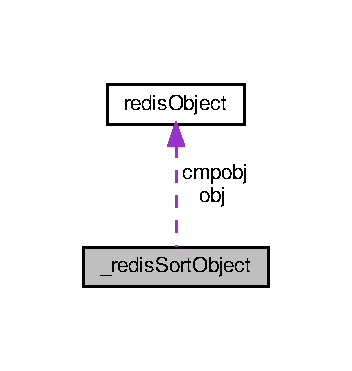
\includegraphics[width=169pt]{struct__redis_sort_object__coll__graph}
\end{center}
\end{figure}
\subsection*{Data Fields}
\begin{DoxyCompactItemize}
\item 
\hyperlink{server_8h_a540f174d2685422fbd7d12e3cd44c8e2}{robj} $\ast$ \hyperlink{struct__redis_sort_object_ab823bb3761b604174d6c31727a47bebc}{obj}
\item 
\begin{tabbing}
xx\=xx\=xx\=xx\=xx\=xx\=xx\=xx\=xx\=\kill
union \{\\
\>double \hyperlink{struct__redis_sort_object_a40a24ec85daa9ac70aa74e4ca744f838}{score}\\
\>\hyperlink{server_8h_a540f174d2685422fbd7d12e3cd44c8e2}{robj} $\ast$ \hyperlink{struct__redis_sort_object_a5a84c8f22865dd4299870240e1db9f58}{cmpobj}\\
\} \hyperlink{struct__redis_sort_object_a27255f4355dc7226770c0682f29744b0}{u}\\

\end{tabbing}\end{DoxyCompactItemize}


\subsection{Detailed Description}


Definition at line 1311 of file server.\+h.



\subsection{Field Documentation}
\mbox{\Hypertarget{struct__redis_sort_object_a5a84c8f22865dd4299870240e1db9f58}\label{struct__redis_sort_object_a5a84c8f22865dd4299870240e1db9f58}} 
\index{\+\_\+redis\+Sort\+Object@{\+\_\+redis\+Sort\+Object}!cmpobj@{cmpobj}}
\index{cmpobj@{cmpobj}!\+\_\+redis\+Sort\+Object@{\+\_\+redis\+Sort\+Object}}
\subsubsection{\texorpdfstring{cmpobj}{cmpobj}}
{\footnotesize\ttfamily \hyperlink{server_8h_a540f174d2685422fbd7d12e3cd44c8e2}{robj}$\ast$ cmpobj}



Definition at line 1315 of file server.\+h.

\mbox{\Hypertarget{struct__redis_sort_object_ab823bb3761b604174d6c31727a47bebc}\label{struct__redis_sort_object_ab823bb3761b604174d6c31727a47bebc}} 
\index{\+\_\+redis\+Sort\+Object@{\+\_\+redis\+Sort\+Object}!obj@{obj}}
\index{obj@{obj}!\+\_\+redis\+Sort\+Object@{\+\_\+redis\+Sort\+Object}}
\subsubsection{\texorpdfstring{obj}{obj}}
{\footnotesize\ttfamily \hyperlink{server_8h_a540f174d2685422fbd7d12e3cd44c8e2}{robj}$\ast$ obj}



Definition at line 1312 of file server.\+h.

\mbox{\Hypertarget{struct__redis_sort_object_a40a24ec85daa9ac70aa74e4ca744f838}\label{struct__redis_sort_object_a40a24ec85daa9ac70aa74e4ca744f838}} 
\index{\+\_\+redis\+Sort\+Object@{\+\_\+redis\+Sort\+Object}!score@{score}}
\index{score@{score}!\+\_\+redis\+Sort\+Object@{\+\_\+redis\+Sort\+Object}}
\subsubsection{\texorpdfstring{score}{score}}
{\footnotesize\ttfamily double score}



Definition at line 1314 of file server.\+h.

\mbox{\Hypertarget{struct__redis_sort_object_a27255f4355dc7226770c0682f29744b0}\label{struct__redis_sort_object_a27255f4355dc7226770c0682f29744b0}} 
\index{\+\_\+redis\+Sort\+Object@{\+\_\+redis\+Sort\+Object}!u@{u}}
\index{u@{u}!\+\_\+redis\+Sort\+Object@{\+\_\+redis\+Sort\+Object}}
\subsubsection{\texorpdfstring{u}{u}}
{\footnotesize\ttfamily union \{ ... \}   u}



The documentation for this struct was generated from the following file\+:\begin{DoxyCompactItemize}
\item 
src/\hyperlink{server_8h}{server.\+h}\end{DoxyCompactItemize}

\hypertarget{struct__redis_sort_operation}{}\section{\+\_\+redis\+Sort\+Operation Struct Reference}
\label{struct__redis_sort_operation}\index{\+\_\+redis\+Sort\+Operation@{\+\_\+redis\+Sort\+Operation}}


{\ttfamily \#include $<$server.\+h$>$}



Collaboration diagram for \+\_\+redis\+Sort\+Operation\+:
\nopagebreak
\begin{figure}[H]
\begin{center}
\leavevmode
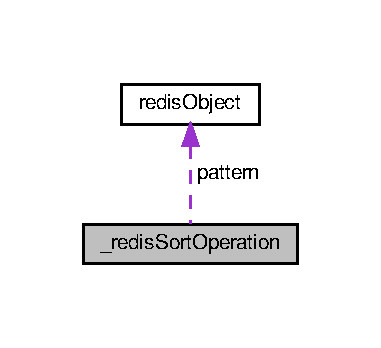
\includegraphics[width=183pt]{struct__redis_sort_operation__coll__graph}
\end{center}
\end{figure}
\subsection*{Data Fields}
\begin{DoxyCompactItemize}
\item 
int \hyperlink{struct__redis_sort_operation_ac765329451135abec74c45e1897abf26}{type}
\item 
\hyperlink{server_8h_a540f174d2685422fbd7d12e3cd44c8e2}{robj} $\ast$ \hyperlink{struct__redis_sort_operation_a779898a32e09ec217b6876501caecc9c}{pattern}
\end{DoxyCompactItemize}


\subsection{Detailed Description}


Definition at line 1319 of file server.\+h.



\subsection{Field Documentation}
\mbox{\Hypertarget{struct__redis_sort_operation_a779898a32e09ec217b6876501caecc9c}\label{struct__redis_sort_operation_a779898a32e09ec217b6876501caecc9c}} 
\index{\+\_\+redis\+Sort\+Operation@{\+\_\+redis\+Sort\+Operation}!pattern@{pattern}}
\index{pattern@{pattern}!\+\_\+redis\+Sort\+Operation@{\+\_\+redis\+Sort\+Operation}}
\subsubsection{\texorpdfstring{pattern}{pattern}}
{\footnotesize\ttfamily \hyperlink{server_8h_a540f174d2685422fbd7d12e3cd44c8e2}{robj}$\ast$ pattern}



Definition at line 1321 of file server.\+h.

\mbox{\Hypertarget{struct__redis_sort_operation_ac765329451135abec74c45e1897abf26}\label{struct__redis_sort_operation_ac765329451135abec74c45e1897abf26}} 
\index{\+\_\+redis\+Sort\+Operation@{\+\_\+redis\+Sort\+Operation}!type@{type}}
\index{type@{type}!\+\_\+redis\+Sort\+Operation@{\+\_\+redis\+Sort\+Operation}}
\subsubsection{\texorpdfstring{type}{type}}
{\footnotesize\ttfamily int type}



Definition at line 1320 of file server.\+h.



The documentation for this struct was generated from the following file\+:\begin{DoxyCompactItemize}
\item 
src/\hyperlink{server_8h}{server.\+h}\end{DoxyCompactItemize}

\hypertarget{struct__rio}{}\section{\+\_\+rio Struct Reference}
\label{struct__rio}\index{\+\_\+rio@{\+\_\+rio}}


{\ttfamily \#include $<$rio.\+h$>$}

\subsection*{Data Fields}
\begin{DoxyCompactItemize}
\item 
size\+\_\+t($\ast$ \hyperlink{struct__rio_a6562dde444181d8dc56163cd5bd5a880}{read} )(struct \hyperlink{struct__rio}{\+\_\+rio} $\ast$, void $\ast$\hyperlink{struct__rio_ae8dd93102163eea99d3d0949d1974628}{buf}, size\+\_\+t len)
\item 
size\+\_\+t($\ast$ \hyperlink{struct__rio_aa7c29e99e2a05a47c569af36fa61272c}{write} )(struct \hyperlink{struct__rio}{\+\_\+rio} $\ast$, const void $\ast$\hyperlink{struct__rio_ae8dd93102163eea99d3d0949d1974628}{buf}, size\+\_\+t len)
\item 
off\+\_\+t($\ast$ \hyperlink{struct__rio_ab06eb2e08a6cba498c63adf5e9ffa2ff}{tell} )(struct \hyperlink{struct__rio}{\+\_\+rio} $\ast$)
\item 
int($\ast$ \hyperlink{struct__rio_a6400f2e1372884609119ec5fa095b6b9}{flush} )(struct \hyperlink{struct__rio}{\+\_\+rio} $\ast$)
\item 
void($\ast$ \hyperlink{struct__rio_a0d11c9195df688114fd7e3d39b06c269}{update\+\_\+cksum} )(struct \hyperlink{struct__rio}{\+\_\+rio} $\ast$, const void $\ast$\hyperlink{struct__rio_ae8dd93102163eea99d3d0949d1974628}{buf}, size\+\_\+t len)
\item 
uint64\+\_\+t \hyperlink{struct__rio_aa7e1f76c805332914541fb978311b7b4}{cksum}
\item 
size\+\_\+t \hyperlink{struct__rio_a4bfc464c439f7f4da758b39d6f31cf22}{processed\+\_\+bytes}
\item 
size\+\_\+t \hyperlink{struct__rio_ad1ae3d0cef59f6c43a68302a5bc673cd}{max\+\_\+processing\+\_\+chunk}
\item 
\begin{tabbing}
xx\=xx\=xx\=xx\=xx\=xx\=xx\=xx\=xx\=\kill
union \{\\
\>struct \{\\
\>\>\hyperlink{sds_8h_ad69abac3df4532879db9642c95f5ef6f}{sds} \hyperlink{struct__rio_ac787a06d755eb260b16d6cf74c06eaf9}{ptr}\\
\>\>off\_t \hyperlink{struct__rio_a320b91e58d067b5097a431e6da94f247}{pos}\\
\>\} \hyperlink{struct__rio_a08fd4992ea2a6cc4f1cae2d22475e950}{buffer}\\
\>struct \{\\
\>\>FILE $\ast$ \hyperlink{struct__rio_aa065f30aa9f5f9a42132c82c787ee70b}{fp}\\
\>\>off\_t \hyperlink{struct__rio_aaf9c739870ce662f03414e87c0a3947b}{buffered}\\
\>\>off\_t \hyperlink{struct__rio_a26ab7c3adc5a936bacbe48d501c163f2}{autosync}\\
\>\} \hyperlink{struct__rio_abc0d7429e6b98d70aadb166991f8e5e3}{file}\\
\>struct \{\\
\>\>int $\ast$ \hyperlink{struct__rio_ad259456372b9b7ad374dccd9d0f80eac}{fds}\\
\>\>int $\ast$ \hyperlink{struct__rio_ace50bce9d6e7ed2958418778a6b1711f}{state}\\
\>\>int \hyperlink{struct__rio_a01ef09680a9926f281067248a833e69b}{numfds}\\
\>\>off\_t \hyperlink{struct__rio_a320b91e58d067b5097a431e6da94f247}{pos}\\
\>\>\hyperlink{sds_8h_ad69abac3df4532879db9642c95f5ef6f}{sds} \hyperlink{struct__rio_ae8dd93102163eea99d3d0949d1974628}{buf}\\
\>\} \hyperlink{struct__rio_a5101c27f29f6ce315129e5c9a00f9cc9}{fdset}\\
\} \hyperlink{struct__rio_ad359e2e86f3623eccc8b70ee6f18bc46}{io}\\

\end{tabbing}\end{DoxyCompactItemize}


\subsection{Detailed Description}


Definition at line 39 of file rio.\+h.



\subsection{Field Documentation}
\mbox{\Hypertarget{struct__rio_a26ab7c3adc5a936bacbe48d501c163f2}\label{struct__rio_a26ab7c3adc5a936bacbe48d501c163f2}} 
\index{\+\_\+rio@{\+\_\+rio}!autosync@{autosync}}
\index{autosync@{autosync}!\+\_\+rio@{\+\_\+rio}}
\subsubsection{\texorpdfstring{autosync}{autosync}}
{\footnotesize\ttfamily off\+\_\+t autosync}



Definition at line 74 of file rio.\+h.

\mbox{\Hypertarget{struct__rio_ae8dd93102163eea99d3d0949d1974628}\label{struct__rio_ae8dd93102163eea99d3d0949d1974628}} 
\index{\+\_\+rio@{\+\_\+rio}!buf@{buf}}
\index{buf@{buf}!\+\_\+rio@{\+\_\+rio}}
\subsubsection{\texorpdfstring{buf}{buf}}
{\footnotesize\ttfamily \hyperlink{sds_8h_ad69abac3df4532879db9642c95f5ef6f}{sds} buf}



Definition at line 82 of file rio.\+h.

\mbox{\Hypertarget{struct__rio_a08fd4992ea2a6cc4f1cae2d22475e950}\label{struct__rio_a08fd4992ea2a6cc4f1cae2d22475e950}} 
\index{\+\_\+rio@{\+\_\+rio}!buffer@{buffer}}
\index{buffer@{buffer}!\+\_\+rio@{\+\_\+rio}}
\subsubsection{\texorpdfstring{buffer}{buffer}}
{\footnotesize\ttfamily struct \{ ... \}   buffer}

\mbox{\Hypertarget{struct__rio_aaf9c739870ce662f03414e87c0a3947b}\label{struct__rio_aaf9c739870ce662f03414e87c0a3947b}} 
\index{\+\_\+rio@{\+\_\+rio}!buffered@{buffered}}
\index{buffered@{buffered}!\+\_\+rio@{\+\_\+rio}}
\subsubsection{\texorpdfstring{buffered}{buffered}}
{\footnotesize\ttfamily off\+\_\+t buffered}



Definition at line 73 of file rio.\+h.

\mbox{\Hypertarget{struct__rio_aa7e1f76c805332914541fb978311b7b4}\label{struct__rio_aa7e1f76c805332914541fb978311b7b4}} 
\index{\+\_\+rio@{\+\_\+rio}!cksum@{cksum}}
\index{cksum@{cksum}!\+\_\+rio@{\+\_\+rio}}
\subsubsection{\texorpdfstring{cksum}{cksum}}
{\footnotesize\ttfamily uint64\+\_\+t cksum}



Definition at line 55 of file rio.\+h.

\mbox{\Hypertarget{struct__rio_ad259456372b9b7ad374dccd9d0f80eac}\label{struct__rio_ad259456372b9b7ad374dccd9d0f80eac}} 
\index{\+\_\+rio@{\+\_\+rio}!fds@{fds}}
\index{fds@{fds}!\+\_\+rio@{\+\_\+rio}}
\subsubsection{\texorpdfstring{fds}{fds}}
{\footnotesize\ttfamily int$\ast$ fds}



Definition at line 78 of file rio.\+h.

\mbox{\Hypertarget{struct__rio_a5101c27f29f6ce315129e5c9a00f9cc9}\label{struct__rio_a5101c27f29f6ce315129e5c9a00f9cc9}} 
\index{\+\_\+rio@{\+\_\+rio}!fdset@{fdset}}
\index{fdset@{fdset}!\+\_\+rio@{\+\_\+rio}}
\subsubsection{\texorpdfstring{fdset}{fdset}}
{\footnotesize\ttfamily struct \{ ... \}   fdset}

\mbox{\Hypertarget{struct__rio_abc0d7429e6b98d70aadb166991f8e5e3}\label{struct__rio_abc0d7429e6b98d70aadb166991f8e5e3}} 
\index{\+\_\+rio@{\+\_\+rio}!file@{file}}
\index{file@{file}!\+\_\+rio@{\+\_\+rio}}
\subsubsection{\texorpdfstring{file}{file}}
{\footnotesize\ttfamily struct \{ ... \}   file}

\mbox{\Hypertarget{struct__rio_a6400f2e1372884609119ec5fa095b6b9}\label{struct__rio_a6400f2e1372884609119ec5fa095b6b9}} 
\index{\+\_\+rio@{\+\_\+rio}!flush@{flush}}
\index{flush@{flush}!\+\_\+rio@{\+\_\+rio}}
\subsubsection{\texorpdfstring{flush}{flush}}
{\footnotesize\ttfamily int($\ast$ flush) (struct \hyperlink{struct__rio}{\+\_\+rio} $\ast$)}



Definition at line 46 of file rio.\+h.

\mbox{\Hypertarget{struct__rio_aa065f30aa9f5f9a42132c82c787ee70b}\label{struct__rio_aa065f30aa9f5f9a42132c82c787ee70b}} 
\index{\+\_\+rio@{\+\_\+rio}!fp@{fp}}
\index{fp@{fp}!\+\_\+rio@{\+\_\+rio}}
\subsubsection{\texorpdfstring{fp}{fp}}
{\footnotesize\ttfamily F\+I\+LE$\ast$ fp}



Definition at line 72 of file rio.\+h.

\mbox{\Hypertarget{struct__rio_ad359e2e86f3623eccc8b70ee6f18bc46}\label{struct__rio_ad359e2e86f3623eccc8b70ee6f18bc46}} 
\index{\+\_\+rio@{\+\_\+rio}!io@{io}}
\index{io@{io}!\+\_\+rio@{\+\_\+rio}}
\subsubsection{\texorpdfstring{io}{io}}
{\footnotesize\ttfamily union \{ ... \}   io}

\mbox{\Hypertarget{struct__rio_ad1ae3d0cef59f6c43a68302a5bc673cd}\label{struct__rio_ad1ae3d0cef59f6c43a68302a5bc673cd}} 
\index{\+\_\+rio@{\+\_\+rio}!max\+\_\+processing\+\_\+chunk@{max\+\_\+processing\+\_\+chunk}}
\index{max\+\_\+processing\+\_\+chunk@{max\+\_\+processing\+\_\+chunk}!\+\_\+rio@{\+\_\+rio}}
\subsubsection{\texorpdfstring{max\+\_\+processing\+\_\+chunk}{max\_processing\_chunk}}
{\footnotesize\ttfamily size\+\_\+t max\+\_\+processing\+\_\+chunk}



Definition at line 61 of file rio.\+h.

\mbox{\Hypertarget{struct__rio_a01ef09680a9926f281067248a833e69b}\label{struct__rio_a01ef09680a9926f281067248a833e69b}} 
\index{\+\_\+rio@{\+\_\+rio}!numfds@{numfds}}
\index{numfds@{numfds}!\+\_\+rio@{\+\_\+rio}}
\subsubsection{\texorpdfstring{numfds}{numfds}}
{\footnotesize\ttfamily int numfds}



Definition at line 80 of file rio.\+h.

\mbox{\Hypertarget{struct__rio_a320b91e58d067b5097a431e6da94f247}\label{struct__rio_a320b91e58d067b5097a431e6da94f247}} 
\index{\+\_\+rio@{\+\_\+rio}!pos@{pos}}
\index{pos@{pos}!\+\_\+rio@{\+\_\+rio}}
\subsubsection{\texorpdfstring{pos}{pos}}
{\footnotesize\ttfamily off\+\_\+t pos}



Definition at line 68 of file rio.\+h.

\mbox{\Hypertarget{struct__rio_a4bfc464c439f7f4da758b39d6f31cf22}\label{struct__rio_a4bfc464c439f7f4da758b39d6f31cf22}} 
\index{\+\_\+rio@{\+\_\+rio}!processed\+\_\+bytes@{processed\+\_\+bytes}}
\index{processed\+\_\+bytes@{processed\+\_\+bytes}!\+\_\+rio@{\+\_\+rio}}
\subsubsection{\texorpdfstring{processed\+\_\+bytes}{processed\_bytes}}
{\footnotesize\ttfamily size\+\_\+t processed\+\_\+bytes}



Definition at line 58 of file rio.\+h.

\mbox{\Hypertarget{struct__rio_ac787a06d755eb260b16d6cf74c06eaf9}\label{struct__rio_ac787a06d755eb260b16d6cf74c06eaf9}} 
\index{\+\_\+rio@{\+\_\+rio}!ptr@{ptr}}
\index{ptr@{ptr}!\+\_\+rio@{\+\_\+rio}}
\subsubsection{\texorpdfstring{ptr}{ptr}}
{\footnotesize\ttfamily \hyperlink{sds_8h_ad69abac3df4532879db9642c95f5ef6f}{sds} ptr}



Definition at line 67 of file rio.\+h.

\mbox{\Hypertarget{struct__rio_a6562dde444181d8dc56163cd5bd5a880}\label{struct__rio_a6562dde444181d8dc56163cd5bd5a880}} 
\index{\+\_\+rio@{\+\_\+rio}!read@{read}}
\index{read@{read}!\+\_\+rio@{\+\_\+rio}}
\subsubsection{\texorpdfstring{read}{read}}
{\footnotesize\ttfamily size\+\_\+t($\ast$ read) (struct \hyperlink{struct__rio}{\+\_\+rio} $\ast$, void $\ast$\hyperlink{struct__rio_ae8dd93102163eea99d3d0949d1974628}{buf}, size\+\_\+t len)}



Definition at line 43 of file rio.\+h.

\mbox{\Hypertarget{struct__rio_ace50bce9d6e7ed2958418778a6b1711f}\label{struct__rio_ace50bce9d6e7ed2958418778a6b1711f}} 
\index{\+\_\+rio@{\+\_\+rio}!state@{state}}
\index{state@{state}!\+\_\+rio@{\+\_\+rio}}
\subsubsection{\texorpdfstring{state}{state}}
{\footnotesize\ttfamily int$\ast$ state}



Definition at line 79 of file rio.\+h.

\mbox{\Hypertarget{struct__rio_ab06eb2e08a6cba498c63adf5e9ffa2ff}\label{struct__rio_ab06eb2e08a6cba498c63adf5e9ffa2ff}} 
\index{\+\_\+rio@{\+\_\+rio}!tell@{tell}}
\index{tell@{tell}!\+\_\+rio@{\+\_\+rio}}
\subsubsection{\texorpdfstring{tell}{tell}}
{\footnotesize\ttfamily off\+\_\+t($\ast$ tell) (struct \hyperlink{struct__rio}{\+\_\+rio} $\ast$)}



Definition at line 45 of file rio.\+h.

\mbox{\Hypertarget{struct__rio_a0d11c9195df688114fd7e3d39b06c269}\label{struct__rio_a0d11c9195df688114fd7e3d39b06c269}} 
\index{\+\_\+rio@{\+\_\+rio}!update\+\_\+cksum@{update\+\_\+cksum}}
\index{update\+\_\+cksum@{update\+\_\+cksum}!\+\_\+rio@{\+\_\+rio}}
\subsubsection{\texorpdfstring{update\+\_\+cksum}{update\_cksum}}
{\footnotesize\ttfamily void($\ast$ update\+\_\+cksum) (struct \hyperlink{struct__rio}{\+\_\+rio} $\ast$, const void $\ast$\hyperlink{struct__rio_ae8dd93102163eea99d3d0949d1974628}{buf}, size\+\_\+t len)}



Definition at line 52 of file rio.\+h.

\mbox{\Hypertarget{struct__rio_aa7c29e99e2a05a47c569af36fa61272c}\label{struct__rio_aa7c29e99e2a05a47c569af36fa61272c}} 
\index{\+\_\+rio@{\+\_\+rio}!write@{write}}
\index{write@{write}!\+\_\+rio@{\+\_\+rio}}
\subsubsection{\texorpdfstring{write}{write}}
{\footnotesize\ttfamily size\+\_\+t($\ast$ write) (struct \hyperlink{struct__rio}{\+\_\+rio} $\ast$, const void $\ast$\hyperlink{struct__rio_ae8dd93102163eea99d3d0949d1974628}{buf}, size\+\_\+t len)}



Definition at line 44 of file rio.\+h.



The documentation for this struct was generated from the following file\+:\begin{DoxyCompactItemize}
\item 
src/\hyperlink{rio_8h}{rio.\+h}\end{DoxyCompactItemize}

\hypertarget{structae_api_state}{}\section{ae\+Api\+State Struct Reference}
\label{structae_api_state}\index{ae\+Api\+State@{ae\+Api\+State}}
\subsection*{Data Fields}
\begin{DoxyCompactItemize}
\item 
int \hyperlink{structae_api_state_ad9ea3108c3907d7dedaf4ee7283bef1d}{epfd}
\item 
struct epoll\+\_\+event $\ast$ \hyperlink{structae_api_state_a18bcd14e4d4cab5184d3b046754cd248}{events}
\item 
int \hyperlink{structae_api_state_aa9eafa913479690a5a1dd276dda1e270}{portfd}
\item 
int \hyperlink{structae_api_state_a6f4c81b06defc657dcf060888fa72ad2}{npending}
\item 
int \hyperlink{structae_api_state_adffd92b7629bbcebdbf55f077e1df317}{pending\+\_\+fds} \mbox{[}\hyperlink{ae__evport_8c_ab9854fb7f580a9077208ed70f45c8f15}{M\+A\+X\+\_\+\+E\+V\+E\+N\+T\+\_\+\+B\+A\+T\+C\+H\+SZ}\mbox{]}
\item 
int \hyperlink{structae_api_state_a60c7db13c66fbee7d2107c9dbe05acbe}{pending\+\_\+masks} \mbox{[}\hyperlink{ae__evport_8c_ab9854fb7f580a9077208ed70f45c8f15}{M\+A\+X\+\_\+\+E\+V\+E\+N\+T\+\_\+\+B\+A\+T\+C\+H\+SZ}\mbox{]}
\item 
int \hyperlink{structae_api_state_aa16ac46da03ffb75e8913e2b978ad813}{kqfd}
\item 
struct kevent $\ast$ \hyperlink{structae_api_state_ac4b7894707b47b577951136ff0c44929}{events}
\item 
fd\+\_\+set \hyperlink{structae_api_state_a66342c63e01fe543ed20793f32385f7e}{rfds}
\item 
fd\+\_\+set \hyperlink{structae_api_state_a6391a90ddf873c2555b842a474fb9309}{wfds}
\item 
fd\+\_\+set \hyperlink{structae_api_state_a0e84e684034812e7fd687c23ccf3019a}{\+\_\+rfds}
\item 
fd\+\_\+set \hyperlink{structae_api_state_a244aead6b00af6366ffb8ca8f49fdcd5}{\+\_\+wfds}
\end{DoxyCompactItemize}


\subsection{Detailed Description}


Definition at line 34 of file ae\+\_\+epoll.\+c.



\subsection{Field Documentation}
\mbox{\Hypertarget{structae_api_state_a0e84e684034812e7fd687c23ccf3019a}\label{structae_api_state_a0e84e684034812e7fd687c23ccf3019a}} 
\index{ae\+Api\+State@{ae\+Api\+State}!\+\_\+rfds@{\+\_\+rfds}}
\index{\+\_\+rfds@{\+\_\+rfds}!ae\+Api\+State@{ae\+Api\+State}}
\subsubsection{\texorpdfstring{\+\_\+rfds}{\_rfds}}
{\footnotesize\ttfamily fd\+\_\+set \+\_\+rfds}



Definition at line 39 of file ae\+\_\+select.\+c.

\mbox{\Hypertarget{structae_api_state_a244aead6b00af6366ffb8ca8f49fdcd5}\label{structae_api_state_a244aead6b00af6366ffb8ca8f49fdcd5}} 
\index{ae\+Api\+State@{ae\+Api\+State}!\+\_\+wfds@{\+\_\+wfds}}
\index{\+\_\+wfds@{\+\_\+wfds}!ae\+Api\+State@{ae\+Api\+State}}
\subsubsection{\texorpdfstring{\+\_\+wfds}{\_wfds}}
{\footnotesize\ttfamily fd\+\_\+set \+\_\+wfds}



Definition at line 39 of file ae\+\_\+select.\+c.

\mbox{\Hypertarget{structae_api_state_ad9ea3108c3907d7dedaf4ee7283bef1d}\label{structae_api_state_ad9ea3108c3907d7dedaf4ee7283bef1d}} 
\index{ae\+Api\+State@{ae\+Api\+State}!epfd@{epfd}}
\index{epfd@{epfd}!ae\+Api\+State@{ae\+Api\+State}}
\subsubsection{\texorpdfstring{epfd}{epfd}}
{\footnotesize\ttfamily int epfd}



Definition at line 35 of file ae\+\_\+epoll.\+c.

\mbox{\Hypertarget{structae_api_state_a18bcd14e4d4cab5184d3b046754cd248}\label{structae_api_state_a18bcd14e4d4cab5184d3b046754cd248}} 
\index{ae\+Api\+State@{ae\+Api\+State}!events@{events}}
\index{events@{events}!ae\+Api\+State@{ae\+Api\+State}}
\subsubsection{\texorpdfstring{events}{events}\hspace{0.1cm}{\footnotesize\ttfamily [1/2]}}
{\footnotesize\ttfamily struct epoll\+\_\+event$\ast$ events}



Definition at line 36 of file ae\+\_\+epoll.\+c.

\mbox{\Hypertarget{structae_api_state_ac4b7894707b47b577951136ff0c44929}\label{structae_api_state_ac4b7894707b47b577951136ff0c44929}} 
\index{ae\+Api\+State@{ae\+Api\+State}!events@{events}}
\index{events@{events}!ae\+Api\+State@{ae\+Api\+State}}
\subsubsection{\texorpdfstring{events}{events}\hspace{0.1cm}{\footnotesize\ttfamily [2/2]}}
{\footnotesize\ttfamily struct kevent$\ast$ events}



Definition at line 38 of file ae\+\_\+kqueue.\+c.

\mbox{\Hypertarget{structae_api_state_aa16ac46da03ffb75e8913e2b978ad813}\label{structae_api_state_aa16ac46da03ffb75e8913e2b978ad813}} 
\index{ae\+Api\+State@{ae\+Api\+State}!kqfd@{kqfd}}
\index{kqfd@{kqfd}!ae\+Api\+State@{ae\+Api\+State}}
\subsubsection{\texorpdfstring{kqfd}{kqfd}}
{\footnotesize\ttfamily int kqfd}



Definition at line 37 of file ae\+\_\+kqueue.\+c.

\mbox{\Hypertarget{structae_api_state_a6f4c81b06defc657dcf060888fa72ad2}\label{structae_api_state_a6f4c81b06defc657dcf060888fa72ad2}} 
\index{ae\+Api\+State@{ae\+Api\+State}!npending@{npending}}
\index{npending@{npending}!ae\+Api\+State@{ae\+Api\+State}}
\subsubsection{\texorpdfstring{npending}{npending}}
{\footnotesize\ttfamily int npending}



Definition at line 70 of file ae\+\_\+evport.\+c.

\mbox{\Hypertarget{structae_api_state_adffd92b7629bbcebdbf55f077e1df317}\label{structae_api_state_adffd92b7629bbcebdbf55f077e1df317}} 
\index{ae\+Api\+State@{ae\+Api\+State}!pending\+\_\+fds@{pending\+\_\+fds}}
\index{pending\+\_\+fds@{pending\+\_\+fds}!ae\+Api\+State@{ae\+Api\+State}}
\subsubsection{\texorpdfstring{pending\+\_\+fds}{pending\_fds}}
{\footnotesize\ttfamily int pending\+\_\+fds\mbox{[}\hyperlink{ae__evport_8c_ab9854fb7f580a9077208ed70f45c8f15}{M\+A\+X\+\_\+\+E\+V\+E\+N\+T\+\_\+\+B\+A\+T\+C\+H\+SZ}\mbox{]}}



Definition at line 71 of file ae\+\_\+evport.\+c.

\mbox{\Hypertarget{structae_api_state_a60c7db13c66fbee7d2107c9dbe05acbe}\label{structae_api_state_a60c7db13c66fbee7d2107c9dbe05acbe}} 
\index{ae\+Api\+State@{ae\+Api\+State}!pending\+\_\+masks@{pending\+\_\+masks}}
\index{pending\+\_\+masks@{pending\+\_\+masks}!ae\+Api\+State@{ae\+Api\+State}}
\subsubsection{\texorpdfstring{pending\+\_\+masks}{pending\_masks}}
{\footnotesize\ttfamily int pending\+\_\+masks\mbox{[}\hyperlink{ae__evport_8c_ab9854fb7f580a9077208ed70f45c8f15}{M\+A\+X\+\_\+\+E\+V\+E\+N\+T\+\_\+\+B\+A\+T\+C\+H\+SZ}\mbox{]}}



Definition at line 72 of file ae\+\_\+evport.\+c.

\mbox{\Hypertarget{structae_api_state_aa9eafa913479690a5a1dd276dda1e270}\label{structae_api_state_aa9eafa913479690a5a1dd276dda1e270}} 
\index{ae\+Api\+State@{ae\+Api\+State}!portfd@{portfd}}
\index{portfd@{portfd}!ae\+Api\+State@{ae\+Api\+State}}
\subsubsection{\texorpdfstring{portfd}{portfd}}
{\footnotesize\ttfamily int portfd}



Definition at line 69 of file ae\+\_\+evport.\+c.

\mbox{\Hypertarget{structae_api_state_a66342c63e01fe543ed20793f32385f7e}\label{structae_api_state_a66342c63e01fe543ed20793f32385f7e}} 
\index{ae\+Api\+State@{ae\+Api\+State}!rfds@{rfds}}
\index{rfds@{rfds}!ae\+Api\+State@{ae\+Api\+State}}
\subsubsection{\texorpdfstring{rfds}{rfds}}
{\footnotesize\ttfamily fd\+\_\+set rfds}



Definition at line 36 of file ae\+\_\+select.\+c.

\mbox{\Hypertarget{structae_api_state_a6391a90ddf873c2555b842a474fb9309}\label{structae_api_state_a6391a90ddf873c2555b842a474fb9309}} 
\index{ae\+Api\+State@{ae\+Api\+State}!wfds@{wfds}}
\index{wfds@{wfds}!ae\+Api\+State@{ae\+Api\+State}}
\subsubsection{\texorpdfstring{wfds}{wfds}}
{\footnotesize\ttfamily fd\+\_\+set wfds}



Definition at line 36 of file ae\+\_\+select.\+c.



The documentation for this struct was generated from the following files\+:\begin{DoxyCompactItemize}
\item 
src/\hyperlink{ae__epoll_8c}{ae\+\_\+epoll.\+c}\item 
src/\hyperlink{ae__evport_8c}{ae\+\_\+evport.\+c}\item 
src/\hyperlink{ae__kqueue_8c}{ae\+\_\+kqueue.\+c}\item 
src/\hyperlink{ae__select_8c}{ae\+\_\+select.\+c}\end{DoxyCompactItemize}

\hypertarget{structae_event_loop}{}\section{ae\+Event\+Loop Struct Reference}
\label{structae_event_loop}\index{ae\+Event\+Loop@{ae\+Event\+Loop}}


{\ttfamily \#include $<$ae.\+h$>$}



Collaboration diagram for ae\+Event\+Loop\+:
\nopagebreak
\begin{figure}[H]
\begin{center}
\leavevmode
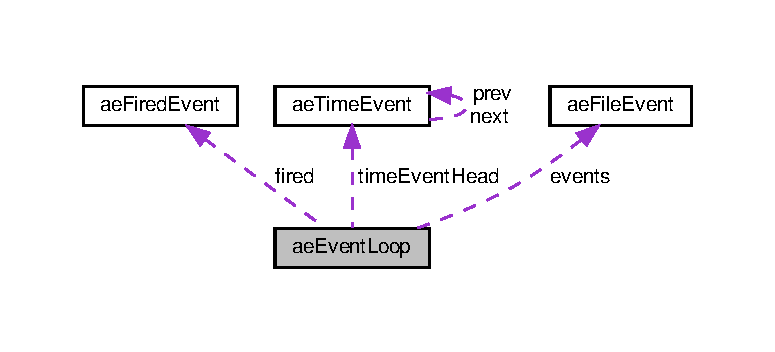
\includegraphics[width=350pt]{structae_event_loop__coll__graph}
\end{center}
\end{figure}
\subsection*{Data Fields}
\begin{DoxyCompactItemize}
\item 
int \hyperlink{structae_event_loop_a7a13a361801dcc59ce4946736fa26726}{maxfd}
\item 
int \hyperlink{structae_event_loop_afcc4d6ce64e647b5ff70e04393e854cd}{setsize}
\item 
long long \hyperlink{structae_event_loop_a16573cf248b2aeb7ecacfc992ae774d4}{time\+Event\+Next\+Id}
\item 
time\+\_\+t \hyperlink{structae_event_loop_a9a8ce27fc2a03316649058e288233cf8}{last\+Time}
\item 
\hyperlink{structae_file_event}{ae\+File\+Event} $\ast$ \hyperlink{structae_event_loop_af7bb19dd3fc37f35b9b655455679ce56}{events}
\item 
\hyperlink{structae_fired_event}{ae\+Fired\+Event} $\ast$ \hyperlink{structae_event_loop_a3116c9bc1c9065f5ea86c4aee38ca2e2}{fired}
\item 
\hyperlink{structae_time_event}{ae\+Time\+Event} $\ast$ \hyperlink{structae_event_loop_aa46c6a447db443855daf5b08923bed36}{time\+Event\+Head}
\item 
int \hyperlink{structae_event_loop_a6c0af9f2e97842405fb15ed952ef2976}{stop}
\item 
void $\ast$ \hyperlink{structae_event_loop_a6c38ead7bed5299f416045c1940ee5b1}{apidata}
\item 
\hyperlink{ae_8h_a9b418f26d4997ba2d303dd247ae45718}{ae\+Before\+Sleep\+Proc} $\ast$ \hyperlink{structae_event_loop_a237a195466baef2c9cc26255774fd7cb}{beforesleep}
\item 
\hyperlink{ae_8h_a9b418f26d4997ba2d303dd247ae45718}{ae\+Before\+Sleep\+Proc} $\ast$ \hyperlink{structae_event_loop_a7a22ce87f685955512b3a0c049d5763c}{aftersleep}
\end{DoxyCompactItemize}


\subsection{Detailed Description}


Definition at line 97 of file ae.\+h.



\subsection{Field Documentation}
\mbox{\Hypertarget{structae_event_loop_a7a22ce87f685955512b3a0c049d5763c}\label{structae_event_loop_a7a22ce87f685955512b3a0c049d5763c}} 
\index{ae\+Event\+Loop@{ae\+Event\+Loop}!aftersleep@{aftersleep}}
\index{aftersleep@{aftersleep}!ae\+Event\+Loop@{ae\+Event\+Loop}}
\subsubsection{\texorpdfstring{aftersleep}{aftersleep}}
{\footnotesize\ttfamily \hyperlink{ae_8h_a9b418f26d4997ba2d303dd247ae45718}{ae\+Before\+Sleep\+Proc}$\ast$ aftersleep}



Definition at line 108 of file ae.\+h.

\mbox{\Hypertarget{structae_event_loop_a6c38ead7bed5299f416045c1940ee5b1}\label{structae_event_loop_a6c38ead7bed5299f416045c1940ee5b1}} 
\index{ae\+Event\+Loop@{ae\+Event\+Loop}!apidata@{apidata}}
\index{apidata@{apidata}!ae\+Event\+Loop@{ae\+Event\+Loop}}
\subsubsection{\texorpdfstring{apidata}{apidata}}
{\footnotesize\ttfamily void$\ast$ apidata}



Definition at line 106 of file ae.\+h.

\mbox{\Hypertarget{structae_event_loop_a237a195466baef2c9cc26255774fd7cb}\label{structae_event_loop_a237a195466baef2c9cc26255774fd7cb}} 
\index{ae\+Event\+Loop@{ae\+Event\+Loop}!beforesleep@{beforesleep}}
\index{beforesleep@{beforesleep}!ae\+Event\+Loop@{ae\+Event\+Loop}}
\subsubsection{\texorpdfstring{beforesleep}{beforesleep}}
{\footnotesize\ttfamily \hyperlink{ae_8h_a9b418f26d4997ba2d303dd247ae45718}{ae\+Before\+Sleep\+Proc}$\ast$ beforesleep}



Definition at line 107 of file ae.\+h.

\mbox{\Hypertarget{structae_event_loop_af7bb19dd3fc37f35b9b655455679ce56}\label{structae_event_loop_af7bb19dd3fc37f35b9b655455679ce56}} 
\index{ae\+Event\+Loop@{ae\+Event\+Loop}!events@{events}}
\index{events@{events}!ae\+Event\+Loop@{ae\+Event\+Loop}}
\subsubsection{\texorpdfstring{events}{events}}
{\footnotesize\ttfamily \hyperlink{structae_file_event}{ae\+File\+Event}$\ast$ events}



Definition at line 102 of file ae.\+h.

\mbox{\Hypertarget{structae_event_loop_a3116c9bc1c9065f5ea86c4aee38ca2e2}\label{structae_event_loop_a3116c9bc1c9065f5ea86c4aee38ca2e2}} 
\index{ae\+Event\+Loop@{ae\+Event\+Loop}!fired@{fired}}
\index{fired@{fired}!ae\+Event\+Loop@{ae\+Event\+Loop}}
\subsubsection{\texorpdfstring{fired}{fired}}
{\footnotesize\ttfamily \hyperlink{structae_fired_event}{ae\+Fired\+Event}$\ast$ fired}



Definition at line 103 of file ae.\+h.

\mbox{\Hypertarget{structae_event_loop_a9a8ce27fc2a03316649058e288233cf8}\label{structae_event_loop_a9a8ce27fc2a03316649058e288233cf8}} 
\index{ae\+Event\+Loop@{ae\+Event\+Loop}!last\+Time@{last\+Time}}
\index{last\+Time@{last\+Time}!ae\+Event\+Loop@{ae\+Event\+Loop}}
\subsubsection{\texorpdfstring{last\+Time}{lastTime}}
{\footnotesize\ttfamily time\+\_\+t last\+Time}



Definition at line 101 of file ae.\+h.

\mbox{\Hypertarget{structae_event_loop_a7a13a361801dcc59ce4946736fa26726}\label{structae_event_loop_a7a13a361801dcc59ce4946736fa26726}} 
\index{ae\+Event\+Loop@{ae\+Event\+Loop}!maxfd@{maxfd}}
\index{maxfd@{maxfd}!ae\+Event\+Loop@{ae\+Event\+Loop}}
\subsubsection{\texorpdfstring{maxfd}{maxfd}}
{\footnotesize\ttfamily int maxfd}



Definition at line 98 of file ae.\+h.

\mbox{\Hypertarget{structae_event_loop_afcc4d6ce64e647b5ff70e04393e854cd}\label{structae_event_loop_afcc4d6ce64e647b5ff70e04393e854cd}} 
\index{ae\+Event\+Loop@{ae\+Event\+Loop}!setsize@{setsize}}
\index{setsize@{setsize}!ae\+Event\+Loop@{ae\+Event\+Loop}}
\subsubsection{\texorpdfstring{setsize}{setsize}}
{\footnotesize\ttfamily int setsize}



Definition at line 99 of file ae.\+h.

\mbox{\Hypertarget{structae_event_loop_a6c0af9f2e97842405fb15ed952ef2976}\label{structae_event_loop_a6c0af9f2e97842405fb15ed952ef2976}} 
\index{ae\+Event\+Loop@{ae\+Event\+Loop}!stop@{stop}}
\index{stop@{stop}!ae\+Event\+Loop@{ae\+Event\+Loop}}
\subsubsection{\texorpdfstring{stop}{stop}}
{\footnotesize\ttfamily int stop}



Definition at line 105 of file ae.\+h.

\mbox{\Hypertarget{structae_event_loop_aa46c6a447db443855daf5b08923bed36}\label{structae_event_loop_aa46c6a447db443855daf5b08923bed36}} 
\index{ae\+Event\+Loop@{ae\+Event\+Loop}!time\+Event\+Head@{time\+Event\+Head}}
\index{time\+Event\+Head@{time\+Event\+Head}!ae\+Event\+Loop@{ae\+Event\+Loop}}
\subsubsection{\texorpdfstring{time\+Event\+Head}{timeEventHead}}
{\footnotesize\ttfamily \hyperlink{structae_time_event}{ae\+Time\+Event}$\ast$ time\+Event\+Head}



Definition at line 104 of file ae.\+h.

\mbox{\Hypertarget{structae_event_loop_a16573cf248b2aeb7ecacfc992ae774d4}\label{structae_event_loop_a16573cf248b2aeb7ecacfc992ae774d4}} 
\index{ae\+Event\+Loop@{ae\+Event\+Loop}!time\+Event\+Next\+Id@{time\+Event\+Next\+Id}}
\index{time\+Event\+Next\+Id@{time\+Event\+Next\+Id}!ae\+Event\+Loop@{ae\+Event\+Loop}}
\subsubsection{\texorpdfstring{time\+Event\+Next\+Id}{timeEventNextId}}
{\footnotesize\ttfamily long long time\+Event\+Next\+Id}



Definition at line 100 of file ae.\+h.



The documentation for this struct was generated from the following file\+:\begin{DoxyCompactItemize}
\item 
src/\hyperlink{ae_8h}{ae.\+h}\end{DoxyCompactItemize}

\hypertarget{structae_file_event}{}\section{ae\+File\+Event Struct Reference}
\label{structae_file_event}\index{ae\+File\+Event@{ae\+File\+Event}}


{\ttfamily \#include $<$ae.\+h$>$}

\subsection*{Data Fields}
\begin{DoxyCompactItemize}
\item 
int \hyperlink{structae_file_event_ab77cc972f3ee899689ba053015472ccd}{mask}
\item 
\hyperlink{ae_8h_a26d6e9533f135cb463f29239607ba50c}{ae\+File\+Proc} $\ast$ \hyperlink{structae_file_event_aaf65022bec2a73c459e46cbfb41229d3}{rfile\+Proc}
\item 
\hyperlink{ae_8h_a26d6e9533f135cb463f29239607ba50c}{ae\+File\+Proc} $\ast$ \hyperlink{structae_file_event_af95a1a47baf2ba0db91c96e77d01a7f0}{wfile\+Proc}
\item 
void $\ast$ \hyperlink{structae_file_event_a31433b6f2825807bd6d9c0675ff7c4cb}{client\+Data}
\end{DoxyCompactItemize}


\subsection{Detailed Description}


Definition at line 71 of file ae.\+h.



\subsection{Field Documentation}
\mbox{\Hypertarget{structae_file_event_a31433b6f2825807bd6d9c0675ff7c4cb}\label{structae_file_event_a31433b6f2825807bd6d9c0675ff7c4cb}} 
\index{ae\+File\+Event@{ae\+File\+Event}!client\+Data@{client\+Data}}
\index{client\+Data@{client\+Data}!ae\+File\+Event@{ae\+File\+Event}}
\subsubsection{\texorpdfstring{client\+Data}{clientData}}
{\footnotesize\ttfamily void$\ast$ client\+Data}



Definition at line 75 of file ae.\+h.

\mbox{\Hypertarget{structae_file_event_ab77cc972f3ee899689ba053015472ccd}\label{structae_file_event_ab77cc972f3ee899689ba053015472ccd}} 
\index{ae\+File\+Event@{ae\+File\+Event}!mask@{mask}}
\index{mask@{mask}!ae\+File\+Event@{ae\+File\+Event}}
\subsubsection{\texorpdfstring{mask}{mask}}
{\footnotesize\ttfamily int mask}



Definition at line 72 of file ae.\+h.

\mbox{\Hypertarget{structae_file_event_aaf65022bec2a73c459e46cbfb41229d3}\label{structae_file_event_aaf65022bec2a73c459e46cbfb41229d3}} 
\index{ae\+File\+Event@{ae\+File\+Event}!rfile\+Proc@{rfile\+Proc}}
\index{rfile\+Proc@{rfile\+Proc}!ae\+File\+Event@{ae\+File\+Event}}
\subsubsection{\texorpdfstring{rfile\+Proc}{rfileProc}}
{\footnotesize\ttfamily \hyperlink{ae_8h_a26d6e9533f135cb463f29239607ba50c}{ae\+File\+Proc}$\ast$ rfile\+Proc}



Definition at line 73 of file ae.\+h.

\mbox{\Hypertarget{structae_file_event_af95a1a47baf2ba0db91c96e77d01a7f0}\label{structae_file_event_af95a1a47baf2ba0db91c96e77d01a7f0}} 
\index{ae\+File\+Event@{ae\+File\+Event}!wfile\+Proc@{wfile\+Proc}}
\index{wfile\+Proc@{wfile\+Proc}!ae\+File\+Event@{ae\+File\+Event}}
\subsubsection{\texorpdfstring{wfile\+Proc}{wfileProc}}
{\footnotesize\ttfamily \hyperlink{ae_8h_a26d6e9533f135cb463f29239607ba50c}{ae\+File\+Proc}$\ast$ wfile\+Proc}



Definition at line 74 of file ae.\+h.



The documentation for this struct was generated from the following file\+:\begin{DoxyCompactItemize}
\item 
src/\hyperlink{ae_8h}{ae.\+h}\end{DoxyCompactItemize}

\hypertarget{structae_fired_event}{}\section{ae\+Fired\+Event Struct Reference}
\label{structae_fired_event}\index{ae\+Fired\+Event@{ae\+Fired\+Event}}


{\ttfamily \#include $<$ae.\+h$>$}

\subsection*{Data Fields}
\begin{DoxyCompactItemize}
\item 
int \hyperlink{structae_fired_event_a6f8059414f0228f0256115e024eeed4b}{fd}
\item 
int \hyperlink{structae_fired_event_ab77cc972f3ee899689ba053015472ccd}{mask}
\end{DoxyCompactItemize}


\subsection{Detailed Description}


Definition at line 91 of file ae.\+h.



\subsection{Field Documentation}
\mbox{\Hypertarget{structae_fired_event_a6f8059414f0228f0256115e024eeed4b}\label{structae_fired_event_a6f8059414f0228f0256115e024eeed4b}} 
\index{ae\+Fired\+Event@{ae\+Fired\+Event}!fd@{fd}}
\index{fd@{fd}!ae\+Fired\+Event@{ae\+Fired\+Event}}
\subsubsection{\texorpdfstring{fd}{fd}}
{\footnotesize\ttfamily int fd}



Definition at line 92 of file ae.\+h.

\mbox{\Hypertarget{structae_fired_event_ab77cc972f3ee899689ba053015472ccd}\label{structae_fired_event_ab77cc972f3ee899689ba053015472ccd}} 
\index{ae\+Fired\+Event@{ae\+Fired\+Event}!mask@{mask}}
\index{mask@{mask}!ae\+Fired\+Event@{ae\+Fired\+Event}}
\subsubsection{\texorpdfstring{mask}{mask}}
{\footnotesize\ttfamily int mask}



Definition at line 93 of file ae.\+h.



The documentation for this struct was generated from the following file\+:\begin{DoxyCompactItemize}
\item 
src/\hyperlink{ae_8h}{ae.\+h}\end{DoxyCompactItemize}

\hypertarget{structae_time_event}{}\section{ae\+Time\+Event Struct Reference}
\label{structae_time_event}\index{ae\+Time\+Event@{ae\+Time\+Event}}


{\ttfamily \#include $<$ae.\+h$>$}



Collaboration diagram for ae\+Time\+Event\+:
\nopagebreak
\begin{figure}[H]
\begin{center}
\leavevmode
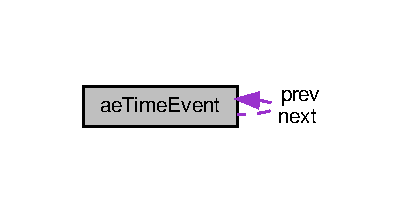
\includegraphics[width=194pt]{structae_time_event__coll__graph}
\end{center}
\end{figure}
\subsection*{Data Fields}
\begin{DoxyCompactItemize}
\item 
long long \hyperlink{structae_time_event_ab87bfb64728d3251718dbf51ef534b60}{id}
\item 
long \hyperlink{structae_time_event_a512e40dee841595f330e13fdca5f850c}{when\+\_\+sec}
\item 
long \hyperlink{structae_time_event_a416251c056e9c8a78fa667370f2cd30c}{when\+\_\+ms}
\item 
\hyperlink{ae_8h_a09cb08f0aea5e5c1460a8b8599d789c8}{ae\+Time\+Proc} $\ast$ \hyperlink{structae_time_event_a93b11f52b154bc10722b6d0e69acc9fb}{time\+Proc}
\item 
\hyperlink{ae_8h_a82c64cc6b7c71e2b7bae4e6b18f42c54}{ae\+Event\+Finalizer\+Proc} $\ast$ \hyperlink{structae_time_event_ac3fd2be96fd0c8c3f4fe9aff811afb80}{finalizer\+Proc}
\item 
void $\ast$ \hyperlink{structae_time_event_a31433b6f2825807bd6d9c0675ff7c4cb}{client\+Data}
\item 
struct \hyperlink{structae_time_event}{ae\+Time\+Event} $\ast$ \hyperlink{structae_time_event_ada581f66d2dd621d24aaba80b0d36ad8}{prev}
\item 
struct \hyperlink{structae_time_event}{ae\+Time\+Event} $\ast$ \hyperlink{structae_time_event_a9210aa4aa97ad7cba5770e567b8fd961}{next}
\end{DoxyCompactItemize}


\subsection{Detailed Description}


Definition at line 79 of file ae.\+h.



\subsection{Field Documentation}
\mbox{\Hypertarget{structae_time_event_a31433b6f2825807bd6d9c0675ff7c4cb}\label{structae_time_event_a31433b6f2825807bd6d9c0675ff7c4cb}} 
\index{ae\+Time\+Event@{ae\+Time\+Event}!client\+Data@{client\+Data}}
\index{client\+Data@{client\+Data}!ae\+Time\+Event@{ae\+Time\+Event}}
\subsubsection{\texorpdfstring{client\+Data}{clientData}}
{\footnotesize\ttfamily void$\ast$ client\+Data}



Definition at line 85 of file ae.\+h.

\mbox{\Hypertarget{structae_time_event_ac3fd2be96fd0c8c3f4fe9aff811afb80}\label{structae_time_event_ac3fd2be96fd0c8c3f4fe9aff811afb80}} 
\index{ae\+Time\+Event@{ae\+Time\+Event}!finalizer\+Proc@{finalizer\+Proc}}
\index{finalizer\+Proc@{finalizer\+Proc}!ae\+Time\+Event@{ae\+Time\+Event}}
\subsubsection{\texorpdfstring{finalizer\+Proc}{finalizerProc}}
{\footnotesize\ttfamily \hyperlink{ae_8h_a82c64cc6b7c71e2b7bae4e6b18f42c54}{ae\+Event\+Finalizer\+Proc}$\ast$ finalizer\+Proc}



Definition at line 84 of file ae.\+h.

\mbox{\Hypertarget{structae_time_event_ab87bfb64728d3251718dbf51ef534b60}\label{structae_time_event_ab87bfb64728d3251718dbf51ef534b60}} 
\index{ae\+Time\+Event@{ae\+Time\+Event}!id@{id}}
\index{id@{id}!ae\+Time\+Event@{ae\+Time\+Event}}
\subsubsection{\texorpdfstring{id}{id}}
{\footnotesize\ttfamily long long id}



Definition at line 80 of file ae.\+h.

\mbox{\Hypertarget{structae_time_event_a9210aa4aa97ad7cba5770e567b8fd961}\label{structae_time_event_a9210aa4aa97ad7cba5770e567b8fd961}} 
\index{ae\+Time\+Event@{ae\+Time\+Event}!next@{next}}
\index{next@{next}!ae\+Time\+Event@{ae\+Time\+Event}}
\subsubsection{\texorpdfstring{next}{next}}
{\footnotesize\ttfamily struct \hyperlink{structae_time_event}{ae\+Time\+Event}$\ast$ next}



Definition at line 87 of file ae.\+h.

\mbox{\Hypertarget{structae_time_event_ada581f66d2dd621d24aaba80b0d36ad8}\label{structae_time_event_ada581f66d2dd621d24aaba80b0d36ad8}} 
\index{ae\+Time\+Event@{ae\+Time\+Event}!prev@{prev}}
\index{prev@{prev}!ae\+Time\+Event@{ae\+Time\+Event}}
\subsubsection{\texorpdfstring{prev}{prev}}
{\footnotesize\ttfamily struct \hyperlink{structae_time_event}{ae\+Time\+Event}$\ast$ prev}



Definition at line 86 of file ae.\+h.

\mbox{\Hypertarget{structae_time_event_a93b11f52b154bc10722b6d0e69acc9fb}\label{structae_time_event_a93b11f52b154bc10722b6d0e69acc9fb}} 
\index{ae\+Time\+Event@{ae\+Time\+Event}!time\+Proc@{time\+Proc}}
\index{time\+Proc@{time\+Proc}!ae\+Time\+Event@{ae\+Time\+Event}}
\subsubsection{\texorpdfstring{time\+Proc}{timeProc}}
{\footnotesize\ttfamily \hyperlink{ae_8h_a09cb08f0aea5e5c1460a8b8599d789c8}{ae\+Time\+Proc}$\ast$ time\+Proc}



Definition at line 83 of file ae.\+h.

\mbox{\Hypertarget{structae_time_event_a416251c056e9c8a78fa667370f2cd30c}\label{structae_time_event_a416251c056e9c8a78fa667370f2cd30c}} 
\index{ae\+Time\+Event@{ae\+Time\+Event}!when\+\_\+ms@{when\+\_\+ms}}
\index{when\+\_\+ms@{when\+\_\+ms}!ae\+Time\+Event@{ae\+Time\+Event}}
\subsubsection{\texorpdfstring{when\+\_\+ms}{when\_ms}}
{\footnotesize\ttfamily long when\+\_\+ms}



Definition at line 82 of file ae.\+h.

\mbox{\Hypertarget{structae_time_event_a512e40dee841595f330e13fdca5f850c}\label{structae_time_event_a512e40dee841595f330e13fdca5f850c}} 
\index{ae\+Time\+Event@{ae\+Time\+Event}!when\+\_\+sec@{when\+\_\+sec}}
\index{when\+\_\+sec@{when\+\_\+sec}!ae\+Time\+Event@{ae\+Time\+Event}}
\subsubsection{\texorpdfstring{when\+\_\+sec}{when\_sec}}
{\footnotesize\ttfamily long when\+\_\+sec}



Definition at line 81 of file ae.\+h.



The documentation for this struct was generated from the following file\+:\begin{DoxyCompactItemize}
\item 
src/\hyperlink{ae_8h}{ae.\+h}\end{DoxyCompactItemize}

\hypertarget{structaofrwblock}{}\section{aofrwblock Struct Reference}
\label{structaofrwblock}\index{aofrwblock@{aofrwblock}}
\subsection*{Data Fields}
\begin{DoxyCompactItemize}
\item 
unsigned long \hyperlink{structaofrwblock_abeece48b2d7c09bffa9101df617478d0}{used}
\item 
unsigned long \hyperlink{structaofrwblock_a848d934dac452375a7127376257068b3}{free}
\item 
char \hyperlink{structaofrwblock_aa79f9212f560356c73863debd9af5bc3}{buf} \mbox{[}\hyperlink{aof_8c_a44139ff5d81f229e77d843b17ada505e}{A\+O\+F\+\_\+\+R\+W\+\_\+\+B\+U\+F\+\_\+\+B\+L\+O\+C\+K\+\_\+\+S\+I\+ZE}\mbox{]}
\end{DoxyCompactItemize}


\subsection{Detailed Description}


Definition at line 62 of file aof.\+c.



\subsection{Field Documentation}
\mbox{\Hypertarget{structaofrwblock_aa79f9212f560356c73863debd9af5bc3}\label{structaofrwblock_aa79f9212f560356c73863debd9af5bc3}} 
\index{aofrwblock@{aofrwblock}!buf@{buf}}
\index{buf@{buf}!aofrwblock@{aofrwblock}}
\subsubsection{\texorpdfstring{buf}{buf}}
{\footnotesize\ttfamily char buf\mbox{[}\hyperlink{aof_8c_a44139ff5d81f229e77d843b17ada505e}{A\+O\+F\+\_\+\+R\+W\+\_\+\+B\+U\+F\+\_\+\+B\+L\+O\+C\+K\+\_\+\+S\+I\+ZE}\mbox{]}}



Definition at line 64 of file aof.\+c.

\mbox{\Hypertarget{structaofrwblock_a848d934dac452375a7127376257068b3}\label{structaofrwblock_a848d934dac452375a7127376257068b3}} 
\index{aofrwblock@{aofrwblock}!free@{free}}
\index{free@{free}!aofrwblock@{aofrwblock}}
\subsubsection{\texorpdfstring{free}{free}}
{\footnotesize\ttfamily unsigned long free}



Definition at line 63 of file aof.\+c.

\mbox{\Hypertarget{structaofrwblock_abeece48b2d7c09bffa9101df617478d0}\label{structaofrwblock_abeece48b2d7c09bffa9101df617478d0}} 
\index{aofrwblock@{aofrwblock}!used@{used}}
\index{used@{used}!aofrwblock@{aofrwblock}}
\subsubsection{\texorpdfstring{used}{used}}
{\footnotesize\ttfamily unsigned long used}



Definition at line 63 of file aof.\+c.



The documentation for this struct was generated from the following file\+:\begin{DoxyCompactItemize}
\item 
src/\hyperlink{aof_8c}{aof.\+c}\end{DoxyCompactItemize}

\hypertarget{struct_auto_mem_entry}{}\section{Auto\+Mem\+Entry Struct Reference}
\label{struct_auto_mem_entry}\index{Auto\+Mem\+Entry@{Auto\+Mem\+Entry}}
\subsection*{Data Fields}
\begin{DoxyCompactItemize}
\item 
void $\ast$ \hyperlink{struct_auto_mem_entry_add9af9569af79ec26dd741fb226b38ba}{ptr}
\item 
int \hyperlink{struct_auto_mem_entry_ac765329451135abec74c45e1897abf26}{type}
\end{DoxyCompactItemize}


\subsection{Detailed Description}


Definition at line 57 of file module.\+c.



\subsection{Field Documentation}
\mbox{\Hypertarget{struct_auto_mem_entry_add9af9569af79ec26dd741fb226b38ba}\label{struct_auto_mem_entry_add9af9569af79ec26dd741fb226b38ba}} 
\index{Auto\+Mem\+Entry@{Auto\+Mem\+Entry}!ptr@{ptr}}
\index{ptr@{ptr}!Auto\+Mem\+Entry@{Auto\+Mem\+Entry}}
\subsubsection{\texorpdfstring{ptr}{ptr}}
{\footnotesize\ttfamily void$\ast$ ptr}



Definition at line 58 of file module.\+c.

\mbox{\Hypertarget{struct_auto_mem_entry_ac765329451135abec74c45e1897abf26}\label{struct_auto_mem_entry_ac765329451135abec74c45e1897abf26}} 
\index{Auto\+Mem\+Entry@{Auto\+Mem\+Entry}!type@{type}}
\index{type@{type}!Auto\+Mem\+Entry@{Auto\+Mem\+Entry}}
\subsubsection{\texorpdfstring{type}{type}}
{\footnotesize\ttfamily int type}



Definition at line 59 of file module.\+c.



The documentation for this struct was generated from the following file\+:\begin{DoxyCompactItemize}
\item 
src/\hyperlink{module_8c}{module.\+c}\end{DoxyCompactItemize}

\hypertarget{structbio__job}{}\section{bio\+\_\+job Struct Reference}
\label{structbio__job}\index{bio\+\_\+job@{bio\+\_\+job}}
\subsection*{Data Fields}
\begin{DoxyCompactItemize}
\item 
time\+\_\+t \hyperlink{structbio__job_ab842bdb7d02be824fb48613032b4ff36}{time}
\item 
void $\ast$ \hyperlink{structbio__job_a9cec6236d6845e5d537a7052e2018461}{arg1}
\item 
void $\ast$ \hyperlink{structbio__job_a018e28f301c79a4512596db6ead532f3}{arg2}
\item 
void $\ast$ \hyperlink{structbio__job_a3fe71d88fd8b45ddfbdf347c3c69b485}{arg3}
\end{DoxyCompactItemize}


\subsection{Detailed Description}


Definition at line 79 of file bio.\+c.



\subsection{Field Documentation}
\mbox{\Hypertarget{structbio__job_a9cec6236d6845e5d537a7052e2018461}\label{structbio__job_a9cec6236d6845e5d537a7052e2018461}} 
\index{bio\+\_\+job@{bio\+\_\+job}!arg1@{arg1}}
\index{arg1@{arg1}!bio\+\_\+job@{bio\+\_\+job}}
\subsubsection{\texorpdfstring{arg1}{arg1}}
{\footnotesize\ttfamily void$\ast$ arg1}



Definition at line 83 of file bio.\+c.

\mbox{\Hypertarget{structbio__job_a018e28f301c79a4512596db6ead532f3}\label{structbio__job_a018e28f301c79a4512596db6ead532f3}} 
\index{bio\+\_\+job@{bio\+\_\+job}!arg2@{arg2}}
\index{arg2@{arg2}!bio\+\_\+job@{bio\+\_\+job}}
\subsubsection{\texorpdfstring{arg2}{arg2}}
{\footnotesize\ttfamily void $\ast$ arg2}



Definition at line 83 of file bio.\+c.

\mbox{\Hypertarget{structbio__job_a3fe71d88fd8b45ddfbdf347c3c69b485}\label{structbio__job_a3fe71d88fd8b45ddfbdf347c3c69b485}} 
\index{bio\+\_\+job@{bio\+\_\+job}!arg3@{arg3}}
\index{arg3@{arg3}!bio\+\_\+job@{bio\+\_\+job}}
\subsubsection{\texorpdfstring{arg3}{arg3}}
{\footnotesize\ttfamily void $\ast$ arg3}



Definition at line 83 of file bio.\+c.

\mbox{\Hypertarget{structbio__job_ab842bdb7d02be824fb48613032b4ff36}\label{structbio__job_ab842bdb7d02be824fb48613032b4ff36}} 
\index{bio\+\_\+job@{bio\+\_\+job}!time@{time}}
\index{time@{time}!bio\+\_\+job@{bio\+\_\+job}}
\subsubsection{\texorpdfstring{time}{time}}
{\footnotesize\ttfamily time\+\_\+t time}



Definition at line 80 of file bio.\+c.



The documentation for this struct was generated from the following file\+:\begin{DoxyCompactItemize}
\item 
src/\hyperlink{bio_8c}{bio.\+c}\end{DoxyCompactItemize}

\hypertarget{structbitfield_op}{}\section{bitfield\+Op Struct Reference}
\label{structbitfield_op}\index{bitfield\+Op@{bitfield\+Op}}
\subsection*{Data Fields}
\begin{DoxyCompactItemize}
\item 
uint64\+\_\+t \hyperlink{structbitfield_op_a612bb2807d848cca89ea1437cceea886}{offset}
\item 
int64\+\_\+t \hyperlink{structbitfield_op_a35a9b0adab9f7ddb672b720854e419be}{i64}
\item 
int \hyperlink{structbitfield_op_aff3af4fae5174de7c7e40ec004999ca0}{opcode}
\item 
int \hyperlink{structbitfield_op_a9ed5a15ccd67f24e83836aa6b0830fd8}{owtype}
\item 
int \hyperlink{structbitfield_op_ad1e28a1a66a25529b0b61b9ca4e66d44}{bits}
\item 
int \hyperlink{structbitfield_op_abbeb8ae63622a7fef0b5a56bb91a1682}{sign}
\end{DoxyCompactItemize}


\subsection{Detailed Description}


Definition at line 905 of file bitops.\+c.



\subsection{Field Documentation}
\mbox{\Hypertarget{structbitfield_op_ad1e28a1a66a25529b0b61b9ca4e66d44}\label{structbitfield_op_ad1e28a1a66a25529b0b61b9ca4e66d44}} 
\index{bitfield\+Op@{bitfield\+Op}!bits@{bits}}
\index{bits@{bits}!bitfield\+Op@{bitfield\+Op}}
\subsubsection{\texorpdfstring{bits}{bits}}
{\footnotesize\ttfamily int bits}



Definition at line 910 of file bitops.\+c.

\mbox{\Hypertarget{structbitfield_op_a35a9b0adab9f7ddb672b720854e419be}\label{structbitfield_op_a35a9b0adab9f7ddb672b720854e419be}} 
\index{bitfield\+Op@{bitfield\+Op}!i64@{i64}}
\index{i64@{i64}!bitfield\+Op@{bitfield\+Op}}
\subsubsection{\texorpdfstring{i64}{i64}}
{\footnotesize\ttfamily int64\+\_\+t i64}



Definition at line 907 of file bitops.\+c.

\mbox{\Hypertarget{structbitfield_op_a612bb2807d848cca89ea1437cceea886}\label{structbitfield_op_a612bb2807d848cca89ea1437cceea886}} 
\index{bitfield\+Op@{bitfield\+Op}!offset@{offset}}
\index{offset@{offset}!bitfield\+Op@{bitfield\+Op}}
\subsubsection{\texorpdfstring{offset}{offset}}
{\footnotesize\ttfamily uint64\+\_\+t offset}



Definition at line 906 of file bitops.\+c.

\mbox{\Hypertarget{structbitfield_op_aff3af4fae5174de7c7e40ec004999ca0}\label{structbitfield_op_aff3af4fae5174de7c7e40ec004999ca0}} 
\index{bitfield\+Op@{bitfield\+Op}!opcode@{opcode}}
\index{opcode@{opcode}!bitfield\+Op@{bitfield\+Op}}
\subsubsection{\texorpdfstring{opcode}{opcode}}
{\footnotesize\ttfamily int opcode}



Definition at line 908 of file bitops.\+c.

\mbox{\Hypertarget{structbitfield_op_a9ed5a15ccd67f24e83836aa6b0830fd8}\label{structbitfield_op_a9ed5a15ccd67f24e83836aa6b0830fd8}} 
\index{bitfield\+Op@{bitfield\+Op}!owtype@{owtype}}
\index{owtype@{owtype}!bitfield\+Op@{bitfield\+Op}}
\subsubsection{\texorpdfstring{owtype}{owtype}}
{\footnotesize\ttfamily int owtype}



Definition at line 909 of file bitops.\+c.

\mbox{\Hypertarget{structbitfield_op_abbeb8ae63622a7fef0b5a56bb91a1682}\label{structbitfield_op_abbeb8ae63622a7fef0b5a56bb91a1682}} 
\index{bitfield\+Op@{bitfield\+Op}!sign@{sign}}
\index{sign@{sign}!bitfield\+Op@{bitfield\+Op}}
\subsubsection{\texorpdfstring{sign}{sign}}
{\footnotesize\ttfamily int sign}



Definition at line 911 of file bitops.\+c.



The documentation for this struct was generated from the following file\+:\begin{DoxyCompactItemize}
\item 
src/\hyperlink{bitops_8c}{bitops.\+c}\end{DoxyCompactItemize}

\hypertarget{structblocking_state}{}\section{blocking\+State Struct Reference}
\label{structblocking_state}\index{blocking\+State@{blocking\+State}}


{\ttfamily \#include $<$server.\+h$>$}



Collaboration diagram for blocking\+State\+:
\nopagebreak
\begin{figure}[H]
\begin{center}
\leavevmode
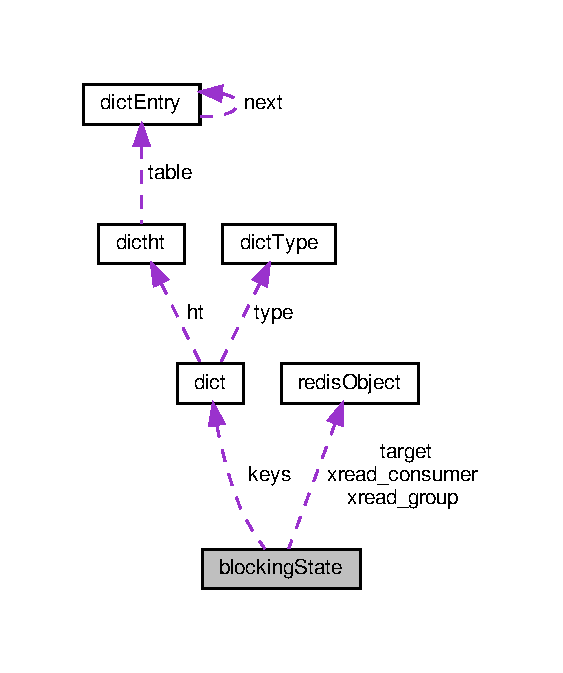
\includegraphics[width=270pt]{structblocking_state__coll__graph}
\end{center}
\end{figure}
\subsection*{Data Fields}
\begin{DoxyCompactItemize}
\item 
\hyperlink{redismodule_8h_a652ae61e2475bc8957454534544968fc}{mstime\+\_\+t} \hyperlink{structblocking_state_a1adf524d2a0c7f9eb77f4f78e6c05620}{timeout}
\item 
\hyperlink{structdict}{dict} $\ast$ \hyperlink{structblocking_state_af63a8281ce9a4285e41df3e045e7c91f}{keys}
\item 
\hyperlink{server_8h_a540f174d2685422fbd7d12e3cd44c8e2}{robj} $\ast$ \hyperlink{structblocking_state_acb665c66e7b32809e1371a4bdec1907e}{target}
\item 
size\+\_\+t \hyperlink{structblocking_state_a1158eb78330481cd4b10428513888bf6}{xread\+\_\+count}
\item 
\hyperlink{server_8h_a540f174d2685422fbd7d12e3cd44c8e2}{robj} $\ast$ \hyperlink{structblocking_state_a410020be56fcf2afc10554265f111cf5}{xread\+\_\+group}
\item 
\hyperlink{server_8h_a540f174d2685422fbd7d12e3cd44c8e2}{robj} $\ast$ \hyperlink{structblocking_state_acc7493490f2c56371b38f76c15ed7912}{xread\+\_\+consumer}
\item 
\hyperlink{redismodule_8h_a652ae61e2475bc8957454534544968fc}{mstime\+\_\+t} \hyperlink{structblocking_state_aab944cd8b3460c6e1a73853f47edd379}{xread\+\_\+retry\+\_\+time}
\item 
\hyperlink{redismodule_8h_a652ae61e2475bc8957454534544968fc}{mstime\+\_\+t} \hyperlink{structblocking_state_a7ee5bfe490a220cccc4c44fd5640a2b3}{xread\+\_\+retry\+\_\+ttl}
\item 
int \hyperlink{structblocking_state_a8ea7b41dabb441998b04529342f97355}{xread\+\_\+group\+\_\+noack}
\item 
int \hyperlink{structblocking_state_a77bbb7714f638a33a511b7c79b05d9bf}{numreplicas}
\item 
long long \hyperlink{structblocking_state_a640179b63c7bf95361949de7cb214d9c}{reploffset}
\item 
void $\ast$ \hyperlink{structblocking_state_a6761112482922feef30b00f99612ad2c}{module\+\_\+blocked\+\_\+handle}
\end{DoxyCompactItemize}


\subsection{Detailed Description}


Definition at line 663 of file server.\+h.



\subsection{Field Documentation}
\mbox{\Hypertarget{structblocking_state_af63a8281ce9a4285e41df3e045e7c91f}\label{structblocking_state_af63a8281ce9a4285e41df3e045e7c91f}} 
\index{blocking\+State@{blocking\+State}!keys@{keys}}
\index{keys@{keys}!blocking\+State@{blocking\+State}}
\subsubsection{\texorpdfstring{keys}{keys}}
{\footnotesize\ttfamily \hyperlink{structdict}{dict}$\ast$ keys}



Definition at line 669 of file server.\+h.

\mbox{\Hypertarget{structblocking_state_a6761112482922feef30b00f99612ad2c}\label{structblocking_state_a6761112482922feef30b00f99612ad2c}} 
\index{blocking\+State@{blocking\+State}!module\+\_\+blocked\+\_\+handle@{module\+\_\+blocked\+\_\+handle}}
\index{module\+\_\+blocked\+\_\+handle@{module\+\_\+blocked\+\_\+handle}!blocking\+State@{blocking\+State}}
\subsubsection{\texorpdfstring{module\+\_\+blocked\+\_\+handle}{module\_blocked\_handle}}
{\footnotesize\ttfamily void$\ast$ module\+\_\+blocked\+\_\+handle}



Definition at line 686 of file server.\+h.

\mbox{\Hypertarget{structblocking_state_a77bbb7714f638a33a511b7c79b05d9bf}\label{structblocking_state_a77bbb7714f638a33a511b7c79b05d9bf}} 
\index{blocking\+State@{blocking\+State}!numreplicas@{numreplicas}}
\index{numreplicas@{numreplicas}!blocking\+State@{blocking\+State}}
\subsubsection{\texorpdfstring{numreplicas}{numreplicas}}
{\footnotesize\ttfamily int numreplicas}



Definition at line 682 of file server.\+h.

\mbox{\Hypertarget{structblocking_state_a640179b63c7bf95361949de7cb214d9c}\label{structblocking_state_a640179b63c7bf95361949de7cb214d9c}} 
\index{blocking\+State@{blocking\+State}!reploffset@{reploffset}}
\index{reploffset@{reploffset}!blocking\+State@{blocking\+State}}
\subsubsection{\texorpdfstring{reploffset}{reploffset}}
{\footnotesize\ttfamily long long reploffset}



Definition at line 683 of file server.\+h.

\mbox{\Hypertarget{structblocking_state_acb665c66e7b32809e1371a4bdec1907e}\label{structblocking_state_acb665c66e7b32809e1371a4bdec1907e}} 
\index{blocking\+State@{blocking\+State}!target@{target}}
\index{target@{target}!blocking\+State@{blocking\+State}}
\subsubsection{\texorpdfstring{target}{target}}
{\footnotesize\ttfamily \hyperlink{server_8h_a540f174d2685422fbd7d12e3cd44c8e2}{robj}$\ast$ target}



Definition at line 671 of file server.\+h.

\mbox{\Hypertarget{structblocking_state_a1adf524d2a0c7f9eb77f4f78e6c05620}\label{structblocking_state_a1adf524d2a0c7f9eb77f4f78e6c05620}} 
\index{blocking\+State@{blocking\+State}!timeout@{timeout}}
\index{timeout@{timeout}!blocking\+State@{blocking\+State}}
\subsubsection{\texorpdfstring{timeout}{timeout}}
{\footnotesize\ttfamily \hyperlink{redismodule_8h_a652ae61e2475bc8957454534544968fc}{mstime\+\_\+t} timeout}



Definition at line 665 of file server.\+h.

\mbox{\Hypertarget{structblocking_state_acc7493490f2c56371b38f76c15ed7912}\label{structblocking_state_acc7493490f2c56371b38f76c15ed7912}} 
\index{blocking\+State@{blocking\+State}!xread\+\_\+consumer@{xread\+\_\+consumer}}
\index{xread\+\_\+consumer@{xread\+\_\+consumer}!blocking\+State@{blocking\+State}}
\subsubsection{\texorpdfstring{xread\+\_\+consumer}{xread\_consumer}}
{\footnotesize\ttfamily \hyperlink{server_8h_a540f174d2685422fbd7d12e3cd44c8e2}{robj}$\ast$ xread\+\_\+consumer}



Definition at line 677 of file server.\+h.

\mbox{\Hypertarget{structblocking_state_a1158eb78330481cd4b10428513888bf6}\label{structblocking_state_a1158eb78330481cd4b10428513888bf6}} 
\index{blocking\+State@{blocking\+State}!xread\+\_\+count@{xread\+\_\+count}}
\index{xread\+\_\+count@{xread\+\_\+count}!blocking\+State@{blocking\+State}}
\subsubsection{\texorpdfstring{xread\+\_\+count}{xread\_count}}
{\footnotesize\ttfamily size\+\_\+t xread\+\_\+count}



Definition at line 675 of file server.\+h.

\mbox{\Hypertarget{structblocking_state_a410020be56fcf2afc10554265f111cf5}\label{structblocking_state_a410020be56fcf2afc10554265f111cf5}} 
\index{blocking\+State@{blocking\+State}!xread\+\_\+group@{xread\+\_\+group}}
\index{xread\+\_\+group@{xread\+\_\+group}!blocking\+State@{blocking\+State}}
\subsubsection{\texorpdfstring{xread\+\_\+group}{xread\_group}}
{\footnotesize\ttfamily \hyperlink{server_8h_a540f174d2685422fbd7d12e3cd44c8e2}{robj}$\ast$ xread\+\_\+group}



Definition at line 676 of file server.\+h.

\mbox{\Hypertarget{structblocking_state_a8ea7b41dabb441998b04529342f97355}\label{structblocking_state_a8ea7b41dabb441998b04529342f97355}} 
\index{blocking\+State@{blocking\+State}!xread\+\_\+group\+\_\+noack@{xread\+\_\+group\+\_\+noack}}
\index{xread\+\_\+group\+\_\+noack@{xread\+\_\+group\+\_\+noack}!blocking\+State@{blocking\+State}}
\subsubsection{\texorpdfstring{xread\+\_\+group\+\_\+noack}{xread\_group\_noack}}
{\footnotesize\ttfamily int xread\+\_\+group\+\_\+noack}



Definition at line 679 of file server.\+h.

\mbox{\Hypertarget{structblocking_state_aab944cd8b3460c6e1a73853f47edd379}\label{structblocking_state_aab944cd8b3460c6e1a73853f47edd379}} 
\index{blocking\+State@{blocking\+State}!xread\+\_\+retry\+\_\+time@{xread\+\_\+retry\+\_\+time}}
\index{xread\+\_\+retry\+\_\+time@{xread\+\_\+retry\+\_\+time}!blocking\+State@{blocking\+State}}
\subsubsection{\texorpdfstring{xread\+\_\+retry\+\_\+time}{xread\_retry\_time}}
{\footnotesize\ttfamily \hyperlink{redismodule_8h_a652ae61e2475bc8957454534544968fc}{mstime\+\_\+t} xread\+\_\+retry\+\_\+time}



Definition at line 678 of file server.\+h.

\mbox{\Hypertarget{structblocking_state_a7ee5bfe490a220cccc4c44fd5640a2b3}\label{structblocking_state_a7ee5bfe490a220cccc4c44fd5640a2b3}} 
\index{blocking\+State@{blocking\+State}!xread\+\_\+retry\+\_\+ttl@{xread\+\_\+retry\+\_\+ttl}}
\index{xread\+\_\+retry\+\_\+ttl@{xread\+\_\+retry\+\_\+ttl}!blocking\+State@{blocking\+State}}
\subsubsection{\texorpdfstring{xread\+\_\+retry\+\_\+ttl}{xread\_retry\_ttl}}
{\footnotesize\ttfamily \hyperlink{redismodule_8h_a652ae61e2475bc8957454534544968fc}{mstime\+\_\+t} xread\+\_\+retry\+\_\+ttl}



Definition at line 678 of file server.\+h.



The documentation for this struct was generated from the following file\+:\begin{DoxyCompactItemize}
\item 
src/\hyperlink{server_8h}{server.\+h}\end{DoxyCompactItemize}

\hypertarget{structclient}{}\section{client Struct Reference}
\label{structclient}\index{client@{client}}


{\ttfamily \#include $<$server.\+h$>$}



Collaboration diagram for client\+:
\nopagebreak
\begin{figure}[H]
\begin{center}
\leavevmode
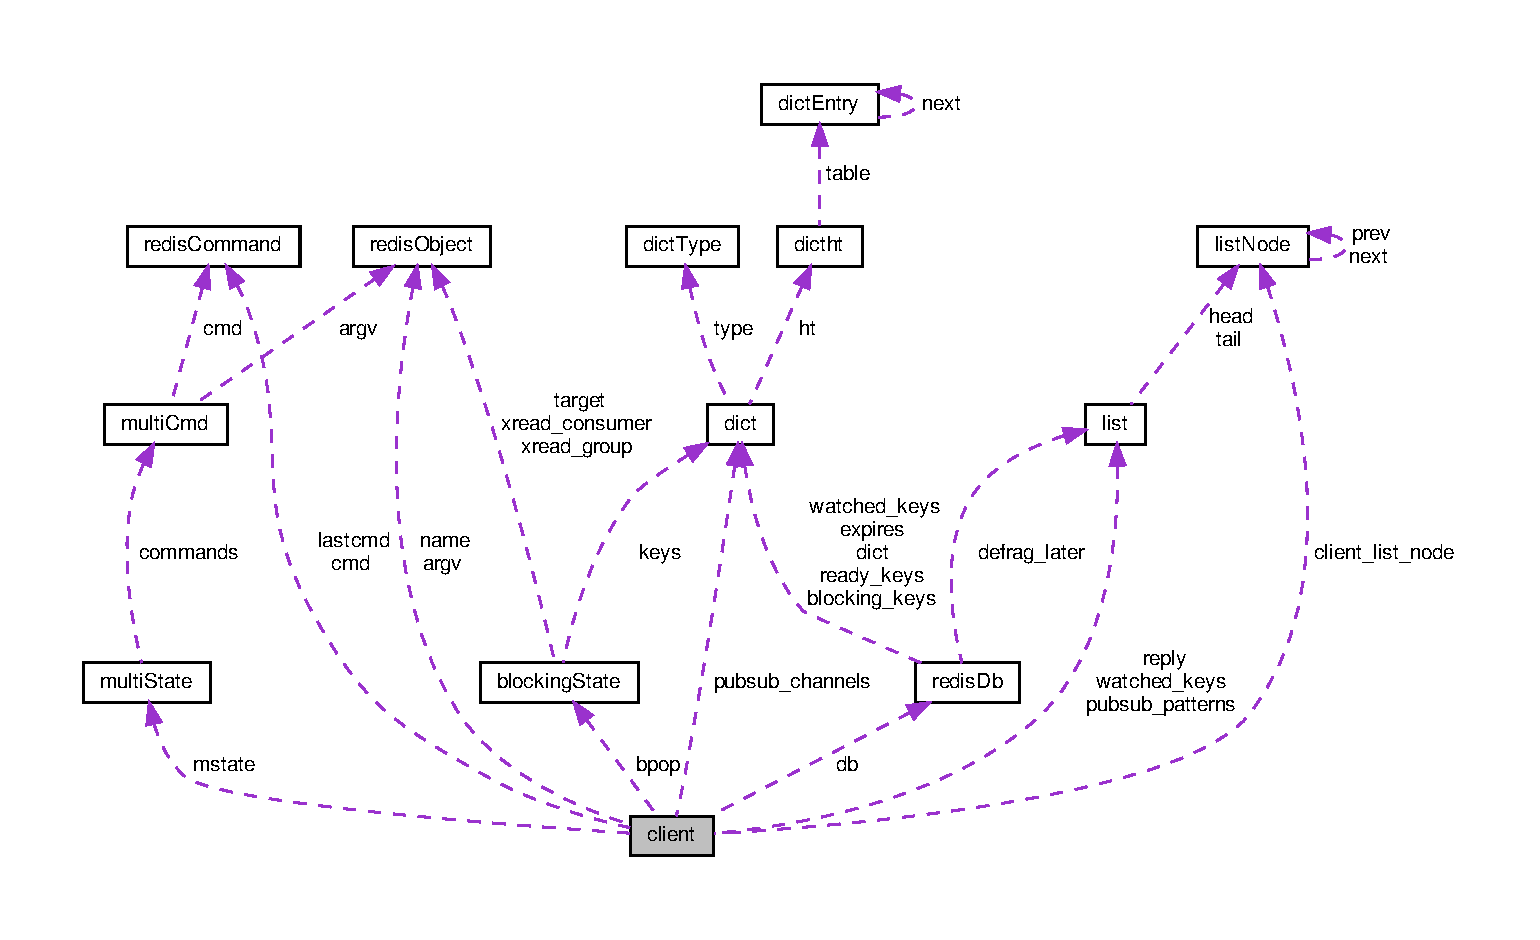
\includegraphics[width=350pt]{structclient__coll__graph}
\end{center}
\end{figure}
\subsection*{Data Fields}
\begin{DoxyCompactItemize}
\item 
uint64\+\_\+t \hyperlink{structclient_a7e290573ef1be67b92a2c745e3b00d1d}{id}
\item 
int \hyperlink{structclient_a6f8059414f0228f0256115e024eeed4b}{fd}
\item 
\hyperlink{structredis_db}{redis\+Db} $\ast$ \hyperlink{structclient_a9bee04e09635a42fef289e42a89f5502}{db}
\item 
\hyperlink{server_8h_a540f174d2685422fbd7d12e3cd44c8e2}{robj} $\ast$ \hyperlink{structclient_a363eae5cb1f099d7803cca951bef7ac2}{name}
\item 
\hyperlink{sds_8h_ad69abac3df4532879db9642c95f5ef6f}{sds} \hyperlink{structclient_accf8e4a2bc6b80403d3f0f024eaa8a1b}{querybuf}
\item 
size\+\_\+t \hyperlink{structclient_a2de8996d6723315d26c64886145d5e51}{qb\+\_\+pos}
\item 
\hyperlink{sds_8h_ad69abac3df4532879db9642c95f5ef6f}{sds} \hyperlink{structclient_ae41c09e14760e794d4378519d312ba9a}{pending\+\_\+querybuf}
\item 
size\+\_\+t \hyperlink{structclient_a09bca2273efb7490d637016ba048ae6e}{querybuf\+\_\+peak}
\item 
int \hyperlink{structclient_ad1447518f4372828b8435ae82e48499e}{argc}
\item 
\hyperlink{server_8h_a540f174d2685422fbd7d12e3cd44c8e2}{robj} $\ast$$\ast$ \hyperlink{structclient_a5c75dd3cb8eb8a3f5be7d4fdf48a9ef9}{argv}
\item 
struct \hyperlink{structredis_command}{redis\+Command} $\ast$ \hyperlink{structclient_a8ed6c4d0c6382ad1787b32d10db25c5e}{cmd}
\item 
struct \hyperlink{structredis_command}{redis\+Command} $\ast$ \hyperlink{structclient_a81d89da91093b6bd8a49acf4a58d47b4}{lastcmd}
\item 
int \hyperlink{structclient_a7c68e9e1d202efcb938b7527f7495de9}{reqtype}
\item 
int \hyperlink{structclient_a0fb4b72a537074c92ed763feb2d46d91}{multibulklen}
\item 
long \hyperlink{structclient_afdb54e1a6b1343bfb0535e4b0ceaa8a9}{bulklen}
\item 
\hyperlink{structlist}{list} $\ast$ \hyperlink{structclient_a3c5720baa890941d827d99224a615377}{reply}
\item 
unsigned long long \hyperlink{structclient_a89eaaab407b2e2659686c94683168b48}{reply\+\_\+bytes}
\item 
size\+\_\+t \hyperlink{structclient_a6a5253178e8e0d41fc9901e6b0626cae}{sentlen}
\item 
time\+\_\+t \hyperlink{structclient_a2b105009c2d9020cbaf51d4457c20e3d}{ctime}
\item 
time\+\_\+t \hyperlink{structclient_a08c13433165f221a86bc5c3160f17c82}{lastinteraction}
\item 
time\+\_\+t \hyperlink{structclient_a5b716e337597169d53bb91dc9a68adc6}{obuf\+\_\+soft\+\_\+limit\+\_\+reached\+\_\+time}
\item 
int \hyperlink{structclient_ac8bf36fe0577cba66bccda3a6f7e80a4}{flags}
\item 
int \hyperlink{structclient_a29e86d0f6d62ef1edac10a46e4c92095}{authenticated}
\item 
int \hyperlink{structclient_abccae535b39fffe81ee57f696b14a218}{replstate}
\item 
int \hyperlink{structclient_afd45af71524188caa056f7687537166d}{repl\+\_\+put\+\_\+online\+\_\+on\+\_\+ack}
\item 
int \hyperlink{structclient_a55864c39dcd617fed6398837225a3854}{repldbfd}
\item 
off\+\_\+t \hyperlink{structclient_a23136112d3075494024d1db57a9e0011}{repldboff}
\item 
off\+\_\+t \hyperlink{structclient_aede725c26d864c47f7448b890931a68f}{repldbsize}
\item 
\hyperlink{sds_8h_ad69abac3df4532879db9642c95f5ef6f}{sds} \hyperlink{structclient_afa5d87f20b8df88d56361da7092fb775}{replpreamble}
\item 
long long \hyperlink{structclient_ae0b58b6e73111b0ae1970a6e7eaed987}{read\+\_\+reploff}
\item 
long long \hyperlink{structclient_a3ceb1598320b93accc65299b5ccf10d7}{reploff}
\item 
long long \hyperlink{structclient_a4df1332c1e98088733ea290c8b617de5}{repl\+\_\+ack\+\_\+off}
\item 
long long \hyperlink{structclient_aca5279911d8623c8a01999fda40f1e4c}{repl\+\_\+ack\+\_\+time}
\item 
long long \hyperlink{structclient_a52806966ab7367bd568472363fe749d3}{psync\+\_\+initial\+\_\+offset}
\item 
char \hyperlink{structclient_a467ab80673fbca31b4729a65effc8362}{replid} \mbox{[}\hyperlink{server_8h_aba6794fa3ee28f85165eaed93190f1df}{C\+O\+N\+F\+I\+G\+\_\+\+R\+U\+N\+\_\+\+I\+D\+\_\+\+S\+I\+ZE}+1\mbox{]}
\item 
int \hyperlink{structclient_a287c6c69470388ee449924e3a8f7933b}{slave\+\_\+listening\+\_\+port}
\item 
char \hyperlink{structclient_a73588a64f8187aee0fd21f4c4d228052}{slave\+\_\+ip} \mbox{[}\hyperlink{server_8h_ad97c5405ed22a94e9fcc10fba577d6c0}{N\+E\+T\+\_\+\+I\+P\+\_\+\+S\+T\+R\+\_\+\+L\+EN}\mbox{]}
\item 
int \hyperlink{structclient_a2f7a224ad788b75b96a48a81524a8a54}{slave\+\_\+capa}
\item 
\hyperlink{structmulti_state}{multi\+State} \hyperlink{structclient_a41bf43ebb391b4e37deb2cb287a8bd1c}{mstate}
\item 
int \hyperlink{structclient_a2dfb71dc958547622b0169422cbd12c3}{btype}
\item 
\hyperlink{structblocking_state}{blocking\+State} \hyperlink{structclient_ade2d291613f86ad81abd9b32a331c97d}{bpop}
\item 
long long \hyperlink{structclient_af59577028441c0e9c8361e112706e6c5}{woff}
\item 
\hyperlink{structlist}{list} $\ast$ \hyperlink{structclient_af3ca58c76fd6357c844b8a3e1122b32f}{watched\+\_\+keys}
\item 
\hyperlink{structdict}{dict} $\ast$ \hyperlink{structclient_ac6c18a3bf3ec4d85777ca2db7d4a9b47}{pubsub\+\_\+channels}
\item 
\hyperlink{structlist}{list} $\ast$ \hyperlink{structclient_aced844471ea20e757a4bc7bdee34d930}{pubsub\+\_\+patterns}
\item 
\hyperlink{sds_8h_ad69abac3df4532879db9642c95f5ef6f}{sds} \hyperlink{structclient_a1c0771287014c17317f1d2536fea4427}{peerid}
\item 
\hyperlink{structlist_node}{list\+Node} $\ast$ \hyperlink{structclient_ad8a3896d9632f4ec77839688f457611b}{client\+\_\+list\+\_\+node}
\item 
int \hyperlink{structclient_a9ae77be080d462d041a52c377da64482}{bufpos}
\item 
char \hyperlink{structclient_aeaa96b202e891f899150ef91c52f77cd}{buf} \mbox{[}\hyperlink{server_8h_ab467e0a40be9097e85445616d9bb32e3}{P\+R\+O\+T\+O\+\_\+\+R\+E\+P\+L\+Y\+\_\+\+C\+H\+U\+N\+K\+\_\+\+B\+Y\+T\+ES}\mbox{]}
\end{DoxyCompactItemize}


\subsection{Detailed Description}


Definition at line 709 of file server.\+h.



\subsection{Field Documentation}
\mbox{\Hypertarget{structclient_ad1447518f4372828b8435ae82e48499e}\label{structclient_ad1447518f4372828b8435ae82e48499e}} 
\index{client@{client}!argc@{argc}}
\index{argc@{argc}!client@{client}}
\subsubsection{\texorpdfstring{argc}{argc}}
{\footnotesize\ttfamily int argc}



Definition at line 721 of file server.\+h.

\mbox{\Hypertarget{structclient_a5c75dd3cb8eb8a3f5be7d4fdf48a9ef9}\label{structclient_a5c75dd3cb8eb8a3f5be7d4fdf48a9ef9}} 
\index{client@{client}!argv@{argv}}
\index{argv@{argv}!client@{client}}
\subsubsection{\texorpdfstring{argv}{argv}}
{\footnotesize\ttfamily \hyperlink{server_8h_a540f174d2685422fbd7d12e3cd44c8e2}{robj}$\ast$$\ast$ argv}



Definition at line 722 of file server.\+h.

\mbox{\Hypertarget{structclient_a29e86d0f6d62ef1edac10a46e4c92095}\label{structclient_a29e86d0f6d62ef1edac10a46e4c92095}} 
\index{client@{client}!authenticated@{authenticated}}
\index{authenticated@{authenticated}!client@{client}}
\subsubsection{\texorpdfstring{authenticated}{authenticated}}
{\footnotesize\ttfamily int authenticated}



Definition at line 735 of file server.\+h.

\mbox{\Hypertarget{structclient_ade2d291613f86ad81abd9b32a331c97d}\label{structclient_ade2d291613f86ad81abd9b32a331c97d}} 
\index{client@{client}!bpop@{bpop}}
\index{bpop@{bpop}!client@{client}}
\subsubsection{\texorpdfstring{bpop}{bpop}}
{\footnotesize\ttfamily \hyperlink{structblocking_state}{blocking\+State} bpop}



Definition at line 755 of file server.\+h.

\mbox{\Hypertarget{structclient_a2dfb71dc958547622b0169422cbd12c3}\label{structclient_a2dfb71dc958547622b0169422cbd12c3}} 
\index{client@{client}!btype@{btype}}
\index{btype@{btype}!client@{client}}
\subsubsection{\texorpdfstring{btype}{btype}}
{\footnotesize\ttfamily int btype}



Definition at line 754 of file server.\+h.

\mbox{\Hypertarget{structclient_aeaa96b202e891f899150ef91c52f77cd}\label{structclient_aeaa96b202e891f899150ef91c52f77cd}} 
\index{client@{client}!buf@{buf}}
\index{buf@{buf}!client@{client}}
\subsubsection{\texorpdfstring{buf}{buf}}
{\footnotesize\ttfamily char buf\mbox{[}\hyperlink{server_8h_ab467e0a40be9097e85445616d9bb32e3}{P\+R\+O\+T\+O\+\_\+\+R\+E\+P\+L\+Y\+\_\+\+C\+H\+U\+N\+K\+\_\+\+B\+Y\+T\+ES}\mbox{]}}



Definition at line 765 of file server.\+h.

\mbox{\Hypertarget{structclient_a9ae77be080d462d041a52c377da64482}\label{structclient_a9ae77be080d462d041a52c377da64482}} 
\index{client@{client}!bufpos@{bufpos}}
\index{bufpos@{bufpos}!client@{client}}
\subsubsection{\texorpdfstring{bufpos}{bufpos}}
{\footnotesize\ttfamily int bufpos}



Definition at line 764 of file server.\+h.

\mbox{\Hypertarget{structclient_afdb54e1a6b1343bfb0535e4b0ceaa8a9}\label{structclient_afdb54e1a6b1343bfb0535e4b0ceaa8a9}} 
\index{client@{client}!bulklen@{bulklen}}
\index{bulklen@{bulklen}!client@{client}}
\subsubsection{\texorpdfstring{bulklen}{bulklen}}
{\footnotesize\ttfamily long bulklen}



Definition at line 726 of file server.\+h.

\mbox{\Hypertarget{structclient_ad8a3896d9632f4ec77839688f457611b}\label{structclient_ad8a3896d9632f4ec77839688f457611b}} 
\index{client@{client}!client\+\_\+list\+\_\+node@{client\+\_\+list\+\_\+node}}
\index{client\+\_\+list\+\_\+node@{client\+\_\+list\+\_\+node}!client@{client}}
\subsubsection{\texorpdfstring{client\+\_\+list\+\_\+node}{client\_list\_node}}
{\footnotesize\ttfamily \hyperlink{structlist_node}{list\+Node}$\ast$ client\+\_\+list\+\_\+node}



Definition at line 761 of file server.\+h.

\mbox{\Hypertarget{structclient_a8ed6c4d0c6382ad1787b32d10db25c5e}\label{structclient_a8ed6c4d0c6382ad1787b32d10db25c5e}} 
\index{client@{client}!cmd@{cmd}}
\index{cmd@{cmd}!client@{client}}
\subsubsection{\texorpdfstring{cmd}{cmd}}
{\footnotesize\ttfamily struct \hyperlink{structredis_command}{redis\+Command}$\ast$ cmd}



Definition at line 723 of file server.\+h.

\mbox{\Hypertarget{structclient_a2b105009c2d9020cbaf51d4457c20e3d}\label{structclient_a2b105009c2d9020cbaf51d4457c20e3d}} 
\index{client@{client}!ctime@{ctime}}
\index{ctime@{ctime}!client@{client}}
\subsubsection{\texorpdfstring{ctime}{ctime}}
{\footnotesize\ttfamily time\+\_\+t ctime}



Definition at line 731 of file server.\+h.

\mbox{\Hypertarget{structclient_a9bee04e09635a42fef289e42a89f5502}\label{structclient_a9bee04e09635a42fef289e42a89f5502}} 
\index{client@{client}!db@{db}}
\index{db@{db}!client@{client}}
\subsubsection{\texorpdfstring{db}{db}}
{\footnotesize\ttfamily \hyperlink{structredis_db}{redis\+Db}$\ast$ db}



Definition at line 712 of file server.\+h.

\mbox{\Hypertarget{structclient_a6f8059414f0228f0256115e024eeed4b}\label{structclient_a6f8059414f0228f0256115e024eeed4b}} 
\index{client@{client}!fd@{fd}}
\index{fd@{fd}!client@{client}}
\subsubsection{\texorpdfstring{fd}{fd}}
{\footnotesize\ttfamily int fd}



Definition at line 711 of file server.\+h.

\mbox{\Hypertarget{structclient_ac8bf36fe0577cba66bccda3a6f7e80a4}\label{structclient_ac8bf36fe0577cba66bccda3a6f7e80a4}} 
\index{client@{client}!flags@{flags}}
\index{flags@{flags}!client@{client}}
\subsubsection{\texorpdfstring{flags}{flags}}
{\footnotesize\ttfamily int flags}



Definition at line 734 of file server.\+h.

\mbox{\Hypertarget{structclient_a7e290573ef1be67b92a2c745e3b00d1d}\label{structclient_a7e290573ef1be67b92a2c745e3b00d1d}} 
\index{client@{client}!id@{id}}
\index{id@{id}!client@{client}}
\subsubsection{\texorpdfstring{id}{id}}
{\footnotesize\ttfamily uint64\+\_\+t id}



Definition at line 710 of file server.\+h.

\mbox{\Hypertarget{structclient_a81d89da91093b6bd8a49acf4a58d47b4}\label{structclient_a81d89da91093b6bd8a49acf4a58d47b4}} 
\index{client@{client}!lastcmd@{lastcmd}}
\index{lastcmd@{lastcmd}!client@{client}}
\subsubsection{\texorpdfstring{lastcmd}{lastcmd}}
{\footnotesize\ttfamily struct \hyperlink{structredis_command}{redis\+Command} $\ast$ lastcmd}



Definition at line 723 of file server.\+h.

\mbox{\Hypertarget{structclient_a08c13433165f221a86bc5c3160f17c82}\label{structclient_a08c13433165f221a86bc5c3160f17c82}} 
\index{client@{client}!lastinteraction@{lastinteraction}}
\index{lastinteraction@{lastinteraction}!client@{client}}
\subsubsection{\texorpdfstring{lastinteraction}{lastinteraction}}
{\footnotesize\ttfamily time\+\_\+t lastinteraction}



Definition at line 732 of file server.\+h.

\mbox{\Hypertarget{structclient_a41bf43ebb391b4e37deb2cb287a8bd1c}\label{structclient_a41bf43ebb391b4e37deb2cb287a8bd1c}} 
\index{client@{client}!mstate@{mstate}}
\index{mstate@{mstate}!client@{client}}
\subsubsection{\texorpdfstring{mstate}{mstate}}
{\footnotesize\ttfamily \hyperlink{structmulti_state}{multi\+State} mstate}



Definition at line 753 of file server.\+h.

\mbox{\Hypertarget{structclient_a0fb4b72a537074c92ed763feb2d46d91}\label{structclient_a0fb4b72a537074c92ed763feb2d46d91}} 
\index{client@{client}!multibulklen@{multibulklen}}
\index{multibulklen@{multibulklen}!client@{client}}
\subsubsection{\texorpdfstring{multibulklen}{multibulklen}}
{\footnotesize\ttfamily int multibulklen}



Definition at line 725 of file server.\+h.

\mbox{\Hypertarget{structclient_a363eae5cb1f099d7803cca951bef7ac2}\label{structclient_a363eae5cb1f099d7803cca951bef7ac2}} 
\index{client@{client}!name@{name}}
\index{name@{name}!client@{client}}
\subsubsection{\texorpdfstring{name}{name}}
{\footnotesize\ttfamily \hyperlink{server_8h_a540f174d2685422fbd7d12e3cd44c8e2}{robj}$\ast$ name}



Definition at line 713 of file server.\+h.

\mbox{\Hypertarget{structclient_a5b716e337597169d53bb91dc9a68adc6}\label{structclient_a5b716e337597169d53bb91dc9a68adc6}} 
\index{client@{client}!obuf\+\_\+soft\+\_\+limit\+\_\+reached\+\_\+time@{obuf\+\_\+soft\+\_\+limit\+\_\+reached\+\_\+time}}
\index{obuf\+\_\+soft\+\_\+limit\+\_\+reached\+\_\+time@{obuf\+\_\+soft\+\_\+limit\+\_\+reached\+\_\+time}!client@{client}}
\subsubsection{\texorpdfstring{obuf\+\_\+soft\+\_\+limit\+\_\+reached\+\_\+time}{obuf\_soft\_limit\_reached\_time}}
{\footnotesize\ttfamily time\+\_\+t obuf\+\_\+soft\+\_\+limit\+\_\+reached\+\_\+time}



Definition at line 733 of file server.\+h.

\mbox{\Hypertarget{structclient_a1c0771287014c17317f1d2536fea4427}\label{structclient_a1c0771287014c17317f1d2536fea4427}} 
\index{client@{client}!peerid@{peerid}}
\index{peerid@{peerid}!client@{client}}
\subsubsection{\texorpdfstring{peerid}{peerid}}
{\footnotesize\ttfamily \hyperlink{sds_8h_ad69abac3df4532879db9642c95f5ef6f}{sds} peerid}



Definition at line 760 of file server.\+h.

\mbox{\Hypertarget{structclient_ae41c09e14760e794d4378519d312ba9a}\label{structclient_ae41c09e14760e794d4378519d312ba9a}} 
\index{client@{client}!pending\+\_\+querybuf@{pending\+\_\+querybuf}}
\index{pending\+\_\+querybuf@{pending\+\_\+querybuf}!client@{client}}
\subsubsection{\texorpdfstring{pending\+\_\+querybuf}{pending\_querybuf}}
{\footnotesize\ttfamily \hyperlink{sds_8h_ad69abac3df4532879db9642c95f5ef6f}{sds} pending\+\_\+querybuf}



Definition at line 716 of file server.\+h.

\mbox{\Hypertarget{structclient_a52806966ab7367bd568472363fe749d3}\label{structclient_a52806966ab7367bd568472363fe749d3}} 
\index{client@{client}!psync\+\_\+initial\+\_\+offset@{psync\+\_\+initial\+\_\+offset}}
\index{psync\+\_\+initial\+\_\+offset@{psync\+\_\+initial\+\_\+offset}!client@{client}}
\subsubsection{\texorpdfstring{psync\+\_\+initial\+\_\+offset}{psync\_initial\_offset}}
{\footnotesize\ttfamily long long psync\+\_\+initial\+\_\+offset}



Definition at line 746 of file server.\+h.

\mbox{\Hypertarget{structclient_ac6c18a3bf3ec4d85777ca2db7d4a9b47}\label{structclient_ac6c18a3bf3ec4d85777ca2db7d4a9b47}} 
\index{client@{client}!pubsub\+\_\+channels@{pubsub\+\_\+channels}}
\index{pubsub\+\_\+channels@{pubsub\+\_\+channels}!client@{client}}
\subsubsection{\texorpdfstring{pubsub\+\_\+channels}{pubsub\_channels}}
{\footnotesize\ttfamily \hyperlink{structdict}{dict}$\ast$ pubsub\+\_\+channels}



Definition at line 758 of file server.\+h.

\mbox{\Hypertarget{structclient_aced844471ea20e757a4bc7bdee34d930}\label{structclient_aced844471ea20e757a4bc7bdee34d930}} 
\index{client@{client}!pubsub\+\_\+patterns@{pubsub\+\_\+patterns}}
\index{pubsub\+\_\+patterns@{pubsub\+\_\+patterns}!client@{client}}
\subsubsection{\texorpdfstring{pubsub\+\_\+patterns}{pubsub\_patterns}}
{\footnotesize\ttfamily \hyperlink{structlist}{list}$\ast$ pubsub\+\_\+patterns}



Definition at line 759 of file server.\+h.

\mbox{\Hypertarget{structclient_a2de8996d6723315d26c64886145d5e51}\label{structclient_a2de8996d6723315d26c64886145d5e51}} 
\index{client@{client}!qb\+\_\+pos@{qb\+\_\+pos}}
\index{qb\+\_\+pos@{qb\+\_\+pos}!client@{client}}
\subsubsection{\texorpdfstring{qb\+\_\+pos}{qb\_pos}}
{\footnotesize\ttfamily size\+\_\+t qb\+\_\+pos}



Definition at line 715 of file server.\+h.

\mbox{\Hypertarget{structclient_accf8e4a2bc6b80403d3f0f024eaa8a1b}\label{structclient_accf8e4a2bc6b80403d3f0f024eaa8a1b}} 
\index{client@{client}!querybuf@{querybuf}}
\index{querybuf@{querybuf}!client@{client}}
\subsubsection{\texorpdfstring{querybuf}{querybuf}}
{\footnotesize\ttfamily \hyperlink{sds_8h_ad69abac3df4532879db9642c95f5ef6f}{sds} querybuf}



Definition at line 714 of file server.\+h.

\mbox{\Hypertarget{structclient_a09bca2273efb7490d637016ba048ae6e}\label{structclient_a09bca2273efb7490d637016ba048ae6e}} 
\index{client@{client}!querybuf\+\_\+peak@{querybuf\+\_\+peak}}
\index{querybuf\+\_\+peak@{querybuf\+\_\+peak}!client@{client}}
\subsubsection{\texorpdfstring{querybuf\+\_\+peak}{querybuf\_peak}}
{\footnotesize\ttfamily size\+\_\+t querybuf\+\_\+peak}



Definition at line 720 of file server.\+h.

\mbox{\Hypertarget{structclient_ae0b58b6e73111b0ae1970a6e7eaed987}\label{structclient_ae0b58b6e73111b0ae1970a6e7eaed987}} 
\index{client@{client}!read\+\_\+reploff@{read\+\_\+reploff}}
\index{read\+\_\+reploff@{read\+\_\+reploff}!client@{client}}
\subsubsection{\texorpdfstring{read\+\_\+reploff}{read\_reploff}}
{\footnotesize\ttfamily long long read\+\_\+reploff}



Definition at line 742 of file server.\+h.

\mbox{\Hypertarget{structclient_a4df1332c1e98088733ea290c8b617de5}\label{structclient_a4df1332c1e98088733ea290c8b617de5}} 
\index{client@{client}!repl\+\_\+ack\+\_\+off@{repl\+\_\+ack\+\_\+off}}
\index{repl\+\_\+ack\+\_\+off@{repl\+\_\+ack\+\_\+off}!client@{client}}
\subsubsection{\texorpdfstring{repl\+\_\+ack\+\_\+off}{repl\_ack\_off}}
{\footnotesize\ttfamily long long repl\+\_\+ack\+\_\+off}



Definition at line 744 of file server.\+h.

\mbox{\Hypertarget{structclient_aca5279911d8623c8a01999fda40f1e4c}\label{structclient_aca5279911d8623c8a01999fda40f1e4c}} 
\index{client@{client}!repl\+\_\+ack\+\_\+time@{repl\+\_\+ack\+\_\+time}}
\index{repl\+\_\+ack\+\_\+time@{repl\+\_\+ack\+\_\+time}!client@{client}}
\subsubsection{\texorpdfstring{repl\+\_\+ack\+\_\+time}{repl\_ack\_time}}
{\footnotesize\ttfamily long long repl\+\_\+ack\+\_\+time}



Definition at line 745 of file server.\+h.

\mbox{\Hypertarget{structclient_afd45af71524188caa056f7687537166d}\label{structclient_afd45af71524188caa056f7687537166d}} 
\index{client@{client}!repl\+\_\+put\+\_\+online\+\_\+on\+\_\+ack@{repl\+\_\+put\+\_\+online\+\_\+on\+\_\+ack}}
\index{repl\+\_\+put\+\_\+online\+\_\+on\+\_\+ack@{repl\+\_\+put\+\_\+online\+\_\+on\+\_\+ack}!client@{client}}
\subsubsection{\texorpdfstring{repl\+\_\+put\+\_\+online\+\_\+on\+\_\+ack}{repl\_put\_online\_on\_ack}}
{\footnotesize\ttfamily int repl\+\_\+put\+\_\+online\+\_\+on\+\_\+ack}



Definition at line 737 of file server.\+h.

\mbox{\Hypertarget{structclient_a55864c39dcd617fed6398837225a3854}\label{structclient_a55864c39dcd617fed6398837225a3854}} 
\index{client@{client}!repldbfd@{repldbfd}}
\index{repldbfd@{repldbfd}!client@{client}}
\subsubsection{\texorpdfstring{repldbfd}{repldbfd}}
{\footnotesize\ttfamily int repldbfd}



Definition at line 738 of file server.\+h.

\mbox{\Hypertarget{structclient_a23136112d3075494024d1db57a9e0011}\label{structclient_a23136112d3075494024d1db57a9e0011}} 
\index{client@{client}!repldboff@{repldboff}}
\index{repldboff@{repldboff}!client@{client}}
\subsubsection{\texorpdfstring{repldboff}{repldboff}}
{\footnotesize\ttfamily off\+\_\+t repldboff}



Definition at line 739 of file server.\+h.

\mbox{\Hypertarget{structclient_aede725c26d864c47f7448b890931a68f}\label{structclient_aede725c26d864c47f7448b890931a68f}} 
\index{client@{client}!repldbsize@{repldbsize}}
\index{repldbsize@{repldbsize}!client@{client}}
\subsubsection{\texorpdfstring{repldbsize}{repldbsize}}
{\footnotesize\ttfamily off\+\_\+t repldbsize}



Definition at line 740 of file server.\+h.

\mbox{\Hypertarget{structclient_a467ab80673fbca31b4729a65effc8362}\label{structclient_a467ab80673fbca31b4729a65effc8362}} 
\index{client@{client}!replid@{replid}}
\index{replid@{replid}!client@{client}}
\subsubsection{\texorpdfstring{replid}{replid}}
{\footnotesize\ttfamily char replid\mbox{[}\hyperlink{server_8h_aba6794fa3ee28f85165eaed93190f1df}{C\+O\+N\+F\+I\+G\+\_\+\+R\+U\+N\+\_\+\+I\+D\+\_\+\+S\+I\+ZE}+1\mbox{]}}



Definition at line 749 of file server.\+h.

\mbox{\Hypertarget{structclient_a3ceb1598320b93accc65299b5ccf10d7}\label{structclient_a3ceb1598320b93accc65299b5ccf10d7}} 
\index{client@{client}!reploff@{reploff}}
\index{reploff@{reploff}!client@{client}}
\subsubsection{\texorpdfstring{reploff}{reploff}}
{\footnotesize\ttfamily long long reploff}



Definition at line 743 of file server.\+h.

\mbox{\Hypertarget{structclient_afa5d87f20b8df88d56361da7092fb775}\label{structclient_afa5d87f20b8df88d56361da7092fb775}} 
\index{client@{client}!replpreamble@{replpreamble}}
\index{replpreamble@{replpreamble}!client@{client}}
\subsubsection{\texorpdfstring{replpreamble}{replpreamble}}
{\footnotesize\ttfamily \hyperlink{sds_8h_ad69abac3df4532879db9642c95f5ef6f}{sds} replpreamble}



Definition at line 741 of file server.\+h.

\mbox{\Hypertarget{structclient_abccae535b39fffe81ee57f696b14a218}\label{structclient_abccae535b39fffe81ee57f696b14a218}} 
\index{client@{client}!replstate@{replstate}}
\index{replstate@{replstate}!client@{client}}
\subsubsection{\texorpdfstring{replstate}{replstate}}
{\footnotesize\ttfamily int replstate}



Definition at line 736 of file server.\+h.

\mbox{\Hypertarget{structclient_a3c5720baa890941d827d99224a615377}\label{structclient_a3c5720baa890941d827d99224a615377}} 
\index{client@{client}!reply@{reply}}
\index{reply@{reply}!client@{client}}
\subsubsection{\texorpdfstring{reply}{reply}}
{\footnotesize\ttfamily \hyperlink{structlist}{list}$\ast$ reply}



Definition at line 727 of file server.\+h.

\mbox{\Hypertarget{structclient_a89eaaab407b2e2659686c94683168b48}\label{structclient_a89eaaab407b2e2659686c94683168b48}} 
\index{client@{client}!reply\+\_\+bytes@{reply\+\_\+bytes}}
\index{reply\+\_\+bytes@{reply\+\_\+bytes}!client@{client}}
\subsubsection{\texorpdfstring{reply\+\_\+bytes}{reply\_bytes}}
{\footnotesize\ttfamily unsigned long long reply\+\_\+bytes}



Definition at line 728 of file server.\+h.

\mbox{\Hypertarget{structclient_a7c68e9e1d202efcb938b7527f7495de9}\label{structclient_a7c68e9e1d202efcb938b7527f7495de9}} 
\index{client@{client}!reqtype@{reqtype}}
\index{reqtype@{reqtype}!client@{client}}
\subsubsection{\texorpdfstring{reqtype}{reqtype}}
{\footnotesize\ttfamily int reqtype}



Definition at line 724 of file server.\+h.

\mbox{\Hypertarget{structclient_a6a5253178e8e0d41fc9901e6b0626cae}\label{structclient_a6a5253178e8e0d41fc9901e6b0626cae}} 
\index{client@{client}!sentlen@{sentlen}}
\index{sentlen@{sentlen}!client@{client}}
\subsubsection{\texorpdfstring{sentlen}{sentlen}}
{\footnotesize\ttfamily size\+\_\+t sentlen}



Definition at line 729 of file server.\+h.

\mbox{\Hypertarget{structclient_a2f7a224ad788b75b96a48a81524a8a54}\label{structclient_a2f7a224ad788b75b96a48a81524a8a54}} 
\index{client@{client}!slave\+\_\+capa@{slave\+\_\+capa}}
\index{slave\+\_\+capa@{slave\+\_\+capa}!client@{client}}
\subsubsection{\texorpdfstring{slave\+\_\+capa}{slave\_capa}}
{\footnotesize\ttfamily int slave\+\_\+capa}



Definition at line 752 of file server.\+h.

\mbox{\Hypertarget{structclient_a73588a64f8187aee0fd21f4c4d228052}\label{structclient_a73588a64f8187aee0fd21f4c4d228052}} 
\index{client@{client}!slave\+\_\+ip@{slave\+\_\+ip}}
\index{slave\+\_\+ip@{slave\+\_\+ip}!client@{client}}
\subsubsection{\texorpdfstring{slave\+\_\+ip}{slave\_ip}}
{\footnotesize\ttfamily char slave\+\_\+ip\mbox{[}\hyperlink{server_8h_ad97c5405ed22a94e9fcc10fba577d6c0}{N\+E\+T\+\_\+\+I\+P\+\_\+\+S\+T\+R\+\_\+\+L\+EN}\mbox{]}}



Definition at line 751 of file server.\+h.

\mbox{\Hypertarget{structclient_a287c6c69470388ee449924e3a8f7933b}\label{structclient_a287c6c69470388ee449924e3a8f7933b}} 
\index{client@{client}!slave\+\_\+listening\+\_\+port@{slave\+\_\+listening\+\_\+port}}
\index{slave\+\_\+listening\+\_\+port@{slave\+\_\+listening\+\_\+port}!client@{client}}
\subsubsection{\texorpdfstring{slave\+\_\+listening\+\_\+port}{slave\_listening\_port}}
{\footnotesize\ttfamily int slave\+\_\+listening\+\_\+port}



Definition at line 750 of file server.\+h.

\mbox{\Hypertarget{structclient_af3ca58c76fd6357c844b8a3e1122b32f}\label{structclient_af3ca58c76fd6357c844b8a3e1122b32f}} 
\index{client@{client}!watched\+\_\+keys@{watched\+\_\+keys}}
\index{watched\+\_\+keys@{watched\+\_\+keys}!client@{client}}
\subsubsection{\texorpdfstring{watched\+\_\+keys}{watched\_keys}}
{\footnotesize\ttfamily \hyperlink{structlist}{list}$\ast$ watched\+\_\+keys}



Definition at line 757 of file server.\+h.

\mbox{\Hypertarget{structclient_af59577028441c0e9c8361e112706e6c5}\label{structclient_af59577028441c0e9c8361e112706e6c5}} 
\index{client@{client}!woff@{woff}}
\index{woff@{woff}!client@{client}}
\subsubsection{\texorpdfstring{woff}{woff}}
{\footnotesize\ttfamily long long woff}



Definition at line 756 of file server.\+h.



The documentation for this struct was generated from the following file\+:\begin{DoxyCompactItemize}
\item 
src/\hyperlink{server_8h}{server.\+h}\end{DoxyCompactItemize}

\hypertarget{structclient_buffer_limits_config}{}\section{client\+Buffer\+Limits\+Config Struct Reference}
\label{structclient_buffer_limits_config}\index{client\+Buffer\+Limits\+Config@{client\+Buffer\+Limits\+Config}}


{\ttfamily \#include $<$server.\+h$>$}

\subsection*{Data Fields}
\begin{DoxyCompactItemize}
\item 
unsigned long long \hyperlink{structclient_buffer_limits_config_a1075b18921e5831210b7ac7c50536e72}{hard\+\_\+limit\+\_\+bytes}
\item 
unsigned long long \hyperlink{structclient_buffer_limits_config_a27e849894bc8a3ceb8f7935266241bdc}{soft\+\_\+limit\+\_\+bytes}
\item 
time\+\_\+t \hyperlink{structclient_buffer_limits_config_a78c15393dd06a546fbaa7ddf91d3c299}{soft\+\_\+limit\+\_\+seconds}
\end{DoxyCompactItemize}


\subsection{Detailed Description}


Definition at line 817 of file server.\+h.



\subsection{Field Documentation}
\mbox{\Hypertarget{structclient_buffer_limits_config_a1075b18921e5831210b7ac7c50536e72}\label{structclient_buffer_limits_config_a1075b18921e5831210b7ac7c50536e72}} 
\index{client\+Buffer\+Limits\+Config@{client\+Buffer\+Limits\+Config}!hard\+\_\+limit\+\_\+bytes@{hard\+\_\+limit\+\_\+bytes}}
\index{hard\+\_\+limit\+\_\+bytes@{hard\+\_\+limit\+\_\+bytes}!client\+Buffer\+Limits\+Config@{client\+Buffer\+Limits\+Config}}
\subsubsection{\texorpdfstring{hard\+\_\+limit\+\_\+bytes}{hard\_limit\_bytes}}
{\footnotesize\ttfamily unsigned long long hard\+\_\+limit\+\_\+bytes}



Definition at line 818 of file server.\+h.

\mbox{\Hypertarget{structclient_buffer_limits_config_a27e849894bc8a3ceb8f7935266241bdc}\label{structclient_buffer_limits_config_a27e849894bc8a3ceb8f7935266241bdc}} 
\index{client\+Buffer\+Limits\+Config@{client\+Buffer\+Limits\+Config}!soft\+\_\+limit\+\_\+bytes@{soft\+\_\+limit\+\_\+bytes}}
\index{soft\+\_\+limit\+\_\+bytes@{soft\+\_\+limit\+\_\+bytes}!client\+Buffer\+Limits\+Config@{client\+Buffer\+Limits\+Config}}
\subsubsection{\texorpdfstring{soft\+\_\+limit\+\_\+bytes}{soft\_limit\_bytes}}
{\footnotesize\ttfamily unsigned long long soft\+\_\+limit\+\_\+bytes}



Definition at line 819 of file server.\+h.

\mbox{\Hypertarget{structclient_buffer_limits_config_a78c15393dd06a546fbaa7ddf91d3c299}\label{structclient_buffer_limits_config_a78c15393dd06a546fbaa7ddf91d3c299}} 
\index{client\+Buffer\+Limits\+Config@{client\+Buffer\+Limits\+Config}!soft\+\_\+limit\+\_\+seconds@{soft\+\_\+limit\+\_\+seconds}}
\index{soft\+\_\+limit\+\_\+seconds@{soft\+\_\+limit\+\_\+seconds}!client\+Buffer\+Limits\+Config@{client\+Buffer\+Limits\+Config}}
\subsubsection{\texorpdfstring{soft\+\_\+limit\+\_\+seconds}{soft\_limit\_seconds}}
{\footnotesize\ttfamily time\+\_\+t soft\+\_\+limit\+\_\+seconds}



Definition at line 820 of file server.\+h.



The documentation for this struct was generated from the following file\+:\begin{DoxyCompactItemize}
\item 
src/\hyperlink{server_8h}{server.\+h}\end{DoxyCompactItemize}

\hypertarget{structclient_reply_block}{}\section{client\+Reply\+Block Struct Reference}
\label{structclient_reply_block}\index{client\+Reply\+Block@{client\+Reply\+Block}}


{\ttfamily \#include $<$server.\+h$>$}

\subsection*{Data Fields}
\begin{DoxyCompactItemize}
\item 
size\+\_\+t \hyperlink{structclient_reply_block_a854352f53b148adc24983a58a1866d66}{size}
\item 
size\+\_\+t \hyperlink{structclient_reply_block_ae8cc011bf3ee2d3c19743095ffc0f7a5}{used}
\item 
char \hyperlink{structclient_reply_block_a781718f5b53a876fe91c424c4607fa8f}{buf} \mbox{[}$\,$\mbox{]}
\end{DoxyCompactItemize}


\subsection{Detailed Description}


Definition at line 628 of file server.\+h.



\subsection{Field Documentation}
\mbox{\Hypertarget{structclient_reply_block_a781718f5b53a876fe91c424c4607fa8f}\label{structclient_reply_block_a781718f5b53a876fe91c424c4607fa8f}} 
\index{client\+Reply\+Block@{client\+Reply\+Block}!buf@{buf}}
\index{buf@{buf}!client\+Reply\+Block@{client\+Reply\+Block}}
\subsubsection{\texorpdfstring{buf}{buf}}
{\footnotesize\ttfamily char buf\mbox{[}$\,$\mbox{]}}



Definition at line 630 of file server.\+h.

\mbox{\Hypertarget{structclient_reply_block_a854352f53b148adc24983a58a1866d66}\label{structclient_reply_block_a854352f53b148adc24983a58a1866d66}} 
\index{client\+Reply\+Block@{client\+Reply\+Block}!size@{size}}
\index{size@{size}!client\+Reply\+Block@{client\+Reply\+Block}}
\subsubsection{\texorpdfstring{size}{size}}
{\footnotesize\ttfamily size\+\_\+t size}



Definition at line 629 of file server.\+h.

\mbox{\Hypertarget{structclient_reply_block_ae8cc011bf3ee2d3c19743095ffc0f7a5}\label{structclient_reply_block_ae8cc011bf3ee2d3c19743095ffc0f7a5}} 
\index{client\+Reply\+Block@{client\+Reply\+Block}!used@{used}}
\index{used@{used}!client\+Reply\+Block@{client\+Reply\+Block}}
\subsubsection{\texorpdfstring{used}{used}}
{\footnotesize\ttfamily size\+\_\+t used}



Definition at line 629 of file server.\+h.



The documentation for this struct was generated from the following file\+:\begin{DoxyCompactItemize}
\item 
src/\hyperlink{server_8h}{server.\+h}\end{DoxyCompactItemize}

\hypertarget{structcluster_link}{}\section{cluster\+Link Struct Reference}
\label{structcluster_link}\index{cluster\+Link@{cluster\+Link}}


{\ttfamily \#include $<$cluster.\+h$>$}



Collaboration diagram for cluster\+Link\+:
\nopagebreak
\begin{figure}[H]
\begin{center}
\leavevmode
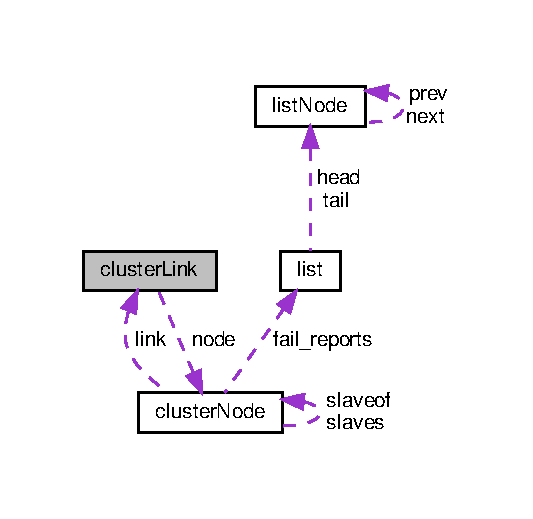
\includegraphics[width=256pt]{structcluster_link__coll__graph}
\end{center}
\end{figure}
\subsection*{Data Fields}
\begin{DoxyCompactItemize}
\item 
\hyperlink{redismodule_8h_a652ae61e2475bc8957454534544968fc}{mstime\+\_\+t} \hyperlink{structcluster_link_a7e18258d5320891f16483de560a5a551}{ctime}
\item 
int \hyperlink{structcluster_link_a6f8059414f0228f0256115e024eeed4b}{fd}
\item 
\hyperlink{sds_8h_ad69abac3df4532879db9642c95f5ef6f}{sds} \hyperlink{structcluster_link_a3bedcd2fc8781d7cfc9239ecb3311ae2}{sndbuf}
\item 
\hyperlink{sds_8h_ad69abac3df4532879db9642c95f5ef6f}{sds} \hyperlink{structcluster_link_a3d5d75102832a2536981164afad5f218}{rcvbuf}
\item 
struct \hyperlink{structcluster_node}{cluster\+Node} $\ast$ \hyperlink{structcluster_link_a7aa2bc440db9dc659120a310878cac0f}{node}
\end{DoxyCompactItemize}


\subsection{Detailed Description}


Definition at line 41 of file cluster.\+h.



\subsection{Field Documentation}
\mbox{\Hypertarget{structcluster_link_a7e18258d5320891f16483de560a5a551}\label{structcluster_link_a7e18258d5320891f16483de560a5a551}} 
\index{cluster\+Link@{cluster\+Link}!ctime@{ctime}}
\index{ctime@{ctime}!cluster\+Link@{cluster\+Link}}
\subsubsection{\texorpdfstring{ctime}{ctime}}
{\footnotesize\ttfamily \hyperlink{redismodule_8h_a652ae61e2475bc8957454534544968fc}{mstime\+\_\+t} ctime}



Definition at line 42 of file cluster.\+h.

\mbox{\Hypertarget{structcluster_link_a6f8059414f0228f0256115e024eeed4b}\label{structcluster_link_a6f8059414f0228f0256115e024eeed4b}} 
\index{cluster\+Link@{cluster\+Link}!fd@{fd}}
\index{fd@{fd}!cluster\+Link@{cluster\+Link}}
\subsubsection{\texorpdfstring{fd}{fd}}
{\footnotesize\ttfamily int fd}



Definition at line 43 of file cluster.\+h.

\mbox{\Hypertarget{structcluster_link_a7aa2bc440db9dc659120a310878cac0f}\label{structcluster_link_a7aa2bc440db9dc659120a310878cac0f}} 
\index{cluster\+Link@{cluster\+Link}!node@{node}}
\index{node@{node}!cluster\+Link@{cluster\+Link}}
\subsubsection{\texorpdfstring{node}{node}}
{\footnotesize\ttfamily struct \hyperlink{structcluster_node}{cluster\+Node}$\ast$ node}



Definition at line 46 of file cluster.\+h.

\mbox{\Hypertarget{structcluster_link_a3d5d75102832a2536981164afad5f218}\label{structcluster_link_a3d5d75102832a2536981164afad5f218}} 
\index{cluster\+Link@{cluster\+Link}!rcvbuf@{rcvbuf}}
\index{rcvbuf@{rcvbuf}!cluster\+Link@{cluster\+Link}}
\subsubsection{\texorpdfstring{rcvbuf}{rcvbuf}}
{\footnotesize\ttfamily \hyperlink{sds_8h_ad69abac3df4532879db9642c95f5ef6f}{sds} rcvbuf}



Definition at line 45 of file cluster.\+h.

\mbox{\Hypertarget{structcluster_link_a3bedcd2fc8781d7cfc9239ecb3311ae2}\label{structcluster_link_a3bedcd2fc8781d7cfc9239ecb3311ae2}} 
\index{cluster\+Link@{cluster\+Link}!sndbuf@{sndbuf}}
\index{sndbuf@{sndbuf}!cluster\+Link@{cluster\+Link}}
\subsubsection{\texorpdfstring{sndbuf}{sndbuf}}
{\footnotesize\ttfamily \hyperlink{sds_8h_ad69abac3df4532879db9642c95f5ef6f}{sds} sndbuf}



Definition at line 44 of file cluster.\+h.



The documentation for this struct was generated from the following file\+:\begin{DoxyCompactItemize}
\item 
src/\hyperlink{cluster_8h}{cluster.\+h}\end{DoxyCompactItemize}

\hypertarget{structcluster_manager_command}{}\section{cluster\+Manager\+Command Struct Reference}
\label{structcluster_manager_command}\index{cluster\+Manager\+Command@{cluster\+Manager\+Command}}
\subsection*{Data Fields}
\begin{DoxyCompactItemize}
\item 
char $\ast$ \hyperlink{structcluster_manager_command_a5ac083a645d964373f022d03df4849c8}{name}
\item 
int \hyperlink{structcluster_manager_command_ad1447518f4372828b8435ae82e48499e}{argc}
\item 
char $\ast$$\ast$ \hyperlink{structcluster_manager_command_af2efa898e9eed6fe6715279cb1ec35b0}{argv}
\item 
int \hyperlink{structcluster_manager_command_ac8bf36fe0577cba66bccda3a6f7e80a4}{flags}
\item 
int \hyperlink{structcluster_manager_command_a8ae018e1f77620e3b04d597737618b76}{replicas}
\item 
char $\ast$ \hyperlink{structcluster_manager_command_a765533dfc643627999c751f7e1514664}{from}
\item 
char $\ast$ \hyperlink{structcluster_manager_command_a5bafda9519252aa2d0fd038153f77dca}{to}
\item 
char $\ast$$\ast$ \hyperlink{structcluster_manager_command_ada3bc364c6e61924b60efc24e8a1d149}{weight}
\item 
int \hyperlink{structcluster_manager_command_ac8c8afcbde7c5bf8d79f5a121fe2601c}{weight\+\_\+argc}
\item 
char $\ast$ \hyperlink{structcluster_manager_command_a5156fe5a4a5df15461a4eb5c8c9238d9}{master\+\_\+id}
\item 
int \hyperlink{structcluster_manager_command_ac1e34a145d11fe4907398ed28bdca202}{slots}
\item 
int \hyperlink{structcluster_manager_command_a493b57f443cc38b3d3df9c1e584d9d82}{timeout}
\item 
int \hyperlink{structcluster_manager_command_a9fb2ad67672c7ea99eaa3fdf494b1b13}{pipeline}
\item 
float \hyperlink{structcluster_manager_command_a376acef8954eadc70f4b55e8e0588e13}{threshold}
\end{DoxyCompactItemize}


\subsection{Detailed Description}


Definition at line 161 of file redis-\/cli.\+c.



\subsection{Field Documentation}
\mbox{\Hypertarget{structcluster_manager_command_ad1447518f4372828b8435ae82e48499e}\label{structcluster_manager_command_ad1447518f4372828b8435ae82e48499e}} 
\index{cluster\+Manager\+Command@{cluster\+Manager\+Command}!argc@{argc}}
\index{argc@{argc}!cluster\+Manager\+Command@{cluster\+Manager\+Command}}
\subsubsection{\texorpdfstring{argc}{argc}}
{\footnotesize\ttfamily int argc}



Definition at line 163 of file redis-\/cli.\+c.

\mbox{\Hypertarget{structcluster_manager_command_af2efa898e9eed6fe6715279cb1ec35b0}\label{structcluster_manager_command_af2efa898e9eed6fe6715279cb1ec35b0}} 
\index{cluster\+Manager\+Command@{cluster\+Manager\+Command}!argv@{argv}}
\index{argv@{argv}!cluster\+Manager\+Command@{cluster\+Manager\+Command}}
\subsubsection{\texorpdfstring{argv}{argv}}
{\footnotesize\ttfamily char$\ast$$\ast$ argv}



Definition at line 164 of file redis-\/cli.\+c.

\mbox{\Hypertarget{structcluster_manager_command_ac8bf36fe0577cba66bccda3a6f7e80a4}\label{structcluster_manager_command_ac8bf36fe0577cba66bccda3a6f7e80a4}} 
\index{cluster\+Manager\+Command@{cluster\+Manager\+Command}!flags@{flags}}
\index{flags@{flags}!cluster\+Manager\+Command@{cluster\+Manager\+Command}}
\subsubsection{\texorpdfstring{flags}{flags}}
{\footnotesize\ttfamily int flags}



Definition at line 165 of file redis-\/cli.\+c.

\mbox{\Hypertarget{structcluster_manager_command_a765533dfc643627999c751f7e1514664}\label{structcluster_manager_command_a765533dfc643627999c751f7e1514664}} 
\index{cluster\+Manager\+Command@{cluster\+Manager\+Command}!from@{from}}
\index{from@{from}!cluster\+Manager\+Command@{cluster\+Manager\+Command}}
\subsubsection{\texorpdfstring{from}{from}}
{\footnotesize\ttfamily char$\ast$ from}



Definition at line 167 of file redis-\/cli.\+c.

\mbox{\Hypertarget{structcluster_manager_command_a5156fe5a4a5df15461a4eb5c8c9238d9}\label{structcluster_manager_command_a5156fe5a4a5df15461a4eb5c8c9238d9}} 
\index{cluster\+Manager\+Command@{cluster\+Manager\+Command}!master\+\_\+id@{master\+\_\+id}}
\index{master\+\_\+id@{master\+\_\+id}!cluster\+Manager\+Command@{cluster\+Manager\+Command}}
\subsubsection{\texorpdfstring{master\+\_\+id}{master\_id}}
{\footnotesize\ttfamily char$\ast$ master\+\_\+id}



Definition at line 171 of file redis-\/cli.\+c.

\mbox{\Hypertarget{structcluster_manager_command_a5ac083a645d964373f022d03df4849c8}\label{structcluster_manager_command_a5ac083a645d964373f022d03df4849c8}} 
\index{cluster\+Manager\+Command@{cluster\+Manager\+Command}!name@{name}}
\index{name@{name}!cluster\+Manager\+Command@{cluster\+Manager\+Command}}
\subsubsection{\texorpdfstring{name}{name}}
{\footnotesize\ttfamily char$\ast$ name}



Definition at line 162 of file redis-\/cli.\+c.

\mbox{\Hypertarget{structcluster_manager_command_a9fb2ad67672c7ea99eaa3fdf494b1b13}\label{structcluster_manager_command_a9fb2ad67672c7ea99eaa3fdf494b1b13}} 
\index{cluster\+Manager\+Command@{cluster\+Manager\+Command}!pipeline@{pipeline}}
\index{pipeline@{pipeline}!cluster\+Manager\+Command@{cluster\+Manager\+Command}}
\subsubsection{\texorpdfstring{pipeline}{pipeline}}
{\footnotesize\ttfamily int pipeline}



Definition at line 174 of file redis-\/cli.\+c.

\mbox{\Hypertarget{structcluster_manager_command_a8ae018e1f77620e3b04d597737618b76}\label{structcluster_manager_command_a8ae018e1f77620e3b04d597737618b76}} 
\index{cluster\+Manager\+Command@{cluster\+Manager\+Command}!replicas@{replicas}}
\index{replicas@{replicas}!cluster\+Manager\+Command@{cluster\+Manager\+Command}}
\subsubsection{\texorpdfstring{replicas}{replicas}}
{\footnotesize\ttfamily int replicas}



Definition at line 166 of file redis-\/cli.\+c.

\mbox{\Hypertarget{structcluster_manager_command_ac1e34a145d11fe4907398ed28bdca202}\label{structcluster_manager_command_ac1e34a145d11fe4907398ed28bdca202}} 
\index{cluster\+Manager\+Command@{cluster\+Manager\+Command}!slots@{slots}}
\index{slots@{slots}!cluster\+Manager\+Command@{cluster\+Manager\+Command}}
\subsubsection{\texorpdfstring{slots}{slots}}
{\footnotesize\ttfamily int slots}



Definition at line 172 of file redis-\/cli.\+c.

\mbox{\Hypertarget{structcluster_manager_command_a376acef8954eadc70f4b55e8e0588e13}\label{structcluster_manager_command_a376acef8954eadc70f4b55e8e0588e13}} 
\index{cluster\+Manager\+Command@{cluster\+Manager\+Command}!threshold@{threshold}}
\index{threshold@{threshold}!cluster\+Manager\+Command@{cluster\+Manager\+Command}}
\subsubsection{\texorpdfstring{threshold}{threshold}}
{\footnotesize\ttfamily float threshold}



Definition at line 175 of file redis-\/cli.\+c.

\mbox{\Hypertarget{structcluster_manager_command_a493b57f443cc38b3d3df9c1e584d9d82}\label{structcluster_manager_command_a493b57f443cc38b3d3df9c1e584d9d82}} 
\index{cluster\+Manager\+Command@{cluster\+Manager\+Command}!timeout@{timeout}}
\index{timeout@{timeout}!cluster\+Manager\+Command@{cluster\+Manager\+Command}}
\subsubsection{\texorpdfstring{timeout}{timeout}}
{\footnotesize\ttfamily int timeout}



Definition at line 173 of file redis-\/cli.\+c.

\mbox{\Hypertarget{structcluster_manager_command_a5bafda9519252aa2d0fd038153f77dca}\label{structcluster_manager_command_a5bafda9519252aa2d0fd038153f77dca}} 
\index{cluster\+Manager\+Command@{cluster\+Manager\+Command}!to@{to}}
\index{to@{to}!cluster\+Manager\+Command@{cluster\+Manager\+Command}}
\subsubsection{\texorpdfstring{to}{to}}
{\footnotesize\ttfamily char$\ast$ to}



Definition at line 168 of file redis-\/cli.\+c.

\mbox{\Hypertarget{structcluster_manager_command_ada3bc364c6e61924b60efc24e8a1d149}\label{structcluster_manager_command_ada3bc364c6e61924b60efc24e8a1d149}} 
\index{cluster\+Manager\+Command@{cluster\+Manager\+Command}!weight@{weight}}
\index{weight@{weight}!cluster\+Manager\+Command@{cluster\+Manager\+Command}}
\subsubsection{\texorpdfstring{weight}{weight}}
{\footnotesize\ttfamily char$\ast$$\ast$ weight}



Definition at line 169 of file redis-\/cli.\+c.

\mbox{\Hypertarget{structcluster_manager_command_ac8c8afcbde7c5bf8d79f5a121fe2601c}\label{structcluster_manager_command_ac8c8afcbde7c5bf8d79f5a121fe2601c}} 
\index{cluster\+Manager\+Command@{cluster\+Manager\+Command}!weight\+\_\+argc@{weight\+\_\+argc}}
\index{weight\+\_\+argc@{weight\+\_\+argc}!cluster\+Manager\+Command@{cluster\+Manager\+Command}}
\subsubsection{\texorpdfstring{weight\+\_\+argc}{weight\_argc}}
{\footnotesize\ttfamily int weight\+\_\+argc}



Definition at line 170 of file redis-\/cli.\+c.



The documentation for this struct was generated from the following file\+:\begin{DoxyCompactItemize}
\item 
src/\hyperlink{redis-cli_8c}{redis-\/cli.\+c}\end{DoxyCompactItemize}

\hypertarget{structcluster_manager_command_def}{}\section{cluster\+Manager\+Command\+Def Struct Reference}
\label{structcluster_manager_command_def}\index{cluster\+Manager\+Command\+Def@{cluster\+Manager\+Command\+Def}}
\subsection*{Data Fields}
\begin{DoxyCompactItemize}
\item 
char $\ast$ \hyperlink{structcluster_manager_command_def_a5ac083a645d964373f022d03df4849c8}{name}
\item 
\hyperlink{redis-cli_8c_a8e9cfad74d28bc05c1e55864714a460f}{cluster\+Manager\+Command\+Proc} $\ast$ \hyperlink{structcluster_manager_command_def_acec64f15ecc0fd1e401bfc3736963e65}{proc}
\item 
int \hyperlink{structcluster_manager_command_def_a2e1dc7313b72e22a19179823661deb69}{arity}
\item 
char $\ast$ \hyperlink{structcluster_manager_command_def_a0bd887c941dfeb4a13ee1501df2df62d}{args}
\item 
char $\ast$ \hyperlink{structcluster_manager_command_def_ad358cb7ece4fc65136f8d20cf6b12816}{options}
\end{DoxyCompactItemize}


\subsection{Detailed Description}


Definition at line 1970 of file redis-\/cli.\+c.



\subsection{Field Documentation}
\mbox{\Hypertarget{structcluster_manager_command_def_a0bd887c941dfeb4a13ee1501df2df62d}\label{structcluster_manager_command_def_a0bd887c941dfeb4a13ee1501df2df62d}} 
\index{cluster\+Manager\+Command\+Def@{cluster\+Manager\+Command\+Def}!args@{args}}
\index{args@{args}!cluster\+Manager\+Command\+Def@{cluster\+Manager\+Command\+Def}}
\subsubsection{\texorpdfstring{args}{args}}
{\footnotesize\ttfamily char$\ast$ args}



Definition at line 1974 of file redis-\/cli.\+c.

\mbox{\Hypertarget{structcluster_manager_command_def_a2e1dc7313b72e22a19179823661deb69}\label{structcluster_manager_command_def_a2e1dc7313b72e22a19179823661deb69}} 
\index{cluster\+Manager\+Command\+Def@{cluster\+Manager\+Command\+Def}!arity@{arity}}
\index{arity@{arity}!cluster\+Manager\+Command\+Def@{cluster\+Manager\+Command\+Def}}
\subsubsection{\texorpdfstring{arity}{arity}}
{\footnotesize\ttfamily int arity}



Definition at line 1973 of file redis-\/cli.\+c.

\mbox{\Hypertarget{structcluster_manager_command_def_a5ac083a645d964373f022d03df4849c8}\label{structcluster_manager_command_def_a5ac083a645d964373f022d03df4849c8}} 
\index{cluster\+Manager\+Command\+Def@{cluster\+Manager\+Command\+Def}!name@{name}}
\index{name@{name}!cluster\+Manager\+Command\+Def@{cluster\+Manager\+Command\+Def}}
\subsubsection{\texorpdfstring{name}{name}}
{\footnotesize\ttfamily char$\ast$ name}



Definition at line 1971 of file redis-\/cli.\+c.

\mbox{\Hypertarget{structcluster_manager_command_def_ad358cb7ece4fc65136f8d20cf6b12816}\label{structcluster_manager_command_def_ad358cb7ece4fc65136f8d20cf6b12816}} 
\index{cluster\+Manager\+Command\+Def@{cluster\+Manager\+Command\+Def}!options@{options}}
\index{options@{options}!cluster\+Manager\+Command\+Def@{cluster\+Manager\+Command\+Def}}
\subsubsection{\texorpdfstring{options}{options}}
{\footnotesize\ttfamily char$\ast$ options}



Definition at line 1975 of file redis-\/cli.\+c.

\mbox{\Hypertarget{structcluster_manager_command_def_acec64f15ecc0fd1e401bfc3736963e65}\label{structcluster_manager_command_def_acec64f15ecc0fd1e401bfc3736963e65}} 
\index{cluster\+Manager\+Command\+Def@{cluster\+Manager\+Command\+Def}!proc@{proc}}
\index{proc@{proc}!cluster\+Manager\+Command\+Def@{cluster\+Manager\+Command\+Def}}
\subsubsection{\texorpdfstring{proc}{proc}}
{\footnotesize\ttfamily \hyperlink{redis-cli_8c_a8e9cfad74d28bc05c1e55864714a460f}{cluster\+Manager\+Command\+Proc}$\ast$ proc}



Definition at line 1972 of file redis-\/cli.\+c.



The documentation for this struct was generated from the following file\+:\begin{DoxyCompactItemize}
\item 
src/\hyperlink{redis-cli_8c}{redis-\/cli.\+c}\end{DoxyCompactItemize}

\hypertarget{structcluster_manager_node}{}\section{cluster\+Manager\+Node Struct Reference}
\label{structcluster_manager_node}\index{cluster\+Manager\+Node@{cluster\+Manager\+Node}}


Collaboration diagram for cluster\+Manager\+Node\+:
\nopagebreak
\begin{figure}[H]
\begin{center}
\leavevmode
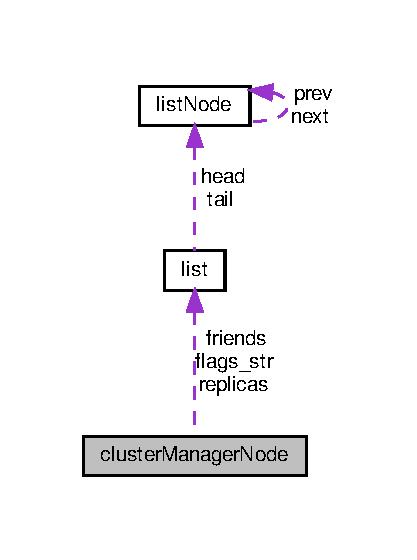
\includegraphics[width=200pt]{structcluster_manager_node__coll__graph}
\end{center}
\end{figure}
\subsection*{Data Fields}
\begin{DoxyCompactItemize}
\item 
redis\+Context $\ast$ \hyperlink{structcluster_manager_node_ace869d36dc1b4de4b6d046c0c71486cb}{context}
\item 
\hyperlink{sds_8h_ad69abac3df4532879db9642c95f5ef6f}{sds} \hyperlink{structcluster_manager_node_a78d661a433637c5e0fac8a377e3ddeb6}{name}
\item 
char $\ast$ \hyperlink{structcluster_manager_node_afbc356cd0e25d1dbbece7c10fd025fa6}{ip}
\item 
int \hyperlink{structcluster_manager_node_a63c89c04d1feae07ca35558055155ffb}{port}
\item 
uint64\+\_\+t \hyperlink{structcluster_manager_node_ab523bc9f0cc579208ad514cc588d3981}{current\+\_\+epoch}
\item 
time\+\_\+t \hyperlink{structcluster_manager_node_a3131021cfa8e1212d327a9ea5593e585}{ping\+\_\+sent}
\item 
time\+\_\+t \hyperlink{structcluster_manager_node_ad8bbaa889c9a9c08137836207b72b64a}{ping\+\_\+recv}
\item 
int \hyperlink{structcluster_manager_node_ac8bf36fe0577cba66bccda3a6f7e80a4}{flags}
\item 
\hyperlink{structlist}{list} $\ast$ \hyperlink{structcluster_manager_node_a2996ddb21acb702fdb383abf6ea1c0b3}{flags\+\_\+str}
\item 
\hyperlink{sds_8h_ad69abac3df4532879db9642c95f5ef6f}{sds} \hyperlink{structcluster_manager_node_af6f45314e664ae7be8f68488be45354d}{replicate}
\item 
\hyperlink{structlist}{list} \hyperlink{structcluster_manager_node_ad83e6ba102626a40bb3fab569c04a735}{replicas}
\item 
int \hyperlink{structcluster_manager_node_a120b75c12097e7fdda71535d04ae7880}{dirty}
\item 
uint8\+\_\+t \hyperlink{structcluster_manager_node_a6f06905b827dc0f8fb569761fb55cab6}{slots} \mbox{[}\hyperlink{redis-cli_8c_adff5eca00afc90a8c3c213bb7100cdc0}{C\+L\+U\+S\+T\+E\+R\+\_\+\+M\+A\+N\+A\+G\+E\+R\+\_\+\+S\+L\+O\+TS}\mbox{]}
\item 
int \hyperlink{structcluster_manager_node_ac71d8fbda6f0a3ab58593d31114de67a}{slots\+\_\+count}
\item 
int \hyperlink{structcluster_manager_node_a6a823cf956d3d5ba7505d98158f95c45}{replicas\+\_\+count}
\item 
\hyperlink{structlist}{list} $\ast$ \hyperlink{structcluster_manager_node_ae23d28d899b0e45974609c4ac7f1ea8f}{friends}
\item 
\hyperlink{sds_8h_ad69abac3df4532879db9642c95f5ef6f}{sds} $\ast$ \hyperlink{structcluster_manager_node_a604c80c491c9223758b948b037f86c71}{migrating}
\item 
\hyperlink{sds_8h_ad69abac3df4532879db9642c95f5ef6f}{sds} $\ast$ \hyperlink{structcluster_manager_node_a5a772e4c6ce0e8c19238f6e054e7c277}{importing}
\item 
int \hyperlink{structcluster_manager_node_af1e54163cd1ecf546c6ccd63a4be9caa}{migrating\+\_\+count}
\item 
int \hyperlink{structcluster_manager_node_a25436798b02625247a3e5dd2625c4e96}{importing\+\_\+count}
\item 
float \hyperlink{structcluster_manager_node_a8128625c9e3fd04c27b82957732d8781}{weight}
\item 
int \hyperlink{structcluster_manager_node_ac794434112478f3134ad93778a0f2860}{balance}
\end{DoxyCompactItemize}


\subsection{Detailed Description}


Definition at line 1869 of file redis-\/cli.\+c.



\subsection{Field Documentation}
\mbox{\Hypertarget{structcluster_manager_node_ac794434112478f3134ad93778a0f2860}\label{structcluster_manager_node_ac794434112478f3134ad93778a0f2860}} 
\index{cluster\+Manager\+Node@{cluster\+Manager\+Node}!balance@{balance}}
\index{balance@{balance}!cluster\+Manager\+Node@{cluster\+Manager\+Node}}
\subsubsection{\texorpdfstring{balance}{balance}}
{\footnotesize\ttfamily int balance}



Definition at line 1893 of file redis-\/cli.\+c.

\mbox{\Hypertarget{structcluster_manager_node_ace869d36dc1b4de4b6d046c0c71486cb}\label{structcluster_manager_node_ace869d36dc1b4de4b6d046c0c71486cb}} 
\index{cluster\+Manager\+Node@{cluster\+Manager\+Node}!context@{context}}
\index{context@{context}!cluster\+Manager\+Node@{cluster\+Manager\+Node}}
\subsubsection{\texorpdfstring{context}{context}}
{\footnotesize\ttfamily redis\+Context$\ast$ context}



Definition at line 1870 of file redis-\/cli.\+c.

\mbox{\Hypertarget{structcluster_manager_node_ab523bc9f0cc579208ad514cc588d3981}\label{structcluster_manager_node_ab523bc9f0cc579208ad514cc588d3981}} 
\index{cluster\+Manager\+Node@{cluster\+Manager\+Node}!current\+\_\+epoch@{current\+\_\+epoch}}
\index{current\+\_\+epoch@{current\+\_\+epoch}!cluster\+Manager\+Node@{cluster\+Manager\+Node}}
\subsubsection{\texorpdfstring{current\+\_\+epoch}{current\_epoch}}
{\footnotesize\ttfamily uint64\+\_\+t current\+\_\+epoch}



Definition at line 1874 of file redis-\/cli.\+c.

\mbox{\Hypertarget{structcluster_manager_node_a120b75c12097e7fdda71535d04ae7880}\label{structcluster_manager_node_a120b75c12097e7fdda71535d04ae7880}} 
\index{cluster\+Manager\+Node@{cluster\+Manager\+Node}!dirty@{dirty}}
\index{dirty@{dirty}!cluster\+Manager\+Node@{cluster\+Manager\+Node}}
\subsubsection{\texorpdfstring{dirty}{dirty}}
{\footnotesize\ttfamily int dirty}



Definition at line 1881 of file redis-\/cli.\+c.

\mbox{\Hypertarget{structcluster_manager_node_ac8bf36fe0577cba66bccda3a6f7e80a4}\label{structcluster_manager_node_ac8bf36fe0577cba66bccda3a6f7e80a4}} 
\index{cluster\+Manager\+Node@{cluster\+Manager\+Node}!flags@{flags}}
\index{flags@{flags}!cluster\+Manager\+Node@{cluster\+Manager\+Node}}
\subsubsection{\texorpdfstring{flags}{flags}}
{\footnotesize\ttfamily int flags}



Definition at line 1877 of file redis-\/cli.\+c.

\mbox{\Hypertarget{structcluster_manager_node_a2996ddb21acb702fdb383abf6ea1c0b3}\label{structcluster_manager_node_a2996ddb21acb702fdb383abf6ea1c0b3}} 
\index{cluster\+Manager\+Node@{cluster\+Manager\+Node}!flags\+\_\+str@{flags\+\_\+str}}
\index{flags\+\_\+str@{flags\+\_\+str}!cluster\+Manager\+Node@{cluster\+Manager\+Node}}
\subsubsection{\texorpdfstring{flags\+\_\+str}{flags\_str}}
{\footnotesize\ttfamily \hyperlink{structlist}{list}$\ast$ flags\+\_\+str}



Definition at line 1878 of file redis-\/cli.\+c.

\mbox{\Hypertarget{structcluster_manager_node_ae23d28d899b0e45974609c4ac7f1ea8f}\label{structcluster_manager_node_ae23d28d899b0e45974609c4ac7f1ea8f}} 
\index{cluster\+Manager\+Node@{cluster\+Manager\+Node}!friends@{friends}}
\index{friends@{friends}!cluster\+Manager\+Node@{cluster\+Manager\+Node}}
\subsubsection{\texorpdfstring{friends}{friends}}
{\footnotesize\ttfamily \hyperlink{structlist}{list}$\ast$ friends}



Definition at line 1885 of file redis-\/cli.\+c.

\mbox{\Hypertarget{structcluster_manager_node_a5a772e4c6ce0e8c19238f6e054e7c277}\label{structcluster_manager_node_a5a772e4c6ce0e8c19238f6e054e7c277}} 
\index{cluster\+Manager\+Node@{cluster\+Manager\+Node}!importing@{importing}}
\index{importing@{importing}!cluster\+Manager\+Node@{cluster\+Manager\+Node}}
\subsubsection{\texorpdfstring{importing}{importing}}
{\footnotesize\ttfamily \hyperlink{sds_8h_ad69abac3df4532879db9642c95f5ef6f}{sds}$\ast$ importing}



Definition at line 1888 of file redis-\/cli.\+c.

\mbox{\Hypertarget{structcluster_manager_node_a25436798b02625247a3e5dd2625c4e96}\label{structcluster_manager_node_a25436798b02625247a3e5dd2625c4e96}} 
\index{cluster\+Manager\+Node@{cluster\+Manager\+Node}!importing\+\_\+count@{importing\+\_\+count}}
\index{importing\+\_\+count@{importing\+\_\+count}!cluster\+Manager\+Node@{cluster\+Manager\+Node}}
\subsubsection{\texorpdfstring{importing\+\_\+count}{importing\_count}}
{\footnotesize\ttfamily int importing\+\_\+count}



Definition at line 1891 of file redis-\/cli.\+c.

\mbox{\Hypertarget{structcluster_manager_node_afbc356cd0e25d1dbbece7c10fd025fa6}\label{structcluster_manager_node_afbc356cd0e25d1dbbece7c10fd025fa6}} 
\index{cluster\+Manager\+Node@{cluster\+Manager\+Node}!ip@{ip}}
\index{ip@{ip}!cluster\+Manager\+Node@{cluster\+Manager\+Node}}
\subsubsection{\texorpdfstring{ip}{ip}}
{\footnotesize\ttfamily char$\ast$ ip}



Definition at line 1872 of file redis-\/cli.\+c.

\mbox{\Hypertarget{structcluster_manager_node_a604c80c491c9223758b948b037f86c71}\label{structcluster_manager_node_a604c80c491c9223758b948b037f86c71}} 
\index{cluster\+Manager\+Node@{cluster\+Manager\+Node}!migrating@{migrating}}
\index{migrating@{migrating}!cluster\+Manager\+Node@{cluster\+Manager\+Node}}
\subsubsection{\texorpdfstring{migrating}{migrating}}
{\footnotesize\ttfamily \hyperlink{sds_8h_ad69abac3df4532879db9642c95f5ef6f}{sds}$\ast$ migrating}



Definition at line 1886 of file redis-\/cli.\+c.

\mbox{\Hypertarget{structcluster_manager_node_af1e54163cd1ecf546c6ccd63a4be9caa}\label{structcluster_manager_node_af1e54163cd1ecf546c6ccd63a4be9caa}} 
\index{cluster\+Manager\+Node@{cluster\+Manager\+Node}!migrating\+\_\+count@{migrating\+\_\+count}}
\index{migrating\+\_\+count@{migrating\+\_\+count}!cluster\+Manager\+Node@{cluster\+Manager\+Node}}
\subsubsection{\texorpdfstring{migrating\+\_\+count}{migrating\_count}}
{\footnotesize\ttfamily int migrating\+\_\+count}



Definition at line 1890 of file redis-\/cli.\+c.

\mbox{\Hypertarget{structcluster_manager_node_a78d661a433637c5e0fac8a377e3ddeb6}\label{structcluster_manager_node_a78d661a433637c5e0fac8a377e3ddeb6}} 
\index{cluster\+Manager\+Node@{cluster\+Manager\+Node}!name@{name}}
\index{name@{name}!cluster\+Manager\+Node@{cluster\+Manager\+Node}}
\subsubsection{\texorpdfstring{name}{name}}
{\footnotesize\ttfamily \hyperlink{sds_8h_ad69abac3df4532879db9642c95f5ef6f}{sds} name}



Definition at line 1871 of file redis-\/cli.\+c.

\mbox{\Hypertarget{structcluster_manager_node_ad8bbaa889c9a9c08137836207b72b64a}\label{structcluster_manager_node_ad8bbaa889c9a9c08137836207b72b64a}} 
\index{cluster\+Manager\+Node@{cluster\+Manager\+Node}!ping\+\_\+recv@{ping\+\_\+recv}}
\index{ping\+\_\+recv@{ping\+\_\+recv}!cluster\+Manager\+Node@{cluster\+Manager\+Node}}
\subsubsection{\texorpdfstring{ping\+\_\+recv}{ping\_recv}}
{\footnotesize\ttfamily time\+\_\+t ping\+\_\+recv}



Definition at line 1876 of file redis-\/cli.\+c.

\mbox{\Hypertarget{structcluster_manager_node_a3131021cfa8e1212d327a9ea5593e585}\label{structcluster_manager_node_a3131021cfa8e1212d327a9ea5593e585}} 
\index{cluster\+Manager\+Node@{cluster\+Manager\+Node}!ping\+\_\+sent@{ping\+\_\+sent}}
\index{ping\+\_\+sent@{ping\+\_\+sent}!cluster\+Manager\+Node@{cluster\+Manager\+Node}}
\subsubsection{\texorpdfstring{ping\+\_\+sent}{ping\_sent}}
{\footnotesize\ttfamily time\+\_\+t ping\+\_\+sent}



Definition at line 1875 of file redis-\/cli.\+c.

\mbox{\Hypertarget{structcluster_manager_node_a63c89c04d1feae07ca35558055155ffb}\label{structcluster_manager_node_a63c89c04d1feae07ca35558055155ffb}} 
\index{cluster\+Manager\+Node@{cluster\+Manager\+Node}!port@{port}}
\index{port@{port}!cluster\+Manager\+Node@{cluster\+Manager\+Node}}
\subsubsection{\texorpdfstring{port}{port}}
{\footnotesize\ttfamily int port}



Definition at line 1873 of file redis-\/cli.\+c.

\mbox{\Hypertarget{structcluster_manager_node_ad83e6ba102626a40bb3fab569c04a735}\label{structcluster_manager_node_ad83e6ba102626a40bb3fab569c04a735}} 
\index{cluster\+Manager\+Node@{cluster\+Manager\+Node}!replicas@{replicas}}
\index{replicas@{replicas}!cluster\+Manager\+Node@{cluster\+Manager\+Node}}
\subsubsection{\texorpdfstring{replicas}{replicas}}
{\footnotesize\ttfamily \hyperlink{structlist}{list} replicas}



Definition at line 1880 of file redis-\/cli.\+c.

\mbox{\Hypertarget{structcluster_manager_node_a6a823cf956d3d5ba7505d98158f95c45}\label{structcluster_manager_node_a6a823cf956d3d5ba7505d98158f95c45}} 
\index{cluster\+Manager\+Node@{cluster\+Manager\+Node}!replicas\+\_\+count@{replicas\+\_\+count}}
\index{replicas\+\_\+count@{replicas\+\_\+count}!cluster\+Manager\+Node@{cluster\+Manager\+Node}}
\subsubsection{\texorpdfstring{replicas\+\_\+count}{replicas\_count}}
{\footnotesize\ttfamily int replicas\+\_\+count}



Definition at line 1884 of file redis-\/cli.\+c.

\mbox{\Hypertarget{structcluster_manager_node_af6f45314e664ae7be8f68488be45354d}\label{structcluster_manager_node_af6f45314e664ae7be8f68488be45354d}} 
\index{cluster\+Manager\+Node@{cluster\+Manager\+Node}!replicate@{replicate}}
\index{replicate@{replicate}!cluster\+Manager\+Node@{cluster\+Manager\+Node}}
\subsubsection{\texorpdfstring{replicate}{replicate}}
{\footnotesize\ttfamily \hyperlink{sds_8h_ad69abac3df4532879db9642c95f5ef6f}{sds} replicate}



Definition at line 1879 of file redis-\/cli.\+c.

\mbox{\Hypertarget{structcluster_manager_node_a6f06905b827dc0f8fb569761fb55cab6}\label{structcluster_manager_node_a6f06905b827dc0f8fb569761fb55cab6}} 
\index{cluster\+Manager\+Node@{cluster\+Manager\+Node}!slots@{slots}}
\index{slots@{slots}!cluster\+Manager\+Node@{cluster\+Manager\+Node}}
\subsubsection{\texorpdfstring{slots}{slots}}
{\footnotesize\ttfamily uint8\+\_\+t slots\mbox{[}\hyperlink{redis-cli_8c_adff5eca00afc90a8c3c213bb7100cdc0}{C\+L\+U\+S\+T\+E\+R\+\_\+\+M\+A\+N\+A\+G\+E\+R\+\_\+\+S\+L\+O\+TS}\mbox{]}}



Definition at line 1882 of file redis-\/cli.\+c.

\mbox{\Hypertarget{structcluster_manager_node_ac71d8fbda6f0a3ab58593d31114de67a}\label{structcluster_manager_node_ac71d8fbda6f0a3ab58593d31114de67a}} 
\index{cluster\+Manager\+Node@{cluster\+Manager\+Node}!slots\+\_\+count@{slots\+\_\+count}}
\index{slots\+\_\+count@{slots\+\_\+count}!cluster\+Manager\+Node@{cluster\+Manager\+Node}}
\subsubsection{\texorpdfstring{slots\+\_\+count}{slots\_count}}
{\footnotesize\ttfamily int slots\+\_\+count}



Definition at line 1883 of file redis-\/cli.\+c.

\mbox{\Hypertarget{structcluster_manager_node_a8128625c9e3fd04c27b82957732d8781}\label{structcluster_manager_node_a8128625c9e3fd04c27b82957732d8781}} 
\index{cluster\+Manager\+Node@{cluster\+Manager\+Node}!weight@{weight}}
\index{weight@{weight}!cluster\+Manager\+Node@{cluster\+Manager\+Node}}
\subsubsection{\texorpdfstring{weight}{weight}}
{\footnotesize\ttfamily float weight}



Definition at line 1892 of file redis-\/cli.\+c.



The documentation for this struct was generated from the following file\+:\begin{DoxyCompactItemize}
\item 
src/\hyperlink{redis-cli_8c}{redis-\/cli.\+c}\end{DoxyCompactItemize}

\hypertarget{structcluster_manager_node_array}{}\section{cluster\+Manager\+Node\+Array Struct Reference}
\label{structcluster_manager_node_array}\index{cluster\+Manager\+Node\+Array@{cluster\+Manager\+Node\+Array}}


Collaboration diagram for cluster\+Manager\+Node\+Array\+:
\nopagebreak
\begin{figure}[H]
\begin{center}
\leavevmode
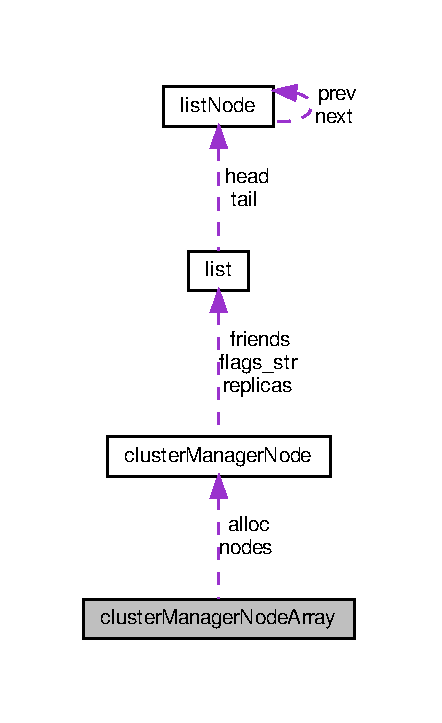
\includegraphics[width=212pt]{structcluster_manager_node_array__coll__graph}
\end{center}
\end{figure}
\subsection*{Data Fields}
\begin{DoxyCompactItemize}
\item 
\hyperlink{structcluster_manager_node}{cluster\+Manager\+Node} $\ast$$\ast$ \hyperlink{structcluster_manager_node_array_ac096916b9ab293648d96462d59ae6d7d}{nodes}
\item 
\hyperlink{structcluster_manager_node}{cluster\+Manager\+Node} $\ast$$\ast$ \hyperlink{structcluster_manager_node_array_ab2efecb0fc6faf2a39de0b80b9028483}{alloc}
\item 
int \hyperlink{structcluster_manager_node_array_afed088663f8704004425cdae2120b9b3}{len}
\item 
int \hyperlink{structcluster_manager_node_array_ad43c3812e6d13e0518d9f8b8f463ffcf}{count}
\end{DoxyCompactItemize}


\subsection{Detailed Description}


Definition at line 1897 of file redis-\/cli.\+c.



\subsection{Field Documentation}
\mbox{\Hypertarget{structcluster_manager_node_array_ab2efecb0fc6faf2a39de0b80b9028483}\label{structcluster_manager_node_array_ab2efecb0fc6faf2a39de0b80b9028483}} 
\index{cluster\+Manager\+Node\+Array@{cluster\+Manager\+Node\+Array}!alloc@{alloc}}
\index{alloc@{alloc}!cluster\+Manager\+Node\+Array@{cluster\+Manager\+Node\+Array}}
\subsubsection{\texorpdfstring{alloc}{alloc}}
{\footnotesize\ttfamily \hyperlink{structcluster_manager_node}{cluster\+Manager\+Node}$\ast$$\ast$ alloc}



Definition at line 1899 of file redis-\/cli.\+c.

\mbox{\Hypertarget{structcluster_manager_node_array_ad43c3812e6d13e0518d9f8b8f463ffcf}\label{structcluster_manager_node_array_ad43c3812e6d13e0518d9f8b8f463ffcf}} 
\index{cluster\+Manager\+Node\+Array@{cluster\+Manager\+Node\+Array}!count@{count}}
\index{count@{count}!cluster\+Manager\+Node\+Array@{cluster\+Manager\+Node\+Array}}
\subsubsection{\texorpdfstring{count}{count}}
{\footnotesize\ttfamily int count}



Definition at line 1901 of file redis-\/cli.\+c.

\mbox{\Hypertarget{structcluster_manager_node_array_afed088663f8704004425cdae2120b9b3}\label{structcluster_manager_node_array_afed088663f8704004425cdae2120b9b3}} 
\index{cluster\+Manager\+Node\+Array@{cluster\+Manager\+Node\+Array}!len@{len}}
\index{len@{len}!cluster\+Manager\+Node\+Array@{cluster\+Manager\+Node\+Array}}
\subsubsection{\texorpdfstring{len}{len}}
{\footnotesize\ttfamily int len}



Definition at line 1900 of file redis-\/cli.\+c.

\mbox{\Hypertarget{structcluster_manager_node_array_ac096916b9ab293648d96462d59ae6d7d}\label{structcluster_manager_node_array_ac096916b9ab293648d96462d59ae6d7d}} 
\index{cluster\+Manager\+Node\+Array@{cluster\+Manager\+Node\+Array}!nodes@{nodes}}
\index{nodes@{nodes}!cluster\+Manager\+Node\+Array@{cluster\+Manager\+Node\+Array}}
\subsubsection{\texorpdfstring{nodes}{nodes}}
{\footnotesize\ttfamily \hyperlink{structcluster_manager_node}{cluster\+Manager\+Node}$\ast$$\ast$ nodes}



Definition at line 1898 of file redis-\/cli.\+c.



The documentation for this struct was generated from the following file\+:\begin{DoxyCompactItemize}
\item 
src/\hyperlink{redis-cli_8c}{redis-\/cli.\+c}\end{DoxyCompactItemize}

\hypertarget{structcluster_manager_reshard_table_item}{}\section{cluster\+Manager\+Reshard\+Table\+Item Struct Reference}
\label{structcluster_manager_reshard_table_item}\index{cluster\+Manager\+Reshard\+Table\+Item@{cluster\+Manager\+Reshard\+Table\+Item}}


Collaboration diagram for cluster\+Manager\+Reshard\+Table\+Item\+:
\nopagebreak
\begin{figure}[H]
\begin{center}
\leavevmode
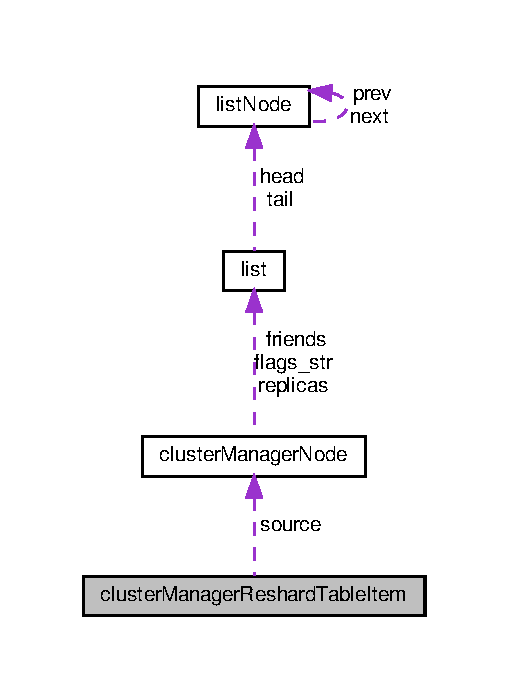
\includegraphics[width=244pt]{structcluster_manager_reshard_table_item__coll__graph}
\end{center}
\end{figure}
\subsection*{Data Fields}
\begin{DoxyCompactItemize}
\item 
\hyperlink{structcluster_manager_node}{cluster\+Manager\+Node} $\ast$ \hyperlink{structcluster_manager_reshard_table_item_a081134bbad31a2e5f1ab9796878c9046}{source}
\item 
int \hyperlink{structcluster_manager_reshard_table_item_a83d6e2127b4cc5e01f2012608487d31a}{slot}
\end{DoxyCompactItemize}


\subsection{Detailed Description}


Definition at line 1905 of file redis-\/cli.\+c.



\subsection{Field Documentation}
\mbox{\Hypertarget{structcluster_manager_reshard_table_item_a83d6e2127b4cc5e01f2012608487d31a}\label{structcluster_manager_reshard_table_item_a83d6e2127b4cc5e01f2012608487d31a}} 
\index{cluster\+Manager\+Reshard\+Table\+Item@{cluster\+Manager\+Reshard\+Table\+Item}!slot@{slot}}
\index{slot@{slot}!cluster\+Manager\+Reshard\+Table\+Item@{cluster\+Manager\+Reshard\+Table\+Item}}
\subsubsection{\texorpdfstring{slot}{slot}}
{\footnotesize\ttfamily int slot}



Definition at line 1907 of file redis-\/cli.\+c.

\mbox{\Hypertarget{structcluster_manager_reshard_table_item_a081134bbad31a2e5f1ab9796878c9046}\label{structcluster_manager_reshard_table_item_a081134bbad31a2e5f1ab9796878c9046}} 
\index{cluster\+Manager\+Reshard\+Table\+Item@{cluster\+Manager\+Reshard\+Table\+Item}!source@{source}}
\index{source@{source}!cluster\+Manager\+Reshard\+Table\+Item@{cluster\+Manager\+Reshard\+Table\+Item}}
\subsubsection{\texorpdfstring{source}{source}}
{\footnotesize\ttfamily \hyperlink{structcluster_manager_node}{cluster\+Manager\+Node}$\ast$ source}



Definition at line 1906 of file redis-\/cli.\+c.



The documentation for this struct was generated from the following file\+:\begin{DoxyCompactItemize}
\item 
src/\hyperlink{redis-cli_8c}{redis-\/cli.\+c}\end{DoxyCompactItemize}

\hypertarget{structcluster_msg}{}\section{cluster\+Msg Struct Reference}
\label{structcluster_msg}\index{cluster\+Msg@{cluster\+Msg}}


{\ttfamily \#include $<$cluster.\+h$>$}



Collaboration diagram for cluster\+Msg\+:
\nopagebreak
\begin{figure}[H]
\begin{center}
\leavevmode
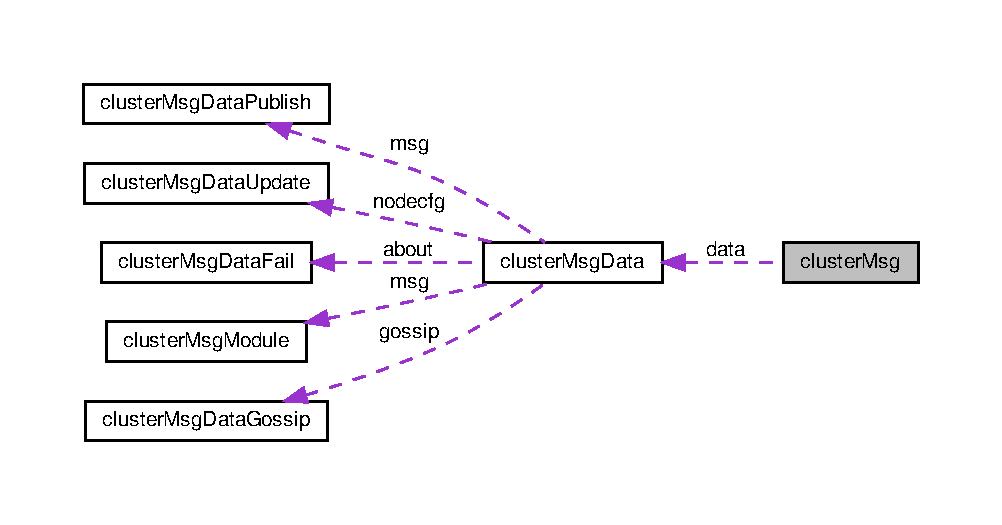
\includegraphics[width=350pt]{structcluster_msg__coll__graph}
\end{center}
\end{figure}
\subsection*{Data Fields}
\begin{DoxyCompactItemize}
\item 
char \hyperlink{structcluster_msg_a44ca5d775a516861cbad4ea8f7ae5364}{sig} \mbox{[}4\mbox{]}
\item 
uint32\+\_\+t \hyperlink{structcluster_msg_a7c3d75c00327eb7e03f283418392443e}{totlen}
\item 
uint16\+\_\+t \hyperlink{structcluster_msg_aa10697fa6dc414fbc83710764c48899b}{ver}
\item 
uint16\+\_\+t \hyperlink{structcluster_msg_a8e0798404bf2cf5dabb84c5ba9a4f236}{port}
\item 
uint16\+\_\+t \hyperlink{structcluster_msg_acb5cfd209ba75c853d03f701e7f91679}{type}
\item 
uint16\+\_\+t \hyperlink{structcluster_msg_af6a39bfc7e1dc3b6f9c997c1c43fa996}{count}
\item 
uint64\+\_\+t \hyperlink{structcluster_msg_a97f41589e815c407f015841f5a3d816f}{current\+Epoch}
\item 
uint64\+\_\+t \hyperlink{structcluster_msg_a6bf0844859acadf5df37a7d49595680e}{config\+Epoch}
\item 
uint64\+\_\+t \hyperlink{structcluster_msg_a612bb2807d848cca89ea1437cceea886}{offset}
\item 
char \hyperlink{structcluster_msg_a81cb807c080c326e68e1ff07d2eaccce}{sender} \mbox{[}\hyperlink{cluster_8h_ace7a882972eff7149675252938643b6e}{C\+L\+U\+S\+T\+E\+R\+\_\+\+N\+A\+M\+E\+L\+EN}\mbox{]}
\item 
unsigned char \hyperlink{structcluster_msg_a5208677bb0ea19be90a6a6a5b742b7bf}{myslots} \mbox{[}\hyperlink{cluster_8h_aa3e2cb951eebb16725ecc3f5beefd9fd}{C\+L\+U\+S\+T\+E\+R\+\_\+\+S\+L\+O\+TS}/8\mbox{]}
\item 
char \hyperlink{structcluster_msg_a110072ca1cda63a0b08d06c3195056e2}{slaveof} \mbox{[}\hyperlink{cluster_8h_ace7a882972eff7149675252938643b6e}{C\+L\+U\+S\+T\+E\+R\+\_\+\+N\+A\+M\+E\+L\+EN}\mbox{]}
\item 
char \hyperlink{structcluster_msg_adc202e2ef9102baf45fe88d6adfbdb9d}{myip} \mbox{[}\hyperlink{server_8h_ad97c5405ed22a94e9fcc10fba577d6c0}{N\+E\+T\+\_\+\+I\+P\+\_\+\+S\+T\+R\+\_\+\+L\+EN}\mbox{]}
\item 
char \hyperlink{structcluster_msg_a1755ac7161beb0d2bf27b9dacb7e3888}{notused1} \mbox{[}34\mbox{]}
\item 
uint16\+\_\+t \hyperlink{structcluster_msg_a6adf88a477cb0a9a34317bf4adbca458}{cport}
\item 
uint16\+\_\+t \hyperlink{structcluster_msg_a1e87af3c18a2fd36c61faf89949bdc3f}{flags}
\item 
unsigned char \hyperlink{structcluster_msg_ab12828525693568ae9c217805bea1ef9}{state}
\item 
unsigned char \hyperlink{structcluster_msg_a4b3606717108e723301f368f58e8ac55}{mflags} \mbox{[}3\mbox{]}
\item 
union \hyperlink{unioncluster_msg_data}{cluster\+Msg\+Data} \hyperlink{structcluster_msg_a1baf00312c0917b903606364f0a51211}{data}
\end{DoxyCompactItemize}


\subsection{Detailed Description}


Definition at line 252 of file cluster.\+h.



\subsection{Field Documentation}
\mbox{\Hypertarget{structcluster_msg_a6bf0844859acadf5df37a7d49595680e}\label{structcluster_msg_a6bf0844859acadf5df37a7d49595680e}} 
\index{cluster\+Msg@{cluster\+Msg}!config\+Epoch@{config\+Epoch}}
\index{config\+Epoch@{config\+Epoch}!cluster\+Msg@{cluster\+Msg}}
\subsubsection{\texorpdfstring{config\+Epoch}{configEpoch}}
{\footnotesize\ttfamily uint64\+\_\+t config\+Epoch}



Definition at line 260 of file cluster.\+h.

\mbox{\Hypertarget{structcluster_msg_af6a39bfc7e1dc3b6f9c997c1c43fa996}\label{structcluster_msg_af6a39bfc7e1dc3b6f9c997c1c43fa996}} 
\index{cluster\+Msg@{cluster\+Msg}!count@{count}}
\index{count@{count}!cluster\+Msg@{cluster\+Msg}}
\subsubsection{\texorpdfstring{count}{count}}
{\footnotesize\ttfamily uint16\+\_\+t count}



Definition at line 258 of file cluster.\+h.

\mbox{\Hypertarget{structcluster_msg_a6adf88a477cb0a9a34317bf4adbca458}\label{structcluster_msg_a6adf88a477cb0a9a34317bf4adbca458}} 
\index{cluster\+Msg@{cluster\+Msg}!cport@{cport}}
\index{cport@{cport}!cluster\+Msg@{cluster\+Msg}}
\subsubsection{\texorpdfstring{cport}{cport}}
{\footnotesize\ttfamily uint16\+\_\+t cport}



Definition at line 270 of file cluster.\+h.

\mbox{\Hypertarget{structcluster_msg_a97f41589e815c407f015841f5a3d816f}\label{structcluster_msg_a97f41589e815c407f015841f5a3d816f}} 
\index{cluster\+Msg@{cluster\+Msg}!current\+Epoch@{current\+Epoch}}
\index{current\+Epoch@{current\+Epoch}!cluster\+Msg@{cluster\+Msg}}
\subsubsection{\texorpdfstring{current\+Epoch}{currentEpoch}}
{\footnotesize\ttfamily uint64\+\_\+t current\+Epoch}



Definition at line 259 of file cluster.\+h.

\mbox{\Hypertarget{structcluster_msg_a1baf00312c0917b903606364f0a51211}\label{structcluster_msg_a1baf00312c0917b903606364f0a51211}} 
\index{cluster\+Msg@{cluster\+Msg}!data@{data}}
\index{data@{data}!cluster\+Msg@{cluster\+Msg}}
\subsubsection{\texorpdfstring{data}{data}}
{\footnotesize\ttfamily union \hyperlink{unioncluster_msg_data}{cluster\+Msg\+Data} data}



Definition at line 274 of file cluster.\+h.

\mbox{\Hypertarget{structcluster_msg_a1e87af3c18a2fd36c61faf89949bdc3f}\label{structcluster_msg_a1e87af3c18a2fd36c61faf89949bdc3f}} 
\index{cluster\+Msg@{cluster\+Msg}!flags@{flags}}
\index{flags@{flags}!cluster\+Msg@{cluster\+Msg}}
\subsubsection{\texorpdfstring{flags}{flags}}
{\footnotesize\ttfamily uint16\+\_\+t flags}



Definition at line 271 of file cluster.\+h.

\mbox{\Hypertarget{structcluster_msg_a4b3606717108e723301f368f58e8ac55}\label{structcluster_msg_a4b3606717108e723301f368f58e8ac55}} 
\index{cluster\+Msg@{cluster\+Msg}!mflags@{mflags}}
\index{mflags@{mflags}!cluster\+Msg@{cluster\+Msg}}
\subsubsection{\texorpdfstring{mflags}{mflags}}
{\footnotesize\ttfamily unsigned char mflags\mbox{[}3\mbox{]}}



Definition at line 273 of file cluster.\+h.

\mbox{\Hypertarget{structcluster_msg_adc202e2ef9102baf45fe88d6adfbdb9d}\label{structcluster_msg_adc202e2ef9102baf45fe88d6adfbdb9d}} 
\index{cluster\+Msg@{cluster\+Msg}!myip@{myip}}
\index{myip@{myip}!cluster\+Msg@{cluster\+Msg}}
\subsubsection{\texorpdfstring{myip}{myip}}
{\footnotesize\ttfamily char myip\mbox{[}\hyperlink{server_8h_ad97c5405ed22a94e9fcc10fba577d6c0}{N\+E\+T\+\_\+\+I\+P\+\_\+\+S\+T\+R\+\_\+\+L\+EN}\mbox{]}}



Definition at line 268 of file cluster.\+h.

\mbox{\Hypertarget{structcluster_msg_a5208677bb0ea19be90a6a6a5b742b7bf}\label{structcluster_msg_a5208677bb0ea19be90a6a6a5b742b7bf}} 
\index{cluster\+Msg@{cluster\+Msg}!myslots@{myslots}}
\index{myslots@{myslots}!cluster\+Msg@{cluster\+Msg}}
\subsubsection{\texorpdfstring{myslots}{myslots}}
{\footnotesize\ttfamily unsigned char myslots\mbox{[}\hyperlink{cluster_8h_aa3e2cb951eebb16725ecc3f5beefd9fd}{C\+L\+U\+S\+T\+E\+R\+\_\+\+S\+L\+O\+TS}/8\mbox{]}}



Definition at line 266 of file cluster.\+h.

\mbox{\Hypertarget{structcluster_msg_a1755ac7161beb0d2bf27b9dacb7e3888}\label{structcluster_msg_a1755ac7161beb0d2bf27b9dacb7e3888}} 
\index{cluster\+Msg@{cluster\+Msg}!notused1@{notused1}}
\index{notused1@{notused1}!cluster\+Msg@{cluster\+Msg}}
\subsubsection{\texorpdfstring{notused1}{notused1}}
{\footnotesize\ttfamily char notused1\mbox{[}34\mbox{]}}



Definition at line 269 of file cluster.\+h.

\mbox{\Hypertarget{structcluster_msg_a612bb2807d848cca89ea1437cceea886}\label{structcluster_msg_a612bb2807d848cca89ea1437cceea886}} 
\index{cluster\+Msg@{cluster\+Msg}!offset@{offset}}
\index{offset@{offset}!cluster\+Msg@{cluster\+Msg}}
\subsubsection{\texorpdfstring{offset}{offset}}
{\footnotesize\ttfamily uint64\+\_\+t offset}



Definition at line 263 of file cluster.\+h.

\mbox{\Hypertarget{structcluster_msg_a8e0798404bf2cf5dabb84c5ba9a4f236}\label{structcluster_msg_a8e0798404bf2cf5dabb84c5ba9a4f236}} 
\index{cluster\+Msg@{cluster\+Msg}!port@{port}}
\index{port@{port}!cluster\+Msg@{cluster\+Msg}}
\subsubsection{\texorpdfstring{port}{port}}
{\footnotesize\ttfamily uint16\+\_\+t port}



Definition at line 256 of file cluster.\+h.

\mbox{\Hypertarget{structcluster_msg_a81cb807c080c326e68e1ff07d2eaccce}\label{structcluster_msg_a81cb807c080c326e68e1ff07d2eaccce}} 
\index{cluster\+Msg@{cluster\+Msg}!sender@{sender}}
\index{sender@{sender}!cluster\+Msg@{cluster\+Msg}}
\subsubsection{\texorpdfstring{sender}{sender}}
{\footnotesize\ttfamily char sender\mbox{[}\hyperlink{cluster_8h_ace7a882972eff7149675252938643b6e}{C\+L\+U\+S\+T\+E\+R\+\_\+\+N\+A\+M\+E\+L\+EN}\mbox{]}}



Definition at line 265 of file cluster.\+h.

\mbox{\Hypertarget{structcluster_msg_a44ca5d775a516861cbad4ea8f7ae5364}\label{structcluster_msg_a44ca5d775a516861cbad4ea8f7ae5364}} 
\index{cluster\+Msg@{cluster\+Msg}!sig@{sig}}
\index{sig@{sig}!cluster\+Msg@{cluster\+Msg}}
\subsubsection{\texorpdfstring{sig}{sig}}
{\footnotesize\ttfamily char sig\mbox{[}4\mbox{]}}



Definition at line 253 of file cluster.\+h.

\mbox{\Hypertarget{structcluster_msg_a110072ca1cda63a0b08d06c3195056e2}\label{structcluster_msg_a110072ca1cda63a0b08d06c3195056e2}} 
\index{cluster\+Msg@{cluster\+Msg}!slaveof@{slaveof}}
\index{slaveof@{slaveof}!cluster\+Msg@{cluster\+Msg}}
\subsubsection{\texorpdfstring{slaveof}{slaveof}}
{\footnotesize\ttfamily char slaveof\mbox{[}\hyperlink{cluster_8h_ace7a882972eff7149675252938643b6e}{C\+L\+U\+S\+T\+E\+R\+\_\+\+N\+A\+M\+E\+L\+EN}\mbox{]}}



Definition at line 267 of file cluster.\+h.

\mbox{\Hypertarget{structcluster_msg_ab12828525693568ae9c217805bea1ef9}\label{structcluster_msg_ab12828525693568ae9c217805bea1ef9}} 
\index{cluster\+Msg@{cluster\+Msg}!state@{state}}
\index{state@{state}!cluster\+Msg@{cluster\+Msg}}
\subsubsection{\texorpdfstring{state}{state}}
{\footnotesize\ttfamily unsigned char state}



Definition at line 272 of file cluster.\+h.

\mbox{\Hypertarget{structcluster_msg_a7c3d75c00327eb7e03f283418392443e}\label{structcluster_msg_a7c3d75c00327eb7e03f283418392443e}} 
\index{cluster\+Msg@{cluster\+Msg}!totlen@{totlen}}
\index{totlen@{totlen}!cluster\+Msg@{cluster\+Msg}}
\subsubsection{\texorpdfstring{totlen}{totlen}}
{\footnotesize\ttfamily uint32\+\_\+t totlen}



Definition at line 254 of file cluster.\+h.

\mbox{\Hypertarget{structcluster_msg_acb5cfd209ba75c853d03f701e7f91679}\label{structcluster_msg_acb5cfd209ba75c853d03f701e7f91679}} 
\index{cluster\+Msg@{cluster\+Msg}!type@{type}}
\index{type@{type}!cluster\+Msg@{cluster\+Msg}}
\subsubsection{\texorpdfstring{type}{type}}
{\footnotesize\ttfamily uint16\+\_\+t type}



Definition at line 257 of file cluster.\+h.

\mbox{\Hypertarget{structcluster_msg_aa10697fa6dc414fbc83710764c48899b}\label{structcluster_msg_aa10697fa6dc414fbc83710764c48899b}} 
\index{cluster\+Msg@{cluster\+Msg}!ver@{ver}}
\index{ver@{ver}!cluster\+Msg@{cluster\+Msg}}
\subsubsection{\texorpdfstring{ver}{ver}}
{\footnotesize\ttfamily uint16\+\_\+t ver}



Definition at line 255 of file cluster.\+h.



The documentation for this struct was generated from the following file\+:\begin{DoxyCompactItemize}
\item 
src/\hyperlink{cluster_8h}{cluster.\+h}\end{DoxyCompactItemize}

\hypertarget{unioncluster_msg_data}{}\section{cluster\+Msg\+Data Union Reference}
\label{unioncluster_msg_data}\index{cluster\+Msg\+Data@{cluster\+Msg\+Data}}


{\ttfamily \#include $<$cluster.\+h$>$}



Collaboration diagram for cluster\+Msg\+Data\+:
\nopagebreak
\begin{figure}[H]
\begin{center}
\leavevmode
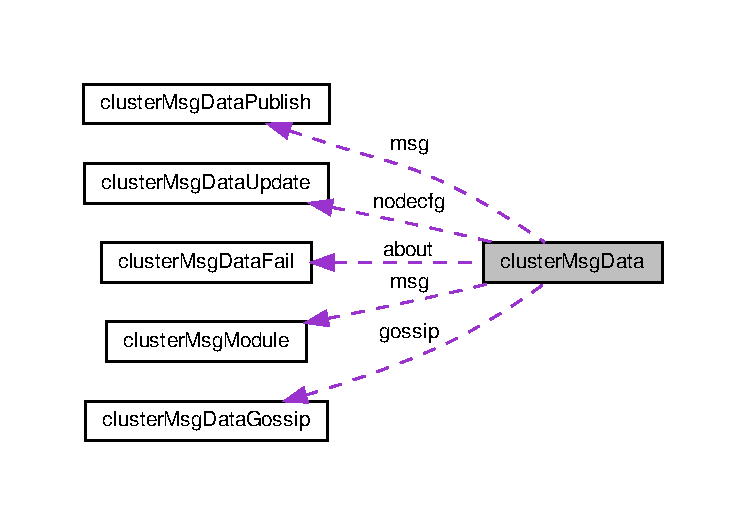
\includegraphics[width=350pt]{unioncluster_msg_data__coll__graph}
\end{center}
\end{figure}
\subsection*{Data Fields}
\begin{DoxyCompactItemize}
\item 
\begin{tabbing}
xx\=xx\=xx\=xx\=xx\=xx\=xx\=xx\=xx\=\kill
struct \{\\
\>\hyperlink{structcluster_msg_data_gossip}{clusterMsgDataGossip} \hyperlink{unioncluster_msg_data_a947036ec4730e07dd6bf6afcfd2943c4}{gossip} \mbox{[}1\mbox{]}\\
\} \hyperlink{unioncluster_msg_data_a9218ae70b8b801475bc8efe6247e3d7d}{ping}\\

\end{tabbing}\item 
\begin{tabbing}
xx\=xx\=xx\=xx\=xx\=xx\=xx\=xx\=xx\=\kill
struct \{\\
\>\hyperlink{structcluster_msg_data_fail}{clusterMsgDataFail} \hyperlink{unioncluster_msg_data_afcb3336ec3ec8c832bbd6616470f0536}{about}\\
\} \hyperlink{unioncluster_msg_data_ac6c2ee2b22c450e5ebc8461ff9b84dc1}{fail}\\

\end{tabbing}\item 
\begin{tabbing}
xx\=xx\=xx\=xx\=xx\=xx\=xx\=xx\=xx\=\kill
struct \{\\
\>\hyperlink{structcluster_msg_data_publish}{clusterMsgDataPublish} \hyperlink{unioncluster_msg_data_a4ff6a38329834bbe52476e58df71c3cd}{msg}\\
\} \hyperlink{unioncluster_msg_data_ac925b89ae9d9f7cc76c0c4d46eb35895}{publish}\\

\end{tabbing}\item 
\begin{tabbing}
xx\=xx\=xx\=xx\=xx\=xx\=xx\=xx\=xx\=\kill
struct \{\\
\>\hyperlink{structcluster_msg_data_update}{clusterMsgDataUpdate} \hyperlink{unioncluster_msg_data_a81e4031f10e290b02287e403ba31cfd9}{nodecfg}\\
\} \hyperlink{unioncluster_msg_data_a79d24828f041b8b0c2e982d3c019aaae}{update}\\

\end{tabbing}\item 
\begin{tabbing}
xx\=xx\=xx\=xx\=xx\=xx\=xx\=xx\=xx\=\kill
struct \{\\
\>\hyperlink{structcluster_msg_module}{clusterMsgModule} \hyperlink{unioncluster_msg_data_a6056b448b63ab91763d8efa704fc4079}{msg}\\
\} \hyperlink{unioncluster_msg_data_a2d0edf790842883d01f0f0857dd880c0}{module}\\

\end{tabbing}\end{DoxyCompactItemize}


\subsection{Detailed Description}


Definition at line 222 of file cluster.\+h.



\subsection{Field Documentation}
\mbox{\Hypertarget{unioncluster_msg_data_afcb3336ec3ec8c832bbd6616470f0536}\label{unioncluster_msg_data_afcb3336ec3ec8c832bbd6616470f0536}} 
\index{cluster\+Msg\+Data@{cluster\+Msg\+Data}!about@{about}}
\index{about@{about}!cluster\+Msg\+Data@{cluster\+Msg\+Data}}
\subsubsection{\texorpdfstring{about}{about}}
{\footnotesize\ttfamily \hyperlink{structcluster_msg_data_fail}{cluster\+Msg\+Data\+Fail} about}



Definition at line 231 of file cluster.\+h.

\mbox{\Hypertarget{unioncluster_msg_data_ac6c2ee2b22c450e5ebc8461ff9b84dc1}\label{unioncluster_msg_data_ac6c2ee2b22c450e5ebc8461ff9b84dc1}} 
\index{cluster\+Msg\+Data@{cluster\+Msg\+Data}!fail@{fail}}
\index{fail@{fail}!cluster\+Msg\+Data@{cluster\+Msg\+Data}}
\subsubsection{\texorpdfstring{fail}{fail}}
{\footnotesize\ttfamily struct \{ ... \}   fail}

\mbox{\Hypertarget{unioncluster_msg_data_a947036ec4730e07dd6bf6afcfd2943c4}\label{unioncluster_msg_data_a947036ec4730e07dd6bf6afcfd2943c4}} 
\index{cluster\+Msg\+Data@{cluster\+Msg\+Data}!gossip@{gossip}}
\index{gossip@{gossip}!cluster\+Msg\+Data@{cluster\+Msg\+Data}}
\subsubsection{\texorpdfstring{gossip}{gossip}}
{\footnotesize\ttfamily \hyperlink{structcluster_msg_data_gossip}{cluster\+Msg\+Data\+Gossip} gossip\mbox{[}1\mbox{]}}



Definition at line 226 of file cluster.\+h.

\mbox{\Hypertarget{unioncluster_msg_data_a2d0edf790842883d01f0f0857dd880c0}\label{unioncluster_msg_data_a2d0edf790842883d01f0f0857dd880c0}} 
\index{cluster\+Msg\+Data@{cluster\+Msg\+Data}!module@{module}}
\index{module@{module}!cluster\+Msg\+Data@{cluster\+Msg\+Data}}
\subsubsection{\texorpdfstring{module}{module}}
{\footnotesize\ttfamily struct \{ ... \}   module}

\mbox{\Hypertarget{unioncluster_msg_data_a4ff6a38329834bbe52476e58df71c3cd}\label{unioncluster_msg_data_a4ff6a38329834bbe52476e58df71c3cd}} 
\index{cluster\+Msg\+Data@{cluster\+Msg\+Data}!msg@{msg}}
\index{msg@{msg}!cluster\+Msg\+Data@{cluster\+Msg\+Data}}
\subsubsection{\texorpdfstring{msg}{msg}\hspace{0.1cm}{\footnotesize\ttfamily [1/2]}}
{\footnotesize\ttfamily \hyperlink{structcluster_msg_data_publish}{cluster\+Msg\+Data\+Publish} msg}



Definition at line 236 of file cluster.\+h.

\mbox{\Hypertarget{unioncluster_msg_data_a6056b448b63ab91763d8efa704fc4079}\label{unioncluster_msg_data_a6056b448b63ab91763d8efa704fc4079}} 
\index{cluster\+Msg\+Data@{cluster\+Msg\+Data}!msg@{msg}}
\index{msg@{msg}!cluster\+Msg\+Data@{cluster\+Msg\+Data}}
\subsubsection{\texorpdfstring{msg}{msg}\hspace{0.1cm}{\footnotesize\ttfamily [2/2]}}
{\footnotesize\ttfamily \hyperlink{structcluster_msg_module}{cluster\+Msg\+Module} msg}



Definition at line 246 of file cluster.\+h.

\mbox{\Hypertarget{unioncluster_msg_data_a81e4031f10e290b02287e403ba31cfd9}\label{unioncluster_msg_data_a81e4031f10e290b02287e403ba31cfd9}} 
\index{cluster\+Msg\+Data@{cluster\+Msg\+Data}!nodecfg@{nodecfg}}
\index{nodecfg@{nodecfg}!cluster\+Msg\+Data@{cluster\+Msg\+Data}}
\subsubsection{\texorpdfstring{nodecfg}{nodecfg}}
{\footnotesize\ttfamily \hyperlink{structcluster_msg_data_update}{cluster\+Msg\+Data\+Update} nodecfg}



Definition at line 241 of file cluster.\+h.

\mbox{\Hypertarget{unioncluster_msg_data_a9218ae70b8b801475bc8efe6247e3d7d}\label{unioncluster_msg_data_a9218ae70b8b801475bc8efe6247e3d7d}} 
\index{cluster\+Msg\+Data@{cluster\+Msg\+Data}!ping@{ping}}
\index{ping@{ping}!cluster\+Msg\+Data@{cluster\+Msg\+Data}}
\subsubsection{\texorpdfstring{ping}{ping}}
{\footnotesize\ttfamily struct \{ ... \}   ping}

\mbox{\Hypertarget{unioncluster_msg_data_ac925b89ae9d9f7cc76c0c4d46eb35895}\label{unioncluster_msg_data_ac925b89ae9d9f7cc76c0c4d46eb35895}} 
\index{cluster\+Msg\+Data@{cluster\+Msg\+Data}!publish@{publish}}
\index{publish@{publish}!cluster\+Msg\+Data@{cluster\+Msg\+Data}}
\subsubsection{\texorpdfstring{publish}{publish}}
{\footnotesize\ttfamily struct \{ ... \}   publish}

\mbox{\Hypertarget{unioncluster_msg_data_a79d24828f041b8b0c2e982d3c019aaae}\label{unioncluster_msg_data_a79d24828f041b8b0c2e982d3c019aaae}} 
\index{cluster\+Msg\+Data@{cluster\+Msg\+Data}!update@{update}}
\index{update@{update}!cluster\+Msg\+Data@{cluster\+Msg\+Data}}
\subsubsection{\texorpdfstring{update}{update}}
{\footnotesize\ttfamily struct \{ ... \}   update}



The documentation for this union was generated from the following file\+:\begin{DoxyCompactItemize}
\item 
src/\hyperlink{cluster_8h}{cluster.\+h}\end{DoxyCompactItemize}

\hypertarget{structcluster_msg_data_fail}{}\section{cluster\+Msg\+Data\+Fail Struct Reference}
\label{structcluster_msg_data_fail}\index{cluster\+Msg\+Data\+Fail@{cluster\+Msg\+Data\+Fail}}


{\ttfamily \#include $<$cluster.\+h$>$}

\subsection*{Data Fields}
\begin{DoxyCompactItemize}
\item 
char \hyperlink{structcluster_msg_data_fail_a50eb514a773ea3e78ec45e62fc0d7b9f}{nodename} \mbox{[}\hyperlink{cluster_8h_ace7a882972eff7149675252938643b6e}{C\+L\+U\+S\+T\+E\+R\+\_\+\+N\+A\+M\+E\+L\+EN}\mbox{]}
\end{DoxyCompactItemize}


\subsection{Detailed Description}


Definition at line 199 of file cluster.\+h.



\subsection{Field Documentation}
\mbox{\Hypertarget{structcluster_msg_data_fail_a50eb514a773ea3e78ec45e62fc0d7b9f}\label{structcluster_msg_data_fail_a50eb514a773ea3e78ec45e62fc0d7b9f}} 
\index{cluster\+Msg\+Data\+Fail@{cluster\+Msg\+Data\+Fail}!nodename@{nodename}}
\index{nodename@{nodename}!cluster\+Msg\+Data\+Fail@{cluster\+Msg\+Data\+Fail}}
\subsubsection{\texorpdfstring{nodename}{nodename}}
{\footnotesize\ttfamily char nodename\mbox{[}\hyperlink{cluster_8h_ace7a882972eff7149675252938643b6e}{C\+L\+U\+S\+T\+E\+R\+\_\+\+N\+A\+M\+E\+L\+EN}\mbox{]}}



Definition at line 200 of file cluster.\+h.



The documentation for this struct was generated from the following file\+:\begin{DoxyCompactItemize}
\item 
src/\hyperlink{cluster_8h}{cluster.\+h}\end{DoxyCompactItemize}

\hypertarget{structcluster_msg_data_gossip}{}\section{cluster\+Msg\+Data\+Gossip Struct Reference}
\label{structcluster_msg_data_gossip}\index{cluster\+Msg\+Data\+Gossip@{cluster\+Msg\+Data\+Gossip}}


{\ttfamily \#include $<$cluster.\+h$>$}

\subsection*{Data Fields}
\begin{DoxyCompactItemize}
\item 
char \hyperlink{structcluster_msg_data_gossip_a50eb514a773ea3e78ec45e62fc0d7b9f}{nodename} \mbox{[}\hyperlink{cluster_8h_ace7a882972eff7149675252938643b6e}{C\+L\+U\+S\+T\+E\+R\+\_\+\+N\+A\+M\+E\+L\+EN}\mbox{]}
\item 
uint32\+\_\+t \hyperlink{structcluster_msg_data_gossip_aa73ed6ac09f49b50a826160bcf8ffbd4}{ping\+\_\+sent}
\item 
uint32\+\_\+t \hyperlink{structcluster_msg_data_gossip_ad2d900a6dca8942733394fe4077d4dd2}{pong\+\_\+received}
\item 
char \hyperlink{structcluster_msg_data_gossip_a9de2afd4e77c16f677244d244270b605}{ip} \mbox{[}\hyperlink{server_8h_ad97c5405ed22a94e9fcc10fba577d6c0}{N\+E\+T\+\_\+\+I\+P\+\_\+\+S\+T\+R\+\_\+\+L\+EN}\mbox{]}
\item 
uint16\+\_\+t \hyperlink{structcluster_msg_data_gossip_a8e0798404bf2cf5dabb84c5ba9a4f236}{port}
\item 
uint16\+\_\+t \hyperlink{structcluster_msg_data_gossip_a6adf88a477cb0a9a34317bf4adbca458}{cport}
\item 
uint16\+\_\+t \hyperlink{structcluster_msg_data_gossip_a1e87af3c18a2fd36c61faf89949bdc3f}{flags}
\item 
uint32\+\_\+t \hyperlink{structcluster_msg_data_gossip_afae9866d130906b6513bb73cdd1d37f2}{notused1}
\end{DoxyCompactItemize}


\subsection{Detailed Description}


Definition at line 188 of file cluster.\+h.



\subsection{Field Documentation}
\mbox{\Hypertarget{structcluster_msg_data_gossip_a6adf88a477cb0a9a34317bf4adbca458}\label{structcluster_msg_data_gossip_a6adf88a477cb0a9a34317bf4adbca458}} 
\index{cluster\+Msg\+Data\+Gossip@{cluster\+Msg\+Data\+Gossip}!cport@{cport}}
\index{cport@{cport}!cluster\+Msg\+Data\+Gossip@{cluster\+Msg\+Data\+Gossip}}
\subsubsection{\texorpdfstring{cport}{cport}}
{\footnotesize\ttfamily uint16\+\_\+t cport}



Definition at line 194 of file cluster.\+h.

\mbox{\Hypertarget{structcluster_msg_data_gossip_a1e87af3c18a2fd36c61faf89949bdc3f}\label{structcluster_msg_data_gossip_a1e87af3c18a2fd36c61faf89949bdc3f}} 
\index{cluster\+Msg\+Data\+Gossip@{cluster\+Msg\+Data\+Gossip}!flags@{flags}}
\index{flags@{flags}!cluster\+Msg\+Data\+Gossip@{cluster\+Msg\+Data\+Gossip}}
\subsubsection{\texorpdfstring{flags}{flags}}
{\footnotesize\ttfamily uint16\+\_\+t flags}



Definition at line 195 of file cluster.\+h.

\mbox{\Hypertarget{structcluster_msg_data_gossip_a9de2afd4e77c16f677244d244270b605}\label{structcluster_msg_data_gossip_a9de2afd4e77c16f677244d244270b605}} 
\index{cluster\+Msg\+Data\+Gossip@{cluster\+Msg\+Data\+Gossip}!ip@{ip}}
\index{ip@{ip}!cluster\+Msg\+Data\+Gossip@{cluster\+Msg\+Data\+Gossip}}
\subsubsection{\texorpdfstring{ip}{ip}}
{\footnotesize\ttfamily char ip\mbox{[}\hyperlink{server_8h_ad97c5405ed22a94e9fcc10fba577d6c0}{N\+E\+T\+\_\+\+I\+P\+\_\+\+S\+T\+R\+\_\+\+L\+EN}\mbox{]}}



Definition at line 192 of file cluster.\+h.

\mbox{\Hypertarget{structcluster_msg_data_gossip_a50eb514a773ea3e78ec45e62fc0d7b9f}\label{structcluster_msg_data_gossip_a50eb514a773ea3e78ec45e62fc0d7b9f}} 
\index{cluster\+Msg\+Data\+Gossip@{cluster\+Msg\+Data\+Gossip}!nodename@{nodename}}
\index{nodename@{nodename}!cluster\+Msg\+Data\+Gossip@{cluster\+Msg\+Data\+Gossip}}
\subsubsection{\texorpdfstring{nodename}{nodename}}
{\footnotesize\ttfamily char nodename\mbox{[}\hyperlink{cluster_8h_ace7a882972eff7149675252938643b6e}{C\+L\+U\+S\+T\+E\+R\+\_\+\+N\+A\+M\+E\+L\+EN}\mbox{]}}



Definition at line 189 of file cluster.\+h.

\mbox{\Hypertarget{structcluster_msg_data_gossip_afae9866d130906b6513bb73cdd1d37f2}\label{structcluster_msg_data_gossip_afae9866d130906b6513bb73cdd1d37f2}} 
\index{cluster\+Msg\+Data\+Gossip@{cluster\+Msg\+Data\+Gossip}!notused1@{notused1}}
\index{notused1@{notused1}!cluster\+Msg\+Data\+Gossip@{cluster\+Msg\+Data\+Gossip}}
\subsubsection{\texorpdfstring{notused1}{notused1}}
{\footnotesize\ttfamily uint32\+\_\+t notused1}



Definition at line 196 of file cluster.\+h.

\mbox{\Hypertarget{structcluster_msg_data_gossip_aa73ed6ac09f49b50a826160bcf8ffbd4}\label{structcluster_msg_data_gossip_aa73ed6ac09f49b50a826160bcf8ffbd4}} 
\index{cluster\+Msg\+Data\+Gossip@{cluster\+Msg\+Data\+Gossip}!ping\+\_\+sent@{ping\+\_\+sent}}
\index{ping\+\_\+sent@{ping\+\_\+sent}!cluster\+Msg\+Data\+Gossip@{cluster\+Msg\+Data\+Gossip}}
\subsubsection{\texorpdfstring{ping\+\_\+sent}{ping\_sent}}
{\footnotesize\ttfamily uint32\+\_\+t ping\+\_\+sent}



Definition at line 190 of file cluster.\+h.

\mbox{\Hypertarget{structcluster_msg_data_gossip_ad2d900a6dca8942733394fe4077d4dd2}\label{structcluster_msg_data_gossip_ad2d900a6dca8942733394fe4077d4dd2}} 
\index{cluster\+Msg\+Data\+Gossip@{cluster\+Msg\+Data\+Gossip}!pong\+\_\+received@{pong\+\_\+received}}
\index{pong\+\_\+received@{pong\+\_\+received}!cluster\+Msg\+Data\+Gossip@{cluster\+Msg\+Data\+Gossip}}
\subsubsection{\texorpdfstring{pong\+\_\+received}{pong\_received}}
{\footnotesize\ttfamily uint32\+\_\+t pong\+\_\+received}



Definition at line 191 of file cluster.\+h.

\mbox{\Hypertarget{structcluster_msg_data_gossip_a8e0798404bf2cf5dabb84c5ba9a4f236}\label{structcluster_msg_data_gossip_a8e0798404bf2cf5dabb84c5ba9a4f236}} 
\index{cluster\+Msg\+Data\+Gossip@{cluster\+Msg\+Data\+Gossip}!port@{port}}
\index{port@{port}!cluster\+Msg\+Data\+Gossip@{cluster\+Msg\+Data\+Gossip}}
\subsubsection{\texorpdfstring{port}{port}}
{\footnotesize\ttfamily uint16\+\_\+t port}



Definition at line 193 of file cluster.\+h.



The documentation for this struct was generated from the following file\+:\begin{DoxyCompactItemize}
\item 
src/\hyperlink{cluster_8h}{cluster.\+h}\end{DoxyCompactItemize}

\hypertarget{structcluster_msg_data_publish}{}\section{cluster\+Msg\+Data\+Publish Struct Reference}
\label{structcluster_msg_data_publish}\index{cluster\+Msg\+Data\+Publish@{cluster\+Msg\+Data\+Publish}}


{\ttfamily \#include $<$cluster.\+h$>$}

\subsection*{Data Fields}
\begin{DoxyCompactItemize}
\item 
uint32\+\_\+t \hyperlink{structcluster_msg_data_publish_a68bdef8eb0f6ccd540668a828d29492a}{channel\+\_\+len}
\item 
uint32\+\_\+t \hyperlink{structcluster_msg_data_publish_a619a2b4c8e952645f4d7aa4b229fe3d9}{message\+\_\+len}
\item 
unsigned char \hyperlink{structcluster_msg_data_publish_a259bf56ee2c4c8d4450e071720d7d615}{bulk\+\_\+data} \mbox{[}8\mbox{]}
\end{DoxyCompactItemize}


\subsection{Detailed Description}


Definition at line 203 of file cluster.\+h.



\subsection{Field Documentation}
\mbox{\Hypertarget{structcluster_msg_data_publish_a259bf56ee2c4c8d4450e071720d7d615}\label{structcluster_msg_data_publish_a259bf56ee2c4c8d4450e071720d7d615}} 
\index{cluster\+Msg\+Data\+Publish@{cluster\+Msg\+Data\+Publish}!bulk\+\_\+data@{bulk\+\_\+data}}
\index{bulk\+\_\+data@{bulk\+\_\+data}!cluster\+Msg\+Data\+Publish@{cluster\+Msg\+Data\+Publish}}
\subsubsection{\texorpdfstring{bulk\+\_\+data}{bulk\_data}}
{\footnotesize\ttfamily unsigned char bulk\+\_\+data\mbox{[}8\mbox{]}}



Definition at line 206 of file cluster.\+h.

\mbox{\Hypertarget{structcluster_msg_data_publish_a68bdef8eb0f6ccd540668a828d29492a}\label{structcluster_msg_data_publish_a68bdef8eb0f6ccd540668a828d29492a}} 
\index{cluster\+Msg\+Data\+Publish@{cluster\+Msg\+Data\+Publish}!channel\+\_\+len@{channel\+\_\+len}}
\index{channel\+\_\+len@{channel\+\_\+len}!cluster\+Msg\+Data\+Publish@{cluster\+Msg\+Data\+Publish}}
\subsubsection{\texorpdfstring{channel\+\_\+len}{channel\_len}}
{\footnotesize\ttfamily uint32\+\_\+t channel\+\_\+len}



Definition at line 204 of file cluster.\+h.

\mbox{\Hypertarget{structcluster_msg_data_publish_a619a2b4c8e952645f4d7aa4b229fe3d9}\label{structcluster_msg_data_publish_a619a2b4c8e952645f4d7aa4b229fe3d9}} 
\index{cluster\+Msg\+Data\+Publish@{cluster\+Msg\+Data\+Publish}!message\+\_\+len@{message\+\_\+len}}
\index{message\+\_\+len@{message\+\_\+len}!cluster\+Msg\+Data\+Publish@{cluster\+Msg\+Data\+Publish}}
\subsubsection{\texorpdfstring{message\+\_\+len}{message\_len}}
{\footnotesize\ttfamily uint32\+\_\+t message\+\_\+len}



Definition at line 205 of file cluster.\+h.



The documentation for this struct was generated from the following file\+:\begin{DoxyCompactItemize}
\item 
src/\hyperlink{cluster_8h}{cluster.\+h}\end{DoxyCompactItemize}

\hypertarget{structcluster_msg_data_update}{}\section{cluster\+Msg\+Data\+Update Struct Reference}
\label{structcluster_msg_data_update}\index{cluster\+Msg\+Data\+Update@{cluster\+Msg\+Data\+Update}}


{\ttfamily \#include $<$cluster.\+h$>$}

\subsection*{Data Fields}
\begin{DoxyCompactItemize}
\item 
uint64\+\_\+t \hyperlink{structcluster_msg_data_update_a6bf0844859acadf5df37a7d49595680e}{config\+Epoch}
\item 
char \hyperlink{structcluster_msg_data_update_a50eb514a773ea3e78ec45e62fc0d7b9f}{nodename} \mbox{[}\hyperlink{cluster_8h_ace7a882972eff7149675252938643b6e}{C\+L\+U\+S\+T\+E\+R\+\_\+\+N\+A\+M\+E\+L\+EN}\mbox{]}
\item 
unsigned char \hyperlink{structcluster_msg_data_update_a5860192f55932c04b85ec15307ee114b}{slots} \mbox{[}\hyperlink{cluster_8h_aa3e2cb951eebb16725ecc3f5beefd9fd}{C\+L\+U\+S\+T\+E\+R\+\_\+\+S\+L\+O\+TS}/8\mbox{]}
\end{DoxyCompactItemize}


\subsection{Detailed Description}


Definition at line 209 of file cluster.\+h.



\subsection{Field Documentation}
\mbox{\Hypertarget{structcluster_msg_data_update_a6bf0844859acadf5df37a7d49595680e}\label{structcluster_msg_data_update_a6bf0844859acadf5df37a7d49595680e}} 
\index{cluster\+Msg\+Data\+Update@{cluster\+Msg\+Data\+Update}!config\+Epoch@{config\+Epoch}}
\index{config\+Epoch@{config\+Epoch}!cluster\+Msg\+Data\+Update@{cluster\+Msg\+Data\+Update}}
\subsubsection{\texorpdfstring{config\+Epoch}{configEpoch}}
{\footnotesize\ttfamily uint64\+\_\+t config\+Epoch}



Definition at line 210 of file cluster.\+h.

\mbox{\Hypertarget{structcluster_msg_data_update_a50eb514a773ea3e78ec45e62fc0d7b9f}\label{structcluster_msg_data_update_a50eb514a773ea3e78ec45e62fc0d7b9f}} 
\index{cluster\+Msg\+Data\+Update@{cluster\+Msg\+Data\+Update}!nodename@{nodename}}
\index{nodename@{nodename}!cluster\+Msg\+Data\+Update@{cluster\+Msg\+Data\+Update}}
\subsubsection{\texorpdfstring{nodename}{nodename}}
{\footnotesize\ttfamily char nodename\mbox{[}\hyperlink{cluster_8h_ace7a882972eff7149675252938643b6e}{C\+L\+U\+S\+T\+E\+R\+\_\+\+N\+A\+M\+E\+L\+EN}\mbox{]}}



Definition at line 211 of file cluster.\+h.

\mbox{\Hypertarget{structcluster_msg_data_update_a5860192f55932c04b85ec15307ee114b}\label{structcluster_msg_data_update_a5860192f55932c04b85ec15307ee114b}} 
\index{cluster\+Msg\+Data\+Update@{cluster\+Msg\+Data\+Update}!slots@{slots}}
\index{slots@{slots}!cluster\+Msg\+Data\+Update@{cluster\+Msg\+Data\+Update}}
\subsubsection{\texorpdfstring{slots}{slots}}
{\footnotesize\ttfamily unsigned char slots\mbox{[}\hyperlink{cluster_8h_aa3e2cb951eebb16725ecc3f5beefd9fd}{C\+L\+U\+S\+T\+E\+R\+\_\+\+S\+L\+O\+TS}/8\mbox{]}}



Definition at line 212 of file cluster.\+h.



The documentation for this struct was generated from the following file\+:\begin{DoxyCompactItemize}
\item 
src/\hyperlink{cluster_8h}{cluster.\+h}\end{DoxyCompactItemize}

\hypertarget{structcluster_msg_module}{}\section{cluster\+Msg\+Module Struct Reference}
\label{structcluster_msg_module}\index{cluster\+Msg\+Module@{cluster\+Msg\+Module}}


{\ttfamily \#include $<$cluster.\+h$>$}

\subsection*{Data Fields}
\begin{DoxyCompactItemize}
\item 
uint64\+\_\+t \hyperlink{structcluster_msg_module_a5c568ad76933cdbb1f61b40781917492}{module\+\_\+id}
\item 
uint32\+\_\+t \hyperlink{structcluster_msg_module_a96bbf959016e4411c9e6b9812a8be60a}{len}
\item 
uint8\+\_\+t \hyperlink{structcluster_msg_module_a1d127017fb298b889f4ba24752d08b8e}{type}
\item 
unsigned char \hyperlink{structcluster_msg_module_a2e2032a99c30443d5fe71db1bb696f94}{bulk\+\_\+data} \mbox{[}3\mbox{]}
\end{DoxyCompactItemize}


\subsection{Detailed Description}


Definition at line 215 of file cluster.\+h.



\subsection{Field Documentation}
\mbox{\Hypertarget{structcluster_msg_module_a2e2032a99c30443d5fe71db1bb696f94}\label{structcluster_msg_module_a2e2032a99c30443d5fe71db1bb696f94}} 
\index{cluster\+Msg\+Module@{cluster\+Msg\+Module}!bulk\+\_\+data@{bulk\+\_\+data}}
\index{bulk\+\_\+data@{bulk\+\_\+data}!cluster\+Msg\+Module@{cluster\+Msg\+Module}}
\subsubsection{\texorpdfstring{bulk\+\_\+data}{bulk\_data}}
{\footnotesize\ttfamily unsigned char bulk\+\_\+data\mbox{[}3\mbox{]}}



Definition at line 219 of file cluster.\+h.

\mbox{\Hypertarget{structcluster_msg_module_a96bbf959016e4411c9e6b9812a8be60a}\label{structcluster_msg_module_a96bbf959016e4411c9e6b9812a8be60a}} 
\index{cluster\+Msg\+Module@{cluster\+Msg\+Module}!len@{len}}
\index{len@{len}!cluster\+Msg\+Module@{cluster\+Msg\+Module}}
\subsubsection{\texorpdfstring{len}{len}}
{\footnotesize\ttfamily uint32\+\_\+t len}



Definition at line 217 of file cluster.\+h.

\mbox{\Hypertarget{structcluster_msg_module_a5c568ad76933cdbb1f61b40781917492}\label{structcluster_msg_module_a5c568ad76933cdbb1f61b40781917492}} 
\index{cluster\+Msg\+Module@{cluster\+Msg\+Module}!module\+\_\+id@{module\+\_\+id}}
\index{module\+\_\+id@{module\+\_\+id}!cluster\+Msg\+Module@{cluster\+Msg\+Module}}
\subsubsection{\texorpdfstring{module\+\_\+id}{module\_id}}
{\footnotesize\ttfamily uint64\+\_\+t module\+\_\+id}



Definition at line 216 of file cluster.\+h.

\mbox{\Hypertarget{structcluster_msg_module_a1d127017fb298b889f4ba24752d08b8e}\label{structcluster_msg_module_a1d127017fb298b889f4ba24752d08b8e}} 
\index{cluster\+Msg\+Module@{cluster\+Msg\+Module}!type@{type}}
\index{type@{type}!cluster\+Msg\+Module@{cluster\+Msg\+Module}}
\subsubsection{\texorpdfstring{type}{type}}
{\footnotesize\ttfamily uint8\+\_\+t type}



Definition at line 218 of file cluster.\+h.



The documentation for this struct was generated from the following file\+:\begin{DoxyCompactItemize}
\item 
src/\hyperlink{cluster_8h}{cluster.\+h}\end{DoxyCompactItemize}

\hypertarget{structcluster_node}{}\section{cluster\+Node Struct Reference}
\label{structcluster_node}\index{cluster\+Node@{cluster\+Node}}


{\ttfamily \#include $<$cluster.\+h$>$}



Collaboration diagram for cluster\+Node\+:
\nopagebreak
\begin{figure}[H]
\begin{center}
\leavevmode
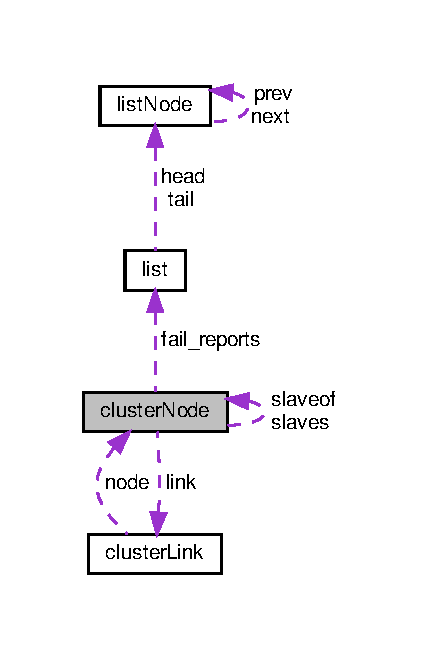
\includegraphics[width=202pt]{structcluster_node__coll__graph}
\end{center}
\end{figure}
\subsection*{Data Fields}
\begin{DoxyCompactItemize}
\item 
\hyperlink{redismodule_8h_a652ae61e2475bc8957454534544968fc}{mstime\+\_\+t} \hyperlink{structcluster_node_a7e18258d5320891f16483de560a5a551}{ctime}
\item 
char \hyperlink{structcluster_node_a5d3e2cfb46d2a665115ea2b362063396}{name} \mbox{[}\hyperlink{cluster_8h_ace7a882972eff7149675252938643b6e}{C\+L\+U\+S\+T\+E\+R\+\_\+\+N\+A\+M\+E\+L\+EN}\mbox{]}
\item 
int \hyperlink{structcluster_node_ac8bf36fe0577cba66bccda3a6f7e80a4}{flags}
\item 
uint64\+\_\+t \hyperlink{structcluster_node_a6bf0844859acadf5df37a7d49595680e}{config\+Epoch}
\item 
unsigned char \hyperlink{structcluster_node_a5860192f55932c04b85ec15307ee114b}{slots} \mbox{[}\hyperlink{cluster_8h_aa3e2cb951eebb16725ecc3f5beefd9fd}{C\+L\+U\+S\+T\+E\+R\+\_\+\+S\+L\+O\+TS}/8\mbox{]}
\item 
int \hyperlink{structcluster_node_a349a9876a2d953d6c146f1b324d5cc8a}{numslots}
\item 
int \hyperlink{structcluster_node_a0fc6a1a68f27049fc36cc42bf7c96208}{numslaves}
\item 
struct \hyperlink{structcluster_node}{cluster\+Node} $\ast$$\ast$ \hyperlink{structcluster_node_a0dcce9d83c3abdcf726eada2a2b747b6}{slaves}
\item 
struct \hyperlink{structcluster_node}{cluster\+Node} $\ast$ \hyperlink{structcluster_node_a6a719a7df6dd52ea8f73b741001c2540}{slaveof}
\item 
\hyperlink{redismodule_8h_a652ae61e2475bc8957454534544968fc}{mstime\+\_\+t} \hyperlink{structcluster_node_a83ac63444059326fd11192ee837f5237}{ping\+\_\+sent}
\item 
\hyperlink{redismodule_8h_a652ae61e2475bc8957454534544968fc}{mstime\+\_\+t} \hyperlink{structcluster_node_a75edda4c1e1a12f413686e691938cb56}{pong\+\_\+received}
\item 
\hyperlink{redismodule_8h_a652ae61e2475bc8957454534544968fc}{mstime\+\_\+t} \hyperlink{structcluster_node_adbfcc788af3c74e0607f1daa843d487e}{fail\+\_\+time}
\item 
\hyperlink{redismodule_8h_a652ae61e2475bc8957454534544968fc}{mstime\+\_\+t} \hyperlink{structcluster_node_ab7d11a3ddcc8b368b6ed249fb50b744b}{voted\+\_\+time}
\item 
\hyperlink{redismodule_8h_a652ae61e2475bc8957454534544968fc}{mstime\+\_\+t} \hyperlink{structcluster_node_ac38b49df545f207bd84bb341d90446ed}{repl\+\_\+offset\+\_\+time}
\item 
\hyperlink{redismodule_8h_a652ae61e2475bc8957454534544968fc}{mstime\+\_\+t} \hyperlink{structcluster_node_a27ce082b4aebffb71dfb9b03c0ce412b}{orphaned\+\_\+time}
\item 
long long \hyperlink{structcluster_node_acaaa973071b682ff89c70991a2d3ce7a}{repl\+\_\+offset}
\item 
char \hyperlink{structcluster_node_a9de2afd4e77c16f677244d244270b605}{ip} \mbox{[}\hyperlink{server_8h_ad97c5405ed22a94e9fcc10fba577d6c0}{N\+E\+T\+\_\+\+I\+P\+\_\+\+S\+T\+R\+\_\+\+L\+EN}\mbox{]}
\item 
int \hyperlink{structcluster_node_a63c89c04d1feae07ca35558055155ffb}{port}
\item 
int \hyperlink{structcluster_node_afe812fe7dea7e3685c4f5ad39803556d}{cport}
\item 
\hyperlink{structcluster_link}{cluster\+Link} $\ast$ \hyperlink{structcluster_node_a6cd8af29efc723c4b150e027c8106322}{link}
\item 
\hyperlink{structlist}{list} $\ast$ \hyperlink{structcluster_node_af865165e6c13a20888fba35e4bfbc496}{fail\+\_\+reports}
\end{DoxyCompactItemize}


\subsection{Detailed Description}


Definition at line 116 of file cluster.\+h.



\subsection{Field Documentation}
\mbox{\Hypertarget{structcluster_node_a6bf0844859acadf5df37a7d49595680e}\label{structcluster_node_a6bf0844859acadf5df37a7d49595680e}} 
\index{cluster\+Node@{cluster\+Node}!config\+Epoch@{config\+Epoch}}
\index{config\+Epoch@{config\+Epoch}!cluster\+Node@{cluster\+Node}}
\subsubsection{\texorpdfstring{config\+Epoch}{configEpoch}}
{\footnotesize\ttfamily uint64\+\_\+t config\+Epoch}



Definition at line 120 of file cluster.\+h.

\mbox{\Hypertarget{structcluster_node_afe812fe7dea7e3685c4f5ad39803556d}\label{structcluster_node_afe812fe7dea7e3685c4f5ad39803556d}} 
\index{cluster\+Node@{cluster\+Node}!cport@{cport}}
\index{cport@{cport}!cluster\+Node@{cluster\+Node}}
\subsubsection{\texorpdfstring{cport}{cport}}
{\footnotesize\ttfamily int cport}



Definition at line 138 of file cluster.\+h.

\mbox{\Hypertarget{structcluster_node_a7e18258d5320891f16483de560a5a551}\label{structcluster_node_a7e18258d5320891f16483de560a5a551}} 
\index{cluster\+Node@{cluster\+Node}!ctime@{ctime}}
\index{ctime@{ctime}!cluster\+Node@{cluster\+Node}}
\subsubsection{\texorpdfstring{ctime}{ctime}}
{\footnotesize\ttfamily \hyperlink{redismodule_8h_a652ae61e2475bc8957454534544968fc}{mstime\+\_\+t} ctime}



Definition at line 117 of file cluster.\+h.

\mbox{\Hypertarget{structcluster_node_af865165e6c13a20888fba35e4bfbc496}\label{structcluster_node_af865165e6c13a20888fba35e4bfbc496}} 
\index{cluster\+Node@{cluster\+Node}!fail\+\_\+reports@{fail\+\_\+reports}}
\index{fail\+\_\+reports@{fail\+\_\+reports}!cluster\+Node@{cluster\+Node}}
\subsubsection{\texorpdfstring{fail\+\_\+reports}{fail\_reports}}
{\footnotesize\ttfamily \hyperlink{structlist}{list}$\ast$ fail\+\_\+reports}



Definition at line 140 of file cluster.\+h.

\mbox{\Hypertarget{structcluster_node_adbfcc788af3c74e0607f1daa843d487e}\label{structcluster_node_adbfcc788af3c74e0607f1daa843d487e}} 
\index{cluster\+Node@{cluster\+Node}!fail\+\_\+time@{fail\+\_\+time}}
\index{fail\+\_\+time@{fail\+\_\+time}!cluster\+Node@{cluster\+Node}}
\subsubsection{\texorpdfstring{fail\+\_\+time}{fail\_time}}
{\footnotesize\ttfamily \hyperlink{redismodule_8h_a652ae61e2475bc8957454534544968fc}{mstime\+\_\+t} fail\+\_\+time}



Definition at line 131 of file cluster.\+h.

\mbox{\Hypertarget{structcluster_node_ac8bf36fe0577cba66bccda3a6f7e80a4}\label{structcluster_node_ac8bf36fe0577cba66bccda3a6f7e80a4}} 
\index{cluster\+Node@{cluster\+Node}!flags@{flags}}
\index{flags@{flags}!cluster\+Node@{cluster\+Node}}
\subsubsection{\texorpdfstring{flags}{flags}}
{\footnotesize\ttfamily int flags}



Definition at line 119 of file cluster.\+h.

\mbox{\Hypertarget{structcluster_node_a9de2afd4e77c16f677244d244270b605}\label{structcluster_node_a9de2afd4e77c16f677244d244270b605}} 
\index{cluster\+Node@{cluster\+Node}!ip@{ip}}
\index{ip@{ip}!cluster\+Node@{cluster\+Node}}
\subsubsection{\texorpdfstring{ip}{ip}}
{\footnotesize\ttfamily char ip\mbox{[}\hyperlink{server_8h_ad97c5405ed22a94e9fcc10fba577d6c0}{N\+E\+T\+\_\+\+I\+P\+\_\+\+S\+T\+R\+\_\+\+L\+EN}\mbox{]}}



Definition at line 136 of file cluster.\+h.

\mbox{\Hypertarget{structcluster_node_a6cd8af29efc723c4b150e027c8106322}\label{structcluster_node_a6cd8af29efc723c4b150e027c8106322}} 
\index{cluster\+Node@{cluster\+Node}!link@{link}}
\index{link@{link}!cluster\+Node@{cluster\+Node}}
\subsubsection{\texorpdfstring{link}{link}}
{\footnotesize\ttfamily \hyperlink{structcluster_link}{cluster\+Link}$\ast$ link}



Definition at line 139 of file cluster.\+h.

\mbox{\Hypertarget{structcluster_node_a5d3e2cfb46d2a665115ea2b362063396}\label{structcluster_node_a5d3e2cfb46d2a665115ea2b362063396}} 
\index{cluster\+Node@{cluster\+Node}!name@{name}}
\index{name@{name}!cluster\+Node@{cluster\+Node}}
\subsubsection{\texorpdfstring{name}{name}}
{\footnotesize\ttfamily char name\mbox{[}\hyperlink{cluster_8h_ace7a882972eff7149675252938643b6e}{C\+L\+U\+S\+T\+E\+R\+\_\+\+N\+A\+M\+E\+L\+EN}\mbox{]}}



Definition at line 118 of file cluster.\+h.

\mbox{\Hypertarget{structcluster_node_a0fc6a1a68f27049fc36cc42bf7c96208}\label{structcluster_node_a0fc6a1a68f27049fc36cc42bf7c96208}} 
\index{cluster\+Node@{cluster\+Node}!numslaves@{numslaves}}
\index{numslaves@{numslaves}!cluster\+Node@{cluster\+Node}}
\subsubsection{\texorpdfstring{numslaves}{numslaves}}
{\footnotesize\ttfamily int numslaves}



Definition at line 123 of file cluster.\+h.

\mbox{\Hypertarget{structcluster_node_a349a9876a2d953d6c146f1b324d5cc8a}\label{structcluster_node_a349a9876a2d953d6c146f1b324d5cc8a}} 
\index{cluster\+Node@{cluster\+Node}!numslots@{numslots}}
\index{numslots@{numslots}!cluster\+Node@{cluster\+Node}}
\subsubsection{\texorpdfstring{numslots}{numslots}}
{\footnotesize\ttfamily int numslots}



Definition at line 122 of file cluster.\+h.

\mbox{\Hypertarget{structcluster_node_a27ce082b4aebffb71dfb9b03c0ce412b}\label{structcluster_node_a27ce082b4aebffb71dfb9b03c0ce412b}} 
\index{cluster\+Node@{cluster\+Node}!orphaned\+\_\+time@{orphaned\+\_\+time}}
\index{orphaned\+\_\+time@{orphaned\+\_\+time}!cluster\+Node@{cluster\+Node}}
\subsubsection{\texorpdfstring{orphaned\+\_\+time}{orphaned\_time}}
{\footnotesize\ttfamily \hyperlink{redismodule_8h_a652ae61e2475bc8957454534544968fc}{mstime\+\_\+t} orphaned\+\_\+time}



Definition at line 134 of file cluster.\+h.

\mbox{\Hypertarget{structcluster_node_a83ac63444059326fd11192ee837f5237}\label{structcluster_node_a83ac63444059326fd11192ee837f5237}} 
\index{cluster\+Node@{cluster\+Node}!ping\+\_\+sent@{ping\+\_\+sent}}
\index{ping\+\_\+sent@{ping\+\_\+sent}!cluster\+Node@{cluster\+Node}}
\subsubsection{\texorpdfstring{ping\+\_\+sent}{ping\_sent}}
{\footnotesize\ttfamily \hyperlink{redismodule_8h_a652ae61e2475bc8957454534544968fc}{mstime\+\_\+t} ping\+\_\+sent}



Definition at line 129 of file cluster.\+h.

\mbox{\Hypertarget{structcluster_node_a75edda4c1e1a12f413686e691938cb56}\label{structcluster_node_a75edda4c1e1a12f413686e691938cb56}} 
\index{cluster\+Node@{cluster\+Node}!pong\+\_\+received@{pong\+\_\+received}}
\index{pong\+\_\+received@{pong\+\_\+received}!cluster\+Node@{cluster\+Node}}
\subsubsection{\texorpdfstring{pong\+\_\+received}{pong\_received}}
{\footnotesize\ttfamily \hyperlink{redismodule_8h_a652ae61e2475bc8957454534544968fc}{mstime\+\_\+t} pong\+\_\+received}



Definition at line 130 of file cluster.\+h.

\mbox{\Hypertarget{structcluster_node_a63c89c04d1feae07ca35558055155ffb}\label{structcluster_node_a63c89c04d1feae07ca35558055155ffb}} 
\index{cluster\+Node@{cluster\+Node}!port@{port}}
\index{port@{port}!cluster\+Node@{cluster\+Node}}
\subsubsection{\texorpdfstring{port}{port}}
{\footnotesize\ttfamily int port}



Definition at line 137 of file cluster.\+h.

\mbox{\Hypertarget{structcluster_node_acaaa973071b682ff89c70991a2d3ce7a}\label{structcluster_node_acaaa973071b682ff89c70991a2d3ce7a}} 
\index{cluster\+Node@{cluster\+Node}!repl\+\_\+offset@{repl\+\_\+offset}}
\index{repl\+\_\+offset@{repl\+\_\+offset}!cluster\+Node@{cluster\+Node}}
\subsubsection{\texorpdfstring{repl\+\_\+offset}{repl\_offset}}
{\footnotesize\ttfamily long long repl\+\_\+offset}



Definition at line 135 of file cluster.\+h.

\mbox{\Hypertarget{structcluster_node_ac38b49df545f207bd84bb341d90446ed}\label{structcluster_node_ac38b49df545f207bd84bb341d90446ed}} 
\index{cluster\+Node@{cluster\+Node}!repl\+\_\+offset\+\_\+time@{repl\+\_\+offset\+\_\+time}}
\index{repl\+\_\+offset\+\_\+time@{repl\+\_\+offset\+\_\+time}!cluster\+Node@{cluster\+Node}}
\subsubsection{\texorpdfstring{repl\+\_\+offset\+\_\+time}{repl\_offset\_time}}
{\footnotesize\ttfamily \hyperlink{redismodule_8h_a652ae61e2475bc8957454534544968fc}{mstime\+\_\+t} repl\+\_\+offset\+\_\+time}



Definition at line 133 of file cluster.\+h.

\mbox{\Hypertarget{structcluster_node_a6a719a7df6dd52ea8f73b741001c2540}\label{structcluster_node_a6a719a7df6dd52ea8f73b741001c2540}} 
\index{cluster\+Node@{cluster\+Node}!slaveof@{slaveof}}
\index{slaveof@{slaveof}!cluster\+Node@{cluster\+Node}}
\subsubsection{\texorpdfstring{slaveof}{slaveof}}
{\footnotesize\ttfamily struct \hyperlink{structcluster_node}{cluster\+Node}$\ast$ slaveof}



Definition at line 125 of file cluster.\+h.

\mbox{\Hypertarget{structcluster_node_a0dcce9d83c3abdcf726eada2a2b747b6}\label{structcluster_node_a0dcce9d83c3abdcf726eada2a2b747b6}} 
\index{cluster\+Node@{cluster\+Node}!slaves@{slaves}}
\index{slaves@{slaves}!cluster\+Node@{cluster\+Node}}
\subsubsection{\texorpdfstring{slaves}{slaves}}
{\footnotesize\ttfamily struct \hyperlink{structcluster_node}{cluster\+Node}$\ast$$\ast$ slaves}



Definition at line 124 of file cluster.\+h.

\mbox{\Hypertarget{structcluster_node_a5860192f55932c04b85ec15307ee114b}\label{structcluster_node_a5860192f55932c04b85ec15307ee114b}} 
\index{cluster\+Node@{cluster\+Node}!slots@{slots}}
\index{slots@{slots}!cluster\+Node@{cluster\+Node}}
\subsubsection{\texorpdfstring{slots}{slots}}
{\footnotesize\ttfamily unsigned char slots\mbox{[}\hyperlink{cluster_8h_aa3e2cb951eebb16725ecc3f5beefd9fd}{C\+L\+U\+S\+T\+E\+R\+\_\+\+S\+L\+O\+TS}/8\mbox{]}}



Definition at line 121 of file cluster.\+h.

\mbox{\Hypertarget{structcluster_node_ab7d11a3ddcc8b368b6ed249fb50b744b}\label{structcluster_node_ab7d11a3ddcc8b368b6ed249fb50b744b}} 
\index{cluster\+Node@{cluster\+Node}!voted\+\_\+time@{voted\+\_\+time}}
\index{voted\+\_\+time@{voted\+\_\+time}!cluster\+Node@{cluster\+Node}}
\subsubsection{\texorpdfstring{voted\+\_\+time}{voted\_time}}
{\footnotesize\ttfamily \hyperlink{redismodule_8h_a652ae61e2475bc8957454534544968fc}{mstime\+\_\+t} voted\+\_\+time}



Definition at line 132 of file cluster.\+h.



The documentation for this struct was generated from the following file\+:\begin{DoxyCompactItemize}
\item 
src/\hyperlink{cluster_8h}{cluster.\+h}\end{DoxyCompactItemize}

\hypertarget{structcluster_node_fail_report}{}\section{cluster\+Node\+Fail\+Report Struct Reference}
\label{structcluster_node_fail_report}\index{cluster\+Node\+Fail\+Report@{cluster\+Node\+Fail\+Report}}


{\ttfamily \#include $<$cluster.\+h$>$}



Collaboration diagram for cluster\+Node\+Fail\+Report\+:
\nopagebreak
\begin{figure}[H]
\begin{center}
\leavevmode
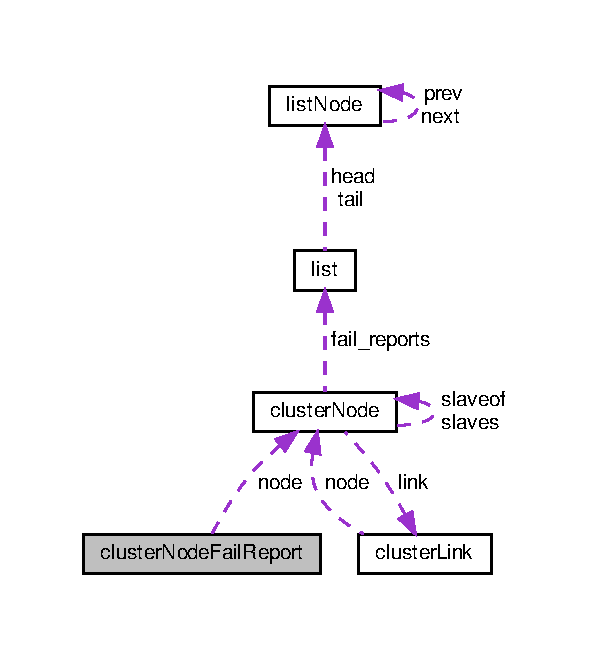
\includegraphics[width=284pt]{structcluster_node_fail_report__coll__graph}
\end{center}
\end{figure}
\subsection*{Data Fields}
\begin{DoxyCompactItemize}
\item 
struct \hyperlink{structcluster_node}{cluster\+Node} $\ast$ \hyperlink{structcluster_node_fail_report_a7aa2bc440db9dc659120a310878cac0f}{node}
\item 
\hyperlink{redismodule_8h_a652ae61e2475bc8957454534544968fc}{mstime\+\_\+t} \hyperlink{structcluster_node_fail_report_a1f28210ccf56a01319b20295b8ff190e}{time}
\end{DoxyCompactItemize}


\subsection{Detailed Description}


Definition at line 111 of file cluster.\+h.



\subsection{Field Documentation}
\mbox{\Hypertarget{structcluster_node_fail_report_a7aa2bc440db9dc659120a310878cac0f}\label{structcluster_node_fail_report_a7aa2bc440db9dc659120a310878cac0f}} 
\index{cluster\+Node\+Fail\+Report@{cluster\+Node\+Fail\+Report}!node@{node}}
\index{node@{node}!cluster\+Node\+Fail\+Report@{cluster\+Node\+Fail\+Report}}
\subsubsection{\texorpdfstring{node}{node}}
{\footnotesize\ttfamily struct \hyperlink{structcluster_node}{cluster\+Node}$\ast$ node}



Definition at line 112 of file cluster.\+h.

\mbox{\Hypertarget{structcluster_node_fail_report_a1f28210ccf56a01319b20295b8ff190e}\label{structcluster_node_fail_report_a1f28210ccf56a01319b20295b8ff190e}} 
\index{cluster\+Node\+Fail\+Report@{cluster\+Node\+Fail\+Report}!time@{time}}
\index{time@{time}!cluster\+Node\+Fail\+Report@{cluster\+Node\+Fail\+Report}}
\subsubsection{\texorpdfstring{time}{time}}
{\footnotesize\ttfamily \hyperlink{redismodule_8h_a652ae61e2475bc8957454534544968fc}{mstime\+\_\+t} time}



Definition at line 113 of file cluster.\+h.



The documentation for this struct was generated from the following file\+:\begin{DoxyCompactItemize}
\item 
src/\hyperlink{cluster_8h}{cluster.\+h}\end{DoxyCompactItemize}

\hypertarget{structcluster_state}{}\section{cluster\+State Struct Reference}
\label{structcluster_state}\index{cluster\+State@{cluster\+State}}


{\ttfamily \#include $<$cluster.\+h$>$}



Collaboration diagram for cluster\+State\+:
\nopagebreak
\begin{figure}[H]
\begin{center}
\leavevmode
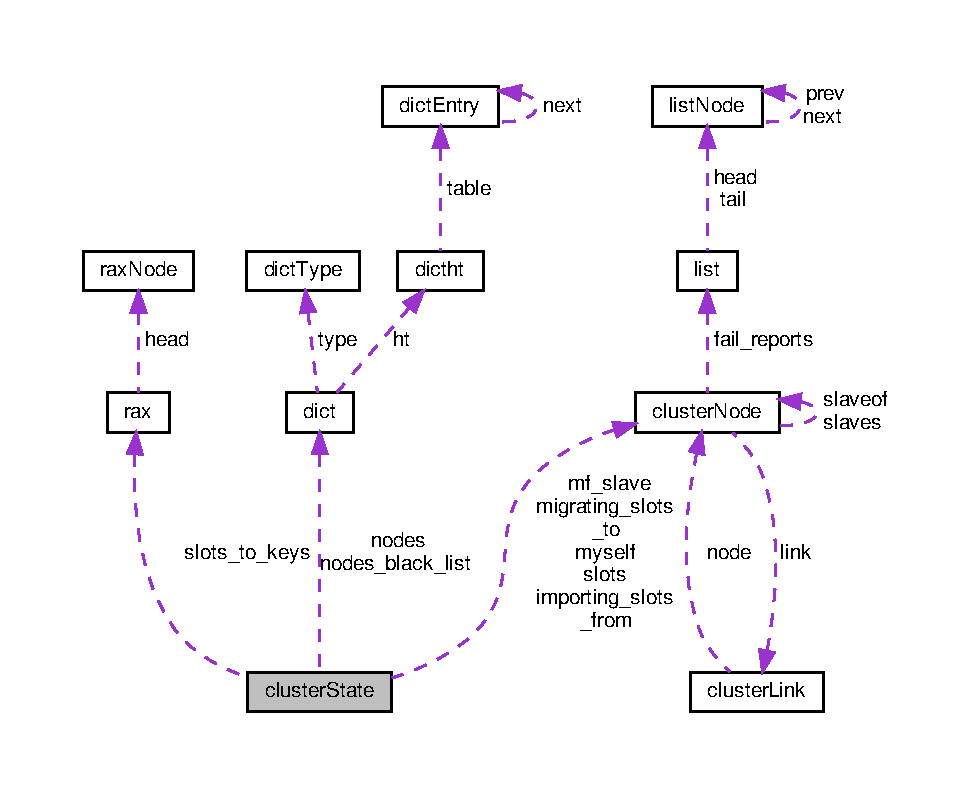
\includegraphics[width=350pt]{structcluster_state__coll__graph}
\end{center}
\end{figure}
\subsection*{Data Fields}
\begin{DoxyCompactItemize}
\item 
\hyperlink{structcluster_node}{cluster\+Node} $\ast$ \hyperlink{structcluster_state_aff69bee08a3a0a58166a9f85acf12d56}{myself}
\item 
uint64\+\_\+t \hyperlink{structcluster_state_a97f41589e815c407f015841f5a3d816f}{current\+Epoch}
\item 
int \hyperlink{structcluster_state_a89f234133d3efe315836311cbf21c64b}{state}
\item 
int \hyperlink{structcluster_state_a439227feff9d7f55384e8780cfc2eb82}{size}
\item 
\hyperlink{structdict}{dict} $\ast$ \hyperlink{structcluster_state_a6e18e71a503d78c25fa93a49e05bf6f4}{nodes}
\item 
\hyperlink{structdict}{dict} $\ast$ \hyperlink{structcluster_state_a0dec12e8b1bd71942304f8073656d023}{nodes\+\_\+black\+\_\+list}
\item 
\hyperlink{structcluster_node}{cluster\+Node} $\ast$ \hyperlink{structcluster_state_a95946e1c3598728041d63dfdb7b179df}{migrating\+\_\+slots\+\_\+to} \mbox{[}\hyperlink{cluster_8h_aa3e2cb951eebb16725ecc3f5beefd9fd}{C\+L\+U\+S\+T\+E\+R\+\_\+\+S\+L\+O\+TS}\mbox{]}
\item 
\hyperlink{structcluster_node}{cluster\+Node} $\ast$ \hyperlink{structcluster_state_a1268626116ae576c7bb7dcdd60f43ccf}{importing\+\_\+slots\+\_\+from} \mbox{[}\hyperlink{cluster_8h_aa3e2cb951eebb16725ecc3f5beefd9fd}{C\+L\+U\+S\+T\+E\+R\+\_\+\+S\+L\+O\+TS}\mbox{]}
\item 
\hyperlink{structcluster_node}{cluster\+Node} $\ast$ \hyperlink{structcluster_state_a1eb411c5aaa32d0d3c2ac0c5e9dde892}{slots} \mbox{[}\hyperlink{cluster_8h_aa3e2cb951eebb16725ecc3f5beefd9fd}{C\+L\+U\+S\+T\+E\+R\+\_\+\+S\+L\+O\+TS}\mbox{]}
\item 
uint64\+\_\+t \hyperlink{structcluster_state_acd00e4aea7a23f7498525dc50671c66f}{slots\+\_\+keys\+\_\+count} \mbox{[}\hyperlink{cluster_8h_aa3e2cb951eebb16725ecc3f5beefd9fd}{C\+L\+U\+S\+T\+E\+R\+\_\+\+S\+L\+O\+TS}\mbox{]}
\item 
\hyperlink{structrax}{rax} $\ast$ \hyperlink{structcluster_state_a2dd4e8e6e414888eee838a96e2573ae8}{slots\+\_\+to\+\_\+keys}
\item 
\hyperlink{redismodule_8h_a652ae61e2475bc8957454534544968fc}{mstime\+\_\+t} \hyperlink{structcluster_state_a6acb8999815edbd474cb3fc1e31681e6}{failover\+\_\+auth\+\_\+time}
\item 
int \hyperlink{structcluster_state_ae1b94f8bc49656245d7f3ed2a0582022}{failover\+\_\+auth\+\_\+count}
\item 
int \hyperlink{structcluster_state_adb3806b1c3d64d9cf5bbf5ceacf15dc0}{failover\+\_\+auth\+\_\+sent}
\item 
int \hyperlink{structcluster_state_a52dbd3d525c7f1e426d32f045893dd2e}{failover\+\_\+auth\+\_\+rank}
\item 
uint64\+\_\+t \hyperlink{structcluster_state_a516e3fdf8f127f6c29e318bcacbe2f3b}{failover\+\_\+auth\+\_\+epoch}
\item 
int \hyperlink{structcluster_state_a39e7055565db885db62edd0b431617ee}{cant\+\_\+failover\+\_\+reason}
\item 
\hyperlink{redismodule_8h_a652ae61e2475bc8957454534544968fc}{mstime\+\_\+t} \hyperlink{structcluster_state_a0c7b84fff1f0fe55132e97977fca4d9b}{mf\+\_\+end}
\item 
\hyperlink{structcluster_node}{cluster\+Node} $\ast$ \hyperlink{structcluster_state_a2e05a27830b3ab7c4abc4322c9972959}{mf\+\_\+slave}
\item 
long long \hyperlink{structcluster_state_a74633edfa88dbbd2ba5bd94e8d24bda8}{mf\+\_\+master\+\_\+offset}
\item 
int \hyperlink{structcluster_state_a2f5224c461c3af2a0833ae28c0ffa606}{mf\+\_\+can\+\_\+start}
\item 
uint64\+\_\+t \hyperlink{structcluster_state_ad9df5e1c1e5db0bb0334f30de0b4a815}{last\+Vote\+Epoch}
\item 
int \hyperlink{structcluster_state_ad1fa0188f945aac48dec9eb49c943a72}{todo\+\_\+before\+\_\+sleep}
\item 
long long \hyperlink{structcluster_state_a8b47b0756931e1e5dc07cda92de394e2}{stats\+\_\+bus\+\_\+messages\+\_\+sent} \mbox{[}\hyperlink{cluster_8h_a6222c464c1f2125f42271d2abd63853e}{C\+L\+U\+S\+T\+E\+R\+M\+S\+G\+\_\+\+T\+Y\+P\+E\+\_\+\+C\+O\+U\+NT}\mbox{]}
\item 
long long \hyperlink{structcluster_state_ad3dc0c6e15b6bd97620150b94d2f6c44}{stats\+\_\+bus\+\_\+messages\+\_\+received} \mbox{[}\hyperlink{cluster_8h_a6222c464c1f2125f42271d2abd63853e}{C\+L\+U\+S\+T\+E\+R\+M\+S\+G\+\_\+\+T\+Y\+P\+E\+\_\+\+C\+O\+U\+NT}\mbox{]}
\item 
long long \hyperlink{structcluster_state_a278d5ed382c852a1e40e985d642306e6}{stats\+\_\+pfail\+\_\+nodes}
\end{DoxyCompactItemize}


\subsection{Detailed Description}


Definition at line 143 of file cluster.\+h.



\subsection{Field Documentation}
\mbox{\Hypertarget{structcluster_state_a39e7055565db885db62edd0b431617ee}\label{structcluster_state_a39e7055565db885db62edd0b431617ee}} 
\index{cluster\+State@{cluster\+State}!cant\+\_\+failover\+\_\+reason@{cant\+\_\+failover\+\_\+reason}}
\index{cant\+\_\+failover\+\_\+reason@{cant\+\_\+failover\+\_\+reason}!cluster\+State@{cluster\+State}}
\subsubsection{\texorpdfstring{cant\+\_\+failover\+\_\+reason}{cant\_failover\_reason}}
{\footnotesize\ttfamily int cant\+\_\+failover\+\_\+reason}



Definition at line 161 of file cluster.\+h.

\mbox{\Hypertarget{structcluster_state_a97f41589e815c407f015841f5a3d816f}\label{structcluster_state_a97f41589e815c407f015841f5a3d816f}} 
\index{cluster\+State@{cluster\+State}!current\+Epoch@{current\+Epoch}}
\index{current\+Epoch@{current\+Epoch}!cluster\+State@{cluster\+State}}
\subsubsection{\texorpdfstring{current\+Epoch}{currentEpoch}}
{\footnotesize\ttfamily uint64\+\_\+t current\+Epoch}



Definition at line 145 of file cluster.\+h.

\mbox{\Hypertarget{structcluster_state_ae1b94f8bc49656245d7f3ed2a0582022}\label{structcluster_state_ae1b94f8bc49656245d7f3ed2a0582022}} 
\index{cluster\+State@{cluster\+State}!failover\+\_\+auth\+\_\+count@{failover\+\_\+auth\+\_\+count}}
\index{failover\+\_\+auth\+\_\+count@{failover\+\_\+auth\+\_\+count}!cluster\+State@{cluster\+State}}
\subsubsection{\texorpdfstring{failover\+\_\+auth\+\_\+count}{failover\_auth\_count}}
{\footnotesize\ttfamily int failover\+\_\+auth\+\_\+count}



Definition at line 157 of file cluster.\+h.

\mbox{\Hypertarget{structcluster_state_a516e3fdf8f127f6c29e318bcacbe2f3b}\label{structcluster_state_a516e3fdf8f127f6c29e318bcacbe2f3b}} 
\index{cluster\+State@{cluster\+State}!failover\+\_\+auth\+\_\+epoch@{failover\+\_\+auth\+\_\+epoch}}
\index{failover\+\_\+auth\+\_\+epoch@{failover\+\_\+auth\+\_\+epoch}!cluster\+State@{cluster\+State}}
\subsubsection{\texorpdfstring{failover\+\_\+auth\+\_\+epoch}{failover\_auth\_epoch}}
{\footnotesize\ttfamily uint64\+\_\+t failover\+\_\+auth\+\_\+epoch}



Definition at line 160 of file cluster.\+h.

\mbox{\Hypertarget{structcluster_state_a52dbd3d525c7f1e426d32f045893dd2e}\label{structcluster_state_a52dbd3d525c7f1e426d32f045893dd2e}} 
\index{cluster\+State@{cluster\+State}!failover\+\_\+auth\+\_\+rank@{failover\+\_\+auth\+\_\+rank}}
\index{failover\+\_\+auth\+\_\+rank@{failover\+\_\+auth\+\_\+rank}!cluster\+State@{cluster\+State}}
\subsubsection{\texorpdfstring{failover\+\_\+auth\+\_\+rank}{failover\_auth\_rank}}
{\footnotesize\ttfamily int failover\+\_\+auth\+\_\+rank}



Definition at line 159 of file cluster.\+h.

\mbox{\Hypertarget{structcluster_state_adb3806b1c3d64d9cf5bbf5ceacf15dc0}\label{structcluster_state_adb3806b1c3d64d9cf5bbf5ceacf15dc0}} 
\index{cluster\+State@{cluster\+State}!failover\+\_\+auth\+\_\+sent@{failover\+\_\+auth\+\_\+sent}}
\index{failover\+\_\+auth\+\_\+sent@{failover\+\_\+auth\+\_\+sent}!cluster\+State@{cluster\+State}}
\subsubsection{\texorpdfstring{failover\+\_\+auth\+\_\+sent}{failover\_auth\_sent}}
{\footnotesize\ttfamily int failover\+\_\+auth\+\_\+sent}



Definition at line 158 of file cluster.\+h.

\mbox{\Hypertarget{structcluster_state_a6acb8999815edbd474cb3fc1e31681e6}\label{structcluster_state_a6acb8999815edbd474cb3fc1e31681e6}} 
\index{cluster\+State@{cluster\+State}!failover\+\_\+auth\+\_\+time@{failover\+\_\+auth\+\_\+time}}
\index{failover\+\_\+auth\+\_\+time@{failover\+\_\+auth\+\_\+time}!cluster\+State@{cluster\+State}}
\subsubsection{\texorpdfstring{failover\+\_\+auth\+\_\+time}{failover\_auth\_time}}
{\footnotesize\ttfamily \hyperlink{redismodule_8h_a652ae61e2475bc8957454534544968fc}{mstime\+\_\+t} failover\+\_\+auth\+\_\+time}



Definition at line 156 of file cluster.\+h.

\mbox{\Hypertarget{structcluster_state_a1268626116ae576c7bb7dcdd60f43ccf}\label{structcluster_state_a1268626116ae576c7bb7dcdd60f43ccf}} 
\index{cluster\+State@{cluster\+State}!importing\+\_\+slots\+\_\+from@{importing\+\_\+slots\+\_\+from}}
\index{importing\+\_\+slots\+\_\+from@{importing\+\_\+slots\+\_\+from}!cluster\+State@{cluster\+State}}
\subsubsection{\texorpdfstring{importing\+\_\+slots\+\_\+from}{importing\_slots\_from}}
{\footnotesize\ttfamily \hyperlink{structcluster_node}{cluster\+Node}$\ast$ importing\+\_\+slots\+\_\+from\mbox{[}\hyperlink{cluster_8h_aa3e2cb951eebb16725ecc3f5beefd9fd}{C\+L\+U\+S\+T\+E\+R\+\_\+\+S\+L\+O\+TS}\mbox{]}}



Definition at line 151 of file cluster.\+h.

\mbox{\Hypertarget{structcluster_state_ad9df5e1c1e5db0bb0334f30de0b4a815}\label{structcluster_state_ad9df5e1c1e5db0bb0334f30de0b4a815}} 
\index{cluster\+State@{cluster\+State}!last\+Vote\+Epoch@{last\+Vote\+Epoch}}
\index{last\+Vote\+Epoch@{last\+Vote\+Epoch}!cluster\+State@{cluster\+State}}
\subsubsection{\texorpdfstring{last\+Vote\+Epoch}{lastVoteEpoch}}
{\footnotesize\ttfamily uint64\+\_\+t last\+Vote\+Epoch}



Definition at line 174 of file cluster.\+h.

\mbox{\Hypertarget{structcluster_state_a2f5224c461c3af2a0833ae28c0ffa606}\label{structcluster_state_a2f5224c461c3af2a0833ae28c0ffa606}} 
\index{cluster\+State@{cluster\+State}!mf\+\_\+can\+\_\+start@{mf\+\_\+can\+\_\+start}}
\index{mf\+\_\+can\+\_\+start@{mf\+\_\+can\+\_\+start}!cluster\+State@{cluster\+State}}
\subsubsection{\texorpdfstring{mf\+\_\+can\+\_\+start}{mf\_can\_start}}
{\footnotesize\ttfamily int mf\+\_\+can\+\_\+start}



Definition at line 171 of file cluster.\+h.

\mbox{\Hypertarget{structcluster_state_a0c7b84fff1f0fe55132e97977fca4d9b}\label{structcluster_state_a0c7b84fff1f0fe55132e97977fca4d9b}} 
\index{cluster\+State@{cluster\+State}!mf\+\_\+end@{mf\+\_\+end}}
\index{mf\+\_\+end@{mf\+\_\+end}!cluster\+State@{cluster\+State}}
\subsubsection{\texorpdfstring{mf\+\_\+end}{mf\_end}}
{\footnotesize\ttfamily \hyperlink{redismodule_8h_a652ae61e2475bc8957454534544968fc}{mstime\+\_\+t} mf\+\_\+end}



Definition at line 164 of file cluster.\+h.

\mbox{\Hypertarget{structcluster_state_a74633edfa88dbbd2ba5bd94e8d24bda8}\label{structcluster_state_a74633edfa88dbbd2ba5bd94e8d24bda8}} 
\index{cluster\+State@{cluster\+State}!mf\+\_\+master\+\_\+offset@{mf\+\_\+master\+\_\+offset}}
\index{mf\+\_\+master\+\_\+offset@{mf\+\_\+master\+\_\+offset}!cluster\+State@{cluster\+State}}
\subsubsection{\texorpdfstring{mf\+\_\+master\+\_\+offset}{mf\_master\_offset}}
{\footnotesize\ttfamily long long mf\+\_\+master\+\_\+offset}



Definition at line 169 of file cluster.\+h.

\mbox{\Hypertarget{structcluster_state_a2e05a27830b3ab7c4abc4322c9972959}\label{structcluster_state_a2e05a27830b3ab7c4abc4322c9972959}} 
\index{cluster\+State@{cluster\+State}!mf\+\_\+slave@{mf\+\_\+slave}}
\index{mf\+\_\+slave@{mf\+\_\+slave}!cluster\+State@{cluster\+State}}
\subsubsection{\texorpdfstring{mf\+\_\+slave}{mf\_slave}}
{\footnotesize\ttfamily \hyperlink{structcluster_node}{cluster\+Node}$\ast$ mf\+\_\+slave}



Definition at line 167 of file cluster.\+h.

\mbox{\Hypertarget{structcluster_state_a95946e1c3598728041d63dfdb7b179df}\label{structcluster_state_a95946e1c3598728041d63dfdb7b179df}} 
\index{cluster\+State@{cluster\+State}!migrating\+\_\+slots\+\_\+to@{migrating\+\_\+slots\+\_\+to}}
\index{migrating\+\_\+slots\+\_\+to@{migrating\+\_\+slots\+\_\+to}!cluster\+State@{cluster\+State}}
\subsubsection{\texorpdfstring{migrating\+\_\+slots\+\_\+to}{migrating\_slots\_to}}
{\footnotesize\ttfamily \hyperlink{structcluster_node}{cluster\+Node}$\ast$ migrating\+\_\+slots\+\_\+to\mbox{[}\hyperlink{cluster_8h_aa3e2cb951eebb16725ecc3f5beefd9fd}{C\+L\+U\+S\+T\+E\+R\+\_\+\+S\+L\+O\+TS}\mbox{]}}



Definition at line 150 of file cluster.\+h.

\mbox{\Hypertarget{structcluster_state_aff69bee08a3a0a58166a9f85acf12d56}\label{structcluster_state_aff69bee08a3a0a58166a9f85acf12d56}} 
\index{cluster\+State@{cluster\+State}!myself@{myself}}
\index{myself@{myself}!cluster\+State@{cluster\+State}}
\subsubsection{\texorpdfstring{myself}{myself}}
{\footnotesize\ttfamily \hyperlink{structcluster_node}{cluster\+Node}$\ast$ myself}



Definition at line 144 of file cluster.\+h.

\mbox{\Hypertarget{structcluster_state_a6e18e71a503d78c25fa93a49e05bf6f4}\label{structcluster_state_a6e18e71a503d78c25fa93a49e05bf6f4}} 
\index{cluster\+State@{cluster\+State}!nodes@{nodes}}
\index{nodes@{nodes}!cluster\+State@{cluster\+State}}
\subsubsection{\texorpdfstring{nodes}{nodes}}
{\footnotesize\ttfamily \hyperlink{structdict}{dict}$\ast$ nodes}



Definition at line 148 of file cluster.\+h.

\mbox{\Hypertarget{structcluster_state_a0dec12e8b1bd71942304f8073656d023}\label{structcluster_state_a0dec12e8b1bd71942304f8073656d023}} 
\index{cluster\+State@{cluster\+State}!nodes\+\_\+black\+\_\+list@{nodes\+\_\+black\+\_\+list}}
\index{nodes\+\_\+black\+\_\+list@{nodes\+\_\+black\+\_\+list}!cluster\+State@{cluster\+State}}
\subsubsection{\texorpdfstring{nodes\+\_\+black\+\_\+list}{nodes\_black\_list}}
{\footnotesize\ttfamily \hyperlink{structdict}{dict}$\ast$ nodes\+\_\+black\+\_\+list}



Definition at line 149 of file cluster.\+h.

\mbox{\Hypertarget{structcluster_state_a439227feff9d7f55384e8780cfc2eb82}\label{structcluster_state_a439227feff9d7f55384e8780cfc2eb82}} 
\index{cluster\+State@{cluster\+State}!size@{size}}
\index{size@{size}!cluster\+State@{cluster\+State}}
\subsubsection{\texorpdfstring{size}{size}}
{\footnotesize\ttfamily int size}



Definition at line 147 of file cluster.\+h.

\mbox{\Hypertarget{structcluster_state_a1eb411c5aaa32d0d3c2ac0c5e9dde892}\label{structcluster_state_a1eb411c5aaa32d0d3c2ac0c5e9dde892}} 
\index{cluster\+State@{cluster\+State}!slots@{slots}}
\index{slots@{slots}!cluster\+State@{cluster\+State}}
\subsubsection{\texorpdfstring{slots}{slots}}
{\footnotesize\ttfamily \hyperlink{structcluster_node}{cluster\+Node}$\ast$ slots\mbox{[}\hyperlink{cluster_8h_aa3e2cb951eebb16725ecc3f5beefd9fd}{C\+L\+U\+S\+T\+E\+R\+\_\+\+S\+L\+O\+TS}\mbox{]}}



Definition at line 152 of file cluster.\+h.

\mbox{\Hypertarget{structcluster_state_acd00e4aea7a23f7498525dc50671c66f}\label{structcluster_state_acd00e4aea7a23f7498525dc50671c66f}} 
\index{cluster\+State@{cluster\+State}!slots\+\_\+keys\+\_\+count@{slots\+\_\+keys\+\_\+count}}
\index{slots\+\_\+keys\+\_\+count@{slots\+\_\+keys\+\_\+count}!cluster\+State@{cluster\+State}}
\subsubsection{\texorpdfstring{slots\+\_\+keys\+\_\+count}{slots\_keys\_count}}
{\footnotesize\ttfamily uint64\+\_\+t slots\+\_\+keys\+\_\+count\mbox{[}\hyperlink{cluster_8h_aa3e2cb951eebb16725ecc3f5beefd9fd}{C\+L\+U\+S\+T\+E\+R\+\_\+\+S\+L\+O\+TS}\mbox{]}}



Definition at line 153 of file cluster.\+h.

\mbox{\Hypertarget{structcluster_state_a2dd4e8e6e414888eee838a96e2573ae8}\label{structcluster_state_a2dd4e8e6e414888eee838a96e2573ae8}} 
\index{cluster\+State@{cluster\+State}!slots\+\_\+to\+\_\+keys@{slots\+\_\+to\+\_\+keys}}
\index{slots\+\_\+to\+\_\+keys@{slots\+\_\+to\+\_\+keys}!cluster\+State@{cluster\+State}}
\subsubsection{\texorpdfstring{slots\+\_\+to\+\_\+keys}{slots\_to\_keys}}
{\footnotesize\ttfamily \hyperlink{structrax}{rax}$\ast$ slots\+\_\+to\+\_\+keys}



Definition at line 154 of file cluster.\+h.

\mbox{\Hypertarget{structcluster_state_a89f234133d3efe315836311cbf21c64b}\label{structcluster_state_a89f234133d3efe315836311cbf21c64b}} 
\index{cluster\+State@{cluster\+State}!state@{state}}
\index{state@{state}!cluster\+State@{cluster\+State}}
\subsubsection{\texorpdfstring{state}{state}}
{\footnotesize\ttfamily int state}



Definition at line 146 of file cluster.\+h.

\mbox{\Hypertarget{structcluster_state_ad3dc0c6e15b6bd97620150b94d2f6c44}\label{structcluster_state_ad3dc0c6e15b6bd97620150b94d2f6c44}} 
\index{cluster\+State@{cluster\+State}!stats\+\_\+bus\+\_\+messages\+\_\+received@{stats\+\_\+bus\+\_\+messages\+\_\+received}}
\index{stats\+\_\+bus\+\_\+messages\+\_\+received@{stats\+\_\+bus\+\_\+messages\+\_\+received}!cluster\+State@{cluster\+State}}
\subsubsection{\texorpdfstring{stats\+\_\+bus\+\_\+messages\+\_\+received}{stats\_bus\_messages\_received}}
{\footnotesize\ttfamily long long stats\+\_\+bus\+\_\+messages\+\_\+received\mbox{[}\hyperlink{cluster_8h_a6222c464c1f2125f42271d2abd63853e}{C\+L\+U\+S\+T\+E\+R\+M\+S\+G\+\_\+\+T\+Y\+P\+E\+\_\+\+C\+O\+U\+NT}\mbox{]}}



Definition at line 178 of file cluster.\+h.

\mbox{\Hypertarget{structcluster_state_a8b47b0756931e1e5dc07cda92de394e2}\label{structcluster_state_a8b47b0756931e1e5dc07cda92de394e2}} 
\index{cluster\+State@{cluster\+State}!stats\+\_\+bus\+\_\+messages\+\_\+sent@{stats\+\_\+bus\+\_\+messages\+\_\+sent}}
\index{stats\+\_\+bus\+\_\+messages\+\_\+sent@{stats\+\_\+bus\+\_\+messages\+\_\+sent}!cluster\+State@{cluster\+State}}
\subsubsection{\texorpdfstring{stats\+\_\+bus\+\_\+messages\+\_\+sent}{stats\_bus\_messages\_sent}}
{\footnotesize\ttfamily long long stats\+\_\+bus\+\_\+messages\+\_\+sent\mbox{[}\hyperlink{cluster_8h_a6222c464c1f2125f42271d2abd63853e}{C\+L\+U\+S\+T\+E\+R\+M\+S\+G\+\_\+\+T\+Y\+P\+E\+\_\+\+C\+O\+U\+NT}\mbox{]}}



Definition at line 177 of file cluster.\+h.

\mbox{\Hypertarget{structcluster_state_a278d5ed382c852a1e40e985d642306e6}\label{structcluster_state_a278d5ed382c852a1e40e985d642306e6}} 
\index{cluster\+State@{cluster\+State}!stats\+\_\+pfail\+\_\+nodes@{stats\+\_\+pfail\+\_\+nodes}}
\index{stats\+\_\+pfail\+\_\+nodes@{stats\+\_\+pfail\+\_\+nodes}!cluster\+State@{cluster\+State}}
\subsubsection{\texorpdfstring{stats\+\_\+pfail\+\_\+nodes}{stats\_pfail\_nodes}}
{\footnotesize\ttfamily long long stats\+\_\+pfail\+\_\+nodes}



Definition at line 179 of file cluster.\+h.

\mbox{\Hypertarget{structcluster_state_ad1fa0188f945aac48dec9eb49c943a72}\label{structcluster_state_ad1fa0188f945aac48dec9eb49c943a72}} 
\index{cluster\+State@{cluster\+State}!todo\+\_\+before\+\_\+sleep@{todo\+\_\+before\+\_\+sleep}}
\index{todo\+\_\+before\+\_\+sleep@{todo\+\_\+before\+\_\+sleep}!cluster\+State@{cluster\+State}}
\subsubsection{\texorpdfstring{todo\+\_\+before\+\_\+sleep}{todo\_before\_sleep}}
{\footnotesize\ttfamily int todo\+\_\+before\+\_\+sleep}



Definition at line 175 of file cluster.\+h.



The documentation for this struct was generated from the following file\+:\begin{DoxyCompactItemize}
\item 
src/\hyperlink{cluster_8h}{cluster.\+h}\end{DoxyCompactItemize}

\hypertarget{structcommand_help}{}\section{command\+Help Struct Reference}
\label{structcommand_help}\index{command\+Help@{command\+Help}}


{\ttfamily \#include $<$help.\+h$>$}

\subsection*{Data Fields}
\begin{DoxyCompactItemize}
\item 
char $\ast$ \hyperlink{structcommand_help_a5ac083a645d964373f022d03df4849c8}{name}
\item 
char $\ast$ \hyperlink{structcommand_help_a0d119d211b6770402e90c832e7d03767}{params}
\item 
char $\ast$ \hyperlink{structcommand_help_a322a4c1fa51c3fb9a98f2d329a90ecfa}{summary}
\item 
int \hyperlink{structcommand_help_a0242027ec3331f3d5793c42d21b6f4e1}{group}
\item 
char $\ast$ \hyperlink{structcommand_help_ae870034983eefc8a613f065adb0db99d}{since}
\end{DoxyCompactItemize}


\subsection{Detailed Description}


Definition at line 24 of file help.\+h.



\subsection{Field Documentation}
\mbox{\Hypertarget{structcommand_help_a0242027ec3331f3d5793c42d21b6f4e1}\label{structcommand_help_a0242027ec3331f3d5793c42d21b6f4e1}} 
\index{command\+Help@{command\+Help}!group@{group}}
\index{group@{group}!command\+Help@{command\+Help}}
\subsubsection{\texorpdfstring{group}{group}}
{\footnotesize\ttfamily int group}



Definition at line 28 of file help.\+h.

\mbox{\Hypertarget{structcommand_help_a5ac083a645d964373f022d03df4849c8}\label{structcommand_help_a5ac083a645d964373f022d03df4849c8}} 
\index{command\+Help@{command\+Help}!name@{name}}
\index{name@{name}!command\+Help@{command\+Help}}
\subsubsection{\texorpdfstring{name}{name}}
{\footnotesize\ttfamily char$\ast$ name}



Definition at line 25 of file help.\+h.

\mbox{\Hypertarget{structcommand_help_a0d119d211b6770402e90c832e7d03767}\label{structcommand_help_a0d119d211b6770402e90c832e7d03767}} 
\index{command\+Help@{command\+Help}!params@{params}}
\index{params@{params}!command\+Help@{command\+Help}}
\subsubsection{\texorpdfstring{params}{params}}
{\footnotesize\ttfamily char$\ast$ params}



Definition at line 26 of file help.\+h.

\mbox{\Hypertarget{structcommand_help_ae870034983eefc8a613f065adb0db99d}\label{structcommand_help_ae870034983eefc8a613f065adb0db99d}} 
\index{command\+Help@{command\+Help}!since@{since}}
\index{since@{since}!command\+Help@{command\+Help}}
\subsubsection{\texorpdfstring{since}{since}}
{\footnotesize\ttfamily char$\ast$ since}



Definition at line 29 of file help.\+h.

\mbox{\Hypertarget{structcommand_help_a322a4c1fa51c3fb9a98f2d329a90ecfa}\label{structcommand_help_a322a4c1fa51c3fb9a98f2d329a90ecfa}} 
\index{command\+Help@{command\+Help}!summary@{summary}}
\index{summary@{summary}!command\+Help@{command\+Help}}
\subsubsection{\texorpdfstring{summary}{summary}}
{\footnotesize\ttfamily char$\ast$ summary}



Definition at line 27 of file help.\+h.



The documentation for this struct was generated from the following file\+:\begin{DoxyCompactItemize}
\item 
src/\hyperlink{help_8h}{help.\+h}\end{DoxyCompactItemize}

\hypertarget{structconfig_enum}{}\section{config\+Enum Struct Reference}
\label{structconfig_enum}\index{config\+Enum@{config\+Enum}}
\subsection*{Data Fields}
\begin{DoxyCompactItemize}
\item 
const char $\ast$ \hyperlink{structconfig_enum_a8f8f80d37794cde9472343e4487ba3eb}{name}
\item 
const int \hyperlink{structconfig_enum_a068078ac04671ae24b4f86f1b3b461ab}{val}
\end{DoxyCompactItemize}


\subsection{Detailed Description}


Definition at line 41 of file config.\+c.



\subsection{Field Documentation}
\mbox{\Hypertarget{structconfig_enum_a8f8f80d37794cde9472343e4487ba3eb}\label{structconfig_enum_a8f8f80d37794cde9472343e4487ba3eb}} 
\index{config\+Enum@{config\+Enum}!name@{name}}
\index{name@{name}!config\+Enum@{config\+Enum}}
\subsubsection{\texorpdfstring{name}{name}}
{\footnotesize\ttfamily const char$\ast$ name}



Definition at line 42 of file config.\+c.

\mbox{\Hypertarget{structconfig_enum_a068078ac04671ae24b4f86f1b3b461ab}\label{structconfig_enum_a068078ac04671ae24b4f86f1b3b461ab}} 
\index{config\+Enum@{config\+Enum}!val@{val}}
\index{val@{val}!config\+Enum@{config\+Enum}}
\subsubsection{\texorpdfstring{val}{val}}
{\footnotesize\ttfamily const int val}



Definition at line 43 of file config.\+c.



The documentation for this struct was generated from the following file\+:\begin{DoxyCompactItemize}
\item 
src/\hyperlink{config_8c}{config.\+c}\end{DoxyCompactItemize}

\hypertarget{structdict}{}\section{dict Struct Reference}
\label{structdict}\index{dict@{dict}}


{\ttfamily \#include $<$dict.\+h$>$}



Collaboration diagram for dict\+:
\nopagebreak
\begin{figure}[H]
\begin{center}
\leavevmode
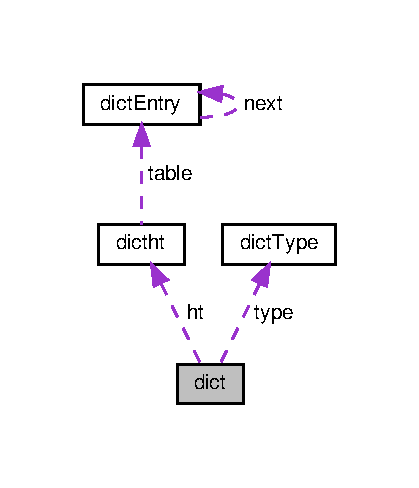
\includegraphics[width=201pt]{structdict__coll__graph}
\end{center}
\end{figure}
\subsection*{Data Fields}
\begin{DoxyCompactItemize}
\item 
\hyperlink{structdict_type}{dict\+Type} $\ast$ \hyperlink{structdict_a2db48c015f8daf59c847bd365a95b676}{type}
\item 
void $\ast$ \hyperlink{structdict_ac5df247494dd66a10946e2d67e56b2a1}{privdata}
\item 
\hyperlink{structdictht}{dictht} \hyperlink{structdict_ac1f889148f33e6ade337231d349f3e60}{ht} \mbox{[}2\mbox{]}
\item 
long \hyperlink{structdict_a5bd2593dd4365889f62bfd2481287311}{rehashidx}
\item 
unsigned long \hyperlink{structdict_a36dec5053bd1001c3ffea08aba76ce95}{iterators}
\end{DoxyCompactItemize}


\subsection{Detailed Description}


Definition at line 76 of file dict.\+h.



\subsection{Field Documentation}
\mbox{\Hypertarget{structdict_ac1f889148f33e6ade337231d349f3e60}\label{structdict_ac1f889148f33e6ade337231d349f3e60}} 
\index{dict@{dict}!ht@{ht}}
\index{ht@{ht}!dict@{dict}}
\subsubsection{\texorpdfstring{ht}{ht}}
{\footnotesize\ttfamily \hyperlink{structdictht}{dictht} ht\mbox{[}2\mbox{]}}



Definition at line 79 of file dict.\+h.

\mbox{\Hypertarget{structdict_a36dec5053bd1001c3ffea08aba76ce95}\label{structdict_a36dec5053bd1001c3ffea08aba76ce95}} 
\index{dict@{dict}!iterators@{iterators}}
\index{iterators@{iterators}!dict@{dict}}
\subsubsection{\texorpdfstring{iterators}{iterators}}
{\footnotesize\ttfamily unsigned long iterators}



Definition at line 81 of file dict.\+h.

\mbox{\Hypertarget{structdict_ac5df247494dd66a10946e2d67e56b2a1}\label{structdict_ac5df247494dd66a10946e2d67e56b2a1}} 
\index{dict@{dict}!privdata@{privdata}}
\index{privdata@{privdata}!dict@{dict}}
\subsubsection{\texorpdfstring{privdata}{privdata}}
{\footnotesize\ttfamily void$\ast$ privdata}



Definition at line 78 of file dict.\+h.

\mbox{\Hypertarget{structdict_a5bd2593dd4365889f62bfd2481287311}\label{structdict_a5bd2593dd4365889f62bfd2481287311}} 
\index{dict@{dict}!rehashidx@{rehashidx}}
\index{rehashidx@{rehashidx}!dict@{dict}}
\subsubsection{\texorpdfstring{rehashidx}{rehashidx}}
{\footnotesize\ttfamily long rehashidx}



Definition at line 80 of file dict.\+h.

\mbox{\Hypertarget{structdict_a2db48c015f8daf59c847bd365a95b676}\label{structdict_a2db48c015f8daf59c847bd365a95b676}} 
\index{dict@{dict}!type@{type}}
\index{type@{type}!dict@{dict}}
\subsubsection{\texorpdfstring{type}{type}}
{\footnotesize\ttfamily \hyperlink{structdict_type}{dict\+Type}$\ast$ type}



Definition at line 77 of file dict.\+h.



The documentation for this struct was generated from the following file\+:\begin{DoxyCompactItemize}
\item 
src/\hyperlink{dict_8h}{dict.\+h}\end{DoxyCompactItemize}

\hypertarget{structdict_entry}{}\section{dict\+Entry Struct Reference}
\label{structdict_entry}\index{dict\+Entry@{dict\+Entry}}


{\ttfamily \#include $<$dict.\+h$>$}



Collaboration diagram for dict\+Entry\+:
\nopagebreak
\begin{figure}[H]
\begin{center}
\leavevmode
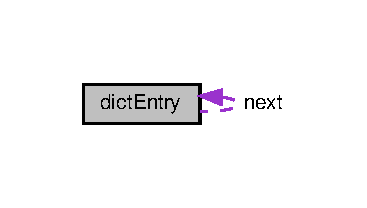
\includegraphics[width=176pt]{structdict_entry__coll__graph}
\end{center}
\end{figure}
\subsection*{Data Fields}
\begin{DoxyCompactItemize}
\item 
void $\ast$ \hyperlink{structdict_entry_ab5c000aec752f2206131e183daf5efbf}{key}
\item 
\begin{tabbing}
xx\=xx\=xx\=xx\=xx\=xx\=xx\=xx\=xx\=\kill
union \{\\
\>void $\ast$ \hyperlink{structdict_entry_ab03f36f103bdec81305fd301f1f93885}{val}\\
\>uint64\_t \hyperlink{structdict_entry_a91ee3b6e2425e78feef03fb5c69d63e5}{u64}\\
\>int64\_t \hyperlink{structdict_entry_ae66ed2ec20c2115ff9970c73168fc0df}{s64}\\
\>double \hyperlink{structdict_entry_a873684cefeb665f3d5e6b495de57fc0d}{d}\\
\} \hyperlink{structdict_entry_a365d8ec140a4da1dd6163174c1476783}{v}\\

\end{tabbing}\item 
struct \hyperlink{structdict_entry}{dict\+Entry} $\ast$ \hyperlink{structdict_entry_ac1e00303554dcf7f08f4a1a4eb81f398}{next}
\end{DoxyCompactItemize}


\subsection{Detailed Description}


Definition at line 47 of file dict.\+h.



\subsection{Field Documentation}
\mbox{\Hypertarget{structdict_entry_a873684cefeb665f3d5e6b495de57fc0d}\label{structdict_entry_a873684cefeb665f3d5e6b495de57fc0d}} 
\index{dict\+Entry@{dict\+Entry}!d@{d}}
\index{d@{d}!dict\+Entry@{dict\+Entry}}
\subsubsection{\texorpdfstring{d}{d}}
{\footnotesize\ttfamily double d}



Definition at line 53 of file dict.\+h.

\mbox{\Hypertarget{structdict_entry_ab5c000aec752f2206131e183daf5efbf}\label{structdict_entry_ab5c000aec752f2206131e183daf5efbf}} 
\index{dict\+Entry@{dict\+Entry}!key@{key}}
\index{key@{key}!dict\+Entry@{dict\+Entry}}
\subsubsection{\texorpdfstring{key}{key}}
{\footnotesize\ttfamily void$\ast$ key}



Definition at line 48 of file dict.\+h.

\mbox{\Hypertarget{structdict_entry_ac1e00303554dcf7f08f4a1a4eb81f398}\label{structdict_entry_ac1e00303554dcf7f08f4a1a4eb81f398}} 
\index{dict\+Entry@{dict\+Entry}!next@{next}}
\index{next@{next}!dict\+Entry@{dict\+Entry}}
\subsubsection{\texorpdfstring{next}{next}}
{\footnotesize\ttfamily struct \hyperlink{structdict_entry}{dict\+Entry}$\ast$ next}



Definition at line 55 of file dict.\+h.

\mbox{\Hypertarget{structdict_entry_ae66ed2ec20c2115ff9970c73168fc0df}\label{structdict_entry_ae66ed2ec20c2115ff9970c73168fc0df}} 
\index{dict\+Entry@{dict\+Entry}!s64@{s64}}
\index{s64@{s64}!dict\+Entry@{dict\+Entry}}
\subsubsection{\texorpdfstring{s64}{s64}}
{\footnotesize\ttfamily int64\+\_\+t s64}



Definition at line 52 of file dict.\+h.

\mbox{\Hypertarget{structdict_entry_a91ee3b6e2425e78feef03fb5c69d63e5}\label{structdict_entry_a91ee3b6e2425e78feef03fb5c69d63e5}} 
\index{dict\+Entry@{dict\+Entry}!u64@{u64}}
\index{u64@{u64}!dict\+Entry@{dict\+Entry}}
\subsubsection{\texorpdfstring{u64}{u64}}
{\footnotesize\ttfamily uint64\+\_\+t u64}



Definition at line 51 of file dict.\+h.

\mbox{\Hypertarget{structdict_entry_a365d8ec140a4da1dd6163174c1476783}\label{structdict_entry_a365d8ec140a4da1dd6163174c1476783}} 
\index{dict\+Entry@{dict\+Entry}!v@{v}}
\index{v@{v}!dict\+Entry@{dict\+Entry}}
\subsubsection{\texorpdfstring{v}{v}}
{\footnotesize\ttfamily union \{ ... \}   v}

\mbox{\Hypertarget{structdict_entry_ab03f36f103bdec81305fd301f1f93885}\label{structdict_entry_ab03f36f103bdec81305fd301f1f93885}} 
\index{dict\+Entry@{dict\+Entry}!val@{val}}
\index{val@{val}!dict\+Entry@{dict\+Entry}}
\subsubsection{\texorpdfstring{val}{val}}
{\footnotesize\ttfamily void$\ast$ val}



Definition at line 50 of file dict.\+h.



The documentation for this struct was generated from the following file\+:\begin{DoxyCompactItemize}
\item 
src/\hyperlink{dict_8h}{dict.\+h}\end{DoxyCompactItemize}

\hypertarget{structdictht}{}\section{dictht Struct Reference}
\label{structdictht}\index{dictht@{dictht}}


{\ttfamily \#include $<$dict.\+h$>$}



Collaboration diagram for dictht\+:
\nopagebreak
\begin{figure}[H]
\begin{center}
\leavevmode
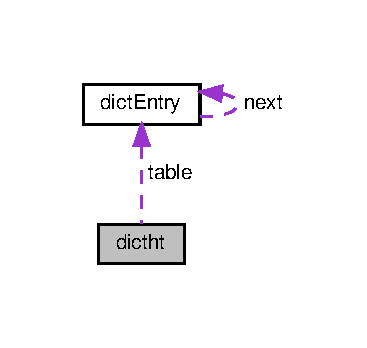
\includegraphics[width=176pt]{structdictht__coll__graph}
\end{center}
\end{figure}
\subsection*{Data Fields}
\begin{DoxyCompactItemize}
\item 
\hyperlink{structdict_entry}{dict\+Entry} $\ast$$\ast$ \hyperlink{structdictht_aa1d81eae7b1831354fd3e941a6c1192b}{table}
\item 
unsigned long \hyperlink{structdictht_a1e1268d164c38e4f8a4f4eb9058b0601}{size}
\item 
unsigned long \hyperlink{structdictht_aa2d44ea57263c4ae782cbbff2a131f2b}{sizemask}
\item 
unsigned long \hyperlink{structdictht_abeece48b2d7c09bffa9101df617478d0}{used}
\end{DoxyCompactItemize}


\subsection{Detailed Description}


Definition at line 69 of file dict.\+h.



\subsection{Field Documentation}
\mbox{\Hypertarget{structdictht_a1e1268d164c38e4f8a4f4eb9058b0601}\label{structdictht_a1e1268d164c38e4f8a4f4eb9058b0601}} 
\index{dictht@{dictht}!size@{size}}
\index{size@{size}!dictht@{dictht}}
\subsubsection{\texorpdfstring{size}{size}}
{\footnotesize\ttfamily unsigned long size}



Definition at line 71 of file dict.\+h.

\mbox{\Hypertarget{structdictht_aa2d44ea57263c4ae782cbbff2a131f2b}\label{structdictht_aa2d44ea57263c4ae782cbbff2a131f2b}} 
\index{dictht@{dictht}!sizemask@{sizemask}}
\index{sizemask@{sizemask}!dictht@{dictht}}
\subsubsection{\texorpdfstring{sizemask}{sizemask}}
{\footnotesize\ttfamily unsigned long sizemask}



Definition at line 72 of file dict.\+h.

\mbox{\Hypertarget{structdictht_aa1d81eae7b1831354fd3e941a6c1192b}\label{structdictht_aa1d81eae7b1831354fd3e941a6c1192b}} 
\index{dictht@{dictht}!table@{table}}
\index{table@{table}!dictht@{dictht}}
\subsubsection{\texorpdfstring{table}{table}}
{\footnotesize\ttfamily \hyperlink{structdict_entry}{dict\+Entry}$\ast$$\ast$ table}



Definition at line 70 of file dict.\+h.

\mbox{\Hypertarget{structdictht_abeece48b2d7c09bffa9101df617478d0}\label{structdictht_abeece48b2d7c09bffa9101df617478d0}} 
\index{dictht@{dictht}!used@{used}}
\index{used@{used}!dictht@{dictht}}
\subsubsection{\texorpdfstring{used}{used}}
{\footnotesize\ttfamily unsigned long used}



Definition at line 73 of file dict.\+h.



The documentation for this struct was generated from the following file\+:\begin{DoxyCompactItemize}
\item 
src/\hyperlink{dict_8h}{dict.\+h}\end{DoxyCompactItemize}

\hypertarget{structdict_iterator}{}\section{dict\+Iterator Struct Reference}
\label{structdict_iterator}\index{dict\+Iterator@{dict\+Iterator}}


{\ttfamily \#include $<$dict.\+h$>$}



Collaboration diagram for dict\+Iterator\+:
\nopagebreak
\begin{figure}[H]
\begin{center}
\leavevmode
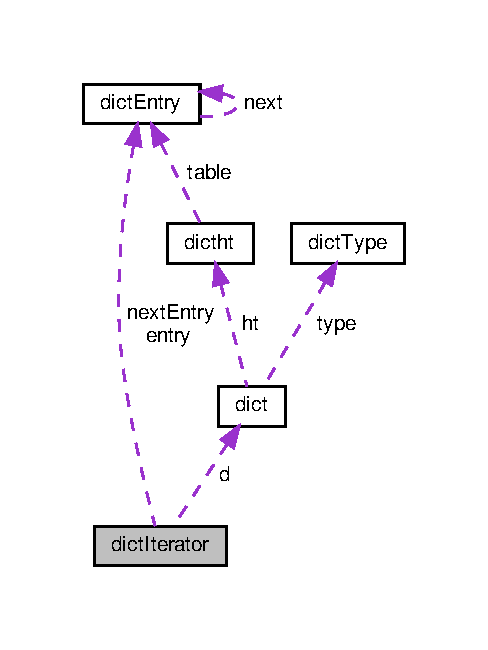
\includegraphics[width=234pt]{structdict_iterator__coll__graph}
\end{center}
\end{figure}
\subsection*{Data Fields}
\begin{DoxyCompactItemize}
\item 
\hyperlink{structdict}{dict} $\ast$ \hyperlink{structdict_iterator_a33c1b4f71e1cd72f4a8e828584426f49}{d}
\item 
long \hyperlink{structdict_iterator_a5d2f8fec06b0a536e0c8cbd1c0b64e09}{index}
\item 
int \hyperlink{structdict_iterator_a381b3daa303e1bdbac3a7b7000e0176c}{table}
\item 
int \hyperlink{structdict_iterator_a3165c7b86c85463f7d64defedf6b0d43}{safe}
\item 
\hyperlink{structdict_entry}{dict\+Entry} $\ast$ \hyperlink{structdict_iterator_aded8f8ee1a8ba420d3165db8ee65c26b}{entry}
\item 
\hyperlink{structdict_entry}{dict\+Entry} $\ast$ \hyperlink{structdict_iterator_a21d7b69d1530abaedbfd8df260733769}{next\+Entry}
\item 
long long \hyperlink{structdict_iterator_ae69415fa6d28d5311ba7ee5c24277398}{fingerprint}
\end{DoxyCompactItemize}


\subsection{Detailed Description}


Definition at line 88 of file dict.\+h.



\subsection{Field Documentation}
\mbox{\Hypertarget{structdict_iterator_a33c1b4f71e1cd72f4a8e828584426f49}\label{structdict_iterator_a33c1b4f71e1cd72f4a8e828584426f49}} 
\index{dict\+Iterator@{dict\+Iterator}!d@{d}}
\index{d@{d}!dict\+Iterator@{dict\+Iterator}}
\subsubsection{\texorpdfstring{d}{d}}
{\footnotesize\ttfamily \hyperlink{structdict}{dict}$\ast$ d}



Definition at line 89 of file dict.\+h.

\mbox{\Hypertarget{structdict_iterator_aded8f8ee1a8ba420d3165db8ee65c26b}\label{structdict_iterator_aded8f8ee1a8ba420d3165db8ee65c26b}} 
\index{dict\+Iterator@{dict\+Iterator}!entry@{entry}}
\index{entry@{entry}!dict\+Iterator@{dict\+Iterator}}
\subsubsection{\texorpdfstring{entry}{entry}}
{\footnotesize\ttfamily \hyperlink{structdict_entry}{dict\+Entry}$\ast$ entry}



Definition at line 92 of file dict.\+h.

\mbox{\Hypertarget{structdict_iterator_ae69415fa6d28d5311ba7ee5c24277398}\label{structdict_iterator_ae69415fa6d28d5311ba7ee5c24277398}} 
\index{dict\+Iterator@{dict\+Iterator}!fingerprint@{fingerprint}}
\index{fingerprint@{fingerprint}!dict\+Iterator@{dict\+Iterator}}
\subsubsection{\texorpdfstring{fingerprint}{fingerprint}}
{\footnotesize\ttfamily long long fingerprint}



Definition at line 94 of file dict.\+h.

\mbox{\Hypertarget{structdict_iterator_a5d2f8fec06b0a536e0c8cbd1c0b64e09}\label{structdict_iterator_a5d2f8fec06b0a536e0c8cbd1c0b64e09}} 
\index{dict\+Iterator@{dict\+Iterator}!index@{index}}
\index{index@{index}!dict\+Iterator@{dict\+Iterator}}
\subsubsection{\texorpdfstring{index}{index}}
{\footnotesize\ttfamily long index}



Definition at line 90 of file dict.\+h.

\mbox{\Hypertarget{structdict_iterator_a21d7b69d1530abaedbfd8df260733769}\label{structdict_iterator_a21d7b69d1530abaedbfd8df260733769}} 
\index{dict\+Iterator@{dict\+Iterator}!next\+Entry@{next\+Entry}}
\index{next\+Entry@{next\+Entry}!dict\+Iterator@{dict\+Iterator}}
\subsubsection{\texorpdfstring{next\+Entry}{nextEntry}}
{\footnotesize\ttfamily \hyperlink{structdict_entry}{dict\+Entry} $\ast$ next\+Entry}



Definition at line 92 of file dict.\+h.

\mbox{\Hypertarget{structdict_iterator_a3165c7b86c85463f7d64defedf6b0d43}\label{structdict_iterator_a3165c7b86c85463f7d64defedf6b0d43}} 
\index{dict\+Iterator@{dict\+Iterator}!safe@{safe}}
\index{safe@{safe}!dict\+Iterator@{dict\+Iterator}}
\subsubsection{\texorpdfstring{safe}{safe}}
{\footnotesize\ttfamily int safe}



Definition at line 91 of file dict.\+h.

\mbox{\Hypertarget{structdict_iterator_a381b3daa303e1bdbac3a7b7000e0176c}\label{structdict_iterator_a381b3daa303e1bdbac3a7b7000e0176c}} 
\index{dict\+Iterator@{dict\+Iterator}!table@{table}}
\index{table@{table}!dict\+Iterator@{dict\+Iterator}}
\subsubsection{\texorpdfstring{table}{table}}
{\footnotesize\ttfamily int table}



Definition at line 91 of file dict.\+h.



The documentation for this struct was generated from the following file\+:\begin{DoxyCompactItemize}
\item 
src/\hyperlink{dict_8h}{dict.\+h}\end{DoxyCompactItemize}

\hypertarget{structdict_type}{}\section{dict\+Type Struct Reference}
\label{structdict_type}\index{dict\+Type@{dict\+Type}}


{\ttfamily \#include $<$dict.\+h$>$}

\subsection*{Data Fields}
\begin{DoxyCompactItemize}
\item 
uint64\+\_\+t($\ast$ \hyperlink{structdict_type_a5811d50ea6030aac37ddc86d8fbc9a60}{hash\+Function} )(const void $\ast$\hyperlink{redis-check-rdb_8c_adc0ee0ed345db513fb6fac27511be4f1}{key})
\item 
void $\ast$($\ast$ \hyperlink{structdict_type_a2dd82eb7e0e1186bb12e07019818e4c0}{key\+Dup} )(void $\ast$privdata, const void $\ast$\hyperlink{redis-check-rdb_8c_adc0ee0ed345db513fb6fac27511be4f1}{key})
\item 
void $\ast$($\ast$ \hyperlink{structdict_type_a62279ffb4ad0b5054041285dbe54395f}{val\+Dup} )(void $\ast$privdata, const void $\ast$obj)
\item 
int($\ast$ \hyperlink{structdict_type_af973749ac3c53be917942afd20eeea0e}{key\+Compare} )(void $\ast$privdata, const void $\ast$key1, const void $\ast$key2)
\item 
void($\ast$ \hyperlink{structdict_type_a55bd09e65ce2b078c4d292dba93c8714}{key\+Destructor} )(void $\ast$privdata, void $\ast$\hyperlink{redis-check-rdb_8c_adc0ee0ed345db513fb6fac27511be4f1}{key})
\item 
void($\ast$ \hyperlink{structdict_type_adcae86192e4646f56c473a7e64fed530}{val\+Destructor} )(void $\ast$privdata, void $\ast$obj)
\end{DoxyCompactItemize}


\subsection{Detailed Description}


Definition at line 58 of file dict.\+h.



\subsection{Field Documentation}
\mbox{\Hypertarget{structdict_type_a5811d50ea6030aac37ddc86d8fbc9a60}\label{structdict_type_a5811d50ea6030aac37ddc86d8fbc9a60}} 
\index{dict\+Type@{dict\+Type}!hash\+Function@{hash\+Function}}
\index{hash\+Function@{hash\+Function}!dict\+Type@{dict\+Type}}
\subsubsection{\texorpdfstring{hash\+Function}{hashFunction}}
{\footnotesize\ttfamily uint64\+\_\+t($\ast$ hash\+Function) (const void $\ast$\hyperlink{redis-check-rdb_8c_adc0ee0ed345db513fb6fac27511be4f1}{key})}



Definition at line 59 of file dict.\+h.

\mbox{\Hypertarget{structdict_type_af973749ac3c53be917942afd20eeea0e}\label{structdict_type_af973749ac3c53be917942afd20eeea0e}} 
\index{dict\+Type@{dict\+Type}!key\+Compare@{key\+Compare}}
\index{key\+Compare@{key\+Compare}!dict\+Type@{dict\+Type}}
\subsubsection{\texorpdfstring{key\+Compare}{keyCompare}}
{\footnotesize\ttfamily int($\ast$ key\+Compare) (void $\ast$privdata, const void $\ast$key1, const void $\ast$key2)}



Definition at line 62 of file dict.\+h.

\mbox{\Hypertarget{structdict_type_a55bd09e65ce2b078c4d292dba93c8714}\label{structdict_type_a55bd09e65ce2b078c4d292dba93c8714}} 
\index{dict\+Type@{dict\+Type}!key\+Destructor@{key\+Destructor}}
\index{key\+Destructor@{key\+Destructor}!dict\+Type@{dict\+Type}}
\subsubsection{\texorpdfstring{key\+Destructor}{keyDestructor}}
{\footnotesize\ttfamily void($\ast$ key\+Destructor) (void $\ast$privdata, void $\ast$\hyperlink{redis-check-rdb_8c_adc0ee0ed345db513fb6fac27511be4f1}{key})}



Definition at line 63 of file dict.\+h.

\mbox{\Hypertarget{structdict_type_a2dd82eb7e0e1186bb12e07019818e4c0}\label{structdict_type_a2dd82eb7e0e1186bb12e07019818e4c0}} 
\index{dict\+Type@{dict\+Type}!key\+Dup@{key\+Dup}}
\index{key\+Dup@{key\+Dup}!dict\+Type@{dict\+Type}}
\subsubsection{\texorpdfstring{key\+Dup}{keyDup}}
{\footnotesize\ttfamily void$\ast$($\ast$ key\+Dup) (void $\ast$privdata, const void $\ast$\hyperlink{redis-check-rdb_8c_adc0ee0ed345db513fb6fac27511be4f1}{key})}



Definition at line 60 of file dict.\+h.

\mbox{\Hypertarget{structdict_type_adcae86192e4646f56c473a7e64fed530}\label{structdict_type_adcae86192e4646f56c473a7e64fed530}} 
\index{dict\+Type@{dict\+Type}!val\+Destructor@{val\+Destructor}}
\index{val\+Destructor@{val\+Destructor}!dict\+Type@{dict\+Type}}
\subsubsection{\texorpdfstring{val\+Destructor}{valDestructor}}
{\footnotesize\ttfamily void($\ast$ val\+Destructor) (void $\ast$privdata, void $\ast$obj)}



Definition at line 64 of file dict.\+h.

\mbox{\Hypertarget{structdict_type_a62279ffb4ad0b5054041285dbe54395f}\label{structdict_type_a62279ffb4ad0b5054041285dbe54395f}} 
\index{dict\+Type@{dict\+Type}!val\+Dup@{val\+Dup}}
\index{val\+Dup@{val\+Dup}!dict\+Type@{dict\+Type}}
\subsubsection{\texorpdfstring{val\+Dup}{valDup}}
{\footnotesize\ttfamily void$\ast$($\ast$ val\+Dup) (void $\ast$privdata, const void $\ast$obj)}



Definition at line 61 of file dict.\+h.



The documentation for this struct was generated from the following file\+:\begin{DoxyCompactItemize}
\item 
src/\hyperlink{dict_8h}{dict.\+h}\end{DoxyCompactItemize}

\hypertarget{structdistsamples}{}\section{distsamples Struct Reference}
\label{structdistsamples}\index{distsamples@{distsamples}}
\subsection*{Data Fields}
\begin{DoxyCompactItemize}
\item 
long long \hyperlink{structdistsamples_a3cc3af20c4a8a67e42db241f8e90472b}{max}
\item 
long long \hyperlink{structdistsamples_a3171cac2da70b2ce888d76a879f32c5b}{count}
\item 
int \hyperlink{structdistsamples_af36ff273acc44c769de8e2f44a081dca}{character}
\end{DoxyCompactItemize}


\subsection{Detailed Description}


Definition at line 5421 of file redis-\/cli.\+c.



\subsection{Field Documentation}
\mbox{\Hypertarget{structdistsamples_af36ff273acc44c769de8e2f44a081dca}\label{structdistsamples_af36ff273acc44c769de8e2f44a081dca}} 
\index{distsamples@{distsamples}!character@{character}}
\index{character@{character}!distsamples@{distsamples}}
\subsubsection{\texorpdfstring{character}{character}}
{\footnotesize\ttfamily int character}



Definition at line 5424 of file redis-\/cli.\+c.

\mbox{\Hypertarget{structdistsamples_a3171cac2da70b2ce888d76a879f32c5b}\label{structdistsamples_a3171cac2da70b2ce888d76a879f32c5b}} 
\index{distsamples@{distsamples}!count@{count}}
\index{count@{count}!distsamples@{distsamples}}
\subsubsection{\texorpdfstring{count}{count}}
{\footnotesize\ttfamily long long count}



Definition at line 5423 of file redis-\/cli.\+c.

\mbox{\Hypertarget{structdistsamples_a3cc3af20c4a8a67e42db241f8e90472b}\label{structdistsamples_a3cc3af20c4a8a67e42db241f8e90472b}} 
\index{distsamples@{distsamples}!max@{max}}
\index{max@{max}!distsamples@{distsamples}}
\subsubsection{\texorpdfstring{max}{max}}
{\footnotesize\ttfamily long long max}



Definition at line 5422 of file redis-\/cli.\+c.



The documentation for this struct was generated from the following file\+:\begin{DoxyCompactItemize}
\item 
src/\hyperlink{redis-cli_8c}{redis-\/cli.\+c}\end{DoxyCompactItemize}

\hypertarget{structeviction_pool_entry}{}\section{eviction\+Pool\+Entry Struct Reference}
\label{structeviction_pool_entry}\index{eviction\+Pool\+Entry@{eviction\+Pool\+Entry}}
\subsection*{Data Fields}
\begin{DoxyCompactItemize}
\item 
unsigned long long \hyperlink{structeviction_pool_entry_a33e435ed79bd42a3e152e820d2fe9c59}{idle}
\item 
\hyperlink{sds_8h_ad69abac3df4532879db9642c95f5ef6f}{sds} \hyperlink{structeviction_pool_entry_a46666a67588d8b58e5f36934ee61ea81}{key}
\item 
\hyperlink{sds_8h_ad69abac3df4532879db9642c95f5ef6f}{sds} \hyperlink{structeviction_pool_entry_a065beeed34d1258c35467721dcdf6a67}{cached}
\item 
int \hyperlink{structeviction_pool_entry_adc62368127157e2b3ff9cabe77f4f337}{dbid}
\end{DoxyCompactItemize}


\subsection{Detailed Description}


Definition at line 54 of file evict.\+c.



\subsection{Field Documentation}
\mbox{\Hypertarget{structeviction_pool_entry_a065beeed34d1258c35467721dcdf6a67}\label{structeviction_pool_entry_a065beeed34d1258c35467721dcdf6a67}} 
\index{eviction\+Pool\+Entry@{eviction\+Pool\+Entry}!cached@{cached}}
\index{cached@{cached}!eviction\+Pool\+Entry@{eviction\+Pool\+Entry}}
\subsubsection{\texorpdfstring{cached}{cached}}
{\footnotesize\ttfamily \hyperlink{sds_8h_ad69abac3df4532879db9642c95f5ef6f}{sds} cached}



Definition at line 57 of file evict.\+c.

\mbox{\Hypertarget{structeviction_pool_entry_adc62368127157e2b3ff9cabe77f4f337}\label{structeviction_pool_entry_adc62368127157e2b3ff9cabe77f4f337}} 
\index{eviction\+Pool\+Entry@{eviction\+Pool\+Entry}!dbid@{dbid}}
\index{dbid@{dbid}!eviction\+Pool\+Entry@{eviction\+Pool\+Entry}}
\subsubsection{\texorpdfstring{dbid}{dbid}}
{\footnotesize\ttfamily int dbid}



Definition at line 58 of file evict.\+c.

\mbox{\Hypertarget{structeviction_pool_entry_a33e435ed79bd42a3e152e820d2fe9c59}\label{structeviction_pool_entry_a33e435ed79bd42a3e152e820d2fe9c59}} 
\index{eviction\+Pool\+Entry@{eviction\+Pool\+Entry}!idle@{idle}}
\index{idle@{idle}!eviction\+Pool\+Entry@{eviction\+Pool\+Entry}}
\subsubsection{\texorpdfstring{idle}{idle}}
{\footnotesize\ttfamily unsigned long long idle}



Definition at line 55 of file evict.\+c.

\mbox{\Hypertarget{structeviction_pool_entry_a46666a67588d8b58e5f36934ee61ea81}\label{structeviction_pool_entry_a46666a67588d8b58e5f36934ee61ea81}} 
\index{eviction\+Pool\+Entry@{eviction\+Pool\+Entry}!key@{key}}
\index{key@{key}!eviction\+Pool\+Entry@{eviction\+Pool\+Entry}}
\subsubsection{\texorpdfstring{key}{key}}
{\footnotesize\ttfamily \hyperlink{sds_8h_ad69abac3df4532879db9642c95f5ef6f}{sds} key}



Definition at line 56 of file evict.\+c.



The documentation for this struct was generated from the following file\+:\begin{DoxyCompactItemize}
\item 
src/\hyperlink{evict_8c}{evict.\+c}\end{DoxyCompactItemize}

\hypertarget{structgeo_array}{}\section{geo\+Array Struct Reference}
\label{structgeo_array}\index{geo\+Array@{geo\+Array}}


{\ttfamily \#include $<$geo.\+h$>$}



Collaboration diagram for geo\+Array\+:
\nopagebreak
\begin{figure}[H]
\begin{center}
\leavevmode
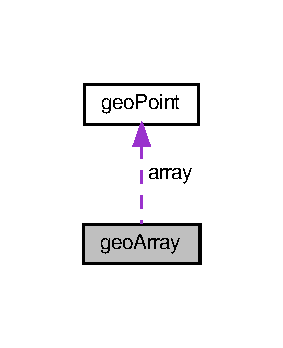
\includegraphics[width=136pt]{structgeo_array__coll__graph}
\end{center}
\end{figure}
\subsection*{Data Fields}
\begin{DoxyCompactItemize}
\item 
struct \hyperlink{structgeo_point}{geo\+Point} $\ast$ \hyperlink{structgeo_array_a4a1c0417f521d45e91edb7052f322bc7}{array}
\item 
size\+\_\+t \hyperlink{structgeo_array_af69e9b05b4318b72a5be55082b78fb58}{buckets}
\item 
size\+\_\+t \hyperlink{structgeo_array_ae8cc011bf3ee2d3c19743095ffc0f7a5}{used}
\end{DoxyCompactItemize}


\subsection{Detailed Description}


Definition at line 16 of file geo.\+h.



\subsection{Field Documentation}
\mbox{\Hypertarget{structgeo_array_a4a1c0417f521d45e91edb7052f322bc7}\label{structgeo_array_a4a1c0417f521d45e91edb7052f322bc7}} 
\index{geo\+Array@{geo\+Array}!array@{array}}
\index{array@{array}!geo\+Array@{geo\+Array}}
\subsubsection{\texorpdfstring{array}{array}}
{\footnotesize\ttfamily struct \hyperlink{structgeo_point}{geo\+Point}$\ast$ array}



Definition at line 17 of file geo.\+h.

\mbox{\Hypertarget{structgeo_array_af69e9b05b4318b72a5be55082b78fb58}\label{structgeo_array_af69e9b05b4318b72a5be55082b78fb58}} 
\index{geo\+Array@{geo\+Array}!buckets@{buckets}}
\index{buckets@{buckets}!geo\+Array@{geo\+Array}}
\subsubsection{\texorpdfstring{buckets}{buckets}}
{\footnotesize\ttfamily size\+\_\+t buckets}



Definition at line 18 of file geo.\+h.

\mbox{\Hypertarget{structgeo_array_ae8cc011bf3ee2d3c19743095ffc0f7a5}\label{structgeo_array_ae8cc011bf3ee2d3c19743095ffc0f7a5}} 
\index{geo\+Array@{geo\+Array}!used@{used}}
\index{used@{used}!geo\+Array@{geo\+Array}}
\subsubsection{\texorpdfstring{used}{used}}
{\footnotesize\ttfamily size\+\_\+t used}



Definition at line 19 of file geo.\+h.



The documentation for this struct was generated from the following file\+:\begin{DoxyCompactItemize}
\item 
src/\hyperlink{geo_8h}{geo.\+h}\end{DoxyCompactItemize}

\hypertarget{struct_geo_hash_area}{}\section{Geo\+Hash\+Area Struct Reference}
\label{struct_geo_hash_area}\index{Geo\+Hash\+Area@{Geo\+Hash\+Area}}


{\ttfamily \#include $<$geohash.\+h$>$}



Collaboration diagram for Geo\+Hash\+Area\+:
\nopagebreak
\begin{figure}[H]
\begin{center}
\leavevmode
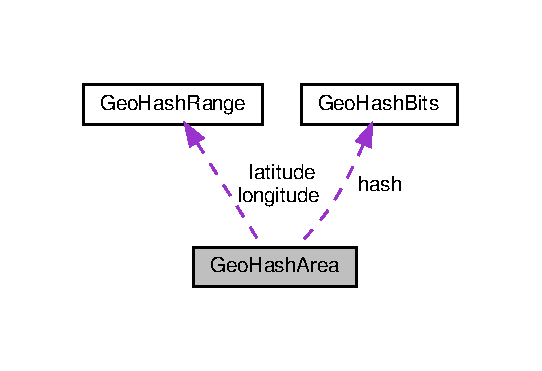
\includegraphics[width=260pt]{struct_geo_hash_area__coll__graph}
\end{center}
\end{figure}
\subsection*{Data Fields}
\begin{DoxyCompactItemize}
\item 
\hyperlink{struct_geo_hash_bits}{Geo\+Hash\+Bits} \hyperlink{struct_geo_hash_area_aaa5dc202256f654179069f62d2d44cf6}{hash}
\item 
\hyperlink{struct_geo_hash_range}{Geo\+Hash\+Range} \hyperlink{struct_geo_hash_area_ac9676284dd4031f83c6bf264b79267c6}{longitude}
\item 
\hyperlink{struct_geo_hash_range}{Geo\+Hash\+Range} \hyperlink{struct_geo_hash_area_a131bc0a0b8951efaf43616802da61d34}{latitude}
\end{DoxyCompactItemize}


\subsection{Detailed Description}


Definition at line 76 of file geohash.\+h.



\subsection{Field Documentation}
\mbox{\Hypertarget{struct_geo_hash_area_aaa5dc202256f654179069f62d2d44cf6}\label{struct_geo_hash_area_aaa5dc202256f654179069f62d2d44cf6}} 
\index{Geo\+Hash\+Area@{Geo\+Hash\+Area}!hash@{hash}}
\index{hash@{hash}!Geo\+Hash\+Area@{Geo\+Hash\+Area}}
\subsubsection{\texorpdfstring{hash}{hash}}
{\footnotesize\ttfamily \hyperlink{struct_geo_hash_bits}{Geo\+Hash\+Bits} hash}



Definition at line 77 of file geohash.\+h.

\mbox{\Hypertarget{struct_geo_hash_area_a131bc0a0b8951efaf43616802da61d34}\label{struct_geo_hash_area_a131bc0a0b8951efaf43616802da61d34}} 
\index{Geo\+Hash\+Area@{Geo\+Hash\+Area}!latitude@{latitude}}
\index{latitude@{latitude}!Geo\+Hash\+Area@{Geo\+Hash\+Area}}
\subsubsection{\texorpdfstring{latitude}{latitude}}
{\footnotesize\ttfamily \hyperlink{struct_geo_hash_range}{Geo\+Hash\+Range} latitude}



Definition at line 79 of file geohash.\+h.

\mbox{\Hypertarget{struct_geo_hash_area_ac9676284dd4031f83c6bf264b79267c6}\label{struct_geo_hash_area_ac9676284dd4031f83c6bf264b79267c6}} 
\index{Geo\+Hash\+Area@{Geo\+Hash\+Area}!longitude@{longitude}}
\index{longitude@{longitude}!Geo\+Hash\+Area@{Geo\+Hash\+Area}}
\subsubsection{\texorpdfstring{longitude}{longitude}}
{\footnotesize\ttfamily \hyperlink{struct_geo_hash_range}{Geo\+Hash\+Range} longitude}



Definition at line 78 of file geohash.\+h.



The documentation for this struct was generated from the following file\+:\begin{DoxyCompactItemize}
\item 
src/\hyperlink{geohash_8h}{geohash.\+h}\end{DoxyCompactItemize}

\hypertarget{struct_geo_hash_bits}{}\section{Geo\+Hash\+Bits Struct Reference}
\label{struct_geo_hash_bits}\index{Geo\+Hash\+Bits@{Geo\+Hash\+Bits}}


{\ttfamily \#include $<$geohash.\+h$>$}

\subsection*{Data Fields}
\begin{DoxyCompactItemize}
\item 
uint64\+\_\+t \hyperlink{struct_geo_hash_bits_a824af546b997aeefcb71a5fe0eda3a0a}{bits}
\item 
uint8\+\_\+t \hyperlink{struct_geo_hash_bits_a4a2eb71e89c989655301c2f2070e29b3}{step}
\end{DoxyCompactItemize}


\subsection{Detailed Description}


Definition at line 66 of file geohash.\+h.



\subsection{Field Documentation}
\mbox{\Hypertarget{struct_geo_hash_bits_a824af546b997aeefcb71a5fe0eda3a0a}\label{struct_geo_hash_bits_a824af546b997aeefcb71a5fe0eda3a0a}} 
\index{Geo\+Hash\+Bits@{Geo\+Hash\+Bits}!bits@{bits}}
\index{bits@{bits}!Geo\+Hash\+Bits@{Geo\+Hash\+Bits}}
\subsubsection{\texorpdfstring{bits}{bits}}
{\footnotesize\ttfamily uint64\+\_\+t bits}



Definition at line 67 of file geohash.\+h.

\mbox{\Hypertarget{struct_geo_hash_bits_a4a2eb71e89c989655301c2f2070e29b3}\label{struct_geo_hash_bits_a4a2eb71e89c989655301c2f2070e29b3}} 
\index{Geo\+Hash\+Bits@{Geo\+Hash\+Bits}!step@{step}}
\index{step@{step}!Geo\+Hash\+Bits@{Geo\+Hash\+Bits}}
\subsubsection{\texorpdfstring{step}{step}}
{\footnotesize\ttfamily uint8\+\_\+t step}



Definition at line 68 of file geohash.\+h.



The documentation for this struct was generated from the following file\+:\begin{DoxyCompactItemize}
\item 
src/\hyperlink{geohash_8h}{geohash.\+h}\end{DoxyCompactItemize}

\hypertarget{struct_geo_hash_neighbors}{}\section{Geo\+Hash\+Neighbors Struct Reference}
\label{struct_geo_hash_neighbors}\index{Geo\+Hash\+Neighbors@{Geo\+Hash\+Neighbors}}


{\ttfamily \#include $<$geohash.\+h$>$}



Collaboration diagram for Geo\+Hash\+Neighbors\+:
\nopagebreak
\begin{figure}[H]
\begin{center}
\leavevmode
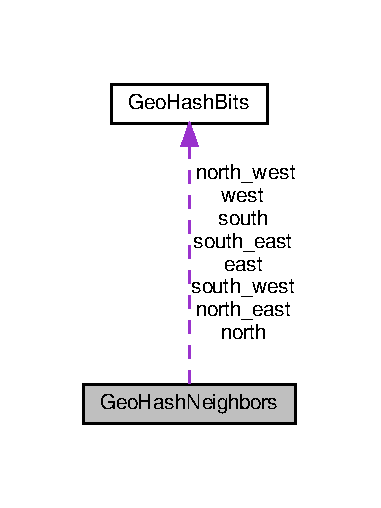
\includegraphics[width=183pt]{struct_geo_hash_neighbors__coll__graph}
\end{center}
\end{figure}
\subsection*{Data Fields}
\begin{DoxyCompactItemize}
\item 
\hyperlink{struct_geo_hash_bits}{Geo\+Hash\+Bits} \hyperlink{struct_geo_hash_neighbors_ab3987f87ddeaec65ee9d85e1aa2b17c1}{north}
\item 
\hyperlink{struct_geo_hash_bits}{Geo\+Hash\+Bits} \hyperlink{struct_geo_hash_neighbors_a294392f413a5a059186ad92e0c810bc6}{east}
\item 
\hyperlink{struct_geo_hash_bits}{Geo\+Hash\+Bits} \hyperlink{struct_geo_hash_neighbors_a978b3a96b71db2c564f99aa5246cbb68}{west}
\item 
\hyperlink{struct_geo_hash_bits}{Geo\+Hash\+Bits} \hyperlink{struct_geo_hash_neighbors_a295756ba624169a6836bfe8fad69c592}{south}
\item 
\hyperlink{struct_geo_hash_bits}{Geo\+Hash\+Bits} \hyperlink{struct_geo_hash_neighbors_afeec2c92a9761e906ec87add9cd79c53}{north\+\_\+east}
\item 
\hyperlink{struct_geo_hash_bits}{Geo\+Hash\+Bits} \hyperlink{struct_geo_hash_neighbors_aa7aeb35d5a8f971e791be557068f140d}{south\+\_\+east}
\item 
\hyperlink{struct_geo_hash_bits}{Geo\+Hash\+Bits} \hyperlink{struct_geo_hash_neighbors_a9f9cd9ee352daae139aed5fa9f8a91a7}{north\+\_\+west}
\item 
\hyperlink{struct_geo_hash_bits}{Geo\+Hash\+Bits} \hyperlink{struct_geo_hash_neighbors_ab9b9fcb9d8039a5198d21cafdb6529a5}{south\+\_\+west}
\end{DoxyCompactItemize}


\subsection{Detailed Description}


Definition at line 82 of file geohash.\+h.



\subsection{Field Documentation}
\mbox{\Hypertarget{struct_geo_hash_neighbors_a294392f413a5a059186ad92e0c810bc6}\label{struct_geo_hash_neighbors_a294392f413a5a059186ad92e0c810bc6}} 
\index{Geo\+Hash\+Neighbors@{Geo\+Hash\+Neighbors}!east@{east}}
\index{east@{east}!Geo\+Hash\+Neighbors@{Geo\+Hash\+Neighbors}}
\subsubsection{\texorpdfstring{east}{east}}
{\footnotesize\ttfamily \hyperlink{struct_geo_hash_bits}{Geo\+Hash\+Bits} east}



Definition at line 84 of file geohash.\+h.

\mbox{\Hypertarget{struct_geo_hash_neighbors_ab3987f87ddeaec65ee9d85e1aa2b17c1}\label{struct_geo_hash_neighbors_ab3987f87ddeaec65ee9d85e1aa2b17c1}} 
\index{Geo\+Hash\+Neighbors@{Geo\+Hash\+Neighbors}!north@{north}}
\index{north@{north}!Geo\+Hash\+Neighbors@{Geo\+Hash\+Neighbors}}
\subsubsection{\texorpdfstring{north}{north}}
{\footnotesize\ttfamily \hyperlink{struct_geo_hash_bits}{Geo\+Hash\+Bits} north}



Definition at line 83 of file geohash.\+h.

\mbox{\Hypertarget{struct_geo_hash_neighbors_afeec2c92a9761e906ec87add9cd79c53}\label{struct_geo_hash_neighbors_afeec2c92a9761e906ec87add9cd79c53}} 
\index{Geo\+Hash\+Neighbors@{Geo\+Hash\+Neighbors}!north\+\_\+east@{north\+\_\+east}}
\index{north\+\_\+east@{north\+\_\+east}!Geo\+Hash\+Neighbors@{Geo\+Hash\+Neighbors}}
\subsubsection{\texorpdfstring{north\+\_\+east}{north\_east}}
{\footnotesize\ttfamily \hyperlink{struct_geo_hash_bits}{Geo\+Hash\+Bits} north\+\_\+east}



Definition at line 87 of file geohash.\+h.

\mbox{\Hypertarget{struct_geo_hash_neighbors_a9f9cd9ee352daae139aed5fa9f8a91a7}\label{struct_geo_hash_neighbors_a9f9cd9ee352daae139aed5fa9f8a91a7}} 
\index{Geo\+Hash\+Neighbors@{Geo\+Hash\+Neighbors}!north\+\_\+west@{north\+\_\+west}}
\index{north\+\_\+west@{north\+\_\+west}!Geo\+Hash\+Neighbors@{Geo\+Hash\+Neighbors}}
\subsubsection{\texorpdfstring{north\+\_\+west}{north\_west}}
{\footnotesize\ttfamily \hyperlink{struct_geo_hash_bits}{Geo\+Hash\+Bits} north\+\_\+west}



Definition at line 89 of file geohash.\+h.

\mbox{\Hypertarget{struct_geo_hash_neighbors_a295756ba624169a6836bfe8fad69c592}\label{struct_geo_hash_neighbors_a295756ba624169a6836bfe8fad69c592}} 
\index{Geo\+Hash\+Neighbors@{Geo\+Hash\+Neighbors}!south@{south}}
\index{south@{south}!Geo\+Hash\+Neighbors@{Geo\+Hash\+Neighbors}}
\subsubsection{\texorpdfstring{south}{south}}
{\footnotesize\ttfamily \hyperlink{struct_geo_hash_bits}{Geo\+Hash\+Bits} south}



Definition at line 86 of file geohash.\+h.

\mbox{\Hypertarget{struct_geo_hash_neighbors_aa7aeb35d5a8f971e791be557068f140d}\label{struct_geo_hash_neighbors_aa7aeb35d5a8f971e791be557068f140d}} 
\index{Geo\+Hash\+Neighbors@{Geo\+Hash\+Neighbors}!south\+\_\+east@{south\+\_\+east}}
\index{south\+\_\+east@{south\+\_\+east}!Geo\+Hash\+Neighbors@{Geo\+Hash\+Neighbors}}
\subsubsection{\texorpdfstring{south\+\_\+east}{south\_east}}
{\footnotesize\ttfamily \hyperlink{struct_geo_hash_bits}{Geo\+Hash\+Bits} south\+\_\+east}



Definition at line 88 of file geohash.\+h.

\mbox{\Hypertarget{struct_geo_hash_neighbors_ab9b9fcb9d8039a5198d21cafdb6529a5}\label{struct_geo_hash_neighbors_ab9b9fcb9d8039a5198d21cafdb6529a5}} 
\index{Geo\+Hash\+Neighbors@{Geo\+Hash\+Neighbors}!south\+\_\+west@{south\+\_\+west}}
\index{south\+\_\+west@{south\+\_\+west}!Geo\+Hash\+Neighbors@{Geo\+Hash\+Neighbors}}
\subsubsection{\texorpdfstring{south\+\_\+west}{south\_west}}
{\footnotesize\ttfamily \hyperlink{struct_geo_hash_bits}{Geo\+Hash\+Bits} south\+\_\+west}



Definition at line 90 of file geohash.\+h.

\mbox{\Hypertarget{struct_geo_hash_neighbors_a978b3a96b71db2c564f99aa5246cbb68}\label{struct_geo_hash_neighbors_a978b3a96b71db2c564f99aa5246cbb68}} 
\index{Geo\+Hash\+Neighbors@{Geo\+Hash\+Neighbors}!west@{west}}
\index{west@{west}!Geo\+Hash\+Neighbors@{Geo\+Hash\+Neighbors}}
\subsubsection{\texorpdfstring{west}{west}}
{\footnotesize\ttfamily \hyperlink{struct_geo_hash_bits}{Geo\+Hash\+Bits} west}



Definition at line 85 of file geohash.\+h.



The documentation for this struct was generated from the following file\+:\begin{DoxyCompactItemize}
\item 
src/\hyperlink{geohash_8h}{geohash.\+h}\end{DoxyCompactItemize}

\hypertarget{struct_geo_hash_radius}{}\section{Geo\+Hash\+Radius Struct Reference}
\label{struct_geo_hash_radius}\index{Geo\+Hash\+Radius@{Geo\+Hash\+Radius}}


{\ttfamily \#include $<$geohash\+\_\+helper.\+h$>$}



Collaboration diagram for Geo\+Hash\+Radius\+:
\nopagebreak
\begin{figure}[H]
\begin{center}
\leavevmode
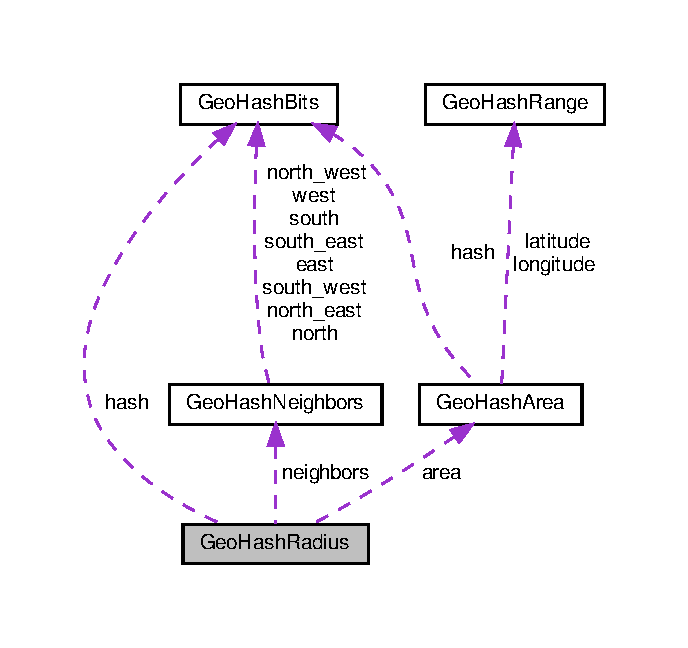
\includegraphics[width=330pt]{struct_geo_hash_radius__coll__graph}
\end{center}
\end{figure}
\subsection*{Data Fields}
\begin{DoxyCompactItemize}
\item 
\hyperlink{struct_geo_hash_bits}{Geo\+Hash\+Bits} \hyperlink{struct_geo_hash_radius_aaa5dc202256f654179069f62d2d44cf6}{hash}
\item 
\hyperlink{struct_geo_hash_area}{Geo\+Hash\+Area} \hyperlink{struct_geo_hash_radius_ab8ed53e3d15a3c96c0b699110d1b3d69}{area}
\item 
\hyperlink{struct_geo_hash_neighbors}{Geo\+Hash\+Neighbors} \hyperlink{struct_geo_hash_radius_a2294fb3cd98344a75f1e5960818f2a31}{neighbors}
\end{DoxyCompactItemize}


\subsection{Detailed Description}


Definition at line 44 of file geohash\+\_\+helper.\+h.



\subsection{Field Documentation}
\mbox{\Hypertarget{struct_geo_hash_radius_ab8ed53e3d15a3c96c0b699110d1b3d69}\label{struct_geo_hash_radius_ab8ed53e3d15a3c96c0b699110d1b3d69}} 
\index{Geo\+Hash\+Radius@{Geo\+Hash\+Radius}!area@{area}}
\index{area@{area}!Geo\+Hash\+Radius@{Geo\+Hash\+Radius}}
\subsubsection{\texorpdfstring{area}{area}}
{\footnotesize\ttfamily \hyperlink{struct_geo_hash_area}{Geo\+Hash\+Area} area}



Definition at line 46 of file geohash\+\_\+helper.\+h.

\mbox{\Hypertarget{struct_geo_hash_radius_aaa5dc202256f654179069f62d2d44cf6}\label{struct_geo_hash_radius_aaa5dc202256f654179069f62d2d44cf6}} 
\index{Geo\+Hash\+Radius@{Geo\+Hash\+Radius}!hash@{hash}}
\index{hash@{hash}!Geo\+Hash\+Radius@{Geo\+Hash\+Radius}}
\subsubsection{\texorpdfstring{hash}{hash}}
{\footnotesize\ttfamily \hyperlink{struct_geo_hash_bits}{Geo\+Hash\+Bits} hash}



Definition at line 45 of file geohash\+\_\+helper.\+h.

\mbox{\Hypertarget{struct_geo_hash_radius_a2294fb3cd98344a75f1e5960818f2a31}\label{struct_geo_hash_radius_a2294fb3cd98344a75f1e5960818f2a31}} 
\index{Geo\+Hash\+Radius@{Geo\+Hash\+Radius}!neighbors@{neighbors}}
\index{neighbors@{neighbors}!Geo\+Hash\+Radius@{Geo\+Hash\+Radius}}
\subsubsection{\texorpdfstring{neighbors}{neighbors}}
{\footnotesize\ttfamily \hyperlink{struct_geo_hash_neighbors}{Geo\+Hash\+Neighbors} neighbors}



Definition at line 47 of file geohash\+\_\+helper.\+h.



The documentation for this struct was generated from the following file\+:\begin{DoxyCompactItemize}
\item 
src/\hyperlink{geohash__helper_8h}{geohash\+\_\+helper.\+h}\end{DoxyCompactItemize}

\hypertarget{struct_geo_hash_range}{}\section{Geo\+Hash\+Range Struct Reference}
\label{struct_geo_hash_range}\index{Geo\+Hash\+Range@{Geo\+Hash\+Range}}


{\ttfamily \#include $<$geohash.\+h$>$}

\subsection*{Data Fields}
\begin{DoxyCompactItemize}
\item 
double \hyperlink{struct_geo_hash_range_aad36546e8175d2922bee165fe028fedc}{min}
\item 
double \hyperlink{struct_geo_hash_range_a0b0ede69e8156eb97acc579b88e883de}{max}
\end{DoxyCompactItemize}


\subsection{Detailed Description}


Definition at line 71 of file geohash.\+h.



\subsection{Field Documentation}
\mbox{\Hypertarget{struct_geo_hash_range_a0b0ede69e8156eb97acc579b88e883de}\label{struct_geo_hash_range_a0b0ede69e8156eb97acc579b88e883de}} 
\index{Geo\+Hash\+Range@{Geo\+Hash\+Range}!max@{max}}
\index{max@{max}!Geo\+Hash\+Range@{Geo\+Hash\+Range}}
\subsubsection{\texorpdfstring{max}{max}}
{\footnotesize\ttfamily double max}



Definition at line 73 of file geohash.\+h.

\mbox{\Hypertarget{struct_geo_hash_range_aad36546e8175d2922bee165fe028fedc}\label{struct_geo_hash_range_aad36546e8175d2922bee165fe028fedc}} 
\index{Geo\+Hash\+Range@{Geo\+Hash\+Range}!min@{min}}
\index{min@{min}!Geo\+Hash\+Range@{Geo\+Hash\+Range}}
\subsubsection{\texorpdfstring{min}{min}}
{\footnotesize\ttfamily double min}



Definition at line 72 of file geohash.\+h.



The documentation for this struct was generated from the following file\+:\begin{DoxyCompactItemize}
\item 
src/\hyperlink{geohash_8h}{geohash.\+h}\end{DoxyCompactItemize}

\hypertarget{structgeo_point}{}\section{geo\+Point Struct Reference}
\label{structgeo_point}\index{geo\+Point@{geo\+Point}}


{\ttfamily \#include $<$geo.\+h$>$}

\subsection*{Data Fields}
\begin{DoxyCompactItemize}
\item 
double \hyperlink{structgeo_point_ac155e35fdeebafc89723a51520fb9fe6}{longitude}
\item 
double \hyperlink{structgeo_point_a76714bdbc5c536fa77dfb14533ff82a9}{latitude}
\item 
double \hyperlink{structgeo_point_accf93555161c9eedf006462a228af523}{dist}
\item 
double \hyperlink{structgeo_point_a40a24ec85daa9ac70aa74e4ca744f838}{score}
\item 
char $\ast$ \hyperlink{structgeo_point_a2dc40cdaee6928fd3dba8fde8f4eed21}{member}
\end{DoxyCompactItemize}


\subsection{Detailed Description}


Definition at line 8 of file geo.\+h.



\subsection{Field Documentation}
\mbox{\Hypertarget{structgeo_point_accf93555161c9eedf006462a228af523}\label{structgeo_point_accf93555161c9eedf006462a228af523}} 
\index{geo\+Point@{geo\+Point}!dist@{dist}}
\index{dist@{dist}!geo\+Point@{geo\+Point}}
\subsubsection{\texorpdfstring{dist}{dist}}
{\footnotesize\ttfamily double dist}



Definition at line 11 of file geo.\+h.

\mbox{\Hypertarget{structgeo_point_a76714bdbc5c536fa77dfb14533ff82a9}\label{structgeo_point_a76714bdbc5c536fa77dfb14533ff82a9}} 
\index{geo\+Point@{geo\+Point}!latitude@{latitude}}
\index{latitude@{latitude}!geo\+Point@{geo\+Point}}
\subsubsection{\texorpdfstring{latitude}{latitude}}
{\footnotesize\ttfamily double latitude}



Definition at line 10 of file geo.\+h.

\mbox{\Hypertarget{structgeo_point_ac155e35fdeebafc89723a51520fb9fe6}\label{structgeo_point_ac155e35fdeebafc89723a51520fb9fe6}} 
\index{geo\+Point@{geo\+Point}!longitude@{longitude}}
\index{longitude@{longitude}!geo\+Point@{geo\+Point}}
\subsubsection{\texorpdfstring{longitude}{longitude}}
{\footnotesize\ttfamily double longitude}



Definition at line 9 of file geo.\+h.

\mbox{\Hypertarget{structgeo_point_a2dc40cdaee6928fd3dba8fde8f4eed21}\label{structgeo_point_a2dc40cdaee6928fd3dba8fde8f4eed21}} 
\index{geo\+Point@{geo\+Point}!member@{member}}
\index{member@{member}!geo\+Point@{geo\+Point}}
\subsubsection{\texorpdfstring{member}{member}}
{\footnotesize\ttfamily char$\ast$ member}



Definition at line 13 of file geo.\+h.

\mbox{\Hypertarget{structgeo_point_a40a24ec85daa9ac70aa74e4ca744f838}\label{structgeo_point_a40a24ec85daa9ac70aa74e4ca744f838}} 
\index{geo\+Point@{geo\+Point}!score@{score}}
\index{score@{score}!geo\+Point@{geo\+Point}}
\subsubsection{\texorpdfstring{score}{score}}
{\footnotesize\ttfamily double score}



Definition at line 12 of file geo.\+h.



The documentation for this struct was generated from the following file\+:\begin{DoxyCompactItemize}
\item 
src/\hyperlink{geo_8h}{geo.\+h}\end{DoxyCompactItemize}

\hypertarget{structhash_type_iterator}{}\section{hash\+Type\+Iterator Struct Reference}
\label{structhash_type_iterator}\index{hash\+Type\+Iterator@{hash\+Type\+Iterator}}


{\ttfamily \#include $<$server.\+h$>$}



Collaboration diagram for hash\+Type\+Iterator\+:
\nopagebreak
\begin{figure}[H]
\begin{center}
\leavevmode
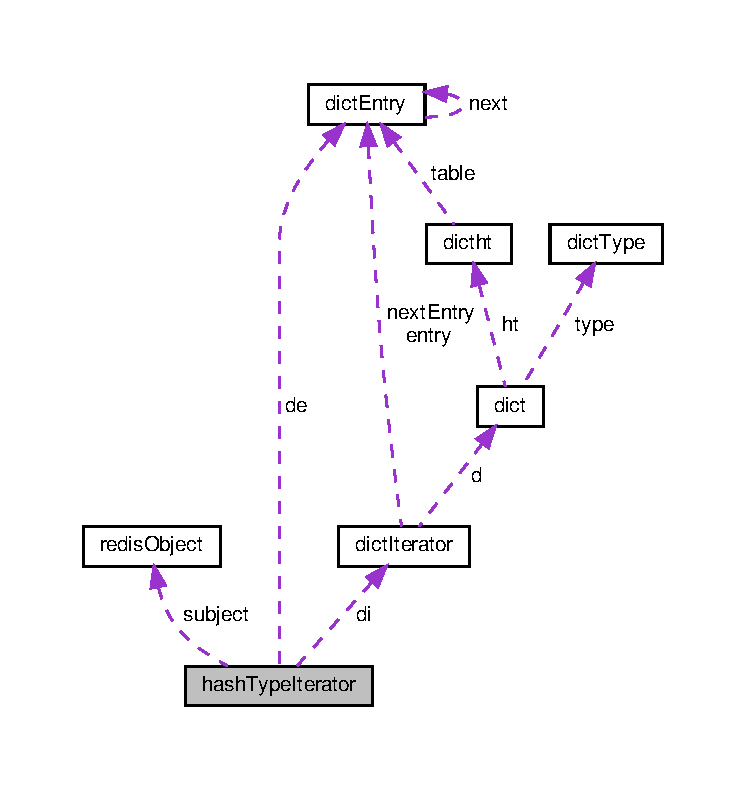
\includegraphics[width=350pt]{structhash_type_iterator__coll__graph}
\end{center}
\end{figure}
\subsection*{Data Fields}
\begin{DoxyCompactItemize}
\item 
\hyperlink{server_8h_a540f174d2685422fbd7d12e3cd44c8e2}{robj} $\ast$ \hyperlink{structhash_type_iterator_a8bd087874443f3e41cf5f728d8490693}{subject}
\item 
int \hyperlink{structhash_type_iterator_ad1b45f33065aae3c757f56a692b25741}{encoding}
\item 
unsigned char $\ast$ \hyperlink{structhash_type_iterator_a9deec0c53e9848ebf973fba86d4670a3}{fptr}
\item 
unsigned char $\ast$ \hyperlink{structhash_type_iterator_a5ead8d514dee29377ba31dc48066cb2c}{vptr}
\item 
\hyperlink{structdict_iterator}{dict\+Iterator} $\ast$ \hyperlink{structhash_type_iterator_a30e26ff2250d4d8b49241087d755342a}{di}
\item 
\hyperlink{structdict_entry}{dict\+Entry} $\ast$ \hyperlink{structhash_type_iterator_ad42c838fd43654444c8d4492319e1949}{de}
\end{DoxyCompactItemize}


\subsection{Detailed Description}


Definition at line 1350 of file server.\+h.



\subsection{Field Documentation}
\mbox{\Hypertarget{structhash_type_iterator_ad42c838fd43654444c8d4492319e1949}\label{structhash_type_iterator_ad42c838fd43654444c8d4492319e1949}} 
\index{hash\+Type\+Iterator@{hash\+Type\+Iterator}!de@{de}}
\index{de@{de}!hash\+Type\+Iterator@{hash\+Type\+Iterator}}
\subsubsection{\texorpdfstring{de}{de}}
{\footnotesize\ttfamily \hyperlink{structdict_entry}{dict\+Entry}$\ast$ de}



Definition at line 1357 of file server.\+h.

\mbox{\Hypertarget{structhash_type_iterator_a30e26ff2250d4d8b49241087d755342a}\label{structhash_type_iterator_a30e26ff2250d4d8b49241087d755342a}} 
\index{hash\+Type\+Iterator@{hash\+Type\+Iterator}!di@{di}}
\index{di@{di}!hash\+Type\+Iterator@{hash\+Type\+Iterator}}
\subsubsection{\texorpdfstring{di}{di}}
{\footnotesize\ttfamily \hyperlink{structdict_iterator}{dict\+Iterator}$\ast$ di}



Definition at line 1356 of file server.\+h.

\mbox{\Hypertarget{structhash_type_iterator_ad1b45f33065aae3c757f56a692b25741}\label{structhash_type_iterator_ad1b45f33065aae3c757f56a692b25741}} 
\index{hash\+Type\+Iterator@{hash\+Type\+Iterator}!encoding@{encoding}}
\index{encoding@{encoding}!hash\+Type\+Iterator@{hash\+Type\+Iterator}}
\subsubsection{\texorpdfstring{encoding}{encoding}}
{\footnotesize\ttfamily int encoding}



Definition at line 1352 of file server.\+h.

\mbox{\Hypertarget{structhash_type_iterator_a9deec0c53e9848ebf973fba86d4670a3}\label{structhash_type_iterator_a9deec0c53e9848ebf973fba86d4670a3}} 
\index{hash\+Type\+Iterator@{hash\+Type\+Iterator}!fptr@{fptr}}
\index{fptr@{fptr}!hash\+Type\+Iterator@{hash\+Type\+Iterator}}
\subsubsection{\texorpdfstring{fptr}{fptr}}
{\footnotesize\ttfamily unsigned char$\ast$ fptr}



Definition at line 1354 of file server.\+h.

\mbox{\Hypertarget{structhash_type_iterator_a8bd087874443f3e41cf5f728d8490693}\label{structhash_type_iterator_a8bd087874443f3e41cf5f728d8490693}} 
\index{hash\+Type\+Iterator@{hash\+Type\+Iterator}!subject@{subject}}
\index{subject@{subject}!hash\+Type\+Iterator@{hash\+Type\+Iterator}}
\subsubsection{\texorpdfstring{subject}{subject}}
{\footnotesize\ttfamily \hyperlink{server_8h_a540f174d2685422fbd7d12e3cd44c8e2}{robj}$\ast$ subject}



Definition at line 1351 of file server.\+h.

\mbox{\Hypertarget{structhash_type_iterator_a5ead8d514dee29377ba31dc48066cb2c}\label{structhash_type_iterator_a5ead8d514dee29377ba31dc48066cb2c}} 
\index{hash\+Type\+Iterator@{hash\+Type\+Iterator}!vptr@{vptr}}
\index{vptr@{vptr}!hash\+Type\+Iterator@{hash\+Type\+Iterator}}
\subsubsection{\texorpdfstring{vptr}{vptr}}
{\footnotesize\ttfamily unsigned char $\ast$ vptr}



Definition at line 1354 of file server.\+h.



The documentation for this struct was generated from the following file\+:\begin{DoxyCompactItemize}
\item 
src/\hyperlink{server_8h}{server.\+h}\end{DoxyCompactItemize}

\hypertarget{structhelp_entry}{}\section{help\+Entry Struct Reference}
\label{structhelp_entry}\index{help\+Entry@{help\+Entry}}


Collaboration diagram for help\+Entry\+:
\nopagebreak
\begin{figure}[H]
\begin{center}
\leavevmode
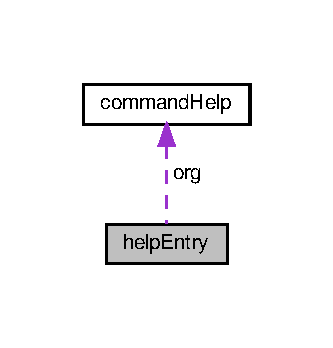
\includegraphics[width=160pt]{structhelp_entry__coll__graph}
\end{center}
\end{figure}
\subsection*{Data Fields}
\begin{DoxyCompactItemize}
\item 
int \hyperlink{structhelp_entry_ac765329451135abec74c45e1897abf26}{type}
\item 
int \hyperlink{structhelp_entry_ad1447518f4372828b8435ae82e48499e}{argc}
\item 
\hyperlink{sds_8h_ad69abac3df4532879db9642c95f5ef6f}{sds} $\ast$ \hyperlink{structhelp_entry_aa7def7b53e4d59718c7aec9c35c75caa}{argv}
\item 
\hyperlink{sds_8h_ad69abac3df4532879db9642c95f5ef6f}{sds} \hyperlink{structhelp_entry_a68871af4f9c205cb2904958ceafed1dc}{full}
\item 
struct \hyperlink{structcommand_help}{command\+Help} $\ast$ \hyperlink{structhelp_entry_a6642ac5df30685d86cd11a44a22f6c21}{org}
\end{DoxyCompactItemize}


\subsection{Detailed Description}


Definition at line 444 of file redis-\/cli.\+c.



\subsection{Field Documentation}
\mbox{\Hypertarget{structhelp_entry_ad1447518f4372828b8435ae82e48499e}\label{structhelp_entry_ad1447518f4372828b8435ae82e48499e}} 
\index{help\+Entry@{help\+Entry}!argc@{argc}}
\index{argc@{argc}!help\+Entry@{help\+Entry}}
\subsubsection{\texorpdfstring{argc}{argc}}
{\footnotesize\ttfamily int argc}



Definition at line 446 of file redis-\/cli.\+c.

\mbox{\Hypertarget{structhelp_entry_aa7def7b53e4d59718c7aec9c35c75caa}\label{structhelp_entry_aa7def7b53e4d59718c7aec9c35c75caa}} 
\index{help\+Entry@{help\+Entry}!argv@{argv}}
\index{argv@{argv}!help\+Entry@{help\+Entry}}
\subsubsection{\texorpdfstring{argv}{argv}}
{\footnotesize\ttfamily \hyperlink{sds_8h_ad69abac3df4532879db9642c95f5ef6f}{sds}$\ast$ argv}



Definition at line 447 of file redis-\/cli.\+c.

\mbox{\Hypertarget{structhelp_entry_a68871af4f9c205cb2904958ceafed1dc}\label{structhelp_entry_a68871af4f9c205cb2904958ceafed1dc}} 
\index{help\+Entry@{help\+Entry}!full@{full}}
\index{full@{full}!help\+Entry@{help\+Entry}}
\subsubsection{\texorpdfstring{full}{full}}
{\footnotesize\ttfamily \hyperlink{sds_8h_ad69abac3df4532879db9642c95f5ef6f}{sds} full}



Definition at line 448 of file redis-\/cli.\+c.

\mbox{\Hypertarget{structhelp_entry_a6642ac5df30685d86cd11a44a22f6c21}\label{structhelp_entry_a6642ac5df30685d86cd11a44a22f6c21}} 
\index{help\+Entry@{help\+Entry}!org@{org}}
\index{org@{org}!help\+Entry@{help\+Entry}}
\subsubsection{\texorpdfstring{org}{org}}
{\footnotesize\ttfamily struct \hyperlink{structcommand_help}{command\+Help}$\ast$ org}



Definition at line 451 of file redis-\/cli.\+c.

\mbox{\Hypertarget{structhelp_entry_ac765329451135abec74c45e1897abf26}\label{structhelp_entry_ac765329451135abec74c45e1897abf26}} 
\index{help\+Entry@{help\+Entry}!type@{type}}
\index{type@{type}!help\+Entry@{help\+Entry}}
\subsubsection{\texorpdfstring{type}{type}}
{\footnotesize\ttfamily int type}



Definition at line 445 of file redis-\/cli.\+c.



The documentation for this struct was generated from the following file\+:\begin{DoxyCompactItemize}
\item 
src/\hyperlink{redis-cli_8c}{redis-\/cli.\+c}\end{DoxyCompactItemize}

\hypertarget{structhllhdr}{}\section{hllhdr Struct Reference}
\label{structhllhdr}\index{hllhdr@{hllhdr}}
\subsection*{Data Fields}
\begin{DoxyCompactItemize}
\item 
char \hyperlink{structhllhdr_a03dedff415badb9581a8ca90e6a45b53}{magic} \mbox{[}4\mbox{]}
\item 
uint8\+\_\+t \hyperlink{structhllhdr_a4c2619391e67c574b601d57922c494bc}{encoding}
\item 
uint8\+\_\+t \hyperlink{structhllhdr_a4fe1afde3770cfaeba9ce0e4c3cdf3c6}{notused} \mbox{[}3\mbox{]}
\item 
uint8\+\_\+t \hyperlink{structhllhdr_a3ae8ca95d6237180e2e44f34cc65c1f1}{card} \mbox{[}8\mbox{]}
\item 
uint8\+\_\+t \hyperlink{structhllhdr_a5ebea196b48e08b90ba84e31f7a516cf}{registers} \mbox{[}$\,$\mbox{]}
\end{DoxyCompactItemize}


\subsection{Detailed Description}


Definition at line 182 of file hyperloglog.\+c.



\subsection{Field Documentation}
\mbox{\Hypertarget{structhllhdr_a3ae8ca95d6237180e2e44f34cc65c1f1}\label{structhllhdr_a3ae8ca95d6237180e2e44f34cc65c1f1}} 
\index{hllhdr@{hllhdr}!card@{card}}
\index{card@{card}!hllhdr@{hllhdr}}
\subsubsection{\texorpdfstring{card}{card}}
{\footnotesize\ttfamily uint8\+\_\+t card\mbox{[}8\mbox{]}}



Definition at line 186 of file hyperloglog.\+c.

\mbox{\Hypertarget{structhllhdr_a4c2619391e67c574b601d57922c494bc}\label{structhllhdr_a4c2619391e67c574b601d57922c494bc}} 
\index{hllhdr@{hllhdr}!encoding@{encoding}}
\index{encoding@{encoding}!hllhdr@{hllhdr}}
\subsubsection{\texorpdfstring{encoding}{encoding}}
{\footnotesize\ttfamily uint8\+\_\+t encoding}



Definition at line 184 of file hyperloglog.\+c.

\mbox{\Hypertarget{structhllhdr_a03dedff415badb9581a8ca90e6a45b53}\label{structhllhdr_a03dedff415badb9581a8ca90e6a45b53}} 
\index{hllhdr@{hllhdr}!magic@{magic}}
\index{magic@{magic}!hllhdr@{hllhdr}}
\subsubsection{\texorpdfstring{magic}{magic}}
{\footnotesize\ttfamily char magic\mbox{[}4\mbox{]}}



Definition at line 183 of file hyperloglog.\+c.

\mbox{\Hypertarget{structhllhdr_a4fe1afde3770cfaeba9ce0e4c3cdf3c6}\label{structhllhdr_a4fe1afde3770cfaeba9ce0e4c3cdf3c6}} 
\index{hllhdr@{hllhdr}!notused@{notused}}
\index{notused@{notused}!hllhdr@{hllhdr}}
\subsubsection{\texorpdfstring{notused}{notused}}
{\footnotesize\ttfamily uint8\+\_\+t notused\mbox{[}3\mbox{]}}



Definition at line 185 of file hyperloglog.\+c.

\mbox{\Hypertarget{structhllhdr_a5ebea196b48e08b90ba84e31f7a516cf}\label{structhllhdr_a5ebea196b48e08b90ba84e31f7a516cf}} 
\index{hllhdr@{hllhdr}!registers@{registers}}
\index{registers@{registers}!hllhdr@{hllhdr}}
\subsubsection{\texorpdfstring{registers}{registers}}
{\footnotesize\ttfamily uint8\+\_\+t registers\mbox{[}$\,$\mbox{]}}



Definition at line 187 of file hyperloglog.\+c.



The documentation for this struct was generated from the following file\+:\begin{DoxyCompactItemize}
\item 
src/\hyperlink{hyperloglog_8c}{hyperloglog.\+c}\end{DoxyCompactItemize}

\hypertarget{structinstance_link}{}\section{instance\+Link Struct Reference}
\label{structinstance_link}\index{instance\+Link@{instance\+Link}}
\subsection*{Data Fields}
\begin{DoxyCompactItemize}
\item 
int \hyperlink{structinstance_link_a6022c8a609170c7365fb96e83cb2df48}{refcount}
\item 
int \hyperlink{structinstance_link_a6f03dfc777300fd0dc9acebf4822249c}{disconnected}
\item 
int \hyperlink{structinstance_link_acc254a996c1faea659a20feb073d4f00}{pending\+\_\+commands}
\item 
redis\+Async\+Context $\ast$ \hyperlink{structinstance_link_a403cc1bb3650a1a12adb31b9d8c8f016}{cc}
\item 
redis\+Async\+Context $\ast$ \hyperlink{structinstance_link_afe761f1776d1b45b7abadf158f8bbe37}{pc}
\item 
\hyperlink{redismodule_8h_a652ae61e2475bc8957454534544968fc}{mstime\+\_\+t} \hyperlink{structinstance_link_a488300e93393a2d8d6377bb4d46ad104}{cc\+\_\+conn\+\_\+time}
\item 
\hyperlink{redismodule_8h_a652ae61e2475bc8957454534544968fc}{mstime\+\_\+t} \hyperlink{structinstance_link_a12befcf62811f417eaf23da1076547bc}{pc\+\_\+conn\+\_\+time}
\item 
\hyperlink{redismodule_8h_a652ae61e2475bc8957454534544968fc}{mstime\+\_\+t} \hyperlink{structinstance_link_ad3256ba26a4f06b5cc89221c2d6bf0a6}{pc\+\_\+last\+\_\+activity}
\item 
\hyperlink{redismodule_8h_a652ae61e2475bc8957454534544968fc}{mstime\+\_\+t} \hyperlink{structinstance_link_a74938a205871007ed9a784e48aaa52f1}{last\+\_\+avail\+\_\+time}
\item 
\hyperlink{redismodule_8h_a652ae61e2475bc8957454534544968fc}{mstime\+\_\+t} \hyperlink{structinstance_link_a96b7748c7ea4249b266bfa7417bcec1d}{act\+\_\+ping\+\_\+time}
\item 
\hyperlink{redismodule_8h_a652ae61e2475bc8957454534544968fc}{mstime\+\_\+t} \hyperlink{structinstance_link_a3f2e6f68ee92867d1b8a248050f83cf1}{last\+\_\+ping\+\_\+time}
\item 
\hyperlink{redismodule_8h_a652ae61e2475bc8957454534544968fc}{mstime\+\_\+t} \hyperlink{structinstance_link_a1f03922d605d4284100bb2abdeb6800b}{last\+\_\+pong\+\_\+time}
\item 
\hyperlink{redismodule_8h_a652ae61e2475bc8957454534544968fc}{mstime\+\_\+t} \hyperlink{structinstance_link_ab333e48e13c659a387c659e1bc4e02e1}{last\+\_\+reconn\+\_\+time}
\end{DoxyCompactItemize}


\subsection{Detailed Description}


Definition at line 137 of file sentinel.\+c.



\subsection{Field Documentation}
\mbox{\Hypertarget{structinstance_link_a96b7748c7ea4249b266bfa7417bcec1d}\label{structinstance_link_a96b7748c7ea4249b266bfa7417bcec1d}} 
\index{instance\+Link@{instance\+Link}!act\+\_\+ping\+\_\+time@{act\+\_\+ping\+\_\+time}}
\index{act\+\_\+ping\+\_\+time@{act\+\_\+ping\+\_\+time}!instance\+Link@{instance\+Link}}
\subsubsection{\texorpdfstring{act\+\_\+ping\+\_\+time}{act\_ping\_time}}
{\footnotesize\ttfamily \hyperlink{redismodule_8h_a652ae61e2475bc8957454534544968fc}{mstime\+\_\+t} act\+\_\+ping\+\_\+time}



Definition at line 148 of file sentinel.\+c.

\mbox{\Hypertarget{structinstance_link_a403cc1bb3650a1a12adb31b9d8c8f016}\label{structinstance_link_a403cc1bb3650a1a12adb31b9d8c8f016}} 
\index{instance\+Link@{instance\+Link}!cc@{cc}}
\index{cc@{cc}!instance\+Link@{instance\+Link}}
\subsubsection{\texorpdfstring{cc}{cc}}
{\footnotesize\ttfamily redis\+Async\+Context$\ast$ cc}



Definition at line 141 of file sentinel.\+c.

\mbox{\Hypertarget{structinstance_link_a488300e93393a2d8d6377bb4d46ad104}\label{structinstance_link_a488300e93393a2d8d6377bb4d46ad104}} 
\index{instance\+Link@{instance\+Link}!cc\+\_\+conn\+\_\+time@{cc\+\_\+conn\+\_\+time}}
\index{cc\+\_\+conn\+\_\+time@{cc\+\_\+conn\+\_\+time}!instance\+Link@{instance\+Link}}
\subsubsection{\texorpdfstring{cc\+\_\+conn\+\_\+time}{cc\_conn\_time}}
{\footnotesize\ttfamily \hyperlink{redismodule_8h_a652ae61e2475bc8957454534544968fc}{mstime\+\_\+t} cc\+\_\+conn\+\_\+time}



Definition at line 143 of file sentinel.\+c.

\mbox{\Hypertarget{structinstance_link_a6f03dfc777300fd0dc9acebf4822249c}\label{structinstance_link_a6f03dfc777300fd0dc9acebf4822249c}} 
\index{instance\+Link@{instance\+Link}!disconnected@{disconnected}}
\index{disconnected@{disconnected}!instance\+Link@{instance\+Link}}
\subsubsection{\texorpdfstring{disconnected}{disconnected}}
{\footnotesize\ttfamily int disconnected}



Definition at line 139 of file sentinel.\+c.

\mbox{\Hypertarget{structinstance_link_a74938a205871007ed9a784e48aaa52f1}\label{structinstance_link_a74938a205871007ed9a784e48aaa52f1}} 
\index{instance\+Link@{instance\+Link}!last\+\_\+avail\+\_\+time@{last\+\_\+avail\+\_\+time}}
\index{last\+\_\+avail\+\_\+time@{last\+\_\+avail\+\_\+time}!instance\+Link@{instance\+Link}}
\subsubsection{\texorpdfstring{last\+\_\+avail\+\_\+time}{last\_avail\_time}}
{\footnotesize\ttfamily \hyperlink{redismodule_8h_a652ae61e2475bc8957454534544968fc}{mstime\+\_\+t} last\+\_\+avail\+\_\+time}



Definition at line 146 of file sentinel.\+c.

\mbox{\Hypertarget{structinstance_link_a3f2e6f68ee92867d1b8a248050f83cf1}\label{structinstance_link_a3f2e6f68ee92867d1b8a248050f83cf1}} 
\index{instance\+Link@{instance\+Link}!last\+\_\+ping\+\_\+time@{last\+\_\+ping\+\_\+time}}
\index{last\+\_\+ping\+\_\+time@{last\+\_\+ping\+\_\+time}!instance\+Link@{instance\+Link}}
\subsubsection{\texorpdfstring{last\+\_\+ping\+\_\+time}{last\_ping\_time}}
{\footnotesize\ttfamily \hyperlink{redismodule_8h_a652ae61e2475bc8957454534544968fc}{mstime\+\_\+t} last\+\_\+ping\+\_\+time}



Definition at line 153 of file sentinel.\+c.

\mbox{\Hypertarget{structinstance_link_a1f03922d605d4284100bb2abdeb6800b}\label{structinstance_link_a1f03922d605d4284100bb2abdeb6800b}} 
\index{instance\+Link@{instance\+Link}!last\+\_\+pong\+\_\+time@{last\+\_\+pong\+\_\+time}}
\index{last\+\_\+pong\+\_\+time@{last\+\_\+pong\+\_\+time}!instance\+Link@{instance\+Link}}
\subsubsection{\texorpdfstring{last\+\_\+pong\+\_\+time}{last\_pong\_time}}
{\footnotesize\ttfamily \hyperlink{redismodule_8h_a652ae61e2475bc8957454534544968fc}{mstime\+\_\+t} last\+\_\+pong\+\_\+time}



Definition at line 157 of file sentinel.\+c.

\mbox{\Hypertarget{structinstance_link_ab333e48e13c659a387c659e1bc4e02e1}\label{structinstance_link_ab333e48e13c659a387c659e1bc4e02e1}} 
\index{instance\+Link@{instance\+Link}!last\+\_\+reconn\+\_\+time@{last\+\_\+reconn\+\_\+time}}
\index{last\+\_\+reconn\+\_\+time@{last\+\_\+reconn\+\_\+time}!instance\+Link@{instance\+Link}}
\subsubsection{\texorpdfstring{last\+\_\+reconn\+\_\+time}{last\_reconn\_time}}
{\footnotesize\ttfamily \hyperlink{redismodule_8h_a652ae61e2475bc8957454534544968fc}{mstime\+\_\+t} last\+\_\+reconn\+\_\+time}



Definition at line 160 of file sentinel.\+c.

\mbox{\Hypertarget{structinstance_link_afe761f1776d1b45b7abadf158f8bbe37}\label{structinstance_link_afe761f1776d1b45b7abadf158f8bbe37}} 
\index{instance\+Link@{instance\+Link}!pc@{pc}}
\index{pc@{pc}!instance\+Link@{instance\+Link}}
\subsubsection{\texorpdfstring{pc}{pc}}
{\footnotesize\ttfamily redis\+Async\+Context$\ast$ pc}



Definition at line 142 of file sentinel.\+c.

\mbox{\Hypertarget{structinstance_link_a12befcf62811f417eaf23da1076547bc}\label{structinstance_link_a12befcf62811f417eaf23da1076547bc}} 
\index{instance\+Link@{instance\+Link}!pc\+\_\+conn\+\_\+time@{pc\+\_\+conn\+\_\+time}}
\index{pc\+\_\+conn\+\_\+time@{pc\+\_\+conn\+\_\+time}!instance\+Link@{instance\+Link}}
\subsubsection{\texorpdfstring{pc\+\_\+conn\+\_\+time}{pc\_conn\_time}}
{\footnotesize\ttfamily \hyperlink{redismodule_8h_a652ae61e2475bc8957454534544968fc}{mstime\+\_\+t} pc\+\_\+conn\+\_\+time}



Definition at line 144 of file sentinel.\+c.

\mbox{\Hypertarget{structinstance_link_ad3256ba26a4f06b5cc89221c2d6bf0a6}\label{structinstance_link_ad3256ba26a4f06b5cc89221c2d6bf0a6}} 
\index{instance\+Link@{instance\+Link}!pc\+\_\+last\+\_\+activity@{pc\+\_\+last\+\_\+activity}}
\index{pc\+\_\+last\+\_\+activity@{pc\+\_\+last\+\_\+activity}!instance\+Link@{instance\+Link}}
\subsubsection{\texorpdfstring{pc\+\_\+last\+\_\+activity}{pc\_last\_activity}}
{\footnotesize\ttfamily \hyperlink{redismodule_8h_a652ae61e2475bc8957454534544968fc}{mstime\+\_\+t} pc\+\_\+last\+\_\+activity}



Definition at line 145 of file sentinel.\+c.

\mbox{\Hypertarget{structinstance_link_acc254a996c1faea659a20feb073d4f00}\label{structinstance_link_acc254a996c1faea659a20feb073d4f00}} 
\index{instance\+Link@{instance\+Link}!pending\+\_\+commands@{pending\+\_\+commands}}
\index{pending\+\_\+commands@{pending\+\_\+commands}!instance\+Link@{instance\+Link}}
\subsubsection{\texorpdfstring{pending\+\_\+commands}{pending\_commands}}
{\footnotesize\ttfamily int pending\+\_\+commands}



Definition at line 140 of file sentinel.\+c.

\mbox{\Hypertarget{structinstance_link_a6022c8a609170c7365fb96e83cb2df48}\label{structinstance_link_a6022c8a609170c7365fb96e83cb2df48}} 
\index{instance\+Link@{instance\+Link}!refcount@{refcount}}
\index{refcount@{refcount}!instance\+Link@{instance\+Link}}
\subsubsection{\texorpdfstring{refcount}{refcount}}
{\footnotesize\ttfamily int refcount}



Definition at line 138 of file sentinel.\+c.



The documentation for this struct was generated from the following file\+:\begin{DoxyCompactItemize}
\item 
src/\hyperlink{sentinel_8c}{sentinel.\+c}\end{DoxyCompactItemize}

\hypertarget{structintset}{}\section{intset Struct Reference}
\label{structintset}\index{intset@{intset}}


{\ttfamily \#include $<$intset.\+h$>$}

\subsection*{Data Fields}
\begin{DoxyCompactItemize}
\item 
uint32\+\_\+t \hyperlink{structintset_abf20f154dd41a6f1b64b0cbfbfb05052}{encoding}
\item 
uint32\+\_\+t \hyperlink{structintset_aebb70c2aab3407a9f05334c47131a43b}{length}
\item 
int8\+\_\+t \hyperlink{structintset_a2849bfd03c0c7b34aaad423672b75045}{contents} \mbox{[}$\,$\mbox{]}
\end{DoxyCompactItemize}


\subsection{Detailed Description}


Definition at line 35 of file intset.\+h.



\subsection{Field Documentation}
\mbox{\Hypertarget{structintset_a2849bfd03c0c7b34aaad423672b75045}\label{structintset_a2849bfd03c0c7b34aaad423672b75045}} 
\index{intset@{intset}!contents@{contents}}
\index{contents@{contents}!intset@{intset}}
\subsubsection{\texorpdfstring{contents}{contents}}
{\footnotesize\ttfamily int8\+\_\+t contents\mbox{[}$\,$\mbox{]}}



Definition at line 38 of file intset.\+h.

\mbox{\Hypertarget{structintset_abf20f154dd41a6f1b64b0cbfbfb05052}\label{structintset_abf20f154dd41a6f1b64b0cbfbfb05052}} 
\index{intset@{intset}!encoding@{encoding}}
\index{encoding@{encoding}!intset@{intset}}
\subsubsection{\texorpdfstring{encoding}{encoding}}
{\footnotesize\ttfamily uint32\+\_\+t encoding}



Definition at line 36 of file intset.\+h.

\mbox{\Hypertarget{structintset_aebb70c2aab3407a9f05334c47131a43b}\label{structintset_aebb70c2aab3407a9f05334c47131a43b}} 
\index{intset@{intset}!length@{length}}
\index{length@{length}!intset@{intset}}
\subsubsection{\texorpdfstring{length}{length}}
{\footnotesize\ttfamily uint32\+\_\+t length}



Definition at line 37 of file intset.\+h.



The documentation for this struct was generated from the following file\+:\begin{DoxyCompactItemize}
\item 
src/\hyperlink{intset_8h}{intset.\+h}\end{DoxyCompactItemize}

\hypertarget{structlatency_sample}{}\section{latency\+Sample Struct Reference}
\label{structlatency_sample}\index{latency\+Sample@{latency\+Sample}}


{\ttfamily \#include $<$latency.\+h$>$}

\subsection*{Data Fields}
\begin{DoxyCompactItemize}
\item 
int32\+\_\+t \hyperlink{structlatency_sample_abff537f25bc8d06192bd18aff2597aa0}{time}
\item 
uint32\+\_\+t \hyperlink{structlatency_sample_acd3d24a29a6e07be2bd52fcaffecc872}{latency}
\end{DoxyCompactItemize}


\subsection{Detailed Description}


Definition at line 41 of file latency.\+h.



\subsection{Field Documentation}
\mbox{\Hypertarget{structlatency_sample_acd3d24a29a6e07be2bd52fcaffecc872}\label{structlatency_sample_acd3d24a29a6e07be2bd52fcaffecc872}} 
\index{latency\+Sample@{latency\+Sample}!latency@{latency}}
\index{latency@{latency}!latency\+Sample@{latency\+Sample}}
\subsubsection{\texorpdfstring{latency}{latency}}
{\footnotesize\ttfamily uint32\+\_\+t latency}



Definition at line 43 of file latency.\+h.

\mbox{\Hypertarget{structlatency_sample_abff537f25bc8d06192bd18aff2597aa0}\label{structlatency_sample_abff537f25bc8d06192bd18aff2597aa0}} 
\index{latency\+Sample@{latency\+Sample}!time@{time}}
\index{time@{time}!latency\+Sample@{latency\+Sample}}
\subsubsection{\texorpdfstring{time}{time}}
{\footnotesize\ttfamily int32\+\_\+t time}



Definition at line 42 of file latency.\+h.



The documentation for this struct was generated from the following file\+:\begin{DoxyCompactItemize}
\item 
src/\hyperlink{latency_8h}{latency.\+h}\end{DoxyCompactItemize}

\hypertarget{structlatency_stats}{}\section{latency\+Stats Struct Reference}
\label{structlatency_stats}\index{latency\+Stats@{latency\+Stats}}


{\ttfamily \#include $<$latency.\+h$>$}

\subsection*{Data Fields}
\begin{DoxyCompactItemize}
\item 
uint32\+\_\+t \hyperlink{structlatency_stats_a00a8b2b1acfd9f3dd8c0100ed5457045}{all\+\_\+time\+\_\+high}
\item 
uint32\+\_\+t \hyperlink{structlatency_stats_ae71a157cc52be7c78ac77c8dfef9199b}{avg}
\item 
uint32\+\_\+t \hyperlink{structlatency_stats_a0de4531998c77245b8866f2ba909d0fa}{min}
\item 
uint32\+\_\+t \hyperlink{structlatency_stats_a43e74ba18dc1a237d9f7737ce8df350e}{max}
\item 
uint32\+\_\+t \hyperlink{structlatency_stats_a17d080f02e54aa9e8e0d58e5c8a14d1a}{mad}
\item 
uint32\+\_\+t \hyperlink{structlatency_stats_a7d9d22b1c0ac2b68b57d12ec96f54b79}{samples}
\item 
time\+\_\+t \hyperlink{structlatency_stats_a831ec502008ebff1a36b504a8360dafc}{period}
\end{DoxyCompactItemize}


\subsection{Detailed Description}


Definition at line 54 of file latency.\+h.



\subsection{Field Documentation}
\mbox{\Hypertarget{structlatency_stats_a00a8b2b1acfd9f3dd8c0100ed5457045}\label{structlatency_stats_a00a8b2b1acfd9f3dd8c0100ed5457045}} 
\index{latency\+Stats@{latency\+Stats}!all\+\_\+time\+\_\+high@{all\+\_\+time\+\_\+high}}
\index{all\+\_\+time\+\_\+high@{all\+\_\+time\+\_\+high}!latency\+Stats@{latency\+Stats}}
\subsubsection{\texorpdfstring{all\+\_\+time\+\_\+high}{all\_time\_high}}
{\footnotesize\ttfamily uint32\+\_\+t all\+\_\+time\+\_\+high}



Definition at line 55 of file latency.\+h.

\mbox{\Hypertarget{structlatency_stats_ae71a157cc52be7c78ac77c8dfef9199b}\label{structlatency_stats_ae71a157cc52be7c78ac77c8dfef9199b}} 
\index{latency\+Stats@{latency\+Stats}!avg@{avg}}
\index{avg@{avg}!latency\+Stats@{latency\+Stats}}
\subsubsection{\texorpdfstring{avg}{avg}}
{\footnotesize\ttfamily uint32\+\_\+t avg}



Definition at line 56 of file latency.\+h.

\mbox{\Hypertarget{structlatency_stats_a17d080f02e54aa9e8e0d58e5c8a14d1a}\label{structlatency_stats_a17d080f02e54aa9e8e0d58e5c8a14d1a}} 
\index{latency\+Stats@{latency\+Stats}!mad@{mad}}
\index{mad@{mad}!latency\+Stats@{latency\+Stats}}
\subsubsection{\texorpdfstring{mad}{mad}}
{\footnotesize\ttfamily uint32\+\_\+t mad}



Definition at line 59 of file latency.\+h.

\mbox{\Hypertarget{structlatency_stats_a43e74ba18dc1a237d9f7737ce8df350e}\label{structlatency_stats_a43e74ba18dc1a237d9f7737ce8df350e}} 
\index{latency\+Stats@{latency\+Stats}!max@{max}}
\index{max@{max}!latency\+Stats@{latency\+Stats}}
\subsubsection{\texorpdfstring{max}{max}}
{\footnotesize\ttfamily uint32\+\_\+t max}



Definition at line 58 of file latency.\+h.

\mbox{\Hypertarget{structlatency_stats_a0de4531998c77245b8866f2ba909d0fa}\label{structlatency_stats_a0de4531998c77245b8866f2ba909d0fa}} 
\index{latency\+Stats@{latency\+Stats}!min@{min}}
\index{min@{min}!latency\+Stats@{latency\+Stats}}
\subsubsection{\texorpdfstring{min}{min}}
{\footnotesize\ttfamily uint32\+\_\+t min}



Definition at line 57 of file latency.\+h.

\mbox{\Hypertarget{structlatency_stats_a831ec502008ebff1a36b504a8360dafc}\label{structlatency_stats_a831ec502008ebff1a36b504a8360dafc}} 
\index{latency\+Stats@{latency\+Stats}!period@{period}}
\index{period@{period}!latency\+Stats@{latency\+Stats}}
\subsubsection{\texorpdfstring{period}{period}}
{\footnotesize\ttfamily time\+\_\+t period}



Definition at line 61 of file latency.\+h.

\mbox{\Hypertarget{structlatency_stats_a7d9d22b1c0ac2b68b57d12ec96f54b79}\label{structlatency_stats_a7d9d22b1c0ac2b68b57d12ec96f54b79}} 
\index{latency\+Stats@{latency\+Stats}!samples@{samples}}
\index{samples@{samples}!latency\+Stats@{latency\+Stats}}
\subsubsection{\texorpdfstring{samples}{samples}}
{\footnotesize\ttfamily uint32\+\_\+t samples}



Definition at line 60 of file latency.\+h.



The documentation for this struct was generated from the following file\+:\begin{DoxyCompactItemize}
\item 
src/\hyperlink{latency_8h}{latency.\+h}\end{DoxyCompactItemize}

\hypertarget{structlatency_time_series}{}\section{latency\+Time\+Series Struct Reference}
\label{structlatency_time_series}\index{latency\+Time\+Series@{latency\+Time\+Series}}


{\ttfamily \#include $<$latency.\+h$>$}



Collaboration diagram for latency\+Time\+Series\+:
\nopagebreak
\begin{figure}[H]
\begin{center}
\leavevmode
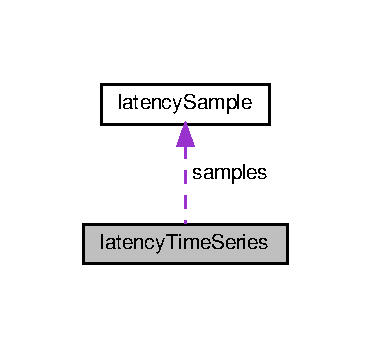
\includegraphics[width=178pt]{structlatency_time_series__coll__graph}
\end{center}
\end{figure}
\subsection*{Data Fields}
\begin{DoxyCompactItemize}
\item 
int \hyperlink{structlatency_time_series_ae40354a1051342eb5a9db005715dcfa9}{idx}
\item 
uint32\+\_\+t \hyperlink{structlatency_time_series_a43e74ba18dc1a237d9f7737ce8df350e}{max}
\item 
struct \hyperlink{structlatency_sample}{latency\+Sample} \hyperlink{structlatency_time_series_a153186b2a352798a182b7269613f2466}{samples} \mbox{[}\hyperlink{latency_8h_a7e3ba352d9d7bb4c88c2c42c16e6674b}{L\+A\+T\+E\+N\+C\+Y\+\_\+\+T\+S\+\_\+\+L\+EN}\mbox{]}
\end{DoxyCompactItemize}


\subsection{Detailed Description}


Definition at line 47 of file latency.\+h.



\subsection{Field Documentation}
\mbox{\Hypertarget{structlatency_time_series_ae40354a1051342eb5a9db005715dcfa9}\label{structlatency_time_series_ae40354a1051342eb5a9db005715dcfa9}} 
\index{latency\+Time\+Series@{latency\+Time\+Series}!idx@{idx}}
\index{idx@{idx}!latency\+Time\+Series@{latency\+Time\+Series}}
\subsubsection{\texorpdfstring{idx}{idx}}
{\footnotesize\ttfamily int idx}



Definition at line 48 of file latency.\+h.

\mbox{\Hypertarget{structlatency_time_series_a43e74ba18dc1a237d9f7737ce8df350e}\label{structlatency_time_series_a43e74ba18dc1a237d9f7737ce8df350e}} 
\index{latency\+Time\+Series@{latency\+Time\+Series}!max@{max}}
\index{max@{max}!latency\+Time\+Series@{latency\+Time\+Series}}
\subsubsection{\texorpdfstring{max}{max}}
{\footnotesize\ttfamily uint32\+\_\+t max}



Definition at line 49 of file latency.\+h.

\mbox{\Hypertarget{structlatency_time_series_a153186b2a352798a182b7269613f2466}\label{structlatency_time_series_a153186b2a352798a182b7269613f2466}} 
\index{latency\+Time\+Series@{latency\+Time\+Series}!samples@{samples}}
\index{samples@{samples}!latency\+Time\+Series@{latency\+Time\+Series}}
\subsubsection{\texorpdfstring{samples}{samples}}
{\footnotesize\ttfamily struct \hyperlink{structlatency_sample}{latency\+Sample} samples\mbox{[}\hyperlink{latency_8h_a7e3ba352d9d7bb4c88c2c42c16e6674b}{L\+A\+T\+E\+N\+C\+Y\+\_\+\+T\+S\+\_\+\+L\+EN}\mbox{]}}



Definition at line 50 of file latency.\+h.



The documentation for this struct was generated from the following file\+:\begin{DoxyCompactItemize}
\item 
src/\hyperlink{latency_8h}{latency.\+h}\end{DoxyCompactItemize}

\hypertarget{structldb_state}{}\section{ldb\+State Struct Reference}
\label{structldb_state}\index{ldb\+State@{ldb\+State}}


Collaboration diagram for ldb\+State\+:
\nopagebreak
\begin{figure}[H]
\begin{center}
\leavevmode
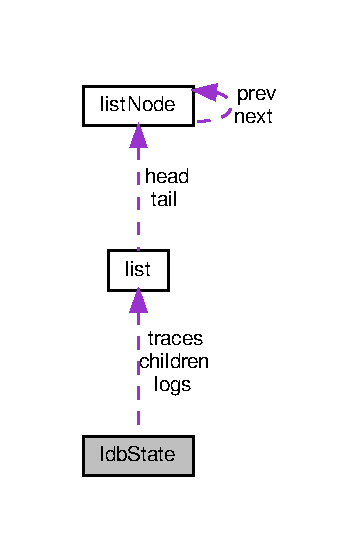
\includegraphics[width=173pt]{structldb_state__coll__graph}
\end{center}
\end{figure}
\subsection*{Data Fields}
\begin{DoxyCompactItemize}
\item 
int \hyperlink{structldb_state_a6f8059414f0228f0256115e024eeed4b}{fd}
\item 
int \hyperlink{structldb_state_aa5805c5e936174e5092bf7a5b78e7e64}{active}
\item 
int \hyperlink{structldb_state_a561d6ae2df1882124024d1ad25c05ca0}{forked}
\item 
\hyperlink{structlist}{list} $\ast$ \hyperlink{structldb_state_ad79d8838634104cbd0a2cc989b41017c}{logs}
\item 
\hyperlink{structlist}{list} $\ast$ \hyperlink{structldb_state_a306571a8cb6864a49170a1d0ef814347}{traces}
\item 
\hyperlink{structlist}{list} $\ast$ \hyperlink{structldb_state_a6bc412879e51bdab8e86acf420095ef9}{children}
\item 
int \hyperlink{structldb_state_ac9df7cc923c5d2a35bfc27dd8530b9af}{bp} \mbox{[}\hyperlink{scripting_8c_a4f3000cf3b5955f8134bfcd2fa340db3}{L\+D\+B\+\_\+\+B\+R\+E\+A\+K\+P\+O\+I\+N\+T\+S\+\_\+\+M\+AX}\mbox{]}
\item 
int \hyperlink{structldb_state_a472140f37a2e6de6a1a4cd2fce742d78}{bpcount}
\item 
int \hyperlink{structldb_state_abc16e65f240ed0c8f3e876e8732c0a33}{step}
\item 
int \hyperlink{structldb_state_a74c70212af9085c6d321fa9ac33ae44c}{luabp}
\item 
\hyperlink{sds_8h_ad69abac3df4532879db9642c95f5ef6f}{sds} $\ast$ \hyperlink{structldb_state_ae6aed5a52abc1fc9c7945db6ce185a7d}{src}
\item 
int \hyperlink{structldb_state_a9921ae02cadccc99dd6c3a9b68be050a}{lines}
\item 
int \hyperlink{structldb_state_a1be7dfac6c204d2592700475b5d73fd2}{currentline}
\item 
\hyperlink{sds_8h_ad69abac3df4532879db9642c95f5ef6f}{sds} \hyperlink{structldb_state_a3d56df85c9742c537178642bc4ee7355}{cbuf}
\item 
size\+\_\+t \hyperlink{structldb_state_a7eb7af5917b25bcb6565ab20f7a12d22}{maxlen}
\item 
int \hyperlink{structldb_state_a30be56c3b354bdb2e4d39a105be4e1bd}{maxlen\+\_\+hint\+\_\+sent}
\end{DoxyCompactItemize}


\subsection{Detailed Description}


Definition at line 60 of file scripting.\+c.



\subsection{Field Documentation}
\mbox{\Hypertarget{structldb_state_aa5805c5e936174e5092bf7a5b78e7e64}\label{structldb_state_aa5805c5e936174e5092bf7a5b78e7e64}} 
\index{ldb\+State@{ldb\+State}!active@{active}}
\index{active@{active}!ldb\+State@{ldb\+State}}
\subsubsection{\texorpdfstring{active}{active}}
{\footnotesize\ttfamily int active}



Definition at line 62 of file scripting.\+c.

\mbox{\Hypertarget{structldb_state_ac9df7cc923c5d2a35bfc27dd8530b9af}\label{structldb_state_ac9df7cc923c5d2a35bfc27dd8530b9af}} 
\index{ldb\+State@{ldb\+State}!bp@{bp}}
\index{bp@{bp}!ldb\+State@{ldb\+State}}
\subsubsection{\texorpdfstring{bp}{bp}}
{\footnotesize\ttfamily int bp\mbox{[}\hyperlink{scripting_8c_a4f3000cf3b5955f8134bfcd2fa340db3}{L\+D\+B\+\_\+\+B\+R\+E\+A\+K\+P\+O\+I\+N\+T\+S\+\_\+\+M\+AX}\mbox{]}}



Definition at line 67 of file scripting.\+c.

\mbox{\Hypertarget{structldb_state_a472140f37a2e6de6a1a4cd2fce742d78}\label{structldb_state_a472140f37a2e6de6a1a4cd2fce742d78}} 
\index{ldb\+State@{ldb\+State}!bpcount@{bpcount}}
\index{bpcount@{bpcount}!ldb\+State@{ldb\+State}}
\subsubsection{\texorpdfstring{bpcount}{bpcount}}
{\footnotesize\ttfamily int bpcount}



Definition at line 68 of file scripting.\+c.

\mbox{\Hypertarget{structldb_state_a3d56df85c9742c537178642bc4ee7355}\label{structldb_state_a3d56df85c9742c537178642bc4ee7355}} 
\index{ldb\+State@{ldb\+State}!cbuf@{cbuf}}
\index{cbuf@{cbuf}!ldb\+State@{ldb\+State}}
\subsubsection{\texorpdfstring{cbuf}{cbuf}}
{\footnotesize\ttfamily \hyperlink{sds_8h_ad69abac3df4532879db9642c95f5ef6f}{sds} cbuf}



Definition at line 74 of file scripting.\+c.

\mbox{\Hypertarget{structldb_state_a6bc412879e51bdab8e86acf420095ef9}\label{structldb_state_a6bc412879e51bdab8e86acf420095ef9}} 
\index{ldb\+State@{ldb\+State}!children@{children}}
\index{children@{children}!ldb\+State@{ldb\+State}}
\subsubsection{\texorpdfstring{children}{children}}
{\footnotesize\ttfamily \hyperlink{structlist}{list}$\ast$ children}



Definition at line 66 of file scripting.\+c.

\mbox{\Hypertarget{structldb_state_a1be7dfac6c204d2592700475b5d73fd2}\label{structldb_state_a1be7dfac6c204d2592700475b5d73fd2}} 
\index{ldb\+State@{ldb\+State}!currentline@{currentline}}
\index{currentline@{currentline}!ldb\+State@{ldb\+State}}
\subsubsection{\texorpdfstring{currentline}{currentline}}
{\footnotesize\ttfamily int currentline}



Definition at line 73 of file scripting.\+c.

\mbox{\Hypertarget{structldb_state_a6f8059414f0228f0256115e024eeed4b}\label{structldb_state_a6f8059414f0228f0256115e024eeed4b}} 
\index{ldb\+State@{ldb\+State}!fd@{fd}}
\index{fd@{fd}!ldb\+State@{ldb\+State}}
\subsubsection{\texorpdfstring{fd}{fd}}
{\footnotesize\ttfamily int fd}



Definition at line 61 of file scripting.\+c.

\mbox{\Hypertarget{structldb_state_a561d6ae2df1882124024d1ad25c05ca0}\label{structldb_state_a561d6ae2df1882124024d1ad25c05ca0}} 
\index{ldb\+State@{ldb\+State}!forked@{forked}}
\index{forked@{forked}!ldb\+State@{ldb\+State}}
\subsubsection{\texorpdfstring{forked}{forked}}
{\footnotesize\ttfamily int forked}



Definition at line 63 of file scripting.\+c.

\mbox{\Hypertarget{structldb_state_a9921ae02cadccc99dd6c3a9b68be050a}\label{structldb_state_a9921ae02cadccc99dd6c3a9b68be050a}} 
\index{ldb\+State@{ldb\+State}!lines@{lines}}
\index{lines@{lines}!ldb\+State@{ldb\+State}}
\subsubsection{\texorpdfstring{lines}{lines}}
{\footnotesize\ttfamily int lines}



Definition at line 72 of file scripting.\+c.

\mbox{\Hypertarget{structldb_state_ad79d8838634104cbd0a2cc989b41017c}\label{structldb_state_ad79d8838634104cbd0a2cc989b41017c}} 
\index{ldb\+State@{ldb\+State}!logs@{logs}}
\index{logs@{logs}!ldb\+State@{ldb\+State}}
\subsubsection{\texorpdfstring{logs}{logs}}
{\footnotesize\ttfamily \hyperlink{structlist}{list}$\ast$ logs}



Definition at line 64 of file scripting.\+c.

\mbox{\Hypertarget{structldb_state_a74c70212af9085c6d321fa9ac33ae44c}\label{structldb_state_a74c70212af9085c6d321fa9ac33ae44c}} 
\index{ldb\+State@{ldb\+State}!luabp@{luabp}}
\index{luabp@{luabp}!ldb\+State@{ldb\+State}}
\subsubsection{\texorpdfstring{luabp}{luabp}}
{\footnotesize\ttfamily int luabp}



Definition at line 70 of file scripting.\+c.

\mbox{\Hypertarget{structldb_state_a7eb7af5917b25bcb6565ab20f7a12d22}\label{structldb_state_a7eb7af5917b25bcb6565ab20f7a12d22}} 
\index{ldb\+State@{ldb\+State}!maxlen@{maxlen}}
\index{maxlen@{maxlen}!ldb\+State@{ldb\+State}}
\subsubsection{\texorpdfstring{maxlen}{maxlen}}
{\footnotesize\ttfamily size\+\_\+t maxlen}



Definition at line 75 of file scripting.\+c.

\mbox{\Hypertarget{structldb_state_a30be56c3b354bdb2e4d39a105be4e1bd}\label{structldb_state_a30be56c3b354bdb2e4d39a105be4e1bd}} 
\index{ldb\+State@{ldb\+State}!maxlen\+\_\+hint\+\_\+sent@{maxlen\+\_\+hint\+\_\+sent}}
\index{maxlen\+\_\+hint\+\_\+sent@{maxlen\+\_\+hint\+\_\+sent}!ldb\+State@{ldb\+State}}
\subsubsection{\texorpdfstring{maxlen\+\_\+hint\+\_\+sent}{maxlen\_hint\_sent}}
{\footnotesize\ttfamily int maxlen\+\_\+hint\+\_\+sent}



Definition at line 76 of file scripting.\+c.

\mbox{\Hypertarget{structldb_state_ae6aed5a52abc1fc9c7945db6ce185a7d}\label{structldb_state_ae6aed5a52abc1fc9c7945db6ce185a7d}} 
\index{ldb\+State@{ldb\+State}!src@{src}}
\index{src@{src}!ldb\+State@{ldb\+State}}
\subsubsection{\texorpdfstring{src}{src}}
{\footnotesize\ttfamily \hyperlink{sds_8h_ad69abac3df4532879db9642c95f5ef6f}{sds}$\ast$ src}



Definition at line 71 of file scripting.\+c.

\mbox{\Hypertarget{structldb_state_abc16e65f240ed0c8f3e876e8732c0a33}\label{structldb_state_abc16e65f240ed0c8f3e876e8732c0a33}} 
\index{ldb\+State@{ldb\+State}!step@{step}}
\index{step@{step}!ldb\+State@{ldb\+State}}
\subsubsection{\texorpdfstring{step}{step}}
{\footnotesize\ttfamily int step}



Definition at line 69 of file scripting.\+c.

\mbox{\Hypertarget{structldb_state_a306571a8cb6864a49170a1d0ef814347}\label{structldb_state_a306571a8cb6864a49170a1d0ef814347}} 
\index{ldb\+State@{ldb\+State}!traces@{traces}}
\index{traces@{traces}!ldb\+State@{ldb\+State}}
\subsubsection{\texorpdfstring{traces}{traces}}
{\footnotesize\ttfamily \hyperlink{structlist}{list}$\ast$ traces}



Definition at line 65 of file scripting.\+c.



The documentation for this struct was generated from the following file\+:\begin{DoxyCompactItemize}
\item 
src/\hyperlink{scripting_8c}{scripting.\+c}\end{DoxyCompactItemize}

\hypertarget{structlist}{}\section{list Struct Reference}
\label{structlist}\index{list@{list}}


{\ttfamily \#include $<$adlist.\+h$>$}



Collaboration diagram for list\+:
\nopagebreak
\begin{figure}[H]
\begin{center}
\leavevmode
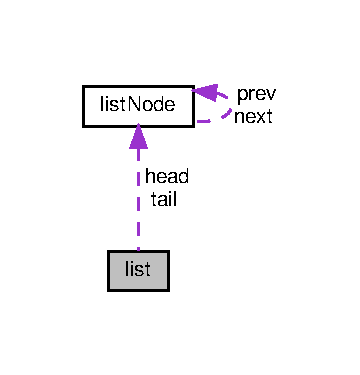
\includegraphics[width=173pt]{structlist__coll__graph}
\end{center}
\end{figure}
\subsection*{Data Fields}
\begin{DoxyCompactItemize}
\item 
\hyperlink{structlist_node}{list\+Node} $\ast$ \hyperlink{structlist_aeafa6e94f6b451fac36e305798d4d656}{head}
\item 
\hyperlink{structlist_node}{list\+Node} $\ast$ \hyperlink{structlist_a769990d42e7c5a221c6a517bef9c19c0}{tail}
\item 
void $\ast$($\ast$ \hyperlink{structlist_acb324bb20395015fe8cb806e767ef7ad}{dup} )(void $\ast$ptr)
\item 
void($\ast$ \hyperlink{structlist_a7ffa51abb1dd8bc3fe4627cb1d2405c5}{free} )(void $\ast$ptr)
\item 
int($\ast$ \hyperlink{structlist_aff6f26982c3b0583ccfd1ca09f8e624e}{match} )(void $\ast$ptr, void $\ast$\hyperlink{redis-check-rdb_8c_adc0ee0ed345db513fb6fac27511be4f1}{key})
\item 
unsigned long \hyperlink{structlist_af2e72f8a5bf4bcdb77566c2936d5f13d}{len}
\end{DoxyCompactItemize}


\subsection{Detailed Description}


Definition at line 47 of file adlist.\+h.



\subsection{Field Documentation}
\mbox{\Hypertarget{structlist_acb324bb20395015fe8cb806e767ef7ad}\label{structlist_acb324bb20395015fe8cb806e767ef7ad}} 
\index{list@{list}!dup@{dup}}
\index{dup@{dup}!list@{list}}
\subsubsection{\texorpdfstring{dup}{dup}}
{\footnotesize\ttfamily void$\ast$($\ast$ dup) (void $\ast$ptr)}



Definition at line 50 of file adlist.\+h.

\mbox{\Hypertarget{structlist_a7ffa51abb1dd8bc3fe4627cb1d2405c5}\label{structlist_a7ffa51abb1dd8bc3fe4627cb1d2405c5}} 
\index{list@{list}!free@{free}}
\index{free@{free}!list@{list}}
\subsubsection{\texorpdfstring{free}{free}}
{\footnotesize\ttfamily void($\ast$ free) (void $\ast$ptr)}



Definition at line 51 of file adlist.\+h.

\mbox{\Hypertarget{structlist_aeafa6e94f6b451fac36e305798d4d656}\label{structlist_aeafa6e94f6b451fac36e305798d4d656}} 
\index{list@{list}!head@{head}}
\index{head@{head}!list@{list}}
\subsubsection{\texorpdfstring{head}{head}}
{\footnotesize\ttfamily \hyperlink{structlist_node}{list\+Node}$\ast$ head}



Definition at line 48 of file adlist.\+h.

\mbox{\Hypertarget{structlist_af2e72f8a5bf4bcdb77566c2936d5f13d}\label{structlist_af2e72f8a5bf4bcdb77566c2936d5f13d}} 
\index{list@{list}!len@{len}}
\index{len@{len}!list@{list}}
\subsubsection{\texorpdfstring{len}{len}}
{\footnotesize\ttfamily unsigned long len}



Definition at line 53 of file adlist.\+h.

\mbox{\Hypertarget{structlist_aff6f26982c3b0583ccfd1ca09f8e624e}\label{structlist_aff6f26982c3b0583ccfd1ca09f8e624e}} 
\index{list@{list}!match@{match}}
\index{match@{match}!list@{list}}
\subsubsection{\texorpdfstring{match}{match}}
{\footnotesize\ttfamily int($\ast$ match) (void $\ast$ptr, void $\ast$\hyperlink{redis-check-rdb_8c_adc0ee0ed345db513fb6fac27511be4f1}{key})}



Definition at line 52 of file adlist.\+h.

\mbox{\Hypertarget{structlist_a769990d42e7c5a221c6a517bef9c19c0}\label{structlist_a769990d42e7c5a221c6a517bef9c19c0}} 
\index{list@{list}!tail@{tail}}
\index{tail@{tail}!list@{list}}
\subsubsection{\texorpdfstring{tail}{tail}}
{\footnotesize\ttfamily \hyperlink{structlist_node}{list\+Node}$\ast$ tail}



Definition at line 49 of file adlist.\+h.



The documentation for this struct was generated from the following file\+:\begin{DoxyCompactItemize}
\item 
src/\hyperlink{adlist_8h}{adlist.\+h}\end{DoxyCompactItemize}

\hypertarget{structlist_iter}{}\section{list\+Iter Struct Reference}
\label{structlist_iter}\index{list\+Iter@{list\+Iter}}


{\ttfamily \#include $<$adlist.\+h$>$}



Collaboration diagram for list\+Iter\+:
\nopagebreak
\begin{figure}[H]
\begin{center}
\leavevmode
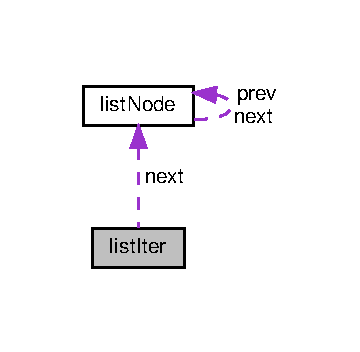
\includegraphics[width=173pt]{structlist_iter__coll__graph}
\end{center}
\end{figure}
\subsection*{Data Fields}
\begin{DoxyCompactItemize}
\item 
\hyperlink{structlist_node}{list\+Node} $\ast$ \hyperlink{structlist_iter_af8f3c30b0e82b384ff2f78d3e53b507f}{next}
\item 
int \hyperlink{structlist_iter_a886d551d5381dc3e53f17825ffc51641}{direction}
\end{DoxyCompactItemize}


\subsection{Detailed Description}


Definition at line 42 of file adlist.\+h.



\subsection{Field Documentation}
\mbox{\Hypertarget{structlist_iter_a886d551d5381dc3e53f17825ffc51641}\label{structlist_iter_a886d551d5381dc3e53f17825ffc51641}} 
\index{list\+Iter@{list\+Iter}!direction@{direction}}
\index{direction@{direction}!list\+Iter@{list\+Iter}}
\subsubsection{\texorpdfstring{direction}{direction}}
{\footnotesize\ttfamily int direction}



Definition at line 44 of file adlist.\+h.

\mbox{\Hypertarget{structlist_iter_af8f3c30b0e82b384ff2f78d3e53b507f}\label{structlist_iter_af8f3c30b0e82b384ff2f78d3e53b507f}} 
\index{list\+Iter@{list\+Iter}!next@{next}}
\index{next@{next}!list\+Iter@{list\+Iter}}
\subsubsection{\texorpdfstring{next}{next}}
{\footnotesize\ttfamily \hyperlink{structlist_node}{list\+Node}$\ast$ next}



Definition at line 43 of file adlist.\+h.



The documentation for this struct was generated from the following file\+:\begin{DoxyCompactItemize}
\item 
src/\hyperlink{adlist_8h}{adlist.\+h}\end{DoxyCompactItemize}

\hypertarget{structlist_node}{}\section{list\+Node Struct Reference}
\label{structlist_node}\index{list\+Node@{list\+Node}}


{\ttfamily \#include $<$adlist.\+h$>$}



Collaboration diagram for list\+Node\+:
\nopagebreak
\begin{figure}[H]
\begin{center}
\leavevmode
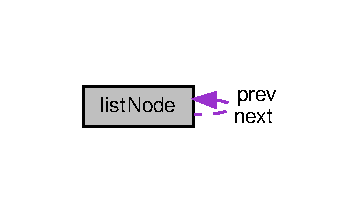
\includegraphics[width=173pt]{structlist_node__coll__graph}
\end{center}
\end{figure}
\subsection*{Data Fields}
\begin{DoxyCompactItemize}
\item 
struct \hyperlink{structlist_node}{list\+Node} $\ast$ \hyperlink{structlist_node_a58e66447fe4a91732b36e114d5c740bd}{prev}
\item 
struct \hyperlink{structlist_node}{list\+Node} $\ast$ \hyperlink{structlist_node_a4bc565cf125866bc99151319102fe748}{next}
\item 
void $\ast$ \hyperlink{structlist_node_a0f61d63b009d0880a89c843bd50d8d76}{value}
\end{DoxyCompactItemize}


\subsection{Detailed Description}


Definition at line 36 of file adlist.\+h.



\subsection{Field Documentation}
\mbox{\Hypertarget{structlist_node_a4bc565cf125866bc99151319102fe748}\label{structlist_node_a4bc565cf125866bc99151319102fe748}} 
\index{list\+Node@{list\+Node}!next@{next}}
\index{next@{next}!list\+Node@{list\+Node}}
\subsubsection{\texorpdfstring{next}{next}}
{\footnotesize\ttfamily struct \hyperlink{structlist_node}{list\+Node}$\ast$ next}



Definition at line 38 of file adlist.\+h.

\mbox{\Hypertarget{structlist_node_a58e66447fe4a91732b36e114d5c740bd}\label{structlist_node_a58e66447fe4a91732b36e114d5c740bd}} 
\index{list\+Node@{list\+Node}!prev@{prev}}
\index{prev@{prev}!list\+Node@{list\+Node}}
\subsubsection{\texorpdfstring{prev}{prev}}
{\footnotesize\ttfamily struct \hyperlink{structlist_node}{list\+Node}$\ast$ prev}



Definition at line 37 of file adlist.\+h.

\mbox{\Hypertarget{structlist_node_a0f61d63b009d0880a89c843bd50d8d76}\label{structlist_node_a0f61d63b009d0880a89c843bd50d8d76}} 
\index{list\+Node@{list\+Node}!value@{value}}
\index{value@{value}!list\+Node@{list\+Node}}
\subsubsection{\texorpdfstring{value}{value}}
{\footnotesize\ttfamily void$\ast$ value}



Definition at line 39 of file adlist.\+h.



The documentation for this struct was generated from the following file\+:\begin{DoxyCompactItemize}
\item 
src/\hyperlink{adlist_8h}{adlist.\+h}\end{DoxyCompactItemize}

\hypertarget{structlist_type_entry}{}\section{list\+Type\+Entry Struct Reference}
\label{structlist_type_entry}\index{list\+Type\+Entry@{list\+Type\+Entry}}


{\ttfamily \#include $<$server.\+h$>$}



Collaboration diagram for list\+Type\+Entry\+:
\nopagebreak
\begin{figure}[H]
\begin{center}
\leavevmode
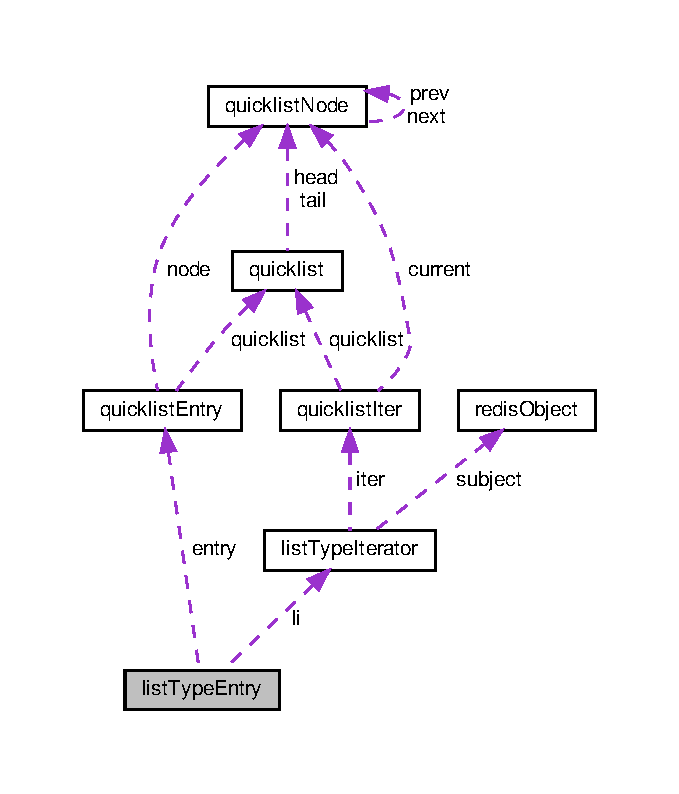
\includegraphics[width=326pt]{structlist_type_entry__coll__graph}
\end{center}
\end{figure}
\subsection*{Data Fields}
\begin{DoxyCompactItemize}
\item 
\hyperlink{structlist_type_iterator}{list\+Type\+Iterator} $\ast$ \hyperlink{structlist_type_entry_a3d40727d2b97a1eee7c2775aa8ec35c6}{li}
\item 
\hyperlink{structquicklist_entry}{quicklist\+Entry} \hyperlink{structlist_type_entry_aca59553f4ef8969fab89ee54734cc60b}{entry}
\end{DoxyCompactItemize}


\subsection{Detailed Description}


Definition at line 1333 of file server.\+h.



\subsection{Field Documentation}
\mbox{\Hypertarget{structlist_type_entry_aca59553f4ef8969fab89ee54734cc60b}\label{structlist_type_entry_aca59553f4ef8969fab89ee54734cc60b}} 
\index{list\+Type\+Entry@{list\+Type\+Entry}!entry@{entry}}
\index{entry@{entry}!list\+Type\+Entry@{list\+Type\+Entry}}
\subsubsection{\texorpdfstring{entry}{entry}}
{\footnotesize\ttfamily \hyperlink{structquicklist_entry}{quicklist\+Entry} entry}



Definition at line 1335 of file server.\+h.

\mbox{\Hypertarget{structlist_type_entry_a3d40727d2b97a1eee7c2775aa8ec35c6}\label{structlist_type_entry_a3d40727d2b97a1eee7c2775aa8ec35c6}} 
\index{list\+Type\+Entry@{list\+Type\+Entry}!li@{li}}
\index{li@{li}!list\+Type\+Entry@{list\+Type\+Entry}}
\subsubsection{\texorpdfstring{li}{li}}
{\footnotesize\ttfamily \hyperlink{structlist_type_iterator}{list\+Type\+Iterator}$\ast$ li}



Definition at line 1334 of file server.\+h.



The documentation for this struct was generated from the following file\+:\begin{DoxyCompactItemize}
\item 
src/\hyperlink{server_8h}{server.\+h}\end{DoxyCompactItemize}

\hypertarget{structlist_type_iterator}{}\section{list\+Type\+Iterator Struct Reference}
\label{structlist_type_iterator}\index{list\+Type\+Iterator@{list\+Type\+Iterator}}


{\ttfamily \#include $<$server.\+h$>$}



Collaboration diagram for list\+Type\+Iterator\+:
\nopagebreak
\begin{figure}[H]
\begin{center}
\leavevmode
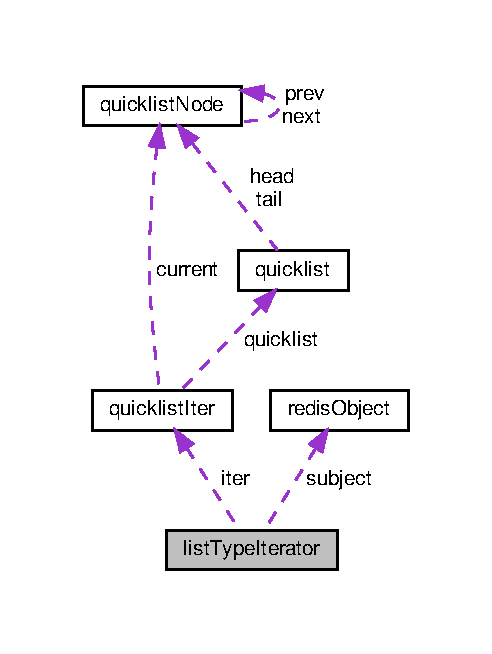
\includegraphics[width=236pt]{structlist_type_iterator__coll__graph}
\end{center}
\end{figure}
\subsection*{Data Fields}
\begin{DoxyCompactItemize}
\item 
\hyperlink{server_8h_a540f174d2685422fbd7d12e3cd44c8e2}{robj} $\ast$ \hyperlink{structlist_type_iterator_a8bd087874443f3e41cf5f728d8490693}{subject}
\item 
unsigned char \hyperlink{structlist_type_iterator_aebb5bc6c2404c4a5dd3ab3a29b65422f}{encoding}
\item 
unsigned char \hyperlink{structlist_type_iterator_a4c9b82152ef06a9d3b78f60779cd4b85}{direction}
\item 
\hyperlink{structquicklist_iter}{quicklist\+Iter} $\ast$ \hyperlink{structlist_type_iterator_ab8299304cd39d574da7e97bf50b13149}{iter}
\end{DoxyCompactItemize}


\subsection{Detailed Description}


Definition at line 1325 of file server.\+h.



\subsection{Field Documentation}
\mbox{\Hypertarget{structlist_type_iterator_a4c9b82152ef06a9d3b78f60779cd4b85}\label{structlist_type_iterator_a4c9b82152ef06a9d3b78f60779cd4b85}} 
\index{list\+Type\+Iterator@{list\+Type\+Iterator}!direction@{direction}}
\index{direction@{direction}!list\+Type\+Iterator@{list\+Type\+Iterator}}
\subsubsection{\texorpdfstring{direction}{direction}}
{\footnotesize\ttfamily unsigned char direction}



Definition at line 1328 of file server.\+h.

\mbox{\Hypertarget{structlist_type_iterator_aebb5bc6c2404c4a5dd3ab3a29b65422f}\label{structlist_type_iterator_aebb5bc6c2404c4a5dd3ab3a29b65422f}} 
\index{list\+Type\+Iterator@{list\+Type\+Iterator}!encoding@{encoding}}
\index{encoding@{encoding}!list\+Type\+Iterator@{list\+Type\+Iterator}}
\subsubsection{\texorpdfstring{encoding}{encoding}}
{\footnotesize\ttfamily unsigned char encoding}



Definition at line 1327 of file server.\+h.

\mbox{\Hypertarget{structlist_type_iterator_ab8299304cd39d574da7e97bf50b13149}\label{structlist_type_iterator_ab8299304cd39d574da7e97bf50b13149}} 
\index{list\+Type\+Iterator@{list\+Type\+Iterator}!iter@{iter}}
\index{iter@{iter}!list\+Type\+Iterator@{list\+Type\+Iterator}}
\subsubsection{\texorpdfstring{iter}{iter}}
{\footnotesize\ttfamily \hyperlink{structquicklist_iter}{quicklist\+Iter}$\ast$ iter}



Definition at line 1329 of file server.\+h.

\mbox{\Hypertarget{structlist_type_iterator_a8bd087874443f3e41cf5f728d8490693}\label{structlist_type_iterator_a8bd087874443f3e41cf5f728d8490693}} 
\index{list\+Type\+Iterator@{list\+Type\+Iterator}!subject@{subject}}
\index{subject@{subject}!list\+Type\+Iterator@{list\+Type\+Iterator}}
\subsubsection{\texorpdfstring{subject}{subject}}
{\footnotesize\ttfamily \hyperlink{server_8h_a540f174d2685422fbd7d12e3cd44c8e2}{robj}$\ast$ subject}



Definition at line 1326 of file server.\+h.



The documentation for this struct was generated from the following file\+:\begin{DoxyCompactItemize}
\item 
src/\hyperlink{server_8h}{server.\+h}\end{DoxyCompactItemize}

\hypertarget{structlw_canvas}{}\section{lw\+Canvas Struct Reference}
\label{structlw_canvas}\index{lw\+Canvas@{lw\+Canvas}}
\subsection*{Data Fields}
\begin{DoxyCompactItemize}
\item 
int \hyperlink{structlw_canvas_a2474a5474cbff19523a51eb1de01cda4}{width}
\item 
int \hyperlink{structlw_canvas_ad12fc34ce789bce6c8a05d8a17138534}{height}
\item 
char $\ast$ \hyperlink{structlw_canvas_afa6521e164d549ae3e927aac31252c83}{pixels}
\end{DoxyCompactItemize}


\subsection{Detailed Description}


Definition at line 42 of file lolwut5.\+c.



\subsection{Field Documentation}
\mbox{\Hypertarget{structlw_canvas_ad12fc34ce789bce6c8a05d8a17138534}\label{structlw_canvas_ad12fc34ce789bce6c8a05d8a17138534}} 
\index{lw\+Canvas@{lw\+Canvas}!height@{height}}
\index{height@{height}!lw\+Canvas@{lw\+Canvas}}
\subsubsection{\texorpdfstring{height}{height}}
{\footnotesize\ttfamily int height}



Definition at line 44 of file lolwut5.\+c.

\mbox{\Hypertarget{structlw_canvas_afa6521e164d549ae3e927aac31252c83}\label{structlw_canvas_afa6521e164d549ae3e927aac31252c83}} 
\index{lw\+Canvas@{lw\+Canvas}!pixels@{pixels}}
\index{pixels@{pixels}!lw\+Canvas@{lw\+Canvas}}
\subsubsection{\texorpdfstring{pixels}{pixels}}
{\footnotesize\ttfamily char$\ast$ pixels}



Definition at line 45 of file lolwut5.\+c.

\mbox{\Hypertarget{structlw_canvas_a2474a5474cbff19523a51eb1de01cda4}\label{structlw_canvas_a2474a5474cbff19523a51eb1de01cda4}} 
\index{lw\+Canvas@{lw\+Canvas}!width@{width}}
\index{width@{width}!lw\+Canvas@{lw\+Canvas}}
\subsubsection{\texorpdfstring{width}{width}}
{\footnotesize\ttfamily int width}



Definition at line 43 of file lolwut5.\+c.



The documentation for this struct was generated from the following file\+:\begin{DoxyCompactItemize}
\item 
src/\hyperlink{lolwut5_8c}{lolwut5.\+c}\end{DoxyCompactItemize}

\hypertarget{structmalloc__stats}{}\section{malloc\+\_\+stats Struct Reference}
\label{structmalloc__stats}\index{malloc\+\_\+stats@{malloc\+\_\+stats}}


{\ttfamily \#include $<$server.\+h$>$}

\subsection*{Data Fields}
\begin{DoxyCompactItemize}
\item 
size\+\_\+t \hyperlink{structmalloc__stats_a24fe6607486bb69f2f446830dbf6c8fb}{zmalloc\+\_\+used}
\item 
size\+\_\+t \hyperlink{structmalloc__stats_a93e17e92b02c3ad2a4e6bf903154b3d2}{process\+\_\+rss}
\item 
size\+\_\+t \hyperlink{structmalloc__stats_a35a8adbf64bc20a4ab20cf3872ea5e54}{allocator\+\_\+allocated}
\item 
size\+\_\+t \hyperlink{structmalloc__stats_a78e452f18e74cbf8be28858f49c0ff0b}{allocator\+\_\+active}
\item 
size\+\_\+t \hyperlink{structmalloc__stats_abaf85ea7348d3c27fea44dcc7cebd639}{allocator\+\_\+resident}
\end{DoxyCompactItemize}


\subsection{Detailed Description}


Definition at line 902 of file server.\+h.



\subsection{Field Documentation}
\mbox{\Hypertarget{structmalloc__stats_a78e452f18e74cbf8be28858f49c0ff0b}\label{structmalloc__stats_a78e452f18e74cbf8be28858f49c0ff0b}} 
\index{malloc\+\_\+stats@{malloc\+\_\+stats}!allocator\+\_\+active@{allocator\+\_\+active}}
\index{allocator\+\_\+active@{allocator\+\_\+active}!malloc\+\_\+stats@{malloc\+\_\+stats}}
\subsubsection{\texorpdfstring{allocator\+\_\+active}{allocator\_active}}
{\footnotesize\ttfamily size\+\_\+t allocator\+\_\+active}



Definition at line 906 of file server.\+h.

\mbox{\Hypertarget{structmalloc__stats_a35a8adbf64bc20a4ab20cf3872ea5e54}\label{structmalloc__stats_a35a8adbf64bc20a4ab20cf3872ea5e54}} 
\index{malloc\+\_\+stats@{malloc\+\_\+stats}!allocator\+\_\+allocated@{allocator\+\_\+allocated}}
\index{allocator\+\_\+allocated@{allocator\+\_\+allocated}!malloc\+\_\+stats@{malloc\+\_\+stats}}
\subsubsection{\texorpdfstring{allocator\+\_\+allocated}{allocator\_allocated}}
{\footnotesize\ttfamily size\+\_\+t allocator\+\_\+allocated}



Definition at line 905 of file server.\+h.

\mbox{\Hypertarget{structmalloc__stats_abaf85ea7348d3c27fea44dcc7cebd639}\label{structmalloc__stats_abaf85ea7348d3c27fea44dcc7cebd639}} 
\index{malloc\+\_\+stats@{malloc\+\_\+stats}!allocator\+\_\+resident@{allocator\+\_\+resident}}
\index{allocator\+\_\+resident@{allocator\+\_\+resident}!malloc\+\_\+stats@{malloc\+\_\+stats}}
\subsubsection{\texorpdfstring{allocator\+\_\+resident}{allocator\_resident}}
{\footnotesize\ttfamily size\+\_\+t allocator\+\_\+resident}



Definition at line 907 of file server.\+h.

\mbox{\Hypertarget{structmalloc__stats_a93e17e92b02c3ad2a4e6bf903154b3d2}\label{structmalloc__stats_a93e17e92b02c3ad2a4e6bf903154b3d2}} 
\index{malloc\+\_\+stats@{malloc\+\_\+stats}!process\+\_\+rss@{process\+\_\+rss}}
\index{process\+\_\+rss@{process\+\_\+rss}!malloc\+\_\+stats@{malloc\+\_\+stats}}
\subsubsection{\texorpdfstring{process\+\_\+rss}{process\_rss}}
{\footnotesize\ttfamily size\+\_\+t process\+\_\+rss}



Definition at line 904 of file server.\+h.

\mbox{\Hypertarget{structmalloc__stats_a24fe6607486bb69f2f446830dbf6c8fb}\label{structmalloc__stats_a24fe6607486bb69f2f446830dbf6c8fb}} 
\index{malloc\+\_\+stats@{malloc\+\_\+stats}!zmalloc\+\_\+used@{zmalloc\+\_\+used}}
\index{zmalloc\+\_\+used@{zmalloc\+\_\+used}!malloc\+\_\+stats@{malloc\+\_\+stats}}
\subsubsection{\texorpdfstring{zmalloc\+\_\+used}{zmalloc\_used}}
{\footnotesize\ttfamily size\+\_\+t zmalloc\+\_\+used}



Definition at line 903 of file server.\+h.



The documentation for this struct was generated from the following file\+:\begin{DoxyCompactItemize}
\item 
src/\hyperlink{server_8h}{server.\+h}\end{DoxyCompactItemize}

\hypertarget{structmigrate_cached_socket}{}\section{migrate\+Cached\+Socket Struct Reference}
\label{structmigrate_cached_socket}\index{migrate\+Cached\+Socket@{migrate\+Cached\+Socket}}
\subsection*{Data Fields}
\begin{DoxyCompactItemize}
\item 
int \hyperlink{structmigrate_cached_socket_a6f8059414f0228f0256115e024eeed4b}{fd}
\item 
long \hyperlink{structmigrate_cached_socket_ab53bd0be4d91d31966967ed2ac698132}{last\+\_\+dbid}
\item 
time\+\_\+t \hyperlink{structmigrate_cached_socket_ac765d15ca6e1c4d1435bd80ff2a93a2c}{last\+\_\+use\+\_\+time}
\end{DoxyCompactItemize}


\subsection{Detailed Description}


Definition at line 4947 of file cluster.\+c.



\subsection{Field Documentation}
\mbox{\Hypertarget{structmigrate_cached_socket_a6f8059414f0228f0256115e024eeed4b}\label{structmigrate_cached_socket_a6f8059414f0228f0256115e024eeed4b}} 
\index{migrate\+Cached\+Socket@{migrate\+Cached\+Socket}!fd@{fd}}
\index{fd@{fd}!migrate\+Cached\+Socket@{migrate\+Cached\+Socket}}
\subsubsection{\texorpdfstring{fd}{fd}}
{\footnotesize\ttfamily int fd}



Definition at line 4948 of file cluster.\+c.

\mbox{\Hypertarget{structmigrate_cached_socket_ab53bd0be4d91d31966967ed2ac698132}\label{structmigrate_cached_socket_ab53bd0be4d91d31966967ed2ac698132}} 
\index{migrate\+Cached\+Socket@{migrate\+Cached\+Socket}!last\+\_\+dbid@{last\+\_\+dbid}}
\index{last\+\_\+dbid@{last\+\_\+dbid}!migrate\+Cached\+Socket@{migrate\+Cached\+Socket}}
\subsubsection{\texorpdfstring{last\+\_\+dbid}{last\_dbid}}
{\footnotesize\ttfamily long last\+\_\+dbid}



Definition at line 4949 of file cluster.\+c.

\mbox{\Hypertarget{structmigrate_cached_socket_ac765d15ca6e1c4d1435bd80ff2a93a2c}\label{structmigrate_cached_socket_ac765d15ca6e1c4d1435bd80ff2a93a2c}} 
\index{migrate\+Cached\+Socket@{migrate\+Cached\+Socket}!last\+\_\+use\+\_\+time@{last\+\_\+use\+\_\+time}}
\index{last\+\_\+use\+\_\+time@{last\+\_\+use\+\_\+time}!migrate\+Cached\+Socket@{migrate\+Cached\+Socket}}
\subsubsection{\texorpdfstring{last\+\_\+use\+\_\+time}{last\_use\_time}}
{\footnotesize\ttfamily time\+\_\+t last\+\_\+use\+\_\+time}



Definition at line 4950 of file cluster.\+c.



The documentation for this struct was generated from the following file\+:\begin{DoxyCompactItemize}
\item 
src/\hyperlink{cluster_8c}{cluster.\+c}\end{DoxyCompactItemize}

\hypertarget{structmodule_cluster_node_info}{}\section{module\+Cluster\+Node\+Info Struct Reference}
\label{structmodule_cluster_node_info}\index{module\+Cluster\+Node\+Info@{module\+Cluster\+Node\+Info}}
\subsection*{Data Fields}
\begin{DoxyCompactItemize}
\item 
int \hyperlink{structmodule_cluster_node_info_ac8bf36fe0577cba66bccda3a6f7e80a4}{flags}
\item 
char \hyperlink{structmodule_cluster_node_info_a9de2afd4e77c16f677244d244270b605}{ip} \mbox{[}\hyperlink{server_8h_ad97c5405ed22a94e9fcc10fba577d6c0}{N\+E\+T\+\_\+\+I\+P\+\_\+\+S\+T\+R\+\_\+\+L\+EN}\mbox{]}
\item 
int \hyperlink{structmodule_cluster_node_info_a63c89c04d1feae07ca35558055155ffb}{port}
\item 
char \hyperlink{structmodule_cluster_node_info_ab95368416ffd4d1b80277de1b0c2c32d}{master\+\_\+id} \mbox{[}40\mbox{]}
\end{DoxyCompactItemize}


\subsection{Detailed Description}


Definition at line 3959 of file module.\+c.



\subsection{Field Documentation}
\mbox{\Hypertarget{structmodule_cluster_node_info_ac8bf36fe0577cba66bccda3a6f7e80a4}\label{structmodule_cluster_node_info_ac8bf36fe0577cba66bccda3a6f7e80a4}} 
\index{module\+Cluster\+Node\+Info@{module\+Cluster\+Node\+Info}!flags@{flags}}
\index{flags@{flags}!module\+Cluster\+Node\+Info@{module\+Cluster\+Node\+Info}}
\subsubsection{\texorpdfstring{flags}{flags}}
{\footnotesize\ttfamily int flags}



Definition at line 3960 of file module.\+c.

\mbox{\Hypertarget{structmodule_cluster_node_info_a9de2afd4e77c16f677244d244270b605}\label{structmodule_cluster_node_info_a9de2afd4e77c16f677244d244270b605}} 
\index{module\+Cluster\+Node\+Info@{module\+Cluster\+Node\+Info}!ip@{ip}}
\index{ip@{ip}!module\+Cluster\+Node\+Info@{module\+Cluster\+Node\+Info}}
\subsubsection{\texorpdfstring{ip}{ip}}
{\footnotesize\ttfamily char ip\mbox{[}\hyperlink{server_8h_ad97c5405ed22a94e9fcc10fba577d6c0}{N\+E\+T\+\_\+\+I\+P\+\_\+\+S\+T\+R\+\_\+\+L\+EN}\mbox{]}}



Definition at line 3961 of file module.\+c.

\mbox{\Hypertarget{structmodule_cluster_node_info_ab95368416ffd4d1b80277de1b0c2c32d}\label{structmodule_cluster_node_info_ab95368416ffd4d1b80277de1b0c2c32d}} 
\index{module\+Cluster\+Node\+Info@{module\+Cluster\+Node\+Info}!master\+\_\+id@{master\+\_\+id}}
\index{master\+\_\+id@{master\+\_\+id}!module\+Cluster\+Node\+Info@{module\+Cluster\+Node\+Info}}
\subsubsection{\texorpdfstring{master\+\_\+id}{master\_id}}
{\footnotesize\ttfamily char master\+\_\+id\mbox{[}40\mbox{]}}



Definition at line 3963 of file module.\+c.

\mbox{\Hypertarget{structmodule_cluster_node_info_a63c89c04d1feae07ca35558055155ffb}\label{structmodule_cluster_node_info_a63c89c04d1feae07ca35558055155ffb}} 
\index{module\+Cluster\+Node\+Info@{module\+Cluster\+Node\+Info}!port@{port}}
\index{port@{port}!module\+Cluster\+Node\+Info@{module\+Cluster\+Node\+Info}}
\subsubsection{\texorpdfstring{port}{port}}
{\footnotesize\ttfamily int port}



Definition at line 3962 of file module.\+c.



The documentation for this struct was generated from the following file\+:\begin{DoxyCompactItemize}
\item 
src/\hyperlink{module_8c}{module.\+c}\end{DoxyCompactItemize}

\hypertarget{structmodule_cluster_receiver}{}\section{module\+Cluster\+Receiver Struct Reference}
\label{structmodule_cluster_receiver}\index{module\+Cluster\+Receiver@{module\+Cluster\+Receiver}}


Collaboration diagram for module\+Cluster\+Receiver\+:
\nopagebreak
\begin{figure}[H]
\begin{center}
\leavevmode
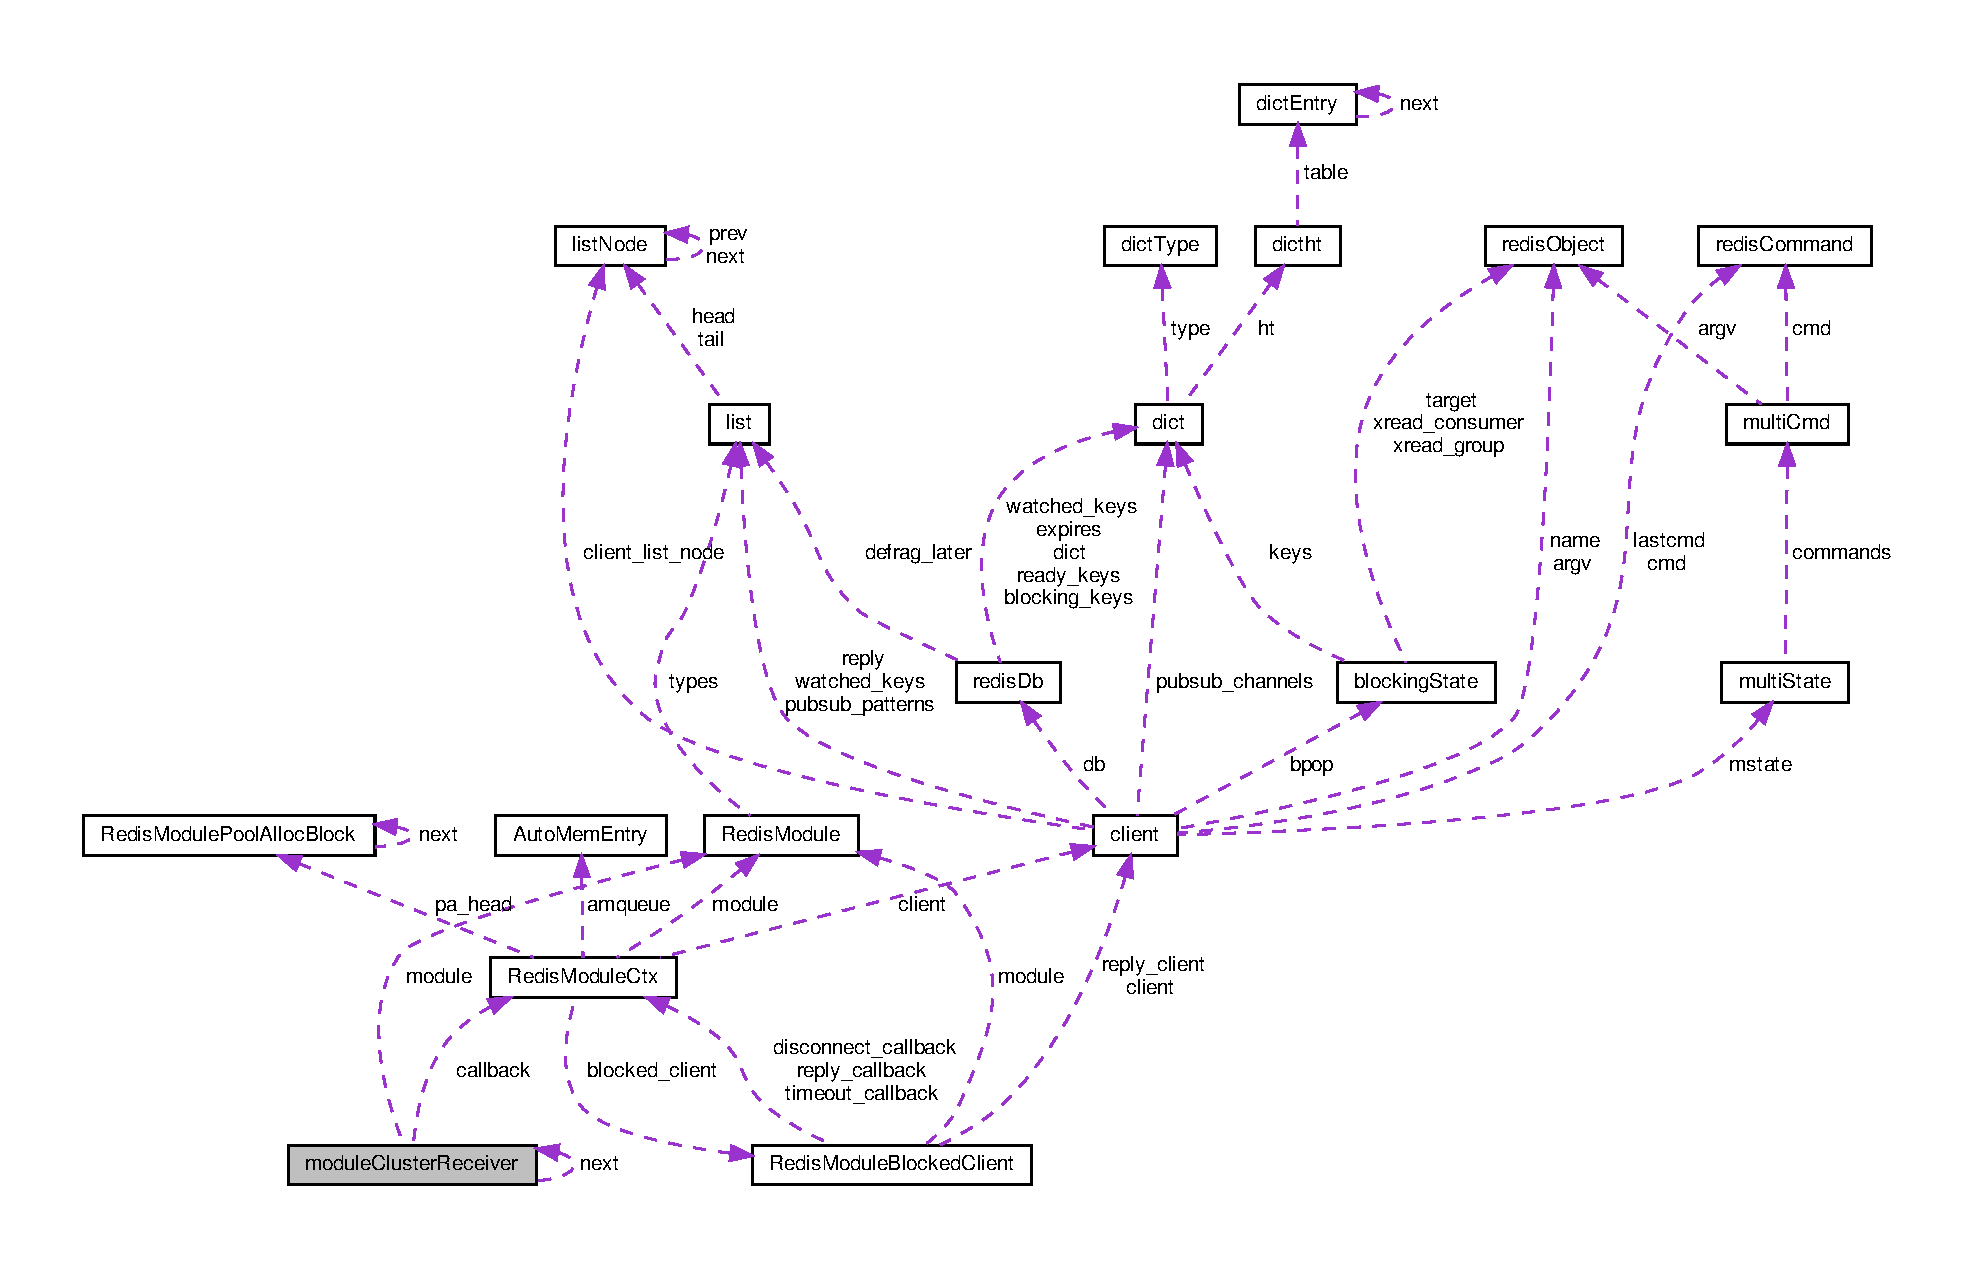
\includegraphics[width=350pt]{structmodule_cluster_receiver__coll__graph}
\end{center}
\end{figure}
\subsection*{Data Fields}
\begin{DoxyCompactItemize}
\item 
uint64\+\_\+t \hyperlink{structmodule_cluster_receiver_a5c568ad76933cdbb1f61b40781917492}{module\+\_\+id}
\item 
\hyperlink{redismodule_8h_ac409a6cb3005523c7d4f10ceb3164535}{Redis\+Module\+Cluster\+Message\+Receiver} \hyperlink{structmodule_cluster_receiver_a9bad2da2037959b9c0a7e79e93adf8da}{callback}
\item 
struct \hyperlink{struct_redis_module}{Redis\+Module} $\ast$ \hyperlink{structmodule_cluster_receiver_a0b5d3833feb2320585734795fb7f62b6}{module}
\item 
struct \hyperlink{structmodule_cluster_receiver}{module\+Cluster\+Receiver} $\ast$ \hyperlink{structmodule_cluster_receiver_aaa93837daad4aea905b795397a966c68}{next}
\end{DoxyCompactItemize}


\subsection{Detailed Description}


Definition at line 3952 of file module.\+c.



\subsection{Field Documentation}
\mbox{\Hypertarget{structmodule_cluster_receiver_a9bad2da2037959b9c0a7e79e93adf8da}\label{structmodule_cluster_receiver_a9bad2da2037959b9c0a7e79e93adf8da}} 
\index{module\+Cluster\+Receiver@{module\+Cluster\+Receiver}!callback@{callback}}
\index{callback@{callback}!module\+Cluster\+Receiver@{module\+Cluster\+Receiver}}
\subsubsection{\texorpdfstring{callback}{callback}}
{\footnotesize\ttfamily \hyperlink{redismodule_8h_ac409a6cb3005523c7d4f10ceb3164535}{Redis\+Module\+Cluster\+Message\+Receiver} callback}



Definition at line 3954 of file module.\+c.

\mbox{\Hypertarget{structmodule_cluster_receiver_a0b5d3833feb2320585734795fb7f62b6}\label{structmodule_cluster_receiver_a0b5d3833feb2320585734795fb7f62b6}} 
\index{module\+Cluster\+Receiver@{module\+Cluster\+Receiver}!module@{module}}
\index{module@{module}!module\+Cluster\+Receiver@{module\+Cluster\+Receiver}}
\subsubsection{\texorpdfstring{module}{module}}
{\footnotesize\ttfamily struct \hyperlink{struct_redis_module}{Redis\+Module}$\ast$ module}



Definition at line 3955 of file module.\+c.

\mbox{\Hypertarget{structmodule_cluster_receiver_a5c568ad76933cdbb1f61b40781917492}\label{structmodule_cluster_receiver_a5c568ad76933cdbb1f61b40781917492}} 
\index{module\+Cluster\+Receiver@{module\+Cluster\+Receiver}!module\+\_\+id@{module\+\_\+id}}
\index{module\+\_\+id@{module\+\_\+id}!module\+Cluster\+Receiver@{module\+Cluster\+Receiver}}
\subsubsection{\texorpdfstring{module\+\_\+id}{module\_id}}
{\footnotesize\ttfamily uint64\+\_\+t module\+\_\+id}



Definition at line 3953 of file module.\+c.

\mbox{\Hypertarget{structmodule_cluster_receiver_aaa93837daad4aea905b795397a966c68}\label{structmodule_cluster_receiver_aaa93837daad4aea905b795397a966c68}} 
\index{module\+Cluster\+Receiver@{module\+Cluster\+Receiver}!next@{next}}
\index{next@{next}!module\+Cluster\+Receiver@{module\+Cluster\+Receiver}}
\subsubsection{\texorpdfstring{next}{next}}
{\footnotesize\ttfamily struct \hyperlink{structmodule_cluster_receiver}{module\+Cluster\+Receiver}$\ast$ next}



Definition at line 3956 of file module.\+c.



The documentation for this struct was generated from the following file\+:\begin{DoxyCompactItemize}
\item 
src/\hyperlink{module_8c}{module.\+c}\end{DoxyCompactItemize}

\hypertarget{structmodule_load_queue_entry}{}\section{module\+Load\+Queue\+Entry Struct Reference}
\label{structmodule_load_queue_entry}\index{module\+Load\+Queue\+Entry@{module\+Load\+Queue\+Entry}}


{\ttfamily \#include $<$server.\+h$>$}



Collaboration diagram for module\+Load\+Queue\+Entry\+:
\nopagebreak
\begin{figure}[H]
\begin{center}
\leavevmode
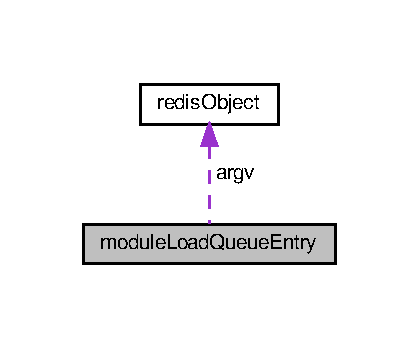
\includegraphics[width=201pt]{structmodule_load_queue_entry__coll__graph}
\end{center}
\end{figure}
\subsection*{Data Fields}
\begin{DoxyCompactItemize}
\item 
\hyperlink{sds_8h_ad69abac3df4532879db9642c95f5ef6f}{sds} \hyperlink{structmodule_load_queue_entry_aafb87a9eb5c5cc5c4d0e278bea7fdbe3}{path}
\item 
int \hyperlink{structmodule_load_queue_entry_ad1447518f4372828b8435ae82e48499e}{argc}
\item 
\hyperlink{server_8h_a540f174d2685422fbd7d12e3cd44c8e2}{robj} $\ast$$\ast$ \hyperlink{structmodule_load_queue_entry_a5c75dd3cb8eb8a3f5be7d4fdf48a9ef9}{argv}
\end{DoxyCompactItemize}


\subsection{Detailed Description}


Definition at line 773 of file server.\+h.



\subsection{Field Documentation}
\mbox{\Hypertarget{structmodule_load_queue_entry_ad1447518f4372828b8435ae82e48499e}\label{structmodule_load_queue_entry_ad1447518f4372828b8435ae82e48499e}} 
\index{module\+Load\+Queue\+Entry@{module\+Load\+Queue\+Entry}!argc@{argc}}
\index{argc@{argc}!module\+Load\+Queue\+Entry@{module\+Load\+Queue\+Entry}}
\subsubsection{\texorpdfstring{argc}{argc}}
{\footnotesize\ttfamily int argc}



Definition at line 775 of file server.\+h.

\mbox{\Hypertarget{structmodule_load_queue_entry_a5c75dd3cb8eb8a3f5be7d4fdf48a9ef9}\label{structmodule_load_queue_entry_a5c75dd3cb8eb8a3f5be7d4fdf48a9ef9}} 
\index{module\+Load\+Queue\+Entry@{module\+Load\+Queue\+Entry}!argv@{argv}}
\index{argv@{argv}!module\+Load\+Queue\+Entry@{module\+Load\+Queue\+Entry}}
\subsubsection{\texorpdfstring{argv}{argv}}
{\footnotesize\ttfamily \hyperlink{server_8h_a540f174d2685422fbd7d12e3cd44c8e2}{robj}$\ast$$\ast$ argv}



Definition at line 776 of file server.\+h.

\mbox{\Hypertarget{structmodule_load_queue_entry_aafb87a9eb5c5cc5c4d0e278bea7fdbe3}\label{structmodule_load_queue_entry_aafb87a9eb5c5cc5c4d0e278bea7fdbe3}} 
\index{module\+Load\+Queue\+Entry@{module\+Load\+Queue\+Entry}!path@{path}}
\index{path@{path}!module\+Load\+Queue\+Entry@{module\+Load\+Queue\+Entry}}
\subsubsection{\texorpdfstring{path}{path}}
{\footnotesize\ttfamily \hyperlink{sds_8h_ad69abac3df4532879db9642c95f5ef6f}{sds} path}



Definition at line 774 of file server.\+h.



The documentation for this struct was generated from the following file\+:\begin{DoxyCompactItemize}
\item 
src/\hyperlink{server_8h}{server.\+h}\end{DoxyCompactItemize}

\hypertarget{structmodule_value}{}\section{module\+Value Struct Reference}
\label{structmodule_value}\index{module\+Value@{module\+Value}}


{\ttfamily \#include $<$server.\+h$>$}



Collaboration diagram for module\+Value\+:
\nopagebreak
\begin{figure}[H]
\begin{center}
\leavevmode
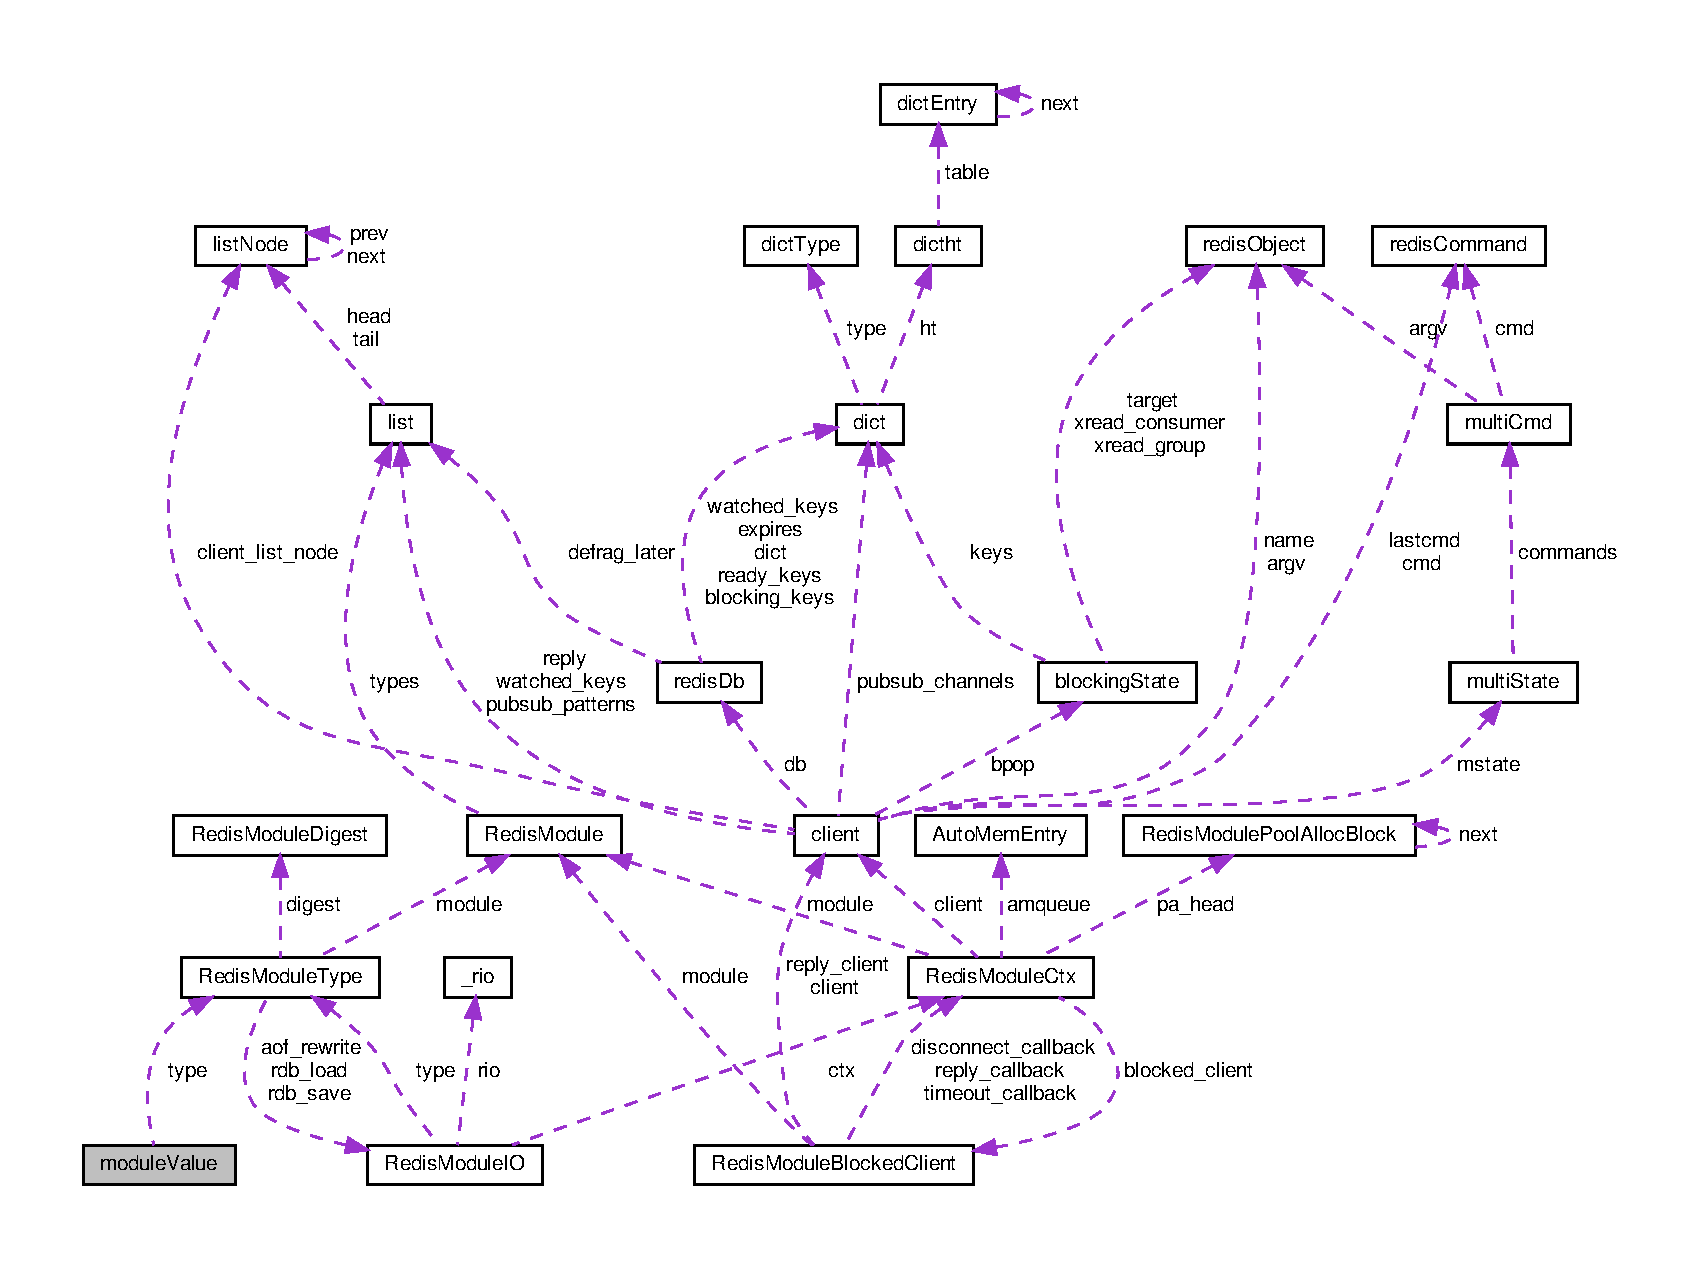
\includegraphics[width=350pt]{structmodule_value__coll__graph}
\end{center}
\end{figure}
\subsection*{Data Fields}
\begin{DoxyCompactItemize}
\item 
\hyperlink{server_8h_a3e81a33920e783a6b35dedfd7bdb6a2c}{module\+Type} $\ast$ \hyperlink{structmodule_value_a05eee39e39e34439ea77af35b597b1ae}{type}
\item 
void $\ast$ \hyperlink{structmodule_value_a0f61d63b009d0880a89c843bd50d8d76}{value}
\end{DoxyCompactItemize}


\subsection{Detailed Description}


Definition at line 538 of file server.\+h.



\subsection{Field Documentation}
\mbox{\Hypertarget{structmodule_value_a05eee39e39e34439ea77af35b597b1ae}\label{structmodule_value_a05eee39e39e34439ea77af35b597b1ae}} 
\index{module\+Value@{module\+Value}!type@{type}}
\index{type@{type}!module\+Value@{module\+Value}}
\subsubsection{\texorpdfstring{type}{type}}
{\footnotesize\ttfamily \hyperlink{server_8h_a3e81a33920e783a6b35dedfd7bdb6a2c}{module\+Type}$\ast$ type}



Definition at line 539 of file server.\+h.

\mbox{\Hypertarget{structmodule_value_a0f61d63b009d0880a89c843bd50d8d76}\label{structmodule_value_a0f61d63b009d0880a89c843bd50d8d76}} 
\index{module\+Value@{module\+Value}!value@{value}}
\index{value@{value}!module\+Value@{module\+Value}}
\subsubsection{\texorpdfstring{value}{value}}
{\footnotesize\ttfamily void$\ast$ value}



Definition at line 540 of file server.\+h.



The documentation for this struct was generated from the following file\+:\begin{DoxyCompactItemize}
\item 
src/\hyperlink{server_8h}{server.\+h}\end{DoxyCompactItemize}

\hypertarget{structmulti_cmd}{}\section{multi\+Cmd Struct Reference}
\label{structmulti_cmd}\index{multi\+Cmd@{multi\+Cmd}}


{\ttfamily \#include $<$server.\+h$>$}



Collaboration diagram for multi\+Cmd\+:
\nopagebreak
\begin{figure}[H]
\begin{center}
\leavevmode
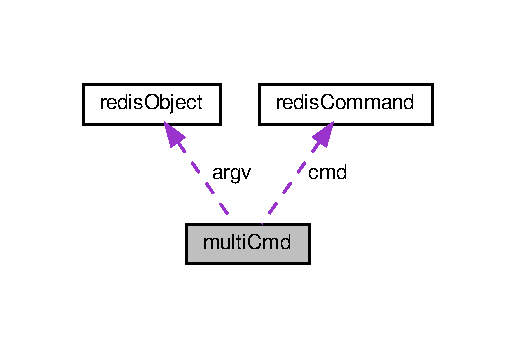
\includegraphics[width=248pt]{structmulti_cmd__coll__graph}
\end{center}
\end{figure}
\subsection*{Data Fields}
\begin{DoxyCompactItemize}
\item 
\hyperlink{server_8h_a540f174d2685422fbd7d12e3cd44c8e2}{robj} $\ast$$\ast$ \hyperlink{structmulti_cmd_a5c75dd3cb8eb8a3f5be7d4fdf48a9ef9}{argv}
\item 
int \hyperlink{structmulti_cmd_ad1447518f4372828b8435ae82e48499e}{argc}
\item 
struct \hyperlink{structredis_command}{redis\+Command} $\ast$ \hyperlink{structmulti_cmd_a8ed6c4d0c6382ad1787b32d10db25c5e}{cmd}
\end{DoxyCompactItemize}


\subsection{Detailed Description}


Definition at line 648 of file server.\+h.



\subsection{Field Documentation}
\mbox{\Hypertarget{structmulti_cmd_ad1447518f4372828b8435ae82e48499e}\label{structmulti_cmd_ad1447518f4372828b8435ae82e48499e}} 
\index{multi\+Cmd@{multi\+Cmd}!argc@{argc}}
\index{argc@{argc}!multi\+Cmd@{multi\+Cmd}}
\subsubsection{\texorpdfstring{argc}{argc}}
{\footnotesize\ttfamily int argc}



Definition at line 650 of file server.\+h.

\mbox{\Hypertarget{structmulti_cmd_a5c75dd3cb8eb8a3f5be7d4fdf48a9ef9}\label{structmulti_cmd_a5c75dd3cb8eb8a3f5be7d4fdf48a9ef9}} 
\index{multi\+Cmd@{multi\+Cmd}!argv@{argv}}
\index{argv@{argv}!multi\+Cmd@{multi\+Cmd}}
\subsubsection{\texorpdfstring{argv}{argv}}
{\footnotesize\ttfamily \hyperlink{server_8h_a540f174d2685422fbd7d12e3cd44c8e2}{robj}$\ast$$\ast$ argv}



Definition at line 649 of file server.\+h.

\mbox{\Hypertarget{structmulti_cmd_a8ed6c4d0c6382ad1787b32d10db25c5e}\label{structmulti_cmd_a8ed6c4d0c6382ad1787b32d10db25c5e}} 
\index{multi\+Cmd@{multi\+Cmd}!cmd@{cmd}}
\index{cmd@{cmd}!multi\+Cmd@{multi\+Cmd}}
\subsubsection{\texorpdfstring{cmd}{cmd}}
{\footnotesize\ttfamily struct \hyperlink{structredis_command}{redis\+Command}$\ast$ cmd}



Definition at line 651 of file server.\+h.



The documentation for this struct was generated from the following file\+:\begin{DoxyCompactItemize}
\item 
src/\hyperlink{server_8h}{server.\+h}\end{DoxyCompactItemize}

\hypertarget{structmulti_state}{}\section{multi\+State Struct Reference}
\label{structmulti_state}\index{multi\+State@{multi\+State}}


{\ttfamily \#include $<$server.\+h$>$}



Collaboration diagram for multi\+State\+:
\nopagebreak
\begin{figure}[H]
\begin{center}
\leavevmode
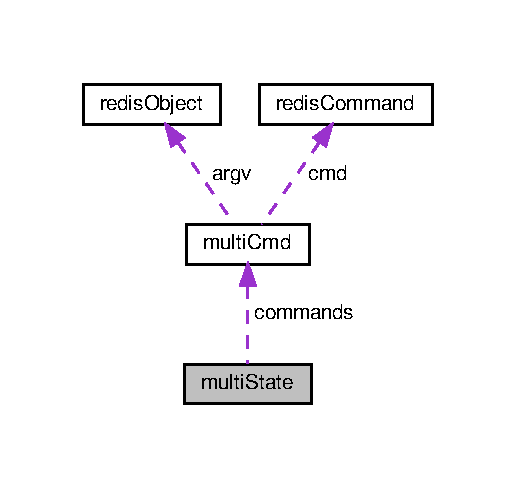
\includegraphics[width=248pt]{structmulti_state__coll__graph}
\end{center}
\end{figure}
\subsection*{Data Fields}
\begin{DoxyCompactItemize}
\item 
\hyperlink{structmulti_cmd}{multi\+Cmd} $\ast$ \hyperlink{structmulti_state_ad3a26c5b804fb03f82a816ad6d0e5c2f}{commands}
\item 
int \hyperlink{structmulti_state_ad43c3812e6d13e0518d9f8b8f463ffcf}{count}
\item 
int \hyperlink{structmulti_state_ace53526f4550147f18c5ef7a98b54633}{minreplicas}
\item 
time\+\_\+t \hyperlink{structmulti_state_af9fab5f82508da80e8a3725d32cfd75e}{minreplicas\+\_\+timeout}
\end{DoxyCompactItemize}


\subsection{Detailed Description}


Definition at line 654 of file server.\+h.



\subsection{Field Documentation}
\mbox{\Hypertarget{structmulti_state_ad3a26c5b804fb03f82a816ad6d0e5c2f}\label{structmulti_state_ad3a26c5b804fb03f82a816ad6d0e5c2f}} 
\index{multi\+State@{multi\+State}!commands@{commands}}
\index{commands@{commands}!multi\+State@{multi\+State}}
\subsubsection{\texorpdfstring{commands}{commands}}
{\footnotesize\ttfamily \hyperlink{structmulti_cmd}{multi\+Cmd}$\ast$ commands}



Definition at line 655 of file server.\+h.

\mbox{\Hypertarget{structmulti_state_ad43c3812e6d13e0518d9f8b8f463ffcf}\label{structmulti_state_ad43c3812e6d13e0518d9f8b8f463ffcf}} 
\index{multi\+State@{multi\+State}!count@{count}}
\index{count@{count}!multi\+State@{multi\+State}}
\subsubsection{\texorpdfstring{count}{count}}
{\footnotesize\ttfamily int count}



Definition at line 656 of file server.\+h.

\mbox{\Hypertarget{structmulti_state_ace53526f4550147f18c5ef7a98b54633}\label{structmulti_state_ace53526f4550147f18c5ef7a98b54633}} 
\index{multi\+State@{multi\+State}!minreplicas@{minreplicas}}
\index{minreplicas@{minreplicas}!multi\+State@{multi\+State}}
\subsubsection{\texorpdfstring{minreplicas}{minreplicas}}
{\footnotesize\ttfamily int minreplicas}



Definition at line 657 of file server.\+h.

\mbox{\Hypertarget{structmulti_state_af9fab5f82508da80e8a3725d32cfd75e}\label{structmulti_state_af9fab5f82508da80e8a3725d32cfd75e}} 
\index{multi\+State@{multi\+State}!minreplicas\+\_\+timeout@{minreplicas\+\_\+timeout}}
\index{minreplicas\+\_\+timeout@{minreplicas\+\_\+timeout}!multi\+State@{multi\+State}}
\subsubsection{\texorpdfstring{minreplicas\+\_\+timeout}{minreplicas\_timeout}}
{\footnotesize\ttfamily time\+\_\+t minreplicas\+\_\+timeout}



Definition at line 658 of file server.\+h.



The documentation for this struct was generated from the following file\+:\begin{DoxyCompactItemize}
\item 
src/\hyperlink{server_8h}{server.\+h}\end{DoxyCompactItemize}

\hypertarget{structpubsub_pattern}{}\section{pubsub\+Pattern Struct Reference}
\label{structpubsub_pattern}\index{pubsub\+Pattern@{pubsub\+Pattern}}


{\ttfamily \#include $<$server.\+h$>$}



Collaboration diagram for pubsub\+Pattern\+:
\nopagebreak
\begin{figure}[H]
\begin{center}
\leavevmode
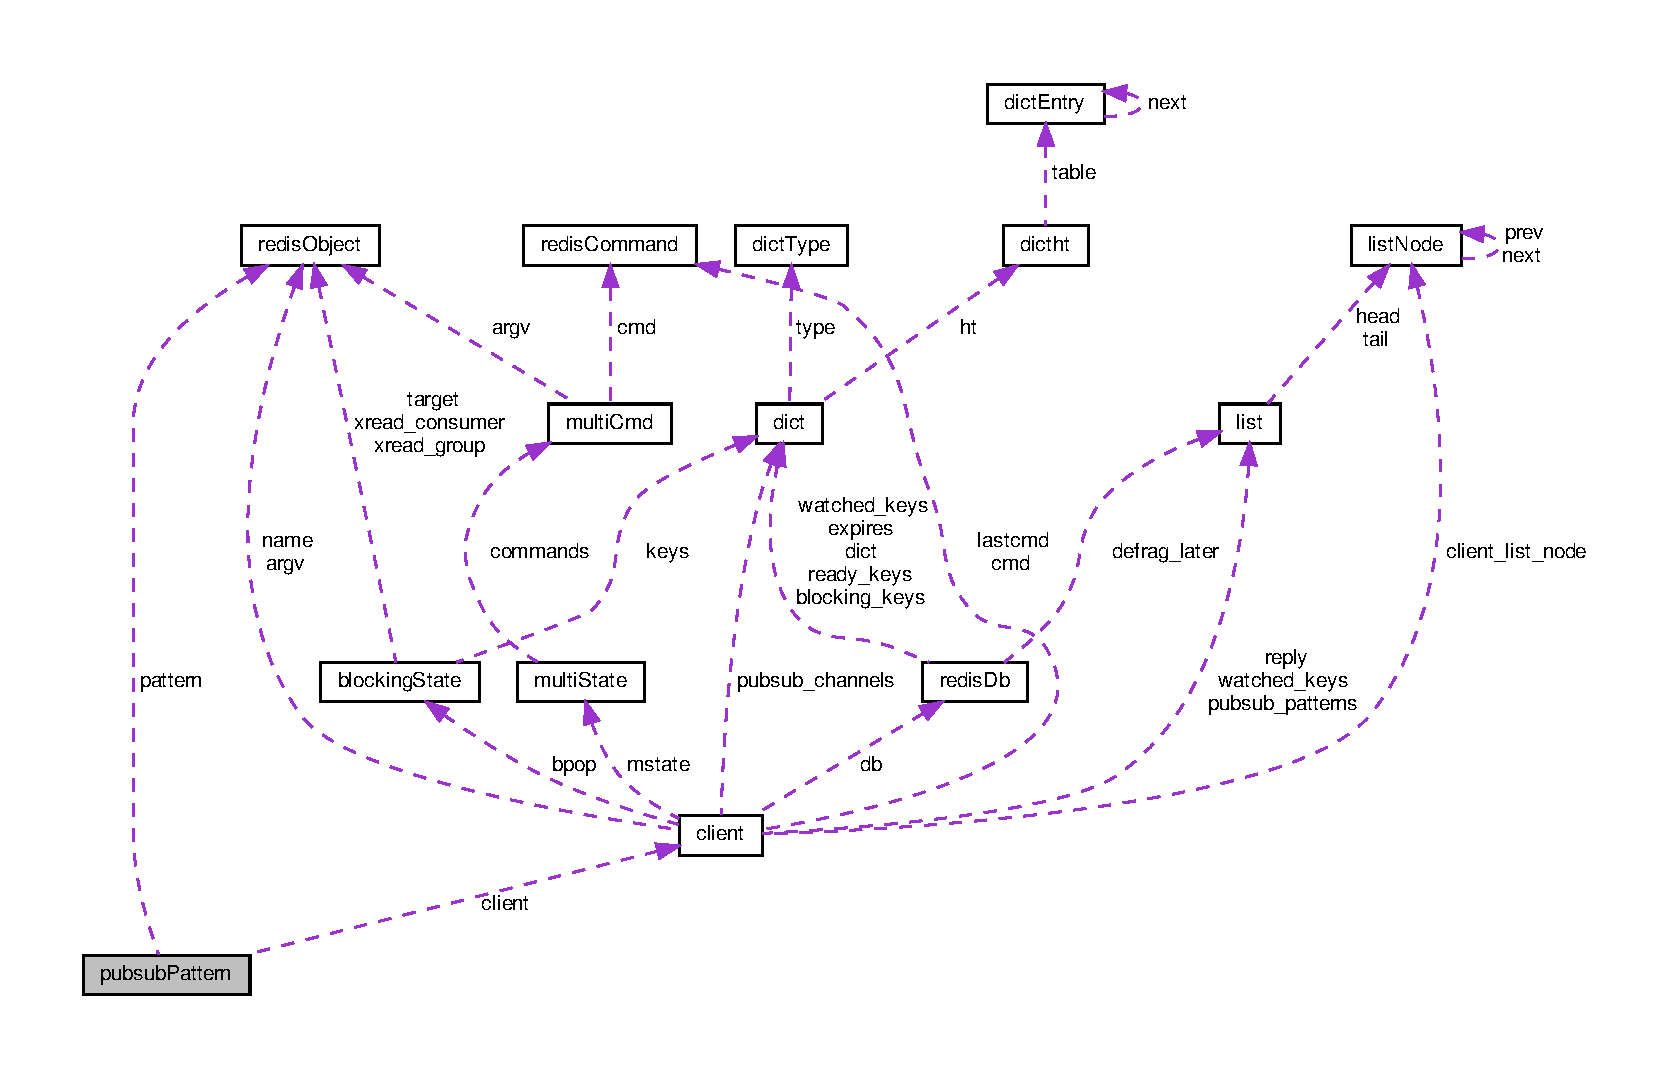
\includegraphics[width=350pt]{structpubsub_pattern__coll__graph}
\end{center}
\end{figure}
\subsection*{Data Fields}
\begin{DoxyCompactItemize}
\item 
\hyperlink{structclient}{client} $\ast$ \hyperlink{structpubsub_pattern_a6d99956d3d06c98958feb17baf491c71}{client}
\item 
\hyperlink{server_8h_a540f174d2685422fbd7d12e3cd44c8e2}{robj} $\ast$ \hyperlink{structpubsub_pattern_a779898a32e09ec217b6876501caecc9c}{pattern}
\end{DoxyCompactItemize}


\subsection{Detailed Description}


Definition at line 1283 of file server.\+h.



\subsection{Field Documentation}
\mbox{\Hypertarget{structpubsub_pattern_a6d99956d3d06c98958feb17baf491c71}\label{structpubsub_pattern_a6d99956d3d06c98958feb17baf491c71}} 
\index{pubsub\+Pattern@{pubsub\+Pattern}!client@{client}}
\index{client@{client}!pubsub\+Pattern@{pubsub\+Pattern}}
\subsubsection{\texorpdfstring{client}{client}}
{\footnotesize\ttfamily \hyperlink{structclient}{client}$\ast$ \hyperlink{structclient}{client}}



Definition at line 1284 of file server.\+h.

\mbox{\Hypertarget{structpubsub_pattern_a779898a32e09ec217b6876501caecc9c}\label{structpubsub_pattern_a779898a32e09ec217b6876501caecc9c}} 
\index{pubsub\+Pattern@{pubsub\+Pattern}!pattern@{pattern}}
\index{pattern@{pattern}!pubsub\+Pattern@{pubsub\+Pattern}}
\subsubsection{\texorpdfstring{pattern}{pattern}}
{\footnotesize\ttfamily \hyperlink{server_8h_a540f174d2685422fbd7d12e3cd44c8e2}{robj}$\ast$ pattern}



Definition at line 1285 of file server.\+h.



The documentation for this struct was generated from the following file\+:\begin{DoxyCompactItemize}
\item 
src/\hyperlink{server_8h}{server.\+h}\end{DoxyCompactItemize}

\hypertarget{structquicklist}{}\section{quicklist Struct Reference}
\label{structquicklist}\index{quicklist@{quicklist}}


{\ttfamily \#include $<$quicklist.\+h$>$}



Collaboration diagram for quicklist\+:
\nopagebreak
\begin{figure}[H]
\begin{center}
\leavevmode
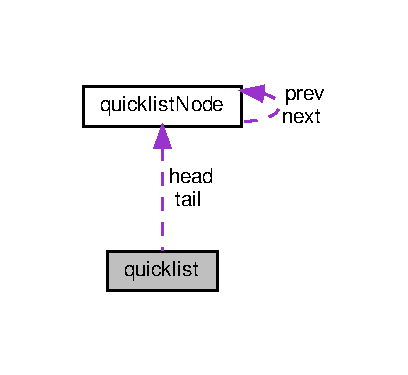
\includegraphics[width=196pt]{structquicklist__coll__graph}
\end{center}
\end{figure}
\subsection*{Data Fields}
\begin{DoxyCompactItemize}
\item 
\hyperlink{structquicklist_node}{quicklist\+Node} $\ast$ \hyperlink{structquicklist_a9768476640799c4dc25850d7dfb5f436}{head}
\item 
\hyperlink{structquicklist_node}{quicklist\+Node} $\ast$ \hyperlink{structquicklist_a415ce772af9efb537aa65ec5766ed45a}{tail}
\item 
unsigned long \hyperlink{structquicklist_a61b4b8d2ac3f4853727e2c2fcbec3503}{count}
\item 
unsigned long \hyperlink{structquicklist_af2e72f8a5bf4bcdb77566c2936d5f13d}{len}
\item 
int \hyperlink{structquicklist_a1bddf1e646fa3d6b3553e28e41cfe7c5}{fill}\+: 16
\item 
unsigned int \hyperlink{structquicklist_a851a2a518700a4f5aa3d8e099978afca}{compress}\+: 16
\end{DoxyCompactItemize}


\subsection{Detailed Description}


Definition at line 73 of file quicklist.\+h.



\subsection{Field Documentation}
\mbox{\Hypertarget{structquicklist_a851a2a518700a4f5aa3d8e099978afca}\label{structquicklist_a851a2a518700a4f5aa3d8e099978afca}} 
\index{quicklist@{quicklist}!compress@{compress}}
\index{compress@{compress}!quicklist@{quicklist}}
\subsubsection{\texorpdfstring{compress}{compress}}
{\footnotesize\ttfamily unsigned int compress}



Definition at line 79 of file quicklist.\+h.

\mbox{\Hypertarget{structquicklist_a61b4b8d2ac3f4853727e2c2fcbec3503}\label{structquicklist_a61b4b8d2ac3f4853727e2c2fcbec3503}} 
\index{quicklist@{quicklist}!count@{count}}
\index{count@{count}!quicklist@{quicklist}}
\subsubsection{\texorpdfstring{count}{count}}
{\footnotesize\ttfamily unsigned long count}



Definition at line 76 of file quicklist.\+h.

\mbox{\Hypertarget{structquicklist_a1bddf1e646fa3d6b3553e28e41cfe7c5}\label{structquicklist_a1bddf1e646fa3d6b3553e28e41cfe7c5}} 
\index{quicklist@{quicklist}!fill@{fill}}
\index{fill@{fill}!quicklist@{quicklist}}
\subsubsection{\texorpdfstring{fill}{fill}}
{\footnotesize\ttfamily int fill}



Definition at line 78 of file quicklist.\+h.

\mbox{\Hypertarget{structquicklist_a9768476640799c4dc25850d7dfb5f436}\label{structquicklist_a9768476640799c4dc25850d7dfb5f436}} 
\index{quicklist@{quicklist}!head@{head}}
\index{head@{head}!quicklist@{quicklist}}
\subsubsection{\texorpdfstring{head}{head}}
{\footnotesize\ttfamily \hyperlink{structquicklist_node}{quicklist\+Node}$\ast$ head}



Definition at line 74 of file quicklist.\+h.

\mbox{\Hypertarget{structquicklist_af2e72f8a5bf4bcdb77566c2936d5f13d}\label{structquicklist_af2e72f8a5bf4bcdb77566c2936d5f13d}} 
\index{quicklist@{quicklist}!len@{len}}
\index{len@{len}!quicklist@{quicklist}}
\subsubsection{\texorpdfstring{len}{len}}
{\footnotesize\ttfamily unsigned long len}



Definition at line 77 of file quicklist.\+h.

\mbox{\Hypertarget{structquicklist_a415ce772af9efb537aa65ec5766ed45a}\label{structquicklist_a415ce772af9efb537aa65ec5766ed45a}} 
\index{quicklist@{quicklist}!tail@{tail}}
\index{tail@{tail}!quicklist@{quicklist}}
\subsubsection{\texorpdfstring{tail}{tail}}
{\footnotesize\ttfamily \hyperlink{structquicklist_node}{quicklist\+Node}$\ast$ tail}



Definition at line 75 of file quicklist.\+h.



The documentation for this struct was generated from the following file\+:\begin{DoxyCompactItemize}
\item 
src/\hyperlink{quicklist_8h}{quicklist.\+h}\end{DoxyCompactItemize}

\hypertarget{structquicklist_entry}{}\section{quicklist\+Entry Struct Reference}
\label{structquicklist_entry}\index{quicklist\+Entry@{quicklist\+Entry}}


{\ttfamily \#include $<$quicklist.\+h$>$}



Collaboration diagram for quicklist\+Entry\+:
\nopagebreak
\begin{figure}[H]
\begin{center}
\leavevmode
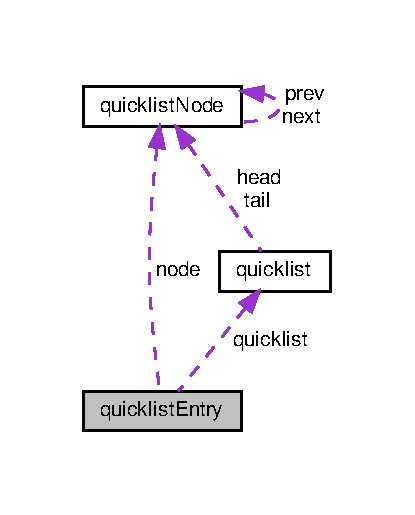
\includegraphics[width=199pt]{structquicklist_entry__coll__graph}
\end{center}
\end{figure}
\subsection*{Data Fields}
\begin{DoxyCompactItemize}
\item 
const \hyperlink{structquicklist}{quicklist} $\ast$ \hyperlink{structquicklist_entry_a4aa33c2ba0681808fcf026725cfac512}{quicklist}
\item 
\hyperlink{structquicklist_node}{quicklist\+Node} $\ast$ \hyperlink{structquicklist_entry_a78fcac69a40608d499c1efd0fe66593a}{node}
\item 
unsigned char $\ast$ \hyperlink{structquicklist_entry_a14218c4c1ee05ec32cc12721f772f294}{zi}
\item 
unsigned char $\ast$ \hyperlink{structquicklist_entry_a2f3bdb9d405cf00d02949b9141ce1396}{value}
\item 
long long \hyperlink{structquicklist_entry_abf0b4c9cc55c75787c954aa8f383cdd9}{longval}
\item 
unsigned int \hyperlink{structquicklist_entry_a2c1bd10d4bbc82d2d6c052c5842c0c8c}{sz}
\item 
int \hyperlink{structquicklist_entry_aed7ea92f45bd273dde380a45ddced592}{offset}
\end{DoxyCompactItemize}


\subsection{Detailed Description}


Definition at line 90 of file quicklist.\+h.



\subsection{Field Documentation}
\mbox{\Hypertarget{structquicklist_entry_abf0b4c9cc55c75787c954aa8f383cdd9}\label{structquicklist_entry_abf0b4c9cc55c75787c954aa8f383cdd9}} 
\index{quicklist\+Entry@{quicklist\+Entry}!longval@{longval}}
\index{longval@{longval}!quicklist\+Entry@{quicklist\+Entry}}
\subsubsection{\texorpdfstring{longval}{longval}}
{\footnotesize\ttfamily long long longval}



Definition at line 95 of file quicklist.\+h.

\mbox{\Hypertarget{structquicklist_entry_a78fcac69a40608d499c1efd0fe66593a}\label{structquicklist_entry_a78fcac69a40608d499c1efd0fe66593a}} 
\index{quicklist\+Entry@{quicklist\+Entry}!node@{node}}
\index{node@{node}!quicklist\+Entry@{quicklist\+Entry}}
\subsubsection{\texorpdfstring{node}{node}}
{\footnotesize\ttfamily \hyperlink{structquicklist_node}{quicklist\+Node}$\ast$ node}



Definition at line 92 of file quicklist.\+h.

\mbox{\Hypertarget{structquicklist_entry_aed7ea92f45bd273dde380a45ddced592}\label{structquicklist_entry_aed7ea92f45bd273dde380a45ddced592}} 
\index{quicklist\+Entry@{quicklist\+Entry}!offset@{offset}}
\index{offset@{offset}!quicklist\+Entry@{quicklist\+Entry}}
\subsubsection{\texorpdfstring{offset}{offset}}
{\footnotesize\ttfamily int offset}



Definition at line 97 of file quicklist.\+h.

\mbox{\Hypertarget{structquicklist_entry_a4aa33c2ba0681808fcf026725cfac512}\label{structquicklist_entry_a4aa33c2ba0681808fcf026725cfac512}} 
\index{quicklist\+Entry@{quicklist\+Entry}!quicklist@{quicklist}}
\index{quicklist@{quicklist}!quicklist\+Entry@{quicklist\+Entry}}
\subsubsection{\texorpdfstring{quicklist}{quicklist}}
{\footnotesize\ttfamily const \hyperlink{structquicklist}{quicklist}$\ast$ \hyperlink{structquicklist}{quicklist}}



Definition at line 91 of file quicklist.\+h.

\mbox{\Hypertarget{structquicklist_entry_a2c1bd10d4bbc82d2d6c052c5842c0c8c}\label{structquicklist_entry_a2c1bd10d4bbc82d2d6c052c5842c0c8c}} 
\index{quicklist\+Entry@{quicklist\+Entry}!sz@{sz}}
\index{sz@{sz}!quicklist\+Entry@{quicklist\+Entry}}
\subsubsection{\texorpdfstring{sz}{sz}}
{\footnotesize\ttfamily unsigned int sz}



Definition at line 96 of file quicklist.\+h.

\mbox{\Hypertarget{structquicklist_entry_a2f3bdb9d405cf00d02949b9141ce1396}\label{structquicklist_entry_a2f3bdb9d405cf00d02949b9141ce1396}} 
\index{quicklist\+Entry@{quicklist\+Entry}!value@{value}}
\index{value@{value}!quicklist\+Entry@{quicklist\+Entry}}
\subsubsection{\texorpdfstring{value}{value}}
{\footnotesize\ttfamily unsigned char$\ast$ value}



Definition at line 94 of file quicklist.\+h.

\mbox{\Hypertarget{structquicklist_entry_a14218c4c1ee05ec32cc12721f772f294}\label{structquicklist_entry_a14218c4c1ee05ec32cc12721f772f294}} 
\index{quicklist\+Entry@{quicklist\+Entry}!zi@{zi}}
\index{zi@{zi}!quicklist\+Entry@{quicklist\+Entry}}
\subsubsection{\texorpdfstring{zi}{zi}}
{\footnotesize\ttfamily unsigned char$\ast$ zi}



Definition at line 93 of file quicklist.\+h.



The documentation for this struct was generated from the following file\+:\begin{DoxyCompactItemize}
\item 
src/\hyperlink{quicklist_8h}{quicklist.\+h}\end{DoxyCompactItemize}

\hypertarget{structquicklist_iter}{}\section{quicklist\+Iter Struct Reference}
\label{structquicklist_iter}\index{quicklist\+Iter@{quicklist\+Iter}}


{\ttfamily \#include $<$quicklist.\+h$>$}



Collaboration diagram for quicklist\+Iter\+:
\nopagebreak
\begin{figure}[H]
\begin{center}
\leavevmode
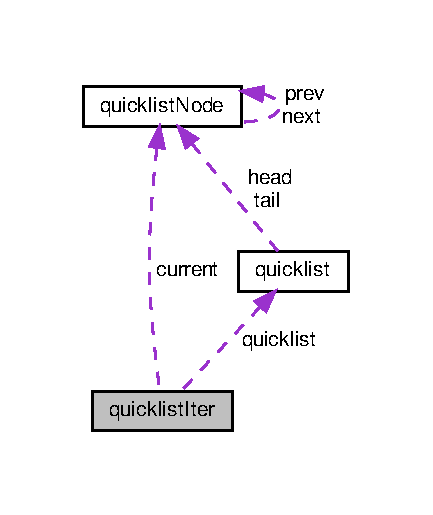
\includegraphics[width=208pt]{structquicklist_iter__coll__graph}
\end{center}
\end{figure}
\subsection*{Data Fields}
\begin{DoxyCompactItemize}
\item 
const \hyperlink{structquicklist}{quicklist} $\ast$ \hyperlink{structquicklist_iter_a4aa33c2ba0681808fcf026725cfac512}{quicklist}
\item 
\hyperlink{structquicklist_node}{quicklist\+Node} $\ast$ \hyperlink{structquicklist_iter_a5e0e4458fdbf71c9a0683ac803fc70e6}{current}
\item 
unsigned char $\ast$ \hyperlink{structquicklist_iter_a14218c4c1ee05ec32cc12721f772f294}{zi}
\item 
long \hyperlink{structquicklist_iter_adcce6ee751c1469525aec834a4d37ea8}{offset}
\item 
int \hyperlink{structquicklist_iter_a886d551d5381dc3e53f17825ffc51641}{direction}
\end{DoxyCompactItemize}


\subsection{Detailed Description}


Definition at line 82 of file quicklist.\+h.



\subsection{Field Documentation}
\mbox{\Hypertarget{structquicklist_iter_a5e0e4458fdbf71c9a0683ac803fc70e6}\label{structquicklist_iter_a5e0e4458fdbf71c9a0683ac803fc70e6}} 
\index{quicklist\+Iter@{quicklist\+Iter}!current@{current}}
\index{current@{current}!quicklist\+Iter@{quicklist\+Iter}}
\subsubsection{\texorpdfstring{current}{current}}
{\footnotesize\ttfamily \hyperlink{structquicklist_node}{quicklist\+Node}$\ast$ current}



Definition at line 84 of file quicklist.\+h.

\mbox{\Hypertarget{structquicklist_iter_a886d551d5381dc3e53f17825ffc51641}\label{structquicklist_iter_a886d551d5381dc3e53f17825ffc51641}} 
\index{quicklist\+Iter@{quicklist\+Iter}!direction@{direction}}
\index{direction@{direction}!quicklist\+Iter@{quicklist\+Iter}}
\subsubsection{\texorpdfstring{direction}{direction}}
{\footnotesize\ttfamily int direction}



Definition at line 87 of file quicklist.\+h.

\mbox{\Hypertarget{structquicklist_iter_adcce6ee751c1469525aec834a4d37ea8}\label{structquicklist_iter_adcce6ee751c1469525aec834a4d37ea8}} 
\index{quicklist\+Iter@{quicklist\+Iter}!offset@{offset}}
\index{offset@{offset}!quicklist\+Iter@{quicklist\+Iter}}
\subsubsection{\texorpdfstring{offset}{offset}}
{\footnotesize\ttfamily long offset}



Definition at line 86 of file quicklist.\+h.

\mbox{\Hypertarget{structquicklist_iter_a4aa33c2ba0681808fcf026725cfac512}\label{structquicklist_iter_a4aa33c2ba0681808fcf026725cfac512}} 
\index{quicklist\+Iter@{quicklist\+Iter}!quicklist@{quicklist}}
\index{quicklist@{quicklist}!quicklist\+Iter@{quicklist\+Iter}}
\subsubsection{\texorpdfstring{quicklist}{quicklist}}
{\footnotesize\ttfamily const \hyperlink{structquicklist}{quicklist}$\ast$ \hyperlink{structquicklist}{quicklist}}



Definition at line 83 of file quicklist.\+h.

\mbox{\Hypertarget{structquicklist_iter_a14218c4c1ee05ec32cc12721f772f294}\label{structquicklist_iter_a14218c4c1ee05ec32cc12721f772f294}} 
\index{quicklist\+Iter@{quicklist\+Iter}!zi@{zi}}
\index{zi@{zi}!quicklist\+Iter@{quicklist\+Iter}}
\subsubsection{\texorpdfstring{zi}{zi}}
{\footnotesize\ttfamily unsigned char$\ast$ zi}



Definition at line 85 of file quicklist.\+h.



The documentation for this struct was generated from the following file\+:\begin{DoxyCompactItemize}
\item 
src/\hyperlink{quicklist_8h}{quicklist.\+h}\end{DoxyCompactItemize}

\hypertarget{structquicklist_l_z_f}{}\section{quicklist\+L\+ZF Struct Reference}
\label{structquicklist_l_z_f}\index{quicklist\+L\+ZF@{quicklist\+L\+ZF}}


{\ttfamily \#include $<$quicklist.\+h$>$}

\subsection*{Data Fields}
\begin{DoxyCompactItemize}
\item 
unsigned int \hyperlink{structquicklist_l_z_f_a2c1bd10d4bbc82d2d6c052c5842c0c8c}{sz}
\item 
char \hyperlink{structquicklist_l_z_f_a80d845eaac2c3cf3966eb9c50a69fcf4}{compressed} \mbox{[}$\,$\mbox{]}
\end{DoxyCompactItemize}


\subsection{Detailed Description}


Definition at line 62 of file quicklist.\+h.



\subsection{Field Documentation}
\mbox{\Hypertarget{structquicklist_l_z_f_a80d845eaac2c3cf3966eb9c50a69fcf4}\label{structquicklist_l_z_f_a80d845eaac2c3cf3966eb9c50a69fcf4}} 
\index{quicklist\+L\+ZF@{quicklist\+L\+ZF}!compressed@{compressed}}
\index{compressed@{compressed}!quicklist\+L\+ZF@{quicklist\+L\+ZF}}
\subsubsection{\texorpdfstring{compressed}{compressed}}
{\footnotesize\ttfamily char compressed\mbox{[}$\,$\mbox{]}}



Definition at line 64 of file quicklist.\+h.

\mbox{\Hypertarget{structquicklist_l_z_f_a2c1bd10d4bbc82d2d6c052c5842c0c8c}\label{structquicklist_l_z_f_a2c1bd10d4bbc82d2d6c052c5842c0c8c}} 
\index{quicklist\+L\+ZF@{quicklist\+L\+ZF}!sz@{sz}}
\index{sz@{sz}!quicklist\+L\+ZF@{quicklist\+L\+ZF}}
\subsubsection{\texorpdfstring{sz}{sz}}
{\footnotesize\ttfamily unsigned int sz}



Definition at line 63 of file quicklist.\+h.



The documentation for this struct was generated from the following file\+:\begin{DoxyCompactItemize}
\item 
src/\hyperlink{quicklist_8h}{quicklist.\+h}\end{DoxyCompactItemize}

\hypertarget{structquicklist_node}{}\section{quicklist\+Node Struct Reference}
\label{structquicklist_node}\index{quicklist\+Node@{quicklist\+Node}}


{\ttfamily \#include $<$quicklist.\+h$>$}



Collaboration diagram for quicklist\+Node\+:
\nopagebreak
\begin{figure}[H]
\begin{center}
\leavevmode
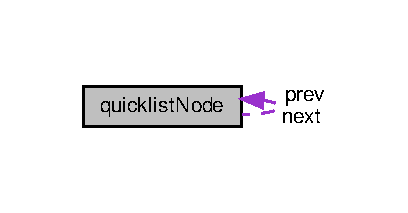
\includegraphics[width=196pt]{structquicklist_node__coll__graph}
\end{center}
\end{figure}
\subsection*{Data Fields}
\begin{DoxyCompactItemize}
\item 
struct \hyperlink{structquicklist_node}{quicklist\+Node} $\ast$ \hyperlink{structquicklist_node_abdcd96580045a4aa2d38c11a4671ed8d}{prev}
\item 
struct \hyperlink{structquicklist_node}{quicklist\+Node} $\ast$ \hyperlink{structquicklist_node_aa4be5244c2097b8fc8bdf053a0793ac8}{next}
\item 
unsigned char $\ast$ \hyperlink{structquicklist_node_a1ae48f85ded0fe46acd8864ac807f6b8}{zl}
\item 
unsigned int \hyperlink{structquicklist_node_a2c1bd10d4bbc82d2d6c052c5842c0c8c}{sz}
\item 
unsigned int \hyperlink{structquicklist_node_a16ff2d8e15ade4948398b0aeb80124a8}{count}\+: 16
\item 
unsigned int \hyperlink{structquicklist_node_a541253f13be71f2a40d23f98d3ac6d7d}{encoding}\+: 2
\item 
unsigned int \hyperlink{structquicklist_node_a70f05801a591a8b37f9bb47e3bc5c8b5}{container}\+: 2
\item 
unsigned int \hyperlink{structquicklist_node_a614856eb02cf76c6e187226f760c7509}{recompress}\+: 1
\item 
unsigned int \hyperlink{structquicklist_node_a53fe211757060122aa7061b7d6bfcb38}{attempted\+\_\+compress}\+: 1
\item 
unsigned int \hyperlink{structquicklist_node_a660ceaa22bec21d59654a14bc0fde76e}{extra}\+: 10
\end{DoxyCompactItemize}


\subsection{Detailed Description}


Definition at line 44 of file quicklist.\+h.



\subsection{Field Documentation}
\mbox{\Hypertarget{structquicklist_node_a53fe211757060122aa7061b7d6bfcb38}\label{structquicklist_node_a53fe211757060122aa7061b7d6bfcb38}} 
\index{quicklist\+Node@{quicklist\+Node}!attempted\+\_\+compress@{attempted\+\_\+compress}}
\index{attempted\+\_\+compress@{attempted\+\_\+compress}!quicklist\+Node@{quicklist\+Node}}
\subsubsection{\texorpdfstring{attempted\+\_\+compress}{attempted\_compress}}
{\footnotesize\ttfamily unsigned int attempted\+\_\+compress}



Definition at line 53 of file quicklist.\+h.

\mbox{\Hypertarget{structquicklist_node_a70f05801a591a8b37f9bb47e3bc5c8b5}\label{structquicklist_node_a70f05801a591a8b37f9bb47e3bc5c8b5}} 
\index{quicklist\+Node@{quicklist\+Node}!container@{container}}
\index{container@{container}!quicklist\+Node@{quicklist\+Node}}
\subsubsection{\texorpdfstring{container}{container}}
{\footnotesize\ttfamily unsigned int container}



Definition at line 51 of file quicklist.\+h.

\mbox{\Hypertarget{structquicklist_node_a16ff2d8e15ade4948398b0aeb80124a8}\label{structquicklist_node_a16ff2d8e15ade4948398b0aeb80124a8}} 
\index{quicklist\+Node@{quicklist\+Node}!count@{count}}
\index{count@{count}!quicklist\+Node@{quicklist\+Node}}
\subsubsection{\texorpdfstring{count}{count}}
{\footnotesize\ttfamily unsigned int count}



Definition at line 49 of file quicklist.\+h.

\mbox{\Hypertarget{structquicklist_node_a541253f13be71f2a40d23f98d3ac6d7d}\label{structquicklist_node_a541253f13be71f2a40d23f98d3ac6d7d}} 
\index{quicklist\+Node@{quicklist\+Node}!encoding@{encoding}}
\index{encoding@{encoding}!quicklist\+Node@{quicklist\+Node}}
\subsubsection{\texorpdfstring{encoding}{encoding}}
{\footnotesize\ttfamily unsigned int encoding}



Definition at line 50 of file quicklist.\+h.

\mbox{\Hypertarget{structquicklist_node_a660ceaa22bec21d59654a14bc0fde76e}\label{structquicklist_node_a660ceaa22bec21d59654a14bc0fde76e}} 
\index{quicklist\+Node@{quicklist\+Node}!extra@{extra}}
\index{extra@{extra}!quicklist\+Node@{quicklist\+Node}}
\subsubsection{\texorpdfstring{extra}{extra}}
{\footnotesize\ttfamily unsigned int extra}



Definition at line 54 of file quicklist.\+h.

\mbox{\Hypertarget{structquicklist_node_aa4be5244c2097b8fc8bdf053a0793ac8}\label{structquicklist_node_aa4be5244c2097b8fc8bdf053a0793ac8}} 
\index{quicklist\+Node@{quicklist\+Node}!next@{next}}
\index{next@{next}!quicklist\+Node@{quicklist\+Node}}
\subsubsection{\texorpdfstring{next}{next}}
{\footnotesize\ttfamily struct \hyperlink{structquicklist_node}{quicklist\+Node}$\ast$ next}



Definition at line 46 of file quicklist.\+h.

\mbox{\Hypertarget{structquicklist_node_abdcd96580045a4aa2d38c11a4671ed8d}\label{structquicklist_node_abdcd96580045a4aa2d38c11a4671ed8d}} 
\index{quicklist\+Node@{quicklist\+Node}!prev@{prev}}
\index{prev@{prev}!quicklist\+Node@{quicklist\+Node}}
\subsubsection{\texorpdfstring{prev}{prev}}
{\footnotesize\ttfamily struct \hyperlink{structquicklist_node}{quicklist\+Node}$\ast$ prev}



Definition at line 45 of file quicklist.\+h.

\mbox{\Hypertarget{structquicklist_node_a614856eb02cf76c6e187226f760c7509}\label{structquicklist_node_a614856eb02cf76c6e187226f760c7509}} 
\index{quicklist\+Node@{quicklist\+Node}!recompress@{recompress}}
\index{recompress@{recompress}!quicklist\+Node@{quicklist\+Node}}
\subsubsection{\texorpdfstring{recompress}{recompress}}
{\footnotesize\ttfamily unsigned int recompress}



Definition at line 52 of file quicklist.\+h.

\mbox{\Hypertarget{structquicklist_node_a2c1bd10d4bbc82d2d6c052c5842c0c8c}\label{structquicklist_node_a2c1bd10d4bbc82d2d6c052c5842c0c8c}} 
\index{quicklist\+Node@{quicklist\+Node}!sz@{sz}}
\index{sz@{sz}!quicklist\+Node@{quicklist\+Node}}
\subsubsection{\texorpdfstring{sz}{sz}}
{\footnotesize\ttfamily unsigned int sz}



Definition at line 48 of file quicklist.\+h.

\mbox{\Hypertarget{structquicklist_node_a1ae48f85ded0fe46acd8864ac807f6b8}\label{structquicklist_node_a1ae48f85ded0fe46acd8864ac807f6b8}} 
\index{quicklist\+Node@{quicklist\+Node}!zl@{zl}}
\index{zl@{zl}!quicklist\+Node@{quicklist\+Node}}
\subsubsection{\texorpdfstring{zl}{zl}}
{\footnotesize\ttfamily unsigned char$\ast$ zl}



Definition at line 47 of file quicklist.\+h.



The documentation for this struct was generated from the following file\+:\begin{DoxyCompactItemize}
\item 
src/\hyperlink{quicklist_8h}{quicklist.\+h}\end{DoxyCompactItemize}

\hypertarget{structrax}{}\section{rax Struct Reference}
\label{structrax}\index{rax@{rax}}


{\ttfamily \#include $<$rax.\+h$>$}



Collaboration diagram for rax\+:
\nopagebreak
\begin{figure}[H]
\begin{center}
\leavevmode
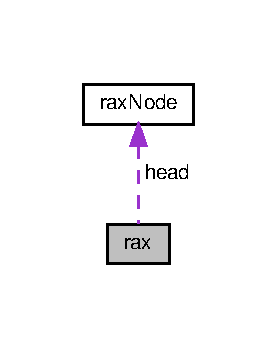
\includegraphics[width=133pt]{structrax__coll__graph}
\end{center}
\end{figure}
\subsection*{Data Fields}
\begin{DoxyCompactItemize}
\item 
\hyperlink{structrax_node}{rax\+Node} $\ast$ \hyperlink{structrax_aa897900ec39b611670ffa8a692432543}{head}
\item 
uint64\+\_\+t \hyperlink{structrax_aeb57ec87f1c4514577f9ed22bfc1041d}{numele}
\item 
uint64\+\_\+t \hyperlink{structrax_abbdb3a945f35e1cd7a50bcabf1bb6828}{numnodes}
\end{DoxyCompactItemize}


\subsection{Detailed Description}


Definition at line 133 of file rax.\+h.



\subsection{Field Documentation}
\mbox{\Hypertarget{structrax_aa897900ec39b611670ffa8a692432543}\label{structrax_aa897900ec39b611670ffa8a692432543}} 
\index{rax@{rax}!head@{head}}
\index{head@{head}!rax@{rax}}
\subsubsection{\texorpdfstring{head}{head}}
{\footnotesize\ttfamily \hyperlink{structrax_node}{rax\+Node}$\ast$ head}



Definition at line 134 of file rax.\+h.

\mbox{\Hypertarget{structrax_aeb57ec87f1c4514577f9ed22bfc1041d}\label{structrax_aeb57ec87f1c4514577f9ed22bfc1041d}} 
\index{rax@{rax}!numele@{numele}}
\index{numele@{numele}!rax@{rax}}
\subsubsection{\texorpdfstring{numele}{numele}}
{\footnotesize\ttfamily uint64\+\_\+t numele}



Definition at line 135 of file rax.\+h.

\mbox{\Hypertarget{structrax_abbdb3a945f35e1cd7a50bcabf1bb6828}\label{structrax_abbdb3a945f35e1cd7a50bcabf1bb6828}} 
\index{rax@{rax}!numnodes@{numnodes}}
\index{numnodes@{numnodes}!rax@{rax}}
\subsubsection{\texorpdfstring{numnodes}{numnodes}}
{\footnotesize\ttfamily uint64\+\_\+t numnodes}



Definition at line 136 of file rax.\+h.



The documentation for this struct was generated from the following file\+:\begin{DoxyCompactItemize}
\item 
src/\hyperlink{rax_8h}{rax.\+h}\end{DoxyCompactItemize}

\hypertarget{structrax_iterator}{}\section{rax\+Iterator Struct Reference}
\label{structrax_iterator}\index{rax\+Iterator@{rax\+Iterator}}


{\ttfamily \#include $<$rax.\+h$>$}



Collaboration diagram for rax\+Iterator\+:
\nopagebreak
\begin{figure}[H]
\begin{center}
\leavevmode
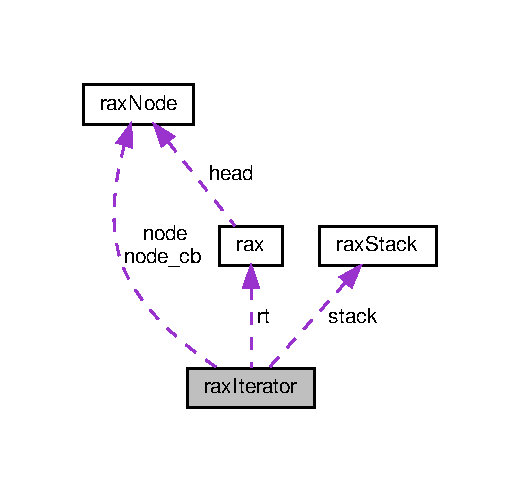
\includegraphics[width=250pt]{structrax_iterator__coll__graph}
\end{center}
\end{figure}
\subsection*{Data Fields}
\begin{DoxyCompactItemize}
\item 
int \hyperlink{structrax_iterator_ac8bf36fe0577cba66bccda3a6f7e80a4}{flags}
\item 
\hyperlink{structrax}{rax} $\ast$ \hyperlink{structrax_iterator_a58939ec4439701d170853cf158043d57}{rt}
\item 
unsigned char $\ast$ \hyperlink{structrax_iterator_a1cb5ee363f3d6d0f548eb6e64d72a7c8}{key}
\item 
void $\ast$ \hyperlink{structrax_iterator_a735984d41155bc1032e09bece8f8d66d}{data}
\item 
size\+\_\+t \hyperlink{structrax_iterator_aaa2dc552577da2bba064c4d36d971c26}{key\+\_\+len}
\item 
size\+\_\+t \hyperlink{structrax_iterator_a7e65a3134205dfce4a447bc3359f1a07}{key\+\_\+max}
\item 
unsigned char \hyperlink{structrax_iterator_a5854437e7714a04ea59691e0e5167883}{key\+\_\+static\+\_\+string} \mbox{[}\hyperlink{rax_8h_a172e740ce3572b21018192e7877217dd}{R\+A\+X\+\_\+\+I\+T\+E\+R\+\_\+\+S\+T\+A\+T\+I\+C\+\_\+\+L\+EN}\mbox{]}
\item 
\hyperlink{structrax_node}{rax\+Node} $\ast$ \hyperlink{structrax_iterator_ae2c06018ed6b76e72dd8b8372011afa5}{node}
\item 
\hyperlink{structrax_stack}{rax\+Stack} \hyperlink{structrax_iterator_ad25901300905129025788c7c8f27cb8e}{stack}
\item 
\hyperlink{rax_8h_a08d5db58149f8656e7f4d046b70a4ef1}{rax\+Node\+Callback} \hyperlink{structrax_iterator_af80d4e8e6dcdfdb2c80c37457122426c}{node\+\_\+cb}
\end{DoxyCompactItemize}


\subsection{Detailed Description}


Definition at line 175 of file rax.\+h.



\subsection{Field Documentation}
\mbox{\Hypertarget{structrax_iterator_a735984d41155bc1032e09bece8f8d66d}\label{structrax_iterator_a735984d41155bc1032e09bece8f8d66d}} 
\index{rax\+Iterator@{rax\+Iterator}!data@{data}}
\index{data@{data}!rax\+Iterator@{rax\+Iterator}}
\subsubsection{\texorpdfstring{data}{data}}
{\footnotesize\ttfamily void$\ast$ data}



Definition at line 179 of file rax.\+h.

\mbox{\Hypertarget{structrax_iterator_ac8bf36fe0577cba66bccda3a6f7e80a4}\label{structrax_iterator_ac8bf36fe0577cba66bccda3a6f7e80a4}} 
\index{rax\+Iterator@{rax\+Iterator}!flags@{flags}}
\index{flags@{flags}!rax\+Iterator@{rax\+Iterator}}
\subsubsection{\texorpdfstring{flags}{flags}}
{\footnotesize\ttfamily int flags}



Definition at line 176 of file rax.\+h.

\mbox{\Hypertarget{structrax_iterator_a1cb5ee363f3d6d0f548eb6e64d72a7c8}\label{structrax_iterator_a1cb5ee363f3d6d0f548eb6e64d72a7c8}} 
\index{rax\+Iterator@{rax\+Iterator}!key@{key}}
\index{key@{key}!rax\+Iterator@{rax\+Iterator}}
\subsubsection{\texorpdfstring{key}{key}}
{\footnotesize\ttfamily unsigned char$\ast$ key}



Definition at line 178 of file rax.\+h.

\mbox{\Hypertarget{structrax_iterator_aaa2dc552577da2bba064c4d36d971c26}\label{structrax_iterator_aaa2dc552577da2bba064c4d36d971c26}} 
\index{rax\+Iterator@{rax\+Iterator}!key\+\_\+len@{key\+\_\+len}}
\index{key\+\_\+len@{key\+\_\+len}!rax\+Iterator@{rax\+Iterator}}
\subsubsection{\texorpdfstring{key\+\_\+len}{key\_len}}
{\footnotesize\ttfamily size\+\_\+t key\+\_\+len}



Definition at line 180 of file rax.\+h.

\mbox{\Hypertarget{structrax_iterator_a7e65a3134205dfce4a447bc3359f1a07}\label{structrax_iterator_a7e65a3134205dfce4a447bc3359f1a07}} 
\index{rax\+Iterator@{rax\+Iterator}!key\+\_\+max@{key\+\_\+max}}
\index{key\+\_\+max@{key\+\_\+max}!rax\+Iterator@{rax\+Iterator}}
\subsubsection{\texorpdfstring{key\+\_\+max}{key\_max}}
{\footnotesize\ttfamily size\+\_\+t key\+\_\+max}



Definition at line 181 of file rax.\+h.

\mbox{\Hypertarget{structrax_iterator_a5854437e7714a04ea59691e0e5167883}\label{structrax_iterator_a5854437e7714a04ea59691e0e5167883}} 
\index{rax\+Iterator@{rax\+Iterator}!key\+\_\+static\+\_\+string@{key\+\_\+static\+\_\+string}}
\index{key\+\_\+static\+\_\+string@{key\+\_\+static\+\_\+string}!rax\+Iterator@{rax\+Iterator}}
\subsubsection{\texorpdfstring{key\+\_\+static\+\_\+string}{key\_static\_string}}
{\footnotesize\ttfamily unsigned char key\+\_\+static\+\_\+string\mbox{[}\hyperlink{rax_8h_a172e740ce3572b21018192e7877217dd}{R\+A\+X\+\_\+\+I\+T\+E\+R\+\_\+\+S\+T\+A\+T\+I\+C\+\_\+\+L\+EN}\mbox{]}}



Definition at line 182 of file rax.\+h.

\mbox{\Hypertarget{structrax_iterator_ae2c06018ed6b76e72dd8b8372011afa5}\label{structrax_iterator_ae2c06018ed6b76e72dd8b8372011afa5}} 
\index{rax\+Iterator@{rax\+Iterator}!node@{node}}
\index{node@{node}!rax\+Iterator@{rax\+Iterator}}
\subsubsection{\texorpdfstring{node}{node}}
{\footnotesize\ttfamily \hyperlink{structrax_node}{rax\+Node}$\ast$ node}



Definition at line 183 of file rax.\+h.

\mbox{\Hypertarget{structrax_iterator_af80d4e8e6dcdfdb2c80c37457122426c}\label{structrax_iterator_af80d4e8e6dcdfdb2c80c37457122426c}} 
\index{rax\+Iterator@{rax\+Iterator}!node\+\_\+cb@{node\+\_\+cb}}
\index{node\+\_\+cb@{node\+\_\+cb}!rax\+Iterator@{rax\+Iterator}}
\subsubsection{\texorpdfstring{node\+\_\+cb}{node\_cb}}
{\footnotesize\ttfamily \hyperlink{rax_8h_a08d5db58149f8656e7f4d046b70a4ef1}{rax\+Node\+Callback} node\+\_\+cb}



Definition at line 185 of file rax.\+h.

\mbox{\Hypertarget{structrax_iterator_a58939ec4439701d170853cf158043d57}\label{structrax_iterator_a58939ec4439701d170853cf158043d57}} 
\index{rax\+Iterator@{rax\+Iterator}!rt@{rt}}
\index{rt@{rt}!rax\+Iterator@{rax\+Iterator}}
\subsubsection{\texorpdfstring{rt}{rt}}
{\footnotesize\ttfamily \hyperlink{structrax}{rax}$\ast$ rt}



Definition at line 177 of file rax.\+h.

\mbox{\Hypertarget{structrax_iterator_ad25901300905129025788c7c8f27cb8e}\label{structrax_iterator_ad25901300905129025788c7c8f27cb8e}} 
\index{rax\+Iterator@{rax\+Iterator}!stack@{stack}}
\index{stack@{stack}!rax\+Iterator@{rax\+Iterator}}
\subsubsection{\texorpdfstring{stack}{stack}}
{\footnotesize\ttfamily \hyperlink{structrax_stack}{rax\+Stack} stack}



Definition at line 184 of file rax.\+h.



The documentation for this struct was generated from the following file\+:\begin{DoxyCompactItemize}
\item 
src/\hyperlink{rax_8h}{rax.\+h}\end{DoxyCompactItemize}

\hypertarget{structrax_node}{}\section{rax\+Node Struct Reference}
\label{structrax_node}\index{rax\+Node@{rax\+Node}}


{\ttfamily \#include $<$rax.\+h$>$}

\subsection*{Data Fields}
\begin{DoxyCompactItemize}
\item 
uint32\+\_\+t \hyperlink{structrax_node_ad11d2993e802c844bfdf827ebce7907d}{iskey}\+:1
\item 
uint32\+\_\+t \hyperlink{structrax_node_a9301700c1338965475354cc876ccdf6f}{isnull}\+:1
\item 
uint32\+\_\+t \hyperlink{structrax_node_a1b7f71444b8d20355b174737095f3e65}{iscompr}\+:1
\item 
uint32\+\_\+t \hyperlink{structrax_node_ab2c6b258f02add8fdf4cfc7c371dd772}{size}\+:29
\item 
unsigned char \hyperlink{structrax_node_ad22557485286d9df959ff3335001ce69}{data} \mbox{[}$\,$\mbox{]}
\end{DoxyCompactItemize}


\subsection{Detailed Description}


Definition at line 98 of file rax.\+h.



\subsection{Field Documentation}
\mbox{\Hypertarget{structrax_node_ad22557485286d9df959ff3335001ce69}\label{structrax_node_ad22557485286d9df959ff3335001ce69}} 
\index{rax\+Node@{rax\+Node}!data@{data}}
\index{data@{data}!rax\+Node@{rax\+Node}}
\subsubsection{\texorpdfstring{data}{data}}
{\footnotesize\ttfamily unsigned char data\mbox{[}$\,$\mbox{]}}



Definition at line 130 of file rax.\+h.

\mbox{\Hypertarget{structrax_node_a1b7f71444b8d20355b174737095f3e65}\label{structrax_node_a1b7f71444b8d20355b174737095f3e65}} 
\index{rax\+Node@{rax\+Node}!iscompr@{iscompr}}
\index{iscompr@{iscompr}!rax\+Node@{rax\+Node}}
\subsubsection{\texorpdfstring{iscompr}{iscompr}}
{\footnotesize\ttfamily uint32\+\_\+t iscompr}



Definition at line 101 of file rax.\+h.

\mbox{\Hypertarget{structrax_node_ad11d2993e802c844bfdf827ebce7907d}\label{structrax_node_ad11d2993e802c844bfdf827ebce7907d}} 
\index{rax\+Node@{rax\+Node}!iskey@{iskey}}
\index{iskey@{iskey}!rax\+Node@{rax\+Node}}
\subsubsection{\texorpdfstring{iskey}{iskey}}
{\footnotesize\ttfamily uint32\+\_\+t iskey}



Definition at line 99 of file rax.\+h.

\mbox{\Hypertarget{structrax_node_a9301700c1338965475354cc876ccdf6f}\label{structrax_node_a9301700c1338965475354cc876ccdf6f}} 
\index{rax\+Node@{rax\+Node}!isnull@{isnull}}
\index{isnull@{isnull}!rax\+Node@{rax\+Node}}
\subsubsection{\texorpdfstring{isnull}{isnull}}
{\footnotesize\ttfamily uint32\+\_\+t isnull}



Definition at line 100 of file rax.\+h.

\mbox{\Hypertarget{structrax_node_ab2c6b258f02add8fdf4cfc7c371dd772}\label{structrax_node_ab2c6b258f02add8fdf4cfc7c371dd772}} 
\index{rax\+Node@{rax\+Node}!size@{size}}
\index{size@{size}!rax\+Node@{rax\+Node}}
\subsubsection{\texorpdfstring{size}{size}}
{\footnotesize\ttfamily uint32\+\_\+t size}



Definition at line 102 of file rax.\+h.



The documentation for this struct was generated from the following file\+:\begin{DoxyCompactItemize}
\item 
src/\hyperlink{rax_8h}{rax.\+h}\end{DoxyCompactItemize}

\hypertarget{structrax_stack}{}\section{rax\+Stack Struct Reference}
\label{structrax_stack}\index{rax\+Stack@{rax\+Stack}}


{\ttfamily \#include $<$rax.\+h$>$}

\subsection*{Data Fields}
\begin{DoxyCompactItemize}
\item 
void $\ast$$\ast$ \hyperlink{structrax_stack_a1f13044ed8bc3e590b1658f295e312e6}{stack}
\item 
size\+\_\+t \hyperlink{structrax_stack_a172b85ef8ac505af2599402f7e390354}{items}
\item 
size\+\_\+t \hyperlink{structrax_stack_ab0e310064cc6a020cd4f1773760260a5}{maxitems}
\item 
void $\ast$ \hyperlink{structrax_stack_a4c9a6441368d8681f82baf35dec33bbb}{static\+\_\+items} \mbox{[}\hyperlink{rax_8h_aff05c7893713f82d106c046f55ac1bf5}{R\+A\+X\+\_\+\+S\+T\+A\+C\+K\+\_\+\+S\+T\+A\+T\+I\+C\+\_\+\+I\+T\+E\+MS}\mbox{]}
\item 
int \hyperlink{structrax_stack_a7a989ca8ec18f6d21a77acc9cd90d595}{oom}
\end{DoxyCompactItemize}


\subsection{Detailed Description}


Definition at line 143 of file rax.\+h.



\subsection{Field Documentation}
\mbox{\Hypertarget{structrax_stack_a172b85ef8ac505af2599402f7e390354}\label{structrax_stack_a172b85ef8ac505af2599402f7e390354}} 
\index{rax\+Stack@{rax\+Stack}!items@{items}}
\index{items@{items}!rax\+Stack@{rax\+Stack}}
\subsubsection{\texorpdfstring{items}{items}}
{\footnotesize\ttfamily size\+\_\+t items}



Definition at line 145 of file rax.\+h.

\mbox{\Hypertarget{structrax_stack_ab0e310064cc6a020cd4f1773760260a5}\label{structrax_stack_ab0e310064cc6a020cd4f1773760260a5}} 
\index{rax\+Stack@{rax\+Stack}!maxitems@{maxitems}}
\index{maxitems@{maxitems}!rax\+Stack@{rax\+Stack}}
\subsubsection{\texorpdfstring{maxitems}{maxitems}}
{\footnotesize\ttfamily size\+\_\+t maxitems}



Definition at line 145 of file rax.\+h.

\mbox{\Hypertarget{structrax_stack_a7a989ca8ec18f6d21a77acc9cd90d595}\label{structrax_stack_a7a989ca8ec18f6d21a77acc9cd90d595}} 
\index{rax\+Stack@{rax\+Stack}!oom@{oom}}
\index{oom@{oom}!rax\+Stack@{rax\+Stack}}
\subsubsection{\texorpdfstring{oom}{oom}}
{\footnotesize\ttfamily int oom}



Definition at line 149 of file rax.\+h.

\mbox{\Hypertarget{structrax_stack_a1f13044ed8bc3e590b1658f295e312e6}\label{structrax_stack_a1f13044ed8bc3e590b1658f295e312e6}} 
\index{rax\+Stack@{rax\+Stack}!stack@{stack}}
\index{stack@{stack}!rax\+Stack@{rax\+Stack}}
\subsubsection{\texorpdfstring{stack}{stack}}
{\footnotesize\ttfamily void$\ast$$\ast$ stack}



Definition at line 144 of file rax.\+h.

\mbox{\Hypertarget{structrax_stack_a4c9a6441368d8681f82baf35dec33bbb}\label{structrax_stack_a4c9a6441368d8681f82baf35dec33bbb}} 
\index{rax\+Stack@{rax\+Stack}!static\+\_\+items@{static\+\_\+items}}
\index{static\+\_\+items@{static\+\_\+items}!rax\+Stack@{rax\+Stack}}
\subsubsection{\texorpdfstring{static\+\_\+items}{static\_items}}
{\footnotesize\ttfamily void$\ast$ static\+\_\+items\mbox{[}\hyperlink{rax_8h_aff05c7893713f82d106c046f55ac1bf5}{R\+A\+X\+\_\+\+S\+T\+A\+C\+K\+\_\+\+S\+T\+A\+T\+I\+C\+\_\+\+I\+T\+E\+MS}\mbox{]}}



Definition at line 148 of file rax.\+h.



The documentation for this struct was generated from the following file\+:\begin{DoxyCompactItemize}
\item 
src/\hyperlink{rax_8h}{rax.\+h}\end{DoxyCompactItemize}

\hypertarget{structrdb_save_info}{}\section{rdb\+Save\+Info Struct Reference}
\label{structrdb_save_info}\index{rdb\+Save\+Info@{rdb\+Save\+Info}}


{\ttfamily \#include $<$server.\+h$>$}

\subsection*{Data Fields}
\begin{DoxyCompactItemize}
\item 
int \hyperlink{structrdb_save_info_a839a288ca668f38e63ba0fd17f6ae8c5}{repl\+\_\+stream\+\_\+db}
\item 
int \hyperlink{structrdb_save_info_aaceb90ef64847700ff5b9c91df9d7bf5}{repl\+\_\+id\+\_\+is\+\_\+set}
\item 
char \hyperlink{structrdb_save_info_af57b6e90af7dbfc2dd62eb2d903437bf}{repl\+\_\+id} \mbox{[}\hyperlink{server_8h_aba6794fa3ee28f85165eaed93190f1df}{C\+O\+N\+F\+I\+G\+\_\+\+R\+U\+N\+\_\+\+I\+D\+\_\+\+S\+I\+ZE}+1\mbox{]}
\item 
long long \hyperlink{structrdb_save_info_acaaa973071b682ff89c70991a2d3ce7a}{repl\+\_\+offset}
\end{DoxyCompactItemize}


\subsection{Detailed Description}


Definition at line 890 of file server.\+h.



\subsection{Field Documentation}
\mbox{\Hypertarget{structrdb_save_info_af57b6e90af7dbfc2dd62eb2d903437bf}\label{structrdb_save_info_af57b6e90af7dbfc2dd62eb2d903437bf}} 
\index{rdb\+Save\+Info@{rdb\+Save\+Info}!repl\+\_\+id@{repl\+\_\+id}}
\index{repl\+\_\+id@{repl\+\_\+id}!rdb\+Save\+Info@{rdb\+Save\+Info}}
\subsubsection{\texorpdfstring{repl\+\_\+id}{repl\_id}}
{\footnotesize\ttfamily char repl\+\_\+id\mbox{[}\hyperlink{server_8h_aba6794fa3ee28f85165eaed93190f1df}{C\+O\+N\+F\+I\+G\+\_\+\+R\+U\+N\+\_\+\+I\+D\+\_\+\+S\+I\+ZE}+1\mbox{]}}



Definition at line 896 of file server.\+h.

\mbox{\Hypertarget{structrdb_save_info_aaceb90ef64847700ff5b9c91df9d7bf5}\label{structrdb_save_info_aaceb90ef64847700ff5b9c91df9d7bf5}} 
\index{rdb\+Save\+Info@{rdb\+Save\+Info}!repl\+\_\+id\+\_\+is\+\_\+set@{repl\+\_\+id\+\_\+is\+\_\+set}}
\index{repl\+\_\+id\+\_\+is\+\_\+set@{repl\+\_\+id\+\_\+is\+\_\+set}!rdb\+Save\+Info@{rdb\+Save\+Info}}
\subsubsection{\texorpdfstring{repl\+\_\+id\+\_\+is\+\_\+set}{repl\_id\_is\_set}}
{\footnotesize\ttfamily int repl\+\_\+id\+\_\+is\+\_\+set}



Definition at line 895 of file server.\+h.

\mbox{\Hypertarget{structrdb_save_info_acaaa973071b682ff89c70991a2d3ce7a}\label{structrdb_save_info_acaaa973071b682ff89c70991a2d3ce7a}} 
\index{rdb\+Save\+Info@{rdb\+Save\+Info}!repl\+\_\+offset@{repl\+\_\+offset}}
\index{repl\+\_\+offset@{repl\+\_\+offset}!rdb\+Save\+Info@{rdb\+Save\+Info}}
\subsubsection{\texorpdfstring{repl\+\_\+offset}{repl\_offset}}
{\footnotesize\ttfamily long long repl\+\_\+offset}



Definition at line 897 of file server.\+h.

\mbox{\Hypertarget{structrdb_save_info_a839a288ca668f38e63ba0fd17f6ae8c5}\label{structrdb_save_info_a839a288ca668f38e63ba0fd17f6ae8c5}} 
\index{rdb\+Save\+Info@{rdb\+Save\+Info}!repl\+\_\+stream\+\_\+db@{repl\+\_\+stream\+\_\+db}}
\index{repl\+\_\+stream\+\_\+db@{repl\+\_\+stream\+\_\+db}!rdb\+Save\+Info@{rdb\+Save\+Info}}
\subsubsection{\texorpdfstring{repl\+\_\+stream\+\_\+db}{repl\_stream\_db}}
{\footnotesize\ttfamily int repl\+\_\+stream\+\_\+db}



Definition at line 892 of file server.\+h.



The documentation for this struct was generated from the following file\+:\begin{DoxyCompactItemize}
\item 
src/\hyperlink{server_8h}{server.\+h}\end{DoxyCompactItemize}

\hypertarget{structready_list}{}\section{ready\+List Struct Reference}
\label{structready_list}\index{ready\+List@{ready\+List}}


{\ttfamily \#include $<$server.\+h$>$}



Collaboration diagram for ready\+List\+:
\nopagebreak
\begin{figure}[H]
\begin{center}
\leavevmode
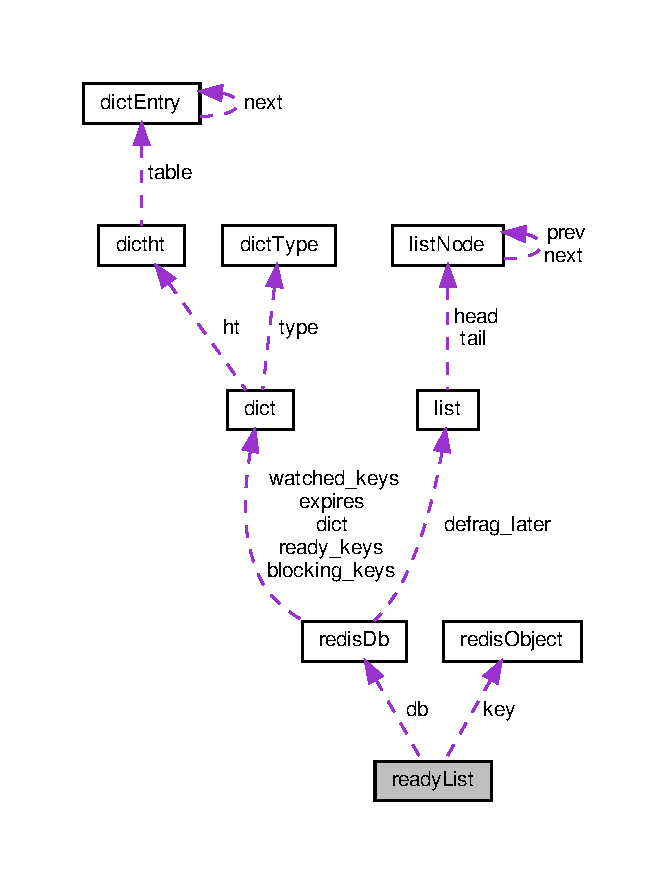
\includegraphics[width=322pt]{structready_list__coll__graph}
\end{center}
\end{figure}
\subsection*{Data Fields}
\begin{DoxyCompactItemize}
\item 
\hyperlink{structredis_db}{redis\+Db} $\ast$ \hyperlink{structready_list_a9bee04e09635a42fef289e42a89f5502}{db}
\item 
\hyperlink{server_8h_a540f174d2685422fbd7d12e3cd44c8e2}{robj} $\ast$ \hyperlink{structready_list_adc0ee0ed345db513fb6fac27511be4f1}{key}
\end{DoxyCompactItemize}


\subsection{Detailed Description}


Definition at line 702 of file server.\+h.



\subsection{Field Documentation}
\mbox{\Hypertarget{structready_list_a9bee04e09635a42fef289e42a89f5502}\label{structready_list_a9bee04e09635a42fef289e42a89f5502}} 
\index{ready\+List@{ready\+List}!db@{db}}
\index{db@{db}!ready\+List@{ready\+List}}
\subsubsection{\texorpdfstring{db}{db}}
{\footnotesize\ttfamily \hyperlink{structredis_db}{redis\+Db}$\ast$ db}



Definition at line 703 of file server.\+h.

\mbox{\Hypertarget{structready_list_adc0ee0ed345db513fb6fac27511be4f1}\label{structready_list_adc0ee0ed345db513fb6fac27511be4f1}} 
\index{ready\+List@{ready\+List}!key@{key}}
\index{key@{key}!ready\+List@{ready\+List}}
\subsubsection{\texorpdfstring{key}{key}}
{\footnotesize\ttfamily \hyperlink{server_8h_a540f174d2685422fbd7d12e3cd44c8e2}{robj}$\ast$ key}



Definition at line 704 of file server.\+h.



The documentation for this struct was generated from the following file\+:\begin{DoxyCompactItemize}
\item 
src/\hyperlink{server_8h}{server.\+h}\end{DoxyCompactItemize}

\hypertarget{structredis_ae_events}{}\section{redis\+Ae\+Events Struct Reference}
\label{structredis_ae_events}\index{redis\+Ae\+Events@{redis\+Ae\+Events}}


Collaboration diagram for redis\+Ae\+Events\+:
\nopagebreak
\begin{figure}[H]
\begin{center}
\leavevmode
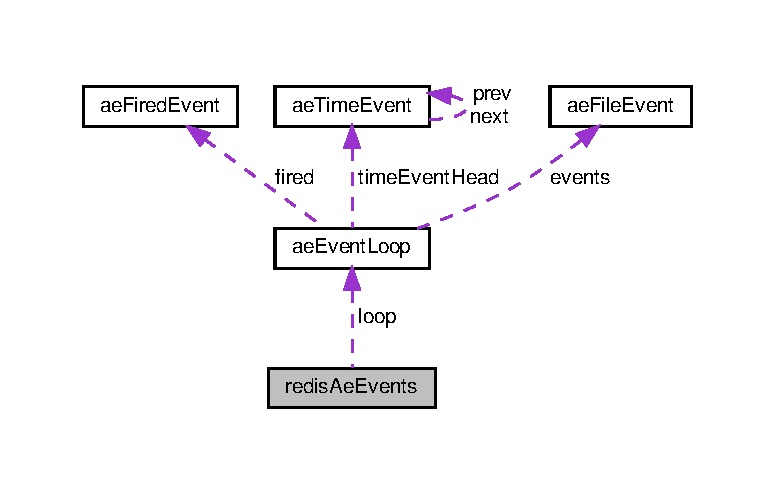
\includegraphics[width=350pt]{structredis_ae_events__coll__graph}
\end{center}
\end{figure}
\subsection*{Data Fields}
\begin{DoxyCompactItemize}
\item 
redis\+Async\+Context $\ast$ \hyperlink{structredis_ae_events_a5764ffeda6751a7e3eec0eb29d402bde}{context}
\item 
\hyperlink{structae_event_loop}{ae\+Event\+Loop} $\ast$ \hyperlink{structredis_ae_events_ae87889ddc12a87da6155fdeadaf2c604}{loop}
\item 
int \hyperlink{structredis_ae_events_a6f8059414f0228f0256115e024eeed4b}{fd}
\item 
int \hyperlink{structredis_ae_events_a5fa8d7fdcda2ed9555ad800a40a1a810}{reading}
\item 
int \hyperlink{structredis_ae_events_adb2dbc8c43288a024535ed507da7b278}{writing}
\end{DoxyCompactItemize}


\subsection{Detailed Description}


Definition at line 271 of file sentinel.\+c.



\subsection{Field Documentation}
\mbox{\Hypertarget{structredis_ae_events_a5764ffeda6751a7e3eec0eb29d402bde}\label{structredis_ae_events_a5764ffeda6751a7e3eec0eb29d402bde}} 
\index{redis\+Ae\+Events@{redis\+Ae\+Events}!context@{context}}
\index{context@{context}!redis\+Ae\+Events@{redis\+Ae\+Events}}
\subsubsection{\texorpdfstring{context}{context}}
{\footnotesize\ttfamily redis\+Async\+Context$\ast$ context}



Definition at line 272 of file sentinel.\+c.

\mbox{\Hypertarget{structredis_ae_events_a6f8059414f0228f0256115e024eeed4b}\label{structredis_ae_events_a6f8059414f0228f0256115e024eeed4b}} 
\index{redis\+Ae\+Events@{redis\+Ae\+Events}!fd@{fd}}
\index{fd@{fd}!redis\+Ae\+Events@{redis\+Ae\+Events}}
\subsubsection{\texorpdfstring{fd}{fd}}
{\footnotesize\ttfamily int fd}



Definition at line 274 of file sentinel.\+c.

\mbox{\Hypertarget{structredis_ae_events_ae87889ddc12a87da6155fdeadaf2c604}\label{structredis_ae_events_ae87889ddc12a87da6155fdeadaf2c604}} 
\index{redis\+Ae\+Events@{redis\+Ae\+Events}!loop@{loop}}
\index{loop@{loop}!redis\+Ae\+Events@{redis\+Ae\+Events}}
\subsubsection{\texorpdfstring{loop}{loop}}
{\footnotesize\ttfamily \hyperlink{structae_event_loop}{ae\+Event\+Loop}$\ast$ loop}



Definition at line 273 of file sentinel.\+c.

\mbox{\Hypertarget{structredis_ae_events_a5fa8d7fdcda2ed9555ad800a40a1a810}\label{structredis_ae_events_a5fa8d7fdcda2ed9555ad800a40a1a810}} 
\index{redis\+Ae\+Events@{redis\+Ae\+Events}!reading@{reading}}
\index{reading@{reading}!redis\+Ae\+Events@{redis\+Ae\+Events}}
\subsubsection{\texorpdfstring{reading}{reading}}
{\footnotesize\ttfamily int reading}



Definition at line 275 of file sentinel.\+c.

\mbox{\Hypertarget{structredis_ae_events_adb2dbc8c43288a024535ed507da7b278}\label{structredis_ae_events_adb2dbc8c43288a024535ed507da7b278}} 
\index{redis\+Ae\+Events@{redis\+Ae\+Events}!writing@{writing}}
\index{writing@{writing}!redis\+Ae\+Events@{redis\+Ae\+Events}}
\subsubsection{\texorpdfstring{writing}{writing}}
{\footnotesize\ttfamily int writing}



Definition at line 275 of file sentinel.\+c.



The documentation for this struct was generated from the following file\+:\begin{DoxyCompactItemize}
\item 
src/\hyperlink{sentinel_8c}{sentinel.\+c}\end{DoxyCompactItemize}

\hypertarget{structredis_command}{}\section{redis\+Command Struct Reference}
\label{structredis_command}\index{redis\+Command@{redis\+Command}}


{\ttfamily \#include $<$server.\+h$>$}

\subsection*{Data Fields}
\begin{DoxyCompactItemize}
\item 
char $\ast$ \hyperlink{structredis_command_a5ac083a645d964373f022d03df4849c8}{name}
\item 
\hyperlink{server_8h_a1b31bc58ae4df59cf0b0506c925d342e}{redis\+Command\+Proc} $\ast$ \hyperlink{structredis_command_a90feddf92dfbfdf42f3a4165c996f6f0}{proc}
\item 
int \hyperlink{structredis_command_a2e1dc7313b72e22a19179823661deb69}{arity}
\item 
char $\ast$ \hyperlink{structredis_command_abb4214e4b2dadd9f73384b61c6f13bee}{sflags}
\item 
int \hyperlink{structredis_command_ac8bf36fe0577cba66bccda3a6f7e80a4}{flags}
\item 
\hyperlink{server_8h_a90922bb810ab1c2d91ef0f2b47012bd8}{redis\+Get\+Keys\+Proc} $\ast$ \hyperlink{structredis_command_a871d4aede11ef92c86b3c64c2a5477c0}{getkeys\+\_\+proc}
\item 
int \hyperlink{structredis_command_aeb16776f95a4f73f9c6768fbbec9a038}{firstkey}
\item 
int \hyperlink{structredis_command_a908850c7f5d5cd51f3287973a5c385a5}{lastkey}
\item 
int \hyperlink{structredis_command_ac9fe07eb07b7322aa691ae2fca8f0875}{keystep}
\item 
long long \hyperlink{structredis_command_a89a6c4af7ebda470a83c3b01d01dcb14}{microseconds}
\item 
long long \hyperlink{structredis_command_af326e6907d82b48a7952eb2d099ac2f4}{calls}
\end{DoxyCompactItemize}


\subsection{Detailed Description}


Definition at line 1290 of file server.\+h.



\subsection{Field Documentation}
\mbox{\Hypertarget{structredis_command_a2e1dc7313b72e22a19179823661deb69}\label{structredis_command_a2e1dc7313b72e22a19179823661deb69}} 
\index{redis\+Command@{redis\+Command}!arity@{arity}}
\index{arity@{arity}!redis\+Command@{redis\+Command}}
\subsubsection{\texorpdfstring{arity}{arity}}
{\footnotesize\ttfamily int arity}



Definition at line 1293 of file server.\+h.

\mbox{\Hypertarget{structredis_command_af326e6907d82b48a7952eb2d099ac2f4}\label{structredis_command_af326e6907d82b48a7952eb2d099ac2f4}} 
\index{redis\+Command@{redis\+Command}!calls@{calls}}
\index{calls@{calls}!redis\+Command@{redis\+Command}}
\subsubsection{\texorpdfstring{calls}{calls}}
{\footnotesize\ttfamily long long calls}



Definition at line 1303 of file server.\+h.

\mbox{\Hypertarget{structredis_command_aeb16776f95a4f73f9c6768fbbec9a038}\label{structredis_command_aeb16776f95a4f73f9c6768fbbec9a038}} 
\index{redis\+Command@{redis\+Command}!firstkey@{firstkey}}
\index{firstkey@{firstkey}!redis\+Command@{redis\+Command}}
\subsubsection{\texorpdfstring{firstkey}{firstkey}}
{\footnotesize\ttfamily int firstkey}



Definition at line 1300 of file server.\+h.

\mbox{\Hypertarget{structredis_command_ac8bf36fe0577cba66bccda3a6f7e80a4}\label{structredis_command_ac8bf36fe0577cba66bccda3a6f7e80a4}} 
\index{redis\+Command@{redis\+Command}!flags@{flags}}
\index{flags@{flags}!redis\+Command@{redis\+Command}}
\subsubsection{\texorpdfstring{flags}{flags}}
{\footnotesize\ttfamily int flags}



Definition at line 1295 of file server.\+h.

\mbox{\Hypertarget{structredis_command_a871d4aede11ef92c86b3c64c2a5477c0}\label{structredis_command_a871d4aede11ef92c86b3c64c2a5477c0}} 
\index{redis\+Command@{redis\+Command}!getkeys\+\_\+proc@{getkeys\+\_\+proc}}
\index{getkeys\+\_\+proc@{getkeys\+\_\+proc}!redis\+Command@{redis\+Command}}
\subsubsection{\texorpdfstring{getkeys\+\_\+proc}{getkeys\_proc}}
{\footnotesize\ttfamily \hyperlink{server_8h_a90922bb810ab1c2d91ef0f2b47012bd8}{redis\+Get\+Keys\+Proc}$\ast$ getkeys\+\_\+proc}



Definition at line 1298 of file server.\+h.

\mbox{\Hypertarget{structredis_command_ac9fe07eb07b7322aa691ae2fca8f0875}\label{structredis_command_ac9fe07eb07b7322aa691ae2fca8f0875}} 
\index{redis\+Command@{redis\+Command}!keystep@{keystep}}
\index{keystep@{keystep}!redis\+Command@{redis\+Command}}
\subsubsection{\texorpdfstring{keystep}{keystep}}
{\footnotesize\ttfamily int keystep}



Definition at line 1302 of file server.\+h.

\mbox{\Hypertarget{structredis_command_a908850c7f5d5cd51f3287973a5c385a5}\label{structredis_command_a908850c7f5d5cd51f3287973a5c385a5}} 
\index{redis\+Command@{redis\+Command}!lastkey@{lastkey}}
\index{lastkey@{lastkey}!redis\+Command@{redis\+Command}}
\subsubsection{\texorpdfstring{lastkey}{lastkey}}
{\footnotesize\ttfamily int lastkey}



Definition at line 1301 of file server.\+h.

\mbox{\Hypertarget{structredis_command_a89a6c4af7ebda470a83c3b01d01dcb14}\label{structredis_command_a89a6c4af7ebda470a83c3b01d01dcb14}} 
\index{redis\+Command@{redis\+Command}!microseconds@{microseconds}}
\index{microseconds@{microseconds}!redis\+Command@{redis\+Command}}
\subsubsection{\texorpdfstring{microseconds}{microseconds}}
{\footnotesize\ttfamily long long microseconds}



Definition at line 1303 of file server.\+h.

\mbox{\Hypertarget{structredis_command_a5ac083a645d964373f022d03df4849c8}\label{structredis_command_a5ac083a645d964373f022d03df4849c8}} 
\index{redis\+Command@{redis\+Command}!name@{name}}
\index{name@{name}!redis\+Command@{redis\+Command}}
\subsubsection{\texorpdfstring{name}{name}}
{\footnotesize\ttfamily char$\ast$ name}



Definition at line 1291 of file server.\+h.

\mbox{\Hypertarget{structredis_command_a90feddf92dfbfdf42f3a4165c996f6f0}\label{structredis_command_a90feddf92dfbfdf42f3a4165c996f6f0}} 
\index{redis\+Command@{redis\+Command}!proc@{proc}}
\index{proc@{proc}!redis\+Command@{redis\+Command}}
\subsubsection{\texorpdfstring{proc}{proc}}
{\footnotesize\ttfamily \hyperlink{server_8h_a1b31bc58ae4df59cf0b0506c925d342e}{redis\+Command\+Proc}$\ast$ proc}



Definition at line 1292 of file server.\+h.

\mbox{\Hypertarget{structredis_command_abb4214e4b2dadd9f73384b61c6f13bee}\label{structredis_command_abb4214e4b2dadd9f73384b61c6f13bee}} 
\index{redis\+Command@{redis\+Command}!sflags@{sflags}}
\index{sflags@{sflags}!redis\+Command@{redis\+Command}}
\subsubsection{\texorpdfstring{sflags}{sflags}}
{\footnotesize\ttfamily char$\ast$ sflags}



Definition at line 1294 of file server.\+h.



The documentation for this struct was generated from the following file\+:\begin{DoxyCompactItemize}
\item 
src/\hyperlink{server_8h}{server.\+h}\end{DoxyCompactItemize}

\hypertarget{structredis_db}{}\section{redis\+Db Struct Reference}
\label{structredis_db}\index{redis\+Db@{redis\+Db}}


{\ttfamily \#include $<$server.\+h$>$}



Collaboration diagram for redis\+Db\+:
\nopagebreak
\begin{figure}[H]
\begin{center}
\leavevmode
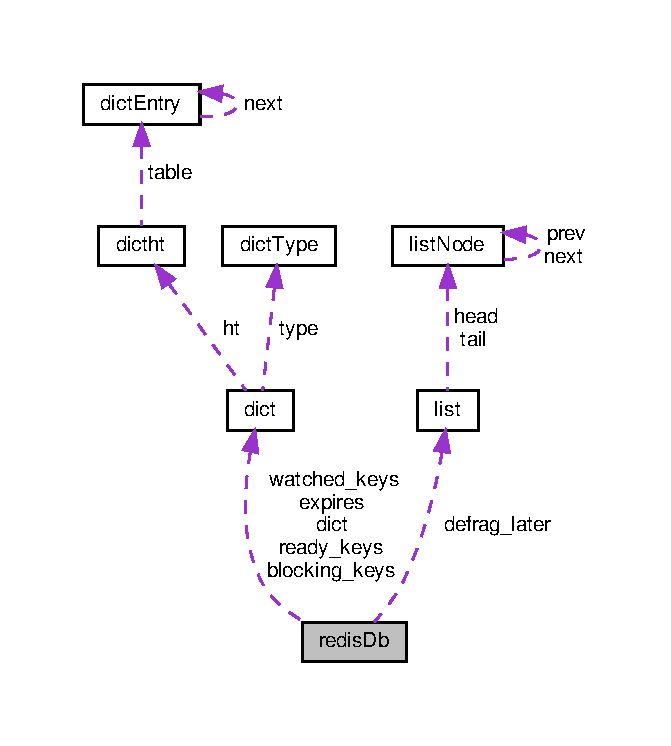
\includegraphics[width=322pt]{structredis_db__coll__graph}
\end{center}
\end{figure}
\subsection*{Data Fields}
\begin{DoxyCompactItemize}
\item 
\hyperlink{structdict}{dict} $\ast$ \hyperlink{structredis_db_aad961c2f260766ff3627bf363fef3551}{dict}
\item 
\hyperlink{structdict}{dict} $\ast$ \hyperlink{structredis_db_af8dcf36ca4b084db164becc8e1c71b67}{expires}
\item 
\hyperlink{structdict}{dict} $\ast$ \hyperlink{structredis_db_a439ca8f8cd0c2a19b8d2e0fe0044160d}{blocking\+\_\+keys}
\item 
\hyperlink{structdict}{dict} $\ast$ \hyperlink{structredis_db_a06ae0ac6a04c866ce83ece29d9a44073}{ready\+\_\+keys}
\item 
\hyperlink{structdict}{dict} $\ast$ \hyperlink{structredis_db_acf93a40c69ba9e3938f50aa3b1087abc}{watched\+\_\+keys}
\item 
int \hyperlink{structredis_db_a7441ef0865bcb3db9b8064dd7375c1ea}{id}
\item 
long long \hyperlink{structredis_db_a605ade426dd43b0de7ea393efa17d337}{avg\+\_\+ttl}
\item 
\hyperlink{structlist}{list} $\ast$ \hyperlink{structredis_db_ae22579f2281ceefa3099ad028f0c6260}{defrag\+\_\+later}
\end{DoxyCompactItemize}


\subsection{Detailed Description}


Definition at line 636 of file server.\+h.



\subsection{Field Documentation}
\mbox{\Hypertarget{structredis_db_a605ade426dd43b0de7ea393efa17d337}\label{structredis_db_a605ade426dd43b0de7ea393efa17d337}} 
\index{redis\+Db@{redis\+Db}!avg\+\_\+ttl@{avg\+\_\+ttl}}
\index{avg\+\_\+ttl@{avg\+\_\+ttl}!redis\+Db@{redis\+Db}}
\subsubsection{\texorpdfstring{avg\+\_\+ttl}{avg\_ttl}}
{\footnotesize\ttfamily long long avg\+\_\+ttl}



Definition at line 643 of file server.\+h.

\mbox{\Hypertarget{structredis_db_a439ca8f8cd0c2a19b8d2e0fe0044160d}\label{structredis_db_a439ca8f8cd0c2a19b8d2e0fe0044160d}} 
\index{redis\+Db@{redis\+Db}!blocking\+\_\+keys@{blocking\+\_\+keys}}
\index{blocking\+\_\+keys@{blocking\+\_\+keys}!redis\+Db@{redis\+Db}}
\subsubsection{\texorpdfstring{blocking\+\_\+keys}{blocking\_keys}}
{\footnotesize\ttfamily \hyperlink{structdict}{dict}$\ast$ blocking\+\_\+keys}



Definition at line 639 of file server.\+h.

\mbox{\Hypertarget{structredis_db_ae22579f2281ceefa3099ad028f0c6260}\label{structredis_db_ae22579f2281ceefa3099ad028f0c6260}} 
\index{redis\+Db@{redis\+Db}!defrag\+\_\+later@{defrag\+\_\+later}}
\index{defrag\+\_\+later@{defrag\+\_\+later}!redis\+Db@{redis\+Db}}
\subsubsection{\texorpdfstring{defrag\+\_\+later}{defrag\_later}}
{\footnotesize\ttfamily \hyperlink{structlist}{list}$\ast$ defrag\+\_\+later}



Definition at line 644 of file server.\+h.

\mbox{\Hypertarget{structredis_db_aad961c2f260766ff3627bf363fef3551}\label{structredis_db_aad961c2f260766ff3627bf363fef3551}} 
\index{redis\+Db@{redis\+Db}!dict@{dict}}
\index{dict@{dict}!redis\+Db@{redis\+Db}}
\subsubsection{\texorpdfstring{dict}{dict}}
{\footnotesize\ttfamily \hyperlink{structdict}{dict}$\ast$ \hyperlink{structdict}{dict}}



Definition at line 637 of file server.\+h.

\mbox{\Hypertarget{structredis_db_af8dcf36ca4b084db164becc8e1c71b67}\label{structredis_db_af8dcf36ca4b084db164becc8e1c71b67}} 
\index{redis\+Db@{redis\+Db}!expires@{expires}}
\index{expires@{expires}!redis\+Db@{redis\+Db}}
\subsubsection{\texorpdfstring{expires}{expires}}
{\footnotesize\ttfamily \hyperlink{structdict}{dict}$\ast$ expires}



Definition at line 638 of file server.\+h.

\mbox{\Hypertarget{structredis_db_a7441ef0865bcb3db9b8064dd7375c1ea}\label{structredis_db_a7441ef0865bcb3db9b8064dd7375c1ea}} 
\index{redis\+Db@{redis\+Db}!id@{id}}
\index{id@{id}!redis\+Db@{redis\+Db}}
\subsubsection{\texorpdfstring{id}{id}}
{\footnotesize\ttfamily int id}



Definition at line 642 of file server.\+h.

\mbox{\Hypertarget{structredis_db_a06ae0ac6a04c866ce83ece29d9a44073}\label{structredis_db_a06ae0ac6a04c866ce83ece29d9a44073}} 
\index{redis\+Db@{redis\+Db}!ready\+\_\+keys@{ready\+\_\+keys}}
\index{ready\+\_\+keys@{ready\+\_\+keys}!redis\+Db@{redis\+Db}}
\subsubsection{\texorpdfstring{ready\+\_\+keys}{ready\_keys}}
{\footnotesize\ttfamily \hyperlink{structdict}{dict}$\ast$ ready\+\_\+keys}



Definition at line 640 of file server.\+h.

\mbox{\Hypertarget{structredis_db_acf93a40c69ba9e3938f50aa3b1087abc}\label{structredis_db_acf93a40c69ba9e3938f50aa3b1087abc}} 
\index{redis\+Db@{redis\+Db}!watched\+\_\+keys@{watched\+\_\+keys}}
\index{watched\+\_\+keys@{watched\+\_\+keys}!redis\+Db@{redis\+Db}}
\subsubsection{\texorpdfstring{watched\+\_\+keys}{watched\_keys}}
{\footnotesize\ttfamily \hyperlink{structdict}{dict}$\ast$ watched\+\_\+keys}



Definition at line 641 of file server.\+h.



The documentation for this struct was generated from the following file\+:\begin{DoxyCompactItemize}
\item 
src/\hyperlink{server_8h}{server.\+h}\end{DoxyCompactItemize}

\hypertarget{structredis_function_sym}{}\section{redis\+Function\+Sym Struct Reference}
\label{structredis_function_sym}\index{redis\+Function\+Sym@{redis\+Function\+Sym}}


{\ttfamily \#include $<$server.\+h$>$}

\subsection*{Data Fields}
\begin{DoxyCompactItemize}
\item 
char $\ast$ \hyperlink{structredis_function_sym_a5ac083a645d964373f022d03df4849c8}{name}
\item 
unsigned long \hyperlink{structredis_function_sym_a4037fd214cf4412f72001bc7ef15c2e2}{pointer}
\end{DoxyCompactItemize}


\subsection{Detailed Description}


Definition at line 1306 of file server.\+h.



\subsection{Field Documentation}
\mbox{\Hypertarget{structredis_function_sym_a5ac083a645d964373f022d03df4849c8}\label{structredis_function_sym_a5ac083a645d964373f022d03df4849c8}} 
\index{redis\+Function\+Sym@{redis\+Function\+Sym}!name@{name}}
\index{name@{name}!redis\+Function\+Sym@{redis\+Function\+Sym}}
\subsubsection{\texorpdfstring{name}{name}}
{\footnotesize\ttfamily char$\ast$ name}



Definition at line 1307 of file server.\+h.

\mbox{\Hypertarget{structredis_function_sym_a4037fd214cf4412f72001bc7ef15c2e2}\label{structredis_function_sym_a4037fd214cf4412f72001bc7ef15c2e2}} 
\index{redis\+Function\+Sym@{redis\+Function\+Sym}!pointer@{pointer}}
\index{pointer@{pointer}!redis\+Function\+Sym@{redis\+Function\+Sym}}
\subsubsection{\texorpdfstring{pointer}{pointer}}
{\footnotesize\ttfamily unsigned long pointer}



Definition at line 1308 of file server.\+h.



The documentation for this struct was generated from the following file\+:\begin{DoxyCompactItemize}
\item 
src/\hyperlink{server_8h}{server.\+h}\end{DoxyCompactItemize}

\hypertarget{structredis_mem_overhead}{}\section{redis\+Mem\+Overhead Struct Reference}
\label{structredis_mem_overhead}\index{redis\+Mem\+Overhead@{redis\+Mem\+Overhead}}


{\ttfamily \#include $<$server.\+h$>$}

\subsection*{Data Fields}
\begin{DoxyCompactItemize}
\item 
size\+\_\+t \hyperlink{structredis_mem_overhead_a52004d56324eaeaabb6686b05052ca55}{peak\+\_\+allocated}
\item 
size\+\_\+t \hyperlink{structredis_mem_overhead_a3bb14855f7c280e92d0c01bbbc9b4c3c}{total\+\_\+allocated}
\item 
size\+\_\+t \hyperlink{structredis_mem_overhead_a0e982a0e14543ef6e17073a6d4afe191}{startup\+\_\+allocated}
\item 
size\+\_\+t \hyperlink{structredis_mem_overhead_a4377a6a963ee32e22c7c7f14180a4a31}{repl\+\_\+backlog}
\item 
size\+\_\+t \hyperlink{structredis_mem_overhead_ace2b062189925c36433d3a8e68062d6e}{clients\+\_\+slaves}
\item 
size\+\_\+t \hyperlink{structredis_mem_overhead_af21382aaf8f931d992586bbfe5f8aca2}{clients\+\_\+normal}
\item 
size\+\_\+t \hyperlink{structredis_mem_overhead_ad441a7ae10a5fee32c6d0b0dbfc92791}{aof\+\_\+buffer}
\item 
size\+\_\+t \hyperlink{structredis_mem_overhead_aede1fc4f53c4e19111df241fe70fb77c}{lua\+\_\+caches}
\item 
size\+\_\+t \hyperlink{structredis_mem_overhead_a2a959b51b26f4ced3ab179af23f19fba}{overhead\+\_\+total}
\item 
size\+\_\+t \hyperlink{structredis_mem_overhead_a8747868103d88dad18f00837aaeca24a}{dataset}
\item 
size\+\_\+t \hyperlink{structredis_mem_overhead_ab0dd532666871698a3e8dc420ec74b28}{total\+\_\+keys}
\item 
size\+\_\+t \hyperlink{structredis_mem_overhead_aa8888087ab630e5da0b3a0e179298d86}{bytes\+\_\+per\+\_\+key}
\item 
float \hyperlink{structredis_mem_overhead_ad413cc014759c00757b5fda0d4c94c2e}{dataset\+\_\+perc}
\item 
float \hyperlink{structredis_mem_overhead_ab748e7839b4db27ca41f802fb4deb3e1}{peak\+\_\+perc}
\item 
float \hyperlink{structredis_mem_overhead_ac8bdd246c25c91aa5ae7af8362ff9188}{total\+\_\+frag}
\item 
size\+\_\+t \hyperlink{structredis_mem_overhead_a5e5705378e7ceb2bcfa33b637a7a6fd2}{total\+\_\+frag\+\_\+bytes}
\item 
float \hyperlink{structredis_mem_overhead_a6191ede96ce40757b7eb73d4bcc597f0}{allocator\+\_\+frag}
\item 
size\+\_\+t \hyperlink{structredis_mem_overhead_a7dcfd2bdf329730a992f30f52b145dbb}{allocator\+\_\+frag\+\_\+bytes}
\item 
float \hyperlink{structredis_mem_overhead_a213b026c5bb4a2421289b34e620eb4ef}{allocator\+\_\+rss}
\item 
size\+\_\+t \hyperlink{structredis_mem_overhead_a988880d896f03571a137a828ef96531a}{allocator\+\_\+rss\+\_\+bytes}
\item 
float \hyperlink{structredis_mem_overhead_ae1d7b7b42904d9ebb1698ab3ac79a2e9}{rss\+\_\+extra}
\item 
size\+\_\+t \hyperlink{structredis_mem_overhead_a9cafe99c292b52f795f9ceef838f4249}{rss\+\_\+extra\+\_\+bytes}
\item 
size\+\_\+t \hyperlink{structredis_mem_overhead_a5fff22cf574851b502f713e7db2980fe}{num\+\_\+dbs}
\item 
\begin{tabbing}
xx\=xx\=xx\=xx\=xx\=xx\=xx\=xx\=xx\=\kill
struct \{\\
\>size\_t \hyperlink{structredis_mem_overhead_a8379ee7de31460d30fac72e27c81fd7a}{dbid}\\
\>size\_t \hyperlink{structredis_mem_overhead_a1a15c326f9a9953cd14a0ba78aaea439}{overhead\_ht\_main}\\
\>size\_t \hyperlink{structredis_mem_overhead_a26a9170a61aa6eb593f9e57a2396a706}{overhead\_ht\_expires}\\
\} $\ast$ \hyperlink{structredis_mem_overhead_a92e2261ab8290fdc2955b81e5901203d}{db}\\

\end{tabbing}\end{DoxyCompactItemize}


\subsection{Detailed Description}


Definition at line 851 of file server.\+h.



\subsection{Field Documentation}
\mbox{\Hypertarget{structredis_mem_overhead_a6191ede96ce40757b7eb73d4bcc597f0}\label{structredis_mem_overhead_a6191ede96ce40757b7eb73d4bcc597f0}} 
\index{redis\+Mem\+Overhead@{redis\+Mem\+Overhead}!allocator\+\_\+frag@{allocator\+\_\+frag}}
\index{allocator\+\_\+frag@{allocator\+\_\+frag}!redis\+Mem\+Overhead@{redis\+Mem\+Overhead}}
\subsubsection{\texorpdfstring{allocator\+\_\+frag}{allocator\_frag}}
{\footnotesize\ttfamily float allocator\+\_\+frag}



Definition at line 868 of file server.\+h.

\mbox{\Hypertarget{structredis_mem_overhead_a7dcfd2bdf329730a992f30f52b145dbb}\label{structredis_mem_overhead_a7dcfd2bdf329730a992f30f52b145dbb}} 
\index{redis\+Mem\+Overhead@{redis\+Mem\+Overhead}!allocator\+\_\+frag\+\_\+bytes@{allocator\+\_\+frag\+\_\+bytes}}
\index{allocator\+\_\+frag\+\_\+bytes@{allocator\+\_\+frag\+\_\+bytes}!redis\+Mem\+Overhead@{redis\+Mem\+Overhead}}
\subsubsection{\texorpdfstring{allocator\+\_\+frag\+\_\+bytes}{allocator\_frag\_bytes}}
{\footnotesize\ttfamily size\+\_\+t allocator\+\_\+frag\+\_\+bytes}



Definition at line 869 of file server.\+h.

\mbox{\Hypertarget{structredis_mem_overhead_a213b026c5bb4a2421289b34e620eb4ef}\label{structredis_mem_overhead_a213b026c5bb4a2421289b34e620eb4ef}} 
\index{redis\+Mem\+Overhead@{redis\+Mem\+Overhead}!allocator\+\_\+rss@{allocator\+\_\+rss}}
\index{allocator\+\_\+rss@{allocator\+\_\+rss}!redis\+Mem\+Overhead@{redis\+Mem\+Overhead}}
\subsubsection{\texorpdfstring{allocator\+\_\+rss}{allocator\_rss}}
{\footnotesize\ttfamily float allocator\+\_\+rss}



Definition at line 870 of file server.\+h.

\mbox{\Hypertarget{structredis_mem_overhead_a988880d896f03571a137a828ef96531a}\label{structredis_mem_overhead_a988880d896f03571a137a828ef96531a}} 
\index{redis\+Mem\+Overhead@{redis\+Mem\+Overhead}!allocator\+\_\+rss\+\_\+bytes@{allocator\+\_\+rss\+\_\+bytes}}
\index{allocator\+\_\+rss\+\_\+bytes@{allocator\+\_\+rss\+\_\+bytes}!redis\+Mem\+Overhead@{redis\+Mem\+Overhead}}
\subsubsection{\texorpdfstring{allocator\+\_\+rss\+\_\+bytes}{allocator\_rss\_bytes}}
{\footnotesize\ttfamily size\+\_\+t allocator\+\_\+rss\+\_\+bytes}



Definition at line 871 of file server.\+h.

\mbox{\Hypertarget{structredis_mem_overhead_ad441a7ae10a5fee32c6d0b0dbfc92791}\label{structredis_mem_overhead_ad441a7ae10a5fee32c6d0b0dbfc92791}} 
\index{redis\+Mem\+Overhead@{redis\+Mem\+Overhead}!aof\+\_\+buffer@{aof\+\_\+buffer}}
\index{aof\+\_\+buffer@{aof\+\_\+buffer}!redis\+Mem\+Overhead@{redis\+Mem\+Overhead}}
\subsubsection{\texorpdfstring{aof\+\_\+buffer}{aof\_buffer}}
{\footnotesize\ttfamily size\+\_\+t aof\+\_\+buffer}



Definition at line 858 of file server.\+h.

\mbox{\Hypertarget{structredis_mem_overhead_aa8888087ab630e5da0b3a0e179298d86}\label{structredis_mem_overhead_aa8888087ab630e5da0b3a0e179298d86}} 
\index{redis\+Mem\+Overhead@{redis\+Mem\+Overhead}!bytes\+\_\+per\+\_\+key@{bytes\+\_\+per\+\_\+key}}
\index{bytes\+\_\+per\+\_\+key@{bytes\+\_\+per\+\_\+key}!redis\+Mem\+Overhead@{redis\+Mem\+Overhead}}
\subsubsection{\texorpdfstring{bytes\+\_\+per\+\_\+key}{bytes\_per\_key}}
{\footnotesize\ttfamily size\+\_\+t bytes\+\_\+per\+\_\+key}



Definition at line 863 of file server.\+h.

\mbox{\Hypertarget{structredis_mem_overhead_af21382aaf8f931d992586bbfe5f8aca2}\label{structredis_mem_overhead_af21382aaf8f931d992586bbfe5f8aca2}} 
\index{redis\+Mem\+Overhead@{redis\+Mem\+Overhead}!clients\+\_\+normal@{clients\+\_\+normal}}
\index{clients\+\_\+normal@{clients\+\_\+normal}!redis\+Mem\+Overhead@{redis\+Mem\+Overhead}}
\subsubsection{\texorpdfstring{clients\+\_\+normal}{clients\_normal}}
{\footnotesize\ttfamily size\+\_\+t clients\+\_\+normal}



Definition at line 857 of file server.\+h.

\mbox{\Hypertarget{structredis_mem_overhead_ace2b062189925c36433d3a8e68062d6e}\label{structredis_mem_overhead_ace2b062189925c36433d3a8e68062d6e}} 
\index{redis\+Mem\+Overhead@{redis\+Mem\+Overhead}!clients\+\_\+slaves@{clients\+\_\+slaves}}
\index{clients\+\_\+slaves@{clients\+\_\+slaves}!redis\+Mem\+Overhead@{redis\+Mem\+Overhead}}
\subsubsection{\texorpdfstring{clients\+\_\+slaves}{clients\_slaves}}
{\footnotesize\ttfamily size\+\_\+t clients\+\_\+slaves}



Definition at line 856 of file server.\+h.

\mbox{\Hypertarget{structredis_mem_overhead_a8747868103d88dad18f00837aaeca24a}\label{structredis_mem_overhead_a8747868103d88dad18f00837aaeca24a}} 
\index{redis\+Mem\+Overhead@{redis\+Mem\+Overhead}!dataset@{dataset}}
\index{dataset@{dataset}!redis\+Mem\+Overhead@{redis\+Mem\+Overhead}}
\subsubsection{\texorpdfstring{dataset}{dataset}}
{\footnotesize\ttfamily size\+\_\+t dataset}



Definition at line 861 of file server.\+h.

\mbox{\Hypertarget{structredis_mem_overhead_ad413cc014759c00757b5fda0d4c94c2e}\label{structredis_mem_overhead_ad413cc014759c00757b5fda0d4c94c2e}} 
\index{redis\+Mem\+Overhead@{redis\+Mem\+Overhead}!dataset\+\_\+perc@{dataset\+\_\+perc}}
\index{dataset\+\_\+perc@{dataset\+\_\+perc}!redis\+Mem\+Overhead@{redis\+Mem\+Overhead}}
\subsubsection{\texorpdfstring{dataset\+\_\+perc}{dataset\_perc}}
{\footnotesize\ttfamily float dataset\+\_\+perc}



Definition at line 864 of file server.\+h.

\mbox{\Hypertarget{structredis_mem_overhead_a92e2261ab8290fdc2955b81e5901203d}\label{structredis_mem_overhead_a92e2261ab8290fdc2955b81e5901203d}} 
\index{redis\+Mem\+Overhead@{redis\+Mem\+Overhead}!db@{db}}
\index{db@{db}!redis\+Mem\+Overhead@{redis\+Mem\+Overhead}}
\subsubsection{\texorpdfstring{db}{db}}
{\footnotesize\ttfamily struct \{ ... \}  $\ast$ db}

\mbox{\Hypertarget{structredis_mem_overhead_a8379ee7de31460d30fac72e27c81fd7a}\label{structredis_mem_overhead_a8379ee7de31460d30fac72e27c81fd7a}} 
\index{redis\+Mem\+Overhead@{redis\+Mem\+Overhead}!dbid@{dbid}}
\index{dbid@{dbid}!redis\+Mem\+Overhead@{redis\+Mem\+Overhead}}
\subsubsection{\texorpdfstring{dbid}{dbid}}
{\footnotesize\ttfamily size\+\_\+t dbid}



Definition at line 876 of file server.\+h.

\mbox{\Hypertarget{structredis_mem_overhead_aede1fc4f53c4e19111df241fe70fb77c}\label{structredis_mem_overhead_aede1fc4f53c4e19111df241fe70fb77c}} 
\index{redis\+Mem\+Overhead@{redis\+Mem\+Overhead}!lua\+\_\+caches@{lua\+\_\+caches}}
\index{lua\+\_\+caches@{lua\+\_\+caches}!redis\+Mem\+Overhead@{redis\+Mem\+Overhead}}
\subsubsection{\texorpdfstring{lua\+\_\+caches}{lua\_caches}}
{\footnotesize\ttfamily size\+\_\+t lua\+\_\+caches}



Definition at line 859 of file server.\+h.

\mbox{\Hypertarget{structredis_mem_overhead_a5fff22cf574851b502f713e7db2980fe}\label{structredis_mem_overhead_a5fff22cf574851b502f713e7db2980fe}} 
\index{redis\+Mem\+Overhead@{redis\+Mem\+Overhead}!num\+\_\+dbs@{num\+\_\+dbs}}
\index{num\+\_\+dbs@{num\+\_\+dbs}!redis\+Mem\+Overhead@{redis\+Mem\+Overhead}}
\subsubsection{\texorpdfstring{num\+\_\+dbs}{num\_dbs}}
{\footnotesize\ttfamily size\+\_\+t num\+\_\+dbs}



Definition at line 874 of file server.\+h.

\mbox{\Hypertarget{structredis_mem_overhead_a26a9170a61aa6eb593f9e57a2396a706}\label{structredis_mem_overhead_a26a9170a61aa6eb593f9e57a2396a706}} 
\index{redis\+Mem\+Overhead@{redis\+Mem\+Overhead}!overhead\+\_\+ht\+\_\+expires@{overhead\+\_\+ht\+\_\+expires}}
\index{overhead\+\_\+ht\+\_\+expires@{overhead\+\_\+ht\+\_\+expires}!redis\+Mem\+Overhead@{redis\+Mem\+Overhead}}
\subsubsection{\texorpdfstring{overhead\+\_\+ht\+\_\+expires}{overhead\_ht\_expires}}
{\footnotesize\ttfamily size\+\_\+t overhead\+\_\+ht\+\_\+expires}



Definition at line 878 of file server.\+h.

\mbox{\Hypertarget{structredis_mem_overhead_a1a15c326f9a9953cd14a0ba78aaea439}\label{structredis_mem_overhead_a1a15c326f9a9953cd14a0ba78aaea439}} 
\index{redis\+Mem\+Overhead@{redis\+Mem\+Overhead}!overhead\+\_\+ht\+\_\+main@{overhead\+\_\+ht\+\_\+main}}
\index{overhead\+\_\+ht\+\_\+main@{overhead\+\_\+ht\+\_\+main}!redis\+Mem\+Overhead@{redis\+Mem\+Overhead}}
\subsubsection{\texorpdfstring{overhead\+\_\+ht\+\_\+main}{overhead\_ht\_main}}
{\footnotesize\ttfamily size\+\_\+t overhead\+\_\+ht\+\_\+main}



Definition at line 877 of file server.\+h.

\mbox{\Hypertarget{structredis_mem_overhead_a2a959b51b26f4ced3ab179af23f19fba}\label{structredis_mem_overhead_a2a959b51b26f4ced3ab179af23f19fba}} 
\index{redis\+Mem\+Overhead@{redis\+Mem\+Overhead}!overhead\+\_\+total@{overhead\+\_\+total}}
\index{overhead\+\_\+total@{overhead\+\_\+total}!redis\+Mem\+Overhead@{redis\+Mem\+Overhead}}
\subsubsection{\texorpdfstring{overhead\+\_\+total}{overhead\_total}}
{\footnotesize\ttfamily size\+\_\+t overhead\+\_\+total}



Definition at line 860 of file server.\+h.

\mbox{\Hypertarget{structredis_mem_overhead_a52004d56324eaeaabb6686b05052ca55}\label{structredis_mem_overhead_a52004d56324eaeaabb6686b05052ca55}} 
\index{redis\+Mem\+Overhead@{redis\+Mem\+Overhead}!peak\+\_\+allocated@{peak\+\_\+allocated}}
\index{peak\+\_\+allocated@{peak\+\_\+allocated}!redis\+Mem\+Overhead@{redis\+Mem\+Overhead}}
\subsubsection{\texorpdfstring{peak\+\_\+allocated}{peak\_allocated}}
{\footnotesize\ttfamily size\+\_\+t peak\+\_\+allocated}



Definition at line 852 of file server.\+h.

\mbox{\Hypertarget{structredis_mem_overhead_ab748e7839b4db27ca41f802fb4deb3e1}\label{structredis_mem_overhead_ab748e7839b4db27ca41f802fb4deb3e1}} 
\index{redis\+Mem\+Overhead@{redis\+Mem\+Overhead}!peak\+\_\+perc@{peak\+\_\+perc}}
\index{peak\+\_\+perc@{peak\+\_\+perc}!redis\+Mem\+Overhead@{redis\+Mem\+Overhead}}
\subsubsection{\texorpdfstring{peak\+\_\+perc}{peak\_perc}}
{\footnotesize\ttfamily float peak\+\_\+perc}



Definition at line 865 of file server.\+h.

\mbox{\Hypertarget{structredis_mem_overhead_a4377a6a963ee32e22c7c7f14180a4a31}\label{structredis_mem_overhead_a4377a6a963ee32e22c7c7f14180a4a31}} 
\index{redis\+Mem\+Overhead@{redis\+Mem\+Overhead}!repl\+\_\+backlog@{repl\+\_\+backlog}}
\index{repl\+\_\+backlog@{repl\+\_\+backlog}!redis\+Mem\+Overhead@{redis\+Mem\+Overhead}}
\subsubsection{\texorpdfstring{repl\+\_\+backlog}{repl\_backlog}}
{\footnotesize\ttfamily size\+\_\+t repl\+\_\+backlog}



Definition at line 855 of file server.\+h.

\mbox{\Hypertarget{structredis_mem_overhead_ae1d7b7b42904d9ebb1698ab3ac79a2e9}\label{structredis_mem_overhead_ae1d7b7b42904d9ebb1698ab3ac79a2e9}} 
\index{redis\+Mem\+Overhead@{redis\+Mem\+Overhead}!rss\+\_\+extra@{rss\+\_\+extra}}
\index{rss\+\_\+extra@{rss\+\_\+extra}!redis\+Mem\+Overhead@{redis\+Mem\+Overhead}}
\subsubsection{\texorpdfstring{rss\+\_\+extra}{rss\_extra}}
{\footnotesize\ttfamily float rss\+\_\+extra}



Definition at line 872 of file server.\+h.

\mbox{\Hypertarget{structredis_mem_overhead_a9cafe99c292b52f795f9ceef838f4249}\label{structredis_mem_overhead_a9cafe99c292b52f795f9ceef838f4249}} 
\index{redis\+Mem\+Overhead@{redis\+Mem\+Overhead}!rss\+\_\+extra\+\_\+bytes@{rss\+\_\+extra\+\_\+bytes}}
\index{rss\+\_\+extra\+\_\+bytes@{rss\+\_\+extra\+\_\+bytes}!redis\+Mem\+Overhead@{redis\+Mem\+Overhead}}
\subsubsection{\texorpdfstring{rss\+\_\+extra\+\_\+bytes}{rss\_extra\_bytes}}
{\footnotesize\ttfamily size\+\_\+t rss\+\_\+extra\+\_\+bytes}



Definition at line 873 of file server.\+h.

\mbox{\Hypertarget{structredis_mem_overhead_a0e982a0e14543ef6e17073a6d4afe191}\label{structredis_mem_overhead_a0e982a0e14543ef6e17073a6d4afe191}} 
\index{redis\+Mem\+Overhead@{redis\+Mem\+Overhead}!startup\+\_\+allocated@{startup\+\_\+allocated}}
\index{startup\+\_\+allocated@{startup\+\_\+allocated}!redis\+Mem\+Overhead@{redis\+Mem\+Overhead}}
\subsubsection{\texorpdfstring{startup\+\_\+allocated}{startup\_allocated}}
{\footnotesize\ttfamily size\+\_\+t startup\+\_\+allocated}



Definition at line 854 of file server.\+h.

\mbox{\Hypertarget{structredis_mem_overhead_a3bb14855f7c280e92d0c01bbbc9b4c3c}\label{structredis_mem_overhead_a3bb14855f7c280e92d0c01bbbc9b4c3c}} 
\index{redis\+Mem\+Overhead@{redis\+Mem\+Overhead}!total\+\_\+allocated@{total\+\_\+allocated}}
\index{total\+\_\+allocated@{total\+\_\+allocated}!redis\+Mem\+Overhead@{redis\+Mem\+Overhead}}
\subsubsection{\texorpdfstring{total\+\_\+allocated}{total\_allocated}}
{\footnotesize\ttfamily size\+\_\+t total\+\_\+allocated}



Definition at line 853 of file server.\+h.

\mbox{\Hypertarget{structredis_mem_overhead_ac8bdd246c25c91aa5ae7af8362ff9188}\label{structredis_mem_overhead_ac8bdd246c25c91aa5ae7af8362ff9188}} 
\index{redis\+Mem\+Overhead@{redis\+Mem\+Overhead}!total\+\_\+frag@{total\+\_\+frag}}
\index{total\+\_\+frag@{total\+\_\+frag}!redis\+Mem\+Overhead@{redis\+Mem\+Overhead}}
\subsubsection{\texorpdfstring{total\+\_\+frag}{total\_frag}}
{\footnotesize\ttfamily float total\+\_\+frag}



Definition at line 866 of file server.\+h.

\mbox{\Hypertarget{structredis_mem_overhead_a5e5705378e7ceb2bcfa33b637a7a6fd2}\label{structredis_mem_overhead_a5e5705378e7ceb2bcfa33b637a7a6fd2}} 
\index{redis\+Mem\+Overhead@{redis\+Mem\+Overhead}!total\+\_\+frag\+\_\+bytes@{total\+\_\+frag\+\_\+bytes}}
\index{total\+\_\+frag\+\_\+bytes@{total\+\_\+frag\+\_\+bytes}!redis\+Mem\+Overhead@{redis\+Mem\+Overhead}}
\subsubsection{\texorpdfstring{total\+\_\+frag\+\_\+bytes}{total\_frag\_bytes}}
{\footnotesize\ttfamily size\+\_\+t total\+\_\+frag\+\_\+bytes}



Definition at line 867 of file server.\+h.

\mbox{\Hypertarget{structredis_mem_overhead_ab0dd532666871698a3e8dc420ec74b28}\label{structredis_mem_overhead_ab0dd532666871698a3e8dc420ec74b28}} 
\index{redis\+Mem\+Overhead@{redis\+Mem\+Overhead}!total\+\_\+keys@{total\+\_\+keys}}
\index{total\+\_\+keys@{total\+\_\+keys}!redis\+Mem\+Overhead@{redis\+Mem\+Overhead}}
\subsubsection{\texorpdfstring{total\+\_\+keys}{total\_keys}}
{\footnotesize\ttfamily size\+\_\+t total\+\_\+keys}



Definition at line 862 of file server.\+h.



The documentation for this struct was generated from the following file\+:\begin{DoxyCompactItemize}
\item 
src/\hyperlink{server_8h}{server.\+h}\end{DoxyCompactItemize}

\hypertarget{struct_redis_module}{}\section{Redis\+Module Struct Reference}
\label{struct_redis_module}\index{Redis\+Module@{Redis\+Module}}


Collaboration diagram for Redis\+Module\+:
\nopagebreak
\begin{figure}[H]
\begin{center}
\leavevmode
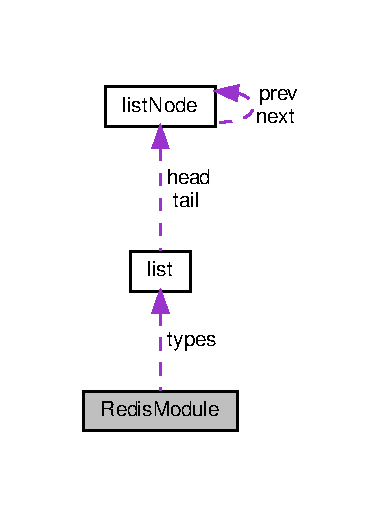
\includegraphics[width=184pt]{struct_redis_module__coll__graph}
\end{center}
\end{figure}
\subsection*{Data Fields}
\begin{DoxyCompactItemize}
\item 
void $\ast$ \hyperlink{struct_redis_module_a81011b79683fab64ce3aff71114f8fdd}{handle}
\item 
char $\ast$ \hyperlink{struct_redis_module_a5ac083a645d964373f022d03df4849c8}{name}
\item 
int \hyperlink{struct_redis_module_a88ca8dd6d8b1535e6ba06c4d988c525b}{ver}
\item 
int \hyperlink{struct_redis_module_a46c9e15c261ef13e44f9948ab8982c9e}{apiver}
\item 
\hyperlink{structlist}{list} $\ast$ \hyperlink{struct_redis_module_a29d541640e7d78fbb0cc37bd2f814429}{types}
\end{DoxyCompactItemize}


\subsection{Detailed Description}


Definition at line 44 of file module.\+c.



\subsection{Field Documentation}
\mbox{\Hypertarget{struct_redis_module_a46c9e15c261ef13e44f9948ab8982c9e}\label{struct_redis_module_a46c9e15c261ef13e44f9948ab8982c9e}} 
\index{Redis\+Module@{Redis\+Module}!apiver@{apiver}}
\index{apiver@{apiver}!Redis\+Module@{Redis\+Module}}
\subsubsection{\texorpdfstring{apiver}{apiver}}
{\footnotesize\ttfamily int apiver}



Definition at line 48 of file module.\+c.

\mbox{\Hypertarget{struct_redis_module_a81011b79683fab64ce3aff71114f8fdd}\label{struct_redis_module_a81011b79683fab64ce3aff71114f8fdd}} 
\index{Redis\+Module@{Redis\+Module}!handle@{handle}}
\index{handle@{handle}!Redis\+Module@{Redis\+Module}}
\subsubsection{\texorpdfstring{handle}{handle}}
{\footnotesize\ttfamily void$\ast$ handle}



Definition at line 45 of file module.\+c.

\mbox{\Hypertarget{struct_redis_module_a5ac083a645d964373f022d03df4849c8}\label{struct_redis_module_a5ac083a645d964373f022d03df4849c8}} 
\index{Redis\+Module@{Redis\+Module}!name@{name}}
\index{name@{name}!Redis\+Module@{Redis\+Module}}
\subsubsection{\texorpdfstring{name}{name}}
{\footnotesize\ttfamily char$\ast$ name}



Definition at line 46 of file module.\+c.

\mbox{\Hypertarget{struct_redis_module_a29d541640e7d78fbb0cc37bd2f814429}\label{struct_redis_module_a29d541640e7d78fbb0cc37bd2f814429}} 
\index{Redis\+Module@{Redis\+Module}!types@{types}}
\index{types@{types}!Redis\+Module@{Redis\+Module}}
\subsubsection{\texorpdfstring{types}{types}}
{\footnotesize\ttfamily \hyperlink{structlist}{list}$\ast$ types}



Definition at line 49 of file module.\+c.

\mbox{\Hypertarget{struct_redis_module_a88ca8dd6d8b1535e6ba06c4d988c525b}\label{struct_redis_module_a88ca8dd6d8b1535e6ba06c4d988c525b}} 
\index{Redis\+Module@{Redis\+Module}!ver@{ver}}
\index{ver@{ver}!Redis\+Module@{Redis\+Module}}
\subsubsection{\texorpdfstring{ver}{ver}}
{\footnotesize\ttfamily int ver}



Definition at line 47 of file module.\+c.



The documentation for this struct was generated from the following file\+:\begin{DoxyCompactItemize}
\item 
src/\hyperlink{module_8c}{module.\+c}\end{DoxyCompactItemize}

\hypertarget{struct_redis_module_blocked_client}{}\section{Redis\+Module\+Blocked\+Client Struct Reference}
\label{struct_redis_module_blocked_client}\index{Redis\+Module\+Blocked\+Client@{Redis\+Module\+Blocked\+Client}}


Collaboration diagram for Redis\+Module\+Blocked\+Client\+:
\nopagebreak
\begin{figure}[H]
\begin{center}
\leavevmode
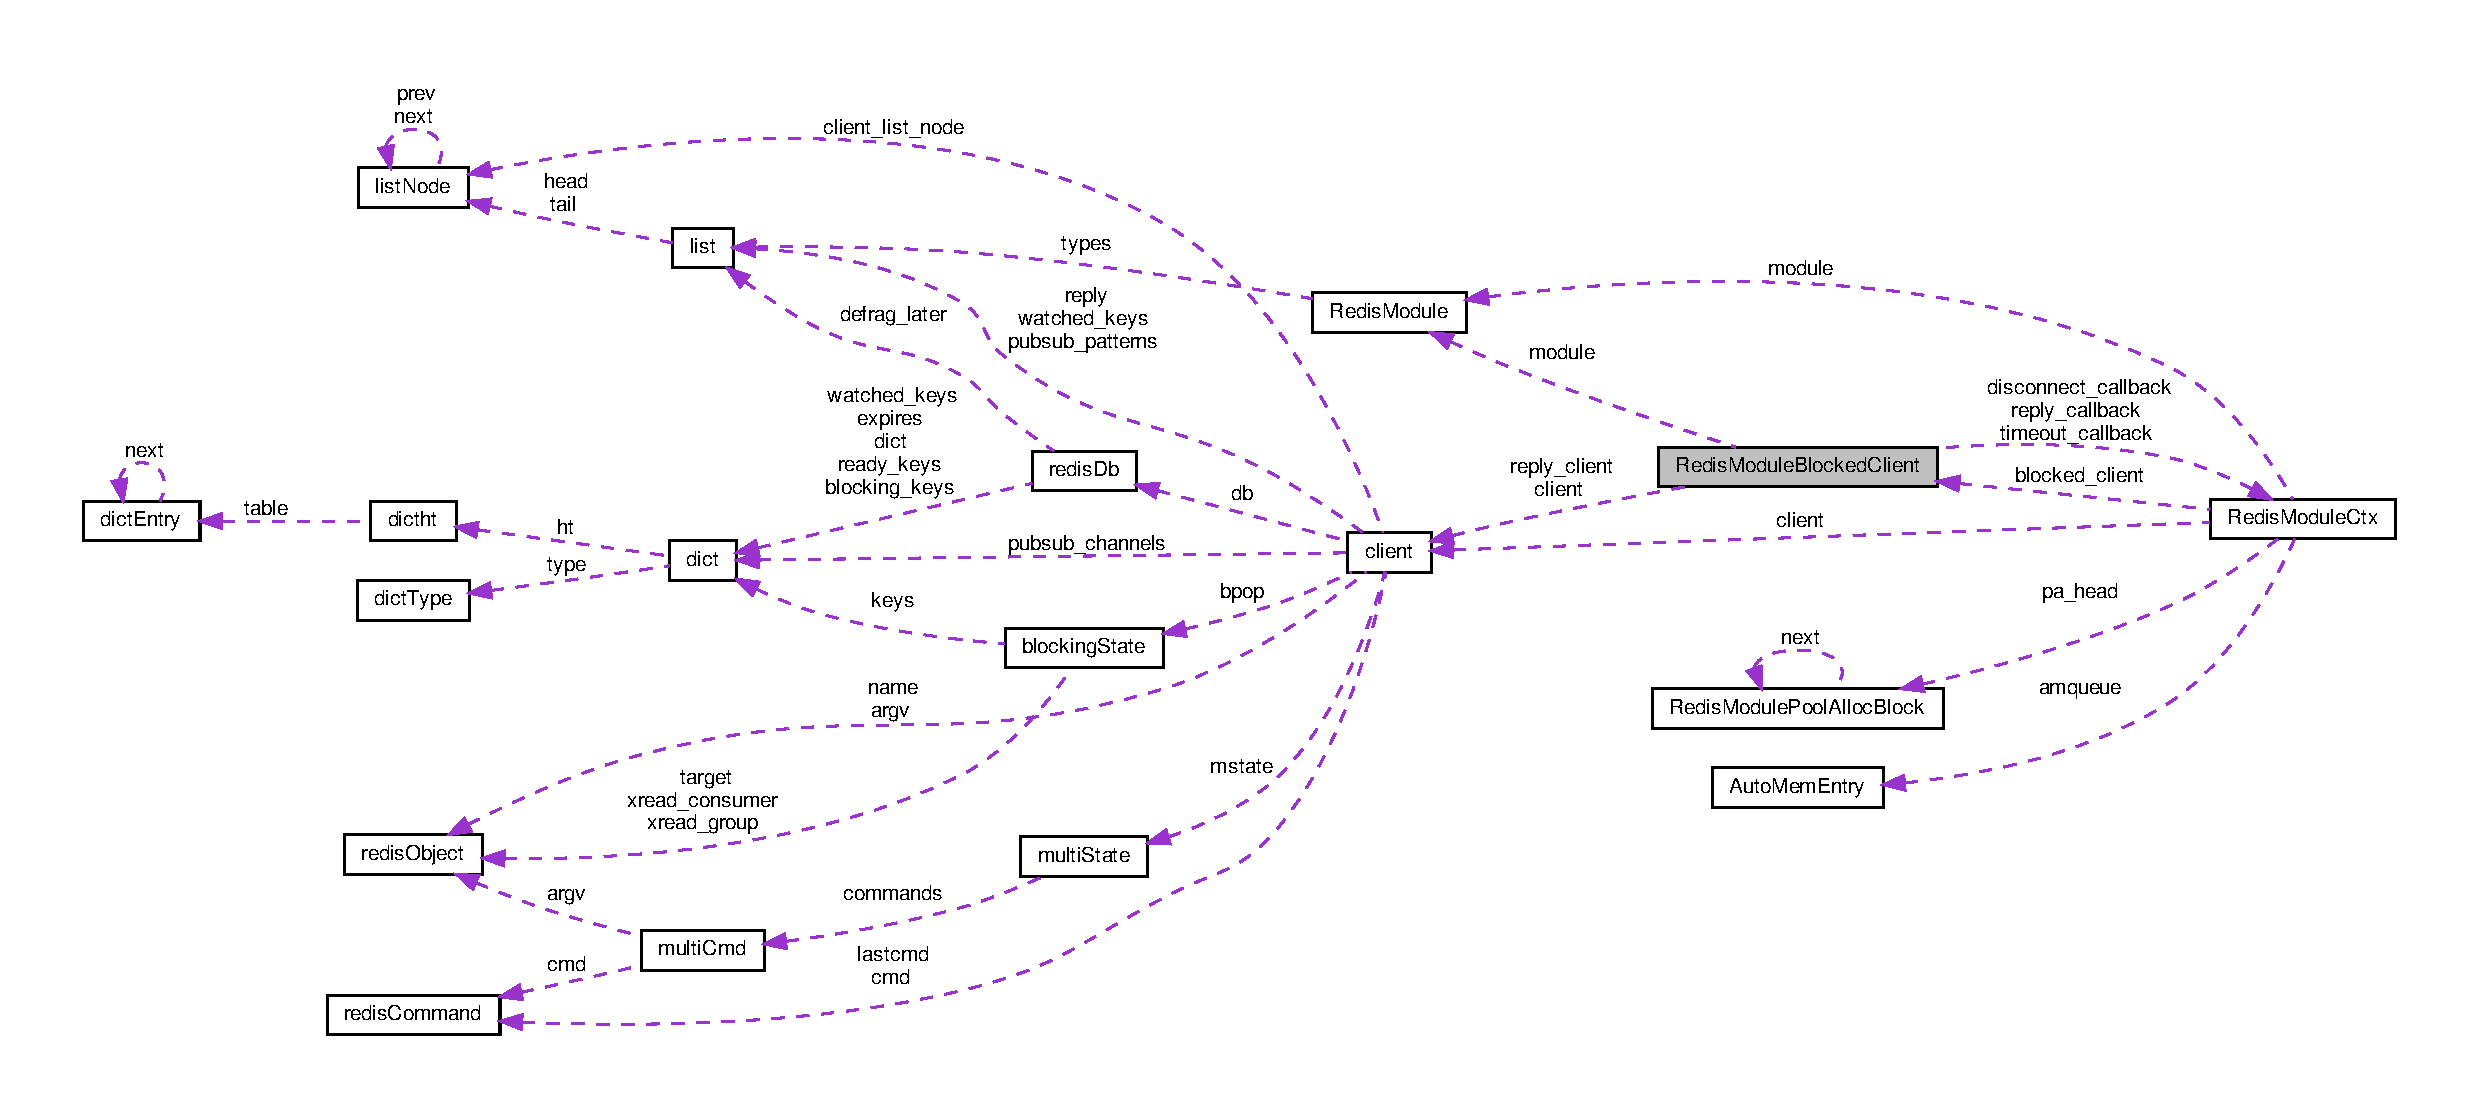
\includegraphics[width=350pt]{struct_redis_module_blocked_client__coll__graph}
\end{center}
\end{figure}
\subsection*{Data Fields}
\begin{DoxyCompactItemize}
\item 
\hyperlink{structclient}{client} $\ast$ \hyperlink{struct_redis_module_blocked_client_a6d99956d3d06c98958feb17baf491c71}{client}
\item 
\hyperlink{struct_redis_module}{Redis\+Module} $\ast$ \hyperlink{struct_redis_module_blocked_client_a9b71e67bccc12e40caf1d263db4172f3}{module}
\item 
\hyperlink{redismodule_8h_afd84062b24c2151cf8f2a53b955f9eed}{Redis\+Module\+Cmd\+Func} \hyperlink{struct_redis_module_blocked_client_ab1ad2ba0d6d49066ac12d91dd71eaa9e}{reply\+\_\+callback}
\item 
\hyperlink{redismodule_8h_afd84062b24c2151cf8f2a53b955f9eed}{Redis\+Module\+Cmd\+Func} \hyperlink{struct_redis_module_blocked_client_ad5b2a934fdf4cacf6ea5126c4ae31bf6}{timeout\+\_\+callback}
\item 
\hyperlink{redismodule_8h_a018e927d445b896dc38572db79f4907c}{Redis\+Module\+Disconnect\+Func} \hyperlink{struct_redis_module_blocked_client_a9fd300fed0252624be5cd1d87c1e9a2c}{disconnect\+\_\+callback}
\item 
void($\ast$ \hyperlink{struct_redis_module_blocked_client_a09d89fa730dac748044db7cfcb19ef1d}{free\+\_\+privdata} )(\hyperlink{struct_redis_module_ctx}{Redis\+Module\+Ctx} $\ast$, void $\ast$)
\item 
void $\ast$ \hyperlink{struct_redis_module_blocked_client_ac5df247494dd66a10946e2d67e56b2a1}{privdata}
\item 
\hyperlink{structclient}{client} $\ast$ \hyperlink{struct_redis_module_blocked_client_a09bd4914134a6336a5c03d4546ce0ba1}{reply\+\_\+client}
\item 
int \hyperlink{struct_redis_module_blocked_client_adc62368127157e2b3ff9cabe77f4f337}{dbid}
\end{DoxyCompactItemize}


\subsection{Detailed Description}


Definition at line 201 of file module.\+c.



\subsection{Field Documentation}
\mbox{\Hypertarget{struct_redis_module_blocked_client_a6d99956d3d06c98958feb17baf491c71}\label{struct_redis_module_blocked_client_a6d99956d3d06c98958feb17baf491c71}} 
\index{Redis\+Module\+Blocked\+Client@{Redis\+Module\+Blocked\+Client}!client@{client}}
\index{client@{client}!Redis\+Module\+Blocked\+Client@{Redis\+Module\+Blocked\+Client}}
\subsubsection{\texorpdfstring{client}{client}}
{\footnotesize\ttfamily \hyperlink{structclient}{client}$\ast$ \hyperlink{structclient}{client}}



Definition at line 202 of file module.\+c.

\mbox{\Hypertarget{struct_redis_module_blocked_client_adc62368127157e2b3ff9cabe77f4f337}\label{struct_redis_module_blocked_client_adc62368127157e2b3ff9cabe77f4f337}} 
\index{Redis\+Module\+Blocked\+Client@{Redis\+Module\+Blocked\+Client}!dbid@{dbid}}
\index{dbid@{dbid}!Redis\+Module\+Blocked\+Client@{Redis\+Module\+Blocked\+Client}}
\subsubsection{\texorpdfstring{dbid}{dbid}}
{\footnotesize\ttfamily int dbid}



Definition at line 214 of file module.\+c.

\mbox{\Hypertarget{struct_redis_module_blocked_client_a9fd300fed0252624be5cd1d87c1e9a2c}\label{struct_redis_module_blocked_client_a9fd300fed0252624be5cd1d87c1e9a2c}} 
\index{Redis\+Module\+Blocked\+Client@{Redis\+Module\+Blocked\+Client}!disconnect\+\_\+callback@{disconnect\+\_\+callback}}
\index{disconnect\+\_\+callback@{disconnect\+\_\+callback}!Redis\+Module\+Blocked\+Client@{Redis\+Module\+Blocked\+Client}}
\subsubsection{\texorpdfstring{disconnect\+\_\+callback}{disconnect\_callback}}
{\footnotesize\ttfamily \hyperlink{redismodule_8h_a018e927d445b896dc38572db79f4907c}{Redis\+Module\+Disconnect\+Func} disconnect\+\_\+callback}



Definition at line 207 of file module.\+c.

\mbox{\Hypertarget{struct_redis_module_blocked_client_a09d89fa730dac748044db7cfcb19ef1d}\label{struct_redis_module_blocked_client_a09d89fa730dac748044db7cfcb19ef1d}} 
\index{Redis\+Module\+Blocked\+Client@{Redis\+Module\+Blocked\+Client}!free\+\_\+privdata@{free\+\_\+privdata}}
\index{free\+\_\+privdata@{free\+\_\+privdata}!Redis\+Module\+Blocked\+Client@{Redis\+Module\+Blocked\+Client}}
\subsubsection{\texorpdfstring{free\+\_\+privdata}{free\_privdata}}
{\footnotesize\ttfamily void($\ast$ free\+\_\+privdata) (\hyperlink{struct_redis_module_ctx}{Redis\+Module\+Ctx} $\ast$, void $\ast$)}



Definition at line 208 of file module.\+c.

\mbox{\Hypertarget{struct_redis_module_blocked_client_a9b71e67bccc12e40caf1d263db4172f3}\label{struct_redis_module_blocked_client_a9b71e67bccc12e40caf1d263db4172f3}} 
\index{Redis\+Module\+Blocked\+Client@{Redis\+Module\+Blocked\+Client}!module@{module}}
\index{module@{module}!Redis\+Module\+Blocked\+Client@{Redis\+Module\+Blocked\+Client}}
\subsubsection{\texorpdfstring{module}{module}}
{\footnotesize\ttfamily \hyperlink{struct_redis_module}{Redis\+Module}$\ast$ module}



Definition at line 204 of file module.\+c.

\mbox{\Hypertarget{struct_redis_module_blocked_client_ac5df247494dd66a10946e2d67e56b2a1}\label{struct_redis_module_blocked_client_ac5df247494dd66a10946e2d67e56b2a1}} 
\index{Redis\+Module\+Blocked\+Client@{Redis\+Module\+Blocked\+Client}!privdata@{privdata}}
\index{privdata@{privdata}!Redis\+Module\+Blocked\+Client@{Redis\+Module\+Blocked\+Client}}
\subsubsection{\texorpdfstring{privdata}{privdata}}
{\footnotesize\ttfamily void$\ast$ privdata}



Definition at line 209 of file module.\+c.

\mbox{\Hypertarget{struct_redis_module_blocked_client_ab1ad2ba0d6d49066ac12d91dd71eaa9e}\label{struct_redis_module_blocked_client_ab1ad2ba0d6d49066ac12d91dd71eaa9e}} 
\index{Redis\+Module\+Blocked\+Client@{Redis\+Module\+Blocked\+Client}!reply\+\_\+callback@{reply\+\_\+callback}}
\index{reply\+\_\+callback@{reply\+\_\+callback}!Redis\+Module\+Blocked\+Client@{Redis\+Module\+Blocked\+Client}}
\subsubsection{\texorpdfstring{reply\+\_\+callback}{reply\_callback}}
{\footnotesize\ttfamily \hyperlink{redismodule_8h_afd84062b24c2151cf8f2a53b955f9eed}{Redis\+Module\+Cmd\+Func} reply\+\_\+callback}



Definition at line 205 of file module.\+c.

\mbox{\Hypertarget{struct_redis_module_blocked_client_a09bd4914134a6336a5c03d4546ce0ba1}\label{struct_redis_module_blocked_client_a09bd4914134a6336a5c03d4546ce0ba1}} 
\index{Redis\+Module\+Blocked\+Client@{Redis\+Module\+Blocked\+Client}!reply\+\_\+client@{reply\+\_\+client}}
\index{reply\+\_\+client@{reply\+\_\+client}!Redis\+Module\+Blocked\+Client@{Redis\+Module\+Blocked\+Client}}
\subsubsection{\texorpdfstring{reply\+\_\+client}{reply\_client}}
{\footnotesize\ttfamily \hyperlink{structclient}{client}$\ast$ reply\+\_\+client}



Definition at line 212 of file module.\+c.

\mbox{\Hypertarget{struct_redis_module_blocked_client_ad5b2a934fdf4cacf6ea5126c4ae31bf6}\label{struct_redis_module_blocked_client_ad5b2a934fdf4cacf6ea5126c4ae31bf6}} 
\index{Redis\+Module\+Blocked\+Client@{Redis\+Module\+Blocked\+Client}!timeout\+\_\+callback@{timeout\+\_\+callback}}
\index{timeout\+\_\+callback@{timeout\+\_\+callback}!Redis\+Module\+Blocked\+Client@{Redis\+Module\+Blocked\+Client}}
\subsubsection{\texorpdfstring{timeout\+\_\+callback}{timeout\_callback}}
{\footnotesize\ttfamily \hyperlink{redismodule_8h_afd84062b24c2151cf8f2a53b955f9eed}{Redis\+Module\+Cmd\+Func} timeout\+\_\+callback}



Definition at line 206 of file module.\+c.



The documentation for this struct was generated from the following file\+:\begin{DoxyCompactItemize}
\item 
src/\hyperlink{module_8c}{module.\+c}\end{DoxyCompactItemize}

\hypertarget{struct_redis_module_call_reply}{}\section{Redis\+Module\+Call\+Reply Struct Reference}
\label{struct_redis_module_call_reply}\index{Redis\+Module\+Call\+Reply@{Redis\+Module\+Call\+Reply}}


Collaboration diagram for Redis\+Module\+Call\+Reply\+:
\nopagebreak
\begin{figure}[H]
\begin{center}
\leavevmode
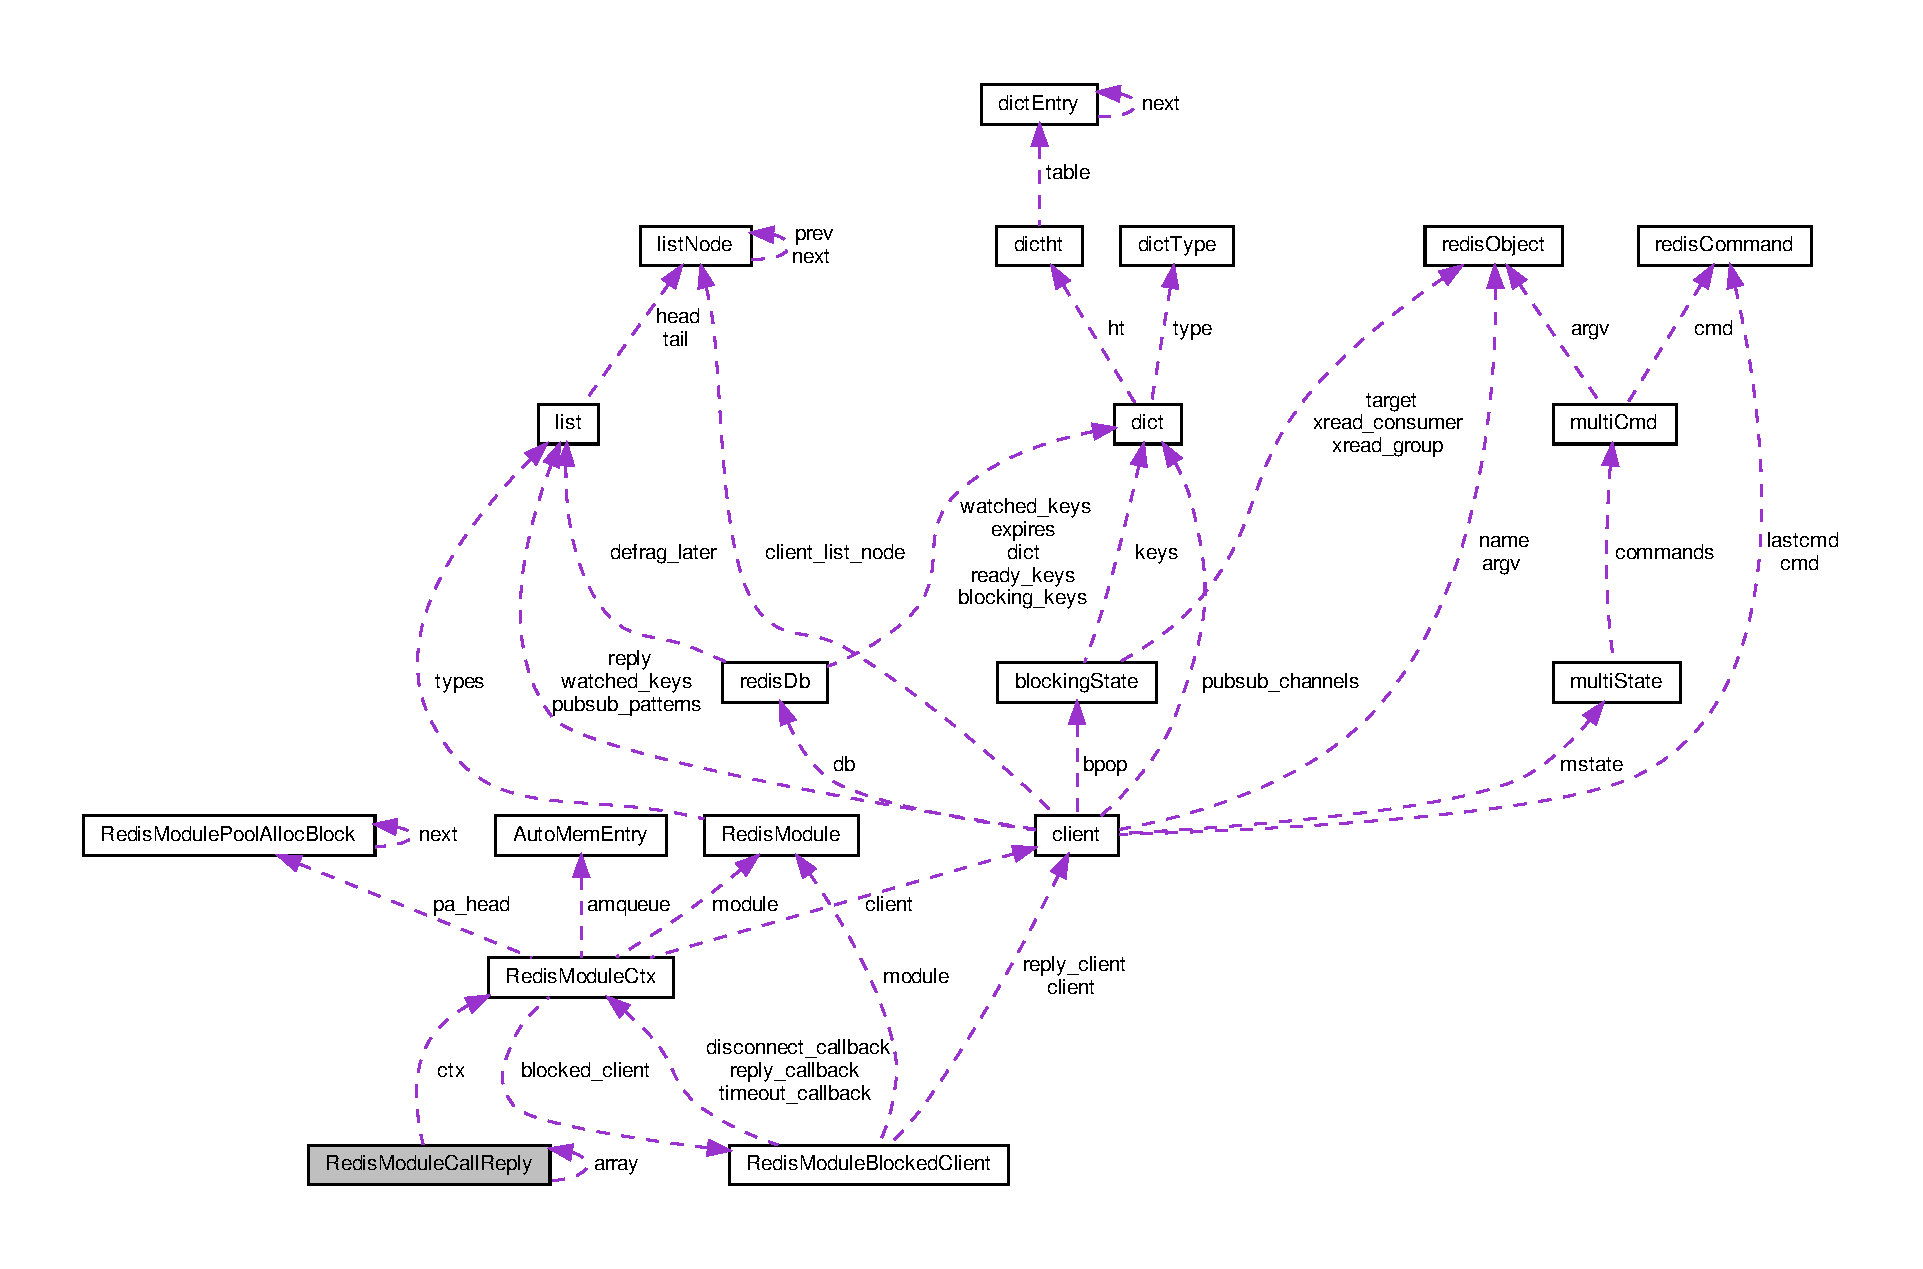
\includegraphics[width=350pt]{struct_redis_module_call_reply__coll__graph}
\end{center}
\end{figure}
\subsection*{Data Fields}
\begin{DoxyCompactItemize}
\item 
\hyperlink{struct_redis_module_ctx}{Redis\+Module\+Ctx} $\ast$ \hyperlink{struct_redis_module_call_reply_a221ba73ece36a4c95c593459c3fc1d8d}{ctx}
\item 
int \hyperlink{struct_redis_module_call_reply_ac765329451135abec74c45e1897abf26}{type}
\item 
int \hyperlink{struct_redis_module_call_reply_ac8bf36fe0577cba66bccda3a6f7e80a4}{flags}
\item 
size\+\_\+t \hyperlink{struct_redis_module_call_reply_a7360b55975153b822efc5217b7734e6a}{len}
\item 
char $\ast$ \hyperlink{struct_redis_module_call_reply_a217a90f335b3a7d2fc125fac94c80d95}{proto}
\item 
size\+\_\+t \hyperlink{struct_redis_module_call_reply_a43257d3e2ccef83fbabcc3b06a20b01f}{protolen}
\item 
\begin{tabbing}
xx\=xx\=xx\=xx\=xx\=xx\=xx\=xx\=xx\=\kill
union \{\\
\>const char $\ast$ \hyperlink{struct_redis_module_call_reply_af25d6dc49269fa2003ac7c7fa6f13915}{str}\\
\>long long \hyperlink{struct_redis_module_call_reply_a78dd8c96fe7632134a6dc8665944aa35}{ll}\\
\>struct \hyperlink{struct_redis_module_call_reply}{RedisModuleCallReply} $\ast$ \hyperlink{struct_redis_module_call_reply_ae8b3a272518c53c865e974e0fa56c8b0}{array}\\
\} \hyperlink{struct_redis_module_call_reply_adceb462742f61786b2f766e71de4cabd}{val}\\

\end{tabbing}\end{DoxyCompactItemize}


\subsection{Detailed Description}


Definition at line 182 of file module.\+c.



\subsection{Field Documentation}
\mbox{\Hypertarget{struct_redis_module_call_reply_ae8b3a272518c53c865e974e0fa56c8b0}\label{struct_redis_module_call_reply_ae8b3a272518c53c865e974e0fa56c8b0}} 
\index{Redis\+Module\+Call\+Reply@{Redis\+Module\+Call\+Reply}!array@{array}}
\index{array@{array}!Redis\+Module\+Call\+Reply@{Redis\+Module\+Call\+Reply}}
\subsubsection{\texorpdfstring{array}{array}}
{\footnotesize\ttfamily struct \hyperlink{struct_redis_module_call_reply}{Redis\+Module\+Call\+Reply}$\ast$ array}



Definition at line 195 of file module.\+c.

\mbox{\Hypertarget{struct_redis_module_call_reply_a221ba73ece36a4c95c593459c3fc1d8d}\label{struct_redis_module_call_reply_a221ba73ece36a4c95c593459c3fc1d8d}} 
\index{Redis\+Module\+Call\+Reply@{Redis\+Module\+Call\+Reply}!ctx@{ctx}}
\index{ctx@{ctx}!Redis\+Module\+Call\+Reply@{Redis\+Module\+Call\+Reply}}
\subsubsection{\texorpdfstring{ctx}{ctx}}
{\footnotesize\ttfamily \hyperlink{struct_redis_module_ctx}{Redis\+Module\+Ctx}$\ast$ ctx}



Definition at line 183 of file module.\+c.

\mbox{\Hypertarget{struct_redis_module_call_reply_ac8bf36fe0577cba66bccda3a6f7e80a4}\label{struct_redis_module_call_reply_ac8bf36fe0577cba66bccda3a6f7e80a4}} 
\index{Redis\+Module\+Call\+Reply@{Redis\+Module\+Call\+Reply}!flags@{flags}}
\index{flags@{flags}!Redis\+Module\+Call\+Reply@{Redis\+Module\+Call\+Reply}}
\subsubsection{\texorpdfstring{flags}{flags}}
{\footnotesize\ttfamily int flags}



Definition at line 185 of file module.\+c.

\mbox{\Hypertarget{struct_redis_module_call_reply_a7360b55975153b822efc5217b7734e6a}\label{struct_redis_module_call_reply_a7360b55975153b822efc5217b7734e6a}} 
\index{Redis\+Module\+Call\+Reply@{Redis\+Module\+Call\+Reply}!len@{len}}
\index{len@{len}!Redis\+Module\+Call\+Reply@{Redis\+Module\+Call\+Reply}}
\subsubsection{\texorpdfstring{len}{len}}
{\footnotesize\ttfamily size\+\_\+t len}



Definition at line 186 of file module.\+c.

\mbox{\Hypertarget{struct_redis_module_call_reply_a78dd8c96fe7632134a6dc8665944aa35}\label{struct_redis_module_call_reply_a78dd8c96fe7632134a6dc8665944aa35}} 
\index{Redis\+Module\+Call\+Reply@{Redis\+Module\+Call\+Reply}!ll@{ll}}
\index{ll@{ll}!Redis\+Module\+Call\+Reply@{Redis\+Module\+Call\+Reply}}
\subsubsection{\texorpdfstring{ll}{ll}}
{\footnotesize\ttfamily long long ll}



Definition at line 194 of file module.\+c.

\mbox{\Hypertarget{struct_redis_module_call_reply_a217a90f335b3a7d2fc125fac94c80d95}\label{struct_redis_module_call_reply_a217a90f335b3a7d2fc125fac94c80d95}} 
\index{Redis\+Module\+Call\+Reply@{Redis\+Module\+Call\+Reply}!proto@{proto}}
\index{proto@{proto}!Redis\+Module\+Call\+Reply@{Redis\+Module\+Call\+Reply}}
\subsubsection{\texorpdfstring{proto}{proto}}
{\footnotesize\ttfamily char$\ast$ proto}



Definition at line 187 of file module.\+c.

\mbox{\Hypertarget{struct_redis_module_call_reply_a43257d3e2ccef83fbabcc3b06a20b01f}\label{struct_redis_module_call_reply_a43257d3e2ccef83fbabcc3b06a20b01f}} 
\index{Redis\+Module\+Call\+Reply@{Redis\+Module\+Call\+Reply}!protolen@{protolen}}
\index{protolen@{protolen}!Redis\+Module\+Call\+Reply@{Redis\+Module\+Call\+Reply}}
\subsubsection{\texorpdfstring{protolen}{protolen}}
{\footnotesize\ttfamily size\+\_\+t protolen}



Definition at line 188 of file module.\+c.

\mbox{\Hypertarget{struct_redis_module_call_reply_af25d6dc49269fa2003ac7c7fa6f13915}\label{struct_redis_module_call_reply_af25d6dc49269fa2003ac7c7fa6f13915}} 
\index{Redis\+Module\+Call\+Reply@{Redis\+Module\+Call\+Reply}!str@{str}}
\index{str@{str}!Redis\+Module\+Call\+Reply@{Redis\+Module\+Call\+Reply}}
\subsubsection{\texorpdfstring{str}{str}}
{\footnotesize\ttfamily const char$\ast$ str}



Definition at line 190 of file module.\+c.

\mbox{\Hypertarget{struct_redis_module_call_reply_ac765329451135abec74c45e1897abf26}\label{struct_redis_module_call_reply_ac765329451135abec74c45e1897abf26}} 
\index{Redis\+Module\+Call\+Reply@{Redis\+Module\+Call\+Reply}!type@{type}}
\index{type@{type}!Redis\+Module\+Call\+Reply@{Redis\+Module\+Call\+Reply}}
\subsubsection{\texorpdfstring{type}{type}}
{\footnotesize\ttfamily int type}



Definition at line 184 of file module.\+c.

\mbox{\Hypertarget{struct_redis_module_call_reply_adceb462742f61786b2f766e71de4cabd}\label{struct_redis_module_call_reply_adceb462742f61786b2f766e71de4cabd}} 
\index{Redis\+Module\+Call\+Reply@{Redis\+Module\+Call\+Reply}!val@{val}}
\index{val@{val}!Redis\+Module\+Call\+Reply@{Redis\+Module\+Call\+Reply}}
\subsubsection{\texorpdfstring{val}{val}}
{\footnotesize\ttfamily union \{ ... \}   val}



The documentation for this struct was generated from the following file\+:\begin{DoxyCompactItemize}
\item 
src/\hyperlink{module_8c}{module.\+c}\end{DoxyCompactItemize}

\hypertarget{struct_redis_module_command_proxy}{}\section{Redis\+Module\+Command\+Proxy Struct Reference}
\label{struct_redis_module_command_proxy}\index{Redis\+Module\+Command\+Proxy@{Redis\+Module\+Command\+Proxy}}


Collaboration diagram for Redis\+Module\+Command\+Proxy\+:
\nopagebreak
\begin{figure}[H]
\begin{center}
\leavevmode
\includegraphics[width=350pt]{struct_redis_module_command_proxy__coll__graph}
\end{center}
\end{figure}
\subsection*{Data Fields}
\begin{DoxyCompactItemize}
\item 
struct \hyperlink{struct_redis_module}{Redis\+Module} $\ast$ \hyperlink{struct_redis_module_command_proxy_a0b5d3833feb2320585734795fb7f62b6}{module}
\item 
\hyperlink{redismodule_8h_afd84062b24c2151cf8f2a53b955f9eed}{Redis\+Module\+Cmd\+Func} \hyperlink{struct_redis_module_command_proxy_a2e9ebffa1c494b2b6e53f3271290461c}{func}
\item 
struct \hyperlink{structredis_command}{redis\+Command} $\ast$ \hyperlink{struct_redis_module_command_proxy_a016430f13b3b7c484584bae32fe89fd5}{rediscmd}
\end{DoxyCompactItemize}


\subsection{Detailed Description}


Definition at line 167 of file module.\+c.



\subsection{Field Documentation}
\mbox{\Hypertarget{struct_redis_module_command_proxy_a2e9ebffa1c494b2b6e53f3271290461c}\label{struct_redis_module_command_proxy_a2e9ebffa1c494b2b6e53f3271290461c}} 
\index{Redis\+Module\+Command\+Proxy@{Redis\+Module\+Command\+Proxy}!func@{func}}
\index{func@{func}!Redis\+Module\+Command\+Proxy@{Redis\+Module\+Command\+Proxy}}
\subsubsection{\texorpdfstring{func}{func}}
{\footnotesize\ttfamily \hyperlink{redismodule_8h_afd84062b24c2151cf8f2a53b955f9eed}{Redis\+Module\+Cmd\+Func} func}



Definition at line 169 of file module.\+c.

\mbox{\Hypertarget{struct_redis_module_command_proxy_a0b5d3833feb2320585734795fb7f62b6}\label{struct_redis_module_command_proxy_a0b5d3833feb2320585734795fb7f62b6}} 
\index{Redis\+Module\+Command\+Proxy@{Redis\+Module\+Command\+Proxy}!module@{module}}
\index{module@{module}!Redis\+Module\+Command\+Proxy@{Redis\+Module\+Command\+Proxy}}
\subsubsection{\texorpdfstring{module}{module}}
{\footnotesize\ttfamily struct \hyperlink{struct_redis_module}{Redis\+Module}$\ast$ module}



Definition at line 168 of file module.\+c.

\mbox{\Hypertarget{struct_redis_module_command_proxy_a016430f13b3b7c484584bae32fe89fd5}\label{struct_redis_module_command_proxy_a016430f13b3b7c484584bae32fe89fd5}} 
\index{Redis\+Module\+Command\+Proxy@{Redis\+Module\+Command\+Proxy}!rediscmd@{rediscmd}}
\index{rediscmd@{rediscmd}!Redis\+Module\+Command\+Proxy@{Redis\+Module\+Command\+Proxy}}
\subsubsection{\texorpdfstring{rediscmd}{rediscmd}}
{\footnotesize\ttfamily struct \hyperlink{structredis_command}{redis\+Command}$\ast$ rediscmd}



Definition at line 170 of file module.\+c.



The documentation for this struct was generated from the following file\+:\begin{DoxyCompactItemize}
\item 
src/\hyperlink{module_8c}{module.\+c}\end{DoxyCompactItemize}

\hypertarget{struct_redis_module_ctx}{}\section{Redis\+Module\+Ctx Struct Reference}
\label{struct_redis_module_ctx}\index{Redis\+Module\+Ctx@{Redis\+Module\+Ctx}}


Collaboration diagram for Redis\+Module\+Ctx\+:
\nopagebreak
\begin{figure}[H]
\begin{center}
\leavevmode
\includegraphics[width=350pt]{struct_redis_module_ctx__coll__graph}
\end{center}
\end{figure}
\subsection*{Data Fields}
\begin{DoxyCompactItemize}
\item 
void $\ast$ \hyperlink{struct_redis_module_ctx_ac6329d63f19c6310742a84c334627e6f}{getapifuncptr}
\item 
struct \hyperlink{struct_redis_module}{Redis\+Module} $\ast$ \hyperlink{struct_redis_module_ctx_a0b5d3833feb2320585734795fb7f62b6}{module}
\item 
\hyperlink{structclient}{client} $\ast$ \hyperlink{struct_redis_module_ctx_a6d99956d3d06c98958feb17baf491c71}{client}
\item 
struct \hyperlink{struct_redis_module_blocked_client}{Redis\+Module\+Blocked\+Client} $\ast$ \hyperlink{struct_redis_module_ctx_af1859b71d91af8412370224b3a37b1dc}{blocked\+\_\+client}
\item 
struct \hyperlink{struct_auto_mem_entry}{Auto\+Mem\+Entry} $\ast$ \hyperlink{struct_redis_module_ctx_add0d0fd5c12e402e4decbaf015619d1c}{amqueue}
\item 
int \hyperlink{struct_redis_module_ctx_a85eb81641193eff3e499ff05da42f752}{amqueue\+\_\+len}
\item 
int \hyperlink{struct_redis_module_ctx_af5e94a4bf2e602db90d341b3483b71ab}{amqueue\+\_\+used}
\item 
int \hyperlink{struct_redis_module_ctx_ac8bf36fe0577cba66bccda3a6f7e80a4}{flags}
\item 
void $\ast$$\ast$ \hyperlink{struct_redis_module_ctx_aeb39a4536bdedc8392cdda36e7380c22}{postponed\+\_\+arrays}
\item 
int \hyperlink{struct_redis_module_ctx_a3eb93de851bb356c791e34b7b0cd4bde}{postponed\+\_\+arrays\+\_\+count}
\item 
void $\ast$ \hyperlink{struct_redis_module_ctx_a5d0fe014667071528b4f68c65b085808}{blocked\+\_\+privdata}
\item 
int $\ast$ \hyperlink{struct_redis_module_ctx_a559d6c952058c05bc208033d3d3576d1}{keys\+\_\+pos}
\item 
int \hyperlink{struct_redis_module_ctx_a24bb9d3a9dccb24581d359a218837c6f}{keys\+\_\+count}
\item 
struct \hyperlink{struct_redis_module_pool_alloc_block}{Redis\+Module\+Pool\+Alloc\+Block} $\ast$ \hyperlink{struct_redis_module_ctx_ad70f06a690907f850f125ae974b0aeed}{pa\+\_\+head}
\end{DoxyCompactItemize}


\subsection{Detailed Description}


Definition at line 102 of file module.\+c.



\subsection{Field Documentation}
\mbox{\Hypertarget{struct_redis_module_ctx_add0d0fd5c12e402e4decbaf015619d1c}\label{struct_redis_module_ctx_add0d0fd5c12e402e4decbaf015619d1c}} 
\index{Redis\+Module\+Ctx@{Redis\+Module\+Ctx}!amqueue@{amqueue}}
\index{amqueue@{amqueue}!Redis\+Module\+Ctx@{Redis\+Module\+Ctx}}
\subsubsection{\texorpdfstring{amqueue}{amqueue}}
{\footnotesize\ttfamily struct \hyperlink{struct_auto_mem_entry}{Auto\+Mem\+Entry}$\ast$ amqueue}



Definition at line 108 of file module.\+c.

\mbox{\Hypertarget{struct_redis_module_ctx_a85eb81641193eff3e499ff05da42f752}\label{struct_redis_module_ctx_a85eb81641193eff3e499ff05da42f752}} 
\index{Redis\+Module\+Ctx@{Redis\+Module\+Ctx}!amqueue\+\_\+len@{amqueue\+\_\+len}}
\index{amqueue\+\_\+len@{amqueue\+\_\+len}!Redis\+Module\+Ctx@{Redis\+Module\+Ctx}}
\subsubsection{\texorpdfstring{amqueue\+\_\+len}{amqueue\_len}}
{\footnotesize\ttfamily int amqueue\+\_\+len}



Definition at line 109 of file module.\+c.

\mbox{\Hypertarget{struct_redis_module_ctx_af5e94a4bf2e602db90d341b3483b71ab}\label{struct_redis_module_ctx_af5e94a4bf2e602db90d341b3483b71ab}} 
\index{Redis\+Module\+Ctx@{Redis\+Module\+Ctx}!amqueue\+\_\+used@{amqueue\+\_\+used}}
\index{amqueue\+\_\+used@{amqueue\+\_\+used}!Redis\+Module\+Ctx@{Redis\+Module\+Ctx}}
\subsubsection{\texorpdfstring{amqueue\+\_\+used}{amqueue\_used}}
{\footnotesize\ttfamily int amqueue\+\_\+used}



Definition at line 110 of file module.\+c.

\mbox{\Hypertarget{struct_redis_module_ctx_af1859b71d91af8412370224b3a37b1dc}\label{struct_redis_module_ctx_af1859b71d91af8412370224b3a37b1dc}} 
\index{Redis\+Module\+Ctx@{Redis\+Module\+Ctx}!blocked\+\_\+client@{blocked\+\_\+client}}
\index{blocked\+\_\+client@{blocked\+\_\+client}!Redis\+Module\+Ctx@{Redis\+Module\+Ctx}}
\subsubsection{\texorpdfstring{blocked\+\_\+client}{blocked\_client}}
{\footnotesize\ttfamily struct \hyperlink{struct_redis_module_blocked_client}{Redis\+Module\+Blocked\+Client}$\ast$ blocked\+\_\+client}



Definition at line 106 of file module.\+c.

\mbox{\Hypertarget{struct_redis_module_ctx_a5d0fe014667071528b4f68c65b085808}\label{struct_redis_module_ctx_a5d0fe014667071528b4f68c65b085808}} 
\index{Redis\+Module\+Ctx@{Redis\+Module\+Ctx}!blocked\+\_\+privdata@{blocked\+\_\+privdata}}
\index{blocked\+\_\+privdata@{blocked\+\_\+privdata}!Redis\+Module\+Ctx@{Redis\+Module\+Ctx}}
\subsubsection{\texorpdfstring{blocked\+\_\+privdata}{blocked\_privdata}}
{\footnotesize\ttfamily void$\ast$ blocked\+\_\+privdata}



Definition at line 114 of file module.\+c.

\mbox{\Hypertarget{struct_redis_module_ctx_a6d99956d3d06c98958feb17baf491c71}\label{struct_redis_module_ctx_a6d99956d3d06c98958feb17baf491c71}} 
\index{Redis\+Module\+Ctx@{Redis\+Module\+Ctx}!client@{client}}
\index{client@{client}!Redis\+Module\+Ctx@{Redis\+Module\+Ctx}}
\subsubsection{\texorpdfstring{client}{client}}
{\footnotesize\ttfamily \hyperlink{structclient}{client}$\ast$ \hyperlink{structclient}{client}}



Definition at line 105 of file module.\+c.

\mbox{\Hypertarget{struct_redis_module_ctx_ac8bf36fe0577cba66bccda3a6f7e80a4}\label{struct_redis_module_ctx_ac8bf36fe0577cba66bccda3a6f7e80a4}} 
\index{Redis\+Module\+Ctx@{Redis\+Module\+Ctx}!flags@{flags}}
\index{flags@{flags}!Redis\+Module\+Ctx@{Redis\+Module\+Ctx}}
\subsubsection{\texorpdfstring{flags}{flags}}
{\footnotesize\ttfamily int flags}



Definition at line 111 of file module.\+c.

\mbox{\Hypertarget{struct_redis_module_ctx_ac6329d63f19c6310742a84c334627e6f}\label{struct_redis_module_ctx_ac6329d63f19c6310742a84c334627e6f}} 
\index{Redis\+Module\+Ctx@{Redis\+Module\+Ctx}!getapifuncptr@{getapifuncptr}}
\index{getapifuncptr@{getapifuncptr}!Redis\+Module\+Ctx@{Redis\+Module\+Ctx}}
\subsubsection{\texorpdfstring{getapifuncptr}{getapifuncptr}}
{\footnotesize\ttfamily void$\ast$ getapifuncptr}



Definition at line 103 of file module.\+c.

\mbox{\Hypertarget{struct_redis_module_ctx_a24bb9d3a9dccb24581d359a218837c6f}\label{struct_redis_module_ctx_a24bb9d3a9dccb24581d359a218837c6f}} 
\index{Redis\+Module\+Ctx@{Redis\+Module\+Ctx}!keys\+\_\+count@{keys\+\_\+count}}
\index{keys\+\_\+count@{keys\+\_\+count}!Redis\+Module\+Ctx@{Redis\+Module\+Ctx}}
\subsubsection{\texorpdfstring{keys\+\_\+count}{keys\_count}}
{\footnotesize\ttfamily int keys\+\_\+count}



Definition at line 118 of file module.\+c.

\mbox{\Hypertarget{struct_redis_module_ctx_a559d6c952058c05bc208033d3d3576d1}\label{struct_redis_module_ctx_a559d6c952058c05bc208033d3d3576d1}} 
\index{Redis\+Module\+Ctx@{Redis\+Module\+Ctx}!keys\+\_\+pos@{keys\+\_\+pos}}
\index{keys\+\_\+pos@{keys\+\_\+pos}!Redis\+Module\+Ctx@{Redis\+Module\+Ctx}}
\subsubsection{\texorpdfstring{keys\+\_\+pos}{keys\_pos}}
{\footnotesize\ttfamily int$\ast$ keys\+\_\+pos}



Definition at line 117 of file module.\+c.

\mbox{\Hypertarget{struct_redis_module_ctx_a0b5d3833feb2320585734795fb7f62b6}\label{struct_redis_module_ctx_a0b5d3833feb2320585734795fb7f62b6}} 
\index{Redis\+Module\+Ctx@{Redis\+Module\+Ctx}!module@{module}}
\index{module@{module}!Redis\+Module\+Ctx@{Redis\+Module\+Ctx}}
\subsubsection{\texorpdfstring{module}{module}}
{\footnotesize\ttfamily struct \hyperlink{struct_redis_module}{Redis\+Module}$\ast$ module}



Definition at line 104 of file module.\+c.

\mbox{\Hypertarget{struct_redis_module_ctx_ad70f06a690907f850f125ae974b0aeed}\label{struct_redis_module_ctx_ad70f06a690907f850f125ae974b0aeed}} 
\index{Redis\+Module\+Ctx@{Redis\+Module\+Ctx}!pa\+\_\+head@{pa\+\_\+head}}
\index{pa\+\_\+head@{pa\+\_\+head}!Redis\+Module\+Ctx@{Redis\+Module\+Ctx}}
\subsubsection{\texorpdfstring{pa\+\_\+head}{pa\_head}}
{\footnotesize\ttfamily struct \hyperlink{struct_redis_module_pool_alloc_block}{Redis\+Module\+Pool\+Alloc\+Block}$\ast$ pa\+\_\+head}



Definition at line 120 of file module.\+c.

\mbox{\Hypertarget{struct_redis_module_ctx_aeb39a4536bdedc8392cdda36e7380c22}\label{struct_redis_module_ctx_aeb39a4536bdedc8392cdda36e7380c22}} 
\index{Redis\+Module\+Ctx@{Redis\+Module\+Ctx}!postponed\+\_\+arrays@{postponed\+\_\+arrays}}
\index{postponed\+\_\+arrays@{postponed\+\_\+arrays}!Redis\+Module\+Ctx@{Redis\+Module\+Ctx}}
\subsubsection{\texorpdfstring{postponed\+\_\+arrays}{postponed\_arrays}}
{\footnotesize\ttfamily void$\ast$$\ast$ postponed\+\_\+arrays}



Definition at line 112 of file module.\+c.

\mbox{\Hypertarget{struct_redis_module_ctx_a3eb93de851bb356c791e34b7b0cd4bde}\label{struct_redis_module_ctx_a3eb93de851bb356c791e34b7b0cd4bde}} 
\index{Redis\+Module\+Ctx@{Redis\+Module\+Ctx}!postponed\+\_\+arrays\+\_\+count@{postponed\+\_\+arrays\+\_\+count}}
\index{postponed\+\_\+arrays\+\_\+count@{postponed\+\_\+arrays\+\_\+count}!Redis\+Module\+Ctx@{Redis\+Module\+Ctx}}
\subsubsection{\texorpdfstring{postponed\+\_\+arrays\+\_\+count}{postponed\_arrays\_count}}
{\footnotesize\ttfamily int postponed\+\_\+arrays\+\_\+count}



Definition at line 113 of file module.\+c.



The documentation for this struct was generated from the following file\+:\begin{DoxyCompactItemize}
\item 
src/\hyperlink{module_8c}{module.\+c}\end{DoxyCompactItemize}

\hypertarget{struct_redis_module_dict}{}\section{Redis\+Module\+Dict Struct Reference}
\label{struct_redis_module_dict}\index{Redis\+Module\+Dict@{Redis\+Module\+Dict}}


Collaboration diagram for Redis\+Module\+Dict\+:
\nopagebreak
\begin{figure}[H]
\begin{center}
\leavevmode
\includegraphics[width=172pt]{struct_redis_module_dict__coll__graph}
\end{center}
\end{figure}
\subsection*{Data Fields}
\begin{DoxyCompactItemize}
\item 
\hyperlink{structrax}{rax} $\ast$ \hyperlink{struct_redis_module_dict_a5e94d4d7ba0112aeda6ee7b1ec15cf54}{rax}
\end{DoxyCompactItemize}


\subsection{Detailed Description}


Definition at line 252 of file module.\+c.



\subsection{Field Documentation}
\mbox{\Hypertarget{struct_redis_module_dict_a5e94d4d7ba0112aeda6ee7b1ec15cf54}\label{struct_redis_module_dict_a5e94d4d7ba0112aeda6ee7b1ec15cf54}} 
\index{Redis\+Module\+Dict@{Redis\+Module\+Dict}!rax@{rax}}
\index{rax@{rax}!Redis\+Module\+Dict@{Redis\+Module\+Dict}}
\subsubsection{\texorpdfstring{rax}{rax}}
{\footnotesize\ttfamily \hyperlink{structrax}{rax}$\ast$ \hyperlink{structrax}{rax}}



Definition at line 253 of file module.\+c.



The documentation for this struct was generated from the following file\+:\begin{DoxyCompactItemize}
\item 
src/\hyperlink{module_8c}{module.\+c}\end{DoxyCompactItemize}

\hypertarget{struct_redis_module_dict_iter}{}\section{Redis\+Module\+Dict\+Iter Struct Reference}
\label{struct_redis_module_dict_iter}\index{Redis\+Module\+Dict\+Iter@{Redis\+Module\+Dict\+Iter}}


Collaboration diagram for Redis\+Module\+Dict\+Iter\+:
\nopagebreak
\begin{figure}[H]
\begin{center}
\leavevmode
\includegraphics[width=328pt]{struct_redis_module_dict_iter__coll__graph}
\end{center}
\end{figure}
\subsection*{Data Fields}
\begin{DoxyCompactItemize}
\item 
\hyperlink{struct_redis_module_dict}{Redis\+Module\+Dict} $\ast$ \hyperlink{struct_redis_module_dict_iter_a893664b6557501272c352ca1fce43d84}{dict}
\item 
\hyperlink{structrax_iterator}{rax\+Iterator} \hyperlink{struct_redis_module_dict_iter_abe7bb9f1992cb1fb3c1ecb28c13772a4}{ri}
\end{DoxyCompactItemize}


\subsection{Detailed Description}


Definition at line 256 of file module.\+c.



\subsection{Field Documentation}
\mbox{\Hypertarget{struct_redis_module_dict_iter_a893664b6557501272c352ca1fce43d84}\label{struct_redis_module_dict_iter_a893664b6557501272c352ca1fce43d84}} 
\index{Redis\+Module\+Dict\+Iter@{Redis\+Module\+Dict\+Iter}!dict@{dict}}
\index{dict@{dict}!Redis\+Module\+Dict\+Iter@{Redis\+Module\+Dict\+Iter}}
\subsubsection{\texorpdfstring{dict}{dict}}
{\footnotesize\ttfamily \hyperlink{struct_redis_module_dict}{Redis\+Module\+Dict}$\ast$ \hyperlink{structdict}{dict}}



Definition at line 257 of file module.\+c.

\mbox{\Hypertarget{struct_redis_module_dict_iter_abe7bb9f1992cb1fb3c1ecb28c13772a4}\label{struct_redis_module_dict_iter_abe7bb9f1992cb1fb3c1ecb28c13772a4}} 
\index{Redis\+Module\+Dict\+Iter@{Redis\+Module\+Dict\+Iter}!ri@{ri}}
\index{ri@{ri}!Redis\+Module\+Dict\+Iter@{Redis\+Module\+Dict\+Iter}}
\subsubsection{\texorpdfstring{ri}{ri}}
{\footnotesize\ttfamily \hyperlink{structrax_iterator}{rax\+Iterator} ri}



Definition at line 258 of file module.\+c.



The documentation for this struct was generated from the following file\+:\begin{DoxyCompactItemize}
\item 
src/\hyperlink{module_8c}{module.\+c}\end{DoxyCompactItemize}

\hypertarget{struct_redis_module_digest}{}\section{Redis\+Module\+Digest Struct Reference}
\label{struct_redis_module_digest}\index{Redis\+Module\+Digest@{Redis\+Module\+Digest}}


{\ttfamily \#include $<$server.\+h$>$}

\subsection*{Data Fields}
\begin{DoxyCompactItemize}
\item 
unsigned char \hyperlink{struct_redis_module_digest_ad0bba53c501b274898d0429d9ccc5b68}{o} \mbox{[}20\mbox{]}
\item 
unsigned char \hyperlink{struct_redis_module_digest_a1ef32d657472ca4a7310141aa4f488b5}{x} \mbox{[}20\mbox{]}
\end{DoxyCompactItemize}


\subsection{Detailed Description}


Definition at line 572 of file server.\+h.



\subsection{Field Documentation}
\mbox{\Hypertarget{struct_redis_module_digest_ad0bba53c501b274898d0429d9ccc5b68}\label{struct_redis_module_digest_ad0bba53c501b274898d0429d9ccc5b68}} 
\index{Redis\+Module\+Digest@{Redis\+Module\+Digest}!o@{o}}
\index{o@{o}!Redis\+Module\+Digest@{Redis\+Module\+Digest}}
\subsubsection{\texorpdfstring{o}{o}}
{\footnotesize\ttfamily unsigned char o\mbox{[}20\mbox{]}}



Definition at line 573 of file server.\+h.

\mbox{\Hypertarget{struct_redis_module_digest_a1ef32d657472ca4a7310141aa4f488b5}\label{struct_redis_module_digest_a1ef32d657472ca4a7310141aa4f488b5}} 
\index{Redis\+Module\+Digest@{Redis\+Module\+Digest}!x@{x}}
\index{x@{x}!Redis\+Module\+Digest@{Redis\+Module\+Digest}}
\subsubsection{\texorpdfstring{x}{x}}
{\footnotesize\ttfamily unsigned char x\mbox{[}20\mbox{]}}



Definition at line 574 of file server.\+h.



The documentation for this struct was generated from the following file\+:\begin{DoxyCompactItemize}
\item 
src/\hyperlink{server_8h}{server.\+h}\end{DoxyCompactItemize}

\hypertarget{struct_redis_module_i_o}{}\section{Redis\+Module\+IO Struct Reference}
\label{struct_redis_module_i_o}\index{Redis\+Module\+IO@{Redis\+Module\+IO}}


{\ttfamily \#include $<$server.\+h$>$}



Collaboration diagram for Redis\+Module\+IO\+:
\nopagebreak
\begin{figure}[H]
\begin{center}
\leavevmode
\includegraphics[width=350pt]{struct_redis_module_i_o__coll__graph}
\end{center}
\end{figure}
\subsection*{Data Fields}
\begin{DoxyCompactItemize}
\item 
size\+\_\+t \hyperlink{struct_redis_module_i_o_ad85da8142cdb13f7b5eaf889a527f3dd}{bytes}
\item 
\hyperlink{rio_8h_a048ce06d2f559006ef67f885ceb2c1ca}{rio} $\ast$ \hyperlink{struct_redis_module_i_o_a9f62ec81cd12b2b2e4faebe457b15440}{rio}
\item 
\hyperlink{server_8h_a3e81a33920e783a6b35dedfd7bdb6a2c}{module\+Type} $\ast$ \hyperlink{struct_redis_module_i_o_a05eee39e39e34439ea77af35b597b1ae}{type}
\item 
int \hyperlink{struct_redis_module_i_o_a11614f44ef4d939bdd984953346a7572}{error}
\item 
int \hyperlink{struct_redis_module_i_o_a88ca8dd6d8b1535e6ba06c4d988c525b}{ver}
\item 
struct \hyperlink{struct_redis_module_ctx}{Redis\+Module\+Ctx} $\ast$ \hyperlink{struct_redis_module_i_o_a42b495e9ea53fa67943ff943d4ed10ff}{ctx}
\end{DoxyCompactItemize}


\subsection{Detailed Description}


Definition at line 546 of file server.\+h.



\subsection{Field Documentation}
\mbox{\Hypertarget{struct_redis_module_i_o_ad85da8142cdb13f7b5eaf889a527f3dd}\label{struct_redis_module_i_o_ad85da8142cdb13f7b5eaf889a527f3dd}} 
\index{Redis\+Module\+IO@{Redis\+Module\+IO}!bytes@{bytes}}
\index{bytes@{bytes}!Redis\+Module\+IO@{Redis\+Module\+IO}}
\subsubsection{\texorpdfstring{bytes}{bytes}}
{\footnotesize\ttfamily size\+\_\+t bytes}



Definition at line 547 of file server.\+h.

\mbox{\Hypertarget{struct_redis_module_i_o_a42b495e9ea53fa67943ff943d4ed10ff}\label{struct_redis_module_i_o_a42b495e9ea53fa67943ff943d4ed10ff}} 
\index{Redis\+Module\+IO@{Redis\+Module\+IO}!ctx@{ctx}}
\index{ctx@{ctx}!Redis\+Module\+IO@{Redis\+Module\+IO}}
\subsubsection{\texorpdfstring{ctx}{ctx}}
{\footnotesize\ttfamily struct \hyperlink{struct_redis_module_ctx}{Redis\+Module\+Ctx}$\ast$ ctx}



Definition at line 553 of file server.\+h.

\mbox{\Hypertarget{struct_redis_module_i_o_a11614f44ef4d939bdd984953346a7572}\label{struct_redis_module_i_o_a11614f44ef4d939bdd984953346a7572}} 
\index{Redis\+Module\+IO@{Redis\+Module\+IO}!error@{error}}
\index{error@{error}!Redis\+Module\+IO@{Redis\+Module\+IO}}
\subsubsection{\texorpdfstring{error}{error}}
{\footnotesize\ttfamily int error}



Definition at line 550 of file server.\+h.

\mbox{\Hypertarget{struct_redis_module_i_o_a9f62ec81cd12b2b2e4faebe457b15440}\label{struct_redis_module_i_o_a9f62ec81cd12b2b2e4faebe457b15440}} 
\index{Redis\+Module\+IO@{Redis\+Module\+IO}!rio@{rio}}
\index{rio@{rio}!Redis\+Module\+IO@{Redis\+Module\+IO}}
\subsubsection{\texorpdfstring{rio}{rio}}
{\footnotesize\ttfamily \hyperlink{rio_8h_a048ce06d2f559006ef67f885ceb2c1ca}{rio}$\ast$ \hyperlink{rio_8h_a048ce06d2f559006ef67f885ceb2c1ca}{rio}}



Definition at line 548 of file server.\+h.

\mbox{\Hypertarget{struct_redis_module_i_o_a05eee39e39e34439ea77af35b597b1ae}\label{struct_redis_module_i_o_a05eee39e39e34439ea77af35b597b1ae}} 
\index{Redis\+Module\+IO@{Redis\+Module\+IO}!type@{type}}
\index{type@{type}!Redis\+Module\+IO@{Redis\+Module\+IO}}
\subsubsection{\texorpdfstring{type}{type}}
{\footnotesize\ttfamily \hyperlink{server_8h_a3e81a33920e783a6b35dedfd7bdb6a2c}{module\+Type}$\ast$ type}



Definition at line 549 of file server.\+h.

\mbox{\Hypertarget{struct_redis_module_i_o_a88ca8dd6d8b1535e6ba06c4d988c525b}\label{struct_redis_module_i_o_a88ca8dd6d8b1535e6ba06c4d988c525b}} 
\index{Redis\+Module\+IO@{Redis\+Module\+IO}!ver@{ver}}
\index{ver@{ver}!Redis\+Module\+IO@{Redis\+Module\+IO}}
\subsubsection{\texorpdfstring{ver}{ver}}
{\footnotesize\ttfamily int ver}



Definition at line 551 of file server.\+h.



The documentation for this struct was generated from the following file\+:\begin{DoxyCompactItemize}
\item 
src/\hyperlink{server_8h}{server.\+h}\end{DoxyCompactItemize}

\hypertarget{struct_redis_module_key}{}\section{Redis\+Module\+Key Struct Reference}
\label{struct_redis_module_key}\index{Redis\+Module\+Key@{Redis\+Module\+Key}}


Collaboration diagram for Redis\+Module\+Key\+:
\nopagebreak
\begin{figure}[H]
\begin{center}
\leavevmode
\includegraphics[width=350pt]{struct_redis_module_key__coll__graph}
\end{center}
\end{figure}
\subsection*{Data Fields}
\begin{DoxyCompactItemize}
\item 
\hyperlink{struct_redis_module_ctx}{Redis\+Module\+Ctx} $\ast$ \hyperlink{struct_redis_module_key_a221ba73ece36a4c95c593459c3fc1d8d}{ctx}
\item 
\hyperlink{structredis_db}{redis\+Db} $\ast$ \hyperlink{struct_redis_module_key_a9bee04e09635a42fef289e42a89f5502}{db}
\item 
\hyperlink{server_8h_a540f174d2685422fbd7d12e3cd44c8e2}{robj} $\ast$ \hyperlink{struct_redis_module_key_adc0ee0ed345db513fb6fac27511be4f1}{key}
\item 
\hyperlink{server_8h_a540f174d2685422fbd7d12e3cd44c8e2}{robj} $\ast$ \hyperlink{struct_redis_module_key_ae0737a2b5e82b2dfbea9c054a8d08e48}{value}
\item 
void $\ast$ \hyperlink{struct_redis_module_key_a90bd46e0b31168ef41c9aa5051a7b4ce}{iter}
\item 
int \hyperlink{struct_redis_module_key_a1ea5d0cb93f22f7d0fdf804bd68c3326}{mode}
\item 
uint32\+\_\+t \hyperlink{struct_redis_module_key_a7f0f33d3cd7a75ecb32808d59da191a5}{ztype}
\item 
\hyperlink{structzrangespec}{zrangespec} \hyperlink{struct_redis_module_key_ab6cf05a3adfdba8d0b5af2db3f72def3}{zrs}
\item 
\hyperlink{structzlexrangespec}{zlexrangespec} \hyperlink{struct_redis_module_key_a3f633fdec59a955cfba03ea0bbc2c2e1}{zlrs}
\item 
uint32\+\_\+t \hyperlink{struct_redis_module_key_a10dca55c0cc253103a7af4717727f384}{zstart}
\item 
uint32\+\_\+t \hyperlink{struct_redis_module_key_a467df6d3265de354629e17fa23d60aec}{zend}
\item 
void $\ast$ \hyperlink{struct_redis_module_key_aa3fb69c6152d197b29c253136e6b989f}{zcurrent}
\item 
int \hyperlink{struct_redis_module_key_a3f8ab02b0506741f78a775123c517a1b}{zer}
\end{DoxyCompactItemize}


\subsection{Detailed Description}


Definition at line 134 of file module.\+c.



\subsection{Field Documentation}
\mbox{\Hypertarget{struct_redis_module_key_a221ba73ece36a4c95c593459c3fc1d8d}\label{struct_redis_module_key_a221ba73ece36a4c95c593459c3fc1d8d}} 
\index{Redis\+Module\+Key@{Redis\+Module\+Key}!ctx@{ctx}}
\index{ctx@{ctx}!Redis\+Module\+Key@{Redis\+Module\+Key}}
\subsubsection{\texorpdfstring{ctx}{ctx}}
{\footnotesize\ttfamily \hyperlink{struct_redis_module_ctx}{Redis\+Module\+Ctx}$\ast$ ctx}



Definition at line 135 of file module.\+c.

\mbox{\Hypertarget{struct_redis_module_key_a9bee04e09635a42fef289e42a89f5502}\label{struct_redis_module_key_a9bee04e09635a42fef289e42a89f5502}} 
\index{Redis\+Module\+Key@{Redis\+Module\+Key}!db@{db}}
\index{db@{db}!Redis\+Module\+Key@{Redis\+Module\+Key}}
\subsubsection{\texorpdfstring{db}{db}}
{\footnotesize\ttfamily \hyperlink{structredis_db}{redis\+Db}$\ast$ db}



Definition at line 136 of file module.\+c.

\mbox{\Hypertarget{struct_redis_module_key_a90bd46e0b31168ef41c9aa5051a7b4ce}\label{struct_redis_module_key_a90bd46e0b31168ef41c9aa5051a7b4ce}} 
\index{Redis\+Module\+Key@{Redis\+Module\+Key}!iter@{iter}}
\index{iter@{iter}!Redis\+Module\+Key@{Redis\+Module\+Key}}
\subsubsection{\texorpdfstring{iter}{iter}}
{\footnotesize\ttfamily void$\ast$ iter}



Definition at line 139 of file module.\+c.

\mbox{\Hypertarget{struct_redis_module_key_adc0ee0ed345db513fb6fac27511be4f1}\label{struct_redis_module_key_adc0ee0ed345db513fb6fac27511be4f1}} 
\index{Redis\+Module\+Key@{Redis\+Module\+Key}!key@{key}}
\index{key@{key}!Redis\+Module\+Key@{Redis\+Module\+Key}}
\subsubsection{\texorpdfstring{key}{key}}
{\footnotesize\ttfamily \hyperlink{server_8h_a540f174d2685422fbd7d12e3cd44c8e2}{robj}$\ast$ key}



Definition at line 137 of file module.\+c.

\mbox{\Hypertarget{struct_redis_module_key_a1ea5d0cb93f22f7d0fdf804bd68c3326}\label{struct_redis_module_key_a1ea5d0cb93f22f7d0fdf804bd68c3326}} 
\index{Redis\+Module\+Key@{Redis\+Module\+Key}!mode@{mode}}
\index{mode@{mode}!Redis\+Module\+Key@{Redis\+Module\+Key}}
\subsubsection{\texorpdfstring{mode}{mode}}
{\footnotesize\ttfamily int mode}



Definition at line 140 of file module.\+c.

\mbox{\Hypertarget{struct_redis_module_key_ae0737a2b5e82b2dfbea9c054a8d08e48}\label{struct_redis_module_key_ae0737a2b5e82b2dfbea9c054a8d08e48}} 
\index{Redis\+Module\+Key@{Redis\+Module\+Key}!value@{value}}
\index{value@{value}!Redis\+Module\+Key@{Redis\+Module\+Key}}
\subsubsection{\texorpdfstring{value}{value}}
{\footnotesize\ttfamily \hyperlink{server_8h_a540f174d2685422fbd7d12e3cd44c8e2}{robj}$\ast$ value}



Definition at line 138 of file module.\+c.

\mbox{\Hypertarget{struct_redis_module_key_aa3fb69c6152d197b29c253136e6b989f}\label{struct_redis_module_key_aa3fb69c6152d197b29c253136e6b989f}} 
\index{Redis\+Module\+Key@{Redis\+Module\+Key}!zcurrent@{zcurrent}}
\index{zcurrent@{zcurrent}!Redis\+Module\+Key@{Redis\+Module\+Key}}
\subsubsection{\texorpdfstring{zcurrent}{zcurrent}}
{\footnotesize\ttfamily void$\ast$ zcurrent}



Definition at line 148 of file module.\+c.

\mbox{\Hypertarget{struct_redis_module_key_a467df6d3265de354629e17fa23d60aec}\label{struct_redis_module_key_a467df6d3265de354629e17fa23d60aec}} 
\index{Redis\+Module\+Key@{Redis\+Module\+Key}!zend@{zend}}
\index{zend@{zend}!Redis\+Module\+Key@{Redis\+Module\+Key}}
\subsubsection{\texorpdfstring{zend}{zend}}
{\footnotesize\ttfamily uint32\+\_\+t zend}



Definition at line 147 of file module.\+c.

\mbox{\Hypertarget{struct_redis_module_key_a3f8ab02b0506741f78a775123c517a1b}\label{struct_redis_module_key_a3f8ab02b0506741f78a775123c517a1b}} 
\index{Redis\+Module\+Key@{Redis\+Module\+Key}!zer@{zer}}
\index{zer@{zer}!Redis\+Module\+Key@{Redis\+Module\+Key}}
\subsubsection{\texorpdfstring{zer}{zer}}
{\footnotesize\ttfamily int zer}



Definition at line 149 of file module.\+c.

\mbox{\Hypertarget{struct_redis_module_key_a3f633fdec59a955cfba03ea0bbc2c2e1}\label{struct_redis_module_key_a3f633fdec59a955cfba03ea0bbc2c2e1}} 
\index{Redis\+Module\+Key@{Redis\+Module\+Key}!zlrs@{zlrs}}
\index{zlrs@{zlrs}!Redis\+Module\+Key@{Redis\+Module\+Key}}
\subsubsection{\texorpdfstring{zlrs}{zlrs}}
{\footnotesize\ttfamily \hyperlink{structzlexrangespec}{zlexrangespec} zlrs}



Definition at line 145 of file module.\+c.

\mbox{\Hypertarget{struct_redis_module_key_ab6cf05a3adfdba8d0b5af2db3f72def3}\label{struct_redis_module_key_ab6cf05a3adfdba8d0b5af2db3f72def3}} 
\index{Redis\+Module\+Key@{Redis\+Module\+Key}!zrs@{zrs}}
\index{zrs@{zrs}!Redis\+Module\+Key@{Redis\+Module\+Key}}
\subsubsection{\texorpdfstring{zrs}{zrs}}
{\footnotesize\ttfamily \hyperlink{structzrangespec}{zrangespec} zrs}



Definition at line 144 of file module.\+c.

\mbox{\Hypertarget{struct_redis_module_key_a10dca55c0cc253103a7af4717727f384}\label{struct_redis_module_key_a10dca55c0cc253103a7af4717727f384}} 
\index{Redis\+Module\+Key@{Redis\+Module\+Key}!zstart@{zstart}}
\index{zstart@{zstart}!Redis\+Module\+Key@{Redis\+Module\+Key}}
\subsubsection{\texorpdfstring{zstart}{zstart}}
{\footnotesize\ttfamily uint32\+\_\+t zstart}



Definition at line 146 of file module.\+c.

\mbox{\Hypertarget{struct_redis_module_key_a7f0f33d3cd7a75ecb32808d59da191a5}\label{struct_redis_module_key_a7f0f33d3cd7a75ecb32808d59da191a5}} 
\index{Redis\+Module\+Key@{Redis\+Module\+Key}!ztype@{ztype}}
\index{ztype@{ztype}!Redis\+Module\+Key@{Redis\+Module\+Key}}
\subsubsection{\texorpdfstring{ztype}{ztype}}
{\footnotesize\ttfamily uint32\+\_\+t ztype}



Definition at line 143 of file module.\+c.



The documentation for this struct was generated from the following file\+:\begin{DoxyCompactItemize}
\item 
src/\hyperlink{module_8c}{module.\+c}\end{DoxyCompactItemize}

\hypertarget{struct_redis_module_keyspace_subscriber}{}\section{Redis\+Module\+Keyspace\+Subscriber Struct Reference}
\label{struct_redis_module_keyspace_subscriber}\index{Redis\+Module\+Keyspace\+Subscriber@{Redis\+Module\+Keyspace\+Subscriber}}


Collaboration diagram for Redis\+Module\+Keyspace\+Subscriber\+:
\nopagebreak
\begin{figure}[H]
\begin{center}
\leavevmode
\includegraphics[width=350pt]{struct_redis_module_keyspace_subscriber__coll__graph}
\end{center}
\end{figure}
\subsection*{Data Fields}
\begin{DoxyCompactItemize}
\item 
\hyperlink{struct_redis_module}{Redis\+Module} $\ast$ \hyperlink{struct_redis_module_keyspace_subscriber_a9b71e67bccc12e40caf1d263db4172f3}{module}
\item 
\hyperlink{redismodule_8h_a74883ef8943753c7246ef4eb46516187}{Redis\+Module\+Notification\+Func} \hyperlink{struct_redis_module_keyspace_subscriber_aac2bf0df8a745e43f3f56fe2dbb67d93}{notify\+\_\+callback}
\item 
int \hyperlink{struct_redis_module_keyspace_subscriber_a8508889ea038e3b65f84b66ee2e94219}{event\+\_\+mask}
\item 
int \hyperlink{struct_redis_module_keyspace_subscriber_aa5805c5e936174e5092bf7a5b78e7e64}{active}
\end{DoxyCompactItemize}


\subsection{Detailed Description}


Definition at line 230 of file module.\+c.



\subsection{Field Documentation}
\mbox{\Hypertarget{struct_redis_module_keyspace_subscriber_aa5805c5e936174e5092bf7a5b78e7e64}\label{struct_redis_module_keyspace_subscriber_aa5805c5e936174e5092bf7a5b78e7e64}} 
\index{Redis\+Module\+Keyspace\+Subscriber@{Redis\+Module\+Keyspace\+Subscriber}!active@{active}}
\index{active@{active}!Redis\+Module\+Keyspace\+Subscriber@{Redis\+Module\+Keyspace\+Subscriber}}
\subsubsection{\texorpdfstring{active}{active}}
{\footnotesize\ttfamily int active}



Definition at line 239 of file module.\+c.

\mbox{\Hypertarget{struct_redis_module_keyspace_subscriber_a8508889ea038e3b65f84b66ee2e94219}\label{struct_redis_module_keyspace_subscriber_a8508889ea038e3b65f84b66ee2e94219}} 
\index{Redis\+Module\+Keyspace\+Subscriber@{Redis\+Module\+Keyspace\+Subscriber}!event\+\_\+mask@{event\+\_\+mask}}
\index{event\+\_\+mask@{event\+\_\+mask}!Redis\+Module\+Keyspace\+Subscriber@{Redis\+Module\+Keyspace\+Subscriber}}
\subsubsection{\texorpdfstring{event\+\_\+mask}{event\_mask}}
{\footnotesize\ttfamily int event\+\_\+mask}



Definition at line 236 of file module.\+c.

\mbox{\Hypertarget{struct_redis_module_keyspace_subscriber_a9b71e67bccc12e40caf1d263db4172f3}\label{struct_redis_module_keyspace_subscriber_a9b71e67bccc12e40caf1d263db4172f3}} 
\index{Redis\+Module\+Keyspace\+Subscriber@{Redis\+Module\+Keyspace\+Subscriber}!module@{module}}
\index{module@{module}!Redis\+Module\+Keyspace\+Subscriber@{Redis\+Module\+Keyspace\+Subscriber}}
\subsubsection{\texorpdfstring{module}{module}}
{\footnotesize\ttfamily \hyperlink{struct_redis_module}{Redis\+Module}$\ast$ module}



Definition at line 232 of file module.\+c.

\mbox{\Hypertarget{struct_redis_module_keyspace_subscriber_aac2bf0df8a745e43f3f56fe2dbb67d93}\label{struct_redis_module_keyspace_subscriber_aac2bf0df8a745e43f3f56fe2dbb67d93}} 
\index{Redis\+Module\+Keyspace\+Subscriber@{Redis\+Module\+Keyspace\+Subscriber}!notify\+\_\+callback@{notify\+\_\+callback}}
\index{notify\+\_\+callback@{notify\+\_\+callback}!Redis\+Module\+Keyspace\+Subscriber@{Redis\+Module\+Keyspace\+Subscriber}}
\subsubsection{\texorpdfstring{notify\+\_\+callback}{notify\_callback}}
{\footnotesize\ttfamily \hyperlink{redismodule_8h_a74883ef8943753c7246ef4eb46516187}{Redis\+Module\+Notification\+Func} notify\+\_\+callback}



Definition at line 234 of file module.\+c.



The documentation for this struct was generated from the following file\+:\begin{DoxyCompactItemize}
\item 
src/\hyperlink{module_8c}{module.\+c}\end{DoxyCompactItemize}

\hypertarget{struct_redis_module_pool_alloc_block}{}\section{Redis\+Module\+Pool\+Alloc\+Block Struct Reference}
\label{struct_redis_module_pool_alloc_block}\index{Redis\+Module\+Pool\+Alloc\+Block@{Redis\+Module\+Pool\+Alloc\+Block}}


Collaboration diagram for Redis\+Module\+Pool\+Alloc\+Block\+:
\nopagebreak
\begin{figure}[H]
\begin{center}
\leavevmode
\includegraphics[width=260pt]{struct_redis_module_pool_alloc_block__coll__graph}
\end{center}
\end{figure}
\subsection*{Data Fields}
\begin{DoxyCompactItemize}
\item 
uint32\+\_\+t \hyperlink{struct_redis_module_pool_alloc_block_ab2c6b258f02add8fdf4cfc7c371dd772}{size}
\item 
uint32\+\_\+t \hyperlink{struct_redis_module_pool_alloc_block_a5e1ebda31e026934b2091d2d0051818a}{used}
\item 
struct \hyperlink{struct_redis_module_pool_alloc_block}{Redis\+Module\+Pool\+Alloc\+Block} $\ast$ \hyperlink{struct_redis_module_pool_alloc_block_a5fa550c949f7683ab1f8d863a5f6e520}{next}
\item 
char \hyperlink{struct_redis_module_pool_alloc_block_ad09e0c27a11985525508a158c3fc3bfc}{memory} \mbox{[}$\,$\mbox{]}
\end{DoxyCompactItemize}


\subsection{Detailed Description}


Definition at line 85 of file module.\+c.



\subsection{Field Documentation}
\mbox{\Hypertarget{struct_redis_module_pool_alloc_block_ad09e0c27a11985525508a158c3fc3bfc}\label{struct_redis_module_pool_alloc_block_ad09e0c27a11985525508a158c3fc3bfc}} 
\index{Redis\+Module\+Pool\+Alloc\+Block@{Redis\+Module\+Pool\+Alloc\+Block}!memory@{memory}}
\index{memory@{memory}!Redis\+Module\+Pool\+Alloc\+Block@{Redis\+Module\+Pool\+Alloc\+Block}}
\subsubsection{\texorpdfstring{memory}{memory}}
{\footnotesize\ttfamily char memory\mbox{[}$\,$\mbox{]}}



Definition at line 89 of file module.\+c.

\mbox{\Hypertarget{struct_redis_module_pool_alloc_block_a5fa550c949f7683ab1f8d863a5f6e520}\label{struct_redis_module_pool_alloc_block_a5fa550c949f7683ab1f8d863a5f6e520}} 
\index{Redis\+Module\+Pool\+Alloc\+Block@{Redis\+Module\+Pool\+Alloc\+Block}!next@{next}}
\index{next@{next}!Redis\+Module\+Pool\+Alloc\+Block@{Redis\+Module\+Pool\+Alloc\+Block}}
\subsubsection{\texorpdfstring{next}{next}}
{\footnotesize\ttfamily struct \hyperlink{struct_redis_module_pool_alloc_block}{Redis\+Module\+Pool\+Alloc\+Block}$\ast$ next}



Definition at line 88 of file module.\+c.

\mbox{\Hypertarget{struct_redis_module_pool_alloc_block_ab2c6b258f02add8fdf4cfc7c371dd772}\label{struct_redis_module_pool_alloc_block_ab2c6b258f02add8fdf4cfc7c371dd772}} 
\index{Redis\+Module\+Pool\+Alloc\+Block@{Redis\+Module\+Pool\+Alloc\+Block}!size@{size}}
\index{size@{size}!Redis\+Module\+Pool\+Alloc\+Block@{Redis\+Module\+Pool\+Alloc\+Block}}
\subsubsection{\texorpdfstring{size}{size}}
{\footnotesize\ttfamily uint32\+\_\+t size}



Definition at line 86 of file module.\+c.

\mbox{\Hypertarget{struct_redis_module_pool_alloc_block_a5e1ebda31e026934b2091d2d0051818a}\label{struct_redis_module_pool_alloc_block_a5e1ebda31e026934b2091d2d0051818a}} 
\index{Redis\+Module\+Pool\+Alloc\+Block@{Redis\+Module\+Pool\+Alloc\+Block}!used@{used}}
\index{used@{used}!Redis\+Module\+Pool\+Alloc\+Block@{Redis\+Module\+Pool\+Alloc\+Block}}
\subsubsection{\texorpdfstring{used}{used}}
{\footnotesize\ttfamily uint32\+\_\+t used}



Definition at line 87 of file module.\+c.



The documentation for this struct was generated from the following file\+:\begin{DoxyCompactItemize}
\item 
src/\hyperlink{module_8c}{module.\+c}\end{DoxyCompactItemize}

\hypertarget{struct_redis_module_timer}{}\section{Redis\+Module\+Timer Struct Reference}
\label{struct_redis_module_timer}\index{Redis\+Module\+Timer@{Redis\+Module\+Timer}}


Collaboration diagram for Redis\+Module\+Timer\+:
\nopagebreak
\begin{figure}[H]
\begin{center}
\leavevmode
\includegraphics[width=350pt]{struct_redis_module_timer__coll__graph}
\end{center}
\end{figure}
\subsection*{Data Fields}
\begin{DoxyCompactItemize}
\item 
\hyperlink{struct_redis_module}{Redis\+Module} $\ast$ \hyperlink{struct_redis_module_timer_a9b71e67bccc12e40caf1d263db4172f3}{module}
\item 
\hyperlink{redismodule_8h_adf768345baf4782f6d47492ce4704a2a}{Redis\+Module\+Timer\+Proc} \hyperlink{struct_redis_module_timer_a41274c33dd37a5b379e6a81a44f924a6}{callback}
\item 
void $\ast$ \hyperlink{struct_redis_module_timer_a735984d41155bc1032e09bece8f8d66d}{data}
\item 
int \hyperlink{struct_redis_module_timer_adc62368127157e2b3ff9cabe77f4f337}{dbid}
\end{DoxyCompactItemize}


\subsection{Detailed Description}


Definition at line 4220 of file module.\+c.



\subsection{Field Documentation}
\mbox{\Hypertarget{struct_redis_module_timer_a41274c33dd37a5b379e6a81a44f924a6}\label{struct_redis_module_timer_a41274c33dd37a5b379e6a81a44f924a6}} 
\index{Redis\+Module\+Timer@{Redis\+Module\+Timer}!callback@{callback}}
\index{callback@{callback}!Redis\+Module\+Timer@{Redis\+Module\+Timer}}
\subsubsection{\texorpdfstring{callback}{callback}}
{\footnotesize\ttfamily \hyperlink{redismodule_8h_adf768345baf4782f6d47492ce4704a2a}{Redis\+Module\+Timer\+Proc} callback}



Definition at line 4222 of file module.\+c.

\mbox{\Hypertarget{struct_redis_module_timer_a735984d41155bc1032e09bece8f8d66d}\label{struct_redis_module_timer_a735984d41155bc1032e09bece8f8d66d}} 
\index{Redis\+Module\+Timer@{Redis\+Module\+Timer}!data@{data}}
\index{data@{data}!Redis\+Module\+Timer@{Redis\+Module\+Timer}}
\subsubsection{\texorpdfstring{data}{data}}
{\footnotesize\ttfamily void$\ast$ data}



Definition at line 4223 of file module.\+c.

\mbox{\Hypertarget{struct_redis_module_timer_adc62368127157e2b3ff9cabe77f4f337}\label{struct_redis_module_timer_adc62368127157e2b3ff9cabe77f4f337}} 
\index{Redis\+Module\+Timer@{Redis\+Module\+Timer}!dbid@{dbid}}
\index{dbid@{dbid}!Redis\+Module\+Timer@{Redis\+Module\+Timer}}
\subsubsection{\texorpdfstring{dbid}{dbid}}
{\footnotesize\ttfamily int dbid}



Definition at line 4224 of file module.\+c.

\mbox{\Hypertarget{struct_redis_module_timer_a9b71e67bccc12e40caf1d263db4172f3}\label{struct_redis_module_timer_a9b71e67bccc12e40caf1d263db4172f3}} 
\index{Redis\+Module\+Timer@{Redis\+Module\+Timer}!module@{module}}
\index{module@{module}!Redis\+Module\+Timer@{Redis\+Module\+Timer}}
\subsubsection{\texorpdfstring{module}{module}}
{\footnotesize\ttfamily \hyperlink{struct_redis_module}{Redis\+Module}$\ast$ module}



Definition at line 4221 of file module.\+c.



The documentation for this struct was generated from the following file\+:\begin{DoxyCompactItemize}
\item 
src/\hyperlink{module_8c}{module.\+c}\end{DoxyCompactItemize}

\hypertarget{struct_redis_module_type}{}\section{Redis\+Module\+Type Struct Reference}
\label{struct_redis_module_type}\index{Redis\+Module\+Type@{Redis\+Module\+Type}}


{\ttfamily \#include $<$server.\+h$>$}



Collaboration diagram for Redis\+Module\+Type\+:
\nopagebreak
\begin{figure}[H]
\begin{center}
\leavevmode
\includegraphics[width=350pt]{struct_redis_module_type__coll__graph}
\end{center}
\end{figure}
\subsection*{Data Fields}
\begin{DoxyCompactItemize}
\item 
uint64\+\_\+t \hyperlink{struct_redis_module_type_a7e290573ef1be67b92a2c745e3b00d1d}{id}
\item 
struct \hyperlink{struct_redis_module}{Redis\+Module} $\ast$ \hyperlink{struct_redis_module_type_a0b5d3833feb2320585734795fb7f62b6}{module}
\item 
\hyperlink{server_8h_a828eedada3f580a3c87038a86451482a}{module\+Type\+Load\+Func} \hyperlink{struct_redis_module_type_a40f9f41115e6664b101f4b358deebd3b}{rdb\+\_\+load}
\item 
\hyperlink{server_8h_a135930c4755891558676ed788fae701b}{module\+Type\+Save\+Func} \hyperlink{struct_redis_module_type_a0cd3611f995b73531f3cba3716f69839}{rdb\+\_\+save}
\item 
\hyperlink{server_8h_a40830f84874e380a79a349e91552d187}{module\+Type\+Rewrite\+Func} \hyperlink{struct_redis_module_type_af8f8737aabdb7c45ccbf85e7d4351541}{aof\+\_\+rewrite}
\item 
\hyperlink{server_8h_a686795dcf15453eb345d43007c933f9b}{module\+Type\+Mem\+Usage\+Func} \hyperlink{struct_redis_module_type_ae3702833db2444b2ec958b5116dc00d3}{mem\+\_\+usage}
\item 
\hyperlink{server_8h_abd6a3739d32c76c9d560324215668d1b}{module\+Type\+Digest\+Func} \hyperlink{struct_redis_module_type_ad99df9c318d570861b92496bbf158efa}{digest}
\item 
\hyperlink{server_8h_a3106a404efe2080365b6b39517601a45}{module\+Type\+Free\+Func} \hyperlink{struct_redis_module_type_a966c47580ef5f4abf50e4109df7168ad}{free}
\item 
char \hyperlink{struct_redis_module_type_a38db771080a5bca533de0f0236ff11ec}{name} \mbox{[}10\mbox{]}
\end{DoxyCompactItemize}


\subsection{Detailed Description}


Definition at line 511 of file server.\+h.



\subsection{Field Documentation}
\mbox{\Hypertarget{struct_redis_module_type_af8f8737aabdb7c45ccbf85e7d4351541}\label{struct_redis_module_type_af8f8737aabdb7c45ccbf85e7d4351541}} 
\index{Redis\+Module\+Type@{Redis\+Module\+Type}!aof\+\_\+rewrite@{aof\+\_\+rewrite}}
\index{aof\+\_\+rewrite@{aof\+\_\+rewrite}!Redis\+Module\+Type@{Redis\+Module\+Type}}
\subsubsection{\texorpdfstring{aof\+\_\+rewrite}{aof\_rewrite}}
{\footnotesize\ttfamily \hyperlink{server_8h_a40830f84874e380a79a349e91552d187}{module\+Type\+Rewrite\+Func} aof\+\_\+rewrite}



Definition at line 516 of file server.\+h.

\mbox{\Hypertarget{struct_redis_module_type_ad99df9c318d570861b92496bbf158efa}\label{struct_redis_module_type_ad99df9c318d570861b92496bbf158efa}} 
\index{Redis\+Module\+Type@{Redis\+Module\+Type}!digest@{digest}}
\index{digest@{digest}!Redis\+Module\+Type@{Redis\+Module\+Type}}
\subsubsection{\texorpdfstring{digest}{digest}}
{\footnotesize\ttfamily \hyperlink{server_8h_abd6a3739d32c76c9d560324215668d1b}{module\+Type\+Digest\+Func} digest}



Definition at line 518 of file server.\+h.

\mbox{\Hypertarget{struct_redis_module_type_a966c47580ef5f4abf50e4109df7168ad}\label{struct_redis_module_type_a966c47580ef5f4abf50e4109df7168ad}} 
\index{Redis\+Module\+Type@{Redis\+Module\+Type}!free@{free}}
\index{free@{free}!Redis\+Module\+Type@{Redis\+Module\+Type}}
\subsubsection{\texorpdfstring{free}{free}}
{\footnotesize\ttfamily \hyperlink{server_8h_a3106a404efe2080365b6b39517601a45}{module\+Type\+Free\+Func} free}



Definition at line 519 of file server.\+h.

\mbox{\Hypertarget{struct_redis_module_type_a7e290573ef1be67b92a2c745e3b00d1d}\label{struct_redis_module_type_a7e290573ef1be67b92a2c745e3b00d1d}} 
\index{Redis\+Module\+Type@{Redis\+Module\+Type}!id@{id}}
\index{id@{id}!Redis\+Module\+Type@{Redis\+Module\+Type}}
\subsubsection{\texorpdfstring{id}{id}}
{\footnotesize\ttfamily uint64\+\_\+t id}



Definition at line 512 of file server.\+h.

\mbox{\Hypertarget{struct_redis_module_type_ae3702833db2444b2ec958b5116dc00d3}\label{struct_redis_module_type_ae3702833db2444b2ec958b5116dc00d3}} 
\index{Redis\+Module\+Type@{Redis\+Module\+Type}!mem\+\_\+usage@{mem\+\_\+usage}}
\index{mem\+\_\+usage@{mem\+\_\+usage}!Redis\+Module\+Type@{Redis\+Module\+Type}}
\subsubsection{\texorpdfstring{mem\+\_\+usage}{mem\_usage}}
{\footnotesize\ttfamily \hyperlink{server_8h_a686795dcf15453eb345d43007c933f9b}{module\+Type\+Mem\+Usage\+Func} mem\+\_\+usage}



Definition at line 517 of file server.\+h.

\mbox{\Hypertarget{struct_redis_module_type_a0b5d3833feb2320585734795fb7f62b6}\label{struct_redis_module_type_a0b5d3833feb2320585734795fb7f62b6}} 
\index{Redis\+Module\+Type@{Redis\+Module\+Type}!module@{module}}
\index{module@{module}!Redis\+Module\+Type@{Redis\+Module\+Type}}
\subsubsection{\texorpdfstring{module}{module}}
{\footnotesize\ttfamily struct \hyperlink{struct_redis_module}{Redis\+Module}$\ast$ module}



Definition at line 513 of file server.\+h.

\mbox{\Hypertarget{struct_redis_module_type_a38db771080a5bca533de0f0236ff11ec}\label{struct_redis_module_type_a38db771080a5bca533de0f0236ff11ec}} 
\index{Redis\+Module\+Type@{Redis\+Module\+Type}!name@{name}}
\index{name@{name}!Redis\+Module\+Type@{Redis\+Module\+Type}}
\subsubsection{\texorpdfstring{name}{name}}
{\footnotesize\ttfamily char name\mbox{[}10\mbox{]}}



Definition at line 520 of file server.\+h.

\mbox{\Hypertarget{struct_redis_module_type_a40f9f41115e6664b101f4b358deebd3b}\label{struct_redis_module_type_a40f9f41115e6664b101f4b358deebd3b}} 
\index{Redis\+Module\+Type@{Redis\+Module\+Type}!rdb\+\_\+load@{rdb\+\_\+load}}
\index{rdb\+\_\+load@{rdb\+\_\+load}!Redis\+Module\+Type@{Redis\+Module\+Type}}
\subsubsection{\texorpdfstring{rdb\+\_\+load}{rdb\_load}}
{\footnotesize\ttfamily \hyperlink{server_8h_a828eedada3f580a3c87038a86451482a}{module\+Type\+Load\+Func} rdb\+\_\+load}



Definition at line 514 of file server.\+h.

\mbox{\Hypertarget{struct_redis_module_type_a0cd3611f995b73531f3cba3716f69839}\label{struct_redis_module_type_a0cd3611f995b73531f3cba3716f69839}} 
\index{Redis\+Module\+Type@{Redis\+Module\+Type}!rdb\+\_\+save@{rdb\+\_\+save}}
\index{rdb\+\_\+save@{rdb\+\_\+save}!Redis\+Module\+Type@{Redis\+Module\+Type}}
\subsubsection{\texorpdfstring{rdb\+\_\+save}{rdb\_save}}
{\footnotesize\ttfamily \hyperlink{server_8h_a135930c4755891558676ed788fae701b}{module\+Type\+Save\+Func} rdb\+\_\+save}



Definition at line 515 of file server.\+h.



The documentation for this struct was generated from the following file\+:\begin{DoxyCompactItemize}
\item 
src/\hyperlink{server_8h}{server.\+h}\end{DoxyCompactItemize}

\hypertarget{struct_redis_module_type_methods}{}\section{Redis\+Module\+Type\+Methods Struct Reference}
\label{struct_redis_module_type_methods}\index{Redis\+Module\+Type\+Methods@{Redis\+Module\+Type\+Methods}}


{\ttfamily \#include $<$redismodule.\+h$>$}



Collaboration diagram for Redis\+Module\+Type\+Methods\+:
\nopagebreak
\begin{figure}[H]
\begin{center}
\leavevmode
\includegraphics[width=350pt]{struct_redis_module_type_methods__coll__graph}
\end{center}
\end{figure}
\subsection*{Data Fields}
\begin{DoxyCompactItemize}
\item 
uint64\+\_\+t \hyperlink{struct_redis_module_type_methods_aa38fd391d6e9522074df6743fcd3d323}{version}
\item 
\hyperlink{redismodule_8h_abc26c0647be3ba4c17bb67cbbf6a0840}{Redis\+Module\+Type\+Load\+Func} \hyperlink{struct_redis_module_type_methods_ab845ab6c05b214959d237594f3709d94}{rdb\+\_\+load}
\item 
\hyperlink{redismodule_8h_af69ba4330f4e0f07cf10321c721a32dd}{Redis\+Module\+Type\+Save\+Func} \hyperlink{struct_redis_module_type_methods_aeb7e4a91b4aadbcce3cd6437a77cbcf5}{rdb\+\_\+save}
\item 
\hyperlink{redismodule_8h_a5367d50c79d673c161a718ba3bcde693}{Redis\+Module\+Type\+Rewrite\+Func} \hyperlink{struct_redis_module_type_methods_acc6716842c42e087712dd1521692b7bb}{aof\+\_\+rewrite}
\item 
\hyperlink{redismodule_8h_a52efa69c9698bf053fdcea638922fc2a}{Redis\+Module\+Type\+Mem\+Usage\+Func} \hyperlink{struct_redis_module_type_methods_a0d0e3f0ba457ea00310871d07f907277}{mem\+\_\+usage}
\item 
\hyperlink{redismodule_8h_a44a0e6c440bd362fc5e1709964339573}{Redis\+Module\+Type\+Digest\+Func} \hyperlink{struct_redis_module_type_methods_a9404b8fe8414df37298075b8593e9622}{digest}
\item 
\hyperlink{redismodule_8h_aa8cecfc7db337e1e9a513248fbd01c4f}{Redis\+Module\+Type\+Free\+Func} \hyperlink{struct_redis_module_type_methods_a6e612ef6fa670ac9b1d4b671d3a915c5}{free}
\end{DoxyCompactItemize}


\subsection{Detailed Description}


Definition at line 164 of file redismodule.\+h.



\subsection{Field Documentation}
\mbox{\Hypertarget{struct_redis_module_type_methods_acc6716842c42e087712dd1521692b7bb}\label{struct_redis_module_type_methods_acc6716842c42e087712dd1521692b7bb}} 
\index{Redis\+Module\+Type\+Methods@{Redis\+Module\+Type\+Methods}!aof\+\_\+rewrite@{aof\+\_\+rewrite}}
\index{aof\+\_\+rewrite@{aof\+\_\+rewrite}!Redis\+Module\+Type\+Methods@{Redis\+Module\+Type\+Methods}}
\subsubsection{\texorpdfstring{aof\+\_\+rewrite}{aof\_rewrite}}
{\footnotesize\ttfamily \hyperlink{redismodule_8h_a5367d50c79d673c161a718ba3bcde693}{Redis\+Module\+Type\+Rewrite\+Func} aof\+\_\+rewrite}



Definition at line 168 of file redismodule.\+h.

\mbox{\Hypertarget{struct_redis_module_type_methods_a9404b8fe8414df37298075b8593e9622}\label{struct_redis_module_type_methods_a9404b8fe8414df37298075b8593e9622}} 
\index{Redis\+Module\+Type\+Methods@{Redis\+Module\+Type\+Methods}!digest@{digest}}
\index{digest@{digest}!Redis\+Module\+Type\+Methods@{Redis\+Module\+Type\+Methods}}
\subsubsection{\texorpdfstring{digest}{digest}}
{\footnotesize\ttfamily \hyperlink{redismodule_8h_a44a0e6c440bd362fc5e1709964339573}{Redis\+Module\+Type\+Digest\+Func} digest}



Definition at line 170 of file redismodule.\+h.

\mbox{\Hypertarget{struct_redis_module_type_methods_a6e612ef6fa670ac9b1d4b671d3a915c5}\label{struct_redis_module_type_methods_a6e612ef6fa670ac9b1d4b671d3a915c5}} 
\index{Redis\+Module\+Type\+Methods@{Redis\+Module\+Type\+Methods}!free@{free}}
\index{free@{free}!Redis\+Module\+Type\+Methods@{Redis\+Module\+Type\+Methods}}
\subsubsection{\texorpdfstring{free}{free}}
{\footnotesize\ttfamily \hyperlink{redismodule_8h_aa8cecfc7db337e1e9a513248fbd01c4f}{Redis\+Module\+Type\+Free\+Func} free}



Definition at line 171 of file redismodule.\+h.

\mbox{\Hypertarget{struct_redis_module_type_methods_a0d0e3f0ba457ea00310871d07f907277}\label{struct_redis_module_type_methods_a0d0e3f0ba457ea00310871d07f907277}} 
\index{Redis\+Module\+Type\+Methods@{Redis\+Module\+Type\+Methods}!mem\+\_\+usage@{mem\+\_\+usage}}
\index{mem\+\_\+usage@{mem\+\_\+usage}!Redis\+Module\+Type\+Methods@{Redis\+Module\+Type\+Methods}}
\subsubsection{\texorpdfstring{mem\+\_\+usage}{mem\_usage}}
{\footnotesize\ttfamily \hyperlink{redismodule_8h_a52efa69c9698bf053fdcea638922fc2a}{Redis\+Module\+Type\+Mem\+Usage\+Func} mem\+\_\+usage}



Definition at line 169 of file redismodule.\+h.

\mbox{\Hypertarget{struct_redis_module_type_methods_ab845ab6c05b214959d237594f3709d94}\label{struct_redis_module_type_methods_ab845ab6c05b214959d237594f3709d94}} 
\index{Redis\+Module\+Type\+Methods@{Redis\+Module\+Type\+Methods}!rdb\+\_\+load@{rdb\+\_\+load}}
\index{rdb\+\_\+load@{rdb\+\_\+load}!Redis\+Module\+Type\+Methods@{Redis\+Module\+Type\+Methods}}
\subsubsection{\texorpdfstring{rdb\+\_\+load}{rdb\_load}}
{\footnotesize\ttfamily \hyperlink{redismodule_8h_abc26c0647be3ba4c17bb67cbbf6a0840}{Redis\+Module\+Type\+Load\+Func} rdb\+\_\+load}



Definition at line 166 of file redismodule.\+h.

\mbox{\Hypertarget{struct_redis_module_type_methods_aeb7e4a91b4aadbcce3cd6437a77cbcf5}\label{struct_redis_module_type_methods_aeb7e4a91b4aadbcce3cd6437a77cbcf5}} 
\index{Redis\+Module\+Type\+Methods@{Redis\+Module\+Type\+Methods}!rdb\+\_\+save@{rdb\+\_\+save}}
\index{rdb\+\_\+save@{rdb\+\_\+save}!Redis\+Module\+Type\+Methods@{Redis\+Module\+Type\+Methods}}
\subsubsection{\texorpdfstring{rdb\+\_\+save}{rdb\_save}}
{\footnotesize\ttfamily \hyperlink{redismodule_8h_af69ba4330f4e0f07cf10321c721a32dd}{Redis\+Module\+Type\+Save\+Func} rdb\+\_\+save}



Definition at line 167 of file redismodule.\+h.

\mbox{\Hypertarget{struct_redis_module_type_methods_aa38fd391d6e9522074df6743fcd3d323}\label{struct_redis_module_type_methods_aa38fd391d6e9522074df6743fcd3d323}} 
\index{Redis\+Module\+Type\+Methods@{Redis\+Module\+Type\+Methods}!version@{version}}
\index{version@{version}!Redis\+Module\+Type\+Methods@{Redis\+Module\+Type\+Methods}}
\subsubsection{\texorpdfstring{version}{version}}
{\footnotesize\ttfamily uint64\+\_\+t version}



Definition at line 165 of file redismodule.\+h.



The documentation for this struct was generated from the following file\+:\begin{DoxyCompactItemize}
\item 
src/\hyperlink{redismodule_8h}{redismodule.\+h}\end{DoxyCompactItemize}

\hypertarget{structredis_node_flags}{}\section{redis\+Node\+Flags Struct Reference}
\label{structredis_node_flags}\index{redis\+Node\+Flags@{redis\+Node\+Flags}}
\subsection*{Data Fields}
\begin{DoxyCompactItemize}
\item 
uint16\+\_\+t \hyperlink{structredis_node_flags_adbcb4f0111725357699179f5d05cccd2}{flag}
\item 
char $\ast$ \hyperlink{structredis_node_flags_a5ac083a645d964373f022d03df4849c8}{name}
\end{DoxyCompactItemize}


\subsection{Detailed Description}


Definition at line 3953 of file cluster.\+c.



\subsection{Field Documentation}
\mbox{\Hypertarget{structredis_node_flags_adbcb4f0111725357699179f5d05cccd2}\label{structredis_node_flags_adbcb4f0111725357699179f5d05cccd2}} 
\index{redis\+Node\+Flags@{redis\+Node\+Flags}!flag@{flag}}
\index{flag@{flag}!redis\+Node\+Flags@{redis\+Node\+Flags}}
\subsubsection{\texorpdfstring{flag}{flag}}
{\footnotesize\ttfamily uint16\+\_\+t flag}



Definition at line 3954 of file cluster.\+c.

\mbox{\Hypertarget{structredis_node_flags_a5ac083a645d964373f022d03df4849c8}\label{structredis_node_flags_a5ac083a645d964373f022d03df4849c8}} 
\index{redis\+Node\+Flags@{redis\+Node\+Flags}!name@{name}}
\index{name@{name}!redis\+Node\+Flags@{redis\+Node\+Flags}}
\subsubsection{\texorpdfstring{name}{name}}
{\footnotesize\ttfamily char$\ast$ name}



Definition at line 3955 of file cluster.\+c.



The documentation for this struct was generated from the following file\+:\begin{DoxyCompactItemize}
\item 
src/\hyperlink{cluster_8c}{cluster.\+c}\end{DoxyCompactItemize}

\hypertarget{structredis_object}{}\section{redis\+Object Struct Reference}
\label{structredis_object}\index{redis\+Object@{redis\+Object}}


{\ttfamily \#include $<$server.\+h$>$}

\subsection*{Data Fields}
\begin{DoxyCompactItemize}
\item 
unsigned \hyperlink{structredis_object_afa65f328561a1fb0d243d9be5d7f37dd}{type}\+:4
\item 
unsigned \hyperlink{structredis_object_adecc103e438ee35843ae312812d974a0}{encoding}\+:4
\item 
unsigned \hyperlink{structredis_object_abe5aec51795e89d8bdaf84d58d8eb00a}{lru}\+:\hyperlink{server_8h_ae839804d2b5fd0b2a83eb05e820079f3}{L\+R\+U\+\_\+\+B\+I\+TS}
\item 
int \hyperlink{structredis_object_a6022c8a609170c7365fb96e83cb2df48}{refcount}
\item 
void $\ast$ \hyperlink{structredis_object_add9af9569af79ec26dd741fb226b38ba}{ptr}
\end{DoxyCompactItemize}


\subsection{Detailed Description}


Definition at line 603 of file server.\+h.



\subsection{Field Documentation}
\mbox{\Hypertarget{structredis_object_adecc103e438ee35843ae312812d974a0}\label{structredis_object_adecc103e438ee35843ae312812d974a0}} 
\index{redis\+Object@{redis\+Object}!encoding@{encoding}}
\index{encoding@{encoding}!redis\+Object@{redis\+Object}}
\subsubsection{\texorpdfstring{encoding}{encoding}}
{\footnotesize\ttfamily unsigned encoding}



Definition at line 605 of file server.\+h.

\mbox{\Hypertarget{structredis_object_abe5aec51795e89d8bdaf84d58d8eb00a}\label{structredis_object_abe5aec51795e89d8bdaf84d58d8eb00a}} 
\index{redis\+Object@{redis\+Object}!lru@{lru}}
\index{lru@{lru}!redis\+Object@{redis\+Object}}
\subsubsection{\texorpdfstring{lru}{lru}}
{\footnotesize\ttfamily unsigned lru}



Definition at line 606 of file server.\+h.

\mbox{\Hypertarget{structredis_object_add9af9569af79ec26dd741fb226b38ba}\label{structredis_object_add9af9569af79ec26dd741fb226b38ba}} 
\index{redis\+Object@{redis\+Object}!ptr@{ptr}}
\index{ptr@{ptr}!redis\+Object@{redis\+Object}}
\subsubsection{\texorpdfstring{ptr}{ptr}}
{\footnotesize\ttfamily void$\ast$ ptr}



Definition at line 610 of file server.\+h.

\mbox{\Hypertarget{structredis_object_a6022c8a609170c7365fb96e83cb2df48}\label{structredis_object_a6022c8a609170c7365fb96e83cb2df48}} 
\index{redis\+Object@{redis\+Object}!refcount@{refcount}}
\index{refcount@{refcount}!redis\+Object@{redis\+Object}}
\subsubsection{\texorpdfstring{refcount}{refcount}}
{\footnotesize\ttfamily int refcount}



Definition at line 609 of file server.\+h.

\mbox{\Hypertarget{structredis_object_afa65f328561a1fb0d243d9be5d7f37dd}\label{structredis_object_afa65f328561a1fb0d243d9be5d7f37dd}} 
\index{redis\+Object@{redis\+Object}!type@{type}}
\index{type@{type}!redis\+Object@{redis\+Object}}
\subsubsection{\texorpdfstring{type}{type}}
{\footnotesize\ttfamily unsigned type}



Definition at line 604 of file server.\+h.



The documentation for this struct was generated from the following file\+:\begin{DoxyCompactItemize}
\item 
src/\hyperlink{server_8h}{server.\+h}\end{DoxyCompactItemize}

\hypertarget{structredis_op}{}\section{redis\+Op Struct Reference}
\label{structredis_op}\index{redis\+Op@{redis\+Op}}


{\ttfamily \#include $<$server.\+h$>$}



Collaboration diagram for redis\+Op\+:
\nopagebreak
\begin{figure}[H]
\begin{center}
\leavevmode
\includegraphics[width=248pt]{structredis_op__coll__graph}
\end{center}
\end{figure}
\subsection*{Data Fields}
\begin{DoxyCompactItemize}
\item 
\hyperlink{server_8h_a540f174d2685422fbd7d12e3cd44c8e2}{robj} $\ast$$\ast$ \hyperlink{structredis_op_a5c75dd3cb8eb8a3f5be7d4fdf48a9ef9}{argv}
\item 
int \hyperlink{structredis_op_ad1447518f4372828b8435ae82e48499e}{argc}
\item 
int \hyperlink{structredis_op_adc62368127157e2b3ff9cabe77f4f337}{dbid}
\item 
int \hyperlink{structredis_op_ae8aa5cb4faa95420993aad5d4f2e839f}{target}
\item 
struct \hyperlink{structredis_command}{redis\+Command} $\ast$ \hyperlink{structredis_op_a8ed6c4d0c6382ad1787b32d10db25c5e}{cmd}
\end{DoxyCompactItemize}


\subsection{Detailed Description}


Definition at line 831 of file server.\+h.



\subsection{Field Documentation}
\mbox{\Hypertarget{structredis_op_ad1447518f4372828b8435ae82e48499e}\label{structredis_op_ad1447518f4372828b8435ae82e48499e}} 
\index{redis\+Op@{redis\+Op}!argc@{argc}}
\index{argc@{argc}!redis\+Op@{redis\+Op}}
\subsubsection{\texorpdfstring{argc}{argc}}
{\footnotesize\ttfamily int argc}



Definition at line 833 of file server.\+h.

\mbox{\Hypertarget{structredis_op_a5c75dd3cb8eb8a3f5be7d4fdf48a9ef9}\label{structredis_op_a5c75dd3cb8eb8a3f5be7d4fdf48a9ef9}} 
\index{redis\+Op@{redis\+Op}!argv@{argv}}
\index{argv@{argv}!redis\+Op@{redis\+Op}}
\subsubsection{\texorpdfstring{argv}{argv}}
{\footnotesize\ttfamily \hyperlink{server_8h_a540f174d2685422fbd7d12e3cd44c8e2}{robj}$\ast$$\ast$ argv}



Definition at line 832 of file server.\+h.

\mbox{\Hypertarget{structredis_op_a8ed6c4d0c6382ad1787b32d10db25c5e}\label{structredis_op_a8ed6c4d0c6382ad1787b32d10db25c5e}} 
\index{redis\+Op@{redis\+Op}!cmd@{cmd}}
\index{cmd@{cmd}!redis\+Op@{redis\+Op}}
\subsubsection{\texorpdfstring{cmd}{cmd}}
{\footnotesize\ttfamily struct \hyperlink{structredis_command}{redis\+Command}$\ast$ cmd}



Definition at line 834 of file server.\+h.

\mbox{\Hypertarget{structredis_op_adc62368127157e2b3ff9cabe77f4f337}\label{structredis_op_adc62368127157e2b3ff9cabe77f4f337}} 
\index{redis\+Op@{redis\+Op}!dbid@{dbid}}
\index{dbid@{dbid}!redis\+Op@{redis\+Op}}
\subsubsection{\texorpdfstring{dbid}{dbid}}
{\footnotesize\ttfamily int dbid}



Definition at line 833 of file server.\+h.

\mbox{\Hypertarget{structredis_op_ae8aa5cb4faa95420993aad5d4f2e839f}\label{structredis_op_ae8aa5cb4faa95420993aad5d4f2e839f}} 
\index{redis\+Op@{redis\+Op}!target@{target}}
\index{target@{target}!redis\+Op@{redis\+Op}}
\subsubsection{\texorpdfstring{target}{target}}
{\footnotesize\ttfamily int target}



Definition at line 833 of file server.\+h.



The documentation for this struct was generated from the following file\+:\begin{DoxyCompactItemize}
\item 
src/\hyperlink{server_8h}{server.\+h}\end{DoxyCompactItemize}

\hypertarget{structredis_op_array}{}\section{redis\+Op\+Array Struct Reference}
\label{structredis_op_array}\index{redis\+Op\+Array@{redis\+Op\+Array}}


{\ttfamily \#include $<$server.\+h$>$}



Collaboration diagram for redis\+Op\+Array\+:
\nopagebreak
\begin{figure}[H]
\begin{center}
\leavevmode
\includegraphics[width=248pt]{structredis_op_array__coll__graph}
\end{center}
\end{figure}
\subsection*{Data Fields}
\begin{DoxyCompactItemize}
\item 
\hyperlink{structredis_op}{redis\+Op} $\ast$ \hyperlink{structredis_op_array_a8a0d6869823f5a12e276fe2f7473f60f}{ops}
\item 
int \hyperlink{structredis_op_array_aa2e11274504033ec9d5501c462f9fbaa}{numops}
\end{DoxyCompactItemize}


\subsection{Detailed Description}


Definition at line 844 of file server.\+h.



\subsection{Field Documentation}
\mbox{\Hypertarget{structredis_op_array_aa2e11274504033ec9d5501c462f9fbaa}\label{structredis_op_array_aa2e11274504033ec9d5501c462f9fbaa}} 
\index{redis\+Op\+Array@{redis\+Op\+Array}!numops@{numops}}
\index{numops@{numops}!redis\+Op\+Array@{redis\+Op\+Array}}
\subsubsection{\texorpdfstring{numops}{numops}}
{\footnotesize\ttfamily int numops}



Definition at line 846 of file server.\+h.

\mbox{\Hypertarget{structredis_op_array_a8a0d6869823f5a12e276fe2f7473f60f}\label{structredis_op_array_a8a0d6869823f5a12e276fe2f7473f60f}} 
\index{redis\+Op\+Array@{redis\+Op\+Array}!ops@{ops}}
\index{ops@{ops}!redis\+Op\+Array@{redis\+Op\+Array}}
\subsubsection{\texorpdfstring{ops}{ops}}
{\footnotesize\ttfamily \hyperlink{structredis_op}{redis\+Op}$\ast$ ops}



Definition at line 845 of file server.\+h.



The documentation for this struct was generated from the following file\+:\begin{DoxyCompactItemize}
\item 
src/\hyperlink{server_8h}{server.\+h}\end{DoxyCompactItemize}

\hypertarget{structredis_server}{}\section{redis\+Server Struct Reference}
\label{structredis_server}\index{redis\+Server@{redis\+Server}}


{\ttfamily \#include $<$server.\+h$>$}



Collaboration diagram for redis\+Server\+:
\nopagebreak
\begin{figure}[H]
\begin{center}
\leavevmode
\includegraphics[width=350pt]{structredis_server__coll__graph}
\end{center}
\end{figure}
\subsection*{Data Fields}
\begin{DoxyCompactItemize}
\item 
pid\+\_\+t \hyperlink{structredis_server_ae0d46a978d5cd6707411f276ad869b9c}{pid}
\item 
char $\ast$ \hyperlink{structredis_server_a761e2c812e0a5ab3b7afcbb2586d4012}{configfile}
\item 
char $\ast$ \hyperlink{structredis_server_afa475ce704a1c8de8a4472f89ba59fd4}{executable}
\item 
char $\ast$$\ast$ \hyperlink{structredis_server_a2073b64fc7793a03e76ed750a46dd25e}{exec\+\_\+argv}
\item 
int \hyperlink{structredis_server_abb58a3bfa3d302d8c4b74b7c4f59644b}{dynamic\+\_\+hz}
\item 
int \hyperlink{structredis_server_aeae2d40a88ece004cc0fa4bc228077a8}{config\+\_\+hz}
\item 
int \hyperlink{structredis_server_a873124c5659edc141c67aab7999e314a}{hz}
\item 
\hyperlink{structredis_db}{redis\+Db} $\ast$ \hyperlink{structredis_server_a9bee04e09635a42fef289e42a89f5502}{db}
\item 
\hyperlink{structdict}{dict} $\ast$ \hyperlink{structredis_server_aaa854fe2fafd385073db1c59dfbffc9d}{commands}
\item 
\hyperlink{structdict}{dict} $\ast$ \hyperlink{structredis_server_a2282515ee7614e17de7aeae0db6ea65b}{orig\+\_\+commands}
\item 
\hyperlink{structae_event_loop}{ae\+Event\+Loop} $\ast$ \hyperlink{structredis_server_ada2e0bf12be2309801d2515e67c008e8}{el}
\item 
unsigned int \hyperlink{structredis_server_a99c6b6e30b43c077eb30507d7c1d0813}{lruclock}
\item 
int \hyperlink{structredis_server_a32598da1cf7182e823ebf3d440038455}{shutdown\+\_\+asap}
\item 
int \hyperlink{structredis_server_a0fd4dc9c26fc4a70bfbfe3e97a6c4295}{activerehashing}
\item 
int \hyperlink{structredis_server_abe0f85c6013794d585451f21440f5982}{active\+\_\+defrag\+\_\+running}
\item 
char $\ast$ \hyperlink{structredis_server_a0ba0e84624d22e52e900533adf7d9ba8}{requirepass}
\item 
char $\ast$ \hyperlink{structredis_server_a9319f4233d0597188c3119f4dc7b3f0f}{pidfile}
\item 
int \hyperlink{structredis_server_a4fa04e8ede4efc50a4eae5a4ee94be15}{arch\+\_\+bits}
\item 
int \hyperlink{structredis_server_aa80c0c1c323f199611105d43a6e5ed28}{cronloops}
\item 
char \hyperlink{structredis_server_a3bd69064f36a186f0a83bbe22cee41d2}{runid} \mbox{[}\hyperlink{server_8h_aba6794fa3ee28f85165eaed93190f1df}{C\+O\+N\+F\+I\+G\+\_\+\+R\+U\+N\+\_\+\+I\+D\+\_\+\+S\+I\+ZE}+1\mbox{]}
\item 
int \hyperlink{structredis_server_a86dbe4f3f3de690343436c85dcf139c2}{sentinel\+\_\+mode}
\item 
size\+\_\+t \hyperlink{structredis_server_a1e552149c10f70ef055718ed88837bc3}{initial\+\_\+memory\+\_\+usage}
\item 
int \hyperlink{structredis_server_a7dff68985c6f97d270358d27472972e2}{always\+\_\+show\+\_\+logo}
\item 
\hyperlink{structdict}{dict} $\ast$ \hyperlink{structredis_server_a50474c537b218c04ee7e8667c3b6e177}{moduleapi}
\item 
\hyperlink{structlist}{list} $\ast$ \hyperlink{structredis_server_aa5a12ada98b21efbafa6a3068581ac76}{loadmodule\+\_\+queue}
\item 
int \hyperlink{structredis_server_a25bdcbb11f0d80bf9a7df68456b425b5}{module\+\_\+blocked\+\_\+pipe} \mbox{[}2\mbox{]}
\item 
int \hyperlink{structredis_server_a63c89c04d1feae07ca35558055155ffb}{port}
\item 
int \hyperlink{structredis_server_abb9634da7f2c5db97777a636828a4638}{tcp\+\_\+backlog}
\item 
char $\ast$ \hyperlink{structredis_server_ae0efb08252c56c2e14f08027b256b705}{bindaddr} \mbox{[}\hyperlink{server_8h_a314d02fcabccac3e59ecaa9d34f0d597}{C\+O\+N\+F\+I\+G\+\_\+\+B\+I\+N\+D\+A\+D\+D\+R\+\_\+\+M\+AX}\mbox{]}
\item 
int \hyperlink{structredis_server_afa0e3099c4f00ad746e97d1bc7685f95}{bindaddr\+\_\+count}
\item 
char $\ast$ \hyperlink{structredis_server_abe85a8c7083d28cbcb693b625db5ec1a}{unixsocket}
\item 
mode\+\_\+t \hyperlink{structredis_server_aadc46c1e937463532712d5cf6579eaa8}{unixsocketperm}
\item 
int \hyperlink{structredis_server_a396e19fe18c6bdeb9a1ac2a342323b6f}{ipfd} \mbox{[}\hyperlink{server_8h_a314d02fcabccac3e59ecaa9d34f0d597}{C\+O\+N\+F\+I\+G\+\_\+\+B\+I\+N\+D\+A\+D\+D\+R\+\_\+\+M\+AX}\mbox{]}
\item 
int \hyperlink{structredis_server_ab46270ee7e6852c96471da3aae7a3a02}{ipfd\+\_\+count}
\item 
int \hyperlink{structredis_server_ad780220bf56199a5e24492ce3e1adae8}{sofd}
\item 
int \hyperlink{structredis_server_a78645cb094289da318fa90b1cf3ad692}{cfd} \mbox{[}\hyperlink{server_8h_a314d02fcabccac3e59ecaa9d34f0d597}{C\+O\+N\+F\+I\+G\+\_\+\+B\+I\+N\+D\+A\+D\+D\+R\+\_\+\+M\+AX}\mbox{]}
\item 
int \hyperlink{structredis_server_a902c2c73c0b20af987cc22e032044e29}{cfd\+\_\+count}
\item 
\hyperlink{structlist}{list} $\ast$ \hyperlink{structredis_server_a268febb2b0b1add2594f2d7c8999567e}{clients}
\item 
\hyperlink{structlist}{list} $\ast$ \hyperlink{structredis_server_afc193ee38ed3ebcc1aa1bee7a506c0f9}{clients\+\_\+to\+\_\+close}
\item 
\hyperlink{structlist}{list} $\ast$ \hyperlink{structredis_server_a98158f8fefde91e0943a1b16668c4529}{clients\+\_\+pending\+\_\+write}
\item 
\hyperlink{structlist}{list} $\ast$ \hyperlink{structredis_server_a6a317d8f5c5ed50aa4c4756bb5e95ee9}{slaves}
\item 
\hyperlink{structlist}{list} $\ast$ \hyperlink{structredis_server_adafbaec515301e4446949c48a2670a84}{monitors}
\item 
\hyperlink{structclient}{client} $\ast$ \hyperlink{structredis_server_a6997b24b6b724923db5756c39f5e0662}{current\+\_\+client}
\item 
\hyperlink{structrax}{rax} $\ast$ \hyperlink{structredis_server_a309f80dceccd8fa762e54a07499f4a24}{clients\+\_\+index}
\item 
int \hyperlink{structredis_server_a98ae4963dfd94a8a552ec143cbd04ccb}{clients\+\_\+paused}
\item 
\hyperlink{redismodule_8h_a652ae61e2475bc8957454534544968fc}{mstime\+\_\+t} \hyperlink{structredis_server_a69fcf2120369ec67c09fa04ee0bbdddd}{clients\+\_\+pause\+\_\+end\+\_\+time}
\item 
char \hyperlink{structredis_server_a792473f9197291c19d0c522011b09630}{neterr} \mbox{[}\hyperlink{anet_8h_a92d565f421c133e9fac9dbbe8c88922b}{A\+N\+E\+T\+\_\+\+E\+R\+R\+\_\+\+L\+EN}\mbox{]}
\item 
\hyperlink{structdict}{dict} $\ast$ \hyperlink{structredis_server_abc582fb4bb1c2a826e1fe27280a716e7}{migrate\+\_\+cached\+\_\+sockets}
\item 
uint64\+\_\+t \hyperlink{structredis_server_aeb9ca9dc2e5a71a7d964e2389d48678f}{next\+\_\+client\+\_\+id}
\item 
int \hyperlink{structredis_server_a3d1de338a7f6bb594efb159e1e34bf2d}{protected\+\_\+mode}
\item 
int \hyperlink{structredis_server_a6825c9e12c2d5353c1741e71fbe29fc0}{loading}
\item 
off\+\_\+t \hyperlink{structredis_server_aa44041d261395c51536c5db7da288874}{loading\+\_\+total\+\_\+bytes}
\item 
off\+\_\+t \hyperlink{structredis_server_a8537de4289165760c3c21814b6c0841d}{loading\+\_\+loaded\+\_\+bytes}
\item 
time\+\_\+t \hyperlink{structredis_server_a1c3272cd13cdd1159cf7a804264b6d46}{loading\+\_\+start\+\_\+time}
\item 
off\+\_\+t \hyperlink{structredis_server_a8a999e130bddf30284b12a4b625afe3d}{loading\+\_\+process\+\_\+events\+\_\+interval\+\_\+bytes}
\item 
struct \hyperlink{structredis_command}{redis\+Command} $\ast$ \hyperlink{structredis_server_a577bbf6b03a99e785eed8ea6ebd4a665}{del\+Command}
\item 
struct \hyperlink{structredis_command}{redis\+Command} $\ast$ \hyperlink{structredis_server_a1a7fbbf584c0a372e035053026784436}{multi\+Command}
\item 
struct \hyperlink{structredis_command}{redis\+Command} $\ast$ \hyperlink{structredis_server_ad5f3f0f97fb511f8f86f21d13e03801c}{lpush\+Command}
\item 
struct \hyperlink{structredis_command}{redis\+Command} $\ast$ \hyperlink{structredis_server_aa67bd29148b6d1ad47541e9e40b7cb82}{lpop\+Command}
\item 
struct \hyperlink{structredis_command}{redis\+Command} $\ast$ \hyperlink{structredis_server_ad4fa040bb64cd95458a6d5c959daa380}{rpop\+Command}
\item 
struct \hyperlink{structredis_command}{redis\+Command} $\ast$ \hyperlink{structredis_server_a1ad649607159f0284068556041fcd387}{zpopmin\+Command}
\item 
struct \hyperlink{structredis_command}{redis\+Command} $\ast$ \hyperlink{structredis_server_a3227752cf5245878455863e34d768180}{zpopmax\+Command}
\item 
struct \hyperlink{structredis_command}{redis\+Command} $\ast$ \hyperlink{structredis_server_adca63c4602215bd9e28e5e81bcf91fe6}{srem\+Command}
\item 
struct \hyperlink{structredis_command}{redis\+Command} $\ast$ \hyperlink{structredis_server_ada9d4d8c776057d1f91e8e40dfdc70a4}{exec\+Command}
\item 
struct \hyperlink{structredis_command}{redis\+Command} $\ast$ \hyperlink{structredis_server_ac9f201a49ff1edc5864a68753ef8bf6d}{expire\+Command}
\item 
struct \hyperlink{structredis_command}{redis\+Command} $\ast$ \hyperlink{structredis_server_aeea48ca4b779b703c49b82fd535b2922}{pexpire\+Command}
\item 
struct \hyperlink{structredis_command}{redis\+Command} $\ast$ \hyperlink{structredis_server_a19a694ea86bc8d8418f366392c0d8bdb}{xclaim\+Command}
\item 
struct \hyperlink{structredis_command}{redis\+Command} $\ast$ \hyperlink{structredis_server_a41f877042e8ddc732d1aecbf4e2a472b}{xgroup\+Command}
\item 
time\+\_\+t \hyperlink{structredis_server_a2e6bd1e4e734c677e1a73aa12931b8d2}{stat\+\_\+starttime}
\item 
long long \hyperlink{structredis_server_aa818a00bded05cbfc242fbd30a51bd06}{stat\+\_\+numcommands}
\item 
long long \hyperlink{structredis_server_afcaf03ea9071943ef74fc499a34f364c}{stat\+\_\+numconnections}
\item 
long long \hyperlink{structredis_server_a898017f30dfd6e8b25edf9ace36b175a}{stat\+\_\+expiredkeys}
\item 
double \hyperlink{structredis_server_a908fb5c9a872cac4539382205fec357b}{stat\+\_\+expired\+\_\+stale\+\_\+perc}
\item 
long long \hyperlink{structredis_server_a3cd30a9c8ce282f08de3c733d1ccd19d}{stat\+\_\+expired\+\_\+time\+\_\+cap\+\_\+reached\+\_\+count}
\item 
long long \hyperlink{structredis_server_a45229d2d3b593513143c5a9871a2be10}{stat\+\_\+evictedkeys}
\item 
long long \hyperlink{structredis_server_ad7d881fd1df3221d80a749be2e66d0d0}{stat\+\_\+keyspace\+\_\+hits}
\item 
long long \hyperlink{structredis_server_ad5efcac8b7288ed40db68e69b9ff306b}{stat\+\_\+keyspace\+\_\+misses}
\item 
long long \hyperlink{structredis_server_acf21ed827000471af091d6f7f2820843}{stat\+\_\+active\+\_\+defrag\+\_\+hits}
\item 
long long \hyperlink{structredis_server_a2cfe978a155a9359c774048dd502afc3}{stat\+\_\+active\+\_\+defrag\+\_\+misses}
\item 
long long \hyperlink{structredis_server_a67834c6012b1d5912befb42573b3138f}{stat\+\_\+active\+\_\+defrag\+\_\+key\+\_\+hits}
\item 
long long \hyperlink{structredis_server_a88f7d67b743022ba822fd5c7b6ea6964}{stat\+\_\+active\+\_\+defrag\+\_\+key\+\_\+misses}
\item 
long long \hyperlink{structredis_server_a3de172bb2507aa566698d109c783153a}{stat\+\_\+active\+\_\+defrag\+\_\+scanned}
\item 
size\+\_\+t \hyperlink{structredis_server_a9153369284c79d6fcf505c5882ec29ab}{stat\+\_\+peak\+\_\+memory}
\item 
long long \hyperlink{structredis_server_a4cdd4eed3d7fac9da3b95c1f6fe29de8}{stat\+\_\+fork\+\_\+time}
\item 
double \hyperlink{structredis_server_ae0463703f3899cad4e931faefe7b591b}{stat\+\_\+fork\+\_\+rate}
\item 
long long \hyperlink{structredis_server_afbe16be5f4b41cc85b8952c52f8afae0}{stat\+\_\+rejected\+\_\+conn}
\item 
long long \hyperlink{structredis_server_a75b9c0bc4b9974b3880f057a519c8cac}{stat\+\_\+sync\+\_\+full}
\item 
long long \hyperlink{structredis_server_a426c3298fab0d00a17cb6f35c5f607b0}{stat\+\_\+sync\+\_\+partial\+\_\+ok}
\item 
long long \hyperlink{structredis_server_afae1b2ee523b006366dbe18ce9dae2e1}{stat\+\_\+sync\+\_\+partial\+\_\+err}
\item 
\hyperlink{structlist}{list} $\ast$ \hyperlink{structredis_server_a664128e21b656b41a1c87347d805d37c}{slowlog}
\item 
long long \hyperlink{structredis_server_af895a22288bf16d8114a2f9a1d5be938}{slowlog\+\_\+entry\+\_\+id}
\item 
long long \hyperlink{structredis_server_a16d71dc7df6d4a717d3a6e6a840bf6a5}{slowlog\+\_\+log\+\_\+slower\+\_\+than}
\item 
unsigned long \hyperlink{structredis_server_a007cbc9d6c2e3d0fa86d9355a96c9f69}{slowlog\+\_\+max\+\_\+len}
\item 
struct \hyperlink{structmalloc__stats}{malloc\+\_\+stats} \hyperlink{structredis_server_ac781bc597dbf0ec72337e6c648a55817}{cron\+\_\+malloc\+\_\+stats}
\item 
long long \hyperlink{structredis_server_abe1289d87c7c7b12540c36b93d1bdb25}{stat\+\_\+net\+\_\+input\+\_\+bytes}
\item 
long long \hyperlink{structredis_server_ae0e3c35b8ea641cec0a4afb2658bccb9}{stat\+\_\+net\+\_\+output\+\_\+bytes}
\item 
size\+\_\+t \hyperlink{structredis_server_a23a0a2cb99e43742881408116b2fbd08}{stat\+\_\+rdb\+\_\+cow\+\_\+bytes}
\item 
size\+\_\+t \hyperlink{structredis_server_ab89dd03338e3ba557ce26478c4edcdc4}{stat\+\_\+aof\+\_\+cow\+\_\+bytes}
\item 
\begin{tabbing}
xx\=xx\=xx\=xx\=xx\=xx\=xx\=xx\=xx\=\kill
struct \{\\
\>long long \hyperlink{structredis_server_a6174bec3505236755e0fde7aae802526}{last\_sample\_time}\\
\>long long \hyperlink{structredis_server_a5b4e7d9ab981c793773240b967e69b35}{last\_sample\_count}\\
\>long long \hyperlink{structredis_server_a33ae086151bbbc7e1930cd04c3a58ed0}{samples} \mbox{[}\hyperlink{server_8h_a225a9e35f2cb8aa663571625bc59a533}{STATS\_METRIC\_SAMPLES}\mbox{]}\\
\>int \hyperlink{structredis_server_ae40354a1051342eb5a9db005715dcfa9}{idx}\\
\} \hyperlink{structredis_server_a660205d2332ba1f32771cb13b9e829cf}{inst\_metric} \mbox{[}\hyperlink{server_8h_ad9e350cb5eeb396592d0d80f70e6e040}{STATS\_METRIC\_COUNT}\mbox{]}\\

\end{tabbing}\item 
int \hyperlink{structredis_server_a1bdcfae3209cbd96db35a2ae356fa15e}{verbosity}
\item 
int \hyperlink{structredis_server_a8938316e9f6211b407eb2b1b74648f86}{maxidletime}
\item 
int \hyperlink{structredis_server_a93ff934e4b3870c270b9149fc4f65fe6}{tcpkeepalive}
\item 
int \hyperlink{structredis_server_a78056184f7c0e33de7ae2c47c06241d9}{active\+\_\+expire\+\_\+enabled}
\item 
int \hyperlink{structredis_server_a942145ea5901d08771aba9d27746f2cc}{active\+\_\+defrag\+\_\+enabled}
\item 
size\+\_\+t \hyperlink{structredis_server_abc0787f1240642d77c7e797e7a9b5667}{active\+\_\+defrag\+\_\+ignore\+\_\+bytes}
\item 
int \hyperlink{structredis_server_acd747facbe7c55a698e167667b5deddc}{active\+\_\+defrag\+\_\+threshold\+\_\+lower}
\item 
int \hyperlink{structredis_server_ad96648ad6e6ace0d086d5d599a0dba60}{active\+\_\+defrag\+\_\+threshold\+\_\+upper}
\item 
int \hyperlink{structredis_server_a1ed4dbd1b85eb15f7d9afca46a1342da}{active\+\_\+defrag\+\_\+cycle\+\_\+min}
\item 
int \hyperlink{structredis_server_abb5ed4e0e888f5378c38ea3667cec956}{active\+\_\+defrag\+\_\+cycle\+\_\+max}
\item 
unsigned long \hyperlink{structredis_server_a6da0c59bbc902ce083758c4498893a65}{active\+\_\+defrag\+\_\+max\+\_\+scan\+\_\+fields}
\item 
size\+\_\+t \hyperlink{structredis_server_a2a6541cee50890f9c9be5d252b2f9b31}{client\+\_\+max\+\_\+querybuf\+\_\+len}
\item 
int \hyperlink{structredis_server_a4a23db6c6bac41afb7aee155283dbf9b}{dbnum}
\item 
int \hyperlink{structredis_server_ae4d226836f4e8579243896d2ad72c8fd}{supervised}
\item 
int \hyperlink{structredis_server_a2be7aa4385144f8fb0d9b18f0a7a63b9}{supervised\+\_\+mode}
\item 
int \hyperlink{structredis_server_aa2339b21f98abccd12533a54d5f9d712}{daemonize}
\item 
\hyperlink{structclient_buffer_limits_config}{client\+Buffer\+Limits\+Config} \hyperlink{structredis_server_ad2bce729f21c3a876e4f5527c16a93ff}{client\+\_\+obuf\+\_\+limits} \mbox{[}\hyperlink{server_8h_aea8f6f3fac3a68e35807eba109dbc501}{C\+L\+I\+E\+N\+T\+\_\+\+T\+Y\+P\+E\+\_\+\+O\+B\+U\+F\+\_\+\+C\+O\+U\+NT}\mbox{]}
\item 
int \hyperlink{structredis_server_a9142dcad31984d994f392be24e91daff}{aof\+\_\+state}
\item 
int \hyperlink{structredis_server_a051898042b62130483a09369ab92e5b0}{aof\+\_\+fsync}
\item 
char $\ast$ \hyperlink{structredis_server_a9bdcedcc3282626ac99ee15091d20586}{aof\+\_\+filename}
\item 
int \hyperlink{structredis_server_a3cdc960c3fc022e4c1d7a92aafc7ae2f}{aof\+\_\+no\+\_\+fsync\+\_\+on\+\_\+rewrite}
\item 
int \hyperlink{structredis_server_ac106a3df3840507040d96398c5872311}{aof\+\_\+rewrite\+\_\+perc}
\item 
off\+\_\+t \hyperlink{structredis_server_a1fc70c8161cd5f19a076dc119c7cf0af}{aof\+\_\+rewrite\+\_\+min\+\_\+size}
\item 
off\+\_\+t \hyperlink{structredis_server_a44b41e9adbd5c3f5d46df203b79d987a}{aof\+\_\+rewrite\+\_\+base\+\_\+size}
\item 
off\+\_\+t \hyperlink{structredis_server_a144bfd85a66513e2cba147e3329c6e0d}{aof\+\_\+current\+\_\+size}
\item 
int \hyperlink{structredis_server_aab840164dbc88da9dd9f21004b92e3ea}{aof\+\_\+rewrite\+\_\+scheduled}
\item 
pid\+\_\+t \hyperlink{structredis_server_af73bffcc3e30fc85b9d48a90ac28adb1}{aof\+\_\+child\+\_\+pid}
\item 
\hyperlink{structlist}{list} $\ast$ \hyperlink{structredis_server_aa6e66223da4f3db4ea910d642783d1bb}{aof\+\_\+rewrite\+\_\+buf\+\_\+blocks}
\item 
\hyperlink{sds_8h_ad69abac3df4532879db9642c95f5ef6f}{sds} \hyperlink{structredis_server_a4546e03b0256d4d50b71681b6cd45f52}{aof\+\_\+buf}
\item 
int \hyperlink{structredis_server_a1499cec4d5dc7a8bda9c061289c7a500}{aof\+\_\+fd}
\item 
int \hyperlink{structredis_server_a6e58fa4905fbaedc73bcc1c128f34f68}{aof\+\_\+selected\+\_\+db}
\item 
time\+\_\+t \hyperlink{structredis_server_addf6373063f352c2ede7d06f1260b820}{aof\+\_\+flush\+\_\+postponed\+\_\+start}
\item 
time\+\_\+t \hyperlink{structredis_server_acbcfbae88969a2dd7d176d58ae6110d7}{aof\+\_\+last\+\_\+fsync}
\item 
time\+\_\+t \hyperlink{structredis_server_ace9d6cef9af1e3feb31816a30a017a7c}{aof\+\_\+rewrite\+\_\+time\+\_\+last}
\item 
time\+\_\+t \hyperlink{structredis_server_af6832f23d61ee1b6d41ec93f837aa9d5}{aof\+\_\+rewrite\+\_\+time\+\_\+start}
\item 
int \hyperlink{structredis_server_af53a8a16d14d100894cab6431a4622d9}{aof\+\_\+lastbgrewrite\+\_\+status}
\item 
unsigned long \hyperlink{structredis_server_a187b658f1e959f3f46ec5caa22b782cd}{aof\+\_\+delayed\+\_\+fsync}
\item 
int \hyperlink{structredis_server_a320d427960bbcbd74742e22bb212b30f}{aof\+\_\+rewrite\+\_\+incremental\+\_\+fsync}
\item 
int \hyperlink{structredis_server_a4db97e483512d8067f0527e75efac10b}{rdb\+\_\+save\+\_\+incremental\+\_\+fsync}
\item 
int \hyperlink{structredis_server_aa67a20f0faa8ffcc2abcb42b15d4b3d0}{aof\+\_\+last\+\_\+write\+\_\+status}
\item 
int \hyperlink{structredis_server_ad47f78d56e1b3866a1a31c4389fc753e}{aof\+\_\+last\+\_\+write\+\_\+errno}
\item 
int \hyperlink{structredis_server_af5cd250e4dc688a3d3db7ea6844efb8c}{aof\+\_\+load\+\_\+truncated}
\item 
int \hyperlink{structredis_server_a0c953f8b0a592e40db65c5af748d7974}{aof\+\_\+use\+\_\+rdb\+\_\+preamble}
\item 
int \hyperlink{structredis_server_a299e5a9a69eab6c960a258a9de896b76}{aof\+\_\+pipe\+\_\+write\+\_\+data\+\_\+to\+\_\+child}
\item 
int \hyperlink{structredis_server_a1ed00bc25515fa8d081baae93961047f}{aof\+\_\+pipe\+\_\+read\+\_\+data\+\_\+from\+\_\+parent}
\item 
int \hyperlink{structredis_server_a4301e8d7b571c3283e84825c2ac134e0}{aof\+\_\+pipe\+\_\+write\+\_\+ack\+\_\+to\+\_\+parent}
\item 
int \hyperlink{structredis_server_aced8d616b224cec8494fdd4ab142d362}{aof\+\_\+pipe\+\_\+read\+\_\+ack\+\_\+from\+\_\+child}
\item 
int \hyperlink{structredis_server_ae56cf8c0c9ebeaf2d0e69ed6f21e3215}{aof\+\_\+pipe\+\_\+write\+\_\+ack\+\_\+to\+\_\+child}
\item 
int \hyperlink{structredis_server_afeb80641524799eca963181e6df6d266}{aof\+\_\+pipe\+\_\+read\+\_\+ack\+\_\+from\+\_\+parent}
\item 
int \hyperlink{structredis_server_a777db759da5a87abb48602c83140f20e}{aof\+\_\+stop\+\_\+sending\+\_\+diff}
\item 
\hyperlink{sds_8h_ad69abac3df4532879db9642c95f5ef6f}{sds} \hyperlink{structredis_server_a271e57a2ee7bec8acce8060704c268e3}{aof\+\_\+child\+\_\+diff}
\item 
long long \hyperlink{structredis_server_a7d1f8a07982c1093e48e8dcb120fcf2f}{dirty}
\item 
long long \hyperlink{structredis_server_a82e4e7fd01817a9ae3acae8de8aac8ba}{dirty\+\_\+before\+\_\+bgsave}
\item 
pid\+\_\+t \hyperlink{structredis_server_ad3d5e16b8c8e1f62d71cf49c41c89b9d}{rdb\+\_\+child\+\_\+pid}
\item 
struct \hyperlink{structsaveparam}{saveparam} $\ast$ \hyperlink{structredis_server_a2ef075c5a1090a6b39536909cd779787}{saveparams}
\item 
int \hyperlink{structredis_server_ad4654cdc5b77789a9175000290abc831}{saveparamslen}
\item 
char $\ast$ \hyperlink{structredis_server_a062a156ed7bfa9a38ac03d6b28d7732a}{rdb\+\_\+filename}
\item 
int \hyperlink{structredis_server_a672826c5f111e440081c74f2f07180d6}{rdb\+\_\+compression}
\item 
int \hyperlink{structredis_server_a3a842ed365a5fb2b92ea473ce9aa13f2}{rdb\+\_\+checksum}
\item 
time\+\_\+t \hyperlink{structredis_server_ae08caa5f869e19e94cd95d1a2edea4b2}{lastsave}
\item 
time\+\_\+t \hyperlink{structredis_server_ab23a754e7d3bd832810530b360eabd91}{lastbgsave\+\_\+try}
\item 
time\+\_\+t \hyperlink{structredis_server_ae6262935d09c243040d0a767dc4781d9}{rdb\+\_\+save\+\_\+time\+\_\+last}
\item 
time\+\_\+t \hyperlink{structredis_server_a94be71fb61af4310e0bef804992da1ed}{rdb\+\_\+save\+\_\+time\+\_\+start}
\item 
int \hyperlink{structredis_server_a15ca1e9689b70a0f66fe2ccc7ae435cb}{rdb\+\_\+bgsave\+\_\+scheduled}
\item 
int \hyperlink{structredis_server_ad3a0208c5b729ff578851041f2e01441}{rdb\+\_\+child\+\_\+type}
\item 
int \hyperlink{structredis_server_a3171edf0e16ac5d2f1284e46c20762a3}{lastbgsave\+\_\+status}
\item 
int \hyperlink{structredis_server_a74b48fc7843d6cfaf61b0e49a47e2be1}{stop\+\_\+writes\+\_\+on\+\_\+bgsave\+\_\+err}
\item 
int \hyperlink{structredis_server_a163087bdcef645bff76259ff3c46bf83}{rdb\+\_\+pipe\+\_\+write\+\_\+result\+\_\+to\+\_\+parent}
\item 
int \hyperlink{structredis_server_a54523a05033d32457238dbf95154f6fa}{rdb\+\_\+pipe\+\_\+read\+\_\+result\+\_\+from\+\_\+child}
\item 
int \hyperlink{structredis_server_a03c39bc68938b334e9c4722f34ca097d}{child\+\_\+info\+\_\+pipe} \mbox{[}2\mbox{]}
\item 
\begin{tabbing}
xx\=xx\=xx\=xx\=xx\=xx\=xx\=xx\=xx\=\kill
struct \{\\
\>int \hyperlink{structredis_server_ac9eff851ad156de1a36494a5e5b3ae8d}{process\_type}\\
\>size\_t \hyperlink{structredis_server_abf5f3ab99224e13f1b05690ba42216ca}{cow\_size}\\
\>unsigned long long \hyperlink{structredis_server_a08654d4e800966822ca48a08cf86deac}{magic}\\
\} \hyperlink{structredis_server_aa96405b85d2082e0f231cb462e821a54}{child\_info\_data}\\

\end{tabbing}\item 
\hyperlink{structredis_op_array}{redis\+Op\+Array} \hyperlink{structredis_server_ab052b1f4d90e418f3ebca7f25debec8d}{also\+\_\+propagate}
\item 
char $\ast$ \hyperlink{structredis_server_a539bec706ac5acbbdef66f363a7a2524}{logfile}
\item 
int \hyperlink{structredis_server_a1e234838fd4211781e47a97ca8dd03cc}{syslog\+\_\+enabled}
\item 
char $\ast$ \hyperlink{structredis_server_ae4a6e447ef5fbc09a9765fa2da7c51d7}{syslog\+\_\+ident}
\item 
int \hyperlink{structredis_server_a4f074cb73b7191ef570261fb35b29a8e}{syslog\+\_\+facility}
\item 
char \hyperlink{structredis_server_a467ab80673fbca31b4729a65effc8362}{replid} \mbox{[}\hyperlink{server_8h_aba6794fa3ee28f85165eaed93190f1df}{C\+O\+N\+F\+I\+G\+\_\+\+R\+U\+N\+\_\+\+I\+D\+\_\+\+S\+I\+ZE}+1\mbox{]}
\item 
char \hyperlink{structredis_server_a06df01ff396d99c1b22692272de940d7}{replid2} \mbox{[}\hyperlink{server_8h_aba6794fa3ee28f85165eaed93190f1df}{C\+O\+N\+F\+I\+G\+\_\+\+R\+U\+N\+\_\+\+I\+D\+\_\+\+S\+I\+ZE}+1\mbox{]}
\item 
long long \hyperlink{structredis_server_a6ba0eb500edf919e115c9d159b991cd1}{master\+\_\+repl\+\_\+offset}
\item 
long long \hyperlink{structredis_server_aa63d306ce9b3447e242ab5eafab120a5}{second\+\_\+replid\+\_\+offset}
\item 
int \hyperlink{structredis_server_a5d8345cb446035f33a1ff2c093870f35}{slaveseldb}
\item 
int \hyperlink{structredis_server_a86ac125d831ba2b0ad05e80972cdb0d2}{repl\+\_\+ping\+\_\+slave\+\_\+period}
\item 
char $\ast$ \hyperlink{structredis_server_acabb38054cd6d1d619d7c19d3e57bf28}{repl\+\_\+backlog}
\item 
long long \hyperlink{structredis_server_a036a70cd5499d31b3b3964aeb182cd97}{repl\+\_\+backlog\+\_\+size}
\item 
long long \hyperlink{structredis_server_ad76d83545056feccc5ff262ed29488c6}{repl\+\_\+backlog\+\_\+histlen}
\item 
long long \hyperlink{structredis_server_ae11d40717bf4cf77473590daf20922db}{repl\+\_\+backlog\+\_\+idx}
\item 
long long \hyperlink{structredis_server_aa215648deded4376d85651aa4e999815}{repl\+\_\+backlog\+\_\+off}
\item 
time\+\_\+t \hyperlink{structredis_server_a959bf5f04d138a3af6b360b20d5d25bd}{repl\+\_\+backlog\+\_\+time\+\_\+limit}
\item 
time\+\_\+t \hyperlink{structredis_server_aa24c62412daaae8c6a8356c85524b7c7}{repl\+\_\+no\+\_\+slaves\+\_\+since}
\item 
int \hyperlink{structredis_server_a2948a0fa6ec92b071befb3e78fd57b2f}{repl\+\_\+min\+\_\+slaves\+\_\+to\+\_\+write}
\item 
int \hyperlink{structredis_server_ad3b224fc091bae066a03314069adf205}{repl\+\_\+min\+\_\+slaves\+\_\+max\+\_\+lag}
\item 
int \hyperlink{structredis_server_a4a1716a96025de1fff867e1af23329e9}{repl\+\_\+good\+\_\+slaves\+\_\+count}
\item 
int \hyperlink{structredis_server_ad28a95e9b6cd31f5feb7ebe5a8a8992a}{repl\+\_\+diskless\+\_\+sync}
\item 
int \hyperlink{structredis_server_a2f5a9f08effdaba922ea7a432c753175}{repl\+\_\+diskless\+\_\+sync\+\_\+delay}
\item 
char $\ast$ \hyperlink{structredis_server_a22a84652dad6047f6c28d032b3c8327e}{masterauth}
\item 
char $\ast$ \hyperlink{structredis_server_a7f25b998323782ef03f738b92d3eac69}{masterhost}
\item 
int \hyperlink{structredis_server_a8310dd417853e8153b749f1be9afe9b0}{masterport}
\item 
int \hyperlink{structredis_server_af8b98ad90dc60d4e8b2bf836b518e198}{repl\+\_\+timeout}
\item 
\hyperlink{structclient}{client} $\ast$ \hyperlink{structredis_server_af992bf15650bd1a57d0eab937c2042df}{master}
\item 
\hyperlink{structclient}{client} $\ast$ \hyperlink{structredis_server_aa6d326e1db1991e81cd897babf52ea8d}{cached\+\_\+master}
\item 
int \hyperlink{structredis_server_aca3e40a81aabd234727f99625efdd84c}{repl\+\_\+syncio\+\_\+timeout}
\item 
int \hyperlink{structredis_server_a185612136a48819bd307781e32e7b3a9}{repl\+\_\+state}
\item 
off\+\_\+t \hyperlink{structredis_server_a31c9cafcb063d450af2fa2a760f7b6c9}{repl\+\_\+transfer\+\_\+size}
\item 
off\+\_\+t \hyperlink{structredis_server_a159af50e60cf5a0b6b06ab72332a4fb8}{repl\+\_\+transfer\+\_\+read}
\item 
off\+\_\+t \hyperlink{structredis_server_aee161759a20cb366dceab6cd980cc2ba}{repl\+\_\+transfer\+\_\+last\+\_\+fsync\+\_\+off}
\item 
int \hyperlink{structredis_server_af7b52eab258eb9f0ce90194f893d2991}{repl\+\_\+transfer\+\_\+s}
\item 
int \hyperlink{structredis_server_a276118ccb59133b72bd8833332a90429}{repl\+\_\+transfer\+\_\+fd}
\item 
char $\ast$ \hyperlink{structredis_server_a2f1f07797bc7750959217108dfff0efe}{repl\+\_\+transfer\+\_\+tmpfile}
\item 
time\+\_\+t \hyperlink{structredis_server_a15d293cf510cec1fc1fe3310ea74506e}{repl\+\_\+transfer\+\_\+lastio}
\item 
int \hyperlink{structredis_server_ac57f30da06fd89c76b8dd1f93ea0083f}{repl\+\_\+serve\+\_\+stale\+\_\+data}
\item 
int \hyperlink{structredis_server_a297743fec342702645d8b174a4877e3b}{repl\+\_\+slave\+\_\+ro}
\item 
int \hyperlink{structredis_server_a3ec18fc81887ca7248668fd8151956c3}{repl\+\_\+slave\+\_\+ignore\+\_\+maxmemory}
\item 
time\+\_\+t \hyperlink{structredis_server_abe6a14c37b00e7e4ace95e04b1c2ded7}{repl\+\_\+down\+\_\+since}
\item 
int \hyperlink{structredis_server_a56c6284aa27660523e8fe4ddc6b2f38b}{repl\+\_\+disable\+\_\+tcp\+\_\+nodelay}
\item 
int \hyperlink{structredis_server_aaf81cefb84c292ee7dee2cbf749595fb}{slave\+\_\+priority}
\item 
int \hyperlink{structredis_server_a531f1468f7a70bf4efc1004cdc8570b5}{slave\+\_\+announce\+\_\+port}
\item 
char $\ast$ \hyperlink{structredis_server_ac7835028128a4b2dbf35822063fb73f8}{slave\+\_\+announce\+\_\+ip}
\item 
char \hyperlink{structredis_server_a908131984b2d8e5cb5b7f582ab13f553}{master\+\_\+replid} \mbox{[}\hyperlink{server_8h_aba6794fa3ee28f85165eaed93190f1df}{C\+O\+N\+F\+I\+G\+\_\+\+R\+U\+N\+\_\+\+I\+D\+\_\+\+S\+I\+ZE}+1\mbox{]}
\item 
long long \hyperlink{structredis_server_a3d9da20a74aeccf932f6dccaef7075a6}{master\+\_\+initial\+\_\+offset}
\item 
int \hyperlink{structredis_server_a1456517f960c1a06b3eb29614ab5f16e}{repl\+\_\+slave\+\_\+lazy\+\_\+flush}
\item 
\hyperlink{structdict}{dict} $\ast$ \hyperlink{structredis_server_ade120d8eb790ebd186e7c4468002177f}{repl\+\_\+scriptcache\+\_\+dict}
\item 
\hyperlink{structlist}{list} $\ast$ \hyperlink{structredis_server_a61642879c8697309e0a0b1f8e27d79a0}{repl\+\_\+scriptcache\+\_\+fifo}
\item 
unsigned int \hyperlink{structredis_server_a55aa7d1ce933f80d06cbcbeef8d03601}{repl\+\_\+scriptcache\+\_\+size}
\item 
\hyperlink{structlist}{list} $\ast$ \hyperlink{structredis_server_a5f87bbf8bd892d1459c39ae55c19bdec}{clients\+\_\+waiting\+\_\+acks}
\item 
int \hyperlink{structredis_server_a07a4e0373efa220e37c571db92057029}{get\+\_\+ack\+\_\+from\+\_\+slaves}
\item 
unsigned int \hyperlink{structredis_server_a0773e5d1aebd4a30557321a36a1b8c57}{maxclients}
\item 
unsigned long long \hyperlink{structredis_server_a7f900ab67c16f474082be15af9380a78}{maxmemory}
\item 
int \hyperlink{structredis_server_a98440b0fba87820830ee90965c9f54f4}{maxmemory\+\_\+policy}
\item 
int \hyperlink{structredis_server_a7dfb65e4690d5e3ddf6689e030c624c4}{maxmemory\+\_\+samples}
\item 
int \hyperlink{structredis_server_a1a4fb70d4b90d928d032e1be232c4566}{lfu\+\_\+log\+\_\+factor}
\item 
int \hyperlink{structredis_server_a933413e654fa963feaa5c069387e825c}{lfu\+\_\+decay\+\_\+time}
\item 
long long \hyperlink{structredis_server_ad8b9c110356e88c74267accd345b669d}{proto\+\_\+max\+\_\+bulk\+\_\+len}
\item 
unsigned int \hyperlink{structredis_server_aa58813aba5328ff8194bcf2c2326dda7}{blocked\+\_\+clients}
\item 
unsigned int \hyperlink{structredis_server_a6f19e371db996c707abef6d06c6231c2}{blocked\+\_\+clients\+\_\+by\+\_\+type} \mbox{[}\hyperlink{server_8h_a7b2645977d2cac8f57f1b8b51048a3ef}{B\+L\+O\+C\+K\+E\+D\+\_\+\+N\+UM}\mbox{]}
\item 
\hyperlink{structlist}{list} $\ast$ \hyperlink{structredis_server_af1e6c692e015469af388bc1e9e1307ed}{unblocked\+\_\+clients}
\item 
\hyperlink{structlist}{list} $\ast$ \hyperlink{structredis_server_a7a707c2da0ace2b0eb8a278960c34f7a}{ready\+\_\+keys}
\item 
int \hyperlink{structredis_server_acd3679efc199ee2622e96ae80d379cfe}{sort\+\_\+desc}
\item 
int \hyperlink{structredis_server_af5b90328549c92ac3aeadcb79ce890a8}{sort\+\_\+alpha}
\item 
int \hyperlink{structredis_server_ac21e8e3dc0bf13b7822dfd50c26105c9}{sort\+\_\+bypattern}
\item 
int \hyperlink{structredis_server_a7cf5a502c3eed4d54cadaa419ed4799b}{sort\+\_\+store}
\item 
size\+\_\+t \hyperlink{structredis_server_aaa33ecfb95959d1b06853cc81e176ac2}{hash\+\_\+max\+\_\+ziplist\+\_\+entries}
\item 
size\+\_\+t \hyperlink{structredis_server_a0035ae0969e226acb750cf0859bfd2c5}{hash\+\_\+max\+\_\+ziplist\+\_\+value}
\item 
size\+\_\+t \hyperlink{structredis_server_a5e2c040b399186b37bf289ea387c55e2}{set\+\_\+max\+\_\+intset\+\_\+entries}
\item 
size\+\_\+t \hyperlink{structredis_server_a8e76d99dd09948088702e8d138fb5662}{zset\+\_\+max\+\_\+ziplist\+\_\+entries}
\item 
size\+\_\+t \hyperlink{structredis_server_ae1bafd11e7b9f269c3ab48acb8046f32}{zset\+\_\+max\+\_\+ziplist\+\_\+value}
\item 
size\+\_\+t \hyperlink{structredis_server_a40b0c5a28706a3d79fd7f38f76543796}{hll\+\_\+sparse\+\_\+max\+\_\+bytes}
\item 
size\+\_\+t \hyperlink{structredis_server_a293e6dedeaca2bf16929f9903380c7d3}{stream\+\_\+node\+\_\+max\+\_\+bytes}
\item 
int64\+\_\+t \hyperlink{structredis_server_a51f312f9239789ab90069710fa720bf1}{stream\+\_\+node\+\_\+max\+\_\+entries}
\item 
int \hyperlink{structredis_server_a96b12a6138b1998b70ecb702f40735e8}{list\+\_\+max\+\_\+ziplist\+\_\+size}
\item 
int \hyperlink{structredis_server_a59696a740cc848c44be295172dc0e052}{list\+\_\+compress\+\_\+depth}
\item 
time\+\_\+t \hyperlink{structredis_server_ac61bf06d5e2894efe1dd86783dbb4e1d}{unixtime}
\item 
time\+\_\+t \hyperlink{structredis_server_aaffc55850982666923b1b7497631ac79}{timezone}
\item 
int \hyperlink{structredis_server_a6baf24aca17821492f320e69d6707a7e}{daylight\+\_\+active}
\item 
long long \hyperlink{structredis_server_aaef517ca82e5d3ac5b2dbdebbd35f857}{mstime}
\item 
\hyperlink{structdict}{dict} $\ast$ \hyperlink{structredis_server_ac6c18a3bf3ec4d85777ca2db7d4a9b47}{pubsub\+\_\+channels}
\item 
\hyperlink{structlist}{list} $\ast$ \hyperlink{structredis_server_aced844471ea20e757a4bc7bdee34d930}{pubsub\+\_\+patterns}
\item 
int \hyperlink{structredis_server_aa886fb87091fa910b444f9d00d792b18}{notify\+\_\+keyspace\+\_\+events}
\item 
int \hyperlink{structredis_server_a6ed7e8eb73b7d9072d719f525ea51063}{cluster\+\_\+enabled}
\item 
\hyperlink{redismodule_8h_a652ae61e2475bc8957454534544968fc}{mstime\+\_\+t} \hyperlink{structredis_server_a096ccc623839d9ec2ce7b80cf9d1b4a2}{cluster\+\_\+node\+\_\+timeout}
\item 
char $\ast$ \hyperlink{structredis_server_a073361fbb3cafb1304ba30260585b408}{cluster\+\_\+configfile}
\item 
struct \hyperlink{structcluster_state}{cluster\+State} $\ast$ \hyperlink{structredis_server_a99f21f2f011d0994a31c20057fe79a72}{cluster}
\item 
int \hyperlink{structredis_server_a4a08cd2c8856e15a14b0ebcff7305a6e}{cluster\+\_\+migration\+\_\+barrier}
\item 
int \hyperlink{structredis_server_ae410e7aa29b3cb4a15ab178f573e6fa2}{cluster\+\_\+slave\+\_\+validity\+\_\+factor}
\item 
int \hyperlink{structredis_server_a75c9adc095d3d8e9670249063267c1e4}{cluster\+\_\+require\+\_\+full\+\_\+coverage}
\item 
int \hyperlink{structredis_server_a20f2120dbdc24446be7f4a2950a7ad9e}{cluster\+\_\+slave\+\_\+no\+\_\+failover}
\item 
char $\ast$ \hyperlink{structredis_server_a8273ca89328d272782c8aed13b137526}{cluster\+\_\+announce\+\_\+ip}
\item 
int \hyperlink{structredis_server_a8128d183929124046c3411691de82b0a}{cluster\+\_\+announce\+\_\+port}
\item 
int \hyperlink{structredis_server_a6b891047e7daea5f7d603218e0249b7e}{cluster\+\_\+announce\+\_\+bus\+\_\+port}
\item 
int \hyperlink{structredis_server_a55d43de23d27c946ee397eb185bd8e98}{cluster\+\_\+module\+\_\+flags}
\item 
lua\+\_\+\+State $\ast$ \hyperlink{structredis_server_ab44819023af4734d6f559d7f4e3d18bb}{lua}
\item 
\hyperlink{structclient}{client} $\ast$ \hyperlink{structredis_server_a407493a25d3985e05f34c9ccf0413c3b}{lua\+\_\+client}
\item 
\hyperlink{structclient}{client} $\ast$ \hyperlink{structredis_server_a358f45ac0e9b0130b7bef78e34537106}{lua\+\_\+caller}
\item 
\hyperlink{structdict}{dict} $\ast$ \hyperlink{structredis_server_a7f3d3d90cccad86c685008f3f02492fe}{lua\+\_\+scripts}
\item 
unsigned long long \hyperlink{structredis_server_a412e66c4f2ef9fdb6601bcc2e09b5da9}{lua\+\_\+scripts\+\_\+mem}
\item 
\hyperlink{redismodule_8h_a652ae61e2475bc8957454534544968fc}{mstime\+\_\+t} \hyperlink{structredis_server_a0ee11cd40096c9b2be4753c10113db7d}{lua\+\_\+time\+\_\+limit}
\item 
\hyperlink{redismodule_8h_a652ae61e2475bc8957454534544968fc}{mstime\+\_\+t} \hyperlink{structredis_server_a9a42f59c5d930ed9816e67c3feb38807}{lua\+\_\+time\+\_\+start}
\item 
int \hyperlink{structredis_server_a74bf8a5fcf2bb65e2efc4d6b8a9085da}{lua\+\_\+write\+\_\+dirty}
\item 
int \hyperlink{structredis_server_ace94217c2aba45821ed2283269f12cd4}{lua\+\_\+random\+\_\+dirty}
\item 
int \hyperlink{structredis_server_aa0db2d41d070ec4ddc5b4b44f0927f94}{lua\+\_\+replicate\+\_\+commands}
\item 
int \hyperlink{structredis_server_abf8fc7ed7008ccb1bb2ea176853c8f1a}{lua\+\_\+multi\+\_\+emitted}
\item 
int \hyperlink{structredis_server_a9d0bfd8abb30771a52424ba960fc5a5b}{lua\+\_\+repl}
\item 
int \hyperlink{structredis_server_afce7261d2fd1519a835614d28df5afb5}{lua\+\_\+timedout}
\item 
int \hyperlink{structredis_server_a32bd0732216941887e0244f584f5ddb8}{lua\+\_\+kill}
\item 
int \hyperlink{structredis_server_a1bdb308c6148667ad72670aa18d883ba}{lua\+\_\+always\+\_\+replicate\+\_\+commands}
\item 
int \hyperlink{structredis_server_aa2a751d9d0430a065d573c0adafdb90b}{lazyfree\+\_\+lazy\+\_\+eviction}
\item 
int \hyperlink{structredis_server_a192b9c651f47c1e7e927b0c6c2620952}{lazyfree\+\_\+lazy\+\_\+expire}
\item 
int \hyperlink{structredis_server_a7d2a15a8dbe14095038ad527dea866d5}{lazyfree\+\_\+lazy\+\_\+server\+\_\+del}
\item 
long long \hyperlink{structredis_server_a73ce15b906abae61ce26fda115af09e4}{latency\+\_\+monitor\+\_\+threshold}
\item 
\hyperlink{structdict}{dict} $\ast$ \hyperlink{structredis_server_a821e7827b8f03e754976119886d929bd}{latency\+\_\+events}
\item 
const char $\ast$ \hyperlink{structredis_server_a7efbc19379f272f8ce13f1eb663a0fdb}{assert\+\_\+failed}
\item 
const char $\ast$ \hyperlink{structredis_server_a88cc72814affa99c142827f25b714fd9}{assert\+\_\+file}
\item 
int \hyperlink{structredis_server_ae0f9ff421f7264992c5857ea7f03fb50}{assert\+\_\+line}
\item 
int \hyperlink{structredis_server_ae14e3c2d101f572b27b06e1f23613000}{bug\+\_\+report\+\_\+start}
\item 
int \hyperlink{structredis_server_a6b2bc45f4e219cd3c7f1dbc717ad88ea}{watchdog\+\_\+period}
\item 
size\+\_\+t \hyperlink{structredis_server_a6ee3dc3ba57fc269a2becfe29fdc8d42}{system\+\_\+memory\+\_\+size}
\item 
pthread\+\_\+mutex\+\_\+t \hyperlink{structredis_server_abbd87a8d07dfa99cfb535b59fcb83b4c}{lruclock\+\_\+mutex}
\item 
pthread\+\_\+mutex\+\_\+t \hyperlink{structredis_server_ab3c25439f27c5b8411020804ffe59b51}{next\+\_\+client\+\_\+id\+\_\+mutex}
\item 
pthread\+\_\+mutex\+\_\+t \hyperlink{structredis_server_a25c0d5c7a909d3768192bd96a83116fc}{unixtime\+\_\+mutex}
\end{DoxyCompactItemize}


\subsection{Detailed Description}


Definition at line 926 of file server.\+h.



\subsection{Field Documentation}
\mbox{\Hypertarget{structredis_server_abb5ed4e0e888f5378c38ea3667cec956}\label{structredis_server_abb5ed4e0e888f5378c38ea3667cec956}} 
\index{redis\+Server@{redis\+Server}!active\+\_\+defrag\+\_\+cycle\+\_\+max@{active\+\_\+defrag\+\_\+cycle\+\_\+max}}
\index{active\+\_\+defrag\+\_\+cycle\+\_\+max@{active\+\_\+defrag\+\_\+cycle\+\_\+max}!redis\+Server@{redis\+Server}}
\subsubsection{\texorpdfstring{active\+\_\+defrag\+\_\+cycle\+\_\+max}{active\_defrag\_cycle\_max}}
{\footnotesize\ttfamily int active\+\_\+defrag\+\_\+cycle\+\_\+max}



Definition at line 1044 of file server.\+h.

\mbox{\Hypertarget{structredis_server_a1ed4dbd1b85eb15f7d9afca46a1342da}\label{structredis_server_a1ed4dbd1b85eb15f7d9afca46a1342da}} 
\index{redis\+Server@{redis\+Server}!active\+\_\+defrag\+\_\+cycle\+\_\+min@{active\+\_\+defrag\+\_\+cycle\+\_\+min}}
\index{active\+\_\+defrag\+\_\+cycle\+\_\+min@{active\+\_\+defrag\+\_\+cycle\+\_\+min}!redis\+Server@{redis\+Server}}
\subsubsection{\texorpdfstring{active\+\_\+defrag\+\_\+cycle\+\_\+min}{active\_defrag\_cycle\_min}}
{\footnotesize\ttfamily int active\+\_\+defrag\+\_\+cycle\+\_\+min}



Definition at line 1043 of file server.\+h.

\mbox{\Hypertarget{structredis_server_a942145ea5901d08771aba9d27746f2cc}\label{structredis_server_a942145ea5901d08771aba9d27746f2cc}} 
\index{redis\+Server@{redis\+Server}!active\+\_\+defrag\+\_\+enabled@{active\+\_\+defrag\+\_\+enabled}}
\index{active\+\_\+defrag\+\_\+enabled@{active\+\_\+defrag\+\_\+enabled}!redis\+Server@{redis\+Server}}
\subsubsection{\texorpdfstring{active\+\_\+defrag\+\_\+enabled}{active\_defrag\_enabled}}
{\footnotesize\ttfamily int active\+\_\+defrag\+\_\+enabled}



Definition at line 1039 of file server.\+h.

\mbox{\Hypertarget{structredis_server_abc0787f1240642d77c7e797e7a9b5667}\label{structredis_server_abc0787f1240642d77c7e797e7a9b5667}} 
\index{redis\+Server@{redis\+Server}!active\+\_\+defrag\+\_\+ignore\+\_\+bytes@{active\+\_\+defrag\+\_\+ignore\+\_\+bytes}}
\index{active\+\_\+defrag\+\_\+ignore\+\_\+bytes@{active\+\_\+defrag\+\_\+ignore\+\_\+bytes}!redis\+Server@{redis\+Server}}
\subsubsection{\texorpdfstring{active\+\_\+defrag\+\_\+ignore\+\_\+bytes}{active\_defrag\_ignore\_bytes}}
{\footnotesize\ttfamily size\+\_\+t active\+\_\+defrag\+\_\+ignore\+\_\+bytes}



Definition at line 1040 of file server.\+h.

\mbox{\Hypertarget{structredis_server_a6da0c59bbc902ce083758c4498893a65}\label{structredis_server_a6da0c59bbc902ce083758c4498893a65}} 
\index{redis\+Server@{redis\+Server}!active\+\_\+defrag\+\_\+max\+\_\+scan\+\_\+fields@{active\+\_\+defrag\+\_\+max\+\_\+scan\+\_\+fields}}
\index{active\+\_\+defrag\+\_\+max\+\_\+scan\+\_\+fields@{active\+\_\+defrag\+\_\+max\+\_\+scan\+\_\+fields}!redis\+Server@{redis\+Server}}
\subsubsection{\texorpdfstring{active\+\_\+defrag\+\_\+max\+\_\+scan\+\_\+fields}{active\_defrag\_max\_scan\_fields}}
{\footnotesize\ttfamily unsigned long active\+\_\+defrag\+\_\+max\+\_\+scan\+\_\+fields}



Definition at line 1045 of file server.\+h.

\mbox{\Hypertarget{structredis_server_abe0f85c6013794d585451f21440f5982}\label{structredis_server_abe0f85c6013794d585451f21440f5982}} 
\index{redis\+Server@{redis\+Server}!active\+\_\+defrag\+\_\+running@{active\+\_\+defrag\+\_\+running}}
\index{active\+\_\+defrag\+\_\+running@{active\+\_\+defrag\+\_\+running}!redis\+Server@{redis\+Server}}
\subsubsection{\texorpdfstring{active\+\_\+defrag\+\_\+running}{active\_defrag\_running}}
{\footnotesize\ttfamily int active\+\_\+defrag\+\_\+running}



Definition at line 944 of file server.\+h.

\mbox{\Hypertarget{structredis_server_acd747facbe7c55a698e167667b5deddc}\label{structredis_server_acd747facbe7c55a698e167667b5deddc}} 
\index{redis\+Server@{redis\+Server}!active\+\_\+defrag\+\_\+threshold\+\_\+lower@{active\+\_\+defrag\+\_\+threshold\+\_\+lower}}
\index{active\+\_\+defrag\+\_\+threshold\+\_\+lower@{active\+\_\+defrag\+\_\+threshold\+\_\+lower}!redis\+Server@{redis\+Server}}
\subsubsection{\texorpdfstring{active\+\_\+defrag\+\_\+threshold\+\_\+lower}{active\_defrag\_threshold\_lower}}
{\footnotesize\ttfamily int active\+\_\+defrag\+\_\+threshold\+\_\+lower}



Definition at line 1041 of file server.\+h.

\mbox{\Hypertarget{structredis_server_ad96648ad6e6ace0d086d5d599a0dba60}\label{structredis_server_ad96648ad6e6ace0d086d5d599a0dba60}} 
\index{redis\+Server@{redis\+Server}!active\+\_\+defrag\+\_\+threshold\+\_\+upper@{active\+\_\+defrag\+\_\+threshold\+\_\+upper}}
\index{active\+\_\+defrag\+\_\+threshold\+\_\+upper@{active\+\_\+defrag\+\_\+threshold\+\_\+upper}!redis\+Server@{redis\+Server}}
\subsubsection{\texorpdfstring{active\+\_\+defrag\+\_\+threshold\+\_\+upper}{active\_defrag\_threshold\_upper}}
{\footnotesize\ttfamily int active\+\_\+defrag\+\_\+threshold\+\_\+upper}



Definition at line 1042 of file server.\+h.

\mbox{\Hypertarget{structredis_server_a78056184f7c0e33de7ae2c47c06241d9}\label{structredis_server_a78056184f7c0e33de7ae2c47c06241d9}} 
\index{redis\+Server@{redis\+Server}!active\+\_\+expire\+\_\+enabled@{active\+\_\+expire\+\_\+enabled}}
\index{active\+\_\+expire\+\_\+enabled@{active\+\_\+expire\+\_\+enabled}!redis\+Server@{redis\+Server}}
\subsubsection{\texorpdfstring{active\+\_\+expire\+\_\+enabled}{active\_expire\_enabled}}
{\footnotesize\ttfamily int active\+\_\+expire\+\_\+enabled}



Definition at line 1038 of file server.\+h.

\mbox{\Hypertarget{structredis_server_a0fd4dc9c26fc4a70bfbfe3e97a6c4295}\label{structredis_server_a0fd4dc9c26fc4a70bfbfe3e97a6c4295}} 
\index{redis\+Server@{redis\+Server}!activerehashing@{activerehashing}}
\index{activerehashing@{activerehashing}!redis\+Server@{redis\+Server}}
\subsubsection{\texorpdfstring{activerehashing}{activerehashing}}
{\footnotesize\ttfamily int activerehashing}



Definition at line 943 of file server.\+h.

\mbox{\Hypertarget{structredis_server_ab052b1f4d90e418f3ebca7f25debec8d}\label{structredis_server_ab052b1f4d90e418f3ebca7f25debec8d}} 
\index{redis\+Server@{redis\+Server}!also\+\_\+propagate@{also\+\_\+propagate}}
\index{also\+\_\+propagate@{also\+\_\+propagate}!redis\+Server@{redis\+Server}}
\subsubsection{\texorpdfstring{also\+\_\+propagate}{also\_propagate}}
{\footnotesize\ttfamily \hyperlink{structredis_op_array}{redis\+Op\+Array} also\+\_\+propagate}



Definition at line 1116 of file server.\+h.

\mbox{\Hypertarget{structredis_server_a7dff68985c6f97d270358d27472972e2}\label{structredis_server_a7dff68985c6f97d270358d27472972e2}} 
\index{redis\+Server@{redis\+Server}!always\+\_\+show\+\_\+logo@{always\+\_\+show\+\_\+logo}}
\index{always\+\_\+show\+\_\+logo@{always\+\_\+show\+\_\+logo}!redis\+Server@{redis\+Server}}
\subsubsection{\texorpdfstring{always\+\_\+show\+\_\+logo}{always\_show\_logo}}
{\footnotesize\ttfamily int always\+\_\+show\+\_\+logo}



Definition at line 952 of file server.\+h.

\mbox{\Hypertarget{structredis_server_a4546e03b0256d4d50b71681b6cd45f52}\label{structredis_server_a4546e03b0256d4d50b71681b6cd45f52}} 
\index{redis\+Server@{redis\+Server}!aof\+\_\+buf@{aof\+\_\+buf}}
\index{aof\+\_\+buf@{aof\+\_\+buf}!redis\+Server@{redis\+Server}}
\subsubsection{\texorpdfstring{aof\+\_\+buf}{aof\_buf}}
{\footnotesize\ttfamily \hyperlink{sds_8h_ad69abac3df4532879db9642c95f5ef6f}{sds} aof\+\_\+buf}



Definition at line 1064 of file server.\+h.

\mbox{\Hypertarget{structredis_server_a271e57a2ee7bec8acce8060704c268e3}\label{structredis_server_a271e57a2ee7bec8acce8060704c268e3}} 
\index{redis\+Server@{redis\+Server}!aof\+\_\+child\+\_\+diff@{aof\+\_\+child\+\_\+diff}}
\index{aof\+\_\+child\+\_\+diff@{aof\+\_\+child\+\_\+diff}!redis\+Server@{redis\+Server}}
\subsubsection{\texorpdfstring{aof\+\_\+child\+\_\+diff}{aof\_child\_diff}}
{\footnotesize\ttfamily \hyperlink{sds_8h_ad69abac3df4532879db9642c95f5ef6f}{sds} aof\+\_\+child\+\_\+diff}



Definition at line 1088 of file server.\+h.

\mbox{\Hypertarget{structredis_server_af73bffcc3e30fc85b9d48a90ac28adb1}\label{structredis_server_af73bffcc3e30fc85b9d48a90ac28adb1}} 
\index{redis\+Server@{redis\+Server}!aof\+\_\+child\+\_\+pid@{aof\+\_\+child\+\_\+pid}}
\index{aof\+\_\+child\+\_\+pid@{aof\+\_\+child\+\_\+pid}!redis\+Server@{redis\+Server}}
\subsubsection{\texorpdfstring{aof\+\_\+child\+\_\+pid}{aof\_child\_pid}}
{\footnotesize\ttfamily pid\+\_\+t aof\+\_\+child\+\_\+pid}



Definition at line 1062 of file server.\+h.

\mbox{\Hypertarget{structredis_server_a144bfd85a66513e2cba147e3329c6e0d}\label{structredis_server_a144bfd85a66513e2cba147e3329c6e0d}} 
\index{redis\+Server@{redis\+Server}!aof\+\_\+current\+\_\+size@{aof\+\_\+current\+\_\+size}}
\index{aof\+\_\+current\+\_\+size@{aof\+\_\+current\+\_\+size}!redis\+Server@{redis\+Server}}
\subsubsection{\texorpdfstring{aof\+\_\+current\+\_\+size}{aof\_current\_size}}
{\footnotesize\ttfamily off\+\_\+t aof\+\_\+current\+\_\+size}



Definition at line 1060 of file server.\+h.

\mbox{\Hypertarget{structredis_server_a187b658f1e959f3f46ec5caa22b782cd}\label{structredis_server_a187b658f1e959f3f46ec5caa22b782cd}} 
\index{redis\+Server@{redis\+Server}!aof\+\_\+delayed\+\_\+fsync@{aof\+\_\+delayed\+\_\+fsync}}
\index{aof\+\_\+delayed\+\_\+fsync@{aof\+\_\+delayed\+\_\+fsync}!redis\+Server@{redis\+Server}}
\subsubsection{\texorpdfstring{aof\+\_\+delayed\+\_\+fsync}{aof\_delayed\_fsync}}
{\footnotesize\ttfamily unsigned long aof\+\_\+delayed\+\_\+fsync}



Definition at line 1072 of file server.\+h.

\mbox{\Hypertarget{structredis_server_a1499cec4d5dc7a8bda9c061289c7a500}\label{structredis_server_a1499cec4d5dc7a8bda9c061289c7a500}} 
\index{redis\+Server@{redis\+Server}!aof\+\_\+fd@{aof\+\_\+fd}}
\index{aof\+\_\+fd@{aof\+\_\+fd}!redis\+Server@{redis\+Server}}
\subsubsection{\texorpdfstring{aof\+\_\+fd}{aof\_fd}}
{\footnotesize\ttfamily int aof\+\_\+fd}



Definition at line 1065 of file server.\+h.

\mbox{\Hypertarget{structredis_server_a9bdcedcc3282626ac99ee15091d20586}\label{structredis_server_a9bdcedcc3282626ac99ee15091d20586}} 
\index{redis\+Server@{redis\+Server}!aof\+\_\+filename@{aof\+\_\+filename}}
\index{aof\+\_\+filename@{aof\+\_\+filename}!redis\+Server@{redis\+Server}}
\subsubsection{\texorpdfstring{aof\+\_\+filename}{aof\_filename}}
{\footnotesize\ttfamily char$\ast$ aof\+\_\+filename}



Definition at line 1055 of file server.\+h.

\mbox{\Hypertarget{structredis_server_addf6373063f352c2ede7d06f1260b820}\label{structredis_server_addf6373063f352c2ede7d06f1260b820}} 
\index{redis\+Server@{redis\+Server}!aof\+\_\+flush\+\_\+postponed\+\_\+start@{aof\+\_\+flush\+\_\+postponed\+\_\+start}}
\index{aof\+\_\+flush\+\_\+postponed\+\_\+start@{aof\+\_\+flush\+\_\+postponed\+\_\+start}!redis\+Server@{redis\+Server}}
\subsubsection{\texorpdfstring{aof\+\_\+flush\+\_\+postponed\+\_\+start}{aof\_flush\_postponed\_start}}
{\footnotesize\ttfamily time\+\_\+t aof\+\_\+flush\+\_\+postponed\+\_\+start}



Definition at line 1067 of file server.\+h.

\mbox{\Hypertarget{structredis_server_a051898042b62130483a09369ab92e5b0}\label{structredis_server_a051898042b62130483a09369ab92e5b0}} 
\index{redis\+Server@{redis\+Server}!aof\+\_\+fsync@{aof\+\_\+fsync}}
\index{aof\+\_\+fsync@{aof\+\_\+fsync}!redis\+Server@{redis\+Server}}
\subsubsection{\texorpdfstring{aof\+\_\+fsync}{aof\_fsync}}
{\footnotesize\ttfamily int aof\+\_\+fsync}



Definition at line 1054 of file server.\+h.

\mbox{\Hypertarget{structredis_server_acbcfbae88969a2dd7d176d58ae6110d7}\label{structredis_server_acbcfbae88969a2dd7d176d58ae6110d7}} 
\index{redis\+Server@{redis\+Server}!aof\+\_\+last\+\_\+fsync@{aof\+\_\+last\+\_\+fsync}}
\index{aof\+\_\+last\+\_\+fsync@{aof\+\_\+last\+\_\+fsync}!redis\+Server@{redis\+Server}}
\subsubsection{\texorpdfstring{aof\+\_\+last\+\_\+fsync}{aof\_last\_fsync}}
{\footnotesize\ttfamily time\+\_\+t aof\+\_\+last\+\_\+fsync}



Definition at line 1068 of file server.\+h.

\mbox{\Hypertarget{structredis_server_ad47f78d56e1b3866a1a31c4389fc753e}\label{structredis_server_ad47f78d56e1b3866a1a31c4389fc753e}} 
\index{redis\+Server@{redis\+Server}!aof\+\_\+last\+\_\+write\+\_\+errno@{aof\+\_\+last\+\_\+write\+\_\+errno}}
\index{aof\+\_\+last\+\_\+write\+\_\+errno@{aof\+\_\+last\+\_\+write\+\_\+errno}!redis\+Server@{redis\+Server}}
\subsubsection{\texorpdfstring{aof\+\_\+last\+\_\+write\+\_\+errno}{aof\_last\_write\_errno}}
{\footnotesize\ttfamily int aof\+\_\+last\+\_\+write\+\_\+errno}



Definition at line 1076 of file server.\+h.

\mbox{\Hypertarget{structredis_server_aa67a20f0faa8ffcc2abcb42b15d4b3d0}\label{structredis_server_aa67a20f0faa8ffcc2abcb42b15d4b3d0}} 
\index{redis\+Server@{redis\+Server}!aof\+\_\+last\+\_\+write\+\_\+status@{aof\+\_\+last\+\_\+write\+\_\+status}}
\index{aof\+\_\+last\+\_\+write\+\_\+status@{aof\+\_\+last\+\_\+write\+\_\+status}!redis\+Server@{redis\+Server}}
\subsubsection{\texorpdfstring{aof\+\_\+last\+\_\+write\+\_\+status}{aof\_last\_write\_status}}
{\footnotesize\ttfamily int aof\+\_\+last\+\_\+write\+\_\+status}



Definition at line 1075 of file server.\+h.

\mbox{\Hypertarget{structredis_server_af53a8a16d14d100894cab6431a4622d9}\label{structredis_server_af53a8a16d14d100894cab6431a4622d9}} 
\index{redis\+Server@{redis\+Server}!aof\+\_\+lastbgrewrite\+\_\+status@{aof\+\_\+lastbgrewrite\+\_\+status}}
\index{aof\+\_\+lastbgrewrite\+\_\+status@{aof\+\_\+lastbgrewrite\+\_\+status}!redis\+Server@{redis\+Server}}
\subsubsection{\texorpdfstring{aof\+\_\+lastbgrewrite\+\_\+status}{aof\_lastbgrewrite\_status}}
{\footnotesize\ttfamily int aof\+\_\+lastbgrewrite\+\_\+status}



Definition at line 1071 of file server.\+h.

\mbox{\Hypertarget{structredis_server_af5cd250e4dc688a3d3db7ea6844efb8c}\label{structredis_server_af5cd250e4dc688a3d3db7ea6844efb8c}} 
\index{redis\+Server@{redis\+Server}!aof\+\_\+load\+\_\+truncated@{aof\+\_\+load\+\_\+truncated}}
\index{aof\+\_\+load\+\_\+truncated@{aof\+\_\+load\+\_\+truncated}!redis\+Server@{redis\+Server}}
\subsubsection{\texorpdfstring{aof\+\_\+load\+\_\+truncated}{aof\_load\_truncated}}
{\footnotesize\ttfamily int aof\+\_\+load\+\_\+truncated}



Definition at line 1077 of file server.\+h.

\mbox{\Hypertarget{structredis_server_a3cdc960c3fc022e4c1d7a92aafc7ae2f}\label{structredis_server_a3cdc960c3fc022e4c1d7a92aafc7ae2f}} 
\index{redis\+Server@{redis\+Server}!aof\+\_\+no\+\_\+fsync\+\_\+on\+\_\+rewrite@{aof\+\_\+no\+\_\+fsync\+\_\+on\+\_\+rewrite}}
\index{aof\+\_\+no\+\_\+fsync\+\_\+on\+\_\+rewrite@{aof\+\_\+no\+\_\+fsync\+\_\+on\+\_\+rewrite}!redis\+Server@{redis\+Server}}
\subsubsection{\texorpdfstring{aof\+\_\+no\+\_\+fsync\+\_\+on\+\_\+rewrite}{aof\_no\_fsync\_on\_rewrite}}
{\footnotesize\ttfamily int aof\+\_\+no\+\_\+fsync\+\_\+on\+\_\+rewrite}



Definition at line 1056 of file server.\+h.

\mbox{\Hypertarget{structredis_server_aced8d616b224cec8494fdd4ab142d362}\label{structredis_server_aced8d616b224cec8494fdd4ab142d362}} 
\index{redis\+Server@{redis\+Server}!aof\+\_\+pipe\+\_\+read\+\_\+ack\+\_\+from\+\_\+child@{aof\+\_\+pipe\+\_\+read\+\_\+ack\+\_\+from\+\_\+child}}
\index{aof\+\_\+pipe\+\_\+read\+\_\+ack\+\_\+from\+\_\+child@{aof\+\_\+pipe\+\_\+read\+\_\+ack\+\_\+from\+\_\+child}!redis\+Server@{redis\+Server}}
\subsubsection{\texorpdfstring{aof\+\_\+pipe\+\_\+read\+\_\+ack\+\_\+from\+\_\+child}{aof\_pipe\_read\_ack\_from\_child}}
{\footnotesize\ttfamily int aof\+\_\+pipe\+\_\+read\+\_\+ack\+\_\+from\+\_\+child}



Definition at line 1083 of file server.\+h.

\mbox{\Hypertarget{structredis_server_afeb80641524799eca963181e6df6d266}\label{structredis_server_afeb80641524799eca963181e6df6d266}} 
\index{redis\+Server@{redis\+Server}!aof\+\_\+pipe\+\_\+read\+\_\+ack\+\_\+from\+\_\+parent@{aof\+\_\+pipe\+\_\+read\+\_\+ack\+\_\+from\+\_\+parent}}
\index{aof\+\_\+pipe\+\_\+read\+\_\+ack\+\_\+from\+\_\+parent@{aof\+\_\+pipe\+\_\+read\+\_\+ack\+\_\+from\+\_\+parent}!redis\+Server@{redis\+Server}}
\subsubsection{\texorpdfstring{aof\+\_\+pipe\+\_\+read\+\_\+ack\+\_\+from\+\_\+parent}{aof\_pipe\_read\_ack\_from\_parent}}
{\footnotesize\ttfamily int aof\+\_\+pipe\+\_\+read\+\_\+ack\+\_\+from\+\_\+parent}



Definition at line 1085 of file server.\+h.

\mbox{\Hypertarget{structredis_server_a1ed00bc25515fa8d081baae93961047f}\label{structredis_server_a1ed00bc25515fa8d081baae93961047f}} 
\index{redis\+Server@{redis\+Server}!aof\+\_\+pipe\+\_\+read\+\_\+data\+\_\+from\+\_\+parent@{aof\+\_\+pipe\+\_\+read\+\_\+data\+\_\+from\+\_\+parent}}
\index{aof\+\_\+pipe\+\_\+read\+\_\+data\+\_\+from\+\_\+parent@{aof\+\_\+pipe\+\_\+read\+\_\+data\+\_\+from\+\_\+parent}!redis\+Server@{redis\+Server}}
\subsubsection{\texorpdfstring{aof\+\_\+pipe\+\_\+read\+\_\+data\+\_\+from\+\_\+parent}{aof\_pipe\_read\_data\_from\_parent}}
{\footnotesize\ttfamily int aof\+\_\+pipe\+\_\+read\+\_\+data\+\_\+from\+\_\+parent}



Definition at line 1081 of file server.\+h.

\mbox{\Hypertarget{structredis_server_ae56cf8c0c9ebeaf2d0e69ed6f21e3215}\label{structredis_server_ae56cf8c0c9ebeaf2d0e69ed6f21e3215}} 
\index{redis\+Server@{redis\+Server}!aof\+\_\+pipe\+\_\+write\+\_\+ack\+\_\+to\+\_\+child@{aof\+\_\+pipe\+\_\+write\+\_\+ack\+\_\+to\+\_\+child}}
\index{aof\+\_\+pipe\+\_\+write\+\_\+ack\+\_\+to\+\_\+child@{aof\+\_\+pipe\+\_\+write\+\_\+ack\+\_\+to\+\_\+child}!redis\+Server@{redis\+Server}}
\subsubsection{\texorpdfstring{aof\+\_\+pipe\+\_\+write\+\_\+ack\+\_\+to\+\_\+child}{aof\_pipe\_write\_ack\_to\_child}}
{\footnotesize\ttfamily int aof\+\_\+pipe\+\_\+write\+\_\+ack\+\_\+to\+\_\+child}



Definition at line 1084 of file server.\+h.

\mbox{\Hypertarget{structredis_server_a4301e8d7b571c3283e84825c2ac134e0}\label{structredis_server_a4301e8d7b571c3283e84825c2ac134e0}} 
\index{redis\+Server@{redis\+Server}!aof\+\_\+pipe\+\_\+write\+\_\+ack\+\_\+to\+\_\+parent@{aof\+\_\+pipe\+\_\+write\+\_\+ack\+\_\+to\+\_\+parent}}
\index{aof\+\_\+pipe\+\_\+write\+\_\+ack\+\_\+to\+\_\+parent@{aof\+\_\+pipe\+\_\+write\+\_\+ack\+\_\+to\+\_\+parent}!redis\+Server@{redis\+Server}}
\subsubsection{\texorpdfstring{aof\+\_\+pipe\+\_\+write\+\_\+ack\+\_\+to\+\_\+parent}{aof\_pipe\_write\_ack\_to\_parent}}
{\footnotesize\ttfamily int aof\+\_\+pipe\+\_\+write\+\_\+ack\+\_\+to\+\_\+parent}



Definition at line 1082 of file server.\+h.

\mbox{\Hypertarget{structredis_server_a299e5a9a69eab6c960a258a9de896b76}\label{structredis_server_a299e5a9a69eab6c960a258a9de896b76}} 
\index{redis\+Server@{redis\+Server}!aof\+\_\+pipe\+\_\+write\+\_\+data\+\_\+to\+\_\+child@{aof\+\_\+pipe\+\_\+write\+\_\+data\+\_\+to\+\_\+child}}
\index{aof\+\_\+pipe\+\_\+write\+\_\+data\+\_\+to\+\_\+child@{aof\+\_\+pipe\+\_\+write\+\_\+data\+\_\+to\+\_\+child}!redis\+Server@{redis\+Server}}
\subsubsection{\texorpdfstring{aof\+\_\+pipe\+\_\+write\+\_\+data\+\_\+to\+\_\+child}{aof\_pipe\_write\_data\_to\_child}}
{\footnotesize\ttfamily int aof\+\_\+pipe\+\_\+write\+\_\+data\+\_\+to\+\_\+child}



Definition at line 1080 of file server.\+h.

\mbox{\Hypertarget{structredis_server_a44b41e9adbd5c3f5d46df203b79d987a}\label{structredis_server_a44b41e9adbd5c3f5d46df203b79d987a}} 
\index{redis\+Server@{redis\+Server}!aof\+\_\+rewrite\+\_\+base\+\_\+size@{aof\+\_\+rewrite\+\_\+base\+\_\+size}}
\index{aof\+\_\+rewrite\+\_\+base\+\_\+size@{aof\+\_\+rewrite\+\_\+base\+\_\+size}!redis\+Server@{redis\+Server}}
\subsubsection{\texorpdfstring{aof\+\_\+rewrite\+\_\+base\+\_\+size}{aof\_rewrite\_base\_size}}
{\footnotesize\ttfamily off\+\_\+t aof\+\_\+rewrite\+\_\+base\+\_\+size}



Definition at line 1059 of file server.\+h.

\mbox{\Hypertarget{structredis_server_aa6e66223da4f3db4ea910d642783d1bb}\label{structredis_server_aa6e66223da4f3db4ea910d642783d1bb}} 
\index{redis\+Server@{redis\+Server}!aof\+\_\+rewrite\+\_\+buf\+\_\+blocks@{aof\+\_\+rewrite\+\_\+buf\+\_\+blocks}}
\index{aof\+\_\+rewrite\+\_\+buf\+\_\+blocks@{aof\+\_\+rewrite\+\_\+buf\+\_\+blocks}!redis\+Server@{redis\+Server}}
\subsubsection{\texorpdfstring{aof\+\_\+rewrite\+\_\+buf\+\_\+blocks}{aof\_rewrite\_buf\_blocks}}
{\footnotesize\ttfamily \hyperlink{structlist}{list}$\ast$ aof\+\_\+rewrite\+\_\+buf\+\_\+blocks}



Definition at line 1063 of file server.\+h.

\mbox{\Hypertarget{structredis_server_a320d427960bbcbd74742e22bb212b30f}\label{structredis_server_a320d427960bbcbd74742e22bb212b30f}} 
\index{redis\+Server@{redis\+Server}!aof\+\_\+rewrite\+\_\+incremental\+\_\+fsync@{aof\+\_\+rewrite\+\_\+incremental\+\_\+fsync}}
\index{aof\+\_\+rewrite\+\_\+incremental\+\_\+fsync@{aof\+\_\+rewrite\+\_\+incremental\+\_\+fsync}!redis\+Server@{redis\+Server}}
\subsubsection{\texorpdfstring{aof\+\_\+rewrite\+\_\+incremental\+\_\+fsync}{aof\_rewrite\_incremental\_fsync}}
{\footnotesize\ttfamily int aof\+\_\+rewrite\+\_\+incremental\+\_\+fsync}



Definition at line 1073 of file server.\+h.

\mbox{\Hypertarget{structredis_server_a1fc70c8161cd5f19a076dc119c7cf0af}\label{structredis_server_a1fc70c8161cd5f19a076dc119c7cf0af}} 
\index{redis\+Server@{redis\+Server}!aof\+\_\+rewrite\+\_\+min\+\_\+size@{aof\+\_\+rewrite\+\_\+min\+\_\+size}}
\index{aof\+\_\+rewrite\+\_\+min\+\_\+size@{aof\+\_\+rewrite\+\_\+min\+\_\+size}!redis\+Server@{redis\+Server}}
\subsubsection{\texorpdfstring{aof\+\_\+rewrite\+\_\+min\+\_\+size}{aof\_rewrite\_min\_size}}
{\footnotesize\ttfamily off\+\_\+t aof\+\_\+rewrite\+\_\+min\+\_\+size}



Definition at line 1058 of file server.\+h.

\mbox{\Hypertarget{structredis_server_ac106a3df3840507040d96398c5872311}\label{structredis_server_ac106a3df3840507040d96398c5872311}} 
\index{redis\+Server@{redis\+Server}!aof\+\_\+rewrite\+\_\+perc@{aof\+\_\+rewrite\+\_\+perc}}
\index{aof\+\_\+rewrite\+\_\+perc@{aof\+\_\+rewrite\+\_\+perc}!redis\+Server@{redis\+Server}}
\subsubsection{\texorpdfstring{aof\+\_\+rewrite\+\_\+perc}{aof\_rewrite\_perc}}
{\footnotesize\ttfamily int aof\+\_\+rewrite\+\_\+perc}



Definition at line 1057 of file server.\+h.

\mbox{\Hypertarget{structredis_server_aab840164dbc88da9dd9f21004b92e3ea}\label{structredis_server_aab840164dbc88da9dd9f21004b92e3ea}} 
\index{redis\+Server@{redis\+Server}!aof\+\_\+rewrite\+\_\+scheduled@{aof\+\_\+rewrite\+\_\+scheduled}}
\index{aof\+\_\+rewrite\+\_\+scheduled@{aof\+\_\+rewrite\+\_\+scheduled}!redis\+Server@{redis\+Server}}
\subsubsection{\texorpdfstring{aof\+\_\+rewrite\+\_\+scheduled}{aof\_rewrite\_scheduled}}
{\footnotesize\ttfamily int aof\+\_\+rewrite\+\_\+scheduled}



Definition at line 1061 of file server.\+h.

\mbox{\Hypertarget{structredis_server_ace9d6cef9af1e3feb31816a30a017a7c}\label{structredis_server_ace9d6cef9af1e3feb31816a30a017a7c}} 
\index{redis\+Server@{redis\+Server}!aof\+\_\+rewrite\+\_\+time\+\_\+last@{aof\+\_\+rewrite\+\_\+time\+\_\+last}}
\index{aof\+\_\+rewrite\+\_\+time\+\_\+last@{aof\+\_\+rewrite\+\_\+time\+\_\+last}!redis\+Server@{redis\+Server}}
\subsubsection{\texorpdfstring{aof\+\_\+rewrite\+\_\+time\+\_\+last}{aof\_rewrite\_time\_last}}
{\footnotesize\ttfamily time\+\_\+t aof\+\_\+rewrite\+\_\+time\+\_\+last}



Definition at line 1069 of file server.\+h.

\mbox{\Hypertarget{structredis_server_af6832f23d61ee1b6d41ec93f837aa9d5}\label{structredis_server_af6832f23d61ee1b6d41ec93f837aa9d5}} 
\index{redis\+Server@{redis\+Server}!aof\+\_\+rewrite\+\_\+time\+\_\+start@{aof\+\_\+rewrite\+\_\+time\+\_\+start}}
\index{aof\+\_\+rewrite\+\_\+time\+\_\+start@{aof\+\_\+rewrite\+\_\+time\+\_\+start}!redis\+Server@{redis\+Server}}
\subsubsection{\texorpdfstring{aof\+\_\+rewrite\+\_\+time\+\_\+start}{aof\_rewrite\_time\_start}}
{\footnotesize\ttfamily time\+\_\+t aof\+\_\+rewrite\+\_\+time\+\_\+start}



Definition at line 1070 of file server.\+h.

\mbox{\Hypertarget{structredis_server_a6e58fa4905fbaedc73bcc1c128f34f68}\label{structredis_server_a6e58fa4905fbaedc73bcc1c128f34f68}} 
\index{redis\+Server@{redis\+Server}!aof\+\_\+selected\+\_\+db@{aof\+\_\+selected\+\_\+db}}
\index{aof\+\_\+selected\+\_\+db@{aof\+\_\+selected\+\_\+db}!redis\+Server@{redis\+Server}}
\subsubsection{\texorpdfstring{aof\+\_\+selected\+\_\+db}{aof\_selected\_db}}
{\footnotesize\ttfamily int aof\+\_\+selected\+\_\+db}



Definition at line 1066 of file server.\+h.

\mbox{\Hypertarget{structredis_server_a9142dcad31984d994f392be24e91daff}\label{structredis_server_a9142dcad31984d994f392be24e91daff}} 
\index{redis\+Server@{redis\+Server}!aof\+\_\+state@{aof\+\_\+state}}
\index{aof\+\_\+state@{aof\+\_\+state}!redis\+Server@{redis\+Server}}
\subsubsection{\texorpdfstring{aof\+\_\+state}{aof\_state}}
{\footnotesize\ttfamily int aof\+\_\+state}



Definition at line 1053 of file server.\+h.

\mbox{\Hypertarget{structredis_server_a777db759da5a87abb48602c83140f20e}\label{structredis_server_a777db759da5a87abb48602c83140f20e}} 
\index{redis\+Server@{redis\+Server}!aof\+\_\+stop\+\_\+sending\+\_\+diff@{aof\+\_\+stop\+\_\+sending\+\_\+diff}}
\index{aof\+\_\+stop\+\_\+sending\+\_\+diff@{aof\+\_\+stop\+\_\+sending\+\_\+diff}!redis\+Server@{redis\+Server}}
\subsubsection{\texorpdfstring{aof\+\_\+stop\+\_\+sending\+\_\+diff}{aof\_stop\_sending\_diff}}
{\footnotesize\ttfamily int aof\+\_\+stop\+\_\+sending\+\_\+diff}



Definition at line 1086 of file server.\+h.

\mbox{\Hypertarget{structredis_server_a0c953f8b0a592e40db65c5af748d7974}\label{structredis_server_a0c953f8b0a592e40db65c5af748d7974}} 
\index{redis\+Server@{redis\+Server}!aof\+\_\+use\+\_\+rdb\+\_\+preamble@{aof\+\_\+use\+\_\+rdb\+\_\+preamble}}
\index{aof\+\_\+use\+\_\+rdb\+\_\+preamble@{aof\+\_\+use\+\_\+rdb\+\_\+preamble}!redis\+Server@{redis\+Server}}
\subsubsection{\texorpdfstring{aof\+\_\+use\+\_\+rdb\+\_\+preamble}{aof\_use\_rdb\_preamble}}
{\footnotesize\ttfamily int aof\+\_\+use\+\_\+rdb\+\_\+preamble}



Definition at line 1078 of file server.\+h.

\mbox{\Hypertarget{structredis_server_a4fa04e8ede4efc50a4eae5a4ee94be15}\label{structredis_server_a4fa04e8ede4efc50a4eae5a4ee94be15}} 
\index{redis\+Server@{redis\+Server}!arch\+\_\+bits@{arch\+\_\+bits}}
\index{arch\+\_\+bits@{arch\+\_\+bits}!redis\+Server@{redis\+Server}}
\subsubsection{\texorpdfstring{arch\+\_\+bits}{arch\_bits}}
{\footnotesize\ttfamily int arch\+\_\+bits}



Definition at line 947 of file server.\+h.

\mbox{\Hypertarget{structredis_server_a7efbc19379f272f8ce13f1eb663a0fdb}\label{structredis_server_a7efbc19379f272f8ce13f1eb663a0fdb}} 
\index{redis\+Server@{redis\+Server}!assert\+\_\+failed@{assert\+\_\+failed}}
\index{assert\+\_\+failed@{assert\+\_\+failed}!redis\+Server@{redis\+Server}}
\subsubsection{\texorpdfstring{assert\+\_\+failed}{assert\_failed}}
{\footnotesize\ttfamily const char$\ast$ assert\+\_\+failed}



Definition at line 1268 of file server.\+h.

\mbox{\Hypertarget{structredis_server_a88cc72814affa99c142827f25b714fd9}\label{structredis_server_a88cc72814affa99c142827f25b714fd9}} 
\index{redis\+Server@{redis\+Server}!assert\+\_\+file@{assert\+\_\+file}}
\index{assert\+\_\+file@{assert\+\_\+file}!redis\+Server@{redis\+Server}}
\subsubsection{\texorpdfstring{assert\+\_\+file}{assert\_file}}
{\footnotesize\ttfamily const char$\ast$ assert\+\_\+file}



Definition at line 1269 of file server.\+h.

\mbox{\Hypertarget{structredis_server_ae0f9ff421f7264992c5857ea7f03fb50}\label{structredis_server_ae0f9ff421f7264992c5857ea7f03fb50}} 
\index{redis\+Server@{redis\+Server}!assert\+\_\+line@{assert\+\_\+line}}
\index{assert\+\_\+line@{assert\+\_\+line}!redis\+Server@{redis\+Server}}
\subsubsection{\texorpdfstring{assert\+\_\+line}{assert\_line}}
{\footnotesize\ttfamily int assert\+\_\+line}



Definition at line 1270 of file server.\+h.

\mbox{\Hypertarget{structredis_server_ae0efb08252c56c2e14f08027b256b705}\label{structredis_server_ae0efb08252c56c2e14f08027b256b705}} 
\index{redis\+Server@{redis\+Server}!bindaddr@{bindaddr}}
\index{bindaddr@{bindaddr}!redis\+Server@{redis\+Server}}
\subsubsection{\texorpdfstring{bindaddr}{bindaddr}}
{\footnotesize\ttfamily char$\ast$ bindaddr\mbox{[}\hyperlink{server_8h_a314d02fcabccac3e59ecaa9d34f0d597}{C\+O\+N\+F\+I\+G\+\_\+\+B\+I\+N\+D\+A\+D\+D\+R\+\_\+\+M\+AX}\mbox{]}}



Definition at line 962 of file server.\+h.

\mbox{\Hypertarget{structredis_server_afa0e3099c4f00ad746e97d1bc7685f95}\label{structredis_server_afa0e3099c4f00ad746e97d1bc7685f95}} 
\index{redis\+Server@{redis\+Server}!bindaddr\+\_\+count@{bindaddr\+\_\+count}}
\index{bindaddr\+\_\+count@{bindaddr\+\_\+count}!redis\+Server@{redis\+Server}}
\subsubsection{\texorpdfstring{bindaddr\+\_\+count}{bindaddr\_count}}
{\footnotesize\ttfamily int bindaddr\+\_\+count}



Definition at line 963 of file server.\+h.

\mbox{\Hypertarget{structredis_server_aa58813aba5328ff8194bcf2c2326dda7}\label{structredis_server_aa58813aba5328ff8194bcf2c2326dda7}} 
\index{redis\+Server@{redis\+Server}!blocked\+\_\+clients@{blocked\+\_\+clients}}
\index{blocked\+\_\+clients@{blocked\+\_\+clients}!redis\+Server@{redis\+Server}}
\subsubsection{\texorpdfstring{blocked\+\_\+clients}{blocked\_clients}}
{\footnotesize\ttfamily unsigned int blocked\+\_\+clients}



Definition at line 1191 of file server.\+h.

\mbox{\Hypertarget{structredis_server_a6f19e371db996c707abef6d06c6231c2}\label{structredis_server_a6f19e371db996c707abef6d06c6231c2}} 
\index{redis\+Server@{redis\+Server}!blocked\+\_\+clients\+\_\+by\+\_\+type@{blocked\+\_\+clients\+\_\+by\+\_\+type}}
\index{blocked\+\_\+clients\+\_\+by\+\_\+type@{blocked\+\_\+clients\+\_\+by\+\_\+type}!redis\+Server@{redis\+Server}}
\subsubsection{\texorpdfstring{blocked\+\_\+clients\+\_\+by\+\_\+type}{blocked\_clients\_by\_type}}
{\footnotesize\ttfamily unsigned int blocked\+\_\+clients\+\_\+by\+\_\+type\mbox{[}\hyperlink{server_8h_a7b2645977d2cac8f57f1b8b51048a3ef}{B\+L\+O\+C\+K\+E\+D\+\_\+\+N\+UM}\mbox{]}}



Definition at line 1192 of file server.\+h.

\mbox{\Hypertarget{structredis_server_ae14e3c2d101f572b27b06e1f23613000}\label{structredis_server_ae14e3c2d101f572b27b06e1f23613000}} 
\index{redis\+Server@{redis\+Server}!bug\+\_\+report\+\_\+start@{bug\+\_\+report\+\_\+start}}
\index{bug\+\_\+report\+\_\+start@{bug\+\_\+report\+\_\+start}!redis\+Server@{redis\+Server}}
\subsubsection{\texorpdfstring{bug\+\_\+report\+\_\+start}{bug\_report\_start}}
{\footnotesize\ttfamily int bug\+\_\+report\+\_\+start}



Definition at line 1271 of file server.\+h.

\mbox{\Hypertarget{structredis_server_aa6d326e1db1991e81cd897babf52ea8d}\label{structredis_server_aa6d326e1db1991e81cd897babf52ea8d}} 
\index{redis\+Server@{redis\+Server}!cached\+\_\+master@{cached\+\_\+master}}
\index{cached\+\_\+master@{cached\+\_\+master}!redis\+Server@{redis\+Server}}
\subsubsection{\texorpdfstring{cached\+\_\+master}{cached\_master}}
{\footnotesize\ttfamily \hyperlink{structclient}{client}$\ast$ cached\+\_\+master}



Definition at line 1151 of file server.\+h.

\mbox{\Hypertarget{structredis_server_a78645cb094289da318fa90b1cf3ad692}\label{structredis_server_a78645cb094289da318fa90b1cf3ad692}} 
\index{redis\+Server@{redis\+Server}!cfd@{cfd}}
\index{cfd@{cfd}!redis\+Server@{redis\+Server}}
\subsubsection{\texorpdfstring{cfd}{cfd}}
{\footnotesize\ttfamily int cfd\mbox{[}\hyperlink{server_8h_a314d02fcabccac3e59ecaa9d34f0d597}{C\+O\+N\+F\+I\+G\+\_\+\+B\+I\+N\+D\+A\+D\+D\+R\+\_\+\+M\+AX}\mbox{]}}



Definition at line 969 of file server.\+h.

\mbox{\Hypertarget{structredis_server_a902c2c73c0b20af987cc22e032044e29}\label{structredis_server_a902c2c73c0b20af987cc22e032044e29}} 
\index{redis\+Server@{redis\+Server}!cfd\+\_\+count@{cfd\+\_\+count}}
\index{cfd\+\_\+count@{cfd\+\_\+count}!redis\+Server@{redis\+Server}}
\subsubsection{\texorpdfstring{cfd\+\_\+count}{cfd\_count}}
{\footnotesize\ttfamily int cfd\+\_\+count}



Definition at line 970 of file server.\+h.

\mbox{\Hypertarget{structredis_server_aa96405b85d2082e0f231cb462e821a54}\label{structredis_server_aa96405b85d2082e0f231cb462e821a54}} 
\index{redis\+Server@{redis\+Server}!child\+\_\+info\+\_\+data@{child\+\_\+info\+\_\+data}}
\index{child\+\_\+info\+\_\+data@{child\+\_\+info\+\_\+data}!redis\+Server@{redis\+Server}}
\subsubsection{\texorpdfstring{child\+\_\+info\+\_\+data}{child\_info\_data}}
{\footnotesize\ttfamily struct \{ ... \}   child\+\_\+info\+\_\+data}

\mbox{\Hypertarget{structredis_server_a03c39bc68938b334e9c4722f34ca097d}\label{structredis_server_a03c39bc68938b334e9c4722f34ca097d}} 
\index{redis\+Server@{redis\+Server}!child\+\_\+info\+\_\+pipe@{child\+\_\+info\+\_\+pipe}}
\index{child\+\_\+info\+\_\+pipe@{child\+\_\+info\+\_\+pipe}!redis\+Server@{redis\+Server}}
\subsubsection{\texorpdfstring{child\+\_\+info\+\_\+pipe}{child\_info\_pipe}}
{\footnotesize\ttfamily int child\+\_\+info\+\_\+pipe\mbox{[}2\mbox{]}}



Definition at line 1109 of file server.\+h.

\mbox{\Hypertarget{structredis_server_a2a6541cee50890f9c9be5d252b2f9b31}\label{structredis_server_a2a6541cee50890f9c9be5d252b2f9b31}} 
\index{redis\+Server@{redis\+Server}!client\+\_\+max\+\_\+querybuf\+\_\+len@{client\+\_\+max\+\_\+querybuf\+\_\+len}}
\index{client\+\_\+max\+\_\+querybuf\+\_\+len@{client\+\_\+max\+\_\+querybuf\+\_\+len}!redis\+Server@{redis\+Server}}
\subsubsection{\texorpdfstring{client\+\_\+max\+\_\+querybuf\+\_\+len}{client\_max\_querybuf\_len}}
{\footnotesize\ttfamily size\+\_\+t client\+\_\+max\+\_\+querybuf\+\_\+len}



Definition at line 1046 of file server.\+h.

\mbox{\Hypertarget{structredis_server_ad2bce729f21c3a876e4f5527c16a93ff}\label{structredis_server_ad2bce729f21c3a876e4f5527c16a93ff}} 
\index{redis\+Server@{redis\+Server}!client\+\_\+obuf\+\_\+limits@{client\+\_\+obuf\+\_\+limits}}
\index{client\+\_\+obuf\+\_\+limits@{client\+\_\+obuf\+\_\+limits}!redis\+Server@{redis\+Server}}
\subsubsection{\texorpdfstring{client\+\_\+obuf\+\_\+limits}{client\_obuf\_limits}}
{\footnotesize\ttfamily \hyperlink{structclient_buffer_limits_config}{client\+Buffer\+Limits\+Config} client\+\_\+obuf\+\_\+limits\mbox{[}\hyperlink{server_8h_aea8f6f3fac3a68e35807eba109dbc501}{C\+L\+I\+E\+N\+T\+\_\+\+T\+Y\+P\+E\+\_\+\+O\+B\+U\+F\+\_\+\+C\+O\+U\+NT}\mbox{]}}



Definition at line 1051 of file server.\+h.

\mbox{\Hypertarget{structredis_server_a268febb2b0b1add2594f2d7c8999567e}\label{structredis_server_a268febb2b0b1add2594f2d7c8999567e}} 
\index{redis\+Server@{redis\+Server}!clients@{clients}}
\index{clients@{clients}!redis\+Server@{redis\+Server}}
\subsubsection{\texorpdfstring{clients}{clients}}
{\footnotesize\ttfamily \hyperlink{structlist}{list}$\ast$ clients}



Definition at line 971 of file server.\+h.

\mbox{\Hypertarget{structredis_server_a309f80dceccd8fa762e54a07499f4a24}\label{structredis_server_a309f80dceccd8fa762e54a07499f4a24}} 
\index{redis\+Server@{redis\+Server}!clients\+\_\+index@{clients\+\_\+index}}
\index{clients\+\_\+index@{clients\+\_\+index}!redis\+Server@{redis\+Server}}
\subsubsection{\texorpdfstring{clients\+\_\+index}{clients\_index}}
{\footnotesize\ttfamily \hyperlink{structrax}{rax}$\ast$ clients\+\_\+index}



Definition at line 976 of file server.\+h.

\mbox{\Hypertarget{structredis_server_a69fcf2120369ec67c09fa04ee0bbdddd}\label{structredis_server_a69fcf2120369ec67c09fa04ee0bbdddd}} 
\index{redis\+Server@{redis\+Server}!clients\+\_\+pause\+\_\+end\+\_\+time@{clients\+\_\+pause\+\_\+end\+\_\+time}}
\index{clients\+\_\+pause\+\_\+end\+\_\+time@{clients\+\_\+pause\+\_\+end\+\_\+time}!redis\+Server@{redis\+Server}}
\subsubsection{\texorpdfstring{clients\+\_\+pause\+\_\+end\+\_\+time}{clients\_pause\_end\_time}}
{\footnotesize\ttfamily \hyperlink{redismodule_8h_a652ae61e2475bc8957454534544968fc}{mstime\+\_\+t} clients\+\_\+pause\+\_\+end\+\_\+time}



Definition at line 978 of file server.\+h.

\mbox{\Hypertarget{structredis_server_a98ae4963dfd94a8a552ec143cbd04ccb}\label{structredis_server_a98ae4963dfd94a8a552ec143cbd04ccb}} 
\index{redis\+Server@{redis\+Server}!clients\+\_\+paused@{clients\+\_\+paused}}
\index{clients\+\_\+paused@{clients\+\_\+paused}!redis\+Server@{redis\+Server}}
\subsubsection{\texorpdfstring{clients\+\_\+paused}{clients\_paused}}
{\footnotesize\ttfamily int clients\+\_\+paused}



Definition at line 977 of file server.\+h.

\mbox{\Hypertarget{structredis_server_a98158f8fefde91e0943a1b16668c4529}\label{structredis_server_a98158f8fefde91e0943a1b16668c4529}} 
\index{redis\+Server@{redis\+Server}!clients\+\_\+pending\+\_\+write@{clients\+\_\+pending\+\_\+write}}
\index{clients\+\_\+pending\+\_\+write@{clients\+\_\+pending\+\_\+write}!redis\+Server@{redis\+Server}}
\subsubsection{\texorpdfstring{clients\+\_\+pending\+\_\+write}{clients\_pending\_write}}
{\footnotesize\ttfamily \hyperlink{structlist}{list}$\ast$ clients\+\_\+pending\+\_\+write}



Definition at line 973 of file server.\+h.

\mbox{\Hypertarget{structredis_server_afc193ee38ed3ebcc1aa1bee7a506c0f9}\label{structredis_server_afc193ee38ed3ebcc1aa1bee7a506c0f9}} 
\index{redis\+Server@{redis\+Server}!clients\+\_\+to\+\_\+close@{clients\+\_\+to\+\_\+close}}
\index{clients\+\_\+to\+\_\+close@{clients\+\_\+to\+\_\+close}!redis\+Server@{redis\+Server}}
\subsubsection{\texorpdfstring{clients\+\_\+to\+\_\+close}{clients\_to\_close}}
{\footnotesize\ttfamily \hyperlink{structlist}{list}$\ast$ clients\+\_\+to\+\_\+close}



Definition at line 972 of file server.\+h.

\mbox{\Hypertarget{structredis_server_a5f87bbf8bd892d1459c39ae55c19bdec}\label{structredis_server_a5f87bbf8bd892d1459c39ae55c19bdec}} 
\index{redis\+Server@{redis\+Server}!clients\+\_\+waiting\+\_\+acks@{clients\+\_\+waiting\+\_\+acks}}
\index{clients\+\_\+waiting\+\_\+acks@{clients\+\_\+waiting\+\_\+acks}!redis\+Server@{redis\+Server}}
\subsubsection{\texorpdfstring{clients\+\_\+waiting\+\_\+acks}{clients\_waiting\_acks}}
{\footnotesize\ttfamily \hyperlink{structlist}{list}$\ast$ clients\+\_\+waiting\+\_\+acks}



Definition at line 1180 of file server.\+h.

\mbox{\Hypertarget{structredis_server_a99f21f2f011d0994a31c20057fe79a72}\label{structredis_server_a99f21f2f011d0994a31c20057fe79a72}} 
\index{redis\+Server@{redis\+Server}!cluster@{cluster}}
\index{cluster@{cluster}!redis\+Server@{redis\+Server}}
\subsubsection{\texorpdfstring{cluster}{cluster}}
{\footnotesize\ttfamily struct \hyperlink{structcluster_state}{cluster\+State}$\ast$ cluster}



Definition at line 1227 of file server.\+h.

\mbox{\Hypertarget{structredis_server_a6b891047e7daea5f7d603218e0249b7e}\label{structredis_server_a6b891047e7daea5f7d603218e0249b7e}} 
\index{redis\+Server@{redis\+Server}!cluster\+\_\+announce\+\_\+bus\+\_\+port@{cluster\+\_\+announce\+\_\+bus\+\_\+port}}
\index{cluster\+\_\+announce\+\_\+bus\+\_\+port@{cluster\+\_\+announce\+\_\+bus\+\_\+port}!redis\+Server@{redis\+Server}}
\subsubsection{\texorpdfstring{cluster\+\_\+announce\+\_\+bus\+\_\+port}{cluster\_announce\_bus\_port}}
{\footnotesize\ttfamily int cluster\+\_\+announce\+\_\+bus\+\_\+port}



Definition at line 1236 of file server.\+h.

\mbox{\Hypertarget{structredis_server_a8273ca89328d272782c8aed13b137526}\label{structredis_server_a8273ca89328d272782c8aed13b137526}} 
\index{redis\+Server@{redis\+Server}!cluster\+\_\+announce\+\_\+ip@{cluster\+\_\+announce\+\_\+ip}}
\index{cluster\+\_\+announce\+\_\+ip@{cluster\+\_\+announce\+\_\+ip}!redis\+Server@{redis\+Server}}
\subsubsection{\texorpdfstring{cluster\+\_\+announce\+\_\+ip}{cluster\_announce\_ip}}
{\footnotesize\ttfamily char$\ast$ cluster\+\_\+announce\+\_\+ip}



Definition at line 1234 of file server.\+h.

\mbox{\Hypertarget{structredis_server_a8128d183929124046c3411691de82b0a}\label{structredis_server_a8128d183929124046c3411691de82b0a}} 
\index{redis\+Server@{redis\+Server}!cluster\+\_\+announce\+\_\+port@{cluster\+\_\+announce\+\_\+port}}
\index{cluster\+\_\+announce\+\_\+port@{cluster\+\_\+announce\+\_\+port}!redis\+Server@{redis\+Server}}
\subsubsection{\texorpdfstring{cluster\+\_\+announce\+\_\+port}{cluster\_announce\_port}}
{\footnotesize\ttfamily int cluster\+\_\+announce\+\_\+port}



Definition at line 1235 of file server.\+h.

\mbox{\Hypertarget{structredis_server_a073361fbb3cafb1304ba30260585b408}\label{structredis_server_a073361fbb3cafb1304ba30260585b408}} 
\index{redis\+Server@{redis\+Server}!cluster\+\_\+configfile@{cluster\+\_\+configfile}}
\index{cluster\+\_\+configfile@{cluster\+\_\+configfile}!redis\+Server@{redis\+Server}}
\subsubsection{\texorpdfstring{cluster\+\_\+configfile}{cluster\_configfile}}
{\footnotesize\ttfamily char$\ast$ cluster\+\_\+configfile}



Definition at line 1226 of file server.\+h.

\mbox{\Hypertarget{structredis_server_a6ed7e8eb73b7d9072d719f525ea51063}\label{structredis_server_a6ed7e8eb73b7d9072d719f525ea51063}} 
\index{redis\+Server@{redis\+Server}!cluster\+\_\+enabled@{cluster\+\_\+enabled}}
\index{cluster\+\_\+enabled@{cluster\+\_\+enabled}!redis\+Server@{redis\+Server}}
\subsubsection{\texorpdfstring{cluster\+\_\+enabled}{cluster\_enabled}}
{\footnotesize\ttfamily int cluster\+\_\+enabled}



Definition at line 1224 of file server.\+h.

\mbox{\Hypertarget{structredis_server_a4a08cd2c8856e15a14b0ebcff7305a6e}\label{structredis_server_a4a08cd2c8856e15a14b0ebcff7305a6e}} 
\index{redis\+Server@{redis\+Server}!cluster\+\_\+migration\+\_\+barrier@{cluster\+\_\+migration\+\_\+barrier}}
\index{cluster\+\_\+migration\+\_\+barrier@{cluster\+\_\+migration\+\_\+barrier}!redis\+Server@{redis\+Server}}
\subsubsection{\texorpdfstring{cluster\+\_\+migration\+\_\+barrier}{cluster\_migration\_barrier}}
{\footnotesize\ttfamily int cluster\+\_\+migration\+\_\+barrier}



Definition at line 1228 of file server.\+h.

\mbox{\Hypertarget{structredis_server_a55d43de23d27c946ee397eb185bd8e98}\label{structredis_server_a55d43de23d27c946ee397eb185bd8e98}} 
\index{redis\+Server@{redis\+Server}!cluster\+\_\+module\+\_\+flags@{cluster\+\_\+module\+\_\+flags}}
\index{cluster\+\_\+module\+\_\+flags@{cluster\+\_\+module\+\_\+flags}!redis\+Server@{redis\+Server}}
\subsubsection{\texorpdfstring{cluster\+\_\+module\+\_\+flags}{cluster\_module\_flags}}
{\footnotesize\ttfamily int cluster\+\_\+module\+\_\+flags}



Definition at line 1237 of file server.\+h.

\mbox{\Hypertarget{structredis_server_a096ccc623839d9ec2ce7b80cf9d1b4a2}\label{structredis_server_a096ccc623839d9ec2ce7b80cf9d1b4a2}} 
\index{redis\+Server@{redis\+Server}!cluster\+\_\+node\+\_\+timeout@{cluster\+\_\+node\+\_\+timeout}}
\index{cluster\+\_\+node\+\_\+timeout@{cluster\+\_\+node\+\_\+timeout}!redis\+Server@{redis\+Server}}
\subsubsection{\texorpdfstring{cluster\+\_\+node\+\_\+timeout}{cluster\_node\_timeout}}
{\footnotesize\ttfamily \hyperlink{redismodule_8h_a652ae61e2475bc8957454534544968fc}{mstime\+\_\+t} cluster\+\_\+node\+\_\+timeout}



Definition at line 1225 of file server.\+h.

\mbox{\Hypertarget{structredis_server_a75c9adc095d3d8e9670249063267c1e4}\label{structredis_server_a75c9adc095d3d8e9670249063267c1e4}} 
\index{redis\+Server@{redis\+Server}!cluster\+\_\+require\+\_\+full\+\_\+coverage@{cluster\+\_\+require\+\_\+full\+\_\+coverage}}
\index{cluster\+\_\+require\+\_\+full\+\_\+coverage@{cluster\+\_\+require\+\_\+full\+\_\+coverage}!redis\+Server@{redis\+Server}}
\subsubsection{\texorpdfstring{cluster\+\_\+require\+\_\+full\+\_\+coverage}{cluster\_require\_full\_coverage}}
{\footnotesize\ttfamily int cluster\+\_\+require\+\_\+full\+\_\+coverage}



Definition at line 1230 of file server.\+h.

\mbox{\Hypertarget{structredis_server_a20f2120dbdc24446be7f4a2950a7ad9e}\label{structredis_server_a20f2120dbdc24446be7f4a2950a7ad9e}} 
\index{redis\+Server@{redis\+Server}!cluster\+\_\+slave\+\_\+no\+\_\+failover@{cluster\+\_\+slave\+\_\+no\+\_\+failover}}
\index{cluster\+\_\+slave\+\_\+no\+\_\+failover@{cluster\+\_\+slave\+\_\+no\+\_\+failover}!redis\+Server@{redis\+Server}}
\subsubsection{\texorpdfstring{cluster\+\_\+slave\+\_\+no\+\_\+failover}{cluster\_slave\_no\_failover}}
{\footnotesize\ttfamily int cluster\+\_\+slave\+\_\+no\+\_\+failover}



Definition at line 1232 of file server.\+h.

\mbox{\Hypertarget{structredis_server_ae410e7aa29b3cb4a15ab178f573e6fa2}\label{structredis_server_ae410e7aa29b3cb4a15ab178f573e6fa2}} 
\index{redis\+Server@{redis\+Server}!cluster\+\_\+slave\+\_\+validity\+\_\+factor@{cluster\+\_\+slave\+\_\+validity\+\_\+factor}}
\index{cluster\+\_\+slave\+\_\+validity\+\_\+factor@{cluster\+\_\+slave\+\_\+validity\+\_\+factor}!redis\+Server@{redis\+Server}}
\subsubsection{\texorpdfstring{cluster\+\_\+slave\+\_\+validity\+\_\+factor}{cluster\_slave\_validity\_factor}}
{\footnotesize\ttfamily int cluster\+\_\+slave\+\_\+validity\+\_\+factor}



Definition at line 1229 of file server.\+h.

\mbox{\Hypertarget{structredis_server_aaa854fe2fafd385073db1c59dfbffc9d}\label{structredis_server_aaa854fe2fafd385073db1c59dfbffc9d}} 
\index{redis\+Server@{redis\+Server}!commands@{commands}}
\index{commands@{commands}!redis\+Server@{redis\+Server}}
\subsubsection{\texorpdfstring{commands}{commands}}
{\footnotesize\ttfamily \hyperlink{structdict}{dict}$\ast$ commands}



Definition at line 938 of file server.\+h.

\mbox{\Hypertarget{structredis_server_aeae2d40a88ece004cc0fa4bc228077a8}\label{structredis_server_aeae2d40a88ece004cc0fa4bc228077a8}} 
\index{redis\+Server@{redis\+Server}!config\+\_\+hz@{config\+\_\+hz}}
\index{config\+\_\+hz@{config\+\_\+hz}!redis\+Server@{redis\+Server}}
\subsubsection{\texorpdfstring{config\+\_\+hz}{config\_hz}}
{\footnotesize\ttfamily int config\+\_\+hz}



Definition at line 933 of file server.\+h.

\mbox{\Hypertarget{structredis_server_a761e2c812e0a5ab3b7afcbb2586d4012}\label{structredis_server_a761e2c812e0a5ab3b7afcbb2586d4012}} 
\index{redis\+Server@{redis\+Server}!configfile@{configfile}}
\index{configfile@{configfile}!redis\+Server@{redis\+Server}}
\subsubsection{\texorpdfstring{configfile}{configfile}}
{\footnotesize\ttfamily char$\ast$ configfile}



Definition at line 929 of file server.\+h.

\mbox{\Hypertarget{structredis_server_abf5f3ab99224e13f1b05690ba42216ca}\label{structredis_server_abf5f3ab99224e13f1b05690ba42216ca}} 
\index{redis\+Server@{redis\+Server}!cow\+\_\+size@{cow\+\_\+size}}
\index{cow\+\_\+size@{cow\+\_\+size}!redis\+Server@{redis\+Server}}
\subsubsection{\texorpdfstring{cow\+\_\+size}{cow\_size}}
{\footnotesize\ttfamily size\+\_\+t cow\+\_\+size}



Definition at line 1112 of file server.\+h.

\mbox{\Hypertarget{structredis_server_ac781bc597dbf0ec72337e6c648a55817}\label{structredis_server_ac781bc597dbf0ec72337e6c648a55817}} 
\index{redis\+Server@{redis\+Server}!cron\+\_\+malloc\+\_\+stats@{cron\+\_\+malloc\+\_\+stats}}
\index{cron\+\_\+malloc\+\_\+stats@{cron\+\_\+malloc\+\_\+stats}!redis\+Server@{redis\+Server}}
\subsubsection{\texorpdfstring{cron\+\_\+malloc\+\_\+stats}{cron\_malloc\_stats}}
{\footnotesize\ttfamily struct \hyperlink{structmalloc__stats}{malloc\+\_\+stats} cron\+\_\+malloc\+\_\+stats}



Definition at line 1021 of file server.\+h.

\mbox{\Hypertarget{structredis_server_aa80c0c1c323f199611105d43a6e5ed28}\label{structredis_server_aa80c0c1c323f199611105d43a6e5ed28}} 
\index{redis\+Server@{redis\+Server}!cronloops@{cronloops}}
\index{cronloops@{cronloops}!redis\+Server@{redis\+Server}}
\subsubsection{\texorpdfstring{cronloops}{cronloops}}
{\footnotesize\ttfamily int cronloops}



Definition at line 948 of file server.\+h.

\mbox{\Hypertarget{structredis_server_a6997b24b6b724923db5756c39f5e0662}\label{structredis_server_a6997b24b6b724923db5756c39f5e0662}} 
\index{redis\+Server@{redis\+Server}!current\+\_\+client@{current\+\_\+client}}
\index{current\+\_\+client@{current\+\_\+client}!redis\+Server@{redis\+Server}}
\subsubsection{\texorpdfstring{current\+\_\+client}{current\_client}}
{\footnotesize\ttfamily \hyperlink{structclient}{client}$\ast$ current\+\_\+client}



Definition at line 975 of file server.\+h.

\mbox{\Hypertarget{structredis_server_aa2339b21f98abccd12533a54d5f9d712}\label{structredis_server_aa2339b21f98abccd12533a54d5f9d712}} 
\index{redis\+Server@{redis\+Server}!daemonize@{daemonize}}
\index{daemonize@{daemonize}!redis\+Server@{redis\+Server}}
\subsubsection{\texorpdfstring{daemonize}{daemonize}}
{\footnotesize\ttfamily int daemonize}



Definition at line 1050 of file server.\+h.

\mbox{\Hypertarget{structredis_server_a6baf24aca17821492f320e69d6707a7e}\label{structredis_server_a6baf24aca17821492f320e69d6707a7e}} 
\index{redis\+Server@{redis\+Server}!daylight\+\_\+active@{daylight\+\_\+active}}
\index{daylight\+\_\+active@{daylight\+\_\+active}!redis\+Server@{redis\+Server}}
\subsubsection{\texorpdfstring{daylight\+\_\+active}{daylight\_active}}
{\footnotesize\ttfamily int daylight\+\_\+active}



Definition at line 1216 of file server.\+h.

\mbox{\Hypertarget{structredis_server_a9bee04e09635a42fef289e42a89f5502}\label{structredis_server_a9bee04e09635a42fef289e42a89f5502}} 
\index{redis\+Server@{redis\+Server}!db@{db}}
\index{db@{db}!redis\+Server@{redis\+Server}}
\subsubsection{\texorpdfstring{db}{db}}
{\footnotesize\ttfamily \hyperlink{structredis_db}{redis\+Db}$\ast$ db}



Definition at line 937 of file server.\+h.

\mbox{\Hypertarget{structredis_server_a4a23db6c6bac41afb7aee155283dbf9b}\label{structredis_server_a4a23db6c6bac41afb7aee155283dbf9b}} 
\index{redis\+Server@{redis\+Server}!dbnum@{dbnum}}
\index{dbnum@{dbnum}!redis\+Server@{redis\+Server}}
\subsubsection{\texorpdfstring{dbnum}{dbnum}}
{\footnotesize\ttfamily int dbnum}



Definition at line 1047 of file server.\+h.

\mbox{\Hypertarget{structredis_server_a577bbf6b03a99e785eed8ea6ebd4a665}\label{structredis_server_a577bbf6b03a99e785eed8ea6ebd4a665}} 
\index{redis\+Server@{redis\+Server}!del\+Command@{del\+Command}}
\index{del\+Command@{del\+Command}!redis\+Server@{redis\+Server}}
\subsubsection{\texorpdfstring{del\+Command}{delCommand}}
{\footnotesize\ttfamily struct \hyperlink{structredis_command}{redis\+Command}$\ast$ del\+Command}



Definition at line 990 of file server.\+h.

\mbox{\Hypertarget{structredis_server_a7d1f8a07982c1093e48e8dcb120fcf2f}\label{structredis_server_a7d1f8a07982c1093e48e8dcb120fcf2f}} 
\index{redis\+Server@{redis\+Server}!dirty@{dirty}}
\index{dirty@{dirty}!redis\+Server@{redis\+Server}}
\subsubsection{\texorpdfstring{dirty}{dirty}}
{\footnotesize\ttfamily long long dirty}



Definition at line 1090 of file server.\+h.

\mbox{\Hypertarget{structredis_server_a82e4e7fd01817a9ae3acae8de8aac8ba}\label{structredis_server_a82e4e7fd01817a9ae3acae8de8aac8ba}} 
\index{redis\+Server@{redis\+Server}!dirty\+\_\+before\+\_\+bgsave@{dirty\+\_\+before\+\_\+bgsave}}
\index{dirty\+\_\+before\+\_\+bgsave@{dirty\+\_\+before\+\_\+bgsave}!redis\+Server@{redis\+Server}}
\subsubsection{\texorpdfstring{dirty\+\_\+before\+\_\+bgsave}{dirty\_before\_bgsave}}
{\footnotesize\ttfamily long long dirty\+\_\+before\+\_\+bgsave}



Definition at line 1091 of file server.\+h.

\mbox{\Hypertarget{structredis_server_abb58a3bfa3d302d8c4b74b7c4f59644b}\label{structredis_server_abb58a3bfa3d302d8c4b74b7c4f59644b}} 
\index{redis\+Server@{redis\+Server}!dynamic\+\_\+hz@{dynamic\+\_\+hz}}
\index{dynamic\+\_\+hz@{dynamic\+\_\+hz}!redis\+Server@{redis\+Server}}
\subsubsection{\texorpdfstring{dynamic\+\_\+hz}{dynamic\_hz}}
{\footnotesize\ttfamily int dynamic\+\_\+hz}



Definition at line 932 of file server.\+h.

\mbox{\Hypertarget{structredis_server_ada2e0bf12be2309801d2515e67c008e8}\label{structredis_server_ada2e0bf12be2309801d2515e67c008e8}} 
\index{redis\+Server@{redis\+Server}!el@{el}}
\index{el@{el}!redis\+Server@{redis\+Server}}
\subsubsection{\texorpdfstring{el}{el}}
{\footnotesize\ttfamily \hyperlink{structae_event_loop}{ae\+Event\+Loop}$\ast$ el}



Definition at line 940 of file server.\+h.

\mbox{\Hypertarget{structredis_server_a2073b64fc7793a03e76ed750a46dd25e}\label{structredis_server_a2073b64fc7793a03e76ed750a46dd25e}} 
\index{redis\+Server@{redis\+Server}!exec\+\_\+argv@{exec\+\_\+argv}}
\index{exec\+\_\+argv@{exec\+\_\+argv}!redis\+Server@{redis\+Server}}
\subsubsection{\texorpdfstring{exec\+\_\+argv}{exec\_argv}}
{\footnotesize\ttfamily char$\ast$$\ast$ exec\+\_\+argv}



Definition at line 931 of file server.\+h.

\mbox{\Hypertarget{structredis_server_ada9d4d8c776057d1f91e8e40dfdc70a4}\label{structredis_server_ada9d4d8c776057d1f91e8e40dfdc70a4}} 
\index{redis\+Server@{redis\+Server}!exec\+Command@{exec\+Command}}
\index{exec\+Command@{exec\+Command}!redis\+Server@{redis\+Server}}
\subsubsection{\texorpdfstring{exec\+Command}{execCommand}}
{\footnotesize\ttfamily struct \hyperlink{structredis_command}{redis\+Command} $\ast$ exec\+Command}



Definition at line 990 of file server.\+h.

\mbox{\Hypertarget{structredis_server_afa475ce704a1c8de8a4472f89ba59fd4}\label{structredis_server_afa475ce704a1c8de8a4472f89ba59fd4}} 
\index{redis\+Server@{redis\+Server}!executable@{executable}}
\index{executable@{executable}!redis\+Server@{redis\+Server}}
\subsubsection{\texorpdfstring{executable}{executable}}
{\footnotesize\ttfamily char$\ast$ executable}



Definition at line 930 of file server.\+h.

\mbox{\Hypertarget{structredis_server_ac9f201a49ff1edc5864a68753ef8bf6d}\label{structredis_server_ac9f201a49ff1edc5864a68753ef8bf6d}} 
\index{redis\+Server@{redis\+Server}!expire\+Command@{expire\+Command}}
\index{expire\+Command@{expire\+Command}!redis\+Server@{redis\+Server}}
\subsubsection{\texorpdfstring{expire\+Command}{expireCommand}}
{\footnotesize\ttfamily struct \hyperlink{structredis_command}{redis\+Command} $\ast$ expire\+Command}



Definition at line 990 of file server.\+h.

\mbox{\Hypertarget{structredis_server_a07a4e0373efa220e37c571db92057029}\label{structredis_server_a07a4e0373efa220e37c571db92057029}} 
\index{redis\+Server@{redis\+Server}!get\+\_\+ack\+\_\+from\+\_\+slaves@{get\+\_\+ack\+\_\+from\+\_\+slaves}}
\index{get\+\_\+ack\+\_\+from\+\_\+slaves@{get\+\_\+ack\+\_\+from\+\_\+slaves}!redis\+Server@{redis\+Server}}
\subsubsection{\texorpdfstring{get\+\_\+ack\+\_\+from\+\_\+slaves}{get\_ack\_from\_slaves}}
{\footnotesize\ttfamily int get\+\_\+ack\+\_\+from\+\_\+slaves}



Definition at line 1181 of file server.\+h.

\mbox{\Hypertarget{structredis_server_aaa33ecfb95959d1b06853cc81e176ac2}\label{structredis_server_aaa33ecfb95959d1b06853cc81e176ac2}} 
\index{redis\+Server@{redis\+Server}!hash\+\_\+max\+\_\+ziplist\+\_\+entries@{hash\+\_\+max\+\_\+ziplist\+\_\+entries}}
\index{hash\+\_\+max\+\_\+ziplist\+\_\+entries@{hash\+\_\+max\+\_\+ziplist\+\_\+entries}!redis\+Server@{redis\+Server}}
\subsubsection{\texorpdfstring{hash\+\_\+max\+\_\+ziplist\+\_\+entries}{hash\_max\_ziplist\_entries}}
{\footnotesize\ttfamily size\+\_\+t hash\+\_\+max\+\_\+ziplist\+\_\+entries}



Definition at line 1202 of file server.\+h.

\mbox{\Hypertarget{structredis_server_a0035ae0969e226acb750cf0859bfd2c5}\label{structredis_server_a0035ae0969e226acb750cf0859bfd2c5}} 
\index{redis\+Server@{redis\+Server}!hash\+\_\+max\+\_\+ziplist\+\_\+value@{hash\+\_\+max\+\_\+ziplist\+\_\+value}}
\index{hash\+\_\+max\+\_\+ziplist\+\_\+value@{hash\+\_\+max\+\_\+ziplist\+\_\+value}!redis\+Server@{redis\+Server}}
\subsubsection{\texorpdfstring{hash\+\_\+max\+\_\+ziplist\+\_\+value}{hash\_max\_ziplist\_value}}
{\footnotesize\ttfamily size\+\_\+t hash\+\_\+max\+\_\+ziplist\+\_\+value}



Definition at line 1203 of file server.\+h.

\mbox{\Hypertarget{structredis_server_a40b0c5a28706a3d79fd7f38f76543796}\label{structredis_server_a40b0c5a28706a3d79fd7f38f76543796}} 
\index{redis\+Server@{redis\+Server}!hll\+\_\+sparse\+\_\+max\+\_\+bytes@{hll\+\_\+sparse\+\_\+max\+\_\+bytes}}
\index{hll\+\_\+sparse\+\_\+max\+\_\+bytes@{hll\+\_\+sparse\+\_\+max\+\_\+bytes}!redis\+Server@{redis\+Server}}
\subsubsection{\texorpdfstring{hll\+\_\+sparse\+\_\+max\+\_\+bytes}{hll\_sparse\_max\_bytes}}
{\footnotesize\ttfamily size\+\_\+t hll\+\_\+sparse\+\_\+max\+\_\+bytes}



Definition at line 1207 of file server.\+h.

\mbox{\Hypertarget{structredis_server_a873124c5659edc141c67aab7999e314a}\label{structredis_server_a873124c5659edc141c67aab7999e314a}} 
\index{redis\+Server@{redis\+Server}!hz@{hz}}
\index{hz@{hz}!redis\+Server@{redis\+Server}}
\subsubsection{\texorpdfstring{hz}{hz}}
{\footnotesize\ttfamily int hz}



Definition at line 936 of file server.\+h.

\mbox{\Hypertarget{structredis_server_ae40354a1051342eb5a9db005715dcfa9}\label{structredis_server_ae40354a1051342eb5a9db005715dcfa9}} 
\index{redis\+Server@{redis\+Server}!idx@{idx}}
\index{idx@{idx}!redis\+Server@{redis\+Server}}
\subsubsection{\texorpdfstring{idx}{idx}}
{\footnotesize\ttfamily int idx}



Definition at line 1032 of file server.\+h.

\mbox{\Hypertarget{structredis_server_a1e552149c10f70ef055718ed88837bc3}\label{structredis_server_a1e552149c10f70ef055718ed88837bc3}} 
\index{redis\+Server@{redis\+Server}!initial\+\_\+memory\+\_\+usage@{initial\+\_\+memory\+\_\+usage}}
\index{initial\+\_\+memory\+\_\+usage@{initial\+\_\+memory\+\_\+usage}!redis\+Server@{redis\+Server}}
\subsubsection{\texorpdfstring{initial\+\_\+memory\+\_\+usage}{initial\_memory\_usage}}
{\footnotesize\ttfamily size\+\_\+t initial\+\_\+memory\+\_\+usage}



Definition at line 951 of file server.\+h.

\mbox{\Hypertarget{structredis_server_a660205d2332ba1f32771cb13b9e829cf}\label{structredis_server_a660205d2332ba1f32771cb13b9e829cf}} 
\index{redis\+Server@{redis\+Server}!inst\+\_\+metric@{inst\+\_\+metric}}
\index{inst\+\_\+metric@{inst\+\_\+metric}!redis\+Server@{redis\+Server}}
\subsubsection{\texorpdfstring{inst\+\_\+metric}{inst\_metric}}
{\footnotesize\ttfamily struct \{ ... \}   inst\+\_\+metric\mbox{[}\hyperlink{server_8h_ad9e350cb5eeb396592d0d80f70e6e040}{S\+T\+A\+T\+S\+\_\+\+M\+E\+T\+R\+I\+C\+\_\+\+C\+O\+U\+NT}\mbox{]}}

\mbox{\Hypertarget{structredis_server_a396e19fe18c6bdeb9a1ac2a342323b6f}\label{structredis_server_a396e19fe18c6bdeb9a1ac2a342323b6f}} 
\index{redis\+Server@{redis\+Server}!ipfd@{ipfd}}
\index{ipfd@{ipfd}!redis\+Server@{redis\+Server}}
\subsubsection{\texorpdfstring{ipfd}{ipfd}}
{\footnotesize\ttfamily int ipfd\mbox{[}\hyperlink{server_8h_a314d02fcabccac3e59ecaa9d34f0d597}{C\+O\+N\+F\+I\+G\+\_\+\+B\+I\+N\+D\+A\+D\+D\+R\+\_\+\+M\+AX}\mbox{]}}



Definition at line 966 of file server.\+h.

\mbox{\Hypertarget{structredis_server_ab46270ee7e6852c96471da3aae7a3a02}\label{structredis_server_ab46270ee7e6852c96471da3aae7a3a02}} 
\index{redis\+Server@{redis\+Server}!ipfd\+\_\+count@{ipfd\+\_\+count}}
\index{ipfd\+\_\+count@{ipfd\+\_\+count}!redis\+Server@{redis\+Server}}
\subsubsection{\texorpdfstring{ipfd\+\_\+count}{ipfd\_count}}
{\footnotesize\ttfamily int ipfd\+\_\+count}



Definition at line 967 of file server.\+h.

\mbox{\Hypertarget{structredis_server_a5b4e7d9ab981c793773240b967e69b35}\label{structredis_server_a5b4e7d9ab981c793773240b967e69b35}} 
\index{redis\+Server@{redis\+Server}!last\+\_\+sample\+\_\+count@{last\+\_\+sample\+\_\+count}}
\index{last\+\_\+sample\+\_\+count@{last\+\_\+sample\+\_\+count}!redis\+Server@{redis\+Server}}
\subsubsection{\texorpdfstring{last\+\_\+sample\+\_\+count}{last\_sample\_count}}
{\footnotesize\ttfamily long long last\+\_\+sample\+\_\+count}



Definition at line 1030 of file server.\+h.

\mbox{\Hypertarget{structredis_server_a6174bec3505236755e0fde7aae802526}\label{structredis_server_a6174bec3505236755e0fde7aae802526}} 
\index{redis\+Server@{redis\+Server}!last\+\_\+sample\+\_\+time@{last\+\_\+sample\+\_\+time}}
\index{last\+\_\+sample\+\_\+time@{last\+\_\+sample\+\_\+time}!redis\+Server@{redis\+Server}}
\subsubsection{\texorpdfstring{last\+\_\+sample\+\_\+time}{last\_sample\_time}}
{\footnotesize\ttfamily long long last\+\_\+sample\+\_\+time}



Definition at line 1029 of file server.\+h.

\mbox{\Hypertarget{structredis_server_a3171edf0e16ac5d2f1284e46c20762a3}\label{structredis_server_a3171edf0e16ac5d2f1284e46c20762a3}} 
\index{redis\+Server@{redis\+Server}!lastbgsave\+\_\+status@{lastbgsave\+\_\+status}}
\index{lastbgsave\+\_\+status@{lastbgsave\+\_\+status}!redis\+Server@{redis\+Server}}
\subsubsection{\texorpdfstring{lastbgsave\+\_\+status}{lastbgsave\_status}}
{\footnotesize\ttfamily int lastbgsave\+\_\+status}



Definition at line 1104 of file server.\+h.

\mbox{\Hypertarget{structredis_server_ab23a754e7d3bd832810530b360eabd91}\label{structredis_server_ab23a754e7d3bd832810530b360eabd91}} 
\index{redis\+Server@{redis\+Server}!lastbgsave\+\_\+try@{lastbgsave\+\_\+try}}
\index{lastbgsave\+\_\+try@{lastbgsave\+\_\+try}!redis\+Server@{redis\+Server}}
\subsubsection{\texorpdfstring{lastbgsave\+\_\+try}{lastbgsave\_try}}
{\footnotesize\ttfamily time\+\_\+t lastbgsave\+\_\+try}



Definition at line 1099 of file server.\+h.

\mbox{\Hypertarget{structredis_server_ae08caa5f869e19e94cd95d1a2edea4b2}\label{structredis_server_ae08caa5f869e19e94cd95d1a2edea4b2}} 
\index{redis\+Server@{redis\+Server}!lastsave@{lastsave}}
\index{lastsave@{lastsave}!redis\+Server@{redis\+Server}}
\subsubsection{\texorpdfstring{lastsave}{lastsave}}
{\footnotesize\ttfamily time\+\_\+t lastsave}



Definition at line 1098 of file server.\+h.

\mbox{\Hypertarget{structredis_server_a821e7827b8f03e754976119886d929bd}\label{structredis_server_a821e7827b8f03e754976119886d929bd}} 
\index{redis\+Server@{redis\+Server}!latency\+\_\+events@{latency\+\_\+events}}
\index{latency\+\_\+events@{latency\+\_\+events}!redis\+Server@{redis\+Server}}
\subsubsection{\texorpdfstring{latency\+\_\+events}{latency\_events}}
{\footnotesize\ttfamily \hyperlink{structdict}{dict}$\ast$ latency\+\_\+events}



Definition at line 1266 of file server.\+h.

\mbox{\Hypertarget{structredis_server_a73ce15b906abae61ce26fda115af09e4}\label{structredis_server_a73ce15b906abae61ce26fda115af09e4}} 
\index{redis\+Server@{redis\+Server}!latency\+\_\+monitor\+\_\+threshold@{latency\+\_\+monitor\+\_\+threshold}}
\index{latency\+\_\+monitor\+\_\+threshold@{latency\+\_\+monitor\+\_\+threshold}!redis\+Server@{redis\+Server}}
\subsubsection{\texorpdfstring{latency\+\_\+monitor\+\_\+threshold}{latency\_monitor\_threshold}}
{\footnotesize\ttfamily long long latency\+\_\+monitor\+\_\+threshold}



Definition at line 1265 of file server.\+h.

\mbox{\Hypertarget{structredis_server_aa2a751d9d0430a065d573c0adafdb90b}\label{structredis_server_aa2a751d9d0430a065d573c0adafdb90b}} 
\index{redis\+Server@{redis\+Server}!lazyfree\+\_\+lazy\+\_\+eviction@{lazyfree\+\_\+lazy\+\_\+eviction}}
\index{lazyfree\+\_\+lazy\+\_\+eviction@{lazyfree\+\_\+lazy\+\_\+eviction}!redis\+Server@{redis\+Server}}
\subsubsection{\texorpdfstring{lazyfree\+\_\+lazy\+\_\+eviction}{lazyfree\_lazy\_eviction}}
{\footnotesize\ttfamily int lazyfree\+\_\+lazy\+\_\+eviction}



Definition at line 1261 of file server.\+h.

\mbox{\Hypertarget{structredis_server_a192b9c651f47c1e7e927b0c6c2620952}\label{structredis_server_a192b9c651f47c1e7e927b0c6c2620952}} 
\index{redis\+Server@{redis\+Server}!lazyfree\+\_\+lazy\+\_\+expire@{lazyfree\+\_\+lazy\+\_\+expire}}
\index{lazyfree\+\_\+lazy\+\_\+expire@{lazyfree\+\_\+lazy\+\_\+expire}!redis\+Server@{redis\+Server}}
\subsubsection{\texorpdfstring{lazyfree\+\_\+lazy\+\_\+expire}{lazyfree\_lazy\_expire}}
{\footnotesize\ttfamily int lazyfree\+\_\+lazy\+\_\+expire}



Definition at line 1262 of file server.\+h.

\mbox{\Hypertarget{structredis_server_a7d2a15a8dbe14095038ad527dea866d5}\label{structredis_server_a7d2a15a8dbe14095038ad527dea866d5}} 
\index{redis\+Server@{redis\+Server}!lazyfree\+\_\+lazy\+\_\+server\+\_\+del@{lazyfree\+\_\+lazy\+\_\+server\+\_\+del}}
\index{lazyfree\+\_\+lazy\+\_\+server\+\_\+del@{lazyfree\+\_\+lazy\+\_\+server\+\_\+del}!redis\+Server@{redis\+Server}}
\subsubsection{\texorpdfstring{lazyfree\+\_\+lazy\+\_\+server\+\_\+del}{lazyfree\_lazy\_server\_del}}
{\footnotesize\ttfamily int lazyfree\+\_\+lazy\+\_\+server\+\_\+del}



Definition at line 1263 of file server.\+h.

\mbox{\Hypertarget{structredis_server_a933413e654fa963feaa5c069387e825c}\label{structredis_server_a933413e654fa963feaa5c069387e825c}} 
\index{redis\+Server@{redis\+Server}!lfu\+\_\+decay\+\_\+time@{lfu\+\_\+decay\+\_\+time}}
\index{lfu\+\_\+decay\+\_\+time@{lfu\+\_\+decay\+\_\+time}!redis\+Server@{redis\+Server}}
\subsubsection{\texorpdfstring{lfu\+\_\+decay\+\_\+time}{lfu\_decay\_time}}
{\footnotesize\ttfamily int lfu\+\_\+decay\+\_\+time}



Definition at line 1188 of file server.\+h.

\mbox{\Hypertarget{structredis_server_a1a4fb70d4b90d928d032e1be232c4566}\label{structredis_server_a1a4fb70d4b90d928d032e1be232c4566}} 
\index{redis\+Server@{redis\+Server}!lfu\+\_\+log\+\_\+factor@{lfu\+\_\+log\+\_\+factor}}
\index{lfu\+\_\+log\+\_\+factor@{lfu\+\_\+log\+\_\+factor}!redis\+Server@{redis\+Server}}
\subsubsection{\texorpdfstring{lfu\+\_\+log\+\_\+factor}{lfu\_log\_factor}}
{\footnotesize\ttfamily int lfu\+\_\+log\+\_\+factor}



Definition at line 1187 of file server.\+h.

\mbox{\Hypertarget{structredis_server_a59696a740cc848c44be295172dc0e052}\label{structredis_server_a59696a740cc848c44be295172dc0e052}} 
\index{redis\+Server@{redis\+Server}!list\+\_\+compress\+\_\+depth@{list\+\_\+compress\+\_\+depth}}
\index{list\+\_\+compress\+\_\+depth@{list\+\_\+compress\+\_\+depth}!redis\+Server@{redis\+Server}}
\subsubsection{\texorpdfstring{list\+\_\+compress\+\_\+depth}{list\_compress\_depth}}
{\footnotesize\ttfamily int list\+\_\+compress\+\_\+depth}



Definition at line 1212 of file server.\+h.

\mbox{\Hypertarget{structredis_server_a96b12a6138b1998b70ecb702f40735e8}\label{structredis_server_a96b12a6138b1998b70ecb702f40735e8}} 
\index{redis\+Server@{redis\+Server}!list\+\_\+max\+\_\+ziplist\+\_\+size@{list\+\_\+max\+\_\+ziplist\+\_\+size}}
\index{list\+\_\+max\+\_\+ziplist\+\_\+size@{list\+\_\+max\+\_\+ziplist\+\_\+size}!redis\+Server@{redis\+Server}}
\subsubsection{\texorpdfstring{list\+\_\+max\+\_\+ziplist\+\_\+size}{list\_max\_ziplist\_size}}
{\footnotesize\ttfamily int list\+\_\+max\+\_\+ziplist\+\_\+size}



Definition at line 1211 of file server.\+h.

\mbox{\Hypertarget{structredis_server_a6825c9e12c2d5353c1741e71fbe29fc0}\label{structredis_server_a6825c9e12c2d5353c1741e71fbe29fc0}} 
\index{redis\+Server@{redis\+Server}!loading@{loading}}
\index{loading@{loading}!redis\+Server@{redis\+Server}}
\subsubsection{\texorpdfstring{loading}{loading}}
{\footnotesize\ttfamily int loading}



Definition at line 984 of file server.\+h.

\mbox{\Hypertarget{structredis_server_a8537de4289165760c3c21814b6c0841d}\label{structredis_server_a8537de4289165760c3c21814b6c0841d}} 
\index{redis\+Server@{redis\+Server}!loading\+\_\+loaded\+\_\+bytes@{loading\+\_\+loaded\+\_\+bytes}}
\index{loading\+\_\+loaded\+\_\+bytes@{loading\+\_\+loaded\+\_\+bytes}!redis\+Server@{redis\+Server}}
\subsubsection{\texorpdfstring{loading\+\_\+loaded\+\_\+bytes}{loading\_loaded\_bytes}}
{\footnotesize\ttfamily off\+\_\+t loading\+\_\+loaded\+\_\+bytes}



Definition at line 986 of file server.\+h.

\mbox{\Hypertarget{structredis_server_a8a999e130bddf30284b12a4b625afe3d}\label{structredis_server_a8a999e130bddf30284b12a4b625afe3d}} 
\index{redis\+Server@{redis\+Server}!loading\+\_\+process\+\_\+events\+\_\+interval\+\_\+bytes@{loading\+\_\+process\+\_\+events\+\_\+interval\+\_\+bytes}}
\index{loading\+\_\+process\+\_\+events\+\_\+interval\+\_\+bytes@{loading\+\_\+process\+\_\+events\+\_\+interval\+\_\+bytes}!redis\+Server@{redis\+Server}}
\subsubsection{\texorpdfstring{loading\+\_\+process\+\_\+events\+\_\+interval\+\_\+bytes}{loading\_process\_events\_interval\_bytes}}
{\footnotesize\ttfamily off\+\_\+t loading\+\_\+process\+\_\+events\+\_\+interval\+\_\+bytes}



Definition at line 988 of file server.\+h.

\mbox{\Hypertarget{structredis_server_a1c3272cd13cdd1159cf7a804264b6d46}\label{structredis_server_a1c3272cd13cdd1159cf7a804264b6d46}} 
\index{redis\+Server@{redis\+Server}!loading\+\_\+start\+\_\+time@{loading\+\_\+start\+\_\+time}}
\index{loading\+\_\+start\+\_\+time@{loading\+\_\+start\+\_\+time}!redis\+Server@{redis\+Server}}
\subsubsection{\texorpdfstring{loading\+\_\+start\+\_\+time}{loading\_start\_time}}
{\footnotesize\ttfamily time\+\_\+t loading\+\_\+start\+\_\+time}



Definition at line 987 of file server.\+h.

\mbox{\Hypertarget{structredis_server_aa44041d261395c51536c5db7da288874}\label{structredis_server_aa44041d261395c51536c5db7da288874}} 
\index{redis\+Server@{redis\+Server}!loading\+\_\+total\+\_\+bytes@{loading\+\_\+total\+\_\+bytes}}
\index{loading\+\_\+total\+\_\+bytes@{loading\+\_\+total\+\_\+bytes}!redis\+Server@{redis\+Server}}
\subsubsection{\texorpdfstring{loading\+\_\+total\+\_\+bytes}{loading\_total\_bytes}}
{\footnotesize\ttfamily off\+\_\+t loading\+\_\+total\+\_\+bytes}



Definition at line 985 of file server.\+h.

\mbox{\Hypertarget{structredis_server_aa5a12ada98b21efbafa6a3068581ac76}\label{structredis_server_aa5a12ada98b21efbafa6a3068581ac76}} 
\index{redis\+Server@{redis\+Server}!loadmodule\+\_\+queue@{loadmodule\+\_\+queue}}
\index{loadmodule\+\_\+queue@{loadmodule\+\_\+queue}!redis\+Server@{redis\+Server}}
\subsubsection{\texorpdfstring{loadmodule\+\_\+queue}{loadmodule\_queue}}
{\footnotesize\ttfamily \hyperlink{structlist}{list}$\ast$ loadmodule\+\_\+queue}



Definition at line 955 of file server.\+h.

\mbox{\Hypertarget{structredis_server_a539bec706ac5acbbdef66f363a7a2524}\label{structredis_server_a539bec706ac5acbbdef66f363a7a2524}} 
\index{redis\+Server@{redis\+Server}!logfile@{logfile}}
\index{logfile@{logfile}!redis\+Server@{redis\+Server}}
\subsubsection{\texorpdfstring{logfile}{logfile}}
{\footnotesize\ttfamily char$\ast$ logfile}



Definition at line 1118 of file server.\+h.

\mbox{\Hypertarget{structredis_server_aa67bd29148b6d1ad47541e9e40b7cb82}\label{structredis_server_aa67bd29148b6d1ad47541e9e40b7cb82}} 
\index{redis\+Server@{redis\+Server}!lpop\+Command@{lpop\+Command}}
\index{lpop\+Command@{lpop\+Command}!redis\+Server@{redis\+Server}}
\subsubsection{\texorpdfstring{lpop\+Command}{lpopCommand}}
{\footnotesize\ttfamily struct \hyperlink{structredis_command}{redis\+Command} $\ast$ lpop\+Command}



Definition at line 990 of file server.\+h.

\mbox{\Hypertarget{structredis_server_ad5f3f0f97fb511f8f86f21d13e03801c}\label{structredis_server_ad5f3f0f97fb511f8f86f21d13e03801c}} 
\index{redis\+Server@{redis\+Server}!lpush\+Command@{lpush\+Command}}
\index{lpush\+Command@{lpush\+Command}!redis\+Server@{redis\+Server}}
\subsubsection{\texorpdfstring{lpush\+Command}{lpushCommand}}
{\footnotesize\ttfamily struct \hyperlink{structredis_command}{redis\+Command} $\ast$ lpush\+Command}



Definition at line 990 of file server.\+h.

\mbox{\Hypertarget{structredis_server_a99c6b6e30b43c077eb30507d7c1d0813}\label{structredis_server_a99c6b6e30b43c077eb30507d7c1d0813}} 
\index{redis\+Server@{redis\+Server}!lruclock@{lruclock}}
\index{lruclock@{lruclock}!redis\+Server@{redis\+Server}}
\subsubsection{\texorpdfstring{lruclock}{lruclock}}
{\footnotesize\ttfamily unsigned int lruclock}



Definition at line 941 of file server.\+h.

\mbox{\Hypertarget{structredis_server_abbd87a8d07dfa99cfb535b59fcb83b4c}\label{structredis_server_abbd87a8d07dfa99cfb535b59fcb83b4c}} 
\index{redis\+Server@{redis\+Server}!lruclock\+\_\+mutex@{lruclock\+\_\+mutex}}
\index{lruclock\+\_\+mutex@{lruclock\+\_\+mutex}!redis\+Server@{redis\+Server}}
\subsubsection{\texorpdfstring{lruclock\+\_\+mutex}{lruclock\_mutex}}
{\footnotesize\ttfamily pthread\+\_\+mutex\+\_\+t lruclock\+\_\+mutex}



Definition at line 1278 of file server.\+h.

\mbox{\Hypertarget{structredis_server_ab44819023af4734d6f559d7f4e3d18bb}\label{structredis_server_ab44819023af4734d6f559d7f4e3d18bb}} 
\index{redis\+Server@{redis\+Server}!lua@{lua}}
\index{lua@{lua}!redis\+Server@{redis\+Server}}
\subsubsection{\texorpdfstring{lua}{lua}}
{\footnotesize\ttfamily lua\+\_\+\+State$\ast$ lua}



Definition at line 1242 of file server.\+h.

\mbox{\Hypertarget{structredis_server_a1bdb308c6148667ad72670aa18d883ba}\label{structredis_server_a1bdb308c6148667ad72670aa18d883ba}} 
\index{redis\+Server@{redis\+Server}!lua\+\_\+always\+\_\+replicate\+\_\+commands@{lua\+\_\+always\+\_\+replicate\+\_\+commands}}
\index{lua\+\_\+always\+\_\+replicate\+\_\+commands@{lua\+\_\+always\+\_\+replicate\+\_\+commands}!redis\+Server@{redis\+Server}}
\subsubsection{\texorpdfstring{lua\+\_\+always\+\_\+replicate\+\_\+commands}{lua\_always\_replicate\_commands}}
{\footnotesize\ttfamily int lua\+\_\+always\+\_\+replicate\+\_\+commands}



Definition at line 1259 of file server.\+h.

\mbox{\Hypertarget{structredis_server_a358f45ac0e9b0130b7bef78e34537106}\label{structredis_server_a358f45ac0e9b0130b7bef78e34537106}} 
\index{redis\+Server@{redis\+Server}!lua\+\_\+caller@{lua\+\_\+caller}}
\index{lua\+\_\+caller@{lua\+\_\+caller}!redis\+Server@{redis\+Server}}
\subsubsection{\texorpdfstring{lua\+\_\+caller}{lua\_caller}}
{\footnotesize\ttfamily \hyperlink{structclient}{client}$\ast$ lua\+\_\+caller}



Definition at line 1244 of file server.\+h.

\mbox{\Hypertarget{structredis_server_a407493a25d3985e05f34c9ccf0413c3b}\label{structredis_server_a407493a25d3985e05f34c9ccf0413c3b}} 
\index{redis\+Server@{redis\+Server}!lua\+\_\+client@{lua\+\_\+client}}
\index{lua\+\_\+client@{lua\+\_\+client}!redis\+Server@{redis\+Server}}
\subsubsection{\texorpdfstring{lua\+\_\+client}{lua\_client}}
{\footnotesize\ttfamily \hyperlink{structclient}{client}$\ast$ lua\+\_\+client}



Definition at line 1243 of file server.\+h.

\mbox{\Hypertarget{structredis_server_a32bd0732216941887e0244f584f5ddb8}\label{structredis_server_a32bd0732216941887e0244f584f5ddb8}} 
\index{redis\+Server@{redis\+Server}!lua\+\_\+kill@{lua\+\_\+kill}}
\index{lua\+\_\+kill@{lua\+\_\+kill}!redis\+Server@{redis\+Server}}
\subsubsection{\texorpdfstring{lua\+\_\+kill}{lua\_kill}}
{\footnotesize\ttfamily int lua\+\_\+kill}



Definition at line 1258 of file server.\+h.

\mbox{\Hypertarget{structredis_server_abf8fc7ed7008ccb1bb2ea176853c8f1a}\label{structredis_server_abf8fc7ed7008ccb1bb2ea176853c8f1a}} 
\index{redis\+Server@{redis\+Server}!lua\+\_\+multi\+\_\+emitted@{lua\+\_\+multi\+\_\+emitted}}
\index{lua\+\_\+multi\+\_\+emitted@{lua\+\_\+multi\+\_\+emitted}!redis\+Server@{redis\+Server}}
\subsubsection{\texorpdfstring{lua\+\_\+multi\+\_\+emitted}{lua\_multi\_emitted}}
{\footnotesize\ttfamily int lua\+\_\+multi\+\_\+emitted}



Definition at line 1254 of file server.\+h.

\mbox{\Hypertarget{structredis_server_ace94217c2aba45821ed2283269f12cd4}\label{structredis_server_ace94217c2aba45821ed2283269f12cd4}} 
\index{redis\+Server@{redis\+Server}!lua\+\_\+random\+\_\+dirty@{lua\+\_\+random\+\_\+dirty}}
\index{lua\+\_\+random\+\_\+dirty@{lua\+\_\+random\+\_\+dirty}!redis\+Server@{redis\+Server}}
\subsubsection{\texorpdfstring{lua\+\_\+random\+\_\+dirty}{lua\_random\_dirty}}
{\footnotesize\ttfamily int lua\+\_\+random\+\_\+dirty}



Definition at line 1251 of file server.\+h.

\mbox{\Hypertarget{structredis_server_a9d0bfd8abb30771a52424ba960fc5a5b}\label{structredis_server_a9d0bfd8abb30771a52424ba960fc5a5b}} 
\index{redis\+Server@{redis\+Server}!lua\+\_\+repl@{lua\+\_\+repl}}
\index{lua\+\_\+repl@{lua\+\_\+repl}!redis\+Server@{redis\+Server}}
\subsubsection{\texorpdfstring{lua\+\_\+repl}{lua\_repl}}
{\footnotesize\ttfamily int lua\+\_\+repl}



Definition at line 1255 of file server.\+h.

\mbox{\Hypertarget{structredis_server_aa0db2d41d070ec4ddc5b4b44f0927f94}\label{structredis_server_aa0db2d41d070ec4ddc5b4b44f0927f94}} 
\index{redis\+Server@{redis\+Server}!lua\+\_\+replicate\+\_\+commands@{lua\+\_\+replicate\+\_\+commands}}
\index{lua\+\_\+replicate\+\_\+commands@{lua\+\_\+replicate\+\_\+commands}!redis\+Server@{redis\+Server}}
\subsubsection{\texorpdfstring{lua\+\_\+replicate\+\_\+commands}{lua\_replicate\_commands}}
{\footnotesize\ttfamily int lua\+\_\+replicate\+\_\+commands}



Definition at line 1253 of file server.\+h.

\mbox{\Hypertarget{structredis_server_a7f3d3d90cccad86c685008f3f02492fe}\label{structredis_server_a7f3d3d90cccad86c685008f3f02492fe}} 
\index{redis\+Server@{redis\+Server}!lua\+\_\+scripts@{lua\+\_\+scripts}}
\index{lua\+\_\+scripts@{lua\+\_\+scripts}!redis\+Server@{redis\+Server}}
\subsubsection{\texorpdfstring{lua\+\_\+scripts}{lua\_scripts}}
{\footnotesize\ttfamily \hyperlink{structdict}{dict}$\ast$ lua\+\_\+scripts}



Definition at line 1245 of file server.\+h.

\mbox{\Hypertarget{structredis_server_a412e66c4f2ef9fdb6601bcc2e09b5da9}\label{structredis_server_a412e66c4f2ef9fdb6601bcc2e09b5da9}} 
\index{redis\+Server@{redis\+Server}!lua\+\_\+scripts\+\_\+mem@{lua\+\_\+scripts\+\_\+mem}}
\index{lua\+\_\+scripts\+\_\+mem@{lua\+\_\+scripts\+\_\+mem}!redis\+Server@{redis\+Server}}
\subsubsection{\texorpdfstring{lua\+\_\+scripts\+\_\+mem}{lua\_scripts\_mem}}
{\footnotesize\ttfamily unsigned long long lua\+\_\+scripts\+\_\+mem}



Definition at line 1246 of file server.\+h.

\mbox{\Hypertarget{structredis_server_a0ee11cd40096c9b2be4753c10113db7d}\label{structredis_server_a0ee11cd40096c9b2be4753c10113db7d}} 
\index{redis\+Server@{redis\+Server}!lua\+\_\+time\+\_\+limit@{lua\+\_\+time\+\_\+limit}}
\index{lua\+\_\+time\+\_\+limit@{lua\+\_\+time\+\_\+limit}!redis\+Server@{redis\+Server}}
\subsubsection{\texorpdfstring{lua\+\_\+time\+\_\+limit}{lua\_time\_limit}}
{\footnotesize\ttfamily \hyperlink{redismodule_8h_a652ae61e2475bc8957454534544968fc}{mstime\+\_\+t} lua\+\_\+time\+\_\+limit}



Definition at line 1247 of file server.\+h.

\mbox{\Hypertarget{structredis_server_a9a42f59c5d930ed9816e67c3feb38807}\label{structredis_server_a9a42f59c5d930ed9816e67c3feb38807}} 
\index{redis\+Server@{redis\+Server}!lua\+\_\+time\+\_\+start@{lua\+\_\+time\+\_\+start}}
\index{lua\+\_\+time\+\_\+start@{lua\+\_\+time\+\_\+start}!redis\+Server@{redis\+Server}}
\subsubsection{\texorpdfstring{lua\+\_\+time\+\_\+start}{lua\_time\_start}}
{\footnotesize\ttfamily \hyperlink{redismodule_8h_a652ae61e2475bc8957454534544968fc}{mstime\+\_\+t} lua\+\_\+time\+\_\+start}



Definition at line 1248 of file server.\+h.

\mbox{\Hypertarget{structredis_server_afce7261d2fd1519a835614d28df5afb5}\label{structredis_server_afce7261d2fd1519a835614d28df5afb5}} 
\index{redis\+Server@{redis\+Server}!lua\+\_\+timedout@{lua\+\_\+timedout}}
\index{lua\+\_\+timedout@{lua\+\_\+timedout}!redis\+Server@{redis\+Server}}
\subsubsection{\texorpdfstring{lua\+\_\+timedout}{lua\_timedout}}
{\footnotesize\ttfamily int lua\+\_\+timedout}



Definition at line 1256 of file server.\+h.

\mbox{\Hypertarget{structredis_server_a74bf8a5fcf2bb65e2efc4d6b8a9085da}\label{structredis_server_a74bf8a5fcf2bb65e2efc4d6b8a9085da}} 
\index{redis\+Server@{redis\+Server}!lua\+\_\+write\+\_\+dirty@{lua\+\_\+write\+\_\+dirty}}
\index{lua\+\_\+write\+\_\+dirty@{lua\+\_\+write\+\_\+dirty}!redis\+Server@{redis\+Server}}
\subsubsection{\texorpdfstring{lua\+\_\+write\+\_\+dirty}{lua\_write\_dirty}}
{\footnotesize\ttfamily int lua\+\_\+write\+\_\+dirty}



Definition at line 1249 of file server.\+h.

\mbox{\Hypertarget{structredis_server_a08654d4e800966822ca48a08cf86deac}\label{structredis_server_a08654d4e800966822ca48a08cf86deac}} 
\index{redis\+Server@{redis\+Server}!magic@{magic}}
\index{magic@{magic}!redis\+Server@{redis\+Server}}
\subsubsection{\texorpdfstring{magic}{magic}}
{\footnotesize\ttfamily unsigned long long magic}



Definition at line 1113 of file server.\+h.

\mbox{\Hypertarget{structredis_server_af992bf15650bd1a57d0eab937c2042df}\label{structredis_server_af992bf15650bd1a57d0eab937c2042df}} 
\index{redis\+Server@{redis\+Server}!master@{master}}
\index{master@{master}!redis\+Server@{redis\+Server}}
\subsubsection{\texorpdfstring{master}{master}}
{\footnotesize\ttfamily \hyperlink{structclient}{client}$\ast$ master}



Definition at line 1150 of file server.\+h.

\mbox{\Hypertarget{structredis_server_a3d9da20a74aeccf932f6dccaef7075a6}\label{structredis_server_a3d9da20a74aeccf932f6dccaef7075a6}} 
\index{redis\+Server@{redis\+Server}!master\+\_\+initial\+\_\+offset@{master\+\_\+initial\+\_\+offset}}
\index{master\+\_\+initial\+\_\+offset@{master\+\_\+initial\+\_\+offset}!redis\+Server@{redis\+Server}}
\subsubsection{\texorpdfstring{master\+\_\+initial\+\_\+offset}{master\_initial\_offset}}
{\footnotesize\ttfamily long long master\+\_\+initial\+\_\+offset}



Definition at line 1173 of file server.\+h.

\mbox{\Hypertarget{structredis_server_a6ba0eb500edf919e115c9d159b991cd1}\label{structredis_server_a6ba0eb500edf919e115c9d159b991cd1}} 
\index{redis\+Server@{redis\+Server}!master\+\_\+repl\+\_\+offset@{master\+\_\+repl\+\_\+offset}}
\index{master\+\_\+repl\+\_\+offset@{master\+\_\+repl\+\_\+offset}!redis\+Server@{redis\+Server}}
\subsubsection{\texorpdfstring{master\+\_\+repl\+\_\+offset}{master\_repl\_offset}}
{\footnotesize\ttfamily long long master\+\_\+repl\+\_\+offset}



Definition at line 1125 of file server.\+h.

\mbox{\Hypertarget{structredis_server_a908131984b2d8e5cb5b7f582ab13f553}\label{structredis_server_a908131984b2d8e5cb5b7f582ab13f553}} 
\index{redis\+Server@{redis\+Server}!master\+\_\+replid@{master\+\_\+replid}}
\index{master\+\_\+replid@{master\+\_\+replid}!redis\+Server@{redis\+Server}}
\subsubsection{\texorpdfstring{master\+\_\+replid}{master\_replid}}
{\footnotesize\ttfamily char master\+\_\+replid\mbox{[}\hyperlink{server_8h_aba6794fa3ee28f85165eaed93190f1df}{C\+O\+N\+F\+I\+G\+\_\+\+R\+U\+N\+\_\+\+I\+D\+\_\+\+S\+I\+ZE}+1\mbox{]}}



Definition at line 1172 of file server.\+h.

\mbox{\Hypertarget{structredis_server_a22a84652dad6047f6c28d032b3c8327e}\label{structredis_server_a22a84652dad6047f6c28d032b3c8327e}} 
\index{redis\+Server@{redis\+Server}!masterauth@{masterauth}}
\index{masterauth@{masterauth}!redis\+Server@{redis\+Server}}
\subsubsection{\texorpdfstring{masterauth}{masterauth}}
{\footnotesize\ttfamily char$\ast$ masterauth}



Definition at line 1146 of file server.\+h.

\mbox{\Hypertarget{structredis_server_a7f25b998323782ef03f738b92d3eac69}\label{structredis_server_a7f25b998323782ef03f738b92d3eac69}} 
\index{redis\+Server@{redis\+Server}!masterhost@{masterhost}}
\index{masterhost@{masterhost}!redis\+Server@{redis\+Server}}
\subsubsection{\texorpdfstring{masterhost}{masterhost}}
{\footnotesize\ttfamily char$\ast$ masterhost}



Definition at line 1147 of file server.\+h.

\mbox{\Hypertarget{structredis_server_a8310dd417853e8153b749f1be9afe9b0}\label{structredis_server_a8310dd417853e8153b749f1be9afe9b0}} 
\index{redis\+Server@{redis\+Server}!masterport@{masterport}}
\index{masterport@{masterport}!redis\+Server@{redis\+Server}}
\subsubsection{\texorpdfstring{masterport}{masterport}}
{\footnotesize\ttfamily int masterport}



Definition at line 1148 of file server.\+h.

\mbox{\Hypertarget{structredis_server_a0773e5d1aebd4a30557321a36a1b8c57}\label{structredis_server_a0773e5d1aebd4a30557321a36a1b8c57}} 
\index{redis\+Server@{redis\+Server}!maxclients@{maxclients}}
\index{maxclients@{maxclients}!redis\+Server@{redis\+Server}}
\subsubsection{\texorpdfstring{maxclients}{maxclients}}
{\footnotesize\ttfamily unsigned int maxclients}



Definition at line 1183 of file server.\+h.

\mbox{\Hypertarget{structredis_server_a8938316e9f6211b407eb2b1b74648f86}\label{structredis_server_a8938316e9f6211b407eb2b1b74648f86}} 
\index{redis\+Server@{redis\+Server}!maxidletime@{maxidletime}}
\index{maxidletime@{maxidletime}!redis\+Server@{redis\+Server}}
\subsubsection{\texorpdfstring{maxidletime}{maxidletime}}
{\footnotesize\ttfamily int maxidletime}



Definition at line 1036 of file server.\+h.

\mbox{\Hypertarget{structredis_server_a7f900ab67c16f474082be15af9380a78}\label{structredis_server_a7f900ab67c16f474082be15af9380a78}} 
\index{redis\+Server@{redis\+Server}!maxmemory@{maxmemory}}
\index{maxmemory@{maxmemory}!redis\+Server@{redis\+Server}}
\subsubsection{\texorpdfstring{maxmemory}{maxmemory}}
{\footnotesize\ttfamily unsigned long long maxmemory}



Definition at line 1184 of file server.\+h.

\mbox{\Hypertarget{structredis_server_a98440b0fba87820830ee90965c9f54f4}\label{structredis_server_a98440b0fba87820830ee90965c9f54f4}} 
\index{redis\+Server@{redis\+Server}!maxmemory\+\_\+policy@{maxmemory\+\_\+policy}}
\index{maxmemory\+\_\+policy@{maxmemory\+\_\+policy}!redis\+Server@{redis\+Server}}
\subsubsection{\texorpdfstring{maxmemory\+\_\+policy}{maxmemory\_policy}}
{\footnotesize\ttfamily int maxmemory\+\_\+policy}



Definition at line 1185 of file server.\+h.

\mbox{\Hypertarget{structredis_server_a7dfb65e4690d5e3ddf6689e030c624c4}\label{structredis_server_a7dfb65e4690d5e3ddf6689e030c624c4}} 
\index{redis\+Server@{redis\+Server}!maxmemory\+\_\+samples@{maxmemory\+\_\+samples}}
\index{maxmemory\+\_\+samples@{maxmemory\+\_\+samples}!redis\+Server@{redis\+Server}}
\subsubsection{\texorpdfstring{maxmemory\+\_\+samples}{maxmemory\_samples}}
{\footnotesize\ttfamily int maxmemory\+\_\+samples}



Definition at line 1186 of file server.\+h.

\mbox{\Hypertarget{structredis_server_abc582fb4bb1c2a826e1fe27280a716e7}\label{structredis_server_abc582fb4bb1c2a826e1fe27280a716e7}} 
\index{redis\+Server@{redis\+Server}!migrate\+\_\+cached\+\_\+sockets@{migrate\+\_\+cached\+\_\+sockets}}
\index{migrate\+\_\+cached\+\_\+sockets@{migrate\+\_\+cached\+\_\+sockets}!redis\+Server@{redis\+Server}}
\subsubsection{\texorpdfstring{migrate\+\_\+cached\+\_\+sockets}{migrate\_cached\_sockets}}
{\footnotesize\ttfamily \hyperlink{structdict}{dict}$\ast$ migrate\+\_\+cached\+\_\+sockets}



Definition at line 980 of file server.\+h.

\mbox{\Hypertarget{structredis_server_a25bdcbb11f0d80bf9a7df68456b425b5}\label{structredis_server_a25bdcbb11f0d80bf9a7df68456b425b5}} 
\index{redis\+Server@{redis\+Server}!module\+\_\+blocked\+\_\+pipe@{module\+\_\+blocked\+\_\+pipe}}
\index{module\+\_\+blocked\+\_\+pipe@{module\+\_\+blocked\+\_\+pipe}!redis\+Server@{redis\+Server}}
\subsubsection{\texorpdfstring{module\+\_\+blocked\+\_\+pipe}{module\_blocked\_pipe}}
{\footnotesize\ttfamily int module\+\_\+blocked\+\_\+pipe\mbox{[}2\mbox{]}}



Definition at line 956 of file server.\+h.

\mbox{\Hypertarget{structredis_server_a50474c537b218c04ee7e8667c3b6e177}\label{structredis_server_a50474c537b218c04ee7e8667c3b6e177}} 
\index{redis\+Server@{redis\+Server}!moduleapi@{moduleapi}}
\index{moduleapi@{moduleapi}!redis\+Server@{redis\+Server}}
\subsubsection{\texorpdfstring{moduleapi}{moduleapi}}
{\footnotesize\ttfamily \hyperlink{structdict}{dict}$\ast$ moduleapi}



Definition at line 954 of file server.\+h.

\mbox{\Hypertarget{structredis_server_adafbaec515301e4446949c48a2670a84}\label{structredis_server_adafbaec515301e4446949c48a2670a84}} 
\index{redis\+Server@{redis\+Server}!monitors@{monitors}}
\index{monitors@{monitors}!redis\+Server@{redis\+Server}}
\subsubsection{\texorpdfstring{monitors}{monitors}}
{\footnotesize\ttfamily \hyperlink{structlist}{list} $\ast$ monitors}



Definition at line 974 of file server.\+h.

\mbox{\Hypertarget{structredis_server_aaef517ca82e5d3ac5b2dbdebbd35f857}\label{structredis_server_aaef517ca82e5d3ac5b2dbdebbd35f857}} 
\index{redis\+Server@{redis\+Server}!mstime@{mstime}}
\index{mstime@{mstime}!redis\+Server@{redis\+Server}}
\subsubsection{\texorpdfstring{mstime}{mstime}}
{\footnotesize\ttfamily long long mstime}



Definition at line 1217 of file server.\+h.

\mbox{\Hypertarget{structredis_server_a1a7fbbf584c0a372e035053026784436}\label{structredis_server_a1a7fbbf584c0a372e035053026784436}} 
\index{redis\+Server@{redis\+Server}!multi\+Command@{multi\+Command}}
\index{multi\+Command@{multi\+Command}!redis\+Server@{redis\+Server}}
\subsubsection{\texorpdfstring{multi\+Command}{multiCommand}}
{\footnotesize\ttfamily struct \hyperlink{structredis_command}{redis\+Command} $\ast$ multi\+Command}



Definition at line 990 of file server.\+h.

\mbox{\Hypertarget{structredis_server_a792473f9197291c19d0c522011b09630}\label{structredis_server_a792473f9197291c19d0c522011b09630}} 
\index{redis\+Server@{redis\+Server}!neterr@{neterr}}
\index{neterr@{neterr}!redis\+Server@{redis\+Server}}
\subsubsection{\texorpdfstring{neterr}{neterr}}
{\footnotesize\ttfamily char neterr\mbox{[}\hyperlink{anet_8h_a92d565f421c133e9fac9dbbe8c88922b}{A\+N\+E\+T\+\_\+\+E\+R\+R\+\_\+\+L\+EN}\mbox{]}}



Definition at line 979 of file server.\+h.

\mbox{\Hypertarget{structredis_server_aeb9ca9dc2e5a71a7d964e2389d48678f}\label{structredis_server_aeb9ca9dc2e5a71a7d964e2389d48678f}} 
\index{redis\+Server@{redis\+Server}!next\+\_\+client\+\_\+id@{next\+\_\+client\+\_\+id}}
\index{next\+\_\+client\+\_\+id@{next\+\_\+client\+\_\+id}!redis\+Server@{redis\+Server}}
\subsubsection{\texorpdfstring{next\+\_\+client\+\_\+id}{next\_client\_id}}
{\footnotesize\ttfamily uint64\+\_\+t next\+\_\+client\+\_\+id}



Definition at line 981 of file server.\+h.

\mbox{\Hypertarget{structredis_server_ab3c25439f27c5b8411020804ffe59b51}\label{structredis_server_ab3c25439f27c5b8411020804ffe59b51}} 
\index{redis\+Server@{redis\+Server}!next\+\_\+client\+\_\+id\+\_\+mutex@{next\+\_\+client\+\_\+id\+\_\+mutex}}
\index{next\+\_\+client\+\_\+id\+\_\+mutex@{next\+\_\+client\+\_\+id\+\_\+mutex}!redis\+Server@{redis\+Server}}
\subsubsection{\texorpdfstring{next\+\_\+client\+\_\+id\+\_\+mutex}{next\_client\_id\_mutex}}
{\footnotesize\ttfamily pthread\+\_\+mutex\+\_\+t next\+\_\+client\+\_\+id\+\_\+mutex}



Definition at line 1279 of file server.\+h.

\mbox{\Hypertarget{structredis_server_aa886fb87091fa910b444f9d00d792b18}\label{structredis_server_aa886fb87091fa910b444f9d00d792b18}} 
\index{redis\+Server@{redis\+Server}!notify\+\_\+keyspace\+\_\+events@{notify\+\_\+keyspace\+\_\+events}}
\index{notify\+\_\+keyspace\+\_\+events@{notify\+\_\+keyspace\+\_\+events}!redis\+Server@{redis\+Server}}
\subsubsection{\texorpdfstring{notify\+\_\+keyspace\+\_\+events}{notify\_keyspace\_events}}
{\footnotesize\ttfamily int notify\+\_\+keyspace\+\_\+events}



Definition at line 1221 of file server.\+h.

\mbox{\Hypertarget{structredis_server_a2282515ee7614e17de7aeae0db6ea65b}\label{structredis_server_a2282515ee7614e17de7aeae0db6ea65b}} 
\index{redis\+Server@{redis\+Server}!orig\+\_\+commands@{orig\+\_\+commands}}
\index{orig\+\_\+commands@{orig\+\_\+commands}!redis\+Server@{redis\+Server}}
\subsubsection{\texorpdfstring{orig\+\_\+commands}{orig\_commands}}
{\footnotesize\ttfamily \hyperlink{structdict}{dict}$\ast$ orig\+\_\+commands}



Definition at line 939 of file server.\+h.

\mbox{\Hypertarget{structredis_server_aeea48ca4b779b703c49b82fd535b2922}\label{structredis_server_aeea48ca4b779b703c49b82fd535b2922}} 
\index{redis\+Server@{redis\+Server}!pexpire\+Command@{pexpire\+Command}}
\index{pexpire\+Command@{pexpire\+Command}!redis\+Server@{redis\+Server}}
\subsubsection{\texorpdfstring{pexpire\+Command}{pexpireCommand}}
{\footnotesize\ttfamily struct \hyperlink{structredis_command}{redis\+Command} $\ast$ pexpire\+Command}



Definition at line 990 of file server.\+h.

\mbox{\Hypertarget{structredis_server_ae0d46a978d5cd6707411f276ad869b9c}\label{structredis_server_ae0d46a978d5cd6707411f276ad869b9c}} 
\index{redis\+Server@{redis\+Server}!pid@{pid}}
\index{pid@{pid}!redis\+Server@{redis\+Server}}
\subsubsection{\texorpdfstring{pid}{pid}}
{\footnotesize\ttfamily pid\+\_\+t pid}



Definition at line 928 of file server.\+h.

\mbox{\Hypertarget{structredis_server_a9319f4233d0597188c3119f4dc7b3f0f}\label{structredis_server_a9319f4233d0597188c3119f4dc7b3f0f}} 
\index{redis\+Server@{redis\+Server}!pidfile@{pidfile}}
\index{pidfile@{pidfile}!redis\+Server@{redis\+Server}}
\subsubsection{\texorpdfstring{pidfile}{pidfile}}
{\footnotesize\ttfamily char$\ast$ pidfile}



Definition at line 946 of file server.\+h.

\mbox{\Hypertarget{structredis_server_a63c89c04d1feae07ca35558055155ffb}\label{structredis_server_a63c89c04d1feae07ca35558055155ffb}} 
\index{redis\+Server@{redis\+Server}!port@{port}}
\index{port@{port}!redis\+Server@{redis\+Server}}
\subsubsection{\texorpdfstring{port}{port}}
{\footnotesize\ttfamily int port}



Definition at line 960 of file server.\+h.

\mbox{\Hypertarget{structredis_server_ac9eff851ad156de1a36494a5e5b3ae8d}\label{structredis_server_ac9eff851ad156de1a36494a5e5b3ae8d}} 
\index{redis\+Server@{redis\+Server}!process\+\_\+type@{process\+\_\+type}}
\index{process\+\_\+type@{process\+\_\+type}!redis\+Server@{redis\+Server}}
\subsubsection{\texorpdfstring{process\+\_\+type}{process\_type}}
{\footnotesize\ttfamily int process\+\_\+type}



Definition at line 1111 of file server.\+h.

\mbox{\Hypertarget{structredis_server_a3d1de338a7f6bb594efb159e1e34bf2d}\label{structredis_server_a3d1de338a7f6bb594efb159e1e34bf2d}} 
\index{redis\+Server@{redis\+Server}!protected\+\_\+mode@{protected\+\_\+mode}}
\index{protected\+\_\+mode@{protected\+\_\+mode}!redis\+Server@{redis\+Server}}
\subsubsection{\texorpdfstring{protected\+\_\+mode}{protected\_mode}}
{\footnotesize\ttfamily int protected\+\_\+mode}



Definition at line 982 of file server.\+h.

\mbox{\Hypertarget{structredis_server_ad8b9c110356e88c74267accd345b669d}\label{structredis_server_ad8b9c110356e88c74267accd345b669d}} 
\index{redis\+Server@{redis\+Server}!proto\+\_\+max\+\_\+bulk\+\_\+len@{proto\+\_\+max\+\_\+bulk\+\_\+len}}
\index{proto\+\_\+max\+\_\+bulk\+\_\+len@{proto\+\_\+max\+\_\+bulk\+\_\+len}!redis\+Server@{redis\+Server}}
\subsubsection{\texorpdfstring{proto\+\_\+max\+\_\+bulk\+\_\+len}{proto\_max\_bulk\_len}}
{\footnotesize\ttfamily long long proto\+\_\+max\+\_\+bulk\+\_\+len}



Definition at line 1189 of file server.\+h.

\mbox{\Hypertarget{structredis_server_ac6c18a3bf3ec4d85777ca2db7d4a9b47}\label{structredis_server_ac6c18a3bf3ec4d85777ca2db7d4a9b47}} 
\index{redis\+Server@{redis\+Server}!pubsub\+\_\+channels@{pubsub\+\_\+channels}}
\index{pubsub\+\_\+channels@{pubsub\+\_\+channels}!redis\+Server@{redis\+Server}}
\subsubsection{\texorpdfstring{pubsub\+\_\+channels}{pubsub\_channels}}
{\footnotesize\ttfamily \hyperlink{structdict}{dict}$\ast$ pubsub\+\_\+channels}



Definition at line 1219 of file server.\+h.

\mbox{\Hypertarget{structredis_server_aced844471ea20e757a4bc7bdee34d930}\label{structredis_server_aced844471ea20e757a4bc7bdee34d930}} 
\index{redis\+Server@{redis\+Server}!pubsub\+\_\+patterns@{pubsub\+\_\+patterns}}
\index{pubsub\+\_\+patterns@{pubsub\+\_\+patterns}!redis\+Server@{redis\+Server}}
\subsubsection{\texorpdfstring{pubsub\+\_\+patterns}{pubsub\_patterns}}
{\footnotesize\ttfamily \hyperlink{structlist}{list}$\ast$ pubsub\+\_\+patterns}



Definition at line 1220 of file server.\+h.

\mbox{\Hypertarget{structredis_server_a15ca1e9689b70a0f66fe2ccc7ae435cb}\label{structredis_server_a15ca1e9689b70a0f66fe2ccc7ae435cb}} 
\index{redis\+Server@{redis\+Server}!rdb\+\_\+bgsave\+\_\+scheduled@{rdb\+\_\+bgsave\+\_\+scheduled}}
\index{rdb\+\_\+bgsave\+\_\+scheduled@{rdb\+\_\+bgsave\+\_\+scheduled}!redis\+Server@{redis\+Server}}
\subsubsection{\texorpdfstring{rdb\+\_\+bgsave\+\_\+scheduled}{rdb\_bgsave\_scheduled}}
{\footnotesize\ttfamily int rdb\+\_\+bgsave\+\_\+scheduled}



Definition at line 1102 of file server.\+h.

\mbox{\Hypertarget{structredis_server_a3a842ed365a5fb2b92ea473ce9aa13f2}\label{structredis_server_a3a842ed365a5fb2b92ea473ce9aa13f2}} 
\index{redis\+Server@{redis\+Server}!rdb\+\_\+checksum@{rdb\+\_\+checksum}}
\index{rdb\+\_\+checksum@{rdb\+\_\+checksum}!redis\+Server@{redis\+Server}}
\subsubsection{\texorpdfstring{rdb\+\_\+checksum}{rdb\_checksum}}
{\footnotesize\ttfamily int rdb\+\_\+checksum}



Definition at line 1097 of file server.\+h.

\mbox{\Hypertarget{structredis_server_ad3d5e16b8c8e1f62d71cf49c41c89b9d}\label{structredis_server_ad3d5e16b8c8e1f62d71cf49c41c89b9d}} 
\index{redis\+Server@{redis\+Server}!rdb\+\_\+child\+\_\+pid@{rdb\+\_\+child\+\_\+pid}}
\index{rdb\+\_\+child\+\_\+pid@{rdb\+\_\+child\+\_\+pid}!redis\+Server@{redis\+Server}}
\subsubsection{\texorpdfstring{rdb\+\_\+child\+\_\+pid}{rdb\_child\_pid}}
{\footnotesize\ttfamily pid\+\_\+t rdb\+\_\+child\+\_\+pid}



Definition at line 1092 of file server.\+h.

\mbox{\Hypertarget{structredis_server_ad3a0208c5b729ff578851041f2e01441}\label{structredis_server_ad3a0208c5b729ff578851041f2e01441}} 
\index{redis\+Server@{redis\+Server}!rdb\+\_\+child\+\_\+type@{rdb\+\_\+child\+\_\+type}}
\index{rdb\+\_\+child\+\_\+type@{rdb\+\_\+child\+\_\+type}!redis\+Server@{redis\+Server}}
\subsubsection{\texorpdfstring{rdb\+\_\+child\+\_\+type}{rdb\_child\_type}}
{\footnotesize\ttfamily int rdb\+\_\+child\+\_\+type}



Definition at line 1103 of file server.\+h.

\mbox{\Hypertarget{structredis_server_a672826c5f111e440081c74f2f07180d6}\label{structredis_server_a672826c5f111e440081c74f2f07180d6}} 
\index{redis\+Server@{redis\+Server}!rdb\+\_\+compression@{rdb\+\_\+compression}}
\index{rdb\+\_\+compression@{rdb\+\_\+compression}!redis\+Server@{redis\+Server}}
\subsubsection{\texorpdfstring{rdb\+\_\+compression}{rdb\_compression}}
{\footnotesize\ttfamily int rdb\+\_\+compression}



Definition at line 1096 of file server.\+h.

\mbox{\Hypertarget{structredis_server_a062a156ed7bfa9a38ac03d6b28d7732a}\label{structredis_server_a062a156ed7bfa9a38ac03d6b28d7732a}} 
\index{redis\+Server@{redis\+Server}!rdb\+\_\+filename@{rdb\+\_\+filename}}
\index{rdb\+\_\+filename@{rdb\+\_\+filename}!redis\+Server@{redis\+Server}}
\subsubsection{\texorpdfstring{rdb\+\_\+filename}{rdb\_filename}}
{\footnotesize\ttfamily char$\ast$ rdb\+\_\+filename}



Definition at line 1095 of file server.\+h.

\mbox{\Hypertarget{structredis_server_a54523a05033d32457238dbf95154f6fa}\label{structredis_server_a54523a05033d32457238dbf95154f6fa}} 
\index{redis\+Server@{redis\+Server}!rdb\+\_\+pipe\+\_\+read\+\_\+result\+\_\+from\+\_\+child@{rdb\+\_\+pipe\+\_\+read\+\_\+result\+\_\+from\+\_\+child}}
\index{rdb\+\_\+pipe\+\_\+read\+\_\+result\+\_\+from\+\_\+child@{rdb\+\_\+pipe\+\_\+read\+\_\+result\+\_\+from\+\_\+child}!redis\+Server@{redis\+Server}}
\subsubsection{\texorpdfstring{rdb\+\_\+pipe\+\_\+read\+\_\+result\+\_\+from\+\_\+child}{rdb\_pipe\_read\_result\_from\_child}}
{\footnotesize\ttfamily int rdb\+\_\+pipe\+\_\+read\+\_\+result\+\_\+from\+\_\+child}



Definition at line 1107 of file server.\+h.

\mbox{\Hypertarget{structredis_server_a163087bdcef645bff76259ff3c46bf83}\label{structredis_server_a163087bdcef645bff76259ff3c46bf83}} 
\index{redis\+Server@{redis\+Server}!rdb\+\_\+pipe\+\_\+write\+\_\+result\+\_\+to\+\_\+parent@{rdb\+\_\+pipe\+\_\+write\+\_\+result\+\_\+to\+\_\+parent}}
\index{rdb\+\_\+pipe\+\_\+write\+\_\+result\+\_\+to\+\_\+parent@{rdb\+\_\+pipe\+\_\+write\+\_\+result\+\_\+to\+\_\+parent}!redis\+Server@{redis\+Server}}
\subsubsection{\texorpdfstring{rdb\+\_\+pipe\+\_\+write\+\_\+result\+\_\+to\+\_\+parent}{rdb\_pipe\_write\_result\_to\_parent}}
{\footnotesize\ttfamily int rdb\+\_\+pipe\+\_\+write\+\_\+result\+\_\+to\+\_\+parent}



Definition at line 1106 of file server.\+h.

\mbox{\Hypertarget{structredis_server_a4db97e483512d8067f0527e75efac10b}\label{structredis_server_a4db97e483512d8067f0527e75efac10b}} 
\index{redis\+Server@{redis\+Server}!rdb\+\_\+save\+\_\+incremental\+\_\+fsync@{rdb\+\_\+save\+\_\+incremental\+\_\+fsync}}
\index{rdb\+\_\+save\+\_\+incremental\+\_\+fsync@{rdb\+\_\+save\+\_\+incremental\+\_\+fsync}!redis\+Server@{redis\+Server}}
\subsubsection{\texorpdfstring{rdb\+\_\+save\+\_\+incremental\+\_\+fsync}{rdb\_save\_incremental\_fsync}}
{\footnotesize\ttfamily int rdb\+\_\+save\+\_\+incremental\+\_\+fsync}



Definition at line 1074 of file server.\+h.

\mbox{\Hypertarget{structredis_server_ae6262935d09c243040d0a767dc4781d9}\label{structredis_server_ae6262935d09c243040d0a767dc4781d9}} 
\index{redis\+Server@{redis\+Server}!rdb\+\_\+save\+\_\+time\+\_\+last@{rdb\+\_\+save\+\_\+time\+\_\+last}}
\index{rdb\+\_\+save\+\_\+time\+\_\+last@{rdb\+\_\+save\+\_\+time\+\_\+last}!redis\+Server@{redis\+Server}}
\subsubsection{\texorpdfstring{rdb\+\_\+save\+\_\+time\+\_\+last}{rdb\_save\_time\_last}}
{\footnotesize\ttfamily time\+\_\+t rdb\+\_\+save\+\_\+time\+\_\+last}



Definition at line 1100 of file server.\+h.

\mbox{\Hypertarget{structredis_server_a94be71fb61af4310e0bef804992da1ed}\label{structredis_server_a94be71fb61af4310e0bef804992da1ed}} 
\index{redis\+Server@{redis\+Server}!rdb\+\_\+save\+\_\+time\+\_\+start@{rdb\+\_\+save\+\_\+time\+\_\+start}}
\index{rdb\+\_\+save\+\_\+time\+\_\+start@{rdb\+\_\+save\+\_\+time\+\_\+start}!redis\+Server@{redis\+Server}}
\subsubsection{\texorpdfstring{rdb\+\_\+save\+\_\+time\+\_\+start}{rdb\_save\_time\_start}}
{\footnotesize\ttfamily time\+\_\+t rdb\+\_\+save\+\_\+time\+\_\+start}



Definition at line 1101 of file server.\+h.

\mbox{\Hypertarget{structredis_server_a7a707c2da0ace2b0eb8a278960c34f7a}\label{structredis_server_a7a707c2da0ace2b0eb8a278960c34f7a}} 
\index{redis\+Server@{redis\+Server}!ready\+\_\+keys@{ready\+\_\+keys}}
\index{ready\+\_\+keys@{ready\+\_\+keys}!redis\+Server@{redis\+Server}}
\subsubsection{\texorpdfstring{ready\+\_\+keys}{ready\_keys}}
{\footnotesize\ttfamily \hyperlink{structlist}{list}$\ast$ ready\+\_\+keys}



Definition at line 1194 of file server.\+h.

\mbox{\Hypertarget{structredis_server_acabb38054cd6d1d619d7c19d3e57bf28}\label{structredis_server_acabb38054cd6d1d619d7c19d3e57bf28}} 
\index{redis\+Server@{redis\+Server}!repl\+\_\+backlog@{repl\+\_\+backlog}}
\index{repl\+\_\+backlog@{repl\+\_\+backlog}!redis\+Server@{redis\+Server}}
\subsubsection{\texorpdfstring{repl\+\_\+backlog}{repl\_backlog}}
{\footnotesize\ttfamily char$\ast$ repl\+\_\+backlog}



Definition at line 1129 of file server.\+h.

\mbox{\Hypertarget{structredis_server_ad76d83545056feccc5ff262ed29488c6}\label{structredis_server_ad76d83545056feccc5ff262ed29488c6}} 
\index{redis\+Server@{redis\+Server}!repl\+\_\+backlog\+\_\+histlen@{repl\+\_\+backlog\+\_\+histlen}}
\index{repl\+\_\+backlog\+\_\+histlen@{repl\+\_\+backlog\+\_\+histlen}!redis\+Server@{redis\+Server}}
\subsubsection{\texorpdfstring{repl\+\_\+backlog\+\_\+histlen}{repl\_backlog\_histlen}}
{\footnotesize\ttfamily long long repl\+\_\+backlog\+\_\+histlen}



Definition at line 1131 of file server.\+h.

\mbox{\Hypertarget{structredis_server_ae11d40717bf4cf77473590daf20922db}\label{structredis_server_ae11d40717bf4cf77473590daf20922db}} 
\index{redis\+Server@{redis\+Server}!repl\+\_\+backlog\+\_\+idx@{repl\+\_\+backlog\+\_\+idx}}
\index{repl\+\_\+backlog\+\_\+idx@{repl\+\_\+backlog\+\_\+idx}!redis\+Server@{redis\+Server}}
\subsubsection{\texorpdfstring{repl\+\_\+backlog\+\_\+idx}{repl\_backlog\_idx}}
{\footnotesize\ttfamily long long repl\+\_\+backlog\+\_\+idx}



Definition at line 1132 of file server.\+h.

\mbox{\Hypertarget{structredis_server_aa215648deded4376d85651aa4e999815}\label{structredis_server_aa215648deded4376d85651aa4e999815}} 
\index{redis\+Server@{redis\+Server}!repl\+\_\+backlog\+\_\+off@{repl\+\_\+backlog\+\_\+off}}
\index{repl\+\_\+backlog\+\_\+off@{repl\+\_\+backlog\+\_\+off}!redis\+Server@{redis\+Server}}
\subsubsection{\texorpdfstring{repl\+\_\+backlog\+\_\+off}{repl\_backlog\_off}}
{\footnotesize\ttfamily long long repl\+\_\+backlog\+\_\+off}



Definition at line 1134 of file server.\+h.

\mbox{\Hypertarget{structredis_server_a036a70cd5499d31b3b3964aeb182cd97}\label{structredis_server_a036a70cd5499d31b3b3964aeb182cd97}} 
\index{redis\+Server@{redis\+Server}!repl\+\_\+backlog\+\_\+size@{repl\+\_\+backlog\+\_\+size}}
\index{repl\+\_\+backlog\+\_\+size@{repl\+\_\+backlog\+\_\+size}!redis\+Server@{redis\+Server}}
\subsubsection{\texorpdfstring{repl\+\_\+backlog\+\_\+size}{repl\_backlog\_size}}
{\footnotesize\ttfamily long long repl\+\_\+backlog\+\_\+size}



Definition at line 1130 of file server.\+h.

\mbox{\Hypertarget{structredis_server_a959bf5f04d138a3af6b360b20d5d25bd}\label{structredis_server_a959bf5f04d138a3af6b360b20d5d25bd}} 
\index{redis\+Server@{redis\+Server}!repl\+\_\+backlog\+\_\+time\+\_\+limit@{repl\+\_\+backlog\+\_\+time\+\_\+limit}}
\index{repl\+\_\+backlog\+\_\+time\+\_\+limit@{repl\+\_\+backlog\+\_\+time\+\_\+limit}!redis\+Server@{redis\+Server}}
\subsubsection{\texorpdfstring{repl\+\_\+backlog\+\_\+time\+\_\+limit}{repl\_backlog\_time\_limit}}
{\footnotesize\ttfamily time\+\_\+t repl\+\_\+backlog\+\_\+time\+\_\+limit}



Definition at line 1136 of file server.\+h.

\mbox{\Hypertarget{structredis_server_a56c6284aa27660523e8fe4ddc6b2f38b}\label{structredis_server_a56c6284aa27660523e8fe4ddc6b2f38b}} 
\index{redis\+Server@{redis\+Server}!repl\+\_\+disable\+\_\+tcp\+\_\+nodelay@{repl\+\_\+disable\+\_\+tcp\+\_\+nodelay}}
\index{repl\+\_\+disable\+\_\+tcp\+\_\+nodelay@{repl\+\_\+disable\+\_\+tcp\+\_\+nodelay}!redis\+Server@{redis\+Server}}
\subsubsection{\texorpdfstring{repl\+\_\+disable\+\_\+tcp\+\_\+nodelay}{repl\_disable\_tcp\_nodelay}}
{\footnotesize\ttfamily int repl\+\_\+disable\+\_\+tcp\+\_\+nodelay}



Definition at line 1165 of file server.\+h.

\mbox{\Hypertarget{structredis_server_ad28a95e9b6cd31f5feb7ebe5a8a8992a}\label{structredis_server_ad28a95e9b6cd31f5feb7ebe5a8a8992a}} 
\index{redis\+Server@{redis\+Server}!repl\+\_\+diskless\+\_\+sync@{repl\+\_\+diskless\+\_\+sync}}
\index{repl\+\_\+diskless\+\_\+sync@{repl\+\_\+diskless\+\_\+sync}!redis\+Server@{redis\+Server}}
\subsubsection{\texorpdfstring{repl\+\_\+diskless\+\_\+sync}{repl\_diskless\_sync}}
{\footnotesize\ttfamily int repl\+\_\+diskless\+\_\+sync}



Definition at line 1143 of file server.\+h.

\mbox{\Hypertarget{structredis_server_a2f5a9f08effdaba922ea7a432c753175}\label{structredis_server_a2f5a9f08effdaba922ea7a432c753175}} 
\index{redis\+Server@{redis\+Server}!repl\+\_\+diskless\+\_\+sync\+\_\+delay@{repl\+\_\+diskless\+\_\+sync\+\_\+delay}}
\index{repl\+\_\+diskless\+\_\+sync\+\_\+delay@{repl\+\_\+diskless\+\_\+sync\+\_\+delay}!redis\+Server@{redis\+Server}}
\subsubsection{\texorpdfstring{repl\+\_\+diskless\+\_\+sync\+\_\+delay}{repl\_diskless\_sync\_delay}}
{\footnotesize\ttfamily int repl\+\_\+diskless\+\_\+sync\+\_\+delay}



Definition at line 1144 of file server.\+h.

\mbox{\Hypertarget{structredis_server_abe6a14c37b00e7e4ace95e04b1c2ded7}\label{structredis_server_abe6a14c37b00e7e4ace95e04b1c2ded7}} 
\index{redis\+Server@{redis\+Server}!repl\+\_\+down\+\_\+since@{repl\+\_\+down\+\_\+since}}
\index{repl\+\_\+down\+\_\+since@{repl\+\_\+down\+\_\+since}!redis\+Server@{redis\+Server}}
\subsubsection{\texorpdfstring{repl\+\_\+down\+\_\+since}{repl\_down\_since}}
{\footnotesize\ttfamily time\+\_\+t repl\+\_\+down\+\_\+since}



Definition at line 1164 of file server.\+h.

\mbox{\Hypertarget{structredis_server_a4a1716a96025de1fff867e1af23329e9}\label{structredis_server_a4a1716a96025de1fff867e1af23329e9}} 
\index{redis\+Server@{redis\+Server}!repl\+\_\+good\+\_\+slaves\+\_\+count@{repl\+\_\+good\+\_\+slaves\+\_\+count}}
\index{repl\+\_\+good\+\_\+slaves\+\_\+count@{repl\+\_\+good\+\_\+slaves\+\_\+count}!redis\+Server@{redis\+Server}}
\subsubsection{\texorpdfstring{repl\+\_\+good\+\_\+slaves\+\_\+count}{repl\_good\_slaves\_count}}
{\footnotesize\ttfamily int repl\+\_\+good\+\_\+slaves\+\_\+count}



Definition at line 1142 of file server.\+h.

\mbox{\Hypertarget{structredis_server_ad3b224fc091bae066a03314069adf205}\label{structredis_server_ad3b224fc091bae066a03314069adf205}} 
\index{redis\+Server@{redis\+Server}!repl\+\_\+min\+\_\+slaves\+\_\+max\+\_\+lag@{repl\+\_\+min\+\_\+slaves\+\_\+max\+\_\+lag}}
\index{repl\+\_\+min\+\_\+slaves\+\_\+max\+\_\+lag@{repl\+\_\+min\+\_\+slaves\+\_\+max\+\_\+lag}!redis\+Server@{redis\+Server}}
\subsubsection{\texorpdfstring{repl\+\_\+min\+\_\+slaves\+\_\+max\+\_\+lag}{repl\_min\_slaves\_max\_lag}}
{\footnotesize\ttfamily int repl\+\_\+min\+\_\+slaves\+\_\+max\+\_\+lag}



Definition at line 1141 of file server.\+h.

\mbox{\Hypertarget{structredis_server_a2948a0fa6ec92b071befb3e78fd57b2f}\label{structredis_server_a2948a0fa6ec92b071befb3e78fd57b2f}} 
\index{redis\+Server@{redis\+Server}!repl\+\_\+min\+\_\+slaves\+\_\+to\+\_\+write@{repl\+\_\+min\+\_\+slaves\+\_\+to\+\_\+write}}
\index{repl\+\_\+min\+\_\+slaves\+\_\+to\+\_\+write@{repl\+\_\+min\+\_\+slaves\+\_\+to\+\_\+write}!redis\+Server@{redis\+Server}}
\subsubsection{\texorpdfstring{repl\+\_\+min\+\_\+slaves\+\_\+to\+\_\+write}{repl\_min\_slaves\_to\_write}}
{\footnotesize\ttfamily int repl\+\_\+min\+\_\+slaves\+\_\+to\+\_\+write}



Definition at line 1140 of file server.\+h.

\mbox{\Hypertarget{structredis_server_aa24c62412daaae8c6a8356c85524b7c7}\label{structredis_server_aa24c62412daaae8c6a8356c85524b7c7}} 
\index{redis\+Server@{redis\+Server}!repl\+\_\+no\+\_\+slaves\+\_\+since@{repl\+\_\+no\+\_\+slaves\+\_\+since}}
\index{repl\+\_\+no\+\_\+slaves\+\_\+since@{repl\+\_\+no\+\_\+slaves\+\_\+since}!redis\+Server@{redis\+Server}}
\subsubsection{\texorpdfstring{repl\+\_\+no\+\_\+slaves\+\_\+since}{repl\_no\_slaves\_since}}
{\footnotesize\ttfamily time\+\_\+t repl\+\_\+no\+\_\+slaves\+\_\+since}



Definition at line 1138 of file server.\+h.

\mbox{\Hypertarget{structredis_server_a86ac125d831ba2b0ad05e80972cdb0d2}\label{structredis_server_a86ac125d831ba2b0ad05e80972cdb0d2}} 
\index{redis\+Server@{redis\+Server}!repl\+\_\+ping\+\_\+slave\+\_\+period@{repl\+\_\+ping\+\_\+slave\+\_\+period}}
\index{repl\+\_\+ping\+\_\+slave\+\_\+period@{repl\+\_\+ping\+\_\+slave\+\_\+period}!redis\+Server@{redis\+Server}}
\subsubsection{\texorpdfstring{repl\+\_\+ping\+\_\+slave\+\_\+period}{repl\_ping\_slave\_period}}
{\footnotesize\ttfamily int repl\+\_\+ping\+\_\+slave\+\_\+period}



Definition at line 1128 of file server.\+h.

\mbox{\Hypertarget{structredis_server_ade120d8eb790ebd186e7c4468002177f}\label{structredis_server_ade120d8eb790ebd186e7c4468002177f}} 
\index{redis\+Server@{redis\+Server}!repl\+\_\+scriptcache\+\_\+dict@{repl\+\_\+scriptcache\+\_\+dict}}
\index{repl\+\_\+scriptcache\+\_\+dict@{repl\+\_\+scriptcache\+\_\+dict}!redis\+Server@{redis\+Server}}
\subsubsection{\texorpdfstring{repl\+\_\+scriptcache\+\_\+dict}{repl\_scriptcache\_dict}}
{\footnotesize\ttfamily \hyperlink{structdict}{dict}$\ast$ repl\+\_\+scriptcache\+\_\+dict}



Definition at line 1176 of file server.\+h.

\mbox{\Hypertarget{structredis_server_a61642879c8697309e0a0b1f8e27d79a0}\label{structredis_server_a61642879c8697309e0a0b1f8e27d79a0}} 
\index{redis\+Server@{redis\+Server}!repl\+\_\+scriptcache\+\_\+fifo@{repl\+\_\+scriptcache\+\_\+fifo}}
\index{repl\+\_\+scriptcache\+\_\+fifo@{repl\+\_\+scriptcache\+\_\+fifo}!redis\+Server@{redis\+Server}}
\subsubsection{\texorpdfstring{repl\+\_\+scriptcache\+\_\+fifo}{repl\_scriptcache\_fifo}}
{\footnotesize\ttfamily \hyperlink{structlist}{list}$\ast$ repl\+\_\+scriptcache\+\_\+fifo}



Definition at line 1177 of file server.\+h.

\mbox{\Hypertarget{structredis_server_a55aa7d1ce933f80d06cbcbeef8d03601}\label{structredis_server_a55aa7d1ce933f80d06cbcbeef8d03601}} 
\index{redis\+Server@{redis\+Server}!repl\+\_\+scriptcache\+\_\+size@{repl\+\_\+scriptcache\+\_\+size}}
\index{repl\+\_\+scriptcache\+\_\+size@{repl\+\_\+scriptcache\+\_\+size}!redis\+Server@{redis\+Server}}
\subsubsection{\texorpdfstring{repl\+\_\+scriptcache\+\_\+size}{repl\_scriptcache\_size}}
{\footnotesize\ttfamily unsigned int repl\+\_\+scriptcache\+\_\+size}



Definition at line 1178 of file server.\+h.

\mbox{\Hypertarget{structredis_server_ac57f30da06fd89c76b8dd1f93ea0083f}\label{structredis_server_ac57f30da06fd89c76b8dd1f93ea0083f}} 
\index{redis\+Server@{redis\+Server}!repl\+\_\+serve\+\_\+stale\+\_\+data@{repl\+\_\+serve\+\_\+stale\+\_\+data}}
\index{repl\+\_\+serve\+\_\+stale\+\_\+data@{repl\+\_\+serve\+\_\+stale\+\_\+data}!redis\+Server@{redis\+Server}}
\subsubsection{\texorpdfstring{repl\+\_\+serve\+\_\+stale\+\_\+data}{repl\_serve\_stale\_data}}
{\footnotesize\ttfamily int repl\+\_\+serve\+\_\+stale\+\_\+data}



Definition at line 1161 of file server.\+h.

\mbox{\Hypertarget{structredis_server_a3ec18fc81887ca7248668fd8151956c3}\label{structredis_server_a3ec18fc81887ca7248668fd8151956c3}} 
\index{redis\+Server@{redis\+Server}!repl\+\_\+slave\+\_\+ignore\+\_\+maxmemory@{repl\+\_\+slave\+\_\+ignore\+\_\+maxmemory}}
\index{repl\+\_\+slave\+\_\+ignore\+\_\+maxmemory@{repl\+\_\+slave\+\_\+ignore\+\_\+maxmemory}!redis\+Server@{redis\+Server}}
\subsubsection{\texorpdfstring{repl\+\_\+slave\+\_\+ignore\+\_\+maxmemory}{repl\_slave\_ignore\_maxmemory}}
{\footnotesize\ttfamily int repl\+\_\+slave\+\_\+ignore\+\_\+maxmemory}



Definition at line 1163 of file server.\+h.

\mbox{\Hypertarget{structredis_server_a1456517f960c1a06b3eb29614ab5f16e}\label{structredis_server_a1456517f960c1a06b3eb29614ab5f16e}} 
\index{redis\+Server@{redis\+Server}!repl\+\_\+slave\+\_\+lazy\+\_\+flush@{repl\+\_\+slave\+\_\+lazy\+\_\+flush}}
\index{repl\+\_\+slave\+\_\+lazy\+\_\+flush@{repl\+\_\+slave\+\_\+lazy\+\_\+flush}!redis\+Server@{redis\+Server}}
\subsubsection{\texorpdfstring{repl\+\_\+slave\+\_\+lazy\+\_\+flush}{repl\_slave\_lazy\_flush}}
{\footnotesize\ttfamily int repl\+\_\+slave\+\_\+lazy\+\_\+flush}



Definition at line 1174 of file server.\+h.

\mbox{\Hypertarget{structredis_server_a297743fec342702645d8b174a4877e3b}\label{structredis_server_a297743fec342702645d8b174a4877e3b}} 
\index{redis\+Server@{redis\+Server}!repl\+\_\+slave\+\_\+ro@{repl\+\_\+slave\+\_\+ro}}
\index{repl\+\_\+slave\+\_\+ro@{repl\+\_\+slave\+\_\+ro}!redis\+Server@{redis\+Server}}
\subsubsection{\texorpdfstring{repl\+\_\+slave\+\_\+ro}{repl\_slave\_ro}}
{\footnotesize\ttfamily int repl\+\_\+slave\+\_\+ro}



Definition at line 1162 of file server.\+h.

\mbox{\Hypertarget{structredis_server_a185612136a48819bd307781e32e7b3a9}\label{structredis_server_a185612136a48819bd307781e32e7b3a9}} 
\index{redis\+Server@{redis\+Server}!repl\+\_\+state@{repl\+\_\+state}}
\index{repl\+\_\+state@{repl\+\_\+state}!redis\+Server@{redis\+Server}}
\subsubsection{\texorpdfstring{repl\+\_\+state}{repl\_state}}
{\footnotesize\ttfamily int repl\+\_\+state}



Definition at line 1153 of file server.\+h.

\mbox{\Hypertarget{structredis_server_aca3e40a81aabd234727f99625efdd84c}\label{structredis_server_aca3e40a81aabd234727f99625efdd84c}} 
\index{redis\+Server@{redis\+Server}!repl\+\_\+syncio\+\_\+timeout@{repl\+\_\+syncio\+\_\+timeout}}
\index{repl\+\_\+syncio\+\_\+timeout@{repl\+\_\+syncio\+\_\+timeout}!redis\+Server@{redis\+Server}}
\subsubsection{\texorpdfstring{repl\+\_\+syncio\+\_\+timeout}{repl\_syncio\_timeout}}
{\footnotesize\ttfamily int repl\+\_\+syncio\+\_\+timeout}



Definition at line 1152 of file server.\+h.

\mbox{\Hypertarget{structredis_server_af8b98ad90dc60d4e8b2bf836b518e198}\label{structredis_server_af8b98ad90dc60d4e8b2bf836b518e198}} 
\index{redis\+Server@{redis\+Server}!repl\+\_\+timeout@{repl\+\_\+timeout}}
\index{repl\+\_\+timeout@{repl\+\_\+timeout}!redis\+Server@{redis\+Server}}
\subsubsection{\texorpdfstring{repl\+\_\+timeout}{repl\_timeout}}
{\footnotesize\ttfamily int repl\+\_\+timeout}



Definition at line 1149 of file server.\+h.

\mbox{\Hypertarget{structredis_server_a276118ccb59133b72bd8833332a90429}\label{structredis_server_a276118ccb59133b72bd8833332a90429}} 
\index{redis\+Server@{redis\+Server}!repl\+\_\+transfer\+\_\+fd@{repl\+\_\+transfer\+\_\+fd}}
\index{repl\+\_\+transfer\+\_\+fd@{repl\+\_\+transfer\+\_\+fd}!redis\+Server@{redis\+Server}}
\subsubsection{\texorpdfstring{repl\+\_\+transfer\+\_\+fd}{repl\_transfer\_fd}}
{\footnotesize\ttfamily int repl\+\_\+transfer\+\_\+fd}



Definition at line 1158 of file server.\+h.

\mbox{\Hypertarget{structredis_server_aee161759a20cb366dceab6cd980cc2ba}\label{structredis_server_aee161759a20cb366dceab6cd980cc2ba}} 
\index{redis\+Server@{redis\+Server}!repl\+\_\+transfer\+\_\+last\+\_\+fsync\+\_\+off@{repl\+\_\+transfer\+\_\+last\+\_\+fsync\+\_\+off}}
\index{repl\+\_\+transfer\+\_\+last\+\_\+fsync\+\_\+off@{repl\+\_\+transfer\+\_\+last\+\_\+fsync\+\_\+off}!redis\+Server@{redis\+Server}}
\subsubsection{\texorpdfstring{repl\+\_\+transfer\+\_\+last\+\_\+fsync\+\_\+off}{repl\_transfer\_last\_fsync\_off}}
{\footnotesize\ttfamily off\+\_\+t repl\+\_\+transfer\+\_\+last\+\_\+fsync\+\_\+off}



Definition at line 1156 of file server.\+h.

\mbox{\Hypertarget{structredis_server_a15d293cf510cec1fc1fe3310ea74506e}\label{structredis_server_a15d293cf510cec1fc1fe3310ea74506e}} 
\index{redis\+Server@{redis\+Server}!repl\+\_\+transfer\+\_\+lastio@{repl\+\_\+transfer\+\_\+lastio}}
\index{repl\+\_\+transfer\+\_\+lastio@{repl\+\_\+transfer\+\_\+lastio}!redis\+Server@{redis\+Server}}
\subsubsection{\texorpdfstring{repl\+\_\+transfer\+\_\+lastio}{repl\_transfer\_lastio}}
{\footnotesize\ttfamily time\+\_\+t repl\+\_\+transfer\+\_\+lastio}



Definition at line 1160 of file server.\+h.

\mbox{\Hypertarget{structredis_server_a159af50e60cf5a0b6b06ab72332a4fb8}\label{structredis_server_a159af50e60cf5a0b6b06ab72332a4fb8}} 
\index{redis\+Server@{redis\+Server}!repl\+\_\+transfer\+\_\+read@{repl\+\_\+transfer\+\_\+read}}
\index{repl\+\_\+transfer\+\_\+read@{repl\+\_\+transfer\+\_\+read}!redis\+Server@{redis\+Server}}
\subsubsection{\texorpdfstring{repl\+\_\+transfer\+\_\+read}{repl\_transfer\_read}}
{\footnotesize\ttfamily off\+\_\+t repl\+\_\+transfer\+\_\+read}



Definition at line 1155 of file server.\+h.

\mbox{\Hypertarget{structredis_server_af7b52eab258eb9f0ce90194f893d2991}\label{structredis_server_af7b52eab258eb9f0ce90194f893d2991}} 
\index{redis\+Server@{redis\+Server}!repl\+\_\+transfer\+\_\+s@{repl\+\_\+transfer\+\_\+s}}
\index{repl\+\_\+transfer\+\_\+s@{repl\+\_\+transfer\+\_\+s}!redis\+Server@{redis\+Server}}
\subsubsection{\texorpdfstring{repl\+\_\+transfer\+\_\+s}{repl\_transfer\_s}}
{\footnotesize\ttfamily int repl\+\_\+transfer\+\_\+s}



Definition at line 1157 of file server.\+h.

\mbox{\Hypertarget{structredis_server_a31c9cafcb063d450af2fa2a760f7b6c9}\label{structredis_server_a31c9cafcb063d450af2fa2a760f7b6c9}} 
\index{redis\+Server@{redis\+Server}!repl\+\_\+transfer\+\_\+size@{repl\+\_\+transfer\+\_\+size}}
\index{repl\+\_\+transfer\+\_\+size@{repl\+\_\+transfer\+\_\+size}!redis\+Server@{redis\+Server}}
\subsubsection{\texorpdfstring{repl\+\_\+transfer\+\_\+size}{repl\_transfer\_size}}
{\footnotesize\ttfamily off\+\_\+t repl\+\_\+transfer\+\_\+size}



Definition at line 1154 of file server.\+h.

\mbox{\Hypertarget{structredis_server_a2f1f07797bc7750959217108dfff0efe}\label{structredis_server_a2f1f07797bc7750959217108dfff0efe}} 
\index{redis\+Server@{redis\+Server}!repl\+\_\+transfer\+\_\+tmpfile@{repl\+\_\+transfer\+\_\+tmpfile}}
\index{repl\+\_\+transfer\+\_\+tmpfile@{repl\+\_\+transfer\+\_\+tmpfile}!redis\+Server@{redis\+Server}}
\subsubsection{\texorpdfstring{repl\+\_\+transfer\+\_\+tmpfile}{repl\_transfer\_tmpfile}}
{\footnotesize\ttfamily char$\ast$ repl\+\_\+transfer\+\_\+tmpfile}



Definition at line 1159 of file server.\+h.

\mbox{\Hypertarget{structredis_server_a467ab80673fbca31b4729a65effc8362}\label{structredis_server_a467ab80673fbca31b4729a65effc8362}} 
\index{redis\+Server@{redis\+Server}!replid@{replid}}
\index{replid@{replid}!redis\+Server@{redis\+Server}}
\subsubsection{\texorpdfstring{replid}{replid}}
{\footnotesize\ttfamily char replid\mbox{[}\hyperlink{server_8h_aba6794fa3ee28f85165eaed93190f1df}{C\+O\+N\+F\+I\+G\+\_\+\+R\+U\+N\+\_\+\+I\+D\+\_\+\+S\+I\+ZE}+1\mbox{]}}



Definition at line 1123 of file server.\+h.

\mbox{\Hypertarget{structredis_server_a06df01ff396d99c1b22692272de940d7}\label{structredis_server_a06df01ff396d99c1b22692272de940d7}} 
\index{redis\+Server@{redis\+Server}!replid2@{replid2}}
\index{replid2@{replid2}!redis\+Server@{redis\+Server}}
\subsubsection{\texorpdfstring{replid2}{replid2}}
{\footnotesize\ttfamily char replid2\mbox{[}\hyperlink{server_8h_aba6794fa3ee28f85165eaed93190f1df}{C\+O\+N\+F\+I\+G\+\_\+\+R\+U\+N\+\_\+\+I\+D\+\_\+\+S\+I\+ZE}+1\mbox{]}}



Definition at line 1124 of file server.\+h.

\mbox{\Hypertarget{structredis_server_a0ba0e84624d22e52e900533adf7d9ba8}\label{structredis_server_a0ba0e84624d22e52e900533adf7d9ba8}} 
\index{redis\+Server@{redis\+Server}!requirepass@{requirepass}}
\index{requirepass@{requirepass}!redis\+Server@{redis\+Server}}
\subsubsection{\texorpdfstring{requirepass}{requirepass}}
{\footnotesize\ttfamily char$\ast$ requirepass}



Definition at line 945 of file server.\+h.

\mbox{\Hypertarget{structredis_server_ad4fa040bb64cd95458a6d5c959daa380}\label{structredis_server_ad4fa040bb64cd95458a6d5c959daa380}} 
\index{redis\+Server@{redis\+Server}!rpop\+Command@{rpop\+Command}}
\index{rpop\+Command@{rpop\+Command}!redis\+Server@{redis\+Server}}
\subsubsection{\texorpdfstring{rpop\+Command}{rpopCommand}}
{\footnotesize\ttfamily struct \hyperlink{structredis_command}{redis\+Command} $\ast$ rpop\+Command}



Definition at line 990 of file server.\+h.

\mbox{\Hypertarget{structredis_server_a3bd69064f36a186f0a83bbe22cee41d2}\label{structredis_server_a3bd69064f36a186f0a83bbe22cee41d2}} 
\index{redis\+Server@{redis\+Server}!runid@{runid}}
\index{runid@{runid}!redis\+Server@{redis\+Server}}
\subsubsection{\texorpdfstring{runid}{runid}}
{\footnotesize\ttfamily char runid\mbox{[}\hyperlink{server_8h_aba6794fa3ee28f85165eaed93190f1df}{C\+O\+N\+F\+I\+G\+\_\+\+R\+U\+N\+\_\+\+I\+D\+\_\+\+S\+I\+ZE}+1\mbox{]}}



Definition at line 949 of file server.\+h.

\mbox{\Hypertarget{structredis_server_a33ae086151bbbc7e1930cd04c3a58ed0}\label{structredis_server_a33ae086151bbbc7e1930cd04c3a58ed0}} 
\index{redis\+Server@{redis\+Server}!samples@{samples}}
\index{samples@{samples}!redis\+Server@{redis\+Server}}
\subsubsection{\texorpdfstring{samples}{samples}}
{\footnotesize\ttfamily long long samples\mbox{[}\hyperlink{server_8h_a225a9e35f2cb8aa663571625bc59a533}{S\+T\+A\+T\+S\+\_\+\+M\+E\+T\+R\+I\+C\+\_\+\+S\+A\+M\+P\+L\+ES}\mbox{]}}



Definition at line 1031 of file server.\+h.

\mbox{\Hypertarget{structredis_server_a2ef075c5a1090a6b39536909cd779787}\label{structredis_server_a2ef075c5a1090a6b39536909cd779787}} 
\index{redis\+Server@{redis\+Server}!saveparams@{saveparams}}
\index{saveparams@{saveparams}!redis\+Server@{redis\+Server}}
\subsubsection{\texorpdfstring{saveparams}{saveparams}}
{\footnotesize\ttfamily struct \hyperlink{structsaveparam}{saveparam}$\ast$ saveparams}



Definition at line 1093 of file server.\+h.

\mbox{\Hypertarget{structredis_server_ad4654cdc5b77789a9175000290abc831}\label{structredis_server_ad4654cdc5b77789a9175000290abc831}} 
\index{redis\+Server@{redis\+Server}!saveparamslen@{saveparamslen}}
\index{saveparamslen@{saveparamslen}!redis\+Server@{redis\+Server}}
\subsubsection{\texorpdfstring{saveparamslen}{saveparamslen}}
{\footnotesize\ttfamily int saveparamslen}



Definition at line 1094 of file server.\+h.

\mbox{\Hypertarget{structredis_server_aa63d306ce9b3447e242ab5eafab120a5}\label{structredis_server_aa63d306ce9b3447e242ab5eafab120a5}} 
\index{redis\+Server@{redis\+Server}!second\+\_\+replid\+\_\+offset@{second\+\_\+replid\+\_\+offset}}
\index{second\+\_\+replid\+\_\+offset@{second\+\_\+replid\+\_\+offset}!redis\+Server@{redis\+Server}}
\subsubsection{\texorpdfstring{second\+\_\+replid\+\_\+offset}{second\_replid\_offset}}
{\footnotesize\ttfamily long long second\+\_\+replid\+\_\+offset}



Definition at line 1126 of file server.\+h.

\mbox{\Hypertarget{structredis_server_a86dbe4f3f3de690343436c85dcf139c2}\label{structredis_server_a86dbe4f3f3de690343436c85dcf139c2}} 
\index{redis\+Server@{redis\+Server}!sentinel\+\_\+mode@{sentinel\+\_\+mode}}
\index{sentinel\+\_\+mode@{sentinel\+\_\+mode}!redis\+Server@{redis\+Server}}
\subsubsection{\texorpdfstring{sentinel\+\_\+mode}{sentinel\_mode}}
{\footnotesize\ttfamily int sentinel\+\_\+mode}



Definition at line 950 of file server.\+h.

\mbox{\Hypertarget{structredis_server_a5e2c040b399186b37bf289ea387c55e2}\label{structredis_server_a5e2c040b399186b37bf289ea387c55e2}} 
\index{redis\+Server@{redis\+Server}!set\+\_\+max\+\_\+intset\+\_\+entries@{set\+\_\+max\+\_\+intset\+\_\+entries}}
\index{set\+\_\+max\+\_\+intset\+\_\+entries@{set\+\_\+max\+\_\+intset\+\_\+entries}!redis\+Server@{redis\+Server}}
\subsubsection{\texorpdfstring{set\+\_\+max\+\_\+intset\+\_\+entries}{set\_max\_intset\_entries}}
{\footnotesize\ttfamily size\+\_\+t set\+\_\+max\+\_\+intset\+\_\+entries}



Definition at line 1204 of file server.\+h.

\mbox{\Hypertarget{structredis_server_a32598da1cf7182e823ebf3d440038455}\label{structredis_server_a32598da1cf7182e823ebf3d440038455}} 
\index{redis\+Server@{redis\+Server}!shutdown\+\_\+asap@{shutdown\+\_\+asap}}
\index{shutdown\+\_\+asap@{shutdown\+\_\+asap}!redis\+Server@{redis\+Server}}
\subsubsection{\texorpdfstring{shutdown\+\_\+asap}{shutdown\_asap}}
{\footnotesize\ttfamily int shutdown\+\_\+asap}



Definition at line 942 of file server.\+h.

\mbox{\Hypertarget{structredis_server_ac7835028128a4b2dbf35822063fb73f8}\label{structredis_server_ac7835028128a4b2dbf35822063fb73f8}} 
\index{redis\+Server@{redis\+Server}!slave\+\_\+announce\+\_\+ip@{slave\+\_\+announce\+\_\+ip}}
\index{slave\+\_\+announce\+\_\+ip@{slave\+\_\+announce\+\_\+ip}!redis\+Server@{redis\+Server}}
\subsubsection{\texorpdfstring{slave\+\_\+announce\+\_\+ip}{slave\_announce\_ip}}
{\footnotesize\ttfamily char$\ast$ slave\+\_\+announce\+\_\+ip}



Definition at line 1168 of file server.\+h.

\mbox{\Hypertarget{structredis_server_a531f1468f7a70bf4efc1004cdc8570b5}\label{structredis_server_a531f1468f7a70bf4efc1004cdc8570b5}} 
\index{redis\+Server@{redis\+Server}!slave\+\_\+announce\+\_\+port@{slave\+\_\+announce\+\_\+port}}
\index{slave\+\_\+announce\+\_\+port@{slave\+\_\+announce\+\_\+port}!redis\+Server@{redis\+Server}}
\subsubsection{\texorpdfstring{slave\+\_\+announce\+\_\+port}{slave\_announce\_port}}
{\footnotesize\ttfamily int slave\+\_\+announce\+\_\+port}



Definition at line 1167 of file server.\+h.

\mbox{\Hypertarget{structredis_server_aaf81cefb84c292ee7dee2cbf749595fb}\label{structredis_server_aaf81cefb84c292ee7dee2cbf749595fb}} 
\index{redis\+Server@{redis\+Server}!slave\+\_\+priority@{slave\+\_\+priority}}
\index{slave\+\_\+priority@{slave\+\_\+priority}!redis\+Server@{redis\+Server}}
\subsubsection{\texorpdfstring{slave\+\_\+priority}{slave\_priority}}
{\footnotesize\ttfamily int slave\+\_\+priority}



Definition at line 1166 of file server.\+h.

\mbox{\Hypertarget{structredis_server_a6a317d8f5c5ed50aa4c4756bb5e95ee9}\label{structredis_server_a6a317d8f5c5ed50aa4c4756bb5e95ee9}} 
\index{redis\+Server@{redis\+Server}!slaves@{slaves}}
\index{slaves@{slaves}!redis\+Server@{redis\+Server}}
\subsubsection{\texorpdfstring{slaves}{slaves}}
{\footnotesize\ttfamily \hyperlink{structlist}{list}$\ast$ slaves}



Definition at line 974 of file server.\+h.

\mbox{\Hypertarget{structredis_server_a5d8345cb446035f33a1ff2c093870f35}\label{structredis_server_a5d8345cb446035f33a1ff2c093870f35}} 
\index{redis\+Server@{redis\+Server}!slaveseldb@{slaveseldb}}
\index{slaveseldb@{slaveseldb}!redis\+Server@{redis\+Server}}
\subsubsection{\texorpdfstring{slaveseldb}{slaveseldb}}
{\footnotesize\ttfamily int slaveseldb}



Definition at line 1127 of file server.\+h.

\mbox{\Hypertarget{structredis_server_a664128e21b656b41a1c87347d805d37c}\label{structredis_server_a664128e21b656b41a1c87347d805d37c}} 
\index{redis\+Server@{redis\+Server}!slowlog@{slowlog}}
\index{slowlog@{slowlog}!redis\+Server@{redis\+Server}}
\subsubsection{\texorpdfstring{slowlog}{slowlog}}
{\footnotesize\ttfamily \hyperlink{structlist}{list}$\ast$ slowlog}



Definition at line 1017 of file server.\+h.

\mbox{\Hypertarget{structredis_server_af895a22288bf16d8114a2f9a1d5be938}\label{structredis_server_af895a22288bf16d8114a2f9a1d5be938}} 
\index{redis\+Server@{redis\+Server}!slowlog\+\_\+entry\+\_\+id@{slowlog\+\_\+entry\+\_\+id}}
\index{slowlog\+\_\+entry\+\_\+id@{slowlog\+\_\+entry\+\_\+id}!redis\+Server@{redis\+Server}}
\subsubsection{\texorpdfstring{slowlog\+\_\+entry\+\_\+id}{slowlog\_entry\_id}}
{\footnotesize\ttfamily long long slowlog\+\_\+entry\+\_\+id}



Definition at line 1018 of file server.\+h.

\mbox{\Hypertarget{structredis_server_a16d71dc7df6d4a717d3a6e6a840bf6a5}\label{structredis_server_a16d71dc7df6d4a717d3a6e6a840bf6a5}} 
\index{redis\+Server@{redis\+Server}!slowlog\+\_\+log\+\_\+slower\+\_\+than@{slowlog\+\_\+log\+\_\+slower\+\_\+than}}
\index{slowlog\+\_\+log\+\_\+slower\+\_\+than@{slowlog\+\_\+log\+\_\+slower\+\_\+than}!redis\+Server@{redis\+Server}}
\subsubsection{\texorpdfstring{slowlog\+\_\+log\+\_\+slower\+\_\+than}{slowlog\_log\_slower\_than}}
{\footnotesize\ttfamily long long slowlog\+\_\+log\+\_\+slower\+\_\+than}



Definition at line 1019 of file server.\+h.

\mbox{\Hypertarget{structredis_server_a007cbc9d6c2e3d0fa86d9355a96c9f69}\label{structredis_server_a007cbc9d6c2e3d0fa86d9355a96c9f69}} 
\index{redis\+Server@{redis\+Server}!slowlog\+\_\+max\+\_\+len@{slowlog\+\_\+max\+\_\+len}}
\index{slowlog\+\_\+max\+\_\+len@{slowlog\+\_\+max\+\_\+len}!redis\+Server@{redis\+Server}}
\subsubsection{\texorpdfstring{slowlog\+\_\+max\+\_\+len}{slowlog\_max\_len}}
{\footnotesize\ttfamily unsigned long slowlog\+\_\+max\+\_\+len}



Definition at line 1020 of file server.\+h.

\mbox{\Hypertarget{structredis_server_ad780220bf56199a5e24492ce3e1adae8}\label{structredis_server_ad780220bf56199a5e24492ce3e1adae8}} 
\index{redis\+Server@{redis\+Server}!sofd@{sofd}}
\index{sofd@{sofd}!redis\+Server@{redis\+Server}}
\subsubsection{\texorpdfstring{sofd}{sofd}}
{\footnotesize\ttfamily int sofd}



Definition at line 968 of file server.\+h.

\mbox{\Hypertarget{structredis_server_af5b90328549c92ac3aeadcb79ce890a8}\label{structredis_server_af5b90328549c92ac3aeadcb79ce890a8}} 
\index{redis\+Server@{redis\+Server}!sort\+\_\+alpha@{sort\+\_\+alpha}}
\index{sort\+\_\+alpha@{sort\+\_\+alpha}!redis\+Server@{redis\+Server}}
\subsubsection{\texorpdfstring{sort\+\_\+alpha}{sort\_alpha}}
{\footnotesize\ttfamily int sort\+\_\+alpha}



Definition at line 1198 of file server.\+h.

\mbox{\Hypertarget{structredis_server_ac21e8e3dc0bf13b7822dfd50c26105c9}\label{structredis_server_ac21e8e3dc0bf13b7822dfd50c26105c9}} 
\index{redis\+Server@{redis\+Server}!sort\+\_\+bypattern@{sort\+\_\+bypattern}}
\index{sort\+\_\+bypattern@{sort\+\_\+bypattern}!redis\+Server@{redis\+Server}}
\subsubsection{\texorpdfstring{sort\+\_\+bypattern}{sort\_bypattern}}
{\footnotesize\ttfamily int sort\+\_\+bypattern}



Definition at line 1199 of file server.\+h.

\mbox{\Hypertarget{structredis_server_acd3679efc199ee2622e96ae80d379cfe}\label{structredis_server_acd3679efc199ee2622e96ae80d379cfe}} 
\index{redis\+Server@{redis\+Server}!sort\+\_\+desc@{sort\+\_\+desc}}
\index{sort\+\_\+desc@{sort\+\_\+desc}!redis\+Server@{redis\+Server}}
\subsubsection{\texorpdfstring{sort\+\_\+desc}{sort\_desc}}
{\footnotesize\ttfamily int sort\+\_\+desc}



Definition at line 1197 of file server.\+h.

\mbox{\Hypertarget{structredis_server_a7cf5a502c3eed4d54cadaa419ed4799b}\label{structredis_server_a7cf5a502c3eed4d54cadaa419ed4799b}} 
\index{redis\+Server@{redis\+Server}!sort\+\_\+store@{sort\+\_\+store}}
\index{sort\+\_\+store@{sort\+\_\+store}!redis\+Server@{redis\+Server}}
\subsubsection{\texorpdfstring{sort\+\_\+store}{sort\_store}}
{\footnotesize\ttfamily int sort\+\_\+store}



Definition at line 1200 of file server.\+h.

\mbox{\Hypertarget{structredis_server_adca63c4602215bd9e28e5e81bcf91fe6}\label{structredis_server_adca63c4602215bd9e28e5e81bcf91fe6}} 
\index{redis\+Server@{redis\+Server}!srem\+Command@{srem\+Command}}
\index{srem\+Command@{srem\+Command}!redis\+Server@{redis\+Server}}
\subsubsection{\texorpdfstring{srem\+Command}{sremCommand}}
{\footnotesize\ttfamily struct \hyperlink{structredis_command}{redis\+Command} $\ast$ srem\+Command}



Definition at line 990 of file server.\+h.

\mbox{\Hypertarget{structredis_server_acf21ed827000471af091d6f7f2820843}\label{structredis_server_acf21ed827000471af091d6f7f2820843}} 
\index{redis\+Server@{redis\+Server}!stat\+\_\+active\+\_\+defrag\+\_\+hits@{stat\+\_\+active\+\_\+defrag\+\_\+hits}}
\index{stat\+\_\+active\+\_\+defrag\+\_\+hits@{stat\+\_\+active\+\_\+defrag\+\_\+hits}!redis\+Server@{redis\+Server}}
\subsubsection{\texorpdfstring{stat\+\_\+active\+\_\+defrag\+\_\+hits}{stat\_active\_defrag\_hits}}
{\footnotesize\ttfamily long long stat\+\_\+active\+\_\+defrag\+\_\+hits}



Definition at line 1005 of file server.\+h.

\mbox{\Hypertarget{structredis_server_a67834c6012b1d5912befb42573b3138f}\label{structredis_server_a67834c6012b1d5912befb42573b3138f}} 
\index{redis\+Server@{redis\+Server}!stat\+\_\+active\+\_\+defrag\+\_\+key\+\_\+hits@{stat\+\_\+active\+\_\+defrag\+\_\+key\+\_\+hits}}
\index{stat\+\_\+active\+\_\+defrag\+\_\+key\+\_\+hits@{stat\+\_\+active\+\_\+defrag\+\_\+key\+\_\+hits}!redis\+Server@{redis\+Server}}
\subsubsection{\texorpdfstring{stat\+\_\+active\+\_\+defrag\+\_\+key\+\_\+hits}{stat\_active\_defrag\_key\_hits}}
{\footnotesize\ttfamily long long stat\+\_\+active\+\_\+defrag\+\_\+key\+\_\+hits}



Definition at line 1007 of file server.\+h.

\mbox{\Hypertarget{structredis_server_a88f7d67b743022ba822fd5c7b6ea6964}\label{structredis_server_a88f7d67b743022ba822fd5c7b6ea6964}} 
\index{redis\+Server@{redis\+Server}!stat\+\_\+active\+\_\+defrag\+\_\+key\+\_\+misses@{stat\+\_\+active\+\_\+defrag\+\_\+key\+\_\+misses}}
\index{stat\+\_\+active\+\_\+defrag\+\_\+key\+\_\+misses@{stat\+\_\+active\+\_\+defrag\+\_\+key\+\_\+misses}!redis\+Server@{redis\+Server}}
\subsubsection{\texorpdfstring{stat\+\_\+active\+\_\+defrag\+\_\+key\+\_\+misses}{stat\_active\_defrag\_key\_misses}}
{\footnotesize\ttfamily long long stat\+\_\+active\+\_\+defrag\+\_\+key\+\_\+misses}



Definition at line 1008 of file server.\+h.

\mbox{\Hypertarget{structredis_server_a2cfe978a155a9359c774048dd502afc3}\label{structredis_server_a2cfe978a155a9359c774048dd502afc3}} 
\index{redis\+Server@{redis\+Server}!stat\+\_\+active\+\_\+defrag\+\_\+misses@{stat\+\_\+active\+\_\+defrag\+\_\+misses}}
\index{stat\+\_\+active\+\_\+defrag\+\_\+misses@{stat\+\_\+active\+\_\+defrag\+\_\+misses}!redis\+Server@{redis\+Server}}
\subsubsection{\texorpdfstring{stat\+\_\+active\+\_\+defrag\+\_\+misses}{stat\_active\_defrag\_misses}}
{\footnotesize\ttfamily long long stat\+\_\+active\+\_\+defrag\+\_\+misses}



Definition at line 1006 of file server.\+h.

\mbox{\Hypertarget{structredis_server_a3de172bb2507aa566698d109c783153a}\label{structredis_server_a3de172bb2507aa566698d109c783153a}} 
\index{redis\+Server@{redis\+Server}!stat\+\_\+active\+\_\+defrag\+\_\+scanned@{stat\+\_\+active\+\_\+defrag\+\_\+scanned}}
\index{stat\+\_\+active\+\_\+defrag\+\_\+scanned@{stat\+\_\+active\+\_\+defrag\+\_\+scanned}!redis\+Server@{redis\+Server}}
\subsubsection{\texorpdfstring{stat\+\_\+active\+\_\+defrag\+\_\+scanned}{stat\_active\_defrag\_scanned}}
{\footnotesize\ttfamily long long stat\+\_\+active\+\_\+defrag\+\_\+scanned}



Definition at line 1009 of file server.\+h.

\mbox{\Hypertarget{structredis_server_ab89dd03338e3ba557ce26478c4edcdc4}\label{structredis_server_ab89dd03338e3ba557ce26478c4edcdc4}} 
\index{redis\+Server@{redis\+Server}!stat\+\_\+aof\+\_\+cow\+\_\+bytes@{stat\+\_\+aof\+\_\+cow\+\_\+bytes}}
\index{stat\+\_\+aof\+\_\+cow\+\_\+bytes@{stat\+\_\+aof\+\_\+cow\+\_\+bytes}!redis\+Server@{redis\+Server}}
\subsubsection{\texorpdfstring{stat\+\_\+aof\+\_\+cow\+\_\+bytes}{stat\_aof\_cow\_bytes}}
{\footnotesize\ttfamily size\+\_\+t stat\+\_\+aof\+\_\+cow\+\_\+bytes}



Definition at line 1025 of file server.\+h.

\mbox{\Hypertarget{structredis_server_a45229d2d3b593513143c5a9871a2be10}\label{structredis_server_a45229d2d3b593513143c5a9871a2be10}} 
\index{redis\+Server@{redis\+Server}!stat\+\_\+evictedkeys@{stat\+\_\+evictedkeys}}
\index{stat\+\_\+evictedkeys@{stat\+\_\+evictedkeys}!redis\+Server@{redis\+Server}}
\subsubsection{\texorpdfstring{stat\+\_\+evictedkeys}{stat\_evictedkeys}}
{\footnotesize\ttfamily long long stat\+\_\+evictedkeys}



Definition at line 1002 of file server.\+h.

\mbox{\Hypertarget{structredis_server_a908fb5c9a872cac4539382205fec357b}\label{structredis_server_a908fb5c9a872cac4539382205fec357b}} 
\index{redis\+Server@{redis\+Server}!stat\+\_\+expired\+\_\+stale\+\_\+perc@{stat\+\_\+expired\+\_\+stale\+\_\+perc}}
\index{stat\+\_\+expired\+\_\+stale\+\_\+perc@{stat\+\_\+expired\+\_\+stale\+\_\+perc}!redis\+Server@{redis\+Server}}
\subsubsection{\texorpdfstring{stat\+\_\+expired\+\_\+stale\+\_\+perc}{stat\_expired\_stale\_perc}}
{\footnotesize\ttfamily double stat\+\_\+expired\+\_\+stale\+\_\+perc}



Definition at line 1000 of file server.\+h.

\mbox{\Hypertarget{structredis_server_a3cd30a9c8ce282f08de3c733d1ccd19d}\label{structredis_server_a3cd30a9c8ce282f08de3c733d1ccd19d}} 
\index{redis\+Server@{redis\+Server}!stat\+\_\+expired\+\_\+time\+\_\+cap\+\_\+reached\+\_\+count@{stat\+\_\+expired\+\_\+time\+\_\+cap\+\_\+reached\+\_\+count}}
\index{stat\+\_\+expired\+\_\+time\+\_\+cap\+\_\+reached\+\_\+count@{stat\+\_\+expired\+\_\+time\+\_\+cap\+\_\+reached\+\_\+count}!redis\+Server@{redis\+Server}}
\subsubsection{\texorpdfstring{stat\+\_\+expired\+\_\+time\+\_\+cap\+\_\+reached\+\_\+count}{stat\_expired\_time\_cap\_reached\_count}}
{\footnotesize\ttfamily long long stat\+\_\+expired\+\_\+time\+\_\+cap\+\_\+reached\+\_\+count}



Definition at line 1001 of file server.\+h.

\mbox{\Hypertarget{structredis_server_a898017f30dfd6e8b25edf9ace36b175a}\label{structredis_server_a898017f30dfd6e8b25edf9ace36b175a}} 
\index{redis\+Server@{redis\+Server}!stat\+\_\+expiredkeys@{stat\+\_\+expiredkeys}}
\index{stat\+\_\+expiredkeys@{stat\+\_\+expiredkeys}!redis\+Server@{redis\+Server}}
\subsubsection{\texorpdfstring{stat\+\_\+expiredkeys}{stat\_expiredkeys}}
{\footnotesize\ttfamily long long stat\+\_\+expiredkeys}



Definition at line 999 of file server.\+h.

\mbox{\Hypertarget{structredis_server_ae0463703f3899cad4e931faefe7b591b}\label{structredis_server_ae0463703f3899cad4e931faefe7b591b}} 
\index{redis\+Server@{redis\+Server}!stat\+\_\+fork\+\_\+rate@{stat\+\_\+fork\+\_\+rate}}
\index{stat\+\_\+fork\+\_\+rate@{stat\+\_\+fork\+\_\+rate}!redis\+Server@{redis\+Server}}
\subsubsection{\texorpdfstring{stat\+\_\+fork\+\_\+rate}{stat\_fork\_rate}}
{\footnotesize\ttfamily double stat\+\_\+fork\+\_\+rate}



Definition at line 1012 of file server.\+h.

\mbox{\Hypertarget{structredis_server_a4cdd4eed3d7fac9da3b95c1f6fe29de8}\label{structredis_server_a4cdd4eed3d7fac9da3b95c1f6fe29de8}} 
\index{redis\+Server@{redis\+Server}!stat\+\_\+fork\+\_\+time@{stat\+\_\+fork\+\_\+time}}
\index{stat\+\_\+fork\+\_\+time@{stat\+\_\+fork\+\_\+time}!redis\+Server@{redis\+Server}}
\subsubsection{\texorpdfstring{stat\+\_\+fork\+\_\+time}{stat\_fork\_time}}
{\footnotesize\ttfamily long long stat\+\_\+fork\+\_\+time}



Definition at line 1011 of file server.\+h.

\mbox{\Hypertarget{structredis_server_ad7d881fd1df3221d80a749be2e66d0d0}\label{structredis_server_ad7d881fd1df3221d80a749be2e66d0d0}} 
\index{redis\+Server@{redis\+Server}!stat\+\_\+keyspace\+\_\+hits@{stat\+\_\+keyspace\+\_\+hits}}
\index{stat\+\_\+keyspace\+\_\+hits@{stat\+\_\+keyspace\+\_\+hits}!redis\+Server@{redis\+Server}}
\subsubsection{\texorpdfstring{stat\+\_\+keyspace\+\_\+hits}{stat\_keyspace\_hits}}
{\footnotesize\ttfamily long long stat\+\_\+keyspace\+\_\+hits}



Definition at line 1003 of file server.\+h.

\mbox{\Hypertarget{structredis_server_ad5efcac8b7288ed40db68e69b9ff306b}\label{structredis_server_ad5efcac8b7288ed40db68e69b9ff306b}} 
\index{redis\+Server@{redis\+Server}!stat\+\_\+keyspace\+\_\+misses@{stat\+\_\+keyspace\+\_\+misses}}
\index{stat\+\_\+keyspace\+\_\+misses@{stat\+\_\+keyspace\+\_\+misses}!redis\+Server@{redis\+Server}}
\subsubsection{\texorpdfstring{stat\+\_\+keyspace\+\_\+misses}{stat\_keyspace\_misses}}
{\footnotesize\ttfamily long long stat\+\_\+keyspace\+\_\+misses}



Definition at line 1004 of file server.\+h.

\mbox{\Hypertarget{structredis_server_abe1289d87c7c7b12540c36b93d1bdb25}\label{structredis_server_abe1289d87c7c7b12540c36b93d1bdb25}} 
\index{redis\+Server@{redis\+Server}!stat\+\_\+net\+\_\+input\+\_\+bytes@{stat\+\_\+net\+\_\+input\+\_\+bytes}}
\index{stat\+\_\+net\+\_\+input\+\_\+bytes@{stat\+\_\+net\+\_\+input\+\_\+bytes}!redis\+Server@{redis\+Server}}
\subsubsection{\texorpdfstring{stat\+\_\+net\+\_\+input\+\_\+bytes}{stat\_net\_input\_bytes}}
{\footnotesize\ttfamily long long stat\+\_\+net\+\_\+input\+\_\+bytes}



Definition at line 1022 of file server.\+h.

\mbox{\Hypertarget{structredis_server_ae0e3c35b8ea641cec0a4afb2658bccb9}\label{structredis_server_ae0e3c35b8ea641cec0a4afb2658bccb9}} 
\index{redis\+Server@{redis\+Server}!stat\+\_\+net\+\_\+output\+\_\+bytes@{stat\+\_\+net\+\_\+output\+\_\+bytes}}
\index{stat\+\_\+net\+\_\+output\+\_\+bytes@{stat\+\_\+net\+\_\+output\+\_\+bytes}!redis\+Server@{redis\+Server}}
\subsubsection{\texorpdfstring{stat\+\_\+net\+\_\+output\+\_\+bytes}{stat\_net\_output\_bytes}}
{\footnotesize\ttfamily long long stat\+\_\+net\+\_\+output\+\_\+bytes}



Definition at line 1023 of file server.\+h.

\mbox{\Hypertarget{structredis_server_aa818a00bded05cbfc242fbd30a51bd06}\label{structredis_server_aa818a00bded05cbfc242fbd30a51bd06}} 
\index{redis\+Server@{redis\+Server}!stat\+\_\+numcommands@{stat\+\_\+numcommands}}
\index{stat\+\_\+numcommands@{stat\+\_\+numcommands}!redis\+Server@{redis\+Server}}
\subsubsection{\texorpdfstring{stat\+\_\+numcommands}{stat\_numcommands}}
{\footnotesize\ttfamily long long stat\+\_\+numcommands}



Definition at line 997 of file server.\+h.

\mbox{\Hypertarget{structredis_server_afcaf03ea9071943ef74fc499a34f364c}\label{structredis_server_afcaf03ea9071943ef74fc499a34f364c}} 
\index{redis\+Server@{redis\+Server}!stat\+\_\+numconnections@{stat\+\_\+numconnections}}
\index{stat\+\_\+numconnections@{stat\+\_\+numconnections}!redis\+Server@{redis\+Server}}
\subsubsection{\texorpdfstring{stat\+\_\+numconnections}{stat\_numconnections}}
{\footnotesize\ttfamily long long stat\+\_\+numconnections}



Definition at line 998 of file server.\+h.

\mbox{\Hypertarget{structredis_server_a9153369284c79d6fcf505c5882ec29ab}\label{structredis_server_a9153369284c79d6fcf505c5882ec29ab}} 
\index{redis\+Server@{redis\+Server}!stat\+\_\+peak\+\_\+memory@{stat\+\_\+peak\+\_\+memory}}
\index{stat\+\_\+peak\+\_\+memory@{stat\+\_\+peak\+\_\+memory}!redis\+Server@{redis\+Server}}
\subsubsection{\texorpdfstring{stat\+\_\+peak\+\_\+memory}{stat\_peak\_memory}}
{\footnotesize\ttfamily size\+\_\+t stat\+\_\+peak\+\_\+memory}



Definition at line 1010 of file server.\+h.

\mbox{\Hypertarget{structredis_server_a23a0a2cb99e43742881408116b2fbd08}\label{structredis_server_a23a0a2cb99e43742881408116b2fbd08}} 
\index{redis\+Server@{redis\+Server}!stat\+\_\+rdb\+\_\+cow\+\_\+bytes@{stat\+\_\+rdb\+\_\+cow\+\_\+bytes}}
\index{stat\+\_\+rdb\+\_\+cow\+\_\+bytes@{stat\+\_\+rdb\+\_\+cow\+\_\+bytes}!redis\+Server@{redis\+Server}}
\subsubsection{\texorpdfstring{stat\+\_\+rdb\+\_\+cow\+\_\+bytes}{stat\_rdb\_cow\_bytes}}
{\footnotesize\ttfamily size\+\_\+t stat\+\_\+rdb\+\_\+cow\+\_\+bytes}



Definition at line 1024 of file server.\+h.

\mbox{\Hypertarget{structredis_server_afbe16be5f4b41cc85b8952c52f8afae0}\label{structredis_server_afbe16be5f4b41cc85b8952c52f8afae0}} 
\index{redis\+Server@{redis\+Server}!stat\+\_\+rejected\+\_\+conn@{stat\+\_\+rejected\+\_\+conn}}
\index{stat\+\_\+rejected\+\_\+conn@{stat\+\_\+rejected\+\_\+conn}!redis\+Server@{redis\+Server}}
\subsubsection{\texorpdfstring{stat\+\_\+rejected\+\_\+conn}{stat\_rejected\_conn}}
{\footnotesize\ttfamily long long stat\+\_\+rejected\+\_\+conn}



Definition at line 1013 of file server.\+h.

\mbox{\Hypertarget{structredis_server_a2e6bd1e4e734c677e1a73aa12931b8d2}\label{structredis_server_a2e6bd1e4e734c677e1a73aa12931b8d2}} 
\index{redis\+Server@{redis\+Server}!stat\+\_\+starttime@{stat\+\_\+starttime}}
\index{stat\+\_\+starttime@{stat\+\_\+starttime}!redis\+Server@{redis\+Server}}
\subsubsection{\texorpdfstring{stat\+\_\+starttime}{stat\_starttime}}
{\footnotesize\ttfamily time\+\_\+t stat\+\_\+starttime}



Definition at line 996 of file server.\+h.

\mbox{\Hypertarget{structredis_server_a75b9c0bc4b9974b3880f057a519c8cac}\label{structredis_server_a75b9c0bc4b9974b3880f057a519c8cac}} 
\index{redis\+Server@{redis\+Server}!stat\+\_\+sync\+\_\+full@{stat\+\_\+sync\+\_\+full}}
\index{stat\+\_\+sync\+\_\+full@{stat\+\_\+sync\+\_\+full}!redis\+Server@{redis\+Server}}
\subsubsection{\texorpdfstring{stat\+\_\+sync\+\_\+full}{stat\_sync\_full}}
{\footnotesize\ttfamily long long stat\+\_\+sync\+\_\+full}



Definition at line 1014 of file server.\+h.

\mbox{\Hypertarget{structredis_server_afae1b2ee523b006366dbe18ce9dae2e1}\label{structredis_server_afae1b2ee523b006366dbe18ce9dae2e1}} 
\index{redis\+Server@{redis\+Server}!stat\+\_\+sync\+\_\+partial\+\_\+err@{stat\+\_\+sync\+\_\+partial\+\_\+err}}
\index{stat\+\_\+sync\+\_\+partial\+\_\+err@{stat\+\_\+sync\+\_\+partial\+\_\+err}!redis\+Server@{redis\+Server}}
\subsubsection{\texorpdfstring{stat\+\_\+sync\+\_\+partial\+\_\+err}{stat\_sync\_partial\_err}}
{\footnotesize\ttfamily long long stat\+\_\+sync\+\_\+partial\+\_\+err}



Definition at line 1016 of file server.\+h.

\mbox{\Hypertarget{structredis_server_a426c3298fab0d00a17cb6f35c5f607b0}\label{structredis_server_a426c3298fab0d00a17cb6f35c5f607b0}} 
\index{redis\+Server@{redis\+Server}!stat\+\_\+sync\+\_\+partial\+\_\+ok@{stat\+\_\+sync\+\_\+partial\+\_\+ok}}
\index{stat\+\_\+sync\+\_\+partial\+\_\+ok@{stat\+\_\+sync\+\_\+partial\+\_\+ok}!redis\+Server@{redis\+Server}}
\subsubsection{\texorpdfstring{stat\+\_\+sync\+\_\+partial\+\_\+ok}{stat\_sync\_partial\_ok}}
{\footnotesize\ttfamily long long stat\+\_\+sync\+\_\+partial\+\_\+ok}



Definition at line 1015 of file server.\+h.

\mbox{\Hypertarget{structredis_server_a74b48fc7843d6cfaf61b0e49a47e2be1}\label{structredis_server_a74b48fc7843d6cfaf61b0e49a47e2be1}} 
\index{redis\+Server@{redis\+Server}!stop\+\_\+writes\+\_\+on\+\_\+bgsave\+\_\+err@{stop\+\_\+writes\+\_\+on\+\_\+bgsave\+\_\+err}}
\index{stop\+\_\+writes\+\_\+on\+\_\+bgsave\+\_\+err@{stop\+\_\+writes\+\_\+on\+\_\+bgsave\+\_\+err}!redis\+Server@{redis\+Server}}
\subsubsection{\texorpdfstring{stop\+\_\+writes\+\_\+on\+\_\+bgsave\+\_\+err}{stop\_writes\_on\_bgsave\_err}}
{\footnotesize\ttfamily int stop\+\_\+writes\+\_\+on\+\_\+bgsave\+\_\+err}



Definition at line 1105 of file server.\+h.

\mbox{\Hypertarget{structredis_server_a293e6dedeaca2bf16929f9903380c7d3}\label{structredis_server_a293e6dedeaca2bf16929f9903380c7d3}} 
\index{redis\+Server@{redis\+Server}!stream\+\_\+node\+\_\+max\+\_\+bytes@{stream\+\_\+node\+\_\+max\+\_\+bytes}}
\index{stream\+\_\+node\+\_\+max\+\_\+bytes@{stream\+\_\+node\+\_\+max\+\_\+bytes}!redis\+Server@{redis\+Server}}
\subsubsection{\texorpdfstring{stream\+\_\+node\+\_\+max\+\_\+bytes}{stream\_node\_max\_bytes}}
{\footnotesize\ttfamily size\+\_\+t stream\+\_\+node\+\_\+max\+\_\+bytes}



Definition at line 1208 of file server.\+h.

\mbox{\Hypertarget{structredis_server_a51f312f9239789ab90069710fa720bf1}\label{structredis_server_a51f312f9239789ab90069710fa720bf1}} 
\index{redis\+Server@{redis\+Server}!stream\+\_\+node\+\_\+max\+\_\+entries@{stream\+\_\+node\+\_\+max\+\_\+entries}}
\index{stream\+\_\+node\+\_\+max\+\_\+entries@{stream\+\_\+node\+\_\+max\+\_\+entries}!redis\+Server@{redis\+Server}}
\subsubsection{\texorpdfstring{stream\+\_\+node\+\_\+max\+\_\+entries}{stream\_node\_max\_entries}}
{\footnotesize\ttfamily int64\+\_\+t stream\+\_\+node\+\_\+max\+\_\+entries}



Definition at line 1209 of file server.\+h.

\mbox{\Hypertarget{structredis_server_ae4d226836f4e8579243896d2ad72c8fd}\label{structredis_server_ae4d226836f4e8579243896d2ad72c8fd}} 
\index{redis\+Server@{redis\+Server}!supervised@{supervised}}
\index{supervised@{supervised}!redis\+Server@{redis\+Server}}
\subsubsection{\texorpdfstring{supervised}{supervised}}
{\footnotesize\ttfamily int supervised}



Definition at line 1048 of file server.\+h.

\mbox{\Hypertarget{structredis_server_a2be7aa4385144f8fb0d9b18f0a7a63b9}\label{structredis_server_a2be7aa4385144f8fb0d9b18f0a7a63b9}} 
\index{redis\+Server@{redis\+Server}!supervised\+\_\+mode@{supervised\+\_\+mode}}
\index{supervised\+\_\+mode@{supervised\+\_\+mode}!redis\+Server@{redis\+Server}}
\subsubsection{\texorpdfstring{supervised\+\_\+mode}{supervised\_mode}}
{\footnotesize\ttfamily int supervised\+\_\+mode}



Definition at line 1049 of file server.\+h.

\mbox{\Hypertarget{structredis_server_a1e234838fd4211781e47a97ca8dd03cc}\label{structredis_server_a1e234838fd4211781e47a97ca8dd03cc}} 
\index{redis\+Server@{redis\+Server}!syslog\+\_\+enabled@{syslog\+\_\+enabled}}
\index{syslog\+\_\+enabled@{syslog\+\_\+enabled}!redis\+Server@{redis\+Server}}
\subsubsection{\texorpdfstring{syslog\+\_\+enabled}{syslog\_enabled}}
{\footnotesize\ttfamily int syslog\+\_\+enabled}



Definition at line 1119 of file server.\+h.

\mbox{\Hypertarget{structredis_server_a4f074cb73b7191ef570261fb35b29a8e}\label{structredis_server_a4f074cb73b7191ef570261fb35b29a8e}} 
\index{redis\+Server@{redis\+Server}!syslog\+\_\+facility@{syslog\+\_\+facility}}
\index{syslog\+\_\+facility@{syslog\+\_\+facility}!redis\+Server@{redis\+Server}}
\subsubsection{\texorpdfstring{syslog\+\_\+facility}{syslog\_facility}}
{\footnotesize\ttfamily int syslog\+\_\+facility}



Definition at line 1121 of file server.\+h.

\mbox{\Hypertarget{structredis_server_ae4a6e447ef5fbc09a9765fa2da7c51d7}\label{structredis_server_ae4a6e447ef5fbc09a9765fa2da7c51d7}} 
\index{redis\+Server@{redis\+Server}!syslog\+\_\+ident@{syslog\+\_\+ident}}
\index{syslog\+\_\+ident@{syslog\+\_\+ident}!redis\+Server@{redis\+Server}}
\subsubsection{\texorpdfstring{syslog\+\_\+ident}{syslog\_ident}}
{\footnotesize\ttfamily char$\ast$ syslog\+\_\+ident}



Definition at line 1120 of file server.\+h.

\mbox{\Hypertarget{structredis_server_a6ee3dc3ba57fc269a2becfe29fdc8d42}\label{structredis_server_a6ee3dc3ba57fc269a2becfe29fdc8d42}} 
\index{redis\+Server@{redis\+Server}!system\+\_\+memory\+\_\+size@{system\+\_\+memory\+\_\+size}}
\index{system\+\_\+memory\+\_\+size@{system\+\_\+memory\+\_\+size}!redis\+Server@{redis\+Server}}
\subsubsection{\texorpdfstring{system\+\_\+memory\+\_\+size}{system\_memory\_size}}
{\footnotesize\ttfamily size\+\_\+t system\+\_\+memory\+\_\+size}



Definition at line 1274 of file server.\+h.

\mbox{\Hypertarget{structredis_server_abb9634da7f2c5db97777a636828a4638}\label{structredis_server_abb9634da7f2c5db97777a636828a4638}} 
\index{redis\+Server@{redis\+Server}!tcp\+\_\+backlog@{tcp\+\_\+backlog}}
\index{tcp\+\_\+backlog@{tcp\+\_\+backlog}!redis\+Server@{redis\+Server}}
\subsubsection{\texorpdfstring{tcp\+\_\+backlog}{tcp\_backlog}}
{\footnotesize\ttfamily int tcp\+\_\+backlog}



Definition at line 961 of file server.\+h.

\mbox{\Hypertarget{structredis_server_a93ff934e4b3870c270b9149fc4f65fe6}\label{structredis_server_a93ff934e4b3870c270b9149fc4f65fe6}} 
\index{redis\+Server@{redis\+Server}!tcpkeepalive@{tcpkeepalive}}
\index{tcpkeepalive@{tcpkeepalive}!redis\+Server@{redis\+Server}}
\subsubsection{\texorpdfstring{tcpkeepalive}{tcpkeepalive}}
{\footnotesize\ttfamily int tcpkeepalive}



Definition at line 1037 of file server.\+h.

\mbox{\Hypertarget{structredis_server_aaffc55850982666923b1b7497631ac79}\label{structredis_server_aaffc55850982666923b1b7497631ac79}} 
\index{redis\+Server@{redis\+Server}!timezone@{timezone}}
\index{timezone@{timezone}!redis\+Server@{redis\+Server}}
\subsubsection{\texorpdfstring{timezone}{timezone}}
{\footnotesize\ttfamily time\+\_\+t timezone}



Definition at line 1215 of file server.\+h.

\mbox{\Hypertarget{structredis_server_af1e6c692e015469af388bc1e9e1307ed}\label{structredis_server_af1e6c692e015469af388bc1e9e1307ed}} 
\index{redis\+Server@{redis\+Server}!unblocked\+\_\+clients@{unblocked\+\_\+clients}}
\index{unblocked\+\_\+clients@{unblocked\+\_\+clients}!redis\+Server@{redis\+Server}}
\subsubsection{\texorpdfstring{unblocked\+\_\+clients}{unblocked\_clients}}
{\footnotesize\ttfamily \hyperlink{structlist}{list}$\ast$ unblocked\+\_\+clients}



Definition at line 1193 of file server.\+h.

\mbox{\Hypertarget{structredis_server_abe85a8c7083d28cbcb693b625db5ec1a}\label{structredis_server_abe85a8c7083d28cbcb693b625db5ec1a}} 
\index{redis\+Server@{redis\+Server}!unixsocket@{unixsocket}}
\index{unixsocket@{unixsocket}!redis\+Server@{redis\+Server}}
\subsubsection{\texorpdfstring{unixsocket}{unixsocket}}
{\footnotesize\ttfamily char$\ast$ unixsocket}



Definition at line 964 of file server.\+h.

\mbox{\Hypertarget{structredis_server_aadc46c1e937463532712d5cf6579eaa8}\label{structredis_server_aadc46c1e937463532712d5cf6579eaa8}} 
\index{redis\+Server@{redis\+Server}!unixsocketperm@{unixsocketperm}}
\index{unixsocketperm@{unixsocketperm}!redis\+Server@{redis\+Server}}
\subsubsection{\texorpdfstring{unixsocketperm}{unixsocketperm}}
{\footnotesize\ttfamily mode\+\_\+t unixsocketperm}



Definition at line 965 of file server.\+h.

\mbox{\Hypertarget{structredis_server_ac61bf06d5e2894efe1dd86783dbb4e1d}\label{structredis_server_ac61bf06d5e2894efe1dd86783dbb4e1d}} 
\index{redis\+Server@{redis\+Server}!unixtime@{unixtime}}
\index{unixtime@{unixtime}!redis\+Server@{redis\+Server}}
\subsubsection{\texorpdfstring{unixtime}{unixtime}}
{\footnotesize\ttfamily time\+\_\+t unixtime}



Definition at line 1214 of file server.\+h.

\mbox{\Hypertarget{structredis_server_a25c0d5c7a909d3768192bd96a83116fc}\label{structredis_server_a25c0d5c7a909d3768192bd96a83116fc}} 
\index{redis\+Server@{redis\+Server}!unixtime\+\_\+mutex@{unixtime\+\_\+mutex}}
\index{unixtime\+\_\+mutex@{unixtime\+\_\+mutex}!redis\+Server@{redis\+Server}}
\subsubsection{\texorpdfstring{unixtime\+\_\+mutex}{unixtime\_mutex}}
{\footnotesize\ttfamily pthread\+\_\+mutex\+\_\+t unixtime\+\_\+mutex}



Definition at line 1280 of file server.\+h.

\mbox{\Hypertarget{structredis_server_a1bdcfae3209cbd96db35a2ae356fa15e}\label{structredis_server_a1bdcfae3209cbd96db35a2ae356fa15e}} 
\index{redis\+Server@{redis\+Server}!verbosity@{verbosity}}
\index{verbosity@{verbosity}!redis\+Server@{redis\+Server}}
\subsubsection{\texorpdfstring{verbosity}{verbosity}}
{\footnotesize\ttfamily int verbosity}



Definition at line 1035 of file server.\+h.

\mbox{\Hypertarget{structredis_server_a6b2bc45f4e219cd3c7f1dbc717ad88ea}\label{structredis_server_a6b2bc45f4e219cd3c7f1dbc717ad88ea}} 
\index{redis\+Server@{redis\+Server}!watchdog\+\_\+period@{watchdog\+\_\+period}}
\index{watchdog\+\_\+period@{watchdog\+\_\+period}!redis\+Server@{redis\+Server}}
\subsubsection{\texorpdfstring{watchdog\+\_\+period}{watchdog\_period}}
{\footnotesize\ttfamily int watchdog\+\_\+period}



Definition at line 1272 of file server.\+h.

\mbox{\Hypertarget{structredis_server_a19a694ea86bc8d8418f366392c0d8bdb}\label{structredis_server_a19a694ea86bc8d8418f366392c0d8bdb}} 
\index{redis\+Server@{redis\+Server}!xclaim\+Command@{xclaim\+Command}}
\index{xclaim\+Command@{xclaim\+Command}!redis\+Server@{redis\+Server}}
\subsubsection{\texorpdfstring{xclaim\+Command}{xclaimCommand}}
{\footnotesize\ttfamily struct \hyperlink{structredis_command}{redis\+Command} $\ast$ xclaim\+Command}



Definition at line 990 of file server.\+h.

\mbox{\Hypertarget{structredis_server_a41f877042e8ddc732d1aecbf4e2a472b}\label{structredis_server_a41f877042e8ddc732d1aecbf4e2a472b}} 
\index{redis\+Server@{redis\+Server}!xgroup\+Command@{xgroup\+Command}}
\index{xgroup\+Command@{xgroup\+Command}!redis\+Server@{redis\+Server}}
\subsubsection{\texorpdfstring{xgroup\+Command}{xgroupCommand}}
{\footnotesize\ttfamily struct \hyperlink{structredis_command}{redis\+Command} $\ast$ xgroup\+Command}



Definition at line 990 of file server.\+h.

\mbox{\Hypertarget{structredis_server_a3227752cf5245878455863e34d768180}\label{structredis_server_a3227752cf5245878455863e34d768180}} 
\index{redis\+Server@{redis\+Server}!zpopmax\+Command@{zpopmax\+Command}}
\index{zpopmax\+Command@{zpopmax\+Command}!redis\+Server@{redis\+Server}}
\subsubsection{\texorpdfstring{zpopmax\+Command}{zpopmaxCommand}}
{\footnotesize\ttfamily struct \hyperlink{structredis_command}{redis\+Command} $\ast$ zpopmax\+Command}



Definition at line 990 of file server.\+h.

\mbox{\Hypertarget{structredis_server_a1ad649607159f0284068556041fcd387}\label{structredis_server_a1ad649607159f0284068556041fcd387}} 
\index{redis\+Server@{redis\+Server}!zpopmin\+Command@{zpopmin\+Command}}
\index{zpopmin\+Command@{zpopmin\+Command}!redis\+Server@{redis\+Server}}
\subsubsection{\texorpdfstring{zpopmin\+Command}{zpopminCommand}}
{\footnotesize\ttfamily struct \hyperlink{structredis_command}{redis\+Command} $\ast$ zpopmin\+Command}



Definition at line 990 of file server.\+h.

\mbox{\Hypertarget{structredis_server_a8e76d99dd09948088702e8d138fb5662}\label{structredis_server_a8e76d99dd09948088702e8d138fb5662}} 
\index{redis\+Server@{redis\+Server}!zset\+\_\+max\+\_\+ziplist\+\_\+entries@{zset\+\_\+max\+\_\+ziplist\+\_\+entries}}
\index{zset\+\_\+max\+\_\+ziplist\+\_\+entries@{zset\+\_\+max\+\_\+ziplist\+\_\+entries}!redis\+Server@{redis\+Server}}
\subsubsection{\texorpdfstring{zset\+\_\+max\+\_\+ziplist\+\_\+entries}{zset\_max\_ziplist\_entries}}
{\footnotesize\ttfamily size\+\_\+t zset\+\_\+max\+\_\+ziplist\+\_\+entries}



Definition at line 1205 of file server.\+h.

\mbox{\Hypertarget{structredis_server_ae1bafd11e7b9f269c3ab48acb8046f32}\label{structredis_server_ae1bafd11e7b9f269c3ab48acb8046f32}} 
\index{redis\+Server@{redis\+Server}!zset\+\_\+max\+\_\+ziplist\+\_\+value@{zset\+\_\+max\+\_\+ziplist\+\_\+value}}
\index{zset\+\_\+max\+\_\+ziplist\+\_\+value@{zset\+\_\+max\+\_\+ziplist\+\_\+value}!redis\+Server@{redis\+Server}}
\subsubsection{\texorpdfstring{zset\+\_\+max\+\_\+ziplist\+\_\+value}{zset\_max\_ziplist\_value}}
{\footnotesize\ttfamily size\+\_\+t zset\+\_\+max\+\_\+ziplist\+\_\+value}



Definition at line 1206 of file server.\+h.



The documentation for this struct was generated from the following file\+:\begin{DoxyCompactItemize}
\item 
src/\hyperlink{server_8h}{server.\+h}\end{DoxyCompactItemize}

\hypertarget{structsample}{}\section{sample Struct Reference}
\label{structsample}\index{sample@{sample}}


{\ttfamily \#include $<$sparkline.\+h$>$}

\subsection*{Data Fields}
\begin{DoxyCompactItemize}
\item 
double \hyperlink{structsample_aee90379adb0307effb138f4871edbc5c}{value}
\item 
char $\ast$ \hyperlink{structsample_acf60de4c64d60c1b9449c056bc6bfcf7}{label}
\end{DoxyCompactItemize}


\subsection{Detailed Description}


Definition at line 34 of file sparkline.\+h.



\subsection{Field Documentation}
\mbox{\Hypertarget{structsample_acf60de4c64d60c1b9449c056bc6bfcf7}\label{structsample_acf60de4c64d60c1b9449c056bc6bfcf7}} 
\index{sample@{sample}!label@{label}}
\index{label@{label}!sample@{sample}}
\subsubsection{\texorpdfstring{label}{label}}
{\footnotesize\ttfamily char$\ast$ label}



Definition at line 36 of file sparkline.\+h.

\mbox{\Hypertarget{structsample_aee90379adb0307effb138f4871edbc5c}\label{structsample_aee90379adb0307effb138f4871edbc5c}} 
\index{sample@{sample}!value@{value}}
\index{value@{value}!sample@{sample}}
\subsubsection{\texorpdfstring{value}{value}}
{\footnotesize\ttfamily double value}



Definition at line 35 of file sparkline.\+h.



The documentation for this struct was generated from the following file\+:\begin{DoxyCompactItemize}
\item 
src/\hyperlink{sparkline_8h}{sparkline.\+h}\end{DoxyCompactItemize}

\hypertarget{structsaveparam}{}\section{saveparam Struct Reference}
\label{structsaveparam}\index{saveparam@{saveparam}}


{\ttfamily \#include $<$server.\+h$>$}

\subsection*{Data Fields}
\begin{DoxyCompactItemize}
\item 
time\+\_\+t \hyperlink{structsaveparam_ae112d79896ed83ac05e155da60e85523}{seconds}
\item 
int \hyperlink{structsaveparam_a428798c15a127930411bd3af43e3cdc7}{changes}
\end{DoxyCompactItemize}


\subsection{Detailed Description}


Definition at line 768 of file server.\+h.



\subsection{Field Documentation}
\mbox{\Hypertarget{structsaveparam_a428798c15a127930411bd3af43e3cdc7}\label{structsaveparam_a428798c15a127930411bd3af43e3cdc7}} 
\index{saveparam@{saveparam}!changes@{changes}}
\index{changes@{changes}!saveparam@{saveparam}}
\subsubsection{\texorpdfstring{changes}{changes}}
{\footnotesize\ttfamily int changes}



Definition at line 770 of file server.\+h.

\mbox{\Hypertarget{structsaveparam_ae112d79896ed83ac05e155da60e85523}\label{structsaveparam_ae112d79896ed83ac05e155da60e85523}} 
\index{saveparam@{saveparam}!seconds@{seconds}}
\index{seconds@{seconds}!saveparam@{saveparam}}
\subsubsection{\texorpdfstring{seconds}{seconds}}
{\footnotesize\ttfamily time\+\_\+t seconds}



Definition at line 769 of file server.\+h.



The documentation for this struct was generated from the following file\+:\begin{DoxyCompactItemize}
\item 
src/\hyperlink{server_8h}{server.\+h}\end{DoxyCompactItemize}

\hypertarget{structsentinel_addr}{}\section{sentinel\+Addr Struct Reference}
\label{structsentinel_addr}\index{sentinel\+Addr@{sentinel\+Addr}}
\subsection*{Data Fields}
\begin{DoxyCompactItemize}
\item 
char $\ast$ \hyperlink{structsentinel_addr_afbc356cd0e25d1dbbece7c10fd025fa6}{ip}
\item 
int \hyperlink{structsentinel_addr_a63c89c04d1feae07ca35558055155ffb}{port}
\end{DoxyCompactItemize}


\subsection{Detailed Description}


Definition at line 48 of file sentinel.\+c.



\subsection{Field Documentation}
\mbox{\Hypertarget{structsentinel_addr_afbc356cd0e25d1dbbece7c10fd025fa6}\label{structsentinel_addr_afbc356cd0e25d1dbbece7c10fd025fa6}} 
\index{sentinel\+Addr@{sentinel\+Addr}!ip@{ip}}
\index{ip@{ip}!sentinel\+Addr@{sentinel\+Addr}}
\subsubsection{\texorpdfstring{ip}{ip}}
{\footnotesize\ttfamily char$\ast$ ip}



Definition at line 49 of file sentinel.\+c.

\mbox{\Hypertarget{structsentinel_addr_a63c89c04d1feae07ca35558055155ffb}\label{structsentinel_addr_a63c89c04d1feae07ca35558055155ffb}} 
\index{sentinel\+Addr@{sentinel\+Addr}!port@{port}}
\index{port@{port}!sentinel\+Addr@{sentinel\+Addr}}
\subsubsection{\texorpdfstring{port}{port}}
{\footnotesize\ttfamily int port}



Definition at line 50 of file sentinel.\+c.



The documentation for this struct was generated from the following file\+:\begin{DoxyCompactItemize}
\item 
src/\hyperlink{sentinel_8c}{sentinel.\+c}\end{DoxyCompactItemize}

\hypertarget{structsentinel_leader}{}\section{sentinel\+Leader Struct Reference}
\label{structsentinel_leader}\index{sentinel\+Leader@{sentinel\+Leader}}
\subsection*{Data Fields}
\begin{DoxyCompactItemize}
\item 
char $\ast$ \hyperlink{structsentinel_leader_a79643793f84ca3b8331db57a3cf40ba6}{runid}
\item 
unsigned long \hyperlink{structsentinel_leader_ac65d75d48bc3bbf268031e1a78b53307}{votes}
\end{DoxyCompactItemize}


\subsection{Detailed Description}


Definition at line 3795 of file sentinel.\+c.



\subsection{Field Documentation}
\mbox{\Hypertarget{structsentinel_leader_a79643793f84ca3b8331db57a3cf40ba6}\label{structsentinel_leader_a79643793f84ca3b8331db57a3cf40ba6}} 
\index{sentinel\+Leader@{sentinel\+Leader}!runid@{runid}}
\index{runid@{runid}!sentinel\+Leader@{sentinel\+Leader}}
\subsubsection{\texorpdfstring{runid}{runid}}
{\footnotesize\ttfamily char$\ast$ runid}



Definition at line 3796 of file sentinel.\+c.

\mbox{\Hypertarget{structsentinel_leader_ac65d75d48bc3bbf268031e1a78b53307}\label{structsentinel_leader_ac65d75d48bc3bbf268031e1a78b53307}} 
\index{sentinel\+Leader@{sentinel\+Leader}!votes@{votes}}
\index{votes@{votes}!sentinel\+Leader@{sentinel\+Leader}}
\subsubsection{\texorpdfstring{votes}{votes}}
{\footnotesize\ttfamily unsigned long votes}



Definition at line 3797 of file sentinel.\+c.



The documentation for this struct was generated from the following file\+:\begin{DoxyCompactItemize}
\item 
src/\hyperlink{sentinel_8c}{sentinel.\+c}\end{DoxyCompactItemize}

\hypertarget{structsentinel_redis_instance}{}\section{sentinel\+Redis\+Instance Struct Reference}
\label{structsentinel_redis_instance}\index{sentinel\+Redis\+Instance@{sentinel\+Redis\+Instance}}


Collaboration diagram for sentinel\+Redis\+Instance\+:
\nopagebreak
\begin{figure}[H]
\begin{center}
\leavevmode
\includegraphics[width=349pt]{structsentinel_redis_instance__coll__graph}
\end{center}
\end{figure}
\subsection*{Data Fields}
\begin{DoxyCompactItemize}
\item 
int \hyperlink{structsentinel_redis_instance_ac8bf36fe0577cba66bccda3a6f7e80a4}{flags}
\item 
char $\ast$ \hyperlink{structsentinel_redis_instance_a5ac083a645d964373f022d03df4849c8}{name}
\item 
char $\ast$ \hyperlink{structsentinel_redis_instance_a79643793f84ca3b8331db57a3cf40ba6}{runid}
\item 
uint64\+\_\+t \hyperlink{structsentinel_redis_instance_ad6b217bc7a238bcea7aaa728f7b4a61d}{config\+\_\+epoch}
\item 
\hyperlink{structsentinel_addr}{sentinel\+Addr} $\ast$ \hyperlink{structsentinel_redis_instance_adccd3ce5b53a2f111dcad59bed5050c4}{addr}
\item 
\hyperlink{structinstance_link}{instance\+Link} $\ast$ \hyperlink{structsentinel_redis_instance_a415450a5022285cd6515a619e4aa7e42}{link}
\item 
\hyperlink{redismodule_8h_a652ae61e2475bc8957454534544968fc}{mstime\+\_\+t} \hyperlink{structsentinel_redis_instance_a863a73e46df5a7769d5d74b6ac716d86}{last\+\_\+pub\+\_\+time}
\item 
\hyperlink{redismodule_8h_a652ae61e2475bc8957454534544968fc}{mstime\+\_\+t} \hyperlink{structsentinel_redis_instance_a491dc351be01e08d39817cbf1f16647b}{last\+\_\+hello\+\_\+time}
\item 
\hyperlink{redismodule_8h_a652ae61e2475bc8957454534544968fc}{mstime\+\_\+t} \hyperlink{structsentinel_redis_instance_aae1e2e118270b61bde10cc110b234d48}{last\+\_\+master\+\_\+down\+\_\+reply\+\_\+time}
\item 
\hyperlink{redismodule_8h_a652ae61e2475bc8957454534544968fc}{mstime\+\_\+t} \hyperlink{structsentinel_redis_instance_a8c02532f07a924709285031aa84c2ddf}{s\+\_\+down\+\_\+since\+\_\+time}
\item 
\hyperlink{redismodule_8h_a652ae61e2475bc8957454534544968fc}{mstime\+\_\+t} \hyperlink{structsentinel_redis_instance_aa3248ffed349f485ec4403a8c478703c}{o\+\_\+down\+\_\+since\+\_\+time}
\item 
\hyperlink{redismodule_8h_a652ae61e2475bc8957454534544968fc}{mstime\+\_\+t} \hyperlink{structsentinel_redis_instance_af7c1577098042289c7eb0fa5ab3e0cda}{down\+\_\+after\+\_\+period}
\item 
\hyperlink{redismodule_8h_a652ae61e2475bc8957454534544968fc}{mstime\+\_\+t} \hyperlink{structsentinel_redis_instance_adcd45ddae15838450ca412c80b720fc3}{info\+\_\+refresh}
\item 
\hyperlink{structdict}{dict} $\ast$ \hyperlink{structsentinel_redis_instance_af072c79b87a120ba3915a71d100934dc}{renamed\+\_\+commands}
\item 
int \hyperlink{structsentinel_redis_instance_a575b8fc1b40e44a6f42dd41f8d94acdf}{role\+\_\+reported}
\item 
\hyperlink{redismodule_8h_a652ae61e2475bc8957454534544968fc}{mstime\+\_\+t} \hyperlink{structsentinel_redis_instance_a2fe16e9b00cf1b2e9142c7c33d8e6059}{role\+\_\+reported\+\_\+time}
\item 
\hyperlink{redismodule_8h_a652ae61e2475bc8957454534544968fc}{mstime\+\_\+t} \hyperlink{structsentinel_redis_instance_a14df15fc2078954784d084fabcd3fc32}{slave\+\_\+conf\+\_\+change\+\_\+time}
\item 
\hyperlink{structdict}{dict} $\ast$ \hyperlink{structsentinel_redis_instance_a314a5f324dc191af234059059ea28a1c}{sentinels}
\item 
\hyperlink{structdict}{dict} $\ast$ \hyperlink{structsentinel_redis_instance_a749938b95c27dff22b95ba61b496b61b}{slaves}
\item 
unsigned int \hyperlink{structsentinel_redis_instance_a4aace2aea8ba8274ddc3fdf6d22b76f9}{quorum}
\item 
int \hyperlink{structsentinel_redis_instance_a8fc2600c9eee13cfae1762008e5f6056}{parallel\+\_\+syncs}
\item 
char $\ast$ \hyperlink{structsentinel_redis_instance_a762948fae76808fbca62b4d0b00b61b7}{auth\+\_\+pass}
\item 
\hyperlink{redismodule_8h_a652ae61e2475bc8957454534544968fc}{mstime\+\_\+t} \hyperlink{structsentinel_redis_instance_aff499a07b1a5c6f9ad944667d9db1717}{master\+\_\+link\+\_\+down\+\_\+time}
\item 
int \hyperlink{structsentinel_redis_instance_aaf81cefb84c292ee7dee2cbf749595fb}{slave\+\_\+priority}
\item 
\hyperlink{redismodule_8h_a652ae61e2475bc8957454534544968fc}{mstime\+\_\+t} \hyperlink{structsentinel_redis_instance_ac8f34568436b420eab8af5c594e287da}{slave\+\_\+reconf\+\_\+sent\+\_\+time}
\item 
struct \hyperlink{structsentinel_redis_instance}{sentinel\+Redis\+Instance} $\ast$ \hyperlink{structsentinel_redis_instance_aa3598d9f9ce1dc3e9aa631970a76d7ec}{master}
\item 
char $\ast$ \hyperlink{structsentinel_redis_instance_ae2ca799b63153fe0fe2fd3ae30a0dd7c}{slave\+\_\+master\+\_\+host}
\item 
int \hyperlink{structsentinel_redis_instance_ac8b1eca10f08feae88a6d70d4b912820}{slave\+\_\+master\+\_\+port}
\item 
int \hyperlink{structsentinel_redis_instance_ac54c578b9e74dcadfc260f8239f49c6a}{slave\+\_\+master\+\_\+link\+\_\+status}
\item 
unsigned long long \hyperlink{structsentinel_redis_instance_ada383d628ea25d7100e1e9c80d885945}{slave\+\_\+repl\+\_\+offset}
\item 
char $\ast$ \hyperlink{structsentinel_redis_instance_af4c224e29ecddc6dd5ccb9157bacd31d}{leader}
\item 
uint64\+\_\+t \hyperlink{structsentinel_redis_instance_a1cedbabf9f4c16ccd7e1ed0442f38bc9}{leader\+\_\+epoch}
\item 
uint64\+\_\+t \hyperlink{structsentinel_redis_instance_aa9b7cbccacb918bf75f679a5ff1b72db}{failover\+\_\+epoch}
\item 
int \hyperlink{structsentinel_redis_instance_a7734083864ffe8265ec0ee14a13d0f46}{failover\+\_\+state}
\item 
\hyperlink{redismodule_8h_a652ae61e2475bc8957454534544968fc}{mstime\+\_\+t} \hyperlink{structsentinel_redis_instance_a9f31a45169bdf0d6c79197e49699c233}{failover\+\_\+state\+\_\+change\+\_\+time}
\item 
\hyperlink{redismodule_8h_a652ae61e2475bc8957454534544968fc}{mstime\+\_\+t} \hyperlink{structsentinel_redis_instance_a649edb20a450e2c3dd8a76e026c41cd3}{failover\+\_\+start\+\_\+time}
\item 
\hyperlink{redismodule_8h_a652ae61e2475bc8957454534544968fc}{mstime\+\_\+t} \hyperlink{structsentinel_redis_instance_a6d19d8dd2fb65314dead92142201bac7}{failover\+\_\+timeout}
\item 
\hyperlink{redismodule_8h_a652ae61e2475bc8957454534544968fc}{mstime\+\_\+t} \hyperlink{structsentinel_redis_instance_a8b2c907f18ccb5f59f4dc6b27e586a0d}{failover\+\_\+delay\+\_\+logged}
\item 
struct \hyperlink{structsentinel_redis_instance}{sentinel\+Redis\+Instance} $\ast$ \hyperlink{structsentinel_redis_instance_a33415e47bde1dad0df5d117570d9f296}{promoted\+\_\+slave}
\item 
char $\ast$ \hyperlink{structsentinel_redis_instance_aa7d5bdc4dfd1bd1432defdeab5ec44cb}{notification\+\_\+script}
\item 
char $\ast$ \hyperlink{structsentinel_redis_instance_a85d5e4c13edf78f6da253f29de50059c}{client\+\_\+reconfig\+\_\+script}
\item 
\hyperlink{sds_8h_ad69abac3df4532879db9642c95f5ef6f}{sds} \hyperlink{structsentinel_redis_instance_a3cbe9e8146d4f525bb3e89056f65a264}{info}
\end{DoxyCompactItemize}


\subsection{Detailed Description}


Definition at line 164 of file sentinel.\+c.



\subsection{Field Documentation}
\mbox{\Hypertarget{structsentinel_redis_instance_adccd3ce5b53a2f111dcad59bed5050c4}\label{structsentinel_redis_instance_adccd3ce5b53a2f111dcad59bed5050c4}} 
\index{sentinel\+Redis\+Instance@{sentinel\+Redis\+Instance}!addr@{addr}}
\index{addr@{addr}!sentinel\+Redis\+Instance@{sentinel\+Redis\+Instance}}
\subsubsection{\texorpdfstring{addr}{addr}}
{\footnotesize\ttfamily \hyperlink{structsentinel_addr}{sentinel\+Addr}$\ast$ addr}



Definition at line 169 of file sentinel.\+c.

\mbox{\Hypertarget{structsentinel_redis_instance_a762948fae76808fbca62b4d0b00b61b7}\label{structsentinel_redis_instance_a762948fae76808fbca62b4d0b00b61b7}} 
\index{sentinel\+Redis\+Instance@{sentinel\+Redis\+Instance}!auth\+\_\+pass@{auth\+\_\+pass}}
\index{auth\+\_\+pass@{auth\+\_\+pass}!sentinel\+Redis\+Instance@{sentinel\+Redis\+Instance}}
\subsubsection{\texorpdfstring{auth\+\_\+pass}{auth\_pass}}
{\footnotesize\ttfamily char$\ast$ auth\+\_\+pass}



Definition at line 200 of file sentinel.\+c.

\mbox{\Hypertarget{structsentinel_redis_instance_a85d5e4c13edf78f6da253f29de50059c}\label{structsentinel_redis_instance_a85d5e4c13edf78f6da253f29de50059c}} 
\index{sentinel\+Redis\+Instance@{sentinel\+Redis\+Instance}!client\+\_\+reconfig\+\_\+script@{client\+\_\+reconfig\+\_\+script}}
\index{client\+\_\+reconfig\+\_\+script@{client\+\_\+reconfig\+\_\+script}!sentinel\+Redis\+Instance@{sentinel\+Redis\+Instance}}
\subsubsection{\texorpdfstring{client\+\_\+reconfig\+\_\+script}{client\_reconfig\_script}}
{\footnotesize\ttfamily char$\ast$ client\+\_\+reconfig\+\_\+script}



Definition at line 228 of file sentinel.\+c.

\mbox{\Hypertarget{structsentinel_redis_instance_ad6b217bc7a238bcea7aaa728f7b4a61d}\label{structsentinel_redis_instance_ad6b217bc7a238bcea7aaa728f7b4a61d}} 
\index{sentinel\+Redis\+Instance@{sentinel\+Redis\+Instance}!config\+\_\+epoch@{config\+\_\+epoch}}
\index{config\+\_\+epoch@{config\+\_\+epoch}!sentinel\+Redis\+Instance@{sentinel\+Redis\+Instance}}
\subsubsection{\texorpdfstring{config\+\_\+epoch}{config\_epoch}}
{\footnotesize\ttfamily uint64\+\_\+t config\+\_\+epoch}



Definition at line 168 of file sentinel.\+c.

\mbox{\Hypertarget{structsentinel_redis_instance_af7c1577098042289c7eb0fa5ab3e0cda}\label{structsentinel_redis_instance_af7c1577098042289c7eb0fa5ab3e0cda}} 
\index{sentinel\+Redis\+Instance@{sentinel\+Redis\+Instance}!down\+\_\+after\+\_\+period@{down\+\_\+after\+\_\+period}}
\index{down\+\_\+after\+\_\+period@{down\+\_\+after\+\_\+period}!sentinel\+Redis\+Instance@{sentinel\+Redis\+Instance}}
\subsubsection{\texorpdfstring{down\+\_\+after\+\_\+period}{down\_after\_period}}
{\footnotesize\ttfamily \hyperlink{redismodule_8h_a652ae61e2475bc8957454534544968fc}{mstime\+\_\+t} down\+\_\+after\+\_\+period}



Definition at line 179 of file sentinel.\+c.

\mbox{\Hypertarget{structsentinel_redis_instance_a8b2c907f18ccb5f59f4dc6b27e586a0d}\label{structsentinel_redis_instance_a8b2c907f18ccb5f59f4dc6b27e586a0d}} 
\index{sentinel\+Redis\+Instance@{sentinel\+Redis\+Instance}!failover\+\_\+delay\+\_\+logged@{failover\+\_\+delay\+\_\+logged}}
\index{failover\+\_\+delay\+\_\+logged@{failover\+\_\+delay\+\_\+logged}!sentinel\+Redis\+Instance@{sentinel\+Redis\+Instance}}
\subsubsection{\texorpdfstring{failover\+\_\+delay\+\_\+logged}{failover\_delay\_logged}}
{\footnotesize\ttfamily \hyperlink{redismodule_8h_a652ae61e2475bc8957454534544968fc}{mstime\+\_\+t} failover\+\_\+delay\+\_\+logged}



Definition at line 222 of file sentinel.\+c.

\mbox{\Hypertarget{structsentinel_redis_instance_aa9b7cbccacb918bf75f679a5ff1b72db}\label{structsentinel_redis_instance_aa9b7cbccacb918bf75f679a5ff1b72db}} 
\index{sentinel\+Redis\+Instance@{sentinel\+Redis\+Instance}!failover\+\_\+epoch@{failover\+\_\+epoch}}
\index{failover\+\_\+epoch@{failover\+\_\+epoch}!sentinel\+Redis\+Instance@{sentinel\+Redis\+Instance}}
\subsubsection{\texorpdfstring{failover\+\_\+epoch}{failover\_epoch}}
{\footnotesize\ttfamily uint64\+\_\+t failover\+\_\+epoch}



Definition at line 217 of file sentinel.\+c.

\mbox{\Hypertarget{structsentinel_redis_instance_a649edb20a450e2c3dd8a76e026c41cd3}\label{structsentinel_redis_instance_a649edb20a450e2c3dd8a76e026c41cd3}} 
\index{sentinel\+Redis\+Instance@{sentinel\+Redis\+Instance}!failover\+\_\+start\+\_\+time@{failover\+\_\+start\+\_\+time}}
\index{failover\+\_\+start\+\_\+time@{failover\+\_\+start\+\_\+time}!sentinel\+Redis\+Instance@{sentinel\+Redis\+Instance}}
\subsubsection{\texorpdfstring{failover\+\_\+start\+\_\+time}{failover\_start\_time}}
{\footnotesize\ttfamily \hyperlink{redismodule_8h_a652ae61e2475bc8957454534544968fc}{mstime\+\_\+t} failover\+\_\+start\+\_\+time}



Definition at line 220 of file sentinel.\+c.

\mbox{\Hypertarget{structsentinel_redis_instance_a7734083864ffe8265ec0ee14a13d0f46}\label{structsentinel_redis_instance_a7734083864ffe8265ec0ee14a13d0f46}} 
\index{sentinel\+Redis\+Instance@{sentinel\+Redis\+Instance}!failover\+\_\+state@{failover\+\_\+state}}
\index{failover\+\_\+state@{failover\+\_\+state}!sentinel\+Redis\+Instance@{sentinel\+Redis\+Instance}}
\subsubsection{\texorpdfstring{failover\+\_\+state}{failover\_state}}
{\footnotesize\ttfamily int failover\+\_\+state}



Definition at line 218 of file sentinel.\+c.

\mbox{\Hypertarget{structsentinel_redis_instance_a9f31a45169bdf0d6c79197e49699c233}\label{structsentinel_redis_instance_a9f31a45169bdf0d6c79197e49699c233}} 
\index{sentinel\+Redis\+Instance@{sentinel\+Redis\+Instance}!failover\+\_\+state\+\_\+change\+\_\+time@{failover\+\_\+state\+\_\+change\+\_\+time}}
\index{failover\+\_\+state\+\_\+change\+\_\+time@{failover\+\_\+state\+\_\+change\+\_\+time}!sentinel\+Redis\+Instance@{sentinel\+Redis\+Instance}}
\subsubsection{\texorpdfstring{failover\+\_\+state\+\_\+change\+\_\+time}{failover\_state\_change\_time}}
{\footnotesize\ttfamily \hyperlink{redismodule_8h_a652ae61e2475bc8957454534544968fc}{mstime\+\_\+t} failover\+\_\+state\+\_\+change\+\_\+time}



Definition at line 219 of file sentinel.\+c.

\mbox{\Hypertarget{structsentinel_redis_instance_a6d19d8dd2fb65314dead92142201bac7}\label{structsentinel_redis_instance_a6d19d8dd2fb65314dead92142201bac7}} 
\index{sentinel\+Redis\+Instance@{sentinel\+Redis\+Instance}!failover\+\_\+timeout@{failover\+\_\+timeout}}
\index{failover\+\_\+timeout@{failover\+\_\+timeout}!sentinel\+Redis\+Instance@{sentinel\+Redis\+Instance}}
\subsubsection{\texorpdfstring{failover\+\_\+timeout}{failover\_timeout}}
{\footnotesize\ttfamily \hyperlink{redismodule_8h_a652ae61e2475bc8957454534544968fc}{mstime\+\_\+t} failover\+\_\+timeout}



Definition at line 221 of file sentinel.\+c.

\mbox{\Hypertarget{structsentinel_redis_instance_ac8bf36fe0577cba66bccda3a6f7e80a4}\label{structsentinel_redis_instance_ac8bf36fe0577cba66bccda3a6f7e80a4}} 
\index{sentinel\+Redis\+Instance@{sentinel\+Redis\+Instance}!flags@{flags}}
\index{flags@{flags}!sentinel\+Redis\+Instance@{sentinel\+Redis\+Instance}}
\subsubsection{\texorpdfstring{flags}{flags}}
{\footnotesize\ttfamily int flags}



Definition at line 165 of file sentinel.\+c.

\mbox{\Hypertarget{structsentinel_redis_instance_a3cbe9e8146d4f525bb3e89056f65a264}\label{structsentinel_redis_instance_a3cbe9e8146d4f525bb3e89056f65a264}} 
\index{sentinel\+Redis\+Instance@{sentinel\+Redis\+Instance}!info@{info}}
\index{info@{info}!sentinel\+Redis\+Instance@{sentinel\+Redis\+Instance}}
\subsubsection{\texorpdfstring{info}{info}}
{\footnotesize\ttfamily \hyperlink{sds_8h_ad69abac3df4532879db9642c95f5ef6f}{sds} info}



Definition at line 229 of file sentinel.\+c.

\mbox{\Hypertarget{structsentinel_redis_instance_adcd45ddae15838450ca412c80b720fc3}\label{structsentinel_redis_instance_adcd45ddae15838450ca412c80b720fc3}} 
\index{sentinel\+Redis\+Instance@{sentinel\+Redis\+Instance}!info\+\_\+refresh@{info\+\_\+refresh}}
\index{info\+\_\+refresh@{info\+\_\+refresh}!sentinel\+Redis\+Instance@{sentinel\+Redis\+Instance}}
\subsubsection{\texorpdfstring{info\+\_\+refresh}{info\_refresh}}
{\footnotesize\ttfamily \hyperlink{redismodule_8h_a652ae61e2475bc8957454534544968fc}{mstime\+\_\+t} info\+\_\+refresh}



Definition at line 180 of file sentinel.\+c.

\mbox{\Hypertarget{structsentinel_redis_instance_a491dc351be01e08d39817cbf1f16647b}\label{structsentinel_redis_instance_a491dc351be01e08d39817cbf1f16647b}} 
\index{sentinel\+Redis\+Instance@{sentinel\+Redis\+Instance}!last\+\_\+hello\+\_\+time@{last\+\_\+hello\+\_\+time}}
\index{last\+\_\+hello\+\_\+time@{last\+\_\+hello\+\_\+time}!sentinel\+Redis\+Instance@{sentinel\+Redis\+Instance}}
\subsubsection{\texorpdfstring{last\+\_\+hello\+\_\+time}{last\_hello\_time}}
{\footnotesize\ttfamily \hyperlink{redismodule_8h_a652ae61e2475bc8957454534544968fc}{mstime\+\_\+t} last\+\_\+hello\+\_\+time}



Definition at line 172 of file sentinel.\+c.

\mbox{\Hypertarget{structsentinel_redis_instance_aae1e2e118270b61bde10cc110b234d48}\label{structsentinel_redis_instance_aae1e2e118270b61bde10cc110b234d48}} 
\index{sentinel\+Redis\+Instance@{sentinel\+Redis\+Instance}!last\+\_\+master\+\_\+down\+\_\+reply\+\_\+time@{last\+\_\+master\+\_\+down\+\_\+reply\+\_\+time}}
\index{last\+\_\+master\+\_\+down\+\_\+reply\+\_\+time@{last\+\_\+master\+\_\+down\+\_\+reply\+\_\+time}!sentinel\+Redis\+Instance@{sentinel\+Redis\+Instance}}
\subsubsection{\texorpdfstring{last\+\_\+master\+\_\+down\+\_\+reply\+\_\+time}{last\_master\_down\_reply\_time}}
{\footnotesize\ttfamily \hyperlink{redismodule_8h_a652ae61e2475bc8957454534544968fc}{mstime\+\_\+t} last\+\_\+master\+\_\+down\+\_\+reply\+\_\+time}



Definition at line 175 of file sentinel.\+c.

\mbox{\Hypertarget{structsentinel_redis_instance_a863a73e46df5a7769d5d74b6ac716d86}\label{structsentinel_redis_instance_a863a73e46df5a7769d5d74b6ac716d86}} 
\index{sentinel\+Redis\+Instance@{sentinel\+Redis\+Instance}!last\+\_\+pub\+\_\+time@{last\+\_\+pub\+\_\+time}}
\index{last\+\_\+pub\+\_\+time@{last\+\_\+pub\+\_\+time}!sentinel\+Redis\+Instance@{sentinel\+Redis\+Instance}}
\subsubsection{\texorpdfstring{last\+\_\+pub\+\_\+time}{last\_pub\_time}}
{\footnotesize\ttfamily \hyperlink{redismodule_8h_a652ae61e2475bc8957454534544968fc}{mstime\+\_\+t} last\+\_\+pub\+\_\+time}



Definition at line 171 of file sentinel.\+c.

\mbox{\Hypertarget{structsentinel_redis_instance_af4c224e29ecddc6dd5ccb9157bacd31d}\label{structsentinel_redis_instance_af4c224e29ecddc6dd5ccb9157bacd31d}} 
\index{sentinel\+Redis\+Instance@{sentinel\+Redis\+Instance}!leader@{leader}}
\index{leader@{leader}!sentinel\+Redis\+Instance@{sentinel\+Redis\+Instance}}
\subsubsection{\texorpdfstring{leader}{leader}}
{\footnotesize\ttfamily char$\ast$ leader}



Definition at line 212 of file sentinel.\+c.

\mbox{\Hypertarget{structsentinel_redis_instance_a1cedbabf9f4c16ccd7e1ed0442f38bc9}\label{structsentinel_redis_instance_a1cedbabf9f4c16ccd7e1ed0442f38bc9}} 
\index{sentinel\+Redis\+Instance@{sentinel\+Redis\+Instance}!leader\+\_\+epoch@{leader\+\_\+epoch}}
\index{leader\+\_\+epoch@{leader\+\_\+epoch}!sentinel\+Redis\+Instance@{sentinel\+Redis\+Instance}}
\subsubsection{\texorpdfstring{leader\+\_\+epoch}{leader\_epoch}}
{\footnotesize\ttfamily uint64\+\_\+t leader\+\_\+epoch}



Definition at line 216 of file sentinel.\+c.

\mbox{\Hypertarget{structsentinel_redis_instance_a415450a5022285cd6515a619e4aa7e42}\label{structsentinel_redis_instance_a415450a5022285cd6515a619e4aa7e42}} 
\index{sentinel\+Redis\+Instance@{sentinel\+Redis\+Instance}!link@{link}}
\index{link@{link}!sentinel\+Redis\+Instance@{sentinel\+Redis\+Instance}}
\subsubsection{\texorpdfstring{link}{link}}
{\footnotesize\ttfamily \hyperlink{structinstance_link}{instance\+Link}$\ast$ link}



Definition at line 170 of file sentinel.\+c.

\mbox{\Hypertarget{structsentinel_redis_instance_aa3598d9f9ce1dc3e9aa631970a76d7ec}\label{structsentinel_redis_instance_aa3598d9f9ce1dc3e9aa631970a76d7ec}} 
\index{sentinel\+Redis\+Instance@{sentinel\+Redis\+Instance}!master@{master}}
\index{master@{master}!sentinel\+Redis\+Instance@{sentinel\+Redis\+Instance}}
\subsubsection{\texorpdfstring{master}{master}}
{\footnotesize\ttfamily struct \hyperlink{structsentinel_redis_instance}{sentinel\+Redis\+Instance}$\ast$ master}



Definition at line 206 of file sentinel.\+c.

\mbox{\Hypertarget{structsentinel_redis_instance_aff499a07b1a5c6f9ad944667d9db1717}\label{structsentinel_redis_instance_aff499a07b1a5c6f9ad944667d9db1717}} 
\index{sentinel\+Redis\+Instance@{sentinel\+Redis\+Instance}!master\+\_\+link\+\_\+down\+\_\+time@{master\+\_\+link\+\_\+down\+\_\+time}}
\index{master\+\_\+link\+\_\+down\+\_\+time@{master\+\_\+link\+\_\+down\+\_\+time}!sentinel\+Redis\+Instance@{sentinel\+Redis\+Instance}}
\subsubsection{\texorpdfstring{master\+\_\+link\+\_\+down\+\_\+time}{master\_link\_down\_time}}
{\footnotesize\ttfamily \hyperlink{redismodule_8h_a652ae61e2475bc8957454534544968fc}{mstime\+\_\+t} master\+\_\+link\+\_\+down\+\_\+time}



Definition at line 203 of file sentinel.\+c.

\mbox{\Hypertarget{structsentinel_redis_instance_a5ac083a645d964373f022d03df4849c8}\label{structsentinel_redis_instance_a5ac083a645d964373f022d03df4849c8}} 
\index{sentinel\+Redis\+Instance@{sentinel\+Redis\+Instance}!name@{name}}
\index{name@{name}!sentinel\+Redis\+Instance@{sentinel\+Redis\+Instance}}
\subsubsection{\texorpdfstring{name}{name}}
{\footnotesize\ttfamily char$\ast$ name}



Definition at line 166 of file sentinel.\+c.

\mbox{\Hypertarget{structsentinel_redis_instance_aa7d5bdc4dfd1bd1432defdeab5ec44cb}\label{structsentinel_redis_instance_aa7d5bdc4dfd1bd1432defdeab5ec44cb}} 
\index{sentinel\+Redis\+Instance@{sentinel\+Redis\+Instance}!notification\+\_\+script@{notification\+\_\+script}}
\index{notification\+\_\+script@{notification\+\_\+script}!sentinel\+Redis\+Instance@{sentinel\+Redis\+Instance}}
\subsubsection{\texorpdfstring{notification\+\_\+script}{notification\_script}}
{\footnotesize\ttfamily char$\ast$ notification\+\_\+script}



Definition at line 227 of file sentinel.\+c.

\mbox{\Hypertarget{structsentinel_redis_instance_aa3248ffed349f485ec4403a8c478703c}\label{structsentinel_redis_instance_aa3248ffed349f485ec4403a8c478703c}} 
\index{sentinel\+Redis\+Instance@{sentinel\+Redis\+Instance}!o\+\_\+down\+\_\+since\+\_\+time@{o\+\_\+down\+\_\+since\+\_\+time}}
\index{o\+\_\+down\+\_\+since\+\_\+time@{o\+\_\+down\+\_\+since\+\_\+time}!sentinel\+Redis\+Instance@{sentinel\+Redis\+Instance}}
\subsubsection{\texorpdfstring{o\+\_\+down\+\_\+since\+\_\+time}{o\_down\_since\_time}}
{\footnotesize\ttfamily \hyperlink{redismodule_8h_a652ae61e2475bc8957454534544968fc}{mstime\+\_\+t} o\+\_\+down\+\_\+since\+\_\+time}



Definition at line 178 of file sentinel.\+c.

\mbox{\Hypertarget{structsentinel_redis_instance_a8fc2600c9eee13cfae1762008e5f6056}\label{structsentinel_redis_instance_a8fc2600c9eee13cfae1762008e5f6056}} 
\index{sentinel\+Redis\+Instance@{sentinel\+Redis\+Instance}!parallel\+\_\+syncs@{parallel\+\_\+syncs}}
\index{parallel\+\_\+syncs@{parallel\+\_\+syncs}!sentinel\+Redis\+Instance@{sentinel\+Redis\+Instance}}
\subsubsection{\texorpdfstring{parallel\+\_\+syncs}{parallel\_syncs}}
{\footnotesize\ttfamily int parallel\+\_\+syncs}



Definition at line 199 of file sentinel.\+c.

\mbox{\Hypertarget{structsentinel_redis_instance_a33415e47bde1dad0df5d117570d9f296}\label{structsentinel_redis_instance_a33415e47bde1dad0df5d117570d9f296}} 
\index{sentinel\+Redis\+Instance@{sentinel\+Redis\+Instance}!promoted\+\_\+slave@{promoted\+\_\+slave}}
\index{promoted\+\_\+slave@{promoted\+\_\+slave}!sentinel\+Redis\+Instance@{sentinel\+Redis\+Instance}}
\subsubsection{\texorpdfstring{promoted\+\_\+slave}{promoted\_slave}}
{\footnotesize\ttfamily struct \hyperlink{structsentinel_redis_instance}{sentinel\+Redis\+Instance}$\ast$ promoted\+\_\+slave}



Definition at line 224 of file sentinel.\+c.

\mbox{\Hypertarget{structsentinel_redis_instance_a4aace2aea8ba8274ddc3fdf6d22b76f9}\label{structsentinel_redis_instance_a4aace2aea8ba8274ddc3fdf6d22b76f9}} 
\index{sentinel\+Redis\+Instance@{sentinel\+Redis\+Instance}!quorum@{quorum}}
\index{quorum@{quorum}!sentinel\+Redis\+Instance@{sentinel\+Redis\+Instance}}
\subsubsection{\texorpdfstring{quorum}{quorum}}
{\footnotesize\ttfamily unsigned int quorum}



Definition at line 198 of file sentinel.\+c.

\mbox{\Hypertarget{structsentinel_redis_instance_af072c79b87a120ba3915a71d100934dc}\label{structsentinel_redis_instance_af072c79b87a120ba3915a71d100934dc}} 
\index{sentinel\+Redis\+Instance@{sentinel\+Redis\+Instance}!renamed\+\_\+commands@{renamed\+\_\+commands}}
\index{renamed\+\_\+commands@{renamed\+\_\+commands}!sentinel\+Redis\+Instance@{sentinel\+Redis\+Instance}}
\subsubsection{\texorpdfstring{renamed\+\_\+commands}{renamed\_commands}}
{\footnotesize\ttfamily \hyperlink{structdict}{dict}$\ast$ renamed\+\_\+commands}



Definition at line 181 of file sentinel.\+c.

\mbox{\Hypertarget{structsentinel_redis_instance_a575b8fc1b40e44a6f42dd41f8d94acdf}\label{structsentinel_redis_instance_a575b8fc1b40e44a6f42dd41f8d94acdf}} 
\index{sentinel\+Redis\+Instance@{sentinel\+Redis\+Instance}!role\+\_\+reported@{role\+\_\+reported}}
\index{role\+\_\+reported@{role\+\_\+reported}!sentinel\+Redis\+Instance@{sentinel\+Redis\+Instance}}
\subsubsection{\texorpdfstring{role\+\_\+reported}{role\_reported}}
{\footnotesize\ttfamily int role\+\_\+reported}



Definition at line 191 of file sentinel.\+c.

\mbox{\Hypertarget{structsentinel_redis_instance_a2fe16e9b00cf1b2e9142c7c33d8e6059}\label{structsentinel_redis_instance_a2fe16e9b00cf1b2e9142c7c33d8e6059}} 
\index{sentinel\+Redis\+Instance@{sentinel\+Redis\+Instance}!role\+\_\+reported\+\_\+time@{role\+\_\+reported\+\_\+time}}
\index{role\+\_\+reported\+\_\+time@{role\+\_\+reported\+\_\+time}!sentinel\+Redis\+Instance@{sentinel\+Redis\+Instance}}
\subsubsection{\texorpdfstring{role\+\_\+reported\+\_\+time}{role\_reported\_time}}
{\footnotesize\ttfamily \hyperlink{redismodule_8h_a652ae61e2475bc8957454534544968fc}{mstime\+\_\+t} role\+\_\+reported\+\_\+time}



Definition at line 192 of file sentinel.\+c.

\mbox{\Hypertarget{structsentinel_redis_instance_a79643793f84ca3b8331db57a3cf40ba6}\label{structsentinel_redis_instance_a79643793f84ca3b8331db57a3cf40ba6}} 
\index{sentinel\+Redis\+Instance@{sentinel\+Redis\+Instance}!runid@{runid}}
\index{runid@{runid}!sentinel\+Redis\+Instance@{sentinel\+Redis\+Instance}}
\subsubsection{\texorpdfstring{runid}{runid}}
{\footnotesize\ttfamily char$\ast$ runid}



Definition at line 167 of file sentinel.\+c.

\mbox{\Hypertarget{structsentinel_redis_instance_a8c02532f07a924709285031aa84c2ddf}\label{structsentinel_redis_instance_a8c02532f07a924709285031aa84c2ddf}} 
\index{sentinel\+Redis\+Instance@{sentinel\+Redis\+Instance}!s\+\_\+down\+\_\+since\+\_\+time@{s\+\_\+down\+\_\+since\+\_\+time}}
\index{s\+\_\+down\+\_\+since\+\_\+time@{s\+\_\+down\+\_\+since\+\_\+time}!sentinel\+Redis\+Instance@{sentinel\+Redis\+Instance}}
\subsubsection{\texorpdfstring{s\+\_\+down\+\_\+since\+\_\+time}{s\_down\_since\_time}}
{\footnotesize\ttfamily \hyperlink{redismodule_8h_a652ae61e2475bc8957454534544968fc}{mstime\+\_\+t} s\+\_\+down\+\_\+since\+\_\+time}



Definition at line 177 of file sentinel.\+c.

\mbox{\Hypertarget{structsentinel_redis_instance_a314a5f324dc191af234059059ea28a1c}\label{structsentinel_redis_instance_a314a5f324dc191af234059059ea28a1c}} 
\index{sentinel\+Redis\+Instance@{sentinel\+Redis\+Instance}!sentinels@{sentinels}}
\index{sentinels@{sentinels}!sentinel\+Redis\+Instance@{sentinel\+Redis\+Instance}}
\subsubsection{\texorpdfstring{sentinels}{sentinels}}
{\footnotesize\ttfamily \hyperlink{structdict}{dict}$\ast$ sentinels}



Definition at line 196 of file sentinel.\+c.

\mbox{\Hypertarget{structsentinel_redis_instance_a14df15fc2078954784d084fabcd3fc32}\label{structsentinel_redis_instance_a14df15fc2078954784d084fabcd3fc32}} 
\index{sentinel\+Redis\+Instance@{sentinel\+Redis\+Instance}!slave\+\_\+conf\+\_\+change\+\_\+time@{slave\+\_\+conf\+\_\+change\+\_\+time}}
\index{slave\+\_\+conf\+\_\+change\+\_\+time@{slave\+\_\+conf\+\_\+change\+\_\+time}!sentinel\+Redis\+Instance@{sentinel\+Redis\+Instance}}
\subsubsection{\texorpdfstring{slave\+\_\+conf\+\_\+change\+\_\+time}{slave\_conf\_change\_time}}
{\footnotesize\ttfamily \hyperlink{redismodule_8h_a652ae61e2475bc8957454534544968fc}{mstime\+\_\+t} slave\+\_\+conf\+\_\+change\+\_\+time}



Definition at line 193 of file sentinel.\+c.

\mbox{\Hypertarget{structsentinel_redis_instance_ae2ca799b63153fe0fe2fd3ae30a0dd7c}\label{structsentinel_redis_instance_ae2ca799b63153fe0fe2fd3ae30a0dd7c}} 
\index{sentinel\+Redis\+Instance@{sentinel\+Redis\+Instance}!slave\+\_\+master\+\_\+host@{slave\+\_\+master\+\_\+host}}
\index{slave\+\_\+master\+\_\+host@{slave\+\_\+master\+\_\+host}!sentinel\+Redis\+Instance@{sentinel\+Redis\+Instance}}
\subsubsection{\texorpdfstring{slave\+\_\+master\+\_\+host}{slave\_master\_host}}
{\footnotesize\ttfamily char$\ast$ slave\+\_\+master\+\_\+host}



Definition at line 207 of file sentinel.\+c.

\mbox{\Hypertarget{structsentinel_redis_instance_ac54c578b9e74dcadfc260f8239f49c6a}\label{structsentinel_redis_instance_ac54c578b9e74dcadfc260f8239f49c6a}} 
\index{sentinel\+Redis\+Instance@{sentinel\+Redis\+Instance}!slave\+\_\+master\+\_\+link\+\_\+status@{slave\+\_\+master\+\_\+link\+\_\+status}}
\index{slave\+\_\+master\+\_\+link\+\_\+status@{slave\+\_\+master\+\_\+link\+\_\+status}!sentinel\+Redis\+Instance@{sentinel\+Redis\+Instance}}
\subsubsection{\texorpdfstring{slave\+\_\+master\+\_\+link\+\_\+status}{slave\_master\_link\_status}}
{\footnotesize\ttfamily int slave\+\_\+master\+\_\+link\+\_\+status}



Definition at line 209 of file sentinel.\+c.

\mbox{\Hypertarget{structsentinel_redis_instance_ac8b1eca10f08feae88a6d70d4b912820}\label{structsentinel_redis_instance_ac8b1eca10f08feae88a6d70d4b912820}} 
\index{sentinel\+Redis\+Instance@{sentinel\+Redis\+Instance}!slave\+\_\+master\+\_\+port@{slave\+\_\+master\+\_\+port}}
\index{slave\+\_\+master\+\_\+port@{slave\+\_\+master\+\_\+port}!sentinel\+Redis\+Instance@{sentinel\+Redis\+Instance}}
\subsubsection{\texorpdfstring{slave\+\_\+master\+\_\+port}{slave\_master\_port}}
{\footnotesize\ttfamily int slave\+\_\+master\+\_\+port}



Definition at line 208 of file sentinel.\+c.

\mbox{\Hypertarget{structsentinel_redis_instance_aaf81cefb84c292ee7dee2cbf749595fb}\label{structsentinel_redis_instance_aaf81cefb84c292ee7dee2cbf749595fb}} 
\index{sentinel\+Redis\+Instance@{sentinel\+Redis\+Instance}!slave\+\_\+priority@{slave\+\_\+priority}}
\index{slave\+\_\+priority@{slave\+\_\+priority}!sentinel\+Redis\+Instance@{sentinel\+Redis\+Instance}}
\subsubsection{\texorpdfstring{slave\+\_\+priority}{slave\_priority}}
{\footnotesize\ttfamily int slave\+\_\+priority}



Definition at line 204 of file sentinel.\+c.

\mbox{\Hypertarget{structsentinel_redis_instance_ac8f34568436b420eab8af5c594e287da}\label{structsentinel_redis_instance_ac8f34568436b420eab8af5c594e287da}} 
\index{sentinel\+Redis\+Instance@{sentinel\+Redis\+Instance}!slave\+\_\+reconf\+\_\+sent\+\_\+time@{slave\+\_\+reconf\+\_\+sent\+\_\+time}}
\index{slave\+\_\+reconf\+\_\+sent\+\_\+time@{slave\+\_\+reconf\+\_\+sent\+\_\+time}!sentinel\+Redis\+Instance@{sentinel\+Redis\+Instance}}
\subsubsection{\texorpdfstring{slave\+\_\+reconf\+\_\+sent\+\_\+time}{slave\_reconf\_sent\_time}}
{\footnotesize\ttfamily \hyperlink{redismodule_8h_a652ae61e2475bc8957454534544968fc}{mstime\+\_\+t} slave\+\_\+reconf\+\_\+sent\+\_\+time}



Definition at line 205 of file sentinel.\+c.

\mbox{\Hypertarget{structsentinel_redis_instance_ada383d628ea25d7100e1e9c80d885945}\label{structsentinel_redis_instance_ada383d628ea25d7100e1e9c80d885945}} 
\index{sentinel\+Redis\+Instance@{sentinel\+Redis\+Instance}!slave\+\_\+repl\+\_\+offset@{slave\+\_\+repl\+\_\+offset}}
\index{slave\+\_\+repl\+\_\+offset@{slave\+\_\+repl\+\_\+offset}!sentinel\+Redis\+Instance@{sentinel\+Redis\+Instance}}
\subsubsection{\texorpdfstring{slave\+\_\+repl\+\_\+offset}{slave\_repl\_offset}}
{\footnotesize\ttfamily unsigned long long slave\+\_\+repl\+\_\+offset}



Definition at line 210 of file sentinel.\+c.

\mbox{\Hypertarget{structsentinel_redis_instance_a749938b95c27dff22b95ba61b496b61b}\label{structsentinel_redis_instance_a749938b95c27dff22b95ba61b496b61b}} 
\index{sentinel\+Redis\+Instance@{sentinel\+Redis\+Instance}!slaves@{slaves}}
\index{slaves@{slaves}!sentinel\+Redis\+Instance@{sentinel\+Redis\+Instance}}
\subsubsection{\texorpdfstring{slaves}{slaves}}
{\footnotesize\ttfamily \hyperlink{structdict}{dict}$\ast$ slaves}



Definition at line 197 of file sentinel.\+c.



The documentation for this struct was generated from the following file\+:\begin{DoxyCompactItemize}
\item 
src/\hyperlink{sentinel_8c}{sentinel.\+c}\end{DoxyCompactItemize}

\hypertarget{structsentinel_script_job}{}\section{sentinel\+Script\+Job Struct Reference}
\label{structsentinel_script_job}\index{sentinel\+Script\+Job@{sentinel\+Script\+Job}}
\subsection*{Data Fields}
\begin{DoxyCompactItemize}
\item 
int \hyperlink{structsentinel_script_job_ac8bf36fe0577cba66bccda3a6f7e80a4}{flags}
\item 
int \hyperlink{structsentinel_script_job_ac3a9095a99d069bdd19aa9a53117ba04}{retry\+\_\+num}
\item 
char $\ast$$\ast$ \hyperlink{structsentinel_script_job_af2efa898e9eed6fe6715279cb1ec35b0}{argv}
\item 
\hyperlink{redismodule_8h_a652ae61e2475bc8957454534544968fc}{mstime\+\_\+t} \hyperlink{structsentinel_script_job_a1a4deca16d7aa189e7005dda267c5f40}{start\+\_\+time}
\item 
pid\+\_\+t \hyperlink{structsentinel_script_job_ae0d46a978d5cd6707411f276ad869b9c}{pid}
\end{DoxyCompactItemize}


\subsection{Detailed Description}


Definition at line 254 of file sentinel.\+c.



\subsection{Field Documentation}
\mbox{\Hypertarget{structsentinel_script_job_af2efa898e9eed6fe6715279cb1ec35b0}\label{structsentinel_script_job_af2efa898e9eed6fe6715279cb1ec35b0}} 
\index{sentinel\+Script\+Job@{sentinel\+Script\+Job}!argv@{argv}}
\index{argv@{argv}!sentinel\+Script\+Job@{sentinel\+Script\+Job}}
\subsubsection{\texorpdfstring{argv}{argv}}
{\footnotesize\ttfamily char$\ast$$\ast$ argv}



Definition at line 257 of file sentinel.\+c.

\mbox{\Hypertarget{structsentinel_script_job_ac8bf36fe0577cba66bccda3a6f7e80a4}\label{structsentinel_script_job_ac8bf36fe0577cba66bccda3a6f7e80a4}} 
\index{sentinel\+Script\+Job@{sentinel\+Script\+Job}!flags@{flags}}
\index{flags@{flags}!sentinel\+Script\+Job@{sentinel\+Script\+Job}}
\subsubsection{\texorpdfstring{flags}{flags}}
{\footnotesize\ttfamily int flags}



Definition at line 255 of file sentinel.\+c.

\mbox{\Hypertarget{structsentinel_script_job_ae0d46a978d5cd6707411f276ad869b9c}\label{structsentinel_script_job_ae0d46a978d5cd6707411f276ad869b9c}} 
\index{sentinel\+Script\+Job@{sentinel\+Script\+Job}!pid@{pid}}
\index{pid@{pid}!sentinel\+Script\+Job@{sentinel\+Script\+Job}}
\subsubsection{\texorpdfstring{pid}{pid}}
{\footnotesize\ttfamily pid\+\_\+t pid}



Definition at line 263 of file sentinel.\+c.

\mbox{\Hypertarget{structsentinel_script_job_ac3a9095a99d069bdd19aa9a53117ba04}\label{structsentinel_script_job_ac3a9095a99d069bdd19aa9a53117ba04}} 
\index{sentinel\+Script\+Job@{sentinel\+Script\+Job}!retry\+\_\+num@{retry\+\_\+num}}
\index{retry\+\_\+num@{retry\+\_\+num}!sentinel\+Script\+Job@{sentinel\+Script\+Job}}
\subsubsection{\texorpdfstring{retry\+\_\+num}{retry\_num}}
{\footnotesize\ttfamily int retry\+\_\+num}



Definition at line 256 of file sentinel.\+c.

\mbox{\Hypertarget{structsentinel_script_job_a1a4deca16d7aa189e7005dda267c5f40}\label{structsentinel_script_job_a1a4deca16d7aa189e7005dda267c5f40}} 
\index{sentinel\+Script\+Job@{sentinel\+Script\+Job}!start\+\_\+time@{start\+\_\+time}}
\index{start\+\_\+time@{start\+\_\+time}!sentinel\+Script\+Job@{sentinel\+Script\+Job}}
\subsubsection{\texorpdfstring{start\+\_\+time}{start\_time}}
{\footnotesize\ttfamily \hyperlink{redismodule_8h_a652ae61e2475bc8957454534544968fc}{mstime\+\_\+t} start\+\_\+time}



Definition at line 258 of file sentinel.\+c.



The documentation for this struct was generated from the following file\+:\begin{DoxyCompactItemize}
\item 
src/\hyperlink{sentinel_8c}{sentinel.\+c}\end{DoxyCompactItemize}

\hypertarget{structsentinel_state}{}\section{sentinel\+State Struct Reference}
\label{structsentinel_state}\index{sentinel\+State@{sentinel\+State}}


Collaboration diagram for sentinel\+State\+:
\nopagebreak
\begin{figure}[H]
\begin{center}
\leavevmode
\includegraphics[width=313pt]{structsentinel_state__coll__graph}
\end{center}
\end{figure}
\subsection*{Data Fields}
\begin{DoxyCompactItemize}
\item 
char \hyperlink{structsentinel_state_ae6eea215201bb739eae78c29903a3d12}{myid} \mbox{[}\hyperlink{server_8h_aba6794fa3ee28f85165eaed93190f1df}{C\+O\+N\+F\+I\+G\+\_\+\+R\+U\+N\+\_\+\+I\+D\+\_\+\+S\+I\+ZE}+1\mbox{]}
\item 
uint64\+\_\+t \hyperlink{structsentinel_state_ab523bc9f0cc579208ad514cc588d3981}{current\+\_\+epoch}
\item 
\hyperlink{structdict}{dict} $\ast$ \hyperlink{structsentinel_state_a08cec43573ee36e058c8e7435eac34da}{masters}
\item 
int \hyperlink{structsentinel_state_ac9b882b085644b5b89b27948fb963771}{tilt}
\item 
int \hyperlink{structsentinel_state_a265005cef9f4acb7cdb187306bdc3137}{running\+\_\+scripts}
\item 
\hyperlink{redismodule_8h_a652ae61e2475bc8957454534544968fc}{mstime\+\_\+t} \hyperlink{structsentinel_state_a66a89864156f706449cf8956afd9205b}{tilt\+\_\+start\+\_\+time}
\item 
\hyperlink{redismodule_8h_a652ae61e2475bc8957454534544968fc}{mstime\+\_\+t} \hyperlink{structsentinel_state_a3c93681031930ca24d9d49e9f0b915a0}{previous\+\_\+time}
\item 
\hyperlink{structlist}{list} $\ast$ \hyperlink{structsentinel_state_ace4cd6c34b3e499db1d14fd5d40148e5}{scripts\+\_\+queue}
\item 
char $\ast$ \hyperlink{structsentinel_state_ac7d804aabf6ef8f75aca26fe5ffce26f}{announce\+\_\+ip}
\item 
int \hyperlink{structsentinel_state_a77e2aa70075f866de83d46bdac389fd5}{announce\+\_\+port}
\item 
unsigned long \hyperlink{structsentinel_state_a6412c39d2f06c4c1686f2135cd5bfdd9}{simfailure\+\_\+flags}
\item 
int \hyperlink{structsentinel_state_a70cf76018bdb49cddeaf5f1a5e54b3d9}{deny\+\_\+scripts\+\_\+reconfig}
\end{DoxyCompactItemize}


\subsection{Detailed Description}


Definition at line 233 of file sentinel.\+c.



\subsection{Field Documentation}
\mbox{\Hypertarget{structsentinel_state_ac7d804aabf6ef8f75aca26fe5ffce26f}\label{structsentinel_state_ac7d804aabf6ef8f75aca26fe5ffce26f}} 
\index{sentinel\+State@{sentinel\+State}!announce\+\_\+ip@{announce\+\_\+ip}}
\index{announce\+\_\+ip@{announce\+\_\+ip}!sentinel\+State@{sentinel\+State}}
\subsubsection{\texorpdfstring{announce\+\_\+ip}{announce\_ip}}
{\footnotesize\ttfamily char$\ast$ announce\+\_\+ip}



Definition at line 244 of file sentinel.\+c.

\mbox{\Hypertarget{structsentinel_state_a77e2aa70075f866de83d46bdac389fd5}\label{structsentinel_state_a77e2aa70075f866de83d46bdac389fd5}} 
\index{sentinel\+State@{sentinel\+State}!announce\+\_\+port@{announce\+\_\+port}}
\index{announce\+\_\+port@{announce\+\_\+port}!sentinel\+State@{sentinel\+State}}
\subsubsection{\texorpdfstring{announce\+\_\+port}{announce\_port}}
{\footnotesize\ttfamily int announce\+\_\+port}



Definition at line 246 of file sentinel.\+c.

\mbox{\Hypertarget{structsentinel_state_ab523bc9f0cc579208ad514cc588d3981}\label{structsentinel_state_ab523bc9f0cc579208ad514cc588d3981}} 
\index{sentinel\+State@{sentinel\+State}!current\+\_\+epoch@{current\+\_\+epoch}}
\index{current\+\_\+epoch@{current\+\_\+epoch}!sentinel\+State@{sentinel\+State}}
\subsubsection{\texorpdfstring{current\+\_\+epoch}{current\_epoch}}
{\footnotesize\ttfamily uint64\+\_\+t current\+\_\+epoch}



Definition at line 235 of file sentinel.\+c.

\mbox{\Hypertarget{structsentinel_state_a70cf76018bdb49cddeaf5f1a5e54b3d9}\label{structsentinel_state_a70cf76018bdb49cddeaf5f1a5e54b3d9}} 
\index{sentinel\+State@{sentinel\+State}!deny\+\_\+scripts\+\_\+reconfig@{deny\+\_\+scripts\+\_\+reconfig}}
\index{deny\+\_\+scripts\+\_\+reconfig@{deny\+\_\+scripts\+\_\+reconfig}!sentinel\+State@{sentinel\+State}}
\subsubsection{\texorpdfstring{deny\+\_\+scripts\+\_\+reconfig}{deny\_scripts\_reconfig}}
{\footnotesize\ttfamily int deny\+\_\+scripts\+\_\+reconfig}



Definition at line 249 of file sentinel.\+c.

\mbox{\Hypertarget{structsentinel_state_a08cec43573ee36e058c8e7435eac34da}\label{structsentinel_state_a08cec43573ee36e058c8e7435eac34da}} 
\index{sentinel\+State@{sentinel\+State}!masters@{masters}}
\index{masters@{masters}!sentinel\+State@{sentinel\+State}}
\subsubsection{\texorpdfstring{masters}{masters}}
{\footnotesize\ttfamily \hyperlink{structdict}{dict}$\ast$ masters}



Definition at line 236 of file sentinel.\+c.

\mbox{\Hypertarget{structsentinel_state_ae6eea215201bb739eae78c29903a3d12}\label{structsentinel_state_ae6eea215201bb739eae78c29903a3d12}} 
\index{sentinel\+State@{sentinel\+State}!myid@{myid}}
\index{myid@{myid}!sentinel\+State@{sentinel\+State}}
\subsubsection{\texorpdfstring{myid}{myid}}
{\footnotesize\ttfamily char myid\mbox{[}\hyperlink{server_8h_aba6794fa3ee28f85165eaed93190f1df}{C\+O\+N\+F\+I\+G\+\_\+\+R\+U\+N\+\_\+\+I\+D\+\_\+\+S\+I\+ZE}+1\mbox{]}}



Definition at line 234 of file sentinel.\+c.

\mbox{\Hypertarget{structsentinel_state_a3c93681031930ca24d9d49e9f0b915a0}\label{structsentinel_state_a3c93681031930ca24d9d49e9f0b915a0}} 
\index{sentinel\+State@{sentinel\+State}!previous\+\_\+time@{previous\+\_\+time}}
\index{previous\+\_\+time@{previous\+\_\+time}!sentinel\+State@{sentinel\+State}}
\subsubsection{\texorpdfstring{previous\+\_\+time}{previous\_time}}
{\footnotesize\ttfamily \hyperlink{redismodule_8h_a652ae61e2475bc8957454534544968fc}{mstime\+\_\+t} previous\+\_\+time}



Definition at line 242 of file sentinel.\+c.

\mbox{\Hypertarget{structsentinel_state_a265005cef9f4acb7cdb187306bdc3137}\label{structsentinel_state_a265005cef9f4acb7cdb187306bdc3137}} 
\index{sentinel\+State@{sentinel\+State}!running\+\_\+scripts@{running\+\_\+scripts}}
\index{running\+\_\+scripts@{running\+\_\+scripts}!sentinel\+State@{sentinel\+State}}
\subsubsection{\texorpdfstring{running\+\_\+scripts}{running\_scripts}}
{\footnotesize\ttfamily int running\+\_\+scripts}



Definition at line 240 of file sentinel.\+c.

\mbox{\Hypertarget{structsentinel_state_ace4cd6c34b3e499db1d14fd5d40148e5}\label{structsentinel_state_ace4cd6c34b3e499db1d14fd5d40148e5}} 
\index{sentinel\+State@{sentinel\+State}!scripts\+\_\+queue@{scripts\+\_\+queue}}
\index{scripts\+\_\+queue@{scripts\+\_\+queue}!sentinel\+State@{sentinel\+State}}
\subsubsection{\texorpdfstring{scripts\+\_\+queue}{scripts\_queue}}
{\footnotesize\ttfamily \hyperlink{structlist}{list}$\ast$ scripts\+\_\+queue}



Definition at line 243 of file sentinel.\+c.

\mbox{\Hypertarget{structsentinel_state_a6412c39d2f06c4c1686f2135cd5bfdd9}\label{structsentinel_state_a6412c39d2f06c4c1686f2135cd5bfdd9}} 
\index{sentinel\+State@{sentinel\+State}!simfailure\+\_\+flags@{simfailure\+\_\+flags}}
\index{simfailure\+\_\+flags@{simfailure\+\_\+flags}!sentinel\+State@{sentinel\+State}}
\subsubsection{\texorpdfstring{simfailure\+\_\+flags}{simfailure\_flags}}
{\footnotesize\ttfamily unsigned long simfailure\+\_\+flags}



Definition at line 248 of file sentinel.\+c.

\mbox{\Hypertarget{structsentinel_state_ac9b882b085644b5b89b27948fb963771}\label{structsentinel_state_ac9b882b085644b5b89b27948fb963771}} 
\index{sentinel\+State@{sentinel\+State}!tilt@{tilt}}
\index{tilt@{tilt}!sentinel\+State@{sentinel\+State}}
\subsubsection{\texorpdfstring{tilt}{tilt}}
{\footnotesize\ttfamily int tilt}



Definition at line 239 of file sentinel.\+c.

\mbox{\Hypertarget{structsentinel_state_a66a89864156f706449cf8956afd9205b}\label{structsentinel_state_a66a89864156f706449cf8956afd9205b}} 
\index{sentinel\+State@{sentinel\+State}!tilt\+\_\+start\+\_\+time@{tilt\+\_\+start\+\_\+time}}
\index{tilt\+\_\+start\+\_\+time@{tilt\+\_\+start\+\_\+time}!sentinel\+State@{sentinel\+State}}
\subsubsection{\texorpdfstring{tilt\+\_\+start\+\_\+time}{tilt\_start\_time}}
{\footnotesize\ttfamily \hyperlink{redismodule_8h_a652ae61e2475bc8957454534544968fc}{mstime\+\_\+t} tilt\+\_\+start\+\_\+time}



Definition at line 241 of file sentinel.\+c.



The documentation for this struct was generated from the following file\+:\begin{DoxyCompactItemize}
\item 
src/\hyperlink{sentinel_8c}{sentinel.\+c}\end{DoxyCompactItemize}

\hypertarget{structsequence}{}\section{sequence Struct Reference}
\label{structsequence}\index{sequence@{sequence}}


{\ttfamily \#include $<$sparkline.\+h$>$}



Collaboration diagram for sequence\+:
\nopagebreak
\begin{figure}[H]
\begin{center}
\leavevmode
\includegraphics[width=150pt]{structsequence__coll__graph}
\end{center}
\end{figure}
\subsection*{Data Fields}
\begin{DoxyCompactItemize}
\item 
int \hyperlink{structsequence_a9f59b34b1f25fe00023291b678246bcc}{length}
\item 
int \hyperlink{structsequence_a26e3b3147137397b7783e99e49618692}{labels}
\item 
struct \hyperlink{structsample}{sample} $\ast$ \hyperlink{structsequence_ae985c67fe47c15411bae03a679a5578e}{samples}
\item 
double \hyperlink{structsequence_aad36546e8175d2922bee165fe028fedc}{min}
\item 
double \hyperlink{structsequence_a0b0ede69e8156eb97acc579b88e883de}{max}
\end{DoxyCompactItemize}


\subsection{Detailed Description}


Definition at line 39 of file sparkline.\+h.



\subsection{Field Documentation}
\mbox{\Hypertarget{structsequence_a26e3b3147137397b7783e99e49618692}\label{structsequence_a26e3b3147137397b7783e99e49618692}} 
\index{sequence@{sequence}!labels@{labels}}
\index{labels@{labels}!sequence@{sequence}}
\subsubsection{\texorpdfstring{labels}{labels}}
{\footnotesize\ttfamily int labels}



Definition at line 41 of file sparkline.\+h.

\mbox{\Hypertarget{structsequence_a9f59b34b1f25fe00023291b678246bcc}\label{structsequence_a9f59b34b1f25fe00023291b678246bcc}} 
\index{sequence@{sequence}!length@{length}}
\index{length@{length}!sequence@{sequence}}
\subsubsection{\texorpdfstring{length}{length}}
{\footnotesize\ttfamily int length}



Definition at line 40 of file sparkline.\+h.

\mbox{\Hypertarget{structsequence_a0b0ede69e8156eb97acc579b88e883de}\label{structsequence_a0b0ede69e8156eb97acc579b88e883de}} 
\index{sequence@{sequence}!max@{max}}
\index{max@{max}!sequence@{sequence}}
\subsubsection{\texorpdfstring{max}{max}}
{\footnotesize\ttfamily double max}



Definition at line 43 of file sparkline.\+h.

\mbox{\Hypertarget{structsequence_aad36546e8175d2922bee165fe028fedc}\label{structsequence_aad36546e8175d2922bee165fe028fedc}} 
\index{sequence@{sequence}!min@{min}}
\index{min@{min}!sequence@{sequence}}
\subsubsection{\texorpdfstring{min}{min}}
{\footnotesize\ttfamily double min}



Definition at line 43 of file sparkline.\+h.

\mbox{\Hypertarget{structsequence_ae985c67fe47c15411bae03a679a5578e}\label{structsequence_ae985c67fe47c15411bae03a679a5578e}} 
\index{sequence@{sequence}!samples@{samples}}
\index{samples@{samples}!sequence@{sequence}}
\subsubsection{\texorpdfstring{samples}{samples}}
{\footnotesize\ttfamily struct \hyperlink{structsample}{sample}$\ast$ samples}



Definition at line 42 of file sparkline.\+h.



The documentation for this struct was generated from the following file\+:\begin{DoxyCompactItemize}
\item 
src/\hyperlink{sparkline_8h}{sparkline.\+h}\end{DoxyCompactItemize}

\hypertarget{structset_type_iterator}{}\section{set\+Type\+Iterator Struct Reference}
\label{structset_type_iterator}\index{set\+Type\+Iterator@{set\+Type\+Iterator}}


{\ttfamily \#include $<$server.\+h$>$}



Collaboration diagram for set\+Type\+Iterator\+:
\nopagebreak
\begin{figure}[H]
\begin{center}
\leavevmode
\includegraphics[width=313pt]{structset_type_iterator__coll__graph}
\end{center}
\end{figure}
\subsection*{Data Fields}
\begin{DoxyCompactItemize}
\item 
\hyperlink{server_8h_a540f174d2685422fbd7d12e3cd44c8e2}{robj} $\ast$ \hyperlink{structset_type_iterator_a8bd087874443f3e41cf5f728d8490693}{subject}
\item 
int \hyperlink{structset_type_iterator_ad1b45f33065aae3c757f56a692b25741}{encoding}
\item 
int \hyperlink{structset_type_iterator_aa5b6e783cf10163187df5705f0d82d47}{ii}
\item 
\hyperlink{structdict_iterator}{dict\+Iterator} $\ast$ \hyperlink{structset_type_iterator_a30e26ff2250d4d8b49241087d755342a}{di}
\end{DoxyCompactItemize}


\subsection{Detailed Description}


Definition at line 1339 of file server.\+h.



\subsection{Field Documentation}
\mbox{\Hypertarget{structset_type_iterator_a30e26ff2250d4d8b49241087d755342a}\label{structset_type_iterator_a30e26ff2250d4d8b49241087d755342a}} 
\index{set\+Type\+Iterator@{set\+Type\+Iterator}!di@{di}}
\index{di@{di}!set\+Type\+Iterator@{set\+Type\+Iterator}}
\subsubsection{\texorpdfstring{di}{di}}
{\footnotesize\ttfamily \hyperlink{structdict_iterator}{dict\+Iterator}$\ast$ di}



Definition at line 1343 of file server.\+h.

\mbox{\Hypertarget{structset_type_iterator_ad1b45f33065aae3c757f56a692b25741}\label{structset_type_iterator_ad1b45f33065aae3c757f56a692b25741}} 
\index{set\+Type\+Iterator@{set\+Type\+Iterator}!encoding@{encoding}}
\index{encoding@{encoding}!set\+Type\+Iterator@{set\+Type\+Iterator}}
\subsubsection{\texorpdfstring{encoding}{encoding}}
{\footnotesize\ttfamily int encoding}



Definition at line 1341 of file server.\+h.

\mbox{\Hypertarget{structset_type_iterator_aa5b6e783cf10163187df5705f0d82d47}\label{structset_type_iterator_aa5b6e783cf10163187df5705f0d82d47}} 
\index{set\+Type\+Iterator@{set\+Type\+Iterator}!ii@{ii}}
\index{ii@{ii}!set\+Type\+Iterator@{set\+Type\+Iterator}}
\subsubsection{\texorpdfstring{ii}{ii}}
{\footnotesize\ttfamily int ii}



Definition at line 1342 of file server.\+h.

\mbox{\Hypertarget{structset_type_iterator_a8bd087874443f3e41cf5f728d8490693}\label{structset_type_iterator_a8bd087874443f3e41cf5f728d8490693}} 
\index{set\+Type\+Iterator@{set\+Type\+Iterator}!subject@{subject}}
\index{subject@{subject}!set\+Type\+Iterator@{set\+Type\+Iterator}}
\subsubsection{\texorpdfstring{subject}{subject}}
{\footnotesize\ttfamily \hyperlink{server_8h_a540f174d2685422fbd7d12e3cd44c8e2}{robj}$\ast$ subject}



Definition at line 1340 of file server.\+h.



The documentation for this struct was generated from the following file\+:\begin{DoxyCompactItemize}
\item 
src/\hyperlink{server_8h}{server.\+h}\end{DoxyCompactItemize}

\hypertarget{struct_s_h_a1___c_t_x}{}\section{S\+H\+A1\+\_\+\+C\+TX Struct Reference}
\label{struct_s_h_a1___c_t_x}\index{S\+H\+A1\+\_\+\+C\+TX@{S\+H\+A1\+\_\+\+C\+TX}}


{\ttfamily \#include $<$sha1.\+h$>$}

\subsection*{Data Fields}
\begin{DoxyCompactItemize}
\item 
uint32\+\_\+t \hyperlink{struct_s_h_a1___c_t_x_a81e965b2e6a5e3da77038538085d264a}{state} \mbox{[}5\mbox{]}
\item 
uint32\+\_\+t \hyperlink{struct_s_h_a1___c_t_x_a73e44f39b2a2ee389d7f8641a4c777a6}{count} \mbox{[}2\mbox{]}
\item 
unsigned char \hyperlink{struct_s_h_a1___c_t_x_a59e96eea04541ecd67c3faca41b13feb}{buffer} \mbox{[}64\mbox{]}
\end{DoxyCompactItemize}


\subsection{Detailed Description}


Definition at line 10 of file sha1.\+h.



\subsection{Field Documentation}
\mbox{\Hypertarget{struct_s_h_a1___c_t_x_a59e96eea04541ecd67c3faca41b13feb}\label{struct_s_h_a1___c_t_x_a59e96eea04541ecd67c3faca41b13feb}} 
\index{S\+H\+A1\+\_\+\+C\+TX@{S\+H\+A1\+\_\+\+C\+TX}!buffer@{buffer}}
\index{buffer@{buffer}!S\+H\+A1\+\_\+\+C\+TX@{S\+H\+A1\+\_\+\+C\+TX}}
\subsubsection{\texorpdfstring{buffer}{buffer}}
{\footnotesize\ttfamily unsigned char buffer\mbox{[}64\mbox{]}}



Definition at line 13 of file sha1.\+h.

\mbox{\Hypertarget{struct_s_h_a1___c_t_x_a73e44f39b2a2ee389d7f8641a4c777a6}\label{struct_s_h_a1___c_t_x_a73e44f39b2a2ee389d7f8641a4c777a6}} 
\index{S\+H\+A1\+\_\+\+C\+TX@{S\+H\+A1\+\_\+\+C\+TX}!count@{count}}
\index{count@{count}!S\+H\+A1\+\_\+\+C\+TX@{S\+H\+A1\+\_\+\+C\+TX}}
\subsubsection{\texorpdfstring{count}{count}}
{\footnotesize\ttfamily uint32\+\_\+t count\mbox{[}2\mbox{]}}



Definition at line 12 of file sha1.\+h.

\mbox{\Hypertarget{struct_s_h_a1___c_t_x_a81e965b2e6a5e3da77038538085d264a}\label{struct_s_h_a1___c_t_x_a81e965b2e6a5e3da77038538085d264a}} 
\index{S\+H\+A1\+\_\+\+C\+TX@{S\+H\+A1\+\_\+\+C\+TX}!state@{state}}
\index{state@{state}!S\+H\+A1\+\_\+\+C\+TX@{S\+H\+A1\+\_\+\+C\+TX}}
\subsubsection{\texorpdfstring{state}{state}}
{\footnotesize\ttfamily uint32\+\_\+t state\mbox{[}5\mbox{]}}



Definition at line 11 of file sha1.\+h.



The documentation for this struct was generated from the following file\+:\begin{DoxyCompactItemize}
\item 
src/\hyperlink{sha1_8h}{sha1.\+h}\end{DoxyCompactItemize}

\hypertarget{structshared_objects_struct}{}\section{shared\+Objects\+Struct Struct Reference}
\label{structshared_objects_struct}\index{shared\+Objects\+Struct@{shared\+Objects\+Struct}}


{\ttfamily \#include $<$server.\+h$>$}



Collaboration diagram for shared\+Objects\+Struct\+:
\nopagebreak
\begin{figure}[H]
\begin{center}
\leavevmode
\includegraphics[width=191pt]{structshared_objects_struct__coll__graph}
\end{center}
\end{figure}
\subsection*{Data Fields}
\begin{DoxyCompactItemize}
\item 
\hyperlink{server_8h_a540f174d2685422fbd7d12e3cd44c8e2}{robj} $\ast$ \hyperlink{structshared_objects_struct_a8e86d7d4a75a99a34dbd2a92d4b72f7b}{crlf}
\item 
\hyperlink{server_8h_a540f174d2685422fbd7d12e3cd44c8e2}{robj} $\ast$ \hyperlink{structshared_objects_struct_adf30e1960aaa30991c8cc6f5d1b8f1f5}{ok}
\item 
\hyperlink{server_8h_a540f174d2685422fbd7d12e3cd44c8e2}{robj} $\ast$ \hyperlink{structshared_objects_struct_a5bb2a1ee7cb13a791280fa3f6f4fb49d}{err}
\item 
\hyperlink{server_8h_a540f174d2685422fbd7d12e3cd44c8e2}{robj} $\ast$ \hyperlink{structshared_objects_struct_a2000cee710e5ba495f272e3f5a76a06d}{emptybulk}
\item 
\hyperlink{server_8h_a540f174d2685422fbd7d12e3cd44c8e2}{robj} $\ast$ \hyperlink{structshared_objects_struct_a6f3eb32f4b1c6b80d7c749a1436161cd}{czero}
\item 
\hyperlink{server_8h_a540f174d2685422fbd7d12e3cd44c8e2}{robj} $\ast$ \hyperlink{structshared_objects_struct_a2a3c372da9bb19fb6f5f3a5a1316b6b8}{cone}
\item 
\hyperlink{server_8h_a540f174d2685422fbd7d12e3cd44c8e2}{robj} $\ast$ \hyperlink{structshared_objects_struct_a003d043b915883dacb3360afccdaabc0}{cnegone}
\item 
\hyperlink{server_8h_a540f174d2685422fbd7d12e3cd44c8e2}{robj} $\ast$ \hyperlink{structshared_objects_struct_a0d9dc084f22782d4cf6740dca7c606f5}{pong}
\item 
\hyperlink{server_8h_a540f174d2685422fbd7d12e3cd44c8e2}{robj} $\ast$ \hyperlink{structshared_objects_struct_a52f1b7a905e11005b98c2b413cf312fd}{space}
\item 
\hyperlink{server_8h_a540f174d2685422fbd7d12e3cd44c8e2}{robj} $\ast$ \hyperlink{structshared_objects_struct_a7757d2719322989b2b8a084f06d5410a}{colon}
\item 
\hyperlink{server_8h_a540f174d2685422fbd7d12e3cd44c8e2}{robj} $\ast$ \hyperlink{structshared_objects_struct_a9b39b9335155d55eb2e631def6827b82}{nullbulk}
\item 
\hyperlink{server_8h_a540f174d2685422fbd7d12e3cd44c8e2}{robj} $\ast$ \hyperlink{structshared_objects_struct_ac85b834d303fa79baa4900ba584e580e}{nullmultibulk}
\item 
\hyperlink{server_8h_a540f174d2685422fbd7d12e3cd44c8e2}{robj} $\ast$ \hyperlink{structshared_objects_struct_af1169abbaa153a574db3ad92b5a62dec}{queued}
\item 
\hyperlink{server_8h_a540f174d2685422fbd7d12e3cd44c8e2}{robj} $\ast$ \hyperlink{structshared_objects_struct_ae0dc19921ef5f92e1dacd14526c8cc3e}{emptymultibulk}
\item 
\hyperlink{server_8h_a540f174d2685422fbd7d12e3cd44c8e2}{robj} $\ast$ \hyperlink{structshared_objects_struct_a72d93f8c752cbe76e225113137ac21ec}{wrongtypeerr}
\item 
\hyperlink{server_8h_a540f174d2685422fbd7d12e3cd44c8e2}{robj} $\ast$ \hyperlink{structshared_objects_struct_af656fbe75f826d0b700d1e4dd21dc935}{nokeyerr}
\item 
\hyperlink{server_8h_a540f174d2685422fbd7d12e3cd44c8e2}{robj} $\ast$ \hyperlink{structshared_objects_struct_aff4b27537592388d89ec9788325cc134}{syntaxerr}
\item 
\hyperlink{server_8h_a540f174d2685422fbd7d12e3cd44c8e2}{robj} $\ast$ \hyperlink{structshared_objects_struct_a5d8232e4793ca39381aaf0de4b23023e}{sameobjecterr}
\item 
\hyperlink{server_8h_a540f174d2685422fbd7d12e3cd44c8e2}{robj} $\ast$ \hyperlink{structshared_objects_struct_a487e5c6040610ebb13a617cadfd2ffe1}{outofrangeerr}
\item 
\hyperlink{server_8h_a540f174d2685422fbd7d12e3cd44c8e2}{robj} $\ast$ \hyperlink{structshared_objects_struct_adb319a36f9a5125295c89701c1090a44}{noscripterr}
\item 
\hyperlink{server_8h_a540f174d2685422fbd7d12e3cd44c8e2}{robj} $\ast$ \hyperlink{structshared_objects_struct_ab0049b4891325314ab168a96180f8500}{loadingerr}
\item 
\hyperlink{server_8h_a540f174d2685422fbd7d12e3cd44c8e2}{robj} $\ast$ \hyperlink{structshared_objects_struct_abc68d5d846335b9ca10130c196268b67}{slowscripterr}
\item 
\hyperlink{server_8h_a540f174d2685422fbd7d12e3cd44c8e2}{robj} $\ast$ \hyperlink{structshared_objects_struct_a8e60666fa4a7bb1814cfc4734c9504d9}{bgsaveerr}
\item 
\hyperlink{server_8h_a540f174d2685422fbd7d12e3cd44c8e2}{robj} $\ast$ \hyperlink{structshared_objects_struct_a98b0919e4d91db1f0737099903c2d020}{masterdownerr}
\item 
\hyperlink{server_8h_a540f174d2685422fbd7d12e3cd44c8e2}{robj} $\ast$ \hyperlink{structshared_objects_struct_a332bfc8ddfe9e7c0ecfbef5f85a9014a}{roslaveerr}
\item 
\hyperlink{server_8h_a540f174d2685422fbd7d12e3cd44c8e2}{robj} $\ast$ \hyperlink{structshared_objects_struct_ae0861a6d46f478570cfa00f797eae1ac}{execaborterr}
\item 
\hyperlink{server_8h_a540f174d2685422fbd7d12e3cd44c8e2}{robj} $\ast$ \hyperlink{structshared_objects_struct_a6af65e1a894c290efe8a917e9a318d65}{noautherr}
\item 
\hyperlink{server_8h_a540f174d2685422fbd7d12e3cd44c8e2}{robj} $\ast$ \hyperlink{structshared_objects_struct_af5c9958d2aef90751637972126ea441d}{noreplicaserr}
\item 
\hyperlink{server_8h_a540f174d2685422fbd7d12e3cd44c8e2}{robj} $\ast$ \hyperlink{structshared_objects_struct_a6384c1eb0ed7c50d69e80af355a5866c}{busykeyerr}
\item 
\hyperlink{server_8h_a540f174d2685422fbd7d12e3cd44c8e2}{robj} $\ast$ \hyperlink{structshared_objects_struct_a04d6600ef1fe2b894f70764a861e41ff}{oomerr}
\item 
\hyperlink{server_8h_a540f174d2685422fbd7d12e3cd44c8e2}{robj} $\ast$ \hyperlink{structshared_objects_struct_a57d329aa59d364f97cf11cc419c8f968}{plus}
\item 
\hyperlink{server_8h_a540f174d2685422fbd7d12e3cd44c8e2}{robj} $\ast$ \hyperlink{structshared_objects_struct_a08fd7c7369de058dcf4225d8cd4e8e78}{messagebulk}
\item 
\hyperlink{server_8h_a540f174d2685422fbd7d12e3cd44c8e2}{robj} $\ast$ \hyperlink{structshared_objects_struct_a77c06a595d2361dac7f9850206edd65d}{pmessagebulk}
\item 
\hyperlink{server_8h_a540f174d2685422fbd7d12e3cd44c8e2}{robj} $\ast$ \hyperlink{structshared_objects_struct_a55aac59c6e764de00683477c4a760ed2}{subscribebulk}
\item 
\hyperlink{server_8h_a540f174d2685422fbd7d12e3cd44c8e2}{robj} $\ast$ \hyperlink{structshared_objects_struct_ac72519418e62af0eef5f9a568b956504}{unsubscribebulk}
\item 
\hyperlink{server_8h_a540f174d2685422fbd7d12e3cd44c8e2}{robj} $\ast$ \hyperlink{structshared_objects_struct_add3893894b8fb0a0f7d3a4c182ef4e9e}{psubscribebulk}
\item 
\hyperlink{server_8h_a540f174d2685422fbd7d12e3cd44c8e2}{robj} $\ast$ \hyperlink{structshared_objects_struct_a18e82c193f4ef2d57caf0eb697679596}{punsubscribebulk}
\item 
\hyperlink{server_8h_a540f174d2685422fbd7d12e3cd44c8e2}{robj} $\ast$ \hyperlink{structshared_objects_struct_a8e6a0ce0f0a88aca63b18e417de09cac}{del}
\item 
\hyperlink{server_8h_a540f174d2685422fbd7d12e3cd44c8e2}{robj} $\ast$ \hyperlink{structshared_objects_struct_af489983c57174cb5b97002fc2cd1e0d5}{unlink}
\item 
\hyperlink{server_8h_a540f174d2685422fbd7d12e3cd44c8e2}{robj} $\ast$ \hyperlink{structshared_objects_struct_af4f77116ef0692e38caf492ab0ae0aa5}{rpop}
\item 
\hyperlink{server_8h_a540f174d2685422fbd7d12e3cd44c8e2}{robj} $\ast$ \hyperlink{structshared_objects_struct_a2f2790835bd839f996e27b66682e8665}{lpop}
\item 
\hyperlink{server_8h_a540f174d2685422fbd7d12e3cd44c8e2}{robj} $\ast$ \hyperlink{structshared_objects_struct_a74ff42ea3b15dd3271cf5e060e68d2fd}{lpush}
\item 
\hyperlink{server_8h_a540f174d2685422fbd7d12e3cd44c8e2}{robj} $\ast$ \hyperlink{structshared_objects_struct_ac63a0c4f6733ddf45a05ffe9069213fd}{rpoplpush}
\item 
\hyperlink{server_8h_a540f174d2685422fbd7d12e3cd44c8e2}{robj} $\ast$ \hyperlink{structshared_objects_struct_a068ba9c2967d8f0f639a27df62d9122d}{zpopmin}
\item 
\hyperlink{server_8h_a540f174d2685422fbd7d12e3cd44c8e2}{robj} $\ast$ \hyperlink{structshared_objects_struct_ac83914f3396175fb89619333b752fc41}{zpopmax}
\item 
\hyperlink{server_8h_a540f174d2685422fbd7d12e3cd44c8e2}{robj} $\ast$ \hyperlink{structshared_objects_struct_a336652c82ce06dac863197d50697ffe2}{emptyscan}
\item 
\hyperlink{server_8h_a540f174d2685422fbd7d12e3cd44c8e2}{robj} $\ast$ \hyperlink{structshared_objects_struct_a6ee5caf807a005678e7075fd44ce7038}{select} \mbox{[}\hyperlink{server_8h_a950a6acbe9809f9e3dc541e8175b7b44}{P\+R\+O\+T\+O\+\_\+\+S\+H\+A\+R\+E\+D\+\_\+\+S\+E\+L\+E\+C\+T\+\_\+\+C\+M\+DS}\mbox{]}
\item 
\hyperlink{server_8h_a540f174d2685422fbd7d12e3cd44c8e2}{robj} $\ast$ \hyperlink{structshared_objects_struct_a0a900c43b0635b0afef2c83d7def52c7}{integers} \mbox{[}\hyperlink{server_8h_a311fc8b18b93af94e1ad418f1386b519}{O\+B\+J\+\_\+\+S\+H\+A\+R\+E\+D\+\_\+\+I\+N\+T\+E\+G\+E\+RS}\mbox{]}
\item 
\hyperlink{server_8h_a540f174d2685422fbd7d12e3cd44c8e2}{robj} $\ast$ \hyperlink{structshared_objects_struct_a5ba04845895cc30f8583215e1b1bfd32}{mbulkhdr} \mbox{[}\hyperlink{server_8h_aff2f6e62c729d3f8b119d761818be317}{O\+B\+J\+\_\+\+S\+H\+A\+R\+E\+D\+\_\+\+B\+U\+L\+K\+H\+D\+R\+\_\+\+L\+EN}\mbox{]}
\item 
\hyperlink{server_8h_a540f174d2685422fbd7d12e3cd44c8e2}{robj} $\ast$ \hyperlink{structshared_objects_struct_aad9ef4e12438584f8b4a1ea055ba1d9c}{bulkhdr} \mbox{[}\hyperlink{server_8h_aff2f6e62c729d3f8b119d761818be317}{O\+B\+J\+\_\+\+S\+H\+A\+R\+E\+D\+\_\+\+B\+U\+L\+K\+H\+D\+R\+\_\+\+L\+EN}\mbox{]}
\item 
\hyperlink{sds_8h_ad69abac3df4532879db9642c95f5ef6f}{sds} \hyperlink{structshared_objects_struct_a5d1b090719486b6cba969aa7f76fcf8e}{minstring}
\item 
\hyperlink{sds_8h_ad69abac3df4532879db9642c95f5ef6f}{sds} \hyperlink{structshared_objects_struct_a9ec2b071c9af3042098b878026d9c3dd}{maxstring}
\end{DoxyCompactItemize}


\subsection{Detailed Description}


Definition at line 779 of file server.\+h.



\subsection{Field Documentation}
\mbox{\Hypertarget{structshared_objects_struct_a8e60666fa4a7bb1814cfc4734c9504d9}\label{structshared_objects_struct_a8e60666fa4a7bb1814cfc4734c9504d9}} 
\index{shared\+Objects\+Struct@{shared\+Objects\+Struct}!bgsaveerr@{bgsaveerr}}
\index{bgsaveerr@{bgsaveerr}!shared\+Objects\+Struct@{shared\+Objects\+Struct}}
\subsubsection{\texorpdfstring{bgsaveerr}{bgsaveerr}}
{\footnotesize\ttfamily \hyperlink{server_8h_a540f174d2685422fbd7d12e3cd44c8e2}{robj} $\ast$ bgsaveerr}



Definition at line 780 of file server.\+h.

\mbox{\Hypertarget{structshared_objects_struct_aad9ef4e12438584f8b4a1ea055ba1d9c}\label{structshared_objects_struct_aad9ef4e12438584f8b4a1ea055ba1d9c}} 
\index{shared\+Objects\+Struct@{shared\+Objects\+Struct}!bulkhdr@{bulkhdr}}
\index{bulkhdr@{bulkhdr}!shared\+Objects\+Struct@{shared\+Objects\+Struct}}
\subsubsection{\texorpdfstring{bulkhdr}{bulkhdr}}
{\footnotesize\ttfamily \hyperlink{server_8h_a540f174d2685422fbd7d12e3cd44c8e2}{robj} $\ast$ bulkhdr\mbox{[}\hyperlink{server_8h_aff2f6e62c729d3f8b119d761818be317}{O\+B\+J\+\_\+\+S\+H\+A\+R\+E\+D\+\_\+\+B\+U\+L\+K\+H\+D\+R\+\_\+\+L\+EN}\mbox{]}}



Definition at line 780 of file server.\+h.

\mbox{\Hypertarget{structshared_objects_struct_a6384c1eb0ed7c50d69e80af355a5866c}\label{structshared_objects_struct_a6384c1eb0ed7c50d69e80af355a5866c}} 
\index{shared\+Objects\+Struct@{shared\+Objects\+Struct}!busykeyerr@{busykeyerr}}
\index{busykeyerr@{busykeyerr}!shared\+Objects\+Struct@{shared\+Objects\+Struct}}
\subsubsection{\texorpdfstring{busykeyerr}{busykeyerr}}
{\footnotesize\ttfamily \hyperlink{server_8h_a540f174d2685422fbd7d12e3cd44c8e2}{robj} $\ast$ busykeyerr}



Definition at line 780 of file server.\+h.

\mbox{\Hypertarget{structshared_objects_struct_a003d043b915883dacb3360afccdaabc0}\label{structshared_objects_struct_a003d043b915883dacb3360afccdaabc0}} 
\index{shared\+Objects\+Struct@{shared\+Objects\+Struct}!cnegone@{cnegone}}
\index{cnegone@{cnegone}!shared\+Objects\+Struct@{shared\+Objects\+Struct}}
\subsubsection{\texorpdfstring{cnegone}{cnegone}}
{\footnotesize\ttfamily \hyperlink{server_8h_a540f174d2685422fbd7d12e3cd44c8e2}{robj} $\ast$ cnegone}



Definition at line 780 of file server.\+h.

\mbox{\Hypertarget{structshared_objects_struct_a7757d2719322989b2b8a084f06d5410a}\label{structshared_objects_struct_a7757d2719322989b2b8a084f06d5410a}} 
\index{shared\+Objects\+Struct@{shared\+Objects\+Struct}!colon@{colon}}
\index{colon@{colon}!shared\+Objects\+Struct@{shared\+Objects\+Struct}}
\subsubsection{\texorpdfstring{colon}{colon}}
{\footnotesize\ttfamily \hyperlink{server_8h_a540f174d2685422fbd7d12e3cd44c8e2}{robj} $\ast$ colon}



Definition at line 780 of file server.\+h.

\mbox{\Hypertarget{structshared_objects_struct_a2a3c372da9bb19fb6f5f3a5a1316b6b8}\label{structshared_objects_struct_a2a3c372da9bb19fb6f5f3a5a1316b6b8}} 
\index{shared\+Objects\+Struct@{shared\+Objects\+Struct}!cone@{cone}}
\index{cone@{cone}!shared\+Objects\+Struct@{shared\+Objects\+Struct}}
\subsubsection{\texorpdfstring{cone}{cone}}
{\footnotesize\ttfamily \hyperlink{server_8h_a540f174d2685422fbd7d12e3cd44c8e2}{robj} $\ast$ cone}



Definition at line 780 of file server.\+h.

\mbox{\Hypertarget{structshared_objects_struct_a8e86d7d4a75a99a34dbd2a92d4b72f7b}\label{structshared_objects_struct_a8e86d7d4a75a99a34dbd2a92d4b72f7b}} 
\index{shared\+Objects\+Struct@{shared\+Objects\+Struct}!crlf@{crlf}}
\index{crlf@{crlf}!shared\+Objects\+Struct@{shared\+Objects\+Struct}}
\subsubsection{\texorpdfstring{crlf}{crlf}}
{\footnotesize\ttfamily \hyperlink{server_8h_a540f174d2685422fbd7d12e3cd44c8e2}{robj}$\ast$ crlf}



Definition at line 780 of file server.\+h.

\mbox{\Hypertarget{structshared_objects_struct_a6f3eb32f4b1c6b80d7c749a1436161cd}\label{structshared_objects_struct_a6f3eb32f4b1c6b80d7c749a1436161cd}} 
\index{shared\+Objects\+Struct@{shared\+Objects\+Struct}!czero@{czero}}
\index{czero@{czero}!shared\+Objects\+Struct@{shared\+Objects\+Struct}}
\subsubsection{\texorpdfstring{czero}{czero}}
{\footnotesize\ttfamily \hyperlink{server_8h_a540f174d2685422fbd7d12e3cd44c8e2}{robj} $\ast$ czero}



Definition at line 780 of file server.\+h.

\mbox{\Hypertarget{structshared_objects_struct_a8e6a0ce0f0a88aca63b18e417de09cac}\label{structshared_objects_struct_a8e6a0ce0f0a88aca63b18e417de09cac}} 
\index{shared\+Objects\+Struct@{shared\+Objects\+Struct}!del@{del}}
\index{del@{del}!shared\+Objects\+Struct@{shared\+Objects\+Struct}}
\subsubsection{\texorpdfstring{del}{del}}
{\footnotesize\ttfamily \hyperlink{server_8h_a540f174d2685422fbd7d12e3cd44c8e2}{robj} $\ast$ del}



Definition at line 780 of file server.\+h.

\mbox{\Hypertarget{structshared_objects_struct_a2000cee710e5ba495f272e3f5a76a06d}\label{structshared_objects_struct_a2000cee710e5ba495f272e3f5a76a06d}} 
\index{shared\+Objects\+Struct@{shared\+Objects\+Struct}!emptybulk@{emptybulk}}
\index{emptybulk@{emptybulk}!shared\+Objects\+Struct@{shared\+Objects\+Struct}}
\subsubsection{\texorpdfstring{emptybulk}{emptybulk}}
{\footnotesize\ttfamily \hyperlink{server_8h_a540f174d2685422fbd7d12e3cd44c8e2}{robj} $\ast$ emptybulk}



Definition at line 780 of file server.\+h.

\mbox{\Hypertarget{structshared_objects_struct_ae0dc19921ef5f92e1dacd14526c8cc3e}\label{structshared_objects_struct_ae0dc19921ef5f92e1dacd14526c8cc3e}} 
\index{shared\+Objects\+Struct@{shared\+Objects\+Struct}!emptymultibulk@{emptymultibulk}}
\index{emptymultibulk@{emptymultibulk}!shared\+Objects\+Struct@{shared\+Objects\+Struct}}
\subsubsection{\texorpdfstring{emptymultibulk}{emptymultibulk}}
{\footnotesize\ttfamily \hyperlink{server_8h_a540f174d2685422fbd7d12e3cd44c8e2}{robj} $\ast$ emptymultibulk}



Definition at line 780 of file server.\+h.

\mbox{\Hypertarget{structshared_objects_struct_a336652c82ce06dac863197d50697ffe2}\label{structshared_objects_struct_a336652c82ce06dac863197d50697ffe2}} 
\index{shared\+Objects\+Struct@{shared\+Objects\+Struct}!emptyscan@{emptyscan}}
\index{emptyscan@{emptyscan}!shared\+Objects\+Struct@{shared\+Objects\+Struct}}
\subsubsection{\texorpdfstring{emptyscan}{emptyscan}}
{\footnotesize\ttfamily \hyperlink{server_8h_a540f174d2685422fbd7d12e3cd44c8e2}{robj} $\ast$ emptyscan}



Definition at line 780 of file server.\+h.

\mbox{\Hypertarget{structshared_objects_struct_a5bb2a1ee7cb13a791280fa3f6f4fb49d}\label{structshared_objects_struct_a5bb2a1ee7cb13a791280fa3f6f4fb49d}} 
\index{shared\+Objects\+Struct@{shared\+Objects\+Struct}!err@{err}}
\index{err@{err}!shared\+Objects\+Struct@{shared\+Objects\+Struct}}
\subsubsection{\texorpdfstring{err}{err}}
{\footnotesize\ttfamily \hyperlink{server_8h_a540f174d2685422fbd7d12e3cd44c8e2}{robj} $\ast$ err}



Definition at line 780 of file server.\+h.

\mbox{\Hypertarget{structshared_objects_struct_ae0861a6d46f478570cfa00f797eae1ac}\label{structshared_objects_struct_ae0861a6d46f478570cfa00f797eae1ac}} 
\index{shared\+Objects\+Struct@{shared\+Objects\+Struct}!execaborterr@{execaborterr}}
\index{execaborterr@{execaborterr}!shared\+Objects\+Struct@{shared\+Objects\+Struct}}
\subsubsection{\texorpdfstring{execaborterr}{execaborterr}}
{\footnotesize\ttfamily \hyperlink{server_8h_a540f174d2685422fbd7d12e3cd44c8e2}{robj} $\ast$ execaborterr}



Definition at line 780 of file server.\+h.

\mbox{\Hypertarget{structshared_objects_struct_a0a900c43b0635b0afef2c83d7def52c7}\label{structshared_objects_struct_a0a900c43b0635b0afef2c83d7def52c7}} 
\index{shared\+Objects\+Struct@{shared\+Objects\+Struct}!integers@{integers}}
\index{integers@{integers}!shared\+Objects\+Struct@{shared\+Objects\+Struct}}
\subsubsection{\texorpdfstring{integers}{integers}}
{\footnotesize\ttfamily \hyperlink{server_8h_a540f174d2685422fbd7d12e3cd44c8e2}{robj} $\ast$ integers\mbox{[}\hyperlink{server_8h_a311fc8b18b93af94e1ad418f1386b519}{O\+B\+J\+\_\+\+S\+H\+A\+R\+E\+D\+\_\+\+I\+N\+T\+E\+G\+E\+RS}\mbox{]}}



Definition at line 780 of file server.\+h.

\mbox{\Hypertarget{structshared_objects_struct_ab0049b4891325314ab168a96180f8500}\label{structshared_objects_struct_ab0049b4891325314ab168a96180f8500}} 
\index{shared\+Objects\+Struct@{shared\+Objects\+Struct}!loadingerr@{loadingerr}}
\index{loadingerr@{loadingerr}!shared\+Objects\+Struct@{shared\+Objects\+Struct}}
\subsubsection{\texorpdfstring{loadingerr}{loadingerr}}
{\footnotesize\ttfamily \hyperlink{server_8h_a540f174d2685422fbd7d12e3cd44c8e2}{robj} $\ast$ loadingerr}



Definition at line 780 of file server.\+h.

\mbox{\Hypertarget{structshared_objects_struct_a2f2790835bd839f996e27b66682e8665}\label{structshared_objects_struct_a2f2790835bd839f996e27b66682e8665}} 
\index{shared\+Objects\+Struct@{shared\+Objects\+Struct}!lpop@{lpop}}
\index{lpop@{lpop}!shared\+Objects\+Struct@{shared\+Objects\+Struct}}
\subsubsection{\texorpdfstring{lpop}{lpop}}
{\footnotesize\ttfamily \hyperlink{server_8h_a540f174d2685422fbd7d12e3cd44c8e2}{robj} $\ast$ lpop}



Definition at line 780 of file server.\+h.

\mbox{\Hypertarget{structshared_objects_struct_a74ff42ea3b15dd3271cf5e060e68d2fd}\label{structshared_objects_struct_a74ff42ea3b15dd3271cf5e060e68d2fd}} 
\index{shared\+Objects\+Struct@{shared\+Objects\+Struct}!lpush@{lpush}}
\index{lpush@{lpush}!shared\+Objects\+Struct@{shared\+Objects\+Struct}}
\subsubsection{\texorpdfstring{lpush}{lpush}}
{\footnotesize\ttfamily \hyperlink{server_8h_a540f174d2685422fbd7d12e3cd44c8e2}{robj} $\ast$ lpush}



Definition at line 780 of file server.\+h.

\mbox{\Hypertarget{structshared_objects_struct_a98b0919e4d91db1f0737099903c2d020}\label{structshared_objects_struct_a98b0919e4d91db1f0737099903c2d020}} 
\index{shared\+Objects\+Struct@{shared\+Objects\+Struct}!masterdownerr@{masterdownerr}}
\index{masterdownerr@{masterdownerr}!shared\+Objects\+Struct@{shared\+Objects\+Struct}}
\subsubsection{\texorpdfstring{masterdownerr}{masterdownerr}}
{\footnotesize\ttfamily \hyperlink{server_8h_a540f174d2685422fbd7d12e3cd44c8e2}{robj} $\ast$ masterdownerr}



Definition at line 780 of file server.\+h.

\mbox{\Hypertarget{structshared_objects_struct_a9ec2b071c9af3042098b878026d9c3dd}\label{structshared_objects_struct_a9ec2b071c9af3042098b878026d9c3dd}} 
\index{shared\+Objects\+Struct@{shared\+Objects\+Struct}!maxstring@{maxstring}}
\index{maxstring@{maxstring}!shared\+Objects\+Struct@{shared\+Objects\+Struct}}
\subsubsection{\texorpdfstring{maxstring}{maxstring}}
{\footnotesize\ttfamily \hyperlink{sds_8h_ad69abac3df4532879db9642c95f5ef6f}{sds} maxstring}



Definition at line 792 of file server.\+h.

\mbox{\Hypertarget{structshared_objects_struct_a5ba04845895cc30f8583215e1b1bfd32}\label{structshared_objects_struct_a5ba04845895cc30f8583215e1b1bfd32}} 
\index{shared\+Objects\+Struct@{shared\+Objects\+Struct}!mbulkhdr@{mbulkhdr}}
\index{mbulkhdr@{mbulkhdr}!shared\+Objects\+Struct@{shared\+Objects\+Struct}}
\subsubsection{\texorpdfstring{mbulkhdr}{mbulkhdr}}
{\footnotesize\ttfamily \hyperlink{server_8h_a540f174d2685422fbd7d12e3cd44c8e2}{robj} $\ast$ mbulkhdr\mbox{[}\hyperlink{server_8h_aff2f6e62c729d3f8b119d761818be317}{O\+B\+J\+\_\+\+S\+H\+A\+R\+E\+D\+\_\+\+B\+U\+L\+K\+H\+D\+R\+\_\+\+L\+EN}\mbox{]}}



Definition at line 780 of file server.\+h.

\mbox{\Hypertarget{structshared_objects_struct_a08fd7c7369de058dcf4225d8cd4e8e78}\label{structshared_objects_struct_a08fd7c7369de058dcf4225d8cd4e8e78}} 
\index{shared\+Objects\+Struct@{shared\+Objects\+Struct}!messagebulk@{messagebulk}}
\index{messagebulk@{messagebulk}!shared\+Objects\+Struct@{shared\+Objects\+Struct}}
\subsubsection{\texorpdfstring{messagebulk}{messagebulk}}
{\footnotesize\ttfamily \hyperlink{server_8h_a540f174d2685422fbd7d12e3cd44c8e2}{robj} $\ast$ messagebulk}



Definition at line 780 of file server.\+h.

\mbox{\Hypertarget{structshared_objects_struct_a5d1b090719486b6cba969aa7f76fcf8e}\label{structshared_objects_struct_a5d1b090719486b6cba969aa7f76fcf8e}} 
\index{shared\+Objects\+Struct@{shared\+Objects\+Struct}!minstring@{minstring}}
\index{minstring@{minstring}!shared\+Objects\+Struct@{shared\+Objects\+Struct}}
\subsubsection{\texorpdfstring{minstring}{minstring}}
{\footnotesize\ttfamily \hyperlink{sds_8h_ad69abac3df4532879db9642c95f5ef6f}{sds} minstring}



Definition at line 792 of file server.\+h.

\mbox{\Hypertarget{structshared_objects_struct_a6af65e1a894c290efe8a917e9a318d65}\label{structshared_objects_struct_a6af65e1a894c290efe8a917e9a318d65}} 
\index{shared\+Objects\+Struct@{shared\+Objects\+Struct}!noautherr@{noautherr}}
\index{noautherr@{noautherr}!shared\+Objects\+Struct@{shared\+Objects\+Struct}}
\subsubsection{\texorpdfstring{noautherr}{noautherr}}
{\footnotesize\ttfamily \hyperlink{server_8h_a540f174d2685422fbd7d12e3cd44c8e2}{robj} $\ast$ noautherr}



Definition at line 780 of file server.\+h.

\mbox{\Hypertarget{structshared_objects_struct_af656fbe75f826d0b700d1e4dd21dc935}\label{structshared_objects_struct_af656fbe75f826d0b700d1e4dd21dc935}} 
\index{shared\+Objects\+Struct@{shared\+Objects\+Struct}!nokeyerr@{nokeyerr}}
\index{nokeyerr@{nokeyerr}!shared\+Objects\+Struct@{shared\+Objects\+Struct}}
\subsubsection{\texorpdfstring{nokeyerr}{nokeyerr}}
{\footnotesize\ttfamily \hyperlink{server_8h_a540f174d2685422fbd7d12e3cd44c8e2}{robj} $\ast$ nokeyerr}



Definition at line 780 of file server.\+h.

\mbox{\Hypertarget{structshared_objects_struct_af5c9958d2aef90751637972126ea441d}\label{structshared_objects_struct_af5c9958d2aef90751637972126ea441d}} 
\index{shared\+Objects\+Struct@{shared\+Objects\+Struct}!noreplicaserr@{noreplicaserr}}
\index{noreplicaserr@{noreplicaserr}!shared\+Objects\+Struct@{shared\+Objects\+Struct}}
\subsubsection{\texorpdfstring{noreplicaserr}{noreplicaserr}}
{\footnotesize\ttfamily \hyperlink{server_8h_a540f174d2685422fbd7d12e3cd44c8e2}{robj} $\ast$ noreplicaserr}



Definition at line 780 of file server.\+h.

\mbox{\Hypertarget{structshared_objects_struct_adb319a36f9a5125295c89701c1090a44}\label{structshared_objects_struct_adb319a36f9a5125295c89701c1090a44}} 
\index{shared\+Objects\+Struct@{shared\+Objects\+Struct}!noscripterr@{noscripterr}}
\index{noscripterr@{noscripterr}!shared\+Objects\+Struct@{shared\+Objects\+Struct}}
\subsubsection{\texorpdfstring{noscripterr}{noscripterr}}
{\footnotesize\ttfamily \hyperlink{server_8h_a540f174d2685422fbd7d12e3cd44c8e2}{robj} $\ast$ noscripterr}



Definition at line 780 of file server.\+h.

\mbox{\Hypertarget{structshared_objects_struct_a9b39b9335155d55eb2e631def6827b82}\label{structshared_objects_struct_a9b39b9335155d55eb2e631def6827b82}} 
\index{shared\+Objects\+Struct@{shared\+Objects\+Struct}!nullbulk@{nullbulk}}
\index{nullbulk@{nullbulk}!shared\+Objects\+Struct@{shared\+Objects\+Struct}}
\subsubsection{\texorpdfstring{nullbulk}{nullbulk}}
{\footnotesize\ttfamily \hyperlink{server_8h_a540f174d2685422fbd7d12e3cd44c8e2}{robj} $\ast$ nullbulk}



Definition at line 780 of file server.\+h.

\mbox{\Hypertarget{structshared_objects_struct_ac85b834d303fa79baa4900ba584e580e}\label{structshared_objects_struct_ac85b834d303fa79baa4900ba584e580e}} 
\index{shared\+Objects\+Struct@{shared\+Objects\+Struct}!nullmultibulk@{nullmultibulk}}
\index{nullmultibulk@{nullmultibulk}!shared\+Objects\+Struct@{shared\+Objects\+Struct}}
\subsubsection{\texorpdfstring{nullmultibulk}{nullmultibulk}}
{\footnotesize\ttfamily \hyperlink{server_8h_a540f174d2685422fbd7d12e3cd44c8e2}{robj} $\ast$ nullmultibulk}



Definition at line 780 of file server.\+h.

\mbox{\Hypertarget{structshared_objects_struct_adf30e1960aaa30991c8cc6f5d1b8f1f5}\label{structshared_objects_struct_adf30e1960aaa30991c8cc6f5d1b8f1f5}} 
\index{shared\+Objects\+Struct@{shared\+Objects\+Struct}!ok@{ok}}
\index{ok@{ok}!shared\+Objects\+Struct@{shared\+Objects\+Struct}}
\subsubsection{\texorpdfstring{ok}{ok}}
{\footnotesize\ttfamily \hyperlink{server_8h_a540f174d2685422fbd7d12e3cd44c8e2}{robj} $\ast$ ok}



Definition at line 780 of file server.\+h.

\mbox{\Hypertarget{structshared_objects_struct_a04d6600ef1fe2b894f70764a861e41ff}\label{structshared_objects_struct_a04d6600ef1fe2b894f70764a861e41ff}} 
\index{shared\+Objects\+Struct@{shared\+Objects\+Struct}!oomerr@{oomerr}}
\index{oomerr@{oomerr}!shared\+Objects\+Struct@{shared\+Objects\+Struct}}
\subsubsection{\texorpdfstring{oomerr}{oomerr}}
{\footnotesize\ttfamily \hyperlink{server_8h_a540f174d2685422fbd7d12e3cd44c8e2}{robj} $\ast$ oomerr}



Definition at line 780 of file server.\+h.

\mbox{\Hypertarget{structshared_objects_struct_a487e5c6040610ebb13a617cadfd2ffe1}\label{structshared_objects_struct_a487e5c6040610ebb13a617cadfd2ffe1}} 
\index{shared\+Objects\+Struct@{shared\+Objects\+Struct}!outofrangeerr@{outofrangeerr}}
\index{outofrangeerr@{outofrangeerr}!shared\+Objects\+Struct@{shared\+Objects\+Struct}}
\subsubsection{\texorpdfstring{outofrangeerr}{outofrangeerr}}
{\footnotesize\ttfamily \hyperlink{server_8h_a540f174d2685422fbd7d12e3cd44c8e2}{robj} $\ast$ outofrangeerr}



Definition at line 780 of file server.\+h.

\mbox{\Hypertarget{structshared_objects_struct_a57d329aa59d364f97cf11cc419c8f968}\label{structshared_objects_struct_a57d329aa59d364f97cf11cc419c8f968}} 
\index{shared\+Objects\+Struct@{shared\+Objects\+Struct}!plus@{plus}}
\index{plus@{plus}!shared\+Objects\+Struct@{shared\+Objects\+Struct}}
\subsubsection{\texorpdfstring{plus}{plus}}
{\footnotesize\ttfamily \hyperlink{server_8h_a540f174d2685422fbd7d12e3cd44c8e2}{robj} $\ast$ plus}



Definition at line 780 of file server.\+h.

\mbox{\Hypertarget{structshared_objects_struct_a77c06a595d2361dac7f9850206edd65d}\label{structshared_objects_struct_a77c06a595d2361dac7f9850206edd65d}} 
\index{shared\+Objects\+Struct@{shared\+Objects\+Struct}!pmessagebulk@{pmessagebulk}}
\index{pmessagebulk@{pmessagebulk}!shared\+Objects\+Struct@{shared\+Objects\+Struct}}
\subsubsection{\texorpdfstring{pmessagebulk}{pmessagebulk}}
{\footnotesize\ttfamily \hyperlink{server_8h_a540f174d2685422fbd7d12e3cd44c8e2}{robj} $\ast$ pmessagebulk}



Definition at line 780 of file server.\+h.

\mbox{\Hypertarget{structshared_objects_struct_a0d9dc084f22782d4cf6740dca7c606f5}\label{structshared_objects_struct_a0d9dc084f22782d4cf6740dca7c606f5}} 
\index{shared\+Objects\+Struct@{shared\+Objects\+Struct}!pong@{pong}}
\index{pong@{pong}!shared\+Objects\+Struct@{shared\+Objects\+Struct}}
\subsubsection{\texorpdfstring{pong}{pong}}
{\footnotesize\ttfamily \hyperlink{server_8h_a540f174d2685422fbd7d12e3cd44c8e2}{robj} $\ast$ pong}



Definition at line 780 of file server.\+h.

\mbox{\Hypertarget{structshared_objects_struct_add3893894b8fb0a0f7d3a4c182ef4e9e}\label{structshared_objects_struct_add3893894b8fb0a0f7d3a4c182ef4e9e}} 
\index{shared\+Objects\+Struct@{shared\+Objects\+Struct}!psubscribebulk@{psubscribebulk}}
\index{psubscribebulk@{psubscribebulk}!shared\+Objects\+Struct@{shared\+Objects\+Struct}}
\subsubsection{\texorpdfstring{psubscribebulk}{psubscribebulk}}
{\footnotesize\ttfamily \hyperlink{server_8h_a540f174d2685422fbd7d12e3cd44c8e2}{robj} $\ast$ psubscribebulk}



Definition at line 780 of file server.\+h.

\mbox{\Hypertarget{structshared_objects_struct_a18e82c193f4ef2d57caf0eb697679596}\label{structshared_objects_struct_a18e82c193f4ef2d57caf0eb697679596}} 
\index{shared\+Objects\+Struct@{shared\+Objects\+Struct}!punsubscribebulk@{punsubscribebulk}}
\index{punsubscribebulk@{punsubscribebulk}!shared\+Objects\+Struct@{shared\+Objects\+Struct}}
\subsubsection{\texorpdfstring{punsubscribebulk}{punsubscribebulk}}
{\footnotesize\ttfamily \hyperlink{server_8h_a540f174d2685422fbd7d12e3cd44c8e2}{robj} $\ast$ punsubscribebulk}



Definition at line 780 of file server.\+h.

\mbox{\Hypertarget{structshared_objects_struct_af1169abbaa153a574db3ad92b5a62dec}\label{structshared_objects_struct_af1169abbaa153a574db3ad92b5a62dec}} 
\index{shared\+Objects\+Struct@{shared\+Objects\+Struct}!queued@{queued}}
\index{queued@{queued}!shared\+Objects\+Struct@{shared\+Objects\+Struct}}
\subsubsection{\texorpdfstring{queued}{queued}}
{\footnotesize\ttfamily \hyperlink{server_8h_a540f174d2685422fbd7d12e3cd44c8e2}{robj} $\ast$ queued}



Definition at line 780 of file server.\+h.

\mbox{\Hypertarget{structshared_objects_struct_a332bfc8ddfe9e7c0ecfbef5f85a9014a}\label{structshared_objects_struct_a332bfc8ddfe9e7c0ecfbef5f85a9014a}} 
\index{shared\+Objects\+Struct@{shared\+Objects\+Struct}!roslaveerr@{roslaveerr}}
\index{roslaveerr@{roslaveerr}!shared\+Objects\+Struct@{shared\+Objects\+Struct}}
\subsubsection{\texorpdfstring{roslaveerr}{roslaveerr}}
{\footnotesize\ttfamily \hyperlink{server_8h_a540f174d2685422fbd7d12e3cd44c8e2}{robj} $\ast$ roslaveerr}



Definition at line 780 of file server.\+h.

\mbox{\Hypertarget{structshared_objects_struct_af4f77116ef0692e38caf492ab0ae0aa5}\label{structshared_objects_struct_af4f77116ef0692e38caf492ab0ae0aa5}} 
\index{shared\+Objects\+Struct@{shared\+Objects\+Struct}!rpop@{rpop}}
\index{rpop@{rpop}!shared\+Objects\+Struct@{shared\+Objects\+Struct}}
\subsubsection{\texorpdfstring{rpop}{rpop}}
{\footnotesize\ttfamily \hyperlink{server_8h_a540f174d2685422fbd7d12e3cd44c8e2}{robj} $\ast$ rpop}



Definition at line 780 of file server.\+h.

\mbox{\Hypertarget{structshared_objects_struct_ac63a0c4f6733ddf45a05ffe9069213fd}\label{structshared_objects_struct_ac63a0c4f6733ddf45a05ffe9069213fd}} 
\index{shared\+Objects\+Struct@{shared\+Objects\+Struct}!rpoplpush@{rpoplpush}}
\index{rpoplpush@{rpoplpush}!shared\+Objects\+Struct@{shared\+Objects\+Struct}}
\subsubsection{\texorpdfstring{rpoplpush}{rpoplpush}}
{\footnotesize\ttfamily \hyperlink{server_8h_a540f174d2685422fbd7d12e3cd44c8e2}{robj} $\ast$ rpoplpush}



Definition at line 780 of file server.\+h.

\mbox{\Hypertarget{structshared_objects_struct_a5d8232e4793ca39381aaf0de4b23023e}\label{structshared_objects_struct_a5d8232e4793ca39381aaf0de4b23023e}} 
\index{shared\+Objects\+Struct@{shared\+Objects\+Struct}!sameobjecterr@{sameobjecterr}}
\index{sameobjecterr@{sameobjecterr}!shared\+Objects\+Struct@{shared\+Objects\+Struct}}
\subsubsection{\texorpdfstring{sameobjecterr}{sameobjecterr}}
{\footnotesize\ttfamily \hyperlink{server_8h_a540f174d2685422fbd7d12e3cd44c8e2}{robj} $\ast$ sameobjecterr}



Definition at line 780 of file server.\+h.

\mbox{\Hypertarget{structshared_objects_struct_a6ee5caf807a005678e7075fd44ce7038}\label{structshared_objects_struct_a6ee5caf807a005678e7075fd44ce7038}} 
\index{shared\+Objects\+Struct@{shared\+Objects\+Struct}!select@{select}}
\index{select@{select}!shared\+Objects\+Struct@{shared\+Objects\+Struct}}
\subsubsection{\texorpdfstring{select}{select}}
{\footnotesize\ttfamily \hyperlink{server_8h_a540f174d2685422fbd7d12e3cd44c8e2}{robj} $\ast$ select\mbox{[}\hyperlink{server_8h_a950a6acbe9809f9e3dc541e8175b7b44}{P\+R\+O\+T\+O\+\_\+\+S\+H\+A\+R\+E\+D\+\_\+\+S\+E\+L\+E\+C\+T\+\_\+\+C\+M\+DS}\mbox{]}}



Definition at line 780 of file server.\+h.

\mbox{\Hypertarget{structshared_objects_struct_abc68d5d846335b9ca10130c196268b67}\label{structshared_objects_struct_abc68d5d846335b9ca10130c196268b67}} 
\index{shared\+Objects\+Struct@{shared\+Objects\+Struct}!slowscripterr@{slowscripterr}}
\index{slowscripterr@{slowscripterr}!shared\+Objects\+Struct@{shared\+Objects\+Struct}}
\subsubsection{\texorpdfstring{slowscripterr}{slowscripterr}}
{\footnotesize\ttfamily \hyperlink{server_8h_a540f174d2685422fbd7d12e3cd44c8e2}{robj} $\ast$ slowscripterr}



Definition at line 780 of file server.\+h.

\mbox{\Hypertarget{structshared_objects_struct_a52f1b7a905e11005b98c2b413cf312fd}\label{structshared_objects_struct_a52f1b7a905e11005b98c2b413cf312fd}} 
\index{shared\+Objects\+Struct@{shared\+Objects\+Struct}!space@{space}}
\index{space@{space}!shared\+Objects\+Struct@{shared\+Objects\+Struct}}
\subsubsection{\texorpdfstring{space}{space}}
{\footnotesize\ttfamily \hyperlink{server_8h_a540f174d2685422fbd7d12e3cd44c8e2}{robj} $\ast$ space}



Definition at line 780 of file server.\+h.

\mbox{\Hypertarget{structshared_objects_struct_a55aac59c6e764de00683477c4a760ed2}\label{structshared_objects_struct_a55aac59c6e764de00683477c4a760ed2}} 
\index{shared\+Objects\+Struct@{shared\+Objects\+Struct}!subscribebulk@{subscribebulk}}
\index{subscribebulk@{subscribebulk}!shared\+Objects\+Struct@{shared\+Objects\+Struct}}
\subsubsection{\texorpdfstring{subscribebulk}{subscribebulk}}
{\footnotesize\ttfamily \hyperlink{server_8h_a540f174d2685422fbd7d12e3cd44c8e2}{robj} $\ast$ subscribebulk}



Definition at line 780 of file server.\+h.

\mbox{\Hypertarget{structshared_objects_struct_aff4b27537592388d89ec9788325cc134}\label{structshared_objects_struct_aff4b27537592388d89ec9788325cc134}} 
\index{shared\+Objects\+Struct@{shared\+Objects\+Struct}!syntaxerr@{syntaxerr}}
\index{syntaxerr@{syntaxerr}!shared\+Objects\+Struct@{shared\+Objects\+Struct}}
\subsubsection{\texorpdfstring{syntaxerr}{syntaxerr}}
{\footnotesize\ttfamily \hyperlink{server_8h_a540f174d2685422fbd7d12e3cd44c8e2}{robj} $\ast$ syntaxerr}



Definition at line 780 of file server.\+h.

\mbox{\Hypertarget{structshared_objects_struct_af489983c57174cb5b97002fc2cd1e0d5}\label{structshared_objects_struct_af489983c57174cb5b97002fc2cd1e0d5}} 
\index{shared\+Objects\+Struct@{shared\+Objects\+Struct}!unlink@{unlink}}
\index{unlink@{unlink}!shared\+Objects\+Struct@{shared\+Objects\+Struct}}
\subsubsection{\texorpdfstring{unlink}{unlink}}
{\footnotesize\ttfamily \hyperlink{server_8h_a540f174d2685422fbd7d12e3cd44c8e2}{robj} $\ast$ unlink}



Definition at line 780 of file server.\+h.

\mbox{\Hypertarget{structshared_objects_struct_ac72519418e62af0eef5f9a568b956504}\label{structshared_objects_struct_ac72519418e62af0eef5f9a568b956504}} 
\index{shared\+Objects\+Struct@{shared\+Objects\+Struct}!unsubscribebulk@{unsubscribebulk}}
\index{unsubscribebulk@{unsubscribebulk}!shared\+Objects\+Struct@{shared\+Objects\+Struct}}
\subsubsection{\texorpdfstring{unsubscribebulk}{unsubscribebulk}}
{\footnotesize\ttfamily \hyperlink{server_8h_a540f174d2685422fbd7d12e3cd44c8e2}{robj} $\ast$ unsubscribebulk}



Definition at line 780 of file server.\+h.

\mbox{\Hypertarget{structshared_objects_struct_a72d93f8c752cbe76e225113137ac21ec}\label{structshared_objects_struct_a72d93f8c752cbe76e225113137ac21ec}} 
\index{shared\+Objects\+Struct@{shared\+Objects\+Struct}!wrongtypeerr@{wrongtypeerr}}
\index{wrongtypeerr@{wrongtypeerr}!shared\+Objects\+Struct@{shared\+Objects\+Struct}}
\subsubsection{\texorpdfstring{wrongtypeerr}{wrongtypeerr}}
{\footnotesize\ttfamily \hyperlink{server_8h_a540f174d2685422fbd7d12e3cd44c8e2}{robj} $\ast$ wrongtypeerr}



Definition at line 780 of file server.\+h.

\mbox{\Hypertarget{structshared_objects_struct_ac83914f3396175fb89619333b752fc41}\label{structshared_objects_struct_ac83914f3396175fb89619333b752fc41}} 
\index{shared\+Objects\+Struct@{shared\+Objects\+Struct}!zpopmax@{zpopmax}}
\index{zpopmax@{zpopmax}!shared\+Objects\+Struct@{shared\+Objects\+Struct}}
\subsubsection{\texorpdfstring{zpopmax}{zpopmax}}
{\footnotesize\ttfamily \hyperlink{server_8h_a540f174d2685422fbd7d12e3cd44c8e2}{robj} $\ast$ zpopmax}



Definition at line 780 of file server.\+h.

\mbox{\Hypertarget{structshared_objects_struct_a068ba9c2967d8f0f639a27df62d9122d}\label{structshared_objects_struct_a068ba9c2967d8f0f639a27df62d9122d}} 
\index{shared\+Objects\+Struct@{shared\+Objects\+Struct}!zpopmin@{zpopmin}}
\index{zpopmin@{zpopmin}!shared\+Objects\+Struct@{shared\+Objects\+Struct}}
\subsubsection{\texorpdfstring{zpopmin}{zpopmin}}
{\footnotesize\ttfamily \hyperlink{server_8h_a540f174d2685422fbd7d12e3cd44c8e2}{robj} $\ast$ zpopmin}



Definition at line 780 of file server.\+h.



The documentation for this struct was generated from the following file\+:\begin{DoxyCompactItemize}
\item 
src/\hyperlink{server_8h}{server.\+h}\end{DoxyCompactItemize}

\hypertarget{structslowlog_entry}{}\section{slowlog\+Entry Struct Reference}
\label{structslowlog_entry}\index{slowlog\+Entry@{slowlog\+Entry}}


{\ttfamily \#include $<$slowlog.\+h$>$}



Collaboration diagram for slowlog\+Entry\+:
\nopagebreak
\begin{figure}[H]
\begin{center}
\leavevmode
\includegraphics[width=153pt]{structslowlog_entry__coll__graph}
\end{center}
\end{figure}
\subsection*{Data Fields}
\begin{DoxyCompactItemize}
\item 
\hyperlink{server_8h_a540f174d2685422fbd7d12e3cd44c8e2}{robj} $\ast$$\ast$ \hyperlink{structslowlog_entry_a5c75dd3cb8eb8a3f5be7d4fdf48a9ef9}{argv}
\item 
int \hyperlink{structslowlog_entry_ad1447518f4372828b8435ae82e48499e}{argc}
\item 
long long \hyperlink{structslowlog_entry_ab87bfb64728d3251718dbf51ef534b60}{id}
\item 
long long \hyperlink{structslowlog_entry_a09a525985f9f5a8746da229206f0e1db}{duration}
\item 
time\+\_\+t \hyperlink{structslowlog_entry_ab842bdb7d02be824fb48613032b4ff36}{time}
\item 
\hyperlink{sds_8h_ad69abac3df4532879db9642c95f5ef6f}{sds} \hyperlink{structslowlog_entry_a8075cc6220751389639cec9aec6d9195}{cname}
\item 
\hyperlink{sds_8h_ad69abac3df4532879db9642c95f5ef6f}{sds} \hyperlink{structslowlog_entry_a1c0771287014c17317f1d2536fea4427}{peerid}
\end{DoxyCompactItemize}


\subsection{Detailed Description}


Definition at line 34 of file slowlog.\+h.



\subsection{Field Documentation}
\mbox{\Hypertarget{structslowlog_entry_ad1447518f4372828b8435ae82e48499e}\label{structslowlog_entry_ad1447518f4372828b8435ae82e48499e}} 
\index{slowlog\+Entry@{slowlog\+Entry}!argc@{argc}}
\index{argc@{argc}!slowlog\+Entry@{slowlog\+Entry}}
\subsubsection{\texorpdfstring{argc}{argc}}
{\footnotesize\ttfamily int argc}



Definition at line 36 of file slowlog.\+h.

\mbox{\Hypertarget{structslowlog_entry_a5c75dd3cb8eb8a3f5be7d4fdf48a9ef9}\label{structslowlog_entry_a5c75dd3cb8eb8a3f5be7d4fdf48a9ef9}} 
\index{slowlog\+Entry@{slowlog\+Entry}!argv@{argv}}
\index{argv@{argv}!slowlog\+Entry@{slowlog\+Entry}}
\subsubsection{\texorpdfstring{argv}{argv}}
{\footnotesize\ttfamily \hyperlink{server_8h_a540f174d2685422fbd7d12e3cd44c8e2}{robj}$\ast$$\ast$ argv}



Definition at line 35 of file slowlog.\+h.

\mbox{\Hypertarget{structslowlog_entry_a8075cc6220751389639cec9aec6d9195}\label{structslowlog_entry_a8075cc6220751389639cec9aec6d9195}} 
\index{slowlog\+Entry@{slowlog\+Entry}!cname@{cname}}
\index{cname@{cname}!slowlog\+Entry@{slowlog\+Entry}}
\subsubsection{\texorpdfstring{cname}{cname}}
{\footnotesize\ttfamily \hyperlink{sds_8h_ad69abac3df4532879db9642c95f5ef6f}{sds} cname}



Definition at line 40 of file slowlog.\+h.

\mbox{\Hypertarget{structslowlog_entry_a09a525985f9f5a8746da229206f0e1db}\label{structslowlog_entry_a09a525985f9f5a8746da229206f0e1db}} 
\index{slowlog\+Entry@{slowlog\+Entry}!duration@{duration}}
\index{duration@{duration}!slowlog\+Entry@{slowlog\+Entry}}
\subsubsection{\texorpdfstring{duration}{duration}}
{\footnotesize\ttfamily long long duration}



Definition at line 38 of file slowlog.\+h.

\mbox{\Hypertarget{structslowlog_entry_ab87bfb64728d3251718dbf51ef534b60}\label{structslowlog_entry_ab87bfb64728d3251718dbf51ef534b60}} 
\index{slowlog\+Entry@{slowlog\+Entry}!id@{id}}
\index{id@{id}!slowlog\+Entry@{slowlog\+Entry}}
\subsubsection{\texorpdfstring{id}{id}}
{\footnotesize\ttfamily long long id}



Definition at line 37 of file slowlog.\+h.

\mbox{\Hypertarget{structslowlog_entry_a1c0771287014c17317f1d2536fea4427}\label{structslowlog_entry_a1c0771287014c17317f1d2536fea4427}} 
\index{slowlog\+Entry@{slowlog\+Entry}!peerid@{peerid}}
\index{peerid@{peerid}!slowlog\+Entry@{slowlog\+Entry}}
\subsubsection{\texorpdfstring{peerid}{peerid}}
{\footnotesize\ttfamily \hyperlink{sds_8h_ad69abac3df4532879db9642c95f5ef6f}{sds} peerid}



Definition at line 41 of file slowlog.\+h.

\mbox{\Hypertarget{structslowlog_entry_ab842bdb7d02be824fb48613032b4ff36}\label{structslowlog_entry_ab842bdb7d02be824fb48613032b4ff36}} 
\index{slowlog\+Entry@{slowlog\+Entry}!time@{time}}
\index{time@{time}!slowlog\+Entry@{slowlog\+Entry}}
\subsubsection{\texorpdfstring{time}{time}}
{\footnotesize\ttfamily time\+\_\+t time}



Definition at line 39 of file slowlog.\+h.



The documentation for this struct was generated from the following file\+:\begin{DoxyCompactItemize}
\item 
src/\hyperlink{slowlog_8h}{slowlog.\+h}\end{DoxyCompactItemize}

\hypertarget{structsream_prop_info}{}\section{sream\+Prop\+Info Struct Reference}
\label{structsream_prop_info}\index{sream\+Prop\+Info@{sream\+Prop\+Info}}


{\ttfamily \#include $<$stream.\+h$>$}



Collaboration diagram for sream\+Prop\+Info\+:
\nopagebreak
\begin{figure}[H]
\begin{center}
\leavevmode
\includegraphics[width=172pt]{structsream_prop_info__coll__graph}
\end{center}
\end{figure}
\subsection*{Data Fields}
\begin{DoxyCompactItemize}
\item 
\hyperlink{server_8h_a540f174d2685422fbd7d12e3cd44c8e2}{robj} $\ast$ \hyperlink{structsream_prop_info_a37c11de77e5a9c1cbb2db7966f6c4ddd}{keyname}
\item 
\hyperlink{server_8h_a540f174d2685422fbd7d12e3cd44c8e2}{robj} $\ast$ \hyperlink{structsream_prop_info_a8801876933504a596261b47afbc90505}{groupname}
\end{DoxyCompactItemize}


\subsection{Detailed Description}


Definition at line 91 of file stream.\+h.



\subsection{Field Documentation}
\mbox{\Hypertarget{structsream_prop_info_a8801876933504a596261b47afbc90505}\label{structsream_prop_info_a8801876933504a596261b47afbc90505}} 
\index{sream\+Prop\+Info@{sream\+Prop\+Info}!groupname@{groupname}}
\index{groupname@{groupname}!sream\+Prop\+Info@{sream\+Prop\+Info}}
\subsubsection{\texorpdfstring{groupname}{groupname}}
{\footnotesize\ttfamily \hyperlink{server_8h_a540f174d2685422fbd7d12e3cd44c8e2}{robj}$\ast$ groupname}



Definition at line 93 of file stream.\+h.

\mbox{\Hypertarget{structsream_prop_info_a37c11de77e5a9c1cbb2db7966f6c4ddd}\label{structsream_prop_info_a37c11de77e5a9c1cbb2db7966f6c4ddd}} 
\index{sream\+Prop\+Info@{sream\+Prop\+Info}!keyname@{keyname}}
\index{keyname@{keyname}!sream\+Prop\+Info@{sream\+Prop\+Info}}
\subsubsection{\texorpdfstring{keyname}{keyname}}
{\footnotesize\ttfamily \hyperlink{server_8h_a540f174d2685422fbd7d12e3cd44c8e2}{robj}$\ast$ keyname}



Definition at line 92 of file stream.\+h.



The documentation for this struct was generated from the following file\+:\begin{DoxyCompactItemize}
\item 
src/\hyperlink{stream_8h}{stream.\+h}\end{DoxyCompactItemize}

\hypertarget{structstream}{}\section{stream Struct Reference}
\label{structstream}\index{stream@{stream}}


{\ttfamily \#include $<$stream.\+h$>$}



Collaboration diagram for stream\+:
\nopagebreak
\begin{figure}[H]
\begin{center}
\leavevmode
\includegraphics[width=197pt]{structstream__coll__graph}
\end{center}
\end{figure}
\subsection*{Data Fields}
\begin{DoxyCompactItemize}
\item 
\hyperlink{structrax}{rax} $\ast$ \hyperlink{structstream_a5e94d4d7ba0112aeda6ee7b1ec15cf54}{rax}
\item 
uint64\+\_\+t \hyperlink{structstream_a190b76b1f3d5bd26920300e5f073739b}{length}
\item 
\hyperlink{structstream_i_d}{stream\+ID} \hyperlink{structstream_aaa32df2db581ba299a258cdc0db8e907}{last\+\_\+id}
\item 
\hyperlink{structrax}{rax} $\ast$ \hyperlink{structstream_a16c7dae1e1c61411ffe37afabe67de80}{cgroups}
\end{DoxyCompactItemize}


\subsection{Detailed Description}


Definition at line 16 of file stream.\+h.



\subsection{Field Documentation}
\mbox{\Hypertarget{structstream_a16c7dae1e1c61411ffe37afabe67de80}\label{structstream_a16c7dae1e1c61411ffe37afabe67de80}} 
\index{stream@{stream}!cgroups@{cgroups}}
\index{cgroups@{cgroups}!stream@{stream}}
\subsubsection{\texorpdfstring{cgroups}{cgroups}}
{\footnotesize\ttfamily \hyperlink{structrax}{rax}$\ast$ cgroups}



Definition at line 20 of file stream.\+h.

\mbox{\Hypertarget{structstream_aaa32df2db581ba299a258cdc0db8e907}\label{structstream_aaa32df2db581ba299a258cdc0db8e907}} 
\index{stream@{stream}!last\+\_\+id@{last\+\_\+id}}
\index{last\+\_\+id@{last\+\_\+id}!stream@{stream}}
\subsubsection{\texorpdfstring{last\+\_\+id}{last\_id}}
{\footnotesize\ttfamily \hyperlink{structstream_i_d}{stream\+ID} last\+\_\+id}



Definition at line 19 of file stream.\+h.

\mbox{\Hypertarget{structstream_a190b76b1f3d5bd26920300e5f073739b}\label{structstream_a190b76b1f3d5bd26920300e5f073739b}} 
\index{stream@{stream}!length@{length}}
\index{length@{length}!stream@{stream}}
\subsubsection{\texorpdfstring{length}{length}}
{\footnotesize\ttfamily uint64\+\_\+t length}



Definition at line 18 of file stream.\+h.

\mbox{\Hypertarget{structstream_a5e94d4d7ba0112aeda6ee7b1ec15cf54}\label{structstream_a5e94d4d7ba0112aeda6ee7b1ec15cf54}} 
\index{stream@{stream}!rax@{rax}}
\index{rax@{rax}!stream@{stream}}
\subsubsection{\texorpdfstring{rax}{rax}}
{\footnotesize\ttfamily \hyperlink{structrax}{rax}$\ast$ \hyperlink{structrax}{rax}}



Definition at line 17 of file stream.\+h.



The documentation for this struct was generated from the following file\+:\begin{DoxyCompactItemize}
\item 
src/\hyperlink{stream_8h}{stream.\+h}\end{DoxyCompactItemize}

\hypertarget{structstream_c_g}{}\section{stream\+CG Struct Reference}
\label{structstream_c_g}\index{stream\+CG@{stream\+CG}}


{\ttfamily \#include $<$stream.\+h$>$}



Collaboration diagram for stream\+CG\+:
\nopagebreak
\begin{figure}[H]
\begin{center}
\leavevmode
\includegraphics[width=207pt]{structstream_c_g__coll__graph}
\end{center}
\end{figure}
\subsection*{Data Fields}
\begin{DoxyCompactItemize}
\item 
\hyperlink{structstream_i_d}{stream\+ID} \hyperlink{structstream_c_g_aaa32df2db581ba299a258cdc0db8e907}{last\+\_\+id}
\item 
\hyperlink{structrax}{rax} $\ast$ \hyperlink{structstream_c_g_a2fc8aed22096d11568cb29885cf08cb2}{pel}
\item 
\hyperlink{structrax}{rax} $\ast$ \hyperlink{structstream_c_g_a7773ab32d924c957c1db3ba8986cb963}{consumers}
\end{DoxyCompactItemize}


\subsection{Detailed Description}


Definition at line 51 of file stream.\+h.



\subsection{Field Documentation}
\mbox{\Hypertarget{structstream_c_g_a7773ab32d924c957c1db3ba8986cb963}\label{structstream_c_g_a7773ab32d924c957c1db3ba8986cb963}} 
\index{stream\+CG@{stream\+CG}!consumers@{consumers}}
\index{consumers@{consumers}!stream\+CG@{stream\+CG}}
\subsubsection{\texorpdfstring{consumers}{consumers}}
{\footnotesize\ttfamily \hyperlink{structrax}{rax}$\ast$ consumers}



Definition at line 61 of file stream.\+h.

\mbox{\Hypertarget{structstream_c_g_aaa32df2db581ba299a258cdc0db8e907}\label{structstream_c_g_aaa32df2db581ba299a258cdc0db8e907}} 
\index{stream\+CG@{stream\+CG}!last\+\_\+id@{last\+\_\+id}}
\index{last\+\_\+id@{last\+\_\+id}!stream\+CG@{stream\+CG}}
\subsubsection{\texorpdfstring{last\+\_\+id}{last\_id}}
{\footnotesize\ttfamily \hyperlink{structstream_i_d}{stream\+ID} last\+\_\+id}



Definition at line 52 of file stream.\+h.

\mbox{\Hypertarget{structstream_c_g_a2fc8aed22096d11568cb29885cf08cb2}\label{structstream_c_g_a2fc8aed22096d11568cb29885cf08cb2}} 
\index{stream\+CG@{stream\+CG}!pel@{pel}}
\index{pel@{pel}!stream\+CG@{stream\+CG}}
\subsubsection{\texorpdfstring{pel}{pel}}
{\footnotesize\ttfamily \hyperlink{structrax}{rax}$\ast$ pel}



Definition at line 55 of file stream.\+h.



The documentation for this struct was generated from the following file\+:\begin{DoxyCompactItemize}
\item 
src/\hyperlink{stream_8h}{stream.\+h}\end{DoxyCompactItemize}

\hypertarget{structstream_consumer}{}\section{stream\+Consumer Struct Reference}
\label{structstream_consumer}\index{stream\+Consumer@{stream\+Consumer}}


{\ttfamily \#include $<$stream.\+h$>$}



Collaboration diagram for stream\+Consumer\+:
\nopagebreak
\begin{figure}[H]
\begin{center}
\leavevmode
\includegraphics[width=172pt]{structstream_consumer__coll__graph}
\end{center}
\end{figure}
\subsection*{Data Fields}
\begin{DoxyCompactItemize}
\item 
\hyperlink{redismodule_8h_a652ae61e2475bc8957454534544968fc}{mstime\+\_\+t} \hyperlink{structstream_consumer_a19ba823fbbefd14094b489a211fbdeeb}{seen\+\_\+time}
\item 
\hyperlink{sds_8h_ad69abac3df4532879db9642c95f5ef6f}{sds} \hyperlink{structstream_consumer_a78d661a433637c5e0fac8a377e3ddeb6}{name}
\item 
\hyperlink{structrax}{rax} $\ast$ \hyperlink{structstream_consumer_a2fc8aed22096d11568cb29885cf08cb2}{pel}
\end{DoxyCompactItemize}


\subsection{Detailed Description}


Definition at line 67 of file stream.\+h.



\subsection{Field Documentation}
\mbox{\Hypertarget{structstream_consumer_a78d661a433637c5e0fac8a377e3ddeb6}\label{structstream_consumer_a78d661a433637c5e0fac8a377e3ddeb6}} 
\index{stream\+Consumer@{stream\+Consumer}!name@{name}}
\index{name@{name}!stream\+Consumer@{stream\+Consumer}}
\subsubsection{\texorpdfstring{name}{name}}
{\footnotesize\ttfamily \hyperlink{sds_8h_ad69abac3df4532879db9642c95f5ef6f}{sds} name}



Definition at line 69 of file stream.\+h.

\mbox{\Hypertarget{structstream_consumer_a2fc8aed22096d11568cb29885cf08cb2}\label{structstream_consumer_a2fc8aed22096d11568cb29885cf08cb2}} 
\index{stream\+Consumer@{stream\+Consumer}!pel@{pel}}
\index{pel@{pel}!stream\+Consumer@{stream\+Consumer}}
\subsubsection{\texorpdfstring{pel}{pel}}
{\footnotesize\ttfamily \hyperlink{structrax}{rax}$\ast$ pel}



Definition at line 72 of file stream.\+h.

\mbox{\Hypertarget{structstream_consumer_a19ba823fbbefd14094b489a211fbdeeb}\label{structstream_consumer_a19ba823fbbefd14094b489a211fbdeeb}} 
\index{stream\+Consumer@{stream\+Consumer}!seen\+\_\+time@{seen\+\_\+time}}
\index{seen\+\_\+time@{seen\+\_\+time}!stream\+Consumer@{stream\+Consumer}}
\subsubsection{\texorpdfstring{seen\+\_\+time}{seen\_time}}
{\footnotesize\ttfamily \hyperlink{redismodule_8h_a652ae61e2475bc8957454534544968fc}{mstime\+\_\+t} seen\+\_\+time}



Definition at line 68 of file stream.\+h.



The documentation for this struct was generated from the following file\+:\begin{DoxyCompactItemize}
\item 
src/\hyperlink{stream_8h}{stream.\+h}\end{DoxyCompactItemize}

\hypertarget{structstream_i_d}{}\section{stream\+ID Struct Reference}
\label{structstream_i_d}\index{stream\+ID@{stream\+ID}}


{\ttfamily \#include $<$stream.\+h$>$}

\subsection*{Data Fields}
\begin{DoxyCompactItemize}
\item 
uint64\+\_\+t \hyperlink{structstream_i_d_a1bf4f73eb584af5363a7bb561e81eb45}{ms}
\item 
uint64\+\_\+t \hyperlink{structstream_i_d_a35f8a83e7dd43093242d8cbb38ddbb5a}{seq}
\end{DoxyCompactItemize}


\subsection{Detailed Description}


Definition at line 11 of file stream.\+h.



\subsection{Field Documentation}
\mbox{\Hypertarget{structstream_i_d_a1bf4f73eb584af5363a7bb561e81eb45}\label{structstream_i_d_a1bf4f73eb584af5363a7bb561e81eb45}} 
\index{stream\+ID@{stream\+ID}!ms@{ms}}
\index{ms@{ms}!stream\+ID@{stream\+ID}}
\subsubsection{\texorpdfstring{ms}{ms}}
{\footnotesize\ttfamily uint64\+\_\+t ms}



Definition at line 12 of file stream.\+h.

\mbox{\Hypertarget{structstream_i_d_a35f8a83e7dd43093242d8cbb38ddbb5a}\label{structstream_i_d_a35f8a83e7dd43093242d8cbb38ddbb5a}} 
\index{stream\+ID@{stream\+ID}!seq@{seq}}
\index{seq@{seq}!stream\+ID@{stream\+ID}}
\subsubsection{\texorpdfstring{seq}{seq}}
{\footnotesize\ttfamily uint64\+\_\+t seq}



Definition at line 13 of file stream.\+h.



The documentation for this struct was generated from the following file\+:\begin{DoxyCompactItemize}
\item 
src/\hyperlink{stream_8h}{stream.\+h}\end{DoxyCompactItemize}

\hypertarget{structstream_iterator}{}\section{stream\+Iterator Struct Reference}
\label{structstream_iterator}\index{stream\+Iterator@{stream\+Iterator}}


{\ttfamily \#include $<$stream.\+h$>$}



Collaboration diagram for stream\+Iterator\+:
\nopagebreak
\begin{figure}[H]
\begin{center}
\leavevmode
\includegraphics[width=350pt]{structstream_iterator__coll__graph}
\end{center}
\end{figure}
\subsection*{Data Fields}
\begin{DoxyCompactItemize}
\item 
\hyperlink{structstream}{stream} $\ast$ \hyperlink{structstream_iterator_a2717a95048d12a63e9f346c876452cf5}{stream}
\item 
\hyperlink{structstream_i_d}{stream\+ID} \hyperlink{structstream_iterator_a22bc2bf87d69fa36f03f104dd4dc0ebd}{master\+\_\+id}
\item 
uint64\+\_\+t \hyperlink{structstream_iterator_a13c51379164df153b027ad5166a6cb1e}{master\+\_\+fields\+\_\+count}
\item 
unsigned char $\ast$ \hyperlink{structstream_iterator_a4830a00322f1940e11609c9fdcb64d56}{master\+\_\+fields\+\_\+start}
\item 
unsigned char $\ast$ \hyperlink{structstream_iterator_ad1a075c336637fc52e14b2d050bfb7e1}{master\+\_\+fields\+\_\+ptr}
\item 
int \hyperlink{structstream_iterator_a299478227bd853e88571fda299a4a278}{entry\+\_\+flags}
\item 
int \hyperlink{structstream_iterator_a20fe2570b7d9af1bccf81b5883bc932f}{rev}
\item 
uint64\+\_\+t \hyperlink{structstream_iterator_a957f81e750ff00c09ebdaeee08852842}{start\+\_\+key} \mbox{[}2\mbox{]}
\item 
uint64\+\_\+t \hyperlink{structstream_iterator_aabbe3cb630a9fb198624e92e8392ed64}{end\+\_\+key} \mbox{[}2\mbox{]}
\item 
\hyperlink{structrax_iterator}{rax\+Iterator} \hyperlink{structstream_iterator_abe7bb9f1992cb1fb3c1ecb28c13772a4}{ri}
\item 
unsigned char $\ast$ \hyperlink{structstream_iterator_a638eda6d25f4765df61c9dc78c909c28}{lp}
\item 
unsigned char $\ast$ \hyperlink{structstream_iterator_a00edb0a3b43d71d7cf4613a1e0cedacf}{lp\+\_\+ele}
\item 
unsigned char $\ast$ \hyperlink{structstream_iterator_aea0d250de80a4bd00be3132a1c5ae4d2}{lp\+\_\+flags}
\item 
unsigned char \hyperlink{structstream_iterator_a596933be22929d7953baa08f3c2cd307}{field\+\_\+buf} \mbox{[}\hyperlink{listpack_8h_ab31e5c173b595ae4e703b72eb435a6e9}{L\+P\+\_\+\+I\+N\+T\+B\+U\+F\+\_\+\+S\+I\+ZE}\mbox{]}
\item 
unsigned char \hyperlink{structstream_iterator_ad74997f09403d328cf170892bd5c3a2f}{value\+\_\+buf} \mbox{[}\hyperlink{listpack_8h_ab31e5c173b595ae4e703b72eb435a6e9}{L\+P\+\_\+\+I\+N\+T\+B\+U\+F\+\_\+\+S\+I\+ZE}\mbox{]}
\end{DoxyCompactItemize}


\subsection{Detailed Description}


Definition at line 29 of file stream.\+h.



\subsection{Field Documentation}
\mbox{\Hypertarget{structstream_iterator_aabbe3cb630a9fb198624e92e8392ed64}\label{structstream_iterator_aabbe3cb630a9fb198624e92e8392ed64}} 
\index{stream\+Iterator@{stream\+Iterator}!end\+\_\+key@{end\+\_\+key}}
\index{end\+\_\+key@{end\+\_\+key}!stream\+Iterator@{stream\+Iterator}}
\subsubsection{\texorpdfstring{end\+\_\+key}{end\_key}}
{\footnotesize\ttfamily uint64\+\_\+t end\+\_\+key\mbox{[}2\mbox{]}}



Definition at line 38 of file stream.\+h.

\mbox{\Hypertarget{structstream_iterator_a299478227bd853e88571fda299a4a278}\label{structstream_iterator_a299478227bd853e88571fda299a4a278}} 
\index{stream\+Iterator@{stream\+Iterator}!entry\+\_\+flags@{entry\+\_\+flags}}
\index{entry\+\_\+flags@{entry\+\_\+flags}!stream\+Iterator@{stream\+Iterator}}
\subsubsection{\texorpdfstring{entry\+\_\+flags}{entry\_flags}}
{\footnotesize\ttfamily int entry\+\_\+flags}



Definition at line 35 of file stream.\+h.

\mbox{\Hypertarget{structstream_iterator_a596933be22929d7953baa08f3c2cd307}\label{structstream_iterator_a596933be22929d7953baa08f3c2cd307}} 
\index{stream\+Iterator@{stream\+Iterator}!field\+\_\+buf@{field\+\_\+buf}}
\index{field\+\_\+buf@{field\+\_\+buf}!stream\+Iterator@{stream\+Iterator}}
\subsubsection{\texorpdfstring{field\+\_\+buf}{field\_buf}}
{\footnotesize\ttfamily unsigned char field\+\_\+buf\mbox{[}\hyperlink{listpack_8h_ab31e5c173b595ae4e703b72eb435a6e9}{L\+P\+\_\+\+I\+N\+T\+B\+U\+F\+\_\+\+S\+I\+ZE}\mbox{]}}



Definition at line 46 of file stream.\+h.

\mbox{\Hypertarget{structstream_iterator_a638eda6d25f4765df61c9dc78c909c28}\label{structstream_iterator_a638eda6d25f4765df61c9dc78c909c28}} 
\index{stream\+Iterator@{stream\+Iterator}!lp@{lp}}
\index{lp@{lp}!stream\+Iterator@{stream\+Iterator}}
\subsubsection{\texorpdfstring{lp}{lp}}
{\footnotesize\ttfamily unsigned char$\ast$ lp}



Definition at line 40 of file stream.\+h.

\mbox{\Hypertarget{structstream_iterator_a00edb0a3b43d71d7cf4613a1e0cedacf}\label{structstream_iterator_a00edb0a3b43d71d7cf4613a1e0cedacf}} 
\index{stream\+Iterator@{stream\+Iterator}!lp\+\_\+ele@{lp\+\_\+ele}}
\index{lp\+\_\+ele@{lp\+\_\+ele}!stream\+Iterator@{stream\+Iterator}}
\subsubsection{\texorpdfstring{lp\+\_\+ele}{lp\_ele}}
{\footnotesize\ttfamily unsigned char$\ast$ lp\+\_\+ele}



Definition at line 41 of file stream.\+h.

\mbox{\Hypertarget{structstream_iterator_aea0d250de80a4bd00be3132a1c5ae4d2}\label{structstream_iterator_aea0d250de80a4bd00be3132a1c5ae4d2}} 
\index{stream\+Iterator@{stream\+Iterator}!lp\+\_\+flags@{lp\+\_\+flags}}
\index{lp\+\_\+flags@{lp\+\_\+flags}!stream\+Iterator@{stream\+Iterator}}
\subsubsection{\texorpdfstring{lp\+\_\+flags}{lp\_flags}}
{\footnotesize\ttfamily unsigned char$\ast$ lp\+\_\+flags}



Definition at line 42 of file stream.\+h.

\mbox{\Hypertarget{structstream_iterator_a13c51379164df153b027ad5166a6cb1e}\label{structstream_iterator_a13c51379164df153b027ad5166a6cb1e}} 
\index{stream\+Iterator@{stream\+Iterator}!master\+\_\+fields\+\_\+count@{master\+\_\+fields\+\_\+count}}
\index{master\+\_\+fields\+\_\+count@{master\+\_\+fields\+\_\+count}!stream\+Iterator@{stream\+Iterator}}
\subsubsection{\texorpdfstring{master\+\_\+fields\+\_\+count}{master\_fields\_count}}
{\footnotesize\ttfamily uint64\+\_\+t master\+\_\+fields\+\_\+count}



Definition at line 32 of file stream.\+h.

\mbox{\Hypertarget{structstream_iterator_ad1a075c336637fc52e14b2d050bfb7e1}\label{structstream_iterator_ad1a075c336637fc52e14b2d050bfb7e1}} 
\index{stream\+Iterator@{stream\+Iterator}!master\+\_\+fields\+\_\+ptr@{master\+\_\+fields\+\_\+ptr}}
\index{master\+\_\+fields\+\_\+ptr@{master\+\_\+fields\+\_\+ptr}!stream\+Iterator@{stream\+Iterator}}
\subsubsection{\texorpdfstring{master\+\_\+fields\+\_\+ptr}{master\_fields\_ptr}}
{\footnotesize\ttfamily unsigned char$\ast$ master\+\_\+fields\+\_\+ptr}



Definition at line 34 of file stream.\+h.

\mbox{\Hypertarget{structstream_iterator_a4830a00322f1940e11609c9fdcb64d56}\label{structstream_iterator_a4830a00322f1940e11609c9fdcb64d56}} 
\index{stream\+Iterator@{stream\+Iterator}!master\+\_\+fields\+\_\+start@{master\+\_\+fields\+\_\+start}}
\index{master\+\_\+fields\+\_\+start@{master\+\_\+fields\+\_\+start}!stream\+Iterator@{stream\+Iterator}}
\subsubsection{\texorpdfstring{master\+\_\+fields\+\_\+start}{master\_fields\_start}}
{\footnotesize\ttfamily unsigned char$\ast$ master\+\_\+fields\+\_\+start}



Definition at line 33 of file stream.\+h.

\mbox{\Hypertarget{structstream_iterator_a22bc2bf87d69fa36f03f104dd4dc0ebd}\label{structstream_iterator_a22bc2bf87d69fa36f03f104dd4dc0ebd}} 
\index{stream\+Iterator@{stream\+Iterator}!master\+\_\+id@{master\+\_\+id}}
\index{master\+\_\+id@{master\+\_\+id}!stream\+Iterator@{stream\+Iterator}}
\subsubsection{\texorpdfstring{master\+\_\+id}{master\_id}}
{\footnotesize\ttfamily \hyperlink{structstream_i_d}{stream\+ID} master\+\_\+id}



Definition at line 31 of file stream.\+h.

\mbox{\Hypertarget{structstream_iterator_a20fe2570b7d9af1bccf81b5883bc932f}\label{structstream_iterator_a20fe2570b7d9af1bccf81b5883bc932f}} 
\index{stream\+Iterator@{stream\+Iterator}!rev@{rev}}
\index{rev@{rev}!stream\+Iterator@{stream\+Iterator}}
\subsubsection{\texorpdfstring{rev}{rev}}
{\footnotesize\ttfamily int rev}



Definition at line 36 of file stream.\+h.

\mbox{\Hypertarget{structstream_iterator_abe7bb9f1992cb1fb3c1ecb28c13772a4}\label{structstream_iterator_abe7bb9f1992cb1fb3c1ecb28c13772a4}} 
\index{stream\+Iterator@{stream\+Iterator}!ri@{ri}}
\index{ri@{ri}!stream\+Iterator@{stream\+Iterator}}
\subsubsection{\texorpdfstring{ri}{ri}}
{\footnotesize\ttfamily \hyperlink{structrax_iterator}{rax\+Iterator} ri}



Definition at line 39 of file stream.\+h.

\mbox{\Hypertarget{structstream_iterator_a957f81e750ff00c09ebdaeee08852842}\label{structstream_iterator_a957f81e750ff00c09ebdaeee08852842}} 
\index{stream\+Iterator@{stream\+Iterator}!start\+\_\+key@{start\+\_\+key}}
\index{start\+\_\+key@{start\+\_\+key}!stream\+Iterator@{stream\+Iterator}}
\subsubsection{\texorpdfstring{start\+\_\+key}{start\_key}}
{\footnotesize\ttfamily uint64\+\_\+t start\+\_\+key\mbox{[}2\mbox{]}}



Definition at line 37 of file stream.\+h.

\mbox{\Hypertarget{structstream_iterator_a2717a95048d12a63e9f346c876452cf5}\label{structstream_iterator_a2717a95048d12a63e9f346c876452cf5}} 
\index{stream\+Iterator@{stream\+Iterator}!stream@{stream}}
\index{stream@{stream}!stream\+Iterator@{stream\+Iterator}}
\subsubsection{\texorpdfstring{stream}{stream}}
{\footnotesize\ttfamily \hyperlink{structstream}{stream}$\ast$ \hyperlink{structstream}{stream}}



Definition at line 30 of file stream.\+h.

\mbox{\Hypertarget{structstream_iterator_ad74997f09403d328cf170892bd5c3a2f}\label{structstream_iterator_ad74997f09403d328cf170892bd5c3a2f}} 
\index{stream\+Iterator@{stream\+Iterator}!value\+\_\+buf@{value\+\_\+buf}}
\index{value\+\_\+buf@{value\+\_\+buf}!stream\+Iterator@{stream\+Iterator}}
\subsubsection{\texorpdfstring{value\+\_\+buf}{value\_buf}}
{\footnotesize\ttfamily unsigned char value\+\_\+buf\mbox{[}\hyperlink{listpack_8h_ab31e5c173b595ae4e703b72eb435a6e9}{L\+P\+\_\+\+I\+N\+T\+B\+U\+F\+\_\+\+S\+I\+ZE}\mbox{]}}



Definition at line 47 of file stream.\+h.



The documentation for this struct was generated from the following file\+:\begin{DoxyCompactItemize}
\item 
src/\hyperlink{stream_8h}{stream.\+h}\end{DoxyCompactItemize}

\hypertarget{structstream_n_a_c_k}{}\section{stream\+N\+A\+CK Struct Reference}
\label{structstream_n_a_c_k}\index{stream\+N\+A\+CK@{stream\+N\+A\+CK}}


{\ttfamily \#include $<$stream.\+h$>$}



Collaboration diagram for stream\+N\+A\+CK\+:
\nopagebreak
\begin{figure}[H]
\begin{center}
\leavevmode
\includegraphics[width=172pt]{structstream_n_a_c_k__coll__graph}
\end{center}
\end{figure}
\subsection*{Data Fields}
\begin{DoxyCompactItemize}
\item 
\hyperlink{redismodule_8h_a652ae61e2475bc8957454534544968fc}{mstime\+\_\+t} \hyperlink{structstream_n_a_c_k_a6586ab12c1a0abb25d054f734432219c}{delivery\+\_\+time}
\item 
uint64\+\_\+t \hyperlink{structstream_n_a_c_k_a2e86aa619e8c88bc0005fb19d644747e}{delivery\+\_\+count}
\item 
\hyperlink{structstream_consumer}{stream\+Consumer} $\ast$ \hyperlink{structstream_n_a_c_k_a1e3d14baba703bfa5373c96013e3a9b4}{consumer}
\end{DoxyCompactItemize}


\subsection{Detailed Description}


Definition at line 82 of file stream.\+h.



\subsection{Field Documentation}
\mbox{\Hypertarget{structstream_n_a_c_k_a1e3d14baba703bfa5373c96013e3a9b4}\label{structstream_n_a_c_k_a1e3d14baba703bfa5373c96013e3a9b4}} 
\index{stream\+N\+A\+CK@{stream\+N\+A\+CK}!consumer@{consumer}}
\index{consumer@{consumer}!stream\+N\+A\+CK@{stream\+N\+A\+CK}}
\subsubsection{\texorpdfstring{consumer}{consumer}}
{\footnotesize\ttfamily \hyperlink{structstream_consumer}{stream\+Consumer}$\ast$ consumer}



Definition at line 85 of file stream.\+h.

\mbox{\Hypertarget{structstream_n_a_c_k_a2e86aa619e8c88bc0005fb19d644747e}\label{structstream_n_a_c_k_a2e86aa619e8c88bc0005fb19d644747e}} 
\index{stream\+N\+A\+CK@{stream\+N\+A\+CK}!delivery\+\_\+count@{delivery\+\_\+count}}
\index{delivery\+\_\+count@{delivery\+\_\+count}!stream\+N\+A\+CK@{stream\+N\+A\+CK}}
\subsubsection{\texorpdfstring{delivery\+\_\+count}{delivery\_count}}
{\footnotesize\ttfamily uint64\+\_\+t delivery\+\_\+count}



Definition at line 84 of file stream.\+h.

\mbox{\Hypertarget{structstream_n_a_c_k_a6586ab12c1a0abb25d054f734432219c}\label{structstream_n_a_c_k_a6586ab12c1a0abb25d054f734432219c}} 
\index{stream\+N\+A\+CK@{stream\+N\+A\+CK}!delivery\+\_\+time@{delivery\+\_\+time}}
\index{delivery\+\_\+time@{delivery\+\_\+time}!stream\+N\+A\+CK@{stream\+N\+A\+CK}}
\subsubsection{\texorpdfstring{delivery\+\_\+time}{delivery\_time}}
{\footnotesize\ttfamily \hyperlink{redismodule_8h_a652ae61e2475bc8957454534544968fc}{mstime\+\_\+t} delivery\+\_\+time}



Definition at line 83 of file stream.\+h.



The documentation for this struct was generated from the following file\+:\begin{DoxyCompactItemize}
\item 
src/\hyperlink{stream_8h}{stream.\+h}\end{DoxyCompactItemize}

\hypertarget{structwatched_key}{}\section{watched\+Key Struct Reference}
\label{structwatched_key}\index{watched\+Key@{watched\+Key}}


Collaboration diagram for watched\+Key\+:
\nopagebreak
\begin{figure}[H]
\begin{center}
\leavevmode
\includegraphics[width=322pt]{structwatched_key__coll__graph}
\end{center}
\end{figure}
\subsection*{Data Fields}
\begin{DoxyCompactItemize}
\item 
\hyperlink{server_8h_a540f174d2685422fbd7d12e3cd44c8e2}{robj} $\ast$ \hyperlink{structwatched_key_adc0ee0ed345db513fb6fac27511be4f1}{key}
\item 
\hyperlink{structredis_db}{redis\+Db} $\ast$ \hyperlink{structwatched_key_a9bee04e09635a42fef289e42a89f5502}{db}
\end{DoxyCompactItemize}


\subsection{Detailed Description}


Definition at line 211 of file multi.\+c.



\subsection{Field Documentation}
\mbox{\Hypertarget{structwatched_key_a9bee04e09635a42fef289e42a89f5502}\label{structwatched_key_a9bee04e09635a42fef289e42a89f5502}} 
\index{watched\+Key@{watched\+Key}!db@{db}}
\index{db@{db}!watched\+Key@{watched\+Key}}
\subsubsection{\texorpdfstring{db}{db}}
{\footnotesize\ttfamily \hyperlink{structredis_db}{redis\+Db}$\ast$ db}



Definition at line 213 of file multi.\+c.

\mbox{\Hypertarget{structwatched_key_adc0ee0ed345db513fb6fac27511be4f1}\label{structwatched_key_adc0ee0ed345db513fb6fac27511be4f1}} 
\index{watched\+Key@{watched\+Key}!key@{key}}
\index{key@{key}!watched\+Key@{watched\+Key}}
\subsubsection{\texorpdfstring{key}{key}}
{\footnotesize\ttfamily \hyperlink{server_8h_a540f174d2685422fbd7d12e3cd44c8e2}{robj}$\ast$ key}



Definition at line 212 of file multi.\+c.



The documentation for this struct was generated from the following file\+:\begin{DoxyCompactItemize}
\item 
src/\hyperlink{multi_8c}{multi.\+c}\end{DoxyCompactItemize}

\hypertarget{structzlentry}{}\section{zlentry Struct Reference}
\label{structzlentry}\index{zlentry@{zlentry}}
\subsection*{Data Fields}
\begin{DoxyCompactItemize}
\item 
unsigned int \hyperlink{structzlentry_a162d33e7ac8d8f59f126e3e5c3256c42}{prevrawlensize}
\item 
unsigned int \hyperlink{structzlentry_a1490cc0156cd544c2b683b7394006b8a}{prevrawlen}
\item 
unsigned int \hyperlink{structzlentry_ab779bf43e60fb94a44b8f80cc8b46860}{lensize}
\item 
unsigned int \hyperlink{structzlentry_a77124bd5f7e31e6fffc19f335da0c23f}{len}
\item 
unsigned int \hyperlink{structzlentry_a96f65a94d882ba054e92cc2c9300707c}{headersize}
\item 
unsigned char \hyperlink{structzlentry_aebb5bc6c2404c4a5dd3ab3a29b65422f}{encoding}
\item 
unsigned char $\ast$ \hyperlink{structzlentry_a4014c6f4a6fa0e565ca592bcaca0fa58}{p}
\end{DoxyCompactItemize}


\subsection{Detailed Description}


Definition at line 271 of file ziplist.\+c.



\subsection{Field Documentation}
\mbox{\Hypertarget{structzlentry_aebb5bc6c2404c4a5dd3ab3a29b65422f}\label{structzlentry_aebb5bc6c2404c4a5dd3ab3a29b65422f}} 
\index{zlentry@{zlentry}!encoding@{encoding}}
\index{encoding@{encoding}!zlentry@{zlentry}}
\subsubsection{\texorpdfstring{encoding}{encoding}}
{\footnotesize\ttfamily unsigned char encoding}



Definition at line 283 of file ziplist.\+c.

\mbox{\Hypertarget{structzlentry_a96f65a94d882ba054e92cc2c9300707c}\label{structzlentry_a96f65a94d882ba054e92cc2c9300707c}} 
\index{zlentry@{zlentry}!headersize@{headersize}}
\index{headersize@{headersize}!zlentry@{zlentry}}
\subsubsection{\texorpdfstring{headersize}{headersize}}
{\footnotesize\ttfamily unsigned int headersize}



Definition at line 282 of file ziplist.\+c.

\mbox{\Hypertarget{structzlentry_a77124bd5f7e31e6fffc19f335da0c23f}\label{structzlentry_a77124bd5f7e31e6fffc19f335da0c23f}} 
\index{zlentry@{zlentry}!len@{len}}
\index{len@{len}!zlentry@{zlentry}}
\subsubsection{\texorpdfstring{len}{len}}
{\footnotesize\ttfamily unsigned int len}



Definition at line 277 of file ziplist.\+c.

\mbox{\Hypertarget{structzlentry_ab779bf43e60fb94a44b8f80cc8b46860}\label{structzlentry_ab779bf43e60fb94a44b8f80cc8b46860}} 
\index{zlentry@{zlentry}!lensize@{lensize}}
\index{lensize@{lensize}!zlentry@{zlentry}}
\subsubsection{\texorpdfstring{lensize}{lensize}}
{\footnotesize\ttfamily unsigned int lensize}



Definition at line 274 of file ziplist.\+c.

\mbox{\Hypertarget{structzlentry_a4014c6f4a6fa0e565ca592bcaca0fa58}\label{structzlentry_a4014c6f4a6fa0e565ca592bcaca0fa58}} 
\index{zlentry@{zlentry}!p@{p}}
\index{p@{p}!zlentry@{zlentry}}
\subsubsection{\texorpdfstring{p}{p}}
{\footnotesize\ttfamily unsigned char$\ast$ p}



Definition at line 287 of file ziplist.\+c.

\mbox{\Hypertarget{structzlentry_a1490cc0156cd544c2b683b7394006b8a}\label{structzlentry_a1490cc0156cd544c2b683b7394006b8a}} 
\index{zlentry@{zlentry}!prevrawlen@{prevrawlen}}
\index{prevrawlen@{prevrawlen}!zlentry@{zlentry}}
\subsubsection{\texorpdfstring{prevrawlen}{prevrawlen}}
{\footnotesize\ttfamily unsigned int prevrawlen}



Definition at line 273 of file ziplist.\+c.

\mbox{\Hypertarget{structzlentry_a162d33e7ac8d8f59f126e3e5c3256c42}\label{structzlentry_a162d33e7ac8d8f59f126e3e5c3256c42}} 
\index{zlentry@{zlentry}!prevrawlensize@{prevrawlensize}}
\index{prevrawlensize@{prevrawlensize}!zlentry@{zlentry}}
\subsubsection{\texorpdfstring{prevrawlensize}{prevrawlensize}}
{\footnotesize\ttfamily unsigned int prevrawlensize}



Definition at line 272 of file ziplist.\+c.



The documentation for this struct was generated from the following file\+:\begin{DoxyCompactItemize}
\item 
src/\hyperlink{ziplist_8c}{ziplist.\+c}\end{DoxyCompactItemize}

\hypertarget{structzlexrangespec}{}\section{zlexrangespec Struct Reference}
\label{structzlexrangespec}\index{zlexrangespec@{zlexrangespec}}


{\ttfamily \#include $<$server.\+h$>$}

\subsection*{Data Fields}
\begin{DoxyCompactItemize}
\item 
\hyperlink{sds_8h_ad69abac3df4532879db9642c95f5ef6f}{sds} \hyperlink{structzlexrangespec_aad18fc6b5dc17b81b9d0a7048634886f}{min}
\item 
\hyperlink{sds_8h_ad69abac3df4532879db9642c95f5ef6f}{sds} \hyperlink{structzlexrangespec_a3ea076c37e5c848de0c002c1137ec76a}{max}
\item 
int \hyperlink{structzlexrangespec_a8e30ae1b8a7b7c514cb8bf62df65f4eb}{minex}
\item 
int \hyperlink{structzlexrangespec_a3d965e52da103eda2e33d871b0658cf3}{maxex}
\end{DoxyCompactItemize}


\subsection{Detailed Description}


Definition at line 1658 of file server.\+h.



\subsection{Field Documentation}
\mbox{\Hypertarget{structzlexrangespec_a3ea076c37e5c848de0c002c1137ec76a}\label{structzlexrangespec_a3ea076c37e5c848de0c002c1137ec76a}} 
\index{zlexrangespec@{zlexrangespec}!max@{max}}
\index{max@{max}!zlexrangespec@{zlexrangespec}}
\subsubsection{\texorpdfstring{max}{max}}
{\footnotesize\ttfamily \hyperlink{sds_8h_ad69abac3df4532879db9642c95f5ef6f}{sds} max}



Definition at line 1659 of file server.\+h.

\mbox{\Hypertarget{structzlexrangespec_a3d965e52da103eda2e33d871b0658cf3}\label{structzlexrangespec_a3d965e52da103eda2e33d871b0658cf3}} 
\index{zlexrangespec@{zlexrangespec}!maxex@{maxex}}
\index{maxex@{maxex}!zlexrangespec@{zlexrangespec}}
\subsubsection{\texorpdfstring{maxex}{maxex}}
{\footnotesize\ttfamily int maxex}



Definition at line 1660 of file server.\+h.

\mbox{\Hypertarget{structzlexrangespec_aad18fc6b5dc17b81b9d0a7048634886f}\label{structzlexrangespec_aad18fc6b5dc17b81b9d0a7048634886f}} 
\index{zlexrangespec@{zlexrangespec}!min@{min}}
\index{min@{min}!zlexrangespec@{zlexrangespec}}
\subsubsection{\texorpdfstring{min}{min}}
{\footnotesize\ttfamily \hyperlink{sds_8h_ad69abac3df4532879db9642c95f5ef6f}{sds} min}



Definition at line 1659 of file server.\+h.

\mbox{\Hypertarget{structzlexrangespec_a8e30ae1b8a7b7c514cb8bf62df65f4eb}\label{structzlexrangespec_a8e30ae1b8a7b7c514cb8bf62df65f4eb}} 
\index{zlexrangespec@{zlexrangespec}!minex@{minex}}
\index{minex@{minex}!zlexrangespec@{zlexrangespec}}
\subsubsection{\texorpdfstring{minex}{minex}}
{\footnotesize\ttfamily int minex}



Definition at line 1660 of file server.\+h.



The documentation for this struct was generated from the following file\+:\begin{DoxyCompactItemize}
\item 
src/\hyperlink{server_8h}{server.\+h}\end{DoxyCompactItemize}

\hypertarget{structzrangespec}{}\section{zrangespec Struct Reference}
\label{structzrangespec}\index{zrangespec@{zrangespec}}


{\ttfamily \#include $<$server.\+h$>$}

\subsection*{Data Fields}
\begin{DoxyCompactItemize}
\item 
double \hyperlink{structzrangespec_aad36546e8175d2922bee165fe028fedc}{min}
\item 
double \hyperlink{structzrangespec_a0b0ede69e8156eb97acc579b88e883de}{max}
\item 
int \hyperlink{structzrangespec_a8e30ae1b8a7b7c514cb8bf62df65f4eb}{minex}
\item 
int \hyperlink{structzrangespec_a3d965e52da103eda2e33d871b0658cf3}{maxex}
\end{DoxyCompactItemize}


\subsection{Detailed Description}


Definition at line 1652 of file server.\+h.



\subsection{Field Documentation}
\mbox{\Hypertarget{structzrangespec_a0b0ede69e8156eb97acc579b88e883de}\label{structzrangespec_a0b0ede69e8156eb97acc579b88e883de}} 
\index{zrangespec@{zrangespec}!max@{max}}
\index{max@{max}!zrangespec@{zrangespec}}
\subsubsection{\texorpdfstring{max}{max}}
{\footnotesize\ttfamily double max}



Definition at line 1653 of file server.\+h.

\mbox{\Hypertarget{structzrangespec_a3d965e52da103eda2e33d871b0658cf3}\label{structzrangespec_a3d965e52da103eda2e33d871b0658cf3}} 
\index{zrangespec@{zrangespec}!maxex@{maxex}}
\index{maxex@{maxex}!zrangespec@{zrangespec}}
\subsubsection{\texorpdfstring{maxex}{maxex}}
{\footnotesize\ttfamily int maxex}



Definition at line 1654 of file server.\+h.

\mbox{\Hypertarget{structzrangespec_aad36546e8175d2922bee165fe028fedc}\label{structzrangespec_aad36546e8175d2922bee165fe028fedc}} 
\index{zrangespec@{zrangespec}!min@{min}}
\index{min@{min}!zrangespec@{zrangespec}}
\subsubsection{\texorpdfstring{min}{min}}
{\footnotesize\ttfamily double min}



Definition at line 1653 of file server.\+h.

\mbox{\Hypertarget{structzrangespec_a8e30ae1b8a7b7c514cb8bf62df65f4eb}\label{structzrangespec_a8e30ae1b8a7b7c514cb8bf62df65f4eb}} 
\index{zrangespec@{zrangespec}!minex@{minex}}
\index{minex@{minex}!zrangespec@{zrangespec}}
\subsubsection{\texorpdfstring{minex}{minex}}
{\footnotesize\ttfamily int minex}



Definition at line 1654 of file server.\+h.



The documentation for this struct was generated from the following file\+:\begin{DoxyCompactItemize}
\item 
src/\hyperlink{server_8h}{server.\+h}\end{DoxyCompactItemize}

\hypertarget{structzset}{}\section{zset Struct Reference}
\label{structzset}\index{zset@{zset}}


{\ttfamily \#include $<$server.\+h$>$}



Collaboration diagram for zset\+:
\nopagebreak
\begin{figure}[H]
\begin{center}
\leavevmode
\includegraphics[width=350pt]{structzset__coll__graph}
\end{center}
\end{figure}
\subsection*{Data Fields}
\begin{DoxyCompactItemize}
\item 
\hyperlink{structdict}{dict} $\ast$ \hyperlink{structzset_aad961c2f260766ff3627bf363fef3551}{dict}
\item 
\hyperlink{structzskiplist}{zskiplist} $\ast$ \hyperlink{structzset_a38454c6ad0755efc07170e913ec10b5a}{zsl}
\end{DoxyCompactItemize}


\subsection{Detailed Description}


Definition at line 812 of file server.\+h.



\subsection{Field Documentation}
\mbox{\Hypertarget{structzset_aad961c2f260766ff3627bf363fef3551}\label{structzset_aad961c2f260766ff3627bf363fef3551}} 
\index{zset@{zset}!dict@{dict}}
\index{dict@{dict}!zset@{zset}}
\subsubsection{\texorpdfstring{dict}{dict}}
{\footnotesize\ttfamily \hyperlink{structdict}{dict}$\ast$ \hyperlink{structdict}{dict}}



Definition at line 813 of file server.\+h.

\mbox{\Hypertarget{structzset_a38454c6ad0755efc07170e913ec10b5a}\label{structzset_a38454c6ad0755efc07170e913ec10b5a}} 
\index{zset@{zset}!zsl@{zsl}}
\index{zsl@{zsl}!zset@{zset}}
\subsubsection{\texorpdfstring{zsl}{zsl}}
{\footnotesize\ttfamily \hyperlink{structzskiplist}{zskiplist}$\ast$ zsl}



Definition at line 814 of file server.\+h.



The documentation for this struct was generated from the following file\+:\begin{DoxyCompactItemize}
\item 
src/\hyperlink{server_8h}{server.\+h}\end{DoxyCompactItemize}

\hypertarget{structzsetopsrc}{}\section{zsetopsrc Struct Reference}
\label{structzsetopsrc}\index{zsetopsrc@{zsetopsrc}}


Collaboration diagram for zsetopsrc\+:
\nopagebreak
\begin{figure}[H]
\begin{center}
\leavevmode
\includegraphics[width=350pt]{structzsetopsrc__coll__graph}
\end{center}
\end{figure}
\subsection*{Data Fields}
\begin{DoxyCompactItemize}
\item 
\hyperlink{server_8h_a540f174d2685422fbd7d12e3cd44c8e2}{robj} $\ast$ \hyperlink{structzsetopsrc_a8bd087874443f3e41cf5f728d8490693}{subject}
\item 
int \hyperlink{structzsetopsrc_ac765329451135abec74c45e1897abf26}{type}
\item 
int \hyperlink{structzsetopsrc_ad1b45f33065aae3c757f56a692b25741}{encoding}
\item 
double \hyperlink{structzsetopsrc_a99108733d00274978a4979dc072bd513}{weight}
\item 
\begin{tabbing}
xx\=xx\=xx\=xx\=xx\=xx\=xx\=xx\=xx\=\kill
union \{\\
\>union {\bfseries \_iterset} \{\\
\>\>struct \{\\
\>\>\>\hyperlink{structintset}{intset} $\ast$ \hyperlink{structzsetopsrc_ac4d4f9a0415679602254219d56c0bd08}{is}\\
\>\>\>int \hyperlink{structzsetopsrc_aa5b6e783cf10163187df5705f0d82d47}{ii}\\
\>\>\} \hyperlink{structzsetopsrc_a71dffe01ae0ae6b648de3cba547ce618}{is}\\
\>\>struct \{\\
\>\>\>\hyperlink{structdict}{dict} $\ast$ \hyperlink{structzsetopsrc_aad961c2f260766ff3627bf363fef3551}{dict}\\
\>\>\>\hyperlink{structdict_iterator}{dictIterator} $\ast$ \hyperlink{structzsetopsrc_a30e26ff2250d4d8b49241087d755342a}{di}\\
\>\>\>\hyperlink{structdict_entry}{dictEntry} $\ast$ \hyperlink{structzsetopsrc_ad42c838fd43654444c8d4492319e1949}{de}\\
\>\>\} \hyperlink{structzsetopsrc_a7d5e82c5e0e4e3a3efa3e85e6f17c712}{ht}\\
\>\} \hyperlink{structzsetopsrc_a139212a862c05a31a4c3abc578bee0c2}{set}\\
\>union {\bfseries \_iterzset} \{\\
\>\>struct \{\\
\>\>\>unsigned char $\ast$ \hyperlink{structzsetopsrc_a1ae48f85ded0fe46acd8864ac807f6b8}{zl}\\
\>\>\>unsigned char $\ast$ \hyperlink{structzsetopsrc_ab803ff63f701b36124754066cd4906a3}{eptr}\\
\>\>\>unsigned char $\ast$ \hyperlink{structzsetopsrc_a6d94cfd968493648b308d82dbbba29ad}{sptr}\\
\>\>\} \hyperlink{structzsetopsrc_a1e59c58aa883d968f1b76dda5007f997}{zl}\\
\>\>struct \{\\
\>\>\>\hyperlink{structzset}{zset} $\ast$ \hyperlink{structzsetopsrc_acfaaf23971feb28907603a957a249d76}{zs}\\
\>\>\>\hyperlink{structzskiplist_node}{zskiplistNode} $\ast$ \hyperlink{structzsetopsrc_aa0621020c7ab4834a7085ba6403923f3}{node}\\
\>\>\} \hyperlink{structzsetopsrc_a990a7be8e5af7e6ce7367fb6f6ccb00e}{sl}\\
\>\} \hyperlink{structzsetopsrc_a70d92d92e5ed083a01384708f2e5c6eb}{zset}\\
\} \hyperlink{structzsetopsrc_a8a89af2cb6f746c6a9df3b35d078af7c}{iter}\\

\end{tabbing}\end{DoxyCompactItemize}


\subsection{Detailed Description}


Definition at line 1808 of file t\+\_\+zset.\+c.



\subsection{Field Documentation}
\mbox{\Hypertarget{structzsetopsrc_ad42c838fd43654444c8d4492319e1949}\label{structzsetopsrc_ad42c838fd43654444c8d4492319e1949}} 
\index{zsetopsrc@{zsetopsrc}!de@{de}}
\index{de@{de}!zsetopsrc@{zsetopsrc}}
\subsubsection{\texorpdfstring{de}{de}}
{\footnotesize\ttfamily \hyperlink{structdict_entry}{dict\+Entry}$\ast$ de}



Definition at line 1824 of file t\+\_\+zset.\+c.

\mbox{\Hypertarget{structzsetopsrc_a30e26ff2250d4d8b49241087d755342a}\label{structzsetopsrc_a30e26ff2250d4d8b49241087d755342a}} 
\index{zsetopsrc@{zsetopsrc}!di@{di}}
\index{di@{di}!zsetopsrc@{zsetopsrc}}
\subsubsection{\texorpdfstring{di}{di}}
{\footnotesize\ttfamily \hyperlink{structdict_iterator}{dict\+Iterator}$\ast$ di}



Definition at line 1823 of file t\+\_\+zset.\+c.

\mbox{\Hypertarget{structzsetopsrc_aad961c2f260766ff3627bf363fef3551}\label{structzsetopsrc_aad961c2f260766ff3627bf363fef3551}} 
\index{zsetopsrc@{zsetopsrc}!dict@{dict}}
\index{dict@{dict}!zsetopsrc@{zsetopsrc}}
\subsubsection{\texorpdfstring{dict}{dict}}
{\footnotesize\ttfamily \hyperlink{structdict}{dict}$\ast$ \hyperlink{structdict}{dict}}



Definition at line 1822 of file t\+\_\+zset.\+c.

\mbox{\Hypertarget{structzsetopsrc_ad1b45f33065aae3c757f56a692b25741}\label{structzsetopsrc_ad1b45f33065aae3c757f56a692b25741}} 
\index{zsetopsrc@{zsetopsrc}!encoding@{encoding}}
\index{encoding@{encoding}!zsetopsrc@{zsetopsrc}}
\subsubsection{\texorpdfstring{encoding}{encoding}}
{\footnotesize\ttfamily int encoding}



Definition at line 1811 of file t\+\_\+zset.\+c.

\mbox{\Hypertarget{structzsetopsrc_ab803ff63f701b36124754066cd4906a3}\label{structzsetopsrc_ab803ff63f701b36124754066cd4906a3}} 
\index{zsetopsrc@{zsetopsrc}!eptr@{eptr}}
\index{eptr@{eptr}!zsetopsrc@{zsetopsrc}}
\subsubsection{\texorpdfstring{eptr}{eptr}}
{\footnotesize\ttfamily unsigned char$\ast$ eptr}



Definition at line 1832 of file t\+\_\+zset.\+c.

\mbox{\Hypertarget{structzsetopsrc_a7d5e82c5e0e4e3a3efa3e85e6f17c712}\label{structzsetopsrc_a7d5e82c5e0e4e3a3efa3e85e6f17c712}} 
\index{zsetopsrc@{zsetopsrc}!ht@{ht}}
\index{ht@{ht}!zsetopsrc@{zsetopsrc}}
\subsubsection{\texorpdfstring{ht}{ht}}
{\footnotesize\ttfamily struct \{ ... \}   ht}

\mbox{\Hypertarget{structzsetopsrc_aa5b6e783cf10163187df5705f0d82d47}\label{structzsetopsrc_aa5b6e783cf10163187df5705f0d82d47}} 
\index{zsetopsrc@{zsetopsrc}!ii@{ii}}
\index{ii@{ii}!zsetopsrc@{zsetopsrc}}
\subsubsection{\texorpdfstring{ii}{ii}}
{\footnotesize\ttfamily int ii}



Definition at line 1819 of file t\+\_\+zset.\+c.

\mbox{\Hypertarget{structzsetopsrc_ac4d4f9a0415679602254219d56c0bd08}\label{structzsetopsrc_ac4d4f9a0415679602254219d56c0bd08}} 
\index{zsetopsrc@{zsetopsrc}!is@{is}}
\index{is@{is}!zsetopsrc@{zsetopsrc}}
\subsubsection{\texorpdfstring{is}{is}\hspace{0.1cm}{\footnotesize\ttfamily [1/2]}}
{\footnotesize\ttfamily \hyperlink{structintset}{intset}$\ast$ is}



Definition at line 1818 of file t\+\_\+zset.\+c.

\mbox{\Hypertarget{structzsetopsrc_a71dffe01ae0ae6b648de3cba547ce618}\label{structzsetopsrc_a71dffe01ae0ae6b648de3cba547ce618}} 
\index{zsetopsrc@{zsetopsrc}!is@{is}}
\index{is@{is}!zsetopsrc@{zsetopsrc}}
\subsubsection{\texorpdfstring{is}{is}\hspace{0.1cm}{\footnotesize\ttfamily [2/2]}}
{\footnotesize\ttfamily struct \{ ... \}   is}

\mbox{\Hypertarget{structzsetopsrc_a8a89af2cb6f746c6a9df3b35d078af7c}\label{structzsetopsrc_a8a89af2cb6f746c6a9df3b35d078af7c}} 
\index{zsetopsrc@{zsetopsrc}!iter@{iter}}
\index{iter@{iter}!zsetopsrc@{zsetopsrc}}
\subsubsection{\texorpdfstring{iter}{iter}}
{\footnotesize\ttfamily union \{ ... \}   iter}

\mbox{\Hypertarget{structzsetopsrc_aa0621020c7ab4834a7085ba6403923f3}\label{structzsetopsrc_aa0621020c7ab4834a7085ba6403923f3}} 
\index{zsetopsrc@{zsetopsrc}!node@{node}}
\index{node@{node}!zsetopsrc@{zsetopsrc}}
\subsubsection{\texorpdfstring{node}{node}}
{\footnotesize\ttfamily \hyperlink{structzskiplist_node}{zskiplist\+Node}$\ast$ node}



Definition at line 1836 of file t\+\_\+zset.\+c.

\mbox{\Hypertarget{structzsetopsrc_a139212a862c05a31a4c3abc578bee0c2}\label{structzsetopsrc_a139212a862c05a31a4c3abc578bee0c2}} 
\index{zsetopsrc@{zsetopsrc}!set@{set}}
\index{set@{set}!zsetopsrc@{zsetopsrc}}
\subsubsection{\texorpdfstring{set}{set}}
{\footnotesize\ttfamily union \{ ... \} \+::\+\_\+iterset  set}

\mbox{\Hypertarget{structzsetopsrc_a990a7be8e5af7e6ce7367fb6f6ccb00e}\label{structzsetopsrc_a990a7be8e5af7e6ce7367fb6f6ccb00e}} 
\index{zsetopsrc@{zsetopsrc}!sl@{sl}}
\index{sl@{sl}!zsetopsrc@{zsetopsrc}}
\subsubsection{\texorpdfstring{sl}{sl}}
{\footnotesize\ttfamily struct \{ ... \}   sl}

\mbox{\Hypertarget{structzsetopsrc_a6d94cfd968493648b308d82dbbba29ad}\label{structzsetopsrc_a6d94cfd968493648b308d82dbbba29ad}} 
\index{zsetopsrc@{zsetopsrc}!sptr@{sptr}}
\index{sptr@{sptr}!zsetopsrc@{zsetopsrc}}
\subsubsection{\texorpdfstring{sptr}{sptr}}
{\footnotesize\ttfamily unsigned char $\ast$ sptr}



Definition at line 1832 of file t\+\_\+zset.\+c.

\mbox{\Hypertarget{structzsetopsrc_a8bd087874443f3e41cf5f728d8490693}\label{structzsetopsrc_a8bd087874443f3e41cf5f728d8490693}} 
\index{zsetopsrc@{zsetopsrc}!subject@{subject}}
\index{subject@{subject}!zsetopsrc@{zsetopsrc}}
\subsubsection{\texorpdfstring{subject}{subject}}
{\footnotesize\ttfamily \hyperlink{server_8h_a540f174d2685422fbd7d12e3cd44c8e2}{robj}$\ast$ subject}



Definition at line 1809 of file t\+\_\+zset.\+c.

\mbox{\Hypertarget{structzsetopsrc_ac765329451135abec74c45e1897abf26}\label{structzsetopsrc_ac765329451135abec74c45e1897abf26}} 
\index{zsetopsrc@{zsetopsrc}!type@{type}}
\index{type@{type}!zsetopsrc@{zsetopsrc}}
\subsubsection{\texorpdfstring{type}{type}}
{\footnotesize\ttfamily int type}



Definition at line 1810 of file t\+\_\+zset.\+c.

\mbox{\Hypertarget{structzsetopsrc_a99108733d00274978a4979dc072bd513}\label{structzsetopsrc_a99108733d00274978a4979dc072bd513}} 
\index{zsetopsrc@{zsetopsrc}!weight@{weight}}
\index{weight@{weight}!zsetopsrc@{zsetopsrc}}
\subsubsection{\texorpdfstring{weight}{weight}}
{\footnotesize\ttfamily double weight}



Definition at line 1812 of file t\+\_\+zset.\+c.

\mbox{\Hypertarget{structzsetopsrc_a1ae48f85ded0fe46acd8864ac807f6b8}\label{structzsetopsrc_a1ae48f85ded0fe46acd8864ac807f6b8}} 
\index{zsetopsrc@{zsetopsrc}!zl@{zl}}
\index{zl@{zl}!zsetopsrc@{zsetopsrc}}
\subsubsection{\texorpdfstring{zl}{zl}\hspace{0.1cm}{\footnotesize\ttfamily [1/2]}}
{\footnotesize\ttfamily unsigned char$\ast$ zl}



Definition at line 1831 of file t\+\_\+zset.\+c.

\mbox{\Hypertarget{structzsetopsrc_a1e59c58aa883d968f1b76dda5007f997}\label{structzsetopsrc_a1e59c58aa883d968f1b76dda5007f997}} 
\index{zsetopsrc@{zsetopsrc}!zl@{zl}}
\index{zl@{zl}!zsetopsrc@{zsetopsrc}}
\subsubsection{\texorpdfstring{zl}{zl}\hspace{0.1cm}{\footnotesize\ttfamily [2/2]}}
{\footnotesize\ttfamily struct \{ ... \}   zl}

\mbox{\Hypertarget{structzsetopsrc_acfaaf23971feb28907603a957a249d76}\label{structzsetopsrc_acfaaf23971feb28907603a957a249d76}} 
\index{zsetopsrc@{zsetopsrc}!zs@{zs}}
\index{zs@{zs}!zsetopsrc@{zsetopsrc}}
\subsubsection{\texorpdfstring{zs}{zs}}
{\footnotesize\ttfamily \hyperlink{structzset}{zset}$\ast$ zs}



Definition at line 1835 of file t\+\_\+zset.\+c.

\mbox{\Hypertarget{structzsetopsrc_a70d92d92e5ed083a01384708f2e5c6eb}\label{structzsetopsrc_a70d92d92e5ed083a01384708f2e5c6eb}} 
\index{zsetopsrc@{zsetopsrc}!zset@{zset}}
\index{zset@{zset}!zsetopsrc@{zsetopsrc}}
\subsubsection{\texorpdfstring{zset}{zset}}
{\footnotesize\ttfamily union \{ ... \} \+::\+\_\+iterzset  \hyperlink{structzset}{zset}}



The documentation for this struct was generated from the following file\+:\begin{DoxyCompactItemize}
\item 
src/\hyperlink{t__zset_8c}{t\+\_\+zset.\+c}\end{DoxyCompactItemize}

\hypertarget{structzsetopval}{}\section{zsetopval Struct Reference}
\label{structzsetopval}\index{zsetopval@{zsetopval}}
\subsection*{Data Fields}
\begin{DoxyCompactItemize}
\item 
int \hyperlink{structzsetopval_ac8bf36fe0577cba66bccda3a6f7e80a4}{flags}
\item 
unsigned char \hyperlink{structzsetopval_a6585b9bb92390edf62eecfc8270d0591}{\+\_\+buf} \mbox{[}32\mbox{]}
\item 
\hyperlink{sds_8h_ad69abac3df4532879db9642c95f5ef6f}{sds} \hyperlink{structzsetopval_ac99cd495189c228ff8d538f04489805e}{ele}
\item 
unsigned char $\ast$ \hyperlink{structzsetopval_af919050b68e6784d3a0282866cf2e816}{estr}
\item 
unsigned int \hyperlink{structzsetopval_a907e5fb6c87dd8624009bcc9f7f6cab6}{elen}
\item 
long long \hyperlink{structzsetopval_a80c5ae72fc44010a9f9adf075bb3e463}{ell}
\item 
double \hyperlink{structzsetopval_a40a24ec85daa9ac70aa74e4ca744f838}{score}
\end{DoxyCompactItemize}


\subsection{Detailed Description}


Definition at line 1854 of file t\+\_\+zset.\+c.



\subsection{Field Documentation}
\mbox{\Hypertarget{structzsetopval_a6585b9bb92390edf62eecfc8270d0591}\label{structzsetopval_a6585b9bb92390edf62eecfc8270d0591}} 
\index{zsetopval@{zsetopval}!\+\_\+buf@{\+\_\+buf}}
\index{\+\_\+buf@{\+\_\+buf}!zsetopval@{zsetopval}}
\subsubsection{\texorpdfstring{\+\_\+buf}{\_buf}}
{\footnotesize\ttfamily unsigned char \+\_\+buf\mbox{[}32\mbox{]}}



Definition at line 1856 of file t\+\_\+zset.\+c.

\mbox{\Hypertarget{structzsetopval_ac99cd495189c228ff8d538f04489805e}\label{structzsetopval_ac99cd495189c228ff8d538f04489805e}} 
\index{zsetopval@{zsetopval}!ele@{ele}}
\index{ele@{ele}!zsetopval@{zsetopval}}
\subsubsection{\texorpdfstring{ele}{ele}}
{\footnotesize\ttfamily \hyperlink{sds_8h_ad69abac3df4532879db9642c95f5ef6f}{sds} ele}



Definition at line 1857 of file t\+\_\+zset.\+c.

\mbox{\Hypertarget{structzsetopval_a907e5fb6c87dd8624009bcc9f7f6cab6}\label{structzsetopval_a907e5fb6c87dd8624009bcc9f7f6cab6}} 
\index{zsetopval@{zsetopval}!elen@{elen}}
\index{elen@{elen}!zsetopval@{zsetopval}}
\subsubsection{\texorpdfstring{elen}{elen}}
{\footnotesize\ttfamily unsigned int elen}



Definition at line 1859 of file t\+\_\+zset.\+c.

\mbox{\Hypertarget{structzsetopval_a80c5ae72fc44010a9f9adf075bb3e463}\label{structzsetopval_a80c5ae72fc44010a9f9adf075bb3e463}} 
\index{zsetopval@{zsetopval}!ell@{ell}}
\index{ell@{ell}!zsetopval@{zsetopval}}
\subsubsection{\texorpdfstring{ell}{ell}}
{\footnotesize\ttfamily long long ell}



Definition at line 1860 of file t\+\_\+zset.\+c.

\mbox{\Hypertarget{structzsetopval_af919050b68e6784d3a0282866cf2e816}\label{structzsetopval_af919050b68e6784d3a0282866cf2e816}} 
\index{zsetopval@{zsetopval}!estr@{estr}}
\index{estr@{estr}!zsetopval@{zsetopval}}
\subsubsection{\texorpdfstring{estr}{estr}}
{\footnotesize\ttfamily unsigned char$\ast$ estr}



Definition at line 1858 of file t\+\_\+zset.\+c.

\mbox{\Hypertarget{structzsetopval_ac8bf36fe0577cba66bccda3a6f7e80a4}\label{structzsetopval_ac8bf36fe0577cba66bccda3a6f7e80a4}} 
\index{zsetopval@{zsetopval}!flags@{flags}}
\index{flags@{flags}!zsetopval@{zsetopval}}
\subsubsection{\texorpdfstring{flags}{flags}}
{\footnotesize\ttfamily int flags}



Definition at line 1855 of file t\+\_\+zset.\+c.

\mbox{\Hypertarget{structzsetopval_a40a24ec85daa9ac70aa74e4ca744f838}\label{structzsetopval_a40a24ec85daa9ac70aa74e4ca744f838}} 
\index{zsetopval@{zsetopval}!score@{score}}
\index{score@{score}!zsetopval@{zsetopval}}
\subsubsection{\texorpdfstring{score}{score}}
{\footnotesize\ttfamily double score}



Definition at line 1861 of file t\+\_\+zset.\+c.



The documentation for this struct was generated from the following file\+:\begin{DoxyCompactItemize}
\item 
src/\hyperlink{t__zset_8c}{t\+\_\+zset.\+c}\end{DoxyCompactItemize}

\hypertarget{structzskiplist}{}\section{zskiplist Struct Reference}
\label{structzskiplist}\index{zskiplist@{zskiplist}}


{\ttfamily \#include $<$server.\+h$>$}



Collaboration diagram for zskiplist\+:
\nopagebreak
\begin{figure}[H]
\begin{center}
\leavevmode
\includegraphics[width=262pt]{structzskiplist__coll__graph}
\end{center}
\end{figure}
\subsection*{Data Fields}
\begin{DoxyCompactItemize}
\item 
struct \hyperlink{structzskiplist_node}{zskiplist\+Node} $\ast$ \hyperlink{structzskiplist_ade3018e820093435bd6592a7e5667dd4}{header}
\item 
struct \hyperlink{structzskiplist_node}{zskiplist\+Node} $\ast$ \hyperlink{structzskiplist_a8901eab71c29a7f378e629e720871a13}{tail}
\item 
unsigned long \hyperlink{structzskiplist_a9ee64c7b918513891b3834b93ad0e501}{length}
\item 
int \hyperlink{structzskiplist_acf4d33ee4cff36f69b924471174dcb11}{level}
\end{DoxyCompactItemize}


\subsection{Detailed Description}


Definition at line 806 of file server.\+h.



\subsection{Field Documentation}
\mbox{\Hypertarget{structzskiplist_ade3018e820093435bd6592a7e5667dd4}\label{structzskiplist_ade3018e820093435bd6592a7e5667dd4}} 
\index{zskiplist@{zskiplist}!header@{header}}
\index{header@{header}!zskiplist@{zskiplist}}
\subsubsection{\texorpdfstring{header}{header}}
{\footnotesize\ttfamily struct \hyperlink{structzskiplist_node}{zskiplist\+Node}$\ast$ header}



Definition at line 807 of file server.\+h.

\mbox{\Hypertarget{structzskiplist_a9ee64c7b918513891b3834b93ad0e501}\label{structzskiplist_a9ee64c7b918513891b3834b93ad0e501}} 
\index{zskiplist@{zskiplist}!length@{length}}
\index{length@{length}!zskiplist@{zskiplist}}
\subsubsection{\texorpdfstring{length}{length}}
{\footnotesize\ttfamily unsigned long length}



Definition at line 808 of file server.\+h.

\mbox{\Hypertarget{structzskiplist_acf4d33ee4cff36f69b924471174dcb11}\label{structzskiplist_acf4d33ee4cff36f69b924471174dcb11}} 
\index{zskiplist@{zskiplist}!level@{level}}
\index{level@{level}!zskiplist@{zskiplist}}
\subsubsection{\texorpdfstring{level}{level}}
{\footnotesize\ttfamily int level}



Definition at line 809 of file server.\+h.

\mbox{\Hypertarget{structzskiplist_a8901eab71c29a7f378e629e720871a13}\label{structzskiplist_a8901eab71c29a7f378e629e720871a13}} 
\index{zskiplist@{zskiplist}!tail@{tail}}
\index{tail@{tail}!zskiplist@{zskiplist}}
\subsubsection{\texorpdfstring{tail}{tail}}
{\footnotesize\ttfamily struct \hyperlink{structzskiplist_node}{zskiplist\+Node} $\ast$ tail}



Definition at line 807 of file server.\+h.



The documentation for this struct was generated from the following file\+:\begin{DoxyCompactItemize}
\item 
src/\hyperlink{server_8h}{server.\+h}\end{DoxyCompactItemize}

\hypertarget{structzskiplist_node_1_1zskiplist_level}{}\section{zskiplist\+Node\+:\+:zskiplist\+Level Struct Reference}
\label{structzskiplist_node_1_1zskiplist_level}\index{zskiplist\+Node\+::zskiplist\+Level@{zskiplist\+Node\+::zskiplist\+Level}}


{\ttfamily \#include $<$server.\+h$>$}



Collaboration diagram for zskiplist\+Node\+:\+:zskiplist\+Level\+:
\nopagebreak
\begin{figure}[H]
\begin{center}
\leavevmode
\includegraphics[width=241pt]{structzskiplist_node_1_1zskiplist_level__coll__graph}
\end{center}
\end{figure}
\subsection*{Data Fields}
\begin{DoxyCompactItemize}
\item 
struct \hyperlink{structzskiplist_node}{zskiplist\+Node} $\ast$ \hyperlink{structzskiplist_node_1_1zskiplist_level_aaa7319c399716d20dfa04890a648f04a}{forward}
\item 
unsigned long \hyperlink{structzskiplist_node_1_1zskiplist_level_aa64c686737f5669a58d0d14c82d6d123}{span}
\end{DoxyCompactItemize}


\subsection{Detailed Description}


Definition at line 800 of file server.\+h.



\subsection{Field Documentation}
\mbox{\Hypertarget{structzskiplist_node_1_1zskiplist_level_aaa7319c399716d20dfa04890a648f04a}\label{structzskiplist_node_1_1zskiplist_level_aaa7319c399716d20dfa04890a648f04a}} 
\index{zskiplist\+Node\+::zskiplist\+Level@{zskiplist\+Node\+::zskiplist\+Level}!forward@{forward}}
\index{forward@{forward}!zskiplist\+Node\+::zskiplist\+Level@{zskiplist\+Node\+::zskiplist\+Level}}
\subsubsection{\texorpdfstring{forward}{forward}}
{\footnotesize\ttfamily struct \hyperlink{structzskiplist_node}{zskiplist\+Node}$\ast$ forward}



Definition at line 801 of file server.\+h.

\mbox{\Hypertarget{structzskiplist_node_1_1zskiplist_level_aa64c686737f5669a58d0d14c82d6d123}\label{structzskiplist_node_1_1zskiplist_level_aa64c686737f5669a58d0d14c82d6d123}} 
\index{zskiplist\+Node\+::zskiplist\+Level@{zskiplist\+Node\+::zskiplist\+Level}!span@{span}}
\index{span@{span}!zskiplist\+Node\+::zskiplist\+Level@{zskiplist\+Node\+::zskiplist\+Level}}
\subsubsection{\texorpdfstring{span}{span}}
{\footnotesize\ttfamily unsigned long span}



Definition at line 802 of file server.\+h.



The documentation for this struct was generated from the following file\+:\begin{DoxyCompactItemize}
\item 
src/\hyperlink{server_8h}{server.\+h}\end{DoxyCompactItemize}

\hypertarget{structzskiplist_node}{}\section{zskiplist\+Node Struct Reference}
\label{structzskiplist_node}\index{zskiplist\+Node@{zskiplist\+Node}}


{\ttfamily \#include $<$server.\+h$>$}



Collaboration diagram for zskiplist\+Node\+:
\nopagebreak
\begin{figure}[H]
\begin{center}
\leavevmode
\includegraphics[width=220pt]{structzskiplist_node__coll__graph}
\end{center}
\end{figure}
\subsection*{Data Structures}
\begin{DoxyCompactItemize}
\item 
struct \hyperlink{structzskiplist_node_1_1zskiplist_level}{zskiplist\+Level}
\end{DoxyCompactItemize}
\subsection*{Data Fields}
\begin{DoxyCompactItemize}
\item 
\hyperlink{sds_8h_ad69abac3df4532879db9642c95f5ef6f}{sds} \hyperlink{structzskiplist_node_ac99cd495189c228ff8d538f04489805e}{ele}
\item 
double \hyperlink{structzskiplist_node_a40a24ec85daa9ac70aa74e4ca744f838}{score}
\item 
struct \hyperlink{structzskiplist_node}{zskiplist\+Node} $\ast$ \hyperlink{structzskiplist_node_a060155bb4ea50dabba713eac3451d80e}{backward}
\item 
struct \hyperlink{structzskiplist_node_1_1zskiplist_level}{zskiplist\+Node\+::zskiplist\+Level} \hyperlink{structzskiplist_node_ab6e002b167ff0de655b16debe293180c}{level} \mbox{[}$\,$\mbox{]}
\end{DoxyCompactItemize}


\subsection{Detailed Description}


Definition at line 796 of file server.\+h.



\subsection{Field Documentation}
\mbox{\Hypertarget{structzskiplist_node_a060155bb4ea50dabba713eac3451d80e}\label{structzskiplist_node_a060155bb4ea50dabba713eac3451d80e}} 
\index{zskiplist\+Node@{zskiplist\+Node}!backward@{backward}}
\index{backward@{backward}!zskiplist\+Node@{zskiplist\+Node}}
\subsubsection{\texorpdfstring{backward}{backward}}
{\footnotesize\ttfamily struct \hyperlink{structzskiplist_node}{zskiplist\+Node}$\ast$ backward}



Definition at line 799 of file server.\+h.

\mbox{\Hypertarget{structzskiplist_node_ac99cd495189c228ff8d538f04489805e}\label{structzskiplist_node_ac99cd495189c228ff8d538f04489805e}} 
\index{zskiplist\+Node@{zskiplist\+Node}!ele@{ele}}
\index{ele@{ele}!zskiplist\+Node@{zskiplist\+Node}}
\subsubsection{\texorpdfstring{ele}{ele}}
{\footnotesize\ttfamily \hyperlink{sds_8h_ad69abac3df4532879db9642c95f5ef6f}{sds} ele}



Definition at line 797 of file server.\+h.

\mbox{\Hypertarget{structzskiplist_node_ab6e002b167ff0de655b16debe293180c}\label{structzskiplist_node_ab6e002b167ff0de655b16debe293180c}} 
\index{zskiplist\+Node@{zskiplist\+Node}!level@{level}}
\index{level@{level}!zskiplist\+Node@{zskiplist\+Node}}
\subsubsection{\texorpdfstring{level}{level}}
{\footnotesize\ttfamily struct \hyperlink{structzskiplist_node_1_1zskiplist_level}{zskiplist\+Node\+::zskiplist\+Level}  level\mbox{[}$\,$\mbox{]}}

\mbox{\Hypertarget{structzskiplist_node_a40a24ec85daa9ac70aa74e4ca744f838}\label{structzskiplist_node_a40a24ec85daa9ac70aa74e4ca744f838}} 
\index{zskiplist\+Node@{zskiplist\+Node}!score@{score}}
\index{score@{score}!zskiplist\+Node@{zskiplist\+Node}}
\subsubsection{\texorpdfstring{score}{score}}
{\footnotesize\ttfamily double score}



Definition at line 798 of file server.\+h.



The documentation for this struct was generated from the following file\+:\begin{DoxyCompactItemize}
\item 
src/\hyperlink{server_8h}{server.\+h}\end{DoxyCompactItemize}

\chapter{File Documentation}
\hypertarget{adlist_8c}{}\section{src/adlist.c File Reference}
\label{adlist_8c}\index{src/adlist.\+c@{src/adlist.\+c}}
{\ttfamily \#include $<$stdlib.\+h$>$}\newline
{\ttfamily \#include \char`\"{}adlist.\+h\char`\"{}}\newline
{\ttfamily \#include \char`\"{}zmalloc.\+h\char`\"{}}\newline
Include dependency graph for adlist.\+c\+:
\nopagebreak
\begin{figure}[H]
\begin{center}
\leavevmode
\includegraphics[width=272pt]{adlist_8c__incl}
\end{center}
\end{figure}
\subsection*{Functions}
\begin{DoxyCompactItemize}
\item 
\hyperlink{structlist}{list} $\ast$ \hyperlink{adlist_8c_ad0882c8ad68f6f8edc1c032b55e289e6}{list\+Create} (void)
\item 
void \hyperlink{adlist_8c_aec9a75879e9b715f3cea7e47898cc2c8}{list\+Empty} (\hyperlink{structlist}{list} $\ast$\hyperlink{structlist}{list})
\item 
void \hyperlink{adlist_8c_a2113a59d0a138217a944af5cafee6d46}{list\+Release} (\hyperlink{structlist}{list} $\ast$\hyperlink{structlist}{list})
\item 
\hyperlink{structlist}{list} $\ast$ \hyperlink{adlist_8c_acf7acb82fb68881f9265aa7563a2d4e0}{list\+Add\+Node\+Head} (\hyperlink{structlist}{list} $\ast$\hyperlink{structlist}{list}, void $\ast$value)
\item 
\hyperlink{structlist}{list} $\ast$ \hyperlink{adlist_8c_aa759866ec59eca7e24746233740453fe}{list\+Add\+Node\+Tail} (\hyperlink{structlist}{list} $\ast$\hyperlink{structlist}{list}, void $\ast$value)
\item 
\hyperlink{structlist}{list} $\ast$ \hyperlink{adlist_8c_ab18b496cc81146306d4058a8b3ccc356}{list\+Insert\+Node} (\hyperlink{structlist}{list} $\ast$\hyperlink{structlist}{list}, \hyperlink{structlist_node}{list\+Node} $\ast$old\+\_\+node, void $\ast$value, int after)
\item 
void \hyperlink{adlist_8c_a3b5563fd29d36ee353bfb2b9ad12568b}{list\+Del\+Node} (\hyperlink{structlist}{list} $\ast$\hyperlink{structlist}{list}, \hyperlink{structlist_node}{list\+Node} $\ast$node)
\item 
\hyperlink{structlist_iter}{list\+Iter} $\ast$ \hyperlink{adlist_8c_a6fceeff966948a49d51ed7b1d86095d9}{list\+Get\+Iterator} (\hyperlink{structlist}{list} $\ast$\hyperlink{structlist}{list}, int direction)
\item 
void \hyperlink{adlist_8c_ac83b18c826ebd7e499c9ee046bf99f4a}{list\+Release\+Iterator} (\hyperlink{structlist_iter}{list\+Iter} $\ast$iter)
\item 
void \hyperlink{adlist_8c_ae35a3ee8d5580afa77f9f5430837d8a4}{list\+Rewind} (\hyperlink{structlist}{list} $\ast$\hyperlink{structlist}{list}, \hyperlink{structlist_iter}{list\+Iter} $\ast$li)
\item 
void \hyperlink{adlist_8c_ad75981cf1b3d3053f9fd19cdb33e5286}{list\+Rewind\+Tail} (\hyperlink{structlist}{list} $\ast$\hyperlink{structlist}{list}, \hyperlink{structlist_iter}{list\+Iter} $\ast$li)
\item 
\hyperlink{structlist_node}{list\+Node} $\ast$ \hyperlink{adlist_8c_a722ffca86d8746e6c68a146359683dfa}{list\+Next} (\hyperlink{structlist_iter}{list\+Iter} $\ast$iter)
\item 
\hyperlink{structlist}{list} $\ast$ \hyperlink{adlist_8c_afb268372b1102a2780b8d08d9e4bd3e8}{list\+Dup} (\hyperlink{structlist}{list} $\ast$orig)
\item 
\hyperlink{structlist_node}{list\+Node} $\ast$ \hyperlink{adlist_8c_a60cc4fe64c58b975b1e96458570302cc}{list\+Search\+Key} (\hyperlink{structlist}{list} $\ast$\hyperlink{structlist}{list}, void $\ast$\hyperlink{redis-check-rdb_8c_adc0ee0ed345db513fb6fac27511be4f1}{key})
\item 
\hyperlink{structlist_node}{list\+Node} $\ast$ \hyperlink{adlist_8c_ae09b29c4902e0f0b4eb9c837ec2a523c}{list\+Index} (\hyperlink{structlist}{list} $\ast$\hyperlink{structlist}{list}, long index)
\item 
void \hyperlink{adlist_8c_ad0572eafe5ee0ebe76023a8434a9ea8c}{list\+Rotate} (\hyperlink{structlist}{list} $\ast$\hyperlink{structlist}{list})
\item 
void \hyperlink{adlist_8c_ad494fea79842a716c5534ae148fdc812}{list\+Join} (\hyperlink{structlist}{list} $\ast$l, \hyperlink{structlist}{list} $\ast$o)
\end{DoxyCompactItemize}


\subsection{Function Documentation}
\mbox{\Hypertarget{adlist_8c_acf7acb82fb68881f9265aa7563a2d4e0}\label{adlist_8c_acf7acb82fb68881f9265aa7563a2d4e0}} 
\index{adlist.\+c@{adlist.\+c}!list\+Add\+Node\+Head@{list\+Add\+Node\+Head}}
\index{list\+Add\+Node\+Head@{list\+Add\+Node\+Head}!adlist.\+c@{adlist.\+c}}
\subsubsection{\texorpdfstring{list\+Add\+Node\+Head()}{listAddNodeHead()}}
{\footnotesize\ttfamily \hyperlink{structlist}{list}$\ast$ list\+Add\+Node\+Head (\begin{DoxyParamCaption}\item[{\hyperlink{structlist}{list} $\ast$}]{list,  }\item[{void $\ast$}]{value }\end{DoxyParamCaption})}



Definition at line 88 of file adlist.\+c.

\mbox{\Hypertarget{adlist_8c_aa759866ec59eca7e24746233740453fe}\label{adlist_8c_aa759866ec59eca7e24746233740453fe}} 
\index{adlist.\+c@{adlist.\+c}!list\+Add\+Node\+Tail@{list\+Add\+Node\+Tail}}
\index{list\+Add\+Node\+Tail@{list\+Add\+Node\+Tail}!adlist.\+c@{adlist.\+c}}
\subsubsection{\texorpdfstring{list\+Add\+Node\+Tail()}{listAddNodeTail()}}
{\footnotesize\ttfamily \hyperlink{structlist}{list}$\ast$ list\+Add\+Node\+Tail (\begin{DoxyParamCaption}\item[{\hyperlink{structlist}{list} $\ast$}]{list,  }\item[{void $\ast$}]{value }\end{DoxyParamCaption})}



Definition at line 114 of file adlist.\+c.

\mbox{\Hypertarget{adlist_8c_ad0882c8ad68f6f8edc1c032b55e289e6}\label{adlist_8c_ad0882c8ad68f6f8edc1c032b55e289e6}} 
\index{adlist.\+c@{adlist.\+c}!list\+Create@{list\+Create}}
\index{list\+Create@{list\+Create}!adlist.\+c@{adlist.\+c}}
\subsubsection{\texorpdfstring{list\+Create()}{listCreate()}}
{\footnotesize\ttfamily \hyperlink{structlist}{list}$\ast$ list\+Create (\begin{DoxyParamCaption}\item[{void}]{ }\end{DoxyParamCaption})}



Definition at line 41 of file adlist.\+c.

\mbox{\Hypertarget{adlist_8c_a3b5563fd29d36ee353bfb2b9ad12568b}\label{adlist_8c_a3b5563fd29d36ee353bfb2b9ad12568b}} 
\index{adlist.\+c@{adlist.\+c}!list\+Del\+Node@{list\+Del\+Node}}
\index{list\+Del\+Node@{list\+Del\+Node}!adlist.\+c@{adlist.\+c}}
\subsubsection{\texorpdfstring{list\+Del\+Node()}{listDelNode()}}
{\footnotesize\ttfamily void list\+Del\+Node (\begin{DoxyParamCaption}\item[{\hyperlink{structlist}{list} $\ast$}]{list,  }\item[{\hyperlink{structlist_node}{list\+Node} $\ast$}]{node }\end{DoxyParamCaption})}



Definition at line 167 of file adlist.\+c.

\mbox{\Hypertarget{adlist_8c_afb268372b1102a2780b8d08d9e4bd3e8}\label{adlist_8c_afb268372b1102a2780b8d08d9e4bd3e8}} 
\index{adlist.\+c@{adlist.\+c}!list\+Dup@{list\+Dup}}
\index{list\+Dup@{list\+Dup}!adlist.\+c@{adlist.\+c}}
\subsubsection{\texorpdfstring{list\+Dup()}{listDup()}}
{\footnotesize\ttfamily \hyperlink{structlist}{list}$\ast$ list\+Dup (\begin{DoxyParamCaption}\item[{\hyperlink{structlist}{list} $\ast$}]{orig }\end{DoxyParamCaption})}



Definition at line 250 of file adlist.\+c.

\mbox{\Hypertarget{adlist_8c_aec9a75879e9b715f3cea7e47898cc2c8}\label{adlist_8c_aec9a75879e9b715f3cea7e47898cc2c8}} 
\index{adlist.\+c@{adlist.\+c}!list\+Empty@{list\+Empty}}
\index{list\+Empty@{list\+Empty}!adlist.\+c@{adlist.\+c}}
\subsubsection{\texorpdfstring{list\+Empty()}{listEmpty()}}
{\footnotesize\ttfamily void list\+Empty (\begin{DoxyParamCaption}\item[{\hyperlink{structlist}{list} $\ast$}]{list }\end{DoxyParamCaption})}



Definition at line 56 of file adlist.\+c.

\mbox{\Hypertarget{adlist_8c_a6fceeff966948a49d51ed7b1d86095d9}\label{adlist_8c_a6fceeff966948a49d51ed7b1d86095d9}} 
\index{adlist.\+c@{adlist.\+c}!list\+Get\+Iterator@{list\+Get\+Iterator}}
\index{list\+Get\+Iterator@{list\+Get\+Iterator}!adlist.\+c@{adlist.\+c}}
\subsubsection{\texorpdfstring{list\+Get\+Iterator()}{listGetIterator()}}
{\footnotesize\ttfamily \hyperlink{structlist_iter}{list\+Iter}$\ast$ list\+Get\+Iterator (\begin{DoxyParamCaption}\item[{\hyperlink{structlist}{list} $\ast$}]{list,  }\item[{int}]{direction }\end{DoxyParamCaption})}



Definition at line 186 of file adlist.\+c.

\mbox{\Hypertarget{adlist_8c_ae09b29c4902e0f0b4eb9c837ec2a523c}\label{adlist_8c_ae09b29c4902e0f0b4eb9c837ec2a523c}} 
\index{adlist.\+c@{adlist.\+c}!list\+Index@{list\+Index}}
\index{list\+Index@{list\+Index}!adlist.\+c@{adlist.\+c}}
\subsubsection{\texorpdfstring{list\+Index()}{listIndex()}}
{\footnotesize\ttfamily \hyperlink{structlist_node}{list\+Node}$\ast$ list\+Index (\begin{DoxyParamCaption}\item[{\hyperlink{structlist}{list} $\ast$}]{list,  }\item[{long}]{index }\end{DoxyParamCaption})}



Definition at line 315 of file adlist.\+c.

\mbox{\Hypertarget{adlist_8c_ab18b496cc81146306d4058a8b3ccc356}\label{adlist_8c_ab18b496cc81146306d4058a8b3ccc356}} 
\index{adlist.\+c@{adlist.\+c}!list\+Insert\+Node@{list\+Insert\+Node}}
\index{list\+Insert\+Node@{list\+Insert\+Node}!adlist.\+c@{adlist.\+c}}
\subsubsection{\texorpdfstring{list\+Insert\+Node()}{listInsertNode()}}
{\footnotesize\ttfamily \hyperlink{structlist}{list}$\ast$ list\+Insert\+Node (\begin{DoxyParamCaption}\item[{\hyperlink{structlist}{list} $\ast$}]{list,  }\item[{\hyperlink{structlist_node}{list\+Node} $\ast$}]{old\+\_\+node,  }\item[{void $\ast$}]{value,  }\item[{int}]{after }\end{DoxyParamCaption})}



Definition at line 134 of file adlist.\+c.

\mbox{\Hypertarget{adlist_8c_ad494fea79842a716c5534ae148fdc812}\label{adlist_8c_ad494fea79842a716c5534ae148fdc812}} 
\index{adlist.\+c@{adlist.\+c}!list\+Join@{list\+Join}}
\index{list\+Join@{list\+Join}!adlist.\+c@{adlist.\+c}}
\subsubsection{\texorpdfstring{list\+Join()}{listJoin()}}
{\footnotesize\ttfamily void list\+Join (\begin{DoxyParamCaption}\item[{\hyperlink{structlist}{list} $\ast$}]{l,  }\item[{\hyperlink{structlist}{list} $\ast$}]{o }\end{DoxyParamCaption})}



Definition at line 347 of file adlist.\+c.

\mbox{\Hypertarget{adlist_8c_a722ffca86d8746e6c68a146359683dfa}\label{adlist_8c_a722ffca86d8746e6c68a146359683dfa}} 
\index{adlist.\+c@{adlist.\+c}!list\+Next@{list\+Next}}
\index{list\+Next@{list\+Next}!adlist.\+c@{adlist.\+c}}
\subsubsection{\texorpdfstring{list\+Next()}{listNext()}}
{\footnotesize\ttfamily \hyperlink{structlist_node}{list\+Node}$\ast$ list\+Next (\begin{DoxyParamCaption}\item[{\hyperlink{structlist_iter}{list\+Iter} $\ast$}]{iter }\end{DoxyParamCaption})}



Definition at line 229 of file adlist.\+c.

\mbox{\Hypertarget{adlist_8c_a2113a59d0a138217a944af5cafee6d46}\label{adlist_8c_a2113a59d0a138217a944af5cafee6d46}} 
\index{adlist.\+c@{adlist.\+c}!list\+Release@{list\+Release}}
\index{list\+Release@{list\+Release}!adlist.\+c@{adlist.\+c}}
\subsubsection{\texorpdfstring{list\+Release()}{listRelease()}}
{\footnotesize\ttfamily void list\+Release (\begin{DoxyParamCaption}\item[{\hyperlink{structlist}{list} $\ast$}]{list }\end{DoxyParamCaption})}



Definition at line 76 of file adlist.\+c.

\mbox{\Hypertarget{adlist_8c_ac83b18c826ebd7e499c9ee046bf99f4a}\label{adlist_8c_ac83b18c826ebd7e499c9ee046bf99f4a}} 
\index{adlist.\+c@{adlist.\+c}!list\+Release\+Iterator@{list\+Release\+Iterator}}
\index{list\+Release\+Iterator@{list\+Release\+Iterator}!adlist.\+c@{adlist.\+c}}
\subsubsection{\texorpdfstring{list\+Release\+Iterator()}{listReleaseIterator()}}
{\footnotesize\ttfamily void list\+Release\+Iterator (\begin{DoxyParamCaption}\item[{\hyperlink{structlist_iter}{list\+Iter} $\ast$}]{iter }\end{DoxyParamCaption})}



Definition at line 200 of file adlist.\+c.

\mbox{\Hypertarget{adlist_8c_ae35a3ee8d5580afa77f9f5430837d8a4}\label{adlist_8c_ae35a3ee8d5580afa77f9f5430837d8a4}} 
\index{adlist.\+c@{adlist.\+c}!list\+Rewind@{list\+Rewind}}
\index{list\+Rewind@{list\+Rewind}!adlist.\+c@{adlist.\+c}}
\subsubsection{\texorpdfstring{list\+Rewind()}{listRewind()}}
{\footnotesize\ttfamily void list\+Rewind (\begin{DoxyParamCaption}\item[{\hyperlink{structlist}{list} $\ast$}]{list,  }\item[{\hyperlink{structlist_iter}{list\+Iter} $\ast$}]{li }\end{DoxyParamCaption})}



Definition at line 205 of file adlist.\+c.

\mbox{\Hypertarget{adlist_8c_ad75981cf1b3d3053f9fd19cdb33e5286}\label{adlist_8c_ad75981cf1b3d3053f9fd19cdb33e5286}} 
\index{adlist.\+c@{adlist.\+c}!list\+Rewind\+Tail@{list\+Rewind\+Tail}}
\index{list\+Rewind\+Tail@{list\+Rewind\+Tail}!adlist.\+c@{adlist.\+c}}
\subsubsection{\texorpdfstring{list\+Rewind\+Tail()}{listRewindTail()}}
{\footnotesize\ttfamily void list\+Rewind\+Tail (\begin{DoxyParamCaption}\item[{\hyperlink{structlist}{list} $\ast$}]{list,  }\item[{\hyperlink{structlist_iter}{list\+Iter} $\ast$}]{li }\end{DoxyParamCaption})}



Definition at line 210 of file adlist.\+c.

\mbox{\Hypertarget{adlist_8c_ad0572eafe5ee0ebe76023a8434a9ea8c}\label{adlist_8c_ad0572eafe5ee0ebe76023a8434a9ea8c}} 
\index{adlist.\+c@{adlist.\+c}!list\+Rotate@{list\+Rotate}}
\index{list\+Rotate@{list\+Rotate}!adlist.\+c@{adlist.\+c}}
\subsubsection{\texorpdfstring{list\+Rotate()}{listRotate()}}
{\footnotesize\ttfamily void list\+Rotate (\begin{DoxyParamCaption}\item[{\hyperlink{structlist}{list} $\ast$}]{list }\end{DoxyParamCaption})}



Definition at line 330 of file adlist.\+c.

\mbox{\Hypertarget{adlist_8c_a60cc4fe64c58b975b1e96458570302cc}\label{adlist_8c_a60cc4fe64c58b975b1e96458570302cc}} 
\index{adlist.\+c@{adlist.\+c}!list\+Search\+Key@{list\+Search\+Key}}
\index{list\+Search\+Key@{list\+Search\+Key}!adlist.\+c@{adlist.\+c}}
\subsubsection{\texorpdfstring{list\+Search\+Key()}{listSearchKey()}}
{\footnotesize\ttfamily \hyperlink{structlist_node}{list\+Node}$\ast$ list\+Search\+Key (\begin{DoxyParamCaption}\item[{\hyperlink{structlist}{list} $\ast$}]{list,  }\item[{void $\ast$}]{key }\end{DoxyParamCaption})}



Definition at line 290 of file adlist.\+c.


\hypertarget{adlist_8h}{}\section{src/adlist.h File Reference}
\label{adlist_8h}\index{src/adlist.\+h@{src/adlist.\+h}}
This graph shows which files directly or indirectly include this file\+:
\nopagebreak
\begin{figure}[H]
\begin{center}
\leavevmode
\includegraphics[width=350pt]{adlist_8h__dep__incl}
\end{center}
\end{figure}
\subsection*{Data Structures}
\begin{DoxyCompactItemize}
\item 
struct \hyperlink{structlist_node}{list\+Node}
\item 
struct \hyperlink{structlist_iter}{list\+Iter}
\item 
struct \hyperlink{structlist}{list}
\end{DoxyCompactItemize}
\subsection*{Macros}
\begin{DoxyCompactItemize}
\item 
\#define \hyperlink{adlist_8h_afde0ab079f934670e82119b43120e94b}{list\+Length}(l)~((l)-\/$>$len)
\item 
\#define \hyperlink{adlist_8h_aa8dc514bbe217bb2e87c1c77cfa84690}{list\+First}(l)~((l)-\/$>$head)
\item 
\#define \hyperlink{adlist_8h_a5e0fad60032ef0fe9adcf9811e2f2fba}{list\+Last}(l)~((l)-\/$>$tail)
\item 
\#define \hyperlink{adlist_8h_a7fc61a6e72b36e7e5dec7802b1d1f3ab}{list\+Prev\+Node}(n)~((n)-\/$>$prev)
\item 
\#define \hyperlink{adlist_8h_a87e048b4eea3aa88f4101d59de50b0fc}{list\+Next\+Node}(n)~((n)-\/$>$next)
\item 
\#define \hyperlink{adlist_8h_af84cae230e7180ebcda1e2736fce9f65}{list\+Node\+Value}(n)~((n)-\/$>$value)
\item 
\#define \hyperlink{adlist_8h_ab575839d09f454c02e06bcec5addb06b}{list\+Set\+Dup\+Method}(l,  m)~((l)-\/$>$dup = (m))
\item 
\#define \hyperlink{adlist_8h_a648e4a2d20decff3182a72a608b0b8f2}{list\+Set\+Free\+Method}(l,  m)~((l)-\/$>$free = (m))
\item 
\#define \hyperlink{adlist_8h_a3dac429a545f8def9a2bf9077eb66ddc}{list\+Set\+Match\+Method}(l,  m)~((l)-\/$>$match = (m))
\item 
\#define \hyperlink{adlist_8h_accbc1c69ffaedb2acafc645b900be42a}{list\+Get\+Dup\+Method}(l)~((l)-\/$>$dup)
\item 
\#define \hyperlink{adlist_8h_a62b1455a5c8342e9d5c6094de02855ab}{list\+Get\+Free}(l)~((l)-\/$>$free)
\item 
\#define \hyperlink{adlist_8h_a528f3599865d40e57435a7ccefd90d92}{list\+Get\+Match\+Method}(l)~((l)-\/$>$match)
\item 
\#define \hyperlink{adlist_8h_a353f032fdd7e66abe9f194fa7c89560b}{A\+L\+\_\+\+S\+T\+A\+R\+T\+\_\+\+H\+E\+AD}~0
\item 
\#define \hyperlink{adlist_8h_a7d37e2046bb8d302b8ca5de4883a1c7f}{A\+L\+\_\+\+S\+T\+A\+R\+T\+\_\+\+T\+A\+IL}~1
\end{DoxyCompactItemize}
\subsection*{Typedefs}
\begin{DoxyCompactItemize}
\item 
typedef struct \hyperlink{structlist_node}{list\+Node} \hyperlink{adlist_8h_af109d357e4f8eabf6ebb533ca9e45ab9}{list\+Node}
\item 
typedef struct \hyperlink{structlist_iter}{list\+Iter} \hyperlink{adlist_8h_a59747e41a35e79bb6448f2c0fec4b0c0}{list\+Iter}
\item 
typedef struct \hyperlink{structlist}{list} \hyperlink{adlist_8h_a64b7067460a74ef44e8bbb9c65ce6a37}{list}
\end{DoxyCompactItemize}
\subsection*{Functions}
\begin{DoxyCompactItemize}
\item 
\hyperlink{structlist}{list} $\ast$ \hyperlink{adlist_8h_ad0882c8ad68f6f8edc1c032b55e289e6}{list\+Create} (void)
\item 
void \hyperlink{adlist_8h_a2113a59d0a138217a944af5cafee6d46}{list\+Release} (\hyperlink{structlist}{list} $\ast$\hyperlink{structlist}{list})
\item 
void \hyperlink{adlist_8h_aec9a75879e9b715f3cea7e47898cc2c8}{list\+Empty} (\hyperlink{structlist}{list} $\ast$\hyperlink{structlist}{list})
\item 
\hyperlink{structlist}{list} $\ast$ \hyperlink{adlist_8h_acf7acb82fb68881f9265aa7563a2d4e0}{list\+Add\+Node\+Head} (\hyperlink{structlist}{list} $\ast$\hyperlink{structlist}{list}, void $\ast$value)
\item 
\hyperlink{structlist}{list} $\ast$ \hyperlink{adlist_8h_aa759866ec59eca7e24746233740453fe}{list\+Add\+Node\+Tail} (\hyperlink{structlist}{list} $\ast$\hyperlink{structlist}{list}, void $\ast$value)
\item 
\hyperlink{structlist}{list} $\ast$ \hyperlink{adlist_8h_ab18b496cc81146306d4058a8b3ccc356}{list\+Insert\+Node} (\hyperlink{structlist}{list} $\ast$\hyperlink{structlist}{list}, \hyperlink{structlist_node}{list\+Node} $\ast$old\+\_\+node, void $\ast$value, int after)
\item 
void \hyperlink{adlist_8h_a3b5563fd29d36ee353bfb2b9ad12568b}{list\+Del\+Node} (\hyperlink{structlist}{list} $\ast$\hyperlink{structlist}{list}, \hyperlink{structlist_node}{list\+Node} $\ast$node)
\item 
\hyperlink{structlist_iter}{list\+Iter} $\ast$ \hyperlink{adlist_8h_a6fceeff966948a49d51ed7b1d86095d9}{list\+Get\+Iterator} (\hyperlink{structlist}{list} $\ast$\hyperlink{structlist}{list}, int direction)
\item 
\hyperlink{structlist_node}{list\+Node} $\ast$ \hyperlink{adlist_8h_a722ffca86d8746e6c68a146359683dfa}{list\+Next} (\hyperlink{structlist_iter}{list\+Iter} $\ast$iter)
\item 
void \hyperlink{adlist_8h_ac83b18c826ebd7e499c9ee046bf99f4a}{list\+Release\+Iterator} (\hyperlink{structlist_iter}{list\+Iter} $\ast$iter)
\item 
\hyperlink{structlist}{list} $\ast$ \hyperlink{adlist_8h_afb268372b1102a2780b8d08d9e4bd3e8}{list\+Dup} (\hyperlink{structlist}{list} $\ast$orig)
\item 
\hyperlink{structlist_node}{list\+Node} $\ast$ \hyperlink{adlist_8h_a60cc4fe64c58b975b1e96458570302cc}{list\+Search\+Key} (\hyperlink{structlist}{list} $\ast$\hyperlink{structlist}{list}, void $\ast$\hyperlink{redis-check-rdb_8c_adc0ee0ed345db513fb6fac27511be4f1}{key})
\item 
\hyperlink{structlist_node}{list\+Node} $\ast$ \hyperlink{adlist_8h_ae09b29c4902e0f0b4eb9c837ec2a523c}{list\+Index} (\hyperlink{structlist}{list} $\ast$\hyperlink{structlist}{list}, long index)
\item 
void \hyperlink{adlist_8h_ae35a3ee8d5580afa77f9f5430837d8a4}{list\+Rewind} (\hyperlink{structlist}{list} $\ast$\hyperlink{structlist}{list}, \hyperlink{structlist_iter}{list\+Iter} $\ast$li)
\item 
void \hyperlink{adlist_8h_ad75981cf1b3d3053f9fd19cdb33e5286}{list\+Rewind\+Tail} (\hyperlink{structlist}{list} $\ast$\hyperlink{structlist}{list}, \hyperlink{structlist_iter}{list\+Iter} $\ast$li)
\item 
void \hyperlink{adlist_8h_ad0572eafe5ee0ebe76023a8434a9ea8c}{list\+Rotate} (\hyperlink{structlist}{list} $\ast$\hyperlink{structlist}{list})
\item 
void \hyperlink{adlist_8h_ad494fea79842a716c5534ae148fdc812}{list\+Join} (\hyperlink{structlist}{list} $\ast$l, \hyperlink{structlist}{list} $\ast$o)
\end{DoxyCompactItemize}


\subsection{Macro Definition Documentation}
\mbox{\Hypertarget{adlist_8h_a353f032fdd7e66abe9f194fa7c89560b}\label{adlist_8h_a353f032fdd7e66abe9f194fa7c89560b}} 
\index{adlist.\+h@{adlist.\+h}!A\+L\+\_\+\+S\+T\+A\+R\+T\+\_\+\+H\+E\+AD@{A\+L\+\_\+\+S\+T\+A\+R\+T\+\_\+\+H\+E\+AD}}
\index{A\+L\+\_\+\+S\+T\+A\+R\+T\+\_\+\+H\+E\+AD@{A\+L\+\_\+\+S\+T\+A\+R\+T\+\_\+\+H\+E\+AD}!adlist.\+h@{adlist.\+h}}
\subsubsection{\texorpdfstring{A\+L\+\_\+\+S\+T\+A\+R\+T\+\_\+\+H\+E\+AD}{AL\_START\_HEAD}}
{\footnotesize\ttfamily \#define A\+L\+\_\+\+S\+T\+A\+R\+T\+\_\+\+H\+E\+AD~0}



Definition at line 92 of file adlist.\+h.

\mbox{\Hypertarget{adlist_8h_a7d37e2046bb8d302b8ca5de4883a1c7f}\label{adlist_8h_a7d37e2046bb8d302b8ca5de4883a1c7f}} 
\index{adlist.\+h@{adlist.\+h}!A\+L\+\_\+\+S\+T\+A\+R\+T\+\_\+\+T\+A\+IL@{A\+L\+\_\+\+S\+T\+A\+R\+T\+\_\+\+T\+A\+IL}}
\index{A\+L\+\_\+\+S\+T\+A\+R\+T\+\_\+\+T\+A\+IL@{A\+L\+\_\+\+S\+T\+A\+R\+T\+\_\+\+T\+A\+IL}!adlist.\+h@{adlist.\+h}}
\subsubsection{\texorpdfstring{A\+L\+\_\+\+S\+T\+A\+R\+T\+\_\+\+T\+A\+IL}{AL\_START\_TAIL}}
{\footnotesize\ttfamily \#define A\+L\+\_\+\+S\+T\+A\+R\+T\+\_\+\+T\+A\+IL~1}



Definition at line 93 of file adlist.\+h.

\mbox{\Hypertarget{adlist_8h_aa8dc514bbe217bb2e87c1c77cfa84690}\label{adlist_8h_aa8dc514bbe217bb2e87c1c77cfa84690}} 
\index{adlist.\+h@{adlist.\+h}!list\+First@{list\+First}}
\index{list\+First@{list\+First}!adlist.\+h@{adlist.\+h}}
\subsubsection{\texorpdfstring{list\+First}{listFirst}}
{\footnotesize\ttfamily \#define list\+First(\begin{DoxyParamCaption}\item[{}]{l }\end{DoxyParamCaption})~((l)-\/$>$head)}



Definition at line 58 of file adlist.\+h.

\mbox{\Hypertarget{adlist_8h_accbc1c69ffaedb2acafc645b900be42a}\label{adlist_8h_accbc1c69ffaedb2acafc645b900be42a}} 
\index{adlist.\+h@{adlist.\+h}!list\+Get\+Dup\+Method@{list\+Get\+Dup\+Method}}
\index{list\+Get\+Dup\+Method@{list\+Get\+Dup\+Method}!adlist.\+h@{adlist.\+h}}
\subsubsection{\texorpdfstring{list\+Get\+Dup\+Method}{listGetDupMethod}}
{\footnotesize\ttfamily \#define list\+Get\+Dup\+Method(\begin{DoxyParamCaption}\item[{}]{l }\end{DoxyParamCaption})~((l)-\/$>$dup)}



Definition at line 68 of file adlist.\+h.

\mbox{\Hypertarget{adlist_8h_a62b1455a5c8342e9d5c6094de02855ab}\label{adlist_8h_a62b1455a5c8342e9d5c6094de02855ab}} 
\index{adlist.\+h@{adlist.\+h}!list\+Get\+Free@{list\+Get\+Free}}
\index{list\+Get\+Free@{list\+Get\+Free}!adlist.\+h@{adlist.\+h}}
\subsubsection{\texorpdfstring{list\+Get\+Free}{listGetFree}}
{\footnotesize\ttfamily \#define list\+Get\+Free(\begin{DoxyParamCaption}\item[{}]{l }\end{DoxyParamCaption})~((l)-\/$>$free)}



Definition at line 69 of file adlist.\+h.

\mbox{\Hypertarget{adlist_8h_a528f3599865d40e57435a7ccefd90d92}\label{adlist_8h_a528f3599865d40e57435a7ccefd90d92}} 
\index{adlist.\+h@{adlist.\+h}!list\+Get\+Match\+Method@{list\+Get\+Match\+Method}}
\index{list\+Get\+Match\+Method@{list\+Get\+Match\+Method}!adlist.\+h@{adlist.\+h}}
\subsubsection{\texorpdfstring{list\+Get\+Match\+Method}{listGetMatchMethod}}
{\footnotesize\ttfamily \#define list\+Get\+Match\+Method(\begin{DoxyParamCaption}\item[{}]{l }\end{DoxyParamCaption})~((l)-\/$>$match)}



Definition at line 70 of file adlist.\+h.

\mbox{\Hypertarget{adlist_8h_a5e0fad60032ef0fe9adcf9811e2f2fba}\label{adlist_8h_a5e0fad60032ef0fe9adcf9811e2f2fba}} 
\index{adlist.\+h@{adlist.\+h}!list\+Last@{list\+Last}}
\index{list\+Last@{list\+Last}!adlist.\+h@{adlist.\+h}}
\subsubsection{\texorpdfstring{list\+Last}{listLast}}
{\footnotesize\ttfamily \#define list\+Last(\begin{DoxyParamCaption}\item[{}]{l }\end{DoxyParamCaption})~((l)-\/$>$tail)}



Definition at line 59 of file adlist.\+h.

\mbox{\Hypertarget{adlist_8h_afde0ab079f934670e82119b43120e94b}\label{adlist_8h_afde0ab079f934670e82119b43120e94b}} 
\index{adlist.\+h@{adlist.\+h}!list\+Length@{list\+Length}}
\index{list\+Length@{list\+Length}!adlist.\+h@{adlist.\+h}}
\subsubsection{\texorpdfstring{list\+Length}{listLength}}
{\footnotesize\ttfamily \#define list\+Length(\begin{DoxyParamCaption}\item[{}]{l }\end{DoxyParamCaption})~((l)-\/$>$len)}



Definition at line 57 of file adlist.\+h.

\mbox{\Hypertarget{adlist_8h_a87e048b4eea3aa88f4101d59de50b0fc}\label{adlist_8h_a87e048b4eea3aa88f4101d59de50b0fc}} 
\index{adlist.\+h@{adlist.\+h}!list\+Next\+Node@{list\+Next\+Node}}
\index{list\+Next\+Node@{list\+Next\+Node}!adlist.\+h@{adlist.\+h}}
\subsubsection{\texorpdfstring{list\+Next\+Node}{listNextNode}}
{\footnotesize\ttfamily \#define list\+Next\+Node(\begin{DoxyParamCaption}\item[{}]{n }\end{DoxyParamCaption})~((n)-\/$>$next)}



Definition at line 61 of file adlist.\+h.

\mbox{\Hypertarget{adlist_8h_af84cae230e7180ebcda1e2736fce9f65}\label{adlist_8h_af84cae230e7180ebcda1e2736fce9f65}} 
\index{adlist.\+h@{adlist.\+h}!list\+Node\+Value@{list\+Node\+Value}}
\index{list\+Node\+Value@{list\+Node\+Value}!adlist.\+h@{adlist.\+h}}
\subsubsection{\texorpdfstring{list\+Node\+Value}{listNodeValue}}
{\footnotesize\ttfamily \#define list\+Node\+Value(\begin{DoxyParamCaption}\item[{}]{n }\end{DoxyParamCaption})~((n)-\/$>$value)}



Definition at line 62 of file adlist.\+h.

\mbox{\Hypertarget{adlist_8h_a7fc61a6e72b36e7e5dec7802b1d1f3ab}\label{adlist_8h_a7fc61a6e72b36e7e5dec7802b1d1f3ab}} 
\index{adlist.\+h@{adlist.\+h}!list\+Prev\+Node@{list\+Prev\+Node}}
\index{list\+Prev\+Node@{list\+Prev\+Node}!adlist.\+h@{adlist.\+h}}
\subsubsection{\texorpdfstring{list\+Prev\+Node}{listPrevNode}}
{\footnotesize\ttfamily \#define list\+Prev\+Node(\begin{DoxyParamCaption}\item[{}]{n }\end{DoxyParamCaption})~((n)-\/$>$prev)}



Definition at line 60 of file adlist.\+h.

\mbox{\Hypertarget{adlist_8h_ab575839d09f454c02e06bcec5addb06b}\label{adlist_8h_ab575839d09f454c02e06bcec5addb06b}} 
\index{adlist.\+h@{adlist.\+h}!list\+Set\+Dup\+Method@{list\+Set\+Dup\+Method}}
\index{list\+Set\+Dup\+Method@{list\+Set\+Dup\+Method}!adlist.\+h@{adlist.\+h}}
\subsubsection{\texorpdfstring{list\+Set\+Dup\+Method}{listSetDupMethod}}
{\footnotesize\ttfamily \#define list\+Set\+Dup\+Method(\begin{DoxyParamCaption}\item[{}]{l,  }\item[{}]{m }\end{DoxyParamCaption})~((l)-\/$>$dup = (m))}



Definition at line 64 of file adlist.\+h.

\mbox{\Hypertarget{adlist_8h_a648e4a2d20decff3182a72a608b0b8f2}\label{adlist_8h_a648e4a2d20decff3182a72a608b0b8f2}} 
\index{adlist.\+h@{adlist.\+h}!list\+Set\+Free\+Method@{list\+Set\+Free\+Method}}
\index{list\+Set\+Free\+Method@{list\+Set\+Free\+Method}!adlist.\+h@{adlist.\+h}}
\subsubsection{\texorpdfstring{list\+Set\+Free\+Method}{listSetFreeMethod}}
{\footnotesize\ttfamily \#define list\+Set\+Free\+Method(\begin{DoxyParamCaption}\item[{}]{l,  }\item[{}]{m }\end{DoxyParamCaption})~((l)-\/$>$free = (m))}



Definition at line 65 of file adlist.\+h.

\mbox{\Hypertarget{adlist_8h_a3dac429a545f8def9a2bf9077eb66ddc}\label{adlist_8h_a3dac429a545f8def9a2bf9077eb66ddc}} 
\index{adlist.\+h@{adlist.\+h}!list\+Set\+Match\+Method@{list\+Set\+Match\+Method}}
\index{list\+Set\+Match\+Method@{list\+Set\+Match\+Method}!adlist.\+h@{adlist.\+h}}
\subsubsection{\texorpdfstring{list\+Set\+Match\+Method}{listSetMatchMethod}}
{\footnotesize\ttfamily \#define list\+Set\+Match\+Method(\begin{DoxyParamCaption}\item[{}]{l,  }\item[{}]{m }\end{DoxyParamCaption})~((l)-\/$>$match = (m))}



Definition at line 66 of file adlist.\+h.



\subsection{Typedef Documentation}
\mbox{\Hypertarget{adlist_8h_a64b7067460a74ef44e8bbb9c65ce6a37}\label{adlist_8h_a64b7067460a74ef44e8bbb9c65ce6a37}} 
\index{adlist.\+h@{adlist.\+h}!list@{list}}
\index{list@{list}!adlist.\+h@{adlist.\+h}}
\subsubsection{\texorpdfstring{list}{list}}
{\footnotesize\ttfamily typedef struct \hyperlink{structlist}{list}  \hyperlink{structlist}{list}}

\mbox{\Hypertarget{adlist_8h_a59747e41a35e79bb6448f2c0fec4b0c0}\label{adlist_8h_a59747e41a35e79bb6448f2c0fec4b0c0}} 
\index{adlist.\+h@{adlist.\+h}!list\+Iter@{list\+Iter}}
\index{list\+Iter@{list\+Iter}!adlist.\+h@{adlist.\+h}}
\subsubsection{\texorpdfstring{list\+Iter}{listIter}}
{\footnotesize\ttfamily typedef struct \hyperlink{structlist_iter}{list\+Iter}  \hyperlink{structlist_iter}{list\+Iter}}

\mbox{\Hypertarget{adlist_8h_af109d357e4f8eabf6ebb533ca9e45ab9}\label{adlist_8h_af109d357e4f8eabf6ebb533ca9e45ab9}} 
\index{adlist.\+h@{adlist.\+h}!list\+Node@{list\+Node}}
\index{list\+Node@{list\+Node}!adlist.\+h@{adlist.\+h}}
\subsubsection{\texorpdfstring{list\+Node}{listNode}}
{\footnotesize\ttfamily typedef struct \hyperlink{structlist_node}{list\+Node}  \hyperlink{structlist_node}{list\+Node}}



\subsection{Function Documentation}
\mbox{\Hypertarget{adlist_8h_acf7acb82fb68881f9265aa7563a2d4e0}\label{adlist_8h_acf7acb82fb68881f9265aa7563a2d4e0}} 
\index{adlist.\+h@{adlist.\+h}!list\+Add\+Node\+Head@{list\+Add\+Node\+Head}}
\index{list\+Add\+Node\+Head@{list\+Add\+Node\+Head}!adlist.\+h@{adlist.\+h}}
\subsubsection{\texorpdfstring{list\+Add\+Node\+Head()}{listAddNodeHead()}}
{\footnotesize\ttfamily \hyperlink{structlist}{list}$\ast$ list\+Add\+Node\+Head (\begin{DoxyParamCaption}\item[{\hyperlink{structlist}{list} $\ast$}]{list,  }\item[{void $\ast$}]{value }\end{DoxyParamCaption})}



Definition at line 88 of file adlist.\+c.

\mbox{\Hypertarget{adlist_8h_aa759866ec59eca7e24746233740453fe}\label{adlist_8h_aa759866ec59eca7e24746233740453fe}} 
\index{adlist.\+h@{adlist.\+h}!list\+Add\+Node\+Tail@{list\+Add\+Node\+Tail}}
\index{list\+Add\+Node\+Tail@{list\+Add\+Node\+Tail}!adlist.\+h@{adlist.\+h}}
\subsubsection{\texorpdfstring{list\+Add\+Node\+Tail()}{listAddNodeTail()}}
{\footnotesize\ttfamily \hyperlink{structlist}{list}$\ast$ list\+Add\+Node\+Tail (\begin{DoxyParamCaption}\item[{\hyperlink{structlist}{list} $\ast$}]{list,  }\item[{void $\ast$}]{value }\end{DoxyParamCaption})}



Definition at line 114 of file adlist.\+c.

\mbox{\Hypertarget{adlist_8h_ad0882c8ad68f6f8edc1c032b55e289e6}\label{adlist_8h_ad0882c8ad68f6f8edc1c032b55e289e6}} 
\index{adlist.\+h@{adlist.\+h}!list\+Create@{list\+Create}}
\index{list\+Create@{list\+Create}!adlist.\+h@{adlist.\+h}}
\subsubsection{\texorpdfstring{list\+Create()}{listCreate()}}
{\footnotesize\ttfamily \hyperlink{structlist}{list}$\ast$ list\+Create (\begin{DoxyParamCaption}\item[{void}]{ }\end{DoxyParamCaption})}



Definition at line 41 of file adlist.\+c.

\mbox{\Hypertarget{adlist_8h_a3b5563fd29d36ee353bfb2b9ad12568b}\label{adlist_8h_a3b5563fd29d36ee353bfb2b9ad12568b}} 
\index{adlist.\+h@{adlist.\+h}!list\+Del\+Node@{list\+Del\+Node}}
\index{list\+Del\+Node@{list\+Del\+Node}!adlist.\+h@{adlist.\+h}}
\subsubsection{\texorpdfstring{list\+Del\+Node()}{listDelNode()}}
{\footnotesize\ttfamily void list\+Del\+Node (\begin{DoxyParamCaption}\item[{\hyperlink{structlist}{list} $\ast$}]{list,  }\item[{\hyperlink{structlist_node}{list\+Node} $\ast$}]{node }\end{DoxyParamCaption})}



Definition at line 167 of file adlist.\+c.

\mbox{\Hypertarget{adlist_8h_afb268372b1102a2780b8d08d9e4bd3e8}\label{adlist_8h_afb268372b1102a2780b8d08d9e4bd3e8}} 
\index{adlist.\+h@{adlist.\+h}!list\+Dup@{list\+Dup}}
\index{list\+Dup@{list\+Dup}!adlist.\+h@{adlist.\+h}}
\subsubsection{\texorpdfstring{list\+Dup()}{listDup()}}
{\footnotesize\ttfamily \hyperlink{structlist}{list}$\ast$ list\+Dup (\begin{DoxyParamCaption}\item[{\hyperlink{structlist}{list} $\ast$}]{orig }\end{DoxyParamCaption})}



Definition at line 250 of file adlist.\+c.

\mbox{\Hypertarget{adlist_8h_aec9a75879e9b715f3cea7e47898cc2c8}\label{adlist_8h_aec9a75879e9b715f3cea7e47898cc2c8}} 
\index{adlist.\+h@{adlist.\+h}!list\+Empty@{list\+Empty}}
\index{list\+Empty@{list\+Empty}!adlist.\+h@{adlist.\+h}}
\subsubsection{\texorpdfstring{list\+Empty()}{listEmpty()}}
{\footnotesize\ttfamily void list\+Empty (\begin{DoxyParamCaption}\item[{\hyperlink{structlist}{list} $\ast$}]{list }\end{DoxyParamCaption})}



Definition at line 56 of file adlist.\+c.

\mbox{\Hypertarget{adlist_8h_a6fceeff966948a49d51ed7b1d86095d9}\label{adlist_8h_a6fceeff966948a49d51ed7b1d86095d9}} 
\index{adlist.\+h@{adlist.\+h}!list\+Get\+Iterator@{list\+Get\+Iterator}}
\index{list\+Get\+Iterator@{list\+Get\+Iterator}!adlist.\+h@{adlist.\+h}}
\subsubsection{\texorpdfstring{list\+Get\+Iterator()}{listGetIterator()}}
{\footnotesize\ttfamily \hyperlink{structlist_iter}{list\+Iter}$\ast$ list\+Get\+Iterator (\begin{DoxyParamCaption}\item[{\hyperlink{structlist}{list} $\ast$}]{list,  }\item[{int}]{direction }\end{DoxyParamCaption})}



Definition at line 186 of file adlist.\+c.

\mbox{\Hypertarget{adlist_8h_ae09b29c4902e0f0b4eb9c837ec2a523c}\label{adlist_8h_ae09b29c4902e0f0b4eb9c837ec2a523c}} 
\index{adlist.\+h@{adlist.\+h}!list\+Index@{list\+Index}}
\index{list\+Index@{list\+Index}!adlist.\+h@{adlist.\+h}}
\subsubsection{\texorpdfstring{list\+Index()}{listIndex()}}
{\footnotesize\ttfamily \hyperlink{structlist_node}{list\+Node}$\ast$ list\+Index (\begin{DoxyParamCaption}\item[{\hyperlink{structlist}{list} $\ast$}]{list,  }\item[{long}]{index }\end{DoxyParamCaption})}



Definition at line 315 of file adlist.\+c.

\mbox{\Hypertarget{adlist_8h_ab18b496cc81146306d4058a8b3ccc356}\label{adlist_8h_ab18b496cc81146306d4058a8b3ccc356}} 
\index{adlist.\+h@{adlist.\+h}!list\+Insert\+Node@{list\+Insert\+Node}}
\index{list\+Insert\+Node@{list\+Insert\+Node}!adlist.\+h@{adlist.\+h}}
\subsubsection{\texorpdfstring{list\+Insert\+Node()}{listInsertNode()}}
{\footnotesize\ttfamily \hyperlink{structlist}{list}$\ast$ list\+Insert\+Node (\begin{DoxyParamCaption}\item[{\hyperlink{structlist}{list} $\ast$}]{list,  }\item[{\hyperlink{structlist_node}{list\+Node} $\ast$}]{old\+\_\+node,  }\item[{void $\ast$}]{value,  }\item[{int}]{after }\end{DoxyParamCaption})}



Definition at line 134 of file adlist.\+c.

\mbox{\Hypertarget{adlist_8h_ad494fea79842a716c5534ae148fdc812}\label{adlist_8h_ad494fea79842a716c5534ae148fdc812}} 
\index{adlist.\+h@{adlist.\+h}!list\+Join@{list\+Join}}
\index{list\+Join@{list\+Join}!adlist.\+h@{adlist.\+h}}
\subsubsection{\texorpdfstring{list\+Join()}{listJoin()}}
{\footnotesize\ttfamily void list\+Join (\begin{DoxyParamCaption}\item[{\hyperlink{structlist}{list} $\ast$}]{l,  }\item[{\hyperlink{structlist}{list} $\ast$}]{o }\end{DoxyParamCaption})}



Definition at line 347 of file adlist.\+c.

\mbox{\Hypertarget{adlist_8h_a722ffca86d8746e6c68a146359683dfa}\label{adlist_8h_a722ffca86d8746e6c68a146359683dfa}} 
\index{adlist.\+h@{adlist.\+h}!list\+Next@{list\+Next}}
\index{list\+Next@{list\+Next}!adlist.\+h@{adlist.\+h}}
\subsubsection{\texorpdfstring{list\+Next()}{listNext()}}
{\footnotesize\ttfamily \hyperlink{structlist_node}{list\+Node}$\ast$ list\+Next (\begin{DoxyParamCaption}\item[{\hyperlink{structlist_iter}{list\+Iter} $\ast$}]{iter }\end{DoxyParamCaption})}



Definition at line 229 of file adlist.\+c.

\mbox{\Hypertarget{adlist_8h_a2113a59d0a138217a944af5cafee6d46}\label{adlist_8h_a2113a59d0a138217a944af5cafee6d46}} 
\index{adlist.\+h@{adlist.\+h}!list\+Release@{list\+Release}}
\index{list\+Release@{list\+Release}!adlist.\+h@{adlist.\+h}}
\subsubsection{\texorpdfstring{list\+Release()}{listRelease()}}
{\footnotesize\ttfamily void list\+Release (\begin{DoxyParamCaption}\item[{\hyperlink{structlist}{list} $\ast$}]{list }\end{DoxyParamCaption})}



Definition at line 76 of file adlist.\+c.

\mbox{\Hypertarget{adlist_8h_ac83b18c826ebd7e499c9ee046bf99f4a}\label{adlist_8h_ac83b18c826ebd7e499c9ee046bf99f4a}} 
\index{adlist.\+h@{adlist.\+h}!list\+Release\+Iterator@{list\+Release\+Iterator}}
\index{list\+Release\+Iterator@{list\+Release\+Iterator}!adlist.\+h@{adlist.\+h}}
\subsubsection{\texorpdfstring{list\+Release\+Iterator()}{listReleaseIterator()}}
{\footnotesize\ttfamily void list\+Release\+Iterator (\begin{DoxyParamCaption}\item[{\hyperlink{structlist_iter}{list\+Iter} $\ast$}]{iter }\end{DoxyParamCaption})}



Definition at line 200 of file adlist.\+c.

\mbox{\Hypertarget{adlist_8h_ae35a3ee8d5580afa77f9f5430837d8a4}\label{adlist_8h_ae35a3ee8d5580afa77f9f5430837d8a4}} 
\index{adlist.\+h@{adlist.\+h}!list\+Rewind@{list\+Rewind}}
\index{list\+Rewind@{list\+Rewind}!adlist.\+h@{adlist.\+h}}
\subsubsection{\texorpdfstring{list\+Rewind()}{listRewind()}}
{\footnotesize\ttfamily void list\+Rewind (\begin{DoxyParamCaption}\item[{\hyperlink{structlist}{list} $\ast$}]{list,  }\item[{\hyperlink{structlist_iter}{list\+Iter} $\ast$}]{li }\end{DoxyParamCaption})}



Definition at line 205 of file adlist.\+c.

\mbox{\Hypertarget{adlist_8h_ad75981cf1b3d3053f9fd19cdb33e5286}\label{adlist_8h_ad75981cf1b3d3053f9fd19cdb33e5286}} 
\index{adlist.\+h@{adlist.\+h}!list\+Rewind\+Tail@{list\+Rewind\+Tail}}
\index{list\+Rewind\+Tail@{list\+Rewind\+Tail}!adlist.\+h@{adlist.\+h}}
\subsubsection{\texorpdfstring{list\+Rewind\+Tail()}{listRewindTail()}}
{\footnotesize\ttfamily void list\+Rewind\+Tail (\begin{DoxyParamCaption}\item[{\hyperlink{structlist}{list} $\ast$}]{list,  }\item[{\hyperlink{structlist_iter}{list\+Iter} $\ast$}]{li }\end{DoxyParamCaption})}



Definition at line 210 of file adlist.\+c.

\mbox{\Hypertarget{adlist_8h_ad0572eafe5ee0ebe76023a8434a9ea8c}\label{adlist_8h_ad0572eafe5ee0ebe76023a8434a9ea8c}} 
\index{adlist.\+h@{adlist.\+h}!list\+Rotate@{list\+Rotate}}
\index{list\+Rotate@{list\+Rotate}!adlist.\+h@{adlist.\+h}}
\subsubsection{\texorpdfstring{list\+Rotate()}{listRotate()}}
{\footnotesize\ttfamily void list\+Rotate (\begin{DoxyParamCaption}\item[{\hyperlink{structlist}{list} $\ast$}]{list }\end{DoxyParamCaption})}



Definition at line 330 of file adlist.\+c.

\mbox{\Hypertarget{adlist_8h_a60cc4fe64c58b975b1e96458570302cc}\label{adlist_8h_a60cc4fe64c58b975b1e96458570302cc}} 
\index{adlist.\+h@{adlist.\+h}!list\+Search\+Key@{list\+Search\+Key}}
\index{list\+Search\+Key@{list\+Search\+Key}!adlist.\+h@{adlist.\+h}}
\subsubsection{\texorpdfstring{list\+Search\+Key()}{listSearchKey()}}
{\footnotesize\ttfamily \hyperlink{structlist_node}{list\+Node}$\ast$ list\+Search\+Key (\begin{DoxyParamCaption}\item[{\hyperlink{structlist}{list} $\ast$}]{list,  }\item[{void $\ast$}]{key }\end{DoxyParamCaption})}



Definition at line 290 of file adlist.\+c.


\hypertarget{ae_8c}{}\section{src/ae.c File Reference}
\label{ae_8c}\index{src/ae.\+c@{src/ae.\+c}}
{\ttfamily \#include $<$stdio.\+h$>$}\newline
{\ttfamily \#include $<$sys/time.\+h$>$}\newline
{\ttfamily \#include $<$sys/types.\+h$>$}\newline
{\ttfamily \#include $<$unistd.\+h$>$}\newline
{\ttfamily \#include $<$stdlib.\+h$>$}\newline
{\ttfamily \#include $<$poll.\+h$>$}\newline
{\ttfamily \#include $<$string.\+h$>$}\newline
{\ttfamily \#include $<$time.\+h$>$}\newline
{\ttfamily \#include $<$errno.\+h$>$}\newline
{\ttfamily \#include \char`\"{}ae.\+h\char`\"{}}\newline
{\ttfamily \#include \char`\"{}zmalloc.\+h\char`\"{}}\newline
{\ttfamily \#include \char`\"{}config.\+h\char`\"{}}\newline
{\ttfamily \#include \char`\"{}ae\+\_\+select.\+c\char`\"{}}\newline
Include dependency graph for ae.\+c\+:
\nopagebreak
\begin{figure}[H]
\begin{center}
\leavevmode
\includegraphics[width=350pt]{ae_8c__incl}
\end{center}
\end{figure}
\subsection*{Functions}
\begin{DoxyCompactItemize}
\item 
\hyperlink{structae_event_loop}{ae\+Event\+Loop} $\ast$ \hyperlink{ae_8c_a06456e32738f0ccb40a4bb7f7f6c6f75}{ae\+Create\+Event\+Loop} (int setsize)
\item 
int \hyperlink{ae_8c_afa530b9fddc550260cf14d0a4423cb1e}{ae\+Get\+Set\+Size} (\hyperlink{structae_event_loop}{ae\+Event\+Loop} $\ast$event\+Loop)
\item 
int \hyperlink{ae_8c_ae85e3a2bde2b9a7f8fc5075c09355d63}{ae\+Resize\+Set\+Size} (\hyperlink{structae_event_loop}{ae\+Event\+Loop} $\ast$event\+Loop, int setsize)
\item 
void \hyperlink{ae_8c_a13cfb20cd4911e655db460fedb5daf1d}{ae\+Delete\+Event\+Loop} (\hyperlink{structae_event_loop}{ae\+Event\+Loop} $\ast$event\+Loop)
\item 
void \hyperlink{ae_8c_aaa89f81231ebc43f571280f098dff102}{ae\+Stop} (\hyperlink{structae_event_loop}{ae\+Event\+Loop} $\ast$event\+Loop)
\item 
int \hyperlink{ae_8c_ad1918e57c96446a7e5a5067922c1a3a5}{ae\+Create\+File\+Event} (\hyperlink{structae_event_loop}{ae\+Event\+Loop} $\ast$event\+Loop, int fd, int mask, \hyperlink{ae_8h_a26d6e9533f135cb463f29239607ba50c}{ae\+File\+Proc} $\ast$proc, void $\ast$client\+Data)
\item 
void \hyperlink{ae_8c_a15b5d80986ac4e83ae29b4817c62a3a6}{ae\+Delete\+File\+Event} (\hyperlink{structae_event_loop}{ae\+Event\+Loop} $\ast$event\+Loop, int fd, int mask)
\item 
int \hyperlink{ae_8c_aaf85e917d2b21998507fac8634b4ecae}{ae\+Get\+File\+Events} (\hyperlink{structae_event_loop}{ae\+Event\+Loop} $\ast$event\+Loop, int fd)
\item 
long long \hyperlink{ae_8c_ae2b6461448420e59fdb578cb8809d036}{ae\+Create\+Time\+Event} (\hyperlink{structae_event_loop}{ae\+Event\+Loop} $\ast$event\+Loop, long long milliseconds, \hyperlink{ae_8h_a09cb08f0aea5e5c1460a8b8599d789c8}{ae\+Time\+Proc} $\ast$proc, void $\ast$client\+Data, \hyperlink{ae_8h_a82c64cc6b7c71e2b7bae4e6b18f42c54}{ae\+Event\+Finalizer\+Proc} $\ast$finalizer\+Proc)
\item 
int \hyperlink{ae_8c_a4357399e2e584ca619a8408d6f0dbc4e}{ae\+Delete\+Time\+Event} (\hyperlink{structae_event_loop}{ae\+Event\+Loop} $\ast$event\+Loop, long long id)
\item 
int \hyperlink{ae_8c_a5dcce61d1407ffbebc362c918f4a33a6}{ae\+Process\+Events} (\hyperlink{structae_event_loop}{ae\+Event\+Loop} $\ast$event\+Loop, int flags)
\item 
int \hyperlink{ae_8c_a7508cb8a7db92faa21c574809b677626}{ae\+Wait} (int fd, int mask, long long milliseconds)
\item 
void \hyperlink{ae_8c_a2909fa15dc2d667ec824904fef9df3d8}{ae\+Main} (\hyperlink{structae_event_loop}{ae\+Event\+Loop} $\ast$event\+Loop)
\item 
char $\ast$ \hyperlink{ae_8c_a0203d90fa536ccaf3287c2b72bda1c8b}{ae\+Get\+Api\+Name} (void)
\item 
void \hyperlink{ae_8c_ab2fbbafc0540b40bcc9a13477c512e4d}{ae\+Set\+Before\+Sleep\+Proc} (\hyperlink{structae_event_loop}{ae\+Event\+Loop} $\ast$event\+Loop, \hyperlink{ae_8h_a9b418f26d4997ba2d303dd247ae45718}{ae\+Before\+Sleep\+Proc} $\ast$beforesleep)
\item 
void \hyperlink{ae_8c_a531efa3444e61c200b8b7a64d0e3789c}{ae\+Set\+After\+Sleep\+Proc} (\hyperlink{structae_event_loop}{ae\+Event\+Loop} $\ast$event\+Loop, \hyperlink{ae_8h_a9b418f26d4997ba2d303dd247ae45718}{ae\+Before\+Sleep\+Proc} $\ast$aftersleep)
\end{DoxyCompactItemize}


\subsection{Function Documentation}
\mbox{\Hypertarget{ae_8c_a06456e32738f0ccb40a4bb7f7f6c6f75}\label{ae_8c_a06456e32738f0ccb40a4bb7f7f6c6f75}} 
\index{ae.\+c@{ae.\+c}!ae\+Create\+Event\+Loop@{ae\+Create\+Event\+Loop}}
\index{ae\+Create\+Event\+Loop@{ae\+Create\+Event\+Loop}!ae.\+c@{ae.\+c}}
\subsubsection{\texorpdfstring{ae\+Create\+Event\+Loop()}{aeCreateEventLoop()}}
{\footnotesize\ttfamily \hyperlink{structae_event_loop}{ae\+Event\+Loop}$\ast$ ae\+Create\+Event\+Loop (\begin{DoxyParamCaption}\item[{int}]{setsize }\end{DoxyParamCaption})}



Definition at line 63 of file ae.\+c.

\mbox{\Hypertarget{ae_8c_ad1918e57c96446a7e5a5067922c1a3a5}\label{ae_8c_ad1918e57c96446a7e5a5067922c1a3a5}} 
\index{ae.\+c@{ae.\+c}!ae\+Create\+File\+Event@{ae\+Create\+File\+Event}}
\index{ae\+Create\+File\+Event@{ae\+Create\+File\+Event}!ae.\+c@{ae.\+c}}
\subsubsection{\texorpdfstring{ae\+Create\+File\+Event()}{aeCreateFileEvent()}}
{\footnotesize\ttfamily int ae\+Create\+File\+Event (\begin{DoxyParamCaption}\item[{\hyperlink{structae_event_loop}{ae\+Event\+Loop} $\ast$}]{event\+Loop,  }\item[{int}]{fd,  }\item[{int}]{mask,  }\item[{\hyperlink{ae_8h_a26d6e9533f135cb463f29239607ba50c}{ae\+File\+Proc} $\ast$}]{proc,  }\item[{void $\ast$}]{client\+Data }\end{DoxyParamCaption})}



Definition at line 136 of file ae.\+c.

\mbox{\Hypertarget{ae_8c_ae2b6461448420e59fdb578cb8809d036}\label{ae_8c_ae2b6461448420e59fdb578cb8809d036}} 
\index{ae.\+c@{ae.\+c}!ae\+Create\+Time\+Event@{ae\+Create\+Time\+Event}}
\index{ae\+Create\+Time\+Event@{ae\+Create\+Time\+Event}!ae.\+c@{ae.\+c}}
\subsubsection{\texorpdfstring{ae\+Create\+Time\+Event()}{aeCreateTimeEvent()}}
{\footnotesize\ttfamily long long ae\+Create\+Time\+Event (\begin{DoxyParamCaption}\item[{\hyperlink{structae_event_loop}{ae\+Event\+Loop} $\ast$}]{event\+Loop,  }\item[{long long}]{milliseconds,  }\item[{\hyperlink{ae_8h_a09cb08f0aea5e5c1460a8b8599d789c8}{ae\+Time\+Proc} $\ast$}]{proc,  }\item[{void $\ast$}]{client\+Data,  }\item[{\hyperlink{ae_8h_a82c64cc6b7c71e2b7bae4e6b18f42c54}{ae\+Event\+Finalizer\+Proc} $\ast$}]{finalizer\+Proc }\end{DoxyParamCaption})}



Definition at line 208 of file ae.\+c.

\mbox{\Hypertarget{ae_8c_a13cfb20cd4911e655db460fedb5daf1d}\label{ae_8c_a13cfb20cd4911e655db460fedb5daf1d}} 
\index{ae.\+c@{ae.\+c}!ae\+Delete\+Event\+Loop@{ae\+Delete\+Event\+Loop}}
\index{ae\+Delete\+Event\+Loop@{ae\+Delete\+Event\+Loop}!ae.\+c@{ae.\+c}}
\subsubsection{\texorpdfstring{ae\+Delete\+Event\+Loop()}{aeDeleteEventLoop()}}
{\footnotesize\ttfamily void ae\+Delete\+Event\+Loop (\begin{DoxyParamCaption}\item[{\hyperlink{structae_event_loop}{ae\+Event\+Loop} $\ast$}]{event\+Loop }\end{DoxyParamCaption})}



Definition at line 125 of file ae.\+c.

\mbox{\Hypertarget{ae_8c_a15b5d80986ac4e83ae29b4817c62a3a6}\label{ae_8c_a15b5d80986ac4e83ae29b4817c62a3a6}} 
\index{ae.\+c@{ae.\+c}!ae\+Delete\+File\+Event@{ae\+Delete\+File\+Event}}
\index{ae\+Delete\+File\+Event@{ae\+Delete\+File\+Event}!ae.\+c@{ae.\+c}}
\subsubsection{\texorpdfstring{ae\+Delete\+File\+Event()}{aeDeleteFileEvent()}}
{\footnotesize\ttfamily void ae\+Delete\+File\+Event (\begin{DoxyParamCaption}\item[{\hyperlink{structae_event_loop}{ae\+Event\+Loop} $\ast$}]{event\+Loop,  }\item[{int}]{fd,  }\item[{int}]{mask }\end{DoxyParamCaption})}



Definition at line 156 of file ae.\+c.

\mbox{\Hypertarget{ae_8c_a4357399e2e584ca619a8408d6f0dbc4e}\label{ae_8c_a4357399e2e584ca619a8408d6f0dbc4e}} 
\index{ae.\+c@{ae.\+c}!ae\+Delete\+Time\+Event@{ae\+Delete\+Time\+Event}}
\index{ae\+Delete\+Time\+Event@{ae\+Delete\+Time\+Event}!ae.\+c@{ae.\+c}}
\subsubsection{\texorpdfstring{ae\+Delete\+Time\+Event()}{aeDeleteTimeEvent()}}
{\footnotesize\ttfamily int ae\+Delete\+Time\+Event (\begin{DoxyParamCaption}\item[{\hyperlink{structae_event_loop}{ae\+Event\+Loop} $\ast$}]{event\+Loop,  }\item[{long long}]{id }\end{DoxyParamCaption})}



Definition at line 230 of file ae.\+c.

\mbox{\Hypertarget{ae_8c_a0203d90fa536ccaf3287c2b72bda1c8b}\label{ae_8c_a0203d90fa536ccaf3287c2b72bda1c8b}} 
\index{ae.\+c@{ae.\+c}!ae\+Get\+Api\+Name@{ae\+Get\+Api\+Name}}
\index{ae\+Get\+Api\+Name@{ae\+Get\+Api\+Name}!ae.\+c@{ae.\+c}}
\subsubsection{\texorpdfstring{ae\+Get\+Api\+Name()}{aeGetApiName()}}
{\footnotesize\ttfamily char$\ast$ ae\+Get\+Api\+Name (\begin{DoxyParamCaption}\item[{void}]{ }\end{DoxyParamCaption})}



Definition at line 505 of file ae.\+c.

\mbox{\Hypertarget{ae_8c_aaf85e917d2b21998507fac8634b4ecae}\label{ae_8c_aaf85e917d2b21998507fac8634b4ecae}} 
\index{ae.\+c@{ae.\+c}!ae\+Get\+File\+Events@{ae\+Get\+File\+Events}}
\index{ae\+Get\+File\+Events@{ae\+Get\+File\+Events}!ae.\+c@{ae.\+c}}
\subsubsection{\texorpdfstring{ae\+Get\+File\+Events()}{aeGetFileEvents()}}
{\footnotesize\ttfamily int ae\+Get\+File\+Events (\begin{DoxyParamCaption}\item[{\hyperlink{structae_event_loop}{ae\+Event\+Loop} $\ast$}]{event\+Loop,  }\item[{int}]{fd }\end{DoxyParamCaption})}



Definition at line 178 of file ae.\+c.

\mbox{\Hypertarget{ae_8c_afa530b9fddc550260cf14d0a4423cb1e}\label{ae_8c_afa530b9fddc550260cf14d0a4423cb1e}} 
\index{ae.\+c@{ae.\+c}!ae\+Get\+Set\+Size@{ae\+Get\+Set\+Size}}
\index{ae\+Get\+Set\+Size@{ae\+Get\+Set\+Size}!ae.\+c@{ae.\+c}}
\subsubsection{\texorpdfstring{ae\+Get\+Set\+Size()}{aeGetSetSize()}}
{\footnotesize\ttfamily int ae\+Get\+Set\+Size (\begin{DoxyParamCaption}\item[{\hyperlink{structae_event_loop}{ae\+Event\+Loop} $\ast$}]{event\+Loop }\end{DoxyParamCaption})}



Definition at line 96 of file ae.\+c.

\mbox{\Hypertarget{ae_8c_a2909fa15dc2d667ec824904fef9df3d8}\label{ae_8c_a2909fa15dc2d667ec824904fef9df3d8}} 
\index{ae.\+c@{ae.\+c}!ae\+Main@{ae\+Main}}
\index{ae\+Main@{ae\+Main}!ae.\+c@{ae.\+c}}
\subsubsection{\texorpdfstring{ae\+Main()}{aeMain()}}
{\footnotesize\ttfamily void ae\+Main (\begin{DoxyParamCaption}\item[{\hyperlink{structae_event_loop}{ae\+Event\+Loop} $\ast$}]{event\+Loop }\end{DoxyParamCaption})}



Definition at line 496 of file ae.\+c.

\mbox{\Hypertarget{ae_8c_a5dcce61d1407ffbebc362c918f4a33a6}\label{ae_8c_a5dcce61d1407ffbebc362c918f4a33a6}} 
\index{ae.\+c@{ae.\+c}!ae\+Process\+Events@{ae\+Process\+Events}}
\index{ae\+Process\+Events@{ae\+Process\+Events}!ae.\+c@{ae.\+c}}
\subsubsection{\texorpdfstring{ae\+Process\+Events()}{aeProcessEvents()}}
{\footnotesize\ttfamily int ae\+Process\+Events (\begin{DoxyParamCaption}\item[{\hyperlink{structae_event_loop}{ae\+Event\+Loop} $\ast$}]{event\+Loop,  }\item[{int}]{flags }\end{DoxyParamCaption})}



Definition at line 358 of file ae.\+c.

\mbox{\Hypertarget{ae_8c_ae85e3a2bde2b9a7f8fc5075c09355d63}\label{ae_8c_ae85e3a2bde2b9a7f8fc5075c09355d63}} 
\index{ae.\+c@{ae.\+c}!ae\+Resize\+Set\+Size@{ae\+Resize\+Set\+Size}}
\index{ae\+Resize\+Set\+Size@{ae\+Resize\+Set\+Size}!ae.\+c@{ae.\+c}}
\subsubsection{\texorpdfstring{ae\+Resize\+Set\+Size()}{aeResizeSetSize()}}
{\footnotesize\ttfamily int ae\+Resize\+Set\+Size (\begin{DoxyParamCaption}\item[{\hyperlink{structae_event_loop}{ae\+Event\+Loop} $\ast$}]{event\+Loop,  }\item[{int}]{setsize }\end{DoxyParamCaption})}



Definition at line 107 of file ae.\+c.

\mbox{\Hypertarget{ae_8c_a531efa3444e61c200b8b7a64d0e3789c}\label{ae_8c_a531efa3444e61c200b8b7a64d0e3789c}} 
\index{ae.\+c@{ae.\+c}!ae\+Set\+After\+Sleep\+Proc@{ae\+Set\+After\+Sleep\+Proc}}
\index{ae\+Set\+After\+Sleep\+Proc@{ae\+Set\+After\+Sleep\+Proc}!ae.\+c@{ae.\+c}}
\subsubsection{\texorpdfstring{ae\+Set\+After\+Sleep\+Proc()}{aeSetAfterSleepProc()}}
{\footnotesize\ttfamily void ae\+Set\+After\+Sleep\+Proc (\begin{DoxyParamCaption}\item[{\hyperlink{structae_event_loop}{ae\+Event\+Loop} $\ast$}]{event\+Loop,  }\item[{\hyperlink{ae_8h_a9b418f26d4997ba2d303dd247ae45718}{ae\+Before\+Sleep\+Proc} $\ast$}]{aftersleep }\end{DoxyParamCaption})}



Definition at line 513 of file ae.\+c.

\mbox{\Hypertarget{ae_8c_ab2fbbafc0540b40bcc9a13477c512e4d}\label{ae_8c_ab2fbbafc0540b40bcc9a13477c512e4d}} 
\index{ae.\+c@{ae.\+c}!ae\+Set\+Before\+Sleep\+Proc@{ae\+Set\+Before\+Sleep\+Proc}}
\index{ae\+Set\+Before\+Sleep\+Proc@{ae\+Set\+Before\+Sleep\+Proc}!ae.\+c@{ae.\+c}}
\subsubsection{\texorpdfstring{ae\+Set\+Before\+Sleep\+Proc()}{aeSetBeforeSleepProc()}}
{\footnotesize\ttfamily void ae\+Set\+Before\+Sleep\+Proc (\begin{DoxyParamCaption}\item[{\hyperlink{structae_event_loop}{ae\+Event\+Loop} $\ast$}]{event\+Loop,  }\item[{\hyperlink{ae_8h_a9b418f26d4997ba2d303dd247ae45718}{ae\+Before\+Sleep\+Proc} $\ast$}]{beforesleep }\end{DoxyParamCaption})}



Definition at line 509 of file ae.\+c.

\mbox{\Hypertarget{ae_8c_aaa89f81231ebc43f571280f098dff102}\label{ae_8c_aaa89f81231ebc43f571280f098dff102}} 
\index{ae.\+c@{ae.\+c}!ae\+Stop@{ae\+Stop}}
\index{ae\+Stop@{ae\+Stop}!ae.\+c@{ae.\+c}}
\subsubsection{\texorpdfstring{ae\+Stop()}{aeStop()}}
{\footnotesize\ttfamily void ae\+Stop (\begin{DoxyParamCaption}\item[{\hyperlink{structae_event_loop}{ae\+Event\+Loop} $\ast$}]{event\+Loop }\end{DoxyParamCaption})}



Definition at line 132 of file ae.\+c.

\mbox{\Hypertarget{ae_8c_a7508cb8a7db92faa21c574809b677626}\label{ae_8c_a7508cb8a7db92faa21c574809b677626}} 
\index{ae.\+c@{ae.\+c}!ae\+Wait@{ae\+Wait}}
\index{ae\+Wait@{ae\+Wait}!ae.\+c@{ae.\+c}}
\subsubsection{\texorpdfstring{ae\+Wait()}{aeWait()}}
{\footnotesize\ttfamily int ae\+Wait (\begin{DoxyParamCaption}\item[{int}]{fd,  }\item[{int}]{mask,  }\item[{long long}]{milliseconds }\end{DoxyParamCaption})}



Definition at line 476 of file ae.\+c.


\hypertarget{ae_8h}{}\section{src/ae.h File Reference}
\label{ae_8h}\index{src/ae.\+h@{src/ae.\+h}}
{\ttfamily \#include $<$time.\+h$>$}\newline
Include dependency graph for ae.\+h\+:
\nopagebreak
\begin{figure}[H]
\begin{center}
\leavevmode
\includegraphics[width=132pt]{ae_8h__incl}
\end{center}
\end{figure}
This graph shows which files directly or indirectly include this file\+:
\nopagebreak
\begin{figure}[H]
\begin{center}
\leavevmode
\includegraphics[width=350pt]{ae_8h__dep__incl}
\end{center}
\end{figure}
\subsection*{Data Structures}
\begin{DoxyCompactItemize}
\item 
struct \hyperlink{structae_file_event}{ae\+File\+Event}
\item 
struct \hyperlink{structae_time_event}{ae\+Time\+Event}
\item 
struct \hyperlink{structae_fired_event}{ae\+Fired\+Event}
\item 
struct \hyperlink{structae_event_loop}{ae\+Event\+Loop}
\end{DoxyCompactItemize}
\subsection*{Macros}
\begin{DoxyCompactItemize}
\item 
\#define \hyperlink{ae_8h_afaac43d9573452f9fc6c718f90c4c645}{A\+E\+\_\+\+OK}~0
\item 
\#define \hyperlink{ae_8h_aa16dcf7effdf8f8df97f51b1cb51a9df}{A\+E\+\_\+\+E\+RR}~-\/1
\item 
\#define \hyperlink{ae_8h_aea2e33b645e48a3fbb26261005f6df41}{A\+E\+\_\+\+N\+O\+NE}~0       /$\ast$ No events registered. $\ast$/
\item 
\#define \hyperlink{ae_8h_a7a9a2162d007d09739955b4e55c65bf3}{A\+E\+\_\+\+R\+E\+A\+D\+A\+B\+LE}~1   /$\ast$ Fire when descriptor is readable. $\ast$/
\item 
\#define \hyperlink{ae_8h_ab6bfb0366ccb6277112d132c2a2bf500}{A\+E\+\_\+\+W\+R\+I\+T\+A\+B\+LE}~2   /$\ast$ Fire when descriptor is writable. $\ast$/
\item 
\#define \hyperlink{ae_8h_af53cfa4801e11351966cee41308c3881}{A\+E\+\_\+\+B\+A\+R\+R\+I\+ER}
\item 
\#define \hyperlink{ae_8h_ac3fe42c648aaa679f6bffaeb1f8f9ea8}{A\+E\+\_\+\+F\+I\+L\+E\+\_\+\+E\+V\+E\+N\+TS}~1
\item 
\#define \hyperlink{ae_8h_acdc6c5c42302bc81959ed645b22800aa}{A\+E\+\_\+\+T\+I\+M\+E\+\_\+\+E\+V\+E\+N\+TS}~2
\item 
\#define \hyperlink{ae_8h_a680280f52124f876adfeb7e81cb20264}{A\+E\+\_\+\+A\+L\+L\+\_\+\+E\+V\+E\+N\+TS}~(\hyperlink{ae_8h_ac3fe42c648aaa679f6bffaeb1f8f9ea8}{A\+E\+\_\+\+F\+I\+L\+E\+\_\+\+E\+V\+E\+N\+TS}$\vert$\hyperlink{ae_8h_acdc6c5c42302bc81959ed645b22800aa}{A\+E\+\_\+\+T\+I\+M\+E\+\_\+\+E\+V\+E\+N\+TS})
\item 
\#define \hyperlink{ae_8h_a95ce6d5997d5b55cef5e1977dc80af28}{A\+E\+\_\+\+D\+O\+N\+T\+\_\+\+W\+A\+IT}~4
\item 
\#define \hyperlink{ae_8h_a7fc929b2d363fc270b311f09d5048cca}{A\+E\+\_\+\+C\+A\+L\+L\+\_\+\+A\+F\+T\+E\+R\+\_\+\+S\+L\+E\+EP}~8
\item 
\#define \hyperlink{ae_8h_a51464410d1f951b043b6d881574e4a4a}{A\+E\+\_\+\+N\+O\+M\+O\+RE}~-\/1
\item 
\#define \hyperlink{ae_8h_aee0b2fc7b62d8e06517136a91d7f635d}{A\+E\+\_\+\+D\+E\+L\+E\+T\+E\+D\+\_\+\+E\+V\+E\+N\+T\+\_\+\+ID}~-\/1
\item 
\#define \hyperlink{ae_8h_a3dfdfff5a4a26215a283541deb085ede}{A\+E\+\_\+\+N\+O\+T\+U\+S\+ED}(V)~((void) V)
\end{DoxyCompactItemize}
\subsection*{Typedefs}
\begin{DoxyCompactItemize}
\item 
typedef void \hyperlink{ae_8h_a26d6e9533f135cb463f29239607ba50c}{ae\+File\+Proc}(struct \hyperlink{structae_event_loop}{ae\+Event\+Loop} $\ast$event\+Loop, int fd, void $\ast$client\+Data, int mask)
\item 
typedef int \hyperlink{ae_8h_a09cb08f0aea5e5c1460a8b8599d789c8}{ae\+Time\+Proc}(struct \hyperlink{structae_event_loop}{ae\+Event\+Loop} $\ast$event\+Loop, long long id, void $\ast$client\+Data)
\item 
typedef void \hyperlink{ae_8h_a82c64cc6b7c71e2b7bae4e6b18f42c54}{ae\+Event\+Finalizer\+Proc}(struct \hyperlink{structae_event_loop}{ae\+Event\+Loop} $\ast$event\+Loop, void $\ast$client\+Data)
\item 
typedef void \hyperlink{ae_8h_a9b418f26d4997ba2d303dd247ae45718}{ae\+Before\+Sleep\+Proc}(struct \hyperlink{structae_event_loop}{ae\+Event\+Loop} $\ast$event\+Loop)
\item 
typedef struct \hyperlink{structae_file_event}{ae\+File\+Event} \hyperlink{ae_8h_ae1d73d5e3cbb82a133cf5629b608c5bb}{ae\+File\+Event}
\item 
typedef struct \hyperlink{structae_time_event}{ae\+Time\+Event} \hyperlink{ae_8h_adeac0544da6b3c99dd7028d69b396963}{ae\+Time\+Event}
\item 
typedef struct \hyperlink{structae_fired_event}{ae\+Fired\+Event} \hyperlink{ae_8h_ac6193f3519f0be890344ca852e1af80a}{ae\+Fired\+Event}
\item 
typedef struct \hyperlink{structae_event_loop}{ae\+Event\+Loop} \hyperlink{ae_8h_a9150f41071c74603a2b8a137a35afe03}{ae\+Event\+Loop}
\end{DoxyCompactItemize}
\subsection*{Functions}
\begin{DoxyCompactItemize}
\item 
\hyperlink{structae_event_loop}{ae\+Event\+Loop} $\ast$ \hyperlink{ae_8h_a06456e32738f0ccb40a4bb7f7f6c6f75}{ae\+Create\+Event\+Loop} (int setsize)
\item 
void \hyperlink{ae_8h_a13cfb20cd4911e655db460fedb5daf1d}{ae\+Delete\+Event\+Loop} (\hyperlink{structae_event_loop}{ae\+Event\+Loop} $\ast$event\+Loop)
\item 
void \hyperlink{ae_8h_aaa89f81231ebc43f571280f098dff102}{ae\+Stop} (\hyperlink{structae_event_loop}{ae\+Event\+Loop} $\ast$event\+Loop)
\item 
int \hyperlink{ae_8h_ad1918e57c96446a7e5a5067922c1a3a5}{ae\+Create\+File\+Event} (\hyperlink{structae_event_loop}{ae\+Event\+Loop} $\ast$event\+Loop, int fd, int mask, \hyperlink{ae_8h_a26d6e9533f135cb463f29239607ba50c}{ae\+File\+Proc} $\ast$proc, void $\ast$client\+Data)
\item 
void \hyperlink{ae_8h_a15b5d80986ac4e83ae29b4817c62a3a6}{ae\+Delete\+File\+Event} (\hyperlink{structae_event_loop}{ae\+Event\+Loop} $\ast$event\+Loop, int fd, int mask)
\item 
int \hyperlink{ae_8h_aaf85e917d2b21998507fac8634b4ecae}{ae\+Get\+File\+Events} (\hyperlink{structae_event_loop}{ae\+Event\+Loop} $\ast$event\+Loop, int fd)
\item 
long long \hyperlink{ae_8h_ae2b6461448420e59fdb578cb8809d036}{ae\+Create\+Time\+Event} (\hyperlink{structae_event_loop}{ae\+Event\+Loop} $\ast$event\+Loop, long long milliseconds, \hyperlink{ae_8h_a09cb08f0aea5e5c1460a8b8599d789c8}{ae\+Time\+Proc} $\ast$proc, void $\ast$client\+Data, \hyperlink{ae_8h_a82c64cc6b7c71e2b7bae4e6b18f42c54}{ae\+Event\+Finalizer\+Proc} $\ast$finalizer\+Proc)
\item 
int \hyperlink{ae_8h_a4357399e2e584ca619a8408d6f0dbc4e}{ae\+Delete\+Time\+Event} (\hyperlink{structae_event_loop}{ae\+Event\+Loop} $\ast$event\+Loop, long long id)
\item 
int \hyperlink{ae_8h_a5dcce61d1407ffbebc362c918f4a33a6}{ae\+Process\+Events} (\hyperlink{structae_event_loop}{ae\+Event\+Loop} $\ast$event\+Loop, int flags)
\item 
int \hyperlink{ae_8h_a7508cb8a7db92faa21c574809b677626}{ae\+Wait} (int fd, int mask, long long milliseconds)
\item 
void \hyperlink{ae_8h_a2909fa15dc2d667ec824904fef9df3d8}{ae\+Main} (\hyperlink{structae_event_loop}{ae\+Event\+Loop} $\ast$event\+Loop)
\item 
char $\ast$ \hyperlink{ae_8h_a0203d90fa536ccaf3287c2b72bda1c8b}{ae\+Get\+Api\+Name} (void)
\item 
void \hyperlink{ae_8h_ab2fbbafc0540b40bcc9a13477c512e4d}{ae\+Set\+Before\+Sleep\+Proc} (\hyperlink{structae_event_loop}{ae\+Event\+Loop} $\ast$event\+Loop, \hyperlink{ae_8h_a9b418f26d4997ba2d303dd247ae45718}{ae\+Before\+Sleep\+Proc} $\ast$beforesleep)
\item 
void \hyperlink{ae_8h_a531efa3444e61c200b8b7a64d0e3789c}{ae\+Set\+After\+Sleep\+Proc} (\hyperlink{structae_event_loop}{ae\+Event\+Loop} $\ast$event\+Loop, \hyperlink{ae_8h_a9b418f26d4997ba2d303dd247ae45718}{ae\+Before\+Sleep\+Proc} $\ast$aftersleep)
\item 
int \hyperlink{ae_8h_afa530b9fddc550260cf14d0a4423cb1e}{ae\+Get\+Set\+Size} (\hyperlink{structae_event_loop}{ae\+Event\+Loop} $\ast$event\+Loop)
\item 
int \hyperlink{ae_8h_ae85e3a2bde2b9a7f8fc5075c09355d63}{ae\+Resize\+Set\+Size} (\hyperlink{structae_event_loop}{ae\+Event\+Loop} $\ast$event\+Loop, int setsize)
\end{DoxyCompactItemize}


\subsection{Macro Definition Documentation}
\mbox{\Hypertarget{ae_8h_a680280f52124f876adfeb7e81cb20264}\label{ae_8h_a680280f52124f876adfeb7e81cb20264}} 
\index{ae.\+h@{ae.\+h}!A\+E\+\_\+\+A\+L\+L\+\_\+\+E\+V\+E\+N\+TS@{A\+E\+\_\+\+A\+L\+L\+\_\+\+E\+V\+E\+N\+TS}}
\index{A\+E\+\_\+\+A\+L\+L\+\_\+\+E\+V\+E\+N\+TS@{A\+E\+\_\+\+A\+L\+L\+\_\+\+E\+V\+E\+N\+TS}!ae.\+h@{ae.\+h}}
\subsubsection{\texorpdfstring{A\+E\+\_\+\+A\+L\+L\+\_\+\+E\+V\+E\+N\+TS}{AE\_ALL\_EVENTS}}
{\footnotesize\ttfamily \#define A\+E\+\_\+\+A\+L\+L\+\_\+\+E\+V\+E\+N\+TS~(\hyperlink{ae_8h_ac3fe42c648aaa679f6bffaeb1f8f9ea8}{A\+E\+\_\+\+F\+I\+L\+E\+\_\+\+E\+V\+E\+N\+TS}$\vert$\hyperlink{ae_8h_acdc6c5c42302bc81959ed645b22800aa}{A\+E\+\_\+\+T\+I\+M\+E\+\_\+\+E\+V\+E\+N\+TS})}



Definition at line 52 of file ae.\+h.

\mbox{\Hypertarget{ae_8h_af53cfa4801e11351966cee41308c3881}\label{ae_8h_af53cfa4801e11351966cee41308c3881}} 
\index{ae.\+h@{ae.\+h}!A\+E\+\_\+\+B\+A\+R\+R\+I\+ER@{A\+E\+\_\+\+B\+A\+R\+R\+I\+ER}}
\index{A\+E\+\_\+\+B\+A\+R\+R\+I\+ER@{A\+E\+\_\+\+B\+A\+R\+R\+I\+ER}!ae.\+h@{ae.\+h}}
\subsubsection{\texorpdfstring{A\+E\+\_\+\+B\+A\+R\+R\+I\+ER}{AE\_BARRIER}}
{\footnotesize\ttfamily \#define A\+E\+\_\+\+B\+A\+R\+R\+I\+ER}

{\bfseries Value\+:}
\begin{DoxyCode}
4    \textcolor{comment}{/* With WRITABLE, never fire the event if the}
\textcolor{comment}{                           READABLE event already fired in the same event}
\textcolor{comment}{                           loop iteration. Useful when you want to persist}
\textcolor{comment}{                           things to disk before sending replies, and want}
\textcolor{comment}{                           to do that in a group fashion. */}
\end{DoxyCode}


Definition at line 44 of file ae.\+h.

\mbox{\Hypertarget{ae_8h_a7fc929b2d363fc270b311f09d5048cca}\label{ae_8h_a7fc929b2d363fc270b311f09d5048cca}} 
\index{ae.\+h@{ae.\+h}!A\+E\+\_\+\+C\+A\+L\+L\+\_\+\+A\+F\+T\+E\+R\+\_\+\+S\+L\+E\+EP@{A\+E\+\_\+\+C\+A\+L\+L\+\_\+\+A\+F\+T\+E\+R\+\_\+\+S\+L\+E\+EP}}
\index{A\+E\+\_\+\+C\+A\+L\+L\+\_\+\+A\+F\+T\+E\+R\+\_\+\+S\+L\+E\+EP@{A\+E\+\_\+\+C\+A\+L\+L\+\_\+\+A\+F\+T\+E\+R\+\_\+\+S\+L\+E\+EP}!ae.\+h@{ae.\+h}}
\subsubsection{\texorpdfstring{A\+E\+\_\+\+C\+A\+L\+L\+\_\+\+A\+F\+T\+E\+R\+\_\+\+S\+L\+E\+EP}{AE\_CALL\_AFTER\_SLEEP}}
{\footnotesize\ttfamily \#define A\+E\+\_\+\+C\+A\+L\+L\+\_\+\+A\+F\+T\+E\+R\+\_\+\+S\+L\+E\+EP~8}



Definition at line 54 of file ae.\+h.

\mbox{\Hypertarget{ae_8h_aee0b2fc7b62d8e06517136a91d7f635d}\label{ae_8h_aee0b2fc7b62d8e06517136a91d7f635d}} 
\index{ae.\+h@{ae.\+h}!A\+E\+\_\+\+D\+E\+L\+E\+T\+E\+D\+\_\+\+E\+V\+E\+N\+T\+\_\+\+ID@{A\+E\+\_\+\+D\+E\+L\+E\+T\+E\+D\+\_\+\+E\+V\+E\+N\+T\+\_\+\+ID}}
\index{A\+E\+\_\+\+D\+E\+L\+E\+T\+E\+D\+\_\+\+E\+V\+E\+N\+T\+\_\+\+ID@{A\+E\+\_\+\+D\+E\+L\+E\+T\+E\+D\+\_\+\+E\+V\+E\+N\+T\+\_\+\+ID}!ae.\+h@{ae.\+h}}
\subsubsection{\texorpdfstring{A\+E\+\_\+\+D\+E\+L\+E\+T\+E\+D\+\_\+\+E\+V\+E\+N\+T\+\_\+\+ID}{AE\_DELETED\_EVENT\_ID}}
{\footnotesize\ttfamily \#define A\+E\+\_\+\+D\+E\+L\+E\+T\+E\+D\+\_\+\+E\+V\+E\+N\+T\+\_\+\+ID~-\/1}



Definition at line 57 of file ae.\+h.

\mbox{\Hypertarget{ae_8h_a95ce6d5997d5b55cef5e1977dc80af28}\label{ae_8h_a95ce6d5997d5b55cef5e1977dc80af28}} 
\index{ae.\+h@{ae.\+h}!A\+E\+\_\+\+D\+O\+N\+T\+\_\+\+W\+A\+IT@{A\+E\+\_\+\+D\+O\+N\+T\+\_\+\+W\+A\+IT}}
\index{A\+E\+\_\+\+D\+O\+N\+T\+\_\+\+W\+A\+IT@{A\+E\+\_\+\+D\+O\+N\+T\+\_\+\+W\+A\+IT}!ae.\+h@{ae.\+h}}
\subsubsection{\texorpdfstring{A\+E\+\_\+\+D\+O\+N\+T\+\_\+\+W\+A\+IT}{AE\_DONT\_WAIT}}
{\footnotesize\ttfamily \#define A\+E\+\_\+\+D\+O\+N\+T\+\_\+\+W\+A\+IT~4}



Definition at line 53 of file ae.\+h.

\mbox{\Hypertarget{ae_8h_aa16dcf7effdf8f8df97f51b1cb51a9df}\label{ae_8h_aa16dcf7effdf8f8df97f51b1cb51a9df}} 
\index{ae.\+h@{ae.\+h}!A\+E\+\_\+\+E\+RR@{A\+E\+\_\+\+E\+RR}}
\index{A\+E\+\_\+\+E\+RR@{A\+E\+\_\+\+E\+RR}!ae.\+h@{ae.\+h}}
\subsubsection{\texorpdfstring{A\+E\+\_\+\+E\+RR}{AE\_ERR}}
{\footnotesize\ttfamily \#define A\+E\+\_\+\+E\+RR~-\/1}



Definition at line 39 of file ae.\+h.

\mbox{\Hypertarget{ae_8h_ac3fe42c648aaa679f6bffaeb1f8f9ea8}\label{ae_8h_ac3fe42c648aaa679f6bffaeb1f8f9ea8}} 
\index{ae.\+h@{ae.\+h}!A\+E\+\_\+\+F\+I\+L\+E\+\_\+\+E\+V\+E\+N\+TS@{A\+E\+\_\+\+F\+I\+L\+E\+\_\+\+E\+V\+E\+N\+TS}}
\index{A\+E\+\_\+\+F\+I\+L\+E\+\_\+\+E\+V\+E\+N\+TS@{A\+E\+\_\+\+F\+I\+L\+E\+\_\+\+E\+V\+E\+N\+TS}!ae.\+h@{ae.\+h}}
\subsubsection{\texorpdfstring{A\+E\+\_\+\+F\+I\+L\+E\+\_\+\+E\+V\+E\+N\+TS}{AE\_FILE\_EVENTS}}
{\footnotesize\ttfamily \#define A\+E\+\_\+\+F\+I\+L\+E\+\_\+\+E\+V\+E\+N\+TS~1}



Definition at line 50 of file ae.\+h.

\mbox{\Hypertarget{ae_8h_a51464410d1f951b043b6d881574e4a4a}\label{ae_8h_a51464410d1f951b043b6d881574e4a4a}} 
\index{ae.\+h@{ae.\+h}!A\+E\+\_\+\+N\+O\+M\+O\+RE@{A\+E\+\_\+\+N\+O\+M\+O\+RE}}
\index{A\+E\+\_\+\+N\+O\+M\+O\+RE@{A\+E\+\_\+\+N\+O\+M\+O\+RE}!ae.\+h@{ae.\+h}}
\subsubsection{\texorpdfstring{A\+E\+\_\+\+N\+O\+M\+O\+RE}{AE\_NOMORE}}
{\footnotesize\ttfamily \#define A\+E\+\_\+\+N\+O\+M\+O\+RE~-\/1}



Definition at line 56 of file ae.\+h.

\mbox{\Hypertarget{ae_8h_aea2e33b645e48a3fbb26261005f6df41}\label{ae_8h_aea2e33b645e48a3fbb26261005f6df41}} 
\index{ae.\+h@{ae.\+h}!A\+E\+\_\+\+N\+O\+NE@{A\+E\+\_\+\+N\+O\+NE}}
\index{A\+E\+\_\+\+N\+O\+NE@{A\+E\+\_\+\+N\+O\+NE}!ae.\+h@{ae.\+h}}
\subsubsection{\texorpdfstring{A\+E\+\_\+\+N\+O\+NE}{AE\_NONE}}
{\footnotesize\ttfamily \#define A\+E\+\_\+\+N\+O\+NE~0       /$\ast$ No events registered. $\ast$/}



Definition at line 41 of file ae.\+h.

\mbox{\Hypertarget{ae_8h_a3dfdfff5a4a26215a283541deb085ede}\label{ae_8h_a3dfdfff5a4a26215a283541deb085ede}} 
\index{ae.\+h@{ae.\+h}!A\+E\+\_\+\+N\+O\+T\+U\+S\+ED@{A\+E\+\_\+\+N\+O\+T\+U\+S\+ED}}
\index{A\+E\+\_\+\+N\+O\+T\+U\+S\+ED@{A\+E\+\_\+\+N\+O\+T\+U\+S\+ED}!ae.\+h@{ae.\+h}}
\subsubsection{\texorpdfstring{A\+E\+\_\+\+N\+O\+T\+U\+S\+ED}{AE\_NOTUSED}}
{\footnotesize\ttfamily \#define A\+E\+\_\+\+N\+O\+T\+U\+S\+ED(\begin{DoxyParamCaption}\item[{}]{V }\end{DoxyParamCaption})~((void) V)}



Definition at line 60 of file ae.\+h.

\mbox{\Hypertarget{ae_8h_afaac43d9573452f9fc6c718f90c4c645}\label{ae_8h_afaac43d9573452f9fc6c718f90c4c645}} 
\index{ae.\+h@{ae.\+h}!A\+E\+\_\+\+OK@{A\+E\+\_\+\+OK}}
\index{A\+E\+\_\+\+OK@{A\+E\+\_\+\+OK}!ae.\+h@{ae.\+h}}
\subsubsection{\texorpdfstring{A\+E\+\_\+\+OK}{AE\_OK}}
{\footnotesize\ttfamily \#define A\+E\+\_\+\+OK~0}



Definition at line 38 of file ae.\+h.

\mbox{\Hypertarget{ae_8h_a7a9a2162d007d09739955b4e55c65bf3}\label{ae_8h_a7a9a2162d007d09739955b4e55c65bf3}} 
\index{ae.\+h@{ae.\+h}!A\+E\+\_\+\+R\+E\+A\+D\+A\+B\+LE@{A\+E\+\_\+\+R\+E\+A\+D\+A\+B\+LE}}
\index{A\+E\+\_\+\+R\+E\+A\+D\+A\+B\+LE@{A\+E\+\_\+\+R\+E\+A\+D\+A\+B\+LE}!ae.\+h@{ae.\+h}}
\subsubsection{\texorpdfstring{A\+E\+\_\+\+R\+E\+A\+D\+A\+B\+LE}{AE\_READABLE}}
{\footnotesize\ttfamily \#define A\+E\+\_\+\+R\+E\+A\+D\+A\+B\+LE~1   /$\ast$ Fire when descriptor is readable. $\ast$/}



Definition at line 42 of file ae.\+h.

\mbox{\Hypertarget{ae_8h_acdc6c5c42302bc81959ed645b22800aa}\label{ae_8h_acdc6c5c42302bc81959ed645b22800aa}} 
\index{ae.\+h@{ae.\+h}!A\+E\+\_\+\+T\+I\+M\+E\+\_\+\+E\+V\+E\+N\+TS@{A\+E\+\_\+\+T\+I\+M\+E\+\_\+\+E\+V\+E\+N\+TS}}
\index{A\+E\+\_\+\+T\+I\+M\+E\+\_\+\+E\+V\+E\+N\+TS@{A\+E\+\_\+\+T\+I\+M\+E\+\_\+\+E\+V\+E\+N\+TS}!ae.\+h@{ae.\+h}}
\subsubsection{\texorpdfstring{A\+E\+\_\+\+T\+I\+M\+E\+\_\+\+E\+V\+E\+N\+TS}{AE\_TIME\_EVENTS}}
{\footnotesize\ttfamily \#define A\+E\+\_\+\+T\+I\+M\+E\+\_\+\+E\+V\+E\+N\+TS~2}



Definition at line 51 of file ae.\+h.

\mbox{\Hypertarget{ae_8h_ab6bfb0366ccb6277112d132c2a2bf500}\label{ae_8h_ab6bfb0366ccb6277112d132c2a2bf500}} 
\index{ae.\+h@{ae.\+h}!A\+E\+\_\+\+W\+R\+I\+T\+A\+B\+LE@{A\+E\+\_\+\+W\+R\+I\+T\+A\+B\+LE}}
\index{A\+E\+\_\+\+W\+R\+I\+T\+A\+B\+LE@{A\+E\+\_\+\+W\+R\+I\+T\+A\+B\+LE}!ae.\+h@{ae.\+h}}
\subsubsection{\texorpdfstring{A\+E\+\_\+\+W\+R\+I\+T\+A\+B\+LE}{AE\_WRITABLE}}
{\footnotesize\ttfamily \#define A\+E\+\_\+\+W\+R\+I\+T\+A\+B\+LE~2   /$\ast$ Fire when descriptor is writable. $\ast$/}



Definition at line 43 of file ae.\+h.



\subsection{Typedef Documentation}
\mbox{\Hypertarget{ae_8h_a9b418f26d4997ba2d303dd247ae45718}\label{ae_8h_a9b418f26d4997ba2d303dd247ae45718}} 
\index{ae.\+h@{ae.\+h}!ae\+Before\+Sleep\+Proc@{ae\+Before\+Sleep\+Proc}}
\index{ae\+Before\+Sleep\+Proc@{ae\+Before\+Sleep\+Proc}!ae.\+h@{ae.\+h}}
\subsubsection{\texorpdfstring{ae\+Before\+Sleep\+Proc}{aeBeforeSleepProc}}
{\footnotesize\ttfamily typedef void ae\+Before\+Sleep\+Proc(struct \hyperlink{structae_event_loop}{ae\+Event\+Loop} $\ast$event\+Loop)}



Definition at line 68 of file ae.\+h.

\mbox{\Hypertarget{ae_8h_a82c64cc6b7c71e2b7bae4e6b18f42c54}\label{ae_8h_a82c64cc6b7c71e2b7bae4e6b18f42c54}} 
\index{ae.\+h@{ae.\+h}!ae\+Event\+Finalizer\+Proc@{ae\+Event\+Finalizer\+Proc}}
\index{ae\+Event\+Finalizer\+Proc@{ae\+Event\+Finalizer\+Proc}!ae.\+h@{ae.\+h}}
\subsubsection{\texorpdfstring{ae\+Event\+Finalizer\+Proc}{aeEventFinalizerProc}}
{\footnotesize\ttfamily typedef void ae\+Event\+Finalizer\+Proc(struct \hyperlink{structae_event_loop}{ae\+Event\+Loop} $\ast$event\+Loop, void $\ast$client\+Data)}



Definition at line 67 of file ae.\+h.

\mbox{\Hypertarget{ae_8h_a9150f41071c74603a2b8a137a35afe03}\label{ae_8h_a9150f41071c74603a2b8a137a35afe03}} 
\index{ae.\+h@{ae.\+h}!ae\+Event\+Loop@{ae\+Event\+Loop}}
\index{ae\+Event\+Loop@{ae\+Event\+Loop}!ae.\+h@{ae.\+h}}
\subsubsection{\texorpdfstring{ae\+Event\+Loop}{aeEventLoop}}
{\footnotesize\ttfamily typedef struct \hyperlink{structae_event_loop}{ae\+Event\+Loop}  \hyperlink{structae_event_loop}{ae\+Event\+Loop}}

\mbox{\Hypertarget{ae_8h_ae1d73d5e3cbb82a133cf5629b608c5bb}\label{ae_8h_ae1d73d5e3cbb82a133cf5629b608c5bb}} 
\index{ae.\+h@{ae.\+h}!ae\+File\+Event@{ae\+File\+Event}}
\index{ae\+File\+Event@{ae\+File\+Event}!ae.\+h@{ae.\+h}}
\subsubsection{\texorpdfstring{ae\+File\+Event}{aeFileEvent}}
{\footnotesize\ttfamily typedef struct \hyperlink{structae_file_event}{ae\+File\+Event}  \hyperlink{structae_file_event}{ae\+File\+Event}}

\mbox{\Hypertarget{ae_8h_a26d6e9533f135cb463f29239607ba50c}\label{ae_8h_a26d6e9533f135cb463f29239607ba50c}} 
\index{ae.\+h@{ae.\+h}!ae\+File\+Proc@{ae\+File\+Proc}}
\index{ae\+File\+Proc@{ae\+File\+Proc}!ae.\+h@{ae.\+h}}
\subsubsection{\texorpdfstring{ae\+File\+Proc}{aeFileProc}}
{\footnotesize\ttfamily typedef void ae\+File\+Proc(struct \hyperlink{structae_event_loop}{ae\+Event\+Loop} $\ast$event\+Loop, int fd, void $\ast$client\+Data, int mask)}



Definition at line 65 of file ae.\+h.

\mbox{\Hypertarget{ae_8h_ac6193f3519f0be890344ca852e1af80a}\label{ae_8h_ac6193f3519f0be890344ca852e1af80a}} 
\index{ae.\+h@{ae.\+h}!ae\+Fired\+Event@{ae\+Fired\+Event}}
\index{ae\+Fired\+Event@{ae\+Fired\+Event}!ae.\+h@{ae.\+h}}
\subsubsection{\texorpdfstring{ae\+Fired\+Event}{aeFiredEvent}}
{\footnotesize\ttfamily typedef struct \hyperlink{structae_fired_event}{ae\+Fired\+Event}  \hyperlink{structae_fired_event}{ae\+Fired\+Event}}

\mbox{\Hypertarget{ae_8h_adeac0544da6b3c99dd7028d69b396963}\label{ae_8h_adeac0544da6b3c99dd7028d69b396963}} 
\index{ae.\+h@{ae.\+h}!ae\+Time\+Event@{ae\+Time\+Event}}
\index{ae\+Time\+Event@{ae\+Time\+Event}!ae.\+h@{ae.\+h}}
\subsubsection{\texorpdfstring{ae\+Time\+Event}{aeTimeEvent}}
{\footnotesize\ttfamily typedef struct \hyperlink{structae_time_event}{ae\+Time\+Event}  \hyperlink{structae_time_event}{ae\+Time\+Event}}

\mbox{\Hypertarget{ae_8h_a09cb08f0aea5e5c1460a8b8599d789c8}\label{ae_8h_a09cb08f0aea5e5c1460a8b8599d789c8}} 
\index{ae.\+h@{ae.\+h}!ae\+Time\+Proc@{ae\+Time\+Proc}}
\index{ae\+Time\+Proc@{ae\+Time\+Proc}!ae.\+h@{ae.\+h}}
\subsubsection{\texorpdfstring{ae\+Time\+Proc}{aeTimeProc}}
{\footnotesize\ttfamily typedef int ae\+Time\+Proc(struct \hyperlink{structae_event_loop}{ae\+Event\+Loop} $\ast$event\+Loop, long long id, void $\ast$client\+Data)}



Definition at line 66 of file ae.\+h.



\subsection{Function Documentation}
\mbox{\Hypertarget{ae_8h_a06456e32738f0ccb40a4bb7f7f6c6f75}\label{ae_8h_a06456e32738f0ccb40a4bb7f7f6c6f75}} 
\index{ae.\+h@{ae.\+h}!ae\+Create\+Event\+Loop@{ae\+Create\+Event\+Loop}}
\index{ae\+Create\+Event\+Loop@{ae\+Create\+Event\+Loop}!ae.\+h@{ae.\+h}}
\subsubsection{\texorpdfstring{ae\+Create\+Event\+Loop()}{aeCreateEventLoop()}}
{\footnotesize\ttfamily \hyperlink{structae_event_loop}{ae\+Event\+Loop}$\ast$ ae\+Create\+Event\+Loop (\begin{DoxyParamCaption}\item[{int}]{setsize }\end{DoxyParamCaption})}



Definition at line 63 of file ae.\+c.

\mbox{\Hypertarget{ae_8h_ad1918e57c96446a7e5a5067922c1a3a5}\label{ae_8h_ad1918e57c96446a7e5a5067922c1a3a5}} 
\index{ae.\+h@{ae.\+h}!ae\+Create\+File\+Event@{ae\+Create\+File\+Event}}
\index{ae\+Create\+File\+Event@{ae\+Create\+File\+Event}!ae.\+h@{ae.\+h}}
\subsubsection{\texorpdfstring{ae\+Create\+File\+Event()}{aeCreateFileEvent()}}
{\footnotesize\ttfamily int ae\+Create\+File\+Event (\begin{DoxyParamCaption}\item[{\hyperlink{structae_event_loop}{ae\+Event\+Loop} $\ast$}]{event\+Loop,  }\item[{int}]{fd,  }\item[{int}]{mask,  }\item[{\hyperlink{ae_8h_a26d6e9533f135cb463f29239607ba50c}{ae\+File\+Proc} $\ast$}]{proc,  }\item[{void $\ast$}]{client\+Data }\end{DoxyParamCaption})}



Definition at line 136 of file ae.\+c.

\mbox{\Hypertarget{ae_8h_ae2b6461448420e59fdb578cb8809d036}\label{ae_8h_ae2b6461448420e59fdb578cb8809d036}} 
\index{ae.\+h@{ae.\+h}!ae\+Create\+Time\+Event@{ae\+Create\+Time\+Event}}
\index{ae\+Create\+Time\+Event@{ae\+Create\+Time\+Event}!ae.\+h@{ae.\+h}}
\subsubsection{\texorpdfstring{ae\+Create\+Time\+Event()}{aeCreateTimeEvent()}}
{\footnotesize\ttfamily long long ae\+Create\+Time\+Event (\begin{DoxyParamCaption}\item[{\hyperlink{structae_event_loop}{ae\+Event\+Loop} $\ast$}]{event\+Loop,  }\item[{long long}]{milliseconds,  }\item[{\hyperlink{ae_8h_a09cb08f0aea5e5c1460a8b8599d789c8}{ae\+Time\+Proc} $\ast$}]{proc,  }\item[{void $\ast$}]{client\+Data,  }\item[{\hyperlink{ae_8h_a82c64cc6b7c71e2b7bae4e6b18f42c54}{ae\+Event\+Finalizer\+Proc} $\ast$}]{finalizer\+Proc }\end{DoxyParamCaption})}



Definition at line 208 of file ae.\+c.

\mbox{\Hypertarget{ae_8h_a13cfb20cd4911e655db460fedb5daf1d}\label{ae_8h_a13cfb20cd4911e655db460fedb5daf1d}} 
\index{ae.\+h@{ae.\+h}!ae\+Delete\+Event\+Loop@{ae\+Delete\+Event\+Loop}}
\index{ae\+Delete\+Event\+Loop@{ae\+Delete\+Event\+Loop}!ae.\+h@{ae.\+h}}
\subsubsection{\texorpdfstring{ae\+Delete\+Event\+Loop()}{aeDeleteEventLoop()}}
{\footnotesize\ttfamily void ae\+Delete\+Event\+Loop (\begin{DoxyParamCaption}\item[{\hyperlink{structae_event_loop}{ae\+Event\+Loop} $\ast$}]{event\+Loop }\end{DoxyParamCaption})}



Definition at line 125 of file ae.\+c.

\mbox{\Hypertarget{ae_8h_a15b5d80986ac4e83ae29b4817c62a3a6}\label{ae_8h_a15b5d80986ac4e83ae29b4817c62a3a6}} 
\index{ae.\+h@{ae.\+h}!ae\+Delete\+File\+Event@{ae\+Delete\+File\+Event}}
\index{ae\+Delete\+File\+Event@{ae\+Delete\+File\+Event}!ae.\+h@{ae.\+h}}
\subsubsection{\texorpdfstring{ae\+Delete\+File\+Event()}{aeDeleteFileEvent()}}
{\footnotesize\ttfamily void ae\+Delete\+File\+Event (\begin{DoxyParamCaption}\item[{\hyperlink{structae_event_loop}{ae\+Event\+Loop} $\ast$}]{event\+Loop,  }\item[{int}]{fd,  }\item[{int}]{mask }\end{DoxyParamCaption})}



Definition at line 156 of file ae.\+c.

\mbox{\Hypertarget{ae_8h_a4357399e2e584ca619a8408d6f0dbc4e}\label{ae_8h_a4357399e2e584ca619a8408d6f0dbc4e}} 
\index{ae.\+h@{ae.\+h}!ae\+Delete\+Time\+Event@{ae\+Delete\+Time\+Event}}
\index{ae\+Delete\+Time\+Event@{ae\+Delete\+Time\+Event}!ae.\+h@{ae.\+h}}
\subsubsection{\texorpdfstring{ae\+Delete\+Time\+Event()}{aeDeleteTimeEvent()}}
{\footnotesize\ttfamily int ae\+Delete\+Time\+Event (\begin{DoxyParamCaption}\item[{\hyperlink{structae_event_loop}{ae\+Event\+Loop} $\ast$}]{event\+Loop,  }\item[{long long}]{id }\end{DoxyParamCaption})}



Definition at line 230 of file ae.\+c.

\mbox{\Hypertarget{ae_8h_a0203d90fa536ccaf3287c2b72bda1c8b}\label{ae_8h_a0203d90fa536ccaf3287c2b72bda1c8b}} 
\index{ae.\+h@{ae.\+h}!ae\+Get\+Api\+Name@{ae\+Get\+Api\+Name}}
\index{ae\+Get\+Api\+Name@{ae\+Get\+Api\+Name}!ae.\+h@{ae.\+h}}
\subsubsection{\texorpdfstring{ae\+Get\+Api\+Name()}{aeGetApiName()}}
{\footnotesize\ttfamily char$\ast$ ae\+Get\+Api\+Name (\begin{DoxyParamCaption}\item[{void}]{ }\end{DoxyParamCaption})}



Definition at line 505 of file ae.\+c.

\mbox{\Hypertarget{ae_8h_aaf85e917d2b21998507fac8634b4ecae}\label{ae_8h_aaf85e917d2b21998507fac8634b4ecae}} 
\index{ae.\+h@{ae.\+h}!ae\+Get\+File\+Events@{ae\+Get\+File\+Events}}
\index{ae\+Get\+File\+Events@{ae\+Get\+File\+Events}!ae.\+h@{ae.\+h}}
\subsubsection{\texorpdfstring{ae\+Get\+File\+Events()}{aeGetFileEvents()}}
{\footnotesize\ttfamily int ae\+Get\+File\+Events (\begin{DoxyParamCaption}\item[{\hyperlink{structae_event_loop}{ae\+Event\+Loop} $\ast$}]{event\+Loop,  }\item[{int}]{fd }\end{DoxyParamCaption})}



Definition at line 178 of file ae.\+c.

\mbox{\Hypertarget{ae_8h_afa530b9fddc550260cf14d0a4423cb1e}\label{ae_8h_afa530b9fddc550260cf14d0a4423cb1e}} 
\index{ae.\+h@{ae.\+h}!ae\+Get\+Set\+Size@{ae\+Get\+Set\+Size}}
\index{ae\+Get\+Set\+Size@{ae\+Get\+Set\+Size}!ae.\+h@{ae.\+h}}
\subsubsection{\texorpdfstring{ae\+Get\+Set\+Size()}{aeGetSetSize()}}
{\footnotesize\ttfamily int ae\+Get\+Set\+Size (\begin{DoxyParamCaption}\item[{\hyperlink{structae_event_loop}{ae\+Event\+Loop} $\ast$}]{event\+Loop }\end{DoxyParamCaption})}



Definition at line 96 of file ae.\+c.

\mbox{\Hypertarget{ae_8h_a2909fa15dc2d667ec824904fef9df3d8}\label{ae_8h_a2909fa15dc2d667ec824904fef9df3d8}} 
\index{ae.\+h@{ae.\+h}!ae\+Main@{ae\+Main}}
\index{ae\+Main@{ae\+Main}!ae.\+h@{ae.\+h}}
\subsubsection{\texorpdfstring{ae\+Main()}{aeMain()}}
{\footnotesize\ttfamily void ae\+Main (\begin{DoxyParamCaption}\item[{\hyperlink{structae_event_loop}{ae\+Event\+Loop} $\ast$}]{event\+Loop }\end{DoxyParamCaption})}



Definition at line 496 of file ae.\+c.

\mbox{\Hypertarget{ae_8h_a5dcce61d1407ffbebc362c918f4a33a6}\label{ae_8h_a5dcce61d1407ffbebc362c918f4a33a6}} 
\index{ae.\+h@{ae.\+h}!ae\+Process\+Events@{ae\+Process\+Events}}
\index{ae\+Process\+Events@{ae\+Process\+Events}!ae.\+h@{ae.\+h}}
\subsubsection{\texorpdfstring{ae\+Process\+Events()}{aeProcessEvents()}}
{\footnotesize\ttfamily int ae\+Process\+Events (\begin{DoxyParamCaption}\item[{\hyperlink{structae_event_loop}{ae\+Event\+Loop} $\ast$}]{event\+Loop,  }\item[{int}]{flags }\end{DoxyParamCaption})}



Definition at line 358 of file ae.\+c.

\mbox{\Hypertarget{ae_8h_ae85e3a2bde2b9a7f8fc5075c09355d63}\label{ae_8h_ae85e3a2bde2b9a7f8fc5075c09355d63}} 
\index{ae.\+h@{ae.\+h}!ae\+Resize\+Set\+Size@{ae\+Resize\+Set\+Size}}
\index{ae\+Resize\+Set\+Size@{ae\+Resize\+Set\+Size}!ae.\+h@{ae.\+h}}
\subsubsection{\texorpdfstring{ae\+Resize\+Set\+Size()}{aeResizeSetSize()}}
{\footnotesize\ttfamily int ae\+Resize\+Set\+Size (\begin{DoxyParamCaption}\item[{\hyperlink{structae_event_loop}{ae\+Event\+Loop} $\ast$}]{event\+Loop,  }\item[{int}]{setsize }\end{DoxyParamCaption})}



Definition at line 107 of file ae.\+c.

\mbox{\Hypertarget{ae_8h_a531efa3444e61c200b8b7a64d0e3789c}\label{ae_8h_a531efa3444e61c200b8b7a64d0e3789c}} 
\index{ae.\+h@{ae.\+h}!ae\+Set\+After\+Sleep\+Proc@{ae\+Set\+After\+Sleep\+Proc}}
\index{ae\+Set\+After\+Sleep\+Proc@{ae\+Set\+After\+Sleep\+Proc}!ae.\+h@{ae.\+h}}
\subsubsection{\texorpdfstring{ae\+Set\+After\+Sleep\+Proc()}{aeSetAfterSleepProc()}}
{\footnotesize\ttfamily void ae\+Set\+After\+Sleep\+Proc (\begin{DoxyParamCaption}\item[{\hyperlink{structae_event_loop}{ae\+Event\+Loop} $\ast$}]{event\+Loop,  }\item[{\hyperlink{ae_8h_a9b418f26d4997ba2d303dd247ae45718}{ae\+Before\+Sleep\+Proc} $\ast$}]{aftersleep }\end{DoxyParamCaption})}



Definition at line 513 of file ae.\+c.

\mbox{\Hypertarget{ae_8h_ab2fbbafc0540b40bcc9a13477c512e4d}\label{ae_8h_ab2fbbafc0540b40bcc9a13477c512e4d}} 
\index{ae.\+h@{ae.\+h}!ae\+Set\+Before\+Sleep\+Proc@{ae\+Set\+Before\+Sleep\+Proc}}
\index{ae\+Set\+Before\+Sleep\+Proc@{ae\+Set\+Before\+Sleep\+Proc}!ae.\+h@{ae.\+h}}
\subsubsection{\texorpdfstring{ae\+Set\+Before\+Sleep\+Proc()}{aeSetBeforeSleepProc()}}
{\footnotesize\ttfamily void ae\+Set\+Before\+Sleep\+Proc (\begin{DoxyParamCaption}\item[{\hyperlink{structae_event_loop}{ae\+Event\+Loop} $\ast$}]{event\+Loop,  }\item[{\hyperlink{ae_8h_a9b418f26d4997ba2d303dd247ae45718}{ae\+Before\+Sleep\+Proc} $\ast$}]{beforesleep }\end{DoxyParamCaption})}



Definition at line 509 of file ae.\+c.

\mbox{\Hypertarget{ae_8h_aaa89f81231ebc43f571280f098dff102}\label{ae_8h_aaa89f81231ebc43f571280f098dff102}} 
\index{ae.\+h@{ae.\+h}!ae\+Stop@{ae\+Stop}}
\index{ae\+Stop@{ae\+Stop}!ae.\+h@{ae.\+h}}
\subsubsection{\texorpdfstring{ae\+Stop()}{aeStop()}}
{\footnotesize\ttfamily void ae\+Stop (\begin{DoxyParamCaption}\item[{\hyperlink{structae_event_loop}{ae\+Event\+Loop} $\ast$}]{event\+Loop }\end{DoxyParamCaption})}



Definition at line 132 of file ae.\+c.

\mbox{\Hypertarget{ae_8h_a7508cb8a7db92faa21c574809b677626}\label{ae_8h_a7508cb8a7db92faa21c574809b677626}} 
\index{ae.\+h@{ae.\+h}!ae\+Wait@{ae\+Wait}}
\index{ae\+Wait@{ae\+Wait}!ae.\+h@{ae.\+h}}
\subsubsection{\texorpdfstring{ae\+Wait()}{aeWait()}}
{\footnotesize\ttfamily int ae\+Wait (\begin{DoxyParamCaption}\item[{int}]{fd,  }\item[{int}]{mask,  }\item[{long long}]{milliseconds }\end{DoxyParamCaption})}



Definition at line 476 of file ae.\+c.


\hypertarget{ae__epoll_8c}{}\section{src/ae\+\_\+epoll.c File Reference}
\label{ae__epoll_8c}\index{src/ae\+\_\+epoll.\+c@{src/ae\+\_\+epoll.\+c}}
{\ttfamily \#include $<$sys/epoll.\+h$>$}\newline
Include dependency graph for ae\+\_\+epoll.\+c\+:
\nopagebreak
\begin{figure}[H]
\begin{center}
\leavevmode
\includegraphics[width=157pt]{ae__epoll_8c__incl}
\end{center}
\end{figure}
\subsection*{Data Structures}
\begin{DoxyCompactItemize}
\item 
struct \hyperlink{structae_api_state}{ae\+Api\+State}
\end{DoxyCompactItemize}
\subsection*{Typedefs}
\begin{DoxyCompactItemize}
\item 
typedef struct \hyperlink{structae_api_state}{ae\+Api\+State} \hyperlink{ae__epoll_8c_a1282562fc34c1e7727c8a283ab200df7}{ae\+Api\+State}
\end{DoxyCompactItemize}


\subsection{Typedef Documentation}
\mbox{\Hypertarget{ae__epoll_8c_a1282562fc34c1e7727c8a283ab200df7}\label{ae__epoll_8c_a1282562fc34c1e7727c8a283ab200df7}} 
\index{ae\+\_\+epoll.\+c@{ae\+\_\+epoll.\+c}!ae\+Api\+State@{ae\+Api\+State}}
\index{ae\+Api\+State@{ae\+Api\+State}!ae\+\_\+epoll.\+c@{ae\+\_\+epoll.\+c}}
\subsubsection{\texorpdfstring{ae\+Api\+State}{aeApiState}}
{\footnotesize\ttfamily typedef struct \hyperlink{structae_api_state}{ae\+Api\+State}  \hyperlink{structae_api_state}{ae\+Api\+State}}


\hypertarget{ae__evport_8c}{}\section{src/ae\+\_\+evport.c File Reference}
\label{ae__evport_8c}\index{src/ae\+\_\+evport.\+c@{src/ae\+\_\+evport.\+c}}
{\ttfamily \#include $<$assert.\+h$>$}\newline
{\ttfamily \#include $<$errno.\+h$>$}\newline
{\ttfamily \#include $<$port.\+h$>$}\newline
{\ttfamily \#include $<$poll.\+h$>$}\newline
{\ttfamily \#include $<$sys/types.\+h$>$}\newline
{\ttfamily \#include $<$sys/time.\+h$>$}\newline
{\ttfamily \#include $<$stdio.\+h$>$}\newline
Include dependency graph for ae\+\_\+evport.\+c\+:
\nopagebreak
\begin{figure}[H]
\begin{center}
\leavevmode
\includegraphics[width=350pt]{ae__evport_8c__incl}
\end{center}
\end{figure}
\subsection*{Data Structures}
\begin{DoxyCompactItemize}
\item 
struct \hyperlink{structae_api_state}{ae\+Api\+State}
\end{DoxyCompactItemize}
\subsection*{Macros}
\begin{DoxyCompactItemize}
\item 
\#define \hyperlink{ae__evport_8c_ab9854fb7f580a9077208ed70f45c8f15}{M\+A\+X\+\_\+\+E\+V\+E\+N\+T\+\_\+\+B\+A\+T\+C\+H\+SZ}~512
\end{DoxyCompactItemize}
\subsection*{Typedefs}
\begin{DoxyCompactItemize}
\item 
typedef struct \hyperlink{structae_api_state}{ae\+Api\+State} \hyperlink{ae__evport_8c_a1282562fc34c1e7727c8a283ab200df7}{ae\+Api\+State}
\end{DoxyCompactItemize}


\subsection{Macro Definition Documentation}
\mbox{\Hypertarget{ae__evport_8c_ab9854fb7f580a9077208ed70f45c8f15}\label{ae__evport_8c_ab9854fb7f580a9077208ed70f45c8f15}} 
\index{ae\+\_\+evport.\+c@{ae\+\_\+evport.\+c}!M\+A\+X\+\_\+\+E\+V\+E\+N\+T\+\_\+\+B\+A\+T\+C\+H\+SZ@{M\+A\+X\+\_\+\+E\+V\+E\+N\+T\+\_\+\+B\+A\+T\+C\+H\+SZ}}
\index{M\+A\+X\+\_\+\+E\+V\+E\+N\+T\+\_\+\+B\+A\+T\+C\+H\+SZ@{M\+A\+X\+\_\+\+E\+V\+E\+N\+T\+\_\+\+B\+A\+T\+C\+H\+SZ}!ae\+\_\+evport.\+c@{ae\+\_\+evport.\+c}}
\subsubsection{\texorpdfstring{M\+A\+X\+\_\+\+E\+V\+E\+N\+T\+\_\+\+B\+A\+T\+C\+H\+SZ}{MAX\_EVENT\_BATCHSZ}}
{\footnotesize\ttfamily \#define M\+A\+X\+\_\+\+E\+V\+E\+N\+T\+\_\+\+B\+A\+T\+C\+H\+SZ~512}



Definition at line 66 of file ae\+\_\+evport.\+c.



\subsection{Typedef Documentation}
\mbox{\Hypertarget{ae__evport_8c_a1282562fc34c1e7727c8a283ab200df7}\label{ae__evport_8c_a1282562fc34c1e7727c8a283ab200df7}} 
\index{ae\+\_\+evport.\+c@{ae\+\_\+evport.\+c}!ae\+Api\+State@{ae\+Api\+State}}
\index{ae\+Api\+State@{ae\+Api\+State}!ae\+\_\+evport.\+c@{ae\+\_\+evport.\+c}}
\subsubsection{\texorpdfstring{ae\+Api\+State}{aeApiState}}
{\footnotesize\ttfamily typedef struct \hyperlink{structae_api_state}{ae\+Api\+State}  \hyperlink{structae_api_state}{ae\+Api\+State}}


\hypertarget{ae__kqueue_8c}{}\section{src/ae\+\_\+kqueue.c File Reference}
\label{ae__kqueue_8c}\index{src/ae\+\_\+kqueue.\+c@{src/ae\+\_\+kqueue.\+c}}
{\ttfamily \#include $<$sys/types.\+h$>$}\newline
{\ttfamily \#include $<$sys/event.\+h$>$}\newline
{\ttfamily \#include $<$sys/time.\+h$>$}\newline
Include dependency graph for ae\+\_\+kqueue.\+c\+:
\nopagebreak
\begin{figure}[H]
\begin{center}
\leavevmode
\includegraphics[width=314pt]{ae__kqueue_8c__incl}
\end{center}
\end{figure}
\subsection*{Data Structures}
\begin{DoxyCompactItemize}
\item 
struct \hyperlink{structae_api_state}{ae\+Api\+State}
\end{DoxyCompactItemize}
\subsection*{Typedefs}
\begin{DoxyCompactItemize}
\item 
typedef struct \hyperlink{structae_api_state}{ae\+Api\+State} \hyperlink{ae__kqueue_8c_a1282562fc34c1e7727c8a283ab200df7}{ae\+Api\+State}
\end{DoxyCompactItemize}


\subsection{Typedef Documentation}
\mbox{\Hypertarget{ae__kqueue_8c_a1282562fc34c1e7727c8a283ab200df7}\label{ae__kqueue_8c_a1282562fc34c1e7727c8a283ab200df7}} 
\index{ae\+\_\+kqueue.\+c@{ae\+\_\+kqueue.\+c}!ae\+Api\+State@{ae\+Api\+State}}
\index{ae\+Api\+State@{ae\+Api\+State}!ae\+\_\+kqueue.\+c@{ae\+\_\+kqueue.\+c}}
\subsubsection{\texorpdfstring{ae\+Api\+State}{aeApiState}}
{\footnotesize\ttfamily typedef struct \hyperlink{structae_api_state}{ae\+Api\+State}  \hyperlink{structae_api_state}{ae\+Api\+State}}


\hypertarget{ae__select_8c}{}\section{src/ae\+\_\+select.c File Reference}
\label{ae__select_8c}\index{src/ae\+\_\+select.\+c@{src/ae\+\_\+select.\+c}}
{\ttfamily \#include $<$sys/select.\+h$>$}\newline
{\ttfamily \#include $<$string.\+h$>$}\newline
Include dependency graph for ae\+\_\+select.\+c\+:
\nopagebreak
\begin{figure}[H]
\begin{center}
\leavevmode
\includegraphics[width=218pt]{ae__select_8c__incl}
\end{center}
\end{figure}
This graph shows which files directly or indirectly include this file\+:
\nopagebreak
\begin{figure}[H]
\begin{center}
\leavevmode
\includegraphics[width=163pt]{ae__select_8c__dep__incl}
\end{center}
\end{figure}
\subsection*{Data Structures}
\begin{DoxyCompactItemize}
\item 
struct \hyperlink{structae_api_state}{ae\+Api\+State}
\end{DoxyCompactItemize}
\subsection*{Typedefs}
\begin{DoxyCompactItemize}
\item 
typedef struct \hyperlink{structae_api_state}{ae\+Api\+State} \hyperlink{ae__select_8c_a1282562fc34c1e7727c8a283ab200df7}{ae\+Api\+State}
\end{DoxyCompactItemize}


\subsection{Typedef Documentation}
\mbox{\Hypertarget{ae__select_8c_a1282562fc34c1e7727c8a283ab200df7}\label{ae__select_8c_a1282562fc34c1e7727c8a283ab200df7}} 
\index{ae\+\_\+select.\+c@{ae\+\_\+select.\+c}!ae\+Api\+State@{ae\+Api\+State}}
\index{ae\+Api\+State@{ae\+Api\+State}!ae\+\_\+select.\+c@{ae\+\_\+select.\+c}}
\subsubsection{\texorpdfstring{ae\+Api\+State}{aeApiState}}
{\footnotesize\ttfamily typedef struct \hyperlink{structae_api_state}{ae\+Api\+State}  \hyperlink{structae_api_state}{ae\+Api\+State}}


\hypertarget{anet_8c}{}\section{src/anet.c File Reference}
\label{anet_8c}\index{src/anet.\+c@{src/anet.\+c}}
{\ttfamily \#include \char`\"{}fmacros.\+h\char`\"{}}\newline
{\ttfamily \#include $<$sys/types.\+h$>$}\newline
{\ttfamily \#include $<$sys/socket.\+h$>$}\newline
{\ttfamily \#include $<$sys/stat.\+h$>$}\newline
{\ttfamily \#include $<$sys/un.\+h$>$}\newline
{\ttfamily \#include $<$sys/time.\+h$>$}\newline
{\ttfamily \#include $<$netinet/in.\+h$>$}\newline
{\ttfamily \#include $<$netinet/tcp.\+h$>$}\newline
{\ttfamily \#include $<$arpa/inet.\+h$>$}\newline
{\ttfamily \#include $<$unistd.\+h$>$}\newline
{\ttfamily \#include $<$fcntl.\+h$>$}\newline
{\ttfamily \#include $<$string.\+h$>$}\newline
{\ttfamily \#include $<$netdb.\+h$>$}\newline
{\ttfamily \#include $<$errno.\+h$>$}\newline
{\ttfamily \#include $<$stdarg.\+h$>$}\newline
{\ttfamily \#include $<$stdio.\+h$>$}\newline
{\ttfamily \#include \char`\"{}anet.\+h\char`\"{}}\newline
Include dependency graph for anet.\+c\+:
\nopagebreak
\begin{figure}[H]
\begin{center}
\leavevmode
\includegraphics[width=350pt]{anet_8c__incl}
\end{center}
\end{figure}
\subsection*{Macros}
\begin{DoxyCompactItemize}
\item 
\#define \hyperlink{anet_8c_a8e16527c2634344c5ff2d2c3db91d318}{A\+N\+E\+T\+\_\+\+C\+O\+N\+N\+E\+C\+T\+\_\+\+N\+O\+NE}~0
\item 
\#define \hyperlink{anet_8c_a487909d18aa88f156b4ef393bc9ceaed}{A\+N\+E\+T\+\_\+\+C\+O\+N\+N\+E\+C\+T\+\_\+\+N\+O\+N\+B\+L\+O\+CK}~1
\item 
\#define \hyperlink{anet_8c_ad7a12e96a6a3deac27f3fb90db759d8b}{A\+N\+E\+T\+\_\+\+C\+O\+N\+N\+E\+C\+T\+\_\+\+B\+E\+\_\+\+B\+I\+N\+D\+I\+NG}~2 /$\ast$ Best effort binding. $\ast$/
\end{DoxyCompactItemize}
\subsection*{Functions}
\begin{DoxyCompactItemize}
\item 
int \hyperlink{anet_8c_a2aeb0b62d262a9181600ad3f16f0cb3a}{anet\+Set\+Block} (char $\ast$err, int fd, int non\+\_\+block)
\item 
int \hyperlink{anet_8c_a0ffab7741e0d2152c02a6af6f3048cae}{anet\+Non\+Block} (char $\ast$err, int fd)
\item 
int \hyperlink{anet_8c_a223190a499aa09f9c1a1420d5676650f}{anet\+Block} (char $\ast$err, int fd)
\item 
int \hyperlink{anet_8c_a4595984ff27c62c664b7b0dd801628e1}{anet\+Keep\+Alive} (char $\ast$err, int fd, int interval)
\item 
int \hyperlink{anet_8c_a61e54b44fb43184ab3ae5ac58ba7f5d1}{anet\+Enable\+Tcp\+No\+Delay} (char $\ast$err, int fd)
\item 
int \hyperlink{anet_8c_ab64eaebeae95ce4043808349f4a14e6e}{anet\+Disable\+Tcp\+No\+Delay} (char $\ast$err, int fd)
\item 
int \hyperlink{anet_8c_a3338c735b0ed8eaa558f28cc5c192f06}{anet\+Set\+Send\+Buffer} (char $\ast$err, int fd, int buffsize)
\item 
int \hyperlink{anet_8c_a3298480aecde2ec94dfca9db55cc0c8b}{anet\+Tcp\+Keep\+Alive} (char $\ast$err, int fd)
\item 
int \hyperlink{anet_8c_a4bc2b111c80aa918f27ebbc3a359a3b0}{anet\+Send\+Timeout} (char $\ast$err, int fd, long long ms)
\item 
int \hyperlink{anet_8c_a30b26f77a3f02995aa8f0c9061afc2f4}{anet\+Generic\+Resolve} (char $\ast$err, char $\ast$host, char $\ast$ipbuf, size\+\_\+t ipbuf\+\_\+len, int flags)
\item 
int \hyperlink{anet_8c_a6d7b6b5e056e287862c5f2d95c70ff53}{anet\+Resolve} (char $\ast$err, char $\ast$host, char $\ast$ipbuf, size\+\_\+t ipbuf\+\_\+len)
\item 
int \hyperlink{anet_8c_a3d9f78c8519aea40e7dc023cdf85c005}{anet\+Resolve\+IP} (char $\ast$err, char $\ast$host, char $\ast$ipbuf, size\+\_\+t ipbuf\+\_\+len)
\item 
int \hyperlink{anet_8c_a8719f8e7e5136f6ef437d69de90c52ca}{anet\+Tcp\+Connect} (char $\ast$err, char $\ast$addr, int port)
\item 
int \hyperlink{anet_8c_a9cf65ae8f6f74643fb1953a4a1e06466}{anet\+Tcp\+Non\+Block\+Connect} (char $\ast$err, char $\ast$addr, int port)
\item 
int \hyperlink{anet_8c_a628a746c24c198736d05865b96650db1}{anet\+Tcp\+Non\+Block\+Bind\+Connect} (char $\ast$err, char $\ast$addr, int port, char $\ast$source\+\_\+addr)
\item 
int \hyperlink{anet_8c_a4387006b26bc65c505085c4d7c52297b}{anet\+Tcp\+Non\+Block\+Best\+Effort\+Bind\+Connect} (char $\ast$err, char $\ast$addr, int port, char $\ast$source\+\_\+addr)
\item 
int \hyperlink{anet_8c_aec2d3e2602e9f2861ca7a2d88673727d}{anet\+Unix\+Generic\+Connect} (char $\ast$err, char $\ast$path, int flags)
\item 
int \hyperlink{anet_8c_aa441546162a748c50f5e4d2337295e00}{anet\+Unix\+Connect} (char $\ast$err, char $\ast$path)
\item 
int \hyperlink{anet_8c_a4fc253fe18cf813865687efd95f568fd}{anet\+Unix\+Non\+Block\+Connect} (char $\ast$err, char $\ast$path)
\item 
int \hyperlink{anet_8c_a75f1c3fd69cfb185f0aef345cd7cf674}{anet\+Read} (int fd, char $\ast$buf, int count)
\item 
int \hyperlink{anet_8c_a541e0cb6120af114ac74d65cae3738a5}{anet\+Write} (int fd, char $\ast$buf, int count)
\item 
int \hyperlink{anet_8c_a2637a681b73d89c8b6a7b0ca95afd07c}{anet\+Tcp\+Server} (char $\ast$err, int port, char $\ast$bindaddr, int backlog)
\item 
int \hyperlink{anet_8c_ac2a48196c12df4f013a2ef973c0aef7f}{anet\+Tcp6\+Server} (char $\ast$err, int port, char $\ast$bindaddr, int backlog)
\item 
int \hyperlink{anet_8c_ad7d02bffdb97772cda66cc6abe791a76}{anet\+Unix\+Server} (char $\ast$err, char $\ast$path, mode\+\_\+t perm, int backlog)
\item 
int \hyperlink{anet_8c_a192336822203fc90c58e198b2a15ed16}{anet\+Tcp\+Accept} (char $\ast$err, int s, char $\ast$ip, size\+\_\+t ip\+\_\+len, int $\ast$port)
\item 
int \hyperlink{anet_8c_a329df8844e830a2349927ac02d8d40d4}{anet\+Unix\+Accept} (char $\ast$err, int s)
\item 
int \hyperlink{anet_8c_aa92006f87d38700c23c7f0b7b43ad521}{anet\+Peer\+To\+String} (int fd, char $\ast$ip, size\+\_\+t ip\+\_\+len, int $\ast$port)
\item 
int \hyperlink{anet_8c_a9519545e9a12d45b991fdb615cd6d8f9}{anet\+Format\+Addr} (char $\ast$buf, size\+\_\+t buf\+\_\+len, char $\ast$ip, int port)
\item 
int \hyperlink{anet_8c_a1000c916a73247130636b4478310c67c}{anet\+Format\+Peer} (int fd, char $\ast$buf, size\+\_\+t buf\+\_\+len)
\item 
int \hyperlink{anet_8c_a737c2323201c3a0141e0f3f5ccf07f86}{anet\+Sock\+Name} (int fd, char $\ast$ip, size\+\_\+t ip\+\_\+len, int $\ast$port)
\item 
int \hyperlink{anet_8c_a273ae7877ec9966de6d4aed6c0d0572a}{anet\+Format\+Sock} (int fd, char $\ast$fmt, size\+\_\+t fmt\+\_\+len)
\end{DoxyCompactItemize}


\subsection{Macro Definition Documentation}
\mbox{\Hypertarget{anet_8c_ad7a12e96a6a3deac27f3fb90db759d8b}\label{anet_8c_ad7a12e96a6a3deac27f3fb90db759d8b}} 
\index{anet.\+c@{anet.\+c}!A\+N\+E\+T\+\_\+\+C\+O\+N\+N\+E\+C\+T\+\_\+\+B\+E\+\_\+\+B\+I\+N\+D\+I\+NG@{A\+N\+E\+T\+\_\+\+C\+O\+N\+N\+E\+C\+T\+\_\+\+B\+E\+\_\+\+B\+I\+N\+D\+I\+NG}}
\index{A\+N\+E\+T\+\_\+\+C\+O\+N\+N\+E\+C\+T\+\_\+\+B\+E\+\_\+\+B\+I\+N\+D\+I\+NG@{A\+N\+E\+T\+\_\+\+C\+O\+N\+N\+E\+C\+T\+\_\+\+B\+E\+\_\+\+B\+I\+N\+D\+I\+NG}!anet.\+c@{anet.\+c}}
\subsubsection{\texorpdfstring{A\+N\+E\+T\+\_\+\+C\+O\+N\+N\+E\+C\+T\+\_\+\+B\+E\+\_\+\+B\+I\+N\+D\+I\+NG}{ANET\_CONNECT\_BE\_BINDING}}
{\footnotesize\ttfamily \#define A\+N\+E\+T\+\_\+\+C\+O\+N\+N\+E\+C\+T\+\_\+\+B\+E\+\_\+\+B\+I\+N\+D\+I\+NG~2 /$\ast$ Best effort binding. $\ast$/}



Definition at line 267 of file anet.\+c.

\mbox{\Hypertarget{anet_8c_a487909d18aa88f156b4ef393bc9ceaed}\label{anet_8c_a487909d18aa88f156b4ef393bc9ceaed}} 
\index{anet.\+c@{anet.\+c}!A\+N\+E\+T\+\_\+\+C\+O\+N\+N\+E\+C\+T\+\_\+\+N\+O\+N\+B\+L\+O\+CK@{A\+N\+E\+T\+\_\+\+C\+O\+N\+N\+E\+C\+T\+\_\+\+N\+O\+N\+B\+L\+O\+CK}}
\index{A\+N\+E\+T\+\_\+\+C\+O\+N\+N\+E\+C\+T\+\_\+\+N\+O\+N\+B\+L\+O\+CK@{A\+N\+E\+T\+\_\+\+C\+O\+N\+N\+E\+C\+T\+\_\+\+N\+O\+N\+B\+L\+O\+CK}!anet.\+c@{anet.\+c}}
\subsubsection{\texorpdfstring{A\+N\+E\+T\+\_\+\+C\+O\+N\+N\+E\+C\+T\+\_\+\+N\+O\+N\+B\+L\+O\+CK}{ANET\_CONNECT\_NONBLOCK}}
{\footnotesize\ttfamily \#define A\+N\+E\+T\+\_\+\+C\+O\+N\+N\+E\+C\+T\+\_\+\+N\+O\+N\+B\+L\+O\+CK~1}



Definition at line 266 of file anet.\+c.

\mbox{\Hypertarget{anet_8c_a8e16527c2634344c5ff2d2c3db91d318}\label{anet_8c_a8e16527c2634344c5ff2d2c3db91d318}} 
\index{anet.\+c@{anet.\+c}!A\+N\+E\+T\+\_\+\+C\+O\+N\+N\+E\+C\+T\+\_\+\+N\+O\+NE@{A\+N\+E\+T\+\_\+\+C\+O\+N\+N\+E\+C\+T\+\_\+\+N\+O\+NE}}
\index{A\+N\+E\+T\+\_\+\+C\+O\+N\+N\+E\+C\+T\+\_\+\+N\+O\+NE@{A\+N\+E\+T\+\_\+\+C\+O\+N\+N\+E\+C\+T\+\_\+\+N\+O\+NE}!anet.\+c@{anet.\+c}}
\subsubsection{\texorpdfstring{A\+N\+E\+T\+\_\+\+C\+O\+N\+N\+E\+C\+T\+\_\+\+N\+O\+NE}{ANET\_CONNECT\_NONE}}
{\footnotesize\ttfamily \#define A\+N\+E\+T\+\_\+\+C\+O\+N\+N\+E\+C\+T\+\_\+\+N\+O\+NE~0}



Definition at line 265 of file anet.\+c.



\subsection{Function Documentation}
\mbox{\Hypertarget{anet_8c_a223190a499aa09f9c1a1420d5676650f}\label{anet_8c_a223190a499aa09f9c1a1420d5676650f}} 
\index{anet.\+c@{anet.\+c}!anet\+Block@{anet\+Block}}
\index{anet\+Block@{anet\+Block}!anet.\+c@{anet.\+c}}
\subsubsection{\texorpdfstring{anet\+Block()}{anetBlock()}}
{\footnotesize\ttfamily int anet\+Block (\begin{DoxyParamCaption}\item[{char $\ast$}]{err,  }\item[{int}]{fd }\end{DoxyParamCaption})}



Definition at line 88 of file anet.\+c.

\mbox{\Hypertarget{anet_8c_ab64eaebeae95ce4043808349f4a14e6e}\label{anet_8c_ab64eaebeae95ce4043808349f4a14e6e}} 
\index{anet.\+c@{anet.\+c}!anet\+Disable\+Tcp\+No\+Delay@{anet\+Disable\+Tcp\+No\+Delay}}
\index{anet\+Disable\+Tcp\+No\+Delay@{anet\+Disable\+Tcp\+No\+Delay}!anet.\+c@{anet.\+c}}
\subsubsection{\texorpdfstring{anet\+Disable\+Tcp\+No\+Delay()}{anetDisableTcpNoDelay()}}
{\footnotesize\ttfamily int anet\+Disable\+Tcp\+No\+Delay (\begin{DoxyParamCaption}\item[{char $\ast$}]{err,  }\item[{int}]{fd }\end{DoxyParamCaption})}



Definition at line 156 of file anet.\+c.

\mbox{\Hypertarget{anet_8c_a61e54b44fb43184ab3ae5ac58ba7f5d1}\label{anet_8c_a61e54b44fb43184ab3ae5ac58ba7f5d1}} 
\index{anet.\+c@{anet.\+c}!anet\+Enable\+Tcp\+No\+Delay@{anet\+Enable\+Tcp\+No\+Delay}}
\index{anet\+Enable\+Tcp\+No\+Delay@{anet\+Enable\+Tcp\+No\+Delay}!anet.\+c@{anet.\+c}}
\subsubsection{\texorpdfstring{anet\+Enable\+Tcp\+No\+Delay()}{anetEnableTcpNoDelay()}}
{\footnotesize\ttfamily int anet\+Enable\+Tcp\+No\+Delay (\begin{DoxyParamCaption}\item[{char $\ast$}]{err,  }\item[{int}]{fd }\end{DoxyParamCaption})}



Definition at line 151 of file anet.\+c.

\mbox{\Hypertarget{anet_8c_a9519545e9a12d45b991fdb615cd6d8f9}\label{anet_8c_a9519545e9a12d45b991fdb615cd6d8f9}} 
\index{anet.\+c@{anet.\+c}!anet\+Format\+Addr@{anet\+Format\+Addr}}
\index{anet\+Format\+Addr@{anet\+Format\+Addr}!anet.\+c@{anet.\+c}}
\subsubsection{\texorpdfstring{anet\+Format\+Addr()}{anetFormatAddr()}}
{\footnotesize\ttfamily int anet\+Format\+Addr (\begin{DoxyParamCaption}\item[{char $\ast$}]{buf,  }\item[{size\+\_\+t}]{buf\+\_\+len,  }\item[{char $\ast$}]{ip,  }\item[{int}]{port }\end{DoxyParamCaption})}



Definition at line 616 of file anet.\+c.

\mbox{\Hypertarget{anet_8c_a1000c916a73247130636b4478310c67c}\label{anet_8c_a1000c916a73247130636b4478310c67c}} 
\index{anet.\+c@{anet.\+c}!anet\+Format\+Peer@{anet\+Format\+Peer}}
\index{anet\+Format\+Peer@{anet\+Format\+Peer}!anet.\+c@{anet.\+c}}
\subsubsection{\texorpdfstring{anet\+Format\+Peer()}{anetFormatPeer()}}
{\footnotesize\ttfamily int anet\+Format\+Peer (\begin{DoxyParamCaption}\item[{int}]{fd,  }\item[{char $\ast$}]{buf,  }\item[{size\+\_\+t}]{buf\+\_\+len }\end{DoxyParamCaption})}



Definition at line 622 of file anet.\+c.

\mbox{\Hypertarget{anet_8c_a273ae7877ec9966de6d4aed6c0d0572a}\label{anet_8c_a273ae7877ec9966de6d4aed6c0d0572a}} 
\index{anet.\+c@{anet.\+c}!anet\+Format\+Sock@{anet\+Format\+Sock}}
\index{anet\+Format\+Sock@{anet\+Format\+Sock}!anet.\+c@{anet.\+c}}
\subsubsection{\texorpdfstring{anet\+Format\+Sock()}{anetFormatSock()}}
{\footnotesize\ttfamily int anet\+Format\+Sock (\begin{DoxyParamCaption}\item[{int}]{fd,  }\item[{char $\ast$}]{fmt,  }\item[{size\+\_\+t}]{fmt\+\_\+len }\end{DoxyParamCaption})}



Definition at line 652 of file anet.\+c.

\mbox{\Hypertarget{anet_8c_a30b26f77a3f02995aa8f0c9061afc2f4}\label{anet_8c_a30b26f77a3f02995aa8f0c9061afc2f4}} 
\index{anet.\+c@{anet.\+c}!anet\+Generic\+Resolve@{anet\+Generic\+Resolve}}
\index{anet\+Generic\+Resolve@{anet\+Generic\+Resolve}!anet.\+c@{anet.\+c}}
\subsubsection{\texorpdfstring{anet\+Generic\+Resolve()}{anetGenericResolve()}}
{\footnotesize\ttfamily int anet\+Generic\+Resolve (\begin{DoxyParamCaption}\item[{char $\ast$}]{err,  }\item[{char $\ast$}]{host,  }\item[{char $\ast$}]{ipbuf,  }\item[{size\+\_\+t}]{ipbuf\+\_\+len,  }\item[{int}]{flags }\end{DoxyParamCaption})}



Definition at line 203 of file anet.\+c.

\mbox{\Hypertarget{anet_8c_a4595984ff27c62c664b7b0dd801628e1}\label{anet_8c_a4595984ff27c62c664b7b0dd801628e1}} 
\index{anet.\+c@{anet.\+c}!anet\+Keep\+Alive@{anet\+Keep\+Alive}}
\index{anet\+Keep\+Alive@{anet\+Keep\+Alive}!anet.\+c@{anet.\+c}}
\subsubsection{\texorpdfstring{anet\+Keep\+Alive()}{anetKeepAlive()}}
{\footnotesize\ttfamily int anet\+Keep\+Alive (\begin{DoxyParamCaption}\item[{char $\ast$}]{err,  }\item[{int}]{fd,  }\item[{int}]{interval }\end{DoxyParamCaption})}



Definition at line 95 of file anet.\+c.

\mbox{\Hypertarget{anet_8c_a0ffab7741e0d2152c02a6af6f3048cae}\label{anet_8c_a0ffab7741e0d2152c02a6af6f3048cae}} 
\index{anet.\+c@{anet.\+c}!anet\+Non\+Block@{anet\+Non\+Block}}
\index{anet\+Non\+Block@{anet\+Non\+Block}!anet.\+c@{anet.\+c}}
\subsubsection{\texorpdfstring{anet\+Non\+Block()}{anetNonBlock()}}
{\footnotesize\ttfamily int anet\+Non\+Block (\begin{DoxyParamCaption}\item[{char $\ast$}]{err,  }\item[{int}]{fd }\end{DoxyParamCaption})}



Definition at line 84 of file anet.\+c.

\mbox{\Hypertarget{anet_8c_aa92006f87d38700c23c7f0b7b43ad521}\label{anet_8c_aa92006f87d38700c23c7f0b7b43ad521}} 
\index{anet.\+c@{anet.\+c}!anet\+Peer\+To\+String@{anet\+Peer\+To\+String}}
\index{anet\+Peer\+To\+String@{anet\+Peer\+To\+String}!anet.\+c@{anet.\+c}}
\subsubsection{\texorpdfstring{anet\+Peer\+To\+String()}{anetPeerToString()}}
{\footnotesize\ttfamily int anet\+Peer\+To\+String (\begin{DoxyParamCaption}\item[{int}]{fd,  }\item[{char $\ast$}]{ip,  }\item[{size\+\_\+t}]{ip\+\_\+len,  }\item[{int $\ast$}]{port }\end{DoxyParamCaption})}



Definition at line 577 of file anet.\+c.

\mbox{\Hypertarget{anet_8c_a75f1c3fd69cfb185f0aef345cd7cf674}\label{anet_8c_a75f1c3fd69cfb185f0aef345cd7cf674}} 
\index{anet.\+c@{anet.\+c}!anet\+Read@{anet\+Read}}
\index{anet\+Read@{anet\+Read}!anet.\+c@{anet.\+c}}
\subsubsection{\texorpdfstring{anet\+Read()}{anetRead()}}
{\footnotesize\ttfamily int anet\+Read (\begin{DoxyParamCaption}\item[{int}]{fd,  }\item[{char $\ast$}]{buf,  }\item[{int}]{count }\end{DoxyParamCaption})}



Definition at line 412 of file anet.\+c.

\mbox{\Hypertarget{anet_8c_a6d7b6b5e056e287862c5f2d95c70ff53}\label{anet_8c_a6d7b6b5e056e287862c5f2d95c70ff53}} 
\index{anet.\+c@{anet.\+c}!anet\+Resolve@{anet\+Resolve}}
\index{anet\+Resolve@{anet\+Resolve}!anet.\+c@{anet.\+c}}
\subsubsection{\texorpdfstring{anet\+Resolve()}{anetResolve()}}
{\footnotesize\ttfamily int anet\+Resolve (\begin{DoxyParamCaption}\item[{char $\ast$}]{err,  }\item[{char $\ast$}]{host,  }\item[{char $\ast$}]{ipbuf,  }\item[{size\+\_\+t}]{ipbuf\+\_\+len }\end{DoxyParamCaption})}



Definition at line 230 of file anet.\+c.

\mbox{\Hypertarget{anet_8c_a3d9f78c8519aea40e7dc023cdf85c005}\label{anet_8c_a3d9f78c8519aea40e7dc023cdf85c005}} 
\index{anet.\+c@{anet.\+c}!anet\+Resolve\+IP@{anet\+Resolve\+IP}}
\index{anet\+Resolve\+IP@{anet\+Resolve\+IP}!anet.\+c@{anet.\+c}}
\subsubsection{\texorpdfstring{anet\+Resolve\+I\+P()}{anetResolveIP()}}
{\footnotesize\ttfamily int anet\+Resolve\+IP (\begin{DoxyParamCaption}\item[{char $\ast$}]{err,  }\item[{char $\ast$}]{host,  }\item[{char $\ast$}]{ipbuf,  }\item[{size\+\_\+t}]{ipbuf\+\_\+len }\end{DoxyParamCaption})}



Definition at line 234 of file anet.\+c.

\mbox{\Hypertarget{anet_8c_a4bc2b111c80aa918f27ebbc3a359a3b0}\label{anet_8c_a4bc2b111c80aa918f27ebbc3a359a3b0}} 
\index{anet.\+c@{anet.\+c}!anet\+Send\+Timeout@{anet\+Send\+Timeout}}
\index{anet\+Send\+Timeout@{anet\+Send\+Timeout}!anet.\+c@{anet.\+c}}
\subsubsection{\texorpdfstring{anet\+Send\+Timeout()}{anetSendTimeout()}}
{\footnotesize\ttfamily int anet\+Send\+Timeout (\begin{DoxyParamCaption}\item[{char $\ast$}]{err,  }\item[{int}]{fd,  }\item[{long long}]{ms }\end{DoxyParamCaption})}



Definition at line 184 of file anet.\+c.

\mbox{\Hypertarget{anet_8c_a2aeb0b62d262a9181600ad3f16f0cb3a}\label{anet_8c_a2aeb0b62d262a9181600ad3f16f0cb3a}} 
\index{anet.\+c@{anet.\+c}!anet\+Set\+Block@{anet\+Set\+Block}}
\index{anet\+Set\+Block@{anet\+Set\+Block}!anet.\+c@{anet.\+c}}
\subsubsection{\texorpdfstring{anet\+Set\+Block()}{anetSetBlock()}}
{\footnotesize\ttfamily int anet\+Set\+Block (\begin{DoxyParamCaption}\item[{char $\ast$}]{err,  }\item[{int}]{fd,  }\item[{int}]{non\+\_\+block }\end{DoxyParamCaption})}



Definition at line 61 of file anet.\+c.

\mbox{\Hypertarget{anet_8c_a3338c735b0ed8eaa558f28cc5c192f06}\label{anet_8c_a3338c735b0ed8eaa558f28cc5c192f06}} 
\index{anet.\+c@{anet.\+c}!anet\+Set\+Send\+Buffer@{anet\+Set\+Send\+Buffer}}
\index{anet\+Set\+Send\+Buffer@{anet\+Set\+Send\+Buffer}!anet.\+c@{anet.\+c}}
\subsubsection{\texorpdfstring{anet\+Set\+Send\+Buffer()}{anetSetSendBuffer()}}
{\footnotesize\ttfamily int anet\+Set\+Send\+Buffer (\begin{DoxyParamCaption}\item[{char $\ast$}]{err,  }\item[{int}]{fd,  }\item[{int}]{buffsize }\end{DoxyParamCaption})}



Definition at line 162 of file anet.\+c.

\mbox{\Hypertarget{anet_8c_a737c2323201c3a0141e0f3f5ccf07f86}\label{anet_8c_a737c2323201c3a0141e0f3f5ccf07f86}} 
\index{anet.\+c@{anet.\+c}!anet\+Sock\+Name@{anet\+Sock\+Name}}
\index{anet\+Sock\+Name@{anet\+Sock\+Name}!anet.\+c@{anet.\+c}}
\subsubsection{\texorpdfstring{anet\+Sock\+Name()}{anetSockName()}}
{\footnotesize\ttfamily int anet\+Sock\+Name (\begin{DoxyParamCaption}\item[{int}]{fd,  }\item[{char $\ast$}]{ip,  }\item[{size\+\_\+t}]{ip\+\_\+len,  }\item[{int $\ast$}]{port }\end{DoxyParamCaption})}



Definition at line 630 of file anet.\+c.

\mbox{\Hypertarget{anet_8c_ac2a48196c12df4f013a2ef973c0aef7f}\label{anet_8c_ac2a48196c12df4f013a2ef973c0aef7f}} 
\index{anet.\+c@{anet.\+c}!anet\+Tcp6\+Server@{anet\+Tcp6\+Server}}
\index{anet\+Tcp6\+Server@{anet\+Tcp6\+Server}!anet.\+c@{anet.\+c}}
\subsubsection{\texorpdfstring{anet\+Tcp6\+Server()}{anetTcp6Server()}}
{\footnotesize\ttfamily int anet\+Tcp6\+Server (\begin{DoxyParamCaption}\item[{char $\ast$}]{err,  }\item[{int}]{port,  }\item[{char $\ast$}]{bindaddr,  }\item[{int}]{backlog }\end{DoxyParamCaption})}



Definition at line 508 of file anet.\+c.

\mbox{\Hypertarget{anet_8c_a192336822203fc90c58e198b2a15ed16}\label{anet_8c_a192336822203fc90c58e198b2a15ed16}} 
\index{anet.\+c@{anet.\+c}!anet\+Tcp\+Accept@{anet\+Tcp\+Accept}}
\index{anet\+Tcp\+Accept@{anet\+Tcp\+Accept}!anet.\+c@{anet.\+c}}
\subsubsection{\texorpdfstring{anet\+Tcp\+Accept()}{anetTcpAccept()}}
{\footnotesize\ttfamily int anet\+Tcp\+Accept (\begin{DoxyParamCaption}\item[{char $\ast$}]{err,  }\item[{int}]{s,  }\item[{char $\ast$}]{ip,  }\item[{size\+\_\+t}]{ip\+\_\+len,  }\item[{int $\ast$}]{port }\end{DoxyParamCaption})}



Definition at line 548 of file anet.\+c.

\mbox{\Hypertarget{anet_8c_a8719f8e7e5136f6ef437d69de90c52ca}\label{anet_8c_a8719f8e7e5136f6ef437d69de90c52ca}} 
\index{anet.\+c@{anet.\+c}!anet\+Tcp\+Connect@{anet\+Tcp\+Connect}}
\index{anet\+Tcp\+Connect@{anet\+Tcp\+Connect}!anet.\+c@{anet.\+c}}
\subsubsection{\texorpdfstring{anet\+Tcp\+Connect()}{anetTcpConnect()}}
{\footnotesize\ttfamily int anet\+Tcp\+Connect (\begin{DoxyParamCaption}\item[{char $\ast$}]{err,  }\item[{char $\ast$}]{addr,  }\item[{int}]{port }\end{DoxyParamCaption})}



Definition at line 348 of file anet.\+c.

\mbox{\Hypertarget{anet_8c_a3298480aecde2ec94dfca9db55cc0c8b}\label{anet_8c_a3298480aecde2ec94dfca9db55cc0c8b}} 
\index{anet.\+c@{anet.\+c}!anet\+Tcp\+Keep\+Alive@{anet\+Tcp\+Keep\+Alive}}
\index{anet\+Tcp\+Keep\+Alive@{anet\+Tcp\+Keep\+Alive}!anet.\+c@{anet.\+c}}
\subsubsection{\texorpdfstring{anet\+Tcp\+Keep\+Alive()}{anetTcpKeepAlive()}}
{\footnotesize\ttfamily int anet\+Tcp\+Keep\+Alive (\begin{DoxyParamCaption}\item[{char $\ast$}]{err,  }\item[{int}]{fd }\end{DoxyParamCaption})}



Definition at line 172 of file anet.\+c.

\mbox{\Hypertarget{anet_8c_a4387006b26bc65c505085c4d7c52297b}\label{anet_8c_a4387006b26bc65c505085c4d7c52297b}} 
\index{anet.\+c@{anet.\+c}!anet\+Tcp\+Non\+Block\+Best\+Effort\+Bind\+Connect@{anet\+Tcp\+Non\+Block\+Best\+Effort\+Bind\+Connect}}
\index{anet\+Tcp\+Non\+Block\+Best\+Effort\+Bind\+Connect@{anet\+Tcp\+Non\+Block\+Best\+Effort\+Bind\+Connect}!anet.\+c@{anet.\+c}}
\subsubsection{\texorpdfstring{anet\+Tcp\+Non\+Block\+Best\+Effort\+Bind\+Connect()}{anetTcpNonBlockBestEffortBindConnect()}}
{\footnotesize\ttfamily int anet\+Tcp\+Non\+Block\+Best\+Effort\+Bind\+Connect (\begin{DoxyParamCaption}\item[{char $\ast$}]{err,  }\item[{char $\ast$}]{addr,  }\item[{int}]{port,  }\item[{char $\ast$}]{source\+\_\+addr }\end{DoxyParamCaption})}



Definition at line 365 of file anet.\+c.

\mbox{\Hypertarget{anet_8c_a628a746c24c198736d05865b96650db1}\label{anet_8c_a628a746c24c198736d05865b96650db1}} 
\index{anet.\+c@{anet.\+c}!anet\+Tcp\+Non\+Block\+Bind\+Connect@{anet\+Tcp\+Non\+Block\+Bind\+Connect}}
\index{anet\+Tcp\+Non\+Block\+Bind\+Connect@{anet\+Tcp\+Non\+Block\+Bind\+Connect}!anet.\+c@{anet.\+c}}
\subsubsection{\texorpdfstring{anet\+Tcp\+Non\+Block\+Bind\+Connect()}{anetTcpNonBlockBindConnect()}}
{\footnotesize\ttfamily int anet\+Tcp\+Non\+Block\+Bind\+Connect (\begin{DoxyParamCaption}\item[{char $\ast$}]{err,  }\item[{char $\ast$}]{addr,  }\item[{int}]{port,  }\item[{char $\ast$}]{source\+\_\+addr }\end{DoxyParamCaption})}



Definition at line 358 of file anet.\+c.

\mbox{\Hypertarget{anet_8c_a9cf65ae8f6f74643fb1953a4a1e06466}\label{anet_8c_a9cf65ae8f6f74643fb1953a4a1e06466}} 
\index{anet.\+c@{anet.\+c}!anet\+Tcp\+Non\+Block\+Connect@{anet\+Tcp\+Non\+Block\+Connect}}
\index{anet\+Tcp\+Non\+Block\+Connect@{anet\+Tcp\+Non\+Block\+Connect}!anet.\+c@{anet.\+c}}
\subsubsection{\texorpdfstring{anet\+Tcp\+Non\+Block\+Connect()}{anetTcpNonBlockConnect()}}
{\footnotesize\ttfamily int anet\+Tcp\+Non\+Block\+Connect (\begin{DoxyParamCaption}\item[{char $\ast$}]{err,  }\item[{char $\ast$}]{addr,  }\item[{int}]{port }\end{DoxyParamCaption})}



Definition at line 353 of file anet.\+c.

\mbox{\Hypertarget{anet_8c_a2637a681b73d89c8b6a7b0ca95afd07c}\label{anet_8c_a2637a681b73d89c8b6a7b0ca95afd07c}} 
\index{anet.\+c@{anet.\+c}!anet\+Tcp\+Server@{anet\+Tcp\+Server}}
\index{anet\+Tcp\+Server@{anet\+Tcp\+Server}!anet.\+c@{anet.\+c}}
\subsubsection{\texorpdfstring{anet\+Tcp\+Server()}{anetTcpServer()}}
{\footnotesize\ttfamily int anet\+Tcp\+Server (\begin{DoxyParamCaption}\item[{char $\ast$}]{err,  }\item[{int}]{port,  }\item[{char $\ast$}]{bindaddr,  }\item[{int}]{backlog }\end{DoxyParamCaption})}



Definition at line 503 of file anet.\+c.

\mbox{\Hypertarget{anet_8c_a329df8844e830a2349927ac02d8d40d4}\label{anet_8c_a329df8844e830a2349927ac02d8d40d4}} 
\index{anet.\+c@{anet.\+c}!anet\+Unix\+Accept@{anet\+Unix\+Accept}}
\index{anet\+Unix\+Accept@{anet\+Unix\+Accept}!anet.\+c@{anet.\+c}}
\subsubsection{\texorpdfstring{anet\+Unix\+Accept()}{anetUnixAccept()}}
{\footnotesize\ttfamily int anet\+Unix\+Accept (\begin{DoxyParamCaption}\item[{char $\ast$}]{err,  }\item[{int}]{s }\end{DoxyParamCaption})}



Definition at line 567 of file anet.\+c.

\mbox{\Hypertarget{anet_8c_aa441546162a748c50f5e4d2337295e00}\label{anet_8c_aa441546162a748c50f5e4d2337295e00}} 
\index{anet.\+c@{anet.\+c}!anet\+Unix\+Connect@{anet\+Unix\+Connect}}
\index{anet\+Unix\+Connect@{anet\+Unix\+Connect}!anet.\+c@{anet.\+c}}
\subsubsection{\texorpdfstring{anet\+Unix\+Connect()}{anetUnixConnect()}}
{\footnotesize\ttfamily int anet\+Unix\+Connect (\begin{DoxyParamCaption}\item[{char $\ast$}]{err,  }\item[{char $\ast$}]{path }\end{DoxyParamCaption})}



Definition at line 400 of file anet.\+c.

\mbox{\Hypertarget{anet_8c_aec2d3e2602e9f2861ca7a2d88673727d}\label{anet_8c_aec2d3e2602e9f2861ca7a2d88673727d}} 
\index{anet.\+c@{anet.\+c}!anet\+Unix\+Generic\+Connect@{anet\+Unix\+Generic\+Connect}}
\index{anet\+Unix\+Generic\+Connect@{anet\+Unix\+Generic\+Connect}!anet.\+c@{anet.\+c}}
\subsubsection{\texorpdfstring{anet\+Unix\+Generic\+Connect()}{anetUnixGenericConnect()}}
{\footnotesize\ttfamily int anet\+Unix\+Generic\+Connect (\begin{DoxyParamCaption}\item[{char $\ast$}]{err,  }\item[{char $\ast$}]{path,  }\item[{int}]{flags }\end{DoxyParamCaption})}



Definition at line 372 of file anet.\+c.

\mbox{\Hypertarget{anet_8c_a4fc253fe18cf813865687efd95f568fd}\label{anet_8c_a4fc253fe18cf813865687efd95f568fd}} 
\index{anet.\+c@{anet.\+c}!anet\+Unix\+Non\+Block\+Connect@{anet\+Unix\+Non\+Block\+Connect}}
\index{anet\+Unix\+Non\+Block\+Connect@{anet\+Unix\+Non\+Block\+Connect}!anet.\+c@{anet.\+c}}
\subsubsection{\texorpdfstring{anet\+Unix\+Non\+Block\+Connect()}{anetUnixNonBlockConnect()}}
{\footnotesize\ttfamily int anet\+Unix\+Non\+Block\+Connect (\begin{DoxyParamCaption}\item[{char $\ast$}]{err,  }\item[{char $\ast$}]{path }\end{DoxyParamCaption})}



Definition at line 405 of file anet.\+c.

\mbox{\Hypertarget{anet_8c_ad7d02bffdb97772cda66cc6abe791a76}\label{anet_8c_ad7d02bffdb97772cda66cc6abe791a76}} 
\index{anet.\+c@{anet.\+c}!anet\+Unix\+Server@{anet\+Unix\+Server}}
\index{anet\+Unix\+Server@{anet\+Unix\+Server}!anet.\+c@{anet.\+c}}
\subsubsection{\texorpdfstring{anet\+Unix\+Server()}{anetUnixServer()}}
{\footnotesize\ttfamily int anet\+Unix\+Server (\begin{DoxyParamCaption}\item[{char $\ast$}]{err,  }\item[{char $\ast$}]{path,  }\item[{mode\+\_\+t}]{perm,  }\item[{int}]{backlog }\end{DoxyParamCaption})}



Definition at line 513 of file anet.\+c.

\mbox{\Hypertarget{anet_8c_a541e0cb6120af114ac74d65cae3738a5}\label{anet_8c_a541e0cb6120af114ac74d65cae3738a5}} 
\index{anet.\+c@{anet.\+c}!anet\+Write@{anet\+Write}}
\index{anet\+Write@{anet\+Write}!anet.\+c@{anet.\+c}}
\subsubsection{\texorpdfstring{anet\+Write()}{anetWrite()}}
{\footnotesize\ttfamily int anet\+Write (\begin{DoxyParamCaption}\item[{int}]{fd,  }\item[{char $\ast$}]{buf,  }\item[{int}]{count }\end{DoxyParamCaption})}



Definition at line 427 of file anet.\+c.


\hypertarget{anet_8h}{}\section{src/anet.h File Reference}
\label{anet_8h}\index{src/anet.\+h@{src/anet.\+h}}
{\ttfamily \#include $<$sys/types.\+h$>$}\newline
Include dependency graph for anet.\+h\+:
\nopagebreak
\begin{figure}[H]
\begin{center}
\leavevmode
\includegraphics[width=148pt]{anet_8h__incl}
\end{center}
\end{figure}
This graph shows which files directly or indirectly include this file\+:
\nopagebreak
\begin{figure}[H]
\begin{center}
\leavevmode
\includegraphics[width=350pt]{anet_8h__dep__incl}
\end{center}
\end{figure}
\subsection*{Macros}
\begin{DoxyCompactItemize}
\item 
\#define \hyperlink{anet_8h_a25fb91ccc6457153f6d2e21380d4c6cf}{A\+N\+E\+T\+\_\+\+OK}~0
\item 
\#define \hyperlink{anet_8h_a0697b7774a7e0f4ef141839fe93536fe}{A\+N\+E\+T\+\_\+\+E\+RR}~-\/1
\item 
\#define \hyperlink{anet_8h_a92d565f421c133e9fac9dbbe8c88922b}{A\+N\+E\+T\+\_\+\+E\+R\+R\+\_\+\+L\+EN}~256
\item 
\#define \hyperlink{anet_8h_aea959562fbeec73b16b1cc037e700c02}{A\+N\+E\+T\+\_\+\+N\+O\+NE}~0
\item 
\#define \hyperlink{anet_8h_a705c91a7b61459ba004364262845c5f4}{A\+N\+E\+T\+\_\+\+I\+P\+\_\+\+O\+N\+LY}~(1$<$$<$0)
\end{DoxyCompactItemize}
\subsection*{Functions}
\begin{DoxyCompactItemize}
\item 
int \hyperlink{anet_8h_a8719f8e7e5136f6ef437d69de90c52ca}{anet\+Tcp\+Connect} (char $\ast$err, char $\ast$addr, int port)
\item 
int \hyperlink{anet_8h_a9cf65ae8f6f74643fb1953a4a1e06466}{anet\+Tcp\+Non\+Block\+Connect} (char $\ast$err, char $\ast$addr, int port)
\item 
int \hyperlink{anet_8h_a628a746c24c198736d05865b96650db1}{anet\+Tcp\+Non\+Block\+Bind\+Connect} (char $\ast$err, char $\ast$addr, int port, char $\ast$source\+\_\+addr)
\item 
int \hyperlink{anet_8h_a4387006b26bc65c505085c4d7c52297b}{anet\+Tcp\+Non\+Block\+Best\+Effort\+Bind\+Connect} (char $\ast$err, char $\ast$addr, int port, char $\ast$source\+\_\+addr)
\item 
int \hyperlink{anet_8h_aa441546162a748c50f5e4d2337295e00}{anet\+Unix\+Connect} (char $\ast$err, char $\ast$path)
\item 
int \hyperlink{anet_8h_a4fc253fe18cf813865687efd95f568fd}{anet\+Unix\+Non\+Block\+Connect} (char $\ast$err, char $\ast$path)
\item 
int \hyperlink{anet_8h_a75f1c3fd69cfb185f0aef345cd7cf674}{anet\+Read} (int fd, char $\ast$buf, int count)
\item 
int \hyperlink{anet_8h_a6d7b6b5e056e287862c5f2d95c70ff53}{anet\+Resolve} (char $\ast$err, char $\ast$host, char $\ast$ipbuf, size\+\_\+t ipbuf\+\_\+len)
\item 
int \hyperlink{anet_8h_a3d9f78c8519aea40e7dc023cdf85c005}{anet\+Resolve\+IP} (char $\ast$err, char $\ast$host, char $\ast$ipbuf, size\+\_\+t ipbuf\+\_\+len)
\item 
int \hyperlink{anet_8h_a2637a681b73d89c8b6a7b0ca95afd07c}{anet\+Tcp\+Server} (char $\ast$err, int port, char $\ast$bindaddr, int backlog)
\item 
int \hyperlink{anet_8h_ac2a48196c12df4f013a2ef973c0aef7f}{anet\+Tcp6\+Server} (char $\ast$err, int port, char $\ast$bindaddr, int backlog)
\item 
int \hyperlink{anet_8h_ad7d02bffdb97772cda66cc6abe791a76}{anet\+Unix\+Server} (char $\ast$err, char $\ast$path, mode\+\_\+t perm, int backlog)
\item 
int \hyperlink{anet_8h_ac2c0fbfe23ed47bd0976cd87659a5b5c}{anet\+Tcp\+Accept} (char $\ast$err, int serversock, char $\ast$ip, size\+\_\+t ip\+\_\+len, int $\ast$port)
\item 
int \hyperlink{anet_8h_a7f9c829ab2db9e374885b0d9c25442dd}{anet\+Unix\+Accept} (char $\ast$err, int serversock)
\item 
int \hyperlink{anet_8h_a541e0cb6120af114ac74d65cae3738a5}{anet\+Write} (int fd, char $\ast$buf, int count)
\item 
int \hyperlink{anet_8h_a0ffab7741e0d2152c02a6af6f3048cae}{anet\+Non\+Block} (char $\ast$err, int fd)
\item 
int \hyperlink{anet_8h_a223190a499aa09f9c1a1420d5676650f}{anet\+Block} (char $\ast$err, int fd)
\item 
int \hyperlink{anet_8h_a61e54b44fb43184ab3ae5ac58ba7f5d1}{anet\+Enable\+Tcp\+No\+Delay} (char $\ast$err, int fd)
\item 
int \hyperlink{anet_8h_ab64eaebeae95ce4043808349f4a14e6e}{anet\+Disable\+Tcp\+No\+Delay} (char $\ast$err, int fd)
\item 
int \hyperlink{anet_8h_a3298480aecde2ec94dfca9db55cc0c8b}{anet\+Tcp\+Keep\+Alive} (char $\ast$err, int fd)
\item 
int \hyperlink{anet_8h_a4bc2b111c80aa918f27ebbc3a359a3b0}{anet\+Send\+Timeout} (char $\ast$err, int fd, long long ms)
\item 
int \hyperlink{anet_8h_aa92006f87d38700c23c7f0b7b43ad521}{anet\+Peer\+To\+String} (int fd, char $\ast$ip, size\+\_\+t ip\+\_\+len, int $\ast$port)
\item 
int \hyperlink{anet_8h_a4595984ff27c62c664b7b0dd801628e1}{anet\+Keep\+Alive} (char $\ast$err, int fd, int interval)
\item 
int \hyperlink{anet_8h_a737c2323201c3a0141e0f3f5ccf07f86}{anet\+Sock\+Name} (int fd, char $\ast$ip, size\+\_\+t ip\+\_\+len, int $\ast$port)
\item 
int \hyperlink{anet_8h_a4c17864cf0952e5d9cafe30c04f3791a}{anet\+Format\+Addr} (char $\ast$fmt, size\+\_\+t fmt\+\_\+len, char $\ast$ip, int port)
\item 
int \hyperlink{anet_8h_ab47a9d086ae178ce4907726ebe359422}{anet\+Format\+Peer} (int fd, char $\ast$fmt, size\+\_\+t fmt\+\_\+len)
\item 
int \hyperlink{anet_8h_a273ae7877ec9966de6d4aed6c0d0572a}{anet\+Format\+Sock} (int fd, char $\ast$fmt, size\+\_\+t fmt\+\_\+len)
\end{DoxyCompactItemize}


\subsection{Macro Definition Documentation}
\mbox{\Hypertarget{anet_8h_a0697b7774a7e0f4ef141839fe93536fe}\label{anet_8h_a0697b7774a7e0f4ef141839fe93536fe}} 
\index{anet.\+h@{anet.\+h}!A\+N\+E\+T\+\_\+\+E\+RR@{A\+N\+E\+T\+\_\+\+E\+RR}}
\index{A\+N\+E\+T\+\_\+\+E\+RR@{A\+N\+E\+T\+\_\+\+E\+RR}!anet.\+h@{anet.\+h}}
\subsubsection{\texorpdfstring{A\+N\+E\+T\+\_\+\+E\+RR}{ANET\_ERR}}
{\footnotesize\ttfamily \#define A\+N\+E\+T\+\_\+\+E\+RR~-\/1}



Definition at line 37 of file anet.\+h.

\mbox{\Hypertarget{anet_8h_a92d565f421c133e9fac9dbbe8c88922b}\label{anet_8h_a92d565f421c133e9fac9dbbe8c88922b}} 
\index{anet.\+h@{anet.\+h}!A\+N\+E\+T\+\_\+\+E\+R\+R\+\_\+\+L\+EN@{A\+N\+E\+T\+\_\+\+E\+R\+R\+\_\+\+L\+EN}}
\index{A\+N\+E\+T\+\_\+\+E\+R\+R\+\_\+\+L\+EN@{A\+N\+E\+T\+\_\+\+E\+R\+R\+\_\+\+L\+EN}!anet.\+h@{anet.\+h}}
\subsubsection{\texorpdfstring{A\+N\+E\+T\+\_\+\+E\+R\+R\+\_\+\+L\+EN}{ANET\_ERR\_LEN}}
{\footnotesize\ttfamily \#define A\+N\+E\+T\+\_\+\+E\+R\+R\+\_\+\+L\+EN~256}



Definition at line 38 of file anet.\+h.

\mbox{\Hypertarget{anet_8h_a705c91a7b61459ba004364262845c5f4}\label{anet_8h_a705c91a7b61459ba004364262845c5f4}} 
\index{anet.\+h@{anet.\+h}!A\+N\+E\+T\+\_\+\+I\+P\+\_\+\+O\+N\+LY@{A\+N\+E\+T\+\_\+\+I\+P\+\_\+\+O\+N\+LY}}
\index{A\+N\+E\+T\+\_\+\+I\+P\+\_\+\+O\+N\+LY@{A\+N\+E\+T\+\_\+\+I\+P\+\_\+\+O\+N\+LY}!anet.\+h@{anet.\+h}}
\subsubsection{\texorpdfstring{A\+N\+E\+T\+\_\+\+I\+P\+\_\+\+O\+N\+LY}{ANET\_IP\_ONLY}}
{\footnotesize\ttfamily \#define A\+N\+E\+T\+\_\+\+I\+P\+\_\+\+O\+N\+LY~(1$<$$<$0)}



Definition at line 42 of file anet.\+h.

\mbox{\Hypertarget{anet_8h_aea959562fbeec73b16b1cc037e700c02}\label{anet_8h_aea959562fbeec73b16b1cc037e700c02}} 
\index{anet.\+h@{anet.\+h}!A\+N\+E\+T\+\_\+\+N\+O\+NE@{A\+N\+E\+T\+\_\+\+N\+O\+NE}}
\index{A\+N\+E\+T\+\_\+\+N\+O\+NE@{A\+N\+E\+T\+\_\+\+N\+O\+NE}!anet.\+h@{anet.\+h}}
\subsubsection{\texorpdfstring{A\+N\+E\+T\+\_\+\+N\+O\+NE}{ANET\_NONE}}
{\footnotesize\ttfamily \#define A\+N\+E\+T\+\_\+\+N\+O\+NE~0}



Definition at line 41 of file anet.\+h.

\mbox{\Hypertarget{anet_8h_a25fb91ccc6457153f6d2e21380d4c6cf}\label{anet_8h_a25fb91ccc6457153f6d2e21380d4c6cf}} 
\index{anet.\+h@{anet.\+h}!A\+N\+E\+T\+\_\+\+OK@{A\+N\+E\+T\+\_\+\+OK}}
\index{A\+N\+E\+T\+\_\+\+OK@{A\+N\+E\+T\+\_\+\+OK}!anet.\+h@{anet.\+h}}
\subsubsection{\texorpdfstring{A\+N\+E\+T\+\_\+\+OK}{ANET\_OK}}
{\footnotesize\ttfamily \#define A\+N\+E\+T\+\_\+\+OK~0}



Definition at line 36 of file anet.\+h.



\subsection{Function Documentation}
\mbox{\Hypertarget{anet_8h_a223190a499aa09f9c1a1420d5676650f}\label{anet_8h_a223190a499aa09f9c1a1420d5676650f}} 
\index{anet.\+h@{anet.\+h}!anet\+Block@{anet\+Block}}
\index{anet\+Block@{anet\+Block}!anet.\+h@{anet.\+h}}
\subsubsection{\texorpdfstring{anet\+Block()}{anetBlock()}}
{\footnotesize\ttfamily int anet\+Block (\begin{DoxyParamCaption}\item[{char $\ast$}]{err,  }\item[{int}]{fd }\end{DoxyParamCaption})}



Definition at line 88 of file anet.\+c.

\mbox{\Hypertarget{anet_8h_ab64eaebeae95ce4043808349f4a14e6e}\label{anet_8h_ab64eaebeae95ce4043808349f4a14e6e}} 
\index{anet.\+h@{anet.\+h}!anet\+Disable\+Tcp\+No\+Delay@{anet\+Disable\+Tcp\+No\+Delay}}
\index{anet\+Disable\+Tcp\+No\+Delay@{anet\+Disable\+Tcp\+No\+Delay}!anet.\+h@{anet.\+h}}
\subsubsection{\texorpdfstring{anet\+Disable\+Tcp\+No\+Delay()}{anetDisableTcpNoDelay()}}
{\footnotesize\ttfamily int anet\+Disable\+Tcp\+No\+Delay (\begin{DoxyParamCaption}\item[{char $\ast$}]{err,  }\item[{int}]{fd }\end{DoxyParamCaption})}



Definition at line 156 of file anet.\+c.

\mbox{\Hypertarget{anet_8h_a61e54b44fb43184ab3ae5ac58ba7f5d1}\label{anet_8h_a61e54b44fb43184ab3ae5ac58ba7f5d1}} 
\index{anet.\+h@{anet.\+h}!anet\+Enable\+Tcp\+No\+Delay@{anet\+Enable\+Tcp\+No\+Delay}}
\index{anet\+Enable\+Tcp\+No\+Delay@{anet\+Enable\+Tcp\+No\+Delay}!anet.\+h@{anet.\+h}}
\subsubsection{\texorpdfstring{anet\+Enable\+Tcp\+No\+Delay()}{anetEnableTcpNoDelay()}}
{\footnotesize\ttfamily int anet\+Enable\+Tcp\+No\+Delay (\begin{DoxyParamCaption}\item[{char $\ast$}]{err,  }\item[{int}]{fd }\end{DoxyParamCaption})}



Definition at line 151 of file anet.\+c.

\mbox{\Hypertarget{anet_8h_a4c17864cf0952e5d9cafe30c04f3791a}\label{anet_8h_a4c17864cf0952e5d9cafe30c04f3791a}} 
\index{anet.\+h@{anet.\+h}!anet\+Format\+Addr@{anet\+Format\+Addr}}
\index{anet\+Format\+Addr@{anet\+Format\+Addr}!anet.\+h@{anet.\+h}}
\subsubsection{\texorpdfstring{anet\+Format\+Addr()}{anetFormatAddr()}}
{\footnotesize\ttfamily int anet\+Format\+Addr (\begin{DoxyParamCaption}\item[{char $\ast$}]{fmt,  }\item[{size\+\_\+t}]{fmt\+\_\+len,  }\item[{char $\ast$}]{ip,  }\item[{int}]{port }\end{DoxyParamCaption})}



Definition at line 616 of file anet.\+c.

\mbox{\Hypertarget{anet_8h_ab47a9d086ae178ce4907726ebe359422}\label{anet_8h_ab47a9d086ae178ce4907726ebe359422}} 
\index{anet.\+h@{anet.\+h}!anet\+Format\+Peer@{anet\+Format\+Peer}}
\index{anet\+Format\+Peer@{anet\+Format\+Peer}!anet.\+h@{anet.\+h}}
\subsubsection{\texorpdfstring{anet\+Format\+Peer()}{anetFormatPeer()}}
{\footnotesize\ttfamily int anet\+Format\+Peer (\begin{DoxyParamCaption}\item[{int}]{fd,  }\item[{char $\ast$}]{fmt,  }\item[{size\+\_\+t}]{fmt\+\_\+len }\end{DoxyParamCaption})}



Definition at line 622 of file anet.\+c.

\mbox{\Hypertarget{anet_8h_a273ae7877ec9966de6d4aed6c0d0572a}\label{anet_8h_a273ae7877ec9966de6d4aed6c0d0572a}} 
\index{anet.\+h@{anet.\+h}!anet\+Format\+Sock@{anet\+Format\+Sock}}
\index{anet\+Format\+Sock@{anet\+Format\+Sock}!anet.\+h@{anet.\+h}}
\subsubsection{\texorpdfstring{anet\+Format\+Sock()}{anetFormatSock()}}
{\footnotesize\ttfamily int anet\+Format\+Sock (\begin{DoxyParamCaption}\item[{int}]{fd,  }\item[{char $\ast$}]{fmt,  }\item[{size\+\_\+t}]{fmt\+\_\+len }\end{DoxyParamCaption})}



Definition at line 652 of file anet.\+c.

\mbox{\Hypertarget{anet_8h_a4595984ff27c62c664b7b0dd801628e1}\label{anet_8h_a4595984ff27c62c664b7b0dd801628e1}} 
\index{anet.\+h@{anet.\+h}!anet\+Keep\+Alive@{anet\+Keep\+Alive}}
\index{anet\+Keep\+Alive@{anet\+Keep\+Alive}!anet.\+h@{anet.\+h}}
\subsubsection{\texorpdfstring{anet\+Keep\+Alive()}{anetKeepAlive()}}
{\footnotesize\ttfamily int anet\+Keep\+Alive (\begin{DoxyParamCaption}\item[{char $\ast$}]{err,  }\item[{int}]{fd,  }\item[{int}]{interval }\end{DoxyParamCaption})}



Definition at line 95 of file anet.\+c.

\mbox{\Hypertarget{anet_8h_a0ffab7741e0d2152c02a6af6f3048cae}\label{anet_8h_a0ffab7741e0d2152c02a6af6f3048cae}} 
\index{anet.\+h@{anet.\+h}!anet\+Non\+Block@{anet\+Non\+Block}}
\index{anet\+Non\+Block@{anet\+Non\+Block}!anet.\+h@{anet.\+h}}
\subsubsection{\texorpdfstring{anet\+Non\+Block()}{anetNonBlock()}}
{\footnotesize\ttfamily int anet\+Non\+Block (\begin{DoxyParamCaption}\item[{char $\ast$}]{err,  }\item[{int}]{fd }\end{DoxyParamCaption})}



Definition at line 84 of file anet.\+c.

\mbox{\Hypertarget{anet_8h_aa92006f87d38700c23c7f0b7b43ad521}\label{anet_8h_aa92006f87d38700c23c7f0b7b43ad521}} 
\index{anet.\+h@{anet.\+h}!anet\+Peer\+To\+String@{anet\+Peer\+To\+String}}
\index{anet\+Peer\+To\+String@{anet\+Peer\+To\+String}!anet.\+h@{anet.\+h}}
\subsubsection{\texorpdfstring{anet\+Peer\+To\+String()}{anetPeerToString()}}
{\footnotesize\ttfamily int anet\+Peer\+To\+String (\begin{DoxyParamCaption}\item[{int}]{fd,  }\item[{char $\ast$}]{ip,  }\item[{size\+\_\+t}]{ip\+\_\+len,  }\item[{int $\ast$}]{port }\end{DoxyParamCaption})}



Definition at line 577 of file anet.\+c.

\mbox{\Hypertarget{anet_8h_a75f1c3fd69cfb185f0aef345cd7cf674}\label{anet_8h_a75f1c3fd69cfb185f0aef345cd7cf674}} 
\index{anet.\+h@{anet.\+h}!anet\+Read@{anet\+Read}}
\index{anet\+Read@{anet\+Read}!anet.\+h@{anet.\+h}}
\subsubsection{\texorpdfstring{anet\+Read()}{anetRead()}}
{\footnotesize\ttfamily int anet\+Read (\begin{DoxyParamCaption}\item[{int}]{fd,  }\item[{char $\ast$}]{buf,  }\item[{int}]{count }\end{DoxyParamCaption})}



Definition at line 412 of file anet.\+c.

\mbox{\Hypertarget{anet_8h_a6d7b6b5e056e287862c5f2d95c70ff53}\label{anet_8h_a6d7b6b5e056e287862c5f2d95c70ff53}} 
\index{anet.\+h@{anet.\+h}!anet\+Resolve@{anet\+Resolve}}
\index{anet\+Resolve@{anet\+Resolve}!anet.\+h@{anet.\+h}}
\subsubsection{\texorpdfstring{anet\+Resolve()}{anetResolve()}}
{\footnotesize\ttfamily int anet\+Resolve (\begin{DoxyParamCaption}\item[{char $\ast$}]{err,  }\item[{char $\ast$}]{host,  }\item[{char $\ast$}]{ipbuf,  }\item[{size\+\_\+t}]{ipbuf\+\_\+len }\end{DoxyParamCaption})}



Definition at line 230 of file anet.\+c.

\mbox{\Hypertarget{anet_8h_a3d9f78c8519aea40e7dc023cdf85c005}\label{anet_8h_a3d9f78c8519aea40e7dc023cdf85c005}} 
\index{anet.\+h@{anet.\+h}!anet\+Resolve\+IP@{anet\+Resolve\+IP}}
\index{anet\+Resolve\+IP@{anet\+Resolve\+IP}!anet.\+h@{anet.\+h}}
\subsubsection{\texorpdfstring{anet\+Resolve\+I\+P()}{anetResolveIP()}}
{\footnotesize\ttfamily int anet\+Resolve\+IP (\begin{DoxyParamCaption}\item[{char $\ast$}]{err,  }\item[{char $\ast$}]{host,  }\item[{char $\ast$}]{ipbuf,  }\item[{size\+\_\+t}]{ipbuf\+\_\+len }\end{DoxyParamCaption})}



Definition at line 234 of file anet.\+c.

\mbox{\Hypertarget{anet_8h_a4bc2b111c80aa918f27ebbc3a359a3b0}\label{anet_8h_a4bc2b111c80aa918f27ebbc3a359a3b0}} 
\index{anet.\+h@{anet.\+h}!anet\+Send\+Timeout@{anet\+Send\+Timeout}}
\index{anet\+Send\+Timeout@{anet\+Send\+Timeout}!anet.\+h@{anet.\+h}}
\subsubsection{\texorpdfstring{anet\+Send\+Timeout()}{anetSendTimeout()}}
{\footnotesize\ttfamily int anet\+Send\+Timeout (\begin{DoxyParamCaption}\item[{char $\ast$}]{err,  }\item[{int}]{fd,  }\item[{long long}]{ms }\end{DoxyParamCaption})}



Definition at line 184 of file anet.\+c.

\mbox{\Hypertarget{anet_8h_a737c2323201c3a0141e0f3f5ccf07f86}\label{anet_8h_a737c2323201c3a0141e0f3f5ccf07f86}} 
\index{anet.\+h@{anet.\+h}!anet\+Sock\+Name@{anet\+Sock\+Name}}
\index{anet\+Sock\+Name@{anet\+Sock\+Name}!anet.\+h@{anet.\+h}}
\subsubsection{\texorpdfstring{anet\+Sock\+Name()}{anetSockName()}}
{\footnotesize\ttfamily int anet\+Sock\+Name (\begin{DoxyParamCaption}\item[{int}]{fd,  }\item[{char $\ast$}]{ip,  }\item[{size\+\_\+t}]{ip\+\_\+len,  }\item[{int $\ast$}]{port }\end{DoxyParamCaption})}



Definition at line 630 of file anet.\+c.

\mbox{\Hypertarget{anet_8h_ac2a48196c12df4f013a2ef973c0aef7f}\label{anet_8h_ac2a48196c12df4f013a2ef973c0aef7f}} 
\index{anet.\+h@{anet.\+h}!anet\+Tcp6\+Server@{anet\+Tcp6\+Server}}
\index{anet\+Tcp6\+Server@{anet\+Tcp6\+Server}!anet.\+h@{anet.\+h}}
\subsubsection{\texorpdfstring{anet\+Tcp6\+Server()}{anetTcp6Server()}}
{\footnotesize\ttfamily int anet\+Tcp6\+Server (\begin{DoxyParamCaption}\item[{char $\ast$}]{err,  }\item[{int}]{port,  }\item[{char $\ast$}]{bindaddr,  }\item[{int}]{backlog }\end{DoxyParamCaption})}



Definition at line 508 of file anet.\+c.

\mbox{\Hypertarget{anet_8h_ac2c0fbfe23ed47bd0976cd87659a5b5c}\label{anet_8h_ac2c0fbfe23ed47bd0976cd87659a5b5c}} 
\index{anet.\+h@{anet.\+h}!anet\+Tcp\+Accept@{anet\+Tcp\+Accept}}
\index{anet\+Tcp\+Accept@{anet\+Tcp\+Accept}!anet.\+h@{anet.\+h}}
\subsubsection{\texorpdfstring{anet\+Tcp\+Accept()}{anetTcpAccept()}}
{\footnotesize\ttfamily int anet\+Tcp\+Accept (\begin{DoxyParamCaption}\item[{char $\ast$}]{err,  }\item[{int}]{serversock,  }\item[{char $\ast$}]{ip,  }\item[{size\+\_\+t}]{ip\+\_\+len,  }\item[{int $\ast$}]{port }\end{DoxyParamCaption})}



Definition at line 548 of file anet.\+c.

\mbox{\Hypertarget{anet_8h_a8719f8e7e5136f6ef437d69de90c52ca}\label{anet_8h_a8719f8e7e5136f6ef437d69de90c52ca}} 
\index{anet.\+h@{anet.\+h}!anet\+Tcp\+Connect@{anet\+Tcp\+Connect}}
\index{anet\+Tcp\+Connect@{anet\+Tcp\+Connect}!anet.\+h@{anet.\+h}}
\subsubsection{\texorpdfstring{anet\+Tcp\+Connect()}{anetTcpConnect()}}
{\footnotesize\ttfamily int anet\+Tcp\+Connect (\begin{DoxyParamCaption}\item[{char $\ast$}]{err,  }\item[{char $\ast$}]{addr,  }\item[{int}]{port }\end{DoxyParamCaption})}



Definition at line 348 of file anet.\+c.

\mbox{\Hypertarget{anet_8h_a3298480aecde2ec94dfca9db55cc0c8b}\label{anet_8h_a3298480aecde2ec94dfca9db55cc0c8b}} 
\index{anet.\+h@{anet.\+h}!anet\+Tcp\+Keep\+Alive@{anet\+Tcp\+Keep\+Alive}}
\index{anet\+Tcp\+Keep\+Alive@{anet\+Tcp\+Keep\+Alive}!anet.\+h@{anet.\+h}}
\subsubsection{\texorpdfstring{anet\+Tcp\+Keep\+Alive()}{anetTcpKeepAlive()}}
{\footnotesize\ttfamily int anet\+Tcp\+Keep\+Alive (\begin{DoxyParamCaption}\item[{char $\ast$}]{err,  }\item[{int}]{fd }\end{DoxyParamCaption})}



Definition at line 172 of file anet.\+c.

\mbox{\Hypertarget{anet_8h_a4387006b26bc65c505085c4d7c52297b}\label{anet_8h_a4387006b26bc65c505085c4d7c52297b}} 
\index{anet.\+h@{anet.\+h}!anet\+Tcp\+Non\+Block\+Best\+Effort\+Bind\+Connect@{anet\+Tcp\+Non\+Block\+Best\+Effort\+Bind\+Connect}}
\index{anet\+Tcp\+Non\+Block\+Best\+Effort\+Bind\+Connect@{anet\+Tcp\+Non\+Block\+Best\+Effort\+Bind\+Connect}!anet.\+h@{anet.\+h}}
\subsubsection{\texorpdfstring{anet\+Tcp\+Non\+Block\+Best\+Effort\+Bind\+Connect()}{anetTcpNonBlockBestEffortBindConnect()}}
{\footnotesize\ttfamily int anet\+Tcp\+Non\+Block\+Best\+Effort\+Bind\+Connect (\begin{DoxyParamCaption}\item[{char $\ast$}]{err,  }\item[{char $\ast$}]{addr,  }\item[{int}]{port,  }\item[{char $\ast$}]{source\+\_\+addr }\end{DoxyParamCaption})}



Definition at line 365 of file anet.\+c.

\mbox{\Hypertarget{anet_8h_a628a746c24c198736d05865b96650db1}\label{anet_8h_a628a746c24c198736d05865b96650db1}} 
\index{anet.\+h@{anet.\+h}!anet\+Tcp\+Non\+Block\+Bind\+Connect@{anet\+Tcp\+Non\+Block\+Bind\+Connect}}
\index{anet\+Tcp\+Non\+Block\+Bind\+Connect@{anet\+Tcp\+Non\+Block\+Bind\+Connect}!anet.\+h@{anet.\+h}}
\subsubsection{\texorpdfstring{anet\+Tcp\+Non\+Block\+Bind\+Connect()}{anetTcpNonBlockBindConnect()}}
{\footnotesize\ttfamily int anet\+Tcp\+Non\+Block\+Bind\+Connect (\begin{DoxyParamCaption}\item[{char $\ast$}]{err,  }\item[{char $\ast$}]{addr,  }\item[{int}]{port,  }\item[{char $\ast$}]{source\+\_\+addr }\end{DoxyParamCaption})}



Definition at line 358 of file anet.\+c.

\mbox{\Hypertarget{anet_8h_a9cf65ae8f6f74643fb1953a4a1e06466}\label{anet_8h_a9cf65ae8f6f74643fb1953a4a1e06466}} 
\index{anet.\+h@{anet.\+h}!anet\+Tcp\+Non\+Block\+Connect@{anet\+Tcp\+Non\+Block\+Connect}}
\index{anet\+Tcp\+Non\+Block\+Connect@{anet\+Tcp\+Non\+Block\+Connect}!anet.\+h@{anet.\+h}}
\subsubsection{\texorpdfstring{anet\+Tcp\+Non\+Block\+Connect()}{anetTcpNonBlockConnect()}}
{\footnotesize\ttfamily int anet\+Tcp\+Non\+Block\+Connect (\begin{DoxyParamCaption}\item[{char $\ast$}]{err,  }\item[{char $\ast$}]{addr,  }\item[{int}]{port }\end{DoxyParamCaption})}



Definition at line 353 of file anet.\+c.

\mbox{\Hypertarget{anet_8h_a2637a681b73d89c8b6a7b0ca95afd07c}\label{anet_8h_a2637a681b73d89c8b6a7b0ca95afd07c}} 
\index{anet.\+h@{anet.\+h}!anet\+Tcp\+Server@{anet\+Tcp\+Server}}
\index{anet\+Tcp\+Server@{anet\+Tcp\+Server}!anet.\+h@{anet.\+h}}
\subsubsection{\texorpdfstring{anet\+Tcp\+Server()}{anetTcpServer()}}
{\footnotesize\ttfamily int anet\+Tcp\+Server (\begin{DoxyParamCaption}\item[{char $\ast$}]{err,  }\item[{int}]{port,  }\item[{char $\ast$}]{bindaddr,  }\item[{int}]{backlog }\end{DoxyParamCaption})}



Definition at line 503 of file anet.\+c.

\mbox{\Hypertarget{anet_8h_a7f9c829ab2db9e374885b0d9c25442dd}\label{anet_8h_a7f9c829ab2db9e374885b0d9c25442dd}} 
\index{anet.\+h@{anet.\+h}!anet\+Unix\+Accept@{anet\+Unix\+Accept}}
\index{anet\+Unix\+Accept@{anet\+Unix\+Accept}!anet.\+h@{anet.\+h}}
\subsubsection{\texorpdfstring{anet\+Unix\+Accept()}{anetUnixAccept()}}
{\footnotesize\ttfamily int anet\+Unix\+Accept (\begin{DoxyParamCaption}\item[{char $\ast$}]{err,  }\item[{int}]{serversock }\end{DoxyParamCaption})}



Definition at line 567 of file anet.\+c.

\mbox{\Hypertarget{anet_8h_aa441546162a748c50f5e4d2337295e00}\label{anet_8h_aa441546162a748c50f5e4d2337295e00}} 
\index{anet.\+h@{anet.\+h}!anet\+Unix\+Connect@{anet\+Unix\+Connect}}
\index{anet\+Unix\+Connect@{anet\+Unix\+Connect}!anet.\+h@{anet.\+h}}
\subsubsection{\texorpdfstring{anet\+Unix\+Connect()}{anetUnixConnect()}}
{\footnotesize\ttfamily int anet\+Unix\+Connect (\begin{DoxyParamCaption}\item[{char $\ast$}]{err,  }\item[{char $\ast$}]{path }\end{DoxyParamCaption})}



Definition at line 400 of file anet.\+c.

\mbox{\Hypertarget{anet_8h_a4fc253fe18cf813865687efd95f568fd}\label{anet_8h_a4fc253fe18cf813865687efd95f568fd}} 
\index{anet.\+h@{anet.\+h}!anet\+Unix\+Non\+Block\+Connect@{anet\+Unix\+Non\+Block\+Connect}}
\index{anet\+Unix\+Non\+Block\+Connect@{anet\+Unix\+Non\+Block\+Connect}!anet.\+h@{anet.\+h}}
\subsubsection{\texorpdfstring{anet\+Unix\+Non\+Block\+Connect()}{anetUnixNonBlockConnect()}}
{\footnotesize\ttfamily int anet\+Unix\+Non\+Block\+Connect (\begin{DoxyParamCaption}\item[{char $\ast$}]{err,  }\item[{char $\ast$}]{path }\end{DoxyParamCaption})}



Definition at line 405 of file anet.\+c.

\mbox{\Hypertarget{anet_8h_ad7d02bffdb97772cda66cc6abe791a76}\label{anet_8h_ad7d02bffdb97772cda66cc6abe791a76}} 
\index{anet.\+h@{anet.\+h}!anet\+Unix\+Server@{anet\+Unix\+Server}}
\index{anet\+Unix\+Server@{anet\+Unix\+Server}!anet.\+h@{anet.\+h}}
\subsubsection{\texorpdfstring{anet\+Unix\+Server()}{anetUnixServer()}}
{\footnotesize\ttfamily int anet\+Unix\+Server (\begin{DoxyParamCaption}\item[{char $\ast$}]{err,  }\item[{char $\ast$}]{path,  }\item[{mode\+\_\+t}]{perm,  }\item[{int}]{backlog }\end{DoxyParamCaption})}



Definition at line 513 of file anet.\+c.

\mbox{\Hypertarget{anet_8h_a541e0cb6120af114ac74d65cae3738a5}\label{anet_8h_a541e0cb6120af114ac74d65cae3738a5}} 
\index{anet.\+h@{anet.\+h}!anet\+Write@{anet\+Write}}
\index{anet\+Write@{anet\+Write}!anet.\+h@{anet.\+h}}
\subsubsection{\texorpdfstring{anet\+Write()}{anetWrite()}}
{\footnotesize\ttfamily int anet\+Write (\begin{DoxyParamCaption}\item[{int}]{fd,  }\item[{char $\ast$}]{buf,  }\item[{int}]{count }\end{DoxyParamCaption})}



Definition at line 427 of file anet.\+c.


\hypertarget{aof_8c}{}\section{src/aof.c File Reference}
\label{aof_8c}\index{src/aof.\+c@{src/aof.\+c}}
{\ttfamily \#include \char`\"{}server.\+h\char`\"{}}\newline
{\ttfamily \#include \char`\"{}bio.\+h\char`\"{}}\newline
{\ttfamily \#include \char`\"{}rio.\+h\char`\"{}}\newline
{\ttfamily \#include $<$signal.\+h$>$}\newline
{\ttfamily \#include $<$fcntl.\+h$>$}\newline
{\ttfamily \#include $<$sys/stat.\+h$>$}\newline
{\ttfamily \#include $<$sys/types.\+h$>$}\newline
{\ttfamily \#include $<$sys/time.\+h$>$}\newline
{\ttfamily \#include $<$sys/resource.\+h$>$}\newline
{\ttfamily \#include $<$sys/wait.\+h$>$}\newline
{\ttfamily \#include $<$sys/param.\+h$>$}\newline
Include dependency graph for aof.\+c\+:
\nopagebreak
\begin{figure}[H]
\begin{center}
\leavevmode
\includegraphics[width=350pt]{aof_8c__incl}
\end{center}
\end{figure}
\subsection*{Data Structures}
\begin{DoxyCompactItemize}
\item 
struct \hyperlink{structaofrwblock}{aofrwblock}
\end{DoxyCompactItemize}
\subsection*{Macros}
\begin{DoxyCompactItemize}
\item 
\#define \hyperlink{aof_8c_a44139ff5d81f229e77d843b17ada505e}{A\+O\+F\+\_\+\+R\+W\+\_\+\+B\+U\+F\+\_\+\+B\+L\+O\+C\+K\+\_\+\+S\+I\+ZE}~(1024$\ast$1024$\ast$10)    /$\ast$ 10 MB per block $\ast$/
\item 
\#define \hyperlink{aof_8c_acffdc721a3cb2f3d8d8817c3ab88c9b0}{A\+O\+F\+\_\+\+W\+R\+I\+T\+E\+\_\+\+L\+O\+G\+\_\+\+E\+R\+R\+O\+R\+\_\+\+R\+A\+TE}~30 /$\ast$ Seconds between errors logging. $\ast$/
\end{DoxyCompactItemize}
\subsection*{Typedefs}
\begin{DoxyCompactItemize}
\item 
typedef struct \hyperlink{structaofrwblock}{aofrwblock} \hyperlink{aof_8c_ac6b9d569fecb011fe934a4ed8e2379c6}{aofrwblock}
\end{DoxyCompactItemize}
\subsection*{Functions}
\begin{DoxyCompactItemize}
\item 
void \hyperlink{aof_8c_acdbfb07f697cad574930a5396f47ca3d}{aof\+Update\+Current\+Size} (void)
\item 
void \hyperlink{aof_8c_a296ba93d4b362fc0a14408edf1a0446b}{aof\+Close\+Pipes} (void)
\item 
void \hyperlink{aof_8c_a55a176249cd6ec3d89f7115527622f36}{aof\+Rewrite\+Buffer\+Reset} (void)
\item 
unsigned long \hyperlink{aof_8c_ac13e9eab03e6ba37d7567e805b54e12f}{aof\+Rewrite\+Buffer\+Size} (void)
\item 
void \hyperlink{aof_8c_a079a93a950c81a2d9023d812fcceedf2}{aof\+Child\+Write\+Diff\+Data} (\hyperlink{structae_event_loop}{ae\+Event\+Loop} $\ast$el, int fd, void $\ast$privdata, int mask)
\item 
void \hyperlink{aof_8c_a100453453f615a53b1b3e814d0b8c138}{aof\+Rewrite\+Buffer\+Append} (unsigned char $\ast$s, unsigned long len)
\item 
ssize\+\_\+t \hyperlink{aof_8c_a13a125e5352050d0ad736190320eb160}{aof\+Rewrite\+Buffer\+Write} (int fd)
\item 
void \hyperlink{aof_8c_a5fa66a890bded4a48963d4ce51ebe639}{aof\+\_\+background\+\_\+fsync} (int fd)
\item 
void \hyperlink{aof_8c_ae252302d320877042b5cbde04bdf75b6}{stop\+Append\+Only} (void)
\item 
int \hyperlink{aof_8c_ac8ec248682bac05c86159f5b3d372368}{start\+Append\+Only} (void)
\item 
ssize\+\_\+t \hyperlink{aof_8c_ad2802369d6aaec1d581503a2f9a44a97}{aof\+Write} (int fd, const char $\ast$buf, size\+\_\+t len)
\item 
void \hyperlink{aof_8c_a85f34d09b65dafc802c9eb3c6a344d37}{flush\+Append\+Only\+File} (int force)
\item 
\hyperlink{sds_8h_ad69abac3df4532879db9642c95f5ef6f}{sds} \hyperlink{aof_8c_a0f7fff3d9aae96b2df2ce65fb825c096}{cat\+Append\+Only\+Generic\+Command} (\hyperlink{sds_8h_ad69abac3df4532879db9642c95f5ef6f}{sds} dst, int argc, \hyperlink{server_8h_a540f174d2685422fbd7d12e3cd44c8e2}{robj} $\ast$$\ast$argv)
\item 
\hyperlink{sds_8h_ad69abac3df4532879db9642c95f5ef6f}{sds} \hyperlink{aof_8c_a60dd4157a64e0e96d3a27d9bb9ad5ab9}{cat\+Append\+Only\+Expire\+At\+Command} (\hyperlink{sds_8h_ad69abac3df4532879db9642c95f5ef6f}{sds} buf, struct \hyperlink{structredis_command}{redis\+Command} $\ast$cmd, \hyperlink{server_8h_a540f174d2685422fbd7d12e3cd44c8e2}{robj} $\ast$\hyperlink{redis-check-rdb_8c_adc0ee0ed345db513fb6fac27511be4f1}{key}, \hyperlink{server_8h_a540f174d2685422fbd7d12e3cd44c8e2}{robj} $\ast$seconds)
\item 
void \hyperlink{aof_8c_aca13d71d381248c8a1ef6caeb82c9244}{feed\+Append\+Only\+File} (struct \hyperlink{structredis_command}{redis\+Command} $\ast$cmd, int dictid, \hyperlink{server_8h_a540f174d2685422fbd7d12e3cd44c8e2}{robj} $\ast$$\ast$argv, int argc)
\item 
struct \hyperlink{structclient}{client} $\ast$ \hyperlink{aof_8c_ab1debf22eac05b0f1e6f24f990227442}{create\+Fake\+Client} (void)
\item 
void \hyperlink{aof_8c_a045a32406444c73e6223798ab57106a6}{free\+Fake\+Client\+Argv} (struct \hyperlink{structclient}{client} $\ast$c)
\item 
void \hyperlink{aof_8c_acd9f084689b0a3bbfe91a4d5fdc7cdb1}{free\+Fake\+Client} (struct \hyperlink{structclient}{client} $\ast$c)
\item 
int \hyperlink{aof_8c_a7c8ba26d0e1ea2c7c34d6b2bca2d4a53}{load\+Append\+Only\+File} (char $\ast$filename)
\item 
int \hyperlink{aof_8c_a96c80a681f96c467d745748f5d1ab608}{rio\+Write\+Bulk\+Object} (\hyperlink{rio_8h_a048ce06d2f559006ef67f885ceb2c1ca}{rio} $\ast$r, \hyperlink{server_8h_a540f174d2685422fbd7d12e3cd44c8e2}{robj} $\ast$obj)
\item 
int \hyperlink{aof_8c_a6da8eefb6fec91e33e50e6de21ab34e8}{rewrite\+List\+Object} (\hyperlink{rio_8h_a048ce06d2f559006ef67f885ceb2c1ca}{rio} $\ast$r, \hyperlink{server_8h_a540f174d2685422fbd7d12e3cd44c8e2}{robj} $\ast$\hyperlink{redis-check-rdb_8c_adc0ee0ed345db513fb6fac27511be4f1}{key}, \hyperlink{server_8h_a540f174d2685422fbd7d12e3cd44c8e2}{robj} $\ast$o)
\item 
int \hyperlink{aof_8c_a67082d0b56bc72fb2d7e2fc855cf40f4}{rewrite\+Set\+Object} (\hyperlink{rio_8h_a048ce06d2f559006ef67f885ceb2c1ca}{rio} $\ast$r, \hyperlink{server_8h_a540f174d2685422fbd7d12e3cd44c8e2}{robj} $\ast$\hyperlink{redis-check-rdb_8c_adc0ee0ed345db513fb6fac27511be4f1}{key}, \hyperlink{server_8h_a540f174d2685422fbd7d12e3cd44c8e2}{robj} $\ast$o)
\item 
int \hyperlink{aof_8c_affff633435179c60f540bcb2239f4248}{rewrite\+Sorted\+Set\+Object} (\hyperlink{rio_8h_a048ce06d2f559006ef67f885ceb2c1ca}{rio} $\ast$r, \hyperlink{server_8h_a540f174d2685422fbd7d12e3cd44c8e2}{robj} $\ast$\hyperlink{redis-check-rdb_8c_adc0ee0ed345db513fb6fac27511be4f1}{key}, \hyperlink{server_8h_a540f174d2685422fbd7d12e3cd44c8e2}{robj} $\ast$o)
\item 
int \hyperlink{aof_8c_a283168b6a039db8ca5e32e826c47974d}{rewrite\+Hash\+Object} (\hyperlink{rio_8h_a048ce06d2f559006ef67f885ceb2c1ca}{rio} $\ast$r, \hyperlink{server_8h_a540f174d2685422fbd7d12e3cd44c8e2}{robj} $\ast$\hyperlink{redis-check-rdb_8c_adc0ee0ed345db513fb6fac27511be4f1}{key}, \hyperlink{server_8h_a540f174d2685422fbd7d12e3cd44c8e2}{robj} $\ast$o)
\item 
int \hyperlink{aof_8c_a6985cdae3cf5722d5b3846710a8d165f}{rio\+Write\+Bulk\+Stream\+ID} (\hyperlink{rio_8h_a048ce06d2f559006ef67f885ceb2c1ca}{rio} $\ast$r, \hyperlink{structstream_i_d}{stream\+ID} $\ast$id)
\item 
int \hyperlink{aof_8c_a26ebb82bb5c69ea92269f951fa76b80d}{rio\+Write\+Stream\+Pending\+Entry} (\hyperlink{rio_8h_a048ce06d2f559006ef67f885ceb2c1ca}{rio} $\ast$r, \hyperlink{server_8h_a540f174d2685422fbd7d12e3cd44c8e2}{robj} $\ast$\hyperlink{redis-check-rdb_8c_adc0ee0ed345db513fb6fac27511be4f1}{key}, const char $\ast$groupname, size\+\_\+t groupname\+\_\+len, \hyperlink{structstream_consumer}{stream\+Consumer} $\ast$consumer, unsigned char $\ast$rawid, \hyperlink{structstream_n_a_c_k}{stream\+N\+A\+CK} $\ast$nack)
\item 
int \hyperlink{aof_8c_ad5e37ad4769b87846871acb052115193}{rewrite\+Stream\+Object} (\hyperlink{rio_8h_a048ce06d2f559006ef67f885ceb2c1ca}{rio} $\ast$r, \hyperlink{server_8h_a540f174d2685422fbd7d12e3cd44c8e2}{robj} $\ast$\hyperlink{redis-check-rdb_8c_adc0ee0ed345db513fb6fac27511be4f1}{key}, \hyperlink{server_8h_a540f174d2685422fbd7d12e3cd44c8e2}{robj} $\ast$o)
\item 
int \hyperlink{aof_8c_ab6e037e110287d81a5bd70a4b2ddcf88}{rewrite\+Module\+Object} (\hyperlink{rio_8h_a048ce06d2f559006ef67f885ceb2c1ca}{rio} $\ast$r, \hyperlink{server_8h_a540f174d2685422fbd7d12e3cd44c8e2}{robj} $\ast$\hyperlink{redis-check-rdb_8c_adc0ee0ed345db513fb6fac27511be4f1}{key}, \hyperlink{server_8h_a540f174d2685422fbd7d12e3cd44c8e2}{robj} $\ast$o)
\item 
ssize\+\_\+t \hyperlink{aof_8c_a3cbb13a8a387de8eb98930824205293f}{aof\+Read\+Diff\+From\+Parent} (void)
\item 
int \hyperlink{aof_8c_aac3cc1f8fc4fe2846a077f7d5445e59f}{rewrite\+Append\+Only\+File\+Rio} (\hyperlink{rio_8h_a048ce06d2f559006ef67f885ceb2c1ca}{rio} $\ast$aof)
\item 
int \hyperlink{aof_8c_a62aa3f2e3aa4039177045361119901d1}{rewrite\+Append\+Only\+File} (char $\ast$filename)
\item 
void \hyperlink{aof_8c_a9134a37e6f4757912b6ca13389cd1541}{aof\+Child\+Pipe\+Readable} (\hyperlink{structae_event_loop}{ae\+Event\+Loop} $\ast$el, int fd, void $\ast$privdata, int mask)
\item 
int \hyperlink{aof_8c_a3c8ff1f955741fe94beccb9834885fab}{aof\+Create\+Pipes} (void)
\item 
int \hyperlink{aof_8c_aa2e5539b40259eac08d1612822ebcf9c}{rewrite\+Append\+Only\+File\+Background} (void)
\item 
void \hyperlink{aof_8c_acd094b7bb70912d9fc503b07a190ee80}{bgrewriteaof\+Command} (\hyperlink{structclient}{client} $\ast$c)
\item 
void \hyperlink{aof_8c_a75ea27ba4b875ecedc6c6e373a8a20f3}{aof\+Remove\+Temp\+File} (pid\+\_\+t childpid)
\item 
void \hyperlink{aof_8c_a1fed587e74f1e81c22594897f3d0ccf3}{background\+Rewrite\+Done\+Handler} (int exitcode, int bysignal)
\end{DoxyCompactItemize}


\subsection{Macro Definition Documentation}
\mbox{\Hypertarget{aof_8c_a44139ff5d81f229e77d843b17ada505e}\label{aof_8c_a44139ff5d81f229e77d843b17ada505e}} 
\index{aof.\+c@{aof.\+c}!A\+O\+F\+\_\+\+R\+W\+\_\+\+B\+U\+F\+\_\+\+B\+L\+O\+C\+K\+\_\+\+S\+I\+ZE@{A\+O\+F\+\_\+\+R\+W\+\_\+\+B\+U\+F\+\_\+\+B\+L\+O\+C\+K\+\_\+\+S\+I\+ZE}}
\index{A\+O\+F\+\_\+\+R\+W\+\_\+\+B\+U\+F\+\_\+\+B\+L\+O\+C\+K\+\_\+\+S\+I\+ZE@{A\+O\+F\+\_\+\+R\+W\+\_\+\+B\+U\+F\+\_\+\+B\+L\+O\+C\+K\+\_\+\+S\+I\+ZE}!aof.\+c@{aof.\+c}}
\subsubsection{\texorpdfstring{A\+O\+F\+\_\+\+R\+W\+\_\+\+B\+U\+F\+\_\+\+B\+L\+O\+C\+K\+\_\+\+S\+I\+ZE}{AOF\_RW\_BUF\_BLOCK\_SIZE}}
{\footnotesize\ttfamily \#define A\+O\+F\+\_\+\+R\+W\+\_\+\+B\+U\+F\+\_\+\+B\+L\+O\+C\+K\+\_\+\+S\+I\+ZE~(1024$\ast$1024$\ast$10)    /$\ast$ 10 MB per block $\ast$/}



Definition at line 60 of file aof.\+c.

\mbox{\Hypertarget{aof_8c_acffdc721a3cb2f3d8d8817c3ab88c9b0}\label{aof_8c_acffdc721a3cb2f3d8d8817c3ab88c9b0}} 
\index{aof.\+c@{aof.\+c}!A\+O\+F\+\_\+\+W\+R\+I\+T\+E\+\_\+\+L\+O\+G\+\_\+\+E\+R\+R\+O\+R\+\_\+\+R\+A\+TE@{A\+O\+F\+\_\+\+W\+R\+I\+T\+E\+\_\+\+L\+O\+G\+\_\+\+E\+R\+R\+O\+R\+\_\+\+R\+A\+TE}}
\index{A\+O\+F\+\_\+\+W\+R\+I\+T\+E\+\_\+\+L\+O\+G\+\_\+\+E\+R\+R\+O\+R\+\_\+\+R\+A\+TE@{A\+O\+F\+\_\+\+W\+R\+I\+T\+E\+\_\+\+L\+O\+G\+\_\+\+E\+R\+R\+O\+R\+\_\+\+R\+A\+TE}!aof.\+c@{aof.\+c}}
\subsubsection{\texorpdfstring{A\+O\+F\+\_\+\+W\+R\+I\+T\+E\+\_\+\+L\+O\+G\+\_\+\+E\+R\+R\+O\+R\+\_\+\+R\+A\+TE}{AOF\_WRITE\_LOG\_ERROR\_RATE}}
{\footnotesize\ttfamily \#define A\+O\+F\+\_\+\+W\+R\+I\+T\+E\+\_\+\+L\+O\+G\+\_\+\+E\+R\+R\+O\+R\+\_\+\+R\+A\+TE~30 /$\ast$ Seconds between errors logging. $\ast$/}



Definition at line 330 of file aof.\+c.



\subsection{Typedef Documentation}
\mbox{\Hypertarget{aof_8c_ac6b9d569fecb011fe934a4ed8e2379c6}\label{aof_8c_ac6b9d569fecb011fe934a4ed8e2379c6}} 
\index{aof.\+c@{aof.\+c}!aofrwblock@{aofrwblock}}
\index{aofrwblock@{aofrwblock}!aof.\+c@{aof.\+c}}
\subsubsection{\texorpdfstring{aofrwblock}{aofrwblock}}
{\footnotesize\ttfamily typedef struct \hyperlink{structaofrwblock}{aofrwblock}  \hyperlink{structaofrwblock}{aofrwblock}}



\subsection{Function Documentation}
\mbox{\Hypertarget{aof_8c_a5fa66a890bded4a48963d4ce51ebe639}\label{aof_8c_a5fa66a890bded4a48963d4ce51ebe639}} 
\index{aof.\+c@{aof.\+c}!aof\+\_\+background\+\_\+fsync@{aof\+\_\+background\+\_\+fsync}}
\index{aof\+\_\+background\+\_\+fsync@{aof\+\_\+background\+\_\+fsync}!aof.\+c@{aof.\+c}}
\subsubsection{\texorpdfstring{aof\+\_\+background\+\_\+fsync()}{aof\_background\_fsync()}}
{\footnotesize\ttfamily void aof\+\_\+background\+\_\+fsync (\begin{DoxyParamCaption}\item[{int}]{fd }\end{DoxyParamCaption})}



Definition at line 202 of file aof.\+c.

\mbox{\Hypertarget{aof_8c_a9134a37e6f4757912b6ca13389cd1541}\label{aof_8c_a9134a37e6f4757912b6ca13389cd1541}} 
\index{aof.\+c@{aof.\+c}!aof\+Child\+Pipe\+Readable@{aof\+Child\+Pipe\+Readable}}
\index{aof\+Child\+Pipe\+Readable@{aof\+Child\+Pipe\+Readable}!aof.\+c@{aof.\+c}}
\subsubsection{\texorpdfstring{aof\+Child\+Pipe\+Readable()}{aofChildPipeReadable()}}
{\footnotesize\ttfamily void aof\+Child\+Pipe\+Readable (\begin{DoxyParamCaption}\item[{\hyperlink{structae_event_loop}{ae\+Event\+Loop} $\ast$}]{el,  }\item[{int}]{fd,  }\item[{void $\ast$}]{privdata,  }\item[{int}]{mask }\end{DoxyParamCaption})}



Definition at line 1449 of file aof.\+c.

\mbox{\Hypertarget{aof_8c_a079a93a950c81a2d9023d812fcceedf2}\label{aof_8c_a079a93a950c81a2d9023d812fcceedf2}} 
\index{aof.\+c@{aof.\+c}!aof\+Child\+Write\+Diff\+Data@{aof\+Child\+Write\+Diff\+Data}}
\index{aof\+Child\+Write\+Diff\+Data@{aof\+Child\+Write\+Diff\+Data}!aof.\+c@{aof.\+c}}
\subsubsection{\texorpdfstring{aof\+Child\+Write\+Diff\+Data()}{aofChildWriteDiffData()}}
{\footnotesize\ttfamily void aof\+Child\+Write\+Diff\+Data (\begin{DoxyParamCaption}\item[{\hyperlink{structae_event_loop}{ae\+Event\+Loop} $\ast$}]{el,  }\item[{int}]{fd,  }\item[{void $\ast$}]{privdata,  }\item[{int}]{mask }\end{DoxyParamCaption})}



Definition at line 95 of file aof.\+c.

\mbox{\Hypertarget{aof_8c_a296ba93d4b362fc0a14408edf1a0446b}\label{aof_8c_a296ba93d4b362fc0a14408edf1a0446b}} 
\index{aof.\+c@{aof.\+c}!aof\+Close\+Pipes@{aof\+Close\+Pipes}}
\index{aof\+Close\+Pipes@{aof\+Close\+Pipes}!aof.\+c@{aof.\+c}}
\subsubsection{\texorpdfstring{aof\+Close\+Pipes()}{aofClosePipes()}}
{\footnotesize\ttfamily void aof\+Close\+Pipes (\begin{DoxyParamCaption}\item[{void}]{ }\end{DoxyParamCaption})}



Definition at line 1505 of file aof.\+c.

\mbox{\Hypertarget{aof_8c_a3c8ff1f955741fe94beccb9834885fab}\label{aof_8c_a3c8ff1f955741fe94beccb9834885fab}} 
\index{aof.\+c@{aof.\+c}!aof\+Create\+Pipes@{aof\+Create\+Pipes}}
\index{aof\+Create\+Pipes@{aof\+Create\+Pipes}!aof.\+c@{aof.\+c}}
\subsubsection{\texorpdfstring{aof\+Create\+Pipes()}{aofCreatePipes()}}
{\footnotesize\ttfamily int aof\+Create\+Pipes (\begin{DoxyParamCaption}\item[{void}]{ }\end{DoxyParamCaption})}



Definition at line 1477 of file aof.\+c.

\mbox{\Hypertarget{aof_8c_a3cbb13a8a387de8eb98930824205293f}\label{aof_8c_a3cbb13a8a387de8eb98930824205293f}} 
\index{aof.\+c@{aof.\+c}!aof\+Read\+Diff\+From\+Parent@{aof\+Read\+Diff\+From\+Parent}}
\index{aof\+Read\+Diff\+From\+Parent@{aof\+Read\+Diff\+From\+Parent}!aof.\+c@{aof.\+c}}
\subsubsection{\texorpdfstring{aof\+Read\+Diff\+From\+Parent()}{aofReadDiffFromParent()}}
{\footnotesize\ttfamily ssize\+\_\+t aof\+Read\+Diff\+From\+Parent (\begin{DoxyParamCaption}\item[{void}]{ }\end{DoxyParamCaption})}



Definition at line 1250 of file aof.\+c.

\mbox{\Hypertarget{aof_8c_a75ea27ba4b875ecedc6c6e373a8a20f3}\label{aof_8c_a75ea27ba4b875ecedc6c6e373a8a20f3}} 
\index{aof.\+c@{aof.\+c}!aof\+Remove\+Temp\+File@{aof\+Remove\+Temp\+File}}
\index{aof\+Remove\+Temp\+File@{aof\+Remove\+Temp\+File}!aof.\+c@{aof.\+c}}
\subsubsection{\texorpdfstring{aof\+Remove\+Temp\+File()}{aofRemoveTempFile()}}
{\footnotesize\ttfamily void aof\+Remove\+Temp\+File (\begin{DoxyParamCaption}\item[{pid\+\_\+t}]{childpid }\end{DoxyParamCaption})}



Definition at line 1605 of file aof.\+c.

\mbox{\Hypertarget{aof_8c_a100453453f615a53b1b3e814d0b8c138}\label{aof_8c_a100453453f615a53b1b3e814d0b8c138}} 
\index{aof.\+c@{aof.\+c}!aof\+Rewrite\+Buffer\+Append@{aof\+Rewrite\+Buffer\+Append}}
\index{aof\+Rewrite\+Buffer\+Append@{aof\+Rewrite\+Buffer\+Append}!aof.\+c@{aof.\+c}}
\subsubsection{\texorpdfstring{aof\+Rewrite\+Buffer\+Append()}{aofRewriteBufferAppend()}}
{\footnotesize\ttfamily void aof\+Rewrite\+Buffer\+Append (\begin{DoxyParamCaption}\item[{unsigned char $\ast$}]{s,  }\item[{unsigned long}]{len }\end{DoxyParamCaption})}



Definition at line 125 of file aof.\+c.

\mbox{\Hypertarget{aof_8c_a55a176249cd6ec3d89f7115527622f36}\label{aof_8c_a55a176249cd6ec3d89f7115527622f36}} 
\index{aof.\+c@{aof.\+c}!aof\+Rewrite\+Buffer\+Reset@{aof\+Rewrite\+Buffer\+Reset}}
\index{aof\+Rewrite\+Buffer\+Reset@{aof\+Rewrite\+Buffer\+Reset}!aof.\+c@{aof.\+c}}
\subsubsection{\texorpdfstring{aof\+Rewrite\+Buffer\+Reset()}{aofRewriteBufferReset()}}
{\footnotesize\ttfamily void aof\+Rewrite\+Buffer\+Reset (\begin{DoxyParamCaption}\item[{void}]{ }\end{DoxyParamCaption})}



Definition at line 70 of file aof.\+c.

\mbox{\Hypertarget{aof_8c_ac13e9eab03e6ba37d7567e805b54e12f}\label{aof_8c_ac13e9eab03e6ba37d7567e805b54e12f}} 
\index{aof.\+c@{aof.\+c}!aof\+Rewrite\+Buffer\+Size@{aof\+Rewrite\+Buffer\+Size}}
\index{aof\+Rewrite\+Buffer\+Size@{aof\+Rewrite\+Buffer\+Size}!aof.\+c@{aof.\+c}}
\subsubsection{\texorpdfstring{aof\+Rewrite\+Buffer\+Size()}{aofRewriteBufferSize()}}
{\footnotesize\ttfamily unsigned long aof\+Rewrite\+Buffer\+Size (\begin{DoxyParamCaption}\item[{void}]{ }\end{DoxyParamCaption})}



Definition at line 79 of file aof.\+c.

\mbox{\Hypertarget{aof_8c_a13a125e5352050d0ad736190320eb160}\label{aof_8c_a13a125e5352050d0ad736190320eb160}} 
\index{aof.\+c@{aof.\+c}!aof\+Rewrite\+Buffer\+Write@{aof\+Rewrite\+Buffer\+Write}}
\index{aof\+Rewrite\+Buffer\+Write@{aof\+Rewrite\+Buffer\+Write}!aof.\+c@{aof.\+c}}
\subsubsection{\texorpdfstring{aof\+Rewrite\+Buffer\+Write()}{aofRewriteBufferWrite()}}
{\footnotesize\ttfamily ssize\+\_\+t aof\+Rewrite\+Buffer\+Write (\begin{DoxyParamCaption}\item[{int}]{fd }\end{DoxyParamCaption})}



Definition at line 174 of file aof.\+c.

\mbox{\Hypertarget{aof_8c_acdbfb07f697cad574930a5396f47ca3d}\label{aof_8c_acdbfb07f697cad574930a5396f47ca3d}} 
\index{aof.\+c@{aof.\+c}!aof\+Update\+Current\+Size@{aof\+Update\+Current\+Size}}
\index{aof\+Update\+Current\+Size@{aof\+Update\+Current\+Size}!aof.\+c@{aof.\+c}}
\subsubsection{\texorpdfstring{aof\+Update\+Current\+Size()}{aofUpdateCurrentSize()}}
{\footnotesize\ttfamily void aof\+Update\+Current\+Size (\begin{DoxyParamCaption}\item[{void}]{ }\end{DoxyParamCaption})}



Definition at line 1616 of file aof.\+c.

\mbox{\Hypertarget{aof_8c_ad2802369d6aaec1d581503a2f9a44a97}\label{aof_8c_ad2802369d6aaec1d581503a2f9a44a97}} 
\index{aof.\+c@{aof.\+c}!aof\+Write@{aof\+Write}}
\index{aof\+Write@{aof\+Write}!aof.\+c@{aof.\+c}}
\subsubsection{\texorpdfstring{aof\+Write()}{aofWrite()}}
{\footnotesize\ttfamily ssize\+\_\+t aof\+Write (\begin{DoxyParamCaption}\item[{int}]{fd,  }\item[{const char $\ast$}]{buf,  }\item[{size\+\_\+t}]{len }\end{DoxyParamCaption})}



Definition at line 291 of file aof.\+c.

\mbox{\Hypertarget{aof_8c_a1fed587e74f1e81c22594897f3d0ccf3}\label{aof_8c_a1fed587e74f1e81c22594897f3d0ccf3}} 
\index{aof.\+c@{aof.\+c}!background\+Rewrite\+Done\+Handler@{background\+Rewrite\+Done\+Handler}}
\index{background\+Rewrite\+Done\+Handler@{background\+Rewrite\+Done\+Handler}!aof.\+c@{aof.\+c}}
\subsubsection{\texorpdfstring{background\+Rewrite\+Done\+Handler()}{backgroundRewriteDoneHandler()}}
{\footnotesize\ttfamily void background\+Rewrite\+Done\+Handler (\begin{DoxyParamCaption}\item[{int}]{exitcode,  }\item[{int}]{bysignal }\end{DoxyParamCaption})}



Definition at line 1633 of file aof.\+c.

\mbox{\Hypertarget{aof_8c_acd094b7bb70912d9fc503b07a190ee80}\label{aof_8c_acd094b7bb70912d9fc503b07a190ee80}} 
\index{aof.\+c@{aof.\+c}!bgrewriteaof\+Command@{bgrewriteaof\+Command}}
\index{bgrewriteaof\+Command@{bgrewriteaof\+Command}!aof.\+c@{aof.\+c}}
\subsubsection{\texorpdfstring{bgrewriteaof\+Command()}{bgrewriteaofCommand()}}
{\footnotesize\ttfamily void bgrewriteaof\+Command (\begin{DoxyParamCaption}\item[{\hyperlink{structclient}{client} $\ast$}]{c }\end{DoxyParamCaption})}



Definition at line 1592 of file aof.\+c.

\mbox{\Hypertarget{aof_8c_a60dd4157a64e0e96d3a27d9bb9ad5ab9}\label{aof_8c_a60dd4157a64e0e96d3a27d9bb9ad5ab9}} 
\index{aof.\+c@{aof.\+c}!cat\+Append\+Only\+Expire\+At\+Command@{cat\+Append\+Only\+Expire\+At\+Command}}
\index{cat\+Append\+Only\+Expire\+At\+Command@{cat\+Append\+Only\+Expire\+At\+Command}!aof.\+c@{aof.\+c}}
\subsubsection{\texorpdfstring{cat\+Append\+Only\+Expire\+At\+Command()}{catAppendOnlyExpireAtCommand()}}
{\footnotesize\ttfamily \hyperlink{sds_8h_ad69abac3df4532879db9642c95f5ef6f}{sds} cat\+Append\+Only\+Expire\+At\+Command (\begin{DoxyParamCaption}\item[{\hyperlink{sds_8h_ad69abac3df4532879db9642c95f5ef6f}{sds}}]{buf,  }\item[{struct \hyperlink{structredis_command}{redis\+Command} $\ast$}]{cmd,  }\item[{\hyperlink{server_8h_a540f174d2685422fbd7d12e3cd44c8e2}{robj} $\ast$}]{key,  }\item[{\hyperlink{server_8h_a540f174d2685422fbd7d12e3cd44c8e2}{robj} $\ast$}]{seconds }\end{DoxyParamCaption})}



Definition at line 525 of file aof.\+c.

\mbox{\Hypertarget{aof_8c_a0f7fff3d9aae96b2df2ce65fb825c096}\label{aof_8c_a0f7fff3d9aae96b2df2ce65fb825c096}} 
\index{aof.\+c@{aof.\+c}!cat\+Append\+Only\+Generic\+Command@{cat\+Append\+Only\+Generic\+Command}}
\index{cat\+Append\+Only\+Generic\+Command@{cat\+Append\+Only\+Generic\+Command}!aof.\+c@{aof.\+c}}
\subsubsection{\texorpdfstring{cat\+Append\+Only\+Generic\+Command()}{catAppendOnlyGenericCommand()}}
{\footnotesize\ttfamily \hyperlink{sds_8h_ad69abac3df4532879db9642c95f5ef6f}{sds} cat\+Append\+Only\+Generic\+Command (\begin{DoxyParamCaption}\item[{\hyperlink{sds_8h_ad69abac3df4532879db9642c95f5ef6f}{sds}}]{dst,  }\item[{int}]{argc,  }\item[{\hyperlink{server_8h_a540f174d2685422fbd7d12e3cd44c8e2}{robj} $\ast$$\ast$}]{argv }\end{DoxyParamCaption})}



Definition at line 493 of file aof.\+c.

\mbox{\Hypertarget{aof_8c_ab1debf22eac05b0f1e6f24f990227442}\label{aof_8c_ab1debf22eac05b0f1e6f24f990227442}} 
\index{aof.\+c@{aof.\+c}!create\+Fake\+Client@{create\+Fake\+Client}}
\index{create\+Fake\+Client@{create\+Fake\+Client}!aof.\+c@{aof.\+c}}
\subsubsection{\texorpdfstring{create\+Fake\+Client()}{createFakeClient()}}
{\footnotesize\ttfamily struct \hyperlink{structclient}{client}$\ast$ create\+Fake\+Client (\begin{DoxyParamCaption}\item[{void}]{ }\end{DoxyParamCaption})}



Definition at line 627 of file aof.\+c.

\mbox{\Hypertarget{aof_8c_aca13d71d381248c8a1ef6caeb82c9244}\label{aof_8c_aca13d71d381248c8a1ef6caeb82c9244}} 
\index{aof.\+c@{aof.\+c}!feed\+Append\+Only\+File@{feed\+Append\+Only\+File}}
\index{feed\+Append\+Only\+File@{feed\+Append\+Only\+File}!aof.\+c@{aof.\+c}}
\subsubsection{\texorpdfstring{feed\+Append\+Only\+File()}{feedAppendOnlyFile()}}
{\footnotesize\ttfamily void feed\+Append\+Only\+File (\begin{DoxyParamCaption}\item[{struct \hyperlink{structredis_command}{redis\+Command} $\ast$}]{cmd,  }\item[{int}]{dictid,  }\item[{\hyperlink{server_8h_a540f174d2685422fbd7d12e3cd44c8e2}{robj} $\ast$$\ast$}]{argv,  }\item[{int}]{argc }\end{DoxyParamCaption})}



Definition at line 555 of file aof.\+c.

\mbox{\Hypertarget{aof_8c_a85f34d09b65dafc802c9eb3c6a344d37}\label{aof_8c_a85f34d09b65dafc802c9eb3c6a344d37}} 
\index{aof.\+c@{aof.\+c}!flush\+Append\+Only\+File@{flush\+Append\+Only\+File}}
\index{flush\+Append\+Only\+File@{flush\+Append\+Only\+File}!aof.\+c@{aof.\+c}}
\subsubsection{\texorpdfstring{flush\+Append\+Only\+File()}{flushAppendOnlyFile()}}
{\footnotesize\ttfamily void flush\+Append\+Only\+File (\begin{DoxyParamCaption}\item[{int}]{force }\end{DoxyParamCaption})}



Definition at line 331 of file aof.\+c.

\mbox{\Hypertarget{aof_8c_acd9f084689b0a3bbfe91a4d5fdc7cdb1}\label{aof_8c_acd9f084689b0a3bbfe91a4d5fdc7cdb1}} 
\index{aof.\+c@{aof.\+c}!free\+Fake\+Client@{free\+Fake\+Client}}
\index{free\+Fake\+Client@{free\+Fake\+Client}!aof.\+c@{aof.\+c}}
\subsubsection{\texorpdfstring{free\+Fake\+Client()}{freeFakeClient()}}
{\footnotesize\ttfamily void free\+Fake\+Client (\begin{DoxyParamCaption}\item[{struct \hyperlink{structclient}{client} $\ast$}]{c }\end{DoxyParamCaption})}



Definition at line 662 of file aof.\+c.

\mbox{\Hypertarget{aof_8c_a045a32406444c73e6223798ab57106a6}\label{aof_8c_a045a32406444c73e6223798ab57106a6}} 
\index{aof.\+c@{aof.\+c}!free\+Fake\+Client\+Argv@{free\+Fake\+Client\+Argv}}
\index{free\+Fake\+Client\+Argv@{free\+Fake\+Client\+Argv}!aof.\+c@{aof.\+c}}
\subsubsection{\texorpdfstring{free\+Fake\+Client\+Argv()}{freeFakeClientArgv()}}
{\footnotesize\ttfamily void free\+Fake\+Client\+Argv (\begin{DoxyParamCaption}\item[{struct \hyperlink{structclient}{client} $\ast$}]{c }\end{DoxyParamCaption})}



Definition at line 654 of file aof.\+c.

\mbox{\Hypertarget{aof_8c_a7c8ba26d0e1ea2c7c34d6b2bca2d4a53}\label{aof_8c_a7c8ba26d0e1ea2c7c34d6b2bca2d4a53}} 
\index{aof.\+c@{aof.\+c}!load\+Append\+Only\+File@{load\+Append\+Only\+File}}
\index{load\+Append\+Only\+File@{load\+Append\+Only\+File}!aof.\+c@{aof.\+c}}
\subsubsection{\texorpdfstring{load\+Append\+Only\+File()}{loadAppendOnlyFile()}}
{\footnotesize\ttfamily int load\+Append\+Only\+File (\begin{DoxyParamCaption}\item[{char $\ast$}]{filename }\end{DoxyParamCaption})}



Definition at line 673 of file aof.\+c.

\mbox{\Hypertarget{aof_8c_a62aa3f2e3aa4039177045361119901d1}\label{aof_8c_a62aa3f2e3aa4039177045361119901d1}} 
\index{aof.\+c@{aof.\+c}!rewrite\+Append\+Only\+File@{rewrite\+Append\+Only\+File}}
\index{rewrite\+Append\+Only\+File@{rewrite\+Append\+Only\+File}!aof.\+c@{aof.\+c}}
\subsubsection{\texorpdfstring{rewrite\+Append\+Only\+File()}{rewriteAppendOnlyFile()}}
{\footnotesize\ttfamily int rewrite\+Append\+Only\+File (\begin{DoxyParamCaption}\item[{char $\ast$}]{filename }\end{DoxyParamCaption})}



Definition at line 1344 of file aof.\+c.

\mbox{\Hypertarget{aof_8c_aa2e5539b40259eac08d1612822ebcf9c}\label{aof_8c_aa2e5539b40259eac08d1612822ebcf9c}} 
\index{aof.\+c@{aof.\+c}!rewrite\+Append\+Only\+File\+Background@{rewrite\+Append\+Only\+File\+Background}}
\index{rewrite\+Append\+Only\+File\+Background@{rewrite\+Append\+Only\+File\+Background}!aof.\+c@{aof.\+c}}
\subsubsection{\texorpdfstring{rewrite\+Append\+Only\+File\+Background()}{rewriteAppendOnlyFileBackground()}}
{\footnotesize\ttfamily int rewrite\+Append\+Only\+File\+Background (\begin{DoxyParamCaption}\item[{void}]{ }\end{DoxyParamCaption})}



Definition at line 1532 of file aof.\+c.

\mbox{\Hypertarget{aof_8c_aac3cc1f8fc4fe2846a077f7d5445e59f}\label{aof_8c_aac3cc1f8fc4fe2846a077f7d5445e59f}} 
\index{aof.\+c@{aof.\+c}!rewrite\+Append\+Only\+File\+Rio@{rewrite\+Append\+Only\+File\+Rio}}
\index{rewrite\+Append\+Only\+File\+Rio@{rewrite\+Append\+Only\+File\+Rio}!aof.\+c@{aof.\+c}}
\subsubsection{\texorpdfstring{rewrite\+Append\+Only\+File\+Rio()}{rewriteAppendOnlyFileRio()}}
{\footnotesize\ttfamily int rewrite\+Append\+Only\+File\+Rio (\begin{DoxyParamCaption}\item[{\hyperlink{rio_8h_a048ce06d2f559006ef67f885ceb2c1ca}{rio} $\ast$}]{aof }\end{DoxyParamCaption})}



Definition at line 1262 of file aof.\+c.

\mbox{\Hypertarget{aof_8c_a283168b6a039db8ca5e32e826c47974d}\label{aof_8c_a283168b6a039db8ca5e32e826c47974d}} 
\index{aof.\+c@{aof.\+c}!rewrite\+Hash\+Object@{rewrite\+Hash\+Object}}
\index{rewrite\+Hash\+Object@{rewrite\+Hash\+Object}!aof.\+c@{aof.\+c}}
\subsubsection{\texorpdfstring{rewrite\+Hash\+Object()}{rewriteHashObject()}}
{\footnotesize\ttfamily int rewrite\+Hash\+Object (\begin{DoxyParamCaption}\item[{\hyperlink{rio_8h_a048ce06d2f559006ef67f885ceb2c1ca}{rio} $\ast$}]{r,  }\item[{\hyperlink{server_8h_a540f174d2685422fbd7d12e3cd44c8e2}{robj} $\ast$}]{key,  }\item[{\hyperlink{server_8h_a540f174d2685422fbd7d12e3cd44c8e2}{robj} $\ast$}]{o }\end{DoxyParamCaption})}



Definition at line 1071 of file aof.\+c.

\mbox{\Hypertarget{aof_8c_a6da8eefb6fec91e33e50e6de21ab34e8}\label{aof_8c_a6da8eefb6fec91e33e50e6de21ab34e8}} 
\index{aof.\+c@{aof.\+c}!rewrite\+List\+Object@{rewrite\+List\+Object}}
\index{rewrite\+List\+Object@{rewrite\+List\+Object}!aof.\+c@{aof.\+c}}
\subsubsection{\texorpdfstring{rewrite\+List\+Object()}{rewriteListObject()}}
{\footnotesize\ttfamily int rewrite\+List\+Object (\begin{DoxyParamCaption}\item[{\hyperlink{rio_8h_a048ce06d2f559006ef67f885ceb2c1ca}{rio} $\ast$}]{r,  }\item[{\hyperlink{server_8h_a540f174d2685422fbd7d12e3cd44c8e2}{robj} $\ast$}]{key,  }\item[{\hyperlink{server_8h_a540f174d2685422fbd7d12e3cd44c8e2}{robj} $\ast$}]{o }\end{DoxyParamCaption})}



Definition at line 895 of file aof.\+c.

\mbox{\Hypertarget{aof_8c_ab6e037e110287d81a5bd70a4b2ddcf88}\label{aof_8c_ab6e037e110287d81a5bd70a4b2ddcf88}} 
\index{aof.\+c@{aof.\+c}!rewrite\+Module\+Object@{rewrite\+Module\+Object}}
\index{rewrite\+Module\+Object@{rewrite\+Module\+Object}!aof.\+c@{aof.\+c}}
\subsubsection{\texorpdfstring{rewrite\+Module\+Object()}{rewriteModuleObject()}}
{\footnotesize\ttfamily int rewrite\+Module\+Object (\begin{DoxyParamCaption}\item[{\hyperlink{rio_8h_a048ce06d2f559006ef67f885ceb2c1ca}{rio} $\ast$}]{r,  }\item[{\hyperlink{server_8h_a540f174d2685422fbd7d12e3cd44c8e2}{robj} $\ast$}]{key,  }\item[{\hyperlink{server_8h_a540f174d2685422fbd7d12e3cd44c8e2}{robj} $\ast$}]{o }\end{DoxyParamCaption})}



Definition at line 1234 of file aof.\+c.

\mbox{\Hypertarget{aof_8c_a67082d0b56bc72fb2d7e2fc855cf40f4}\label{aof_8c_a67082d0b56bc72fb2d7e2fc855cf40f4}} 
\index{aof.\+c@{aof.\+c}!rewrite\+Set\+Object@{rewrite\+Set\+Object}}
\index{rewrite\+Set\+Object@{rewrite\+Set\+Object}!aof.\+c@{aof.\+c}}
\subsubsection{\texorpdfstring{rewrite\+Set\+Object()}{rewriteSetObject()}}
{\footnotesize\ttfamily int rewrite\+Set\+Object (\begin{DoxyParamCaption}\item[{\hyperlink{rio_8h_a048ce06d2f559006ef67f885ceb2c1ca}{rio} $\ast$}]{r,  }\item[{\hyperlink{server_8h_a540f174d2685422fbd7d12e3cd44c8e2}{robj} $\ast$}]{key,  }\item[{\hyperlink{server_8h_a540f174d2685422fbd7d12e3cd44c8e2}{robj} $\ast$}]{o }\end{DoxyParamCaption})}



Definition at line 929 of file aof.\+c.

\mbox{\Hypertarget{aof_8c_affff633435179c60f540bcb2239f4248}\label{aof_8c_affff633435179c60f540bcb2239f4248}} 
\index{aof.\+c@{aof.\+c}!rewrite\+Sorted\+Set\+Object@{rewrite\+Sorted\+Set\+Object}}
\index{rewrite\+Sorted\+Set\+Object@{rewrite\+Sorted\+Set\+Object}!aof.\+c@{aof.\+c}}
\subsubsection{\texorpdfstring{rewrite\+Sorted\+Set\+Object()}{rewriteSortedSetObject()}}
{\footnotesize\ttfamily int rewrite\+Sorted\+Set\+Object (\begin{DoxyParamCaption}\item[{\hyperlink{rio_8h_a048ce06d2f559006ef67f885ceb2c1ca}{rio} $\ast$}]{r,  }\item[{\hyperlink{server_8h_a540f174d2685422fbd7d12e3cd44c8e2}{robj} $\ast$}]{key,  }\item[{\hyperlink{server_8h_a540f174d2685422fbd7d12e3cd44c8e2}{robj} $\ast$}]{o }\end{DoxyParamCaption})}



Definition at line 976 of file aof.\+c.

\mbox{\Hypertarget{aof_8c_ad5e37ad4769b87846871acb052115193}\label{aof_8c_ad5e37ad4769b87846871acb052115193}} 
\index{aof.\+c@{aof.\+c}!rewrite\+Stream\+Object@{rewrite\+Stream\+Object}}
\index{rewrite\+Stream\+Object@{rewrite\+Stream\+Object}!aof.\+c@{aof.\+c}}
\subsubsection{\texorpdfstring{rewrite\+Stream\+Object()}{rewriteStreamObject()}}
{\footnotesize\ttfamily int rewrite\+Stream\+Object (\begin{DoxyParamCaption}\item[{\hyperlink{rio_8h_a048ce06d2f559006ef67f885ceb2c1ca}{rio} $\ast$}]{r,  }\item[{\hyperlink{server_8h_a540f174d2685422fbd7d12e3cd44c8e2}{robj} $\ast$}]{key,  }\item[{\hyperlink{server_8h_a540f174d2685422fbd7d12e3cd44c8e2}{robj} $\ast$}]{o }\end{DoxyParamCaption})}



Definition at line 1135 of file aof.\+c.

\mbox{\Hypertarget{aof_8c_a96c80a681f96c467d745748f5d1ab608}\label{aof_8c_a96c80a681f96c467d745748f5d1ab608}} 
\index{aof.\+c@{aof.\+c}!rio\+Write\+Bulk\+Object@{rio\+Write\+Bulk\+Object}}
\index{rio\+Write\+Bulk\+Object@{rio\+Write\+Bulk\+Object}!aof.\+c@{aof.\+c}}
\subsubsection{\texorpdfstring{rio\+Write\+Bulk\+Object()}{rioWriteBulkObject()}}
{\footnotesize\ttfamily int rio\+Write\+Bulk\+Object (\begin{DoxyParamCaption}\item[{\hyperlink{rio_8h_a048ce06d2f559006ef67f885ceb2c1ca}{rio} $\ast$}]{r,  }\item[{\hyperlink{server_8h_a540f174d2685422fbd7d12e3cd44c8e2}{robj} $\ast$}]{obj }\end{DoxyParamCaption})}



Definition at line 881 of file aof.\+c.

\mbox{\Hypertarget{aof_8c_a6985cdae3cf5722d5b3846710a8d165f}\label{aof_8c_a6985cdae3cf5722d5b3846710a8d165f}} 
\index{aof.\+c@{aof.\+c}!rio\+Write\+Bulk\+Stream\+ID@{rio\+Write\+Bulk\+Stream\+ID}}
\index{rio\+Write\+Bulk\+Stream\+ID@{rio\+Write\+Bulk\+Stream\+ID}!aof.\+c@{aof.\+c}}
\subsubsection{\texorpdfstring{rio\+Write\+Bulk\+Stream\+I\+D()}{rioWriteBulkStreamID()}}
{\footnotesize\ttfamily int rio\+Write\+Bulk\+Stream\+ID (\begin{DoxyParamCaption}\item[{\hyperlink{rio_8h_a048ce06d2f559006ef67f885ceb2c1ca}{rio} $\ast$}]{r,  }\item[{\hyperlink{structstream_i_d}{stream\+ID} $\ast$}]{id }\end{DoxyParamCaption})}



Definition at line 1099 of file aof.\+c.

\mbox{\Hypertarget{aof_8c_a26ebb82bb5c69ea92269f951fa76b80d}\label{aof_8c_a26ebb82bb5c69ea92269f951fa76b80d}} 
\index{aof.\+c@{aof.\+c}!rio\+Write\+Stream\+Pending\+Entry@{rio\+Write\+Stream\+Pending\+Entry}}
\index{rio\+Write\+Stream\+Pending\+Entry@{rio\+Write\+Stream\+Pending\+Entry}!aof.\+c@{aof.\+c}}
\subsubsection{\texorpdfstring{rio\+Write\+Stream\+Pending\+Entry()}{rioWriteStreamPendingEntry()}}
{\footnotesize\ttfamily int rio\+Write\+Stream\+Pending\+Entry (\begin{DoxyParamCaption}\item[{\hyperlink{rio_8h_a048ce06d2f559006ef67f885ceb2c1ca}{rio} $\ast$}]{r,  }\item[{\hyperlink{server_8h_a540f174d2685422fbd7d12e3cd44c8e2}{robj} $\ast$}]{key,  }\item[{const char $\ast$}]{groupname,  }\item[{size\+\_\+t}]{groupname\+\_\+len,  }\item[{\hyperlink{structstream_consumer}{stream\+Consumer} $\ast$}]{consumer,  }\item[{unsigned char $\ast$}]{rawid,  }\item[{\hyperlink{structstream_n_a_c_k}{stream\+N\+A\+CK} $\ast$}]{nack }\end{DoxyParamCaption})}



Definition at line 1112 of file aof.\+c.

\mbox{\Hypertarget{aof_8c_ac8ec248682bac05c86159f5b3d372368}\label{aof_8c_ac8ec248682bac05c86159f5b3d372368}} 
\index{aof.\+c@{aof.\+c}!start\+Append\+Only@{start\+Append\+Only}}
\index{start\+Append\+Only@{start\+Append\+Only}!aof.\+c@{aof.\+c}}
\subsubsection{\texorpdfstring{start\+Append\+Only()}{startAppendOnly()}}
{\footnotesize\ttfamily int start\+Append\+Only (\begin{DoxyParamCaption}\item[{void}]{ }\end{DoxyParamCaption})}



Definition at line 242 of file aof.\+c.

\mbox{\Hypertarget{aof_8c_ae252302d320877042b5cbde04bdf75b6}\label{aof_8c_ae252302d320877042b5cbde04bdf75b6}} 
\index{aof.\+c@{aof.\+c}!stop\+Append\+Only@{stop\+Append\+Only}}
\index{stop\+Append\+Only@{stop\+Append\+Only}!aof.\+c@{aof.\+c}}
\subsubsection{\texorpdfstring{stop\+Append\+Only()}{stopAppendOnly()}}
{\footnotesize\ttfamily void stop\+Append\+Only (\begin{DoxyParamCaption}\item[{void}]{ }\end{DoxyParamCaption})}



Definition at line 228 of file aof.\+c.


\hypertarget{asciilogo_8h}{}\section{src/asciilogo.h File Reference}
\label{asciilogo_8h}\index{src/asciilogo.\+h@{src/asciilogo.\+h}}
This graph shows which files directly or indirectly include this file\+:
\nopagebreak
\begin{figure}[H]
\begin{center}
\leavevmode
\includegraphics[width=160pt]{asciilogo_8h__dep__incl}
\end{center}
\end{figure}
\subsection*{Variables}
\begin{DoxyCompactItemize}
\item 
char $\ast$ \hyperlink{asciilogo_8h_af382f985e59f9f89952a4eadbeb3cbdc}{ascii\+\_\+logo}
\end{DoxyCompactItemize}


\subsection{Variable Documentation}
\mbox{\Hypertarget{asciilogo_8h_af382f985e59f9f89952a4eadbeb3cbdc}\label{asciilogo_8h_af382f985e59f9f89952a4eadbeb3cbdc}} 
\index{asciilogo.\+h@{asciilogo.\+h}!ascii\+\_\+logo@{ascii\+\_\+logo}}
\index{ascii\+\_\+logo@{ascii\+\_\+logo}!asciilogo.\+h@{asciilogo.\+h}}
\subsubsection{\texorpdfstring{ascii\+\_\+logo}{ascii\_logo}}
{\footnotesize\ttfamily char$\ast$ ascii\+\_\+logo}

{\bfseries Initial value\+:}
\begin{DoxyCode}
=
\textcolor{stringliteral}{"                \_.\_                                                  \(\backslash\)n"}
\textcolor{stringliteral}{"           \_.-``\_\_ ''-.\_                                             \(\backslash\)n"}
\textcolor{stringliteral}{"      \_.-``    `.  `\_.  ''-.\_           Redis %s (%s/%d) %s bit\(\backslash\)n"}
\textcolor{stringliteral}{"  .-`` .-```.  ```\(\backslash\)\(\backslash\)/    \_.,\_ ''-.\_                                   \(\backslash\)n"}
\textcolor{stringliteral}{" (    '      ,       .-`  | `,    )     Running in %s mode\(\backslash\)n"}
\textcolor{stringliteral}{" |`-.\_`-...-` \_\_...-.``-.\_|'` \_.-'|     Port: %d\(\backslash\)n"}
\textcolor{stringliteral}{" |    `-.\_   `.\_    /     \_.-'    |     PID: %ld\(\backslash\)n"}
\textcolor{stringliteral}{"  `-.\_    `-.\_  `-./  \_.-'    \_.-'                                   \(\backslash\)n"}
\textcolor{stringliteral}{" |`-.\_`-.\_    `-.\_\_.-'    \_.-'\_.-'|                                  \(\backslash\)n"}
\textcolor{stringliteral}{" |    `-.\_`-.\_        \_.-'\_.-'    |           http://redis.io        \(\backslash\)n"}
\textcolor{stringliteral}{"  `-.\_    `-.\_`-.\_\_.-'\_.-'    \_.-'                                   \(\backslash\)n"}
\textcolor{stringliteral}{" |`-.\_`-.\_    `-.\_\_.-'    \_.-'\_.-'|                                  \(\backslash\)n"}
\textcolor{stringliteral}{" |    `-.\_`-.\_        \_.-'\_.-'    |                                  \(\backslash\)n"}
\textcolor{stringliteral}{"  `-.\_    `-.\_`-.\_\_.-'\_.-'    \_.-'                                   \(\backslash\)n"}
\textcolor{stringliteral}{"      `-.\_    `-.\_\_.-'    \_.-'                                       \(\backslash\)n"}
\textcolor{stringliteral}{"          `-.\_        \_.-'                                           \(\backslash\)n"}
\textcolor{stringliteral}{"              `-.\_\_.-'                                               \(\backslash\)n\(\backslash\)n"}
\end{DoxyCode}


Definition at line 30 of file asciilogo.\+h.


\hypertarget{atomicvar_8h}{}\section{src/atomicvar.h File Reference}
\label{atomicvar_8h}\index{src/atomicvar.\+h@{src/atomicvar.\+h}}
{\ttfamily \#include $<$pthread.\+h$>$}\newline
Include dependency graph for atomicvar.\+h\+:
\nopagebreak
\begin{figure}[H]
\begin{center}
\leavevmode
\includegraphics[width=164pt]{atomicvar_8h__incl}
\end{center}
\end{figure}
This graph shows which files directly or indirectly include this file\+:
\nopagebreak
\begin{figure}[H]
\begin{center}
\leavevmode
\includegraphics[width=350pt]{atomicvar_8h__dep__incl}
\end{center}
\end{figure}
\subsection*{Macros}
\begin{DoxyCompactItemize}
\item 
\#define \hyperlink{atomicvar_8h_acb57163a8c3d3c29f38ad239ef0a9c2d}{atomic\+Incr}(var,  count)
\item 
\#define \hyperlink{atomicvar_8h_a4cc5946482e11623904ce637b9b7d7fc}{atomic\+Get\+Incr}(var,  oldvalue\+\_\+var,  count)
\item 
\#define \hyperlink{atomicvar_8h_ab416a5857f1cf1a6dee0310c39ea2036}{atomic\+Decr}(var,  count)
\item 
\#define \hyperlink{atomicvar_8h_a57b17e058ecff6871debb3d1d4f3031a}{atomic\+Get}(var,  dstvar)
\item 
\#define \hyperlink{atomicvar_8h_a0f02b5846dcf4ed3669ecf771c512d12}{atomic\+Set}(var,  value)
\item 
\#define \hyperlink{atomicvar_8h_ae3aa976bb329a4a554a853c5770c3e3d}{R\+E\+D\+I\+S\+\_\+\+A\+T\+O\+M\+I\+C\+\_\+\+A\+PI}~\char`\"{}pthread-\/mutex\char`\"{}
\end{DoxyCompactItemize}


\subsection{Macro Definition Documentation}
\mbox{\Hypertarget{atomicvar_8h_ab416a5857f1cf1a6dee0310c39ea2036}\label{atomicvar_8h_ab416a5857f1cf1a6dee0310c39ea2036}} 
\index{atomicvar.\+h@{atomicvar.\+h}!atomic\+Decr@{atomic\+Decr}}
\index{atomic\+Decr@{atomic\+Decr}!atomicvar.\+h@{atomicvar.\+h}}
\subsubsection{\texorpdfstring{atomic\+Decr}{atomicDecr}}
{\footnotesize\ttfamily \#define atomic\+Decr(\begin{DoxyParamCaption}\item[{}]{var,  }\item[{}]{count }\end{DoxyParamCaption})}

{\bfseries Value\+:}
\begin{DoxyCode}
\textcolor{keywordflow}{do} \{ \(\backslash\)
    pthread\_mutex\_lock(&var ## \_mutex); \(\backslash\)
    var -= (count); \(\backslash\)
    pthread\_mutex\_unlock(&var ## \_mutex); \(\backslash\)
\} \textcolor{keywordflow}{while}(0)
\end{DoxyCode}


Definition at line 115 of file atomicvar.\+h.

\mbox{\Hypertarget{atomicvar_8h_a57b17e058ecff6871debb3d1d4f3031a}\label{atomicvar_8h_a57b17e058ecff6871debb3d1d4f3031a}} 
\index{atomicvar.\+h@{atomicvar.\+h}!atomic\+Get@{atomic\+Get}}
\index{atomic\+Get@{atomic\+Get}!atomicvar.\+h@{atomicvar.\+h}}
\subsubsection{\texorpdfstring{atomic\+Get}{atomicGet}}
{\footnotesize\ttfamily \#define atomic\+Get(\begin{DoxyParamCaption}\item[{}]{var,  }\item[{}]{dstvar }\end{DoxyParamCaption})}

{\bfseries Value\+:}
\begin{DoxyCode}
\textcolor{keywordflow}{do} \{ \(\backslash\)
    pthread\_mutex\_lock(&var ## \_mutex); \(\backslash\)
    dstvar = var; \(\backslash\)
    pthread\_mutex\_unlock(&var ## \_mutex); \(\backslash\)
\} \textcolor{keywordflow}{while}(0)
\end{DoxyCode}


Definition at line 120 of file atomicvar.\+h.

\mbox{\Hypertarget{atomicvar_8h_a4cc5946482e11623904ce637b9b7d7fc}\label{atomicvar_8h_a4cc5946482e11623904ce637b9b7d7fc}} 
\index{atomicvar.\+h@{atomicvar.\+h}!atomic\+Get\+Incr@{atomic\+Get\+Incr}}
\index{atomic\+Get\+Incr@{atomic\+Get\+Incr}!atomicvar.\+h@{atomicvar.\+h}}
\subsubsection{\texorpdfstring{atomic\+Get\+Incr}{atomicGetIncr}}
{\footnotesize\ttfamily \#define atomic\+Get\+Incr(\begin{DoxyParamCaption}\item[{}]{var,  }\item[{}]{oldvalue\+\_\+var,  }\item[{}]{count }\end{DoxyParamCaption})}

{\bfseries Value\+:}
\begin{DoxyCode}
\textcolor{keywordflow}{do} \{ \(\backslash\)
    pthread\_mutex\_lock(&var ## \_mutex); \(\backslash\)
    oldvalue\_var = var; \(\backslash\)
    var += (count); \(\backslash\)
    pthread\_mutex\_unlock(&var ## \_mutex); \(\backslash\)
\} \textcolor{keywordflow}{while}(0)
\end{DoxyCode}


Definition at line 109 of file atomicvar.\+h.

\mbox{\Hypertarget{atomicvar_8h_acb57163a8c3d3c29f38ad239ef0a9c2d}\label{atomicvar_8h_acb57163a8c3d3c29f38ad239ef0a9c2d}} 
\index{atomicvar.\+h@{atomicvar.\+h}!atomic\+Incr@{atomic\+Incr}}
\index{atomic\+Incr@{atomic\+Incr}!atomicvar.\+h@{atomicvar.\+h}}
\subsubsection{\texorpdfstring{atomic\+Incr}{atomicIncr}}
{\footnotesize\ttfamily \#define atomic\+Incr(\begin{DoxyParamCaption}\item[{}]{var,  }\item[{}]{count }\end{DoxyParamCaption})}

{\bfseries Value\+:}
\begin{DoxyCode}
\textcolor{keywordflow}{do} \{ \(\backslash\)
    pthread\_mutex\_lock(&var ## \_mutex); \(\backslash\)
    var += (count); \(\backslash\)
    pthread\_mutex\_unlock(&var ## \_mutex); \(\backslash\)
\} \textcolor{keywordflow}{while}(0)
\end{DoxyCode}


Definition at line 104 of file atomicvar.\+h.

\mbox{\Hypertarget{atomicvar_8h_a0f02b5846dcf4ed3669ecf771c512d12}\label{atomicvar_8h_a0f02b5846dcf4ed3669ecf771c512d12}} 
\index{atomicvar.\+h@{atomicvar.\+h}!atomic\+Set@{atomic\+Set}}
\index{atomic\+Set@{atomic\+Set}!atomicvar.\+h@{atomicvar.\+h}}
\subsubsection{\texorpdfstring{atomic\+Set}{atomicSet}}
{\footnotesize\ttfamily \#define atomic\+Set(\begin{DoxyParamCaption}\item[{}]{var,  }\item[{}]{value }\end{DoxyParamCaption})}

{\bfseries Value\+:}
\begin{DoxyCode}
\textcolor{keywordflow}{do} \{ \(\backslash\)
    pthread\_mutex\_lock(&var ## \_mutex); \(\backslash\)
    var = value; \(\backslash\)
    pthread\_mutex\_unlock(&var ## \_mutex); \(\backslash\)
\} \textcolor{keywordflow}{while}(0)
\end{DoxyCode}


Definition at line 125 of file atomicvar.\+h.

\mbox{\Hypertarget{atomicvar_8h_ae3aa976bb329a4a554a853c5770c3e3d}\label{atomicvar_8h_ae3aa976bb329a4a554a853c5770c3e3d}} 
\index{atomicvar.\+h@{atomicvar.\+h}!R\+E\+D\+I\+S\+\_\+\+A\+T\+O\+M\+I\+C\+\_\+\+A\+PI@{R\+E\+D\+I\+S\+\_\+\+A\+T\+O\+M\+I\+C\+\_\+\+A\+PI}}
\index{R\+E\+D\+I\+S\+\_\+\+A\+T\+O\+M\+I\+C\+\_\+\+A\+PI@{R\+E\+D\+I\+S\+\_\+\+A\+T\+O\+M\+I\+C\+\_\+\+A\+PI}!atomicvar.\+h@{atomicvar.\+h}}
\subsubsection{\texorpdfstring{R\+E\+D\+I\+S\+\_\+\+A\+T\+O\+M\+I\+C\+\_\+\+A\+PI}{REDIS\_ATOMIC\_API}}
{\footnotesize\ttfamily \#define R\+E\+D\+I\+S\+\_\+\+A\+T\+O\+M\+I\+C\+\_\+\+A\+PI~\char`\"{}pthread-\/mutex\char`\"{}}



Definition at line 130 of file atomicvar.\+h.


\hypertarget{bio_8c}{}\section{src/bio.c File Reference}
\label{bio_8c}\index{src/bio.\+c@{src/bio.\+c}}
{\ttfamily \#include \char`\"{}server.\+h\char`\"{}}\newline
{\ttfamily \#include \char`\"{}bio.\+h\char`\"{}}\newline
Include dependency graph for bio.\+c\+:
\nopagebreak
\begin{figure}[H]
\begin{center}
\leavevmode
\includegraphics[width=350pt]{bio_8c__incl}
\end{center}
\end{figure}
\subsection*{Data Structures}
\begin{DoxyCompactItemize}
\item 
struct \hyperlink{structbio__job}{bio\+\_\+job}
\end{DoxyCompactItemize}
\subsection*{Macros}
\begin{DoxyCompactItemize}
\item 
\#define \hyperlink{bio_8c_ac3dda970d0fb733f6938ca417e59556c}{R\+E\+D\+I\+S\+\_\+\+T\+H\+R\+E\+A\+D\+\_\+\+S\+T\+A\+C\+K\+\_\+\+S\+I\+ZE}~(1024$\ast$1024$\ast$4)
\end{DoxyCompactItemize}
\subsection*{Functions}
\begin{DoxyCompactItemize}
\item 
void $\ast$ \hyperlink{bio_8c_a14a8b04435219744dd5bd95826aabaa2}{bio\+Process\+Background\+Jobs} (void $\ast$arg)
\item 
void \hyperlink{bio_8c_a5789164f25a7c015db0a87f03eb38b0b}{lazyfree\+Free\+Object\+From\+Bio\+Thread} (\hyperlink{server_8h_a540f174d2685422fbd7d12e3cd44c8e2}{robj} $\ast$o)
\item 
void \hyperlink{bio_8c_af602e9bb7f9d2842f42a1d063abb5371}{lazyfree\+Free\+Database\+From\+Bio\+Thread} (\hyperlink{structdict}{dict} $\ast$ht1, \hyperlink{structdict}{dict} $\ast$ht2)
\item 
void \hyperlink{bio_8c_a7a981ec86d426c651fb250ba4fd5d079}{lazyfree\+Free\+Slots\+Map\+From\+Bio\+Thread} (\hyperlink{structzskiplist}{zskiplist} $\ast$sl)
\item 
void \hyperlink{bio_8c_a3e0959494cbc322c6f3ed132cd89dfb3}{bio\+Init} (void)
\item 
void \hyperlink{bio_8c_afa18e3b32629794afa3875dc9c06293c}{bio\+Create\+Background\+Job} (int type, void $\ast$arg1, void $\ast$arg2, void $\ast$arg3)
\item 
unsigned long long \hyperlink{bio_8c_aaa7c819608423673bf1da5f9b2c39eda}{bio\+Pending\+Jobs\+Of\+Type} (int type)
\item 
unsigned long long \hyperlink{bio_8c_ac8d3d46098f179d01c3cc766800d2a1a}{bio\+Wait\+Step\+Of\+Type} (int type)
\item 
void \hyperlink{bio_8c_a65b09a960dcb33222ceba0205e24f8cc}{bio\+Kill\+Threads} (void)
\end{DoxyCompactItemize}


\subsection{Macro Definition Documentation}
\mbox{\Hypertarget{bio_8c_ac3dda970d0fb733f6938ca417e59556c}\label{bio_8c_ac3dda970d0fb733f6938ca417e59556c}} 
\index{bio.\+c@{bio.\+c}!R\+E\+D\+I\+S\+\_\+\+T\+H\+R\+E\+A\+D\+\_\+\+S\+T\+A\+C\+K\+\_\+\+S\+I\+ZE@{R\+E\+D\+I\+S\+\_\+\+T\+H\+R\+E\+A\+D\+\_\+\+S\+T\+A\+C\+K\+\_\+\+S\+I\+ZE}}
\index{R\+E\+D\+I\+S\+\_\+\+T\+H\+R\+E\+A\+D\+\_\+\+S\+T\+A\+C\+K\+\_\+\+S\+I\+ZE@{R\+E\+D\+I\+S\+\_\+\+T\+H\+R\+E\+A\+D\+\_\+\+S\+T\+A\+C\+K\+\_\+\+S\+I\+ZE}!bio.\+c@{bio.\+c}}
\subsubsection{\texorpdfstring{R\+E\+D\+I\+S\+\_\+\+T\+H\+R\+E\+A\+D\+\_\+\+S\+T\+A\+C\+K\+\_\+\+S\+I\+ZE}{REDIS\_THREAD\_STACK\_SIZE}}
{\footnotesize\ttfamily \#define R\+E\+D\+I\+S\+\_\+\+T\+H\+R\+E\+A\+D\+\_\+\+S\+T\+A\+C\+K\+\_\+\+S\+I\+ZE~(1024$\ast$1024$\ast$4)}



Definition at line 93 of file bio.\+c.



\subsection{Function Documentation}
\mbox{\Hypertarget{bio_8c_afa18e3b32629794afa3875dc9c06293c}\label{bio_8c_afa18e3b32629794afa3875dc9c06293c}} 
\index{bio.\+c@{bio.\+c}!bio\+Create\+Background\+Job@{bio\+Create\+Background\+Job}}
\index{bio\+Create\+Background\+Job@{bio\+Create\+Background\+Job}!bio.\+c@{bio.\+c}}
\subsubsection{\texorpdfstring{bio\+Create\+Background\+Job()}{bioCreateBackgroundJob()}}
{\footnotesize\ttfamily void bio\+Create\+Background\+Job (\begin{DoxyParamCaption}\item[{int}]{type,  }\item[{void $\ast$}]{arg1,  }\item[{void $\ast$}]{arg2,  }\item[{void $\ast$}]{arg3 }\end{DoxyParamCaption})}



Definition at line 131 of file bio.\+c.

\mbox{\Hypertarget{bio_8c_a3e0959494cbc322c6f3ed132cd89dfb3}\label{bio_8c_a3e0959494cbc322c6f3ed132cd89dfb3}} 
\index{bio.\+c@{bio.\+c}!bio\+Init@{bio\+Init}}
\index{bio\+Init@{bio\+Init}!bio.\+c@{bio.\+c}}
\subsubsection{\texorpdfstring{bio\+Init()}{bioInit()}}
{\footnotesize\ttfamily void bio\+Init (\begin{DoxyParamCaption}\item[{void}]{ }\end{DoxyParamCaption})}



Definition at line 96 of file bio.\+c.

\mbox{\Hypertarget{bio_8c_a65b09a960dcb33222ceba0205e24f8cc}\label{bio_8c_a65b09a960dcb33222ceba0205e24f8cc}} 
\index{bio.\+c@{bio.\+c}!bio\+Kill\+Threads@{bio\+Kill\+Threads}}
\index{bio\+Kill\+Threads@{bio\+Kill\+Threads}!bio.\+c@{bio.\+c}}
\subsubsection{\texorpdfstring{bio\+Kill\+Threads()}{bioKillThreads()}}
{\footnotesize\ttfamily void bio\+Kill\+Threads (\begin{DoxyParamCaption}\item[{void}]{ }\end{DoxyParamCaption})}



Definition at line 253 of file bio.\+c.

\mbox{\Hypertarget{bio_8c_aaa7c819608423673bf1da5f9b2c39eda}\label{bio_8c_aaa7c819608423673bf1da5f9b2c39eda}} 
\index{bio.\+c@{bio.\+c}!bio\+Pending\+Jobs\+Of\+Type@{bio\+Pending\+Jobs\+Of\+Type}}
\index{bio\+Pending\+Jobs\+Of\+Type@{bio\+Pending\+Jobs\+Of\+Type}!bio.\+c@{bio.\+c}}
\subsubsection{\texorpdfstring{bio\+Pending\+Jobs\+Of\+Type()}{bioPendingJobsOfType()}}
{\footnotesize\ttfamily unsigned long long bio\+Pending\+Jobs\+Of\+Type (\begin{DoxyParamCaption}\item[{int}]{type }\end{DoxyParamCaption})}



Definition at line 219 of file bio.\+c.

\mbox{\Hypertarget{bio_8c_a14a8b04435219744dd5bd95826aabaa2}\label{bio_8c_a14a8b04435219744dd5bd95826aabaa2}} 
\index{bio.\+c@{bio.\+c}!bio\+Process\+Background\+Jobs@{bio\+Process\+Background\+Jobs}}
\index{bio\+Process\+Background\+Jobs@{bio\+Process\+Background\+Jobs}!bio.\+c@{bio.\+c}}
\subsubsection{\texorpdfstring{bio\+Process\+Background\+Jobs()}{bioProcessBackgroundJobs()}}
{\footnotesize\ttfamily void $\ast$ bio\+Process\+Background\+Jobs (\begin{DoxyParamCaption}\item[{void $\ast$}]{arg }\end{DoxyParamCaption})}



Definition at line 145 of file bio.\+c.

\mbox{\Hypertarget{bio_8c_ac8d3d46098f179d01c3cc766800d2a1a}\label{bio_8c_ac8d3d46098f179d01c3cc766800d2a1a}} 
\index{bio.\+c@{bio.\+c}!bio\+Wait\+Step\+Of\+Type@{bio\+Wait\+Step\+Of\+Type}}
\index{bio\+Wait\+Step\+Of\+Type@{bio\+Wait\+Step\+Of\+Type}!bio.\+c@{bio.\+c}}
\subsubsection{\texorpdfstring{bio\+Wait\+Step\+Of\+Type()}{bioWaitStepOfType()}}
{\footnotesize\ttfamily unsigned long long bio\+Wait\+Step\+Of\+Type (\begin{DoxyParamCaption}\item[{int}]{type }\end{DoxyParamCaption})}



Definition at line 237 of file bio.\+c.

\mbox{\Hypertarget{bio_8c_af602e9bb7f9d2842f42a1d063abb5371}\label{bio_8c_af602e9bb7f9d2842f42a1d063abb5371}} 
\index{bio.\+c@{bio.\+c}!lazyfree\+Free\+Database\+From\+Bio\+Thread@{lazyfree\+Free\+Database\+From\+Bio\+Thread}}
\index{lazyfree\+Free\+Database\+From\+Bio\+Thread@{lazyfree\+Free\+Database\+From\+Bio\+Thread}!bio.\+c@{bio.\+c}}
\subsubsection{\texorpdfstring{lazyfree\+Free\+Database\+From\+Bio\+Thread()}{lazyfreeFreeDatabaseFromBioThread()}}
{\footnotesize\ttfamily void lazyfree\+Free\+Database\+From\+Bio\+Thread (\begin{DoxyParamCaption}\item[{\hyperlink{structdict}{dict} $\ast$}]{ht1,  }\item[{\hyperlink{structdict}{dict} $\ast$}]{ht2 }\end{DoxyParamCaption})}



Definition at line 139 of file lazyfree.\+c.

\mbox{\Hypertarget{bio_8c_a5789164f25a7c015db0a87f03eb38b0b}\label{bio_8c_a5789164f25a7c015db0a87f03eb38b0b}} 
\index{bio.\+c@{bio.\+c}!lazyfree\+Free\+Object\+From\+Bio\+Thread@{lazyfree\+Free\+Object\+From\+Bio\+Thread}}
\index{lazyfree\+Free\+Object\+From\+Bio\+Thread@{lazyfree\+Free\+Object\+From\+Bio\+Thread}!bio.\+c@{bio.\+c}}
\subsubsection{\texorpdfstring{lazyfree\+Free\+Object\+From\+Bio\+Thread()}{lazyfreeFreeObjectFromBioThread()}}
{\footnotesize\ttfamily void lazyfree\+Free\+Object\+From\+Bio\+Thread (\begin{DoxyParamCaption}\item[{\hyperlink{server_8h_a540f174d2685422fbd7d12e3cd44c8e2}{robj} $\ast$}]{o }\end{DoxyParamCaption})}



Definition at line 129 of file lazyfree.\+c.

\mbox{\Hypertarget{bio_8c_a7a981ec86d426c651fb250ba4fd5d079}\label{bio_8c_a7a981ec86d426c651fb250ba4fd5d079}} 
\index{bio.\+c@{bio.\+c}!lazyfree\+Free\+Slots\+Map\+From\+Bio\+Thread@{lazyfree\+Free\+Slots\+Map\+From\+Bio\+Thread}}
\index{lazyfree\+Free\+Slots\+Map\+From\+Bio\+Thread@{lazyfree\+Free\+Slots\+Map\+From\+Bio\+Thread}!bio.\+c@{bio.\+c}}
\subsubsection{\texorpdfstring{lazyfree\+Free\+Slots\+Map\+From\+Bio\+Thread()}{lazyfreeFreeSlotsMapFromBioThread()}}
{\footnotesize\ttfamily void lazyfree\+Free\+Slots\+Map\+From\+Bio\+Thread (\begin{DoxyParamCaption}\item[{\hyperlink{structzskiplist}{zskiplist} $\ast$}]{sl }\end{DoxyParamCaption})}


\hypertarget{bio_8h}{}\section{src/bio.h File Reference}
\label{bio_8h}\index{src/bio.\+h@{src/bio.\+h}}
This graph shows which files directly or indirectly include this file\+:
\nopagebreak
\begin{figure}[H]
\begin{center}
\leavevmode
\includegraphics[width=350pt]{bio_8h__dep__incl}
\end{center}
\end{figure}
\subsection*{Macros}
\begin{DoxyCompactItemize}
\item 
\#define \hyperlink{bio_8h_ac5890d1af5c5d32376c47ad6b83c2af4}{B\+I\+O\+\_\+\+C\+L\+O\+S\+E\+\_\+\+F\+I\+LE}~0 /$\ast$ Deferred close(2) syscall. $\ast$/
\item 
\#define \hyperlink{bio_8h_a5d03c967316addafc61b7ed5d957984f}{B\+I\+O\+\_\+\+A\+O\+F\+\_\+\+F\+S\+Y\+NC}~1 /$\ast$ Deferred A\+OF fsync. $\ast$/
\item 
\#define \hyperlink{bio_8h_afdc82658b2e29c63afcdb2e808b8a510}{B\+I\+O\+\_\+\+L\+A\+Z\+Y\+\_\+\+F\+R\+EE}~2 /$\ast$ Deferred objects freeing. $\ast$/
\item 
\#define \hyperlink{bio_8h_a544b0595052937cbb10e0ffd1f56d163}{B\+I\+O\+\_\+\+N\+U\+M\+\_\+\+O\+PS}~3
\end{DoxyCompactItemize}
\subsection*{Functions}
\begin{DoxyCompactItemize}
\item 
void \hyperlink{bio_8h_a3e0959494cbc322c6f3ed132cd89dfb3}{bio\+Init} (void)
\item 
void \hyperlink{bio_8h_afa18e3b32629794afa3875dc9c06293c}{bio\+Create\+Background\+Job} (int type, void $\ast$arg1, void $\ast$arg2, void $\ast$arg3)
\item 
unsigned long long \hyperlink{bio_8h_aaa7c819608423673bf1da5f9b2c39eda}{bio\+Pending\+Jobs\+Of\+Type} (int type)
\item 
unsigned long long \hyperlink{bio_8h_ac8d3d46098f179d01c3cc766800d2a1a}{bio\+Wait\+Step\+Of\+Type} (int type)
\item 
time\+\_\+t \hyperlink{bio_8h_a647a9c387ae5359a6d55628bd3984b13}{bio\+Older\+Job\+Of\+Type} (int type)
\item 
void \hyperlink{bio_8h_a65b09a960dcb33222ceba0205e24f8cc}{bio\+Kill\+Threads} (void)
\end{DoxyCompactItemize}


\subsection{Macro Definition Documentation}
\mbox{\Hypertarget{bio_8h_a5d03c967316addafc61b7ed5d957984f}\label{bio_8h_a5d03c967316addafc61b7ed5d957984f}} 
\index{bio.\+h@{bio.\+h}!B\+I\+O\+\_\+\+A\+O\+F\+\_\+\+F\+S\+Y\+NC@{B\+I\+O\+\_\+\+A\+O\+F\+\_\+\+F\+S\+Y\+NC}}
\index{B\+I\+O\+\_\+\+A\+O\+F\+\_\+\+F\+S\+Y\+NC@{B\+I\+O\+\_\+\+A\+O\+F\+\_\+\+F\+S\+Y\+NC}!bio.\+h@{bio.\+h}}
\subsubsection{\texorpdfstring{B\+I\+O\+\_\+\+A\+O\+F\+\_\+\+F\+S\+Y\+NC}{BIO\_AOF\_FSYNC}}
{\footnotesize\ttfamily \#define B\+I\+O\+\_\+\+A\+O\+F\+\_\+\+F\+S\+Y\+NC~1 /$\ast$ Deferred A\+OF fsync. $\ast$/}



Definition at line 40 of file bio.\+h.

\mbox{\Hypertarget{bio_8h_ac5890d1af5c5d32376c47ad6b83c2af4}\label{bio_8h_ac5890d1af5c5d32376c47ad6b83c2af4}} 
\index{bio.\+h@{bio.\+h}!B\+I\+O\+\_\+\+C\+L\+O\+S\+E\+\_\+\+F\+I\+LE@{B\+I\+O\+\_\+\+C\+L\+O\+S\+E\+\_\+\+F\+I\+LE}}
\index{B\+I\+O\+\_\+\+C\+L\+O\+S\+E\+\_\+\+F\+I\+LE@{B\+I\+O\+\_\+\+C\+L\+O\+S\+E\+\_\+\+F\+I\+LE}!bio.\+h@{bio.\+h}}
\subsubsection{\texorpdfstring{B\+I\+O\+\_\+\+C\+L\+O\+S\+E\+\_\+\+F\+I\+LE}{BIO\_CLOSE\_FILE}}
{\footnotesize\ttfamily \#define B\+I\+O\+\_\+\+C\+L\+O\+S\+E\+\_\+\+F\+I\+LE~0 /$\ast$ Deferred close(2) syscall. $\ast$/}



Definition at line 39 of file bio.\+h.

\mbox{\Hypertarget{bio_8h_afdc82658b2e29c63afcdb2e808b8a510}\label{bio_8h_afdc82658b2e29c63afcdb2e808b8a510}} 
\index{bio.\+h@{bio.\+h}!B\+I\+O\+\_\+\+L\+A\+Z\+Y\+\_\+\+F\+R\+EE@{B\+I\+O\+\_\+\+L\+A\+Z\+Y\+\_\+\+F\+R\+EE}}
\index{B\+I\+O\+\_\+\+L\+A\+Z\+Y\+\_\+\+F\+R\+EE@{B\+I\+O\+\_\+\+L\+A\+Z\+Y\+\_\+\+F\+R\+EE}!bio.\+h@{bio.\+h}}
\subsubsection{\texorpdfstring{B\+I\+O\+\_\+\+L\+A\+Z\+Y\+\_\+\+F\+R\+EE}{BIO\_LAZY\_FREE}}
{\footnotesize\ttfamily \#define B\+I\+O\+\_\+\+L\+A\+Z\+Y\+\_\+\+F\+R\+EE~2 /$\ast$ Deferred objects freeing. $\ast$/}



Definition at line 41 of file bio.\+h.

\mbox{\Hypertarget{bio_8h_a544b0595052937cbb10e0ffd1f56d163}\label{bio_8h_a544b0595052937cbb10e0ffd1f56d163}} 
\index{bio.\+h@{bio.\+h}!B\+I\+O\+\_\+\+N\+U\+M\+\_\+\+O\+PS@{B\+I\+O\+\_\+\+N\+U\+M\+\_\+\+O\+PS}}
\index{B\+I\+O\+\_\+\+N\+U\+M\+\_\+\+O\+PS@{B\+I\+O\+\_\+\+N\+U\+M\+\_\+\+O\+PS}!bio.\+h@{bio.\+h}}
\subsubsection{\texorpdfstring{B\+I\+O\+\_\+\+N\+U\+M\+\_\+\+O\+PS}{BIO\_NUM\_OPS}}
{\footnotesize\ttfamily \#define B\+I\+O\+\_\+\+N\+U\+M\+\_\+\+O\+PS~3}



Definition at line 42 of file bio.\+h.



\subsection{Function Documentation}
\mbox{\Hypertarget{bio_8h_afa18e3b32629794afa3875dc9c06293c}\label{bio_8h_afa18e3b32629794afa3875dc9c06293c}} 
\index{bio.\+h@{bio.\+h}!bio\+Create\+Background\+Job@{bio\+Create\+Background\+Job}}
\index{bio\+Create\+Background\+Job@{bio\+Create\+Background\+Job}!bio.\+h@{bio.\+h}}
\subsubsection{\texorpdfstring{bio\+Create\+Background\+Job()}{bioCreateBackgroundJob()}}
{\footnotesize\ttfamily void bio\+Create\+Background\+Job (\begin{DoxyParamCaption}\item[{int}]{type,  }\item[{void $\ast$}]{arg1,  }\item[{void $\ast$}]{arg2,  }\item[{void $\ast$}]{arg3 }\end{DoxyParamCaption})}



Definition at line 131 of file bio.\+c.

\mbox{\Hypertarget{bio_8h_a3e0959494cbc322c6f3ed132cd89dfb3}\label{bio_8h_a3e0959494cbc322c6f3ed132cd89dfb3}} 
\index{bio.\+h@{bio.\+h}!bio\+Init@{bio\+Init}}
\index{bio\+Init@{bio\+Init}!bio.\+h@{bio.\+h}}
\subsubsection{\texorpdfstring{bio\+Init()}{bioInit()}}
{\footnotesize\ttfamily void bio\+Init (\begin{DoxyParamCaption}\item[{void}]{ }\end{DoxyParamCaption})}



Definition at line 96 of file bio.\+c.

\mbox{\Hypertarget{bio_8h_a65b09a960dcb33222ceba0205e24f8cc}\label{bio_8h_a65b09a960dcb33222ceba0205e24f8cc}} 
\index{bio.\+h@{bio.\+h}!bio\+Kill\+Threads@{bio\+Kill\+Threads}}
\index{bio\+Kill\+Threads@{bio\+Kill\+Threads}!bio.\+h@{bio.\+h}}
\subsubsection{\texorpdfstring{bio\+Kill\+Threads()}{bioKillThreads()}}
{\footnotesize\ttfamily void bio\+Kill\+Threads (\begin{DoxyParamCaption}\item[{void}]{ }\end{DoxyParamCaption})}



Definition at line 253 of file bio.\+c.

\mbox{\Hypertarget{bio_8h_a647a9c387ae5359a6d55628bd3984b13}\label{bio_8h_a647a9c387ae5359a6d55628bd3984b13}} 
\index{bio.\+h@{bio.\+h}!bio\+Older\+Job\+Of\+Type@{bio\+Older\+Job\+Of\+Type}}
\index{bio\+Older\+Job\+Of\+Type@{bio\+Older\+Job\+Of\+Type}!bio.\+h@{bio.\+h}}
\subsubsection{\texorpdfstring{bio\+Older\+Job\+Of\+Type()}{bioOlderJobOfType()}}
{\footnotesize\ttfamily time\+\_\+t bio\+Older\+Job\+Of\+Type (\begin{DoxyParamCaption}\item[{int}]{type }\end{DoxyParamCaption})}

\mbox{\Hypertarget{bio_8h_aaa7c819608423673bf1da5f9b2c39eda}\label{bio_8h_aaa7c819608423673bf1da5f9b2c39eda}} 
\index{bio.\+h@{bio.\+h}!bio\+Pending\+Jobs\+Of\+Type@{bio\+Pending\+Jobs\+Of\+Type}}
\index{bio\+Pending\+Jobs\+Of\+Type@{bio\+Pending\+Jobs\+Of\+Type}!bio.\+h@{bio.\+h}}
\subsubsection{\texorpdfstring{bio\+Pending\+Jobs\+Of\+Type()}{bioPendingJobsOfType()}}
{\footnotesize\ttfamily unsigned long long bio\+Pending\+Jobs\+Of\+Type (\begin{DoxyParamCaption}\item[{int}]{type }\end{DoxyParamCaption})}



Definition at line 219 of file bio.\+c.

\mbox{\Hypertarget{bio_8h_ac8d3d46098f179d01c3cc766800d2a1a}\label{bio_8h_ac8d3d46098f179d01c3cc766800d2a1a}} 
\index{bio.\+h@{bio.\+h}!bio\+Wait\+Step\+Of\+Type@{bio\+Wait\+Step\+Of\+Type}}
\index{bio\+Wait\+Step\+Of\+Type@{bio\+Wait\+Step\+Of\+Type}!bio.\+h@{bio.\+h}}
\subsubsection{\texorpdfstring{bio\+Wait\+Step\+Of\+Type()}{bioWaitStepOfType()}}
{\footnotesize\ttfamily unsigned long long bio\+Wait\+Step\+Of\+Type (\begin{DoxyParamCaption}\item[{int}]{type }\end{DoxyParamCaption})}



Definition at line 237 of file bio.\+c.


\hypertarget{bitops_8c}{}\section{src/bitops.c File Reference}
\label{bitops_8c}\index{src/bitops.\+c@{src/bitops.\+c}}
{\ttfamily \#include \char`\"{}server.\+h\char`\"{}}\newline
Include dependency graph for bitops.\+c\+:
\nopagebreak
\begin{figure}[H]
\begin{center}
\leavevmode
\includegraphics[width=350pt]{bitops_8c__incl}
\end{center}
\end{figure}
\subsection*{Data Structures}
\begin{DoxyCompactItemize}
\item 
struct \hyperlink{structbitfield_op}{bitfield\+Op}
\end{DoxyCompactItemize}
\subsection*{Macros}
\begin{DoxyCompactItemize}
\item 
\#define \hyperlink{bitops_8c_a4ecdfa50fecb0c7c8f11f098d9b808e8}{B\+F\+O\+V\+E\+R\+F\+L\+O\+W\+\_\+\+W\+R\+AP}~0
\item 
\#define \hyperlink{bitops_8c_abe656810f7c24542b4451c96b960cae1}{B\+F\+O\+V\+E\+R\+F\+L\+O\+W\+\_\+\+S\+AT}~1
\item 
\#define \hyperlink{bitops_8c_a43973854211e7721d528708f55214302}{B\+F\+O\+V\+E\+R\+F\+L\+O\+W\+\_\+\+F\+A\+IL}~2 /$\ast$ Used by the B\+I\+T\+F\+I\+E\+LD command implementation. $\ast$/
\item 
\#define \hyperlink{bitops_8c_adb2b31ac9285af6d27408c81c4a1a637}{B\+I\+T\+O\+P\+\_\+\+A\+ND}~0
\item 
\#define \hyperlink{bitops_8c_a3877788c36f67d63804710ce8a80d100}{B\+I\+T\+O\+P\+\_\+\+OR}~1
\item 
\#define \hyperlink{bitops_8c_a29fde80dd21281f9ada69d9e65109d14}{B\+I\+T\+O\+P\+\_\+\+X\+OR}~2
\item 
\#define \hyperlink{bitops_8c_a4fa18b2ac29f1722d9db66461bed3288}{B\+I\+T\+O\+P\+\_\+\+N\+OT}~3
\item 
\#define \hyperlink{bitops_8c_abb0e64d988f71e146be3778564d90e5f}{B\+I\+T\+F\+I\+E\+L\+D\+O\+P\+\_\+\+G\+ET}~0
\item 
\#define \hyperlink{bitops_8c_a00d14d842300bc8ec501a5e1996c515f}{B\+I\+T\+F\+I\+E\+L\+D\+O\+P\+\_\+\+S\+ET}~1
\item 
\#define \hyperlink{bitops_8c_aa91cdbb6feffa6f3ef145e62f0fb7706}{B\+I\+T\+F\+I\+E\+L\+D\+O\+P\+\_\+\+I\+N\+C\+R\+BY}~2
\end{DoxyCompactItemize}
\subsection*{Functions}
\begin{DoxyCompactItemize}
\item 
size\+\_\+t \hyperlink{bitops_8c_a78df2fade3b804c24852a20e2f51dba7}{redis\+Popcount} (void $\ast$s, long count)
\item 
long \hyperlink{bitops_8c_a32c02220d0b8b229e04d504a71dbfdd6}{redis\+Bitpos} (void $\ast$s, unsigned long count, int bit)
\item 
void \hyperlink{bitops_8c_a580753e99622e78374770f48d20dddc5}{set\+Unsigned\+Bitfield} (unsigned char $\ast$p, uint64\+\_\+t offset, uint64\+\_\+t bits, uint64\+\_\+t value)
\item 
void \hyperlink{bitops_8c_a8030f461412d683fc853d3bd17607166}{set\+Signed\+Bitfield} (unsigned char $\ast$p, uint64\+\_\+t offset, uint64\+\_\+t bits, int64\+\_\+t value)
\item 
uint64\+\_\+t \hyperlink{bitops_8c_a589968bcb7c987a27ae48fe529267d33}{get\+Unsigned\+Bitfield} (unsigned char $\ast$p, uint64\+\_\+t offset, uint64\+\_\+t bits)
\item 
int64\+\_\+t \hyperlink{bitops_8c_a901c9a86e9a42784f404cbc716244133}{get\+Signed\+Bitfield} (unsigned char $\ast$p, uint64\+\_\+t offset, uint64\+\_\+t bits)
\item 
int \hyperlink{bitops_8c_ab6753a17d83ce8328dc046228eeaf2c8}{check\+Unsigned\+Bitfield\+Overflow} (uint64\+\_\+t value, int64\+\_\+t incr, uint64\+\_\+t bits, int owtype, uint64\+\_\+t $\ast$limit)
\item 
int \hyperlink{bitops_8c_a377b0fe0fe72238ccd52b2973624ddd2}{check\+Signed\+Bitfield\+Overflow} (int64\+\_\+t value, int64\+\_\+t incr, uint64\+\_\+t bits, int owtype, int64\+\_\+t $\ast$limit)
\item 
void \hyperlink{bitops_8c_af55970269661cb87a63ecc339c617d31}{print\+Bits} (unsigned char $\ast$p, unsigned long count)
\item 
int \hyperlink{bitops_8c_aa32b135f9b8548b09209f3a55ff52850}{get\+Bit\+Offset\+From\+Argument} (\hyperlink{structclient}{client} $\ast$c, \hyperlink{server_8h_a540f174d2685422fbd7d12e3cd44c8e2}{robj} $\ast$o, size\+\_\+t $\ast$offset, int hash, int bits)
\item 
int \hyperlink{bitops_8c_abd393c936a5a65d1e9b1aba99d4208da}{get\+Bitfield\+Type\+From\+Argument} (\hyperlink{structclient}{client} $\ast$c, \hyperlink{server_8h_a540f174d2685422fbd7d12e3cd44c8e2}{robj} $\ast$o, int $\ast$sign, int $\ast$bits)
\item 
\hyperlink{server_8h_a540f174d2685422fbd7d12e3cd44c8e2}{robj} $\ast$ \hyperlink{bitops_8c_aab28b7f15dd3643445c4aac3f1248c46}{lookup\+String\+For\+Bit\+Command} (\hyperlink{structclient}{client} $\ast$c, size\+\_\+t maxbit)
\item 
unsigned char $\ast$ \hyperlink{bitops_8c_aa1601171f3b7adb9084d8f469ad64fc0}{get\+Object\+Read\+Only\+String} (\hyperlink{server_8h_a540f174d2685422fbd7d12e3cd44c8e2}{robj} $\ast$o, long $\ast$len, char $\ast$llbuf)
\item 
void \hyperlink{bitops_8c_ae66b442041f4beefc834a1ab5e84adbb}{setbit\+Command} (\hyperlink{structclient}{client} $\ast$c)
\item 
void \hyperlink{bitops_8c_a21071498ba2aeb06395aee8293e7e527}{getbit\+Command} (\hyperlink{structclient}{client} $\ast$c)
\item 
void \hyperlink{bitops_8c_ac8ff2376b5058730e205cf6694eb3e1c}{bitop\+Command} (\hyperlink{structclient}{client} $\ast$c)
\item 
void \hyperlink{bitops_8c_ab37b7a9613378a1894018aa36f38717e}{bitcount\+Command} (\hyperlink{structclient}{client} $\ast$c)
\item 
void \hyperlink{bitops_8c_ab1ad23ed68457dde6acc8392449ddd23}{bitpos\+Command} (\hyperlink{structclient}{client} $\ast$c)
\item 
void \hyperlink{bitops_8c_a0b0771537df6eefbc289d48ff7aac77a}{bitfield\+Command} (\hyperlink{structclient}{client} $\ast$c)
\end{DoxyCompactItemize}


\subsection{Macro Definition Documentation}
\mbox{\Hypertarget{bitops_8c_a43973854211e7721d528708f55214302}\label{bitops_8c_a43973854211e7721d528708f55214302}} 
\index{bitops.\+c@{bitops.\+c}!B\+F\+O\+V\+E\+R\+F\+L\+O\+W\+\_\+\+F\+A\+IL@{B\+F\+O\+V\+E\+R\+F\+L\+O\+W\+\_\+\+F\+A\+IL}}
\index{B\+F\+O\+V\+E\+R\+F\+L\+O\+W\+\_\+\+F\+A\+IL@{B\+F\+O\+V\+E\+R\+F\+L\+O\+W\+\_\+\+F\+A\+IL}!bitops.\+c@{bitops.\+c}}
\subsubsection{\texorpdfstring{B\+F\+O\+V\+E\+R\+F\+L\+O\+W\+\_\+\+F\+A\+IL}{BFOVERFLOW\_FAIL}}
{\footnotesize\ttfamily \#define B\+F\+O\+V\+E\+R\+F\+L\+O\+W\+\_\+\+F\+A\+IL~2 /$\ast$ Used by the B\+I\+T\+F\+I\+E\+LD command implementation. $\ast$/}



Definition at line 286 of file bitops.\+c.

\mbox{\Hypertarget{bitops_8c_abe656810f7c24542b4451c96b960cae1}\label{bitops_8c_abe656810f7c24542b4451c96b960cae1}} 
\index{bitops.\+c@{bitops.\+c}!B\+F\+O\+V\+E\+R\+F\+L\+O\+W\+\_\+\+S\+AT@{B\+F\+O\+V\+E\+R\+F\+L\+O\+W\+\_\+\+S\+AT}}
\index{B\+F\+O\+V\+E\+R\+F\+L\+O\+W\+\_\+\+S\+AT@{B\+F\+O\+V\+E\+R\+F\+L\+O\+W\+\_\+\+S\+AT}!bitops.\+c@{bitops.\+c}}
\subsubsection{\texorpdfstring{B\+F\+O\+V\+E\+R\+F\+L\+O\+W\+\_\+\+S\+AT}{BFOVERFLOW\_SAT}}
{\footnotesize\ttfamily \#define B\+F\+O\+V\+E\+R\+F\+L\+O\+W\+\_\+\+S\+AT~1}



Definition at line 285 of file bitops.\+c.

\mbox{\Hypertarget{bitops_8c_a4ecdfa50fecb0c7c8f11f098d9b808e8}\label{bitops_8c_a4ecdfa50fecb0c7c8f11f098d9b808e8}} 
\index{bitops.\+c@{bitops.\+c}!B\+F\+O\+V\+E\+R\+F\+L\+O\+W\+\_\+\+W\+R\+AP@{B\+F\+O\+V\+E\+R\+F\+L\+O\+W\+\_\+\+W\+R\+AP}}
\index{B\+F\+O\+V\+E\+R\+F\+L\+O\+W\+\_\+\+W\+R\+AP@{B\+F\+O\+V\+E\+R\+F\+L\+O\+W\+\_\+\+W\+R\+AP}!bitops.\+c@{bitops.\+c}}
\subsubsection{\texorpdfstring{B\+F\+O\+V\+E\+R\+F\+L\+O\+W\+\_\+\+W\+R\+AP}{BFOVERFLOW\_WRAP}}
{\footnotesize\ttfamily \#define B\+F\+O\+V\+E\+R\+F\+L\+O\+W\+\_\+\+W\+R\+AP~0}



Definition at line 284 of file bitops.\+c.

\mbox{\Hypertarget{bitops_8c_abb0e64d988f71e146be3778564d90e5f}\label{bitops_8c_abb0e64d988f71e146be3778564d90e5f}} 
\index{bitops.\+c@{bitops.\+c}!B\+I\+T\+F\+I\+E\+L\+D\+O\+P\+\_\+\+G\+ET@{B\+I\+T\+F\+I\+E\+L\+D\+O\+P\+\_\+\+G\+ET}}
\index{B\+I\+T\+F\+I\+E\+L\+D\+O\+P\+\_\+\+G\+ET@{B\+I\+T\+F\+I\+E\+L\+D\+O\+P\+\_\+\+G\+ET}!bitops.\+c@{bitops.\+c}}
\subsubsection{\texorpdfstring{B\+I\+T\+F\+I\+E\+L\+D\+O\+P\+\_\+\+G\+ET}{BITFIELDOP\_GET}}
{\footnotesize\ttfamily \#define B\+I\+T\+F\+I\+E\+L\+D\+O\+P\+\_\+\+G\+ET~0}



Definition at line 400 of file bitops.\+c.

\mbox{\Hypertarget{bitops_8c_aa91cdbb6feffa6f3ef145e62f0fb7706}\label{bitops_8c_aa91cdbb6feffa6f3ef145e62f0fb7706}} 
\index{bitops.\+c@{bitops.\+c}!B\+I\+T\+F\+I\+E\+L\+D\+O\+P\+\_\+\+I\+N\+C\+R\+BY@{B\+I\+T\+F\+I\+E\+L\+D\+O\+P\+\_\+\+I\+N\+C\+R\+BY}}
\index{B\+I\+T\+F\+I\+E\+L\+D\+O\+P\+\_\+\+I\+N\+C\+R\+BY@{B\+I\+T\+F\+I\+E\+L\+D\+O\+P\+\_\+\+I\+N\+C\+R\+BY}!bitops.\+c@{bitops.\+c}}
\subsubsection{\texorpdfstring{B\+I\+T\+F\+I\+E\+L\+D\+O\+P\+\_\+\+I\+N\+C\+R\+BY}{BITFIELDOP\_INCRBY}}
{\footnotesize\ttfamily \#define B\+I\+T\+F\+I\+E\+L\+D\+O\+P\+\_\+\+I\+N\+C\+R\+BY~2}



Definition at line 402 of file bitops.\+c.

\mbox{\Hypertarget{bitops_8c_a00d14d842300bc8ec501a5e1996c515f}\label{bitops_8c_a00d14d842300bc8ec501a5e1996c515f}} 
\index{bitops.\+c@{bitops.\+c}!B\+I\+T\+F\+I\+E\+L\+D\+O\+P\+\_\+\+S\+ET@{B\+I\+T\+F\+I\+E\+L\+D\+O\+P\+\_\+\+S\+ET}}
\index{B\+I\+T\+F\+I\+E\+L\+D\+O\+P\+\_\+\+S\+ET@{B\+I\+T\+F\+I\+E\+L\+D\+O\+P\+\_\+\+S\+ET}!bitops.\+c@{bitops.\+c}}
\subsubsection{\texorpdfstring{B\+I\+T\+F\+I\+E\+L\+D\+O\+P\+\_\+\+S\+ET}{BITFIELDOP\_SET}}
{\footnotesize\ttfamily \#define B\+I\+T\+F\+I\+E\+L\+D\+O\+P\+\_\+\+S\+ET~1}



Definition at line 401 of file bitops.\+c.

\mbox{\Hypertarget{bitops_8c_adb2b31ac9285af6d27408c81c4a1a637}\label{bitops_8c_adb2b31ac9285af6d27408c81c4a1a637}} 
\index{bitops.\+c@{bitops.\+c}!B\+I\+T\+O\+P\+\_\+\+A\+ND@{B\+I\+T\+O\+P\+\_\+\+A\+ND}}
\index{B\+I\+T\+O\+P\+\_\+\+A\+ND@{B\+I\+T\+O\+P\+\_\+\+A\+ND}!bitops.\+c@{bitops.\+c}}
\subsubsection{\texorpdfstring{B\+I\+T\+O\+P\+\_\+\+A\+ND}{BITOP\_AND}}
{\footnotesize\ttfamily \#define B\+I\+T\+O\+P\+\_\+\+A\+ND~0}



Definition at line 395 of file bitops.\+c.

\mbox{\Hypertarget{bitops_8c_a4fa18b2ac29f1722d9db66461bed3288}\label{bitops_8c_a4fa18b2ac29f1722d9db66461bed3288}} 
\index{bitops.\+c@{bitops.\+c}!B\+I\+T\+O\+P\+\_\+\+N\+OT@{B\+I\+T\+O\+P\+\_\+\+N\+OT}}
\index{B\+I\+T\+O\+P\+\_\+\+N\+OT@{B\+I\+T\+O\+P\+\_\+\+N\+OT}!bitops.\+c@{bitops.\+c}}
\subsubsection{\texorpdfstring{B\+I\+T\+O\+P\+\_\+\+N\+OT}{BITOP\_NOT}}
{\footnotesize\ttfamily \#define B\+I\+T\+O\+P\+\_\+\+N\+OT~3}



Definition at line 398 of file bitops.\+c.

\mbox{\Hypertarget{bitops_8c_a3877788c36f67d63804710ce8a80d100}\label{bitops_8c_a3877788c36f67d63804710ce8a80d100}} 
\index{bitops.\+c@{bitops.\+c}!B\+I\+T\+O\+P\+\_\+\+OR@{B\+I\+T\+O\+P\+\_\+\+OR}}
\index{B\+I\+T\+O\+P\+\_\+\+OR@{B\+I\+T\+O\+P\+\_\+\+OR}!bitops.\+c@{bitops.\+c}}
\subsubsection{\texorpdfstring{B\+I\+T\+O\+P\+\_\+\+OR}{BITOP\_OR}}
{\footnotesize\ttfamily \#define B\+I\+T\+O\+P\+\_\+\+OR~1}



Definition at line 396 of file bitops.\+c.

\mbox{\Hypertarget{bitops_8c_a29fde80dd21281f9ada69d9e65109d14}\label{bitops_8c_a29fde80dd21281f9ada69d9e65109d14}} 
\index{bitops.\+c@{bitops.\+c}!B\+I\+T\+O\+P\+\_\+\+X\+OR@{B\+I\+T\+O\+P\+\_\+\+X\+OR}}
\index{B\+I\+T\+O\+P\+\_\+\+X\+OR@{B\+I\+T\+O\+P\+\_\+\+X\+OR}!bitops.\+c@{bitops.\+c}}
\subsubsection{\texorpdfstring{B\+I\+T\+O\+P\+\_\+\+X\+OR}{BITOP\_XOR}}
{\footnotesize\ttfamily \#define B\+I\+T\+O\+P\+\_\+\+X\+OR~2}



Definition at line 397 of file bitops.\+c.



\subsection{Function Documentation}
\mbox{\Hypertarget{bitops_8c_ab37b7a9613378a1894018aa36f38717e}\label{bitops_8c_ab37b7a9613378a1894018aa36f38717e}} 
\index{bitops.\+c@{bitops.\+c}!bitcount\+Command@{bitcount\+Command}}
\index{bitcount\+Command@{bitcount\+Command}!bitops.\+c@{bitops.\+c}}
\subsubsection{\texorpdfstring{bitcount\+Command()}{bitcountCommand()}}
{\footnotesize\ttfamily void bitcount\+Command (\begin{DoxyParamCaption}\item[{\hyperlink{structclient}{client} $\ast$}]{c }\end{DoxyParamCaption})}



Definition at line 769 of file bitops.\+c.

\mbox{\Hypertarget{bitops_8c_a0b0771537df6eefbc289d48ff7aac77a}\label{bitops_8c_a0b0771537df6eefbc289d48ff7aac77a}} 
\index{bitops.\+c@{bitops.\+c}!bitfield\+Command@{bitfield\+Command}}
\index{bitfield\+Command@{bitfield\+Command}!bitops.\+c@{bitops.\+c}}
\subsubsection{\texorpdfstring{bitfield\+Command()}{bitfieldCommand()}}
{\footnotesize\ttfamily void bitfield\+Command (\begin{DoxyParamCaption}\item[{\hyperlink{structclient}{client} $\ast$}]{c }\end{DoxyParamCaption})}



Definition at line 914 of file bitops.\+c.

\mbox{\Hypertarget{bitops_8c_ac8ff2376b5058730e205cf6694eb3e1c}\label{bitops_8c_ac8ff2376b5058730e205cf6694eb3e1c}} 
\index{bitops.\+c@{bitops.\+c}!bitop\+Command@{bitop\+Command}}
\index{bitop\+Command@{bitop\+Command}!bitops.\+c@{bitops.\+c}}
\subsubsection{\texorpdfstring{bitop\+Command()}{bitopCommand()}}
{\footnotesize\ttfamily void bitop\+Command (\begin{DoxyParamCaption}\item[{\hyperlink{structclient}{client} $\ast$}]{c }\end{DoxyParamCaption})}



Definition at line 591 of file bitops.\+c.

\mbox{\Hypertarget{bitops_8c_ab1ad23ed68457dde6acc8392449ddd23}\label{bitops_8c_ab1ad23ed68457dde6acc8392449ddd23}} 
\index{bitops.\+c@{bitops.\+c}!bitpos\+Command@{bitpos\+Command}}
\index{bitpos\+Command@{bitpos\+Command}!bitops.\+c@{bitops.\+c}}
\subsubsection{\texorpdfstring{bitpos\+Command()}{bitposCommand()}}
{\footnotesize\ttfamily void bitpos\+Command (\begin{DoxyParamCaption}\item[{\hyperlink{structclient}{client} $\ast$}]{c }\end{DoxyParamCaption})}



Definition at line 818 of file bitops.\+c.

\mbox{\Hypertarget{bitops_8c_a377b0fe0fe72238ccd52b2973624ddd2}\label{bitops_8c_a377b0fe0fe72238ccd52b2973624ddd2}} 
\index{bitops.\+c@{bitops.\+c}!check\+Signed\+Bitfield\+Overflow@{check\+Signed\+Bitfield\+Overflow}}
\index{check\+Signed\+Bitfield\+Overflow@{check\+Signed\+Bitfield\+Overflow}!bitops.\+c@{bitops.\+c}}
\subsubsection{\texorpdfstring{check\+Signed\+Bitfield\+Overflow()}{checkSignedBitfieldOverflow()}}
{\footnotesize\ttfamily int check\+Signed\+Bitfield\+Overflow (\begin{DoxyParamCaption}\item[{int64\+\_\+t}]{value,  }\item[{int64\+\_\+t}]{incr,  }\item[{uint64\+\_\+t}]{bits,  }\item[{int}]{owtype,  }\item[{int64\+\_\+t $\ast$}]{limit }\end{DoxyParamCaption})}



Definition at line 325 of file bitops.\+c.

\mbox{\Hypertarget{bitops_8c_ab6753a17d83ce8328dc046228eeaf2c8}\label{bitops_8c_ab6753a17d83ce8328dc046228eeaf2c8}} 
\index{bitops.\+c@{bitops.\+c}!check\+Unsigned\+Bitfield\+Overflow@{check\+Unsigned\+Bitfield\+Overflow}}
\index{check\+Unsigned\+Bitfield\+Overflow@{check\+Unsigned\+Bitfield\+Overflow}!bitops.\+c@{bitops.\+c}}
\subsubsection{\texorpdfstring{check\+Unsigned\+Bitfield\+Overflow()}{checkUnsignedBitfieldOverflow()}}
{\footnotesize\ttfamily int check\+Unsigned\+Bitfield\+Overflow (\begin{DoxyParamCaption}\item[{uint64\+\_\+t}]{value,  }\item[{int64\+\_\+t}]{incr,  }\item[{uint64\+\_\+t}]{bits,  }\item[{int}]{owtype,  }\item[{uint64\+\_\+t $\ast$}]{limit }\end{DoxyParamCaption})}



Definition at line 288 of file bitops.\+c.

\mbox{\Hypertarget{bitops_8c_a21071498ba2aeb06395aee8293e7e527}\label{bitops_8c_a21071498ba2aeb06395aee8293e7e527}} 
\index{bitops.\+c@{bitops.\+c}!getbit\+Command@{getbit\+Command}}
\index{getbit\+Command@{getbit\+Command}!bitops.\+c@{bitops.\+c}}
\subsubsection{\texorpdfstring{getbit\+Command()}{getbitCommand()}}
{\footnotesize\ttfamily void getbit\+Command (\begin{DoxyParamCaption}\item[{\hyperlink{structclient}{client} $\ast$}]{c }\end{DoxyParamCaption})}



Definition at line 564 of file bitops.\+c.

\mbox{\Hypertarget{bitops_8c_abd393c936a5a65d1e9b1aba99d4208da}\label{bitops_8c_abd393c936a5a65d1e9b1aba99d4208da}} 
\index{bitops.\+c@{bitops.\+c}!get\+Bitfield\+Type\+From\+Argument@{get\+Bitfield\+Type\+From\+Argument}}
\index{get\+Bitfield\+Type\+From\+Argument@{get\+Bitfield\+Type\+From\+Argument}!bitops.\+c@{bitops.\+c}}
\subsubsection{\texorpdfstring{get\+Bitfield\+Type\+From\+Argument()}{getBitfieldTypeFromArgument()}}
{\footnotesize\ttfamily int get\+Bitfield\+Type\+From\+Argument (\begin{DoxyParamCaption}\item[{\hyperlink{structclient}{client} $\ast$}]{c,  }\item[{\hyperlink{server_8h_a540f174d2685422fbd7d12e3cd44c8e2}{robj} $\ast$}]{o,  }\item[{int $\ast$}]{sign,  }\item[{int $\ast$}]{bits }\end{DoxyParamCaption})}



Definition at line 447 of file bitops.\+c.

\mbox{\Hypertarget{bitops_8c_aa32b135f9b8548b09209f3a55ff52850}\label{bitops_8c_aa32b135f9b8548b09209f3a55ff52850}} 
\index{bitops.\+c@{bitops.\+c}!get\+Bit\+Offset\+From\+Argument@{get\+Bit\+Offset\+From\+Argument}}
\index{get\+Bit\+Offset\+From\+Argument@{get\+Bit\+Offset\+From\+Argument}!bitops.\+c@{bitops.\+c}}
\subsubsection{\texorpdfstring{get\+Bit\+Offset\+From\+Argument()}{getBitOffsetFromArgument()}}
{\footnotesize\ttfamily int get\+Bit\+Offset\+From\+Argument (\begin{DoxyParamCaption}\item[{\hyperlink{structclient}{client} $\ast$}]{c,  }\item[{\hyperlink{server_8h_a540f174d2685422fbd7d12e3cd44c8e2}{robj} $\ast$}]{o,  }\item[{size\+\_\+t $\ast$}]{offset,  }\item[{int}]{hash,  }\item[{int}]{bits }\end{DoxyParamCaption})}



Definition at line 411 of file bitops.\+c.

\mbox{\Hypertarget{bitops_8c_aa1601171f3b7adb9084d8f469ad64fc0}\label{bitops_8c_aa1601171f3b7adb9084d8f469ad64fc0}} 
\index{bitops.\+c@{bitops.\+c}!get\+Object\+Read\+Only\+String@{get\+Object\+Read\+Only\+String}}
\index{get\+Object\+Read\+Only\+String@{get\+Object\+Read\+Only\+String}!bitops.\+c@{bitops.\+c}}
\subsubsection{\texorpdfstring{get\+Object\+Read\+Only\+String()}{getObjectReadOnlyString()}}
{\footnotesize\ttfamily unsigned char$\ast$ get\+Object\+Read\+Only\+String (\begin{DoxyParamCaption}\item[{\hyperlink{server_8h_a540f174d2685422fbd7d12e3cd44c8e2}{robj} $\ast$}]{o,  }\item[{long $\ast$}]{len,  }\item[{char $\ast$}]{llbuf }\end{DoxyParamCaption})}



Definition at line 506 of file bitops.\+c.

\mbox{\Hypertarget{bitops_8c_a901c9a86e9a42784f404cbc716244133}\label{bitops_8c_a901c9a86e9a42784f404cbc716244133}} 
\index{bitops.\+c@{bitops.\+c}!get\+Signed\+Bitfield@{get\+Signed\+Bitfield}}
\index{get\+Signed\+Bitfield@{get\+Signed\+Bitfield}!bitops.\+c@{bitops.\+c}}
\subsubsection{\texorpdfstring{get\+Signed\+Bitfield()}{getSignedBitfield()}}
{\footnotesize\ttfamily int64\+\_\+t get\+Signed\+Bitfield (\begin{DoxyParamCaption}\item[{unsigned char $\ast$}]{p,  }\item[{uint64\+\_\+t}]{offset,  }\item[{uint64\+\_\+t}]{bits }\end{DoxyParamCaption})}



Definition at line 243 of file bitops.\+c.

\mbox{\Hypertarget{bitops_8c_a589968bcb7c987a27ae48fe529267d33}\label{bitops_8c_a589968bcb7c987a27ae48fe529267d33}} 
\index{bitops.\+c@{bitops.\+c}!get\+Unsigned\+Bitfield@{get\+Unsigned\+Bitfield}}
\index{get\+Unsigned\+Bitfield@{get\+Unsigned\+Bitfield}!bitops.\+c@{bitops.\+c}}
\subsubsection{\texorpdfstring{get\+Unsigned\+Bitfield()}{getUnsignedBitfield()}}
{\footnotesize\ttfamily uint64\+\_\+t get\+Unsigned\+Bitfield (\begin{DoxyParamCaption}\item[{unsigned char $\ast$}]{p,  }\item[{uint64\+\_\+t}]{offset,  }\item[{uint64\+\_\+t}]{bits }\end{DoxyParamCaption})}



Definition at line 229 of file bitops.\+c.

\mbox{\Hypertarget{bitops_8c_aab28b7f15dd3643445c4aac3f1248c46}\label{bitops_8c_aab28b7f15dd3643445c4aac3f1248c46}} 
\index{bitops.\+c@{bitops.\+c}!lookup\+String\+For\+Bit\+Command@{lookup\+String\+For\+Bit\+Command}}
\index{lookup\+String\+For\+Bit\+Command@{lookup\+String\+For\+Bit\+Command}!bitops.\+c@{bitops.\+c}}
\subsubsection{\texorpdfstring{lookup\+String\+For\+Bit\+Command()}{lookupStringForBitCommand()}}
{\footnotesize\ttfamily \hyperlink{server_8h_a540f174d2685422fbd7d12e3cd44c8e2}{robj}$\ast$ lookup\+String\+For\+Bit\+Command (\begin{DoxyParamCaption}\item[{\hyperlink{structclient}{client} $\ast$}]{c,  }\item[{size\+\_\+t}]{maxbit }\end{DoxyParamCaption})}



Definition at line 478 of file bitops.\+c.

\mbox{\Hypertarget{bitops_8c_af55970269661cb87a63ecc339c617d31}\label{bitops_8c_af55970269661cb87a63ecc339c617d31}} 
\index{bitops.\+c@{bitops.\+c}!print\+Bits@{print\+Bits}}
\index{print\+Bits@{print\+Bits}!bitops.\+c@{bitops.\+c}}
\subsubsection{\texorpdfstring{print\+Bits()}{printBits()}}
{\footnotesize\ttfamily void print\+Bits (\begin{DoxyParamCaption}\item[{unsigned char $\ast$}]{p,  }\item[{unsigned long}]{count }\end{DoxyParamCaption})}



Definition at line 379 of file bitops.\+c.

\mbox{\Hypertarget{bitops_8c_a32c02220d0b8b229e04d504a71dbfdd6}\label{bitops_8c_a32c02220d0b8b229e04d504a71dbfdd6}} 
\index{bitops.\+c@{bitops.\+c}!redis\+Bitpos@{redis\+Bitpos}}
\index{redis\+Bitpos@{redis\+Bitpos}!bitops.\+c@{bitops.\+c}}
\subsubsection{\texorpdfstring{redis\+Bitpos()}{redisBitpos()}}
{\footnotesize\ttfamily long redis\+Bitpos (\begin{DoxyParamCaption}\item[{void $\ast$}]{s,  }\item[{unsigned long}]{count,  }\item[{int}]{bit }\end{DoxyParamCaption})}



Definition at line 101 of file bitops.\+c.

\mbox{\Hypertarget{bitops_8c_a78df2fade3b804c24852a20e2f51dba7}\label{bitops_8c_a78df2fade3b804c24852a20e2f51dba7}} 
\index{bitops.\+c@{bitops.\+c}!redis\+Popcount@{redis\+Popcount}}
\index{redis\+Popcount@{redis\+Popcount}!bitops.\+c@{bitops.\+c}}
\subsubsection{\texorpdfstring{redis\+Popcount()}{redisPopcount()}}
{\footnotesize\ttfamily size\+\_\+t redis\+Popcount (\begin{DoxyParamCaption}\item[{void $\ast$}]{s,  }\item[{long}]{count }\end{DoxyParamCaption})}



Definition at line 40 of file bitops.\+c.

\mbox{\Hypertarget{bitops_8c_ae66b442041f4beefc834a1ab5e84adbb}\label{bitops_8c_ae66b442041f4beefc834a1ab5e84adbb}} 
\index{bitops.\+c@{bitops.\+c}!setbit\+Command@{setbit\+Command}}
\index{setbit\+Command@{setbit\+Command}!bitops.\+c@{bitops.\+c}}
\subsubsection{\texorpdfstring{setbit\+Command()}{setbitCommand()}}
{\footnotesize\ttfamily void setbit\+Command (\begin{DoxyParamCaption}\item[{\hyperlink{structclient}{client} $\ast$}]{c }\end{DoxyParamCaption})}



Definition at line 525 of file bitops.\+c.

\mbox{\Hypertarget{bitops_8c_a8030f461412d683fc853d3bd17607166}\label{bitops_8c_a8030f461412d683fc853d3bd17607166}} 
\index{bitops.\+c@{bitops.\+c}!set\+Signed\+Bitfield@{set\+Signed\+Bitfield}}
\index{set\+Signed\+Bitfield@{set\+Signed\+Bitfield}!bitops.\+c@{bitops.\+c}}
\subsubsection{\texorpdfstring{set\+Signed\+Bitfield()}{setSignedBitfield()}}
{\footnotesize\ttfamily void set\+Signed\+Bitfield (\begin{DoxyParamCaption}\item[{unsigned char $\ast$}]{p,  }\item[{uint64\+\_\+t}]{offset,  }\item[{uint64\+\_\+t}]{bits,  }\item[{int64\+\_\+t}]{value }\end{DoxyParamCaption})}



Definition at line 224 of file bitops.\+c.

\mbox{\Hypertarget{bitops_8c_a580753e99622e78374770f48d20dddc5}\label{bitops_8c_a580753e99622e78374770f48d20dddc5}} 
\index{bitops.\+c@{bitops.\+c}!set\+Unsigned\+Bitfield@{set\+Unsigned\+Bitfield}}
\index{set\+Unsigned\+Bitfield@{set\+Unsigned\+Bitfield}!bitops.\+c@{bitops.\+c}}
\subsubsection{\texorpdfstring{set\+Unsigned\+Bitfield()}{setUnsignedBitfield()}}
{\footnotesize\ttfamily void set\+Unsigned\+Bitfield (\begin{DoxyParamCaption}\item[{unsigned char $\ast$}]{p,  }\item[{uint64\+\_\+t}]{offset,  }\item[{uint64\+\_\+t}]{bits,  }\item[{uint64\+\_\+t}]{value }\end{DoxyParamCaption})}



Definition at line 209 of file bitops.\+c.


\hypertarget{blocked_8c}{}\section{src/blocked.c File Reference}
\label{blocked_8c}\index{src/blocked.\+c@{src/blocked.\+c}}
{\ttfamily \#include \char`\"{}server.\+h\char`\"{}}\newline
Include dependency graph for blocked.\+c\+:
\nopagebreak
\begin{figure}[H]
\begin{center}
\leavevmode
\includegraphics[width=350pt]{blocked_8c__incl}
\end{center}
\end{figure}
\subsection*{Functions}
\begin{DoxyCompactItemize}
\item 
int \hyperlink{blocked_8c_acee54087c0a6ead910e3563d56662e51}{serve\+Client\+Blocked\+On\+List} (\hyperlink{structclient}{client} $\ast$receiver, \hyperlink{server_8h_a540f174d2685422fbd7d12e3cd44c8e2}{robj} $\ast$\hyperlink{redis-check-rdb_8c_adc0ee0ed345db513fb6fac27511be4f1}{key}, \hyperlink{server_8h_a540f174d2685422fbd7d12e3cd44c8e2}{robj} $\ast$dstkey, \hyperlink{structredis_db}{redis\+Db} $\ast$db, \hyperlink{server_8h_a540f174d2685422fbd7d12e3cd44c8e2}{robj} $\ast$value, int where)
\item 
int \hyperlink{blocked_8c_a8b1f52ac0a3c609f6a1fe56f74eca105}{get\+Timeout\+From\+Object\+Or\+Reply} (\hyperlink{structclient}{client} $\ast$c, \hyperlink{server_8h_a540f174d2685422fbd7d12e3cd44c8e2}{robj} $\ast$object, \hyperlink{redismodule_8h_a652ae61e2475bc8957454534544968fc}{mstime\+\_\+t} $\ast$timeout, int unit)
\item 
void \hyperlink{blocked_8c_a74de4408ab9d5852571bb77e787a6f43}{block\+Client} (\hyperlink{structclient}{client} $\ast$c, int btype)
\item 
void \hyperlink{blocked_8c_a1d7d6a801531d229b34b082122c82d83}{process\+Unblocked\+Clients} (void)
\item 
void \hyperlink{blocked_8c_a14ba33762f354b0446d931d0c2cb5115}{queue\+Client\+For\+Reprocessing} (\hyperlink{structclient}{client} $\ast$c)
\item 
void \hyperlink{blocked_8c_aa898365761ea14b64094f6c41bfac1cc}{unblock\+Client} (\hyperlink{structclient}{client} $\ast$c)
\item 
void \hyperlink{blocked_8c_a013c052c4f60c072698f634122d2a663}{reply\+To\+Blocked\+Client\+Timed\+Out} (\hyperlink{structclient}{client} $\ast$c)
\item 
void \hyperlink{blocked_8c_afcc84ef13fcfaaad019d877a335a957d}{disconnect\+All\+Blocked\+Clients} (void)
\item 
void \hyperlink{blocked_8c_a0a72a8d4066dc960cc7807ce1e57cb3d}{handle\+Clients\+Blocked\+On\+Keys} (void)
\item 
void \hyperlink{blocked_8c_a21803722976af0a4f308985e182db234}{block\+For\+Keys} (\hyperlink{structclient}{client} $\ast$c, int btype, \hyperlink{server_8h_a540f174d2685422fbd7d12e3cd44c8e2}{robj} $\ast$$\ast$\hyperlink{redis-check-rdb_8c_a1f3b6698ca8496c05e0c9c0d56cb36ac}{keys}, int numkeys, \hyperlink{redismodule_8h_a652ae61e2475bc8957454534544968fc}{mstime\+\_\+t} timeout, \hyperlink{server_8h_a540f174d2685422fbd7d12e3cd44c8e2}{robj} $\ast$target, \hyperlink{structstream_i_d}{stream\+ID} $\ast$ids)
\item 
void \hyperlink{blocked_8c_a2dea35e2103a0b7e5fc0a7bb7c114dbc}{unblock\+Client\+Waiting\+Data} (\hyperlink{structclient}{client} $\ast$c)
\item 
void \hyperlink{blocked_8c_a3682196014dceeaf539a825a73d57235}{signal\+Key\+As\+Ready} (\hyperlink{structredis_db}{redis\+Db} $\ast$db, \hyperlink{server_8h_a540f174d2685422fbd7d12e3cd44c8e2}{robj} $\ast$\hyperlink{redis-check-rdb_8c_adc0ee0ed345db513fb6fac27511be4f1}{key})
\end{DoxyCompactItemize}


\subsection{Function Documentation}
\mbox{\Hypertarget{blocked_8c_a74de4408ab9d5852571bb77e787a6f43}\label{blocked_8c_a74de4408ab9d5852571bb77e787a6f43}} 
\index{blocked.\+c@{blocked.\+c}!block\+Client@{block\+Client}}
\index{block\+Client@{block\+Client}!blocked.\+c@{blocked.\+c}}
\subsubsection{\texorpdfstring{block\+Client()}{blockClient()}}
{\footnotesize\ttfamily void block\+Client (\begin{DoxyParamCaption}\item[{\hyperlink{structclient}{client} $\ast$}]{c,  }\item[{int}]{btype }\end{DoxyParamCaption})}



Definition at line 102 of file blocked.\+c.

\mbox{\Hypertarget{blocked_8c_a21803722976af0a4f308985e182db234}\label{blocked_8c_a21803722976af0a4f308985e182db234}} 
\index{blocked.\+c@{blocked.\+c}!block\+For\+Keys@{block\+For\+Keys}}
\index{block\+For\+Keys@{block\+For\+Keys}!blocked.\+c@{blocked.\+c}}
\subsubsection{\texorpdfstring{block\+For\+Keys()}{blockForKeys()}}
{\footnotesize\ttfamily void block\+For\+Keys (\begin{DoxyParamCaption}\item[{\hyperlink{structclient}{client} $\ast$}]{c,  }\item[{int}]{btype,  }\item[{\hyperlink{server_8h_a540f174d2685422fbd7d12e3cd44c8e2}{robj} $\ast$$\ast$}]{keys,  }\item[{int}]{numkeys,  }\item[{\hyperlink{redismodule_8h_a652ae61e2475bc8957454534544968fc}{mstime\+\_\+t}}]{timeout,  }\item[{\hyperlink{server_8h_a540f174d2685422fbd7d12e3cd44c8e2}{robj} $\ast$}]{target,  }\item[{\hyperlink{structstream_i_d}{stream\+ID} $\ast$}]{ids }\end{DoxyParamCaption})}



Definition at line 497 of file blocked.\+c.

\mbox{\Hypertarget{blocked_8c_afcc84ef13fcfaaad019d877a335a957d}\label{blocked_8c_afcc84ef13fcfaaad019d877a335a957d}} 
\index{blocked.\+c@{blocked.\+c}!disconnect\+All\+Blocked\+Clients@{disconnect\+All\+Blocked\+Clients}}
\index{disconnect\+All\+Blocked\+Clients@{disconnect\+All\+Blocked\+Clients}!blocked.\+c@{blocked.\+c}}
\subsubsection{\texorpdfstring{disconnect\+All\+Blocked\+Clients()}{disconnectAllBlockedClients()}}
{\footnotesize\ttfamily void disconnect\+All\+Blocked\+Clients (\begin{DoxyParamCaption}\item[{void}]{ }\end{DoxyParamCaption})}



Definition at line 207 of file blocked.\+c.

\mbox{\Hypertarget{blocked_8c_a8b1f52ac0a3c609f6a1fe56f74eca105}\label{blocked_8c_a8b1f52ac0a3c609f6a1fe56f74eca105}} 
\index{blocked.\+c@{blocked.\+c}!get\+Timeout\+From\+Object\+Or\+Reply@{get\+Timeout\+From\+Object\+Or\+Reply}}
\index{get\+Timeout\+From\+Object\+Or\+Reply@{get\+Timeout\+From\+Object\+Or\+Reply}!blocked.\+c@{blocked.\+c}}
\subsubsection{\texorpdfstring{get\+Timeout\+From\+Object\+Or\+Reply()}{getTimeoutFromObjectOrReply()}}
{\footnotesize\ttfamily int get\+Timeout\+From\+Object\+Or\+Reply (\begin{DoxyParamCaption}\item[{\hyperlink{structclient}{client} $\ast$}]{c,  }\item[{\hyperlink{server_8h_a540f174d2685422fbd7d12e3cd44c8e2}{robj} $\ast$}]{object,  }\item[{\hyperlink{redismodule_8h_a652ae61e2475bc8957454534544968fc}{mstime\+\_\+t} $\ast$}]{timeout,  }\item[{int}]{unit }\end{DoxyParamCaption})}



Definition at line 78 of file blocked.\+c.

\mbox{\Hypertarget{blocked_8c_a0a72a8d4066dc960cc7807ce1e57cb3d}\label{blocked_8c_a0a72a8d4066dc960cc7807ce1e57cb3d}} 
\index{blocked.\+c@{blocked.\+c}!handle\+Clients\+Blocked\+On\+Keys@{handle\+Clients\+Blocked\+On\+Keys}}
\index{handle\+Clients\+Blocked\+On\+Keys@{handle\+Clients\+Blocked\+On\+Keys}!blocked.\+c@{blocked.\+c}}
\subsubsection{\texorpdfstring{handle\+Clients\+Blocked\+On\+Keys()}{handleClientsBlockedOnKeys()}}
{\footnotesize\ttfamily void handle\+Clients\+Blocked\+On\+Keys (\begin{DoxyParamCaption}\item[{void}]{ }\end{DoxyParamCaption})}



Definition at line 246 of file blocked.\+c.

\mbox{\Hypertarget{blocked_8c_a1d7d6a801531d229b34b082122c82d83}\label{blocked_8c_a1d7d6a801531d229b34b082122c82d83}} 
\index{blocked.\+c@{blocked.\+c}!process\+Unblocked\+Clients@{process\+Unblocked\+Clients}}
\index{process\+Unblocked\+Clients@{process\+Unblocked\+Clients}!blocked.\+c@{blocked.\+c}}
\subsubsection{\texorpdfstring{process\+Unblocked\+Clients()}{processUnblockedClients()}}
{\footnotesize\ttfamily void process\+Unblocked\+Clients (\begin{DoxyParamCaption}\item[{void}]{ }\end{DoxyParamCaption})}



Definition at line 112 of file blocked.\+c.

\mbox{\Hypertarget{blocked_8c_a14ba33762f354b0446d931d0c2cb5115}\label{blocked_8c_a14ba33762f354b0446d931d0c2cb5115}} 
\index{blocked.\+c@{blocked.\+c}!queue\+Client\+For\+Reprocessing@{queue\+Client\+For\+Reprocessing}}
\index{queue\+Client\+For\+Reprocessing@{queue\+Client\+For\+Reprocessing}!blocked.\+c@{blocked.\+c}}
\subsubsection{\texorpdfstring{queue\+Client\+For\+Reprocessing()}{queueClientForReprocessing()}}
{\footnotesize\ttfamily void queue\+Client\+For\+Reprocessing (\begin{DoxyParamCaption}\item[{\hyperlink{structclient}{client} $\ast$}]{c }\end{DoxyParamCaption})}



Definition at line 151 of file blocked.\+c.

\mbox{\Hypertarget{blocked_8c_a013c052c4f60c072698f634122d2a663}\label{blocked_8c_a013c052c4f60c072698f634122d2a663}} 
\index{blocked.\+c@{blocked.\+c}!reply\+To\+Blocked\+Client\+Timed\+Out@{reply\+To\+Blocked\+Client\+Timed\+Out}}
\index{reply\+To\+Blocked\+Client\+Timed\+Out@{reply\+To\+Blocked\+Client\+Timed\+Out}!blocked.\+c@{blocked.\+c}}
\subsubsection{\texorpdfstring{reply\+To\+Blocked\+Client\+Timed\+Out()}{replyToBlockedClientTimedOut()}}
{\footnotesize\ttfamily void reply\+To\+Blocked\+Client\+Timed\+Out (\begin{DoxyParamCaption}\item[{\hyperlink{structclient}{client} $\ast$}]{c }\end{DoxyParamCaption})}



Definition at line 186 of file blocked.\+c.

\mbox{\Hypertarget{blocked_8c_acee54087c0a6ead910e3563d56662e51}\label{blocked_8c_acee54087c0a6ead910e3563d56662e51}} 
\index{blocked.\+c@{blocked.\+c}!serve\+Client\+Blocked\+On\+List@{serve\+Client\+Blocked\+On\+List}}
\index{serve\+Client\+Blocked\+On\+List@{serve\+Client\+Blocked\+On\+List}!blocked.\+c@{blocked.\+c}}
\subsubsection{\texorpdfstring{serve\+Client\+Blocked\+On\+List()}{serveClientBlockedOnList()}}
{\footnotesize\ttfamily int serve\+Client\+Blocked\+On\+List (\begin{DoxyParamCaption}\item[{\hyperlink{structclient}{client} $\ast$}]{receiver,  }\item[{\hyperlink{server_8h_a540f174d2685422fbd7d12e3cd44c8e2}{robj} $\ast$}]{key,  }\item[{\hyperlink{server_8h_a540f174d2685422fbd7d12e3cd44c8e2}{robj} $\ast$}]{dstkey,  }\item[{\hyperlink{structredis_db}{redis\+Db} $\ast$}]{db,  }\item[{\hyperlink{server_8h_a540f174d2685422fbd7d12e3cd44c8e2}{robj} $\ast$}]{value,  }\item[{int}]{where }\end{DoxyParamCaption})}



Definition at line 628 of file t\+\_\+list.\+c.

\mbox{\Hypertarget{blocked_8c_a3682196014dceeaf539a825a73d57235}\label{blocked_8c_a3682196014dceeaf539a825a73d57235}} 
\index{blocked.\+c@{blocked.\+c}!signal\+Key\+As\+Ready@{signal\+Key\+As\+Ready}}
\index{signal\+Key\+As\+Ready@{signal\+Key\+As\+Ready}!blocked.\+c@{blocked.\+c}}
\subsubsection{\texorpdfstring{signal\+Key\+As\+Ready()}{signalKeyAsReady()}}
{\footnotesize\ttfamily void signal\+Key\+As\+Ready (\begin{DoxyParamCaption}\item[{\hyperlink{structredis_db}{redis\+Db} $\ast$}]{db,  }\item[{\hyperlink{server_8h_a540f174d2685422fbd7d12e3cd44c8e2}{robj} $\ast$}]{key }\end{DoxyParamCaption})}



Definition at line 585 of file blocked.\+c.

\mbox{\Hypertarget{blocked_8c_aa898365761ea14b64094f6c41bfac1cc}\label{blocked_8c_aa898365761ea14b64094f6c41bfac1cc}} 
\index{blocked.\+c@{blocked.\+c}!unblock\+Client@{unblock\+Client}}
\index{unblock\+Client@{unblock\+Client}!blocked.\+c@{blocked.\+c}}
\subsubsection{\texorpdfstring{unblock\+Client()}{unblockClient()}}
{\footnotesize\ttfamily void unblock\+Client (\begin{DoxyParamCaption}\item[{\hyperlink{structclient}{client} $\ast$}]{c }\end{DoxyParamCaption})}



Definition at line 162 of file blocked.\+c.

\mbox{\Hypertarget{blocked_8c_a2dea35e2103a0b7e5fc0a7bb7c114dbc}\label{blocked_8c_a2dea35e2103a0b7e5fc0a7bb7c114dbc}} 
\index{blocked.\+c@{blocked.\+c}!unblock\+Client\+Waiting\+Data@{unblock\+Client\+Waiting\+Data}}
\index{unblock\+Client\+Waiting\+Data@{unblock\+Client\+Waiting\+Data}!blocked.\+c@{blocked.\+c}}
\subsubsection{\texorpdfstring{unblock\+Client\+Waiting\+Data()}{unblockClientWaitingData()}}
{\footnotesize\ttfamily void unblock\+Client\+Waiting\+Data (\begin{DoxyParamCaption}\item[{\hyperlink{structclient}{client} $\ast$}]{c }\end{DoxyParamCaption})}



Definition at line 543 of file blocked.\+c.


\hypertarget{childinfo_8c}{}\section{src/childinfo.c File Reference}
\label{childinfo_8c}\index{src/childinfo.\+c@{src/childinfo.\+c}}
{\ttfamily \#include \char`\"{}server.\+h\char`\"{}}\newline
{\ttfamily \#include $<$unistd.\+h$>$}\newline
Include dependency graph for childinfo.\+c\+:
\nopagebreak
\begin{figure}[H]
\begin{center}
\leavevmode
\includegraphics[width=350pt]{childinfo_8c__incl}
\end{center}
\end{figure}
\subsection*{Functions}
\begin{DoxyCompactItemize}
\item 
void \hyperlink{childinfo_8c_acd1efb96bd635e35a8bb3d15433934c8}{open\+Child\+Info\+Pipe} (void)
\item 
void \hyperlink{childinfo_8c_ae870ecf71d2516302c699eb89cb1dc70}{close\+Child\+Info\+Pipe} (void)
\item 
void \hyperlink{childinfo_8c_a605a2c92e3e004dcd5c361729accd5b8}{send\+Child\+Info} (int ptype)
\item 
void \hyperlink{childinfo_8c_a8453f3d3b0bbc7b3fcad3802aab61853}{receive\+Child\+Info} (void)
\end{DoxyCompactItemize}


\subsection{Function Documentation}
\mbox{\Hypertarget{childinfo_8c_ae870ecf71d2516302c699eb89cb1dc70}\label{childinfo_8c_ae870ecf71d2516302c699eb89cb1dc70}} 
\index{childinfo.\+c@{childinfo.\+c}!close\+Child\+Info\+Pipe@{close\+Child\+Info\+Pipe}}
\index{close\+Child\+Info\+Pipe@{close\+Child\+Info\+Pipe}!childinfo.\+c@{childinfo.\+c}}
\subsubsection{\texorpdfstring{close\+Child\+Info\+Pipe()}{closeChildInfoPipe()}}
{\footnotesize\ttfamily void close\+Child\+Info\+Pipe (\begin{DoxyParamCaption}\item[{void}]{ }\end{DoxyParamCaption})}



Definition at line 49 of file childinfo.\+c.

\mbox{\Hypertarget{childinfo_8c_acd1efb96bd635e35a8bb3d15433934c8}\label{childinfo_8c_acd1efb96bd635e35a8bb3d15433934c8}} 
\index{childinfo.\+c@{childinfo.\+c}!open\+Child\+Info\+Pipe@{open\+Child\+Info\+Pipe}}
\index{open\+Child\+Info\+Pipe@{open\+Child\+Info\+Pipe}!childinfo.\+c@{childinfo.\+c}}
\subsubsection{\texorpdfstring{open\+Child\+Info\+Pipe()}{openChildInfoPipe()}}
{\footnotesize\ttfamily void open\+Child\+Info\+Pipe (\begin{DoxyParamCaption}\item[{void}]{ }\end{DoxyParamCaption})}



Definition at line 36 of file childinfo.\+c.

\mbox{\Hypertarget{childinfo_8c_a8453f3d3b0bbc7b3fcad3802aab61853}\label{childinfo_8c_a8453f3d3b0bbc7b3fcad3802aab61853}} 
\index{childinfo.\+c@{childinfo.\+c}!receive\+Child\+Info@{receive\+Child\+Info}}
\index{receive\+Child\+Info@{receive\+Child\+Info}!childinfo.\+c@{childinfo.\+c}}
\subsubsection{\texorpdfstring{receive\+Child\+Info()}{receiveChildInfo()}}
{\footnotesize\ttfamily void receive\+Child\+Info (\begin{DoxyParamCaption}\item[{void}]{ }\end{DoxyParamCaption})}



Definition at line 73 of file childinfo.\+c.

\mbox{\Hypertarget{childinfo_8c_a605a2c92e3e004dcd5c361729accd5b8}\label{childinfo_8c_a605a2c92e3e004dcd5c361729accd5b8}} 
\index{childinfo.\+c@{childinfo.\+c}!send\+Child\+Info@{send\+Child\+Info}}
\index{send\+Child\+Info@{send\+Child\+Info}!childinfo.\+c@{childinfo.\+c}}
\subsubsection{\texorpdfstring{send\+Child\+Info()}{sendChildInfo()}}
{\footnotesize\ttfamily void send\+Child\+Info (\begin{DoxyParamCaption}\item[{int}]{ptype }\end{DoxyParamCaption})}



Definition at line 62 of file childinfo.\+c.


\hypertarget{cluster_8c}{}\section{src/cluster.c File Reference}
\label{cluster_8c}\index{src/cluster.\+c@{src/cluster.\+c}}
{\ttfamily \#include \char`\"{}server.\+h\char`\"{}}\newline
{\ttfamily \#include \char`\"{}cluster.\+h\char`\"{}}\newline
{\ttfamily \#include \char`\"{}endianconv.\+h\char`\"{}}\newline
{\ttfamily \#include $<$sys/types.\+h$>$}\newline
{\ttfamily \#include $<$sys/socket.\+h$>$}\newline
{\ttfamily \#include $<$arpa/inet.\+h$>$}\newline
{\ttfamily \#include $<$fcntl.\+h$>$}\newline
{\ttfamily \#include $<$unistd.\+h$>$}\newline
{\ttfamily \#include $<$sys/stat.\+h$>$}\newline
{\ttfamily \#include $<$sys/file.\+h$>$}\newline
{\ttfamily \#include $<$math.\+h$>$}\newline
Include dependency graph for cluster.\+c\+:
\nopagebreak
\begin{figure}[H]
\begin{center}
\leavevmode
\includegraphics[width=350pt]{cluster_8c__incl}
\end{center}
\end{figure}
\subsection*{Data Structures}
\begin{DoxyCompactItemize}
\item 
struct \hyperlink{structredis_node_flags}{redis\+Node\+Flags}
\item 
struct \hyperlink{structmigrate_cached_socket}{migrate\+Cached\+Socket}
\end{DoxyCompactItemize}
\subsection*{Macros}
\begin{DoxyCompactItemize}
\item 
\#define \hyperlink{cluster_8c_aa33746b19367347d43a13080ca87b871}{M\+A\+X\+\_\+\+C\+L\+U\+S\+T\+E\+R\+\_\+\+A\+C\+C\+E\+P\+T\+S\+\_\+\+P\+E\+R\+\_\+\+C\+A\+LL}~1000
\item 
\#define \hyperlink{cluster_8c_a8fb5fdcd1cd5787957afc9ea62519937}{C\+L\+U\+S\+T\+E\+R\+\_\+\+B\+L\+A\+C\+K\+L\+I\+S\+T\+\_\+\+T\+TL}~60      /$\ast$ 1 minute. $\ast$/
\item 
\#define \hyperlink{cluster_8c_af8bfa0b87c4592863c3ece5242dc4dc4}{C\+L\+U\+S\+T\+E\+R\+\_\+\+B\+R\+O\+A\+D\+C\+A\+S\+T\+\_\+\+A\+LL}~0
\item 
\#define \hyperlink{cluster_8c_a49481f5cedbd75ce025011b331021822}{C\+L\+U\+S\+T\+E\+R\+\_\+\+B\+R\+O\+A\+D\+C\+A\+S\+T\+\_\+\+L\+O\+C\+A\+L\+\_\+\+S\+L\+A\+V\+ES}~1
\item 
\#define \hyperlink{cluster_8c_adb83a5ca7312d0554348246a2d240bae}{C\+L\+U\+S\+T\+E\+R\+\_\+\+M\+A\+X\+\_\+\+R\+E\+J\+O\+I\+N\+\_\+\+D\+E\+L\+AY}~5000
\item 
\#define \hyperlink{cluster_8c_a215c4f74aaedd23cc5c82ea52548eb44}{C\+L\+U\+S\+T\+E\+R\+\_\+\+M\+I\+N\+\_\+\+R\+E\+J\+O\+I\+N\+\_\+\+D\+E\+L\+AY}~500
\item 
\#define \hyperlink{cluster_8c_af5e38d5b0c4ba321bd893835975980b1}{C\+L\+U\+S\+T\+E\+R\+\_\+\+W\+R\+I\+T\+A\+B\+L\+E\+\_\+\+D\+E\+L\+AY}~2000
\item 
\#define \hyperlink{cluster_8c_ac30325257580f172bb7885ac10c482f7}{M\+I\+G\+R\+A\+T\+E\+\_\+\+S\+O\+C\+K\+E\+T\+\_\+\+C\+A\+C\+H\+E\+\_\+\+I\+T\+E\+MS}~64 /$\ast$ max num of items in the cache. $\ast$/
\item 
\#define \hyperlink{cluster_8c_ad338d1ae62fe93944193ff175f6d6526}{M\+I\+G\+R\+A\+T\+E\+\_\+\+S\+O\+C\+K\+E\+T\+\_\+\+C\+A\+C\+H\+E\+\_\+\+T\+TL}~10 /$\ast$ close cached sockets after 10 sec. $\ast$/
\end{DoxyCompactItemize}
\subsection*{Typedefs}
\begin{DoxyCompactItemize}
\item 
typedef struct \hyperlink{structmigrate_cached_socket}{migrate\+Cached\+Socket} \hyperlink{cluster_8c_a74dd19aa2ac894218eec087f16fa9c4e}{migrate\+Cached\+Socket}
\end{DoxyCompactItemize}
\subsection*{Functions}
\begin{DoxyCompactItemize}
\item 
\hyperlink{structcluster_node}{cluster\+Node} $\ast$ \hyperlink{cluster_8c_a6a145bb803096cf813c485fbba43c632}{create\+Cluster\+Node} (char $\ast$nodename, int flags)
\item 
int \hyperlink{cluster_8c_aaede9674c2e75b3c250408bc4d875b10}{cluster\+Add\+Node} (\hyperlink{structcluster_node}{cluster\+Node} $\ast$node)
\item 
void \hyperlink{cluster_8c_a260693bc290f491a02e38b39fec5317a}{cluster\+Accept\+Handler} (\hyperlink{structae_event_loop}{ae\+Event\+Loop} $\ast$el, int fd, void $\ast$privdata, int mask)
\item 
void \hyperlink{cluster_8c_a9dabb856272f6d2ed12f1fcedf2acc07}{cluster\+Read\+Handler} (\hyperlink{structae_event_loop}{ae\+Event\+Loop} $\ast$el, int fd, void $\ast$privdata, int mask)
\item 
void \hyperlink{cluster_8c_a9c32c52fb4146292f68db14905a27e38}{cluster\+Send\+Ping} (\hyperlink{structcluster_link}{cluster\+Link} $\ast$link, int type)
\item 
void \hyperlink{cluster_8c_a9d611884e7b2876f25a3415c76a5c5db}{cluster\+Send\+Fail} (char $\ast$nodename)
\item 
void \hyperlink{cluster_8c_a053665ed48d837ca411f553dc127457a}{cluster\+Send\+Failover\+Auth\+If\+Needed} (\hyperlink{structcluster_node}{cluster\+Node} $\ast$node, \hyperlink{structcluster_msg}{cluster\+Msg} $\ast$request)
\item 
void \hyperlink{cluster_8c_a3ddb08e65b20dcf074aaa520dbce2814}{cluster\+Update\+State} (void)
\item 
int \hyperlink{cluster_8c_a50b839d8a8b2be02a55ca20aaa5f779b}{cluster\+Node\+Get\+Slot\+Bit} (\hyperlink{structcluster_node}{cluster\+Node} $\ast$n, int slot)
\item 
\hyperlink{sds_8h_ad69abac3df4532879db9642c95f5ef6f}{sds} \hyperlink{cluster_8c_a5d2b76fa95bad76c3bf4f768f50f31c1}{cluster\+Gen\+Nodes\+Description} (int filter)
\item 
\hyperlink{structcluster_node}{cluster\+Node} $\ast$ \hyperlink{cluster_8c_ae4680ad7875e9aa1851fc2130ee5e41b}{cluster\+Lookup\+Node} (const char $\ast$name)
\item 
int \hyperlink{cluster_8c_af1e6cb9695b40fd54074a9038925db94}{cluster\+Node\+Add\+Slave} (\hyperlink{structcluster_node}{cluster\+Node} $\ast$master, \hyperlink{structcluster_node}{cluster\+Node} $\ast$slave)
\item 
int \hyperlink{cluster_8c_a6438a31e8585f2cb0190a66cafa29f09}{cluster\+Add\+Slot} (\hyperlink{structcluster_node}{cluster\+Node} $\ast$n, int slot)
\item 
int \hyperlink{cluster_8c_ad661d522c87fe46b53cd896fc202a9fe}{cluster\+Del\+Slot} (int slot)
\item 
int \hyperlink{cluster_8c_ad51cdeb7dea5f59b3e0ed11ac12674cb}{cluster\+Del\+Node\+Slots} (\hyperlink{structcluster_node}{cluster\+Node} $\ast$node)
\item 
int \hyperlink{cluster_8c_adc8a1299f2a009f57be19530c79f9ad5}{cluster\+Node\+Set\+Slot\+Bit} (\hyperlink{structcluster_node}{cluster\+Node} $\ast$n, int slot)
\item 
void \hyperlink{cluster_8c_aa89268edcf57d5a97efd4f302a114741}{cluster\+Set\+Master} (\hyperlink{structcluster_node}{cluster\+Node} $\ast$n)
\item 
void \hyperlink{cluster_8c_a8008900aee20056e6b46c88754eddc70}{cluster\+Handle\+Slave\+Failover} (void)
\item 
void \hyperlink{cluster_8c_adc2b9ec7534a7bb3a2ceaaf538c6076a}{cluster\+Handle\+Slave\+Migration} (int max\+\_\+slaves)
\item 
int \hyperlink{cluster_8c_a4acd4524918bd38f4e836eb2d526c27b}{bitmap\+Test\+Bit} (unsigned char $\ast$bitmap, int pos)
\item 
void \hyperlink{cluster_8c_a6d4ad04640586830e0378e0364b14880}{cluster\+Do\+Before\+Sleep} (int flags)
\item 
void \hyperlink{cluster_8c_a1c2fd0cf832ee39c5596f946dd6eef32}{cluster\+Send\+Update} (\hyperlink{structcluster_link}{cluster\+Link} $\ast$link, \hyperlink{structcluster_node}{cluster\+Node} $\ast$node)
\item 
void \hyperlink{cluster_8c_ad3f5bbc768430f12c7e680ac2b322c4e}{reset\+Manual\+Failover} (void)
\item 
void \hyperlink{cluster_8c_a342294b24e4e355f7475db4b9862b3e6}{cluster\+Close\+All\+Slots} (void)
\item 
void \hyperlink{cluster_8c_a90d6bca8d676a59ca47ef5acfa22b0cc}{cluster\+Set\+Node\+As\+Master} (\hyperlink{structcluster_node}{cluster\+Node} $\ast$n)
\item 
void \hyperlink{cluster_8c_a8dc04b0ca1605278b55336e2298914e0}{cluster\+Del\+Node} (\hyperlink{structcluster_node}{cluster\+Node} $\ast$delnode)
\item 
\hyperlink{sds_8h_ad69abac3df4532879db9642c95f5ef6f}{sds} \hyperlink{cluster_8c_a3697f09d201c8854042d6e088625eee0}{represent\+Cluster\+Node\+Flags} (\hyperlink{sds_8h_ad69abac3df4532879db9642c95f5ef6f}{sds} ci, uint16\+\_\+t flags)
\item 
uint64\+\_\+t \hyperlink{cluster_8c_adfe3832b3cec682a484c529e00547d7f}{cluster\+Get\+Max\+Epoch} (void)
\item 
int \hyperlink{cluster_8c_a6e56a3fb483aab47c59094deb1ed0355}{cluster\+Bump\+Config\+Epoch\+Without\+Consensus} (void)
\item 
void \hyperlink{cluster_8c_aacff623552cb02abc1e49cd68fc7dc9a}{module\+Call\+Cluster\+Receivers} (const char $\ast$sender\+\_\+id, uint64\+\_\+t module\+\_\+id, uint8\+\_\+t type, const unsigned char $\ast$payload, uint32\+\_\+t len)
\item 
int \hyperlink{cluster_8c_a8f14757bf4c534e8ac9b81fbb9db49d3}{cluster\+Load\+Config} (char $\ast$filename)
\item 
int \hyperlink{cluster_8c_afadb10b9d4bf958b7a154de172e8ad29}{cluster\+Save\+Config} (int do\+\_\+fsync)
\item 
void \hyperlink{cluster_8c_a3bf29af18e41c42b87a25d4d84a495a6}{cluster\+Save\+Config\+Or\+Die} (int do\+\_\+fsync)
\item 
int \hyperlink{cluster_8c_a6086260ab10a7aa6b561f4f5f16fcb01}{cluster\+Lock\+Config} (char $\ast$filename)
\item 
void \hyperlink{cluster_8c_a86e5ed3e74f2e82243c21c9250aa7512}{cluster\+Update\+Myself\+Flags} (void)
\item 
void \hyperlink{cluster_8c_acde939ce69844e6df42f0d5887bf970f}{cluster\+Init} (void)
\item 
void \hyperlink{cluster_8c_acdc0bb2f834c953867bba5f6bf086f8b}{cluster\+Reset} (int hard)
\item 
\hyperlink{structcluster_link}{cluster\+Link} $\ast$ \hyperlink{cluster_8c_adb9a0620eb03479f0d798289cb5f40c2}{create\+Cluster\+Link} (\hyperlink{structcluster_node}{cluster\+Node} $\ast$node)
\item 
void \hyperlink{cluster_8c_afb9f55087ce42c1ba21e390e371a7eaa}{free\+Cluster\+Link} (\hyperlink{structcluster_link}{cluster\+Link} $\ast$link)
\item 
unsigned int \hyperlink{cluster_8c_aa9b8446e0c24c4a6dadadeca47c164d5}{key\+Hash\+Slot} (char $\ast$\hyperlink{redis-check-rdb_8c_adc0ee0ed345db513fb6fac27511be4f1}{key}, int keylen)
\item 
int \hyperlink{cluster_8c_abc5cb92911b0956eab58b343514e36e6}{cluster\+Node\+Add\+Failure\+Report} (\hyperlink{structcluster_node}{cluster\+Node} $\ast$failing, \hyperlink{structcluster_node}{cluster\+Node} $\ast$sender)
\item 
void \hyperlink{cluster_8c_a32f70650e8dc6fc1e89e14dd9df53558}{cluster\+Node\+Cleanup\+Failure\+Reports} (\hyperlink{structcluster_node}{cluster\+Node} $\ast$node)
\item 
int \hyperlink{cluster_8c_a68d95b9fb6e193c3c7d774b6276e51bb}{cluster\+Node\+Del\+Failure\+Report} (\hyperlink{structcluster_node}{cluster\+Node} $\ast$node, \hyperlink{structcluster_node}{cluster\+Node} $\ast$sender)
\item 
int \hyperlink{cluster_8c_a8a40fbc594ee15e76fede337771304fc}{cluster\+Node\+Failure\+Reports\+Count} (\hyperlink{structcluster_node}{cluster\+Node} $\ast$node)
\item 
int \hyperlink{cluster_8c_aecbefe1b52b0bf42f037803c1d248a88}{cluster\+Node\+Remove\+Slave} (\hyperlink{structcluster_node}{cluster\+Node} $\ast$master, \hyperlink{structcluster_node}{cluster\+Node} $\ast$slave)
\item 
int \hyperlink{cluster_8c_a67716e528aa2cd85a254793a050a2e07}{cluster\+Count\+Non\+Failing\+Slaves} (\hyperlink{structcluster_node}{cluster\+Node} $\ast$n)
\item 
void \hyperlink{cluster_8c_ae319719847f9753cded1bb76792b6590}{free\+Cluster\+Node} (\hyperlink{structcluster_node}{cluster\+Node} $\ast$n)
\item 
void \hyperlink{cluster_8c_a48df2adbd9088bbf8103875489e97abc}{cluster\+Rename\+Node} (\hyperlink{structcluster_node}{cluster\+Node} $\ast$node, char $\ast$newname)
\item 
void \hyperlink{cluster_8c_a100a5ff47e2cafc68c102776a13ac4ce}{cluster\+Handle\+Config\+Epoch\+Collision} (\hyperlink{structcluster_node}{cluster\+Node} $\ast$sender)
\item 
void \hyperlink{cluster_8c_ab562df2f34a01410a57db8693421247c}{cluster\+Blacklist\+Cleanup} (void)
\item 
void \hyperlink{cluster_8c_ab7050cb1a105a300735ea82635698a6b}{cluster\+Blacklist\+Add\+Node} (\hyperlink{structcluster_node}{cluster\+Node} $\ast$node)
\item 
int \hyperlink{cluster_8c_a00b19f5a61e44d17095a20069538186f}{cluster\+Blacklist\+Exists} (char $\ast$nodeid)
\item 
void \hyperlink{cluster_8c_ac8d1f0c96667c508e793b1e653fba90f}{mark\+Node\+As\+Failing\+If\+Needed} (\hyperlink{structcluster_node}{cluster\+Node} $\ast$node)
\item 
void \hyperlink{cluster_8c_a0666f8882d5e1c569f53178dc9d4827f}{clear\+Node\+Failure\+If\+Needed} (\hyperlink{structcluster_node}{cluster\+Node} $\ast$node)
\item 
int \hyperlink{cluster_8c_a77aa9259929e9c86f9a0113a9becfcfb}{cluster\+Handshake\+In\+Progress} (char $\ast$ip, int port, int cport)
\item 
int \hyperlink{cluster_8c_a652bd1d54d873b3424b82058dfccb062}{cluster\+Start\+Handshake} (char $\ast$ip, int port, int cport)
\item 
void \hyperlink{cluster_8c_a1ede984e3ae49023f21d3e3e9e133cb4}{cluster\+Process\+Gossip\+Section} (\hyperlink{structcluster_msg}{cluster\+Msg} $\ast$hdr, \hyperlink{structcluster_link}{cluster\+Link} $\ast$link)
\item 
void \hyperlink{cluster_8c_af73f2ed6ed6ceb6e49d8d46fbb4d42df}{node\+Ip2\+String} (char $\ast$buf, \hyperlink{structcluster_link}{cluster\+Link} $\ast$link, char $\ast$announced\+\_\+ip)
\item 
int \hyperlink{cluster_8c_ad8167ca5f9c174002161219b50de9742}{node\+Update\+Address\+If\+Needed} (\hyperlink{structcluster_node}{cluster\+Node} $\ast$node, \hyperlink{structcluster_link}{cluster\+Link} $\ast$link, \hyperlink{structcluster_msg}{cluster\+Msg} $\ast$hdr)
\item 
void \hyperlink{cluster_8c_a55154903e277b4bbf0ac3ae9a868d0c2}{cluster\+Update\+Slots\+Config\+With} (\hyperlink{structcluster_node}{cluster\+Node} $\ast$sender, uint64\+\_\+t sender\+Config\+Epoch, unsigned char $\ast$slots)
\item 
int \hyperlink{cluster_8c_a856b00bdb66079824520286eaf0692b3}{cluster\+Process\+Packet} (\hyperlink{structcluster_link}{cluster\+Link} $\ast$link)
\item 
void \hyperlink{cluster_8c_aaa92d87bfb7cd54b17515747067c78a6}{handle\+Link\+I\+O\+Error} (\hyperlink{structcluster_link}{cluster\+Link} $\ast$link)
\item 
void \hyperlink{cluster_8c_a927e03a6c883b750aa237085042653d2}{cluster\+Write\+Handler} (\hyperlink{structae_event_loop}{ae\+Event\+Loop} $\ast$el, int fd, void $\ast$privdata, int mask)
\item 
void \hyperlink{cluster_8c_aa9e6a368db7ba14ee6a8dc6bcca4f9d8}{cluster\+Send\+Message} (\hyperlink{structcluster_link}{cluster\+Link} $\ast$link, unsigned char $\ast$msg, size\+\_\+t msglen)
\item 
void \hyperlink{cluster_8c_a30ea6bdd7fca405e074df4e52296cf44}{cluster\+Broadcast\+Message} (void $\ast$buf, size\+\_\+t len)
\item 
void \hyperlink{cluster_8c_ad1c1685da2295b6f798090e510cde9c8}{cluster\+Build\+Message\+Hdr} (\hyperlink{structcluster_msg}{cluster\+Msg} $\ast$hdr, int type)
\item 
int \hyperlink{cluster_8c_af136bdd9f6489b8bdb3886485f90c590}{cluster\+Node\+Is\+In\+Gossip\+Section} (\hyperlink{structcluster_msg}{cluster\+Msg} $\ast$hdr, int count, \hyperlink{structcluster_node}{cluster\+Node} $\ast$n)
\item 
void \hyperlink{cluster_8c_a7ac80698a29b9f62568965f1c7a70eb1}{cluster\+Set\+Gossip\+Entry} (\hyperlink{structcluster_msg}{cluster\+Msg} $\ast$hdr, int i, \hyperlink{structcluster_node}{cluster\+Node} $\ast$n)
\item 
void \hyperlink{cluster_8c_a25a453e222a92dfda4b01e75cb0fba23}{cluster\+Broadcast\+Pong} (int target)
\item 
void \hyperlink{cluster_8c_aad3f1db28559b306342993d891985eac}{cluster\+Send\+Publish} (\hyperlink{structcluster_link}{cluster\+Link} $\ast$link, \hyperlink{server_8h_a540f174d2685422fbd7d12e3cd44c8e2}{robj} $\ast$channel, \hyperlink{server_8h_a540f174d2685422fbd7d12e3cd44c8e2}{robj} $\ast$message)
\item 
void \hyperlink{cluster_8c_a8f06a3d3fe8baaac9fb53a0255b27900}{cluster\+Send\+Module} (\hyperlink{structcluster_link}{cluster\+Link} $\ast$link, uint64\+\_\+t module\+\_\+id, uint8\+\_\+t type, unsigned char $\ast$payload, uint32\+\_\+t len)
\item 
int \hyperlink{cluster_8c_a7e406746149eb45297c50479218a47cd}{cluster\+Send\+Module\+Message\+To\+Target} (const char $\ast$target, uint64\+\_\+t module\+\_\+id, uint8\+\_\+t type, unsigned char $\ast$payload, uint32\+\_\+t len)
\item 
void \hyperlink{cluster_8c_a3618bff80eac14d88dc89df6d7e40b56}{cluster\+Propagate\+Publish} (\hyperlink{server_8h_a540f174d2685422fbd7d12e3cd44c8e2}{robj} $\ast$channel, \hyperlink{server_8h_a540f174d2685422fbd7d12e3cd44c8e2}{robj} $\ast$message)
\item 
void \hyperlink{cluster_8c_a0cd088a0c6d2d11631bf58295cbc84eb}{cluster\+Request\+Failover\+Auth} (void)
\item 
void \hyperlink{cluster_8c_a28b794e5333825d0620c7043b8927bb5}{cluster\+Send\+Failover\+Auth} (\hyperlink{structcluster_node}{cluster\+Node} $\ast$node)
\item 
void \hyperlink{cluster_8c_ae11d7e29ff8f58a8fc6f582ddba67180}{cluster\+Send\+M\+F\+Start} (\hyperlink{structcluster_node}{cluster\+Node} $\ast$node)
\item 
int \hyperlink{cluster_8c_af52c064c88c237609ae74d370dc081f5}{cluster\+Get\+Slave\+Rank} (void)
\item 
void \hyperlink{cluster_8c_aaf949bb905113c0079c8f5b0b7dcf6fd}{cluster\+Log\+Cant\+Failover} (int reason)
\item 
void \hyperlink{cluster_8c_ae1b85df7898e40aa261b3d1532095e69}{cluster\+Failover\+Replace\+Your\+Master} (void)
\item 
void \hyperlink{cluster_8c_a211da896f796a4b3ba7fcee527e01e75}{manual\+Failover\+Check\+Timeout} (void)
\item 
void \hyperlink{cluster_8c_a060299307e89e5c54ccaab2627fe1525}{cluster\+Handle\+Manual\+Failover} (void)
\item 
void \hyperlink{cluster_8c_a29d9657a4ac5c0dbe65bb20c36202d43}{cluster\+Cron} (void)
\item 
void \hyperlink{cluster_8c_a194aa6e002b5b8eb055233a6f3f8cb3a}{cluster\+Before\+Sleep} (void)
\item 
void \hyperlink{cluster_8c_aa482e60887bd27e57833e67e990225db}{bitmap\+Set\+Bit} (unsigned char $\ast$bitmap, int pos)
\item 
void \hyperlink{cluster_8c_ab82e681eda7475f12eedc00cb27e32d0}{bitmap\+Clear\+Bit} (unsigned char $\ast$bitmap, int pos)
\item 
int \hyperlink{cluster_8c_aea85a0d64dcc3cd6c00eb8ba43bdd682}{cluster\+Masters\+Have\+Slaves} (void)
\item 
int \hyperlink{cluster_8c_a95c61af52399a48e48f2a2679449f23f}{cluster\+Node\+Clear\+Slot\+Bit} (\hyperlink{structcluster_node}{cluster\+Node} $\ast$n, int slot)
\item 
int \hyperlink{cluster_8c_ac0cb91ed72fe935f5fc0bace6047a779}{verify\+Cluster\+Config\+With\+Data} (void)
\item 
\hyperlink{sds_8h_ad69abac3df4532879db9642c95f5ef6f}{sds} \hyperlink{cluster_8c_af2402244ff4c41c4757a175fddc65e9a}{cluster\+Gen\+Node\+Description} (\hyperlink{structcluster_node}{cluster\+Node} $\ast$node)
\item 
const char $\ast$ \hyperlink{cluster_8c_aca36619e188606beda8a16910043aa66}{cluster\+Get\+Message\+Type\+String} (int type)
\item 
int \hyperlink{cluster_8c_aa8785beea240a77ad81625af8c210fcf}{get\+Slot\+Or\+Reply} (\hyperlink{structclient}{client} $\ast$c, \hyperlink{server_8h_a540f174d2685422fbd7d12e3cd44c8e2}{robj} $\ast$o)
\item 
void \hyperlink{cluster_8c_a7255cbb83d2ce159a1761628792719f9}{cluster\+Reply\+Multi\+Bulk\+Slots} (\hyperlink{structclient}{client} $\ast$c)
\item 
void \hyperlink{cluster_8c_a8d49e8373402fda00571443d463a9ec4}{cluster\+Command} (\hyperlink{structclient}{client} $\ast$c)
\item 
void \hyperlink{cluster_8c_a9a8c49cf3c32b61fcce9f989fb2f985b}{create\+Dump\+Payload} (\hyperlink{rio_8h_a048ce06d2f559006ef67f885ceb2c1ca}{rio} $\ast$payload, \hyperlink{server_8h_a540f174d2685422fbd7d12e3cd44c8e2}{robj} $\ast$o)
\item 
int \hyperlink{cluster_8c_a9bf323a61df7525ed32b63ab5eec415a}{verify\+Dump\+Payload} (unsigned char $\ast$p, size\+\_\+t len)
\item 
void \hyperlink{cluster_8c_aca571ae521b349616304e35643826ec6}{dump\+Command} (\hyperlink{structclient}{client} $\ast$c)
\item 
void \hyperlink{cluster_8c_a8bbf763a26259982d93a4ed3350267b8}{restore\+Command} (\hyperlink{structclient}{client} $\ast$c)
\item 
\hyperlink{structmigrate_cached_socket}{migrate\+Cached\+Socket} $\ast$ \hyperlink{cluster_8c_a8fe807a702d4271419cd61ee9829b5a0}{migrate\+Get\+Socket} (\hyperlink{structclient}{client} $\ast$c, \hyperlink{server_8h_a540f174d2685422fbd7d12e3cd44c8e2}{robj} $\ast$host, \hyperlink{server_8h_a540f174d2685422fbd7d12e3cd44c8e2}{robj} $\ast$port, long timeout)
\item 
void \hyperlink{cluster_8c_afc4dc68839d724a00b7385050779ad5f}{migrate\+Close\+Socket} (\hyperlink{server_8h_a540f174d2685422fbd7d12e3cd44c8e2}{robj} $\ast$host, \hyperlink{server_8h_a540f174d2685422fbd7d12e3cd44c8e2}{robj} $\ast$port)
\item 
void \hyperlink{cluster_8c_a5ceb25441c0355b24f1d991b704cb3b5}{migrate\+Close\+Timedout\+Sockets} (void)
\item 
void \hyperlink{cluster_8c_a5cc13836303811438b984932f6fc1b1b}{migrate\+Command} (\hyperlink{structclient}{client} $\ast$c)
\item 
void \hyperlink{cluster_8c_ade6a3e195889b66cd73fe6d1b17d7a4a}{asking\+Command} (\hyperlink{structclient}{client} $\ast$c)
\item 
void \hyperlink{cluster_8c_a9f6e0de4535394fe6602e3d061055d5a}{readonly\+Command} (\hyperlink{structclient}{client} $\ast$c)
\item 
void \hyperlink{cluster_8c_a57e19f9388112556fc5429c2be240f24}{readwrite\+Command} (\hyperlink{structclient}{client} $\ast$c)
\item 
\hyperlink{structcluster_node}{cluster\+Node} $\ast$ \hyperlink{cluster_8c_aaf79a84dde9b9c47378566b043bcf4b6}{get\+Node\+By\+Query} (\hyperlink{structclient}{client} $\ast$c, struct \hyperlink{structredis_command}{redis\+Command} $\ast$cmd, \hyperlink{server_8h_a540f174d2685422fbd7d12e3cd44c8e2}{robj} $\ast$$\ast$argv, int argc, int $\ast$hashslot, int $\ast$error\+\_\+code)
\item 
void \hyperlink{cluster_8c_a173a8e877d27a3850ad4072489e7a44b}{cluster\+Redirect\+Client} (\hyperlink{structclient}{client} $\ast$c, \hyperlink{structcluster_node}{cluster\+Node} $\ast$n, int hashslot, int error\+\_\+code)
\item 
int \hyperlink{cluster_8c_a4b2e8f1c74deb908a4af55f7fc20f161}{cluster\+Redirect\+Blocked\+Client\+If\+Needed} (\hyperlink{structclient}{client} $\ast$c)
\end{DoxyCompactItemize}
\subsection*{Variables}
\begin{DoxyCompactItemize}
\item 
\hyperlink{structcluster_node}{cluster\+Node} $\ast$ \hyperlink{cluster_8c_aff69bee08a3a0a58166a9f85acf12d56}{myself} = N\+U\+LL
\end{DoxyCompactItemize}


\subsection{Macro Definition Documentation}
\mbox{\Hypertarget{cluster_8c_a8fb5fdcd1cd5787957afc9ea62519937}\label{cluster_8c_a8fb5fdcd1cd5787957afc9ea62519937}} 
\index{cluster.\+c@{cluster.\+c}!C\+L\+U\+S\+T\+E\+R\+\_\+\+B\+L\+A\+C\+K\+L\+I\+S\+T\+\_\+\+T\+TL@{C\+L\+U\+S\+T\+E\+R\+\_\+\+B\+L\+A\+C\+K\+L\+I\+S\+T\+\_\+\+T\+TL}}
\index{C\+L\+U\+S\+T\+E\+R\+\_\+\+B\+L\+A\+C\+K\+L\+I\+S\+T\+\_\+\+T\+TL@{C\+L\+U\+S\+T\+E\+R\+\_\+\+B\+L\+A\+C\+K\+L\+I\+S\+T\+\_\+\+T\+TL}!cluster.\+c@{cluster.\+c}}
\subsubsection{\texorpdfstring{C\+L\+U\+S\+T\+E\+R\+\_\+\+B\+L\+A\+C\+K\+L\+I\+S\+T\+\_\+\+T\+TL}{CLUSTER\_BLACKLIST\_TTL}}
{\footnotesize\ttfamily \#define C\+L\+U\+S\+T\+E\+R\+\_\+\+B\+L\+A\+C\+K\+L\+I\+S\+T\+\_\+\+T\+TL~60      /$\ast$ 1 minute. $\ast$/}



Definition at line 1116 of file cluster.\+c.

\mbox{\Hypertarget{cluster_8c_af8bfa0b87c4592863c3ece5242dc4dc4}\label{cluster_8c_af8bfa0b87c4592863c3ece5242dc4dc4}} 
\index{cluster.\+c@{cluster.\+c}!C\+L\+U\+S\+T\+E\+R\+\_\+\+B\+R\+O\+A\+D\+C\+A\+S\+T\+\_\+\+A\+LL@{C\+L\+U\+S\+T\+E\+R\+\_\+\+B\+R\+O\+A\+D\+C\+A\+S\+T\+\_\+\+A\+LL}}
\index{C\+L\+U\+S\+T\+E\+R\+\_\+\+B\+R\+O\+A\+D\+C\+A\+S\+T\+\_\+\+A\+LL@{C\+L\+U\+S\+T\+E\+R\+\_\+\+B\+R\+O\+A\+D\+C\+A\+S\+T\+\_\+\+A\+LL}!cluster.\+c@{cluster.\+c}}
\subsubsection{\texorpdfstring{C\+L\+U\+S\+T\+E\+R\+\_\+\+B\+R\+O\+A\+D\+C\+A\+S\+T\+\_\+\+A\+LL}{CLUSTER\_BROADCAST\_ALL}}
{\footnotesize\ttfamily \#define C\+L\+U\+S\+T\+E\+R\+\_\+\+B\+R\+O\+A\+D\+C\+A\+S\+T\+\_\+\+A\+LL~0}



Definition at line 2492 of file cluster.\+c.

\mbox{\Hypertarget{cluster_8c_a49481f5cedbd75ce025011b331021822}\label{cluster_8c_a49481f5cedbd75ce025011b331021822}} 
\index{cluster.\+c@{cluster.\+c}!C\+L\+U\+S\+T\+E\+R\+\_\+\+B\+R\+O\+A\+D\+C\+A\+S\+T\+\_\+\+L\+O\+C\+A\+L\+\_\+\+S\+L\+A\+V\+ES@{C\+L\+U\+S\+T\+E\+R\+\_\+\+B\+R\+O\+A\+D\+C\+A\+S\+T\+\_\+\+L\+O\+C\+A\+L\+\_\+\+S\+L\+A\+V\+ES}}
\index{C\+L\+U\+S\+T\+E\+R\+\_\+\+B\+R\+O\+A\+D\+C\+A\+S\+T\+\_\+\+L\+O\+C\+A\+L\+\_\+\+S\+L\+A\+V\+ES@{C\+L\+U\+S\+T\+E\+R\+\_\+\+B\+R\+O\+A\+D\+C\+A\+S\+T\+\_\+\+L\+O\+C\+A\+L\+\_\+\+S\+L\+A\+V\+ES}!cluster.\+c@{cluster.\+c}}
\subsubsection{\texorpdfstring{C\+L\+U\+S\+T\+E\+R\+\_\+\+B\+R\+O\+A\+D\+C\+A\+S\+T\+\_\+\+L\+O\+C\+A\+L\+\_\+\+S\+L\+A\+V\+ES}{CLUSTER\_BROADCAST\_LOCAL\_SLAVES}}
{\footnotesize\ttfamily \#define C\+L\+U\+S\+T\+E\+R\+\_\+\+B\+R\+O\+A\+D\+C\+A\+S\+T\+\_\+\+L\+O\+C\+A\+L\+\_\+\+S\+L\+A\+V\+ES~1}



Definition at line 2493 of file cluster.\+c.

\mbox{\Hypertarget{cluster_8c_adb83a5ca7312d0554348246a2d240bae}\label{cluster_8c_adb83a5ca7312d0554348246a2d240bae}} 
\index{cluster.\+c@{cluster.\+c}!C\+L\+U\+S\+T\+E\+R\+\_\+\+M\+A\+X\+\_\+\+R\+E\+J\+O\+I\+N\+\_\+\+D\+E\+L\+AY@{C\+L\+U\+S\+T\+E\+R\+\_\+\+M\+A\+X\+\_\+\+R\+E\+J\+O\+I\+N\+\_\+\+D\+E\+L\+AY}}
\index{C\+L\+U\+S\+T\+E\+R\+\_\+\+M\+A\+X\+\_\+\+R\+E\+J\+O\+I\+N\+\_\+\+D\+E\+L\+AY@{C\+L\+U\+S\+T\+E\+R\+\_\+\+M\+A\+X\+\_\+\+R\+E\+J\+O\+I\+N\+\_\+\+D\+E\+L\+AY}!cluster.\+c@{cluster.\+c}}
\subsubsection{\texorpdfstring{C\+L\+U\+S\+T\+E\+R\+\_\+\+M\+A\+X\+\_\+\+R\+E\+J\+O\+I\+N\+\_\+\+D\+E\+L\+AY}{CLUSTER\_MAX\_REJOIN\_DELAY}}
{\footnotesize\ttfamily \#define C\+L\+U\+S\+T\+E\+R\+\_\+\+M\+A\+X\+\_\+\+R\+E\+J\+O\+I\+N\+\_\+\+D\+E\+L\+AY~5000}



Definition at line 3754 of file cluster.\+c.

\mbox{\Hypertarget{cluster_8c_a215c4f74aaedd23cc5c82ea52548eb44}\label{cluster_8c_a215c4f74aaedd23cc5c82ea52548eb44}} 
\index{cluster.\+c@{cluster.\+c}!C\+L\+U\+S\+T\+E\+R\+\_\+\+M\+I\+N\+\_\+\+R\+E\+J\+O\+I\+N\+\_\+\+D\+E\+L\+AY@{C\+L\+U\+S\+T\+E\+R\+\_\+\+M\+I\+N\+\_\+\+R\+E\+J\+O\+I\+N\+\_\+\+D\+E\+L\+AY}}
\index{C\+L\+U\+S\+T\+E\+R\+\_\+\+M\+I\+N\+\_\+\+R\+E\+J\+O\+I\+N\+\_\+\+D\+E\+L\+AY@{C\+L\+U\+S\+T\+E\+R\+\_\+\+M\+I\+N\+\_\+\+R\+E\+J\+O\+I\+N\+\_\+\+D\+E\+L\+AY}!cluster.\+c@{cluster.\+c}}
\subsubsection{\texorpdfstring{C\+L\+U\+S\+T\+E\+R\+\_\+\+M\+I\+N\+\_\+\+R\+E\+J\+O\+I\+N\+\_\+\+D\+E\+L\+AY}{CLUSTER\_MIN\_REJOIN\_DELAY}}
{\footnotesize\ttfamily \#define C\+L\+U\+S\+T\+E\+R\+\_\+\+M\+I\+N\+\_\+\+R\+E\+J\+O\+I\+N\+\_\+\+D\+E\+L\+AY~500}



Definition at line 3755 of file cluster.\+c.

\mbox{\Hypertarget{cluster_8c_af5e38d5b0c4ba321bd893835975980b1}\label{cluster_8c_af5e38d5b0c4ba321bd893835975980b1}} 
\index{cluster.\+c@{cluster.\+c}!C\+L\+U\+S\+T\+E\+R\+\_\+\+W\+R\+I\+T\+A\+B\+L\+E\+\_\+\+D\+E\+L\+AY@{C\+L\+U\+S\+T\+E\+R\+\_\+\+W\+R\+I\+T\+A\+B\+L\+E\+\_\+\+D\+E\+L\+AY}}
\index{C\+L\+U\+S\+T\+E\+R\+\_\+\+W\+R\+I\+T\+A\+B\+L\+E\+\_\+\+D\+E\+L\+AY@{C\+L\+U\+S\+T\+E\+R\+\_\+\+W\+R\+I\+T\+A\+B\+L\+E\+\_\+\+D\+E\+L\+AY}!cluster.\+c@{cluster.\+c}}
\subsubsection{\texorpdfstring{C\+L\+U\+S\+T\+E\+R\+\_\+\+W\+R\+I\+T\+A\+B\+L\+E\+\_\+\+D\+E\+L\+AY}{CLUSTER\_WRITABLE\_DELAY}}
{\footnotesize\ttfamily \#define C\+L\+U\+S\+T\+E\+R\+\_\+\+W\+R\+I\+T\+A\+B\+L\+E\+\_\+\+D\+E\+L\+AY~2000}



Definition at line 3756 of file cluster.\+c.

\mbox{\Hypertarget{cluster_8c_aa33746b19367347d43a13080ca87b871}\label{cluster_8c_aa33746b19367347d43a13080ca87b871}} 
\index{cluster.\+c@{cluster.\+c}!M\+A\+X\+\_\+\+C\+L\+U\+S\+T\+E\+R\+\_\+\+A\+C\+C\+E\+P\+T\+S\+\_\+\+P\+E\+R\+\_\+\+C\+A\+LL@{M\+A\+X\+\_\+\+C\+L\+U\+S\+T\+E\+R\+\_\+\+A\+C\+C\+E\+P\+T\+S\+\_\+\+P\+E\+R\+\_\+\+C\+A\+LL}}
\index{M\+A\+X\+\_\+\+C\+L\+U\+S\+T\+E\+R\+\_\+\+A\+C\+C\+E\+P\+T\+S\+\_\+\+P\+E\+R\+\_\+\+C\+A\+LL@{M\+A\+X\+\_\+\+C\+L\+U\+S\+T\+E\+R\+\_\+\+A\+C\+C\+E\+P\+T\+S\+\_\+\+P\+E\+R\+\_\+\+C\+A\+LL}!cluster.\+c@{cluster.\+c}}
\subsubsection{\texorpdfstring{M\+A\+X\+\_\+\+C\+L\+U\+S\+T\+E\+R\+\_\+\+A\+C\+C\+E\+P\+T\+S\+\_\+\+P\+E\+R\+\_\+\+C\+A\+LL}{MAX\_CLUSTER\_ACCEPTS\_PER\_CALL}}
{\footnotesize\ttfamily \#define M\+A\+X\+\_\+\+C\+L\+U\+S\+T\+E\+R\+\_\+\+A\+C\+C\+E\+P\+T\+S\+\_\+\+P\+E\+R\+\_\+\+C\+A\+LL~1000}



Definition at line 614 of file cluster.\+c.

\mbox{\Hypertarget{cluster_8c_ac30325257580f172bb7885ac10c482f7}\label{cluster_8c_ac30325257580f172bb7885ac10c482f7}} 
\index{cluster.\+c@{cluster.\+c}!M\+I\+G\+R\+A\+T\+E\+\_\+\+S\+O\+C\+K\+E\+T\+\_\+\+C\+A\+C\+H\+E\+\_\+\+I\+T\+E\+MS@{M\+I\+G\+R\+A\+T\+E\+\_\+\+S\+O\+C\+K\+E\+T\+\_\+\+C\+A\+C\+H\+E\+\_\+\+I\+T\+E\+MS}}
\index{M\+I\+G\+R\+A\+T\+E\+\_\+\+S\+O\+C\+K\+E\+T\+\_\+\+C\+A\+C\+H\+E\+\_\+\+I\+T\+E\+MS@{M\+I\+G\+R\+A\+T\+E\+\_\+\+S\+O\+C\+K\+E\+T\+\_\+\+C\+A\+C\+H\+E\+\_\+\+I\+T\+E\+MS}!cluster.\+c@{cluster.\+c}}
\subsubsection{\texorpdfstring{M\+I\+G\+R\+A\+T\+E\+\_\+\+S\+O\+C\+K\+E\+T\+\_\+\+C\+A\+C\+H\+E\+\_\+\+I\+T\+E\+MS}{MIGRATE\_SOCKET\_CACHE\_ITEMS}}
{\footnotesize\ttfamily \#define M\+I\+G\+R\+A\+T\+E\+\_\+\+S\+O\+C\+K\+E\+T\+\_\+\+C\+A\+C\+H\+E\+\_\+\+I\+T\+E\+MS~64 /$\ast$ max num of items in the cache. $\ast$/}



Definition at line 4944 of file cluster.\+c.

\mbox{\Hypertarget{cluster_8c_ad338d1ae62fe93944193ff175f6d6526}\label{cluster_8c_ad338d1ae62fe93944193ff175f6d6526}} 
\index{cluster.\+c@{cluster.\+c}!M\+I\+G\+R\+A\+T\+E\+\_\+\+S\+O\+C\+K\+E\+T\+\_\+\+C\+A\+C\+H\+E\+\_\+\+T\+TL@{M\+I\+G\+R\+A\+T\+E\+\_\+\+S\+O\+C\+K\+E\+T\+\_\+\+C\+A\+C\+H\+E\+\_\+\+T\+TL}}
\index{M\+I\+G\+R\+A\+T\+E\+\_\+\+S\+O\+C\+K\+E\+T\+\_\+\+C\+A\+C\+H\+E\+\_\+\+T\+TL@{M\+I\+G\+R\+A\+T\+E\+\_\+\+S\+O\+C\+K\+E\+T\+\_\+\+C\+A\+C\+H\+E\+\_\+\+T\+TL}!cluster.\+c@{cluster.\+c}}
\subsubsection{\texorpdfstring{M\+I\+G\+R\+A\+T\+E\+\_\+\+S\+O\+C\+K\+E\+T\+\_\+\+C\+A\+C\+H\+E\+\_\+\+T\+TL}{MIGRATE\_SOCKET\_CACHE\_TTL}}
{\footnotesize\ttfamily \#define M\+I\+G\+R\+A\+T\+E\+\_\+\+S\+O\+C\+K\+E\+T\+\_\+\+C\+A\+C\+H\+E\+\_\+\+T\+TL~10 /$\ast$ close cached sockets after 10 sec. $\ast$/}



Definition at line 4945 of file cluster.\+c.



\subsection{Typedef Documentation}
\mbox{\Hypertarget{cluster_8c_a74dd19aa2ac894218eec087f16fa9c4e}\label{cluster_8c_a74dd19aa2ac894218eec087f16fa9c4e}} 
\index{cluster.\+c@{cluster.\+c}!migrate\+Cached\+Socket@{migrate\+Cached\+Socket}}
\index{migrate\+Cached\+Socket@{migrate\+Cached\+Socket}!cluster.\+c@{cluster.\+c}}
\subsubsection{\texorpdfstring{migrate\+Cached\+Socket}{migrateCachedSocket}}
{\footnotesize\ttfamily typedef struct \hyperlink{structmigrate_cached_socket}{migrate\+Cached\+Socket}  \hyperlink{structmigrate_cached_socket}{migrate\+Cached\+Socket}}



\subsection{Function Documentation}
\mbox{\Hypertarget{cluster_8c_ade6a3e195889b66cd73fe6d1b17d7a4a}\label{cluster_8c_ade6a3e195889b66cd73fe6d1b17d7a4a}} 
\index{cluster.\+c@{cluster.\+c}!asking\+Command@{asking\+Command}}
\index{asking\+Command@{asking\+Command}!cluster.\+c@{cluster.\+c}}
\subsubsection{\texorpdfstring{asking\+Command()}{askingCommand()}}
{\footnotesize\ttfamily void asking\+Command (\begin{DoxyParamCaption}\item[{\hyperlink{structclient}{client} $\ast$}]{c }\end{DoxyParamCaption})}



Definition at line 5384 of file cluster.\+c.

\mbox{\Hypertarget{cluster_8c_ab82e681eda7475f12eedc00cb27e32d0}\label{cluster_8c_ab82e681eda7475f12eedc00cb27e32d0}} 
\index{cluster.\+c@{cluster.\+c}!bitmap\+Clear\+Bit@{bitmap\+Clear\+Bit}}
\index{bitmap\+Clear\+Bit@{bitmap\+Clear\+Bit}!cluster.\+c@{cluster.\+c}}
\subsubsection{\texorpdfstring{bitmap\+Clear\+Bit()}{bitmapClearBit()}}
{\footnotesize\ttfamily void bitmap\+Clear\+Bit (\begin{DoxyParamCaption}\item[{unsigned char $\ast$}]{bitmap,  }\item[{int}]{pos }\end{DoxyParamCaption})}



Definition at line 3639 of file cluster.\+c.

\mbox{\Hypertarget{cluster_8c_aa482e60887bd27e57833e67e990225db}\label{cluster_8c_aa482e60887bd27e57833e67e990225db}} 
\index{cluster.\+c@{cluster.\+c}!bitmap\+Set\+Bit@{bitmap\+Set\+Bit}}
\index{bitmap\+Set\+Bit@{bitmap\+Set\+Bit}!cluster.\+c@{cluster.\+c}}
\subsubsection{\texorpdfstring{bitmap\+Set\+Bit()}{bitmapSetBit()}}
{\footnotesize\ttfamily void bitmap\+Set\+Bit (\begin{DoxyParamCaption}\item[{unsigned char $\ast$}]{bitmap,  }\item[{int}]{pos }\end{DoxyParamCaption})}



Definition at line 3632 of file cluster.\+c.

\mbox{\Hypertarget{cluster_8c_a4acd4524918bd38f4e836eb2d526c27b}\label{cluster_8c_a4acd4524918bd38f4e836eb2d526c27b}} 
\index{cluster.\+c@{cluster.\+c}!bitmap\+Test\+Bit@{bitmap\+Test\+Bit}}
\index{bitmap\+Test\+Bit@{bitmap\+Test\+Bit}!cluster.\+c@{cluster.\+c}}
\subsubsection{\texorpdfstring{bitmap\+Test\+Bit()}{bitmapTestBit()}}
{\footnotesize\ttfamily int bitmap\+Test\+Bit (\begin{DoxyParamCaption}\item[{unsigned char $\ast$}]{bitmap,  }\item[{int}]{pos }\end{DoxyParamCaption})}



Definition at line 3625 of file cluster.\+c.

\mbox{\Hypertarget{cluster_8c_a0666f8882d5e1c569f53178dc9d4827f}\label{cluster_8c_a0666f8882d5e1c569f53178dc9d4827f}} 
\index{cluster.\+c@{cluster.\+c}!clear\+Node\+Failure\+If\+Needed@{clear\+Node\+Failure\+If\+Needed}}
\index{clear\+Node\+Failure\+If\+Needed@{clear\+Node\+Failure\+If\+Needed}!cluster.\+c@{cluster.\+c}}
\subsubsection{\texorpdfstring{clear\+Node\+Failure\+If\+Needed()}{clearNodeFailureIfNeeded()}}
{\footnotesize\ttfamily void clear\+Node\+Failure\+If\+Needed (\begin{DoxyParamCaption}\item[{\hyperlink{structcluster_node}{cluster\+Node} $\ast$}]{node }\end{DoxyParamCaption})}



Definition at line 1222 of file cluster.\+c.

\mbox{\Hypertarget{cluster_8c_a260693bc290f491a02e38b39fec5317a}\label{cluster_8c_a260693bc290f491a02e38b39fec5317a}} 
\index{cluster.\+c@{cluster.\+c}!cluster\+Accept\+Handler@{cluster\+Accept\+Handler}}
\index{cluster\+Accept\+Handler@{cluster\+Accept\+Handler}!cluster.\+c@{cluster.\+c}}
\subsubsection{\texorpdfstring{cluster\+Accept\+Handler()}{clusterAcceptHandler()}}
{\footnotesize\ttfamily void cluster\+Accept\+Handler (\begin{DoxyParamCaption}\item[{\hyperlink{structae_event_loop}{ae\+Event\+Loop} $\ast$}]{el,  }\item[{int}]{fd,  }\item[{void $\ast$}]{privdata,  }\item[{int}]{mask }\end{DoxyParamCaption})}



Definition at line 615 of file cluster.\+c.

\mbox{\Hypertarget{cluster_8c_aaede9674c2e75b3c250408bc4d875b10}\label{cluster_8c_aaede9674c2e75b3c250408bc4d875b10}} 
\index{cluster.\+c@{cluster.\+c}!cluster\+Add\+Node@{cluster\+Add\+Node}}
\index{cluster\+Add\+Node@{cluster\+Add\+Node}!cluster.\+c@{cluster.\+c}}
\subsubsection{\texorpdfstring{cluster\+Add\+Node()}{clusterAddNode()}}
{\footnotesize\ttfamily int cluster\+Add\+Node (\begin{DoxyParamCaption}\item[{\hyperlink{structcluster_node}{cluster\+Node} $\ast$}]{node }\end{DoxyParamCaption})}



Definition at line 886 of file cluster.\+c.

\mbox{\Hypertarget{cluster_8c_a6438a31e8585f2cb0190a66cafa29f09}\label{cluster_8c_a6438a31e8585f2cb0190a66cafa29f09}} 
\index{cluster.\+c@{cluster.\+c}!cluster\+Add\+Slot@{cluster\+Add\+Slot}}
\index{cluster\+Add\+Slot@{cluster\+Add\+Slot}!cluster.\+c@{cluster.\+c}}
\subsubsection{\texorpdfstring{cluster\+Add\+Slot()}{clusterAddSlot()}}
{\footnotesize\ttfamily int cluster\+Add\+Slot (\begin{DoxyParamCaption}\item[{\hyperlink{structcluster_node}{cluster\+Node} $\ast$}]{n,  }\item[{int}]{slot }\end{DoxyParamCaption})}



Definition at line 3704 of file cluster.\+c.

\mbox{\Hypertarget{cluster_8c_a194aa6e002b5b8eb055233a6f3f8cb3a}\label{cluster_8c_a194aa6e002b5b8eb055233a6f3f8cb3a}} 
\index{cluster.\+c@{cluster.\+c}!cluster\+Before\+Sleep@{cluster\+Before\+Sleep}}
\index{cluster\+Before\+Sleep@{cluster\+Before\+Sleep}!cluster.\+c@{cluster.\+c}}
\subsubsection{\texorpdfstring{cluster\+Before\+Sleep()}{clusterBeforeSleep()}}
{\footnotesize\ttfamily void cluster\+Before\+Sleep (\begin{DoxyParamCaption}\item[{void}]{ }\end{DoxyParamCaption})}



Definition at line 3593 of file cluster.\+c.

\mbox{\Hypertarget{cluster_8c_ab7050cb1a105a300735ea82635698a6b}\label{cluster_8c_ab7050cb1a105a300735ea82635698a6b}} 
\index{cluster.\+c@{cluster.\+c}!cluster\+Blacklist\+Add\+Node@{cluster\+Blacklist\+Add\+Node}}
\index{cluster\+Blacklist\+Add\+Node@{cluster\+Blacklist\+Add\+Node}!cluster.\+c@{cluster.\+c}}
\subsubsection{\texorpdfstring{cluster\+Blacklist\+Add\+Node()}{clusterBlacklistAddNode()}}
{\footnotesize\ttfamily void cluster\+Blacklist\+Add\+Node (\begin{DoxyParamCaption}\item[{\hyperlink{structcluster_node}{cluster\+Node} $\ast$}]{node }\end{DoxyParamCaption})}



Definition at line 1140 of file cluster.\+c.

\mbox{\Hypertarget{cluster_8c_ab562df2f34a01410a57db8693421247c}\label{cluster_8c_ab562df2f34a01410a57db8693421247c}} 
\index{cluster.\+c@{cluster.\+c}!cluster\+Blacklist\+Cleanup@{cluster\+Blacklist\+Cleanup}}
\index{cluster\+Blacklist\+Cleanup@{cluster\+Blacklist\+Cleanup}!cluster.\+c@{cluster.\+c}}
\subsubsection{\texorpdfstring{cluster\+Blacklist\+Cleanup()}{clusterBlacklistCleanup()}}
{\footnotesize\ttfamily void cluster\+Blacklist\+Cleanup (\begin{DoxyParamCaption}\item[{void}]{ }\end{DoxyParamCaption})}



Definition at line 1125 of file cluster.\+c.

\mbox{\Hypertarget{cluster_8c_a00b19f5a61e44d17095a20069538186f}\label{cluster_8c_a00b19f5a61e44d17095a20069538186f}} 
\index{cluster.\+c@{cluster.\+c}!cluster\+Blacklist\+Exists@{cluster\+Blacklist\+Exists}}
\index{cluster\+Blacklist\+Exists@{cluster\+Blacklist\+Exists}!cluster.\+c@{cluster.\+c}}
\subsubsection{\texorpdfstring{cluster\+Blacklist\+Exists()}{clusterBlacklistExists()}}
{\footnotesize\ttfamily int cluster\+Blacklist\+Exists (\begin{DoxyParamCaption}\item[{char $\ast$}]{nodeid }\end{DoxyParamCaption})}



Definition at line 1158 of file cluster.\+c.

\mbox{\Hypertarget{cluster_8c_a30ea6bdd7fca405e074df4e52296cf44}\label{cluster_8c_a30ea6bdd7fca405e074df4e52296cf44}} 
\index{cluster.\+c@{cluster.\+c}!cluster\+Broadcast\+Message@{cluster\+Broadcast\+Message}}
\index{cluster\+Broadcast\+Message@{cluster\+Broadcast\+Message}!cluster.\+c@{cluster.\+c}}
\subsubsection{\texorpdfstring{cluster\+Broadcast\+Message()}{clusterBroadcastMessage()}}
{\footnotesize\ttfamily void cluster\+Broadcast\+Message (\begin{DoxyParamCaption}\item[{void $\ast$}]{buf,  }\item[{size\+\_\+t}]{len }\end{DoxyParamCaption})}



Definition at line 2229 of file cluster.\+c.

\mbox{\Hypertarget{cluster_8c_a25a453e222a92dfda4b01e75cb0fba23}\label{cluster_8c_a25a453e222a92dfda4b01e75cb0fba23}} 
\index{cluster.\+c@{cluster.\+c}!cluster\+Broadcast\+Pong@{cluster\+Broadcast\+Pong}}
\index{cluster\+Broadcast\+Pong@{cluster\+Broadcast\+Pong}!cluster.\+c@{cluster.\+c}}
\subsubsection{\texorpdfstring{cluster\+Broadcast\+Pong()}{clusterBroadcastPong()}}
{\footnotesize\ttfamily void cluster\+Broadcast\+Pong (\begin{DoxyParamCaption}\item[{int}]{target }\end{DoxyParamCaption})}



Definition at line 2494 of file cluster.\+c.

\mbox{\Hypertarget{cluster_8c_ad1c1685da2295b6f798090e510cde9c8}\label{cluster_8c_ad1c1685da2295b6f798090e510cde9c8}} 
\index{cluster.\+c@{cluster.\+c}!cluster\+Build\+Message\+Hdr@{cluster\+Build\+Message\+Hdr}}
\index{cluster\+Build\+Message\+Hdr@{cluster\+Build\+Message\+Hdr}!cluster.\+c@{cluster.\+c}}
\subsubsection{\texorpdfstring{cluster\+Build\+Message\+Hdr()}{clusterBuildMessageHdr()}}
{\footnotesize\ttfamily void cluster\+Build\+Message\+Hdr (\begin{DoxyParamCaption}\item[{\hyperlink{structcluster_msg}{cluster\+Msg} $\ast$}]{hdr,  }\item[{int}]{type }\end{DoxyParamCaption})}



Definition at line 2247 of file cluster.\+c.

\mbox{\Hypertarget{cluster_8c_a6e56a3fb483aab47c59094deb1ed0355}\label{cluster_8c_a6e56a3fb483aab47c59094deb1ed0355}} 
\index{cluster.\+c@{cluster.\+c}!cluster\+Bump\+Config\+Epoch\+Without\+Consensus@{cluster\+Bump\+Config\+Epoch\+Without\+Consensus}}
\index{cluster\+Bump\+Config\+Epoch\+Without\+Consensus@{cluster\+Bump\+Config\+Epoch\+Without\+Consensus}!cluster.\+c@{cluster.\+c}}
\subsubsection{\texorpdfstring{cluster\+Bump\+Config\+Epoch\+Without\+Consensus()}{clusterBumpConfigEpochWithoutConsensus()}}
{\footnotesize\ttfamily int cluster\+Bump\+Config\+Epoch\+Without\+Consensus (\begin{DoxyParamCaption}\item[{void}]{ }\end{DoxyParamCaption})}



Definition at line 1012 of file cluster.\+c.

\mbox{\Hypertarget{cluster_8c_a342294b24e4e355f7475db4b9862b3e6}\label{cluster_8c_a342294b24e4e355f7475db4b9862b3e6}} 
\index{cluster.\+c@{cluster.\+c}!cluster\+Close\+All\+Slots@{cluster\+Close\+All\+Slots}}
\index{cluster\+Close\+All\+Slots@{cluster\+Close\+All\+Slots}!cluster.\+c@{cluster.\+c}}
\subsubsection{\texorpdfstring{cluster\+Close\+All\+Slots()}{clusterCloseAllSlots()}}
{\footnotesize\ttfamily void cluster\+Close\+All\+Slots (\begin{DoxyParamCaption}\item[{void}]{ }\end{DoxyParamCaption})}



Definition at line 3739 of file cluster.\+c.

\mbox{\Hypertarget{cluster_8c_a8d49e8373402fda00571443d463a9ec4}\label{cluster_8c_a8d49e8373402fda00571443d463a9ec4}} 
\index{cluster.\+c@{cluster.\+c}!cluster\+Command@{cluster\+Command}}
\index{cluster\+Command@{cluster\+Command}!cluster.\+c@{cluster.\+c}}
\subsubsection{\texorpdfstring{cluster\+Command()}{clusterCommand()}}
{\footnotesize\ttfamily void cluster\+Command (\begin{DoxyParamCaption}\item[{\hyperlink{structclient}{client} $\ast$}]{c }\end{DoxyParamCaption})}



Definition at line 4190 of file cluster.\+c.

\mbox{\Hypertarget{cluster_8c_a67716e528aa2cd85a254793a050a2e07}\label{cluster_8c_a67716e528aa2cd85a254793a050a2e07}} 
\index{cluster.\+c@{cluster.\+c}!cluster\+Count\+Non\+Failing\+Slaves@{cluster\+Count\+Non\+Failing\+Slaves}}
\index{cluster\+Count\+Non\+Failing\+Slaves@{cluster\+Count\+Non\+Failing\+Slaves}!cluster.\+c@{cluster.\+c}}
\subsubsection{\texorpdfstring{cluster\+Count\+Non\+Failing\+Slaves()}{clusterCountNonFailingSlaves()}}
{\footnotesize\ttfamily int cluster\+Count\+Non\+Failing\+Slaves (\begin{DoxyParamCaption}\item[{\hyperlink{structcluster_node}{cluster\+Node} $\ast$}]{n }\end{DoxyParamCaption})}



Definition at line 852 of file cluster.\+c.

\mbox{\Hypertarget{cluster_8c_a29d9657a4ac5c0dbe65bb20c36202d43}\label{cluster_8c_a29d9657a4ac5c0dbe65bb20c36202d43}} 
\index{cluster.\+c@{cluster.\+c}!cluster\+Cron@{cluster\+Cron}}
\index{cluster\+Cron@{cluster\+Cron}!cluster.\+c@{cluster.\+c}}
\subsubsection{\texorpdfstring{cluster\+Cron()}{clusterCron()}}
{\footnotesize\ttfamily void cluster\+Cron (\begin{DoxyParamCaption}\item[{void}]{ }\end{DoxyParamCaption})}



Definition at line 3308 of file cluster.\+c.

\mbox{\Hypertarget{cluster_8c_a8dc04b0ca1605278b55336e2298914e0}\label{cluster_8c_a8dc04b0ca1605278b55336e2298914e0}} 
\index{cluster.\+c@{cluster.\+c}!cluster\+Del\+Node@{cluster\+Del\+Node}}
\index{cluster\+Del\+Node@{cluster\+Del\+Node}!cluster.\+c@{cluster.\+c}}
\subsubsection{\texorpdfstring{cluster\+Del\+Node()}{clusterDelNode()}}
{\footnotesize\ttfamily void cluster\+Del\+Node (\begin{DoxyParamCaption}\item[{\hyperlink{structcluster_node}{cluster\+Node} $\ast$}]{delnode }\end{DoxyParamCaption})}



Definition at line 905 of file cluster.\+c.

\mbox{\Hypertarget{cluster_8c_ad51cdeb7dea5f59b3e0ed11ac12674cb}\label{cluster_8c_ad51cdeb7dea5f59b3e0ed11ac12674cb}} 
\index{cluster.\+c@{cluster.\+c}!cluster\+Del\+Node\+Slots@{cluster\+Del\+Node\+Slots}}
\index{cluster\+Del\+Node\+Slots@{cluster\+Del\+Node\+Slots}!cluster.\+c@{cluster.\+c}}
\subsubsection{\texorpdfstring{cluster\+Del\+Node\+Slots()}{clusterDelNodeSlots()}}
{\footnotesize\ttfamily int cluster\+Del\+Node\+Slots (\begin{DoxyParamCaption}\item[{\hyperlink{structcluster_node}{cluster\+Node} $\ast$}]{node }\end{DoxyParamCaption})}



Definition at line 3725 of file cluster.\+c.

\mbox{\Hypertarget{cluster_8c_ad661d522c87fe46b53cd896fc202a9fe}\label{cluster_8c_ad661d522c87fe46b53cd896fc202a9fe}} 
\index{cluster.\+c@{cluster.\+c}!cluster\+Del\+Slot@{cluster\+Del\+Slot}}
\index{cluster\+Del\+Slot@{cluster\+Del\+Slot}!cluster.\+c@{cluster.\+c}}
\subsubsection{\texorpdfstring{cluster\+Del\+Slot()}{clusterDelSlot()}}
{\footnotesize\ttfamily int cluster\+Del\+Slot (\begin{DoxyParamCaption}\item[{int}]{slot }\end{DoxyParamCaption})}



Definition at line 3714 of file cluster.\+c.

\mbox{\Hypertarget{cluster_8c_a6d4ad04640586830e0378e0364b14880}\label{cluster_8c_a6d4ad04640586830e0378e0364b14880}} 
\index{cluster.\+c@{cluster.\+c}!cluster\+Do\+Before\+Sleep@{cluster\+Do\+Before\+Sleep}}
\index{cluster\+Do\+Before\+Sleep@{cluster\+Do\+Before\+Sleep}!cluster.\+c@{cluster.\+c}}
\subsubsection{\texorpdfstring{cluster\+Do\+Before\+Sleep()}{clusterDoBeforeSleep()}}
{\footnotesize\ttfamily void cluster\+Do\+Before\+Sleep (\begin{DoxyParamCaption}\item[{int}]{flags }\end{DoxyParamCaption})}



Definition at line 3615 of file cluster.\+c.

\mbox{\Hypertarget{cluster_8c_ae1b85df7898e40aa261b3d1532095e69}\label{cluster_8c_ae1b85df7898e40aa261b3d1532095e69}} 
\index{cluster.\+c@{cluster.\+c}!cluster\+Failover\+Replace\+Your\+Master@{cluster\+Failover\+Replace\+Your\+Master}}
\index{cluster\+Failover\+Replace\+Your\+Master@{cluster\+Failover\+Replace\+Your\+Master}!cluster.\+c@{cluster.\+c}}
\subsubsection{\texorpdfstring{cluster\+Failover\+Replace\+Your\+Master()}{clusterFailoverReplaceYourMaster()}}
{\footnotesize\ttfamily void cluster\+Failover\+Replace\+Your\+Master (\begin{DoxyParamCaption}\item[{void}]{ }\end{DoxyParamCaption})}



Definition at line 2908 of file cluster.\+c.

\mbox{\Hypertarget{cluster_8c_af2402244ff4c41c4757a175fddc65e9a}\label{cluster_8c_af2402244ff4c41c4757a175fddc65e9a}} 
\index{cluster.\+c@{cluster.\+c}!cluster\+Gen\+Node\+Description@{cluster\+Gen\+Node\+Description}}
\index{cluster\+Gen\+Node\+Description@{cluster\+Gen\+Node\+Description}!cluster.\+c@{cluster.\+c}}
\subsubsection{\texorpdfstring{cluster\+Gen\+Node\+Description()}{clusterGenNodeDescription()}}
{\footnotesize\ttfamily \hyperlink{sds_8h_ad69abac3df4532879db9642c95f5ef6f}{sds} cluster\+Gen\+Node\+Description (\begin{DoxyParamCaption}\item[{\hyperlink{structcluster_node}{cluster\+Node} $\ast$}]{node }\end{DoxyParamCaption})}



Definition at line 3988 of file cluster.\+c.

\mbox{\Hypertarget{cluster_8c_a5d2b76fa95bad76c3bf4f768f50f31c1}\label{cluster_8c_a5d2b76fa95bad76c3bf4f768f50f31c1}} 
\index{cluster.\+c@{cluster.\+c}!cluster\+Gen\+Nodes\+Description@{cluster\+Gen\+Nodes\+Description}}
\index{cluster\+Gen\+Nodes\+Description@{cluster\+Gen\+Nodes\+Description}!cluster.\+c@{cluster.\+c}}
\subsubsection{\texorpdfstring{cluster\+Gen\+Nodes\+Description()}{clusterGenNodesDescription()}}
{\footnotesize\ttfamily \hyperlink{sds_8h_ad69abac3df4532879db9642c95f5ef6f}{sds} cluster\+Gen\+Nodes\+Description (\begin{DoxyParamCaption}\item[{int}]{filter }\end{DoxyParamCaption})}



Definition at line 4065 of file cluster.\+c.

\mbox{\Hypertarget{cluster_8c_adfe3832b3cec682a484c529e00547d7f}\label{cluster_8c_adfe3832b3cec682a484c529e00547d7f}} 
\index{cluster.\+c@{cluster.\+c}!cluster\+Get\+Max\+Epoch@{cluster\+Get\+Max\+Epoch}}
\index{cluster\+Get\+Max\+Epoch@{cluster\+Get\+Max\+Epoch}!cluster.\+c@{cluster.\+c}}
\subsubsection{\texorpdfstring{cluster\+Get\+Max\+Epoch()}{clusterGetMaxEpoch()}}
{\footnotesize\ttfamily uint64\+\_\+t cluster\+Get\+Max\+Epoch (\begin{DoxyParamCaption}\item[{void}]{ }\end{DoxyParamCaption})}



Definition at line 968 of file cluster.\+c.

\mbox{\Hypertarget{cluster_8c_aca36619e188606beda8a16910043aa66}\label{cluster_8c_aca36619e188606beda8a16910043aa66}} 
\index{cluster.\+c@{cluster.\+c}!cluster\+Get\+Message\+Type\+String@{cluster\+Get\+Message\+Type\+String}}
\index{cluster\+Get\+Message\+Type\+String@{cluster\+Get\+Message\+Type\+String}!cluster.\+c@{cluster.\+c}}
\subsubsection{\texorpdfstring{cluster\+Get\+Message\+Type\+String()}{clusterGetMessageTypeString()}}
{\footnotesize\ttfamily const char$\ast$ cluster\+Get\+Message\+Type\+String (\begin{DoxyParamCaption}\item[{int}]{type }\end{DoxyParamCaption})}



Definition at line 4088 of file cluster.\+c.

\mbox{\Hypertarget{cluster_8c_af52c064c88c237609ae74d370dc081f5}\label{cluster_8c_af52c064c88c237609ae74d370dc081f5}} 
\index{cluster.\+c@{cluster.\+c}!cluster\+Get\+Slave\+Rank@{cluster\+Get\+Slave\+Rank}}
\index{cluster\+Get\+Slave\+Rank@{cluster\+Get\+Slave\+Rank}!cluster.\+c@{cluster.\+c}}
\subsubsection{\texorpdfstring{cluster\+Get\+Slave\+Rank()}{clusterGetSlaveRank()}}
{\footnotesize\ttfamily int cluster\+Get\+Slave\+Rank (\begin{DoxyParamCaption}\item[{void}]{ }\end{DoxyParamCaption})}



Definition at line 2821 of file cluster.\+c.

\mbox{\Hypertarget{cluster_8c_a100a5ff47e2cafc68c102776a13ac4ce}\label{cluster_8c_a100a5ff47e2cafc68c102776a13ac4ce}} 
\index{cluster.\+c@{cluster.\+c}!cluster\+Handle\+Config\+Epoch\+Collision@{cluster\+Handle\+Config\+Epoch\+Collision}}
\index{cluster\+Handle\+Config\+Epoch\+Collision@{cluster\+Handle\+Config\+Epoch\+Collision}!cluster.\+c@{cluster.\+c}}
\subsubsection{\texorpdfstring{cluster\+Handle\+Config\+Epoch\+Collision()}{clusterHandleConfigEpochCollision()}}
{\footnotesize\ttfamily void cluster\+Handle\+Config\+Epoch\+Collision (\begin{DoxyParamCaption}\item[{\hyperlink{structcluster_node}{cluster\+Node} $\ast$}]{sender }\end{DoxyParamCaption})}



Definition at line 1077 of file cluster.\+c.

\mbox{\Hypertarget{cluster_8c_a060299307e89e5c54ccaab2627fe1525}\label{cluster_8c_a060299307e89e5c54ccaab2627fe1525}} 
\index{cluster.\+c@{cluster.\+c}!cluster\+Handle\+Manual\+Failover@{cluster\+Handle\+Manual\+Failover}}
\index{cluster\+Handle\+Manual\+Failover@{cluster\+Handle\+Manual\+Failover}!cluster.\+c@{cluster.\+c}}
\subsubsection{\texorpdfstring{cluster\+Handle\+Manual\+Failover()}{clusterHandleManualFailover()}}
{\footnotesize\ttfamily void cluster\+Handle\+Manual\+Failover (\begin{DoxyParamCaption}\item[{void}]{ }\end{DoxyParamCaption})}



Definition at line 3283 of file cluster.\+c.

\mbox{\Hypertarget{cluster_8c_a8008900aee20056e6b46c88754eddc70}\label{cluster_8c_a8008900aee20056e6b46c88754eddc70}} 
\index{cluster.\+c@{cluster.\+c}!cluster\+Handle\+Slave\+Failover@{cluster\+Handle\+Slave\+Failover}}
\index{cluster\+Handle\+Slave\+Failover@{cluster\+Handle\+Slave\+Failover}!cluster.\+c@{cluster.\+c}}
\subsubsection{\texorpdfstring{cluster\+Handle\+Slave\+Failover()}{clusterHandleSlaveFailover()}}
{\footnotesize\ttfamily void cluster\+Handle\+Slave\+Failover (\begin{DoxyParamCaption}\item[{void}]{ }\end{DoxyParamCaption})}



Definition at line 2946 of file cluster.\+c.

\mbox{\Hypertarget{cluster_8c_adc2b9ec7534a7bb3a2ceaaf538c6076a}\label{cluster_8c_adc2b9ec7534a7bb3a2ceaaf538c6076a}} 
\index{cluster.\+c@{cluster.\+c}!cluster\+Handle\+Slave\+Migration@{cluster\+Handle\+Slave\+Migration}}
\index{cluster\+Handle\+Slave\+Migration@{cluster\+Handle\+Slave\+Migration}!cluster.\+c@{cluster.\+c}}
\subsubsection{\texorpdfstring{cluster\+Handle\+Slave\+Migration()}{clusterHandleSlaveMigration()}}
{\footnotesize\ttfamily void cluster\+Handle\+Slave\+Migration (\begin{DoxyParamCaption}\item[{int}]{max\+\_\+slaves }\end{DoxyParamCaption})}



Definition at line 3143 of file cluster.\+c.

\mbox{\Hypertarget{cluster_8c_a77aa9259929e9c86f9a0113a9becfcfb}\label{cluster_8c_a77aa9259929e9c86f9a0113a9becfcfb}} 
\index{cluster.\+c@{cluster.\+c}!cluster\+Handshake\+In\+Progress@{cluster\+Handshake\+In\+Progress}}
\index{cluster\+Handshake\+In\+Progress@{cluster\+Handshake\+In\+Progress}!cluster.\+c@{cluster.\+c}}
\subsubsection{\texorpdfstring{cluster\+Handshake\+In\+Progress()}{clusterHandshakeInProgress()}}
{\footnotesize\ttfamily int cluster\+Handshake\+In\+Progress (\begin{DoxyParamCaption}\item[{char $\ast$}]{ip,  }\item[{int}]{port,  }\item[{int}]{cport }\end{DoxyParamCaption})}



Definition at line 1257 of file cluster.\+c.

\mbox{\Hypertarget{cluster_8c_acde939ce69844e6df42f0d5887bf970f}\label{cluster_8c_acde939ce69844e6df42f0d5887bf970f}} 
\index{cluster.\+c@{cluster.\+c}!cluster\+Init@{cluster\+Init}}
\index{cluster\+Init@{cluster\+Init}!cluster.\+c@{cluster.\+c}}
\subsubsection{\texorpdfstring{cluster\+Init()}{clusterInit()}}
{\footnotesize\ttfamily void cluster\+Init (\begin{DoxyParamCaption}\item[{void}]{ }\end{DoxyParamCaption})}



Definition at line 429 of file cluster.\+c.

\mbox{\Hypertarget{cluster_8c_a8f14757bf4c534e8ac9b81fbb9db49d3}\label{cluster_8c_a8f14757bf4c534e8ac9b81fbb9db49d3}} 
\index{cluster.\+c@{cluster.\+c}!cluster\+Load\+Config@{cluster\+Load\+Config}}
\index{cluster\+Load\+Config@{cluster\+Load\+Config}!cluster.\+c@{cluster.\+c}}
\subsubsection{\texorpdfstring{cluster\+Load\+Config()}{clusterLoadConfig()}}
{\footnotesize\ttfamily int cluster\+Load\+Config (\begin{DoxyParamCaption}\item[{char $\ast$}]{filename }\end{DoxyParamCaption})}



Definition at line 90 of file cluster.\+c.

\mbox{\Hypertarget{cluster_8c_a6086260ab10a7aa6b561f4f5f16fcb01}\label{cluster_8c_a6086260ab10a7aa6b561f4f5f16fcb01}} 
\index{cluster.\+c@{cluster.\+c}!cluster\+Lock\+Config@{cluster\+Lock\+Config}}
\index{cluster\+Lock\+Config@{cluster\+Lock\+Config}!cluster.\+c@{cluster.\+c}}
\subsubsection{\texorpdfstring{cluster\+Lock\+Config()}{clusterLockConfig()}}
{\footnotesize\ttfamily int cluster\+Lock\+Config (\begin{DoxyParamCaption}\item[{char $\ast$}]{filename }\end{DoxyParamCaption})}



Definition at line 375 of file cluster.\+c.

\mbox{\Hypertarget{cluster_8c_aaf949bb905113c0079c8f5b0b7dcf6fd}\label{cluster_8c_aaf949bb905113c0079c8f5b0b7dcf6fd}} 
\index{cluster.\+c@{cluster.\+c}!cluster\+Log\+Cant\+Failover@{cluster\+Log\+Cant\+Failover}}
\index{cluster\+Log\+Cant\+Failover@{cluster\+Log\+Cant\+Failover}!cluster.\+c@{cluster.\+c}}
\subsubsection{\texorpdfstring{cluster\+Log\+Cant\+Failover()}{clusterLogCantFailover()}}
{\footnotesize\ttfamily void cluster\+Log\+Cant\+Failover (\begin{DoxyParamCaption}\item[{int}]{reason }\end{DoxyParamCaption})}



Definition at line 2860 of file cluster.\+c.

\mbox{\Hypertarget{cluster_8c_ae4680ad7875e9aa1851fc2130ee5e41b}\label{cluster_8c_ae4680ad7875e9aa1851fc2130ee5e41b}} 
\index{cluster.\+c@{cluster.\+c}!cluster\+Lookup\+Node@{cluster\+Lookup\+Node}}
\index{cluster\+Lookup\+Node@{cluster\+Lookup\+Node}!cluster.\+c@{cluster.\+c}}
\subsubsection{\texorpdfstring{cluster\+Lookup\+Node()}{clusterLookupNode()}}
{\footnotesize\ttfamily \hyperlink{structcluster_node}{cluster\+Node} $\ast$ cluster\+Lookup\+Node (\begin{DoxyParamCaption}\item[{const char $\ast$}]{name }\end{DoxyParamCaption})}



Definition at line 935 of file cluster.\+c.

\mbox{\Hypertarget{cluster_8c_aea85a0d64dcc3cd6c00eb8ba43bdd682}\label{cluster_8c_aea85a0d64dcc3cd6c00eb8ba43bdd682}} 
\index{cluster.\+c@{cluster.\+c}!cluster\+Masters\+Have\+Slaves@{cluster\+Masters\+Have\+Slaves}}
\index{cluster\+Masters\+Have\+Slaves@{cluster\+Masters\+Have\+Slaves}!cluster.\+c@{cluster.\+c}}
\subsubsection{\texorpdfstring{cluster\+Masters\+Have\+Slaves()}{clusterMastersHaveSlaves()}}
{\footnotesize\ttfamily int cluster\+Masters\+Have\+Slaves (\begin{DoxyParamCaption}\item[{void}]{ }\end{DoxyParamCaption})}



Definition at line 3648 of file cluster.\+c.

\mbox{\Hypertarget{cluster_8c_abc5cb92911b0956eab58b343514e36e6}\label{cluster_8c_abc5cb92911b0956eab58b343514e36e6}} 
\index{cluster.\+c@{cluster.\+c}!cluster\+Node\+Add\+Failure\+Report@{cluster\+Node\+Add\+Failure\+Report}}
\index{cluster\+Node\+Add\+Failure\+Report@{cluster\+Node\+Add\+Failure\+Report}!cluster.\+c@{cluster.\+c}}
\subsubsection{\texorpdfstring{cluster\+Node\+Add\+Failure\+Report()}{clusterNodeAddFailureReport()}}
{\footnotesize\ttfamily int cluster\+Node\+Add\+Failure\+Report (\begin{DoxyParamCaption}\item[{\hyperlink{structcluster_node}{cluster\+Node} $\ast$}]{failing,  }\item[{\hyperlink{structcluster_node}{cluster\+Node} $\ast$}]{sender }\end{DoxyParamCaption})}



Definition at line 734 of file cluster.\+c.

\mbox{\Hypertarget{cluster_8c_af1e6cb9695b40fd54074a9038925db94}\label{cluster_8c_af1e6cb9695b40fd54074a9038925db94}} 
\index{cluster.\+c@{cluster.\+c}!cluster\+Node\+Add\+Slave@{cluster\+Node\+Add\+Slave}}
\index{cluster\+Node\+Add\+Slave@{cluster\+Node\+Add\+Slave}!cluster.\+c@{cluster.\+c}}
\subsubsection{\texorpdfstring{cluster\+Node\+Add\+Slave()}{clusterNodeAddSlave()}}
{\footnotesize\ttfamily int cluster\+Node\+Add\+Slave (\begin{DoxyParamCaption}\item[{\hyperlink{structcluster_node}{cluster\+Node} $\ast$}]{master,  }\item[{\hyperlink{structcluster_node}{cluster\+Node} $\ast$}]{slave }\end{DoxyParamCaption})}



Definition at line 838 of file cluster.\+c.

\mbox{\Hypertarget{cluster_8c_a32f70650e8dc6fc1e89e14dd9df53558}\label{cluster_8c_a32f70650e8dc6fc1e89e14dd9df53558}} 
\index{cluster.\+c@{cluster.\+c}!cluster\+Node\+Cleanup\+Failure\+Reports@{cluster\+Node\+Cleanup\+Failure\+Reports}}
\index{cluster\+Node\+Cleanup\+Failure\+Reports@{cluster\+Node\+Cleanup\+Failure\+Reports}!cluster.\+c@{cluster.\+c}}
\subsubsection{\texorpdfstring{cluster\+Node\+Cleanup\+Failure\+Reports()}{clusterNodeCleanupFailureReports()}}
{\footnotesize\ttfamily void cluster\+Node\+Cleanup\+Failure\+Reports (\begin{DoxyParamCaption}\item[{\hyperlink{structcluster_node}{cluster\+Node} $\ast$}]{node }\end{DoxyParamCaption})}



Definition at line 764 of file cluster.\+c.

\mbox{\Hypertarget{cluster_8c_a95c61af52399a48e48f2a2679449f23f}\label{cluster_8c_a95c61af52399a48e48f2a2679449f23f}} 
\index{cluster.\+c@{cluster.\+c}!cluster\+Node\+Clear\+Slot\+Bit@{cluster\+Node\+Clear\+Slot\+Bit}}
\index{cluster\+Node\+Clear\+Slot\+Bit@{cluster\+Node\+Clear\+Slot\+Bit}!cluster.\+c@{cluster.\+c}}
\subsubsection{\texorpdfstring{cluster\+Node\+Clear\+Slot\+Bit()}{clusterNodeClearSlotBit()}}
{\footnotesize\ttfamily int cluster\+Node\+Clear\+Slot\+Bit (\begin{DoxyParamCaption}\item[{\hyperlink{structcluster_node}{cluster\+Node} $\ast$}]{n,  }\item[{int}]{slot }\end{DoxyParamCaption})}



Definition at line 3688 of file cluster.\+c.

\mbox{\Hypertarget{cluster_8c_a68d95b9fb6e193c3c7d774b6276e51bb}\label{cluster_8c_a68d95b9fb6e193c3c7d774b6276e51bb}} 
\index{cluster.\+c@{cluster.\+c}!cluster\+Node\+Del\+Failure\+Report@{cluster\+Node\+Del\+Failure\+Report}}
\index{cluster\+Node\+Del\+Failure\+Report@{cluster\+Node\+Del\+Failure\+Report}!cluster.\+c@{cluster.\+c}}
\subsubsection{\texorpdfstring{cluster\+Node\+Del\+Failure\+Report()}{clusterNodeDelFailureReport()}}
{\footnotesize\ttfamily int cluster\+Node\+Del\+Failure\+Report (\begin{DoxyParamCaption}\item[{\hyperlink{structcluster_node}{cluster\+Node} $\ast$}]{node,  }\item[{\hyperlink{structcluster_node}{cluster\+Node} $\ast$}]{sender }\end{DoxyParamCaption})}



Definition at line 791 of file cluster.\+c.

\mbox{\Hypertarget{cluster_8c_a8a40fbc594ee15e76fede337771304fc}\label{cluster_8c_a8a40fbc594ee15e76fede337771304fc}} 
\index{cluster.\+c@{cluster.\+c}!cluster\+Node\+Failure\+Reports\+Count@{cluster\+Node\+Failure\+Reports\+Count}}
\index{cluster\+Node\+Failure\+Reports\+Count@{cluster\+Node\+Failure\+Reports\+Count}!cluster.\+c@{cluster.\+c}}
\subsubsection{\texorpdfstring{cluster\+Node\+Failure\+Reports\+Count()}{clusterNodeFailureReportsCount()}}
{\footnotesize\ttfamily int cluster\+Node\+Failure\+Reports\+Count (\begin{DoxyParamCaption}\item[{\hyperlink{structcluster_node}{cluster\+Node} $\ast$}]{node }\end{DoxyParamCaption})}



Definition at line 814 of file cluster.\+c.

\mbox{\Hypertarget{cluster_8c_a50b839d8a8b2be02a55ca20aaa5f779b}\label{cluster_8c_a50b839d8a8b2be02a55ca20aaa5f779b}} 
\index{cluster.\+c@{cluster.\+c}!cluster\+Node\+Get\+Slot\+Bit@{cluster\+Node\+Get\+Slot\+Bit}}
\index{cluster\+Node\+Get\+Slot\+Bit@{cluster\+Node\+Get\+Slot\+Bit}!cluster.\+c@{cluster.\+c}}
\subsubsection{\texorpdfstring{cluster\+Node\+Get\+Slot\+Bit()}{clusterNodeGetSlotBit()}}
{\footnotesize\ttfamily int cluster\+Node\+Get\+Slot\+Bit (\begin{DoxyParamCaption}\item[{\hyperlink{structcluster_node}{cluster\+Node} $\ast$}]{n,  }\item[{int}]{slot }\end{DoxyParamCaption})}



Definition at line 3696 of file cluster.\+c.

\mbox{\Hypertarget{cluster_8c_af136bdd9f6489b8bdb3886485f90c590}\label{cluster_8c_af136bdd9f6489b8bdb3886485f90c590}} 
\index{cluster.\+c@{cluster.\+c}!cluster\+Node\+Is\+In\+Gossip\+Section@{cluster\+Node\+Is\+In\+Gossip\+Section}}
\index{cluster\+Node\+Is\+In\+Gossip\+Section@{cluster\+Node\+Is\+In\+Gossip\+Section}!cluster.\+c@{cluster.\+c}}
\subsubsection{\texorpdfstring{cluster\+Node\+Is\+In\+Gossip\+Section()}{clusterNodeIsInGossipSection()}}
{\footnotesize\ttfamily int cluster\+Node\+Is\+In\+Gossip\+Section (\begin{DoxyParamCaption}\item[{\hyperlink{structcluster_msg}{cluster\+Msg} $\ast$}]{hdr,  }\item[{int}]{count,  }\item[{\hyperlink{structcluster_node}{cluster\+Node} $\ast$}]{n }\end{DoxyParamCaption})}



Definition at line 2324 of file cluster.\+c.

\mbox{\Hypertarget{cluster_8c_aecbefe1b52b0bf42f037803c1d248a88}\label{cluster_8c_aecbefe1b52b0bf42f037803c1d248a88}} 
\index{cluster.\+c@{cluster.\+c}!cluster\+Node\+Remove\+Slave@{cluster\+Node\+Remove\+Slave}}
\index{cluster\+Node\+Remove\+Slave@{cluster\+Node\+Remove\+Slave}!cluster.\+c@{cluster.\+c}}
\subsubsection{\texorpdfstring{cluster\+Node\+Remove\+Slave()}{clusterNodeRemoveSlave()}}
{\footnotesize\ttfamily int cluster\+Node\+Remove\+Slave (\begin{DoxyParamCaption}\item[{\hyperlink{structcluster_node}{cluster\+Node} $\ast$}]{master,  }\item[{\hyperlink{structcluster_node}{cluster\+Node} $\ast$}]{slave }\end{DoxyParamCaption})}



Definition at line 819 of file cluster.\+c.

\mbox{\Hypertarget{cluster_8c_adc8a1299f2a009f57be19530c79f9ad5}\label{cluster_8c_adc8a1299f2a009f57be19530c79f9ad5}} 
\index{cluster.\+c@{cluster.\+c}!cluster\+Node\+Set\+Slot\+Bit@{cluster\+Node\+Set\+Slot\+Bit}}
\index{cluster\+Node\+Set\+Slot\+Bit@{cluster\+Node\+Set\+Slot\+Bit}!cluster.\+c@{cluster.\+c}}
\subsubsection{\texorpdfstring{cluster\+Node\+Set\+Slot\+Bit()}{clusterNodeSetSlotBit()}}
{\footnotesize\ttfamily int cluster\+Node\+Set\+Slot\+Bit (\begin{DoxyParamCaption}\item[{\hyperlink{structcluster_node}{cluster\+Node} $\ast$}]{n,  }\item[{int}]{slot }\end{DoxyParamCaption})}



Definition at line 3663 of file cluster.\+c.

\mbox{\Hypertarget{cluster_8c_a1ede984e3ae49023f21d3e3e9e133cb4}\label{cluster_8c_a1ede984e3ae49023f21d3e3e9e133cb4}} 
\index{cluster.\+c@{cluster.\+c}!cluster\+Process\+Gossip\+Section@{cluster\+Process\+Gossip\+Section}}
\index{cluster\+Process\+Gossip\+Section@{cluster\+Process\+Gossip\+Section}!cluster.\+c@{cluster.\+c}}
\subsubsection{\texorpdfstring{cluster\+Process\+Gossip\+Section()}{clusterProcessGossipSection()}}
{\footnotesize\ttfamily void cluster\+Process\+Gossip\+Section (\begin{DoxyParamCaption}\item[{\hyperlink{structcluster_msg}{cluster\+Msg} $\ast$}]{hdr,  }\item[{\hyperlink{structcluster_link}{cluster\+Link} $\ast$}]{link }\end{DoxyParamCaption})}



Definition at line 1338 of file cluster.\+c.

\mbox{\Hypertarget{cluster_8c_a856b00bdb66079824520286eaf0692b3}\label{cluster_8c_a856b00bdb66079824520286eaf0692b3}} 
\index{cluster.\+c@{cluster.\+c}!cluster\+Process\+Packet@{cluster\+Process\+Packet}}
\index{cluster\+Process\+Packet@{cluster\+Process\+Packet}!cluster.\+c@{cluster.\+c}}
\subsubsection{\texorpdfstring{cluster\+Process\+Packet()}{clusterProcessPacket()}}
{\footnotesize\ttfamily int cluster\+Process\+Packet (\begin{DoxyParamCaption}\item[{\hyperlink{structcluster_link}{cluster\+Link} $\ast$}]{link }\end{DoxyParamCaption})}



Definition at line 1635 of file cluster.\+c.

\mbox{\Hypertarget{cluster_8c_a3618bff80eac14d88dc89df6d7e40b56}\label{cluster_8c_a3618bff80eac14d88dc89df6d7e40b56}} 
\index{cluster.\+c@{cluster.\+c}!cluster\+Propagate\+Publish@{cluster\+Propagate\+Publish}}
\index{cluster\+Propagate\+Publish@{cluster\+Propagate\+Publish}!cluster.\+c@{cluster.\+c}}
\subsubsection{\texorpdfstring{cluster\+Propagate\+Publish()}{clusterPropagatePublish()}}
{\footnotesize\ttfamily void cluster\+Propagate\+Publish (\begin{DoxyParamCaption}\item[{\hyperlink{server_8h_a540f174d2685422fbd7d12e3cd44c8e2}{robj} $\ast$}]{channel,  }\item[{\hyperlink{server_8h_a540f174d2685422fbd7d12e3cd44c8e2}{robj} $\ast$}]{message }\end{DoxyParamCaption})}



Definition at line 2650 of file cluster.\+c.

\mbox{\Hypertarget{cluster_8c_a9dabb856272f6d2ed12f1fcedf2acc07}\label{cluster_8c_a9dabb856272f6d2ed12f1fcedf2acc07}} 
\index{cluster.\+c@{cluster.\+c}!cluster\+Read\+Handler@{cluster\+Read\+Handler}}
\index{cluster\+Read\+Handler@{cluster\+Read\+Handler}!cluster.\+c@{cluster.\+c}}
\subsubsection{\texorpdfstring{cluster\+Read\+Handler()}{clusterReadHandler()}}
{\footnotesize\ttfamily void cluster\+Read\+Handler (\begin{DoxyParamCaption}\item[{\hyperlink{structae_event_loop}{ae\+Event\+Loop} $\ast$}]{el,  }\item[{int}]{fd,  }\item[{void $\ast$}]{privdata,  }\item[{int}]{mask }\end{DoxyParamCaption})}



Definition at line 2141 of file cluster.\+c.

\mbox{\Hypertarget{cluster_8c_a4b2e8f1c74deb908a4af55f7fc20f161}\label{cluster_8c_a4b2e8f1c74deb908a4af55f7fc20f161}} 
\index{cluster.\+c@{cluster.\+c}!cluster\+Redirect\+Blocked\+Client\+If\+Needed@{cluster\+Redirect\+Blocked\+Client\+If\+Needed}}
\index{cluster\+Redirect\+Blocked\+Client\+If\+Needed@{cluster\+Redirect\+Blocked\+Client\+If\+Needed}!cluster.\+c@{cluster.\+c}}
\subsubsection{\texorpdfstring{cluster\+Redirect\+Blocked\+Client\+If\+Needed()}{clusterRedirectBlockedClientIfNeeded()}}
{\footnotesize\ttfamily int cluster\+Redirect\+Blocked\+Client\+If\+Needed (\begin{DoxyParamCaption}\item[{\hyperlink{structclient}{client} $\ast$}]{c }\end{DoxyParamCaption})}



Definition at line 5657 of file cluster.\+c.

\mbox{\Hypertarget{cluster_8c_a173a8e877d27a3850ad4072489e7a44b}\label{cluster_8c_a173a8e877d27a3850ad4072489e7a44b}} 
\index{cluster.\+c@{cluster.\+c}!cluster\+Redirect\+Client@{cluster\+Redirect\+Client}}
\index{cluster\+Redirect\+Client@{cluster\+Redirect\+Client}!cluster.\+c@{cluster.\+c}}
\subsubsection{\texorpdfstring{cluster\+Redirect\+Client()}{clusterRedirectClient()}}
{\footnotesize\ttfamily void cluster\+Redirect\+Client (\begin{DoxyParamCaption}\item[{\hyperlink{structclient}{client} $\ast$}]{c,  }\item[{\hyperlink{structcluster_node}{cluster\+Node} $\ast$}]{n,  }\item[{int}]{hashslot,  }\item[{int}]{error\+\_\+code }\end{DoxyParamCaption})}



Definition at line 5622 of file cluster.\+c.

\mbox{\Hypertarget{cluster_8c_a48df2adbd9088bbf8103875489e97abc}\label{cluster_8c_a48df2adbd9088bbf8103875489e97abc}} 
\index{cluster.\+c@{cluster.\+c}!cluster\+Rename\+Node@{cluster\+Rename\+Node}}
\index{cluster\+Rename\+Node@{cluster\+Rename\+Node}!cluster.\+c@{cluster.\+c}}
\subsubsection{\texorpdfstring{cluster\+Rename\+Node()}{clusterRenameNode()}}
{\footnotesize\ttfamily void cluster\+Rename\+Node (\begin{DoxyParamCaption}\item[{\hyperlink{structcluster_node}{cluster\+Node} $\ast$}]{node,  }\item[{char $\ast$}]{newname }\end{DoxyParamCaption})}



Definition at line 949 of file cluster.\+c.

\mbox{\Hypertarget{cluster_8c_a7255cbb83d2ce159a1761628792719f9}\label{cluster_8c_a7255cbb83d2ce159a1761628792719f9}} 
\index{cluster.\+c@{cluster.\+c}!cluster\+Reply\+Multi\+Bulk\+Slots@{cluster\+Reply\+Multi\+Bulk\+Slots}}
\index{cluster\+Reply\+Multi\+Bulk\+Slots@{cluster\+Reply\+Multi\+Bulk\+Slots}!cluster.\+c@{cluster.\+c}}
\subsubsection{\texorpdfstring{cluster\+Reply\+Multi\+Bulk\+Slots()}{clusterReplyMultiBulkSlots()}}
{\footnotesize\ttfamily void cluster\+Reply\+Multi\+Bulk\+Slots (\begin{DoxyParamCaption}\item[{\hyperlink{structclient}{client} $\ast$}]{c }\end{DoxyParamCaption})}



Definition at line 4116 of file cluster.\+c.

\mbox{\Hypertarget{cluster_8c_a0cd088a0c6d2d11631bf58295cbc84eb}\label{cluster_8c_a0cd088a0c6d2d11631bf58295cbc84eb}} 
\index{cluster.\+c@{cluster.\+c}!cluster\+Request\+Failover\+Auth@{cluster\+Request\+Failover\+Auth}}
\index{cluster\+Request\+Failover\+Auth@{cluster\+Request\+Failover\+Auth}!cluster.\+c@{cluster.\+c}}
\subsubsection{\texorpdfstring{cluster\+Request\+Failover\+Auth()}{clusterRequestFailoverAuth()}}
{\footnotesize\ttfamily void cluster\+Request\+Failover\+Auth (\begin{DoxyParamCaption}\item[{void}]{ }\end{DoxyParamCaption})}



Definition at line 2664 of file cluster.\+c.

\mbox{\Hypertarget{cluster_8c_acdc0bb2f834c953867bba5f6bf086f8b}\label{cluster_8c_acdc0bb2f834c953867bba5f6bf086f8b}} 
\index{cluster.\+c@{cluster.\+c}!cluster\+Reset@{cluster\+Reset}}
\index{cluster\+Reset@{cluster\+Reset}!cluster.\+c@{cluster.\+c}}
\subsubsection{\texorpdfstring{cluster\+Reset()}{clusterReset()}}
{\footnotesize\ttfamily void cluster\+Reset (\begin{DoxyParamCaption}\item[{int}]{hard }\end{DoxyParamCaption})}



Definition at line 531 of file cluster.\+c.

\mbox{\Hypertarget{cluster_8c_afadb10b9d4bf958b7a154de172e8ad29}\label{cluster_8c_afadb10b9d4bf958b7a154de172e8ad29}} 
\index{cluster.\+c@{cluster.\+c}!cluster\+Save\+Config@{cluster\+Save\+Config}}
\index{cluster\+Save\+Config@{cluster\+Save\+Config}!cluster.\+c@{cluster.\+c}}
\subsubsection{\texorpdfstring{cluster\+Save\+Config()}{clusterSaveConfig()}}
{\footnotesize\ttfamily int cluster\+Save\+Config (\begin{DoxyParamCaption}\item[{int}]{do\+\_\+fsync }\end{DoxyParamCaption})}



Definition at line 312 of file cluster.\+c.

\mbox{\Hypertarget{cluster_8c_a3bf29af18e41c42b87a25d4d84a495a6}\label{cluster_8c_a3bf29af18e41c42b87a25d4d84a495a6}} 
\index{cluster.\+c@{cluster.\+c}!cluster\+Save\+Config\+Or\+Die@{cluster\+Save\+Config\+Or\+Die}}
\index{cluster\+Save\+Config\+Or\+Die@{cluster\+Save\+Config\+Or\+Die}!cluster.\+c@{cluster.\+c}}
\subsubsection{\texorpdfstring{cluster\+Save\+Config\+Or\+Die()}{clusterSaveConfigOrDie()}}
{\footnotesize\ttfamily void cluster\+Save\+Config\+Or\+Die (\begin{DoxyParamCaption}\item[{int}]{do\+\_\+fsync }\end{DoxyParamCaption})}



Definition at line 359 of file cluster.\+c.

\mbox{\Hypertarget{cluster_8c_a9d611884e7b2876f25a3415c76a5c5db}\label{cluster_8c_a9d611884e7b2876f25a3415c76a5c5db}} 
\index{cluster.\+c@{cluster.\+c}!cluster\+Send\+Fail@{cluster\+Send\+Fail}}
\index{cluster\+Send\+Fail@{cluster\+Send\+Fail}!cluster.\+c@{cluster.\+c}}
\subsubsection{\texorpdfstring{cluster\+Send\+Fail()}{clusterSendFail()}}
{\footnotesize\ttfamily void cluster\+Send\+Fail (\begin{DoxyParamCaption}\item[{char $\ast$}]{nodename }\end{DoxyParamCaption})}



Definition at line 2564 of file cluster.\+c.

\mbox{\Hypertarget{cluster_8c_a28b794e5333825d0620c7043b8927bb5}\label{cluster_8c_a28b794e5333825d0620c7043b8927bb5}} 
\index{cluster.\+c@{cluster.\+c}!cluster\+Send\+Failover\+Auth@{cluster\+Send\+Failover\+Auth}}
\index{cluster\+Send\+Failover\+Auth@{cluster\+Send\+Failover\+Auth}!cluster.\+c@{cluster.\+c}}
\subsubsection{\texorpdfstring{cluster\+Send\+Failover\+Auth()}{clusterSendFailoverAuth()}}
{\footnotesize\ttfamily void cluster\+Send\+Failover\+Auth (\begin{DoxyParamCaption}\item[{\hyperlink{structcluster_node}{cluster\+Node} $\ast$}]{node }\end{DoxyParamCaption})}



Definition at line 2680 of file cluster.\+c.

\mbox{\Hypertarget{cluster_8c_a053665ed48d837ca411f553dc127457a}\label{cluster_8c_a053665ed48d837ca411f553dc127457a}} 
\index{cluster.\+c@{cluster.\+c}!cluster\+Send\+Failover\+Auth\+If\+Needed@{cluster\+Send\+Failover\+Auth\+If\+Needed}}
\index{cluster\+Send\+Failover\+Auth\+If\+Needed@{cluster\+Send\+Failover\+Auth\+If\+Needed}!cluster.\+c@{cluster.\+c}}
\subsubsection{\texorpdfstring{cluster\+Send\+Failover\+Auth\+If\+Needed()}{clusterSendFailoverAuthIfNeeded()}}
{\footnotesize\ttfamily void cluster\+Send\+Failover\+Auth\+If\+Needed (\begin{DoxyParamCaption}\item[{\hyperlink{structcluster_node}{cluster\+Node} $\ast$}]{node,  }\item[{\hyperlink{structcluster_msg}{cluster\+Msg} $\ast$}]{request }\end{DoxyParamCaption})}



Definition at line 2706 of file cluster.\+c.

\mbox{\Hypertarget{cluster_8c_aa9e6a368db7ba14ee6a8dc6bcca4f9d8}\label{cluster_8c_aa9e6a368db7ba14ee6a8dc6bcca4f9d8}} 
\index{cluster.\+c@{cluster.\+c}!cluster\+Send\+Message@{cluster\+Send\+Message}}
\index{cluster\+Send\+Message@{cluster\+Send\+Message}!cluster.\+c@{cluster.\+c}}
\subsubsection{\texorpdfstring{cluster\+Send\+Message()}{clusterSendMessage()}}
{\footnotesize\ttfamily void cluster\+Send\+Message (\begin{DoxyParamCaption}\item[{\hyperlink{structcluster_link}{cluster\+Link} $\ast$}]{link,  }\item[{unsigned char $\ast$}]{msg,  }\item[{size\+\_\+t}]{msglen }\end{DoxyParamCaption})}



Definition at line 2209 of file cluster.\+c.

\mbox{\Hypertarget{cluster_8c_ae11d7e29ff8f58a8fc6f582ddba67180}\label{cluster_8c_ae11d7e29ff8f58a8fc6f582ddba67180}} 
\index{cluster.\+c@{cluster.\+c}!cluster\+Send\+M\+F\+Start@{cluster\+Send\+M\+F\+Start}}
\index{cluster\+Send\+M\+F\+Start@{cluster\+Send\+M\+F\+Start}!cluster.\+c@{cluster.\+c}}
\subsubsection{\texorpdfstring{cluster\+Send\+M\+F\+Start()}{clusterSendMFStart()}}
{\footnotesize\ttfamily void cluster\+Send\+M\+F\+Start (\begin{DoxyParamCaption}\item[{\hyperlink{structcluster_node}{cluster\+Node} $\ast$}]{node }\end{DoxyParamCaption})}



Definition at line 2693 of file cluster.\+c.

\mbox{\Hypertarget{cluster_8c_a8f06a3d3fe8baaac9fb53a0255b27900}\label{cluster_8c_a8f06a3d3fe8baaac9fb53a0255b27900}} 
\index{cluster.\+c@{cluster.\+c}!cluster\+Send\+Module@{cluster\+Send\+Module}}
\index{cluster\+Send\+Module@{cluster\+Send\+Module}!cluster.\+c@{cluster.\+c}}
\subsubsection{\texorpdfstring{cluster\+Send\+Module()}{clusterSendModule()}}
{\footnotesize\ttfamily void cluster\+Send\+Module (\begin{DoxyParamCaption}\item[{\hyperlink{structcluster_link}{cluster\+Link} $\ast$}]{link,  }\item[{uint64\+\_\+t}]{module\+\_\+id,  }\item[{uint8\+\_\+t}]{type,  }\item[{unsigned char $\ast$}]{payload,  }\item[{uint32\+\_\+t}]{len }\end{DoxyParamCaption})}



Definition at line 2591 of file cluster.\+c.

\mbox{\Hypertarget{cluster_8c_a7e406746149eb45297c50479218a47cd}\label{cluster_8c_a7e406746149eb45297c50479218a47cd}} 
\index{cluster.\+c@{cluster.\+c}!cluster\+Send\+Module\+Message\+To\+Target@{cluster\+Send\+Module\+Message\+To\+Target}}
\index{cluster\+Send\+Module\+Message\+To\+Target@{cluster\+Send\+Module\+Message\+To\+Target}!cluster.\+c@{cluster.\+c}}
\subsubsection{\texorpdfstring{cluster\+Send\+Module\+Message\+To\+Target()}{clusterSendModuleMessageToTarget()}}
{\footnotesize\ttfamily int cluster\+Send\+Module\+Message\+To\+Target (\begin{DoxyParamCaption}\item[{const char $\ast$}]{target,  }\item[{uint64\+\_\+t}]{module\+\_\+id,  }\item[{uint8\+\_\+t}]{type,  }\item[{unsigned char $\ast$}]{payload,  }\item[{uint32\+\_\+t}]{len }\end{DoxyParamCaption})}



Definition at line 2630 of file cluster.\+c.

\mbox{\Hypertarget{cluster_8c_a9c32c52fb4146292f68db14905a27e38}\label{cluster_8c_a9c32c52fb4146292f68db14905a27e38}} 
\index{cluster.\+c@{cluster.\+c}!cluster\+Send\+Ping@{cluster\+Send\+Ping}}
\index{cluster\+Send\+Ping@{cluster\+Send\+Ping}!cluster.\+c@{cluster.\+c}}
\subsubsection{\texorpdfstring{cluster\+Send\+Ping()}{clusterSendPing()}}
{\footnotesize\ttfamily void cluster\+Send\+Ping (\begin{DoxyParamCaption}\item[{\hyperlink{structcluster_link}{cluster\+Link} $\ast$}]{link,  }\item[{int}]{type }\end{DoxyParamCaption})}



Definition at line 2350 of file cluster.\+c.

\mbox{\Hypertarget{cluster_8c_aad3f1db28559b306342993d891985eac}\label{cluster_8c_aad3f1db28559b306342993d891985eac}} 
\index{cluster.\+c@{cluster.\+c}!cluster\+Send\+Publish@{cluster\+Send\+Publish}}
\index{cluster\+Send\+Publish@{cluster\+Send\+Publish}!cluster.\+c@{cluster.\+c}}
\subsubsection{\texorpdfstring{cluster\+Send\+Publish()}{clusterSendPublish()}}
{\footnotesize\ttfamily void cluster\+Send\+Publish (\begin{DoxyParamCaption}\item[{\hyperlink{structcluster_link}{cluster\+Link} $\ast$}]{link,  }\item[{\hyperlink{server_8h_a540f174d2685422fbd7d12e3cd44c8e2}{robj} $\ast$}]{channel,  }\item[{\hyperlink{server_8h_a540f174d2685422fbd7d12e3cd44c8e2}{robj} $\ast$}]{message }\end{DoxyParamCaption})}



Definition at line 2518 of file cluster.\+c.

\mbox{\Hypertarget{cluster_8c_a1c2fd0cf832ee39c5596f946dd6eef32}\label{cluster_8c_a1c2fd0cf832ee39c5596f946dd6eef32}} 
\index{cluster.\+c@{cluster.\+c}!cluster\+Send\+Update@{cluster\+Send\+Update}}
\index{cluster\+Send\+Update@{cluster\+Send\+Update}!cluster.\+c@{cluster.\+c}}
\subsubsection{\texorpdfstring{cluster\+Send\+Update()}{clusterSendUpdate()}}
{\footnotesize\ttfamily void cluster\+Send\+Update (\begin{DoxyParamCaption}\item[{\hyperlink{structcluster_link}{cluster\+Link} $\ast$}]{link,  }\item[{\hyperlink{structcluster_node}{cluster\+Node} $\ast$}]{node }\end{DoxyParamCaption})}



Definition at line 2576 of file cluster.\+c.

\mbox{\Hypertarget{cluster_8c_a7ac80698a29b9f62568965f1c7a70eb1}\label{cluster_8c_a7ac80698a29b9f62568965f1c7a70eb1}} 
\index{cluster.\+c@{cluster.\+c}!cluster\+Set\+Gossip\+Entry@{cluster\+Set\+Gossip\+Entry}}
\index{cluster\+Set\+Gossip\+Entry@{cluster\+Set\+Gossip\+Entry}!cluster.\+c@{cluster.\+c}}
\subsubsection{\texorpdfstring{cluster\+Set\+Gossip\+Entry()}{clusterSetGossipEntry()}}
{\footnotesize\ttfamily void cluster\+Set\+Gossip\+Entry (\begin{DoxyParamCaption}\item[{\hyperlink{structcluster_msg}{cluster\+Msg} $\ast$}]{hdr,  }\item[{int}]{i,  }\item[{\hyperlink{structcluster_node}{cluster\+Node} $\ast$}]{n }\end{DoxyParamCaption})}



Definition at line 2335 of file cluster.\+c.

\mbox{\Hypertarget{cluster_8c_aa89268edcf57d5a97efd4f302a114741}\label{cluster_8c_aa89268edcf57d5a97efd4f302a114741}} 
\index{cluster.\+c@{cluster.\+c}!cluster\+Set\+Master@{cluster\+Set\+Master}}
\index{cluster\+Set\+Master@{cluster\+Set\+Master}!cluster.\+c@{cluster.\+c}}
\subsubsection{\texorpdfstring{cluster\+Set\+Master()}{clusterSetMaster()}}
{\footnotesize\ttfamily void cluster\+Set\+Master (\begin{DoxyParamCaption}\item[{\hyperlink{structcluster_node}{cluster\+Node} $\ast$}]{n }\end{DoxyParamCaption})}



Definition at line 3931 of file cluster.\+c.

\mbox{\Hypertarget{cluster_8c_a90d6bca8d676a59ca47ef5acfa22b0cc}\label{cluster_8c_a90d6bca8d676a59ca47ef5acfa22b0cc}} 
\index{cluster.\+c@{cluster.\+c}!cluster\+Set\+Node\+As\+Master@{cluster\+Set\+Node\+As\+Master}}
\index{cluster\+Set\+Node\+As\+Master@{cluster\+Set\+Node\+As\+Master}!cluster.\+c@{cluster.\+c}}
\subsubsection{\texorpdfstring{cluster\+Set\+Node\+As\+Master()}{clusterSetNodeAsMaster()}}
{\footnotesize\ttfamily void cluster\+Set\+Node\+As\+Master (\begin{DoxyParamCaption}\item[{\hyperlink{structcluster_node}{cluster\+Node} $\ast$}]{n }\end{DoxyParamCaption})}



Definition at line 1503 of file cluster.\+c.

\mbox{\Hypertarget{cluster_8c_a652bd1d54d873b3424b82058dfccb062}\label{cluster_8c_a652bd1d54d873b3424b82058dfccb062}} 
\index{cluster.\+c@{cluster.\+c}!cluster\+Start\+Handshake@{cluster\+Start\+Handshake}}
\index{cluster\+Start\+Handshake@{cluster\+Start\+Handshake}!cluster.\+c@{cluster.\+c}}
\subsubsection{\texorpdfstring{cluster\+Start\+Handshake()}{clusterStartHandshake()}}
{\footnotesize\ttfamily int cluster\+Start\+Handshake (\begin{DoxyParamCaption}\item[{char $\ast$}]{ip,  }\item[{int}]{port,  }\item[{int}]{cport }\end{DoxyParamCaption})}



Definition at line 1281 of file cluster.\+c.

\mbox{\Hypertarget{cluster_8c_a86e5ed3e74f2e82243c21c9250aa7512}\label{cluster_8c_a86e5ed3e74f2e82243c21c9250aa7512}} 
\index{cluster.\+c@{cluster.\+c}!cluster\+Update\+Myself\+Flags@{cluster\+Update\+Myself\+Flags}}
\index{cluster\+Update\+Myself\+Flags@{cluster\+Update\+Myself\+Flags}!cluster.\+c@{cluster.\+c}}
\subsubsection{\texorpdfstring{cluster\+Update\+Myself\+Flags()}{clusterUpdateMyselfFlags()}}
{\footnotesize\ttfamily void cluster\+Update\+Myself\+Flags (\begin{DoxyParamCaption}\item[{void}]{ }\end{DoxyParamCaption})}



Definition at line 417 of file cluster.\+c.

\mbox{\Hypertarget{cluster_8c_a55154903e277b4bbf0ac3ae9a868d0c2}\label{cluster_8c_a55154903e277b4bbf0ac3ae9a868d0c2}} 
\index{cluster.\+c@{cluster.\+c}!cluster\+Update\+Slots\+Config\+With@{cluster\+Update\+Slots\+Config\+With}}
\index{cluster\+Update\+Slots\+Config\+With@{cluster\+Update\+Slots\+Config\+With}!cluster.\+c@{cluster.\+c}}
\subsubsection{\texorpdfstring{cluster\+Update\+Slots\+Config\+With()}{clusterUpdateSlotsConfigWith()}}
{\footnotesize\ttfamily void cluster\+Update\+Slots\+Config\+With (\begin{DoxyParamCaption}\item[{\hyperlink{structcluster_node}{cluster\+Node} $\ast$}]{sender,  }\item[{uint64\+\_\+t}]{sender\+Config\+Epoch,  }\item[{unsigned char $\ast$}]{slots }\end{DoxyParamCaption})}



Definition at line 1530 of file cluster.\+c.

\mbox{\Hypertarget{cluster_8c_a3ddb08e65b20dcf074aaa520dbce2814}\label{cluster_8c_a3ddb08e65b20dcf074aaa520dbce2814}} 
\index{cluster.\+c@{cluster.\+c}!cluster\+Update\+State@{cluster\+Update\+State}}
\index{cluster\+Update\+State@{cluster\+Update\+State}!cluster.\+c@{cluster.\+c}}
\subsubsection{\texorpdfstring{cluster\+Update\+State()}{clusterUpdateState()}}
{\footnotesize\ttfamily void cluster\+Update\+State (\begin{DoxyParamCaption}\item[{void}]{ }\end{DoxyParamCaption})}



Definition at line 3758 of file cluster.\+c.

\mbox{\Hypertarget{cluster_8c_a927e03a6c883b750aa237085042653d2}\label{cluster_8c_a927e03a6c883b750aa237085042653d2}} 
\index{cluster.\+c@{cluster.\+c}!cluster\+Write\+Handler@{cluster\+Write\+Handler}}
\index{cluster\+Write\+Handler@{cluster\+Write\+Handler}!cluster.\+c@{cluster.\+c}}
\subsubsection{\texorpdfstring{cluster\+Write\+Handler()}{clusterWriteHandler()}}
{\footnotesize\ttfamily void cluster\+Write\+Handler (\begin{DoxyParamCaption}\item[{\hyperlink{structae_event_loop}{ae\+Event\+Loop} $\ast$}]{el,  }\item[{int}]{fd,  }\item[{void $\ast$}]{privdata,  }\item[{int}]{mask }\end{DoxyParamCaption})}



Definition at line 2120 of file cluster.\+c.

\mbox{\Hypertarget{cluster_8c_adb9a0620eb03479f0d798289cb5f40c2}\label{cluster_8c_adb9a0620eb03479f0d798289cb5f40c2}} 
\index{cluster.\+c@{cluster.\+c}!create\+Cluster\+Link@{create\+Cluster\+Link}}
\index{create\+Cluster\+Link@{create\+Cluster\+Link}!cluster.\+c@{cluster.\+c}}
\subsubsection{\texorpdfstring{create\+Cluster\+Link()}{createClusterLink()}}
{\footnotesize\ttfamily \hyperlink{structcluster_link}{cluster\+Link}$\ast$ create\+Cluster\+Link (\begin{DoxyParamCaption}\item[{\hyperlink{structcluster_node}{cluster\+Node} $\ast$}]{node }\end{DoxyParamCaption})}



Definition at line 589 of file cluster.\+c.

\mbox{\Hypertarget{cluster_8c_a6a145bb803096cf813c485fbba43c632}\label{cluster_8c_a6a145bb803096cf813c485fbba43c632}} 
\index{cluster.\+c@{cluster.\+c}!create\+Cluster\+Node@{create\+Cluster\+Node}}
\index{create\+Cluster\+Node@{create\+Cluster\+Node}!cluster.\+c@{cluster.\+c}}
\subsubsection{\texorpdfstring{create\+Cluster\+Node()}{createClusterNode()}}
{\footnotesize\ttfamily \hyperlink{structcluster_node}{cluster\+Node} $\ast$ create\+Cluster\+Node (\begin{DoxyParamCaption}\item[{char $\ast$}]{nodename,  }\item[{int}]{flags }\end{DoxyParamCaption})}



Definition at line 694 of file cluster.\+c.

\mbox{\Hypertarget{cluster_8c_a9a8c49cf3c32b61fcce9f989fb2f985b}\label{cluster_8c_a9a8c49cf3c32b61fcce9f989fb2f985b}} 
\index{cluster.\+c@{cluster.\+c}!create\+Dump\+Payload@{create\+Dump\+Payload}}
\index{create\+Dump\+Payload@{create\+Dump\+Payload}!cluster.\+c@{cluster.\+c}}
\subsubsection{\texorpdfstring{create\+Dump\+Payload()}{createDumpPayload()}}
{\footnotesize\ttfamily void create\+Dump\+Payload (\begin{DoxyParamCaption}\item[{\hyperlink{rio_8h_a048ce06d2f559006ef67f885ceb2c1ca}{rio} $\ast$}]{payload,  }\item[{\hyperlink{server_8h_a540f174d2685422fbd7d12e3cd44c8e2}{robj} $\ast$}]{o }\end{DoxyParamCaption})}



Definition at line 4778 of file cluster.\+c.

\mbox{\Hypertarget{cluster_8c_aca571ae521b349616304e35643826ec6}\label{cluster_8c_aca571ae521b349616304e35643826ec6}} 
\index{cluster.\+c@{cluster.\+c}!dump\+Command@{dump\+Command}}
\index{dump\+Command@{dump\+Command}!cluster.\+c@{cluster.\+c}}
\subsubsection{\texorpdfstring{dump\+Command()}{dumpCommand()}}
{\footnotesize\ttfamily void dump\+Command (\begin{DoxyParamCaption}\item[{\hyperlink{structclient}{client} $\ast$}]{c }\end{DoxyParamCaption})}



Definition at line 4833 of file cluster.\+c.

\mbox{\Hypertarget{cluster_8c_afb9f55087ce42c1ba21e390e371a7eaa}\label{cluster_8c_afb9f55087ce42c1ba21e390e371a7eaa}} 
\index{cluster.\+c@{cluster.\+c}!free\+Cluster\+Link@{free\+Cluster\+Link}}
\index{free\+Cluster\+Link@{free\+Cluster\+Link}!cluster.\+c@{cluster.\+c}}
\subsubsection{\texorpdfstring{free\+Cluster\+Link()}{freeClusterLink()}}
{\footnotesize\ttfamily void free\+Cluster\+Link (\begin{DoxyParamCaption}\item[{\hyperlink{structcluster_link}{cluster\+Link} $\ast$}]{link }\end{DoxyParamCaption})}



Definition at line 602 of file cluster.\+c.

\mbox{\Hypertarget{cluster_8c_ae319719847f9753cded1bb76792b6590}\label{cluster_8c_ae319719847f9753cded1bb76792b6590}} 
\index{cluster.\+c@{cluster.\+c}!free\+Cluster\+Node@{free\+Cluster\+Node}}
\index{free\+Cluster\+Node@{free\+Cluster\+Node}!cluster.\+c@{cluster.\+c}}
\subsubsection{\texorpdfstring{free\+Cluster\+Node()}{freeClusterNode()}}
{\footnotesize\ttfamily void free\+Cluster\+Node (\begin{DoxyParamCaption}\item[{\hyperlink{structcluster_node}{cluster\+Node} $\ast$}]{n }\end{DoxyParamCaption})}



Definition at line 861 of file cluster.\+c.

\mbox{\Hypertarget{cluster_8c_aaf79a84dde9b9c47378566b043bcf4b6}\label{cluster_8c_aaf79a84dde9b9c47378566b043bcf4b6}} 
\index{cluster.\+c@{cluster.\+c}!get\+Node\+By\+Query@{get\+Node\+By\+Query}}
\index{get\+Node\+By\+Query@{get\+Node\+By\+Query}!cluster.\+c@{cluster.\+c}}
\subsubsection{\texorpdfstring{get\+Node\+By\+Query()}{getNodeByQuery()}}
{\footnotesize\ttfamily \hyperlink{structcluster_node}{cluster\+Node}$\ast$ get\+Node\+By\+Query (\begin{DoxyParamCaption}\item[{\hyperlink{structclient}{client} $\ast$}]{c,  }\item[{struct \hyperlink{structredis_command}{redis\+Command} $\ast$}]{cmd,  }\item[{\hyperlink{server_8h_a540f174d2685422fbd7d12e3cd44c8e2}{robj} $\ast$$\ast$}]{argv,  }\item[{int}]{argc,  }\item[{int $\ast$}]{hashslot,  }\item[{int $\ast$}]{error\+\_\+code }\end{DoxyParamCaption})}



Definition at line 5443 of file cluster.\+c.

\mbox{\Hypertarget{cluster_8c_aa8785beea240a77ad81625af8c210fcf}\label{cluster_8c_aa8785beea240a77ad81625af8c210fcf}} 
\index{cluster.\+c@{cluster.\+c}!get\+Slot\+Or\+Reply@{get\+Slot\+Or\+Reply}}
\index{get\+Slot\+Or\+Reply@{get\+Slot\+Or\+Reply}!cluster.\+c@{cluster.\+c}}
\subsubsection{\texorpdfstring{get\+Slot\+Or\+Reply()}{getSlotOrReply()}}
{\footnotesize\ttfamily int get\+Slot\+Or\+Reply (\begin{DoxyParamCaption}\item[{\hyperlink{structclient}{client} $\ast$}]{c,  }\item[{\hyperlink{server_8h_a540f174d2685422fbd7d12e3cd44c8e2}{robj} $\ast$}]{o }\end{DoxyParamCaption})}



Definition at line 4104 of file cluster.\+c.

\mbox{\Hypertarget{cluster_8c_aaa92d87bfb7cd54b17515747067c78a6}\label{cluster_8c_aaa92d87bfb7cd54b17515747067c78a6}} 
\index{cluster.\+c@{cluster.\+c}!handle\+Link\+I\+O\+Error@{handle\+Link\+I\+O\+Error}}
\index{handle\+Link\+I\+O\+Error@{handle\+Link\+I\+O\+Error}!cluster.\+c@{cluster.\+c}}
\subsubsection{\texorpdfstring{handle\+Link\+I\+O\+Error()}{handleLinkIOError()}}
{\footnotesize\ttfamily void handle\+Link\+I\+O\+Error (\begin{DoxyParamCaption}\item[{\hyperlink{structcluster_link}{cluster\+Link} $\ast$}]{link }\end{DoxyParamCaption})}



Definition at line 2113 of file cluster.\+c.

\mbox{\Hypertarget{cluster_8c_aa9b8446e0c24c4a6dadadeca47c164d5}\label{cluster_8c_aa9b8446e0c24c4a6dadadeca47c164d5}} 
\index{cluster.\+c@{cluster.\+c}!key\+Hash\+Slot@{key\+Hash\+Slot}}
\index{key\+Hash\+Slot@{key\+Hash\+Slot}!cluster.\+c@{cluster.\+c}}
\subsubsection{\texorpdfstring{key\+Hash\+Slot()}{keyHashSlot()}}
{\footnotesize\ttfamily unsigned int key\+Hash\+Slot (\begin{DoxyParamCaption}\item[{char $\ast$}]{key,  }\item[{int}]{keylen }\end{DoxyParamCaption})}



Definition at line 662 of file cluster.\+c.

\mbox{\Hypertarget{cluster_8c_a211da896f796a4b3ba7fcee527e01e75}\label{cluster_8c_a211da896f796a4b3ba7fcee527e01e75}} 
\index{cluster.\+c@{cluster.\+c}!manual\+Failover\+Check\+Timeout@{manual\+Failover\+Check\+Timeout}}
\index{manual\+Failover\+Check\+Timeout@{manual\+Failover\+Check\+Timeout}!cluster.\+c@{cluster.\+c}}
\subsubsection{\texorpdfstring{manual\+Failover\+Check\+Timeout()}{manualFailoverCheckTimeout()}}
{\footnotesize\ttfamily void manual\+Failover\+Check\+Timeout (\begin{DoxyParamCaption}\item[{void}]{ }\end{DoxyParamCaption})}



Definition at line 3274 of file cluster.\+c.

\mbox{\Hypertarget{cluster_8c_ac8d1f0c96667c508e793b1e653fba90f}\label{cluster_8c_ac8d1f0c96667c508e793b1e653fba90f}} 
\index{cluster.\+c@{cluster.\+c}!mark\+Node\+As\+Failing\+If\+Needed@{mark\+Node\+As\+Failing\+If\+Needed}}
\index{mark\+Node\+As\+Failing\+If\+Needed@{mark\+Node\+As\+Failing\+If\+Needed}!cluster.\+c@{cluster.\+c}}
\subsubsection{\texorpdfstring{mark\+Node\+As\+Failing\+If\+Needed()}{markNodeAsFailingIfNeeded()}}
{\footnotesize\ttfamily void mark\+Node\+As\+Failing\+If\+Needed (\begin{DoxyParamCaption}\item[{\hyperlink{structcluster_node}{cluster\+Node} $\ast$}]{node }\end{DoxyParamCaption})}



Definition at line 1193 of file cluster.\+c.

\mbox{\Hypertarget{cluster_8c_afc4dc68839d724a00b7385050779ad5f}\label{cluster_8c_afc4dc68839d724a00b7385050779ad5f}} 
\index{cluster.\+c@{cluster.\+c}!migrate\+Close\+Socket@{migrate\+Close\+Socket}}
\index{migrate\+Close\+Socket@{migrate\+Close\+Socket}!cluster.\+c@{cluster.\+c}}
\subsubsection{\texorpdfstring{migrate\+Close\+Socket()}{migrateCloseSocket()}}
{\footnotesize\ttfamily void migrate\+Close\+Socket (\begin{DoxyParamCaption}\item[{\hyperlink{server_8h_a540f174d2685422fbd7d12e3cd44c8e2}{robj} $\ast$}]{host,  }\item[{\hyperlink{server_8h_a540f174d2685422fbd7d12e3cd44c8e2}{robj} $\ast$}]{port }\end{DoxyParamCaption})}



Definition at line 5020 of file cluster.\+c.

\mbox{\Hypertarget{cluster_8c_a5ceb25441c0355b24f1d991b704cb3b5}\label{cluster_8c_a5ceb25441c0355b24f1d991b704cb3b5}} 
\index{cluster.\+c@{cluster.\+c}!migrate\+Close\+Timedout\+Sockets@{migrate\+Close\+Timedout\+Sockets}}
\index{migrate\+Close\+Timedout\+Sockets@{migrate\+Close\+Timedout\+Sockets}!cluster.\+c@{cluster.\+c}}
\subsubsection{\texorpdfstring{migrate\+Close\+Timedout\+Sockets()}{migrateCloseTimedoutSockets()}}
{\footnotesize\ttfamily void migrate\+Close\+Timedout\+Sockets (\begin{DoxyParamCaption}\item[{void}]{ }\end{DoxyParamCaption})}



Definition at line 5039 of file cluster.\+c.

\mbox{\Hypertarget{cluster_8c_a5cc13836303811438b984932f6fc1b1b}\label{cluster_8c_a5cc13836303811438b984932f6fc1b1b}} 
\index{cluster.\+c@{cluster.\+c}!migrate\+Command@{migrate\+Command}}
\index{migrate\+Command@{migrate\+Command}!cluster.\+c@{cluster.\+c}}
\subsubsection{\texorpdfstring{migrate\+Command()}{migrateCommand()}}
{\footnotesize\ttfamily void migrate\+Command (\begin{DoxyParamCaption}\item[{\hyperlink{structclient}{client} $\ast$}]{c }\end{DoxyParamCaption})}



Definition at line 5061 of file cluster.\+c.

\mbox{\Hypertarget{cluster_8c_a8fe807a702d4271419cd61ee9829b5a0}\label{cluster_8c_a8fe807a702d4271419cd61ee9829b5a0}} 
\index{cluster.\+c@{cluster.\+c}!migrate\+Get\+Socket@{migrate\+Get\+Socket}}
\index{migrate\+Get\+Socket@{migrate\+Get\+Socket}!cluster.\+c@{cluster.\+c}}
\subsubsection{\texorpdfstring{migrate\+Get\+Socket()}{migrateGetSocket()}}
{\footnotesize\ttfamily \hyperlink{structmigrate_cached_socket}{migrate\+Cached\+Socket}$\ast$ migrate\+Get\+Socket (\begin{DoxyParamCaption}\item[{\hyperlink{structclient}{client} $\ast$}]{c,  }\item[{\hyperlink{server_8h_a540f174d2685422fbd7d12e3cd44c8e2}{robj} $\ast$}]{host,  }\item[{\hyperlink{server_8h_a540f174d2685422fbd7d12e3cd44c8e2}{robj} $\ast$}]{port,  }\item[{long}]{timeout }\end{DoxyParamCaption})}



Definition at line 4964 of file cluster.\+c.

\mbox{\Hypertarget{cluster_8c_aacff623552cb02abc1e49cd68fc7dc9a}\label{cluster_8c_aacff623552cb02abc1e49cd68fc7dc9a}} 
\index{cluster.\+c@{cluster.\+c}!module\+Call\+Cluster\+Receivers@{module\+Call\+Cluster\+Receivers}}
\index{module\+Call\+Cluster\+Receivers@{module\+Call\+Cluster\+Receivers}!cluster.\+c@{cluster.\+c}}
\subsubsection{\texorpdfstring{module\+Call\+Cluster\+Receivers()}{moduleCallClusterReceivers()}}
{\footnotesize\ttfamily void module\+Call\+Cluster\+Receivers (\begin{DoxyParamCaption}\item[{const char $\ast$}]{sender\+\_\+id,  }\item[{uint64\+\_\+t}]{module\+\_\+id,  }\item[{uint8\+\_\+t}]{type,  }\item[{const unsigned char $\ast$}]{payload,  }\item[{uint32\+\_\+t}]{len }\end{DoxyParamCaption})}



Definition at line 3971 of file module.\+c.

\mbox{\Hypertarget{cluster_8c_af73f2ed6ed6ceb6e49d8d46fbb4d42df}\label{cluster_8c_af73f2ed6ed6ceb6e49d8d46fbb4d42df}} 
\index{cluster.\+c@{cluster.\+c}!node\+Ip2\+String@{node\+Ip2\+String}}
\index{node\+Ip2\+String@{node\+Ip2\+String}!cluster.\+c@{cluster.\+c}}
\subsubsection{\texorpdfstring{node\+Ip2\+String()}{nodeIp2String()}}
{\footnotesize\ttfamily void node\+Ip2\+String (\begin{DoxyParamCaption}\item[{char $\ast$}]{buf,  }\item[{\hyperlink{structcluster_link}{cluster\+Link} $\ast$}]{link,  }\item[{char $\ast$}]{announced\+\_\+ip }\end{DoxyParamCaption})}



Definition at line 1444 of file cluster.\+c.

\mbox{\Hypertarget{cluster_8c_ad8167ca5f9c174002161219b50de9742}\label{cluster_8c_ad8167ca5f9c174002161219b50de9742}} 
\index{cluster.\+c@{cluster.\+c}!node\+Update\+Address\+If\+Needed@{node\+Update\+Address\+If\+Needed}}
\index{node\+Update\+Address\+If\+Needed@{node\+Update\+Address\+If\+Needed}!cluster.\+c@{cluster.\+c}}
\subsubsection{\texorpdfstring{node\+Update\+Address\+If\+Needed()}{nodeUpdateAddressIfNeeded()}}
{\footnotesize\ttfamily int node\+Update\+Address\+If\+Needed (\begin{DoxyParamCaption}\item[{\hyperlink{structcluster_node}{cluster\+Node} $\ast$}]{node,  }\item[{\hyperlink{structcluster_link}{cluster\+Link} $\ast$}]{link,  }\item[{\hyperlink{structcluster_msg}{cluster\+Msg} $\ast$}]{hdr }\end{DoxyParamCaption})}



Definition at line 1465 of file cluster.\+c.

\mbox{\Hypertarget{cluster_8c_a9f6e0de4535394fe6602e3d061055d5a}\label{cluster_8c_a9f6e0de4535394fe6602e3d061055d5a}} 
\index{cluster.\+c@{cluster.\+c}!readonly\+Command@{readonly\+Command}}
\index{readonly\+Command@{readonly\+Command}!cluster.\+c@{cluster.\+c}}
\subsubsection{\texorpdfstring{readonly\+Command()}{readonlyCommand()}}
{\footnotesize\ttfamily void readonly\+Command (\begin{DoxyParamCaption}\item[{\hyperlink{structclient}{client} $\ast$}]{c }\end{DoxyParamCaption})}



Definition at line 5396 of file cluster.\+c.

\mbox{\Hypertarget{cluster_8c_a57e19f9388112556fc5429c2be240f24}\label{cluster_8c_a57e19f9388112556fc5429c2be240f24}} 
\index{cluster.\+c@{cluster.\+c}!readwrite\+Command@{readwrite\+Command}}
\index{readwrite\+Command@{readwrite\+Command}!cluster.\+c@{cluster.\+c}}
\subsubsection{\texorpdfstring{readwrite\+Command()}{readwriteCommand()}}
{\footnotesize\ttfamily void readwrite\+Command (\begin{DoxyParamCaption}\item[{\hyperlink{structclient}{client} $\ast$}]{c }\end{DoxyParamCaption})}



Definition at line 5406 of file cluster.\+c.

\mbox{\Hypertarget{cluster_8c_a3697f09d201c8854042d6e088625eee0}\label{cluster_8c_a3697f09d201c8854042d6e088625eee0}} 
\index{cluster.\+c@{cluster.\+c}!represent\+Cluster\+Node\+Flags@{represent\+Cluster\+Node\+Flags}}
\index{represent\+Cluster\+Node\+Flags@{represent\+Cluster\+Node\+Flags}!cluster.\+c@{cluster.\+c}}
\subsubsection{\texorpdfstring{represent\+Cluster\+Node\+Flags()}{representClusterNodeFlags()}}
{\footnotesize\ttfamily \hyperlink{sds_8h_ad69abac3df4532879db9642c95f5ef6f}{sds} represent\+Cluster\+Node\+Flags (\begin{DoxyParamCaption}\item[{\hyperlink{sds_8h_ad69abac3df4532879db9642c95f5ef6f}{sds}}]{ci,  }\item[{uint16\+\_\+t}]{flags }\end{DoxyParamCaption})}



Definition at line 3971 of file cluster.\+c.

\mbox{\Hypertarget{cluster_8c_ad3f5bbc768430f12c7e680ac2b322c4e}\label{cluster_8c_ad3f5bbc768430f12c7e680ac2b322c4e}} 
\index{cluster.\+c@{cluster.\+c}!reset\+Manual\+Failover@{reset\+Manual\+Failover}}
\index{reset\+Manual\+Failover@{reset\+Manual\+Failover}!cluster.\+c@{cluster.\+c}}
\subsubsection{\texorpdfstring{reset\+Manual\+Failover()}{resetManualFailover()}}
{\footnotesize\ttfamily void reset\+Manual\+Failover (\begin{DoxyParamCaption}\item[{void}]{ }\end{DoxyParamCaption})}



Definition at line 3262 of file cluster.\+c.

\mbox{\Hypertarget{cluster_8c_a8bbf763a26259982d93a4ed3350267b8}\label{cluster_8c_a8bbf763a26259982d93a4ed3350267b8}} 
\index{cluster.\+c@{cluster.\+c}!restore\+Command@{restore\+Command}}
\index{restore\+Command@{restore\+Command}!cluster.\+c@{cluster.\+c}}
\subsubsection{\texorpdfstring{restore\+Command()}{restoreCommand()}}
{\footnotesize\ttfamily void restore\+Command (\begin{DoxyParamCaption}\item[{\hyperlink{structclient}{client} $\ast$}]{c }\end{DoxyParamCaption})}



Definition at line 4854 of file cluster.\+c.

\mbox{\Hypertarget{cluster_8c_ac0cb91ed72fe935f5fc0bace6047a779}\label{cluster_8c_ac0cb91ed72fe935f5fc0bace6047a779}} 
\index{cluster.\+c@{cluster.\+c}!verify\+Cluster\+Config\+With\+Data@{verify\+Cluster\+Config\+With\+Data}}
\index{verify\+Cluster\+Config\+With\+Data@{verify\+Cluster\+Config\+With\+Data}!cluster.\+c@{cluster.\+c}}
\subsubsection{\texorpdfstring{verify\+Cluster\+Config\+With\+Data()}{verifyClusterConfigWithData()}}
{\footnotesize\ttfamily int verify\+Cluster\+Config\+With\+Data (\begin{DoxyParamCaption}\item[{void}]{ }\end{DoxyParamCaption})}



Definition at line 3876 of file cluster.\+c.

\mbox{\Hypertarget{cluster_8c_a9bf323a61df7525ed32b63ab5eec415a}\label{cluster_8c_a9bf323a61df7525ed32b63ab5eec415a}} 
\index{cluster.\+c@{cluster.\+c}!verify\+Dump\+Payload@{verify\+Dump\+Payload}}
\index{verify\+Dump\+Payload@{verify\+Dump\+Payload}!cluster.\+c@{cluster.\+c}}
\subsubsection{\texorpdfstring{verify\+Dump\+Payload()}{verifyDumpPayload()}}
{\footnotesize\ttfamily int verify\+Dump\+Payload (\begin{DoxyParamCaption}\item[{unsigned char $\ast$}]{p,  }\item[{size\+\_\+t}]{len }\end{DoxyParamCaption})}



Definition at line 4811 of file cluster.\+c.



\subsection{Variable Documentation}
\mbox{\Hypertarget{cluster_8c_aff69bee08a3a0a58166a9f85acf12d56}\label{cluster_8c_aff69bee08a3a0a58166a9f85acf12d56}} 
\index{cluster.\+c@{cluster.\+c}!myself@{myself}}
\index{myself@{myself}!cluster.\+c@{cluster.\+c}}
\subsubsection{\texorpdfstring{myself}{myself}}
{\footnotesize\ttfamily \hyperlink{structcluster_node}{cluster\+Node}$\ast$ myself = N\+U\+LL}



Definition at line 47 of file cluster.\+c.


\hypertarget{cluster_8h}{}\section{src/cluster.h File Reference}
\label{cluster_8h}\index{src/cluster.\+h@{src/cluster.\+h}}
This graph shows which files directly or indirectly include this file\+:
\nopagebreak
\begin{figure}[H]
\begin{center}
\leavevmode
\includegraphics[width=350pt]{cluster_8h__dep__incl}
\end{center}
\end{figure}
\subsection*{Data Structures}
\begin{DoxyCompactItemize}
\item 
struct \hyperlink{structcluster_link}{cluster\+Link}
\item 
struct \hyperlink{structcluster_node_fail_report}{cluster\+Node\+Fail\+Report}
\item 
struct \hyperlink{structcluster_node}{cluster\+Node}
\item 
struct \hyperlink{structcluster_state}{cluster\+State}
\item 
struct \hyperlink{structcluster_msg_data_gossip}{cluster\+Msg\+Data\+Gossip}
\item 
struct \hyperlink{structcluster_msg_data_fail}{cluster\+Msg\+Data\+Fail}
\item 
struct \hyperlink{structcluster_msg_data_publish}{cluster\+Msg\+Data\+Publish}
\item 
struct \hyperlink{structcluster_msg_data_update}{cluster\+Msg\+Data\+Update}
\item 
struct \hyperlink{structcluster_msg_module}{cluster\+Msg\+Module}
\item 
union \hyperlink{unioncluster_msg_data}{cluster\+Msg\+Data}
\item 
struct \hyperlink{structcluster_msg}{cluster\+Msg}
\end{DoxyCompactItemize}
\subsection*{Macros}
\begin{DoxyCompactItemize}
\item 
\#define \hyperlink{cluster_8h_aa3e2cb951eebb16725ecc3f5beefd9fd}{C\+L\+U\+S\+T\+E\+R\+\_\+\+S\+L\+O\+TS}~16384
\item 
\#define \hyperlink{cluster_8h_adbda03922c45cac3cfc98a5c34a9d2d2}{C\+L\+U\+S\+T\+E\+R\+\_\+\+OK}~0          /$\ast$ Everything looks ok $\ast$/
\item 
\#define \hyperlink{cluster_8h_a4a46e6d5b85c594d08283dc6da2a32bf}{C\+L\+U\+S\+T\+E\+R\+\_\+\+F\+A\+IL}~1        /$\ast$ The cluster can\textquotesingle{}t work $\ast$/
\item 
\#define \hyperlink{cluster_8h_ace7a882972eff7149675252938643b6e}{C\+L\+U\+S\+T\+E\+R\+\_\+\+N\+A\+M\+E\+L\+EN}~40    /$\ast$ sha1 hex length $\ast$/
\item 
\#define \hyperlink{cluster_8h_ac619a9ae48ab1431daa590fb5e75cea8}{C\+L\+U\+S\+T\+E\+R\+\_\+\+P\+O\+R\+T\+\_\+\+I\+N\+CR}~10000 /$\ast$ Cluster port = baseport + P\+O\+R\+T\+\_\+\+I\+N\+CR $\ast$/
\item 
\#define \hyperlink{cluster_8h_acb94b0516dcfb9814e13dfe97f3ad6b1}{C\+L\+U\+S\+T\+E\+R\+\_\+\+D\+E\+F\+A\+U\+L\+T\+\_\+\+N\+O\+D\+E\+\_\+\+T\+I\+M\+E\+O\+UT}~15000
\item 
\#define \hyperlink{cluster_8h_a44b183827017eca27648d5991fc50b13}{C\+L\+U\+S\+T\+E\+R\+\_\+\+D\+E\+F\+A\+U\+L\+T\+\_\+\+S\+L\+A\+V\+E\+\_\+\+V\+A\+L\+I\+D\+I\+TY}~10 /$\ast$ Slave max data age factor. $\ast$/
\item 
\#define \hyperlink{cluster_8h_aa27e3466414a1464e6f2721b8872827d}{C\+L\+U\+S\+T\+E\+R\+\_\+\+D\+E\+F\+A\+U\+L\+T\+\_\+\+R\+E\+Q\+U\+I\+R\+E\+\_\+\+F\+U\+L\+L\+\_\+\+C\+O\+V\+E\+R\+A\+GE}~1
\item 
\#define \hyperlink{cluster_8h_a71480cf46082d44207e3a4740314fc31}{C\+L\+U\+S\+T\+E\+R\+\_\+\+D\+E\+F\+A\+U\+L\+T\+\_\+\+S\+L\+A\+V\+E\+\_\+\+N\+O\+\_\+\+F\+A\+I\+L\+O\+V\+ER}~0 /$\ast$ Failover by default. $\ast$/
\item 
\#define \hyperlink{cluster_8h_a6679b8ca82e8f5b657759a896fa9c1ac}{C\+L\+U\+S\+T\+E\+R\+\_\+\+F\+A\+I\+L\+\_\+\+R\+E\+P\+O\+R\+T\+\_\+\+V\+A\+L\+I\+D\+I\+T\+Y\+\_\+\+M\+U\+LT}~2 /$\ast$ Fail report validity. $\ast$/
\item 
\#define \hyperlink{cluster_8h_a91dcc2950ab29bc6fa0706069bd64e35}{C\+L\+U\+S\+T\+E\+R\+\_\+\+F\+A\+I\+L\+\_\+\+U\+N\+D\+O\+\_\+\+T\+I\+M\+E\+\_\+\+M\+U\+LT}~2 /$\ast$ Undo fail if master is back. $\ast$/
\item 
\#define \hyperlink{cluster_8h_af2a141390c38fe0a6aea573bdc69f6b6}{C\+L\+U\+S\+T\+E\+R\+\_\+\+F\+A\+I\+L\+\_\+\+U\+N\+D\+O\+\_\+\+T\+I\+M\+E\+\_\+\+A\+DD}~10 /$\ast$ Some additional time. $\ast$/
\item 
\#define \hyperlink{cluster_8h_a12856ec9e9997c6e8395792d01c99685}{C\+L\+U\+S\+T\+E\+R\+\_\+\+F\+A\+I\+L\+O\+V\+E\+R\+\_\+\+D\+E\+L\+AY}~5 /$\ast$ Seconds $\ast$/
\item 
\#define \hyperlink{cluster_8h_a1895138f4125c5dce77e8fe28c9bd8d1}{C\+L\+U\+S\+T\+E\+R\+\_\+\+D\+E\+F\+A\+U\+L\+T\+\_\+\+M\+I\+G\+R\+A\+T\+I\+O\+N\+\_\+\+B\+A\+R\+R\+I\+ER}~1
\item 
\#define \hyperlink{cluster_8h_a869ee97118edc95fc7ba2abe472ef79e}{C\+L\+U\+S\+T\+E\+R\+\_\+\+M\+F\+\_\+\+T\+I\+M\+E\+O\+UT}~5000 /$\ast$ Milliseconds to do a manual failover. $\ast$/
\item 
\#define \hyperlink{cluster_8h_a9f6f9533e776a70a1269f7f3225738d5}{C\+L\+U\+S\+T\+E\+R\+\_\+\+M\+F\+\_\+\+P\+A\+U\+S\+E\+\_\+\+M\+U\+LT}~2 /$\ast$ Master pause manual failover mult. $\ast$/
\item 
\#define \hyperlink{cluster_8h_a6379f60d426f37f755440776cb9cc88e}{C\+L\+U\+S\+T\+E\+R\+\_\+\+S\+L\+A\+V\+E\+\_\+\+M\+I\+G\+R\+A\+T\+I\+O\+N\+\_\+\+D\+E\+L\+AY}~5000 /$\ast$ Delay for slave migration. $\ast$/
\item 
\#define \hyperlink{cluster_8h_a5cca5ce77d018a377acdcecf0b443373}{C\+L\+U\+S\+T\+E\+R\+\_\+\+R\+E\+D\+I\+R\+\_\+\+N\+O\+NE}~0          /$\ast$ Node can serve the request. $\ast$/
\item 
\#define \hyperlink{cluster_8h_afbca3b8aad0bd8d1f013d81af78672af}{C\+L\+U\+S\+T\+E\+R\+\_\+\+R\+E\+D\+I\+R\+\_\+\+C\+R\+O\+S\+S\+\_\+\+S\+L\+OT}~1    /$\ast$ -\/C\+R\+O\+S\+S\+S\+L\+OT request. $\ast$/
\item 
\#define \hyperlink{cluster_8h_a55ae67727361b72bce02b01dd58511f2}{C\+L\+U\+S\+T\+E\+R\+\_\+\+R\+E\+D\+I\+R\+\_\+\+U\+N\+S\+T\+A\+B\+LE}~2      /$\ast$ -\/T\+R\+Y\+A\+G\+A\+IN redirection required $\ast$/
\item 
\#define \hyperlink{cluster_8h_ae93f7d31db8c46cdf4c6a7e2f15fd00b}{C\+L\+U\+S\+T\+E\+R\+\_\+\+R\+E\+D\+I\+R\+\_\+\+A\+SK}~3           /$\ast$ -\/A\+SK redirection required. $\ast$/
\item 
\#define \hyperlink{cluster_8h_a26a42bb5d79b437e3a8329d66d7fce81}{C\+L\+U\+S\+T\+E\+R\+\_\+\+R\+E\+D\+I\+R\+\_\+\+M\+O\+V\+ED}~4         /$\ast$ -\/M\+O\+V\+ED redirection required. $\ast$/
\item 
\#define \hyperlink{cluster_8h_a62aea13c6a6bad14d00664033b3cae1a}{C\+L\+U\+S\+T\+E\+R\+\_\+\+R\+E\+D\+I\+R\+\_\+\+D\+O\+W\+N\+\_\+\+S\+T\+A\+TE}~5    /$\ast$ -\/C\+L\+U\+S\+T\+E\+R\+D\+O\+WN, global state. $\ast$/
\item 
\#define \hyperlink{cluster_8h_ac77f67383a97866c21a56f66bada419b}{C\+L\+U\+S\+T\+E\+R\+\_\+\+R\+E\+D\+I\+R\+\_\+\+D\+O\+W\+N\+\_\+\+U\+N\+B\+O\+U\+ND}~6  /$\ast$ -\/C\+L\+U\+S\+T\+E\+R\+D\+O\+WN, unbound slot. $\ast$/
\item 
\#define \hyperlink{cluster_8h_a5dcea846e31b55b73244aa2e496a31bf}{C\+L\+U\+S\+T\+E\+R\+\_\+\+N\+O\+D\+E\+\_\+\+M\+A\+S\+T\+ER}~1     /$\ast$ The node is a master $\ast$/
\item 
\#define \hyperlink{cluster_8h_a34b7bfd1f810397be68c3b5d13d4d134}{C\+L\+U\+S\+T\+E\+R\+\_\+\+N\+O\+D\+E\+\_\+\+S\+L\+A\+VE}~2      /$\ast$ The node is a slave $\ast$/
\item 
\#define \hyperlink{cluster_8h_a5306c1ae8988b8be0a1a02bd9162dfa1}{C\+L\+U\+S\+T\+E\+R\+\_\+\+N\+O\+D\+E\+\_\+\+P\+F\+A\+IL}~4      /$\ast$ Failure? Need acknowledge $\ast$/
\item 
\#define \hyperlink{cluster_8h_ad211e85c7baf8a5a59acd747e4e9005a}{C\+L\+U\+S\+T\+E\+R\+\_\+\+N\+O\+D\+E\+\_\+\+F\+A\+IL}~8       /$\ast$ The node is believed to be malfunctioning $\ast$/
\item 
\#define \hyperlink{cluster_8h_afee946c4e74c08465e9b4ead5e3659e6}{C\+L\+U\+S\+T\+E\+R\+\_\+\+N\+O\+D\+E\+\_\+\+M\+Y\+S\+E\+LF}~16    /$\ast$ This node is \hyperlink{cluster_8c_aff69bee08a3a0a58166a9f85acf12d56}{myself} $\ast$/
\item 
\#define \hyperlink{cluster_8h_a60571342a067f1e5772a04b36feff6a6}{C\+L\+U\+S\+T\+E\+R\+\_\+\+N\+O\+D\+E\+\_\+\+H\+A\+N\+D\+S\+H\+A\+KE}~32 /$\ast$ We have still to exchange the first ping $\ast$/
\item 
\#define \hyperlink{cluster_8h_a2bbed8bf0615871a01ca8b7f691b56d8}{C\+L\+U\+S\+T\+E\+R\+\_\+\+N\+O\+D\+E\+\_\+\+N\+O\+A\+D\+DR}~64  /$\ast$ We don\textquotesingle{}t know the address of this node $\ast$/
\item 
\#define \hyperlink{cluster_8h_ad992a5c70af8bc805aae5405106ff9f7}{C\+L\+U\+S\+T\+E\+R\+\_\+\+N\+O\+D\+E\+\_\+\+M\+E\+ET}~128     /$\ast$ Send a M\+E\+ET message to this node $\ast$/
\item 
\#define \hyperlink{cluster_8h_a1d5a62356ed9f5986613c2315a358119}{C\+L\+U\+S\+T\+E\+R\+\_\+\+N\+O\+D\+E\+\_\+\+M\+I\+G\+R\+A\+T\+E\+\_\+\+TO}~256 /$\ast$ Master elegible for replica migration. $\ast$/
\item 
\#define \hyperlink{cluster_8h_a5b12a5512136f19440456d7dd51c7fb0}{C\+L\+U\+S\+T\+E\+R\+\_\+\+N\+O\+D\+E\+\_\+\+N\+O\+F\+A\+I\+L\+O\+V\+ER}~512 /$\ast$ Slave will not try to failver. $\ast$/
\item 
\#define \hyperlink{cluster_8h_ac8300cbcbca7ec5ef6a3afde258204e6}{C\+L\+U\+S\+T\+E\+R\+\_\+\+N\+O\+D\+E\+\_\+\+N\+U\+L\+L\+\_\+\+N\+A\+ME}~\char`\"{}\textbackslash{}000\textbackslash{}000\textbackslash{}000\textbackslash{}000\textbackslash{}000\textbackslash{}000\textbackslash{}000\textbackslash{}000\textbackslash{}000\textbackslash{}000\textbackslash{}000\textbackslash{}000\textbackslash{}000\textbackslash{}000\textbackslash{}000\textbackslash{}000\textbackslash{}000\textbackslash{}000\textbackslash{}000\textbackslash{}000\textbackslash{}000\textbackslash{}000\textbackslash{}000\textbackslash{}000\textbackslash{}000\textbackslash{}000\textbackslash{}000\textbackslash{}000\textbackslash{}000\textbackslash{}000\textbackslash{}000\textbackslash{}000\textbackslash{}000\textbackslash{}000\textbackslash{}000\textbackslash{}000\textbackslash{}000\textbackslash{}000\textbackslash{}000\textbackslash{}000\char`\"{}
\item 
\#define \hyperlink{cluster_8h_a2d8e84269474d8750565fb3fb67aa436}{node\+Is\+Master}(n)~((n)-\/$>$flags \& \hyperlink{cluster_8h_a5dcea846e31b55b73244aa2e496a31bf}{C\+L\+U\+S\+T\+E\+R\+\_\+\+N\+O\+D\+E\+\_\+\+M\+A\+S\+T\+ER})
\item 
\#define \hyperlink{cluster_8h_a3c99881f6892130c902b42b1f84a0e11}{node\+Is\+Slave}(n)~((n)-\/$>$flags \& \hyperlink{cluster_8h_a34b7bfd1f810397be68c3b5d13d4d134}{C\+L\+U\+S\+T\+E\+R\+\_\+\+N\+O\+D\+E\+\_\+\+S\+L\+A\+VE})
\item 
\#define \hyperlink{cluster_8h_a70f1a5bb82f54ce5d17b13de42176790}{node\+In\+Handshake}(n)~((n)-\/$>$flags \& \hyperlink{cluster_8h_a60571342a067f1e5772a04b36feff6a6}{C\+L\+U\+S\+T\+E\+R\+\_\+\+N\+O\+D\+E\+\_\+\+H\+A\+N\+D\+S\+H\+A\+KE})
\item 
\#define \hyperlink{cluster_8h_ad1197dcefeb1bdf0cf163aacd971fbff}{node\+Has\+Addr}(n)~(!((n)-\/$>$flags \& \hyperlink{cluster_8h_a2bbed8bf0615871a01ca8b7f691b56d8}{C\+L\+U\+S\+T\+E\+R\+\_\+\+N\+O\+D\+E\+\_\+\+N\+O\+A\+D\+DR}))
\item 
\#define \hyperlink{cluster_8h_ae3876d4736e235409a8fbfb97e48cf29}{node\+Without\+Addr}(n)~((n)-\/$>$flags \& \hyperlink{cluster_8h_a2bbed8bf0615871a01ca8b7f691b56d8}{C\+L\+U\+S\+T\+E\+R\+\_\+\+N\+O\+D\+E\+\_\+\+N\+O\+A\+D\+DR})
\item 
\#define \hyperlink{cluster_8h_ac0ab1cbdbc2a49b30c98d73640476e32}{node\+Timed\+Out}(n)~((n)-\/$>$flags \& \hyperlink{cluster_8h_a5306c1ae8988b8be0a1a02bd9162dfa1}{C\+L\+U\+S\+T\+E\+R\+\_\+\+N\+O\+D\+E\+\_\+\+P\+F\+A\+IL})
\item 
\#define \hyperlink{cluster_8h_a6a31c614ff4f5ac8ebaa630b0a921c3d}{node\+Failed}(n)~((n)-\/$>$flags \& \hyperlink{cluster_8h_ad211e85c7baf8a5a59acd747e4e9005a}{C\+L\+U\+S\+T\+E\+R\+\_\+\+N\+O\+D\+E\+\_\+\+F\+A\+IL})
\item 
\#define \hyperlink{cluster_8h_a7a66b2f635e6dd5cd71fc26f980c79f4}{node\+Cant\+Failover}(n)~((n)-\/$>$flags \& \hyperlink{cluster_8h_a5b12a5512136f19440456d7dd51c7fb0}{C\+L\+U\+S\+T\+E\+R\+\_\+\+N\+O\+D\+E\+\_\+\+N\+O\+F\+A\+I\+L\+O\+V\+ER})
\item 
\#define \hyperlink{cluster_8h_a9a55c4c18a5113bc3c8272f62a983c96}{C\+L\+U\+S\+T\+E\+R\+\_\+\+C\+A\+N\+T\+\_\+\+F\+A\+I\+L\+O\+V\+E\+R\+\_\+\+N\+O\+NE}~0
\item 
\#define \hyperlink{cluster_8h_a0ad102e4aecc3451096624e2201f4285}{C\+L\+U\+S\+T\+E\+R\+\_\+\+C\+A\+N\+T\+\_\+\+F\+A\+I\+L\+O\+V\+E\+R\+\_\+\+D\+A\+T\+A\+\_\+\+A\+GE}~1
\item 
\#define \hyperlink{cluster_8h_a40e58ef928e66a27912835d7e6a1c97a}{C\+L\+U\+S\+T\+E\+R\+\_\+\+C\+A\+N\+T\+\_\+\+F\+A\+I\+L\+O\+V\+E\+R\+\_\+\+W\+A\+I\+T\+I\+N\+G\+\_\+\+D\+E\+L\+AY}~2
\item 
\#define \hyperlink{cluster_8h_af0085657cacf54e82c477680571f7509}{C\+L\+U\+S\+T\+E\+R\+\_\+\+C\+A\+N\+T\+\_\+\+F\+A\+I\+L\+O\+V\+E\+R\+\_\+\+E\+X\+P\+I\+R\+ED}~3
\item 
\#define \hyperlink{cluster_8h_abaf73be169ccef9db0795134adfd4847}{C\+L\+U\+S\+T\+E\+R\+\_\+\+C\+A\+N\+T\+\_\+\+F\+A\+I\+L\+O\+V\+E\+R\+\_\+\+W\+A\+I\+T\+I\+N\+G\+\_\+\+V\+O\+T\+ES}~4
\item 
\#define \hyperlink{cluster_8h_aacc3855ff190c34f59896bb99655dcf8}{C\+L\+U\+S\+T\+E\+R\+\_\+\+C\+A\+N\+T\+\_\+\+F\+A\+I\+L\+O\+V\+E\+R\+\_\+\+R\+E\+L\+O\+G\+\_\+\+P\+E\+R\+I\+OD}~(60$\ast$5) /$\ast$ seconds. $\ast$/
\item 
\#define \hyperlink{cluster_8h_afb969dfe84cf59e2340ed10cbf334a47}{C\+L\+U\+S\+T\+E\+R\+\_\+\+T\+O\+D\+O\+\_\+\+H\+A\+N\+D\+L\+E\+\_\+\+F\+A\+I\+L\+O\+V\+ER}~(1$<$$<$0)
\item 
\#define \hyperlink{cluster_8h_abea0d393cba342261e4a7e6fb745f388}{C\+L\+U\+S\+T\+E\+R\+\_\+\+T\+O\+D\+O\+\_\+\+U\+P\+D\+A\+T\+E\+\_\+\+S\+T\+A\+TE}~(1$<$$<$1)
\item 
\#define \hyperlink{cluster_8h_a0ae5ff08fbae3c655012b4de8bfc327d}{C\+L\+U\+S\+T\+E\+R\+\_\+\+T\+O\+D\+O\+\_\+\+S\+A\+V\+E\+\_\+\+C\+O\+N\+F\+IG}~(1$<$$<$2)
\item 
\#define \hyperlink{cluster_8h_accc9a00230cd04789db2398bb3ab715a}{C\+L\+U\+S\+T\+E\+R\+\_\+\+T\+O\+D\+O\+\_\+\+F\+S\+Y\+N\+C\+\_\+\+C\+O\+N\+F\+IG}~(1$<$$<$3)
\item 
\#define \hyperlink{cluster_8h_aeb8a936505e22f64e5039523a3c96d4c}{C\+L\+U\+S\+T\+E\+R\+M\+S\+G\+\_\+\+T\+Y\+P\+E\+\_\+\+P\+I\+NG}~0          /$\ast$ Ping $\ast$/
\item 
\#define \hyperlink{cluster_8h_a33e9439f462f28177a31dfc74de0c16b}{C\+L\+U\+S\+T\+E\+R\+M\+S\+G\+\_\+\+T\+Y\+P\+E\+\_\+\+P\+O\+NG}~1          /$\ast$ Pong (reply to Ping) $\ast$/
\item 
\#define \hyperlink{cluster_8h_aaf264f57ae1869c57093fd9fbc6fc5bc}{C\+L\+U\+S\+T\+E\+R\+M\+S\+G\+\_\+\+T\+Y\+P\+E\+\_\+\+M\+E\+ET}~2          /$\ast$ Meet \char`\"{}let\textquotesingle{}s join\char`\"{} message $\ast$/
\item 
\#define \hyperlink{cluster_8h_af5d51e3ad9965074b2124aabe1895d59}{C\+L\+U\+S\+T\+E\+R\+M\+S\+G\+\_\+\+T\+Y\+P\+E\+\_\+\+F\+A\+IL}~3          /$\ast$ Mark node xxx as failing $\ast$/
\item 
\#define \hyperlink{cluster_8h_a874fecfd3ff886c2c697f5649ebee5ee}{C\+L\+U\+S\+T\+E\+R\+M\+S\+G\+\_\+\+T\+Y\+P\+E\+\_\+\+P\+U\+B\+L\+I\+SH}~4       /$\ast$ Pub/Sub Publish propagation $\ast$/
\item 
\#define \hyperlink{cluster_8h_a739009308ed4cb5b19630a5f872408d2}{C\+L\+U\+S\+T\+E\+R\+M\+S\+G\+\_\+\+T\+Y\+P\+E\+\_\+\+F\+A\+I\+L\+O\+V\+E\+R\+\_\+\+A\+U\+T\+H\+\_\+\+R\+E\+Q\+U\+E\+ST}~5 /$\ast$ May I failover? $\ast$/
\item 
\#define \hyperlink{cluster_8h_ae0db3a998d7da521c5359bdd8708f5f6}{C\+L\+U\+S\+T\+E\+R\+M\+S\+G\+\_\+\+T\+Y\+P\+E\+\_\+\+F\+A\+I\+L\+O\+V\+E\+R\+\_\+\+A\+U\+T\+H\+\_\+\+A\+CK}~6     /$\ast$ Yes, you have my vote $\ast$/
\item 
\#define \hyperlink{cluster_8h_a51dc58bb78128fcae1751d654130ec0f}{C\+L\+U\+S\+T\+E\+R\+M\+S\+G\+\_\+\+T\+Y\+P\+E\+\_\+\+U\+P\+D\+A\+TE}~7        /$\ast$ Another node slots configuration $\ast$/
\item 
\#define \hyperlink{cluster_8h_aa875273b4b11ae73d3cd3a8aea4ddcba}{C\+L\+U\+S\+T\+E\+R\+M\+S\+G\+\_\+\+T\+Y\+P\+E\+\_\+\+M\+F\+S\+T\+A\+RT}~8       /$\ast$ Pause clients for manual failover $\ast$/
\item 
\#define \hyperlink{cluster_8h_aec8150b576caa8d3016edb28b34bf914}{C\+L\+U\+S\+T\+E\+R\+M\+S\+G\+\_\+\+T\+Y\+P\+E\+\_\+\+M\+O\+D\+U\+LE}~9        /$\ast$ Module cluster A\+PI message. $\ast$/
\item 
\#define \hyperlink{cluster_8h_a6222c464c1f2125f42271d2abd63853e}{C\+L\+U\+S\+T\+E\+R\+M\+S\+G\+\_\+\+T\+Y\+P\+E\+\_\+\+C\+O\+U\+NT}~10        /$\ast$ Total number of message types. $\ast$/
\item 
\#define \hyperlink{cluster_8h_afc2490fcb8306e719f18de95b3694d75}{C\+L\+U\+S\+T\+E\+R\+\_\+\+M\+O\+D\+U\+L\+E\+\_\+\+F\+L\+A\+G\+\_\+\+N\+O\+NE}~0
\item 
\#define \hyperlink{cluster_8h_a4002f93ce1ea260fcde1f56afdad2fbb}{C\+L\+U\+S\+T\+E\+R\+\_\+\+M\+O\+D\+U\+L\+E\+\_\+\+F\+L\+A\+G\+\_\+\+N\+O\+\_\+\+F\+A\+I\+L\+O\+V\+ER}~(1$<$$<$1)
\item 
\#define \hyperlink{cluster_8h_a77af93341e6982f09e2377a82399b0a9}{C\+L\+U\+S\+T\+E\+R\+\_\+\+M\+O\+D\+U\+L\+E\+\_\+\+F\+L\+A\+G\+\_\+\+N\+O\+\_\+\+R\+E\+D\+I\+R\+E\+C\+T\+I\+ON}~(1$<$$<$2)
\item 
\#define \hyperlink{cluster_8h_ad93688d5eca033b109b1a00bfb03cebe}{C\+L\+U\+S\+T\+E\+R\+\_\+\+P\+R\+O\+T\+O\+\_\+\+V\+ER}~1 /$\ast$ Cluster bus protocol version. $\ast$/
\item 
\#define \hyperlink{cluster_8h_a92c33a8bb7f8a960845347ca63c4659e}{C\+L\+U\+S\+T\+E\+R\+M\+S\+G\+\_\+\+M\+I\+N\+\_\+\+L\+EN}~(sizeof(\hyperlink{structcluster_msg}{cluster\+Msg})-\/sizeof(union \hyperlink{unioncluster_msg_data}{cluster\+Msg\+Data}))
\item 
\#define \hyperlink{cluster_8h_aa7da3a662e6241de4f004fa1a4519cf2}{C\+L\+U\+S\+T\+E\+R\+M\+S\+G\+\_\+\+F\+L\+A\+G0\+\_\+\+P\+A\+U\+S\+ED}~(1$<$$<$0) /$\ast$ Master paused for manual failover. $\ast$/
\item 
\#define \hyperlink{cluster_8h_a28600533c792367de5ec4fe2e8434376}{C\+L\+U\+S\+T\+E\+R\+M\+S\+G\+\_\+\+F\+L\+A\+G0\+\_\+\+F\+O\+R\+C\+E\+A\+CK}
\end{DoxyCompactItemize}
\subsection*{Typedefs}
\begin{DoxyCompactItemize}
\item 
typedef struct \hyperlink{structcluster_link}{cluster\+Link} \hyperlink{cluster_8h_a0e0b34b64e30c4fc80763d72de3de44c}{cluster\+Link}
\item 
typedef struct \hyperlink{structcluster_node_fail_report}{cluster\+Node\+Fail\+Report} \hyperlink{cluster_8h_aafb4d2f79bab521401cccad5f43072e9}{cluster\+Node\+Fail\+Report}
\item 
typedef struct \hyperlink{structcluster_node}{cluster\+Node} \hyperlink{cluster_8h_a3c70951d47fdc85a480b1bf2907368e2}{cluster\+Node}
\item 
typedef struct \hyperlink{structcluster_state}{cluster\+State} \hyperlink{cluster_8h_a2cf63ed933931dccd111fcb8c9579a6b}{cluster\+State}
\end{DoxyCompactItemize}
\subsection*{Functions}
\begin{DoxyCompactItemize}
\item 
\hyperlink{structcluster_node}{cluster\+Node} $\ast$ \hyperlink{cluster_8h_a3422edc12b6acffffa0abc5b0e8971af}{get\+Node\+By\+Query} (\hyperlink{structclient}{client} $\ast$c, struct \hyperlink{structredis_command}{redis\+Command} $\ast$cmd, \hyperlink{server_8h_a540f174d2685422fbd7d12e3cd44c8e2}{robj} $\ast$$\ast$argv, int argc, int $\ast$hashslot, int $\ast$ask)
\item 
int \hyperlink{cluster_8h_a4b2e8f1c74deb908a4af55f7fc20f161}{cluster\+Redirect\+Blocked\+Client\+If\+Needed} (\hyperlink{structclient}{client} $\ast$c)
\item 
void \hyperlink{cluster_8h_a173a8e877d27a3850ad4072489e7a44b}{cluster\+Redirect\+Client} (\hyperlink{structclient}{client} $\ast$c, \hyperlink{structcluster_node}{cluster\+Node} $\ast$n, int hashslot, int error\+\_\+code)
\end{DoxyCompactItemize}


\subsection{Macro Definition Documentation}
\mbox{\Hypertarget{cluster_8h_a0ad102e4aecc3451096624e2201f4285}\label{cluster_8h_a0ad102e4aecc3451096624e2201f4285}} 
\index{cluster.\+h@{cluster.\+h}!C\+L\+U\+S\+T\+E\+R\+\_\+\+C\+A\+N\+T\+\_\+\+F\+A\+I\+L\+O\+V\+E\+R\+\_\+\+D\+A\+T\+A\+\_\+\+A\+GE@{C\+L\+U\+S\+T\+E\+R\+\_\+\+C\+A\+N\+T\+\_\+\+F\+A\+I\+L\+O\+V\+E\+R\+\_\+\+D\+A\+T\+A\+\_\+\+A\+GE}}
\index{C\+L\+U\+S\+T\+E\+R\+\_\+\+C\+A\+N\+T\+\_\+\+F\+A\+I\+L\+O\+V\+E\+R\+\_\+\+D\+A\+T\+A\+\_\+\+A\+GE@{C\+L\+U\+S\+T\+E\+R\+\_\+\+C\+A\+N\+T\+\_\+\+F\+A\+I\+L\+O\+V\+E\+R\+\_\+\+D\+A\+T\+A\+\_\+\+A\+GE}!cluster.\+h@{cluster.\+h}}
\subsubsection{\texorpdfstring{C\+L\+U\+S\+T\+E\+R\+\_\+\+C\+A\+N\+T\+\_\+\+F\+A\+I\+L\+O\+V\+E\+R\+\_\+\+D\+A\+T\+A\+\_\+\+A\+GE}{CLUSTER\_CANT\_FAILOVER\_DATA\_AGE}}
{\footnotesize\ttfamily \#define C\+L\+U\+S\+T\+E\+R\+\_\+\+C\+A\+N\+T\+\_\+\+F\+A\+I\+L\+O\+V\+E\+R\+\_\+\+D\+A\+T\+A\+\_\+\+A\+GE~1}



Definition at line 73 of file cluster.\+h.

\mbox{\Hypertarget{cluster_8h_af0085657cacf54e82c477680571f7509}\label{cluster_8h_af0085657cacf54e82c477680571f7509}} 
\index{cluster.\+h@{cluster.\+h}!C\+L\+U\+S\+T\+E\+R\+\_\+\+C\+A\+N\+T\+\_\+\+F\+A\+I\+L\+O\+V\+E\+R\+\_\+\+E\+X\+P\+I\+R\+ED@{C\+L\+U\+S\+T\+E\+R\+\_\+\+C\+A\+N\+T\+\_\+\+F\+A\+I\+L\+O\+V\+E\+R\+\_\+\+E\+X\+P\+I\+R\+ED}}
\index{C\+L\+U\+S\+T\+E\+R\+\_\+\+C\+A\+N\+T\+\_\+\+F\+A\+I\+L\+O\+V\+E\+R\+\_\+\+E\+X\+P\+I\+R\+ED@{C\+L\+U\+S\+T\+E\+R\+\_\+\+C\+A\+N\+T\+\_\+\+F\+A\+I\+L\+O\+V\+E\+R\+\_\+\+E\+X\+P\+I\+R\+ED}!cluster.\+h@{cluster.\+h}}
\subsubsection{\texorpdfstring{C\+L\+U\+S\+T\+E\+R\+\_\+\+C\+A\+N\+T\+\_\+\+F\+A\+I\+L\+O\+V\+E\+R\+\_\+\+E\+X\+P\+I\+R\+ED}{CLUSTER\_CANT\_FAILOVER\_EXPIRED}}
{\footnotesize\ttfamily \#define C\+L\+U\+S\+T\+E\+R\+\_\+\+C\+A\+N\+T\+\_\+\+F\+A\+I\+L\+O\+V\+E\+R\+\_\+\+E\+X\+P\+I\+R\+ED~3}



Definition at line 75 of file cluster.\+h.

\mbox{\Hypertarget{cluster_8h_a9a55c4c18a5113bc3c8272f62a983c96}\label{cluster_8h_a9a55c4c18a5113bc3c8272f62a983c96}} 
\index{cluster.\+h@{cluster.\+h}!C\+L\+U\+S\+T\+E\+R\+\_\+\+C\+A\+N\+T\+\_\+\+F\+A\+I\+L\+O\+V\+E\+R\+\_\+\+N\+O\+NE@{C\+L\+U\+S\+T\+E\+R\+\_\+\+C\+A\+N\+T\+\_\+\+F\+A\+I\+L\+O\+V\+E\+R\+\_\+\+N\+O\+NE}}
\index{C\+L\+U\+S\+T\+E\+R\+\_\+\+C\+A\+N\+T\+\_\+\+F\+A\+I\+L\+O\+V\+E\+R\+\_\+\+N\+O\+NE@{C\+L\+U\+S\+T\+E\+R\+\_\+\+C\+A\+N\+T\+\_\+\+F\+A\+I\+L\+O\+V\+E\+R\+\_\+\+N\+O\+NE}!cluster.\+h@{cluster.\+h}}
\subsubsection{\texorpdfstring{C\+L\+U\+S\+T\+E\+R\+\_\+\+C\+A\+N\+T\+\_\+\+F\+A\+I\+L\+O\+V\+E\+R\+\_\+\+N\+O\+NE}{CLUSTER\_CANT\_FAILOVER\_NONE}}
{\footnotesize\ttfamily \#define C\+L\+U\+S\+T\+E\+R\+\_\+\+C\+A\+N\+T\+\_\+\+F\+A\+I\+L\+O\+V\+E\+R\+\_\+\+N\+O\+NE~0}



Definition at line 72 of file cluster.\+h.

\mbox{\Hypertarget{cluster_8h_aacc3855ff190c34f59896bb99655dcf8}\label{cluster_8h_aacc3855ff190c34f59896bb99655dcf8}} 
\index{cluster.\+h@{cluster.\+h}!C\+L\+U\+S\+T\+E\+R\+\_\+\+C\+A\+N\+T\+\_\+\+F\+A\+I\+L\+O\+V\+E\+R\+\_\+\+R\+E\+L\+O\+G\+\_\+\+P\+E\+R\+I\+OD@{C\+L\+U\+S\+T\+E\+R\+\_\+\+C\+A\+N\+T\+\_\+\+F\+A\+I\+L\+O\+V\+E\+R\+\_\+\+R\+E\+L\+O\+G\+\_\+\+P\+E\+R\+I\+OD}}
\index{C\+L\+U\+S\+T\+E\+R\+\_\+\+C\+A\+N\+T\+\_\+\+F\+A\+I\+L\+O\+V\+E\+R\+\_\+\+R\+E\+L\+O\+G\+\_\+\+P\+E\+R\+I\+OD@{C\+L\+U\+S\+T\+E\+R\+\_\+\+C\+A\+N\+T\+\_\+\+F\+A\+I\+L\+O\+V\+E\+R\+\_\+\+R\+E\+L\+O\+G\+\_\+\+P\+E\+R\+I\+OD}!cluster.\+h@{cluster.\+h}}
\subsubsection{\texorpdfstring{C\+L\+U\+S\+T\+E\+R\+\_\+\+C\+A\+N\+T\+\_\+\+F\+A\+I\+L\+O\+V\+E\+R\+\_\+\+R\+E\+L\+O\+G\+\_\+\+P\+E\+R\+I\+OD}{CLUSTER\_CANT\_FAILOVER\_RELOG\_PERIOD}}
{\footnotesize\ttfamily \#define C\+L\+U\+S\+T\+E\+R\+\_\+\+C\+A\+N\+T\+\_\+\+F\+A\+I\+L\+O\+V\+E\+R\+\_\+\+R\+E\+L\+O\+G\+\_\+\+P\+E\+R\+I\+OD~(60$\ast$5) /$\ast$ seconds. $\ast$/}



Definition at line 77 of file cluster.\+h.

\mbox{\Hypertarget{cluster_8h_a40e58ef928e66a27912835d7e6a1c97a}\label{cluster_8h_a40e58ef928e66a27912835d7e6a1c97a}} 
\index{cluster.\+h@{cluster.\+h}!C\+L\+U\+S\+T\+E\+R\+\_\+\+C\+A\+N\+T\+\_\+\+F\+A\+I\+L\+O\+V\+E\+R\+\_\+\+W\+A\+I\+T\+I\+N\+G\+\_\+\+D\+E\+L\+AY@{C\+L\+U\+S\+T\+E\+R\+\_\+\+C\+A\+N\+T\+\_\+\+F\+A\+I\+L\+O\+V\+E\+R\+\_\+\+W\+A\+I\+T\+I\+N\+G\+\_\+\+D\+E\+L\+AY}}
\index{C\+L\+U\+S\+T\+E\+R\+\_\+\+C\+A\+N\+T\+\_\+\+F\+A\+I\+L\+O\+V\+E\+R\+\_\+\+W\+A\+I\+T\+I\+N\+G\+\_\+\+D\+E\+L\+AY@{C\+L\+U\+S\+T\+E\+R\+\_\+\+C\+A\+N\+T\+\_\+\+F\+A\+I\+L\+O\+V\+E\+R\+\_\+\+W\+A\+I\+T\+I\+N\+G\+\_\+\+D\+E\+L\+AY}!cluster.\+h@{cluster.\+h}}
\subsubsection{\texorpdfstring{C\+L\+U\+S\+T\+E\+R\+\_\+\+C\+A\+N\+T\+\_\+\+F\+A\+I\+L\+O\+V\+E\+R\+\_\+\+W\+A\+I\+T\+I\+N\+G\+\_\+\+D\+E\+L\+AY}{CLUSTER\_CANT\_FAILOVER\_WAITING\_DELAY}}
{\footnotesize\ttfamily \#define C\+L\+U\+S\+T\+E\+R\+\_\+\+C\+A\+N\+T\+\_\+\+F\+A\+I\+L\+O\+V\+E\+R\+\_\+\+W\+A\+I\+T\+I\+N\+G\+\_\+\+D\+E\+L\+AY~2}



Definition at line 74 of file cluster.\+h.

\mbox{\Hypertarget{cluster_8h_abaf73be169ccef9db0795134adfd4847}\label{cluster_8h_abaf73be169ccef9db0795134adfd4847}} 
\index{cluster.\+h@{cluster.\+h}!C\+L\+U\+S\+T\+E\+R\+\_\+\+C\+A\+N\+T\+\_\+\+F\+A\+I\+L\+O\+V\+E\+R\+\_\+\+W\+A\+I\+T\+I\+N\+G\+\_\+\+V\+O\+T\+ES@{C\+L\+U\+S\+T\+E\+R\+\_\+\+C\+A\+N\+T\+\_\+\+F\+A\+I\+L\+O\+V\+E\+R\+\_\+\+W\+A\+I\+T\+I\+N\+G\+\_\+\+V\+O\+T\+ES}}
\index{C\+L\+U\+S\+T\+E\+R\+\_\+\+C\+A\+N\+T\+\_\+\+F\+A\+I\+L\+O\+V\+E\+R\+\_\+\+W\+A\+I\+T\+I\+N\+G\+\_\+\+V\+O\+T\+ES@{C\+L\+U\+S\+T\+E\+R\+\_\+\+C\+A\+N\+T\+\_\+\+F\+A\+I\+L\+O\+V\+E\+R\+\_\+\+W\+A\+I\+T\+I\+N\+G\+\_\+\+V\+O\+T\+ES}!cluster.\+h@{cluster.\+h}}
\subsubsection{\texorpdfstring{C\+L\+U\+S\+T\+E\+R\+\_\+\+C\+A\+N\+T\+\_\+\+F\+A\+I\+L\+O\+V\+E\+R\+\_\+\+W\+A\+I\+T\+I\+N\+G\+\_\+\+V\+O\+T\+ES}{CLUSTER\_CANT\_FAILOVER\_WAITING\_VOTES}}
{\footnotesize\ttfamily \#define C\+L\+U\+S\+T\+E\+R\+\_\+\+C\+A\+N\+T\+\_\+\+F\+A\+I\+L\+O\+V\+E\+R\+\_\+\+W\+A\+I\+T\+I\+N\+G\+\_\+\+V\+O\+T\+ES~4}



Definition at line 76 of file cluster.\+h.

\mbox{\Hypertarget{cluster_8h_a1895138f4125c5dce77e8fe28c9bd8d1}\label{cluster_8h_a1895138f4125c5dce77e8fe28c9bd8d1}} 
\index{cluster.\+h@{cluster.\+h}!C\+L\+U\+S\+T\+E\+R\+\_\+\+D\+E\+F\+A\+U\+L\+T\+\_\+\+M\+I\+G\+R\+A\+T\+I\+O\+N\+\_\+\+B\+A\+R\+R\+I\+ER@{C\+L\+U\+S\+T\+E\+R\+\_\+\+D\+E\+F\+A\+U\+L\+T\+\_\+\+M\+I\+G\+R\+A\+T\+I\+O\+N\+\_\+\+B\+A\+R\+R\+I\+ER}}
\index{C\+L\+U\+S\+T\+E\+R\+\_\+\+D\+E\+F\+A\+U\+L\+T\+\_\+\+M\+I\+G\+R\+A\+T\+I\+O\+N\+\_\+\+B\+A\+R\+R\+I\+ER@{C\+L\+U\+S\+T\+E\+R\+\_\+\+D\+E\+F\+A\+U\+L\+T\+\_\+\+M\+I\+G\+R\+A\+T\+I\+O\+N\+\_\+\+B\+A\+R\+R\+I\+ER}!cluster.\+h@{cluster.\+h}}
\subsubsection{\texorpdfstring{C\+L\+U\+S\+T\+E\+R\+\_\+\+D\+E\+F\+A\+U\+L\+T\+\_\+\+M\+I\+G\+R\+A\+T\+I\+O\+N\+\_\+\+B\+A\+R\+R\+I\+ER}{CLUSTER\_DEFAULT\_MIGRATION\_BARRIER}}
{\footnotesize\ttfamily \#define C\+L\+U\+S\+T\+E\+R\+\_\+\+D\+E\+F\+A\+U\+L\+T\+\_\+\+M\+I\+G\+R\+A\+T\+I\+O\+N\+\_\+\+B\+A\+R\+R\+I\+ER~1}



Definition at line 24 of file cluster.\+h.

\mbox{\Hypertarget{cluster_8h_acb94b0516dcfb9814e13dfe97f3ad6b1}\label{cluster_8h_acb94b0516dcfb9814e13dfe97f3ad6b1}} 
\index{cluster.\+h@{cluster.\+h}!C\+L\+U\+S\+T\+E\+R\+\_\+\+D\+E\+F\+A\+U\+L\+T\+\_\+\+N\+O\+D\+E\+\_\+\+T\+I\+M\+E\+O\+UT@{C\+L\+U\+S\+T\+E\+R\+\_\+\+D\+E\+F\+A\+U\+L\+T\+\_\+\+N\+O\+D\+E\+\_\+\+T\+I\+M\+E\+O\+UT}}
\index{C\+L\+U\+S\+T\+E\+R\+\_\+\+D\+E\+F\+A\+U\+L\+T\+\_\+\+N\+O\+D\+E\+\_\+\+T\+I\+M\+E\+O\+UT@{C\+L\+U\+S\+T\+E\+R\+\_\+\+D\+E\+F\+A\+U\+L\+T\+\_\+\+N\+O\+D\+E\+\_\+\+T\+I\+M\+E\+O\+UT}!cluster.\+h@{cluster.\+h}}
\subsubsection{\texorpdfstring{C\+L\+U\+S\+T\+E\+R\+\_\+\+D\+E\+F\+A\+U\+L\+T\+\_\+\+N\+O\+D\+E\+\_\+\+T\+I\+M\+E\+O\+UT}{CLUSTER\_DEFAULT\_NODE\_TIMEOUT}}
{\footnotesize\ttfamily \#define C\+L\+U\+S\+T\+E\+R\+\_\+\+D\+E\+F\+A\+U\+L\+T\+\_\+\+N\+O\+D\+E\+\_\+\+T\+I\+M\+E\+O\+UT~15000}



Definition at line 16 of file cluster.\+h.

\mbox{\Hypertarget{cluster_8h_aa27e3466414a1464e6f2721b8872827d}\label{cluster_8h_aa27e3466414a1464e6f2721b8872827d}} 
\index{cluster.\+h@{cluster.\+h}!C\+L\+U\+S\+T\+E\+R\+\_\+\+D\+E\+F\+A\+U\+L\+T\+\_\+\+R\+E\+Q\+U\+I\+R\+E\+\_\+\+F\+U\+L\+L\+\_\+\+C\+O\+V\+E\+R\+A\+GE@{C\+L\+U\+S\+T\+E\+R\+\_\+\+D\+E\+F\+A\+U\+L\+T\+\_\+\+R\+E\+Q\+U\+I\+R\+E\+\_\+\+F\+U\+L\+L\+\_\+\+C\+O\+V\+E\+R\+A\+GE}}
\index{C\+L\+U\+S\+T\+E\+R\+\_\+\+D\+E\+F\+A\+U\+L\+T\+\_\+\+R\+E\+Q\+U\+I\+R\+E\+\_\+\+F\+U\+L\+L\+\_\+\+C\+O\+V\+E\+R\+A\+GE@{C\+L\+U\+S\+T\+E\+R\+\_\+\+D\+E\+F\+A\+U\+L\+T\+\_\+\+R\+E\+Q\+U\+I\+R\+E\+\_\+\+F\+U\+L\+L\+\_\+\+C\+O\+V\+E\+R\+A\+GE}!cluster.\+h@{cluster.\+h}}
\subsubsection{\texorpdfstring{C\+L\+U\+S\+T\+E\+R\+\_\+\+D\+E\+F\+A\+U\+L\+T\+\_\+\+R\+E\+Q\+U\+I\+R\+E\+\_\+\+F\+U\+L\+L\+\_\+\+C\+O\+V\+E\+R\+A\+GE}{CLUSTER\_DEFAULT\_REQUIRE\_FULL\_COVERAGE}}
{\footnotesize\ttfamily \#define C\+L\+U\+S\+T\+E\+R\+\_\+\+D\+E\+F\+A\+U\+L\+T\+\_\+\+R\+E\+Q\+U\+I\+R\+E\+\_\+\+F\+U\+L\+L\+\_\+\+C\+O\+V\+E\+R\+A\+GE~1}



Definition at line 18 of file cluster.\+h.

\mbox{\Hypertarget{cluster_8h_a71480cf46082d44207e3a4740314fc31}\label{cluster_8h_a71480cf46082d44207e3a4740314fc31}} 
\index{cluster.\+h@{cluster.\+h}!C\+L\+U\+S\+T\+E\+R\+\_\+\+D\+E\+F\+A\+U\+L\+T\+\_\+\+S\+L\+A\+V\+E\+\_\+\+N\+O\+\_\+\+F\+A\+I\+L\+O\+V\+ER@{C\+L\+U\+S\+T\+E\+R\+\_\+\+D\+E\+F\+A\+U\+L\+T\+\_\+\+S\+L\+A\+V\+E\+\_\+\+N\+O\+\_\+\+F\+A\+I\+L\+O\+V\+ER}}
\index{C\+L\+U\+S\+T\+E\+R\+\_\+\+D\+E\+F\+A\+U\+L\+T\+\_\+\+S\+L\+A\+V\+E\+\_\+\+N\+O\+\_\+\+F\+A\+I\+L\+O\+V\+ER@{C\+L\+U\+S\+T\+E\+R\+\_\+\+D\+E\+F\+A\+U\+L\+T\+\_\+\+S\+L\+A\+V\+E\+\_\+\+N\+O\+\_\+\+F\+A\+I\+L\+O\+V\+ER}!cluster.\+h@{cluster.\+h}}
\subsubsection{\texorpdfstring{C\+L\+U\+S\+T\+E\+R\+\_\+\+D\+E\+F\+A\+U\+L\+T\+\_\+\+S\+L\+A\+V\+E\+\_\+\+N\+O\+\_\+\+F\+A\+I\+L\+O\+V\+ER}{CLUSTER\_DEFAULT\_SLAVE\_NO\_FAILOVER}}
{\footnotesize\ttfamily \#define C\+L\+U\+S\+T\+E\+R\+\_\+\+D\+E\+F\+A\+U\+L\+T\+\_\+\+S\+L\+A\+V\+E\+\_\+\+N\+O\+\_\+\+F\+A\+I\+L\+O\+V\+ER~0 /$\ast$ Failover by default. $\ast$/}



Definition at line 19 of file cluster.\+h.

\mbox{\Hypertarget{cluster_8h_a44b183827017eca27648d5991fc50b13}\label{cluster_8h_a44b183827017eca27648d5991fc50b13}} 
\index{cluster.\+h@{cluster.\+h}!C\+L\+U\+S\+T\+E\+R\+\_\+\+D\+E\+F\+A\+U\+L\+T\+\_\+\+S\+L\+A\+V\+E\+\_\+\+V\+A\+L\+I\+D\+I\+TY@{C\+L\+U\+S\+T\+E\+R\+\_\+\+D\+E\+F\+A\+U\+L\+T\+\_\+\+S\+L\+A\+V\+E\+\_\+\+V\+A\+L\+I\+D\+I\+TY}}
\index{C\+L\+U\+S\+T\+E\+R\+\_\+\+D\+E\+F\+A\+U\+L\+T\+\_\+\+S\+L\+A\+V\+E\+\_\+\+V\+A\+L\+I\+D\+I\+TY@{C\+L\+U\+S\+T\+E\+R\+\_\+\+D\+E\+F\+A\+U\+L\+T\+\_\+\+S\+L\+A\+V\+E\+\_\+\+V\+A\+L\+I\+D\+I\+TY}!cluster.\+h@{cluster.\+h}}
\subsubsection{\texorpdfstring{C\+L\+U\+S\+T\+E\+R\+\_\+\+D\+E\+F\+A\+U\+L\+T\+\_\+\+S\+L\+A\+V\+E\+\_\+\+V\+A\+L\+I\+D\+I\+TY}{CLUSTER\_DEFAULT\_SLAVE\_VALIDITY}}
{\footnotesize\ttfamily \#define C\+L\+U\+S\+T\+E\+R\+\_\+\+D\+E\+F\+A\+U\+L\+T\+\_\+\+S\+L\+A\+V\+E\+\_\+\+V\+A\+L\+I\+D\+I\+TY~10 /$\ast$ Slave max data age factor. $\ast$/}



Definition at line 17 of file cluster.\+h.

\mbox{\Hypertarget{cluster_8h_a4a46e6d5b85c594d08283dc6da2a32bf}\label{cluster_8h_a4a46e6d5b85c594d08283dc6da2a32bf}} 
\index{cluster.\+h@{cluster.\+h}!C\+L\+U\+S\+T\+E\+R\+\_\+\+F\+A\+IL@{C\+L\+U\+S\+T\+E\+R\+\_\+\+F\+A\+IL}}
\index{C\+L\+U\+S\+T\+E\+R\+\_\+\+F\+A\+IL@{C\+L\+U\+S\+T\+E\+R\+\_\+\+F\+A\+IL}!cluster.\+h@{cluster.\+h}}
\subsubsection{\texorpdfstring{C\+L\+U\+S\+T\+E\+R\+\_\+\+F\+A\+IL}{CLUSTER\_FAIL}}
{\footnotesize\ttfamily \#define C\+L\+U\+S\+T\+E\+R\+\_\+\+F\+A\+IL~1        /$\ast$ The cluster can\textquotesingle{}t work $\ast$/}



Definition at line 10 of file cluster.\+h.

\mbox{\Hypertarget{cluster_8h_a6679b8ca82e8f5b657759a896fa9c1ac}\label{cluster_8h_a6679b8ca82e8f5b657759a896fa9c1ac}} 
\index{cluster.\+h@{cluster.\+h}!C\+L\+U\+S\+T\+E\+R\+\_\+\+F\+A\+I\+L\+\_\+\+R\+E\+P\+O\+R\+T\+\_\+\+V\+A\+L\+I\+D\+I\+T\+Y\+\_\+\+M\+U\+LT@{C\+L\+U\+S\+T\+E\+R\+\_\+\+F\+A\+I\+L\+\_\+\+R\+E\+P\+O\+R\+T\+\_\+\+V\+A\+L\+I\+D\+I\+T\+Y\+\_\+\+M\+U\+LT}}
\index{C\+L\+U\+S\+T\+E\+R\+\_\+\+F\+A\+I\+L\+\_\+\+R\+E\+P\+O\+R\+T\+\_\+\+V\+A\+L\+I\+D\+I\+T\+Y\+\_\+\+M\+U\+LT@{C\+L\+U\+S\+T\+E\+R\+\_\+\+F\+A\+I\+L\+\_\+\+R\+E\+P\+O\+R\+T\+\_\+\+V\+A\+L\+I\+D\+I\+T\+Y\+\_\+\+M\+U\+LT}!cluster.\+h@{cluster.\+h}}
\subsubsection{\texorpdfstring{C\+L\+U\+S\+T\+E\+R\+\_\+\+F\+A\+I\+L\+\_\+\+R\+E\+P\+O\+R\+T\+\_\+\+V\+A\+L\+I\+D\+I\+T\+Y\+\_\+\+M\+U\+LT}{CLUSTER\_FAIL\_REPORT\_VALIDITY\_MULT}}
{\footnotesize\ttfamily \#define C\+L\+U\+S\+T\+E\+R\+\_\+\+F\+A\+I\+L\+\_\+\+R\+E\+P\+O\+R\+T\+\_\+\+V\+A\+L\+I\+D\+I\+T\+Y\+\_\+\+M\+U\+LT~2 /$\ast$ Fail report validity. $\ast$/}



Definition at line 20 of file cluster.\+h.

\mbox{\Hypertarget{cluster_8h_af2a141390c38fe0a6aea573bdc69f6b6}\label{cluster_8h_af2a141390c38fe0a6aea573bdc69f6b6}} 
\index{cluster.\+h@{cluster.\+h}!C\+L\+U\+S\+T\+E\+R\+\_\+\+F\+A\+I\+L\+\_\+\+U\+N\+D\+O\+\_\+\+T\+I\+M\+E\+\_\+\+A\+DD@{C\+L\+U\+S\+T\+E\+R\+\_\+\+F\+A\+I\+L\+\_\+\+U\+N\+D\+O\+\_\+\+T\+I\+M\+E\+\_\+\+A\+DD}}
\index{C\+L\+U\+S\+T\+E\+R\+\_\+\+F\+A\+I\+L\+\_\+\+U\+N\+D\+O\+\_\+\+T\+I\+M\+E\+\_\+\+A\+DD@{C\+L\+U\+S\+T\+E\+R\+\_\+\+F\+A\+I\+L\+\_\+\+U\+N\+D\+O\+\_\+\+T\+I\+M\+E\+\_\+\+A\+DD}!cluster.\+h@{cluster.\+h}}
\subsubsection{\texorpdfstring{C\+L\+U\+S\+T\+E\+R\+\_\+\+F\+A\+I\+L\+\_\+\+U\+N\+D\+O\+\_\+\+T\+I\+M\+E\+\_\+\+A\+DD}{CLUSTER\_FAIL\_UNDO\_TIME\_ADD}}
{\footnotesize\ttfamily \#define C\+L\+U\+S\+T\+E\+R\+\_\+\+F\+A\+I\+L\+\_\+\+U\+N\+D\+O\+\_\+\+T\+I\+M\+E\+\_\+\+A\+DD~10 /$\ast$ Some additional time. $\ast$/}



Definition at line 22 of file cluster.\+h.

\mbox{\Hypertarget{cluster_8h_a91dcc2950ab29bc6fa0706069bd64e35}\label{cluster_8h_a91dcc2950ab29bc6fa0706069bd64e35}} 
\index{cluster.\+h@{cluster.\+h}!C\+L\+U\+S\+T\+E\+R\+\_\+\+F\+A\+I\+L\+\_\+\+U\+N\+D\+O\+\_\+\+T\+I\+M\+E\+\_\+\+M\+U\+LT@{C\+L\+U\+S\+T\+E\+R\+\_\+\+F\+A\+I\+L\+\_\+\+U\+N\+D\+O\+\_\+\+T\+I\+M\+E\+\_\+\+M\+U\+LT}}
\index{C\+L\+U\+S\+T\+E\+R\+\_\+\+F\+A\+I\+L\+\_\+\+U\+N\+D\+O\+\_\+\+T\+I\+M\+E\+\_\+\+M\+U\+LT@{C\+L\+U\+S\+T\+E\+R\+\_\+\+F\+A\+I\+L\+\_\+\+U\+N\+D\+O\+\_\+\+T\+I\+M\+E\+\_\+\+M\+U\+LT}!cluster.\+h@{cluster.\+h}}
\subsubsection{\texorpdfstring{C\+L\+U\+S\+T\+E\+R\+\_\+\+F\+A\+I\+L\+\_\+\+U\+N\+D\+O\+\_\+\+T\+I\+M\+E\+\_\+\+M\+U\+LT}{CLUSTER\_FAIL\_UNDO\_TIME\_MULT}}
{\footnotesize\ttfamily \#define C\+L\+U\+S\+T\+E\+R\+\_\+\+F\+A\+I\+L\+\_\+\+U\+N\+D\+O\+\_\+\+T\+I\+M\+E\+\_\+\+M\+U\+LT~2 /$\ast$ Undo fail if master is back. $\ast$/}



Definition at line 21 of file cluster.\+h.

\mbox{\Hypertarget{cluster_8h_a12856ec9e9997c6e8395792d01c99685}\label{cluster_8h_a12856ec9e9997c6e8395792d01c99685}} 
\index{cluster.\+h@{cluster.\+h}!C\+L\+U\+S\+T\+E\+R\+\_\+\+F\+A\+I\+L\+O\+V\+E\+R\+\_\+\+D\+E\+L\+AY@{C\+L\+U\+S\+T\+E\+R\+\_\+\+F\+A\+I\+L\+O\+V\+E\+R\+\_\+\+D\+E\+L\+AY}}
\index{C\+L\+U\+S\+T\+E\+R\+\_\+\+F\+A\+I\+L\+O\+V\+E\+R\+\_\+\+D\+E\+L\+AY@{C\+L\+U\+S\+T\+E\+R\+\_\+\+F\+A\+I\+L\+O\+V\+E\+R\+\_\+\+D\+E\+L\+AY}!cluster.\+h@{cluster.\+h}}
\subsubsection{\texorpdfstring{C\+L\+U\+S\+T\+E\+R\+\_\+\+F\+A\+I\+L\+O\+V\+E\+R\+\_\+\+D\+E\+L\+AY}{CLUSTER\_FAILOVER\_DELAY}}
{\footnotesize\ttfamily \#define C\+L\+U\+S\+T\+E\+R\+\_\+\+F\+A\+I\+L\+O\+V\+E\+R\+\_\+\+D\+E\+L\+AY~5 /$\ast$ Seconds $\ast$/}



Definition at line 23 of file cluster.\+h.

\mbox{\Hypertarget{cluster_8h_a9f6f9533e776a70a1269f7f3225738d5}\label{cluster_8h_a9f6f9533e776a70a1269f7f3225738d5}} 
\index{cluster.\+h@{cluster.\+h}!C\+L\+U\+S\+T\+E\+R\+\_\+\+M\+F\+\_\+\+P\+A\+U\+S\+E\+\_\+\+M\+U\+LT@{C\+L\+U\+S\+T\+E\+R\+\_\+\+M\+F\+\_\+\+P\+A\+U\+S\+E\+\_\+\+M\+U\+LT}}
\index{C\+L\+U\+S\+T\+E\+R\+\_\+\+M\+F\+\_\+\+P\+A\+U\+S\+E\+\_\+\+M\+U\+LT@{C\+L\+U\+S\+T\+E\+R\+\_\+\+M\+F\+\_\+\+P\+A\+U\+S\+E\+\_\+\+M\+U\+LT}!cluster.\+h@{cluster.\+h}}
\subsubsection{\texorpdfstring{C\+L\+U\+S\+T\+E\+R\+\_\+\+M\+F\+\_\+\+P\+A\+U\+S\+E\+\_\+\+M\+U\+LT}{CLUSTER\_MF\_PAUSE\_MULT}}
{\footnotesize\ttfamily \#define C\+L\+U\+S\+T\+E\+R\+\_\+\+M\+F\+\_\+\+P\+A\+U\+S\+E\+\_\+\+M\+U\+LT~2 /$\ast$ Master pause manual failover mult. $\ast$/}



Definition at line 26 of file cluster.\+h.

\mbox{\Hypertarget{cluster_8h_a869ee97118edc95fc7ba2abe472ef79e}\label{cluster_8h_a869ee97118edc95fc7ba2abe472ef79e}} 
\index{cluster.\+h@{cluster.\+h}!C\+L\+U\+S\+T\+E\+R\+\_\+\+M\+F\+\_\+\+T\+I\+M\+E\+O\+UT@{C\+L\+U\+S\+T\+E\+R\+\_\+\+M\+F\+\_\+\+T\+I\+M\+E\+O\+UT}}
\index{C\+L\+U\+S\+T\+E\+R\+\_\+\+M\+F\+\_\+\+T\+I\+M\+E\+O\+UT@{C\+L\+U\+S\+T\+E\+R\+\_\+\+M\+F\+\_\+\+T\+I\+M\+E\+O\+UT}!cluster.\+h@{cluster.\+h}}
\subsubsection{\texorpdfstring{C\+L\+U\+S\+T\+E\+R\+\_\+\+M\+F\+\_\+\+T\+I\+M\+E\+O\+UT}{CLUSTER\_MF\_TIMEOUT}}
{\footnotesize\ttfamily \#define C\+L\+U\+S\+T\+E\+R\+\_\+\+M\+F\+\_\+\+T\+I\+M\+E\+O\+UT~5000 /$\ast$ Milliseconds to do a manual failover. $\ast$/}



Definition at line 25 of file cluster.\+h.

\mbox{\Hypertarget{cluster_8h_a4002f93ce1ea260fcde1f56afdad2fbb}\label{cluster_8h_a4002f93ce1ea260fcde1f56afdad2fbb}} 
\index{cluster.\+h@{cluster.\+h}!C\+L\+U\+S\+T\+E\+R\+\_\+\+M\+O\+D\+U\+L\+E\+\_\+\+F\+L\+A\+G\+\_\+\+N\+O\+\_\+\+F\+A\+I\+L\+O\+V\+ER@{C\+L\+U\+S\+T\+E\+R\+\_\+\+M\+O\+D\+U\+L\+E\+\_\+\+F\+L\+A\+G\+\_\+\+N\+O\+\_\+\+F\+A\+I\+L\+O\+V\+ER}}
\index{C\+L\+U\+S\+T\+E\+R\+\_\+\+M\+O\+D\+U\+L\+E\+\_\+\+F\+L\+A\+G\+\_\+\+N\+O\+\_\+\+F\+A\+I\+L\+O\+V\+ER@{C\+L\+U\+S\+T\+E\+R\+\_\+\+M\+O\+D\+U\+L\+E\+\_\+\+F\+L\+A\+G\+\_\+\+N\+O\+\_\+\+F\+A\+I\+L\+O\+V\+ER}!cluster.\+h@{cluster.\+h}}
\subsubsection{\texorpdfstring{C\+L\+U\+S\+T\+E\+R\+\_\+\+M\+O\+D\+U\+L\+E\+\_\+\+F\+L\+A\+G\+\_\+\+N\+O\+\_\+\+F\+A\+I\+L\+O\+V\+ER}{CLUSTER\_MODULE\_FLAG\_NO\_FAILOVER}}
{\footnotesize\ttfamily \#define C\+L\+U\+S\+T\+E\+R\+\_\+\+M\+O\+D\+U\+L\+E\+\_\+\+F\+L\+A\+G\+\_\+\+N\+O\+\_\+\+F\+A\+I\+L\+O\+V\+ER~(1$<$$<$1)}



Definition at line 107 of file cluster.\+h.

\mbox{\Hypertarget{cluster_8h_a77af93341e6982f09e2377a82399b0a9}\label{cluster_8h_a77af93341e6982f09e2377a82399b0a9}} 
\index{cluster.\+h@{cluster.\+h}!C\+L\+U\+S\+T\+E\+R\+\_\+\+M\+O\+D\+U\+L\+E\+\_\+\+F\+L\+A\+G\+\_\+\+N\+O\+\_\+\+R\+E\+D\+I\+R\+E\+C\+T\+I\+ON@{C\+L\+U\+S\+T\+E\+R\+\_\+\+M\+O\+D\+U\+L\+E\+\_\+\+F\+L\+A\+G\+\_\+\+N\+O\+\_\+\+R\+E\+D\+I\+R\+E\+C\+T\+I\+ON}}
\index{C\+L\+U\+S\+T\+E\+R\+\_\+\+M\+O\+D\+U\+L\+E\+\_\+\+F\+L\+A\+G\+\_\+\+N\+O\+\_\+\+R\+E\+D\+I\+R\+E\+C\+T\+I\+ON@{C\+L\+U\+S\+T\+E\+R\+\_\+\+M\+O\+D\+U\+L\+E\+\_\+\+F\+L\+A\+G\+\_\+\+N\+O\+\_\+\+R\+E\+D\+I\+R\+E\+C\+T\+I\+ON}!cluster.\+h@{cluster.\+h}}
\subsubsection{\texorpdfstring{C\+L\+U\+S\+T\+E\+R\+\_\+\+M\+O\+D\+U\+L\+E\+\_\+\+F\+L\+A\+G\+\_\+\+N\+O\+\_\+\+R\+E\+D\+I\+R\+E\+C\+T\+I\+ON}{CLUSTER\_MODULE\_FLAG\_NO\_REDIRECTION}}
{\footnotesize\ttfamily \#define C\+L\+U\+S\+T\+E\+R\+\_\+\+M\+O\+D\+U\+L\+E\+\_\+\+F\+L\+A\+G\+\_\+\+N\+O\+\_\+\+R\+E\+D\+I\+R\+E\+C\+T\+I\+ON~(1$<$$<$2)}



Definition at line 108 of file cluster.\+h.

\mbox{\Hypertarget{cluster_8h_afc2490fcb8306e719f18de95b3694d75}\label{cluster_8h_afc2490fcb8306e719f18de95b3694d75}} 
\index{cluster.\+h@{cluster.\+h}!C\+L\+U\+S\+T\+E\+R\+\_\+\+M\+O\+D\+U\+L\+E\+\_\+\+F\+L\+A\+G\+\_\+\+N\+O\+NE@{C\+L\+U\+S\+T\+E\+R\+\_\+\+M\+O\+D\+U\+L\+E\+\_\+\+F\+L\+A\+G\+\_\+\+N\+O\+NE}}
\index{C\+L\+U\+S\+T\+E\+R\+\_\+\+M\+O\+D\+U\+L\+E\+\_\+\+F\+L\+A\+G\+\_\+\+N\+O\+NE@{C\+L\+U\+S\+T\+E\+R\+\_\+\+M\+O\+D\+U\+L\+E\+\_\+\+F\+L\+A\+G\+\_\+\+N\+O\+NE}!cluster.\+h@{cluster.\+h}}
\subsubsection{\texorpdfstring{C\+L\+U\+S\+T\+E\+R\+\_\+\+M\+O\+D\+U\+L\+E\+\_\+\+F\+L\+A\+G\+\_\+\+N\+O\+NE}{CLUSTER\_MODULE\_FLAG\_NONE}}
{\footnotesize\ttfamily \#define C\+L\+U\+S\+T\+E\+R\+\_\+\+M\+O\+D\+U\+L\+E\+\_\+\+F\+L\+A\+G\+\_\+\+N\+O\+NE~0}



Definition at line 106 of file cluster.\+h.

\mbox{\Hypertarget{cluster_8h_ace7a882972eff7149675252938643b6e}\label{cluster_8h_ace7a882972eff7149675252938643b6e}} 
\index{cluster.\+h@{cluster.\+h}!C\+L\+U\+S\+T\+E\+R\+\_\+\+N\+A\+M\+E\+L\+EN@{C\+L\+U\+S\+T\+E\+R\+\_\+\+N\+A\+M\+E\+L\+EN}}
\index{C\+L\+U\+S\+T\+E\+R\+\_\+\+N\+A\+M\+E\+L\+EN@{C\+L\+U\+S\+T\+E\+R\+\_\+\+N\+A\+M\+E\+L\+EN}!cluster.\+h@{cluster.\+h}}
\subsubsection{\texorpdfstring{C\+L\+U\+S\+T\+E\+R\+\_\+\+N\+A\+M\+E\+L\+EN}{CLUSTER\_NAMELEN}}
{\footnotesize\ttfamily \#define C\+L\+U\+S\+T\+E\+R\+\_\+\+N\+A\+M\+E\+L\+EN~40    /$\ast$ sha1 hex length $\ast$/}



Definition at line 11 of file cluster.\+h.

\mbox{\Hypertarget{cluster_8h_ad211e85c7baf8a5a59acd747e4e9005a}\label{cluster_8h_ad211e85c7baf8a5a59acd747e4e9005a}} 
\index{cluster.\+h@{cluster.\+h}!C\+L\+U\+S\+T\+E\+R\+\_\+\+N\+O\+D\+E\+\_\+\+F\+A\+IL@{C\+L\+U\+S\+T\+E\+R\+\_\+\+N\+O\+D\+E\+\_\+\+F\+A\+IL}}
\index{C\+L\+U\+S\+T\+E\+R\+\_\+\+N\+O\+D\+E\+\_\+\+F\+A\+IL@{C\+L\+U\+S\+T\+E\+R\+\_\+\+N\+O\+D\+E\+\_\+\+F\+A\+IL}!cluster.\+h@{cluster.\+h}}
\subsubsection{\texorpdfstring{C\+L\+U\+S\+T\+E\+R\+\_\+\+N\+O\+D\+E\+\_\+\+F\+A\+IL}{CLUSTER\_NODE\_FAIL}}
{\footnotesize\ttfamily \#define C\+L\+U\+S\+T\+E\+R\+\_\+\+N\+O\+D\+E\+\_\+\+F\+A\+IL~8       /$\ast$ The node is believed to be malfunctioning $\ast$/}



Definition at line 53 of file cluster.\+h.

\mbox{\Hypertarget{cluster_8h_a60571342a067f1e5772a04b36feff6a6}\label{cluster_8h_a60571342a067f1e5772a04b36feff6a6}} 
\index{cluster.\+h@{cluster.\+h}!C\+L\+U\+S\+T\+E\+R\+\_\+\+N\+O\+D\+E\+\_\+\+H\+A\+N\+D\+S\+H\+A\+KE@{C\+L\+U\+S\+T\+E\+R\+\_\+\+N\+O\+D\+E\+\_\+\+H\+A\+N\+D\+S\+H\+A\+KE}}
\index{C\+L\+U\+S\+T\+E\+R\+\_\+\+N\+O\+D\+E\+\_\+\+H\+A\+N\+D\+S\+H\+A\+KE@{C\+L\+U\+S\+T\+E\+R\+\_\+\+N\+O\+D\+E\+\_\+\+H\+A\+N\+D\+S\+H\+A\+KE}!cluster.\+h@{cluster.\+h}}
\subsubsection{\texorpdfstring{C\+L\+U\+S\+T\+E\+R\+\_\+\+N\+O\+D\+E\+\_\+\+H\+A\+N\+D\+S\+H\+A\+KE}{CLUSTER\_NODE\_HANDSHAKE}}
{\footnotesize\ttfamily \#define C\+L\+U\+S\+T\+E\+R\+\_\+\+N\+O\+D\+E\+\_\+\+H\+A\+N\+D\+S\+H\+A\+KE~32 /$\ast$ We have still to exchange the first ping $\ast$/}



Definition at line 55 of file cluster.\+h.

\mbox{\Hypertarget{cluster_8h_a5dcea846e31b55b73244aa2e496a31bf}\label{cluster_8h_a5dcea846e31b55b73244aa2e496a31bf}} 
\index{cluster.\+h@{cluster.\+h}!C\+L\+U\+S\+T\+E\+R\+\_\+\+N\+O\+D\+E\+\_\+\+M\+A\+S\+T\+ER@{C\+L\+U\+S\+T\+E\+R\+\_\+\+N\+O\+D\+E\+\_\+\+M\+A\+S\+T\+ER}}
\index{C\+L\+U\+S\+T\+E\+R\+\_\+\+N\+O\+D\+E\+\_\+\+M\+A\+S\+T\+ER@{C\+L\+U\+S\+T\+E\+R\+\_\+\+N\+O\+D\+E\+\_\+\+M\+A\+S\+T\+ER}!cluster.\+h@{cluster.\+h}}
\subsubsection{\texorpdfstring{C\+L\+U\+S\+T\+E\+R\+\_\+\+N\+O\+D\+E\+\_\+\+M\+A\+S\+T\+ER}{CLUSTER\_NODE\_MASTER}}
{\footnotesize\ttfamily \#define C\+L\+U\+S\+T\+E\+R\+\_\+\+N\+O\+D\+E\+\_\+\+M\+A\+S\+T\+ER~1     /$\ast$ The node is a master $\ast$/}



Definition at line 50 of file cluster.\+h.

\mbox{\Hypertarget{cluster_8h_ad992a5c70af8bc805aae5405106ff9f7}\label{cluster_8h_ad992a5c70af8bc805aae5405106ff9f7}} 
\index{cluster.\+h@{cluster.\+h}!C\+L\+U\+S\+T\+E\+R\+\_\+\+N\+O\+D\+E\+\_\+\+M\+E\+ET@{C\+L\+U\+S\+T\+E\+R\+\_\+\+N\+O\+D\+E\+\_\+\+M\+E\+ET}}
\index{C\+L\+U\+S\+T\+E\+R\+\_\+\+N\+O\+D\+E\+\_\+\+M\+E\+ET@{C\+L\+U\+S\+T\+E\+R\+\_\+\+N\+O\+D\+E\+\_\+\+M\+E\+ET}!cluster.\+h@{cluster.\+h}}
\subsubsection{\texorpdfstring{C\+L\+U\+S\+T\+E\+R\+\_\+\+N\+O\+D\+E\+\_\+\+M\+E\+ET}{CLUSTER\_NODE\_MEET}}
{\footnotesize\ttfamily \#define C\+L\+U\+S\+T\+E\+R\+\_\+\+N\+O\+D\+E\+\_\+\+M\+E\+ET~128     /$\ast$ Send a M\+E\+ET message to this node $\ast$/}



Definition at line 57 of file cluster.\+h.

\mbox{\Hypertarget{cluster_8h_a1d5a62356ed9f5986613c2315a358119}\label{cluster_8h_a1d5a62356ed9f5986613c2315a358119}} 
\index{cluster.\+h@{cluster.\+h}!C\+L\+U\+S\+T\+E\+R\+\_\+\+N\+O\+D\+E\+\_\+\+M\+I\+G\+R\+A\+T\+E\+\_\+\+TO@{C\+L\+U\+S\+T\+E\+R\+\_\+\+N\+O\+D\+E\+\_\+\+M\+I\+G\+R\+A\+T\+E\+\_\+\+TO}}
\index{C\+L\+U\+S\+T\+E\+R\+\_\+\+N\+O\+D\+E\+\_\+\+M\+I\+G\+R\+A\+T\+E\+\_\+\+TO@{C\+L\+U\+S\+T\+E\+R\+\_\+\+N\+O\+D\+E\+\_\+\+M\+I\+G\+R\+A\+T\+E\+\_\+\+TO}!cluster.\+h@{cluster.\+h}}
\subsubsection{\texorpdfstring{C\+L\+U\+S\+T\+E\+R\+\_\+\+N\+O\+D\+E\+\_\+\+M\+I\+G\+R\+A\+T\+E\+\_\+\+TO}{CLUSTER\_NODE\_MIGRATE\_TO}}
{\footnotesize\ttfamily \#define C\+L\+U\+S\+T\+E\+R\+\_\+\+N\+O\+D\+E\+\_\+\+M\+I\+G\+R\+A\+T\+E\+\_\+\+TO~256 /$\ast$ Master elegible for replica migration. $\ast$/}



Definition at line 58 of file cluster.\+h.

\mbox{\Hypertarget{cluster_8h_afee946c4e74c08465e9b4ead5e3659e6}\label{cluster_8h_afee946c4e74c08465e9b4ead5e3659e6}} 
\index{cluster.\+h@{cluster.\+h}!C\+L\+U\+S\+T\+E\+R\+\_\+\+N\+O\+D\+E\+\_\+\+M\+Y\+S\+E\+LF@{C\+L\+U\+S\+T\+E\+R\+\_\+\+N\+O\+D\+E\+\_\+\+M\+Y\+S\+E\+LF}}
\index{C\+L\+U\+S\+T\+E\+R\+\_\+\+N\+O\+D\+E\+\_\+\+M\+Y\+S\+E\+LF@{C\+L\+U\+S\+T\+E\+R\+\_\+\+N\+O\+D\+E\+\_\+\+M\+Y\+S\+E\+LF}!cluster.\+h@{cluster.\+h}}
\subsubsection{\texorpdfstring{C\+L\+U\+S\+T\+E\+R\+\_\+\+N\+O\+D\+E\+\_\+\+M\+Y\+S\+E\+LF}{CLUSTER\_NODE\_MYSELF}}
{\footnotesize\ttfamily \#define C\+L\+U\+S\+T\+E\+R\+\_\+\+N\+O\+D\+E\+\_\+\+M\+Y\+S\+E\+LF~16    /$\ast$ This node is \hyperlink{cluster_8c_aff69bee08a3a0a58166a9f85acf12d56}{myself} $\ast$/}



Definition at line 54 of file cluster.\+h.

\mbox{\Hypertarget{cluster_8h_a2bbed8bf0615871a01ca8b7f691b56d8}\label{cluster_8h_a2bbed8bf0615871a01ca8b7f691b56d8}} 
\index{cluster.\+h@{cluster.\+h}!C\+L\+U\+S\+T\+E\+R\+\_\+\+N\+O\+D\+E\+\_\+\+N\+O\+A\+D\+DR@{C\+L\+U\+S\+T\+E\+R\+\_\+\+N\+O\+D\+E\+\_\+\+N\+O\+A\+D\+DR}}
\index{C\+L\+U\+S\+T\+E\+R\+\_\+\+N\+O\+D\+E\+\_\+\+N\+O\+A\+D\+DR@{C\+L\+U\+S\+T\+E\+R\+\_\+\+N\+O\+D\+E\+\_\+\+N\+O\+A\+D\+DR}!cluster.\+h@{cluster.\+h}}
\subsubsection{\texorpdfstring{C\+L\+U\+S\+T\+E\+R\+\_\+\+N\+O\+D\+E\+\_\+\+N\+O\+A\+D\+DR}{CLUSTER\_NODE\_NOADDR}}
{\footnotesize\ttfamily \#define C\+L\+U\+S\+T\+E\+R\+\_\+\+N\+O\+D\+E\+\_\+\+N\+O\+A\+D\+DR~64  /$\ast$ We don\textquotesingle{}t know the address of this node $\ast$/}



Definition at line 56 of file cluster.\+h.

\mbox{\Hypertarget{cluster_8h_a5b12a5512136f19440456d7dd51c7fb0}\label{cluster_8h_a5b12a5512136f19440456d7dd51c7fb0}} 
\index{cluster.\+h@{cluster.\+h}!C\+L\+U\+S\+T\+E\+R\+\_\+\+N\+O\+D\+E\+\_\+\+N\+O\+F\+A\+I\+L\+O\+V\+ER@{C\+L\+U\+S\+T\+E\+R\+\_\+\+N\+O\+D\+E\+\_\+\+N\+O\+F\+A\+I\+L\+O\+V\+ER}}
\index{C\+L\+U\+S\+T\+E\+R\+\_\+\+N\+O\+D\+E\+\_\+\+N\+O\+F\+A\+I\+L\+O\+V\+ER@{C\+L\+U\+S\+T\+E\+R\+\_\+\+N\+O\+D\+E\+\_\+\+N\+O\+F\+A\+I\+L\+O\+V\+ER}!cluster.\+h@{cluster.\+h}}
\subsubsection{\texorpdfstring{C\+L\+U\+S\+T\+E\+R\+\_\+\+N\+O\+D\+E\+\_\+\+N\+O\+F\+A\+I\+L\+O\+V\+ER}{CLUSTER\_NODE\_NOFAILOVER}}
{\footnotesize\ttfamily \#define C\+L\+U\+S\+T\+E\+R\+\_\+\+N\+O\+D\+E\+\_\+\+N\+O\+F\+A\+I\+L\+O\+V\+ER~512 /$\ast$ Slave will not try to failver. $\ast$/}



Definition at line 59 of file cluster.\+h.

\mbox{\Hypertarget{cluster_8h_ac8300cbcbca7ec5ef6a3afde258204e6}\label{cluster_8h_ac8300cbcbca7ec5ef6a3afde258204e6}} 
\index{cluster.\+h@{cluster.\+h}!C\+L\+U\+S\+T\+E\+R\+\_\+\+N\+O\+D\+E\+\_\+\+N\+U\+L\+L\+\_\+\+N\+A\+ME@{C\+L\+U\+S\+T\+E\+R\+\_\+\+N\+O\+D\+E\+\_\+\+N\+U\+L\+L\+\_\+\+N\+A\+ME}}
\index{C\+L\+U\+S\+T\+E\+R\+\_\+\+N\+O\+D\+E\+\_\+\+N\+U\+L\+L\+\_\+\+N\+A\+ME@{C\+L\+U\+S\+T\+E\+R\+\_\+\+N\+O\+D\+E\+\_\+\+N\+U\+L\+L\+\_\+\+N\+A\+ME}!cluster.\+h@{cluster.\+h}}
\subsubsection{\texorpdfstring{C\+L\+U\+S\+T\+E\+R\+\_\+\+N\+O\+D\+E\+\_\+\+N\+U\+L\+L\+\_\+\+N\+A\+ME}{CLUSTER\_NODE\_NULL\_NAME}}
{\footnotesize\ttfamily \#define C\+L\+U\+S\+T\+E\+R\+\_\+\+N\+O\+D\+E\+\_\+\+N\+U\+L\+L\+\_\+\+N\+A\+ME~\char`\"{}\textbackslash{}000\textbackslash{}000\textbackslash{}000\textbackslash{}000\textbackslash{}000\textbackslash{}000\textbackslash{}000\textbackslash{}000\textbackslash{}000\textbackslash{}000\textbackslash{}000\textbackslash{}000\textbackslash{}000\textbackslash{}000\textbackslash{}000\textbackslash{}000\textbackslash{}000\textbackslash{}000\textbackslash{}000\textbackslash{}000\textbackslash{}000\textbackslash{}000\textbackslash{}000\textbackslash{}000\textbackslash{}000\textbackslash{}000\textbackslash{}000\textbackslash{}000\textbackslash{}000\textbackslash{}000\textbackslash{}000\textbackslash{}000\textbackslash{}000\textbackslash{}000\textbackslash{}000\textbackslash{}000\textbackslash{}000\textbackslash{}000\textbackslash{}000\textbackslash{}000\char`\"{}}



Definition at line 60 of file cluster.\+h.

\mbox{\Hypertarget{cluster_8h_a5306c1ae8988b8be0a1a02bd9162dfa1}\label{cluster_8h_a5306c1ae8988b8be0a1a02bd9162dfa1}} 
\index{cluster.\+h@{cluster.\+h}!C\+L\+U\+S\+T\+E\+R\+\_\+\+N\+O\+D\+E\+\_\+\+P\+F\+A\+IL@{C\+L\+U\+S\+T\+E\+R\+\_\+\+N\+O\+D\+E\+\_\+\+P\+F\+A\+IL}}
\index{C\+L\+U\+S\+T\+E\+R\+\_\+\+N\+O\+D\+E\+\_\+\+P\+F\+A\+IL@{C\+L\+U\+S\+T\+E\+R\+\_\+\+N\+O\+D\+E\+\_\+\+P\+F\+A\+IL}!cluster.\+h@{cluster.\+h}}
\subsubsection{\texorpdfstring{C\+L\+U\+S\+T\+E\+R\+\_\+\+N\+O\+D\+E\+\_\+\+P\+F\+A\+IL}{CLUSTER\_NODE\_PFAIL}}
{\footnotesize\ttfamily \#define C\+L\+U\+S\+T\+E\+R\+\_\+\+N\+O\+D\+E\+\_\+\+P\+F\+A\+IL~4      /$\ast$ Failure? Need acknowledge $\ast$/}



Definition at line 52 of file cluster.\+h.

\mbox{\Hypertarget{cluster_8h_a34b7bfd1f810397be68c3b5d13d4d134}\label{cluster_8h_a34b7bfd1f810397be68c3b5d13d4d134}} 
\index{cluster.\+h@{cluster.\+h}!C\+L\+U\+S\+T\+E\+R\+\_\+\+N\+O\+D\+E\+\_\+\+S\+L\+A\+VE@{C\+L\+U\+S\+T\+E\+R\+\_\+\+N\+O\+D\+E\+\_\+\+S\+L\+A\+VE}}
\index{C\+L\+U\+S\+T\+E\+R\+\_\+\+N\+O\+D\+E\+\_\+\+S\+L\+A\+VE@{C\+L\+U\+S\+T\+E\+R\+\_\+\+N\+O\+D\+E\+\_\+\+S\+L\+A\+VE}!cluster.\+h@{cluster.\+h}}
\subsubsection{\texorpdfstring{C\+L\+U\+S\+T\+E\+R\+\_\+\+N\+O\+D\+E\+\_\+\+S\+L\+A\+VE}{CLUSTER\_NODE\_SLAVE}}
{\footnotesize\ttfamily \#define C\+L\+U\+S\+T\+E\+R\+\_\+\+N\+O\+D\+E\+\_\+\+S\+L\+A\+VE~2      /$\ast$ The node is a slave $\ast$/}



Definition at line 51 of file cluster.\+h.

\mbox{\Hypertarget{cluster_8h_adbda03922c45cac3cfc98a5c34a9d2d2}\label{cluster_8h_adbda03922c45cac3cfc98a5c34a9d2d2}} 
\index{cluster.\+h@{cluster.\+h}!C\+L\+U\+S\+T\+E\+R\+\_\+\+OK@{C\+L\+U\+S\+T\+E\+R\+\_\+\+OK}}
\index{C\+L\+U\+S\+T\+E\+R\+\_\+\+OK@{C\+L\+U\+S\+T\+E\+R\+\_\+\+OK}!cluster.\+h@{cluster.\+h}}
\subsubsection{\texorpdfstring{C\+L\+U\+S\+T\+E\+R\+\_\+\+OK}{CLUSTER\_OK}}
{\footnotesize\ttfamily \#define C\+L\+U\+S\+T\+E\+R\+\_\+\+OK~0          /$\ast$ Everything looks ok $\ast$/}



Definition at line 9 of file cluster.\+h.

\mbox{\Hypertarget{cluster_8h_ac619a9ae48ab1431daa590fb5e75cea8}\label{cluster_8h_ac619a9ae48ab1431daa590fb5e75cea8}} 
\index{cluster.\+h@{cluster.\+h}!C\+L\+U\+S\+T\+E\+R\+\_\+\+P\+O\+R\+T\+\_\+\+I\+N\+CR@{C\+L\+U\+S\+T\+E\+R\+\_\+\+P\+O\+R\+T\+\_\+\+I\+N\+CR}}
\index{C\+L\+U\+S\+T\+E\+R\+\_\+\+P\+O\+R\+T\+\_\+\+I\+N\+CR@{C\+L\+U\+S\+T\+E\+R\+\_\+\+P\+O\+R\+T\+\_\+\+I\+N\+CR}!cluster.\+h@{cluster.\+h}}
\subsubsection{\texorpdfstring{C\+L\+U\+S\+T\+E\+R\+\_\+\+P\+O\+R\+T\+\_\+\+I\+N\+CR}{CLUSTER\_PORT\_INCR}}
{\footnotesize\ttfamily \#define C\+L\+U\+S\+T\+E\+R\+\_\+\+P\+O\+R\+T\+\_\+\+I\+N\+CR~10000 /$\ast$ Cluster port = baseport + P\+O\+R\+T\+\_\+\+I\+N\+CR $\ast$/}



Definition at line 12 of file cluster.\+h.

\mbox{\Hypertarget{cluster_8h_ad93688d5eca033b109b1a00bfb03cebe}\label{cluster_8h_ad93688d5eca033b109b1a00bfb03cebe}} 
\index{cluster.\+h@{cluster.\+h}!C\+L\+U\+S\+T\+E\+R\+\_\+\+P\+R\+O\+T\+O\+\_\+\+V\+ER@{C\+L\+U\+S\+T\+E\+R\+\_\+\+P\+R\+O\+T\+O\+\_\+\+V\+ER}}
\index{C\+L\+U\+S\+T\+E\+R\+\_\+\+P\+R\+O\+T\+O\+\_\+\+V\+ER@{C\+L\+U\+S\+T\+E\+R\+\_\+\+P\+R\+O\+T\+O\+\_\+\+V\+ER}!cluster.\+h@{cluster.\+h}}
\subsubsection{\texorpdfstring{C\+L\+U\+S\+T\+E\+R\+\_\+\+P\+R\+O\+T\+O\+\_\+\+V\+ER}{CLUSTER\_PROTO\_VER}}
{\footnotesize\ttfamily \#define C\+L\+U\+S\+T\+E\+R\+\_\+\+P\+R\+O\+T\+O\+\_\+\+V\+ER~1 /$\ast$ Cluster bus protocol version. $\ast$/}



Definition at line 250 of file cluster.\+h.

\mbox{\Hypertarget{cluster_8h_ae93f7d31db8c46cdf4c6a7e2f15fd00b}\label{cluster_8h_ae93f7d31db8c46cdf4c6a7e2f15fd00b}} 
\index{cluster.\+h@{cluster.\+h}!C\+L\+U\+S\+T\+E\+R\+\_\+\+R\+E\+D\+I\+R\+\_\+\+A\+SK@{C\+L\+U\+S\+T\+E\+R\+\_\+\+R\+E\+D\+I\+R\+\_\+\+A\+SK}}
\index{C\+L\+U\+S\+T\+E\+R\+\_\+\+R\+E\+D\+I\+R\+\_\+\+A\+SK@{C\+L\+U\+S\+T\+E\+R\+\_\+\+R\+E\+D\+I\+R\+\_\+\+A\+SK}!cluster.\+h@{cluster.\+h}}
\subsubsection{\texorpdfstring{C\+L\+U\+S\+T\+E\+R\+\_\+\+R\+E\+D\+I\+R\+\_\+\+A\+SK}{CLUSTER\_REDIR\_ASK}}
{\footnotesize\ttfamily \#define C\+L\+U\+S\+T\+E\+R\+\_\+\+R\+E\+D\+I\+R\+\_\+\+A\+SK~3           /$\ast$ -\/A\+SK redirection required. $\ast$/}



Definition at line 33 of file cluster.\+h.

\mbox{\Hypertarget{cluster_8h_afbca3b8aad0bd8d1f013d81af78672af}\label{cluster_8h_afbca3b8aad0bd8d1f013d81af78672af}} 
\index{cluster.\+h@{cluster.\+h}!C\+L\+U\+S\+T\+E\+R\+\_\+\+R\+E\+D\+I\+R\+\_\+\+C\+R\+O\+S\+S\+\_\+\+S\+L\+OT@{C\+L\+U\+S\+T\+E\+R\+\_\+\+R\+E\+D\+I\+R\+\_\+\+C\+R\+O\+S\+S\+\_\+\+S\+L\+OT}}
\index{C\+L\+U\+S\+T\+E\+R\+\_\+\+R\+E\+D\+I\+R\+\_\+\+C\+R\+O\+S\+S\+\_\+\+S\+L\+OT@{C\+L\+U\+S\+T\+E\+R\+\_\+\+R\+E\+D\+I\+R\+\_\+\+C\+R\+O\+S\+S\+\_\+\+S\+L\+OT}!cluster.\+h@{cluster.\+h}}
\subsubsection{\texorpdfstring{C\+L\+U\+S\+T\+E\+R\+\_\+\+R\+E\+D\+I\+R\+\_\+\+C\+R\+O\+S\+S\+\_\+\+S\+L\+OT}{CLUSTER\_REDIR\_CROSS\_SLOT}}
{\footnotesize\ttfamily \#define C\+L\+U\+S\+T\+E\+R\+\_\+\+R\+E\+D\+I\+R\+\_\+\+C\+R\+O\+S\+S\+\_\+\+S\+L\+OT~1    /$\ast$ -\/C\+R\+O\+S\+S\+S\+L\+OT request. $\ast$/}



Definition at line 31 of file cluster.\+h.

\mbox{\Hypertarget{cluster_8h_a62aea13c6a6bad14d00664033b3cae1a}\label{cluster_8h_a62aea13c6a6bad14d00664033b3cae1a}} 
\index{cluster.\+h@{cluster.\+h}!C\+L\+U\+S\+T\+E\+R\+\_\+\+R\+E\+D\+I\+R\+\_\+\+D\+O\+W\+N\+\_\+\+S\+T\+A\+TE@{C\+L\+U\+S\+T\+E\+R\+\_\+\+R\+E\+D\+I\+R\+\_\+\+D\+O\+W\+N\+\_\+\+S\+T\+A\+TE}}
\index{C\+L\+U\+S\+T\+E\+R\+\_\+\+R\+E\+D\+I\+R\+\_\+\+D\+O\+W\+N\+\_\+\+S\+T\+A\+TE@{C\+L\+U\+S\+T\+E\+R\+\_\+\+R\+E\+D\+I\+R\+\_\+\+D\+O\+W\+N\+\_\+\+S\+T\+A\+TE}!cluster.\+h@{cluster.\+h}}
\subsubsection{\texorpdfstring{C\+L\+U\+S\+T\+E\+R\+\_\+\+R\+E\+D\+I\+R\+\_\+\+D\+O\+W\+N\+\_\+\+S\+T\+A\+TE}{CLUSTER\_REDIR\_DOWN\_STATE}}
{\footnotesize\ttfamily \#define C\+L\+U\+S\+T\+E\+R\+\_\+\+R\+E\+D\+I\+R\+\_\+\+D\+O\+W\+N\+\_\+\+S\+T\+A\+TE~5    /$\ast$ -\/C\+L\+U\+S\+T\+E\+R\+D\+O\+WN, global state. $\ast$/}



Definition at line 35 of file cluster.\+h.

\mbox{\Hypertarget{cluster_8h_ac77f67383a97866c21a56f66bada419b}\label{cluster_8h_ac77f67383a97866c21a56f66bada419b}} 
\index{cluster.\+h@{cluster.\+h}!C\+L\+U\+S\+T\+E\+R\+\_\+\+R\+E\+D\+I\+R\+\_\+\+D\+O\+W\+N\+\_\+\+U\+N\+B\+O\+U\+ND@{C\+L\+U\+S\+T\+E\+R\+\_\+\+R\+E\+D\+I\+R\+\_\+\+D\+O\+W\+N\+\_\+\+U\+N\+B\+O\+U\+ND}}
\index{C\+L\+U\+S\+T\+E\+R\+\_\+\+R\+E\+D\+I\+R\+\_\+\+D\+O\+W\+N\+\_\+\+U\+N\+B\+O\+U\+ND@{C\+L\+U\+S\+T\+E\+R\+\_\+\+R\+E\+D\+I\+R\+\_\+\+D\+O\+W\+N\+\_\+\+U\+N\+B\+O\+U\+ND}!cluster.\+h@{cluster.\+h}}
\subsubsection{\texorpdfstring{C\+L\+U\+S\+T\+E\+R\+\_\+\+R\+E\+D\+I\+R\+\_\+\+D\+O\+W\+N\+\_\+\+U\+N\+B\+O\+U\+ND}{CLUSTER\_REDIR\_DOWN\_UNBOUND}}
{\footnotesize\ttfamily \#define C\+L\+U\+S\+T\+E\+R\+\_\+\+R\+E\+D\+I\+R\+\_\+\+D\+O\+W\+N\+\_\+\+U\+N\+B\+O\+U\+ND~6  /$\ast$ -\/C\+L\+U\+S\+T\+E\+R\+D\+O\+WN, unbound slot. $\ast$/}



Definition at line 36 of file cluster.\+h.

\mbox{\Hypertarget{cluster_8h_a26a42bb5d79b437e3a8329d66d7fce81}\label{cluster_8h_a26a42bb5d79b437e3a8329d66d7fce81}} 
\index{cluster.\+h@{cluster.\+h}!C\+L\+U\+S\+T\+E\+R\+\_\+\+R\+E\+D\+I\+R\+\_\+\+M\+O\+V\+ED@{C\+L\+U\+S\+T\+E\+R\+\_\+\+R\+E\+D\+I\+R\+\_\+\+M\+O\+V\+ED}}
\index{C\+L\+U\+S\+T\+E\+R\+\_\+\+R\+E\+D\+I\+R\+\_\+\+M\+O\+V\+ED@{C\+L\+U\+S\+T\+E\+R\+\_\+\+R\+E\+D\+I\+R\+\_\+\+M\+O\+V\+ED}!cluster.\+h@{cluster.\+h}}
\subsubsection{\texorpdfstring{C\+L\+U\+S\+T\+E\+R\+\_\+\+R\+E\+D\+I\+R\+\_\+\+M\+O\+V\+ED}{CLUSTER\_REDIR\_MOVED}}
{\footnotesize\ttfamily \#define C\+L\+U\+S\+T\+E\+R\+\_\+\+R\+E\+D\+I\+R\+\_\+\+M\+O\+V\+ED~4         /$\ast$ -\/M\+O\+V\+ED redirection required. $\ast$/}



Definition at line 34 of file cluster.\+h.

\mbox{\Hypertarget{cluster_8h_a5cca5ce77d018a377acdcecf0b443373}\label{cluster_8h_a5cca5ce77d018a377acdcecf0b443373}} 
\index{cluster.\+h@{cluster.\+h}!C\+L\+U\+S\+T\+E\+R\+\_\+\+R\+E\+D\+I\+R\+\_\+\+N\+O\+NE@{C\+L\+U\+S\+T\+E\+R\+\_\+\+R\+E\+D\+I\+R\+\_\+\+N\+O\+NE}}
\index{C\+L\+U\+S\+T\+E\+R\+\_\+\+R\+E\+D\+I\+R\+\_\+\+N\+O\+NE@{C\+L\+U\+S\+T\+E\+R\+\_\+\+R\+E\+D\+I\+R\+\_\+\+N\+O\+NE}!cluster.\+h@{cluster.\+h}}
\subsubsection{\texorpdfstring{C\+L\+U\+S\+T\+E\+R\+\_\+\+R\+E\+D\+I\+R\+\_\+\+N\+O\+NE}{CLUSTER\_REDIR\_NONE}}
{\footnotesize\ttfamily \#define C\+L\+U\+S\+T\+E\+R\+\_\+\+R\+E\+D\+I\+R\+\_\+\+N\+O\+NE~0          /$\ast$ Node can serve the request. $\ast$/}



Definition at line 30 of file cluster.\+h.

\mbox{\Hypertarget{cluster_8h_a55ae67727361b72bce02b01dd58511f2}\label{cluster_8h_a55ae67727361b72bce02b01dd58511f2}} 
\index{cluster.\+h@{cluster.\+h}!C\+L\+U\+S\+T\+E\+R\+\_\+\+R\+E\+D\+I\+R\+\_\+\+U\+N\+S\+T\+A\+B\+LE@{C\+L\+U\+S\+T\+E\+R\+\_\+\+R\+E\+D\+I\+R\+\_\+\+U\+N\+S\+T\+A\+B\+LE}}
\index{C\+L\+U\+S\+T\+E\+R\+\_\+\+R\+E\+D\+I\+R\+\_\+\+U\+N\+S\+T\+A\+B\+LE@{C\+L\+U\+S\+T\+E\+R\+\_\+\+R\+E\+D\+I\+R\+\_\+\+U\+N\+S\+T\+A\+B\+LE}!cluster.\+h@{cluster.\+h}}
\subsubsection{\texorpdfstring{C\+L\+U\+S\+T\+E\+R\+\_\+\+R\+E\+D\+I\+R\+\_\+\+U\+N\+S\+T\+A\+B\+LE}{CLUSTER\_REDIR\_UNSTABLE}}
{\footnotesize\ttfamily \#define C\+L\+U\+S\+T\+E\+R\+\_\+\+R\+E\+D\+I\+R\+\_\+\+U\+N\+S\+T\+A\+B\+LE~2      /$\ast$ -\/T\+R\+Y\+A\+G\+A\+IN redirection required $\ast$/}



Definition at line 32 of file cluster.\+h.

\mbox{\Hypertarget{cluster_8h_a6379f60d426f37f755440776cb9cc88e}\label{cluster_8h_a6379f60d426f37f755440776cb9cc88e}} 
\index{cluster.\+h@{cluster.\+h}!C\+L\+U\+S\+T\+E\+R\+\_\+\+S\+L\+A\+V\+E\+\_\+\+M\+I\+G\+R\+A\+T\+I\+O\+N\+\_\+\+D\+E\+L\+AY@{C\+L\+U\+S\+T\+E\+R\+\_\+\+S\+L\+A\+V\+E\+\_\+\+M\+I\+G\+R\+A\+T\+I\+O\+N\+\_\+\+D\+E\+L\+AY}}
\index{C\+L\+U\+S\+T\+E\+R\+\_\+\+S\+L\+A\+V\+E\+\_\+\+M\+I\+G\+R\+A\+T\+I\+O\+N\+\_\+\+D\+E\+L\+AY@{C\+L\+U\+S\+T\+E\+R\+\_\+\+S\+L\+A\+V\+E\+\_\+\+M\+I\+G\+R\+A\+T\+I\+O\+N\+\_\+\+D\+E\+L\+AY}!cluster.\+h@{cluster.\+h}}
\subsubsection{\texorpdfstring{C\+L\+U\+S\+T\+E\+R\+\_\+\+S\+L\+A\+V\+E\+\_\+\+M\+I\+G\+R\+A\+T\+I\+O\+N\+\_\+\+D\+E\+L\+AY}{CLUSTER\_SLAVE\_MIGRATION\_DELAY}}
{\footnotesize\ttfamily \#define C\+L\+U\+S\+T\+E\+R\+\_\+\+S\+L\+A\+V\+E\+\_\+\+M\+I\+G\+R\+A\+T\+I\+O\+N\+\_\+\+D\+E\+L\+AY~5000 /$\ast$ Delay for slave migration. $\ast$/}



Definition at line 27 of file cluster.\+h.

\mbox{\Hypertarget{cluster_8h_aa3e2cb951eebb16725ecc3f5beefd9fd}\label{cluster_8h_aa3e2cb951eebb16725ecc3f5beefd9fd}} 
\index{cluster.\+h@{cluster.\+h}!C\+L\+U\+S\+T\+E\+R\+\_\+\+S\+L\+O\+TS@{C\+L\+U\+S\+T\+E\+R\+\_\+\+S\+L\+O\+TS}}
\index{C\+L\+U\+S\+T\+E\+R\+\_\+\+S\+L\+O\+TS@{C\+L\+U\+S\+T\+E\+R\+\_\+\+S\+L\+O\+TS}!cluster.\+h@{cluster.\+h}}
\subsubsection{\texorpdfstring{C\+L\+U\+S\+T\+E\+R\+\_\+\+S\+L\+O\+TS}{CLUSTER\_SLOTS}}
{\footnotesize\ttfamily \#define C\+L\+U\+S\+T\+E\+R\+\_\+\+S\+L\+O\+TS~16384}



Definition at line 8 of file cluster.\+h.

\mbox{\Hypertarget{cluster_8h_accc9a00230cd04789db2398bb3ab715a}\label{cluster_8h_accc9a00230cd04789db2398bb3ab715a}} 
\index{cluster.\+h@{cluster.\+h}!C\+L\+U\+S\+T\+E\+R\+\_\+\+T\+O\+D\+O\+\_\+\+F\+S\+Y\+N\+C\+\_\+\+C\+O\+N\+F\+IG@{C\+L\+U\+S\+T\+E\+R\+\_\+\+T\+O\+D\+O\+\_\+\+F\+S\+Y\+N\+C\+\_\+\+C\+O\+N\+F\+IG}}
\index{C\+L\+U\+S\+T\+E\+R\+\_\+\+T\+O\+D\+O\+\_\+\+F\+S\+Y\+N\+C\+\_\+\+C\+O\+N\+F\+IG@{C\+L\+U\+S\+T\+E\+R\+\_\+\+T\+O\+D\+O\+\_\+\+F\+S\+Y\+N\+C\+\_\+\+C\+O\+N\+F\+IG}!cluster.\+h@{cluster.\+h}}
\subsubsection{\texorpdfstring{C\+L\+U\+S\+T\+E\+R\+\_\+\+T\+O\+D\+O\+\_\+\+F\+S\+Y\+N\+C\+\_\+\+C\+O\+N\+F\+IG}{CLUSTER\_TODO\_FSYNC\_CONFIG}}
{\footnotesize\ttfamily \#define C\+L\+U\+S\+T\+E\+R\+\_\+\+T\+O\+D\+O\+\_\+\+F\+S\+Y\+N\+C\+\_\+\+C\+O\+N\+F\+IG~(1$<$$<$3)}



Definition at line 83 of file cluster.\+h.

\mbox{\Hypertarget{cluster_8h_afb969dfe84cf59e2340ed10cbf334a47}\label{cluster_8h_afb969dfe84cf59e2340ed10cbf334a47}} 
\index{cluster.\+h@{cluster.\+h}!C\+L\+U\+S\+T\+E\+R\+\_\+\+T\+O\+D\+O\+\_\+\+H\+A\+N\+D\+L\+E\+\_\+\+F\+A\+I\+L\+O\+V\+ER@{C\+L\+U\+S\+T\+E\+R\+\_\+\+T\+O\+D\+O\+\_\+\+H\+A\+N\+D\+L\+E\+\_\+\+F\+A\+I\+L\+O\+V\+ER}}
\index{C\+L\+U\+S\+T\+E\+R\+\_\+\+T\+O\+D\+O\+\_\+\+H\+A\+N\+D\+L\+E\+\_\+\+F\+A\+I\+L\+O\+V\+ER@{C\+L\+U\+S\+T\+E\+R\+\_\+\+T\+O\+D\+O\+\_\+\+H\+A\+N\+D\+L\+E\+\_\+\+F\+A\+I\+L\+O\+V\+ER}!cluster.\+h@{cluster.\+h}}
\subsubsection{\texorpdfstring{C\+L\+U\+S\+T\+E\+R\+\_\+\+T\+O\+D\+O\+\_\+\+H\+A\+N\+D\+L\+E\+\_\+\+F\+A\+I\+L\+O\+V\+ER}{CLUSTER\_TODO\_HANDLE\_FAILOVER}}
{\footnotesize\ttfamily \#define C\+L\+U\+S\+T\+E\+R\+\_\+\+T\+O\+D\+O\+\_\+\+H\+A\+N\+D\+L\+E\+\_\+\+F\+A\+I\+L\+O\+V\+ER~(1$<$$<$0)}



Definition at line 80 of file cluster.\+h.

\mbox{\Hypertarget{cluster_8h_a0ae5ff08fbae3c655012b4de8bfc327d}\label{cluster_8h_a0ae5ff08fbae3c655012b4de8bfc327d}} 
\index{cluster.\+h@{cluster.\+h}!C\+L\+U\+S\+T\+E\+R\+\_\+\+T\+O\+D\+O\+\_\+\+S\+A\+V\+E\+\_\+\+C\+O\+N\+F\+IG@{C\+L\+U\+S\+T\+E\+R\+\_\+\+T\+O\+D\+O\+\_\+\+S\+A\+V\+E\+\_\+\+C\+O\+N\+F\+IG}}
\index{C\+L\+U\+S\+T\+E\+R\+\_\+\+T\+O\+D\+O\+\_\+\+S\+A\+V\+E\+\_\+\+C\+O\+N\+F\+IG@{C\+L\+U\+S\+T\+E\+R\+\_\+\+T\+O\+D\+O\+\_\+\+S\+A\+V\+E\+\_\+\+C\+O\+N\+F\+IG}!cluster.\+h@{cluster.\+h}}
\subsubsection{\texorpdfstring{C\+L\+U\+S\+T\+E\+R\+\_\+\+T\+O\+D\+O\+\_\+\+S\+A\+V\+E\+\_\+\+C\+O\+N\+F\+IG}{CLUSTER\_TODO\_SAVE\_CONFIG}}
{\footnotesize\ttfamily \#define C\+L\+U\+S\+T\+E\+R\+\_\+\+T\+O\+D\+O\+\_\+\+S\+A\+V\+E\+\_\+\+C\+O\+N\+F\+IG~(1$<$$<$2)}



Definition at line 82 of file cluster.\+h.

\mbox{\Hypertarget{cluster_8h_abea0d393cba342261e4a7e6fb745f388}\label{cluster_8h_abea0d393cba342261e4a7e6fb745f388}} 
\index{cluster.\+h@{cluster.\+h}!C\+L\+U\+S\+T\+E\+R\+\_\+\+T\+O\+D\+O\+\_\+\+U\+P\+D\+A\+T\+E\+\_\+\+S\+T\+A\+TE@{C\+L\+U\+S\+T\+E\+R\+\_\+\+T\+O\+D\+O\+\_\+\+U\+P\+D\+A\+T\+E\+\_\+\+S\+T\+A\+TE}}
\index{C\+L\+U\+S\+T\+E\+R\+\_\+\+T\+O\+D\+O\+\_\+\+U\+P\+D\+A\+T\+E\+\_\+\+S\+T\+A\+TE@{C\+L\+U\+S\+T\+E\+R\+\_\+\+T\+O\+D\+O\+\_\+\+U\+P\+D\+A\+T\+E\+\_\+\+S\+T\+A\+TE}!cluster.\+h@{cluster.\+h}}
\subsubsection{\texorpdfstring{C\+L\+U\+S\+T\+E\+R\+\_\+\+T\+O\+D\+O\+\_\+\+U\+P\+D\+A\+T\+E\+\_\+\+S\+T\+A\+TE}{CLUSTER\_TODO\_UPDATE\_STATE}}
{\footnotesize\ttfamily \#define C\+L\+U\+S\+T\+E\+R\+\_\+\+T\+O\+D\+O\+\_\+\+U\+P\+D\+A\+T\+E\+\_\+\+S\+T\+A\+TE~(1$<$$<$1)}



Definition at line 81 of file cluster.\+h.

\mbox{\Hypertarget{cluster_8h_a28600533c792367de5ec4fe2e8434376}\label{cluster_8h_a28600533c792367de5ec4fe2e8434376}} 
\index{cluster.\+h@{cluster.\+h}!C\+L\+U\+S\+T\+E\+R\+M\+S\+G\+\_\+\+F\+L\+A\+G0\+\_\+\+F\+O\+R\+C\+E\+A\+CK@{C\+L\+U\+S\+T\+E\+R\+M\+S\+G\+\_\+\+F\+L\+A\+G0\+\_\+\+F\+O\+R\+C\+E\+A\+CK}}
\index{C\+L\+U\+S\+T\+E\+R\+M\+S\+G\+\_\+\+F\+L\+A\+G0\+\_\+\+F\+O\+R\+C\+E\+A\+CK@{C\+L\+U\+S\+T\+E\+R\+M\+S\+G\+\_\+\+F\+L\+A\+G0\+\_\+\+F\+O\+R\+C\+E\+A\+CK}!cluster.\+h@{cluster.\+h}}
\subsubsection{\texorpdfstring{C\+L\+U\+S\+T\+E\+R\+M\+S\+G\+\_\+\+F\+L\+A\+G0\+\_\+\+F\+O\+R\+C\+E\+A\+CK}{CLUSTERMSG\_FLAG0\_FORCEACK}}
{\footnotesize\ttfamily \#define C\+L\+U\+S\+T\+E\+R\+M\+S\+G\+\_\+\+F\+L\+A\+G0\+\_\+\+F\+O\+R\+C\+E\+A\+CK}

{\bfseries Value\+:}
\begin{DoxyCode}
(1<<1) \textcolor{comment}{/* Give ACK to AUTH\_REQUEST even if}
\textcolor{comment}{                                            master is up. */}
\end{DoxyCode}


Definition at line 282 of file cluster.\+h.

\mbox{\Hypertarget{cluster_8h_aa7da3a662e6241de4f004fa1a4519cf2}\label{cluster_8h_aa7da3a662e6241de4f004fa1a4519cf2}} 
\index{cluster.\+h@{cluster.\+h}!C\+L\+U\+S\+T\+E\+R\+M\+S\+G\+\_\+\+F\+L\+A\+G0\+\_\+\+P\+A\+U\+S\+ED@{C\+L\+U\+S\+T\+E\+R\+M\+S\+G\+\_\+\+F\+L\+A\+G0\+\_\+\+P\+A\+U\+S\+ED}}
\index{C\+L\+U\+S\+T\+E\+R\+M\+S\+G\+\_\+\+F\+L\+A\+G0\+\_\+\+P\+A\+U\+S\+ED@{C\+L\+U\+S\+T\+E\+R\+M\+S\+G\+\_\+\+F\+L\+A\+G0\+\_\+\+P\+A\+U\+S\+ED}!cluster.\+h@{cluster.\+h}}
\subsubsection{\texorpdfstring{C\+L\+U\+S\+T\+E\+R\+M\+S\+G\+\_\+\+F\+L\+A\+G0\+\_\+\+P\+A\+U\+S\+ED}{CLUSTERMSG\_FLAG0\_PAUSED}}
{\footnotesize\ttfamily \#define C\+L\+U\+S\+T\+E\+R\+M\+S\+G\+\_\+\+F\+L\+A\+G0\+\_\+\+P\+A\+U\+S\+ED~(1$<$$<$0) /$\ast$ Master paused for manual failover. $\ast$/}



Definition at line 281 of file cluster.\+h.

\mbox{\Hypertarget{cluster_8h_a92c33a8bb7f8a960845347ca63c4659e}\label{cluster_8h_a92c33a8bb7f8a960845347ca63c4659e}} 
\index{cluster.\+h@{cluster.\+h}!C\+L\+U\+S\+T\+E\+R\+M\+S\+G\+\_\+\+M\+I\+N\+\_\+\+L\+EN@{C\+L\+U\+S\+T\+E\+R\+M\+S\+G\+\_\+\+M\+I\+N\+\_\+\+L\+EN}}
\index{C\+L\+U\+S\+T\+E\+R\+M\+S\+G\+\_\+\+M\+I\+N\+\_\+\+L\+EN@{C\+L\+U\+S\+T\+E\+R\+M\+S\+G\+\_\+\+M\+I\+N\+\_\+\+L\+EN}!cluster.\+h@{cluster.\+h}}
\subsubsection{\texorpdfstring{C\+L\+U\+S\+T\+E\+R\+M\+S\+G\+\_\+\+M\+I\+N\+\_\+\+L\+EN}{CLUSTERMSG\_MIN\_LEN}}
{\footnotesize\ttfamily \#define C\+L\+U\+S\+T\+E\+R\+M\+S\+G\+\_\+\+M\+I\+N\+\_\+\+L\+EN~(sizeof(\hyperlink{structcluster_msg}{cluster\+Msg})-\/sizeof(union \hyperlink{unioncluster_msg_data}{cluster\+Msg\+Data}))}



Definition at line 277 of file cluster.\+h.

\mbox{\Hypertarget{cluster_8h_a6222c464c1f2125f42271d2abd63853e}\label{cluster_8h_a6222c464c1f2125f42271d2abd63853e}} 
\index{cluster.\+h@{cluster.\+h}!C\+L\+U\+S\+T\+E\+R\+M\+S\+G\+\_\+\+T\+Y\+P\+E\+\_\+\+C\+O\+U\+NT@{C\+L\+U\+S\+T\+E\+R\+M\+S\+G\+\_\+\+T\+Y\+P\+E\+\_\+\+C\+O\+U\+NT}}
\index{C\+L\+U\+S\+T\+E\+R\+M\+S\+G\+\_\+\+T\+Y\+P\+E\+\_\+\+C\+O\+U\+NT@{C\+L\+U\+S\+T\+E\+R\+M\+S\+G\+\_\+\+T\+Y\+P\+E\+\_\+\+C\+O\+U\+NT}!cluster.\+h@{cluster.\+h}}
\subsubsection{\texorpdfstring{C\+L\+U\+S\+T\+E\+R\+M\+S\+G\+\_\+\+T\+Y\+P\+E\+\_\+\+C\+O\+U\+NT}{CLUSTERMSG\_TYPE\_COUNT}}
{\footnotesize\ttfamily \#define C\+L\+U\+S\+T\+E\+R\+M\+S\+G\+\_\+\+T\+Y\+P\+E\+\_\+\+C\+O\+U\+NT~10        /$\ast$ Total number of message types. $\ast$/}



Definition at line 101 of file cluster.\+h.

\mbox{\Hypertarget{cluster_8h_af5d51e3ad9965074b2124aabe1895d59}\label{cluster_8h_af5d51e3ad9965074b2124aabe1895d59}} 
\index{cluster.\+h@{cluster.\+h}!C\+L\+U\+S\+T\+E\+R\+M\+S\+G\+\_\+\+T\+Y\+P\+E\+\_\+\+F\+A\+IL@{C\+L\+U\+S\+T\+E\+R\+M\+S\+G\+\_\+\+T\+Y\+P\+E\+\_\+\+F\+A\+IL}}
\index{C\+L\+U\+S\+T\+E\+R\+M\+S\+G\+\_\+\+T\+Y\+P\+E\+\_\+\+F\+A\+IL@{C\+L\+U\+S\+T\+E\+R\+M\+S\+G\+\_\+\+T\+Y\+P\+E\+\_\+\+F\+A\+IL}!cluster.\+h@{cluster.\+h}}
\subsubsection{\texorpdfstring{C\+L\+U\+S\+T\+E\+R\+M\+S\+G\+\_\+\+T\+Y\+P\+E\+\_\+\+F\+A\+IL}{CLUSTERMSG\_TYPE\_FAIL}}
{\footnotesize\ttfamily \#define C\+L\+U\+S\+T\+E\+R\+M\+S\+G\+\_\+\+T\+Y\+P\+E\+\_\+\+F\+A\+IL~3          /$\ast$ Mark node xxx as failing $\ast$/}



Definition at line 94 of file cluster.\+h.

\mbox{\Hypertarget{cluster_8h_ae0db3a998d7da521c5359bdd8708f5f6}\label{cluster_8h_ae0db3a998d7da521c5359bdd8708f5f6}} 
\index{cluster.\+h@{cluster.\+h}!C\+L\+U\+S\+T\+E\+R\+M\+S\+G\+\_\+\+T\+Y\+P\+E\+\_\+\+F\+A\+I\+L\+O\+V\+E\+R\+\_\+\+A\+U\+T\+H\+\_\+\+A\+CK@{C\+L\+U\+S\+T\+E\+R\+M\+S\+G\+\_\+\+T\+Y\+P\+E\+\_\+\+F\+A\+I\+L\+O\+V\+E\+R\+\_\+\+A\+U\+T\+H\+\_\+\+A\+CK}}
\index{C\+L\+U\+S\+T\+E\+R\+M\+S\+G\+\_\+\+T\+Y\+P\+E\+\_\+\+F\+A\+I\+L\+O\+V\+E\+R\+\_\+\+A\+U\+T\+H\+\_\+\+A\+CK@{C\+L\+U\+S\+T\+E\+R\+M\+S\+G\+\_\+\+T\+Y\+P\+E\+\_\+\+F\+A\+I\+L\+O\+V\+E\+R\+\_\+\+A\+U\+T\+H\+\_\+\+A\+CK}!cluster.\+h@{cluster.\+h}}
\subsubsection{\texorpdfstring{C\+L\+U\+S\+T\+E\+R\+M\+S\+G\+\_\+\+T\+Y\+P\+E\+\_\+\+F\+A\+I\+L\+O\+V\+E\+R\+\_\+\+A\+U\+T\+H\+\_\+\+A\+CK}{CLUSTERMSG\_TYPE\_FAILOVER\_AUTH\_ACK}}
{\footnotesize\ttfamily \#define C\+L\+U\+S\+T\+E\+R\+M\+S\+G\+\_\+\+T\+Y\+P\+E\+\_\+\+F\+A\+I\+L\+O\+V\+E\+R\+\_\+\+A\+U\+T\+H\+\_\+\+A\+CK~6     /$\ast$ Yes, you have my vote $\ast$/}



Definition at line 97 of file cluster.\+h.

\mbox{\Hypertarget{cluster_8h_a739009308ed4cb5b19630a5f872408d2}\label{cluster_8h_a739009308ed4cb5b19630a5f872408d2}} 
\index{cluster.\+h@{cluster.\+h}!C\+L\+U\+S\+T\+E\+R\+M\+S\+G\+\_\+\+T\+Y\+P\+E\+\_\+\+F\+A\+I\+L\+O\+V\+E\+R\+\_\+\+A\+U\+T\+H\+\_\+\+R\+E\+Q\+U\+E\+ST@{C\+L\+U\+S\+T\+E\+R\+M\+S\+G\+\_\+\+T\+Y\+P\+E\+\_\+\+F\+A\+I\+L\+O\+V\+E\+R\+\_\+\+A\+U\+T\+H\+\_\+\+R\+E\+Q\+U\+E\+ST}}
\index{C\+L\+U\+S\+T\+E\+R\+M\+S\+G\+\_\+\+T\+Y\+P\+E\+\_\+\+F\+A\+I\+L\+O\+V\+E\+R\+\_\+\+A\+U\+T\+H\+\_\+\+R\+E\+Q\+U\+E\+ST@{C\+L\+U\+S\+T\+E\+R\+M\+S\+G\+\_\+\+T\+Y\+P\+E\+\_\+\+F\+A\+I\+L\+O\+V\+E\+R\+\_\+\+A\+U\+T\+H\+\_\+\+R\+E\+Q\+U\+E\+ST}!cluster.\+h@{cluster.\+h}}
\subsubsection{\texorpdfstring{C\+L\+U\+S\+T\+E\+R\+M\+S\+G\+\_\+\+T\+Y\+P\+E\+\_\+\+F\+A\+I\+L\+O\+V\+E\+R\+\_\+\+A\+U\+T\+H\+\_\+\+R\+E\+Q\+U\+E\+ST}{CLUSTERMSG\_TYPE\_FAILOVER\_AUTH\_REQUEST}}
{\footnotesize\ttfamily \#define C\+L\+U\+S\+T\+E\+R\+M\+S\+G\+\_\+\+T\+Y\+P\+E\+\_\+\+F\+A\+I\+L\+O\+V\+E\+R\+\_\+\+A\+U\+T\+H\+\_\+\+R\+E\+Q\+U\+E\+ST~5 /$\ast$ May I failover? $\ast$/}



Definition at line 96 of file cluster.\+h.

\mbox{\Hypertarget{cluster_8h_aaf264f57ae1869c57093fd9fbc6fc5bc}\label{cluster_8h_aaf264f57ae1869c57093fd9fbc6fc5bc}} 
\index{cluster.\+h@{cluster.\+h}!C\+L\+U\+S\+T\+E\+R\+M\+S\+G\+\_\+\+T\+Y\+P\+E\+\_\+\+M\+E\+ET@{C\+L\+U\+S\+T\+E\+R\+M\+S\+G\+\_\+\+T\+Y\+P\+E\+\_\+\+M\+E\+ET}}
\index{C\+L\+U\+S\+T\+E\+R\+M\+S\+G\+\_\+\+T\+Y\+P\+E\+\_\+\+M\+E\+ET@{C\+L\+U\+S\+T\+E\+R\+M\+S\+G\+\_\+\+T\+Y\+P\+E\+\_\+\+M\+E\+ET}!cluster.\+h@{cluster.\+h}}
\subsubsection{\texorpdfstring{C\+L\+U\+S\+T\+E\+R\+M\+S\+G\+\_\+\+T\+Y\+P\+E\+\_\+\+M\+E\+ET}{CLUSTERMSG\_TYPE\_MEET}}
{\footnotesize\ttfamily \#define C\+L\+U\+S\+T\+E\+R\+M\+S\+G\+\_\+\+T\+Y\+P\+E\+\_\+\+M\+E\+ET~2          /$\ast$ Meet \char`\"{}let\textquotesingle{}s join\char`\"{} message $\ast$/}



Definition at line 93 of file cluster.\+h.

\mbox{\Hypertarget{cluster_8h_aa875273b4b11ae73d3cd3a8aea4ddcba}\label{cluster_8h_aa875273b4b11ae73d3cd3a8aea4ddcba}} 
\index{cluster.\+h@{cluster.\+h}!C\+L\+U\+S\+T\+E\+R\+M\+S\+G\+\_\+\+T\+Y\+P\+E\+\_\+\+M\+F\+S\+T\+A\+RT@{C\+L\+U\+S\+T\+E\+R\+M\+S\+G\+\_\+\+T\+Y\+P\+E\+\_\+\+M\+F\+S\+T\+A\+RT}}
\index{C\+L\+U\+S\+T\+E\+R\+M\+S\+G\+\_\+\+T\+Y\+P\+E\+\_\+\+M\+F\+S\+T\+A\+RT@{C\+L\+U\+S\+T\+E\+R\+M\+S\+G\+\_\+\+T\+Y\+P\+E\+\_\+\+M\+F\+S\+T\+A\+RT}!cluster.\+h@{cluster.\+h}}
\subsubsection{\texorpdfstring{C\+L\+U\+S\+T\+E\+R\+M\+S\+G\+\_\+\+T\+Y\+P\+E\+\_\+\+M\+F\+S\+T\+A\+RT}{CLUSTERMSG\_TYPE\_MFSTART}}
{\footnotesize\ttfamily \#define C\+L\+U\+S\+T\+E\+R\+M\+S\+G\+\_\+\+T\+Y\+P\+E\+\_\+\+M\+F\+S\+T\+A\+RT~8       /$\ast$ Pause clients for manual failover $\ast$/}



Definition at line 99 of file cluster.\+h.

\mbox{\Hypertarget{cluster_8h_aec8150b576caa8d3016edb28b34bf914}\label{cluster_8h_aec8150b576caa8d3016edb28b34bf914}} 
\index{cluster.\+h@{cluster.\+h}!C\+L\+U\+S\+T\+E\+R\+M\+S\+G\+\_\+\+T\+Y\+P\+E\+\_\+\+M\+O\+D\+U\+LE@{C\+L\+U\+S\+T\+E\+R\+M\+S\+G\+\_\+\+T\+Y\+P\+E\+\_\+\+M\+O\+D\+U\+LE}}
\index{C\+L\+U\+S\+T\+E\+R\+M\+S\+G\+\_\+\+T\+Y\+P\+E\+\_\+\+M\+O\+D\+U\+LE@{C\+L\+U\+S\+T\+E\+R\+M\+S\+G\+\_\+\+T\+Y\+P\+E\+\_\+\+M\+O\+D\+U\+LE}!cluster.\+h@{cluster.\+h}}
\subsubsection{\texorpdfstring{C\+L\+U\+S\+T\+E\+R\+M\+S\+G\+\_\+\+T\+Y\+P\+E\+\_\+\+M\+O\+D\+U\+LE}{CLUSTERMSG\_TYPE\_MODULE}}
{\footnotesize\ttfamily \#define C\+L\+U\+S\+T\+E\+R\+M\+S\+G\+\_\+\+T\+Y\+P\+E\+\_\+\+M\+O\+D\+U\+LE~9        /$\ast$ Module cluster A\+PI message. $\ast$/}



Definition at line 100 of file cluster.\+h.

\mbox{\Hypertarget{cluster_8h_aeb8a936505e22f64e5039523a3c96d4c}\label{cluster_8h_aeb8a936505e22f64e5039523a3c96d4c}} 
\index{cluster.\+h@{cluster.\+h}!C\+L\+U\+S\+T\+E\+R\+M\+S\+G\+\_\+\+T\+Y\+P\+E\+\_\+\+P\+I\+NG@{C\+L\+U\+S\+T\+E\+R\+M\+S\+G\+\_\+\+T\+Y\+P\+E\+\_\+\+P\+I\+NG}}
\index{C\+L\+U\+S\+T\+E\+R\+M\+S\+G\+\_\+\+T\+Y\+P\+E\+\_\+\+P\+I\+NG@{C\+L\+U\+S\+T\+E\+R\+M\+S\+G\+\_\+\+T\+Y\+P\+E\+\_\+\+P\+I\+NG}!cluster.\+h@{cluster.\+h}}
\subsubsection{\texorpdfstring{C\+L\+U\+S\+T\+E\+R\+M\+S\+G\+\_\+\+T\+Y\+P\+E\+\_\+\+P\+I\+NG}{CLUSTERMSG\_TYPE\_PING}}
{\footnotesize\ttfamily \#define C\+L\+U\+S\+T\+E\+R\+M\+S\+G\+\_\+\+T\+Y\+P\+E\+\_\+\+P\+I\+NG~0          /$\ast$ Ping $\ast$/}



Definition at line 91 of file cluster.\+h.

\mbox{\Hypertarget{cluster_8h_a33e9439f462f28177a31dfc74de0c16b}\label{cluster_8h_a33e9439f462f28177a31dfc74de0c16b}} 
\index{cluster.\+h@{cluster.\+h}!C\+L\+U\+S\+T\+E\+R\+M\+S\+G\+\_\+\+T\+Y\+P\+E\+\_\+\+P\+O\+NG@{C\+L\+U\+S\+T\+E\+R\+M\+S\+G\+\_\+\+T\+Y\+P\+E\+\_\+\+P\+O\+NG}}
\index{C\+L\+U\+S\+T\+E\+R\+M\+S\+G\+\_\+\+T\+Y\+P\+E\+\_\+\+P\+O\+NG@{C\+L\+U\+S\+T\+E\+R\+M\+S\+G\+\_\+\+T\+Y\+P\+E\+\_\+\+P\+O\+NG}!cluster.\+h@{cluster.\+h}}
\subsubsection{\texorpdfstring{C\+L\+U\+S\+T\+E\+R\+M\+S\+G\+\_\+\+T\+Y\+P\+E\+\_\+\+P\+O\+NG}{CLUSTERMSG\_TYPE\_PONG}}
{\footnotesize\ttfamily \#define C\+L\+U\+S\+T\+E\+R\+M\+S\+G\+\_\+\+T\+Y\+P\+E\+\_\+\+P\+O\+NG~1          /$\ast$ Pong (reply to Ping) $\ast$/}



Definition at line 92 of file cluster.\+h.

\mbox{\Hypertarget{cluster_8h_a874fecfd3ff886c2c697f5649ebee5ee}\label{cluster_8h_a874fecfd3ff886c2c697f5649ebee5ee}} 
\index{cluster.\+h@{cluster.\+h}!C\+L\+U\+S\+T\+E\+R\+M\+S\+G\+\_\+\+T\+Y\+P\+E\+\_\+\+P\+U\+B\+L\+I\+SH@{C\+L\+U\+S\+T\+E\+R\+M\+S\+G\+\_\+\+T\+Y\+P\+E\+\_\+\+P\+U\+B\+L\+I\+SH}}
\index{C\+L\+U\+S\+T\+E\+R\+M\+S\+G\+\_\+\+T\+Y\+P\+E\+\_\+\+P\+U\+B\+L\+I\+SH@{C\+L\+U\+S\+T\+E\+R\+M\+S\+G\+\_\+\+T\+Y\+P\+E\+\_\+\+P\+U\+B\+L\+I\+SH}!cluster.\+h@{cluster.\+h}}
\subsubsection{\texorpdfstring{C\+L\+U\+S\+T\+E\+R\+M\+S\+G\+\_\+\+T\+Y\+P\+E\+\_\+\+P\+U\+B\+L\+I\+SH}{CLUSTERMSG\_TYPE\_PUBLISH}}
{\footnotesize\ttfamily \#define C\+L\+U\+S\+T\+E\+R\+M\+S\+G\+\_\+\+T\+Y\+P\+E\+\_\+\+P\+U\+B\+L\+I\+SH~4       /$\ast$ Pub/Sub Publish propagation $\ast$/}



Definition at line 95 of file cluster.\+h.

\mbox{\Hypertarget{cluster_8h_a51dc58bb78128fcae1751d654130ec0f}\label{cluster_8h_a51dc58bb78128fcae1751d654130ec0f}} 
\index{cluster.\+h@{cluster.\+h}!C\+L\+U\+S\+T\+E\+R\+M\+S\+G\+\_\+\+T\+Y\+P\+E\+\_\+\+U\+P\+D\+A\+TE@{C\+L\+U\+S\+T\+E\+R\+M\+S\+G\+\_\+\+T\+Y\+P\+E\+\_\+\+U\+P\+D\+A\+TE}}
\index{C\+L\+U\+S\+T\+E\+R\+M\+S\+G\+\_\+\+T\+Y\+P\+E\+\_\+\+U\+P\+D\+A\+TE@{C\+L\+U\+S\+T\+E\+R\+M\+S\+G\+\_\+\+T\+Y\+P\+E\+\_\+\+U\+P\+D\+A\+TE}!cluster.\+h@{cluster.\+h}}
\subsubsection{\texorpdfstring{C\+L\+U\+S\+T\+E\+R\+M\+S\+G\+\_\+\+T\+Y\+P\+E\+\_\+\+U\+P\+D\+A\+TE}{CLUSTERMSG\_TYPE\_UPDATE}}
{\footnotesize\ttfamily \#define C\+L\+U\+S\+T\+E\+R\+M\+S\+G\+\_\+\+T\+Y\+P\+E\+\_\+\+U\+P\+D\+A\+TE~7        /$\ast$ Another node slots configuration $\ast$/}



Definition at line 98 of file cluster.\+h.

\mbox{\Hypertarget{cluster_8h_a7a66b2f635e6dd5cd71fc26f980c79f4}\label{cluster_8h_a7a66b2f635e6dd5cd71fc26f980c79f4}} 
\index{cluster.\+h@{cluster.\+h}!node\+Cant\+Failover@{node\+Cant\+Failover}}
\index{node\+Cant\+Failover@{node\+Cant\+Failover}!cluster.\+h@{cluster.\+h}}
\subsubsection{\texorpdfstring{node\+Cant\+Failover}{nodeCantFailover}}
{\footnotesize\ttfamily \#define node\+Cant\+Failover(\begin{DoxyParamCaption}\item[{}]{n }\end{DoxyParamCaption})~((n)-\/$>$flags \& \hyperlink{cluster_8h_a5b12a5512136f19440456d7dd51c7fb0}{C\+L\+U\+S\+T\+E\+R\+\_\+\+N\+O\+D\+E\+\_\+\+N\+O\+F\+A\+I\+L\+O\+V\+ER})}



Definition at line 69 of file cluster.\+h.

\mbox{\Hypertarget{cluster_8h_a6a31c614ff4f5ac8ebaa630b0a921c3d}\label{cluster_8h_a6a31c614ff4f5ac8ebaa630b0a921c3d}} 
\index{cluster.\+h@{cluster.\+h}!node\+Failed@{node\+Failed}}
\index{node\+Failed@{node\+Failed}!cluster.\+h@{cluster.\+h}}
\subsubsection{\texorpdfstring{node\+Failed}{nodeFailed}}
{\footnotesize\ttfamily \#define node\+Failed(\begin{DoxyParamCaption}\item[{}]{n }\end{DoxyParamCaption})~((n)-\/$>$flags \& \hyperlink{cluster_8h_ad211e85c7baf8a5a59acd747e4e9005a}{C\+L\+U\+S\+T\+E\+R\+\_\+\+N\+O\+D\+E\+\_\+\+F\+A\+IL})}



Definition at line 68 of file cluster.\+h.

\mbox{\Hypertarget{cluster_8h_ad1197dcefeb1bdf0cf163aacd971fbff}\label{cluster_8h_ad1197dcefeb1bdf0cf163aacd971fbff}} 
\index{cluster.\+h@{cluster.\+h}!node\+Has\+Addr@{node\+Has\+Addr}}
\index{node\+Has\+Addr@{node\+Has\+Addr}!cluster.\+h@{cluster.\+h}}
\subsubsection{\texorpdfstring{node\+Has\+Addr}{nodeHasAddr}}
{\footnotesize\ttfamily \#define node\+Has\+Addr(\begin{DoxyParamCaption}\item[{}]{n }\end{DoxyParamCaption})~(!((n)-\/$>$flags \& \hyperlink{cluster_8h_a2bbed8bf0615871a01ca8b7f691b56d8}{C\+L\+U\+S\+T\+E\+R\+\_\+\+N\+O\+D\+E\+\_\+\+N\+O\+A\+D\+DR}))}



Definition at line 65 of file cluster.\+h.

\mbox{\Hypertarget{cluster_8h_a70f1a5bb82f54ce5d17b13de42176790}\label{cluster_8h_a70f1a5bb82f54ce5d17b13de42176790}} 
\index{cluster.\+h@{cluster.\+h}!node\+In\+Handshake@{node\+In\+Handshake}}
\index{node\+In\+Handshake@{node\+In\+Handshake}!cluster.\+h@{cluster.\+h}}
\subsubsection{\texorpdfstring{node\+In\+Handshake}{nodeInHandshake}}
{\footnotesize\ttfamily \#define node\+In\+Handshake(\begin{DoxyParamCaption}\item[{}]{n }\end{DoxyParamCaption})~((n)-\/$>$flags \& \hyperlink{cluster_8h_a60571342a067f1e5772a04b36feff6a6}{C\+L\+U\+S\+T\+E\+R\+\_\+\+N\+O\+D\+E\+\_\+\+H\+A\+N\+D\+S\+H\+A\+KE})}



Definition at line 64 of file cluster.\+h.

\mbox{\Hypertarget{cluster_8h_a2d8e84269474d8750565fb3fb67aa436}\label{cluster_8h_a2d8e84269474d8750565fb3fb67aa436}} 
\index{cluster.\+h@{cluster.\+h}!node\+Is\+Master@{node\+Is\+Master}}
\index{node\+Is\+Master@{node\+Is\+Master}!cluster.\+h@{cluster.\+h}}
\subsubsection{\texorpdfstring{node\+Is\+Master}{nodeIsMaster}}
{\footnotesize\ttfamily \#define node\+Is\+Master(\begin{DoxyParamCaption}\item[{}]{n }\end{DoxyParamCaption})~((n)-\/$>$flags \& \hyperlink{cluster_8h_a5dcea846e31b55b73244aa2e496a31bf}{C\+L\+U\+S\+T\+E\+R\+\_\+\+N\+O\+D\+E\+\_\+\+M\+A\+S\+T\+ER})}



Definition at line 62 of file cluster.\+h.

\mbox{\Hypertarget{cluster_8h_a3c99881f6892130c902b42b1f84a0e11}\label{cluster_8h_a3c99881f6892130c902b42b1f84a0e11}} 
\index{cluster.\+h@{cluster.\+h}!node\+Is\+Slave@{node\+Is\+Slave}}
\index{node\+Is\+Slave@{node\+Is\+Slave}!cluster.\+h@{cluster.\+h}}
\subsubsection{\texorpdfstring{node\+Is\+Slave}{nodeIsSlave}}
{\footnotesize\ttfamily \#define node\+Is\+Slave(\begin{DoxyParamCaption}\item[{}]{n }\end{DoxyParamCaption})~((n)-\/$>$flags \& \hyperlink{cluster_8h_a34b7bfd1f810397be68c3b5d13d4d134}{C\+L\+U\+S\+T\+E\+R\+\_\+\+N\+O\+D\+E\+\_\+\+S\+L\+A\+VE})}



Definition at line 63 of file cluster.\+h.

\mbox{\Hypertarget{cluster_8h_ac0ab1cbdbc2a49b30c98d73640476e32}\label{cluster_8h_ac0ab1cbdbc2a49b30c98d73640476e32}} 
\index{cluster.\+h@{cluster.\+h}!node\+Timed\+Out@{node\+Timed\+Out}}
\index{node\+Timed\+Out@{node\+Timed\+Out}!cluster.\+h@{cluster.\+h}}
\subsubsection{\texorpdfstring{node\+Timed\+Out}{nodeTimedOut}}
{\footnotesize\ttfamily \#define node\+Timed\+Out(\begin{DoxyParamCaption}\item[{}]{n }\end{DoxyParamCaption})~((n)-\/$>$flags \& \hyperlink{cluster_8h_a5306c1ae8988b8be0a1a02bd9162dfa1}{C\+L\+U\+S\+T\+E\+R\+\_\+\+N\+O\+D\+E\+\_\+\+P\+F\+A\+IL})}



Definition at line 67 of file cluster.\+h.

\mbox{\Hypertarget{cluster_8h_ae3876d4736e235409a8fbfb97e48cf29}\label{cluster_8h_ae3876d4736e235409a8fbfb97e48cf29}} 
\index{cluster.\+h@{cluster.\+h}!node\+Without\+Addr@{node\+Without\+Addr}}
\index{node\+Without\+Addr@{node\+Without\+Addr}!cluster.\+h@{cluster.\+h}}
\subsubsection{\texorpdfstring{node\+Without\+Addr}{nodeWithoutAddr}}
{\footnotesize\ttfamily \#define node\+Without\+Addr(\begin{DoxyParamCaption}\item[{}]{n }\end{DoxyParamCaption})~((n)-\/$>$flags \& \hyperlink{cluster_8h_a2bbed8bf0615871a01ca8b7f691b56d8}{C\+L\+U\+S\+T\+E\+R\+\_\+\+N\+O\+D\+E\+\_\+\+N\+O\+A\+D\+DR})}



Definition at line 66 of file cluster.\+h.



\subsection{Typedef Documentation}
\mbox{\Hypertarget{cluster_8h_a0e0b34b64e30c4fc80763d72de3de44c}\label{cluster_8h_a0e0b34b64e30c4fc80763d72de3de44c}} 
\index{cluster.\+h@{cluster.\+h}!cluster\+Link@{cluster\+Link}}
\index{cluster\+Link@{cluster\+Link}!cluster.\+h@{cluster.\+h}}
\subsubsection{\texorpdfstring{cluster\+Link}{clusterLink}}
{\footnotesize\ttfamily typedef struct \hyperlink{structcluster_link}{cluster\+Link}  \hyperlink{structcluster_link}{cluster\+Link}}

\mbox{\Hypertarget{cluster_8h_a3c70951d47fdc85a480b1bf2907368e2}\label{cluster_8h_a3c70951d47fdc85a480b1bf2907368e2}} 
\index{cluster.\+h@{cluster.\+h}!cluster\+Node@{cluster\+Node}}
\index{cluster\+Node@{cluster\+Node}!cluster.\+h@{cluster.\+h}}
\subsubsection{\texorpdfstring{cluster\+Node}{clusterNode}}
{\footnotesize\ttfamily typedef struct \hyperlink{structcluster_node}{cluster\+Node}  \hyperlink{structcluster_node}{cluster\+Node}}

\mbox{\Hypertarget{cluster_8h_aafb4d2f79bab521401cccad5f43072e9}\label{cluster_8h_aafb4d2f79bab521401cccad5f43072e9}} 
\index{cluster.\+h@{cluster.\+h}!cluster\+Node\+Fail\+Report@{cluster\+Node\+Fail\+Report}}
\index{cluster\+Node\+Fail\+Report@{cluster\+Node\+Fail\+Report}!cluster.\+h@{cluster.\+h}}
\subsubsection{\texorpdfstring{cluster\+Node\+Fail\+Report}{clusterNodeFailReport}}
{\footnotesize\ttfamily typedef struct \hyperlink{structcluster_node_fail_report}{cluster\+Node\+Fail\+Report}  \hyperlink{structcluster_node_fail_report}{cluster\+Node\+Fail\+Report}}

\mbox{\Hypertarget{cluster_8h_a2cf63ed933931dccd111fcb8c9579a6b}\label{cluster_8h_a2cf63ed933931dccd111fcb8c9579a6b}} 
\index{cluster.\+h@{cluster.\+h}!cluster\+State@{cluster\+State}}
\index{cluster\+State@{cluster\+State}!cluster.\+h@{cluster.\+h}}
\subsubsection{\texorpdfstring{cluster\+State}{clusterState}}
{\footnotesize\ttfamily typedef struct \hyperlink{structcluster_state}{cluster\+State}  \hyperlink{structcluster_state}{cluster\+State}}



\subsection{Function Documentation}
\mbox{\Hypertarget{cluster_8h_a4b2e8f1c74deb908a4af55f7fc20f161}\label{cluster_8h_a4b2e8f1c74deb908a4af55f7fc20f161}} 
\index{cluster.\+h@{cluster.\+h}!cluster\+Redirect\+Blocked\+Client\+If\+Needed@{cluster\+Redirect\+Blocked\+Client\+If\+Needed}}
\index{cluster\+Redirect\+Blocked\+Client\+If\+Needed@{cluster\+Redirect\+Blocked\+Client\+If\+Needed}!cluster.\+h@{cluster.\+h}}
\subsubsection{\texorpdfstring{cluster\+Redirect\+Blocked\+Client\+If\+Needed()}{clusterRedirectBlockedClientIfNeeded()}}
{\footnotesize\ttfamily int cluster\+Redirect\+Blocked\+Client\+If\+Needed (\begin{DoxyParamCaption}\item[{\hyperlink{structclient}{client} $\ast$}]{c }\end{DoxyParamCaption})}



Definition at line 5657 of file cluster.\+c.

\mbox{\Hypertarget{cluster_8h_a173a8e877d27a3850ad4072489e7a44b}\label{cluster_8h_a173a8e877d27a3850ad4072489e7a44b}} 
\index{cluster.\+h@{cluster.\+h}!cluster\+Redirect\+Client@{cluster\+Redirect\+Client}}
\index{cluster\+Redirect\+Client@{cluster\+Redirect\+Client}!cluster.\+h@{cluster.\+h}}
\subsubsection{\texorpdfstring{cluster\+Redirect\+Client()}{clusterRedirectClient()}}
{\footnotesize\ttfamily void cluster\+Redirect\+Client (\begin{DoxyParamCaption}\item[{\hyperlink{structclient}{client} $\ast$}]{c,  }\item[{\hyperlink{structcluster_node}{cluster\+Node} $\ast$}]{n,  }\item[{int}]{hashslot,  }\item[{int}]{error\+\_\+code }\end{DoxyParamCaption})}



Definition at line 5622 of file cluster.\+c.

\mbox{\Hypertarget{cluster_8h_a3422edc12b6acffffa0abc5b0e8971af}\label{cluster_8h_a3422edc12b6acffffa0abc5b0e8971af}} 
\index{cluster.\+h@{cluster.\+h}!get\+Node\+By\+Query@{get\+Node\+By\+Query}}
\index{get\+Node\+By\+Query@{get\+Node\+By\+Query}!cluster.\+h@{cluster.\+h}}
\subsubsection{\texorpdfstring{get\+Node\+By\+Query()}{getNodeByQuery()}}
{\footnotesize\ttfamily \hyperlink{structcluster_node}{cluster\+Node}$\ast$ get\+Node\+By\+Query (\begin{DoxyParamCaption}\item[{\hyperlink{structclient}{client} $\ast$}]{c,  }\item[{struct \hyperlink{structredis_command}{redis\+Command} $\ast$}]{cmd,  }\item[{\hyperlink{server_8h_a540f174d2685422fbd7d12e3cd44c8e2}{robj} $\ast$$\ast$}]{argv,  }\item[{int}]{argc,  }\item[{int $\ast$}]{hashslot,  }\item[{int $\ast$}]{ask }\end{DoxyParamCaption})}



Definition at line 5443 of file cluster.\+c.


\hypertarget{config_8c}{}\section{src/config.c File Reference}
\label{config_8c}\index{src/config.\+c@{src/config.\+c}}
{\ttfamily \#include \char`\"{}server.\+h\char`\"{}}\newline
{\ttfamily \#include \char`\"{}cluster.\+h\char`\"{}}\newline
{\ttfamily \#include $<$fcntl.\+h$>$}\newline
{\ttfamily \#include $<$sys/stat.\+h$>$}\newline
Include dependency graph for config.\+c\+:
\nopagebreak
\begin{figure}[H]
\begin{center}
\leavevmode
\includegraphics[width=350pt]{config_8c__incl}
\end{center}
\end{figure}
\subsection*{Data Structures}
\begin{DoxyCompactItemize}
\item 
struct \hyperlink{structconfig_enum}{config\+Enum}
\end{DoxyCompactItemize}
\subsection*{Macros}
\begin{DoxyCompactItemize}
\item 
\#define \hyperlink{config_8c_a345bb09b35c40e88bc2e2e3c3a1db6b0}{config\+\_\+set\+\_\+bool\+\_\+field}(\+\_\+name,  \+\_\+var)
\item 
\#define \hyperlink{config_8c_aba8f21b37a3e47952951cf4bd15ad296}{config\+\_\+set\+\_\+numerical\+\_\+field}(\+\_\+name,  \+\_\+var,  \hyperlink{pqsort_8c_ac6afabdc09a49a433ee19d8a9486056d}{min},  max)
\item 
\#define \hyperlink{config_8c_ae9b891f5f43617ea158d55f449285b7d}{config\+\_\+set\+\_\+memory\+\_\+field}(\+\_\+name,  \+\_\+var)
\item 
\#define \hyperlink{config_8c_a57a2639202841d0e66af977ef0f3bc66}{config\+\_\+set\+\_\+enum\+\_\+field}(\+\_\+name,  \+\_\+var,  \+\_\+enumvar)
\item 
\#define \hyperlink{config_8c_a7bdda941057dd2668e0e5b5df1d3ab4c}{config\+\_\+set\+\_\+special\+\_\+field}(\+\_\+name)~\} else if (!strcasecmp(c-\/$>$argv\mbox{[}2\mbox{]}-\/$>$ptr,\+\_\+name)) \{
\item 
\#define \hyperlink{config_8c_a0bb694361096fae8f5f799ba9c0a427f}{config\+\_\+set\+\_\+special\+\_\+field\+\_\+with\+\_\+alias}(\+\_\+name1,  \+\_\+name2)
\item 
\#define \hyperlink{config_8c_acf8c5da6434cc641a95acc8fca27b971}{config\+\_\+set\+\_\+else}~\} else
\item 
\#define \hyperlink{config_8c_a88a85229639d42e707850d558522da27}{config\+\_\+get\+\_\+string\+\_\+field}(\+\_\+name,  \+\_\+var)
\item 
\#define \hyperlink{config_8c_a7dbc6f4e538d2db2aa10ae47511d6c92}{config\+\_\+get\+\_\+bool\+\_\+field}(\+\_\+name,  \+\_\+var)
\item 
\#define \hyperlink{config_8c_ac10aa922264623cceca62df3262920c6}{config\+\_\+get\+\_\+numerical\+\_\+field}(\+\_\+name,  \+\_\+var)
\item 
\#define \hyperlink{config_8c_a70dc0615718e584a2c51615aba594479}{config\+\_\+get\+\_\+enum\+\_\+field}(\+\_\+name,  \+\_\+var,  \+\_\+enumvar)
\item 
\#define \hyperlink{config_8c_aaa12a1e51316cd3b3e52143ec8d03aeb}{R\+E\+D\+I\+S\+\_\+\+C\+O\+N\+F\+I\+G\+\_\+\+R\+E\+W\+R\+I\+T\+E\+\_\+\+S\+I\+G\+N\+A\+T\+U\+RE}~\char`\"{}\# Generated by C\+O\+N\+F\+IG R\+E\+W\+R\+I\+TE\char`\"{}
\end{DoxyCompactItemize}
\subsection*{Typedefs}
\begin{DoxyCompactItemize}
\item 
typedef struct \hyperlink{structconfig_enum}{config\+Enum} \hyperlink{config_8c_aff17cd125c090fe5bb842aafd8183adf}{config\+Enum}
\end{DoxyCompactItemize}
\subsection*{Functions}
\begin{DoxyCompactItemize}
\item 
int \hyperlink{config_8c_aabd134be21129f730ea059bc2525b2bd}{config\+Enum\+Get\+Value} (\hyperlink{structconfig_enum}{config\+Enum} $\ast$ce, char $\ast$name)
\item 
const char $\ast$ \hyperlink{config_8c_ac3e5143ce71a69c6f75ba23dad4b584c}{config\+Enum\+Get\+Name} (\hyperlink{structconfig_enum}{config\+Enum} $\ast$ce, int val)
\item 
const char $\ast$ \hyperlink{config_8c_aac078f98081c2c04735376f629c108db}{config\+Enum\+Get\+Name\+Or\+Unknown} (\hyperlink{structconfig_enum}{config\+Enum} $\ast$ce, int val)
\item 
const char $\ast$ \hyperlink{config_8c_ade7b94fca323078af462a663522e6e95}{evict\+Policy\+To\+String} (void)
\item 
int \hyperlink{config_8c_aaa2c7d12117054b26bac4cae03667665}{yesnotoi} (char $\ast$s)
\item 
void \hyperlink{config_8c_a9d52f141a2c829da9047255e87482a16}{append\+Server\+Save\+Params} (time\+\_\+t seconds, int changes)
\item 
void \hyperlink{config_8c_a99594147f9c18590b474b8a2dfb812c8}{reset\+Server\+Save\+Params} (void)
\item 
void \hyperlink{config_8c_a472aa02bce1f4db7e97887a02f6faf3d}{queue\+Load\+Module} (\hyperlink{sds_8h_ad69abac3df4532879db9642c95f5ef6f}{sds} path, \hyperlink{sds_8h_ad69abac3df4532879db9642c95f5ef6f}{sds} $\ast$argv, int argc)
\item 
void \hyperlink{config_8c_a4fe13ad65d890704076cf3701c505499}{load\+Server\+Config\+From\+String} (char $\ast$config)
\item 
void \hyperlink{config_8c_a43c6b5fe507fc33990a75da2e4778b92}{load\+Server\+Config} (char $\ast$filename, char $\ast$options)
\item 
void \hyperlink{config_8c_ac21cfb811d1264f3e3b33cc9d0d182e1}{config\+Set\+Command} (\hyperlink{structclient}{client} $\ast$c)
\end{DoxyCompactItemize}
\subsection*{Variables}
\begin{DoxyCompactItemize}
\item 
\hyperlink{structconfig_enum}{config\+Enum} \hyperlink{config_8c_a4e3d7d1028fa9a9d10d918bde6d365af}{maxmemory\+\_\+policy\+\_\+enum} \mbox{[}$\,$\mbox{]}
\item 
\hyperlink{structconfig_enum}{config\+Enum} \hyperlink{config_8c_ae5b1335293e27f9f3f3e4adfc0cd5647}{syslog\+\_\+facility\+\_\+enum} \mbox{[}$\,$\mbox{]}
\item 
\hyperlink{structconfig_enum}{config\+Enum} \hyperlink{config_8c_a2d2a786535a2eb1d726f2bf18fb4f502}{loglevel\+\_\+enum} \mbox{[}$\,$\mbox{]}
\item 
\hyperlink{structconfig_enum}{config\+Enum} \hyperlink{config_8c_a56bc8934e981230939b21aa26ab0d4fc}{supervised\+\_\+mode\+\_\+enum} \mbox{[}$\,$\mbox{]}
\item 
\hyperlink{structconfig_enum}{config\+Enum} \hyperlink{config_8c_a4f995d9bebc8a1523daef542a6994fe8}{aof\+\_\+fsync\+\_\+enum} \mbox{[}$\,$\mbox{]}
\item 
\hyperlink{structclient_buffer_limits_config}{client\+Buffer\+Limits\+Config} \hyperlink{config_8c_af90f93ddb3d2f22813cd4d72f960ee3c}{client\+Buffer\+Limits\+Defaults} \mbox{[}\hyperlink{server_8h_aea8f6f3fac3a68e35807eba109dbc501}{C\+L\+I\+E\+N\+T\+\_\+\+T\+Y\+P\+E\+\_\+\+O\+B\+U\+F\+\_\+\+C\+O\+U\+NT}\mbox{]}
\end{DoxyCompactItemize}


\subsection{Macro Definition Documentation}
\mbox{\Hypertarget{config_8c_a7dbc6f4e538d2db2aa10ae47511d6c92}\label{config_8c_a7dbc6f4e538d2db2aa10ae47511d6c92}} 
\index{config.\+c@{config.\+c}!config\+\_\+get\+\_\+bool\+\_\+field@{config\+\_\+get\+\_\+bool\+\_\+field}}
\index{config\+\_\+get\+\_\+bool\+\_\+field@{config\+\_\+get\+\_\+bool\+\_\+field}!config.\+c@{config.\+c}}
\subsubsection{\texorpdfstring{config\+\_\+get\+\_\+bool\+\_\+field}{config\_get\_bool\_field}}
{\footnotesize\ttfamily \#define config\+\_\+get\+\_\+bool\+\_\+field(\begin{DoxyParamCaption}\item[{}]{\+\_\+name,  }\item[{}]{\+\_\+var }\end{DoxyParamCaption})}

{\bfseries Value\+:}
\begin{DoxyCode}
\textcolor{keywordflow}{do} \{ \(\backslash\)
    if (\hyperlink{util_8c_af00edf6d8c4994eac370da103f1672af}{stringmatch}(pattern,\_name,1)) \{ \(\backslash\)
        addReplyBulkCString(c,\_name); \(\backslash\)
        addReplyBulkCString(c,\_var ? \textcolor{stringliteral}{"yes"} : \textcolor{stringliteral}{"no"}); \(\backslash\)
        matches++; \(\backslash\)
    \} \(\backslash\)
\} \textcolor{keywordflow}{while}(0);
\end{DoxyCode}
\mbox{\Hypertarget{config_8c_a70dc0615718e584a2c51615aba594479}\label{config_8c_a70dc0615718e584a2c51615aba594479}} 
\index{config.\+c@{config.\+c}!config\+\_\+get\+\_\+enum\+\_\+field@{config\+\_\+get\+\_\+enum\+\_\+field}}
\index{config\+\_\+get\+\_\+enum\+\_\+field@{config\+\_\+get\+\_\+enum\+\_\+field}!config.\+c@{config.\+c}}
\subsubsection{\texorpdfstring{config\+\_\+get\+\_\+enum\+\_\+field}{config\_get\_enum\_field}}
{\footnotesize\ttfamily \#define config\+\_\+get\+\_\+enum\+\_\+field(\begin{DoxyParamCaption}\item[{}]{\+\_\+name,  }\item[{}]{\+\_\+var,  }\item[{}]{\+\_\+enumvar }\end{DoxyParamCaption})}

{\bfseries Value\+:}
\begin{DoxyCode}
\textcolor{keywordflow}{do} \{ \(\backslash\)
    if (\hyperlink{util_8c_af00edf6d8c4994eac370da103f1672af}{stringmatch}(pattern,\_name,1)) \{ \(\backslash\)
        addReplyBulkCString(c,\_name); \(\backslash\)
        addReplyBulkCString(c,\hyperlink{config_8c_aac078f98081c2c04735376f629c108db}{configEnumGetNameOrUnknown}(\_enumvar,\_var)); \(\backslash\)
        matches++; \(\backslash\)
    \} \(\backslash\)
\} \textcolor{keywordflow}{while}(0);
\end{DoxyCode}
\mbox{\Hypertarget{config_8c_ac10aa922264623cceca62df3262920c6}\label{config_8c_ac10aa922264623cceca62df3262920c6}} 
\index{config.\+c@{config.\+c}!config\+\_\+get\+\_\+numerical\+\_\+field@{config\+\_\+get\+\_\+numerical\+\_\+field}}
\index{config\+\_\+get\+\_\+numerical\+\_\+field@{config\+\_\+get\+\_\+numerical\+\_\+field}!config.\+c@{config.\+c}}
\subsubsection{\texorpdfstring{config\+\_\+get\+\_\+numerical\+\_\+field}{config\_get\_numerical\_field}}
{\footnotesize\ttfamily \#define config\+\_\+get\+\_\+numerical\+\_\+field(\begin{DoxyParamCaption}\item[{}]{\+\_\+name,  }\item[{}]{\+\_\+var }\end{DoxyParamCaption})}

{\bfseries Value\+:}
\begin{DoxyCode}
\textcolor{keywordflow}{do} \{ \(\backslash\)
    if (\hyperlink{util_8c_af00edf6d8c4994eac370da103f1672af}{stringmatch}(pattern,\_name,1)) \{ \(\backslash\)
        ll2string(buf,\textcolor{keyword}{sizeof}(buf),\_var); \(\backslash\)
        addReplyBulkCString(c,\_name); \(\backslash\)
        addReplyBulkCString(c,buf); \(\backslash\)
        matches++; \(\backslash\)
    \} \(\backslash\)
\} \textcolor{keywordflow}{while}(0);
\end{DoxyCode}
\mbox{\Hypertarget{config_8c_a88a85229639d42e707850d558522da27}\label{config_8c_a88a85229639d42e707850d558522da27}} 
\index{config.\+c@{config.\+c}!config\+\_\+get\+\_\+string\+\_\+field@{config\+\_\+get\+\_\+string\+\_\+field}}
\index{config\+\_\+get\+\_\+string\+\_\+field@{config\+\_\+get\+\_\+string\+\_\+field}!config.\+c@{config.\+c}}
\subsubsection{\texorpdfstring{config\+\_\+get\+\_\+string\+\_\+field}{config\_get\_string\_field}}
{\footnotesize\ttfamily \#define config\+\_\+get\+\_\+string\+\_\+field(\begin{DoxyParamCaption}\item[{}]{\+\_\+name,  }\item[{}]{\+\_\+var }\end{DoxyParamCaption})}

{\bfseries Value\+:}
\begin{DoxyCode}
\textcolor{keywordflow}{do} \{ \(\backslash\)
    if (\hyperlink{util_8c_af00edf6d8c4994eac370da103f1672af}{stringmatch}(pattern,\_name,1)) \{ \(\backslash\)
        addReplyBulkCString(c,\_name); \(\backslash\)
        addReplyBulkCString(c,\_var ? \_var : \textcolor{stringliteral}{""}); \(\backslash\)
        matches++; \(\backslash\)
    \} \(\backslash\)
\} \textcolor{keywordflow}{while}(0);
\end{DoxyCode}
\mbox{\Hypertarget{config_8c_a345bb09b35c40e88bc2e2e3c3a1db6b0}\label{config_8c_a345bb09b35c40e88bc2e2e3c3a1db6b0}} 
\index{config.\+c@{config.\+c}!config\+\_\+set\+\_\+bool\+\_\+field@{config\+\_\+set\+\_\+bool\+\_\+field}}
\index{config\+\_\+set\+\_\+bool\+\_\+field@{config\+\_\+set\+\_\+bool\+\_\+field}!config.\+c@{config.\+c}}
\subsubsection{\texorpdfstring{config\+\_\+set\+\_\+bool\+\_\+field}{config\_set\_bool\_field}}
{\footnotesize\ttfamily \#define config\+\_\+set\+\_\+bool\+\_\+field(\begin{DoxyParamCaption}\item[{}]{\+\_\+name,  }\item[{}]{\+\_\+var }\end{DoxyParamCaption})}

{\bfseries Value\+:}
\begin{DoxyCode}
\} \textcolor{keywordflow}{else} \textcolor{keywordflow}{if} (!strcasecmp(c->argv[2]->ptr,\_name)) \{ \(\backslash\)
        int yn = \hyperlink{config_8c_aaa2c7d12117054b26bac4cae03667665}{yesnotoi}(o->ptr); \(\backslash\)
        if (yn == -1) goto badfmt; \(\backslash\)
        \_var = yn;
\end{DoxyCode}


Definition at line 868 of file config.\+c.

\mbox{\Hypertarget{config_8c_acf8c5da6434cc641a95acc8fca27b971}\label{config_8c_acf8c5da6434cc641a95acc8fca27b971}} 
\index{config.\+c@{config.\+c}!config\+\_\+set\+\_\+else@{config\+\_\+set\+\_\+else}}
\index{config\+\_\+set\+\_\+else@{config\+\_\+set\+\_\+else}!config.\+c@{config.\+c}}
\subsubsection{\texorpdfstring{config\+\_\+set\+\_\+else}{config\_set\_else}}
{\footnotesize\ttfamily \#define config\+\_\+set\+\_\+else~\} else}



Definition at line 900 of file config.\+c.

\mbox{\Hypertarget{config_8c_a57a2639202841d0e66af977ef0f3bc66}\label{config_8c_a57a2639202841d0e66af977ef0f3bc66}} 
\index{config.\+c@{config.\+c}!config\+\_\+set\+\_\+enum\+\_\+field@{config\+\_\+set\+\_\+enum\+\_\+field}}
\index{config\+\_\+set\+\_\+enum\+\_\+field@{config\+\_\+set\+\_\+enum\+\_\+field}!config.\+c@{config.\+c}}
\subsubsection{\texorpdfstring{config\+\_\+set\+\_\+enum\+\_\+field}{config\_set\_enum\_field}}
{\footnotesize\ttfamily \#define config\+\_\+set\+\_\+enum\+\_\+field(\begin{DoxyParamCaption}\item[{}]{\+\_\+name,  }\item[{}]{\+\_\+var,  }\item[{}]{\+\_\+enumvar }\end{DoxyParamCaption})}

{\bfseries Value\+:}
\begin{DoxyCode}
\} \textcolor{keywordflow}{else} \textcolor{keywordflow}{if} (!strcasecmp(c->argv[2]->ptr,\_name)) \{ \(\backslash\)
        int enumval = \hyperlink{config_8c_aabd134be21129f730ea059bc2525b2bd}{configEnumGetValue}(\_enumvar,o->ptr); \(\backslash\)
        if (enumval == INT\_MIN) \textcolor{keywordflow}{goto} badfmt; \(\backslash\)
        \_var = enumval;
\end{DoxyCode}


Definition at line 887 of file config.\+c.

\mbox{\Hypertarget{config_8c_ae9b891f5f43617ea158d55f449285b7d}\label{config_8c_ae9b891f5f43617ea158d55f449285b7d}} 
\index{config.\+c@{config.\+c}!config\+\_\+set\+\_\+memory\+\_\+field@{config\+\_\+set\+\_\+memory\+\_\+field}}
\index{config\+\_\+set\+\_\+memory\+\_\+field@{config\+\_\+set\+\_\+memory\+\_\+field}!config.\+c@{config.\+c}}
\subsubsection{\texorpdfstring{config\+\_\+set\+\_\+memory\+\_\+field}{config\_set\_memory\_field}}
{\footnotesize\ttfamily \#define config\+\_\+set\+\_\+memory\+\_\+field(\begin{DoxyParamCaption}\item[{}]{\+\_\+name,  }\item[{}]{\+\_\+var }\end{DoxyParamCaption})}

{\bfseries Value\+:}
\begin{DoxyCode}
\} \textcolor{keywordflow}{else} \textcolor{keywordflow}{if} (!strcasecmp(c->argv[2]->ptr,\_name)) \{ \(\backslash\)
        ll = \hyperlink{util_8c_a0a6164234104f3ed3ed1e8117d70e9a4}{memtoll}(o->ptr,&err); \(\backslash\)
        if (err || ll < 0) goto badfmt; \(\backslash\)
        \_var = ll;
\end{DoxyCode}


Definition at line 881 of file config.\+c.

\mbox{\Hypertarget{config_8c_aba8f21b37a3e47952951cf4bd15ad296}\label{config_8c_aba8f21b37a3e47952951cf4bd15ad296}} 
\index{config.\+c@{config.\+c}!config\+\_\+set\+\_\+numerical\+\_\+field@{config\+\_\+set\+\_\+numerical\+\_\+field}}
\index{config\+\_\+set\+\_\+numerical\+\_\+field@{config\+\_\+set\+\_\+numerical\+\_\+field}!config.\+c@{config.\+c}}
\subsubsection{\texorpdfstring{config\+\_\+set\+\_\+numerical\+\_\+field}{config\_set\_numerical\_field}}
{\footnotesize\ttfamily \#define config\+\_\+set\+\_\+numerical\+\_\+field(\begin{DoxyParamCaption}\item[{}]{\+\_\+name,  }\item[{}]{\+\_\+var,  }\item[{}]{\hyperlink{pqsort_8c_ac6afabdc09a49a433ee19d8a9486056d}{min},  }\item[{}]{max }\end{DoxyParamCaption})}

{\bfseries Value\+:}
\begin{DoxyCode}
\} \textcolor{keywordflow}{else} \textcolor{keywordflow}{if} (!strcasecmp(c->argv[2]->ptr,\_name)) \{ \(\backslash\)
        if (\hyperlink{object_8c_ade9e166ea7caa357b0f742e63ba37c7f}{getLongLongFromObject}(o,&ll) == \hyperlink{server_8h_af98ac28d5f4d23d7ed5985188e6fb7d1}{C\_ERR}) \textcolor{keywordflow}{goto} badfmt; \(\backslash\)
        if (\hyperlink{pqsort_8c_ac6afabdc09a49a433ee19d8a9486056d}{min} != LLONG\_MIN && ll < \hyperlink{pqsort_8c_ac6afabdc09a49a433ee19d8a9486056d}{min}) \textcolor{keywordflow}{goto} badfmt; \(\backslash\)
        if (max != LLONG\_MAX && ll > max) \textcolor{keywordflow}{goto} badfmt; \(\backslash\)
        \_var = ll;
\end{DoxyCode}


Definition at line 874 of file config.\+c.

\mbox{\Hypertarget{config_8c_a7bdda941057dd2668e0e5b5df1d3ab4c}\label{config_8c_a7bdda941057dd2668e0e5b5df1d3ab4c}} 
\index{config.\+c@{config.\+c}!config\+\_\+set\+\_\+special\+\_\+field@{config\+\_\+set\+\_\+special\+\_\+field}}
\index{config\+\_\+set\+\_\+special\+\_\+field@{config\+\_\+set\+\_\+special\+\_\+field}!config.\+c@{config.\+c}}
\subsubsection{\texorpdfstring{config\+\_\+set\+\_\+special\+\_\+field}{config\_set\_special\_field}}
{\footnotesize\ttfamily \#define config\+\_\+set\+\_\+special\+\_\+field(\begin{DoxyParamCaption}\item[{}]{\+\_\+name }\end{DoxyParamCaption})~\} else if (!strcasecmp(c-\/$>$argv\mbox{[}2\mbox{]}-\/$>$ptr,\+\_\+name)) \{}



Definition at line 893 of file config.\+c.

\mbox{\Hypertarget{config_8c_a0bb694361096fae8f5f799ba9c0a427f}\label{config_8c_a0bb694361096fae8f5f799ba9c0a427f}} 
\index{config.\+c@{config.\+c}!config\+\_\+set\+\_\+special\+\_\+field\+\_\+with\+\_\+alias@{config\+\_\+set\+\_\+special\+\_\+field\+\_\+with\+\_\+alias}}
\index{config\+\_\+set\+\_\+special\+\_\+field\+\_\+with\+\_\+alias@{config\+\_\+set\+\_\+special\+\_\+field\+\_\+with\+\_\+alias}!config.\+c@{config.\+c}}
\subsubsection{\texorpdfstring{config\+\_\+set\+\_\+special\+\_\+field\+\_\+with\+\_\+alias}{config\_set\_special\_field\_with\_alias}}
{\footnotesize\ttfamily \#define config\+\_\+set\+\_\+special\+\_\+field\+\_\+with\+\_\+alias(\begin{DoxyParamCaption}\item[{}]{\+\_\+name1,  }\item[{}]{\+\_\+name2 }\end{DoxyParamCaption})}

{\bfseries Value\+:}
\begin{DoxyCode}
\} \textcolor{keywordflow}{else} \textcolor{keywordflow}{if} (!strcasecmp(c->argv[2]->ptr,\_name1) || \(\backslash\)
               !strcasecmp(c->argv[2]->ptr,\_name2)) \{
\end{DoxyCode}


Definition at line 896 of file config.\+c.

\mbox{\Hypertarget{config_8c_aaa12a1e51316cd3b3e52143ec8d03aeb}\label{config_8c_aaa12a1e51316cd3b3e52143ec8d03aeb}} 
\index{config.\+c@{config.\+c}!R\+E\+D\+I\+S\+\_\+\+C\+O\+N\+F\+I\+G\+\_\+\+R\+E\+W\+R\+I\+T\+E\+\_\+\+S\+I\+G\+N\+A\+T\+U\+RE@{R\+E\+D\+I\+S\+\_\+\+C\+O\+N\+F\+I\+G\+\_\+\+R\+E\+W\+R\+I\+T\+E\+\_\+\+S\+I\+G\+N\+A\+T\+U\+RE}}
\index{R\+E\+D\+I\+S\+\_\+\+C\+O\+N\+F\+I\+G\+\_\+\+R\+E\+W\+R\+I\+T\+E\+\_\+\+S\+I\+G\+N\+A\+T\+U\+RE@{R\+E\+D\+I\+S\+\_\+\+C\+O\+N\+F\+I\+G\+\_\+\+R\+E\+W\+R\+I\+T\+E\+\_\+\+S\+I\+G\+N\+A\+T\+U\+RE}!config.\+c@{config.\+c}}
\subsubsection{\texorpdfstring{R\+E\+D\+I\+S\+\_\+\+C\+O\+N\+F\+I\+G\+\_\+\+R\+E\+W\+R\+I\+T\+E\+\_\+\+S\+I\+G\+N\+A\+T\+U\+RE}{REDIS\_CONFIG\_REWRITE\_SIGNATURE}}
{\footnotesize\ttfamily \#define R\+E\+D\+I\+S\+\_\+\+C\+O\+N\+F\+I\+G\+\_\+\+R\+E\+W\+R\+I\+T\+E\+\_\+\+S\+I\+G\+N\+A\+T\+U\+RE~\char`\"{}\# Generated by C\+O\+N\+F\+IG R\+E\+W\+R\+I\+TE\char`\"{}}



\subsection{Typedef Documentation}
\mbox{\Hypertarget{config_8c_aff17cd125c090fe5bb842aafd8183adf}\label{config_8c_aff17cd125c090fe5bb842aafd8183adf}} 
\index{config.\+c@{config.\+c}!config\+Enum@{config\+Enum}}
\index{config\+Enum@{config\+Enum}!config.\+c@{config.\+c}}
\subsubsection{\texorpdfstring{config\+Enum}{configEnum}}
{\footnotesize\ttfamily typedef struct \hyperlink{structconfig_enum}{config\+Enum}  \hyperlink{structconfig_enum}{config\+Enum}}



\subsection{Function Documentation}
\mbox{\Hypertarget{config_8c_a9d52f141a2c829da9047255e87482a16}\label{config_8c_a9d52f141a2c829da9047255e87482a16}} 
\index{config.\+c@{config.\+c}!append\+Server\+Save\+Params@{append\+Server\+Save\+Params}}
\index{append\+Server\+Save\+Params@{append\+Server\+Save\+Params}!config.\+c@{config.\+c}}
\subsubsection{\texorpdfstring{append\+Server\+Save\+Params()}{appendServerSaveParams()}}
{\footnotesize\ttfamily void append\+Server\+Save\+Params (\begin{DoxyParamCaption}\item[{time\+\_\+t}]{seconds,  }\item[{int}]{changes }\end{DoxyParamCaption})}



Definition at line 145 of file config.\+c.

\mbox{\Hypertarget{config_8c_ac3e5143ce71a69c6f75ba23dad4b584c}\label{config_8c_ac3e5143ce71a69c6f75ba23dad4b584c}} 
\index{config.\+c@{config.\+c}!config\+Enum\+Get\+Name@{config\+Enum\+Get\+Name}}
\index{config\+Enum\+Get\+Name@{config\+Enum\+Get\+Name}!config.\+c@{config.\+c}}
\subsubsection{\texorpdfstring{config\+Enum\+Get\+Name()}{configEnumGetName()}}
{\footnotesize\ttfamily const char$\ast$ config\+Enum\+Get\+Name (\begin{DoxyParamCaption}\item[{\hyperlink{structconfig_enum}{config\+Enum} $\ast$}]{ce,  }\item[{int}]{val }\end{DoxyParamCaption})}



Definition at line 115 of file config.\+c.

\mbox{\Hypertarget{config_8c_aac078f98081c2c04735376f629c108db}\label{config_8c_aac078f98081c2c04735376f629c108db}} 
\index{config.\+c@{config.\+c}!config\+Enum\+Get\+Name\+Or\+Unknown@{config\+Enum\+Get\+Name\+Or\+Unknown}}
\index{config\+Enum\+Get\+Name\+Or\+Unknown@{config\+Enum\+Get\+Name\+Or\+Unknown}!config.\+c@{config.\+c}}
\subsubsection{\texorpdfstring{config\+Enum\+Get\+Name\+Or\+Unknown()}{configEnumGetNameOrUnknown()}}
{\footnotesize\ttfamily const char$\ast$ config\+Enum\+Get\+Name\+Or\+Unknown (\begin{DoxyParamCaption}\item[{\hyperlink{structconfig_enum}{config\+Enum} $\ast$}]{ce,  }\item[{int}]{val }\end{DoxyParamCaption})}



Definition at line 125 of file config.\+c.

\mbox{\Hypertarget{config_8c_aabd134be21129f730ea059bc2525b2bd}\label{config_8c_aabd134be21129f730ea059bc2525b2bd}} 
\index{config.\+c@{config.\+c}!config\+Enum\+Get\+Value@{config\+Enum\+Get\+Value}}
\index{config\+Enum\+Get\+Value@{config\+Enum\+Get\+Value}!config.\+c@{config.\+c}}
\subsubsection{\texorpdfstring{config\+Enum\+Get\+Value()}{configEnumGetValue()}}
{\footnotesize\ttfamily int config\+Enum\+Get\+Value (\begin{DoxyParamCaption}\item[{\hyperlink{structconfig_enum}{config\+Enum} $\ast$}]{ce,  }\item[{char $\ast$}]{name }\end{DoxyParamCaption})}



Definition at line 106 of file config.\+c.

\mbox{\Hypertarget{config_8c_ac21cfb811d1264f3e3b33cc9d0d182e1}\label{config_8c_ac21cfb811d1264f3e3b33cc9d0d182e1}} 
\index{config.\+c@{config.\+c}!config\+Set\+Command@{config\+Set\+Command}}
\index{config\+Set\+Command@{config\+Set\+Command}!config.\+c@{config.\+c}}
\subsubsection{\texorpdfstring{config\+Set\+Command()}{configSetCommand()}}
{\footnotesize\ttfamily void config\+Set\+Command (\begin{DoxyParamCaption}\item[{\hyperlink{structclient}{client} $\ast$}]{c }\end{DoxyParamCaption})}



Definition at line 902 of file config.\+c.

\mbox{\Hypertarget{config_8c_ade7b94fca323078af462a663522e6e95}\label{config_8c_ade7b94fca323078af462a663522e6e95}} 
\index{config.\+c@{config.\+c}!evict\+Policy\+To\+String@{evict\+Policy\+To\+String}}
\index{evict\+Policy\+To\+String@{evict\+Policy\+To\+String}!config.\+c@{config.\+c}}
\subsubsection{\texorpdfstring{evict\+Policy\+To\+String()}{evictPolicyToString()}}
{\footnotesize\ttfamily const char$\ast$ evict\+Policy\+To\+String (\begin{DoxyParamCaption}\item[{void}]{ }\end{DoxyParamCaption})}



Definition at line 131 of file config.\+c.

\mbox{\Hypertarget{config_8c_a43c6b5fe507fc33990a75da2e4778b92}\label{config_8c_a43c6b5fe507fc33990a75da2e4778b92}} 
\index{config.\+c@{config.\+c}!load\+Server\+Config@{load\+Server\+Config}}
\index{load\+Server\+Config@{load\+Server\+Config}!config.\+c@{config.\+c}}
\subsubsection{\texorpdfstring{load\+Server\+Config()}{loadServerConfig()}}
{\footnotesize\ttfamily void load\+Server\+Config (\begin{DoxyParamCaption}\item[{char $\ast$}]{filename,  }\item[{char $\ast$}]{options }\end{DoxyParamCaption})}



Definition at line 834 of file config.\+c.

\mbox{\Hypertarget{config_8c_a4fe13ad65d890704076cf3701c505499}\label{config_8c_a4fe13ad65d890704076cf3701c505499}} 
\index{config.\+c@{config.\+c}!load\+Server\+Config\+From\+String@{load\+Server\+Config\+From\+String}}
\index{load\+Server\+Config\+From\+String@{load\+Server\+Config\+From\+String}!config.\+c@{config.\+c}}
\subsubsection{\texorpdfstring{load\+Server\+Config\+From\+String()}{loadServerConfigFromString()}}
{\footnotesize\ttfamily void load\+Server\+Config\+From\+String (\begin{DoxyParamCaption}\item[{char $\ast$}]{config }\end{DoxyParamCaption})}



Definition at line 172 of file config.\+c.

\mbox{\Hypertarget{config_8c_a472aa02bce1f4db7e97887a02f6faf3d}\label{config_8c_a472aa02bce1f4db7e97887a02f6faf3d}} 
\index{config.\+c@{config.\+c}!queue\+Load\+Module@{queue\+Load\+Module}}
\index{queue\+Load\+Module@{queue\+Load\+Module}!config.\+c@{config.\+c}}
\subsubsection{\texorpdfstring{queue\+Load\+Module()}{queueLoadModule()}}
{\footnotesize\ttfamily void queue\+Load\+Module (\begin{DoxyParamCaption}\item[{\hyperlink{sds_8h_ad69abac3df4532879db9642c95f5ef6f}{sds}}]{path,  }\item[{\hyperlink{sds_8h_ad69abac3df4532879db9642c95f5ef6f}{sds} $\ast$}]{argv,  }\item[{int}]{argc }\end{DoxyParamCaption})}



Definition at line 158 of file config.\+c.

\mbox{\Hypertarget{config_8c_a99594147f9c18590b474b8a2dfb812c8}\label{config_8c_a99594147f9c18590b474b8a2dfb812c8}} 
\index{config.\+c@{config.\+c}!reset\+Server\+Save\+Params@{reset\+Server\+Save\+Params}}
\index{reset\+Server\+Save\+Params@{reset\+Server\+Save\+Params}!config.\+c@{config.\+c}}
\subsubsection{\texorpdfstring{reset\+Server\+Save\+Params()}{resetServerSaveParams()}}
{\footnotesize\ttfamily void reset\+Server\+Save\+Params (\begin{DoxyParamCaption}\item[{void}]{ }\end{DoxyParamCaption})}



Definition at line 152 of file config.\+c.

\mbox{\Hypertarget{config_8c_aaa2c7d12117054b26bac4cae03667665}\label{config_8c_aaa2c7d12117054b26bac4cae03667665}} 
\index{config.\+c@{config.\+c}!yesnotoi@{yesnotoi}}
\index{yesnotoi@{yesnotoi}!config.\+c@{config.\+c}}
\subsubsection{\texorpdfstring{yesnotoi()}{yesnotoi()}}
{\footnotesize\ttfamily int yesnotoi (\begin{DoxyParamCaption}\item[{char $\ast$}]{s }\end{DoxyParamCaption})}



Definition at line 139 of file config.\+c.



\subsection{Variable Documentation}
\mbox{\Hypertarget{config_8c_a4f995d9bebc8a1523daef542a6994fe8}\label{config_8c_a4f995d9bebc8a1523daef542a6994fe8}} 
\index{config.\+c@{config.\+c}!aof\+\_\+fsync\+\_\+enum@{aof\+\_\+fsync\+\_\+enum}}
\index{aof\+\_\+fsync\+\_\+enum@{aof\+\_\+fsync\+\_\+enum}!config.\+c@{config.\+c}}
\subsubsection{\texorpdfstring{aof\+\_\+fsync\+\_\+enum}{aof\_fsync\_enum}}
{\footnotesize\ttfamily \hyperlink{structconfig_enum}{config\+Enum} aof\+\_\+fsync\+\_\+enum\mbox{[}$\,$\mbox{]}}

{\bfseries Initial value\+:}
\begin{DoxyCode}
= \{
    \{\textcolor{stringliteral}{"everysec"}, \hyperlink{server_8h_a9784233b87ec796d0343556106fb778e}{AOF\_FSYNC\_EVERYSEC}\},
    \{\textcolor{stringliteral}{"always"}, \hyperlink{server_8h_a83bfec10b7b4be60ec6d5868cadc73bb}{AOF\_FSYNC\_ALWAYS}\},
    \{\textcolor{stringliteral}{"no"}, \hyperlink{server_8h_ae5ee4e99d817a4921da225edcd36a8a9}{AOF\_FSYNC\_NO}\},
    \{NULL, 0\}
\}
\end{DoxyCode}


Definition at line 87 of file config.\+c.

\mbox{\Hypertarget{config_8c_af90f93ddb3d2f22813cd4d72f960ee3c}\label{config_8c_af90f93ddb3d2f22813cd4d72f960ee3c}} 
\index{config.\+c@{config.\+c}!client\+Buffer\+Limits\+Defaults@{client\+Buffer\+Limits\+Defaults}}
\index{client\+Buffer\+Limits\+Defaults@{client\+Buffer\+Limits\+Defaults}!config.\+c@{config.\+c}}
\subsubsection{\texorpdfstring{client\+Buffer\+Limits\+Defaults}{clientBufferLimitsDefaults}}
{\footnotesize\ttfamily \hyperlink{structclient_buffer_limits_config}{client\+Buffer\+Limits\+Config} client\+Buffer\+Limits\+Defaults\mbox{[}\hyperlink{server_8h_aea8f6f3fac3a68e35807eba109dbc501}{C\+L\+I\+E\+N\+T\+\_\+\+T\+Y\+P\+E\+\_\+\+O\+B\+U\+F\+\_\+\+C\+O\+U\+NT}\mbox{]}}

{\bfseries Initial value\+:}
\begin{DoxyCode}
= \{
    \{0, 0, 0\}, 
    \{1024*1024*256, 1024*1024*64, 60\}, 
    \{1024*1024*32, 1024*1024*8, 60\}  
\}
\end{DoxyCode}


Definition at line 95 of file config.\+c.

\mbox{\Hypertarget{config_8c_a2d2a786535a2eb1d726f2bf18fb4f502}\label{config_8c_a2d2a786535a2eb1d726f2bf18fb4f502}} 
\index{config.\+c@{config.\+c}!loglevel\+\_\+enum@{loglevel\+\_\+enum}}
\index{loglevel\+\_\+enum@{loglevel\+\_\+enum}!config.\+c@{config.\+c}}
\subsubsection{\texorpdfstring{loglevel\+\_\+enum}{loglevel\_enum}}
{\footnotesize\ttfamily \hyperlink{structconfig_enum}{config\+Enum} loglevel\+\_\+enum\mbox{[}$\,$\mbox{]}}

{\bfseries Initial value\+:}
\begin{DoxyCode}
= \{
    \{\textcolor{stringliteral}{"debug"}, \hyperlink{server_8h_abcaffe365dee628fcf9fc90c69d534a1}{LL\_DEBUG}\},
    \{\textcolor{stringliteral}{"verbose"}, \hyperlink{server_8h_a479b60032f8da6d8ad72e1a9d0809950}{LL\_VERBOSE}\},
    \{\textcolor{stringliteral}{"notice"}, \hyperlink{server_8h_a8c54c191e436c7dd3012167212692401}{LL\_NOTICE}\},
    \{\textcolor{stringliteral}{"warning"}, \hyperlink{server_8h_a31229b9334bba7d6be2a72970967a14b}{LL\_WARNING}\},
    \{NULL,0\}
\}
\end{DoxyCode}


Definition at line 71 of file config.\+c.

\mbox{\Hypertarget{config_8c_a4e3d7d1028fa9a9d10d918bde6d365af}\label{config_8c_a4e3d7d1028fa9a9d10d918bde6d365af}} 
\index{config.\+c@{config.\+c}!maxmemory\+\_\+policy\+\_\+enum@{maxmemory\+\_\+policy\+\_\+enum}}
\index{maxmemory\+\_\+policy\+\_\+enum@{maxmemory\+\_\+policy\+\_\+enum}!config.\+c@{config.\+c}}
\subsubsection{\texorpdfstring{maxmemory\+\_\+policy\+\_\+enum}{maxmemory\_policy\_enum}}
{\footnotesize\ttfamily \hyperlink{structconfig_enum}{config\+Enum} maxmemory\+\_\+policy\+\_\+enum\mbox{[}$\,$\mbox{]}}

{\bfseries Initial value\+:}
\begin{DoxyCode}
= \{
    \{\textcolor{stringliteral}{"volatile-lru"}, \hyperlink{server_8h_a21d27e73cad2234340c026f1fa58c4f9}{MAXMEMORY\_VOLATILE\_LRU}\},
    \{\textcolor{stringliteral}{"volatile-lfu"}, \hyperlink{server_8h_ac909ffc67308cb846c08431aa91aa513}{MAXMEMORY\_VOLATILE\_LFU}\},
    \{\textcolor{stringliteral}{"volatile-random"},\hyperlink{server_8h_a87a1f8341c97c33069827b359302a1c4}{MAXMEMORY\_VOLATILE\_RANDOM}\},
    \{\textcolor{stringliteral}{"volatile-ttl"},\hyperlink{server_8h_a463db85c87bf7ecf91e3f9d182397969}{MAXMEMORY\_VOLATILE\_TTL}\},
    \{\textcolor{stringliteral}{"allkeys-lru"},\hyperlink{server_8h_af15f1d0b6d6330f44d42f34ba2faf2d9}{MAXMEMORY\_ALLKEYS\_LRU}\},
    \{\textcolor{stringliteral}{"allkeys-lfu"},\hyperlink{server_8h_ac92818fe68a9928917cfa26d5c816f06}{MAXMEMORY\_ALLKEYS\_LFU}\},
    \{\textcolor{stringliteral}{"allkeys-random"},\hyperlink{server_8h_adcde0cca14eeb32039c92a26c4672961}{MAXMEMORY\_ALLKEYS\_RANDOM}\},
    \{\textcolor{stringliteral}{"noeviction"},\hyperlink{server_8h_a418e5a222cf659c003df77830f1ae343}{MAXMEMORY\_NO\_EVICTION}\},
    \{NULL, 0\}
\}
\end{DoxyCode}


Definition at line 46 of file config.\+c.

\mbox{\Hypertarget{config_8c_a56bc8934e981230939b21aa26ab0d4fc}\label{config_8c_a56bc8934e981230939b21aa26ab0d4fc}} 
\index{config.\+c@{config.\+c}!supervised\+\_\+mode\+\_\+enum@{supervised\+\_\+mode\+\_\+enum}}
\index{supervised\+\_\+mode\+\_\+enum@{supervised\+\_\+mode\+\_\+enum}!config.\+c@{config.\+c}}
\subsubsection{\texorpdfstring{supervised\+\_\+mode\+\_\+enum}{supervised\_mode\_enum}}
{\footnotesize\ttfamily \hyperlink{structconfig_enum}{config\+Enum} supervised\+\_\+mode\+\_\+enum\mbox{[}$\,$\mbox{]}}

{\bfseries Initial value\+:}
\begin{DoxyCode}
= \{
    \{\textcolor{stringliteral}{"upstart"}, \hyperlink{server_8h_ae34bdafb8c6d3cc58fc6b319e623b604}{SUPERVISED\_UPSTART}\},
    \{\textcolor{stringliteral}{"systemd"}, \hyperlink{server_8h_aea7b4966d78f67f5ab89f38f0e1bde74}{SUPERVISED\_SYSTEMD}\},
    \{\textcolor{stringliteral}{"auto"}, \hyperlink{server_8h_a7b2b1d1fd04a4f2c1a141e0976dd479b}{SUPERVISED\_AUTODETECT}\},
    \{\textcolor{stringliteral}{"no"}, \hyperlink{server_8h_a2a0d6ba64b419357e52a6473f48bc882}{SUPERVISED\_NONE}\},
    \{NULL, 0\}
\}
\end{DoxyCode}


Definition at line 79 of file config.\+c.

\mbox{\Hypertarget{config_8c_ae5b1335293e27f9f3f3e4adfc0cd5647}\label{config_8c_ae5b1335293e27f9f3f3e4adfc0cd5647}} 
\index{config.\+c@{config.\+c}!syslog\+\_\+facility\+\_\+enum@{syslog\+\_\+facility\+\_\+enum}}
\index{syslog\+\_\+facility\+\_\+enum@{syslog\+\_\+facility\+\_\+enum}!config.\+c@{config.\+c}}
\subsubsection{\texorpdfstring{syslog\+\_\+facility\+\_\+enum}{syslog\_facility\_enum}}
{\footnotesize\ttfamily \hyperlink{structconfig_enum}{config\+Enum} syslog\+\_\+facility\+\_\+enum\mbox{[}$\,$\mbox{]}}

{\bfseries Initial value\+:}
\begin{DoxyCode}
= \{
    \{\textcolor{stringliteral}{"user"},    LOG\_USER\},
    \{\textcolor{stringliteral}{"local0"},  LOG\_LOCAL0\},
    \{\textcolor{stringliteral}{"local1"},  LOG\_LOCAL1\},
    \{\textcolor{stringliteral}{"local2"},  LOG\_LOCAL2\},
    \{\textcolor{stringliteral}{"local3"},  LOG\_LOCAL3\},
    \{\textcolor{stringliteral}{"local4"},  LOG\_LOCAL4\},
    \{\textcolor{stringliteral}{"local5"},  LOG\_LOCAL5\},
    \{\textcolor{stringliteral}{"local6"},  LOG\_LOCAL6\},
    \{\textcolor{stringliteral}{"local7"},  LOG\_LOCAL7\},
    \{NULL, 0\}
\}
\end{DoxyCode}


Definition at line 58 of file config.\+c.


\hypertarget{config_8h}{}\section{src/config.h File Reference}
\label{config_8h}\index{src/config.\+h@{src/config.\+h}}
{\ttfamily \#include $<$sys/types.\+h$>$}\newline
Include dependency graph for config.\+h\+:
\nopagebreak
\begin{figure}[H]
\begin{center}
\leavevmode
\includegraphics[width=148pt]{config_8h__incl}
\end{center}
\end{figure}
This graph shows which files directly or indirectly include this file\+:
\nopagebreak
\begin{figure}[H]
\begin{center}
\leavevmode
\includegraphics[width=350pt]{config_8h__dep__incl}
\end{center}
\end{figure}
\subsection*{Macros}
\begin{DoxyCompactItemize}
\item 
\#define \hyperlink{config_8h_a7fb7329d05a6b4d1b1e7a3fac44c0668}{redis\+\_\+fstat}~fstat
\item 
\#define \hyperlink{config_8h_ae18037d20ab1bc7c716ea0bcb506f7af}{redis\+\_\+stat}~stat
\item 
\#define \hyperlink{config_8h_a2772a97b4cc2a57992e8f3f8a6ef0ad7}{redis\+\_\+fsync}~fsync
\item 
\#define \hyperlink{config_8h_a05dc8943201853339c308c0762f023c1}{rdb\+\_\+fsync\+\_\+range}(fd,  off,  size)~fsync(fd)
\item 
\#define \hyperlink{config_8h_a8782a401fbf55261460863fc2f8df1ce}{L\+I\+T\+T\+L\+E\+\_\+\+E\+N\+D\+I\+AN}~1234	/$\ast$ least-\/significant byte first (vax, pc) $\ast$/
\item 
\#define \hyperlink{config_8h_a23eb5e058a210efdde3d64e69679fafa}{B\+I\+G\+\_\+\+E\+N\+D\+I\+AN}~4321	/$\ast$ most-\/significant byte first (I\+BM, net) $\ast$/
\item 
\#define \hyperlink{config_8h_a2026615c7441e0b093ff7389f46f7654}{P\+D\+P\+\_\+\+E\+N\+D\+I\+AN}~3412	/$\ast$ L\+SB first in word, M\+SW first in long (pdp)$\ast$/
\end{DoxyCompactItemize}


\subsection{Macro Definition Documentation}
\mbox{\Hypertarget{config_8h_a23eb5e058a210efdde3d64e69679fafa}\label{config_8h_a23eb5e058a210efdde3d64e69679fafa}} 
\index{config.\+h@{config.\+h}!B\+I\+G\+\_\+\+E\+N\+D\+I\+AN@{B\+I\+G\+\_\+\+E\+N\+D\+I\+AN}}
\index{B\+I\+G\+\_\+\+E\+N\+D\+I\+AN@{B\+I\+G\+\_\+\+E\+N\+D\+I\+AN}!config.\+h@{config.\+h}}
\subsubsection{\texorpdfstring{B\+I\+G\+\_\+\+E\+N\+D\+I\+AN}{BIG\_ENDIAN}}
{\footnotesize\ttfamily \#define B\+I\+G\+\_\+\+E\+N\+D\+I\+AN~4321	/$\ast$ most-\/significant byte first (I\+BM, net) $\ast$/}



Definition at line 142 of file config.\+h.

\mbox{\Hypertarget{config_8h_a8782a401fbf55261460863fc2f8df1ce}\label{config_8h_a8782a401fbf55261460863fc2f8df1ce}} 
\index{config.\+h@{config.\+h}!L\+I\+T\+T\+L\+E\+\_\+\+E\+N\+D\+I\+AN@{L\+I\+T\+T\+L\+E\+\_\+\+E\+N\+D\+I\+AN}}
\index{L\+I\+T\+T\+L\+E\+\_\+\+E\+N\+D\+I\+AN@{L\+I\+T\+T\+L\+E\+\_\+\+E\+N\+D\+I\+AN}!config.\+h@{config.\+h}}
\subsubsection{\texorpdfstring{L\+I\+T\+T\+L\+E\+\_\+\+E\+N\+D\+I\+AN}{LITTLE\_ENDIAN}}
{\footnotesize\ttfamily \#define L\+I\+T\+T\+L\+E\+\_\+\+E\+N\+D\+I\+AN~1234	/$\ast$ least-\/significant byte first (vax, pc) $\ast$/}



Definition at line 141 of file config.\+h.

\mbox{\Hypertarget{config_8h_a2026615c7441e0b093ff7389f46f7654}\label{config_8h_a2026615c7441e0b093ff7389f46f7654}} 
\index{config.\+h@{config.\+h}!P\+D\+P\+\_\+\+E\+N\+D\+I\+AN@{P\+D\+P\+\_\+\+E\+N\+D\+I\+AN}}
\index{P\+D\+P\+\_\+\+E\+N\+D\+I\+AN@{P\+D\+P\+\_\+\+E\+N\+D\+I\+AN}!config.\+h@{config.\+h}}
\subsubsection{\texorpdfstring{P\+D\+P\+\_\+\+E\+N\+D\+I\+AN}{PDP\_ENDIAN}}
{\footnotesize\ttfamily \#define P\+D\+P\+\_\+\+E\+N\+D\+I\+AN~3412	/$\ast$ L\+SB first in word, M\+SW first in long (pdp)$\ast$/}



Definition at line 143 of file config.\+h.

\mbox{\Hypertarget{config_8h_a05dc8943201853339c308c0762f023c1}\label{config_8h_a05dc8943201853339c308c0762f023c1}} 
\index{config.\+h@{config.\+h}!rdb\+\_\+fsync\+\_\+range@{rdb\+\_\+fsync\+\_\+range}}
\index{rdb\+\_\+fsync\+\_\+range@{rdb\+\_\+fsync\+\_\+range}!config.\+h@{config.\+h}}
\subsubsection{\texorpdfstring{rdb\+\_\+fsync\+\_\+range}{rdb\_fsync\_range}}
{\footnotesize\ttfamily \#define rdb\+\_\+fsync\+\_\+range(\begin{DoxyParamCaption}\item[{}]{fd,  }\item[{}]{off,  }\item[{}]{size }\end{DoxyParamCaption})~fsync(fd)}



Definition at line 114 of file config.\+h.

\mbox{\Hypertarget{config_8h_a7fb7329d05a6b4d1b1e7a3fac44c0668}\label{config_8h_a7fb7329d05a6b4d1b1e7a3fac44c0668}} 
\index{config.\+h@{config.\+h}!redis\+\_\+fstat@{redis\+\_\+fstat}}
\index{redis\+\_\+fstat@{redis\+\_\+fstat}!config.\+h@{config.\+h}}
\subsubsection{\texorpdfstring{redis\+\_\+fstat}{redis\_fstat}}
{\footnotesize\ttfamily \#define redis\+\_\+fstat~fstat}



Definition at line 47 of file config.\+h.

\mbox{\Hypertarget{config_8h_a2772a97b4cc2a57992e8f3f8a6ef0ad7}\label{config_8h_a2772a97b4cc2a57992e8f3f8a6ef0ad7}} 
\index{config.\+h@{config.\+h}!redis\+\_\+fsync@{redis\+\_\+fsync}}
\index{redis\+\_\+fsync@{redis\+\_\+fsync}!config.\+h@{config.\+h}}
\subsubsection{\texorpdfstring{redis\+\_\+fsync}{redis\_fsync}}
{\footnotesize\ttfamily \#define redis\+\_\+fsync~fsync}



Definition at line 94 of file config.\+h.

\mbox{\Hypertarget{config_8h_ae18037d20ab1bc7c716ea0bcb506f7af}\label{config_8h_ae18037d20ab1bc7c716ea0bcb506f7af}} 
\index{config.\+h@{config.\+h}!redis\+\_\+stat@{redis\+\_\+stat}}
\index{redis\+\_\+stat@{redis\+\_\+stat}!config.\+h@{config.\+h}}
\subsubsection{\texorpdfstring{redis\+\_\+stat}{redis\_stat}}
{\footnotesize\ttfamily \#define redis\+\_\+stat~stat}



Definition at line 48 of file config.\+h.


\hypertarget{crc16_8c}{}\section{src/crc16.c File Reference}
\label{crc16_8c}\index{src/crc16.\+c@{src/crc16.\+c}}
{\ttfamily \#include \char`\"{}server.\+h\char`\"{}}\newline
Include dependency graph for crc16.\+c\+:
\nopagebreak
\begin{figure}[H]
\begin{center}
\leavevmode
\includegraphics[width=350pt]{crc16_8c__incl}
\end{center}
\end{figure}
\subsection*{Functions}
\begin{DoxyCompactItemize}
\item 
uint16\+\_\+t \hyperlink{crc16_8c_a1af61bf3da70181a7591b0f5758913a3}{crc16} (const char $\ast$buf, int len)
\end{DoxyCompactItemize}


\subsection{Function Documentation}
\mbox{\Hypertarget{crc16_8c_a1af61bf3da70181a7591b0f5758913a3}\label{crc16_8c_a1af61bf3da70181a7591b0f5758913a3}} 
\index{crc16.\+c@{crc16.\+c}!crc16@{crc16}}
\index{crc16@{crc16}!crc16.\+c@{crc16.\+c}}
\subsubsection{\texorpdfstring{crc16()}{crc16()}}
{\footnotesize\ttfamily uint16\+\_\+t crc16 (\begin{DoxyParamCaption}\item[{const char $\ast$}]{buf,  }\item[{int}]{len }\end{DoxyParamCaption})}



Definition at line 82 of file crc16.\+c.


\hypertarget{crc64_8c}{}\section{src/crc64.c File Reference}
\label{crc64_8c}\index{src/crc64.\+c@{src/crc64.\+c}}
{\ttfamily \#include $<$stdint.\+h$>$}\newline
Include dependency graph for crc64.\+c\+:
\nopagebreak
\begin{figure}[H]
\begin{center}
\leavevmode
\includegraphics[width=145pt]{crc64_8c__incl}
\end{center}
\end{figure}
\subsection*{Functions}
\begin{DoxyCompactItemize}
\item 
uint64\+\_\+t \hyperlink{crc64_8c_a916e480420c5db40f9a22671194e074f}{crc64} (uint64\+\_\+t crc, const unsigned char $\ast$s, uint64\+\_\+t l)
\end{DoxyCompactItemize}


\subsection{Function Documentation}
\mbox{\Hypertarget{crc64_8c_a916e480420c5db40f9a22671194e074f}\label{crc64_8c_a916e480420c5db40f9a22671194e074f}} 
\index{crc64.\+c@{crc64.\+c}!crc64@{crc64}}
\index{crc64@{crc64}!crc64.\+c@{crc64.\+c}}
\subsubsection{\texorpdfstring{crc64()}{crc64()}}
{\footnotesize\ttfamily uint64\+\_\+t crc64 (\begin{DoxyParamCaption}\item[{uint64\+\_\+t}]{crc,  }\item[{const unsigned char $\ast$}]{s,  }\item[{uint64\+\_\+t}]{l }\end{DoxyParamCaption})}



Definition at line 173 of file crc64.\+c.


\hypertarget{crc64_8h}{}\section{src/crc64.h File Reference}
\label{crc64_8h}\index{src/crc64.\+h@{src/crc64.\+h}}
{\ttfamily \#include $<$stdint.\+h$>$}\newline
Include dependency graph for crc64.\+h\+:
\nopagebreak
\begin{figure}[H]
\begin{center}
\leavevmode
\includegraphics[width=145pt]{crc64_8h__incl}
\end{center}
\end{figure}
This graph shows which files directly or indirectly include this file\+:
\nopagebreak
\begin{figure}[H]
\begin{center}
\leavevmode
\includegraphics[width=350pt]{crc64_8h__dep__incl}
\end{center}
\end{figure}
\subsection*{Functions}
\begin{DoxyCompactItemize}
\item 
uint64\+\_\+t \hyperlink{crc64_8h_a916e480420c5db40f9a22671194e074f}{crc64} (uint64\+\_\+t crc, const unsigned char $\ast$s, uint64\+\_\+t l)
\end{DoxyCompactItemize}


\subsection{Function Documentation}
\mbox{\Hypertarget{crc64_8h_a916e480420c5db40f9a22671194e074f}\label{crc64_8h_a916e480420c5db40f9a22671194e074f}} 
\index{crc64.\+h@{crc64.\+h}!crc64@{crc64}}
\index{crc64@{crc64}!crc64.\+h@{crc64.\+h}}
\subsubsection{\texorpdfstring{crc64()}{crc64()}}
{\footnotesize\ttfamily uint64\+\_\+t crc64 (\begin{DoxyParamCaption}\item[{uint64\+\_\+t}]{crc,  }\item[{const unsigned char $\ast$}]{s,  }\item[{uint64\+\_\+t}]{l }\end{DoxyParamCaption})}



Definition at line 173 of file crc64.\+c.


\hypertarget{db_8c}{}\section{src/db.c File Reference}
\label{db_8c}\index{src/db.\+c@{src/db.\+c}}
{\ttfamily \#include \char`\"{}server.\+h\char`\"{}}\newline
{\ttfamily \#include \char`\"{}cluster.\+h\char`\"{}}\newline
{\ttfamily \#include \char`\"{}atomicvar.\+h\char`\"{}}\newline
{\ttfamily \#include $<$signal.\+h$>$}\newline
{\ttfamily \#include $<$ctype.\+h$>$}\newline
Include dependency graph for db.\+c\+:
\nopagebreak
\begin{figure}[H]
\begin{center}
\leavevmode
\includegraphics[width=350pt]{db_8c__incl}
\end{center}
\end{figure}
\subsection*{Functions}
\begin{DoxyCompactItemize}
\item 
void \hyperlink{db_8c_aa649586d63cf263591928da0583034a8}{update\+L\+FU} (\hyperlink{server_8h_a540f174d2685422fbd7d12e3cd44c8e2}{robj} $\ast$val)
\item 
\hyperlink{server_8h_a540f174d2685422fbd7d12e3cd44c8e2}{robj} $\ast$ \hyperlink{db_8c_ad7377c794817aa8caa65e0713f15ec9e}{lookup\+Key} (\hyperlink{structredis_db}{redis\+Db} $\ast$db, \hyperlink{server_8h_a540f174d2685422fbd7d12e3cd44c8e2}{robj} $\ast$\hyperlink{redis-check-rdb_8c_adc0ee0ed345db513fb6fac27511be4f1}{key}, int flags)
\item 
\hyperlink{server_8h_a540f174d2685422fbd7d12e3cd44c8e2}{robj} $\ast$ \hyperlink{db_8c_a4baf92c0efeb5aed145529bc56c38938}{lookup\+Key\+Read\+With\+Flags} (\hyperlink{structredis_db}{redis\+Db} $\ast$db, \hyperlink{server_8h_a540f174d2685422fbd7d12e3cd44c8e2}{robj} $\ast$\hyperlink{redis-check-rdb_8c_adc0ee0ed345db513fb6fac27511be4f1}{key}, int flags)
\item 
\hyperlink{server_8h_a540f174d2685422fbd7d12e3cd44c8e2}{robj} $\ast$ \hyperlink{db_8c_a827c3050b091b34bfe06d3a2371d2ec9}{lookup\+Key\+Read} (\hyperlink{structredis_db}{redis\+Db} $\ast$db, \hyperlink{server_8h_a540f174d2685422fbd7d12e3cd44c8e2}{robj} $\ast$\hyperlink{redis-check-rdb_8c_adc0ee0ed345db513fb6fac27511be4f1}{key})
\item 
\hyperlink{server_8h_a540f174d2685422fbd7d12e3cd44c8e2}{robj} $\ast$ \hyperlink{db_8c_a801525df8865e0b1f061a60216e9aa5a}{lookup\+Key\+Write} (\hyperlink{structredis_db}{redis\+Db} $\ast$db, \hyperlink{server_8h_a540f174d2685422fbd7d12e3cd44c8e2}{robj} $\ast$\hyperlink{redis-check-rdb_8c_adc0ee0ed345db513fb6fac27511be4f1}{key})
\item 
\hyperlink{server_8h_a540f174d2685422fbd7d12e3cd44c8e2}{robj} $\ast$ \hyperlink{db_8c_a94ce11e99057a8c9e2dc76827c48977e}{lookup\+Key\+Read\+Or\+Reply} (\hyperlink{structclient}{client} $\ast$c, \hyperlink{server_8h_a540f174d2685422fbd7d12e3cd44c8e2}{robj} $\ast$\hyperlink{redis-check-rdb_8c_adc0ee0ed345db513fb6fac27511be4f1}{key}, \hyperlink{server_8h_a540f174d2685422fbd7d12e3cd44c8e2}{robj} $\ast$reply)
\item 
\hyperlink{server_8h_a540f174d2685422fbd7d12e3cd44c8e2}{robj} $\ast$ \hyperlink{db_8c_a3bcb5da777a8e153f90a68dee43b352f}{lookup\+Key\+Write\+Or\+Reply} (\hyperlink{structclient}{client} $\ast$c, \hyperlink{server_8h_a540f174d2685422fbd7d12e3cd44c8e2}{robj} $\ast$\hyperlink{redis-check-rdb_8c_adc0ee0ed345db513fb6fac27511be4f1}{key}, \hyperlink{server_8h_a540f174d2685422fbd7d12e3cd44c8e2}{robj} $\ast$reply)
\item 
void \hyperlink{db_8c_acf627c788ed0bacbf3d74d1f98b9fb57}{db\+Add} (\hyperlink{structredis_db}{redis\+Db} $\ast$db, \hyperlink{server_8h_a540f174d2685422fbd7d12e3cd44c8e2}{robj} $\ast$\hyperlink{redis-check-rdb_8c_adc0ee0ed345db513fb6fac27511be4f1}{key}, \hyperlink{server_8h_a540f174d2685422fbd7d12e3cd44c8e2}{robj} $\ast$val)
\item 
void \hyperlink{db_8c_aff7f7cac1e38ea11de66c916e07e583e}{db\+Overwrite} (\hyperlink{structredis_db}{redis\+Db} $\ast$db, \hyperlink{server_8h_a540f174d2685422fbd7d12e3cd44c8e2}{robj} $\ast$\hyperlink{redis-check-rdb_8c_adc0ee0ed345db513fb6fac27511be4f1}{key}, \hyperlink{server_8h_a540f174d2685422fbd7d12e3cd44c8e2}{robj} $\ast$val)
\item 
void \hyperlink{db_8c_aa52d48b35c6a52527e02b8d1faedf55b}{set\+Key} (\hyperlink{structredis_db}{redis\+Db} $\ast$db, \hyperlink{server_8h_a540f174d2685422fbd7d12e3cd44c8e2}{robj} $\ast$\hyperlink{redis-check-rdb_8c_adc0ee0ed345db513fb6fac27511be4f1}{key}, \hyperlink{server_8h_a540f174d2685422fbd7d12e3cd44c8e2}{robj} $\ast$val)
\item 
int \hyperlink{db_8c_aea88ff9c343203bab2b88152c7a3b83e}{db\+Exists} (\hyperlink{structredis_db}{redis\+Db} $\ast$db, \hyperlink{server_8h_a540f174d2685422fbd7d12e3cd44c8e2}{robj} $\ast$\hyperlink{redis-check-rdb_8c_adc0ee0ed345db513fb6fac27511be4f1}{key})
\item 
\hyperlink{server_8h_a540f174d2685422fbd7d12e3cd44c8e2}{robj} $\ast$ \hyperlink{db_8c_a09c85999ea203bda2e835769cee4bcf1}{db\+Random\+Key} (\hyperlink{structredis_db}{redis\+Db} $\ast$db)
\item 
int \hyperlink{db_8c_a974c4c41a4ee3fec1f5f0ee76f51251d}{db\+Sync\+Delete} (\hyperlink{structredis_db}{redis\+Db} $\ast$db, \hyperlink{server_8h_a540f174d2685422fbd7d12e3cd44c8e2}{robj} $\ast$\hyperlink{redis-check-rdb_8c_adc0ee0ed345db513fb6fac27511be4f1}{key})
\item 
int \hyperlink{db_8c_adb2d8ff0679d0e8acf5b888597bae757}{db\+Delete} (\hyperlink{structredis_db}{redis\+Db} $\ast$db, \hyperlink{server_8h_a540f174d2685422fbd7d12e3cd44c8e2}{robj} $\ast$\hyperlink{redis-check-rdb_8c_adc0ee0ed345db513fb6fac27511be4f1}{key})
\item 
\hyperlink{server_8h_a540f174d2685422fbd7d12e3cd44c8e2}{robj} $\ast$ \hyperlink{db_8c_a371fb9fa6b35ef6d3ebfe8e1025594b1}{db\+Unshare\+String\+Value} (\hyperlink{structredis_db}{redis\+Db} $\ast$db, \hyperlink{server_8h_a540f174d2685422fbd7d12e3cd44c8e2}{robj} $\ast$\hyperlink{redis-check-rdb_8c_adc0ee0ed345db513fb6fac27511be4f1}{key}, \hyperlink{server_8h_a540f174d2685422fbd7d12e3cd44c8e2}{robj} $\ast$o)
\item 
long long \hyperlink{db_8c_a054e42a4e1581eedff319238a9dbf8c6}{empty\+Db} (int dbnum, int flags, void(callback)(void $\ast$))
\item 
int \hyperlink{db_8c_ae0275c60dde397ac9fe73946abd6d972}{select\+Db} (\hyperlink{structclient}{client} $\ast$c, int id)
\item 
void \hyperlink{db_8c_a355ed4af527878e741e3956f37876aa4}{signal\+Modified\+Key} (\hyperlink{structredis_db}{redis\+Db} $\ast$db, \hyperlink{server_8h_a540f174d2685422fbd7d12e3cd44c8e2}{robj} $\ast$\hyperlink{redis-check-rdb_8c_adc0ee0ed345db513fb6fac27511be4f1}{key})
\item 
void \hyperlink{db_8c_a0bf073dd4b543bda061a19a2a77dfb00}{signal\+Flushed\+Db} (int dbid)
\item 
int \hyperlink{db_8c_ada04e8dacc2772af0cfbc76d813a49ab}{get\+Flush\+Command\+Flags} (\hyperlink{structclient}{client} $\ast$c, int $\ast$flags)
\item 
void \hyperlink{db_8c_a47000c62451a737c56a464e16b843ae4}{flushdb\+Command} (\hyperlink{structclient}{client} $\ast$c)
\item 
void \hyperlink{db_8c_a8fa1120506d50175d9faec8e9807bff3}{flushall\+Command} (\hyperlink{structclient}{client} $\ast$c)
\item 
void \hyperlink{db_8c_a5e7968603972a652d170b80a806f22a2}{del\+Generic\+Command} (\hyperlink{structclient}{client} $\ast$c, int lazy)
\item 
void \hyperlink{db_8c_a19e7751e41c41f29de69cf2cdedd3b2f}{del\+Command} (\hyperlink{structclient}{client} $\ast$c)
\item 
void \hyperlink{db_8c_af4810a412b1235c49c49e26124440d9d}{unlink\+Command} (\hyperlink{structclient}{client} $\ast$c)
\item 
void \hyperlink{db_8c_a0c7c021fa3d11ac6772baed2c41f96af}{exists\+Command} (\hyperlink{structclient}{client} $\ast$c)
\item 
void \hyperlink{db_8c_ae1c2d1b29aae61e4ee80b6e026239668}{select\+Command} (\hyperlink{structclient}{client} $\ast$c)
\item 
void \hyperlink{db_8c_a8f01d577acb7acd9df43669b691b83f6}{randomkey\+Command} (\hyperlink{structclient}{client} $\ast$c)
\item 
void \hyperlink{db_8c_a8bf3b20b3cdff120e5e34249d659b5fd}{keys\+Command} (\hyperlink{structclient}{client} $\ast$c)
\item 
void \hyperlink{db_8c_a0eba2943df2450c5cf1ae2013a918a4a}{scan\+Callback} (void $\ast$privdata, const \hyperlink{structdict_entry}{dict\+Entry} $\ast$de)
\item 
int \hyperlink{db_8c_a6ee341d4e95ce860bdff4fb2baddc303}{parse\+Scan\+Cursor\+Or\+Reply} (\hyperlink{structclient}{client} $\ast$c, \hyperlink{server_8h_a540f174d2685422fbd7d12e3cd44c8e2}{robj} $\ast$o, unsigned long $\ast$cursor)
\item 
void \hyperlink{db_8c_a3e54c1d8b33e7faa4e1c3808ebf62204}{scan\+Generic\+Command} (\hyperlink{structclient}{client} $\ast$c, \hyperlink{server_8h_a540f174d2685422fbd7d12e3cd44c8e2}{robj} $\ast$o, unsigned long cursor)
\item 
void \hyperlink{db_8c_ab7d62562d550246831d204c7be7df9e8}{scan\+Command} (\hyperlink{structclient}{client} $\ast$c)
\item 
void \hyperlink{db_8c_a3100815e1719696e90a6b249e100f536}{dbsize\+Command} (\hyperlink{structclient}{client} $\ast$c)
\item 
void \hyperlink{db_8c_a867edfec1a517aeb68c4977557ef263c}{lastsave\+Command} (\hyperlink{structclient}{client} $\ast$c)
\item 
void \hyperlink{db_8c_a74b968fe09cf52976e47f672988c3802}{type\+Command} (\hyperlink{structclient}{client} $\ast$c)
\item 
void \hyperlink{db_8c_a30e4f224a138ea036bb4ecc024796be0}{shutdown\+Command} (\hyperlink{structclient}{client} $\ast$c)
\item 
void \hyperlink{db_8c_a0f9f81c5aad0adf49f04f2ecf760373d}{rename\+Generic\+Command} (\hyperlink{structclient}{client} $\ast$c, int nx)
\item 
void \hyperlink{db_8c_a53c5f34956f6624513b7cdd46f2dedf1}{rename\+Command} (\hyperlink{structclient}{client} $\ast$c)
\item 
void \hyperlink{db_8c_ad9aef1be17e5b63294cf55a9ee22204c}{renamenx\+Command} (\hyperlink{structclient}{client} $\ast$c)
\item 
void \hyperlink{db_8c_a8f6e1f834a16c0f5489c82beb4385ac5}{move\+Command} (\hyperlink{structclient}{client} $\ast$c)
\item 
void \hyperlink{db_8c_a755c7b5a1d6c30ef0dd920ea57adbea3}{scan\+Database\+For\+Ready\+Lists} (\hyperlink{structredis_db}{redis\+Db} $\ast$db)
\item 
int \hyperlink{db_8c_a357ea3bce9c48c89ba95c39fd09477af}{db\+Swap\+Databases} (int id1, int id2)
\item 
void \hyperlink{db_8c_a0cc0184a1a7d36addb4e145134f8a2a9}{swapdb\+Command} (\hyperlink{structclient}{client} $\ast$c)
\item 
int \hyperlink{db_8c_a6734b4b628b12d92dabe5db0fa9f8c24}{remove\+Expire} (\hyperlink{structredis_db}{redis\+Db} $\ast$db, \hyperlink{server_8h_a540f174d2685422fbd7d12e3cd44c8e2}{robj} $\ast$\hyperlink{redis-check-rdb_8c_adc0ee0ed345db513fb6fac27511be4f1}{key})
\item 
void \hyperlink{db_8c_a1172d7b9de41b177b44d8ecbb210b8f8}{set\+Expire} (\hyperlink{structclient}{client} $\ast$c, \hyperlink{structredis_db}{redis\+Db} $\ast$db, \hyperlink{server_8h_a540f174d2685422fbd7d12e3cd44c8e2}{robj} $\ast$\hyperlink{redis-check-rdb_8c_adc0ee0ed345db513fb6fac27511be4f1}{key}, long long when)
\item 
long long \hyperlink{db_8c_a952b9f82ee051f58b09fb5e734e05fc2}{get\+Expire} (\hyperlink{structredis_db}{redis\+Db} $\ast$db, \hyperlink{server_8h_a540f174d2685422fbd7d12e3cd44c8e2}{robj} $\ast$\hyperlink{redis-check-rdb_8c_adc0ee0ed345db513fb6fac27511be4f1}{key})
\item 
void \hyperlink{db_8c_aa43841dc559ef3ef0d192bdafc691dc9}{propagate\+Expire} (\hyperlink{structredis_db}{redis\+Db} $\ast$db, \hyperlink{server_8h_a540f174d2685422fbd7d12e3cd44c8e2}{robj} $\ast$\hyperlink{redis-check-rdb_8c_adc0ee0ed345db513fb6fac27511be4f1}{key}, int lazy)
\item 
int \hyperlink{db_8c_a35d6de9bfd3db58e651f91dd3880918a}{expire\+If\+Needed} (\hyperlink{structredis_db}{redis\+Db} $\ast$db, \hyperlink{server_8h_a540f174d2685422fbd7d12e3cd44c8e2}{robj} $\ast$\hyperlink{redis-check-rdb_8c_adc0ee0ed345db513fb6fac27511be4f1}{key})
\item 
int $\ast$ \hyperlink{db_8c_a74a7b1f3bf388a0dd6d472267dd2979c}{get\+Keys\+Using\+Command\+Table} (struct \hyperlink{structredis_command}{redis\+Command} $\ast$cmd, \hyperlink{server_8h_a540f174d2685422fbd7d12e3cd44c8e2}{robj} $\ast$$\ast$argv, int argc, int $\ast$numkeys)
\item 
int $\ast$ \hyperlink{db_8c_a4d8a653f39ee873ef606c418acb95821}{get\+Keys\+From\+Command} (struct \hyperlink{structredis_command}{redis\+Command} $\ast$cmd, \hyperlink{server_8h_a540f174d2685422fbd7d12e3cd44c8e2}{robj} $\ast$$\ast$argv, int argc, int $\ast$numkeys)
\item 
void \hyperlink{db_8c_ade65b95b0eb5517a9af03b8aecc3b64d}{get\+Keys\+Free\+Result} (int $\ast$result)
\item 
int $\ast$ \hyperlink{db_8c_a7887c9791609e331185f3113ce763c98}{zunion\+Inter\+Get\+Keys} (struct \hyperlink{structredis_command}{redis\+Command} $\ast$cmd, \hyperlink{server_8h_a540f174d2685422fbd7d12e3cd44c8e2}{robj} $\ast$$\ast$argv, int argc, int $\ast$numkeys)
\item 
int $\ast$ \hyperlink{db_8c_a47c215eb1db99539269323838e931217}{eval\+Get\+Keys} (struct \hyperlink{structredis_command}{redis\+Command} $\ast$cmd, \hyperlink{server_8h_a540f174d2685422fbd7d12e3cd44c8e2}{robj} $\ast$$\ast$argv, int argc, int $\ast$numkeys)
\item 
int $\ast$ \hyperlink{db_8c_abce45027353410ce6f2d533057606f03}{sort\+Get\+Keys} (struct \hyperlink{structredis_command}{redis\+Command} $\ast$cmd, \hyperlink{server_8h_a540f174d2685422fbd7d12e3cd44c8e2}{robj} $\ast$$\ast$argv, int argc, int $\ast$numkeys)
\item 
int $\ast$ \hyperlink{db_8c_a3b1be63f398af051a20563fbe81a2694}{migrate\+Get\+Keys} (struct \hyperlink{structredis_command}{redis\+Command} $\ast$cmd, \hyperlink{server_8h_a540f174d2685422fbd7d12e3cd44c8e2}{robj} $\ast$$\ast$argv, int argc, int $\ast$numkeys)
\item 
int $\ast$ \hyperlink{db_8c_a5e94ebbd0f9e5d4198ed832d321f6ff7}{georadius\+Get\+Keys} (struct \hyperlink{structredis_command}{redis\+Command} $\ast$cmd, \hyperlink{server_8h_a540f174d2685422fbd7d12e3cd44c8e2}{robj} $\ast$$\ast$argv, int argc, int $\ast$numkeys)
\item 
int $\ast$ \hyperlink{db_8c_acd71f8bb3ecce70aa5a950862eaefbfb}{xread\+Get\+Keys} (struct \hyperlink{structredis_command}{redis\+Command} $\ast$cmd, \hyperlink{server_8h_a540f174d2685422fbd7d12e3cd44c8e2}{robj} $\ast$$\ast$argv, int argc, int $\ast$numkeys)
\item 
void \hyperlink{db_8c_ac105613fbcd38021caf62a2fd260b069}{slot\+To\+Key\+Update\+Key} (\hyperlink{server_8h_a540f174d2685422fbd7d12e3cd44c8e2}{robj} $\ast$\hyperlink{redis-check-rdb_8c_adc0ee0ed345db513fb6fac27511be4f1}{key}, int add)
\item 
void \hyperlink{db_8c_a53699703c4bf338a18e4691907c6a613}{slot\+To\+Key\+Add} (\hyperlink{server_8h_a540f174d2685422fbd7d12e3cd44c8e2}{robj} $\ast$\hyperlink{redis-check-rdb_8c_adc0ee0ed345db513fb6fac27511be4f1}{key})
\item 
void \hyperlink{db_8c_a36b54212a062b38f0d80a9ddb214fb9e}{slot\+To\+Key\+Del} (\hyperlink{server_8h_a540f174d2685422fbd7d12e3cd44c8e2}{robj} $\ast$\hyperlink{redis-check-rdb_8c_adc0ee0ed345db513fb6fac27511be4f1}{key})
\item 
void \hyperlink{db_8c_a4385b9bb94d3c6df7131362dd9aa8a0b}{slot\+To\+Key\+Flush} (void)
\item 
unsigned int \hyperlink{db_8c_a28db6687ec5a647c39f9d9aa4d018378}{get\+Keys\+In\+Slot} (unsigned int hashslot, \hyperlink{server_8h_a540f174d2685422fbd7d12e3cd44c8e2}{robj} $\ast$$\ast$\hyperlink{redis-check-rdb_8c_a1f3b6698ca8496c05e0c9c0d56cb36ac}{keys}, unsigned int count)
\item 
unsigned int \hyperlink{db_8c_ab5fa58122e95f5d887733bf739bd9ea5}{del\+Keys\+In\+Slot} (unsigned int hashslot)
\item 
unsigned int \hyperlink{db_8c_a9ad86f15a210878bec0c12fb71b326da}{count\+Keys\+In\+Slot} (unsigned int hashslot)
\end{DoxyCompactItemize}


\subsection{Function Documentation}
\mbox{\Hypertarget{db_8c_a9ad86f15a210878bec0c12fb71b326da}\label{db_8c_a9ad86f15a210878bec0c12fb71b326da}} 
\index{db.\+c@{db.\+c}!count\+Keys\+In\+Slot@{count\+Keys\+In\+Slot}}
\index{count\+Keys\+In\+Slot@{count\+Keys\+In\+Slot}!db.\+c@{db.\+c}}
\subsubsection{\texorpdfstring{count\+Keys\+In\+Slot()}{countKeysInSlot()}}
{\footnotesize\ttfamily unsigned int count\+Keys\+In\+Slot (\begin{DoxyParamCaption}\item[{unsigned int}]{hashslot }\end{DoxyParamCaption})}



Definition at line 1537 of file db.\+c.

\mbox{\Hypertarget{db_8c_acf627c788ed0bacbf3d74d1f98b9fb57}\label{db_8c_acf627c788ed0bacbf3d74d1f98b9fb57}} 
\index{db.\+c@{db.\+c}!db\+Add@{db\+Add}}
\index{db\+Add@{db\+Add}!db.\+c@{db.\+c}}
\subsubsection{\texorpdfstring{db\+Add()}{dbAdd()}}
{\footnotesize\ttfamily void db\+Add (\begin{DoxyParamCaption}\item[{\hyperlink{structredis_db}{redis\+Db} $\ast$}]{db,  }\item[{\hyperlink{server_8h_a540f174d2685422fbd7d12e3cd44c8e2}{robj} $\ast$}]{key,  }\item[{\hyperlink{server_8h_a540f174d2685422fbd7d12e3cd44c8e2}{robj} $\ast$}]{val }\end{DoxyParamCaption})}



Definition at line 167 of file db.\+c.

\mbox{\Hypertarget{db_8c_adb2d8ff0679d0e8acf5b888597bae757}\label{db_8c_adb2d8ff0679d0e8acf5b888597bae757}} 
\index{db.\+c@{db.\+c}!db\+Delete@{db\+Delete}}
\index{db\+Delete@{db\+Delete}!db.\+c@{db.\+c}}
\subsubsection{\texorpdfstring{db\+Delete()}{dbDelete()}}
{\footnotesize\ttfamily int db\+Delete (\begin{DoxyParamCaption}\item[{\hyperlink{structredis_db}{redis\+Db} $\ast$}]{db,  }\item[{\hyperlink{server_8h_a540f174d2685422fbd7d12e3cd44c8e2}{robj} $\ast$}]{key }\end{DoxyParamCaption})}



Definition at line 279 of file db.\+c.

\mbox{\Hypertarget{db_8c_aea88ff9c343203bab2b88152c7a3b83e}\label{db_8c_aea88ff9c343203bab2b88152c7a3b83e}} 
\index{db.\+c@{db.\+c}!db\+Exists@{db\+Exists}}
\index{db\+Exists@{db\+Exists}!db.\+c@{db.\+c}}
\subsubsection{\texorpdfstring{db\+Exists()}{dbExists()}}
{\footnotesize\ttfamily int db\+Exists (\begin{DoxyParamCaption}\item[{\hyperlink{structredis_db}{redis\+Db} $\ast$}]{db,  }\item[{\hyperlink{server_8h_a540f174d2685422fbd7d12e3cd44c8e2}{robj} $\ast$}]{key }\end{DoxyParamCaption})}



Definition at line 221 of file db.\+c.

\mbox{\Hypertarget{db_8c_aff7f7cac1e38ea11de66c916e07e583e}\label{db_8c_aff7f7cac1e38ea11de66c916e07e583e}} 
\index{db.\+c@{db.\+c}!db\+Overwrite@{db\+Overwrite}}
\index{db\+Overwrite@{db\+Overwrite}!db.\+c@{db.\+c}}
\subsubsection{\texorpdfstring{db\+Overwrite()}{dbOverwrite()}}
{\footnotesize\ttfamily void db\+Overwrite (\begin{DoxyParamCaption}\item[{\hyperlink{structredis_db}{redis\+Db} $\ast$}]{db,  }\item[{\hyperlink{server_8h_a540f174d2685422fbd7d12e3cd44c8e2}{robj} $\ast$}]{key,  }\item[{\hyperlink{server_8h_a540f174d2685422fbd7d12e3cd44c8e2}{robj} $\ast$}]{val }\end{DoxyParamCaption})}



Definition at line 183 of file db.\+c.

\mbox{\Hypertarget{db_8c_a09c85999ea203bda2e835769cee4bcf1}\label{db_8c_a09c85999ea203bda2e835769cee4bcf1}} 
\index{db.\+c@{db.\+c}!db\+Random\+Key@{db\+Random\+Key}}
\index{db\+Random\+Key@{db\+Random\+Key}!db.\+c@{db.\+c}}
\subsubsection{\texorpdfstring{db\+Random\+Key()}{dbRandomKey()}}
{\footnotesize\ttfamily \hyperlink{server_8h_a540f174d2685422fbd7d12e3cd44c8e2}{robj}$\ast$ db\+Random\+Key (\begin{DoxyParamCaption}\item[{\hyperlink{structredis_db}{redis\+Db} $\ast$}]{db }\end{DoxyParamCaption})}



Definition at line 229 of file db.\+c.

\mbox{\Hypertarget{db_8c_a3100815e1719696e90a6b249e100f536}\label{db_8c_a3100815e1719696e90a6b249e100f536}} 
\index{db.\+c@{db.\+c}!dbsize\+Command@{dbsize\+Command}}
\index{dbsize\+Command@{dbsize\+Command}!db.\+c@{db.\+c}}
\subsubsection{\texorpdfstring{dbsize\+Command()}{dbsizeCommand()}}
{\footnotesize\ttfamily void dbsize\+Command (\begin{DoxyParamCaption}\item[{\hyperlink{structclient}{client} $\ast$}]{c }\end{DoxyParamCaption})}



Definition at line 802 of file db.\+c.

\mbox{\Hypertarget{db_8c_a357ea3bce9c48c89ba95c39fd09477af}\label{db_8c_a357ea3bce9c48c89ba95c39fd09477af}} 
\index{db.\+c@{db.\+c}!db\+Swap\+Databases@{db\+Swap\+Databases}}
\index{db\+Swap\+Databases@{db\+Swap\+Databases}!db.\+c@{db.\+c}}
\subsubsection{\texorpdfstring{db\+Swap\+Databases()}{dbSwapDatabases()}}
{\footnotesize\ttfamily int db\+Swap\+Databases (\begin{DoxyParamCaption}\item[{int}]{id1,  }\item[{int}]{id2 }\end{DoxyParamCaption})}



Definition at line 994 of file db.\+c.

\mbox{\Hypertarget{db_8c_a974c4c41a4ee3fec1f5f0ee76f51251d}\label{db_8c_a974c4c41a4ee3fec1f5f0ee76f51251d}} 
\index{db.\+c@{db.\+c}!db\+Sync\+Delete@{db\+Sync\+Delete}}
\index{db\+Sync\+Delete@{db\+Sync\+Delete}!db.\+c@{db.\+c}}
\subsubsection{\texorpdfstring{db\+Sync\+Delete()}{dbSyncDelete()}}
{\footnotesize\ttfamily int db\+Sync\+Delete (\begin{DoxyParamCaption}\item[{\hyperlink{structredis_db}{redis\+Db} $\ast$}]{db,  }\item[{\hyperlink{server_8h_a540f174d2685422fbd7d12e3cd44c8e2}{robj} $\ast$}]{key }\end{DoxyParamCaption})}



Definition at line 265 of file db.\+c.

\mbox{\Hypertarget{db_8c_a371fb9fa6b35ef6d3ebfe8e1025594b1}\label{db_8c_a371fb9fa6b35ef6d3ebfe8e1025594b1}} 
\index{db.\+c@{db.\+c}!db\+Unshare\+String\+Value@{db\+Unshare\+String\+Value}}
\index{db\+Unshare\+String\+Value@{db\+Unshare\+String\+Value}!db.\+c@{db.\+c}}
\subsubsection{\texorpdfstring{db\+Unshare\+String\+Value()}{dbUnshareStringValue()}}
{\footnotesize\ttfamily \hyperlink{server_8h_a540f174d2685422fbd7d12e3cd44c8e2}{robj}$\ast$ db\+Unshare\+String\+Value (\begin{DoxyParamCaption}\item[{\hyperlink{structredis_db}{redis\+Db} $\ast$}]{db,  }\item[{\hyperlink{server_8h_a540f174d2685422fbd7d12e3cd44c8e2}{robj} $\ast$}]{key,  }\item[{\hyperlink{server_8h_a540f174d2685422fbd7d12e3cd44c8e2}{robj} $\ast$}]{o }\end{DoxyParamCaption})}



Definition at line 311 of file db.\+c.

\mbox{\Hypertarget{db_8c_a19e7751e41c41f29de69cf2cdedd3b2f}\label{db_8c_a19e7751e41c41f29de69cf2cdedd3b2f}} 
\index{db.\+c@{db.\+c}!del\+Command@{del\+Command}}
\index{del\+Command@{del\+Command}!db.\+c@{db.\+c}}
\subsubsection{\texorpdfstring{del\+Command()}{delCommand()}}
{\footnotesize\ttfamily void del\+Command (\begin{DoxyParamCaption}\item[{\hyperlink{structclient}{client} $\ast$}]{c }\end{DoxyParamCaption})}



Definition at line 480 of file db.\+c.

\mbox{\Hypertarget{db_8c_a5e7968603972a652d170b80a806f22a2}\label{db_8c_a5e7968603972a652d170b80a806f22a2}} 
\index{db.\+c@{db.\+c}!del\+Generic\+Command@{del\+Generic\+Command}}
\index{del\+Generic\+Command@{del\+Generic\+Command}!db.\+c@{db.\+c}}
\subsubsection{\texorpdfstring{del\+Generic\+Command()}{delGenericCommand()}}
{\footnotesize\ttfamily void del\+Generic\+Command (\begin{DoxyParamCaption}\item[{\hyperlink{structclient}{client} $\ast$}]{c,  }\item[{int}]{lazy }\end{DoxyParamCaption})}



Definition at line 462 of file db.\+c.

\mbox{\Hypertarget{db_8c_ab5fa58122e95f5d887733bf739bd9ea5}\label{db_8c_ab5fa58122e95f5d887733bf739bd9ea5}} 
\index{db.\+c@{db.\+c}!del\+Keys\+In\+Slot@{del\+Keys\+In\+Slot}}
\index{del\+Keys\+In\+Slot@{del\+Keys\+In\+Slot}!db.\+c@{db.\+c}}
\subsubsection{\texorpdfstring{del\+Keys\+In\+Slot()}{delKeysInSlot()}}
{\footnotesize\ttfamily unsigned int del\+Keys\+In\+Slot (\begin{DoxyParamCaption}\item[{unsigned int}]{hashslot }\end{DoxyParamCaption})}



Definition at line 1516 of file db.\+c.

\mbox{\Hypertarget{db_8c_a054e42a4e1581eedff319238a9dbf8c6}\label{db_8c_a054e42a4e1581eedff319238a9dbf8c6}} 
\index{db.\+c@{db.\+c}!empty\+Db@{empty\+Db}}
\index{empty\+Db@{empty\+Db}!db.\+c@{db.\+c}}
\subsubsection{\texorpdfstring{empty\+Db()}{emptyDb()}}
{\footnotesize\ttfamily long long empty\+Db (\begin{DoxyParamCaption}\item[{int}]{dbnum,  }\item[{int}]{flags,  }\item[{void(callback)(void $\ast$)}]{ }\end{DoxyParamCaption})}



Definition at line 336 of file db.\+c.

\mbox{\Hypertarget{db_8c_a47c215eb1db99539269323838e931217}\label{db_8c_a47c215eb1db99539269323838e931217}} 
\index{db.\+c@{db.\+c}!eval\+Get\+Keys@{eval\+Get\+Keys}}
\index{eval\+Get\+Keys@{eval\+Get\+Keys}!db.\+c@{db.\+c}}
\subsubsection{\texorpdfstring{eval\+Get\+Keys()}{evalGetKeys()}}
{\footnotesize\ttfamily int$\ast$ eval\+Get\+Keys (\begin{DoxyParamCaption}\item[{struct \hyperlink{structredis_command}{redis\+Command} $\ast$}]{cmd,  }\item[{\hyperlink{server_8h_a540f174d2685422fbd7d12e3cd44c8e2}{robj} $\ast$$\ast$}]{argv,  }\item[{int}]{argc,  }\item[{int $\ast$}]{numkeys }\end{DoxyParamCaption})}



Definition at line 1277 of file db.\+c.

\mbox{\Hypertarget{db_8c_a0c7c021fa3d11ac6772baed2c41f96af}\label{db_8c_a0c7c021fa3d11ac6772baed2c41f96af}} 
\index{db.\+c@{db.\+c}!exists\+Command@{exists\+Command}}
\index{exists\+Command@{exists\+Command}!db.\+c@{db.\+c}}
\subsubsection{\texorpdfstring{exists\+Command()}{existsCommand()}}
{\footnotesize\ttfamily void exists\+Command (\begin{DoxyParamCaption}\item[{\hyperlink{structclient}{client} $\ast$}]{c }\end{DoxyParamCaption})}



Definition at line 490 of file db.\+c.

\mbox{\Hypertarget{db_8c_a35d6de9bfd3db58e651f91dd3880918a}\label{db_8c_a35d6de9bfd3db58e651f91dd3880918a}} 
\index{db.\+c@{db.\+c}!expire\+If\+Needed@{expire\+If\+Needed}}
\index{expire\+If\+Needed@{expire\+If\+Needed}!db.\+c@{db.\+c}}
\subsubsection{\texorpdfstring{expire\+If\+Needed()}{expireIfNeeded()}}
{\footnotesize\ttfamily int expire\+If\+Needed (\begin{DoxyParamCaption}\item[{\hyperlink{structredis_db}{redis\+Db} $\ast$}]{db,  }\item[{\hyperlink{server_8h_a540f174d2685422fbd7d12e3cd44c8e2}{robj} $\ast$}]{key }\end{DoxyParamCaption})}



Definition at line 1142 of file db.\+c.

\mbox{\Hypertarget{db_8c_a8fa1120506d50175d9faec8e9807bff3}\label{db_8c_a8fa1120506d50175d9faec8e9807bff3}} 
\index{db.\+c@{db.\+c}!flushall\+Command@{flushall\+Command}}
\index{flushall\+Command@{flushall\+Command}!db.\+c@{db.\+c}}
\subsubsection{\texorpdfstring{flushall\+Command()}{flushallCommand()}}
{\footnotesize\ttfamily void flushall\+Command (\begin{DoxyParamCaption}\item[{\hyperlink{structclient}{client} $\ast$}]{c }\end{DoxyParamCaption})}



Definition at line 438 of file db.\+c.

\mbox{\Hypertarget{db_8c_a47000c62451a737c56a464e16b843ae4}\label{db_8c_a47000c62451a737c56a464e16b843ae4}} 
\index{db.\+c@{db.\+c}!flushdb\+Command@{flushdb\+Command}}
\index{flushdb\+Command@{flushdb\+Command}!db.\+c@{db.\+c}}
\subsubsection{\texorpdfstring{flushdb\+Command()}{flushdbCommand()}}
{\footnotesize\ttfamily void flushdb\+Command (\begin{DoxyParamCaption}\item[{\hyperlink{structclient}{client} $\ast$}]{c }\end{DoxyParamCaption})}



Definition at line 426 of file db.\+c.

\mbox{\Hypertarget{db_8c_a5e94ebbd0f9e5d4198ed832d321f6ff7}\label{db_8c_a5e94ebbd0f9e5d4198ed832d321f6ff7}} 
\index{db.\+c@{db.\+c}!georadius\+Get\+Keys@{georadius\+Get\+Keys}}
\index{georadius\+Get\+Keys@{georadius\+Get\+Keys}!db.\+c@{db.\+c}}
\subsubsection{\texorpdfstring{georadius\+Get\+Keys()}{georadiusGetKeys()}}
{\footnotesize\ttfamily int$\ast$ georadius\+Get\+Keys (\begin{DoxyParamCaption}\item[{struct \hyperlink{structredis_command}{redis\+Command} $\ast$}]{cmd,  }\item[{\hyperlink{server_8h_a540f174d2685422fbd7d12e3cd44c8e2}{robj} $\ast$$\ast$}]{argv,  }\item[{int}]{argc,  }\item[{int $\ast$}]{numkeys }\end{DoxyParamCaption})}



Definition at line 1378 of file db.\+c.

\mbox{\Hypertarget{db_8c_a952b9f82ee051f58b09fb5e734e05fc2}\label{db_8c_a952b9f82ee051f58b09fb5e734e05fc2}} 
\index{db.\+c@{db.\+c}!get\+Expire@{get\+Expire}}
\index{get\+Expire@{get\+Expire}!db.\+c@{db.\+c}}
\subsubsection{\texorpdfstring{get\+Expire()}{getExpire()}}
{\footnotesize\ttfamily long long get\+Expire (\begin{DoxyParamCaption}\item[{\hyperlink{structredis_db}{redis\+Db} $\ast$}]{db,  }\item[{\hyperlink{server_8h_a540f174d2685422fbd7d12e3cd44c8e2}{robj} $\ast$}]{key }\end{DoxyParamCaption})}



Definition at line 1086 of file db.\+c.

\mbox{\Hypertarget{db_8c_ada04e8dacc2772af0cfbc76d813a49ab}\label{db_8c_ada04e8dacc2772af0cfbc76d813a49ab}} 
\index{db.\+c@{db.\+c}!get\+Flush\+Command\+Flags@{get\+Flush\+Command\+Flags}}
\index{get\+Flush\+Command\+Flags@{get\+Flush\+Command\+Flags}!db.\+c@{db.\+c}}
\subsubsection{\texorpdfstring{get\+Flush\+Command\+Flags()}{getFlushCommandFlags()}}
{\footnotesize\ttfamily int get\+Flush\+Command\+Flags (\begin{DoxyParamCaption}\item[{\hyperlink{structclient}{client} $\ast$}]{c,  }\item[{int $\ast$}]{flags }\end{DoxyParamCaption})}



Definition at line 409 of file db.\+c.

\mbox{\Hypertarget{db_8c_ade65b95b0eb5517a9af03b8aecc3b64d}\label{db_8c_ade65b95b0eb5517a9af03b8aecc3b64d}} 
\index{db.\+c@{db.\+c}!get\+Keys\+Free\+Result@{get\+Keys\+Free\+Result}}
\index{get\+Keys\+Free\+Result@{get\+Keys\+Free\+Result}!db.\+c@{db.\+c}}
\subsubsection{\texorpdfstring{get\+Keys\+Free\+Result()}{getKeysFreeResult()}}
{\footnotesize\ttfamily void get\+Keys\+Free\+Result (\begin{DoxyParamCaption}\item[{int $\ast$}]{result }\end{DoxyParamCaption})}



Definition at line 1241 of file db.\+c.

\mbox{\Hypertarget{db_8c_a4d8a653f39ee873ef606c418acb95821}\label{db_8c_a4d8a653f39ee873ef606c418acb95821}} 
\index{db.\+c@{db.\+c}!get\+Keys\+From\+Command@{get\+Keys\+From\+Command}}
\index{get\+Keys\+From\+Command@{get\+Keys\+From\+Command}!db.\+c@{db.\+c}}
\subsubsection{\texorpdfstring{get\+Keys\+From\+Command()}{getKeysFromCommand()}}
{\footnotesize\ttfamily int$\ast$ get\+Keys\+From\+Command (\begin{DoxyParamCaption}\item[{struct \hyperlink{structredis_command}{redis\+Command} $\ast$}]{cmd,  }\item[{\hyperlink{server_8h_a540f174d2685422fbd7d12e3cd44c8e2}{robj} $\ast$$\ast$}]{argv,  }\item[{int}]{argc,  }\item[{int $\ast$}]{numkeys }\end{DoxyParamCaption})}



Definition at line 1230 of file db.\+c.

\mbox{\Hypertarget{db_8c_a28db6687ec5a647c39f9d9aa4d018378}\label{db_8c_a28db6687ec5a647c39f9d9aa4d018378}} 
\index{db.\+c@{db.\+c}!get\+Keys\+In\+Slot@{get\+Keys\+In\+Slot}}
\index{get\+Keys\+In\+Slot@{get\+Keys\+In\+Slot}!db.\+c@{db.\+c}}
\subsubsection{\texorpdfstring{get\+Keys\+In\+Slot()}{getKeysInSlot()}}
{\footnotesize\ttfamily unsigned int get\+Keys\+In\+Slot (\begin{DoxyParamCaption}\item[{unsigned int}]{hashslot,  }\item[{\hyperlink{server_8h_a540f174d2685422fbd7d12e3cd44c8e2}{robj} $\ast$$\ast$}]{keys,  }\item[{unsigned int}]{count }\end{DoxyParamCaption})}



Definition at line 1497 of file db.\+c.

\mbox{\Hypertarget{db_8c_a74a7b1f3bf388a0dd6d472267dd2979c}\label{db_8c_a74a7b1f3bf388a0dd6d472267dd2979c}} 
\index{db.\+c@{db.\+c}!get\+Keys\+Using\+Command\+Table@{get\+Keys\+Using\+Command\+Table}}
\index{get\+Keys\+Using\+Command\+Table@{get\+Keys\+Using\+Command\+Table}!db.\+c@{db.\+c}}
\subsubsection{\texorpdfstring{get\+Keys\+Using\+Command\+Table()}{getKeysUsingCommandTable()}}
{\footnotesize\ttfamily int$\ast$ get\+Keys\+Using\+Command\+Table (\begin{DoxyParamCaption}\item[{struct \hyperlink{structredis_command}{redis\+Command} $\ast$}]{cmd,  }\item[{\hyperlink{server_8h_a540f174d2685422fbd7d12e3cd44c8e2}{robj} $\ast$$\ast$}]{argv,  }\item[{int}]{argc,  }\item[{int $\ast$}]{numkeys }\end{DoxyParamCaption})}



Definition at line 1185 of file db.\+c.

\mbox{\Hypertarget{db_8c_a8bf3b20b3cdff120e5e34249d659b5fd}\label{db_8c_a8bf3b20b3cdff120e5e34249d659b5fd}} 
\index{db.\+c@{db.\+c}!keys\+Command@{keys\+Command}}
\index{keys\+Command@{keys\+Command}!db.\+c@{db.\+c}}
\subsubsection{\texorpdfstring{keys\+Command()}{keysCommand()}}
{\footnotesize\ttfamily void keys\+Command (\begin{DoxyParamCaption}\item[{\hyperlink{structclient}{client} $\ast$}]{c }\end{DoxyParamCaption})}



Definition at line 530 of file db.\+c.

\mbox{\Hypertarget{db_8c_a867edfec1a517aeb68c4977557ef263c}\label{db_8c_a867edfec1a517aeb68c4977557ef263c}} 
\index{db.\+c@{db.\+c}!lastsave\+Command@{lastsave\+Command}}
\index{lastsave\+Command@{lastsave\+Command}!db.\+c@{db.\+c}}
\subsubsection{\texorpdfstring{lastsave\+Command()}{lastsaveCommand()}}
{\footnotesize\ttfamily void lastsave\+Command (\begin{DoxyParamCaption}\item[{\hyperlink{structclient}{client} $\ast$}]{c }\end{DoxyParamCaption})}



Definition at line 806 of file db.\+c.

\mbox{\Hypertarget{db_8c_ad7377c794817aa8caa65e0713f15ec9e}\label{db_8c_ad7377c794817aa8caa65e0713f15ec9e}} 
\index{db.\+c@{db.\+c}!lookup\+Key@{lookup\+Key}}
\index{lookup\+Key@{lookup\+Key}!db.\+c@{db.\+c}}
\subsubsection{\texorpdfstring{lookup\+Key()}{lookupKey()}}
{\footnotesize\ttfamily \hyperlink{server_8h_a540f174d2685422fbd7d12e3cd44c8e2}{robj}$\ast$ lookup\+Key (\begin{DoxyParamCaption}\item[{\hyperlink{structredis_db}{redis\+Db} $\ast$}]{db,  }\item[{\hyperlink{server_8h_a540f174d2685422fbd7d12e3cd44c8e2}{robj} $\ast$}]{key,  }\item[{int}]{flags }\end{DoxyParamCaption})}



Definition at line 53 of file db.\+c.

\mbox{\Hypertarget{db_8c_a827c3050b091b34bfe06d3a2371d2ec9}\label{db_8c_a827c3050b091b34bfe06d3a2371d2ec9}} 
\index{db.\+c@{db.\+c}!lookup\+Key\+Read@{lookup\+Key\+Read}}
\index{lookup\+Key\+Read@{lookup\+Key\+Read}!db.\+c@{db.\+c}}
\subsubsection{\texorpdfstring{lookup\+Key\+Read()}{lookupKeyRead()}}
{\footnotesize\ttfamily \hyperlink{server_8h_a540f174d2685422fbd7d12e3cd44c8e2}{robj}$\ast$ lookup\+Key\+Read (\begin{DoxyParamCaption}\item[{\hyperlink{structredis_db}{redis\+Db} $\ast$}]{db,  }\item[{\hyperlink{server_8h_a540f174d2685422fbd7d12e3cd44c8e2}{robj} $\ast$}]{key }\end{DoxyParamCaption})}



Definition at line 137 of file db.\+c.

\mbox{\Hypertarget{db_8c_a94ce11e99057a8c9e2dc76827c48977e}\label{db_8c_a94ce11e99057a8c9e2dc76827c48977e}} 
\index{db.\+c@{db.\+c}!lookup\+Key\+Read\+Or\+Reply@{lookup\+Key\+Read\+Or\+Reply}}
\index{lookup\+Key\+Read\+Or\+Reply@{lookup\+Key\+Read\+Or\+Reply}!db.\+c@{db.\+c}}
\subsubsection{\texorpdfstring{lookup\+Key\+Read\+Or\+Reply()}{lookupKeyReadOrReply()}}
{\footnotesize\ttfamily \hyperlink{server_8h_a540f174d2685422fbd7d12e3cd44c8e2}{robj}$\ast$ lookup\+Key\+Read\+Or\+Reply (\begin{DoxyParamCaption}\item[{\hyperlink{structclient}{client} $\ast$}]{c,  }\item[{\hyperlink{server_8h_a540f174d2685422fbd7d12e3cd44c8e2}{robj} $\ast$}]{key,  }\item[{\hyperlink{server_8h_a540f174d2685422fbd7d12e3cd44c8e2}{robj} $\ast$}]{reply }\end{DoxyParamCaption})}



Definition at line 151 of file db.\+c.

\mbox{\Hypertarget{db_8c_a4baf92c0efeb5aed145529bc56c38938}\label{db_8c_a4baf92c0efeb5aed145529bc56c38938}} 
\index{db.\+c@{db.\+c}!lookup\+Key\+Read\+With\+Flags@{lookup\+Key\+Read\+With\+Flags}}
\index{lookup\+Key\+Read\+With\+Flags@{lookup\+Key\+Read\+With\+Flags}!db.\+c@{db.\+c}}
\subsubsection{\texorpdfstring{lookup\+Key\+Read\+With\+Flags()}{lookupKeyReadWithFlags()}}
{\footnotesize\ttfamily \hyperlink{server_8h_a540f174d2685422fbd7d12e3cd44c8e2}{robj}$\ast$ lookup\+Key\+Read\+With\+Flags (\begin{DoxyParamCaption}\item[{\hyperlink{structredis_db}{redis\+Db} $\ast$}]{db,  }\item[{\hyperlink{server_8h_a540f174d2685422fbd7d12e3cd44c8e2}{robj} $\ast$}]{key,  }\item[{int}]{flags }\end{DoxyParamCaption})}



Definition at line 98 of file db.\+c.

\mbox{\Hypertarget{db_8c_a801525df8865e0b1f061a60216e9aa5a}\label{db_8c_a801525df8865e0b1f061a60216e9aa5a}} 
\index{db.\+c@{db.\+c}!lookup\+Key\+Write@{lookup\+Key\+Write}}
\index{lookup\+Key\+Write@{lookup\+Key\+Write}!db.\+c@{db.\+c}}
\subsubsection{\texorpdfstring{lookup\+Key\+Write()}{lookupKeyWrite()}}
{\footnotesize\ttfamily \hyperlink{server_8h_a540f174d2685422fbd7d12e3cd44c8e2}{robj}$\ast$ lookup\+Key\+Write (\begin{DoxyParamCaption}\item[{\hyperlink{structredis_db}{redis\+Db} $\ast$}]{db,  }\item[{\hyperlink{server_8h_a540f174d2685422fbd7d12e3cd44c8e2}{robj} $\ast$}]{key }\end{DoxyParamCaption})}



Definition at line 146 of file db.\+c.

\mbox{\Hypertarget{db_8c_a3bcb5da777a8e153f90a68dee43b352f}\label{db_8c_a3bcb5da777a8e153f90a68dee43b352f}} 
\index{db.\+c@{db.\+c}!lookup\+Key\+Write\+Or\+Reply@{lookup\+Key\+Write\+Or\+Reply}}
\index{lookup\+Key\+Write\+Or\+Reply@{lookup\+Key\+Write\+Or\+Reply}!db.\+c@{db.\+c}}
\subsubsection{\texorpdfstring{lookup\+Key\+Write\+Or\+Reply()}{lookupKeyWriteOrReply()}}
{\footnotesize\ttfamily \hyperlink{server_8h_a540f174d2685422fbd7d12e3cd44c8e2}{robj}$\ast$ lookup\+Key\+Write\+Or\+Reply (\begin{DoxyParamCaption}\item[{\hyperlink{structclient}{client} $\ast$}]{c,  }\item[{\hyperlink{server_8h_a540f174d2685422fbd7d12e3cd44c8e2}{robj} $\ast$}]{key,  }\item[{\hyperlink{server_8h_a540f174d2685422fbd7d12e3cd44c8e2}{robj} $\ast$}]{reply }\end{DoxyParamCaption})}



Definition at line 157 of file db.\+c.

\mbox{\Hypertarget{db_8c_a3b1be63f398af051a20563fbe81a2694}\label{db_8c_a3b1be63f398af051a20563fbe81a2694}} 
\index{db.\+c@{db.\+c}!migrate\+Get\+Keys@{migrate\+Get\+Keys}}
\index{migrate\+Get\+Keys@{migrate\+Get\+Keys}!db.\+c@{db.\+c}}
\subsubsection{\texorpdfstring{migrate\+Get\+Keys()}{migrateGetKeys()}}
{\footnotesize\ttfamily int$\ast$ migrate\+Get\+Keys (\begin{DoxyParamCaption}\item[{struct \hyperlink{structredis_command}{redis\+Command} $\ast$}]{cmd,  }\item[{\hyperlink{server_8h_a540f174d2685422fbd7d12e3cd44c8e2}{robj} $\ast$$\ast$}]{argv,  }\item[{int}]{argc,  }\item[{int $\ast$}]{numkeys }\end{DoxyParamCaption})}



Definition at line 1347 of file db.\+c.

\mbox{\Hypertarget{db_8c_a8f6e1f834a16c0f5489c82beb4385ac5}\label{db_8c_a8f6e1f834a16c0f5489c82beb4385ac5}} 
\index{db.\+c@{db.\+c}!move\+Command@{move\+Command}}
\index{move\+Command@{move\+Command}!db.\+c@{db.\+c}}
\subsubsection{\texorpdfstring{move\+Command()}{moveCommand()}}
{\footnotesize\ttfamily void move\+Command (\begin{DoxyParamCaption}\item[{\hyperlink{structclient}{client} $\ast$}]{c }\end{DoxyParamCaption})}



Definition at line 913 of file db.\+c.

\mbox{\Hypertarget{db_8c_a6ee341d4e95ce860bdff4fb2baddc303}\label{db_8c_a6ee341d4e95ce860bdff4fb2baddc303}} 
\index{db.\+c@{db.\+c}!parse\+Scan\+Cursor\+Or\+Reply@{parse\+Scan\+Cursor\+Or\+Reply}}
\index{parse\+Scan\+Cursor\+Or\+Reply@{parse\+Scan\+Cursor\+Or\+Reply}!db.\+c@{db.\+c}}
\subsubsection{\texorpdfstring{parse\+Scan\+Cursor\+Or\+Reply()}{parseScanCursorOrReply()}}
{\footnotesize\ttfamily int parse\+Scan\+Cursor\+Or\+Reply (\begin{DoxyParamCaption}\item[{\hyperlink{structclient}{client} $\ast$}]{c,  }\item[{\hyperlink{server_8h_a540f174d2685422fbd7d12e3cd44c8e2}{robj} $\ast$}]{o,  }\item[{unsigned long $\ast$}]{cursor }\end{DoxyParamCaption})}



Definition at line 592 of file db.\+c.

\mbox{\Hypertarget{db_8c_aa43841dc559ef3ef0d192bdafc691dc9}\label{db_8c_aa43841dc559ef3ef0d192bdafc691dc9}} 
\index{db.\+c@{db.\+c}!propagate\+Expire@{propagate\+Expire}}
\index{propagate\+Expire@{propagate\+Expire}!db.\+c@{db.\+c}}
\subsubsection{\texorpdfstring{propagate\+Expire()}{propagateExpire()}}
{\footnotesize\ttfamily void propagate\+Expire (\begin{DoxyParamCaption}\item[{\hyperlink{structredis_db}{redis\+Db} $\ast$}]{db,  }\item[{\hyperlink{server_8h_a540f174d2685422fbd7d12e3cd44c8e2}{robj} $\ast$}]{key,  }\item[{int}]{lazy }\end{DoxyParamCaption})}



Definition at line 1107 of file db.\+c.

\mbox{\Hypertarget{db_8c_a8f01d577acb7acd9df43669b691b83f6}\label{db_8c_a8f01d577acb7acd9df43669b691b83f6}} 
\index{db.\+c@{db.\+c}!randomkey\+Command@{randomkey\+Command}}
\index{randomkey\+Command@{randomkey\+Command}!db.\+c@{db.\+c}}
\subsubsection{\texorpdfstring{randomkey\+Command()}{randomkeyCommand()}}
{\footnotesize\ttfamily void randomkey\+Command (\begin{DoxyParamCaption}\item[{\hyperlink{structclient}{client} $\ast$}]{c }\end{DoxyParamCaption})}



Definition at line 518 of file db.\+c.

\mbox{\Hypertarget{db_8c_a6734b4b628b12d92dabe5db0fa9f8c24}\label{db_8c_a6734b4b628b12d92dabe5db0fa9f8c24}} 
\index{db.\+c@{db.\+c}!remove\+Expire@{remove\+Expire}}
\index{remove\+Expire@{remove\+Expire}!db.\+c@{db.\+c}}
\subsubsection{\texorpdfstring{remove\+Expire()}{removeExpire()}}
{\footnotesize\ttfamily int remove\+Expire (\begin{DoxyParamCaption}\item[{\hyperlink{structredis_db}{redis\+Db} $\ast$}]{db,  }\item[{\hyperlink{server_8h_a540f174d2685422fbd7d12e3cd44c8e2}{robj} $\ast$}]{key }\end{DoxyParamCaption})}



Definition at line 1059 of file db.\+c.

\mbox{\Hypertarget{db_8c_a53c5f34956f6624513b7cdd46f2dedf1}\label{db_8c_a53c5f34956f6624513b7cdd46f2dedf1}} 
\index{db.\+c@{db.\+c}!rename\+Command@{rename\+Command}}
\index{rename\+Command@{rename\+Command}!db.\+c@{db.\+c}}
\subsubsection{\texorpdfstring{rename\+Command()}{renameCommand()}}
{\footnotesize\ttfamily void rename\+Command (\begin{DoxyParamCaption}\item[{\hyperlink{structclient}{client} $\ast$}]{c }\end{DoxyParamCaption})}



Definition at line 905 of file db.\+c.

\mbox{\Hypertarget{db_8c_a0f9f81c5aad0adf49f04f2ecf760373d}\label{db_8c_a0f9f81c5aad0adf49f04f2ecf760373d}} 
\index{db.\+c@{db.\+c}!rename\+Generic\+Command@{rename\+Generic\+Command}}
\index{rename\+Generic\+Command@{rename\+Generic\+Command}!db.\+c@{db.\+c}}
\subsubsection{\texorpdfstring{rename\+Generic\+Command()}{renameGenericCommand()}}
{\footnotesize\ttfamily void rename\+Generic\+Command (\begin{DoxyParamCaption}\item[{\hyperlink{structclient}{client} $\ast$}]{c,  }\item[{int}]{nx }\end{DoxyParamCaption})}



Definition at line 863 of file db.\+c.

\mbox{\Hypertarget{db_8c_ad9aef1be17e5b63294cf55a9ee22204c}\label{db_8c_ad9aef1be17e5b63294cf55a9ee22204c}} 
\index{db.\+c@{db.\+c}!renamenx\+Command@{renamenx\+Command}}
\index{renamenx\+Command@{renamenx\+Command}!db.\+c@{db.\+c}}
\subsubsection{\texorpdfstring{renamenx\+Command()}{renamenxCommand()}}
{\footnotesize\ttfamily void renamenx\+Command (\begin{DoxyParamCaption}\item[{\hyperlink{structclient}{client} $\ast$}]{c }\end{DoxyParamCaption})}



Definition at line 909 of file db.\+c.

\mbox{\Hypertarget{db_8c_a0eba2943df2450c5cf1ae2013a918a4a}\label{db_8c_a0eba2943df2450c5cf1ae2013a918a4a}} 
\index{db.\+c@{db.\+c}!scan\+Callback@{scan\+Callback}}
\index{scan\+Callback@{scan\+Callback}!db.\+c@{db.\+c}}
\subsubsection{\texorpdfstring{scan\+Callback()}{scanCallback()}}
{\footnotesize\ttfamily void scan\+Callback (\begin{DoxyParamCaption}\item[{void $\ast$}]{privdata,  }\item[{const \hyperlink{structdict_entry}{dict\+Entry} $\ast$}]{de }\end{DoxyParamCaption})}



Definition at line 559 of file db.\+c.

\mbox{\Hypertarget{db_8c_ab7d62562d550246831d204c7be7df9e8}\label{db_8c_ab7d62562d550246831d204c7be7df9e8}} 
\index{db.\+c@{db.\+c}!scan\+Command@{scan\+Command}}
\index{scan\+Command@{scan\+Command}!db.\+c@{db.\+c}}
\subsubsection{\texorpdfstring{scan\+Command()}{scanCommand()}}
{\footnotesize\ttfamily void scan\+Command (\begin{DoxyParamCaption}\item[{\hyperlink{structclient}{client} $\ast$}]{c }\end{DoxyParamCaption})}



Definition at line 796 of file db.\+c.

\mbox{\Hypertarget{db_8c_a755c7b5a1d6c30ef0dd920ea57adbea3}\label{db_8c_a755c7b5a1d6c30ef0dd920ea57adbea3}} 
\index{db.\+c@{db.\+c}!scan\+Database\+For\+Ready\+Lists@{scan\+Database\+For\+Ready\+Lists}}
\index{scan\+Database\+For\+Ready\+Lists@{scan\+Database\+For\+Ready\+Lists}!db.\+c@{db.\+c}}
\subsubsection{\texorpdfstring{scan\+Database\+For\+Ready\+Lists()}{scanDatabaseForReadyLists()}}
{\footnotesize\ttfamily void scan\+Database\+For\+Ready\+Lists (\begin{DoxyParamCaption}\item[{\hyperlink{structredis_db}{redis\+Db} $\ast$}]{db }\end{DoxyParamCaption})}



Definition at line 972 of file db.\+c.

\mbox{\Hypertarget{db_8c_a3e54c1d8b33e7faa4e1c3808ebf62204}\label{db_8c_a3e54c1d8b33e7faa4e1c3808ebf62204}} 
\index{db.\+c@{db.\+c}!scan\+Generic\+Command@{scan\+Generic\+Command}}
\index{scan\+Generic\+Command@{scan\+Generic\+Command}!db.\+c@{db.\+c}}
\subsubsection{\texorpdfstring{scan\+Generic\+Command()}{scanGenericCommand()}}
{\footnotesize\ttfamily void scan\+Generic\+Command (\begin{DoxyParamCaption}\item[{\hyperlink{structclient}{client} $\ast$}]{c,  }\item[{\hyperlink{server_8h_a540f174d2685422fbd7d12e3cd44c8e2}{robj} $\ast$}]{o,  }\item[{unsigned long}]{cursor }\end{DoxyParamCaption})}



Definition at line 618 of file db.\+c.

\mbox{\Hypertarget{db_8c_ae1c2d1b29aae61e4ee80b6e026239668}\label{db_8c_ae1c2d1b29aae61e4ee80b6e026239668}} 
\index{db.\+c@{db.\+c}!select\+Command@{select\+Command}}
\index{select\+Command@{select\+Command}!db.\+c@{db.\+c}}
\subsubsection{\texorpdfstring{select\+Command()}{selectCommand()}}
{\footnotesize\ttfamily void select\+Command (\begin{DoxyParamCaption}\item[{\hyperlink{structclient}{client} $\ast$}]{c }\end{DoxyParamCaption})}



Definition at line 500 of file db.\+c.

\mbox{\Hypertarget{db_8c_ae0275c60dde397ac9fe73946abd6d972}\label{db_8c_ae0275c60dde397ac9fe73946abd6d972}} 
\index{db.\+c@{db.\+c}!select\+Db@{select\+Db}}
\index{select\+Db@{select\+Db}!db.\+c@{db.\+c}}
\subsubsection{\texorpdfstring{select\+Db()}{selectDb()}}
{\footnotesize\ttfamily int select\+Db (\begin{DoxyParamCaption}\item[{\hyperlink{structclient}{client} $\ast$}]{c,  }\item[{int}]{id }\end{DoxyParamCaption})}



Definition at line 373 of file db.\+c.

\mbox{\Hypertarget{db_8c_a1172d7b9de41b177b44d8ecbb210b8f8}\label{db_8c_a1172d7b9de41b177b44d8ecbb210b8f8}} 
\index{db.\+c@{db.\+c}!set\+Expire@{set\+Expire}}
\index{set\+Expire@{set\+Expire}!db.\+c@{db.\+c}}
\subsubsection{\texorpdfstring{set\+Expire()}{setExpire()}}
{\footnotesize\ttfamily void set\+Expire (\begin{DoxyParamCaption}\item[{\hyperlink{structclient}{client} $\ast$}]{c,  }\item[{\hyperlink{structredis_db}{redis\+Db} $\ast$}]{db,  }\item[{\hyperlink{server_8h_a540f174d2685422fbd7d12e3cd44c8e2}{robj} $\ast$}]{key,  }\item[{long long}]{when }\end{DoxyParamCaption})}



Definition at line 1070 of file db.\+c.

\mbox{\Hypertarget{db_8c_aa52d48b35c6a52527e02b8d1faedf55b}\label{db_8c_aa52d48b35c6a52527e02b8d1faedf55b}} 
\index{db.\+c@{db.\+c}!set\+Key@{set\+Key}}
\index{set\+Key@{set\+Key}!db.\+c@{db.\+c}}
\subsubsection{\texorpdfstring{set\+Key()}{setKey()}}
{\footnotesize\ttfamily void set\+Key (\begin{DoxyParamCaption}\item[{\hyperlink{structredis_db}{redis\+Db} $\ast$}]{db,  }\item[{\hyperlink{server_8h_a540f174d2685422fbd7d12e3cd44c8e2}{robj} $\ast$}]{key,  }\item[{\hyperlink{server_8h_a540f174d2685422fbd7d12e3cd44c8e2}{robj} $\ast$}]{val }\end{DoxyParamCaption})}



Definition at line 210 of file db.\+c.

\mbox{\Hypertarget{db_8c_a30e4f224a138ea036bb4ecc024796be0}\label{db_8c_a30e4f224a138ea036bb4ecc024796be0}} 
\index{db.\+c@{db.\+c}!shutdown\+Command@{shutdown\+Command}}
\index{shutdown\+Command@{shutdown\+Command}!db.\+c@{db.\+c}}
\subsubsection{\texorpdfstring{shutdown\+Command()}{shutdownCommand()}}
{\footnotesize\ttfamily void shutdown\+Command (\begin{DoxyParamCaption}\item[{\hyperlink{structclient}{client} $\ast$}]{c }\end{DoxyParamCaption})}



Definition at line 835 of file db.\+c.

\mbox{\Hypertarget{db_8c_a0bf073dd4b543bda061a19a2a77dfb00}\label{db_8c_a0bf073dd4b543bda061a19a2a77dfb00}} 
\index{db.\+c@{db.\+c}!signal\+Flushed\+Db@{signal\+Flushed\+Db}}
\index{signal\+Flushed\+Db@{signal\+Flushed\+Db}!db.\+c@{db.\+c}}
\subsubsection{\texorpdfstring{signal\+Flushed\+Db()}{signalFlushedDb()}}
{\footnotesize\ttfamily void signal\+Flushed\+Db (\begin{DoxyParamCaption}\item[{int}]{dbid }\end{DoxyParamCaption})}



Definition at line 393 of file db.\+c.

\mbox{\Hypertarget{db_8c_a355ed4af527878e741e3956f37876aa4}\label{db_8c_a355ed4af527878e741e3956f37876aa4}} 
\index{db.\+c@{db.\+c}!signal\+Modified\+Key@{signal\+Modified\+Key}}
\index{signal\+Modified\+Key@{signal\+Modified\+Key}!db.\+c@{db.\+c}}
\subsubsection{\texorpdfstring{signal\+Modified\+Key()}{signalModifiedKey()}}
{\footnotesize\ttfamily void signal\+Modified\+Key (\begin{DoxyParamCaption}\item[{\hyperlink{structredis_db}{redis\+Db} $\ast$}]{db,  }\item[{\hyperlink{server_8h_a540f174d2685422fbd7d12e3cd44c8e2}{robj} $\ast$}]{key }\end{DoxyParamCaption})}



Definition at line 389 of file db.\+c.

\mbox{\Hypertarget{db_8c_a53699703c4bf338a18e4691907c6a613}\label{db_8c_a53699703c4bf338a18e4691907c6a613}} 
\index{db.\+c@{db.\+c}!slot\+To\+Key\+Add@{slot\+To\+Key\+Add}}
\index{slot\+To\+Key\+Add@{slot\+To\+Key\+Add}!db.\+c@{db.\+c}}
\subsubsection{\texorpdfstring{slot\+To\+Key\+Add()}{slotToKeyAdd()}}
{\footnotesize\ttfamily void slot\+To\+Key\+Add (\begin{DoxyParamCaption}\item[{\hyperlink{server_8h_a540f174d2685422fbd7d12e3cd44c8e2}{robj} $\ast$}]{key }\end{DoxyParamCaption})}



Definition at line 1479 of file db.\+c.

\mbox{\Hypertarget{db_8c_a36b54212a062b38f0d80a9ddb214fb9e}\label{db_8c_a36b54212a062b38f0d80a9ddb214fb9e}} 
\index{db.\+c@{db.\+c}!slot\+To\+Key\+Del@{slot\+To\+Key\+Del}}
\index{slot\+To\+Key\+Del@{slot\+To\+Key\+Del}!db.\+c@{db.\+c}}
\subsubsection{\texorpdfstring{slot\+To\+Key\+Del()}{slotToKeyDel()}}
{\footnotesize\ttfamily void slot\+To\+Key\+Del (\begin{DoxyParamCaption}\item[{\hyperlink{server_8h_a540f174d2685422fbd7d12e3cd44c8e2}{robj} $\ast$}]{key }\end{DoxyParamCaption})}



Definition at line 1483 of file db.\+c.

\mbox{\Hypertarget{db_8c_a4385b9bb94d3c6df7131362dd9aa8a0b}\label{db_8c_a4385b9bb94d3c6df7131362dd9aa8a0b}} 
\index{db.\+c@{db.\+c}!slot\+To\+Key\+Flush@{slot\+To\+Key\+Flush}}
\index{slot\+To\+Key\+Flush@{slot\+To\+Key\+Flush}!db.\+c@{db.\+c}}
\subsubsection{\texorpdfstring{slot\+To\+Key\+Flush()}{slotToKeyFlush()}}
{\footnotesize\ttfamily void slot\+To\+Key\+Flush (\begin{DoxyParamCaption}\item[{void}]{ }\end{DoxyParamCaption})}



Definition at line 1487 of file db.\+c.

\mbox{\Hypertarget{db_8c_ac105613fbcd38021caf62a2fd260b069}\label{db_8c_ac105613fbcd38021caf62a2fd260b069}} 
\index{db.\+c@{db.\+c}!slot\+To\+Key\+Update\+Key@{slot\+To\+Key\+Update\+Key}}
\index{slot\+To\+Key\+Update\+Key@{slot\+To\+Key\+Update\+Key}!db.\+c@{db.\+c}}
\subsubsection{\texorpdfstring{slot\+To\+Key\+Update\+Key()}{slotToKeyUpdateKey()}}
{\footnotesize\ttfamily void slot\+To\+Key\+Update\+Key (\begin{DoxyParamCaption}\item[{\hyperlink{server_8h_a540f174d2685422fbd7d12e3cd44c8e2}{robj} $\ast$}]{key,  }\item[{int}]{add }\end{DoxyParamCaption})}



Definition at line 1460 of file db.\+c.

\mbox{\Hypertarget{db_8c_abce45027353410ce6f2d533057606f03}\label{db_8c_abce45027353410ce6f2d533057606f03}} 
\index{db.\+c@{db.\+c}!sort\+Get\+Keys@{sort\+Get\+Keys}}
\index{sort\+Get\+Keys@{sort\+Get\+Keys}!db.\+c@{db.\+c}}
\subsubsection{\texorpdfstring{sort\+Get\+Keys()}{sortGetKeys()}}
{\footnotesize\ttfamily int$\ast$ sort\+Get\+Keys (\begin{DoxyParamCaption}\item[{struct \hyperlink{structredis_command}{redis\+Command} $\ast$}]{cmd,  }\item[{\hyperlink{server_8h_a540f174d2685422fbd7d12e3cd44c8e2}{robj} $\ast$$\ast$}]{argv,  }\item[{int}]{argc,  }\item[{int $\ast$}]{numkeys }\end{DoxyParamCaption})}



Definition at line 1305 of file db.\+c.

\mbox{\Hypertarget{db_8c_a0cc0184a1a7d36addb4e145134f8a2a9}\label{db_8c_a0cc0184a1a7d36addb4e145134f8a2a9}} 
\index{db.\+c@{db.\+c}!swapdb\+Command@{swapdb\+Command}}
\index{swapdb\+Command@{swapdb\+Command}!db.\+c@{db.\+c}}
\subsubsection{\texorpdfstring{swapdb\+Command()}{swapdbCommand()}}
{\footnotesize\ttfamily void swapdb\+Command (\begin{DoxyParamCaption}\item[{\hyperlink{structclient}{client} $\ast$}]{c }\end{DoxyParamCaption})}



Definition at line 1027 of file db.\+c.

\mbox{\Hypertarget{db_8c_a74b968fe09cf52976e47f672988c3802}\label{db_8c_a74b968fe09cf52976e47f672988c3802}} 
\index{db.\+c@{db.\+c}!type\+Command@{type\+Command}}
\index{type\+Command@{type\+Command}!db.\+c@{db.\+c}}
\subsubsection{\texorpdfstring{type\+Command()}{typeCommand()}}
{\footnotesize\ttfamily void type\+Command (\begin{DoxyParamCaption}\item[{\hyperlink{structclient}{client} $\ast$}]{c }\end{DoxyParamCaption})}



Definition at line 810 of file db.\+c.

\mbox{\Hypertarget{db_8c_af4810a412b1235c49c49e26124440d9d}\label{db_8c_af4810a412b1235c49c49e26124440d9d}} 
\index{db.\+c@{db.\+c}!unlink\+Command@{unlink\+Command}}
\index{unlink\+Command@{unlink\+Command}!db.\+c@{db.\+c}}
\subsubsection{\texorpdfstring{unlink\+Command()}{unlinkCommand()}}
{\footnotesize\ttfamily void unlink\+Command (\begin{DoxyParamCaption}\item[{\hyperlink{structclient}{client} $\ast$}]{c }\end{DoxyParamCaption})}



Definition at line 484 of file db.\+c.

\mbox{\Hypertarget{db_8c_aa649586d63cf263591928da0583034a8}\label{db_8c_aa649586d63cf263591928da0583034a8}} 
\index{db.\+c@{db.\+c}!update\+L\+FU@{update\+L\+FU}}
\index{update\+L\+FU@{update\+L\+FU}!db.\+c@{db.\+c}}
\subsubsection{\texorpdfstring{update\+L\+F\+U()}{updateLFU()}}
{\footnotesize\ttfamily void update\+L\+FU (\begin{DoxyParamCaption}\item[{\hyperlink{server_8h_a540f174d2685422fbd7d12e3cd44c8e2}{robj} $\ast$}]{val }\end{DoxyParamCaption})}



Definition at line 44 of file db.\+c.

\mbox{\Hypertarget{db_8c_acd71f8bb3ecce70aa5a950862eaefbfb}\label{db_8c_acd71f8bb3ecce70aa5a950862eaefbfb}} 
\index{db.\+c@{db.\+c}!xread\+Get\+Keys@{xread\+Get\+Keys}}
\index{xread\+Get\+Keys@{xread\+Get\+Keys}!db.\+c@{db.\+c}}
\subsubsection{\texorpdfstring{xread\+Get\+Keys()}{xreadGetKeys()}}
{\footnotesize\ttfamily int$\ast$ xread\+Get\+Keys (\begin{DoxyParamCaption}\item[{struct \hyperlink{structredis_command}{redis\+Command} $\ast$}]{cmd,  }\item[{\hyperlink{server_8h_a540f174d2685422fbd7d12e3cd44c8e2}{robj} $\ast$$\ast$}]{argv,  }\item[{int}]{argc,  }\item[{int $\ast$}]{numkeys }\end{DoxyParamCaption})}



Definition at line 1414 of file db.\+c.

\mbox{\Hypertarget{db_8c_a7887c9791609e331185f3113ce763c98}\label{db_8c_a7887c9791609e331185f3113ce763c98}} 
\index{db.\+c@{db.\+c}!zunion\+Inter\+Get\+Keys@{zunion\+Inter\+Get\+Keys}}
\index{zunion\+Inter\+Get\+Keys@{zunion\+Inter\+Get\+Keys}!db.\+c@{db.\+c}}
\subsubsection{\texorpdfstring{zunion\+Inter\+Get\+Keys()}{zunionInterGetKeys()}}
{\footnotesize\ttfamily int$\ast$ zunion\+Inter\+Get\+Keys (\begin{DoxyParamCaption}\item[{struct \hyperlink{structredis_command}{redis\+Command} $\ast$}]{cmd,  }\item[{\hyperlink{server_8h_a540f174d2685422fbd7d12e3cd44c8e2}{robj} $\ast$$\ast$}]{argv,  }\item[{int}]{argc,  }\item[{int $\ast$}]{numkeys }\end{DoxyParamCaption})}



Definition at line 1248 of file db.\+c.


\hypertarget{debug_8c}{}\section{src/debug.c File Reference}
\label{debug_8c}\index{src/debug.\+c@{src/debug.\+c}}
{\ttfamily \#include \char`\"{}server.\+h\char`\"{}}\newline
{\ttfamily \#include \char`\"{}sha1.\+h\char`\"{}}\newline
{\ttfamily \#include \char`\"{}crc64.\+h\char`\"{}}\newline
{\ttfamily \#include $<$arpa/inet.\+h$>$}\newline
{\ttfamily \#include $<$signal.\+h$>$}\newline
{\ttfamily \#include $<$dlfcn.\+h$>$}\newline
{\ttfamily \#include $<$sys/time.\+h$>$}\newline
Include dependency graph for debug.\+c\+:
\nopagebreak
\begin{figure}[H]
\begin{center}
\leavevmode
\includegraphics[width=350pt]{debug_8c__incl}
\end{center}
\end{figure}
\subsection*{Functions}
\begin{DoxyCompactItemize}
\item 
void \hyperlink{debug_8c_a8d266c220464cbcec2c53f7fefda61dc}{xor\+Digest} (unsigned char $\ast$digest, void $\ast$ptr, size\+\_\+t len)
\item 
void \hyperlink{debug_8c_a810daa9398f10541da3e74dc18bfe644}{xor\+Object\+Digest} (unsigned char $\ast$digest, \hyperlink{server_8h_a540f174d2685422fbd7d12e3cd44c8e2}{robj} $\ast$o)
\item 
void \hyperlink{debug_8c_a6799e02322ae9af88f3c643614907429}{mix\+Digest} (unsigned char $\ast$digest, void $\ast$ptr, size\+\_\+t len)
\item 
void \hyperlink{debug_8c_a2447e7f61b15f7cbc6fbb68cd73a18e3}{mix\+Object\+Digest} (unsigned char $\ast$digest, \hyperlink{server_8h_a540f174d2685422fbd7d12e3cd44c8e2}{robj} $\ast$o)
\item 
void \hyperlink{debug_8c_ad0a18991f5b8c0907162064b8a64616b}{compute\+Dataset\+Digest} (unsigned char $\ast$final)
\item 
void \hyperlink{debug_8c_ac04bd45c841516e4eed2861b7be626ab}{debug\+Command} (\hyperlink{structclient}{client} $\ast$c)
\item 
void \hyperlink{debug_8c_ace38bb59b1a740e3b0db1cf149956c67}{\+\_\+server\+Assert} (const char $\ast$estr, const char $\ast$file, int line)
\item 
void \hyperlink{debug_8c_a1a8365776e28ebaf47bb3d8e473573d3}{\+\_\+server\+Assert\+Print\+Client\+Info} (const \hyperlink{structclient}{client} $\ast$c)
\item 
void \hyperlink{debug_8c_a0d21d734da20ec66d8ce174e013307c8}{server\+Log\+Object\+Debug\+Info} (const \hyperlink{server_8h_a540f174d2685422fbd7d12e3cd44c8e2}{robj} $\ast$o)
\item 
void \hyperlink{debug_8c_a764caa4fcf0293e3b7d8b31d604ca197}{\+\_\+server\+Assert\+Print\+Object} (const \hyperlink{server_8h_a540f174d2685422fbd7d12e3cd44c8e2}{robj} $\ast$o)
\item 
void \hyperlink{debug_8c_a18c2f6309449274173ac6655f47620fd}{\+\_\+server\+Assert\+With\+Info} (const \hyperlink{structclient}{client} $\ast$c, const \hyperlink{server_8h_a540f174d2685422fbd7d12e3cd44c8e2}{robj} $\ast$o, const char $\ast$estr, const char $\ast$file, int line)
\item 
void \hyperlink{debug_8c_adcb0288f10e48c6583a3eae341a3f268}{\+\_\+server\+Panic} (const char $\ast$file, int line, const char $\ast$msg,...)
\item 
void \hyperlink{debug_8c_a61796ba0fcaec7c74e19d2763d732684}{bug\+Report\+Start} (void)
\item 
void \hyperlink{debug_8c_a55d4dcdd2147683c6b2fd3e95f1b87bf}{server\+Log\+Hex\+Dump} (int level, char $\ast$descr, void $\ast$value, size\+\_\+t len)
\item 
void \hyperlink{debug_8c_a20ee5df2764c0bbd1097d6893f5920e9}{watchdog\+Signal\+Handler} (int sig, siginfo\+\_\+t $\ast$info, void $\ast$secret)
\item 
void \hyperlink{debug_8c_a52331223339742c28ebd3383a0758853}{watchdog\+Schedule\+Signal} (int period)
\item 
void \hyperlink{debug_8c_aa79fc34f32182183505af973d07aff72}{enable\+Watchdog} (int period)
\item 
void \hyperlink{debug_8c_a10a8ea117c043b1a15b0d7feb12b1539}{disable\+Watchdog} (void)
\end{DoxyCompactItemize}


\subsection{Function Documentation}
\mbox{\Hypertarget{debug_8c_ace38bb59b1a740e3b0db1cf149956c67}\label{debug_8c_ace38bb59b1a740e3b0db1cf149956c67}} 
\index{debug.\+c@{debug.\+c}!\+\_\+server\+Assert@{\+\_\+server\+Assert}}
\index{\+\_\+server\+Assert@{\+\_\+server\+Assert}!debug.\+c@{debug.\+c}}
\subsubsection{\texorpdfstring{\+\_\+server\+Assert()}{\_serverAssert()}}
{\footnotesize\ttfamily void \+\_\+server\+Assert (\begin{DoxyParamCaption}\item[{const char $\ast$}]{estr,  }\item[{const char $\ast$}]{file,  }\item[{int}]{line }\end{DoxyParamCaption})}



Definition at line 602 of file debug.\+c.

\mbox{\Hypertarget{debug_8c_a1a8365776e28ebaf47bb3d8e473573d3}\label{debug_8c_a1a8365776e28ebaf47bb3d8e473573d3}} 
\index{debug.\+c@{debug.\+c}!\+\_\+server\+Assert\+Print\+Client\+Info@{\+\_\+server\+Assert\+Print\+Client\+Info}}
\index{\+\_\+server\+Assert\+Print\+Client\+Info@{\+\_\+server\+Assert\+Print\+Client\+Info}!debug.\+c@{debug.\+c}}
\subsubsection{\texorpdfstring{\+\_\+server\+Assert\+Print\+Client\+Info()}{\_serverAssertPrintClientInfo()}}
{\footnotesize\ttfamily void \+\_\+server\+Assert\+Print\+Client\+Info (\begin{DoxyParamCaption}\item[{const \hyperlink{structclient}{client} $\ast$}]{c }\end{DoxyParamCaption})}



Definition at line 615 of file debug.\+c.

\mbox{\Hypertarget{debug_8c_a764caa4fcf0293e3b7d8b31d604ca197}\label{debug_8c_a764caa4fcf0293e3b7d8b31d604ca197}} 
\index{debug.\+c@{debug.\+c}!\+\_\+server\+Assert\+Print\+Object@{\+\_\+server\+Assert\+Print\+Object}}
\index{\+\_\+server\+Assert\+Print\+Object@{\+\_\+server\+Assert\+Print\+Object}!debug.\+c@{debug.\+c}}
\subsubsection{\texorpdfstring{\+\_\+server\+Assert\+Print\+Object()}{\_serverAssertPrintObject()}}
{\footnotesize\ttfamily void \+\_\+server\+Assert\+Print\+Object (\begin{DoxyParamCaption}\item[{const \hyperlink{server_8h_a540f174d2685422fbd7d12e3cd44c8e2}{robj} $\ast$}]{o }\end{DoxyParamCaption})}



Definition at line 663 of file debug.\+c.

\mbox{\Hypertarget{debug_8c_a18c2f6309449274173ac6655f47620fd}\label{debug_8c_a18c2f6309449274173ac6655f47620fd}} 
\index{debug.\+c@{debug.\+c}!\+\_\+server\+Assert\+With\+Info@{\+\_\+server\+Assert\+With\+Info}}
\index{\+\_\+server\+Assert\+With\+Info@{\+\_\+server\+Assert\+With\+Info}!debug.\+c@{debug.\+c}}
\subsubsection{\texorpdfstring{\+\_\+server\+Assert\+With\+Info()}{\_serverAssertWithInfo()}}
{\footnotesize\ttfamily void \+\_\+server\+Assert\+With\+Info (\begin{DoxyParamCaption}\item[{const \hyperlink{structclient}{client} $\ast$}]{c,  }\item[{const \hyperlink{server_8h_a540f174d2685422fbd7d12e3cd44c8e2}{robj} $\ast$}]{o,  }\item[{const char $\ast$}]{estr,  }\item[{const char $\ast$}]{file,  }\item[{int}]{line }\end{DoxyParamCaption})}



Definition at line 669 of file debug.\+c.

\mbox{\Hypertarget{debug_8c_adcb0288f10e48c6583a3eae341a3f268}\label{debug_8c_adcb0288f10e48c6583a3eae341a3f268}} 
\index{debug.\+c@{debug.\+c}!\+\_\+server\+Panic@{\+\_\+server\+Panic}}
\index{\+\_\+server\+Panic@{\+\_\+server\+Panic}!debug.\+c@{debug.\+c}}
\subsubsection{\texorpdfstring{\+\_\+server\+Panic()}{\_serverPanic()}}
{\footnotesize\ttfamily void \+\_\+server\+Panic (\begin{DoxyParamCaption}\item[{const char $\ast$}]{file,  }\item[{int}]{line,  }\item[{const char $\ast$}]{msg,  }\item[{}]{... }\end{DoxyParamCaption})}



Definition at line 675 of file debug.\+c.

\mbox{\Hypertarget{debug_8c_a61796ba0fcaec7c74e19d2763d732684}\label{debug_8c_a61796ba0fcaec7c74e19d2763d732684}} 
\index{debug.\+c@{debug.\+c}!bug\+Report\+Start@{bug\+Report\+Start}}
\index{bug\+Report\+Start@{bug\+Report\+Start}!debug.\+c@{debug.\+c}}
\subsubsection{\texorpdfstring{bug\+Report\+Start()}{bugReportStart()}}
{\footnotesize\ttfamily void bug\+Report\+Start (\begin{DoxyParamCaption}\item[{void}]{ }\end{DoxyParamCaption})}



Definition at line 693 of file debug.\+c.

\mbox{\Hypertarget{debug_8c_ad0a18991f5b8c0907162064b8a64616b}\label{debug_8c_ad0a18991f5b8c0907162064b8a64616b}} 
\index{debug.\+c@{debug.\+c}!compute\+Dataset\+Digest@{compute\+Dataset\+Digest}}
\index{compute\+Dataset\+Digest@{compute\+Dataset\+Digest}!debug.\+c@{debug.\+c}}
\subsubsection{\texorpdfstring{compute\+Dataset\+Digest()}{computeDatasetDigest()}}
{\footnotesize\ttfamily void compute\+Dataset\+Digest (\begin{DoxyParamCaption}\item[{unsigned char $\ast$}]{final }\end{DoxyParamCaption})}



Definition at line 115 of file debug.\+c.

\mbox{\Hypertarget{debug_8c_ac04bd45c841516e4eed2861b7be626ab}\label{debug_8c_ac04bd45c841516e4eed2861b7be626ab}} 
\index{debug.\+c@{debug.\+c}!debug\+Command@{debug\+Command}}
\index{debug\+Command@{debug\+Command}!debug.\+c@{debug.\+c}}
\subsubsection{\texorpdfstring{debug\+Command()}{debugCommand()}}
{\footnotesize\ttfamily void debug\+Command (\begin{DoxyParamCaption}\item[{\hyperlink{structclient}{client} $\ast$}]{c }\end{DoxyParamCaption})}



Definition at line 285 of file debug.\+c.

\mbox{\Hypertarget{debug_8c_a10a8ea117c043b1a15b0d7feb12b1539}\label{debug_8c_a10a8ea117c043b1a15b0d7feb12b1539}} 
\index{debug.\+c@{debug.\+c}!disable\+Watchdog@{disable\+Watchdog}}
\index{disable\+Watchdog@{disable\+Watchdog}!debug.\+c@{debug.\+c}}
\subsubsection{\texorpdfstring{disable\+Watchdog()}{disableWatchdog()}}
{\footnotesize\ttfamily void disable\+Watchdog (\begin{DoxyParamCaption}\item[{void}]{ }\end{DoxyParamCaption})}



Definition at line 1244 of file debug.\+c.

\mbox{\Hypertarget{debug_8c_aa79fc34f32182183505af973d07aff72}\label{debug_8c_aa79fc34f32182183505af973d07aff72}} 
\index{debug.\+c@{debug.\+c}!enable\+Watchdog@{enable\+Watchdog}}
\index{enable\+Watchdog@{enable\+Watchdog}!debug.\+c@{debug.\+c}}
\subsubsection{\texorpdfstring{enable\+Watchdog()}{enableWatchdog()}}
{\footnotesize\ttfamily void enable\+Watchdog (\begin{DoxyParamCaption}\item[{int}]{period }\end{DoxyParamCaption})}



Definition at line 1221 of file debug.\+c.

\mbox{\Hypertarget{debug_8c_a6799e02322ae9af88f3c643614907429}\label{debug_8c_a6799e02322ae9af88f3c643614907429}} 
\index{debug.\+c@{debug.\+c}!mix\+Digest@{mix\+Digest}}
\index{mix\+Digest@{mix\+Digest}!debug.\+c@{debug.\+c}}
\subsubsection{\texorpdfstring{mix\+Digest()}{mixDigest()}}
{\footnotesize\ttfamily void mix\+Digest (\begin{DoxyParamCaption}\item[{unsigned char $\ast$}]{digest,  }\item[{void $\ast$}]{ptr,  }\item[{size\+\_\+t}]{len }\end{DoxyParamCaption})}



Definition at line 93 of file debug.\+c.

\mbox{\Hypertarget{debug_8c_a2447e7f61b15f7cbc6fbb68cd73a18e3}\label{debug_8c_a2447e7f61b15f7cbc6fbb68cd73a18e3}} 
\index{debug.\+c@{debug.\+c}!mix\+Object\+Digest@{mix\+Object\+Digest}}
\index{mix\+Object\+Digest@{mix\+Object\+Digest}!debug.\+c@{debug.\+c}}
\subsubsection{\texorpdfstring{mix\+Object\+Digest()}{mixObjectDigest()}}
{\footnotesize\ttfamily void mix\+Object\+Digest (\begin{DoxyParamCaption}\item[{unsigned char $\ast$}]{digest,  }\item[{\hyperlink{server_8h_a540f174d2685422fbd7d12e3cd44c8e2}{robj} $\ast$}]{o }\end{DoxyParamCaption})}



Definition at line 103 of file debug.\+c.

\mbox{\Hypertarget{debug_8c_a55d4dcdd2147683c6b2fd3e95f1b87bf}\label{debug_8c_a55d4dcdd2147683c6b2fd3e95f1b87bf}} 
\index{debug.\+c@{debug.\+c}!server\+Log\+Hex\+Dump@{server\+Log\+Hex\+Dump}}
\index{server\+Log\+Hex\+Dump@{server\+Log\+Hex\+Dump}!debug.\+c@{debug.\+c}}
\subsubsection{\texorpdfstring{server\+Log\+Hex\+Dump()}{serverLogHexDump()}}
{\footnotesize\ttfamily void server\+Log\+Hex\+Dump (\begin{DoxyParamCaption}\item[{int}]{level,  }\item[{char $\ast$}]{descr,  }\item[{void $\ast$}]{value,  }\item[{size\+\_\+t}]{len }\end{DoxyParamCaption})}



Definition at line 1164 of file debug.\+c.

\mbox{\Hypertarget{debug_8c_a0d21d734da20ec66d8ce174e013307c8}\label{debug_8c_a0d21d734da20ec66d8ce174e013307c8}} 
\index{debug.\+c@{debug.\+c}!server\+Log\+Object\+Debug\+Info@{server\+Log\+Object\+Debug\+Info}}
\index{server\+Log\+Object\+Debug\+Info@{server\+Log\+Object\+Debug\+Info}!debug.\+c@{debug.\+c}}
\subsubsection{\texorpdfstring{server\+Log\+Object\+Debug\+Info()}{serverLogObjectDebugInfo()}}
{\footnotesize\ttfamily void server\+Log\+Object\+Debug\+Info (\begin{DoxyParamCaption}\item[{const \hyperlink{server_8h_a540f174d2685422fbd7d12e3cd44c8e2}{robj} $\ast$}]{o }\end{DoxyParamCaption})}



Definition at line 639 of file debug.\+c.

\mbox{\Hypertarget{debug_8c_a52331223339742c28ebd3383a0758853}\label{debug_8c_a52331223339742c28ebd3383a0758853}} 
\index{debug.\+c@{debug.\+c}!watchdog\+Schedule\+Signal@{watchdog\+Schedule\+Signal}}
\index{watchdog\+Schedule\+Signal@{watchdog\+Schedule\+Signal}!debug.\+c@{debug.\+c}}
\subsubsection{\texorpdfstring{watchdog\+Schedule\+Signal()}{watchdogScheduleSignal()}}
{\footnotesize\ttfamily void watchdog\+Schedule\+Signal (\begin{DoxyParamCaption}\item[{int}]{period }\end{DoxyParamCaption})}



Definition at line 1208 of file debug.\+c.

\mbox{\Hypertarget{debug_8c_a20ee5df2764c0bbd1097d6893f5920e9}\label{debug_8c_a20ee5df2764c0bbd1097d6893f5920e9}} 
\index{debug.\+c@{debug.\+c}!watchdog\+Signal\+Handler@{watchdog\+Signal\+Handler}}
\index{watchdog\+Signal\+Handler@{watchdog\+Signal\+Handler}!debug.\+c@{debug.\+c}}
\subsubsection{\texorpdfstring{watchdog\+Signal\+Handler()}{watchdogSignalHandler()}}
{\footnotesize\ttfamily void watchdog\+Signal\+Handler (\begin{DoxyParamCaption}\item[{int}]{sig,  }\item[{siginfo\+\_\+t $\ast$}]{info,  }\item[{void $\ast$}]{secret }\end{DoxyParamCaption})}



Definition at line 1189 of file debug.\+c.

\mbox{\Hypertarget{debug_8c_a8d266c220464cbcec2c53f7fefda61dc}\label{debug_8c_a8d266c220464cbcec2c53f7fefda61dc}} 
\index{debug.\+c@{debug.\+c}!xor\+Digest@{xor\+Digest}}
\index{xor\+Digest@{xor\+Digest}!debug.\+c@{debug.\+c}}
\subsubsection{\texorpdfstring{xor\+Digest()}{xorDigest()}}
{\footnotesize\ttfamily void xor\+Digest (\begin{DoxyParamCaption}\item[{unsigned char $\ast$}]{digest,  }\item[{void $\ast$}]{ptr,  }\item[{size\+\_\+t}]{len }\end{DoxyParamCaption})}



Definition at line 60 of file debug.\+c.

\mbox{\Hypertarget{debug_8c_a810daa9398f10541da3e74dc18bfe644}\label{debug_8c_a810daa9398f10541da3e74dc18bfe644}} 
\index{debug.\+c@{debug.\+c}!xor\+Object\+Digest@{xor\+Object\+Digest}}
\index{xor\+Object\+Digest@{xor\+Object\+Digest}!debug.\+c@{debug.\+c}}
\subsubsection{\texorpdfstring{xor\+Object\+Digest()}{xorObjectDigest()}}
{\footnotesize\ttfamily void xor\+Object\+Digest (\begin{DoxyParamCaption}\item[{unsigned char $\ast$}]{digest,  }\item[{\hyperlink{server_8h_a540f174d2685422fbd7d12e3cd44c8e2}{robj} $\ast$}]{o }\end{DoxyParamCaption})}



Definition at line 73 of file debug.\+c.


\hypertarget{debugmacro_8h}{}\section{src/debugmacro.h File Reference}
\label{debugmacro_8h}\index{src/debugmacro.\+h@{src/debugmacro.\+h}}
{\ttfamily \#include $<$stdio.\+h$>$}\newline
Include dependency graph for debugmacro.\+h\+:
\nopagebreak
\begin{figure}[H]
\begin{center}
\leavevmode
\includegraphics[width=175pt]{debugmacro_8h__incl}
\end{center}
\end{figure}
This graph shows which files directly or indirectly include this file\+:
\nopagebreak
\begin{figure}[H]
\begin{center}
\leavevmode
\includegraphics[width=266pt]{debugmacro_8h__dep__incl}
\end{center}
\end{figure}
\subsection*{Macros}
\begin{DoxyCompactItemize}
\item 
\#define \hyperlink{debugmacro_8h_a74021f021dcdfbb22891787b79c5529d}{D}(...)
\end{DoxyCompactItemize}


\subsection{Macro Definition Documentation}
\mbox{\Hypertarget{debugmacro_8h_a74021f021dcdfbb22891787b79c5529d}\label{debugmacro_8h_a74021f021dcdfbb22891787b79c5529d}} 
\index{debugmacro.\+h@{debugmacro.\+h}!D@{D}}
\index{D@{D}!debugmacro.\+h@{debugmacro.\+h}}
\subsubsection{\texorpdfstring{D}{D}}
{\footnotesize\ttfamily \#define D(\begin{DoxyParamCaption}\item[{}]{... }\end{DoxyParamCaption})}

{\bfseries Value\+:}
\begin{DoxyCode}
\textcolor{keywordflow}{do} \{                                                                     \(\backslash\)
        FILE *fp = fopen(\textcolor{stringliteral}{"/tmp/log.txt"},\textcolor{stringliteral}{"a"});                                \(\backslash\)
        fprintf(fp,\textcolor{stringliteral}{"%s:%s:%d:\(\backslash\)t"}, \_\_FILE\_\_, \_\_func\_\_, \_\_LINE\_\_);             \(\backslash\)
        fprintf(fp,\_\_VA\_ARGS\_\_);                                             \(\backslash\)
        fprintf(fp,\textcolor{stringliteral}{"\(\backslash\)n"});                                                    \(\backslash\)
        fclose(fp);                                                          \(\backslash\)
    \} \textcolor{keywordflow}{while} (0);
\end{DoxyCode}


Definition at line 34 of file debugmacro.\+h.


\hypertarget{defrag_8c}{}\section{src/defrag.c File Reference}
\label{defrag_8c}\index{src/defrag.\+c@{src/defrag.\+c}}
{\ttfamily \#include \char`\"{}server.\+h\char`\"{}}\newline
{\ttfamily \#include $<$time.\+h$>$}\newline
{\ttfamily \#include $<$assert.\+h$>$}\newline
{\ttfamily \#include $<$stddef.\+h$>$}\newline
Include dependency graph for defrag.\+c\+:
\nopagebreak
\begin{figure}[H]
\begin{center}
\leavevmode
\includegraphics[width=350pt]{defrag_8c__incl}
\end{center}
\end{figure}
\subsection*{Functions}
\begin{DoxyCompactItemize}
\item 
void \hyperlink{defrag_8c_ae8a66e28d3034eb320bc9ac3df9e4a1f}{active\+Defrag\+Cycle} (void)
\end{DoxyCompactItemize}


\subsection{Function Documentation}
\mbox{\Hypertarget{defrag_8c_ae8a66e28d3034eb320bc9ac3df9e4a1f}\label{defrag_8c_ae8a66e28d3034eb320bc9ac3df9e4a1f}} 
\index{defrag.\+c@{defrag.\+c}!active\+Defrag\+Cycle@{active\+Defrag\+Cycle}}
\index{active\+Defrag\+Cycle@{active\+Defrag\+Cycle}!defrag.\+c@{defrag.\+c}}
\subsubsection{\texorpdfstring{active\+Defrag\+Cycle()}{activeDefragCycle()}}
{\footnotesize\ttfamily void active\+Defrag\+Cycle (\begin{DoxyParamCaption}\item[{void}]{ }\end{DoxyParamCaption})}



Definition at line 1136 of file defrag.\+c.


\hypertarget{dict_8c}{}\section{src/dict.c File Reference}
\label{dict_8c}\index{src/dict.\+c@{src/dict.\+c}}
{\ttfamily \#include \char`\"{}fmacros.\+h\char`\"{}}\newline
{\ttfamily \#include $<$stdio.\+h$>$}\newline
{\ttfamily \#include $<$stdlib.\+h$>$}\newline
{\ttfamily \#include $<$stdint.\+h$>$}\newline
{\ttfamily \#include $<$string.\+h$>$}\newline
{\ttfamily \#include $<$stdarg.\+h$>$}\newline
{\ttfamily \#include $<$limits.\+h$>$}\newline
{\ttfamily \#include $<$sys/time.\+h$>$}\newline
{\ttfamily \#include \char`\"{}dict.\+h\char`\"{}}\newline
{\ttfamily \#include \char`\"{}zmalloc.\+h\char`\"{}}\newline
{\ttfamily \#include \char`\"{}redisassert.\+h\char`\"{}}\newline
Include dependency graph for dict.\+c\+:
\nopagebreak
\begin{figure}[H]
\begin{center}
\leavevmode
\includegraphics[width=350pt]{dict_8c__incl}
\end{center}
\end{figure}
\subsection*{Macros}
\begin{DoxyCompactItemize}
\item 
\#define \hyperlink{dict_8c_a6c5f3134060f1ca17b2371b4271bbe64}{D\+I\+C\+T\+\_\+\+S\+T\+A\+T\+S\+\_\+\+V\+E\+C\+T\+L\+EN}~50
\end{DoxyCompactItemize}
\subsection*{Functions}
\begin{DoxyCompactItemize}
\item 
void \hyperlink{dict_8c_a26682701255962f65ed1699803025e1b}{dict\+Set\+Hash\+Function\+Seed} (uint8\+\_\+t $\ast$seed)
\item 
uint8\+\_\+t $\ast$ \hyperlink{dict_8c_a66be8701e9aa665bcd4ffc24740c089e}{dict\+Get\+Hash\+Function\+Seed} (void)
\item 
uint64\+\_\+t \hyperlink{dict_8c_aa9904e2d4f56af56fa9e65c3dcc239e5}{siphash} (const uint8\+\_\+t $\ast$in, const size\+\_\+t inlen, const uint8\+\_\+t $\ast$k)
\item 
uint64\+\_\+t \hyperlink{dict_8c_a42a3f892a18e6090199a3018872ef7aa}{siphash\+\_\+nocase} (const uint8\+\_\+t $\ast$in, const size\+\_\+t inlen, const uint8\+\_\+t $\ast$k)
\item 
uint64\+\_\+t \hyperlink{dict_8c_a062edc8197cee93623adcd5e9832f3fa}{dict\+Gen\+Hash\+Function} (const void $\ast$\hyperlink{redis-check-rdb_8c_adc0ee0ed345db513fb6fac27511be4f1}{key}, int len)
\item 
uint64\+\_\+t \hyperlink{dict_8c_a9e6309bcf1537c2ea46b8205dbf5c79c}{dict\+Gen\+Case\+Hash\+Function} (const unsigned char $\ast$buf, int len)
\item 
\hyperlink{structdict}{dict} $\ast$ \hyperlink{dict_8c_a2e3683dd52e527ad0df8d203d8943fb6}{dict\+Create} (\hyperlink{structdict_type}{dict\+Type} $\ast$type, void $\ast$priv\+Data\+Ptr)
\item 
int \hyperlink{dict_8c_a9207bfc4adb969486d70c098a1a5892e}{dict\+Resize} (\hyperlink{structdict}{dict} $\ast$d)
\item 
int \hyperlink{dict_8c_a020b083d516b85328b1d071441012f6f}{dict\+Expand} (\hyperlink{structdict}{dict} $\ast$d, unsigned long size)
\item 
int \hyperlink{dict_8c_a813741869123b53bbff240423ef3a60a}{dict\+Rehash} (\hyperlink{structdict}{dict} $\ast$d, int n)
\item 
long long \hyperlink{dict_8c_afe001bf7488f6b2d28ab4479ba133f74}{time\+In\+Milliseconds} (void)
\item 
int \hyperlink{dict_8c_aa912fa4994a15258d2ba9fd8879e41a9}{dict\+Rehash\+Milliseconds} (\hyperlink{structdict}{dict} $\ast$d, int ms)
\item 
int \hyperlink{dict_8c_a99b61ef54f38b47e4b726b77a8ded387}{dict\+Add} (\hyperlink{structdict}{dict} $\ast$d, void $\ast$\hyperlink{redis-check-rdb_8c_adc0ee0ed345db513fb6fac27511be4f1}{key}, void $\ast$val)
\item 
\hyperlink{structdict_entry}{dict\+Entry} $\ast$ \hyperlink{dict_8c_aa6aaaa588c7c8c9c4c4c384d17c6b99e}{dict\+Add\+Raw} (\hyperlink{structdict}{dict} $\ast$d, void $\ast$\hyperlink{redis-check-rdb_8c_adc0ee0ed345db513fb6fac27511be4f1}{key}, \hyperlink{structdict_entry}{dict\+Entry} $\ast$$\ast$existing)
\item 
int \hyperlink{dict_8c_afa72b80683c10c59a0d5a0a6eb040274}{dict\+Replace} (\hyperlink{structdict}{dict} $\ast$d, void $\ast$\hyperlink{redis-check-rdb_8c_adc0ee0ed345db513fb6fac27511be4f1}{key}, void $\ast$val)
\item 
\hyperlink{structdict_entry}{dict\+Entry} $\ast$ \hyperlink{dict_8c_a792126f7900b564c5aa15523b72cb8c7}{dict\+Add\+Or\+Find} (\hyperlink{structdict}{dict} $\ast$d, void $\ast$\hyperlink{redis-check-rdb_8c_adc0ee0ed345db513fb6fac27511be4f1}{key})
\item 
int \hyperlink{dict_8c_ae878b39a8a93fb49ee6e23e240f516ab}{dict\+Delete} (\hyperlink{structdict}{dict} $\ast$ht, const void $\ast$\hyperlink{redis-check-rdb_8c_adc0ee0ed345db513fb6fac27511be4f1}{key})
\item 
\hyperlink{structdict_entry}{dict\+Entry} $\ast$ \hyperlink{dict_8c_a2e5cb964f67fb7c3951cb59f7c8d19da}{dict\+Unlink} (\hyperlink{structdict}{dict} $\ast$ht, const void $\ast$\hyperlink{redis-check-rdb_8c_adc0ee0ed345db513fb6fac27511be4f1}{key})
\item 
void \hyperlink{dict_8c_ab6ed047c8294737d16eff998229ca613}{dict\+Free\+Unlinked\+Entry} (\hyperlink{structdict}{dict} $\ast$d, \hyperlink{structdict_entry}{dict\+Entry} $\ast$he)
\item 
int \hyperlink{dict_8c_a516e62e730affddd39af6f52ec72e50b}{\+\_\+dict\+Clear} (\hyperlink{structdict}{dict} $\ast$d, \hyperlink{structdictht}{dictht} $\ast$ht, void(callback)(void $\ast$))
\item 
void \hyperlink{dict_8c_ad6a0d56f36a07445b16ffedcf5aec005}{dict\+Release} (\hyperlink{structdict}{dict} $\ast$d)
\item 
\hyperlink{structdict_entry}{dict\+Entry} $\ast$ \hyperlink{dict_8c_a4d5d9616ce7b918632afcc9bd03f6a90}{dict\+Find} (\hyperlink{structdict}{dict} $\ast$d, const void $\ast$\hyperlink{redis-check-rdb_8c_adc0ee0ed345db513fb6fac27511be4f1}{key})
\item 
void $\ast$ \hyperlink{dict_8c_a02c5657a37ae1d02bacad82c3454c0d1}{dict\+Fetch\+Value} (\hyperlink{structdict}{dict} $\ast$d, const void $\ast$\hyperlink{redis-check-rdb_8c_adc0ee0ed345db513fb6fac27511be4f1}{key})
\item 
long long \hyperlink{dict_8c_a38ab350829d4c992880056fc7671195c}{dict\+Fingerprint} (\hyperlink{structdict}{dict} $\ast$d)
\item 
\hyperlink{structdict_iterator}{dict\+Iterator} $\ast$ \hyperlink{dict_8c_a63b2ad9054199271795e33d67fb6d6da}{dict\+Get\+Iterator} (\hyperlink{structdict}{dict} $\ast$d)
\item 
\hyperlink{structdict_iterator}{dict\+Iterator} $\ast$ \hyperlink{dict_8c_aad268687a4d34aab2c051233348a04c7}{dict\+Get\+Safe\+Iterator} (\hyperlink{structdict}{dict} $\ast$d)
\item 
\hyperlink{structdict_entry}{dict\+Entry} $\ast$ \hyperlink{dict_8c_ab51f7613d1fe7b63edecd24efbcc7d2b}{dict\+Next} (\hyperlink{structdict_iterator}{dict\+Iterator} $\ast$iter)
\item 
void \hyperlink{dict_8c_a8bfc6c2908c66772c09a1315c078bf06}{dict\+Release\+Iterator} (\hyperlink{structdict_iterator}{dict\+Iterator} $\ast$iter)
\item 
\hyperlink{structdict_entry}{dict\+Entry} $\ast$ \hyperlink{dict_8c_aba43373cd6cc1e491c5979c233707276}{dict\+Get\+Random\+Key} (\hyperlink{structdict}{dict} $\ast$d)
\item 
unsigned int \hyperlink{dict_8c_ab59f0496f85cc283e078e1daafcdd4cf}{dict\+Get\+Some\+Keys} (\hyperlink{structdict}{dict} $\ast$d, \hyperlink{structdict_entry}{dict\+Entry} $\ast$$\ast$des, unsigned int count)
\item 
unsigned long \hyperlink{dict_8c_a226f02f4ca7e3a850d75b664807ea604}{dict\+Scan} (\hyperlink{structdict}{dict} $\ast$d, unsigned long v, \hyperlink{dict_8h_a2ac2ab3370a0dae35834c6a400062915}{dict\+Scan\+Function} $\ast$fn, \hyperlink{dict_8h_afbb249b3fae7ec2ddb2cab3cfde263c4}{dict\+Scan\+Bucket\+Function} $\ast$bucketfn, void $\ast$privdata)
\item 
void \hyperlink{dict_8c_aee22fa18c2501a7d4057fe9dfd6fee32}{dict\+Empty} (\hyperlink{structdict}{dict} $\ast$d, void(callback)(void $\ast$))
\item 
void \hyperlink{dict_8c_ab8ad4f6b3eb651aa1de68061c7ed4ca6}{dict\+Enable\+Resize} (void)
\item 
void \hyperlink{dict_8c_afc2f80f578929fbcfb7ff7a2e847cf90}{dict\+Disable\+Resize} (void)
\item 
uint64\+\_\+t \hyperlink{dict_8c_aff5a2a453e5b8c6aa5254ad9c7a12fe3}{dict\+Get\+Hash} (\hyperlink{structdict}{dict} $\ast$d, const void $\ast$\hyperlink{redis-check-rdb_8c_adc0ee0ed345db513fb6fac27511be4f1}{key})
\item 
\hyperlink{structdict_entry}{dict\+Entry} $\ast$$\ast$ \hyperlink{dict_8c_af5b678e76b4abaaf1729f50d09c3764d}{dict\+Find\+Entry\+Ref\+By\+Ptr\+And\+Hash} (\hyperlink{structdict}{dict} $\ast$d, const void $\ast$oldptr, uint64\+\_\+t hash)
\item 
size\+\_\+t \hyperlink{dict_8c_a8c90050b44022356b089738f1b28c205}{\+\_\+dict\+Get\+Stats\+Ht} (char $\ast$buf, size\+\_\+t bufsize, \hyperlink{structdictht}{dictht} $\ast$ht, int tableid)
\item 
void \hyperlink{dict_8c_aecc08690b6d64e3ec2dfd7011b1b38de}{dict\+Get\+Stats} (char $\ast$buf, size\+\_\+t bufsize, \hyperlink{structdict}{dict} $\ast$d)
\end{DoxyCompactItemize}


\subsection{Macro Definition Documentation}
\mbox{\Hypertarget{dict_8c_a6c5f3134060f1ca17b2371b4271bbe64}\label{dict_8c_a6c5f3134060f1ca17b2371b4271bbe64}} 
\index{dict.\+c@{dict.\+c}!D\+I\+C\+T\+\_\+\+S\+T\+A\+T\+S\+\_\+\+V\+E\+C\+T\+L\+EN@{D\+I\+C\+T\+\_\+\+S\+T\+A\+T\+S\+\_\+\+V\+E\+C\+T\+L\+EN}}
\index{D\+I\+C\+T\+\_\+\+S\+T\+A\+T\+S\+\_\+\+V\+E\+C\+T\+L\+EN@{D\+I\+C\+T\+\_\+\+S\+T\+A\+T\+S\+\_\+\+V\+E\+C\+T\+L\+EN}!dict.\+c@{dict.\+c}}
\subsubsection{\texorpdfstring{D\+I\+C\+T\+\_\+\+S\+T\+A\+T\+S\+\_\+\+V\+E\+C\+T\+L\+EN}{DICT\_STATS\_VECTLEN}}
{\footnotesize\ttfamily \#define D\+I\+C\+T\+\_\+\+S\+T\+A\+T\+S\+\_\+\+V\+E\+C\+T\+L\+EN~50}



Definition at line 1034 of file dict.\+c.



\subsection{Function Documentation}
\mbox{\Hypertarget{dict_8c_a516e62e730affddd39af6f52ec72e50b}\label{dict_8c_a516e62e730affddd39af6f52ec72e50b}} 
\index{dict.\+c@{dict.\+c}!\+\_\+dict\+Clear@{\+\_\+dict\+Clear}}
\index{\+\_\+dict\+Clear@{\+\_\+dict\+Clear}!dict.\+c@{dict.\+c}}
\subsubsection{\texorpdfstring{\+\_\+dict\+Clear()}{\_dictClear()}}
{\footnotesize\ttfamily int \+\_\+dict\+Clear (\begin{DoxyParamCaption}\item[{\hyperlink{structdict}{dict} $\ast$}]{d,  }\item[{\hyperlink{structdictht}{dictht} $\ast$}]{ht,  }\item[{void(callback)(void $\ast$)}]{ }\end{DoxyParamCaption})}



Definition at line 442 of file dict.\+c.

\mbox{\Hypertarget{dict_8c_a8c90050b44022356b089738f1b28c205}\label{dict_8c_a8c90050b44022356b089738f1b28c205}} 
\index{dict.\+c@{dict.\+c}!\+\_\+dict\+Get\+Stats\+Ht@{\+\_\+dict\+Get\+Stats\+Ht}}
\index{\+\_\+dict\+Get\+Stats\+Ht@{\+\_\+dict\+Get\+Stats\+Ht}!dict.\+c@{dict.\+c}}
\subsubsection{\texorpdfstring{\+\_\+dict\+Get\+Stats\+Ht()}{\_dictGetStatsHt()}}
{\footnotesize\ttfamily size\+\_\+t \+\_\+dict\+Get\+Stats\+Ht (\begin{DoxyParamCaption}\item[{char $\ast$}]{buf,  }\item[{size\+\_\+t}]{bufsize,  }\item[{\hyperlink{structdictht}{dictht} $\ast$}]{ht,  }\item[{int}]{tableid }\end{DoxyParamCaption})}



Definition at line 1035 of file dict.\+c.

\mbox{\Hypertarget{dict_8c_a99b61ef54f38b47e4b726b77a8ded387}\label{dict_8c_a99b61ef54f38b47e4b726b77a8ded387}} 
\index{dict.\+c@{dict.\+c}!dict\+Add@{dict\+Add}}
\index{dict\+Add@{dict\+Add}!dict.\+c@{dict.\+c}}
\subsubsection{\texorpdfstring{dict\+Add()}{dictAdd()}}
{\footnotesize\ttfamily int dict\+Add (\begin{DoxyParamCaption}\item[{\hyperlink{structdict}{dict} $\ast$}]{d,  }\item[{void $\ast$}]{key,  }\item[{void $\ast$}]{val }\end{DoxyParamCaption})}



Definition at line 265 of file dict.\+c.

\mbox{\Hypertarget{dict_8c_a792126f7900b564c5aa15523b72cb8c7}\label{dict_8c_a792126f7900b564c5aa15523b72cb8c7}} 
\index{dict.\+c@{dict.\+c}!dict\+Add\+Or\+Find@{dict\+Add\+Or\+Find}}
\index{dict\+Add\+Or\+Find@{dict\+Add\+Or\+Find}!dict.\+c@{dict.\+c}}
\subsubsection{\texorpdfstring{dict\+Add\+Or\+Find()}{dictAddOrFind()}}
{\footnotesize\ttfamily \hyperlink{structdict_entry}{dict\+Entry}$\ast$ dict\+Add\+Or\+Find (\begin{DoxyParamCaption}\item[{\hyperlink{structdict}{dict} $\ast$}]{d,  }\item[{void $\ast$}]{key }\end{DoxyParamCaption})}



Definition at line 355 of file dict.\+c.

\mbox{\Hypertarget{dict_8c_aa6aaaa588c7c8c9c4c4c384d17c6b99e}\label{dict_8c_aa6aaaa588c7c8c9c4c4c384d17c6b99e}} 
\index{dict.\+c@{dict.\+c}!dict\+Add\+Raw@{dict\+Add\+Raw}}
\index{dict\+Add\+Raw@{dict\+Add\+Raw}!dict.\+c@{dict.\+c}}
\subsubsection{\texorpdfstring{dict\+Add\+Raw()}{dictAddRaw()}}
{\footnotesize\ttfamily \hyperlink{structdict_entry}{dict\+Entry}$\ast$ dict\+Add\+Raw (\begin{DoxyParamCaption}\item[{\hyperlink{structdict}{dict} $\ast$}]{d,  }\item[{void $\ast$}]{key,  }\item[{\hyperlink{structdict_entry}{dict\+Entry} $\ast$$\ast$}]{existing }\end{DoxyParamCaption})}



Definition at line 292 of file dict.\+c.

\mbox{\Hypertarget{dict_8c_a2e3683dd52e527ad0df8d203d8943fb6}\label{dict_8c_a2e3683dd52e527ad0df8d203d8943fb6}} 
\index{dict.\+c@{dict.\+c}!dict\+Create@{dict\+Create}}
\index{dict\+Create@{dict\+Create}!dict.\+c@{dict.\+c}}
\subsubsection{\texorpdfstring{dict\+Create()}{dictCreate()}}
{\footnotesize\ttfamily \hyperlink{structdict}{dict}$\ast$ dict\+Create (\begin{DoxyParamCaption}\item[{\hyperlink{structdict_type}{dict\+Type} $\ast$}]{type,  }\item[{void $\ast$}]{priv\+Data\+Ptr }\end{DoxyParamCaption})}



Definition at line 111 of file dict.\+c.

\mbox{\Hypertarget{dict_8c_ae878b39a8a93fb49ee6e23e240f516ab}\label{dict_8c_ae878b39a8a93fb49ee6e23e240f516ab}} 
\index{dict.\+c@{dict.\+c}!dict\+Delete@{dict\+Delete}}
\index{dict\+Delete@{dict\+Delete}!dict.\+c@{dict.\+c}}
\subsubsection{\texorpdfstring{dict\+Delete()}{dictDelete()}}
{\footnotesize\ttfamily int dict\+Delete (\begin{DoxyParamCaption}\item[{\hyperlink{structdict}{dict} $\ast$}]{ht,  }\item[{const void $\ast$}]{key }\end{DoxyParamCaption})}



Definition at line 403 of file dict.\+c.

\mbox{\Hypertarget{dict_8c_afc2f80f578929fbcfb7ff7a2e847cf90}\label{dict_8c_afc2f80f578929fbcfb7ff7a2e847cf90}} 
\index{dict.\+c@{dict.\+c}!dict\+Disable\+Resize@{dict\+Disable\+Resize}}
\index{dict\+Disable\+Resize@{dict\+Disable\+Resize}!dict.\+c@{dict.\+c}}
\subsubsection{\texorpdfstring{dict\+Disable\+Resize()}{dictDisableResize()}}
{\footnotesize\ttfamily void dict\+Disable\+Resize (\begin{DoxyParamCaption}\item[{void}]{ }\end{DoxyParamCaption})}



Definition at line 999 of file dict.\+c.

\mbox{\Hypertarget{dict_8c_aee22fa18c2501a7d4057fe9dfd6fee32}\label{dict_8c_aee22fa18c2501a7d4057fe9dfd6fee32}} 
\index{dict.\+c@{dict.\+c}!dict\+Empty@{dict\+Empty}}
\index{dict\+Empty@{dict\+Empty}!dict.\+c@{dict.\+c}}
\subsubsection{\texorpdfstring{dict\+Empty()}{dictEmpty()}}
{\footnotesize\ttfamily void dict\+Empty (\begin{DoxyParamCaption}\item[{\hyperlink{structdict}{dict} $\ast$}]{d,  }\item[{void(callback)(void $\ast$)}]{ }\end{DoxyParamCaption})}



Definition at line 988 of file dict.\+c.

\mbox{\Hypertarget{dict_8c_ab8ad4f6b3eb651aa1de68061c7ed4ca6}\label{dict_8c_ab8ad4f6b3eb651aa1de68061c7ed4ca6}} 
\index{dict.\+c@{dict.\+c}!dict\+Enable\+Resize@{dict\+Enable\+Resize}}
\index{dict\+Enable\+Resize@{dict\+Enable\+Resize}!dict.\+c@{dict.\+c}}
\subsubsection{\texorpdfstring{dict\+Enable\+Resize()}{dictEnableResize()}}
{\footnotesize\ttfamily void dict\+Enable\+Resize (\begin{DoxyParamCaption}\item[{void}]{ }\end{DoxyParamCaption})}



Definition at line 995 of file dict.\+c.

\mbox{\Hypertarget{dict_8c_a020b083d516b85328b1d071441012f6f}\label{dict_8c_a020b083d516b85328b1d071441012f6f}} 
\index{dict.\+c@{dict.\+c}!dict\+Expand@{dict\+Expand}}
\index{dict\+Expand@{dict\+Expand}!dict.\+c@{dict.\+c}}
\subsubsection{\texorpdfstring{dict\+Expand()}{dictExpand()}}
{\footnotesize\ttfamily int dict\+Expand (\begin{DoxyParamCaption}\item[{\hyperlink{structdict}{dict} $\ast$}]{d,  }\item[{unsigned long}]{size }\end{DoxyParamCaption})}



Definition at line 147 of file dict.\+c.

\mbox{\Hypertarget{dict_8c_a02c5657a37ae1d02bacad82c3454c0d1}\label{dict_8c_a02c5657a37ae1d02bacad82c3454c0d1}} 
\index{dict.\+c@{dict.\+c}!dict\+Fetch\+Value@{dict\+Fetch\+Value}}
\index{dict\+Fetch\+Value@{dict\+Fetch\+Value}!dict.\+c@{dict.\+c}}
\subsubsection{\texorpdfstring{dict\+Fetch\+Value()}{dictFetchValue()}}
{\footnotesize\ttfamily void$\ast$ dict\+Fetch\+Value (\begin{DoxyParamCaption}\item[{\hyperlink{structdict}{dict} $\ast$}]{d,  }\item[{const void $\ast$}]{key }\end{DoxyParamCaption})}



Definition at line 497 of file dict.\+c.

\mbox{\Hypertarget{dict_8c_a4d5d9616ce7b918632afcc9bd03f6a90}\label{dict_8c_a4d5d9616ce7b918632afcc9bd03f6a90}} 
\index{dict.\+c@{dict.\+c}!dict\+Find@{dict\+Find}}
\index{dict\+Find@{dict\+Find}!dict.\+c@{dict.\+c}}
\subsubsection{\texorpdfstring{dict\+Find()}{dictFind()}}
{\footnotesize\ttfamily \hyperlink{structdict_entry}{dict\+Entry}$\ast$ dict\+Find (\begin{DoxyParamCaption}\item[{\hyperlink{structdict}{dict} $\ast$}]{d,  }\item[{const void $\ast$}]{key }\end{DoxyParamCaption})}



Definition at line 476 of file dict.\+c.

\mbox{\Hypertarget{dict_8c_af5b678e76b4abaaf1729f50d09c3764d}\label{dict_8c_af5b678e76b4abaaf1729f50d09c3764d}} 
\index{dict.\+c@{dict.\+c}!dict\+Find\+Entry\+Ref\+By\+Ptr\+And\+Hash@{dict\+Find\+Entry\+Ref\+By\+Ptr\+And\+Hash}}
\index{dict\+Find\+Entry\+Ref\+By\+Ptr\+And\+Hash@{dict\+Find\+Entry\+Ref\+By\+Ptr\+And\+Hash}!dict.\+c@{dict.\+c}}
\subsubsection{\texorpdfstring{dict\+Find\+Entry\+Ref\+By\+Ptr\+And\+Hash()}{dictFindEntryRefByPtrAndHash()}}
{\footnotesize\ttfamily \hyperlink{structdict_entry}{dict\+Entry}$\ast$$\ast$ dict\+Find\+Entry\+Ref\+By\+Ptr\+And\+Hash (\begin{DoxyParamCaption}\item[{\hyperlink{structdict}{dict} $\ast$}]{d,  }\item[{const void $\ast$}]{oldptr,  }\item[{uint64\+\_\+t}]{hash }\end{DoxyParamCaption})}



Definition at line 1012 of file dict.\+c.

\mbox{\Hypertarget{dict_8c_a38ab350829d4c992880056fc7671195c}\label{dict_8c_a38ab350829d4c992880056fc7671195c}} 
\index{dict.\+c@{dict.\+c}!dict\+Fingerprint@{dict\+Fingerprint}}
\index{dict\+Fingerprint@{dict\+Fingerprint}!dict.\+c@{dict.\+c}}
\subsubsection{\texorpdfstring{dict\+Fingerprint()}{dictFingerprint()}}
{\footnotesize\ttfamily long long dict\+Fingerprint (\begin{DoxyParamCaption}\item[{\hyperlink{structdict}{dict} $\ast$}]{d }\end{DoxyParamCaption})}



Definition at line 510 of file dict.\+c.

\mbox{\Hypertarget{dict_8c_ab6ed047c8294737d16eff998229ca613}\label{dict_8c_ab6ed047c8294737d16eff998229ca613}} 
\index{dict.\+c@{dict.\+c}!dict\+Free\+Unlinked\+Entry@{dict\+Free\+Unlinked\+Entry}}
\index{dict\+Free\+Unlinked\+Entry@{dict\+Free\+Unlinked\+Entry}!dict.\+c@{dict.\+c}}
\subsubsection{\texorpdfstring{dict\+Free\+Unlinked\+Entry()}{dictFreeUnlinkedEntry()}}
{\footnotesize\ttfamily void dict\+Free\+Unlinked\+Entry (\begin{DoxyParamCaption}\item[{\hyperlink{structdict}{dict} $\ast$}]{d,  }\item[{\hyperlink{structdict_entry}{dict\+Entry} $\ast$}]{he }\end{DoxyParamCaption})}



Definition at line 434 of file dict.\+c.

\mbox{\Hypertarget{dict_8c_a9e6309bcf1537c2ea46b8205dbf5c79c}\label{dict_8c_a9e6309bcf1537c2ea46b8205dbf5c79c}} 
\index{dict.\+c@{dict.\+c}!dict\+Gen\+Case\+Hash\+Function@{dict\+Gen\+Case\+Hash\+Function}}
\index{dict\+Gen\+Case\+Hash\+Function@{dict\+Gen\+Case\+Hash\+Function}!dict.\+c@{dict.\+c}}
\subsubsection{\texorpdfstring{dict\+Gen\+Case\+Hash\+Function()}{dictGenCaseHashFunction()}}
{\footnotesize\ttfamily uint64\+\_\+t dict\+Gen\+Case\+Hash\+Function (\begin{DoxyParamCaption}\item[{const unsigned char $\ast$}]{buf,  }\item[{int}]{len }\end{DoxyParamCaption})}



Definition at line 94 of file dict.\+c.

\mbox{\Hypertarget{dict_8c_a062edc8197cee93623adcd5e9832f3fa}\label{dict_8c_a062edc8197cee93623adcd5e9832f3fa}} 
\index{dict.\+c@{dict.\+c}!dict\+Gen\+Hash\+Function@{dict\+Gen\+Hash\+Function}}
\index{dict\+Gen\+Hash\+Function@{dict\+Gen\+Hash\+Function}!dict.\+c@{dict.\+c}}
\subsubsection{\texorpdfstring{dict\+Gen\+Hash\+Function()}{dictGenHashFunction()}}
{\footnotesize\ttfamily uint64\+\_\+t dict\+Gen\+Hash\+Function (\begin{DoxyParamCaption}\item[{const void $\ast$}]{key,  }\item[{int}]{len }\end{DoxyParamCaption})}



Definition at line 90 of file dict.\+c.

\mbox{\Hypertarget{dict_8c_aff5a2a453e5b8c6aa5254ad9c7a12fe3}\label{dict_8c_aff5a2a453e5b8c6aa5254ad9c7a12fe3}} 
\index{dict.\+c@{dict.\+c}!dict\+Get\+Hash@{dict\+Get\+Hash}}
\index{dict\+Get\+Hash@{dict\+Get\+Hash}!dict.\+c@{dict.\+c}}
\subsubsection{\texorpdfstring{dict\+Get\+Hash()}{dictGetHash()}}
{\footnotesize\ttfamily uint64\+\_\+t dict\+Get\+Hash (\begin{DoxyParamCaption}\item[{\hyperlink{structdict}{dict} $\ast$}]{d,  }\item[{const void $\ast$}]{key }\end{DoxyParamCaption})}



Definition at line 1003 of file dict.\+c.

\mbox{\Hypertarget{dict_8c_a66be8701e9aa665bcd4ffc24740c089e}\label{dict_8c_a66be8701e9aa665bcd4ffc24740c089e}} 
\index{dict.\+c@{dict.\+c}!dict\+Get\+Hash\+Function\+Seed@{dict\+Get\+Hash\+Function\+Seed}}
\index{dict\+Get\+Hash\+Function\+Seed@{dict\+Get\+Hash\+Function\+Seed}!dict.\+c@{dict.\+c}}
\subsubsection{\texorpdfstring{dict\+Get\+Hash\+Function\+Seed()}{dictGetHashFunctionSeed()}}
{\footnotesize\ttfamily uint8\+\_\+t$\ast$ dict\+Get\+Hash\+Function\+Seed (\begin{DoxyParamCaption}\item[{void}]{ }\end{DoxyParamCaption})}



Definition at line 80 of file dict.\+c.

\mbox{\Hypertarget{dict_8c_a63b2ad9054199271795e33d67fb6d6da}\label{dict_8c_a63b2ad9054199271795e33d67fb6d6da}} 
\index{dict.\+c@{dict.\+c}!dict\+Get\+Iterator@{dict\+Get\+Iterator}}
\index{dict\+Get\+Iterator@{dict\+Get\+Iterator}!dict.\+c@{dict.\+c}}
\subsubsection{\texorpdfstring{dict\+Get\+Iterator()}{dictGetIterator()}}
{\footnotesize\ttfamily \hyperlink{structdict_iterator}{dict\+Iterator}$\ast$ dict\+Get\+Iterator (\begin{DoxyParamCaption}\item[{\hyperlink{structdict}{dict} $\ast$}]{d }\end{DoxyParamCaption})}



Definition at line 542 of file dict.\+c.

\mbox{\Hypertarget{dict_8c_aba43373cd6cc1e491c5979c233707276}\label{dict_8c_aba43373cd6cc1e491c5979c233707276}} 
\index{dict.\+c@{dict.\+c}!dict\+Get\+Random\+Key@{dict\+Get\+Random\+Key}}
\index{dict\+Get\+Random\+Key@{dict\+Get\+Random\+Key}!dict.\+c@{dict.\+c}}
\subsubsection{\texorpdfstring{dict\+Get\+Random\+Key()}{dictGetRandomKey()}}
{\footnotesize\ttfamily \hyperlink{structdict_entry}{dict\+Entry}$\ast$ dict\+Get\+Random\+Key (\begin{DoxyParamCaption}\item[{\hyperlink{structdict}{dict} $\ast$}]{d }\end{DoxyParamCaption})}



Definition at line 610 of file dict.\+c.

\mbox{\Hypertarget{dict_8c_aad268687a4d34aab2c051233348a04c7}\label{dict_8c_aad268687a4d34aab2c051233348a04c7}} 
\index{dict.\+c@{dict.\+c}!dict\+Get\+Safe\+Iterator@{dict\+Get\+Safe\+Iterator}}
\index{dict\+Get\+Safe\+Iterator@{dict\+Get\+Safe\+Iterator}!dict.\+c@{dict.\+c}}
\subsubsection{\texorpdfstring{dict\+Get\+Safe\+Iterator()}{dictGetSafeIterator()}}
{\footnotesize\ttfamily \hyperlink{structdict_iterator}{dict\+Iterator}$\ast$ dict\+Get\+Safe\+Iterator (\begin{DoxyParamCaption}\item[{\hyperlink{structdict}{dict} $\ast$}]{d }\end{DoxyParamCaption})}



Definition at line 555 of file dict.\+c.

\mbox{\Hypertarget{dict_8c_ab59f0496f85cc283e078e1daafcdd4cf}\label{dict_8c_ab59f0496f85cc283e078e1daafcdd4cf}} 
\index{dict.\+c@{dict.\+c}!dict\+Get\+Some\+Keys@{dict\+Get\+Some\+Keys}}
\index{dict\+Get\+Some\+Keys@{dict\+Get\+Some\+Keys}!dict.\+c@{dict.\+c}}
\subsubsection{\texorpdfstring{dict\+Get\+Some\+Keys()}{dictGetSomeKeys()}}
{\footnotesize\ttfamily unsigned int dict\+Get\+Some\+Keys (\begin{DoxyParamCaption}\item[{\hyperlink{structdict}{dict} $\ast$}]{d,  }\item[{\hyperlink{structdict_entry}{dict\+Entry} $\ast$$\ast$}]{des,  }\item[{unsigned int}]{count }\end{DoxyParamCaption})}



Definition at line 673 of file dict.\+c.

\mbox{\Hypertarget{dict_8c_aecc08690b6d64e3ec2dfd7011b1b38de}\label{dict_8c_aecc08690b6d64e3ec2dfd7011b1b38de}} 
\index{dict.\+c@{dict.\+c}!dict\+Get\+Stats@{dict\+Get\+Stats}}
\index{dict\+Get\+Stats@{dict\+Get\+Stats}!dict.\+c@{dict.\+c}}
\subsubsection{\texorpdfstring{dict\+Get\+Stats()}{dictGetStats()}}
{\footnotesize\ttfamily void dict\+Get\+Stats (\begin{DoxyParamCaption}\item[{char $\ast$}]{buf,  }\item[{size\+\_\+t}]{bufsize,  }\item[{\hyperlink{structdict}{dict} $\ast$}]{d }\end{DoxyParamCaption})}



Definition at line 1096 of file dict.\+c.

\mbox{\Hypertarget{dict_8c_ab51f7613d1fe7b63edecd24efbcc7d2b}\label{dict_8c_ab51f7613d1fe7b63edecd24efbcc7d2b}} 
\index{dict.\+c@{dict.\+c}!dict\+Next@{dict\+Next}}
\index{dict\+Next@{dict\+Next}!dict.\+c@{dict.\+c}}
\subsubsection{\texorpdfstring{dict\+Next()}{dictNext()}}
{\footnotesize\ttfamily \hyperlink{structdict_entry}{dict\+Entry}$\ast$ dict\+Next (\begin{DoxyParamCaption}\item[{\hyperlink{structdict_iterator}{dict\+Iterator} $\ast$}]{iter }\end{DoxyParamCaption})}



Definition at line 562 of file dict.\+c.

\mbox{\Hypertarget{dict_8c_a813741869123b53bbff240423ef3a60a}\label{dict_8c_a813741869123b53bbff240423ef3a60a}} 
\index{dict.\+c@{dict.\+c}!dict\+Rehash@{dict\+Rehash}}
\index{dict\+Rehash@{dict\+Rehash}!dict.\+c@{dict.\+c}}
\subsubsection{\texorpdfstring{dict\+Rehash()}{dictRehash()}}
{\footnotesize\ttfamily int dict\+Rehash (\begin{DoxyParamCaption}\item[{\hyperlink{structdict}{dict} $\ast$}]{d,  }\item[{int}]{n }\end{DoxyParamCaption})}



Definition at line 188 of file dict.\+c.

\mbox{\Hypertarget{dict_8c_aa912fa4994a15258d2ba9fd8879e41a9}\label{dict_8c_aa912fa4994a15258d2ba9fd8879e41a9}} 
\index{dict.\+c@{dict.\+c}!dict\+Rehash\+Milliseconds@{dict\+Rehash\+Milliseconds}}
\index{dict\+Rehash\+Milliseconds@{dict\+Rehash\+Milliseconds}!dict.\+c@{dict.\+c}}
\subsubsection{\texorpdfstring{dict\+Rehash\+Milliseconds()}{dictRehashMilliseconds()}}
{\footnotesize\ttfamily int dict\+Rehash\+Milliseconds (\begin{DoxyParamCaption}\item[{\hyperlink{structdict}{dict} $\ast$}]{d,  }\item[{int}]{ms }\end{DoxyParamCaption})}



Definition at line 241 of file dict.\+c.

\mbox{\Hypertarget{dict_8c_ad6a0d56f36a07445b16ffedcf5aec005}\label{dict_8c_ad6a0d56f36a07445b16ffedcf5aec005}} 
\index{dict.\+c@{dict.\+c}!dict\+Release@{dict\+Release}}
\index{dict\+Release@{dict\+Release}!dict.\+c@{dict.\+c}}
\subsubsection{\texorpdfstring{dict\+Release()}{dictRelease()}}
{\footnotesize\ttfamily void dict\+Release (\begin{DoxyParamCaption}\item[{\hyperlink{structdict}{dict} $\ast$}]{d }\end{DoxyParamCaption})}



Definition at line 469 of file dict.\+c.

\mbox{\Hypertarget{dict_8c_a8bfc6c2908c66772c09a1315c078bf06}\label{dict_8c_a8bfc6c2908c66772c09a1315c078bf06}} 
\index{dict.\+c@{dict.\+c}!dict\+Release\+Iterator@{dict\+Release\+Iterator}}
\index{dict\+Release\+Iterator@{dict\+Release\+Iterator}!dict.\+c@{dict.\+c}}
\subsubsection{\texorpdfstring{dict\+Release\+Iterator()}{dictReleaseIterator()}}
{\footnotesize\ttfamily void dict\+Release\+Iterator (\begin{DoxyParamCaption}\item[{\hyperlink{structdict_iterator}{dict\+Iterator} $\ast$}]{iter }\end{DoxyParamCaption})}



Definition at line 597 of file dict.\+c.

\mbox{\Hypertarget{dict_8c_afa72b80683c10c59a0d5a0a6eb040274}\label{dict_8c_afa72b80683c10c59a0d5a0a6eb040274}} 
\index{dict.\+c@{dict.\+c}!dict\+Replace@{dict\+Replace}}
\index{dict\+Replace@{dict\+Replace}!dict.\+c@{dict.\+c}}
\subsubsection{\texorpdfstring{dict\+Replace()}{dictReplace()}}
{\footnotesize\ttfamily int dict\+Replace (\begin{DoxyParamCaption}\item[{\hyperlink{structdict}{dict} $\ast$}]{d,  }\item[{void $\ast$}]{key,  }\item[{void $\ast$}]{val }\end{DoxyParamCaption})}



Definition at line 325 of file dict.\+c.

\mbox{\Hypertarget{dict_8c_a9207bfc4adb969486d70c098a1a5892e}\label{dict_8c_a9207bfc4adb969486d70c098a1a5892e}} 
\index{dict.\+c@{dict.\+c}!dict\+Resize@{dict\+Resize}}
\index{dict\+Resize@{dict\+Resize}!dict.\+c@{dict.\+c}}
\subsubsection{\texorpdfstring{dict\+Resize()}{dictResize()}}
{\footnotesize\ttfamily int dict\+Resize (\begin{DoxyParamCaption}\item[{\hyperlink{structdict}{dict} $\ast$}]{d }\end{DoxyParamCaption})}



Definition at line 135 of file dict.\+c.

\mbox{\Hypertarget{dict_8c_a226f02f4ca7e3a850d75b664807ea604}\label{dict_8c_a226f02f4ca7e3a850d75b664807ea604}} 
\index{dict.\+c@{dict.\+c}!dict\+Scan@{dict\+Scan}}
\index{dict\+Scan@{dict\+Scan}!dict.\+c@{dict.\+c}}
\subsubsection{\texorpdfstring{dict\+Scan()}{dictScan()}}
{\footnotesize\ttfamily unsigned long dict\+Scan (\begin{DoxyParamCaption}\item[{\hyperlink{structdict}{dict} $\ast$}]{d,  }\item[{unsigned long}]{v,  }\item[{\hyperlink{dict_8h_a2ac2ab3370a0dae35834c6a400062915}{dict\+Scan\+Function} $\ast$}]{fn,  }\item[{\hyperlink{dict_8h_afbb249b3fae7ec2ddb2cab3cfde263c4}{dict\+Scan\+Bucket\+Function} $\ast$}]{bucketfn,  }\item[{void $\ast$}]{privdata }\end{DoxyParamCaption})}



Definition at line 838 of file dict.\+c.

\mbox{\Hypertarget{dict_8c_a26682701255962f65ed1699803025e1b}\label{dict_8c_a26682701255962f65ed1699803025e1b}} 
\index{dict.\+c@{dict.\+c}!dict\+Set\+Hash\+Function\+Seed@{dict\+Set\+Hash\+Function\+Seed}}
\index{dict\+Set\+Hash\+Function\+Seed@{dict\+Set\+Hash\+Function\+Seed}!dict.\+c@{dict.\+c}}
\subsubsection{\texorpdfstring{dict\+Set\+Hash\+Function\+Seed()}{dictSetHashFunctionSeed()}}
{\footnotesize\ttfamily void dict\+Set\+Hash\+Function\+Seed (\begin{DoxyParamCaption}\item[{uint8\+\_\+t $\ast$}]{seed }\end{DoxyParamCaption})}



Definition at line 76 of file dict.\+c.

\mbox{\Hypertarget{dict_8c_a2e5cb964f67fb7c3951cb59f7c8d19da}\label{dict_8c_a2e5cb964f67fb7c3951cb59f7c8d19da}} 
\index{dict.\+c@{dict.\+c}!dict\+Unlink@{dict\+Unlink}}
\index{dict\+Unlink@{dict\+Unlink}!dict.\+c@{dict.\+c}}
\subsubsection{\texorpdfstring{dict\+Unlink()}{dictUnlink()}}
{\footnotesize\ttfamily \hyperlink{structdict_entry}{dict\+Entry}$\ast$ dict\+Unlink (\begin{DoxyParamCaption}\item[{\hyperlink{structdict}{dict} $\ast$}]{ht,  }\item[{const void $\ast$}]{key }\end{DoxyParamCaption})}



Definition at line 428 of file dict.\+c.

\mbox{\Hypertarget{dict_8c_aa9904e2d4f56af56fa9e65c3dcc239e5}\label{dict_8c_aa9904e2d4f56af56fa9e65c3dcc239e5}} 
\index{dict.\+c@{dict.\+c}!siphash@{siphash}}
\index{siphash@{siphash}!dict.\+c@{dict.\+c}}
\subsubsection{\texorpdfstring{siphash()}{siphash()}}
{\footnotesize\ttfamily uint64\+\_\+t siphash (\begin{DoxyParamCaption}\item[{const uint8\+\_\+t $\ast$}]{in,  }\item[{const size\+\_\+t}]{inlen,  }\item[{const uint8\+\_\+t $\ast$}]{k }\end{DoxyParamCaption})}



Definition at line 115 of file siphash.\+c.

\mbox{\Hypertarget{dict_8c_a42a3f892a18e6090199a3018872ef7aa}\label{dict_8c_a42a3f892a18e6090199a3018872ef7aa}} 
\index{dict.\+c@{dict.\+c}!siphash\+\_\+nocase@{siphash\+\_\+nocase}}
\index{siphash\+\_\+nocase@{siphash\+\_\+nocase}!dict.\+c@{dict.\+c}}
\subsubsection{\texorpdfstring{siphash\+\_\+nocase()}{siphash\_nocase()}}
{\footnotesize\ttfamily uint64\+\_\+t siphash\+\_\+nocase (\begin{DoxyParamCaption}\item[{const uint8\+\_\+t $\ast$}]{in,  }\item[{const size\+\_\+t}]{inlen,  }\item[{const uint8\+\_\+t $\ast$}]{k }\end{DoxyParamCaption})}



Definition at line 174 of file siphash.\+c.

\mbox{\Hypertarget{dict_8c_afe001bf7488f6b2d28ab4479ba133f74}\label{dict_8c_afe001bf7488f6b2d28ab4479ba133f74}} 
\index{dict.\+c@{dict.\+c}!time\+In\+Milliseconds@{time\+In\+Milliseconds}}
\index{time\+In\+Milliseconds@{time\+In\+Milliseconds}!dict.\+c@{dict.\+c}}
\subsubsection{\texorpdfstring{time\+In\+Milliseconds()}{timeInMilliseconds()}}
{\footnotesize\ttfamily long long time\+In\+Milliseconds (\begin{DoxyParamCaption}\item[{void}]{ }\end{DoxyParamCaption})}



Definition at line 233 of file dict.\+c.


\hypertarget{dict_8h}{}\section{src/dict.h File Reference}
\label{dict_8h}\index{src/dict.\+h@{src/dict.\+h}}
{\ttfamily \#include $<$stdint.\+h$>$}\newline
Include dependency graph for dict.\+h\+:
\nopagebreak
\begin{figure}[H]
\begin{center}
\leavevmode
\includegraphics[width=137pt]{dict_8h__incl}
\end{center}
\end{figure}
This graph shows which files directly or indirectly include this file\+:
\nopagebreak
\begin{figure}[H]
\begin{center}
\leavevmode
\includegraphics[width=350pt]{dict_8h__dep__incl}
\end{center}
\end{figure}
\subsection*{Data Structures}
\begin{DoxyCompactItemize}
\item 
struct \hyperlink{structdict_entry}{dict\+Entry}
\item 
struct \hyperlink{structdict_type}{dict\+Type}
\item 
struct \hyperlink{structdictht}{dictht}
\item 
struct \hyperlink{structdict}{dict}
\item 
struct \hyperlink{structdict_iterator}{dict\+Iterator}
\end{DoxyCompactItemize}
\subsection*{Macros}
\begin{DoxyCompactItemize}
\item 
\#define \hyperlink{dict_8h_a2afecbeab8f7efbc183048f52f6d17e5}{D\+I\+C\+T\+\_\+\+OK}~0
\item 
\#define \hyperlink{dict_8h_a6ce31f31f044b1570d335e8fa0c388c6}{D\+I\+C\+T\+\_\+\+E\+RR}~1
\item 
\#define \hyperlink{dict_8h_aa077e877a37a7dc65056290a2c9760da}{D\+I\+C\+T\+\_\+\+N\+O\+T\+U\+S\+ED}(V)~((void) V)
\item 
\#define \hyperlink{dict_8h_aff97c19d1616cf2c697573ee3f515692}{D\+I\+C\+T\+\_\+\+H\+T\+\_\+\+I\+N\+I\+T\+I\+A\+L\+\_\+\+S\+I\+ZE}~4
\item 
\#define \hyperlink{dict_8h_a4a90ee4c2d8391f2d6f9c65ccf4ba037}{dict\+Free\+Val}(d,  entry)
\item 
\#define \hyperlink{dict_8h_a95cae6581aca3a7a4c5e226e565294c9}{dict\+Set\+Val}(d,  entry,  \+\_\+val\+\_\+)
\item 
\#define \hyperlink{dict_8h_a712bcfafed90e7d5ffeba5f6bf027a2c}{dict\+Set\+Signed\+Integer\+Val}(entry,  \+\_\+val\+\_\+)~do \{ (entry)-\/$>$v.\+s64 = \+\_\+val\+\_\+; \} while(0)
\item 
\#define \hyperlink{dict_8h_aa846a3c28ad69004259435fd44246e10}{dict\+Set\+Unsigned\+Integer\+Val}(entry,  \+\_\+val\+\_\+)~do \{ (entry)-\/$>$v.\+u64 = \+\_\+val\+\_\+; \} while(0)
\item 
\#define \hyperlink{dict_8h_aa0f8d86bdc0085ffb0d6345d9b92159d}{dict\+Set\+Double\+Val}(entry,  \+\_\+val\+\_\+)~do \{ (entry)-\/$>$v.\+d = \+\_\+val\+\_\+; \} while(0)
\item 
\#define \hyperlink{dict_8h_a29fe9bb2bf0eac2c86a613536afe73ca}{dict\+Free\+Key}(d,  entry)
\item 
\#define \hyperlink{dict_8h_a827e5dcfd37bba408fa8bdb111b0594e}{dict\+Set\+Key}(d,  entry,  \+\_\+key\+\_\+)
\item 
\#define \hyperlink{dict_8h_ab373389c580b8441ab28082cb7643762}{dict\+Compare\+Keys}(d,  key1,  key2)
\item 
\#define \hyperlink{dict_8h_a15a270e95a4eea30557df137e9747a95}{dict\+Hash\+Key}(d,  \hyperlink{redis-check-rdb_8c_adc0ee0ed345db513fb6fac27511be4f1}{key})~(d)-\/$>$type-\/$>$hash\+Function(\hyperlink{redis-check-rdb_8c_adc0ee0ed345db513fb6fac27511be4f1}{key})
\item 
\#define \hyperlink{dict_8h_a3271c334309904a3086deca94f96e46e}{dict\+Get\+Key}(he)~((he)-\/$>$\hyperlink{redis-check-rdb_8c_adc0ee0ed345db513fb6fac27511be4f1}{key})
\item 
\#define \hyperlink{dict_8h_ae8d2cc391873b2bea2b87c4f80f43120}{dict\+Get\+Val}(he)~((he)-\/$>$v.\+val)
\item 
\#define \hyperlink{dict_8h_a31f34bf34a743e3ebf122fa231b28d57}{dict\+Get\+Signed\+Integer\+Val}(he)~((he)-\/$>$v.\+s64)
\item 
\#define \hyperlink{dict_8h_ad65abe818fa141e537800699668a7f09}{dict\+Get\+Unsigned\+Integer\+Val}(he)~((he)-\/$>$v.\+u64)
\item 
\#define \hyperlink{dict_8h_a4e673a942df4ba0fc35665c26c9d226c}{dict\+Get\+Double\+Val}(he)~((he)-\/$>$v.\+d)
\item 
\#define \hyperlink{dict_8h_aca9596be4bcc2caa07c17dd8cebcceec}{dict\+Slots}(d)~((d)-\/$>$ht\mbox{[}0\mbox{]}.size+(d)-\/$>$ht\mbox{[}1\mbox{]}.size)
\item 
\#define \hyperlink{dict_8h_af193430dd3d5579a52b194512f72c1f0}{dict\+Size}(d)~((d)-\/$>$ht\mbox{[}0\mbox{]}.used+(d)-\/$>$ht\mbox{[}1\mbox{]}.used)
\item 
\#define \hyperlink{dict_8h_aa6e4917a6a32fdf47180e03ed8969e02}{dict\+Is\+Rehashing}(d)~((d)-\/$>$rehashidx != -\/1)
\end{DoxyCompactItemize}
\subsection*{Typedefs}
\begin{DoxyCompactItemize}
\item 
typedef struct \hyperlink{structdict_entry}{dict\+Entry} \hyperlink{dict_8h_a950194070759a1e4bbdf8e107bec7df1}{dict\+Entry}
\item 
typedef struct \hyperlink{structdict_type}{dict\+Type} \hyperlink{dict_8h_a06d37941e224b4e72599745203a886be}{dict\+Type}
\item 
typedef struct \hyperlink{structdictht}{dictht} \hyperlink{dict_8h_ae2f8e3eeef44650a03a32f319b931847}{dictht}
\item 
typedef struct \hyperlink{structdict}{dict} \hyperlink{dict_8h_a5fcb59103f176d193e100c23c998bae5}{dict}
\item 
typedef struct \hyperlink{structdict_iterator}{dict\+Iterator} \hyperlink{dict_8h_a29a9ee674e08ce8468b548d962168053}{dict\+Iterator}
\item 
typedef void() \hyperlink{dict_8h_a2ac2ab3370a0dae35834c6a400062915}{dict\+Scan\+Function}(void $\ast$privdata, const \hyperlink{structdict_entry}{dict\+Entry} $\ast$de)
\item 
typedef void() \hyperlink{dict_8h_afbb249b3fae7ec2ddb2cab3cfde263c4}{dict\+Scan\+Bucket\+Function}(void $\ast$privdata, \hyperlink{structdict_entry}{dict\+Entry} $\ast$$\ast$bucketref)
\end{DoxyCompactItemize}
\subsection*{Functions}
\begin{DoxyCompactItemize}
\item 
\hyperlink{structdict}{dict} $\ast$ \hyperlink{dict_8h_a2e3683dd52e527ad0df8d203d8943fb6}{dict\+Create} (\hyperlink{structdict_type}{dict\+Type} $\ast$type, void $\ast$priv\+Data\+Ptr)
\item 
int \hyperlink{dict_8h_a020b083d516b85328b1d071441012f6f}{dict\+Expand} (\hyperlink{structdict}{dict} $\ast$d, unsigned long size)
\item 
int \hyperlink{dict_8h_a99b61ef54f38b47e4b726b77a8ded387}{dict\+Add} (\hyperlink{structdict}{dict} $\ast$d, void $\ast$\hyperlink{redis-check-rdb_8c_adc0ee0ed345db513fb6fac27511be4f1}{key}, void $\ast$val)
\item 
\hyperlink{structdict_entry}{dict\+Entry} $\ast$ \hyperlink{dict_8h_aa6aaaa588c7c8c9c4c4c384d17c6b99e}{dict\+Add\+Raw} (\hyperlink{structdict}{dict} $\ast$d, void $\ast$\hyperlink{redis-check-rdb_8c_adc0ee0ed345db513fb6fac27511be4f1}{key}, \hyperlink{structdict_entry}{dict\+Entry} $\ast$$\ast$existing)
\item 
\hyperlink{structdict_entry}{dict\+Entry} $\ast$ \hyperlink{dict_8h_a792126f7900b564c5aa15523b72cb8c7}{dict\+Add\+Or\+Find} (\hyperlink{structdict}{dict} $\ast$d, void $\ast$\hyperlink{redis-check-rdb_8c_adc0ee0ed345db513fb6fac27511be4f1}{key})
\item 
int \hyperlink{dict_8h_afa72b80683c10c59a0d5a0a6eb040274}{dict\+Replace} (\hyperlink{structdict}{dict} $\ast$d, void $\ast$\hyperlink{redis-check-rdb_8c_adc0ee0ed345db513fb6fac27511be4f1}{key}, void $\ast$val)
\item 
int \hyperlink{dict_8h_a174a251cf26259073570a77350398c55}{dict\+Delete} (\hyperlink{structdict}{dict} $\ast$d, const void $\ast$\hyperlink{redis-check-rdb_8c_adc0ee0ed345db513fb6fac27511be4f1}{key})
\item 
\hyperlink{structdict_entry}{dict\+Entry} $\ast$ \hyperlink{dict_8h_a2e5cb964f67fb7c3951cb59f7c8d19da}{dict\+Unlink} (\hyperlink{structdict}{dict} $\ast$ht, const void $\ast$\hyperlink{redis-check-rdb_8c_adc0ee0ed345db513fb6fac27511be4f1}{key})
\item 
void \hyperlink{dict_8h_ab6ed047c8294737d16eff998229ca613}{dict\+Free\+Unlinked\+Entry} (\hyperlink{structdict}{dict} $\ast$d, \hyperlink{structdict_entry}{dict\+Entry} $\ast$he)
\item 
void \hyperlink{dict_8h_ad6a0d56f36a07445b16ffedcf5aec005}{dict\+Release} (\hyperlink{structdict}{dict} $\ast$d)
\item 
\hyperlink{structdict_entry}{dict\+Entry} $\ast$ \hyperlink{dict_8h_a4d5d9616ce7b918632afcc9bd03f6a90}{dict\+Find} (\hyperlink{structdict}{dict} $\ast$d, const void $\ast$\hyperlink{redis-check-rdb_8c_adc0ee0ed345db513fb6fac27511be4f1}{key})
\item 
void $\ast$ \hyperlink{dict_8h_a02c5657a37ae1d02bacad82c3454c0d1}{dict\+Fetch\+Value} (\hyperlink{structdict}{dict} $\ast$d, const void $\ast$\hyperlink{redis-check-rdb_8c_adc0ee0ed345db513fb6fac27511be4f1}{key})
\item 
int \hyperlink{dict_8h_a9207bfc4adb969486d70c098a1a5892e}{dict\+Resize} (\hyperlink{structdict}{dict} $\ast$d)
\item 
\hyperlink{structdict_iterator}{dict\+Iterator} $\ast$ \hyperlink{dict_8h_a63b2ad9054199271795e33d67fb6d6da}{dict\+Get\+Iterator} (\hyperlink{structdict}{dict} $\ast$d)
\item 
\hyperlink{structdict_iterator}{dict\+Iterator} $\ast$ \hyperlink{dict_8h_aad268687a4d34aab2c051233348a04c7}{dict\+Get\+Safe\+Iterator} (\hyperlink{structdict}{dict} $\ast$d)
\item 
\hyperlink{structdict_entry}{dict\+Entry} $\ast$ \hyperlink{dict_8h_ab51f7613d1fe7b63edecd24efbcc7d2b}{dict\+Next} (\hyperlink{structdict_iterator}{dict\+Iterator} $\ast$iter)
\item 
void \hyperlink{dict_8h_a8bfc6c2908c66772c09a1315c078bf06}{dict\+Release\+Iterator} (\hyperlink{structdict_iterator}{dict\+Iterator} $\ast$iter)
\item 
\hyperlink{structdict_entry}{dict\+Entry} $\ast$ \hyperlink{dict_8h_aba43373cd6cc1e491c5979c233707276}{dict\+Get\+Random\+Key} (\hyperlink{structdict}{dict} $\ast$d)
\item 
unsigned int \hyperlink{dict_8h_ab59f0496f85cc283e078e1daafcdd4cf}{dict\+Get\+Some\+Keys} (\hyperlink{structdict}{dict} $\ast$d, \hyperlink{structdict_entry}{dict\+Entry} $\ast$$\ast$des, unsigned int count)
\item 
void \hyperlink{dict_8h_aecc08690b6d64e3ec2dfd7011b1b38de}{dict\+Get\+Stats} (char $\ast$buf, size\+\_\+t bufsize, \hyperlink{structdict}{dict} $\ast$d)
\item 
uint64\+\_\+t \hyperlink{dict_8h_a062edc8197cee93623adcd5e9832f3fa}{dict\+Gen\+Hash\+Function} (const void $\ast$\hyperlink{redis-check-rdb_8c_adc0ee0ed345db513fb6fac27511be4f1}{key}, int len)
\item 
uint64\+\_\+t \hyperlink{dict_8h_a9e6309bcf1537c2ea46b8205dbf5c79c}{dict\+Gen\+Case\+Hash\+Function} (const unsigned char $\ast$buf, int len)
\item 
void \hyperlink{dict_8h_aee22fa18c2501a7d4057fe9dfd6fee32}{dict\+Empty} (\hyperlink{structdict}{dict} $\ast$d, void(callback)(void $\ast$))
\item 
void \hyperlink{dict_8h_ab8ad4f6b3eb651aa1de68061c7ed4ca6}{dict\+Enable\+Resize} (void)
\item 
void \hyperlink{dict_8h_afc2f80f578929fbcfb7ff7a2e847cf90}{dict\+Disable\+Resize} (void)
\item 
int \hyperlink{dict_8h_a813741869123b53bbff240423ef3a60a}{dict\+Rehash} (\hyperlink{structdict}{dict} $\ast$d, int n)
\item 
int \hyperlink{dict_8h_aa912fa4994a15258d2ba9fd8879e41a9}{dict\+Rehash\+Milliseconds} (\hyperlink{structdict}{dict} $\ast$d, int ms)
\item 
void \hyperlink{dict_8h_a26682701255962f65ed1699803025e1b}{dict\+Set\+Hash\+Function\+Seed} (uint8\+\_\+t $\ast$seed)
\item 
uint8\+\_\+t $\ast$ \hyperlink{dict_8h_a66be8701e9aa665bcd4ffc24740c089e}{dict\+Get\+Hash\+Function\+Seed} (void)
\item 
unsigned long \hyperlink{dict_8h_a226f02f4ca7e3a850d75b664807ea604}{dict\+Scan} (\hyperlink{structdict}{dict} $\ast$d, unsigned long v, \hyperlink{dict_8h_a2ac2ab3370a0dae35834c6a400062915}{dict\+Scan\+Function} $\ast$fn, \hyperlink{dict_8h_afbb249b3fae7ec2ddb2cab3cfde263c4}{dict\+Scan\+Bucket\+Function} $\ast$bucketfn, void $\ast$privdata)
\item 
uint64\+\_\+t \hyperlink{dict_8h_aff5a2a453e5b8c6aa5254ad9c7a12fe3}{dict\+Get\+Hash} (\hyperlink{structdict}{dict} $\ast$d, const void $\ast$\hyperlink{redis-check-rdb_8c_adc0ee0ed345db513fb6fac27511be4f1}{key})
\item 
\hyperlink{structdict_entry}{dict\+Entry} $\ast$$\ast$ \hyperlink{dict_8h_af5b678e76b4abaaf1729f50d09c3764d}{dict\+Find\+Entry\+Ref\+By\+Ptr\+And\+Hash} (\hyperlink{structdict}{dict} $\ast$d, const void $\ast$oldptr, uint64\+\_\+t hash)
\end{DoxyCompactItemize}
\subsection*{Variables}
\begin{DoxyCompactItemize}
\item 
\hyperlink{structdict_type}{dict\+Type} \hyperlink{dict_8h_a0432b630a23da7397c2d5a281e2696d8}{dict\+Type\+Heap\+String\+Copy\+Key}
\item 
\hyperlink{structdict_type}{dict\+Type} \hyperlink{dict_8h_ad6de61d0a16e4a2805ff6c34b130ab7e}{dict\+Type\+Heap\+Strings}
\item 
\hyperlink{structdict_type}{dict\+Type} \hyperlink{dict_8h_a125db63a59c3d600f24331fd696b07bd}{dict\+Type\+Heap\+String\+Copy\+Key\+Value}
\end{DoxyCompactItemize}


\subsection{Macro Definition Documentation}
\mbox{\Hypertarget{dict_8h_a6ce31f31f044b1570d335e8fa0c388c6}\label{dict_8h_a6ce31f31f044b1570d335e8fa0c388c6}} 
\index{dict.\+h@{dict.\+h}!D\+I\+C\+T\+\_\+\+E\+RR@{D\+I\+C\+T\+\_\+\+E\+RR}}
\index{D\+I\+C\+T\+\_\+\+E\+RR@{D\+I\+C\+T\+\_\+\+E\+RR}!dict.\+h@{dict.\+h}}
\subsubsection{\texorpdfstring{D\+I\+C\+T\+\_\+\+E\+RR}{DICT\_ERR}}
{\footnotesize\ttfamily \#define D\+I\+C\+T\+\_\+\+E\+RR~1}



Definition at line 42 of file dict.\+h.

\mbox{\Hypertarget{dict_8h_aff97c19d1616cf2c697573ee3f515692}\label{dict_8h_aff97c19d1616cf2c697573ee3f515692}} 
\index{dict.\+h@{dict.\+h}!D\+I\+C\+T\+\_\+\+H\+T\+\_\+\+I\+N\+I\+T\+I\+A\+L\+\_\+\+S\+I\+ZE@{D\+I\+C\+T\+\_\+\+H\+T\+\_\+\+I\+N\+I\+T\+I\+A\+L\+\_\+\+S\+I\+ZE}}
\index{D\+I\+C\+T\+\_\+\+H\+T\+\_\+\+I\+N\+I\+T\+I\+A\+L\+\_\+\+S\+I\+ZE@{D\+I\+C\+T\+\_\+\+H\+T\+\_\+\+I\+N\+I\+T\+I\+A\+L\+\_\+\+S\+I\+ZE}!dict.\+h@{dict.\+h}}
\subsubsection{\texorpdfstring{D\+I\+C\+T\+\_\+\+H\+T\+\_\+\+I\+N\+I\+T\+I\+A\+L\+\_\+\+S\+I\+ZE}{DICT\_HT\_INITIAL\_SIZE}}
{\footnotesize\ttfamily \#define D\+I\+C\+T\+\_\+\+H\+T\+\_\+\+I\+N\+I\+T\+I\+A\+L\+\_\+\+S\+I\+ZE~4}



Definition at line 101 of file dict.\+h.

\mbox{\Hypertarget{dict_8h_aa077e877a37a7dc65056290a2c9760da}\label{dict_8h_aa077e877a37a7dc65056290a2c9760da}} 
\index{dict.\+h@{dict.\+h}!D\+I\+C\+T\+\_\+\+N\+O\+T\+U\+S\+ED@{D\+I\+C\+T\+\_\+\+N\+O\+T\+U\+S\+ED}}
\index{D\+I\+C\+T\+\_\+\+N\+O\+T\+U\+S\+ED@{D\+I\+C\+T\+\_\+\+N\+O\+T\+U\+S\+ED}!dict.\+h@{dict.\+h}}
\subsubsection{\texorpdfstring{D\+I\+C\+T\+\_\+\+N\+O\+T\+U\+S\+ED}{DICT\_NOTUSED}}
{\footnotesize\ttfamily \#define D\+I\+C\+T\+\_\+\+N\+O\+T\+U\+S\+ED(\begin{DoxyParamCaption}\item[{}]{V }\end{DoxyParamCaption})~((void) V)}



Definition at line 45 of file dict.\+h.

\mbox{\Hypertarget{dict_8h_a2afecbeab8f7efbc183048f52f6d17e5}\label{dict_8h_a2afecbeab8f7efbc183048f52f6d17e5}} 
\index{dict.\+h@{dict.\+h}!D\+I\+C\+T\+\_\+\+OK@{D\+I\+C\+T\+\_\+\+OK}}
\index{D\+I\+C\+T\+\_\+\+OK@{D\+I\+C\+T\+\_\+\+OK}!dict.\+h@{dict.\+h}}
\subsubsection{\texorpdfstring{D\+I\+C\+T\+\_\+\+OK}{DICT\_OK}}
{\footnotesize\ttfamily \#define D\+I\+C\+T\+\_\+\+OK~0}



Definition at line 41 of file dict.\+h.

\mbox{\Hypertarget{dict_8h_ab373389c580b8441ab28082cb7643762}\label{dict_8h_ab373389c580b8441ab28082cb7643762}} 
\index{dict.\+h@{dict.\+h}!dict\+Compare\+Keys@{dict\+Compare\+Keys}}
\index{dict\+Compare\+Keys@{dict\+Compare\+Keys}!dict.\+h@{dict.\+h}}
\subsubsection{\texorpdfstring{dict\+Compare\+Keys}{dictCompareKeys}}
{\footnotesize\ttfamily \#define dict\+Compare\+Keys(\begin{DoxyParamCaption}\item[{}]{d,  }\item[{}]{key1,  }\item[{}]{key2 }\end{DoxyParamCaption})}

{\bfseries Value\+:}
\begin{DoxyCode}
(((d)->type->keyCompare) ? \(\backslash\)
        (d)->type->keyCompare((d)->privdata, key1, key2) : \(\backslash\)
        (key1) == (key2))
\end{DoxyCode}


Definition at line 135 of file dict.\+h.

\mbox{\Hypertarget{dict_8h_a29fe9bb2bf0eac2c86a613536afe73ca}\label{dict_8h_a29fe9bb2bf0eac2c86a613536afe73ca}} 
\index{dict.\+h@{dict.\+h}!dict\+Free\+Key@{dict\+Free\+Key}}
\index{dict\+Free\+Key@{dict\+Free\+Key}!dict.\+h@{dict.\+h}}
\subsubsection{\texorpdfstring{dict\+Free\+Key}{dictFreeKey}}
{\footnotesize\ttfamily \#define dict\+Free\+Key(\begin{DoxyParamCaption}\item[{}]{d,  }\item[{}]{entry }\end{DoxyParamCaption})}

{\bfseries Value\+:}
\begin{DoxyCode}
\textcolor{keywordflow}{if} ((d)->type->keyDestructor) \(\backslash\)
        (d)->type->keyDestructor((d)->privdata, (entry)->key)
\end{DoxyCode}


Definition at line 124 of file dict.\+h.

\mbox{\Hypertarget{dict_8h_a4a90ee4c2d8391f2d6f9c65ccf4ba037}\label{dict_8h_a4a90ee4c2d8391f2d6f9c65ccf4ba037}} 
\index{dict.\+h@{dict.\+h}!dict\+Free\+Val@{dict\+Free\+Val}}
\index{dict\+Free\+Val@{dict\+Free\+Val}!dict.\+h@{dict.\+h}}
\subsubsection{\texorpdfstring{dict\+Free\+Val}{dictFreeVal}}
{\footnotesize\ttfamily \#define dict\+Free\+Val(\begin{DoxyParamCaption}\item[{}]{d,  }\item[{}]{entry }\end{DoxyParamCaption})}

{\bfseries Value\+:}
\begin{DoxyCode}
\textcolor{keywordflow}{if} ((d)->type->valDestructor) \(\backslash\)
        (d)->type->valDestructor((d)->privdata, (entry)->v.val)
\end{DoxyCode}


Definition at line 104 of file dict.\+h.

\mbox{\Hypertarget{dict_8h_a4e673a942df4ba0fc35665c26c9d226c}\label{dict_8h_a4e673a942df4ba0fc35665c26c9d226c}} 
\index{dict.\+h@{dict.\+h}!dict\+Get\+Double\+Val@{dict\+Get\+Double\+Val}}
\index{dict\+Get\+Double\+Val@{dict\+Get\+Double\+Val}!dict.\+h@{dict.\+h}}
\subsubsection{\texorpdfstring{dict\+Get\+Double\+Val}{dictGetDoubleVal}}
{\footnotesize\ttfamily \#define dict\+Get\+Double\+Val(\begin{DoxyParamCaption}\item[{}]{he }\end{DoxyParamCaption})~((he)-\/$>$v.\+d)}



Definition at line 145 of file dict.\+h.

\mbox{\Hypertarget{dict_8h_a3271c334309904a3086deca94f96e46e}\label{dict_8h_a3271c334309904a3086deca94f96e46e}} 
\index{dict.\+h@{dict.\+h}!dict\+Get\+Key@{dict\+Get\+Key}}
\index{dict\+Get\+Key@{dict\+Get\+Key}!dict.\+h@{dict.\+h}}
\subsubsection{\texorpdfstring{dict\+Get\+Key}{dictGetKey}}
{\footnotesize\ttfamily \#define dict\+Get\+Key(\begin{DoxyParamCaption}\item[{}]{he }\end{DoxyParamCaption})~((he)-\/$>$\hyperlink{redis-check-rdb_8c_adc0ee0ed345db513fb6fac27511be4f1}{key})}



Definition at line 141 of file dict.\+h.

\mbox{\Hypertarget{dict_8h_a31f34bf34a743e3ebf122fa231b28d57}\label{dict_8h_a31f34bf34a743e3ebf122fa231b28d57}} 
\index{dict.\+h@{dict.\+h}!dict\+Get\+Signed\+Integer\+Val@{dict\+Get\+Signed\+Integer\+Val}}
\index{dict\+Get\+Signed\+Integer\+Val@{dict\+Get\+Signed\+Integer\+Val}!dict.\+h@{dict.\+h}}
\subsubsection{\texorpdfstring{dict\+Get\+Signed\+Integer\+Val}{dictGetSignedIntegerVal}}
{\footnotesize\ttfamily \#define dict\+Get\+Signed\+Integer\+Val(\begin{DoxyParamCaption}\item[{}]{he }\end{DoxyParamCaption})~((he)-\/$>$v.\+s64)}



Definition at line 143 of file dict.\+h.

\mbox{\Hypertarget{dict_8h_ad65abe818fa141e537800699668a7f09}\label{dict_8h_ad65abe818fa141e537800699668a7f09}} 
\index{dict.\+h@{dict.\+h}!dict\+Get\+Unsigned\+Integer\+Val@{dict\+Get\+Unsigned\+Integer\+Val}}
\index{dict\+Get\+Unsigned\+Integer\+Val@{dict\+Get\+Unsigned\+Integer\+Val}!dict.\+h@{dict.\+h}}
\subsubsection{\texorpdfstring{dict\+Get\+Unsigned\+Integer\+Val}{dictGetUnsignedIntegerVal}}
{\footnotesize\ttfamily \#define dict\+Get\+Unsigned\+Integer\+Val(\begin{DoxyParamCaption}\item[{}]{he }\end{DoxyParamCaption})~((he)-\/$>$v.\+u64)}



Definition at line 144 of file dict.\+h.

\mbox{\Hypertarget{dict_8h_ae8d2cc391873b2bea2b87c4f80f43120}\label{dict_8h_ae8d2cc391873b2bea2b87c4f80f43120}} 
\index{dict.\+h@{dict.\+h}!dict\+Get\+Val@{dict\+Get\+Val}}
\index{dict\+Get\+Val@{dict\+Get\+Val}!dict.\+h@{dict.\+h}}
\subsubsection{\texorpdfstring{dict\+Get\+Val}{dictGetVal}}
{\footnotesize\ttfamily \#define dict\+Get\+Val(\begin{DoxyParamCaption}\item[{}]{he }\end{DoxyParamCaption})~((he)-\/$>$v.\+val)}



Definition at line 142 of file dict.\+h.

\mbox{\Hypertarget{dict_8h_a15a270e95a4eea30557df137e9747a95}\label{dict_8h_a15a270e95a4eea30557df137e9747a95}} 
\index{dict.\+h@{dict.\+h}!dict\+Hash\+Key@{dict\+Hash\+Key}}
\index{dict\+Hash\+Key@{dict\+Hash\+Key}!dict.\+h@{dict.\+h}}
\subsubsection{\texorpdfstring{dict\+Hash\+Key}{dictHashKey}}
{\footnotesize\ttfamily \#define dict\+Hash\+Key(\begin{DoxyParamCaption}\item[{}]{d,  }\item[{}]{\hyperlink{redis-check-rdb_8c_adc0ee0ed345db513fb6fac27511be4f1}{key} }\end{DoxyParamCaption})~(d)-\/$>$type-\/$>$hash\+Function(\hyperlink{redis-check-rdb_8c_adc0ee0ed345db513fb6fac27511be4f1}{key})}



Definition at line 140 of file dict.\+h.

\mbox{\Hypertarget{dict_8h_aa6e4917a6a32fdf47180e03ed8969e02}\label{dict_8h_aa6e4917a6a32fdf47180e03ed8969e02}} 
\index{dict.\+h@{dict.\+h}!dict\+Is\+Rehashing@{dict\+Is\+Rehashing}}
\index{dict\+Is\+Rehashing@{dict\+Is\+Rehashing}!dict.\+h@{dict.\+h}}
\subsubsection{\texorpdfstring{dict\+Is\+Rehashing}{dictIsRehashing}}
{\footnotesize\ttfamily \#define dict\+Is\+Rehashing(\begin{DoxyParamCaption}\item[{}]{d }\end{DoxyParamCaption})~((d)-\/$>$rehashidx != -\/1)}



Definition at line 148 of file dict.\+h.

\mbox{\Hypertarget{dict_8h_aa0f8d86bdc0085ffb0d6345d9b92159d}\label{dict_8h_aa0f8d86bdc0085ffb0d6345d9b92159d}} 
\index{dict.\+h@{dict.\+h}!dict\+Set\+Double\+Val@{dict\+Set\+Double\+Val}}
\index{dict\+Set\+Double\+Val@{dict\+Set\+Double\+Val}!dict.\+h@{dict.\+h}}
\subsubsection{\texorpdfstring{dict\+Set\+Double\+Val}{dictSetDoubleVal}}
{\footnotesize\ttfamily \#define dict\+Set\+Double\+Val(\begin{DoxyParamCaption}\item[{}]{entry,  }\item[{}]{\+\_\+val\+\_\+ }\end{DoxyParamCaption})~do \{ (entry)-\/$>$v.\+d = \+\_\+val\+\_\+; \} while(0)}



Definition at line 121 of file dict.\+h.

\mbox{\Hypertarget{dict_8h_a827e5dcfd37bba408fa8bdb111b0594e}\label{dict_8h_a827e5dcfd37bba408fa8bdb111b0594e}} 
\index{dict.\+h@{dict.\+h}!dict\+Set\+Key@{dict\+Set\+Key}}
\index{dict\+Set\+Key@{dict\+Set\+Key}!dict.\+h@{dict.\+h}}
\subsubsection{\texorpdfstring{dict\+Set\+Key}{dictSetKey}}
{\footnotesize\ttfamily \#define dict\+Set\+Key(\begin{DoxyParamCaption}\item[{}]{d,  }\item[{}]{entry,  }\item[{}]{\+\_\+key\+\_\+ }\end{DoxyParamCaption})}

{\bfseries Value\+:}
\begin{DoxyCode}
\textcolor{keywordflow}{do} \{ \(\backslash\)
    if ((d)->type->keyDup) \(\backslash\)
        (entry)->\hyperlink{redis-check-rdb_8c_adc0ee0ed345db513fb6fac27511be4f1}{key} = (d)->\hyperlink{structredis_object_afa65f328561a1fb0d243d9be5d7f37dd}{type}->keyDup((d)->privdata, \_key\_); \(\backslash\)
    else \(\backslash\)
        (entry)->\hyperlink{redis-check-rdb_8c_adc0ee0ed345db513fb6fac27511be4f1}{key} = (\_key\_); \(\backslash\)
\} \textcolor{keywordflow}{while}(0)
\end{DoxyCode}


Definition at line 128 of file dict.\+h.

\mbox{\Hypertarget{dict_8h_a712bcfafed90e7d5ffeba5f6bf027a2c}\label{dict_8h_a712bcfafed90e7d5ffeba5f6bf027a2c}} 
\index{dict.\+h@{dict.\+h}!dict\+Set\+Signed\+Integer\+Val@{dict\+Set\+Signed\+Integer\+Val}}
\index{dict\+Set\+Signed\+Integer\+Val@{dict\+Set\+Signed\+Integer\+Val}!dict.\+h@{dict.\+h}}
\subsubsection{\texorpdfstring{dict\+Set\+Signed\+Integer\+Val}{dictSetSignedIntegerVal}}
{\footnotesize\ttfamily \#define dict\+Set\+Signed\+Integer\+Val(\begin{DoxyParamCaption}\item[{}]{entry,  }\item[{}]{\+\_\+val\+\_\+ }\end{DoxyParamCaption})~do \{ (entry)-\/$>$v.\+s64 = \+\_\+val\+\_\+; \} while(0)}



Definition at line 115 of file dict.\+h.

\mbox{\Hypertarget{dict_8h_aa846a3c28ad69004259435fd44246e10}\label{dict_8h_aa846a3c28ad69004259435fd44246e10}} 
\index{dict.\+h@{dict.\+h}!dict\+Set\+Unsigned\+Integer\+Val@{dict\+Set\+Unsigned\+Integer\+Val}}
\index{dict\+Set\+Unsigned\+Integer\+Val@{dict\+Set\+Unsigned\+Integer\+Val}!dict.\+h@{dict.\+h}}
\subsubsection{\texorpdfstring{dict\+Set\+Unsigned\+Integer\+Val}{dictSetUnsignedIntegerVal}}
{\footnotesize\ttfamily \#define dict\+Set\+Unsigned\+Integer\+Val(\begin{DoxyParamCaption}\item[{}]{entry,  }\item[{}]{\+\_\+val\+\_\+ }\end{DoxyParamCaption})~do \{ (entry)-\/$>$v.\+u64 = \+\_\+val\+\_\+; \} while(0)}



Definition at line 118 of file dict.\+h.

\mbox{\Hypertarget{dict_8h_a95cae6581aca3a7a4c5e226e565294c9}\label{dict_8h_a95cae6581aca3a7a4c5e226e565294c9}} 
\index{dict.\+h@{dict.\+h}!dict\+Set\+Val@{dict\+Set\+Val}}
\index{dict\+Set\+Val@{dict\+Set\+Val}!dict.\+h@{dict.\+h}}
\subsubsection{\texorpdfstring{dict\+Set\+Val}{dictSetVal}}
{\footnotesize\ttfamily \#define dict\+Set\+Val(\begin{DoxyParamCaption}\item[{}]{d,  }\item[{}]{entry,  }\item[{}]{\+\_\+val\+\_\+ }\end{DoxyParamCaption})}

{\bfseries Value\+:}
\begin{DoxyCode}
\textcolor{keywordflow}{do} \{ \(\backslash\)
    if ((d)->type->valDup) \(\backslash\)
        (entry)->v.val = (d)->type->valDup((d)->privdata, \_val\_); \(\backslash\)
    else \(\backslash\)
        (entry)->v.val = (\_val\_); \(\backslash\)
\} \textcolor{keywordflow}{while}(0)
\end{DoxyCode}


Definition at line 108 of file dict.\+h.

\mbox{\Hypertarget{dict_8h_af193430dd3d5579a52b194512f72c1f0}\label{dict_8h_af193430dd3d5579a52b194512f72c1f0}} 
\index{dict.\+h@{dict.\+h}!dict\+Size@{dict\+Size}}
\index{dict\+Size@{dict\+Size}!dict.\+h@{dict.\+h}}
\subsubsection{\texorpdfstring{dict\+Size}{dictSize}}
{\footnotesize\ttfamily \#define dict\+Size(\begin{DoxyParamCaption}\item[{}]{d }\end{DoxyParamCaption})~((d)-\/$>$ht\mbox{[}0\mbox{]}.used+(d)-\/$>$ht\mbox{[}1\mbox{]}.used)}



Definition at line 147 of file dict.\+h.

\mbox{\Hypertarget{dict_8h_aca9596be4bcc2caa07c17dd8cebcceec}\label{dict_8h_aca9596be4bcc2caa07c17dd8cebcceec}} 
\index{dict.\+h@{dict.\+h}!dict\+Slots@{dict\+Slots}}
\index{dict\+Slots@{dict\+Slots}!dict.\+h@{dict.\+h}}
\subsubsection{\texorpdfstring{dict\+Slots}{dictSlots}}
{\footnotesize\ttfamily \#define dict\+Slots(\begin{DoxyParamCaption}\item[{}]{d }\end{DoxyParamCaption})~((d)-\/$>$ht\mbox{[}0\mbox{]}.size+(d)-\/$>$ht\mbox{[}1\mbox{]}.size)}



Definition at line 146 of file dict.\+h.



\subsection{Typedef Documentation}
\mbox{\Hypertarget{dict_8h_a5fcb59103f176d193e100c23c998bae5}\label{dict_8h_a5fcb59103f176d193e100c23c998bae5}} 
\index{dict.\+h@{dict.\+h}!dict@{dict}}
\index{dict@{dict}!dict.\+h@{dict.\+h}}
\subsubsection{\texorpdfstring{dict}{dict}}
{\footnotesize\ttfamily typedef struct \hyperlink{structdict}{dict}  \hyperlink{structdict}{dict}}

\mbox{\Hypertarget{dict_8h_a950194070759a1e4bbdf8e107bec7df1}\label{dict_8h_a950194070759a1e4bbdf8e107bec7df1}} 
\index{dict.\+h@{dict.\+h}!dict\+Entry@{dict\+Entry}}
\index{dict\+Entry@{dict\+Entry}!dict.\+h@{dict.\+h}}
\subsubsection{\texorpdfstring{dict\+Entry}{dictEntry}}
{\footnotesize\ttfamily typedef struct \hyperlink{structdict_entry}{dict\+Entry}  \hyperlink{structdict_entry}{dict\+Entry}}

\mbox{\Hypertarget{dict_8h_ae2f8e3eeef44650a03a32f319b931847}\label{dict_8h_ae2f8e3eeef44650a03a32f319b931847}} 
\index{dict.\+h@{dict.\+h}!dictht@{dictht}}
\index{dictht@{dictht}!dict.\+h@{dict.\+h}}
\subsubsection{\texorpdfstring{dictht}{dictht}}
{\footnotesize\ttfamily typedef struct \hyperlink{structdictht}{dictht}  \hyperlink{structdictht}{dictht}}

\mbox{\Hypertarget{dict_8h_a29a9ee674e08ce8468b548d962168053}\label{dict_8h_a29a9ee674e08ce8468b548d962168053}} 
\index{dict.\+h@{dict.\+h}!dict\+Iterator@{dict\+Iterator}}
\index{dict\+Iterator@{dict\+Iterator}!dict.\+h@{dict.\+h}}
\subsubsection{\texorpdfstring{dict\+Iterator}{dictIterator}}
{\footnotesize\ttfamily typedef struct \hyperlink{structdict_iterator}{dict\+Iterator}  \hyperlink{structdict_iterator}{dict\+Iterator}}

\mbox{\Hypertarget{dict_8h_afbb249b3fae7ec2ddb2cab3cfde263c4}\label{dict_8h_afbb249b3fae7ec2ddb2cab3cfde263c4}} 
\index{dict.\+h@{dict.\+h}!dict\+Scan\+Bucket\+Function@{dict\+Scan\+Bucket\+Function}}
\index{dict\+Scan\+Bucket\+Function@{dict\+Scan\+Bucket\+Function}!dict.\+h@{dict.\+h}}
\subsubsection{\texorpdfstring{dict\+Scan\+Bucket\+Function}{dictScanBucketFunction}}
{\footnotesize\ttfamily typedef void() dict\+Scan\+Bucket\+Function(void $\ast$privdata, \hyperlink{structdict_entry}{dict\+Entry} $\ast$$\ast$bucketref)}



Definition at line 98 of file dict.\+h.

\mbox{\Hypertarget{dict_8h_a2ac2ab3370a0dae35834c6a400062915}\label{dict_8h_a2ac2ab3370a0dae35834c6a400062915}} 
\index{dict.\+h@{dict.\+h}!dict\+Scan\+Function@{dict\+Scan\+Function}}
\index{dict\+Scan\+Function@{dict\+Scan\+Function}!dict.\+h@{dict.\+h}}
\subsubsection{\texorpdfstring{dict\+Scan\+Function}{dictScanFunction}}
{\footnotesize\ttfamily typedef void() dict\+Scan\+Function(void $\ast$privdata, const \hyperlink{structdict_entry}{dict\+Entry} $\ast$de)}



Definition at line 97 of file dict.\+h.

\mbox{\Hypertarget{dict_8h_a06d37941e224b4e72599745203a886be}\label{dict_8h_a06d37941e224b4e72599745203a886be}} 
\index{dict.\+h@{dict.\+h}!dict\+Type@{dict\+Type}}
\index{dict\+Type@{dict\+Type}!dict.\+h@{dict.\+h}}
\subsubsection{\texorpdfstring{dict\+Type}{dictType}}
{\footnotesize\ttfamily typedef struct \hyperlink{structdict_type}{dict\+Type}  \hyperlink{structdict_type}{dict\+Type}}



\subsection{Function Documentation}
\mbox{\Hypertarget{dict_8h_a99b61ef54f38b47e4b726b77a8ded387}\label{dict_8h_a99b61ef54f38b47e4b726b77a8ded387}} 
\index{dict.\+h@{dict.\+h}!dict\+Add@{dict\+Add}}
\index{dict\+Add@{dict\+Add}!dict.\+h@{dict.\+h}}
\subsubsection{\texorpdfstring{dict\+Add()}{dictAdd()}}
{\footnotesize\ttfamily int dict\+Add (\begin{DoxyParamCaption}\item[{\hyperlink{structdict}{dict} $\ast$}]{d,  }\item[{void $\ast$}]{key,  }\item[{void $\ast$}]{val }\end{DoxyParamCaption})}



Definition at line 265 of file dict.\+c.

\mbox{\Hypertarget{dict_8h_a792126f7900b564c5aa15523b72cb8c7}\label{dict_8h_a792126f7900b564c5aa15523b72cb8c7}} 
\index{dict.\+h@{dict.\+h}!dict\+Add\+Or\+Find@{dict\+Add\+Or\+Find}}
\index{dict\+Add\+Or\+Find@{dict\+Add\+Or\+Find}!dict.\+h@{dict.\+h}}
\subsubsection{\texorpdfstring{dict\+Add\+Or\+Find()}{dictAddOrFind()}}
{\footnotesize\ttfamily \hyperlink{structdict_entry}{dict\+Entry}$\ast$ dict\+Add\+Or\+Find (\begin{DoxyParamCaption}\item[{\hyperlink{structdict}{dict} $\ast$}]{d,  }\item[{void $\ast$}]{key }\end{DoxyParamCaption})}



Definition at line 355 of file dict.\+c.

\mbox{\Hypertarget{dict_8h_aa6aaaa588c7c8c9c4c4c384d17c6b99e}\label{dict_8h_aa6aaaa588c7c8c9c4c4c384d17c6b99e}} 
\index{dict.\+h@{dict.\+h}!dict\+Add\+Raw@{dict\+Add\+Raw}}
\index{dict\+Add\+Raw@{dict\+Add\+Raw}!dict.\+h@{dict.\+h}}
\subsubsection{\texorpdfstring{dict\+Add\+Raw()}{dictAddRaw()}}
{\footnotesize\ttfamily \hyperlink{structdict_entry}{dict\+Entry}$\ast$ dict\+Add\+Raw (\begin{DoxyParamCaption}\item[{\hyperlink{structdict}{dict} $\ast$}]{d,  }\item[{void $\ast$}]{key,  }\item[{\hyperlink{structdict_entry}{dict\+Entry} $\ast$$\ast$}]{existing }\end{DoxyParamCaption})}



Definition at line 292 of file dict.\+c.

\mbox{\Hypertarget{dict_8h_a2e3683dd52e527ad0df8d203d8943fb6}\label{dict_8h_a2e3683dd52e527ad0df8d203d8943fb6}} 
\index{dict.\+h@{dict.\+h}!dict\+Create@{dict\+Create}}
\index{dict\+Create@{dict\+Create}!dict.\+h@{dict.\+h}}
\subsubsection{\texorpdfstring{dict\+Create()}{dictCreate()}}
{\footnotesize\ttfamily \hyperlink{structdict}{dict}$\ast$ dict\+Create (\begin{DoxyParamCaption}\item[{\hyperlink{structdict_type}{dict\+Type} $\ast$}]{type,  }\item[{void $\ast$}]{priv\+Data\+Ptr }\end{DoxyParamCaption})}



Definition at line 111 of file dict.\+c.

\mbox{\Hypertarget{dict_8h_a174a251cf26259073570a77350398c55}\label{dict_8h_a174a251cf26259073570a77350398c55}} 
\index{dict.\+h@{dict.\+h}!dict\+Delete@{dict\+Delete}}
\index{dict\+Delete@{dict\+Delete}!dict.\+h@{dict.\+h}}
\subsubsection{\texorpdfstring{dict\+Delete()}{dictDelete()}}
{\footnotesize\ttfamily int dict\+Delete (\begin{DoxyParamCaption}\item[{\hyperlink{structdict}{dict} $\ast$}]{d,  }\item[{const void $\ast$}]{key }\end{DoxyParamCaption})}



Definition at line 403 of file dict.\+c.

\mbox{\Hypertarget{dict_8h_afc2f80f578929fbcfb7ff7a2e847cf90}\label{dict_8h_afc2f80f578929fbcfb7ff7a2e847cf90}} 
\index{dict.\+h@{dict.\+h}!dict\+Disable\+Resize@{dict\+Disable\+Resize}}
\index{dict\+Disable\+Resize@{dict\+Disable\+Resize}!dict.\+h@{dict.\+h}}
\subsubsection{\texorpdfstring{dict\+Disable\+Resize()}{dictDisableResize()}}
{\footnotesize\ttfamily void dict\+Disable\+Resize (\begin{DoxyParamCaption}\item[{void}]{ }\end{DoxyParamCaption})}



Definition at line 999 of file dict.\+c.

\mbox{\Hypertarget{dict_8h_aee22fa18c2501a7d4057fe9dfd6fee32}\label{dict_8h_aee22fa18c2501a7d4057fe9dfd6fee32}} 
\index{dict.\+h@{dict.\+h}!dict\+Empty@{dict\+Empty}}
\index{dict\+Empty@{dict\+Empty}!dict.\+h@{dict.\+h}}
\subsubsection{\texorpdfstring{dict\+Empty()}{dictEmpty()}}
{\footnotesize\ttfamily void dict\+Empty (\begin{DoxyParamCaption}\item[{\hyperlink{structdict}{dict} $\ast$}]{d,  }\item[{void(callback)(void $\ast$)}]{ }\end{DoxyParamCaption})}



Definition at line 988 of file dict.\+c.

\mbox{\Hypertarget{dict_8h_ab8ad4f6b3eb651aa1de68061c7ed4ca6}\label{dict_8h_ab8ad4f6b3eb651aa1de68061c7ed4ca6}} 
\index{dict.\+h@{dict.\+h}!dict\+Enable\+Resize@{dict\+Enable\+Resize}}
\index{dict\+Enable\+Resize@{dict\+Enable\+Resize}!dict.\+h@{dict.\+h}}
\subsubsection{\texorpdfstring{dict\+Enable\+Resize()}{dictEnableResize()}}
{\footnotesize\ttfamily void dict\+Enable\+Resize (\begin{DoxyParamCaption}\item[{void}]{ }\end{DoxyParamCaption})}



Definition at line 995 of file dict.\+c.

\mbox{\Hypertarget{dict_8h_a020b083d516b85328b1d071441012f6f}\label{dict_8h_a020b083d516b85328b1d071441012f6f}} 
\index{dict.\+h@{dict.\+h}!dict\+Expand@{dict\+Expand}}
\index{dict\+Expand@{dict\+Expand}!dict.\+h@{dict.\+h}}
\subsubsection{\texorpdfstring{dict\+Expand()}{dictExpand()}}
{\footnotesize\ttfamily int dict\+Expand (\begin{DoxyParamCaption}\item[{\hyperlink{structdict}{dict} $\ast$}]{d,  }\item[{unsigned long}]{size }\end{DoxyParamCaption})}



Definition at line 147 of file dict.\+c.

\mbox{\Hypertarget{dict_8h_a02c5657a37ae1d02bacad82c3454c0d1}\label{dict_8h_a02c5657a37ae1d02bacad82c3454c0d1}} 
\index{dict.\+h@{dict.\+h}!dict\+Fetch\+Value@{dict\+Fetch\+Value}}
\index{dict\+Fetch\+Value@{dict\+Fetch\+Value}!dict.\+h@{dict.\+h}}
\subsubsection{\texorpdfstring{dict\+Fetch\+Value()}{dictFetchValue()}}
{\footnotesize\ttfamily void$\ast$ dict\+Fetch\+Value (\begin{DoxyParamCaption}\item[{\hyperlink{structdict}{dict} $\ast$}]{d,  }\item[{const void $\ast$}]{key }\end{DoxyParamCaption})}



Definition at line 497 of file dict.\+c.

\mbox{\Hypertarget{dict_8h_a4d5d9616ce7b918632afcc9bd03f6a90}\label{dict_8h_a4d5d9616ce7b918632afcc9bd03f6a90}} 
\index{dict.\+h@{dict.\+h}!dict\+Find@{dict\+Find}}
\index{dict\+Find@{dict\+Find}!dict.\+h@{dict.\+h}}
\subsubsection{\texorpdfstring{dict\+Find()}{dictFind()}}
{\footnotesize\ttfamily \hyperlink{structdict_entry}{dict\+Entry}$\ast$ dict\+Find (\begin{DoxyParamCaption}\item[{\hyperlink{structdict}{dict} $\ast$}]{d,  }\item[{const void $\ast$}]{key }\end{DoxyParamCaption})}



Definition at line 476 of file dict.\+c.

\mbox{\Hypertarget{dict_8h_af5b678e76b4abaaf1729f50d09c3764d}\label{dict_8h_af5b678e76b4abaaf1729f50d09c3764d}} 
\index{dict.\+h@{dict.\+h}!dict\+Find\+Entry\+Ref\+By\+Ptr\+And\+Hash@{dict\+Find\+Entry\+Ref\+By\+Ptr\+And\+Hash}}
\index{dict\+Find\+Entry\+Ref\+By\+Ptr\+And\+Hash@{dict\+Find\+Entry\+Ref\+By\+Ptr\+And\+Hash}!dict.\+h@{dict.\+h}}
\subsubsection{\texorpdfstring{dict\+Find\+Entry\+Ref\+By\+Ptr\+And\+Hash()}{dictFindEntryRefByPtrAndHash()}}
{\footnotesize\ttfamily \hyperlink{structdict_entry}{dict\+Entry}$\ast$$\ast$ dict\+Find\+Entry\+Ref\+By\+Ptr\+And\+Hash (\begin{DoxyParamCaption}\item[{\hyperlink{structdict}{dict} $\ast$}]{d,  }\item[{const void $\ast$}]{oldptr,  }\item[{uint64\+\_\+t}]{hash }\end{DoxyParamCaption})}



Definition at line 1012 of file dict.\+c.

\mbox{\Hypertarget{dict_8h_ab6ed047c8294737d16eff998229ca613}\label{dict_8h_ab6ed047c8294737d16eff998229ca613}} 
\index{dict.\+h@{dict.\+h}!dict\+Free\+Unlinked\+Entry@{dict\+Free\+Unlinked\+Entry}}
\index{dict\+Free\+Unlinked\+Entry@{dict\+Free\+Unlinked\+Entry}!dict.\+h@{dict.\+h}}
\subsubsection{\texorpdfstring{dict\+Free\+Unlinked\+Entry()}{dictFreeUnlinkedEntry()}}
{\footnotesize\ttfamily void dict\+Free\+Unlinked\+Entry (\begin{DoxyParamCaption}\item[{\hyperlink{structdict}{dict} $\ast$}]{d,  }\item[{\hyperlink{structdict_entry}{dict\+Entry} $\ast$}]{he }\end{DoxyParamCaption})}



Definition at line 434 of file dict.\+c.

\mbox{\Hypertarget{dict_8h_a9e6309bcf1537c2ea46b8205dbf5c79c}\label{dict_8h_a9e6309bcf1537c2ea46b8205dbf5c79c}} 
\index{dict.\+h@{dict.\+h}!dict\+Gen\+Case\+Hash\+Function@{dict\+Gen\+Case\+Hash\+Function}}
\index{dict\+Gen\+Case\+Hash\+Function@{dict\+Gen\+Case\+Hash\+Function}!dict.\+h@{dict.\+h}}
\subsubsection{\texorpdfstring{dict\+Gen\+Case\+Hash\+Function()}{dictGenCaseHashFunction()}}
{\footnotesize\ttfamily uint64\+\_\+t dict\+Gen\+Case\+Hash\+Function (\begin{DoxyParamCaption}\item[{const unsigned char $\ast$}]{buf,  }\item[{int}]{len }\end{DoxyParamCaption})}



Definition at line 94 of file dict.\+c.

\mbox{\Hypertarget{dict_8h_a062edc8197cee93623adcd5e9832f3fa}\label{dict_8h_a062edc8197cee93623adcd5e9832f3fa}} 
\index{dict.\+h@{dict.\+h}!dict\+Gen\+Hash\+Function@{dict\+Gen\+Hash\+Function}}
\index{dict\+Gen\+Hash\+Function@{dict\+Gen\+Hash\+Function}!dict.\+h@{dict.\+h}}
\subsubsection{\texorpdfstring{dict\+Gen\+Hash\+Function()}{dictGenHashFunction()}}
{\footnotesize\ttfamily uint64\+\_\+t dict\+Gen\+Hash\+Function (\begin{DoxyParamCaption}\item[{const void $\ast$}]{key,  }\item[{int}]{len }\end{DoxyParamCaption})}



Definition at line 90 of file dict.\+c.

\mbox{\Hypertarget{dict_8h_aff5a2a453e5b8c6aa5254ad9c7a12fe3}\label{dict_8h_aff5a2a453e5b8c6aa5254ad9c7a12fe3}} 
\index{dict.\+h@{dict.\+h}!dict\+Get\+Hash@{dict\+Get\+Hash}}
\index{dict\+Get\+Hash@{dict\+Get\+Hash}!dict.\+h@{dict.\+h}}
\subsubsection{\texorpdfstring{dict\+Get\+Hash()}{dictGetHash()}}
{\footnotesize\ttfamily uint64\+\_\+t dict\+Get\+Hash (\begin{DoxyParamCaption}\item[{\hyperlink{structdict}{dict} $\ast$}]{d,  }\item[{const void $\ast$}]{key }\end{DoxyParamCaption})}



Definition at line 1003 of file dict.\+c.

\mbox{\Hypertarget{dict_8h_a66be8701e9aa665bcd4ffc24740c089e}\label{dict_8h_a66be8701e9aa665bcd4ffc24740c089e}} 
\index{dict.\+h@{dict.\+h}!dict\+Get\+Hash\+Function\+Seed@{dict\+Get\+Hash\+Function\+Seed}}
\index{dict\+Get\+Hash\+Function\+Seed@{dict\+Get\+Hash\+Function\+Seed}!dict.\+h@{dict.\+h}}
\subsubsection{\texorpdfstring{dict\+Get\+Hash\+Function\+Seed()}{dictGetHashFunctionSeed()}}
{\footnotesize\ttfamily uint8\+\_\+t$\ast$ dict\+Get\+Hash\+Function\+Seed (\begin{DoxyParamCaption}\item[{void}]{ }\end{DoxyParamCaption})}



Definition at line 80 of file dict.\+c.

\mbox{\Hypertarget{dict_8h_a63b2ad9054199271795e33d67fb6d6da}\label{dict_8h_a63b2ad9054199271795e33d67fb6d6da}} 
\index{dict.\+h@{dict.\+h}!dict\+Get\+Iterator@{dict\+Get\+Iterator}}
\index{dict\+Get\+Iterator@{dict\+Get\+Iterator}!dict.\+h@{dict.\+h}}
\subsubsection{\texorpdfstring{dict\+Get\+Iterator()}{dictGetIterator()}}
{\footnotesize\ttfamily \hyperlink{structdict_iterator}{dict\+Iterator}$\ast$ dict\+Get\+Iterator (\begin{DoxyParamCaption}\item[{\hyperlink{structdict}{dict} $\ast$}]{d }\end{DoxyParamCaption})}



Definition at line 542 of file dict.\+c.

\mbox{\Hypertarget{dict_8h_aba43373cd6cc1e491c5979c233707276}\label{dict_8h_aba43373cd6cc1e491c5979c233707276}} 
\index{dict.\+h@{dict.\+h}!dict\+Get\+Random\+Key@{dict\+Get\+Random\+Key}}
\index{dict\+Get\+Random\+Key@{dict\+Get\+Random\+Key}!dict.\+h@{dict.\+h}}
\subsubsection{\texorpdfstring{dict\+Get\+Random\+Key()}{dictGetRandomKey()}}
{\footnotesize\ttfamily \hyperlink{structdict_entry}{dict\+Entry}$\ast$ dict\+Get\+Random\+Key (\begin{DoxyParamCaption}\item[{\hyperlink{structdict}{dict} $\ast$}]{d }\end{DoxyParamCaption})}



Definition at line 610 of file dict.\+c.

\mbox{\Hypertarget{dict_8h_aad268687a4d34aab2c051233348a04c7}\label{dict_8h_aad268687a4d34aab2c051233348a04c7}} 
\index{dict.\+h@{dict.\+h}!dict\+Get\+Safe\+Iterator@{dict\+Get\+Safe\+Iterator}}
\index{dict\+Get\+Safe\+Iterator@{dict\+Get\+Safe\+Iterator}!dict.\+h@{dict.\+h}}
\subsubsection{\texorpdfstring{dict\+Get\+Safe\+Iterator()}{dictGetSafeIterator()}}
{\footnotesize\ttfamily \hyperlink{structdict_iterator}{dict\+Iterator}$\ast$ dict\+Get\+Safe\+Iterator (\begin{DoxyParamCaption}\item[{\hyperlink{structdict}{dict} $\ast$}]{d }\end{DoxyParamCaption})}



Definition at line 555 of file dict.\+c.

\mbox{\Hypertarget{dict_8h_ab59f0496f85cc283e078e1daafcdd4cf}\label{dict_8h_ab59f0496f85cc283e078e1daafcdd4cf}} 
\index{dict.\+h@{dict.\+h}!dict\+Get\+Some\+Keys@{dict\+Get\+Some\+Keys}}
\index{dict\+Get\+Some\+Keys@{dict\+Get\+Some\+Keys}!dict.\+h@{dict.\+h}}
\subsubsection{\texorpdfstring{dict\+Get\+Some\+Keys()}{dictGetSomeKeys()}}
{\footnotesize\ttfamily unsigned int dict\+Get\+Some\+Keys (\begin{DoxyParamCaption}\item[{\hyperlink{structdict}{dict} $\ast$}]{d,  }\item[{\hyperlink{structdict_entry}{dict\+Entry} $\ast$$\ast$}]{des,  }\item[{unsigned int}]{count }\end{DoxyParamCaption})}



Definition at line 673 of file dict.\+c.

\mbox{\Hypertarget{dict_8h_aecc08690b6d64e3ec2dfd7011b1b38de}\label{dict_8h_aecc08690b6d64e3ec2dfd7011b1b38de}} 
\index{dict.\+h@{dict.\+h}!dict\+Get\+Stats@{dict\+Get\+Stats}}
\index{dict\+Get\+Stats@{dict\+Get\+Stats}!dict.\+h@{dict.\+h}}
\subsubsection{\texorpdfstring{dict\+Get\+Stats()}{dictGetStats()}}
{\footnotesize\ttfamily void dict\+Get\+Stats (\begin{DoxyParamCaption}\item[{char $\ast$}]{buf,  }\item[{size\+\_\+t}]{bufsize,  }\item[{\hyperlink{structdict}{dict} $\ast$}]{d }\end{DoxyParamCaption})}



Definition at line 1096 of file dict.\+c.

\mbox{\Hypertarget{dict_8h_ab51f7613d1fe7b63edecd24efbcc7d2b}\label{dict_8h_ab51f7613d1fe7b63edecd24efbcc7d2b}} 
\index{dict.\+h@{dict.\+h}!dict\+Next@{dict\+Next}}
\index{dict\+Next@{dict\+Next}!dict.\+h@{dict.\+h}}
\subsubsection{\texorpdfstring{dict\+Next()}{dictNext()}}
{\footnotesize\ttfamily \hyperlink{structdict_entry}{dict\+Entry}$\ast$ dict\+Next (\begin{DoxyParamCaption}\item[{\hyperlink{structdict_iterator}{dict\+Iterator} $\ast$}]{iter }\end{DoxyParamCaption})}



Definition at line 562 of file dict.\+c.

\mbox{\Hypertarget{dict_8h_a813741869123b53bbff240423ef3a60a}\label{dict_8h_a813741869123b53bbff240423ef3a60a}} 
\index{dict.\+h@{dict.\+h}!dict\+Rehash@{dict\+Rehash}}
\index{dict\+Rehash@{dict\+Rehash}!dict.\+h@{dict.\+h}}
\subsubsection{\texorpdfstring{dict\+Rehash()}{dictRehash()}}
{\footnotesize\ttfamily int dict\+Rehash (\begin{DoxyParamCaption}\item[{\hyperlink{structdict}{dict} $\ast$}]{d,  }\item[{int}]{n }\end{DoxyParamCaption})}



Definition at line 188 of file dict.\+c.

\mbox{\Hypertarget{dict_8h_aa912fa4994a15258d2ba9fd8879e41a9}\label{dict_8h_aa912fa4994a15258d2ba9fd8879e41a9}} 
\index{dict.\+h@{dict.\+h}!dict\+Rehash\+Milliseconds@{dict\+Rehash\+Milliseconds}}
\index{dict\+Rehash\+Milliseconds@{dict\+Rehash\+Milliseconds}!dict.\+h@{dict.\+h}}
\subsubsection{\texorpdfstring{dict\+Rehash\+Milliseconds()}{dictRehashMilliseconds()}}
{\footnotesize\ttfamily int dict\+Rehash\+Milliseconds (\begin{DoxyParamCaption}\item[{\hyperlink{structdict}{dict} $\ast$}]{d,  }\item[{int}]{ms }\end{DoxyParamCaption})}



Definition at line 241 of file dict.\+c.

\mbox{\Hypertarget{dict_8h_ad6a0d56f36a07445b16ffedcf5aec005}\label{dict_8h_ad6a0d56f36a07445b16ffedcf5aec005}} 
\index{dict.\+h@{dict.\+h}!dict\+Release@{dict\+Release}}
\index{dict\+Release@{dict\+Release}!dict.\+h@{dict.\+h}}
\subsubsection{\texorpdfstring{dict\+Release()}{dictRelease()}}
{\footnotesize\ttfamily void dict\+Release (\begin{DoxyParamCaption}\item[{\hyperlink{structdict}{dict} $\ast$}]{d }\end{DoxyParamCaption})}



Definition at line 469 of file dict.\+c.

\mbox{\Hypertarget{dict_8h_a8bfc6c2908c66772c09a1315c078bf06}\label{dict_8h_a8bfc6c2908c66772c09a1315c078bf06}} 
\index{dict.\+h@{dict.\+h}!dict\+Release\+Iterator@{dict\+Release\+Iterator}}
\index{dict\+Release\+Iterator@{dict\+Release\+Iterator}!dict.\+h@{dict.\+h}}
\subsubsection{\texorpdfstring{dict\+Release\+Iterator()}{dictReleaseIterator()}}
{\footnotesize\ttfamily void dict\+Release\+Iterator (\begin{DoxyParamCaption}\item[{\hyperlink{structdict_iterator}{dict\+Iterator} $\ast$}]{iter }\end{DoxyParamCaption})}



Definition at line 597 of file dict.\+c.

\mbox{\Hypertarget{dict_8h_afa72b80683c10c59a0d5a0a6eb040274}\label{dict_8h_afa72b80683c10c59a0d5a0a6eb040274}} 
\index{dict.\+h@{dict.\+h}!dict\+Replace@{dict\+Replace}}
\index{dict\+Replace@{dict\+Replace}!dict.\+h@{dict.\+h}}
\subsubsection{\texorpdfstring{dict\+Replace()}{dictReplace()}}
{\footnotesize\ttfamily int dict\+Replace (\begin{DoxyParamCaption}\item[{\hyperlink{structdict}{dict} $\ast$}]{d,  }\item[{void $\ast$}]{key,  }\item[{void $\ast$}]{val }\end{DoxyParamCaption})}



Definition at line 325 of file dict.\+c.

\mbox{\Hypertarget{dict_8h_a9207bfc4adb969486d70c098a1a5892e}\label{dict_8h_a9207bfc4adb969486d70c098a1a5892e}} 
\index{dict.\+h@{dict.\+h}!dict\+Resize@{dict\+Resize}}
\index{dict\+Resize@{dict\+Resize}!dict.\+h@{dict.\+h}}
\subsubsection{\texorpdfstring{dict\+Resize()}{dictResize()}}
{\footnotesize\ttfamily int dict\+Resize (\begin{DoxyParamCaption}\item[{\hyperlink{structdict}{dict} $\ast$}]{d }\end{DoxyParamCaption})}



Definition at line 135 of file dict.\+c.

\mbox{\Hypertarget{dict_8h_a226f02f4ca7e3a850d75b664807ea604}\label{dict_8h_a226f02f4ca7e3a850d75b664807ea604}} 
\index{dict.\+h@{dict.\+h}!dict\+Scan@{dict\+Scan}}
\index{dict\+Scan@{dict\+Scan}!dict.\+h@{dict.\+h}}
\subsubsection{\texorpdfstring{dict\+Scan()}{dictScan()}}
{\footnotesize\ttfamily unsigned long dict\+Scan (\begin{DoxyParamCaption}\item[{\hyperlink{structdict}{dict} $\ast$}]{d,  }\item[{unsigned long}]{v,  }\item[{\hyperlink{dict_8h_a2ac2ab3370a0dae35834c6a400062915}{dict\+Scan\+Function} $\ast$}]{fn,  }\item[{\hyperlink{dict_8h_afbb249b3fae7ec2ddb2cab3cfde263c4}{dict\+Scan\+Bucket\+Function} $\ast$}]{bucketfn,  }\item[{void $\ast$}]{privdata }\end{DoxyParamCaption})}



Definition at line 838 of file dict.\+c.

\mbox{\Hypertarget{dict_8h_a26682701255962f65ed1699803025e1b}\label{dict_8h_a26682701255962f65ed1699803025e1b}} 
\index{dict.\+h@{dict.\+h}!dict\+Set\+Hash\+Function\+Seed@{dict\+Set\+Hash\+Function\+Seed}}
\index{dict\+Set\+Hash\+Function\+Seed@{dict\+Set\+Hash\+Function\+Seed}!dict.\+h@{dict.\+h}}
\subsubsection{\texorpdfstring{dict\+Set\+Hash\+Function\+Seed()}{dictSetHashFunctionSeed()}}
{\footnotesize\ttfamily void dict\+Set\+Hash\+Function\+Seed (\begin{DoxyParamCaption}\item[{uint8\+\_\+t $\ast$}]{seed }\end{DoxyParamCaption})}



Definition at line 76 of file dict.\+c.

\mbox{\Hypertarget{dict_8h_a2e5cb964f67fb7c3951cb59f7c8d19da}\label{dict_8h_a2e5cb964f67fb7c3951cb59f7c8d19da}} 
\index{dict.\+h@{dict.\+h}!dict\+Unlink@{dict\+Unlink}}
\index{dict\+Unlink@{dict\+Unlink}!dict.\+h@{dict.\+h}}
\subsubsection{\texorpdfstring{dict\+Unlink()}{dictUnlink()}}
{\footnotesize\ttfamily \hyperlink{structdict_entry}{dict\+Entry}$\ast$ dict\+Unlink (\begin{DoxyParamCaption}\item[{\hyperlink{structdict}{dict} $\ast$}]{ht,  }\item[{const void $\ast$}]{key }\end{DoxyParamCaption})}



Definition at line 428 of file dict.\+c.



\subsection{Variable Documentation}
\mbox{\Hypertarget{dict_8h_a0432b630a23da7397c2d5a281e2696d8}\label{dict_8h_a0432b630a23da7397c2d5a281e2696d8}} 
\index{dict.\+h@{dict.\+h}!dict\+Type\+Heap\+String\+Copy\+Key@{dict\+Type\+Heap\+String\+Copy\+Key}}
\index{dict\+Type\+Heap\+String\+Copy\+Key@{dict\+Type\+Heap\+String\+Copy\+Key}!dict.\+h@{dict.\+h}}
\subsubsection{\texorpdfstring{dict\+Type\+Heap\+String\+Copy\+Key}{dictTypeHeapStringCopyKey}}
{\footnotesize\ttfamily \hyperlink{structdict_type}{dict\+Type} dict\+Type\+Heap\+String\+Copy\+Key}

\mbox{\Hypertarget{dict_8h_a125db63a59c3d600f24331fd696b07bd}\label{dict_8h_a125db63a59c3d600f24331fd696b07bd}} 
\index{dict.\+h@{dict.\+h}!dict\+Type\+Heap\+String\+Copy\+Key\+Value@{dict\+Type\+Heap\+String\+Copy\+Key\+Value}}
\index{dict\+Type\+Heap\+String\+Copy\+Key\+Value@{dict\+Type\+Heap\+String\+Copy\+Key\+Value}!dict.\+h@{dict.\+h}}
\subsubsection{\texorpdfstring{dict\+Type\+Heap\+String\+Copy\+Key\+Value}{dictTypeHeapStringCopyKeyValue}}
{\footnotesize\ttfamily \hyperlink{structdict_type}{dict\+Type} dict\+Type\+Heap\+String\+Copy\+Key\+Value}

\mbox{\Hypertarget{dict_8h_ad6de61d0a16e4a2805ff6c34b130ab7e}\label{dict_8h_ad6de61d0a16e4a2805ff6c34b130ab7e}} 
\index{dict.\+h@{dict.\+h}!dict\+Type\+Heap\+Strings@{dict\+Type\+Heap\+Strings}}
\index{dict\+Type\+Heap\+Strings@{dict\+Type\+Heap\+Strings}!dict.\+h@{dict.\+h}}
\subsubsection{\texorpdfstring{dict\+Type\+Heap\+Strings}{dictTypeHeapStrings}}
{\footnotesize\ttfamily \hyperlink{structdict_type}{dict\+Type} dict\+Type\+Heap\+Strings}


\hypertarget{endianconv_8c}{}\section{src/endianconv.c File Reference}
\label{endianconv_8c}\index{src/endianconv.\+c@{src/endianconv.\+c}}
{\ttfamily \#include $<$stdint.\+h$>$}\newline
Include dependency graph for endianconv.\+c\+:
\nopagebreak
\begin{figure}[H]
\begin{center}
\leavevmode
\includegraphics[width=171pt]{endianconv_8c__incl}
\end{center}
\end{figure}
\subsection*{Functions}
\begin{DoxyCompactItemize}
\item 
void \hyperlink{endianconv_8c_ae74af63e9fd52747f3fa6ebf357b78aa}{memrev16} (void $\ast$p)
\item 
void \hyperlink{endianconv_8c_a24c210adb93545ad7414185483028dde}{memrev32} (void $\ast$p)
\item 
void \hyperlink{endianconv_8c_a896b043214a0c088a42cf893d78a284e}{memrev64} (void $\ast$p)
\item 
uint16\+\_\+t \hyperlink{endianconv_8c_a845c10d21c2dad74cb57842e4c4d5031}{intrev16} (uint16\+\_\+t v)
\item 
uint32\+\_\+t \hyperlink{endianconv_8c_ab4ad9c941118e08bb7fce42d64b676d6}{intrev32} (uint32\+\_\+t v)
\item 
uint64\+\_\+t \hyperlink{endianconv_8c_afbce6d835705393c1476756687f0e767}{intrev64} (uint64\+\_\+t v)
\end{DoxyCompactItemize}


\subsection{Function Documentation}
\mbox{\Hypertarget{endianconv_8c_a845c10d21c2dad74cb57842e4c4d5031}\label{endianconv_8c_a845c10d21c2dad74cb57842e4c4d5031}} 
\index{endianconv.\+c@{endianconv.\+c}!intrev16@{intrev16}}
\index{intrev16@{intrev16}!endianconv.\+c@{endianconv.\+c}}
\subsubsection{\texorpdfstring{intrev16()}{intrev16()}}
{\footnotesize\ttfamily uint16\+\_\+t intrev16 (\begin{DoxyParamCaption}\item[{uint16\+\_\+t}]{v }\end{DoxyParamCaption})}



Definition at line 89 of file endianconv.\+c.

\mbox{\Hypertarget{endianconv_8c_ab4ad9c941118e08bb7fce42d64b676d6}\label{endianconv_8c_ab4ad9c941118e08bb7fce42d64b676d6}} 
\index{endianconv.\+c@{endianconv.\+c}!intrev32@{intrev32}}
\index{intrev32@{intrev32}!endianconv.\+c@{endianconv.\+c}}
\subsubsection{\texorpdfstring{intrev32()}{intrev32()}}
{\footnotesize\ttfamily uint32\+\_\+t intrev32 (\begin{DoxyParamCaption}\item[{uint32\+\_\+t}]{v }\end{DoxyParamCaption})}



Definition at line 94 of file endianconv.\+c.

\mbox{\Hypertarget{endianconv_8c_afbce6d835705393c1476756687f0e767}\label{endianconv_8c_afbce6d835705393c1476756687f0e767}} 
\index{endianconv.\+c@{endianconv.\+c}!intrev64@{intrev64}}
\index{intrev64@{intrev64}!endianconv.\+c@{endianconv.\+c}}
\subsubsection{\texorpdfstring{intrev64()}{intrev64()}}
{\footnotesize\ttfamily uint64\+\_\+t intrev64 (\begin{DoxyParamCaption}\item[{uint64\+\_\+t}]{v }\end{DoxyParamCaption})}



Definition at line 99 of file endianconv.\+c.

\mbox{\Hypertarget{endianconv_8c_ae74af63e9fd52747f3fa6ebf357b78aa}\label{endianconv_8c_ae74af63e9fd52747f3fa6ebf357b78aa}} 
\index{endianconv.\+c@{endianconv.\+c}!memrev16@{memrev16}}
\index{memrev16@{memrev16}!endianconv.\+c@{endianconv.\+c}}
\subsubsection{\texorpdfstring{memrev16()}{memrev16()}}
{\footnotesize\ttfamily void memrev16 (\begin{DoxyParamCaption}\item[{void $\ast$}]{p }\end{DoxyParamCaption})}



Definition at line 49 of file endianconv.\+c.

\mbox{\Hypertarget{endianconv_8c_a24c210adb93545ad7414185483028dde}\label{endianconv_8c_a24c210adb93545ad7414185483028dde}} 
\index{endianconv.\+c@{endianconv.\+c}!memrev32@{memrev32}}
\index{memrev32@{memrev32}!endianconv.\+c@{endianconv.\+c}}
\subsubsection{\texorpdfstring{memrev32()}{memrev32()}}
{\footnotesize\ttfamily void memrev32 (\begin{DoxyParamCaption}\item[{void $\ast$}]{p }\end{DoxyParamCaption})}



Definition at line 59 of file endianconv.\+c.

\mbox{\Hypertarget{endianconv_8c_a896b043214a0c088a42cf893d78a284e}\label{endianconv_8c_a896b043214a0c088a42cf893d78a284e}} 
\index{endianconv.\+c@{endianconv.\+c}!memrev64@{memrev64}}
\index{memrev64@{memrev64}!endianconv.\+c@{endianconv.\+c}}
\subsubsection{\texorpdfstring{memrev64()}{memrev64()}}
{\footnotesize\ttfamily void memrev64 (\begin{DoxyParamCaption}\item[{void $\ast$}]{p }\end{DoxyParamCaption})}



Definition at line 72 of file endianconv.\+c.


\hypertarget{endianconv_8h}{}\section{src/endianconv.h File Reference}
\label{endianconv_8h}\index{src/endianconv.\+h@{src/endianconv.\+h}}
{\ttfamily \#include \char`\"{}config.\+h\char`\"{}}\newline
{\ttfamily \#include $<$stdint.\+h$>$}\newline
Include dependency graph for endianconv.\+h\+:
\nopagebreak
\begin{figure}[H]
\begin{center}
\leavevmode
\includegraphics[width=207pt]{endianconv_8h__incl}
\end{center}
\end{figure}
This graph shows which files directly or indirectly include this file\+:
\nopagebreak
\begin{figure}[H]
\begin{center}
\leavevmode
\includegraphics[width=350pt]{endianconv_8h__dep__incl}
\end{center}
\end{figure}
\subsection*{Macros}
\begin{DoxyCompactItemize}
\item 
\#define \hyperlink{endianconv_8h_a49372891e83ab7a970f0d98dda1870d9}{memrev16ifbe}(p)~\hyperlink{endianconv_8h_ae74af63e9fd52747f3fa6ebf357b78aa}{memrev16}(p)
\item 
\#define \hyperlink{endianconv_8h_a771f3656eb7d11a1e7f7294b657d8978}{memrev32ifbe}(p)~\hyperlink{endianconv_8h_a24c210adb93545ad7414185483028dde}{memrev32}(p)
\item 
\#define \hyperlink{endianconv_8h_aa311b9f944c3b988f3601698a95890c1}{memrev64ifbe}(p)~\hyperlink{endianconv_8h_a896b043214a0c088a42cf893d78a284e}{memrev64}(p)
\item 
\#define \hyperlink{endianconv_8h_a47540b5867d4cb1e322e83eaf2b50b56}{intrev16ifbe}(v)~\hyperlink{endianconv_8h_a845c10d21c2dad74cb57842e4c4d5031}{intrev16}(v)
\item 
\#define \hyperlink{endianconv_8h_a4e85d9ae58a3b1e6ceaabfd4689002c7}{intrev32ifbe}(v)~\hyperlink{endianconv_8h_ab4ad9c941118e08bb7fce42d64b676d6}{intrev32}(v)
\item 
\#define \hyperlink{endianconv_8h_a498e7a59f06f48cb91292c5553a56905}{intrev64ifbe}(v)~\hyperlink{endianconv_8h_afbce6d835705393c1476756687f0e767}{intrev64}(v)
\item 
\#define \hyperlink{endianconv_8h_a41a6b64ba8dec362f605f615e528fcf3}{htonu64}(v)~\hyperlink{endianconv_8h_afbce6d835705393c1476756687f0e767}{intrev64}(v)
\item 
\#define \hyperlink{endianconv_8h_ab6e7416a2faac85cd6d50180e7348a1b}{ntohu64}(v)~\hyperlink{endianconv_8h_afbce6d835705393c1476756687f0e767}{intrev64}(v)
\end{DoxyCompactItemize}
\subsection*{Functions}
\begin{DoxyCompactItemize}
\item 
void \hyperlink{endianconv_8h_ae74af63e9fd52747f3fa6ebf357b78aa}{memrev16} (void $\ast$p)
\item 
void \hyperlink{endianconv_8h_a24c210adb93545ad7414185483028dde}{memrev32} (void $\ast$p)
\item 
void \hyperlink{endianconv_8h_a896b043214a0c088a42cf893d78a284e}{memrev64} (void $\ast$p)
\item 
uint16\+\_\+t \hyperlink{endianconv_8h_a845c10d21c2dad74cb57842e4c4d5031}{intrev16} (uint16\+\_\+t v)
\item 
uint32\+\_\+t \hyperlink{endianconv_8h_ab4ad9c941118e08bb7fce42d64b676d6}{intrev32} (uint32\+\_\+t v)
\item 
uint64\+\_\+t \hyperlink{endianconv_8h_afbce6d835705393c1476756687f0e767}{intrev64} (uint64\+\_\+t v)
\end{DoxyCompactItemize}


\subsection{Macro Definition Documentation}
\mbox{\Hypertarget{endianconv_8h_a41a6b64ba8dec362f605f615e528fcf3}\label{endianconv_8h_a41a6b64ba8dec362f605f615e528fcf3}} 
\index{endianconv.\+h@{endianconv.\+h}!htonu64@{htonu64}}
\index{htonu64@{htonu64}!endianconv.\+h@{endianconv.\+h}}
\subsubsection{\texorpdfstring{htonu64}{htonu64}}
{\footnotesize\ttfamily \#define htonu64(\begin{DoxyParamCaption}\item[{}]{v }\end{DoxyParamCaption})~\hyperlink{endianconv_8h_afbce6d835705393c1476756687f0e767}{intrev64}(v)}



Definition at line 70 of file endianconv.\+h.

\mbox{\Hypertarget{endianconv_8h_a47540b5867d4cb1e322e83eaf2b50b56}\label{endianconv_8h_a47540b5867d4cb1e322e83eaf2b50b56}} 
\index{endianconv.\+h@{endianconv.\+h}!intrev16ifbe@{intrev16ifbe}}
\index{intrev16ifbe@{intrev16ifbe}!endianconv.\+h@{endianconv.\+h}}
\subsubsection{\texorpdfstring{intrev16ifbe}{intrev16ifbe}}
{\footnotesize\ttfamily \#define intrev16ifbe(\begin{DoxyParamCaption}\item[{}]{v }\end{DoxyParamCaption})~\hyperlink{endianconv_8h_a845c10d21c2dad74cb57842e4c4d5031}{intrev16}(v)}



Definition at line 59 of file endianconv.\+h.

\mbox{\Hypertarget{endianconv_8h_a4e85d9ae58a3b1e6ceaabfd4689002c7}\label{endianconv_8h_a4e85d9ae58a3b1e6ceaabfd4689002c7}} 
\index{endianconv.\+h@{endianconv.\+h}!intrev32ifbe@{intrev32ifbe}}
\index{intrev32ifbe@{intrev32ifbe}!endianconv.\+h@{endianconv.\+h}}
\subsubsection{\texorpdfstring{intrev32ifbe}{intrev32ifbe}}
{\footnotesize\ttfamily \#define intrev32ifbe(\begin{DoxyParamCaption}\item[{}]{v }\end{DoxyParamCaption})~\hyperlink{endianconv_8h_ab4ad9c941118e08bb7fce42d64b676d6}{intrev32}(v)}



Definition at line 60 of file endianconv.\+h.

\mbox{\Hypertarget{endianconv_8h_a498e7a59f06f48cb91292c5553a56905}\label{endianconv_8h_a498e7a59f06f48cb91292c5553a56905}} 
\index{endianconv.\+h@{endianconv.\+h}!intrev64ifbe@{intrev64ifbe}}
\index{intrev64ifbe@{intrev64ifbe}!endianconv.\+h@{endianconv.\+h}}
\subsubsection{\texorpdfstring{intrev64ifbe}{intrev64ifbe}}
{\footnotesize\ttfamily \#define intrev64ifbe(\begin{DoxyParamCaption}\item[{}]{v }\end{DoxyParamCaption})~\hyperlink{endianconv_8h_afbce6d835705393c1476756687f0e767}{intrev64}(v)}



Definition at line 61 of file endianconv.\+h.

\mbox{\Hypertarget{endianconv_8h_a49372891e83ab7a970f0d98dda1870d9}\label{endianconv_8h_a49372891e83ab7a970f0d98dda1870d9}} 
\index{endianconv.\+h@{endianconv.\+h}!memrev16ifbe@{memrev16ifbe}}
\index{memrev16ifbe@{memrev16ifbe}!endianconv.\+h@{endianconv.\+h}}
\subsubsection{\texorpdfstring{memrev16ifbe}{memrev16ifbe}}
{\footnotesize\ttfamily \#define memrev16ifbe(\begin{DoxyParamCaption}\item[{}]{p }\end{DoxyParamCaption})~\hyperlink{endianconv_8h_ae74af63e9fd52747f3fa6ebf357b78aa}{memrev16}(p)}



Definition at line 56 of file endianconv.\+h.

\mbox{\Hypertarget{endianconv_8h_a771f3656eb7d11a1e7f7294b657d8978}\label{endianconv_8h_a771f3656eb7d11a1e7f7294b657d8978}} 
\index{endianconv.\+h@{endianconv.\+h}!memrev32ifbe@{memrev32ifbe}}
\index{memrev32ifbe@{memrev32ifbe}!endianconv.\+h@{endianconv.\+h}}
\subsubsection{\texorpdfstring{memrev32ifbe}{memrev32ifbe}}
{\footnotesize\ttfamily \#define memrev32ifbe(\begin{DoxyParamCaption}\item[{}]{p }\end{DoxyParamCaption})~\hyperlink{endianconv_8h_a24c210adb93545ad7414185483028dde}{memrev32}(p)}



Definition at line 57 of file endianconv.\+h.

\mbox{\Hypertarget{endianconv_8h_aa311b9f944c3b988f3601698a95890c1}\label{endianconv_8h_aa311b9f944c3b988f3601698a95890c1}} 
\index{endianconv.\+h@{endianconv.\+h}!memrev64ifbe@{memrev64ifbe}}
\index{memrev64ifbe@{memrev64ifbe}!endianconv.\+h@{endianconv.\+h}}
\subsubsection{\texorpdfstring{memrev64ifbe}{memrev64ifbe}}
{\footnotesize\ttfamily \#define memrev64ifbe(\begin{DoxyParamCaption}\item[{}]{p }\end{DoxyParamCaption})~\hyperlink{endianconv_8h_a896b043214a0c088a42cf893d78a284e}{memrev64}(p)}



Definition at line 58 of file endianconv.\+h.

\mbox{\Hypertarget{endianconv_8h_ab6e7416a2faac85cd6d50180e7348a1b}\label{endianconv_8h_ab6e7416a2faac85cd6d50180e7348a1b}} 
\index{endianconv.\+h@{endianconv.\+h}!ntohu64@{ntohu64}}
\index{ntohu64@{ntohu64}!endianconv.\+h@{endianconv.\+h}}
\subsubsection{\texorpdfstring{ntohu64}{ntohu64}}
{\footnotesize\ttfamily \#define ntohu64(\begin{DoxyParamCaption}\item[{}]{v }\end{DoxyParamCaption})~\hyperlink{endianconv_8h_afbce6d835705393c1476756687f0e767}{intrev64}(v)}



Definition at line 71 of file endianconv.\+h.



\subsection{Function Documentation}
\mbox{\Hypertarget{endianconv_8h_a845c10d21c2dad74cb57842e4c4d5031}\label{endianconv_8h_a845c10d21c2dad74cb57842e4c4d5031}} 
\index{endianconv.\+h@{endianconv.\+h}!intrev16@{intrev16}}
\index{intrev16@{intrev16}!endianconv.\+h@{endianconv.\+h}}
\subsubsection{\texorpdfstring{intrev16()}{intrev16()}}
{\footnotesize\ttfamily uint16\+\_\+t intrev16 (\begin{DoxyParamCaption}\item[{uint16\+\_\+t}]{v }\end{DoxyParamCaption})}



Definition at line 89 of file endianconv.\+c.

\mbox{\Hypertarget{endianconv_8h_ab4ad9c941118e08bb7fce42d64b676d6}\label{endianconv_8h_ab4ad9c941118e08bb7fce42d64b676d6}} 
\index{endianconv.\+h@{endianconv.\+h}!intrev32@{intrev32}}
\index{intrev32@{intrev32}!endianconv.\+h@{endianconv.\+h}}
\subsubsection{\texorpdfstring{intrev32()}{intrev32()}}
{\footnotesize\ttfamily uint32\+\_\+t intrev32 (\begin{DoxyParamCaption}\item[{uint32\+\_\+t}]{v }\end{DoxyParamCaption})}



Definition at line 94 of file endianconv.\+c.

\mbox{\Hypertarget{endianconv_8h_afbce6d835705393c1476756687f0e767}\label{endianconv_8h_afbce6d835705393c1476756687f0e767}} 
\index{endianconv.\+h@{endianconv.\+h}!intrev64@{intrev64}}
\index{intrev64@{intrev64}!endianconv.\+h@{endianconv.\+h}}
\subsubsection{\texorpdfstring{intrev64()}{intrev64()}}
{\footnotesize\ttfamily uint64\+\_\+t intrev64 (\begin{DoxyParamCaption}\item[{uint64\+\_\+t}]{v }\end{DoxyParamCaption})}



Definition at line 99 of file endianconv.\+c.

\mbox{\Hypertarget{endianconv_8h_ae74af63e9fd52747f3fa6ebf357b78aa}\label{endianconv_8h_ae74af63e9fd52747f3fa6ebf357b78aa}} 
\index{endianconv.\+h@{endianconv.\+h}!memrev16@{memrev16}}
\index{memrev16@{memrev16}!endianconv.\+h@{endianconv.\+h}}
\subsubsection{\texorpdfstring{memrev16()}{memrev16()}}
{\footnotesize\ttfamily void memrev16 (\begin{DoxyParamCaption}\item[{void $\ast$}]{p }\end{DoxyParamCaption})}



Definition at line 49 of file endianconv.\+c.

\mbox{\Hypertarget{endianconv_8h_a24c210adb93545ad7414185483028dde}\label{endianconv_8h_a24c210adb93545ad7414185483028dde}} 
\index{endianconv.\+h@{endianconv.\+h}!memrev32@{memrev32}}
\index{memrev32@{memrev32}!endianconv.\+h@{endianconv.\+h}}
\subsubsection{\texorpdfstring{memrev32()}{memrev32()}}
{\footnotesize\ttfamily void memrev32 (\begin{DoxyParamCaption}\item[{void $\ast$}]{p }\end{DoxyParamCaption})}



Definition at line 59 of file endianconv.\+c.

\mbox{\Hypertarget{endianconv_8h_a896b043214a0c088a42cf893d78a284e}\label{endianconv_8h_a896b043214a0c088a42cf893d78a284e}} 
\index{endianconv.\+h@{endianconv.\+h}!memrev64@{memrev64}}
\index{memrev64@{memrev64}!endianconv.\+h@{endianconv.\+h}}
\subsubsection{\texorpdfstring{memrev64()}{memrev64()}}
{\footnotesize\ttfamily void memrev64 (\begin{DoxyParamCaption}\item[{void $\ast$}]{p }\end{DoxyParamCaption})}



Definition at line 72 of file endianconv.\+c.


\hypertarget{evict_8c}{}\section{src/evict.c File Reference}
\label{evict_8c}\index{src/evict.\+c@{src/evict.\+c}}
{\ttfamily \#include \char`\"{}server.\+h\char`\"{}}\newline
{\ttfamily \#include \char`\"{}bio.\+h\char`\"{}}\newline
{\ttfamily \#include \char`\"{}atomicvar.\+h\char`\"{}}\newline
Include dependency graph for evict.\+c\+:
\nopagebreak
\begin{figure}[H]
\begin{center}
\leavevmode
\includegraphics[width=350pt]{evict_8c__incl}
\end{center}
\end{figure}
\subsection*{Data Structures}
\begin{DoxyCompactItemize}
\item 
struct \hyperlink{structeviction_pool_entry}{eviction\+Pool\+Entry}
\end{DoxyCompactItemize}
\subsection*{Macros}
\begin{DoxyCompactItemize}
\item 
\#define \hyperlink{evict_8c_a459751f47982906b9beb736ea3519e97}{E\+V\+P\+O\+O\+L\+\_\+\+S\+I\+ZE}~16
\item 
\#define \hyperlink{evict_8c_acfb2106a0b0fb572e25c170d78ab1729}{E\+V\+P\+O\+O\+L\+\_\+\+C\+A\+C\+H\+E\+D\+\_\+\+S\+D\+S\+\_\+\+S\+I\+ZE}~255
\end{DoxyCompactItemize}
\subsection*{Functions}
\begin{DoxyCompactItemize}
\item 
unsigned int \hyperlink{evict_8c_ac541840357c3d2acaf8b83b1d85fad02}{get\+L\+R\+U\+Clock} (void)
\item 
unsigned int \hyperlink{evict_8c_ae9e90615ee90c071a3fcade8ec7c72b3}{L\+R\+U\+\_\+\+C\+L\+O\+CK} (void)
\item 
unsigned long long \hyperlink{evict_8c_a88b01fac0bdcdbf799459a4046b18067}{estimate\+Object\+Idle\+Time} (\hyperlink{server_8h_a540f174d2685422fbd7d12e3cd44c8e2}{robj} $\ast$o)
\item 
void \hyperlink{evict_8c_a30986a11358949941022bb52ca7e56cd}{eviction\+Pool\+Alloc} (void)
\item 
void \hyperlink{evict_8c_ae8374d9849f68d08eaa1127ecec954a3}{eviction\+Pool\+Populate} (int dbid, \hyperlink{structdict}{dict} $\ast$sampledict, \hyperlink{structdict}{dict} $\ast$keydict, struct \hyperlink{structeviction_pool_entry}{eviction\+Pool\+Entry} $\ast$pool)
\item 
unsigned long \hyperlink{evict_8c_a4b537077f1fe662170675678d354d93c}{L\+F\+U\+Get\+Time\+In\+Minutes} (void)
\item 
unsigned long \hyperlink{evict_8c_ad8342e234ce1b21978049b4d1692e545}{L\+F\+U\+Time\+Elapsed} (unsigned long ldt)
\item 
uint8\+\_\+t \hyperlink{evict_8c_ab5676b79effd583e88d988dc725c984e}{L\+F\+U\+Log\+Incr} (uint8\+\_\+t counter)
\item 
unsigned long \hyperlink{evict_8c_a9f342de41fcca27af0539524ab2cf97d}{L\+F\+U\+Decr\+And\+Return} (\hyperlink{server_8h_a540f174d2685422fbd7d12e3cd44c8e2}{robj} $\ast$o)
\item 
size\+\_\+t \hyperlink{evict_8c_a8b0e1c4c2c1ccf81e6deb77ae8b974b9}{free\+Memory\+Get\+Not\+Counted\+Memory} (void)
\item 
int \hyperlink{evict_8c_a73abe826554dee0f497ebfcd1b24cdc7}{get\+Maxmemory\+State} (size\+\_\+t $\ast$total, size\+\_\+t $\ast$logical, size\+\_\+t $\ast$tofree, float $\ast$level)
\item 
int \hyperlink{evict_8c_a1b2dc1c43909a5f4f192343765ed8183}{free\+Memory\+If\+Needed} (void)
\end{DoxyCompactItemize}


\subsection{Macro Definition Documentation}
\mbox{\Hypertarget{evict_8c_acfb2106a0b0fb572e25c170d78ab1729}\label{evict_8c_acfb2106a0b0fb572e25c170d78ab1729}} 
\index{evict.\+c@{evict.\+c}!E\+V\+P\+O\+O\+L\+\_\+\+C\+A\+C\+H\+E\+D\+\_\+\+S\+D\+S\+\_\+\+S\+I\+ZE@{E\+V\+P\+O\+O\+L\+\_\+\+C\+A\+C\+H\+E\+D\+\_\+\+S\+D\+S\+\_\+\+S\+I\+ZE}}
\index{E\+V\+P\+O\+O\+L\+\_\+\+C\+A\+C\+H\+E\+D\+\_\+\+S\+D\+S\+\_\+\+S\+I\+ZE@{E\+V\+P\+O\+O\+L\+\_\+\+C\+A\+C\+H\+E\+D\+\_\+\+S\+D\+S\+\_\+\+S\+I\+ZE}!evict.\+c@{evict.\+c}}
\subsubsection{\texorpdfstring{E\+V\+P\+O\+O\+L\+\_\+\+C\+A\+C\+H\+E\+D\+\_\+\+S\+D\+S\+\_\+\+S\+I\+ZE}{EVPOOL\_CACHED\_SDS\_SIZE}}
{\footnotesize\ttfamily \#define E\+V\+P\+O\+O\+L\+\_\+\+C\+A\+C\+H\+E\+D\+\_\+\+S\+D\+S\+\_\+\+S\+I\+ZE~255}



Definition at line 53 of file evict.\+c.

\mbox{\Hypertarget{evict_8c_a459751f47982906b9beb736ea3519e97}\label{evict_8c_a459751f47982906b9beb736ea3519e97}} 
\index{evict.\+c@{evict.\+c}!E\+V\+P\+O\+O\+L\+\_\+\+S\+I\+ZE@{E\+V\+P\+O\+O\+L\+\_\+\+S\+I\+ZE}}
\index{E\+V\+P\+O\+O\+L\+\_\+\+S\+I\+ZE@{E\+V\+P\+O\+O\+L\+\_\+\+S\+I\+ZE}!evict.\+c@{evict.\+c}}
\subsubsection{\texorpdfstring{E\+V\+P\+O\+O\+L\+\_\+\+S\+I\+ZE}{EVPOOL\_SIZE}}
{\footnotesize\ttfamily \#define E\+V\+P\+O\+O\+L\+\_\+\+S\+I\+ZE~16}



Definition at line 52 of file evict.\+c.



\subsection{Function Documentation}
\mbox{\Hypertarget{evict_8c_a88b01fac0bdcdbf799459a4046b18067}\label{evict_8c_a88b01fac0bdcdbf799459a4046b18067}} 
\index{evict.\+c@{evict.\+c}!estimate\+Object\+Idle\+Time@{estimate\+Object\+Idle\+Time}}
\index{estimate\+Object\+Idle\+Time@{estimate\+Object\+Idle\+Time}!evict.\+c@{evict.\+c}}
\subsubsection{\texorpdfstring{estimate\+Object\+Idle\+Time()}{estimateObjectIdleTime()}}
{\footnotesize\ttfamily unsigned long long estimate\+Object\+Idle\+Time (\begin{DoxyParamCaption}\item[{\hyperlink{server_8h_a540f174d2685422fbd7d12e3cd44c8e2}{robj} $\ast$}]{o }\end{DoxyParamCaption})}



Definition at line 90 of file evict.\+c.

\mbox{\Hypertarget{evict_8c_a30986a11358949941022bb52ca7e56cd}\label{evict_8c_a30986a11358949941022bb52ca7e56cd}} 
\index{evict.\+c@{evict.\+c}!eviction\+Pool\+Alloc@{eviction\+Pool\+Alloc}}
\index{eviction\+Pool\+Alloc@{eviction\+Pool\+Alloc}!evict.\+c@{evict.\+c}}
\subsubsection{\texorpdfstring{eviction\+Pool\+Alloc()}{evictionPoolAlloc()}}
{\footnotesize\ttfamily void eviction\+Pool\+Alloc (\begin{DoxyParamCaption}\item[{void}]{ }\end{DoxyParamCaption})}



Definition at line 139 of file evict.\+c.

\mbox{\Hypertarget{evict_8c_ae8374d9849f68d08eaa1127ecec954a3}\label{evict_8c_ae8374d9849f68d08eaa1127ecec954a3}} 
\index{evict.\+c@{evict.\+c}!eviction\+Pool\+Populate@{eviction\+Pool\+Populate}}
\index{eviction\+Pool\+Populate@{eviction\+Pool\+Populate}!evict.\+c@{evict.\+c}}
\subsubsection{\texorpdfstring{eviction\+Pool\+Populate()}{evictionPoolPopulate()}}
{\footnotesize\ttfamily void eviction\+Pool\+Populate (\begin{DoxyParamCaption}\item[{int}]{dbid,  }\item[{\hyperlink{structdict}{dict} $\ast$}]{sampledict,  }\item[{\hyperlink{structdict}{dict} $\ast$}]{keydict,  }\item[{struct \hyperlink{structeviction_pool_entry}{eviction\+Pool\+Entry} $\ast$}]{pool }\end{DoxyParamCaption})}



Definition at line 162 of file evict.\+c.

\mbox{\Hypertarget{evict_8c_a8b0e1c4c2c1ccf81e6deb77ae8b974b9}\label{evict_8c_a8b0e1c4c2c1ccf81e6deb77ae8b974b9}} 
\index{evict.\+c@{evict.\+c}!free\+Memory\+Get\+Not\+Counted\+Memory@{free\+Memory\+Get\+Not\+Counted\+Memory}}
\index{free\+Memory\+Get\+Not\+Counted\+Memory@{free\+Memory\+Get\+Not\+Counted\+Memory}!evict.\+c@{evict.\+c}}
\subsubsection{\texorpdfstring{free\+Memory\+Get\+Not\+Counted\+Memory()}{freeMemoryGetNotCountedMemory()}}
{\footnotesize\ttfamily size\+\_\+t free\+Memory\+Get\+Not\+Counted\+Memory (\begin{DoxyParamCaption}\item[{void}]{ }\end{DoxyParamCaption})}



Definition at line 352 of file evict.\+c.

\mbox{\Hypertarget{evict_8c_a1b2dc1c43909a5f4f192343765ed8183}\label{evict_8c_a1b2dc1c43909a5f4f192343765ed8183}} 
\index{evict.\+c@{evict.\+c}!free\+Memory\+If\+Needed@{free\+Memory\+If\+Needed}}
\index{free\+Memory\+If\+Needed@{free\+Memory\+If\+Needed}!evict.\+c@{evict.\+c}}
\subsubsection{\texorpdfstring{free\+Memory\+If\+Needed()}{freeMemoryIfNeeded()}}
{\footnotesize\ttfamily int free\+Memory\+If\+Needed (\begin{DoxyParamCaption}\item[{void}]{ }\end{DoxyParamCaption})}



Definition at line 446 of file evict.\+c.

\mbox{\Hypertarget{evict_8c_ac541840357c3d2acaf8b83b1d85fad02}\label{evict_8c_ac541840357c3d2acaf8b83b1d85fad02}} 
\index{evict.\+c@{evict.\+c}!get\+L\+R\+U\+Clock@{get\+L\+R\+U\+Clock}}
\index{get\+L\+R\+U\+Clock@{get\+L\+R\+U\+Clock}!evict.\+c@{evict.\+c}}
\subsubsection{\texorpdfstring{get\+L\+R\+U\+Clock()}{getLRUClock()}}
{\footnotesize\ttfamily unsigned int get\+L\+R\+U\+Clock (\begin{DoxyParamCaption}\item[{void}]{ }\end{DoxyParamCaption})}



Definition at line 70 of file evict.\+c.

\mbox{\Hypertarget{evict_8c_a73abe826554dee0f497ebfcd1b24cdc7}\label{evict_8c_a73abe826554dee0f497ebfcd1b24cdc7}} 
\index{evict.\+c@{evict.\+c}!get\+Maxmemory\+State@{get\+Maxmemory\+State}}
\index{get\+Maxmemory\+State@{get\+Maxmemory\+State}!evict.\+c@{evict.\+c}}
\subsubsection{\texorpdfstring{get\+Maxmemory\+State()}{getMaxmemoryState()}}
{\footnotesize\ttfamily int get\+Maxmemory\+State (\begin{DoxyParamCaption}\item[{size\+\_\+t $\ast$}]{total,  }\item[{size\+\_\+t $\ast$}]{logical,  }\item[{size\+\_\+t $\ast$}]{tofree,  }\item[{float $\ast$}]{level }\end{DoxyParamCaption})}



Definition at line 396 of file evict.\+c.

\mbox{\Hypertarget{evict_8c_a9f342de41fcca27af0539524ab2cf97d}\label{evict_8c_a9f342de41fcca27af0539524ab2cf97d}} 
\index{evict.\+c@{evict.\+c}!L\+F\+U\+Decr\+And\+Return@{L\+F\+U\+Decr\+And\+Return}}
\index{L\+F\+U\+Decr\+And\+Return@{L\+F\+U\+Decr\+And\+Return}!evict.\+c@{evict.\+c}}
\subsubsection{\texorpdfstring{L\+F\+U\+Decr\+And\+Return()}{LFUDecrAndReturn()}}
{\footnotesize\ttfamily unsigned long L\+F\+U\+Decr\+And\+Return (\begin{DoxyParamCaption}\item[{\hyperlink{server_8h_a540f174d2685422fbd7d12e3cd44c8e2}{robj} $\ast$}]{o }\end{DoxyParamCaption})}



Definition at line 335 of file evict.\+c.

\mbox{\Hypertarget{evict_8c_a4b537077f1fe662170675678d354d93c}\label{evict_8c_a4b537077f1fe662170675678d354d93c}} 
\index{evict.\+c@{evict.\+c}!L\+F\+U\+Get\+Time\+In\+Minutes@{L\+F\+U\+Get\+Time\+In\+Minutes}}
\index{L\+F\+U\+Get\+Time\+In\+Minutes@{L\+F\+U\+Get\+Time\+In\+Minutes}!evict.\+c@{evict.\+c}}
\subsubsection{\texorpdfstring{L\+F\+U\+Get\+Time\+In\+Minutes()}{LFUGetTimeInMinutes()}}
{\footnotesize\ttfamily unsigned long L\+F\+U\+Get\+Time\+In\+Minutes (\begin{DoxyParamCaption}\item[{void}]{ }\end{DoxyParamCaption})}



Definition at line 299 of file evict.\+c.

\mbox{\Hypertarget{evict_8c_ab5676b79effd583e88d988dc725c984e}\label{evict_8c_ab5676b79effd583e88d988dc725c984e}} 
\index{evict.\+c@{evict.\+c}!L\+F\+U\+Log\+Incr@{L\+F\+U\+Log\+Incr}}
\index{L\+F\+U\+Log\+Incr@{L\+F\+U\+Log\+Incr}!evict.\+c@{evict.\+c}}
\subsubsection{\texorpdfstring{L\+F\+U\+Log\+Incr()}{LFULogIncr()}}
{\footnotesize\ttfamily uint8\+\_\+t L\+F\+U\+Log\+Incr (\begin{DoxyParamCaption}\item[{uint8\+\_\+t}]{counter }\end{DoxyParamCaption})}



Definition at line 315 of file evict.\+c.

\mbox{\Hypertarget{evict_8c_ad8342e234ce1b21978049b4d1692e545}\label{evict_8c_ad8342e234ce1b21978049b4d1692e545}} 
\index{evict.\+c@{evict.\+c}!L\+F\+U\+Time\+Elapsed@{L\+F\+U\+Time\+Elapsed}}
\index{L\+F\+U\+Time\+Elapsed@{L\+F\+U\+Time\+Elapsed}!evict.\+c@{evict.\+c}}
\subsubsection{\texorpdfstring{L\+F\+U\+Time\+Elapsed()}{LFUTimeElapsed()}}
{\footnotesize\ttfamily unsigned long L\+F\+U\+Time\+Elapsed (\begin{DoxyParamCaption}\item[{unsigned long}]{ldt }\end{DoxyParamCaption})}



Definition at line 307 of file evict.\+c.

\mbox{\Hypertarget{evict_8c_ae9e90615ee90c071a3fcade8ec7c72b3}\label{evict_8c_ae9e90615ee90c071a3fcade8ec7c72b3}} 
\index{evict.\+c@{evict.\+c}!L\+R\+U\+\_\+\+C\+L\+O\+CK@{L\+R\+U\+\_\+\+C\+L\+O\+CK}}
\index{L\+R\+U\+\_\+\+C\+L\+O\+CK@{L\+R\+U\+\_\+\+C\+L\+O\+CK}!evict.\+c@{evict.\+c}}
\subsubsection{\texorpdfstring{L\+R\+U\+\_\+\+C\+L\+O\+C\+K()}{LRU\_CLOCK()}}
{\footnotesize\ttfamily unsigned int L\+R\+U\+\_\+\+C\+L\+O\+CK (\begin{DoxyParamCaption}\item[{void}]{ }\end{DoxyParamCaption})}



Definition at line 78 of file evict.\+c.


\hypertarget{expire_8c}{}\section{src/expire.c File Reference}
\label{expire_8c}\index{src/expire.\+c@{src/expire.\+c}}
{\ttfamily \#include \char`\"{}server.\+h\char`\"{}}\newline
Include dependency graph for expire.\+c\+:
\nopagebreak
\begin{figure}[H]
\begin{center}
\leavevmode
\includegraphics[width=350pt]{expire_8c__incl}
\end{center}
\end{figure}
\subsection*{Functions}
\begin{DoxyCompactItemize}
\item 
int \hyperlink{expire_8c_a5efc758c36d7bd4494c35f61cd6651c6}{active\+Expire\+Cycle\+Try\+Expire} (\hyperlink{structredis_db}{redis\+Db} $\ast$db, \hyperlink{structdict_entry}{dict\+Entry} $\ast$de, long long now)
\item 
void \hyperlink{expire_8c_a9ac447b86b9a05e76145b634348fda4a}{active\+Expire\+Cycle} (int type)
\item 
void \hyperlink{expire_8c_a698b2c7b12d4733babe53417ff0503c4}{expire\+Slave\+Keys} (void)
\item 
void \hyperlink{expire_8c_aaeea597d1f347eb6f865550052c80ce6}{remember\+Slave\+Key\+With\+Expire} (\hyperlink{structredis_db}{redis\+Db} $\ast$db, \hyperlink{server_8h_a540f174d2685422fbd7d12e3cd44c8e2}{robj} $\ast$\hyperlink{redis-check-rdb_8c_adc0ee0ed345db513fb6fac27511be4f1}{key})
\item 
size\+\_\+t \hyperlink{expire_8c_a2718ceb87eb05fc1e03382c5444cf4da}{get\+Slave\+Key\+With\+Expire\+Count} (void)
\item 
void \hyperlink{expire_8c_a3feb607d4b2ee27949def2bb7fb3dc2d}{flush\+Slave\+Keys\+With\+Expire\+List} (void)
\item 
void \hyperlink{expire_8c_a288e9dd081c6f05d280a50376beef464}{expire\+Generic\+Command} (\hyperlink{structclient}{client} $\ast$c, long long basetime, int unit)
\item 
void \hyperlink{expire_8c_a394a24f28982a4d71d587bd93e714839}{expire\+Command} (\hyperlink{structclient}{client} $\ast$c)
\item 
void \hyperlink{expire_8c_aaa6d4f828c5e0a2eb4313561fd09a8d0}{expireat\+Command} (\hyperlink{structclient}{client} $\ast$c)
\item 
void \hyperlink{expire_8c_a007647f9fe6b994df961341a7d8690aa}{pexpire\+Command} (\hyperlink{structclient}{client} $\ast$c)
\item 
void \hyperlink{expire_8c_a2311f10fbab3b7e873055e784ae61bd8}{pexpireat\+Command} (\hyperlink{structclient}{client} $\ast$c)
\item 
void \hyperlink{expire_8c_a2173609cbaf201271c5300c53e37abd7}{ttl\+Generic\+Command} (\hyperlink{structclient}{client} $\ast$c, int output\+\_\+ms)
\item 
void \hyperlink{expire_8c_aeba7167525fc8ded96efbc118ce9d333}{ttl\+Command} (\hyperlink{structclient}{client} $\ast$c)
\item 
void \hyperlink{expire_8c_a5a5a788edf07140d6e41103a31476fdd}{pttl\+Command} (\hyperlink{structclient}{client} $\ast$c)
\item 
void \hyperlink{expire_8c_afd7e1cc73d466ea95d10f0bccb297194}{persist\+Command} (\hyperlink{structclient}{client} $\ast$c)
\item 
void \hyperlink{expire_8c_af5c458e6e7b368aae1a32b34e357fae2}{touch\+Command} (\hyperlink{structclient}{client} $\ast$c)
\end{DoxyCompactItemize}
\subsection*{Variables}
\begin{DoxyCompactItemize}
\item 
\hyperlink{structdict}{dict} $\ast$ \hyperlink{expire_8c_a16012faa40a04519162e2c76fb2b550c}{slave\+Keys\+With\+Expire} = N\+U\+LL
\end{DoxyCompactItemize}


\subsection{Function Documentation}
\mbox{\Hypertarget{expire_8c_a9ac447b86b9a05e76145b634348fda4a}\label{expire_8c_a9ac447b86b9a05e76145b634348fda4a}} 
\index{expire.\+c@{expire.\+c}!active\+Expire\+Cycle@{active\+Expire\+Cycle}}
\index{active\+Expire\+Cycle@{active\+Expire\+Cycle}!expire.\+c@{expire.\+c}}
\subsubsection{\texorpdfstring{active\+Expire\+Cycle()}{activeExpireCycle()}}
{\footnotesize\ttfamily void active\+Expire\+Cycle (\begin{DoxyParamCaption}\item[{int}]{type }\end{DoxyParamCaption})}



Definition at line 97 of file expire.\+c.

\mbox{\Hypertarget{expire_8c_a5efc758c36d7bd4494c35f61cd6651c6}\label{expire_8c_a5efc758c36d7bd4494c35f61cd6651c6}} 
\index{expire.\+c@{expire.\+c}!active\+Expire\+Cycle\+Try\+Expire@{active\+Expire\+Cycle\+Try\+Expire}}
\index{active\+Expire\+Cycle\+Try\+Expire@{active\+Expire\+Cycle\+Try\+Expire}!expire.\+c@{expire.\+c}}
\subsubsection{\texorpdfstring{active\+Expire\+Cycle\+Try\+Expire()}{activeExpireCycleTryExpire()}}
{\footnotesize\ttfamily int active\+Expire\+Cycle\+Try\+Expire (\begin{DoxyParamCaption}\item[{\hyperlink{structredis_db}{redis\+Db} $\ast$}]{db,  }\item[{\hyperlink{structdict_entry}{dict\+Entry} $\ast$}]{de,  }\item[{long long}]{now }\end{DoxyParamCaption})}



Definition at line 54 of file expire.\+c.

\mbox{\Hypertarget{expire_8c_aaa6d4f828c5e0a2eb4313561fd09a8d0}\label{expire_8c_aaa6d4f828c5e0a2eb4313561fd09a8d0}} 
\index{expire.\+c@{expire.\+c}!expireat\+Command@{expireat\+Command}}
\index{expireat\+Command@{expireat\+Command}!expire.\+c@{expire.\+c}}
\subsubsection{\texorpdfstring{expireat\+Command()}{expireatCommand()}}
{\footnotesize\ttfamily void expireat\+Command (\begin{DoxyParamCaption}\item[{\hyperlink{structclient}{client} $\ast$}]{c }\end{DoxyParamCaption})}



Definition at line 458 of file expire.\+c.

\mbox{\Hypertarget{expire_8c_a394a24f28982a4d71d587bd93e714839}\label{expire_8c_a394a24f28982a4d71d587bd93e714839}} 
\index{expire.\+c@{expire.\+c}!expire\+Command@{expire\+Command}}
\index{expire\+Command@{expire\+Command}!expire.\+c@{expire.\+c}}
\subsubsection{\texorpdfstring{expire\+Command()}{expireCommand()}}
{\footnotesize\ttfamily void expire\+Command (\begin{DoxyParamCaption}\item[{\hyperlink{structclient}{client} $\ast$}]{c }\end{DoxyParamCaption})}



Definition at line 453 of file expire.\+c.

\mbox{\Hypertarget{expire_8c_a288e9dd081c6f05d280a50376beef464}\label{expire_8c_a288e9dd081c6f05d280a50376beef464}} 
\index{expire.\+c@{expire.\+c}!expire\+Generic\+Command@{expire\+Generic\+Command}}
\index{expire\+Generic\+Command@{expire\+Generic\+Command}!expire.\+c@{expire.\+c}}
\subsubsection{\texorpdfstring{expire\+Generic\+Command()}{expireGenericCommand()}}
{\footnotesize\ttfamily void expire\+Generic\+Command (\begin{DoxyParamCaption}\item[{\hyperlink{structclient}{client} $\ast$}]{c,  }\item[{long long}]{basetime,  }\item[{int}]{unit }\end{DoxyParamCaption})}



Definition at line 405 of file expire.\+c.

\mbox{\Hypertarget{expire_8c_a698b2c7b12d4733babe53417ff0503c4}\label{expire_8c_a698b2c7b12d4733babe53417ff0503c4}} 
\index{expire.\+c@{expire.\+c}!expire\+Slave\+Keys@{expire\+Slave\+Keys}}
\index{expire\+Slave\+Keys@{expire\+Slave\+Keys}!expire.\+c@{expire.\+c}}
\subsubsection{\texorpdfstring{expire\+Slave\+Keys()}{expireSlaveKeys()}}
{\footnotesize\ttfamily void expire\+Slave\+Keys (\begin{DoxyParamCaption}\item[{void}]{ }\end{DoxyParamCaption})}



Definition at line 285 of file expire.\+c.

\mbox{\Hypertarget{expire_8c_a3feb607d4b2ee27949def2bb7fb3dc2d}\label{expire_8c_a3feb607d4b2ee27949def2bb7fb3dc2d}} 
\index{expire.\+c@{expire.\+c}!flush\+Slave\+Keys\+With\+Expire\+List@{flush\+Slave\+Keys\+With\+Expire\+List}}
\index{flush\+Slave\+Keys\+With\+Expire\+List@{flush\+Slave\+Keys\+With\+Expire\+List}!expire.\+c@{expire.\+c}}
\subsubsection{\texorpdfstring{flush\+Slave\+Keys\+With\+Expire\+List()}{flushSlaveKeysWithExpireList()}}
{\footnotesize\ttfamily void flush\+Slave\+Keys\+With\+Expire\+List (\begin{DoxyParamCaption}\item[{void}]{ }\end{DoxyParamCaption})}



Definition at line 387 of file expire.\+c.

\mbox{\Hypertarget{expire_8c_a2718ceb87eb05fc1e03382c5444cf4da}\label{expire_8c_a2718ceb87eb05fc1e03382c5444cf4da}} 
\index{expire.\+c@{expire.\+c}!get\+Slave\+Key\+With\+Expire\+Count@{get\+Slave\+Key\+With\+Expire\+Count}}
\index{get\+Slave\+Key\+With\+Expire\+Count@{get\+Slave\+Key\+With\+Expire\+Count}!expire.\+c@{expire.\+c}}
\subsubsection{\texorpdfstring{get\+Slave\+Key\+With\+Expire\+Count()}{getSlaveKeyWithExpireCount()}}
{\footnotesize\ttfamily size\+\_\+t get\+Slave\+Key\+With\+Expire\+Count (\begin{DoxyParamCaption}\item[{void}]{ }\end{DoxyParamCaption})}



Definition at line 374 of file expire.\+c.

\mbox{\Hypertarget{expire_8c_afd7e1cc73d466ea95d10f0bccb297194}\label{expire_8c_afd7e1cc73d466ea95d10f0bccb297194}} 
\index{expire.\+c@{expire.\+c}!persist\+Command@{persist\+Command}}
\index{persist\+Command@{persist\+Command}!expire.\+c@{expire.\+c}}
\subsubsection{\texorpdfstring{persist\+Command()}{persistCommand()}}
{\footnotesize\ttfamily void persist\+Command (\begin{DoxyParamCaption}\item[{\hyperlink{structclient}{client} $\ast$}]{c }\end{DoxyParamCaption})}



Definition at line 506 of file expire.\+c.

\mbox{\Hypertarget{expire_8c_a2311f10fbab3b7e873055e784ae61bd8}\label{expire_8c_a2311f10fbab3b7e873055e784ae61bd8}} 
\index{expire.\+c@{expire.\+c}!pexpireat\+Command@{pexpireat\+Command}}
\index{pexpireat\+Command@{pexpireat\+Command}!expire.\+c@{expire.\+c}}
\subsubsection{\texorpdfstring{pexpireat\+Command()}{pexpireatCommand()}}
{\footnotesize\ttfamily void pexpireat\+Command (\begin{DoxyParamCaption}\item[{\hyperlink{structclient}{client} $\ast$}]{c }\end{DoxyParamCaption})}



Definition at line 468 of file expire.\+c.

\mbox{\Hypertarget{expire_8c_a007647f9fe6b994df961341a7d8690aa}\label{expire_8c_a007647f9fe6b994df961341a7d8690aa}} 
\index{expire.\+c@{expire.\+c}!pexpire\+Command@{pexpire\+Command}}
\index{pexpire\+Command@{pexpire\+Command}!expire.\+c@{expire.\+c}}
\subsubsection{\texorpdfstring{pexpire\+Command()}{pexpireCommand()}}
{\footnotesize\ttfamily void pexpire\+Command (\begin{DoxyParamCaption}\item[{\hyperlink{structclient}{client} $\ast$}]{c }\end{DoxyParamCaption})}



Definition at line 463 of file expire.\+c.

\mbox{\Hypertarget{expire_8c_a5a5a788edf07140d6e41103a31476fdd}\label{expire_8c_a5a5a788edf07140d6e41103a31476fdd}} 
\index{expire.\+c@{expire.\+c}!pttl\+Command@{pttl\+Command}}
\index{pttl\+Command@{pttl\+Command}!expire.\+c@{expire.\+c}}
\subsubsection{\texorpdfstring{pttl\+Command()}{pttlCommand()}}
{\footnotesize\ttfamily void pttl\+Command (\begin{DoxyParamCaption}\item[{\hyperlink{structclient}{client} $\ast$}]{c }\end{DoxyParamCaption})}



Definition at line 501 of file expire.\+c.

\mbox{\Hypertarget{expire_8c_aaeea597d1f347eb6f865550052c80ce6}\label{expire_8c_aaeea597d1f347eb6f865550052c80ce6}} 
\index{expire.\+c@{expire.\+c}!remember\+Slave\+Key\+With\+Expire@{remember\+Slave\+Key\+With\+Expire}}
\index{remember\+Slave\+Key\+With\+Expire@{remember\+Slave\+Key\+With\+Expire}!expire.\+c@{expire.\+c}}
\subsubsection{\texorpdfstring{remember\+Slave\+Key\+With\+Expire()}{rememberSlaveKeyWithExpire()}}
{\footnotesize\ttfamily void remember\+Slave\+Key\+With\+Expire (\begin{DoxyParamCaption}\item[{\hyperlink{structredis_db}{redis\+Db} $\ast$}]{db,  }\item[{\hyperlink{server_8h_a540f174d2685422fbd7d12e3cd44c8e2}{robj} $\ast$}]{key }\end{DoxyParamCaption})}



Definition at line 344 of file expire.\+c.

\mbox{\Hypertarget{expire_8c_af5c458e6e7b368aae1a32b34e357fae2}\label{expire_8c_af5c458e6e7b368aae1a32b34e357fae2}} 
\index{expire.\+c@{expire.\+c}!touch\+Command@{touch\+Command}}
\index{touch\+Command@{touch\+Command}!expire.\+c@{expire.\+c}}
\subsubsection{\texorpdfstring{touch\+Command()}{touchCommand()}}
{\footnotesize\ttfamily void touch\+Command (\begin{DoxyParamCaption}\item[{\hyperlink{structclient}{client} $\ast$}]{c }\end{DoxyParamCaption})}



Definition at line 520 of file expire.\+c.

\mbox{\Hypertarget{expire_8c_aeba7167525fc8ded96efbc118ce9d333}\label{expire_8c_aeba7167525fc8ded96efbc118ce9d333}} 
\index{expire.\+c@{expire.\+c}!ttl\+Command@{ttl\+Command}}
\index{ttl\+Command@{ttl\+Command}!expire.\+c@{expire.\+c}}
\subsubsection{\texorpdfstring{ttl\+Command()}{ttlCommand()}}
{\footnotesize\ttfamily void ttl\+Command (\begin{DoxyParamCaption}\item[{\hyperlink{structclient}{client} $\ast$}]{c }\end{DoxyParamCaption})}



Definition at line 496 of file expire.\+c.

\mbox{\Hypertarget{expire_8c_a2173609cbaf201271c5300c53e37abd7}\label{expire_8c_a2173609cbaf201271c5300c53e37abd7}} 
\index{expire.\+c@{expire.\+c}!ttl\+Generic\+Command@{ttl\+Generic\+Command}}
\index{ttl\+Generic\+Command@{ttl\+Generic\+Command}!expire.\+c@{expire.\+c}}
\subsubsection{\texorpdfstring{ttl\+Generic\+Command()}{ttlGenericCommand()}}
{\footnotesize\ttfamily void ttl\+Generic\+Command (\begin{DoxyParamCaption}\item[{\hyperlink{structclient}{client} $\ast$}]{c,  }\item[{int}]{output\+\_\+ms }\end{DoxyParamCaption})}



Definition at line 473 of file expire.\+c.



\subsection{Variable Documentation}
\mbox{\Hypertarget{expire_8c_a16012faa40a04519162e2c76fb2b550c}\label{expire_8c_a16012faa40a04519162e2c76fb2b550c}} 
\index{expire.\+c@{expire.\+c}!slave\+Keys\+With\+Expire@{slave\+Keys\+With\+Expire}}
\index{slave\+Keys\+With\+Expire@{slave\+Keys\+With\+Expire}!expire.\+c@{expire.\+c}}
\subsubsection{\texorpdfstring{slave\+Keys\+With\+Expire}{slaveKeysWithExpire}}
{\footnotesize\ttfamily \hyperlink{structdict}{dict}$\ast$ slave\+Keys\+With\+Expire = N\+U\+LL}



Definition at line 281 of file expire.\+c.


\hypertarget{fmacros_8h}{}\section{src/fmacros.h File Reference}
\label{fmacros_8h}\index{src/fmacros.\+h@{src/fmacros.\+h}}
This graph shows which files directly or indirectly include this file\+:
\nopagebreak
\begin{figure}[H]
\begin{center}
\leavevmode
\includegraphics[width=350pt]{fmacros_8h__dep__incl}
\end{center}
\end{figure}
\subsection*{Macros}
\begin{DoxyCompactItemize}
\item 
\#define \hyperlink{fmacros_8h_ad3d8a3bd0c0b677acef144f2c2ef6d73}{\+\_\+\+B\+S\+D\+\_\+\+S\+O\+U\+R\+CE}
\item 
\#define \hyperlink{fmacros_8h_a78c99ffd76a7bb3c8c74db76207e9ab4}{\+\_\+\+X\+O\+P\+E\+N\+\_\+\+S\+O\+U\+R\+CE}
\item 
\#define \hyperlink{fmacros_8h_a0cdbd4d0545340d33dfe595811475ccd}{\+\_\+\+L\+A\+R\+G\+E\+F\+I\+L\+E\+\_\+\+S\+O\+U\+R\+CE}
\item 
\#define \hyperlink{fmacros_8h_a44d01ba0a136b8e27ad362f5a823d14e}{\+\_\+\+F\+I\+L\+E\+\_\+\+O\+F\+F\+S\+E\+T\+\_\+\+B\+I\+TS}~64
\end{DoxyCompactItemize}


\subsection{Macro Definition Documentation}
\mbox{\Hypertarget{fmacros_8h_ad3d8a3bd0c0b677acef144f2c2ef6d73}\label{fmacros_8h_ad3d8a3bd0c0b677acef144f2c2ef6d73}} 
\index{fmacros.\+h@{fmacros.\+h}!\+\_\+\+B\+S\+D\+\_\+\+S\+O\+U\+R\+CE@{\+\_\+\+B\+S\+D\+\_\+\+S\+O\+U\+R\+CE}}
\index{\+\_\+\+B\+S\+D\+\_\+\+S\+O\+U\+R\+CE@{\+\_\+\+B\+S\+D\+\_\+\+S\+O\+U\+R\+CE}!fmacros.\+h@{fmacros.\+h}}
\subsubsection{\texorpdfstring{\+\_\+\+B\+S\+D\+\_\+\+S\+O\+U\+R\+CE}{\_BSD\_SOURCE}}
{\footnotesize\ttfamily \#define \+\_\+\+B\+S\+D\+\_\+\+S\+O\+U\+R\+CE}



Definition at line 33 of file fmacros.\+h.

\mbox{\Hypertarget{fmacros_8h_a44d01ba0a136b8e27ad362f5a823d14e}\label{fmacros_8h_a44d01ba0a136b8e27ad362f5a823d14e}} 
\index{fmacros.\+h@{fmacros.\+h}!\+\_\+\+F\+I\+L\+E\+\_\+\+O\+F\+F\+S\+E\+T\+\_\+\+B\+I\+TS@{\+\_\+\+F\+I\+L\+E\+\_\+\+O\+F\+F\+S\+E\+T\+\_\+\+B\+I\+TS}}
\index{\+\_\+\+F\+I\+L\+E\+\_\+\+O\+F\+F\+S\+E\+T\+\_\+\+B\+I\+TS@{\+\_\+\+F\+I\+L\+E\+\_\+\+O\+F\+F\+S\+E\+T\+\_\+\+B\+I\+TS}!fmacros.\+h@{fmacros.\+h}}
\subsubsection{\texorpdfstring{\+\_\+\+F\+I\+L\+E\+\_\+\+O\+F\+F\+S\+E\+T\+\_\+\+B\+I\+TS}{\_FILE\_OFFSET\_BITS}}
{\footnotesize\ttfamily \#define \+\_\+\+F\+I\+L\+E\+\_\+\+O\+F\+F\+S\+E\+T\+\_\+\+B\+I\+TS~64}



Definition at line 59 of file fmacros.\+h.

\mbox{\Hypertarget{fmacros_8h_a0cdbd4d0545340d33dfe595811475ccd}\label{fmacros_8h_a0cdbd4d0545340d33dfe595811475ccd}} 
\index{fmacros.\+h@{fmacros.\+h}!\+\_\+\+L\+A\+R\+G\+E\+F\+I\+L\+E\+\_\+\+S\+O\+U\+R\+CE@{\+\_\+\+L\+A\+R\+G\+E\+F\+I\+L\+E\+\_\+\+S\+O\+U\+R\+CE}}
\index{\+\_\+\+L\+A\+R\+G\+E\+F\+I\+L\+E\+\_\+\+S\+O\+U\+R\+CE@{\+\_\+\+L\+A\+R\+G\+E\+F\+I\+L\+E\+\_\+\+S\+O\+U\+R\+CE}!fmacros.\+h@{fmacros.\+h}}
\subsubsection{\texorpdfstring{\+\_\+\+L\+A\+R\+G\+E\+F\+I\+L\+E\+\_\+\+S\+O\+U\+R\+CE}{\_LARGEFILE\_SOURCE}}
{\footnotesize\ttfamily \#define \+\_\+\+L\+A\+R\+G\+E\+F\+I\+L\+E\+\_\+\+S\+O\+U\+R\+CE}



Definition at line 58 of file fmacros.\+h.

\mbox{\Hypertarget{fmacros_8h_a78c99ffd76a7bb3c8c74db76207e9ab4}\label{fmacros_8h_a78c99ffd76a7bb3c8c74db76207e9ab4}} 
\index{fmacros.\+h@{fmacros.\+h}!\+\_\+\+X\+O\+P\+E\+N\+\_\+\+S\+O\+U\+R\+CE@{\+\_\+\+X\+O\+P\+E\+N\+\_\+\+S\+O\+U\+R\+CE}}
\index{\+\_\+\+X\+O\+P\+E\+N\+\_\+\+S\+O\+U\+R\+CE@{\+\_\+\+X\+O\+P\+E\+N\+\_\+\+S\+O\+U\+R\+CE}!fmacros.\+h@{fmacros.\+h}}
\subsubsection{\texorpdfstring{\+\_\+\+X\+O\+P\+E\+N\+\_\+\+S\+O\+U\+R\+CE}{\_XOPEN\_SOURCE}}
{\footnotesize\ttfamily \#define \+\_\+\+X\+O\+P\+E\+N\+\_\+\+S\+O\+U\+R\+CE}



Definition at line 51 of file fmacros.\+h.


\hypertarget{geo_8c}{}\section{src/geo.c File Reference}
\label{geo_8c}\index{src/geo.\+c@{src/geo.\+c}}
{\ttfamily \#include \char`\"{}geo.\+h\char`\"{}}\newline
{\ttfamily \#include \char`\"{}geohash\+\_\+helper.\+h\char`\"{}}\newline
{\ttfamily \#include \char`\"{}debugmacro.\+h\char`\"{}}\newline
Include dependency graph for geo.\+c\+:
\nopagebreak
\begin{figure}[H]
\begin{center}
\leavevmode
\includegraphics[width=350pt]{geo_8c__incl}
\end{center}
\end{figure}
\subsection*{Macros}
\begin{DoxyCompactItemize}
\item 
\#define \hyperlink{geo_8c_ac14be771411e01611e9e539c87567be4}{S\+O\+R\+T\+\_\+\+N\+O\+NE}~0
\item 
\#define \hyperlink{geo_8c_a4cc2ef7982bc374e2ba1832ace8338b7}{S\+O\+R\+T\+\_\+\+A\+SC}~1
\item 
\#define \hyperlink{geo_8c_ad337a9ccff0b910f5a05d97cb5f3231e}{S\+O\+R\+T\+\_\+\+D\+E\+SC}~2
\item 
\#define \hyperlink{geo_8c_a81d5eea6d1e3b777aa5fb123bc0e02a0}{R\+A\+D\+I\+U\+S\+\_\+\+C\+O\+O\+R\+DS}~(1$<$$<$0)    /$\ast$ Search around coordinates. $\ast$/
\item 
\#define \hyperlink{geo_8c_ac9a2d1a380b6e56d2c1dabe19085a9ba}{R\+A\+D\+I\+U\+S\+\_\+\+M\+E\+M\+B\+ER}~(1$<$$<$1)    /$\ast$ Search around member. $\ast$/
\item 
\#define \hyperlink{geo_8c_a0207f8145c258dfb559a8c0a1c960a2c}{R\+A\+D\+I\+U\+S\+\_\+\+N\+O\+S\+T\+O\+RE}~(1$<$$<$2)   /$\ast$ Do not acceot S\+T\+O\+RE/S\+T\+O\+R\+E\+D\+I\+ST option. $\ast$/
\end{DoxyCompactItemize}
\subsection*{Functions}
\begin{DoxyCompactItemize}
\item 
unsigned char $\ast$ \hyperlink{geo_8c_a105ce2a4f97e1caf928bf2cebef6e811}{zzl\+First\+In\+Range} (unsigned char $\ast$zl, \hyperlink{structzrangespec}{zrangespec} $\ast$range)
\item 
int \hyperlink{geo_8c_a31c8f94d76b0d67646935a486a0d69d1}{zsl\+Value\+Lte\+Max} (double value, \hyperlink{structzrangespec}{zrangespec} $\ast$spec)
\item 
\hyperlink{structgeo_array}{geo\+Array} $\ast$ \hyperlink{geo_8c_af27e7260c4e4a0258fdcf23b79f0fca5}{geo\+Array\+Create} (void)
\item 
\hyperlink{structgeo_point}{geo\+Point} $\ast$ \hyperlink{geo_8c_ad0ec98d77577a8e6447343bb7226e820}{geo\+Array\+Append} (\hyperlink{structgeo_array}{geo\+Array} $\ast$ga)
\item 
void \hyperlink{geo_8c_a7003895afa68a47cc1c0e86dad5f3500}{geo\+Array\+Free} (\hyperlink{structgeo_array}{geo\+Array} $\ast$ga)
\item 
int \hyperlink{geo_8c_ac827e5c83de9a5bb819aa84d0fe23c58}{decode\+Geohash} (double bits, double $\ast$xy)
\item 
int \hyperlink{geo_8c_a62522112e09905e3d97562e1896522e0}{extract\+Long\+Lat\+Or\+Reply} (\hyperlink{structclient}{client} $\ast$c, \hyperlink{server_8h_a540f174d2685422fbd7d12e3cd44c8e2}{robj} $\ast$$\ast$argv, double $\ast$xy)
\item 
int \hyperlink{geo_8c_aea4805a047e6fb51bb8f4349bb21b014}{long\+Lat\+From\+Member} (\hyperlink{server_8h_a540f174d2685422fbd7d12e3cd44c8e2}{robj} $\ast$zobj, \hyperlink{server_8h_a540f174d2685422fbd7d12e3cd44c8e2}{robj} $\ast$member, double $\ast$xy)
\item 
double \hyperlink{geo_8c_a5a2fc8d628151dbc729c9be9bc2fa9d6}{extract\+Unit\+Or\+Reply} (\hyperlink{structclient}{client} $\ast$c, \hyperlink{server_8h_a540f174d2685422fbd7d12e3cd44c8e2}{robj} $\ast$unit)
\item 
double \hyperlink{geo_8c_ae238b76a4d4acba937f639bcd7757dc7}{extract\+Distance\+Or\+Reply} (\hyperlink{structclient}{client} $\ast$c, \hyperlink{server_8h_a540f174d2685422fbd7d12e3cd44c8e2}{robj} $\ast$$\ast$argv, double $\ast$conversion)
\item 
void \hyperlink{geo_8c_a35fabe39011db9d41797433a7520fe15}{add\+Reply\+Double\+Distance} (\hyperlink{structclient}{client} $\ast$c, double d)
\item 
int \hyperlink{geo_8c_a42d7264d0c1111df78882266852a8bcb}{geo\+Append\+If\+Within\+Radius} (\hyperlink{structgeo_array}{geo\+Array} $\ast$ga, double lon, double lat, double radius, double score, \hyperlink{sds_8h_ad69abac3df4532879db9642c95f5ef6f}{sds} member)
\item 
int \hyperlink{geo_8c_a94df038f19b4cbf10d3312ddefbbeb96}{geo\+Get\+Points\+In\+Range} (\hyperlink{server_8h_a540f174d2685422fbd7d12e3cd44c8e2}{robj} $\ast$zobj, double \hyperlink{pqsort_8c_ac6afabdc09a49a433ee19d8a9486056d}{min}, double max, double lon, double lat, double radius, \hyperlink{structgeo_array}{geo\+Array} $\ast$ga)
\item 
void \hyperlink{geo_8c_a6a06775be0a612ab3ef5afac6da5ecfd}{scores\+Of\+Geo\+Hash\+Box} (\hyperlink{struct_geo_hash_bits}{Geo\+Hash\+Bits} hash, \hyperlink{geohash__helper_8h_a3f9f7f7e1532501bd39bc64e3def333a}{Geo\+Hash\+Fix52\+Bits} $\ast$\hyperlink{pqsort_8c_ac6afabdc09a49a433ee19d8a9486056d}{min}, \hyperlink{geohash__helper_8h_a3f9f7f7e1532501bd39bc64e3def333a}{Geo\+Hash\+Fix52\+Bits} $\ast$max)
\item 
int \hyperlink{geo_8c_a40bae0dabab1588b6de4c0886f1552bc}{members\+Of\+Geo\+Hash\+Box} (\hyperlink{server_8h_a540f174d2685422fbd7d12e3cd44c8e2}{robj} $\ast$zobj, \hyperlink{struct_geo_hash_bits}{Geo\+Hash\+Bits} hash, \hyperlink{structgeo_array}{geo\+Array} $\ast$ga, double lon, double lat, double radius)
\item 
int \hyperlink{geo_8c_a963197fb81bd20268ee24de99ea0656c}{members\+Of\+All\+Neighbors} (\hyperlink{server_8h_a540f174d2685422fbd7d12e3cd44c8e2}{robj} $\ast$zobj, \hyperlink{struct_geo_hash_radius}{Geo\+Hash\+Radius} n, double lon, double lat, double radius, \hyperlink{structgeo_array}{geo\+Array} $\ast$ga)
\item 
void \hyperlink{geo_8c_a82b4ce858571367183e61934bc7956ee}{geoadd\+Command} (\hyperlink{structclient}{client} $\ast$c)
\item 
void \hyperlink{geo_8c_a46a81307d5e160ce5d1832adc249bd5d}{georadius\+Generic} (\hyperlink{structclient}{client} $\ast$c, int flags)
\item 
void \hyperlink{geo_8c_a72b8d1b78f421a4b45cf1d5f512f222d}{georadius\+Command} (\hyperlink{structclient}{client} $\ast$c)
\item 
void \hyperlink{geo_8c_a543609a8c18d15f679a23355a8fb66f6}{georadiusbymember\+Command} (\hyperlink{structclient}{client} $\ast$c)
\item 
void \hyperlink{geo_8c_a44f8201e2ead35ff305230162fda6473}{georadiusro\+Command} (\hyperlink{structclient}{client} $\ast$c)
\item 
void \hyperlink{geo_8c_a455937ea1a76e1b4f6ee295b1d504295}{georadiusbymemberro\+Command} (\hyperlink{structclient}{client} $\ast$c)
\item 
void \hyperlink{geo_8c_a6392ef9236b185a2988e3bcda4b92307}{geohash\+Command} (\hyperlink{structclient}{client} $\ast$c)
\item 
void \hyperlink{geo_8c_a421ca0fe58969d4979d1dea40559b641}{geopos\+Command} (\hyperlink{structclient}{client} $\ast$c)
\item 
void \hyperlink{geo_8c_ac430686cb8d0fdb278f003407c7c2139}{geodist\+Command} (\hyperlink{structclient}{client} $\ast$c)
\end{DoxyCompactItemize}


\subsection{Macro Definition Documentation}
\mbox{\Hypertarget{geo_8c_a81d5eea6d1e3b777aa5fb123bc0e02a0}\label{geo_8c_a81d5eea6d1e3b777aa5fb123bc0e02a0}} 
\index{geo.\+c@{geo.\+c}!R\+A\+D\+I\+U\+S\+\_\+\+C\+O\+O\+R\+DS@{R\+A\+D\+I\+U\+S\+\_\+\+C\+O\+O\+R\+DS}}
\index{R\+A\+D\+I\+U\+S\+\_\+\+C\+O\+O\+R\+DS@{R\+A\+D\+I\+U\+S\+\_\+\+C\+O\+O\+R\+DS}!geo.\+c@{geo.\+c}}
\subsubsection{\texorpdfstring{R\+A\+D\+I\+U\+S\+\_\+\+C\+O\+O\+R\+DS}{RADIUS\_COORDS}}
{\footnotesize\ttfamily \#define R\+A\+D\+I\+U\+S\+\_\+\+C\+O\+O\+R\+DS~(1$<$$<$0)    /$\ast$ Search around coordinates. $\ast$/}



Definition at line 455 of file geo.\+c.

\mbox{\Hypertarget{geo_8c_ac9a2d1a380b6e56d2c1dabe19085a9ba}\label{geo_8c_ac9a2d1a380b6e56d2c1dabe19085a9ba}} 
\index{geo.\+c@{geo.\+c}!R\+A\+D\+I\+U\+S\+\_\+\+M\+E\+M\+B\+ER@{R\+A\+D\+I\+U\+S\+\_\+\+M\+E\+M\+B\+ER}}
\index{R\+A\+D\+I\+U\+S\+\_\+\+M\+E\+M\+B\+ER@{R\+A\+D\+I\+U\+S\+\_\+\+M\+E\+M\+B\+ER}!geo.\+c@{geo.\+c}}
\subsubsection{\texorpdfstring{R\+A\+D\+I\+U\+S\+\_\+\+M\+E\+M\+B\+ER}{RADIUS\_MEMBER}}
{\footnotesize\ttfamily \#define R\+A\+D\+I\+U\+S\+\_\+\+M\+E\+M\+B\+ER~(1$<$$<$1)    /$\ast$ Search around member. $\ast$/}



Definition at line 456 of file geo.\+c.

\mbox{\Hypertarget{geo_8c_a0207f8145c258dfb559a8c0a1c960a2c}\label{geo_8c_a0207f8145c258dfb559a8c0a1c960a2c}} 
\index{geo.\+c@{geo.\+c}!R\+A\+D\+I\+U\+S\+\_\+\+N\+O\+S\+T\+O\+RE@{R\+A\+D\+I\+U\+S\+\_\+\+N\+O\+S\+T\+O\+RE}}
\index{R\+A\+D\+I\+U\+S\+\_\+\+N\+O\+S\+T\+O\+RE@{R\+A\+D\+I\+U\+S\+\_\+\+N\+O\+S\+T\+O\+RE}!geo.\+c@{geo.\+c}}
\subsubsection{\texorpdfstring{R\+A\+D\+I\+U\+S\+\_\+\+N\+O\+S\+T\+O\+RE}{RADIUS\_NOSTORE}}
{\footnotesize\ttfamily \#define R\+A\+D\+I\+U\+S\+\_\+\+N\+O\+S\+T\+O\+RE~(1$<$$<$2)   /$\ast$ Do not acceot S\+T\+O\+RE/S\+T\+O\+R\+E\+D\+I\+ST option. $\ast$/}



Definition at line 457 of file geo.\+c.

\mbox{\Hypertarget{geo_8c_a4cc2ef7982bc374e2ba1832ace8338b7}\label{geo_8c_a4cc2ef7982bc374e2ba1832ace8338b7}} 
\index{geo.\+c@{geo.\+c}!S\+O\+R\+T\+\_\+\+A\+SC@{S\+O\+R\+T\+\_\+\+A\+SC}}
\index{S\+O\+R\+T\+\_\+\+A\+SC@{S\+O\+R\+T\+\_\+\+A\+SC}!geo.\+c@{geo.\+c}}
\subsubsection{\texorpdfstring{S\+O\+R\+T\+\_\+\+A\+SC}{SORT\_ASC}}
{\footnotesize\ttfamily \#define S\+O\+R\+T\+\_\+\+A\+SC~1}



Definition at line 452 of file geo.\+c.

\mbox{\Hypertarget{geo_8c_ad337a9ccff0b910f5a05d97cb5f3231e}\label{geo_8c_ad337a9ccff0b910f5a05d97cb5f3231e}} 
\index{geo.\+c@{geo.\+c}!S\+O\+R\+T\+\_\+\+D\+E\+SC@{S\+O\+R\+T\+\_\+\+D\+E\+SC}}
\index{S\+O\+R\+T\+\_\+\+D\+E\+SC@{S\+O\+R\+T\+\_\+\+D\+E\+SC}!geo.\+c@{geo.\+c}}
\subsubsection{\texorpdfstring{S\+O\+R\+T\+\_\+\+D\+E\+SC}{SORT\_DESC}}
{\footnotesize\ttfamily \#define S\+O\+R\+T\+\_\+\+D\+E\+SC~2}



Definition at line 453 of file geo.\+c.

\mbox{\Hypertarget{geo_8c_ac14be771411e01611e9e539c87567be4}\label{geo_8c_ac14be771411e01611e9e539c87567be4}} 
\index{geo.\+c@{geo.\+c}!S\+O\+R\+T\+\_\+\+N\+O\+NE@{S\+O\+R\+T\+\_\+\+N\+O\+NE}}
\index{S\+O\+R\+T\+\_\+\+N\+O\+NE@{S\+O\+R\+T\+\_\+\+N\+O\+NE}!geo.\+c@{geo.\+c}}
\subsubsection{\texorpdfstring{S\+O\+R\+T\+\_\+\+N\+O\+NE}{SORT\_NONE}}
{\footnotesize\ttfamily \#define S\+O\+R\+T\+\_\+\+N\+O\+NE~0}



Definition at line 451 of file geo.\+c.



\subsection{Function Documentation}
\mbox{\Hypertarget{geo_8c_a35fabe39011db9d41797433a7520fe15}\label{geo_8c_a35fabe39011db9d41797433a7520fe15}} 
\index{geo.\+c@{geo.\+c}!add\+Reply\+Double\+Distance@{add\+Reply\+Double\+Distance}}
\index{add\+Reply\+Double\+Distance@{add\+Reply\+Double\+Distance}!geo.\+c@{geo.\+c}}
\subsubsection{\texorpdfstring{add\+Reply\+Double\+Distance()}{addReplyDoubleDistance()}}
{\footnotesize\ttfamily void add\+Reply\+Double\+Distance (\begin{DoxyParamCaption}\item[{\hyperlink{structclient}{client} $\ast$}]{c,  }\item[{double}]{d }\end{DoxyParamCaption})}



Definition at line 179 of file geo.\+c.

\mbox{\Hypertarget{geo_8c_ac827e5c83de9a5bb819aa84d0fe23c58}\label{geo_8c_ac827e5c83de9a5bb819aa84d0fe23c58}} 
\index{geo.\+c@{geo.\+c}!decode\+Geohash@{decode\+Geohash}}
\index{decode\+Geohash@{decode\+Geohash}!geo.\+c@{geo.\+c}}
\subsubsection{\texorpdfstring{decode\+Geohash()}{decodeGeohash()}}
{\footnotesize\ttfamily int decode\+Geohash (\begin{DoxyParamCaption}\item[{double}]{bits,  }\item[{double $\ast$}]{xy }\end{DoxyParamCaption})}



Definition at line 85 of file geo.\+c.

\mbox{\Hypertarget{geo_8c_ae238b76a4d4acba937f639bcd7757dc7}\label{geo_8c_ae238b76a4d4acba937f639bcd7757dc7}} 
\index{geo.\+c@{geo.\+c}!extract\+Distance\+Or\+Reply@{extract\+Distance\+Or\+Reply}}
\index{extract\+Distance\+Or\+Reply@{extract\+Distance\+Or\+Reply}!geo.\+c@{geo.\+c}}
\subsubsection{\texorpdfstring{extract\+Distance\+Or\+Reply()}{extractDistanceOrReply()}}
{\footnotesize\ttfamily double extract\+Distance\+Or\+Reply (\begin{DoxyParamCaption}\item[{\hyperlink{structclient}{client} $\ast$}]{c,  }\item[{\hyperlink{server_8h_a540f174d2685422fbd7d12e3cd44c8e2}{robj} $\ast$$\ast$}]{argv,  }\item[{double $\ast$}]{conversion }\end{DoxyParamCaption})}



Definition at line 152 of file geo.\+c.

\mbox{\Hypertarget{geo_8c_a62522112e09905e3d97562e1896522e0}\label{geo_8c_a62522112e09905e3d97562e1896522e0}} 
\index{geo.\+c@{geo.\+c}!extract\+Long\+Lat\+Or\+Reply@{extract\+Long\+Lat\+Or\+Reply}}
\index{extract\+Long\+Lat\+Or\+Reply@{extract\+Long\+Lat\+Or\+Reply}!geo.\+c@{geo.\+c}}
\subsubsection{\texorpdfstring{extract\+Long\+Lat\+Or\+Reply()}{extractLongLatOrReply()}}
{\footnotesize\ttfamily int extract\+Long\+Lat\+Or\+Reply (\begin{DoxyParamCaption}\item[{\hyperlink{structclient}{client} $\ast$}]{c,  }\item[{\hyperlink{server_8h_a540f174d2685422fbd7d12e3cd44c8e2}{robj} $\ast$$\ast$}]{argv,  }\item[{double $\ast$}]{xy }\end{DoxyParamCaption})}



Definition at line 93 of file geo.\+c.

\mbox{\Hypertarget{geo_8c_a5a2fc8d628151dbc729c9be9bc2fa9d6}\label{geo_8c_a5a2fc8d628151dbc729c9be9bc2fa9d6}} 
\index{geo.\+c@{geo.\+c}!extract\+Unit\+Or\+Reply@{extract\+Unit\+Or\+Reply}}
\index{extract\+Unit\+Or\+Reply@{extract\+Unit\+Or\+Reply}!geo.\+c@{geo.\+c}}
\subsubsection{\texorpdfstring{extract\+Unit\+Or\+Reply()}{extractUnitOrReply()}}
{\footnotesize\ttfamily double extract\+Unit\+Or\+Reply (\begin{DoxyParamCaption}\item[{\hyperlink{structclient}{client} $\ast$}]{c,  }\item[{\hyperlink{server_8h_a540f174d2685422fbd7d12e3cd44c8e2}{robj} $\ast$}]{unit }\end{DoxyParamCaption})}



Definition at line 127 of file geo.\+c.

\mbox{\Hypertarget{geo_8c_a82b4ce858571367183e61934bc7956ee}\label{geo_8c_a82b4ce858571367183e61934bc7956ee}} 
\index{geo.\+c@{geo.\+c}!geoadd\+Command@{geoadd\+Command}}
\index{geoadd\+Command@{geoadd\+Command}!geo.\+c@{geo.\+c}}
\subsubsection{\texorpdfstring{geoadd\+Command()}{geoaddCommand()}}
{\footnotesize\ttfamily void geoadd\+Command (\begin{DoxyParamCaption}\item[{\hyperlink{structclient}{client} $\ast$}]{c }\end{DoxyParamCaption})}



Definition at line 405 of file geo.\+c.

\mbox{\Hypertarget{geo_8c_a42d7264d0c1111df78882266852a8bcb}\label{geo_8c_a42d7264d0c1111df78882266852a8bcb}} 
\index{geo.\+c@{geo.\+c}!geo\+Append\+If\+Within\+Radius@{geo\+Append\+If\+Within\+Radius}}
\index{geo\+Append\+If\+Within\+Radius@{geo\+Append\+If\+Within\+Radius}!geo.\+c@{geo.\+c}}
\subsubsection{\texorpdfstring{geo\+Append\+If\+Within\+Radius()}{geoAppendIfWithinRadius()}}
{\footnotesize\ttfamily int geo\+Append\+If\+Within\+Radius (\begin{DoxyParamCaption}\item[{\hyperlink{structgeo_array}{geo\+Array} $\ast$}]{ga,  }\item[{double}]{lon,  }\item[{double}]{lat,  }\item[{double}]{radius,  }\item[{double}]{score,  }\item[{\hyperlink{sds_8h_ad69abac3df4532879db9642c95f5ef6f}{sds}}]{member }\end{DoxyParamCaption})}



Definition at line 191 of file geo.\+c.

\mbox{\Hypertarget{geo_8c_ad0ec98d77577a8e6447343bb7226e820}\label{geo_8c_ad0ec98d77577a8e6447343bb7226e820}} 
\index{geo.\+c@{geo.\+c}!geo\+Array\+Append@{geo\+Array\+Append}}
\index{geo\+Array\+Append@{geo\+Array\+Append}!geo.\+c@{geo.\+c}}
\subsubsection{\texorpdfstring{geo\+Array\+Append()}{geoArrayAppend()}}
{\footnotesize\ttfamily \hyperlink{structgeo_point}{geo\+Point}$\ast$ geo\+Array\+Append (\begin{DoxyParamCaption}\item[{\hyperlink{structgeo_array}{geo\+Array} $\ast$}]{ga }\end{DoxyParamCaption})}



Definition at line 64 of file geo.\+c.

\mbox{\Hypertarget{geo_8c_af27e7260c4e4a0258fdcf23b79f0fca5}\label{geo_8c_af27e7260c4e4a0258fdcf23b79f0fca5}} 
\index{geo.\+c@{geo.\+c}!geo\+Array\+Create@{geo\+Array\+Create}}
\index{geo\+Array\+Create@{geo\+Array\+Create}!geo.\+c@{geo.\+c}}
\subsubsection{\texorpdfstring{geo\+Array\+Create()}{geoArrayCreate()}}
{\footnotesize\ttfamily \hyperlink{structgeo_array}{geo\+Array}$\ast$ geo\+Array\+Create (\begin{DoxyParamCaption}\item[{void}]{ }\end{DoxyParamCaption})}



Definition at line 53 of file geo.\+c.

\mbox{\Hypertarget{geo_8c_a7003895afa68a47cc1c0e86dad5f3500}\label{geo_8c_a7003895afa68a47cc1c0e86dad5f3500}} 
\index{geo.\+c@{geo.\+c}!geo\+Array\+Free@{geo\+Array\+Free}}
\index{geo\+Array\+Free@{geo\+Array\+Free}!geo.\+c@{geo.\+c}}
\subsubsection{\texorpdfstring{geo\+Array\+Free()}{geoArrayFree()}}
{\footnotesize\ttfamily void geo\+Array\+Free (\begin{DoxyParamCaption}\item[{\hyperlink{structgeo_array}{geo\+Array} $\ast$}]{ga }\end{DoxyParamCaption})}



Definition at line 75 of file geo.\+c.

\mbox{\Hypertarget{geo_8c_ac430686cb8d0fdb278f003407c7c2139}\label{geo_8c_ac430686cb8d0fdb278f003407c7c2139}} 
\index{geo.\+c@{geo.\+c}!geodist\+Command@{geodist\+Command}}
\index{geodist\+Command@{geodist\+Command}!geo.\+c@{geo.\+c}}
\subsubsection{\texorpdfstring{geodist\+Command()}{geodistCommand()}}
{\footnotesize\ttfamily void geodist\+Command (\begin{DoxyParamCaption}\item[{\hyperlink{structclient}{client} $\ast$}]{c }\end{DoxyParamCaption})}



Definition at line 786 of file geo.\+c.

\mbox{\Hypertarget{geo_8c_a94df038f19b4cbf10d3312ddefbbeb96}\label{geo_8c_a94df038f19b4cbf10d3312ddefbbeb96}} 
\index{geo.\+c@{geo.\+c}!geo\+Get\+Points\+In\+Range@{geo\+Get\+Points\+In\+Range}}
\index{geo\+Get\+Points\+In\+Range@{geo\+Get\+Points\+In\+Range}!geo.\+c@{geo.\+c}}
\subsubsection{\texorpdfstring{geo\+Get\+Points\+In\+Range()}{geoGetPointsInRange()}}
{\footnotesize\ttfamily int geo\+Get\+Points\+In\+Range (\begin{DoxyParamCaption}\item[{\hyperlink{server_8h_a540f174d2685422fbd7d12e3cd44c8e2}{robj} $\ast$}]{zobj,  }\item[{double}]{min,  }\item[{double}]{max,  }\item[{double}]{lon,  }\item[{double}]{lat,  }\item[{double}]{radius,  }\item[{\hyperlink{structgeo_array}{geo\+Array} $\ast$}]{ga }\end{DoxyParamCaption})}



Definition at line 225 of file geo.\+c.

\mbox{\Hypertarget{geo_8c_a6392ef9236b185a2988e3bcda4b92307}\label{geo_8c_a6392ef9236b185a2988e3bcda4b92307}} 
\index{geo.\+c@{geo.\+c}!geohash\+Command@{geohash\+Command}}
\index{geohash\+Command@{geohash\+Command}!geo.\+c@{geo.\+c}}
\subsubsection{\texorpdfstring{geohash\+Command()}{geohashCommand()}}
{\footnotesize\ttfamily void geohash\+Command (\begin{DoxyParamCaption}\item[{\hyperlink{structclient}{client} $\ast$}]{c }\end{DoxyParamCaption})}



Definition at line 699 of file geo.\+c.

\mbox{\Hypertarget{geo_8c_a421ca0fe58969d4979d1dea40559b641}\label{geo_8c_a421ca0fe58969d4979d1dea40559b641}} 
\index{geo.\+c@{geo.\+c}!geopos\+Command@{geopos\+Command}}
\index{geopos\+Command@{geopos\+Command}!geo.\+c@{geo.\+c}}
\subsubsection{\texorpdfstring{geopos\+Command()}{geoposCommand()}}
{\footnotesize\ttfamily void geopos\+Command (\begin{DoxyParamCaption}\item[{\hyperlink{structclient}{client} $\ast$}]{c }\end{DoxyParamCaption})}



Definition at line 753 of file geo.\+c.

\mbox{\Hypertarget{geo_8c_a543609a8c18d15f679a23355a8fb66f6}\label{geo_8c_a543609a8c18d15f679a23355a8fb66f6}} 
\index{geo.\+c@{geo.\+c}!georadiusbymember\+Command@{georadiusbymember\+Command}}
\index{georadiusbymember\+Command@{georadiusbymember\+Command}!geo.\+c@{geo.\+c}}
\subsubsection{\texorpdfstring{georadiusbymember\+Command()}{georadiusbymemberCommand()}}
{\footnotesize\ttfamily void georadiusbymember\+Command (\begin{DoxyParamCaption}\item[{\hyperlink{structclient}{client} $\ast$}]{c }\end{DoxyParamCaption})}



Definition at line 681 of file geo.\+c.

\mbox{\Hypertarget{geo_8c_a455937ea1a76e1b4f6ee295b1d504295}\label{geo_8c_a455937ea1a76e1b4f6ee295b1d504295}} 
\index{geo.\+c@{geo.\+c}!georadiusbymemberro\+Command@{georadiusbymemberro\+Command}}
\index{georadiusbymemberro\+Command@{georadiusbymemberro\+Command}!geo.\+c@{geo.\+c}}
\subsubsection{\texorpdfstring{georadiusbymemberro\+Command()}{georadiusbymemberroCommand()}}
{\footnotesize\ttfamily void georadiusbymemberro\+Command (\begin{DoxyParamCaption}\item[{\hyperlink{structclient}{client} $\ast$}]{c }\end{DoxyParamCaption})}



Definition at line 691 of file geo.\+c.

\mbox{\Hypertarget{geo_8c_a72b8d1b78f421a4b45cf1d5f512f222d}\label{geo_8c_a72b8d1b78f421a4b45cf1d5f512f222d}} 
\index{geo.\+c@{geo.\+c}!georadius\+Command@{georadius\+Command}}
\index{georadius\+Command@{georadius\+Command}!geo.\+c@{geo.\+c}}
\subsubsection{\texorpdfstring{georadius\+Command()}{georadiusCommand()}}
{\footnotesize\ttfamily void georadius\+Command (\begin{DoxyParamCaption}\item[{\hyperlink{structclient}{client} $\ast$}]{c }\end{DoxyParamCaption})}



Definition at line 676 of file geo.\+c.

\mbox{\Hypertarget{geo_8c_a46a81307d5e160ce5d1832adc249bd5d}\label{geo_8c_a46a81307d5e160ce5d1832adc249bd5d}} 
\index{geo.\+c@{geo.\+c}!georadius\+Generic@{georadius\+Generic}}
\index{georadius\+Generic@{georadius\+Generic}!geo.\+c@{geo.\+c}}
\subsubsection{\texorpdfstring{georadius\+Generic()}{georadiusGeneric()}}
{\footnotesize\ttfamily void georadius\+Generic (\begin{DoxyParamCaption}\item[{\hyperlink{structclient}{client} $\ast$}]{c,  }\item[{int}]{flags }\end{DoxyParamCaption})}



Definition at line 462 of file geo.\+c.

\mbox{\Hypertarget{geo_8c_a44f8201e2ead35ff305230162fda6473}\label{geo_8c_a44f8201e2ead35ff305230162fda6473}} 
\index{geo.\+c@{geo.\+c}!georadiusro\+Command@{georadiusro\+Command}}
\index{georadiusro\+Command@{georadiusro\+Command}!geo.\+c@{geo.\+c}}
\subsubsection{\texorpdfstring{georadiusro\+Command()}{georadiusroCommand()}}
{\footnotesize\ttfamily void georadiusro\+Command (\begin{DoxyParamCaption}\item[{\hyperlink{structclient}{client} $\ast$}]{c }\end{DoxyParamCaption})}



Definition at line 686 of file geo.\+c.

\mbox{\Hypertarget{geo_8c_aea4805a047e6fb51bb8f4349bb21b014}\label{geo_8c_aea4805a047e6fb51bb8f4349bb21b014}} 
\index{geo.\+c@{geo.\+c}!long\+Lat\+From\+Member@{long\+Lat\+From\+Member}}
\index{long\+Lat\+From\+Member@{long\+Lat\+From\+Member}!geo.\+c@{geo.\+c}}
\subsubsection{\texorpdfstring{long\+Lat\+From\+Member()}{longLatFromMember()}}
{\footnotesize\ttfamily int long\+Lat\+From\+Member (\begin{DoxyParamCaption}\item[{\hyperlink{server_8h_a540f174d2685422fbd7d12e3cd44c8e2}{robj} $\ast$}]{zobj,  }\item[{\hyperlink{server_8h_a540f174d2685422fbd7d12e3cd44c8e2}{robj} $\ast$}]{member,  }\item[{double $\ast$}]{xy }\end{DoxyParamCaption})}



Definition at line 113 of file geo.\+c.

\mbox{\Hypertarget{geo_8c_a963197fb81bd20268ee24de99ea0656c}\label{geo_8c_a963197fb81bd20268ee24de99ea0656c}} 
\index{geo.\+c@{geo.\+c}!members\+Of\+All\+Neighbors@{members\+Of\+All\+Neighbors}}
\index{members\+Of\+All\+Neighbors@{members\+Of\+All\+Neighbors}!geo.\+c@{geo.\+c}}
\subsubsection{\texorpdfstring{members\+Of\+All\+Neighbors()}{membersOfAllNeighbors()}}
{\footnotesize\ttfamily int members\+Of\+All\+Neighbors (\begin{DoxyParamCaption}\item[{\hyperlink{server_8h_a540f174d2685422fbd7d12e3cd44c8e2}{robj} $\ast$}]{zobj,  }\item[{\hyperlink{struct_geo_hash_radius}{Geo\+Hash\+Radius}}]{n,  }\item[{double}]{lon,  }\item[{double}]{lat,  }\item[{double}]{radius,  }\item[{\hyperlink{structgeo_array}{geo\+Array} $\ast$}]{ga }\end{DoxyParamCaption})}



Definition at line 326 of file geo.\+c.

\mbox{\Hypertarget{geo_8c_a40bae0dabab1588b6de4c0886f1552bc}\label{geo_8c_a40bae0dabab1588b6de4c0886f1552bc}} 
\index{geo.\+c@{geo.\+c}!members\+Of\+Geo\+Hash\+Box@{members\+Of\+Geo\+Hash\+Box}}
\index{members\+Of\+Geo\+Hash\+Box@{members\+Of\+Geo\+Hash\+Box}!geo.\+c@{geo.\+c}}
\subsubsection{\texorpdfstring{members\+Of\+Geo\+Hash\+Box()}{membersOfGeoHashBox()}}
{\footnotesize\ttfamily int members\+Of\+Geo\+Hash\+Box (\begin{DoxyParamCaption}\item[{\hyperlink{server_8h_a540f174d2685422fbd7d12e3cd44c8e2}{robj} $\ast$}]{zobj,  }\item[{\hyperlink{struct_geo_hash_bits}{Geo\+Hash\+Bits}}]{hash,  }\item[{\hyperlink{structgeo_array}{geo\+Array} $\ast$}]{ga,  }\item[{double}]{lon,  }\item[{double}]{lat,  }\item[{double}]{radius }\end{DoxyParamCaption})}



Definition at line 318 of file geo.\+c.

\mbox{\Hypertarget{geo_8c_a6a06775be0a612ab3ef5afac6da5ecfd}\label{geo_8c_a6a06775be0a612ab3ef5afac6da5ecfd}} 
\index{geo.\+c@{geo.\+c}!scores\+Of\+Geo\+Hash\+Box@{scores\+Of\+Geo\+Hash\+Box}}
\index{scores\+Of\+Geo\+Hash\+Box@{scores\+Of\+Geo\+Hash\+Box}!geo.\+c@{geo.\+c}}
\subsubsection{\texorpdfstring{scores\+Of\+Geo\+Hash\+Box()}{scoresOfGeoHashBox()}}
{\footnotesize\ttfamily void scores\+Of\+Geo\+Hash\+Box (\begin{DoxyParamCaption}\item[{\hyperlink{struct_geo_hash_bits}{Geo\+Hash\+Bits}}]{hash,  }\item[{\hyperlink{geohash__helper_8h_a3f9f7f7e1532501bd39bc64e3def333a}{Geo\+Hash\+Fix52\+Bits} $\ast$}]{min,  }\item[{\hyperlink{geohash__helper_8h_a3f9f7f7e1532501bd39bc64e3def333a}{Geo\+Hash\+Fix52\+Bits} $\ast$}]{max }\end{DoxyParamCaption})}



Definition at line 289 of file geo.\+c.

\mbox{\Hypertarget{geo_8c_a31c8f94d76b0d67646935a486a0d69d1}\label{geo_8c_a31c8f94d76b0d67646935a486a0d69d1}} 
\index{geo.\+c@{geo.\+c}!zsl\+Value\+Lte\+Max@{zsl\+Value\+Lte\+Max}}
\index{zsl\+Value\+Lte\+Max@{zsl\+Value\+Lte\+Max}!geo.\+c@{geo.\+c}}
\subsubsection{\texorpdfstring{zsl\+Value\+Lte\+Max()}{zslValueLteMax()}}
{\footnotesize\ttfamily int zsl\+Value\+Lte\+Max (\begin{DoxyParamCaption}\item[{double}]{value,  }\item[{\hyperlink{structzrangespec}{zrangespec} $\ast$}]{spec }\end{DoxyParamCaption})}



Definition at line 306 of file t\+\_\+zset.\+c.

\mbox{\Hypertarget{geo_8c_a105ce2a4f97e1caf928bf2cebef6e811}\label{geo_8c_a105ce2a4f97e1caf928bf2cebef6e811}} 
\index{geo.\+c@{geo.\+c}!zzl\+First\+In\+Range@{zzl\+First\+In\+Range}}
\index{zzl\+First\+In\+Range@{zzl\+First\+In\+Range}!geo.\+c@{geo.\+c}}
\subsubsection{\texorpdfstring{zzl\+First\+In\+Range()}{zzlFirstInRange()}}
{\footnotesize\ttfamily unsigned char$\ast$ zzl\+First\+In\+Range (\begin{DoxyParamCaption}\item[{unsigned char $\ast$}]{zl,  }\item[{\hyperlink{structzrangespec}{zrangespec} $\ast$}]{range }\end{DoxyParamCaption})}



Definition at line 851 of file t\+\_\+zset.\+c.


\hypertarget{geo_8h}{}\section{src/geo.h File Reference}
\label{geo_8h}\index{src/geo.\+h@{src/geo.\+h}}
{\ttfamily \#include \char`\"{}server.\+h\char`\"{}}\newline
Include dependency graph for geo.\+h\+:
\nopagebreak
\begin{figure}[H]
\begin{center}
\leavevmode
\includegraphics[width=350pt]{geo_8h__incl}
\end{center}
\end{figure}
This graph shows which files directly or indirectly include this file\+:
\nopagebreak
\begin{figure}[H]
\begin{center}
\leavevmode
\includegraphics[width=137pt]{geo_8h__dep__incl}
\end{center}
\end{figure}
\subsection*{Data Structures}
\begin{DoxyCompactItemize}
\item 
struct \hyperlink{structgeo_point}{geo\+Point}
\item 
struct \hyperlink{structgeo_array}{geo\+Array}
\end{DoxyCompactItemize}
\subsection*{Typedefs}
\begin{DoxyCompactItemize}
\item 
typedef struct \hyperlink{structgeo_point}{geo\+Point} \hyperlink{geo_8h_ad632ecd98436b7eb7a900aa6fc24fc85}{geo\+Point}
\item 
typedef struct \hyperlink{structgeo_array}{geo\+Array} \hyperlink{geo_8h_aca2c4dc2ff2bbbe9c617c204dae0e45f}{geo\+Array}
\end{DoxyCompactItemize}


\subsection{Typedef Documentation}
\mbox{\Hypertarget{geo_8h_aca2c4dc2ff2bbbe9c617c204dae0e45f}\label{geo_8h_aca2c4dc2ff2bbbe9c617c204dae0e45f}} 
\index{geo.\+h@{geo.\+h}!geo\+Array@{geo\+Array}}
\index{geo\+Array@{geo\+Array}!geo.\+h@{geo.\+h}}
\subsubsection{\texorpdfstring{geo\+Array}{geoArray}}
{\footnotesize\ttfamily typedef struct \hyperlink{structgeo_array}{geo\+Array}  \hyperlink{structgeo_array}{geo\+Array}}

\mbox{\Hypertarget{geo_8h_ad632ecd98436b7eb7a900aa6fc24fc85}\label{geo_8h_ad632ecd98436b7eb7a900aa6fc24fc85}} 
\index{geo.\+h@{geo.\+h}!geo\+Point@{geo\+Point}}
\index{geo\+Point@{geo\+Point}!geo.\+h@{geo.\+h}}
\subsubsection{\texorpdfstring{geo\+Point}{geoPoint}}
{\footnotesize\ttfamily typedef struct \hyperlink{structgeo_point}{geo\+Point}  \hyperlink{structgeo_point}{geo\+Point}}


\hypertarget{geohash_8c}{}\section{src/geohash.c File Reference}
\label{geohash_8c}\index{src/geohash.\+c@{src/geohash.\+c}}
{\ttfamily \#include \char`\"{}geohash.\+h\char`\"{}}\newline
Include dependency graph for geohash.\+c\+:
\nopagebreak
\begin{figure}[H]
\begin{center}
\leavevmode
\includegraphics[width=200pt]{geohash_8c__incl}
\end{center}
\end{figure}
\subsection*{Functions}
\begin{DoxyCompactItemize}
\item 
void \hyperlink{geohash_8c_a9bf036d7070a97ccd845af7b2fe9209d}{geohash\+Get\+Coord\+Range} (\hyperlink{struct_geo_hash_range}{Geo\+Hash\+Range} $\ast$long\+\_\+range, \hyperlink{struct_geo_hash_range}{Geo\+Hash\+Range} $\ast$lat\+\_\+range)
\item 
int \hyperlink{geohash_8c_ac2ea1a7c7690dda982ac2c078853ffec}{geohash\+Encode} (const \hyperlink{struct_geo_hash_range}{Geo\+Hash\+Range} $\ast$long\+\_\+range, const \hyperlink{struct_geo_hash_range}{Geo\+Hash\+Range} $\ast$lat\+\_\+range, double longitude, double latitude, uint8\+\_\+t step, \hyperlink{struct_geo_hash_bits}{Geo\+Hash\+Bits} $\ast$hash)
\item 
int \hyperlink{geohash_8c_a0ad2a287d742a780d3c21dd47d100eab}{geohash\+Encode\+Type} (double longitude, double latitude, uint8\+\_\+t step, \hyperlink{struct_geo_hash_bits}{Geo\+Hash\+Bits} $\ast$hash)
\item 
int \hyperlink{geohash_8c_a12dfaa93c6549b235593e25e9dd49229}{geohash\+Encode\+W\+G\+S84} (double longitude, double latitude, uint8\+\_\+t step, \hyperlink{struct_geo_hash_bits}{Geo\+Hash\+Bits} $\ast$hash)
\item 
int \hyperlink{geohash_8c_a9d0c66bc0446324364f9710b0792a332}{geohash\+Decode} (const \hyperlink{struct_geo_hash_range}{Geo\+Hash\+Range} long\+\_\+range, const \hyperlink{struct_geo_hash_range}{Geo\+Hash\+Range} lat\+\_\+range, const \hyperlink{struct_geo_hash_bits}{Geo\+Hash\+Bits} hash, \hyperlink{struct_geo_hash_area}{Geo\+Hash\+Area} $\ast$area)
\item 
int \hyperlink{geohash_8c_a53580aec664d93f1bdbf95b406c05d2d}{geohash\+Decode\+Type} (const \hyperlink{struct_geo_hash_bits}{Geo\+Hash\+Bits} hash, \hyperlink{struct_geo_hash_area}{Geo\+Hash\+Area} $\ast$area)
\item 
int \hyperlink{geohash_8c_a7da59855eb0522c9e5fba1e20d8bdf40}{geohash\+Decode\+W\+G\+S84} (const \hyperlink{struct_geo_hash_bits}{Geo\+Hash\+Bits} hash, \hyperlink{struct_geo_hash_area}{Geo\+Hash\+Area} $\ast$area)
\item 
int \hyperlink{geohash_8c_a899189c910bf3bd8dbb4d5e286ac6d68}{geohash\+Decode\+Area\+To\+Long\+Lat} (const \hyperlink{struct_geo_hash_area}{Geo\+Hash\+Area} $\ast$area, double $\ast$xy)
\item 
int \hyperlink{geohash_8c_a8ebdc161599f7724724ac75ee42d81f3}{geohash\+Decode\+To\+Long\+Lat\+Type} (const \hyperlink{struct_geo_hash_bits}{Geo\+Hash\+Bits} hash, double $\ast$xy)
\item 
int \hyperlink{geohash_8c_a5a00967d72b44e212021e16b6054cb95}{geohash\+Decode\+To\+Long\+Lat\+W\+G\+S84} (const \hyperlink{struct_geo_hash_bits}{Geo\+Hash\+Bits} hash, double $\ast$xy)
\item 
void \hyperlink{geohash_8c_a4fb9cba01031ddac9332d8f5ffd14a45}{geohash\+Neighbors} (const \hyperlink{struct_geo_hash_bits}{Geo\+Hash\+Bits} $\ast$hash, \hyperlink{struct_geo_hash_neighbors}{Geo\+Hash\+Neighbors} $\ast$neighbors)
\end{DoxyCompactItemize}


\subsection{Function Documentation}
\mbox{\Hypertarget{geohash_8c_a9d0c66bc0446324364f9710b0792a332}\label{geohash_8c_a9d0c66bc0446324364f9710b0792a332}} 
\index{geohash.\+c@{geohash.\+c}!geohash\+Decode@{geohash\+Decode}}
\index{geohash\+Decode@{geohash\+Decode}!geohash.\+c@{geohash.\+c}}
\subsubsection{\texorpdfstring{geohash\+Decode()}{geohashDecode()}}
{\footnotesize\ttfamily int geohash\+Decode (\begin{DoxyParamCaption}\item[{const \hyperlink{struct_geo_hash_range}{Geo\+Hash\+Range}}]{long\+\_\+range,  }\item[{const \hyperlink{struct_geo_hash_range}{Geo\+Hash\+Range}}]{lat\+\_\+range,  }\item[{const \hyperlink{struct_geo_hash_bits}{Geo\+Hash\+Bits}}]{hash,  }\item[{\hyperlink{struct_geo_hash_area}{Geo\+Hash\+Area} $\ast$}]{area }\end{DoxyParamCaption})}



Definition at line 164 of file geohash.\+c.

\mbox{\Hypertarget{geohash_8c_a899189c910bf3bd8dbb4d5e286ac6d68}\label{geohash_8c_a899189c910bf3bd8dbb4d5e286ac6d68}} 
\index{geohash.\+c@{geohash.\+c}!geohash\+Decode\+Area\+To\+Long\+Lat@{geohash\+Decode\+Area\+To\+Long\+Lat}}
\index{geohash\+Decode\+Area\+To\+Long\+Lat@{geohash\+Decode\+Area\+To\+Long\+Lat}!geohash.\+c@{geohash.\+c}}
\subsubsection{\texorpdfstring{geohash\+Decode\+Area\+To\+Long\+Lat()}{geohashDecodeAreaToLongLat()}}
{\footnotesize\ttfamily int geohash\+Decode\+Area\+To\+Long\+Lat (\begin{DoxyParamCaption}\item[{const \hyperlink{struct_geo_hash_area}{Geo\+Hash\+Area} $\ast$}]{area,  }\item[{double $\ast$}]{xy }\end{DoxyParamCaption})}



Definition at line 206 of file geohash.\+c.

\mbox{\Hypertarget{geohash_8c_a8ebdc161599f7724724ac75ee42d81f3}\label{geohash_8c_a8ebdc161599f7724724ac75ee42d81f3}} 
\index{geohash.\+c@{geohash.\+c}!geohash\+Decode\+To\+Long\+Lat\+Type@{geohash\+Decode\+To\+Long\+Lat\+Type}}
\index{geohash\+Decode\+To\+Long\+Lat\+Type@{geohash\+Decode\+To\+Long\+Lat\+Type}!geohash.\+c@{geohash.\+c}}
\subsubsection{\texorpdfstring{geohash\+Decode\+To\+Long\+Lat\+Type()}{geohashDecodeToLongLatType()}}
{\footnotesize\ttfamily int geohash\+Decode\+To\+Long\+Lat\+Type (\begin{DoxyParamCaption}\item[{const \hyperlink{struct_geo_hash_bits}{Geo\+Hash\+Bits}}]{hash,  }\item[{double $\ast$}]{xy }\end{DoxyParamCaption})}



Definition at line 213 of file geohash.\+c.

\mbox{\Hypertarget{geohash_8c_a5a00967d72b44e212021e16b6054cb95}\label{geohash_8c_a5a00967d72b44e212021e16b6054cb95}} 
\index{geohash.\+c@{geohash.\+c}!geohash\+Decode\+To\+Long\+Lat\+W\+G\+S84@{geohash\+Decode\+To\+Long\+Lat\+W\+G\+S84}}
\index{geohash\+Decode\+To\+Long\+Lat\+W\+G\+S84@{geohash\+Decode\+To\+Long\+Lat\+W\+G\+S84}!geohash.\+c@{geohash.\+c}}
\subsubsection{\texorpdfstring{geohash\+Decode\+To\+Long\+Lat\+W\+G\+S84()}{geohashDecodeToLongLatWGS84()}}
{\footnotesize\ttfamily int geohash\+Decode\+To\+Long\+Lat\+W\+G\+S84 (\begin{DoxyParamCaption}\item[{const \hyperlink{struct_geo_hash_bits}{Geo\+Hash\+Bits}}]{hash,  }\item[{double $\ast$}]{xy }\end{DoxyParamCaption})}



Definition at line 220 of file geohash.\+c.

\mbox{\Hypertarget{geohash_8c_a53580aec664d93f1bdbf95b406c05d2d}\label{geohash_8c_a53580aec664d93f1bdbf95b406c05d2d}} 
\index{geohash.\+c@{geohash.\+c}!geohash\+Decode\+Type@{geohash\+Decode\+Type}}
\index{geohash\+Decode\+Type@{geohash\+Decode\+Type}!geohash.\+c@{geohash.\+c}}
\subsubsection{\texorpdfstring{geohash\+Decode\+Type()}{geohashDecodeType()}}
{\footnotesize\ttfamily int geohash\+Decode\+Type (\begin{DoxyParamCaption}\item[{const \hyperlink{struct_geo_hash_bits}{Geo\+Hash\+Bits}}]{hash,  }\item[{\hyperlink{struct_geo_hash_area}{Geo\+Hash\+Area} $\ast$}]{area }\end{DoxyParamCaption})}



Definition at line 196 of file geohash.\+c.

\mbox{\Hypertarget{geohash_8c_a7da59855eb0522c9e5fba1e20d8bdf40}\label{geohash_8c_a7da59855eb0522c9e5fba1e20d8bdf40}} 
\index{geohash.\+c@{geohash.\+c}!geohash\+Decode\+W\+G\+S84@{geohash\+Decode\+W\+G\+S84}}
\index{geohash\+Decode\+W\+G\+S84@{geohash\+Decode\+W\+G\+S84}!geohash.\+c@{geohash.\+c}}
\subsubsection{\texorpdfstring{geohash\+Decode\+W\+G\+S84()}{geohashDecodeWGS84()}}
{\footnotesize\ttfamily int geohash\+Decode\+W\+G\+S84 (\begin{DoxyParamCaption}\item[{const \hyperlink{struct_geo_hash_bits}{Geo\+Hash\+Bits}}]{hash,  }\item[{\hyperlink{struct_geo_hash_area}{Geo\+Hash\+Area} $\ast$}]{area }\end{DoxyParamCaption})}



Definition at line 202 of file geohash.\+c.

\mbox{\Hypertarget{geohash_8c_ac2ea1a7c7690dda982ac2c078853ffec}\label{geohash_8c_ac2ea1a7c7690dda982ac2c078853ffec}} 
\index{geohash.\+c@{geohash.\+c}!geohash\+Encode@{geohash\+Encode}}
\index{geohash\+Encode@{geohash\+Encode}!geohash.\+c@{geohash.\+c}}
\subsubsection{\texorpdfstring{geohash\+Encode()}{geohashEncode()}}
{\footnotesize\ttfamily int geohash\+Encode (\begin{DoxyParamCaption}\item[{const \hyperlink{struct_geo_hash_range}{Geo\+Hash\+Range} $\ast$}]{long\+\_\+range,  }\item[{const \hyperlink{struct_geo_hash_range}{Geo\+Hash\+Range} $\ast$}]{lat\+\_\+range,  }\item[{double}]{longitude,  }\item[{double}]{latitude,  }\item[{uint8\+\_\+t}]{step,  }\item[{\hyperlink{struct_geo_hash_bits}{Geo\+Hash\+Bits} $\ast$}]{hash }\end{DoxyParamCaption})}



Definition at line 121 of file geohash.\+c.

\mbox{\Hypertarget{geohash_8c_a0ad2a287d742a780d3c21dd47d100eab}\label{geohash_8c_a0ad2a287d742a780d3c21dd47d100eab}} 
\index{geohash.\+c@{geohash.\+c}!geohash\+Encode\+Type@{geohash\+Encode\+Type}}
\index{geohash\+Encode\+Type@{geohash\+Encode\+Type}!geohash.\+c@{geohash.\+c}}
\subsubsection{\texorpdfstring{geohash\+Encode\+Type()}{geohashEncodeType()}}
{\footnotesize\ttfamily int geohash\+Encode\+Type (\begin{DoxyParamCaption}\item[{double}]{longitude,  }\item[{double}]{latitude,  }\item[{uint8\+\_\+t}]{step,  }\item[{\hyperlink{struct_geo_hash_bits}{Geo\+Hash\+Bits} $\ast$}]{hash }\end{DoxyParamCaption})}



Definition at line 153 of file geohash.\+c.

\mbox{\Hypertarget{geohash_8c_a12dfaa93c6549b235593e25e9dd49229}\label{geohash_8c_a12dfaa93c6549b235593e25e9dd49229}} 
\index{geohash.\+c@{geohash.\+c}!geohash\+Encode\+W\+G\+S84@{geohash\+Encode\+W\+G\+S84}}
\index{geohash\+Encode\+W\+G\+S84@{geohash\+Encode\+W\+G\+S84}!geohash.\+c@{geohash.\+c}}
\subsubsection{\texorpdfstring{geohash\+Encode\+W\+G\+S84()}{geohashEncodeWGS84()}}
{\footnotesize\ttfamily int geohash\+Encode\+W\+G\+S84 (\begin{DoxyParamCaption}\item[{double}]{longitude,  }\item[{double}]{latitude,  }\item[{uint8\+\_\+t}]{step,  }\item[{\hyperlink{struct_geo_hash_bits}{Geo\+Hash\+Bits} $\ast$}]{hash }\end{DoxyParamCaption})}



Definition at line 159 of file geohash.\+c.

\mbox{\Hypertarget{geohash_8c_a9bf036d7070a97ccd845af7b2fe9209d}\label{geohash_8c_a9bf036d7070a97ccd845af7b2fe9209d}} 
\index{geohash.\+c@{geohash.\+c}!geohash\+Get\+Coord\+Range@{geohash\+Get\+Coord\+Range}}
\index{geohash\+Get\+Coord\+Range@{geohash\+Get\+Coord\+Range}!geohash.\+c@{geohash.\+c}}
\subsubsection{\texorpdfstring{geohash\+Get\+Coord\+Range()}{geohashGetCoordRange()}}
{\footnotesize\ttfamily void geohash\+Get\+Coord\+Range (\begin{DoxyParamCaption}\item[{\hyperlink{struct_geo_hash_range}{Geo\+Hash\+Range} $\ast$}]{long\+\_\+range,  }\item[{\hyperlink{struct_geo_hash_range}{Geo\+Hash\+Range} $\ast$}]{lat\+\_\+range }\end{DoxyParamCaption})}



Definition at line 112 of file geohash.\+c.

\mbox{\Hypertarget{geohash_8c_a4fb9cba01031ddac9332d8f5ffd14a45}\label{geohash_8c_a4fb9cba01031ddac9332d8f5ffd14a45}} 
\index{geohash.\+c@{geohash.\+c}!geohash\+Neighbors@{geohash\+Neighbors}}
\index{geohash\+Neighbors@{geohash\+Neighbors}!geohash.\+c@{geohash.\+c}}
\subsubsection{\texorpdfstring{geohash\+Neighbors()}{geohashNeighbors()}}
{\footnotesize\ttfamily void geohash\+Neighbors (\begin{DoxyParamCaption}\item[{const \hyperlink{struct_geo_hash_bits}{Geo\+Hash\+Bits} $\ast$}]{hash,  }\item[{\hyperlink{struct_geo_hash_neighbors}{Geo\+Hash\+Neighbors} $\ast$}]{neighbors }\end{DoxyParamCaption})}



Definition at line 262 of file geohash.\+c.


\hypertarget{geohash_8h}{}\section{src/geohash.h File Reference}
\label{geohash_8h}\index{src/geohash.\+h@{src/geohash.\+h}}
{\ttfamily \#include $<$stddef.\+h$>$}\newline
{\ttfamily \#include $<$stdint.\+h$>$}\newline
Include dependency graph for geohash.\+h\+:
\nopagebreak
\begin{figure}[H]
\begin{center}
\leavevmode
\includegraphics[width=200pt]{geohash_8h__incl}
\end{center}
\end{figure}
This graph shows which files directly or indirectly include this file\+:
\nopagebreak
\begin{figure}[H]
\begin{center}
\leavevmode
\includegraphics[width=311pt]{geohash_8h__dep__incl}
\end{center}
\end{figure}
\subsection*{Data Structures}
\begin{DoxyCompactItemize}
\item 
struct \hyperlink{struct_geo_hash_bits}{Geo\+Hash\+Bits}
\item 
struct \hyperlink{struct_geo_hash_range}{Geo\+Hash\+Range}
\item 
struct \hyperlink{struct_geo_hash_area}{Geo\+Hash\+Area}
\item 
struct \hyperlink{struct_geo_hash_neighbors}{Geo\+Hash\+Neighbors}
\end{DoxyCompactItemize}
\subsection*{Macros}
\begin{DoxyCompactItemize}
\item 
\#define \hyperlink{geohash_8h_a097b8152f901ce8d8537f70b7108d9d4}{H\+A\+S\+H\+I\+S\+Z\+E\+RO}(r)~(!(r).bits \&\& !(r).step)
\item 
\#define \hyperlink{geohash_8h_aa0025397de7ebbc5b0ee9bf2c1c64221}{R\+A\+N\+G\+E\+I\+S\+Z\+E\+RO}(r)~(!(r).max \&\& !(r).\hyperlink{pqsort_8c_ac6afabdc09a49a433ee19d8a9486056d}{min})
\item 
\#define \hyperlink{geohash_8h_ad32ba49c768239fda251cd53af812b21}{R\+A\+N\+G\+E\+P\+I\+S\+Z\+E\+RO}(r)~(r == N\+U\+LL $\vert$$\vert$ \hyperlink{geohash_8h_aa0025397de7ebbc5b0ee9bf2c1c64221}{R\+A\+N\+G\+E\+I\+S\+Z\+E\+RO}($\ast$r))
\item 
\#define \hyperlink{geohash_8h_a4c2e31e393c541a34939f7b4ae1d23d3}{G\+E\+O\+\_\+\+S\+T\+E\+P\+\_\+\+M\+AX}~26 /$\ast$ 26$\ast$2 = 52 bits. $\ast$/
\item 
\#define \hyperlink{geohash_8h_a7da01a8f44929d11f00b2966c834a9b9}{G\+E\+O\+\_\+\+L\+A\+T\+\_\+\+M\+IN}~-\/85.\+05112878
\item 
\#define \hyperlink{geohash_8h_a831d966c99458d47620ea66a4c6768ab}{G\+E\+O\+\_\+\+L\+A\+T\+\_\+\+M\+AX}~85.\+05112878
\item 
\#define \hyperlink{geohash_8h_abf32454c8db6da7cf595d5ac092bb313}{G\+E\+O\+\_\+\+L\+O\+N\+G\+\_\+\+M\+IN}~-\/180
\item 
\#define \hyperlink{geohash_8h_a86a07918583c89467cf3e459adf513f5}{G\+E\+O\+\_\+\+L\+O\+N\+G\+\_\+\+M\+AX}~180
\end{DoxyCompactItemize}
\subsection*{Enumerations}
\begin{DoxyCompactItemize}
\item 
enum \hyperlink{geohash_8h_afe54febf5f641279715c8d1c65abd279}{Geo\+Direction} \{ \newline
\hyperlink{geohash_8h_afe54febf5f641279715c8d1c65abd279ac3dd570b32d880635680ac8b57ae86a0}{G\+E\+O\+H\+A\+S\+H\+\_\+\+N\+O\+R\+TH} = 0, 
\hyperlink{geohash_8h_afe54febf5f641279715c8d1c65abd279a2b42811ab6cfc32c02e6259a51af6329}{G\+E\+O\+H\+A\+S\+H\+\_\+\+E\+A\+ST}, 
\hyperlink{geohash_8h_afe54febf5f641279715c8d1c65abd279ae9440576a704d3d20b6bc74c015cfeed}{G\+E\+O\+H\+A\+S\+H\+\_\+\+W\+E\+ST}, 
\hyperlink{geohash_8h_afe54febf5f641279715c8d1c65abd279a0e42582119ec990da5b93c28f7934616}{G\+E\+O\+H\+A\+S\+H\+\_\+\+S\+O\+U\+TH}, 
\newline
\hyperlink{geohash_8h_afe54febf5f641279715c8d1c65abd279abca4441a24f3f3497babb4acd4afa1cc}{G\+E\+O\+H\+A\+S\+H\+\_\+\+S\+O\+U\+T\+H\+\_\+\+W\+E\+ST}, 
\hyperlink{geohash_8h_afe54febf5f641279715c8d1c65abd279a358e858cc47ed22928759bf433140347}{G\+E\+O\+H\+A\+S\+H\+\_\+\+S\+O\+U\+T\+H\+\_\+\+E\+A\+ST}, 
\hyperlink{geohash_8h_afe54febf5f641279715c8d1c65abd279a7665c4fdbb8e7915c64e52df9a7584ef}{G\+E\+O\+H\+A\+S\+H\+\_\+\+N\+O\+R\+T\+\_\+\+W\+E\+ST}, 
\hyperlink{geohash_8h_afe54febf5f641279715c8d1c65abd279ab3fb4eeb8addcc068b5e643695d383bc}{G\+E\+O\+H\+A\+S\+H\+\_\+\+N\+O\+R\+T\+\_\+\+E\+A\+ST}
 \}
\end{DoxyCompactItemize}
\subsection*{Functions}
\begin{DoxyCompactItemize}
\item 
void \hyperlink{geohash_8h_a9bf036d7070a97ccd845af7b2fe9209d}{geohash\+Get\+Coord\+Range} (\hyperlink{struct_geo_hash_range}{Geo\+Hash\+Range} $\ast$long\+\_\+range, \hyperlink{struct_geo_hash_range}{Geo\+Hash\+Range} $\ast$lat\+\_\+range)
\item 
int \hyperlink{geohash_8h_ac2ea1a7c7690dda982ac2c078853ffec}{geohash\+Encode} (const \hyperlink{struct_geo_hash_range}{Geo\+Hash\+Range} $\ast$long\+\_\+range, const \hyperlink{struct_geo_hash_range}{Geo\+Hash\+Range} $\ast$lat\+\_\+range, double longitude, double latitude, uint8\+\_\+t step, \hyperlink{struct_geo_hash_bits}{Geo\+Hash\+Bits} $\ast$hash)
\item 
int \hyperlink{geohash_8h_a0ad2a287d742a780d3c21dd47d100eab}{geohash\+Encode\+Type} (double longitude, double latitude, uint8\+\_\+t step, \hyperlink{struct_geo_hash_bits}{Geo\+Hash\+Bits} $\ast$hash)
\item 
int \hyperlink{geohash_8h_a12dfaa93c6549b235593e25e9dd49229}{geohash\+Encode\+W\+G\+S84} (double longitude, double latitude, uint8\+\_\+t step, \hyperlink{struct_geo_hash_bits}{Geo\+Hash\+Bits} $\ast$hash)
\item 
int \hyperlink{geohash_8h_a9d0c66bc0446324364f9710b0792a332}{geohash\+Decode} (const \hyperlink{struct_geo_hash_range}{Geo\+Hash\+Range} long\+\_\+range, const \hyperlink{struct_geo_hash_range}{Geo\+Hash\+Range} lat\+\_\+range, const \hyperlink{struct_geo_hash_bits}{Geo\+Hash\+Bits} hash, \hyperlink{struct_geo_hash_area}{Geo\+Hash\+Area} $\ast$area)
\item 
int \hyperlink{geohash_8h_a53580aec664d93f1bdbf95b406c05d2d}{geohash\+Decode\+Type} (const \hyperlink{struct_geo_hash_bits}{Geo\+Hash\+Bits} hash, \hyperlink{struct_geo_hash_area}{Geo\+Hash\+Area} $\ast$area)
\item 
int \hyperlink{geohash_8h_a7da59855eb0522c9e5fba1e20d8bdf40}{geohash\+Decode\+W\+G\+S84} (const \hyperlink{struct_geo_hash_bits}{Geo\+Hash\+Bits} hash, \hyperlink{struct_geo_hash_area}{Geo\+Hash\+Area} $\ast$area)
\item 
int \hyperlink{geohash_8h_a899189c910bf3bd8dbb4d5e286ac6d68}{geohash\+Decode\+Area\+To\+Long\+Lat} (const \hyperlink{struct_geo_hash_area}{Geo\+Hash\+Area} $\ast$area, double $\ast$xy)
\item 
int \hyperlink{geohash_8h_a8ebdc161599f7724724ac75ee42d81f3}{geohash\+Decode\+To\+Long\+Lat\+Type} (const \hyperlink{struct_geo_hash_bits}{Geo\+Hash\+Bits} hash, double $\ast$xy)
\item 
int \hyperlink{geohash_8h_a5a00967d72b44e212021e16b6054cb95}{geohash\+Decode\+To\+Long\+Lat\+W\+G\+S84} (const \hyperlink{struct_geo_hash_bits}{Geo\+Hash\+Bits} hash, double $\ast$xy)
\item 
int \hyperlink{geohash_8h_a4438fe89f8d86f79660f48fadc3d330e}{geohash\+Decode\+To\+Long\+Lat\+Mercator} (const \hyperlink{struct_geo_hash_bits}{Geo\+Hash\+Bits} hash, double $\ast$xy)
\item 
void \hyperlink{geohash_8h_a4fb9cba01031ddac9332d8f5ffd14a45}{geohash\+Neighbors} (const \hyperlink{struct_geo_hash_bits}{Geo\+Hash\+Bits} $\ast$hash, \hyperlink{struct_geo_hash_neighbors}{Geo\+Hash\+Neighbors} $\ast$neighbors)
\end{DoxyCompactItemize}


\subsection{Macro Definition Documentation}
\mbox{\Hypertarget{geohash_8h_a831d966c99458d47620ea66a4c6768ab}\label{geohash_8h_a831d966c99458d47620ea66a4c6768ab}} 
\index{geohash.\+h@{geohash.\+h}!G\+E\+O\+\_\+\+L\+A\+T\+\_\+\+M\+AX@{G\+E\+O\+\_\+\+L\+A\+T\+\_\+\+M\+AX}}
\index{G\+E\+O\+\_\+\+L\+A\+T\+\_\+\+M\+AX@{G\+E\+O\+\_\+\+L\+A\+T\+\_\+\+M\+AX}!geohash.\+h@{geohash.\+h}}
\subsubsection{\texorpdfstring{G\+E\+O\+\_\+\+L\+A\+T\+\_\+\+M\+AX}{GEO\_LAT\_MAX}}
{\footnotesize\ttfamily \#define G\+E\+O\+\_\+\+L\+A\+T\+\_\+\+M\+AX~85.\+05112878}



Definition at line 51 of file geohash.\+h.

\mbox{\Hypertarget{geohash_8h_a7da01a8f44929d11f00b2966c834a9b9}\label{geohash_8h_a7da01a8f44929d11f00b2966c834a9b9}} 
\index{geohash.\+h@{geohash.\+h}!G\+E\+O\+\_\+\+L\+A\+T\+\_\+\+M\+IN@{G\+E\+O\+\_\+\+L\+A\+T\+\_\+\+M\+IN}}
\index{G\+E\+O\+\_\+\+L\+A\+T\+\_\+\+M\+IN@{G\+E\+O\+\_\+\+L\+A\+T\+\_\+\+M\+IN}!geohash.\+h@{geohash.\+h}}
\subsubsection{\texorpdfstring{G\+E\+O\+\_\+\+L\+A\+T\+\_\+\+M\+IN}{GEO\_LAT\_MIN}}
{\footnotesize\ttfamily \#define G\+E\+O\+\_\+\+L\+A\+T\+\_\+\+M\+IN~-\/85.\+05112878}



Definition at line 50 of file geohash.\+h.

\mbox{\Hypertarget{geohash_8h_a86a07918583c89467cf3e459adf513f5}\label{geohash_8h_a86a07918583c89467cf3e459adf513f5}} 
\index{geohash.\+h@{geohash.\+h}!G\+E\+O\+\_\+\+L\+O\+N\+G\+\_\+\+M\+AX@{G\+E\+O\+\_\+\+L\+O\+N\+G\+\_\+\+M\+AX}}
\index{G\+E\+O\+\_\+\+L\+O\+N\+G\+\_\+\+M\+AX@{G\+E\+O\+\_\+\+L\+O\+N\+G\+\_\+\+M\+AX}!geohash.\+h@{geohash.\+h}}
\subsubsection{\texorpdfstring{G\+E\+O\+\_\+\+L\+O\+N\+G\+\_\+\+M\+AX}{GEO\_LONG\_MAX}}
{\footnotesize\ttfamily \#define G\+E\+O\+\_\+\+L\+O\+N\+G\+\_\+\+M\+AX~180}



Definition at line 53 of file geohash.\+h.

\mbox{\Hypertarget{geohash_8h_abf32454c8db6da7cf595d5ac092bb313}\label{geohash_8h_abf32454c8db6da7cf595d5ac092bb313}} 
\index{geohash.\+h@{geohash.\+h}!G\+E\+O\+\_\+\+L\+O\+N\+G\+\_\+\+M\+IN@{G\+E\+O\+\_\+\+L\+O\+N\+G\+\_\+\+M\+IN}}
\index{G\+E\+O\+\_\+\+L\+O\+N\+G\+\_\+\+M\+IN@{G\+E\+O\+\_\+\+L\+O\+N\+G\+\_\+\+M\+IN}!geohash.\+h@{geohash.\+h}}
\subsubsection{\texorpdfstring{G\+E\+O\+\_\+\+L\+O\+N\+G\+\_\+\+M\+IN}{GEO\_LONG\_MIN}}
{\footnotesize\ttfamily \#define G\+E\+O\+\_\+\+L\+O\+N\+G\+\_\+\+M\+IN~-\/180}



Definition at line 52 of file geohash.\+h.

\mbox{\Hypertarget{geohash_8h_a4c2e31e393c541a34939f7b4ae1d23d3}\label{geohash_8h_a4c2e31e393c541a34939f7b4ae1d23d3}} 
\index{geohash.\+h@{geohash.\+h}!G\+E\+O\+\_\+\+S\+T\+E\+P\+\_\+\+M\+AX@{G\+E\+O\+\_\+\+S\+T\+E\+P\+\_\+\+M\+AX}}
\index{G\+E\+O\+\_\+\+S\+T\+E\+P\+\_\+\+M\+AX@{G\+E\+O\+\_\+\+S\+T\+E\+P\+\_\+\+M\+AX}!geohash.\+h@{geohash.\+h}}
\subsubsection{\texorpdfstring{G\+E\+O\+\_\+\+S\+T\+E\+P\+\_\+\+M\+AX}{GEO\_STEP\_MAX}}
{\footnotesize\ttfamily \#define G\+E\+O\+\_\+\+S\+T\+E\+P\+\_\+\+M\+AX~26 /$\ast$ 26$\ast$2 = 52 bits. $\ast$/}



Definition at line 47 of file geohash.\+h.

\mbox{\Hypertarget{geohash_8h_a097b8152f901ce8d8537f70b7108d9d4}\label{geohash_8h_a097b8152f901ce8d8537f70b7108d9d4}} 
\index{geohash.\+h@{geohash.\+h}!H\+A\+S\+H\+I\+S\+Z\+E\+RO@{H\+A\+S\+H\+I\+S\+Z\+E\+RO}}
\index{H\+A\+S\+H\+I\+S\+Z\+E\+RO@{H\+A\+S\+H\+I\+S\+Z\+E\+RO}!geohash.\+h@{geohash.\+h}}
\subsubsection{\texorpdfstring{H\+A\+S\+H\+I\+S\+Z\+E\+RO}{HASHISZERO}}
{\footnotesize\ttfamily \#define H\+A\+S\+H\+I\+S\+Z\+E\+RO(\begin{DoxyParamCaption}\item[{}]{r }\end{DoxyParamCaption})~(!(r).bits \&\& !(r).step)}



Definition at line 43 of file geohash.\+h.

\mbox{\Hypertarget{geohash_8h_aa0025397de7ebbc5b0ee9bf2c1c64221}\label{geohash_8h_aa0025397de7ebbc5b0ee9bf2c1c64221}} 
\index{geohash.\+h@{geohash.\+h}!R\+A\+N\+G\+E\+I\+S\+Z\+E\+RO@{R\+A\+N\+G\+E\+I\+S\+Z\+E\+RO}}
\index{R\+A\+N\+G\+E\+I\+S\+Z\+E\+RO@{R\+A\+N\+G\+E\+I\+S\+Z\+E\+RO}!geohash.\+h@{geohash.\+h}}
\subsubsection{\texorpdfstring{R\+A\+N\+G\+E\+I\+S\+Z\+E\+RO}{RANGEISZERO}}
{\footnotesize\ttfamily \#define R\+A\+N\+G\+E\+I\+S\+Z\+E\+RO(\begin{DoxyParamCaption}\item[{}]{r }\end{DoxyParamCaption})~(!(r).max \&\& !(r).\hyperlink{pqsort_8c_ac6afabdc09a49a433ee19d8a9486056d}{min})}



Definition at line 44 of file geohash.\+h.

\mbox{\Hypertarget{geohash_8h_ad32ba49c768239fda251cd53af812b21}\label{geohash_8h_ad32ba49c768239fda251cd53af812b21}} 
\index{geohash.\+h@{geohash.\+h}!R\+A\+N\+G\+E\+P\+I\+S\+Z\+E\+RO@{R\+A\+N\+G\+E\+P\+I\+S\+Z\+E\+RO}}
\index{R\+A\+N\+G\+E\+P\+I\+S\+Z\+E\+RO@{R\+A\+N\+G\+E\+P\+I\+S\+Z\+E\+RO}!geohash.\+h@{geohash.\+h}}
\subsubsection{\texorpdfstring{R\+A\+N\+G\+E\+P\+I\+S\+Z\+E\+RO}{RANGEPISZERO}}
{\footnotesize\ttfamily \#define R\+A\+N\+G\+E\+P\+I\+S\+Z\+E\+RO(\begin{DoxyParamCaption}\item[{}]{r }\end{DoxyParamCaption})~(r == N\+U\+LL $\vert$$\vert$ \hyperlink{geohash_8h_aa0025397de7ebbc5b0ee9bf2c1c64221}{R\+A\+N\+G\+E\+I\+S\+Z\+E\+RO}($\ast$r))}



Definition at line 45 of file geohash.\+h.



\subsection{Enumeration Type Documentation}
\mbox{\Hypertarget{geohash_8h_afe54febf5f641279715c8d1c65abd279}\label{geohash_8h_afe54febf5f641279715c8d1c65abd279}} 
\index{geohash.\+h@{geohash.\+h}!Geo\+Direction@{Geo\+Direction}}
\index{Geo\+Direction@{Geo\+Direction}!geohash.\+h@{geohash.\+h}}
\subsubsection{\texorpdfstring{Geo\+Direction}{GeoDirection}}
{\footnotesize\ttfamily enum \hyperlink{geohash_8h_afe54febf5f641279715c8d1c65abd279}{Geo\+Direction}}

\begin{DoxyEnumFields}{Enumerator}
\raisebox{\heightof{T}}[0pt][0pt]{\index{G\+E\+O\+H\+A\+S\+H\+\_\+\+N\+O\+R\+TH@{G\+E\+O\+H\+A\+S\+H\+\_\+\+N\+O\+R\+TH}!geohash.\+h@{geohash.\+h}}\index{geohash.\+h@{geohash.\+h}!G\+E\+O\+H\+A\+S\+H\+\_\+\+N\+O\+R\+TH@{G\+E\+O\+H\+A\+S\+H\+\_\+\+N\+O\+R\+TH}}}\mbox{\Hypertarget{geohash_8h_afe54febf5f641279715c8d1c65abd279ac3dd570b32d880635680ac8b57ae86a0}\label{geohash_8h_afe54febf5f641279715c8d1c65abd279ac3dd570b32d880635680ac8b57ae86a0}} 
G\+E\+O\+H\+A\+S\+H\+\_\+\+N\+O\+R\+TH&\\
\hline

\raisebox{\heightof{T}}[0pt][0pt]{\index{G\+E\+O\+H\+A\+S\+H\+\_\+\+E\+A\+ST@{G\+E\+O\+H\+A\+S\+H\+\_\+\+E\+A\+ST}!geohash.\+h@{geohash.\+h}}\index{geohash.\+h@{geohash.\+h}!G\+E\+O\+H\+A\+S\+H\+\_\+\+E\+A\+ST@{G\+E\+O\+H\+A\+S\+H\+\_\+\+E\+A\+ST}}}\mbox{\Hypertarget{geohash_8h_afe54febf5f641279715c8d1c65abd279a2b42811ab6cfc32c02e6259a51af6329}\label{geohash_8h_afe54febf5f641279715c8d1c65abd279a2b42811ab6cfc32c02e6259a51af6329}} 
G\+E\+O\+H\+A\+S\+H\+\_\+\+E\+A\+ST&\\
\hline

\raisebox{\heightof{T}}[0pt][0pt]{\index{G\+E\+O\+H\+A\+S\+H\+\_\+\+W\+E\+ST@{G\+E\+O\+H\+A\+S\+H\+\_\+\+W\+E\+ST}!geohash.\+h@{geohash.\+h}}\index{geohash.\+h@{geohash.\+h}!G\+E\+O\+H\+A\+S\+H\+\_\+\+W\+E\+ST@{G\+E\+O\+H\+A\+S\+H\+\_\+\+W\+E\+ST}}}\mbox{\Hypertarget{geohash_8h_afe54febf5f641279715c8d1c65abd279ae9440576a704d3d20b6bc74c015cfeed}\label{geohash_8h_afe54febf5f641279715c8d1c65abd279ae9440576a704d3d20b6bc74c015cfeed}} 
G\+E\+O\+H\+A\+S\+H\+\_\+\+W\+E\+ST&\\
\hline

\raisebox{\heightof{T}}[0pt][0pt]{\index{G\+E\+O\+H\+A\+S\+H\+\_\+\+S\+O\+U\+TH@{G\+E\+O\+H\+A\+S\+H\+\_\+\+S\+O\+U\+TH}!geohash.\+h@{geohash.\+h}}\index{geohash.\+h@{geohash.\+h}!G\+E\+O\+H\+A\+S\+H\+\_\+\+S\+O\+U\+TH@{G\+E\+O\+H\+A\+S\+H\+\_\+\+S\+O\+U\+TH}}}\mbox{\Hypertarget{geohash_8h_afe54febf5f641279715c8d1c65abd279a0e42582119ec990da5b93c28f7934616}\label{geohash_8h_afe54febf5f641279715c8d1c65abd279a0e42582119ec990da5b93c28f7934616}} 
G\+E\+O\+H\+A\+S\+H\+\_\+\+S\+O\+U\+TH&\\
\hline

\raisebox{\heightof{T}}[0pt][0pt]{\index{G\+E\+O\+H\+A\+S\+H\+\_\+\+S\+O\+U\+T\+H\+\_\+\+W\+E\+ST@{G\+E\+O\+H\+A\+S\+H\+\_\+\+S\+O\+U\+T\+H\+\_\+\+W\+E\+ST}!geohash.\+h@{geohash.\+h}}\index{geohash.\+h@{geohash.\+h}!G\+E\+O\+H\+A\+S\+H\+\_\+\+S\+O\+U\+T\+H\+\_\+\+W\+E\+ST@{G\+E\+O\+H\+A\+S\+H\+\_\+\+S\+O\+U\+T\+H\+\_\+\+W\+E\+ST}}}\mbox{\Hypertarget{geohash_8h_afe54febf5f641279715c8d1c65abd279abca4441a24f3f3497babb4acd4afa1cc}\label{geohash_8h_afe54febf5f641279715c8d1c65abd279abca4441a24f3f3497babb4acd4afa1cc}} 
G\+E\+O\+H\+A\+S\+H\+\_\+\+S\+O\+U\+T\+H\+\_\+\+W\+E\+ST&\\
\hline

\raisebox{\heightof{T}}[0pt][0pt]{\index{G\+E\+O\+H\+A\+S\+H\+\_\+\+S\+O\+U\+T\+H\+\_\+\+E\+A\+ST@{G\+E\+O\+H\+A\+S\+H\+\_\+\+S\+O\+U\+T\+H\+\_\+\+E\+A\+ST}!geohash.\+h@{geohash.\+h}}\index{geohash.\+h@{geohash.\+h}!G\+E\+O\+H\+A\+S\+H\+\_\+\+S\+O\+U\+T\+H\+\_\+\+E\+A\+ST@{G\+E\+O\+H\+A\+S\+H\+\_\+\+S\+O\+U\+T\+H\+\_\+\+E\+A\+ST}}}\mbox{\Hypertarget{geohash_8h_afe54febf5f641279715c8d1c65abd279a358e858cc47ed22928759bf433140347}\label{geohash_8h_afe54febf5f641279715c8d1c65abd279a358e858cc47ed22928759bf433140347}} 
G\+E\+O\+H\+A\+S\+H\+\_\+\+S\+O\+U\+T\+H\+\_\+\+E\+A\+ST&\\
\hline

\raisebox{\heightof{T}}[0pt][0pt]{\index{G\+E\+O\+H\+A\+S\+H\+\_\+\+N\+O\+R\+T\+\_\+\+W\+E\+ST@{G\+E\+O\+H\+A\+S\+H\+\_\+\+N\+O\+R\+T\+\_\+\+W\+E\+ST}!geohash.\+h@{geohash.\+h}}\index{geohash.\+h@{geohash.\+h}!G\+E\+O\+H\+A\+S\+H\+\_\+\+N\+O\+R\+T\+\_\+\+W\+E\+ST@{G\+E\+O\+H\+A\+S\+H\+\_\+\+N\+O\+R\+T\+\_\+\+W\+E\+ST}}}\mbox{\Hypertarget{geohash_8h_afe54febf5f641279715c8d1c65abd279a7665c4fdbb8e7915c64e52df9a7584ef}\label{geohash_8h_afe54febf5f641279715c8d1c65abd279a7665c4fdbb8e7915c64e52df9a7584ef}} 
G\+E\+O\+H\+A\+S\+H\+\_\+\+N\+O\+R\+T\+\_\+\+W\+E\+ST&\\
\hline

\raisebox{\heightof{T}}[0pt][0pt]{\index{G\+E\+O\+H\+A\+S\+H\+\_\+\+N\+O\+R\+T\+\_\+\+E\+A\+ST@{G\+E\+O\+H\+A\+S\+H\+\_\+\+N\+O\+R\+T\+\_\+\+E\+A\+ST}!geohash.\+h@{geohash.\+h}}\index{geohash.\+h@{geohash.\+h}!G\+E\+O\+H\+A\+S\+H\+\_\+\+N\+O\+R\+T\+\_\+\+E\+A\+ST@{G\+E\+O\+H\+A\+S\+H\+\_\+\+N\+O\+R\+T\+\_\+\+E\+A\+ST}}}\mbox{\Hypertarget{geohash_8h_afe54febf5f641279715c8d1c65abd279ab3fb4eeb8addcc068b5e643695d383bc}\label{geohash_8h_afe54febf5f641279715c8d1c65abd279ab3fb4eeb8addcc068b5e643695d383bc}} 
G\+E\+O\+H\+A\+S\+H\+\_\+\+N\+O\+R\+T\+\_\+\+E\+A\+ST&\\
\hline

\end{DoxyEnumFields}


Definition at line 55 of file geohash.\+h.



\subsection{Function Documentation}
\mbox{\Hypertarget{geohash_8h_a9d0c66bc0446324364f9710b0792a332}\label{geohash_8h_a9d0c66bc0446324364f9710b0792a332}} 
\index{geohash.\+h@{geohash.\+h}!geohash\+Decode@{geohash\+Decode}}
\index{geohash\+Decode@{geohash\+Decode}!geohash.\+h@{geohash.\+h}}
\subsubsection{\texorpdfstring{geohash\+Decode()}{geohashDecode()}}
{\footnotesize\ttfamily int geohash\+Decode (\begin{DoxyParamCaption}\item[{const \hyperlink{struct_geo_hash_range}{Geo\+Hash\+Range}}]{long\+\_\+range,  }\item[{const \hyperlink{struct_geo_hash_range}{Geo\+Hash\+Range}}]{lat\+\_\+range,  }\item[{const \hyperlink{struct_geo_hash_bits}{Geo\+Hash\+Bits}}]{hash,  }\item[{\hyperlink{struct_geo_hash_area}{Geo\+Hash\+Area} $\ast$}]{area }\end{DoxyParamCaption})}



Definition at line 164 of file geohash.\+c.

\mbox{\Hypertarget{geohash_8h_a899189c910bf3bd8dbb4d5e286ac6d68}\label{geohash_8h_a899189c910bf3bd8dbb4d5e286ac6d68}} 
\index{geohash.\+h@{geohash.\+h}!geohash\+Decode\+Area\+To\+Long\+Lat@{geohash\+Decode\+Area\+To\+Long\+Lat}}
\index{geohash\+Decode\+Area\+To\+Long\+Lat@{geohash\+Decode\+Area\+To\+Long\+Lat}!geohash.\+h@{geohash.\+h}}
\subsubsection{\texorpdfstring{geohash\+Decode\+Area\+To\+Long\+Lat()}{geohashDecodeAreaToLongLat()}}
{\footnotesize\ttfamily int geohash\+Decode\+Area\+To\+Long\+Lat (\begin{DoxyParamCaption}\item[{const \hyperlink{struct_geo_hash_area}{Geo\+Hash\+Area} $\ast$}]{area,  }\item[{double $\ast$}]{xy }\end{DoxyParamCaption})}



Definition at line 206 of file geohash.\+c.

\mbox{\Hypertarget{geohash_8h_a4438fe89f8d86f79660f48fadc3d330e}\label{geohash_8h_a4438fe89f8d86f79660f48fadc3d330e}} 
\index{geohash.\+h@{geohash.\+h}!geohash\+Decode\+To\+Long\+Lat\+Mercator@{geohash\+Decode\+To\+Long\+Lat\+Mercator}}
\index{geohash\+Decode\+To\+Long\+Lat\+Mercator@{geohash\+Decode\+To\+Long\+Lat\+Mercator}!geohash.\+h@{geohash.\+h}}
\subsubsection{\texorpdfstring{geohash\+Decode\+To\+Long\+Lat\+Mercator()}{geohashDecodeToLongLatMercator()}}
{\footnotesize\ttfamily int geohash\+Decode\+To\+Long\+Lat\+Mercator (\begin{DoxyParamCaption}\item[{const \hyperlink{struct_geo_hash_bits}{Geo\+Hash\+Bits}}]{hash,  }\item[{double $\ast$}]{xy }\end{DoxyParamCaption})}

\mbox{\Hypertarget{geohash_8h_a8ebdc161599f7724724ac75ee42d81f3}\label{geohash_8h_a8ebdc161599f7724724ac75ee42d81f3}} 
\index{geohash.\+h@{geohash.\+h}!geohash\+Decode\+To\+Long\+Lat\+Type@{geohash\+Decode\+To\+Long\+Lat\+Type}}
\index{geohash\+Decode\+To\+Long\+Lat\+Type@{geohash\+Decode\+To\+Long\+Lat\+Type}!geohash.\+h@{geohash.\+h}}
\subsubsection{\texorpdfstring{geohash\+Decode\+To\+Long\+Lat\+Type()}{geohashDecodeToLongLatType()}}
{\footnotesize\ttfamily int geohash\+Decode\+To\+Long\+Lat\+Type (\begin{DoxyParamCaption}\item[{const \hyperlink{struct_geo_hash_bits}{Geo\+Hash\+Bits}}]{hash,  }\item[{double $\ast$}]{xy }\end{DoxyParamCaption})}



Definition at line 213 of file geohash.\+c.

\mbox{\Hypertarget{geohash_8h_a5a00967d72b44e212021e16b6054cb95}\label{geohash_8h_a5a00967d72b44e212021e16b6054cb95}} 
\index{geohash.\+h@{geohash.\+h}!geohash\+Decode\+To\+Long\+Lat\+W\+G\+S84@{geohash\+Decode\+To\+Long\+Lat\+W\+G\+S84}}
\index{geohash\+Decode\+To\+Long\+Lat\+W\+G\+S84@{geohash\+Decode\+To\+Long\+Lat\+W\+G\+S84}!geohash.\+h@{geohash.\+h}}
\subsubsection{\texorpdfstring{geohash\+Decode\+To\+Long\+Lat\+W\+G\+S84()}{geohashDecodeToLongLatWGS84()}}
{\footnotesize\ttfamily int geohash\+Decode\+To\+Long\+Lat\+W\+G\+S84 (\begin{DoxyParamCaption}\item[{const \hyperlink{struct_geo_hash_bits}{Geo\+Hash\+Bits}}]{hash,  }\item[{double $\ast$}]{xy }\end{DoxyParamCaption})}



Definition at line 220 of file geohash.\+c.

\mbox{\Hypertarget{geohash_8h_a53580aec664d93f1bdbf95b406c05d2d}\label{geohash_8h_a53580aec664d93f1bdbf95b406c05d2d}} 
\index{geohash.\+h@{geohash.\+h}!geohash\+Decode\+Type@{geohash\+Decode\+Type}}
\index{geohash\+Decode\+Type@{geohash\+Decode\+Type}!geohash.\+h@{geohash.\+h}}
\subsubsection{\texorpdfstring{geohash\+Decode\+Type()}{geohashDecodeType()}}
{\footnotesize\ttfamily int geohash\+Decode\+Type (\begin{DoxyParamCaption}\item[{const \hyperlink{struct_geo_hash_bits}{Geo\+Hash\+Bits}}]{hash,  }\item[{\hyperlink{struct_geo_hash_area}{Geo\+Hash\+Area} $\ast$}]{area }\end{DoxyParamCaption})}



Definition at line 196 of file geohash.\+c.

\mbox{\Hypertarget{geohash_8h_a7da59855eb0522c9e5fba1e20d8bdf40}\label{geohash_8h_a7da59855eb0522c9e5fba1e20d8bdf40}} 
\index{geohash.\+h@{geohash.\+h}!geohash\+Decode\+W\+G\+S84@{geohash\+Decode\+W\+G\+S84}}
\index{geohash\+Decode\+W\+G\+S84@{geohash\+Decode\+W\+G\+S84}!geohash.\+h@{geohash.\+h}}
\subsubsection{\texorpdfstring{geohash\+Decode\+W\+G\+S84()}{geohashDecodeWGS84()}}
{\footnotesize\ttfamily int geohash\+Decode\+W\+G\+S84 (\begin{DoxyParamCaption}\item[{const \hyperlink{struct_geo_hash_bits}{Geo\+Hash\+Bits}}]{hash,  }\item[{\hyperlink{struct_geo_hash_area}{Geo\+Hash\+Area} $\ast$}]{area }\end{DoxyParamCaption})}



Definition at line 202 of file geohash.\+c.

\mbox{\Hypertarget{geohash_8h_ac2ea1a7c7690dda982ac2c078853ffec}\label{geohash_8h_ac2ea1a7c7690dda982ac2c078853ffec}} 
\index{geohash.\+h@{geohash.\+h}!geohash\+Encode@{geohash\+Encode}}
\index{geohash\+Encode@{geohash\+Encode}!geohash.\+h@{geohash.\+h}}
\subsubsection{\texorpdfstring{geohash\+Encode()}{geohashEncode()}}
{\footnotesize\ttfamily int geohash\+Encode (\begin{DoxyParamCaption}\item[{const \hyperlink{struct_geo_hash_range}{Geo\+Hash\+Range} $\ast$}]{long\+\_\+range,  }\item[{const \hyperlink{struct_geo_hash_range}{Geo\+Hash\+Range} $\ast$}]{lat\+\_\+range,  }\item[{double}]{longitude,  }\item[{double}]{latitude,  }\item[{uint8\+\_\+t}]{step,  }\item[{\hyperlink{struct_geo_hash_bits}{Geo\+Hash\+Bits} $\ast$}]{hash }\end{DoxyParamCaption})}



Definition at line 121 of file geohash.\+c.

\mbox{\Hypertarget{geohash_8h_a0ad2a287d742a780d3c21dd47d100eab}\label{geohash_8h_a0ad2a287d742a780d3c21dd47d100eab}} 
\index{geohash.\+h@{geohash.\+h}!geohash\+Encode\+Type@{geohash\+Encode\+Type}}
\index{geohash\+Encode\+Type@{geohash\+Encode\+Type}!geohash.\+h@{geohash.\+h}}
\subsubsection{\texorpdfstring{geohash\+Encode\+Type()}{geohashEncodeType()}}
{\footnotesize\ttfamily int geohash\+Encode\+Type (\begin{DoxyParamCaption}\item[{double}]{longitude,  }\item[{double}]{latitude,  }\item[{uint8\+\_\+t}]{step,  }\item[{\hyperlink{struct_geo_hash_bits}{Geo\+Hash\+Bits} $\ast$}]{hash }\end{DoxyParamCaption})}



Definition at line 153 of file geohash.\+c.

\mbox{\Hypertarget{geohash_8h_a12dfaa93c6549b235593e25e9dd49229}\label{geohash_8h_a12dfaa93c6549b235593e25e9dd49229}} 
\index{geohash.\+h@{geohash.\+h}!geohash\+Encode\+W\+G\+S84@{geohash\+Encode\+W\+G\+S84}}
\index{geohash\+Encode\+W\+G\+S84@{geohash\+Encode\+W\+G\+S84}!geohash.\+h@{geohash.\+h}}
\subsubsection{\texorpdfstring{geohash\+Encode\+W\+G\+S84()}{geohashEncodeWGS84()}}
{\footnotesize\ttfamily int geohash\+Encode\+W\+G\+S84 (\begin{DoxyParamCaption}\item[{double}]{longitude,  }\item[{double}]{latitude,  }\item[{uint8\+\_\+t}]{step,  }\item[{\hyperlink{struct_geo_hash_bits}{Geo\+Hash\+Bits} $\ast$}]{hash }\end{DoxyParamCaption})}



Definition at line 159 of file geohash.\+c.

\mbox{\Hypertarget{geohash_8h_a9bf036d7070a97ccd845af7b2fe9209d}\label{geohash_8h_a9bf036d7070a97ccd845af7b2fe9209d}} 
\index{geohash.\+h@{geohash.\+h}!geohash\+Get\+Coord\+Range@{geohash\+Get\+Coord\+Range}}
\index{geohash\+Get\+Coord\+Range@{geohash\+Get\+Coord\+Range}!geohash.\+h@{geohash.\+h}}
\subsubsection{\texorpdfstring{geohash\+Get\+Coord\+Range()}{geohashGetCoordRange()}}
{\footnotesize\ttfamily void geohash\+Get\+Coord\+Range (\begin{DoxyParamCaption}\item[{\hyperlink{struct_geo_hash_range}{Geo\+Hash\+Range} $\ast$}]{long\+\_\+range,  }\item[{\hyperlink{struct_geo_hash_range}{Geo\+Hash\+Range} $\ast$}]{lat\+\_\+range }\end{DoxyParamCaption})}



Definition at line 112 of file geohash.\+c.

\mbox{\Hypertarget{geohash_8h_a4fb9cba01031ddac9332d8f5ffd14a45}\label{geohash_8h_a4fb9cba01031ddac9332d8f5ffd14a45}} 
\index{geohash.\+h@{geohash.\+h}!geohash\+Neighbors@{geohash\+Neighbors}}
\index{geohash\+Neighbors@{geohash\+Neighbors}!geohash.\+h@{geohash.\+h}}
\subsubsection{\texorpdfstring{geohash\+Neighbors()}{geohashNeighbors()}}
{\footnotesize\ttfamily void geohash\+Neighbors (\begin{DoxyParamCaption}\item[{const \hyperlink{struct_geo_hash_bits}{Geo\+Hash\+Bits} $\ast$}]{hash,  }\item[{\hyperlink{struct_geo_hash_neighbors}{Geo\+Hash\+Neighbors} $\ast$}]{neighbors }\end{DoxyParamCaption})}



Definition at line 262 of file geohash.\+c.


\hypertarget{geohash__helper_8c}{}\section{src/geohash\+\_\+helper.c File Reference}
\label{geohash__helper_8c}\index{src/geohash\+\_\+helper.\+c@{src/geohash\+\_\+helper.\+c}}
{\ttfamily \#include \char`\"{}fmacros.\+h\char`\"{}}\newline
{\ttfamily \#include \char`\"{}geohash\+\_\+helper.\+h\char`\"{}}\newline
{\ttfamily \#include \char`\"{}debugmacro.\+h\char`\"{}}\newline
{\ttfamily \#include $<$math.\+h$>$}\newline
Include dependency graph for geohash\+\_\+helper.\+c\+:
\nopagebreak
\begin{figure}[H]
\begin{center}
\leavevmode
\includegraphics[width=350pt]{geohash__helper_8c__incl}
\end{center}
\end{figure}
\subsection*{Macros}
\begin{DoxyCompactItemize}
\item 
\#define \hyperlink{geohash__helper_8c_a96d3ed094cee215a1c3806455ecfc4d2}{D\+\_\+R}~(M\+\_\+\+PI / 180.\+0)
\item 
\#define \hyperlink{geohash__helper_8c_a829002fc4dfdb3d37fa2d2e8ca61d2cf}{R\+\_\+\+M\+A\+J\+OR}~6378137.\+0
\item 
\#define \hyperlink{geohash__helper_8c_aaed2746737d8a4ae298ef4c61d58a1eb}{R\+\_\+\+M\+I\+N\+OR}~6356752.\+3142
\item 
\#define \hyperlink{geohash__helper_8c_a7e8b3c8482e593df0ace933ad3de22ee}{R\+A\+T\+IO}~(\hyperlink{geohash__helper_8c_aaed2746737d8a4ae298ef4c61d58a1eb}{R\+\_\+\+M\+I\+N\+OR} / \hyperlink{geohash__helper_8c_a829002fc4dfdb3d37fa2d2e8ca61d2cf}{R\+\_\+\+M\+A\+J\+OR})
\item 
\#define \hyperlink{geohash__helper_8c_a6e8637818fcb5466c85681cabd563e88}{E\+C\+C\+E\+NT}~(sqrt(1.\+0 -\/ (\hyperlink{geohash__helper_8c_a7e8b3c8482e593df0ace933ad3de22ee}{R\+A\+T\+IO} $\ast$\hyperlink{geohash__helper_8c_a7e8b3c8482e593df0ace933ad3de22ee}{R\+A\+T\+IO})))
\item 
\#define \hyperlink{geohash__helper_8c_a1557807c0d07a5b03c12753033006bdb}{C\+OM}~(0.\+5 $\ast$ \hyperlink{geohash__helper_8c_a6e8637818fcb5466c85681cabd563e88}{E\+C\+C\+E\+NT})
\end{DoxyCompactItemize}
\subsection*{Functions}
\begin{DoxyCompactItemize}
\item 
uint8\+\_\+t \hyperlink{geohash__helper_8c_a99e639b3ecbdcd2f6d85d7f0d5bf41af}{geohash\+Estimate\+Steps\+By\+Radius} (double range\+\_\+meters, double lat)
\item 
int \hyperlink{geohash__helper_8c_aab5b423e1fd75fbba31bd62acbd6c576}{geohash\+Bounding\+Box} (double longitude, double latitude, double radius\+\_\+meters, double $\ast$bounds)
\item 
\hyperlink{struct_geo_hash_radius}{Geo\+Hash\+Radius} \hyperlink{geohash__helper_8c_aba4e7e152c8b78bce9ee13ced8e09989}{geohash\+Get\+Areas\+By\+Radius} (double longitude, double latitude, double radius\+\_\+meters)
\item 
\hyperlink{struct_geo_hash_radius}{Geo\+Hash\+Radius} \hyperlink{geohash__helper_8c_aa786f4b3ef9bd190a6c9d3f15b7e07a3}{geohash\+Get\+Areas\+By\+Radius\+W\+G\+S84} (double longitude, double latitude, double radius\+\_\+meters)
\item 
\hyperlink{geohash__helper_8h_a3f9f7f7e1532501bd39bc64e3def333a}{Geo\+Hash\+Fix52\+Bits} \hyperlink{geohash__helper_8c_a28d482398092c27e7f4d299c86bdcabe}{geohash\+Align52\+Bits} (const \hyperlink{struct_geo_hash_bits}{Geo\+Hash\+Bits} hash)
\item 
double \hyperlink{geohash__helper_8c_a065523c9d54ab5f334b59241e5eaa502}{geohash\+Get\+Distance} (double lon1d, double lat1d, double lon2d, double lat2d)
\item 
int \hyperlink{geohash__helper_8c_a6eab38834cee78cee8fc60919de0a54e}{geohash\+Get\+Distance\+If\+In\+Radius} (double x1, double y1, double x2, double y2, double radius, double $\ast$distance)
\item 
int \hyperlink{geohash__helper_8c_afa8056fec384f91245e4c34dc9567e19}{geohash\+Get\+Distance\+If\+In\+Radius\+W\+G\+S84} (double x1, double y1, double x2, double y2, double radius, double $\ast$distance)
\end{DoxyCompactItemize}
\subsection*{Variables}
\begin{DoxyCompactItemize}
\item 
const double \hyperlink{geohash__helper_8c_a9c9055219f2dcfd6ee8466b6d530dcf1}{D\+E\+G\+\_\+\+T\+O\+\_\+\+R\+AD} = 0.\+017453292519943295769236907684886
\begin{DoxyCompactList}\small\item\em The usual P\+I/180 constant. \end{DoxyCompactList}\item 
const double \hyperlink{geohash__helper_8c_a3ba28fc60526f425743e9a369d202b33}{E\+A\+R\+T\+H\+\_\+\+R\+A\+D\+I\+U\+S\+\_\+\+I\+N\+\_\+\+M\+E\+T\+E\+RS} = 6372797.\+560856
\begin{DoxyCompactList}\small\item\em Earth\textquotesingle{}s quatratic mean radius for W\+G\+S-\/84. \end{DoxyCompactList}\item 
const double \hyperlink{geohash__helper_8c_a19d1c929d758e00fa45ae1557f556b60}{M\+E\+R\+C\+A\+T\+O\+R\+\_\+\+M\+AX} = 20037726.\+37
\item 
const double \hyperlink{geohash__helper_8c_ab0c9976aab28a22167d4271640c647dd}{M\+E\+R\+C\+A\+T\+O\+R\+\_\+\+M\+IN} = -\/20037726.\+37
\end{DoxyCompactItemize}


\subsection{Macro Definition Documentation}
\mbox{\Hypertarget{geohash__helper_8c_a1557807c0d07a5b03c12753033006bdb}\label{geohash__helper_8c_a1557807c0d07a5b03c12753033006bdb}} 
\index{geohash\+\_\+helper.\+c@{geohash\+\_\+helper.\+c}!C\+OM@{C\+OM}}
\index{C\+OM@{C\+OM}!geohash\+\_\+helper.\+c@{geohash\+\_\+helper.\+c}}
\subsubsection{\texorpdfstring{C\+OM}{COM}}
{\footnotesize\ttfamily \#define C\+OM~(0.\+5 $\ast$ \hyperlink{geohash__helper_8c_a6e8637818fcb5466c85681cabd563e88}{E\+C\+C\+E\+NT})}



Definition at line 47 of file geohash\+\_\+helper.\+c.

\mbox{\Hypertarget{geohash__helper_8c_a96d3ed094cee215a1c3806455ecfc4d2}\label{geohash__helper_8c_a96d3ed094cee215a1c3806455ecfc4d2}} 
\index{geohash\+\_\+helper.\+c@{geohash\+\_\+helper.\+c}!D\+\_\+R@{D\+\_\+R}}
\index{D\+\_\+R@{D\+\_\+R}!geohash\+\_\+helper.\+c@{geohash\+\_\+helper.\+c}}
\subsubsection{\texorpdfstring{D\+\_\+R}{D\_R}}
{\footnotesize\ttfamily \#define D\+\_\+R~(M\+\_\+\+PI / 180.\+0)}



Definition at line 42 of file geohash\+\_\+helper.\+c.

\mbox{\Hypertarget{geohash__helper_8c_a6e8637818fcb5466c85681cabd563e88}\label{geohash__helper_8c_a6e8637818fcb5466c85681cabd563e88}} 
\index{geohash\+\_\+helper.\+c@{geohash\+\_\+helper.\+c}!E\+C\+C\+E\+NT@{E\+C\+C\+E\+NT}}
\index{E\+C\+C\+E\+NT@{E\+C\+C\+E\+NT}!geohash\+\_\+helper.\+c@{geohash\+\_\+helper.\+c}}
\subsubsection{\texorpdfstring{E\+C\+C\+E\+NT}{ECCENT}}
{\footnotesize\ttfamily \#define E\+C\+C\+E\+NT~(sqrt(1.\+0 -\/ (\hyperlink{geohash__helper_8c_a7e8b3c8482e593df0ace933ad3de22ee}{R\+A\+T\+IO} $\ast$\hyperlink{geohash__helper_8c_a7e8b3c8482e593df0ace933ad3de22ee}{R\+A\+T\+IO})))}



Definition at line 46 of file geohash\+\_\+helper.\+c.

\mbox{\Hypertarget{geohash__helper_8c_a829002fc4dfdb3d37fa2d2e8ca61d2cf}\label{geohash__helper_8c_a829002fc4dfdb3d37fa2d2e8ca61d2cf}} 
\index{geohash\+\_\+helper.\+c@{geohash\+\_\+helper.\+c}!R\+\_\+\+M\+A\+J\+OR@{R\+\_\+\+M\+A\+J\+OR}}
\index{R\+\_\+\+M\+A\+J\+OR@{R\+\_\+\+M\+A\+J\+OR}!geohash\+\_\+helper.\+c@{geohash\+\_\+helper.\+c}}
\subsubsection{\texorpdfstring{R\+\_\+\+M\+A\+J\+OR}{R\_MAJOR}}
{\footnotesize\ttfamily \#define R\+\_\+\+M\+A\+J\+OR~6378137.\+0}



Definition at line 43 of file geohash\+\_\+helper.\+c.

\mbox{\Hypertarget{geohash__helper_8c_aaed2746737d8a4ae298ef4c61d58a1eb}\label{geohash__helper_8c_aaed2746737d8a4ae298ef4c61d58a1eb}} 
\index{geohash\+\_\+helper.\+c@{geohash\+\_\+helper.\+c}!R\+\_\+\+M\+I\+N\+OR@{R\+\_\+\+M\+I\+N\+OR}}
\index{R\+\_\+\+M\+I\+N\+OR@{R\+\_\+\+M\+I\+N\+OR}!geohash\+\_\+helper.\+c@{geohash\+\_\+helper.\+c}}
\subsubsection{\texorpdfstring{R\+\_\+\+M\+I\+N\+OR}{R\_MINOR}}
{\footnotesize\ttfamily \#define R\+\_\+\+M\+I\+N\+OR~6356752.\+3142}



Definition at line 44 of file geohash\+\_\+helper.\+c.

\mbox{\Hypertarget{geohash__helper_8c_a7e8b3c8482e593df0ace933ad3de22ee}\label{geohash__helper_8c_a7e8b3c8482e593df0ace933ad3de22ee}} 
\index{geohash\+\_\+helper.\+c@{geohash\+\_\+helper.\+c}!R\+A\+T\+IO@{R\+A\+T\+IO}}
\index{R\+A\+T\+IO@{R\+A\+T\+IO}!geohash\+\_\+helper.\+c@{geohash\+\_\+helper.\+c}}
\subsubsection{\texorpdfstring{R\+A\+T\+IO}{RATIO}}
{\footnotesize\ttfamily \#define R\+A\+T\+IO~(\hyperlink{geohash__helper_8c_aaed2746737d8a4ae298ef4c61d58a1eb}{R\+\_\+\+M\+I\+N\+OR} / \hyperlink{geohash__helper_8c_a829002fc4dfdb3d37fa2d2e8ca61d2cf}{R\+\_\+\+M\+A\+J\+OR})}



Definition at line 45 of file geohash\+\_\+helper.\+c.



\subsection{Function Documentation}
\mbox{\Hypertarget{geohash__helper_8c_a28d482398092c27e7f4d299c86bdcabe}\label{geohash__helper_8c_a28d482398092c27e7f4d299c86bdcabe}} 
\index{geohash\+\_\+helper.\+c@{geohash\+\_\+helper.\+c}!geohash\+Align52\+Bits@{geohash\+Align52\+Bits}}
\index{geohash\+Align52\+Bits@{geohash\+Align52\+Bits}!geohash\+\_\+helper.\+c@{geohash\+\_\+helper.\+c}}
\subsubsection{\texorpdfstring{geohash\+Align52\+Bits()}{geohashAlign52Bits()}}
{\footnotesize\ttfamily \hyperlink{geohash__helper_8h_a3f9f7f7e1532501bd39bc64e3def333a}{Geo\+Hash\+Fix52\+Bits} geohash\+Align52\+Bits (\begin{DoxyParamCaption}\item[{const \hyperlink{struct_geo_hash_bits}{Geo\+Hash\+Bits}}]{hash }\end{DoxyParamCaption})}



Definition at line 204 of file geohash\+\_\+helper.\+c.

\mbox{\Hypertarget{geohash__helper_8c_aab5b423e1fd75fbba31bd62acbd6c576}\label{geohash__helper_8c_aab5b423e1fd75fbba31bd62acbd6c576}} 
\index{geohash\+\_\+helper.\+c@{geohash\+\_\+helper.\+c}!geohash\+Bounding\+Box@{geohash\+Bounding\+Box}}
\index{geohash\+Bounding\+Box@{geohash\+Bounding\+Box}!geohash\+\_\+helper.\+c@{geohash\+\_\+helper.\+c}}
\subsubsection{\texorpdfstring{geohash\+Bounding\+Box()}{geohashBoundingBox()}}
{\footnotesize\ttfamily int geohash\+Bounding\+Box (\begin{DoxyParamCaption}\item[{double}]{longitude,  }\item[{double}]{latitude,  }\item[{double}]{radius\+\_\+meters,  }\item[{double $\ast$}]{bounds }\end{DoxyParamCaption})}



Definition at line 103 of file geohash\+\_\+helper.\+c.

\mbox{\Hypertarget{geohash__helper_8c_a99e639b3ecbdcd2f6d85d7f0d5bf41af}\label{geohash__helper_8c_a99e639b3ecbdcd2f6d85d7f0d5bf41af}} 
\index{geohash\+\_\+helper.\+c@{geohash\+\_\+helper.\+c}!geohash\+Estimate\+Steps\+By\+Radius@{geohash\+Estimate\+Steps\+By\+Radius}}
\index{geohash\+Estimate\+Steps\+By\+Radius@{geohash\+Estimate\+Steps\+By\+Radius}!geohash\+\_\+helper.\+c@{geohash\+\_\+helper.\+c}}
\subsubsection{\texorpdfstring{geohash\+Estimate\+Steps\+By\+Radius()}{geohashEstimateStepsByRadius()}}
{\footnotesize\ttfamily uint8\+\_\+t geohash\+Estimate\+Steps\+By\+Radius (\begin{DoxyParamCaption}\item[{double}]{range\+\_\+meters,  }\item[{double}]{lat }\end{DoxyParamCaption})}



Definition at line 62 of file geohash\+\_\+helper.\+c.

\mbox{\Hypertarget{geohash__helper_8c_aba4e7e152c8b78bce9ee13ced8e09989}\label{geohash__helper_8c_aba4e7e152c8b78bce9ee13ced8e09989}} 
\index{geohash\+\_\+helper.\+c@{geohash\+\_\+helper.\+c}!geohash\+Get\+Areas\+By\+Radius@{geohash\+Get\+Areas\+By\+Radius}}
\index{geohash\+Get\+Areas\+By\+Radius@{geohash\+Get\+Areas\+By\+Radius}!geohash\+\_\+helper.\+c@{geohash\+\_\+helper.\+c}}
\subsubsection{\texorpdfstring{geohash\+Get\+Areas\+By\+Radius()}{geohashGetAreasByRadius()}}
{\footnotesize\ttfamily \hyperlink{struct_geo_hash_radius}{Geo\+Hash\+Radius} geohash\+Get\+Areas\+By\+Radius (\begin{DoxyParamCaption}\item[{double}]{longitude,  }\item[{double}]{latitude,  }\item[{double}]{radius\+\_\+meters }\end{DoxyParamCaption})}



Definition at line 116 of file geohash\+\_\+helper.\+c.

\mbox{\Hypertarget{geohash__helper_8c_aa786f4b3ef9bd190a6c9d3f15b7e07a3}\label{geohash__helper_8c_aa786f4b3ef9bd190a6c9d3f15b7e07a3}} 
\index{geohash\+\_\+helper.\+c@{geohash\+\_\+helper.\+c}!geohash\+Get\+Areas\+By\+Radius\+W\+G\+S84@{geohash\+Get\+Areas\+By\+Radius\+W\+G\+S84}}
\index{geohash\+Get\+Areas\+By\+Radius\+W\+G\+S84@{geohash\+Get\+Areas\+By\+Radius\+W\+G\+S84}!geohash\+\_\+helper.\+c@{geohash\+\_\+helper.\+c}}
\subsubsection{\texorpdfstring{geohash\+Get\+Areas\+By\+Radius\+W\+G\+S84()}{geohashGetAreasByRadiusWGS84()}}
{\footnotesize\ttfamily \hyperlink{struct_geo_hash_radius}{Geo\+Hash\+Radius} geohash\+Get\+Areas\+By\+Radius\+W\+G\+S84 (\begin{DoxyParamCaption}\item[{double}]{longitude,  }\item[{double}]{latitude,  }\item[{double}]{radius\+\_\+meters }\end{DoxyParamCaption})}



Definition at line 199 of file geohash\+\_\+helper.\+c.

\mbox{\Hypertarget{geohash__helper_8c_a065523c9d54ab5f334b59241e5eaa502}\label{geohash__helper_8c_a065523c9d54ab5f334b59241e5eaa502}} 
\index{geohash\+\_\+helper.\+c@{geohash\+\_\+helper.\+c}!geohash\+Get\+Distance@{geohash\+Get\+Distance}}
\index{geohash\+Get\+Distance@{geohash\+Get\+Distance}!geohash\+\_\+helper.\+c@{geohash\+\_\+helper.\+c}}
\subsubsection{\texorpdfstring{geohash\+Get\+Distance()}{geohashGetDistance()}}
{\footnotesize\ttfamily double geohash\+Get\+Distance (\begin{DoxyParamCaption}\item[{double}]{lon1d,  }\item[{double}]{lat1d,  }\item[{double}]{lon2d,  }\item[{double}]{lat2d }\end{DoxyParamCaption})}



Definition at line 211 of file geohash\+\_\+helper.\+c.

\mbox{\Hypertarget{geohash__helper_8c_a6eab38834cee78cee8fc60919de0a54e}\label{geohash__helper_8c_a6eab38834cee78cee8fc60919de0a54e}} 
\index{geohash\+\_\+helper.\+c@{geohash\+\_\+helper.\+c}!geohash\+Get\+Distance\+If\+In\+Radius@{geohash\+Get\+Distance\+If\+In\+Radius}}
\index{geohash\+Get\+Distance\+If\+In\+Radius@{geohash\+Get\+Distance\+If\+In\+Radius}!geohash\+\_\+helper.\+c@{geohash\+\_\+helper.\+c}}
\subsubsection{\texorpdfstring{geohash\+Get\+Distance\+If\+In\+Radius()}{geohashGetDistanceIfInRadius()}}
{\footnotesize\ttfamily int geohash\+Get\+Distance\+If\+In\+Radius (\begin{DoxyParamCaption}\item[{double}]{x1,  }\item[{double}]{y1,  }\item[{double}]{x2,  }\item[{double}]{y2,  }\item[{double}]{radius,  }\item[{double $\ast$}]{distance }\end{DoxyParamCaption})}



Definition at line 223 of file geohash\+\_\+helper.\+c.

\mbox{\Hypertarget{geohash__helper_8c_afa8056fec384f91245e4c34dc9567e19}\label{geohash__helper_8c_afa8056fec384f91245e4c34dc9567e19}} 
\index{geohash\+\_\+helper.\+c@{geohash\+\_\+helper.\+c}!geohash\+Get\+Distance\+If\+In\+Radius\+W\+G\+S84@{geohash\+Get\+Distance\+If\+In\+Radius\+W\+G\+S84}}
\index{geohash\+Get\+Distance\+If\+In\+Radius\+W\+G\+S84@{geohash\+Get\+Distance\+If\+In\+Radius\+W\+G\+S84}!geohash\+\_\+helper.\+c@{geohash\+\_\+helper.\+c}}
\subsubsection{\texorpdfstring{geohash\+Get\+Distance\+If\+In\+Radius\+W\+G\+S84()}{geohashGetDistanceIfInRadiusWGS84()}}
{\footnotesize\ttfamily int geohash\+Get\+Distance\+If\+In\+Radius\+W\+G\+S84 (\begin{DoxyParamCaption}\item[{double}]{x1,  }\item[{double}]{y1,  }\item[{double}]{x2,  }\item[{double}]{y2,  }\item[{double}]{radius,  }\item[{double $\ast$}]{distance }\end{DoxyParamCaption})}



Definition at line 231 of file geohash\+\_\+helper.\+c.



\subsection{Variable Documentation}
\mbox{\Hypertarget{geohash__helper_8c_a9c9055219f2dcfd6ee8466b6d530dcf1}\label{geohash__helper_8c_a9c9055219f2dcfd6ee8466b6d530dcf1}} 
\index{geohash\+\_\+helper.\+c@{geohash\+\_\+helper.\+c}!D\+E\+G\+\_\+\+T\+O\+\_\+\+R\+AD@{D\+E\+G\+\_\+\+T\+O\+\_\+\+R\+AD}}
\index{D\+E\+G\+\_\+\+T\+O\+\_\+\+R\+AD@{D\+E\+G\+\_\+\+T\+O\+\_\+\+R\+AD}!geohash\+\_\+helper.\+c@{geohash\+\_\+helper.\+c}}
\subsubsection{\texorpdfstring{D\+E\+G\+\_\+\+T\+O\+\_\+\+R\+AD}{DEG\_TO\_RAD}}
{\footnotesize\ttfamily const double D\+E\+G\+\_\+\+T\+O\+\_\+\+R\+AD = 0.\+017453292519943295769236907684886}



The usual P\+I/180 constant. 



Definition at line 50 of file geohash\+\_\+helper.\+c.

\mbox{\Hypertarget{geohash__helper_8c_a3ba28fc60526f425743e9a369d202b33}\label{geohash__helper_8c_a3ba28fc60526f425743e9a369d202b33}} 
\index{geohash\+\_\+helper.\+c@{geohash\+\_\+helper.\+c}!E\+A\+R\+T\+H\+\_\+\+R\+A\+D\+I\+U\+S\+\_\+\+I\+N\+\_\+\+M\+E\+T\+E\+RS@{E\+A\+R\+T\+H\+\_\+\+R\+A\+D\+I\+U\+S\+\_\+\+I\+N\+\_\+\+M\+E\+T\+E\+RS}}
\index{E\+A\+R\+T\+H\+\_\+\+R\+A\+D\+I\+U\+S\+\_\+\+I\+N\+\_\+\+M\+E\+T\+E\+RS@{E\+A\+R\+T\+H\+\_\+\+R\+A\+D\+I\+U\+S\+\_\+\+I\+N\+\_\+\+M\+E\+T\+E\+RS}!geohash\+\_\+helper.\+c@{geohash\+\_\+helper.\+c}}
\subsubsection{\texorpdfstring{E\+A\+R\+T\+H\+\_\+\+R\+A\+D\+I\+U\+S\+\_\+\+I\+N\+\_\+\+M\+E\+T\+E\+RS}{EARTH\_RADIUS\_IN\_METERS}}
{\footnotesize\ttfamily const double E\+A\+R\+T\+H\+\_\+\+R\+A\+D\+I\+U\+S\+\_\+\+I\+N\+\_\+\+M\+E\+T\+E\+RS = 6372797.\+560856}



Earth\textquotesingle{}s quatratic mean radius for W\+G\+S-\/84. 



Definition at line 52 of file geohash\+\_\+helper.\+c.

\mbox{\Hypertarget{geohash__helper_8c_a19d1c929d758e00fa45ae1557f556b60}\label{geohash__helper_8c_a19d1c929d758e00fa45ae1557f556b60}} 
\index{geohash\+\_\+helper.\+c@{geohash\+\_\+helper.\+c}!M\+E\+R\+C\+A\+T\+O\+R\+\_\+\+M\+AX@{M\+E\+R\+C\+A\+T\+O\+R\+\_\+\+M\+AX}}
\index{M\+E\+R\+C\+A\+T\+O\+R\+\_\+\+M\+AX@{M\+E\+R\+C\+A\+T\+O\+R\+\_\+\+M\+AX}!geohash\+\_\+helper.\+c@{geohash\+\_\+helper.\+c}}
\subsubsection{\texorpdfstring{M\+E\+R\+C\+A\+T\+O\+R\+\_\+\+M\+AX}{MERCATOR\_MAX}}
{\footnotesize\ttfamily const double M\+E\+R\+C\+A\+T\+O\+R\+\_\+\+M\+AX = 20037726.\+37}



Definition at line 54 of file geohash\+\_\+helper.\+c.

\mbox{\Hypertarget{geohash__helper_8c_ab0c9976aab28a22167d4271640c647dd}\label{geohash__helper_8c_ab0c9976aab28a22167d4271640c647dd}} 
\index{geohash\+\_\+helper.\+c@{geohash\+\_\+helper.\+c}!M\+E\+R\+C\+A\+T\+O\+R\+\_\+\+M\+IN@{M\+E\+R\+C\+A\+T\+O\+R\+\_\+\+M\+IN}}
\index{M\+E\+R\+C\+A\+T\+O\+R\+\_\+\+M\+IN@{M\+E\+R\+C\+A\+T\+O\+R\+\_\+\+M\+IN}!geohash\+\_\+helper.\+c@{geohash\+\_\+helper.\+c}}
\subsubsection{\texorpdfstring{M\+E\+R\+C\+A\+T\+O\+R\+\_\+\+M\+IN}{MERCATOR\_MIN}}
{\footnotesize\ttfamily const double M\+E\+R\+C\+A\+T\+O\+R\+\_\+\+M\+IN = -\/20037726.\+37}



Definition at line 55 of file geohash\+\_\+helper.\+c.


\hypertarget{geohash__helper_8h}{}\section{src/geohash\+\_\+helper.h File Reference}
\label{geohash__helper_8h}\index{src/geohash\+\_\+helper.\+h@{src/geohash\+\_\+helper.\+h}}
{\ttfamily \#include \char`\"{}geohash.\+h\char`\"{}}\newline
Include dependency graph for geohash\+\_\+helper.\+h\+:
\nopagebreak
\begin{figure}[H]
\begin{center}
\leavevmode
\includegraphics[width=200pt]{geohash__helper_8h__incl}
\end{center}
\end{figure}
This graph shows which files directly or indirectly include this file\+:
\nopagebreak
\begin{figure}[H]
\begin{center}
\leavevmode
\includegraphics[width=266pt]{geohash__helper_8h__dep__incl}
\end{center}
\end{figure}
\subsection*{Data Structures}
\begin{DoxyCompactItemize}
\item 
struct \hyperlink{struct_geo_hash_radius}{Geo\+Hash\+Radius}
\end{DoxyCompactItemize}
\subsection*{Macros}
\begin{DoxyCompactItemize}
\item 
\#define \hyperlink{geohash__helper_8h_a0ac998d4746216b3a6730185529fe567}{G\+Z\+E\+RO}(s)~s.\+bits = s.\+step = 0;
\item 
\#define \hyperlink{geohash__helper_8h_ae64fc881b7aea1529d548ecda1f353e7}{G\+I\+S\+Z\+E\+RO}(s)~(!s.\+bits \&\& !s.\+step)
\item 
\#define \hyperlink{geohash__helper_8h_a85062f3699f1a9ebd35e4cb51595ee2f}{G\+I\+S\+N\+O\+T\+Z\+E\+RO}(s)~(s.\+bits $\vert$$\vert$ s.\+step)
\end{DoxyCompactItemize}
\subsection*{Typedefs}
\begin{DoxyCompactItemize}
\item 
typedef uint64\+\_\+t \hyperlink{geohash__helper_8h_a3f9f7f7e1532501bd39bc64e3def333a}{Geo\+Hash\+Fix52\+Bits}
\item 
typedef uint64\+\_\+t \hyperlink{geohash__helper_8h_a1aed9886721adc8f4cc6f5baf6aecf3f}{Geo\+Hash\+Var\+Bits}
\end{DoxyCompactItemize}
\subsection*{Functions}
\begin{DoxyCompactItemize}
\item 
int \hyperlink{geohash__helper_8h_ae304f2296fd8425d7df2183fb0510c8f}{Geo\+Hash\+Bits\+Comparator} (const \hyperlink{struct_geo_hash_bits}{Geo\+Hash\+Bits} $\ast$a, const \hyperlink{struct_geo_hash_bits}{Geo\+Hash\+Bits} $\ast$b)
\item 
uint8\+\_\+t \hyperlink{geohash__helper_8h_a99e639b3ecbdcd2f6d85d7f0d5bf41af}{geohash\+Estimate\+Steps\+By\+Radius} (double range\+\_\+meters, double lat)
\item 
int \hyperlink{geohash__helper_8h_aab5b423e1fd75fbba31bd62acbd6c576}{geohash\+Bounding\+Box} (double longitude, double latitude, double radius\+\_\+meters, double $\ast$bounds)
\item 
\hyperlink{struct_geo_hash_radius}{Geo\+Hash\+Radius} \hyperlink{geohash__helper_8h_aba4e7e152c8b78bce9ee13ced8e09989}{geohash\+Get\+Areas\+By\+Radius} (double longitude, double latitude, double radius\+\_\+meters)
\item 
\hyperlink{struct_geo_hash_radius}{Geo\+Hash\+Radius} \hyperlink{geohash__helper_8h_aa786f4b3ef9bd190a6c9d3f15b7e07a3}{geohash\+Get\+Areas\+By\+Radius\+W\+G\+S84} (double longitude, double latitude, double radius\+\_\+meters)
\item 
\hyperlink{struct_geo_hash_radius}{Geo\+Hash\+Radius} \hyperlink{geohash__helper_8h_ab883210d7202bf39f65f628d08018bca}{geohash\+Get\+Areas\+By\+Radius\+Mercator} (double longitude, double latitude, double radius\+\_\+meters)
\item 
\hyperlink{geohash__helper_8h_a3f9f7f7e1532501bd39bc64e3def333a}{Geo\+Hash\+Fix52\+Bits} \hyperlink{geohash__helper_8h_a28d482398092c27e7f4d299c86bdcabe}{geohash\+Align52\+Bits} (const \hyperlink{struct_geo_hash_bits}{Geo\+Hash\+Bits} hash)
\item 
double \hyperlink{geohash__helper_8h_a065523c9d54ab5f334b59241e5eaa502}{geohash\+Get\+Distance} (double lon1d, double lat1d, double lon2d, double lat2d)
\item 
int \hyperlink{geohash__helper_8h_a6eab38834cee78cee8fc60919de0a54e}{geohash\+Get\+Distance\+If\+In\+Radius} (double x1, double y1, double x2, double y2, double radius, double $\ast$distance)
\item 
int \hyperlink{geohash__helper_8h_afa8056fec384f91245e4c34dc9567e19}{geohash\+Get\+Distance\+If\+In\+Radius\+W\+G\+S84} (double x1, double y1, double x2, double y2, double radius, double $\ast$distance)
\end{DoxyCompactItemize}


\subsection{Macro Definition Documentation}
\mbox{\Hypertarget{geohash__helper_8h_a85062f3699f1a9ebd35e4cb51595ee2f}\label{geohash__helper_8h_a85062f3699f1a9ebd35e4cb51595ee2f}} 
\index{geohash\+\_\+helper.\+h@{geohash\+\_\+helper.\+h}!G\+I\+S\+N\+O\+T\+Z\+E\+RO@{G\+I\+S\+N\+O\+T\+Z\+E\+RO}}
\index{G\+I\+S\+N\+O\+T\+Z\+E\+RO@{G\+I\+S\+N\+O\+T\+Z\+E\+RO}!geohash\+\_\+helper.\+h@{geohash\+\_\+helper.\+h}}
\subsubsection{\texorpdfstring{G\+I\+S\+N\+O\+T\+Z\+E\+RO}{GISNOTZERO}}
{\footnotesize\ttfamily \#define G\+I\+S\+N\+O\+T\+Z\+E\+RO(\begin{DoxyParamCaption}\item[{}]{s }\end{DoxyParamCaption})~(s.\+bits $\vert$$\vert$ s.\+step)}



Definition at line 39 of file geohash\+\_\+helper.\+h.

\mbox{\Hypertarget{geohash__helper_8h_ae64fc881b7aea1529d548ecda1f353e7}\label{geohash__helper_8h_ae64fc881b7aea1529d548ecda1f353e7}} 
\index{geohash\+\_\+helper.\+h@{geohash\+\_\+helper.\+h}!G\+I\+S\+Z\+E\+RO@{G\+I\+S\+Z\+E\+RO}}
\index{G\+I\+S\+Z\+E\+RO@{G\+I\+S\+Z\+E\+RO}!geohash\+\_\+helper.\+h@{geohash\+\_\+helper.\+h}}
\subsubsection{\texorpdfstring{G\+I\+S\+Z\+E\+RO}{GISZERO}}
{\footnotesize\ttfamily \#define G\+I\+S\+Z\+E\+RO(\begin{DoxyParamCaption}\item[{}]{s }\end{DoxyParamCaption})~(!s.\+bits \&\& !s.\+step)}



Definition at line 38 of file geohash\+\_\+helper.\+h.

\mbox{\Hypertarget{geohash__helper_8h_a0ac998d4746216b3a6730185529fe567}\label{geohash__helper_8h_a0ac998d4746216b3a6730185529fe567}} 
\index{geohash\+\_\+helper.\+h@{geohash\+\_\+helper.\+h}!G\+Z\+E\+RO@{G\+Z\+E\+RO}}
\index{G\+Z\+E\+RO@{G\+Z\+E\+RO}!geohash\+\_\+helper.\+h@{geohash\+\_\+helper.\+h}}
\subsubsection{\texorpdfstring{G\+Z\+E\+RO}{GZERO}}
{\footnotesize\ttfamily \#define G\+Z\+E\+RO(\begin{DoxyParamCaption}\item[{}]{s }\end{DoxyParamCaption})~s.\+bits = s.\+step = 0;}



Definition at line 37 of file geohash\+\_\+helper.\+h.



\subsection{Typedef Documentation}
\mbox{\Hypertarget{geohash__helper_8h_a3f9f7f7e1532501bd39bc64e3def333a}\label{geohash__helper_8h_a3f9f7f7e1532501bd39bc64e3def333a}} 
\index{geohash\+\_\+helper.\+h@{geohash\+\_\+helper.\+h}!Geo\+Hash\+Fix52\+Bits@{Geo\+Hash\+Fix52\+Bits}}
\index{Geo\+Hash\+Fix52\+Bits@{Geo\+Hash\+Fix52\+Bits}!geohash\+\_\+helper.\+h@{geohash\+\_\+helper.\+h}}
\subsubsection{\texorpdfstring{Geo\+Hash\+Fix52\+Bits}{GeoHashFix52Bits}}
{\footnotesize\ttfamily typedef uint64\+\_\+t \hyperlink{geohash__helper_8h_a3f9f7f7e1532501bd39bc64e3def333a}{Geo\+Hash\+Fix52\+Bits}}



Definition at line 41 of file geohash\+\_\+helper.\+h.

\mbox{\Hypertarget{geohash__helper_8h_a1aed9886721adc8f4cc6f5baf6aecf3f}\label{geohash__helper_8h_a1aed9886721adc8f4cc6f5baf6aecf3f}} 
\index{geohash\+\_\+helper.\+h@{geohash\+\_\+helper.\+h}!Geo\+Hash\+Var\+Bits@{Geo\+Hash\+Var\+Bits}}
\index{Geo\+Hash\+Var\+Bits@{Geo\+Hash\+Var\+Bits}!geohash\+\_\+helper.\+h@{geohash\+\_\+helper.\+h}}
\subsubsection{\texorpdfstring{Geo\+Hash\+Var\+Bits}{GeoHashVarBits}}
{\footnotesize\ttfamily typedef uint64\+\_\+t \hyperlink{geohash__helper_8h_a1aed9886721adc8f4cc6f5baf6aecf3f}{Geo\+Hash\+Var\+Bits}}



Definition at line 42 of file geohash\+\_\+helper.\+h.



\subsection{Function Documentation}
\mbox{\Hypertarget{geohash__helper_8h_a28d482398092c27e7f4d299c86bdcabe}\label{geohash__helper_8h_a28d482398092c27e7f4d299c86bdcabe}} 
\index{geohash\+\_\+helper.\+h@{geohash\+\_\+helper.\+h}!geohash\+Align52\+Bits@{geohash\+Align52\+Bits}}
\index{geohash\+Align52\+Bits@{geohash\+Align52\+Bits}!geohash\+\_\+helper.\+h@{geohash\+\_\+helper.\+h}}
\subsubsection{\texorpdfstring{geohash\+Align52\+Bits()}{geohashAlign52Bits()}}
{\footnotesize\ttfamily \hyperlink{geohash__helper_8h_a3f9f7f7e1532501bd39bc64e3def333a}{Geo\+Hash\+Fix52\+Bits} geohash\+Align52\+Bits (\begin{DoxyParamCaption}\item[{const \hyperlink{struct_geo_hash_bits}{Geo\+Hash\+Bits}}]{hash }\end{DoxyParamCaption})}



Definition at line 204 of file geohash\+\_\+helper.\+c.

\mbox{\Hypertarget{geohash__helper_8h_ae304f2296fd8425d7df2183fb0510c8f}\label{geohash__helper_8h_ae304f2296fd8425d7df2183fb0510c8f}} 
\index{geohash\+\_\+helper.\+h@{geohash\+\_\+helper.\+h}!Geo\+Hash\+Bits\+Comparator@{Geo\+Hash\+Bits\+Comparator}}
\index{Geo\+Hash\+Bits\+Comparator@{Geo\+Hash\+Bits\+Comparator}!geohash\+\_\+helper.\+h@{geohash\+\_\+helper.\+h}}
\subsubsection{\texorpdfstring{Geo\+Hash\+Bits\+Comparator()}{GeoHashBitsComparator()}}
{\footnotesize\ttfamily int Geo\+Hash\+Bits\+Comparator (\begin{DoxyParamCaption}\item[{const \hyperlink{struct_geo_hash_bits}{Geo\+Hash\+Bits} $\ast$}]{a,  }\item[{const \hyperlink{struct_geo_hash_bits}{Geo\+Hash\+Bits} $\ast$}]{b }\end{DoxyParamCaption})}

\mbox{\Hypertarget{geohash__helper_8h_aab5b423e1fd75fbba31bd62acbd6c576}\label{geohash__helper_8h_aab5b423e1fd75fbba31bd62acbd6c576}} 
\index{geohash\+\_\+helper.\+h@{geohash\+\_\+helper.\+h}!geohash\+Bounding\+Box@{geohash\+Bounding\+Box}}
\index{geohash\+Bounding\+Box@{geohash\+Bounding\+Box}!geohash\+\_\+helper.\+h@{geohash\+\_\+helper.\+h}}
\subsubsection{\texorpdfstring{geohash\+Bounding\+Box()}{geohashBoundingBox()}}
{\footnotesize\ttfamily int geohash\+Bounding\+Box (\begin{DoxyParamCaption}\item[{double}]{longitude,  }\item[{double}]{latitude,  }\item[{double}]{radius\+\_\+meters,  }\item[{double $\ast$}]{bounds }\end{DoxyParamCaption})}



Definition at line 103 of file geohash\+\_\+helper.\+c.

\mbox{\Hypertarget{geohash__helper_8h_a99e639b3ecbdcd2f6d85d7f0d5bf41af}\label{geohash__helper_8h_a99e639b3ecbdcd2f6d85d7f0d5bf41af}} 
\index{geohash\+\_\+helper.\+h@{geohash\+\_\+helper.\+h}!geohash\+Estimate\+Steps\+By\+Radius@{geohash\+Estimate\+Steps\+By\+Radius}}
\index{geohash\+Estimate\+Steps\+By\+Radius@{geohash\+Estimate\+Steps\+By\+Radius}!geohash\+\_\+helper.\+h@{geohash\+\_\+helper.\+h}}
\subsubsection{\texorpdfstring{geohash\+Estimate\+Steps\+By\+Radius()}{geohashEstimateStepsByRadius()}}
{\footnotesize\ttfamily uint8\+\_\+t geohash\+Estimate\+Steps\+By\+Radius (\begin{DoxyParamCaption}\item[{double}]{range\+\_\+meters,  }\item[{double}]{lat }\end{DoxyParamCaption})}



Definition at line 62 of file geohash\+\_\+helper.\+c.

\mbox{\Hypertarget{geohash__helper_8h_aba4e7e152c8b78bce9ee13ced8e09989}\label{geohash__helper_8h_aba4e7e152c8b78bce9ee13ced8e09989}} 
\index{geohash\+\_\+helper.\+h@{geohash\+\_\+helper.\+h}!geohash\+Get\+Areas\+By\+Radius@{geohash\+Get\+Areas\+By\+Radius}}
\index{geohash\+Get\+Areas\+By\+Radius@{geohash\+Get\+Areas\+By\+Radius}!geohash\+\_\+helper.\+h@{geohash\+\_\+helper.\+h}}
\subsubsection{\texorpdfstring{geohash\+Get\+Areas\+By\+Radius()}{geohashGetAreasByRadius()}}
{\footnotesize\ttfamily \hyperlink{struct_geo_hash_radius}{Geo\+Hash\+Radius} geohash\+Get\+Areas\+By\+Radius (\begin{DoxyParamCaption}\item[{double}]{longitude,  }\item[{double}]{latitude,  }\item[{double}]{radius\+\_\+meters }\end{DoxyParamCaption})}



Definition at line 116 of file geohash\+\_\+helper.\+c.

\mbox{\Hypertarget{geohash__helper_8h_ab883210d7202bf39f65f628d08018bca}\label{geohash__helper_8h_ab883210d7202bf39f65f628d08018bca}} 
\index{geohash\+\_\+helper.\+h@{geohash\+\_\+helper.\+h}!geohash\+Get\+Areas\+By\+Radius\+Mercator@{geohash\+Get\+Areas\+By\+Radius\+Mercator}}
\index{geohash\+Get\+Areas\+By\+Radius\+Mercator@{geohash\+Get\+Areas\+By\+Radius\+Mercator}!geohash\+\_\+helper.\+h@{geohash\+\_\+helper.\+h}}
\subsubsection{\texorpdfstring{geohash\+Get\+Areas\+By\+Radius\+Mercator()}{geohashGetAreasByRadiusMercator()}}
{\footnotesize\ttfamily \hyperlink{struct_geo_hash_radius}{Geo\+Hash\+Radius} geohash\+Get\+Areas\+By\+Radius\+Mercator (\begin{DoxyParamCaption}\item[{double}]{longitude,  }\item[{double}]{latitude,  }\item[{double}]{radius\+\_\+meters }\end{DoxyParamCaption})}

\mbox{\Hypertarget{geohash__helper_8h_aa786f4b3ef9bd190a6c9d3f15b7e07a3}\label{geohash__helper_8h_aa786f4b3ef9bd190a6c9d3f15b7e07a3}} 
\index{geohash\+\_\+helper.\+h@{geohash\+\_\+helper.\+h}!geohash\+Get\+Areas\+By\+Radius\+W\+G\+S84@{geohash\+Get\+Areas\+By\+Radius\+W\+G\+S84}}
\index{geohash\+Get\+Areas\+By\+Radius\+W\+G\+S84@{geohash\+Get\+Areas\+By\+Radius\+W\+G\+S84}!geohash\+\_\+helper.\+h@{geohash\+\_\+helper.\+h}}
\subsubsection{\texorpdfstring{geohash\+Get\+Areas\+By\+Radius\+W\+G\+S84()}{geohashGetAreasByRadiusWGS84()}}
{\footnotesize\ttfamily \hyperlink{struct_geo_hash_radius}{Geo\+Hash\+Radius} geohash\+Get\+Areas\+By\+Radius\+W\+G\+S84 (\begin{DoxyParamCaption}\item[{double}]{longitude,  }\item[{double}]{latitude,  }\item[{double}]{radius\+\_\+meters }\end{DoxyParamCaption})}



Definition at line 199 of file geohash\+\_\+helper.\+c.

\mbox{\Hypertarget{geohash__helper_8h_a065523c9d54ab5f334b59241e5eaa502}\label{geohash__helper_8h_a065523c9d54ab5f334b59241e5eaa502}} 
\index{geohash\+\_\+helper.\+h@{geohash\+\_\+helper.\+h}!geohash\+Get\+Distance@{geohash\+Get\+Distance}}
\index{geohash\+Get\+Distance@{geohash\+Get\+Distance}!geohash\+\_\+helper.\+h@{geohash\+\_\+helper.\+h}}
\subsubsection{\texorpdfstring{geohash\+Get\+Distance()}{geohashGetDistance()}}
{\footnotesize\ttfamily double geohash\+Get\+Distance (\begin{DoxyParamCaption}\item[{double}]{lon1d,  }\item[{double}]{lat1d,  }\item[{double}]{lon2d,  }\item[{double}]{lat2d }\end{DoxyParamCaption})}



Definition at line 211 of file geohash\+\_\+helper.\+c.

\mbox{\Hypertarget{geohash__helper_8h_a6eab38834cee78cee8fc60919de0a54e}\label{geohash__helper_8h_a6eab38834cee78cee8fc60919de0a54e}} 
\index{geohash\+\_\+helper.\+h@{geohash\+\_\+helper.\+h}!geohash\+Get\+Distance\+If\+In\+Radius@{geohash\+Get\+Distance\+If\+In\+Radius}}
\index{geohash\+Get\+Distance\+If\+In\+Radius@{geohash\+Get\+Distance\+If\+In\+Radius}!geohash\+\_\+helper.\+h@{geohash\+\_\+helper.\+h}}
\subsubsection{\texorpdfstring{geohash\+Get\+Distance\+If\+In\+Radius()}{geohashGetDistanceIfInRadius()}}
{\footnotesize\ttfamily int geohash\+Get\+Distance\+If\+In\+Radius (\begin{DoxyParamCaption}\item[{double}]{x1,  }\item[{double}]{y1,  }\item[{double}]{x2,  }\item[{double}]{y2,  }\item[{double}]{radius,  }\item[{double $\ast$}]{distance }\end{DoxyParamCaption})}



Definition at line 223 of file geohash\+\_\+helper.\+c.

\mbox{\Hypertarget{geohash__helper_8h_afa8056fec384f91245e4c34dc9567e19}\label{geohash__helper_8h_afa8056fec384f91245e4c34dc9567e19}} 
\index{geohash\+\_\+helper.\+h@{geohash\+\_\+helper.\+h}!geohash\+Get\+Distance\+If\+In\+Radius\+W\+G\+S84@{geohash\+Get\+Distance\+If\+In\+Radius\+W\+G\+S84}}
\index{geohash\+Get\+Distance\+If\+In\+Radius\+W\+G\+S84@{geohash\+Get\+Distance\+If\+In\+Radius\+W\+G\+S84}!geohash\+\_\+helper.\+h@{geohash\+\_\+helper.\+h}}
\subsubsection{\texorpdfstring{geohash\+Get\+Distance\+If\+In\+Radius\+W\+G\+S84()}{geohashGetDistanceIfInRadiusWGS84()}}
{\footnotesize\ttfamily int geohash\+Get\+Distance\+If\+In\+Radius\+W\+G\+S84 (\begin{DoxyParamCaption}\item[{double}]{x1,  }\item[{double}]{y1,  }\item[{double}]{x2,  }\item[{double}]{y2,  }\item[{double}]{radius,  }\item[{double $\ast$}]{distance }\end{DoxyParamCaption})}



Definition at line 231 of file geohash\+\_\+helper.\+c.


\hypertarget{help_8h}{}\section{src/help.h File Reference}
\label{help_8h}\index{src/help.\+h@{src/help.\+h}}
This graph shows which files directly or indirectly include this file\+:
\nopagebreak
\begin{figure}[H]
\begin{center}
\leavevmode
\includegraphics[width=155pt]{help_8h__dep__incl}
\end{center}
\end{figure}
\subsection*{Data Structures}
\begin{DoxyCompactItemize}
\item 
struct \hyperlink{structcommand_help}{command\+Help}
\end{DoxyCompactItemize}
\subsection*{Variables}
\begin{DoxyCompactItemize}
\item 
struct \hyperlink{structcommand_help}{command\+Help} \hyperlink{help_8h_aa0f1ec71d1688b19ce1a9f8abe9ba72a}{command\+Help} \mbox{[}$\,$\mbox{]}
\end{DoxyCompactItemize}


\subsection{Variable Documentation}
\mbox{\Hypertarget{help_8h_aa0f1ec71d1688b19ce1a9f8abe9ba72a}\label{help_8h_aa0f1ec71d1688b19ce1a9f8abe9ba72a}} 
\index{help.\+h@{help.\+h}!command\+Help@{command\+Help}}
\index{command\+Help@{command\+Help}!help.\+h@{help.\+h}}
\subsubsection{\texorpdfstring{command\+Help}{commandHelp}}
{\footnotesize\ttfamily struct \hyperlink{structcommand_help}{command\+Help}  \hyperlink{structcommand_help}{command\+Help}\mbox{[}$\,$\mbox{]}}


\hypertarget{hyperloglog_8c}{}\section{src/hyperloglog.c File Reference}
\label{hyperloglog_8c}\index{src/hyperloglog.\+c@{src/hyperloglog.\+c}}
{\ttfamily \#include \char`\"{}server.\+h\char`\"{}}\newline
{\ttfamily \#include $<$stdint.\+h$>$}\newline
{\ttfamily \#include $<$math.\+h$>$}\newline
Include dependency graph for hyperloglog.\+c\+:
\nopagebreak
\begin{figure}[H]
\begin{center}
\leavevmode
\includegraphics[width=350pt]{hyperloglog_8c__incl}
\end{center}
\end{figure}
\subsection*{Data Structures}
\begin{DoxyCompactItemize}
\item 
struct \hyperlink{structhllhdr}{hllhdr}
\end{DoxyCompactItemize}
\subsection*{Macros}
\begin{DoxyCompactItemize}
\item 
\#define \hyperlink{hyperloglog_8c_aba6246a823dc41dc866a6af8828ae375}{H\+L\+L\+\_\+\+I\+N\+V\+A\+L\+I\+D\+A\+T\+E\+\_\+\+C\+A\+C\+HE}(hdr)~(hdr)-\/$>$card\mbox{[}7\mbox{]} $\vert$= (1$<$$<$7)
\item 
\#define \hyperlink{hyperloglog_8c_af43935d3efe680c096b65a63aa8eeb0c}{H\+L\+L\+\_\+\+V\+A\+L\+I\+D\+\_\+\+C\+A\+C\+HE}(hdr)~(((hdr)-\/$>$card\mbox{[}7\mbox{]} \& (1$<$$<$7)) == 0)
\item 
\#define \hyperlink{hyperloglog_8c_a42896b243b4ffcf09e4457b6f174db9c}{H\+L\+L\+\_\+P}~14 /$\ast$ The greater is P, the smaller the error. $\ast$/
\item 
\#define \hyperlink{hyperloglog_8c_affd90eec44dc3587c324957ba99d5907}{H\+L\+L\+\_\+Q}
\item 
\#define \hyperlink{hyperloglog_8c_aa053beb90136828dcb46545c7445fc36}{H\+L\+L\+\_\+\+R\+E\+G\+I\+S\+T\+E\+RS}~(1$<$$<$\hyperlink{hyperloglog_8c_a42896b243b4ffcf09e4457b6f174db9c}{H\+L\+L\+\_\+P}) /$\ast$ With P=14, 16384 registers. $\ast$/
\item 
\#define \hyperlink{hyperloglog_8c_a044fc7c4835cb04bc9e115baa49805f7}{H\+L\+L\+\_\+\+P\+\_\+\+M\+A\+SK}~(\hyperlink{hyperloglog_8c_aa053beb90136828dcb46545c7445fc36}{H\+L\+L\+\_\+\+R\+E\+G\+I\+S\+T\+E\+RS}-\/1) /$\ast$ Mask to index register. $\ast$/
\item 
\#define \hyperlink{hyperloglog_8c_a9023d37e2b4b782b2b922d9599894d14}{H\+L\+L\+\_\+\+B\+I\+TS}~6 /$\ast$ Enough to count up to 63 leading zeroes. $\ast$/
\item 
\#define \hyperlink{hyperloglog_8c_af33bbd0f0613975a8821000c92febd31}{H\+L\+L\+\_\+\+R\+E\+G\+I\+S\+T\+E\+R\+\_\+\+M\+AX}~((1$<$$<$\hyperlink{hyperloglog_8c_a9023d37e2b4b782b2b922d9599894d14}{H\+L\+L\+\_\+\+B\+I\+TS})-\/1)
\item 
\#define \hyperlink{hyperloglog_8c_af04dc163054c4c79b0e6c93057b4032f}{H\+L\+L\+\_\+\+H\+D\+R\+\_\+\+S\+I\+ZE}~sizeof(struct \hyperlink{structhllhdr}{hllhdr})
\item 
\#define \hyperlink{hyperloglog_8c_ad677821a745c7306ef02ccca0ff6f92f}{H\+L\+L\+\_\+\+D\+E\+N\+S\+E\+\_\+\+S\+I\+ZE}~(\hyperlink{hyperloglog_8c_af04dc163054c4c79b0e6c93057b4032f}{H\+L\+L\+\_\+\+H\+D\+R\+\_\+\+S\+I\+ZE}+((\hyperlink{hyperloglog_8c_aa053beb90136828dcb46545c7445fc36}{H\+L\+L\+\_\+\+R\+E\+G\+I\+S\+T\+E\+RS}$\ast$\hyperlink{hyperloglog_8c_a9023d37e2b4b782b2b922d9599894d14}{H\+L\+L\+\_\+\+B\+I\+TS}+7)/8))
\item 
\#define \hyperlink{hyperloglog_8c_a5f2ead2492fc9cc4ff39f8c1752875a1}{H\+L\+L\+\_\+\+D\+E\+N\+SE}~0 /$\ast$ Dense encoding. $\ast$/
\item 
\#define \hyperlink{hyperloglog_8c_afe326d57dd3d7c27c8fe52dc2c19cecd}{H\+L\+L\+\_\+\+S\+P\+A\+R\+SE}~1 /$\ast$ Sparse encoding. $\ast$/
\item 
\#define \hyperlink{hyperloglog_8c_aafa7fcced873855fe756c6e29831114a}{H\+L\+L\+\_\+\+R\+AW}~255 /$\ast$ Only used internally, never exposed. $\ast$/
\item 
\#define \hyperlink{hyperloglog_8c_ae5c2b03f2019eb1c3fb9497ca8f3e8f3}{H\+L\+L\+\_\+\+M\+A\+X\+\_\+\+E\+N\+C\+O\+D\+I\+NG}~1
\item 
\#define \hyperlink{hyperloglog_8c_abace3387aeb1543c9bcbd0d9a62c7ebc}{H\+L\+L\+\_\+\+D\+E\+N\+S\+E\+\_\+\+G\+E\+T\+\_\+\+R\+E\+G\+I\+S\+T\+ER}(target,  p,  regnum)
\item 
\#define \hyperlink{hyperloglog_8c_a57f99ca1675593d83a5b1fc014b3945a}{H\+L\+L\+\_\+\+D\+E\+N\+S\+E\+\_\+\+S\+E\+T\+\_\+\+R\+E\+G\+I\+S\+T\+ER}(p,  regnum,  val)
\item 
\#define \hyperlink{hyperloglog_8c_a7dd7864cc78ee794a3bca920e8860d2a}{H\+L\+L\+\_\+\+S\+P\+A\+R\+S\+E\+\_\+\+X\+Z\+E\+R\+O\+\_\+\+B\+IT}~0x40 /$\ast$ 01xxxxxx $\ast$/
\item 
\#define \hyperlink{hyperloglog_8c_a7256ab56392f80b9d89451fdd4ff5657}{H\+L\+L\+\_\+\+S\+P\+A\+R\+S\+E\+\_\+\+V\+A\+L\+\_\+\+B\+IT}~0x80 /$\ast$ 1vvvvvxx $\ast$/
\item 
\#define \hyperlink{hyperloglog_8c_a0b65ae2290df116ae4ed18188dffb5ad}{H\+L\+L\+\_\+\+S\+P\+A\+R\+S\+E\+\_\+\+I\+S\+\_\+\+Z\+E\+RO}(p)~((($\ast$(p)) \& 0xc0) == 0) /$\ast$ 00xxxxxx $\ast$/
\item 
\#define \hyperlink{hyperloglog_8c_ac672e0af491e4cbfe7a5859ae4dc74f9}{H\+L\+L\+\_\+\+S\+P\+A\+R\+S\+E\+\_\+\+I\+S\+\_\+\+X\+Z\+E\+RO}(p)~((($\ast$(p)) \& 0xc0) == H\+L\+L\+\_\+\+S\+P\+A\+R\+S\+E\+\_\+\+X\+Z\+E\+R\+O\+\_\+\+B\+I\+T)
\item 
\#define \hyperlink{hyperloglog_8c_a14fe08c54ac70efe9d8db79b1b582890}{H\+L\+L\+\_\+\+S\+P\+A\+R\+S\+E\+\_\+\+I\+S\+\_\+\+V\+AL}(p)~(($\ast$(p)) \& \hyperlink{hyperloglog_8c_a7256ab56392f80b9d89451fdd4ff5657}{H\+L\+L\+\_\+\+S\+P\+A\+R\+S\+E\+\_\+\+V\+A\+L\+\_\+\+B\+IT})
\item 
\#define \hyperlink{hyperloglog_8c_a0ed89a76f49a89991af87cce34c3260b}{H\+L\+L\+\_\+\+S\+P\+A\+R\+S\+E\+\_\+\+Z\+E\+R\+O\+\_\+\+L\+EN}(p)~((($\ast$(p)) \& 0x3f)+1)
\item 
\#define \hyperlink{hyperloglog_8c_a95fbeb27967ea46816fd354ddb59564e}{H\+L\+L\+\_\+\+S\+P\+A\+R\+S\+E\+\_\+\+X\+Z\+E\+R\+O\+\_\+\+L\+EN}(p)~((((($\ast$(p)) \& 0x3f) $<$$<$ 8) $\vert$ ($\ast$((p)+1)))+1)
\item 
\#define \hyperlink{hyperloglog_8c_ad36de263468a9ce3b1409743b8da64d7}{H\+L\+L\+\_\+\+S\+P\+A\+R\+S\+E\+\_\+\+V\+A\+L\+\_\+\+V\+A\+L\+UE}(p)~(((($\ast$(p)) $>$$>$ 2) \& 0x1f)+1)
\item 
\#define \hyperlink{hyperloglog_8c_a5c74b3b50c822c01c1976a72b84db12f}{H\+L\+L\+\_\+\+S\+P\+A\+R\+S\+E\+\_\+\+V\+A\+L\+\_\+\+L\+EN}(p)~((($\ast$(p)) \& 0x3)+1)
\item 
\#define \hyperlink{hyperloglog_8c_a5076b83f0a16a0645d7e488b21b05248}{H\+L\+L\+\_\+\+S\+P\+A\+R\+S\+E\+\_\+\+V\+A\+L\+\_\+\+M\+A\+X\+\_\+\+V\+A\+L\+UE}~32
\item 
\#define \hyperlink{hyperloglog_8c_ac4d915198fed97094a5ad89223a06429}{H\+L\+L\+\_\+\+S\+P\+A\+R\+S\+E\+\_\+\+V\+A\+L\+\_\+\+M\+A\+X\+\_\+\+L\+EN}~4
\item 
\#define \hyperlink{hyperloglog_8c_ada0fd7046dacafc7e150cf8743b34c62}{H\+L\+L\+\_\+\+S\+P\+A\+R\+S\+E\+\_\+\+Z\+E\+R\+O\+\_\+\+M\+A\+X\+\_\+\+L\+EN}~64
\item 
\#define \hyperlink{hyperloglog_8c_a63a340a0d93270bd5ac0c1c7343408e6}{H\+L\+L\+\_\+\+S\+P\+A\+R\+S\+E\+\_\+\+X\+Z\+E\+R\+O\+\_\+\+M\+A\+X\+\_\+\+L\+EN}~16384
\item 
\#define \hyperlink{hyperloglog_8c_a27a040f2d48978974a593fdc306241f9}{H\+L\+L\+\_\+\+S\+P\+A\+R\+S\+E\+\_\+\+V\+A\+L\+\_\+\+S\+ET}(p,  val,  len)
\item 
\#define \hyperlink{hyperloglog_8c_a587a8a0c93dc2d75f019b49a3f08c14f}{H\+L\+L\+\_\+\+S\+P\+A\+R\+S\+E\+\_\+\+Z\+E\+R\+O\+\_\+\+S\+ET}(p,  len)
\item 
\#define \hyperlink{hyperloglog_8c_a1e40105f1b438075006c8b38b07f7198}{H\+L\+L\+\_\+\+S\+P\+A\+R\+S\+E\+\_\+\+X\+Z\+E\+R\+O\+\_\+\+S\+ET}(p,  len)
\item 
\#define \hyperlink{hyperloglog_8c_a951d6167b3291f4b689f8316f0215149}{H\+L\+L\+\_\+\+A\+L\+P\+H\+A\+\_\+\+I\+NF}~0.\+721347520444481703680 /$\ast$ constant for 0.\+5/ln(2) $\ast$/
\item 
\#define \hyperlink{hyperloglog_8c_a5739eae82e6d3a654a6af38974511bd2}{H\+L\+L\+\_\+\+T\+E\+S\+T\+\_\+\+C\+Y\+C\+L\+ES}~1000
\end{DoxyCompactItemize}
\subsection*{Functions}
\begin{DoxyCompactItemize}
\item 
uint64\+\_\+t \hyperlink{hyperloglog_8c_aae386d55c476e0f2637b6443a7205f78}{Murmur\+Hash64A} (const void $\ast$\hyperlink{redis-check-rdb_8c_adc0ee0ed345db513fb6fac27511be4f1}{key}, int len, unsigned int seed)
\item 
int \hyperlink{hyperloglog_8c_a76f5216e9f83744c83b5dceb7d910e28}{hll\+Pat\+Len} (unsigned char $\ast$ele, size\+\_\+t elesize, long $\ast$regp)
\item 
int \hyperlink{hyperloglog_8c_ae53f012136c1ad3c15c1387b2fd6ff21}{hll\+Dense\+Set} (uint8\+\_\+t $\ast$registers, long index, uint8\+\_\+t count)
\item 
int \hyperlink{hyperloglog_8c_a1070df3dbede43acbe391eb077ad9dd5}{hll\+Dense\+Add} (uint8\+\_\+t $\ast$registers, unsigned char $\ast$ele, size\+\_\+t elesize)
\item 
void \hyperlink{hyperloglog_8c_a2ab78c9d69081af29f45367be575eee4}{hll\+Dense\+Reg\+Histo} (uint8\+\_\+t $\ast$registers, int $\ast$reghisto)
\item 
int \hyperlink{hyperloglog_8c_a1ee27779ffd640b593eaa246a190dc32}{hll\+Sparse\+To\+Dense} (\hyperlink{server_8h_a540f174d2685422fbd7d12e3cd44c8e2}{robj} $\ast$o)
\item 
int \hyperlink{hyperloglog_8c_a9d5e562236aba49a14963114e054d97d}{hll\+Sparse\+Set} (\hyperlink{server_8h_a540f174d2685422fbd7d12e3cd44c8e2}{robj} $\ast$o, long index, uint8\+\_\+t count)
\item 
int \hyperlink{hyperloglog_8c_ac3f693985462ce751fbf58d5d4543e98}{hll\+Sparse\+Add} (\hyperlink{server_8h_a540f174d2685422fbd7d12e3cd44c8e2}{robj} $\ast$o, unsigned char $\ast$ele, size\+\_\+t elesize)
\item 
void \hyperlink{hyperloglog_8c_ae7832af94ed3063104916b8bdfb34f22}{hll\+Sparse\+Reg\+Histo} (uint8\+\_\+t $\ast$sparse, int sparselen, int $\ast$invalid, int $\ast$reghisto)
\item 
void \hyperlink{hyperloglog_8c_ae793993c10ba225cf87a15cbdd234e8c}{hll\+Raw\+Reg\+Histo} (uint8\+\_\+t $\ast$registers, int $\ast$reghisto)
\item 
double \hyperlink{hyperloglog_8c_ade0d0c64d2255dfdeb2da1fd3318f8c2}{hll\+Sigma} (double x)
\item 
double \hyperlink{hyperloglog_8c_a9d5552e74e6e30b3fea3761f828433a0}{hll\+Tau} (double x)
\item 
uint64\+\_\+t \hyperlink{hyperloglog_8c_a911cacaccf8974d4ebc659c3462935cb}{hll\+Count} (struct \hyperlink{structhllhdr}{hllhdr} $\ast$hdr, int $\ast$invalid)
\item 
int \hyperlink{hyperloglog_8c_ae044abb3a8b13b362734198abaebf264}{hll\+Add} (\hyperlink{server_8h_a540f174d2685422fbd7d12e3cd44c8e2}{robj} $\ast$o, unsigned char $\ast$ele, size\+\_\+t elesize)
\item 
int \hyperlink{hyperloglog_8c_a87b9f5bde80614c0d9acb467eb543c78}{hll\+Merge} (uint8\+\_\+t $\ast$max, \hyperlink{server_8h_a540f174d2685422fbd7d12e3cd44c8e2}{robj} $\ast$hll)
\item 
\hyperlink{server_8h_a540f174d2685422fbd7d12e3cd44c8e2}{robj} $\ast$ \hyperlink{hyperloglog_8c_ab5ff0ddd82fa839448dd5388e248b737}{create\+H\+L\+L\+Object} (void)
\item 
int \hyperlink{hyperloglog_8c_a7f0f1044101527d154672d09e99e555a}{is\+H\+L\+L\+Object\+Or\+Reply} (\hyperlink{structclient}{client} $\ast$c, \hyperlink{server_8h_a540f174d2685422fbd7d12e3cd44c8e2}{robj} $\ast$o)
\item 
void \hyperlink{hyperloglog_8c_a258d945b9cd883a1f5190730571819fe}{pfadd\+Command} (\hyperlink{structclient}{client} $\ast$c)
\item 
void \hyperlink{hyperloglog_8c_a6fb9b8776b74679f421d3fc3ade798b8}{pfcount\+Command} (\hyperlink{structclient}{client} $\ast$c)
\item 
void \hyperlink{hyperloglog_8c_a3cc766564e1420433a9c1e4b59e2ba51}{pfmerge\+Command} (\hyperlink{structclient}{client} $\ast$c)
\item 
void \hyperlink{hyperloglog_8c_acebc0877c8aca6beb919b963b784356d}{pfselftest\+Command} (\hyperlink{structclient}{client} $\ast$c)
\item 
void \hyperlink{hyperloglog_8c_adc6a2e5cb61800b6dc6dad89a53b2b88}{pfdebug\+Command} (\hyperlink{structclient}{client} $\ast$c)
\end{DoxyCompactItemize}


\subsection{Macro Definition Documentation}
\mbox{\Hypertarget{hyperloglog_8c_a951d6167b3291f4b689f8316f0215149}\label{hyperloglog_8c_a951d6167b3291f4b689f8316f0215149}} 
\index{hyperloglog.\+c@{hyperloglog.\+c}!H\+L\+L\+\_\+\+A\+L\+P\+H\+A\+\_\+\+I\+NF@{H\+L\+L\+\_\+\+A\+L\+P\+H\+A\+\_\+\+I\+NF}}
\index{H\+L\+L\+\_\+\+A\+L\+P\+H\+A\+\_\+\+I\+NF@{H\+L\+L\+\_\+\+A\+L\+P\+H\+A\+\_\+\+I\+NF}!hyperloglog.\+c@{hyperloglog.\+c}}
\subsubsection{\texorpdfstring{H\+L\+L\+\_\+\+A\+L\+P\+H\+A\+\_\+\+I\+NF}{HLL\_ALPHA\_INF}}
{\footnotesize\ttfamily \#define H\+L\+L\+\_\+\+A\+L\+P\+H\+A\+\_\+\+I\+NF~0.\+721347520444481703680 /$\ast$ constant for 0.\+5/ln(2) $\ast$/}



Definition at line 389 of file hyperloglog.\+c.

\mbox{\Hypertarget{hyperloglog_8c_a9023d37e2b4b782b2b922d9599894d14}\label{hyperloglog_8c_a9023d37e2b4b782b2b922d9599894d14}} 
\index{hyperloglog.\+c@{hyperloglog.\+c}!H\+L\+L\+\_\+\+B\+I\+TS@{H\+L\+L\+\_\+\+B\+I\+TS}}
\index{H\+L\+L\+\_\+\+B\+I\+TS@{H\+L\+L\+\_\+\+B\+I\+TS}!hyperloglog.\+c@{hyperloglog.\+c}}
\subsubsection{\texorpdfstring{H\+L\+L\+\_\+\+B\+I\+TS}{HLL\_BITS}}
{\footnotesize\ttfamily \#define H\+L\+L\+\_\+\+B\+I\+TS~6 /$\ast$ Enough to count up to 63 leading zeroes. $\ast$/}



Definition at line 199 of file hyperloglog.\+c.

\mbox{\Hypertarget{hyperloglog_8c_a5f2ead2492fc9cc4ff39f8c1752875a1}\label{hyperloglog_8c_a5f2ead2492fc9cc4ff39f8c1752875a1}} 
\index{hyperloglog.\+c@{hyperloglog.\+c}!H\+L\+L\+\_\+\+D\+E\+N\+SE@{H\+L\+L\+\_\+\+D\+E\+N\+SE}}
\index{H\+L\+L\+\_\+\+D\+E\+N\+SE@{H\+L\+L\+\_\+\+D\+E\+N\+SE}!hyperloglog.\+c@{hyperloglog.\+c}}
\subsubsection{\texorpdfstring{H\+L\+L\+\_\+\+D\+E\+N\+SE}{HLL\_DENSE}}
{\footnotesize\ttfamily \#define H\+L\+L\+\_\+\+D\+E\+N\+SE~0 /$\ast$ Dense encoding. $\ast$/}



Definition at line 203 of file hyperloglog.\+c.

\mbox{\Hypertarget{hyperloglog_8c_abace3387aeb1543c9bcbd0d9a62c7ebc}\label{hyperloglog_8c_abace3387aeb1543c9bcbd0d9a62c7ebc}} 
\index{hyperloglog.\+c@{hyperloglog.\+c}!H\+L\+L\+\_\+\+D\+E\+N\+S\+E\+\_\+\+G\+E\+T\+\_\+\+R\+E\+G\+I\+S\+T\+ER@{H\+L\+L\+\_\+\+D\+E\+N\+S\+E\+\_\+\+G\+E\+T\+\_\+\+R\+E\+G\+I\+S\+T\+ER}}
\index{H\+L\+L\+\_\+\+D\+E\+N\+S\+E\+\_\+\+G\+E\+T\+\_\+\+R\+E\+G\+I\+S\+T\+ER@{H\+L\+L\+\_\+\+D\+E\+N\+S\+E\+\_\+\+G\+E\+T\+\_\+\+R\+E\+G\+I\+S\+T\+ER}!hyperloglog.\+c@{hyperloglog.\+c}}
\subsubsection{\texorpdfstring{H\+L\+L\+\_\+\+D\+E\+N\+S\+E\+\_\+\+G\+E\+T\+\_\+\+R\+E\+G\+I\+S\+T\+ER}{HLL\_DENSE\_GET\_REGISTER}}
{\footnotesize\ttfamily \#define H\+L\+L\+\_\+\+D\+E\+N\+S\+E\+\_\+\+G\+E\+T\+\_\+\+R\+E\+G\+I\+S\+T\+ER(\begin{DoxyParamCaption}\item[{}]{target,  }\item[{}]{p,  }\item[{}]{regnum }\end{DoxyParamCaption})}

{\bfseries Value\+:}
\begin{DoxyCode}
\textcolor{keywordflow}{do} \{ \(\backslash\)
    uint8\_t *\_p = (uint8\_t*) p; \(\backslash\)
    unsigned \textcolor{keywordtype}{long} \_byte = regnum*\hyperlink{hyperloglog_8c_a9023d37e2b4b782b2b922d9599894d14}{HLL\_BITS}/8; \(\backslash\)
    unsigned \textcolor{keywordtype}{long} \_fb = regnum*\hyperlink{hyperloglog_8c_a9023d37e2b4b782b2b922d9599894d14}{HLL\_BITS}&7; \(\backslash\)
    unsigned \textcolor{keywordtype}{long} \_fb8 = 8 - \_fb; \(\backslash\)
    unsigned \textcolor{keywordtype}{long} b0 = \_p[\_byte]; \(\backslash\)
    unsigned \textcolor{keywordtype}{long} b1 = \_p[\_byte+1]; \(\backslash\)
    target = ((b0 >> \_fb) | (b1 << \_fb8)) & \hyperlink{hyperloglog_8c_af33bbd0f0613975a8821000c92febd31}{HLL\_REGISTER\_MAX}; \(\backslash\)
\} \textcolor{keywordflow}{while}(0)
\end{DoxyCode}


Definition at line 339 of file hyperloglog.\+c.

\mbox{\Hypertarget{hyperloglog_8c_a57f99ca1675593d83a5b1fc014b3945a}\label{hyperloglog_8c_a57f99ca1675593d83a5b1fc014b3945a}} 
\index{hyperloglog.\+c@{hyperloglog.\+c}!H\+L\+L\+\_\+\+D\+E\+N\+S\+E\+\_\+\+S\+E\+T\+\_\+\+R\+E\+G\+I\+S\+T\+ER@{H\+L\+L\+\_\+\+D\+E\+N\+S\+E\+\_\+\+S\+E\+T\+\_\+\+R\+E\+G\+I\+S\+T\+ER}}
\index{H\+L\+L\+\_\+\+D\+E\+N\+S\+E\+\_\+\+S\+E\+T\+\_\+\+R\+E\+G\+I\+S\+T\+ER@{H\+L\+L\+\_\+\+D\+E\+N\+S\+E\+\_\+\+S\+E\+T\+\_\+\+R\+E\+G\+I\+S\+T\+ER}!hyperloglog.\+c@{hyperloglog.\+c}}
\subsubsection{\texorpdfstring{H\+L\+L\+\_\+\+D\+E\+N\+S\+E\+\_\+\+S\+E\+T\+\_\+\+R\+E\+G\+I\+S\+T\+ER}{HLL\_DENSE\_SET\_REGISTER}}
{\footnotesize\ttfamily \#define H\+L\+L\+\_\+\+D\+E\+N\+S\+E\+\_\+\+S\+E\+T\+\_\+\+R\+E\+G\+I\+S\+T\+ER(\begin{DoxyParamCaption}\item[{}]{p,  }\item[{}]{regnum,  }\item[{}]{val }\end{DoxyParamCaption})}

{\bfseries Value\+:}
\begin{DoxyCode}
\textcolor{keywordflow}{do} \{ \(\backslash\)
    uint8\_t *\_p = (uint8\_t*) p; \(\backslash\)
    unsigned \textcolor{keywordtype}{long} \_byte = regnum*\hyperlink{hyperloglog_8c_a9023d37e2b4b782b2b922d9599894d14}{HLL\_BITS}/8; \(\backslash\)
    unsigned \textcolor{keywordtype}{long} \_fb = regnum*\hyperlink{hyperloglog_8c_a9023d37e2b4b782b2b922d9599894d14}{HLL\_BITS}&7; \(\backslash\)
    unsigned \textcolor{keywordtype}{long} \_fb8 = 8 - \_fb; \(\backslash\)
    unsigned \textcolor{keywordtype}{long} \_v = val; \(\backslash\)
    \_p[\_byte] &= ~(\hyperlink{hyperloglog_8c_af33bbd0f0613975a8821000c92febd31}{HLL\_REGISTER\_MAX} << \_fb); \(\backslash\)
    \_p[\_byte] |= \_v << \_fb; \(\backslash\)
    \_p[\_byte+1] &= ~(\hyperlink{hyperloglog_8c_af33bbd0f0613975a8821000c92febd31}{HLL\_REGISTER\_MAX} >> \_fb8); \(\backslash\)
    \_p[\_byte+1] |= \_v >> \_fb8; \(\backslash\)
\} \textcolor{keywordflow}{while}(0)
\end{DoxyCode}


Definition at line 351 of file hyperloglog.\+c.

\mbox{\Hypertarget{hyperloglog_8c_ad677821a745c7306ef02ccca0ff6f92f}\label{hyperloglog_8c_ad677821a745c7306ef02ccca0ff6f92f}} 
\index{hyperloglog.\+c@{hyperloglog.\+c}!H\+L\+L\+\_\+\+D\+E\+N\+S\+E\+\_\+\+S\+I\+ZE@{H\+L\+L\+\_\+\+D\+E\+N\+S\+E\+\_\+\+S\+I\+ZE}}
\index{H\+L\+L\+\_\+\+D\+E\+N\+S\+E\+\_\+\+S\+I\+ZE@{H\+L\+L\+\_\+\+D\+E\+N\+S\+E\+\_\+\+S\+I\+ZE}!hyperloglog.\+c@{hyperloglog.\+c}}
\subsubsection{\texorpdfstring{H\+L\+L\+\_\+\+D\+E\+N\+S\+E\+\_\+\+S\+I\+ZE}{HLL\_DENSE\_SIZE}}
{\footnotesize\ttfamily \#define H\+L\+L\+\_\+\+D\+E\+N\+S\+E\+\_\+\+S\+I\+ZE~(\hyperlink{hyperloglog_8c_af04dc163054c4c79b0e6c93057b4032f}{H\+L\+L\+\_\+\+H\+D\+R\+\_\+\+S\+I\+ZE}+((\hyperlink{hyperloglog_8c_aa053beb90136828dcb46545c7445fc36}{H\+L\+L\+\_\+\+R\+E\+G\+I\+S\+T\+E\+RS}$\ast$\hyperlink{hyperloglog_8c_a9023d37e2b4b782b2b922d9599894d14}{H\+L\+L\+\_\+\+B\+I\+TS}+7)/8))}



Definition at line 202 of file hyperloglog.\+c.

\mbox{\Hypertarget{hyperloglog_8c_af04dc163054c4c79b0e6c93057b4032f}\label{hyperloglog_8c_af04dc163054c4c79b0e6c93057b4032f}} 
\index{hyperloglog.\+c@{hyperloglog.\+c}!H\+L\+L\+\_\+\+H\+D\+R\+\_\+\+S\+I\+ZE@{H\+L\+L\+\_\+\+H\+D\+R\+\_\+\+S\+I\+ZE}}
\index{H\+L\+L\+\_\+\+H\+D\+R\+\_\+\+S\+I\+ZE@{H\+L\+L\+\_\+\+H\+D\+R\+\_\+\+S\+I\+ZE}!hyperloglog.\+c@{hyperloglog.\+c}}
\subsubsection{\texorpdfstring{H\+L\+L\+\_\+\+H\+D\+R\+\_\+\+S\+I\+ZE}{HLL\_HDR\_SIZE}}
{\footnotesize\ttfamily \#define H\+L\+L\+\_\+\+H\+D\+R\+\_\+\+S\+I\+ZE~sizeof(struct \hyperlink{structhllhdr}{hllhdr})}



Definition at line 201 of file hyperloglog.\+c.

\mbox{\Hypertarget{hyperloglog_8c_aba6246a823dc41dc866a6af8828ae375}\label{hyperloglog_8c_aba6246a823dc41dc866a6af8828ae375}} 
\index{hyperloglog.\+c@{hyperloglog.\+c}!H\+L\+L\+\_\+\+I\+N\+V\+A\+L\+I\+D\+A\+T\+E\+\_\+\+C\+A\+C\+HE@{H\+L\+L\+\_\+\+I\+N\+V\+A\+L\+I\+D\+A\+T\+E\+\_\+\+C\+A\+C\+HE}}
\index{H\+L\+L\+\_\+\+I\+N\+V\+A\+L\+I\+D\+A\+T\+E\+\_\+\+C\+A\+C\+HE@{H\+L\+L\+\_\+\+I\+N\+V\+A\+L\+I\+D\+A\+T\+E\+\_\+\+C\+A\+C\+HE}!hyperloglog.\+c@{hyperloglog.\+c}}
\subsubsection{\texorpdfstring{H\+L\+L\+\_\+\+I\+N\+V\+A\+L\+I\+D\+A\+T\+E\+\_\+\+C\+A\+C\+HE}{HLL\_INVALIDATE\_CACHE}}
{\footnotesize\ttfamily \#define H\+L\+L\+\_\+\+I\+N\+V\+A\+L\+I\+D\+A\+T\+E\+\_\+\+C\+A\+C\+HE(\begin{DoxyParamCaption}\item[{}]{hdr }\end{DoxyParamCaption})~(hdr)-\/$>$card\mbox{[}7\mbox{]} $\vert$= (1$<$$<$7)}



Definition at line 191 of file hyperloglog.\+c.

\mbox{\Hypertarget{hyperloglog_8c_ae5c2b03f2019eb1c3fb9497ca8f3e8f3}\label{hyperloglog_8c_ae5c2b03f2019eb1c3fb9497ca8f3e8f3}} 
\index{hyperloglog.\+c@{hyperloglog.\+c}!H\+L\+L\+\_\+\+M\+A\+X\+\_\+\+E\+N\+C\+O\+D\+I\+NG@{H\+L\+L\+\_\+\+M\+A\+X\+\_\+\+E\+N\+C\+O\+D\+I\+NG}}
\index{H\+L\+L\+\_\+\+M\+A\+X\+\_\+\+E\+N\+C\+O\+D\+I\+NG@{H\+L\+L\+\_\+\+M\+A\+X\+\_\+\+E\+N\+C\+O\+D\+I\+NG}!hyperloglog.\+c@{hyperloglog.\+c}}
\subsubsection{\texorpdfstring{H\+L\+L\+\_\+\+M\+A\+X\+\_\+\+E\+N\+C\+O\+D\+I\+NG}{HLL\_MAX\_ENCODING}}
{\footnotesize\ttfamily \#define H\+L\+L\+\_\+\+M\+A\+X\+\_\+\+E\+N\+C\+O\+D\+I\+NG~1}



Definition at line 206 of file hyperloglog.\+c.

\mbox{\Hypertarget{hyperloglog_8c_a42896b243b4ffcf09e4457b6f174db9c}\label{hyperloglog_8c_a42896b243b4ffcf09e4457b6f174db9c}} 
\index{hyperloglog.\+c@{hyperloglog.\+c}!H\+L\+L\+\_\+P@{H\+L\+L\+\_\+P}}
\index{H\+L\+L\+\_\+P@{H\+L\+L\+\_\+P}!hyperloglog.\+c@{hyperloglog.\+c}}
\subsubsection{\texorpdfstring{H\+L\+L\+\_\+P}{HLL\_P}}
{\footnotesize\ttfamily \#define H\+L\+L\+\_\+P~14 /$\ast$ The greater is P, the smaller the error. $\ast$/}



Definition at line 194 of file hyperloglog.\+c.

\mbox{\Hypertarget{hyperloglog_8c_a044fc7c4835cb04bc9e115baa49805f7}\label{hyperloglog_8c_a044fc7c4835cb04bc9e115baa49805f7}} 
\index{hyperloglog.\+c@{hyperloglog.\+c}!H\+L\+L\+\_\+\+P\+\_\+\+M\+A\+SK@{H\+L\+L\+\_\+\+P\+\_\+\+M\+A\+SK}}
\index{H\+L\+L\+\_\+\+P\+\_\+\+M\+A\+SK@{H\+L\+L\+\_\+\+P\+\_\+\+M\+A\+SK}!hyperloglog.\+c@{hyperloglog.\+c}}
\subsubsection{\texorpdfstring{H\+L\+L\+\_\+\+P\+\_\+\+M\+A\+SK}{HLL\_P\_MASK}}
{\footnotesize\ttfamily \#define H\+L\+L\+\_\+\+P\+\_\+\+M\+A\+SK~(\hyperlink{hyperloglog_8c_aa053beb90136828dcb46545c7445fc36}{H\+L\+L\+\_\+\+R\+E\+G\+I\+S\+T\+E\+RS}-\/1) /$\ast$ Mask to index register. $\ast$/}



Definition at line 198 of file hyperloglog.\+c.

\mbox{\Hypertarget{hyperloglog_8c_affd90eec44dc3587c324957ba99d5907}\label{hyperloglog_8c_affd90eec44dc3587c324957ba99d5907}} 
\index{hyperloglog.\+c@{hyperloglog.\+c}!H\+L\+L\+\_\+Q@{H\+L\+L\+\_\+Q}}
\index{H\+L\+L\+\_\+Q@{H\+L\+L\+\_\+Q}!hyperloglog.\+c@{hyperloglog.\+c}}
\subsubsection{\texorpdfstring{H\+L\+L\+\_\+Q}{HLL\_Q}}
{\footnotesize\ttfamily \#define H\+L\+L\+\_\+Q}

{\bfseries Value\+:}
\begin{DoxyCode}
(64-\hyperlink{hyperloglog_8c_a42896b243b4ffcf09e4457b6f174db9c}{HLL\_P}) \textcolor{comment}{/* The number of bits of the hash value used for}
\textcolor{comment}{                            determining the number of leading zeros. */}
\end{DoxyCode}


Definition at line 195 of file hyperloglog.\+c.

\mbox{\Hypertarget{hyperloglog_8c_aafa7fcced873855fe756c6e29831114a}\label{hyperloglog_8c_aafa7fcced873855fe756c6e29831114a}} 
\index{hyperloglog.\+c@{hyperloglog.\+c}!H\+L\+L\+\_\+\+R\+AW@{H\+L\+L\+\_\+\+R\+AW}}
\index{H\+L\+L\+\_\+\+R\+AW@{H\+L\+L\+\_\+\+R\+AW}!hyperloglog.\+c@{hyperloglog.\+c}}
\subsubsection{\texorpdfstring{H\+L\+L\+\_\+\+R\+AW}{HLL\_RAW}}
{\footnotesize\ttfamily \#define H\+L\+L\+\_\+\+R\+AW~255 /$\ast$ Only used internally, never exposed. $\ast$/}



Definition at line 205 of file hyperloglog.\+c.

\mbox{\Hypertarget{hyperloglog_8c_af33bbd0f0613975a8821000c92febd31}\label{hyperloglog_8c_af33bbd0f0613975a8821000c92febd31}} 
\index{hyperloglog.\+c@{hyperloglog.\+c}!H\+L\+L\+\_\+\+R\+E\+G\+I\+S\+T\+E\+R\+\_\+\+M\+AX@{H\+L\+L\+\_\+\+R\+E\+G\+I\+S\+T\+E\+R\+\_\+\+M\+AX}}
\index{H\+L\+L\+\_\+\+R\+E\+G\+I\+S\+T\+E\+R\+\_\+\+M\+AX@{H\+L\+L\+\_\+\+R\+E\+G\+I\+S\+T\+E\+R\+\_\+\+M\+AX}!hyperloglog.\+c@{hyperloglog.\+c}}
\subsubsection{\texorpdfstring{H\+L\+L\+\_\+\+R\+E\+G\+I\+S\+T\+E\+R\+\_\+\+M\+AX}{HLL\_REGISTER\_MAX}}
{\footnotesize\ttfamily \#define H\+L\+L\+\_\+\+R\+E\+G\+I\+S\+T\+E\+R\+\_\+\+M\+AX~((1$<$$<$\hyperlink{hyperloglog_8c_a9023d37e2b4b782b2b922d9599894d14}{H\+L\+L\+\_\+\+B\+I\+TS})-\/1)}



Definition at line 200 of file hyperloglog.\+c.

\mbox{\Hypertarget{hyperloglog_8c_aa053beb90136828dcb46545c7445fc36}\label{hyperloglog_8c_aa053beb90136828dcb46545c7445fc36}} 
\index{hyperloglog.\+c@{hyperloglog.\+c}!H\+L\+L\+\_\+\+R\+E\+G\+I\+S\+T\+E\+RS@{H\+L\+L\+\_\+\+R\+E\+G\+I\+S\+T\+E\+RS}}
\index{H\+L\+L\+\_\+\+R\+E\+G\+I\+S\+T\+E\+RS@{H\+L\+L\+\_\+\+R\+E\+G\+I\+S\+T\+E\+RS}!hyperloglog.\+c@{hyperloglog.\+c}}
\subsubsection{\texorpdfstring{H\+L\+L\+\_\+\+R\+E\+G\+I\+S\+T\+E\+RS}{HLL\_REGISTERS}}
{\footnotesize\ttfamily \#define H\+L\+L\+\_\+\+R\+E\+G\+I\+S\+T\+E\+RS~(1$<$$<$\hyperlink{hyperloglog_8c_a42896b243b4ffcf09e4457b6f174db9c}{H\+L\+L\+\_\+P}) /$\ast$ With P=14, 16384 registers. $\ast$/}



Definition at line 197 of file hyperloglog.\+c.

\mbox{\Hypertarget{hyperloglog_8c_afe326d57dd3d7c27c8fe52dc2c19cecd}\label{hyperloglog_8c_afe326d57dd3d7c27c8fe52dc2c19cecd}} 
\index{hyperloglog.\+c@{hyperloglog.\+c}!H\+L\+L\+\_\+\+S\+P\+A\+R\+SE@{H\+L\+L\+\_\+\+S\+P\+A\+R\+SE}}
\index{H\+L\+L\+\_\+\+S\+P\+A\+R\+SE@{H\+L\+L\+\_\+\+S\+P\+A\+R\+SE}!hyperloglog.\+c@{hyperloglog.\+c}}
\subsubsection{\texorpdfstring{H\+L\+L\+\_\+\+S\+P\+A\+R\+SE}{HLL\_SPARSE}}
{\footnotesize\ttfamily \#define H\+L\+L\+\_\+\+S\+P\+A\+R\+SE~1 /$\ast$ Sparse encoding. $\ast$/}



Definition at line 204 of file hyperloglog.\+c.

\mbox{\Hypertarget{hyperloglog_8c_a14fe08c54ac70efe9d8db79b1b582890}\label{hyperloglog_8c_a14fe08c54ac70efe9d8db79b1b582890}} 
\index{hyperloglog.\+c@{hyperloglog.\+c}!H\+L\+L\+\_\+\+S\+P\+A\+R\+S\+E\+\_\+\+I\+S\+\_\+\+V\+AL@{H\+L\+L\+\_\+\+S\+P\+A\+R\+S\+E\+\_\+\+I\+S\+\_\+\+V\+AL}}
\index{H\+L\+L\+\_\+\+S\+P\+A\+R\+S\+E\+\_\+\+I\+S\+\_\+\+V\+AL@{H\+L\+L\+\_\+\+S\+P\+A\+R\+S\+E\+\_\+\+I\+S\+\_\+\+V\+AL}!hyperloglog.\+c@{hyperloglog.\+c}}
\subsubsection{\texorpdfstring{H\+L\+L\+\_\+\+S\+P\+A\+R\+S\+E\+\_\+\+I\+S\+\_\+\+V\+AL}{HLL\_SPARSE\_IS\_VAL}}
{\footnotesize\ttfamily \#define H\+L\+L\+\_\+\+S\+P\+A\+R\+S\+E\+\_\+\+I\+S\+\_\+\+V\+AL(\begin{DoxyParamCaption}\item[{}]{p }\end{DoxyParamCaption})~(($\ast$(p)) \& \hyperlink{hyperloglog_8c_a7256ab56392f80b9d89451fdd4ff5657}{H\+L\+L\+\_\+\+S\+P\+A\+R\+S\+E\+\_\+\+V\+A\+L\+\_\+\+B\+IT})}



Definition at line 369 of file hyperloglog.\+c.

\mbox{\Hypertarget{hyperloglog_8c_ac672e0af491e4cbfe7a5859ae4dc74f9}\label{hyperloglog_8c_ac672e0af491e4cbfe7a5859ae4dc74f9}} 
\index{hyperloglog.\+c@{hyperloglog.\+c}!H\+L\+L\+\_\+\+S\+P\+A\+R\+S\+E\+\_\+\+I\+S\+\_\+\+X\+Z\+E\+RO@{H\+L\+L\+\_\+\+S\+P\+A\+R\+S\+E\+\_\+\+I\+S\+\_\+\+X\+Z\+E\+RO}}
\index{H\+L\+L\+\_\+\+S\+P\+A\+R\+S\+E\+\_\+\+I\+S\+\_\+\+X\+Z\+E\+RO@{H\+L\+L\+\_\+\+S\+P\+A\+R\+S\+E\+\_\+\+I\+S\+\_\+\+X\+Z\+E\+RO}!hyperloglog.\+c@{hyperloglog.\+c}}
\subsubsection{\texorpdfstring{H\+L\+L\+\_\+\+S\+P\+A\+R\+S\+E\+\_\+\+I\+S\+\_\+\+X\+Z\+E\+RO}{HLL\_SPARSE\_IS\_XZERO}}
{\footnotesize\ttfamily \#define H\+L\+L\+\_\+\+S\+P\+A\+R\+S\+E\+\_\+\+I\+S\+\_\+\+X\+Z\+E\+RO(\begin{DoxyParamCaption}\item[{}]{p }\end{DoxyParamCaption})~((($\ast$(p)) \& 0xc0) == H\+L\+L\+\_\+\+S\+P\+A\+R\+S\+E\+\_\+\+X\+Z\+E\+R\+O\+\_\+\+B\+I\+T)}



Definition at line 368 of file hyperloglog.\+c.

\mbox{\Hypertarget{hyperloglog_8c_a0b65ae2290df116ae4ed18188dffb5ad}\label{hyperloglog_8c_a0b65ae2290df116ae4ed18188dffb5ad}} 
\index{hyperloglog.\+c@{hyperloglog.\+c}!H\+L\+L\+\_\+\+S\+P\+A\+R\+S\+E\+\_\+\+I\+S\+\_\+\+Z\+E\+RO@{H\+L\+L\+\_\+\+S\+P\+A\+R\+S\+E\+\_\+\+I\+S\+\_\+\+Z\+E\+RO}}
\index{H\+L\+L\+\_\+\+S\+P\+A\+R\+S\+E\+\_\+\+I\+S\+\_\+\+Z\+E\+RO@{H\+L\+L\+\_\+\+S\+P\+A\+R\+S\+E\+\_\+\+I\+S\+\_\+\+Z\+E\+RO}!hyperloglog.\+c@{hyperloglog.\+c}}
\subsubsection{\texorpdfstring{H\+L\+L\+\_\+\+S\+P\+A\+R\+S\+E\+\_\+\+I\+S\+\_\+\+Z\+E\+RO}{HLL\_SPARSE\_IS\_ZERO}}
{\footnotesize\ttfamily \#define H\+L\+L\+\_\+\+S\+P\+A\+R\+S\+E\+\_\+\+I\+S\+\_\+\+Z\+E\+RO(\begin{DoxyParamCaption}\item[{}]{p }\end{DoxyParamCaption})~((($\ast$(p)) \& 0xc0) == 0) /$\ast$ 00xxxxxx $\ast$/}



Definition at line 367 of file hyperloglog.\+c.

\mbox{\Hypertarget{hyperloglog_8c_a7256ab56392f80b9d89451fdd4ff5657}\label{hyperloglog_8c_a7256ab56392f80b9d89451fdd4ff5657}} 
\index{hyperloglog.\+c@{hyperloglog.\+c}!H\+L\+L\+\_\+\+S\+P\+A\+R\+S\+E\+\_\+\+V\+A\+L\+\_\+\+B\+IT@{H\+L\+L\+\_\+\+S\+P\+A\+R\+S\+E\+\_\+\+V\+A\+L\+\_\+\+B\+IT}}
\index{H\+L\+L\+\_\+\+S\+P\+A\+R\+S\+E\+\_\+\+V\+A\+L\+\_\+\+B\+IT@{H\+L\+L\+\_\+\+S\+P\+A\+R\+S\+E\+\_\+\+V\+A\+L\+\_\+\+B\+IT}!hyperloglog.\+c@{hyperloglog.\+c}}
\subsubsection{\texorpdfstring{H\+L\+L\+\_\+\+S\+P\+A\+R\+S\+E\+\_\+\+V\+A\+L\+\_\+\+B\+IT}{HLL\_SPARSE\_VAL\_BIT}}
{\footnotesize\ttfamily \#define H\+L\+L\+\_\+\+S\+P\+A\+R\+S\+E\+\_\+\+V\+A\+L\+\_\+\+B\+IT~0x80 /$\ast$ 1vvvvvxx $\ast$/}



Definition at line 366 of file hyperloglog.\+c.

\mbox{\Hypertarget{hyperloglog_8c_a5c74b3b50c822c01c1976a72b84db12f}\label{hyperloglog_8c_a5c74b3b50c822c01c1976a72b84db12f}} 
\index{hyperloglog.\+c@{hyperloglog.\+c}!H\+L\+L\+\_\+\+S\+P\+A\+R\+S\+E\+\_\+\+V\+A\+L\+\_\+\+L\+EN@{H\+L\+L\+\_\+\+S\+P\+A\+R\+S\+E\+\_\+\+V\+A\+L\+\_\+\+L\+EN}}
\index{H\+L\+L\+\_\+\+S\+P\+A\+R\+S\+E\+\_\+\+V\+A\+L\+\_\+\+L\+EN@{H\+L\+L\+\_\+\+S\+P\+A\+R\+S\+E\+\_\+\+V\+A\+L\+\_\+\+L\+EN}!hyperloglog.\+c@{hyperloglog.\+c}}
\subsubsection{\texorpdfstring{H\+L\+L\+\_\+\+S\+P\+A\+R\+S\+E\+\_\+\+V\+A\+L\+\_\+\+L\+EN}{HLL\_SPARSE\_VAL\_LEN}}
{\footnotesize\ttfamily \#define H\+L\+L\+\_\+\+S\+P\+A\+R\+S\+E\+\_\+\+V\+A\+L\+\_\+\+L\+EN(\begin{DoxyParamCaption}\item[{}]{p }\end{DoxyParamCaption})~((($\ast$(p)) \& 0x3)+1)}



Definition at line 373 of file hyperloglog.\+c.

\mbox{\Hypertarget{hyperloglog_8c_ac4d915198fed97094a5ad89223a06429}\label{hyperloglog_8c_ac4d915198fed97094a5ad89223a06429}} 
\index{hyperloglog.\+c@{hyperloglog.\+c}!H\+L\+L\+\_\+\+S\+P\+A\+R\+S\+E\+\_\+\+V\+A\+L\+\_\+\+M\+A\+X\+\_\+\+L\+EN@{H\+L\+L\+\_\+\+S\+P\+A\+R\+S\+E\+\_\+\+V\+A\+L\+\_\+\+M\+A\+X\+\_\+\+L\+EN}}
\index{H\+L\+L\+\_\+\+S\+P\+A\+R\+S\+E\+\_\+\+V\+A\+L\+\_\+\+M\+A\+X\+\_\+\+L\+EN@{H\+L\+L\+\_\+\+S\+P\+A\+R\+S\+E\+\_\+\+V\+A\+L\+\_\+\+M\+A\+X\+\_\+\+L\+EN}!hyperloglog.\+c@{hyperloglog.\+c}}
\subsubsection{\texorpdfstring{H\+L\+L\+\_\+\+S\+P\+A\+R\+S\+E\+\_\+\+V\+A\+L\+\_\+\+M\+A\+X\+\_\+\+L\+EN}{HLL\_SPARSE\_VAL\_MAX\_LEN}}
{\footnotesize\ttfamily \#define H\+L\+L\+\_\+\+S\+P\+A\+R\+S\+E\+\_\+\+V\+A\+L\+\_\+\+M\+A\+X\+\_\+\+L\+EN~4}



Definition at line 375 of file hyperloglog.\+c.

\mbox{\Hypertarget{hyperloglog_8c_a5076b83f0a16a0645d7e488b21b05248}\label{hyperloglog_8c_a5076b83f0a16a0645d7e488b21b05248}} 
\index{hyperloglog.\+c@{hyperloglog.\+c}!H\+L\+L\+\_\+\+S\+P\+A\+R\+S\+E\+\_\+\+V\+A\+L\+\_\+\+M\+A\+X\+\_\+\+V\+A\+L\+UE@{H\+L\+L\+\_\+\+S\+P\+A\+R\+S\+E\+\_\+\+V\+A\+L\+\_\+\+M\+A\+X\+\_\+\+V\+A\+L\+UE}}
\index{H\+L\+L\+\_\+\+S\+P\+A\+R\+S\+E\+\_\+\+V\+A\+L\+\_\+\+M\+A\+X\+\_\+\+V\+A\+L\+UE@{H\+L\+L\+\_\+\+S\+P\+A\+R\+S\+E\+\_\+\+V\+A\+L\+\_\+\+M\+A\+X\+\_\+\+V\+A\+L\+UE}!hyperloglog.\+c@{hyperloglog.\+c}}
\subsubsection{\texorpdfstring{H\+L\+L\+\_\+\+S\+P\+A\+R\+S\+E\+\_\+\+V\+A\+L\+\_\+\+M\+A\+X\+\_\+\+V\+A\+L\+UE}{HLL\_SPARSE\_VAL\_MAX\_VALUE}}
{\footnotesize\ttfamily \#define H\+L\+L\+\_\+\+S\+P\+A\+R\+S\+E\+\_\+\+V\+A\+L\+\_\+\+M\+A\+X\+\_\+\+V\+A\+L\+UE~32}



Definition at line 374 of file hyperloglog.\+c.

\mbox{\Hypertarget{hyperloglog_8c_a27a040f2d48978974a593fdc306241f9}\label{hyperloglog_8c_a27a040f2d48978974a593fdc306241f9}} 
\index{hyperloglog.\+c@{hyperloglog.\+c}!H\+L\+L\+\_\+\+S\+P\+A\+R\+S\+E\+\_\+\+V\+A\+L\+\_\+\+S\+ET@{H\+L\+L\+\_\+\+S\+P\+A\+R\+S\+E\+\_\+\+V\+A\+L\+\_\+\+S\+ET}}
\index{H\+L\+L\+\_\+\+S\+P\+A\+R\+S\+E\+\_\+\+V\+A\+L\+\_\+\+S\+ET@{H\+L\+L\+\_\+\+S\+P\+A\+R\+S\+E\+\_\+\+V\+A\+L\+\_\+\+S\+ET}!hyperloglog.\+c@{hyperloglog.\+c}}
\subsubsection{\texorpdfstring{H\+L\+L\+\_\+\+S\+P\+A\+R\+S\+E\+\_\+\+V\+A\+L\+\_\+\+S\+ET}{HLL\_SPARSE\_VAL\_SET}}
{\footnotesize\ttfamily \#define H\+L\+L\+\_\+\+S\+P\+A\+R\+S\+E\+\_\+\+V\+A\+L\+\_\+\+S\+ET(\begin{DoxyParamCaption}\item[{}]{p,  }\item[{}]{val,  }\item[{}]{len }\end{DoxyParamCaption})}

{\bfseries Value\+:}
\begin{DoxyCode}
\textcolor{keywordflow}{do} \{ \(\backslash\)
    *(p) = (((val)-1)<<2|((len)-1))|\hyperlink{hyperloglog_8c_a7256ab56392f80b9d89451fdd4ff5657}{HLL\_SPARSE\_VAL\_BIT}; \(\backslash\)
\} \textcolor{keywordflow}{while}(0)
\end{DoxyCode}


Definition at line 378 of file hyperloglog.\+c.

\mbox{\Hypertarget{hyperloglog_8c_ad36de263468a9ce3b1409743b8da64d7}\label{hyperloglog_8c_ad36de263468a9ce3b1409743b8da64d7}} 
\index{hyperloglog.\+c@{hyperloglog.\+c}!H\+L\+L\+\_\+\+S\+P\+A\+R\+S\+E\+\_\+\+V\+A\+L\+\_\+\+V\+A\+L\+UE@{H\+L\+L\+\_\+\+S\+P\+A\+R\+S\+E\+\_\+\+V\+A\+L\+\_\+\+V\+A\+L\+UE}}
\index{H\+L\+L\+\_\+\+S\+P\+A\+R\+S\+E\+\_\+\+V\+A\+L\+\_\+\+V\+A\+L\+UE@{H\+L\+L\+\_\+\+S\+P\+A\+R\+S\+E\+\_\+\+V\+A\+L\+\_\+\+V\+A\+L\+UE}!hyperloglog.\+c@{hyperloglog.\+c}}
\subsubsection{\texorpdfstring{H\+L\+L\+\_\+\+S\+P\+A\+R\+S\+E\+\_\+\+V\+A\+L\+\_\+\+V\+A\+L\+UE}{HLL\_SPARSE\_VAL\_VALUE}}
{\footnotesize\ttfamily \#define H\+L\+L\+\_\+\+S\+P\+A\+R\+S\+E\+\_\+\+V\+A\+L\+\_\+\+V\+A\+L\+UE(\begin{DoxyParamCaption}\item[{}]{p }\end{DoxyParamCaption})~(((($\ast$(p)) $>$$>$ 2) \& 0x1f)+1)}



Definition at line 372 of file hyperloglog.\+c.

\mbox{\Hypertarget{hyperloglog_8c_a7dd7864cc78ee794a3bca920e8860d2a}\label{hyperloglog_8c_a7dd7864cc78ee794a3bca920e8860d2a}} 
\index{hyperloglog.\+c@{hyperloglog.\+c}!H\+L\+L\+\_\+\+S\+P\+A\+R\+S\+E\+\_\+\+X\+Z\+E\+R\+O\+\_\+\+B\+IT@{H\+L\+L\+\_\+\+S\+P\+A\+R\+S\+E\+\_\+\+X\+Z\+E\+R\+O\+\_\+\+B\+IT}}
\index{H\+L\+L\+\_\+\+S\+P\+A\+R\+S\+E\+\_\+\+X\+Z\+E\+R\+O\+\_\+\+B\+IT@{H\+L\+L\+\_\+\+S\+P\+A\+R\+S\+E\+\_\+\+X\+Z\+E\+R\+O\+\_\+\+B\+IT}!hyperloglog.\+c@{hyperloglog.\+c}}
\subsubsection{\texorpdfstring{H\+L\+L\+\_\+\+S\+P\+A\+R\+S\+E\+\_\+\+X\+Z\+E\+R\+O\+\_\+\+B\+IT}{HLL\_SPARSE\_XZERO\_BIT}}
{\footnotesize\ttfamily \#define H\+L\+L\+\_\+\+S\+P\+A\+R\+S\+E\+\_\+\+X\+Z\+E\+R\+O\+\_\+\+B\+IT~0x40 /$\ast$ 01xxxxxx $\ast$/}



Definition at line 365 of file hyperloglog.\+c.

\mbox{\Hypertarget{hyperloglog_8c_a95fbeb27967ea46816fd354ddb59564e}\label{hyperloglog_8c_a95fbeb27967ea46816fd354ddb59564e}} 
\index{hyperloglog.\+c@{hyperloglog.\+c}!H\+L\+L\+\_\+\+S\+P\+A\+R\+S\+E\+\_\+\+X\+Z\+E\+R\+O\+\_\+\+L\+EN@{H\+L\+L\+\_\+\+S\+P\+A\+R\+S\+E\+\_\+\+X\+Z\+E\+R\+O\+\_\+\+L\+EN}}
\index{H\+L\+L\+\_\+\+S\+P\+A\+R\+S\+E\+\_\+\+X\+Z\+E\+R\+O\+\_\+\+L\+EN@{H\+L\+L\+\_\+\+S\+P\+A\+R\+S\+E\+\_\+\+X\+Z\+E\+R\+O\+\_\+\+L\+EN}!hyperloglog.\+c@{hyperloglog.\+c}}
\subsubsection{\texorpdfstring{H\+L\+L\+\_\+\+S\+P\+A\+R\+S\+E\+\_\+\+X\+Z\+E\+R\+O\+\_\+\+L\+EN}{HLL\_SPARSE\_XZERO\_LEN}}
{\footnotesize\ttfamily \#define H\+L\+L\+\_\+\+S\+P\+A\+R\+S\+E\+\_\+\+X\+Z\+E\+R\+O\+\_\+\+L\+EN(\begin{DoxyParamCaption}\item[{}]{p }\end{DoxyParamCaption})~((((($\ast$(p)) \& 0x3f) $<$$<$ 8) $\vert$ ($\ast$((p)+1)))+1)}



Definition at line 371 of file hyperloglog.\+c.

\mbox{\Hypertarget{hyperloglog_8c_a63a340a0d93270bd5ac0c1c7343408e6}\label{hyperloglog_8c_a63a340a0d93270bd5ac0c1c7343408e6}} 
\index{hyperloglog.\+c@{hyperloglog.\+c}!H\+L\+L\+\_\+\+S\+P\+A\+R\+S\+E\+\_\+\+X\+Z\+E\+R\+O\+\_\+\+M\+A\+X\+\_\+\+L\+EN@{H\+L\+L\+\_\+\+S\+P\+A\+R\+S\+E\+\_\+\+X\+Z\+E\+R\+O\+\_\+\+M\+A\+X\+\_\+\+L\+EN}}
\index{H\+L\+L\+\_\+\+S\+P\+A\+R\+S\+E\+\_\+\+X\+Z\+E\+R\+O\+\_\+\+M\+A\+X\+\_\+\+L\+EN@{H\+L\+L\+\_\+\+S\+P\+A\+R\+S\+E\+\_\+\+X\+Z\+E\+R\+O\+\_\+\+M\+A\+X\+\_\+\+L\+EN}!hyperloglog.\+c@{hyperloglog.\+c}}
\subsubsection{\texorpdfstring{H\+L\+L\+\_\+\+S\+P\+A\+R\+S\+E\+\_\+\+X\+Z\+E\+R\+O\+\_\+\+M\+A\+X\+\_\+\+L\+EN}{HLL\_SPARSE\_XZERO\_MAX\_LEN}}
{\footnotesize\ttfamily \#define H\+L\+L\+\_\+\+S\+P\+A\+R\+S\+E\+\_\+\+X\+Z\+E\+R\+O\+\_\+\+M\+A\+X\+\_\+\+L\+EN~16384}



Definition at line 377 of file hyperloglog.\+c.

\mbox{\Hypertarget{hyperloglog_8c_a1e40105f1b438075006c8b38b07f7198}\label{hyperloglog_8c_a1e40105f1b438075006c8b38b07f7198}} 
\index{hyperloglog.\+c@{hyperloglog.\+c}!H\+L\+L\+\_\+\+S\+P\+A\+R\+S\+E\+\_\+\+X\+Z\+E\+R\+O\+\_\+\+S\+ET@{H\+L\+L\+\_\+\+S\+P\+A\+R\+S\+E\+\_\+\+X\+Z\+E\+R\+O\+\_\+\+S\+ET}}
\index{H\+L\+L\+\_\+\+S\+P\+A\+R\+S\+E\+\_\+\+X\+Z\+E\+R\+O\+\_\+\+S\+ET@{H\+L\+L\+\_\+\+S\+P\+A\+R\+S\+E\+\_\+\+X\+Z\+E\+R\+O\+\_\+\+S\+ET}!hyperloglog.\+c@{hyperloglog.\+c}}
\subsubsection{\texorpdfstring{H\+L\+L\+\_\+\+S\+P\+A\+R\+S\+E\+\_\+\+X\+Z\+E\+R\+O\+\_\+\+S\+ET}{HLL\_SPARSE\_XZERO\_SET}}
{\footnotesize\ttfamily \#define H\+L\+L\+\_\+\+S\+P\+A\+R\+S\+E\+\_\+\+X\+Z\+E\+R\+O\+\_\+\+S\+ET(\begin{DoxyParamCaption}\item[{}]{p,  }\item[{}]{len }\end{DoxyParamCaption})}

{\bfseries Value\+:}
\begin{DoxyCode}
\textcolor{keywordflow}{do} \{ \(\backslash\)
    int \_l = (len)-1; \(\backslash\)
    *(p) = (\_l>>8) | \hyperlink{hyperloglog_8c_a7dd7864cc78ee794a3bca920e8860d2a}{HLL\_SPARSE\_XZERO\_BIT}; \(\backslash\)
    *((p)+1) = (\_l&0xff); \(\backslash\)
\} \textcolor{keywordflow}{while}(0)
\end{DoxyCode}


Definition at line 384 of file hyperloglog.\+c.

\mbox{\Hypertarget{hyperloglog_8c_a0ed89a76f49a89991af87cce34c3260b}\label{hyperloglog_8c_a0ed89a76f49a89991af87cce34c3260b}} 
\index{hyperloglog.\+c@{hyperloglog.\+c}!H\+L\+L\+\_\+\+S\+P\+A\+R\+S\+E\+\_\+\+Z\+E\+R\+O\+\_\+\+L\+EN@{H\+L\+L\+\_\+\+S\+P\+A\+R\+S\+E\+\_\+\+Z\+E\+R\+O\+\_\+\+L\+EN}}
\index{H\+L\+L\+\_\+\+S\+P\+A\+R\+S\+E\+\_\+\+Z\+E\+R\+O\+\_\+\+L\+EN@{H\+L\+L\+\_\+\+S\+P\+A\+R\+S\+E\+\_\+\+Z\+E\+R\+O\+\_\+\+L\+EN}!hyperloglog.\+c@{hyperloglog.\+c}}
\subsubsection{\texorpdfstring{H\+L\+L\+\_\+\+S\+P\+A\+R\+S\+E\+\_\+\+Z\+E\+R\+O\+\_\+\+L\+EN}{HLL\_SPARSE\_ZERO\_LEN}}
{\footnotesize\ttfamily \#define H\+L\+L\+\_\+\+S\+P\+A\+R\+S\+E\+\_\+\+Z\+E\+R\+O\+\_\+\+L\+EN(\begin{DoxyParamCaption}\item[{}]{p }\end{DoxyParamCaption})~((($\ast$(p)) \& 0x3f)+1)}



Definition at line 370 of file hyperloglog.\+c.

\mbox{\Hypertarget{hyperloglog_8c_ada0fd7046dacafc7e150cf8743b34c62}\label{hyperloglog_8c_ada0fd7046dacafc7e150cf8743b34c62}} 
\index{hyperloglog.\+c@{hyperloglog.\+c}!H\+L\+L\+\_\+\+S\+P\+A\+R\+S\+E\+\_\+\+Z\+E\+R\+O\+\_\+\+M\+A\+X\+\_\+\+L\+EN@{H\+L\+L\+\_\+\+S\+P\+A\+R\+S\+E\+\_\+\+Z\+E\+R\+O\+\_\+\+M\+A\+X\+\_\+\+L\+EN}}
\index{H\+L\+L\+\_\+\+S\+P\+A\+R\+S\+E\+\_\+\+Z\+E\+R\+O\+\_\+\+M\+A\+X\+\_\+\+L\+EN@{H\+L\+L\+\_\+\+S\+P\+A\+R\+S\+E\+\_\+\+Z\+E\+R\+O\+\_\+\+M\+A\+X\+\_\+\+L\+EN}!hyperloglog.\+c@{hyperloglog.\+c}}
\subsubsection{\texorpdfstring{H\+L\+L\+\_\+\+S\+P\+A\+R\+S\+E\+\_\+\+Z\+E\+R\+O\+\_\+\+M\+A\+X\+\_\+\+L\+EN}{HLL\_SPARSE\_ZERO\_MAX\_LEN}}
{\footnotesize\ttfamily \#define H\+L\+L\+\_\+\+S\+P\+A\+R\+S\+E\+\_\+\+Z\+E\+R\+O\+\_\+\+M\+A\+X\+\_\+\+L\+EN~64}



Definition at line 376 of file hyperloglog.\+c.

\mbox{\Hypertarget{hyperloglog_8c_a587a8a0c93dc2d75f019b49a3f08c14f}\label{hyperloglog_8c_a587a8a0c93dc2d75f019b49a3f08c14f}} 
\index{hyperloglog.\+c@{hyperloglog.\+c}!H\+L\+L\+\_\+\+S\+P\+A\+R\+S\+E\+\_\+\+Z\+E\+R\+O\+\_\+\+S\+ET@{H\+L\+L\+\_\+\+S\+P\+A\+R\+S\+E\+\_\+\+Z\+E\+R\+O\+\_\+\+S\+ET}}
\index{H\+L\+L\+\_\+\+S\+P\+A\+R\+S\+E\+\_\+\+Z\+E\+R\+O\+\_\+\+S\+ET@{H\+L\+L\+\_\+\+S\+P\+A\+R\+S\+E\+\_\+\+Z\+E\+R\+O\+\_\+\+S\+ET}!hyperloglog.\+c@{hyperloglog.\+c}}
\subsubsection{\texorpdfstring{H\+L\+L\+\_\+\+S\+P\+A\+R\+S\+E\+\_\+\+Z\+E\+R\+O\+\_\+\+S\+ET}{HLL\_SPARSE\_ZERO\_SET}}
{\footnotesize\ttfamily \#define H\+L\+L\+\_\+\+S\+P\+A\+R\+S\+E\+\_\+\+Z\+E\+R\+O\+\_\+\+S\+ET(\begin{DoxyParamCaption}\item[{}]{p,  }\item[{}]{len }\end{DoxyParamCaption})}

{\bfseries Value\+:}
\begin{DoxyCode}
\textcolor{keywordflow}{do} \{ \(\backslash\)
    *(p) = (len)-1; \(\backslash\)
\} \textcolor{keywordflow}{while}(0)
\end{DoxyCode}


Definition at line 381 of file hyperloglog.\+c.

\mbox{\Hypertarget{hyperloglog_8c_a5739eae82e6d3a654a6af38974511bd2}\label{hyperloglog_8c_a5739eae82e6d3a654a6af38974511bd2}} 
\index{hyperloglog.\+c@{hyperloglog.\+c}!H\+L\+L\+\_\+\+T\+E\+S\+T\+\_\+\+C\+Y\+C\+L\+ES@{H\+L\+L\+\_\+\+T\+E\+S\+T\+\_\+\+C\+Y\+C\+L\+ES}}
\index{H\+L\+L\+\_\+\+T\+E\+S\+T\+\_\+\+C\+Y\+C\+L\+ES@{H\+L\+L\+\_\+\+T\+E\+S\+T\+\_\+\+C\+Y\+C\+L\+ES}!hyperloglog.\+c@{hyperloglog.\+c}}
\subsubsection{\texorpdfstring{H\+L\+L\+\_\+\+T\+E\+S\+T\+\_\+\+C\+Y\+C\+L\+ES}{HLL\_TEST\_CYCLES}}
{\footnotesize\ttfamily \#define H\+L\+L\+\_\+\+T\+E\+S\+T\+\_\+\+C\+Y\+C\+L\+ES~1000}



Definition at line 1382 of file hyperloglog.\+c.

\mbox{\Hypertarget{hyperloglog_8c_af43935d3efe680c096b65a63aa8eeb0c}\label{hyperloglog_8c_af43935d3efe680c096b65a63aa8eeb0c}} 
\index{hyperloglog.\+c@{hyperloglog.\+c}!H\+L\+L\+\_\+\+V\+A\+L\+I\+D\+\_\+\+C\+A\+C\+HE@{H\+L\+L\+\_\+\+V\+A\+L\+I\+D\+\_\+\+C\+A\+C\+HE}}
\index{H\+L\+L\+\_\+\+V\+A\+L\+I\+D\+\_\+\+C\+A\+C\+HE@{H\+L\+L\+\_\+\+V\+A\+L\+I\+D\+\_\+\+C\+A\+C\+HE}!hyperloglog.\+c@{hyperloglog.\+c}}
\subsubsection{\texorpdfstring{H\+L\+L\+\_\+\+V\+A\+L\+I\+D\+\_\+\+C\+A\+C\+HE}{HLL\_VALID\_CACHE}}
{\footnotesize\ttfamily \#define H\+L\+L\+\_\+\+V\+A\+L\+I\+D\+\_\+\+C\+A\+C\+HE(\begin{DoxyParamCaption}\item[{}]{hdr }\end{DoxyParamCaption})~(((hdr)-\/$>$card\mbox{[}7\mbox{]} \& (1$<$$<$7)) == 0)}



Definition at line 192 of file hyperloglog.\+c.



\subsection{Function Documentation}
\mbox{\Hypertarget{hyperloglog_8c_ab5ff0ddd82fa839448dd5388e248b737}\label{hyperloglog_8c_ab5ff0ddd82fa839448dd5388e248b737}} 
\index{hyperloglog.\+c@{hyperloglog.\+c}!create\+H\+L\+L\+Object@{create\+H\+L\+L\+Object}}
\index{create\+H\+L\+L\+Object@{create\+H\+L\+L\+Object}!hyperloglog.\+c@{hyperloglog.\+c}}
\subsubsection{\texorpdfstring{create\+H\+L\+L\+Object()}{createHLLObject()}}
{\footnotesize\ttfamily \hyperlink{server_8h_a540f174d2685422fbd7d12e3cd44c8e2}{robj}$\ast$ create\+H\+L\+L\+Object (\begin{DoxyParamCaption}\item[{void}]{ }\end{DoxyParamCaption})}



Definition at line 1107 of file hyperloglog.\+c.

\mbox{\Hypertarget{hyperloglog_8c_ae044abb3a8b13b362734198abaebf264}\label{hyperloglog_8c_ae044abb3a8b13b362734198abaebf264}} 
\index{hyperloglog.\+c@{hyperloglog.\+c}!hll\+Add@{hll\+Add}}
\index{hll\+Add@{hll\+Add}!hyperloglog.\+c@{hyperloglog.\+c}}
\subsubsection{\texorpdfstring{hll\+Add()}{hllAdd()}}
{\footnotesize\ttfamily int hll\+Add (\begin{DoxyParamCaption}\item[{\hyperlink{server_8h_a540f174d2685422fbd7d12e3cd44c8e2}{robj} $\ast$}]{o,  }\item[{unsigned char $\ast$}]{ele,  }\item[{size\+\_\+t}]{elesize }\end{DoxyParamCaption})}



Definition at line 1045 of file hyperloglog.\+c.

\mbox{\Hypertarget{hyperloglog_8c_a911cacaccf8974d4ebc659c3462935cb}\label{hyperloglog_8c_a911cacaccf8974d4ebc659c3462935cb}} 
\index{hyperloglog.\+c@{hyperloglog.\+c}!hll\+Count@{hll\+Count}}
\index{hll\+Count@{hll\+Count}!hyperloglog.\+c@{hyperloglog.\+c}}
\subsubsection{\texorpdfstring{hll\+Count()}{hllCount()}}
{\footnotesize\ttfamily uint64\+\_\+t hll\+Count (\begin{DoxyParamCaption}\item[{struct \hyperlink{structhllhdr}{hllhdr} $\ast$}]{hdr,  }\item[{int $\ast$}]{invalid }\end{DoxyParamCaption})}



Definition at line 1012 of file hyperloglog.\+c.

\mbox{\Hypertarget{hyperloglog_8c_a1070df3dbede43acbe391eb077ad9dd5}\label{hyperloglog_8c_a1070df3dbede43acbe391eb077ad9dd5}} 
\index{hyperloglog.\+c@{hyperloglog.\+c}!hll\+Dense\+Add@{hll\+Dense\+Add}}
\index{hll\+Dense\+Add@{hll\+Dense\+Add}!hyperloglog.\+c@{hyperloglog.\+c}}
\subsubsection{\texorpdfstring{hll\+Dense\+Add()}{hllDenseAdd()}}
{\footnotesize\ttfamily int hll\+Dense\+Add (\begin{DoxyParamCaption}\item[{uint8\+\_\+t $\ast$}]{registers,  }\item[{unsigned char $\ast$}]{ele,  }\item[{size\+\_\+t}]{elesize }\end{DoxyParamCaption})}



Definition at line 511 of file hyperloglog.\+c.

\mbox{\Hypertarget{hyperloglog_8c_a2ab78c9d69081af29f45367be575eee4}\label{hyperloglog_8c_a2ab78c9d69081af29f45367be575eee4}} 
\index{hyperloglog.\+c@{hyperloglog.\+c}!hll\+Dense\+Reg\+Histo@{hll\+Dense\+Reg\+Histo}}
\index{hll\+Dense\+Reg\+Histo@{hll\+Dense\+Reg\+Histo}!hyperloglog.\+c@{hyperloglog.\+c}}
\subsubsection{\texorpdfstring{hll\+Dense\+Reg\+Histo()}{hllDenseRegHisto()}}
{\footnotesize\ttfamily void hll\+Dense\+Reg\+Histo (\begin{DoxyParamCaption}\item[{uint8\+\_\+t $\ast$}]{registers,  }\item[{int $\ast$}]{reghisto }\end{DoxyParamCaption})}



Definition at line 519 of file hyperloglog.\+c.

\mbox{\Hypertarget{hyperloglog_8c_ae53f012136c1ad3c15c1387b2fd6ff21}\label{hyperloglog_8c_ae53f012136c1ad3c15c1387b2fd6ff21}} 
\index{hyperloglog.\+c@{hyperloglog.\+c}!hll\+Dense\+Set@{hll\+Dense\+Set}}
\index{hll\+Dense\+Set@{hll\+Dense\+Set}!hyperloglog.\+c@{hyperloglog.\+c}}
\subsubsection{\texorpdfstring{hll\+Dense\+Set()}{hllDenseSet()}}
{\footnotesize\ttfamily int hll\+Dense\+Set (\begin{DoxyParamCaption}\item[{uint8\+\_\+t $\ast$}]{registers,  }\item[{long}]{index,  }\item[{uint8\+\_\+t}]{count }\end{DoxyParamCaption})}



Definition at line 493 of file hyperloglog.\+c.

\mbox{\Hypertarget{hyperloglog_8c_a87b9f5bde80614c0d9acb467eb543c78}\label{hyperloglog_8c_a87b9f5bde80614c0d9acb467eb543c78}} 
\index{hyperloglog.\+c@{hyperloglog.\+c}!hll\+Merge@{hll\+Merge}}
\index{hll\+Merge@{hll\+Merge}!hyperloglog.\+c@{hyperloglog.\+c}}
\subsubsection{\texorpdfstring{hll\+Merge()}{hllMerge()}}
{\footnotesize\ttfamily int hll\+Merge (\begin{DoxyParamCaption}\item[{uint8\+\_\+t $\ast$}]{max,  }\item[{\hyperlink{server_8h_a540f174d2685422fbd7d12e3cd44c8e2}{robj} $\ast$}]{hll }\end{DoxyParamCaption})}



Definition at line 1062 of file hyperloglog.\+c.

\mbox{\Hypertarget{hyperloglog_8c_a76f5216e9f83744c83b5dceb7d910e28}\label{hyperloglog_8c_a76f5216e9f83744c83b5dceb7d910e28}} 
\index{hyperloglog.\+c@{hyperloglog.\+c}!hll\+Pat\+Len@{hll\+Pat\+Len}}
\index{hll\+Pat\+Len@{hll\+Pat\+Len}!hyperloglog.\+c@{hyperloglog.\+c}}
\subsubsection{\texorpdfstring{hll\+Pat\+Len()}{hllPatLen()}}
{\footnotesize\ttfamily int hll\+Pat\+Len (\begin{DoxyParamCaption}\item[{unsigned char $\ast$}]{ele,  }\item[{size\+\_\+t}]{elesize,  }\item[{long $\ast$}]{regp }\end{DoxyParamCaption})}



Definition at line 451 of file hyperloglog.\+c.

\mbox{\Hypertarget{hyperloglog_8c_ae793993c10ba225cf87a15cbdd234e8c}\label{hyperloglog_8c_ae793993c10ba225cf87a15cbdd234e8c}} 
\index{hyperloglog.\+c@{hyperloglog.\+c}!hll\+Raw\+Reg\+Histo@{hll\+Raw\+Reg\+Histo}}
\index{hll\+Raw\+Reg\+Histo@{hll\+Raw\+Reg\+Histo}!hyperloglog.\+c@{hyperloglog.\+c}}
\subsubsection{\texorpdfstring{hll\+Raw\+Reg\+Histo()}{hllRawRegHisto()}}
{\footnotesize\ttfamily void hll\+Raw\+Reg\+Histo (\begin{DoxyParamCaption}\item[{uint8\+\_\+t $\ast$}]{registers,  }\item[{int $\ast$}]{reghisto }\end{DoxyParamCaption})}



Definition at line 944 of file hyperloglog.\+c.

\mbox{\Hypertarget{hyperloglog_8c_ade0d0c64d2255dfdeb2da1fd3318f8c2}\label{hyperloglog_8c_ade0d0c64d2255dfdeb2da1fd3318f8c2}} 
\index{hyperloglog.\+c@{hyperloglog.\+c}!hll\+Sigma@{hll\+Sigma}}
\index{hll\+Sigma@{hll\+Sigma}!hyperloglog.\+c@{hyperloglog.\+c}}
\subsubsection{\texorpdfstring{hll\+Sigma()}{hllSigma()}}
{\footnotesize\ttfamily double hll\+Sigma (\begin{DoxyParamCaption}\item[{double}]{x }\end{DoxyParamCaption})}



Definition at line 970 of file hyperloglog.\+c.

\mbox{\Hypertarget{hyperloglog_8c_ac3f693985462ce751fbf58d5d4543e98}\label{hyperloglog_8c_ac3f693985462ce751fbf58d5d4543e98}} 
\index{hyperloglog.\+c@{hyperloglog.\+c}!hll\+Sparse\+Add@{hll\+Sparse\+Add}}
\index{hll\+Sparse\+Add@{hll\+Sparse\+Add}!hyperloglog.\+c@{hyperloglog.\+c}}
\subsubsection{\texorpdfstring{hll\+Sparse\+Add()}{hllSparseAdd()}}
{\footnotesize\ttfamily int hll\+Sparse\+Add (\begin{DoxyParamCaption}\item[{\hyperlink{server_8h_a540f174d2685422fbd7d12e3cd44c8e2}{robj} $\ast$}]{o,  }\item[{unsigned char $\ast$}]{ele,  }\item[{size\+\_\+t}]{elesize }\end{DoxyParamCaption})}



Definition at line 902 of file hyperloglog.\+c.

\mbox{\Hypertarget{hyperloglog_8c_ae7832af94ed3063104916b8bdfb34f22}\label{hyperloglog_8c_ae7832af94ed3063104916b8bdfb34f22}} 
\index{hyperloglog.\+c@{hyperloglog.\+c}!hll\+Sparse\+Reg\+Histo@{hll\+Sparse\+Reg\+Histo}}
\index{hll\+Sparse\+Reg\+Histo@{hll\+Sparse\+Reg\+Histo}!hyperloglog.\+c@{hyperloglog.\+c}}
\subsubsection{\texorpdfstring{hll\+Sparse\+Reg\+Histo()}{hllSparseRegHisto()}}
{\footnotesize\ttfamily void hll\+Sparse\+Reg\+Histo (\begin{DoxyParamCaption}\item[{uint8\+\_\+t $\ast$}]{sparse,  }\item[{int}]{sparselen,  }\item[{int $\ast$}]{invalid,  }\item[{int $\ast$}]{reghisto }\end{DoxyParamCaption})}



Definition at line 910 of file hyperloglog.\+c.

\mbox{\Hypertarget{hyperloglog_8c_a9d5e562236aba49a14963114e054d97d}\label{hyperloglog_8c_a9d5e562236aba49a14963114e054d97d}} 
\index{hyperloglog.\+c@{hyperloglog.\+c}!hll\+Sparse\+Set@{hll\+Sparse\+Set}}
\index{hll\+Sparse\+Set@{hll\+Sparse\+Set}!hyperloglog.\+c@{hyperloglog.\+c}}
\subsubsection{\texorpdfstring{hll\+Sparse\+Set()}{hllSparseSet()}}
{\footnotesize\ttfamily int hll\+Sparse\+Set (\begin{DoxyParamCaption}\item[{\hyperlink{server_8h_a540f174d2685422fbd7d12e3cd44c8e2}{robj} $\ast$}]{o,  }\item[{long}]{index,  }\item[{uint8\+\_\+t}]{count }\end{DoxyParamCaption})}



Definition at line 653 of file hyperloglog.\+c.

\mbox{\Hypertarget{hyperloglog_8c_a1ee27779ffd640b593eaa246a190dc32}\label{hyperloglog_8c_a1ee27779ffd640b593eaa246a190dc32}} 
\index{hyperloglog.\+c@{hyperloglog.\+c}!hll\+Sparse\+To\+Dense@{hll\+Sparse\+To\+Dense}}
\index{hll\+Sparse\+To\+Dense@{hll\+Sparse\+To\+Dense}!hyperloglog.\+c@{hyperloglog.\+c}}
\subsubsection{\texorpdfstring{hll\+Sparse\+To\+Dense()}{hllSparseToDense()}}
{\footnotesize\ttfamily int hll\+Sparse\+To\+Dense (\begin{DoxyParamCaption}\item[{\hyperlink{server_8h_a540f174d2685422fbd7d12e3cd44c8e2}{robj} $\ast$}]{o }\end{DoxyParamCaption})}



Definition at line 584 of file hyperloglog.\+c.

\mbox{\Hypertarget{hyperloglog_8c_a9d5552e74e6e30b3fea3761f828433a0}\label{hyperloglog_8c_a9d5552e74e6e30b3fea3761f828433a0}} 
\index{hyperloglog.\+c@{hyperloglog.\+c}!hll\+Tau@{hll\+Tau}}
\index{hll\+Tau@{hll\+Tau}!hyperloglog.\+c@{hyperloglog.\+c}}
\subsubsection{\texorpdfstring{hll\+Tau()}{hllTau()}}
{\footnotesize\ttfamily double hll\+Tau (\begin{DoxyParamCaption}\item[{double}]{x }\end{DoxyParamCaption})}



Definition at line 987 of file hyperloglog.\+c.

\mbox{\Hypertarget{hyperloglog_8c_a7f0f1044101527d154672d09e99e555a}\label{hyperloglog_8c_a7f0f1044101527d154672d09e99e555a}} 
\index{hyperloglog.\+c@{hyperloglog.\+c}!is\+H\+L\+L\+Object\+Or\+Reply@{is\+H\+L\+L\+Object\+Or\+Reply}}
\index{is\+H\+L\+L\+Object\+Or\+Reply@{is\+H\+L\+L\+Object\+Or\+Reply}!hyperloglog.\+c@{hyperloglog.\+c}}
\subsubsection{\texorpdfstring{is\+H\+L\+L\+Object\+Or\+Reply()}{isHLLObjectOrReply()}}
{\footnotesize\ttfamily int is\+H\+L\+L\+Object\+Or\+Reply (\begin{DoxyParamCaption}\item[{\hyperlink{structclient}{client} $\ast$}]{c,  }\item[{\hyperlink{server_8h_a540f174d2685422fbd7d12e3cd44c8e2}{robj} $\ast$}]{o }\end{DoxyParamCaption})}



Definition at line 1142 of file hyperloglog.\+c.

\mbox{\Hypertarget{hyperloglog_8c_aae386d55c476e0f2637b6443a7205f78}\label{hyperloglog_8c_aae386d55c476e0f2637b6443a7205f78}} 
\index{hyperloglog.\+c@{hyperloglog.\+c}!Murmur\+Hash64A@{Murmur\+Hash64A}}
\index{Murmur\+Hash64A@{Murmur\+Hash64A}!hyperloglog.\+c@{hyperloglog.\+c}}
\subsubsection{\texorpdfstring{Murmur\+Hash64\+A()}{MurmurHash64A()}}
{\footnotesize\ttfamily uint64\+\_\+t Murmur\+Hash64A (\begin{DoxyParamCaption}\item[{const void $\ast$}]{key,  }\item[{int}]{len,  }\item[{unsigned int}]{seed }\end{DoxyParamCaption})}



Definition at line 396 of file hyperloglog.\+c.

\mbox{\Hypertarget{hyperloglog_8c_a258d945b9cd883a1f5190730571819fe}\label{hyperloglog_8c_a258d945b9cd883a1f5190730571819fe}} 
\index{hyperloglog.\+c@{hyperloglog.\+c}!pfadd\+Command@{pfadd\+Command}}
\index{pfadd\+Command@{pfadd\+Command}!hyperloglog.\+c@{hyperloglog.\+c}}
\subsubsection{\texorpdfstring{pfadd\+Command()}{pfaddCommand()}}
{\footnotesize\ttfamily void pfadd\+Command (\begin{DoxyParamCaption}\item[{\hyperlink{structclient}{client} $\ast$}]{c }\end{DoxyParamCaption})}



Definition at line 1174 of file hyperloglog.\+c.

\mbox{\Hypertarget{hyperloglog_8c_a6fb9b8776b74679f421d3fc3ade798b8}\label{hyperloglog_8c_a6fb9b8776b74679f421d3fc3ade798b8}} 
\index{hyperloglog.\+c@{hyperloglog.\+c}!pfcount\+Command@{pfcount\+Command}}
\index{pfcount\+Command@{pfcount\+Command}!hyperloglog.\+c@{hyperloglog.\+c}}
\subsubsection{\texorpdfstring{pfcount\+Command()}{pfcountCommand()}}
{\footnotesize\ttfamily void pfcount\+Command (\begin{DoxyParamCaption}\item[{\hyperlink{structclient}{client} $\ast$}]{c }\end{DoxyParamCaption})}



Definition at line 1214 of file hyperloglog.\+c.

\mbox{\Hypertarget{hyperloglog_8c_adc6a2e5cb61800b6dc6dad89a53b2b88}\label{hyperloglog_8c_adc6a2e5cb61800b6dc6dad89a53b2b88}} 
\index{hyperloglog.\+c@{hyperloglog.\+c}!pfdebug\+Command@{pfdebug\+Command}}
\index{pfdebug\+Command@{pfdebug\+Command}!hyperloglog.\+c@{hyperloglog.\+c}}
\subsubsection{\texorpdfstring{pfdebug\+Command()}{pfdebugCommand()}}
{\footnotesize\ttfamily void pfdebug\+Command (\begin{DoxyParamCaption}\item[{\hyperlink{structclient}{client} $\ast$}]{c }\end{DoxyParamCaption})}



Definition at line 1487 of file hyperloglog.\+c.

\mbox{\Hypertarget{hyperloglog_8c_a3cc766564e1420433a9c1e4b59e2ba51}\label{hyperloglog_8c_a3cc766564e1420433a9c1e4b59e2ba51}} 
\index{hyperloglog.\+c@{hyperloglog.\+c}!pfmerge\+Command@{pfmerge\+Command}}
\index{pfmerge\+Command@{pfmerge\+Command}!hyperloglog.\+c@{hyperloglog.\+c}}
\subsubsection{\texorpdfstring{pfmerge\+Command()}{pfmergeCommand()}}
{\footnotesize\ttfamily void pfmerge\+Command (\begin{DoxyParamCaption}\item[{\hyperlink{structclient}{client} $\ast$}]{c }\end{DoxyParamCaption})}



Definition at line 1304 of file hyperloglog.\+c.

\mbox{\Hypertarget{hyperloglog_8c_acebc0877c8aca6beb919b963b784356d}\label{hyperloglog_8c_acebc0877c8aca6beb919b963b784356d}} 
\index{hyperloglog.\+c@{hyperloglog.\+c}!pfselftest\+Command@{pfselftest\+Command}}
\index{pfselftest\+Command@{pfselftest\+Command}!hyperloglog.\+c@{hyperloglog.\+c}}
\subsubsection{\texorpdfstring{pfselftest\+Command()}{pfselftestCommand()}}
{\footnotesize\ttfamily void pfselftest\+Command (\begin{DoxyParamCaption}\item[{\hyperlink{structclient}{client} $\ast$}]{c }\end{DoxyParamCaption})}



Definition at line 1383 of file hyperloglog.\+c.


\hypertarget{intset_8c}{}\section{src/intset.c File Reference}
\label{intset_8c}\index{src/intset.\+c@{src/intset.\+c}}
{\ttfamily \#include $<$stdio.\+h$>$}\newline
{\ttfamily \#include $<$stdlib.\+h$>$}\newline
{\ttfamily \#include $<$string.\+h$>$}\newline
{\ttfamily \#include \char`\"{}intset.\+h\char`\"{}}\newline
{\ttfamily \#include \char`\"{}zmalloc.\+h\char`\"{}}\newline
{\ttfamily \#include \char`\"{}endianconv.\+h\char`\"{}}\newline
Include dependency graph for intset.\+c\+:
\nopagebreak
\begin{figure}[H]
\begin{center}
\leavevmode
\includegraphics[width=350pt]{intset_8c__incl}
\end{center}
\end{figure}
\subsection*{Macros}
\begin{DoxyCompactItemize}
\item 
\#define \hyperlink{intset_8c_a60abb5e9fff1225d1f540718895eae90}{I\+N\+T\+S\+E\+T\+\_\+\+E\+N\+C\+\_\+\+I\+N\+T16}~(sizeof(int16\+\_\+t))
\item 
\#define \hyperlink{intset_8c_aa1aa222f55313754dadfb15b2a328f6b}{I\+N\+T\+S\+E\+T\+\_\+\+E\+N\+C\+\_\+\+I\+N\+T32}~(sizeof(int32\+\_\+t))
\item 
\#define \hyperlink{intset_8c_a813ff1fc109e585be5fef8f605101064}{I\+N\+T\+S\+E\+T\+\_\+\+E\+N\+C\+\_\+\+I\+N\+T64}~(sizeof(int64\+\_\+t))
\end{DoxyCompactItemize}
\subsection*{Functions}
\begin{DoxyCompactItemize}
\item 
\hyperlink{structintset}{intset} $\ast$ \hyperlink{intset_8c_a5f05ce0b2c1427fdc978b8a530d450eb}{intset\+New} (void)
\item 
\hyperlink{structintset}{intset} $\ast$ \hyperlink{intset_8c_a6e19437d47a12818f90e63841bc054b2}{intset\+Add} (\hyperlink{structintset}{intset} $\ast$is, int64\+\_\+t value, uint8\+\_\+t $\ast$success)
\item 
\hyperlink{structintset}{intset} $\ast$ \hyperlink{intset_8c_a3d7fba4993817010370e7a59895c926e}{intset\+Remove} (\hyperlink{structintset}{intset} $\ast$is, int64\+\_\+t value, int $\ast$success)
\item 
uint8\+\_\+t \hyperlink{intset_8c_afd623415cd43dfcc4c2c58773c7bc1d0}{intset\+Find} (\hyperlink{structintset}{intset} $\ast$is, int64\+\_\+t value)
\item 
int64\+\_\+t \hyperlink{intset_8c_a5721726e8f4f2753220d3e1f14bd37d1}{intset\+Random} (\hyperlink{structintset}{intset} $\ast$is)
\item 
uint8\+\_\+t \hyperlink{intset_8c_af2a8451b3b34b083fb6b90601471160e}{intset\+Get} (\hyperlink{structintset}{intset} $\ast$is, uint32\+\_\+t pos, int64\+\_\+t $\ast$value)
\item 
uint32\+\_\+t \hyperlink{intset_8c_a33b34567cf363c48039f1992e9a2244e}{intset\+Len} (const \hyperlink{structintset}{intset} $\ast$is)
\item 
size\+\_\+t \hyperlink{intset_8c_ac24250f4d432fe424bc320fb12e5600a}{intset\+Blob\+Len} (\hyperlink{structintset}{intset} $\ast$is)
\end{DoxyCompactItemize}


\subsection{Macro Definition Documentation}
\mbox{\Hypertarget{intset_8c_a60abb5e9fff1225d1f540718895eae90}\label{intset_8c_a60abb5e9fff1225d1f540718895eae90}} 
\index{intset.\+c@{intset.\+c}!I\+N\+T\+S\+E\+T\+\_\+\+E\+N\+C\+\_\+\+I\+N\+T16@{I\+N\+T\+S\+E\+T\+\_\+\+E\+N\+C\+\_\+\+I\+N\+T16}}
\index{I\+N\+T\+S\+E\+T\+\_\+\+E\+N\+C\+\_\+\+I\+N\+T16@{I\+N\+T\+S\+E\+T\+\_\+\+E\+N\+C\+\_\+\+I\+N\+T16}!intset.\+c@{intset.\+c}}
\subsubsection{\texorpdfstring{I\+N\+T\+S\+E\+T\+\_\+\+E\+N\+C\+\_\+\+I\+N\+T16}{INTSET\_ENC\_INT16}}
{\footnotesize\ttfamily \#define I\+N\+T\+S\+E\+T\+\_\+\+E\+N\+C\+\_\+\+I\+N\+T16~(sizeof(int16\+\_\+t))}



Definition at line 40 of file intset.\+c.

\mbox{\Hypertarget{intset_8c_aa1aa222f55313754dadfb15b2a328f6b}\label{intset_8c_aa1aa222f55313754dadfb15b2a328f6b}} 
\index{intset.\+c@{intset.\+c}!I\+N\+T\+S\+E\+T\+\_\+\+E\+N\+C\+\_\+\+I\+N\+T32@{I\+N\+T\+S\+E\+T\+\_\+\+E\+N\+C\+\_\+\+I\+N\+T32}}
\index{I\+N\+T\+S\+E\+T\+\_\+\+E\+N\+C\+\_\+\+I\+N\+T32@{I\+N\+T\+S\+E\+T\+\_\+\+E\+N\+C\+\_\+\+I\+N\+T32}!intset.\+c@{intset.\+c}}
\subsubsection{\texorpdfstring{I\+N\+T\+S\+E\+T\+\_\+\+E\+N\+C\+\_\+\+I\+N\+T32}{INTSET\_ENC\_INT32}}
{\footnotesize\ttfamily \#define I\+N\+T\+S\+E\+T\+\_\+\+E\+N\+C\+\_\+\+I\+N\+T32~(sizeof(int32\+\_\+t))}



Definition at line 41 of file intset.\+c.

\mbox{\Hypertarget{intset_8c_a813ff1fc109e585be5fef8f605101064}\label{intset_8c_a813ff1fc109e585be5fef8f605101064}} 
\index{intset.\+c@{intset.\+c}!I\+N\+T\+S\+E\+T\+\_\+\+E\+N\+C\+\_\+\+I\+N\+T64@{I\+N\+T\+S\+E\+T\+\_\+\+E\+N\+C\+\_\+\+I\+N\+T64}}
\index{I\+N\+T\+S\+E\+T\+\_\+\+E\+N\+C\+\_\+\+I\+N\+T64@{I\+N\+T\+S\+E\+T\+\_\+\+E\+N\+C\+\_\+\+I\+N\+T64}!intset.\+c@{intset.\+c}}
\subsubsection{\texorpdfstring{I\+N\+T\+S\+E\+T\+\_\+\+E\+N\+C\+\_\+\+I\+N\+T64}{INTSET\_ENC\_INT64}}
{\footnotesize\ttfamily \#define I\+N\+T\+S\+E\+T\+\_\+\+E\+N\+C\+\_\+\+I\+N\+T64~(sizeof(int64\+\_\+t))}



Definition at line 42 of file intset.\+c.



\subsection{Function Documentation}
\mbox{\Hypertarget{intset_8c_a6e19437d47a12818f90e63841bc054b2}\label{intset_8c_a6e19437d47a12818f90e63841bc054b2}} 
\index{intset.\+c@{intset.\+c}!intset\+Add@{intset\+Add}}
\index{intset\+Add@{intset\+Add}!intset.\+c@{intset.\+c}}
\subsubsection{\texorpdfstring{intset\+Add()}{intsetAdd()}}
{\footnotesize\ttfamily \hyperlink{structintset}{intset}$\ast$ intset\+Add (\begin{DoxyParamCaption}\item[{\hyperlink{structintset}{intset} $\ast$}]{is,  }\item[{int64\+\_\+t}]{value,  }\item[{uint8\+\_\+t $\ast$}]{success }\end{DoxyParamCaption})}



Definition at line 204 of file intset.\+c.

\mbox{\Hypertarget{intset_8c_ac24250f4d432fe424bc320fb12e5600a}\label{intset_8c_ac24250f4d432fe424bc320fb12e5600a}} 
\index{intset.\+c@{intset.\+c}!intset\+Blob\+Len@{intset\+Blob\+Len}}
\index{intset\+Blob\+Len@{intset\+Blob\+Len}!intset.\+c@{intset.\+c}}
\subsubsection{\texorpdfstring{intset\+Blob\+Len()}{intsetBlobLen()}}
{\footnotesize\ttfamily size\+\_\+t intset\+Blob\+Len (\begin{DoxyParamCaption}\item[{\hyperlink{structintset}{intset} $\ast$}]{is }\end{DoxyParamCaption})}



Definition at line 280 of file intset.\+c.

\mbox{\Hypertarget{intset_8c_afd623415cd43dfcc4c2c58773c7bc1d0}\label{intset_8c_afd623415cd43dfcc4c2c58773c7bc1d0}} 
\index{intset.\+c@{intset.\+c}!intset\+Find@{intset\+Find}}
\index{intset\+Find@{intset\+Find}!intset.\+c@{intset.\+c}}
\subsubsection{\texorpdfstring{intset\+Find()}{intsetFind()}}
{\footnotesize\ttfamily uint8\+\_\+t intset\+Find (\begin{DoxyParamCaption}\item[{\hyperlink{structintset}{intset} $\ast$}]{is,  }\item[{int64\+\_\+t}]{value }\end{DoxyParamCaption})}



Definition at line 254 of file intset.\+c.

\mbox{\Hypertarget{intset_8c_af2a8451b3b34b083fb6b90601471160e}\label{intset_8c_af2a8451b3b34b083fb6b90601471160e}} 
\index{intset.\+c@{intset.\+c}!intset\+Get@{intset\+Get}}
\index{intset\+Get@{intset\+Get}!intset.\+c@{intset.\+c}}
\subsubsection{\texorpdfstring{intset\+Get()}{intsetGet()}}
{\footnotesize\ttfamily uint8\+\_\+t intset\+Get (\begin{DoxyParamCaption}\item[{\hyperlink{structintset}{intset} $\ast$}]{is,  }\item[{uint32\+\_\+t}]{pos,  }\item[{int64\+\_\+t $\ast$}]{value }\end{DoxyParamCaption})}



Definition at line 266 of file intset.\+c.

\mbox{\Hypertarget{intset_8c_a33b34567cf363c48039f1992e9a2244e}\label{intset_8c_a33b34567cf363c48039f1992e9a2244e}} 
\index{intset.\+c@{intset.\+c}!intset\+Len@{intset\+Len}}
\index{intset\+Len@{intset\+Len}!intset.\+c@{intset.\+c}}
\subsubsection{\texorpdfstring{intset\+Len()}{intsetLen()}}
{\footnotesize\ttfamily uint32\+\_\+t intset\+Len (\begin{DoxyParamCaption}\item[{const \hyperlink{structintset}{intset} $\ast$}]{is }\end{DoxyParamCaption})}



Definition at line 275 of file intset.\+c.

\mbox{\Hypertarget{intset_8c_a5f05ce0b2c1427fdc978b8a530d450eb}\label{intset_8c_a5f05ce0b2c1427fdc978b8a530d450eb}} 
\index{intset.\+c@{intset.\+c}!intset\+New@{intset\+New}}
\index{intset\+New@{intset\+New}!intset.\+c@{intset.\+c}}
\subsubsection{\texorpdfstring{intset\+New()}{intsetNew()}}
{\footnotesize\ttfamily \hyperlink{structintset}{intset}$\ast$ intset\+New (\begin{DoxyParamCaption}\item[{void}]{ }\end{DoxyParamCaption})}



Definition at line 97 of file intset.\+c.

\mbox{\Hypertarget{intset_8c_a5721726e8f4f2753220d3e1f14bd37d1}\label{intset_8c_a5721726e8f4f2753220d3e1f14bd37d1}} 
\index{intset.\+c@{intset.\+c}!intset\+Random@{intset\+Random}}
\index{intset\+Random@{intset\+Random}!intset.\+c@{intset.\+c}}
\subsubsection{\texorpdfstring{intset\+Random()}{intsetRandom()}}
{\footnotesize\ttfamily int64\+\_\+t intset\+Random (\begin{DoxyParamCaption}\item[{\hyperlink{structintset}{intset} $\ast$}]{is }\end{DoxyParamCaption})}



Definition at line 260 of file intset.\+c.

\mbox{\Hypertarget{intset_8c_a3d7fba4993817010370e7a59895c926e}\label{intset_8c_a3d7fba4993817010370e7a59895c926e}} 
\index{intset.\+c@{intset.\+c}!intset\+Remove@{intset\+Remove}}
\index{intset\+Remove@{intset\+Remove}!intset.\+c@{intset.\+c}}
\subsubsection{\texorpdfstring{intset\+Remove()}{intsetRemove()}}
{\footnotesize\ttfamily \hyperlink{structintset}{intset}$\ast$ intset\+Remove (\begin{DoxyParamCaption}\item[{\hyperlink{structintset}{intset} $\ast$}]{is,  }\item[{int64\+\_\+t}]{value,  }\item[{int $\ast$}]{success }\end{DoxyParamCaption})}



Definition at line 234 of file intset.\+c.


\hypertarget{intset_8h}{}\section{src/intset.h File Reference}
\label{intset_8h}\index{src/intset.\+h@{src/intset.\+h}}
{\ttfamily \#include $<$stdint.\+h$>$}\newline
Include dependency graph for intset.\+h\+:
\nopagebreak
\begin{figure}[H]
\begin{center}
\leavevmode
\includegraphics[width=145pt]{intset_8h__incl}
\end{center}
\end{figure}
This graph shows which files directly or indirectly include this file\+:
\nopagebreak
\begin{figure}[H]
\begin{center}
\leavevmode
\includegraphics[width=350pt]{intset_8h__dep__incl}
\end{center}
\end{figure}
\subsection*{Data Structures}
\begin{DoxyCompactItemize}
\item 
struct \hyperlink{structintset}{intset}
\end{DoxyCompactItemize}
\subsection*{Typedefs}
\begin{DoxyCompactItemize}
\item 
typedef struct \hyperlink{structintset}{intset} \hyperlink{intset_8h_ae9a29b8227b2812b3cbd7ca4ac99236c}{intset}
\end{DoxyCompactItemize}
\subsection*{Functions}
\begin{DoxyCompactItemize}
\item 
\hyperlink{structintset}{intset} $\ast$ \hyperlink{intset_8h_a5f05ce0b2c1427fdc978b8a530d450eb}{intset\+New} (void)
\item 
\hyperlink{structintset}{intset} $\ast$ \hyperlink{intset_8h_a6e19437d47a12818f90e63841bc054b2}{intset\+Add} (\hyperlink{structintset}{intset} $\ast$is, int64\+\_\+t value, uint8\+\_\+t $\ast$success)
\item 
\hyperlink{structintset}{intset} $\ast$ \hyperlink{intset_8h_a3d7fba4993817010370e7a59895c926e}{intset\+Remove} (\hyperlink{structintset}{intset} $\ast$is, int64\+\_\+t value, int $\ast$success)
\item 
uint8\+\_\+t \hyperlink{intset_8h_afd623415cd43dfcc4c2c58773c7bc1d0}{intset\+Find} (\hyperlink{structintset}{intset} $\ast$is, int64\+\_\+t value)
\item 
int64\+\_\+t \hyperlink{intset_8h_a5721726e8f4f2753220d3e1f14bd37d1}{intset\+Random} (\hyperlink{structintset}{intset} $\ast$is)
\item 
uint8\+\_\+t \hyperlink{intset_8h_af2a8451b3b34b083fb6b90601471160e}{intset\+Get} (\hyperlink{structintset}{intset} $\ast$is, uint32\+\_\+t pos, int64\+\_\+t $\ast$value)
\item 
uint32\+\_\+t \hyperlink{intset_8h_a33b34567cf363c48039f1992e9a2244e}{intset\+Len} (const \hyperlink{structintset}{intset} $\ast$is)
\item 
size\+\_\+t \hyperlink{intset_8h_ac24250f4d432fe424bc320fb12e5600a}{intset\+Blob\+Len} (\hyperlink{structintset}{intset} $\ast$is)
\end{DoxyCompactItemize}


\subsection{Typedef Documentation}
\mbox{\Hypertarget{intset_8h_ae9a29b8227b2812b3cbd7ca4ac99236c}\label{intset_8h_ae9a29b8227b2812b3cbd7ca4ac99236c}} 
\index{intset.\+h@{intset.\+h}!intset@{intset}}
\index{intset@{intset}!intset.\+h@{intset.\+h}}
\subsubsection{\texorpdfstring{intset}{intset}}
{\footnotesize\ttfamily typedef struct \hyperlink{structintset}{intset}  \hyperlink{structintset}{intset}}



\subsection{Function Documentation}
\mbox{\Hypertarget{intset_8h_a6e19437d47a12818f90e63841bc054b2}\label{intset_8h_a6e19437d47a12818f90e63841bc054b2}} 
\index{intset.\+h@{intset.\+h}!intset\+Add@{intset\+Add}}
\index{intset\+Add@{intset\+Add}!intset.\+h@{intset.\+h}}
\subsubsection{\texorpdfstring{intset\+Add()}{intsetAdd()}}
{\footnotesize\ttfamily \hyperlink{structintset}{intset}$\ast$ intset\+Add (\begin{DoxyParamCaption}\item[{\hyperlink{structintset}{intset} $\ast$}]{is,  }\item[{int64\+\_\+t}]{value,  }\item[{uint8\+\_\+t $\ast$}]{success }\end{DoxyParamCaption})}



Definition at line 204 of file intset.\+c.

\mbox{\Hypertarget{intset_8h_ac24250f4d432fe424bc320fb12e5600a}\label{intset_8h_ac24250f4d432fe424bc320fb12e5600a}} 
\index{intset.\+h@{intset.\+h}!intset\+Blob\+Len@{intset\+Blob\+Len}}
\index{intset\+Blob\+Len@{intset\+Blob\+Len}!intset.\+h@{intset.\+h}}
\subsubsection{\texorpdfstring{intset\+Blob\+Len()}{intsetBlobLen()}}
{\footnotesize\ttfamily size\+\_\+t intset\+Blob\+Len (\begin{DoxyParamCaption}\item[{\hyperlink{structintset}{intset} $\ast$}]{is }\end{DoxyParamCaption})}



Definition at line 280 of file intset.\+c.

\mbox{\Hypertarget{intset_8h_afd623415cd43dfcc4c2c58773c7bc1d0}\label{intset_8h_afd623415cd43dfcc4c2c58773c7bc1d0}} 
\index{intset.\+h@{intset.\+h}!intset\+Find@{intset\+Find}}
\index{intset\+Find@{intset\+Find}!intset.\+h@{intset.\+h}}
\subsubsection{\texorpdfstring{intset\+Find()}{intsetFind()}}
{\footnotesize\ttfamily uint8\+\_\+t intset\+Find (\begin{DoxyParamCaption}\item[{\hyperlink{structintset}{intset} $\ast$}]{is,  }\item[{int64\+\_\+t}]{value }\end{DoxyParamCaption})}



Definition at line 254 of file intset.\+c.

\mbox{\Hypertarget{intset_8h_af2a8451b3b34b083fb6b90601471160e}\label{intset_8h_af2a8451b3b34b083fb6b90601471160e}} 
\index{intset.\+h@{intset.\+h}!intset\+Get@{intset\+Get}}
\index{intset\+Get@{intset\+Get}!intset.\+h@{intset.\+h}}
\subsubsection{\texorpdfstring{intset\+Get()}{intsetGet()}}
{\footnotesize\ttfamily uint8\+\_\+t intset\+Get (\begin{DoxyParamCaption}\item[{\hyperlink{structintset}{intset} $\ast$}]{is,  }\item[{uint32\+\_\+t}]{pos,  }\item[{int64\+\_\+t $\ast$}]{value }\end{DoxyParamCaption})}



Definition at line 266 of file intset.\+c.

\mbox{\Hypertarget{intset_8h_a33b34567cf363c48039f1992e9a2244e}\label{intset_8h_a33b34567cf363c48039f1992e9a2244e}} 
\index{intset.\+h@{intset.\+h}!intset\+Len@{intset\+Len}}
\index{intset\+Len@{intset\+Len}!intset.\+h@{intset.\+h}}
\subsubsection{\texorpdfstring{intset\+Len()}{intsetLen()}}
{\footnotesize\ttfamily uint32\+\_\+t intset\+Len (\begin{DoxyParamCaption}\item[{const \hyperlink{structintset}{intset} $\ast$}]{is }\end{DoxyParamCaption})}



Definition at line 275 of file intset.\+c.

\mbox{\Hypertarget{intset_8h_a5f05ce0b2c1427fdc978b8a530d450eb}\label{intset_8h_a5f05ce0b2c1427fdc978b8a530d450eb}} 
\index{intset.\+h@{intset.\+h}!intset\+New@{intset\+New}}
\index{intset\+New@{intset\+New}!intset.\+h@{intset.\+h}}
\subsubsection{\texorpdfstring{intset\+New()}{intsetNew()}}
{\footnotesize\ttfamily \hyperlink{structintset}{intset}$\ast$ intset\+New (\begin{DoxyParamCaption}\item[{void}]{ }\end{DoxyParamCaption})}



Definition at line 97 of file intset.\+c.

\mbox{\Hypertarget{intset_8h_a5721726e8f4f2753220d3e1f14bd37d1}\label{intset_8h_a5721726e8f4f2753220d3e1f14bd37d1}} 
\index{intset.\+h@{intset.\+h}!intset\+Random@{intset\+Random}}
\index{intset\+Random@{intset\+Random}!intset.\+h@{intset.\+h}}
\subsubsection{\texorpdfstring{intset\+Random()}{intsetRandom()}}
{\footnotesize\ttfamily int64\+\_\+t intset\+Random (\begin{DoxyParamCaption}\item[{\hyperlink{structintset}{intset} $\ast$}]{is }\end{DoxyParamCaption})}



Definition at line 260 of file intset.\+c.

\mbox{\Hypertarget{intset_8h_a3d7fba4993817010370e7a59895c926e}\label{intset_8h_a3d7fba4993817010370e7a59895c926e}} 
\index{intset.\+h@{intset.\+h}!intset\+Remove@{intset\+Remove}}
\index{intset\+Remove@{intset\+Remove}!intset.\+h@{intset.\+h}}
\subsubsection{\texorpdfstring{intset\+Remove()}{intsetRemove()}}
{\footnotesize\ttfamily \hyperlink{structintset}{intset}$\ast$ intset\+Remove (\begin{DoxyParamCaption}\item[{\hyperlink{structintset}{intset} $\ast$}]{is,  }\item[{int64\+\_\+t}]{value,  }\item[{int $\ast$}]{success }\end{DoxyParamCaption})}



Definition at line 234 of file intset.\+c.


\hypertarget{latency_8c}{}\section{src/latency.c File Reference}
\label{latency_8c}\index{src/latency.\+c@{src/latency.\+c}}
{\ttfamily \#include \char`\"{}server.\+h\char`\"{}}\newline
Include dependency graph for latency.\+c\+:
\nopagebreak
\begin{figure}[H]
\begin{center}
\leavevmode
\includegraphics[width=350pt]{latency_8c__incl}
\end{center}
\end{figure}
\subsection*{Macros}
\begin{DoxyCompactItemize}
\item 
\#define \hyperlink{latency_8c_a3acc869332e75f8b926c821d6cc97c8e}{L\+A\+T\+E\+N\+C\+Y\+\_\+\+G\+R\+A\+P\+H\+\_\+\+C\+O\+LS}~80
\end{DoxyCompactItemize}
\subsection*{Functions}
\begin{DoxyCompactItemize}
\item 
int \hyperlink{latency_8c_a8c71275dbd81b2a11a0cf656ab2dba05}{dict\+String\+Key\+Compare} (void $\ast$privdata, const void $\ast$key1, const void $\ast$key2)
\item 
uint64\+\_\+t \hyperlink{latency_8c_abe07d44d28cb7496db4cd208f0efeaa8}{dict\+String\+Hash} (const void $\ast$\hyperlink{redis-check-rdb_8c_adc0ee0ed345db513fb6fac27511be4f1}{key})
\item 
void \hyperlink{latency_8c_a88e671bb22d29c9970e6b33a7b4312dd}{dict\+Vanilla\+Free} (void $\ast$privdata, void $\ast$val)
\item 
int \hyperlink{latency_8c_af6005ad541819aaab66451ac46cda190}{T\+H\+P\+Get\+Anon\+Huge\+Pages\+Size} (void)
\item 
void \hyperlink{latency_8c_a7f4b4d18fb9666b1ecd84b944ca3cc8f}{latency\+Monitor\+Init} (void)
\item 
void \hyperlink{latency_8c_a03f7f5f5c6ab0c742958472f56151f8d}{latency\+Add\+Sample} (char $\ast$event, \hyperlink{redismodule_8h_a652ae61e2475bc8957454534544968fc}{mstime\+\_\+t} latency)
\item 
int \hyperlink{latency_8c_acf10450c91bba08bc5665a3aeae0d342}{latency\+Reset\+Event} (char $\ast$event\+\_\+to\+\_\+reset)
\item 
void \hyperlink{latency_8c_a627d3178e6a85111ee34119b32a988cf}{analyze\+Latency\+For\+Event} (char $\ast$event, struct \hyperlink{structlatency_stats}{latency\+Stats} $\ast$ls)
\item 
\hyperlink{sds_8h_ad69abac3df4532879db9642c95f5ef6f}{sds} \hyperlink{latency_8c_a666e2843bb7421a6273356a2301cb654}{create\+Latency\+Report} (void)
\item 
void \hyperlink{latency_8c_aba967cb865a1cb1e7ab0df6f117f9529}{latency\+Command\+Reply\+With\+Samples} (\hyperlink{structclient}{client} $\ast$c, struct \hyperlink{structlatency_time_series}{latency\+Time\+Series} $\ast$ts)
\item 
void \hyperlink{latency_8c_aa52966877434b223b609707a628db988}{latency\+Command\+Reply\+With\+Latest\+Events} (\hyperlink{structclient}{client} $\ast$c)
\item 
\hyperlink{sds_8h_ad69abac3df4532879db9642c95f5ef6f}{sds} \hyperlink{latency_8c_aa26178a0098d6131a380cc829b1adfbf}{latency\+Command\+Gen\+Sparkeline} (char $\ast$event, struct \hyperlink{structlatency_time_series}{latency\+Time\+Series} $\ast$ts)
\item 
void \hyperlink{latency_8c_ac43a2991bfa54144ae06a30e6ebb1690}{latency\+Command} (\hyperlink{structclient}{client} $\ast$c)
\end{DoxyCompactItemize}
\subsection*{Variables}
\begin{DoxyCompactItemize}
\item 
\hyperlink{structdict_type}{dict\+Type} \hyperlink{latency_8c_a4c8b74f9b933dc4559bd523f2bc1555a}{latency\+Time\+Series\+Dict\+Type}
\end{DoxyCompactItemize}


\subsection{Macro Definition Documentation}
\mbox{\Hypertarget{latency_8c_a3acc869332e75f8b926c821d6cc97c8e}\label{latency_8c_a3acc869332e75f8b926c821d6cc97c8e}} 
\index{latency.\+c@{latency.\+c}!L\+A\+T\+E\+N\+C\+Y\+\_\+\+G\+R\+A\+P\+H\+\_\+\+C\+O\+LS@{L\+A\+T\+E\+N\+C\+Y\+\_\+\+G\+R\+A\+P\+H\+\_\+\+C\+O\+LS}}
\index{L\+A\+T\+E\+N\+C\+Y\+\_\+\+G\+R\+A\+P\+H\+\_\+\+C\+O\+LS@{L\+A\+T\+E\+N\+C\+Y\+\_\+\+G\+R\+A\+P\+H\+\_\+\+C\+O\+LS}!latency.\+c@{latency.\+c}}
\subsubsection{\texorpdfstring{L\+A\+T\+E\+N\+C\+Y\+\_\+\+G\+R\+A\+P\+H\+\_\+\+C\+O\+LS}{LATENCY\_GRAPH\_COLS}}
{\footnotesize\ttfamily \#define L\+A\+T\+E\+N\+C\+Y\+\_\+\+G\+R\+A\+P\+H\+\_\+\+C\+O\+LS~80}



Definition at line 516 of file latency.\+c.



\subsection{Function Documentation}
\mbox{\Hypertarget{latency_8c_a627d3178e6a85111ee34119b32a988cf}\label{latency_8c_a627d3178e6a85111ee34119b32a988cf}} 
\index{latency.\+c@{latency.\+c}!analyze\+Latency\+For\+Event@{analyze\+Latency\+For\+Event}}
\index{analyze\+Latency\+For\+Event@{analyze\+Latency\+For\+Event}!latency.\+c@{latency.\+c}}
\subsubsection{\texorpdfstring{analyze\+Latency\+For\+Event()}{analyzeLatencyForEvent()}}
{\footnotesize\ttfamily void analyze\+Latency\+For\+Event (\begin{DoxyParamCaption}\item[{char $\ast$}]{event,  }\item[{struct \hyperlink{structlatency_stats}{latency\+Stats} $\ast$}]{ls }\end{DoxyParamCaption})}



Definition at line 160 of file latency.\+c.

\mbox{\Hypertarget{latency_8c_a666e2843bb7421a6273356a2301cb654}\label{latency_8c_a666e2843bb7421a6273356a2301cb654}} 
\index{latency.\+c@{latency.\+c}!create\+Latency\+Report@{create\+Latency\+Report}}
\index{create\+Latency\+Report@{create\+Latency\+Report}!latency.\+c@{latency.\+c}}
\subsubsection{\texorpdfstring{create\+Latency\+Report()}{createLatencyReport()}}
{\footnotesize\ttfamily \hyperlink{sds_8h_ad69abac3df4532879db9642c95f5ef6f}{sds} create\+Latency\+Report (\begin{DoxyParamCaption}\item[{void}]{ }\end{DoxyParamCaption})}



Definition at line 217 of file latency.\+c.

\mbox{\Hypertarget{latency_8c_abe07d44d28cb7496db4cd208f0efeaa8}\label{latency_8c_abe07d44d28cb7496db4cd208f0efeaa8}} 
\index{latency.\+c@{latency.\+c}!dict\+String\+Hash@{dict\+String\+Hash}}
\index{dict\+String\+Hash@{dict\+String\+Hash}!latency.\+c@{latency.\+c}}
\subsubsection{\texorpdfstring{dict\+String\+Hash()}{dictStringHash()}}
{\footnotesize\ttfamily uint64\+\_\+t dict\+String\+Hash (\begin{DoxyParamCaption}\item[{const void $\ast$}]{key }\end{DoxyParamCaption})}



Definition at line 44 of file latency.\+c.

\mbox{\Hypertarget{latency_8c_a8c71275dbd81b2a11a0cf656ab2dba05}\label{latency_8c_a8c71275dbd81b2a11a0cf656ab2dba05}} 
\index{latency.\+c@{latency.\+c}!dict\+String\+Key\+Compare@{dict\+String\+Key\+Compare}}
\index{dict\+String\+Key\+Compare@{dict\+String\+Key\+Compare}!latency.\+c@{latency.\+c}}
\subsubsection{\texorpdfstring{dict\+String\+Key\+Compare()}{dictStringKeyCompare()}}
{\footnotesize\ttfamily int dict\+String\+Key\+Compare (\begin{DoxyParamCaption}\item[{void $\ast$}]{privdata,  }\item[{const void $\ast$}]{key1,  }\item[{const void $\ast$}]{key2 }\end{DoxyParamCaption})}



Definition at line 39 of file latency.\+c.

\mbox{\Hypertarget{latency_8c_a88e671bb22d29c9970e6b33a7b4312dd}\label{latency_8c_a88e671bb22d29c9970e6b33a7b4312dd}} 
\index{latency.\+c@{latency.\+c}!dict\+Vanilla\+Free@{dict\+Vanilla\+Free}}
\index{dict\+Vanilla\+Free@{dict\+Vanilla\+Free}!latency.\+c@{latency.\+c}}
\subsubsection{\texorpdfstring{dict\+Vanilla\+Free()}{dictVanillaFree()}}
{\footnotesize\ttfamily void dict\+Vanilla\+Free (\begin{DoxyParamCaption}\item[{void $\ast$}]{privdata,  }\item[{void $\ast$}]{val }\end{DoxyParamCaption})}



Definition at line 459 of file server.\+c.

\mbox{\Hypertarget{latency_8c_a03f7f5f5c6ab0c742958472f56151f8d}\label{latency_8c_a03f7f5f5c6ab0c742958472f56151f8d}} 
\index{latency.\+c@{latency.\+c}!latency\+Add\+Sample@{latency\+Add\+Sample}}
\index{latency\+Add\+Sample@{latency\+Add\+Sample}!latency.\+c@{latency.\+c}}
\subsubsection{\texorpdfstring{latency\+Add\+Sample()}{latencyAddSample()}}
{\footnotesize\ttfamily void latency\+Add\+Sample (\begin{DoxyParamCaption}\item[{char $\ast$}]{event,  }\item[{\hyperlink{redismodule_8h_a652ae61e2475bc8957454534544968fc}{mstime\+\_\+t}}]{latency }\end{DoxyParamCaption})}



Definition at line 98 of file latency.\+c.

\mbox{\Hypertarget{latency_8c_ac43a2991bfa54144ae06a30e6ebb1690}\label{latency_8c_ac43a2991bfa54144ae06a30e6ebb1690}} 
\index{latency.\+c@{latency.\+c}!latency\+Command@{latency\+Command}}
\index{latency\+Command@{latency\+Command}!latency.\+c@{latency.\+c}}
\subsubsection{\texorpdfstring{latency\+Command()}{latencyCommand()}}
{\footnotesize\ttfamily void latency\+Command (\begin{DoxyParamCaption}\item[{\hyperlink{structclient}{client} $\ast$}]{c }\end{DoxyParamCaption})}



Definition at line 569 of file latency.\+c.

\mbox{\Hypertarget{latency_8c_aa26178a0098d6131a380cc829b1adfbf}\label{latency_8c_aa26178a0098d6131a380cc829b1adfbf}} 
\index{latency.\+c@{latency.\+c}!latency\+Command\+Gen\+Sparkeline@{latency\+Command\+Gen\+Sparkeline}}
\index{latency\+Command\+Gen\+Sparkeline@{latency\+Command\+Gen\+Sparkeline}!latency.\+c@{latency.\+c}}
\subsubsection{\texorpdfstring{latency\+Command\+Gen\+Sparkeline()}{latencyCommandGenSparkeline()}}
{\footnotesize\ttfamily \hyperlink{sds_8h_ad69abac3df4532879db9642c95f5ef6f}{sds} latency\+Command\+Gen\+Sparkeline (\begin{DoxyParamCaption}\item[{char $\ast$}]{event,  }\item[{struct \hyperlink{structlatency_time_series}{latency\+Time\+Series} $\ast$}]{ts }\end{DoxyParamCaption})}



Definition at line 517 of file latency.\+c.

\mbox{\Hypertarget{latency_8c_aa52966877434b223b609707a628db988}\label{latency_8c_aa52966877434b223b609707a628db988}} 
\index{latency.\+c@{latency.\+c}!latency\+Command\+Reply\+With\+Latest\+Events@{latency\+Command\+Reply\+With\+Latest\+Events}}
\index{latency\+Command\+Reply\+With\+Latest\+Events@{latency\+Command\+Reply\+With\+Latest\+Events}!latency.\+c@{latency.\+c}}
\subsubsection{\texorpdfstring{latency\+Command\+Reply\+With\+Latest\+Events()}{latencyCommandReplyWithLatestEvents()}}
{\footnotesize\ttfamily void latency\+Command\+Reply\+With\+Latest\+Events (\begin{DoxyParamCaption}\item[{\hyperlink{structclient}{client} $\ast$}]{c }\end{DoxyParamCaption})}



Definition at line 496 of file latency.\+c.

\mbox{\Hypertarget{latency_8c_aba967cb865a1cb1e7ab0df6f117f9529}\label{latency_8c_aba967cb865a1cb1e7ab0df6f117f9529}} 
\index{latency.\+c@{latency.\+c}!latency\+Command\+Reply\+With\+Samples@{latency\+Command\+Reply\+With\+Samples}}
\index{latency\+Command\+Reply\+With\+Samples@{latency\+Command\+Reply\+With\+Samples}!latency.\+c@{latency.\+c}}
\subsubsection{\texorpdfstring{latency\+Command\+Reply\+With\+Samples()}{latencyCommandReplyWithSamples()}}
{\footnotesize\ttfamily void latency\+Command\+Reply\+With\+Samples (\begin{DoxyParamCaption}\item[{\hyperlink{structclient}{client} $\ast$}]{c,  }\item[{struct \hyperlink{structlatency_time_series}{latency\+Time\+Series} $\ast$}]{ts }\end{DoxyParamCaption})}



Definition at line 478 of file latency.\+c.

\mbox{\Hypertarget{latency_8c_a7f4b4d18fb9666b1ecd84b944ca3cc8f}\label{latency_8c_a7f4b4d18fb9666b1ecd84b944ca3cc8f}} 
\index{latency.\+c@{latency.\+c}!latency\+Monitor\+Init@{latency\+Monitor\+Init}}
\index{latency\+Monitor\+Init@{latency\+Monitor\+Init}!latency.\+c@{latency.\+c}}
\subsubsection{\texorpdfstring{latency\+Monitor\+Init()}{latencyMonitorInit()}}
{\footnotesize\ttfamily void latency\+Monitor\+Init (\begin{DoxyParamCaption}\item[{void}]{ }\end{DoxyParamCaption})}



Definition at line 90 of file latency.\+c.

\mbox{\Hypertarget{latency_8c_acf10450c91bba08bc5665a3aeae0d342}\label{latency_8c_acf10450c91bba08bc5665a3aeae0d342}} 
\index{latency.\+c@{latency.\+c}!latency\+Reset\+Event@{latency\+Reset\+Event}}
\index{latency\+Reset\+Event@{latency\+Reset\+Event}!latency.\+c@{latency.\+c}}
\subsubsection{\texorpdfstring{latency\+Reset\+Event()}{latencyResetEvent()}}
{\footnotesize\ttfamily int latency\+Reset\+Event (\begin{DoxyParamCaption}\item[{char $\ast$}]{event\+\_\+to\+\_\+reset }\end{DoxyParamCaption})}



Definition at line 135 of file latency.\+c.

\mbox{\Hypertarget{latency_8c_af6005ad541819aaab66451ac46cda190}\label{latency_8c_af6005ad541819aaab66451ac46cda190}} 
\index{latency.\+c@{latency.\+c}!T\+H\+P\+Get\+Anon\+Huge\+Pages\+Size@{T\+H\+P\+Get\+Anon\+Huge\+Pages\+Size}}
\index{T\+H\+P\+Get\+Anon\+Huge\+Pages\+Size@{T\+H\+P\+Get\+Anon\+Huge\+Pages\+Size}!latency.\+c@{latency.\+c}}
\subsubsection{\texorpdfstring{T\+H\+P\+Get\+Anon\+Huge\+Pages\+Size()}{THPGetAnonHugePagesSize()}}
{\footnotesize\ttfamily int T\+H\+P\+Get\+Anon\+Huge\+Pages\+Size (\begin{DoxyParamCaption}\item[{void}]{ }\end{DoxyParamCaption})}



Definition at line 81 of file latency.\+c.



\subsection{Variable Documentation}
\mbox{\Hypertarget{latency_8c_a4c8b74f9b933dc4559bd523f2bc1555a}\label{latency_8c_a4c8b74f9b933dc4559bd523f2bc1555a}} 
\index{latency.\+c@{latency.\+c}!latency\+Time\+Series\+Dict\+Type@{latency\+Time\+Series\+Dict\+Type}}
\index{latency\+Time\+Series\+Dict\+Type@{latency\+Time\+Series\+Dict\+Type}!latency.\+c@{latency.\+c}}
\subsubsection{\texorpdfstring{latency\+Time\+Series\+Dict\+Type}{latencyTimeSeriesDictType}}
{\footnotesize\ttfamily \hyperlink{structdict_type}{dict\+Type} latency\+Time\+Series\+Dict\+Type}

{\bfseries Initial value\+:}
\begin{DoxyCode}
= \{
    \hyperlink{latency_8c_abe07d44d28cb7496db4cd208f0efeaa8}{dictStringHash},             
    NULL,                       
    NULL,                       
    \hyperlink{latency_8c_a8c71275dbd81b2a11a0cf656ab2dba05}{dictStringKeyCompare},       
    \hyperlink{latency_8c_a88e671bb22d29c9970e6b33a7b4312dd}{dictVanillaFree},            
    dictVanillaFree             
\}
\end{DoxyCode}


Definition at line 50 of file latency.\+c.


\hypertarget{latency_8h}{}\section{src/latency.h File Reference}
\label{latency_8h}\index{src/latency.\+h@{src/latency.\+h}}
This graph shows which files directly or indirectly include this file\+:
\nopagebreak
\begin{figure}[H]
\begin{center}
\leavevmode
\includegraphics[width=350pt]{latency_8h__dep__incl}
\end{center}
\end{figure}
\subsection*{Data Structures}
\begin{DoxyCompactItemize}
\item 
struct \hyperlink{structlatency_sample}{latency\+Sample}
\item 
struct \hyperlink{structlatency_time_series}{latency\+Time\+Series}
\item 
struct \hyperlink{structlatency_stats}{latency\+Stats}
\end{DoxyCompactItemize}
\subsection*{Macros}
\begin{DoxyCompactItemize}
\item 
\#define \hyperlink{latency_8h_a7e3ba352d9d7bb4c88c2c42c16e6674b}{L\+A\+T\+E\+N\+C\+Y\+\_\+\+T\+S\+\_\+\+L\+EN}~160 /$\ast$ History length for every monitored event. $\ast$/
\item 
\#define \hyperlink{latency_8h_a87d7b5b368dad97457f13466d760b0e1}{latency\+Start\+Monitor}(var)
\item 
\#define \hyperlink{latency_8h_a88461aee20da0a648fe3332b5f068df7}{latency\+End\+Monitor}(var)
\item 
\#define \hyperlink{latency_8h_a77922ab34035890c90f98831a9071359}{latency\+Add\+Sample\+If\+Needed}(event,  var)
\item 
\#define \hyperlink{latency_8h_a5a61a1e8705dbbb0dfbdf016fe32c6e4}{latency\+Remove\+Nested\+Event}(event\+\_\+var,  nested\+\_\+var)~event\+\_\+var += nested\+\_\+var;
\end{DoxyCompactItemize}
\subsection*{Functions}
\begin{DoxyCompactItemize}
\item 
void \hyperlink{latency_8h_a7f4b4d18fb9666b1ecd84b944ca3cc8f}{latency\+Monitor\+Init} (void)
\item 
void \hyperlink{latency_8h_a03f7f5f5c6ab0c742958472f56151f8d}{latency\+Add\+Sample} (char $\ast$event, \hyperlink{redismodule_8h_a652ae61e2475bc8957454534544968fc}{mstime\+\_\+t} latency)
\item 
int \hyperlink{latency_8h_a57a542a709b21e9654b0b297303c966c}{T\+H\+P\+Is\+Enabled} (void)
\end{DoxyCompactItemize}


\subsection{Macro Definition Documentation}
\mbox{\Hypertarget{latency_8h_a7e3ba352d9d7bb4c88c2c42c16e6674b}\label{latency_8h_a7e3ba352d9d7bb4c88c2c42c16e6674b}} 
\index{latency.\+h@{latency.\+h}!L\+A\+T\+E\+N\+C\+Y\+\_\+\+T\+S\+\_\+\+L\+EN@{L\+A\+T\+E\+N\+C\+Y\+\_\+\+T\+S\+\_\+\+L\+EN}}
\index{L\+A\+T\+E\+N\+C\+Y\+\_\+\+T\+S\+\_\+\+L\+EN@{L\+A\+T\+E\+N\+C\+Y\+\_\+\+T\+S\+\_\+\+L\+EN}!latency.\+h@{latency.\+h}}
\subsubsection{\texorpdfstring{L\+A\+T\+E\+N\+C\+Y\+\_\+\+T\+S\+\_\+\+L\+EN}{LATENCY\_TS\_LEN}}
{\footnotesize\ttfamily \#define L\+A\+T\+E\+N\+C\+Y\+\_\+\+T\+S\+\_\+\+L\+EN~160 /$\ast$ History length for every monitored event. $\ast$/}



Definition at line 37 of file latency.\+h.

\mbox{\Hypertarget{latency_8h_a77922ab34035890c90f98831a9071359}\label{latency_8h_a77922ab34035890c90f98831a9071359}} 
\index{latency.\+h@{latency.\+h}!latency\+Add\+Sample\+If\+Needed@{latency\+Add\+Sample\+If\+Needed}}
\index{latency\+Add\+Sample\+If\+Needed@{latency\+Add\+Sample\+If\+Needed}!latency.\+h@{latency.\+h}}
\subsubsection{\texorpdfstring{latency\+Add\+Sample\+If\+Needed}{latencyAddSampleIfNeeded}}
{\footnotesize\ttfamily \#define latency\+Add\+Sample\+If\+Needed(\begin{DoxyParamCaption}\item[{}]{event,  }\item[{}]{var }\end{DoxyParamCaption})}

{\bfseries Value\+:}
\begin{DoxyCode}
\textcolor{keywordflow}{if} (\hyperlink{server_8c_a8d73c25eebeb3e3656b34e7807cb15b4}{server}.\hyperlink{structredis_server_a73ce15b906abae61ce26fda115af09e4}{latency\_monitor\_threshold} && \(\backslash\)
        (var) >= \hyperlink{server_8c_a8d73c25eebeb3e3656b34e7807cb15b4}{server}.\hyperlink{structredis_server_a73ce15b906abae61ce26fda115af09e4}{latency\_monitor\_threshold}) \(\backslash\)
          latencyAddSample((event),(var));
\end{DoxyCode}


Definition at line 84 of file latency.\+h.

\mbox{\Hypertarget{latency_8h_a88461aee20da0a648fe3332b5f068df7}\label{latency_8h_a88461aee20da0a648fe3332b5f068df7}} 
\index{latency.\+h@{latency.\+h}!latency\+End\+Monitor@{latency\+End\+Monitor}}
\index{latency\+End\+Monitor@{latency\+End\+Monitor}!latency.\+h@{latency.\+h}}
\subsubsection{\texorpdfstring{latency\+End\+Monitor}{latencyEndMonitor}}
{\footnotesize\ttfamily \#define latency\+End\+Monitor(\begin{DoxyParamCaption}\item[{}]{var }\end{DoxyParamCaption})}

{\bfseries Value\+:}
\begin{DoxyCode}
\textcolor{keywordflow}{if} (\hyperlink{server_8c_a8d73c25eebeb3e3656b34e7807cb15b4}{server}.\hyperlink{structredis_server_a73ce15b906abae61ce26fda115af09e4}{latency\_monitor\_threshold}) \{ \(\backslash\)
    var = \hyperlink{server_8c_a8e2fb79c351be966917f2cf717ed3543}{mstime}() - var; \(\backslash\)
\}
\end{DoxyCode}


Definition at line 79 of file latency.\+h.

\mbox{\Hypertarget{latency_8h_a5a61a1e8705dbbb0dfbdf016fe32c6e4}\label{latency_8h_a5a61a1e8705dbbb0dfbdf016fe32c6e4}} 
\index{latency.\+h@{latency.\+h}!latency\+Remove\+Nested\+Event@{latency\+Remove\+Nested\+Event}}
\index{latency\+Remove\+Nested\+Event@{latency\+Remove\+Nested\+Event}!latency.\+h@{latency.\+h}}
\subsubsection{\texorpdfstring{latency\+Remove\+Nested\+Event}{latencyRemoveNestedEvent}}
{\footnotesize\ttfamily \#define latency\+Remove\+Nested\+Event(\begin{DoxyParamCaption}\item[{}]{event\+\_\+var,  }\item[{}]{nested\+\_\+var }\end{DoxyParamCaption})~event\+\_\+var += nested\+\_\+var;}



Definition at line 90 of file latency.\+h.

\mbox{\Hypertarget{latency_8h_a87d7b5b368dad97457f13466d760b0e1}\label{latency_8h_a87d7b5b368dad97457f13466d760b0e1}} 
\index{latency.\+h@{latency.\+h}!latency\+Start\+Monitor@{latency\+Start\+Monitor}}
\index{latency\+Start\+Monitor@{latency\+Start\+Monitor}!latency.\+h@{latency.\+h}}
\subsubsection{\texorpdfstring{latency\+Start\+Monitor}{latencyStartMonitor}}
{\footnotesize\ttfamily \#define latency\+Start\+Monitor(\begin{DoxyParamCaption}\item[{}]{var }\end{DoxyParamCaption})}

{\bfseries Value\+:}
\begin{DoxyCode}
\textcolor{keywordflow}{if} (\hyperlink{server_8c_a8d73c25eebeb3e3656b34e7807cb15b4}{server}.\hyperlink{structredis_server_a73ce15b906abae61ce26fda115af09e4}{latency\_monitor\_threshold}) \{ \(\backslash\)
    var = \hyperlink{server_8c_a8e2fb79c351be966917f2cf717ed3543}{mstime}(); \(\backslash\)
\} \textcolor{keywordflow}{else} \{ \(\backslash\)
    var = 0; \(\backslash\)
\}
\end{DoxyCode}


Definition at line 71 of file latency.\+h.



\subsection{Function Documentation}
\mbox{\Hypertarget{latency_8h_a03f7f5f5c6ab0c742958472f56151f8d}\label{latency_8h_a03f7f5f5c6ab0c742958472f56151f8d}} 
\index{latency.\+h@{latency.\+h}!latency\+Add\+Sample@{latency\+Add\+Sample}}
\index{latency\+Add\+Sample@{latency\+Add\+Sample}!latency.\+h@{latency.\+h}}
\subsubsection{\texorpdfstring{latency\+Add\+Sample()}{latencyAddSample()}}
{\footnotesize\ttfamily void latency\+Add\+Sample (\begin{DoxyParamCaption}\item[{char $\ast$}]{event,  }\item[{\hyperlink{redismodule_8h_a652ae61e2475bc8957454534544968fc}{mstime\+\_\+t}}]{latency }\end{DoxyParamCaption})}



Definition at line 98 of file latency.\+c.

\mbox{\Hypertarget{latency_8h_a7f4b4d18fb9666b1ecd84b944ca3cc8f}\label{latency_8h_a7f4b4d18fb9666b1ecd84b944ca3cc8f}} 
\index{latency.\+h@{latency.\+h}!latency\+Monitor\+Init@{latency\+Monitor\+Init}}
\index{latency\+Monitor\+Init@{latency\+Monitor\+Init}!latency.\+h@{latency.\+h}}
\subsubsection{\texorpdfstring{latency\+Monitor\+Init()}{latencyMonitorInit()}}
{\footnotesize\ttfamily void latency\+Monitor\+Init (\begin{DoxyParamCaption}\item[{void}]{ }\end{DoxyParamCaption})}



Definition at line 90 of file latency.\+c.

\mbox{\Hypertarget{latency_8h_a57a542a709b21e9654b0b297303c966c}\label{latency_8h_a57a542a709b21e9654b0b297303c966c}} 
\index{latency.\+h@{latency.\+h}!T\+H\+P\+Is\+Enabled@{T\+H\+P\+Is\+Enabled}}
\index{T\+H\+P\+Is\+Enabled@{T\+H\+P\+Is\+Enabled}!latency.\+h@{latency.\+h}}
\subsubsection{\texorpdfstring{T\+H\+P\+Is\+Enabled()}{THPIsEnabled()}}
{\footnotesize\ttfamily int T\+H\+P\+Is\+Enabled (\begin{DoxyParamCaption}\item[{void}]{ }\end{DoxyParamCaption})}


\hypertarget{lazyfree_8c}{}\section{src/lazyfree.c File Reference}
\label{lazyfree_8c}\index{src/lazyfree.\+c@{src/lazyfree.\+c}}
{\ttfamily \#include \char`\"{}server.\+h\char`\"{}}\newline
{\ttfamily \#include \char`\"{}bio.\+h\char`\"{}}\newline
{\ttfamily \#include \char`\"{}atomicvar.\+h\char`\"{}}\newline
{\ttfamily \#include \char`\"{}cluster.\+h\char`\"{}}\newline
Include dependency graph for lazyfree.\+c\+:
\nopagebreak
\begin{figure}[H]
\begin{center}
\leavevmode
\includegraphics[width=350pt]{lazyfree_8c__incl}
\end{center}
\end{figure}
\subsection*{Macros}
\begin{DoxyCompactItemize}
\item 
\#define \hyperlink{lazyfree_8c_a16c7a657b0fbf79b2e92306f347c4512}{L\+A\+Z\+Y\+F\+R\+E\+E\+\_\+\+T\+H\+R\+E\+S\+H\+O\+LD}~64
\end{DoxyCompactItemize}
\subsection*{Functions}
\begin{DoxyCompactItemize}
\item 
size\+\_\+t \hyperlink{lazyfree_8c_a3e9b6c8fa1b461d094e096637f0cf3cf}{lazyfree\+Get\+Pending\+Objects\+Count} (void)
\item 
size\+\_\+t \hyperlink{lazyfree_8c_a995296582e6096eb09ab01cc1ff780b6}{lazyfree\+Get\+Free\+Effort} (\hyperlink{server_8h_a540f174d2685422fbd7d12e3cd44c8e2}{robj} $\ast$obj)
\item 
int \hyperlink{lazyfree_8c_a2d311ae327879cbc949ad2caeb20dbc7}{db\+Async\+Delete} (\hyperlink{structredis_db}{redis\+Db} $\ast$db, \hyperlink{server_8h_a540f174d2685422fbd7d12e3cd44c8e2}{robj} $\ast$\hyperlink{redis-check-rdb_8c_adc0ee0ed345db513fb6fac27511be4f1}{key})
\item 
void \hyperlink{lazyfree_8c_aab1ba930309bf703c66b7e7796d4d0f4}{free\+Obj\+Async} (\hyperlink{server_8h_a540f174d2685422fbd7d12e3cd44c8e2}{robj} $\ast$o)
\item 
void \hyperlink{lazyfree_8c_a0f34b51c71e9b1da8a307dafb4e2dd10}{empty\+Db\+Async} (\hyperlink{structredis_db}{redis\+Db} $\ast$db)
\item 
void \hyperlink{lazyfree_8c_ab6b96c4cfad5983ba0db4ce7b58b9f05}{slot\+To\+Key\+Flush\+Async} (void)
\item 
void \hyperlink{lazyfree_8c_a5789164f25a7c015db0a87f03eb38b0b}{lazyfree\+Free\+Object\+From\+Bio\+Thread} (\hyperlink{server_8h_a540f174d2685422fbd7d12e3cd44c8e2}{robj} $\ast$o)
\item 
void \hyperlink{lazyfree_8c_af602e9bb7f9d2842f42a1d063abb5371}{lazyfree\+Free\+Database\+From\+Bio\+Thread} (\hyperlink{structdict}{dict} $\ast$ht1, \hyperlink{structdict}{dict} $\ast$ht2)
\item 
void \hyperlink{lazyfree_8c_a09c38248a412b48bb0a7b51af90c7595}{lazyfree\+Free\+Slots\+Map\+From\+Bio\+Thread} (\hyperlink{structrax}{rax} $\ast$rt)
\end{DoxyCompactItemize}
\subsection*{Variables}
\begin{DoxyCompactItemize}
\item 
pthread\+\_\+mutex\+\_\+t \hyperlink{lazyfree_8c_a86b71719aea21ed1a8c982b8930a372b}{lazyfree\+\_\+objects\+\_\+mutex} = P\+T\+H\+R\+E\+A\+D\+\_\+\+M\+U\+T\+E\+X\+\_\+\+I\+N\+I\+T\+I\+A\+L\+I\+Z\+ER
\end{DoxyCompactItemize}


\subsection{Macro Definition Documentation}
\mbox{\Hypertarget{lazyfree_8c_a16c7a657b0fbf79b2e92306f347c4512}\label{lazyfree_8c_a16c7a657b0fbf79b2e92306f347c4512}} 
\index{lazyfree.\+c@{lazyfree.\+c}!L\+A\+Z\+Y\+F\+R\+E\+E\+\_\+\+T\+H\+R\+E\+S\+H\+O\+LD@{L\+A\+Z\+Y\+F\+R\+E\+E\+\_\+\+T\+H\+R\+E\+S\+H\+O\+LD}}
\index{L\+A\+Z\+Y\+F\+R\+E\+E\+\_\+\+T\+H\+R\+E\+S\+H\+O\+LD@{L\+A\+Z\+Y\+F\+R\+E\+E\+\_\+\+T\+H\+R\+E\+S\+H\+O\+LD}!lazyfree.\+c@{lazyfree.\+c}}
\subsubsection{\texorpdfstring{L\+A\+Z\+Y\+F\+R\+E\+E\+\_\+\+T\+H\+R\+E\+S\+H\+O\+LD}{LAZYFREE\_THRESHOLD}}
{\footnotesize\ttfamily \#define L\+A\+Z\+Y\+F\+R\+E\+E\+\_\+\+T\+H\+R\+E\+S\+H\+O\+LD~64}



Definition at line 53 of file lazyfree.\+c.



\subsection{Function Documentation}
\mbox{\Hypertarget{lazyfree_8c_a2d311ae327879cbc949ad2caeb20dbc7}\label{lazyfree_8c_a2d311ae327879cbc949ad2caeb20dbc7}} 
\index{lazyfree.\+c@{lazyfree.\+c}!db\+Async\+Delete@{db\+Async\+Delete}}
\index{db\+Async\+Delete@{db\+Async\+Delete}!lazyfree.\+c@{lazyfree.\+c}}
\subsubsection{\texorpdfstring{db\+Async\+Delete()}{dbAsyncDelete()}}
{\footnotesize\ttfamily int db\+Async\+Delete (\begin{DoxyParamCaption}\item[{\hyperlink{structredis_db}{redis\+Db} $\ast$}]{db,  }\item[{\hyperlink{server_8h_a540f174d2685422fbd7d12e3cd44c8e2}{robj} $\ast$}]{key }\end{DoxyParamCaption})}



Definition at line 54 of file lazyfree.\+c.

\mbox{\Hypertarget{lazyfree_8c_a0f34b51c71e9b1da8a307dafb4e2dd10}\label{lazyfree_8c_a0f34b51c71e9b1da8a307dafb4e2dd10}} 
\index{lazyfree.\+c@{lazyfree.\+c}!empty\+Db\+Async@{empty\+Db\+Async}}
\index{empty\+Db\+Async@{empty\+Db\+Async}!lazyfree.\+c@{lazyfree.\+c}}
\subsubsection{\texorpdfstring{empty\+Db\+Async()}{emptyDbAsync()}}
{\footnotesize\ttfamily void empty\+Db\+Async (\begin{DoxyParamCaption}\item[{\hyperlink{structredis_db}{redis\+Db} $\ast$}]{db }\end{DoxyParamCaption})}



Definition at line 107 of file lazyfree.\+c.

\mbox{\Hypertarget{lazyfree_8c_aab1ba930309bf703c66b7e7796d4d0f4}\label{lazyfree_8c_aab1ba930309bf703c66b7e7796d4d0f4}} 
\index{lazyfree.\+c@{lazyfree.\+c}!free\+Obj\+Async@{free\+Obj\+Async}}
\index{free\+Obj\+Async@{free\+Obj\+Async}!lazyfree.\+c@{lazyfree.\+c}}
\subsubsection{\texorpdfstring{free\+Obj\+Async()}{freeObjAsync()}}
{\footnotesize\ttfamily void free\+Obj\+Async (\begin{DoxyParamCaption}\item[{\hyperlink{server_8h_a540f174d2685422fbd7d12e3cd44c8e2}{robj} $\ast$}]{o }\end{DoxyParamCaption})}



Definition at line 94 of file lazyfree.\+c.

\mbox{\Hypertarget{lazyfree_8c_af602e9bb7f9d2842f42a1d063abb5371}\label{lazyfree_8c_af602e9bb7f9d2842f42a1d063abb5371}} 
\index{lazyfree.\+c@{lazyfree.\+c}!lazyfree\+Free\+Database\+From\+Bio\+Thread@{lazyfree\+Free\+Database\+From\+Bio\+Thread}}
\index{lazyfree\+Free\+Database\+From\+Bio\+Thread@{lazyfree\+Free\+Database\+From\+Bio\+Thread}!lazyfree.\+c@{lazyfree.\+c}}
\subsubsection{\texorpdfstring{lazyfree\+Free\+Database\+From\+Bio\+Thread()}{lazyfreeFreeDatabaseFromBioThread()}}
{\footnotesize\ttfamily void lazyfree\+Free\+Database\+From\+Bio\+Thread (\begin{DoxyParamCaption}\item[{\hyperlink{structdict}{dict} $\ast$}]{ht1,  }\item[{\hyperlink{structdict}{dict} $\ast$}]{ht2 }\end{DoxyParamCaption})}



Definition at line 139 of file lazyfree.\+c.

\mbox{\Hypertarget{lazyfree_8c_a5789164f25a7c015db0a87f03eb38b0b}\label{lazyfree_8c_a5789164f25a7c015db0a87f03eb38b0b}} 
\index{lazyfree.\+c@{lazyfree.\+c}!lazyfree\+Free\+Object\+From\+Bio\+Thread@{lazyfree\+Free\+Object\+From\+Bio\+Thread}}
\index{lazyfree\+Free\+Object\+From\+Bio\+Thread@{lazyfree\+Free\+Object\+From\+Bio\+Thread}!lazyfree.\+c@{lazyfree.\+c}}
\subsubsection{\texorpdfstring{lazyfree\+Free\+Object\+From\+Bio\+Thread()}{lazyfreeFreeObjectFromBioThread()}}
{\footnotesize\ttfamily void lazyfree\+Free\+Object\+From\+Bio\+Thread (\begin{DoxyParamCaption}\item[{\hyperlink{server_8h_a540f174d2685422fbd7d12e3cd44c8e2}{robj} $\ast$}]{o }\end{DoxyParamCaption})}



Definition at line 129 of file lazyfree.\+c.

\mbox{\Hypertarget{lazyfree_8c_a09c38248a412b48bb0a7b51af90c7595}\label{lazyfree_8c_a09c38248a412b48bb0a7b51af90c7595}} 
\index{lazyfree.\+c@{lazyfree.\+c}!lazyfree\+Free\+Slots\+Map\+From\+Bio\+Thread@{lazyfree\+Free\+Slots\+Map\+From\+Bio\+Thread}}
\index{lazyfree\+Free\+Slots\+Map\+From\+Bio\+Thread@{lazyfree\+Free\+Slots\+Map\+From\+Bio\+Thread}!lazyfree.\+c@{lazyfree.\+c}}
\subsubsection{\texorpdfstring{lazyfree\+Free\+Slots\+Map\+From\+Bio\+Thread()}{lazyfreeFreeSlotsMapFromBioThread()}}
{\footnotesize\ttfamily void lazyfree\+Free\+Slots\+Map\+From\+Bio\+Thread (\begin{DoxyParamCaption}\item[{\hyperlink{structrax}{rax} $\ast$}]{rt }\end{DoxyParamCaption})}



Definition at line 148 of file lazyfree.\+c.

\mbox{\Hypertarget{lazyfree_8c_a995296582e6096eb09ab01cc1ff780b6}\label{lazyfree_8c_a995296582e6096eb09ab01cc1ff780b6}} 
\index{lazyfree.\+c@{lazyfree.\+c}!lazyfree\+Get\+Free\+Effort@{lazyfree\+Get\+Free\+Effort}}
\index{lazyfree\+Get\+Free\+Effort@{lazyfree\+Get\+Free\+Effort}!lazyfree.\+c@{lazyfree.\+c}}
\subsubsection{\texorpdfstring{lazyfree\+Get\+Free\+Effort()}{lazyfreeGetFreeEffort()}}
{\footnotesize\ttfamily size\+\_\+t lazyfree\+Get\+Free\+Effort (\begin{DoxyParamCaption}\item[{\hyperlink{server_8h_a540f174d2685422fbd7d12e3cd44c8e2}{robj} $\ast$}]{obj }\end{DoxyParamCaption})}



Definition at line 31 of file lazyfree.\+c.

\mbox{\Hypertarget{lazyfree_8c_a3e9b6c8fa1b461d094e096637f0cf3cf}\label{lazyfree_8c_a3e9b6c8fa1b461d094e096637f0cf3cf}} 
\index{lazyfree.\+c@{lazyfree.\+c}!lazyfree\+Get\+Pending\+Objects\+Count@{lazyfree\+Get\+Pending\+Objects\+Count}}
\index{lazyfree\+Get\+Pending\+Objects\+Count@{lazyfree\+Get\+Pending\+Objects\+Count}!lazyfree.\+c@{lazyfree.\+c}}
\subsubsection{\texorpdfstring{lazyfree\+Get\+Pending\+Objects\+Count()}{lazyfreeGetPendingObjectsCount()}}
{\footnotesize\ttfamily size\+\_\+t lazyfree\+Get\+Pending\+Objects\+Count (\begin{DoxyParamCaption}\item[{void}]{ }\end{DoxyParamCaption})}



Definition at line 10 of file lazyfree.\+c.

\mbox{\Hypertarget{lazyfree_8c_ab6b96c4cfad5983ba0db4ce7b58b9f05}\label{lazyfree_8c_ab6b96c4cfad5983ba0db4ce7b58b9f05}} 
\index{lazyfree.\+c@{lazyfree.\+c}!slot\+To\+Key\+Flush\+Async@{slot\+To\+Key\+Flush\+Async}}
\index{slot\+To\+Key\+Flush\+Async@{slot\+To\+Key\+Flush\+Async}!lazyfree.\+c@{lazyfree.\+c}}
\subsubsection{\texorpdfstring{slot\+To\+Key\+Flush\+Async()}{slotToKeyFlushAsync()}}
{\footnotesize\ttfamily void slot\+To\+Key\+Flush\+Async (\begin{DoxyParamCaption}\item[{void}]{ }\end{DoxyParamCaption})}



Definition at line 117 of file lazyfree.\+c.



\subsection{Variable Documentation}
\mbox{\Hypertarget{lazyfree_8c_a86b71719aea21ed1a8c982b8930a372b}\label{lazyfree_8c_a86b71719aea21ed1a8c982b8930a372b}} 
\index{lazyfree.\+c@{lazyfree.\+c}!lazyfree\+\_\+objects\+\_\+mutex@{lazyfree\+\_\+objects\+\_\+mutex}}
\index{lazyfree\+\_\+objects\+\_\+mutex@{lazyfree\+\_\+objects\+\_\+mutex}!lazyfree.\+c@{lazyfree.\+c}}
\subsubsection{\texorpdfstring{lazyfree\+\_\+objects\+\_\+mutex}{lazyfree\_objects\_mutex}}
{\footnotesize\ttfamily pthread\+\_\+mutex\+\_\+t lazyfree\+\_\+objects\+\_\+mutex = P\+T\+H\+R\+E\+A\+D\+\_\+\+M\+U\+T\+E\+X\+\_\+\+I\+N\+I\+T\+I\+A\+L\+I\+Z\+ER}



Definition at line 7 of file lazyfree.\+c.


\hypertarget{listpack_8c}{}\section{src/listpack.c File Reference}
\label{listpack_8c}\index{src/listpack.\+c@{src/listpack.\+c}}
{\ttfamily \#include $<$stdint.\+h$>$}\newline
{\ttfamily \#include $<$limits.\+h$>$}\newline
{\ttfamily \#include $<$sys/types.\+h$>$}\newline
{\ttfamily \#include $<$stdlib.\+h$>$}\newline
{\ttfamily \#include $<$string.\+h$>$}\newline
{\ttfamily \#include $<$stdio.\+h$>$}\newline
{\ttfamily \#include \char`\"{}listpack.\+h\char`\"{}}\newline
{\ttfamily \#include \char`\"{}listpack\+\_\+malloc.\+h\char`\"{}}\newline
Include dependency graph for listpack.\+c\+:
\nopagebreak
\begin{figure}[H]
\begin{center}
\leavevmode
\includegraphics[width=350pt]{listpack_8c__incl}
\end{center}
\end{figure}
\subsection*{Macros}
\begin{DoxyCompactItemize}
\item 
\#define \hyperlink{listpack_8c_aa3fb94110f69a73ee90b4e63d8524dba}{L\+P\+\_\+\+H\+D\+R\+\_\+\+S\+I\+ZE}~6       /$\ast$ 32 bit total len + 16 bit number of elements. $\ast$/
\item 
\#define \hyperlink{listpack_8c_aabaec596aac6d7d8370b7d801638b022}{L\+P\+\_\+\+H\+D\+R\+\_\+\+N\+U\+M\+E\+L\+E\+\_\+\+U\+N\+K\+N\+O\+WN}~U\+I\+N\+T16\+\_\+\+M\+AX
\item 
\#define \hyperlink{listpack_8c_a915406ff900007462e93d6db78ecd503}{L\+P\+\_\+\+M\+A\+X\+\_\+\+I\+N\+T\+\_\+\+E\+N\+C\+O\+D\+I\+N\+G\+\_\+\+L\+EN}~9
\item 
\#define \hyperlink{listpack_8c_a366cd2ebf1ab1f0266b6629d52e9a35d}{L\+P\+\_\+\+M\+A\+X\+\_\+\+B\+A\+C\+K\+L\+E\+N\+\_\+\+S\+I\+ZE}~5
\item 
\#define \hyperlink{listpack_8c_ae4106f557c8162a6efae9c50b3561fa8}{L\+P\+\_\+\+M\+A\+X\+\_\+\+E\+N\+T\+R\+Y\+\_\+\+B\+A\+C\+K\+L\+EN}~34359738367\+U\+LL
\item 
\#define \hyperlink{listpack_8c_a6f31184b7647732d04b0518b59261b62}{L\+P\+\_\+\+E\+N\+C\+O\+D\+I\+N\+G\+\_\+\+I\+NT}~0
\item 
\#define \hyperlink{listpack_8c_acc1f8e726cc13c4d44351668652cea05}{L\+P\+\_\+\+E\+N\+C\+O\+D\+I\+N\+G\+\_\+\+S\+T\+R\+I\+NG}~1
\item 
\#define \hyperlink{listpack_8c_ac949eb1675d053989cb72d263486d708}{L\+P\+\_\+\+E\+N\+C\+O\+D\+I\+N\+G\+\_\+7\+B\+I\+T\+\_\+\+U\+I\+NT}~0
\item 
\#define \hyperlink{listpack_8c_aba3f3787e93f67472017620bfe1bbb9e}{L\+P\+\_\+\+E\+N\+C\+O\+D\+I\+N\+G\+\_\+7\+B\+I\+T\+\_\+\+U\+I\+N\+T\+\_\+\+M\+A\+SK}~0x80
\item 
\#define \hyperlink{listpack_8c_a4a6f30f71e802fffc5e9ab4ebf340a85}{L\+P\+\_\+\+E\+N\+C\+O\+D\+I\+N\+G\+\_\+\+I\+S\+\_\+7\+B\+I\+T\+\_\+\+U\+I\+NT}(byte)~(((byte)\&\hyperlink{listpack_8c_aba3f3787e93f67472017620bfe1bbb9e}{L\+P\+\_\+\+E\+N\+C\+O\+D\+I\+N\+G\+\_\+7\+B\+I\+T\+\_\+\+U\+I\+N\+T\+\_\+\+M\+A\+SK})==\hyperlink{listpack_8c_ac949eb1675d053989cb72d263486d708}{L\+P\+\_\+\+E\+N\+C\+O\+D\+I\+N\+G\+\_\+7\+B\+I\+T\+\_\+\+U\+I\+NT})
\item 
\#define \hyperlink{listpack_8c_aa03a77428cf5dd11a741306d35f08d6f}{L\+P\+\_\+\+E\+N\+C\+O\+D\+I\+N\+G\+\_\+6\+B\+I\+T\+\_\+\+S\+TR}~0x80
\item 
\#define \hyperlink{listpack_8c_a0a64f1c1f90ecdcfc49ec3b738268601}{L\+P\+\_\+\+E\+N\+C\+O\+D\+I\+N\+G\+\_\+6\+B\+I\+T\+\_\+\+S\+T\+R\+\_\+\+M\+A\+SK}~0x\+C0
\item 
\#define \hyperlink{listpack_8c_a6d358f2ea07af0f8624dcd6abc784503}{L\+P\+\_\+\+E\+N\+C\+O\+D\+I\+N\+G\+\_\+\+I\+S\+\_\+6\+B\+I\+T\+\_\+\+S\+TR}(byte)~(((byte)\&\hyperlink{listpack_8c_a0a64f1c1f90ecdcfc49ec3b738268601}{L\+P\+\_\+\+E\+N\+C\+O\+D\+I\+N\+G\+\_\+6\+B\+I\+T\+\_\+\+S\+T\+R\+\_\+\+M\+A\+SK})==\hyperlink{listpack_8c_aa03a77428cf5dd11a741306d35f08d6f}{L\+P\+\_\+\+E\+N\+C\+O\+D\+I\+N\+G\+\_\+6\+B\+I\+T\+\_\+\+S\+TR})
\item 
\#define \hyperlink{listpack_8c_a9cfea84c38c5cf0d152f0e40fdd7c1fc}{L\+P\+\_\+\+E\+N\+C\+O\+D\+I\+N\+G\+\_\+13\+B\+I\+T\+\_\+\+I\+NT}~0x\+C0
\item 
\#define \hyperlink{listpack_8c_a0770ec079e38f29b013d6014e268ff1f}{L\+P\+\_\+\+E\+N\+C\+O\+D\+I\+N\+G\+\_\+13\+B\+I\+T\+\_\+\+I\+N\+T\+\_\+\+M\+A\+SK}~0x\+E0
\item 
\#define \hyperlink{listpack_8c_a3b3582cd32282a865f4df2c8c7a2aa24}{L\+P\+\_\+\+E\+N\+C\+O\+D\+I\+N\+G\+\_\+\+I\+S\+\_\+13\+B\+I\+T\+\_\+\+I\+NT}(byte)~(((byte)\&\hyperlink{listpack_8c_a0770ec079e38f29b013d6014e268ff1f}{L\+P\+\_\+\+E\+N\+C\+O\+D\+I\+N\+G\+\_\+13\+B\+I\+T\+\_\+\+I\+N\+T\+\_\+\+M\+A\+SK})==\hyperlink{listpack_8c_a9cfea84c38c5cf0d152f0e40fdd7c1fc}{L\+P\+\_\+\+E\+N\+C\+O\+D\+I\+N\+G\+\_\+13\+B\+I\+T\+\_\+\+I\+NT})
\item 
\#define \hyperlink{listpack_8c_acf85ac38dc36778e68c75963245a3959}{L\+P\+\_\+\+E\+N\+C\+O\+D\+I\+N\+G\+\_\+12\+B\+I\+T\+\_\+\+S\+TR}~0x\+E0
\item 
\#define \hyperlink{listpack_8c_a05220e3facf52ce6d8a3dcd337aec945}{L\+P\+\_\+\+E\+N\+C\+O\+D\+I\+N\+G\+\_\+12\+B\+I\+T\+\_\+\+S\+T\+R\+\_\+\+M\+A\+SK}~0x\+F0
\item 
\#define \hyperlink{listpack_8c_a0bd78dfc25cc8b1956919beb5bf1dbcd}{L\+P\+\_\+\+E\+N\+C\+O\+D\+I\+N\+G\+\_\+\+I\+S\+\_\+12\+B\+I\+T\+\_\+\+S\+TR}(byte)~(((byte)\&\hyperlink{listpack_8c_a05220e3facf52ce6d8a3dcd337aec945}{L\+P\+\_\+\+E\+N\+C\+O\+D\+I\+N\+G\+\_\+12\+B\+I\+T\+\_\+\+S\+T\+R\+\_\+\+M\+A\+SK})==\hyperlink{listpack_8c_acf85ac38dc36778e68c75963245a3959}{L\+P\+\_\+\+E\+N\+C\+O\+D\+I\+N\+G\+\_\+12\+B\+I\+T\+\_\+\+S\+TR})
\item 
\#define \hyperlink{listpack_8c_a4e888717b76a31a4ea334a03fea25047}{L\+P\+\_\+\+E\+N\+C\+O\+D\+I\+N\+G\+\_\+16\+B\+I\+T\+\_\+\+I\+NT}~0x\+F1
\item 
\#define \hyperlink{listpack_8c_acdb130b39e0800198f74fe031bddbfe2}{L\+P\+\_\+\+E\+N\+C\+O\+D\+I\+N\+G\+\_\+16\+B\+I\+T\+\_\+\+I\+N\+T\+\_\+\+M\+A\+SK}~0x\+FF
\item 
\#define \hyperlink{listpack_8c_a95d38c05519efabc4ee56f4562e98750}{L\+P\+\_\+\+E\+N\+C\+O\+D\+I\+N\+G\+\_\+\+I\+S\+\_\+16\+B\+I\+T\+\_\+\+I\+NT}(byte)~(((byte)\&\hyperlink{listpack_8c_acdb130b39e0800198f74fe031bddbfe2}{L\+P\+\_\+\+E\+N\+C\+O\+D\+I\+N\+G\+\_\+16\+B\+I\+T\+\_\+\+I\+N\+T\+\_\+\+M\+A\+SK})==\hyperlink{listpack_8c_a4e888717b76a31a4ea334a03fea25047}{L\+P\+\_\+\+E\+N\+C\+O\+D\+I\+N\+G\+\_\+16\+B\+I\+T\+\_\+\+I\+NT})
\item 
\#define \hyperlink{listpack_8c_a431020d4a3ee70b22b181b52fd231a77}{L\+P\+\_\+\+E\+N\+C\+O\+D\+I\+N\+G\+\_\+24\+B\+I\+T\+\_\+\+I\+NT}~0x\+F2
\item 
\#define \hyperlink{listpack_8c_abaa8acd1d2b43ceae41f6a7ffeeda368}{L\+P\+\_\+\+E\+N\+C\+O\+D\+I\+N\+G\+\_\+24\+B\+I\+T\+\_\+\+I\+N\+T\+\_\+\+M\+A\+SK}~0x\+FF
\item 
\#define \hyperlink{listpack_8c_a3ab45d5e21a9cb0f43d9fd91d55fad34}{L\+P\+\_\+\+E\+N\+C\+O\+D\+I\+N\+G\+\_\+\+I\+S\+\_\+24\+B\+I\+T\+\_\+\+I\+NT}(byte)~(((byte)\&\hyperlink{listpack_8c_abaa8acd1d2b43ceae41f6a7ffeeda368}{L\+P\+\_\+\+E\+N\+C\+O\+D\+I\+N\+G\+\_\+24\+B\+I\+T\+\_\+\+I\+N\+T\+\_\+\+M\+A\+SK})==\hyperlink{listpack_8c_a431020d4a3ee70b22b181b52fd231a77}{L\+P\+\_\+\+E\+N\+C\+O\+D\+I\+N\+G\+\_\+24\+B\+I\+T\+\_\+\+I\+NT})
\item 
\#define \hyperlink{listpack_8c_aaf5d2cb51cf79d9609347c1cf7985711}{L\+P\+\_\+\+E\+N\+C\+O\+D\+I\+N\+G\+\_\+32\+B\+I\+T\+\_\+\+I\+NT}~0x\+F3
\item 
\#define \hyperlink{listpack_8c_a91afb1463912e502f01583ece843b06d}{L\+P\+\_\+\+E\+N\+C\+O\+D\+I\+N\+G\+\_\+32\+B\+I\+T\+\_\+\+I\+N\+T\+\_\+\+M\+A\+SK}~0x\+FF
\item 
\#define \hyperlink{listpack_8c_a20bcd55f1ab106b65268239685b5b4bf}{L\+P\+\_\+\+E\+N\+C\+O\+D\+I\+N\+G\+\_\+\+I\+S\+\_\+32\+B\+I\+T\+\_\+\+I\+NT}(byte)~(((byte)\&\hyperlink{listpack_8c_a91afb1463912e502f01583ece843b06d}{L\+P\+\_\+\+E\+N\+C\+O\+D\+I\+N\+G\+\_\+32\+B\+I\+T\+\_\+\+I\+N\+T\+\_\+\+M\+A\+SK})==\hyperlink{listpack_8c_aaf5d2cb51cf79d9609347c1cf7985711}{L\+P\+\_\+\+E\+N\+C\+O\+D\+I\+N\+G\+\_\+32\+B\+I\+T\+\_\+\+I\+NT})
\item 
\#define \hyperlink{listpack_8c_af93eef022c1590a9a592384e54df54c4}{L\+P\+\_\+\+E\+N\+C\+O\+D\+I\+N\+G\+\_\+64\+B\+I\+T\+\_\+\+I\+NT}~0x\+F4
\item 
\#define \hyperlink{listpack_8c_a3a5c4cb907946391c28b8202369122b7}{L\+P\+\_\+\+E\+N\+C\+O\+D\+I\+N\+G\+\_\+64\+B\+I\+T\+\_\+\+I\+N\+T\+\_\+\+M\+A\+SK}~0x\+FF
\item 
\#define \hyperlink{listpack_8c_a72330c9d476269713f068c215d605675}{L\+P\+\_\+\+E\+N\+C\+O\+D\+I\+N\+G\+\_\+\+I\+S\+\_\+64\+B\+I\+T\+\_\+\+I\+NT}(byte)~(((byte)\&\hyperlink{listpack_8c_a3a5c4cb907946391c28b8202369122b7}{L\+P\+\_\+\+E\+N\+C\+O\+D\+I\+N\+G\+\_\+64\+B\+I\+T\+\_\+\+I\+N\+T\+\_\+\+M\+A\+SK})==\hyperlink{listpack_8c_af93eef022c1590a9a592384e54df54c4}{L\+P\+\_\+\+E\+N\+C\+O\+D\+I\+N\+G\+\_\+64\+B\+I\+T\+\_\+\+I\+NT})
\item 
\#define \hyperlink{listpack_8c_aaf0cf5a0bd10428f4797894e10a3e92b}{L\+P\+\_\+\+E\+N\+C\+O\+D\+I\+N\+G\+\_\+32\+B\+I\+T\+\_\+\+S\+TR}~0x\+F0
\item 
\#define \hyperlink{listpack_8c_a80e656069b508dbd635201bcceaff88f}{L\+P\+\_\+\+E\+N\+C\+O\+D\+I\+N\+G\+\_\+32\+B\+I\+T\+\_\+\+S\+T\+R\+\_\+\+M\+A\+SK}~0x\+FF
\item 
\#define \hyperlink{listpack_8c_afb8bf77b7f72a33b662e74d855725ac9}{L\+P\+\_\+\+E\+N\+C\+O\+D\+I\+N\+G\+\_\+\+I\+S\+\_\+32\+B\+I\+T\+\_\+\+S\+TR}(byte)~(((byte)\&\hyperlink{listpack_8c_a80e656069b508dbd635201bcceaff88f}{L\+P\+\_\+\+E\+N\+C\+O\+D\+I\+N\+G\+\_\+32\+B\+I\+T\+\_\+\+S\+T\+R\+\_\+\+M\+A\+SK})==\hyperlink{listpack_8c_aaf0cf5a0bd10428f4797894e10a3e92b}{L\+P\+\_\+\+E\+N\+C\+O\+D\+I\+N\+G\+\_\+32\+B\+I\+T\+\_\+\+S\+TR})
\item 
\#define \hyperlink{listpack_8c_aa11b422dc597c4352da2abf522692774}{L\+P\+\_\+\+E\+OF}~0x\+FF
\item 
\#define \hyperlink{listpack_8c_aa8f2d59ee3355ef504d3b9914e5bb71d}{L\+P\+\_\+\+E\+N\+C\+O\+D\+I\+N\+G\+\_\+6\+B\+I\+T\+\_\+\+S\+T\+R\+\_\+\+L\+EN}(p)~((p)\mbox{[}0\mbox{]} \& 0x3\+F)
\item 
\#define \hyperlink{listpack_8c_aee98309526d5001f5a402405166e65d8}{L\+P\+\_\+\+E\+N\+C\+O\+D\+I\+N\+G\+\_\+12\+B\+I\+T\+\_\+\+S\+T\+R\+\_\+\+L\+EN}(p)~((((p)\mbox{[}0\mbox{]} \& 0x\+F) $<$$<$ 8) $\vert$ (p)\mbox{[}1\mbox{]})
\item 
\#define \hyperlink{listpack_8c_a66a8fedf2589934bf597c7bea3f881ba}{L\+P\+\_\+\+E\+N\+C\+O\+D\+I\+N\+G\+\_\+32\+B\+I\+T\+\_\+\+S\+T\+R\+\_\+\+L\+EN}(p)
\item 
\#define \hyperlink{listpack_8c_a18d79dc11f1002b8c367eab243912a36}{lp\+Get\+Total\+Bytes}(p)
\item 
\#define \hyperlink{listpack_8c_a6c5657a15231eb538939e10677c8ef1f}{lp\+Get\+Num\+Elements}(p)
\item 
\#define \hyperlink{listpack_8c_a08a4fb5c67c9c38aa657ba8773b7e1ab}{lp\+Set\+Total\+Bytes}(p,  v)
\item 
\#define \hyperlink{listpack_8c_abd63c5b3f66f6d270759fa5e3c319ce8}{lp\+Set\+Num\+Elements}(p,  v)
\end{DoxyCompactItemize}
\subsection*{Functions}
\begin{DoxyCompactItemize}
\item 
int \hyperlink{listpack_8c_a37c18b4b1c84b7bf01c0c91ea2225057}{lp\+String\+To\+Int64} (const char $\ast$s, unsigned long slen, int64\+\_\+t $\ast$value)
\item 
unsigned char $\ast$ \hyperlink{listpack_8c_a99523d640443dcaea6031f4cf10672a5}{lp\+New} (void)
\item 
void \hyperlink{listpack_8c_aa03e7c2b9d9fbb112e169514dc2b6125}{lp\+Free} (unsigned char $\ast$lp)
\item 
int \hyperlink{listpack_8c_a0e8cbdf8b1b2f7cfef09e67abaa40be7}{lp\+Encode\+Get\+Type} (unsigned char $\ast$ele, uint32\+\_\+t size, unsigned char $\ast$intenc, uint64\+\_\+t $\ast$enclen)
\item 
unsigned long \hyperlink{listpack_8c_a40a0ba68a20fa3bf23d7bf85ada69fb6}{lp\+Encode\+Backlen} (unsigned char $\ast$buf, uint64\+\_\+t l)
\item 
uint64\+\_\+t \hyperlink{listpack_8c_a558668472f1bc87db1a054dadc2670c8}{lp\+Decode\+Backlen} (unsigned char $\ast$p)
\item 
void \hyperlink{listpack_8c_a04227c27357d512673a49980c23a5da0}{lp\+Encode\+String} (unsigned char $\ast$buf, unsigned char $\ast$s, uint32\+\_\+t len)
\item 
uint32\+\_\+t \hyperlink{listpack_8c_ad5a821190692c039f6aa98c15418c5f4}{lp\+Current\+Encoded\+Size} (unsigned char $\ast$p)
\item 
unsigned char $\ast$ \hyperlink{listpack_8c_a353dc1a2b68faa317d97103781c7eb25}{lp\+Skip} (unsigned char $\ast$p)
\item 
unsigned char $\ast$ \hyperlink{listpack_8c_ac8d441ace9db50ccb9e8a93e1bfa5630}{lp\+Next} (unsigned char $\ast$lp, unsigned char $\ast$p)
\item 
unsigned char $\ast$ \hyperlink{listpack_8c_a0bfa5487a1cb14ae54e3ba6d33251f27}{lp\+Prev} (unsigned char $\ast$lp, unsigned char $\ast$p)
\item 
unsigned char $\ast$ \hyperlink{listpack_8c_ad241a9bd2905ee3b0e82e02d01f4f372}{lp\+First} (unsigned char $\ast$lp)
\item 
unsigned char $\ast$ \hyperlink{listpack_8c_aa13b77ad8c7c6a22d9523f66731840f3}{lp\+Last} (unsigned char $\ast$lp)
\item 
uint32\+\_\+t \hyperlink{listpack_8c_ab45595f8f64080d09fc5bd9c1de138a2}{lp\+Length} (unsigned char $\ast$lp)
\item 
unsigned char $\ast$ \hyperlink{listpack_8c_a30f12fcf140c299b5f20a6a24bc18c6a}{lp\+Get} (unsigned char $\ast$p, int64\+\_\+t $\ast$count, unsigned char $\ast$intbuf)
\item 
unsigned char $\ast$ \hyperlink{listpack_8c_abf204a043216f2bb3593bdb073965558}{lp\+Insert} (unsigned char $\ast$lp, unsigned char $\ast$ele, uint32\+\_\+t size, unsigned char $\ast$p, int where, unsigned char $\ast$$\ast$newp)
\item 
unsigned char $\ast$ \hyperlink{listpack_8c_ac4a00a910f148ad1fe155d804a1820fe}{lp\+Append} (unsigned char $\ast$lp, unsigned char $\ast$ele, uint32\+\_\+t size)
\item 
unsigned char $\ast$ \hyperlink{listpack_8c_a55b9a6bc62e44a1d45f723a4f1250c8f}{lp\+Delete} (unsigned char $\ast$lp, unsigned char $\ast$p, unsigned char $\ast$$\ast$newp)
\item 
uint32\+\_\+t \hyperlink{listpack_8c_a087b2b4c2fcb972fb8c4b9466828d2e6}{lp\+Bytes} (unsigned char $\ast$lp)
\item 
unsigned char $\ast$ \hyperlink{listpack_8c_ac05c2d885bd03e1769b3aede9bd499f0}{lp\+Seek} (unsigned char $\ast$lp, long index)
\end{DoxyCompactItemize}


\subsection{Macro Definition Documentation}
\mbox{\Hypertarget{listpack_8c_acf85ac38dc36778e68c75963245a3959}\label{listpack_8c_acf85ac38dc36778e68c75963245a3959}} 
\index{listpack.\+c@{listpack.\+c}!L\+P\+\_\+\+E\+N\+C\+O\+D\+I\+N\+G\+\_\+12\+B\+I\+T\+\_\+\+S\+TR@{L\+P\+\_\+\+E\+N\+C\+O\+D\+I\+N\+G\+\_\+12\+B\+I\+T\+\_\+\+S\+TR}}
\index{L\+P\+\_\+\+E\+N\+C\+O\+D\+I\+N\+G\+\_\+12\+B\+I\+T\+\_\+\+S\+TR@{L\+P\+\_\+\+E\+N\+C\+O\+D\+I\+N\+G\+\_\+12\+B\+I\+T\+\_\+\+S\+TR}!listpack.\+c@{listpack.\+c}}
\subsubsection{\texorpdfstring{L\+P\+\_\+\+E\+N\+C\+O\+D\+I\+N\+G\+\_\+12\+B\+I\+T\+\_\+\+S\+TR}{LP\_ENCODING\_12BIT\_STR}}
{\footnotesize\ttfamily \#define L\+P\+\_\+\+E\+N\+C\+O\+D\+I\+N\+G\+\_\+12\+B\+I\+T\+\_\+\+S\+TR~0x\+E0}



Definition at line 65 of file listpack.\+c.

\mbox{\Hypertarget{listpack_8c_aee98309526d5001f5a402405166e65d8}\label{listpack_8c_aee98309526d5001f5a402405166e65d8}} 
\index{listpack.\+c@{listpack.\+c}!L\+P\+\_\+\+E\+N\+C\+O\+D\+I\+N\+G\+\_\+12\+B\+I\+T\+\_\+\+S\+T\+R\+\_\+\+L\+EN@{L\+P\+\_\+\+E\+N\+C\+O\+D\+I\+N\+G\+\_\+12\+B\+I\+T\+\_\+\+S\+T\+R\+\_\+\+L\+EN}}
\index{L\+P\+\_\+\+E\+N\+C\+O\+D\+I\+N\+G\+\_\+12\+B\+I\+T\+\_\+\+S\+T\+R\+\_\+\+L\+EN@{L\+P\+\_\+\+E\+N\+C\+O\+D\+I\+N\+G\+\_\+12\+B\+I\+T\+\_\+\+S\+T\+R\+\_\+\+L\+EN}!listpack.\+c@{listpack.\+c}}
\subsubsection{\texorpdfstring{L\+P\+\_\+\+E\+N\+C\+O\+D\+I\+N\+G\+\_\+12\+B\+I\+T\+\_\+\+S\+T\+R\+\_\+\+L\+EN}{LP\_ENCODING\_12BIT\_STR\_LEN}}
{\footnotesize\ttfamily \#define L\+P\+\_\+\+E\+N\+C\+O\+D\+I\+N\+G\+\_\+12\+B\+I\+T\+\_\+\+S\+T\+R\+\_\+\+L\+EN(\begin{DoxyParamCaption}\item[{}]{p }\end{DoxyParamCaption})~((((p)\mbox{[}0\mbox{]} \& 0x\+F) $<$$<$ 8) $\vert$ (p)\mbox{[}1\mbox{]})}



Definition at line 92 of file listpack.\+c.

\mbox{\Hypertarget{listpack_8c_a05220e3facf52ce6d8a3dcd337aec945}\label{listpack_8c_a05220e3facf52ce6d8a3dcd337aec945}} 
\index{listpack.\+c@{listpack.\+c}!L\+P\+\_\+\+E\+N\+C\+O\+D\+I\+N\+G\+\_\+12\+B\+I\+T\+\_\+\+S\+T\+R\+\_\+\+M\+A\+SK@{L\+P\+\_\+\+E\+N\+C\+O\+D\+I\+N\+G\+\_\+12\+B\+I\+T\+\_\+\+S\+T\+R\+\_\+\+M\+A\+SK}}
\index{L\+P\+\_\+\+E\+N\+C\+O\+D\+I\+N\+G\+\_\+12\+B\+I\+T\+\_\+\+S\+T\+R\+\_\+\+M\+A\+SK@{L\+P\+\_\+\+E\+N\+C\+O\+D\+I\+N\+G\+\_\+12\+B\+I\+T\+\_\+\+S\+T\+R\+\_\+\+M\+A\+SK}!listpack.\+c@{listpack.\+c}}
\subsubsection{\texorpdfstring{L\+P\+\_\+\+E\+N\+C\+O\+D\+I\+N\+G\+\_\+12\+B\+I\+T\+\_\+\+S\+T\+R\+\_\+\+M\+A\+SK}{LP\_ENCODING\_12BIT\_STR\_MASK}}
{\footnotesize\ttfamily \#define L\+P\+\_\+\+E\+N\+C\+O\+D\+I\+N\+G\+\_\+12\+B\+I\+T\+\_\+\+S\+T\+R\+\_\+\+M\+A\+SK~0x\+F0}



Definition at line 66 of file listpack.\+c.

\mbox{\Hypertarget{listpack_8c_a9cfea84c38c5cf0d152f0e40fdd7c1fc}\label{listpack_8c_a9cfea84c38c5cf0d152f0e40fdd7c1fc}} 
\index{listpack.\+c@{listpack.\+c}!L\+P\+\_\+\+E\+N\+C\+O\+D\+I\+N\+G\+\_\+13\+B\+I\+T\+\_\+\+I\+NT@{L\+P\+\_\+\+E\+N\+C\+O\+D\+I\+N\+G\+\_\+13\+B\+I\+T\+\_\+\+I\+NT}}
\index{L\+P\+\_\+\+E\+N\+C\+O\+D\+I\+N\+G\+\_\+13\+B\+I\+T\+\_\+\+I\+NT@{L\+P\+\_\+\+E\+N\+C\+O\+D\+I\+N\+G\+\_\+13\+B\+I\+T\+\_\+\+I\+NT}!listpack.\+c@{listpack.\+c}}
\subsubsection{\texorpdfstring{L\+P\+\_\+\+E\+N\+C\+O\+D\+I\+N\+G\+\_\+13\+B\+I\+T\+\_\+\+I\+NT}{LP\_ENCODING\_13BIT\_INT}}
{\footnotesize\ttfamily \#define L\+P\+\_\+\+E\+N\+C\+O\+D\+I\+N\+G\+\_\+13\+B\+I\+T\+\_\+\+I\+NT~0x\+C0}



Definition at line 61 of file listpack.\+c.

\mbox{\Hypertarget{listpack_8c_a0770ec079e38f29b013d6014e268ff1f}\label{listpack_8c_a0770ec079e38f29b013d6014e268ff1f}} 
\index{listpack.\+c@{listpack.\+c}!L\+P\+\_\+\+E\+N\+C\+O\+D\+I\+N\+G\+\_\+13\+B\+I\+T\+\_\+\+I\+N\+T\+\_\+\+M\+A\+SK@{L\+P\+\_\+\+E\+N\+C\+O\+D\+I\+N\+G\+\_\+13\+B\+I\+T\+\_\+\+I\+N\+T\+\_\+\+M\+A\+SK}}
\index{L\+P\+\_\+\+E\+N\+C\+O\+D\+I\+N\+G\+\_\+13\+B\+I\+T\+\_\+\+I\+N\+T\+\_\+\+M\+A\+SK@{L\+P\+\_\+\+E\+N\+C\+O\+D\+I\+N\+G\+\_\+13\+B\+I\+T\+\_\+\+I\+N\+T\+\_\+\+M\+A\+SK}!listpack.\+c@{listpack.\+c}}
\subsubsection{\texorpdfstring{L\+P\+\_\+\+E\+N\+C\+O\+D\+I\+N\+G\+\_\+13\+B\+I\+T\+\_\+\+I\+N\+T\+\_\+\+M\+A\+SK}{LP\_ENCODING\_13BIT\_INT\_MASK}}
{\footnotesize\ttfamily \#define L\+P\+\_\+\+E\+N\+C\+O\+D\+I\+N\+G\+\_\+13\+B\+I\+T\+\_\+\+I\+N\+T\+\_\+\+M\+A\+SK~0x\+E0}



Definition at line 62 of file listpack.\+c.

\mbox{\Hypertarget{listpack_8c_a4e888717b76a31a4ea334a03fea25047}\label{listpack_8c_a4e888717b76a31a4ea334a03fea25047}} 
\index{listpack.\+c@{listpack.\+c}!L\+P\+\_\+\+E\+N\+C\+O\+D\+I\+N\+G\+\_\+16\+B\+I\+T\+\_\+\+I\+NT@{L\+P\+\_\+\+E\+N\+C\+O\+D\+I\+N\+G\+\_\+16\+B\+I\+T\+\_\+\+I\+NT}}
\index{L\+P\+\_\+\+E\+N\+C\+O\+D\+I\+N\+G\+\_\+16\+B\+I\+T\+\_\+\+I\+NT@{L\+P\+\_\+\+E\+N\+C\+O\+D\+I\+N\+G\+\_\+16\+B\+I\+T\+\_\+\+I\+NT}!listpack.\+c@{listpack.\+c}}
\subsubsection{\texorpdfstring{L\+P\+\_\+\+E\+N\+C\+O\+D\+I\+N\+G\+\_\+16\+B\+I\+T\+\_\+\+I\+NT}{LP\_ENCODING\_16BIT\_INT}}
{\footnotesize\ttfamily \#define L\+P\+\_\+\+E\+N\+C\+O\+D\+I\+N\+G\+\_\+16\+B\+I\+T\+\_\+\+I\+NT~0x\+F1}



Definition at line 69 of file listpack.\+c.

\mbox{\Hypertarget{listpack_8c_acdb130b39e0800198f74fe031bddbfe2}\label{listpack_8c_acdb130b39e0800198f74fe031bddbfe2}} 
\index{listpack.\+c@{listpack.\+c}!L\+P\+\_\+\+E\+N\+C\+O\+D\+I\+N\+G\+\_\+16\+B\+I\+T\+\_\+\+I\+N\+T\+\_\+\+M\+A\+SK@{L\+P\+\_\+\+E\+N\+C\+O\+D\+I\+N\+G\+\_\+16\+B\+I\+T\+\_\+\+I\+N\+T\+\_\+\+M\+A\+SK}}
\index{L\+P\+\_\+\+E\+N\+C\+O\+D\+I\+N\+G\+\_\+16\+B\+I\+T\+\_\+\+I\+N\+T\+\_\+\+M\+A\+SK@{L\+P\+\_\+\+E\+N\+C\+O\+D\+I\+N\+G\+\_\+16\+B\+I\+T\+\_\+\+I\+N\+T\+\_\+\+M\+A\+SK}!listpack.\+c@{listpack.\+c}}
\subsubsection{\texorpdfstring{L\+P\+\_\+\+E\+N\+C\+O\+D\+I\+N\+G\+\_\+16\+B\+I\+T\+\_\+\+I\+N\+T\+\_\+\+M\+A\+SK}{LP\_ENCODING\_16BIT\_INT\_MASK}}
{\footnotesize\ttfamily \#define L\+P\+\_\+\+E\+N\+C\+O\+D\+I\+N\+G\+\_\+16\+B\+I\+T\+\_\+\+I\+N\+T\+\_\+\+M\+A\+SK~0x\+FF}



Definition at line 70 of file listpack.\+c.

\mbox{\Hypertarget{listpack_8c_a431020d4a3ee70b22b181b52fd231a77}\label{listpack_8c_a431020d4a3ee70b22b181b52fd231a77}} 
\index{listpack.\+c@{listpack.\+c}!L\+P\+\_\+\+E\+N\+C\+O\+D\+I\+N\+G\+\_\+24\+B\+I\+T\+\_\+\+I\+NT@{L\+P\+\_\+\+E\+N\+C\+O\+D\+I\+N\+G\+\_\+24\+B\+I\+T\+\_\+\+I\+NT}}
\index{L\+P\+\_\+\+E\+N\+C\+O\+D\+I\+N\+G\+\_\+24\+B\+I\+T\+\_\+\+I\+NT@{L\+P\+\_\+\+E\+N\+C\+O\+D\+I\+N\+G\+\_\+24\+B\+I\+T\+\_\+\+I\+NT}!listpack.\+c@{listpack.\+c}}
\subsubsection{\texorpdfstring{L\+P\+\_\+\+E\+N\+C\+O\+D\+I\+N\+G\+\_\+24\+B\+I\+T\+\_\+\+I\+NT}{LP\_ENCODING\_24BIT\_INT}}
{\footnotesize\ttfamily \#define L\+P\+\_\+\+E\+N\+C\+O\+D\+I\+N\+G\+\_\+24\+B\+I\+T\+\_\+\+I\+NT~0x\+F2}



Definition at line 73 of file listpack.\+c.

\mbox{\Hypertarget{listpack_8c_abaa8acd1d2b43ceae41f6a7ffeeda368}\label{listpack_8c_abaa8acd1d2b43ceae41f6a7ffeeda368}} 
\index{listpack.\+c@{listpack.\+c}!L\+P\+\_\+\+E\+N\+C\+O\+D\+I\+N\+G\+\_\+24\+B\+I\+T\+\_\+\+I\+N\+T\+\_\+\+M\+A\+SK@{L\+P\+\_\+\+E\+N\+C\+O\+D\+I\+N\+G\+\_\+24\+B\+I\+T\+\_\+\+I\+N\+T\+\_\+\+M\+A\+SK}}
\index{L\+P\+\_\+\+E\+N\+C\+O\+D\+I\+N\+G\+\_\+24\+B\+I\+T\+\_\+\+I\+N\+T\+\_\+\+M\+A\+SK@{L\+P\+\_\+\+E\+N\+C\+O\+D\+I\+N\+G\+\_\+24\+B\+I\+T\+\_\+\+I\+N\+T\+\_\+\+M\+A\+SK}!listpack.\+c@{listpack.\+c}}
\subsubsection{\texorpdfstring{L\+P\+\_\+\+E\+N\+C\+O\+D\+I\+N\+G\+\_\+24\+B\+I\+T\+\_\+\+I\+N\+T\+\_\+\+M\+A\+SK}{LP\_ENCODING\_24BIT\_INT\_MASK}}
{\footnotesize\ttfamily \#define L\+P\+\_\+\+E\+N\+C\+O\+D\+I\+N\+G\+\_\+24\+B\+I\+T\+\_\+\+I\+N\+T\+\_\+\+M\+A\+SK~0x\+FF}



Definition at line 74 of file listpack.\+c.

\mbox{\Hypertarget{listpack_8c_aaf5d2cb51cf79d9609347c1cf7985711}\label{listpack_8c_aaf5d2cb51cf79d9609347c1cf7985711}} 
\index{listpack.\+c@{listpack.\+c}!L\+P\+\_\+\+E\+N\+C\+O\+D\+I\+N\+G\+\_\+32\+B\+I\+T\+\_\+\+I\+NT@{L\+P\+\_\+\+E\+N\+C\+O\+D\+I\+N\+G\+\_\+32\+B\+I\+T\+\_\+\+I\+NT}}
\index{L\+P\+\_\+\+E\+N\+C\+O\+D\+I\+N\+G\+\_\+32\+B\+I\+T\+\_\+\+I\+NT@{L\+P\+\_\+\+E\+N\+C\+O\+D\+I\+N\+G\+\_\+32\+B\+I\+T\+\_\+\+I\+NT}!listpack.\+c@{listpack.\+c}}
\subsubsection{\texorpdfstring{L\+P\+\_\+\+E\+N\+C\+O\+D\+I\+N\+G\+\_\+32\+B\+I\+T\+\_\+\+I\+NT}{LP\_ENCODING\_32BIT\_INT}}
{\footnotesize\ttfamily \#define L\+P\+\_\+\+E\+N\+C\+O\+D\+I\+N\+G\+\_\+32\+B\+I\+T\+\_\+\+I\+NT~0x\+F3}



Definition at line 77 of file listpack.\+c.

\mbox{\Hypertarget{listpack_8c_a91afb1463912e502f01583ece843b06d}\label{listpack_8c_a91afb1463912e502f01583ece843b06d}} 
\index{listpack.\+c@{listpack.\+c}!L\+P\+\_\+\+E\+N\+C\+O\+D\+I\+N\+G\+\_\+32\+B\+I\+T\+\_\+\+I\+N\+T\+\_\+\+M\+A\+SK@{L\+P\+\_\+\+E\+N\+C\+O\+D\+I\+N\+G\+\_\+32\+B\+I\+T\+\_\+\+I\+N\+T\+\_\+\+M\+A\+SK}}
\index{L\+P\+\_\+\+E\+N\+C\+O\+D\+I\+N\+G\+\_\+32\+B\+I\+T\+\_\+\+I\+N\+T\+\_\+\+M\+A\+SK@{L\+P\+\_\+\+E\+N\+C\+O\+D\+I\+N\+G\+\_\+32\+B\+I\+T\+\_\+\+I\+N\+T\+\_\+\+M\+A\+SK}!listpack.\+c@{listpack.\+c}}
\subsubsection{\texorpdfstring{L\+P\+\_\+\+E\+N\+C\+O\+D\+I\+N\+G\+\_\+32\+B\+I\+T\+\_\+\+I\+N\+T\+\_\+\+M\+A\+SK}{LP\_ENCODING\_32BIT\_INT\_MASK}}
{\footnotesize\ttfamily \#define L\+P\+\_\+\+E\+N\+C\+O\+D\+I\+N\+G\+\_\+32\+B\+I\+T\+\_\+\+I\+N\+T\+\_\+\+M\+A\+SK~0x\+FF}



Definition at line 78 of file listpack.\+c.

\mbox{\Hypertarget{listpack_8c_aaf0cf5a0bd10428f4797894e10a3e92b}\label{listpack_8c_aaf0cf5a0bd10428f4797894e10a3e92b}} 
\index{listpack.\+c@{listpack.\+c}!L\+P\+\_\+\+E\+N\+C\+O\+D\+I\+N\+G\+\_\+32\+B\+I\+T\+\_\+\+S\+TR@{L\+P\+\_\+\+E\+N\+C\+O\+D\+I\+N\+G\+\_\+32\+B\+I\+T\+\_\+\+S\+TR}}
\index{L\+P\+\_\+\+E\+N\+C\+O\+D\+I\+N\+G\+\_\+32\+B\+I\+T\+\_\+\+S\+TR@{L\+P\+\_\+\+E\+N\+C\+O\+D\+I\+N\+G\+\_\+32\+B\+I\+T\+\_\+\+S\+TR}!listpack.\+c@{listpack.\+c}}
\subsubsection{\texorpdfstring{L\+P\+\_\+\+E\+N\+C\+O\+D\+I\+N\+G\+\_\+32\+B\+I\+T\+\_\+\+S\+TR}{LP\_ENCODING\_32BIT\_STR}}
{\footnotesize\ttfamily \#define L\+P\+\_\+\+E\+N\+C\+O\+D\+I\+N\+G\+\_\+32\+B\+I\+T\+\_\+\+S\+TR~0x\+F0}



Definition at line 85 of file listpack.\+c.

\mbox{\Hypertarget{listpack_8c_a66a8fedf2589934bf597c7bea3f881ba}\label{listpack_8c_a66a8fedf2589934bf597c7bea3f881ba}} 
\index{listpack.\+c@{listpack.\+c}!L\+P\+\_\+\+E\+N\+C\+O\+D\+I\+N\+G\+\_\+32\+B\+I\+T\+\_\+\+S\+T\+R\+\_\+\+L\+EN@{L\+P\+\_\+\+E\+N\+C\+O\+D\+I\+N\+G\+\_\+32\+B\+I\+T\+\_\+\+S\+T\+R\+\_\+\+L\+EN}}
\index{L\+P\+\_\+\+E\+N\+C\+O\+D\+I\+N\+G\+\_\+32\+B\+I\+T\+\_\+\+S\+T\+R\+\_\+\+L\+EN@{L\+P\+\_\+\+E\+N\+C\+O\+D\+I\+N\+G\+\_\+32\+B\+I\+T\+\_\+\+S\+T\+R\+\_\+\+L\+EN}!listpack.\+c@{listpack.\+c}}
\subsubsection{\texorpdfstring{L\+P\+\_\+\+E\+N\+C\+O\+D\+I\+N\+G\+\_\+32\+B\+I\+T\+\_\+\+S\+T\+R\+\_\+\+L\+EN}{LP\_ENCODING\_32BIT\_STR\_LEN}}
{\footnotesize\ttfamily \#define L\+P\+\_\+\+E\+N\+C\+O\+D\+I\+N\+G\+\_\+32\+B\+I\+T\+\_\+\+S\+T\+R\+\_\+\+L\+EN(\begin{DoxyParamCaption}\item[{}]{p }\end{DoxyParamCaption})}

{\bfseries Value\+:}
\begin{DoxyCode}
(((uint32\_t)(p)[1]<<0) | \(\backslash\)
                                      ((uint32\_t)(p)[2]<<8) | \(\backslash\)
                                      ((uint32\_t)(p)[3]<<16) | \(\backslash\)
                                      ((uint32\_t)(p)[4]<<24))
\end{DoxyCode}


Definition at line 93 of file listpack.\+c.

\mbox{\Hypertarget{listpack_8c_a80e656069b508dbd635201bcceaff88f}\label{listpack_8c_a80e656069b508dbd635201bcceaff88f}} 
\index{listpack.\+c@{listpack.\+c}!L\+P\+\_\+\+E\+N\+C\+O\+D\+I\+N\+G\+\_\+32\+B\+I\+T\+\_\+\+S\+T\+R\+\_\+\+M\+A\+SK@{L\+P\+\_\+\+E\+N\+C\+O\+D\+I\+N\+G\+\_\+32\+B\+I\+T\+\_\+\+S\+T\+R\+\_\+\+M\+A\+SK}}
\index{L\+P\+\_\+\+E\+N\+C\+O\+D\+I\+N\+G\+\_\+32\+B\+I\+T\+\_\+\+S\+T\+R\+\_\+\+M\+A\+SK@{L\+P\+\_\+\+E\+N\+C\+O\+D\+I\+N\+G\+\_\+32\+B\+I\+T\+\_\+\+S\+T\+R\+\_\+\+M\+A\+SK}!listpack.\+c@{listpack.\+c}}
\subsubsection{\texorpdfstring{L\+P\+\_\+\+E\+N\+C\+O\+D\+I\+N\+G\+\_\+32\+B\+I\+T\+\_\+\+S\+T\+R\+\_\+\+M\+A\+SK}{LP\_ENCODING\_32BIT\_STR\_MASK}}
{\footnotesize\ttfamily \#define L\+P\+\_\+\+E\+N\+C\+O\+D\+I\+N\+G\+\_\+32\+B\+I\+T\+\_\+\+S\+T\+R\+\_\+\+M\+A\+SK~0x\+FF}



Definition at line 86 of file listpack.\+c.

\mbox{\Hypertarget{listpack_8c_af93eef022c1590a9a592384e54df54c4}\label{listpack_8c_af93eef022c1590a9a592384e54df54c4}} 
\index{listpack.\+c@{listpack.\+c}!L\+P\+\_\+\+E\+N\+C\+O\+D\+I\+N\+G\+\_\+64\+B\+I\+T\+\_\+\+I\+NT@{L\+P\+\_\+\+E\+N\+C\+O\+D\+I\+N\+G\+\_\+64\+B\+I\+T\+\_\+\+I\+NT}}
\index{L\+P\+\_\+\+E\+N\+C\+O\+D\+I\+N\+G\+\_\+64\+B\+I\+T\+\_\+\+I\+NT@{L\+P\+\_\+\+E\+N\+C\+O\+D\+I\+N\+G\+\_\+64\+B\+I\+T\+\_\+\+I\+NT}!listpack.\+c@{listpack.\+c}}
\subsubsection{\texorpdfstring{L\+P\+\_\+\+E\+N\+C\+O\+D\+I\+N\+G\+\_\+64\+B\+I\+T\+\_\+\+I\+NT}{LP\_ENCODING\_64BIT\_INT}}
{\footnotesize\ttfamily \#define L\+P\+\_\+\+E\+N\+C\+O\+D\+I\+N\+G\+\_\+64\+B\+I\+T\+\_\+\+I\+NT~0x\+F4}



Definition at line 81 of file listpack.\+c.

\mbox{\Hypertarget{listpack_8c_a3a5c4cb907946391c28b8202369122b7}\label{listpack_8c_a3a5c4cb907946391c28b8202369122b7}} 
\index{listpack.\+c@{listpack.\+c}!L\+P\+\_\+\+E\+N\+C\+O\+D\+I\+N\+G\+\_\+64\+B\+I\+T\+\_\+\+I\+N\+T\+\_\+\+M\+A\+SK@{L\+P\+\_\+\+E\+N\+C\+O\+D\+I\+N\+G\+\_\+64\+B\+I\+T\+\_\+\+I\+N\+T\+\_\+\+M\+A\+SK}}
\index{L\+P\+\_\+\+E\+N\+C\+O\+D\+I\+N\+G\+\_\+64\+B\+I\+T\+\_\+\+I\+N\+T\+\_\+\+M\+A\+SK@{L\+P\+\_\+\+E\+N\+C\+O\+D\+I\+N\+G\+\_\+64\+B\+I\+T\+\_\+\+I\+N\+T\+\_\+\+M\+A\+SK}!listpack.\+c@{listpack.\+c}}
\subsubsection{\texorpdfstring{L\+P\+\_\+\+E\+N\+C\+O\+D\+I\+N\+G\+\_\+64\+B\+I\+T\+\_\+\+I\+N\+T\+\_\+\+M\+A\+SK}{LP\_ENCODING\_64BIT\_INT\_MASK}}
{\footnotesize\ttfamily \#define L\+P\+\_\+\+E\+N\+C\+O\+D\+I\+N\+G\+\_\+64\+B\+I\+T\+\_\+\+I\+N\+T\+\_\+\+M\+A\+SK~0x\+FF}



Definition at line 82 of file listpack.\+c.

\mbox{\Hypertarget{listpack_8c_aa03a77428cf5dd11a741306d35f08d6f}\label{listpack_8c_aa03a77428cf5dd11a741306d35f08d6f}} 
\index{listpack.\+c@{listpack.\+c}!L\+P\+\_\+\+E\+N\+C\+O\+D\+I\+N\+G\+\_\+6\+B\+I\+T\+\_\+\+S\+TR@{L\+P\+\_\+\+E\+N\+C\+O\+D\+I\+N\+G\+\_\+6\+B\+I\+T\+\_\+\+S\+TR}}
\index{L\+P\+\_\+\+E\+N\+C\+O\+D\+I\+N\+G\+\_\+6\+B\+I\+T\+\_\+\+S\+TR@{L\+P\+\_\+\+E\+N\+C\+O\+D\+I\+N\+G\+\_\+6\+B\+I\+T\+\_\+\+S\+TR}!listpack.\+c@{listpack.\+c}}
\subsubsection{\texorpdfstring{L\+P\+\_\+\+E\+N\+C\+O\+D\+I\+N\+G\+\_\+6\+B\+I\+T\+\_\+\+S\+TR}{LP\_ENCODING\_6BIT\_STR}}
{\footnotesize\ttfamily \#define L\+P\+\_\+\+E\+N\+C\+O\+D\+I\+N\+G\+\_\+6\+B\+I\+T\+\_\+\+S\+TR~0x80}



Definition at line 57 of file listpack.\+c.

\mbox{\Hypertarget{listpack_8c_aa8f2d59ee3355ef504d3b9914e5bb71d}\label{listpack_8c_aa8f2d59ee3355ef504d3b9914e5bb71d}} 
\index{listpack.\+c@{listpack.\+c}!L\+P\+\_\+\+E\+N\+C\+O\+D\+I\+N\+G\+\_\+6\+B\+I\+T\+\_\+\+S\+T\+R\+\_\+\+L\+EN@{L\+P\+\_\+\+E\+N\+C\+O\+D\+I\+N\+G\+\_\+6\+B\+I\+T\+\_\+\+S\+T\+R\+\_\+\+L\+EN}}
\index{L\+P\+\_\+\+E\+N\+C\+O\+D\+I\+N\+G\+\_\+6\+B\+I\+T\+\_\+\+S\+T\+R\+\_\+\+L\+EN@{L\+P\+\_\+\+E\+N\+C\+O\+D\+I\+N\+G\+\_\+6\+B\+I\+T\+\_\+\+S\+T\+R\+\_\+\+L\+EN}!listpack.\+c@{listpack.\+c}}
\subsubsection{\texorpdfstring{L\+P\+\_\+\+E\+N\+C\+O\+D\+I\+N\+G\+\_\+6\+B\+I\+T\+\_\+\+S\+T\+R\+\_\+\+L\+EN}{LP\_ENCODING\_6BIT\_STR\_LEN}}
{\footnotesize\ttfamily \#define L\+P\+\_\+\+E\+N\+C\+O\+D\+I\+N\+G\+\_\+6\+B\+I\+T\+\_\+\+S\+T\+R\+\_\+\+L\+EN(\begin{DoxyParamCaption}\item[{}]{p }\end{DoxyParamCaption})~((p)\mbox{[}0\mbox{]} \& 0x3\+F)}



Definition at line 91 of file listpack.\+c.

\mbox{\Hypertarget{listpack_8c_a0a64f1c1f90ecdcfc49ec3b738268601}\label{listpack_8c_a0a64f1c1f90ecdcfc49ec3b738268601}} 
\index{listpack.\+c@{listpack.\+c}!L\+P\+\_\+\+E\+N\+C\+O\+D\+I\+N\+G\+\_\+6\+B\+I\+T\+\_\+\+S\+T\+R\+\_\+\+M\+A\+SK@{L\+P\+\_\+\+E\+N\+C\+O\+D\+I\+N\+G\+\_\+6\+B\+I\+T\+\_\+\+S\+T\+R\+\_\+\+M\+A\+SK}}
\index{L\+P\+\_\+\+E\+N\+C\+O\+D\+I\+N\+G\+\_\+6\+B\+I\+T\+\_\+\+S\+T\+R\+\_\+\+M\+A\+SK@{L\+P\+\_\+\+E\+N\+C\+O\+D\+I\+N\+G\+\_\+6\+B\+I\+T\+\_\+\+S\+T\+R\+\_\+\+M\+A\+SK}!listpack.\+c@{listpack.\+c}}
\subsubsection{\texorpdfstring{L\+P\+\_\+\+E\+N\+C\+O\+D\+I\+N\+G\+\_\+6\+B\+I\+T\+\_\+\+S\+T\+R\+\_\+\+M\+A\+SK}{LP\_ENCODING\_6BIT\_STR\_MASK}}
{\footnotesize\ttfamily \#define L\+P\+\_\+\+E\+N\+C\+O\+D\+I\+N\+G\+\_\+6\+B\+I\+T\+\_\+\+S\+T\+R\+\_\+\+M\+A\+SK~0x\+C0}



Definition at line 58 of file listpack.\+c.

\mbox{\Hypertarget{listpack_8c_ac949eb1675d053989cb72d263486d708}\label{listpack_8c_ac949eb1675d053989cb72d263486d708}} 
\index{listpack.\+c@{listpack.\+c}!L\+P\+\_\+\+E\+N\+C\+O\+D\+I\+N\+G\+\_\+7\+B\+I\+T\+\_\+\+U\+I\+NT@{L\+P\+\_\+\+E\+N\+C\+O\+D\+I\+N\+G\+\_\+7\+B\+I\+T\+\_\+\+U\+I\+NT}}
\index{L\+P\+\_\+\+E\+N\+C\+O\+D\+I\+N\+G\+\_\+7\+B\+I\+T\+\_\+\+U\+I\+NT@{L\+P\+\_\+\+E\+N\+C\+O\+D\+I\+N\+G\+\_\+7\+B\+I\+T\+\_\+\+U\+I\+NT}!listpack.\+c@{listpack.\+c}}
\subsubsection{\texorpdfstring{L\+P\+\_\+\+E\+N\+C\+O\+D\+I\+N\+G\+\_\+7\+B\+I\+T\+\_\+\+U\+I\+NT}{LP\_ENCODING\_7BIT\_UINT}}
{\footnotesize\ttfamily \#define L\+P\+\_\+\+E\+N\+C\+O\+D\+I\+N\+G\+\_\+7\+B\+I\+T\+\_\+\+U\+I\+NT~0}



Definition at line 53 of file listpack.\+c.

\mbox{\Hypertarget{listpack_8c_aba3f3787e93f67472017620bfe1bbb9e}\label{listpack_8c_aba3f3787e93f67472017620bfe1bbb9e}} 
\index{listpack.\+c@{listpack.\+c}!L\+P\+\_\+\+E\+N\+C\+O\+D\+I\+N\+G\+\_\+7\+B\+I\+T\+\_\+\+U\+I\+N\+T\+\_\+\+M\+A\+SK@{L\+P\+\_\+\+E\+N\+C\+O\+D\+I\+N\+G\+\_\+7\+B\+I\+T\+\_\+\+U\+I\+N\+T\+\_\+\+M\+A\+SK}}
\index{L\+P\+\_\+\+E\+N\+C\+O\+D\+I\+N\+G\+\_\+7\+B\+I\+T\+\_\+\+U\+I\+N\+T\+\_\+\+M\+A\+SK@{L\+P\+\_\+\+E\+N\+C\+O\+D\+I\+N\+G\+\_\+7\+B\+I\+T\+\_\+\+U\+I\+N\+T\+\_\+\+M\+A\+SK}!listpack.\+c@{listpack.\+c}}
\subsubsection{\texorpdfstring{L\+P\+\_\+\+E\+N\+C\+O\+D\+I\+N\+G\+\_\+7\+B\+I\+T\+\_\+\+U\+I\+N\+T\+\_\+\+M\+A\+SK}{LP\_ENCODING\_7BIT\_UINT\_MASK}}
{\footnotesize\ttfamily \#define L\+P\+\_\+\+E\+N\+C\+O\+D\+I\+N\+G\+\_\+7\+B\+I\+T\+\_\+\+U\+I\+N\+T\+\_\+\+M\+A\+SK~0x80}



Definition at line 54 of file listpack.\+c.

\mbox{\Hypertarget{listpack_8c_a6f31184b7647732d04b0518b59261b62}\label{listpack_8c_a6f31184b7647732d04b0518b59261b62}} 
\index{listpack.\+c@{listpack.\+c}!L\+P\+\_\+\+E\+N\+C\+O\+D\+I\+N\+G\+\_\+\+I\+NT@{L\+P\+\_\+\+E\+N\+C\+O\+D\+I\+N\+G\+\_\+\+I\+NT}}
\index{L\+P\+\_\+\+E\+N\+C\+O\+D\+I\+N\+G\+\_\+\+I\+NT@{L\+P\+\_\+\+E\+N\+C\+O\+D\+I\+N\+G\+\_\+\+I\+NT}!listpack.\+c@{listpack.\+c}}
\subsubsection{\texorpdfstring{L\+P\+\_\+\+E\+N\+C\+O\+D\+I\+N\+G\+\_\+\+I\+NT}{LP\_ENCODING\_INT}}
{\footnotesize\ttfamily \#define L\+P\+\_\+\+E\+N\+C\+O\+D\+I\+N\+G\+\_\+\+I\+NT~0}



Definition at line 50 of file listpack.\+c.

\mbox{\Hypertarget{listpack_8c_a0bd78dfc25cc8b1956919beb5bf1dbcd}\label{listpack_8c_a0bd78dfc25cc8b1956919beb5bf1dbcd}} 
\index{listpack.\+c@{listpack.\+c}!L\+P\+\_\+\+E\+N\+C\+O\+D\+I\+N\+G\+\_\+\+I\+S\+\_\+12\+B\+I\+T\+\_\+\+S\+TR@{L\+P\+\_\+\+E\+N\+C\+O\+D\+I\+N\+G\+\_\+\+I\+S\+\_\+12\+B\+I\+T\+\_\+\+S\+TR}}
\index{L\+P\+\_\+\+E\+N\+C\+O\+D\+I\+N\+G\+\_\+\+I\+S\+\_\+12\+B\+I\+T\+\_\+\+S\+TR@{L\+P\+\_\+\+E\+N\+C\+O\+D\+I\+N\+G\+\_\+\+I\+S\+\_\+12\+B\+I\+T\+\_\+\+S\+TR}!listpack.\+c@{listpack.\+c}}
\subsubsection{\texorpdfstring{L\+P\+\_\+\+E\+N\+C\+O\+D\+I\+N\+G\+\_\+\+I\+S\+\_\+12\+B\+I\+T\+\_\+\+S\+TR}{LP\_ENCODING\_IS\_12BIT\_STR}}
{\footnotesize\ttfamily \#define L\+P\+\_\+\+E\+N\+C\+O\+D\+I\+N\+G\+\_\+\+I\+S\+\_\+12\+B\+I\+T\+\_\+\+S\+TR(\begin{DoxyParamCaption}\item[{}]{byte }\end{DoxyParamCaption})~(((byte)\&\hyperlink{listpack_8c_a05220e3facf52ce6d8a3dcd337aec945}{L\+P\+\_\+\+E\+N\+C\+O\+D\+I\+N\+G\+\_\+12\+B\+I\+T\+\_\+\+S\+T\+R\+\_\+\+M\+A\+SK})==\hyperlink{listpack_8c_acf85ac38dc36778e68c75963245a3959}{L\+P\+\_\+\+E\+N\+C\+O\+D\+I\+N\+G\+\_\+12\+B\+I\+T\+\_\+\+S\+TR})}



Definition at line 67 of file listpack.\+c.

\mbox{\Hypertarget{listpack_8c_a3b3582cd32282a865f4df2c8c7a2aa24}\label{listpack_8c_a3b3582cd32282a865f4df2c8c7a2aa24}} 
\index{listpack.\+c@{listpack.\+c}!L\+P\+\_\+\+E\+N\+C\+O\+D\+I\+N\+G\+\_\+\+I\+S\+\_\+13\+B\+I\+T\+\_\+\+I\+NT@{L\+P\+\_\+\+E\+N\+C\+O\+D\+I\+N\+G\+\_\+\+I\+S\+\_\+13\+B\+I\+T\+\_\+\+I\+NT}}
\index{L\+P\+\_\+\+E\+N\+C\+O\+D\+I\+N\+G\+\_\+\+I\+S\+\_\+13\+B\+I\+T\+\_\+\+I\+NT@{L\+P\+\_\+\+E\+N\+C\+O\+D\+I\+N\+G\+\_\+\+I\+S\+\_\+13\+B\+I\+T\+\_\+\+I\+NT}!listpack.\+c@{listpack.\+c}}
\subsubsection{\texorpdfstring{L\+P\+\_\+\+E\+N\+C\+O\+D\+I\+N\+G\+\_\+\+I\+S\+\_\+13\+B\+I\+T\+\_\+\+I\+NT}{LP\_ENCODING\_IS\_13BIT\_INT}}
{\footnotesize\ttfamily \#define L\+P\+\_\+\+E\+N\+C\+O\+D\+I\+N\+G\+\_\+\+I\+S\+\_\+13\+B\+I\+T\+\_\+\+I\+NT(\begin{DoxyParamCaption}\item[{}]{byte }\end{DoxyParamCaption})~(((byte)\&\hyperlink{listpack_8c_a0770ec079e38f29b013d6014e268ff1f}{L\+P\+\_\+\+E\+N\+C\+O\+D\+I\+N\+G\+\_\+13\+B\+I\+T\+\_\+\+I\+N\+T\+\_\+\+M\+A\+SK})==\hyperlink{listpack_8c_a9cfea84c38c5cf0d152f0e40fdd7c1fc}{L\+P\+\_\+\+E\+N\+C\+O\+D\+I\+N\+G\+\_\+13\+B\+I\+T\+\_\+\+I\+NT})}



Definition at line 63 of file listpack.\+c.

\mbox{\Hypertarget{listpack_8c_a95d38c05519efabc4ee56f4562e98750}\label{listpack_8c_a95d38c05519efabc4ee56f4562e98750}} 
\index{listpack.\+c@{listpack.\+c}!L\+P\+\_\+\+E\+N\+C\+O\+D\+I\+N\+G\+\_\+\+I\+S\+\_\+16\+B\+I\+T\+\_\+\+I\+NT@{L\+P\+\_\+\+E\+N\+C\+O\+D\+I\+N\+G\+\_\+\+I\+S\+\_\+16\+B\+I\+T\+\_\+\+I\+NT}}
\index{L\+P\+\_\+\+E\+N\+C\+O\+D\+I\+N\+G\+\_\+\+I\+S\+\_\+16\+B\+I\+T\+\_\+\+I\+NT@{L\+P\+\_\+\+E\+N\+C\+O\+D\+I\+N\+G\+\_\+\+I\+S\+\_\+16\+B\+I\+T\+\_\+\+I\+NT}!listpack.\+c@{listpack.\+c}}
\subsubsection{\texorpdfstring{L\+P\+\_\+\+E\+N\+C\+O\+D\+I\+N\+G\+\_\+\+I\+S\+\_\+16\+B\+I\+T\+\_\+\+I\+NT}{LP\_ENCODING\_IS\_16BIT\_INT}}
{\footnotesize\ttfamily \#define L\+P\+\_\+\+E\+N\+C\+O\+D\+I\+N\+G\+\_\+\+I\+S\+\_\+16\+B\+I\+T\+\_\+\+I\+NT(\begin{DoxyParamCaption}\item[{}]{byte }\end{DoxyParamCaption})~(((byte)\&\hyperlink{listpack_8c_acdb130b39e0800198f74fe031bddbfe2}{L\+P\+\_\+\+E\+N\+C\+O\+D\+I\+N\+G\+\_\+16\+B\+I\+T\+\_\+\+I\+N\+T\+\_\+\+M\+A\+SK})==\hyperlink{listpack_8c_a4e888717b76a31a4ea334a03fea25047}{L\+P\+\_\+\+E\+N\+C\+O\+D\+I\+N\+G\+\_\+16\+B\+I\+T\+\_\+\+I\+NT})}



Definition at line 71 of file listpack.\+c.

\mbox{\Hypertarget{listpack_8c_a3ab45d5e21a9cb0f43d9fd91d55fad34}\label{listpack_8c_a3ab45d5e21a9cb0f43d9fd91d55fad34}} 
\index{listpack.\+c@{listpack.\+c}!L\+P\+\_\+\+E\+N\+C\+O\+D\+I\+N\+G\+\_\+\+I\+S\+\_\+24\+B\+I\+T\+\_\+\+I\+NT@{L\+P\+\_\+\+E\+N\+C\+O\+D\+I\+N\+G\+\_\+\+I\+S\+\_\+24\+B\+I\+T\+\_\+\+I\+NT}}
\index{L\+P\+\_\+\+E\+N\+C\+O\+D\+I\+N\+G\+\_\+\+I\+S\+\_\+24\+B\+I\+T\+\_\+\+I\+NT@{L\+P\+\_\+\+E\+N\+C\+O\+D\+I\+N\+G\+\_\+\+I\+S\+\_\+24\+B\+I\+T\+\_\+\+I\+NT}!listpack.\+c@{listpack.\+c}}
\subsubsection{\texorpdfstring{L\+P\+\_\+\+E\+N\+C\+O\+D\+I\+N\+G\+\_\+\+I\+S\+\_\+24\+B\+I\+T\+\_\+\+I\+NT}{LP\_ENCODING\_IS\_24BIT\_INT}}
{\footnotesize\ttfamily \#define L\+P\+\_\+\+E\+N\+C\+O\+D\+I\+N\+G\+\_\+\+I\+S\+\_\+24\+B\+I\+T\+\_\+\+I\+NT(\begin{DoxyParamCaption}\item[{}]{byte }\end{DoxyParamCaption})~(((byte)\&\hyperlink{listpack_8c_abaa8acd1d2b43ceae41f6a7ffeeda368}{L\+P\+\_\+\+E\+N\+C\+O\+D\+I\+N\+G\+\_\+24\+B\+I\+T\+\_\+\+I\+N\+T\+\_\+\+M\+A\+SK})==\hyperlink{listpack_8c_a431020d4a3ee70b22b181b52fd231a77}{L\+P\+\_\+\+E\+N\+C\+O\+D\+I\+N\+G\+\_\+24\+B\+I\+T\+\_\+\+I\+NT})}



Definition at line 75 of file listpack.\+c.

\mbox{\Hypertarget{listpack_8c_a20bcd55f1ab106b65268239685b5b4bf}\label{listpack_8c_a20bcd55f1ab106b65268239685b5b4bf}} 
\index{listpack.\+c@{listpack.\+c}!L\+P\+\_\+\+E\+N\+C\+O\+D\+I\+N\+G\+\_\+\+I\+S\+\_\+32\+B\+I\+T\+\_\+\+I\+NT@{L\+P\+\_\+\+E\+N\+C\+O\+D\+I\+N\+G\+\_\+\+I\+S\+\_\+32\+B\+I\+T\+\_\+\+I\+NT}}
\index{L\+P\+\_\+\+E\+N\+C\+O\+D\+I\+N\+G\+\_\+\+I\+S\+\_\+32\+B\+I\+T\+\_\+\+I\+NT@{L\+P\+\_\+\+E\+N\+C\+O\+D\+I\+N\+G\+\_\+\+I\+S\+\_\+32\+B\+I\+T\+\_\+\+I\+NT}!listpack.\+c@{listpack.\+c}}
\subsubsection{\texorpdfstring{L\+P\+\_\+\+E\+N\+C\+O\+D\+I\+N\+G\+\_\+\+I\+S\+\_\+32\+B\+I\+T\+\_\+\+I\+NT}{LP\_ENCODING\_IS\_32BIT\_INT}}
{\footnotesize\ttfamily \#define L\+P\+\_\+\+E\+N\+C\+O\+D\+I\+N\+G\+\_\+\+I\+S\+\_\+32\+B\+I\+T\+\_\+\+I\+NT(\begin{DoxyParamCaption}\item[{}]{byte }\end{DoxyParamCaption})~(((byte)\&\hyperlink{listpack_8c_a91afb1463912e502f01583ece843b06d}{L\+P\+\_\+\+E\+N\+C\+O\+D\+I\+N\+G\+\_\+32\+B\+I\+T\+\_\+\+I\+N\+T\+\_\+\+M\+A\+SK})==\hyperlink{listpack_8c_aaf5d2cb51cf79d9609347c1cf7985711}{L\+P\+\_\+\+E\+N\+C\+O\+D\+I\+N\+G\+\_\+32\+B\+I\+T\+\_\+\+I\+NT})}



Definition at line 79 of file listpack.\+c.

\mbox{\Hypertarget{listpack_8c_afb8bf77b7f72a33b662e74d855725ac9}\label{listpack_8c_afb8bf77b7f72a33b662e74d855725ac9}} 
\index{listpack.\+c@{listpack.\+c}!L\+P\+\_\+\+E\+N\+C\+O\+D\+I\+N\+G\+\_\+\+I\+S\+\_\+32\+B\+I\+T\+\_\+\+S\+TR@{L\+P\+\_\+\+E\+N\+C\+O\+D\+I\+N\+G\+\_\+\+I\+S\+\_\+32\+B\+I\+T\+\_\+\+S\+TR}}
\index{L\+P\+\_\+\+E\+N\+C\+O\+D\+I\+N\+G\+\_\+\+I\+S\+\_\+32\+B\+I\+T\+\_\+\+S\+TR@{L\+P\+\_\+\+E\+N\+C\+O\+D\+I\+N\+G\+\_\+\+I\+S\+\_\+32\+B\+I\+T\+\_\+\+S\+TR}!listpack.\+c@{listpack.\+c}}
\subsubsection{\texorpdfstring{L\+P\+\_\+\+E\+N\+C\+O\+D\+I\+N\+G\+\_\+\+I\+S\+\_\+32\+B\+I\+T\+\_\+\+S\+TR}{LP\_ENCODING\_IS\_32BIT\_STR}}
{\footnotesize\ttfamily \#define L\+P\+\_\+\+E\+N\+C\+O\+D\+I\+N\+G\+\_\+\+I\+S\+\_\+32\+B\+I\+T\+\_\+\+S\+TR(\begin{DoxyParamCaption}\item[{}]{byte }\end{DoxyParamCaption})~(((byte)\&\hyperlink{listpack_8c_a80e656069b508dbd635201bcceaff88f}{L\+P\+\_\+\+E\+N\+C\+O\+D\+I\+N\+G\+\_\+32\+B\+I\+T\+\_\+\+S\+T\+R\+\_\+\+M\+A\+SK})==\hyperlink{listpack_8c_aaf0cf5a0bd10428f4797894e10a3e92b}{L\+P\+\_\+\+E\+N\+C\+O\+D\+I\+N\+G\+\_\+32\+B\+I\+T\+\_\+\+S\+TR})}



Definition at line 87 of file listpack.\+c.

\mbox{\Hypertarget{listpack_8c_a72330c9d476269713f068c215d605675}\label{listpack_8c_a72330c9d476269713f068c215d605675}} 
\index{listpack.\+c@{listpack.\+c}!L\+P\+\_\+\+E\+N\+C\+O\+D\+I\+N\+G\+\_\+\+I\+S\+\_\+64\+B\+I\+T\+\_\+\+I\+NT@{L\+P\+\_\+\+E\+N\+C\+O\+D\+I\+N\+G\+\_\+\+I\+S\+\_\+64\+B\+I\+T\+\_\+\+I\+NT}}
\index{L\+P\+\_\+\+E\+N\+C\+O\+D\+I\+N\+G\+\_\+\+I\+S\+\_\+64\+B\+I\+T\+\_\+\+I\+NT@{L\+P\+\_\+\+E\+N\+C\+O\+D\+I\+N\+G\+\_\+\+I\+S\+\_\+64\+B\+I\+T\+\_\+\+I\+NT}!listpack.\+c@{listpack.\+c}}
\subsubsection{\texorpdfstring{L\+P\+\_\+\+E\+N\+C\+O\+D\+I\+N\+G\+\_\+\+I\+S\+\_\+64\+B\+I\+T\+\_\+\+I\+NT}{LP\_ENCODING\_IS\_64BIT\_INT}}
{\footnotesize\ttfamily \#define L\+P\+\_\+\+E\+N\+C\+O\+D\+I\+N\+G\+\_\+\+I\+S\+\_\+64\+B\+I\+T\+\_\+\+I\+NT(\begin{DoxyParamCaption}\item[{}]{byte }\end{DoxyParamCaption})~(((byte)\&\hyperlink{listpack_8c_a3a5c4cb907946391c28b8202369122b7}{L\+P\+\_\+\+E\+N\+C\+O\+D\+I\+N\+G\+\_\+64\+B\+I\+T\+\_\+\+I\+N\+T\+\_\+\+M\+A\+SK})==\hyperlink{listpack_8c_af93eef022c1590a9a592384e54df54c4}{L\+P\+\_\+\+E\+N\+C\+O\+D\+I\+N\+G\+\_\+64\+B\+I\+T\+\_\+\+I\+NT})}



Definition at line 83 of file listpack.\+c.

\mbox{\Hypertarget{listpack_8c_a6d358f2ea07af0f8624dcd6abc784503}\label{listpack_8c_a6d358f2ea07af0f8624dcd6abc784503}} 
\index{listpack.\+c@{listpack.\+c}!L\+P\+\_\+\+E\+N\+C\+O\+D\+I\+N\+G\+\_\+\+I\+S\+\_\+6\+B\+I\+T\+\_\+\+S\+TR@{L\+P\+\_\+\+E\+N\+C\+O\+D\+I\+N\+G\+\_\+\+I\+S\+\_\+6\+B\+I\+T\+\_\+\+S\+TR}}
\index{L\+P\+\_\+\+E\+N\+C\+O\+D\+I\+N\+G\+\_\+\+I\+S\+\_\+6\+B\+I\+T\+\_\+\+S\+TR@{L\+P\+\_\+\+E\+N\+C\+O\+D\+I\+N\+G\+\_\+\+I\+S\+\_\+6\+B\+I\+T\+\_\+\+S\+TR}!listpack.\+c@{listpack.\+c}}
\subsubsection{\texorpdfstring{L\+P\+\_\+\+E\+N\+C\+O\+D\+I\+N\+G\+\_\+\+I\+S\+\_\+6\+B\+I\+T\+\_\+\+S\+TR}{LP\_ENCODING\_IS\_6BIT\_STR}}
{\footnotesize\ttfamily \#define L\+P\+\_\+\+E\+N\+C\+O\+D\+I\+N\+G\+\_\+\+I\+S\+\_\+6\+B\+I\+T\+\_\+\+S\+TR(\begin{DoxyParamCaption}\item[{}]{byte }\end{DoxyParamCaption})~(((byte)\&\hyperlink{listpack_8c_a0a64f1c1f90ecdcfc49ec3b738268601}{L\+P\+\_\+\+E\+N\+C\+O\+D\+I\+N\+G\+\_\+6\+B\+I\+T\+\_\+\+S\+T\+R\+\_\+\+M\+A\+SK})==\hyperlink{listpack_8c_aa03a77428cf5dd11a741306d35f08d6f}{L\+P\+\_\+\+E\+N\+C\+O\+D\+I\+N\+G\+\_\+6\+B\+I\+T\+\_\+\+S\+TR})}



Definition at line 59 of file listpack.\+c.

\mbox{\Hypertarget{listpack_8c_a4a6f30f71e802fffc5e9ab4ebf340a85}\label{listpack_8c_a4a6f30f71e802fffc5e9ab4ebf340a85}} 
\index{listpack.\+c@{listpack.\+c}!L\+P\+\_\+\+E\+N\+C\+O\+D\+I\+N\+G\+\_\+\+I\+S\+\_\+7\+B\+I\+T\+\_\+\+U\+I\+NT@{L\+P\+\_\+\+E\+N\+C\+O\+D\+I\+N\+G\+\_\+\+I\+S\+\_\+7\+B\+I\+T\+\_\+\+U\+I\+NT}}
\index{L\+P\+\_\+\+E\+N\+C\+O\+D\+I\+N\+G\+\_\+\+I\+S\+\_\+7\+B\+I\+T\+\_\+\+U\+I\+NT@{L\+P\+\_\+\+E\+N\+C\+O\+D\+I\+N\+G\+\_\+\+I\+S\+\_\+7\+B\+I\+T\+\_\+\+U\+I\+NT}!listpack.\+c@{listpack.\+c}}
\subsubsection{\texorpdfstring{L\+P\+\_\+\+E\+N\+C\+O\+D\+I\+N\+G\+\_\+\+I\+S\+\_\+7\+B\+I\+T\+\_\+\+U\+I\+NT}{LP\_ENCODING\_IS\_7BIT\_UINT}}
{\footnotesize\ttfamily \#define L\+P\+\_\+\+E\+N\+C\+O\+D\+I\+N\+G\+\_\+\+I\+S\+\_\+7\+B\+I\+T\+\_\+\+U\+I\+NT(\begin{DoxyParamCaption}\item[{}]{byte }\end{DoxyParamCaption})~(((byte)\&\hyperlink{listpack_8c_aba3f3787e93f67472017620bfe1bbb9e}{L\+P\+\_\+\+E\+N\+C\+O\+D\+I\+N\+G\+\_\+7\+B\+I\+T\+\_\+\+U\+I\+N\+T\+\_\+\+M\+A\+SK})==\hyperlink{listpack_8c_ac949eb1675d053989cb72d263486d708}{L\+P\+\_\+\+E\+N\+C\+O\+D\+I\+N\+G\+\_\+7\+B\+I\+T\+\_\+\+U\+I\+NT})}



Definition at line 55 of file listpack.\+c.

\mbox{\Hypertarget{listpack_8c_acc1f8e726cc13c4d44351668652cea05}\label{listpack_8c_acc1f8e726cc13c4d44351668652cea05}} 
\index{listpack.\+c@{listpack.\+c}!L\+P\+\_\+\+E\+N\+C\+O\+D\+I\+N\+G\+\_\+\+S\+T\+R\+I\+NG@{L\+P\+\_\+\+E\+N\+C\+O\+D\+I\+N\+G\+\_\+\+S\+T\+R\+I\+NG}}
\index{L\+P\+\_\+\+E\+N\+C\+O\+D\+I\+N\+G\+\_\+\+S\+T\+R\+I\+NG@{L\+P\+\_\+\+E\+N\+C\+O\+D\+I\+N\+G\+\_\+\+S\+T\+R\+I\+NG}!listpack.\+c@{listpack.\+c}}
\subsubsection{\texorpdfstring{L\+P\+\_\+\+E\+N\+C\+O\+D\+I\+N\+G\+\_\+\+S\+T\+R\+I\+NG}{LP\_ENCODING\_STRING}}
{\footnotesize\ttfamily \#define L\+P\+\_\+\+E\+N\+C\+O\+D\+I\+N\+G\+\_\+\+S\+T\+R\+I\+NG~1}



Definition at line 51 of file listpack.\+c.

\mbox{\Hypertarget{listpack_8c_aa11b422dc597c4352da2abf522692774}\label{listpack_8c_aa11b422dc597c4352da2abf522692774}} 
\index{listpack.\+c@{listpack.\+c}!L\+P\+\_\+\+E\+OF@{L\+P\+\_\+\+E\+OF}}
\index{L\+P\+\_\+\+E\+OF@{L\+P\+\_\+\+E\+OF}!listpack.\+c@{listpack.\+c}}
\subsubsection{\texorpdfstring{L\+P\+\_\+\+E\+OF}{LP\_EOF}}
{\footnotesize\ttfamily \#define L\+P\+\_\+\+E\+OF~0x\+FF}



Definition at line 89 of file listpack.\+c.

\mbox{\Hypertarget{listpack_8c_aabaec596aac6d7d8370b7d801638b022}\label{listpack_8c_aabaec596aac6d7d8370b7d801638b022}} 
\index{listpack.\+c@{listpack.\+c}!L\+P\+\_\+\+H\+D\+R\+\_\+\+N\+U\+M\+E\+L\+E\+\_\+\+U\+N\+K\+N\+O\+WN@{L\+P\+\_\+\+H\+D\+R\+\_\+\+N\+U\+M\+E\+L\+E\+\_\+\+U\+N\+K\+N\+O\+WN}}
\index{L\+P\+\_\+\+H\+D\+R\+\_\+\+N\+U\+M\+E\+L\+E\+\_\+\+U\+N\+K\+N\+O\+WN@{L\+P\+\_\+\+H\+D\+R\+\_\+\+N\+U\+M\+E\+L\+E\+\_\+\+U\+N\+K\+N\+O\+WN}!listpack.\+c@{listpack.\+c}}
\subsubsection{\texorpdfstring{L\+P\+\_\+\+H\+D\+R\+\_\+\+N\+U\+M\+E\+L\+E\+\_\+\+U\+N\+K\+N\+O\+WN}{LP\_HDR\_NUMELE\_UNKNOWN}}
{\footnotesize\ttfamily \#define L\+P\+\_\+\+H\+D\+R\+\_\+\+N\+U\+M\+E\+L\+E\+\_\+\+U\+N\+K\+N\+O\+WN~U\+I\+N\+T16\+\_\+\+M\+AX}



Definition at line 46 of file listpack.\+c.

\mbox{\Hypertarget{listpack_8c_aa3fb94110f69a73ee90b4e63d8524dba}\label{listpack_8c_aa3fb94110f69a73ee90b4e63d8524dba}} 
\index{listpack.\+c@{listpack.\+c}!L\+P\+\_\+\+H\+D\+R\+\_\+\+S\+I\+ZE@{L\+P\+\_\+\+H\+D\+R\+\_\+\+S\+I\+ZE}}
\index{L\+P\+\_\+\+H\+D\+R\+\_\+\+S\+I\+ZE@{L\+P\+\_\+\+H\+D\+R\+\_\+\+S\+I\+ZE}!listpack.\+c@{listpack.\+c}}
\subsubsection{\texorpdfstring{L\+P\+\_\+\+H\+D\+R\+\_\+\+S\+I\+ZE}{LP\_HDR\_SIZE}}
{\footnotesize\ttfamily \#define L\+P\+\_\+\+H\+D\+R\+\_\+\+S\+I\+ZE~6       /$\ast$ 32 bit total len + 16 bit number of elements. $\ast$/}



Definition at line 45 of file listpack.\+c.

\mbox{\Hypertarget{listpack_8c_a366cd2ebf1ab1f0266b6629d52e9a35d}\label{listpack_8c_a366cd2ebf1ab1f0266b6629d52e9a35d}} 
\index{listpack.\+c@{listpack.\+c}!L\+P\+\_\+\+M\+A\+X\+\_\+\+B\+A\+C\+K\+L\+E\+N\+\_\+\+S\+I\+ZE@{L\+P\+\_\+\+M\+A\+X\+\_\+\+B\+A\+C\+K\+L\+E\+N\+\_\+\+S\+I\+ZE}}
\index{L\+P\+\_\+\+M\+A\+X\+\_\+\+B\+A\+C\+K\+L\+E\+N\+\_\+\+S\+I\+ZE@{L\+P\+\_\+\+M\+A\+X\+\_\+\+B\+A\+C\+K\+L\+E\+N\+\_\+\+S\+I\+ZE}!listpack.\+c@{listpack.\+c}}
\subsubsection{\texorpdfstring{L\+P\+\_\+\+M\+A\+X\+\_\+\+B\+A\+C\+K\+L\+E\+N\+\_\+\+S\+I\+ZE}{LP\_MAX\_BACKLEN\_SIZE}}
{\footnotesize\ttfamily \#define L\+P\+\_\+\+M\+A\+X\+\_\+\+B\+A\+C\+K\+L\+E\+N\+\_\+\+S\+I\+ZE~5}



Definition at line 48 of file listpack.\+c.

\mbox{\Hypertarget{listpack_8c_ae4106f557c8162a6efae9c50b3561fa8}\label{listpack_8c_ae4106f557c8162a6efae9c50b3561fa8}} 
\index{listpack.\+c@{listpack.\+c}!L\+P\+\_\+\+M\+A\+X\+\_\+\+E\+N\+T\+R\+Y\+\_\+\+B\+A\+C\+K\+L\+EN@{L\+P\+\_\+\+M\+A\+X\+\_\+\+E\+N\+T\+R\+Y\+\_\+\+B\+A\+C\+K\+L\+EN}}
\index{L\+P\+\_\+\+M\+A\+X\+\_\+\+E\+N\+T\+R\+Y\+\_\+\+B\+A\+C\+K\+L\+EN@{L\+P\+\_\+\+M\+A\+X\+\_\+\+E\+N\+T\+R\+Y\+\_\+\+B\+A\+C\+K\+L\+EN}!listpack.\+c@{listpack.\+c}}
\subsubsection{\texorpdfstring{L\+P\+\_\+\+M\+A\+X\+\_\+\+E\+N\+T\+R\+Y\+\_\+\+B\+A\+C\+K\+L\+EN}{LP\_MAX\_ENTRY\_BACKLEN}}
{\footnotesize\ttfamily \#define L\+P\+\_\+\+M\+A\+X\+\_\+\+E\+N\+T\+R\+Y\+\_\+\+B\+A\+C\+K\+L\+EN~34359738367\+U\+LL}



Definition at line 49 of file listpack.\+c.

\mbox{\Hypertarget{listpack_8c_a915406ff900007462e93d6db78ecd503}\label{listpack_8c_a915406ff900007462e93d6db78ecd503}} 
\index{listpack.\+c@{listpack.\+c}!L\+P\+\_\+\+M\+A\+X\+\_\+\+I\+N\+T\+\_\+\+E\+N\+C\+O\+D\+I\+N\+G\+\_\+\+L\+EN@{L\+P\+\_\+\+M\+A\+X\+\_\+\+I\+N\+T\+\_\+\+E\+N\+C\+O\+D\+I\+N\+G\+\_\+\+L\+EN}}
\index{L\+P\+\_\+\+M\+A\+X\+\_\+\+I\+N\+T\+\_\+\+E\+N\+C\+O\+D\+I\+N\+G\+\_\+\+L\+EN@{L\+P\+\_\+\+M\+A\+X\+\_\+\+I\+N\+T\+\_\+\+E\+N\+C\+O\+D\+I\+N\+G\+\_\+\+L\+EN}!listpack.\+c@{listpack.\+c}}
\subsubsection{\texorpdfstring{L\+P\+\_\+\+M\+A\+X\+\_\+\+I\+N\+T\+\_\+\+E\+N\+C\+O\+D\+I\+N\+G\+\_\+\+L\+EN}{LP\_MAX\_INT\_ENCODING\_LEN}}
{\footnotesize\ttfamily \#define L\+P\+\_\+\+M\+A\+X\+\_\+\+I\+N\+T\+\_\+\+E\+N\+C\+O\+D\+I\+N\+G\+\_\+\+L\+EN~9}



Definition at line 47 of file listpack.\+c.

\mbox{\Hypertarget{listpack_8c_a6c5657a15231eb538939e10677c8ef1f}\label{listpack_8c_a6c5657a15231eb538939e10677c8ef1f}} 
\index{listpack.\+c@{listpack.\+c}!lp\+Get\+Num\+Elements@{lp\+Get\+Num\+Elements}}
\index{lp\+Get\+Num\+Elements@{lp\+Get\+Num\+Elements}!listpack.\+c@{listpack.\+c}}
\subsubsection{\texorpdfstring{lp\+Get\+Num\+Elements}{lpGetNumElements}}
{\footnotesize\ttfamily \#define lp\+Get\+Num\+Elements(\begin{DoxyParamCaption}\item[{}]{p }\end{DoxyParamCaption})}

{\bfseries Value\+:}
\begin{DoxyCode}
(((uint32\_t)(p)[4]<<0) | \(\backslash\)
                                      ((uint32\_t)(p)[5]<<8))
\end{DoxyCode}


Definition at line 103 of file listpack.\+c.

\mbox{\Hypertarget{listpack_8c_a18d79dc11f1002b8c367eab243912a36}\label{listpack_8c_a18d79dc11f1002b8c367eab243912a36}} 
\index{listpack.\+c@{listpack.\+c}!lp\+Get\+Total\+Bytes@{lp\+Get\+Total\+Bytes}}
\index{lp\+Get\+Total\+Bytes@{lp\+Get\+Total\+Bytes}!listpack.\+c@{listpack.\+c}}
\subsubsection{\texorpdfstring{lp\+Get\+Total\+Bytes}{lpGetTotalBytes}}
{\footnotesize\ttfamily \#define lp\+Get\+Total\+Bytes(\begin{DoxyParamCaption}\item[{}]{p }\end{DoxyParamCaption})}

{\bfseries Value\+:}
\begin{DoxyCode}
(((uint32\_t)(p)[0]<<0) | \(\backslash\)
                                      ((uint32\_t)(p)[1]<<8) | \(\backslash\)
                                      ((uint32\_t)(p)[2]<<16) | \(\backslash\)
                                      ((uint32\_t)(p)[3]<<24))
\end{DoxyCode}


Definition at line 98 of file listpack.\+c.

\mbox{\Hypertarget{listpack_8c_abd63c5b3f66f6d270759fa5e3c319ce8}\label{listpack_8c_abd63c5b3f66f6d270759fa5e3c319ce8}} 
\index{listpack.\+c@{listpack.\+c}!lp\+Set\+Num\+Elements@{lp\+Set\+Num\+Elements}}
\index{lp\+Set\+Num\+Elements@{lp\+Set\+Num\+Elements}!listpack.\+c@{listpack.\+c}}
\subsubsection{\texorpdfstring{lp\+Set\+Num\+Elements}{lpSetNumElements}}
{\footnotesize\ttfamily \#define lp\+Set\+Num\+Elements(\begin{DoxyParamCaption}\item[{}]{p,  }\item[{}]{v }\end{DoxyParamCaption})}

{\bfseries Value\+:}
\begin{DoxyCode}
\textcolor{keywordflow}{do} \{ \(\backslash\)
    (p)[4] = (v)&0xff; \(\backslash\)
    (p)[5] = ((v)>>8)&0xff; \(\backslash\)
\} \textcolor{keywordflow}{while}(0)
\end{DoxyCode}


Definition at line 112 of file listpack.\+c.

\mbox{\Hypertarget{listpack_8c_a08a4fb5c67c9c38aa657ba8773b7e1ab}\label{listpack_8c_a08a4fb5c67c9c38aa657ba8773b7e1ab}} 
\index{listpack.\+c@{listpack.\+c}!lp\+Set\+Total\+Bytes@{lp\+Set\+Total\+Bytes}}
\index{lp\+Set\+Total\+Bytes@{lp\+Set\+Total\+Bytes}!listpack.\+c@{listpack.\+c}}
\subsubsection{\texorpdfstring{lp\+Set\+Total\+Bytes}{lpSetTotalBytes}}
{\footnotesize\ttfamily \#define lp\+Set\+Total\+Bytes(\begin{DoxyParamCaption}\item[{}]{p,  }\item[{}]{v }\end{DoxyParamCaption})}

{\bfseries Value\+:}
\begin{DoxyCode}
\textcolor{keywordflow}{do} \{ \(\backslash\)
    (p)[0] = (v)&0xff; \(\backslash\)
    (p)[1] = ((v)>>8)&0xff; \(\backslash\)
    (p)[2] = ((v)>>16)&0xff; \(\backslash\)
    (p)[3] = ((v)>>24)&0xff; \(\backslash\)
\} \textcolor{keywordflow}{while}(0)
\end{DoxyCode}


Definition at line 105 of file listpack.\+c.



\subsection{Function Documentation}
\mbox{\Hypertarget{listpack_8c_ac4a00a910f148ad1fe155d804a1820fe}\label{listpack_8c_ac4a00a910f148ad1fe155d804a1820fe}} 
\index{listpack.\+c@{listpack.\+c}!lp\+Append@{lp\+Append}}
\index{lp\+Append@{lp\+Append}!listpack.\+c@{listpack.\+c}}
\subsubsection{\texorpdfstring{lp\+Append()}{lpAppend()}}
{\footnotesize\ttfamily unsigned char$\ast$ lp\+Append (\begin{DoxyParamCaption}\item[{unsigned char $\ast$}]{lp,  }\item[{unsigned char $\ast$}]{ele,  }\item[{uint32\+\_\+t}]{size }\end{DoxyParamCaption})}



Definition at line 736 of file listpack.\+c.

\mbox{\Hypertarget{listpack_8c_a087b2b4c2fcb972fb8c4b9466828d2e6}\label{listpack_8c_a087b2b4c2fcb972fb8c4b9466828d2e6}} 
\index{listpack.\+c@{listpack.\+c}!lp\+Bytes@{lp\+Bytes}}
\index{lp\+Bytes@{lp\+Bytes}!listpack.\+c@{listpack.\+c}}
\subsubsection{\texorpdfstring{lp\+Bytes()}{lpBytes()}}
{\footnotesize\ttfamily uint32\+\_\+t lp\+Bytes (\begin{DoxyParamCaption}\item[{unsigned char $\ast$}]{lp }\end{DoxyParamCaption})}



Definition at line 751 of file listpack.\+c.

\mbox{\Hypertarget{listpack_8c_ad5a821190692c039f6aa98c15418c5f4}\label{listpack_8c_ad5a821190692c039f6aa98c15418c5f4}} 
\index{listpack.\+c@{listpack.\+c}!lp\+Current\+Encoded\+Size@{lp\+Current\+Encoded\+Size}}
\index{lp\+Current\+Encoded\+Size@{lp\+Current\+Encoded\+Size}!listpack.\+c@{listpack.\+c}}
\subsubsection{\texorpdfstring{lp\+Current\+Encoded\+Size()}{lpCurrentEncodedSize()}}
{\footnotesize\ttfamily uint32\+\_\+t lp\+Current\+Encoded\+Size (\begin{DoxyParamCaption}\item[{unsigned char $\ast$}]{p }\end{DoxyParamCaption})}



Definition at line 372 of file listpack.\+c.

\mbox{\Hypertarget{listpack_8c_a558668472f1bc87db1a054dadc2670c8}\label{listpack_8c_a558668472f1bc87db1a054dadc2670c8}} 
\index{listpack.\+c@{listpack.\+c}!lp\+Decode\+Backlen@{lp\+Decode\+Backlen}}
\index{lp\+Decode\+Backlen@{lp\+Decode\+Backlen}!listpack.\+c@{listpack.\+c}}
\subsubsection{\texorpdfstring{lp\+Decode\+Backlen()}{lpDecodeBacklen()}}
{\footnotesize\ttfamily uint64\+\_\+t lp\+Decode\+Backlen (\begin{DoxyParamCaption}\item[{unsigned char $\ast$}]{p }\end{DoxyParamCaption})}



Definition at line 335 of file listpack.\+c.

\mbox{\Hypertarget{listpack_8c_a55b9a6bc62e44a1d45f723a4f1250c8f}\label{listpack_8c_a55b9a6bc62e44a1d45f723a4f1250c8f}} 
\index{listpack.\+c@{listpack.\+c}!lp\+Delete@{lp\+Delete}}
\index{lp\+Delete@{lp\+Delete}!listpack.\+c@{listpack.\+c}}
\subsubsection{\texorpdfstring{lp\+Delete()}{lpDelete()}}
{\footnotesize\ttfamily unsigned char$\ast$ lp\+Delete (\begin{DoxyParamCaption}\item[{unsigned char $\ast$}]{lp,  }\item[{unsigned char $\ast$}]{p,  }\item[{unsigned char $\ast$$\ast$}]{newp }\end{DoxyParamCaption})}



Definition at line 746 of file listpack.\+c.

\mbox{\Hypertarget{listpack_8c_a40a0ba68a20fa3bf23d7bf85ada69fb6}\label{listpack_8c_a40a0ba68a20fa3bf23d7bf85ada69fb6}} 
\index{listpack.\+c@{listpack.\+c}!lp\+Encode\+Backlen@{lp\+Encode\+Backlen}}
\index{lp\+Encode\+Backlen@{lp\+Encode\+Backlen}!listpack.\+c@{listpack.\+c}}
\subsubsection{\texorpdfstring{lp\+Encode\+Backlen()}{lpEncodeBacklen()}}
{\footnotesize\ttfamily unsigned long lp\+Encode\+Backlen (\begin{DoxyParamCaption}\item[{unsigned char $\ast$}]{buf,  }\item[{uint64\+\_\+t}]{l }\end{DoxyParamCaption})}



Definition at line 296 of file listpack.\+c.

\mbox{\Hypertarget{listpack_8c_a0e8cbdf8b1b2f7cfef09e67abaa40be7}\label{listpack_8c_a0e8cbdf8b1b2f7cfef09e67abaa40be7}} 
\index{listpack.\+c@{listpack.\+c}!lp\+Encode\+Get\+Type@{lp\+Encode\+Get\+Type}}
\index{lp\+Encode\+Get\+Type@{lp\+Encode\+Get\+Type}!listpack.\+c@{listpack.\+c}}
\subsubsection{\texorpdfstring{lp\+Encode\+Get\+Type()}{lpEncodeGetType()}}
{\footnotesize\ttfamily int lp\+Encode\+Get\+Type (\begin{DoxyParamCaption}\item[{unsigned char $\ast$}]{ele,  }\item[{uint32\+\_\+t}]{size,  }\item[{unsigned char $\ast$}]{intenc,  }\item[{uint64\+\_\+t $\ast$}]{enclen }\end{DoxyParamCaption})}



Definition at line 231 of file listpack.\+c.

\mbox{\Hypertarget{listpack_8c_a04227c27357d512673a49980c23a5da0}\label{listpack_8c_a04227c27357d512673a49980c23a5da0}} 
\index{listpack.\+c@{listpack.\+c}!lp\+Encode\+String@{lp\+Encode\+String}}
\index{lp\+Encode\+String@{lp\+Encode\+String}!listpack.\+c@{listpack.\+c}}
\subsubsection{\texorpdfstring{lp\+Encode\+String()}{lpEncodeString()}}
{\footnotesize\ttfamily void lp\+Encode\+String (\begin{DoxyParamCaption}\item[{unsigned char $\ast$}]{buf,  }\item[{unsigned char $\ast$}]{s,  }\item[{uint32\+\_\+t}]{len }\end{DoxyParamCaption})}



Definition at line 352 of file listpack.\+c.

\mbox{\Hypertarget{listpack_8c_ad241a9bd2905ee3b0e82e02d01f4f372}\label{listpack_8c_ad241a9bd2905ee3b0e82e02d01f4f372}} 
\index{listpack.\+c@{listpack.\+c}!lp\+First@{lp\+First}}
\index{lp\+First@{lp\+First}!listpack.\+c@{listpack.\+c}}
\subsubsection{\texorpdfstring{lp\+First()}{lpFirst()}}
{\footnotesize\ttfamily unsigned char$\ast$ lp\+First (\begin{DoxyParamCaption}\item[{unsigned char $\ast$}]{lp }\end{DoxyParamCaption})}



Definition at line 420 of file listpack.\+c.

\mbox{\Hypertarget{listpack_8c_aa03e7c2b9d9fbb112e169514dc2b6125}\label{listpack_8c_aa03e7c2b9d9fbb112e169514dc2b6125}} 
\index{listpack.\+c@{listpack.\+c}!lp\+Free@{lp\+Free}}
\index{lp\+Free@{lp\+Free}!listpack.\+c@{listpack.\+c}}
\subsubsection{\texorpdfstring{lp\+Free()}{lpFree()}}
{\footnotesize\ttfamily void lp\+Free (\begin{DoxyParamCaption}\item[{unsigned char $\ast$}]{lp }\end{DoxyParamCaption})}



Definition at line 216 of file listpack.\+c.

\mbox{\Hypertarget{listpack_8c_a30f12fcf140c299b5f20a6a24bc18c6a}\label{listpack_8c_a30f12fcf140c299b5f20a6a24bc18c6a}} 
\index{listpack.\+c@{listpack.\+c}!lp\+Get@{lp\+Get}}
\index{lp\+Get@{lp\+Get}!listpack.\+c@{listpack.\+c}}
\subsubsection{\texorpdfstring{lp\+Get()}{lpGet()}}
{\footnotesize\ttfamily unsigned char$\ast$ lp\+Get (\begin{DoxyParamCaption}\item[{unsigned char $\ast$}]{p,  }\item[{int64\+\_\+t $\ast$}]{count,  }\item[{unsigned char $\ast$}]{intbuf }\end{DoxyParamCaption})}



Definition at line 491 of file listpack.\+c.

\mbox{\Hypertarget{listpack_8c_abf204a043216f2bb3593bdb073965558}\label{listpack_8c_abf204a043216f2bb3593bdb073965558}} 
\index{listpack.\+c@{listpack.\+c}!lp\+Insert@{lp\+Insert}}
\index{lp\+Insert@{lp\+Insert}!listpack.\+c@{listpack.\+c}}
\subsubsection{\texorpdfstring{lp\+Insert()}{lpInsert()}}
{\footnotesize\ttfamily unsigned char$\ast$ lp\+Insert (\begin{DoxyParamCaption}\item[{unsigned char $\ast$}]{lp,  }\item[{unsigned char $\ast$}]{ele,  }\item[{uint32\+\_\+t}]{size,  }\item[{unsigned char $\ast$}]{p,  }\item[{int}]{where,  }\item[{unsigned char $\ast$$\ast$}]{newp }\end{DoxyParamCaption})}



Definition at line 595 of file listpack.\+c.

\mbox{\Hypertarget{listpack_8c_aa13b77ad8c7c6a22d9523f66731840f3}\label{listpack_8c_aa13b77ad8c7c6a22d9523f66731840f3}} 
\index{listpack.\+c@{listpack.\+c}!lp\+Last@{lp\+Last}}
\index{lp\+Last@{lp\+Last}!listpack.\+c@{listpack.\+c}}
\subsubsection{\texorpdfstring{lp\+Last()}{lpLast()}}
{\footnotesize\ttfamily unsigned char$\ast$ lp\+Last (\begin{DoxyParamCaption}\item[{unsigned char $\ast$}]{lp }\end{DoxyParamCaption})}



Definition at line 428 of file listpack.\+c.

\mbox{\Hypertarget{listpack_8c_ab45595f8f64080d09fc5bd9c1de138a2}\label{listpack_8c_ab45595f8f64080d09fc5bd9c1de138a2}} 
\index{listpack.\+c@{listpack.\+c}!lp\+Length@{lp\+Length}}
\index{lp\+Length@{lp\+Length}!listpack.\+c@{listpack.\+c}}
\subsubsection{\texorpdfstring{lp\+Length()}{lpLength()}}
{\footnotesize\ttfamily uint32\+\_\+t lp\+Length (\begin{DoxyParamCaption}\item[{unsigned char $\ast$}]{lp }\end{DoxyParamCaption})}



Definition at line 438 of file listpack.\+c.

\mbox{\Hypertarget{listpack_8c_a99523d640443dcaea6031f4cf10672a5}\label{listpack_8c_a99523d640443dcaea6031f4cf10672a5}} 
\index{listpack.\+c@{listpack.\+c}!lp\+New@{lp\+New}}
\index{lp\+New@{lp\+New}!listpack.\+c@{listpack.\+c}}
\subsubsection{\texorpdfstring{lp\+New()}{lpNew()}}
{\footnotesize\ttfamily unsigned char$\ast$ lp\+New (\begin{DoxyParamCaption}\item[{void}]{ }\end{DoxyParamCaption})}



Definition at line 206 of file listpack.\+c.

\mbox{\Hypertarget{listpack_8c_ac8d441ace9db50ccb9e8a93e1bfa5630}\label{listpack_8c_ac8d441ace9db50ccb9e8a93e1bfa5630}} 
\index{listpack.\+c@{listpack.\+c}!lp\+Next@{lp\+Next}}
\index{lp\+Next@{lp\+Next}!listpack.\+c@{listpack.\+c}}
\subsubsection{\texorpdfstring{lp\+Next()}{lpNext()}}
{\footnotesize\ttfamily unsigned char$\ast$ lp\+Next (\begin{DoxyParamCaption}\item[{unsigned char $\ast$}]{lp,  }\item[{unsigned char $\ast$}]{p }\end{DoxyParamCaption})}



Definition at line 400 of file listpack.\+c.

\mbox{\Hypertarget{listpack_8c_a0bfa5487a1cb14ae54e3ba6d33251f27}\label{listpack_8c_a0bfa5487a1cb14ae54e3ba6d33251f27}} 
\index{listpack.\+c@{listpack.\+c}!lp\+Prev@{lp\+Prev}}
\index{lp\+Prev@{lp\+Prev}!listpack.\+c@{listpack.\+c}}
\subsubsection{\texorpdfstring{lp\+Prev()}{lpPrev()}}
{\footnotesize\ttfamily unsigned char$\ast$ lp\+Prev (\begin{DoxyParamCaption}\item[{unsigned char $\ast$}]{lp,  }\item[{unsigned char $\ast$}]{p }\end{DoxyParamCaption})}



Definition at line 410 of file listpack.\+c.

\mbox{\Hypertarget{listpack_8c_ac05c2d885bd03e1769b3aede9bd499f0}\label{listpack_8c_ac05c2d885bd03e1769b3aede9bd499f0}} 
\index{listpack.\+c@{listpack.\+c}!lp\+Seek@{lp\+Seek}}
\index{lp\+Seek@{lp\+Seek}!listpack.\+c@{listpack.\+c}}
\subsubsection{\texorpdfstring{lp\+Seek()}{lpSeek()}}
{\footnotesize\ttfamily unsigned char$\ast$ lp\+Seek (\begin{DoxyParamCaption}\item[{unsigned char $\ast$}]{lp,  }\item[{long}]{index }\end{DoxyParamCaption})}



Definition at line 760 of file listpack.\+c.

\mbox{\Hypertarget{listpack_8c_a353dc1a2b68faa317d97103781c7eb25}\label{listpack_8c_a353dc1a2b68faa317d97103781c7eb25}} 
\index{listpack.\+c@{listpack.\+c}!lp\+Skip@{lp\+Skip}}
\index{lp\+Skip@{lp\+Skip}!listpack.\+c@{listpack.\+c}}
\subsubsection{\texorpdfstring{lp\+Skip()}{lpSkip()}}
{\footnotesize\ttfamily unsigned char$\ast$ lp\+Skip (\begin{DoxyParamCaption}\item[{unsigned char $\ast$}]{p }\end{DoxyParamCaption})}



Definition at line 390 of file listpack.\+c.

\mbox{\Hypertarget{listpack_8c_a37c18b4b1c84b7bf01c0c91ea2225057}\label{listpack_8c_a37c18b4b1c84b7bf01c0c91ea2225057}} 
\index{listpack.\+c@{listpack.\+c}!lp\+String\+To\+Int64@{lp\+String\+To\+Int64}}
\index{lp\+String\+To\+Int64@{lp\+String\+To\+Int64}!listpack.\+c@{listpack.\+c}}
\subsubsection{\texorpdfstring{lp\+String\+To\+Int64()}{lpStringToInt64()}}
{\footnotesize\ttfamily int lp\+String\+To\+Int64 (\begin{DoxyParamCaption}\item[{const char $\ast$}]{s,  }\item[{unsigned long}]{slen,  }\item[{int64\+\_\+t $\ast$}]{value }\end{DoxyParamCaption})}



Definition at line 141 of file listpack.\+c.


\hypertarget{listpack_8h}{}\section{src/listpack.h File Reference}
\label{listpack_8h}\index{src/listpack.\+h@{src/listpack.\+h}}
{\ttfamily \#include $<$stdint.\+h$>$}\newline
Include dependency graph for listpack.\+h\+:
\nopagebreak
\begin{figure}[H]
\begin{center}
\leavevmode
\includegraphics[width=155pt]{listpack_8h__incl}
\end{center}
\end{figure}
This graph shows which files directly or indirectly include this file\+:
\nopagebreak
\begin{figure}[H]
\begin{center}
\leavevmode
\includegraphics[width=350pt]{listpack_8h__dep__incl}
\end{center}
\end{figure}
\subsection*{Macros}
\begin{DoxyCompactItemize}
\item 
\#define \hyperlink{listpack_8h_ab31e5c173b595ae4e703b72eb435a6e9}{L\+P\+\_\+\+I\+N\+T\+B\+U\+F\+\_\+\+S\+I\+ZE}~21 /$\ast$ 20 digits of -\/2$^\wedge$63 + 1 null term = 21. $\ast$/
\item 
\#define \hyperlink{listpack_8h_a64de9ded0fe5ccb80bc2bc9fb8c6c3b2}{L\+P\+\_\+\+B\+E\+F\+O\+RE}~0
\item 
\#define \hyperlink{listpack_8h_ab57438590a2e825529df34cf1174a3a5}{L\+P\+\_\+\+A\+F\+T\+ER}~1
\item 
\#define \hyperlink{listpack_8h_a29d3b9a55d47053582a5025dd85d7fe6}{L\+P\+\_\+\+R\+E\+P\+L\+A\+CE}~2
\end{DoxyCompactItemize}
\subsection*{Functions}
\begin{DoxyCompactItemize}
\item 
unsigned char $\ast$ \hyperlink{listpack_8h_a99523d640443dcaea6031f4cf10672a5}{lp\+New} (void)
\item 
void \hyperlink{listpack_8h_aa03e7c2b9d9fbb112e169514dc2b6125}{lp\+Free} (unsigned char $\ast$lp)
\item 
unsigned char $\ast$ \hyperlink{listpack_8h_abf204a043216f2bb3593bdb073965558}{lp\+Insert} (unsigned char $\ast$lp, unsigned char $\ast$ele, uint32\+\_\+t size, unsigned char $\ast$p, int where, unsigned char $\ast$$\ast$newp)
\item 
unsigned char $\ast$ \hyperlink{listpack_8h_ac4a00a910f148ad1fe155d804a1820fe}{lp\+Append} (unsigned char $\ast$lp, unsigned char $\ast$ele, uint32\+\_\+t size)
\item 
unsigned char $\ast$ \hyperlink{listpack_8h_a55b9a6bc62e44a1d45f723a4f1250c8f}{lp\+Delete} (unsigned char $\ast$lp, unsigned char $\ast$p, unsigned char $\ast$$\ast$newp)
\item 
uint32\+\_\+t \hyperlink{listpack_8h_ab45595f8f64080d09fc5bd9c1de138a2}{lp\+Length} (unsigned char $\ast$lp)
\item 
unsigned char $\ast$ \hyperlink{listpack_8h_a30f12fcf140c299b5f20a6a24bc18c6a}{lp\+Get} (unsigned char $\ast$p, int64\+\_\+t $\ast$count, unsigned char $\ast$intbuf)
\item 
unsigned char $\ast$ \hyperlink{listpack_8h_ad241a9bd2905ee3b0e82e02d01f4f372}{lp\+First} (unsigned char $\ast$lp)
\item 
unsigned char $\ast$ \hyperlink{listpack_8h_aa13b77ad8c7c6a22d9523f66731840f3}{lp\+Last} (unsigned char $\ast$lp)
\item 
unsigned char $\ast$ \hyperlink{listpack_8h_ac8d441ace9db50ccb9e8a93e1bfa5630}{lp\+Next} (unsigned char $\ast$lp, unsigned char $\ast$p)
\item 
unsigned char $\ast$ \hyperlink{listpack_8h_a0bfa5487a1cb14ae54e3ba6d33251f27}{lp\+Prev} (unsigned char $\ast$lp, unsigned char $\ast$p)
\item 
uint32\+\_\+t \hyperlink{listpack_8h_a087b2b4c2fcb972fb8c4b9466828d2e6}{lp\+Bytes} (unsigned char $\ast$lp)
\item 
unsigned char $\ast$ \hyperlink{listpack_8h_ac05c2d885bd03e1769b3aede9bd499f0}{lp\+Seek} (unsigned char $\ast$lp, long index)
\end{DoxyCompactItemize}


\subsection{Macro Definition Documentation}
\mbox{\Hypertarget{listpack_8h_ab57438590a2e825529df34cf1174a3a5}\label{listpack_8h_ab57438590a2e825529df34cf1174a3a5}} 
\index{listpack.\+h@{listpack.\+h}!L\+P\+\_\+\+A\+F\+T\+ER@{L\+P\+\_\+\+A\+F\+T\+ER}}
\index{L\+P\+\_\+\+A\+F\+T\+ER@{L\+P\+\_\+\+A\+F\+T\+ER}!listpack.\+h@{listpack.\+h}}
\subsubsection{\texorpdfstring{L\+P\+\_\+\+A\+F\+T\+ER}{LP\_AFTER}}
{\footnotesize\ttfamily \#define L\+P\+\_\+\+A\+F\+T\+ER~1}



Definition at line 44 of file listpack.\+h.

\mbox{\Hypertarget{listpack_8h_a64de9ded0fe5ccb80bc2bc9fb8c6c3b2}\label{listpack_8h_a64de9ded0fe5ccb80bc2bc9fb8c6c3b2}} 
\index{listpack.\+h@{listpack.\+h}!L\+P\+\_\+\+B\+E\+F\+O\+RE@{L\+P\+\_\+\+B\+E\+F\+O\+RE}}
\index{L\+P\+\_\+\+B\+E\+F\+O\+RE@{L\+P\+\_\+\+B\+E\+F\+O\+RE}!listpack.\+h@{listpack.\+h}}
\subsubsection{\texorpdfstring{L\+P\+\_\+\+B\+E\+F\+O\+RE}{LP\_BEFORE}}
{\footnotesize\ttfamily \#define L\+P\+\_\+\+B\+E\+F\+O\+RE~0}



Definition at line 43 of file listpack.\+h.

\mbox{\Hypertarget{listpack_8h_ab31e5c173b595ae4e703b72eb435a6e9}\label{listpack_8h_ab31e5c173b595ae4e703b72eb435a6e9}} 
\index{listpack.\+h@{listpack.\+h}!L\+P\+\_\+\+I\+N\+T\+B\+U\+F\+\_\+\+S\+I\+ZE@{L\+P\+\_\+\+I\+N\+T\+B\+U\+F\+\_\+\+S\+I\+ZE}}
\index{L\+P\+\_\+\+I\+N\+T\+B\+U\+F\+\_\+\+S\+I\+ZE@{L\+P\+\_\+\+I\+N\+T\+B\+U\+F\+\_\+\+S\+I\+ZE}!listpack.\+h@{listpack.\+h}}
\subsubsection{\texorpdfstring{L\+P\+\_\+\+I\+N\+T\+B\+U\+F\+\_\+\+S\+I\+ZE}{LP\_INTBUF\_SIZE}}
{\footnotesize\ttfamily \#define L\+P\+\_\+\+I\+N\+T\+B\+U\+F\+\_\+\+S\+I\+ZE~21 /$\ast$ 20 digits of -\/2$^\wedge$63 + 1 null term = 21. $\ast$/}



Definition at line 40 of file listpack.\+h.

\mbox{\Hypertarget{listpack_8h_a29d3b9a55d47053582a5025dd85d7fe6}\label{listpack_8h_a29d3b9a55d47053582a5025dd85d7fe6}} 
\index{listpack.\+h@{listpack.\+h}!L\+P\+\_\+\+R\+E\+P\+L\+A\+CE@{L\+P\+\_\+\+R\+E\+P\+L\+A\+CE}}
\index{L\+P\+\_\+\+R\+E\+P\+L\+A\+CE@{L\+P\+\_\+\+R\+E\+P\+L\+A\+CE}!listpack.\+h@{listpack.\+h}}
\subsubsection{\texorpdfstring{L\+P\+\_\+\+R\+E\+P\+L\+A\+CE}{LP\_REPLACE}}
{\footnotesize\ttfamily \#define L\+P\+\_\+\+R\+E\+P\+L\+A\+CE~2}



Definition at line 45 of file listpack.\+h.



\subsection{Function Documentation}
\mbox{\Hypertarget{listpack_8h_ac4a00a910f148ad1fe155d804a1820fe}\label{listpack_8h_ac4a00a910f148ad1fe155d804a1820fe}} 
\index{listpack.\+h@{listpack.\+h}!lp\+Append@{lp\+Append}}
\index{lp\+Append@{lp\+Append}!listpack.\+h@{listpack.\+h}}
\subsubsection{\texorpdfstring{lp\+Append()}{lpAppend()}}
{\footnotesize\ttfamily unsigned char$\ast$ lp\+Append (\begin{DoxyParamCaption}\item[{unsigned char $\ast$}]{lp,  }\item[{unsigned char $\ast$}]{ele,  }\item[{uint32\+\_\+t}]{size }\end{DoxyParamCaption})}



Definition at line 736 of file listpack.\+c.

\mbox{\Hypertarget{listpack_8h_a087b2b4c2fcb972fb8c4b9466828d2e6}\label{listpack_8h_a087b2b4c2fcb972fb8c4b9466828d2e6}} 
\index{listpack.\+h@{listpack.\+h}!lp\+Bytes@{lp\+Bytes}}
\index{lp\+Bytes@{lp\+Bytes}!listpack.\+h@{listpack.\+h}}
\subsubsection{\texorpdfstring{lp\+Bytes()}{lpBytes()}}
{\footnotesize\ttfamily uint32\+\_\+t lp\+Bytes (\begin{DoxyParamCaption}\item[{unsigned char $\ast$}]{lp }\end{DoxyParamCaption})}



Definition at line 751 of file listpack.\+c.

\mbox{\Hypertarget{listpack_8h_a55b9a6bc62e44a1d45f723a4f1250c8f}\label{listpack_8h_a55b9a6bc62e44a1d45f723a4f1250c8f}} 
\index{listpack.\+h@{listpack.\+h}!lp\+Delete@{lp\+Delete}}
\index{lp\+Delete@{lp\+Delete}!listpack.\+h@{listpack.\+h}}
\subsubsection{\texorpdfstring{lp\+Delete()}{lpDelete()}}
{\footnotesize\ttfamily unsigned char$\ast$ lp\+Delete (\begin{DoxyParamCaption}\item[{unsigned char $\ast$}]{lp,  }\item[{unsigned char $\ast$}]{p,  }\item[{unsigned char $\ast$$\ast$}]{newp }\end{DoxyParamCaption})}



Definition at line 746 of file listpack.\+c.

\mbox{\Hypertarget{listpack_8h_ad241a9bd2905ee3b0e82e02d01f4f372}\label{listpack_8h_ad241a9bd2905ee3b0e82e02d01f4f372}} 
\index{listpack.\+h@{listpack.\+h}!lp\+First@{lp\+First}}
\index{lp\+First@{lp\+First}!listpack.\+h@{listpack.\+h}}
\subsubsection{\texorpdfstring{lp\+First()}{lpFirst()}}
{\footnotesize\ttfamily unsigned char$\ast$ lp\+First (\begin{DoxyParamCaption}\item[{unsigned char $\ast$}]{lp }\end{DoxyParamCaption})}



Definition at line 420 of file listpack.\+c.

\mbox{\Hypertarget{listpack_8h_aa03e7c2b9d9fbb112e169514dc2b6125}\label{listpack_8h_aa03e7c2b9d9fbb112e169514dc2b6125}} 
\index{listpack.\+h@{listpack.\+h}!lp\+Free@{lp\+Free}}
\index{lp\+Free@{lp\+Free}!listpack.\+h@{listpack.\+h}}
\subsubsection{\texorpdfstring{lp\+Free()}{lpFree()}}
{\footnotesize\ttfamily void lp\+Free (\begin{DoxyParamCaption}\item[{unsigned char $\ast$}]{lp }\end{DoxyParamCaption})}



Definition at line 216 of file listpack.\+c.

\mbox{\Hypertarget{listpack_8h_a30f12fcf140c299b5f20a6a24bc18c6a}\label{listpack_8h_a30f12fcf140c299b5f20a6a24bc18c6a}} 
\index{listpack.\+h@{listpack.\+h}!lp\+Get@{lp\+Get}}
\index{lp\+Get@{lp\+Get}!listpack.\+h@{listpack.\+h}}
\subsubsection{\texorpdfstring{lp\+Get()}{lpGet()}}
{\footnotesize\ttfamily unsigned char$\ast$ lp\+Get (\begin{DoxyParamCaption}\item[{unsigned char $\ast$}]{p,  }\item[{int64\+\_\+t $\ast$}]{count,  }\item[{unsigned char $\ast$}]{intbuf }\end{DoxyParamCaption})}



Definition at line 491 of file listpack.\+c.

\mbox{\Hypertarget{listpack_8h_abf204a043216f2bb3593bdb073965558}\label{listpack_8h_abf204a043216f2bb3593bdb073965558}} 
\index{listpack.\+h@{listpack.\+h}!lp\+Insert@{lp\+Insert}}
\index{lp\+Insert@{lp\+Insert}!listpack.\+h@{listpack.\+h}}
\subsubsection{\texorpdfstring{lp\+Insert()}{lpInsert()}}
{\footnotesize\ttfamily unsigned char$\ast$ lp\+Insert (\begin{DoxyParamCaption}\item[{unsigned char $\ast$}]{lp,  }\item[{unsigned char $\ast$}]{ele,  }\item[{uint32\+\_\+t}]{size,  }\item[{unsigned char $\ast$}]{p,  }\item[{int}]{where,  }\item[{unsigned char $\ast$$\ast$}]{newp }\end{DoxyParamCaption})}



Definition at line 595 of file listpack.\+c.

\mbox{\Hypertarget{listpack_8h_aa13b77ad8c7c6a22d9523f66731840f3}\label{listpack_8h_aa13b77ad8c7c6a22d9523f66731840f3}} 
\index{listpack.\+h@{listpack.\+h}!lp\+Last@{lp\+Last}}
\index{lp\+Last@{lp\+Last}!listpack.\+h@{listpack.\+h}}
\subsubsection{\texorpdfstring{lp\+Last()}{lpLast()}}
{\footnotesize\ttfamily unsigned char$\ast$ lp\+Last (\begin{DoxyParamCaption}\item[{unsigned char $\ast$}]{lp }\end{DoxyParamCaption})}



Definition at line 428 of file listpack.\+c.

\mbox{\Hypertarget{listpack_8h_ab45595f8f64080d09fc5bd9c1de138a2}\label{listpack_8h_ab45595f8f64080d09fc5bd9c1de138a2}} 
\index{listpack.\+h@{listpack.\+h}!lp\+Length@{lp\+Length}}
\index{lp\+Length@{lp\+Length}!listpack.\+h@{listpack.\+h}}
\subsubsection{\texorpdfstring{lp\+Length()}{lpLength()}}
{\footnotesize\ttfamily uint32\+\_\+t lp\+Length (\begin{DoxyParamCaption}\item[{unsigned char $\ast$}]{lp }\end{DoxyParamCaption})}



Definition at line 438 of file listpack.\+c.

\mbox{\Hypertarget{listpack_8h_a99523d640443dcaea6031f4cf10672a5}\label{listpack_8h_a99523d640443dcaea6031f4cf10672a5}} 
\index{listpack.\+h@{listpack.\+h}!lp\+New@{lp\+New}}
\index{lp\+New@{lp\+New}!listpack.\+h@{listpack.\+h}}
\subsubsection{\texorpdfstring{lp\+New()}{lpNew()}}
{\footnotesize\ttfamily unsigned char$\ast$ lp\+New (\begin{DoxyParamCaption}\item[{void}]{ }\end{DoxyParamCaption})}



Definition at line 206 of file listpack.\+c.

\mbox{\Hypertarget{listpack_8h_ac8d441ace9db50ccb9e8a93e1bfa5630}\label{listpack_8h_ac8d441ace9db50ccb9e8a93e1bfa5630}} 
\index{listpack.\+h@{listpack.\+h}!lp\+Next@{lp\+Next}}
\index{lp\+Next@{lp\+Next}!listpack.\+h@{listpack.\+h}}
\subsubsection{\texorpdfstring{lp\+Next()}{lpNext()}}
{\footnotesize\ttfamily unsigned char$\ast$ lp\+Next (\begin{DoxyParamCaption}\item[{unsigned char $\ast$}]{lp,  }\item[{unsigned char $\ast$}]{p }\end{DoxyParamCaption})}



Definition at line 400 of file listpack.\+c.

\mbox{\Hypertarget{listpack_8h_a0bfa5487a1cb14ae54e3ba6d33251f27}\label{listpack_8h_a0bfa5487a1cb14ae54e3ba6d33251f27}} 
\index{listpack.\+h@{listpack.\+h}!lp\+Prev@{lp\+Prev}}
\index{lp\+Prev@{lp\+Prev}!listpack.\+h@{listpack.\+h}}
\subsubsection{\texorpdfstring{lp\+Prev()}{lpPrev()}}
{\footnotesize\ttfamily unsigned char$\ast$ lp\+Prev (\begin{DoxyParamCaption}\item[{unsigned char $\ast$}]{lp,  }\item[{unsigned char $\ast$}]{p }\end{DoxyParamCaption})}



Definition at line 410 of file listpack.\+c.

\mbox{\Hypertarget{listpack_8h_ac05c2d885bd03e1769b3aede9bd499f0}\label{listpack_8h_ac05c2d885bd03e1769b3aede9bd499f0}} 
\index{listpack.\+h@{listpack.\+h}!lp\+Seek@{lp\+Seek}}
\index{lp\+Seek@{lp\+Seek}!listpack.\+h@{listpack.\+h}}
\subsubsection{\texorpdfstring{lp\+Seek()}{lpSeek()}}
{\footnotesize\ttfamily unsigned char$\ast$ lp\+Seek (\begin{DoxyParamCaption}\item[{unsigned char $\ast$}]{lp,  }\item[{long}]{index }\end{DoxyParamCaption})}



Definition at line 760 of file listpack.\+c.


\hypertarget{listpack__malloc_8h}{}\section{src/listpack\+\_\+malloc.h File Reference}
\label{listpack__malloc_8h}\index{src/listpack\+\_\+malloc.\+h@{src/listpack\+\_\+malloc.\+h}}
{\ttfamily \#include \char`\"{}zmalloc.\+h\char`\"{}}\newline
Include dependency graph for listpack\+\_\+malloc.\+h\+:
\nopagebreak
\begin{figure}[H]
\begin{center}
\leavevmode
\includegraphics[width=189pt]{listpack__malloc_8h__incl}
\end{center}
\end{figure}
This graph shows which files directly or indirectly include this file\+:
\nopagebreak
\begin{figure}[H]
\begin{center}
\leavevmode
\includegraphics[width=189pt]{listpack__malloc_8h__dep__incl}
\end{center}
\end{figure}
\subsection*{Macros}
\begin{DoxyCompactItemize}
\item 
\#define \hyperlink{listpack__malloc_8h_ac3f4fb45221bef8d11ffe40df4ee0e31}{lp\+\_\+malloc}~\hyperlink{zmalloc_8h_a879ee0956348fd24dc2ac69c2d4f220b}{zmalloc}
\item 
\#define \hyperlink{listpack__malloc_8h_acb3fca076ed1f5c6437b4e13462bb716}{lp\+\_\+realloc}~\hyperlink{zmalloc_8h_ac24423a93cab2fbf18e28cc2f42f7f97}{zrealloc}
\item 
\#define \hyperlink{listpack__malloc_8h_a395418499fa2976813d30cc739180199}{lp\+\_\+free}~\hyperlink{zmalloc_8h_ae6638523882220721b9e7cdc7b2cd58d}{zfree}
\end{DoxyCompactItemize}


\subsection{Macro Definition Documentation}
\mbox{\Hypertarget{listpack__malloc_8h_a395418499fa2976813d30cc739180199}\label{listpack__malloc_8h_a395418499fa2976813d30cc739180199}} 
\index{listpack\+\_\+malloc.\+h@{listpack\+\_\+malloc.\+h}!lp\+\_\+free@{lp\+\_\+free}}
\index{lp\+\_\+free@{lp\+\_\+free}!listpack\+\_\+malloc.\+h@{listpack\+\_\+malloc.\+h}}
\subsubsection{\texorpdfstring{lp\+\_\+free}{lp\_free}}
{\footnotesize\ttfamily \#define lp\+\_\+free~\hyperlink{zmalloc_8h_ae6638523882220721b9e7cdc7b2cd58d}{zfree}}



Definition at line 44 of file listpack\+\_\+malloc.\+h.

\mbox{\Hypertarget{listpack__malloc_8h_ac3f4fb45221bef8d11ffe40df4ee0e31}\label{listpack__malloc_8h_ac3f4fb45221bef8d11ffe40df4ee0e31}} 
\index{listpack\+\_\+malloc.\+h@{listpack\+\_\+malloc.\+h}!lp\+\_\+malloc@{lp\+\_\+malloc}}
\index{lp\+\_\+malloc@{lp\+\_\+malloc}!listpack\+\_\+malloc.\+h@{listpack\+\_\+malloc.\+h}}
\subsubsection{\texorpdfstring{lp\+\_\+malloc}{lp\_malloc}}
{\footnotesize\ttfamily \#define lp\+\_\+malloc~\hyperlink{zmalloc_8h_a879ee0956348fd24dc2ac69c2d4f220b}{zmalloc}}



Definition at line 42 of file listpack\+\_\+malloc.\+h.

\mbox{\Hypertarget{listpack__malloc_8h_acb3fca076ed1f5c6437b4e13462bb716}\label{listpack__malloc_8h_acb3fca076ed1f5c6437b4e13462bb716}} 
\index{listpack\+\_\+malloc.\+h@{listpack\+\_\+malloc.\+h}!lp\+\_\+realloc@{lp\+\_\+realloc}}
\index{lp\+\_\+realloc@{lp\+\_\+realloc}!listpack\+\_\+malloc.\+h@{listpack\+\_\+malloc.\+h}}
\subsubsection{\texorpdfstring{lp\+\_\+realloc}{lp\_realloc}}
{\footnotesize\ttfamily \#define lp\+\_\+realloc~\hyperlink{zmalloc_8h_ac24423a93cab2fbf18e28cc2f42f7f97}{zrealloc}}



Definition at line 43 of file listpack\+\_\+malloc.\+h.


\hypertarget{localtime_8c}{}\section{src/localtime.c File Reference}
\label{localtime_8c}\index{src/localtime.\+c@{src/localtime.\+c}}
{\ttfamily \#include $<$time.\+h$>$}\newline
Include dependency graph for localtime.\+c\+:
\nopagebreak
\begin{figure}[H]
\begin{center}
\leavevmode
\includegraphics[width=160pt]{localtime_8c__incl}
\end{center}
\end{figure}
\subsection*{Functions}
\begin{DoxyCompactItemize}
\item 
void \hyperlink{localtime_8c_a096a91daf3af60dbaccb4de8aa3ca7b2}{nolocks\+\_\+localtime} (struct tm $\ast$tmp, time\+\_\+t t, time\+\_\+t tz, int dst)
\end{DoxyCompactItemize}


\subsection{Function Documentation}
\mbox{\Hypertarget{localtime_8c_a096a91daf3af60dbaccb4de8aa3ca7b2}\label{localtime_8c_a096a91daf3af60dbaccb4de8aa3ca7b2}} 
\index{localtime.\+c@{localtime.\+c}!nolocks\+\_\+localtime@{nolocks\+\_\+localtime}}
\index{nolocks\+\_\+localtime@{nolocks\+\_\+localtime}!localtime.\+c@{localtime.\+c}}
\subsubsection{\texorpdfstring{nolocks\+\_\+localtime()}{nolocks\_localtime()}}
{\footnotesize\ttfamily void nolocks\+\_\+localtime (\begin{DoxyParamCaption}\item[{struct tm $\ast$}]{tmp,  }\item[{time\+\_\+t}]{t,  }\item[{time\+\_\+t}]{tz,  }\item[{int}]{dst }\end{DoxyParamCaption})}



Definition at line 59 of file localtime.\+c.


\hypertarget{lolwut_8c}{}\section{src/lolwut.c File Reference}
\label{lolwut_8c}\index{src/lolwut.\+c@{src/lolwut.\+c}}
{\ttfamily \#include \char`\"{}server.\+h\char`\"{}}\newline
Include dependency graph for lolwut.\+c\+:
\nopagebreak
\begin{figure}[H]
\begin{center}
\leavevmode
\includegraphics[width=350pt]{lolwut_8c__incl}
\end{center}
\end{figure}
\subsection*{Functions}
\begin{DoxyCompactItemize}
\item 
void \hyperlink{lolwut_8c_a13c27971ef6287ea9e1ed73a1666c0c2}{lolwut5\+Command} (\hyperlink{structclient}{client} $\ast$c)
\item 
void \hyperlink{lolwut_8c_ad2f7299d484733583f0d26babdefafec}{lolwut\+Unstable\+Command} (\hyperlink{structclient}{client} $\ast$c)
\item 
void \hyperlink{lolwut_8c_a2b7e3056f3609f07c28dbb05dca5aba5}{lolwut\+Command} (\hyperlink{structclient}{client} $\ast$c)
\end{DoxyCompactItemize}


\subsection{Function Documentation}
\mbox{\Hypertarget{lolwut_8c_a13c27971ef6287ea9e1ed73a1666c0c2}\label{lolwut_8c_a13c27971ef6287ea9e1ed73a1666c0c2}} 
\index{lolwut.\+c@{lolwut.\+c}!lolwut5\+Command@{lolwut5\+Command}}
\index{lolwut5\+Command@{lolwut5\+Command}!lolwut.\+c@{lolwut.\+c}}
\subsubsection{\texorpdfstring{lolwut5\+Command()}{lolwut5Command()}}
{\footnotesize\ttfamily void lolwut5\+Command (\begin{DoxyParamCaption}\item[{\hyperlink{structclient}{client} $\ast$}]{c }\end{DoxyParamCaption})}



Definition at line 246 of file lolwut5.\+c.

\mbox{\Hypertarget{lolwut_8c_a2b7e3056f3609f07c28dbb05dca5aba5}\label{lolwut_8c_a2b7e3056f3609f07c28dbb05dca5aba5}} 
\index{lolwut.\+c@{lolwut.\+c}!lolwut\+Command@{lolwut\+Command}}
\index{lolwut\+Command@{lolwut\+Command}!lolwut.\+c@{lolwut.\+c}}
\subsubsection{\texorpdfstring{lolwut\+Command()}{lolwutCommand()}}
{\footnotesize\ttfamily void lolwut\+Command (\begin{DoxyParamCaption}\item[{\hyperlink{structclient}{client} $\ast$}]{c }\end{DoxyParamCaption})}



Definition at line 49 of file lolwut.\+c.

\mbox{\Hypertarget{lolwut_8c_ad2f7299d484733583f0d26babdefafec}\label{lolwut_8c_ad2f7299d484733583f0d26babdefafec}} 
\index{lolwut.\+c@{lolwut.\+c}!lolwut\+Unstable\+Command@{lolwut\+Unstable\+Command}}
\index{lolwut\+Unstable\+Command@{lolwut\+Unstable\+Command}!lolwut.\+c@{lolwut.\+c}}
\subsubsection{\texorpdfstring{lolwut\+Unstable\+Command()}{lolwutUnstableCommand()}}
{\footnotesize\ttfamily void lolwut\+Unstable\+Command (\begin{DoxyParamCaption}\item[{\hyperlink{structclient}{client} $\ast$}]{c }\end{DoxyParamCaption})}



Definition at line 42 of file lolwut.\+c.


\hypertarget{lolwut5_8c}{}\section{src/lolwut5.c File Reference}
\label{lolwut5_8c}\index{src/lolwut5.\+c@{src/lolwut5.\+c}}
{\ttfamily \#include \char`\"{}server.\+h\char`\"{}}\newline
{\ttfamily \#include $<$math.\+h$>$}\newline
{\ttfamily \#include $<$stdio.\+h$>$}\newline
Include dependency graph for lolwut5.\+c\+:
\nopagebreak
\begin{figure}[H]
\begin{center}
\leavevmode
\includegraphics[width=350pt]{lolwut5_8c__incl}
\end{center}
\end{figure}
\subsection*{Data Structures}
\begin{DoxyCompactItemize}
\item 
struct \hyperlink{structlw_canvas}{lw\+Canvas}
\end{DoxyCompactItemize}
\subsection*{Typedefs}
\begin{DoxyCompactItemize}
\item 
typedef struct \hyperlink{structlw_canvas}{lw\+Canvas} \hyperlink{lolwut5_8c_a9740daabc6954980b8312513c7289c26}{lw\+Canvas}
\end{DoxyCompactItemize}
\subsection*{Functions}
\begin{DoxyCompactItemize}
\item 
void \hyperlink{lolwut5_8c_ae24054729dc5668d6b2dd1c1de379901}{lw\+Translate\+Pixels\+Group} (int byte, char $\ast$output)
\item 
\hyperlink{structlw_canvas}{lw\+Canvas} $\ast$ \hyperlink{lolwut5_8c_a580d1286627f3f9ffe90a4a48158fb40}{lw\+Create\+Canvas} (int width, int height)
\item 
void \hyperlink{lolwut5_8c_ac0c0147754a2e2fd88bf4a2ab5e1677b}{lw\+Free\+Canvas} (\hyperlink{structlw_canvas}{lw\+Canvas} $\ast$canvas)
\item 
void \hyperlink{lolwut5_8c_a3e6e222b56c8d955144e2e3c8e933d4a}{lw\+Draw\+Pixel} (\hyperlink{structlw_canvas}{lw\+Canvas} $\ast$canvas, int x, int y, int color)
\item 
int \hyperlink{lolwut5_8c_a83c8a8060b6456839da59c8eab477844}{lw\+Get\+Pixel} (\hyperlink{structlw_canvas}{lw\+Canvas} $\ast$canvas, int x, int y)
\item 
void \hyperlink{lolwut5_8c_a1678ef0ab57ab41e13a58bf6ebd91db9}{lw\+Draw\+Line} (\hyperlink{structlw_canvas}{lw\+Canvas} $\ast$canvas, int x1, int y1, int x2, int y2, int color)
\item 
void \hyperlink{lolwut5_8c_a66f34c2c44972ead64ccc2ce410abd56}{lw\+Draw\+Square} (\hyperlink{structlw_canvas}{lw\+Canvas} $\ast$canvas, int x, int y, float size, float angle)
\item 
\hyperlink{structlw_canvas}{lw\+Canvas} $\ast$ \hyperlink{lolwut5_8c_a117c7cf3214ca0e2ceb7cfe3e90c4266}{lw\+Draw\+Schotter} (int console\+\_\+cols, int squares\+\_\+per\+\_\+row, int squares\+\_\+per\+\_\+col)
\item 
\hyperlink{sds_8h_ad69abac3df4532879db9642c95f5ef6f}{sds} \hyperlink{lolwut5_8c_ac7749dd1818dc583f92b6815db06ba67}{lw\+Render\+Canvas} (\hyperlink{structlw_canvas}{lw\+Canvas} $\ast$canvas)
\item 
void \hyperlink{lolwut5_8c_a13c27971ef6287ea9e1ed73a1666c0c2}{lolwut5\+Command} (\hyperlink{structclient}{client} $\ast$c)
\end{DoxyCompactItemize}


\subsection{Typedef Documentation}
\mbox{\Hypertarget{lolwut5_8c_a9740daabc6954980b8312513c7289c26}\label{lolwut5_8c_a9740daabc6954980b8312513c7289c26}} 
\index{lolwut5.\+c@{lolwut5.\+c}!lw\+Canvas@{lw\+Canvas}}
\index{lw\+Canvas@{lw\+Canvas}!lolwut5.\+c@{lolwut5.\+c}}
\subsubsection{\texorpdfstring{lw\+Canvas}{lwCanvas}}
{\footnotesize\ttfamily typedef struct \hyperlink{structlw_canvas}{lw\+Canvas}  \hyperlink{structlw_canvas}{lw\+Canvas}}



\subsection{Function Documentation}
\mbox{\Hypertarget{lolwut5_8c_a13c27971ef6287ea9e1ed73a1666c0c2}\label{lolwut5_8c_a13c27971ef6287ea9e1ed73a1666c0c2}} 
\index{lolwut5.\+c@{lolwut5.\+c}!lolwut5\+Command@{lolwut5\+Command}}
\index{lolwut5\+Command@{lolwut5\+Command}!lolwut5.\+c@{lolwut5.\+c}}
\subsubsection{\texorpdfstring{lolwut5\+Command()}{lolwut5Command()}}
{\footnotesize\ttfamily void lolwut5\+Command (\begin{DoxyParamCaption}\item[{\hyperlink{structclient}{client} $\ast$}]{c }\end{DoxyParamCaption})}



Definition at line 246 of file lolwut5.\+c.

\mbox{\Hypertarget{lolwut5_8c_a580d1286627f3f9ffe90a4a48158fb40}\label{lolwut5_8c_a580d1286627f3f9ffe90a4a48158fb40}} 
\index{lolwut5.\+c@{lolwut5.\+c}!lw\+Create\+Canvas@{lw\+Create\+Canvas}}
\index{lw\+Create\+Canvas@{lw\+Create\+Canvas}!lolwut5.\+c@{lolwut5.\+c}}
\subsubsection{\texorpdfstring{lw\+Create\+Canvas()}{lwCreateCanvas()}}
{\footnotesize\ttfamily \hyperlink{structlw_canvas}{lw\+Canvas}$\ast$ lw\+Create\+Canvas (\begin{DoxyParamCaption}\item[{int}]{width,  }\item[{int}]{height }\end{DoxyParamCaption})}



Definition at line 73 of file lolwut5.\+c.

\mbox{\Hypertarget{lolwut5_8c_a1678ef0ab57ab41e13a58bf6ebd91db9}\label{lolwut5_8c_a1678ef0ab57ab41e13a58bf6ebd91db9}} 
\index{lolwut5.\+c@{lolwut5.\+c}!lw\+Draw\+Line@{lw\+Draw\+Line}}
\index{lw\+Draw\+Line@{lw\+Draw\+Line}!lolwut5.\+c@{lolwut5.\+c}}
\subsubsection{\texorpdfstring{lw\+Draw\+Line()}{lwDrawLine()}}
{\footnotesize\ttfamily void lw\+Draw\+Line (\begin{DoxyParamCaption}\item[{\hyperlink{structlw_canvas}{lw\+Canvas} $\ast$}]{canvas,  }\item[{int}]{x1,  }\item[{int}]{y1,  }\item[{int}]{x2,  }\item[{int}]{y2,  }\item[{int}]{color }\end{DoxyParamCaption})}



Definition at line 106 of file lolwut5.\+c.

\mbox{\Hypertarget{lolwut5_8c_a3e6e222b56c8d955144e2e3c8e933d4a}\label{lolwut5_8c_a3e6e222b56c8d955144e2e3c8e933d4a}} 
\index{lolwut5.\+c@{lolwut5.\+c}!lw\+Draw\+Pixel@{lw\+Draw\+Pixel}}
\index{lw\+Draw\+Pixel@{lw\+Draw\+Pixel}!lolwut5.\+c@{lolwut5.\+c}}
\subsubsection{\texorpdfstring{lw\+Draw\+Pixel()}{lwDrawPixel()}}
{\footnotesize\ttfamily void lw\+Draw\+Pixel (\begin{DoxyParamCaption}\item[{\hyperlink{structlw_canvas}{lw\+Canvas} $\ast$}]{canvas,  }\item[{int}]{x,  }\item[{int}]{y,  }\item[{int}]{color }\end{DoxyParamCaption})}



Definition at line 92 of file lolwut5.\+c.

\mbox{\Hypertarget{lolwut5_8c_a117c7cf3214ca0e2ceb7cfe3e90c4266}\label{lolwut5_8c_a117c7cf3214ca0e2ceb7cfe3e90c4266}} 
\index{lolwut5.\+c@{lolwut5.\+c}!lw\+Draw\+Schotter@{lw\+Draw\+Schotter}}
\index{lw\+Draw\+Schotter@{lw\+Draw\+Schotter}!lolwut5.\+c@{lolwut5.\+c}}
\subsubsection{\texorpdfstring{lw\+Draw\+Schotter()}{lwDrawSchotter()}}
{\footnotesize\ttfamily \hyperlink{structlw_canvas}{lw\+Canvas}$\ast$ lw\+Draw\+Schotter (\begin{DoxyParamCaption}\item[{int}]{console\+\_\+cols,  }\item[{int}]{squares\+\_\+per\+\_\+row,  }\item[{int}]{squares\+\_\+per\+\_\+col }\end{DoxyParamCaption})}



Definition at line 177 of file lolwut5.\+c.

\mbox{\Hypertarget{lolwut5_8c_a66f34c2c44972ead64ccc2ce410abd56}\label{lolwut5_8c_a66f34c2c44972ead64ccc2ce410abd56}} 
\index{lolwut5.\+c@{lolwut5.\+c}!lw\+Draw\+Square@{lw\+Draw\+Square}}
\index{lw\+Draw\+Square@{lw\+Draw\+Square}!lolwut5.\+c@{lolwut5.\+c}}
\subsubsection{\texorpdfstring{lw\+Draw\+Square()}{lwDrawSquare()}}
{\footnotesize\ttfamily void lw\+Draw\+Square (\begin{DoxyParamCaption}\item[{\hyperlink{structlw_canvas}{lw\+Canvas} $\ast$}]{canvas,  }\item[{int}]{x,  }\item[{int}]{y,  }\item[{float}]{size,  }\item[{float}]{angle }\end{DoxyParamCaption})}



Definition at line 147 of file lolwut5.\+c.

\mbox{\Hypertarget{lolwut5_8c_ac0c0147754a2e2fd88bf4a2ab5e1677b}\label{lolwut5_8c_ac0c0147754a2e2fd88bf4a2ab5e1677b}} 
\index{lolwut5.\+c@{lolwut5.\+c}!lw\+Free\+Canvas@{lw\+Free\+Canvas}}
\index{lw\+Free\+Canvas@{lw\+Free\+Canvas}!lolwut5.\+c@{lolwut5.\+c}}
\subsubsection{\texorpdfstring{lw\+Free\+Canvas()}{lwFreeCanvas()}}
{\footnotesize\ttfamily void lw\+Free\+Canvas (\begin{DoxyParamCaption}\item[{\hyperlink{structlw_canvas}{lw\+Canvas} $\ast$}]{canvas }\end{DoxyParamCaption})}



Definition at line 83 of file lolwut5.\+c.

\mbox{\Hypertarget{lolwut5_8c_a83c8a8060b6456839da59c8eab477844}\label{lolwut5_8c_a83c8a8060b6456839da59c8eab477844}} 
\index{lolwut5.\+c@{lolwut5.\+c}!lw\+Get\+Pixel@{lw\+Get\+Pixel}}
\index{lw\+Get\+Pixel@{lw\+Get\+Pixel}!lolwut5.\+c@{lolwut5.\+c}}
\subsubsection{\texorpdfstring{lw\+Get\+Pixel()}{lwGetPixel()}}
{\footnotesize\ttfamily int lw\+Get\+Pixel (\begin{DoxyParamCaption}\item[{\hyperlink{structlw_canvas}{lw\+Canvas} $\ast$}]{canvas,  }\item[{int}]{x,  }\item[{int}]{y }\end{DoxyParamCaption})}



Definition at line 99 of file lolwut5.\+c.

\mbox{\Hypertarget{lolwut5_8c_ac7749dd1818dc583f92b6815db06ba67}\label{lolwut5_8c_ac7749dd1818dc583f92b6815db06ba67}} 
\index{lolwut5.\+c@{lolwut5.\+c}!lw\+Render\+Canvas@{lw\+Render\+Canvas}}
\index{lw\+Render\+Canvas@{lw\+Render\+Canvas}!lolwut5.\+c@{lolwut5.\+c}}
\subsubsection{\texorpdfstring{lw\+Render\+Canvas()}{lwRenderCanvas()}}
{\footnotesize\ttfamily \hyperlink{sds_8h_ad69abac3df4532879db9642c95f5ef6f}{sds} lw\+Render\+Canvas (\begin{DoxyParamCaption}\item[{\hyperlink{structlw_canvas}{lw\+Canvas} $\ast$}]{canvas }\end{DoxyParamCaption})}



Definition at line 215 of file lolwut5.\+c.

\mbox{\Hypertarget{lolwut5_8c_ae24054729dc5668d6b2dd1c1de379901}\label{lolwut5_8c_ae24054729dc5668d6b2dd1c1de379901}} 
\index{lolwut5.\+c@{lolwut5.\+c}!lw\+Translate\+Pixels\+Group@{lw\+Translate\+Pixels\+Group}}
\index{lw\+Translate\+Pixels\+Group@{lw\+Translate\+Pixels\+Group}!lolwut5.\+c@{lolwut5.\+c}}
\subsubsection{\texorpdfstring{lw\+Translate\+Pixels\+Group()}{lwTranslatePixelsGroup()}}
{\footnotesize\ttfamily void lw\+Translate\+Pixels\+Group (\begin{DoxyParamCaption}\item[{int}]{byte,  }\item[{char $\ast$}]{output }\end{DoxyParamCaption})}



Definition at line 62 of file lolwut5.\+c.


\hypertarget{lzf_8h}{}\section{src/lzf.h File Reference}
\label{lzf_8h}\index{src/lzf.\+h@{src/lzf.\+h}}
This graph shows which files directly or indirectly include this file\+:
\nopagebreak
\begin{figure}[H]
\begin{center}
\leavevmode
\includegraphics[width=230pt]{lzf_8h__dep__incl}
\end{center}
\end{figure}
\subsection*{Macros}
\begin{DoxyCompactItemize}
\item 
\#define \hyperlink{lzf_8h_a535255dad89b48b8d5869ba423149302}{L\+Z\+F\+\_\+\+V\+E\+R\+S\+I\+ON}~0x0105 /$\ast$ 1.\+5, A\+P\+I version $\ast$/
\end{DoxyCompactItemize}
\subsection*{Functions}
\begin{DoxyCompactItemize}
\item 
unsigned int \hyperlink{lzf_8h_a92cf28f93250bb1a0fdc8e32de82bb00}{lzf\+\_\+compress} (const void $\ast$const in\+\_\+data, unsigned int in\+\_\+len, void $\ast$out\+\_\+data, unsigned int out\+\_\+len)
\item 
unsigned int \hyperlink{lzf_8h_ac368f8b3d4379b0ee85e512754806bcc}{lzf\+\_\+decompress} (const void $\ast$const in\+\_\+data, unsigned int in\+\_\+len, void $\ast$out\+\_\+data, unsigned int out\+\_\+len)
\end{DoxyCompactItemize}


\subsection{Macro Definition Documentation}
\mbox{\Hypertarget{lzf_8h_a535255dad89b48b8d5869ba423149302}\label{lzf_8h_a535255dad89b48b8d5869ba423149302}} 
\index{lzf.\+h@{lzf.\+h}!L\+Z\+F\+\_\+\+V\+E\+R\+S\+I\+ON@{L\+Z\+F\+\_\+\+V\+E\+R\+S\+I\+ON}}
\index{L\+Z\+F\+\_\+\+V\+E\+R\+S\+I\+ON@{L\+Z\+F\+\_\+\+V\+E\+R\+S\+I\+ON}!lzf.\+h@{lzf.\+h}}
\subsubsection{\texorpdfstring{L\+Z\+F\+\_\+\+V\+E\+R\+S\+I\+ON}{LZF\_VERSION}}
{\footnotesize\ttfamily \#define L\+Z\+F\+\_\+\+V\+E\+R\+S\+I\+ON~0x0105 /$\ast$ 1.\+5, A\+P\+I version $\ast$/}



Definition at line 49 of file lzf.\+h.



\subsection{Function Documentation}
\mbox{\Hypertarget{lzf_8h_a92cf28f93250bb1a0fdc8e32de82bb00}\label{lzf_8h_a92cf28f93250bb1a0fdc8e32de82bb00}} 
\index{lzf.\+h@{lzf.\+h}!lzf\+\_\+compress@{lzf\+\_\+compress}}
\index{lzf\+\_\+compress@{lzf\+\_\+compress}!lzf.\+h@{lzf.\+h}}
\subsubsection{\texorpdfstring{lzf\+\_\+compress()}{lzf\_compress()}}
{\footnotesize\ttfamily unsigned int lzf\+\_\+compress (\begin{DoxyParamCaption}\item[{const void $\ast$const}]{in\+\_\+data,  }\item[{unsigned int}]{in\+\_\+len,  }\item[{void $\ast$}]{out\+\_\+data,  }\item[{unsigned int}]{out\+\_\+len }\end{DoxyParamCaption})}



Definition at line 99 of file lzf\+\_\+c.\+c.

\mbox{\Hypertarget{lzf_8h_ac368f8b3d4379b0ee85e512754806bcc}\label{lzf_8h_ac368f8b3d4379b0ee85e512754806bcc}} 
\index{lzf.\+h@{lzf.\+h}!lzf\+\_\+decompress@{lzf\+\_\+decompress}}
\index{lzf\+\_\+decompress@{lzf\+\_\+decompress}!lzf.\+h@{lzf.\+h}}
\subsubsection{\texorpdfstring{lzf\+\_\+decompress()}{lzf\_decompress()}}
{\footnotesize\ttfamily unsigned int lzf\+\_\+decompress (\begin{DoxyParamCaption}\item[{const void $\ast$const}]{in\+\_\+data,  }\item[{unsigned int}]{in\+\_\+len,  }\item[{void $\ast$}]{out\+\_\+data,  }\item[{unsigned int}]{out\+\_\+len }\end{DoxyParamCaption})}



Definition at line 60 of file lzf\+\_\+d.\+c.


\hypertarget{lzf__c_8c}{}\section{src/lzf\+\_\+c.c File Reference}
\label{lzf__c_8c}\index{src/lzf\+\_\+c.\+c@{src/lzf\+\_\+c.\+c}}
{\ttfamily \#include \char`\"{}lzf\+P.\+h\char`\"{}}\newline
Include dependency graph for lzf\+\_\+c.\+c\+:
\nopagebreak
\begin{figure}[H]
\begin{center}
\leavevmode
\includegraphics[width=263pt]{lzf__c_8c__incl}
\end{center}
\end{figure}
\subsection*{Macros}
\begin{DoxyCompactItemize}
\item 
\#define \hyperlink{lzf__c_8c_accbc671b9a49dadd822cddd2ef6af38f}{H\+S\+I\+ZE}~(1 $<$$<$ (\hyperlink{lzf_p_8h_aaa67275c53290bd99d516d4b9a5d7d76}{H\+L\+OG}))
\item 
\#define \hyperlink{lzf__c_8c_a61be8c5e877134668e5eb72181722432}{F\+R\+ST}(p)~(((p\mbox{[}0\mbox{]}) $<$$<$ 8) $\vert$ p\mbox{[}1\mbox{]})
\item 
\#define \hyperlink{lzf__c_8c_a7690f0d6b9709b87bb8bf162b6bd32e2}{N\+E\+XT}(v,  p)~(((v) $<$$<$ 8) $\vert$ p\mbox{[}2\mbox{]})
\item 
\#define \hyperlink{lzf__c_8c_afbc4dc0e5192c430576d8e81647d0ae8}{I\+DX}(h)~((( h             $>$$>$ (3$\ast$8 -\/ \hyperlink{lzf_p_8h_aaa67275c53290bd99d516d4b9a5d7d76}{H\+L\+OG})) -\/ h$\ast$5) \& (\hyperlink{lzf__c_8c_accbc671b9a49dadd822cddd2ef6af38f}{H\+S\+I\+ZE} -\/ 1))
\item 
\#define \hyperlink{lzf__c_8c_a8ff610436e92b6fdcefdc820c25760b2}{M\+A\+X\+\_\+\+L\+IT}~(1 $<$$<$  5)
\item 
\#define \hyperlink{lzf__c_8c_a836ed43c144629d6e1666999ed3b25f4}{M\+A\+X\+\_\+\+O\+FF}~(1 $<$$<$ 13)
\item 
\#define \hyperlink{lzf__c_8c_a6f931885fb233742f38eff99d953475b}{M\+A\+X\+\_\+\+R\+EF}~((1 $<$$<$ 8) + (1 $<$$<$ 3))
\item 
\#define \hyperlink{lzf__c_8c_a7d26a1c40d6107cf2f19558492591e67}{expect}(expr,  value)~(expr)
\item 
\#define \hyperlink{lzf__c_8c_a00d24c7231be28dbaf71f5408f30e44c}{inline}~static
\item 
\#define \hyperlink{lzf__c_8c_afc5fc140e1c36b6f0d3fc1699b038792}{expect\+\_\+false}(expr)~\hyperlink{lzf__c_8c_a7d26a1c40d6107cf2f19558492591e67}{expect} ((expr) != 0, 0)
\item 
\#define \hyperlink{lzf__c_8c_a6a6f76fb42528022b1fc8f9a1862e450}{expect\+\_\+true}(expr)~\hyperlink{lzf__c_8c_a7d26a1c40d6107cf2f19558492591e67}{expect} ((expr) != 0, 1)
\end{DoxyCompactItemize}
\subsection*{Functions}
\begin{DoxyCompactItemize}
\item 
unsigned int \hyperlink{lzf__c_8c_a92cf28f93250bb1a0fdc8e32de82bb00}{lzf\+\_\+compress} (const void $\ast$const in\+\_\+data, unsigned int in\+\_\+len, void $\ast$out\+\_\+data, unsigned int out\+\_\+len)
\end{DoxyCompactItemize}


\subsection{Macro Definition Documentation}
\mbox{\Hypertarget{lzf__c_8c_a7d26a1c40d6107cf2f19558492591e67}\label{lzf__c_8c_a7d26a1c40d6107cf2f19558492591e67}} 
\index{lzf\+\_\+c.\+c@{lzf\+\_\+c.\+c}!expect@{expect}}
\index{expect@{expect}!lzf\+\_\+c.\+c@{lzf\+\_\+c.\+c}}
\subsubsection{\texorpdfstring{expect}{expect}}
{\footnotesize\ttfamily \#define expect(\begin{DoxyParamCaption}\item[{}]{expr,  }\item[{}]{value }\end{DoxyParamCaption})~(expr)}



Definition at line 82 of file lzf\+\_\+c.\+c.

\mbox{\Hypertarget{lzf__c_8c_afc5fc140e1c36b6f0d3fc1699b038792}\label{lzf__c_8c_afc5fc140e1c36b6f0d3fc1699b038792}} 
\index{lzf\+\_\+c.\+c@{lzf\+\_\+c.\+c}!expect\+\_\+false@{expect\+\_\+false}}
\index{expect\+\_\+false@{expect\+\_\+false}!lzf\+\_\+c.\+c@{lzf\+\_\+c.\+c}}
\subsubsection{\texorpdfstring{expect\+\_\+false}{expect\_false}}
{\footnotesize\ttfamily \#define expect\+\_\+false(\begin{DoxyParamCaption}\item[{}]{expr }\end{DoxyParamCaption})~\hyperlink{lzf__c_8c_a7d26a1c40d6107cf2f19558492591e67}{expect} ((expr) != 0, 0)}



Definition at line 86 of file lzf\+\_\+c.\+c.

\mbox{\Hypertarget{lzf__c_8c_a6a6f76fb42528022b1fc8f9a1862e450}\label{lzf__c_8c_a6a6f76fb42528022b1fc8f9a1862e450}} 
\index{lzf\+\_\+c.\+c@{lzf\+\_\+c.\+c}!expect\+\_\+true@{expect\+\_\+true}}
\index{expect\+\_\+true@{expect\+\_\+true}!lzf\+\_\+c.\+c@{lzf\+\_\+c.\+c}}
\subsubsection{\texorpdfstring{expect\+\_\+true}{expect\_true}}
{\footnotesize\ttfamily \#define expect\+\_\+true(\begin{DoxyParamCaption}\item[{}]{expr }\end{DoxyParamCaption})~\hyperlink{lzf__c_8c_a7d26a1c40d6107cf2f19558492591e67}{expect} ((expr) != 0, 1)}



Definition at line 87 of file lzf\+\_\+c.\+c.

\mbox{\Hypertarget{lzf__c_8c_a61be8c5e877134668e5eb72181722432}\label{lzf__c_8c_a61be8c5e877134668e5eb72181722432}} 
\index{lzf\+\_\+c.\+c@{lzf\+\_\+c.\+c}!F\+R\+ST@{F\+R\+ST}}
\index{F\+R\+ST@{F\+R\+ST}!lzf\+\_\+c.\+c@{lzf\+\_\+c.\+c}}
\subsubsection{\texorpdfstring{F\+R\+ST}{FRST}}
{\footnotesize\ttfamily \#define F\+R\+ST(\begin{DoxyParamCaption}\item[{}]{p }\end{DoxyParamCaption})~(((p\mbox{[}0\mbox{]}) $<$$<$ 8) $\vert$ p\mbox{[}1\mbox{]})}



Definition at line 48 of file lzf\+\_\+c.\+c.

\mbox{\Hypertarget{lzf__c_8c_accbc671b9a49dadd822cddd2ef6af38f}\label{lzf__c_8c_accbc671b9a49dadd822cddd2ef6af38f}} 
\index{lzf\+\_\+c.\+c@{lzf\+\_\+c.\+c}!H\+S\+I\+ZE@{H\+S\+I\+ZE}}
\index{H\+S\+I\+ZE@{H\+S\+I\+ZE}!lzf\+\_\+c.\+c@{lzf\+\_\+c.\+c}}
\subsubsection{\texorpdfstring{H\+S\+I\+ZE}{HSIZE}}
{\footnotesize\ttfamily \#define H\+S\+I\+ZE~(1 $<$$<$ (\hyperlink{lzf_p_8h_aaa67275c53290bd99d516d4b9a5d7d76}{H\+L\+OG}))}



Definition at line 39 of file lzf\+\_\+c.\+c.

\mbox{\Hypertarget{lzf__c_8c_afbc4dc0e5192c430576d8e81647d0ae8}\label{lzf__c_8c_afbc4dc0e5192c430576d8e81647d0ae8}} 
\index{lzf\+\_\+c.\+c@{lzf\+\_\+c.\+c}!I\+DX@{I\+DX}}
\index{I\+DX@{I\+DX}!lzf\+\_\+c.\+c@{lzf\+\_\+c.\+c}}
\subsubsection{\texorpdfstring{I\+DX}{IDX}}
{\footnotesize\ttfamily \#define I\+DX(\begin{DoxyParamCaption}\item[{}]{h }\end{DoxyParamCaption})~((( h             $>$$>$ (3$\ast$8 -\/ \hyperlink{lzf_p_8h_aaa67275c53290bd99d516d4b9a5d7d76}{H\+L\+OG})) -\/ h$\ast$5) \& (\hyperlink{lzf__c_8c_accbc671b9a49dadd822cddd2ef6af38f}{H\+S\+I\+ZE} -\/ 1))}



Definition at line 53 of file lzf\+\_\+c.\+c.

\mbox{\Hypertarget{lzf__c_8c_a00d24c7231be28dbaf71f5408f30e44c}\label{lzf__c_8c_a00d24c7231be28dbaf71f5408f30e44c}} 
\index{lzf\+\_\+c.\+c@{lzf\+\_\+c.\+c}!inline@{inline}}
\index{inline@{inline}!lzf\+\_\+c.\+c@{lzf\+\_\+c.\+c}}
\subsubsection{\texorpdfstring{inline}{inline}}
{\footnotesize\ttfamily \#define inline~static}



Definition at line 83 of file lzf\+\_\+c.\+c.

\mbox{\Hypertarget{lzf__c_8c_a8ff610436e92b6fdcefdc820c25760b2}\label{lzf__c_8c_a8ff610436e92b6fdcefdc820c25760b2}} 
\index{lzf\+\_\+c.\+c@{lzf\+\_\+c.\+c}!M\+A\+X\+\_\+\+L\+IT@{M\+A\+X\+\_\+\+L\+IT}}
\index{M\+A\+X\+\_\+\+L\+IT@{M\+A\+X\+\_\+\+L\+IT}!lzf\+\_\+c.\+c@{lzf\+\_\+c.\+c}}
\subsubsection{\texorpdfstring{M\+A\+X\+\_\+\+L\+IT}{MAX\_LIT}}
{\footnotesize\ttfamily \#define M\+A\+X\+\_\+\+L\+IT~(1 $<$$<$  5)}



Definition at line 74 of file lzf\+\_\+c.\+c.

\mbox{\Hypertarget{lzf__c_8c_a836ed43c144629d6e1666999ed3b25f4}\label{lzf__c_8c_a836ed43c144629d6e1666999ed3b25f4}} 
\index{lzf\+\_\+c.\+c@{lzf\+\_\+c.\+c}!M\+A\+X\+\_\+\+O\+FF@{M\+A\+X\+\_\+\+O\+FF}}
\index{M\+A\+X\+\_\+\+O\+FF@{M\+A\+X\+\_\+\+O\+FF}!lzf\+\_\+c.\+c@{lzf\+\_\+c.\+c}}
\subsubsection{\texorpdfstring{M\+A\+X\+\_\+\+O\+FF}{MAX\_OFF}}
{\footnotesize\ttfamily \#define M\+A\+X\+\_\+\+O\+FF~(1 $<$$<$ 13)}



Definition at line 75 of file lzf\+\_\+c.\+c.

\mbox{\Hypertarget{lzf__c_8c_a6f931885fb233742f38eff99d953475b}\label{lzf__c_8c_a6f931885fb233742f38eff99d953475b}} 
\index{lzf\+\_\+c.\+c@{lzf\+\_\+c.\+c}!M\+A\+X\+\_\+\+R\+EF@{M\+A\+X\+\_\+\+R\+EF}}
\index{M\+A\+X\+\_\+\+R\+EF@{M\+A\+X\+\_\+\+R\+EF}!lzf\+\_\+c.\+c@{lzf\+\_\+c.\+c}}
\subsubsection{\texorpdfstring{M\+A\+X\+\_\+\+R\+EF}{MAX\_REF}}
{\footnotesize\ttfamily \#define M\+A\+X\+\_\+\+R\+EF~((1 $<$$<$ 8) + (1 $<$$<$ 3))}



Definition at line 76 of file lzf\+\_\+c.\+c.

\mbox{\Hypertarget{lzf__c_8c_a7690f0d6b9709b87bb8bf162b6bd32e2}\label{lzf__c_8c_a7690f0d6b9709b87bb8bf162b6bd32e2}} 
\index{lzf\+\_\+c.\+c@{lzf\+\_\+c.\+c}!N\+E\+XT@{N\+E\+XT}}
\index{N\+E\+XT@{N\+E\+XT}!lzf\+\_\+c.\+c@{lzf\+\_\+c.\+c}}
\subsubsection{\texorpdfstring{N\+E\+XT}{NEXT}}
{\footnotesize\ttfamily \#define N\+E\+XT(\begin{DoxyParamCaption}\item[{}]{v,  }\item[{}]{p }\end{DoxyParamCaption})~(((v) $<$$<$ 8) $\vert$ p\mbox{[}2\mbox{]})}



Definition at line 49 of file lzf\+\_\+c.\+c.



\subsection{Function Documentation}
\mbox{\Hypertarget{lzf__c_8c_a92cf28f93250bb1a0fdc8e32de82bb00}\label{lzf__c_8c_a92cf28f93250bb1a0fdc8e32de82bb00}} 
\index{lzf\+\_\+c.\+c@{lzf\+\_\+c.\+c}!lzf\+\_\+compress@{lzf\+\_\+compress}}
\index{lzf\+\_\+compress@{lzf\+\_\+compress}!lzf\+\_\+c.\+c@{lzf\+\_\+c.\+c}}
\subsubsection{\texorpdfstring{lzf\+\_\+compress()}{lzf\_compress()}}
{\footnotesize\ttfamily unsigned int lzf\+\_\+compress (\begin{DoxyParamCaption}\item[{const void $\ast$const}]{in\+\_\+data,  }\item[{unsigned int}]{in\+\_\+len,  }\item[{void $\ast$}]{out\+\_\+data,  }\item[{unsigned int}]{out\+\_\+len }\end{DoxyParamCaption})}



Definition at line 99 of file lzf\+\_\+c.\+c.


\hypertarget{lzf__d_8c}{}\section{src/lzf\+\_\+d.c File Reference}
\label{lzf__d_8c}\index{src/lzf\+\_\+d.\+c@{src/lzf\+\_\+d.\+c}}
{\ttfamily \#include \char`\"{}lzf\+P.\+h\char`\"{}}\newline
{\ttfamily \#include $<$errno.\+h$>$}\newline
Include dependency graph for lzf\+\_\+d.\+c\+:
\nopagebreak
\begin{figure}[H]
\begin{center}
\leavevmode
\includegraphics[width=263pt]{lzf__d_8c__incl}
\end{center}
\end{figure}
\subsection*{Macros}
\begin{DoxyCompactItemize}
\item 
\#define \hyperlink{lzf__d_8c_a9539a5281f41104073dfbcb2ebf35f9d}{S\+E\+T\+\_\+\+E\+R\+R\+NO}(n)~errno = (n)
\end{DoxyCompactItemize}
\subsection*{Functions}
\begin{DoxyCompactItemize}
\item 
unsigned int \hyperlink{lzf__d_8c_ac368f8b3d4379b0ee85e512754806bcc}{lzf\+\_\+decompress} (const void $\ast$const in\+\_\+data, unsigned int in\+\_\+len, void $\ast$out\+\_\+data, unsigned int out\+\_\+len)
\end{DoxyCompactItemize}


\subsection{Macro Definition Documentation}
\mbox{\Hypertarget{lzf__d_8c_a9539a5281f41104073dfbcb2ebf35f9d}\label{lzf__d_8c_a9539a5281f41104073dfbcb2ebf35f9d}} 
\index{lzf\+\_\+d.\+c@{lzf\+\_\+d.\+c}!S\+E\+T\+\_\+\+E\+R\+R\+NO@{S\+E\+T\+\_\+\+E\+R\+R\+NO}}
\index{S\+E\+T\+\_\+\+E\+R\+R\+NO@{S\+E\+T\+\_\+\+E\+R\+R\+NO}!lzf\+\_\+d.\+c@{lzf\+\_\+d.\+c}}
\subsubsection{\texorpdfstring{S\+E\+T\+\_\+\+E\+R\+R\+NO}{SET\_ERRNO}}
{\footnotesize\ttfamily \#define S\+E\+T\+\_\+\+E\+R\+R\+NO(\begin{DoxyParamCaption}\item[{}]{n }\end{DoxyParamCaption})~errno = (n)}



Definition at line 43 of file lzf\+\_\+d.\+c.



\subsection{Function Documentation}
\mbox{\Hypertarget{lzf__d_8c_ac368f8b3d4379b0ee85e512754806bcc}\label{lzf__d_8c_ac368f8b3d4379b0ee85e512754806bcc}} 
\index{lzf\+\_\+d.\+c@{lzf\+\_\+d.\+c}!lzf\+\_\+decompress@{lzf\+\_\+decompress}}
\index{lzf\+\_\+decompress@{lzf\+\_\+decompress}!lzf\+\_\+d.\+c@{lzf\+\_\+d.\+c}}
\subsubsection{\texorpdfstring{lzf\+\_\+decompress()}{lzf\_decompress()}}
{\footnotesize\ttfamily unsigned int lzf\+\_\+decompress (\begin{DoxyParamCaption}\item[{const void $\ast$const}]{in\+\_\+data,  }\item[{unsigned int}]{in\+\_\+len,  }\item[{void $\ast$}]{out\+\_\+data,  }\item[{unsigned int}]{out\+\_\+len }\end{DoxyParamCaption})}



Definition at line 60 of file lzf\+\_\+d.\+c.


\hypertarget{lzf_p_8h}{}\section{src/lzfP.h File Reference}
\label{lzf_p_8h}\index{src/lzf\+P.\+h@{src/lzf\+P.\+h}}
{\ttfamily \#include $<$string.\+h$>$}\newline
{\ttfamily \#include $<$limits.\+h$>$}\newline
{\ttfamily \#include $<$stdint.\+h$>$}\newline
Include dependency graph for lzf\+P.\+h\+:
\nopagebreak
\begin{figure}[H]
\begin{center}
\leavevmode
\includegraphics[width=263pt]{lzf_p_8h__incl}
\end{center}
\end{figure}
This graph shows which files directly or indirectly include this file\+:
\nopagebreak
\begin{figure}[H]
\begin{center}
\leavevmode
\includegraphics[width=222pt]{lzf_p_8h__dep__incl}
\end{center}
\end{figure}
\subsection*{Macros}
\begin{DoxyCompactItemize}
\item 
\#define \hyperlink{lzf_p_8h_ab1c59581eafa11e55bf8f6ea8b877dd6}{S\+T\+A\+N\+D\+A\+L\+O\+NE}~1 /$\ast$ at the moment, this is ok. $\ast$/
\item 
\#define \hyperlink{lzf_p_8h_aaa67275c53290bd99d516d4b9a5d7d76}{H\+L\+OG}~16
\item 
\#define \hyperlink{lzf_p_8h_a48a08aed5b9070297732293c1429ad88}{V\+E\+R\+Y\+\_\+\+F\+A\+ST}~1
\item 
\#define \hyperlink{lzf_p_8h_a35a67224caa202606b05b24f286bcb9e}{U\+L\+T\+R\+A\+\_\+\+F\+A\+ST}~0
\item 
\#define \hyperlink{lzf_p_8h_a34203552492ece577af0130f4bc3afe5}{S\+T\+R\+I\+C\+T\+\_\+\+A\+L\+I\+GN}~1
\item 
\#define \hyperlink{lzf_p_8h_a4c39dab09d3f4c2e0ab1e1d63799af37}{I\+N\+I\+T\+\_\+\+H\+T\+AB}~0
\item 
\#define \hyperlink{lzf_p_8h_ab79b1248963e926daff345624578d082}{A\+V\+O\+I\+D\+\_\+\+E\+R\+R\+NO}~0
\item 
\#define \hyperlink{lzf_p_8h_a2bf88c8c88ba8168003f54ea1970367a}{L\+Z\+F\+\_\+\+S\+T\+A\+T\+E\+\_\+\+A\+RG}~0
\item 
\#define \hyperlink{lzf_p_8h_a1a4fde3dbdd8e8f920a325f551fcfd94}{C\+H\+E\+C\+K\+\_\+\+I\+N\+P\+UT}~1
\item 
\#define \hyperlink{lzf_p_8h_a457514b44b38b3933357c7723c137ba5}{L\+Z\+F\+\_\+\+U\+S\+E\+\_\+\+O\+F\+F\+S\+E\+TS}~(U\+I\+N\+T\+P\+T\+R\+\_\+\+M\+AX $>$ 0xffffffff\+U)
\item 
\#define \hyperlink{lzf_p_8h_a980629f2ad88980e35ca8519e53abac8}{L\+Z\+F\+\_\+\+H\+S\+L\+O\+T\+\_\+\+B\+I\+AS}~0
\end{DoxyCompactItemize}
\subsection*{Typedefs}
\begin{DoxyCompactItemize}
\item 
typedef unsigned char \hyperlink{lzf_p_8h_aed742c436da53c1080638ce6ef7d13de}{u8}
\item 
typedef const \hyperlink{lzf_p_8h_aed742c436da53c1080638ce6ef7d13de}{u8} $\ast$ \hyperlink{lzf_p_8h_a81cf737cd8a581746e2996abe6d2177b}{L\+Z\+F\+\_\+\+H\+S\+L\+OT}
\item 
typedef \hyperlink{lzf_p_8h_a81cf737cd8a581746e2996abe6d2177b}{L\+Z\+F\+\_\+\+H\+S\+L\+OT} \hyperlink{lzf_p_8h_a9c308eb32d02ede71f1465d54c619465}{L\+Z\+F\+\_\+\+S\+T\+A\+TE}\mbox{[}1$<$$<$(\hyperlink{lzf_p_8h_aaa67275c53290bd99d516d4b9a5d7d76}{H\+L\+OG})\mbox{]}
\end{DoxyCompactItemize}


\subsection{Macro Definition Documentation}
\mbox{\Hypertarget{lzf_p_8h_ab79b1248963e926daff345624578d082}\label{lzf_p_8h_ab79b1248963e926daff345624578d082}} 
\index{lzf\+P.\+h@{lzf\+P.\+h}!A\+V\+O\+I\+D\+\_\+\+E\+R\+R\+NO@{A\+V\+O\+I\+D\+\_\+\+E\+R\+R\+NO}}
\index{A\+V\+O\+I\+D\+\_\+\+E\+R\+R\+NO@{A\+V\+O\+I\+D\+\_\+\+E\+R\+R\+NO}!lzf\+P.\+h@{lzf\+P.\+h}}
\subsubsection{\texorpdfstring{A\+V\+O\+I\+D\+\_\+\+E\+R\+R\+NO}{AVOID\_ERRNO}}
{\footnotesize\ttfamily \#define A\+V\+O\+I\+D\+\_\+\+E\+R\+R\+NO~0}



Definition at line 104 of file lzf\+P.\+h.

\mbox{\Hypertarget{lzf_p_8h_a1a4fde3dbdd8e8f920a325f551fcfd94}\label{lzf_p_8h_a1a4fde3dbdd8e8f920a325f551fcfd94}} 
\index{lzf\+P.\+h@{lzf\+P.\+h}!C\+H\+E\+C\+K\+\_\+\+I\+N\+P\+UT@{C\+H\+E\+C\+K\+\_\+\+I\+N\+P\+UT}}
\index{C\+H\+E\+C\+K\+\_\+\+I\+N\+P\+UT@{C\+H\+E\+C\+K\+\_\+\+I\+N\+P\+UT}!lzf\+P.\+h@{lzf\+P.\+h}}
\subsubsection{\texorpdfstring{C\+H\+E\+C\+K\+\_\+\+I\+N\+P\+UT}{CHECK\_INPUT}}
{\footnotesize\ttfamily \#define C\+H\+E\+C\+K\+\_\+\+I\+N\+P\+UT~1}



Definition at line 125 of file lzf\+P.\+h.

\mbox{\Hypertarget{lzf_p_8h_aaa67275c53290bd99d516d4b9a5d7d76}\label{lzf_p_8h_aaa67275c53290bd99d516d4b9a5d7d76}} 
\index{lzf\+P.\+h@{lzf\+P.\+h}!H\+L\+OG@{H\+L\+OG}}
\index{H\+L\+OG@{H\+L\+OG}!lzf\+P.\+h@{lzf\+P.\+h}}
\subsubsection{\texorpdfstring{H\+L\+OG}{HLOG}}
{\footnotesize\ttfamily \#define H\+L\+OG~16}



Definition at line 55 of file lzf\+P.\+h.

\mbox{\Hypertarget{lzf_p_8h_a4c39dab09d3f4c2e0ab1e1d63799af37}\label{lzf_p_8h_a4c39dab09d3f4c2e0ab1e1d63799af37}} 
\index{lzf\+P.\+h@{lzf\+P.\+h}!I\+N\+I\+T\+\_\+\+H\+T\+AB@{I\+N\+I\+T\+\_\+\+H\+T\+AB}}
\index{I\+N\+I\+T\+\_\+\+H\+T\+AB@{I\+N\+I\+T\+\_\+\+H\+T\+AB}!lzf\+P.\+h@{lzf\+P.\+h}}
\subsubsection{\texorpdfstring{I\+N\+I\+T\+\_\+\+H\+T\+AB}{INIT\_HTAB}}
{\footnotesize\ttfamily \#define I\+N\+I\+T\+\_\+\+H\+T\+AB~0}



Definition at line 95 of file lzf\+P.\+h.

\mbox{\Hypertarget{lzf_p_8h_a980629f2ad88980e35ca8519e53abac8}\label{lzf_p_8h_a980629f2ad88980e35ca8519e53abac8}} 
\index{lzf\+P.\+h@{lzf\+P.\+h}!L\+Z\+F\+\_\+\+H\+S\+L\+O\+T\+\_\+\+B\+I\+AS@{L\+Z\+F\+\_\+\+H\+S\+L\+O\+T\+\_\+\+B\+I\+AS}}
\index{L\+Z\+F\+\_\+\+H\+S\+L\+O\+T\+\_\+\+B\+I\+AS@{L\+Z\+F\+\_\+\+H\+S\+L\+O\+T\+\_\+\+B\+I\+AS}!lzf\+P.\+h@{lzf\+P.\+h}}
\subsubsection{\texorpdfstring{L\+Z\+F\+\_\+\+H\+S\+L\+O\+T\+\_\+\+B\+I\+AS}{LZF\_HSLOT\_BIAS}}
{\footnotesize\ttfamily \#define L\+Z\+F\+\_\+\+H\+S\+L\+O\+T\+\_\+\+B\+I\+AS~0}



Definition at line 166 of file lzf\+P.\+h.

\mbox{\Hypertarget{lzf_p_8h_a2bf88c8c88ba8168003f54ea1970367a}\label{lzf_p_8h_a2bf88c8c88ba8168003f54ea1970367a}} 
\index{lzf\+P.\+h@{lzf\+P.\+h}!L\+Z\+F\+\_\+\+S\+T\+A\+T\+E\+\_\+\+A\+RG@{L\+Z\+F\+\_\+\+S\+T\+A\+T\+E\+\_\+\+A\+RG}}
\index{L\+Z\+F\+\_\+\+S\+T\+A\+T\+E\+\_\+\+A\+RG@{L\+Z\+F\+\_\+\+S\+T\+A\+T\+E\+\_\+\+A\+RG}!lzf\+P.\+h@{lzf\+P.\+h}}
\subsubsection{\texorpdfstring{L\+Z\+F\+\_\+\+S\+T\+A\+T\+E\+\_\+\+A\+RG}{LZF\_STATE\_ARG}}
{\footnotesize\ttfamily \#define L\+Z\+F\+\_\+\+S\+T\+A\+T\+E\+\_\+\+A\+RG~0}



Definition at line 113 of file lzf\+P.\+h.

\mbox{\Hypertarget{lzf_p_8h_a457514b44b38b3933357c7723c137ba5}\label{lzf_p_8h_a457514b44b38b3933357c7723c137ba5}} 
\index{lzf\+P.\+h@{lzf\+P.\+h}!L\+Z\+F\+\_\+\+U\+S\+E\+\_\+\+O\+F\+F\+S\+E\+TS@{L\+Z\+F\+\_\+\+U\+S\+E\+\_\+\+O\+F\+F\+S\+E\+TS}}
\index{L\+Z\+F\+\_\+\+U\+S\+E\+\_\+\+O\+F\+F\+S\+E\+TS@{L\+Z\+F\+\_\+\+U\+S\+E\+\_\+\+O\+F\+F\+S\+E\+TS}!lzf\+P.\+h@{lzf\+P.\+h}}
\subsubsection{\texorpdfstring{L\+Z\+F\+\_\+\+U\+S\+E\+\_\+\+O\+F\+F\+S\+E\+TS}{LZF\_USE\_OFFSETS}}
{\footnotesize\ttfamily \#define L\+Z\+F\+\_\+\+U\+S\+E\+\_\+\+O\+F\+F\+S\+E\+TS~(U\+I\+N\+T\+P\+T\+R\+\_\+\+M\+AX $>$ 0xffffffff\+U)}



Definition at line 156 of file lzf\+P.\+h.

\mbox{\Hypertarget{lzf_p_8h_ab1c59581eafa11e55bf8f6ea8b877dd6}\label{lzf_p_8h_ab1c59581eafa11e55bf8f6ea8b877dd6}} 
\index{lzf\+P.\+h@{lzf\+P.\+h}!S\+T\+A\+N\+D\+A\+L\+O\+NE@{S\+T\+A\+N\+D\+A\+L\+O\+NE}}
\index{S\+T\+A\+N\+D\+A\+L\+O\+NE@{S\+T\+A\+N\+D\+A\+L\+O\+NE}!lzf\+P.\+h@{lzf\+P.\+h}}
\subsubsection{\texorpdfstring{S\+T\+A\+N\+D\+A\+L\+O\+NE}{STANDALONE}}
{\footnotesize\ttfamily \#define S\+T\+A\+N\+D\+A\+L\+O\+NE~1 /$\ast$ at the moment, this is ok. $\ast$/}



Definition at line 40 of file lzf\+P.\+h.

\mbox{\Hypertarget{lzf_p_8h_a34203552492ece577af0130f4bc3afe5}\label{lzf_p_8h_a34203552492ece577af0130f4bc3afe5}} 
\index{lzf\+P.\+h@{lzf\+P.\+h}!S\+T\+R\+I\+C\+T\+\_\+\+A\+L\+I\+GN@{S\+T\+R\+I\+C\+T\+\_\+\+A\+L\+I\+GN}}
\index{S\+T\+R\+I\+C\+T\+\_\+\+A\+L\+I\+GN@{S\+T\+R\+I\+C\+T\+\_\+\+A\+L\+I\+GN}!lzf\+P.\+h@{lzf\+P.\+h}}
\subsubsection{\texorpdfstring{S\+T\+R\+I\+C\+T\+\_\+\+A\+L\+I\+GN}{STRICT\_ALIGN}}
{\footnotesize\ttfamily \#define S\+T\+R\+I\+C\+T\+\_\+\+A\+L\+I\+GN~1}



Definition at line 83 of file lzf\+P.\+h.

\mbox{\Hypertarget{lzf_p_8h_a35a67224caa202606b05b24f286bcb9e}\label{lzf_p_8h_a35a67224caa202606b05b24f286bcb9e}} 
\index{lzf\+P.\+h@{lzf\+P.\+h}!U\+L\+T\+R\+A\+\_\+\+F\+A\+ST@{U\+L\+T\+R\+A\+\_\+\+F\+A\+ST}}
\index{U\+L\+T\+R\+A\+\_\+\+F\+A\+ST@{U\+L\+T\+R\+A\+\_\+\+F\+A\+ST}!lzf\+P.\+h@{lzf\+P.\+h}}
\subsubsection{\texorpdfstring{U\+L\+T\+R\+A\+\_\+\+F\+A\+ST}{ULTRA\_FAST}}
{\footnotesize\ttfamily \#define U\+L\+T\+R\+A\+\_\+\+F\+A\+ST~0}



Definition at line 75 of file lzf\+P.\+h.

\mbox{\Hypertarget{lzf_p_8h_a48a08aed5b9070297732293c1429ad88}\label{lzf_p_8h_a48a08aed5b9070297732293c1429ad88}} 
\index{lzf\+P.\+h@{lzf\+P.\+h}!V\+E\+R\+Y\+\_\+\+F\+A\+ST@{V\+E\+R\+Y\+\_\+\+F\+A\+ST}}
\index{V\+E\+R\+Y\+\_\+\+F\+A\+ST@{V\+E\+R\+Y\+\_\+\+F\+A\+ST}!lzf\+P.\+h@{lzf\+P.\+h}}
\subsubsection{\texorpdfstring{V\+E\+R\+Y\+\_\+\+F\+A\+ST}{VERY\_FAST}}
{\footnotesize\ttfamily \#define V\+E\+R\+Y\+\_\+\+F\+A\+ST~1}



Definition at line 64 of file lzf\+P.\+h.



\subsection{Typedef Documentation}
\mbox{\Hypertarget{lzf_p_8h_a81cf737cd8a581746e2996abe6d2177b}\label{lzf_p_8h_a81cf737cd8a581746e2996abe6d2177b}} 
\index{lzf\+P.\+h@{lzf\+P.\+h}!L\+Z\+F\+\_\+\+H\+S\+L\+OT@{L\+Z\+F\+\_\+\+H\+S\+L\+OT}}
\index{L\+Z\+F\+\_\+\+H\+S\+L\+OT@{L\+Z\+F\+\_\+\+H\+S\+L\+OT}!lzf\+P.\+h@{lzf\+P.\+h}}
\subsubsection{\texorpdfstring{L\+Z\+F\+\_\+\+H\+S\+L\+OT}{LZF\_HSLOT}}
{\footnotesize\ttfamily typedef const \hyperlink{lzf_p_8h_aed742c436da53c1080638ce6ef7d13de}{u8}$\ast$ \hyperlink{lzf_p_8h_a81cf737cd8a581746e2996abe6d2177b}{L\+Z\+F\+\_\+\+H\+S\+L\+OT}}



Definition at line 167 of file lzf\+P.\+h.

\mbox{\Hypertarget{lzf_p_8h_a9c308eb32d02ede71f1465d54c619465}\label{lzf_p_8h_a9c308eb32d02ede71f1465d54c619465}} 
\index{lzf\+P.\+h@{lzf\+P.\+h}!L\+Z\+F\+\_\+\+S\+T\+A\+TE@{L\+Z\+F\+\_\+\+S\+T\+A\+TE}}
\index{L\+Z\+F\+\_\+\+S\+T\+A\+TE@{L\+Z\+F\+\_\+\+S\+T\+A\+TE}!lzf\+P.\+h@{lzf\+P.\+h}}
\subsubsection{\texorpdfstring{L\+Z\+F\+\_\+\+S\+T\+A\+TE}{LZF\_STATE}}
{\footnotesize\ttfamily typedef \hyperlink{lzf_p_8h_a81cf737cd8a581746e2996abe6d2177b}{L\+Z\+F\+\_\+\+H\+S\+L\+OT} L\+Z\+F\+\_\+\+S\+T\+A\+TE\mbox{[}1$<$$<$(\hyperlink{lzf_p_8h_aaa67275c53290bd99d516d4b9a5d7d76}{H\+L\+OG})\mbox{]}}



Definition at line 170 of file lzf\+P.\+h.

\mbox{\Hypertarget{lzf_p_8h_aed742c436da53c1080638ce6ef7d13de}\label{lzf_p_8h_aed742c436da53c1080638ce6ef7d13de}} 
\index{lzf\+P.\+h@{lzf\+P.\+h}!u8@{u8}}
\index{u8@{u8}!lzf\+P.\+h@{lzf\+P.\+h}}
\subsubsection{\texorpdfstring{u8}{u8}}
{\footnotesize\ttfamily typedef unsigned char \hyperlink{lzf_p_8h_aed742c436da53c1080638ce6ef7d13de}{u8}}



Definition at line 160 of file lzf\+P.\+h.


\hypertarget{memtest_8c}{}\section{src/memtest.c File Reference}
\label{memtest_8c}\index{src/memtest.\+c@{src/memtest.\+c}}
{\ttfamily \#include $<$stdint.\+h$>$}\newline
{\ttfamily \#include $<$stdlib.\+h$>$}\newline
{\ttfamily \#include $<$stdio.\+h$>$}\newline
{\ttfamily \#include $<$string.\+h$>$}\newline
{\ttfamily \#include $<$assert.\+h$>$}\newline
{\ttfamily \#include $<$limits.\+h$>$}\newline
{\ttfamily \#include $<$errno.\+h$>$}\newline
{\ttfamily \#include $<$termios.\+h$>$}\newline
{\ttfamily \#include $<$sys/ioctl.\+h$>$}\newline
{\ttfamily \#include \char`\"{}config.\+h\char`\"{}}\newline
Include dependency graph for memtest.\+c\+:
\nopagebreak
\begin{figure}[H]
\begin{center}
\leavevmode
\includegraphics[width=350pt]{memtest_8c__incl}
\end{center}
\end{figure}
\subsection*{Macros}
\begin{DoxyCompactItemize}
\item 
\#define \hyperlink{memtest_8c_a927b6adad012fd0e4e067a706d8df6e9}{U\+L\+O\+N\+G\+\_\+\+O\+N\+E\+Z\+E\+RO}~0xaaaaaaaaaaaaaaaa\+UL
\item 
\#define \hyperlink{memtest_8c_ae1766c92a4af73778f7c05a7bd9deaf1}{U\+L\+O\+N\+G\+\_\+\+Z\+E\+R\+O\+O\+NE}~0x5555555555555555\+UL
\item 
\#define \hyperlink{memtest_8c_adfc09349d0ddc534c3d1702997afbab8}{xorshift64star\+\_\+next}()
\item 
\#define \hyperlink{memtest_8c_a836fc304e6b2a982c5fc97ce9ca8598a}{M\+E\+M\+T\+E\+S\+T\+\_\+\+B\+A\+C\+K\+U\+P\+\_\+\+W\+O\+R\+DS}~(1024$\ast$(1024/sizeof(long)))
\item 
\#define \hyperlink{memtest_8c_af445933770893d6bc1b2a1cb3c99dfa5}{M\+E\+M\+T\+E\+S\+T\+\_\+\+D\+E\+C\+A\+C\+H\+E\+\_\+\+S\+I\+ZE}~(1024$\ast$8)
\end{DoxyCompactItemize}
\subsection*{Functions}
\begin{DoxyCompactItemize}
\item 
void \hyperlink{memtest_8c_afa4962f8ed7d9636f0dbbff54b614eb9}{memtest\+\_\+progress\+\_\+start} (char $\ast$title, int pass)
\item 
void \hyperlink{memtest_8c_aaf4847477d795611f3ed9c13a424ba41}{memtest\+\_\+progress\+\_\+end} (void)
\item 
void \hyperlink{memtest_8c_ac1f453fa01665f099ec295b5010c8da5}{memtest\+\_\+progress\+\_\+step} (size\+\_\+t curr, size\+\_\+t size, char c)
\item 
int \hyperlink{memtest_8c_a1bae406ca1d38e54b4c541fbec1daa67}{memtest\+\_\+addressing} (unsigned long $\ast$l, size\+\_\+t bytes, int interactive)
\item 
void \hyperlink{memtest_8c_a5e317403fb22ca8391b856c74f1ce44f}{memtest\+\_\+fill\+\_\+random} (unsigned long $\ast$l, size\+\_\+t bytes, int interactive)
\item 
void \hyperlink{memtest_8c_a6cdda0c966f25f7208093ea88230e53a}{memtest\+\_\+fill\+\_\+value} (unsigned long $\ast$l, size\+\_\+t bytes, unsigned long v1, unsigned long v2, char sym, int interactive)
\item 
int \hyperlink{memtest_8c_a3420a357136bab644135c6eaf86f5a8e}{memtest\+\_\+compare} (unsigned long $\ast$l, size\+\_\+t bytes, int interactive)
\item 
int \hyperlink{memtest_8c_ab0367875a4712c6fa592c7742ed99525}{memtest\+\_\+compare\+\_\+times} (unsigned long $\ast$m, size\+\_\+t bytes, int pass, int times, int interactive)
\item 
int \hyperlink{memtest_8c_aadd31a7a4d19ef07b6782adcccfc27fa}{memtest\+\_\+test} (unsigned long $\ast$m, size\+\_\+t bytes, int passes, int interactive)
\item 
int \hyperlink{memtest_8c_a141bc37b88d21421dc778d9d88ca0024}{memtest\+\_\+preserving\+\_\+test} (unsigned long $\ast$m, size\+\_\+t bytes, int passes)
\item 
void \hyperlink{memtest_8c_a4333c27a315ca447645cb65c0ac0b9e6}{memtest\+\_\+alloc\+\_\+and\+\_\+test} (size\+\_\+t megabytes, int passes)
\item 
void \hyperlink{memtest_8c_a83ed68d11467f1c48f83b2d5033f16f7}{memtest} (size\+\_\+t megabytes, int passes)
\end{DoxyCompactItemize}
\subsection*{Variables}
\begin{DoxyCompactItemize}
\item 
size\+\_\+t \hyperlink{memtest_8c_a651affc8e026846de5fe50222d7da883}{progress\+\_\+printed}
\item 
size\+\_\+t \hyperlink{memtest_8c_a7520330b330635dcd820071b37a852ac}{progress\+\_\+full}
\end{DoxyCompactItemize}


\subsection{Macro Definition Documentation}
\mbox{\Hypertarget{memtest_8c_a836fc304e6b2a982c5fc97ce9ca8598a}\label{memtest_8c_a836fc304e6b2a982c5fc97ce9ca8598a}} 
\index{memtest.\+c@{memtest.\+c}!M\+E\+M\+T\+E\+S\+T\+\_\+\+B\+A\+C\+K\+U\+P\+\_\+\+W\+O\+R\+DS@{M\+E\+M\+T\+E\+S\+T\+\_\+\+B\+A\+C\+K\+U\+P\+\_\+\+W\+O\+R\+DS}}
\index{M\+E\+M\+T\+E\+S\+T\+\_\+\+B\+A\+C\+K\+U\+P\+\_\+\+W\+O\+R\+DS@{M\+E\+M\+T\+E\+S\+T\+\_\+\+B\+A\+C\+K\+U\+P\+\_\+\+W\+O\+R\+DS}!memtest.\+c@{memtest.\+c}}
\subsubsection{\texorpdfstring{M\+E\+M\+T\+E\+S\+T\+\_\+\+B\+A\+C\+K\+U\+P\+\_\+\+W\+O\+R\+DS}{MEMTEST\_BACKUP\_WORDS}}
{\footnotesize\ttfamily \#define M\+E\+M\+T\+E\+S\+T\+\_\+\+B\+A\+C\+K\+U\+P\+\_\+\+W\+O\+R\+DS~(1024$\ast$(1024/sizeof(long)))}



Definition at line 275 of file memtest.\+c.

\mbox{\Hypertarget{memtest_8c_af445933770893d6bc1b2a1cb3c99dfa5}\label{memtest_8c_af445933770893d6bc1b2a1cb3c99dfa5}} 
\index{memtest.\+c@{memtest.\+c}!M\+E\+M\+T\+E\+S\+T\+\_\+\+D\+E\+C\+A\+C\+H\+E\+\_\+\+S\+I\+ZE@{M\+E\+M\+T\+E\+S\+T\+\_\+\+D\+E\+C\+A\+C\+H\+E\+\_\+\+S\+I\+ZE}}
\index{M\+E\+M\+T\+E\+S\+T\+\_\+\+D\+E\+C\+A\+C\+H\+E\+\_\+\+S\+I\+ZE@{M\+E\+M\+T\+E\+S\+T\+\_\+\+D\+E\+C\+A\+C\+H\+E\+\_\+\+S\+I\+ZE}!memtest.\+c@{memtest.\+c}}
\subsubsection{\texorpdfstring{M\+E\+M\+T\+E\+S\+T\+\_\+\+D\+E\+C\+A\+C\+H\+E\+\_\+\+S\+I\+ZE}{MEMTEST\_DECACHE\_SIZE}}
{\footnotesize\ttfamily \#define M\+E\+M\+T\+E\+S\+T\+\_\+\+D\+E\+C\+A\+C\+H\+E\+\_\+\+S\+I\+ZE~(1024$\ast$8)}



Definition at line 279 of file memtest.\+c.

\mbox{\Hypertarget{memtest_8c_a927b6adad012fd0e4e067a706d8df6e9}\label{memtest_8c_a927b6adad012fd0e4e067a706d8df6e9}} 
\index{memtest.\+c@{memtest.\+c}!U\+L\+O\+N\+G\+\_\+\+O\+N\+E\+Z\+E\+RO@{U\+L\+O\+N\+G\+\_\+\+O\+N\+E\+Z\+E\+RO}}
\index{U\+L\+O\+N\+G\+\_\+\+O\+N\+E\+Z\+E\+RO@{U\+L\+O\+N\+G\+\_\+\+O\+N\+E\+Z\+E\+RO}!memtest.\+c@{memtest.\+c}}
\subsubsection{\texorpdfstring{U\+L\+O\+N\+G\+\_\+\+O\+N\+E\+Z\+E\+RO}{ULONG\_ONEZERO}}
{\footnotesize\ttfamily \#define U\+L\+O\+N\+G\+\_\+\+O\+N\+E\+Z\+E\+RO~0xaaaaaaaaaaaaaaaa\+UL}



Definition at line 55 of file memtest.\+c.

\mbox{\Hypertarget{memtest_8c_ae1766c92a4af73778f7c05a7bd9deaf1}\label{memtest_8c_ae1766c92a4af73778f7c05a7bd9deaf1}} 
\index{memtest.\+c@{memtest.\+c}!U\+L\+O\+N\+G\+\_\+\+Z\+E\+R\+O\+O\+NE@{U\+L\+O\+N\+G\+\_\+\+Z\+E\+R\+O\+O\+NE}}
\index{U\+L\+O\+N\+G\+\_\+\+Z\+E\+R\+O\+O\+NE@{U\+L\+O\+N\+G\+\_\+\+Z\+E\+R\+O\+O\+NE}!memtest.\+c@{memtest.\+c}}
\subsubsection{\texorpdfstring{U\+L\+O\+N\+G\+\_\+\+Z\+E\+R\+O\+O\+NE}{ULONG\_ZEROONE}}
{\footnotesize\ttfamily \#define U\+L\+O\+N\+G\+\_\+\+Z\+E\+R\+O\+O\+NE~0x5555555555555555\+UL}



Definition at line 56 of file memtest.\+c.

\mbox{\Hypertarget{memtest_8c_adfc09349d0ddc534c3d1702997afbab8}\label{memtest_8c_adfc09349d0ddc534c3d1702997afbab8}} 
\index{memtest.\+c@{memtest.\+c}!xorshift64star\+\_\+next@{xorshift64star\+\_\+next}}
\index{xorshift64star\+\_\+next@{xorshift64star\+\_\+next}!memtest.\+c@{memtest.\+c}}
\subsubsection{\texorpdfstring{xorshift64star\+\_\+next}{xorshift64star\_next}}
{\footnotesize\ttfamily \#define xorshift64star\+\_\+next(\begin{DoxyParamCaption}{ }\end{DoxyParamCaption})}

{\bfseries Value\+:}
\begin{DoxyCode}
\textcolor{keywordflow}{do} \{ \(\backslash\)
        rseed ^= rseed >> 12; \(\backslash\)
        rseed ^= rseed << 25; \(\backslash\)
        rseed ^= rseed >> 27; \(\backslash\)
        rout = rseed * UINT64\_C(2685821657736338717); \(\backslash\)
\} \textcolor{keywordflow}{while}(0)
\end{DoxyCode}


Definition at line 131 of file memtest.\+c.



\subsection{Function Documentation}
\mbox{\Hypertarget{memtest_8c_a83ed68d11467f1c48f83b2d5033f16f7}\label{memtest_8c_a83ed68d11467f1c48f83b2d5033f16f7}} 
\index{memtest.\+c@{memtest.\+c}!memtest@{memtest}}
\index{memtest@{memtest}!memtest.\+c@{memtest.\+c}}
\subsubsection{\texorpdfstring{memtest()}{memtest()}}
{\footnotesize\ttfamily void memtest (\begin{DoxyParamCaption}\item[{size\+\_\+t}]{megabytes,  }\item[{int}]{passes }\end{DoxyParamCaption})}



Definition at line 349 of file memtest.\+c.

\mbox{\Hypertarget{memtest_8c_a1bae406ca1d38e54b4c541fbec1daa67}\label{memtest_8c_a1bae406ca1d38e54b4c541fbec1daa67}} 
\index{memtest.\+c@{memtest.\+c}!memtest\+\_\+addressing@{memtest\+\_\+addressing}}
\index{memtest\+\_\+addressing@{memtest\+\_\+addressing}!memtest.\+c@{memtest.\+c}}
\subsubsection{\texorpdfstring{memtest\+\_\+addressing()}{memtest\_addressing()}}
{\footnotesize\ttfamily int memtest\+\_\+addressing (\begin{DoxyParamCaption}\item[{unsigned long $\ast$}]{l,  }\item[{size\+\_\+t}]{bytes,  }\item[{int}]{interactive }\end{DoxyParamCaption})}



Definition at line 93 of file memtest.\+c.

\mbox{\Hypertarget{memtest_8c_a4333c27a315ca447645cb65c0ac0b9e6}\label{memtest_8c_a4333c27a315ca447645cb65c0ac0b9e6}} 
\index{memtest.\+c@{memtest.\+c}!memtest\+\_\+alloc\+\_\+and\+\_\+test@{memtest\+\_\+alloc\+\_\+and\+\_\+test}}
\index{memtest\+\_\+alloc\+\_\+and\+\_\+test@{memtest\+\_\+alloc\+\_\+and\+\_\+test}!memtest.\+c@{memtest.\+c}}
\subsubsection{\texorpdfstring{memtest\+\_\+alloc\+\_\+and\+\_\+test()}{memtest\_alloc\_and\_test()}}
{\footnotesize\ttfamily void memtest\+\_\+alloc\+\_\+and\+\_\+test (\begin{DoxyParamCaption}\item[{size\+\_\+t}]{megabytes,  }\item[{int}]{passes }\end{DoxyParamCaption})}



Definition at line 336 of file memtest.\+c.

\mbox{\Hypertarget{memtest_8c_a3420a357136bab644135c6eaf86f5a8e}\label{memtest_8c_a3420a357136bab644135c6eaf86f5a8e}} 
\index{memtest.\+c@{memtest.\+c}!memtest\+\_\+compare@{memtest\+\_\+compare}}
\index{memtest\+\_\+compare@{memtest\+\_\+compare}!memtest.\+c@{memtest.\+c}}
\subsubsection{\texorpdfstring{memtest\+\_\+compare()}{memtest\_compare()}}
{\footnotesize\ttfamily int memtest\+\_\+compare (\begin{DoxyParamCaption}\item[{unsigned long $\ast$}]{l,  }\item[{size\+\_\+t}]{bytes,  }\item[{int}]{interactive }\end{DoxyParamCaption})}



Definition at line 194 of file memtest.\+c.

\mbox{\Hypertarget{memtest_8c_ab0367875a4712c6fa592c7742ed99525}\label{memtest_8c_ab0367875a4712c6fa592c7742ed99525}} 
\index{memtest.\+c@{memtest.\+c}!memtest\+\_\+compare\+\_\+times@{memtest\+\_\+compare\+\_\+times}}
\index{memtest\+\_\+compare\+\_\+times@{memtest\+\_\+compare\+\_\+times}!memtest.\+c@{memtest.\+c}}
\subsubsection{\texorpdfstring{memtest\+\_\+compare\+\_\+times()}{memtest\_compare\_times()}}
{\footnotesize\ttfamily int memtest\+\_\+compare\+\_\+times (\begin{DoxyParamCaption}\item[{unsigned long $\ast$}]{m,  }\item[{size\+\_\+t}]{bytes,  }\item[{int}]{pass,  }\item[{int}]{times,  }\item[{int}]{interactive }\end{DoxyParamCaption})}



Definition at line 218 of file memtest.\+c.

\mbox{\Hypertarget{memtest_8c_a5e317403fb22ca8391b856c74f1ce44f}\label{memtest_8c_a5e317403fb22ca8391b856c74f1ce44f}} 
\index{memtest.\+c@{memtest.\+c}!memtest\+\_\+fill\+\_\+random@{memtest\+\_\+fill\+\_\+random}}
\index{memtest\+\_\+fill\+\_\+random@{memtest\+\_\+fill\+\_\+random}!memtest.\+c@{memtest.\+c}}
\subsubsection{\texorpdfstring{memtest\+\_\+fill\+\_\+random()}{memtest\_fill\_random()}}
{\footnotesize\ttfamily void memtest\+\_\+fill\+\_\+random (\begin{DoxyParamCaption}\item[{unsigned long $\ast$}]{l,  }\item[{size\+\_\+t}]{bytes,  }\item[{int}]{interactive }\end{DoxyParamCaption})}



Definition at line 138 of file memtest.\+c.

\mbox{\Hypertarget{memtest_8c_a6cdda0c966f25f7208093ea88230e53a}\label{memtest_8c_a6cdda0c966f25f7208093ea88230e53a}} 
\index{memtest.\+c@{memtest.\+c}!memtest\+\_\+fill\+\_\+value@{memtest\+\_\+fill\+\_\+value}}
\index{memtest\+\_\+fill\+\_\+value@{memtest\+\_\+fill\+\_\+value}!memtest.\+c@{memtest.\+c}}
\subsubsection{\texorpdfstring{memtest\+\_\+fill\+\_\+value()}{memtest\_fill\_value()}}
{\footnotesize\ttfamily void memtest\+\_\+fill\+\_\+value (\begin{DoxyParamCaption}\item[{unsigned long $\ast$}]{l,  }\item[{size\+\_\+t}]{bytes,  }\item[{unsigned long}]{v1,  }\item[{unsigned long}]{v2,  }\item[{char}]{sym,  }\item[{int}]{interactive }\end{DoxyParamCaption})}



Definition at line 163 of file memtest.\+c.

\mbox{\Hypertarget{memtest_8c_a141bc37b88d21421dc778d9d88ca0024}\label{memtest_8c_a141bc37b88d21421dc778d9d88ca0024}} 
\index{memtest.\+c@{memtest.\+c}!memtest\+\_\+preserving\+\_\+test@{memtest\+\_\+preserving\+\_\+test}}
\index{memtest\+\_\+preserving\+\_\+test@{memtest\+\_\+preserving\+\_\+test}!memtest.\+c@{memtest.\+c}}
\subsubsection{\texorpdfstring{memtest\+\_\+preserving\+\_\+test()}{memtest\_preserving\_test()}}
{\footnotesize\ttfamily int memtest\+\_\+preserving\+\_\+test (\begin{DoxyParamCaption}\item[{unsigned long $\ast$}]{m,  }\item[{size\+\_\+t}]{bytes,  }\item[{int}]{passes }\end{DoxyParamCaption})}



Definition at line 280 of file memtest.\+c.

\mbox{\Hypertarget{memtest_8c_aaf4847477d795611f3ed9c13a424ba41}\label{memtest_8c_aaf4847477d795611f3ed9c13a424ba41}} 
\index{memtest.\+c@{memtest.\+c}!memtest\+\_\+progress\+\_\+end@{memtest\+\_\+progress\+\_\+end}}
\index{memtest\+\_\+progress\+\_\+end@{memtest\+\_\+progress\+\_\+end}!memtest.\+c@{memtest.\+c}}
\subsubsection{\texorpdfstring{memtest\+\_\+progress\+\_\+end()}{memtest\_progress\_end()}}
{\footnotesize\ttfamily void memtest\+\_\+progress\+\_\+end (\begin{DoxyParamCaption}\item[{void}]{ }\end{DoxyParamCaption})}



Definition at line 78 of file memtest.\+c.

\mbox{\Hypertarget{memtest_8c_afa4962f8ed7d9636f0dbbff54b614eb9}\label{memtest_8c_afa4962f8ed7d9636f0dbbff54b614eb9}} 
\index{memtest.\+c@{memtest.\+c}!memtest\+\_\+progress\+\_\+start@{memtest\+\_\+progress\+\_\+start}}
\index{memtest\+\_\+progress\+\_\+start@{memtest\+\_\+progress\+\_\+start}!memtest.\+c@{memtest.\+c}}
\subsubsection{\texorpdfstring{memtest\+\_\+progress\+\_\+start()}{memtest\_progress\_start()}}
{\footnotesize\ttfamily void memtest\+\_\+progress\+\_\+start (\begin{DoxyParamCaption}\item[{char $\ast$}]{title,  }\item[{int}]{pass }\end{DoxyParamCaption})}



Definition at line 63 of file memtest.\+c.

\mbox{\Hypertarget{memtest_8c_ac1f453fa01665f099ec295b5010c8da5}\label{memtest_8c_ac1f453fa01665f099ec295b5010c8da5}} 
\index{memtest.\+c@{memtest.\+c}!memtest\+\_\+progress\+\_\+step@{memtest\+\_\+progress\+\_\+step}}
\index{memtest\+\_\+progress\+\_\+step@{memtest\+\_\+progress\+\_\+step}!memtest.\+c@{memtest.\+c}}
\subsubsection{\texorpdfstring{memtest\+\_\+progress\+\_\+step()}{memtest\_progress\_step()}}
{\footnotesize\ttfamily void memtest\+\_\+progress\+\_\+step (\begin{DoxyParamCaption}\item[{size\+\_\+t}]{curr,  }\item[{size\+\_\+t}]{size,  }\item[{char}]{c }\end{DoxyParamCaption})}



Definition at line 82 of file memtest.\+c.

\mbox{\Hypertarget{memtest_8c_aadd31a7a4d19ef07b6782adcccfc27fa}\label{memtest_8c_aadd31a7a4d19ef07b6782adcccfc27fa}} 
\index{memtest.\+c@{memtest.\+c}!memtest\+\_\+test@{memtest\+\_\+test}}
\index{memtest\+\_\+test@{memtest\+\_\+test}!memtest.\+c@{memtest.\+c}}
\subsubsection{\texorpdfstring{memtest\+\_\+test()}{memtest\_test()}}
{\footnotesize\ttfamily int memtest\+\_\+test (\begin{DoxyParamCaption}\item[{unsigned long $\ast$}]{m,  }\item[{size\+\_\+t}]{bytes,  }\item[{int}]{passes,  }\item[{int}]{interactive }\end{DoxyParamCaption})}



Definition at line 237 of file memtest.\+c.



\subsection{Variable Documentation}
\mbox{\Hypertarget{memtest_8c_a7520330b330635dcd820071b37a852ac}\label{memtest_8c_a7520330b330635dcd820071b37a852ac}} 
\index{memtest.\+c@{memtest.\+c}!progress\+\_\+full@{progress\+\_\+full}}
\index{progress\+\_\+full@{progress\+\_\+full}!memtest.\+c@{memtest.\+c}}
\subsubsection{\texorpdfstring{progress\+\_\+full}{progress\_full}}
{\footnotesize\ttfamily size\+\_\+t progress\+\_\+full}



Definition at line 61 of file memtest.\+c.

\mbox{\Hypertarget{memtest_8c_a651affc8e026846de5fe50222d7da883}\label{memtest_8c_a651affc8e026846de5fe50222d7da883}} 
\index{memtest.\+c@{memtest.\+c}!progress\+\_\+printed@{progress\+\_\+printed}}
\index{progress\+\_\+printed@{progress\+\_\+printed}!memtest.\+c@{memtest.\+c}}
\subsubsection{\texorpdfstring{progress\+\_\+printed}{progress\_printed}}
{\footnotesize\ttfamily size\+\_\+t progress\+\_\+printed}



Definition at line 60 of file memtest.\+c.


\hypertarget{module_8c}{}\section{src/module.c File Reference}
\label{module_8c}\index{src/module.\+c@{src/module.\+c}}
{\ttfamily \#include \char`\"{}server.\+h\char`\"{}}\newline
{\ttfamily \#include \char`\"{}cluster.\+h\char`\"{}}\newline
{\ttfamily \#include $<$dlfcn.\+h$>$}\newline
{\ttfamily \#include \char`\"{}redismodule.\+h\char`\"{}}\newline
Include dependency graph for module.\+c\+:
\nopagebreak
\begin{figure}[H]
\begin{center}
\leavevmode
\includegraphics[width=350pt]{module_8c__incl}
\end{center}
\end{figure}
\subsection*{Data Structures}
\begin{DoxyCompactItemize}
\item 
struct \hyperlink{struct_redis_module}{Redis\+Module}
\item 
struct \hyperlink{struct_auto_mem_entry}{Auto\+Mem\+Entry}
\item 
struct \hyperlink{struct_redis_module_pool_alloc_block}{Redis\+Module\+Pool\+Alloc\+Block}
\item 
struct \hyperlink{struct_redis_module_ctx}{Redis\+Module\+Ctx}
\item 
struct \hyperlink{struct_redis_module_key}{Redis\+Module\+Key}
\item 
struct \hyperlink{struct_redis_module_command_proxy}{Redis\+Module\+Command\+Proxy}
\item 
struct \hyperlink{struct_redis_module_call_reply}{Redis\+Module\+Call\+Reply}
\item 
struct \hyperlink{struct_redis_module_blocked_client}{Redis\+Module\+Blocked\+Client}
\item 
struct \hyperlink{struct_redis_module_keyspace_subscriber}{Redis\+Module\+Keyspace\+Subscriber}
\item 
struct \hyperlink{struct_redis_module_dict}{Redis\+Module\+Dict}
\item 
struct \hyperlink{struct_redis_module_dict_iter}{Redis\+Module\+Dict\+Iter}
\item 
struct \hyperlink{structmodule_cluster_receiver}{module\+Cluster\+Receiver}
\item 
struct \hyperlink{structmodule_cluster_node_info}{module\+Cluster\+Node\+Info}
\item 
struct \hyperlink{struct_redis_module_timer}{Redis\+Module\+Timer}
\end{DoxyCompactItemize}
\subsection*{Macros}
\begin{DoxyCompactItemize}
\item 
\#define \hyperlink{module_8c_a1c891ed8ef2530fbaf7e418dfb43be63}{R\+E\+D\+I\+S\+M\+O\+D\+U\+L\+E\+\_\+\+C\+O\+RE}~1
\item 
\#define \hyperlink{module_8c_a72f72d8bccf7f1b34e5622b3571c2fe5}{R\+E\+D\+I\+S\+M\+O\+D\+U\+L\+E\+\_\+\+A\+M\+\_\+\+K\+EY}~0
\item 
\#define \hyperlink{module_8c_a566ace39ef8d3d16c3f7d9d6c6b8e4ef}{R\+E\+D\+I\+S\+M\+O\+D\+U\+L\+E\+\_\+\+A\+M\+\_\+\+S\+T\+R\+I\+NG}~1
\item 
\#define \hyperlink{module_8c_a3a23ca3942d52889333fbd34f6efcffe}{R\+E\+D\+I\+S\+M\+O\+D\+U\+L\+E\+\_\+\+A\+M\+\_\+\+R\+E\+P\+LY}~2
\item 
\#define \hyperlink{module_8c_ab136b31f4a0598600f6678d7fd027ee4}{R\+E\+D\+I\+S\+M\+O\+D\+U\+L\+E\+\_\+\+A\+M\+\_\+\+F\+R\+E\+ED}~3 /$\ast$ Explicitly freed by user already. $\ast$/
\item 
\#define \hyperlink{module_8c_a70821d14b5a6392f8271b2469b9d2da8}{R\+E\+D\+I\+S\+M\+O\+D\+U\+L\+E\+\_\+\+A\+M\+\_\+\+D\+I\+CT}~4
\item 
\#define \hyperlink{module_8c_ae7dda44c0d73e50e241dd638550c4e18}{R\+E\+D\+I\+S\+M\+O\+D\+U\+L\+E\+\_\+\+P\+O\+O\+L\+\_\+\+A\+L\+L\+O\+C\+\_\+\+M\+I\+N\+\_\+\+S\+I\+ZE}~(1024$\ast$8)
\item 
\#define \hyperlink{module_8c_aea20ee5f4dfeeaa2ae088904127efc2c}{R\+E\+D\+I\+S\+M\+O\+D\+U\+L\+E\+\_\+\+P\+O\+O\+L\+\_\+\+A\+L\+L\+O\+C\+\_\+\+A\+L\+I\+GN}~(sizeof(void$\ast$))
\item 
\#define \hyperlink{module_8c_a7a80fb134c35b70c7cfe920ea1033bcd}{R\+E\+D\+I\+S\+M\+O\+D\+U\+L\+E\+\_\+\+C\+T\+X\+\_\+\+I\+N\+IT}~\{(void$\ast$)(unsigned long)\&\hyperlink{module_8c_a99112a790ea9936b0f18afd87fc96299}{R\+M\+\_\+\+Get\+Api}, N\+U\+LL, N\+U\+LL, N\+U\+LL, N\+U\+LL, 0, 0, 0, N\+U\+LL, 0, N\+U\+LL, N\+U\+LL, 0, N\+U\+LL\}
\item 
\#define \hyperlink{module_8c_a4b2299e0b7b9fda08895270574120015}{R\+E\+D\+I\+S\+M\+O\+D\+U\+L\+E\+\_\+\+C\+T\+X\+\_\+\+M\+U\+L\+T\+I\+\_\+\+E\+M\+I\+T\+T\+ED}~(1$<$$<$0)
\item 
\#define \hyperlink{module_8c_a223998b47b49203e12aba298a7a8fd14}{R\+E\+D\+I\+S\+M\+O\+D\+U\+L\+E\+\_\+\+C\+T\+X\+\_\+\+A\+U\+T\+O\+\_\+\+M\+E\+M\+O\+RY}~(1$<$$<$1)
\item 
\#define \hyperlink{module_8c_a235c576b70301827b2d69fd909b191d9}{R\+E\+D\+I\+S\+M\+O\+D\+U\+L\+E\+\_\+\+C\+T\+X\+\_\+\+K\+E\+Y\+S\+\_\+\+P\+O\+S\+\_\+\+R\+E\+Q\+U\+E\+ST}~(1$<$$<$2)
\item 
\#define \hyperlink{module_8c_a06323cb111581e0b8848943a08639a87}{R\+E\+D\+I\+S\+M\+O\+D\+U\+L\+E\+\_\+\+C\+T\+X\+\_\+\+B\+L\+O\+C\+K\+E\+D\+\_\+\+R\+E\+P\+LY}~(1$<$$<$3)
\item 
\#define \hyperlink{module_8c_a28ea3db0137452d6b6cc025eefe28be7}{R\+E\+D\+I\+S\+M\+O\+D\+U\+L\+E\+\_\+\+C\+T\+X\+\_\+\+B\+L\+O\+C\+K\+E\+D\+\_\+\+T\+I\+M\+E\+O\+UT}~(1$<$$<$4)
\item 
\#define \hyperlink{module_8c_a884fbd2b3a1b008f1635afaeb87ca52a}{R\+E\+D\+I\+S\+M\+O\+D\+U\+L\+E\+\_\+\+C\+T\+X\+\_\+\+T\+H\+R\+E\+A\+D\+\_\+\+S\+A\+FE}~(1$<$$<$5)
\item 
\#define \hyperlink{module_8c_a895314497a136e53221ff343ce247ca6}{R\+E\+D\+I\+S\+M\+O\+D\+U\+L\+E\+\_\+\+C\+T\+X\+\_\+\+B\+L\+O\+C\+K\+E\+D\+\_\+\+D\+I\+S\+C\+O\+N\+N\+E\+C\+T\+ED}~(1$<$$<$6)
\item 
\#define \hyperlink{module_8c_aa51c11fc138f0fbbc6d8dc1e86bf320a}{R\+E\+D\+I\+S\+M\+O\+D\+U\+L\+E\+\_\+\+Z\+S\+E\+T\+\_\+\+R\+A\+N\+G\+E\+\_\+\+N\+O\+NE}~0       /$\ast$ This must always be 0. $\ast$/
\item 
\#define \hyperlink{module_8c_a36d7bac3b2781ba9b076ee6feee141a1}{R\+E\+D\+I\+S\+M\+O\+D\+U\+L\+E\+\_\+\+Z\+S\+E\+T\+\_\+\+R\+A\+N\+G\+E\+\_\+\+L\+EX}~1
\item 
\#define \hyperlink{module_8c_a103d0f18dc1536298a03324d5ba545be}{R\+E\+D\+I\+S\+M\+O\+D\+U\+L\+E\+\_\+\+Z\+S\+E\+T\+\_\+\+R\+A\+N\+G\+E\+\_\+\+S\+C\+O\+RE}~2
\item 
\#define \hyperlink{module_8c_ab9e0164e4a13f66e5411ecda32494bd3}{R\+E\+D\+I\+S\+M\+O\+D\+U\+L\+E\+\_\+\+Z\+S\+E\+T\+\_\+\+R\+A\+N\+G\+E\+\_\+\+P\+OS}~3
\item 
\#define \hyperlink{module_8c_a751eab93a39f6172b41ea97bd9189d25}{R\+E\+D\+I\+S\+M\+O\+D\+U\+L\+E\+\_\+\+R\+E\+P\+L\+Y\+F\+L\+A\+G\+\_\+\+N\+O\+NE}~0
\item 
\#define \hyperlink{module_8c_a86d2a6b1f34cb5c7d5b69e4646ae0a7a}{R\+E\+D\+I\+S\+M\+O\+D\+U\+L\+E\+\_\+\+R\+E\+P\+L\+Y\+F\+L\+A\+G\+\_\+\+T\+O\+P\+A\+R\+SE}~(1$<$$<$0) /$\ast$ Protocol must be parsed. $\ast$/
\item 
\#define \hyperlink{module_8c_a1605682f825f95f3de0c5bd149ecdff5}{R\+E\+D\+I\+S\+M\+O\+D\+U\+L\+E\+\_\+\+R\+E\+P\+L\+Y\+F\+L\+A\+G\+\_\+\+N\+E\+S\+T\+ED}
\item 
\#define \hyperlink{module_8c_a53bcac3a263b30f4600dec73c4b3d0ef}{R\+E\+D\+I\+S\+M\+O\+D\+U\+L\+E\+\_\+\+A\+R\+G\+V\+\_\+\+R\+E\+P\+L\+I\+C\+A\+TE}~(1$<$$<$0)
\item 
\#define \hyperlink{module_8c_a7eaacbbffb61183eeb647383f95d8cf4}{M\+O\+D\+U\+L\+E\+\_\+\+L\+O\+O\+K\+U\+P\+\_\+\+C\+A\+C\+H\+E\+\_\+\+S\+I\+ZE}~3
\item 
\#define \hyperlink{module_8c_a38783dad7766982759c7d417a8ab9211}{R\+E\+G\+I\+S\+T\+E\+R\+\_\+\+A\+PI}(name)~\hyperlink{module_8c_a7c2d118df89e5e29bb789ea0bd737fad}{module\+Register\+Api}(\char`\"{}Redis\+Module\+\_\+\char`\"{} \#name, (void $\ast$)(unsigned long)R\+M\+\_\+ \#\# name)
\end{DoxyCompactItemize}
\subsection*{Typedefs}
\begin{DoxyCompactItemize}
\item 
typedef struct \hyperlink{struct_redis_module}{Redis\+Module} \hyperlink{module_8c_a7d51bd78792985c55e2ec8829fc7c6eb}{Redis\+Module}
\item 
typedef struct \hyperlink{struct_redis_module_pool_alloc_block}{Redis\+Module\+Pool\+Alloc\+Block} \hyperlink{module_8c_a2dd00fed603f17b4940bc776c2fb039f}{Redis\+Module\+Pool\+Alloc\+Block}
\item 
typedef struct \hyperlink{struct_redis_module_ctx}{Redis\+Module\+Ctx} \hyperlink{module_8c_aac4b3ae60030e139db26c90f4b8ec035}{Redis\+Module\+Ctx}
\item 
typedef struct \hyperlink{struct_redis_module_key}{Redis\+Module\+Key} \hyperlink{module_8c_a75960d1ff20746149048777a2ad87876}{Redis\+Module\+Key}
\item 
typedef int($\ast$ \hyperlink{module_8c_a04ff3ccd576929a6c1c1d65bedab5787}{Redis\+Module\+Cmd\+Func}) (\hyperlink{struct_redis_module_ctx}{Redis\+Module\+Ctx} $\ast$ctx, void $\ast$$\ast$argv, int argc)
\item 
typedef void($\ast$ \hyperlink{module_8c_aeb1661df27c323e6e1f6a7862d8de8fd}{Redis\+Module\+Disconnect\+Func}) (\hyperlink{struct_redis_module_ctx}{Redis\+Module\+Ctx} $\ast$ctx, struct \hyperlink{struct_redis_module_blocked_client}{Redis\+Module\+Blocked\+Client} $\ast$bc)
\item 
typedef struct \hyperlink{struct_redis_module_command_proxy}{Redis\+Module\+Command\+Proxy} \hyperlink{module_8c_a1c573363f59c7a0547d2e6fcbb93b44a}{Redis\+Module\+Command\+Proxy}
\item 
typedef struct \hyperlink{struct_redis_module_call_reply}{Redis\+Module\+Call\+Reply} \hyperlink{module_8c_a3b69fc2a9a146b0aa8507d58f4672ba6}{Redis\+Module\+Call\+Reply}
\item 
typedef struct \hyperlink{struct_redis_module_blocked_client}{Redis\+Module\+Blocked\+Client} \hyperlink{module_8c_ad78df70cd17fef849b96321657185a26}{Redis\+Module\+Blocked\+Client}
\item 
typedef int($\ast$ \hyperlink{module_8c_a74883ef8943753c7246ef4eb46516187}{Redis\+Module\+Notification\+Func}) (\hyperlink{struct_redis_module_ctx}{Redis\+Module\+Ctx} $\ast$ctx, int type, const char $\ast$event, \hyperlink{redismodule_8h_af33fa3790df56a462104fca74e33422d}{Redis\+Module\+String} $\ast$\hyperlink{redis-check-rdb_8c_adc0ee0ed345db513fb6fac27511be4f1}{key})
\item 
typedef struct \hyperlink{struct_redis_module_keyspace_subscriber}{Redis\+Module\+Keyspace\+Subscriber} \hyperlink{module_8c_aba992930886eafd148381d6eb3baff82}{Redis\+Module\+Keyspace\+Subscriber}
\item 
typedef struct \hyperlink{struct_redis_module_dict}{Redis\+Module\+Dict} \hyperlink{module_8c_af68ceba46ecf946d899dd32c1b672878}{Redis\+Module\+Dict}
\item 
typedef struct \hyperlink{struct_redis_module_dict_iter}{Redis\+Module\+Dict\+Iter} \hyperlink{module_8c_a823bed0ce6ac1ffba6aec76079d01f8b}{Redis\+Module\+Dict\+Iter}
\item 
typedef void($\ast$ \hyperlink{module_8c_ac409a6cb3005523c7d4f10ceb3164535}{Redis\+Module\+Cluster\+Message\+Receiver}) (\hyperlink{struct_redis_module_ctx}{Redis\+Module\+Ctx} $\ast$ctx, const char $\ast$sender\+\_\+id, uint8\+\_\+t type, const unsigned char $\ast$payload, uint32\+\_\+t len)
\item 
typedef struct \hyperlink{structmodule_cluster_receiver}{module\+Cluster\+Receiver} \hyperlink{module_8c_aaa2f6fe3e277f25e14a014276eacc4c0}{module\+Cluster\+Receiver}
\item 
typedef struct \hyperlink{structmodule_cluster_node_info}{module\+Cluster\+Node\+Info} \hyperlink{module_8c_a657b1b3232351e07c839ce3a0cd1912e}{mdoule\+Cluster\+Node\+Info}
\item 
typedef void($\ast$ \hyperlink{module_8c_adf768345baf4782f6d47492ce4704a2a}{Redis\+Module\+Timer\+Proc}) (\hyperlink{struct_redis_module_ctx}{Redis\+Module\+Ctx} $\ast$ctx, void $\ast$data)
\item 
typedef struct \hyperlink{struct_redis_module_timer}{Redis\+Module\+Timer} \hyperlink{module_8c_abab7e0321ffa93b887537f5138b9378c}{Redis\+Module\+Timer}
\end{DoxyCompactItemize}
\subsection*{Functions}
\begin{DoxyCompactItemize}
\item 
void \hyperlink{module_8c_abe571508035c511ab3f0de3808e4c650}{R\+M\+\_\+\+Free\+Call\+Reply} (\hyperlink{struct_redis_module_call_reply}{Redis\+Module\+Call\+Reply} $\ast$reply)
\item 
void \hyperlink{module_8c_ae0fd8b8b381f4c718395379a509db71e}{R\+M\+\_\+\+Close\+Key} (\hyperlink{struct_redis_module_key}{Redis\+Module\+Key} $\ast$\hyperlink{redis-check-rdb_8c_adc0ee0ed345db513fb6fac27511be4f1}{key})
\item 
void \hyperlink{module_8c_a2fdd82cd2a1350acaa068eca2ef5a365}{auto\+Memory\+Collect} (\hyperlink{struct_redis_module_ctx}{Redis\+Module\+Ctx} $\ast$ctx)
\item 
\hyperlink{server_8h_a540f174d2685422fbd7d12e3cd44c8e2}{robj} $\ast$$\ast$ \hyperlink{module_8c_a4a50c854ac00b910b6837564cbd643c4}{module\+Create\+Argv\+From\+User\+Format} (const char $\ast$cmdname, const char $\ast$fmt, int $\ast$argcp, int $\ast$flags, va\+\_\+list ap)
\item 
void \hyperlink{module_8c_aee8022962bbde4a19109cf35af0d683b}{module\+Replicate\+Multi\+If\+Needed} (\hyperlink{struct_redis_module_ctx}{Redis\+Module\+Ctx} $\ast$ctx)
\item 
void \hyperlink{module_8c_aa76d9efcb3cc4006d99063db21986522}{R\+M\+\_\+\+Zset\+Range\+Stop} (\hyperlink{struct_redis_module_key}{Redis\+Module\+Key} $\ast$kp)
\item 
void \hyperlink{module_8c_acb7ee81ce9e67e6f602007ef24811d92}{R\+M\+\_\+\+Free\+Dict} (\hyperlink{struct_redis_module_ctx}{Redis\+Module\+Ctx} $\ast$ctx, \hyperlink{struct_redis_module_dict}{Redis\+Module\+Dict} $\ast$d)
\item 
void $\ast$ \hyperlink{module_8c_a5e1368f217ceca522b24669db3a25e53}{R\+M\+\_\+\+Alloc} (size\+\_\+t bytes)
\item 
void $\ast$ \hyperlink{module_8c_a2ec4bc8d3d457bd75b4ccc5587ef3196}{R\+M\+\_\+\+Calloc} (size\+\_\+t nmemb, size\+\_\+t size)
\item 
void $\ast$ \hyperlink{module_8c_a111454e4663d19572b4bc0250ce8037a}{R\+M\+\_\+\+Realloc} (void $\ast$ptr, size\+\_\+t bytes)
\item 
void \hyperlink{module_8c_a5b5051358e4827e5f6ef0a5f9b192823}{R\+M\+\_\+\+Free} (void $\ast$ptr)
\item 
char $\ast$ \hyperlink{module_8c_aedf89266823c7ad9426412565273367e}{R\+M\+\_\+\+Strdup} (const char $\ast$str)
\item 
void \hyperlink{module_8c_a181c2a882369b88c344848defb4931ef}{pool\+Alloc\+Release} (\hyperlink{struct_redis_module_ctx}{Redis\+Module\+Ctx} $\ast$ctx)
\item 
void $\ast$ \hyperlink{module_8c_ab836a8104d48b65b55d1df85a6dbaa91}{R\+M\+\_\+\+Pool\+Alloc} (\hyperlink{struct_redis_module_ctx}{Redis\+Module\+Ctx} $\ast$ctx, size\+\_\+t bytes)
\item 
int \hyperlink{module_8c_a8794b3a7c99d5ea0ff69036954fdd606}{module\+Create\+Empty\+Key} (\hyperlink{struct_redis_module_key}{Redis\+Module\+Key} $\ast$\hyperlink{redis-check-rdb_8c_adc0ee0ed345db513fb6fac27511be4f1}{key}, int type)
\item 
int \hyperlink{module_8c_ab0cda77f90f3e94ab070afa51a940e0b}{module\+Del\+Key\+If\+Empty} (\hyperlink{struct_redis_module_key}{Redis\+Module\+Key} $\ast$\hyperlink{redis-check-rdb_8c_adc0ee0ed345db513fb6fac27511be4f1}{key})
\item 
int \hyperlink{module_8c_a99112a790ea9936b0f18afd87fc96299}{R\+M\+\_\+\+Get\+Api} (const char $\ast$funcname, void $\ast$$\ast$target\+Ptr\+Ptr)
\item 
void \hyperlink{module_8c_a483dcc40e721c1a94f627ee1f2827255}{module\+Free\+Context} (\hyperlink{struct_redis_module_ctx}{Redis\+Module\+Ctx} $\ast$ctx)
\item 
void \hyperlink{module_8c_a2034079fefc17f1bc23b4877109326d6}{module\+Handle\+Propagation\+After\+Command\+Callback} (\hyperlink{struct_redis_module_ctx}{Redis\+Module\+Ctx} $\ast$ctx)
\item 
void \hyperlink{module_8c_ab86f7b8c02ef12345e5a7731c4e6e0fa}{Redis\+Module\+Command\+Dispatcher} (\hyperlink{structclient}{client} $\ast$c)
\item 
int $\ast$ \hyperlink{module_8c_a1a48ccb7083bf293d5d735f68a303f36}{module\+Get\+Command\+Keys\+Via\+A\+PI} (struct \hyperlink{structredis_command}{redis\+Command} $\ast$cmd, \hyperlink{server_8h_a540f174d2685422fbd7d12e3cd44c8e2}{robj} $\ast$$\ast$argv, int argc, int $\ast$numkeys)
\item 
int \hyperlink{module_8c_a58dc3d74e2f85a35af3f86a8ab50de47}{R\+M\+\_\+\+Is\+Keys\+Position\+Request} (\hyperlink{struct_redis_module_ctx}{Redis\+Module\+Ctx} $\ast$ctx)
\item 
void \hyperlink{module_8c_a2ccf83b5bb7fea0e890c4bf865c997af}{R\+M\+\_\+\+Key\+At\+Pos} (\hyperlink{struct_redis_module_ctx}{Redis\+Module\+Ctx} $\ast$ctx, int pos)
\item 
int \hyperlink{module_8c_ae0155be45464822e520c70c4c1acfdd5}{command\+Flags\+From\+String} (char $\ast$s)
\item 
int \hyperlink{module_8c_a774d96ecd7210ef360b7156c705b3845}{R\+M\+\_\+\+Create\+Command} (\hyperlink{struct_redis_module_ctx}{Redis\+Module\+Ctx} $\ast$ctx, const char $\ast$name, \hyperlink{redismodule_8h_afd84062b24c2151cf8f2a53b955f9eed}{Redis\+Module\+Cmd\+Func} cmdfunc, const char $\ast$strflags, int firstkey, int lastkey, int keystep)
\item 
void \hyperlink{module_8c_a17b7fd67026f5a446ec44266e006a297}{R\+M\+\_\+\+Set\+Module\+Attribs} (\hyperlink{struct_redis_module_ctx}{Redis\+Module\+Ctx} $\ast$ctx, const char $\ast$name, int ver, int apiver)
\item 
int \hyperlink{module_8c_af8e5178dffdf00c346d10db40710a796}{R\+M\+\_\+\+Is\+Module\+Name\+Busy} (const char $\ast$name)
\item 
long long \hyperlink{module_8c_abff31f9809a5365633901e621deeb4e3}{R\+M\+\_\+\+Milliseconds} (void)
\item 
void \hyperlink{module_8c_a102510b29c05d5126e690a9933629ff5}{R\+M\+\_\+\+Auto\+Memory} (\hyperlink{struct_redis_module_ctx}{Redis\+Module\+Ctx} $\ast$ctx)
\item 
void \hyperlink{module_8c_a3fe1221caee4e9a923e215dd2ea4f40f}{auto\+Memory\+Add} (\hyperlink{struct_redis_module_ctx}{Redis\+Module\+Ctx} $\ast$ctx, int type, void $\ast$ptr)
\item 
int \hyperlink{module_8c_a2363f7f3372786136dc35fabe9aa762c}{auto\+Memory\+Freed} (\hyperlink{struct_redis_module_ctx}{Redis\+Module\+Ctx} $\ast$ctx, int type, void $\ast$ptr)
\item 
\hyperlink{redismodule_8h_af33fa3790df56a462104fca74e33422d}{Redis\+Module\+String} $\ast$ \hyperlink{module_8c_aa13298e2fcc3e3a7dace6c16a3df69a0}{R\+M\+\_\+\+Create\+String} (\hyperlink{struct_redis_module_ctx}{Redis\+Module\+Ctx} $\ast$ctx, const char $\ast$ptr, size\+\_\+t len)
\item 
\hyperlink{redismodule_8h_af33fa3790df56a462104fca74e33422d}{Redis\+Module\+String} $\ast$ \hyperlink{module_8c_a6b9dd1ae650e5c49672e2822fd5858ce}{R\+M\+\_\+\+Create\+String\+Printf} (\hyperlink{struct_redis_module_ctx}{Redis\+Module\+Ctx} $\ast$ctx, const char $\ast$fmt,...)
\item 
\hyperlink{redismodule_8h_af33fa3790df56a462104fca74e33422d}{Redis\+Module\+String} $\ast$ \hyperlink{module_8c_abef7fe9a0552a4cf77b457d9c36bb5f6}{R\+M\+\_\+\+Create\+String\+From\+Long\+Long} (\hyperlink{struct_redis_module_ctx}{Redis\+Module\+Ctx} $\ast$ctx, long long ll)
\item 
\hyperlink{redismodule_8h_af33fa3790df56a462104fca74e33422d}{Redis\+Module\+String} $\ast$ \hyperlink{module_8c_aef1c8a0161f0593a4dd2734407fe8a7b}{R\+M\+\_\+\+Create\+String\+From\+String} (\hyperlink{struct_redis_module_ctx}{Redis\+Module\+Ctx} $\ast$ctx, const \hyperlink{redismodule_8h_af33fa3790df56a462104fca74e33422d}{Redis\+Module\+String} $\ast$str)
\item 
void \hyperlink{module_8c_a742594ce2ada330f49785657b31d051c}{R\+M\+\_\+\+Free\+String} (\hyperlink{struct_redis_module_ctx}{Redis\+Module\+Ctx} $\ast$ctx, \hyperlink{redismodule_8h_af33fa3790df56a462104fca74e33422d}{Redis\+Module\+String} $\ast$str)
\item 
void \hyperlink{module_8c_abfeecd1d7d14af7ac1980750e1fb92d4}{R\+M\+\_\+\+Retain\+String} (\hyperlink{struct_redis_module_ctx}{Redis\+Module\+Ctx} $\ast$ctx, \hyperlink{redismodule_8h_af33fa3790df56a462104fca74e33422d}{Redis\+Module\+String} $\ast$str)
\item 
const char $\ast$ \hyperlink{module_8c_a6113cce9b509622cb2f76c98b978f90e}{R\+M\+\_\+\+String\+Ptr\+Len} (const \hyperlink{redismodule_8h_af33fa3790df56a462104fca74e33422d}{Redis\+Module\+String} $\ast$str, size\+\_\+t $\ast$len)
\item 
int \hyperlink{module_8c_ab9114675267a7f4e6fcc076d944e3183}{R\+M\+\_\+\+String\+To\+Long\+Long} (const \hyperlink{redismodule_8h_af33fa3790df56a462104fca74e33422d}{Redis\+Module\+String} $\ast$str, long long $\ast$ll)
\item 
int \hyperlink{module_8c_aa4a63dce56d9306dd3dbd0b870e15b34}{R\+M\+\_\+\+String\+To\+Double} (const \hyperlink{redismodule_8h_af33fa3790df56a462104fca74e33422d}{Redis\+Module\+String} $\ast$str, double $\ast$d)
\item 
int \hyperlink{module_8c_a139d9ebea2c50cc2063a6508e5442edb}{R\+M\+\_\+\+String\+Compare} (\hyperlink{redismodule_8h_af33fa3790df56a462104fca74e33422d}{Redis\+Module\+String} $\ast$a, \hyperlink{redismodule_8h_af33fa3790df56a462104fca74e33422d}{Redis\+Module\+String} $\ast$b)
\item 
\hyperlink{redismodule_8h_af33fa3790df56a462104fca74e33422d}{Redis\+Module\+String} $\ast$ \hyperlink{module_8c_aa7772cf4fea987c498f71cd5caeb8a0a}{module\+Assert\+Unshared\+String} (\hyperlink{redismodule_8h_af33fa3790df56a462104fca74e33422d}{Redis\+Module\+String} $\ast$str)
\item 
int \hyperlink{module_8c_aaa646524b705e7d658f3e0285ebd91ed}{R\+M\+\_\+\+String\+Append\+Buffer} (\hyperlink{struct_redis_module_ctx}{Redis\+Module\+Ctx} $\ast$ctx, \hyperlink{redismodule_8h_af33fa3790df56a462104fca74e33422d}{Redis\+Module\+String} $\ast$str, const char $\ast$buf, size\+\_\+t len)
\item 
int \hyperlink{module_8c_a8915513a57f26896878548ae21059d9b}{R\+M\+\_\+\+Wrong\+Arity} (\hyperlink{struct_redis_module_ctx}{Redis\+Module\+Ctx} $\ast$ctx)
\item 
\hyperlink{structclient}{client} $\ast$ \hyperlink{module_8c_a77b7ae26f448e6573fbfa66efb635376}{module\+Get\+Reply\+Client} (\hyperlink{struct_redis_module_ctx}{Redis\+Module\+Ctx} $\ast$ctx)
\item 
int \hyperlink{module_8c_a717082da20b7bcf10e2ac5211e160ebd}{R\+M\+\_\+\+Reply\+With\+Long\+Long} (\hyperlink{struct_redis_module_ctx}{Redis\+Module\+Ctx} $\ast$ctx, long long ll)
\item 
int \hyperlink{module_8c_a8e938b11f9abbcfa46554e357db20ffd}{reply\+With\+Status} (\hyperlink{struct_redis_module_ctx}{Redis\+Module\+Ctx} $\ast$ctx, const char $\ast$msg, char $\ast$prefix)
\item 
int \hyperlink{module_8c_a95009f7f1b75586740646a894d9623bc}{R\+M\+\_\+\+Reply\+With\+Error} (\hyperlink{struct_redis_module_ctx}{Redis\+Module\+Ctx} $\ast$ctx, const char $\ast$err)
\item 
int \hyperlink{module_8c_a8a782e662f084c6e61869e2052dc7969}{R\+M\+\_\+\+Reply\+With\+Simple\+String} (\hyperlink{struct_redis_module_ctx}{Redis\+Module\+Ctx} $\ast$ctx, const char $\ast$msg)
\item 
int \hyperlink{module_8c_a28cf449d071c82a0dc2e9ff0265caf2e}{R\+M\+\_\+\+Reply\+With\+Array} (\hyperlink{struct_redis_module_ctx}{Redis\+Module\+Ctx} $\ast$ctx, long len)
\item 
void \hyperlink{module_8c_aee0c9f07cc8f1e96affdef04333a730e}{R\+M\+\_\+\+Reply\+Set\+Array\+Length} (\hyperlink{struct_redis_module_ctx}{Redis\+Module\+Ctx} $\ast$ctx, long len)
\item 
int \hyperlink{module_8c_abb323427f2d69c0dc1abc3c9822350f2}{R\+M\+\_\+\+Reply\+With\+String\+Buffer} (\hyperlink{struct_redis_module_ctx}{Redis\+Module\+Ctx} $\ast$ctx, const char $\ast$buf, size\+\_\+t len)
\item 
int \hyperlink{module_8c_aaf75d1b4cd6c8caffe0c75538bff21f0}{R\+M\+\_\+\+Reply\+With\+String} (\hyperlink{struct_redis_module_ctx}{Redis\+Module\+Ctx} $\ast$ctx, \hyperlink{redismodule_8h_af33fa3790df56a462104fca74e33422d}{Redis\+Module\+String} $\ast$str)
\item 
int \hyperlink{module_8c_a13a098865feafed0a74da211b339bad9}{R\+M\+\_\+\+Reply\+With\+Null} (\hyperlink{struct_redis_module_ctx}{Redis\+Module\+Ctx} $\ast$ctx)
\item 
int \hyperlink{module_8c_a0c64aeba07f9c0a3842de78e9d5ec130}{R\+M\+\_\+\+Reply\+With\+Call\+Reply} (\hyperlink{struct_redis_module_ctx}{Redis\+Module\+Ctx} $\ast$ctx, \hyperlink{struct_redis_module_call_reply}{Redis\+Module\+Call\+Reply} $\ast$reply)
\item 
int \hyperlink{module_8c_a5fc0cd390a3d6b3985ab435033b87625}{R\+M\+\_\+\+Reply\+With\+Double} (\hyperlink{struct_redis_module_ctx}{Redis\+Module\+Ctx} $\ast$ctx, double d)
\item 
int \hyperlink{module_8c_a46e1fbdc5d664a0c31d02ba162d8e8c6}{R\+M\+\_\+\+Replicate} (\hyperlink{struct_redis_module_ctx}{Redis\+Module\+Ctx} $\ast$ctx, const char $\ast$cmdname, const char $\ast$fmt,...)
\item 
int \hyperlink{module_8c_ad73853344ec714311e0a408f78fafefe}{R\+M\+\_\+\+Replicate\+Verbatim} (\hyperlink{struct_redis_module_ctx}{Redis\+Module\+Ctx} $\ast$ctx)
\item 
unsigned long long \hyperlink{module_8c_a135b2185f892a4b4bd8040e29f8f318d}{R\+M\+\_\+\+Get\+Client\+Id} (\hyperlink{struct_redis_module_ctx}{Redis\+Module\+Ctx} $\ast$ctx)
\item 
int \hyperlink{module_8c_a8b041cc5b4c9ee8942055bcb7d386dd1}{R\+M\+\_\+\+Get\+Selected\+Db} (\hyperlink{struct_redis_module_ctx}{Redis\+Module\+Ctx} $\ast$ctx)
\item 
int \hyperlink{module_8c_ae263b6c4cd69dce8b53302c747a9de89}{R\+M\+\_\+\+Get\+Context\+Flags} (\hyperlink{struct_redis_module_ctx}{Redis\+Module\+Ctx} $\ast$ctx)
\item 
int \hyperlink{module_8c_aab529ba347c7d408214d778f98ef2a80}{R\+M\+\_\+\+Select\+Db} (\hyperlink{struct_redis_module_ctx}{Redis\+Module\+Ctx} $\ast$ctx, int newid)
\item 
void $\ast$ \hyperlink{module_8c_af554f2f5024f5f65f50e0a1ebaca2da9}{R\+M\+\_\+\+Open\+Key} (\hyperlink{struct_redis_module_ctx}{Redis\+Module\+Ctx} $\ast$ctx, \hyperlink{server_8h_a540f174d2685422fbd7d12e3cd44c8e2}{robj} $\ast$keyname, int mode)
\item 
int \hyperlink{module_8c_a50606f0525490bb553a4f51cadcb290f}{R\+M\+\_\+\+Key\+Type} (\hyperlink{struct_redis_module_key}{Redis\+Module\+Key} $\ast$\hyperlink{redis-check-rdb_8c_adc0ee0ed345db513fb6fac27511be4f1}{key})
\item 
size\+\_\+t \hyperlink{module_8c_a879140d8333290390f77e57e57f13ba8}{R\+M\+\_\+\+Value\+Length} (\hyperlink{struct_redis_module_key}{Redis\+Module\+Key} $\ast$\hyperlink{redis-check-rdb_8c_adc0ee0ed345db513fb6fac27511be4f1}{key})
\item 
int \hyperlink{module_8c_a644129ee8705d0ac7e4205f505888e5d}{R\+M\+\_\+\+Delete\+Key} (\hyperlink{struct_redis_module_key}{Redis\+Module\+Key} $\ast$\hyperlink{redis-check-rdb_8c_adc0ee0ed345db513fb6fac27511be4f1}{key})
\item 
int \hyperlink{module_8c_a8369fb2a7738ebd9759baecd70f683b0}{R\+M\+\_\+\+Unlink\+Key} (\hyperlink{struct_redis_module_key}{Redis\+Module\+Key} $\ast$\hyperlink{redis-check-rdb_8c_adc0ee0ed345db513fb6fac27511be4f1}{key})
\item 
\hyperlink{redismodule_8h_a652ae61e2475bc8957454534544968fc}{mstime\+\_\+t} \hyperlink{module_8c_a4101e67f3e021f1b67444e113c754d23}{R\+M\+\_\+\+Get\+Expire} (\hyperlink{struct_redis_module_key}{Redis\+Module\+Key} $\ast$\hyperlink{redis-check-rdb_8c_adc0ee0ed345db513fb6fac27511be4f1}{key})
\item 
int \hyperlink{module_8c_abbfb0eaefd866c485f665714608ab466}{R\+M\+\_\+\+Set\+Expire} (\hyperlink{struct_redis_module_key}{Redis\+Module\+Key} $\ast$\hyperlink{redis-check-rdb_8c_adc0ee0ed345db513fb6fac27511be4f1}{key}, \hyperlink{redismodule_8h_a652ae61e2475bc8957454534544968fc}{mstime\+\_\+t} expire)
\item 
int \hyperlink{module_8c_aae0c802b7824658f4a500edca5bf710d}{R\+M\+\_\+\+String\+Set} (\hyperlink{struct_redis_module_key}{Redis\+Module\+Key} $\ast$\hyperlink{redis-check-rdb_8c_adc0ee0ed345db513fb6fac27511be4f1}{key}, \hyperlink{redismodule_8h_af33fa3790df56a462104fca74e33422d}{Redis\+Module\+String} $\ast$str)
\item 
char $\ast$ \hyperlink{module_8c_ae27aae8f88d22149dec1300c4f66c4f2}{R\+M\+\_\+\+String\+D\+MA} (\hyperlink{struct_redis_module_key}{Redis\+Module\+Key} $\ast$\hyperlink{redis-check-rdb_8c_adc0ee0ed345db513fb6fac27511be4f1}{key}, size\+\_\+t $\ast$len, int mode)
\item 
int \hyperlink{module_8c_aef9653eb5dba130061514f96ba8c58fa}{R\+M\+\_\+\+String\+Truncate} (\hyperlink{struct_redis_module_key}{Redis\+Module\+Key} $\ast$\hyperlink{redis-check-rdb_8c_adc0ee0ed345db513fb6fac27511be4f1}{key}, size\+\_\+t newlen)
\item 
int \hyperlink{module_8c_a3393cd5a8d434f718f13bdcc6e01e596}{R\+M\+\_\+\+List\+Push} (\hyperlink{struct_redis_module_key}{Redis\+Module\+Key} $\ast$\hyperlink{redis-check-rdb_8c_adc0ee0ed345db513fb6fac27511be4f1}{key}, int where, \hyperlink{redismodule_8h_af33fa3790df56a462104fca74e33422d}{Redis\+Module\+String} $\ast$ele)
\item 
\hyperlink{redismodule_8h_af33fa3790df56a462104fca74e33422d}{Redis\+Module\+String} $\ast$ \hyperlink{module_8c_ad38f8f94e38f6755426c35b2460a1343}{R\+M\+\_\+\+List\+Pop} (\hyperlink{struct_redis_module_key}{Redis\+Module\+Key} $\ast$\hyperlink{redis-check-rdb_8c_adc0ee0ed345db513fb6fac27511be4f1}{key}, int where)
\item 
int \hyperlink{module_8c_a56782ea1642af3926f16134352395464}{R\+M\+\_\+\+Zset\+Add\+Flags\+To\+Core\+Flags} (int flags)
\item 
int \hyperlink{module_8c_a71ed112996122e7528aabcbaeed14738}{R\+M\+\_\+\+Zset\+Add\+Flags\+From\+Core\+Flags} (int flags)
\item 
int \hyperlink{module_8c_a045fe50abce59e0ded4b787155f20b6b}{R\+M\+\_\+\+Zset\+Add} (\hyperlink{struct_redis_module_key}{Redis\+Module\+Key} $\ast$\hyperlink{redis-check-rdb_8c_adc0ee0ed345db513fb6fac27511be4f1}{key}, double score, \hyperlink{redismodule_8h_af33fa3790df56a462104fca74e33422d}{Redis\+Module\+String} $\ast$ele, int $\ast$flagsptr)
\item 
int \hyperlink{module_8c_acacddd0926aadd5b51ac85a976dd4b1b}{R\+M\+\_\+\+Zset\+Incrby} (\hyperlink{struct_redis_module_key}{Redis\+Module\+Key} $\ast$\hyperlink{redis-check-rdb_8c_adc0ee0ed345db513fb6fac27511be4f1}{key}, double score, \hyperlink{redismodule_8h_af33fa3790df56a462104fca74e33422d}{Redis\+Module\+String} $\ast$ele, int $\ast$flagsptr, double $\ast$newscore)
\item 
int \hyperlink{module_8c_ac27066d7f2fcc156f998b0bcdff2a873}{R\+M\+\_\+\+Zset\+Rem} (\hyperlink{struct_redis_module_key}{Redis\+Module\+Key} $\ast$\hyperlink{redis-check-rdb_8c_adc0ee0ed345db513fb6fac27511be4f1}{key}, \hyperlink{redismodule_8h_af33fa3790df56a462104fca74e33422d}{Redis\+Module\+String} $\ast$ele, int $\ast$deleted)
\item 
int \hyperlink{module_8c_a5b77a49bf52eb1d8e6b1a2b9024d2291}{R\+M\+\_\+\+Zset\+Score} (\hyperlink{struct_redis_module_key}{Redis\+Module\+Key} $\ast$\hyperlink{redis-check-rdb_8c_adc0ee0ed345db513fb6fac27511be4f1}{key}, \hyperlink{redismodule_8h_af33fa3790df56a462104fca74e33422d}{Redis\+Module\+String} $\ast$ele, double $\ast$score)
\item 
int \hyperlink{module_8c_a58e8f9169b90f61859265570dd6d4a3c}{R\+M\+\_\+\+Zset\+Range\+End\+Reached} (\hyperlink{struct_redis_module_key}{Redis\+Module\+Key} $\ast$\hyperlink{redis-check-rdb_8c_adc0ee0ed345db513fb6fac27511be4f1}{key})
\item 
int \hyperlink{module_8c_a1fd95ef13b0ef62166c5e51e09b67dd3}{zset\+Init\+Score\+Range} (\hyperlink{struct_redis_module_key}{Redis\+Module\+Key} $\ast$\hyperlink{redis-check-rdb_8c_adc0ee0ed345db513fb6fac27511be4f1}{key}, double \hyperlink{pqsort_8c_ac6afabdc09a49a433ee19d8a9486056d}{min}, double max, int minex, int maxex, int first)
\item 
int \hyperlink{module_8c_a7577383b0e6c5f0dc14d462c498cf4fa}{R\+M\+\_\+\+Zset\+First\+In\+Score\+Range} (\hyperlink{struct_redis_module_key}{Redis\+Module\+Key} $\ast$\hyperlink{redis-check-rdb_8c_adc0ee0ed345db513fb6fac27511be4f1}{key}, double \hyperlink{pqsort_8c_ac6afabdc09a49a433ee19d8a9486056d}{min}, double max, int minex, int maxex)
\item 
int \hyperlink{module_8c_a2c8d67d3bdac7903cc73c55c461a2631}{R\+M\+\_\+\+Zset\+Last\+In\+Score\+Range} (\hyperlink{struct_redis_module_key}{Redis\+Module\+Key} $\ast$\hyperlink{redis-check-rdb_8c_adc0ee0ed345db513fb6fac27511be4f1}{key}, double \hyperlink{pqsort_8c_ac6afabdc09a49a433ee19d8a9486056d}{min}, double max, int minex, int maxex)
\item 
int \hyperlink{module_8c_a70f03cff363e70e1bc35709a72dba4ad}{zset\+Init\+Lex\+Range} (\hyperlink{struct_redis_module_key}{Redis\+Module\+Key} $\ast$\hyperlink{redis-check-rdb_8c_adc0ee0ed345db513fb6fac27511be4f1}{key}, \hyperlink{redismodule_8h_af33fa3790df56a462104fca74e33422d}{Redis\+Module\+String} $\ast$\hyperlink{pqsort_8c_ac6afabdc09a49a433ee19d8a9486056d}{min}, \hyperlink{redismodule_8h_af33fa3790df56a462104fca74e33422d}{Redis\+Module\+String} $\ast$max, int first)
\item 
int \hyperlink{module_8c_a74ef764efb6881493cf4ec314ca3e11a}{R\+M\+\_\+\+Zset\+First\+In\+Lex\+Range} (\hyperlink{struct_redis_module_key}{Redis\+Module\+Key} $\ast$\hyperlink{redis-check-rdb_8c_adc0ee0ed345db513fb6fac27511be4f1}{key}, \hyperlink{redismodule_8h_af33fa3790df56a462104fca74e33422d}{Redis\+Module\+String} $\ast$\hyperlink{pqsort_8c_ac6afabdc09a49a433ee19d8a9486056d}{min}, \hyperlink{redismodule_8h_af33fa3790df56a462104fca74e33422d}{Redis\+Module\+String} $\ast$max)
\item 
int \hyperlink{module_8c_a0e0c2bacb837c829f974ab66f43b22d8}{R\+M\+\_\+\+Zset\+Last\+In\+Lex\+Range} (\hyperlink{struct_redis_module_key}{Redis\+Module\+Key} $\ast$\hyperlink{redis-check-rdb_8c_adc0ee0ed345db513fb6fac27511be4f1}{key}, \hyperlink{redismodule_8h_af33fa3790df56a462104fca74e33422d}{Redis\+Module\+String} $\ast$\hyperlink{pqsort_8c_ac6afabdc09a49a433ee19d8a9486056d}{min}, \hyperlink{redismodule_8h_af33fa3790df56a462104fca74e33422d}{Redis\+Module\+String} $\ast$max)
\item 
\hyperlink{redismodule_8h_af33fa3790df56a462104fca74e33422d}{Redis\+Module\+String} $\ast$ \hyperlink{module_8c_af0bcce8551135d6652758780febd1c27}{R\+M\+\_\+\+Zset\+Range\+Current\+Element} (\hyperlink{struct_redis_module_key}{Redis\+Module\+Key} $\ast$\hyperlink{redis-check-rdb_8c_adc0ee0ed345db513fb6fac27511be4f1}{key}, double $\ast$score)
\item 
int \hyperlink{module_8c_a8521673e01b29b53b3dc3525ab03cabc}{R\+M\+\_\+\+Zset\+Range\+Next} (\hyperlink{struct_redis_module_key}{Redis\+Module\+Key} $\ast$\hyperlink{redis-check-rdb_8c_adc0ee0ed345db513fb6fac27511be4f1}{key})
\item 
int \hyperlink{module_8c_a8b037ad9ff987471780c52fdf9ac8c21}{R\+M\+\_\+\+Zset\+Range\+Prev} (\hyperlink{struct_redis_module_key}{Redis\+Module\+Key} $\ast$\hyperlink{redis-check-rdb_8c_adc0ee0ed345db513fb6fac27511be4f1}{key})
\item 
int \hyperlink{module_8c_a615839f8b3850a7db8656fdd1b9a7c24}{R\+M\+\_\+\+Hash\+Set} (\hyperlink{struct_redis_module_key}{Redis\+Module\+Key} $\ast$\hyperlink{redis-check-rdb_8c_adc0ee0ed345db513fb6fac27511be4f1}{key}, int flags,...)
\item 
int \hyperlink{module_8c_a914e8bcaaa75ad6268da82211d932b87}{R\+M\+\_\+\+Hash\+Get} (\hyperlink{struct_redis_module_key}{Redis\+Module\+Key} $\ast$\hyperlink{redis-check-rdb_8c_adc0ee0ed345db513fb6fac27511be4f1}{key}, int flags,...)
\item 
\hyperlink{struct_redis_module_call_reply}{Redis\+Module\+Call\+Reply} $\ast$ \hyperlink{module_8c_a0d732bb1a40a4016a2088fe0c1a873a9}{module\+Create\+Call\+Reply\+From\+Proto} (\hyperlink{struct_redis_module_ctx}{Redis\+Module\+Ctx} $\ast$ctx, \hyperlink{sds_8h_ad69abac3df4532879db9642c95f5ef6f}{sds} proto)
\item 
void \hyperlink{module_8c_a726bdfb50574cf12c9e4c79adc6e59ad}{module\+Parse\+Call\+Reply\+\_\+\+Int} (\hyperlink{struct_redis_module_call_reply}{Redis\+Module\+Call\+Reply} $\ast$reply)
\item 
void \hyperlink{module_8c_ace24c43c69ba0ddddd55ffd70f681435}{module\+Parse\+Call\+Reply\+\_\+\+Bulk\+String} (\hyperlink{struct_redis_module_call_reply}{Redis\+Module\+Call\+Reply} $\ast$reply)
\item 
void \hyperlink{module_8c_ae8f8087eb83f6aa47c6de71eb834857b}{module\+Parse\+Call\+Reply\+\_\+\+Simple\+String} (\hyperlink{struct_redis_module_call_reply}{Redis\+Module\+Call\+Reply} $\ast$reply)
\item 
void \hyperlink{module_8c_af11ed2d7151c996f3cf40984c0c8fc09}{module\+Parse\+Call\+Reply\+\_\+\+Array} (\hyperlink{struct_redis_module_call_reply}{Redis\+Module\+Call\+Reply} $\ast$reply)
\item 
void \hyperlink{module_8c_a7fb57c4cea4befb416b2675073b58085}{module\+Parse\+Call\+Reply} (\hyperlink{struct_redis_module_call_reply}{Redis\+Module\+Call\+Reply} $\ast$reply)
\item 
void \hyperlink{module_8c_ae511e995d7e7519474f765cb75035095}{R\+M\+\_\+\+Free\+Call\+Reply\+\_\+\+Rec} (\hyperlink{struct_redis_module_call_reply}{Redis\+Module\+Call\+Reply} $\ast$reply, int freenested)
\item 
int \hyperlink{module_8c_a53e4ac06b05daf2f248a94b71b4aa328}{R\+M\+\_\+\+Call\+Reply\+Type} (\hyperlink{struct_redis_module_call_reply}{Redis\+Module\+Call\+Reply} $\ast$reply)
\item 
size\+\_\+t \hyperlink{module_8c_a6f354186b355c477bb4c05f61b9081d7}{R\+M\+\_\+\+Call\+Reply\+Length} (\hyperlink{struct_redis_module_call_reply}{Redis\+Module\+Call\+Reply} $\ast$reply)
\item 
\hyperlink{struct_redis_module_call_reply}{Redis\+Module\+Call\+Reply} $\ast$ \hyperlink{module_8c_af7112035b349fedb103013efc95c6bae}{R\+M\+\_\+\+Call\+Reply\+Array\+Element} (\hyperlink{struct_redis_module_call_reply}{Redis\+Module\+Call\+Reply} $\ast$reply, size\+\_\+t idx)
\item 
long long \hyperlink{module_8c_a5caaeb75f6361797c877a77e6212c1b0}{R\+M\+\_\+\+Call\+Reply\+Integer} (\hyperlink{struct_redis_module_call_reply}{Redis\+Module\+Call\+Reply} $\ast$reply)
\item 
const char $\ast$ \hyperlink{module_8c_a0c5936f6147f9702cfc31b6638810703}{R\+M\+\_\+\+Call\+Reply\+String\+Ptr} (\hyperlink{struct_redis_module_call_reply}{Redis\+Module\+Call\+Reply} $\ast$reply, size\+\_\+t $\ast$len)
\item 
\hyperlink{redismodule_8h_af33fa3790df56a462104fca74e33422d}{Redis\+Module\+String} $\ast$ \hyperlink{module_8c_aeae10bc4063673b28545485d21cd83da}{R\+M\+\_\+\+Create\+String\+From\+Call\+Reply} (\hyperlink{struct_redis_module_call_reply}{Redis\+Module\+Call\+Reply} $\ast$reply)
\item 
\hyperlink{struct_redis_module_call_reply}{Redis\+Module\+Call\+Reply} $\ast$ \hyperlink{module_8c_af0e6c4456b1902b614cad46430a46a11}{R\+M\+\_\+\+Call} (\hyperlink{struct_redis_module_ctx}{Redis\+Module\+Ctx} $\ast$ctx, const char $\ast$cmdname, const char $\ast$fmt,...)
\item 
const char $\ast$ \hyperlink{module_8c_aed2be0398e0424344defac44721bf135}{R\+M\+\_\+\+Call\+Reply\+Proto} (\hyperlink{struct_redis_module_call_reply}{Redis\+Module\+Call\+Reply} $\ast$reply, size\+\_\+t $\ast$len)
\item 
uint64\+\_\+t \hyperlink{module_8c_a2d69b8eb084e5218de9b129cb0ae2177}{module\+Type\+Encode\+Id} (const char $\ast$name, int encver)
\item 
\hyperlink{server_8h_a3e81a33920e783a6b35dedfd7bdb6a2c}{module\+Type} $\ast$ \hyperlink{module_8c_a220b9f7bc6adf01e317a85ca7ba72f0b}{module\+Type\+Lookup\+Module\+By\+Name} (const char $\ast$name)
\item 
\hyperlink{server_8h_a3e81a33920e783a6b35dedfd7bdb6a2c}{module\+Type} $\ast$ \hyperlink{module_8c_a585c4fa47eb5da00a65a11d28b3f98bb}{module\+Type\+Lookup\+Module\+By\+ID} (uint64\+\_\+t id)
\item 
void \hyperlink{module_8c_afa4e772351d9932f63c5e7658cf7f733}{module\+Type\+Name\+By\+ID} (char $\ast$name, uint64\+\_\+t moduleid)
\item 
\hyperlink{server_8h_a3e81a33920e783a6b35dedfd7bdb6a2c}{module\+Type} $\ast$ \hyperlink{module_8c_ae1533d3f19b468c05c3f7ed014746164}{R\+M\+\_\+\+Create\+Data\+Type} (\hyperlink{struct_redis_module_ctx}{Redis\+Module\+Ctx} $\ast$ctx, const char $\ast$name, int encver, void $\ast$typemethods\+\_\+ptr)
\item 
int \hyperlink{module_8c_a4c1072293f7484ee7847c4c4f06f77e4}{R\+M\+\_\+\+Module\+Type\+Set\+Value} (\hyperlink{struct_redis_module_key}{Redis\+Module\+Key} $\ast$\hyperlink{redis-check-rdb_8c_adc0ee0ed345db513fb6fac27511be4f1}{key}, \hyperlink{server_8h_a3e81a33920e783a6b35dedfd7bdb6a2c}{module\+Type} $\ast$mt, void $\ast$value)
\item 
\hyperlink{server_8h_a3e81a33920e783a6b35dedfd7bdb6a2c}{module\+Type} $\ast$ \hyperlink{module_8c_a048f4e54bd6463d8a69f6b75b0b72594}{R\+M\+\_\+\+Module\+Type\+Get\+Type} (\hyperlink{struct_redis_module_key}{Redis\+Module\+Key} $\ast$\hyperlink{redis-check-rdb_8c_adc0ee0ed345db513fb6fac27511be4f1}{key})
\item 
void $\ast$ \hyperlink{module_8c_a3bc0d90bd3863b38df1e7f110cd921b1}{R\+M\+\_\+\+Module\+Type\+Get\+Value} (\hyperlink{struct_redis_module_key}{Redis\+Module\+Key} $\ast$\hyperlink{redis-check-rdb_8c_adc0ee0ed345db513fb6fac27511be4f1}{key})
\item 
void \hyperlink{module_8c_a2bb97f54323efc779a9949bdcf04e2f0}{module\+R\+D\+B\+Load\+Error} (\hyperlink{struct_redis_module_i_o}{Redis\+Module\+IO} $\ast$io)
\item 
void \hyperlink{module_8c_adf0d17a29525796cbce59db9896dbf8e}{R\+M\+\_\+\+Save\+Unsigned} (\hyperlink{struct_redis_module_i_o}{Redis\+Module\+IO} $\ast$io, uint64\+\_\+t value)
\item 
uint64\+\_\+t \hyperlink{module_8c_a7e11c015769ff8fc9fca8eca4219baf0}{R\+M\+\_\+\+Load\+Unsigned} (\hyperlink{struct_redis_module_i_o}{Redis\+Module\+IO} $\ast$io)
\item 
void \hyperlink{module_8c_ad69ed3780a2005edd32b03690b32dc53}{R\+M\+\_\+\+Save\+Signed} (\hyperlink{struct_redis_module_i_o}{Redis\+Module\+IO} $\ast$io, int64\+\_\+t value)
\item 
int64\+\_\+t \hyperlink{module_8c_a92239f9e4fc8703f750f54b2c87c40a8}{R\+M\+\_\+\+Load\+Signed} (\hyperlink{struct_redis_module_i_o}{Redis\+Module\+IO} $\ast$io)
\item 
void \hyperlink{module_8c_a50ff116876d0bd54b37952b1ee3dd8e6}{R\+M\+\_\+\+Save\+String} (\hyperlink{struct_redis_module_i_o}{Redis\+Module\+IO} $\ast$io, \hyperlink{redismodule_8h_af33fa3790df56a462104fca74e33422d}{Redis\+Module\+String} $\ast$s)
\item 
void \hyperlink{module_8c_aaf46a893d35ff095e4b94d198d07bd3b}{R\+M\+\_\+\+Save\+String\+Buffer} (\hyperlink{struct_redis_module_i_o}{Redis\+Module\+IO} $\ast$io, const char $\ast$str, size\+\_\+t len)
\item 
void $\ast$ \hyperlink{module_8c_acc58d0307261a76c7c92854396bc8ffb}{module\+Load\+String} (\hyperlink{struct_redis_module_i_o}{Redis\+Module\+IO} $\ast$io, int plain, size\+\_\+t $\ast$lenptr)
\item 
\hyperlink{redismodule_8h_af33fa3790df56a462104fca74e33422d}{Redis\+Module\+String} $\ast$ \hyperlink{module_8c_a21bcf7a7effea2295a32622529731502}{R\+M\+\_\+\+Load\+String} (\hyperlink{struct_redis_module_i_o}{Redis\+Module\+IO} $\ast$io)
\item 
char $\ast$ \hyperlink{module_8c_a8eb94adb2e089cce188bcf6227aa157b}{R\+M\+\_\+\+Load\+String\+Buffer} (\hyperlink{struct_redis_module_i_o}{Redis\+Module\+IO} $\ast$io, size\+\_\+t $\ast$lenptr)
\item 
void \hyperlink{module_8c_a4d1a2e0742af6b5dd8ea1f2f1f5d851a}{R\+M\+\_\+\+Save\+Double} (\hyperlink{struct_redis_module_i_o}{Redis\+Module\+IO} $\ast$io, double value)
\item 
double \hyperlink{module_8c_a7d7fe9f8d9e173af0547ebcfbf943f93}{R\+M\+\_\+\+Load\+Double} (\hyperlink{struct_redis_module_i_o}{Redis\+Module\+IO} $\ast$io)
\item 
void \hyperlink{module_8c_a4d729a25cbe8b4c865118b7b5553aa7f}{R\+M\+\_\+\+Save\+Float} (\hyperlink{struct_redis_module_i_o}{Redis\+Module\+IO} $\ast$io, float value)
\item 
float \hyperlink{module_8c_a5a5ec8808d1b61224219d81addf569f8}{R\+M\+\_\+\+Load\+Float} (\hyperlink{struct_redis_module_i_o}{Redis\+Module\+IO} $\ast$io)
\item 
void \hyperlink{module_8c_a94bb5325609b0ba38b2c148d014271b8}{R\+M\+\_\+\+Digest\+Add\+String\+Buffer} (\hyperlink{struct_redis_module_digest}{Redis\+Module\+Digest} $\ast$md, unsigned char $\ast$ele, size\+\_\+t len)
\item 
void \hyperlink{module_8c_af8dda8873795abddd53e3736020310f3}{R\+M\+\_\+\+Digest\+Add\+Long\+Long} (\hyperlink{struct_redis_module_digest}{Redis\+Module\+Digest} $\ast$md, long long ll)
\item 
void \hyperlink{module_8c_ad09e704f11fd148a455150c474d503f6}{R\+M\+\_\+\+Digest\+End\+Sequence} (\hyperlink{struct_redis_module_digest}{Redis\+Module\+Digest} $\ast$md)
\item 
void \hyperlink{module_8c_a8677955f23b77fb8d4a1022b8f8b94fe}{R\+M\+\_\+\+Emit\+A\+OF} (\hyperlink{struct_redis_module_i_o}{Redis\+Module\+IO} $\ast$io, const char $\ast$cmdname, const char $\ast$fmt,...)
\item 
\hyperlink{struct_redis_module_ctx}{Redis\+Module\+Ctx} $\ast$ \hyperlink{module_8c_a23002802e52ba96ecb720c622b0ec968}{R\+M\+\_\+\+Get\+Context\+From\+IO} (\hyperlink{struct_redis_module_i_o}{Redis\+Module\+IO} $\ast$io)
\item 
void \hyperlink{module_8c_a9454747b93fc704b85cba92b32c9b036}{R\+M\+\_\+\+Log\+Raw} (\hyperlink{struct_redis_module}{Redis\+Module} $\ast$module, const char $\ast$levelstr, const char $\ast$fmt, va\+\_\+list ap)
\item 
void \hyperlink{module_8c_a8350c22087f4a1feefa5037268c1bd1d}{R\+M\+\_\+\+Log} (\hyperlink{struct_redis_module_ctx}{Redis\+Module\+Ctx} $\ast$ctx, const char $\ast$levelstr, const char $\ast$fmt,...)
\item 
void \hyperlink{module_8c_a0b8d14f72190973981f8c4129a2dfd02}{R\+M\+\_\+\+Log\+I\+O\+Error} (\hyperlink{struct_redis_module_i_o}{Redis\+Module\+IO} $\ast$io, const char $\ast$levelstr, const char $\ast$fmt,...)
\item 
void \hyperlink{module_8c_a5f5b1031fe4849990705d6e879d126db}{module\+Blocked\+Client\+Pipe\+Readable} (\hyperlink{structae_event_loop}{ae\+Event\+Loop} $\ast$el, int fd, void $\ast$privdata, int mask)
\item 
void \hyperlink{module_8c_a5d4bb40a2583385442de37a67a3962ca}{unblock\+Client\+From\+Module} (\hyperlink{structclient}{client} $\ast$c)
\item 
\hyperlink{struct_redis_module_blocked_client}{Redis\+Module\+Blocked\+Client} $\ast$ \hyperlink{module_8c_a745fc10df2f34fbeeb285e52279db3ce}{R\+M\+\_\+\+Block\+Client} (\hyperlink{struct_redis_module_ctx}{Redis\+Module\+Ctx} $\ast$ctx, \hyperlink{redismodule_8h_afd84062b24c2151cf8f2a53b955f9eed}{Redis\+Module\+Cmd\+Func} reply\+\_\+callback, \hyperlink{redismodule_8h_afd84062b24c2151cf8f2a53b955f9eed}{Redis\+Module\+Cmd\+Func} timeout\+\_\+callback, void($\ast$free\+\_\+privdata)(\hyperlink{struct_redis_module_ctx}{Redis\+Module\+Ctx} $\ast$, void $\ast$), long long timeout\+\_\+ms)
\item 
int \hyperlink{module_8c_a5811a14edb10af79c48c6383486ebcc2}{R\+M\+\_\+\+Unblock\+Client} (\hyperlink{struct_redis_module_blocked_client}{Redis\+Module\+Blocked\+Client} $\ast$bc, void $\ast$privdata)
\item 
int \hyperlink{module_8c_a934b39e0365ceb90bd64ae3899bb5244}{R\+M\+\_\+\+Abort\+Block} (\hyperlink{struct_redis_module_blocked_client}{Redis\+Module\+Blocked\+Client} $\ast$bc)
\item 
void \hyperlink{module_8c_a51d676fbeed7781946e297279b57d0c2}{R\+M\+\_\+\+Set\+Disconnect\+Callback} (\hyperlink{struct_redis_module_blocked_client}{Redis\+Module\+Blocked\+Client} $\ast$bc, \hyperlink{redismodule_8h_a018e927d445b896dc38572db79f4907c}{Redis\+Module\+Disconnect\+Func} callback)
\item 
void \hyperlink{module_8c_a4904fe1a72e86ea32fbe45393445620d}{module\+Handle\+Blocked\+Clients} (void)
\item 
void \hyperlink{module_8c_ad07b01b6ac8ac822945d527e52f14fa1}{module\+Blocked\+Client\+Timed\+Out} (\hyperlink{structclient}{client} $\ast$c)
\item 
int \hyperlink{module_8c_a968033322f5819cfb7f5c99cbbd9aeec}{R\+M\+\_\+\+Is\+Blocked\+Reply\+Request} (\hyperlink{struct_redis_module_ctx}{Redis\+Module\+Ctx} $\ast$ctx)
\item 
int \hyperlink{module_8c_accabff52d8337cca959df42ffc7821a3}{R\+M\+\_\+\+Is\+Blocked\+Timeout\+Request} (\hyperlink{struct_redis_module_ctx}{Redis\+Module\+Ctx} $\ast$ctx)
\item 
void $\ast$ \hyperlink{module_8c_af950e9266c3c9e034cd8758f3ab14855}{R\+M\+\_\+\+Get\+Blocked\+Client\+Private\+Data} (\hyperlink{struct_redis_module_ctx}{Redis\+Module\+Ctx} $\ast$ctx)
\item 
\hyperlink{struct_redis_module_blocked_client}{Redis\+Module\+Blocked\+Client} $\ast$ \hyperlink{module_8c_a65317e954ee4af3bc3ec2ffaf580bfe9}{R\+M\+\_\+\+Get\+Blocked\+Client\+Handle} (\hyperlink{struct_redis_module_ctx}{Redis\+Module\+Ctx} $\ast$ctx)
\item 
int \hyperlink{module_8c_a06fb0d1a5cfc1860f43b07061efdfb99}{R\+M\+\_\+\+Blocked\+Client\+Disconnected} (\hyperlink{struct_redis_module_ctx}{Redis\+Module\+Ctx} $\ast$ctx)
\item 
\hyperlink{struct_redis_module_ctx}{Redis\+Module\+Ctx} $\ast$ \hyperlink{module_8c_a27d197d92e49e6d80fdf252691399eb4}{R\+M\+\_\+\+Get\+Thread\+Safe\+Context} (\hyperlink{struct_redis_module_blocked_client}{Redis\+Module\+Blocked\+Client} $\ast$bc)
\item 
void \hyperlink{module_8c_a6daee66809fa3e1e4fd57a326b89304e}{R\+M\+\_\+\+Free\+Thread\+Safe\+Context} (\hyperlink{struct_redis_module_ctx}{Redis\+Module\+Ctx} $\ast$ctx)
\item 
void \hyperlink{module_8c_ac1ceed12d62fc1ef6d534f46aaf7bac4}{R\+M\+\_\+\+Thread\+Safe\+Context\+Lock} (\hyperlink{struct_redis_module_ctx}{Redis\+Module\+Ctx} $\ast$ctx)
\item 
void \hyperlink{module_8c_ad3e3a045cae72b5ed6ab528cdc6b0db0}{R\+M\+\_\+\+Thread\+Safe\+Context\+Unlock} (\hyperlink{struct_redis_module_ctx}{Redis\+Module\+Ctx} $\ast$ctx)
\item 
void \hyperlink{module_8c_a536a21756c3b996ca78b9053e17bdc06}{module\+Acquire\+G\+IL} (void)
\item 
void \hyperlink{module_8c_aff1542d7a41c4f3ff27bfd4326fbd247}{module\+Release\+G\+IL} (void)
\item 
int \hyperlink{module_8c_a9066749ca996c80e85076c1c9d2df30f}{R\+M\+\_\+\+Subscribe\+To\+Keyspace\+Events} (\hyperlink{struct_redis_module_ctx}{Redis\+Module\+Ctx} $\ast$ctx, int types, \hyperlink{redismodule_8h_a74883ef8943753c7246ef4eb46516187}{Redis\+Module\+Notification\+Func} callback)
\item 
void \hyperlink{module_8c_a570cabefc5c6139ff6e03bada2df3d64}{module\+Notify\+Keyspace\+Event} (int type, const char $\ast$event, \hyperlink{server_8h_a540f174d2685422fbd7d12e3cd44c8e2}{robj} $\ast$\hyperlink{redis-check-rdb_8c_adc0ee0ed345db513fb6fac27511be4f1}{key}, int dbid)
\item 
void \hyperlink{module_8c_a34bad68b046f3f2849d0fc01362c6665}{module\+Unsubscribe\+Notifications} (\hyperlink{struct_redis_module}{Redis\+Module} $\ast$module)
\item 
void \hyperlink{module_8c_aacff623552cb02abc1e49cd68fc7dc9a}{module\+Call\+Cluster\+Receivers} (const char $\ast$sender\+\_\+id, uint64\+\_\+t module\+\_\+id, uint8\+\_\+t type, const unsigned char $\ast$payload, uint32\+\_\+t len)
\item 
void \hyperlink{module_8c_a7a823ecc0039b8fbf5c2be8d9a89b4fb}{R\+M\+\_\+\+Register\+Cluster\+Message\+Receiver} (\hyperlink{struct_redis_module_ctx}{Redis\+Module\+Ctx} $\ast$ctx, uint8\+\_\+t type, \hyperlink{redismodule_8h_ac409a6cb3005523c7d4f10ceb3164535}{Redis\+Module\+Cluster\+Message\+Receiver} callback)
\item 
int \hyperlink{module_8c_a8fd72812290bf6bb1354d6dcce719542}{R\+M\+\_\+\+Send\+Cluster\+Message} (\hyperlink{struct_redis_module_ctx}{Redis\+Module\+Ctx} $\ast$ctx, char $\ast$target\+\_\+id, uint8\+\_\+t type, unsigned char $\ast$msg, uint32\+\_\+t len)
\item 
char $\ast$$\ast$ \hyperlink{module_8c_a61dcb6f3de4543ecc1aaefd57642d9d6}{R\+M\+\_\+\+Get\+Cluster\+Nodes\+List} (\hyperlink{struct_redis_module_ctx}{Redis\+Module\+Ctx} $\ast$ctx, size\+\_\+t $\ast$numnodes)
\item 
void \hyperlink{module_8c_aca1dcce36987b325d3982b0b88b8ce6c}{R\+M\+\_\+\+Free\+Cluster\+Nodes\+List} (char $\ast$$\ast$ids)
\item 
const char $\ast$ \hyperlink{module_8c_a76f9ddfde9db464f805903ce4ec0488e}{R\+M\+\_\+\+Get\+My\+Cluster\+ID} (void)
\item 
size\+\_\+t \hyperlink{module_8c_aecaf30d9dce291b0d5ad388e73c8036c}{R\+M\+\_\+\+Get\+Cluster\+Size} (void)
\item 
\hyperlink{structcluster_node}{cluster\+Node} $\ast$ \hyperlink{module_8c_a390a5e7c58d0f1e42820d9c67c5b87c9}{cluster\+Lookup\+Node} (const char $\ast$name)
\item 
int \hyperlink{module_8c_ad999b6d3b592eabf21e6da8ab2da1e26}{R\+M\+\_\+\+Get\+Cluster\+Node\+Info} (\hyperlink{struct_redis_module_ctx}{Redis\+Module\+Ctx} $\ast$ctx, const char $\ast$id, char $\ast$ip, char $\ast$master\+\_\+id, int $\ast$port, int $\ast$flags)
\item 
void \hyperlink{module_8c_a942191a2c1c6775715c0342278fbeb96}{R\+M\+\_\+\+Set\+Cluster\+Flags} (\hyperlink{struct_redis_module_ctx}{Redis\+Module\+Ctx} $\ast$ctx, uint64\+\_\+t flags)
\item 
int \hyperlink{module_8c_aa5afef307d4684676017f0e0e84c2d0e}{module\+Timer\+Handler} (struct \hyperlink{structae_event_loop}{ae\+Event\+Loop} $\ast$event\+Loop, long long id, void $\ast$client\+Data)
\item 
\hyperlink{redismodule_8h_a9658fcb83eaa0cb0224fa528014c9e8c}{Redis\+Module\+Timer\+ID} \hyperlink{module_8c_a14db9a7efa4bd42bb3fcf273b90ff37f}{R\+M\+\_\+\+Create\+Timer} (\hyperlink{struct_redis_module_ctx}{Redis\+Module\+Ctx} $\ast$ctx, \hyperlink{redismodule_8h_a652ae61e2475bc8957454534544968fc}{mstime\+\_\+t} period, \hyperlink{redismodule_8h_adf768345baf4782f6d47492ce4704a2a}{Redis\+Module\+Timer\+Proc} callback, void $\ast$data)
\item 
int \hyperlink{module_8c_ae4fe1b80bc32a47d86b0f05c202b2eeb}{R\+M\+\_\+\+Stop\+Timer} (\hyperlink{struct_redis_module_ctx}{Redis\+Module\+Ctx} $\ast$ctx, \hyperlink{redismodule_8h_a9658fcb83eaa0cb0224fa528014c9e8c}{Redis\+Module\+Timer\+ID} id, void $\ast$$\ast$data)
\item 
int \hyperlink{module_8c_ade5ef26e16af3630af2c5880e46196de}{R\+M\+\_\+\+Get\+Timer\+Info} (\hyperlink{struct_redis_module_ctx}{Redis\+Module\+Ctx} $\ast$ctx, \hyperlink{redismodule_8h_a9658fcb83eaa0cb0224fa528014c9e8c}{Redis\+Module\+Timer\+ID} id, uint64\+\_\+t $\ast$remaining, void $\ast$$\ast$data)
\item 
\hyperlink{struct_redis_module_dict}{Redis\+Module\+Dict} $\ast$ \hyperlink{module_8c_a33427a48c4c3d001e7afb5273d85d1b9}{R\+M\+\_\+\+Create\+Dict} (\hyperlink{struct_redis_module_ctx}{Redis\+Module\+Ctx} $\ast$ctx)
\item 
uint64\+\_\+t \hyperlink{module_8c_a77f17e7babd00214e5d7df440e6efde4}{R\+M\+\_\+\+Dict\+Size} (\hyperlink{struct_redis_module_dict}{Redis\+Module\+Dict} $\ast$d)
\item 
int \hyperlink{module_8c_a7202bab22fff65636008acdc1b1751ed}{R\+M\+\_\+\+Dict\+SetC} (\hyperlink{struct_redis_module_dict}{Redis\+Module\+Dict} $\ast$d, void $\ast$\hyperlink{redis-check-rdb_8c_adc0ee0ed345db513fb6fac27511be4f1}{key}, size\+\_\+t keylen, void $\ast$ptr)
\item 
int \hyperlink{module_8c_a4e6d584fc653b26a04f32bcd4cbd3ba8}{R\+M\+\_\+\+Dict\+ReplaceC} (\hyperlink{struct_redis_module_dict}{Redis\+Module\+Dict} $\ast$d, void $\ast$\hyperlink{redis-check-rdb_8c_adc0ee0ed345db513fb6fac27511be4f1}{key}, size\+\_\+t keylen, void $\ast$ptr)
\item 
int \hyperlink{module_8c_a813d587d9d08c771caa2b5c225480a5b}{R\+M\+\_\+\+Dict\+Set} (\hyperlink{struct_redis_module_dict}{Redis\+Module\+Dict} $\ast$d, \hyperlink{redismodule_8h_af33fa3790df56a462104fca74e33422d}{Redis\+Module\+String} $\ast$\hyperlink{redis-check-rdb_8c_adc0ee0ed345db513fb6fac27511be4f1}{key}, void $\ast$ptr)
\item 
int \hyperlink{module_8c_ac3ef6bae499fc8dece9d1757e6b0c4b1}{R\+M\+\_\+\+Dict\+Replace} (\hyperlink{struct_redis_module_dict}{Redis\+Module\+Dict} $\ast$d, \hyperlink{redismodule_8h_af33fa3790df56a462104fca74e33422d}{Redis\+Module\+String} $\ast$\hyperlink{redis-check-rdb_8c_adc0ee0ed345db513fb6fac27511be4f1}{key}, void $\ast$ptr)
\item 
void $\ast$ \hyperlink{module_8c_a048bd94d2c4d5ed1abf8614e0505ce70}{R\+M\+\_\+\+Dict\+GetC} (\hyperlink{struct_redis_module_dict}{Redis\+Module\+Dict} $\ast$d, void $\ast$\hyperlink{redis-check-rdb_8c_adc0ee0ed345db513fb6fac27511be4f1}{key}, size\+\_\+t keylen, int $\ast$nokey)
\item 
void $\ast$ \hyperlink{module_8c_a106b057baf7573dc236cfbb000ba0090}{R\+M\+\_\+\+Dict\+Get} (\hyperlink{struct_redis_module_dict}{Redis\+Module\+Dict} $\ast$d, \hyperlink{redismodule_8h_af33fa3790df56a462104fca74e33422d}{Redis\+Module\+String} $\ast$\hyperlink{redis-check-rdb_8c_adc0ee0ed345db513fb6fac27511be4f1}{key}, int $\ast$nokey)
\item 
int \hyperlink{module_8c_abee30e32a2ceb655f391db525a7e6428}{R\+M\+\_\+\+Dict\+DelC} (\hyperlink{struct_redis_module_dict}{Redis\+Module\+Dict} $\ast$d, void $\ast$\hyperlink{redis-check-rdb_8c_adc0ee0ed345db513fb6fac27511be4f1}{key}, size\+\_\+t keylen, void $\ast$oldval)
\item 
int \hyperlink{module_8c_a96b8164bc3ebe9b8dd2d96d803eb7606}{R\+M\+\_\+\+Dict\+Del} (\hyperlink{struct_redis_module_dict}{Redis\+Module\+Dict} $\ast$d, \hyperlink{redismodule_8h_af33fa3790df56a462104fca74e33422d}{Redis\+Module\+String} $\ast$\hyperlink{redis-check-rdb_8c_adc0ee0ed345db513fb6fac27511be4f1}{key}, void $\ast$oldval)
\item 
\hyperlink{struct_redis_module_dict_iter}{Redis\+Module\+Dict\+Iter} $\ast$ \hyperlink{module_8c_a2577a4b37899bc5489ecec41bce362c6}{R\+M\+\_\+\+Dict\+Iterator\+StartC} (\hyperlink{struct_redis_module_dict}{Redis\+Module\+Dict} $\ast$d, const char $\ast$op, void $\ast$\hyperlink{redis-check-rdb_8c_adc0ee0ed345db513fb6fac27511be4f1}{key}, size\+\_\+t keylen)
\item 
\hyperlink{struct_redis_module_dict_iter}{Redis\+Module\+Dict\+Iter} $\ast$ \hyperlink{module_8c_a2b030386887aeb26738018cf2df1cdf1}{R\+M\+\_\+\+Dict\+Iterator\+Start} (\hyperlink{struct_redis_module_dict}{Redis\+Module\+Dict} $\ast$d, const char $\ast$op, \hyperlink{redismodule_8h_af33fa3790df56a462104fca74e33422d}{Redis\+Module\+String} $\ast$\hyperlink{redis-check-rdb_8c_adc0ee0ed345db513fb6fac27511be4f1}{key})
\item 
void \hyperlink{module_8c_a7f79fee98983cded1527752a3096ddf3}{R\+M\+\_\+\+Dict\+Iterator\+Stop} (\hyperlink{struct_redis_module_dict_iter}{Redis\+Module\+Dict\+Iter} $\ast$di)
\item 
int \hyperlink{module_8c_ac848ee0265c78acaa15d44895d070834}{R\+M\+\_\+\+Dict\+Iterator\+ReseekC} (\hyperlink{struct_redis_module_dict_iter}{Redis\+Module\+Dict\+Iter} $\ast$di, const char $\ast$op, void $\ast$\hyperlink{redis-check-rdb_8c_adc0ee0ed345db513fb6fac27511be4f1}{key}, size\+\_\+t keylen)
\item 
int \hyperlink{module_8c_afb2a9faab0928468b7dd668d9f9d21e8}{R\+M\+\_\+\+Dict\+Iterator\+Reseek} (\hyperlink{struct_redis_module_dict_iter}{Redis\+Module\+Dict\+Iter} $\ast$di, const char $\ast$op, \hyperlink{redismodule_8h_af33fa3790df56a462104fca74e33422d}{Redis\+Module\+String} $\ast$\hyperlink{redis-check-rdb_8c_adc0ee0ed345db513fb6fac27511be4f1}{key})
\item 
void $\ast$ \hyperlink{module_8c_a4013f0bf8c663324d862c217a155f53c}{R\+M\+\_\+\+Dict\+NextC} (\hyperlink{struct_redis_module_dict_iter}{Redis\+Module\+Dict\+Iter} $\ast$di, size\+\_\+t $\ast$keylen, void $\ast$$\ast$dataptr)
\item 
void $\ast$ \hyperlink{module_8c_a937f67ef7d527b670385c3bb818ecbfa}{R\+M\+\_\+\+Dict\+PrevC} (\hyperlink{struct_redis_module_dict_iter}{Redis\+Module\+Dict\+Iter} $\ast$di, size\+\_\+t $\ast$keylen, void $\ast$$\ast$dataptr)
\item 
\hyperlink{redismodule_8h_af33fa3790df56a462104fca74e33422d}{Redis\+Module\+String} $\ast$ \hyperlink{module_8c_a8a3d73d3d47e2669ae63fb69b2edb32b}{R\+M\+\_\+\+Dict\+Next} (\hyperlink{struct_redis_module_ctx}{Redis\+Module\+Ctx} $\ast$ctx, \hyperlink{struct_redis_module_dict_iter}{Redis\+Module\+Dict\+Iter} $\ast$di, void $\ast$$\ast$dataptr)
\item 
\hyperlink{redismodule_8h_af33fa3790df56a462104fca74e33422d}{Redis\+Module\+String} $\ast$ \hyperlink{module_8c_ab549efbb299b34c2ad01255f41b4d1d7}{R\+M\+\_\+\+Dict\+Prev} (\hyperlink{struct_redis_module_ctx}{Redis\+Module\+Ctx} $\ast$ctx, \hyperlink{struct_redis_module_dict_iter}{Redis\+Module\+Dict\+Iter} $\ast$di, void $\ast$$\ast$dataptr)
\item 
int \hyperlink{module_8c_a8a787ebbcc44444e01c43e256082ab87}{R\+M\+\_\+\+Dict\+CompareC} (\hyperlink{struct_redis_module_dict_iter}{Redis\+Module\+Dict\+Iter} $\ast$di, const char $\ast$op, void $\ast$\hyperlink{redis-check-rdb_8c_adc0ee0ed345db513fb6fac27511be4f1}{key}, size\+\_\+t keylen)
\item 
int \hyperlink{module_8c_ab947c88ecce1b6500a9bb1a966f19573}{R\+M\+\_\+\+Dict\+Compare} (\hyperlink{struct_redis_module_dict_iter}{Redis\+Module\+Dict\+Iter} $\ast$di, const char $\ast$op, \hyperlink{redismodule_8h_af33fa3790df56a462104fca74e33422d}{Redis\+Module\+String} $\ast$\hyperlink{redis-check-rdb_8c_adc0ee0ed345db513fb6fac27511be4f1}{key})
\item 
void \hyperlink{module_8c_a486a41e1d32c9d91ecac8c42438c032b}{R\+M\+\_\+\+Get\+Random\+Bytes} (unsigned char $\ast$dst, size\+\_\+t len)
\item 
void \hyperlink{module_8c_aa56695607cb929f62ef701271ed0e6cd}{R\+M\+\_\+\+Get\+Random\+Hex\+Chars} (char $\ast$dst, size\+\_\+t len)
\item 
uint64\+\_\+t \hyperlink{module_8c_a055c7781e2d61989aa67f09c9cdca28d}{dict\+C\+String\+Key\+Hash} (const void $\ast$\hyperlink{redis-check-rdb_8c_adc0ee0ed345db513fb6fac27511be4f1}{key})
\item 
int \hyperlink{module_8c_a07a621433926fbd54b686eaec436dbcc}{dict\+C\+String\+Key\+Compare} (void $\ast$privdata, const void $\ast$key1, const void $\ast$key2)
\item 
int \hyperlink{module_8c_a7c2d118df89e5e29bb789ea0bd737fad}{module\+Register\+Api} (const char $\ast$funcname, void $\ast$funcptr)
\item 
void \hyperlink{module_8c_a6b44f0064bbd2dbc17c4e985f325f731}{module\+Register\+Core\+A\+PI} (void)
\item 
void \hyperlink{module_8c_a07cab1398067dfd4635997b40d30074d}{module\+Init\+Modules\+System} (void)
\item 
void \hyperlink{module_8c_a75e4d2949ecfbec4159d7388d4b83e6f}{module\+Load\+From\+Queue} (void)
\item 
void \hyperlink{module_8c_a685f1df31687ab25a36cac4d086da9af}{module\+Free\+Module\+Structure} (struct \hyperlink{struct_redis_module}{Redis\+Module} $\ast$module)
\item 
void \hyperlink{module_8c_acabd1ea9917daff4cde74538a952ab46}{module\+Unregister\+Commands} (struct \hyperlink{struct_redis_module}{Redis\+Module} $\ast$module)
\item 
int \hyperlink{module_8c_a9af8cac33228e2ca5d0820f9d041d415}{module\+Load} (const char $\ast$path, void $\ast$$\ast$module\+\_\+argv, int module\+\_\+argc)
\item 
int \hyperlink{module_8c_abda5dc0fc9ec8879458ff6e4db0cbdfe}{module\+Unload} (\hyperlink{sds_8h_ad69abac3df4532879db9642c95f5ef6f}{sds} name)
\item 
void \hyperlink{module_8c_a000fda557883aa7629f70616614a979f}{module\+Command} (\hyperlink{structclient}{client} $\ast$c)
\item 
size\+\_\+t \hyperlink{module_8c_ad77ba8d952365687cc72a35ccc5e0b3c}{module\+Count} (void)
\end{DoxyCompactItemize}
\subsection*{Variables}
\begin{DoxyCompactItemize}
\item 
const char $\ast$ \hyperlink{module_8c_ac961c61a15f755d67d5f8bc4c415a87c}{Module\+Type\+Name\+Char\+Set}
\item 
long long \hyperlink{module_8c_a2d2723a4eb6b7192c25a8453c5cfcc1c}{ae\+Timer} = -\/1
\item 
\hyperlink{structdict_type}{dict\+Type} \hyperlink{module_8c_af1897cd75bca27f6fb7b44052d6c1c75}{module\+A\+P\+I\+Dict\+Type}
\end{DoxyCompactItemize}


\subsection{Macro Definition Documentation}
\mbox{\Hypertarget{module_8c_a7eaacbbffb61183eeb647383f95d8cf4}\label{module_8c_a7eaacbbffb61183eeb647383f95d8cf4}} 
\index{module.\+c@{module.\+c}!M\+O\+D\+U\+L\+E\+\_\+\+L\+O\+O\+K\+U\+P\+\_\+\+C\+A\+C\+H\+E\+\_\+\+S\+I\+ZE@{M\+O\+D\+U\+L\+E\+\_\+\+L\+O\+O\+K\+U\+P\+\_\+\+C\+A\+C\+H\+E\+\_\+\+S\+I\+ZE}}
\index{M\+O\+D\+U\+L\+E\+\_\+\+L\+O\+O\+K\+U\+P\+\_\+\+C\+A\+C\+H\+E\+\_\+\+S\+I\+ZE@{M\+O\+D\+U\+L\+E\+\_\+\+L\+O\+O\+K\+U\+P\+\_\+\+C\+A\+C\+H\+E\+\_\+\+S\+I\+ZE}!module.\+c@{module.\+c}}
\subsubsection{\texorpdfstring{M\+O\+D\+U\+L\+E\+\_\+\+L\+O\+O\+K\+U\+P\+\_\+\+C\+A\+C\+H\+E\+\_\+\+S\+I\+ZE}{MODULE\_LOOKUP\_CACHE\_SIZE}}
{\footnotesize\ttfamily \#define M\+O\+D\+U\+L\+E\+\_\+\+L\+O\+O\+K\+U\+P\+\_\+\+C\+A\+C\+H\+E\+\_\+\+S\+I\+ZE~3}



Definition at line 2857 of file module.\+c.

\mbox{\Hypertarget{module_8c_a70821d14b5a6392f8271b2469b9d2da8}\label{module_8c_a70821d14b5a6392f8271b2469b9d2da8}} 
\index{module.\+c@{module.\+c}!R\+E\+D\+I\+S\+M\+O\+D\+U\+L\+E\+\_\+\+A\+M\+\_\+\+D\+I\+CT@{R\+E\+D\+I\+S\+M\+O\+D\+U\+L\+E\+\_\+\+A\+M\+\_\+\+D\+I\+CT}}
\index{R\+E\+D\+I\+S\+M\+O\+D\+U\+L\+E\+\_\+\+A\+M\+\_\+\+D\+I\+CT@{R\+E\+D\+I\+S\+M\+O\+D\+U\+L\+E\+\_\+\+A\+M\+\_\+\+D\+I\+CT}!module.\+c@{module.\+c}}
\subsubsection{\texorpdfstring{R\+E\+D\+I\+S\+M\+O\+D\+U\+L\+E\+\_\+\+A\+M\+\_\+\+D\+I\+CT}{REDISMODULE\_AM\_DICT}}
{\footnotesize\ttfamily \#define R\+E\+D\+I\+S\+M\+O\+D\+U\+L\+E\+\_\+\+A\+M\+\_\+\+D\+I\+CT~4}



Definition at line 67 of file module.\+c.

\mbox{\Hypertarget{module_8c_ab136b31f4a0598600f6678d7fd027ee4}\label{module_8c_ab136b31f4a0598600f6678d7fd027ee4}} 
\index{module.\+c@{module.\+c}!R\+E\+D\+I\+S\+M\+O\+D\+U\+L\+E\+\_\+\+A\+M\+\_\+\+F\+R\+E\+ED@{R\+E\+D\+I\+S\+M\+O\+D\+U\+L\+E\+\_\+\+A\+M\+\_\+\+F\+R\+E\+ED}}
\index{R\+E\+D\+I\+S\+M\+O\+D\+U\+L\+E\+\_\+\+A\+M\+\_\+\+F\+R\+E\+ED@{R\+E\+D\+I\+S\+M\+O\+D\+U\+L\+E\+\_\+\+A\+M\+\_\+\+F\+R\+E\+ED}!module.\+c@{module.\+c}}
\subsubsection{\texorpdfstring{R\+E\+D\+I\+S\+M\+O\+D\+U\+L\+E\+\_\+\+A\+M\+\_\+\+F\+R\+E\+ED}{REDISMODULE\_AM\_FREED}}
{\footnotesize\ttfamily \#define R\+E\+D\+I\+S\+M\+O\+D\+U\+L\+E\+\_\+\+A\+M\+\_\+\+F\+R\+E\+ED~3 /$\ast$ Explicitly freed by user already. $\ast$/}



Definition at line 66 of file module.\+c.

\mbox{\Hypertarget{module_8c_a72f72d8bccf7f1b34e5622b3571c2fe5}\label{module_8c_a72f72d8bccf7f1b34e5622b3571c2fe5}} 
\index{module.\+c@{module.\+c}!R\+E\+D\+I\+S\+M\+O\+D\+U\+L\+E\+\_\+\+A\+M\+\_\+\+K\+EY@{R\+E\+D\+I\+S\+M\+O\+D\+U\+L\+E\+\_\+\+A\+M\+\_\+\+K\+EY}}
\index{R\+E\+D\+I\+S\+M\+O\+D\+U\+L\+E\+\_\+\+A\+M\+\_\+\+K\+EY@{R\+E\+D\+I\+S\+M\+O\+D\+U\+L\+E\+\_\+\+A\+M\+\_\+\+K\+EY}!module.\+c@{module.\+c}}
\subsubsection{\texorpdfstring{R\+E\+D\+I\+S\+M\+O\+D\+U\+L\+E\+\_\+\+A\+M\+\_\+\+K\+EY}{REDISMODULE\_AM\_KEY}}
{\footnotesize\ttfamily \#define R\+E\+D\+I\+S\+M\+O\+D\+U\+L\+E\+\_\+\+A\+M\+\_\+\+K\+EY~0}



Definition at line 63 of file module.\+c.

\mbox{\Hypertarget{module_8c_a3a23ca3942d52889333fbd34f6efcffe}\label{module_8c_a3a23ca3942d52889333fbd34f6efcffe}} 
\index{module.\+c@{module.\+c}!R\+E\+D\+I\+S\+M\+O\+D\+U\+L\+E\+\_\+\+A\+M\+\_\+\+R\+E\+P\+LY@{R\+E\+D\+I\+S\+M\+O\+D\+U\+L\+E\+\_\+\+A\+M\+\_\+\+R\+E\+P\+LY}}
\index{R\+E\+D\+I\+S\+M\+O\+D\+U\+L\+E\+\_\+\+A\+M\+\_\+\+R\+E\+P\+LY@{R\+E\+D\+I\+S\+M\+O\+D\+U\+L\+E\+\_\+\+A\+M\+\_\+\+R\+E\+P\+LY}!module.\+c@{module.\+c}}
\subsubsection{\texorpdfstring{R\+E\+D\+I\+S\+M\+O\+D\+U\+L\+E\+\_\+\+A\+M\+\_\+\+R\+E\+P\+LY}{REDISMODULE\_AM\_REPLY}}
{\footnotesize\ttfamily \#define R\+E\+D\+I\+S\+M\+O\+D\+U\+L\+E\+\_\+\+A\+M\+\_\+\+R\+E\+P\+LY~2}



Definition at line 65 of file module.\+c.

\mbox{\Hypertarget{module_8c_a566ace39ef8d3d16c3f7d9d6c6b8e4ef}\label{module_8c_a566ace39ef8d3d16c3f7d9d6c6b8e4ef}} 
\index{module.\+c@{module.\+c}!R\+E\+D\+I\+S\+M\+O\+D\+U\+L\+E\+\_\+\+A\+M\+\_\+\+S\+T\+R\+I\+NG@{R\+E\+D\+I\+S\+M\+O\+D\+U\+L\+E\+\_\+\+A\+M\+\_\+\+S\+T\+R\+I\+NG}}
\index{R\+E\+D\+I\+S\+M\+O\+D\+U\+L\+E\+\_\+\+A\+M\+\_\+\+S\+T\+R\+I\+NG@{R\+E\+D\+I\+S\+M\+O\+D\+U\+L\+E\+\_\+\+A\+M\+\_\+\+S\+T\+R\+I\+NG}!module.\+c@{module.\+c}}
\subsubsection{\texorpdfstring{R\+E\+D\+I\+S\+M\+O\+D\+U\+L\+E\+\_\+\+A\+M\+\_\+\+S\+T\+R\+I\+NG}{REDISMODULE\_AM\_STRING}}
{\footnotesize\ttfamily \#define R\+E\+D\+I\+S\+M\+O\+D\+U\+L\+E\+\_\+\+A\+M\+\_\+\+S\+T\+R\+I\+NG~1}



Definition at line 64 of file module.\+c.

\mbox{\Hypertarget{module_8c_a53bcac3a263b30f4600dec73c4b3d0ef}\label{module_8c_a53bcac3a263b30f4600dec73c4b3d0ef}} 
\index{module.\+c@{module.\+c}!R\+E\+D\+I\+S\+M\+O\+D\+U\+L\+E\+\_\+\+A\+R\+G\+V\+\_\+\+R\+E\+P\+L\+I\+C\+A\+TE@{R\+E\+D\+I\+S\+M\+O\+D\+U\+L\+E\+\_\+\+A\+R\+G\+V\+\_\+\+R\+E\+P\+L\+I\+C\+A\+TE}}
\index{R\+E\+D\+I\+S\+M\+O\+D\+U\+L\+E\+\_\+\+A\+R\+G\+V\+\_\+\+R\+E\+P\+L\+I\+C\+A\+TE@{R\+E\+D\+I\+S\+M\+O\+D\+U\+L\+E\+\_\+\+A\+R\+G\+V\+\_\+\+R\+E\+P\+L\+I\+C\+A\+TE}!module.\+c@{module.\+c}}
\subsubsection{\texorpdfstring{R\+E\+D\+I\+S\+M\+O\+D\+U\+L\+E\+\_\+\+A\+R\+G\+V\+\_\+\+R\+E\+P\+L\+I\+C\+A\+TE}{REDISMODULE\_ARGV\_REPLICATE}}
{\footnotesize\ttfamily \#define R\+E\+D\+I\+S\+M\+O\+D\+U\+L\+E\+\_\+\+A\+R\+G\+V\+\_\+\+R\+E\+P\+L\+I\+C\+A\+TE~(1$<$$<$0)}



Definition at line 2610 of file module.\+c.

\mbox{\Hypertarget{module_8c_a1c891ed8ef2530fbaf7e418dfb43be63}\label{module_8c_a1c891ed8ef2530fbaf7e418dfb43be63}} 
\index{module.\+c@{module.\+c}!R\+E\+D\+I\+S\+M\+O\+D\+U\+L\+E\+\_\+\+C\+O\+RE@{R\+E\+D\+I\+S\+M\+O\+D\+U\+L\+E\+\_\+\+C\+O\+RE}}
\index{R\+E\+D\+I\+S\+M\+O\+D\+U\+L\+E\+\_\+\+C\+O\+RE@{R\+E\+D\+I\+S\+M\+O\+D\+U\+L\+E\+\_\+\+C\+O\+RE}!module.\+c@{module.\+c}}
\subsubsection{\texorpdfstring{R\+E\+D\+I\+S\+M\+O\+D\+U\+L\+E\+\_\+\+C\+O\+RE}{REDISMODULE\_CORE}}
{\footnotesize\ttfamily \#define R\+E\+D\+I\+S\+M\+O\+D\+U\+L\+E\+\_\+\+C\+O\+RE~1}



Definition at line 34 of file module.\+c.

\mbox{\Hypertarget{module_8c_a223998b47b49203e12aba298a7a8fd14}\label{module_8c_a223998b47b49203e12aba298a7a8fd14}} 
\index{module.\+c@{module.\+c}!R\+E\+D\+I\+S\+M\+O\+D\+U\+L\+E\+\_\+\+C\+T\+X\+\_\+\+A\+U\+T\+O\+\_\+\+M\+E\+M\+O\+RY@{R\+E\+D\+I\+S\+M\+O\+D\+U\+L\+E\+\_\+\+C\+T\+X\+\_\+\+A\+U\+T\+O\+\_\+\+M\+E\+M\+O\+RY}}
\index{R\+E\+D\+I\+S\+M\+O\+D\+U\+L\+E\+\_\+\+C\+T\+X\+\_\+\+A\+U\+T\+O\+\_\+\+M\+E\+M\+O\+RY@{R\+E\+D\+I\+S\+M\+O\+D\+U\+L\+E\+\_\+\+C\+T\+X\+\_\+\+A\+U\+T\+O\+\_\+\+M\+E\+M\+O\+RY}!module.\+c@{module.\+c}}
\subsubsection{\texorpdfstring{R\+E\+D\+I\+S\+M\+O\+D\+U\+L\+E\+\_\+\+C\+T\+X\+\_\+\+A\+U\+T\+O\+\_\+\+M\+E\+M\+O\+RY}{REDISMODULE\_CTX\_AUTO\_MEMORY}}
{\footnotesize\ttfamily \#define R\+E\+D\+I\+S\+M\+O\+D\+U\+L\+E\+\_\+\+C\+T\+X\+\_\+\+A\+U\+T\+O\+\_\+\+M\+E\+M\+O\+RY~(1$<$$<$1)}



Definition at line 126 of file module.\+c.

\mbox{\Hypertarget{module_8c_a895314497a136e53221ff343ce247ca6}\label{module_8c_a895314497a136e53221ff343ce247ca6}} 
\index{module.\+c@{module.\+c}!R\+E\+D\+I\+S\+M\+O\+D\+U\+L\+E\+\_\+\+C\+T\+X\+\_\+\+B\+L\+O\+C\+K\+E\+D\+\_\+\+D\+I\+S\+C\+O\+N\+N\+E\+C\+T\+ED@{R\+E\+D\+I\+S\+M\+O\+D\+U\+L\+E\+\_\+\+C\+T\+X\+\_\+\+B\+L\+O\+C\+K\+E\+D\+\_\+\+D\+I\+S\+C\+O\+N\+N\+E\+C\+T\+ED}}
\index{R\+E\+D\+I\+S\+M\+O\+D\+U\+L\+E\+\_\+\+C\+T\+X\+\_\+\+B\+L\+O\+C\+K\+E\+D\+\_\+\+D\+I\+S\+C\+O\+N\+N\+E\+C\+T\+ED@{R\+E\+D\+I\+S\+M\+O\+D\+U\+L\+E\+\_\+\+C\+T\+X\+\_\+\+B\+L\+O\+C\+K\+E\+D\+\_\+\+D\+I\+S\+C\+O\+N\+N\+E\+C\+T\+ED}!module.\+c@{module.\+c}}
\subsubsection{\texorpdfstring{R\+E\+D\+I\+S\+M\+O\+D\+U\+L\+E\+\_\+\+C\+T\+X\+\_\+\+B\+L\+O\+C\+K\+E\+D\+\_\+\+D\+I\+S\+C\+O\+N\+N\+E\+C\+T\+ED}{REDISMODULE\_CTX\_BLOCKED\_DISCONNECTED}}
{\footnotesize\ttfamily \#define R\+E\+D\+I\+S\+M\+O\+D\+U\+L\+E\+\_\+\+C\+T\+X\+\_\+\+B\+L\+O\+C\+K\+E\+D\+\_\+\+D\+I\+S\+C\+O\+N\+N\+E\+C\+T\+ED~(1$<$$<$6)}



Definition at line 131 of file module.\+c.

\mbox{\Hypertarget{module_8c_a06323cb111581e0b8848943a08639a87}\label{module_8c_a06323cb111581e0b8848943a08639a87}} 
\index{module.\+c@{module.\+c}!R\+E\+D\+I\+S\+M\+O\+D\+U\+L\+E\+\_\+\+C\+T\+X\+\_\+\+B\+L\+O\+C\+K\+E\+D\+\_\+\+R\+E\+P\+LY@{R\+E\+D\+I\+S\+M\+O\+D\+U\+L\+E\+\_\+\+C\+T\+X\+\_\+\+B\+L\+O\+C\+K\+E\+D\+\_\+\+R\+E\+P\+LY}}
\index{R\+E\+D\+I\+S\+M\+O\+D\+U\+L\+E\+\_\+\+C\+T\+X\+\_\+\+B\+L\+O\+C\+K\+E\+D\+\_\+\+R\+E\+P\+LY@{R\+E\+D\+I\+S\+M\+O\+D\+U\+L\+E\+\_\+\+C\+T\+X\+\_\+\+B\+L\+O\+C\+K\+E\+D\+\_\+\+R\+E\+P\+LY}!module.\+c@{module.\+c}}
\subsubsection{\texorpdfstring{R\+E\+D\+I\+S\+M\+O\+D\+U\+L\+E\+\_\+\+C\+T\+X\+\_\+\+B\+L\+O\+C\+K\+E\+D\+\_\+\+R\+E\+P\+LY}{REDISMODULE\_CTX\_BLOCKED\_REPLY}}
{\footnotesize\ttfamily \#define R\+E\+D\+I\+S\+M\+O\+D\+U\+L\+E\+\_\+\+C\+T\+X\+\_\+\+B\+L\+O\+C\+K\+E\+D\+\_\+\+R\+E\+P\+LY~(1$<$$<$3)}



Definition at line 128 of file module.\+c.

\mbox{\Hypertarget{module_8c_a28ea3db0137452d6b6cc025eefe28be7}\label{module_8c_a28ea3db0137452d6b6cc025eefe28be7}} 
\index{module.\+c@{module.\+c}!R\+E\+D\+I\+S\+M\+O\+D\+U\+L\+E\+\_\+\+C\+T\+X\+\_\+\+B\+L\+O\+C\+K\+E\+D\+\_\+\+T\+I\+M\+E\+O\+UT@{R\+E\+D\+I\+S\+M\+O\+D\+U\+L\+E\+\_\+\+C\+T\+X\+\_\+\+B\+L\+O\+C\+K\+E\+D\+\_\+\+T\+I\+M\+E\+O\+UT}}
\index{R\+E\+D\+I\+S\+M\+O\+D\+U\+L\+E\+\_\+\+C\+T\+X\+\_\+\+B\+L\+O\+C\+K\+E\+D\+\_\+\+T\+I\+M\+E\+O\+UT@{R\+E\+D\+I\+S\+M\+O\+D\+U\+L\+E\+\_\+\+C\+T\+X\+\_\+\+B\+L\+O\+C\+K\+E\+D\+\_\+\+T\+I\+M\+E\+O\+UT}!module.\+c@{module.\+c}}
\subsubsection{\texorpdfstring{R\+E\+D\+I\+S\+M\+O\+D\+U\+L\+E\+\_\+\+C\+T\+X\+\_\+\+B\+L\+O\+C\+K\+E\+D\+\_\+\+T\+I\+M\+E\+O\+UT}{REDISMODULE\_CTX\_BLOCKED\_TIMEOUT}}
{\footnotesize\ttfamily \#define R\+E\+D\+I\+S\+M\+O\+D\+U\+L\+E\+\_\+\+C\+T\+X\+\_\+\+B\+L\+O\+C\+K\+E\+D\+\_\+\+T\+I\+M\+E\+O\+UT~(1$<$$<$4)}



Definition at line 129 of file module.\+c.

\mbox{\Hypertarget{module_8c_a7a80fb134c35b70c7cfe920ea1033bcd}\label{module_8c_a7a80fb134c35b70c7cfe920ea1033bcd}} 
\index{module.\+c@{module.\+c}!R\+E\+D\+I\+S\+M\+O\+D\+U\+L\+E\+\_\+\+C\+T\+X\+\_\+\+I\+N\+IT@{R\+E\+D\+I\+S\+M\+O\+D\+U\+L\+E\+\_\+\+C\+T\+X\+\_\+\+I\+N\+IT}}
\index{R\+E\+D\+I\+S\+M\+O\+D\+U\+L\+E\+\_\+\+C\+T\+X\+\_\+\+I\+N\+IT@{R\+E\+D\+I\+S\+M\+O\+D\+U\+L\+E\+\_\+\+C\+T\+X\+\_\+\+I\+N\+IT}!module.\+c@{module.\+c}}
\subsubsection{\texorpdfstring{R\+E\+D\+I\+S\+M\+O\+D\+U\+L\+E\+\_\+\+C\+T\+X\+\_\+\+I\+N\+IT}{REDISMODULE\_CTX\_INIT}}
{\footnotesize\ttfamily \#define R\+E\+D\+I\+S\+M\+O\+D\+U\+L\+E\+\_\+\+C\+T\+X\+\_\+\+I\+N\+IT~\{(void$\ast$)(unsigned long)\&\hyperlink{module_8c_a99112a790ea9936b0f18afd87fc96299}{R\+M\+\_\+\+Get\+Api}, N\+U\+LL, N\+U\+LL, N\+U\+LL, N\+U\+LL, 0, 0, 0, N\+U\+LL, 0, N\+U\+LL, N\+U\+LL, 0, N\+U\+LL\}}



Definition at line 124 of file module.\+c.

\mbox{\Hypertarget{module_8c_a235c576b70301827b2d69fd909b191d9}\label{module_8c_a235c576b70301827b2d69fd909b191d9}} 
\index{module.\+c@{module.\+c}!R\+E\+D\+I\+S\+M\+O\+D\+U\+L\+E\+\_\+\+C\+T\+X\+\_\+\+K\+E\+Y\+S\+\_\+\+P\+O\+S\+\_\+\+R\+E\+Q\+U\+E\+ST@{R\+E\+D\+I\+S\+M\+O\+D\+U\+L\+E\+\_\+\+C\+T\+X\+\_\+\+K\+E\+Y\+S\+\_\+\+P\+O\+S\+\_\+\+R\+E\+Q\+U\+E\+ST}}
\index{R\+E\+D\+I\+S\+M\+O\+D\+U\+L\+E\+\_\+\+C\+T\+X\+\_\+\+K\+E\+Y\+S\+\_\+\+P\+O\+S\+\_\+\+R\+E\+Q\+U\+E\+ST@{R\+E\+D\+I\+S\+M\+O\+D\+U\+L\+E\+\_\+\+C\+T\+X\+\_\+\+K\+E\+Y\+S\+\_\+\+P\+O\+S\+\_\+\+R\+E\+Q\+U\+E\+ST}!module.\+c@{module.\+c}}
\subsubsection{\texorpdfstring{R\+E\+D\+I\+S\+M\+O\+D\+U\+L\+E\+\_\+\+C\+T\+X\+\_\+\+K\+E\+Y\+S\+\_\+\+P\+O\+S\+\_\+\+R\+E\+Q\+U\+E\+ST}{REDISMODULE\_CTX\_KEYS\_POS\_REQUEST}}
{\footnotesize\ttfamily \#define R\+E\+D\+I\+S\+M\+O\+D\+U\+L\+E\+\_\+\+C\+T\+X\+\_\+\+K\+E\+Y\+S\+\_\+\+P\+O\+S\+\_\+\+R\+E\+Q\+U\+E\+ST~(1$<$$<$2)}



Definition at line 127 of file module.\+c.

\mbox{\Hypertarget{module_8c_a4b2299e0b7b9fda08895270574120015}\label{module_8c_a4b2299e0b7b9fda08895270574120015}} 
\index{module.\+c@{module.\+c}!R\+E\+D\+I\+S\+M\+O\+D\+U\+L\+E\+\_\+\+C\+T\+X\+\_\+\+M\+U\+L\+T\+I\+\_\+\+E\+M\+I\+T\+T\+ED@{R\+E\+D\+I\+S\+M\+O\+D\+U\+L\+E\+\_\+\+C\+T\+X\+\_\+\+M\+U\+L\+T\+I\+\_\+\+E\+M\+I\+T\+T\+ED}}
\index{R\+E\+D\+I\+S\+M\+O\+D\+U\+L\+E\+\_\+\+C\+T\+X\+\_\+\+M\+U\+L\+T\+I\+\_\+\+E\+M\+I\+T\+T\+ED@{R\+E\+D\+I\+S\+M\+O\+D\+U\+L\+E\+\_\+\+C\+T\+X\+\_\+\+M\+U\+L\+T\+I\+\_\+\+E\+M\+I\+T\+T\+ED}!module.\+c@{module.\+c}}
\subsubsection{\texorpdfstring{R\+E\+D\+I\+S\+M\+O\+D\+U\+L\+E\+\_\+\+C\+T\+X\+\_\+\+M\+U\+L\+T\+I\+\_\+\+E\+M\+I\+T\+T\+ED}{REDISMODULE\_CTX\_MULTI\_EMITTED}}
{\footnotesize\ttfamily \#define R\+E\+D\+I\+S\+M\+O\+D\+U\+L\+E\+\_\+\+C\+T\+X\+\_\+\+M\+U\+L\+T\+I\+\_\+\+E\+M\+I\+T\+T\+ED~(1$<$$<$0)}



Definition at line 125 of file module.\+c.

\mbox{\Hypertarget{module_8c_a884fbd2b3a1b008f1635afaeb87ca52a}\label{module_8c_a884fbd2b3a1b008f1635afaeb87ca52a}} 
\index{module.\+c@{module.\+c}!R\+E\+D\+I\+S\+M\+O\+D\+U\+L\+E\+\_\+\+C\+T\+X\+\_\+\+T\+H\+R\+E\+A\+D\+\_\+\+S\+A\+FE@{R\+E\+D\+I\+S\+M\+O\+D\+U\+L\+E\+\_\+\+C\+T\+X\+\_\+\+T\+H\+R\+E\+A\+D\+\_\+\+S\+A\+FE}}
\index{R\+E\+D\+I\+S\+M\+O\+D\+U\+L\+E\+\_\+\+C\+T\+X\+\_\+\+T\+H\+R\+E\+A\+D\+\_\+\+S\+A\+FE@{R\+E\+D\+I\+S\+M\+O\+D\+U\+L\+E\+\_\+\+C\+T\+X\+\_\+\+T\+H\+R\+E\+A\+D\+\_\+\+S\+A\+FE}!module.\+c@{module.\+c}}
\subsubsection{\texorpdfstring{R\+E\+D\+I\+S\+M\+O\+D\+U\+L\+E\+\_\+\+C\+T\+X\+\_\+\+T\+H\+R\+E\+A\+D\+\_\+\+S\+A\+FE}{REDISMODULE\_CTX\_THREAD\_SAFE}}
{\footnotesize\ttfamily \#define R\+E\+D\+I\+S\+M\+O\+D\+U\+L\+E\+\_\+\+C\+T\+X\+\_\+\+T\+H\+R\+E\+A\+D\+\_\+\+S\+A\+FE~(1$<$$<$5)}



Definition at line 130 of file module.\+c.

\mbox{\Hypertarget{module_8c_aea20ee5f4dfeeaa2ae088904127efc2c}\label{module_8c_aea20ee5f4dfeeaa2ae088904127efc2c}} 
\index{module.\+c@{module.\+c}!R\+E\+D\+I\+S\+M\+O\+D\+U\+L\+E\+\_\+\+P\+O\+O\+L\+\_\+\+A\+L\+L\+O\+C\+\_\+\+A\+L\+I\+GN@{R\+E\+D\+I\+S\+M\+O\+D\+U\+L\+E\+\_\+\+P\+O\+O\+L\+\_\+\+A\+L\+L\+O\+C\+\_\+\+A\+L\+I\+GN}}
\index{R\+E\+D\+I\+S\+M\+O\+D\+U\+L\+E\+\_\+\+P\+O\+O\+L\+\_\+\+A\+L\+L\+O\+C\+\_\+\+A\+L\+I\+GN@{R\+E\+D\+I\+S\+M\+O\+D\+U\+L\+E\+\_\+\+P\+O\+O\+L\+\_\+\+A\+L\+L\+O\+C\+\_\+\+A\+L\+I\+GN}!module.\+c@{module.\+c}}
\subsubsection{\texorpdfstring{R\+E\+D\+I\+S\+M\+O\+D\+U\+L\+E\+\_\+\+P\+O\+O\+L\+\_\+\+A\+L\+L\+O\+C\+\_\+\+A\+L\+I\+GN}{REDISMODULE\_POOL\_ALLOC\_ALIGN}}
{\footnotesize\ttfamily \#define R\+E\+D\+I\+S\+M\+O\+D\+U\+L\+E\+\_\+\+P\+O\+O\+L\+\_\+\+A\+L\+L\+O\+C\+\_\+\+A\+L\+I\+GN~(sizeof(void$\ast$))}



Definition at line 83 of file module.\+c.

\mbox{\Hypertarget{module_8c_ae7dda44c0d73e50e241dd638550c4e18}\label{module_8c_ae7dda44c0d73e50e241dd638550c4e18}} 
\index{module.\+c@{module.\+c}!R\+E\+D\+I\+S\+M\+O\+D\+U\+L\+E\+\_\+\+P\+O\+O\+L\+\_\+\+A\+L\+L\+O\+C\+\_\+\+M\+I\+N\+\_\+\+S\+I\+ZE@{R\+E\+D\+I\+S\+M\+O\+D\+U\+L\+E\+\_\+\+P\+O\+O\+L\+\_\+\+A\+L\+L\+O\+C\+\_\+\+M\+I\+N\+\_\+\+S\+I\+ZE}}
\index{R\+E\+D\+I\+S\+M\+O\+D\+U\+L\+E\+\_\+\+P\+O\+O\+L\+\_\+\+A\+L\+L\+O\+C\+\_\+\+M\+I\+N\+\_\+\+S\+I\+ZE@{R\+E\+D\+I\+S\+M\+O\+D\+U\+L\+E\+\_\+\+P\+O\+O\+L\+\_\+\+A\+L\+L\+O\+C\+\_\+\+M\+I\+N\+\_\+\+S\+I\+ZE}!module.\+c@{module.\+c}}
\subsubsection{\texorpdfstring{R\+E\+D\+I\+S\+M\+O\+D\+U\+L\+E\+\_\+\+P\+O\+O\+L\+\_\+\+A\+L\+L\+O\+C\+\_\+\+M\+I\+N\+\_\+\+S\+I\+ZE}{REDISMODULE\_POOL\_ALLOC\_MIN\_SIZE}}
{\footnotesize\ttfamily \#define R\+E\+D\+I\+S\+M\+O\+D\+U\+L\+E\+\_\+\+P\+O\+O\+L\+\_\+\+A\+L\+L\+O\+C\+\_\+\+M\+I\+N\+\_\+\+S\+I\+ZE~(1024$\ast$8)}



Definition at line 82 of file module.\+c.

\mbox{\Hypertarget{module_8c_a1605682f825f95f3de0c5bd149ecdff5}\label{module_8c_a1605682f825f95f3de0c5bd149ecdff5}} 
\index{module.\+c@{module.\+c}!R\+E\+D\+I\+S\+M\+O\+D\+U\+L\+E\+\_\+\+R\+E\+P\+L\+Y\+F\+L\+A\+G\+\_\+\+N\+E\+S\+T\+ED@{R\+E\+D\+I\+S\+M\+O\+D\+U\+L\+E\+\_\+\+R\+E\+P\+L\+Y\+F\+L\+A\+G\+\_\+\+N\+E\+S\+T\+ED}}
\index{R\+E\+D\+I\+S\+M\+O\+D\+U\+L\+E\+\_\+\+R\+E\+P\+L\+Y\+F\+L\+A\+G\+\_\+\+N\+E\+S\+T\+ED@{R\+E\+D\+I\+S\+M\+O\+D\+U\+L\+E\+\_\+\+R\+E\+P\+L\+Y\+F\+L\+A\+G\+\_\+\+N\+E\+S\+T\+ED}!module.\+c@{module.\+c}}
\subsubsection{\texorpdfstring{R\+E\+D\+I\+S\+M\+O\+D\+U\+L\+E\+\_\+\+R\+E\+P\+L\+Y\+F\+L\+A\+G\+\_\+\+N\+E\+S\+T\+ED}{REDISMODULE\_REPLYFLAG\_NESTED}}
{\footnotesize\ttfamily \#define R\+E\+D\+I\+S\+M\+O\+D\+U\+L\+E\+\_\+\+R\+E\+P\+L\+Y\+F\+L\+A\+G\+\_\+\+N\+E\+S\+T\+ED}

{\bfseries Value\+:}
\begin{DoxyCode}
(1<<1)  \textcolor{comment}{/* Nested reply object. No proto}
\textcolor{comment}{                                                or struct free. */}
\end{DoxyCode}


Definition at line 176 of file module.\+c.

\mbox{\Hypertarget{module_8c_a751eab93a39f6172b41ea97bd9189d25}\label{module_8c_a751eab93a39f6172b41ea97bd9189d25}} 
\index{module.\+c@{module.\+c}!R\+E\+D\+I\+S\+M\+O\+D\+U\+L\+E\+\_\+\+R\+E\+P\+L\+Y\+F\+L\+A\+G\+\_\+\+N\+O\+NE@{R\+E\+D\+I\+S\+M\+O\+D\+U\+L\+E\+\_\+\+R\+E\+P\+L\+Y\+F\+L\+A\+G\+\_\+\+N\+O\+NE}}
\index{R\+E\+D\+I\+S\+M\+O\+D\+U\+L\+E\+\_\+\+R\+E\+P\+L\+Y\+F\+L\+A\+G\+\_\+\+N\+O\+NE@{R\+E\+D\+I\+S\+M\+O\+D\+U\+L\+E\+\_\+\+R\+E\+P\+L\+Y\+F\+L\+A\+G\+\_\+\+N\+O\+NE}!module.\+c@{module.\+c}}
\subsubsection{\texorpdfstring{R\+E\+D\+I\+S\+M\+O\+D\+U\+L\+E\+\_\+\+R\+E\+P\+L\+Y\+F\+L\+A\+G\+\_\+\+N\+O\+NE}{REDISMODULE\_REPLYFLAG\_NONE}}
{\footnotesize\ttfamily \#define R\+E\+D\+I\+S\+M\+O\+D\+U\+L\+E\+\_\+\+R\+E\+P\+L\+Y\+F\+L\+A\+G\+\_\+\+N\+O\+NE~0}



Definition at line 174 of file module.\+c.

\mbox{\Hypertarget{module_8c_a86d2a6b1f34cb5c7d5b69e4646ae0a7a}\label{module_8c_a86d2a6b1f34cb5c7d5b69e4646ae0a7a}} 
\index{module.\+c@{module.\+c}!R\+E\+D\+I\+S\+M\+O\+D\+U\+L\+E\+\_\+\+R\+E\+P\+L\+Y\+F\+L\+A\+G\+\_\+\+T\+O\+P\+A\+R\+SE@{R\+E\+D\+I\+S\+M\+O\+D\+U\+L\+E\+\_\+\+R\+E\+P\+L\+Y\+F\+L\+A\+G\+\_\+\+T\+O\+P\+A\+R\+SE}}
\index{R\+E\+D\+I\+S\+M\+O\+D\+U\+L\+E\+\_\+\+R\+E\+P\+L\+Y\+F\+L\+A\+G\+\_\+\+T\+O\+P\+A\+R\+SE@{R\+E\+D\+I\+S\+M\+O\+D\+U\+L\+E\+\_\+\+R\+E\+P\+L\+Y\+F\+L\+A\+G\+\_\+\+T\+O\+P\+A\+R\+SE}!module.\+c@{module.\+c}}
\subsubsection{\texorpdfstring{R\+E\+D\+I\+S\+M\+O\+D\+U\+L\+E\+\_\+\+R\+E\+P\+L\+Y\+F\+L\+A\+G\+\_\+\+T\+O\+P\+A\+R\+SE}{REDISMODULE\_REPLYFLAG\_TOPARSE}}
{\footnotesize\ttfamily \#define R\+E\+D\+I\+S\+M\+O\+D\+U\+L\+E\+\_\+\+R\+E\+P\+L\+Y\+F\+L\+A\+G\+\_\+\+T\+O\+P\+A\+R\+SE~(1$<$$<$0) /$\ast$ Protocol must be parsed. $\ast$/}



Definition at line 175 of file module.\+c.

\mbox{\Hypertarget{module_8c_a36d7bac3b2781ba9b076ee6feee141a1}\label{module_8c_a36d7bac3b2781ba9b076ee6feee141a1}} 
\index{module.\+c@{module.\+c}!R\+E\+D\+I\+S\+M\+O\+D\+U\+L\+E\+\_\+\+Z\+S\+E\+T\+\_\+\+R\+A\+N\+G\+E\+\_\+\+L\+EX@{R\+E\+D\+I\+S\+M\+O\+D\+U\+L\+E\+\_\+\+Z\+S\+E\+T\+\_\+\+R\+A\+N\+G\+E\+\_\+\+L\+EX}}
\index{R\+E\+D\+I\+S\+M\+O\+D\+U\+L\+E\+\_\+\+Z\+S\+E\+T\+\_\+\+R\+A\+N\+G\+E\+\_\+\+L\+EX@{R\+E\+D\+I\+S\+M\+O\+D\+U\+L\+E\+\_\+\+Z\+S\+E\+T\+\_\+\+R\+A\+N\+G\+E\+\_\+\+L\+EX}!module.\+c@{module.\+c}}
\subsubsection{\texorpdfstring{R\+E\+D\+I\+S\+M\+O\+D\+U\+L\+E\+\_\+\+Z\+S\+E\+T\+\_\+\+R\+A\+N\+G\+E\+\_\+\+L\+EX}{REDISMODULE\_ZSET\_RANGE\_LEX}}
{\footnotesize\ttfamily \#define R\+E\+D\+I\+S\+M\+O\+D\+U\+L\+E\+\_\+\+Z\+S\+E\+T\+\_\+\+R\+A\+N\+G\+E\+\_\+\+L\+EX~1}



Definition at line 156 of file module.\+c.

\mbox{\Hypertarget{module_8c_aa51c11fc138f0fbbc6d8dc1e86bf320a}\label{module_8c_aa51c11fc138f0fbbc6d8dc1e86bf320a}} 
\index{module.\+c@{module.\+c}!R\+E\+D\+I\+S\+M\+O\+D\+U\+L\+E\+\_\+\+Z\+S\+E\+T\+\_\+\+R\+A\+N\+G\+E\+\_\+\+N\+O\+NE@{R\+E\+D\+I\+S\+M\+O\+D\+U\+L\+E\+\_\+\+Z\+S\+E\+T\+\_\+\+R\+A\+N\+G\+E\+\_\+\+N\+O\+NE}}
\index{R\+E\+D\+I\+S\+M\+O\+D\+U\+L\+E\+\_\+\+Z\+S\+E\+T\+\_\+\+R\+A\+N\+G\+E\+\_\+\+N\+O\+NE@{R\+E\+D\+I\+S\+M\+O\+D\+U\+L\+E\+\_\+\+Z\+S\+E\+T\+\_\+\+R\+A\+N\+G\+E\+\_\+\+N\+O\+NE}!module.\+c@{module.\+c}}
\subsubsection{\texorpdfstring{R\+E\+D\+I\+S\+M\+O\+D\+U\+L\+E\+\_\+\+Z\+S\+E\+T\+\_\+\+R\+A\+N\+G\+E\+\_\+\+N\+O\+NE}{REDISMODULE\_ZSET\_RANGE\_NONE}}
{\footnotesize\ttfamily \#define R\+E\+D\+I\+S\+M\+O\+D\+U\+L\+E\+\_\+\+Z\+S\+E\+T\+\_\+\+R\+A\+N\+G\+E\+\_\+\+N\+O\+NE~0       /$\ast$ This must always be 0. $\ast$/}



Definition at line 155 of file module.\+c.

\mbox{\Hypertarget{module_8c_ab9e0164e4a13f66e5411ecda32494bd3}\label{module_8c_ab9e0164e4a13f66e5411ecda32494bd3}} 
\index{module.\+c@{module.\+c}!R\+E\+D\+I\+S\+M\+O\+D\+U\+L\+E\+\_\+\+Z\+S\+E\+T\+\_\+\+R\+A\+N\+G\+E\+\_\+\+P\+OS@{R\+E\+D\+I\+S\+M\+O\+D\+U\+L\+E\+\_\+\+Z\+S\+E\+T\+\_\+\+R\+A\+N\+G\+E\+\_\+\+P\+OS}}
\index{R\+E\+D\+I\+S\+M\+O\+D\+U\+L\+E\+\_\+\+Z\+S\+E\+T\+\_\+\+R\+A\+N\+G\+E\+\_\+\+P\+OS@{R\+E\+D\+I\+S\+M\+O\+D\+U\+L\+E\+\_\+\+Z\+S\+E\+T\+\_\+\+R\+A\+N\+G\+E\+\_\+\+P\+OS}!module.\+c@{module.\+c}}
\subsubsection{\texorpdfstring{R\+E\+D\+I\+S\+M\+O\+D\+U\+L\+E\+\_\+\+Z\+S\+E\+T\+\_\+\+R\+A\+N\+G\+E\+\_\+\+P\+OS}{REDISMODULE\_ZSET\_RANGE\_POS}}
{\footnotesize\ttfamily \#define R\+E\+D\+I\+S\+M\+O\+D\+U\+L\+E\+\_\+\+Z\+S\+E\+T\+\_\+\+R\+A\+N\+G\+E\+\_\+\+P\+OS~3}



Definition at line 158 of file module.\+c.

\mbox{\Hypertarget{module_8c_a103d0f18dc1536298a03324d5ba545be}\label{module_8c_a103d0f18dc1536298a03324d5ba545be}} 
\index{module.\+c@{module.\+c}!R\+E\+D\+I\+S\+M\+O\+D\+U\+L\+E\+\_\+\+Z\+S\+E\+T\+\_\+\+R\+A\+N\+G\+E\+\_\+\+S\+C\+O\+RE@{R\+E\+D\+I\+S\+M\+O\+D\+U\+L\+E\+\_\+\+Z\+S\+E\+T\+\_\+\+R\+A\+N\+G\+E\+\_\+\+S\+C\+O\+RE}}
\index{R\+E\+D\+I\+S\+M\+O\+D\+U\+L\+E\+\_\+\+Z\+S\+E\+T\+\_\+\+R\+A\+N\+G\+E\+\_\+\+S\+C\+O\+RE@{R\+E\+D\+I\+S\+M\+O\+D\+U\+L\+E\+\_\+\+Z\+S\+E\+T\+\_\+\+R\+A\+N\+G\+E\+\_\+\+S\+C\+O\+RE}!module.\+c@{module.\+c}}
\subsubsection{\texorpdfstring{R\+E\+D\+I\+S\+M\+O\+D\+U\+L\+E\+\_\+\+Z\+S\+E\+T\+\_\+\+R\+A\+N\+G\+E\+\_\+\+S\+C\+O\+RE}{REDISMODULE\_ZSET\_RANGE\_SCORE}}
{\footnotesize\ttfamily \#define R\+E\+D\+I\+S\+M\+O\+D\+U\+L\+E\+\_\+\+Z\+S\+E\+T\+\_\+\+R\+A\+N\+G\+E\+\_\+\+S\+C\+O\+RE~2}



Definition at line 157 of file module.\+c.

\mbox{\Hypertarget{module_8c_a38783dad7766982759c7d417a8ab9211}\label{module_8c_a38783dad7766982759c7d417a8ab9211}} 
\index{module.\+c@{module.\+c}!R\+E\+G\+I\+S\+T\+E\+R\+\_\+\+A\+PI@{R\+E\+G\+I\+S\+T\+E\+R\+\_\+\+A\+PI}}
\index{R\+E\+G\+I\+S\+T\+E\+R\+\_\+\+A\+PI@{R\+E\+G\+I\+S\+T\+E\+R\+\_\+\+A\+PI}!module.\+c@{module.\+c}}
\subsubsection{\texorpdfstring{R\+E\+G\+I\+S\+T\+E\+R\+\_\+\+A\+PI}{REGISTER\_API}}
{\footnotesize\ttfamily \#define R\+E\+G\+I\+S\+T\+E\+R\+\_\+\+A\+PI(\begin{DoxyParamCaption}\item[{}]{name }\end{DoxyParamCaption})~\hyperlink{module_8c_a7c2d118df89e5e29bb789ea0bd737fad}{module\+Register\+Api}(\char`\"{}Redis\+Module\+\_\+\char`\"{} \#name, (void $\ast$)(unsigned long)R\+M\+\_\+ \#\# name)}



Definition at line 4647 of file module.\+c.



\subsection{Typedef Documentation}
\mbox{\Hypertarget{module_8c_a657b1b3232351e07c839ce3a0cd1912e}\label{module_8c_a657b1b3232351e07c839ce3a0cd1912e}} 
\index{module.\+c@{module.\+c}!mdoule\+Cluster\+Node\+Info@{mdoule\+Cluster\+Node\+Info}}
\index{mdoule\+Cluster\+Node\+Info@{mdoule\+Cluster\+Node\+Info}!module.\+c@{module.\+c}}
\subsubsection{\texorpdfstring{mdoule\+Cluster\+Node\+Info}{mdouleClusterNodeInfo}}
{\footnotesize\ttfamily typedef struct \hyperlink{structmodule_cluster_node_info}{module\+Cluster\+Node\+Info}  \hyperlink{module_8c_a657b1b3232351e07c839ce3a0cd1912e}{mdoule\+Cluster\+Node\+Info}}

\mbox{\Hypertarget{module_8c_aaa2f6fe3e277f25e14a014276eacc4c0}\label{module_8c_aaa2f6fe3e277f25e14a014276eacc4c0}} 
\index{module.\+c@{module.\+c}!module\+Cluster\+Receiver@{module\+Cluster\+Receiver}}
\index{module\+Cluster\+Receiver@{module\+Cluster\+Receiver}!module.\+c@{module.\+c}}
\subsubsection{\texorpdfstring{module\+Cluster\+Receiver}{moduleClusterReceiver}}
{\footnotesize\ttfamily typedef struct \hyperlink{structmodule_cluster_receiver}{module\+Cluster\+Receiver}  \hyperlink{structmodule_cluster_receiver}{module\+Cluster\+Receiver}}

\mbox{\Hypertarget{module_8c_a7d51bd78792985c55e2ec8829fc7c6eb}\label{module_8c_a7d51bd78792985c55e2ec8829fc7c6eb}} 
\index{module.\+c@{module.\+c}!Redis\+Module@{Redis\+Module}}
\index{Redis\+Module@{Redis\+Module}!module.\+c@{module.\+c}}
\subsubsection{\texorpdfstring{Redis\+Module}{RedisModule}}
{\footnotesize\ttfamily typedef struct \hyperlink{struct_redis_module}{Redis\+Module} \hyperlink{struct_redis_module}{Redis\+Module}}



Definition at line 51 of file module.\+c.

\mbox{\Hypertarget{module_8c_ad78df70cd17fef849b96321657185a26}\label{module_8c_ad78df70cd17fef849b96321657185a26}} 
\index{module.\+c@{module.\+c}!Redis\+Module\+Blocked\+Client@{Redis\+Module\+Blocked\+Client}}
\index{Redis\+Module\+Blocked\+Client@{Redis\+Module\+Blocked\+Client}!module.\+c@{module.\+c}}
\subsubsection{\texorpdfstring{Redis\+Module\+Blocked\+Client}{RedisModuleBlockedClient}}
{\footnotesize\ttfamily typedef struct \hyperlink{struct_redis_module_blocked_client}{Redis\+Module\+Blocked\+Client}  \hyperlink{struct_redis_module_blocked_client}{Redis\+Module\+Blocked\+Client}}

\mbox{\Hypertarget{module_8c_a3b69fc2a9a146b0aa8507d58f4672ba6}\label{module_8c_a3b69fc2a9a146b0aa8507d58f4672ba6}} 
\index{module.\+c@{module.\+c}!Redis\+Module\+Call\+Reply@{Redis\+Module\+Call\+Reply}}
\index{Redis\+Module\+Call\+Reply@{Redis\+Module\+Call\+Reply}!module.\+c@{module.\+c}}
\subsubsection{\texorpdfstring{Redis\+Module\+Call\+Reply}{RedisModuleCallReply}}
{\footnotesize\ttfamily typedef struct \hyperlink{struct_redis_module_call_reply}{Redis\+Module\+Call\+Reply}  \hyperlink{struct_redis_module_call_reply}{Redis\+Module\+Call\+Reply}}

\mbox{\Hypertarget{module_8c_ac409a6cb3005523c7d4f10ceb3164535}\label{module_8c_ac409a6cb3005523c7d4f10ceb3164535}} 
\index{module.\+c@{module.\+c}!Redis\+Module\+Cluster\+Message\+Receiver@{Redis\+Module\+Cluster\+Message\+Receiver}}
\index{Redis\+Module\+Cluster\+Message\+Receiver@{Redis\+Module\+Cluster\+Message\+Receiver}!module.\+c@{module.\+c}}
\subsubsection{\texorpdfstring{Redis\+Module\+Cluster\+Message\+Receiver}{RedisModuleClusterMessageReceiver}}
{\footnotesize\ttfamily typedef void($\ast$ Redis\+Module\+Cluster\+Message\+Receiver) (\hyperlink{struct_redis_module_ctx}{Redis\+Module\+Ctx} $\ast$ctx, const char $\ast$sender\+\_\+id, uint8\+\_\+t type, const unsigned char $\ast$payload, uint32\+\_\+t len)}



Definition at line 3947 of file module.\+c.

\mbox{\Hypertarget{module_8c_a04ff3ccd576929a6c1c1d65bedab5787}\label{module_8c_a04ff3ccd576929a6c1c1d65bedab5787}} 
\index{module.\+c@{module.\+c}!Redis\+Module\+Cmd\+Func@{Redis\+Module\+Cmd\+Func}}
\index{Redis\+Module\+Cmd\+Func@{Redis\+Module\+Cmd\+Func}!module.\+c@{module.\+c}}
\subsubsection{\texorpdfstring{Redis\+Module\+Cmd\+Func}{RedisModuleCmdFunc}}
{\footnotesize\ttfamily typedef int($\ast$ Redis\+Module\+Cmd\+Func) (\hyperlink{struct_redis_module_ctx}{Redis\+Module\+Ctx} $\ast$ctx, void $\ast$$\ast$argv, int argc)}



Definition at line 163 of file module.\+c.

\mbox{\Hypertarget{module_8c_a1c573363f59c7a0547d2e6fcbb93b44a}\label{module_8c_a1c573363f59c7a0547d2e6fcbb93b44a}} 
\index{module.\+c@{module.\+c}!Redis\+Module\+Command\+Proxy@{Redis\+Module\+Command\+Proxy}}
\index{Redis\+Module\+Command\+Proxy@{Redis\+Module\+Command\+Proxy}!module.\+c@{module.\+c}}
\subsubsection{\texorpdfstring{Redis\+Module\+Command\+Proxy}{RedisModuleCommandProxy}}
{\footnotesize\ttfamily typedef struct \hyperlink{struct_redis_module_command_proxy}{Redis\+Module\+Command\+Proxy} \hyperlink{struct_redis_module_command_proxy}{Redis\+Module\+Command\+Proxy}}



Definition at line 172 of file module.\+c.

\mbox{\Hypertarget{module_8c_aac4b3ae60030e139db26c90f4b8ec035}\label{module_8c_aac4b3ae60030e139db26c90f4b8ec035}} 
\index{module.\+c@{module.\+c}!Redis\+Module\+Ctx@{Redis\+Module\+Ctx}}
\index{Redis\+Module\+Ctx@{Redis\+Module\+Ctx}!module.\+c@{module.\+c}}
\subsubsection{\texorpdfstring{Redis\+Module\+Ctx}{RedisModuleCtx}}
{\footnotesize\ttfamily typedef struct \hyperlink{struct_redis_module_ctx}{Redis\+Module\+Ctx} \hyperlink{struct_redis_module_ctx}{Redis\+Module\+Ctx}}



Definition at line 122 of file module.\+c.

\mbox{\Hypertarget{module_8c_af68ceba46ecf946d899dd32c1b672878}\label{module_8c_af68ceba46ecf946d899dd32c1b672878}} 
\index{module.\+c@{module.\+c}!Redis\+Module\+Dict@{Redis\+Module\+Dict}}
\index{Redis\+Module\+Dict@{Redis\+Module\+Dict}!module.\+c@{module.\+c}}
\subsubsection{\texorpdfstring{Redis\+Module\+Dict}{RedisModuleDict}}
{\footnotesize\ttfamily typedef struct \hyperlink{struct_redis_module_dict}{Redis\+Module\+Dict}  \hyperlink{struct_redis_module_dict}{Redis\+Module\+Dict}}

\mbox{\Hypertarget{module_8c_a823bed0ce6ac1ffba6aec76079d01f8b}\label{module_8c_a823bed0ce6ac1ffba6aec76079d01f8b}} 
\index{module.\+c@{module.\+c}!Redis\+Module\+Dict\+Iter@{Redis\+Module\+Dict\+Iter}}
\index{Redis\+Module\+Dict\+Iter@{Redis\+Module\+Dict\+Iter}!module.\+c@{module.\+c}}
\subsubsection{\texorpdfstring{Redis\+Module\+Dict\+Iter}{RedisModuleDictIter}}
{\footnotesize\ttfamily typedef struct \hyperlink{struct_redis_module_dict_iter}{Redis\+Module\+Dict\+Iter}  \hyperlink{struct_redis_module_dict_iter}{Redis\+Module\+Dict\+Iter}}

\mbox{\Hypertarget{module_8c_aeb1661df27c323e6e1f6a7862d8de8fd}\label{module_8c_aeb1661df27c323e6e1f6a7862d8de8fd}} 
\index{module.\+c@{module.\+c}!Redis\+Module\+Disconnect\+Func@{Redis\+Module\+Disconnect\+Func}}
\index{Redis\+Module\+Disconnect\+Func@{Redis\+Module\+Disconnect\+Func}!module.\+c@{module.\+c}}
\subsubsection{\texorpdfstring{Redis\+Module\+Disconnect\+Func}{RedisModuleDisconnectFunc}}
{\footnotesize\ttfamily typedef void($\ast$ Redis\+Module\+Disconnect\+Func) (\hyperlink{struct_redis_module_ctx}{Redis\+Module\+Ctx} $\ast$ctx, struct \hyperlink{struct_redis_module_blocked_client}{Redis\+Module\+Blocked\+Client} $\ast$bc)}



Definition at line 164 of file module.\+c.

\mbox{\Hypertarget{module_8c_a75960d1ff20746149048777a2ad87876}\label{module_8c_a75960d1ff20746149048777a2ad87876}} 
\index{module.\+c@{module.\+c}!Redis\+Module\+Key@{Redis\+Module\+Key}}
\index{Redis\+Module\+Key@{Redis\+Module\+Key}!module.\+c@{module.\+c}}
\subsubsection{\texorpdfstring{Redis\+Module\+Key}{RedisModuleKey}}
{\footnotesize\ttfamily typedef struct \hyperlink{struct_redis_module_key}{Redis\+Module\+Key} \hyperlink{struct_redis_module_key}{Redis\+Module\+Key}}



Definition at line 152 of file module.\+c.

\mbox{\Hypertarget{module_8c_aba992930886eafd148381d6eb3baff82}\label{module_8c_aba992930886eafd148381d6eb3baff82}} 
\index{module.\+c@{module.\+c}!Redis\+Module\+Keyspace\+Subscriber@{Redis\+Module\+Keyspace\+Subscriber}}
\index{Redis\+Module\+Keyspace\+Subscriber@{Redis\+Module\+Keyspace\+Subscriber}!module.\+c@{module.\+c}}
\subsubsection{\texorpdfstring{Redis\+Module\+Keyspace\+Subscriber}{RedisModuleKeyspaceSubscriber}}
{\footnotesize\ttfamily typedef struct \hyperlink{struct_redis_module_keyspace_subscriber}{Redis\+Module\+Keyspace\+Subscriber}  \hyperlink{struct_redis_module_keyspace_subscriber}{Redis\+Module\+Keyspace\+Subscriber}}

\mbox{\Hypertarget{module_8c_a74883ef8943753c7246ef4eb46516187}\label{module_8c_a74883ef8943753c7246ef4eb46516187}} 
\index{module.\+c@{module.\+c}!Redis\+Module\+Notification\+Func@{Redis\+Module\+Notification\+Func}}
\index{Redis\+Module\+Notification\+Func@{Redis\+Module\+Notification\+Func}!module.\+c@{module.\+c}}
\subsubsection{\texorpdfstring{Redis\+Module\+Notification\+Func}{RedisModuleNotificationFunc}}
{\footnotesize\ttfamily typedef int($\ast$ Redis\+Module\+Notification\+Func) (\hyperlink{struct_redis_module_ctx}{Redis\+Module\+Ctx} $\ast$ctx, int type, const char $\ast$event, \hyperlink{redismodule_8h_af33fa3790df56a462104fca74e33422d}{Redis\+Module\+String} $\ast$\hyperlink{redis-check-rdb_8c_adc0ee0ed345db513fb6fac27511be4f1}{key})}



Definition at line 226 of file module.\+c.

\mbox{\Hypertarget{module_8c_a2dd00fed603f17b4940bc776c2fb039f}\label{module_8c_a2dd00fed603f17b4940bc776c2fb039f}} 
\index{module.\+c@{module.\+c}!Redis\+Module\+Pool\+Alloc\+Block@{Redis\+Module\+Pool\+Alloc\+Block}}
\index{Redis\+Module\+Pool\+Alloc\+Block@{Redis\+Module\+Pool\+Alloc\+Block}!module.\+c@{module.\+c}}
\subsubsection{\texorpdfstring{Redis\+Module\+Pool\+Alloc\+Block}{RedisModulePoolAllocBlock}}
{\footnotesize\ttfamily typedef struct \hyperlink{struct_redis_module_pool_alloc_block}{Redis\+Module\+Pool\+Alloc\+Block}  \hyperlink{struct_redis_module_pool_alloc_block}{Redis\+Module\+Pool\+Alloc\+Block}}

\mbox{\Hypertarget{module_8c_abab7e0321ffa93b887537f5138b9378c}\label{module_8c_abab7e0321ffa93b887537f5138b9378c}} 
\index{module.\+c@{module.\+c}!Redis\+Module\+Timer@{Redis\+Module\+Timer}}
\index{Redis\+Module\+Timer@{Redis\+Module\+Timer}!module.\+c@{module.\+c}}
\subsubsection{\texorpdfstring{Redis\+Module\+Timer}{RedisModuleTimer}}
{\footnotesize\ttfamily typedef struct \hyperlink{struct_redis_module_timer}{Redis\+Module\+Timer}  \hyperlink{struct_redis_module_timer}{Redis\+Module\+Timer}}

\mbox{\Hypertarget{module_8c_adf768345baf4782f6d47492ce4704a2a}\label{module_8c_adf768345baf4782f6d47492ce4704a2a}} 
\index{module.\+c@{module.\+c}!Redis\+Module\+Timer\+Proc@{Redis\+Module\+Timer\+Proc}}
\index{Redis\+Module\+Timer\+Proc@{Redis\+Module\+Timer\+Proc}!module.\+c@{module.\+c}}
\subsubsection{\texorpdfstring{Redis\+Module\+Timer\+Proc}{RedisModuleTimerProc}}
{\footnotesize\ttfamily typedef void($\ast$ Redis\+Module\+Timer\+Proc) (\hyperlink{struct_redis_module_ctx}{Redis\+Module\+Ctx} $\ast$ctx, void $\ast$data)}



Definition at line 4217 of file module.\+c.



\subsection{Function Documentation}
\mbox{\Hypertarget{module_8c_a3fe1221caee4e9a923e215dd2ea4f40f}\label{module_8c_a3fe1221caee4e9a923e215dd2ea4f40f}} 
\index{module.\+c@{module.\+c}!auto\+Memory\+Add@{auto\+Memory\+Add}}
\index{auto\+Memory\+Add@{auto\+Memory\+Add}!module.\+c@{module.\+c}}
\subsubsection{\texorpdfstring{auto\+Memory\+Add()}{autoMemoryAdd()}}
{\footnotesize\ttfamily void auto\+Memory\+Add (\begin{DoxyParamCaption}\item[{\hyperlink{struct_redis_module_ctx}{Redis\+Module\+Ctx} $\ast$}]{ctx,  }\item[{int}]{type,  }\item[{void $\ast$}]{ptr }\end{DoxyParamCaption})}



Definition at line 733 of file module.\+c.

\mbox{\Hypertarget{module_8c_a2fdd82cd2a1350acaa068eca2ef5a365}\label{module_8c_a2fdd82cd2a1350acaa068eca2ef5a365}} 
\index{module.\+c@{module.\+c}!auto\+Memory\+Collect@{auto\+Memory\+Collect}}
\index{auto\+Memory\+Collect@{auto\+Memory\+Collect}!module.\+c@{module.\+c}}
\subsubsection{\texorpdfstring{auto\+Memory\+Collect()}{autoMemoryCollect()}}
{\footnotesize\ttfamily void auto\+Memory\+Collect (\begin{DoxyParamCaption}\item[{\hyperlink{struct_redis_module_ctx}{Redis\+Module\+Ctx} $\ast$}]{ctx }\end{DoxyParamCaption})}



Definition at line 781 of file module.\+c.

\mbox{\Hypertarget{module_8c_a2363f7f3372786136dc35fabe9aa762c}\label{module_8c_a2363f7f3372786136dc35fabe9aa762c}} 
\index{module.\+c@{module.\+c}!auto\+Memory\+Freed@{auto\+Memory\+Freed}}
\index{auto\+Memory\+Freed@{auto\+Memory\+Freed}!module.\+c@{module.\+c}}
\subsubsection{\texorpdfstring{auto\+Memory\+Freed()}{autoMemoryFreed()}}
{\footnotesize\ttfamily int auto\+Memory\+Freed (\begin{DoxyParamCaption}\item[{\hyperlink{struct_redis_module_ctx}{Redis\+Module\+Ctx} $\ast$}]{ctx,  }\item[{int}]{type,  }\item[{void $\ast$}]{ptr }\end{DoxyParamCaption})}



Definition at line 750 of file module.\+c.

\mbox{\Hypertarget{module_8c_a390a5e7c58d0f1e42820d9c67c5b87c9}\label{module_8c_a390a5e7c58d0f1e42820d9c67c5b87c9}} 
\index{module.\+c@{module.\+c}!cluster\+Lookup\+Node@{cluster\+Lookup\+Node}}
\index{cluster\+Lookup\+Node@{cluster\+Lookup\+Node}!module.\+c@{module.\+c}}
\subsubsection{\texorpdfstring{cluster\+Lookup\+Node()}{clusterLookupNode()}}
{\footnotesize\ttfamily \hyperlink{structcluster_node}{cluster\+Node}$\ast$ cluster\+Lookup\+Node (\begin{DoxyParamCaption}\item[{const char $\ast$}]{name }\end{DoxyParamCaption})}



Definition at line 935 of file cluster.\+c.

\mbox{\Hypertarget{module_8c_ae0155be45464822e520c70c4c1acfdd5}\label{module_8c_ae0155be45464822e520c70c4c1acfdd5}} 
\index{module.\+c@{module.\+c}!command\+Flags\+From\+String@{command\+Flags\+From\+String}}
\index{command\+Flags\+From\+String@{command\+Flags\+From\+String}!module.\+c@{module.\+c}}
\subsubsection{\texorpdfstring{command\+Flags\+From\+String()}{commandFlagsFromString()}}
{\footnotesize\ttfamily int command\+Flags\+From\+String (\begin{DoxyParamCaption}\item[{char $\ast$}]{s }\end{DoxyParamCaption})}



Definition at line 569 of file module.\+c.

\mbox{\Hypertarget{module_8c_a07a621433926fbd54b686eaec436dbcc}\label{module_8c_a07a621433926fbd54b686eaec436dbcc}} 
\index{module.\+c@{module.\+c}!dict\+C\+String\+Key\+Compare@{dict\+C\+String\+Key\+Compare}}
\index{dict\+C\+String\+Key\+Compare@{dict\+C\+String\+Key\+Compare}!module.\+c@{module.\+c}}
\subsubsection{\texorpdfstring{dict\+C\+String\+Key\+Compare()}{dictCStringKeyCompare()}}
{\footnotesize\ttfamily int dict\+C\+String\+Key\+Compare (\begin{DoxyParamCaption}\item[{void $\ast$}]{privdata,  }\item[{const void $\ast$}]{key1,  }\item[{const void $\ast$}]{key2 }\end{DoxyParamCaption})}



Definition at line 4629 of file module.\+c.

\mbox{\Hypertarget{module_8c_a055c7781e2d61989aa67f09c9cdca28d}\label{module_8c_a055c7781e2d61989aa67f09c9cdca28d}} 
\index{module.\+c@{module.\+c}!dict\+C\+String\+Key\+Hash@{dict\+C\+String\+Key\+Hash}}
\index{dict\+C\+String\+Key\+Hash@{dict\+C\+String\+Key\+Hash}!module.\+c@{module.\+c}}
\subsubsection{\texorpdfstring{dict\+C\+String\+Key\+Hash()}{dictCStringKeyHash()}}
{\footnotesize\ttfamily uint64\+\_\+t dict\+C\+String\+Key\+Hash (\begin{DoxyParamCaption}\item[{const void $\ast$}]{key }\end{DoxyParamCaption})}



Definition at line 4625 of file module.\+c.

\mbox{\Hypertarget{module_8c_a536a21756c3b996ca78b9053e17bdc06}\label{module_8c_a536a21756c3b996ca78b9053e17bdc06}} 
\index{module.\+c@{module.\+c}!module\+Acquire\+G\+IL@{module\+Acquire\+G\+IL}}
\index{module\+Acquire\+G\+IL@{module\+Acquire\+G\+IL}!module.\+c@{module.\+c}}
\subsubsection{\texorpdfstring{module\+Acquire\+G\+I\+L()}{moduleAcquireGIL()}}
{\footnotesize\ttfamily void module\+Acquire\+G\+IL (\begin{DoxyParamCaption}\item[{void}]{ }\end{DoxyParamCaption})}



Definition at line 3820 of file module.\+c.

\mbox{\Hypertarget{module_8c_aa7772cf4fea987c498f71cd5caeb8a0a}\label{module_8c_aa7772cf4fea987c498f71cd5caeb8a0a}} 
\index{module.\+c@{module.\+c}!module\+Assert\+Unshared\+String@{module\+Assert\+Unshared\+String}}
\index{module\+Assert\+Unshared\+String@{module\+Assert\+Unshared\+String}!module.\+c@{module.\+c}}
\subsubsection{\texorpdfstring{module\+Assert\+Unshared\+String()}{moduleAssertUnsharedString()}}
{\footnotesize\ttfamily \hyperlink{redismodule_8h_af33fa3790df56a462104fca74e33422d}{Redis\+Module\+String}$\ast$ module\+Assert\+Unshared\+String (\begin{DoxyParamCaption}\item[{\hyperlink{redismodule_8h_af33fa3790df56a462104fca74e33422d}{Redis\+Module\+String} $\ast$}]{str }\end{DoxyParamCaption})}



Definition at line 974 of file module.\+c.

\mbox{\Hypertarget{module_8c_a5f5b1031fe4849990705d6e879d126db}\label{module_8c_a5f5b1031fe4849990705d6e879d126db}} 
\index{module.\+c@{module.\+c}!module\+Blocked\+Client\+Pipe\+Readable@{module\+Blocked\+Client\+Pipe\+Readable}}
\index{module\+Blocked\+Client\+Pipe\+Readable@{module\+Blocked\+Client\+Pipe\+Readable}!module.\+c@{module.\+c}}
\subsubsection{\texorpdfstring{module\+Blocked\+Client\+Pipe\+Readable()}{moduleBlockedClientPipeReadable()}}
{\footnotesize\ttfamily void module\+Blocked\+Client\+Pipe\+Readable (\begin{DoxyParamCaption}\item[{\hyperlink{structae_event_loop}{ae\+Event\+Loop} $\ast$}]{el,  }\item[{int}]{fd,  }\item[{void $\ast$}]{privdata,  }\item[{int}]{mask }\end{DoxyParamCaption})}



Definition at line 3472 of file module.\+c.

\mbox{\Hypertarget{module_8c_ad07b01b6ac8ac822945d527e52f14fa1}\label{module_8c_ad07b01b6ac8ac822945d527e52f14fa1}} 
\index{module.\+c@{module.\+c}!module\+Blocked\+Client\+Timed\+Out@{module\+Blocked\+Client\+Timed\+Out}}
\index{module\+Blocked\+Client\+Timed\+Out@{module\+Blocked\+Client\+Timed\+Out}!module.\+c@{module.\+c}}
\subsubsection{\texorpdfstring{module\+Blocked\+Client\+Timed\+Out()}{moduleBlockedClientTimedOut()}}
{\footnotesize\ttfamily void module\+Blocked\+Client\+Timed\+Out (\begin{DoxyParamCaption}\item[{\hyperlink{structclient}{client} $\ast$}]{c }\end{DoxyParamCaption})}



Definition at line 3712 of file module.\+c.

\mbox{\Hypertarget{module_8c_aacff623552cb02abc1e49cd68fc7dc9a}\label{module_8c_aacff623552cb02abc1e49cd68fc7dc9a}} 
\index{module.\+c@{module.\+c}!module\+Call\+Cluster\+Receivers@{module\+Call\+Cluster\+Receivers}}
\index{module\+Call\+Cluster\+Receivers@{module\+Call\+Cluster\+Receivers}!module.\+c@{module.\+c}}
\subsubsection{\texorpdfstring{module\+Call\+Cluster\+Receivers()}{moduleCallClusterReceivers()}}
{\footnotesize\ttfamily void module\+Call\+Cluster\+Receivers (\begin{DoxyParamCaption}\item[{const char $\ast$}]{sender\+\_\+id,  }\item[{uint64\+\_\+t}]{module\+\_\+id,  }\item[{uint8\+\_\+t}]{type,  }\item[{const unsigned char $\ast$}]{payload,  }\item[{uint32\+\_\+t}]{len }\end{DoxyParamCaption})}



Definition at line 3971 of file module.\+c.

\mbox{\Hypertarget{module_8c_a000fda557883aa7629f70616614a979f}\label{module_8c_a000fda557883aa7629f70616614a979f}} 
\index{module.\+c@{module.\+c}!module\+Command@{module\+Command}}
\index{module\+Command@{module\+Command}!module.\+c@{module.\+c}}
\subsubsection{\texorpdfstring{module\+Command()}{moduleCommand()}}
{\footnotesize\ttfamily void module\+Command (\begin{DoxyParamCaption}\item[{\hyperlink{structclient}{client} $\ast$}]{c }\end{DoxyParamCaption})}



Definition at line 4824 of file module.\+c.

\mbox{\Hypertarget{module_8c_ad77ba8d952365687cc72a35ccc5e0b3c}\label{module_8c_ad77ba8d952365687cc72a35ccc5e0b3c}} 
\index{module.\+c@{module.\+c}!module\+Count@{module\+Count}}
\index{module\+Count@{module\+Count}!module.\+c@{module.\+c}}
\subsubsection{\texorpdfstring{module\+Count()}{moduleCount()}}
{\footnotesize\ttfamily size\+\_\+t module\+Count (\begin{DoxyParamCaption}\item[{void}]{ }\end{DoxyParamCaption})}



Definition at line 4889 of file module.\+c.

\mbox{\Hypertarget{module_8c_a4a50c854ac00b910b6837564cbd643c4}\label{module_8c_a4a50c854ac00b910b6837564cbd643c4}} 
\index{module.\+c@{module.\+c}!module\+Create\+Argv\+From\+User\+Format@{module\+Create\+Argv\+From\+User\+Format}}
\index{module\+Create\+Argv\+From\+User\+Format@{module\+Create\+Argv\+From\+User\+Format}!module.\+c@{module.\+c}}
\subsubsection{\texorpdfstring{module\+Create\+Argv\+From\+User\+Format()}{moduleCreateArgvFromUserFormat()}}
{\footnotesize\ttfamily \hyperlink{server_8h_a540f174d2685422fbd7d12e3cd44c8e2}{robj} $\ast$$\ast$ module\+Create\+Argv\+From\+User\+Format (\begin{DoxyParamCaption}\item[{const char $\ast$}]{cmdname,  }\item[{const char $\ast$}]{fmt,  }\item[{int $\ast$}]{argcp,  }\item[{int $\ast$}]{flags,  }\item[{va\+\_\+list}]{ap }\end{DoxyParamCaption})}



Definition at line 2612 of file module.\+c.

\mbox{\Hypertarget{module_8c_a0d732bb1a40a4016a2088fe0c1a873a9}\label{module_8c_a0d732bb1a40a4016a2088fe0c1a873a9}} 
\index{module.\+c@{module.\+c}!module\+Create\+Call\+Reply\+From\+Proto@{module\+Create\+Call\+Reply\+From\+Proto}}
\index{module\+Create\+Call\+Reply\+From\+Proto@{module\+Create\+Call\+Reply\+From\+Proto}!module.\+c@{module.\+c}}
\subsubsection{\texorpdfstring{module\+Create\+Call\+Reply\+From\+Proto()}{moduleCreateCallReplyFromProto()}}
{\footnotesize\ttfamily \hyperlink{struct_redis_module_call_reply}{Redis\+Module\+Call\+Reply}$\ast$ module\+Create\+Call\+Reply\+From\+Proto (\begin{DoxyParamCaption}\item[{\hyperlink{struct_redis_module_ctx}{Redis\+Module\+Ctx} $\ast$}]{ctx,  }\item[{\hyperlink{sds_8h_ad69abac3df4532879db9642c95f5ef6f}{sds}}]{proto }\end{DoxyParamCaption})}



Definition at line 2394 of file module.\+c.

\mbox{\Hypertarget{module_8c_a8794b3a7c99d5ea0ff69036954fdd606}\label{module_8c_a8794b3a7c99d5ea0ff69036954fdd606}} 
\index{module.\+c@{module.\+c}!module\+Create\+Empty\+Key@{module\+Create\+Empty\+Key}}
\index{module\+Create\+Empty\+Key@{module\+Create\+Empty\+Key}!module.\+c@{module.\+c}}
\subsubsection{\texorpdfstring{module\+Create\+Empty\+Key()}{moduleCreateEmptyKey()}}
{\footnotesize\ttfamily int module\+Create\+Empty\+Key (\begin{DoxyParamCaption}\item[{\hyperlink{struct_redis_module_key}{Redis\+Module\+Key} $\ast$}]{key,  }\item[{int}]{type }\end{DoxyParamCaption})}



Definition at line 385 of file module.\+c.

\mbox{\Hypertarget{module_8c_ab0cda77f90f3e94ab070afa51a940e0b}\label{module_8c_ab0cda77f90f3e94ab070afa51a940e0b}} 
\index{module.\+c@{module.\+c}!module\+Del\+Key\+If\+Empty@{module\+Del\+Key\+If\+Empty}}
\index{module\+Del\+Key\+If\+Empty@{module\+Del\+Key\+If\+Empty}!module.\+c@{module.\+c}}
\subsubsection{\texorpdfstring{module\+Del\+Key\+If\+Empty()}{moduleDelKeyIfEmpty()}}
{\footnotesize\ttfamily int module\+Del\+Key\+If\+Empty (\begin{DoxyParamCaption}\item[{\hyperlink{struct_redis_module_key}{Redis\+Module\+Key} $\ast$}]{key }\end{DoxyParamCaption})}



Definition at line 421 of file module.\+c.

\mbox{\Hypertarget{module_8c_a483dcc40e721c1a94f627ee1f2827255}\label{module_8c_a483dcc40e721c1a94f627ee1f2827255}} 
\index{module.\+c@{module.\+c}!module\+Free\+Context@{module\+Free\+Context}}
\index{module\+Free\+Context@{module\+Free\+Context}!module.\+c@{module.\+c}}
\subsubsection{\texorpdfstring{module\+Free\+Context()}{moduleFreeContext()}}
{\footnotesize\ttfamily void module\+Free\+Context (\begin{DoxyParamCaption}\item[{\hyperlink{struct_redis_module_ctx}{Redis\+Module\+Ctx} $\ast$}]{ctx }\end{DoxyParamCaption})}



Definition at line 467 of file module.\+c.

\mbox{\Hypertarget{module_8c_a685f1df31687ab25a36cac4d086da9af}\label{module_8c_a685f1df31687ab25a36cac4d086da9af}} 
\index{module.\+c@{module.\+c}!module\+Free\+Module\+Structure@{module\+Free\+Module\+Structure}}
\index{module\+Free\+Module\+Structure@{module\+Free\+Module\+Structure}!module.\+c@{module.\+c}}
\subsubsection{\texorpdfstring{module\+Free\+Module\+Structure()}{moduleFreeModuleStructure()}}
{\footnotesize\ttfamily void module\+Free\+Module\+Structure (\begin{DoxyParamCaption}\item[{struct \hyperlink{struct_redis_module}{Redis\+Module} $\ast$}]{module }\end{DoxyParamCaption})}



Definition at line 4710 of file module.\+c.

\mbox{\Hypertarget{module_8c_a1a48ccb7083bf293d5d735f68a303f36}\label{module_8c_a1a48ccb7083bf293d5d735f68a303f36}} 
\index{module.\+c@{module.\+c}!module\+Get\+Command\+Keys\+Via\+A\+PI@{module\+Get\+Command\+Keys\+Via\+A\+PI}}
\index{module\+Get\+Command\+Keys\+Via\+A\+PI@{module\+Get\+Command\+Keys\+Via\+A\+PI}!module.\+c@{module.\+c}}
\subsubsection{\texorpdfstring{module\+Get\+Command\+Keys\+Via\+A\+P\+I()}{moduleGetCommandKeysViaAPI()}}
{\footnotesize\ttfamily int$\ast$ module\+Get\+Command\+Keys\+Via\+A\+PI (\begin{DoxyParamCaption}\item[{struct \hyperlink{structredis_command}{redis\+Command} $\ast$}]{cmd,  }\item[{\hyperlink{server_8h_a540f174d2685422fbd7d12e3cd44c8e2}{robj} $\ast$$\ast$}]{argv,  }\item[{int}]{argc,  }\item[{int $\ast$}]{numkeys }\end{DoxyParamCaption})}



Definition at line 523 of file module.\+c.

\mbox{\Hypertarget{module_8c_a77b7ae26f448e6573fbfa66efb635376}\label{module_8c_a77b7ae26f448e6573fbfa66efb635376}} 
\index{module.\+c@{module.\+c}!module\+Get\+Reply\+Client@{module\+Get\+Reply\+Client}}
\index{module\+Get\+Reply\+Client@{module\+Get\+Reply\+Client}!module.\+c@{module.\+c}}
\subsubsection{\texorpdfstring{module\+Get\+Reply\+Client()}{moduleGetReplyClient()}}
{\footnotesize\ttfamily \hyperlink{structclient}{client}$\ast$ module\+Get\+Reply\+Client (\begin{DoxyParamCaption}\item[{\hyperlink{struct_redis_module_ctx}{Redis\+Module\+Ctx} $\ast$}]{ctx }\end{DoxyParamCaption})}



Definition at line 1044 of file module.\+c.

\mbox{\Hypertarget{module_8c_a4904fe1a72e86ea32fbe45393445620d}\label{module_8c_a4904fe1a72e86ea32fbe45393445620d}} 
\index{module.\+c@{module.\+c}!module\+Handle\+Blocked\+Clients@{module\+Handle\+Blocked\+Clients}}
\index{module\+Handle\+Blocked\+Clients@{module\+Handle\+Blocked\+Clients}!module.\+c@{module.\+c}}
\subsubsection{\texorpdfstring{module\+Handle\+Blocked\+Clients()}{moduleHandleBlockedClients()}}
{\footnotesize\ttfamily void module\+Handle\+Blocked\+Clients (\begin{DoxyParamCaption}\item[{void}]{ }\end{DoxyParamCaption})}



Definition at line 3621 of file module.\+c.

\mbox{\Hypertarget{module_8c_a2034079fefc17f1bc23b4877109326d6}\label{module_8c_a2034079fefc17f1bc23b4877109326d6}} 
\index{module.\+c@{module.\+c}!module\+Handle\+Propagation\+After\+Command\+Callback@{module\+Handle\+Propagation\+After\+Command\+Callback}}
\index{module\+Handle\+Propagation\+After\+Command\+Callback@{module\+Handle\+Propagation\+After\+Command\+Callback}!module.\+c@{module.\+c}}
\subsubsection{\texorpdfstring{module\+Handle\+Propagation\+After\+Command\+Callback()}{moduleHandlePropagationAfterCommandCallback()}}
{\footnotesize\ttfamily void module\+Handle\+Propagation\+After\+Command\+Callback (\begin{DoxyParamCaption}\item[{\hyperlink{struct_redis_module_ctx}{Redis\+Module\+Ctx} $\ast$}]{ctx }\end{DoxyParamCaption})}



Definition at line 485 of file module.\+c.

\mbox{\Hypertarget{module_8c_a07cab1398067dfd4635997b40d30074d}\label{module_8c_a07cab1398067dfd4635997b40d30074d}} 
\index{module.\+c@{module.\+c}!module\+Init\+Modules\+System@{module\+Init\+Modules\+System}}
\index{module\+Init\+Modules\+System@{module\+Init\+Modules\+System}!module.\+c@{module.\+c}}
\subsubsection{\texorpdfstring{module\+Init\+Modules\+System()}{moduleInitModulesSystem()}}
{\footnotesize\ttfamily void module\+Init\+Modules\+System (\begin{DoxyParamCaption}\item[{void}]{ }\end{DoxyParamCaption})}



Definition at line 4653 of file module.\+c.

\mbox{\Hypertarget{module_8c_a9af8cac33228e2ca5d0820f9d041d415}\label{module_8c_a9af8cac33228e2ca5d0820f9d041d415}} 
\index{module.\+c@{module.\+c}!module\+Load@{module\+Load}}
\index{module\+Load@{module\+Load}!module.\+c@{module.\+c}}
\subsubsection{\texorpdfstring{module\+Load()}{moduleLoad()}}
{\footnotesize\ttfamily int module\+Load (\begin{DoxyParamCaption}\item[{const char $\ast$}]{path,  }\item[{void $\ast$$\ast$}]{module\+\_\+argv,  }\item[{int}]{module\+\_\+argc }\end{DoxyParamCaption})}



Definition at line 4740 of file module.\+c.

\mbox{\Hypertarget{module_8c_a75e4d2949ecfbec4159d7388d4b83e6f}\label{module_8c_a75e4d2949ecfbec4159d7388d4b83e6f}} 
\index{module.\+c@{module.\+c}!module\+Load\+From\+Queue@{module\+Load\+From\+Queue}}
\index{module\+Load\+From\+Queue@{module\+Load\+From\+Queue}!module.\+c@{module.\+c}}
\subsubsection{\texorpdfstring{module\+Load\+From\+Queue()}{moduleLoadFromQueue()}}
{\footnotesize\ttfamily void module\+Load\+From\+Queue (\begin{DoxyParamCaption}\item[{void}]{ }\end{DoxyParamCaption})}



Definition at line 4692 of file module.\+c.

\mbox{\Hypertarget{module_8c_acc58d0307261a76c7c92854396bc8ffb}\label{module_8c_acc58d0307261a76c7c92854396bc8ffb}} 
\index{module.\+c@{module.\+c}!module\+Load\+String@{module\+Load\+String}}
\index{module\+Load\+String@{module\+Load\+String}!module.\+c@{module.\+c}}
\subsubsection{\texorpdfstring{module\+Load\+String()}{moduleLoadString()}}
{\footnotesize\ttfamily void$\ast$ module\+Load\+String (\begin{DoxyParamCaption}\item[{\hyperlink{struct_redis_module_i_o}{Redis\+Module\+IO} $\ast$}]{io,  }\item[{int}]{plain,  }\item[{size\+\_\+t $\ast$}]{lenptr }\end{DoxyParamCaption})}



Definition at line 3163 of file module.\+c.

\mbox{\Hypertarget{module_8c_a570cabefc5c6139ff6e03bada2df3d64}\label{module_8c_a570cabefc5c6139ff6e03bada2df3d64}} 
\index{module.\+c@{module.\+c}!module\+Notify\+Keyspace\+Event@{module\+Notify\+Keyspace\+Event}}
\index{module\+Notify\+Keyspace\+Event@{module\+Notify\+Keyspace\+Event}!module.\+c@{module.\+c}}
\subsubsection{\texorpdfstring{module\+Notify\+Keyspace\+Event()}{moduleNotifyKeyspaceEvent()}}
{\footnotesize\ttfamily void module\+Notify\+Keyspace\+Event (\begin{DoxyParamCaption}\item[{int}]{type,  }\item[{const char $\ast$}]{event,  }\item[{\hyperlink{server_8h_a540f174d2685422fbd7d12e3cd44c8e2}{robj} $\ast$}]{key,  }\item[{int}]{dbid }\end{DoxyParamCaption})}



Definition at line 3896 of file module.\+c.

\mbox{\Hypertarget{module_8c_a7fb57c4cea4befb416b2675073b58085}\label{module_8c_a7fb57c4cea4befb416b2675073b58085}} 
\index{module.\+c@{module.\+c}!module\+Parse\+Call\+Reply@{module\+Parse\+Call\+Reply}}
\index{module\+Parse\+Call\+Reply@{module\+Parse\+Call\+Reply}!module.\+c@{module.\+c}}
\subsubsection{\texorpdfstring{module\+Parse\+Call\+Reply()}{moduleParseCallReply()}}
{\footnotesize\ttfamily void module\+Parse\+Call\+Reply (\begin{DoxyParamCaption}\item[{\hyperlink{struct_redis_module_call_reply}{Redis\+Module\+Call\+Reply} $\ast$}]{reply }\end{DoxyParamCaption})}



Definition at line 2421 of file module.\+c.

\mbox{\Hypertarget{module_8c_af11ed2d7151c996f3cf40984c0c8fc09}\label{module_8c_af11ed2d7151c996f3cf40984c0c8fc09}} 
\index{module.\+c@{module.\+c}!module\+Parse\+Call\+Reply\+\_\+\+Array@{module\+Parse\+Call\+Reply\+\_\+\+Array}}
\index{module\+Parse\+Call\+Reply\+\_\+\+Array@{module\+Parse\+Call\+Reply\+\_\+\+Array}!module.\+c@{module.\+c}}
\subsubsection{\texorpdfstring{module\+Parse\+Call\+Reply\+\_\+\+Array()}{moduleParseCallReply\_Array()}}
{\footnotesize\ttfamily void module\+Parse\+Call\+Reply\+\_\+\+Array (\begin{DoxyParamCaption}\item[{\hyperlink{struct_redis_module_call_reply}{Redis\+Module\+Call\+Reply} $\ast$}]{reply }\end{DoxyParamCaption})}



Definition at line 2471 of file module.\+c.

\mbox{\Hypertarget{module_8c_ace24c43c69ba0ddddd55ffd70f681435}\label{module_8c_ace24c43c69ba0ddddd55ffd70f681435}} 
\index{module.\+c@{module.\+c}!module\+Parse\+Call\+Reply\+\_\+\+Bulk\+String@{module\+Parse\+Call\+Reply\+\_\+\+Bulk\+String}}
\index{module\+Parse\+Call\+Reply\+\_\+\+Bulk\+String@{module\+Parse\+Call\+Reply\+\_\+\+Bulk\+String}!module.\+c@{module.\+c}}
\subsubsection{\texorpdfstring{module\+Parse\+Call\+Reply\+\_\+\+Bulk\+String()}{moduleParseCallReply\_BulkString()}}
{\footnotesize\ttfamily void module\+Parse\+Call\+Reply\+\_\+\+Bulk\+String (\begin{DoxyParamCaption}\item[{\hyperlink{struct_redis_module_call_reply}{Redis\+Module\+Call\+Reply} $\ast$}]{reply }\end{DoxyParamCaption})}



Definition at line 2443 of file module.\+c.

\mbox{\Hypertarget{module_8c_a726bdfb50574cf12c9e4c79adc6e59ad}\label{module_8c_a726bdfb50574cf12c9e4c79adc6e59ad}} 
\index{module.\+c@{module.\+c}!module\+Parse\+Call\+Reply\+\_\+\+Int@{module\+Parse\+Call\+Reply\+\_\+\+Int}}
\index{module\+Parse\+Call\+Reply\+\_\+\+Int@{module\+Parse\+Call\+Reply\+\_\+\+Int}!module.\+c@{module.\+c}}
\subsubsection{\texorpdfstring{module\+Parse\+Call\+Reply\+\_\+\+Int()}{moduleParseCallReply\_Int()}}
{\footnotesize\ttfamily void module\+Parse\+Call\+Reply\+\_\+\+Int (\begin{DoxyParamCaption}\item[{\hyperlink{struct_redis_module_call_reply}{Redis\+Module\+Call\+Reply} $\ast$}]{reply }\end{DoxyParamCaption})}



Definition at line 2434 of file module.\+c.

\mbox{\Hypertarget{module_8c_ae8f8087eb83f6aa47c6de71eb834857b}\label{module_8c_ae8f8087eb83f6aa47c6de71eb834857b}} 
\index{module.\+c@{module.\+c}!module\+Parse\+Call\+Reply\+\_\+\+Simple\+String@{module\+Parse\+Call\+Reply\+\_\+\+Simple\+String}}
\index{module\+Parse\+Call\+Reply\+\_\+\+Simple\+String@{module\+Parse\+Call\+Reply\+\_\+\+Simple\+String}!module.\+c@{module.\+c}}
\subsubsection{\texorpdfstring{module\+Parse\+Call\+Reply\+\_\+\+Simple\+String()}{moduleParseCallReply\_SimpleString()}}
{\footnotesize\ttfamily void module\+Parse\+Call\+Reply\+\_\+\+Simple\+String (\begin{DoxyParamCaption}\item[{\hyperlink{struct_redis_module_call_reply}{Redis\+Module\+Call\+Reply} $\ast$}]{reply }\end{DoxyParamCaption})}



Definition at line 2460 of file module.\+c.

\mbox{\Hypertarget{module_8c_a2bb97f54323efc779a9949bdcf04e2f0}\label{module_8c_a2bb97f54323efc779a9949bdcf04e2f0}} 
\index{module.\+c@{module.\+c}!module\+R\+D\+B\+Load\+Error@{module\+R\+D\+B\+Load\+Error}}
\index{module\+R\+D\+B\+Load\+Error@{module\+R\+D\+B\+Load\+Error}!module.\+c@{module.\+c}}
\subsubsection{\texorpdfstring{module\+R\+D\+B\+Load\+Error()}{moduleRDBLoadError()}}
{\footnotesize\ttfamily void module\+R\+D\+B\+Load\+Error (\begin{DoxyParamCaption}\item[{\hyperlink{struct_redis_module_i_o}{Redis\+Module\+IO} $\ast$}]{io }\end{DoxyParamCaption})}



Definition at line 3060 of file module.\+c.

\mbox{\Hypertarget{module_8c_a7c2d118df89e5e29bb789ea0bd737fad}\label{module_8c_a7c2d118df89e5e29bb789ea0bd737fad}} 
\index{module.\+c@{module.\+c}!module\+Register\+Api@{module\+Register\+Api}}
\index{module\+Register\+Api@{module\+Register\+Api}!module.\+c@{module.\+c}}
\subsubsection{\texorpdfstring{module\+Register\+Api()}{moduleRegisterApi()}}
{\footnotesize\ttfamily int module\+Register\+Api (\begin{DoxyParamCaption}\item[{const char $\ast$}]{funcname,  }\item[{void $\ast$}]{funcptr }\end{DoxyParamCaption})}



Definition at line 4643 of file module.\+c.

\mbox{\Hypertarget{module_8c_a6b44f0064bbd2dbc17c4e985f325f731}\label{module_8c_a6b44f0064bbd2dbc17c4e985f325f731}} 
\index{module.\+c@{module.\+c}!module\+Register\+Core\+A\+PI@{module\+Register\+Core\+A\+PI}}
\index{module\+Register\+Core\+A\+PI@{module\+Register\+Core\+A\+PI}!module.\+c@{module.\+c}}
\subsubsection{\texorpdfstring{module\+Register\+Core\+A\+P\+I()}{moduleRegisterCoreAPI()}}
{\footnotesize\ttfamily void module\+Register\+Core\+A\+PI (\begin{DoxyParamCaption}\item[{void}]{ }\end{DoxyParamCaption})}



Definition at line 4895 of file module.\+c.

\mbox{\Hypertarget{module_8c_aff1542d7a41c4f3ff27bfd4326fbd247}\label{module_8c_aff1542d7a41c4f3ff27bfd4326fbd247}} 
\index{module.\+c@{module.\+c}!module\+Release\+G\+IL@{module\+Release\+G\+IL}}
\index{module\+Release\+G\+IL@{module\+Release\+G\+IL}!module.\+c@{module.\+c}}
\subsubsection{\texorpdfstring{module\+Release\+G\+I\+L()}{moduleReleaseGIL()}}
{\footnotesize\ttfamily void module\+Release\+G\+IL (\begin{DoxyParamCaption}\item[{void}]{ }\end{DoxyParamCaption})}



Definition at line 3824 of file module.\+c.

\mbox{\Hypertarget{module_8c_aee8022962bbde4a19109cf35af0d683b}\label{module_8c_aee8022962bbde4a19109cf35af0d683b}} 
\index{module.\+c@{module.\+c}!module\+Replicate\+Multi\+If\+Needed@{module\+Replicate\+Multi\+If\+Needed}}
\index{module\+Replicate\+Multi\+If\+Needed@{module\+Replicate\+Multi\+If\+Needed}!module.\+c@{module.\+c}}
\subsubsection{\texorpdfstring{module\+Replicate\+Multi\+If\+Needed()}{moduleReplicateMultiIfNeeded()}}
{\footnotesize\ttfamily void module\+Replicate\+Multi\+If\+Needed (\begin{DoxyParamCaption}\item[{\hyperlink{struct_redis_module_ctx}{Redis\+Module\+Ctx} $\ast$}]{ctx }\end{DoxyParamCaption})}



Definition at line 1246 of file module.\+c.

\mbox{\Hypertarget{module_8c_aa5afef307d4684676017f0e0e84c2d0e}\label{module_8c_aa5afef307d4684676017f0e0e84c2d0e}} 
\index{module.\+c@{module.\+c}!module\+Timer\+Handler@{module\+Timer\+Handler}}
\index{module\+Timer\+Handler@{module\+Timer\+Handler}!module.\+c@{module.\+c}}
\subsubsection{\texorpdfstring{module\+Timer\+Handler()}{moduleTimerHandler()}}
{\footnotesize\ttfamily int module\+Timer\+Handler (\begin{DoxyParamCaption}\item[{struct \hyperlink{structae_event_loop}{ae\+Event\+Loop} $\ast$}]{event\+Loop,  }\item[{long long}]{id,  }\item[{void $\ast$}]{client\+Data }\end{DoxyParamCaption})}



Definition at line 4229 of file module.\+c.

\mbox{\Hypertarget{module_8c_a2d69b8eb084e5218de9b129cb0ae2177}\label{module_8c_a2d69b8eb084e5218de9b129cb0ae2177}} 
\index{module.\+c@{module.\+c}!module\+Type\+Encode\+Id@{module\+Type\+Encode\+Id}}
\index{module\+Type\+Encode\+Id@{module\+Type\+Encode\+Id}!module.\+c@{module.\+c}}
\subsubsection{\texorpdfstring{module\+Type\+Encode\+Id()}{moduleTypeEncodeId()}}
{\footnotesize\ttfamily uint64\+\_\+t module\+Type\+Encode\+Id (\begin{DoxyParamCaption}\item[{const char $\ast$}]{name,  }\item[{int}]{encver }\end{DoxyParamCaption})}



Definition at line 2811 of file module.\+c.

\mbox{\Hypertarget{module_8c_a585c4fa47eb5da00a65a11d28b3f98bb}\label{module_8c_a585c4fa47eb5da00a65a11d28b3f98bb}} 
\index{module.\+c@{module.\+c}!module\+Type\+Lookup\+Module\+By\+ID@{module\+Type\+Lookup\+Module\+By\+ID}}
\index{module\+Type\+Lookup\+Module\+By\+ID@{module\+Type\+Lookup\+Module\+By\+ID}!module.\+c@{module.\+c}}
\subsubsection{\texorpdfstring{module\+Type\+Lookup\+Module\+By\+I\+D()}{moduleTypeLookupModuleByID()}}
{\footnotesize\ttfamily \hyperlink{server_8h_a3e81a33920e783a6b35dedfd7bdb6a2c}{module\+Type}$\ast$ module\+Type\+Lookup\+Module\+By\+ID (\begin{DoxyParamCaption}\item[{uint64\+\_\+t}]{id }\end{DoxyParamCaption})}



Definition at line 2859 of file module.\+c.

\mbox{\Hypertarget{module_8c_a220b9f7bc6adf01e317a85ca7ba72f0b}\label{module_8c_a220b9f7bc6adf01e317a85ca7ba72f0b}} 
\index{module.\+c@{module.\+c}!module\+Type\+Lookup\+Module\+By\+Name@{module\+Type\+Lookup\+Module\+By\+Name}}
\index{module\+Type\+Lookup\+Module\+By\+Name@{module\+Type\+Lookup\+Module\+By\+Name}!module.\+c@{module.\+c}}
\subsubsection{\texorpdfstring{module\+Type\+Lookup\+Module\+By\+Name()}{moduleTypeLookupModuleByName()}}
{\footnotesize\ttfamily \hyperlink{server_8h_a3e81a33920e783a6b35dedfd7bdb6a2c}{module\+Type}$\ast$ module\+Type\+Lookup\+Module\+By\+Name (\begin{DoxyParamCaption}\item[{const char $\ast$}]{name }\end{DoxyParamCaption})}



Definition at line 2832 of file module.\+c.

\mbox{\Hypertarget{module_8c_afa4e772351d9932f63c5e7658cf7f733}\label{module_8c_afa4e772351d9932f63c5e7658cf7f733}} 
\index{module.\+c@{module.\+c}!module\+Type\+Name\+By\+ID@{module\+Type\+Name\+By\+ID}}
\index{module\+Type\+Name\+By\+ID@{module\+Type\+Name\+By\+ID}!module.\+c@{module.\+c}}
\subsubsection{\texorpdfstring{module\+Type\+Name\+By\+I\+D()}{moduleTypeNameByID()}}
{\footnotesize\ttfamily void module\+Type\+Name\+By\+ID (\begin{DoxyParamCaption}\item[{char $\ast$}]{name,  }\item[{uint64\+\_\+t}]{moduleid }\end{DoxyParamCaption})}



Definition at line 2905 of file module.\+c.

\mbox{\Hypertarget{module_8c_abda5dc0fc9ec8879458ff6e4db0cbdfe}\label{module_8c_abda5dc0fc9ec8879458ff6e4db0cbdfe}} 
\index{module.\+c@{module.\+c}!module\+Unload@{module\+Unload}}
\index{module\+Unload@{module\+Unload}!module.\+c@{module.\+c}}
\subsubsection{\texorpdfstring{module\+Unload()}{moduleUnload()}}
{\footnotesize\ttfamily int module\+Unload (\begin{DoxyParamCaption}\item[{\hyperlink{sds_8h_ad69abac3df4532879db9642c95f5ef6f}{sds}}]{name }\end{DoxyParamCaption})}



Definition at line 4784 of file module.\+c.

\mbox{\Hypertarget{module_8c_acabd1ea9917daff4cde74538a952ab46}\label{module_8c_acabd1ea9917daff4cde74538a952ab46}} 
\index{module.\+c@{module.\+c}!module\+Unregister\+Commands@{module\+Unregister\+Commands}}
\index{module\+Unregister\+Commands@{module\+Unregister\+Commands}!module.\+c@{module.\+c}}
\subsubsection{\texorpdfstring{module\+Unregister\+Commands()}{moduleUnregisterCommands()}}
{\footnotesize\ttfamily void module\+Unregister\+Commands (\begin{DoxyParamCaption}\item[{struct \hyperlink{struct_redis_module}{Redis\+Module} $\ast$}]{module }\end{DoxyParamCaption})}



Definition at line 4716 of file module.\+c.

\mbox{\Hypertarget{module_8c_a34bad68b046f3f2849d0fc01362c6665}\label{module_8c_a34bad68b046f3f2849d0fc01362c6665}} 
\index{module.\+c@{module.\+c}!module\+Unsubscribe\+Notifications@{module\+Unsubscribe\+Notifications}}
\index{module\+Unsubscribe\+Notifications@{module\+Unsubscribe\+Notifications}!module.\+c@{module.\+c}}
\subsubsection{\texorpdfstring{module\+Unsubscribe\+Notifications()}{moduleUnsubscribeNotifications()}}
{\footnotesize\ttfamily void module\+Unsubscribe\+Notifications (\begin{DoxyParamCaption}\item[{\hyperlink{struct_redis_module}{Redis\+Module} $\ast$}]{module }\end{DoxyParamCaption})}



Definition at line 3929 of file module.\+c.

\mbox{\Hypertarget{module_8c_a181c2a882369b88c344848defb4931ef}\label{module_8c_a181c2a882369b88c344848defb4931ef}} 
\index{module.\+c@{module.\+c}!pool\+Alloc\+Release@{pool\+Alloc\+Release}}
\index{pool\+Alloc\+Release@{pool\+Alloc\+Release}!module.\+c@{module.\+c}}
\subsubsection{\texorpdfstring{pool\+Alloc\+Release()}{poolAllocRelease()}}
{\footnotesize\ttfamily void pool\+Alloc\+Release (\begin{DoxyParamCaption}\item[{\hyperlink{struct_redis_module_ctx}{Redis\+Module\+Ctx} $\ast$}]{ctx }\end{DoxyParamCaption})}



Definition at line 316 of file module.\+c.

\mbox{\Hypertarget{module_8c_ab86f7b8c02ef12345e5a7731c4e6e0fa}\label{module_8c_ab86f7b8c02ef12345e5a7731c4e6e0fa}} 
\index{module.\+c@{module.\+c}!Redis\+Module\+Command\+Dispatcher@{Redis\+Module\+Command\+Dispatcher}}
\index{Redis\+Module\+Command\+Dispatcher@{Redis\+Module\+Command\+Dispatcher}!module.\+c@{module.\+c}}
\subsubsection{\texorpdfstring{Redis\+Module\+Command\+Dispatcher()}{RedisModuleCommandDispatcher()}}
{\footnotesize\ttfamily void Redis\+Module\+Command\+Dispatcher (\begin{DoxyParamCaption}\item[{\hyperlink{structclient}{client} $\ast$}]{c }\end{DoxyParamCaption})}



Definition at line 503 of file module.\+c.

\mbox{\Hypertarget{module_8c_a8e938b11f9abbcfa46554e357db20ffd}\label{module_8c_a8e938b11f9abbcfa46554e357db20ffd}} 
\index{module.\+c@{module.\+c}!reply\+With\+Status@{reply\+With\+Status}}
\index{reply\+With\+Status@{reply\+With\+Status}!module.\+c@{module.\+c}}
\subsubsection{\texorpdfstring{reply\+With\+Status()}{replyWithStatus()}}
{\footnotesize\ttfamily int reply\+With\+Status (\begin{DoxyParamCaption}\item[{\hyperlink{struct_redis_module_ctx}{Redis\+Module\+Ctx} $\ast$}]{ctx,  }\item[{const char $\ast$}]{msg,  }\item[{char $\ast$}]{prefix }\end{DoxyParamCaption})}



Definition at line 1071 of file module.\+c.

\mbox{\Hypertarget{module_8c_a934b39e0365ceb90bd64ae3899bb5244}\label{module_8c_a934b39e0365ceb90bd64ae3899bb5244}} 
\index{module.\+c@{module.\+c}!R\+M\+\_\+\+Abort\+Block@{R\+M\+\_\+\+Abort\+Block}}
\index{R\+M\+\_\+\+Abort\+Block@{R\+M\+\_\+\+Abort\+Block}!module.\+c@{module.\+c}}
\subsubsection{\texorpdfstring{R\+M\+\_\+\+Abort\+Block()}{RM\_AbortBlock()}}
{\footnotesize\ttfamily int R\+M\+\_\+\+Abort\+Block (\begin{DoxyParamCaption}\item[{\hyperlink{struct_redis_module_blocked_client}{Redis\+Module\+Blocked\+Client} $\ast$}]{bc }\end{DoxyParamCaption})}



Definition at line 3587 of file module.\+c.

\mbox{\Hypertarget{module_8c_a5e1368f217ceca522b24669db3a25e53}\label{module_8c_a5e1368f217ceca522b24669db3a25e53}} 
\index{module.\+c@{module.\+c}!R\+M\+\_\+\+Alloc@{R\+M\+\_\+\+Alloc}}
\index{R\+M\+\_\+\+Alloc@{R\+M\+\_\+\+Alloc}!module.\+c@{module.\+c}}
\subsubsection{\texorpdfstring{R\+M\+\_\+\+Alloc()}{RM\_Alloc()}}
{\footnotesize\ttfamily void$\ast$ R\+M\+\_\+\+Alloc (\begin{DoxyParamCaption}\item[{size\+\_\+t}]{bytes }\end{DoxyParamCaption})}



Definition at line 282 of file module.\+c.

\mbox{\Hypertarget{module_8c_a102510b29c05d5126e690a9933629ff5}\label{module_8c_a102510b29c05d5126e690a9933629ff5}} 
\index{module.\+c@{module.\+c}!R\+M\+\_\+\+Auto\+Memory@{R\+M\+\_\+\+Auto\+Memory}}
\index{R\+M\+\_\+\+Auto\+Memory@{R\+M\+\_\+\+Auto\+Memory}!module.\+c@{module.\+c}}
\subsubsection{\texorpdfstring{R\+M\+\_\+\+Auto\+Memory()}{RM\_AutoMemory()}}
{\footnotesize\ttfamily void R\+M\+\_\+\+Auto\+Memory (\begin{DoxyParamCaption}\item[{\hyperlink{struct_redis_module_ctx}{Redis\+Module\+Ctx} $\ast$}]{ctx }\end{DoxyParamCaption})}



Definition at line 728 of file module.\+c.

\mbox{\Hypertarget{module_8c_a745fc10df2f34fbeeb285e52279db3ce}\label{module_8c_a745fc10df2f34fbeeb285e52279db3ce}} 
\index{module.\+c@{module.\+c}!R\+M\+\_\+\+Block\+Client@{R\+M\+\_\+\+Block\+Client}}
\index{R\+M\+\_\+\+Block\+Client@{R\+M\+\_\+\+Block\+Client}!module.\+c@{module.\+c}}
\subsubsection{\texorpdfstring{R\+M\+\_\+\+Block\+Client()}{RM\_BlockClient()}}
{\footnotesize\ttfamily \hyperlink{struct_redis_module_blocked_client}{Redis\+Module\+Blocked\+Client}$\ast$ R\+M\+\_\+\+Block\+Client (\begin{DoxyParamCaption}\item[{\hyperlink{struct_redis_module_ctx}{Redis\+Module\+Ctx} $\ast$}]{ctx,  }\item[{\hyperlink{redismodule_8h_afd84062b24c2151cf8f2a53b955f9eed}{Redis\+Module\+Cmd\+Func}}]{reply\+\_\+callback,  }\item[{\hyperlink{redismodule_8h_afd84062b24c2151cf8f2a53b955f9eed}{Redis\+Module\+Cmd\+Func}}]{timeout\+\_\+callback,  }\item[{void($\ast$)(\hyperlink{struct_redis_module_ctx}{Redis\+Module\+Ctx} $\ast$, void $\ast$)}]{free\+\_\+privdata,  }\item[{long long}]{timeout\+\_\+ms }\end{DoxyParamCaption})}



Definition at line 3528 of file module.\+c.

\mbox{\Hypertarget{module_8c_a06fb0d1a5cfc1860f43b07061efdfb99}\label{module_8c_a06fb0d1a5cfc1860f43b07061efdfb99}} 
\index{module.\+c@{module.\+c}!R\+M\+\_\+\+Blocked\+Client\+Disconnected@{R\+M\+\_\+\+Blocked\+Client\+Disconnected}}
\index{R\+M\+\_\+\+Blocked\+Client\+Disconnected@{R\+M\+\_\+\+Blocked\+Client\+Disconnected}!module.\+c@{module.\+c}}
\subsubsection{\texorpdfstring{R\+M\+\_\+\+Blocked\+Client\+Disconnected()}{RM\_BlockedClientDisconnected()}}
{\footnotesize\ttfamily int R\+M\+\_\+\+Blocked\+Client\+Disconnected (\begin{DoxyParamCaption}\item[{\hyperlink{struct_redis_module_ctx}{Redis\+Module\+Ctx} $\ast$}]{ctx }\end{DoxyParamCaption})}



Definition at line 3755 of file module.\+c.

\mbox{\Hypertarget{module_8c_af0e6c4456b1902b614cad46430a46a11}\label{module_8c_af0e6c4456b1902b614cad46430a46a11}} 
\index{module.\+c@{module.\+c}!R\+M\+\_\+\+Call@{R\+M\+\_\+\+Call}}
\index{R\+M\+\_\+\+Call@{R\+M\+\_\+\+Call}!module.\+c@{module.\+c}}
\subsubsection{\texorpdfstring{R\+M\+\_\+\+Call()}{RM\_Call()}}
{\footnotesize\ttfamily \hyperlink{struct_redis_module_call_reply}{Redis\+Module\+Call\+Reply}$\ast$ R\+M\+\_\+\+Call (\begin{DoxyParamCaption}\item[{\hyperlink{struct_redis_module_ctx}{Redis\+Module\+Ctx} $\ast$}]{ctx,  }\item[{const char $\ast$}]{cmdname,  }\item[{const char $\ast$}]{fmt,  }\item[{}]{... }\end{DoxyParamCaption})}



Definition at line 2681 of file module.\+c.

\mbox{\Hypertarget{module_8c_a2ec4bc8d3d457bd75b4ccc5587ef3196}\label{module_8c_a2ec4bc8d3d457bd75b4ccc5587ef3196}} 
\index{module.\+c@{module.\+c}!R\+M\+\_\+\+Calloc@{R\+M\+\_\+\+Calloc}}
\index{R\+M\+\_\+\+Calloc@{R\+M\+\_\+\+Calloc}!module.\+c@{module.\+c}}
\subsubsection{\texorpdfstring{R\+M\+\_\+\+Calloc()}{RM\_Calloc()}}
{\footnotesize\ttfamily void$\ast$ R\+M\+\_\+\+Calloc (\begin{DoxyParamCaption}\item[{size\+\_\+t}]{nmemb,  }\item[{size\+\_\+t}]{size }\end{DoxyParamCaption})}



Definition at line 290 of file module.\+c.

\mbox{\Hypertarget{module_8c_af7112035b349fedb103013efc95c6bae}\label{module_8c_af7112035b349fedb103013efc95c6bae}} 
\index{module.\+c@{module.\+c}!R\+M\+\_\+\+Call\+Reply\+Array\+Element@{R\+M\+\_\+\+Call\+Reply\+Array\+Element}}
\index{R\+M\+\_\+\+Call\+Reply\+Array\+Element@{R\+M\+\_\+\+Call\+Reply\+Array\+Element}!module.\+c@{module.\+c}}
\subsubsection{\texorpdfstring{R\+M\+\_\+\+Call\+Reply\+Array\+Element()}{RM\_CallReplyArrayElement()}}
{\footnotesize\ttfamily \hyperlink{struct_redis_module_call_reply}{Redis\+Module\+Call\+Reply}$\ast$ R\+M\+\_\+\+Call\+Reply\+Array\+Element (\begin{DoxyParamCaption}\item[{\hyperlink{struct_redis_module_call_reply}{Redis\+Module\+Call\+Reply} $\ast$}]{reply,  }\item[{size\+\_\+t}]{idx }\end{DoxyParamCaption})}



Definition at line 2558 of file module.\+c.

\mbox{\Hypertarget{module_8c_a5caaeb75f6361797c877a77e6212c1b0}\label{module_8c_a5caaeb75f6361797c877a77e6212c1b0}} 
\index{module.\+c@{module.\+c}!R\+M\+\_\+\+Call\+Reply\+Integer@{R\+M\+\_\+\+Call\+Reply\+Integer}}
\index{R\+M\+\_\+\+Call\+Reply\+Integer@{R\+M\+\_\+\+Call\+Reply\+Integer}!module.\+c@{module.\+c}}
\subsubsection{\texorpdfstring{R\+M\+\_\+\+Call\+Reply\+Integer()}{RM\_CallReplyInteger()}}
{\footnotesize\ttfamily long long R\+M\+\_\+\+Call\+Reply\+Integer (\begin{DoxyParamCaption}\item[{\hyperlink{struct_redis_module_call_reply}{Redis\+Module\+Call\+Reply} $\ast$}]{reply }\end{DoxyParamCaption})}



Definition at line 2566 of file module.\+c.

\mbox{\Hypertarget{module_8c_a6f354186b355c477bb4c05f61b9081d7}\label{module_8c_a6f354186b355c477bb4c05f61b9081d7}} 
\index{module.\+c@{module.\+c}!R\+M\+\_\+\+Call\+Reply\+Length@{R\+M\+\_\+\+Call\+Reply\+Length}}
\index{R\+M\+\_\+\+Call\+Reply\+Length@{R\+M\+\_\+\+Call\+Reply\+Length}!module.\+c@{module.\+c}}
\subsubsection{\texorpdfstring{R\+M\+\_\+\+Call\+Reply\+Length()}{RM\_CallReplyLength()}}
{\footnotesize\ttfamily size\+\_\+t R\+M\+\_\+\+Call\+Reply\+Length (\begin{DoxyParamCaption}\item[{\hyperlink{struct_redis_module_call_reply}{Redis\+Module\+Call\+Reply} $\ast$}]{reply }\end{DoxyParamCaption})}



Definition at line 2544 of file module.\+c.

\mbox{\Hypertarget{module_8c_aed2be0398e0424344defac44721bf135}\label{module_8c_aed2be0398e0424344defac44721bf135}} 
\index{module.\+c@{module.\+c}!R\+M\+\_\+\+Call\+Reply\+Proto@{R\+M\+\_\+\+Call\+Reply\+Proto}}
\index{R\+M\+\_\+\+Call\+Reply\+Proto@{R\+M\+\_\+\+Call\+Reply\+Proto}!module.\+c@{module.\+c}}
\subsubsection{\texorpdfstring{R\+M\+\_\+\+Call\+Reply\+Proto()}{RM\_CallReplyProto()}}
{\footnotesize\ttfamily const char$\ast$ R\+M\+\_\+\+Call\+Reply\+Proto (\begin{DoxyParamCaption}\item[{\hyperlink{struct_redis_module_call_reply}{Redis\+Module\+Call\+Reply} $\ast$}]{reply,  }\item[{size\+\_\+t $\ast$}]{len }\end{DoxyParamCaption})}



Definition at line 2768 of file module.\+c.

\mbox{\Hypertarget{module_8c_a0c5936f6147f9702cfc31b6638810703}\label{module_8c_a0c5936f6147f9702cfc31b6638810703}} 
\index{module.\+c@{module.\+c}!R\+M\+\_\+\+Call\+Reply\+String\+Ptr@{R\+M\+\_\+\+Call\+Reply\+String\+Ptr}}
\index{R\+M\+\_\+\+Call\+Reply\+String\+Ptr@{R\+M\+\_\+\+Call\+Reply\+String\+Ptr}!module.\+c@{module.\+c}}
\subsubsection{\texorpdfstring{R\+M\+\_\+\+Call\+Reply\+String\+Ptr()}{RM\_CallReplyStringPtr()}}
{\footnotesize\ttfamily const char$\ast$ R\+M\+\_\+\+Call\+Reply\+String\+Ptr (\begin{DoxyParamCaption}\item[{\hyperlink{struct_redis_module_call_reply}{Redis\+Module\+Call\+Reply} $\ast$}]{reply,  }\item[{size\+\_\+t $\ast$}]{len }\end{DoxyParamCaption})}



Definition at line 2573 of file module.\+c.

\mbox{\Hypertarget{module_8c_a53e4ac06b05daf2f248a94b71b4aa328}\label{module_8c_a53e4ac06b05daf2f248a94b71b4aa328}} 
\index{module.\+c@{module.\+c}!R\+M\+\_\+\+Call\+Reply\+Type@{R\+M\+\_\+\+Call\+Reply\+Type}}
\index{R\+M\+\_\+\+Call\+Reply\+Type@{R\+M\+\_\+\+Call\+Reply\+Type}!module.\+c@{module.\+c}}
\subsubsection{\texorpdfstring{R\+M\+\_\+\+Call\+Reply\+Type()}{RM\_CallReplyType()}}
{\footnotesize\ttfamily int R\+M\+\_\+\+Call\+Reply\+Type (\begin{DoxyParamCaption}\item[{\hyperlink{struct_redis_module_call_reply}{Redis\+Module\+Call\+Reply} $\ast$}]{reply }\end{DoxyParamCaption})}



Definition at line 2538 of file module.\+c.

\mbox{\Hypertarget{module_8c_ae0fd8b8b381f4c718395379a509db71e}\label{module_8c_ae0fd8b8b381f4c718395379a509db71e}} 
\index{module.\+c@{module.\+c}!R\+M\+\_\+\+Close\+Key@{R\+M\+\_\+\+Close\+Key}}
\index{R\+M\+\_\+\+Close\+Key@{R\+M\+\_\+\+Close\+Key}!module.\+c@{module.\+c}}
\subsubsection{\texorpdfstring{R\+M\+\_\+\+Close\+Key()}{RM\_CloseKey()}}
{\footnotesize\ttfamily void R\+M\+\_\+\+Close\+Key (\begin{DoxyParamCaption}\item[{\hyperlink{struct_redis_module_key}{Redis\+Module\+Key} $\ast$}]{key }\end{DoxyParamCaption})}



Definition at line 1487 of file module.\+c.

\mbox{\Hypertarget{module_8c_a774d96ecd7210ef360b7156c705b3845}\label{module_8c_a774d96ecd7210ef360b7156c705b3845}} 
\index{module.\+c@{module.\+c}!R\+M\+\_\+\+Create\+Command@{R\+M\+\_\+\+Create\+Command}}
\index{R\+M\+\_\+\+Create\+Command@{R\+M\+\_\+\+Create\+Command}!module.\+c@{module.\+c}}
\subsubsection{\texorpdfstring{R\+M\+\_\+\+Create\+Command()}{RM\_CreateCommand()}}
{\footnotesize\ttfamily int R\+M\+\_\+\+Create\+Command (\begin{DoxyParamCaption}\item[{\hyperlink{struct_redis_module_ctx}{Redis\+Module\+Ctx} $\ast$}]{ctx,  }\item[{const char $\ast$}]{name,  }\item[{\hyperlink{redismodule_8h_afd84062b24c2151cf8f2a53b955f9eed}{Redis\+Module\+Cmd\+Func}}]{cmdfunc,  }\item[{const char $\ast$}]{strflags,  }\item[{int}]{firstkey,  }\item[{int}]{lastkey,  }\item[{int}]{keystep }\end{DoxyParamCaption})}



Definition at line 648 of file module.\+c.

\mbox{\Hypertarget{module_8c_ae1533d3f19b468c05c3f7ed014746164}\label{module_8c_ae1533d3f19b468c05c3f7ed014746164}} 
\index{module.\+c@{module.\+c}!R\+M\+\_\+\+Create\+Data\+Type@{R\+M\+\_\+\+Create\+Data\+Type}}
\index{R\+M\+\_\+\+Create\+Data\+Type@{R\+M\+\_\+\+Create\+Data\+Type}!module.\+c@{module.\+c}}
\subsubsection{\texorpdfstring{R\+M\+\_\+\+Create\+Data\+Type()}{RM\_CreateDataType()}}
{\footnotesize\ttfamily \hyperlink{server_8h_a3e81a33920e783a6b35dedfd7bdb6a2c}{module\+Type}$\ast$ R\+M\+\_\+\+Create\+Data\+Type (\begin{DoxyParamCaption}\item[{\hyperlink{struct_redis_module_ctx}{Redis\+Module\+Ctx} $\ast$}]{ctx,  }\item[{const char $\ast$}]{name,  }\item[{int}]{encver,  }\item[{void $\ast$}]{typemethods\+\_\+ptr }\end{DoxyParamCaption})}



Definition at line 2981 of file module.\+c.

\mbox{\Hypertarget{module_8c_a33427a48c4c3d001e7afb5273d85d1b9}\label{module_8c_a33427a48c4c3d001e7afb5273d85d1b9}} 
\index{module.\+c@{module.\+c}!R\+M\+\_\+\+Create\+Dict@{R\+M\+\_\+\+Create\+Dict}}
\index{R\+M\+\_\+\+Create\+Dict@{R\+M\+\_\+\+Create\+Dict}!module.\+c@{module.\+c}}
\subsubsection{\texorpdfstring{R\+M\+\_\+\+Create\+Dict()}{RM\_CreateDict()}}
{\footnotesize\ttfamily \hyperlink{struct_redis_module_dict}{Redis\+Module\+Dict}$\ast$ R\+M\+\_\+\+Create\+Dict (\begin{DoxyParamCaption}\item[{\hyperlink{struct_redis_module_ctx}{Redis\+Module\+Ctx} $\ast$}]{ctx }\end{DoxyParamCaption})}



Definition at line 4369 of file module.\+c.

\mbox{\Hypertarget{module_8c_aa13298e2fcc3e3a7dace6c16a3df69a0}\label{module_8c_aa13298e2fcc3e3a7dace6c16a3df69a0}} 
\index{module.\+c@{module.\+c}!R\+M\+\_\+\+Create\+String@{R\+M\+\_\+\+Create\+String}}
\index{R\+M\+\_\+\+Create\+String@{R\+M\+\_\+\+Create\+String}!module.\+c@{module.\+c}}
\subsubsection{\texorpdfstring{R\+M\+\_\+\+Create\+String()}{RM\_CreateString()}}
{\footnotesize\ttfamily \hyperlink{redismodule_8h_af33fa3790df56a462104fca74e33422d}{Redis\+Module\+String}$\ast$ R\+M\+\_\+\+Create\+String (\begin{DoxyParamCaption}\item[{\hyperlink{struct_redis_module_ctx}{Redis\+Module\+Ctx} $\ast$}]{ctx,  }\item[{const char $\ast$}]{ptr,  }\item[{size\+\_\+t}]{len }\end{DoxyParamCaption})}



Definition at line 818 of file module.\+c.

\mbox{\Hypertarget{module_8c_aeae10bc4063673b28545485d21cd83da}\label{module_8c_aeae10bc4063673b28545485d21cd83da}} 
\index{module.\+c@{module.\+c}!R\+M\+\_\+\+Create\+String\+From\+Call\+Reply@{R\+M\+\_\+\+Create\+String\+From\+Call\+Reply}}
\index{R\+M\+\_\+\+Create\+String\+From\+Call\+Reply@{R\+M\+\_\+\+Create\+String\+From\+Call\+Reply}!module.\+c@{module.\+c}}
\subsubsection{\texorpdfstring{R\+M\+\_\+\+Create\+String\+From\+Call\+Reply()}{RM\_CreateStringFromCallReply()}}
{\footnotesize\ttfamily \hyperlink{redismodule_8h_af33fa3790df56a462104fca74e33422d}{Redis\+Module\+String}$\ast$ R\+M\+\_\+\+Create\+String\+From\+Call\+Reply (\begin{DoxyParamCaption}\item[{\hyperlink{struct_redis_module_call_reply}{Redis\+Module\+Call\+Reply} $\ast$}]{reply }\end{DoxyParamCaption})}



Definition at line 2583 of file module.\+c.

\mbox{\Hypertarget{module_8c_abef7fe9a0552a4cf77b457d9c36bb5f6}\label{module_8c_abef7fe9a0552a4cf77b457d9c36bb5f6}} 
\index{module.\+c@{module.\+c}!R\+M\+\_\+\+Create\+String\+From\+Long\+Long@{R\+M\+\_\+\+Create\+String\+From\+Long\+Long}}
\index{R\+M\+\_\+\+Create\+String\+From\+Long\+Long@{R\+M\+\_\+\+Create\+String\+From\+Long\+Long}!module.\+c@{module.\+c}}
\subsubsection{\texorpdfstring{R\+M\+\_\+\+Create\+String\+From\+Long\+Long()}{RM\_CreateStringFromLongLong()}}
{\footnotesize\ttfamily \hyperlink{redismodule_8h_af33fa3790df56a462104fca74e33422d}{Redis\+Module\+String}$\ast$ R\+M\+\_\+\+Create\+String\+From\+Long\+Long (\begin{DoxyParamCaption}\item[{\hyperlink{struct_redis_module_ctx}{Redis\+Module\+Ctx} $\ast$}]{ctx,  }\item[{long long}]{ll }\end{DoxyParamCaption})}



Definition at line 855 of file module.\+c.

\mbox{\Hypertarget{module_8c_aef1c8a0161f0593a4dd2734407fe8a7b}\label{module_8c_aef1c8a0161f0593a4dd2734407fe8a7b}} 
\index{module.\+c@{module.\+c}!R\+M\+\_\+\+Create\+String\+From\+String@{R\+M\+\_\+\+Create\+String\+From\+String}}
\index{R\+M\+\_\+\+Create\+String\+From\+String@{R\+M\+\_\+\+Create\+String\+From\+String}!module.\+c@{module.\+c}}
\subsubsection{\texorpdfstring{R\+M\+\_\+\+Create\+String\+From\+String()}{RM\_CreateStringFromString()}}
{\footnotesize\ttfamily \hyperlink{redismodule_8h_af33fa3790df56a462104fca74e33422d}{Redis\+Module\+String}$\ast$ R\+M\+\_\+\+Create\+String\+From\+String (\begin{DoxyParamCaption}\item[{\hyperlink{struct_redis_module_ctx}{Redis\+Module\+Ctx} $\ast$}]{ctx,  }\item[{const \hyperlink{redismodule_8h_af33fa3790df56a462104fca74e33422d}{Redis\+Module\+String} $\ast$}]{str }\end{DoxyParamCaption})}



Definition at line 869 of file module.\+c.

\mbox{\Hypertarget{module_8c_a6b9dd1ae650e5c49672e2822fd5858ce}\label{module_8c_a6b9dd1ae650e5c49672e2822fd5858ce}} 
\index{module.\+c@{module.\+c}!R\+M\+\_\+\+Create\+String\+Printf@{R\+M\+\_\+\+Create\+String\+Printf}}
\index{R\+M\+\_\+\+Create\+String\+Printf@{R\+M\+\_\+\+Create\+String\+Printf}!module.\+c@{module.\+c}}
\subsubsection{\texorpdfstring{R\+M\+\_\+\+Create\+String\+Printf()}{RM\_CreateStringPrintf()}}
{\footnotesize\ttfamily \hyperlink{redismodule_8h_af33fa3790df56a462104fca74e33422d}{Redis\+Module\+String}$\ast$ R\+M\+\_\+\+Create\+String\+Printf (\begin{DoxyParamCaption}\item[{\hyperlink{struct_redis_module_ctx}{Redis\+Module\+Ctx} $\ast$}]{ctx,  }\item[{const char $\ast$}]{fmt,  }\item[{}]{... }\end{DoxyParamCaption})}



Definition at line 832 of file module.\+c.

\mbox{\Hypertarget{module_8c_a14db9a7efa4bd42bb3fcf273b90ff37f}\label{module_8c_a14db9a7efa4bd42bb3fcf273b90ff37f}} 
\index{module.\+c@{module.\+c}!R\+M\+\_\+\+Create\+Timer@{R\+M\+\_\+\+Create\+Timer}}
\index{R\+M\+\_\+\+Create\+Timer@{R\+M\+\_\+\+Create\+Timer}!module.\+c@{module.\+c}}
\subsubsection{\texorpdfstring{R\+M\+\_\+\+Create\+Timer()}{RM\_CreateTimer()}}
{\footnotesize\ttfamily \hyperlink{redismodule_8h_a9658fcb83eaa0cb0224fa528014c9e8c}{Redis\+Module\+Timer\+ID} R\+M\+\_\+\+Create\+Timer (\begin{DoxyParamCaption}\item[{\hyperlink{struct_redis_module_ctx}{Redis\+Module\+Ctx} $\ast$}]{ctx,  }\item[{\hyperlink{redismodule_8h_a652ae61e2475bc8957454534544968fc}{mstime\+\_\+t}}]{period,  }\item[{\hyperlink{redismodule_8h_adf768345baf4782f6d47492ce4704a2a}{Redis\+Module\+Timer\+Proc}}]{callback,  }\item[{void $\ast$}]{data }\end{DoxyParamCaption})}



Definition at line 4271 of file module.\+c.

\mbox{\Hypertarget{module_8c_a644129ee8705d0ac7e4205f505888e5d}\label{module_8c_a644129ee8705d0ac7e4205f505888e5d}} 
\index{module.\+c@{module.\+c}!R\+M\+\_\+\+Delete\+Key@{R\+M\+\_\+\+Delete\+Key}}
\index{R\+M\+\_\+\+Delete\+Key@{R\+M\+\_\+\+Delete\+Key}!module.\+c@{module.\+c}}
\subsubsection{\texorpdfstring{R\+M\+\_\+\+Delete\+Key()}{RM\_DeleteKey()}}
{\footnotesize\ttfamily int R\+M\+\_\+\+Delete\+Key (\begin{DoxyParamCaption}\item[{\hyperlink{struct_redis_module_key}{Redis\+Module\+Key} $\ast$}]{key }\end{DoxyParamCaption})}



Definition at line 1535 of file module.\+c.

\mbox{\Hypertarget{module_8c_ab947c88ecce1b6500a9bb1a966f19573}\label{module_8c_ab947c88ecce1b6500a9bb1a966f19573}} 
\index{module.\+c@{module.\+c}!R\+M\+\_\+\+Dict\+Compare@{R\+M\+\_\+\+Dict\+Compare}}
\index{R\+M\+\_\+\+Dict\+Compare@{R\+M\+\_\+\+Dict\+Compare}!module.\+c@{module.\+c}}
\subsubsection{\texorpdfstring{R\+M\+\_\+\+Dict\+Compare()}{RM\_DictCompare()}}
{\footnotesize\ttfamily int R\+M\+\_\+\+Dict\+Compare (\begin{DoxyParamCaption}\item[{\hyperlink{struct_redis_module_dict_iter}{Redis\+Module\+Dict\+Iter} $\ast$}]{di,  }\item[{const char $\ast$}]{op,  }\item[{\hyperlink{redismodule_8h_af33fa3790df56a462104fca74e33422d}{Redis\+Module\+String} $\ast$}]{key }\end{DoxyParamCaption})}



Definition at line 4593 of file module.\+c.

\mbox{\Hypertarget{module_8c_a8a787ebbcc44444e01c43e256082ab87}\label{module_8c_a8a787ebbcc44444e01c43e256082ab87}} 
\index{module.\+c@{module.\+c}!R\+M\+\_\+\+Dict\+CompareC@{R\+M\+\_\+\+Dict\+CompareC}}
\index{R\+M\+\_\+\+Dict\+CompareC@{R\+M\+\_\+\+Dict\+CompareC}!module.\+c@{module.\+c}}
\subsubsection{\texorpdfstring{R\+M\+\_\+\+Dict\+Compare\+C()}{RM\_DictCompareC()}}
{\footnotesize\ttfamily int R\+M\+\_\+\+Dict\+CompareC (\begin{DoxyParamCaption}\item[{\hyperlink{struct_redis_module_dict_iter}{Redis\+Module\+Dict\+Iter} $\ast$}]{di,  }\item[{const char $\ast$}]{op,  }\item[{void $\ast$}]{key,  }\item[{size\+\_\+t}]{keylen }\end{DoxyParamCaption})}



Definition at line 4585 of file module.\+c.

\mbox{\Hypertarget{module_8c_a96b8164bc3ebe9b8dd2d96d803eb7606}\label{module_8c_a96b8164bc3ebe9b8dd2d96d803eb7606}} 
\index{module.\+c@{module.\+c}!R\+M\+\_\+\+Dict\+Del@{R\+M\+\_\+\+Dict\+Del}}
\index{R\+M\+\_\+\+Dict\+Del@{R\+M\+\_\+\+Dict\+Del}!module.\+c@{module.\+c}}
\subsubsection{\texorpdfstring{R\+M\+\_\+\+Dict\+Del()}{RM\_DictDel()}}
{\footnotesize\ttfamily int R\+M\+\_\+\+Dict\+Del (\begin{DoxyParamCaption}\item[{\hyperlink{struct_redis_module_dict}{Redis\+Module\+Dict} $\ast$}]{d,  }\item[{\hyperlink{redismodule_8h_af33fa3790df56a462104fca74e33422d}{Redis\+Module\+String} $\ast$}]{key,  }\item[{void $\ast$}]{oldval }\end{DoxyParamCaption})}



Definition at line 4445 of file module.\+c.

\mbox{\Hypertarget{module_8c_abee30e32a2ceb655f391db525a7e6428}\label{module_8c_abee30e32a2ceb655f391db525a7e6428}} 
\index{module.\+c@{module.\+c}!R\+M\+\_\+\+Dict\+DelC@{R\+M\+\_\+\+Dict\+DelC}}
\index{R\+M\+\_\+\+Dict\+DelC@{R\+M\+\_\+\+Dict\+DelC}!module.\+c@{module.\+c}}
\subsubsection{\texorpdfstring{R\+M\+\_\+\+Dict\+Del\+C()}{RM\_DictDelC()}}
{\footnotesize\ttfamily int R\+M\+\_\+\+Dict\+DelC (\begin{DoxyParamCaption}\item[{\hyperlink{struct_redis_module_dict}{Redis\+Module\+Dict} $\ast$}]{d,  }\item[{void $\ast$}]{key,  }\item[{size\+\_\+t}]{keylen,  }\item[{void $\ast$}]{oldval }\end{DoxyParamCaption})}



Definition at line 4439 of file module.\+c.

\mbox{\Hypertarget{module_8c_a106b057baf7573dc236cfbb000ba0090}\label{module_8c_a106b057baf7573dc236cfbb000ba0090}} 
\index{module.\+c@{module.\+c}!R\+M\+\_\+\+Dict\+Get@{R\+M\+\_\+\+Dict\+Get}}
\index{R\+M\+\_\+\+Dict\+Get@{R\+M\+\_\+\+Dict\+Get}!module.\+c@{module.\+c}}
\subsubsection{\texorpdfstring{R\+M\+\_\+\+Dict\+Get()}{RM\_DictGet()}}
{\footnotesize\ttfamily void$\ast$ R\+M\+\_\+\+Dict\+Get (\begin{DoxyParamCaption}\item[{\hyperlink{struct_redis_module_dict}{Redis\+Module\+Dict} $\ast$}]{d,  }\item[{\hyperlink{redismodule_8h_af33fa3790df56a462104fca74e33422d}{Redis\+Module\+String} $\ast$}]{key,  }\item[{int $\ast$}]{nokey }\end{DoxyParamCaption})}



Definition at line 4428 of file module.\+c.

\mbox{\Hypertarget{module_8c_a048bd94d2c4d5ed1abf8614e0505ce70}\label{module_8c_a048bd94d2c4d5ed1abf8614e0505ce70}} 
\index{module.\+c@{module.\+c}!R\+M\+\_\+\+Dict\+GetC@{R\+M\+\_\+\+Dict\+GetC}}
\index{R\+M\+\_\+\+Dict\+GetC@{R\+M\+\_\+\+Dict\+GetC}!module.\+c@{module.\+c}}
\subsubsection{\texorpdfstring{R\+M\+\_\+\+Dict\+Get\+C()}{RM\_DictGetC()}}
{\footnotesize\ttfamily void$\ast$ R\+M\+\_\+\+Dict\+GetC (\begin{DoxyParamCaption}\item[{\hyperlink{struct_redis_module_dict}{Redis\+Module\+Dict} $\ast$}]{d,  }\item[{void $\ast$}]{key,  }\item[{size\+\_\+t}]{keylen,  }\item[{int $\ast$}]{nokey }\end{DoxyParamCaption})}



Definition at line 4421 of file module.\+c.

\mbox{\Hypertarget{module_8c_afb2a9faab0928468b7dd668d9f9d21e8}\label{module_8c_afb2a9faab0928468b7dd668d9f9d21e8}} 
\index{module.\+c@{module.\+c}!R\+M\+\_\+\+Dict\+Iterator\+Reseek@{R\+M\+\_\+\+Dict\+Iterator\+Reseek}}
\index{R\+M\+\_\+\+Dict\+Iterator\+Reseek@{R\+M\+\_\+\+Dict\+Iterator\+Reseek}!module.\+c@{module.\+c}}
\subsubsection{\texorpdfstring{R\+M\+\_\+\+Dict\+Iterator\+Reseek()}{RM\_DictIteratorReseek()}}
{\footnotesize\ttfamily int R\+M\+\_\+\+Dict\+Iterator\+Reseek (\begin{DoxyParamCaption}\item[{\hyperlink{struct_redis_module_dict_iter}{Redis\+Module\+Dict\+Iter} $\ast$}]{di,  }\item[{const char $\ast$}]{op,  }\item[{\hyperlink{redismodule_8h_af33fa3790df56a462104fca74e33422d}{Redis\+Module\+String} $\ast$}]{key }\end{DoxyParamCaption})}



Definition at line 4503 of file module.\+c.

\mbox{\Hypertarget{module_8c_ac848ee0265c78acaa15d44895d070834}\label{module_8c_ac848ee0265c78acaa15d44895d070834}} 
\index{module.\+c@{module.\+c}!R\+M\+\_\+\+Dict\+Iterator\+ReseekC@{R\+M\+\_\+\+Dict\+Iterator\+ReseekC}}
\index{R\+M\+\_\+\+Dict\+Iterator\+ReseekC@{R\+M\+\_\+\+Dict\+Iterator\+ReseekC}!module.\+c@{module.\+c}}
\subsubsection{\texorpdfstring{R\+M\+\_\+\+Dict\+Iterator\+Reseek\+C()}{RM\_DictIteratorReseekC()}}
{\footnotesize\ttfamily int R\+M\+\_\+\+Dict\+Iterator\+ReseekC (\begin{DoxyParamCaption}\item[{\hyperlink{struct_redis_module_dict_iter}{Redis\+Module\+Dict\+Iter} $\ast$}]{di,  }\item[{const char $\ast$}]{op,  }\item[{void $\ast$}]{key,  }\item[{size\+\_\+t}]{keylen }\end{DoxyParamCaption})}



Definition at line 4497 of file module.\+c.

\mbox{\Hypertarget{module_8c_a2b030386887aeb26738018cf2df1cdf1}\label{module_8c_a2b030386887aeb26738018cf2df1cdf1}} 
\index{module.\+c@{module.\+c}!R\+M\+\_\+\+Dict\+Iterator\+Start@{R\+M\+\_\+\+Dict\+Iterator\+Start}}
\index{R\+M\+\_\+\+Dict\+Iterator\+Start@{R\+M\+\_\+\+Dict\+Iterator\+Start}!module.\+c@{module.\+c}}
\subsubsection{\texorpdfstring{R\+M\+\_\+\+Dict\+Iterator\+Start()}{RM\_DictIteratorStart()}}
{\footnotesize\ttfamily \hyperlink{struct_redis_module_dict_iter}{Redis\+Module\+Dict\+Iter}$\ast$ R\+M\+\_\+\+Dict\+Iterator\+Start (\begin{DoxyParamCaption}\item[{\hyperlink{struct_redis_module_dict}{Redis\+Module\+Dict} $\ast$}]{d,  }\item[{const char $\ast$}]{op,  }\item[{\hyperlink{redismodule_8h_af33fa3790df56a462104fca74e33422d}{Redis\+Module\+String} $\ast$}]{key }\end{DoxyParamCaption})}



Definition at line 4479 of file module.\+c.

\mbox{\Hypertarget{module_8c_a2577a4b37899bc5489ecec41bce362c6}\label{module_8c_a2577a4b37899bc5489ecec41bce362c6}} 
\index{module.\+c@{module.\+c}!R\+M\+\_\+\+Dict\+Iterator\+StartC@{R\+M\+\_\+\+Dict\+Iterator\+StartC}}
\index{R\+M\+\_\+\+Dict\+Iterator\+StartC@{R\+M\+\_\+\+Dict\+Iterator\+StartC}!module.\+c@{module.\+c}}
\subsubsection{\texorpdfstring{R\+M\+\_\+\+Dict\+Iterator\+Start\+C()}{RM\_DictIteratorStartC()}}
{\footnotesize\ttfamily \hyperlink{struct_redis_module_dict_iter}{Redis\+Module\+Dict\+Iter}$\ast$ R\+M\+\_\+\+Dict\+Iterator\+StartC (\begin{DoxyParamCaption}\item[{\hyperlink{struct_redis_module_dict}{Redis\+Module\+Dict} $\ast$}]{d,  }\item[{const char $\ast$}]{op,  }\item[{void $\ast$}]{key,  }\item[{size\+\_\+t}]{keylen }\end{DoxyParamCaption})}



Definition at line 4469 of file module.\+c.

\mbox{\Hypertarget{module_8c_a7f79fee98983cded1527752a3096ddf3}\label{module_8c_a7f79fee98983cded1527752a3096ddf3}} 
\index{module.\+c@{module.\+c}!R\+M\+\_\+\+Dict\+Iterator\+Stop@{R\+M\+\_\+\+Dict\+Iterator\+Stop}}
\index{R\+M\+\_\+\+Dict\+Iterator\+Stop@{R\+M\+\_\+\+Dict\+Iterator\+Stop}!module.\+c@{module.\+c}}
\subsubsection{\texorpdfstring{R\+M\+\_\+\+Dict\+Iterator\+Stop()}{RM\_DictIteratorStop()}}
{\footnotesize\ttfamily void R\+M\+\_\+\+Dict\+Iterator\+Stop (\begin{DoxyParamCaption}\item[{\hyperlink{struct_redis_module_dict_iter}{Redis\+Module\+Dict\+Iter} $\ast$}]{di }\end{DoxyParamCaption})}



Definition at line 4485 of file module.\+c.

\mbox{\Hypertarget{module_8c_a8a3d73d3d47e2669ae63fb69b2edb32b}\label{module_8c_a8a3d73d3d47e2669ae63fb69b2edb32b}} 
\index{module.\+c@{module.\+c}!R\+M\+\_\+\+Dict\+Next@{R\+M\+\_\+\+Dict\+Next}}
\index{R\+M\+\_\+\+Dict\+Next@{R\+M\+\_\+\+Dict\+Next}!module.\+c@{module.\+c}}
\subsubsection{\texorpdfstring{R\+M\+\_\+\+Dict\+Next()}{RM\_DictNext()}}
{\footnotesize\ttfamily \hyperlink{redismodule_8h_af33fa3790df56a462104fca74e33422d}{Redis\+Module\+String}$\ast$ R\+M\+\_\+\+Dict\+Next (\begin{DoxyParamCaption}\item[{\hyperlink{struct_redis_module_ctx}{Redis\+Module\+Ctx} $\ast$}]{ctx,  }\item[{\hyperlink{struct_redis_module_dict_iter}{Redis\+Module\+Dict\+Iter} $\ast$}]{di,  }\item[{void $\ast$$\ast$}]{dataptr }\end{DoxyParamCaption})}



Definition at line 4556 of file module.\+c.

\mbox{\Hypertarget{module_8c_a4013f0bf8c663324d862c217a155f53c}\label{module_8c_a4013f0bf8c663324d862c217a155f53c}} 
\index{module.\+c@{module.\+c}!R\+M\+\_\+\+Dict\+NextC@{R\+M\+\_\+\+Dict\+NextC}}
\index{R\+M\+\_\+\+Dict\+NextC@{R\+M\+\_\+\+Dict\+NextC}!module.\+c@{module.\+c}}
\subsubsection{\texorpdfstring{R\+M\+\_\+\+Dict\+Next\+C()}{RM\_DictNextC()}}
{\footnotesize\ttfamily void$\ast$ R\+M\+\_\+\+Dict\+NextC (\begin{DoxyParamCaption}\item[{\hyperlink{struct_redis_module_dict_iter}{Redis\+Module\+Dict\+Iter} $\ast$}]{di,  }\item[{size\+\_\+t $\ast$}]{keylen,  }\item[{void $\ast$$\ast$}]{dataptr }\end{DoxyParamCaption})}



Definition at line 4532 of file module.\+c.

\mbox{\Hypertarget{module_8c_ab549efbb299b34c2ad01255f41b4d1d7}\label{module_8c_ab549efbb299b34c2ad01255f41b4d1d7}} 
\index{module.\+c@{module.\+c}!R\+M\+\_\+\+Dict\+Prev@{R\+M\+\_\+\+Dict\+Prev}}
\index{R\+M\+\_\+\+Dict\+Prev@{R\+M\+\_\+\+Dict\+Prev}!module.\+c@{module.\+c}}
\subsubsection{\texorpdfstring{R\+M\+\_\+\+Dict\+Prev()}{RM\_DictPrev()}}
{\footnotesize\ttfamily \hyperlink{redismodule_8h_af33fa3790df56a462104fca74e33422d}{Redis\+Module\+String}$\ast$ R\+M\+\_\+\+Dict\+Prev (\begin{DoxyParamCaption}\item[{\hyperlink{struct_redis_module_ctx}{Redis\+Module\+Ctx} $\ast$}]{ctx,  }\item[{\hyperlink{struct_redis_module_dict_iter}{Redis\+Module\+Dict\+Iter} $\ast$}]{di,  }\item[{void $\ast$$\ast$}]{dataptr }\end{DoxyParamCaption})}



Definition at line 4566 of file module.\+c.

\mbox{\Hypertarget{module_8c_a937f67ef7d527b670385c3bb818ecbfa}\label{module_8c_a937f67ef7d527b670385c3bb818ecbfa}} 
\index{module.\+c@{module.\+c}!R\+M\+\_\+\+Dict\+PrevC@{R\+M\+\_\+\+Dict\+PrevC}}
\index{R\+M\+\_\+\+Dict\+PrevC@{R\+M\+\_\+\+Dict\+PrevC}!module.\+c@{module.\+c}}
\subsubsection{\texorpdfstring{R\+M\+\_\+\+Dict\+Prev\+C()}{RM\_DictPrevC()}}
{\footnotesize\ttfamily void$\ast$ R\+M\+\_\+\+Dict\+PrevC (\begin{DoxyParamCaption}\item[{\hyperlink{struct_redis_module_dict_iter}{Redis\+Module\+Dict\+Iter} $\ast$}]{di,  }\item[{size\+\_\+t $\ast$}]{keylen,  }\item[{void $\ast$$\ast$}]{dataptr }\end{DoxyParamCaption})}



Definition at line 4542 of file module.\+c.

\mbox{\Hypertarget{module_8c_ac3ef6bae499fc8dece9d1757e6b0c4b1}\label{module_8c_ac3ef6bae499fc8dece9d1757e6b0c4b1}} 
\index{module.\+c@{module.\+c}!R\+M\+\_\+\+Dict\+Replace@{R\+M\+\_\+\+Dict\+Replace}}
\index{R\+M\+\_\+\+Dict\+Replace@{R\+M\+\_\+\+Dict\+Replace}!module.\+c@{module.\+c}}
\subsubsection{\texorpdfstring{R\+M\+\_\+\+Dict\+Replace()}{RM\_DictReplace()}}
{\footnotesize\ttfamily int R\+M\+\_\+\+Dict\+Replace (\begin{DoxyParamCaption}\item[{\hyperlink{struct_redis_module_dict}{Redis\+Module\+Dict} $\ast$}]{d,  }\item[{\hyperlink{redismodule_8h_af33fa3790df56a462104fca74e33422d}{Redis\+Module\+String} $\ast$}]{key,  }\item[{void $\ast$}]{ptr }\end{DoxyParamCaption})}



Definition at line 4412 of file module.\+c.

\mbox{\Hypertarget{module_8c_a4e6d584fc653b26a04f32bcd4cbd3ba8}\label{module_8c_a4e6d584fc653b26a04f32bcd4cbd3ba8}} 
\index{module.\+c@{module.\+c}!R\+M\+\_\+\+Dict\+ReplaceC@{R\+M\+\_\+\+Dict\+ReplaceC}}
\index{R\+M\+\_\+\+Dict\+ReplaceC@{R\+M\+\_\+\+Dict\+ReplaceC}!module.\+c@{module.\+c}}
\subsubsection{\texorpdfstring{R\+M\+\_\+\+Dict\+Replace\+C()}{RM\_DictReplaceC()}}
{\footnotesize\ttfamily int R\+M\+\_\+\+Dict\+ReplaceC (\begin{DoxyParamCaption}\item[{\hyperlink{struct_redis_module_dict}{Redis\+Module\+Dict} $\ast$}]{d,  }\item[{void $\ast$}]{key,  }\item[{size\+\_\+t}]{keylen,  }\item[{void $\ast$}]{ptr }\end{DoxyParamCaption})}



Definition at line 4401 of file module.\+c.

\mbox{\Hypertarget{module_8c_a813d587d9d08c771caa2b5c225480a5b}\label{module_8c_a813d587d9d08c771caa2b5c225480a5b}} 
\index{module.\+c@{module.\+c}!R\+M\+\_\+\+Dict\+Set@{R\+M\+\_\+\+Dict\+Set}}
\index{R\+M\+\_\+\+Dict\+Set@{R\+M\+\_\+\+Dict\+Set}!module.\+c@{module.\+c}}
\subsubsection{\texorpdfstring{R\+M\+\_\+\+Dict\+Set()}{RM\_DictSet()}}
{\footnotesize\ttfamily int R\+M\+\_\+\+Dict\+Set (\begin{DoxyParamCaption}\item[{\hyperlink{struct_redis_module_dict}{Redis\+Module\+Dict} $\ast$}]{d,  }\item[{\hyperlink{redismodule_8h_af33fa3790df56a462104fca74e33422d}{Redis\+Module\+String} $\ast$}]{key,  }\item[{void $\ast$}]{ptr }\end{DoxyParamCaption})}



Definition at line 4407 of file module.\+c.

\mbox{\Hypertarget{module_8c_a7202bab22fff65636008acdc1b1751ed}\label{module_8c_a7202bab22fff65636008acdc1b1751ed}} 
\index{module.\+c@{module.\+c}!R\+M\+\_\+\+Dict\+SetC@{R\+M\+\_\+\+Dict\+SetC}}
\index{R\+M\+\_\+\+Dict\+SetC@{R\+M\+\_\+\+Dict\+SetC}!module.\+c@{module.\+c}}
\subsubsection{\texorpdfstring{R\+M\+\_\+\+Dict\+Set\+C()}{RM\_DictSetC()}}
{\footnotesize\ttfamily int R\+M\+\_\+\+Dict\+SetC (\begin{DoxyParamCaption}\item[{\hyperlink{struct_redis_module_dict}{Redis\+Module\+Dict} $\ast$}]{d,  }\item[{void $\ast$}]{key,  }\item[{size\+\_\+t}]{keylen,  }\item[{void $\ast$}]{ptr }\end{DoxyParamCaption})}



Definition at line 4394 of file module.\+c.

\mbox{\Hypertarget{module_8c_a77f17e7babd00214e5d7df440e6efde4}\label{module_8c_a77f17e7babd00214e5d7df440e6efde4}} 
\index{module.\+c@{module.\+c}!R\+M\+\_\+\+Dict\+Size@{R\+M\+\_\+\+Dict\+Size}}
\index{R\+M\+\_\+\+Dict\+Size@{R\+M\+\_\+\+Dict\+Size}!module.\+c@{module.\+c}}
\subsubsection{\texorpdfstring{R\+M\+\_\+\+Dict\+Size()}{RM\_DictSize()}}
{\footnotesize\ttfamily uint64\+\_\+t R\+M\+\_\+\+Dict\+Size (\begin{DoxyParamCaption}\item[{\hyperlink{struct_redis_module_dict}{Redis\+Module\+Dict} $\ast$}]{d }\end{DoxyParamCaption})}



Definition at line 4386 of file module.\+c.

\mbox{\Hypertarget{module_8c_af8dda8873795abddd53e3736020310f3}\label{module_8c_af8dda8873795abddd53e3736020310f3}} 
\index{module.\+c@{module.\+c}!R\+M\+\_\+\+Digest\+Add\+Long\+Long@{R\+M\+\_\+\+Digest\+Add\+Long\+Long}}
\index{R\+M\+\_\+\+Digest\+Add\+Long\+Long@{R\+M\+\_\+\+Digest\+Add\+Long\+Long}!module.\+c@{module.\+c}}
\subsubsection{\texorpdfstring{R\+M\+\_\+\+Digest\+Add\+Long\+Long()}{RM\_DigestAddLongLong()}}
{\footnotesize\ttfamily void R\+M\+\_\+\+Digest\+Add\+Long\+Long (\begin{DoxyParamCaption}\item[{\hyperlink{struct_redis_module_digest}{Redis\+Module\+Digest} $\ast$}]{md,  }\item[{long long}]{ll }\end{DoxyParamCaption})}



Definition at line 3322 of file module.\+c.

\mbox{\Hypertarget{module_8c_a94bb5325609b0ba38b2c148d014271b8}\label{module_8c_a94bb5325609b0ba38b2c148d014271b8}} 
\index{module.\+c@{module.\+c}!R\+M\+\_\+\+Digest\+Add\+String\+Buffer@{R\+M\+\_\+\+Digest\+Add\+String\+Buffer}}
\index{R\+M\+\_\+\+Digest\+Add\+String\+Buffer@{R\+M\+\_\+\+Digest\+Add\+String\+Buffer}!module.\+c@{module.\+c}}
\subsubsection{\texorpdfstring{R\+M\+\_\+\+Digest\+Add\+String\+Buffer()}{RM\_DigestAddStringBuffer()}}
{\footnotesize\ttfamily void R\+M\+\_\+\+Digest\+Add\+String\+Buffer (\begin{DoxyParamCaption}\item[{\hyperlink{struct_redis_module_digest}{Redis\+Module\+Digest} $\ast$}]{md,  }\item[{unsigned char $\ast$}]{ele,  }\item[{size\+\_\+t}]{len }\end{DoxyParamCaption})}



Definition at line 3316 of file module.\+c.

\mbox{\Hypertarget{module_8c_ad09e704f11fd148a455150c474d503f6}\label{module_8c_ad09e704f11fd148a455150c474d503f6}} 
\index{module.\+c@{module.\+c}!R\+M\+\_\+\+Digest\+End\+Sequence@{R\+M\+\_\+\+Digest\+End\+Sequence}}
\index{R\+M\+\_\+\+Digest\+End\+Sequence@{R\+M\+\_\+\+Digest\+End\+Sequence}!module.\+c@{module.\+c}}
\subsubsection{\texorpdfstring{R\+M\+\_\+\+Digest\+End\+Sequence()}{RM\_DigestEndSequence()}}
{\footnotesize\ttfamily void R\+M\+\_\+\+Digest\+End\+Sequence (\begin{DoxyParamCaption}\item[{\hyperlink{struct_redis_module_digest}{Redis\+Module\+Digest} $\ast$}]{md }\end{DoxyParamCaption})}



Definition at line 3329 of file module.\+c.

\mbox{\Hypertarget{module_8c_a8677955f23b77fb8d4a1022b8f8b94fe}\label{module_8c_a8677955f23b77fb8d4a1022b8f8b94fe}} 
\index{module.\+c@{module.\+c}!R\+M\+\_\+\+Emit\+A\+OF@{R\+M\+\_\+\+Emit\+A\+OF}}
\index{R\+M\+\_\+\+Emit\+A\+OF@{R\+M\+\_\+\+Emit\+A\+OF}!module.\+c@{module.\+c}}
\subsubsection{\texorpdfstring{R\+M\+\_\+\+Emit\+A\+O\+F()}{RM\_EmitAOF()}}
{\footnotesize\ttfamily void R\+M\+\_\+\+Emit\+A\+OF (\begin{DoxyParamCaption}\item[{\hyperlink{struct_redis_module_i_o}{Redis\+Module\+IO} $\ast$}]{io,  }\item[{const char $\ast$}]{cmdname,  }\item[{const char $\ast$}]{fmt,  }\item[{}]{... }\end{DoxyParamCaption})}



Definition at line 3343 of file module.\+c.

\mbox{\Hypertarget{module_8c_a5b5051358e4827e5f6ef0a5f9b192823}\label{module_8c_a5b5051358e4827e5f6ef0a5f9b192823}} 
\index{module.\+c@{module.\+c}!R\+M\+\_\+\+Free@{R\+M\+\_\+\+Free}}
\index{R\+M\+\_\+\+Free@{R\+M\+\_\+\+Free}!module.\+c@{module.\+c}}
\subsubsection{\texorpdfstring{R\+M\+\_\+\+Free()}{RM\_Free()}}
{\footnotesize\ttfamily void R\+M\+\_\+\+Free (\begin{DoxyParamCaption}\item[{void $\ast$}]{ptr }\end{DoxyParamCaption})}



Definition at line 302 of file module.\+c.

\mbox{\Hypertarget{module_8c_abe571508035c511ab3f0de3808e4c650}\label{module_8c_abe571508035c511ab3f0de3808e4c650}} 
\index{module.\+c@{module.\+c}!R\+M\+\_\+\+Free\+Call\+Reply@{R\+M\+\_\+\+Free\+Call\+Reply}}
\index{R\+M\+\_\+\+Free\+Call\+Reply@{R\+M\+\_\+\+Free\+Call\+Reply}!module.\+c@{module.\+c}}
\subsubsection{\texorpdfstring{R\+M\+\_\+\+Free\+Call\+Reply()}{RM\_FreeCallReply()}}
{\footnotesize\ttfamily void R\+M\+\_\+\+Free\+Call\+Reply (\begin{DoxyParamCaption}\item[{\hyperlink{struct_redis_module_call_reply}{Redis\+Module\+Call\+Reply} $\ast$}]{reply }\end{DoxyParamCaption})}



Definition at line 2530 of file module.\+c.

\mbox{\Hypertarget{module_8c_ae511e995d7e7519474f765cb75035095}\label{module_8c_ae511e995d7e7519474f765cb75035095}} 
\index{module.\+c@{module.\+c}!R\+M\+\_\+\+Free\+Call\+Reply\+\_\+\+Rec@{R\+M\+\_\+\+Free\+Call\+Reply\+\_\+\+Rec}}
\index{R\+M\+\_\+\+Free\+Call\+Reply\+\_\+\+Rec@{R\+M\+\_\+\+Free\+Call\+Reply\+\_\+\+Rec}!module.\+c@{module.\+c}}
\subsubsection{\texorpdfstring{R\+M\+\_\+\+Free\+Call\+Reply\+\_\+\+Rec()}{RM\_FreeCallReply\_Rec()}}
{\footnotesize\ttfamily void R\+M\+\_\+\+Free\+Call\+Reply\+\_\+\+Rec (\begin{DoxyParamCaption}\item[{\hyperlink{struct_redis_module_call_reply}{Redis\+Module\+Call\+Reply} $\ast$}]{reply,  }\item[{int}]{freenested }\end{DoxyParamCaption})}



Definition at line 2502 of file module.\+c.

\mbox{\Hypertarget{module_8c_aca1dcce36987b325d3982b0b88b8ce6c}\label{module_8c_aca1dcce36987b325d3982b0b88b8ce6c}} 
\index{module.\+c@{module.\+c}!R\+M\+\_\+\+Free\+Cluster\+Nodes\+List@{R\+M\+\_\+\+Free\+Cluster\+Nodes\+List}}
\index{R\+M\+\_\+\+Free\+Cluster\+Nodes\+List@{R\+M\+\_\+\+Free\+Cluster\+Nodes\+List}!module.\+c@{module.\+c}}
\subsubsection{\texorpdfstring{R\+M\+\_\+\+Free\+Cluster\+Nodes\+List()}{RM\_FreeClusterNodesList()}}
{\footnotesize\ttfamily void R\+M\+\_\+\+Free\+Cluster\+Nodes\+List (\begin{DoxyParamCaption}\item[{char $\ast$$\ast$}]{ids }\end{DoxyParamCaption})}



Definition at line 4091 of file module.\+c.

\mbox{\Hypertarget{module_8c_acb7ee81ce9e67e6f602007ef24811d92}\label{module_8c_acb7ee81ce9e67e6f602007ef24811d92}} 
\index{module.\+c@{module.\+c}!R\+M\+\_\+\+Free\+Dict@{R\+M\+\_\+\+Free\+Dict}}
\index{R\+M\+\_\+\+Free\+Dict@{R\+M\+\_\+\+Free\+Dict}!module.\+c@{module.\+c}}
\subsubsection{\texorpdfstring{R\+M\+\_\+\+Free\+Dict()}{RM\_FreeDict()}}
{\footnotesize\ttfamily void R\+M\+\_\+\+Free\+Dict (\begin{DoxyParamCaption}\item[{\hyperlink{struct_redis_module_ctx}{Redis\+Module\+Ctx} $\ast$}]{ctx,  }\item[{\hyperlink{struct_redis_module_dict}{Redis\+Module\+Dict} $\ast$}]{d }\end{DoxyParamCaption})}



Definition at line 4379 of file module.\+c.

\mbox{\Hypertarget{module_8c_a742594ce2ada330f49785657b31d051c}\label{module_8c_a742594ce2ada330f49785657b31d051c}} 
\index{module.\+c@{module.\+c}!R\+M\+\_\+\+Free\+String@{R\+M\+\_\+\+Free\+String}}
\index{R\+M\+\_\+\+Free\+String@{R\+M\+\_\+\+Free\+String}!module.\+c@{module.\+c}}
\subsubsection{\texorpdfstring{R\+M\+\_\+\+Free\+String()}{RM\_FreeString()}}
{\footnotesize\ttfamily void R\+M\+\_\+\+Free\+String (\begin{DoxyParamCaption}\item[{\hyperlink{struct_redis_module_ctx}{Redis\+Module\+Ctx} $\ast$}]{ctx,  }\item[{\hyperlink{redismodule_8h_af33fa3790df56a462104fca74e33422d}{Redis\+Module\+String} $\ast$}]{str }\end{DoxyParamCaption})}



Definition at line 887 of file module.\+c.

\mbox{\Hypertarget{module_8c_a6daee66809fa3e1e4fd57a326b89304e}\label{module_8c_a6daee66809fa3e1e4fd57a326b89304e}} 
\index{module.\+c@{module.\+c}!R\+M\+\_\+\+Free\+Thread\+Safe\+Context@{R\+M\+\_\+\+Free\+Thread\+Safe\+Context}}
\index{R\+M\+\_\+\+Free\+Thread\+Safe\+Context@{R\+M\+\_\+\+Free\+Thread\+Safe\+Context}!module.\+c@{module.\+c}}
\subsubsection{\texorpdfstring{R\+M\+\_\+\+Free\+Thread\+Safe\+Context()}{RM\_FreeThreadSafeContext()}}
{\footnotesize\ttfamily void R\+M\+\_\+\+Free\+Thread\+Safe\+Context (\begin{DoxyParamCaption}\item[{\hyperlink{struct_redis_module_ctx}{Redis\+Module\+Ctx} $\ast$}]{ctx }\end{DoxyParamCaption})}



Definition at line 3801 of file module.\+c.

\mbox{\Hypertarget{module_8c_a99112a790ea9936b0f18afd87fc96299}\label{module_8c_a99112a790ea9936b0f18afd87fc96299}} 
\index{module.\+c@{module.\+c}!R\+M\+\_\+\+Get\+Api@{R\+M\+\_\+\+Get\+Api}}
\index{R\+M\+\_\+\+Get\+Api@{R\+M\+\_\+\+Get\+Api}!module.\+c@{module.\+c}}
\subsubsection{\texorpdfstring{R\+M\+\_\+\+Get\+Api()}{RM\_GetApi()}}
{\footnotesize\ttfamily int R\+M\+\_\+\+Get\+Api (\begin{DoxyParamCaption}\item[{const char $\ast$}]{funcname,  }\item[{void $\ast$$\ast$}]{target\+Ptr\+Ptr }\end{DoxyParamCaption})}



Definition at line 459 of file module.\+c.

\mbox{\Hypertarget{module_8c_a65317e954ee4af3bc3ec2ffaf580bfe9}\label{module_8c_a65317e954ee4af3bc3ec2ffaf580bfe9}} 
\index{module.\+c@{module.\+c}!R\+M\+\_\+\+Get\+Blocked\+Client\+Handle@{R\+M\+\_\+\+Get\+Blocked\+Client\+Handle}}
\index{R\+M\+\_\+\+Get\+Blocked\+Client\+Handle@{R\+M\+\_\+\+Get\+Blocked\+Client\+Handle}!module.\+c@{module.\+c}}
\subsubsection{\texorpdfstring{R\+M\+\_\+\+Get\+Blocked\+Client\+Handle()}{RM\_GetBlockedClientHandle()}}
{\footnotesize\ttfamily \hyperlink{struct_redis_module_blocked_client}{Redis\+Module\+Blocked\+Client}$\ast$ R\+M\+\_\+\+Get\+Blocked\+Client\+Handle (\begin{DoxyParamCaption}\item[{\hyperlink{struct_redis_module_ctx}{Redis\+Module\+Ctx} $\ast$}]{ctx }\end{DoxyParamCaption})}



Definition at line 3748 of file module.\+c.

\mbox{\Hypertarget{module_8c_af950e9266c3c9e034cd8758f3ab14855}\label{module_8c_af950e9266c3c9e034cd8758f3ab14855}} 
\index{module.\+c@{module.\+c}!R\+M\+\_\+\+Get\+Blocked\+Client\+Private\+Data@{R\+M\+\_\+\+Get\+Blocked\+Client\+Private\+Data}}
\index{R\+M\+\_\+\+Get\+Blocked\+Client\+Private\+Data@{R\+M\+\_\+\+Get\+Blocked\+Client\+Private\+Data}!module.\+c@{module.\+c}}
\subsubsection{\texorpdfstring{R\+M\+\_\+\+Get\+Blocked\+Client\+Private\+Data()}{RM\_GetBlockedClientPrivateData()}}
{\footnotesize\ttfamily void$\ast$ R\+M\+\_\+\+Get\+Blocked\+Client\+Private\+Data (\begin{DoxyParamCaption}\item[{\hyperlink{struct_redis_module_ctx}{Redis\+Module\+Ctx} $\ast$}]{ctx }\end{DoxyParamCaption})}



Definition at line 3740 of file module.\+c.

\mbox{\Hypertarget{module_8c_a135b2185f892a4b4bd8040e29f8f318d}\label{module_8c_a135b2185f892a4b4bd8040e29f8f318d}} 
\index{module.\+c@{module.\+c}!R\+M\+\_\+\+Get\+Client\+Id@{R\+M\+\_\+\+Get\+Client\+Id}}
\index{R\+M\+\_\+\+Get\+Client\+Id@{R\+M\+\_\+\+Get\+Client\+Id}!module.\+c@{module.\+c}}
\subsubsection{\texorpdfstring{R\+M\+\_\+\+Get\+Client\+Id()}{RM\_GetClientId()}}
{\footnotesize\ttfamily unsigned long long R\+M\+\_\+\+Get\+Client\+Id (\begin{DoxyParamCaption}\item[{\hyperlink{struct_redis_module_ctx}{Redis\+Module\+Ctx} $\ast$}]{ctx }\end{DoxyParamCaption})}



Definition at line 1340 of file module.\+c.

\mbox{\Hypertarget{module_8c_ad999b6d3b592eabf21e6da8ab2da1e26}\label{module_8c_ad999b6d3b592eabf21e6da8ab2da1e26}} 
\index{module.\+c@{module.\+c}!R\+M\+\_\+\+Get\+Cluster\+Node\+Info@{R\+M\+\_\+\+Get\+Cluster\+Node\+Info}}
\index{R\+M\+\_\+\+Get\+Cluster\+Node\+Info@{R\+M\+\_\+\+Get\+Cluster\+Node\+Info}!module.\+c@{module.\+c}}
\subsubsection{\texorpdfstring{R\+M\+\_\+\+Get\+Cluster\+Node\+Info()}{RM\_GetClusterNodeInfo()}}
{\footnotesize\ttfamily int R\+M\+\_\+\+Get\+Cluster\+Node\+Info (\begin{DoxyParamCaption}\item[{\hyperlink{struct_redis_module_ctx}{Redis\+Module\+Ctx} $\ast$}]{ctx,  }\item[{const char $\ast$}]{id,  }\item[{char $\ast$}]{ip,  }\item[{char $\ast$}]{master\+\_\+id,  }\item[{int $\ast$}]{port,  }\item[{int $\ast$}]{flags }\end{DoxyParamCaption})}



Definition at line 4135 of file module.\+c.

\mbox{\Hypertarget{module_8c_a61dcb6f3de4543ecc1aaefd57642d9d6}\label{module_8c_a61dcb6f3de4543ecc1aaefd57642d9d6}} 
\index{module.\+c@{module.\+c}!R\+M\+\_\+\+Get\+Cluster\+Nodes\+List@{R\+M\+\_\+\+Get\+Cluster\+Nodes\+List}}
\index{R\+M\+\_\+\+Get\+Cluster\+Nodes\+List@{R\+M\+\_\+\+Get\+Cluster\+Nodes\+List}!module.\+c@{module.\+c}}
\subsubsection{\texorpdfstring{R\+M\+\_\+\+Get\+Cluster\+Nodes\+List()}{RM\_GetClusterNodesList()}}
{\footnotesize\ttfamily char$\ast$$\ast$ R\+M\+\_\+\+Get\+Cluster\+Nodes\+List (\begin{DoxyParamCaption}\item[{\hyperlink{struct_redis_module_ctx}{Redis\+Module\+Ctx} $\ast$}]{ctx,  }\item[{size\+\_\+t $\ast$}]{numnodes }\end{DoxyParamCaption})}



Definition at line 4067 of file module.\+c.

\mbox{\Hypertarget{module_8c_aecaf30d9dce291b0d5ad388e73c8036c}\label{module_8c_aecaf30d9dce291b0d5ad388e73c8036c}} 
\index{module.\+c@{module.\+c}!R\+M\+\_\+\+Get\+Cluster\+Size@{R\+M\+\_\+\+Get\+Cluster\+Size}}
\index{R\+M\+\_\+\+Get\+Cluster\+Size@{R\+M\+\_\+\+Get\+Cluster\+Size}!module.\+c@{module.\+c}}
\subsubsection{\texorpdfstring{R\+M\+\_\+\+Get\+Cluster\+Size()}{RM\_GetClusterSize()}}
{\footnotesize\ttfamily size\+\_\+t R\+M\+\_\+\+Get\+Cluster\+Size (\begin{DoxyParamCaption}\item[{void}]{ }\end{DoxyParamCaption})}



Definition at line 4108 of file module.\+c.

\mbox{\Hypertarget{module_8c_ae263b6c4cd69dce8b53302c747a9de89}\label{module_8c_ae263b6c4cd69dce8b53302c747a9de89}} 
\index{module.\+c@{module.\+c}!R\+M\+\_\+\+Get\+Context\+Flags@{R\+M\+\_\+\+Get\+Context\+Flags}}
\index{R\+M\+\_\+\+Get\+Context\+Flags@{R\+M\+\_\+\+Get\+Context\+Flags}!module.\+c@{module.\+c}}
\subsubsection{\texorpdfstring{R\+M\+\_\+\+Get\+Context\+Flags()}{RM\_GetContextFlags()}}
{\footnotesize\ttfamily int R\+M\+\_\+\+Get\+Context\+Flags (\begin{DoxyParamCaption}\item[{\hyperlink{struct_redis_module_ctx}{Redis\+Module\+Ctx} $\ast$}]{ctx }\end{DoxyParamCaption})}



Definition at line 1384 of file module.\+c.

\mbox{\Hypertarget{module_8c_a23002802e52ba96ecb720c622b0ec968}\label{module_8c_a23002802e52ba96ecb720c622b0ec968}} 
\index{module.\+c@{module.\+c}!R\+M\+\_\+\+Get\+Context\+From\+IO@{R\+M\+\_\+\+Get\+Context\+From\+IO}}
\index{R\+M\+\_\+\+Get\+Context\+From\+IO@{R\+M\+\_\+\+Get\+Context\+From\+IO}!module.\+c@{module.\+c}}
\subsubsection{\texorpdfstring{R\+M\+\_\+\+Get\+Context\+From\+I\+O()}{RM\_GetContextFromIO()}}
{\footnotesize\ttfamily \hyperlink{struct_redis_module_ctx}{Redis\+Module\+Ctx}$\ast$ R\+M\+\_\+\+Get\+Context\+From\+IO (\begin{DoxyParamCaption}\item[{\hyperlink{struct_redis_module_i_o}{Redis\+Module\+IO} $\ast$}]{io }\end{DoxyParamCaption})}



Definition at line 3393 of file module.\+c.

\mbox{\Hypertarget{module_8c_a4101e67f3e021f1b67444e113c754d23}\label{module_8c_a4101e67f3e021f1b67444e113c754d23}} 
\index{module.\+c@{module.\+c}!R\+M\+\_\+\+Get\+Expire@{R\+M\+\_\+\+Get\+Expire}}
\index{R\+M\+\_\+\+Get\+Expire@{R\+M\+\_\+\+Get\+Expire}!module.\+c@{module.\+c}}
\subsubsection{\texorpdfstring{R\+M\+\_\+\+Get\+Expire()}{RM\_GetExpire()}}
{\footnotesize\ttfamily \hyperlink{redismodule_8h_a652ae61e2475bc8957454534544968fc}{mstime\+\_\+t} R\+M\+\_\+\+Get\+Expire (\begin{DoxyParamCaption}\item[{\hyperlink{struct_redis_module_key}{Redis\+Module\+Key} $\ast$}]{key }\end{DoxyParamCaption})}



Definition at line 1561 of file module.\+c.

\mbox{\Hypertarget{module_8c_a76f9ddfde9db464f805903ce4ec0488e}\label{module_8c_a76f9ddfde9db464f805903ce4ec0488e}} 
\index{module.\+c@{module.\+c}!R\+M\+\_\+\+Get\+My\+Cluster\+ID@{R\+M\+\_\+\+Get\+My\+Cluster\+ID}}
\index{R\+M\+\_\+\+Get\+My\+Cluster\+ID@{R\+M\+\_\+\+Get\+My\+Cluster\+ID}!module.\+c@{module.\+c}}
\subsubsection{\texorpdfstring{R\+M\+\_\+\+Get\+My\+Cluster\+I\+D()}{RM\_GetMyClusterID()}}
{\footnotesize\ttfamily const char$\ast$ R\+M\+\_\+\+Get\+My\+Cluster\+ID (\begin{DoxyParamCaption}\item[{void}]{ }\end{DoxyParamCaption})}



Definition at line 4099 of file module.\+c.

\mbox{\Hypertarget{module_8c_a486a41e1d32c9d91ecac8c42438c032b}\label{module_8c_a486a41e1d32c9d91ecac8c42438c032b}} 
\index{module.\+c@{module.\+c}!R\+M\+\_\+\+Get\+Random\+Bytes@{R\+M\+\_\+\+Get\+Random\+Bytes}}
\index{R\+M\+\_\+\+Get\+Random\+Bytes@{R\+M\+\_\+\+Get\+Random\+Bytes}!module.\+c@{module.\+c}}
\subsubsection{\texorpdfstring{R\+M\+\_\+\+Get\+Random\+Bytes()}{RM\_GetRandomBytes()}}
{\footnotesize\ttfamily void R\+M\+\_\+\+Get\+Random\+Bytes (\begin{DoxyParamCaption}\item[{unsigned char $\ast$}]{dst,  }\item[{size\+\_\+t}]{len }\end{DoxyParamCaption})}



Definition at line 4607 of file module.\+c.

\mbox{\Hypertarget{module_8c_aa56695607cb929f62ef701271ed0e6cd}\label{module_8c_aa56695607cb929f62ef701271ed0e6cd}} 
\index{module.\+c@{module.\+c}!R\+M\+\_\+\+Get\+Random\+Hex\+Chars@{R\+M\+\_\+\+Get\+Random\+Hex\+Chars}}
\index{R\+M\+\_\+\+Get\+Random\+Hex\+Chars@{R\+M\+\_\+\+Get\+Random\+Hex\+Chars}!module.\+c@{module.\+c}}
\subsubsection{\texorpdfstring{R\+M\+\_\+\+Get\+Random\+Hex\+Chars()}{RM\_GetRandomHexChars()}}
{\footnotesize\ttfamily void R\+M\+\_\+\+Get\+Random\+Hex\+Chars (\begin{DoxyParamCaption}\item[{char $\ast$}]{dst,  }\item[{size\+\_\+t}]{len }\end{DoxyParamCaption})}



Definition at line 4614 of file module.\+c.

\mbox{\Hypertarget{module_8c_a8b041cc5b4c9ee8942055bcb7d386dd1}\label{module_8c_a8b041cc5b4c9ee8942055bcb7d386dd1}} 
\index{module.\+c@{module.\+c}!R\+M\+\_\+\+Get\+Selected\+Db@{R\+M\+\_\+\+Get\+Selected\+Db}}
\index{R\+M\+\_\+\+Get\+Selected\+Db@{R\+M\+\_\+\+Get\+Selected\+Db}!module.\+c@{module.\+c}}
\subsubsection{\texorpdfstring{R\+M\+\_\+\+Get\+Selected\+Db()}{RM\_GetSelectedDb()}}
{\footnotesize\ttfamily int R\+M\+\_\+\+Get\+Selected\+Db (\begin{DoxyParamCaption}\item[{\hyperlink{struct_redis_module_ctx}{Redis\+Module\+Ctx} $\ast$}]{ctx }\end{DoxyParamCaption})}



Definition at line 1346 of file module.\+c.

\mbox{\Hypertarget{module_8c_a27d197d92e49e6d80fdf252691399eb4}\label{module_8c_a27d197d92e49e6d80fdf252691399eb4}} 
\index{module.\+c@{module.\+c}!R\+M\+\_\+\+Get\+Thread\+Safe\+Context@{R\+M\+\_\+\+Get\+Thread\+Safe\+Context}}
\index{R\+M\+\_\+\+Get\+Thread\+Safe\+Context@{R\+M\+\_\+\+Get\+Thread\+Safe\+Context}!module.\+c@{module.\+c}}
\subsubsection{\texorpdfstring{R\+M\+\_\+\+Get\+Thread\+Safe\+Context()}{RM\_GetThreadSafeContext()}}
{\footnotesize\ttfamily \hyperlink{struct_redis_module_ctx}{Redis\+Module\+Ctx}$\ast$ R\+M\+\_\+\+Get\+Thread\+Safe\+Context (\begin{DoxyParamCaption}\item[{\hyperlink{struct_redis_module_blocked_client}{Redis\+Module\+Blocked\+Client} $\ast$}]{bc }\end{DoxyParamCaption})}



Definition at line 3782 of file module.\+c.

\mbox{\Hypertarget{module_8c_ade5ef26e16af3630af2c5880e46196de}\label{module_8c_ade5ef26e16af3630af2c5880e46196de}} 
\index{module.\+c@{module.\+c}!R\+M\+\_\+\+Get\+Timer\+Info@{R\+M\+\_\+\+Get\+Timer\+Info}}
\index{R\+M\+\_\+\+Get\+Timer\+Info@{R\+M\+\_\+\+Get\+Timer\+Info}!module.\+c@{module.\+c}}
\subsubsection{\texorpdfstring{R\+M\+\_\+\+Get\+Timer\+Info()}{RM\_GetTimerInfo()}}
{\footnotesize\ttfamily int R\+M\+\_\+\+Get\+Timer\+Info (\begin{DoxyParamCaption}\item[{\hyperlink{struct_redis_module_ctx}{Redis\+Module\+Ctx} $\ast$}]{ctx,  }\item[{\hyperlink{redismodule_8h_a9658fcb83eaa0cb0224fa528014c9e8c}{Redis\+Module\+Timer\+ID}}]{id,  }\item[{uint64\+\_\+t $\ast$}]{remaining,  }\item[{void $\ast$$\ast$}]{data }\end{DoxyParamCaption})}



Definition at line 4335 of file module.\+c.

\mbox{\Hypertarget{module_8c_a914e8bcaaa75ad6268da82211d932b87}\label{module_8c_a914e8bcaaa75ad6268da82211d932b87}} 
\index{module.\+c@{module.\+c}!R\+M\+\_\+\+Hash\+Get@{R\+M\+\_\+\+Hash\+Get}}
\index{R\+M\+\_\+\+Hash\+Get@{R\+M\+\_\+\+Hash\+Get}!module.\+c@{module.\+c}}
\subsubsection{\texorpdfstring{R\+M\+\_\+\+Hash\+Get()}{RM\_HashGet()}}
{\footnotesize\ttfamily int R\+M\+\_\+\+Hash\+Get (\begin{DoxyParamCaption}\item[{\hyperlink{struct_redis_module_key}{Redis\+Module\+Key} $\ast$}]{key,  }\item[{int}]{flags,  }\item[{}]{... }\end{DoxyParamCaption})}



Definition at line 2338 of file module.\+c.

\mbox{\Hypertarget{module_8c_a615839f8b3850a7db8656fdd1b9a7c24}\label{module_8c_a615839f8b3850a7db8656fdd1b9a7c24}} 
\index{module.\+c@{module.\+c}!R\+M\+\_\+\+Hash\+Set@{R\+M\+\_\+\+Hash\+Set}}
\index{R\+M\+\_\+\+Hash\+Set@{R\+M\+\_\+\+Hash\+Set}!module.\+c@{module.\+c}}
\subsubsection{\texorpdfstring{R\+M\+\_\+\+Hash\+Set()}{RM\_HashSet()}}
{\footnotesize\ttfamily int R\+M\+\_\+\+Hash\+Set (\begin{DoxyParamCaption}\item[{\hyperlink{struct_redis_module_key}{Redis\+Module\+Key} $\ast$}]{key,  }\item[{int}]{flags,  }\item[{}]{... }\end{DoxyParamCaption})}



Definition at line 2235 of file module.\+c.

\mbox{\Hypertarget{module_8c_a968033322f5819cfb7f5c99cbbd9aeec}\label{module_8c_a968033322f5819cfb7f5c99cbbd9aeec}} 
\index{module.\+c@{module.\+c}!R\+M\+\_\+\+Is\+Blocked\+Reply\+Request@{R\+M\+\_\+\+Is\+Blocked\+Reply\+Request}}
\index{R\+M\+\_\+\+Is\+Blocked\+Reply\+Request@{R\+M\+\_\+\+Is\+Blocked\+Reply\+Request}!module.\+c@{module.\+c}}
\subsubsection{\texorpdfstring{R\+M\+\_\+\+Is\+Blocked\+Reply\+Request()}{RM\_IsBlockedReplyRequest()}}
{\footnotesize\ttfamily int R\+M\+\_\+\+Is\+Blocked\+Reply\+Request (\begin{DoxyParamCaption}\item[{\hyperlink{struct_redis_module_ctx}{Redis\+Module\+Ctx} $\ast$}]{ctx }\end{DoxyParamCaption})}



Definition at line 3729 of file module.\+c.

\mbox{\Hypertarget{module_8c_accabff52d8337cca959df42ffc7821a3}\label{module_8c_accabff52d8337cca959df42ffc7821a3}} 
\index{module.\+c@{module.\+c}!R\+M\+\_\+\+Is\+Blocked\+Timeout\+Request@{R\+M\+\_\+\+Is\+Blocked\+Timeout\+Request}}
\index{R\+M\+\_\+\+Is\+Blocked\+Timeout\+Request@{R\+M\+\_\+\+Is\+Blocked\+Timeout\+Request}!module.\+c@{module.\+c}}
\subsubsection{\texorpdfstring{R\+M\+\_\+\+Is\+Blocked\+Timeout\+Request()}{RM\_IsBlockedTimeoutRequest()}}
{\footnotesize\ttfamily int R\+M\+\_\+\+Is\+Blocked\+Timeout\+Request (\begin{DoxyParamCaption}\item[{\hyperlink{struct_redis_module_ctx}{Redis\+Module\+Ctx} $\ast$}]{ctx }\end{DoxyParamCaption})}



Definition at line 3735 of file module.\+c.

\mbox{\Hypertarget{module_8c_a58dc3d74e2f85a35af3f86a8ab50de47}\label{module_8c_a58dc3d74e2f85a35af3f86a8ab50de47}} 
\index{module.\+c@{module.\+c}!R\+M\+\_\+\+Is\+Keys\+Position\+Request@{R\+M\+\_\+\+Is\+Keys\+Position\+Request}}
\index{R\+M\+\_\+\+Is\+Keys\+Position\+Request@{R\+M\+\_\+\+Is\+Keys\+Position\+Request}!module.\+c@{module.\+c}}
\subsubsection{\texorpdfstring{R\+M\+\_\+\+Is\+Keys\+Position\+Request()}{RM\_IsKeysPositionRequest()}}
{\footnotesize\ttfamily int R\+M\+\_\+\+Is\+Keys\+Position\+Request (\begin{DoxyParamCaption}\item[{\hyperlink{struct_redis_module_ctx}{Redis\+Module\+Ctx} $\ast$}]{ctx }\end{DoxyParamCaption})}



Definition at line 540 of file module.\+c.

\mbox{\Hypertarget{module_8c_af8e5178dffdf00c346d10db40710a796}\label{module_8c_af8e5178dffdf00c346d10db40710a796}} 
\index{module.\+c@{module.\+c}!R\+M\+\_\+\+Is\+Module\+Name\+Busy@{R\+M\+\_\+\+Is\+Module\+Name\+Busy}}
\index{R\+M\+\_\+\+Is\+Module\+Name\+Busy@{R\+M\+\_\+\+Is\+Module\+Name\+Busy}!module.\+c@{module.\+c}}
\subsubsection{\texorpdfstring{R\+M\+\_\+\+Is\+Module\+Name\+Busy()}{RM\_IsModuleNameBusy()}}
{\footnotesize\ttfamily int R\+M\+\_\+\+Is\+Module\+Name\+Busy (\begin{DoxyParamCaption}\item[{const char $\ast$}]{name }\end{DoxyParamCaption})}



Definition at line 708 of file module.\+c.

\mbox{\Hypertarget{module_8c_a2ccf83b5bb7fea0e890c4bf865c997af}\label{module_8c_a2ccf83b5bb7fea0e890c4bf865c997af}} 
\index{module.\+c@{module.\+c}!R\+M\+\_\+\+Key\+At\+Pos@{R\+M\+\_\+\+Key\+At\+Pos}}
\index{R\+M\+\_\+\+Key\+At\+Pos@{R\+M\+\_\+\+Key\+At\+Pos}!module.\+c@{module.\+c}}
\subsubsection{\texorpdfstring{R\+M\+\_\+\+Key\+At\+Pos()}{RM\_KeyAtPos()}}
{\footnotesize\ttfamily void R\+M\+\_\+\+Key\+At\+Pos (\begin{DoxyParamCaption}\item[{\hyperlink{struct_redis_module_ctx}{Redis\+Module\+Ctx} $\ast$}]{ctx,  }\item[{int}]{pos }\end{DoxyParamCaption})}



Definition at line 558 of file module.\+c.

\mbox{\Hypertarget{module_8c_a50606f0525490bb553a4f51cadcb290f}\label{module_8c_a50606f0525490bb553a4f51cadcb290f}} 
\index{module.\+c@{module.\+c}!R\+M\+\_\+\+Key\+Type@{R\+M\+\_\+\+Key\+Type}}
\index{R\+M\+\_\+\+Key\+Type@{R\+M\+\_\+\+Key\+Type}!module.\+c@{module.\+c}}
\subsubsection{\texorpdfstring{R\+M\+\_\+\+Key\+Type()}{RM\_KeyType()}}
{\footnotesize\ttfamily int R\+M\+\_\+\+Key\+Type (\begin{DoxyParamCaption}\item[{\hyperlink{struct_redis_module_key}{Redis\+Module\+Key} $\ast$}]{key }\end{DoxyParamCaption})}



Definition at line 1499 of file module.\+c.

\mbox{\Hypertarget{module_8c_ad38f8f94e38f6755426c35b2460a1343}\label{module_8c_ad38f8f94e38f6755426c35b2460a1343}} 
\index{module.\+c@{module.\+c}!R\+M\+\_\+\+List\+Pop@{R\+M\+\_\+\+List\+Pop}}
\index{R\+M\+\_\+\+List\+Pop@{R\+M\+\_\+\+List\+Pop}!module.\+c@{module.\+c}}
\subsubsection{\texorpdfstring{R\+M\+\_\+\+List\+Pop()}{RM\_ListPop()}}
{\footnotesize\ttfamily \hyperlink{redismodule_8h_af33fa3790df56a462104fca74e33422d}{Redis\+Module\+String}$\ast$ R\+M\+\_\+\+List\+Pop (\begin{DoxyParamCaption}\item[{\hyperlink{struct_redis_module_key}{Redis\+Module\+Key} $\ast$}]{key,  }\item[{int}]{where }\end{DoxyParamCaption})}



Definition at line 1723 of file module.\+c.

\mbox{\Hypertarget{module_8c_a3393cd5a8d434f718f13bdcc6e01e596}\label{module_8c_a3393cd5a8d434f718f13bdcc6e01e596}} 
\index{module.\+c@{module.\+c}!R\+M\+\_\+\+List\+Push@{R\+M\+\_\+\+List\+Push}}
\index{R\+M\+\_\+\+List\+Push@{R\+M\+\_\+\+List\+Push}!module.\+c@{module.\+c}}
\subsubsection{\texorpdfstring{R\+M\+\_\+\+List\+Push()}{RM\_ListPush()}}
{\footnotesize\ttfamily int R\+M\+\_\+\+List\+Push (\begin{DoxyParamCaption}\item[{\hyperlink{struct_redis_module_key}{Redis\+Module\+Key} $\ast$}]{key,  }\item[{int}]{where,  }\item[{\hyperlink{redismodule_8h_af33fa3790df56a462104fca74e33422d}{Redis\+Module\+String} $\ast$}]{ele }\end{DoxyParamCaption})}



Definition at line 1707 of file module.\+c.

\mbox{\Hypertarget{module_8c_a7d7fe9f8d9e173af0547ebcfbf943f93}\label{module_8c_a7d7fe9f8d9e173af0547ebcfbf943f93}} 
\index{module.\+c@{module.\+c}!R\+M\+\_\+\+Load\+Double@{R\+M\+\_\+\+Load\+Double}}
\index{R\+M\+\_\+\+Load\+Double@{R\+M\+\_\+\+Load\+Double}!module.\+c@{module.\+c}}
\subsubsection{\texorpdfstring{R\+M\+\_\+\+Load\+Double()}{RM\_LoadDouble()}}
{\footnotesize\ttfamily double R\+M\+\_\+\+Load\+Double (\begin{DoxyParamCaption}\item[{\hyperlink{struct_redis_module_i_o}{Redis\+Module\+IO} $\ast$}]{io }\end{DoxyParamCaption})}



Definition at line 3223 of file module.\+c.

\mbox{\Hypertarget{module_8c_a5a5ec8808d1b61224219d81addf569f8}\label{module_8c_a5a5ec8808d1b61224219d81addf569f8}} 
\index{module.\+c@{module.\+c}!R\+M\+\_\+\+Load\+Float@{R\+M\+\_\+\+Load\+Float}}
\index{R\+M\+\_\+\+Load\+Float@{R\+M\+\_\+\+Load\+Float}!module.\+c@{module.\+c}}
\subsubsection{\texorpdfstring{R\+M\+\_\+\+Load\+Float()}{RM\_LoadFloat()}}
{\footnotesize\ttfamily float R\+M\+\_\+\+Load\+Float (\begin{DoxyParamCaption}\item[{\hyperlink{struct_redis_module_i_o}{Redis\+Module\+IO} $\ast$}]{io }\end{DoxyParamCaption})}



Definition at line 3259 of file module.\+c.

\mbox{\Hypertarget{module_8c_a92239f9e4fc8703f750f54b2c87c40a8}\label{module_8c_a92239f9e4fc8703f750f54b2c87c40a8}} 
\index{module.\+c@{module.\+c}!R\+M\+\_\+\+Load\+Signed@{R\+M\+\_\+\+Load\+Signed}}
\index{R\+M\+\_\+\+Load\+Signed@{R\+M\+\_\+\+Load\+Signed}!module.\+c@{module.\+c}}
\subsubsection{\texorpdfstring{R\+M\+\_\+\+Load\+Signed()}{RM\_LoadSigned()}}
{\footnotesize\ttfamily int64\+\_\+t R\+M\+\_\+\+Load\+Signed (\begin{DoxyParamCaption}\item[{\hyperlink{struct_redis_module_i_o}{Redis\+Module\+IO} $\ast$}]{io }\end{DoxyParamCaption})}



Definition at line 3116 of file module.\+c.

\mbox{\Hypertarget{module_8c_a21bcf7a7effea2295a32622529731502}\label{module_8c_a21bcf7a7effea2295a32622529731502}} 
\index{module.\+c@{module.\+c}!R\+M\+\_\+\+Load\+String@{R\+M\+\_\+\+Load\+String}}
\index{R\+M\+\_\+\+Load\+String@{R\+M\+\_\+\+Load\+String}!module.\+c@{module.\+c}}
\subsubsection{\texorpdfstring{R\+M\+\_\+\+Load\+String()}{RM\_LoadString()}}
{\footnotesize\ttfamily \hyperlink{redismodule_8h_af33fa3790df56a462104fca74e33422d}{Redis\+Module\+String}$\ast$ R\+M\+\_\+\+Load\+String (\begin{DoxyParamCaption}\item[{\hyperlink{struct_redis_module_i_o}{Redis\+Module\+IO} $\ast$}]{io }\end{DoxyParamCaption})}



Definition at line 3187 of file module.\+c.

\mbox{\Hypertarget{module_8c_a8eb94adb2e089cce188bcf6227aa157b}\label{module_8c_a8eb94adb2e089cce188bcf6227aa157b}} 
\index{module.\+c@{module.\+c}!R\+M\+\_\+\+Load\+String\+Buffer@{R\+M\+\_\+\+Load\+String\+Buffer}}
\index{R\+M\+\_\+\+Load\+String\+Buffer@{R\+M\+\_\+\+Load\+String\+Buffer}!module.\+c@{module.\+c}}
\subsubsection{\texorpdfstring{R\+M\+\_\+\+Load\+String\+Buffer()}{RM\_LoadStringBuffer()}}
{\footnotesize\ttfamily char$\ast$ R\+M\+\_\+\+Load\+String\+Buffer (\begin{DoxyParamCaption}\item[{\hyperlink{struct_redis_module_i_o}{Redis\+Module\+IO} $\ast$}]{io,  }\item[{size\+\_\+t $\ast$}]{lenptr }\end{DoxyParamCaption})}



Definition at line 3198 of file module.\+c.

\mbox{\Hypertarget{module_8c_a7e11c015769ff8fc9fca8eca4219baf0}\label{module_8c_a7e11c015769ff8fc9fca8eca4219baf0}} 
\index{module.\+c@{module.\+c}!R\+M\+\_\+\+Load\+Unsigned@{R\+M\+\_\+\+Load\+Unsigned}}
\index{R\+M\+\_\+\+Load\+Unsigned@{R\+M\+\_\+\+Load\+Unsigned}!module.\+c@{module.\+c}}
\subsubsection{\texorpdfstring{R\+M\+\_\+\+Load\+Unsigned()}{RM\_LoadUnsigned()}}
{\footnotesize\ttfamily uint64\+\_\+t R\+M\+\_\+\+Load\+Unsigned (\begin{DoxyParamCaption}\item[{\hyperlink{struct_redis_module_i_o}{Redis\+Module\+IO} $\ast$}]{io }\end{DoxyParamCaption})}



Definition at line 3093 of file module.\+c.

\mbox{\Hypertarget{module_8c_a8350c22087f4a1feefa5037268c1bd1d}\label{module_8c_a8350c22087f4a1feefa5037268c1bd1d}} 
\index{module.\+c@{module.\+c}!R\+M\+\_\+\+Log@{R\+M\+\_\+\+Log}}
\index{R\+M\+\_\+\+Log@{R\+M\+\_\+\+Log}!module.\+c@{module.\+c}}
\subsubsection{\texorpdfstring{R\+M\+\_\+\+Log()}{RM\_Log()}}
{\footnotesize\ttfamily void R\+M\+\_\+\+Log (\begin{DoxyParamCaption}\item[{\hyperlink{struct_redis_module_ctx}{Redis\+Module\+Ctx} $\ast$}]{ctx,  }\item[{const char $\ast$}]{levelstr,  }\item[{const char $\ast$}]{fmt,  }\item[{}]{... }\end{DoxyParamCaption})}



Definition at line 3443 of file module.\+c.

\mbox{\Hypertarget{module_8c_a0b8d14f72190973981f8c4129a2dfd02}\label{module_8c_a0b8d14f72190973981f8c4129a2dfd02}} 
\index{module.\+c@{module.\+c}!R\+M\+\_\+\+Log\+I\+O\+Error@{R\+M\+\_\+\+Log\+I\+O\+Error}}
\index{R\+M\+\_\+\+Log\+I\+O\+Error@{R\+M\+\_\+\+Log\+I\+O\+Error}!module.\+c@{module.\+c}}
\subsubsection{\texorpdfstring{R\+M\+\_\+\+Log\+I\+O\+Error()}{RM\_LogIOError()}}
{\footnotesize\ttfamily void R\+M\+\_\+\+Log\+I\+O\+Error (\begin{DoxyParamCaption}\item[{\hyperlink{struct_redis_module_i_o}{Redis\+Module\+IO} $\ast$}]{io,  }\item[{const char $\ast$}]{levelstr,  }\item[{const char $\ast$}]{fmt,  }\item[{}]{... }\end{DoxyParamCaption})}



Definition at line 3457 of file module.\+c.

\mbox{\Hypertarget{module_8c_a9454747b93fc704b85cba92b32c9b036}\label{module_8c_a9454747b93fc704b85cba92b32c9b036}} 
\index{module.\+c@{module.\+c}!R\+M\+\_\+\+Log\+Raw@{R\+M\+\_\+\+Log\+Raw}}
\index{R\+M\+\_\+\+Log\+Raw@{R\+M\+\_\+\+Log\+Raw}!module.\+c@{module.\+c}}
\subsubsection{\texorpdfstring{R\+M\+\_\+\+Log\+Raw()}{RM\_LogRaw()}}
{\footnotesize\ttfamily void R\+M\+\_\+\+Log\+Raw (\begin{DoxyParamCaption}\item[{\hyperlink{struct_redis_module}{Redis\+Module} $\ast$}]{module,  }\item[{const char $\ast$}]{levelstr,  }\item[{const char $\ast$}]{fmt,  }\item[{va\+\_\+list}]{ap }\end{DoxyParamCaption})}



Definition at line 3413 of file module.\+c.

\mbox{\Hypertarget{module_8c_abff31f9809a5365633901e621deeb4e3}\label{module_8c_abff31f9809a5365633901e621deeb4e3}} 
\index{module.\+c@{module.\+c}!R\+M\+\_\+\+Milliseconds@{R\+M\+\_\+\+Milliseconds}}
\index{R\+M\+\_\+\+Milliseconds@{R\+M\+\_\+\+Milliseconds}!module.\+c@{module.\+c}}
\subsubsection{\texorpdfstring{R\+M\+\_\+\+Milliseconds()}{RM\_Milliseconds()}}
{\footnotesize\ttfamily long long R\+M\+\_\+\+Milliseconds (\begin{DoxyParamCaption}\item[{void}]{ }\end{DoxyParamCaption})}



Definition at line 716 of file module.\+c.

\mbox{\Hypertarget{module_8c_a048f4e54bd6463d8a69f6b75b0b72594}\label{module_8c_a048f4e54bd6463d8a69f6b75b0b72594}} 
\index{module.\+c@{module.\+c}!R\+M\+\_\+\+Module\+Type\+Get\+Type@{R\+M\+\_\+\+Module\+Type\+Get\+Type}}
\index{R\+M\+\_\+\+Module\+Type\+Get\+Type@{R\+M\+\_\+\+Module\+Type\+Get\+Type}!module.\+c@{module.\+c}}
\subsubsection{\texorpdfstring{R\+M\+\_\+\+Module\+Type\+Get\+Type()}{RM\_ModuleTypeGetType()}}
{\footnotesize\ttfamily \hyperlink{server_8h_a3e81a33920e783a6b35dedfd7bdb6a2c}{module\+Type}$\ast$ R\+M\+\_\+\+Module\+Type\+Get\+Type (\begin{DoxyParamCaption}\item[{\hyperlink{struct_redis_module_key}{Redis\+Module\+Key} $\ast$}]{key }\end{DoxyParamCaption})}



Definition at line 3032 of file module.\+c.

\mbox{\Hypertarget{module_8c_a3bc0d90bd3863b38df1e7f110cd921b1}\label{module_8c_a3bc0d90bd3863b38df1e7f110cd921b1}} 
\index{module.\+c@{module.\+c}!R\+M\+\_\+\+Module\+Type\+Get\+Value@{R\+M\+\_\+\+Module\+Type\+Get\+Value}}
\index{R\+M\+\_\+\+Module\+Type\+Get\+Value@{R\+M\+\_\+\+Module\+Type\+Get\+Value}!module.\+c@{module.\+c}}
\subsubsection{\texorpdfstring{R\+M\+\_\+\+Module\+Type\+Get\+Value()}{RM\_ModuleTypeGetValue()}}
{\footnotesize\ttfamily void$\ast$ R\+M\+\_\+\+Module\+Type\+Get\+Value (\begin{DoxyParamCaption}\item[{\hyperlink{struct_redis_module_key}{Redis\+Module\+Key} $\ast$}]{key }\end{DoxyParamCaption})}



Definition at line 3046 of file module.\+c.

\mbox{\Hypertarget{module_8c_a4c1072293f7484ee7847c4c4f06f77e4}\label{module_8c_a4c1072293f7484ee7847c4c4f06f77e4}} 
\index{module.\+c@{module.\+c}!R\+M\+\_\+\+Module\+Type\+Set\+Value@{R\+M\+\_\+\+Module\+Type\+Set\+Value}}
\index{R\+M\+\_\+\+Module\+Type\+Set\+Value@{R\+M\+\_\+\+Module\+Type\+Set\+Value}!module.\+c@{module.\+c}}
\subsubsection{\texorpdfstring{R\+M\+\_\+\+Module\+Type\+Set\+Value()}{RM\_ModuleTypeSetValue()}}
{\footnotesize\ttfamily int R\+M\+\_\+\+Module\+Type\+Set\+Value (\begin{DoxyParamCaption}\item[{\hyperlink{struct_redis_module_key}{Redis\+Module\+Key} $\ast$}]{key,  }\item[{\hyperlink{server_8h_a3e81a33920e783a6b35dedfd7bdb6a2c}{module\+Type} $\ast$}]{mt,  }\item[{void $\ast$}]{value }\end{DoxyParamCaption})}



Definition at line 3017 of file module.\+c.

\mbox{\Hypertarget{module_8c_af554f2f5024f5f65f50e0a1ebaca2da9}\label{module_8c_af554f2f5024f5f65f50e0a1ebaca2da9}} 
\index{module.\+c@{module.\+c}!R\+M\+\_\+\+Open\+Key@{R\+M\+\_\+\+Open\+Key}}
\index{R\+M\+\_\+\+Open\+Key@{R\+M\+\_\+\+Open\+Key}!module.\+c@{module.\+c}}
\subsubsection{\texorpdfstring{R\+M\+\_\+\+Open\+Key()}{RM\_OpenKey()}}
{\footnotesize\ttfamily void$\ast$ R\+M\+\_\+\+Open\+Key (\begin{DoxyParamCaption}\item[{\hyperlink{struct_redis_module_ctx}{Redis\+Module\+Ctx} $\ast$}]{ctx,  }\item[{\hyperlink{server_8h_a540f174d2685422fbd7d12e3cd44c8e2}{robj} $\ast$}]{keyname,  }\item[{int}]{mode }\end{DoxyParamCaption})}



Definition at line 1459 of file module.\+c.

\mbox{\Hypertarget{module_8c_ab836a8104d48b65b55d1df85a6dbaa91}\label{module_8c_ab836a8104d48b65b55d1df85a6dbaa91}} 
\index{module.\+c@{module.\+c}!R\+M\+\_\+\+Pool\+Alloc@{R\+M\+\_\+\+Pool\+Alloc}}
\index{R\+M\+\_\+\+Pool\+Alloc@{R\+M\+\_\+\+Pool\+Alloc}!module.\+c@{module.\+c}}
\subsubsection{\texorpdfstring{R\+M\+\_\+\+Pool\+Alloc()}{RM\_PoolAlloc()}}
{\footnotesize\ttfamily void$\ast$ R\+M\+\_\+\+Pool\+Alloc (\begin{DoxyParamCaption}\item[{\hyperlink{struct_redis_module_ctx}{Redis\+Module\+Ctx} $\ast$}]{ctx,  }\item[{size\+\_\+t}]{bytes }\end{DoxyParamCaption})}



Definition at line 339 of file module.\+c.

\mbox{\Hypertarget{module_8c_a111454e4663d19572b4bc0250ce8037a}\label{module_8c_a111454e4663d19572b4bc0250ce8037a}} 
\index{module.\+c@{module.\+c}!R\+M\+\_\+\+Realloc@{R\+M\+\_\+\+Realloc}}
\index{R\+M\+\_\+\+Realloc@{R\+M\+\_\+\+Realloc}!module.\+c@{module.\+c}}
\subsubsection{\texorpdfstring{R\+M\+\_\+\+Realloc()}{RM\_Realloc()}}
{\footnotesize\ttfamily void$\ast$ R\+M\+\_\+\+Realloc (\begin{DoxyParamCaption}\item[{void $\ast$}]{ptr,  }\item[{size\+\_\+t}]{bytes }\end{DoxyParamCaption})}



Definition at line 295 of file module.\+c.

\mbox{\Hypertarget{module_8c_a7a823ecc0039b8fbf5c2be8d9a89b4fb}\label{module_8c_a7a823ecc0039b8fbf5c2be8d9a89b4fb}} 
\index{module.\+c@{module.\+c}!R\+M\+\_\+\+Register\+Cluster\+Message\+Receiver@{R\+M\+\_\+\+Register\+Cluster\+Message\+Receiver}}
\index{R\+M\+\_\+\+Register\+Cluster\+Message\+Receiver@{R\+M\+\_\+\+Register\+Cluster\+Message\+Receiver}!module.\+c@{module.\+c}}
\subsubsection{\texorpdfstring{R\+M\+\_\+\+Register\+Cluster\+Message\+Receiver()}{RM\_RegisterClusterMessageReceiver()}}
{\footnotesize\ttfamily void R\+M\+\_\+\+Register\+Cluster\+Message\+Receiver (\begin{DoxyParamCaption}\item[{\hyperlink{struct_redis_module_ctx}{Redis\+Module\+Ctx} $\ast$}]{ctx,  }\item[{uint8\+\_\+t}]{type,  }\item[{\hyperlink{redismodule_8h_ac409a6cb3005523c7d4f10ceb3164535}{Redis\+Module\+Cluster\+Message\+Receiver}}]{callback }\end{DoxyParamCaption})}



Definition at line 3992 of file module.\+c.

\mbox{\Hypertarget{module_8c_a46e1fbdc5d664a0c31d02ba162d8e8c6}\label{module_8c_a46e1fbdc5d664a0c31d02ba162d8e8c6}} 
\index{module.\+c@{module.\+c}!R\+M\+\_\+\+Replicate@{R\+M\+\_\+\+Replicate}}
\index{R\+M\+\_\+\+Replicate@{R\+M\+\_\+\+Replicate}!module.\+c@{module.\+c}}
\subsubsection{\texorpdfstring{R\+M\+\_\+\+Replicate()}{RM\_Replicate()}}
{\footnotesize\ttfamily int R\+M\+\_\+\+Replicate (\begin{DoxyParamCaption}\item[{\hyperlink{struct_redis_module_ctx}{Redis\+Module\+Ctx} $\ast$}]{ctx,  }\item[{const char $\ast$}]{cmdname,  }\item[{const char $\ast$}]{fmt,  }\item[{}]{... }\end{DoxyParamCaption})}



Definition at line 1279 of file module.\+c.

\mbox{\Hypertarget{module_8c_ad73853344ec714311e0a408f78fafefe}\label{module_8c_ad73853344ec714311e0a408f78fafefe}} 
\index{module.\+c@{module.\+c}!R\+M\+\_\+\+Replicate\+Verbatim@{R\+M\+\_\+\+Replicate\+Verbatim}}
\index{R\+M\+\_\+\+Replicate\+Verbatim@{R\+M\+\_\+\+Replicate\+Verbatim}!module.\+c@{module.\+c}}
\subsubsection{\texorpdfstring{R\+M\+\_\+\+Replicate\+Verbatim()}{RM\_ReplicateVerbatim()}}
{\footnotesize\ttfamily int R\+M\+\_\+\+Replicate\+Verbatim (\begin{DoxyParamCaption}\item[{\hyperlink{struct_redis_module_ctx}{Redis\+Module\+Ctx} $\ast$}]{ctx }\end{DoxyParamCaption})}



Definition at line 1317 of file module.\+c.

\mbox{\Hypertarget{module_8c_aee0c9f07cc8f1e96affdef04333a730e}\label{module_8c_aee0c9f07cc8f1e96affdef04333a730e}} 
\index{module.\+c@{module.\+c}!R\+M\+\_\+\+Reply\+Set\+Array\+Length@{R\+M\+\_\+\+Reply\+Set\+Array\+Length}}
\index{R\+M\+\_\+\+Reply\+Set\+Array\+Length@{R\+M\+\_\+\+Reply\+Set\+Array\+Length}!module.\+c@{module.\+c}}
\subsubsection{\texorpdfstring{R\+M\+\_\+\+Reply\+Set\+Array\+Length()}{RM\_ReplySetArrayLength()}}
{\footnotesize\ttfamily void R\+M\+\_\+\+Reply\+Set\+Array\+Length (\begin{DoxyParamCaption}\item[{\hyperlink{struct_redis_module_ctx}{Redis\+Module\+Ctx} $\ast$}]{ctx,  }\item[{long}]{len }\end{DoxyParamCaption})}



Definition at line 1160 of file module.\+c.

\mbox{\Hypertarget{module_8c_a28cf449d071c82a0dc2e9ff0265caf2e}\label{module_8c_a28cf449d071c82a0dc2e9ff0265caf2e}} 
\index{module.\+c@{module.\+c}!R\+M\+\_\+\+Reply\+With\+Array@{R\+M\+\_\+\+Reply\+With\+Array}}
\index{R\+M\+\_\+\+Reply\+With\+Array@{R\+M\+\_\+\+Reply\+With\+Array}!module.\+c@{module.\+c}}
\subsubsection{\texorpdfstring{R\+M\+\_\+\+Reply\+With\+Array()}{RM\_ReplyWithArray()}}
{\footnotesize\ttfamily int R\+M\+\_\+\+Reply\+With\+Array (\begin{DoxyParamCaption}\item[{\hyperlink{struct_redis_module_ctx}{Redis\+Module\+Ctx} $\ast$}]{ctx,  }\item[{long}]{len }\end{DoxyParamCaption})}



Definition at line 1119 of file module.\+c.

\mbox{\Hypertarget{module_8c_a0c64aeba07f9c0a3842de78e9d5ec130}\label{module_8c_a0c64aeba07f9c0a3842de78e9d5ec130}} 
\index{module.\+c@{module.\+c}!R\+M\+\_\+\+Reply\+With\+Call\+Reply@{R\+M\+\_\+\+Reply\+With\+Call\+Reply}}
\index{R\+M\+\_\+\+Reply\+With\+Call\+Reply@{R\+M\+\_\+\+Reply\+With\+Call\+Reply}!module.\+c@{module.\+c}}
\subsubsection{\texorpdfstring{R\+M\+\_\+\+Reply\+With\+Call\+Reply()}{RM\_ReplyWithCallReply()}}
{\footnotesize\ttfamily int R\+M\+\_\+\+Reply\+With\+Call\+Reply (\begin{DoxyParamCaption}\item[{\hyperlink{struct_redis_module_ctx}{Redis\+Module\+Ctx} $\ast$}]{ctx,  }\item[{\hyperlink{struct_redis_module_call_reply}{Redis\+Module\+Call\+Reply} $\ast$}]{reply }\end{DoxyParamCaption})}



Definition at line 1218 of file module.\+c.

\mbox{\Hypertarget{module_8c_a5fc0cd390a3d6b3985ab435033b87625}\label{module_8c_a5fc0cd390a3d6b3985ab435033b87625}} 
\index{module.\+c@{module.\+c}!R\+M\+\_\+\+Reply\+With\+Double@{R\+M\+\_\+\+Reply\+With\+Double}}
\index{R\+M\+\_\+\+Reply\+With\+Double@{R\+M\+\_\+\+Reply\+With\+Double}!module.\+c@{module.\+c}}
\subsubsection{\texorpdfstring{R\+M\+\_\+\+Reply\+With\+Double()}{RM\_ReplyWithDouble()}}
{\footnotesize\ttfamily int R\+M\+\_\+\+Reply\+With\+Double (\begin{DoxyParamCaption}\item[{\hyperlink{struct_redis_module_ctx}{Redis\+Module\+Ctx} $\ast$}]{ctx,  }\item[{double}]{d }\end{DoxyParamCaption})}



Definition at line 1232 of file module.\+c.

\mbox{\Hypertarget{module_8c_a95009f7f1b75586740646a894d9623bc}\label{module_8c_a95009f7f1b75586740646a894d9623bc}} 
\index{module.\+c@{module.\+c}!R\+M\+\_\+\+Reply\+With\+Error@{R\+M\+\_\+\+Reply\+With\+Error}}
\index{R\+M\+\_\+\+Reply\+With\+Error@{R\+M\+\_\+\+Reply\+With\+Error}!module.\+c@{module.\+c}}
\subsubsection{\texorpdfstring{R\+M\+\_\+\+Reply\+With\+Error()}{RM\_ReplyWithError()}}
{\footnotesize\ttfamily int R\+M\+\_\+\+Reply\+With\+Error (\begin{DoxyParamCaption}\item[{\hyperlink{struct_redis_module_ctx}{Redis\+Module\+Ctx} $\ast$}]{ctx,  }\item[{const char $\ast$}]{err }\end{DoxyParamCaption})}



Definition at line 1095 of file module.\+c.

\mbox{\Hypertarget{module_8c_a717082da20b7bcf10e2ac5211e160ebd}\label{module_8c_a717082da20b7bcf10e2ac5211e160ebd}} 
\index{module.\+c@{module.\+c}!R\+M\+\_\+\+Reply\+With\+Long\+Long@{R\+M\+\_\+\+Reply\+With\+Long\+Long}}
\index{R\+M\+\_\+\+Reply\+With\+Long\+Long@{R\+M\+\_\+\+Reply\+With\+Long\+Long}!module.\+c@{module.\+c}}
\subsubsection{\texorpdfstring{R\+M\+\_\+\+Reply\+With\+Long\+Long()}{RM\_ReplyWithLongLong()}}
{\footnotesize\ttfamily int R\+M\+\_\+\+Reply\+With\+Long\+Long (\begin{DoxyParamCaption}\item[{\hyperlink{struct_redis_module_ctx}{Redis\+Module\+Ctx} $\ast$}]{ctx,  }\item[{long long}]{ll }\end{DoxyParamCaption})}



Definition at line 1061 of file module.\+c.

\mbox{\Hypertarget{module_8c_a13a098865feafed0a74da211b339bad9}\label{module_8c_a13a098865feafed0a74da211b339bad9}} 
\index{module.\+c@{module.\+c}!R\+M\+\_\+\+Reply\+With\+Null@{R\+M\+\_\+\+Reply\+With\+Null}}
\index{R\+M\+\_\+\+Reply\+With\+Null@{R\+M\+\_\+\+Reply\+With\+Null}!module.\+c@{module.\+c}}
\subsubsection{\texorpdfstring{R\+M\+\_\+\+Reply\+With\+Null()}{RM\_ReplyWithNull()}}
{\footnotesize\ttfamily int R\+M\+\_\+\+Reply\+With\+Null (\begin{DoxyParamCaption}\item[{\hyperlink{struct_redis_module_ctx}{Redis\+Module\+Ctx} $\ast$}]{ctx }\end{DoxyParamCaption})}



Definition at line 1205 of file module.\+c.

\mbox{\Hypertarget{module_8c_a8a782e662f084c6e61869e2052dc7969}\label{module_8c_a8a782e662f084c6e61869e2052dc7969}} 
\index{module.\+c@{module.\+c}!R\+M\+\_\+\+Reply\+With\+Simple\+String@{R\+M\+\_\+\+Reply\+With\+Simple\+String}}
\index{R\+M\+\_\+\+Reply\+With\+Simple\+String@{R\+M\+\_\+\+Reply\+With\+Simple\+String}!module.\+c@{module.\+c}}
\subsubsection{\texorpdfstring{R\+M\+\_\+\+Reply\+With\+Simple\+String()}{RM\_ReplyWithSimpleString()}}
{\footnotesize\ttfamily int R\+M\+\_\+\+Reply\+With\+Simple\+String (\begin{DoxyParamCaption}\item[{\hyperlink{struct_redis_module_ctx}{Redis\+Module\+Ctx} $\ast$}]{ctx,  }\item[{const char $\ast$}]{msg }\end{DoxyParamCaption})}



Definition at line 1104 of file module.\+c.

\mbox{\Hypertarget{module_8c_aaf75d1b4cd6c8caffe0c75538bff21f0}\label{module_8c_aaf75d1b4cd6c8caffe0c75538bff21f0}} 
\index{module.\+c@{module.\+c}!R\+M\+\_\+\+Reply\+With\+String@{R\+M\+\_\+\+Reply\+With\+String}}
\index{R\+M\+\_\+\+Reply\+With\+String@{R\+M\+\_\+\+Reply\+With\+String}!module.\+c@{module.\+c}}
\subsubsection{\texorpdfstring{R\+M\+\_\+\+Reply\+With\+String()}{RM\_ReplyWithString()}}
{\footnotesize\ttfamily int R\+M\+\_\+\+Reply\+With\+String (\begin{DoxyParamCaption}\item[{\hyperlink{struct_redis_module_ctx}{Redis\+Module\+Ctx} $\ast$}]{ctx,  }\item[{\hyperlink{redismodule_8h_af33fa3790df56a462104fca74e33422d}{Redis\+Module\+String} $\ast$}]{str }\end{DoxyParamCaption})}



Definition at line 1194 of file module.\+c.

\mbox{\Hypertarget{module_8c_abb323427f2d69c0dc1abc3c9822350f2}\label{module_8c_abb323427f2d69c0dc1abc3c9822350f2}} 
\index{module.\+c@{module.\+c}!R\+M\+\_\+\+Reply\+With\+String\+Buffer@{R\+M\+\_\+\+Reply\+With\+String\+Buffer}}
\index{R\+M\+\_\+\+Reply\+With\+String\+Buffer@{R\+M\+\_\+\+Reply\+With\+String\+Buffer}!module.\+c@{module.\+c}}
\subsubsection{\texorpdfstring{R\+M\+\_\+\+Reply\+With\+String\+Buffer()}{RM\_ReplyWithStringBuffer()}}
{\footnotesize\ttfamily int R\+M\+\_\+\+Reply\+With\+String\+Buffer (\begin{DoxyParamCaption}\item[{\hyperlink{struct_redis_module_ctx}{Redis\+Module\+Ctx} $\ast$}]{ctx,  }\item[{const char $\ast$}]{buf,  }\item[{size\+\_\+t}]{len }\end{DoxyParamCaption})}



Definition at line 1184 of file module.\+c.

\mbox{\Hypertarget{module_8c_abfeecd1d7d14af7ac1980750e1fb92d4}\label{module_8c_abfeecd1d7d14af7ac1980750e1fb92d4}} 
\index{module.\+c@{module.\+c}!R\+M\+\_\+\+Retain\+String@{R\+M\+\_\+\+Retain\+String}}
\index{R\+M\+\_\+\+Retain\+String@{R\+M\+\_\+\+Retain\+String}!module.\+c@{module.\+c}}
\subsubsection{\texorpdfstring{R\+M\+\_\+\+Retain\+String()}{RM\_RetainString()}}
{\footnotesize\ttfamily void R\+M\+\_\+\+Retain\+String (\begin{DoxyParamCaption}\item[{\hyperlink{struct_redis_module_ctx}{Redis\+Module\+Ctx} $\ast$}]{ctx,  }\item[{\hyperlink{redismodule_8h_af33fa3790df56a462104fca74e33422d}{Redis\+Module\+String} $\ast$}]{str }\end{DoxyParamCaption})}



Definition at line 916 of file module.\+c.

\mbox{\Hypertarget{module_8c_a4d1a2e0742af6b5dd8ea1f2f1f5d851a}\label{module_8c_a4d1a2e0742af6b5dd8ea1f2f1f5d851a}} 
\index{module.\+c@{module.\+c}!R\+M\+\_\+\+Save\+Double@{R\+M\+\_\+\+Save\+Double}}
\index{R\+M\+\_\+\+Save\+Double@{R\+M\+\_\+\+Save\+Double}!module.\+c@{module.\+c}}
\subsubsection{\texorpdfstring{R\+M\+\_\+\+Save\+Double()}{RM\_SaveDouble()}}
{\footnotesize\ttfamily void R\+M\+\_\+\+Save\+Double (\begin{DoxyParamCaption}\item[{\hyperlink{struct_redis_module_i_o}{Redis\+Module\+IO} $\ast$}]{io,  }\item[{double}]{value }\end{DoxyParamCaption})}



Definition at line 3205 of file module.\+c.

\mbox{\Hypertarget{module_8c_a4d729a25cbe8b4c865118b7b5553aa7f}\label{module_8c_a4d729a25cbe8b4c865118b7b5553aa7f}} 
\index{module.\+c@{module.\+c}!R\+M\+\_\+\+Save\+Float@{R\+M\+\_\+\+Save\+Float}}
\index{R\+M\+\_\+\+Save\+Float@{R\+M\+\_\+\+Save\+Float}!module.\+c@{module.\+c}}
\subsubsection{\texorpdfstring{R\+M\+\_\+\+Save\+Float()}{RM\_SaveFloat()}}
{\footnotesize\ttfamily void R\+M\+\_\+\+Save\+Float (\begin{DoxyParamCaption}\item[{\hyperlink{struct_redis_module_i_o}{Redis\+Module\+IO} $\ast$}]{io,  }\item[{float}]{value }\end{DoxyParamCaption})}



Definition at line 3241 of file module.\+c.

\mbox{\Hypertarget{module_8c_ad69ed3780a2005edd32b03690b32dc53}\label{module_8c_ad69ed3780a2005edd32b03690b32dc53}} 
\index{module.\+c@{module.\+c}!R\+M\+\_\+\+Save\+Signed@{R\+M\+\_\+\+Save\+Signed}}
\index{R\+M\+\_\+\+Save\+Signed@{R\+M\+\_\+\+Save\+Signed}!module.\+c@{module.\+c}}
\subsubsection{\texorpdfstring{R\+M\+\_\+\+Save\+Signed()}{RM\_SaveSigned()}}
{\footnotesize\ttfamily void R\+M\+\_\+\+Save\+Signed (\begin{DoxyParamCaption}\item[{\hyperlink{struct_redis_module_i_o}{Redis\+Module\+IO} $\ast$}]{io,  }\item[{int64\+\_\+t}]{value }\end{DoxyParamCaption})}



Definition at line 3109 of file module.\+c.

\mbox{\Hypertarget{module_8c_a50ff116876d0bd54b37952b1ee3dd8e6}\label{module_8c_a50ff116876d0bd54b37952b1ee3dd8e6}} 
\index{module.\+c@{module.\+c}!R\+M\+\_\+\+Save\+String@{R\+M\+\_\+\+Save\+String}}
\index{R\+M\+\_\+\+Save\+String@{R\+M\+\_\+\+Save\+String}!module.\+c@{module.\+c}}
\subsubsection{\texorpdfstring{R\+M\+\_\+\+Save\+String()}{RM\_SaveString()}}
{\footnotesize\ttfamily void R\+M\+\_\+\+Save\+String (\begin{DoxyParamCaption}\item[{\hyperlink{struct_redis_module_i_o}{Redis\+Module\+IO} $\ast$}]{io,  }\item[{\hyperlink{redismodule_8h_af33fa3790df56a462104fca74e33422d}{Redis\+Module\+String} $\ast$}]{s }\end{DoxyParamCaption})}



Definition at line 3128 of file module.\+c.

\mbox{\Hypertarget{module_8c_aaf46a893d35ff095e4b94d198d07bd3b}\label{module_8c_aaf46a893d35ff095e4b94d198d07bd3b}} 
\index{module.\+c@{module.\+c}!R\+M\+\_\+\+Save\+String\+Buffer@{R\+M\+\_\+\+Save\+String\+Buffer}}
\index{R\+M\+\_\+\+Save\+String\+Buffer@{R\+M\+\_\+\+Save\+String\+Buffer}!module.\+c@{module.\+c}}
\subsubsection{\texorpdfstring{R\+M\+\_\+\+Save\+String\+Buffer()}{RM\_SaveStringBuffer()}}
{\footnotesize\ttfamily void R\+M\+\_\+\+Save\+String\+Buffer (\begin{DoxyParamCaption}\item[{\hyperlink{struct_redis_module_i_o}{Redis\+Module\+IO} $\ast$}]{io,  }\item[{const char $\ast$}]{str,  }\item[{size\+\_\+t}]{len }\end{DoxyParamCaption})}



Definition at line 3146 of file module.\+c.

\mbox{\Hypertarget{module_8c_adf0d17a29525796cbce59db9896dbf8e}\label{module_8c_adf0d17a29525796cbce59db9896dbf8e}} 
\index{module.\+c@{module.\+c}!R\+M\+\_\+\+Save\+Unsigned@{R\+M\+\_\+\+Save\+Unsigned}}
\index{R\+M\+\_\+\+Save\+Unsigned@{R\+M\+\_\+\+Save\+Unsigned}!module.\+c@{module.\+c}}
\subsubsection{\texorpdfstring{R\+M\+\_\+\+Save\+Unsigned()}{RM\_SaveUnsigned()}}
{\footnotesize\ttfamily void R\+M\+\_\+\+Save\+Unsigned (\begin{DoxyParamCaption}\item[{\hyperlink{struct_redis_module_i_o}{Redis\+Module\+IO} $\ast$}]{io,  }\item[{uint64\+\_\+t}]{value }\end{DoxyParamCaption})}



Definition at line 3074 of file module.\+c.

\mbox{\Hypertarget{module_8c_aab529ba347c7d408214d778f98ef2a80}\label{module_8c_aab529ba347c7d408214d778f98ef2a80}} 
\index{module.\+c@{module.\+c}!R\+M\+\_\+\+Select\+Db@{R\+M\+\_\+\+Select\+Db}}
\index{R\+M\+\_\+\+Select\+Db@{R\+M\+\_\+\+Select\+Db}!module.\+c@{module.\+c}}
\subsubsection{\texorpdfstring{R\+M\+\_\+\+Select\+Db()}{RM\_SelectDb()}}
{\footnotesize\ttfamily int R\+M\+\_\+\+Select\+Db (\begin{DoxyParamCaption}\item[{\hyperlink{struct_redis_module_ctx}{Redis\+Module\+Ctx} $\ast$}]{ctx,  }\item[{int}]{newid }\end{DoxyParamCaption})}



Definition at line 1440 of file module.\+c.

\mbox{\Hypertarget{module_8c_a8fd72812290bf6bb1354d6dcce719542}\label{module_8c_a8fd72812290bf6bb1354d6dcce719542}} 
\index{module.\+c@{module.\+c}!R\+M\+\_\+\+Send\+Cluster\+Message@{R\+M\+\_\+\+Send\+Cluster\+Message}}
\index{R\+M\+\_\+\+Send\+Cluster\+Message@{R\+M\+\_\+\+Send\+Cluster\+Message}!module.\+c@{module.\+c}}
\subsubsection{\texorpdfstring{R\+M\+\_\+\+Send\+Cluster\+Message()}{RM\_SendClusterMessage()}}
{\footnotesize\ttfamily int R\+M\+\_\+\+Send\+Cluster\+Message (\begin{DoxyParamCaption}\item[{\hyperlink{struct_redis_module_ctx}{Redis\+Module\+Ctx} $\ast$}]{ctx,  }\item[{char $\ast$}]{target\+\_\+id,  }\item[{uint8\+\_\+t}]{type,  }\item[{unsigned char $\ast$}]{msg,  }\item[{uint32\+\_\+t}]{len }\end{DoxyParamCaption})}



Definition at line 4036 of file module.\+c.

\mbox{\Hypertarget{module_8c_a942191a2c1c6775715c0342278fbeb96}\label{module_8c_a942191a2c1c6775715c0342278fbeb96}} 
\index{module.\+c@{module.\+c}!R\+M\+\_\+\+Set\+Cluster\+Flags@{R\+M\+\_\+\+Set\+Cluster\+Flags}}
\index{R\+M\+\_\+\+Set\+Cluster\+Flags@{R\+M\+\_\+\+Set\+Cluster\+Flags}!module.\+c@{module.\+c}}
\subsubsection{\texorpdfstring{R\+M\+\_\+\+Set\+Cluster\+Flags()}{RM\_SetClusterFlags()}}
{\footnotesize\ttfamily void R\+M\+\_\+\+Set\+Cluster\+Flags (\begin{DoxyParamCaption}\item[{\hyperlink{struct_redis_module_ctx}{Redis\+Module\+Ctx} $\ast$}]{ctx,  }\item[{uint64\+\_\+t}]{flags }\end{DoxyParamCaption})}



Definition at line 4187 of file module.\+c.

\mbox{\Hypertarget{module_8c_a51d676fbeed7781946e297279b57d0c2}\label{module_8c_a51d676fbeed7781946e297279b57d0c2}} 
\index{module.\+c@{module.\+c}!R\+M\+\_\+\+Set\+Disconnect\+Callback@{R\+M\+\_\+\+Set\+Disconnect\+Callback}}
\index{R\+M\+\_\+\+Set\+Disconnect\+Callback@{R\+M\+\_\+\+Set\+Disconnect\+Callback}!module.\+c@{module.\+c}}
\subsubsection{\texorpdfstring{R\+M\+\_\+\+Set\+Disconnect\+Callback()}{RM\_SetDisconnectCallback()}}
{\footnotesize\ttfamily void R\+M\+\_\+\+Set\+Disconnect\+Callback (\begin{DoxyParamCaption}\item[{\hyperlink{struct_redis_module_blocked_client}{Redis\+Module\+Blocked\+Client} $\ast$}]{bc,  }\item[{\hyperlink{redismodule_8h_a018e927d445b896dc38572db79f4907c}{Redis\+Module\+Disconnect\+Func}}]{callback }\end{DoxyParamCaption})}



Definition at line 3609 of file module.\+c.

\mbox{\Hypertarget{module_8c_abbfb0eaefd866c485f665714608ab466}\label{module_8c_abbfb0eaefd866c485f665714608ab466}} 
\index{module.\+c@{module.\+c}!R\+M\+\_\+\+Set\+Expire@{R\+M\+\_\+\+Set\+Expire}}
\index{R\+M\+\_\+\+Set\+Expire@{R\+M\+\_\+\+Set\+Expire}!module.\+c@{module.\+c}}
\subsubsection{\texorpdfstring{R\+M\+\_\+\+Set\+Expire()}{RM\_SetExpire()}}
{\footnotesize\ttfamily int R\+M\+\_\+\+Set\+Expire (\begin{DoxyParamCaption}\item[{\hyperlink{struct_redis_module_key}{Redis\+Module\+Key} $\ast$}]{key,  }\item[{\hyperlink{redismodule_8h_a652ae61e2475bc8957454534544968fc}{mstime\+\_\+t}}]{expire }\end{DoxyParamCaption})}



Definition at line 1577 of file module.\+c.

\mbox{\Hypertarget{module_8c_a17b7fd67026f5a446ec44266e006a297}\label{module_8c_a17b7fd67026f5a446ec44266e006a297}} 
\index{module.\+c@{module.\+c}!R\+M\+\_\+\+Set\+Module\+Attribs@{R\+M\+\_\+\+Set\+Module\+Attribs}}
\index{R\+M\+\_\+\+Set\+Module\+Attribs@{R\+M\+\_\+\+Set\+Module\+Attribs}!module.\+c@{module.\+c}}
\subsubsection{\texorpdfstring{R\+M\+\_\+\+Set\+Module\+Attribs()}{RM\_SetModuleAttribs()}}
{\footnotesize\ttfamily void R\+M\+\_\+\+Set\+Module\+Attribs (\begin{DoxyParamCaption}\item[{\hyperlink{struct_redis_module_ctx}{Redis\+Module\+Ctx} $\ast$}]{ctx,  }\item[{const char $\ast$}]{name,  }\item[{int}]{ver,  }\item[{int}]{apiver }\end{DoxyParamCaption})}



Definition at line 694 of file module.\+c.

\mbox{\Hypertarget{module_8c_ae4fe1b80bc32a47d86b0f05c202b2eeb}\label{module_8c_ae4fe1b80bc32a47d86b0f05c202b2eeb}} 
\index{module.\+c@{module.\+c}!R\+M\+\_\+\+Stop\+Timer@{R\+M\+\_\+\+Stop\+Timer}}
\index{R\+M\+\_\+\+Stop\+Timer@{R\+M\+\_\+\+Stop\+Timer}!module.\+c@{module.\+c}}
\subsubsection{\texorpdfstring{R\+M\+\_\+\+Stop\+Timer()}{RM\_StopTimer()}}
{\footnotesize\ttfamily int R\+M\+\_\+\+Stop\+Timer (\begin{DoxyParamCaption}\item[{\hyperlink{struct_redis_module_ctx}{Redis\+Module\+Ctx} $\ast$}]{ctx,  }\item[{\hyperlink{redismodule_8h_a9658fcb83eaa0cb0224fa528014c9e8c}{Redis\+Module\+Timer\+ID}}]{id,  }\item[{void $\ast$$\ast$}]{data }\end{DoxyParamCaption})}



Definition at line 4319 of file module.\+c.

\mbox{\Hypertarget{module_8c_aedf89266823c7ad9426412565273367e}\label{module_8c_aedf89266823c7ad9426412565273367e}} 
\index{module.\+c@{module.\+c}!R\+M\+\_\+\+Strdup@{R\+M\+\_\+\+Strdup}}
\index{R\+M\+\_\+\+Strdup@{R\+M\+\_\+\+Strdup}!module.\+c@{module.\+c}}
\subsubsection{\texorpdfstring{R\+M\+\_\+\+Strdup()}{RM\_Strdup()}}
{\footnotesize\ttfamily char$\ast$ R\+M\+\_\+\+Strdup (\begin{DoxyParamCaption}\item[{const char $\ast$}]{str }\end{DoxyParamCaption})}



Definition at line 307 of file module.\+c.

\mbox{\Hypertarget{module_8c_aaa646524b705e7d658f3e0285ebd91ed}\label{module_8c_aaa646524b705e7d658f3e0285ebd91ed}} 
\index{module.\+c@{module.\+c}!R\+M\+\_\+\+String\+Append\+Buffer@{R\+M\+\_\+\+String\+Append\+Buffer}}
\index{R\+M\+\_\+\+String\+Append\+Buffer@{R\+M\+\_\+\+String\+Append\+Buffer}!module.\+c@{module.\+c}}
\subsubsection{\texorpdfstring{R\+M\+\_\+\+String\+Append\+Buffer()}{RM\_StringAppendBuffer()}}
{\footnotesize\ttfamily int R\+M\+\_\+\+String\+Append\+Buffer (\begin{DoxyParamCaption}\item[{\hyperlink{struct_redis_module_ctx}{Redis\+Module\+Ctx} $\ast$}]{ctx,  }\item[{\hyperlink{redismodule_8h_af33fa3790df56a462104fca74e33422d}{Redis\+Module\+String} $\ast$}]{str,  }\item[{const char $\ast$}]{buf,  }\item[{size\+\_\+t}]{len }\end{DoxyParamCaption})}



Definition at line 998 of file module.\+c.

\mbox{\Hypertarget{module_8c_a139d9ebea2c50cc2063a6508e5442edb}\label{module_8c_a139d9ebea2c50cc2063a6508e5442edb}} 
\index{module.\+c@{module.\+c}!R\+M\+\_\+\+String\+Compare@{R\+M\+\_\+\+String\+Compare}}
\index{R\+M\+\_\+\+String\+Compare@{R\+M\+\_\+\+String\+Compare}!module.\+c@{module.\+c}}
\subsubsection{\texorpdfstring{R\+M\+\_\+\+String\+Compare()}{RM\_StringCompare()}}
{\footnotesize\ttfamily int R\+M\+\_\+\+String\+Compare (\begin{DoxyParamCaption}\item[{\hyperlink{redismodule_8h_af33fa3790df56a462104fca74e33422d}{Redis\+Module\+String} $\ast$}]{a,  }\item[{\hyperlink{redismodule_8h_af33fa3790df56a462104fca74e33422d}{Redis\+Module\+String} $\ast$}]{b }\end{DoxyParamCaption})}



Definition at line 968 of file module.\+c.

\mbox{\Hypertarget{module_8c_ae27aae8f88d22149dec1300c4f66c4f2}\label{module_8c_ae27aae8f88d22149dec1300c4f66c4f2}} 
\index{module.\+c@{module.\+c}!R\+M\+\_\+\+String\+D\+MA@{R\+M\+\_\+\+String\+D\+MA}}
\index{R\+M\+\_\+\+String\+D\+MA@{R\+M\+\_\+\+String\+D\+MA}!module.\+c@{module.\+c}}
\subsubsection{\texorpdfstring{R\+M\+\_\+\+String\+D\+M\+A()}{RM\_StringDMA()}}
{\footnotesize\ttfamily char$\ast$ R\+M\+\_\+\+String\+D\+MA (\begin{DoxyParamCaption}\item[{\hyperlink{struct_redis_module_key}{Redis\+Module\+Key} $\ast$}]{key,  }\item[{size\+\_\+t $\ast$}]{len,  }\item[{int}]{mode }\end{DoxyParamCaption})}



Definition at line 1634 of file module.\+c.

\mbox{\Hypertarget{module_8c_a6113cce9b509622cb2f76c98b978f90e}\label{module_8c_a6113cce9b509622cb2f76c98b978f90e}} 
\index{module.\+c@{module.\+c}!R\+M\+\_\+\+String\+Ptr\+Len@{R\+M\+\_\+\+String\+Ptr\+Len}}
\index{R\+M\+\_\+\+String\+Ptr\+Len@{R\+M\+\_\+\+String\+Ptr\+Len}!module.\+c@{module.\+c}}
\subsubsection{\texorpdfstring{R\+M\+\_\+\+String\+Ptr\+Len()}{RM\_StringPtrLen()}}
{\footnotesize\ttfamily const char$\ast$ R\+M\+\_\+\+String\+Ptr\+Len (\begin{DoxyParamCaption}\item[{const \hyperlink{redismodule_8h_af33fa3790df56a462104fca74e33422d}{Redis\+Module\+String} $\ast$}]{str,  }\item[{size\+\_\+t $\ast$}]{len }\end{DoxyParamCaption})}



Definition at line 934 of file module.\+c.

\mbox{\Hypertarget{module_8c_aae0c802b7824658f4a500edca5bf710d}\label{module_8c_aae0c802b7824658f4a500edca5bf710d}} 
\index{module.\+c@{module.\+c}!R\+M\+\_\+\+String\+Set@{R\+M\+\_\+\+String\+Set}}
\index{R\+M\+\_\+\+String\+Set@{R\+M\+\_\+\+String\+Set}!module.\+c@{module.\+c}}
\subsubsection{\texorpdfstring{R\+M\+\_\+\+String\+Set()}{RM\_StringSet()}}
{\footnotesize\ttfamily int R\+M\+\_\+\+String\+Set (\begin{DoxyParamCaption}\item[{\hyperlink{struct_redis_module_key}{Redis\+Module\+Key} $\ast$}]{key,  }\item[{\hyperlink{redismodule_8h_af33fa3790df56a462104fca74e33422d}{Redis\+Module\+String} $\ast$}]{str }\end{DoxyParamCaption})}



Definition at line 1597 of file module.\+c.

\mbox{\Hypertarget{module_8c_aa4a63dce56d9306dd3dbd0b870e15b34}\label{module_8c_aa4a63dce56d9306dd3dbd0b870e15b34}} 
\index{module.\+c@{module.\+c}!R\+M\+\_\+\+String\+To\+Double@{R\+M\+\_\+\+String\+To\+Double}}
\index{R\+M\+\_\+\+String\+To\+Double@{R\+M\+\_\+\+String\+To\+Double}!module.\+c@{module.\+c}}
\subsubsection{\texorpdfstring{R\+M\+\_\+\+String\+To\+Double()}{RM\_StringToDouble()}}
{\footnotesize\ttfamily int R\+M\+\_\+\+String\+To\+Double (\begin{DoxyParamCaption}\item[{const \hyperlink{redismodule_8h_af33fa3790df56a462104fca74e33422d}{Redis\+Module\+String} $\ast$}]{str,  }\item[{double $\ast$}]{d }\end{DoxyParamCaption})}



Definition at line 960 of file module.\+c.

\mbox{\Hypertarget{module_8c_ab9114675267a7f4e6fcc076d944e3183}\label{module_8c_ab9114675267a7f4e6fcc076d944e3183}} 
\index{module.\+c@{module.\+c}!R\+M\+\_\+\+String\+To\+Long\+Long@{R\+M\+\_\+\+String\+To\+Long\+Long}}
\index{R\+M\+\_\+\+String\+To\+Long\+Long@{R\+M\+\_\+\+String\+To\+Long\+Long}!module.\+c@{module.\+c}}
\subsubsection{\texorpdfstring{R\+M\+\_\+\+String\+To\+Long\+Long()}{RM\_StringToLongLong()}}
{\footnotesize\ttfamily int R\+M\+\_\+\+String\+To\+Long\+Long (\begin{DoxyParamCaption}\item[{const \hyperlink{redismodule_8h_af33fa3790df56a462104fca74e33422d}{Redis\+Module\+String} $\ast$}]{str,  }\item[{long long $\ast$}]{ll }\end{DoxyParamCaption})}



Definition at line 952 of file module.\+c.

\mbox{\Hypertarget{module_8c_aef9653eb5dba130061514f96ba8c58fa}\label{module_8c_aef9653eb5dba130061514f96ba8c58fa}} 
\index{module.\+c@{module.\+c}!R\+M\+\_\+\+String\+Truncate@{R\+M\+\_\+\+String\+Truncate}}
\index{R\+M\+\_\+\+String\+Truncate@{R\+M\+\_\+\+String\+Truncate}!module.\+c@{module.\+c}}
\subsubsection{\texorpdfstring{R\+M\+\_\+\+String\+Truncate()}{RM\_StringTruncate()}}
{\footnotesize\ttfamily int R\+M\+\_\+\+String\+Truncate (\begin{DoxyParamCaption}\item[{\hyperlink{struct_redis_module_key}{Redis\+Module\+Key} $\ast$}]{key,  }\item[{size\+\_\+t}]{newlen }\end{DoxyParamCaption})}



Definition at line 1668 of file module.\+c.

\mbox{\Hypertarget{module_8c_a9066749ca996c80e85076c1c9d2df30f}\label{module_8c_a9066749ca996c80e85076c1c9d2df30f}} 
\index{module.\+c@{module.\+c}!R\+M\+\_\+\+Subscribe\+To\+Keyspace\+Events@{R\+M\+\_\+\+Subscribe\+To\+Keyspace\+Events}}
\index{R\+M\+\_\+\+Subscribe\+To\+Keyspace\+Events@{R\+M\+\_\+\+Subscribe\+To\+Keyspace\+Events}!module.\+c@{module.\+c}}
\subsubsection{\texorpdfstring{R\+M\+\_\+\+Subscribe\+To\+Keyspace\+Events()}{RM\_SubscribeToKeyspaceEvents()}}
{\footnotesize\ttfamily int R\+M\+\_\+\+Subscribe\+To\+Keyspace\+Events (\begin{DoxyParamCaption}\item[{\hyperlink{struct_redis_module_ctx}{Redis\+Module\+Ctx} $\ast$}]{ctx,  }\item[{int}]{types,  }\item[{\hyperlink{redismodule_8h_a74883ef8943753c7246ef4eb46516187}{Redis\+Module\+Notification\+Func}}]{callback }\end{DoxyParamCaption})}



Definition at line 3882 of file module.\+c.

\mbox{\Hypertarget{module_8c_ac1ceed12d62fc1ef6d534f46aaf7bac4}\label{module_8c_ac1ceed12d62fc1ef6d534f46aaf7bac4}} 
\index{module.\+c@{module.\+c}!R\+M\+\_\+\+Thread\+Safe\+Context\+Lock@{R\+M\+\_\+\+Thread\+Safe\+Context\+Lock}}
\index{R\+M\+\_\+\+Thread\+Safe\+Context\+Lock@{R\+M\+\_\+\+Thread\+Safe\+Context\+Lock}!module.\+c@{module.\+c}}
\subsubsection{\texorpdfstring{R\+M\+\_\+\+Thread\+Safe\+Context\+Lock()}{RM\_ThreadSafeContextLock()}}
{\footnotesize\ttfamily void R\+M\+\_\+\+Thread\+Safe\+Context\+Lock (\begin{DoxyParamCaption}\item[{\hyperlink{struct_redis_module_ctx}{Redis\+Module\+Ctx} $\ast$}]{ctx }\end{DoxyParamCaption})}



Definition at line 3809 of file module.\+c.

\mbox{\Hypertarget{module_8c_ad3e3a045cae72b5ed6ab528cdc6b0db0}\label{module_8c_ad3e3a045cae72b5ed6ab528cdc6b0db0}} 
\index{module.\+c@{module.\+c}!R\+M\+\_\+\+Thread\+Safe\+Context\+Unlock@{R\+M\+\_\+\+Thread\+Safe\+Context\+Unlock}}
\index{R\+M\+\_\+\+Thread\+Safe\+Context\+Unlock@{R\+M\+\_\+\+Thread\+Safe\+Context\+Unlock}!module.\+c@{module.\+c}}
\subsubsection{\texorpdfstring{R\+M\+\_\+\+Thread\+Safe\+Context\+Unlock()}{RM\_ThreadSafeContextUnlock()}}
{\footnotesize\ttfamily void R\+M\+\_\+\+Thread\+Safe\+Context\+Unlock (\begin{DoxyParamCaption}\item[{\hyperlink{struct_redis_module_ctx}{Redis\+Module\+Ctx} $\ast$}]{ctx }\end{DoxyParamCaption})}



Definition at line 3815 of file module.\+c.

\mbox{\Hypertarget{module_8c_a5811a14edb10af79c48c6383486ebcc2}\label{module_8c_a5811a14edb10af79c48c6383486ebcc2}} 
\index{module.\+c@{module.\+c}!R\+M\+\_\+\+Unblock\+Client@{R\+M\+\_\+\+Unblock\+Client}}
\index{R\+M\+\_\+\+Unblock\+Client@{R\+M\+\_\+\+Unblock\+Client}!module.\+c@{module.\+c}}
\subsubsection{\texorpdfstring{R\+M\+\_\+\+Unblock\+Client()}{RM\_UnblockClient()}}
{\footnotesize\ttfamily int R\+M\+\_\+\+Unblock\+Client (\begin{DoxyParamCaption}\item[{\hyperlink{struct_redis_module_blocked_client}{Redis\+Module\+Blocked\+Client} $\ast$}]{bc,  }\item[{void $\ast$}]{privdata }\end{DoxyParamCaption})}



Definition at line 3574 of file module.\+c.

\mbox{\Hypertarget{module_8c_a8369fb2a7738ebd9759baecd70f683b0}\label{module_8c_a8369fb2a7738ebd9759baecd70f683b0}} 
\index{module.\+c@{module.\+c}!R\+M\+\_\+\+Unlink\+Key@{R\+M\+\_\+\+Unlink\+Key}}
\index{R\+M\+\_\+\+Unlink\+Key@{R\+M\+\_\+\+Unlink\+Key}!module.\+c@{module.\+c}}
\subsubsection{\texorpdfstring{R\+M\+\_\+\+Unlink\+Key()}{RM\_UnlinkKey()}}
{\footnotesize\ttfamily int R\+M\+\_\+\+Unlink\+Key (\begin{DoxyParamCaption}\item[{\hyperlink{struct_redis_module_key}{Redis\+Module\+Key} $\ast$}]{key }\end{DoxyParamCaption})}



Definition at line 1549 of file module.\+c.

\mbox{\Hypertarget{module_8c_a879140d8333290390f77e57e57f13ba8}\label{module_8c_a879140d8333290390f77e57e57f13ba8}} 
\index{module.\+c@{module.\+c}!R\+M\+\_\+\+Value\+Length@{R\+M\+\_\+\+Value\+Length}}
\index{R\+M\+\_\+\+Value\+Length@{R\+M\+\_\+\+Value\+Length}!module.\+c@{module.\+c}}
\subsubsection{\texorpdfstring{R\+M\+\_\+\+Value\+Length()}{RM\_ValueLength()}}
{\footnotesize\ttfamily size\+\_\+t R\+M\+\_\+\+Value\+Length (\begin{DoxyParamCaption}\item[{\hyperlink{struct_redis_module_key}{Redis\+Module\+Key} $\ast$}]{key }\end{DoxyParamCaption})}



Definition at line 1519 of file module.\+c.

\mbox{\Hypertarget{module_8c_a8915513a57f26896878548ae21059d9b}\label{module_8c_a8915513a57f26896878548ae21059d9b}} 
\index{module.\+c@{module.\+c}!R\+M\+\_\+\+Wrong\+Arity@{R\+M\+\_\+\+Wrong\+Arity}}
\index{R\+M\+\_\+\+Wrong\+Arity@{R\+M\+\_\+\+Wrong\+Arity}!module.\+c@{module.\+c}}
\subsubsection{\texorpdfstring{R\+M\+\_\+\+Wrong\+Arity()}{RM\_WrongArity()}}
{\footnotesize\ttfamily int R\+M\+\_\+\+Wrong\+Arity (\begin{DoxyParamCaption}\item[{\hyperlink{struct_redis_module_ctx}{Redis\+Module\+Ctx} $\ast$}]{ctx }\end{DoxyParamCaption})}



Definition at line 1023 of file module.\+c.

\mbox{\Hypertarget{module_8c_a045fe50abce59e0ded4b787155f20b6b}\label{module_8c_a045fe50abce59e0ded4b787155f20b6b}} 
\index{module.\+c@{module.\+c}!R\+M\+\_\+\+Zset\+Add@{R\+M\+\_\+\+Zset\+Add}}
\index{R\+M\+\_\+\+Zset\+Add@{R\+M\+\_\+\+Zset\+Add}!module.\+c@{module.\+c}}
\subsubsection{\texorpdfstring{R\+M\+\_\+\+Zset\+Add()}{RM\_ZsetAdd()}}
{\footnotesize\ttfamily int R\+M\+\_\+\+Zset\+Add (\begin{DoxyParamCaption}\item[{\hyperlink{struct_redis_module_key}{Redis\+Module\+Key} $\ast$}]{key,  }\item[{double}]{score,  }\item[{\hyperlink{redismodule_8h_af33fa3790df56a462104fca74e33422d}{Redis\+Module\+String} $\ast$}]{ele,  }\item[{int $\ast$}]{flagsptr }\end{DoxyParamCaption})}



Definition at line 1786 of file module.\+c.

\mbox{\Hypertarget{module_8c_a71ed112996122e7528aabcbaeed14738}\label{module_8c_a71ed112996122e7528aabcbaeed14738}} 
\index{module.\+c@{module.\+c}!R\+M\+\_\+\+Zset\+Add\+Flags\+From\+Core\+Flags@{R\+M\+\_\+\+Zset\+Add\+Flags\+From\+Core\+Flags}}
\index{R\+M\+\_\+\+Zset\+Add\+Flags\+From\+Core\+Flags@{R\+M\+\_\+\+Zset\+Add\+Flags\+From\+Core\+Flags}!module.\+c@{module.\+c}}
\subsubsection{\texorpdfstring{R\+M\+\_\+\+Zset\+Add\+Flags\+From\+Core\+Flags()}{RM\_ZsetAddFlagsFromCoreFlags()}}
{\footnotesize\ttfamily int R\+M\+\_\+\+Zset\+Add\+Flags\+From\+Core\+Flags (\begin{DoxyParamCaption}\item[{int}]{flags }\end{DoxyParamCaption})}



Definition at line 1750 of file module.\+c.

\mbox{\Hypertarget{module_8c_a56782ea1642af3926f16134352395464}\label{module_8c_a56782ea1642af3926f16134352395464}} 
\index{module.\+c@{module.\+c}!R\+M\+\_\+\+Zset\+Add\+Flags\+To\+Core\+Flags@{R\+M\+\_\+\+Zset\+Add\+Flags\+To\+Core\+Flags}}
\index{R\+M\+\_\+\+Zset\+Add\+Flags\+To\+Core\+Flags@{R\+M\+\_\+\+Zset\+Add\+Flags\+To\+Core\+Flags}!module.\+c@{module.\+c}}
\subsubsection{\texorpdfstring{R\+M\+\_\+\+Zset\+Add\+Flags\+To\+Core\+Flags()}{RM\_ZsetAddFlagsToCoreFlags()}}
{\footnotesize\ttfamily int R\+M\+\_\+\+Zset\+Add\+Flags\+To\+Core\+Flags (\begin{DoxyParamCaption}\item[{int}]{flags }\end{DoxyParamCaption})}



Definition at line 1742 of file module.\+c.

\mbox{\Hypertarget{module_8c_a74ef764efb6881493cf4ec314ca3e11a}\label{module_8c_a74ef764efb6881493cf4ec314ca3e11a}} 
\index{module.\+c@{module.\+c}!R\+M\+\_\+\+Zset\+First\+In\+Lex\+Range@{R\+M\+\_\+\+Zset\+First\+In\+Lex\+Range}}
\index{R\+M\+\_\+\+Zset\+First\+In\+Lex\+Range@{R\+M\+\_\+\+Zset\+First\+In\+Lex\+Range}!module.\+c@{module.\+c}}
\subsubsection{\texorpdfstring{R\+M\+\_\+\+Zset\+First\+In\+Lex\+Range()}{RM\_ZsetFirstInLexRange()}}
{\footnotesize\ttfamily int R\+M\+\_\+\+Zset\+First\+In\+Lex\+Range (\begin{DoxyParamCaption}\item[{\hyperlink{struct_redis_module_key}{Redis\+Module\+Key} $\ast$}]{key,  }\item[{\hyperlink{redismodule_8h_af33fa3790df56a462104fca74e33422d}{Redis\+Module\+String} $\ast$}]{min,  }\item[{\hyperlink{redismodule_8h_af33fa3790df56a462104fca74e33422d}{Redis\+Module\+String} $\ast$}]{max }\end{DoxyParamCaption})}



Definition at line 2016 of file module.\+c.

\mbox{\Hypertarget{module_8c_a7577383b0e6c5f0dc14d462c498cf4fa}\label{module_8c_a7577383b0e6c5f0dc14d462c498cf4fa}} 
\index{module.\+c@{module.\+c}!R\+M\+\_\+\+Zset\+First\+In\+Score\+Range@{R\+M\+\_\+\+Zset\+First\+In\+Score\+Range}}
\index{R\+M\+\_\+\+Zset\+First\+In\+Score\+Range@{R\+M\+\_\+\+Zset\+First\+In\+Score\+Range}!module.\+c@{module.\+c}}
\subsubsection{\texorpdfstring{R\+M\+\_\+\+Zset\+First\+In\+Score\+Range()}{RM\_ZsetFirstInScoreRange()}}
{\footnotesize\ttfamily int R\+M\+\_\+\+Zset\+First\+In\+Score\+Range (\begin{DoxyParamCaption}\item[{\hyperlink{struct_redis_module_key}{Redis\+Module\+Key} $\ast$}]{key,  }\item[{double}]{min,  }\item[{double}]{max,  }\item[{int}]{minex,  }\item[{int}]{maxex }\end{DoxyParamCaption})}



Definition at line 1954 of file module.\+c.

\mbox{\Hypertarget{module_8c_acacddd0926aadd5b51ac85a976dd4b1b}\label{module_8c_acacddd0926aadd5b51ac85a976dd4b1b}} 
\index{module.\+c@{module.\+c}!R\+M\+\_\+\+Zset\+Incrby@{R\+M\+\_\+\+Zset\+Incrby}}
\index{R\+M\+\_\+\+Zset\+Incrby@{R\+M\+\_\+\+Zset\+Incrby}!module.\+c@{module.\+c}}
\subsubsection{\texorpdfstring{R\+M\+\_\+\+Zset\+Incrby()}{RM\_ZsetIncrby()}}
{\footnotesize\ttfamily int R\+M\+\_\+\+Zset\+Incrby (\begin{DoxyParamCaption}\item[{\hyperlink{struct_redis_module_key}{Redis\+Module\+Key} $\ast$}]{key,  }\item[{double}]{score,  }\item[{\hyperlink{redismodule_8h_af33fa3790df56a462104fca74e33422d}{Redis\+Module\+String} $\ast$}]{ele,  }\item[{int $\ast$}]{flagsptr,  }\item[{double $\ast$}]{newscore }\end{DoxyParamCaption})}



Definition at line 1813 of file module.\+c.

\mbox{\Hypertarget{module_8c_a0e0c2bacb837c829f974ab66f43b22d8}\label{module_8c_a0e0c2bacb837c829f974ab66f43b22d8}} 
\index{module.\+c@{module.\+c}!R\+M\+\_\+\+Zset\+Last\+In\+Lex\+Range@{R\+M\+\_\+\+Zset\+Last\+In\+Lex\+Range}}
\index{R\+M\+\_\+\+Zset\+Last\+In\+Lex\+Range@{R\+M\+\_\+\+Zset\+Last\+In\+Lex\+Range}!module.\+c@{module.\+c}}
\subsubsection{\texorpdfstring{R\+M\+\_\+\+Zset\+Last\+In\+Lex\+Range()}{RM\_ZsetLastInLexRange()}}
{\footnotesize\ttfamily int R\+M\+\_\+\+Zset\+Last\+In\+Lex\+Range (\begin{DoxyParamCaption}\item[{\hyperlink{struct_redis_module_key}{Redis\+Module\+Key} $\ast$}]{key,  }\item[{\hyperlink{redismodule_8h_af33fa3790df56a462104fca74e33422d}{Redis\+Module\+String} $\ast$}]{min,  }\item[{\hyperlink{redismodule_8h_af33fa3790df56a462104fca74e33422d}{Redis\+Module\+String} $\ast$}]{max }\end{DoxyParamCaption})}



Definition at line 2022 of file module.\+c.

\mbox{\Hypertarget{module_8c_a2c8d67d3bdac7903cc73c55c461a2631}\label{module_8c_a2c8d67d3bdac7903cc73c55c461a2631}} 
\index{module.\+c@{module.\+c}!R\+M\+\_\+\+Zset\+Last\+In\+Score\+Range@{R\+M\+\_\+\+Zset\+Last\+In\+Score\+Range}}
\index{R\+M\+\_\+\+Zset\+Last\+In\+Score\+Range@{R\+M\+\_\+\+Zset\+Last\+In\+Score\+Range}!module.\+c@{module.\+c}}
\subsubsection{\texorpdfstring{R\+M\+\_\+\+Zset\+Last\+In\+Score\+Range()}{RM\_ZsetLastInScoreRange()}}
{\footnotesize\ttfamily int R\+M\+\_\+\+Zset\+Last\+In\+Score\+Range (\begin{DoxyParamCaption}\item[{\hyperlink{struct_redis_module_key}{Redis\+Module\+Key} $\ast$}]{key,  }\item[{double}]{min,  }\item[{double}]{max,  }\item[{int}]{minex,  }\item[{int}]{maxex }\end{DoxyParamCaption})}



Definition at line 1960 of file module.\+c.

\mbox{\Hypertarget{module_8c_af0bcce8551135d6652758780febd1c27}\label{module_8c_af0bcce8551135d6652758780febd1c27}} 
\index{module.\+c@{module.\+c}!R\+M\+\_\+\+Zset\+Range\+Current\+Element@{R\+M\+\_\+\+Zset\+Range\+Current\+Element}}
\index{R\+M\+\_\+\+Zset\+Range\+Current\+Element@{R\+M\+\_\+\+Zset\+Range\+Current\+Element}!module.\+c@{module.\+c}}
\subsubsection{\texorpdfstring{R\+M\+\_\+\+Zset\+Range\+Current\+Element()}{RM\_ZsetRangeCurrentElement()}}
{\footnotesize\ttfamily \hyperlink{redismodule_8h_af33fa3790df56a462104fca74e33422d}{Redis\+Module\+String}$\ast$ R\+M\+\_\+\+Zset\+Range\+Current\+Element (\begin{DoxyParamCaption}\item[{\hyperlink{struct_redis_module_key}{Redis\+Module\+Key} $\ast$}]{key,  }\item[{double $\ast$}]{score }\end{DoxyParamCaption})}



Definition at line 2029 of file module.\+c.

\mbox{\Hypertarget{module_8c_a58e8f9169b90f61859265570dd6d4a3c}\label{module_8c_a58e8f9169b90f61859265570dd6d4a3c}} 
\index{module.\+c@{module.\+c}!R\+M\+\_\+\+Zset\+Range\+End\+Reached@{R\+M\+\_\+\+Zset\+Range\+End\+Reached}}
\index{R\+M\+\_\+\+Zset\+Range\+End\+Reached@{R\+M\+\_\+\+Zset\+Range\+End\+Reached}!module.\+c@{module.\+c}}
\subsubsection{\texorpdfstring{R\+M\+\_\+\+Zset\+Range\+End\+Reached()}{RM\_ZsetRangeEndReached()}}
{\footnotesize\ttfamily int R\+M\+\_\+\+Zset\+Range\+End\+Reached (\begin{DoxyParamCaption}\item[{\hyperlink{struct_redis_module_key}{Redis\+Module\+Key} $\ast$}]{key }\end{DoxyParamCaption})}



Definition at line 1899 of file module.\+c.

\mbox{\Hypertarget{module_8c_a8521673e01b29b53b3dc3525ab03cabc}\label{module_8c_a8521673e01b29b53b3dc3525ab03cabc}} 
\index{module.\+c@{module.\+c}!R\+M\+\_\+\+Zset\+Range\+Next@{R\+M\+\_\+\+Zset\+Range\+Next}}
\index{R\+M\+\_\+\+Zset\+Range\+Next@{R\+M\+\_\+\+Zset\+Range\+Next}!module.\+c@{module.\+c}}
\subsubsection{\texorpdfstring{R\+M\+\_\+\+Zset\+Range\+Next()}{RM\_ZsetRangeNext()}}
{\footnotesize\ttfamily int R\+M\+\_\+\+Zset\+Range\+Next (\begin{DoxyParamCaption}\item[{\hyperlink{struct_redis_module_key}{Redis\+Module\+Key} $\ast$}]{key }\end{DoxyParamCaption})}



Definition at line 2056 of file module.\+c.

\mbox{\Hypertarget{module_8c_a8b037ad9ff987471780c52fdf9ac8c21}\label{module_8c_a8b037ad9ff987471780c52fdf9ac8c21}} 
\index{module.\+c@{module.\+c}!R\+M\+\_\+\+Zset\+Range\+Prev@{R\+M\+\_\+\+Zset\+Range\+Prev}}
\index{R\+M\+\_\+\+Zset\+Range\+Prev@{R\+M\+\_\+\+Zset\+Range\+Prev}!module.\+c@{module.\+c}}
\subsubsection{\texorpdfstring{R\+M\+\_\+\+Zset\+Range\+Prev()}{RM\_ZsetRangePrev()}}
{\footnotesize\ttfamily int R\+M\+\_\+\+Zset\+Range\+Prev (\begin{DoxyParamCaption}\item[{\hyperlink{struct_redis_module_key}{Redis\+Module\+Key} $\ast$}]{key }\end{DoxyParamCaption})}



Definition at line 2119 of file module.\+c.

\mbox{\Hypertarget{module_8c_aa76d9efcb3cc4006d99063db21986522}\label{module_8c_aa76d9efcb3cc4006d99063db21986522}} 
\index{module.\+c@{module.\+c}!R\+M\+\_\+\+Zset\+Range\+Stop@{R\+M\+\_\+\+Zset\+Range\+Stop}}
\index{R\+M\+\_\+\+Zset\+Range\+Stop@{R\+M\+\_\+\+Zset\+Range\+Stop}!module.\+c@{module.\+c}}
\subsubsection{\texorpdfstring{R\+M\+\_\+\+Zset\+Range\+Stop()}{RM\_ZsetRangeStop()}}
{\footnotesize\ttfamily void R\+M\+\_\+\+Zset\+Range\+Stop (\begin{DoxyParamCaption}\item[{\hyperlink{struct_redis_module_key}{Redis\+Module\+Key} $\ast$}]{kp }\end{DoxyParamCaption})}



Definition at line 1888 of file module.\+c.

\mbox{\Hypertarget{module_8c_ac27066d7f2fcc156f998b0bcdff2a873}\label{module_8c_ac27066d7f2fcc156f998b0bcdff2a873}} 
\index{module.\+c@{module.\+c}!R\+M\+\_\+\+Zset\+Rem@{R\+M\+\_\+\+Zset\+Rem}}
\index{R\+M\+\_\+\+Zset\+Rem@{R\+M\+\_\+\+Zset\+Rem}!module.\+c@{module.\+c}}
\subsubsection{\texorpdfstring{R\+M\+\_\+\+Zset\+Rem()}{RM\_ZsetRem()}}
{\footnotesize\ttfamily int R\+M\+\_\+\+Zset\+Rem (\begin{DoxyParamCaption}\item[{\hyperlink{struct_redis_module_key}{Redis\+Module\+Key} $\ast$}]{key,  }\item[{\hyperlink{redismodule_8h_af33fa3790df56a462104fca74e33422d}{Redis\+Module\+String} $\ast$}]{ele,  }\item[{int $\ast$}]{deleted }\end{DoxyParamCaption})}



Definition at line 1851 of file module.\+c.

\mbox{\Hypertarget{module_8c_a5b77a49bf52eb1d8e6b1a2b9024d2291}\label{module_8c_a5b77a49bf52eb1d8e6b1a2b9024d2291}} 
\index{module.\+c@{module.\+c}!R\+M\+\_\+\+Zset\+Score@{R\+M\+\_\+\+Zset\+Score}}
\index{R\+M\+\_\+\+Zset\+Score@{R\+M\+\_\+\+Zset\+Score}!module.\+c@{module.\+c}}
\subsubsection{\texorpdfstring{R\+M\+\_\+\+Zset\+Score()}{RM\_ZsetScore()}}
{\footnotesize\ttfamily int R\+M\+\_\+\+Zset\+Score (\begin{DoxyParamCaption}\item[{\hyperlink{struct_redis_module_key}{Redis\+Module\+Key} $\ast$}]{key,  }\item[{\hyperlink{redismodule_8h_af33fa3790df56a462104fca74e33422d}{Redis\+Module\+String} $\ast$}]{ele,  }\item[{double $\ast$}]{score }\end{DoxyParamCaption})}



Definition at line 1870 of file module.\+c.

\mbox{\Hypertarget{module_8c_a5d4bb40a2583385442de37a67a3962ca}\label{module_8c_a5d4bb40a2583385442de37a67a3962ca}} 
\index{module.\+c@{module.\+c}!unblock\+Client\+From\+Module@{unblock\+Client\+From\+Module}}
\index{unblock\+Client\+From\+Module@{unblock\+Client\+From\+Module}!module.\+c@{module.\+c}}
\subsubsection{\texorpdfstring{unblock\+Client\+From\+Module()}{unblockClientFromModule()}}
{\footnotesize\ttfamily void unblock\+Client\+From\+Module (\begin{DoxyParamCaption}\item[{\hyperlink{structclient}{client} $\ast$}]{c }\end{DoxyParamCaption})}



Definition at line 3491 of file module.\+c.

\mbox{\Hypertarget{module_8c_a70f03cff363e70e1bc35709a72dba4ad}\label{module_8c_a70f03cff363e70e1bc35709a72dba4ad}} 
\index{module.\+c@{module.\+c}!zset\+Init\+Lex\+Range@{zset\+Init\+Lex\+Range}}
\index{zset\+Init\+Lex\+Range@{zset\+Init\+Lex\+Range}!module.\+c@{module.\+c}}
\subsubsection{\texorpdfstring{zset\+Init\+Lex\+Range()}{zsetInitLexRange()}}
{\footnotesize\ttfamily int zset\+Init\+Lex\+Range (\begin{DoxyParamCaption}\item[{\hyperlink{struct_redis_module_key}{Redis\+Module\+Key} $\ast$}]{key,  }\item[{\hyperlink{redismodule_8h_af33fa3790df56a462104fca74e33422d}{Redis\+Module\+String} $\ast$}]{min,  }\item[{\hyperlink{redismodule_8h_af33fa3790df56a462104fca74e33422d}{Redis\+Module\+String} $\ast$}]{max,  }\item[{int}]{first }\end{DoxyParamCaption})}



Definition at line 1973 of file module.\+c.

\mbox{\Hypertarget{module_8c_a1fd95ef13b0ef62166c5e51e09b67dd3}\label{module_8c_a1fd95ef13b0ef62166c5e51e09b67dd3}} 
\index{module.\+c@{module.\+c}!zset\+Init\+Score\+Range@{zset\+Init\+Score\+Range}}
\index{zset\+Init\+Score\+Range@{zset\+Init\+Score\+Range}!module.\+c@{module.\+c}}
\subsubsection{\texorpdfstring{zset\+Init\+Score\+Range()}{zsetInitScoreRange()}}
{\footnotesize\ttfamily int zset\+Init\+Score\+Range (\begin{DoxyParamCaption}\item[{\hyperlink{struct_redis_module_key}{Redis\+Module\+Key} $\ast$}]{key,  }\item[{double}]{min,  }\item[{double}]{max,  }\item[{int}]{minex,  }\item[{int}]{maxex,  }\item[{int}]{first }\end{DoxyParamCaption})}



Definition at line 1909 of file module.\+c.



\subsection{Variable Documentation}
\mbox{\Hypertarget{module_8c_a2d2723a4eb6b7192c25a8453c5cfcc1c}\label{module_8c_a2d2723a4eb6b7192c25a8453c5cfcc1c}} 
\index{module.\+c@{module.\+c}!ae\+Timer@{ae\+Timer}}
\index{ae\+Timer@{ae\+Timer}!module.\+c@{module.\+c}}
\subsubsection{\texorpdfstring{ae\+Timer}{aeTimer}}
{\footnotesize\ttfamily long long ae\+Timer = -\/1}



Definition at line 4215 of file module.\+c.

\mbox{\Hypertarget{module_8c_af1897cd75bca27f6fb7b44052d6c1c75}\label{module_8c_af1897cd75bca27f6fb7b44052d6c1c75}} 
\index{module.\+c@{module.\+c}!module\+A\+P\+I\+Dict\+Type@{module\+A\+P\+I\+Dict\+Type}}
\index{module\+A\+P\+I\+Dict\+Type@{module\+A\+P\+I\+Dict\+Type}!module.\+c@{module.\+c}}
\subsubsection{\texorpdfstring{module\+A\+P\+I\+Dict\+Type}{moduleAPIDictType}}
{\footnotesize\ttfamily \hyperlink{structdict_type}{dict\+Type} module\+A\+P\+I\+Dict\+Type}

{\bfseries Initial value\+:}
\begin{DoxyCode}
= \{
    \hyperlink{module_8c_a055c7781e2d61989aa67f09c9cdca28d}{dictCStringKeyHash},        
    NULL,                      
    NULL,                      
    \hyperlink{module_8c_a07a621433926fbd54b686eaec436dbcc}{dictCStringKeyCompare},     
    NULL,                      
    NULL                       
\}
\end{DoxyCode}


Definition at line 4634 of file module.\+c.

\mbox{\Hypertarget{module_8c_ac961c61a15f755d67d5f8bc4c415a87c}\label{module_8c_ac961c61a15f755d67d5f8bc4c415a87c}} 
\index{module.\+c@{module.\+c}!Module\+Type\+Name\+Char\+Set@{Module\+Type\+Name\+Char\+Set}}
\index{Module\+Type\+Name\+Char\+Set@{Module\+Type\+Name\+Char\+Set}!module.\+c@{module.\+c}}
\subsubsection{\texorpdfstring{Module\+Type\+Name\+Char\+Set}{ModuleTypeNameCharSet}}
{\footnotesize\ttfamily const char$\ast$ Module\+Type\+Name\+Char\+Set}

{\bfseries Initial value\+:}
\begin{DoxyCode}
=
             \textcolor{stringliteral}{"ABCDEFGHIJKLMNOPQRSTUVWXYZ"}
             \textcolor{stringliteral}{"abcdefghijklmnopqrstuvwxyz"}
             \textcolor{stringliteral}{"0123456789-\_"}
\end{DoxyCode}


Definition at line 2806 of file module.\+c.


\hypertarget{multi_8c}{}\section{src/multi.c File Reference}
\label{multi_8c}\index{src/multi.\+c@{src/multi.\+c}}
{\ttfamily \#include \char`\"{}server.\+h\char`\"{}}\newline
Include dependency graph for multi.\+c\+:
\nopagebreak
\begin{figure}[H]
\begin{center}
\leavevmode
\includegraphics[width=350pt]{multi_8c__incl}
\end{center}
\end{figure}
\subsection*{Data Structures}
\begin{DoxyCompactItemize}
\item 
struct \hyperlink{structwatched_key}{watched\+Key}
\end{DoxyCompactItemize}
\subsection*{Typedefs}
\begin{DoxyCompactItemize}
\item 
typedef struct \hyperlink{structwatched_key}{watched\+Key} \hyperlink{multi_8c_a567284cf95b8eaad7f82b2eb43b6ed00}{watched\+Key}
\end{DoxyCompactItemize}
\subsection*{Functions}
\begin{DoxyCompactItemize}
\item 
void \hyperlink{multi_8c_af998113f7ded356acccc2d27f4bebd1b}{init\+Client\+Multi\+State} (\hyperlink{structclient}{client} $\ast$c)
\item 
void \hyperlink{multi_8c_a70ae1586f0ec7071a7118a1887afbd16}{free\+Client\+Multi\+State} (\hyperlink{structclient}{client} $\ast$c)
\item 
void \hyperlink{multi_8c_aff077de006c62e609c789acee26a830c}{queue\+Multi\+Command} (\hyperlink{structclient}{client} $\ast$c)
\item 
void \hyperlink{multi_8c_a915c7468a9f49fcbbaf3a54e65c12e56}{discard\+Transaction} (\hyperlink{structclient}{client} $\ast$c)
\item 
void \hyperlink{multi_8c_ab05ace69b1f1564a8fa6fe826793806d}{flag\+Transaction} (\hyperlink{structclient}{client} $\ast$c)
\item 
void \hyperlink{multi_8c_a31af7ae891c458efa31333f98aa0129a}{multi\+Command} (\hyperlink{structclient}{client} $\ast$c)
\item 
void \hyperlink{multi_8c_a754eaefc6b7bfb8177b8a239a8d4168f}{discard\+Command} (\hyperlink{structclient}{client} $\ast$c)
\item 
void \hyperlink{multi_8c_a1ed8f63ccb5b9ab48d0b482a66d60e47}{exec\+Command\+Propagate\+Multi} (\hyperlink{structclient}{client} $\ast$c)
\item 
void \hyperlink{multi_8c_a05013696b351c46c4af8bc3bb3af2a82}{exec\+Command} (\hyperlink{structclient}{client} $\ast$c)
\item 
void \hyperlink{multi_8c_a56c1a3b7062c4c3d8f74339e3b84138b}{watch\+For\+Key} (\hyperlink{structclient}{client} $\ast$c, \hyperlink{server_8h_a540f174d2685422fbd7d12e3cd44c8e2}{robj} $\ast$\hyperlink{redis-check-rdb_8c_adc0ee0ed345db513fb6fac27511be4f1}{key})
\item 
void \hyperlink{multi_8c_aec3f5ad41d052a07d0126359ef7aa806}{unwatch\+All\+Keys} (\hyperlink{structclient}{client} $\ast$c)
\item 
void \hyperlink{multi_8c_a15aa1452405b80330bf92b1a8b5528f4}{touch\+Watched\+Key} (\hyperlink{structredis_db}{redis\+Db} $\ast$db, \hyperlink{server_8h_a540f174d2685422fbd7d12e3cd44c8e2}{robj} $\ast$\hyperlink{redis-check-rdb_8c_adc0ee0ed345db513fb6fac27511be4f1}{key})
\item 
void \hyperlink{multi_8c_afe739ff5dc1bbed6305cb939003fee01}{touch\+Watched\+Keys\+On\+Flush} (int dbid)
\item 
void \hyperlink{multi_8c_a48749bd23a226514aaae95894ba8d51e}{watch\+Command} (\hyperlink{structclient}{client} $\ast$c)
\item 
void \hyperlink{multi_8c_a39752e6b7b70b3e8df42d46168a40543}{unwatch\+Command} (\hyperlink{structclient}{client} $\ast$c)
\end{DoxyCompactItemize}


\subsection{Typedef Documentation}
\mbox{\Hypertarget{multi_8c_a567284cf95b8eaad7f82b2eb43b6ed00}\label{multi_8c_a567284cf95b8eaad7f82b2eb43b6ed00}} 
\index{multi.\+c@{multi.\+c}!watched\+Key@{watched\+Key}}
\index{watched\+Key@{watched\+Key}!multi.\+c@{multi.\+c}}
\subsubsection{\texorpdfstring{watched\+Key}{watchedKey}}
{\footnotesize\ttfamily typedef struct \hyperlink{structwatched_key}{watched\+Key}  \hyperlink{structwatched_key}{watched\+Key}}



\subsection{Function Documentation}
\mbox{\Hypertarget{multi_8c_a754eaefc6b7bfb8177b8a239a8d4168f}\label{multi_8c_a754eaefc6b7bfb8177b8a239a8d4168f}} 
\index{multi.\+c@{multi.\+c}!discard\+Command@{discard\+Command}}
\index{discard\+Command@{discard\+Command}!multi.\+c@{multi.\+c}}
\subsubsection{\texorpdfstring{discard\+Command()}{discardCommand()}}
{\footnotesize\ttfamily void discard\+Command (\begin{DoxyParamCaption}\item[{\hyperlink{structclient}{client} $\ast$}]{c }\end{DoxyParamCaption})}



Definition at line 95 of file multi.\+c.

\mbox{\Hypertarget{multi_8c_a915c7468a9f49fcbbaf3a54e65c12e56}\label{multi_8c_a915c7468a9f49fcbbaf3a54e65c12e56}} 
\index{multi.\+c@{multi.\+c}!discard\+Transaction@{discard\+Transaction}}
\index{discard\+Transaction@{discard\+Transaction}!multi.\+c@{multi.\+c}}
\subsubsection{\texorpdfstring{discard\+Transaction()}{discardTransaction()}}
{\footnotesize\ttfamily void discard\+Transaction (\begin{DoxyParamCaption}\item[{\hyperlink{structclient}{client} $\ast$}]{c }\end{DoxyParamCaption})}



Definition at line 72 of file multi.\+c.

\mbox{\Hypertarget{multi_8c_a05013696b351c46c4af8bc3bb3af2a82}\label{multi_8c_a05013696b351c46c4af8bc3bb3af2a82}} 
\index{multi.\+c@{multi.\+c}!exec\+Command@{exec\+Command}}
\index{exec\+Command@{exec\+Command}!multi.\+c@{multi.\+c}}
\subsubsection{\texorpdfstring{exec\+Command()}{execCommand()}}
{\footnotesize\ttfamily void exec\+Command (\begin{DoxyParamCaption}\item[{\hyperlink{structclient}{client} $\ast$}]{c }\end{DoxyParamCaption})}



Definition at line 114 of file multi.\+c.

\mbox{\Hypertarget{multi_8c_a1ed8f63ccb5b9ab48d0b482a66d60e47}\label{multi_8c_a1ed8f63ccb5b9ab48d0b482a66d60e47}} 
\index{multi.\+c@{multi.\+c}!exec\+Command\+Propagate\+Multi@{exec\+Command\+Propagate\+Multi}}
\index{exec\+Command\+Propagate\+Multi@{exec\+Command\+Propagate\+Multi}!multi.\+c@{multi.\+c}}
\subsubsection{\texorpdfstring{exec\+Command\+Propagate\+Multi()}{execCommandPropagateMulti()}}
{\footnotesize\ttfamily void exec\+Command\+Propagate\+Multi (\begin{DoxyParamCaption}\item[{\hyperlink{structclient}{client} $\ast$}]{c }\end{DoxyParamCaption})}



Definition at line 106 of file multi.\+c.

\mbox{\Hypertarget{multi_8c_ab05ace69b1f1564a8fa6fe826793806d}\label{multi_8c_ab05ace69b1f1564a8fa6fe826793806d}} 
\index{multi.\+c@{multi.\+c}!flag\+Transaction@{flag\+Transaction}}
\index{flag\+Transaction@{flag\+Transaction}!multi.\+c@{multi.\+c}}
\subsubsection{\texorpdfstring{flag\+Transaction()}{flagTransaction()}}
{\footnotesize\ttfamily void flag\+Transaction (\begin{DoxyParamCaption}\item[{\hyperlink{structclient}{client} $\ast$}]{c }\end{DoxyParamCaption})}



Definition at line 81 of file multi.\+c.

\mbox{\Hypertarget{multi_8c_a70ae1586f0ec7071a7118a1887afbd16}\label{multi_8c_a70ae1586f0ec7071a7118a1887afbd16}} 
\index{multi.\+c@{multi.\+c}!free\+Client\+Multi\+State@{free\+Client\+Multi\+State}}
\index{free\+Client\+Multi\+State@{free\+Client\+Multi\+State}!multi.\+c@{multi.\+c}}
\subsubsection{\texorpdfstring{free\+Client\+Multi\+State()}{freeClientMultiState()}}
{\footnotesize\ttfamily void free\+Client\+Multi\+State (\begin{DoxyParamCaption}\item[{\hyperlink{structclient}{client} $\ast$}]{c }\end{DoxyParamCaption})}



Definition at line 41 of file multi.\+c.

\mbox{\Hypertarget{multi_8c_af998113f7ded356acccc2d27f4bebd1b}\label{multi_8c_af998113f7ded356acccc2d27f4bebd1b}} 
\index{multi.\+c@{multi.\+c}!init\+Client\+Multi\+State@{init\+Client\+Multi\+State}}
\index{init\+Client\+Multi\+State@{init\+Client\+Multi\+State}!multi.\+c@{multi.\+c}}
\subsubsection{\texorpdfstring{init\+Client\+Multi\+State()}{initClientMultiState()}}
{\footnotesize\ttfamily void init\+Client\+Multi\+State (\begin{DoxyParamCaption}\item[{\hyperlink{structclient}{client} $\ast$}]{c }\end{DoxyParamCaption})}



Definition at line 35 of file multi.\+c.

\mbox{\Hypertarget{multi_8c_a31af7ae891c458efa31333f98aa0129a}\label{multi_8c_a31af7ae891c458efa31333f98aa0129a}} 
\index{multi.\+c@{multi.\+c}!multi\+Command@{multi\+Command}}
\index{multi\+Command@{multi\+Command}!multi.\+c@{multi.\+c}}
\subsubsection{\texorpdfstring{multi\+Command()}{multiCommand()}}
{\footnotesize\ttfamily void multi\+Command (\begin{DoxyParamCaption}\item[{\hyperlink{structclient}{client} $\ast$}]{c }\end{DoxyParamCaption})}



Definition at line 86 of file multi.\+c.

\mbox{\Hypertarget{multi_8c_aff077de006c62e609c789acee26a830c}\label{multi_8c_aff077de006c62e609c789acee26a830c}} 
\index{multi.\+c@{multi.\+c}!queue\+Multi\+Command@{queue\+Multi\+Command}}
\index{queue\+Multi\+Command@{queue\+Multi\+Command}!multi.\+c@{multi.\+c}}
\subsubsection{\texorpdfstring{queue\+Multi\+Command()}{queueMultiCommand()}}
{\footnotesize\ttfamily void queue\+Multi\+Command (\begin{DoxyParamCaption}\item[{\hyperlink{structclient}{client} $\ast$}]{c }\end{DoxyParamCaption})}



Definition at line 56 of file multi.\+c.

\mbox{\Hypertarget{multi_8c_a15aa1452405b80330bf92b1a8b5528f4}\label{multi_8c_a15aa1452405b80330bf92b1a8b5528f4}} 
\index{multi.\+c@{multi.\+c}!touch\+Watched\+Key@{touch\+Watched\+Key}}
\index{touch\+Watched\+Key@{touch\+Watched\+Key}!multi.\+c@{multi.\+c}}
\subsubsection{\texorpdfstring{touch\+Watched\+Key()}{touchWatchedKey()}}
{\footnotesize\ttfamily void touch\+Watched\+Key (\begin{DoxyParamCaption}\item[{\hyperlink{structredis_db}{redis\+Db} $\ast$}]{db,  }\item[{\hyperlink{server_8h_a540f174d2685422fbd7d12e3cd44c8e2}{robj} $\ast$}]{key }\end{DoxyParamCaption})}



Definition at line 276 of file multi.\+c.

\mbox{\Hypertarget{multi_8c_afe739ff5dc1bbed6305cb939003fee01}\label{multi_8c_afe739ff5dc1bbed6305cb939003fee01}} 
\index{multi.\+c@{multi.\+c}!touch\+Watched\+Keys\+On\+Flush@{touch\+Watched\+Keys\+On\+Flush}}
\index{touch\+Watched\+Keys\+On\+Flush@{touch\+Watched\+Keys\+On\+Flush}!multi.\+c@{multi.\+c}}
\subsubsection{\texorpdfstring{touch\+Watched\+Keys\+On\+Flush()}{touchWatchedKeysOnFlush()}}
{\footnotesize\ttfamily void touch\+Watched\+Keys\+On\+Flush (\begin{DoxyParamCaption}\item[{int}]{dbid }\end{DoxyParamCaption})}



Definition at line 299 of file multi.\+c.

\mbox{\Hypertarget{multi_8c_aec3f5ad41d052a07d0126359ef7aa806}\label{multi_8c_aec3f5ad41d052a07d0126359ef7aa806}} 
\index{multi.\+c@{multi.\+c}!unwatch\+All\+Keys@{unwatch\+All\+Keys}}
\index{unwatch\+All\+Keys@{unwatch\+All\+Keys}!multi.\+c@{multi.\+c}}
\subsubsection{\texorpdfstring{unwatch\+All\+Keys()}{unwatchAllKeys()}}
{\footnotesize\ttfamily void unwatch\+All\+Keys (\begin{DoxyParamCaption}\item[{\hyperlink{structclient}{client} $\ast$}]{c }\end{DoxyParamCaption})}



Definition at line 248 of file multi.\+c.

\mbox{\Hypertarget{multi_8c_a39752e6b7b70b3e8df42d46168a40543}\label{multi_8c_a39752e6b7b70b3e8df42d46168a40543}} 
\index{multi.\+c@{multi.\+c}!unwatch\+Command@{unwatch\+Command}}
\index{unwatch\+Command@{unwatch\+Command}!multi.\+c@{multi.\+c}}
\subsubsection{\texorpdfstring{unwatch\+Command()}{unwatchCommand()}}
{\footnotesize\ttfamily void unwatch\+Command (\begin{DoxyParamCaption}\item[{\hyperlink{structclient}{client} $\ast$}]{c }\end{DoxyParamCaption})}



Definition at line 334 of file multi.\+c.

\mbox{\Hypertarget{multi_8c_a48749bd23a226514aaae95894ba8d51e}\label{multi_8c_a48749bd23a226514aaae95894ba8d51e}} 
\index{multi.\+c@{multi.\+c}!watch\+Command@{watch\+Command}}
\index{watch\+Command@{watch\+Command}!multi.\+c@{multi.\+c}}
\subsubsection{\texorpdfstring{watch\+Command()}{watchCommand()}}
{\footnotesize\ttfamily void watch\+Command (\begin{DoxyParamCaption}\item[{\hyperlink{structclient}{client} $\ast$}]{c }\end{DoxyParamCaption})}



Definition at line 322 of file multi.\+c.

\mbox{\Hypertarget{multi_8c_a56c1a3b7062c4c3d8f74339e3b84138b}\label{multi_8c_a56c1a3b7062c4c3d8f74339e3b84138b}} 
\index{multi.\+c@{multi.\+c}!watch\+For\+Key@{watch\+For\+Key}}
\index{watch\+For\+Key@{watch\+For\+Key}!multi.\+c@{multi.\+c}}
\subsubsection{\texorpdfstring{watch\+For\+Key()}{watchForKey()}}
{\footnotesize\ttfamily void watch\+For\+Key (\begin{DoxyParamCaption}\item[{\hyperlink{structclient}{client} $\ast$}]{c,  }\item[{\hyperlink{server_8h_a540f174d2685422fbd7d12e3cd44c8e2}{robj} $\ast$}]{key }\end{DoxyParamCaption})}



Definition at line 217 of file multi.\+c.


\hypertarget{networking_8c}{}\section{src/networking.c File Reference}
\label{networking_8c}\index{src/networking.\+c@{src/networking.\+c}}
{\ttfamily \#include \char`\"{}server.\+h\char`\"{}}\newline
{\ttfamily \#include \char`\"{}atomicvar.\+h\char`\"{}}\newline
{\ttfamily \#include $<$sys/uio.\+h$>$}\newline
{\ttfamily \#include $<$math.\+h$>$}\newline
{\ttfamily \#include $<$ctype.\+h$>$}\newline
Include dependency graph for networking.\+c\+:
\nopagebreak
\begin{figure}[H]
\begin{center}
\leavevmode
\includegraphics[width=350pt]{networking_8c__incl}
\end{center}
\end{figure}
\subsection*{Macros}
\begin{DoxyCompactItemize}
\item 
\#define \hyperlink{networking_8c_a49d737d8dce68303493f75ea5512ca16}{M\+A\+X\+\_\+\+A\+C\+C\+E\+P\+T\+S\+\_\+\+P\+E\+R\+\_\+\+C\+A\+LL}~1000
\item 
\#define \hyperlink{networking_8c_a2731718953e1ee7483e585b664ae8cb7}{P\+R\+O\+T\+O\+\_\+\+D\+U\+M\+P\+\_\+\+L\+EN}~128
\end{DoxyCompactItemize}
\subsection*{Functions}
\begin{DoxyCompactItemize}
\item 
size\+\_\+t \hyperlink{networking_8c_a774d738883e0b621147923b2b4d44282}{sds\+Zmalloc\+Size} (\hyperlink{sds_8h_ad69abac3df4532879db9642c95f5ef6f}{sds} s)
\item 
size\+\_\+t \hyperlink{networking_8c_a4e62f89781311c81210b93ce316d2e96}{get\+String\+Object\+Sds\+Used\+Memory} (\hyperlink{server_8h_a540f174d2685422fbd7d12e3cd44c8e2}{robj} $\ast$o)
\item 
void $\ast$ \hyperlink{networking_8c_a2ff744f56af5a61bf1b6b2803271bb30}{dup\+Client\+Reply\+Value} (void $\ast$o)
\item 
void \hyperlink{networking_8c_ad16073ee2dedbb773f8b8775f665263c}{free\+Client\+Reply\+Value} (void $\ast$o)
\item 
int \hyperlink{networking_8c_a22055858ad37dbb7948d008194ffcba8}{list\+Match\+Objects} (void $\ast$a, void $\ast$b)
\item 
void \hyperlink{networking_8c_aabb7b4bbbd67cad5d57bf8cf681cef5a}{link\+Client} (\hyperlink{structclient}{client} $\ast$c)
\item 
\hyperlink{structclient}{client} $\ast$ \hyperlink{networking_8c_a123a94e2190db4b82ffb3cd037c226b4}{create\+Client} (int fd)
\item 
void \hyperlink{networking_8c_a08ec446f2bfe4fd48751f0d1889718b1}{client\+Install\+Write\+Handler} (\hyperlink{structclient}{client} $\ast$c)
\item 
int \hyperlink{networking_8c_aa03a44e933d9eb0d6901d84ade733861}{prepare\+Client\+To\+Write} (\hyperlink{structclient}{client} $\ast$c)
\item 
int \hyperlink{networking_8c_a82e3d58cdfd27cb92c2ed19aba5c6501}{\+\_\+add\+Reply\+To\+Buffer} (\hyperlink{structclient}{client} $\ast$c, const char $\ast$s, size\+\_\+t len)
\item 
void \hyperlink{networking_8c_a33090fde6d360a1b58908e5091acd505}{\+\_\+add\+Reply\+String\+To\+List} (\hyperlink{structclient}{client} $\ast$c, const char $\ast$s, size\+\_\+t len)
\item 
void \hyperlink{networking_8c_ac47c2cfd2a6d524fcbfefa9a18e3a9a3}{add\+Reply} (\hyperlink{structclient}{client} $\ast$c, \hyperlink{server_8h_a540f174d2685422fbd7d12e3cd44c8e2}{robj} $\ast$obj)
\item 
void \hyperlink{networking_8c_a9da76a225d7993a0a3f3ede650478508}{add\+Reply\+Sds} (\hyperlink{structclient}{client} $\ast$c, \hyperlink{sds_8h_ad69abac3df4532879db9642c95f5ef6f}{sds} s)
\item 
void \hyperlink{networking_8c_aec723c61da41388e56a93abd18c1b423}{add\+Reply\+String} (\hyperlink{structclient}{client} $\ast$c, const char $\ast$s, size\+\_\+t len)
\item 
void \hyperlink{networking_8c_a05d3f369c030106dc82e91b38e8e9715}{add\+Reply\+Error\+Length} (\hyperlink{structclient}{client} $\ast$c, const char $\ast$s, size\+\_\+t len)
\item 
void \hyperlink{networking_8c_a0ea8df2930509a88eb4e98348b85a51d}{add\+Reply\+Error} (\hyperlink{structclient}{client} $\ast$c, const char $\ast$err)
\item 
void \hyperlink{networking_8c_aff850095b7516e77667d7a8396c17e9a}{add\+Reply\+Error\+Format} (\hyperlink{structclient}{client} $\ast$c, const char $\ast$fmt,...)
\item 
void \hyperlink{networking_8c_aa3c200aa0edca4a19ac18309f36d75f3}{add\+Reply\+Status\+Length} (\hyperlink{structclient}{client} $\ast$c, const char $\ast$s, size\+\_\+t len)
\item 
void \hyperlink{networking_8c_a11a0fdd832018a4dc969f71a44afe407}{add\+Reply\+Status} (\hyperlink{structclient}{client} $\ast$c, const char $\ast$status)
\item 
void \hyperlink{networking_8c_ac9cc1029b1d1cf014dd54aa4a355fb2a}{add\+Reply\+Status\+Format} (\hyperlink{structclient}{client} $\ast$c, const char $\ast$fmt,...)
\item 
void $\ast$ \hyperlink{networking_8c_a8e3606ae521f6d1786660767dfe6b903}{add\+Deferred\+Multi\+Bulk\+Length} (\hyperlink{structclient}{client} $\ast$c)
\item 
void \hyperlink{networking_8c_a196bf9c2087770b40bfd9f4000544a67}{set\+Deferred\+Multi\+Bulk\+Length} (\hyperlink{structclient}{client} $\ast$c, void $\ast$node, long length)
\item 
void \hyperlink{networking_8c_a22f3761ad780e2f1a0d7bcd213f34eb1}{add\+Reply\+Double} (\hyperlink{structclient}{client} $\ast$c, double d)
\item 
void \hyperlink{networking_8c_a02eebf416114bfe5e8b8a3aa46ad14ee}{add\+Reply\+Human\+Long\+Double} (\hyperlink{structclient}{client} $\ast$c, long double d)
\item 
void \hyperlink{networking_8c_a10c96d876cccc167d90568faf0b2e760}{add\+Reply\+Long\+Long\+With\+Prefix} (\hyperlink{structclient}{client} $\ast$c, long long ll, char prefix)
\item 
void \hyperlink{networking_8c_a77d66bf68cf67c87521b97d59bd2fb84}{add\+Reply\+Long\+Long} (\hyperlink{structclient}{client} $\ast$c, long long ll)
\item 
void \hyperlink{networking_8c_abe873add36c720d962820c00176f7490}{add\+Reply\+Multi\+Bulk\+Len} (\hyperlink{structclient}{client} $\ast$c, long length)
\item 
void \hyperlink{networking_8c_ad45b2976b7b216cfd02836351f282d86}{add\+Reply\+Bulk\+Len} (\hyperlink{structclient}{client} $\ast$c, \hyperlink{server_8h_a540f174d2685422fbd7d12e3cd44c8e2}{robj} $\ast$obj)
\item 
void \hyperlink{networking_8c_aef8354683c0ba556a8a8d6a909059950}{add\+Reply\+Bulk} (\hyperlink{structclient}{client} $\ast$c, \hyperlink{server_8h_a540f174d2685422fbd7d12e3cd44c8e2}{robj} $\ast$obj)
\item 
void \hyperlink{networking_8c_a90fadee8eeb3d0332e0a77fef134ebee}{add\+Reply\+Bulk\+C\+Buffer} (\hyperlink{structclient}{client} $\ast$c, const void $\ast$p, size\+\_\+t len)
\item 
void \hyperlink{networking_8c_aa9a8085743464110cd10338fa89d22cd}{add\+Reply\+Bulk\+Sds} (\hyperlink{structclient}{client} $\ast$c, \hyperlink{sds_8h_ad69abac3df4532879db9642c95f5ef6f}{sds} s)
\item 
void \hyperlink{networking_8c_acebfaa11c5c3aa617fcc3679a58e6f17}{add\+Reply\+Bulk\+C\+String} (\hyperlink{structclient}{client} $\ast$c, const char $\ast$s)
\item 
void \hyperlink{networking_8c_a581521b1a7fce1f3bc7f4794bcb58eab}{add\+Reply\+Bulk\+Long\+Long} (\hyperlink{structclient}{client} $\ast$c, long long ll)
\item 
void \hyperlink{networking_8c_a1212877b63a97d8b0e209e441d998704}{add\+Reply\+Help} (\hyperlink{structclient}{client} $\ast$c, const char $\ast$$\ast$help)
\item 
void \hyperlink{networking_8c_a366061d66aea3d3d043f1a49af18ffcc}{add\+Reply\+Subcommand\+Syntax\+Error} (\hyperlink{structclient}{client} $\ast$c)
\item 
void \hyperlink{networking_8c_a8ca2ebb2f8ce37e883d62ccdececc8ea}{copy\+Client\+Output\+Buffer} (\hyperlink{structclient}{client} $\ast$dst, \hyperlink{structclient}{client} $\ast$src)
\item 
int \hyperlink{networking_8c_a1d4d813c6422cbf1a4600bdd987a2736}{client\+Has\+Pending\+Replies} (\hyperlink{structclient}{client} $\ast$c)
\item 
void \hyperlink{networking_8c_a6e45692aca887ad07ad4e9351b862314}{accept\+Tcp\+Handler} (\hyperlink{structae_event_loop}{ae\+Event\+Loop} $\ast$el, int fd, void $\ast$privdata, int mask)
\item 
void \hyperlink{networking_8c_ae258914c132880db02b3ea87b9fcb2e1}{accept\+Unix\+Handler} (\hyperlink{structae_event_loop}{ae\+Event\+Loop} $\ast$el, int fd, void $\ast$privdata, int mask)
\item 
void \hyperlink{networking_8c_af20e65ff003af335d8945a4313dd5e40}{disconnect\+Slaves} (void)
\item 
void \hyperlink{networking_8c_ae6f93c321c10ba76b70463ad60d89d03}{unlink\+Client} (\hyperlink{structclient}{client} $\ast$c)
\item 
void \hyperlink{networking_8c_a34d1a0858eea45e7d588959840490a7d}{free\+Client} (\hyperlink{structclient}{client} $\ast$c)
\item 
void \hyperlink{networking_8c_a99b59167ca0aea45406601f12415fa55}{free\+Client\+Async} (\hyperlink{structclient}{client} $\ast$c)
\item 
void \hyperlink{networking_8c_ae560b28a9d6ceb5ead039461970f59b8}{free\+Clients\+In\+Async\+Free\+Queue} (void)
\item 
\hyperlink{structclient}{client} $\ast$ \hyperlink{networking_8c_a89dae2283914d2e5f1a51ceba489a5fa}{lookup\+Client\+By\+ID} (uint64\+\_\+t id)
\item 
int \hyperlink{networking_8c_a3ae8edffd264be4a95e776f6c6d508ac}{write\+To\+Client} (int fd, \hyperlink{structclient}{client} $\ast$c, int handler\+\_\+installed)
\item 
void \hyperlink{networking_8c_aa9fbfbda8767841a18ff991b57e27922}{send\+Reply\+To\+Client} (\hyperlink{structae_event_loop}{ae\+Event\+Loop} $\ast$el, int fd, void $\ast$privdata, int mask)
\item 
int \hyperlink{networking_8c_a5b7a1863aa26723ce29afe1ad44b12c1}{handle\+Clients\+With\+Pending\+Writes} (void)
\item 
void \hyperlink{networking_8c_a791e326f4e1bc592fea58271013b0f68}{reset\+Client} (\hyperlink{structclient}{client} $\ast$c)
\item 
void \hyperlink{networking_8c_a7cfeccb0b9d589ca84ba285218d6a8a3}{protect\+Client} (\hyperlink{structclient}{client} $\ast$c)
\item 
void \hyperlink{networking_8c_aaaf6694ecbf9f18c52e24ea46de09575}{unprotect\+Client} (\hyperlink{structclient}{client} $\ast$c)
\item 
int \hyperlink{networking_8c_a7da7f79f3f26fcf0565b5ebaf7641831}{process\+Inline\+Buffer} (\hyperlink{structclient}{client} $\ast$c)
\item 
int \hyperlink{networking_8c_a5d03027091797ef833e290f62ad1ea14}{process\+Multibulk\+Buffer} (\hyperlink{structclient}{client} $\ast$c)
\item 
void \hyperlink{networking_8c_a68ce7bbf08821d5018170a6c55149fc2}{process\+Input\+Buffer} (\hyperlink{structclient}{client} $\ast$c)
\item 
void \hyperlink{networking_8c_aa388b55a56bfc8c147d7bb2f1abbedd9}{process\+Input\+Buffer\+And\+Replicate} (\hyperlink{structclient}{client} $\ast$c)
\item 
void \hyperlink{networking_8c_ab42c9214acce2e963c1210490812854c}{read\+Query\+From\+Client} (\hyperlink{structae_event_loop}{ae\+Event\+Loop} $\ast$el, int fd, void $\ast$privdata, int mask)
\item 
void \hyperlink{networking_8c_a0a89c29497a12163c887bdf02e2684ab}{get\+Clients\+Max\+Buffers} (unsigned long $\ast$longest\+\_\+output\+\_\+list, unsigned long $\ast$biggest\+\_\+input\+\_\+buffer)
\item 
void \hyperlink{networking_8c_a681f1b6ece0d2444ebd5504853fe146f}{gen\+Client\+Peer\+Id} (\hyperlink{structclient}{client} $\ast$\hyperlink{structclient}{client}, char $\ast$peerid, size\+\_\+t peerid\+\_\+len)
\item 
char $\ast$ \hyperlink{networking_8c_af386334541b99359f4aeae7ddb4e3993}{get\+Client\+Peer\+Id} (\hyperlink{structclient}{client} $\ast$c)
\item 
\hyperlink{sds_8h_ad69abac3df4532879db9642c95f5ef6f}{sds} \hyperlink{networking_8c_ae9340959179a1f2c7f70cfcaa47ef9d2}{cat\+Client\+Info\+String} (\hyperlink{sds_8h_ad69abac3df4532879db9642c95f5ef6f}{sds} s, \hyperlink{structclient}{client} $\ast$\hyperlink{structclient}{client})
\item 
\hyperlink{sds_8h_ad69abac3df4532879db9642c95f5ef6f}{sds} \hyperlink{networking_8c_ac8f5f6a887f46b4288dad61ca0ceb270}{get\+All\+Clients\+Info\+String} (int type)
\item 
void \hyperlink{networking_8c_ad3c3c6d763b64355f5098a511d7b7ae4}{client\+Command} (\hyperlink{structclient}{client} $\ast$c)
\item 
void \hyperlink{networking_8c_adc0c436432b3be7679bed96bd8e9472e}{security\+Warning\+Command} (\hyperlink{structclient}{client} $\ast$c)
\item 
void \hyperlink{networking_8c_ad2db6c496b8784af19b8685ec9ff6f2d}{rewrite\+Client\+Command\+Vector} (\hyperlink{structclient}{client} $\ast$c, int argc,...)
\item 
void \hyperlink{networking_8c_a8de0005bfc3ab71ed1d5c80833f9eb7f}{replace\+Client\+Command\+Vector} (\hyperlink{structclient}{client} $\ast$c, int argc, \hyperlink{server_8h_a540f174d2685422fbd7d12e3cd44c8e2}{robj} $\ast$$\ast$argv)
\item 
void \hyperlink{networking_8c_a3a4ef50bd5377775bc6cfc6ca54894a3}{rewrite\+Client\+Command\+Argument} (\hyperlink{structclient}{client} $\ast$c, int i, \hyperlink{server_8h_a540f174d2685422fbd7d12e3cd44c8e2}{robj} $\ast$newval)
\item 
unsigned long \hyperlink{networking_8c_ada74196bbcb069635697ca0d3183e183}{get\+Client\+Output\+Buffer\+Memory\+Usage} (\hyperlink{structclient}{client} $\ast$c)
\item 
int \hyperlink{networking_8c_a476ca077992af873a19db7c8fbb6845f}{get\+Client\+Type} (\hyperlink{structclient}{client} $\ast$c)
\item 
int \hyperlink{networking_8c_abb76283846832639c926cec4f57edcd4}{get\+Client\+Type\+By\+Name} (char $\ast$name)
\item 
char $\ast$ \hyperlink{networking_8c_ac1e5fd65e5daba7ad8ffddda6ae102c5}{get\+Client\+Type\+Name} (int class)
\item 
int \hyperlink{networking_8c_aed8040b779ff798d04dfdd27d37e3bcc}{check\+Client\+Output\+Buffer\+Limits} (\hyperlink{structclient}{client} $\ast$c)
\item 
void \hyperlink{networking_8c_a8867b7e4aa91acac73d9e12ae41d5c65}{async\+Close\+Client\+On\+Output\+Buffer\+Limit\+Reached} (\hyperlink{structclient}{client} $\ast$c)
\item 
void \hyperlink{networking_8c_ab4f02ccd74d72cbd5aa3f5cd42bea2c1}{flush\+Slaves\+Output\+Buffers} (void)
\item 
void \hyperlink{networking_8c_aab17dc7f37ff6f1f40d2c50ca3fbc52a}{pause\+Clients} (\hyperlink{redismodule_8h_a652ae61e2475bc8957454534544968fc}{mstime\+\_\+t} end)
\item 
int \hyperlink{networking_8c_ad30dc7b4a28c489b672535b1a47c7612}{clients\+Are\+Paused} (void)
\item 
int \hyperlink{networking_8c_a0166ef7d74e0ba505a1d47b5f389b79a}{process\+Events\+While\+Blocked} (void)
\end{DoxyCompactItemize}


\subsection{Macro Definition Documentation}
\mbox{\Hypertarget{networking_8c_a49d737d8dce68303493f75ea5512ca16}\label{networking_8c_a49d737d8dce68303493f75ea5512ca16}} 
\index{networking.\+c@{networking.\+c}!M\+A\+X\+\_\+\+A\+C\+C\+E\+P\+T\+S\+\_\+\+P\+E\+R\+\_\+\+C\+A\+LL@{M\+A\+X\+\_\+\+A\+C\+C\+E\+P\+T\+S\+\_\+\+P\+E\+R\+\_\+\+C\+A\+LL}}
\index{M\+A\+X\+\_\+\+A\+C\+C\+E\+P\+T\+S\+\_\+\+P\+E\+R\+\_\+\+C\+A\+LL@{M\+A\+X\+\_\+\+A\+C\+C\+E\+P\+T\+S\+\_\+\+P\+E\+R\+\_\+\+C\+A\+LL}!networking.\+c@{networking.\+c}}
\subsubsection{\texorpdfstring{M\+A\+X\+\_\+\+A\+C\+C\+E\+P\+T\+S\+\_\+\+P\+E\+R\+\_\+\+C\+A\+LL}{MAX\_ACCEPTS\_PER\_CALL}}
{\footnotesize\ttfamily \#define M\+A\+X\+\_\+\+A\+C\+C\+E\+P\+T\+S\+\_\+\+P\+E\+R\+\_\+\+C\+A\+LL~1000}



Definition at line 655 of file networking.\+c.

\mbox{\Hypertarget{networking_8c_a2731718953e1ee7483e585b664ae8cb7}\label{networking_8c_a2731718953e1ee7483e585b664ae8cb7}} 
\index{networking.\+c@{networking.\+c}!P\+R\+O\+T\+O\+\_\+\+D\+U\+M\+P\+\_\+\+L\+EN@{P\+R\+O\+T\+O\+\_\+\+D\+U\+M\+P\+\_\+\+L\+EN}}
\index{P\+R\+O\+T\+O\+\_\+\+D\+U\+M\+P\+\_\+\+L\+EN@{P\+R\+O\+T\+O\+\_\+\+D\+U\+M\+P\+\_\+\+L\+EN}!networking.\+c@{networking.\+c}}
\subsubsection{\texorpdfstring{P\+R\+O\+T\+O\+\_\+\+D\+U\+M\+P\+\_\+\+L\+EN}{PROTO\_DUMP\_LEN}}
{\footnotesize\ttfamily \#define P\+R\+O\+T\+O\+\_\+\+D\+U\+M\+P\+\_\+\+L\+EN~128}



Definition at line 1228 of file networking.\+c.



\subsection{Function Documentation}
\mbox{\Hypertarget{networking_8c_a33090fde6d360a1b58908e5091acd505}\label{networking_8c_a33090fde6d360a1b58908e5091acd505}} 
\index{networking.\+c@{networking.\+c}!\+\_\+add\+Reply\+String\+To\+List@{\+\_\+add\+Reply\+String\+To\+List}}
\index{\+\_\+add\+Reply\+String\+To\+List@{\+\_\+add\+Reply\+String\+To\+List}!networking.\+c@{networking.\+c}}
\subsubsection{\texorpdfstring{\+\_\+add\+Reply\+String\+To\+List()}{\_addReplyStringToList()}}
{\footnotesize\ttfamily void \+\_\+add\+Reply\+String\+To\+List (\begin{DoxyParamCaption}\item[{\hyperlink{structclient}{client} $\ast$}]{c,  }\item[{const char $\ast$}]{s,  }\item[{size\+\_\+t}]{len }\end{DoxyParamCaption})}



Definition at line 255 of file networking.\+c.

\mbox{\Hypertarget{networking_8c_a82e3d58cdfd27cb92c2ed19aba5c6501}\label{networking_8c_a82e3d58cdfd27cb92c2ed19aba5c6501}} 
\index{networking.\+c@{networking.\+c}!\+\_\+add\+Reply\+To\+Buffer@{\+\_\+add\+Reply\+To\+Buffer}}
\index{\+\_\+add\+Reply\+To\+Buffer@{\+\_\+add\+Reply\+To\+Buffer}!networking.\+c@{networking.\+c}}
\subsubsection{\texorpdfstring{\+\_\+add\+Reply\+To\+Buffer()}{\_addReplyToBuffer()}}
{\footnotesize\ttfamily int \+\_\+add\+Reply\+To\+Buffer (\begin{DoxyParamCaption}\item[{\hyperlink{structclient}{client} $\ast$}]{c,  }\item[{const char $\ast$}]{s,  }\item[{size\+\_\+t}]{len }\end{DoxyParamCaption})}



Definition at line 238 of file networking.\+c.

\mbox{\Hypertarget{networking_8c_a6e45692aca887ad07ad4e9351b862314}\label{networking_8c_a6e45692aca887ad07ad4e9351b862314}} 
\index{networking.\+c@{networking.\+c}!accept\+Tcp\+Handler@{accept\+Tcp\+Handler}}
\index{accept\+Tcp\+Handler@{accept\+Tcp\+Handler}!networking.\+c@{networking.\+c}}
\subsubsection{\texorpdfstring{accept\+Tcp\+Handler()}{acceptTcpHandler()}}
{\footnotesize\ttfamily void accept\+Tcp\+Handler (\begin{DoxyParamCaption}\item[{\hyperlink{structae_event_loop}{ae\+Event\+Loop} $\ast$}]{el,  }\item[{int}]{fd,  }\item[{void $\ast$}]{privdata,  }\item[{int}]{mask }\end{DoxyParamCaption})}



Definition at line 726 of file networking.\+c.

\mbox{\Hypertarget{networking_8c_ae258914c132880db02b3ea87b9fcb2e1}\label{networking_8c_ae258914c132880db02b3ea87b9fcb2e1}} 
\index{networking.\+c@{networking.\+c}!accept\+Unix\+Handler@{accept\+Unix\+Handler}}
\index{accept\+Unix\+Handler@{accept\+Unix\+Handler}!networking.\+c@{networking.\+c}}
\subsubsection{\texorpdfstring{accept\+Unix\+Handler()}{acceptUnixHandler()}}
{\footnotesize\ttfamily void accept\+Unix\+Handler (\begin{DoxyParamCaption}\item[{\hyperlink{structae_event_loop}{ae\+Event\+Loop} $\ast$}]{el,  }\item[{int}]{fd,  }\item[{void $\ast$}]{privdata,  }\item[{int}]{mask }\end{DoxyParamCaption})}



Definition at line 746 of file networking.\+c.

\mbox{\Hypertarget{networking_8c_a8e3606ae521f6d1786660767dfe6b903}\label{networking_8c_a8e3606ae521f6d1786660767dfe6b903}} 
\index{networking.\+c@{networking.\+c}!add\+Deferred\+Multi\+Bulk\+Length@{add\+Deferred\+Multi\+Bulk\+Length}}
\index{add\+Deferred\+Multi\+Bulk\+Length@{add\+Deferred\+Multi\+Bulk\+Length}!networking.\+c@{networking.\+c}}
\subsubsection{\texorpdfstring{add\+Deferred\+Multi\+Bulk\+Length()}{addDeferredMultiBulkLength()}}
{\footnotesize\ttfamily void$\ast$ add\+Deferred\+Multi\+Bulk\+Length (\begin{DoxyParamCaption}\item[{\hyperlink{structclient}{client} $\ast$}]{c }\end{DoxyParamCaption})}



Definition at line 425 of file networking.\+c.

\mbox{\Hypertarget{networking_8c_ac47c2cfd2a6d524fcbfefa9a18e3a9a3}\label{networking_8c_ac47c2cfd2a6d524fcbfefa9a18e3a9a3}} 
\index{networking.\+c@{networking.\+c}!add\+Reply@{add\+Reply}}
\index{add\+Reply@{add\+Reply}!networking.\+c@{networking.\+c}}
\subsubsection{\texorpdfstring{add\+Reply()}{addReply()}}
{\footnotesize\ttfamily void add\+Reply (\begin{DoxyParamCaption}\item[{\hyperlink{structclient}{client} $\ast$}]{c,  }\item[{\hyperlink{server_8h_a540f174d2685422fbd7d12e3cd44c8e2}{robj} $\ast$}]{obj }\end{DoxyParamCaption})}



Definition at line 297 of file networking.\+c.

\mbox{\Hypertarget{networking_8c_aef8354683c0ba556a8a8d6a909059950}\label{networking_8c_aef8354683c0ba556a8a8d6a909059950}} 
\index{networking.\+c@{networking.\+c}!add\+Reply\+Bulk@{add\+Reply\+Bulk}}
\index{add\+Reply\+Bulk@{add\+Reply\+Bulk}!networking.\+c@{networking.\+c}}
\subsubsection{\texorpdfstring{add\+Reply\+Bulk()}{addReplyBulk()}}
{\footnotesize\ttfamily void add\+Reply\+Bulk (\begin{DoxyParamCaption}\item[{\hyperlink{structclient}{client} $\ast$}]{c,  }\item[{\hyperlink{server_8h_a540f174d2685422fbd7d12e3cd44c8e2}{robj} $\ast$}]{obj }\end{DoxyParamCaption})}



Definition at line 567 of file networking.\+c.

\mbox{\Hypertarget{networking_8c_a90fadee8eeb3d0332e0a77fef134ebee}\label{networking_8c_a90fadee8eeb3d0332e0a77fef134ebee}} 
\index{networking.\+c@{networking.\+c}!add\+Reply\+Bulk\+C\+Buffer@{add\+Reply\+Bulk\+C\+Buffer}}
\index{add\+Reply\+Bulk\+C\+Buffer@{add\+Reply\+Bulk\+C\+Buffer}!networking.\+c@{networking.\+c}}
\subsubsection{\texorpdfstring{add\+Reply\+Bulk\+C\+Buffer()}{addReplyBulkCBuffer()}}
{\footnotesize\ttfamily void add\+Reply\+Bulk\+C\+Buffer (\begin{DoxyParamCaption}\item[{\hyperlink{structclient}{client} $\ast$}]{c,  }\item[{const void $\ast$}]{p,  }\item[{size\+\_\+t}]{len }\end{DoxyParamCaption})}



Definition at line 574 of file networking.\+c.

\mbox{\Hypertarget{networking_8c_acebfaa11c5c3aa617fcc3679a58e6f17}\label{networking_8c_acebfaa11c5c3aa617fcc3679a58e6f17}} 
\index{networking.\+c@{networking.\+c}!add\+Reply\+Bulk\+C\+String@{add\+Reply\+Bulk\+C\+String}}
\index{add\+Reply\+Bulk\+C\+String@{add\+Reply\+Bulk\+C\+String}!networking.\+c@{networking.\+c}}
\subsubsection{\texorpdfstring{add\+Reply\+Bulk\+C\+String()}{addReplyBulkCString()}}
{\footnotesize\ttfamily void add\+Reply\+Bulk\+C\+String (\begin{DoxyParamCaption}\item[{\hyperlink{structclient}{client} $\ast$}]{c,  }\item[{const char $\ast$}]{s }\end{DoxyParamCaption})}



Definition at line 588 of file networking.\+c.

\mbox{\Hypertarget{networking_8c_ad45b2976b7b216cfd02836351f282d86}\label{networking_8c_ad45b2976b7b216cfd02836351f282d86}} 
\index{networking.\+c@{networking.\+c}!add\+Reply\+Bulk\+Len@{add\+Reply\+Bulk\+Len}}
\index{add\+Reply\+Bulk\+Len@{add\+Reply\+Bulk\+Len}!networking.\+c@{networking.\+c}}
\subsubsection{\texorpdfstring{add\+Reply\+Bulk\+Len()}{addReplyBulkLen()}}
{\footnotesize\ttfamily void add\+Reply\+Bulk\+Len (\begin{DoxyParamCaption}\item[{\hyperlink{structclient}{client} $\ast$}]{c,  }\item[{\hyperlink{server_8h_a540f174d2685422fbd7d12e3cd44c8e2}{robj} $\ast$}]{obj }\end{DoxyParamCaption})}



Definition at line 541 of file networking.\+c.

\mbox{\Hypertarget{networking_8c_a581521b1a7fce1f3bc7f4794bcb58eab}\label{networking_8c_a581521b1a7fce1f3bc7f4794bcb58eab}} 
\index{networking.\+c@{networking.\+c}!add\+Reply\+Bulk\+Long\+Long@{add\+Reply\+Bulk\+Long\+Long}}
\index{add\+Reply\+Bulk\+Long\+Long@{add\+Reply\+Bulk\+Long\+Long}!networking.\+c@{networking.\+c}}
\subsubsection{\texorpdfstring{add\+Reply\+Bulk\+Long\+Long()}{addReplyBulkLongLong()}}
{\footnotesize\ttfamily void add\+Reply\+Bulk\+Long\+Long (\begin{DoxyParamCaption}\item[{\hyperlink{structclient}{client} $\ast$}]{c,  }\item[{long long}]{ll }\end{DoxyParamCaption})}



Definition at line 597 of file networking.\+c.

\mbox{\Hypertarget{networking_8c_aa9a8085743464110cd10338fa89d22cd}\label{networking_8c_aa9a8085743464110cd10338fa89d22cd}} 
\index{networking.\+c@{networking.\+c}!add\+Reply\+Bulk\+Sds@{add\+Reply\+Bulk\+Sds}}
\index{add\+Reply\+Bulk\+Sds@{add\+Reply\+Bulk\+Sds}!networking.\+c@{networking.\+c}}
\subsubsection{\texorpdfstring{add\+Reply\+Bulk\+Sds()}{addReplyBulkSds()}}
{\footnotesize\ttfamily void add\+Reply\+Bulk\+Sds (\begin{DoxyParamCaption}\item[{\hyperlink{structclient}{client} $\ast$}]{c,  }\item[{\hyperlink{sds_8h_ad69abac3df4532879db9642c95f5ef6f}{sds}}]{s }\end{DoxyParamCaption})}



Definition at line 581 of file networking.\+c.

\mbox{\Hypertarget{networking_8c_a22f3761ad780e2f1a0d7bcd213f34eb1}\label{networking_8c_a22f3761ad780e2f1a0d7bcd213f34eb1}} 
\index{networking.\+c@{networking.\+c}!add\+Reply\+Double@{add\+Reply\+Double}}
\index{add\+Reply\+Double@{add\+Reply\+Double}!networking.\+c@{networking.\+c}}
\subsubsection{\texorpdfstring{add\+Reply\+Double()}{addReplyDouble()}}
{\footnotesize\ttfamily void add\+Reply\+Double (\begin{DoxyParamCaption}\item[{\hyperlink{structclient}{client} $\ast$}]{c,  }\item[{double}]{d }\end{DoxyParamCaption})}



Definition at line 477 of file networking.\+c.

\mbox{\Hypertarget{networking_8c_a0ea8df2930509a88eb4e98348b85a51d}\label{networking_8c_a0ea8df2930509a88eb4e98348b85a51d}} 
\index{networking.\+c@{networking.\+c}!add\+Reply\+Error@{add\+Reply\+Error}}
\index{add\+Reply\+Error@{add\+Reply\+Error}!networking.\+c@{networking.\+c}}
\subsubsection{\texorpdfstring{add\+Reply\+Error()}{addReplyError()}}
{\footnotesize\ttfamily void add\+Reply\+Error (\begin{DoxyParamCaption}\item[{\hyperlink{structclient}{client} $\ast$}]{c,  }\item[{const char $\ast$}]{err }\end{DoxyParamCaption})}



Definition at line 384 of file networking.\+c.

\mbox{\Hypertarget{networking_8c_aff850095b7516e77667d7a8396c17e9a}\label{networking_8c_aff850095b7516e77667d7a8396c17e9a}} 
\index{networking.\+c@{networking.\+c}!add\+Reply\+Error\+Format@{add\+Reply\+Error\+Format}}
\index{add\+Reply\+Error\+Format@{add\+Reply\+Error\+Format}!networking.\+c@{networking.\+c}}
\subsubsection{\texorpdfstring{add\+Reply\+Error\+Format()}{addReplyErrorFormat()}}
{\footnotesize\ttfamily void add\+Reply\+Error\+Format (\begin{DoxyParamCaption}\item[{\hyperlink{structclient}{client} $\ast$}]{c,  }\item[{const char $\ast$}]{fmt,  }\item[{}]{... }\end{DoxyParamCaption})}



Definition at line 388 of file networking.\+c.

\mbox{\Hypertarget{networking_8c_a05d3f369c030106dc82e91b38e8e9715}\label{networking_8c_a05d3f369c030106dc82e91b38e8e9715}} 
\index{networking.\+c@{networking.\+c}!add\+Reply\+Error\+Length@{add\+Reply\+Error\+Length}}
\index{add\+Reply\+Error\+Length@{add\+Reply\+Error\+Length}!networking.\+c@{networking.\+c}}
\subsubsection{\texorpdfstring{add\+Reply\+Error\+Length()}{addReplyErrorLength()}}
{\footnotesize\ttfamily void add\+Reply\+Error\+Length (\begin{DoxyParamCaption}\item[{\hyperlink{structclient}{client} $\ast$}]{c,  }\item[{const char $\ast$}]{s,  }\item[{size\+\_\+t}]{len }\end{DoxyParamCaption})}



Definition at line 351 of file networking.\+c.

\mbox{\Hypertarget{networking_8c_a1212877b63a97d8b0e209e441d998704}\label{networking_8c_a1212877b63a97d8b0e209e441d998704}} 
\index{networking.\+c@{networking.\+c}!add\+Reply\+Help@{add\+Reply\+Help}}
\index{add\+Reply\+Help@{add\+Reply\+Help}!networking.\+c@{networking.\+c}}
\subsubsection{\texorpdfstring{add\+Reply\+Help()}{addReplyHelp()}}
{\footnotesize\ttfamily void add\+Reply\+Help (\begin{DoxyParamCaption}\item[{\hyperlink{structclient}{client} $\ast$}]{c,  }\item[{const char $\ast$$\ast$}]{help }\end{DoxyParamCaption})}



Definition at line 609 of file networking.\+c.

\mbox{\Hypertarget{networking_8c_a02eebf416114bfe5e8b8a3aa46ad14ee}\label{networking_8c_a02eebf416114bfe5e8b8a3aa46ad14ee}} 
\index{networking.\+c@{networking.\+c}!add\+Reply\+Human\+Long\+Double@{add\+Reply\+Human\+Long\+Double}}
\index{add\+Reply\+Human\+Long\+Double@{add\+Reply\+Human\+Long\+Double}!networking.\+c@{networking.\+c}}
\subsubsection{\texorpdfstring{add\+Reply\+Human\+Long\+Double()}{addReplyHumanLongDouble()}}
{\footnotesize\ttfamily void add\+Reply\+Human\+Long\+Double (\begin{DoxyParamCaption}\item[{\hyperlink{structclient}{client} $\ast$}]{c,  }\item[{long double}]{d }\end{DoxyParamCaption})}



Definition at line 494 of file networking.\+c.

\mbox{\Hypertarget{networking_8c_a77d66bf68cf67c87521b97d59bd2fb84}\label{networking_8c_a77d66bf68cf67c87521b97d59bd2fb84}} 
\index{networking.\+c@{networking.\+c}!add\+Reply\+Long\+Long@{add\+Reply\+Long\+Long}}
\index{add\+Reply\+Long\+Long@{add\+Reply\+Long\+Long}!networking.\+c@{networking.\+c}}
\subsubsection{\texorpdfstring{add\+Reply\+Long\+Long()}{addReplyLongLong()}}
{\footnotesize\ttfamily void add\+Reply\+Long\+Long (\begin{DoxyParamCaption}\item[{\hyperlink{structclient}{client} $\ast$}]{c,  }\item[{long long}]{ll }\end{DoxyParamCaption})}



Definition at line 524 of file networking.\+c.

\mbox{\Hypertarget{networking_8c_a10c96d876cccc167d90568faf0b2e760}\label{networking_8c_a10c96d876cccc167d90568faf0b2e760}} 
\index{networking.\+c@{networking.\+c}!add\+Reply\+Long\+Long\+With\+Prefix@{add\+Reply\+Long\+Long\+With\+Prefix}}
\index{add\+Reply\+Long\+Long\+With\+Prefix@{add\+Reply\+Long\+Long\+With\+Prefix}!networking.\+c@{networking.\+c}}
\subsubsection{\texorpdfstring{add\+Reply\+Long\+Long\+With\+Prefix()}{addReplyLongLongWithPrefix()}}
{\footnotesize\ttfamily void add\+Reply\+Long\+Long\+With\+Prefix (\begin{DoxyParamCaption}\item[{\hyperlink{structclient}{client} $\ast$}]{c,  }\item[{long long}]{ll,  }\item[{char}]{prefix }\end{DoxyParamCaption})}



Definition at line 502 of file networking.\+c.

\mbox{\Hypertarget{networking_8c_abe873add36c720d962820c00176f7490}\label{networking_8c_abe873add36c720d962820c00176f7490}} 
\index{networking.\+c@{networking.\+c}!add\+Reply\+Multi\+Bulk\+Len@{add\+Reply\+Multi\+Bulk\+Len}}
\index{add\+Reply\+Multi\+Bulk\+Len@{add\+Reply\+Multi\+Bulk\+Len}!networking.\+c@{networking.\+c}}
\subsubsection{\texorpdfstring{add\+Reply\+Multi\+Bulk\+Len()}{addReplyMultiBulkLen()}}
{\footnotesize\ttfamily void add\+Reply\+Multi\+Bulk\+Len (\begin{DoxyParamCaption}\item[{\hyperlink{structclient}{client} $\ast$}]{c,  }\item[{long}]{length }\end{DoxyParamCaption})}



Definition at line 533 of file networking.\+c.

\mbox{\Hypertarget{networking_8c_a9da76a225d7993a0a3f3ede650478508}\label{networking_8c_a9da76a225d7993a0a3f3ede650478508}} 
\index{networking.\+c@{networking.\+c}!add\+Reply\+Sds@{add\+Reply\+Sds}}
\index{add\+Reply\+Sds@{add\+Reply\+Sds}!networking.\+c@{networking.\+c}}
\subsubsection{\texorpdfstring{add\+Reply\+Sds()}{addReplySds()}}
{\footnotesize\ttfamily void add\+Reply\+Sds (\begin{DoxyParamCaption}\item[{\hyperlink{structclient}{client} $\ast$}]{c,  }\item[{\hyperlink{sds_8h_ad69abac3df4532879db9642c95f5ef6f}{sds}}]{s }\end{DoxyParamCaption})}



Definition at line 318 of file networking.\+c.

\mbox{\Hypertarget{networking_8c_a11a0fdd832018a4dc969f71a44afe407}\label{networking_8c_a11a0fdd832018a4dc969f71a44afe407}} 
\index{networking.\+c@{networking.\+c}!add\+Reply\+Status@{add\+Reply\+Status}}
\index{add\+Reply\+Status@{add\+Reply\+Status}!networking.\+c@{networking.\+c}}
\subsubsection{\texorpdfstring{add\+Reply\+Status()}{addReplyStatus()}}
{\footnotesize\ttfamily void add\+Reply\+Status (\begin{DoxyParamCaption}\item[{\hyperlink{structclient}{client} $\ast$}]{c,  }\item[{const char $\ast$}]{status }\end{DoxyParamCaption})}



Definition at line 410 of file networking.\+c.

\mbox{\Hypertarget{networking_8c_ac9cc1029b1d1cf014dd54aa4a355fb2a}\label{networking_8c_ac9cc1029b1d1cf014dd54aa4a355fb2a}} 
\index{networking.\+c@{networking.\+c}!add\+Reply\+Status\+Format@{add\+Reply\+Status\+Format}}
\index{add\+Reply\+Status\+Format@{add\+Reply\+Status\+Format}!networking.\+c@{networking.\+c}}
\subsubsection{\texorpdfstring{add\+Reply\+Status\+Format()}{addReplyStatusFormat()}}
{\footnotesize\ttfamily void add\+Reply\+Status\+Format (\begin{DoxyParamCaption}\item[{\hyperlink{structclient}{client} $\ast$}]{c,  }\item[{const char $\ast$}]{fmt,  }\item[{}]{... }\end{DoxyParamCaption})}



Definition at line 414 of file networking.\+c.

\mbox{\Hypertarget{networking_8c_aa3c200aa0edca4a19ac18309f36d75f3}\label{networking_8c_aa3c200aa0edca4a19ac18309f36d75f3}} 
\index{networking.\+c@{networking.\+c}!add\+Reply\+Status\+Length@{add\+Reply\+Status\+Length}}
\index{add\+Reply\+Status\+Length@{add\+Reply\+Status\+Length}!networking.\+c@{networking.\+c}}
\subsubsection{\texorpdfstring{add\+Reply\+Status\+Length()}{addReplyStatusLength()}}
{\footnotesize\ttfamily void add\+Reply\+Status\+Length (\begin{DoxyParamCaption}\item[{\hyperlink{structclient}{client} $\ast$}]{c,  }\item[{const char $\ast$}]{s,  }\item[{size\+\_\+t}]{len }\end{DoxyParamCaption})}



Definition at line 404 of file networking.\+c.

\mbox{\Hypertarget{networking_8c_aec723c61da41388e56a93abd18c1b423}\label{networking_8c_aec723c61da41388e56a93abd18c1b423}} 
\index{networking.\+c@{networking.\+c}!add\+Reply\+String@{add\+Reply\+String}}
\index{add\+Reply\+String@{add\+Reply\+String}!networking.\+c@{networking.\+c}}
\subsubsection{\texorpdfstring{add\+Reply\+String()}{addReplyString()}}
{\footnotesize\ttfamily void add\+Reply\+String (\begin{DoxyParamCaption}\item[{\hyperlink{structclient}{client} $\ast$}]{c,  }\item[{const char $\ast$}]{s,  }\item[{size\+\_\+t}]{len }\end{DoxyParamCaption})}



Definition at line 337 of file networking.\+c.

\mbox{\Hypertarget{networking_8c_a366061d66aea3d3d043f1a49af18ffcc}\label{networking_8c_a366061d66aea3d3d043f1a49af18ffcc}} 
\index{networking.\+c@{networking.\+c}!add\+Reply\+Subcommand\+Syntax\+Error@{add\+Reply\+Subcommand\+Syntax\+Error}}
\index{add\+Reply\+Subcommand\+Syntax\+Error@{add\+Reply\+Subcommand\+Syntax\+Error}!networking.\+c@{networking.\+c}}
\subsubsection{\texorpdfstring{add\+Reply\+Subcommand\+Syntax\+Error()}{addReplySubcommandSyntaxError()}}
{\footnotesize\ttfamily void add\+Reply\+Subcommand\+Syntax\+Error (\begin{DoxyParamCaption}\item[{\hyperlink{structclient}{client} $\ast$}]{c }\end{DoxyParamCaption})}



Definition at line 628 of file networking.\+c.

\mbox{\Hypertarget{networking_8c_a8867b7e4aa91acac73d9e12ae41d5c65}\label{networking_8c_a8867b7e4aa91acac73d9e12ae41d5c65}} 
\index{networking.\+c@{networking.\+c}!async\+Close\+Client\+On\+Output\+Buffer\+Limit\+Reached@{async\+Close\+Client\+On\+Output\+Buffer\+Limit\+Reached}}
\index{async\+Close\+Client\+On\+Output\+Buffer\+Limit\+Reached@{async\+Close\+Client\+On\+Output\+Buffer\+Limit\+Reached}!networking.\+c@{networking.\+c}}
\subsubsection{\texorpdfstring{async\+Close\+Client\+On\+Output\+Buffer\+Limit\+Reached()}{asyncCloseClientOnOutputBufferLimitReached()}}
{\footnotesize\ttfamily void async\+Close\+Client\+On\+Output\+Buffer\+Limit\+Reached (\begin{DoxyParamCaption}\item[{\hyperlink{structclient}{client} $\ast$}]{c }\end{DoxyParamCaption})}



Definition at line 2111 of file networking.\+c.

\mbox{\Hypertarget{networking_8c_ae9340959179a1f2c7f70cfcaa47ef9d2}\label{networking_8c_ae9340959179a1f2c7f70cfcaa47ef9d2}} 
\index{networking.\+c@{networking.\+c}!cat\+Client\+Info\+String@{cat\+Client\+Info\+String}}
\index{cat\+Client\+Info\+String@{cat\+Client\+Info\+String}!networking.\+c@{networking.\+c}}
\subsubsection{\texorpdfstring{cat\+Client\+Info\+String()}{catClientInfoString()}}
{\footnotesize\ttfamily \hyperlink{sds_8h_ad69abac3df4532879db9642c95f5ef6f}{sds} cat\+Client\+Info\+String (\begin{DoxyParamCaption}\item[{\hyperlink{sds_8h_ad69abac3df4532879db9642c95f5ef6f}{sds}}]{s,  }\item[{\hyperlink{structclient}{client} $\ast$}]{client }\end{DoxyParamCaption})}



Definition at line 1628 of file networking.\+c.

\mbox{\Hypertarget{networking_8c_aed8040b779ff798d04dfdd27d37e3bcc}\label{networking_8c_aed8040b779ff798d04dfdd27d37e3bcc}} 
\index{networking.\+c@{networking.\+c}!check\+Client\+Output\+Buffer\+Limits@{check\+Client\+Output\+Buffer\+Limits}}
\index{check\+Client\+Output\+Buffer\+Limits@{check\+Client\+Output\+Buffer\+Limits}!networking.\+c@{networking.\+c}}
\subsubsection{\texorpdfstring{check\+Client\+Output\+Buffer\+Limits()}{checkClientOutputBufferLimits()}}
{\footnotesize\ttfamily int check\+Client\+Output\+Buffer\+Limits (\begin{DoxyParamCaption}\item[{\hyperlink{structclient}{client} $\ast$}]{c }\end{DoxyParamCaption})}



Definition at line 2066 of file networking.\+c.

\mbox{\Hypertarget{networking_8c_ad3c3c6d763b64355f5098a511d7b7ae4}\label{networking_8c_ad3c3c6d763b64355f5098a511d7b7ae4}} 
\index{networking.\+c@{networking.\+c}!client\+Command@{client\+Command}}
\index{client\+Command@{client\+Command}!networking.\+c@{networking.\+c}}
\subsubsection{\texorpdfstring{client\+Command()}{clientCommand()}}
{\footnotesize\ttfamily void client\+Command (\begin{DoxyParamCaption}\item[{\hyperlink{structclient}{client} $\ast$}]{c }\end{DoxyParamCaption})}



Definition at line 1695 of file networking.\+c.

\mbox{\Hypertarget{networking_8c_a1d4d813c6422cbf1a4600bdd987a2736}\label{networking_8c_a1d4d813c6422cbf1a4600bdd987a2736}} 
\index{networking.\+c@{networking.\+c}!client\+Has\+Pending\+Replies@{client\+Has\+Pending\+Replies}}
\index{client\+Has\+Pending\+Replies@{client\+Has\+Pending\+Replies}!networking.\+c@{networking.\+c}}
\subsubsection{\texorpdfstring{client\+Has\+Pending\+Replies()}{clientHasPendingReplies()}}
{\footnotesize\ttfamily int client\+Has\+Pending\+Replies (\begin{DoxyParamCaption}\item[{\hyperlink{structclient}{client} $\ast$}]{c }\end{DoxyParamCaption})}



Definition at line 651 of file networking.\+c.

\mbox{\Hypertarget{networking_8c_a08ec446f2bfe4fd48751f0d1889718b1}\label{networking_8c_a08ec446f2bfe4fd48751f0d1889718b1}} 
\index{networking.\+c@{networking.\+c}!client\+Install\+Write\+Handler@{client\+Install\+Write\+Handler}}
\index{client\+Install\+Write\+Handler@{client\+Install\+Write\+Handler}!networking.\+c@{networking.\+c}}
\subsubsection{\texorpdfstring{client\+Install\+Write\+Handler()}{clientInstallWriteHandler()}}
{\footnotesize\ttfamily void client\+Install\+Write\+Handler (\begin{DoxyParamCaption}\item[{\hyperlink{structclient}{client} $\ast$}]{c }\end{DoxyParamCaption})}



Definition at line 170 of file networking.\+c.

\mbox{\Hypertarget{networking_8c_ad30dc7b4a28c489b672535b1a47c7612}\label{networking_8c_ad30dc7b4a28c489b672535b1a47c7612}} 
\index{networking.\+c@{networking.\+c}!clients\+Are\+Paused@{clients\+Are\+Paused}}
\index{clients\+Are\+Paused@{clients\+Are\+Paused}!networking.\+c@{networking.\+c}}
\subsubsection{\texorpdfstring{clients\+Are\+Paused()}{clientsArePaused()}}
{\footnotesize\ttfamily int clients\+Are\+Paused (\begin{DoxyParamCaption}\item[{void}]{ }\end{DoxyParamCaption})}



Definition at line 2177 of file networking.\+c.

\mbox{\Hypertarget{networking_8c_a8ca2ebb2f8ce37e883d62ccdececc8ea}\label{networking_8c_a8ca2ebb2f8ce37e883d62ccdececc8ea}} 
\index{networking.\+c@{networking.\+c}!copy\+Client\+Output\+Buffer@{copy\+Client\+Output\+Buffer}}
\index{copy\+Client\+Output\+Buffer@{copy\+Client\+Output\+Buffer}!networking.\+c@{networking.\+c}}
\subsubsection{\texorpdfstring{copy\+Client\+Output\+Buffer()}{copyClientOutputBuffer()}}
{\footnotesize\ttfamily void copy\+Client\+Output\+Buffer (\begin{DoxyParamCaption}\item[{\hyperlink{structclient}{client} $\ast$}]{dst,  }\item[{\hyperlink{structclient}{client} $\ast$}]{src }\end{DoxyParamCaption})}



Definition at line 640 of file networking.\+c.

\mbox{\Hypertarget{networking_8c_a123a94e2190db4b82ffb3cd037c226b4}\label{networking_8c_a123a94e2190db4b82ffb3cd037c226b4}} 
\index{networking.\+c@{networking.\+c}!create\+Client@{create\+Client}}
\index{create\+Client@{create\+Client}!networking.\+c@{networking.\+c}}
\subsubsection{\texorpdfstring{create\+Client()}{createClient()}}
{\footnotesize\ttfamily \hyperlink{structclient}{client}$\ast$ create\+Client (\begin{DoxyParamCaption}\item[{int}]{fd }\end{DoxyParamCaption})}



Definition at line 85 of file networking.\+c.

\mbox{\Hypertarget{networking_8c_af20e65ff003af335d8945a4313dd5e40}\label{networking_8c_af20e65ff003af335d8945a4313dd5e40}} 
\index{networking.\+c@{networking.\+c}!disconnect\+Slaves@{disconnect\+Slaves}}
\index{disconnect\+Slaves@{disconnect\+Slaves}!networking.\+c@{networking.\+c}}
\subsubsection{\texorpdfstring{disconnect\+Slaves()}{disconnectSlaves()}}
{\footnotesize\ttfamily void disconnect\+Slaves (\begin{DoxyParamCaption}\item[{void}]{ }\end{DoxyParamCaption})}



Definition at line 776 of file networking.\+c.

\mbox{\Hypertarget{networking_8c_a2ff744f56af5a61bf1b6b2803271bb30}\label{networking_8c_a2ff744f56af5a61bf1b6b2803271bb30}} 
\index{networking.\+c@{networking.\+c}!dup\+Client\+Reply\+Value@{dup\+Client\+Reply\+Value}}
\index{dup\+Client\+Reply\+Value@{dup\+Client\+Reply\+Value}!networking.\+c@{networking.\+c}}
\subsubsection{\texorpdfstring{dup\+Client\+Reply\+Value()}{dupClientReplyValue()}}
{\footnotesize\ttfamily void$\ast$ dup\+Client\+Reply\+Value (\begin{DoxyParamCaption}\item[{void $\ast$}]{o }\end{DoxyParamCaption})}



Definition at line 58 of file networking.\+c.

\mbox{\Hypertarget{networking_8c_ab4f02ccd74d72cbd5aa3f5cd42bea2c1}\label{networking_8c_ab4f02ccd74d72cbd5aa3f5cd42bea2c1}} 
\index{networking.\+c@{networking.\+c}!flush\+Slaves\+Output\+Buffers@{flush\+Slaves\+Output\+Buffers}}
\index{flush\+Slaves\+Output\+Buffers@{flush\+Slaves\+Output\+Buffers}!networking.\+c@{networking.\+c}}
\subsubsection{\texorpdfstring{flush\+Slaves\+Output\+Buffers()}{flushSlavesOutputBuffers()}}
{\footnotesize\ttfamily void flush\+Slaves\+Output\+Buffers (\begin{DoxyParamCaption}\item[{void}]{ }\end{DoxyParamCaption})}



Definition at line 2127 of file networking.\+c.

\mbox{\Hypertarget{networking_8c_a34d1a0858eea45e7d588959840490a7d}\label{networking_8c_a34d1a0858eea45e7d588959840490a7d}} 
\index{networking.\+c@{networking.\+c}!free\+Client@{free\+Client}}
\index{free\+Client@{free\+Client}!networking.\+c@{networking.\+c}}
\subsubsection{\texorpdfstring{free\+Client()}{freeClient()}}
{\footnotesize\ttfamily void free\+Client (\begin{DoxyParamCaption}\item[{\hyperlink{structclient}{client} $\ast$}]{c }\end{DoxyParamCaption})}



Definition at line 829 of file networking.\+c.

\mbox{\Hypertarget{networking_8c_a99b59167ca0aea45406601f12415fa55}\label{networking_8c_a99b59167ca0aea45406601f12415fa55}} 
\index{networking.\+c@{networking.\+c}!free\+Client\+Async@{free\+Client\+Async}}
\index{free\+Client\+Async@{free\+Client\+Async}!networking.\+c@{networking.\+c}}
\subsubsection{\texorpdfstring{free\+Client\+Async()}{freeClientAsync()}}
{\footnotesize\ttfamily void free\+Client\+Async (\begin{DoxyParamCaption}\item[{\hyperlink{structclient}{client} $\ast$}]{c }\end{DoxyParamCaption})}



Definition at line 933 of file networking.\+c.

\mbox{\Hypertarget{networking_8c_ad16073ee2dedbb773f8b8775f665263c}\label{networking_8c_ad16073ee2dedbb773f8b8775f665263c}} 
\index{networking.\+c@{networking.\+c}!free\+Client\+Reply\+Value@{free\+Client\+Reply\+Value}}
\index{free\+Client\+Reply\+Value@{free\+Client\+Reply\+Value}!networking.\+c@{networking.\+c}}
\subsubsection{\texorpdfstring{free\+Client\+Reply\+Value()}{freeClientReplyValue()}}
{\footnotesize\ttfamily void free\+Client\+Reply\+Value (\begin{DoxyParamCaption}\item[{void $\ast$}]{o }\end{DoxyParamCaption})}



Definition at line 65 of file networking.\+c.

\mbox{\Hypertarget{networking_8c_ae560b28a9d6ceb5ead039461970f59b8}\label{networking_8c_ae560b28a9d6ceb5ead039461970f59b8}} 
\index{networking.\+c@{networking.\+c}!free\+Clients\+In\+Async\+Free\+Queue@{free\+Clients\+In\+Async\+Free\+Queue}}
\index{free\+Clients\+In\+Async\+Free\+Queue@{free\+Clients\+In\+Async\+Free\+Queue}!networking.\+c@{networking.\+c}}
\subsubsection{\texorpdfstring{free\+Clients\+In\+Async\+Free\+Queue()}{freeClientsInAsyncFreeQueue()}}
{\footnotesize\ttfamily void free\+Clients\+In\+Async\+Free\+Queue (\begin{DoxyParamCaption}\item[{void}]{ }\end{DoxyParamCaption})}



Definition at line 939 of file networking.\+c.

\mbox{\Hypertarget{networking_8c_a681f1b6ece0d2444ebd5504853fe146f}\label{networking_8c_a681f1b6ece0d2444ebd5504853fe146f}} 
\index{networking.\+c@{networking.\+c}!gen\+Client\+Peer\+Id@{gen\+Client\+Peer\+Id}}
\index{gen\+Client\+Peer\+Id@{gen\+Client\+Peer\+Id}!networking.\+c@{networking.\+c}}
\subsubsection{\texorpdfstring{gen\+Client\+Peer\+Id()}{genClientPeerId()}}
{\footnotesize\ttfamily void gen\+Client\+Peer\+Id (\begin{DoxyParamCaption}\item[{\hyperlink{structclient}{client} $\ast$}]{client,  }\item[{char $\ast$}]{peerid,  }\item[{size\+\_\+t}]{peerid\+\_\+len }\end{DoxyParamCaption})}



Definition at line 1601 of file networking.\+c.

\mbox{\Hypertarget{networking_8c_ac8f5f6a887f46b4288dad61ca0ceb270}\label{networking_8c_ac8f5f6a887f46b4288dad61ca0ceb270}} 
\index{networking.\+c@{networking.\+c}!get\+All\+Clients\+Info\+String@{get\+All\+Clients\+Info\+String}}
\index{get\+All\+Clients\+Info\+String@{get\+All\+Clients\+Info\+String}!networking.\+c@{networking.\+c}}
\subsubsection{\texorpdfstring{get\+All\+Clients\+Info\+String()}{getAllClientsInfoString()}}
{\footnotesize\ttfamily \hyperlink{sds_8h_ad69abac3df4532879db9642c95f5ef6f}{sds} get\+All\+Clients\+Info\+String (\begin{DoxyParamCaption}\item[{int}]{type }\end{DoxyParamCaption})}



Definition at line 1679 of file networking.\+c.

\mbox{\Hypertarget{networking_8c_ada74196bbcb069635697ca0d3183e183}\label{networking_8c_ada74196bbcb069635697ca0d3183e183}} 
\index{networking.\+c@{networking.\+c}!get\+Client\+Output\+Buffer\+Memory\+Usage@{get\+Client\+Output\+Buffer\+Memory\+Usage}}
\index{get\+Client\+Output\+Buffer\+Memory\+Usage@{get\+Client\+Output\+Buffer\+Memory\+Usage}!networking.\+c@{networking.\+c}}
\subsubsection{\texorpdfstring{get\+Client\+Output\+Buffer\+Memory\+Usage()}{getClientOutputBufferMemoryUsage()}}
{\footnotesize\ttfamily unsigned long get\+Client\+Output\+Buffer\+Memory\+Usage (\begin{DoxyParamCaption}\item[{\hyperlink{structclient}{client} $\ast$}]{c }\end{DoxyParamCaption})}



Definition at line 2019 of file networking.\+c.

\mbox{\Hypertarget{networking_8c_af386334541b99359f4aeae7ddb4e3993}\label{networking_8c_af386334541b99359f4aeae7ddb4e3993}} 
\index{networking.\+c@{networking.\+c}!get\+Client\+Peer\+Id@{get\+Client\+Peer\+Id}}
\index{get\+Client\+Peer\+Id@{get\+Client\+Peer\+Id}!networking.\+c@{networking.\+c}}
\subsubsection{\texorpdfstring{get\+Client\+Peer\+Id()}{getClientPeerId()}}
{\footnotesize\ttfamily char$\ast$ get\+Client\+Peer\+Id (\begin{DoxyParamCaption}\item[{\hyperlink{structclient}{client} $\ast$}]{c }\end{DoxyParamCaption})}



Definition at line 1616 of file networking.\+c.

\mbox{\Hypertarget{networking_8c_a0a89c29497a12163c887bdf02e2684ab}\label{networking_8c_a0a89c29497a12163c887bdf02e2684ab}} 
\index{networking.\+c@{networking.\+c}!get\+Clients\+Max\+Buffers@{get\+Clients\+Max\+Buffers}}
\index{get\+Clients\+Max\+Buffers@{get\+Clients\+Max\+Buffers}!networking.\+c@{networking.\+c}}
\subsubsection{\texorpdfstring{get\+Clients\+Max\+Buffers()}{getClientsMaxBuffers()}}
{\footnotesize\ttfamily void get\+Clients\+Max\+Buffers (\begin{DoxyParamCaption}\item[{unsigned long $\ast$}]{longest\+\_\+output\+\_\+list,  }\item[{unsigned long $\ast$}]{biggest\+\_\+input\+\_\+buffer }\end{DoxyParamCaption})}



Definition at line 1572 of file networking.\+c.

\mbox{\Hypertarget{networking_8c_a476ca077992af873a19db7c8fbb6845f}\label{networking_8c_a476ca077992af873a19db7c8fbb6845f}} 
\index{networking.\+c@{networking.\+c}!get\+Client\+Type@{get\+Client\+Type}}
\index{get\+Client\+Type@{get\+Client\+Type}!networking.\+c@{networking.\+c}}
\subsubsection{\texorpdfstring{get\+Client\+Type()}{getClientType()}}
{\footnotesize\ttfamily int get\+Client\+Type (\begin{DoxyParamCaption}\item[{\hyperlink{structclient}{client} $\ast$}]{c }\end{DoxyParamCaption})}



Definition at line 2033 of file networking.\+c.

\mbox{\Hypertarget{networking_8c_abb76283846832639c926cec4f57edcd4}\label{networking_8c_abb76283846832639c926cec4f57edcd4}} 
\index{networking.\+c@{networking.\+c}!get\+Client\+Type\+By\+Name@{get\+Client\+Type\+By\+Name}}
\index{get\+Client\+Type\+By\+Name@{get\+Client\+Type\+By\+Name}!networking.\+c@{networking.\+c}}
\subsubsection{\texorpdfstring{get\+Client\+Type\+By\+Name()}{getClientTypeByName()}}
{\footnotesize\ttfamily int get\+Client\+Type\+By\+Name (\begin{DoxyParamCaption}\item[{char $\ast$}]{name }\end{DoxyParamCaption})}



Definition at line 2041 of file networking.\+c.

\mbox{\Hypertarget{networking_8c_ac1e5fd65e5daba7ad8ffddda6ae102c5}\label{networking_8c_ac1e5fd65e5daba7ad8ffddda6ae102c5}} 
\index{networking.\+c@{networking.\+c}!get\+Client\+Type\+Name@{get\+Client\+Type\+Name}}
\index{get\+Client\+Type\+Name@{get\+Client\+Type\+Name}!networking.\+c@{networking.\+c}}
\subsubsection{\texorpdfstring{get\+Client\+Type\+Name()}{getClientTypeName()}}
{\footnotesize\ttfamily char$\ast$ get\+Client\+Type\+Name (\begin{DoxyParamCaption}\item[{int}]{class }\end{DoxyParamCaption})}



Definition at line 2050 of file networking.\+c.

\mbox{\Hypertarget{networking_8c_a4e62f89781311c81210b93ce316d2e96}\label{networking_8c_a4e62f89781311c81210b93ce316d2e96}} 
\index{networking.\+c@{networking.\+c}!get\+String\+Object\+Sds\+Used\+Memory@{get\+String\+Object\+Sds\+Used\+Memory}}
\index{get\+String\+Object\+Sds\+Used\+Memory@{get\+String\+Object\+Sds\+Used\+Memory}!networking.\+c@{networking.\+c}}
\subsubsection{\texorpdfstring{get\+String\+Object\+Sds\+Used\+Memory()}{getStringObjectSdsUsedMemory()}}
{\footnotesize\ttfamily size\+\_\+t get\+String\+Object\+Sds\+Used\+Memory (\begin{DoxyParamCaption}\item[{\hyperlink{server_8h_a540f174d2685422fbd7d12e3cd44c8e2}{robj} $\ast$}]{o }\end{DoxyParamCaption})}



Definition at line 48 of file networking.\+c.

\mbox{\Hypertarget{networking_8c_a5b7a1863aa26723ce29afe1ad44b12c1}\label{networking_8c_a5b7a1863aa26723ce29afe1ad44b12c1}} 
\index{networking.\+c@{networking.\+c}!handle\+Clients\+With\+Pending\+Writes@{handle\+Clients\+With\+Pending\+Writes}}
\index{handle\+Clients\+With\+Pending\+Writes@{handle\+Clients\+With\+Pending\+Writes}!networking.\+c@{networking.\+c}}
\subsubsection{\texorpdfstring{handle\+Clients\+With\+Pending\+Writes()}{handleClientsWithPendingWrites()}}
{\footnotesize\ttfamily int handle\+Clients\+With\+Pending\+Writes (\begin{DoxyParamCaption}\item[{void}]{ }\end{DoxyParamCaption})}



Definition at line 1064 of file networking.\+c.

\mbox{\Hypertarget{networking_8c_aabb7b4bbbd67cad5d57bf8cf681cef5a}\label{networking_8c_aabb7b4bbbd67cad5d57bf8cf681cef5a}} 
\index{networking.\+c@{networking.\+c}!link\+Client@{link\+Client}}
\index{link\+Client@{link\+Client}!networking.\+c@{networking.\+c}}
\subsubsection{\texorpdfstring{link\+Client()}{linkClient()}}
{\footnotesize\ttfamily void link\+Client (\begin{DoxyParamCaption}\item[{\hyperlink{structclient}{client} $\ast$}]{c }\end{DoxyParamCaption})}



Definition at line 75 of file networking.\+c.

\mbox{\Hypertarget{networking_8c_a22055858ad37dbb7948d008194ffcba8}\label{networking_8c_a22055858ad37dbb7948d008194ffcba8}} 
\index{networking.\+c@{networking.\+c}!list\+Match\+Objects@{list\+Match\+Objects}}
\index{list\+Match\+Objects@{list\+Match\+Objects}!networking.\+c@{networking.\+c}}
\subsubsection{\texorpdfstring{list\+Match\+Objects()}{listMatchObjects()}}
{\footnotesize\ttfamily int list\+Match\+Objects (\begin{DoxyParamCaption}\item[{void $\ast$}]{a,  }\item[{void $\ast$}]{b }\end{DoxyParamCaption})}



Definition at line 69 of file networking.\+c.

\mbox{\Hypertarget{networking_8c_a89dae2283914d2e5f1a51ceba489a5fa}\label{networking_8c_a89dae2283914d2e5f1a51ceba489a5fa}} 
\index{networking.\+c@{networking.\+c}!lookup\+Client\+By\+ID@{lookup\+Client\+By\+ID}}
\index{lookup\+Client\+By\+ID@{lookup\+Client\+By\+ID}!networking.\+c@{networking.\+c}}
\subsubsection{\texorpdfstring{lookup\+Client\+By\+I\+D()}{lookupClientByID()}}
{\footnotesize\ttfamily \hyperlink{structclient}{client}$\ast$ lookup\+Client\+By\+ID (\begin{DoxyParamCaption}\item[{uint64\+\_\+t}]{id }\end{DoxyParamCaption})}



Definition at line 953 of file networking.\+c.

\mbox{\Hypertarget{networking_8c_aab17dc7f37ff6f1f40d2c50ca3fbc52a}\label{networking_8c_aab17dc7f37ff6f1f40d2c50ca3fbc52a}} 
\index{networking.\+c@{networking.\+c}!pause\+Clients@{pause\+Clients}}
\index{pause\+Clients@{pause\+Clients}!networking.\+c@{networking.\+c}}
\subsubsection{\texorpdfstring{pause\+Clients()}{pauseClients()}}
{\footnotesize\ttfamily void pause\+Clients (\begin{DoxyParamCaption}\item[{\hyperlink{redismodule_8h_a652ae61e2475bc8957454534544968fc}{mstime\+\_\+t}}]{end }\end{DoxyParamCaption})}



Definition at line 2169 of file networking.\+c.

\mbox{\Hypertarget{networking_8c_aa03a44e933d9eb0d6901d84ade733861}\label{networking_8c_aa03a44e933d9eb0d6901d84ade733861}} 
\index{networking.\+c@{networking.\+c}!prepare\+Client\+To\+Write@{prepare\+Client\+To\+Write}}
\index{prepare\+Client\+To\+Write@{prepare\+Client\+To\+Write}!networking.\+c@{networking.\+c}}
\subsubsection{\texorpdfstring{prepare\+Client\+To\+Write()}{prepareClientToWrite()}}
{\footnotesize\ttfamily int prepare\+Client\+To\+Write (\begin{DoxyParamCaption}\item[{\hyperlink{structclient}{client} $\ast$}]{c }\end{DoxyParamCaption})}



Definition at line 211 of file networking.\+c.

\mbox{\Hypertarget{networking_8c_a0166ef7d74e0ba505a1d47b5f389b79a}\label{networking_8c_a0166ef7d74e0ba505a1d47b5f389b79a}} 
\index{networking.\+c@{networking.\+c}!process\+Events\+While\+Blocked@{process\+Events\+While\+Blocked}}
\index{process\+Events\+While\+Blocked@{process\+Events\+While\+Blocked}!networking.\+c@{networking.\+c}}
\subsubsection{\texorpdfstring{process\+Events\+While\+Blocked()}{processEventsWhileBlocked()}}
{\footnotesize\ttfamily int process\+Events\+While\+Blocked (\begin{DoxyParamCaption}\item[{void}]{ }\end{DoxyParamCaption})}



Definition at line 2214 of file networking.\+c.

\mbox{\Hypertarget{networking_8c_a7da7f79f3f26fcf0565b5ebaf7641831}\label{networking_8c_a7da7f79f3f26fcf0565b5ebaf7641831}} 
\index{networking.\+c@{networking.\+c}!process\+Inline\+Buffer@{process\+Inline\+Buffer}}
\index{process\+Inline\+Buffer@{process\+Inline\+Buffer}!networking.\+c@{networking.\+c}}
\subsubsection{\texorpdfstring{process\+Inline\+Buffer()}{processInlineBuffer()}}
{\footnotesize\ttfamily int process\+Inline\+Buffer (\begin{DoxyParamCaption}\item[{\hyperlink{structclient}{client} $\ast$}]{c }\end{DoxyParamCaption})}



Definition at line 1165 of file networking.\+c.

\mbox{\Hypertarget{networking_8c_a68ce7bbf08821d5018170a6c55149fc2}\label{networking_8c_a68ce7bbf08821d5018170a6c55149fc2}} 
\index{networking.\+c@{networking.\+c}!process\+Input\+Buffer@{process\+Input\+Buffer}}
\index{process\+Input\+Buffer@{process\+Input\+Buffer}!networking.\+c@{networking.\+c}}
\subsubsection{\texorpdfstring{process\+Input\+Buffer()}{processInputBuffer()}}
{\footnotesize\ttfamily void process\+Input\+Buffer (\begin{DoxyParamCaption}\item[{\hyperlink{structclient}{client} $\ast$}]{c }\end{DoxyParamCaption})}



Definition at line 1406 of file networking.\+c.

\mbox{\Hypertarget{networking_8c_aa388b55a56bfc8c147d7bb2f1abbedd9}\label{networking_8c_aa388b55a56bfc8c147d7bb2f1abbedd9}} 
\index{networking.\+c@{networking.\+c}!process\+Input\+Buffer\+And\+Replicate@{process\+Input\+Buffer\+And\+Replicate}}
\index{process\+Input\+Buffer\+And\+Replicate@{process\+Input\+Buffer\+And\+Replicate}!networking.\+c@{networking.\+c}}
\subsubsection{\texorpdfstring{process\+Input\+Buffer\+And\+Replicate()}{processInputBufferAndReplicate()}}
{\footnotesize\ttfamily void process\+Input\+Buffer\+And\+Replicate (\begin{DoxyParamCaption}\item[{\hyperlink{structclient}{client} $\ast$}]{c }\end{DoxyParamCaption})}



Definition at line 1485 of file networking.\+c.

\mbox{\Hypertarget{networking_8c_a5d03027091797ef833e290f62ad1ea14}\label{networking_8c_a5d03027091797ef833e290f62ad1ea14}} 
\index{networking.\+c@{networking.\+c}!process\+Multibulk\+Buffer@{process\+Multibulk\+Buffer}}
\index{process\+Multibulk\+Buffer@{process\+Multibulk\+Buffer}!networking.\+c@{networking.\+c}}
\subsubsection{\texorpdfstring{process\+Multibulk\+Buffer()}{processMultibulkBuffer()}}
{\footnotesize\ttfamily int process\+Multibulk\+Buffer (\begin{DoxyParamCaption}\item[{\hyperlink{structclient}{client} $\ast$}]{c }\end{DoxyParamCaption})}



Definition at line 1267 of file networking.\+c.

\mbox{\Hypertarget{networking_8c_a7cfeccb0b9d589ca84ba285218d6a8a3}\label{networking_8c_a7cfeccb0b9d589ca84ba285218d6a8a3}} 
\index{networking.\+c@{networking.\+c}!protect\+Client@{protect\+Client}}
\index{protect\+Client@{protect\+Client}!networking.\+c@{networking.\+c}}
\subsubsection{\texorpdfstring{protect\+Client()}{protectClient()}}
{\footnotesize\ttfamily void protect\+Client (\begin{DoxyParamCaption}\item[{\hyperlink{structclient}{client} $\ast$}]{c }\end{DoxyParamCaption})}



Definition at line 1143 of file networking.\+c.

\mbox{\Hypertarget{networking_8c_ab42c9214acce2e963c1210490812854c}\label{networking_8c_ab42c9214acce2e963c1210490812854c}} 
\index{networking.\+c@{networking.\+c}!read\+Query\+From\+Client@{read\+Query\+From\+Client}}
\index{read\+Query\+From\+Client@{read\+Query\+From\+Client}!networking.\+c@{networking.\+c}}
\subsubsection{\texorpdfstring{read\+Query\+From\+Client()}{readQueryFromClient()}}
{\footnotesize\ttfamily void read\+Query\+From\+Client (\begin{DoxyParamCaption}\item[{\hyperlink{structae_event_loop}{ae\+Event\+Loop} $\ast$}]{el,  }\item[{int}]{fd,  }\item[{void $\ast$}]{privdata,  }\item[{int}]{mask }\end{DoxyParamCaption})}



Definition at line 1500 of file networking.\+c.

\mbox{\Hypertarget{networking_8c_a8de0005bfc3ab71ed1d5c80833f9eb7f}\label{networking_8c_a8de0005bfc3ab71ed1d5c80833f9eb7f}} 
\index{networking.\+c@{networking.\+c}!replace\+Client\+Command\+Vector@{replace\+Client\+Command\+Vector}}
\index{replace\+Client\+Command\+Vector@{replace\+Client\+Command\+Vector}!networking.\+c@{networking.\+c}}
\subsubsection{\texorpdfstring{replace\+Client\+Command\+Vector()}{replaceClientCommandVector()}}
{\footnotesize\ttfamily void replace\+Client\+Command\+Vector (\begin{DoxyParamCaption}\item[{\hyperlink{structclient}{client} $\ast$}]{c,  }\item[{int}]{argc,  }\item[{\hyperlink{server_8h_a540f174d2685422fbd7d12e3cd44c8e2}{robj} $\ast$$\ast$}]{argv }\end{DoxyParamCaption})}



Definition at line 1966 of file networking.\+c.

\mbox{\Hypertarget{networking_8c_a791e326f4e1bc592fea58271013b0f68}\label{networking_8c_a791e326f4e1bc592fea58271013b0f68}} 
\index{networking.\+c@{networking.\+c}!reset\+Client@{reset\+Client}}
\index{reset\+Client@{reset\+Client}!networking.\+c@{networking.\+c}}
\subsubsection{\texorpdfstring{reset\+Client()}{resetClient()}}
{\footnotesize\ttfamily void reset\+Client (\begin{DoxyParamCaption}\item[{\hyperlink{structclient}{client} $\ast$}]{c }\end{DoxyParamCaption})}



Definition at line 1107 of file networking.\+c.

\mbox{\Hypertarget{networking_8c_a3a4ef50bd5377775bc6cfc6ca54894a3}\label{networking_8c_a3a4ef50bd5377775bc6cfc6ca54894a3}} 
\index{networking.\+c@{networking.\+c}!rewrite\+Client\+Command\+Argument@{rewrite\+Client\+Command\+Argument}}
\index{rewrite\+Client\+Command\+Argument@{rewrite\+Client\+Command\+Argument}!networking.\+c@{networking.\+c}}
\subsubsection{\texorpdfstring{rewrite\+Client\+Command\+Argument()}{rewriteClientCommandArgument()}}
{\footnotesize\ttfamily void rewrite\+Client\+Command\+Argument (\begin{DoxyParamCaption}\item[{\hyperlink{structclient}{client} $\ast$}]{c,  }\item[{int}]{i,  }\item[{\hyperlink{server_8h_a540f174d2685422fbd7d12e3cd44c8e2}{robj} $\ast$}]{newval }\end{DoxyParamCaption})}



Definition at line 1986 of file networking.\+c.

\mbox{\Hypertarget{networking_8c_ad2db6c496b8784af19b8685ec9ff6f2d}\label{networking_8c_ad2db6c496b8784af19b8685ec9ff6f2d}} 
\index{networking.\+c@{networking.\+c}!rewrite\+Client\+Command\+Vector@{rewrite\+Client\+Command\+Vector}}
\index{rewrite\+Client\+Command\+Vector@{rewrite\+Client\+Command\+Vector}!networking.\+c@{networking.\+c}}
\subsubsection{\texorpdfstring{rewrite\+Client\+Command\+Vector()}{rewriteClientCommandVector()}}
{\footnotesize\ttfamily void rewrite\+Client\+Command\+Vector (\begin{DoxyParamCaption}\item[{\hyperlink{structclient}{client} $\ast$}]{c,  }\item[{int}]{argc,  }\item[{}]{... }\end{DoxyParamCaption})}



Definition at line 1938 of file networking.\+c.

\mbox{\Hypertarget{networking_8c_a774d738883e0b621147923b2b4d44282}\label{networking_8c_a774d738883e0b621147923b2b4d44282}} 
\index{networking.\+c@{networking.\+c}!sds\+Zmalloc\+Size@{sds\+Zmalloc\+Size}}
\index{sds\+Zmalloc\+Size@{sds\+Zmalloc\+Size}!networking.\+c@{networking.\+c}}
\subsubsection{\texorpdfstring{sds\+Zmalloc\+Size()}{sdsZmallocSize()}}
{\footnotesize\ttfamily size\+\_\+t sds\+Zmalloc\+Size (\begin{DoxyParamCaption}\item[{\hyperlink{sds_8h_ad69abac3df4532879db9642c95f5ef6f}{sds}}]{s }\end{DoxyParamCaption})}



Definition at line 41 of file networking.\+c.

\mbox{\Hypertarget{networking_8c_adc0c436432b3be7679bed96bd8e9472e}\label{networking_8c_adc0c436432b3be7679bed96bd8e9472e}} 
\index{networking.\+c@{networking.\+c}!security\+Warning\+Command@{security\+Warning\+Command}}
\index{security\+Warning\+Command@{security\+Warning\+Command}!networking.\+c@{networking.\+c}}
\subsubsection{\texorpdfstring{security\+Warning\+Command()}{securityWarningCommand()}}
{\footnotesize\ttfamily void security\+Warning\+Command (\begin{DoxyParamCaption}\item[{\hyperlink{structclient}{client} $\ast$}]{c }\end{DoxyParamCaption})}



Definition at line 1924 of file networking.\+c.

\mbox{\Hypertarget{networking_8c_aa9fbfbda8767841a18ff991b57e27922}\label{networking_8c_aa9fbfbda8767841a18ff991b57e27922}} 
\index{networking.\+c@{networking.\+c}!send\+Reply\+To\+Client@{send\+Reply\+To\+Client}}
\index{send\+Reply\+To\+Client@{send\+Reply\+To\+Client}!networking.\+c@{networking.\+c}}
\subsubsection{\texorpdfstring{send\+Reply\+To\+Client()}{sendReplyToClient()}}
{\footnotesize\ttfamily void send\+Reply\+To\+Client (\begin{DoxyParamCaption}\item[{\hyperlink{structae_event_loop}{ae\+Event\+Loop} $\ast$}]{el,  }\item[{int}]{fd,  }\item[{void $\ast$}]{privdata,  }\item[{int}]{mask }\end{DoxyParamCaption})}



Definition at line 1054 of file networking.\+c.

\mbox{\Hypertarget{networking_8c_a196bf9c2087770b40bfd9f4000544a67}\label{networking_8c_a196bf9c2087770b40bfd9f4000544a67}} 
\index{networking.\+c@{networking.\+c}!set\+Deferred\+Multi\+Bulk\+Length@{set\+Deferred\+Multi\+Bulk\+Length}}
\index{set\+Deferred\+Multi\+Bulk\+Length@{set\+Deferred\+Multi\+Bulk\+Length}!networking.\+c@{networking.\+c}}
\subsubsection{\texorpdfstring{set\+Deferred\+Multi\+Bulk\+Length()}{setDeferredMultiBulkLength()}}
{\footnotesize\ttfamily void set\+Deferred\+Multi\+Bulk\+Length (\begin{DoxyParamCaption}\item[{\hyperlink{structclient}{client} $\ast$}]{c,  }\item[{void $\ast$}]{node,  }\item[{long}]{length }\end{DoxyParamCaption})}



Definition at line 435 of file networking.\+c.

\mbox{\Hypertarget{networking_8c_ae6f93c321c10ba76b70463ad60d89d03}\label{networking_8c_ae6f93c321c10ba76b70463ad60d89d03}} 
\index{networking.\+c@{networking.\+c}!unlink\+Client@{unlink\+Client}}
\index{unlink\+Client@{unlink\+Client}!networking.\+c@{networking.\+c}}
\subsubsection{\texorpdfstring{unlink\+Client()}{unlinkClient()}}
{\footnotesize\ttfamily void unlink\+Client (\begin{DoxyParamCaption}\item[{\hyperlink{structclient}{client} $\ast$}]{c }\end{DoxyParamCaption})}



Definition at line 786 of file networking.\+c.

\mbox{\Hypertarget{networking_8c_aaaf6694ecbf9f18c52e24ea46de09575}\label{networking_8c_aaaf6694ecbf9f18c52e24ea46de09575}} 
\index{networking.\+c@{networking.\+c}!unprotect\+Client@{unprotect\+Client}}
\index{unprotect\+Client@{unprotect\+Client}!networking.\+c@{networking.\+c}}
\subsubsection{\texorpdfstring{unprotect\+Client()}{unprotectClient()}}
{\footnotesize\ttfamily void unprotect\+Client (\begin{DoxyParamCaption}\item[{\hyperlink{structclient}{client} $\ast$}]{c }\end{DoxyParamCaption})}



Definition at line 1150 of file networking.\+c.

\mbox{\Hypertarget{networking_8c_a3ae8edffd264be4a95e776f6c6d508ac}\label{networking_8c_a3ae8edffd264be4a95e776f6c6d508ac}} 
\index{networking.\+c@{networking.\+c}!write\+To\+Client@{write\+To\+Client}}
\index{write\+To\+Client@{write\+To\+Client}!networking.\+c@{networking.\+c}}
\subsubsection{\texorpdfstring{write\+To\+Client()}{writeToClient()}}
{\footnotesize\ttfamily int write\+To\+Client (\begin{DoxyParamCaption}\item[{int}]{fd,  }\item[{\hyperlink{structclient}{client} $\ast$}]{c,  }\item[{int}]{handler\+\_\+installed }\end{DoxyParamCaption})}



Definition at line 961 of file networking.\+c.


\hypertarget{notify_8c}{}\section{src/notify.c File Reference}
\label{notify_8c}\index{src/notify.\+c@{src/notify.\+c}}
{\ttfamily \#include \char`\"{}server.\+h\char`\"{}}\newline
Include dependency graph for notify.\+c\+:
\nopagebreak
\begin{figure}[H]
\begin{center}
\leavevmode
\includegraphics[width=350pt]{notify_8c__incl}
\end{center}
\end{figure}
\subsection*{Functions}
\begin{DoxyCompactItemize}
\item 
int \hyperlink{notify_8c_aa9735bc5b3a3484608ec6f810319e237}{keyspace\+Events\+String\+To\+Flags} (char $\ast$classes)
\item 
\hyperlink{sds_8h_ad69abac3df4532879db9642c95f5ef6f}{sds} \hyperlink{notify_8c_aed53c17ab0bfccbb9a4adc0781a1aaa3}{keyspace\+Events\+Flags\+To\+String} (int flags)
\item 
void \hyperlink{notify_8c_aeeb274955465fd6e0f12c65356855d7d}{notify\+Keyspace\+Event} (int type, char $\ast$event, \hyperlink{server_8h_a540f174d2685422fbd7d12e3cd44c8e2}{robj} $\ast$\hyperlink{redis-check-rdb_8c_adc0ee0ed345db513fb6fac27511be4f1}{key}, int dbid)
\end{DoxyCompactItemize}


\subsection{Function Documentation}
\mbox{\Hypertarget{notify_8c_aed53c17ab0bfccbb9a4adc0781a1aaa3}\label{notify_8c_aed53c17ab0bfccbb9a4adc0781a1aaa3}} 
\index{notify.\+c@{notify.\+c}!keyspace\+Events\+Flags\+To\+String@{keyspace\+Events\+Flags\+To\+String}}
\index{keyspace\+Events\+Flags\+To\+String@{keyspace\+Events\+Flags\+To\+String}!notify.\+c@{notify.\+c}}
\subsubsection{\texorpdfstring{keyspace\+Events\+Flags\+To\+String()}{keyspaceEventsFlagsToString()}}
{\footnotesize\ttfamily \hyperlink{sds_8h_ad69abac3df4532879db9642c95f5ef6f}{sds} keyspace\+Events\+Flags\+To\+String (\begin{DoxyParamCaption}\item[{int}]{flags }\end{DoxyParamCaption})}



Definition at line 68 of file notify.\+c.

\mbox{\Hypertarget{notify_8c_aa9735bc5b3a3484608ec6f810319e237}\label{notify_8c_aa9735bc5b3a3484608ec6f810319e237}} 
\index{notify.\+c@{notify.\+c}!keyspace\+Events\+String\+To\+Flags@{keyspace\+Events\+String\+To\+Flags}}
\index{keyspace\+Events\+String\+To\+Flags@{keyspace\+Events\+String\+To\+Flags}!notify.\+c@{notify.\+c}}
\subsubsection{\texorpdfstring{keyspace\+Events\+String\+To\+Flags()}{keyspaceEventsStringToFlags()}}
{\footnotesize\ttfamily int keyspace\+Events\+String\+To\+Flags (\begin{DoxyParamCaption}\item[{char $\ast$}]{classes }\end{DoxyParamCaption})}



Definition at line 40 of file notify.\+c.

\mbox{\Hypertarget{notify_8c_aeeb274955465fd6e0f12c65356855d7d}\label{notify_8c_aeeb274955465fd6e0f12c65356855d7d}} 
\index{notify.\+c@{notify.\+c}!notify\+Keyspace\+Event@{notify\+Keyspace\+Event}}
\index{notify\+Keyspace\+Event@{notify\+Keyspace\+Event}!notify.\+c@{notify.\+c}}
\subsubsection{\texorpdfstring{notify\+Keyspace\+Event()}{notifyKeyspaceEvent()}}
{\footnotesize\ttfamily void notify\+Keyspace\+Event (\begin{DoxyParamCaption}\item[{int}]{type,  }\item[{char $\ast$}]{event,  }\item[{\hyperlink{server_8h_a540f174d2685422fbd7d12e3cd44c8e2}{robj} $\ast$}]{key,  }\item[{int}]{dbid }\end{DoxyParamCaption})}



Definition at line 97 of file notify.\+c.


\hypertarget{object_8c}{}\section{src/object.c File Reference}
\label{object_8c}\index{src/object.\+c@{src/object.\+c}}
{\ttfamily \#include \char`\"{}server.\+h\char`\"{}}\newline
{\ttfamily \#include $<$math.\+h$>$}\newline
{\ttfamily \#include $<$ctype.\+h$>$}\newline
Include dependency graph for object.\+c\+:
\nopagebreak
\begin{figure}[H]
\begin{center}
\leavevmode
\includegraphics[width=350pt]{object_8c__incl}
\end{center}
\end{figure}
\subsection*{Macros}
\begin{DoxyCompactItemize}
\item 
\#define \hyperlink{object_8c_a3e762d5fac271c94b01875920ff57fb2}{O\+B\+J\+\_\+\+E\+N\+C\+O\+D\+I\+N\+G\+\_\+\+E\+M\+B\+S\+T\+R\+\_\+\+S\+I\+Z\+E\+\_\+\+L\+I\+M\+IT}~44
\item 
\#define \hyperlink{object_8c_ac672f1c478e4a045035444729510d946}{R\+E\+D\+I\+S\+\_\+\+C\+O\+M\+P\+A\+R\+E\+\_\+\+B\+I\+N\+A\+RY}~(1$<$$<$0)
\item 
\#define \hyperlink{object_8c_aa471c38fc2e9e96a23693e7ff5e73209}{R\+E\+D\+I\+S\+\_\+\+C\+O\+M\+P\+A\+R\+E\+\_\+\+C\+O\+LL}~(1$<$$<$1)
\item 
\#define \hyperlink{object_8c_a46d9ae99d237582e21c70e7de56a032e}{O\+B\+J\+\_\+\+C\+O\+M\+P\+U\+T\+E\+\_\+\+S\+I\+Z\+E\+\_\+\+D\+E\+F\+\_\+\+S\+A\+M\+P\+L\+ES}~5 /$\ast$ Default \hyperlink{structsample}{sample} size. $\ast$/
\end{DoxyCompactItemize}
\subsection*{Functions}
\begin{DoxyCompactItemize}
\item 
\hyperlink{server_8h_a540f174d2685422fbd7d12e3cd44c8e2}{robj} $\ast$ \hyperlink{object_8c_a5f534218574d15e8333875d10d7e7316}{create\+Object} (int type, void $\ast$ptr)
\item 
\hyperlink{server_8h_a540f174d2685422fbd7d12e3cd44c8e2}{robj} $\ast$ \hyperlink{object_8c_aa14f89ea2cc52c4e3d9ba91d85478a1c}{make\+Object\+Shared} (\hyperlink{server_8h_a540f174d2685422fbd7d12e3cd44c8e2}{robj} $\ast$o)
\item 
\hyperlink{server_8h_a540f174d2685422fbd7d12e3cd44c8e2}{robj} $\ast$ \hyperlink{object_8c_a85905658f263d18a5d422d275e5c18ac}{create\+Raw\+String\+Object} (const char $\ast$ptr, size\+\_\+t len)
\item 
\hyperlink{server_8h_a540f174d2685422fbd7d12e3cd44c8e2}{robj} $\ast$ \hyperlink{object_8c_afc552e6090cf7fa56b3db458078be7f1}{create\+Embedded\+String\+Object} (const char $\ast$ptr, size\+\_\+t len)
\item 
\hyperlink{server_8h_a540f174d2685422fbd7d12e3cd44c8e2}{robj} $\ast$ \hyperlink{object_8c_a58bf6fb802750d04c587b4d13a2f3c0a}{create\+String\+Object} (const char $\ast$ptr, size\+\_\+t len)
\item 
\hyperlink{server_8h_a540f174d2685422fbd7d12e3cd44c8e2}{robj} $\ast$ \hyperlink{object_8c_a49de04ba218b5603d00087cfc6029e82}{create\+String\+Object\+From\+Long\+Long\+With\+Options} (long long value, int valueobj)
\item 
\hyperlink{server_8h_a540f174d2685422fbd7d12e3cd44c8e2}{robj} $\ast$ \hyperlink{object_8c_abb5873d69dbe9b2c5034c686d17d8c1d}{create\+String\+Object\+From\+Long\+Long} (long long value)
\item 
\hyperlink{server_8h_a540f174d2685422fbd7d12e3cd44c8e2}{robj} $\ast$ \hyperlink{object_8c_a94b3dee86e33a84f45d37fc957227559}{create\+String\+Object\+From\+Long\+Long\+For\+Value} (long long value)
\item 
\hyperlink{server_8h_a540f174d2685422fbd7d12e3cd44c8e2}{robj} $\ast$ \hyperlink{object_8c_a828cbcce5d59a527c9a3d7c19bde3f3f}{create\+String\+Object\+From\+Long\+Double} (long double value, int humanfriendly)
\item 
\hyperlink{server_8h_a540f174d2685422fbd7d12e3cd44c8e2}{robj} $\ast$ \hyperlink{object_8c_a2b5eada89b890fd9bf2859c9bc7185d6}{dup\+String\+Object} (const \hyperlink{server_8h_a540f174d2685422fbd7d12e3cd44c8e2}{robj} $\ast$o)
\item 
\hyperlink{server_8h_a540f174d2685422fbd7d12e3cd44c8e2}{robj} $\ast$ \hyperlink{object_8c_a2dcf3148f7c5b6631b3d42c3f6d1e29c}{create\+Quicklist\+Object} (void)
\item 
\hyperlink{server_8h_a540f174d2685422fbd7d12e3cd44c8e2}{robj} $\ast$ \hyperlink{object_8c_a4a1211c9a32ce830f9f6682bc310357c}{create\+Ziplist\+Object} (void)
\item 
\hyperlink{server_8h_a540f174d2685422fbd7d12e3cd44c8e2}{robj} $\ast$ \hyperlink{object_8c_a58920b17e6783e82f49a2baba4261093}{create\+Set\+Object} (void)
\item 
\hyperlink{server_8h_a540f174d2685422fbd7d12e3cd44c8e2}{robj} $\ast$ \hyperlink{object_8c_ab8fb80d55a55fc2fdaad8763b94c2207}{create\+Intset\+Object} (void)
\item 
\hyperlink{server_8h_a540f174d2685422fbd7d12e3cd44c8e2}{robj} $\ast$ \hyperlink{object_8c_a5f0ed362e09930575ce97431dda2f987}{create\+Hash\+Object} (void)
\item 
\hyperlink{server_8h_a540f174d2685422fbd7d12e3cd44c8e2}{robj} $\ast$ \hyperlink{object_8c_ac18b9b0bcb75a95609aea70a882863d2}{create\+Zset\+Object} (void)
\item 
\hyperlink{server_8h_a540f174d2685422fbd7d12e3cd44c8e2}{robj} $\ast$ \hyperlink{object_8c_a4163ff8fa0cd1864c6ea78bcffa54589}{create\+Zset\+Ziplist\+Object} (void)
\item 
\hyperlink{server_8h_a540f174d2685422fbd7d12e3cd44c8e2}{robj} $\ast$ \hyperlink{object_8c_a6ba807c719b2ce522847bd794a789c85}{create\+Stream\+Object} (void)
\item 
\hyperlink{server_8h_a540f174d2685422fbd7d12e3cd44c8e2}{robj} $\ast$ \hyperlink{object_8c_a794a7928c34cfe1ae50146fe13e9179a}{create\+Module\+Object} (\hyperlink{server_8h_a3e81a33920e783a6b35dedfd7bdb6a2c}{module\+Type} $\ast$mt, void $\ast$value)
\item 
void \hyperlink{object_8c_a7317d00fbb81c4cfe09e68ee60979cfb}{free\+String\+Object} (\hyperlink{server_8h_a540f174d2685422fbd7d12e3cd44c8e2}{robj} $\ast$o)
\item 
void \hyperlink{object_8c_ab42800614721abadb142208f8e72cc9d}{free\+List\+Object} (\hyperlink{server_8h_a540f174d2685422fbd7d12e3cd44c8e2}{robj} $\ast$o)
\item 
void \hyperlink{object_8c_a9d03597c960b9cbed2bd71bd2d6fd5f1}{free\+Set\+Object} (\hyperlink{server_8h_a540f174d2685422fbd7d12e3cd44c8e2}{robj} $\ast$o)
\item 
void \hyperlink{object_8c_a860552c3f312632c9481eb8fdc5108bb}{free\+Zset\+Object} (\hyperlink{server_8h_a540f174d2685422fbd7d12e3cd44c8e2}{robj} $\ast$o)
\item 
void \hyperlink{object_8c_aae30d790d50c2301ada8c68f9c554dd6}{free\+Hash\+Object} (\hyperlink{server_8h_a540f174d2685422fbd7d12e3cd44c8e2}{robj} $\ast$o)
\item 
void \hyperlink{object_8c_a4678c8cf824a0745311c39fb8f300290}{free\+Module\+Object} (\hyperlink{server_8h_a540f174d2685422fbd7d12e3cd44c8e2}{robj} $\ast$o)
\item 
void \hyperlink{object_8c_a6bdcf469e2903315a2ecf46c2e058e1c}{free\+Stream\+Object} (\hyperlink{server_8h_a540f174d2685422fbd7d12e3cd44c8e2}{robj} $\ast$o)
\item 
void \hyperlink{object_8c_aa84594b5dd7a5dda8201c15c85b1457a}{incr\+Ref\+Count} (\hyperlink{server_8h_a540f174d2685422fbd7d12e3cd44c8e2}{robj} $\ast$o)
\item 
void \hyperlink{object_8c_a03474153296385df26f24b265d2a22eb}{decr\+Ref\+Count} (\hyperlink{server_8h_a540f174d2685422fbd7d12e3cd44c8e2}{robj} $\ast$o)
\item 
void \hyperlink{object_8c_a8362c0e483b38b8debe5979f4dbe883b}{decr\+Ref\+Count\+Void} (void $\ast$o)
\item 
\hyperlink{server_8h_a540f174d2685422fbd7d12e3cd44c8e2}{robj} $\ast$ \hyperlink{object_8c_af22e46f03c49934062838d3208bd3fa1}{reset\+Ref\+Count} (\hyperlink{server_8h_a540f174d2685422fbd7d12e3cd44c8e2}{robj} $\ast$obj)
\item 
int \hyperlink{object_8c_a8c2fcb5a9e55b784002397ecee2619d7}{check\+Type} (\hyperlink{structclient}{client} $\ast$c, \hyperlink{server_8h_a540f174d2685422fbd7d12e3cd44c8e2}{robj} $\ast$o, int type)
\item 
int \hyperlink{object_8c_a1404413f92cc603c272880c75415321b}{is\+Sds\+Representable\+As\+Long\+Long} (\hyperlink{sds_8h_ad69abac3df4532879db9642c95f5ef6f}{sds} s, long long $\ast$llval)
\item 
int \hyperlink{object_8c_a6c17958992e396575864ce48574349c7}{is\+Object\+Representable\+As\+Long\+Long} (\hyperlink{server_8h_a540f174d2685422fbd7d12e3cd44c8e2}{robj} $\ast$o, long long $\ast$llval)
\item 
\hyperlink{server_8h_a540f174d2685422fbd7d12e3cd44c8e2}{robj} $\ast$ \hyperlink{object_8c_a69038fedc976828a3dfc5f106c478544}{try\+Object\+Encoding} (\hyperlink{server_8h_a540f174d2685422fbd7d12e3cd44c8e2}{robj} $\ast$o)
\item 
\hyperlink{server_8h_a540f174d2685422fbd7d12e3cd44c8e2}{robj} $\ast$ \hyperlink{object_8c_a42d455241ac5e34b9db676b6e7a23cef}{get\+Decoded\+Object} (\hyperlink{server_8h_a540f174d2685422fbd7d12e3cd44c8e2}{robj} $\ast$o)
\item 
int \hyperlink{object_8c_ae6b84426afc2eaecaffcaa0628fa5a47}{compare\+String\+Objects\+With\+Flags} (\hyperlink{server_8h_a540f174d2685422fbd7d12e3cd44c8e2}{robj} $\ast$a, \hyperlink{server_8h_a540f174d2685422fbd7d12e3cd44c8e2}{robj} $\ast$b, int flags)
\item 
int \hyperlink{object_8c_a1b107d21fcb90b8c57203904e96c02f3}{compare\+String\+Objects} (\hyperlink{server_8h_a540f174d2685422fbd7d12e3cd44c8e2}{robj} $\ast$a, \hyperlink{server_8h_a540f174d2685422fbd7d12e3cd44c8e2}{robj} $\ast$b)
\item 
int \hyperlink{object_8c_a27f308f6b75cf83cde04d51399a6e014}{collate\+String\+Objects} (\hyperlink{server_8h_a540f174d2685422fbd7d12e3cd44c8e2}{robj} $\ast$a, \hyperlink{server_8h_a540f174d2685422fbd7d12e3cd44c8e2}{robj} $\ast$b)
\item 
int \hyperlink{object_8c_a0fb3848777c9ddaac670a2ee174546dd}{equal\+String\+Objects} (\hyperlink{server_8h_a540f174d2685422fbd7d12e3cd44c8e2}{robj} $\ast$a, \hyperlink{server_8h_a540f174d2685422fbd7d12e3cd44c8e2}{robj} $\ast$b)
\item 
size\+\_\+t \hyperlink{object_8c_a869b8cea49f26cb18bf1138839696480}{string\+Object\+Len} (\hyperlink{server_8h_a540f174d2685422fbd7d12e3cd44c8e2}{robj} $\ast$o)
\item 
int \hyperlink{object_8c_a45ffbf979c99e0a0985141ae4d9316a2}{get\+Double\+From\+Object} (const \hyperlink{server_8h_a540f174d2685422fbd7d12e3cd44c8e2}{robj} $\ast$o, double $\ast$target)
\item 
int \hyperlink{object_8c_a7a7968bc470b0da48ead4e8191c454d8}{get\+Double\+From\+Object\+Or\+Reply} (\hyperlink{structclient}{client} $\ast$c, \hyperlink{server_8h_a540f174d2685422fbd7d12e3cd44c8e2}{robj} $\ast$o, double $\ast$target, const char $\ast$msg)
\item 
int \hyperlink{object_8c_ab1682abd71cd968dc006d34d20550e9f}{get\+Long\+Double\+From\+Object} (\hyperlink{server_8h_a540f174d2685422fbd7d12e3cd44c8e2}{robj} $\ast$o, long double $\ast$target)
\item 
int \hyperlink{object_8c_a2fbd492cd9e05cd09febb2d82aeb695b}{get\+Long\+Double\+From\+Object\+Or\+Reply} (\hyperlink{structclient}{client} $\ast$c, \hyperlink{server_8h_a540f174d2685422fbd7d12e3cd44c8e2}{robj} $\ast$o, long double $\ast$target, const char $\ast$msg)
\item 
int \hyperlink{object_8c_ade9e166ea7caa357b0f742e63ba37c7f}{get\+Long\+Long\+From\+Object} (\hyperlink{server_8h_a540f174d2685422fbd7d12e3cd44c8e2}{robj} $\ast$o, long long $\ast$target)
\item 
int \hyperlink{object_8c_a39155431bb51f438f1e38f0ec06366a2}{get\+Long\+Long\+From\+Object\+Or\+Reply} (\hyperlink{structclient}{client} $\ast$c, \hyperlink{server_8h_a540f174d2685422fbd7d12e3cd44c8e2}{robj} $\ast$o, long long $\ast$target, const char $\ast$msg)
\item 
int \hyperlink{object_8c_ae39b213c26365e47c49958ca36400533}{get\+Long\+From\+Object\+Or\+Reply} (\hyperlink{structclient}{client} $\ast$c, \hyperlink{server_8h_a540f174d2685422fbd7d12e3cd44c8e2}{robj} $\ast$o, long $\ast$target, const char $\ast$msg)
\item 
char $\ast$ \hyperlink{object_8c_a89772282d38fe17fe42ec0087c0e9bd5}{str\+Encoding} (int encoding)
\item 
size\+\_\+t \hyperlink{object_8c_a4dceec0f005ea221a5ee41659297ce30}{stream\+Radix\+Tree\+Memory\+Usage} (\hyperlink{structrax}{rax} $\ast$\hyperlink{structrax}{rax})
\item 
size\+\_\+t \hyperlink{object_8c_a3f9054ae0c2ce0a1fd35c1863d14177c}{object\+Compute\+Size} (\hyperlink{server_8h_a540f174d2685422fbd7d12e3cd44c8e2}{robj} $\ast$o, size\+\_\+t sample\+\_\+size)
\item 
void \hyperlink{object_8c_ab09baeae3f0b14d5e0f36b7a8af2bdcf}{free\+Memory\+Overhead\+Data} (struct \hyperlink{structredis_mem_overhead}{redis\+Mem\+Overhead} $\ast$mh)
\item 
struct \hyperlink{structredis_mem_overhead}{redis\+Mem\+Overhead} $\ast$ \hyperlink{object_8c_a1032572b4b3b6e9425744bb86d98ec15}{get\+Memory\+Overhead\+Data} (void)
\item 
void \hyperlink{object_8c_a3157a90055dab4dce92cc76500c3a51b}{input\+Cat\+Sds} (void $\ast$result, const char $\ast$str)
\item 
\hyperlink{sds_8h_ad69abac3df4532879db9642c95f5ef6f}{sds} \hyperlink{object_8c_a946acba4fa7f28a34f3435bb98b452e0}{get\+Memory\+Doctor\+Report} (void)
\item 
void \hyperlink{object_8c_ae793c69b79f7e18a50ec3ee4a9cb4d3a}{object\+Set\+L\+R\+U\+Or\+L\+FU} (\hyperlink{server_8h_a540f174d2685422fbd7d12e3cd44c8e2}{robj} $\ast$val, long long lfu\+\_\+freq, long long lru\+\_\+idle, long long \hyperlink{server_8c_a9ace62050a85a5451725d854408867df}{lru\+\_\+clock})
\item 
\hyperlink{server_8h_a540f174d2685422fbd7d12e3cd44c8e2}{robj} $\ast$ \hyperlink{object_8c_a9137654b1169778bf6c8b8439667e44e}{object\+Command\+Lookup} (\hyperlink{structclient}{client} $\ast$c, \hyperlink{server_8h_a540f174d2685422fbd7d12e3cd44c8e2}{robj} $\ast$\hyperlink{redis-check-rdb_8c_adc0ee0ed345db513fb6fac27511be4f1}{key})
\item 
\hyperlink{server_8h_a540f174d2685422fbd7d12e3cd44c8e2}{robj} $\ast$ \hyperlink{object_8c_a4b47bf3e99f2b333ee7f6106c532d6b5}{object\+Command\+Lookup\+Or\+Reply} (\hyperlink{structclient}{client} $\ast$c, \hyperlink{server_8h_a540f174d2685422fbd7d12e3cd44c8e2}{robj} $\ast$\hyperlink{redis-check-rdb_8c_adc0ee0ed345db513fb6fac27511be4f1}{key}, \hyperlink{server_8h_a540f174d2685422fbd7d12e3cd44c8e2}{robj} $\ast$reply)
\item 
void \hyperlink{object_8c_af4babb9f5d489b16aebeafedfa0ee244}{object\+Command} (\hyperlink{structclient}{client} $\ast$c)
\item 
void \hyperlink{object_8c_a082ea922419a3d6fe58a9b369e89f359}{memory\+Command} (\hyperlink{structclient}{client} $\ast$c)
\end{DoxyCompactItemize}


\subsection{Macro Definition Documentation}
\mbox{\Hypertarget{object_8c_a46d9ae99d237582e21c70e7de56a032e}\label{object_8c_a46d9ae99d237582e21c70e7de56a032e}} 
\index{object.\+c@{object.\+c}!O\+B\+J\+\_\+\+C\+O\+M\+P\+U\+T\+E\+\_\+\+S\+I\+Z\+E\+\_\+\+D\+E\+F\+\_\+\+S\+A\+M\+P\+L\+ES@{O\+B\+J\+\_\+\+C\+O\+M\+P\+U\+T\+E\+\_\+\+S\+I\+Z\+E\+\_\+\+D\+E\+F\+\_\+\+S\+A\+M\+P\+L\+ES}}
\index{O\+B\+J\+\_\+\+C\+O\+M\+P\+U\+T\+E\+\_\+\+S\+I\+Z\+E\+\_\+\+D\+E\+F\+\_\+\+S\+A\+M\+P\+L\+ES@{O\+B\+J\+\_\+\+C\+O\+M\+P\+U\+T\+E\+\_\+\+S\+I\+Z\+E\+\_\+\+D\+E\+F\+\_\+\+S\+A\+M\+P\+L\+ES}!object.\+c@{object.\+c}}
\subsubsection{\texorpdfstring{O\+B\+J\+\_\+\+C\+O\+M\+P\+U\+T\+E\+\_\+\+S\+I\+Z\+E\+\_\+\+D\+E\+F\+\_\+\+S\+A\+M\+P\+L\+ES}{OBJ\_COMPUTE\_SIZE\_DEF\_SAMPLES}}
{\footnotesize\ttfamily \#define O\+B\+J\+\_\+\+C\+O\+M\+P\+U\+T\+E\+\_\+\+S\+I\+Z\+E\+\_\+\+D\+E\+F\+\_\+\+S\+A\+M\+P\+L\+ES~5 /$\ast$ Default \hyperlink{structsample}{sample} size. $\ast$/}



Definition at line 771 of file object.\+c.

\mbox{\Hypertarget{object_8c_a3e762d5fac271c94b01875920ff57fb2}\label{object_8c_a3e762d5fac271c94b01875920ff57fb2}} 
\index{object.\+c@{object.\+c}!O\+B\+J\+\_\+\+E\+N\+C\+O\+D\+I\+N\+G\+\_\+\+E\+M\+B\+S\+T\+R\+\_\+\+S\+I\+Z\+E\+\_\+\+L\+I\+M\+IT@{O\+B\+J\+\_\+\+E\+N\+C\+O\+D\+I\+N\+G\+\_\+\+E\+M\+B\+S\+T\+R\+\_\+\+S\+I\+Z\+E\+\_\+\+L\+I\+M\+IT}}
\index{O\+B\+J\+\_\+\+E\+N\+C\+O\+D\+I\+N\+G\+\_\+\+E\+M\+B\+S\+T\+R\+\_\+\+S\+I\+Z\+E\+\_\+\+L\+I\+M\+IT@{O\+B\+J\+\_\+\+E\+N\+C\+O\+D\+I\+N\+G\+\_\+\+E\+M\+B\+S\+T\+R\+\_\+\+S\+I\+Z\+E\+\_\+\+L\+I\+M\+IT}!object.\+c@{object.\+c}}
\subsubsection{\texorpdfstring{O\+B\+J\+\_\+\+E\+N\+C\+O\+D\+I\+N\+G\+\_\+\+E\+M\+B\+S\+T\+R\+\_\+\+S\+I\+Z\+E\+\_\+\+L\+I\+M\+IT}{OBJ\_ENCODING\_EMBSTR\_SIZE\_LIMIT}}
{\footnotesize\ttfamily \#define O\+B\+J\+\_\+\+E\+N\+C\+O\+D\+I\+N\+G\+\_\+\+E\+M\+B\+S\+T\+R\+\_\+\+S\+I\+Z\+E\+\_\+\+L\+I\+M\+IT~44}



Definition at line 118 of file object.\+c.

\mbox{\Hypertarget{object_8c_ac672f1c478e4a045035444729510d946}\label{object_8c_ac672f1c478e4a045035444729510d946}} 
\index{object.\+c@{object.\+c}!R\+E\+D\+I\+S\+\_\+\+C\+O\+M\+P\+A\+R\+E\+\_\+\+B\+I\+N\+A\+RY@{R\+E\+D\+I\+S\+\_\+\+C\+O\+M\+P\+A\+R\+E\+\_\+\+B\+I\+N\+A\+RY}}
\index{R\+E\+D\+I\+S\+\_\+\+C\+O\+M\+P\+A\+R\+E\+\_\+\+B\+I\+N\+A\+RY@{R\+E\+D\+I\+S\+\_\+\+C\+O\+M\+P\+A\+R\+E\+\_\+\+B\+I\+N\+A\+RY}!object.\+c@{object.\+c}}
\subsubsection{\texorpdfstring{R\+E\+D\+I\+S\+\_\+\+C\+O\+M\+P\+A\+R\+E\+\_\+\+B\+I\+N\+A\+RY}{REDIS\_COMPARE\_BINARY}}
{\footnotesize\ttfamily \#define R\+E\+D\+I\+S\+\_\+\+C\+O\+M\+P\+A\+R\+E\+\_\+\+B\+I\+N\+A\+RY~(1$<$$<$0)}



Definition at line 525 of file object.\+c.

\mbox{\Hypertarget{object_8c_aa471c38fc2e9e96a23693e7ff5e73209}\label{object_8c_aa471c38fc2e9e96a23693e7ff5e73209}} 
\index{object.\+c@{object.\+c}!R\+E\+D\+I\+S\+\_\+\+C\+O\+M\+P\+A\+R\+E\+\_\+\+C\+O\+LL@{R\+E\+D\+I\+S\+\_\+\+C\+O\+M\+P\+A\+R\+E\+\_\+\+C\+O\+LL}}
\index{R\+E\+D\+I\+S\+\_\+\+C\+O\+M\+P\+A\+R\+E\+\_\+\+C\+O\+LL@{R\+E\+D\+I\+S\+\_\+\+C\+O\+M\+P\+A\+R\+E\+\_\+\+C\+O\+LL}!object.\+c@{object.\+c}}
\subsubsection{\texorpdfstring{R\+E\+D\+I\+S\+\_\+\+C\+O\+M\+P\+A\+R\+E\+\_\+\+C\+O\+LL}{REDIS\_COMPARE\_COLL}}
{\footnotesize\ttfamily \#define R\+E\+D\+I\+S\+\_\+\+C\+O\+M\+P\+A\+R\+E\+\_\+\+C\+O\+LL~(1$<$$<$1)}



Definition at line 526 of file object.\+c.



\subsection{Function Documentation}
\mbox{\Hypertarget{object_8c_a8c2fcb5a9e55b784002397ecee2619d7}\label{object_8c_a8c2fcb5a9e55b784002397ecee2619d7}} 
\index{object.\+c@{object.\+c}!check\+Type@{check\+Type}}
\index{check\+Type@{check\+Type}!object.\+c@{object.\+c}}
\subsubsection{\texorpdfstring{check\+Type()}{checkType()}}
{\footnotesize\ttfamily int check\+Type (\begin{DoxyParamCaption}\item[{\hyperlink{structclient}{client} $\ast$}]{c,  }\item[{\hyperlink{server_8h_a540f174d2685422fbd7d12e3cd44c8e2}{robj} $\ast$}]{o,  }\item[{int}]{type }\end{DoxyParamCaption})}



Definition at line 396 of file object.\+c.

\mbox{\Hypertarget{object_8c_a27f308f6b75cf83cde04d51399a6e014}\label{object_8c_a27f308f6b75cf83cde04d51399a6e014}} 
\index{object.\+c@{object.\+c}!collate\+String\+Objects@{collate\+String\+Objects}}
\index{collate\+String\+Objects@{collate\+String\+Objects}!object.\+c@{object.\+c}}
\subsubsection{\texorpdfstring{collate\+String\+Objects()}{collateStringObjects()}}
{\footnotesize\ttfamily int collate\+String\+Objects (\begin{DoxyParamCaption}\item[{\hyperlink{server_8h_a540f174d2685422fbd7d12e3cd44c8e2}{robj} $\ast$}]{a,  }\item[{\hyperlink{server_8h_a540f174d2685422fbd7d12e3cd44c8e2}{robj} $\ast$}]{b }\end{DoxyParamCaption})}



Definition at line 566 of file object.\+c.

\mbox{\Hypertarget{object_8c_a1b107d21fcb90b8c57203904e96c02f3}\label{object_8c_a1b107d21fcb90b8c57203904e96c02f3}} 
\index{object.\+c@{object.\+c}!compare\+String\+Objects@{compare\+String\+Objects}}
\index{compare\+String\+Objects@{compare\+String\+Objects}!object.\+c@{object.\+c}}
\subsubsection{\texorpdfstring{compare\+String\+Objects()}{compareStringObjects()}}
{\footnotesize\ttfamily int compare\+String\+Objects (\begin{DoxyParamCaption}\item[{\hyperlink{server_8h_a540f174d2685422fbd7d12e3cd44c8e2}{robj} $\ast$}]{a,  }\item[{\hyperlink{server_8h_a540f174d2685422fbd7d12e3cd44c8e2}{robj} $\ast$}]{b }\end{DoxyParamCaption})}



Definition at line 561 of file object.\+c.

\mbox{\Hypertarget{object_8c_ae6b84426afc2eaecaffcaa0628fa5a47}\label{object_8c_ae6b84426afc2eaecaffcaa0628fa5a47}} 
\index{object.\+c@{object.\+c}!compare\+String\+Objects\+With\+Flags@{compare\+String\+Objects\+With\+Flags}}
\index{compare\+String\+Objects\+With\+Flags@{compare\+String\+Objects\+With\+Flags}!object.\+c@{object.\+c}}
\subsubsection{\texorpdfstring{compare\+String\+Objects\+With\+Flags()}{compareStringObjectsWithFlags()}}
{\footnotesize\ttfamily int compare\+String\+Objects\+With\+Flags (\begin{DoxyParamCaption}\item[{\hyperlink{server_8h_a540f174d2685422fbd7d12e3cd44c8e2}{robj} $\ast$}]{a,  }\item[{\hyperlink{server_8h_a540f174d2685422fbd7d12e3cd44c8e2}{robj} $\ast$}]{b,  }\item[{int}]{flags }\end{DoxyParamCaption})}



Definition at line 528 of file object.\+c.

\mbox{\Hypertarget{object_8c_afc552e6090cf7fa56b3db458078be7f1}\label{object_8c_afc552e6090cf7fa56b3db458078be7f1}} 
\index{object.\+c@{object.\+c}!create\+Embedded\+String\+Object@{create\+Embedded\+String\+Object}}
\index{create\+Embedded\+String\+Object@{create\+Embedded\+String\+Object}!object.\+c@{object.\+c}}
\subsubsection{\texorpdfstring{create\+Embedded\+String\+Object()}{createEmbeddedStringObject()}}
{\footnotesize\ttfamily \hyperlink{server_8h_a540f174d2685422fbd7d12e3cd44c8e2}{robj}$\ast$ create\+Embedded\+String\+Object (\begin{DoxyParamCaption}\item[{const char $\ast$}]{ptr,  }\item[{size\+\_\+t}]{len }\end{DoxyParamCaption})}



Definition at line 84 of file object.\+c.

\mbox{\Hypertarget{object_8c_a5f0ed362e09930575ce97431dda2f987}\label{object_8c_a5f0ed362e09930575ce97431dda2f987}} 
\index{object.\+c@{object.\+c}!create\+Hash\+Object@{create\+Hash\+Object}}
\index{create\+Hash\+Object@{create\+Hash\+Object}!object.\+c@{object.\+c}}
\subsubsection{\texorpdfstring{create\+Hash\+Object()}{createHashObject()}}
{\footnotesize\ttfamily \hyperlink{server_8h_a540f174d2685422fbd7d12e3cd44c8e2}{robj}$\ast$ create\+Hash\+Object (\begin{DoxyParamCaption}\item[{void}]{ }\end{DoxyParamCaption})}



Definition at line 242 of file object.\+c.

\mbox{\Hypertarget{object_8c_ab8fb80d55a55fc2fdaad8763b94c2207}\label{object_8c_ab8fb80d55a55fc2fdaad8763b94c2207}} 
\index{object.\+c@{object.\+c}!create\+Intset\+Object@{create\+Intset\+Object}}
\index{create\+Intset\+Object@{create\+Intset\+Object}!object.\+c@{object.\+c}}
\subsubsection{\texorpdfstring{create\+Intset\+Object()}{createIntsetObject()}}
{\footnotesize\ttfamily \hyperlink{server_8h_a540f174d2685422fbd7d12e3cd44c8e2}{robj}$\ast$ create\+Intset\+Object (\begin{DoxyParamCaption}\item[{void}]{ }\end{DoxyParamCaption})}



Definition at line 235 of file object.\+c.

\mbox{\Hypertarget{object_8c_a794a7928c34cfe1ae50146fe13e9179a}\label{object_8c_a794a7928c34cfe1ae50146fe13e9179a}} 
\index{object.\+c@{object.\+c}!create\+Module\+Object@{create\+Module\+Object}}
\index{create\+Module\+Object@{create\+Module\+Object}!object.\+c@{object.\+c}}
\subsubsection{\texorpdfstring{create\+Module\+Object()}{createModuleObject()}}
{\footnotesize\ttfamily \hyperlink{server_8h_a540f174d2685422fbd7d12e3cd44c8e2}{robj}$\ast$ create\+Module\+Object (\begin{DoxyParamCaption}\item[{\hyperlink{server_8h_a3e81a33920e783a6b35dedfd7bdb6a2c}{module\+Type} $\ast$}]{mt,  }\item[{void $\ast$}]{value }\end{DoxyParamCaption})}



Definition at line 274 of file object.\+c.

\mbox{\Hypertarget{object_8c_a5f534218574d15e8333875d10d7e7316}\label{object_8c_a5f534218574d15e8333875d10d7e7316}} 
\index{object.\+c@{object.\+c}!create\+Object@{create\+Object}}
\index{create\+Object@{create\+Object}!object.\+c@{object.\+c}}
\subsubsection{\texorpdfstring{create\+Object()}{createObject()}}
{\footnotesize\ttfamily \hyperlink{server_8h_a540f174d2685422fbd7d12e3cd44c8e2}{robj}$\ast$ create\+Object (\begin{DoxyParamCaption}\item[{int}]{type,  }\item[{void $\ast$}]{ptr }\end{DoxyParamCaption})}



Definition at line 41 of file object.\+c.

\mbox{\Hypertarget{object_8c_a2dcf3148f7c5b6631b3d42c3f6d1e29c}\label{object_8c_a2dcf3148f7c5b6631b3d42c3f6d1e29c}} 
\index{object.\+c@{object.\+c}!create\+Quicklist\+Object@{create\+Quicklist\+Object}}
\index{create\+Quicklist\+Object@{create\+Quicklist\+Object}!object.\+c@{object.\+c}}
\subsubsection{\texorpdfstring{create\+Quicklist\+Object()}{createQuicklistObject()}}
{\footnotesize\ttfamily \hyperlink{server_8h_a540f174d2685422fbd7d12e3cd44c8e2}{robj}$\ast$ create\+Quicklist\+Object (\begin{DoxyParamCaption}\item[{void}]{ }\end{DoxyParamCaption})}



Definition at line 214 of file object.\+c.

\mbox{\Hypertarget{object_8c_a85905658f263d18a5d422d275e5c18ac}\label{object_8c_a85905658f263d18a5d422d275e5c18ac}} 
\index{object.\+c@{object.\+c}!create\+Raw\+String\+Object@{create\+Raw\+String\+Object}}
\index{create\+Raw\+String\+Object@{create\+Raw\+String\+Object}!object.\+c@{object.\+c}}
\subsubsection{\texorpdfstring{create\+Raw\+String\+Object()}{createRawStringObject()}}
{\footnotesize\ttfamily \hyperlink{server_8h_a540f174d2685422fbd7d12e3cd44c8e2}{robj}$\ast$ create\+Raw\+String\+Object (\begin{DoxyParamCaption}\item[{const char $\ast$}]{ptr,  }\item[{size\+\_\+t}]{len }\end{DoxyParamCaption})}



Definition at line 77 of file object.\+c.

\mbox{\Hypertarget{object_8c_a58920b17e6783e82f49a2baba4261093}\label{object_8c_a58920b17e6783e82f49a2baba4261093}} 
\index{object.\+c@{object.\+c}!create\+Set\+Object@{create\+Set\+Object}}
\index{create\+Set\+Object@{create\+Set\+Object}!object.\+c@{object.\+c}}
\subsubsection{\texorpdfstring{create\+Set\+Object()}{createSetObject()}}
{\footnotesize\ttfamily \hyperlink{server_8h_a540f174d2685422fbd7d12e3cd44c8e2}{robj}$\ast$ create\+Set\+Object (\begin{DoxyParamCaption}\item[{void}]{ }\end{DoxyParamCaption})}



Definition at line 228 of file object.\+c.

\mbox{\Hypertarget{object_8c_a6ba807c719b2ce522847bd794a789c85}\label{object_8c_a6ba807c719b2ce522847bd794a789c85}} 
\index{object.\+c@{object.\+c}!create\+Stream\+Object@{create\+Stream\+Object}}
\index{create\+Stream\+Object@{create\+Stream\+Object}!object.\+c@{object.\+c}}
\subsubsection{\texorpdfstring{create\+Stream\+Object()}{createStreamObject()}}
{\footnotesize\ttfamily \hyperlink{server_8h_a540f174d2685422fbd7d12e3cd44c8e2}{robj}$\ast$ create\+Stream\+Object (\begin{DoxyParamCaption}\item[{void}]{ }\end{DoxyParamCaption})}



Definition at line 267 of file object.\+c.

\mbox{\Hypertarget{object_8c_a58bf6fb802750d04c587b4d13a2f3c0a}\label{object_8c_a58bf6fb802750d04c587b4d13a2f3c0a}} 
\index{object.\+c@{object.\+c}!create\+String\+Object@{create\+String\+Object}}
\index{create\+String\+Object@{create\+String\+Object}!object.\+c@{object.\+c}}
\subsubsection{\texorpdfstring{create\+String\+Object()}{createStringObject()}}
{\footnotesize\ttfamily \hyperlink{server_8h_a540f174d2685422fbd7d12e3cd44c8e2}{robj}$\ast$ create\+String\+Object (\begin{DoxyParamCaption}\item[{const char $\ast$}]{ptr,  }\item[{size\+\_\+t}]{len }\end{DoxyParamCaption})}



Definition at line 119 of file object.\+c.

\mbox{\Hypertarget{object_8c_a828cbcce5d59a527c9a3d7c19bde3f3f}\label{object_8c_a828cbcce5d59a527c9a3d7c19bde3f3f}} 
\index{object.\+c@{object.\+c}!create\+String\+Object\+From\+Long\+Double@{create\+String\+Object\+From\+Long\+Double}}
\index{create\+String\+Object\+From\+Long\+Double@{create\+String\+Object\+From\+Long\+Double}!object.\+c@{object.\+c}}
\subsubsection{\texorpdfstring{create\+String\+Object\+From\+Long\+Double()}{createStringObjectFromLongDouble()}}
{\footnotesize\ttfamily \hyperlink{server_8h_a540f174d2685422fbd7d12e3cd44c8e2}{robj}$\ast$ create\+String\+Object\+From\+Long\+Double (\begin{DoxyParamCaption}\item[{long double}]{value,  }\item[{int}]{humanfriendly }\end{DoxyParamCaption})}



Definition at line 179 of file object.\+c.

\mbox{\Hypertarget{object_8c_abb5873d69dbe9b2c5034c686d17d8c1d}\label{object_8c_abb5873d69dbe9b2c5034c686d17d8c1d}} 
\index{object.\+c@{object.\+c}!create\+String\+Object\+From\+Long\+Long@{create\+String\+Object\+From\+Long\+Long}}
\index{create\+String\+Object\+From\+Long\+Long@{create\+String\+Object\+From\+Long\+Long}!object.\+c@{object.\+c}}
\subsubsection{\texorpdfstring{create\+String\+Object\+From\+Long\+Long()}{createStringObjectFromLongLong()}}
{\footnotesize\ttfamily \hyperlink{server_8h_a540f174d2685422fbd7d12e3cd44c8e2}{robj}$\ast$ create\+String\+Object\+From\+Long\+Long (\begin{DoxyParamCaption}\item[{long long}]{value }\end{DoxyParamCaption})}



Definition at line 161 of file object.\+c.

\mbox{\Hypertarget{object_8c_a94b3dee86e33a84f45d37fc957227559}\label{object_8c_a94b3dee86e33a84f45d37fc957227559}} 
\index{object.\+c@{object.\+c}!create\+String\+Object\+From\+Long\+Long\+For\+Value@{create\+String\+Object\+From\+Long\+Long\+For\+Value}}
\index{create\+String\+Object\+From\+Long\+Long\+For\+Value@{create\+String\+Object\+From\+Long\+Long\+For\+Value}!object.\+c@{object.\+c}}
\subsubsection{\texorpdfstring{create\+String\+Object\+From\+Long\+Long\+For\+Value()}{createStringObjectFromLongLongForValue()}}
{\footnotesize\ttfamily \hyperlink{server_8h_a540f174d2685422fbd7d12e3cd44c8e2}{robj}$\ast$ create\+String\+Object\+From\+Long\+Long\+For\+Value (\begin{DoxyParamCaption}\item[{long long}]{value }\end{DoxyParamCaption})}



Definition at line 169 of file object.\+c.

\mbox{\Hypertarget{object_8c_a49de04ba218b5603d00087cfc6029e82}\label{object_8c_a49de04ba218b5603d00087cfc6029e82}} 
\index{object.\+c@{object.\+c}!create\+String\+Object\+From\+Long\+Long\+With\+Options@{create\+String\+Object\+From\+Long\+Long\+With\+Options}}
\index{create\+String\+Object\+From\+Long\+Long\+With\+Options@{create\+String\+Object\+From\+Long\+Long\+With\+Options}!object.\+c@{object.\+c}}
\subsubsection{\texorpdfstring{create\+String\+Object\+From\+Long\+Long\+With\+Options()}{createStringObjectFromLongLongWithOptions()}}
{\footnotesize\ttfamily \hyperlink{server_8h_a540f174d2685422fbd7d12e3cd44c8e2}{robj}$\ast$ create\+String\+Object\+From\+Long\+Long\+With\+Options (\begin{DoxyParamCaption}\item[{long long}]{value,  }\item[{int}]{valueobj }\end{DoxyParamCaption})}



Definition at line 133 of file object.\+c.

\mbox{\Hypertarget{object_8c_a4a1211c9a32ce830f9f6682bc310357c}\label{object_8c_a4a1211c9a32ce830f9f6682bc310357c}} 
\index{object.\+c@{object.\+c}!create\+Ziplist\+Object@{create\+Ziplist\+Object}}
\index{create\+Ziplist\+Object@{create\+Ziplist\+Object}!object.\+c@{object.\+c}}
\subsubsection{\texorpdfstring{create\+Ziplist\+Object()}{createZiplistObject()}}
{\footnotesize\ttfamily \hyperlink{server_8h_a540f174d2685422fbd7d12e3cd44c8e2}{robj}$\ast$ create\+Ziplist\+Object (\begin{DoxyParamCaption}\item[{void}]{ }\end{DoxyParamCaption})}



Definition at line 221 of file object.\+c.

\mbox{\Hypertarget{object_8c_ac18b9b0bcb75a95609aea70a882863d2}\label{object_8c_ac18b9b0bcb75a95609aea70a882863d2}} 
\index{object.\+c@{object.\+c}!create\+Zset\+Object@{create\+Zset\+Object}}
\index{create\+Zset\+Object@{create\+Zset\+Object}!object.\+c@{object.\+c}}
\subsubsection{\texorpdfstring{create\+Zset\+Object()}{createZsetObject()}}
{\footnotesize\ttfamily \hyperlink{server_8h_a540f174d2685422fbd7d12e3cd44c8e2}{robj}$\ast$ create\+Zset\+Object (\begin{DoxyParamCaption}\item[{void}]{ }\end{DoxyParamCaption})}



Definition at line 249 of file object.\+c.

\mbox{\Hypertarget{object_8c_a4163ff8fa0cd1864c6ea78bcffa54589}\label{object_8c_a4163ff8fa0cd1864c6ea78bcffa54589}} 
\index{object.\+c@{object.\+c}!create\+Zset\+Ziplist\+Object@{create\+Zset\+Ziplist\+Object}}
\index{create\+Zset\+Ziplist\+Object@{create\+Zset\+Ziplist\+Object}!object.\+c@{object.\+c}}
\subsubsection{\texorpdfstring{create\+Zset\+Ziplist\+Object()}{createZsetZiplistObject()}}
{\footnotesize\ttfamily \hyperlink{server_8h_a540f174d2685422fbd7d12e3cd44c8e2}{robj}$\ast$ create\+Zset\+Ziplist\+Object (\begin{DoxyParamCaption}\item[{void}]{ }\end{DoxyParamCaption})}



Definition at line 260 of file object.\+c.

\mbox{\Hypertarget{object_8c_a03474153296385df26f24b265d2a22eb}\label{object_8c_a03474153296385df26f24b265d2a22eb}} 
\index{object.\+c@{object.\+c}!decr\+Ref\+Count@{decr\+Ref\+Count}}
\index{decr\+Ref\+Count@{decr\+Ref\+Count}!object.\+c@{object.\+c}}
\subsubsection{\texorpdfstring{decr\+Ref\+Count()}{decrRefCount()}}
{\footnotesize\ttfamily void decr\+Ref\+Count (\begin{DoxyParamCaption}\item[{\hyperlink{server_8h_a540f174d2685422fbd7d12e3cd44c8e2}{robj} $\ast$}]{o }\end{DoxyParamCaption})}



Definition at line 353 of file object.\+c.

\mbox{\Hypertarget{object_8c_a8362c0e483b38b8debe5979f4dbe883b}\label{object_8c_a8362c0e483b38b8debe5979f4dbe883b}} 
\index{object.\+c@{object.\+c}!decr\+Ref\+Count\+Void@{decr\+Ref\+Count\+Void}}
\index{decr\+Ref\+Count\+Void@{decr\+Ref\+Count\+Void}!object.\+c@{object.\+c}}
\subsubsection{\texorpdfstring{decr\+Ref\+Count\+Void()}{decrRefCountVoid()}}
{\footnotesize\ttfamily void decr\+Ref\+Count\+Void (\begin{DoxyParamCaption}\item[{void $\ast$}]{o }\end{DoxyParamCaption})}



Definition at line 375 of file object.\+c.

\mbox{\Hypertarget{object_8c_a2b5eada89b890fd9bf2859c9bc7185d6}\label{object_8c_a2b5eada89b890fd9bf2859c9bc7185d6}} 
\index{object.\+c@{object.\+c}!dup\+String\+Object@{dup\+String\+Object}}
\index{dup\+String\+Object@{dup\+String\+Object}!object.\+c@{object.\+c}}
\subsubsection{\texorpdfstring{dup\+String\+Object()}{dupStringObject()}}
{\footnotesize\ttfamily \hyperlink{server_8h_a540f174d2685422fbd7d12e3cd44c8e2}{robj}$\ast$ dup\+String\+Object (\begin{DoxyParamCaption}\item[{const \hyperlink{server_8h_a540f174d2685422fbd7d12e3cd44c8e2}{robj} $\ast$}]{o }\end{DoxyParamCaption})}



Definition at line 193 of file object.\+c.

\mbox{\Hypertarget{object_8c_a0fb3848777c9ddaac670a2ee174546dd}\label{object_8c_a0fb3848777c9ddaac670a2ee174546dd}} 
\index{object.\+c@{object.\+c}!equal\+String\+Objects@{equal\+String\+Objects}}
\index{equal\+String\+Objects@{equal\+String\+Objects}!object.\+c@{object.\+c}}
\subsubsection{\texorpdfstring{equal\+String\+Objects()}{equalStringObjects()}}
{\footnotesize\ttfamily int equal\+String\+Objects (\begin{DoxyParamCaption}\item[{\hyperlink{server_8h_a540f174d2685422fbd7d12e3cd44c8e2}{robj} $\ast$}]{a,  }\item[{\hyperlink{server_8h_a540f174d2685422fbd7d12e3cd44c8e2}{robj} $\ast$}]{b }\end{DoxyParamCaption})}



Definition at line 574 of file object.\+c.

\mbox{\Hypertarget{object_8c_aae30d790d50c2301ada8c68f9c554dd6}\label{object_8c_aae30d790d50c2301ada8c68f9c554dd6}} 
\index{object.\+c@{object.\+c}!free\+Hash\+Object@{free\+Hash\+Object}}
\index{free\+Hash\+Object@{free\+Hash\+Object}!object.\+c@{object.\+c}}
\subsubsection{\texorpdfstring{free\+Hash\+Object()}{freeHashObject()}}
{\footnotesize\ttfamily void free\+Hash\+Object (\begin{DoxyParamCaption}\item[{\hyperlink{server_8h_a540f174d2685422fbd7d12e3cd44c8e2}{robj} $\ast$}]{o }\end{DoxyParamCaption})}



Definition at line 325 of file object.\+c.

\mbox{\Hypertarget{object_8c_ab42800614721abadb142208f8e72cc9d}\label{object_8c_ab42800614721abadb142208f8e72cc9d}} 
\index{object.\+c@{object.\+c}!free\+List\+Object@{free\+List\+Object}}
\index{free\+List\+Object@{free\+List\+Object}!object.\+c@{object.\+c}}
\subsubsection{\texorpdfstring{free\+List\+Object()}{freeListObject()}}
{\footnotesize\ttfamily void free\+List\+Object (\begin{DoxyParamCaption}\item[{\hyperlink{server_8h_a540f174d2685422fbd7d12e3cd44c8e2}{robj} $\ast$}]{o }\end{DoxyParamCaption})}



Definition at line 287 of file object.\+c.

\mbox{\Hypertarget{object_8c_ab09baeae3f0b14d5e0f36b7a8af2bdcf}\label{object_8c_ab09baeae3f0b14d5e0f36b7a8af2bdcf}} 
\index{object.\+c@{object.\+c}!free\+Memory\+Overhead\+Data@{free\+Memory\+Overhead\+Data}}
\index{free\+Memory\+Overhead\+Data@{free\+Memory\+Overhead\+Data}!object.\+c@{object.\+c}}
\subsubsection{\texorpdfstring{free\+Memory\+Overhead\+Data()}{freeMemoryOverheadData()}}
{\footnotesize\ttfamily void free\+Memory\+Overhead\+Data (\begin{DoxyParamCaption}\item[{struct \hyperlink{structredis_mem_overhead}{redis\+Mem\+Overhead} $\ast$}]{mh }\end{DoxyParamCaption})}



Definition at line 935 of file object.\+c.

\mbox{\Hypertarget{object_8c_a4678c8cf824a0745311c39fb8f300290}\label{object_8c_a4678c8cf824a0745311c39fb8f300290}} 
\index{object.\+c@{object.\+c}!free\+Module\+Object@{free\+Module\+Object}}
\index{free\+Module\+Object@{free\+Module\+Object}!object.\+c@{object.\+c}}
\subsubsection{\texorpdfstring{free\+Module\+Object()}{freeModuleObject()}}
{\footnotesize\ttfamily void free\+Module\+Object (\begin{DoxyParamCaption}\item[{\hyperlink{server_8h_a540f174d2685422fbd7d12e3cd44c8e2}{robj} $\ast$}]{o }\end{DoxyParamCaption})}



Definition at line 339 of file object.\+c.

\mbox{\Hypertarget{object_8c_a9d03597c960b9cbed2bd71bd2d6fd5f1}\label{object_8c_a9d03597c960b9cbed2bd71bd2d6fd5f1}} 
\index{object.\+c@{object.\+c}!free\+Set\+Object@{free\+Set\+Object}}
\index{free\+Set\+Object@{free\+Set\+Object}!object.\+c@{object.\+c}}
\subsubsection{\texorpdfstring{free\+Set\+Object()}{freeSetObject()}}
{\footnotesize\ttfamily void free\+Set\+Object (\begin{DoxyParamCaption}\item[{\hyperlink{server_8h_a540f174d2685422fbd7d12e3cd44c8e2}{robj} $\ast$}]{o }\end{DoxyParamCaption})}



Definition at line 295 of file object.\+c.

\mbox{\Hypertarget{object_8c_a6bdcf469e2903315a2ecf46c2e058e1c}\label{object_8c_a6bdcf469e2903315a2ecf46c2e058e1c}} 
\index{object.\+c@{object.\+c}!free\+Stream\+Object@{free\+Stream\+Object}}
\index{free\+Stream\+Object@{free\+Stream\+Object}!object.\+c@{object.\+c}}
\subsubsection{\texorpdfstring{free\+Stream\+Object()}{freeStreamObject()}}
{\footnotesize\ttfamily void free\+Stream\+Object (\begin{DoxyParamCaption}\item[{\hyperlink{server_8h_a540f174d2685422fbd7d12e3cd44c8e2}{robj} $\ast$}]{o }\end{DoxyParamCaption})}



Definition at line 345 of file object.\+c.

\mbox{\Hypertarget{object_8c_a7317d00fbb81c4cfe09e68ee60979cfb}\label{object_8c_a7317d00fbb81c4cfe09e68ee60979cfb}} 
\index{object.\+c@{object.\+c}!free\+String\+Object@{free\+String\+Object}}
\index{free\+String\+Object@{free\+String\+Object}!object.\+c@{object.\+c}}
\subsubsection{\texorpdfstring{free\+String\+Object()}{freeStringObject()}}
{\footnotesize\ttfamily void free\+String\+Object (\begin{DoxyParamCaption}\item[{\hyperlink{server_8h_a540f174d2685422fbd7d12e3cd44c8e2}{robj} $\ast$}]{o }\end{DoxyParamCaption})}



Definition at line 281 of file object.\+c.

\mbox{\Hypertarget{object_8c_a860552c3f312632c9481eb8fdc5108bb}\label{object_8c_a860552c3f312632c9481eb8fdc5108bb}} 
\index{object.\+c@{object.\+c}!free\+Zset\+Object@{free\+Zset\+Object}}
\index{free\+Zset\+Object@{free\+Zset\+Object}!object.\+c@{object.\+c}}
\subsubsection{\texorpdfstring{free\+Zset\+Object()}{freeZsetObject()}}
{\footnotesize\ttfamily void free\+Zset\+Object (\begin{DoxyParamCaption}\item[{\hyperlink{server_8h_a540f174d2685422fbd7d12e3cd44c8e2}{robj} $\ast$}]{o }\end{DoxyParamCaption})}



Definition at line 308 of file object.\+c.

\mbox{\Hypertarget{object_8c_a42d455241ac5e34b9db676b6e7a23cef}\label{object_8c_a42d455241ac5e34b9db676b6e7a23cef}} 
\index{object.\+c@{object.\+c}!get\+Decoded\+Object@{get\+Decoded\+Object}}
\index{get\+Decoded\+Object@{get\+Decoded\+Object}!object.\+c@{object.\+c}}
\subsubsection{\texorpdfstring{get\+Decoded\+Object()}{getDecodedObject()}}
{\footnotesize\ttfamily \hyperlink{server_8h_a540f174d2685422fbd7d12e3cd44c8e2}{robj}$\ast$ get\+Decoded\+Object (\begin{DoxyParamCaption}\item[{\hyperlink{server_8h_a540f174d2685422fbd7d12e3cd44c8e2}{robj} $\ast$}]{o }\end{DoxyParamCaption})}



Definition at line 499 of file object.\+c.

\mbox{\Hypertarget{object_8c_a45ffbf979c99e0a0985141ae4d9316a2}\label{object_8c_a45ffbf979c99e0a0985141ae4d9316a2}} 
\index{object.\+c@{object.\+c}!get\+Double\+From\+Object@{get\+Double\+From\+Object}}
\index{get\+Double\+From\+Object@{get\+Double\+From\+Object}!object.\+c@{object.\+c}}
\subsubsection{\texorpdfstring{get\+Double\+From\+Object()}{getDoubleFromObject()}}
{\footnotesize\ttfamily int get\+Double\+From\+Object (\begin{DoxyParamCaption}\item[{const \hyperlink{server_8h_a540f174d2685422fbd7d12e3cd44c8e2}{robj} $\ast$}]{o,  }\item[{double $\ast$}]{target }\end{DoxyParamCaption})}



Definition at line 594 of file object.\+c.

\mbox{\Hypertarget{object_8c_a7a7968bc470b0da48ead4e8191c454d8}\label{object_8c_a7a7968bc470b0da48ead4e8191c454d8}} 
\index{object.\+c@{object.\+c}!get\+Double\+From\+Object\+Or\+Reply@{get\+Double\+From\+Object\+Or\+Reply}}
\index{get\+Double\+From\+Object\+Or\+Reply@{get\+Double\+From\+Object\+Or\+Reply}!object.\+c@{object.\+c}}
\subsubsection{\texorpdfstring{get\+Double\+From\+Object\+Or\+Reply()}{getDoubleFromObjectOrReply()}}
{\footnotesize\ttfamily int get\+Double\+From\+Object\+Or\+Reply (\begin{DoxyParamCaption}\item[{\hyperlink{structclient}{client} $\ast$}]{c,  }\item[{\hyperlink{server_8h_a540f174d2685422fbd7d12e3cd44c8e2}{robj} $\ast$}]{o,  }\item[{double $\ast$}]{target,  }\item[{const char $\ast$}]{msg }\end{DoxyParamCaption})}



Definition at line 622 of file object.\+c.

\mbox{\Hypertarget{object_8c_ab1682abd71cd968dc006d34d20550e9f}\label{object_8c_ab1682abd71cd968dc006d34d20550e9f}} 
\index{object.\+c@{object.\+c}!get\+Long\+Double\+From\+Object@{get\+Long\+Double\+From\+Object}}
\index{get\+Long\+Double\+From\+Object@{get\+Long\+Double\+From\+Object}!object.\+c@{object.\+c}}
\subsubsection{\texorpdfstring{get\+Long\+Double\+From\+Object()}{getLongDoubleFromObject()}}
{\footnotesize\ttfamily int get\+Long\+Double\+From\+Object (\begin{DoxyParamCaption}\item[{\hyperlink{server_8h_a540f174d2685422fbd7d12e3cd44c8e2}{robj} $\ast$}]{o,  }\item[{long double $\ast$}]{target }\end{DoxyParamCaption})}



Definition at line 636 of file object.\+c.

\mbox{\Hypertarget{object_8c_a2fbd492cd9e05cd09febb2d82aeb695b}\label{object_8c_a2fbd492cd9e05cd09febb2d82aeb695b}} 
\index{object.\+c@{object.\+c}!get\+Long\+Double\+From\+Object\+Or\+Reply@{get\+Long\+Double\+From\+Object\+Or\+Reply}}
\index{get\+Long\+Double\+From\+Object\+Or\+Reply@{get\+Long\+Double\+From\+Object\+Or\+Reply}!object.\+c@{object.\+c}}
\subsubsection{\texorpdfstring{get\+Long\+Double\+From\+Object\+Or\+Reply()}{getLongDoubleFromObjectOrReply()}}
{\footnotesize\ttfamily int get\+Long\+Double\+From\+Object\+Or\+Reply (\begin{DoxyParamCaption}\item[{\hyperlink{structclient}{client} $\ast$}]{c,  }\item[{\hyperlink{server_8h_a540f174d2685422fbd7d12e3cd44c8e2}{robj} $\ast$}]{o,  }\item[{long double $\ast$}]{target,  }\item[{const char $\ast$}]{msg }\end{DoxyParamCaption})}



Definition at line 664 of file object.\+c.

\mbox{\Hypertarget{object_8c_ae39b213c26365e47c49958ca36400533}\label{object_8c_ae39b213c26365e47c49958ca36400533}} 
\index{object.\+c@{object.\+c}!get\+Long\+From\+Object\+Or\+Reply@{get\+Long\+From\+Object\+Or\+Reply}}
\index{get\+Long\+From\+Object\+Or\+Reply@{get\+Long\+From\+Object\+Or\+Reply}!object.\+c@{object.\+c}}
\subsubsection{\texorpdfstring{get\+Long\+From\+Object\+Or\+Reply()}{getLongFromObjectOrReply()}}
{\footnotesize\ttfamily int get\+Long\+From\+Object\+Or\+Reply (\begin{DoxyParamCaption}\item[{\hyperlink{structclient}{client} $\ast$}]{c,  }\item[{\hyperlink{server_8h_a540f174d2685422fbd7d12e3cd44c8e2}{robj} $\ast$}]{o,  }\item[{long $\ast$}]{target,  }\item[{const char $\ast$}]{msg }\end{DoxyParamCaption})}



Definition at line 711 of file object.\+c.

\mbox{\Hypertarget{object_8c_ade9e166ea7caa357b0f742e63ba37c7f}\label{object_8c_ade9e166ea7caa357b0f742e63ba37c7f}} 
\index{object.\+c@{object.\+c}!get\+Long\+Long\+From\+Object@{get\+Long\+Long\+From\+Object}}
\index{get\+Long\+Long\+From\+Object@{get\+Long\+Long\+From\+Object}!object.\+c@{object.\+c}}
\subsubsection{\texorpdfstring{get\+Long\+Long\+From\+Object()}{getLongLongFromObject()}}
{\footnotesize\ttfamily int get\+Long\+Long\+From\+Object (\begin{DoxyParamCaption}\item[{\hyperlink{server_8h_a540f174d2685422fbd7d12e3cd44c8e2}{robj} $\ast$}]{o,  }\item[{long long $\ast$}]{target }\end{DoxyParamCaption})}



Definition at line 678 of file object.\+c.

\mbox{\Hypertarget{object_8c_a39155431bb51f438f1e38f0ec06366a2}\label{object_8c_a39155431bb51f438f1e38f0ec06366a2}} 
\index{object.\+c@{object.\+c}!get\+Long\+Long\+From\+Object\+Or\+Reply@{get\+Long\+Long\+From\+Object\+Or\+Reply}}
\index{get\+Long\+Long\+From\+Object\+Or\+Reply@{get\+Long\+Long\+From\+Object\+Or\+Reply}!object.\+c@{object.\+c}}
\subsubsection{\texorpdfstring{get\+Long\+Long\+From\+Object\+Or\+Reply()}{getLongLongFromObjectOrReply()}}
{\footnotesize\ttfamily int get\+Long\+Long\+From\+Object\+Or\+Reply (\begin{DoxyParamCaption}\item[{\hyperlink{structclient}{client} $\ast$}]{c,  }\item[{\hyperlink{server_8h_a540f174d2685422fbd7d12e3cd44c8e2}{robj} $\ast$}]{o,  }\item[{long long $\ast$}]{target,  }\item[{const char $\ast$}]{msg }\end{DoxyParamCaption})}



Definition at line 697 of file object.\+c.

\mbox{\Hypertarget{object_8c_a946acba4fa7f28a34f3435bb98b452e0}\label{object_8c_a946acba4fa7f28a34f3435bb98b452e0}} 
\index{object.\+c@{object.\+c}!get\+Memory\+Doctor\+Report@{get\+Memory\+Doctor\+Report}}
\index{get\+Memory\+Doctor\+Report@{get\+Memory\+Doctor\+Report}!object.\+c@{object.\+c}}
\subsubsection{\texorpdfstring{get\+Memory\+Doctor\+Report()}{getMemoryDoctorReport()}}
{\footnotesize\ttfamily \hyperlink{sds_8h_ad69abac3df4532879db9642c95f5ef6f}{sds} get\+Memory\+Doctor\+Report (\begin{DoxyParamCaption}\item[{void}]{ }\end{DoxyParamCaption})}



Definition at line 1080 of file object.\+c.

\mbox{\Hypertarget{object_8c_a1032572b4b3b6e9425744bb86d98ec15}\label{object_8c_a1032572b4b3b6e9425744bb86d98ec15}} 
\index{object.\+c@{object.\+c}!get\+Memory\+Overhead\+Data@{get\+Memory\+Overhead\+Data}}
\index{get\+Memory\+Overhead\+Data@{get\+Memory\+Overhead\+Data}!object.\+c@{object.\+c}}
\subsubsection{\texorpdfstring{get\+Memory\+Overhead\+Data()}{getMemoryOverheadData()}}
{\footnotesize\ttfamily struct \hyperlink{structredis_mem_overhead}{redis\+Mem\+Overhead}$\ast$ get\+Memory\+Overhead\+Data (\begin{DoxyParamCaption}\item[{void}]{ }\end{DoxyParamCaption})}



Definition at line 943 of file object.\+c.

\mbox{\Hypertarget{object_8c_aa84594b5dd7a5dda8201c15c85b1457a}\label{object_8c_aa84594b5dd7a5dda8201c15c85b1457a}} 
\index{object.\+c@{object.\+c}!incr\+Ref\+Count@{incr\+Ref\+Count}}
\index{incr\+Ref\+Count@{incr\+Ref\+Count}!object.\+c@{object.\+c}}
\subsubsection{\texorpdfstring{incr\+Ref\+Count()}{incrRefCount()}}
{\footnotesize\ttfamily void incr\+Ref\+Count (\begin{DoxyParamCaption}\item[{\hyperlink{server_8h_a540f174d2685422fbd7d12e3cd44c8e2}{robj} $\ast$}]{o }\end{DoxyParamCaption})}



Definition at line 349 of file object.\+c.

\mbox{\Hypertarget{object_8c_a3157a90055dab4dce92cc76500c3a51b}\label{object_8c_a3157a90055dab4dce92cc76500c3a51b}} 
\index{object.\+c@{object.\+c}!input\+Cat\+Sds@{input\+Cat\+Sds}}
\index{input\+Cat\+Sds@{input\+Cat\+Sds}!object.\+c@{object.\+c}}
\subsubsection{\texorpdfstring{input\+Cat\+Sds()}{inputCatSds()}}
{\footnotesize\ttfamily void input\+Cat\+Sds (\begin{DoxyParamCaption}\item[{void $\ast$}]{result,  }\item[{const char $\ast$}]{str }\end{DoxyParamCaption})}



Definition at line 1072 of file object.\+c.

\mbox{\Hypertarget{object_8c_a6c17958992e396575864ce48574349c7}\label{object_8c_a6c17958992e396575864ce48574349c7}} 
\index{object.\+c@{object.\+c}!is\+Object\+Representable\+As\+Long\+Long@{is\+Object\+Representable\+As\+Long\+Long}}
\index{is\+Object\+Representable\+As\+Long\+Long@{is\+Object\+Representable\+As\+Long\+Long}!object.\+c@{object.\+c}}
\subsubsection{\texorpdfstring{is\+Object\+Representable\+As\+Long\+Long()}{isObjectRepresentableAsLongLong()}}
{\footnotesize\ttfamily int is\+Object\+Representable\+As\+Long\+Long (\begin{DoxyParamCaption}\item[{\hyperlink{server_8h_a540f174d2685422fbd7d12e3cd44c8e2}{robj} $\ast$}]{o,  }\item[{long long $\ast$}]{llval }\end{DoxyParamCaption})}



Definition at line 408 of file object.\+c.

\mbox{\Hypertarget{object_8c_a1404413f92cc603c272880c75415321b}\label{object_8c_a1404413f92cc603c272880c75415321b}} 
\index{object.\+c@{object.\+c}!is\+Sds\+Representable\+As\+Long\+Long@{is\+Sds\+Representable\+As\+Long\+Long}}
\index{is\+Sds\+Representable\+As\+Long\+Long@{is\+Sds\+Representable\+As\+Long\+Long}!object.\+c@{object.\+c}}
\subsubsection{\texorpdfstring{is\+Sds\+Representable\+As\+Long\+Long()}{isSdsRepresentableAsLongLong()}}
{\footnotesize\ttfamily int is\+Sds\+Representable\+As\+Long\+Long (\begin{DoxyParamCaption}\item[{\hyperlink{sds_8h_ad69abac3df4532879db9642c95f5ef6f}{sds}}]{s,  }\item[{long long $\ast$}]{llval }\end{DoxyParamCaption})}



Definition at line 404 of file object.\+c.

\mbox{\Hypertarget{object_8c_aa14f89ea2cc52c4e3d9ba91d85478a1c}\label{object_8c_aa14f89ea2cc52c4e3d9ba91d85478a1c}} 
\index{object.\+c@{object.\+c}!make\+Object\+Shared@{make\+Object\+Shared}}
\index{make\+Object\+Shared@{make\+Object\+Shared}!object.\+c@{object.\+c}}
\subsubsection{\texorpdfstring{make\+Object\+Shared()}{makeObjectShared()}}
{\footnotesize\ttfamily \hyperlink{server_8h_a540f174d2685422fbd7d12e3cd44c8e2}{robj}$\ast$ make\+Object\+Shared (\begin{DoxyParamCaption}\item[{\hyperlink{server_8h_a540f174d2685422fbd7d12e3cd44c8e2}{robj} $\ast$}]{o }\end{DoxyParamCaption})}



Definition at line 69 of file object.\+c.

\mbox{\Hypertarget{object_8c_a082ea922419a3d6fe58a9b369e89f359}\label{object_8c_a082ea922419a3d6fe58a9b369e89f359}} 
\index{object.\+c@{object.\+c}!memory\+Command@{memory\+Command}}
\index{memory\+Command@{memory\+Command}!object.\+c@{object.\+c}}
\subsubsection{\texorpdfstring{memory\+Command()}{memoryCommand()}}
{\footnotesize\ttfamily void memory\+Command (\begin{DoxyParamCaption}\item[{\hyperlink{structclient}{client} $\ast$}]{c }\end{DoxyParamCaption})}



Definition at line 1287 of file object.\+c.

\mbox{\Hypertarget{object_8c_af4babb9f5d489b16aebeafedfa0ee244}\label{object_8c_af4babb9f5d489b16aebeafedfa0ee244}} 
\index{object.\+c@{object.\+c}!object\+Command@{object\+Command}}
\index{object\+Command@{object\+Command}!object.\+c@{object.\+c}}
\subsubsection{\texorpdfstring{object\+Command()}{objectCommand()}}
{\footnotesize\ttfamily void object\+Command (\begin{DoxyParamCaption}\item[{\hyperlink{structclient}{client} $\ast$}]{c }\end{DoxyParamCaption})}



Definition at line 1238 of file object.\+c.

\mbox{\Hypertarget{object_8c_a9137654b1169778bf6c8b8439667e44e}\label{object_8c_a9137654b1169778bf6c8b8439667e44e}} 
\index{object.\+c@{object.\+c}!object\+Command\+Lookup@{object\+Command\+Lookup}}
\index{object\+Command\+Lookup@{object\+Command\+Lookup}!object.\+c@{object.\+c}}
\subsubsection{\texorpdfstring{object\+Command\+Lookup()}{objectCommandLookup()}}
{\footnotesize\ttfamily \hyperlink{server_8h_a540f174d2685422fbd7d12e3cd44c8e2}{robj}$\ast$ object\+Command\+Lookup (\begin{DoxyParamCaption}\item[{\hyperlink{structclient}{client} $\ast$}]{c,  }\item[{\hyperlink{server_8h_a540f174d2685422fbd7d12e3cd44c8e2}{robj} $\ast$}]{key }\end{DoxyParamCaption})}



Definition at line 1222 of file object.\+c.

\mbox{\Hypertarget{object_8c_a4b47bf3e99f2b333ee7f6106c532d6b5}\label{object_8c_a4b47bf3e99f2b333ee7f6106c532d6b5}} 
\index{object.\+c@{object.\+c}!object\+Command\+Lookup\+Or\+Reply@{object\+Command\+Lookup\+Or\+Reply}}
\index{object\+Command\+Lookup\+Or\+Reply@{object\+Command\+Lookup\+Or\+Reply}!object.\+c@{object.\+c}}
\subsubsection{\texorpdfstring{object\+Command\+Lookup\+Or\+Reply()}{objectCommandLookupOrReply()}}
{\footnotesize\ttfamily \hyperlink{server_8h_a540f174d2685422fbd7d12e3cd44c8e2}{robj}$\ast$ object\+Command\+Lookup\+Or\+Reply (\begin{DoxyParamCaption}\item[{\hyperlink{structclient}{client} $\ast$}]{c,  }\item[{\hyperlink{server_8h_a540f174d2685422fbd7d12e3cd44c8e2}{robj} $\ast$}]{key,  }\item[{\hyperlink{server_8h_a540f174d2685422fbd7d12e3cd44c8e2}{robj} $\ast$}]{reply }\end{DoxyParamCaption})}



Definition at line 1229 of file object.\+c.

\mbox{\Hypertarget{object_8c_a3f9054ae0c2ce0a1fd35c1863d14177c}\label{object_8c_a3f9054ae0c2ce0a1fd35c1863d14177c}} 
\index{object.\+c@{object.\+c}!object\+Compute\+Size@{object\+Compute\+Size}}
\index{object\+Compute\+Size@{object\+Compute\+Size}!object.\+c@{object.\+c}}
\subsubsection{\texorpdfstring{object\+Compute\+Size()}{objectComputeSize()}}
{\footnotesize\ttfamily size\+\_\+t object\+Compute\+Size (\begin{DoxyParamCaption}\item[{\hyperlink{server_8h_a540f174d2685422fbd7d12e3cd44c8e2}{robj} $\ast$}]{o,  }\item[{size\+\_\+t}]{sample\+\_\+size }\end{DoxyParamCaption})}



Definition at line 772 of file object.\+c.

\mbox{\Hypertarget{object_8c_ae793c69b79f7e18a50ec3ee4a9cb4d3a}\label{object_8c_ae793c69b79f7e18a50ec3ee4a9cb4d3a}} 
\index{object.\+c@{object.\+c}!object\+Set\+L\+R\+U\+Or\+L\+FU@{object\+Set\+L\+R\+U\+Or\+L\+FU}}
\index{object\+Set\+L\+R\+U\+Or\+L\+FU@{object\+Set\+L\+R\+U\+Or\+L\+FU}!object.\+c@{object.\+c}}
\subsubsection{\texorpdfstring{object\+Set\+L\+R\+U\+Or\+L\+F\+U()}{objectSetLRUOrLFU()}}
{\footnotesize\ttfamily void object\+Set\+L\+R\+U\+Or\+L\+FU (\begin{DoxyParamCaption}\item[{\hyperlink{server_8h_a540f174d2685422fbd7d12e3cd44c8e2}{robj} $\ast$}]{val,  }\item[{long long}]{lfu\+\_\+freq,  }\item[{long long}]{lru\+\_\+idle,  }\item[{long long}]{lru\+\_\+clock }\end{DoxyParamCaption})}



Definition at line 1197 of file object.\+c.

\mbox{\Hypertarget{object_8c_af22e46f03c49934062838d3208bd3fa1}\label{object_8c_af22e46f03c49934062838d3208bd3fa1}} 
\index{object.\+c@{object.\+c}!reset\+Ref\+Count@{reset\+Ref\+Count}}
\index{reset\+Ref\+Count@{reset\+Ref\+Count}!object.\+c@{object.\+c}}
\subsubsection{\texorpdfstring{reset\+Ref\+Count()}{resetRefCount()}}
{\footnotesize\ttfamily \hyperlink{server_8h_a540f174d2685422fbd7d12e3cd44c8e2}{robj}$\ast$ reset\+Ref\+Count (\begin{DoxyParamCaption}\item[{\hyperlink{server_8h_a540f174d2685422fbd7d12e3cd44c8e2}{robj} $\ast$}]{obj }\end{DoxyParamCaption})}



Definition at line 391 of file object.\+c.

\mbox{\Hypertarget{object_8c_a4dceec0f005ea221a5ee41659297ce30}\label{object_8c_a4dceec0f005ea221a5ee41659297ce30}} 
\index{object.\+c@{object.\+c}!stream\+Radix\+Tree\+Memory\+Usage@{stream\+Radix\+Tree\+Memory\+Usage}}
\index{stream\+Radix\+Tree\+Memory\+Usage@{stream\+Radix\+Tree\+Memory\+Usage}!object.\+c@{object.\+c}}
\subsubsection{\texorpdfstring{stream\+Radix\+Tree\+Memory\+Usage()}{streamRadixTreeMemoryUsage()}}
{\footnotesize\ttfamily size\+\_\+t stream\+Radix\+Tree\+Memory\+Usage (\begin{DoxyParamCaption}\item[{\hyperlink{structrax}{rax} $\ast$}]{rax }\end{DoxyParamCaption})}



Definition at line 758 of file object.\+c.

\mbox{\Hypertarget{object_8c_a89772282d38fe17fe42ec0087c0e9bd5}\label{object_8c_a89772282d38fe17fe42ec0087c0e9bd5}} 
\index{object.\+c@{object.\+c}!str\+Encoding@{str\+Encoding}}
\index{str\+Encoding@{str\+Encoding}!object.\+c@{object.\+c}}
\subsubsection{\texorpdfstring{str\+Encoding()}{strEncoding()}}
{\footnotesize\ttfamily char$\ast$ str\+Encoding (\begin{DoxyParamCaption}\item[{int}]{encoding }\end{DoxyParamCaption})}



Definition at line 727 of file object.\+c.

\mbox{\Hypertarget{object_8c_a869b8cea49f26cb18bf1138839696480}\label{object_8c_a869b8cea49f26cb18bf1138839696480}} 
\index{object.\+c@{object.\+c}!string\+Object\+Len@{string\+Object\+Len}}
\index{string\+Object\+Len@{string\+Object\+Len}!object.\+c@{object.\+c}}
\subsubsection{\texorpdfstring{string\+Object\+Len()}{stringObjectLen()}}
{\footnotesize\ttfamily size\+\_\+t string\+Object\+Len (\begin{DoxyParamCaption}\item[{\hyperlink{server_8h_a540f174d2685422fbd7d12e3cd44c8e2}{robj} $\ast$}]{o }\end{DoxyParamCaption})}



Definition at line 585 of file object.\+c.

\mbox{\Hypertarget{object_8c_a69038fedc976828a3dfc5f106c478544}\label{object_8c_a69038fedc976828a3dfc5f106c478544}} 
\index{object.\+c@{object.\+c}!try\+Object\+Encoding@{try\+Object\+Encoding}}
\index{try\+Object\+Encoding@{try\+Object\+Encoding}!object.\+c@{object.\+c}}
\subsubsection{\texorpdfstring{try\+Object\+Encoding()}{tryObjectEncoding()}}
{\footnotesize\ttfamily \hyperlink{server_8h_a540f174d2685422fbd7d12e3cd44c8e2}{robj}$\ast$ try\+Object\+Encoding (\begin{DoxyParamCaption}\item[{\hyperlink{server_8h_a540f174d2685422fbd7d12e3cd44c8e2}{robj} $\ast$}]{o }\end{DoxyParamCaption})}



Definition at line 419 of file object.\+c.


\hypertarget{pqsort_8c}{}\section{src/pqsort.c File Reference}
\label{pqsort_8c}\index{src/pqsort.\+c@{src/pqsort.\+c}}
{\ttfamily \#include $<$sys/types.\+h$>$}\newline
{\ttfamily \#include $<$errno.\+h$>$}\newline
{\ttfamily \#include $<$stdlib.\+h$>$}\newline
Include dependency graph for pqsort.\+c\+:
\nopagebreak
\begin{figure}[H]
\begin{center}
\leavevmode
\includegraphics[width=280pt]{pqsort_8c__incl}
\end{center}
\end{figure}
\subsection*{Macros}
\begin{DoxyCompactItemize}
\item 
\#define \hyperlink{pqsort_8c_ac6afabdc09a49a433ee19d8a9486056d}{min}(a,  b)~(a) $<$ (b) ? a \+: b
\item 
\#define \hyperlink{pqsort_8c_a94e98b172e7b50dde8c112d1617d446d}{swapcode}(T\+Y\+PE,  parmi,  parmj,  n)
\item 
\#define \hyperlink{pqsort_8c_ae05386e947a28313dfc55049cbed825a}{S\+W\+A\+P\+I\+N\+IT}(a,  es)
\item 
\#define \hyperlink{pqsort_8c_a3ca5ecd34b04d6a243c054ac3a57f68d}{swap}(a,  b)
\item 
\#define \hyperlink{pqsort_8c_a584c607dc0b230ebfdde9a157887c6a9}{vecswap}(a,  b,  n)~if ((n) $>$ 0) swapfunc((a), (b), (size\+\_\+t)(n), swaptype)
\end{DoxyCompactItemize}
\subsection*{Functions}
\begin{DoxyCompactItemize}
\item 
void \hyperlink{pqsort_8c_a1596c9759ec258e9e5797b38f2baee43}{pqsort} (void $\ast$a, size\+\_\+t n, size\+\_\+t es, int($\ast$cmp)(const void $\ast$, const void $\ast$), size\+\_\+t lrange, size\+\_\+t rrange)
\end{DoxyCompactItemize}


\subsection{Macro Definition Documentation}
\mbox{\Hypertarget{pqsort_8c_ac6afabdc09a49a433ee19d8a9486056d}\label{pqsort_8c_ac6afabdc09a49a433ee19d8a9486056d}} 
\index{pqsort.\+c@{pqsort.\+c}!min@{min}}
\index{min@{min}!pqsort.\+c@{pqsort.\+c}}
\subsubsection{\texorpdfstring{min}{min}}
{\footnotesize\ttfamily \#define min(\begin{DoxyParamCaption}\item[{}]{a,  }\item[{}]{b }\end{DoxyParamCaption})~(a) $<$ (b) ? a \+: b}



Definition at line 49 of file pqsort.\+c.

\mbox{\Hypertarget{pqsort_8c_a3ca5ecd34b04d6a243c054ac3a57f68d}\label{pqsort_8c_a3ca5ecd34b04d6a243c054ac3a57f68d}} 
\index{pqsort.\+c@{pqsort.\+c}!swap@{swap}}
\index{swap@{swap}!pqsort.\+c@{pqsort.\+c}}
\subsubsection{\texorpdfstring{swap}{swap}}
{\footnotesize\ttfamily \#define swap(\begin{DoxyParamCaption}\item[{}]{a,  }\item[{}]{b }\end{DoxyParamCaption})}

{\bfseries Value\+:}
\begin{DoxyCode}
\textcolor{keywordflow}{if} (swaptype == 0) \{                    \(\backslash\)
        long t = *(\textcolor{keywordtype}{long} *)(\textcolor{keywordtype}{void} *)(a);          \(\backslash\)
        *(\textcolor{keywordtype}{long} *)(\textcolor{keywordtype}{void} *)(a) = *(\textcolor{keywordtype}{long} *)(\textcolor{keywordtype}{void} *)(b);    \(\backslash\)
        *(\textcolor{keywordtype}{long} *)(\textcolor{keywordtype}{void} *)(b) = t;           \(\backslash\)
    \} else                          \(\backslash\)
        swapfunc(a, b, es, swaptype)
\end{DoxyCode}


Definition at line 78 of file pqsort.\+c.

\mbox{\Hypertarget{pqsort_8c_a94e98b172e7b50dde8c112d1617d446d}\label{pqsort_8c_a94e98b172e7b50dde8c112d1617d446d}} 
\index{pqsort.\+c@{pqsort.\+c}!swapcode@{swapcode}}
\index{swapcode@{swapcode}!pqsort.\+c@{pqsort.\+c}}
\subsubsection{\texorpdfstring{swapcode}{swapcode}}
{\footnotesize\ttfamily \#define swapcode(\begin{DoxyParamCaption}\item[{}]{T\+Y\+PE,  }\item[{}]{parmi,  }\item[{}]{parmj,  }\item[{}]{n }\end{DoxyParamCaption})}

{\bfseries Value\+:}
\begin{DoxyCode}
\{       \(\backslash\)
    size\_t i = (n) / \textcolor{keyword}{sizeof} (TYPE);         \(\backslash\)
    TYPE *pi = (TYPE *)(\textcolor{keywordtype}{void} *)(parmi);         \(\backslash\)
    TYPE *pj = (TYPE *)(\textcolor{keywordtype}{void} *)(parmj);         \(\backslash\)
    do \{                        \(\backslash\)
        TYPE    t = *pi;            \(\backslash\)
        *pi++ = *pj;                \(\backslash\)
        *pj++ = t;              \(\backslash\)
        \} \textcolor{keywordflow}{while} (--i > 0);              \(\backslash\)
\}
\end{DoxyCode}


Definition at line 54 of file pqsort.\+c.

\mbox{\Hypertarget{pqsort_8c_ae05386e947a28313dfc55049cbed825a}\label{pqsort_8c_ae05386e947a28313dfc55049cbed825a}} 
\index{pqsort.\+c@{pqsort.\+c}!S\+W\+A\+P\+I\+N\+IT@{S\+W\+A\+P\+I\+N\+IT}}
\index{S\+W\+A\+P\+I\+N\+IT@{S\+W\+A\+P\+I\+N\+IT}!pqsort.\+c@{pqsort.\+c}}
\subsubsection{\texorpdfstring{S\+W\+A\+P\+I\+N\+IT}{SWAPINIT}}
{\footnotesize\ttfamily \#define S\+W\+A\+P\+I\+N\+IT(\begin{DoxyParamCaption}\item[{}]{a,  }\item[{}]{es }\end{DoxyParamCaption})}

{\bfseries Value\+:}
\begin{DoxyCode}
swaptype = ((\textcolor{keywordtype}{char} *)a - (\textcolor{keywordtype}{char} *)0) % \textcolor{keyword}{sizeof}(\textcolor{keywordtype}{long}) || \(\backslash\)
    es % \textcolor{keyword}{sizeof}(long) ? 2 : es == \textcolor{keyword}{sizeof}(\textcolor{keywordtype}{long})? 0 : 1;
\end{DoxyCode}


Definition at line 65 of file pqsort.\+c.

\mbox{\Hypertarget{pqsort_8c_a584c607dc0b230ebfdde9a157887c6a9}\label{pqsort_8c_a584c607dc0b230ebfdde9a157887c6a9}} 
\index{pqsort.\+c@{pqsort.\+c}!vecswap@{vecswap}}
\index{vecswap@{vecswap}!pqsort.\+c@{pqsort.\+c}}
\subsubsection{\texorpdfstring{vecswap}{vecswap}}
{\footnotesize\ttfamily \#define vecswap(\begin{DoxyParamCaption}\item[{}]{a,  }\item[{}]{b,  }\item[{}]{n }\end{DoxyParamCaption})~if ((n) $>$ 0) swapfunc((a), (b), (size\+\_\+t)(n), swaptype)}



Definition at line 86 of file pqsort.\+c.



\subsection{Function Documentation}
\mbox{\Hypertarget{pqsort_8c_a1596c9759ec258e9e5797b38f2baee43}\label{pqsort_8c_a1596c9759ec258e9e5797b38f2baee43}} 
\index{pqsort.\+c@{pqsort.\+c}!pqsort@{pqsort}}
\index{pqsort@{pqsort}!pqsort.\+c@{pqsort.\+c}}
\subsubsection{\texorpdfstring{pqsort()}{pqsort()}}
{\footnotesize\ttfamily void pqsort (\begin{DoxyParamCaption}\item[{void $\ast$}]{a,  }\item[{size\+\_\+t}]{n,  }\item[{size\+\_\+t}]{es,  }\item[{int($\ast$)(const void $\ast$, const void $\ast$)}]{cmp,  }\item[{size\+\_\+t}]{lrange,  }\item[{size\+\_\+t}]{rrange }\end{DoxyParamCaption})}



Definition at line 180 of file pqsort.\+c.


\hypertarget{pqsort_8h}{}\section{src/pqsort.h File Reference}
\label{pqsort_8h}\index{src/pqsort.\+h@{src/pqsort.\+h}}
This graph shows which files directly or indirectly include this file\+:
\nopagebreak
\begin{figure}[H]
\begin{center}
\leavevmode
\includegraphics[width=148pt]{pqsort_8h__dep__incl}
\end{center}
\end{figure}
\subsection*{Functions}
\begin{DoxyCompactItemize}
\item 
void \hyperlink{pqsort_8h_a1596c9759ec258e9e5797b38f2baee43}{pqsort} (void $\ast$a, size\+\_\+t n, size\+\_\+t es, int($\ast$cmp)(const void $\ast$, const void $\ast$), size\+\_\+t lrange, size\+\_\+t rrange)
\end{DoxyCompactItemize}


\subsection{Function Documentation}
\mbox{\Hypertarget{pqsort_8h_a1596c9759ec258e9e5797b38f2baee43}\label{pqsort_8h_a1596c9759ec258e9e5797b38f2baee43}} 
\index{pqsort.\+h@{pqsort.\+h}!pqsort@{pqsort}}
\index{pqsort@{pqsort}!pqsort.\+h@{pqsort.\+h}}
\subsubsection{\texorpdfstring{pqsort()}{pqsort()}}
{\footnotesize\ttfamily void pqsort (\begin{DoxyParamCaption}\item[{void $\ast$}]{a,  }\item[{size\+\_\+t}]{n,  }\item[{size\+\_\+t}]{es,  }\item[{int($\ast$)(const void $\ast$, const void $\ast$)}]{cmp,  }\item[{size\+\_\+t}]{lrange,  }\item[{size\+\_\+t}]{rrange }\end{DoxyParamCaption})}



Definition at line 180 of file pqsort.\+c.


\hypertarget{pubsub_8c}{}\section{src/pubsub.c File Reference}
\label{pubsub_8c}\index{src/pubsub.\+c@{src/pubsub.\+c}}
{\ttfamily \#include \char`\"{}server.\+h\char`\"{}}\newline
Include dependency graph for pubsub.\+c\+:
\nopagebreak
\begin{figure}[H]
\begin{center}
\leavevmode
\includegraphics[width=350pt]{pubsub_8c__incl}
\end{center}
\end{figure}
\subsection*{Functions}
\begin{DoxyCompactItemize}
\item 
void \hyperlink{pubsub_8c_abf8fab747aad35233c8ad6f2b537d691}{free\+Pubsub\+Pattern} (void $\ast$p)
\item 
int \hyperlink{pubsub_8c_aff060253395a382dce70cc8090c8d5bc}{list\+Match\+Pubsub\+Pattern} (void $\ast$a, void $\ast$b)
\item 
int \hyperlink{pubsub_8c_a92d2c1cdb4e1bfac5261b4a7e21a3202}{client\+Subscriptions\+Count} (\hyperlink{structclient}{client} $\ast$c)
\item 
int \hyperlink{pubsub_8c_a1376a689f08a332b16a22734ef786c2c}{pubsub\+Subscribe\+Channel} (\hyperlink{structclient}{client} $\ast$c, \hyperlink{server_8h_a540f174d2685422fbd7d12e3cd44c8e2}{robj} $\ast$channel)
\item 
int \hyperlink{pubsub_8c_ab2f1dfd9132bbbeaca839a4c6a6d486a}{pubsub\+Unsubscribe\+Channel} (\hyperlink{structclient}{client} $\ast$c, \hyperlink{server_8h_a540f174d2685422fbd7d12e3cd44c8e2}{robj} $\ast$channel, int notify)
\item 
int \hyperlink{pubsub_8c_ab0d259359b13b4c3ce4511e90a101652}{pubsub\+Subscribe\+Pattern} (\hyperlink{structclient}{client} $\ast$c, \hyperlink{server_8h_a540f174d2685422fbd7d12e3cd44c8e2}{robj} $\ast$pattern)
\item 
int \hyperlink{pubsub_8c_ac6dd10e53caa5f12866daf705b3d3c74}{pubsub\+Unsubscribe\+Pattern} (\hyperlink{structclient}{client} $\ast$c, \hyperlink{server_8h_a540f174d2685422fbd7d12e3cd44c8e2}{robj} $\ast$pattern, int notify)
\item 
int \hyperlink{pubsub_8c_aa4eff8a44c9732b4cb6579158b7a25ff}{pubsub\+Unsubscribe\+All\+Channels} (\hyperlink{structclient}{client} $\ast$c, int notify)
\item 
int \hyperlink{pubsub_8c_ac3c5987f23e26935e4f9b1195f6e40e4}{pubsub\+Unsubscribe\+All\+Patterns} (\hyperlink{structclient}{client} $\ast$c, int notify)
\item 
int \hyperlink{pubsub_8c_a6120f7ccb7e39badfff45d5d77ef3684}{pubsub\+Publish\+Message} (\hyperlink{server_8h_a540f174d2685422fbd7d12e3cd44c8e2}{robj} $\ast$channel, \hyperlink{server_8h_a540f174d2685422fbd7d12e3cd44c8e2}{robj} $\ast$message)
\item 
void \hyperlink{pubsub_8c_a7322700796b561a34a18723b5d1b754a}{subscribe\+Command} (\hyperlink{structclient}{client} $\ast$c)
\item 
void \hyperlink{pubsub_8c_a472428e32d6dddf29790796d3388e135}{unsubscribe\+Command} (\hyperlink{structclient}{client} $\ast$c)
\item 
void \hyperlink{pubsub_8c_adc25a077e0766a1a45816ff2c280a247}{psubscribe\+Command} (\hyperlink{structclient}{client} $\ast$c)
\item 
void \hyperlink{pubsub_8c_acb5aa2733bb6ecb41cf96fa248454697}{punsubscribe\+Command} (\hyperlink{structclient}{client} $\ast$c)
\item 
void \hyperlink{pubsub_8c_ac269d82d816d53b573d249343770c07a}{publish\+Command} (\hyperlink{structclient}{client} $\ast$c)
\item 
void \hyperlink{pubsub_8c_a1bf715db9fa019cbdd2f6fe6422867a9}{pubsub\+Command} (\hyperlink{structclient}{client} $\ast$c)
\end{DoxyCompactItemize}


\subsection{Function Documentation}
\mbox{\Hypertarget{pubsub_8c_a92d2c1cdb4e1bfac5261b4a7e21a3202}\label{pubsub_8c_a92d2c1cdb4e1bfac5261b4a7e21a3202}} 
\index{pubsub.\+c@{pubsub.\+c}!client\+Subscriptions\+Count@{client\+Subscriptions\+Count}}
\index{client\+Subscriptions\+Count@{client\+Subscriptions\+Count}!pubsub.\+c@{pubsub.\+c}}
\subsubsection{\texorpdfstring{client\+Subscriptions\+Count()}{clientSubscriptionsCount()}}
{\footnotesize\ttfamily int client\+Subscriptions\+Count (\begin{DoxyParamCaption}\item[{\hyperlink{structclient}{client} $\ast$}]{c }\end{DoxyParamCaption})}



Definition at line 51 of file pubsub.\+c.

\mbox{\Hypertarget{pubsub_8c_abf8fab747aad35233c8ad6f2b537d691}\label{pubsub_8c_abf8fab747aad35233c8ad6f2b537d691}} 
\index{pubsub.\+c@{pubsub.\+c}!free\+Pubsub\+Pattern@{free\+Pubsub\+Pattern}}
\index{free\+Pubsub\+Pattern@{free\+Pubsub\+Pattern}!pubsub.\+c@{pubsub.\+c}}
\subsubsection{\texorpdfstring{free\+Pubsub\+Pattern()}{freePubsubPattern()}}
{\footnotesize\ttfamily void free\+Pubsub\+Pattern (\begin{DoxyParamCaption}\item[{void $\ast$}]{p }\end{DoxyParamCaption})}



Definition at line 36 of file pubsub.\+c.

\mbox{\Hypertarget{pubsub_8c_aff060253395a382dce70cc8090c8d5bc}\label{pubsub_8c_aff060253395a382dce70cc8090c8d5bc}} 
\index{pubsub.\+c@{pubsub.\+c}!list\+Match\+Pubsub\+Pattern@{list\+Match\+Pubsub\+Pattern}}
\index{list\+Match\+Pubsub\+Pattern@{list\+Match\+Pubsub\+Pattern}!pubsub.\+c@{pubsub.\+c}}
\subsubsection{\texorpdfstring{list\+Match\+Pubsub\+Pattern()}{listMatchPubsubPattern()}}
{\footnotesize\ttfamily int list\+Match\+Pubsub\+Pattern (\begin{DoxyParamCaption}\item[{void $\ast$}]{a,  }\item[{void $\ast$}]{b }\end{DoxyParamCaption})}



Definition at line 43 of file pubsub.\+c.

\mbox{\Hypertarget{pubsub_8c_adc25a077e0766a1a45816ff2c280a247}\label{pubsub_8c_adc25a077e0766a1a45816ff2c280a247}} 
\index{pubsub.\+c@{pubsub.\+c}!psubscribe\+Command@{psubscribe\+Command}}
\index{psubscribe\+Command@{psubscribe\+Command}!pubsub.\+c@{pubsub.\+c}}
\subsubsection{\texorpdfstring{psubscribe\+Command()}{psubscribeCommand()}}
{\footnotesize\ttfamily void psubscribe\+Command (\begin{DoxyParamCaption}\item[{\hyperlink{structclient}{client} $\ast$}]{c }\end{DoxyParamCaption})}



Definition at line 297 of file pubsub.\+c.

\mbox{\Hypertarget{pubsub_8c_ac269d82d816d53b573d249343770c07a}\label{pubsub_8c_ac269d82d816d53b573d249343770c07a}} 
\index{pubsub.\+c@{pubsub.\+c}!publish\+Command@{publish\+Command}}
\index{publish\+Command@{publish\+Command}!pubsub.\+c@{pubsub.\+c}}
\subsubsection{\texorpdfstring{publish\+Command()}{publishCommand()}}
{\footnotesize\ttfamily void publish\+Command (\begin{DoxyParamCaption}\item[{\hyperlink{structclient}{client} $\ast$}]{c }\end{DoxyParamCaption})}



Definition at line 317 of file pubsub.\+c.

\mbox{\Hypertarget{pubsub_8c_a1bf715db9fa019cbdd2f6fe6422867a9}\label{pubsub_8c_a1bf715db9fa019cbdd2f6fe6422867a9}} 
\index{pubsub.\+c@{pubsub.\+c}!pubsub\+Command@{pubsub\+Command}}
\index{pubsub\+Command@{pubsub\+Command}!pubsub.\+c@{pubsub.\+c}}
\subsubsection{\texorpdfstring{pubsub\+Command()}{pubsubCommand()}}
{\footnotesize\ttfamily void pubsub\+Command (\begin{DoxyParamCaption}\item[{\hyperlink{structclient}{client} $\ast$}]{c }\end{DoxyParamCaption})}



Definition at line 327 of file pubsub.\+c.

\mbox{\Hypertarget{pubsub_8c_a6120f7ccb7e39badfff45d5d77ef3684}\label{pubsub_8c_a6120f7ccb7e39badfff45d5d77ef3684}} 
\index{pubsub.\+c@{pubsub.\+c}!pubsub\+Publish\+Message@{pubsub\+Publish\+Message}}
\index{pubsub\+Publish\+Message@{pubsub\+Publish\+Message}!pubsub.\+c@{pubsub.\+c}}
\subsubsection{\texorpdfstring{pubsub\+Publish\+Message()}{pubsubPublishMessage()}}
{\footnotesize\ttfamily int pubsub\+Publish\+Message (\begin{DoxyParamCaption}\item[{\hyperlink{server_8h_a540f174d2685422fbd7d12e3cd44c8e2}{robj} $\ast$}]{channel,  }\item[{\hyperlink{server_8h_a540f174d2685422fbd7d12e3cd44c8e2}{robj} $\ast$}]{message }\end{DoxyParamCaption})}



Definition at line 225 of file pubsub.\+c.

\mbox{\Hypertarget{pubsub_8c_a1376a689f08a332b16a22734ef786c2c}\label{pubsub_8c_a1376a689f08a332b16a22734ef786c2c}} 
\index{pubsub.\+c@{pubsub.\+c}!pubsub\+Subscribe\+Channel@{pubsub\+Subscribe\+Channel}}
\index{pubsub\+Subscribe\+Channel@{pubsub\+Subscribe\+Channel}!pubsub.\+c@{pubsub.\+c}}
\subsubsection{\texorpdfstring{pubsub\+Subscribe\+Channel()}{pubsubSubscribeChannel()}}
{\footnotesize\ttfamily int pubsub\+Subscribe\+Channel (\begin{DoxyParamCaption}\item[{\hyperlink{structclient}{client} $\ast$}]{c,  }\item[{\hyperlink{server_8h_a540f174d2685422fbd7d12e3cd44c8e2}{robj} $\ast$}]{channel }\end{DoxyParamCaption})}



Definition at line 58 of file pubsub.\+c.

\mbox{\Hypertarget{pubsub_8c_ab0d259359b13b4c3ce4511e90a101652}\label{pubsub_8c_ab0d259359b13b4c3ce4511e90a101652}} 
\index{pubsub.\+c@{pubsub.\+c}!pubsub\+Subscribe\+Pattern@{pubsub\+Subscribe\+Pattern}}
\index{pubsub\+Subscribe\+Pattern@{pubsub\+Subscribe\+Pattern}!pubsub.\+c@{pubsub.\+c}}
\subsubsection{\texorpdfstring{pubsub\+Subscribe\+Pattern()}{pubsubSubscribePattern()}}
{\footnotesize\ttfamily int pubsub\+Subscribe\+Pattern (\begin{DoxyParamCaption}\item[{\hyperlink{structclient}{client} $\ast$}]{c,  }\item[{\hyperlink{server_8h_a540f174d2685422fbd7d12e3cd44c8e2}{robj} $\ast$}]{pattern }\end{DoxyParamCaption})}



Definition at line 127 of file pubsub.\+c.

\mbox{\Hypertarget{pubsub_8c_aa4eff8a44c9732b4cb6579158b7a25ff}\label{pubsub_8c_aa4eff8a44c9732b4cb6579158b7a25ff}} 
\index{pubsub.\+c@{pubsub.\+c}!pubsub\+Unsubscribe\+All\+Channels@{pubsub\+Unsubscribe\+All\+Channels}}
\index{pubsub\+Unsubscribe\+All\+Channels@{pubsub\+Unsubscribe\+All\+Channels}!pubsub.\+c@{pubsub.\+c}}
\subsubsection{\texorpdfstring{pubsub\+Unsubscribe\+All\+Channels()}{pubsubUnsubscribeAllChannels()}}
{\footnotesize\ttfamily int pubsub\+Unsubscribe\+All\+Channels (\begin{DoxyParamCaption}\item[{\hyperlink{structclient}{client} $\ast$}]{c,  }\item[{int}]{notify }\end{DoxyParamCaption})}



Definition at line 178 of file pubsub.\+c.

\mbox{\Hypertarget{pubsub_8c_ac3c5987f23e26935e4f9b1195f6e40e4}\label{pubsub_8c_ac3c5987f23e26935e4f9b1195f6e40e4}} 
\index{pubsub.\+c@{pubsub.\+c}!pubsub\+Unsubscribe\+All\+Patterns@{pubsub\+Unsubscribe\+All\+Patterns}}
\index{pubsub\+Unsubscribe\+All\+Patterns@{pubsub\+Unsubscribe\+All\+Patterns}!pubsub.\+c@{pubsub.\+c}}
\subsubsection{\texorpdfstring{pubsub\+Unsubscribe\+All\+Patterns()}{pubsubUnsubscribeAllPatterns()}}
{\footnotesize\ttfamily int pubsub\+Unsubscribe\+All\+Patterns (\begin{DoxyParamCaption}\item[{\hyperlink{structclient}{client} $\ast$}]{c,  }\item[{int}]{notify }\end{DoxyParamCaption})}



Definition at line 202 of file pubsub.\+c.

\mbox{\Hypertarget{pubsub_8c_ab2f1dfd9132bbbeaca839a4c6a6d486a}\label{pubsub_8c_ab2f1dfd9132bbbeaca839a4c6a6d486a}} 
\index{pubsub.\+c@{pubsub.\+c}!pubsub\+Unsubscribe\+Channel@{pubsub\+Unsubscribe\+Channel}}
\index{pubsub\+Unsubscribe\+Channel@{pubsub\+Unsubscribe\+Channel}!pubsub.\+c@{pubsub.\+c}}
\subsubsection{\texorpdfstring{pubsub\+Unsubscribe\+Channel()}{pubsubUnsubscribeChannel()}}
{\footnotesize\ttfamily int pubsub\+Unsubscribe\+Channel (\begin{DoxyParamCaption}\item[{\hyperlink{structclient}{client} $\ast$}]{c,  }\item[{\hyperlink{server_8h_a540f174d2685422fbd7d12e3cd44c8e2}{robj} $\ast$}]{channel,  }\item[{int}]{notify }\end{DoxyParamCaption})}



Definition at line 88 of file pubsub.\+c.

\mbox{\Hypertarget{pubsub_8c_ac6dd10e53caa5f12866daf705b3d3c74}\label{pubsub_8c_ac6dd10e53caa5f12866daf705b3d3c74}} 
\index{pubsub.\+c@{pubsub.\+c}!pubsub\+Unsubscribe\+Pattern@{pubsub\+Unsubscribe\+Pattern}}
\index{pubsub\+Unsubscribe\+Pattern@{pubsub\+Unsubscribe\+Pattern}!pubsub.\+c@{pubsub.\+c}}
\subsubsection{\texorpdfstring{pubsub\+Unsubscribe\+Pattern()}{pubsubUnsubscribePattern()}}
{\footnotesize\ttfamily int pubsub\+Unsubscribe\+Pattern (\begin{DoxyParamCaption}\item[{\hyperlink{structclient}{client} $\ast$}]{c,  }\item[{\hyperlink{server_8h_a540f174d2685422fbd7d12e3cd44c8e2}{robj} $\ast$}]{pattern,  }\item[{int}]{notify }\end{DoxyParamCaption})}



Definition at line 150 of file pubsub.\+c.

\mbox{\Hypertarget{pubsub_8c_acb5aa2733bb6ecb41cf96fa248454697}\label{pubsub_8c_acb5aa2733bb6ecb41cf96fa248454697}} 
\index{pubsub.\+c@{pubsub.\+c}!punsubscribe\+Command@{punsubscribe\+Command}}
\index{punsubscribe\+Command@{punsubscribe\+Command}!pubsub.\+c@{pubsub.\+c}}
\subsubsection{\texorpdfstring{punsubscribe\+Command()}{punsubscribeCommand()}}
{\footnotesize\ttfamily void punsubscribe\+Command (\begin{DoxyParamCaption}\item[{\hyperlink{structclient}{client} $\ast$}]{c }\end{DoxyParamCaption})}



Definition at line 305 of file pubsub.\+c.

\mbox{\Hypertarget{pubsub_8c_a7322700796b561a34a18723b5d1b754a}\label{pubsub_8c_a7322700796b561a34a18723b5d1b754a}} 
\index{pubsub.\+c@{pubsub.\+c}!subscribe\+Command@{subscribe\+Command}}
\index{subscribe\+Command@{subscribe\+Command}!pubsub.\+c@{pubsub.\+c}}
\subsubsection{\texorpdfstring{subscribe\+Command()}{subscribeCommand()}}
{\footnotesize\ttfamily void subscribe\+Command (\begin{DoxyParamCaption}\item[{\hyperlink{structclient}{client} $\ast$}]{c }\end{DoxyParamCaption})}



Definition at line 277 of file pubsub.\+c.

\mbox{\Hypertarget{pubsub_8c_a472428e32d6dddf29790796d3388e135}\label{pubsub_8c_a472428e32d6dddf29790796d3388e135}} 
\index{pubsub.\+c@{pubsub.\+c}!unsubscribe\+Command@{unsubscribe\+Command}}
\index{unsubscribe\+Command@{unsubscribe\+Command}!pubsub.\+c@{pubsub.\+c}}
\subsubsection{\texorpdfstring{unsubscribe\+Command()}{unsubscribeCommand()}}
{\footnotesize\ttfamily void unsubscribe\+Command (\begin{DoxyParamCaption}\item[{\hyperlink{structclient}{client} $\ast$}]{c }\end{DoxyParamCaption})}



Definition at line 285 of file pubsub.\+c.


\hypertarget{quicklist_8c}{}\section{src/quicklist.c File Reference}
\label{quicklist_8c}\index{src/quicklist.\+c@{src/quicklist.\+c}}
{\ttfamily \#include $<$string.\+h$>$}\newline
{\ttfamily \#include \char`\"{}quicklist.\+h\char`\"{}}\newline
{\ttfamily \#include \char`\"{}zmalloc.\+h\char`\"{}}\newline
{\ttfamily \#include \char`\"{}ziplist.\+h\char`\"{}}\newline
{\ttfamily \#include \char`\"{}util.\+h\char`\"{}}\newline
{\ttfamily \#include \char`\"{}lzf.\+h\char`\"{}}\newline
Include dependency graph for quicklist.\+c\+:
\nopagebreak
\begin{figure}[H]
\begin{center}
\leavevmode
\includegraphics[width=350pt]{quicklist_8c__incl}
\end{center}
\end{figure}
\subsection*{Macros}
\begin{DoxyCompactItemize}
\item 
\#define \hyperlink{quicklist_8c_a9c22c9c899458021930a552a4f94d317}{R\+E\+D\+I\+S\+\_\+\+S\+T\+A\+T\+IC}~static
\item 
\#define \hyperlink{quicklist_8c_ae95e4d31b16c0e50720b8310df428c0e}{S\+I\+Z\+E\+\_\+\+S\+A\+F\+E\+T\+Y\+\_\+\+L\+I\+M\+IT}~8192
\item 
\#define \hyperlink{quicklist_8c_a989cf7105ffb35b180ab70754f7afd85}{M\+I\+N\+\_\+\+C\+O\+M\+P\+R\+E\+S\+S\+\_\+\+B\+Y\+T\+ES}~48
\item 
\#define \hyperlink{quicklist_8c_a70ca98f16c31d31db1ff733799d31a41}{M\+I\+N\+\_\+\+C\+O\+M\+P\+R\+E\+S\+S\+\_\+\+I\+M\+P\+R\+O\+VE}~8
\item 
\#define \hyperlink{quicklist_8c_a74021f021dcdfbb22891787b79c5529d}{D}(...)
\item 
\#define \hyperlink{quicklist_8c_abe57c7a46b2e8ec8e138de8cbe5e660a}{init\+Entry}(e)
\item 
\#define \hyperlink{quicklist_8c_a217a0bd562b98ae8c2ffce44935351e1}{likely}(x)~(x)
\item 
\#define \hyperlink{quicklist_8c_ac6c45889010c1bd68631771b64f18101}{unlikely}(x)~(x)
\item 
\#define \hyperlink{quicklist_8c_ad61a8b6ae21c3cf5c4a7d6e81b95b6d7}{C\+O\+M\+P\+R\+E\+S\+S\+\_\+\+M\+AX}~(1 $<$$<$ 16)
\item 
\#define \hyperlink{quicklist_8c_a6872709e1a4dbf58b844c3fcd5c2f6ee}{F\+I\+L\+L\+\_\+\+M\+AX}~(1 $<$$<$ 15)
\item 
\#define \hyperlink{quicklist_8c_a8f91173182833dbe55fe0de444e3d7d7}{quicklist\+Compress\+Node}(\+\_\+node)
\item 
\#define \hyperlink{quicklist_8c_ad36c703b3140d19a69301890a903f890}{quicklist\+Decompress\+Node}(\+\_\+node)
\item 
\#define \hyperlink{quicklist_8c_a2f30e6f482d51059f06fa34df69734e1}{quicklist\+Decompress\+Node\+For\+Use}(\+\_\+node)
\item 
\#define \hyperlink{quicklist_8c_afb150d2af7dee66dc2d3303ea5663a6a}{quicklist\+Allows\+Compression}(\+\_\+ql)~((\+\_\+ql)-\/$>$compress != 0)
\item 
\#define \hyperlink{quicklist_8c_a4711a946d258d25f4bedace1458a2a1c}{quicklist\+Compress}(\+\_\+ql,  \+\_\+node)
\item 
\#define \hyperlink{quicklist_8c_a75672a682e90fe973934910f3ee866a3}{quicklist\+Recompress\+Only}(\+\_\+ql,  \+\_\+node)
\item 
\#define \hyperlink{quicklist_8c_ab77edec9f8d4ebc2917da86841a5f202}{size\+Meets\+Safety\+Limit}(sz)~((sz) $<$= \hyperlink{quicklist_8c_ae95e4d31b16c0e50720b8310df428c0e}{S\+I\+Z\+E\+\_\+\+S\+A\+F\+E\+T\+Y\+\_\+\+L\+I\+M\+IT})
\item 
\#define \hyperlink{quicklist_8c_a03a3947a9423d234923343702619c553}{quicklist\+Node\+Update\+Sz}(node)
\item 
\#define \hyperlink{quicklist_8c_a07248675edc895a03df4c9dddced0740}{quicklist\+Delete\+If\+Empty}(ql,  n)
\end{DoxyCompactItemize}
\subsection*{Functions}
\begin{DoxyCompactItemize}
\item 
\hyperlink{structquicklist}{quicklist} $\ast$ \hyperlink{quicklist_8c_ab4a7a85e7a80ef6cf36534f9c765f058}{quicklist\+Create} (void)
\item 
void \hyperlink{quicklist_8c_a978a05621cd8c696e80704633a76096b}{quicklist\+Set\+Compress\+Depth} (\hyperlink{structquicklist}{quicklist} $\ast$\hyperlink{structquicklist}{quicklist}, int compress)
\item 
void \hyperlink{quicklist_8c_ab92c68077e47c956a9a8ab32e2579947}{quicklist\+Set\+Fill} (\hyperlink{structquicklist}{quicklist} $\ast$\hyperlink{structquicklist}{quicklist}, int fill)
\item 
void \hyperlink{quicklist_8c_aba1dc84e8d3aaefa49b9dcfeb6155e59}{quicklist\+Set\+Options} (\hyperlink{structquicklist}{quicklist} $\ast$\hyperlink{structquicklist}{quicklist}, int fill, int depth)
\item 
\hyperlink{structquicklist}{quicklist} $\ast$ \hyperlink{quicklist_8c_ae51b8e363fbddf50057948ab9d114caa}{quicklist\+New} (int fill, int compress)
\item 
\hyperlink{quicklist_8c_a9c22c9c899458021930a552a4f94d317}{R\+E\+D\+I\+S\+\_\+\+S\+T\+A\+T\+IC} \hyperlink{structquicklist_node}{quicklist\+Node} $\ast$ \hyperlink{quicklist_8c_a39a0b678e02bc7930f8cc8f25cfb6ac6}{quicklist\+Create\+Node} (void)
\item 
unsigned long \hyperlink{quicklist_8c_a89fd4343b8eecfaa5670a94e6f745ed7}{quicklist\+Count} (const \hyperlink{structquicklist}{quicklist} $\ast$ql)
\item 
void \hyperlink{quicklist_8c_a75c42e6e2bf61575be3806910d0afea2}{quicklist\+Release} (\hyperlink{structquicklist}{quicklist} $\ast$\hyperlink{structquicklist}{quicklist})
\item 
\hyperlink{quicklist_8c_a9c22c9c899458021930a552a4f94d317}{R\+E\+D\+I\+S\+\_\+\+S\+T\+A\+T\+IC} int \hyperlink{quicklist_8c_ad838be869094694f4d3066ba00312c08}{\+\_\+\+\_\+quicklist\+Compress\+Node} (\hyperlink{structquicklist_node}{quicklist\+Node} $\ast$node)
\item 
\hyperlink{quicklist_8c_a9c22c9c899458021930a552a4f94d317}{R\+E\+D\+I\+S\+\_\+\+S\+T\+A\+T\+IC} int \hyperlink{quicklist_8c_ab78fa3003367e2f816ebc0e741393e8a}{\+\_\+\+\_\+quicklist\+Decompress\+Node} (\hyperlink{structquicklist_node}{quicklist\+Node} $\ast$node)
\item 
size\+\_\+t \hyperlink{quicklist_8c_a93444cf8ecceea9fd5219fb61b1b06fa}{quicklist\+Get\+Lzf} (const \hyperlink{structquicklist_node}{quicklist\+Node} $\ast$node, void $\ast$$\ast$data)
\item 
\hyperlink{quicklist_8c_a9c22c9c899458021930a552a4f94d317}{R\+E\+D\+I\+S\+\_\+\+S\+T\+A\+T\+IC} void \hyperlink{quicklist_8c_affeb562622358a72129d2fd68d2b77b7}{\+\_\+\+\_\+quicklist\+Compress} (const \hyperlink{structquicklist}{quicklist} $\ast$\hyperlink{structquicklist}{quicklist}, \hyperlink{structquicklist_node}{quicklist\+Node} $\ast$node)
\item 
\hyperlink{quicklist_8c_a9c22c9c899458021930a552a4f94d317}{R\+E\+D\+I\+S\+\_\+\+S\+T\+A\+T\+IC} void \hyperlink{quicklist_8c_a1b60796cf6d577798b7c743a8c8b6f2a}{\+\_\+\+\_\+quicklist\+Insert\+Node} (\hyperlink{structquicklist}{quicklist} $\ast$\hyperlink{structquicklist}{quicklist}, \hyperlink{structquicklist_node}{quicklist\+Node} $\ast$old\+\_\+node, \hyperlink{structquicklist_node}{quicklist\+Node} $\ast$new\+\_\+node, int after)
\item 
\hyperlink{quicklist_8c_a9c22c9c899458021930a552a4f94d317}{R\+E\+D\+I\+S\+\_\+\+S\+T\+A\+T\+IC} void \hyperlink{quicklist_8c_a24bd4b06dc5c9f6db19559dab46f9642}{\+\_\+quicklist\+Insert\+Node\+Before} (\hyperlink{structquicklist}{quicklist} $\ast$\hyperlink{structquicklist}{quicklist}, \hyperlink{structquicklist_node}{quicklist\+Node} $\ast$old\+\_\+node, \hyperlink{structquicklist_node}{quicklist\+Node} $\ast$new\+\_\+node)
\item 
\hyperlink{quicklist_8c_a9c22c9c899458021930a552a4f94d317}{R\+E\+D\+I\+S\+\_\+\+S\+T\+A\+T\+IC} void \hyperlink{quicklist_8c_aaffa303447f90900131a2fa7beafd87f}{\+\_\+quicklist\+Insert\+Node\+After} (\hyperlink{structquicklist}{quicklist} $\ast$\hyperlink{structquicklist}{quicklist}, \hyperlink{structquicklist_node}{quicklist\+Node} $\ast$old\+\_\+node, \hyperlink{structquicklist_node}{quicklist\+Node} $\ast$new\+\_\+node)
\item 
\hyperlink{quicklist_8c_a9c22c9c899458021930a552a4f94d317}{R\+E\+D\+I\+S\+\_\+\+S\+T\+A\+T\+IC} int \hyperlink{quicklist_8c_a21b7b62749812e484e914f4570a1a9f9}{\+\_\+quicklist\+Node\+Size\+Meets\+Optimization\+Requirement} (const size\+\_\+t sz, const int fill)
\item 
\hyperlink{quicklist_8c_a9c22c9c899458021930a552a4f94d317}{R\+E\+D\+I\+S\+\_\+\+S\+T\+A\+T\+IC} int \hyperlink{quicklist_8c_acaf1351523286d6a1712245e06d474eb}{\+\_\+quicklist\+Node\+Allow\+Insert} (const \hyperlink{structquicklist_node}{quicklist\+Node} $\ast$node, const int fill, const size\+\_\+t sz)
\item 
\hyperlink{quicklist_8c_a9c22c9c899458021930a552a4f94d317}{R\+E\+D\+I\+S\+\_\+\+S\+T\+A\+T\+IC} int \hyperlink{quicklist_8c_a13cf5b94ba610302f51ab766c0d58b57}{\+\_\+quicklist\+Node\+Allow\+Merge} (const \hyperlink{structquicklist_node}{quicklist\+Node} $\ast$a, const \hyperlink{structquicklist_node}{quicklist\+Node} $\ast$b, const int fill)
\item 
int \hyperlink{quicklist_8c_a8dd93cf7b4ad7c69ade4685a5cacdf70}{quicklist\+Push\+Head} (\hyperlink{structquicklist}{quicklist} $\ast$\hyperlink{structquicklist}{quicklist}, void $\ast$value, size\+\_\+t sz)
\item 
int \hyperlink{quicklist_8c_aa730ab21d61270428107b786a635881e}{quicklist\+Push\+Tail} (\hyperlink{structquicklist}{quicklist} $\ast$\hyperlink{structquicklist}{quicklist}, void $\ast$value, size\+\_\+t sz)
\item 
void \hyperlink{quicklist_8c_a5ec5ffc04fab2daf6ec1fcefea26f122}{quicklist\+Append\+Ziplist} (\hyperlink{structquicklist}{quicklist} $\ast$\hyperlink{structquicklist}{quicklist}, unsigned char $\ast$zl)
\item 
\hyperlink{structquicklist}{quicklist} $\ast$ \hyperlink{quicklist_8c_a8912e1360c3d76fa7e40ede2928388bc}{quicklist\+Append\+Values\+From\+Ziplist} (\hyperlink{structquicklist}{quicklist} $\ast$\hyperlink{structquicklist}{quicklist}, unsigned char $\ast$zl)
\item 
\hyperlink{structquicklist}{quicklist} $\ast$ \hyperlink{quicklist_8c_a7fb070263360361a41ad771390c37c87}{quicklist\+Create\+From\+Ziplist} (int fill, int compress, unsigned char $\ast$zl)
\item 
\hyperlink{quicklist_8c_a9c22c9c899458021930a552a4f94d317}{R\+E\+D\+I\+S\+\_\+\+S\+T\+A\+T\+IC} void \hyperlink{quicklist_8c_a7be4a8b18e10992e36679837ef34188c}{\+\_\+\+\_\+quicklist\+Del\+Node} (\hyperlink{structquicklist}{quicklist} $\ast$\hyperlink{structquicklist}{quicklist}, \hyperlink{structquicklist_node}{quicklist\+Node} $\ast$node)
\item 
\hyperlink{quicklist_8c_a9c22c9c899458021930a552a4f94d317}{R\+E\+D\+I\+S\+\_\+\+S\+T\+A\+T\+IC} int \hyperlink{quicklist_8c_ac0a1210f1d806105483890b131f1be3d}{quicklist\+Del\+Index} (\hyperlink{structquicklist}{quicklist} $\ast$\hyperlink{structquicklist}{quicklist}, \hyperlink{structquicklist_node}{quicklist\+Node} $\ast$node, unsigned char $\ast$$\ast$p)
\item 
void \hyperlink{quicklist_8c_a5ce5a498f3689c432797fc300a7f49d0}{quicklist\+Del\+Entry} (\hyperlink{structquicklist_iter}{quicklist\+Iter} $\ast$iter, \hyperlink{structquicklist_entry}{quicklist\+Entry} $\ast$entry)
\item 
int \hyperlink{quicklist_8c_aab0b717b51db00b676037b9ddf509e9e}{quicklist\+Replace\+At\+Index} (\hyperlink{structquicklist}{quicklist} $\ast$\hyperlink{structquicklist}{quicklist}, long index, void $\ast$data, int sz)
\item 
\hyperlink{quicklist_8c_a9c22c9c899458021930a552a4f94d317}{R\+E\+D\+I\+S\+\_\+\+S\+T\+A\+T\+IC} \hyperlink{structquicklist_node}{quicklist\+Node} $\ast$ \hyperlink{quicklist_8c_ad05ac73a3ebd9c56724a3afd2a58b415}{\+\_\+quicklist\+Ziplist\+Merge} (\hyperlink{structquicklist}{quicklist} $\ast$\hyperlink{structquicklist}{quicklist}, \hyperlink{structquicklist_node}{quicklist\+Node} $\ast$a, \hyperlink{structquicklist_node}{quicklist\+Node} $\ast$b)
\item 
\hyperlink{quicklist_8c_a9c22c9c899458021930a552a4f94d317}{R\+E\+D\+I\+S\+\_\+\+S\+T\+A\+T\+IC} void \hyperlink{quicklist_8c_a5c2991a30cf5c5f4f4070bf736f6c9fa}{\+\_\+quicklist\+Merge\+Nodes} (\hyperlink{structquicklist}{quicklist} $\ast$\hyperlink{structquicklist}{quicklist}, \hyperlink{structquicklist_node}{quicklist\+Node} $\ast$center)
\item 
\hyperlink{quicklist_8c_a9c22c9c899458021930a552a4f94d317}{R\+E\+D\+I\+S\+\_\+\+S\+T\+A\+T\+IC} \hyperlink{structquicklist_node}{quicklist\+Node} $\ast$ \hyperlink{quicklist_8c_af606368c0a17fa96d9bcd0658d641f6b}{\+\_\+quicklist\+Split\+Node} (\hyperlink{structquicklist_node}{quicklist\+Node} $\ast$node, int offset, int after)
\item 
\hyperlink{quicklist_8c_a9c22c9c899458021930a552a4f94d317}{R\+E\+D\+I\+S\+\_\+\+S\+T\+A\+T\+IC} void \hyperlink{quicklist_8c_a336f1057a031d2f2aad229c1d21810d9}{\+\_\+quicklist\+Insert} (\hyperlink{structquicklist}{quicklist} $\ast$\hyperlink{structquicklist}{quicklist}, \hyperlink{structquicklist_entry}{quicklist\+Entry} $\ast$entry, void $\ast$value, const size\+\_\+t sz, int after)
\item 
void \hyperlink{quicklist_8c_a2202631a9ddab5ebc1e4d79ada20cf4a}{quicklist\+Insert\+Before} (\hyperlink{structquicklist}{quicklist} $\ast$\hyperlink{structquicklist}{quicklist}, \hyperlink{structquicklist_entry}{quicklist\+Entry} $\ast$entry, void $\ast$value, const size\+\_\+t sz)
\item 
void \hyperlink{quicklist_8c_aa1d031804ea9c034e6d47c2bf70bd8be}{quicklist\+Insert\+After} (\hyperlink{structquicklist}{quicklist} $\ast$\hyperlink{structquicklist}{quicklist}, \hyperlink{structquicklist_entry}{quicklist\+Entry} $\ast$entry, void $\ast$value, const size\+\_\+t sz)
\item 
int \hyperlink{quicklist_8c_a1affd656fde2e6d90efcbd4055be0516}{quicklist\+Del\+Range} (\hyperlink{structquicklist}{quicklist} $\ast$\hyperlink{structquicklist}{quicklist}, const long start, const long count)
\item 
int \hyperlink{quicklist_8c_a2363c6a80bc380a2e52f2fa3a3610974}{quicklist\+Compare} (unsigned char $\ast$p1, unsigned char $\ast$p2, int p2\+\_\+len)
\item 
\hyperlink{structquicklist_iter}{quicklist\+Iter} $\ast$ \hyperlink{quicklist_8c_a905d915ccb297dc9c3f784c82e6e3de0}{quicklist\+Get\+Iterator} (const \hyperlink{structquicklist}{quicklist} $\ast$\hyperlink{structquicklist}{quicklist}, int direction)
\item 
\hyperlink{structquicklist_iter}{quicklist\+Iter} $\ast$ \hyperlink{quicklist_8c_a974884cf7beae8bc02d878b86392593e}{quicklist\+Get\+Iterator\+At\+Idx} (const \hyperlink{structquicklist}{quicklist} $\ast$\hyperlink{structquicklist}{quicklist}, const int direction, const long long idx)
\item 
void \hyperlink{quicklist_8c_a518b83659bfbb09c2a7b12eaaa6367fc}{quicklist\+Release\+Iterator} (\hyperlink{structquicklist_iter}{quicklist\+Iter} $\ast$iter)
\item 
int \hyperlink{quicklist_8c_afe865dddd6290e0ba65acb2f7ab58345}{quicklist\+Next} (\hyperlink{structquicklist_iter}{quicklist\+Iter} $\ast$iter, \hyperlink{structquicklist_entry}{quicklist\+Entry} $\ast$entry)
\item 
\hyperlink{structquicklist}{quicklist} $\ast$ \hyperlink{quicklist_8c_acb1f76780ea4375533516e5e3a7a42ac}{quicklist\+Dup} (\hyperlink{structquicklist}{quicklist} $\ast$orig)
\item 
int \hyperlink{quicklist_8c_af46c9fdf5f31023a696fe13edea26f8b}{quicklist\+Index} (const \hyperlink{structquicklist}{quicklist} $\ast$\hyperlink{structquicklist}{quicklist}, const long long idx, \hyperlink{structquicklist_entry}{quicklist\+Entry} $\ast$entry)
\item 
void \hyperlink{quicklist_8c_ad885ad8f7258107ce487524361358805}{quicklist\+Rotate} (\hyperlink{structquicklist}{quicklist} $\ast$\hyperlink{structquicklist}{quicklist})
\item 
int \hyperlink{quicklist_8c_ae11fea8766912e472bd7b2adb4c2fade}{quicklist\+Pop\+Custom} (\hyperlink{structquicklist}{quicklist} $\ast$\hyperlink{structquicklist}{quicklist}, int where, unsigned char $\ast$$\ast$data, unsigned int $\ast$sz, long long $\ast$sval, void $\ast$($\ast$saver)(unsigned char $\ast$data, unsigned int sz))
\item 
\hyperlink{quicklist_8c_a9c22c9c899458021930a552a4f94d317}{R\+E\+D\+I\+S\+\_\+\+S\+T\+A\+T\+IC} void $\ast$ \hyperlink{quicklist_8c_a32c6ef371d8f139f0f2551bdf12ff3cc}{\+\_\+quicklist\+Saver} (unsigned char $\ast$data, unsigned int sz)
\item 
int \hyperlink{quicklist_8c_abde314a9e227be736e335d7538b3e171}{quicklist\+Pop} (\hyperlink{structquicklist}{quicklist} $\ast$\hyperlink{structquicklist}{quicklist}, int where, unsigned char $\ast$$\ast$data, unsigned int $\ast$sz, long long $\ast$slong)
\item 
void \hyperlink{quicklist_8c_a1c1d7987071e6f6b3677c6b6f160687f}{quicklist\+Push} (\hyperlink{structquicklist}{quicklist} $\ast$\hyperlink{structquicklist}{quicklist}, void $\ast$value, const size\+\_\+t sz, int where)
\end{DoxyCompactItemize}


\subsection{Macro Definition Documentation}
\mbox{\Hypertarget{quicklist_8c_ad61a8b6ae21c3cf5c4a7d6e81b95b6d7}\label{quicklist_8c_ad61a8b6ae21c3cf5c4a7d6e81b95b6d7}} 
\index{quicklist.\+c@{quicklist.\+c}!C\+O\+M\+P\+R\+E\+S\+S\+\_\+\+M\+AX@{C\+O\+M\+P\+R\+E\+S\+S\+\_\+\+M\+AX}}
\index{C\+O\+M\+P\+R\+E\+S\+S\+\_\+\+M\+AX@{C\+O\+M\+P\+R\+E\+S\+S\+\_\+\+M\+AX}!quicklist.\+c@{quicklist.\+c}}
\subsubsection{\texorpdfstring{C\+O\+M\+P\+R\+E\+S\+S\+\_\+\+M\+AX}{COMPRESS\_MAX}}
{\footnotesize\ttfamily \#define C\+O\+M\+P\+R\+E\+S\+S\+\_\+\+M\+AX~(1 $<$$<$ 16)}



Definition at line 106 of file quicklist.\+c.

\mbox{\Hypertarget{quicklist_8c_a74021f021dcdfbb22891787b79c5529d}\label{quicklist_8c_a74021f021dcdfbb22891787b79c5529d}} 
\index{quicklist.\+c@{quicklist.\+c}!D@{D}}
\index{D@{D}!quicklist.\+c@{quicklist.\+c}}
\subsubsection{\texorpdfstring{D}{D}}
{\footnotesize\ttfamily \#define D(\begin{DoxyParamCaption}\item[{}]{... }\end{DoxyParamCaption})}



Definition at line 63 of file quicklist.\+c.

\mbox{\Hypertarget{quicklist_8c_a6872709e1a4dbf58b844c3fcd5c2f6ee}\label{quicklist_8c_a6872709e1a4dbf58b844c3fcd5c2f6ee}} 
\index{quicklist.\+c@{quicklist.\+c}!F\+I\+L\+L\+\_\+\+M\+AX@{F\+I\+L\+L\+\_\+\+M\+AX}}
\index{F\+I\+L\+L\+\_\+\+M\+AX@{F\+I\+L\+L\+\_\+\+M\+AX}!quicklist.\+c@{quicklist.\+c}}
\subsubsection{\texorpdfstring{F\+I\+L\+L\+\_\+\+M\+AX}{FILL\_MAX}}
{\footnotesize\ttfamily \#define F\+I\+L\+L\+\_\+\+M\+AX~(1 $<$$<$ 15)}



Definition at line 116 of file quicklist.\+c.

\mbox{\Hypertarget{quicklist_8c_abe57c7a46b2e8ec8e138de8cbe5e660a}\label{quicklist_8c_abe57c7a46b2e8ec8e138de8cbe5e660a}} 
\index{quicklist.\+c@{quicklist.\+c}!init\+Entry@{init\+Entry}}
\index{init\+Entry@{init\+Entry}!quicklist.\+c@{quicklist.\+c}}
\subsubsection{\texorpdfstring{init\+Entry}{initEntry}}
{\footnotesize\ttfamily \#define init\+Entry(\begin{DoxyParamCaption}\item[{}]{e }\end{DoxyParamCaption})}

{\bfseries Value\+:}
\begin{DoxyCode}
\textcolor{keywordflow}{do} \{                                                                       \(\backslash\)
        (e)->zi = (e)->value = NULL;                                           \(\backslash\)
        (e)->longval = -123456789;                                             \(\backslash\)
        (e)->\hyperlink{structquicklist}{quicklist} = NULL;                                                 \(\backslash\)
        (e)->node = NULL;                                                      \(\backslash\)
        (e)->offset = 123456789;                                               \(\backslash\)
        (e)->sz = 0;                                                           \(\backslash\)
    \} \textcolor{keywordflow}{while} (0)
\end{DoxyCode}


Definition at line 74 of file quicklist.\+c.

\mbox{\Hypertarget{quicklist_8c_a217a0bd562b98ae8c2ffce44935351e1}\label{quicklist_8c_a217a0bd562b98ae8c2ffce44935351e1}} 
\index{quicklist.\+c@{quicklist.\+c}!likely@{likely}}
\index{likely@{likely}!quicklist.\+c@{quicklist.\+c}}
\subsubsection{\texorpdfstring{likely}{likely}}
{\footnotesize\ttfamily \#define likely(\begin{DoxyParamCaption}\item[{}]{x }\end{DoxyParamCaption})~(x)}



Definition at line 88 of file quicklist.\+c.

\mbox{\Hypertarget{quicklist_8c_a989cf7105ffb35b180ab70754f7afd85}\label{quicklist_8c_a989cf7105ffb35b180ab70754f7afd85}} 
\index{quicklist.\+c@{quicklist.\+c}!M\+I\+N\+\_\+\+C\+O\+M\+P\+R\+E\+S\+S\+\_\+\+B\+Y\+T\+ES@{M\+I\+N\+\_\+\+C\+O\+M\+P\+R\+E\+S\+S\+\_\+\+B\+Y\+T\+ES}}
\index{M\+I\+N\+\_\+\+C\+O\+M\+P\+R\+E\+S\+S\+\_\+\+B\+Y\+T\+ES@{M\+I\+N\+\_\+\+C\+O\+M\+P\+R\+E\+S\+S\+\_\+\+B\+Y\+T\+ES}!quicklist.\+c@{quicklist.\+c}}
\subsubsection{\texorpdfstring{M\+I\+N\+\_\+\+C\+O\+M\+P\+R\+E\+S\+S\+\_\+\+B\+Y\+T\+ES}{MIN\_COMPRESS\_BYTES}}
{\footnotesize\ttfamily \#define M\+I\+N\+\_\+\+C\+O\+M\+P\+R\+E\+S\+S\+\_\+\+B\+Y\+T\+ES~48}



Definition at line 54 of file quicklist.\+c.

\mbox{\Hypertarget{quicklist_8c_a70ca98f16c31d31db1ff733799d31a41}\label{quicklist_8c_a70ca98f16c31d31db1ff733799d31a41}} 
\index{quicklist.\+c@{quicklist.\+c}!M\+I\+N\+\_\+\+C\+O\+M\+P\+R\+E\+S\+S\+\_\+\+I\+M\+P\+R\+O\+VE@{M\+I\+N\+\_\+\+C\+O\+M\+P\+R\+E\+S\+S\+\_\+\+I\+M\+P\+R\+O\+VE}}
\index{M\+I\+N\+\_\+\+C\+O\+M\+P\+R\+E\+S\+S\+\_\+\+I\+M\+P\+R\+O\+VE@{M\+I\+N\+\_\+\+C\+O\+M\+P\+R\+E\+S\+S\+\_\+\+I\+M\+P\+R\+O\+VE}!quicklist.\+c@{quicklist.\+c}}
\subsubsection{\texorpdfstring{M\+I\+N\+\_\+\+C\+O\+M\+P\+R\+E\+S\+S\+\_\+\+I\+M\+P\+R\+O\+VE}{MIN\_COMPRESS\_IMPROVE}}
{\footnotesize\ttfamily \#define M\+I\+N\+\_\+\+C\+O\+M\+P\+R\+E\+S\+S\+\_\+\+I\+M\+P\+R\+O\+VE~8}



Definition at line 59 of file quicklist.\+c.

\mbox{\Hypertarget{quicklist_8c_afb150d2af7dee66dc2d3303ea5663a6a}\label{quicklist_8c_afb150d2af7dee66dc2d3303ea5663a6a}} 
\index{quicklist.\+c@{quicklist.\+c}!quicklist\+Allows\+Compression@{quicklist\+Allows\+Compression}}
\index{quicklist\+Allows\+Compression@{quicklist\+Allows\+Compression}!quicklist.\+c@{quicklist.\+c}}
\subsubsection{\texorpdfstring{quicklist\+Allows\+Compression}{quicklistAllowsCompression}}
{\footnotesize\ttfamily \#define quicklist\+Allows\+Compression(\begin{DoxyParamCaption}\item[{}]{\+\_\+ql }\end{DoxyParamCaption})~((\+\_\+ql)-\/$>$compress != 0)}



Definition at line 259 of file quicklist.\+c.

\mbox{\Hypertarget{quicklist_8c_a4711a946d258d25f4bedace1458a2a1c}\label{quicklist_8c_a4711a946d258d25f4bedace1458a2a1c}} 
\index{quicklist.\+c@{quicklist.\+c}!quicklist\+Compress@{quicklist\+Compress}}
\index{quicklist\+Compress@{quicklist\+Compress}!quicklist.\+c@{quicklist.\+c}}
\subsubsection{\texorpdfstring{quicklist\+Compress}{quicklistCompress}}
{\footnotesize\ttfamily \#define quicklist\+Compress(\begin{DoxyParamCaption}\item[{}]{\+\_\+ql,  }\item[{}]{\+\_\+node }\end{DoxyParamCaption})}

{\bfseries Value\+:}
\begin{DoxyCode}
\textcolor{keywordflow}{do} \{                                                                       \(\backslash\)
        if ((\_node)->recompress)                                               \(\backslash\)
            quicklistCompressNode((\_node));                                    \hyperlink{quicklist_8c_affeb562622358a72129d2fd68d2b77b7}{\(\backslash\)}
\hyperlink{quicklist_8c_affeb562622358a72129d2fd68d2b77b7}{        else                                                                   \(\backslash\)}
\hyperlink{quicklist_8c_affeb562622358a72129d2fd68d2b77b7}{            \_\_quicklistCompress}((\_ql), (\_node));                            
         \(\backslash\)
    \} \textcolor{keywordflow}{while} (0)
\end{DoxyCode}


Definition at line 333 of file quicklist.\+c.

\mbox{\Hypertarget{quicklist_8c_a8f91173182833dbe55fe0de444e3d7d7}\label{quicklist_8c_a8f91173182833dbe55fe0de444e3d7d7}} 
\index{quicklist.\+c@{quicklist.\+c}!quicklist\+Compress\+Node@{quicklist\+Compress\+Node}}
\index{quicklist\+Compress\+Node@{quicklist\+Compress\+Node}!quicklist.\+c@{quicklist.\+c}}
\subsubsection{\texorpdfstring{quicklist\+Compress\+Node}{quicklistCompressNode}}
{\footnotesize\ttfamily \#define quicklist\+Compress\+Node(\begin{DoxyParamCaption}\item[{}]{\+\_\+node }\end{DoxyParamCaption})}

{\bfseries Value\+:}
\begin{DoxyCode}
\textcolor{keywordflow}{do} \{                                                                       \(\backslash\)
        if ((\_node) && (\_node)->encoding == \hyperlink{quicklist_8h_a064c051a8fda9aa87dc3556b9cafc911}{QUICKLIST\_NODE\_ENCODING\_RAW}) \{     \(\backslash\)
            \_\_quicklistCompressNode((\_node));                                  \(\backslash\)
        \}                                                                      \(\backslash\)
    \} \textcolor{keywordflow}{while} (0)
\end{DoxyCode}


Definition at line 206 of file quicklist.\+c.

\mbox{\Hypertarget{quicklist_8c_ad36c703b3140d19a69301890a903f890}\label{quicklist_8c_ad36c703b3140d19a69301890a903f890}} 
\index{quicklist.\+c@{quicklist.\+c}!quicklist\+Decompress\+Node@{quicklist\+Decompress\+Node}}
\index{quicklist\+Decompress\+Node@{quicklist\+Decompress\+Node}!quicklist.\+c@{quicklist.\+c}}
\subsubsection{\texorpdfstring{quicklist\+Decompress\+Node}{quicklistDecompressNode}}
{\footnotesize\ttfamily \#define quicklist\+Decompress\+Node(\begin{DoxyParamCaption}\item[{}]{\+\_\+node }\end{DoxyParamCaption})}

{\bfseries Value\+:}
\begin{DoxyCode}
\textcolor{keywordflow}{do} \{                                                                       \(\backslash\)
        if ((\_node) && (\_node)->encoding == \hyperlink{quicklist_8h_a6ce238912d4049e020b686def25c9566}{QUICKLIST\_NODE\_ENCODING\_LZF}) \{     \(\backslash\)
            \_\_quicklistDecompressNode((\_node));                                \(\backslash\)
        \}                                                                      \(\backslash\)
    \} \textcolor{keywordflow}{while} (0)
\end{DoxyCode}


Definition at line 234 of file quicklist.\+c.

\mbox{\Hypertarget{quicklist_8c_a2f30e6f482d51059f06fa34df69734e1}\label{quicklist_8c_a2f30e6f482d51059f06fa34df69734e1}} 
\index{quicklist.\+c@{quicklist.\+c}!quicklist\+Decompress\+Node\+For\+Use@{quicklist\+Decompress\+Node\+For\+Use}}
\index{quicklist\+Decompress\+Node\+For\+Use@{quicklist\+Decompress\+Node\+For\+Use}!quicklist.\+c@{quicklist.\+c}}
\subsubsection{\texorpdfstring{quicklist\+Decompress\+Node\+For\+Use}{quicklistDecompressNodeForUse}}
{\footnotesize\ttfamily \#define quicklist\+Decompress\+Node\+For\+Use(\begin{DoxyParamCaption}\item[{}]{\+\_\+node }\end{DoxyParamCaption})}

{\bfseries Value\+:}
\begin{DoxyCode}
\textcolor{keywordflow}{do} \{                                                                       \(\backslash\)
        if ((\_node) && (\_node)->encoding == \hyperlink{quicklist_8h_a6ce238912d4049e020b686def25c9566}{QUICKLIST\_NODE\_ENCODING\_LZF}) \{     \(\backslash\)
            \_\_quicklistDecompressNode((\_node));                                \(\backslash\)
            (\_node)->recompress = 1;                                           \(\backslash\)
        \}                                                                      \(\backslash\)
    \} \textcolor{keywordflow}{while} (0)
\end{DoxyCode}


Definition at line 242 of file quicklist.\+c.

\mbox{\Hypertarget{quicklist_8c_a07248675edc895a03df4c9dddced0740}\label{quicklist_8c_a07248675edc895a03df4c9dddced0740}} 
\index{quicklist.\+c@{quicklist.\+c}!quicklist\+Delete\+If\+Empty@{quicklist\+Delete\+If\+Empty}}
\index{quicklist\+Delete\+If\+Empty@{quicklist\+Delete\+If\+Empty}!quicklist.\+c@{quicklist.\+c}}
\subsubsection{\texorpdfstring{quicklist\+Delete\+If\+Empty}{quicklistDeleteIfEmpty}}
{\footnotesize\ttfamily \#define quicklist\+Delete\+If\+Empty(\begin{DoxyParamCaption}\item[{}]{ql,  }\item[{}]{n }\end{DoxyParamCaption})}

{\bfseries Value\+:}
\begin{DoxyCode}
\textcolor{keywordflow}{do} \{                                                                       \(\backslash\)
        if ((n)->count == 0) \{                                                 \(\backslash\)
            \_\_quicklistDelNode((ql), (n));                                     \(\backslash\)
            (n) = NULL;                                                        \(\backslash\)
        \}                                                                      \(\backslash\)
    \} \textcolor{keywordflow}{while} (0)
\end{DoxyCode}


Definition at line 571 of file quicklist.\+c.

\mbox{\Hypertarget{quicklist_8c_a03a3947a9423d234923343702619c553}\label{quicklist_8c_a03a3947a9423d234923343702619c553}} 
\index{quicklist.\+c@{quicklist.\+c}!quicklist\+Node\+Update\+Sz@{quicklist\+Node\+Update\+Sz}}
\index{quicklist\+Node\+Update\+Sz@{quicklist\+Node\+Update\+Sz}!quicklist.\+c@{quicklist.\+c}}
\subsubsection{\texorpdfstring{quicklist\+Node\+Update\+Sz}{quicklistNodeUpdateSz}}
{\footnotesize\ttfamily \#define quicklist\+Node\+Update\+Sz(\begin{DoxyParamCaption}\item[{}]{node }\end{DoxyParamCaption})}

{\bfseries Value\+:}
\begin{DoxyCode}
\textcolor{keywordflow}{do} \{                                                                       \(\backslash\)
        (node)->sz = \hyperlink{ziplist_8c_a2fc699da80e3b5dfe10057ecfbdb3fa1}{ziplistBlobLen}((node)->zl);                               \(\backslash\)
    \} \textcolor{keywordflow}{while} (0)
\end{DoxyCode}


Definition at line 471 of file quicklist.\+c.

\mbox{\Hypertarget{quicklist_8c_a75672a682e90fe973934910f3ee866a3}\label{quicklist_8c_a75672a682e90fe973934910f3ee866a3}} 
\index{quicklist.\+c@{quicklist.\+c}!quicklist\+Recompress\+Only@{quicklist\+Recompress\+Only}}
\index{quicklist\+Recompress\+Only@{quicklist\+Recompress\+Only}!quicklist.\+c@{quicklist.\+c}}
\subsubsection{\texorpdfstring{quicklist\+Recompress\+Only}{quicklistRecompressOnly}}
{\footnotesize\ttfamily \#define quicklist\+Recompress\+Only(\begin{DoxyParamCaption}\item[{}]{\+\_\+ql,  }\item[{}]{\+\_\+node }\end{DoxyParamCaption})}

{\bfseries Value\+:}
\begin{DoxyCode}
\textcolor{keywordflow}{do} \{                                                                       \(\backslash\)
        if ((\_node)->recompress)                                               \(\backslash\)
            quicklistCompressNode((\_node));                                    \(\backslash\)
    \} \textcolor{keywordflow}{while} (0)
\end{DoxyCode}


Definition at line 342 of file quicklist.\+c.

\mbox{\Hypertarget{quicklist_8c_a9c22c9c899458021930a552a4f94d317}\label{quicklist_8c_a9c22c9c899458021930a552a4f94d317}} 
\index{quicklist.\+c@{quicklist.\+c}!R\+E\+D\+I\+S\+\_\+\+S\+T\+A\+T\+IC@{R\+E\+D\+I\+S\+\_\+\+S\+T\+A\+T\+IC}}
\index{R\+E\+D\+I\+S\+\_\+\+S\+T\+A\+T\+IC@{R\+E\+D\+I\+S\+\_\+\+S\+T\+A\+T\+IC}!quicklist.\+c@{quicklist.\+c}}
\subsubsection{\texorpdfstring{R\+E\+D\+I\+S\+\_\+\+S\+T\+A\+T\+IC}{REDIS\_STATIC}}
{\footnotesize\ttfamily \#define R\+E\+D\+I\+S\+\_\+\+S\+T\+A\+T\+IC~static}



Definition at line 43 of file quicklist.\+c.

\mbox{\Hypertarget{quicklist_8c_ae95e4d31b16c0e50720b8310df428c0e}\label{quicklist_8c_ae95e4d31b16c0e50720b8310df428c0e}} 
\index{quicklist.\+c@{quicklist.\+c}!S\+I\+Z\+E\+\_\+\+S\+A\+F\+E\+T\+Y\+\_\+\+L\+I\+M\+IT@{S\+I\+Z\+E\+\_\+\+S\+A\+F\+E\+T\+Y\+\_\+\+L\+I\+M\+IT}}
\index{S\+I\+Z\+E\+\_\+\+S\+A\+F\+E\+T\+Y\+\_\+\+L\+I\+M\+IT@{S\+I\+Z\+E\+\_\+\+S\+A\+F\+E\+T\+Y\+\_\+\+L\+I\+M\+IT}!quicklist.\+c@{quicklist.\+c}}
\subsubsection{\texorpdfstring{S\+I\+Z\+E\+\_\+\+S\+A\+F\+E\+T\+Y\+\_\+\+L\+I\+M\+IT}{SIZE\_SAFETY\_LIMIT}}
{\footnotesize\ttfamily \#define S\+I\+Z\+E\+\_\+\+S\+A\+F\+E\+T\+Y\+\_\+\+L\+I\+M\+IT~8192}



Definition at line 51 of file quicklist.\+c.

\mbox{\Hypertarget{quicklist_8c_ab77edec9f8d4ebc2917da86841a5f202}\label{quicklist_8c_ab77edec9f8d4ebc2917da86841a5f202}} 
\index{quicklist.\+c@{quicklist.\+c}!size\+Meets\+Safety\+Limit@{size\+Meets\+Safety\+Limit}}
\index{size\+Meets\+Safety\+Limit@{size\+Meets\+Safety\+Limit}!quicklist.\+c@{quicklist.\+c}}
\subsubsection{\texorpdfstring{size\+Meets\+Safety\+Limit}{sizeMeetsSafetyLimit}}
{\footnotesize\ttfamily \#define size\+Meets\+Safety\+Limit(\begin{DoxyParamCaption}\item[{}]{sz }\end{DoxyParamCaption})~((sz) $<$= \hyperlink{quicklist_8c_ae95e4d31b16c0e50720b8310df428c0e}{S\+I\+Z\+E\+\_\+\+S\+A\+F\+E\+T\+Y\+\_\+\+L\+I\+M\+IT})}



Definition at line 418 of file quicklist.\+c.

\mbox{\Hypertarget{quicklist_8c_ac6c45889010c1bd68631771b64f18101}\label{quicklist_8c_ac6c45889010c1bd68631771b64f18101}} 
\index{quicklist.\+c@{quicklist.\+c}!unlikely@{unlikely}}
\index{unlikely@{unlikely}!quicklist.\+c@{quicklist.\+c}}
\subsubsection{\texorpdfstring{unlikely}{unlikely}}
{\footnotesize\ttfamily \#define unlikely(\begin{DoxyParamCaption}\item[{}]{x }\end{DoxyParamCaption})~(x)}



Definition at line 89 of file quicklist.\+c.



\subsection{Function Documentation}
\mbox{\Hypertarget{quicklist_8c_affeb562622358a72129d2fd68d2b77b7}\label{quicklist_8c_affeb562622358a72129d2fd68d2b77b7}} 
\index{quicklist.\+c@{quicklist.\+c}!\+\_\+\+\_\+quicklist\+Compress@{\+\_\+\+\_\+quicklist\+Compress}}
\index{\+\_\+\+\_\+quicklist\+Compress@{\+\_\+\+\_\+quicklist\+Compress}!quicklist.\+c@{quicklist.\+c}}
\subsubsection{\texorpdfstring{\+\_\+\+\_\+quicklist\+Compress()}{\_\_quicklistCompress()}}
{\footnotesize\ttfamily \hyperlink{quicklist_8c_a9c22c9c899458021930a552a4f94d317}{R\+E\+D\+I\+S\+\_\+\+S\+T\+A\+T\+IC} void \+\_\+\+\_\+quicklist\+Compress (\begin{DoxyParamCaption}\item[{const \hyperlink{structquicklist}{quicklist} $\ast$}]{quicklist,  }\item[{\hyperlink{structquicklist_node}{quicklist\+Node} $\ast$}]{node }\end{DoxyParamCaption})}



Definition at line 265 of file quicklist.\+c.

\mbox{\Hypertarget{quicklist_8c_ad838be869094694f4d3066ba00312c08}\label{quicklist_8c_ad838be869094694f4d3066ba00312c08}} 
\index{quicklist.\+c@{quicklist.\+c}!\+\_\+\+\_\+quicklist\+Compress\+Node@{\+\_\+\+\_\+quicklist\+Compress\+Node}}
\index{\+\_\+\+\_\+quicklist\+Compress\+Node@{\+\_\+\+\_\+quicklist\+Compress\+Node}!quicklist.\+c@{quicklist.\+c}}
\subsubsection{\texorpdfstring{\+\_\+\+\_\+quicklist\+Compress\+Node()}{\_\_quicklistCompressNode()}}
{\footnotesize\ttfamily \hyperlink{quicklist_8c_a9c22c9c899458021930a552a4f94d317}{R\+E\+D\+I\+S\+\_\+\+S\+T\+A\+T\+IC} int \+\_\+\+\_\+quicklist\+Compress\+Node (\begin{DoxyParamCaption}\item[{\hyperlink{structquicklist_node}{quicklist\+Node} $\ast$}]{node }\end{DoxyParamCaption})}



Definition at line 178 of file quicklist.\+c.

\mbox{\Hypertarget{quicklist_8c_ab78fa3003367e2f816ebc0e741393e8a}\label{quicklist_8c_ab78fa3003367e2f816ebc0e741393e8a}} 
\index{quicklist.\+c@{quicklist.\+c}!\+\_\+\+\_\+quicklist\+Decompress\+Node@{\+\_\+\+\_\+quicklist\+Decompress\+Node}}
\index{\+\_\+\+\_\+quicklist\+Decompress\+Node@{\+\_\+\+\_\+quicklist\+Decompress\+Node}!quicklist.\+c@{quicklist.\+c}}
\subsubsection{\texorpdfstring{\+\_\+\+\_\+quicklist\+Decompress\+Node()}{\_\_quicklistDecompressNode()}}
{\footnotesize\ttfamily \hyperlink{quicklist_8c_a9c22c9c899458021930a552a4f94d317}{R\+E\+D\+I\+S\+\_\+\+S\+T\+A\+T\+IC} int \+\_\+\+\_\+quicklist\+Decompress\+Node (\begin{DoxyParamCaption}\item[{\hyperlink{structquicklist_node}{quicklist\+Node} $\ast$}]{node }\end{DoxyParamCaption})}



Definition at line 215 of file quicklist.\+c.

\mbox{\Hypertarget{quicklist_8c_a7be4a8b18e10992e36679837ef34188c}\label{quicklist_8c_a7be4a8b18e10992e36679837ef34188c}} 
\index{quicklist.\+c@{quicklist.\+c}!\+\_\+\+\_\+quicklist\+Del\+Node@{\+\_\+\+\_\+quicklist\+Del\+Node}}
\index{\+\_\+\+\_\+quicklist\+Del\+Node@{\+\_\+\+\_\+quicklist\+Del\+Node}!quicklist.\+c@{quicklist.\+c}}
\subsubsection{\texorpdfstring{\+\_\+\+\_\+quicklist\+Del\+Node()}{\_\_quicklistDelNode()}}
{\footnotesize\ttfamily \hyperlink{quicklist_8c_a9c22c9c899458021930a552a4f94d317}{R\+E\+D\+I\+S\+\_\+\+S\+T\+A\+T\+IC} void \+\_\+\+\_\+quicklist\+Del\+Node (\begin{DoxyParamCaption}\item[{\hyperlink{structquicklist}{quicklist} $\ast$}]{quicklist,  }\item[{\hyperlink{structquicklist_node}{quicklist\+Node} $\ast$}]{node }\end{DoxyParamCaption})}



Definition at line 579 of file quicklist.\+c.

\mbox{\Hypertarget{quicklist_8c_a1b60796cf6d577798b7c743a8c8b6f2a}\label{quicklist_8c_a1b60796cf6d577798b7c743a8c8b6f2a}} 
\index{quicklist.\+c@{quicklist.\+c}!\+\_\+\+\_\+quicklist\+Insert\+Node@{\+\_\+\+\_\+quicklist\+Insert\+Node}}
\index{\+\_\+\+\_\+quicklist\+Insert\+Node@{\+\_\+\+\_\+quicklist\+Insert\+Node}!quicklist.\+c@{quicklist.\+c}}
\subsubsection{\texorpdfstring{\+\_\+\+\_\+quicklist\+Insert\+Node()}{\_\_quicklistInsertNode()}}
{\footnotesize\ttfamily \hyperlink{quicklist_8c_a9c22c9c899458021930a552a4f94d317}{R\+E\+D\+I\+S\+\_\+\+S\+T\+A\+T\+IC} void \+\_\+\+\_\+quicklist\+Insert\+Node (\begin{DoxyParamCaption}\item[{\hyperlink{structquicklist}{quicklist} $\ast$}]{quicklist,  }\item[{\hyperlink{structquicklist_node}{quicklist\+Node} $\ast$}]{old\+\_\+node,  }\item[{\hyperlink{structquicklist_node}{quicklist\+Node} $\ast$}]{new\+\_\+node,  }\item[{int}]{after }\end{DoxyParamCaption})}



Definition at line 352 of file quicklist.\+c.

\mbox{\Hypertarget{quicklist_8c_a336f1057a031d2f2aad229c1d21810d9}\label{quicklist_8c_a336f1057a031d2f2aad229c1d21810d9}} 
\index{quicklist.\+c@{quicklist.\+c}!\+\_\+quicklist\+Insert@{\+\_\+quicklist\+Insert}}
\index{\+\_\+quicklist\+Insert@{\+\_\+quicklist\+Insert}!quicklist.\+c@{quicklist.\+c}}
\subsubsection{\texorpdfstring{\+\_\+quicklist\+Insert()}{\_quicklistInsert()}}
{\footnotesize\ttfamily \hyperlink{quicklist_8c_a9c22c9c899458021930a552a4f94d317}{R\+E\+D\+I\+S\+\_\+\+S\+T\+A\+T\+IC} void \+\_\+quicklist\+Insert (\begin{DoxyParamCaption}\item[{\hyperlink{structquicklist}{quicklist} $\ast$}]{quicklist,  }\item[{\hyperlink{structquicklist_entry}{quicklist\+Entry} $\ast$}]{entry,  }\item[{void $\ast$}]{value,  }\item[{const size\+\_\+t}]{sz,  }\item[{int}]{after }\end{DoxyParamCaption})}



Definition at line 832 of file quicklist.\+c.

\mbox{\Hypertarget{quicklist_8c_aaffa303447f90900131a2fa7beafd87f}\label{quicklist_8c_aaffa303447f90900131a2fa7beafd87f}} 
\index{quicklist.\+c@{quicklist.\+c}!\+\_\+quicklist\+Insert\+Node\+After@{\+\_\+quicklist\+Insert\+Node\+After}}
\index{\+\_\+quicklist\+Insert\+Node\+After@{\+\_\+quicklist\+Insert\+Node\+After}!quicklist.\+c@{quicklist.\+c}}
\subsubsection{\texorpdfstring{\+\_\+quicklist\+Insert\+Node\+After()}{\_quicklistInsertNodeAfter()}}
{\footnotesize\ttfamily \hyperlink{quicklist_8c_a9c22c9c899458021930a552a4f94d317}{R\+E\+D\+I\+S\+\_\+\+S\+T\+A\+T\+IC} void \+\_\+quicklist\+Insert\+Node\+After (\begin{DoxyParamCaption}\item[{\hyperlink{structquicklist}{quicklist} $\ast$}]{quicklist,  }\item[{\hyperlink{structquicklist_node}{quicklist\+Node} $\ast$}]{old\+\_\+node,  }\item[{\hyperlink{structquicklist_node}{quicklist\+Node} $\ast$}]{new\+\_\+node }\end{DoxyParamCaption})}



Definition at line 394 of file quicklist.\+c.

\mbox{\Hypertarget{quicklist_8c_a24bd4b06dc5c9f6db19559dab46f9642}\label{quicklist_8c_a24bd4b06dc5c9f6db19559dab46f9642}} 
\index{quicklist.\+c@{quicklist.\+c}!\+\_\+quicklist\+Insert\+Node\+Before@{\+\_\+quicklist\+Insert\+Node\+Before}}
\index{\+\_\+quicklist\+Insert\+Node\+Before@{\+\_\+quicklist\+Insert\+Node\+Before}!quicklist.\+c@{quicklist.\+c}}
\subsubsection{\texorpdfstring{\+\_\+quicklist\+Insert\+Node\+Before()}{\_quicklistInsertNodeBefore()}}
{\footnotesize\ttfamily \hyperlink{quicklist_8c_a9c22c9c899458021930a552a4f94d317}{R\+E\+D\+I\+S\+\_\+\+S\+T\+A\+T\+IC} void \+\_\+quicklist\+Insert\+Node\+Before (\begin{DoxyParamCaption}\item[{\hyperlink{structquicklist}{quicklist} $\ast$}]{quicklist,  }\item[{\hyperlink{structquicklist_node}{quicklist\+Node} $\ast$}]{old\+\_\+node,  }\item[{\hyperlink{structquicklist_node}{quicklist\+Node} $\ast$}]{new\+\_\+node }\end{DoxyParamCaption})}



Definition at line 388 of file quicklist.\+c.

\mbox{\Hypertarget{quicklist_8c_a5c2991a30cf5c5f4f4070bf736f6c9fa}\label{quicklist_8c_a5c2991a30cf5c5f4f4070bf736f6c9fa}} 
\index{quicklist.\+c@{quicklist.\+c}!\+\_\+quicklist\+Merge\+Nodes@{\+\_\+quicklist\+Merge\+Nodes}}
\index{\+\_\+quicklist\+Merge\+Nodes@{\+\_\+quicklist\+Merge\+Nodes}!quicklist.\+c@{quicklist.\+c}}
\subsubsection{\texorpdfstring{\+\_\+quicklist\+Merge\+Nodes()}{\_quicklistMergeNodes()}}
{\footnotesize\ttfamily \hyperlink{quicklist_8c_a9c22c9c899458021930a552a4f94d317}{R\+E\+D\+I\+S\+\_\+\+S\+T\+A\+T\+IC} void \+\_\+quicklist\+Merge\+Nodes (\begin{DoxyParamCaption}\item[{\hyperlink{structquicklist}{quicklist} $\ast$}]{quicklist,  }\item[{\hyperlink{structquicklist_node}{quicklist\+Node} $\ast$}]{center }\end{DoxyParamCaption})}



Definition at line 733 of file quicklist.\+c.

\mbox{\Hypertarget{quicklist_8c_acaf1351523286d6a1712245e06d474eb}\label{quicklist_8c_acaf1351523286d6a1712245e06d474eb}} 
\index{quicklist.\+c@{quicklist.\+c}!\+\_\+quicklist\+Node\+Allow\+Insert@{\+\_\+quicklist\+Node\+Allow\+Insert}}
\index{\+\_\+quicklist\+Node\+Allow\+Insert@{\+\_\+quicklist\+Node\+Allow\+Insert}!quicklist.\+c@{quicklist.\+c}}
\subsubsection{\texorpdfstring{\+\_\+quicklist\+Node\+Allow\+Insert()}{\_quicklistNodeAllowInsert()}}
{\footnotesize\ttfamily \hyperlink{quicklist_8c_a9c22c9c899458021930a552a4f94d317}{R\+E\+D\+I\+S\+\_\+\+S\+T\+A\+T\+IC} int \+\_\+quicklist\+Node\+Allow\+Insert (\begin{DoxyParamCaption}\item[{const \hyperlink{structquicklist_node}{quicklist\+Node} $\ast$}]{node,  }\item[{const int}]{fill,  }\item[{const size\+\_\+t}]{sz }\end{DoxyParamCaption})}



Definition at line 420 of file quicklist.\+c.

\mbox{\Hypertarget{quicklist_8c_a13cf5b94ba610302f51ab766c0d58b57}\label{quicklist_8c_a13cf5b94ba610302f51ab766c0d58b57}} 
\index{quicklist.\+c@{quicklist.\+c}!\+\_\+quicklist\+Node\+Allow\+Merge@{\+\_\+quicklist\+Node\+Allow\+Merge}}
\index{\+\_\+quicklist\+Node\+Allow\+Merge@{\+\_\+quicklist\+Node\+Allow\+Merge}!quicklist.\+c@{quicklist.\+c}}
\subsubsection{\texorpdfstring{\+\_\+quicklist\+Node\+Allow\+Merge()}{\_quicklistNodeAllowMerge()}}
{\footnotesize\ttfamily \hyperlink{quicklist_8c_a9c22c9c899458021930a552a4f94d317}{R\+E\+D\+I\+S\+\_\+\+S\+T\+A\+T\+IC} int \+\_\+quicklist\+Node\+Allow\+Merge (\begin{DoxyParamCaption}\item[{const \hyperlink{structquicklist_node}{quicklist\+Node} $\ast$}]{a,  }\item[{const \hyperlink{structquicklist_node}{quicklist\+Node} $\ast$}]{b,  }\item[{const int}]{fill }\end{DoxyParamCaption})}



Definition at line 452 of file quicklist.\+c.

\mbox{\Hypertarget{quicklist_8c_a21b7b62749812e484e914f4570a1a9f9}\label{quicklist_8c_a21b7b62749812e484e914f4570a1a9f9}} 
\index{quicklist.\+c@{quicklist.\+c}!\+\_\+quicklist\+Node\+Size\+Meets\+Optimization\+Requirement@{\+\_\+quicklist\+Node\+Size\+Meets\+Optimization\+Requirement}}
\index{\+\_\+quicklist\+Node\+Size\+Meets\+Optimization\+Requirement@{\+\_\+quicklist\+Node\+Size\+Meets\+Optimization\+Requirement}!quicklist.\+c@{quicklist.\+c}}
\subsubsection{\texorpdfstring{\+\_\+quicklist\+Node\+Size\+Meets\+Optimization\+Requirement()}{\_quicklistNodeSizeMeetsOptimizationRequirement()}}
{\footnotesize\ttfamily \hyperlink{quicklist_8c_a9c22c9c899458021930a552a4f94d317}{R\+E\+D\+I\+S\+\_\+\+S\+T\+A\+T\+IC} int \+\_\+quicklist\+Node\+Size\+Meets\+Optimization\+Requirement (\begin{DoxyParamCaption}\item[{const size\+\_\+t}]{sz,  }\item[{const int}]{fill }\end{DoxyParamCaption})}



Definition at line 401 of file quicklist.\+c.

\mbox{\Hypertarget{quicklist_8c_a32c6ef371d8f139f0f2551bdf12ff3cc}\label{quicklist_8c_a32c6ef371d8f139f0f2551bdf12ff3cc}} 
\index{quicklist.\+c@{quicklist.\+c}!\+\_\+quicklist\+Saver@{\+\_\+quicklist\+Saver}}
\index{\+\_\+quicklist\+Saver@{\+\_\+quicklist\+Saver}!quicklist.\+c@{quicklist.\+c}}
\subsubsection{\texorpdfstring{\+\_\+quicklist\+Saver()}{\_quicklistSaver()}}
{\footnotesize\ttfamily \hyperlink{quicklist_8c_a9c22c9c899458021930a552a4f94d317}{R\+E\+D\+I\+S\+\_\+\+S\+T\+A\+T\+IC} void$\ast$ \+\_\+quicklist\+Saver (\begin{DoxyParamCaption}\item[{unsigned char $\ast$}]{data,  }\item[{unsigned int}]{sz }\end{DoxyParamCaption})}



Definition at line 1372 of file quicklist.\+c.

\mbox{\Hypertarget{quicklist_8c_af606368c0a17fa96d9bcd0658d641f6b}\label{quicklist_8c_af606368c0a17fa96d9bcd0658d641f6b}} 
\index{quicklist.\+c@{quicklist.\+c}!\+\_\+quicklist\+Split\+Node@{\+\_\+quicklist\+Split\+Node}}
\index{\+\_\+quicklist\+Split\+Node@{\+\_\+quicklist\+Split\+Node}!quicklist.\+c@{quicklist.\+c}}
\subsubsection{\texorpdfstring{\+\_\+quicklist\+Split\+Node()}{\_quicklistSplitNode()}}
{\footnotesize\ttfamily \hyperlink{quicklist_8c_a9c22c9c899458021930a552a4f94d317}{R\+E\+D\+I\+S\+\_\+\+S\+T\+A\+T\+IC} \hyperlink{structquicklist_node}{quicklist\+Node}$\ast$ \+\_\+quicklist\+Split\+Node (\begin{DoxyParamCaption}\item[{\hyperlink{structquicklist_node}{quicklist\+Node} $\ast$}]{node,  }\item[{int}]{offset,  }\item[{int}]{after }\end{DoxyParamCaption})}



Definition at line 797 of file quicklist.\+c.

\mbox{\Hypertarget{quicklist_8c_ad05ac73a3ebd9c56724a3afd2a58b415}\label{quicklist_8c_ad05ac73a3ebd9c56724a3afd2a58b415}} 
\index{quicklist.\+c@{quicklist.\+c}!\+\_\+quicklist\+Ziplist\+Merge@{\+\_\+quicklist\+Ziplist\+Merge}}
\index{\+\_\+quicklist\+Ziplist\+Merge@{\+\_\+quicklist\+Ziplist\+Merge}!quicklist.\+c@{quicklist.\+c}}
\subsubsection{\texorpdfstring{\+\_\+quicklist\+Ziplist\+Merge()}{\_quicklistZiplistMerge()}}
{\footnotesize\ttfamily \hyperlink{quicklist_8c_a9c22c9c899458021930a552a4f94d317}{R\+E\+D\+I\+S\+\_\+\+S\+T\+A\+T\+IC} \hyperlink{structquicklist_node}{quicklist\+Node}$\ast$ \+\_\+quicklist\+Ziplist\+Merge (\begin{DoxyParamCaption}\item[{\hyperlink{structquicklist}{quicklist} $\ast$}]{quicklist,  }\item[{\hyperlink{structquicklist_node}{quicklist\+Node} $\ast$}]{a,  }\item[{\hyperlink{structquicklist_node}{quicklist\+Node} $\ast$}]{b }\end{DoxyParamCaption})}



Definition at line 695 of file quicklist.\+c.

\mbox{\Hypertarget{quicklist_8c_a8912e1360c3d76fa7e40ede2928388bc}\label{quicklist_8c_a8912e1360c3d76fa7e40ede2928388bc}} 
\index{quicklist.\+c@{quicklist.\+c}!quicklist\+Append\+Values\+From\+Ziplist@{quicklist\+Append\+Values\+From\+Ziplist}}
\index{quicklist\+Append\+Values\+From\+Ziplist@{quicklist\+Append\+Values\+From\+Ziplist}!quicklist.\+c@{quicklist.\+c}}
\subsubsection{\texorpdfstring{quicklist\+Append\+Values\+From\+Ziplist()}{quicklistAppendValuesFromZiplist()}}
{\footnotesize\ttfamily \hyperlink{structquicklist}{quicklist}$\ast$ quicklist\+Append\+Values\+From\+Ziplist (\begin{DoxyParamCaption}\item[{\hyperlink{structquicklist}{quicklist} $\ast$}]{quicklist,  }\item[{unsigned char $\ast$}]{zl }\end{DoxyParamCaption})}



Definition at line 542 of file quicklist.\+c.

\mbox{\Hypertarget{quicklist_8c_a5ec5ffc04fab2daf6ec1fcefea26f122}\label{quicklist_8c_a5ec5ffc04fab2daf6ec1fcefea26f122}} 
\index{quicklist.\+c@{quicklist.\+c}!quicklist\+Append\+Ziplist@{quicklist\+Append\+Ziplist}}
\index{quicklist\+Append\+Ziplist@{quicklist\+Append\+Ziplist}!quicklist.\+c@{quicklist.\+c}}
\subsubsection{\texorpdfstring{quicklist\+Append\+Ziplist()}{quicklistAppendZiplist()}}
{\footnotesize\ttfamily void quicklist\+Append\+Ziplist (\begin{DoxyParamCaption}\item[{\hyperlink{structquicklist}{quicklist} $\ast$}]{quicklist,  }\item[{unsigned char $\ast$}]{zl }\end{DoxyParamCaption})}



Definition at line 525 of file quicklist.\+c.

\mbox{\Hypertarget{quicklist_8c_a2363c6a80bc380a2e52f2fa3a3610974}\label{quicklist_8c_a2363c6a80bc380a2e52f2fa3a3610974}} 
\index{quicklist.\+c@{quicklist.\+c}!quicklist\+Compare@{quicklist\+Compare}}
\index{quicklist\+Compare@{quicklist\+Compare}!quicklist.\+c@{quicklist.\+c}}
\subsubsection{\texorpdfstring{quicklist\+Compare()}{quicklistCompare()}}
{\footnotesize\ttfamily int quicklist\+Compare (\begin{DoxyParamCaption}\item[{unsigned char $\ast$}]{p1,  }\item[{unsigned char $\ast$}]{p2,  }\item[{int}]{p2\+\_\+len }\end{DoxyParamCaption})}



Definition at line 1042 of file quicklist.\+c.

\mbox{\Hypertarget{quicklist_8c_a89fd4343b8eecfaa5670a94e6f745ed7}\label{quicklist_8c_a89fd4343b8eecfaa5670a94e6f745ed7}} 
\index{quicklist.\+c@{quicklist.\+c}!quicklist\+Count@{quicklist\+Count}}
\index{quicklist\+Count@{quicklist\+Count}!quicklist.\+c@{quicklist.\+c}}
\subsubsection{\texorpdfstring{quicklist\+Count()}{quicklistCount()}}
{\footnotesize\ttfamily unsigned long quicklist\+Count (\begin{DoxyParamCaption}\item[{const \hyperlink{structquicklist}{quicklist} $\ast$}]{ql }\end{DoxyParamCaption})}



Definition at line 152 of file quicklist.\+c.

\mbox{\Hypertarget{quicklist_8c_ab4a7a85e7a80ef6cf36534f9c765f058}\label{quicklist_8c_ab4a7a85e7a80ef6cf36534f9c765f058}} 
\index{quicklist.\+c@{quicklist.\+c}!quicklist\+Create@{quicklist\+Create}}
\index{quicklist\+Create@{quicklist\+Create}!quicklist.\+c@{quicklist.\+c}}
\subsubsection{\texorpdfstring{quicklist\+Create()}{quicklistCreate()}}
{\footnotesize\ttfamily \hyperlink{structquicklist}{quicklist}$\ast$ quicklist\+Create (\begin{DoxyParamCaption}\item[{void}]{ }\end{DoxyParamCaption})}



Definition at line 94 of file quicklist.\+c.

\mbox{\Hypertarget{quicklist_8c_a7fb070263360361a41ad771390c37c87}\label{quicklist_8c_a7fb070263360361a41ad771390c37c87}} 
\index{quicklist.\+c@{quicklist.\+c}!quicklist\+Create\+From\+Ziplist@{quicklist\+Create\+From\+Ziplist}}
\index{quicklist\+Create\+From\+Ziplist@{quicklist\+Create\+From\+Ziplist}!quicklist.\+c@{quicklist.\+c}}
\subsubsection{\texorpdfstring{quicklist\+Create\+From\+Ziplist()}{quicklistCreateFromZiplist()}}
{\footnotesize\ttfamily \hyperlink{structquicklist}{quicklist}$\ast$ quicklist\+Create\+From\+Ziplist (\begin{DoxyParamCaption}\item[{int}]{fill,  }\item[{int}]{compress,  }\item[{unsigned char $\ast$}]{zl }\end{DoxyParamCaption})}



Definition at line 566 of file quicklist.\+c.

\mbox{\Hypertarget{quicklist_8c_a39a0b678e02bc7930f8cc8f25cfb6ac6}\label{quicklist_8c_a39a0b678e02bc7930f8cc8f25cfb6ac6}} 
\index{quicklist.\+c@{quicklist.\+c}!quicklist\+Create\+Node@{quicklist\+Create\+Node}}
\index{quicklist\+Create\+Node@{quicklist\+Create\+Node}!quicklist.\+c@{quicklist.\+c}}
\subsubsection{\texorpdfstring{quicklist\+Create\+Node()}{quicklistCreateNode()}}
{\footnotesize\ttfamily \hyperlink{quicklist_8c_a9c22c9c899458021930a552a4f94d317}{R\+E\+D\+I\+S\+\_\+\+S\+T\+A\+T\+IC} \hyperlink{structquicklist_node}{quicklist\+Node}$\ast$ quicklist\+Create\+Node (\begin{DoxyParamCaption}\item[{void}]{ }\end{DoxyParamCaption})}



Definition at line 138 of file quicklist.\+c.

\mbox{\Hypertarget{quicklist_8c_a5ce5a498f3689c432797fc300a7f49d0}\label{quicklist_8c_a5ce5a498f3689c432797fc300a7f49d0}} 
\index{quicklist.\+c@{quicklist.\+c}!quicklist\+Del\+Entry@{quicklist\+Del\+Entry}}
\index{quicklist\+Del\+Entry@{quicklist\+Del\+Entry}!quicklist.\+c@{quicklist.\+c}}
\subsubsection{\texorpdfstring{quicklist\+Del\+Entry()}{quicklistDelEntry()}}
{\footnotesize\ttfamily void quicklist\+Del\+Entry (\begin{DoxyParamCaption}\item[{\hyperlink{structquicklist_iter}{quicklist\+Iter} $\ast$}]{iter,  }\item[{\hyperlink{structquicklist_entry}{quicklist\+Entry} $\ast$}]{entry }\end{DoxyParamCaption})}



Definition at line 634 of file quicklist.\+c.

\mbox{\Hypertarget{quicklist_8c_ac0a1210f1d806105483890b131f1be3d}\label{quicklist_8c_ac0a1210f1d806105483890b131f1be3d}} 
\index{quicklist.\+c@{quicklist.\+c}!quicklist\+Del\+Index@{quicklist\+Del\+Index}}
\index{quicklist\+Del\+Index@{quicklist\+Del\+Index}!quicklist.\+c@{quicklist.\+c}}
\subsubsection{\texorpdfstring{quicklist\+Del\+Index()}{quicklistDelIndex()}}
{\footnotesize\ttfamily \hyperlink{quicklist_8c_a9c22c9c899458021930a552a4f94d317}{R\+E\+D\+I\+S\+\_\+\+S\+T\+A\+T\+IC} int quicklist\+Del\+Index (\begin{DoxyParamCaption}\item[{\hyperlink{structquicklist}{quicklist} $\ast$}]{quicklist,  }\item[{\hyperlink{structquicklist_node}{quicklist\+Node} $\ast$}]{node,  }\item[{unsigned char $\ast$$\ast$}]{p }\end{DoxyParamCaption})}



Definition at line 613 of file quicklist.\+c.

\mbox{\Hypertarget{quicklist_8c_a1affd656fde2e6d90efcbd4055be0516}\label{quicklist_8c_a1affd656fde2e6d90efcbd4055be0516}} 
\index{quicklist.\+c@{quicklist.\+c}!quicklist\+Del\+Range@{quicklist\+Del\+Range}}
\index{quicklist\+Del\+Range@{quicklist\+Del\+Range}!quicklist.\+c@{quicklist.\+c}}
\subsubsection{\texorpdfstring{quicklist\+Del\+Range()}{quicklistDelRange()}}
{\footnotesize\ttfamily int quicklist\+Del\+Range (\begin{DoxyParamCaption}\item[{\hyperlink{structquicklist}{quicklist} $\ast$}]{quicklist,  }\item[{const long}]{start,  }\item[{const long}]{count }\end{DoxyParamCaption})}



Definition at line 958 of file quicklist.\+c.

\mbox{\Hypertarget{quicklist_8c_acb1f76780ea4375533516e5e3a7a42ac}\label{quicklist_8c_acb1f76780ea4375533516e5e3a7a42ac}} 
\index{quicklist.\+c@{quicklist.\+c}!quicklist\+Dup@{quicklist\+Dup}}
\index{quicklist\+Dup@{quicklist\+Dup}!quicklist.\+c@{quicklist.\+c}}
\subsubsection{\texorpdfstring{quicklist\+Dup()}{quicklistDup()}}
{\footnotesize\ttfamily \hyperlink{structquicklist}{quicklist}$\ast$ quicklist\+Dup (\begin{DoxyParamCaption}\item[{\hyperlink{structquicklist}{quicklist} $\ast$}]{orig }\end{DoxyParamCaption})}



Definition at line 1186 of file quicklist.\+c.

\mbox{\Hypertarget{quicklist_8c_a905d915ccb297dc9c3f784c82e6e3de0}\label{quicklist_8c_a905d915ccb297dc9c3f784c82e6e3de0}} 
\index{quicklist.\+c@{quicklist.\+c}!quicklist\+Get\+Iterator@{quicklist\+Get\+Iterator}}
\index{quicklist\+Get\+Iterator@{quicklist\+Get\+Iterator}!quicklist.\+c@{quicklist.\+c}}
\subsubsection{\texorpdfstring{quicklist\+Get\+Iterator()}{quicklistGetIterator()}}
{\footnotesize\ttfamily \hyperlink{structquicklist_iter}{quicklist\+Iter}$\ast$ quicklist\+Get\+Iterator (\begin{DoxyParamCaption}\item[{const \hyperlink{structquicklist}{quicklist} $\ast$}]{quicklist,  }\item[{int}]{direction }\end{DoxyParamCaption})}



Definition at line 1048 of file quicklist.\+c.

\mbox{\Hypertarget{quicklist_8c_a974884cf7beae8bc02d878b86392593e}\label{quicklist_8c_a974884cf7beae8bc02d878b86392593e}} 
\index{quicklist.\+c@{quicklist.\+c}!quicklist\+Get\+Iterator\+At\+Idx@{quicklist\+Get\+Iterator\+At\+Idx}}
\index{quicklist\+Get\+Iterator\+At\+Idx@{quicklist\+Get\+Iterator\+At\+Idx}!quicklist.\+c@{quicklist.\+c}}
\subsubsection{\texorpdfstring{quicklist\+Get\+Iterator\+At\+Idx()}{quicklistGetIteratorAtIdx()}}
{\footnotesize\ttfamily \hyperlink{structquicklist_iter}{quicklist\+Iter}$\ast$ quicklist\+Get\+Iterator\+At\+Idx (\begin{DoxyParamCaption}\item[{const \hyperlink{structquicklist}{quicklist} $\ast$}]{quicklist,  }\item[{const int}]{direction,  }\item[{const long long}]{idx }\end{DoxyParamCaption})}



Definition at line 1071 of file quicklist.\+c.

\mbox{\Hypertarget{quicklist_8c_a93444cf8ecceea9fd5219fb61b1b06fa}\label{quicklist_8c_a93444cf8ecceea9fd5219fb61b1b06fa}} 
\index{quicklist.\+c@{quicklist.\+c}!quicklist\+Get\+Lzf@{quicklist\+Get\+Lzf}}
\index{quicklist\+Get\+Lzf@{quicklist\+Get\+Lzf}!quicklist.\+c@{quicklist.\+c}}
\subsubsection{\texorpdfstring{quicklist\+Get\+Lzf()}{quicklistGetLzf()}}
{\footnotesize\ttfamily size\+\_\+t quicklist\+Get\+Lzf (\begin{DoxyParamCaption}\item[{const \hyperlink{structquicklist_node}{quicklist\+Node} $\ast$}]{node,  }\item[{void $\ast$$\ast$}]{data }\end{DoxyParamCaption})}



Definition at line 253 of file quicklist.\+c.

\mbox{\Hypertarget{quicklist_8c_af46c9fdf5f31023a696fe13edea26f8b}\label{quicklist_8c_af46c9fdf5f31023a696fe13edea26f8b}} 
\index{quicklist.\+c@{quicklist.\+c}!quicklist\+Index@{quicklist\+Index}}
\index{quicklist\+Index@{quicklist\+Index}!quicklist.\+c@{quicklist.\+c}}
\subsubsection{\texorpdfstring{quicklist\+Index()}{quicklistIndex()}}
{\footnotesize\ttfamily int quicklist\+Index (\begin{DoxyParamCaption}\item[{const \hyperlink{structquicklist}{quicklist} $\ast$}]{quicklist,  }\item[{const long long}]{idx,  }\item[{\hyperlink{structquicklist_entry}{quicklist\+Entry} $\ast$}]{entry }\end{DoxyParamCaption})}



Definition at line 1225 of file quicklist.\+c.

\mbox{\Hypertarget{quicklist_8c_aa1d031804ea9c034e6d47c2bf70bd8be}\label{quicklist_8c_aa1d031804ea9c034e6d47c2bf70bd8be}} 
\index{quicklist.\+c@{quicklist.\+c}!quicklist\+Insert\+After@{quicklist\+Insert\+After}}
\index{quicklist\+Insert\+After@{quicklist\+Insert\+After}!quicklist.\+c@{quicklist.\+c}}
\subsubsection{\texorpdfstring{quicklist\+Insert\+After()}{quicklistInsertAfter()}}
{\footnotesize\ttfamily void quicklist\+Insert\+After (\begin{DoxyParamCaption}\item[{\hyperlink{structquicklist}{quicklist} $\ast$}]{quicklist,  }\item[{\hyperlink{structquicklist_entry}{quicklist\+Entry} $\ast$}]{entry,  }\item[{void $\ast$}]{value,  }\item[{const size\+\_\+t}]{sz }\end{DoxyParamCaption})}



Definition at line 947 of file quicklist.\+c.

\mbox{\Hypertarget{quicklist_8c_a2202631a9ddab5ebc1e4d79ada20cf4a}\label{quicklist_8c_a2202631a9ddab5ebc1e4d79ada20cf4a}} 
\index{quicklist.\+c@{quicklist.\+c}!quicklist\+Insert\+Before@{quicklist\+Insert\+Before}}
\index{quicklist\+Insert\+Before@{quicklist\+Insert\+Before}!quicklist.\+c@{quicklist.\+c}}
\subsubsection{\texorpdfstring{quicklist\+Insert\+Before()}{quicklistInsertBefore()}}
{\footnotesize\ttfamily void quicklist\+Insert\+Before (\begin{DoxyParamCaption}\item[{\hyperlink{structquicklist}{quicklist} $\ast$}]{quicklist,  }\item[{\hyperlink{structquicklist_entry}{quicklist\+Entry} $\ast$}]{entry,  }\item[{void $\ast$}]{value,  }\item[{const size\+\_\+t}]{sz }\end{DoxyParamCaption})}



Definition at line 942 of file quicklist.\+c.

\mbox{\Hypertarget{quicklist_8c_ae51b8e363fbddf50057948ab9d114caa}\label{quicklist_8c_ae51b8e363fbddf50057948ab9d114caa}} 
\index{quicklist.\+c@{quicklist.\+c}!quicklist\+New@{quicklist\+New}}
\index{quicklist\+New@{quicklist\+New}!quicklist.\+c@{quicklist.\+c}}
\subsubsection{\texorpdfstring{quicklist\+New()}{quicklistNew()}}
{\footnotesize\ttfamily \hyperlink{structquicklist}{quicklist}$\ast$ quicklist\+New (\begin{DoxyParamCaption}\item[{int}]{fill,  }\item[{int}]{compress }\end{DoxyParamCaption})}



Definition at line 132 of file quicklist.\+c.

\mbox{\Hypertarget{quicklist_8c_afe865dddd6290e0ba65acb2f7ab58345}\label{quicklist_8c_afe865dddd6290e0ba65acb2f7ab58345}} 
\index{quicklist.\+c@{quicklist.\+c}!quicklist\+Next@{quicklist\+Next}}
\index{quicklist\+Next@{quicklist\+Next}!quicklist.\+c@{quicklist.\+c}}
\subsubsection{\texorpdfstring{quicklist\+Next()}{quicklistNext()}}
{\footnotesize\ttfamily int quicklist\+Next (\begin{DoxyParamCaption}\item[{\hyperlink{structquicklist_iter}{quicklist\+Iter} $\ast$}]{iter,  }\item[{\hyperlink{structquicklist_entry}{quicklist\+Entry} $\ast$}]{entry }\end{DoxyParamCaption})}



Definition at line 1117 of file quicklist.\+c.

\mbox{\Hypertarget{quicklist_8c_abde314a9e227be736e335d7538b3e171}\label{quicklist_8c_abde314a9e227be736e335d7538b3e171}} 
\index{quicklist.\+c@{quicklist.\+c}!quicklist\+Pop@{quicklist\+Pop}}
\index{quicklist\+Pop@{quicklist\+Pop}!quicklist.\+c@{quicklist.\+c}}
\subsubsection{\texorpdfstring{quicklist\+Pop()}{quicklistPop()}}
{\footnotesize\ttfamily int quicklist\+Pop (\begin{DoxyParamCaption}\item[{\hyperlink{structquicklist}{quicklist} $\ast$}]{quicklist,  }\item[{int}]{where,  }\item[{unsigned char $\ast$$\ast$}]{data,  }\item[{unsigned int $\ast$}]{sz,  }\item[{long long $\ast$}]{slong }\end{DoxyParamCaption})}



Definition at line 1385 of file quicklist.\+c.

\mbox{\Hypertarget{quicklist_8c_ae11fea8766912e472bd7b2adb4c2fade}\label{quicklist_8c_ae11fea8766912e472bd7b2adb4c2fade}} 
\index{quicklist.\+c@{quicklist.\+c}!quicklist\+Pop\+Custom@{quicklist\+Pop\+Custom}}
\index{quicklist\+Pop\+Custom@{quicklist\+Pop\+Custom}!quicklist.\+c@{quicklist.\+c}}
\subsubsection{\texorpdfstring{quicklist\+Pop\+Custom()}{quicklistPopCustom()}}
{\footnotesize\ttfamily int quicklist\+Pop\+Custom (\begin{DoxyParamCaption}\item[{\hyperlink{structquicklist}{quicklist} $\ast$}]{quicklist,  }\item[{int}]{where,  }\item[{unsigned char $\ast$$\ast$}]{data,  }\item[{unsigned int $\ast$}]{sz,  }\item[{long long $\ast$}]{sval,  }\item[{void $\ast$($\ast$)(unsigned char $\ast$data, unsigned int sz)}]{saver }\end{DoxyParamCaption})}



Definition at line 1324 of file quicklist.\+c.

\mbox{\Hypertarget{quicklist_8c_a1c1d7987071e6f6b3677c6b6f160687f}\label{quicklist_8c_a1c1d7987071e6f6b3677c6b6f160687f}} 
\index{quicklist.\+c@{quicklist.\+c}!quicklist\+Push@{quicklist\+Push}}
\index{quicklist\+Push@{quicklist\+Push}!quicklist.\+c@{quicklist.\+c}}
\subsubsection{\texorpdfstring{quicklist\+Push()}{quicklistPush()}}
{\footnotesize\ttfamily void quicklist\+Push (\begin{DoxyParamCaption}\item[{\hyperlink{structquicklist}{quicklist} $\ast$}]{quicklist,  }\item[{void $\ast$}]{value,  }\item[{const size\+\_\+t}]{sz,  }\item[{int}]{where }\end{DoxyParamCaption})}



Definition at line 1404 of file quicklist.\+c.

\mbox{\Hypertarget{quicklist_8c_a8dd93cf7b4ad7c69ade4685a5cacdf70}\label{quicklist_8c_a8dd93cf7b4ad7c69ade4685a5cacdf70}} 
\index{quicklist.\+c@{quicklist.\+c}!quicklist\+Push\+Head@{quicklist\+Push\+Head}}
\index{quicklist\+Push\+Head@{quicklist\+Push\+Head}!quicklist.\+c@{quicklist.\+c}}
\subsubsection{\texorpdfstring{quicklist\+Push\+Head()}{quicklistPushHead()}}
{\footnotesize\ttfamily int quicklist\+Push\+Head (\begin{DoxyParamCaption}\item[{\hyperlink{structquicklist}{quicklist} $\ast$}]{quicklist,  }\item[{void $\ast$}]{value,  }\item[{size\+\_\+t}]{sz }\end{DoxyParamCaption})}



Definition at line 480 of file quicklist.\+c.

\mbox{\Hypertarget{quicklist_8c_aa730ab21d61270428107b786a635881e}\label{quicklist_8c_aa730ab21d61270428107b786a635881e}} 
\index{quicklist.\+c@{quicklist.\+c}!quicklist\+Push\+Tail@{quicklist\+Push\+Tail}}
\index{quicklist\+Push\+Tail@{quicklist\+Push\+Tail}!quicklist.\+c@{quicklist.\+c}}
\subsubsection{\texorpdfstring{quicklist\+Push\+Tail()}{quicklistPushTail()}}
{\footnotesize\ttfamily int quicklist\+Push\+Tail (\begin{DoxyParamCaption}\item[{\hyperlink{structquicklist}{quicklist} $\ast$}]{quicklist,  }\item[{void $\ast$}]{value,  }\item[{size\+\_\+t}]{sz }\end{DoxyParamCaption})}



Definition at line 503 of file quicklist.\+c.

\mbox{\Hypertarget{quicklist_8c_a75c42e6e2bf61575be3806910d0afea2}\label{quicklist_8c_a75c42e6e2bf61575be3806910d0afea2}} 
\index{quicklist.\+c@{quicklist.\+c}!quicklist\+Release@{quicklist\+Release}}
\index{quicklist\+Release@{quicklist\+Release}!quicklist.\+c@{quicklist.\+c}}
\subsubsection{\texorpdfstring{quicklist\+Release()}{quicklistRelease()}}
{\footnotesize\ttfamily void quicklist\+Release (\begin{DoxyParamCaption}\item[{\hyperlink{structquicklist}{quicklist} $\ast$}]{quicklist }\end{DoxyParamCaption})}



Definition at line 155 of file quicklist.\+c.

\mbox{\Hypertarget{quicklist_8c_a518b83659bfbb09c2a7b12eaaa6367fc}\label{quicklist_8c_a518b83659bfbb09c2a7b12eaaa6367fc}} 
\index{quicklist.\+c@{quicklist.\+c}!quicklist\+Release\+Iterator@{quicklist\+Release\+Iterator}}
\index{quicklist\+Release\+Iterator@{quicklist\+Release\+Iterator}!quicklist.\+c@{quicklist.\+c}}
\subsubsection{\texorpdfstring{quicklist\+Release\+Iterator()}{quicklistReleaseIterator()}}
{\footnotesize\ttfamily void quicklist\+Release\+Iterator (\begin{DoxyParamCaption}\item[{\hyperlink{structquicklist_iter}{quicklist\+Iter} $\ast$}]{iter }\end{DoxyParamCaption})}



Definition at line 1089 of file quicklist.\+c.

\mbox{\Hypertarget{quicklist_8c_aab0b717b51db00b676037b9ddf509e9e}\label{quicklist_8c_aab0b717b51db00b676037b9ddf509e9e}} 
\index{quicklist.\+c@{quicklist.\+c}!quicklist\+Replace\+At\+Index@{quicklist\+Replace\+At\+Index}}
\index{quicklist\+Replace\+At\+Index@{quicklist\+Replace\+At\+Index}!quicklist.\+c@{quicklist.\+c}}
\subsubsection{\texorpdfstring{quicklist\+Replace\+At\+Index()}{quicklistReplaceAtIndex()}}
{\footnotesize\ttfamily int quicklist\+Replace\+At\+Index (\begin{DoxyParamCaption}\item[{\hyperlink{structquicklist}{quicklist} $\ast$}]{quicklist,  }\item[{long}]{index,  }\item[{void $\ast$}]{data,  }\item[{int}]{sz }\end{DoxyParamCaption})}



Definition at line 667 of file quicklist.\+c.

\mbox{\Hypertarget{quicklist_8c_ad885ad8f7258107ce487524361358805}\label{quicklist_8c_ad885ad8f7258107ce487524361358805}} 
\index{quicklist.\+c@{quicklist.\+c}!quicklist\+Rotate@{quicklist\+Rotate}}
\index{quicklist\+Rotate@{quicklist\+Rotate}!quicklist.\+c@{quicklist.\+c}}
\subsubsection{\texorpdfstring{quicklist\+Rotate()}{quicklistRotate()}}
{\footnotesize\ttfamily void quicklist\+Rotate (\begin{DoxyParamCaption}\item[{\hyperlink{structquicklist}{quicklist} $\ast$}]{quicklist }\end{DoxyParamCaption})}



Definition at line 1282 of file quicklist.\+c.

\mbox{\Hypertarget{quicklist_8c_a978a05621cd8c696e80704633a76096b}\label{quicklist_8c_a978a05621cd8c696e80704633a76096b}} 
\index{quicklist.\+c@{quicklist.\+c}!quicklist\+Set\+Compress\+Depth@{quicklist\+Set\+Compress\+Depth}}
\index{quicklist\+Set\+Compress\+Depth@{quicklist\+Set\+Compress\+Depth}!quicklist.\+c@{quicklist.\+c}}
\subsubsection{\texorpdfstring{quicklist\+Set\+Compress\+Depth()}{quicklistSetCompressDepth()}}
{\footnotesize\ttfamily void quicklist\+Set\+Compress\+Depth (\begin{DoxyParamCaption}\item[{\hyperlink{structquicklist}{quicklist} $\ast$}]{quicklist,  }\item[{int}]{compress }\end{DoxyParamCaption})}



Definition at line 107 of file quicklist.\+c.

\mbox{\Hypertarget{quicklist_8c_ab92c68077e47c956a9a8ab32e2579947}\label{quicklist_8c_ab92c68077e47c956a9a8ab32e2579947}} 
\index{quicklist.\+c@{quicklist.\+c}!quicklist\+Set\+Fill@{quicklist\+Set\+Fill}}
\index{quicklist\+Set\+Fill@{quicklist\+Set\+Fill}!quicklist.\+c@{quicklist.\+c}}
\subsubsection{\texorpdfstring{quicklist\+Set\+Fill()}{quicklistSetFill()}}
{\footnotesize\ttfamily void quicklist\+Set\+Fill (\begin{DoxyParamCaption}\item[{\hyperlink{structquicklist}{quicklist} $\ast$}]{quicklist,  }\item[{int}]{fill }\end{DoxyParamCaption})}



Definition at line 117 of file quicklist.\+c.

\mbox{\Hypertarget{quicklist_8c_aba1dc84e8d3aaefa49b9dcfeb6155e59}\label{quicklist_8c_aba1dc84e8d3aaefa49b9dcfeb6155e59}} 
\index{quicklist.\+c@{quicklist.\+c}!quicklist\+Set\+Options@{quicklist\+Set\+Options}}
\index{quicklist\+Set\+Options@{quicklist\+Set\+Options}!quicklist.\+c@{quicklist.\+c}}
\subsubsection{\texorpdfstring{quicklist\+Set\+Options()}{quicklistSetOptions()}}
{\footnotesize\ttfamily void quicklist\+Set\+Options (\begin{DoxyParamCaption}\item[{\hyperlink{structquicklist}{quicklist} $\ast$}]{quicklist,  }\item[{int}]{fill,  }\item[{int}]{depth }\end{DoxyParamCaption})}



Definition at line 126 of file quicklist.\+c.


\hypertarget{quicklist_8h}{}\section{src/quicklist.h File Reference}
\label{quicklist_8h}\index{src/quicklist.\+h@{src/quicklist.\+h}}
This graph shows which files directly or indirectly include this file\+:
\nopagebreak
\begin{figure}[H]
\begin{center}
\leavevmode
\includegraphics[width=350pt]{quicklist_8h__dep__incl}
\end{center}
\end{figure}
\subsection*{Data Structures}
\begin{DoxyCompactItemize}
\item 
struct \hyperlink{structquicklist_node}{quicklist\+Node}
\item 
struct \hyperlink{structquicklist_l_z_f}{quicklist\+L\+ZF}
\item 
struct \hyperlink{structquicklist}{quicklist}
\item 
struct \hyperlink{structquicklist_iter}{quicklist\+Iter}
\item 
struct \hyperlink{structquicklist_entry}{quicklist\+Entry}
\end{DoxyCompactItemize}
\subsection*{Macros}
\begin{DoxyCompactItemize}
\item 
\#define \hyperlink{quicklist_8h_a4cbe05838d62e8d1c8bfa46c9f1b083a}{Q\+U\+I\+C\+K\+L\+I\+S\+T\+\_\+\+H\+E\+AD}~0
\item 
\#define \hyperlink{quicklist_8h_a602bad1be3a6abb2a66ef87387cb7698}{Q\+U\+I\+C\+K\+L\+I\+S\+T\+\_\+\+T\+A\+IL}~-\/1
\item 
\#define \hyperlink{quicklist_8h_a064c051a8fda9aa87dc3556b9cafc911}{Q\+U\+I\+C\+K\+L\+I\+S\+T\+\_\+\+N\+O\+D\+E\+\_\+\+E\+N\+C\+O\+D\+I\+N\+G\+\_\+\+R\+AW}~1
\item 
\#define \hyperlink{quicklist_8h_a6ce238912d4049e020b686def25c9566}{Q\+U\+I\+C\+K\+L\+I\+S\+T\+\_\+\+N\+O\+D\+E\+\_\+\+E\+N\+C\+O\+D\+I\+N\+G\+\_\+\+L\+ZF}~2
\item 
\#define \hyperlink{quicklist_8h_a4d9641c6edad394b2b0d88078f9f9c58}{Q\+U\+I\+C\+K\+L\+I\+S\+T\+\_\+\+N\+O\+C\+O\+M\+P\+R\+E\+SS}~0
\item 
\#define \hyperlink{quicklist_8h_ad59e22081f5d9a9b1f87b8e554a79af5}{Q\+U\+I\+C\+K\+L\+I\+S\+T\+\_\+\+N\+O\+D\+E\+\_\+\+C\+O\+N\+T\+A\+I\+N\+E\+R\+\_\+\+N\+O\+NE}~1
\item 
\#define \hyperlink{quicklist_8h_a4ff5316f03ab8f9afa4228a440f8ddf4}{Q\+U\+I\+C\+K\+L\+I\+S\+T\+\_\+\+N\+O\+D\+E\+\_\+\+C\+O\+N\+T\+A\+I\+N\+E\+R\+\_\+\+Z\+I\+P\+L\+I\+ST}~2
\item 
\#define \hyperlink{quicklist_8h_a5ef6eede0028ac5ef22c208cd7828aed}{quicklist\+Node\+Is\+Compressed}(node)~((node)-\/$>$encoding == \hyperlink{quicklist_8h_a6ce238912d4049e020b686def25c9566}{Q\+U\+I\+C\+K\+L\+I\+S\+T\+\_\+\+N\+O\+D\+E\+\_\+\+E\+N\+C\+O\+D\+I\+N\+G\+\_\+\+L\+ZF})
\item 
\#define \hyperlink{quicklist_8h_a353f032fdd7e66abe9f194fa7c89560b}{A\+L\+\_\+\+S\+T\+A\+R\+T\+\_\+\+H\+E\+AD}~0
\item 
\#define \hyperlink{quicklist_8h_a7d37e2046bb8d302b8ca5de4883a1c7f}{A\+L\+\_\+\+S\+T\+A\+R\+T\+\_\+\+T\+A\+IL}~1
\end{DoxyCompactItemize}
\subsection*{Typedefs}
\begin{DoxyCompactItemize}
\item 
typedef struct \hyperlink{structquicklist_node}{quicklist\+Node} \hyperlink{quicklist_8h_ad4ba8011cebbeb7d38053e29638c3e05}{quicklist\+Node}
\item 
typedef struct \hyperlink{structquicklist_l_z_f}{quicklist\+L\+ZF} \hyperlink{quicklist_8h_a6453927df2f6a05e58996b29c18e0405}{quicklist\+L\+ZF}
\item 
typedef struct \hyperlink{structquicklist}{quicklist} \hyperlink{quicklist_8h_af7ba3e3c181ca13bfc890a7de367ee84}{quicklist}
\item 
typedef struct \hyperlink{structquicklist_iter}{quicklist\+Iter} \hyperlink{quicklist_8h_adef119deab12cec0389dda3b4c7d16ec}{quicklist\+Iter}
\item 
typedef struct \hyperlink{structquicklist_entry}{quicklist\+Entry} \hyperlink{quicklist_8h_a829be031a723995e97c7d1408ea6b5a5}{quicklist\+Entry}
\end{DoxyCompactItemize}
\subsection*{Functions}
\begin{DoxyCompactItemize}
\item 
\hyperlink{structquicklist}{quicklist} $\ast$ \hyperlink{quicklist_8h_ab4a7a85e7a80ef6cf36534f9c765f058}{quicklist\+Create} (void)
\item 
\hyperlink{structquicklist}{quicklist} $\ast$ \hyperlink{quicklist_8h_ae51b8e363fbddf50057948ab9d114caa}{quicklist\+New} (int fill, int compress)
\item 
void \hyperlink{quicklist_8h_ac3ffcca33c8861c5636ca76230d7ceb0}{quicklist\+Set\+Compress\+Depth} (\hyperlink{structquicklist}{quicklist} $\ast$\hyperlink{structquicklist}{quicklist}, int depth)
\item 
void \hyperlink{quicklist_8h_ab92c68077e47c956a9a8ab32e2579947}{quicklist\+Set\+Fill} (\hyperlink{structquicklist}{quicklist} $\ast$\hyperlink{structquicklist}{quicklist}, int fill)
\item 
void \hyperlink{quicklist_8h_aba1dc84e8d3aaefa49b9dcfeb6155e59}{quicklist\+Set\+Options} (\hyperlink{structquicklist}{quicklist} $\ast$\hyperlink{structquicklist}{quicklist}, int fill, int depth)
\item 
void \hyperlink{quicklist_8h_a75c42e6e2bf61575be3806910d0afea2}{quicklist\+Release} (\hyperlink{structquicklist}{quicklist} $\ast$\hyperlink{structquicklist}{quicklist})
\item 
int \hyperlink{quicklist_8h_a309a7067f92a1fa416f9dccea7454858}{quicklist\+Push\+Head} (\hyperlink{structquicklist}{quicklist} $\ast$\hyperlink{structquicklist}{quicklist}, void $\ast$value, const size\+\_\+t sz)
\item 
int \hyperlink{quicklist_8h_a62ea04d0c948b19cc0f3adfd8f087a3f}{quicklist\+Push\+Tail} (\hyperlink{structquicklist}{quicklist} $\ast$\hyperlink{structquicklist}{quicklist}, void $\ast$value, const size\+\_\+t sz)
\item 
void \hyperlink{quicklist_8h_a1c1d7987071e6f6b3677c6b6f160687f}{quicklist\+Push} (\hyperlink{structquicklist}{quicklist} $\ast$\hyperlink{structquicklist}{quicklist}, void $\ast$value, const size\+\_\+t sz, int where)
\item 
void \hyperlink{quicklist_8h_a5ec5ffc04fab2daf6ec1fcefea26f122}{quicklist\+Append\+Ziplist} (\hyperlink{structquicklist}{quicklist} $\ast$\hyperlink{structquicklist}{quicklist}, unsigned char $\ast$zl)
\item 
\hyperlink{structquicklist}{quicklist} $\ast$ \hyperlink{quicklist_8h_a8912e1360c3d76fa7e40ede2928388bc}{quicklist\+Append\+Values\+From\+Ziplist} (\hyperlink{structquicklist}{quicklist} $\ast$\hyperlink{structquicklist}{quicklist}, unsigned char $\ast$zl)
\item 
\hyperlink{structquicklist}{quicklist} $\ast$ \hyperlink{quicklist_8h_a7fb070263360361a41ad771390c37c87}{quicklist\+Create\+From\+Ziplist} (int fill, int compress, unsigned char $\ast$zl)
\item 
void \hyperlink{quicklist_8h_ac116c511fe061272070ae4ade8ce1459}{quicklist\+Insert\+After} (\hyperlink{structquicklist}{quicklist} $\ast$\hyperlink{structquicklist}{quicklist}, \hyperlink{structquicklist_entry}{quicklist\+Entry} $\ast$node, void $\ast$value, const size\+\_\+t sz)
\item 
void \hyperlink{quicklist_8h_a5a911162a374176277a27634aec7eddb}{quicklist\+Insert\+Before} (\hyperlink{structquicklist}{quicklist} $\ast$\hyperlink{structquicklist}{quicklist}, \hyperlink{structquicklist_entry}{quicklist\+Entry} $\ast$node, void $\ast$value, const size\+\_\+t sz)
\item 
void \hyperlink{quicklist_8h_a5ce5a498f3689c432797fc300a7f49d0}{quicklist\+Del\+Entry} (\hyperlink{structquicklist_iter}{quicklist\+Iter} $\ast$iter, \hyperlink{structquicklist_entry}{quicklist\+Entry} $\ast$entry)
\item 
int \hyperlink{quicklist_8h_aab0b717b51db00b676037b9ddf509e9e}{quicklist\+Replace\+At\+Index} (\hyperlink{structquicklist}{quicklist} $\ast$\hyperlink{structquicklist}{quicklist}, long index, void $\ast$data, int sz)
\item 
int \hyperlink{quicklist_8h_a165b9da530c83dacfad347b2bb12d331}{quicklist\+Del\+Range} (\hyperlink{structquicklist}{quicklist} $\ast$\hyperlink{structquicklist}{quicklist}, const long start, const long stop)
\item 
\hyperlink{structquicklist_iter}{quicklist\+Iter} $\ast$ \hyperlink{quicklist_8h_a905d915ccb297dc9c3f784c82e6e3de0}{quicklist\+Get\+Iterator} (const \hyperlink{structquicklist}{quicklist} $\ast$\hyperlink{structquicklist}{quicklist}, int direction)
\item 
\hyperlink{structquicklist_iter}{quicklist\+Iter} $\ast$ \hyperlink{quicklist_8h_a43a775d0e22715889c2061d437d69ee3}{quicklist\+Get\+Iterator\+At\+Idx} (const \hyperlink{structquicklist}{quicklist} $\ast$\hyperlink{structquicklist}{quicklist}, int direction, const long long idx)
\item 
int \hyperlink{quicklist_8h_ab41f60abd8f515bd08c7c77f3103e282}{quicklist\+Next} (\hyperlink{structquicklist_iter}{quicklist\+Iter} $\ast$iter, \hyperlink{structquicklist_entry}{quicklist\+Entry} $\ast$node)
\item 
void \hyperlink{quicklist_8h_a518b83659bfbb09c2a7b12eaaa6367fc}{quicklist\+Release\+Iterator} (\hyperlink{structquicklist_iter}{quicklist\+Iter} $\ast$iter)
\item 
\hyperlink{structquicklist}{quicklist} $\ast$ \hyperlink{quicklist_8h_acb1f76780ea4375533516e5e3a7a42ac}{quicklist\+Dup} (\hyperlink{structquicklist}{quicklist} $\ast$orig)
\item 
int \hyperlink{quicklist_8h_a3a610e21af2f25539010c7a112a2f0b8}{quicklist\+Index} (const \hyperlink{structquicklist}{quicklist} $\ast$\hyperlink{structquicklist}{quicklist}, const long long index, \hyperlink{structquicklist_entry}{quicklist\+Entry} $\ast$entry)
\item 
void \hyperlink{quicklist_8h_af2f065981d2e20be3a64851a44f7d147}{quicklist\+Rewind} (\hyperlink{structquicklist}{quicklist} $\ast$\hyperlink{structquicklist}{quicklist}, \hyperlink{structquicklist_iter}{quicklist\+Iter} $\ast$li)
\item 
void \hyperlink{quicklist_8h_ae9b3a97e46fe1e4fb66390dd3d7084b3}{quicklist\+Rewind\+Tail} (\hyperlink{structquicklist}{quicklist} $\ast$\hyperlink{structquicklist}{quicklist}, \hyperlink{structquicklist_iter}{quicklist\+Iter} $\ast$li)
\item 
void \hyperlink{quicklist_8h_ad885ad8f7258107ce487524361358805}{quicklist\+Rotate} (\hyperlink{structquicklist}{quicklist} $\ast$\hyperlink{structquicklist}{quicklist})
\item 
int \hyperlink{quicklist_8h_ae11fea8766912e472bd7b2adb4c2fade}{quicklist\+Pop\+Custom} (\hyperlink{structquicklist}{quicklist} $\ast$\hyperlink{structquicklist}{quicklist}, int where, unsigned char $\ast$$\ast$data, unsigned int $\ast$sz, long long $\ast$sval, void $\ast$($\ast$saver)(unsigned char $\ast$data, unsigned int sz))
\item 
int \hyperlink{quicklist_8h_abde314a9e227be736e335d7538b3e171}{quicklist\+Pop} (\hyperlink{structquicklist}{quicklist} $\ast$\hyperlink{structquicklist}{quicklist}, int where, unsigned char $\ast$$\ast$data, unsigned int $\ast$sz, long long $\ast$slong)
\item 
unsigned long \hyperlink{quicklist_8h_a89fd4343b8eecfaa5670a94e6f745ed7}{quicklist\+Count} (const \hyperlink{structquicklist}{quicklist} $\ast$ql)
\item 
int \hyperlink{quicklist_8h_a2363c6a80bc380a2e52f2fa3a3610974}{quicklist\+Compare} (unsigned char $\ast$p1, unsigned char $\ast$p2, int p2\+\_\+len)
\item 
size\+\_\+t \hyperlink{quicklist_8h_a93444cf8ecceea9fd5219fb61b1b06fa}{quicklist\+Get\+Lzf} (const \hyperlink{structquicklist_node}{quicklist\+Node} $\ast$node, void $\ast$$\ast$data)
\end{DoxyCompactItemize}


\subsection{Macro Definition Documentation}
\mbox{\Hypertarget{quicklist_8h_a353f032fdd7e66abe9f194fa7c89560b}\label{quicklist_8h_a353f032fdd7e66abe9f194fa7c89560b}} 
\index{quicklist.\+h@{quicklist.\+h}!A\+L\+\_\+\+S\+T\+A\+R\+T\+\_\+\+H\+E\+AD@{A\+L\+\_\+\+S\+T\+A\+R\+T\+\_\+\+H\+E\+AD}}
\index{A\+L\+\_\+\+S\+T\+A\+R\+T\+\_\+\+H\+E\+AD@{A\+L\+\_\+\+S\+T\+A\+R\+T\+\_\+\+H\+E\+AD}!quicklist.\+h@{quicklist.\+h}}
\subsubsection{\texorpdfstring{A\+L\+\_\+\+S\+T\+A\+R\+T\+\_\+\+H\+E\+AD}{AL\_START\_HEAD}}
{\footnotesize\ttfamily \#define A\+L\+\_\+\+S\+T\+A\+R\+T\+\_\+\+H\+E\+AD~0}



Definition at line 166 of file quicklist.\+h.

\mbox{\Hypertarget{quicklist_8h_a7d37e2046bb8d302b8ca5de4883a1c7f}\label{quicklist_8h_a7d37e2046bb8d302b8ca5de4883a1c7f}} 
\index{quicklist.\+h@{quicklist.\+h}!A\+L\+\_\+\+S\+T\+A\+R\+T\+\_\+\+T\+A\+IL@{A\+L\+\_\+\+S\+T\+A\+R\+T\+\_\+\+T\+A\+IL}}
\index{A\+L\+\_\+\+S\+T\+A\+R\+T\+\_\+\+T\+A\+IL@{A\+L\+\_\+\+S\+T\+A\+R\+T\+\_\+\+T\+A\+IL}!quicklist.\+h@{quicklist.\+h}}
\subsubsection{\texorpdfstring{A\+L\+\_\+\+S\+T\+A\+R\+T\+\_\+\+T\+A\+IL}{AL\_START\_TAIL}}
{\footnotesize\ttfamily \#define A\+L\+\_\+\+S\+T\+A\+R\+T\+\_\+\+T\+A\+IL~1}



Definition at line 167 of file quicklist.\+h.

\mbox{\Hypertarget{quicklist_8h_a4cbe05838d62e8d1c8bfa46c9f1b083a}\label{quicklist_8h_a4cbe05838d62e8d1c8bfa46c9f1b083a}} 
\index{quicklist.\+h@{quicklist.\+h}!Q\+U\+I\+C\+K\+L\+I\+S\+T\+\_\+\+H\+E\+AD@{Q\+U\+I\+C\+K\+L\+I\+S\+T\+\_\+\+H\+E\+AD}}
\index{Q\+U\+I\+C\+K\+L\+I\+S\+T\+\_\+\+H\+E\+AD@{Q\+U\+I\+C\+K\+L\+I\+S\+T\+\_\+\+H\+E\+AD}!quicklist.\+h@{quicklist.\+h}}
\subsubsection{\texorpdfstring{Q\+U\+I\+C\+K\+L\+I\+S\+T\+\_\+\+H\+E\+AD}{QUICKLIST\_HEAD}}
{\footnotesize\ttfamily \#define Q\+U\+I\+C\+K\+L\+I\+S\+T\+\_\+\+H\+E\+AD~0}



Definition at line 100 of file quicklist.\+h.

\mbox{\Hypertarget{quicklist_8h_a4d9641c6edad394b2b0d88078f9f9c58}\label{quicklist_8h_a4d9641c6edad394b2b0d88078f9f9c58}} 
\index{quicklist.\+h@{quicklist.\+h}!Q\+U\+I\+C\+K\+L\+I\+S\+T\+\_\+\+N\+O\+C\+O\+M\+P\+R\+E\+SS@{Q\+U\+I\+C\+K\+L\+I\+S\+T\+\_\+\+N\+O\+C\+O\+M\+P\+R\+E\+SS}}
\index{Q\+U\+I\+C\+K\+L\+I\+S\+T\+\_\+\+N\+O\+C\+O\+M\+P\+R\+E\+SS@{Q\+U\+I\+C\+K\+L\+I\+S\+T\+\_\+\+N\+O\+C\+O\+M\+P\+R\+E\+SS}!quicklist.\+h@{quicklist.\+h}}
\subsubsection{\texorpdfstring{Q\+U\+I\+C\+K\+L\+I\+S\+T\+\_\+\+N\+O\+C\+O\+M\+P\+R\+E\+SS}{QUICKLIST\_NOCOMPRESS}}
{\footnotesize\ttfamily \#define Q\+U\+I\+C\+K\+L\+I\+S\+T\+\_\+\+N\+O\+C\+O\+M\+P\+R\+E\+SS~0}



Definition at line 108 of file quicklist.\+h.

\mbox{\Hypertarget{quicklist_8h_ad59e22081f5d9a9b1f87b8e554a79af5}\label{quicklist_8h_ad59e22081f5d9a9b1f87b8e554a79af5}} 
\index{quicklist.\+h@{quicklist.\+h}!Q\+U\+I\+C\+K\+L\+I\+S\+T\+\_\+\+N\+O\+D\+E\+\_\+\+C\+O\+N\+T\+A\+I\+N\+E\+R\+\_\+\+N\+O\+NE@{Q\+U\+I\+C\+K\+L\+I\+S\+T\+\_\+\+N\+O\+D\+E\+\_\+\+C\+O\+N\+T\+A\+I\+N\+E\+R\+\_\+\+N\+O\+NE}}
\index{Q\+U\+I\+C\+K\+L\+I\+S\+T\+\_\+\+N\+O\+D\+E\+\_\+\+C\+O\+N\+T\+A\+I\+N\+E\+R\+\_\+\+N\+O\+NE@{Q\+U\+I\+C\+K\+L\+I\+S\+T\+\_\+\+N\+O\+D\+E\+\_\+\+C\+O\+N\+T\+A\+I\+N\+E\+R\+\_\+\+N\+O\+NE}!quicklist.\+h@{quicklist.\+h}}
\subsubsection{\texorpdfstring{Q\+U\+I\+C\+K\+L\+I\+S\+T\+\_\+\+N\+O\+D\+E\+\_\+\+C\+O\+N\+T\+A\+I\+N\+E\+R\+\_\+\+N\+O\+NE}{QUICKLIST\_NODE\_CONTAINER\_NONE}}
{\footnotesize\ttfamily \#define Q\+U\+I\+C\+K\+L\+I\+S\+T\+\_\+\+N\+O\+D\+E\+\_\+\+C\+O\+N\+T\+A\+I\+N\+E\+R\+\_\+\+N\+O\+NE~1}



Definition at line 111 of file quicklist.\+h.

\mbox{\Hypertarget{quicklist_8h_a4ff5316f03ab8f9afa4228a440f8ddf4}\label{quicklist_8h_a4ff5316f03ab8f9afa4228a440f8ddf4}} 
\index{quicklist.\+h@{quicklist.\+h}!Q\+U\+I\+C\+K\+L\+I\+S\+T\+\_\+\+N\+O\+D\+E\+\_\+\+C\+O\+N\+T\+A\+I\+N\+E\+R\+\_\+\+Z\+I\+P\+L\+I\+ST@{Q\+U\+I\+C\+K\+L\+I\+S\+T\+\_\+\+N\+O\+D\+E\+\_\+\+C\+O\+N\+T\+A\+I\+N\+E\+R\+\_\+\+Z\+I\+P\+L\+I\+ST}}
\index{Q\+U\+I\+C\+K\+L\+I\+S\+T\+\_\+\+N\+O\+D\+E\+\_\+\+C\+O\+N\+T\+A\+I\+N\+E\+R\+\_\+\+Z\+I\+P\+L\+I\+ST@{Q\+U\+I\+C\+K\+L\+I\+S\+T\+\_\+\+N\+O\+D\+E\+\_\+\+C\+O\+N\+T\+A\+I\+N\+E\+R\+\_\+\+Z\+I\+P\+L\+I\+ST}!quicklist.\+h@{quicklist.\+h}}
\subsubsection{\texorpdfstring{Q\+U\+I\+C\+K\+L\+I\+S\+T\+\_\+\+N\+O\+D\+E\+\_\+\+C\+O\+N\+T\+A\+I\+N\+E\+R\+\_\+\+Z\+I\+P\+L\+I\+ST}{QUICKLIST\_NODE\_CONTAINER\_ZIPLIST}}
{\footnotesize\ttfamily \#define Q\+U\+I\+C\+K\+L\+I\+S\+T\+\_\+\+N\+O\+D\+E\+\_\+\+C\+O\+N\+T\+A\+I\+N\+E\+R\+\_\+\+Z\+I\+P\+L\+I\+ST~2}



Definition at line 112 of file quicklist.\+h.

\mbox{\Hypertarget{quicklist_8h_a6ce238912d4049e020b686def25c9566}\label{quicklist_8h_a6ce238912d4049e020b686def25c9566}} 
\index{quicklist.\+h@{quicklist.\+h}!Q\+U\+I\+C\+K\+L\+I\+S\+T\+\_\+\+N\+O\+D\+E\+\_\+\+E\+N\+C\+O\+D\+I\+N\+G\+\_\+\+L\+ZF@{Q\+U\+I\+C\+K\+L\+I\+S\+T\+\_\+\+N\+O\+D\+E\+\_\+\+E\+N\+C\+O\+D\+I\+N\+G\+\_\+\+L\+ZF}}
\index{Q\+U\+I\+C\+K\+L\+I\+S\+T\+\_\+\+N\+O\+D\+E\+\_\+\+E\+N\+C\+O\+D\+I\+N\+G\+\_\+\+L\+ZF@{Q\+U\+I\+C\+K\+L\+I\+S\+T\+\_\+\+N\+O\+D\+E\+\_\+\+E\+N\+C\+O\+D\+I\+N\+G\+\_\+\+L\+ZF}!quicklist.\+h@{quicklist.\+h}}
\subsubsection{\texorpdfstring{Q\+U\+I\+C\+K\+L\+I\+S\+T\+\_\+\+N\+O\+D\+E\+\_\+\+E\+N\+C\+O\+D\+I\+N\+G\+\_\+\+L\+ZF}{QUICKLIST\_NODE\_ENCODING\_LZF}}
{\footnotesize\ttfamily \#define Q\+U\+I\+C\+K\+L\+I\+S\+T\+\_\+\+N\+O\+D\+E\+\_\+\+E\+N\+C\+O\+D\+I\+N\+G\+\_\+\+L\+ZF~2}



Definition at line 105 of file quicklist.\+h.

\mbox{\Hypertarget{quicklist_8h_a064c051a8fda9aa87dc3556b9cafc911}\label{quicklist_8h_a064c051a8fda9aa87dc3556b9cafc911}} 
\index{quicklist.\+h@{quicklist.\+h}!Q\+U\+I\+C\+K\+L\+I\+S\+T\+\_\+\+N\+O\+D\+E\+\_\+\+E\+N\+C\+O\+D\+I\+N\+G\+\_\+\+R\+AW@{Q\+U\+I\+C\+K\+L\+I\+S\+T\+\_\+\+N\+O\+D\+E\+\_\+\+E\+N\+C\+O\+D\+I\+N\+G\+\_\+\+R\+AW}}
\index{Q\+U\+I\+C\+K\+L\+I\+S\+T\+\_\+\+N\+O\+D\+E\+\_\+\+E\+N\+C\+O\+D\+I\+N\+G\+\_\+\+R\+AW@{Q\+U\+I\+C\+K\+L\+I\+S\+T\+\_\+\+N\+O\+D\+E\+\_\+\+E\+N\+C\+O\+D\+I\+N\+G\+\_\+\+R\+AW}!quicklist.\+h@{quicklist.\+h}}
\subsubsection{\texorpdfstring{Q\+U\+I\+C\+K\+L\+I\+S\+T\+\_\+\+N\+O\+D\+E\+\_\+\+E\+N\+C\+O\+D\+I\+N\+G\+\_\+\+R\+AW}{QUICKLIST\_NODE\_ENCODING\_RAW}}
{\footnotesize\ttfamily \#define Q\+U\+I\+C\+K\+L\+I\+S\+T\+\_\+\+N\+O\+D\+E\+\_\+\+E\+N\+C\+O\+D\+I\+N\+G\+\_\+\+R\+AW~1}



Definition at line 104 of file quicklist.\+h.

\mbox{\Hypertarget{quicklist_8h_a602bad1be3a6abb2a66ef87387cb7698}\label{quicklist_8h_a602bad1be3a6abb2a66ef87387cb7698}} 
\index{quicklist.\+h@{quicklist.\+h}!Q\+U\+I\+C\+K\+L\+I\+S\+T\+\_\+\+T\+A\+IL@{Q\+U\+I\+C\+K\+L\+I\+S\+T\+\_\+\+T\+A\+IL}}
\index{Q\+U\+I\+C\+K\+L\+I\+S\+T\+\_\+\+T\+A\+IL@{Q\+U\+I\+C\+K\+L\+I\+S\+T\+\_\+\+T\+A\+IL}!quicklist.\+h@{quicklist.\+h}}
\subsubsection{\texorpdfstring{Q\+U\+I\+C\+K\+L\+I\+S\+T\+\_\+\+T\+A\+IL}{QUICKLIST\_TAIL}}
{\footnotesize\ttfamily \#define Q\+U\+I\+C\+K\+L\+I\+S\+T\+\_\+\+T\+A\+IL~-\/1}



Definition at line 101 of file quicklist.\+h.

\mbox{\Hypertarget{quicklist_8h_a5ef6eede0028ac5ef22c208cd7828aed}\label{quicklist_8h_a5ef6eede0028ac5ef22c208cd7828aed}} 
\index{quicklist.\+h@{quicklist.\+h}!quicklist\+Node\+Is\+Compressed@{quicklist\+Node\+Is\+Compressed}}
\index{quicklist\+Node\+Is\+Compressed@{quicklist\+Node\+Is\+Compressed}!quicklist.\+h@{quicklist.\+h}}
\subsubsection{\texorpdfstring{quicklist\+Node\+Is\+Compressed}{quicklistNodeIsCompressed}}
{\footnotesize\ttfamily \#define quicklist\+Node\+Is\+Compressed(\begin{DoxyParamCaption}\item[{}]{node }\end{DoxyParamCaption})~((node)-\/$>$encoding == \hyperlink{quicklist_8h_a6ce238912d4049e020b686def25c9566}{Q\+U\+I\+C\+K\+L\+I\+S\+T\+\_\+\+N\+O\+D\+E\+\_\+\+E\+N\+C\+O\+D\+I\+N\+G\+\_\+\+L\+ZF})}



Definition at line 114 of file quicklist.\+h.



\subsection{Typedef Documentation}
\mbox{\Hypertarget{quicklist_8h_af7ba3e3c181ca13bfc890a7de367ee84}\label{quicklist_8h_af7ba3e3c181ca13bfc890a7de367ee84}} 
\index{quicklist.\+h@{quicklist.\+h}!quicklist@{quicklist}}
\index{quicklist@{quicklist}!quicklist.\+h@{quicklist.\+h}}
\subsubsection{\texorpdfstring{quicklist}{quicklist}}
{\footnotesize\ttfamily typedef struct \hyperlink{structquicklist}{quicklist}  \hyperlink{structquicklist}{quicklist}}

\mbox{\Hypertarget{quicklist_8h_a829be031a723995e97c7d1408ea6b5a5}\label{quicklist_8h_a829be031a723995e97c7d1408ea6b5a5}} 
\index{quicklist.\+h@{quicklist.\+h}!quicklist\+Entry@{quicklist\+Entry}}
\index{quicklist\+Entry@{quicklist\+Entry}!quicklist.\+h@{quicklist.\+h}}
\subsubsection{\texorpdfstring{quicklist\+Entry}{quicklistEntry}}
{\footnotesize\ttfamily typedef struct \hyperlink{structquicklist_entry}{quicklist\+Entry}  \hyperlink{structquicklist_entry}{quicklist\+Entry}}

\mbox{\Hypertarget{quicklist_8h_adef119deab12cec0389dda3b4c7d16ec}\label{quicklist_8h_adef119deab12cec0389dda3b4c7d16ec}} 
\index{quicklist.\+h@{quicklist.\+h}!quicklist\+Iter@{quicklist\+Iter}}
\index{quicklist\+Iter@{quicklist\+Iter}!quicklist.\+h@{quicklist.\+h}}
\subsubsection{\texorpdfstring{quicklist\+Iter}{quicklistIter}}
{\footnotesize\ttfamily typedef struct \hyperlink{structquicklist_iter}{quicklist\+Iter}  \hyperlink{structquicklist_iter}{quicklist\+Iter}}

\mbox{\Hypertarget{quicklist_8h_a6453927df2f6a05e58996b29c18e0405}\label{quicklist_8h_a6453927df2f6a05e58996b29c18e0405}} 
\index{quicklist.\+h@{quicklist.\+h}!quicklist\+L\+ZF@{quicklist\+L\+ZF}}
\index{quicklist\+L\+ZF@{quicklist\+L\+ZF}!quicklist.\+h@{quicklist.\+h}}
\subsubsection{\texorpdfstring{quicklist\+L\+ZF}{quicklistLZF}}
{\footnotesize\ttfamily typedef struct \hyperlink{structquicklist_l_z_f}{quicklist\+L\+ZF}  \hyperlink{structquicklist_l_z_f}{quicklist\+L\+ZF}}

\mbox{\Hypertarget{quicklist_8h_ad4ba8011cebbeb7d38053e29638c3e05}\label{quicklist_8h_ad4ba8011cebbeb7d38053e29638c3e05}} 
\index{quicklist.\+h@{quicklist.\+h}!quicklist\+Node@{quicklist\+Node}}
\index{quicklist\+Node@{quicklist\+Node}!quicklist.\+h@{quicklist.\+h}}
\subsubsection{\texorpdfstring{quicklist\+Node}{quicklistNode}}
{\footnotesize\ttfamily typedef struct \hyperlink{structquicklist_node}{quicklist\+Node}  \hyperlink{structquicklist_node}{quicklist\+Node}}



\subsection{Function Documentation}
\mbox{\Hypertarget{quicklist_8h_a8912e1360c3d76fa7e40ede2928388bc}\label{quicklist_8h_a8912e1360c3d76fa7e40ede2928388bc}} 
\index{quicklist.\+h@{quicklist.\+h}!quicklist\+Append\+Values\+From\+Ziplist@{quicklist\+Append\+Values\+From\+Ziplist}}
\index{quicklist\+Append\+Values\+From\+Ziplist@{quicklist\+Append\+Values\+From\+Ziplist}!quicklist.\+h@{quicklist.\+h}}
\subsubsection{\texorpdfstring{quicklist\+Append\+Values\+From\+Ziplist()}{quicklistAppendValuesFromZiplist()}}
{\footnotesize\ttfamily \hyperlink{structquicklist}{quicklist}$\ast$ quicklist\+Append\+Values\+From\+Ziplist (\begin{DoxyParamCaption}\item[{\hyperlink{structquicklist}{quicklist} $\ast$}]{quicklist,  }\item[{unsigned char $\ast$}]{zl }\end{DoxyParamCaption})}



Definition at line 542 of file quicklist.\+c.

\mbox{\Hypertarget{quicklist_8h_a5ec5ffc04fab2daf6ec1fcefea26f122}\label{quicklist_8h_a5ec5ffc04fab2daf6ec1fcefea26f122}} 
\index{quicklist.\+h@{quicklist.\+h}!quicklist\+Append\+Ziplist@{quicklist\+Append\+Ziplist}}
\index{quicklist\+Append\+Ziplist@{quicklist\+Append\+Ziplist}!quicklist.\+h@{quicklist.\+h}}
\subsubsection{\texorpdfstring{quicklist\+Append\+Ziplist()}{quicklistAppendZiplist()}}
{\footnotesize\ttfamily void quicklist\+Append\+Ziplist (\begin{DoxyParamCaption}\item[{\hyperlink{structquicklist}{quicklist} $\ast$}]{quicklist,  }\item[{unsigned char $\ast$}]{zl }\end{DoxyParamCaption})}



Definition at line 525 of file quicklist.\+c.

\mbox{\Hypertarget{quicklist_8h_a2363c6a80bc380a2e52f2fa3a3610974}\label{quicklist_8h_a2363c6a80bc380a2e52f2fa3a3610974}} 
\index{quicklist.\+h@{quicklist.\+h}!quicklist\+Compare@{quicklist\+Compare}}
\index{quicklist\+Compare@{quicklist\+Compare}!quicklist.\+h@{quicklist.\+h}}
\subsubsection{\texorpdfstring{quicklist\+Compare()}{quicklistCompare()}}
{\footnotesize\ttfamily int quicklist\+Compare (\begin{DoxyParamCaption}\item[{unsigned char $\ast$}]{p1,  }\item[{unsigned char $\ast$}]{p2,  }\item[{int}]{p2\+\_\+len }\end{DoxyParamCaption})}



Definition at line 1042 of file quicklist.\+c.

\mbox{\Hypertarget{quicklist_8h_a89fd4343b8eecfaa5670a94e6f745ed7}\label{quicklist_8h_a89fd4343b8eecfaa5670a94e6f745ed7}} 
\index{quicklist.\+h@{quicklist.\+h}!quicklist\+Count@{quicklist\+Count}}
\index{quicklist\+Count@{quicklist\+Count}!quicklist.\+h@{quicklist.\+h}}
\subsubsection{\texorpdfstring{quicklist\+Count()}{quicklistCount()}}
{\footnotesize\ttfamily unsigned long quicklist\+Count (\begin{DoxyParamCaption}\item[{const \hyperlink{structquicklist}{quicklist} $\ast$}]{ql }\end{DoxyParamCaption})}



Definition at line 152 of file quicklist.\+c.

\mbox{\Hypertarget{quicklist_8h_ab4a7a85e7a80ef6cf36534f9c765f058}\label{quicklist_8h_ab4a7a85e7a80ef6cf36534f9c765f058}} 
\index{quicklist.\+h@{quicklist.\+h}!quicklist\+Create@{quicklist\+Create}}
\index{quicklist\+Create@{quicklist\+Create}!quicklist.\+h@{quicklist.\+h}}
\subsubsection{\texorpdfstring{quicklist\+Create()}{quicklistCreate()}}
{\footnotesize\ttfamily \hyperlink{structquicklist}{quicklist}$\ast$ quicklist\+Create (\begin{DoxyParamCaption}\item[{void}]{ }\end{DoxyParamCaption})}



Definition at line 94 of file quicklist.\+c.

\mbox{\Hypertarget{quicklist_8h_a7fb070263360361a41ad771390c37c87}\label{quicklist_8h_a7fb070263360361a41ad771390c37c87}} 
\index{quicklist.\+h@{quicklist.\+h}!quicklist\+Create\+From\+Ziplist@{quicklist\+Create\+From\+Ziplist}}
\index{quicklist\+Create\+From\+Ziplist@{quicklist\+Create\+From\+Ziplist}!quicklist.\+h@{quicklist.\+h}}
\subsubsection{\texorpdfstring{quicklist\+Create\+From\+Ziplist()}{quicklistCreateFromZiplist()}}
{\footnotesize\ttfamily \hyperlink{structquicklist}{quicklist}$\ast$ quicklist\+Create\+From\+Ziplist (\begin{DoxyParamCaption}\item[{int}]{fill,  }\item[{int}]{compress,  }\item[{unsigned char $\ast$}]{zl }\end{DoxyParamCaption})}



Definition at line 566 of file quicklist.\+c.

\mbox{\Hypertarget{quicklist_8h_a5ce5a498f3689c432797fc300a7f49d0}\label{quicklist_8h_a5ce5a498f3689c432797fc300a7f49d0}} 
\index{quicklist.\+h@{quicklist.\+h}!quicklist\+Del\+Entry@{quicklist\+Del\+Entry}}
\index{quicklist\+Del\+Entry@{quicklist\+Del\+Entry}!quicklist.\+h@{quicklist.\+h}}
\subsubsection{\texorpdfstring{quicklist\+Del\+Entry()}{quicklistDelEntry()}}
{\footnotesize\ttfamily void quicklist\+Del\+Entry (\begin{DoxyParamCaption}\item[{\hyperlink{structquicklist_iter}{quicklist\+Iter} $\ast$}]{iter,  }\item[{\hyperlink{structquicklist_entry}{quicklist\+Entry} $\ast$}]{entry }\end{DoxyParamCaption})}



Definition at line 634 of file quicklist.\+c.

\mbox{\Hypertarget{quicklist_8h_a165b9da530c83dacfad347b2bb12d331}\label{quicklist_8h_a165b9da530c83dacfad347b2bb12d331}} 
\index{quicklist.\+h@{quicklist.\+h}!quicklist\+Del\+Range@{quicklist\+Del\+Range}}
\index{quicklist\+Del\+Range@{quicklist\+Del\+Range}!quicklist.\+h@{quicklist.\+h}}
\subsubsection{\texorpdfstring{quicklist\+Del\+Range()}{quicklistDelRange()}}
{\footnotesize\ttfamily int quicklist\+Del\+Range (\begin{DoxyParamCaption}\item[{\hyperlink{structquicklist}{quicklist} $\ast$}]{quicklist,  }\item[{const long}]{start,  }\item[{const long}]{stop }\end{DoxyParamCaption})}



Definition at line 958 of file quicklist.\+c.

\mbox{\Hypertarget{quicklist_8h_acb1f76780ea4375533516e5e3a7a42ac}\label{quicklist_8h_acb1f76780ea4375533516e5e3a7a42ac}} 
\index{quicklist.\+h@{quicklist.\+h}!quicklist\+Dup@{quicklist\+Dup}}
\index{quicklist\+Dup@{quicklist\+Dup}!quicklist.\+h@{quicklist.\+h}}
\subsubsection{\texorpdfstring{quicklist\+Dup()}{quicklistDup()}}
{\footnotesize\ttfamily \hyperlink{structquicklist}{quicklist}$\ast$ quicklist\+Dup (\begin{DoxyParamCaption}\item[{\hyperlink{structquicklist}{quicklist} $\ast$}]{orig }\end{DoxyParamCaption})}



Definition at line 1186 of file quicklist.\+c.

\mbox{\Hypertarget{quicklist_8h_a905d915ccb297dc9c3f784c82e6e3de0}\label{quicklist_8h_a905d915ccb297dc9c3f784c82e6e3de0}} 
\index{quicklist.\+h@{quicklist.\+h}!quicklist\+Get\+Iterator@{quicklist\+Get\+Iterator}}
\index{quicklist\+Get\+Iterator@{quicklist\+Get\+Iterator}!quicklist.\+h@{quicklist.\+h}}
\subsubsection{\texorpdfstring{quicklist\+Get\+Iterator()}{quicklistGetIterator()}}
{\footnotesize\ttfamily \hyperlink{structquicklist_iter}{quicklist\+Iter}$\ast$ quicklist\+Get\+Iterator (\begin{DoxyParamCaption}\item[{const \hyperlink{structquicklist}{quicklist} $\ast$}]{quicklist,  }\item[{int}]{direction }\end{DoxyParamCaption})}



Definition at line 1048 of file quicklist.\+c.

\mbox{\Hypertarget{quicklist_8h_a43a775d0e22715889c2061d437d69ee3}\label{quicklist_8h_a43a775d0e22715889c2061d437d69ee3}} 
\index{quicklist.\+h@{quicklist.\+h}!quicklist\+Get\+Iterator\+At\+Idx@{quicklist\+Get\+Iterator\+At\+Idx}}
\index{quicklist\+Get\+Iterator\+At\+Idx@{quicklist\+Get\+Iterator\+At\+Idx}!quicklist.\+h@{quicklist.\+h}}
\subsubsection{\texorpdfstring{quicklist\+Get\+Iterator\+At\+Idx()}{quicklistGetIteratorAtIdx()}}
{\footnotesize\ttfamily \hyperlink{structquicklist_iter}{quicklist\+Iter}$\ast$ quicklist\+Get\+Iterator\+At\+Idx (\begin{DoxyParamCaption}\item[{const \hyperlink{structquicklist}{quicklist} $\ast$}]{quicklist,  }\item[{int}]{direction,  }\item[{const long long}]{idx }\end{DoxyParamCaption})}



Definition at line 1071 of file quicklist.\+c.

\mbox{\Hypertarget{quicklist_8h_a93444cf8ecceea9fd5219fb61b1b06fa}\label{quicklist_8h_a93444cf8ecceea9fd5219fb61b1b06fa}} 
\index{quicklist.\+h@{quicklist.\+h}!quicklist\+Get\+Lzf@{quicklist\+Get\+Lzf}}
\index{quicklist\+Get\+Lzf@{quicklist\+Get\+Lzf}!quicklist.\+h@{quicklist.\+h}}
\subsubsection{\texorpdfstring{quicklist\+Get\+Lzf()}{quicklistGetLzf()}}
{\footnotesize\ttfamily size\+\_\+t quicklist\+Get\+Lzf (\begin{DoxyParamCaption}\item[{const \hyperlink{structquicklist_node}{quicklist\+Node} $\ast$}]{node,  }\item[{void $\ast$$\ast$}]{data }\end{DoxyParamCaption})}



Definition at line 253 of file quicklist.\+c.

\mbox{\Hypertarget{quicklist_8h_a3a610e21af2f25539010c7a112a2f0b8}\label{quicklist_8h_a3a610e21af2f25539010c7a112a2f0b8}} 
\index{quicklist.\+h@{quicklist.\+h}!quicklist\+Index@{quicklist\+Index}}
\index{quicklist\+Index@{quicklist\+Index}!quicklist.\+h@{quicklist.\+h}}
\subsubsection{\texorpdfstring{quicklist\+Index()}{quicklistIndex()}}
{\footnotesize\ttfamily int quicklist\+Index (\begin{DoxyParamCaption}\item[{const \hyperlink{structquicklist}{quicklist} $\ast$}]{quicklist,  }\item[{const long long}]{index,  }\item[{\hyperlink{structquicklist_entry}{quicklist\+Entry} $\ast$}]{entry }\end{DoxyParamCaption})}



Definition at line 1225 of file quicklist.\+c.

\mbox{\Hypertarget{quicklist_8h_ac116c511fe061272070ae4ade8ce1459}\label{quicklist_8h_ac116c511fe061272070ae4ade8ce1459}} 
\index{quicklist.\+h@{quicklist.\+h}!quicklist\+Insert\+After@{quicklist\+Insert\+After}}
\index{quicklist\+Insert\+After@{quicklist\+Insert\+After}!quicklist.\+h@{quicklist.\+h}}
\subsubsection{\texorpdfstring{quicklist\+Insert\+After()}{quicklistInsertAfter()}}
{\footnotesize\ttfamily void quicklist\+Insert\+After (\begin{DoxyParamCaption}\item[{\hyperlink{structquicklist}{quicklist} $\ast$}]{quicklist,  }\item[{\hyperlink{structquicklist_entry}{quicklist\+Entry} $\ast$}]{node,  }\item[{void $\ast$}]{value,  }\item[{const size\+\_\+t}]{sz }\end{DoxyParamCaption})}



Definition at line 947 of file quicklist.\+c.

\mbox{\Hypertarget{quicklist_8h_a5a911162a374176277a27634aec7eddb}\label{quicklist_8h_a5a911162a374176277a27634aec7eddb}} 
\index{quicklist.\+h@{quicklist.\+h}!quicklist\+Insert\+Before@{quicklist\+Insert\+Before}}
\index{quicklist\+Insert\+Before@{quicklist\+Insert\+Before}!quicklist.\+h@{quicklist.\+h}}
\subsubsection{\texorpdfstring{quicklist\+Insert\+Before()}{quicklistInsertBefore()}}
{\footnotesize\ttfamily void quicklist\+Insert\+Before (\begin{DoxyParamCaption}\item[{\hyperlink{structquicklist}{quicklist} $\ast$}]{quicklist,  }\item[{\hyperlink{structquicklist_entry}{quicklist\+Entry} $\ast$}]{node,  }\item[{void $\ast$}]{value,  }\item[{const size\+\_\+t}]{sz }\end{DoxyParamCaption})}



Definition at line 942 of file quicklist.\+c.

\mbox{\Hypertarget{quicklist_8h_ae51b8e363fbddf50057948ab9d114caa}\label{quicklist_8h_ae51b8e363fbddf50057948ab9d114caa}} 
\index{quicklist.\+h@{quicklist.\+h}!quicklist\+New@{quicklist\+New}}
\index{quicklist\+New@{quicklist\+New}!quicklist.\+h@{quicklist.\+h}}
\subsubsection{\texorpdfstring{quicklist\+New()}{quicklistNew()}}
{\footnotesize\ttfamily \hyperlink{structquicklist}{quicklist}$\ast$ quicklist\+New (\begin{DoxyParamCaption}\item[{int}]{fill,  }\item[{int}]{compress }\end{DoxyParamCaption})}



Definition at line 132 of file quicklist.\+c.

\mbox{\Hypertarget{quicklist_8h_ab41f60abd8f515bd08c7c77f3103e282}\label{quicklist_8h_ab41f60abd8f515bd08c7c77f3103e282}} 
\index{quicklist.\+h@{quicklist.\+h}!quicklist\+Next@{quicklist\+Next}}
\index{quicklist\+Next@{quicklist\+Next}!quicklist.\+h@{quicklist.\+h}}
\subsubsection{\texorpdfstring{quicklist\+Next()}{quicklistNext()}}
{\footnotesize\ttfamily int quicklist\+Next (\begin{DoxyParamCaption}\item[{\hyperlink{structquicklist_iter}{quicklist\+Iter} $\ast$}]{iter,  }\item[{\hyperlink{structquicklist_entry}{quicklist\+Entry} $\ast$}]{node }\end{DoxyParamCaption})}



Definition at line 1117 of file quicklist.\+c.

\mbox{\Hypertarget{quicklist_8h_abde314a9e227be736e335d7538b3e171}\label{quicklist_8h_abde314a9e227be736e335d7538b3e171}} 
\index{quicklist.\+h@{quicklist.\+h}!quicklist\+Pop@{quicklist\+Pop}}
\index{quicklist\+Pop@{quicklist\+Pop}!quicklist.\+h@{quicklist.\+h}}
\subsubsection{\texorpdfstring{quicklist\+Pop()}{quicklistPop()}}
{\footnotesize\ttfamily int quicklist\+Pop (\begin{DoxyParamCaption}\item[{\hyperlink{structquicklist}{quicklist} $\ast$}]{quicklist,  }\item[{int}]{where,  }\item[{unsigned char $\ast$$\ast$}]{data,  }\item[{unsigned int $\ast$}]{sz,  }\item[{long long $\ast$}]{slong }\end{DoxyParamCaption})}



Definition at line 1385 of file quicklist.\+c.

\mbox{\Hypertarget{quicklist_8h_ae11fea8766912e472bd7b2adb4c2fade}\label{quicklist_8h_ae11fea8766912e472bd7b2adb4c2fade}} 
\index{quicklist.\+h@{quicklist.\+h}!quicklist\+Pop\+Custom@{quicklist\+Pop\+Custom}}
\index{quicklist\+Pop\+Custom@{quicklist\+Pop\+Custom}!quicklist.\+h@{quicklist.\+h}}
\subsubsection{\texorpdfstring{quicklist\+Pop\+Custom()}{quicklistPopCustom()}}
{\footnotesize\ttfamily int quicklist\+Pop\+Custom (\begin{DoxyParamCaption}\item[{\hyperlink{structquicklist}{quicklist} $\ast$}]{quicklist,  }\item[{int}]{where,  }\item[{unsigned char $\ast$$\ast$}]{data,  }\item[{unsigned int $\ast$}]{sz,  }\item[{long long $\ast$}]{sval,  }\item[{void $\ast$($\ast$)(unsigned char $\ast$data, unsigned int sz)}]{saver }\end{DoxyParamCaption})}



Definition at line 1324 of file quicklist.\+c.

\mbox{\Hypertarget{quicklist_8h_a1c1d7987071e6f6b3677c6b6f160687f}\label{quicklist_8h_a1c1d7987071e6f6b3677c6b6f160687f}} 
\index{quicklist.\+h@{quicklist.\+h}!quicklist\+Push@{quicklist\+Push}}
\index{quicklist\+Push@{quicklist\+Push}!quicklist.\+h@{quicklist.\+h}}
\subsubsection{\texorpdfstring{quicklist\+Push()}{quicklistPush()}}
{\footnotesize\ttfamily void quicklist\+Push (\begin{DoxyParamCaption}\item[{\hyperlink{structquicklist}{quicklist} $\ast$}]{quicklist,  }\item[{void $\ast$}]{value,  }\item[{const size\+\_\+t}]{sz,  }\item[{int}]{where }\end{DoxyParamCaption})}



Definition at line 1404 of file quicklist.\+c.

\mbox{\Hypertarget{quicklist_8h_a309a7067f92a1fa416f9dccea7454858}\label{quicklist_8h_a309a7067f92a1fa416f9dccea7454858}} 
\index{quicklist.\+h@{quicklist.\+h}!quicklist\+Push\+Head@{quicklist\+Push\+Head}}
\index{quicklist\+Push\+Head@{quicklist\+Push\+Head}!quicklist.\+h@{quicklist.\+h}}
\subsubsection{\texorpdfstring{quicklist\+Push\+Head()}{quicklistPushHead()}}
{\footnotesize\ttfamily int quicklist\+Push\+Head (\begin{DoxyParamCaption}\item[{\hyperlink{structquicklist}{quicklist} $\ast$}]{quicklist,  }\item[{void $\ast$}]{value,  }\item[{const size\+\_\+t}]{sz }\end{DoxyParamCaption})}



Definition at line 480 of file quicklist.\+c.

\mbox{\Hypertarget{quicklist_8h_a62ea04d0c948b19cc0f3adfd8f087a3f}\label{quicklist_8h_a62ea04d0c948b19cc0f3adfd8f087a3f}} 
\index{quicklist.\+h@{quicklist.\+h}!quicklist\+Push\+Tail@{quicklist\+Push\+Tail}}
\index{quicklist\+Push\+Tail@{quicklist\+Push\+Tail}!quicklist.\+h@{quicklist.\+h}}
\subsubsection{\texorpdfstring{quicklist\+Push\+Tail()}{quicklistPushTail()}}
{\footnotesize\ttfamily int quicklist\+Push\+Tail (\begin{DoxyParamCaption}\item[{\hyperlink{structquicklist}{quicklist} $\ast$}]{quicklist,  }\item[{void $\ast$}]{value,  }\item[{const size\+\_\+t}]{sz }\end{DoxyParamCaption})}



Definition at line 503 of file quicklist.\+c.

\mbox{\Hypertarget{quicklist_8h_a75c42e6e2bf61575be3806910d0afea2}\label{quicklist_8h_a75c42e6e2bf61575be3806910d0afea2}} 
\index{quicklist.\+h@{quicklist.\+h}!quicklist\+Release@{quicklist\+Release}}
\index{quicklist\+Release@{quicklist\+Release}!quicklist.\+h@{quicklist.\+h}}
\subsubsection{\texorpdfstring{quicklist\+Release()}{quicklistRelease()}}
{\footnotesize\ttfamily void quicklist\+Release (\begin{DoxyParamCaption}\item[{\hyperlink{structquicklist}{quicklist} $\ast$}]{quicklist }\end{DoxyParamCaption})}



Definition at line 155 of file quicklist.\+c.

\mbox{\Hypertarget{quicklist_8h_a518b83659bfbb09c2a7b12eaaa6367fc}\label{quicklist_8h_a518b83659bfbb09c2a7b12eaaa6367fc}} 
\index{quicklist.\+h@{quicklist.\+h}!quicklist\+Release\+Iterator@{quicklist\+Release\+Iterator}}
\index{quicklist\+Release\+Iterator@{quicklist\+Release\+Iterator}!quicklist.\+h@{quicklist.\+h}}
\subsubsection{\texorpdfstring{quicklist\+Release\+Iterator()}{quicklistReleaseIterator()}}
{\footnotesize\ttfamily void quicklist\+Release\+Iterator (\begin{DoxyParamCaption}\item[{\hyperlink{structquicklist_iter}{quicklist\+Iter} $\ast$}]{iter }\end{DoxyParamCaption})}



Definition at line 1089 of file quicklist.\+c.

\mbox{\Hypertarget{quicklist_8h_aab0b717b51db00b676037b9ddf509e9e}\label{quicklist_8h_aab0b717b51db00b676037b9ddf509e9e}} 
\index{quicklist.\+h@{quicklist.\+h}!quicklist\+Replace\+At\+Index@{quicklist\+Replace\+At\+Index}}
\index{quicklist\+Replace\+At\+Index@{quicklist\+Replace\+At\+Index}!quicklist.\+h@{quicklist.\+h}}
\subsubsection{\texorpdfstring{quicklist\+Replace\+At\+Index()}{quicklistReplaceAtIndex()}}
{\footnotesize\ttfamily int quicklist\+Replace\+At\+Index (\begin{DoxyParamCaption}\item[{\hyperlink{structquicklist}{quicklist} $\ast$}]{quicklist,  }\item[{long}]{index,  }\item[{void $\ast$}]{data,  }\item[{int}]{sz }\end{DoxyParamCaption})}



Definition at line 667 of file quicklist.\+c.

\mbox{\Hypertarget{quicklist_8h_af2f065981d2e20be3a64851a44f7d147}\label{quicklist_8h_af2f065981d2e20be3a64851a44f7d147}} 
\index{quicklist.\+h@{quicklist.\+h}!quicklist\+Rewind@{quicklist\+Rewind}}
\index{quicklist\+Rewind@{quicklist\+Rewind}!quicklist.\+h@{quicklist.\+h}}
\subsubsection{\texorpdfstring{quicklist\+Rewind()}{quicklistRewind()}}
{\footnotesize\ttfamily void quicklist\+Rewind (\begin{DoxyParamCaption}\item[{\hyperlink{structquicklist}{quicklist} $\ast$}]{quicklist,  }\item[{\hyperlink{structquicklist_iter}{quicklist\+Iter} $\ast$}]{li }\end{DoxyParamCaption})}

\mbox{\Hypertarget{quicklist_8h_ae9b3a97e46fe1e4fb66390dd3d7084b3}\label{quicklist_8h_ae9b3a97e46fe1e4fb66390dd3d7084b3}} 
\index{quicklist.\+h@{quicklist.\+h}!quicklist\+Rewind\+Tail@{quicklist\+Rewind\+Tail}}
\index{quicklist\+Rewind\+Tail@{quicklist\+Rewind\+Tail}!quicklist.\+h@{quicklist.\+h}}
\subsubsection{\texorpdfstring{quicklist\+Rewind\+Tail()}{quicklistRewindTail()}}
{\footnotesize\ttfamily void quicklist\+Rewind\+Tail (\begin{DoxyParamCaption}\item[{\hyperlink{structquicklist}{quicklist} $\ast$}]{quicklist,  }\item[{\hyperlink{structquicklist_iter}{quicklist\+Iter} $\ast$}]{li }\end{DoxyParamCaption})}

\mbox{\Hypertarget{quicklist_8h_ad885ad8f7258107ce487524361358805}\label{quicklist_8h_ad885ad8f7258107ce487524361358805}} 
\index{quicklist.\+h@{quicklist.\+h}!quicklist\+Rotate@{quicklist\+Rotate}}
\index{quicklist\+Rotate@{quicklist\+Rotate}!quicklist.\+h@{quicklist.\+h}}
\subsubsection{\texorpdfstring{quicklist\+Rotate()}{quicklistRotate()}}
{\footnotesize\ttfamily void quicklist\+Rotate (\begin{DoxyParamCaption}\item[{\hyperlink{structquicklist}{quicklist} $\ast$}]{quicklist }\end{DoxyParamCaption})}



Definition at line 1282 of file quicklist.\+c.

\mbox{\Hypertarget{quicklist_8h_ac3ffcca33c8861c5636ca76230d7ceb0}\label{quicklist_8h_ac3ffcca33c8861c5636ca76230d7ceb0}} 
\index{quicklist.\+h@{quicklist.\+h}!quicklist\+Set\+Compress\+Depth@{quicklist\+Set\+Compress\+Depth}}
\index{quicklist\+Set\+Compress\+Depth@{quicklist\+Set\+Compress\+Depth}!quicklist.\+h@{quicklist.\+h}}
\subsubsection{\texorpdfstring{quicklist\+Set\+Compress\+Depth()}{quicklistSetCompressDepth()}}
{\footnotesize\ttfamily void quicklist\+Set\+Compress\+Depth (\begin{DoxyParamCaption}\item[{\hyperlink{structquicklist}{quicklist} $\ast$}]{quicklist,  }\item[{int}]{depth }\end{DoxyParamCaption})}



Definition at line 107 of file quicklist.\+c.

\mbox{\Hypertarget{quicklist_8h_ab92c68077e47c956a9a8ab32e2579947}\label{quicklist_8h_ab92c68077e47c956a9a8ab32e2579947}} 
\index{quicklist.\+h@{quicklist.\+h}!quicklist\+Set\+Fill@{quicklist\+Set\+Fill}}
\index{quicklist\+Set\+Fill@{quicklist\+Set\+Fill}!quicklist.\+h@{quicklist.\+h}}
\subsubsection{\texorpdfstring{quicklist\+Set\+Fill()}{quicklistSetFill()}}
{\footnotesize\ttfamily void quicklist\+Set\+Fill (\begin{DoxyParamCaption}\item[{\hyperlink{structquicklist}{quicklist} $\ast$}]{quicklist,  }\item[{int}]{fill }\end{DoxyParamCaption})}



Definition at line 117 of file quicklist.\+c.

\mbox{\Hypertarget{quicklist_8h_aba1dc84e8d3aaefa49b9dcfeb6155e59}\label{quicklist_8h_aba1dc84e8d3aaefa49b9dcfeb6155e59}} 
\index{quicklist.\+h@{quicklist.\+h}!quicklist\+Set\+Options@{quicklist\+Set\+Options}}
\index{quicklist\+Set\+Options@{quicklist\+Set\+Options}!quicklist.\+h@{quicklist.\+h}}
\subsubsection{\texorpdfstring{quicklist\+Set\+Options()}{quicklistSetOptions()}}
{\footnotesize\ttfamily void quicklist\+Set\+Options (\begin{DoxyParamCaption}\item[{\hyperlink{structquicklist}{quicklist} $\ast$}]{quicklist,  }\item[{int}]{fill,  }\item[{int}]{depth }\end{DoxyParamCaption})}



Definition at line 126 of file quicklist.\+c.


\hypertarget{rand_8c}{}\section{src/rand.c File Reference}
\label{rand_8c}\index{src/rand.\+c@{src/rand.\+c}}
{\ttfamily \#include $<$stdint.\+h$>$}\newline
Include dependency graph for rand.\+c\+:
\nopagebreak
\begin{figure}[H]
\begin{center}
\leavevmode
\includegraphics[width=140pt]{rand_8c__incl}
\end{center}
\end{figure}
\subsection*{Macros}
\begin{DoxyCompactItemize}
\item 
\#define \hyperlink{rand_8c_a0240ac851181b84ac374872dc5434ee4}{N}~16
\item 
\#define \hyperlink{rand_8c_ae7520c5477c11965aabeedc033c9862b}{M\+A\+SK}~((1 $<$$<$ (\hyperlink{rand_8c_a0240ac851181b84ac374872dc5434ee4}{N} -\/ 1)) + (1 $<$$<$ (\hyperlink{rand_8c_a0240ac851181b84ac374872dc5434ee4}{N} -\/ 1)) -\/ 1)
\item 
\#define \hyperlink{rand_8c_a627b1c92232deafa6370178448d76527}{L\+OW}(x)~((unsigned)(x) \& \hyperlink{rand_8c_ae7520c5477c11965aabeedc033c9862b}{M\+A\+SK})
\item 
\#define \hyperlink{rand_8c_aadd31e5eb6e891077cb7fd6c906ef4af}{H\+I\+GH}(x)~\hyperlink{rand_8c_a627b1c92232deafa6370178448d76527}{L\+OW}((x) $>$$>$ \hyperlink{rand_8c_a0240ac851181b84ac374872dc5434ee4}{N})
\item 
\#define \hyperlink{rand_8c_aa41c2259bde5ac4595509b753d07129f}{M\+UL}(x,  y,  z)
\item 
\#define \hyperlink{rand_8c_acf24db0ba1fe8c642a00871c3156f536}{C\+A\+R\+RY}(x,  y)~((int32\+\_\+t)(x) + (long)(y) $>$ \hyperlink{rand_8c_ae7520c5477c11965aabeedc033c9862b}{M\+A\+SK})
\item 
\#define \hyperlink{rand_8c_a904860fb195e49dc24c327820db12801}{A\+D\+D\+E\+QU}(x,  y,  z)~(z = \hyperlink{rand_8c_acf24db0ba1fe8c642a00871c3156f536}{C\+A\+R\+RY}(x, (y)), x = \hyperlink{rand_8c_a627b1c92232deafa6370178448d76527}{L\+OW}(x + (y)))
\item 
\#define \hyperlink{rand_8c_a8476f4a8de2c191433342c9ce896986a}{X0}~0x330E
\item 
\#define \hyperlink{rand_8c_a1964818ccd90a6173ea48cecb652feeb}{X1}~0x\+A\+B\+CD
\item 
\#define \hyperlink{rand_8c_a79ae03a0214cb30e57b9e8835f2a0019}{X2}~0x1234
\item 
\#define \hyperlink{rand_8c_a0d158f1e3af2ab523eb8423db3e5bd6e}{A0}~0x\+E66D
\item 
\#define \hyperlink{rand_8c_acd92b430059d886880c53f13ae038e3f}{A1}~0x\+D\+E\+EC
\item 
\#define \hyperlink{rand_8c_a2946bc30423c2a996eeafa49e995c30e}{A2}~0x5
\item 
\#define \hyperlink{rand_8c_ac4cf4b2ab929bd23951a8676eeac086b}{C}~0xB
\item 
\#define \hyperlink{rand_8c_a2f13588e2b1316209e96e8279eb15f6c}{S\+E\+T3}(x,  x0,  x1,  x2)~((x)\mbox{[}0\mbox{]} = (x0), (x)\mbox{[}1\mbox{]} = (x1), (x)\mbox{[}2\mbox{]} = (x2))
\item 
\#define \hyperlink{rand_8c_a0458ae16ffc59344a341053ec9993dcc}{S\+E\+T\+L\+OW}(x,  y,  n)~\hyperlink{rand_8c_a2f13588e2b1316209e96e8279eb15f6c}{S\+E\+T3}(x, \hyperlink{rand_8c_a627b1c92232deafa6370178448d76527}{L\+OW}((y)\mbox{[}n\mbox{]}), \hyperlink{rand_8c_a627b1c92232deafa6370178448d76527}{L\+OW}((y)\mbox{[}(n)+1\mbox{]}), \hyperlink{rand_8c_a627b1c92232deafa6370178448d76527}{L\+OW}((y)\mbox{[}(n)+2\mbox{]}))
\item 
\#define \hyperlink{rand_8c_ad4fca189db70516678feaf2ada2b0153}{S\+E\+ED}(x0,  x1,  x2)~(\hyperlink{rand_8c_a2f13588e2b1316209e96e8279eb15f6c}{S\+E\+T3}(x, x0, x1, x2), \hyperlink{rand_8c_a2f13588e2b1316209e96e8279eb15f6c}{S\+E\+T3}(a, \hyperlink{rand_8c_a0d158f1e3af2ab523eb8423db3e5bd6e}{A0}, \hyperlink{rand_8c_acd92b430059d886880c53f13ae038e3f}{A1}, \hyperlink{rand_8c_a2946bc30423c2a996eeafa49e995c30e}{A2}), c = \hyperlink{rand_8c_ac4cf4b2ab929bd23951a8676eeac086b}{C})
\item 
\#define \hyperlink{rand_8c_a44e8d302bbf7fa4f3f7d8ca6a51a7711}{R\+E\+ST}(v)
\item 
\#define \hyperlink{rand_8c_aa65dbc7a30943e946672573a0b1bf6da}{H\+I\+\_\+\+B\+IT}~(1\+L $<$$<$ (2 $\ast$ N -\/ 1))
\end{DoxyCompactItemize}
\subsection*{Functions}
\begin{DoxyCompactItemize}
\item 
int32\+\_\+t \hyperlink{rand_8c_afa045002129a8180f7de2ef72de2820c}{redis\+Lrand48} ()
\item 
void \hyperlink{rand_8c_a6d5a040ae9ec6bac8c5422ffb222327e}{redis\+Srand48} (int32\+\_\+t seedval)
\end{DoxyCompactItemize}


\subsection{Macro Definition Documentation}
\mbox{\Hypertarget{rand_8c_a0d158f1e3af2ab523eb8423db3e5bd6e}\label{rand_8c_a0d158f1e3af2ab523eb8423db3e5bd6e}} 
\index{rand.\+c@{rand.\+c}!A0@{A0}}
\index{A0@{A0}!rand.\+c@{rand.\+c}}
\subsubsection{\texorpdfstring{A0}{A0}}
{\footnotesize\ttfamily \#define A0~0x\+E66D}



Definition at line 57 of file rand.\+c.

\mbox{\Hypertarget{rand_8c_acd92b430059d886880c53f13ae038e3f}\label{rand_8c_acd92b430059d886880c53f13ae038e3f}} 
\index{rand.\+c@{rand.\+c}!A1@{A1}}
\index{A1@{A1}!rand.\+c@{rand.\+c}}
\subsubsection{\texorpdfstring{A1}{A1}}
{\footnotesize\ttfamily \#define A1~0x\+D\+E\+EC}



Definition at line 58 of file rand.\+c.

\mbox{\Hypertarget{rand_8c_a2946bc30423c2a996eeafa49e995c30e}\label{rand_8c_a2946bc30423c2a996eeafa49e995c30e}} 
\index{rand.\+c@{rand.\+c}!A2@{A2}}
\index{A2@{A2}!rand.\+c@{rand.\+c}}
\subsubsection{\texorpdfstring{A2}{A2}}
{\footnotesize\ttfamily \#define A2~0x5}



Definition at line 59 of file rand.\+c.

\mbox{\Hypertarget{rand_8c_a904860fb195e49dc24c327820db12801}\label{rand_8c_a904860fb195e49dc24c327820db12801}} 
\index{rand.\+c@{rand.\+c}!A\+D\+D\+E\+QU@{A\+D\+D\+E\+QU}}
\index{A\+D\+D\+E\+QU@{A\+D\+D\+E\+QU}!rand.\+c@{rand.\+c}}
\subsubsection{\texorpdfstring{A\+D\+D\+E\+QU}{ADDEQU}}
{\footnotesize\ttfamily \#define A\+D\+D\+E\+QU(\begin{DoxyParamCaption}\item[{}]{x,  }\item[{}]{y,  }\item[{}]{z }\end{DoxyParamCaption})~(z = \hyperlink{rand_8c_acf24db0ba1fe8c642a00871c3156f536}{C\+A\+R\+RY}(x, (y)), x = \hyperlink{rand_8c_a627b1c92232deafa6370178448d76527}{L\+OW}(x + (y)))}



Definition at line 53 of file rand.\+c.

\mbox{\Hypertarget{rand_8c_ac4cf4b2ab929bd23951a8676eeac086b}\label{rand_8c_ac4cf4b2ab929bd23951a8676eeac086b}} 
\index{rand.\+c@{rand.\+c}!C@{C}}
\index{C@{C}!rand.\+c@{rand.\+c}}
\subsubsection{\texorpdfstring{C}{C}}
{\footnotesize\ttfamily \#define C~0xB}



Definition at line 60 of file rand.\+c.

\mbox{\Hypertarget{rand_8c_acf24db0ba1fe8c642a00871c3156f536}\label{rand_8c_acf24db0ba1fe8c642a00871c3156f536}} 
\index{rand.\+c@{rand.\+c}!C\+A\+R\+RY@{C\+A\+R\+RY}}
\index{C\+A\+R\+RY@{C\+A\+R\+RY}!rand.\+c@{rand.\+c}}
\subsubsection{\texorpdfstring{C\+A\+R\+RY}{CARRY}}
{\footnotesize\ttfamily \#define C\+A\+R\+RY(\begin{DoxyParamCaption}\item[{}]{x,  }\item[{}]{y }\end{DoxyParamCaption})~((int32\+\_\+t)(x) + (long)(y) $>$ \hyperlink{rand_8c_ae7520c5477c11965aabeedc033c9862b}{M\+A\+SK})}



Definition at line 52 of file rand.\+c.

\mbox{\Hypertarget{rand_8c_aa65dbc7a30943e946672573a0b1bf6da}\label{rand_8c_aa65dbc7a30943e946672573a0b1bf6da}} 
\index{rand.\+c@{rand.\+c}!H\+I\+\_\+\+B\+IT@{H\+I\+\_\+\+B\+IT}}
\index{H\+I\+\_\+\+B\+IT@{H\+I\+\_\+\+B\+IT}!rand.\+c@{rand.\+c}}
\subsubsection{\texorpdfstring{H\+I\+\_\+\+B\+IT}{HI\_BIT}}
{\footnotesize\ttfamily \#define H\+I\+\_\+\+B\+IT~(1\+L $<$$<$ (2 $\ast$ N -\/ 1))}



Definition at line 66 of file rand.\+c.

\mbox{\Hypertarget{rand_8c_aadd31e5eb6e891077cb7fd6c906ef4af}\label{rand_8c_aadd31e5eb6e891077cb7fd6c906ef4af}} 
\index{rand.\+c@{rand.\+c}!H\+I\+GH@{H\+I\+GH}}
\index{H\+I\+GH@{H\+I\+GH}!rand.\+c@{rand.\+c}}
\subsubsection{\texorpdfstring{H\+I\+GH}{HIGH}}
{\footnotesize\ttfamily \#define H\+I\+GH(\begin{DoxyParamCaption}\item[{}]{x }\end{DoxyParamCaption})~\hyperlink{rand_8c_a627b1c92232deafa6370178448d76527}{L\+OW}((x) $>$$>$ \hyperlink{rand_8c_a0240ac851181b84ac374872dc5434ee4}{N})}



Definition at line 49 of file rand.\+c.

\mbox{\Hypertarget{rand_8c_a627b1c92232deafa6370178448d76527}\label{rand_8c_a627b1c92232deafa6370178448d76527}} 
\index{rand.\+c@{rand.\+c}!L\+OW@{L\+OW}}
\index{L\+OW@{L\+OW}!rand.\+c@{rand.\+c}}
\subsubsection{\texorpdfstring{L\+OW}{LOW}}
{\footnotesize\ttfamily \#define L\+OW(\begin{DoxyParamCaption}\item[{}]{x }\end{DoxyParamCaption})~((unsigned)(x) \& \hyperlink{rand_8c_ae7520c5477c11965aabeedc033c9862b}{M\+A\+SK})}



Definition at line 48 of file rand.\+c.

\mbox{\Hypertarget{rand_8c_ae7520c5477c11965aabeedc033c9862b}\label{rand_8c_ae7520c5477c11965aabeedc033c9862b}} 
\index{rand.\+c@{rand.\+c}!M\+A\+SK@{M\+A\+SK}}
\index{M\+A\+SK@{M\+A\+SK}!rand.\+c@{rand.\+c}}
\subsubsection{\texorpdfstring{M\+A\+SK}{MASK}}
{\footnotesize\ttfamily \#define M\+A\+SK~((1 $<$$<$ (\hyperlink{rand_8c_a0240ac851181b84ac374872dc5434ee4}{N} -\/ 1)) + (1 $<$$<$ (\hyperlink{rand_8c_a0240ac851181b84ac374872dc5434ee4}{N} -\/ 1)) -\/ 1)}



Definition at line 47 of file rand.\+c.

\mbox{\Hypertarget{rand_8c_aa41c2259bde5ac4595509b753d07129f}\label{rand_8c_aa41c2259bde5ac4595509b753d07129f}} 
\index{rand.\+c@{rand.\+c}!M\+UL@{M\+UL}}
\index{M\+UL@{M\+UL}!rand.\+c@{rand.\+c}}
\subsubsection{\texorpdfstring{M\+UL}{MUL}}
{\footnotesize\ttfamily \#define M\+UL(\begin{DoxyParamCaption}\item[{}]{x,  }\item[{}]{y,  }\item[{}]{z }\end{DoxyParamCaption})}

{\bfseries Value\+:}
\begin{DoxyCode}
\{ int32\_t l = (long)(x) * (long)(y); \(\backslash\)
        (z)[0] = \hyperlink{rand_8c_a627b1c92232deafa6370178448d76527}{LOW}(l); (z)[1] = \hyperlink{rand_8c_aadd31e5eb6e891077cb7fd6c906ef4af}{HIGH}(l); \}
\end{DoxyCode}


Definition at line 50 of file rand.\+c.

\mbox{\Hypertarget{rand_8c_a0240ac851181b84ac374872dc5434ee4}\label{rand_8c_a0240ac851181b84ac374872dc5434ee4}} 
\index{rand.\+c@{rand.\+c}!N@{N}}
\index{N@{N}!rand.\+c@{rand.\+c}}
\subsubsection{\texorpdfstring{N}{N}}
{\footnotesize\ttfamily \#define N~16}



Definition at line 46 of file rand.\+c.

\mbox{\Hypertarget{rand_8c_a44e8d302bbf7fa4f3f7d8ca6a51a7711}\label{rand_8c_a44e8d302bbf7fa4f3f7d8ca6a51a7711}} 
\index{rand.\+c@{rand.\+c}!R\+E\+ST@{R\+E\+ST}}
\index{R\+E\+ST@{R\+E\+ST}!rand.\+c@{rand.\+c}}
\subsubsection{\texorpdfstring{R\+E\+ST}{REST}}
{\footnotesize\ttfamily \#define R\+E\+ST(\begin{DoxyParamCaption}\item[{}]{v }\end{DoxyParamCaption})}

{\bfseries Value\+:}
\begin{DoxyCode}
\textcolor{keywordflow}{for} (i = 0; i < 3; i++) \{ xsubi[i] = x[i]; x[i] = temp[i]; \} \(\backslash\)
        return (v);
\end{DoxyCode}


Definition at line 64 of file rand.\+c.

\mbox{\Hypertarget{rand_8c_ad4fca189db70516678feaf2ada2b0153}\label{rand_8c_ad4fca189db70516678feaf2ada2b0153}} 
\index{rand.\+c@{rand.\+c}!S\+E\+ED@{S\+E\+ED}}
\index{S\+E\+ED@{S\+E\+ED}!rand.\+c@{rand.\+c}}
\subsubsection{\texorpdfstring{S\+E\+ED}{SEED}}
{\footnotesize\ttfamily \#define S\+E\+ED(\begin{DoxyParamCaption}\item[{}]{x0,  }\item[{}]{x1,  }\item[{}]{x2 }\end{DoxyParamCaption})~(\hyperlink{rand_8c_a2f13588e2b1316209e96e8279eb15f6c}{S\+E\+T3}(x, x0, x1, x2), \hyperlink{rand_8c_a2f13588e2b1316209e96e8279eb15f6c}{S\+E\+T3}(a, \hyperlink{rand_8c_a0d158f1e3af2ab523eb8423db3e5bd6e}{A0}, \hyperlink{rand_8c_acd92b430059d886880c53f13ae038e3f}{A1}, \hyperlink{rand_8c_a2946bc30423c2a996eeafa49e995c30e}{A2}), c = \hyperlink{rand_8c_ac4cf4b2ab929bd23951a8676eeac086b}{C})}



Definition at line 63 of file rand.\+c.

\mbox{\Hypertarget{rand_8c_a2f13588e2b1316209e96e8279eb15f6c}\label{rand_8c_a2f13588e2b1316209e96e8279eb15f6c}} 
\index{rand.\+c@{rand.\+c}!S\+E\+T3@{S\+E\+T3}}
\index{S\+E\+T3@{S\+E\+T3}!rand.\+c@{rand.\+c}}
\subsubsection{\texorpdfstring{S\+E\+T3}{SET3}}
{\footnotesize\ttfamily \#define S\+E\+T3(\begin{DoxyParamCaption}\item[{}]{x,  }\item[{}]{x0,  }\item[{}]{x1,  }\item[{}]{x2 }\end{DoxyParamCaption})~((x)\mbox{[}0\mbox{]} = (x0), (x)\mbox{[}1\mbox{]} = (x1), (x)\mbox{[}2\mbox{]} = (x2))}



Definition at line 61 of file rand.\+c.

\mbox{\Hypertarget{rand_8c_a0458ae16ffc59344a341053ec9993dcc}\label{rand_8c_a0458ae16ffc59344a341053ec9993dcc}} 
\index{rand.\+c@{rand.\+c}!S\+E\+T\+L\+OW@{S\+E\+T\+L\+OW}}
\index{S\+E\+T\+L\+OW@{S\+E\+T\+L\+OW}!rand.\+c@{rand.\+c}}
\subsubsection{\texorpdfstring{S\+E\+T\+L\+OW}{SETLOW}}
{\footnotesize\ttfamily \#define S\+E\+T\+L\+OW(\begin{DoxyParamCaption}\item[{}]{x,  }\item[{}]{y,  }\item[{}]{n }\end{DoxyParamCaption})~\hyperlink{rand_8c_a2f13588e2b1316209e96e8279eb15f6c}{S\+E\+T3}(x, \hyperlink{rand_8c_a627b1c92232deafa6370178448d76527}{L\+OW}((y)\mbox{[}n\mbox{]}), \hyperlink{rand_8c_a627b1c92232deafa6370178448d76527}{L\+OW}((y)\mbox{[}(n)+1\mbox{]}), \hyperlink{rand_8c_a627b1c92232deafa6370178448d76527}{L\+OW}((y)\mbox{[}(n)+2\mbox{]}))}



Definition at line 62 of file rand.\+c.

\mbox{\Hypertarget{rand_8c_a8476f4a8de2c191433342c9ce896986a}\label{rand_8c_a8476f4a8de2c191433342c9ce896986a}} 
\index{rand.\+c@{rand.\+c}!X0@{X0}}
\index{X0@{X0}!rand.\+c@{rand.\+c}}
\subsubsection{\texorpdfstring{X0}{X0}}
{\footnotesize\ttfamily \#define X0~0x330E}



Definition at line 54 of file rand.\+c.

\mbox{\Hypertarget{rand_8c_a1964818ccd90a6173ea48cecb652feeb}\label{rand_8c_a1964818ccd90a6173ea48cecb652feeb}} 
\index{rand.\+c@{rand.\+c}!X1@{X1}}
\index{X1@{X1}!rand.\+c@{rand.\+c}}
\subsubsection{\texorpdfstring{X1}{X1}}
{\footnotesize\ttfamily \#define X1~0x\+A\+B\+CD}



Definition at line 55 of file rand.\+c.

\mbox{\Hypertarget{rand_8c_a79ae03a0214cb30e57b9e8835f2a0019}\label{rand_8c_a79ae03a0214cb30e57b9e8835f2a0019}} 
\index{rand.\+c@{rand.\+c}!X2@{X2}}
\index{X2@{X2}!rand.\+c@{rand.\+c}}
\subsubsection{\texorpdfstring{X2}{X2}}
{\footnotesize\ttfamily \#define X2~0x1234}



Definition at line 56 of file rand.\+c.



\subsection{Function Documentation}
\mbox{\Hypertarget{rand_8c_afa045002129a8180f7de2ef72de2820c}\label{rand_8c_afa045002129a8180f7de2ef72de2820c}} 
\index{rand.\+c@{rand.\+c}!redis\+Lrand48@{redis\+Lrand48}}
\index{redis\+Lrand48@{redis\+Lrand48}!rand.\+c@{rand.\+c}}
\subsubsection{\texorpdfstring{redis\+Lrand48()}{redisLrand48()}}
{\footnotesize\ttfamily int32\+\_\+t redis\+Lrand48 (\begin{DoxyParamCaption}{ }\end{DoxyParamCaption})}



Definition at line 71 of file rand.\+c.

\mbox{\Hypertarget{rand_8c_a6d5a040ae9ec6bac8c5422ffb222327e}\label{rand_8c_a6d5a040ae9ec6bac8c5422ffb222327e}} 
\index{rand.\+c@{rand.\+c}!redis\+Srand48@{redis\+Srand48}}
\index{redis\+Srand48@{redis\+Srand48}!rand.\+c@{rand.\+c}}
\subsubsection{\texorpdfstring{redis\+Srand48()}{redisSrand48()}}
{\footnotesize\ttfamily void redis\+Srand48 (\begin{DoxyParamCaption}\item[{int32\+\_\+t}]{seedval }\end{DoxyParamCaption})}



Definition at line 76 of file rand.\+c.


\hypertarget{rand_8h}{}\section{src/rand.h File Reference}
\label{rand_8h}\index{src/rand.\+h@{src/rand.\+h}}
This graph shows which files directly or indirectly include this file\+:
\nopagebreak
\begin{figure}[H]
\begin{center}
\leavevmode
\includegraphics[width=158pt]{rand_8h__dep__incl}
\end{center}
\end{figure}
\subsection*{Macros}
\begin{DoxyCompactItemize}
\item 
\#define \hyperlink{rand_8h_a182af7f92013fc310391b56e090dfd33}{R\+E\+D\+I\+S\+\_\+\+L\+R\+A\+N\+D48\+\_\+\+M\+AX}~I\+N\+T32\+\_\+\+M\+AX
\end{DoxyCompactItemize}
\subsection*{Functions}
\begin{DoxyCompactItemize}
\item 
int32\+\_\+t \hyperlink{rand_8h_afa045002129a8180f7de2ef72de2820c}{redis\+Lrand48} ()
\item 
void \hyperlink{rand_8h_a6d5a040ae9ec6bac8c5422ffb222327e}{redis\+Srand48} (int32\+\_\+t seedval)
\end{DoxyCompactItemize}


\subsection{Macro Definition Documentation}
\mbox{\Hypertarget{rand_8h_a182af7f92013fc310391b56e090dfd33}\label{rand_8h_a182af7f92013fc310391b56e090dfd33}} 
\index{rand.\+h@{rand.\+h}!R\+E\+D\+I\+S\+\_\+\+L\+R\+A\+N\+D48\+\_\+\+M\+AX@{R\+E\+D\+I\+S\+\_\+\+L\+R\+A\+N\+D48\+\_\+\+M\+AX}}
\index{R\+E\+D\+I\+S\+\_\+\+L\+R\+A\+N\+D48\+\_\+\+M\+AX@{R\+E\+D\+I\+S\+\_\+\+L\+R\+A\+N\+D48\+\_\+\+M\+AX}!rand.\+h@{rand.\+h}}
\subsubsection{\texorpdfstring{R\+E\+D\+I\+S\+\_\+\+L\+R\+A\+N\+D48\+\_\+\+M\+AX}{REDIS\_LRAND48\_MAX}}
{\footnotesize\ttfamily \#define R\+E\+D\+I\+S\+\_\+\+L\+R\+A\+N\+D48\+\_\+\+M\+AX~I\+N\+T32\+\_\+\+M\+AX}



Definition at line 36 of file rand.\+h.



\subsection{Function Documentation}
\mbox{\Hypertarget{rand_8h_afa045002129a8180f7de2ef72de2820c}\label{rand_8h_afa045002129a8180f7de2ef72de2820c}} 
\index{rand.\+h@{rand.\+h}!redis\+Lrand48@{redis\+Lrand48}}
\index{redis\+Lrand48@{redis\+Lrand48}!rand.\+h@{rand.\+h}}
\subsubsection{\texorpdfstring{redis\+Lrand48()}{redisLrand48()}}
{\footnotesize\ttfamily int32\+\_\+t redis\+Lrand48 (\begin{DoxyParamCaption}{ }\end{DoxyParamCaption})}



Definition at line 71 of file rand.\+c.

\mbox{\Hypertarget{rand_8h_a6d5a040ae9ec6bac8c5422ffb222327e}\label{rand_8h_a6d5a040ae9ec6bac8c5422ffb222327e}} 
\index{rand.\+h@{rand.\+h}!redis\+Srand48@{redis\+Srand48}}
\index{redis\+Srand48@{redis\+Srand48}!rand.\+h@{rand.\+h}}
\subsubsection{\texorpdfstring{redis\+Srand48()}{redisSrand48()}}
{\footnotesize\ttfamily void redis\+Srand48 (\begin{DoxyParamCaption}\item[{int32\+\_\+t}]{seedval }\end{DoxyParamCaption})}



Definition at line 76 of file rand.\+c.


\hypertarget{rax_8c}{}\section{src/rax.c File Reference}
\label{rax_8c}\index{src/rax.\+c@{src/rax.\+c}}
{\ttfamily \#include $<$stdlib.\+h$>$}\newline
{\ttfamily \#include $<$string.\+h$>$}\newline
{\ttfamily \#include $<$assert.\+h$>$}\newline
{\ttfamily \#include $<$stdio.\+h$>$}\newline
{\ttfamily \#include $<$errno.\+h$>$}\newline
{\ttfamily \#include $<$math.\+h$>$}\newline
{\ttfamily \#include \char`\"{}rax.\+h\char`\"{}}\newline
Include dependency graph for rax.\+c\+:
\nopagebreak
\begin{figure}[H]
\begin{center}
\leavevmode
\includegraphics[width=350pt]{rax_8c__incl}
\end{center}
\end{figure}
\subsection*{Macros}
\begin{DoxyCompactItemize}
\item 
\#define \hyperlink{rax_8c_a3c6108bfd29d6a41df090d6ca32a7c0e}{R\+A\+X\+\_\+\+M\+A\+L\+L\+O\+C\+\_\+\+I\+N\+C\+L\+U\+DE}~\char`\"{}rax\+\_\+malloc.\+h\char`\"{}
\item 
\#define \hyperlink{rax_8c_a10b215c81aa397dbc44adfb3e436befb}{debugf}(...)
\item 
\#define \hyperlink{rax_8c_a622b73fbdc398cdbfa8cc1fb87283cb4}{debugnode}(msg,  n)
\item 
\#define \hyperlink{rax_8c_af2cea498a4b7c6b468725d0d79cafc44}{rax\+Padding}(nodesize)~((sizeof(void$\ast$)-\/((nodesize+4) \% sizeof(void$\ast$))) \& (sizeof(void$\ast$)-\/1))
\item 
\#define \hyperlink{rax_8c_a2c5310b0d00672508a8f935a7109f4ce}{rax\+Node\+Last\+Child\+Ptr}(n)
\item 
\#define \hyperlink{rax_8c_aa94163a0d02b30219ef18e5a3ea06ca6}{rax\+Node\+First\+Child\+Ptr}(n)
\item 
\#define \hyperlink{rax_8c_a93300b0f45c900ba0bdb80f3f7a83f5e}{rax\+Node\+Current\+Length}(n)
\end{DoxyCompactItemize}
\subsection*{Functions}
\begin{DoxyCompactItemize}
\item 
void \hyperlink{rax_8c_ac81764cd6449090ca0c2d5dae4d25f29}{rax\+Debug\+Show\+Node} (const char $\ast$msg, \hyperlink{structrax_node}{rax\+Node} $\ast$n)
\item 
void \hyperlink{rax_8c_a66fce0fea036572ae996038d25c1923f}{rax\+Set\+Debug\+Msg} (int onoff)
\item 
\hyperlink{structrax_node}{rax\+Node} $\ast$ \hyperlink{rax_8c_a6a73eee550e3fdf52c26bce50bc8dd0e}{rax\+New\+Node} (size\+\_\+t children, int datafield)
\item 
\hyperlink{structrax}{rax} $\ast$ \hyperlink{rax_8c_a56b1e46d8b342fed1d696f59c6dff08d}{rax\+New} (void)
\item 
\hyperlink{structrax_node}{rax\+Node} $\ast$ \hyperlink{rax_8c_acd2606ba01a75273c3cb20e12fc94b58}{rax\+Realloc\+For\+Data} (\hyperlink{structrax_node}{rax\+Node} $\ast$n, void $\ast$data)
\item 
void \hyperlink{rax_8c_a41e54e8a332bd407957d594c949d1a6e}{rax\+Set\+Data} (\hyperlink{structrax_node}{rax\+Node} $\ast$n, void $\ast$data)
\item 
void $\ast$ \hyperlink{rax_8c_a7ef84ed20f4b88b4460158a0a25cf4bc}{rax\+Get\+Data} (\hyperlink{structrax_node}{rax\+Node} $\ast$n)
\item 
\hyperlink{structrax_node}{rax\+Node} $\ast$ \hyperlink{rax_8c_a4251f63ae63da6bbf6f0988882adbcf6}{rax\+Add\+Child} (\hyperlink{structrax_node}{rax\+Node} $\ast$n, unsigned char c, \hyperlink{structrax_node}{rax\+Node} $\ast$$\ast$childptr, \hyperlink{structrax_node}{rax\+Node} $\ast$$\ast$$\ast$parentlink)
\item 
\hyperlink{structrax_node}{rax\+Node} $\ast$ \hyperlink{rax_8c_aa116f0c1090a763a165535e3974ea530}{rax\+Compress\+Node} (\hyperlink{structrax_node}{rax\+Node} $\ast$n, unsigned char $\ast$s, size\+\_\+t len, \hyperlink{structrax_node}{rax\+Node} $\ast$$\ast$child)
\item 
int \hyperlink{rax_8c_a028cbb528c87c1254b8ac63b3545b42b}{rax\+Generic\+Insert} (\hyperlink{structrax}{rax} $\ast$\hyperlink{structrax}{rax}, unsigned char $\ast$s, size\+\_\+t len, void $\ast$data, void $\ast$$\ast$old, int overwrite)
\item 
int \hyperlink{rax_8c_a6278503171aa6fb725cf2265b807ee9f}{rax\+Insert} (\hyperlink{structrax}{rax} $\ast$\hyperlink{structrax}{rax}, unsigned char $\ast$s, size\+\_\+t len, void $\ast$data, void $\ast$$\ast$old)
\item 
int \hyperlink{rax_8c_acee19bfcbf236d1c87822919c0339213}{rax\+Try\+Insert} (\hyperlink{structrax}{rax} $\ast$\hyperlink{structrax}{rax}, unsigned char $\ast$s, size\+\_\+t len, void $\ast$data, void $\ast$$\ast$old)
\item 
void $\ast$ \hyperlink{rax_8c_a415d51e648ef5dcdab2e908f5385e482}{rax\+Find} (\hyperlink{structrax}{rax} $\ast$\hyperlink{structrax}{rax}, unsigned char $\ast$s, size\+\_\+t len)
\item 
\hyperlink{structrax_node}{rax\+Node} $\ast$$\ast$ \hyperlink{rax_8c_ac829f8984ae2f10156eb2ddf4e0d375e}{rax\+Find\+Parent\+Link} (\hyperlink{structrax_node}{rax\+Node} $\ast$parent, \hyperlink{structrax_node}{rax\+Node} $\ast$child)
\item 
\hyperlink{structrax_node}{rax\+Node} $\ast$ \hyperlink{rax_8c_a40950014b22a69a58599cf9e0331ccd9}{rax\+Remove\+Child} (\hyperlink{structrax_node}{rax\+Node} $\ast$parent, \hyperlink{structrax_node}{rax\+Node} $\ast$child)
\item 
int \hyperlink{rax_8c_afb4eec91d937f03c799a87a2084dd934}{rax\+Remove} (\hyperlink{structrax}{rax} $\ast$\hyperlink{structrax}{rax}, unsigned char $\ast$s, size\+\_\+t len, void $\ast$$\ast$old)
\item 
void \hyperlink{rax_8c_a5efc611859add28a80155be43310ae1d}{rax\+Recursive\+Free} (\hyperlink{structrax}{rax} $\ast$\hyperlink{structrax}{rax}, \hyperlink{structrax_node}{rax\+Node} $\ast$n, void($\ast$free\+\_\+callback)(void $\ast$))
\item 
void \hyperlink{rax_8c_a54994b7aeade76dec98d71ecb5d6d8a6}{rax\+Free\+With\+Callback} (\hyperlink{structrax}{rax} $\ast$\hyperlink{structrax}{rax}, void($\ast$free\+\_\+callback)(void $\ast$))
\item 
void \hyperlink{rax_8c_a70a86ca87050f366a863ac9324318551}{rax\+Free} (\hyperlink{structrax}{rax} $\ast$\hyperlink{structrax}{rax})
\item 
void \hyperlink{rax_8c_a89bfe37114c7be78b37f5f669c7e690e}{rax\+Start} (\hyperlink{structrax_iterator}{rax\+Iterator} $\ast$it, \hyperlink{structrax}{rax} $\ast$rt)
\item 
int \hyperlink{rax_8c_a24878b76ef3ac11def06fd3b219f77d4}{rax\+Iterator\+Add\+Chars} (\hyperlink{structrax_iterator}{rax\+Iterator} $\ast$it, unsigned char $\ast$s, size\+\_\+t len)
\item 
void \hyperlink{rax_8c_a44650eda3a0c082ddf807a766940b36d}{rax\+Iterator\+Del\+Chars} (\hyperlink{structrax_iterator}{rax\+Iterator} $\ast$it, size\+\_\+t count)
\item 
int \hyperlink{rax_8c_ad23d935d0df15700e2f563731c56270a}{rax\+Iterator\+Next\+Step} (\hyperlink{structrax_iterator}{rax\+Iterator} $\ast$it, int noup)
\item 
int \hyperlink{rax_8c_a5671cec5ea611a1b9489489d534dce3b}{rax\+Seek\+Greatest} (\hyperlink{structrax_iterator}{rax\+Iterator} $\ast$it)
\item 
int \hyperlink{rax_8c_a0aa950bf62ef87e01c32fb1a1b9f7843}{rax\+Iterator\+Prev\+Step} (\hyperlink{structrax_iterator}{rax\+Iterator} $\ast$it, int noup)
\item 
int \hyperlink{rax_8c_a4ad909fa19602d916b8781ad11444803}{rax\+Seek} (\hyperlink{structrax_iterator}{rax\+Iterator} $\ast$it, const char $\ast$op, unsigned char $\ast$ele, size\+\_\+t len)
\item 
int \hyperlink{rax_8c_abafdb51bd58d96e97618cfefc83f3737}{rax\+Next} (\hyperlink{structrax_iterator}{rax\+Iterator} $\ast$it)
\item 
int \hyperlink{rax_8c_a0d5417be2ea691a2730666f605c53425}{rax\+Prev} (\hyperlink{structrax_iterator}{rax\+Iterator} $\ast$it)
\item 
int \hyperlink{rax_8c_a31f732940ec5305c80d2a8561d7a83fa}{rax\+Random\+Walk} (\hyperlink{structrax_iterator}{rax\+Iterator} $\ast$it, size\+\_\+t steps)
\item 
int \hyperlink{rax_8c_aee1205480d2d3abedfa93e681f463ae0}{rax\+Compare} (\hyperlink{structrax_iterator}{rax\+Iterator} $\ast$iter, const char $\ast$op, unsigned char $\ast$\hyperlink{redis-check-rdb_8c_adc0ee0ed345db513fb6fac27511be4f1}{key}, size\+\_\+t key\+\_\+len)
\item 
void \hyperlink{rax_8c_afd5c0fce25aea0c4003bbb65b9108520}{rax\+Stop} (\hyperlink{structrax_iterator}{rax\+Iterator} $\ast$it)
\item 
int \hyperlink{rax_8c_a6a7574f98f34f3a8fcf1a6fd50849513}{rax\+E\+OF} (\hyperlink{structrax_iterator}{rax\+Iterator} $\ast$it)
\item 
uint64\+\_\+t \hyperlink{rax_8c_ac44bf6b27f6af45dd9b3b7308161322c}{rax\+Size} (\hyperlink{structrax}{rax} $\ast$\hyperlink{structrax}{rax})
\item 
void \hyperlink{rax_8c_a354c619b2a8fe495d57570a47f4aca00}{rax\+Recursive\+Show} (int level, int lpad, \hyperlink{structrax_node}{rax\+Node} $\ast$n)
\item 
void \hyperlink{rax_8c_afcf31ae2fd5dba8d9199fd8311cb67f8}{rax\+Show} (\hyperlink{structrax}{rax} $\ast$\hyperlink{structrax}{rax})
\item 
unsigned long \hyperlink{rax_8c_a959b6a214698a118dfe076cacb5a6fcc}{rax\+Touch} (\hyperlink{structrax_node}{rax\+Node} $\ast$n)
\end{DoxyCompactItemize}
\subsection*{Variables}
\begin{DoxyCompactItemize}
\item 
void $\ast$ \hyperlink{rax_8c_ab8d8b42e10eb17aed3ce34fb1a49c44e}{rax\+Not\+Found} = (void$\ast$)\char`\"{}rax-\/not-\/found-\/pointer\char`\"{}
\end{DoxyCompactItemize}


\subsection{Macro Definition Documentation}
\mbox{\Hypertarget{rax_8c_a10b215c81aa397dbc44adfb3e436befb}\label{rax_8c_a10b215c81aa397dbc44adfb3e436befb}} 
\index{rax.\+c@{rax.\+c}!debugf@{debugf}}
\index{debugf@{debugf}!rax.\+c@{rax.\+c}}
\subsubsection{\texorpdfstring{debugf}{debugf}}
{\footnotesize\ttfamily \#define debugf(\begin{DoxyParamCaption}\item[{}]{... }\end{DoxyParamCaption})}



Definition at line 69 of file rax.\+c.

\mbox{\Hypertarget{rax_8c_a622b73fbdc398cdbfa8cc1fb87283cb4}\label{rax_8c_a622b73fbdc398cdbfa8cc1fb87283cb4}} 
\index{rax.\+c@{rax.\+c}!debugnode@{debugnode}}
\index{debugnode@{debugnode}!rax.\+c@{rax.\+c}}
\subsubsection{\texorpdfstring{debugnode}{debugnode}}
{\footnotesize\ttfamily \#define debugnode(\begin{DoxyParamCaption}\item[{}]{msg,  }\item[{}]{n }\end{DoxyParamCaption})}



Definition at line 70 of file rax.\+c.

\mbox{\Hypertarget{rax_8c_a3c6108bfd29d6a41df090d6ca32a7c0e}\label{rax_8c_a3c6108bfd29d6a41df090d6ca32a7c0e}} 
\index{rax.\+c@{rax.\+c}!R\+A\+X\+\_\+\+M\+A\+L\+L\+O\+C\+\_\+\+I\+N\+C\+L\+U\+DE@{R\+A\+X\+\_\+\+M\+A\+L\+L\+O\+C\+\_\+\+I\+N\+C\+L\+U\+DE}}
\index{R\+A\+X\+\_\+\+M\+A\+L\+L\+O\+C\+\_\+\+I\+N\+C\+L\+U\+DE@{R\+A\+X\+\_\+\+M\+A\+L\+L\+O\+C\+\_\+\+I\+N\+C\+L\+U\+DE}!rax.\+c@{rax.\+c}}
\subsubsection{\texorpdfstring{R\+A\+X\+\_\+\+M\+A\+L\+L\+O\+C\+\_\+\+I\+N\+C\+L\+U\+DE}{RAX\_MALLOC\_INCLUDE}}
{\footnotesize\ttfamily \#define R\+A\+X\+\_\+\+M\+A\+L\+L\+O\+C\+\_\+\+I\+N\+C\+L\+U\+DE~\char`\"{}rax\+\_\+malloc.\+h\char`\"{}}



Definition at line 40 of file rax.\+c.

\mbox{\Hypertarget{rax_8c_a93300b0f45c900ba0bdb80f3f7a83f5e}\label{rax_8c_a93300b0f45c900ba0bdb80f3f7a83f5e}} 
\index{rax.\+c@{rax.\+c}!rax\+Node\+Current\+Length@{rax\+Node\+Current\+Length}}
\index{rax\+Node\+Current\+Length@{rax\+Node\+Current\+Length}!rax.\+c@{rax.\+c}}
\subsubsection{\texorpdfstring{rax\+Node\+Current\+Length}{raxNodeCurrentLength}}
{\footnotesize\ttfamily \#define rax\+Node\+Current\+Length(\begin{DoxyParamCaption}\item[{}]{n }\end{DoxyParamCaption})}

{\bfseries Value\+:}
\begin{DoxyCode}
( \(\backslash\)
    sizeof(\hyperlink{structrax_node}{raxNode})+(n)->size+ \(\backslash\)
    \hyperlink{rax_8c_af2cea498a4b7c6b468725d0d79cafc44}{raxPadding}((n)->size)+ \(\backslash\)
    ((n)->iscompr ? \textcolor{keyword}{sizeof}(\hyperlink{structrax_node}{raxNode}*) : \textcolor{keyword}{sizeof}(\hyperlink{structrax_node}{raxNode}*)*(n)->size)+ \(\backslash\)
    (((n)->iskey && !(n)->isnull)*\textcolor{keyword}{sizeof}(\textcolor{keywordtype}{void}*)) \(\backslash\)
)
\end{DoxyCode}


Definition at line 175 of file rax.\+c.

\mbox{\Hypertarget{rax_8c_aa94163a0d02b30219ef18e5a3ea06ca6}\label{rax_8c_aa94163a0d02b30219ef18e5a3ea06ca6}} 
\index{rax.\+c@{rax.\+c}!rax\+Node\+First\+Child\+Ptr@{rax\+Node\+First\+Child\+Ptr}}
\index{rax\+Node\+First\+Child\+Ptr@{rax\+Node\+First\+Child\+Ptr}!rax.\+c@{rax.\+c}}
\subsubsection{\texorpdfstring{rax\+Node\+First\+Child\+Ptr}{raxNodeFirstChildPtr}}
{\footnotesize\ttfamily \#define rax\+Node\+First\+Child\+Ptr(\begin{DoxyParamCaption}\item[{}]{n }\end{DoxyParamCaption})}

{\bfseries Value\+:}
\begin{DoxyCode}
((\hyperlink{structrax_node}{raxNode}**) ( \(\backslash\)
    (n)->data + \(\backslash\)
    (n)->size + \(\backslash\)
    \hyperlink{rax_8c_af2cea498a4b7c6b468725d0d79cafc44}{raxPadding}((n)->size)))
\end{DoxyCode}


Definition at line 167 of file rax.\+c.

\mbox{\Hypertarget{rax_8c_a2c5310b0d00672508a8f935a7109f4ce}\label{rax_8c_a2c5310b0d00672508a8f935a7109f4ce}} 
\index{rax.\+c@{rax.\+c}!rax\+Node\+Last\+Child\+Ptr@{rax\+Node\+Last\+Child\+Ptr}}
\index{rax\+Node\+Last\+Child\+Ptr@{rax\+Node\+Last\+Child\+Ptr}!rax.\+c@{rax.\+c}}
\subsubsection{\texorpdfstring{rax\+Node\+Last\+Child\+Ptr}{raxNodeLastChildPtr}}
{\footnotesize\ttfamily \#define rax\+Node\+Last\+Child\+Ptr(\begin{DoxyParamCaption}\item[{}]{n }\end{DoxyParamCaption})}

{\bfseries Value\+:}
\begin{DoxyCode}
((\hyperlink{structrax_node}{raxNode}**) ( \(\backslash\)
    ((\textcolor{keywordtype}{char}*)(n)) + \(\backslash\)
    raxNodeCurrentLength(n) - \(\backslash\)
    sizeof(\hyperlink{structrax_node}{raxNode}*) - \(\backslash\)
    (((n)->iskey && !(n)->isnull) ? \textcolor{keyword}{sizeof}(\textcolor{keywordtype}{void}*) : 0) \(\backslash\)
))
\end{DoxyCode}


Definition at line 159 of file rax.\+c.

\mbox{\Hypertarget{rax_8c_af2cea498a4b7c6b468725d0d79cafc44}\label{rax_8c_af2cea498a4b7c6b468725d0d79cafc44}} 
\index{rax.\+c@{rax.\+c}!rax\+Padding@{rax\+Padding}}
\index{rax\+Padding@{rax\+Padding}!rax.\+c@{rax.\+c}}
\subsubsection{\texorpdfstring{rax\+Padding}{raxPadding}}
{\footnotesize\ttfamily \#define rax\+Padding(\begin{DoxyParamCaption}\item[{}]{nodesize }\end{DoxyParamCaption})~((sizeof(void$\ast$)-\/((nodesize+4) \% sizeof(void$\ast$))) \& (sizeof(void$\ast$)-\/1))}



Definition at line 155 of file rax.\+c.



\subsection{Function Documentation}
\mbox{\Hypertarget{rax_8c_a4251f63ae63da6bbf6f0988882adbcf6}\label{rax_8c_a4251f63ae63da6bbf6f0988882adbcf6}} 
\index{rax.\+c@{rax.\+c}!rax\+Add\+Child@{rax\+Add\+Child}}
\index{rax\+Add\+Child@{rax\+Add\+Child}!rax.\+c@{rax.\+c}}
\subsubsection{\texorpdfstring{rax\+Add\+Child()}{raxAddChild()}}
{\footnotesize\ttfamily \hyperlink{structrax_node}{rax\+Node}$\ast$ rax\+Add\+Child (\begin{DoxyParamCaption}\item[{\hyperlink{structrax_node}{rax\+Node} $\ast$}]{n,  }\item[{unsigned char}]{c,  }\item[{\hyperlink{structrax_node}{rax\+Node} $\ast$$\ast$}]{childptr,  }\item[{\hyperlink{structrax_node}{rax\+Node} $\ast$$\ast$$\ast$}]{parentlink }\end{DoxyParamCaption})}



Definition at line 254 of file rax.\+c.

\mbox{\Hypertarget{rax_8c_aee1205480d2d3abedfa93e681f463ae0}\label{rax_8c_aee1205480d2d3abedfa93e681f463ae0}} 
\index{rax.\+c@{rax.\+c}!rax\+Compare@{rax\+Compare}}
\index{rax\+Compare@{rax\+Compare}!rax.\+c@{rax.\+c}}
\subsubsection{\texorpdfstring{rax\+Compare()}{raxCompare()}}
{\footnotesize\ttfamily int rax\+Compare (\begin{DoxyParamCaption}\item[{\hyperlink{structrax_iterator}{rax\+Iterator} $\ast$}]{iter,  }\item[{const char $\ast$}]{op,  }\item[{unsigned char $\ast$}]{key,  }\item[{size\+\_\+t}]{key\+\_\+len }\end{DoxyParamCaption})}



Definition at line 1774 of file rax.\+c.

\mbox{\Hypertarget{rax_8c_aa116f0c1090a763a165535e3974ea530}\label{rax_8c_aa116f0c1090a763a165535e3974ea530}} 
\index{rax.\+c@{rax.\+c}!rax\+Compress\+Node@{rax\+Compress\+Node}}
\index{rax\+Compress\+Node@{rax\+Compress\+Node}!rax.\+c@{rax.\+c}}
\subsubsection{\texorpdfstring{rax\+Compress\+Node()}{raxCompressNode()}}
{\footnotesize\ttfamily \hyperlink{structrax_node}{rax\+Node}$\ast$ rax\+Compress\+Node (\begin{DoxyParamCaption}\item[{\hyperlink{structrax_node}{rax\+Node} $\ast$}]{n,  }\item[{unsigned char $\ast$}]{s,  }\item[{size\+\_\+t}]{len,  }\item[{\hyperlink{structrax_node}{rax\+Node} $\ast$$\ast$}]{child }\end{DoxyParamCaption})}



Definition at line 395 of file rax.\+c.

\mbox{\Hypertarget{rax_8c_ac81764cd6449090ca0c2d5dae4d25f29}\label{rax_8c_ac81764cd6449090ca0c2d5dae4d25f29}} 
\index{rax.\+c@{rax.\+c}!rax\+Debug\+Show\+Node@{rax\+Debug\+Show\+Node}}
\index{rax\+Debug\+Show\+Node@{rax\+Debug\+Show\+Node}!rax.\+c@{rax.\+c}}
\subsubsection{\texorpdfstring{rax\+Debug\+Show\+Node()}{raxDebugShowNode()}}
{\footnotesize\ttfamily void rax\+Debug\+Show\+Node (\begin{DoxyParamCaption}\item[{const char $\ast$}]{msg,  }\item[{\hyperlink{structrax_node}{rax\+Node} $\ast$}]{n }\end{DoxyParamCaption})}



Definition at line 1888 of file rax.\+c.

\mbox{\Hypertarget{rax_8c_a6a7574f98f34f3a8fcf1a6fd50849513}\label{rax_8c_a6a7574f98f34f3a8fcf1a6fd50849513}} 
\index{rax.\+c@{rax.\+c}!rax\+E\+OF@{rax\+E\+OF}}
\index{rax\+E\+OF@{rax\+E\+OF}!rax.\+c@{rax.\+c}}
\subsubsection{\texorpdfstring{rax\+E\+O\+F()}{raxEOF()}}
{\footnotesize\ttfamily int rax\+E\+OF (\begin{DoxyParamCaption}\item[{\hyperlink{structrax_iterator}{rax\+Iterator} $\ast$}]{it }\end{DoxyParamCaption})}



Definition at line 1811 of file rax.\+c.

\mbox{\Hypertarget{rax_8c_a415d51e648ef5dcdab2e908f5385e482}\label{rax_8c_a415d51e648ef5dcdab2e908f5385e482}} 
\index{rax.\+c@{rax.\+c}!rax\+Find@{rax\+Find}}
\index{rax\+Find@{rax\+Find}!rax.\+c@{rax.\+c}}
\subsubsection{\texorpdfstring{rax\+Find()}{raxFind()}}
{\footnotesize\ttfamily void$\ast$ rax\+Find (\begin{DoxyParamCaption}\item[{\hyperlink{structrax}{rax} $\ast$}]{rax,  }\item[{unsigned char $\ast$}]{s,  }\item[{size\+\_\+t}]{len }\end{DoxyParamCaption})}



Definition at line 916 of file rax.\+c.

\mbox{\Hypertarget{rax_8c_ac829f8984ae2f10156eb2ddf4e0d375e}\label{rax_8c_ac829f8984ae2f10156eb2ddf4e0d375e}} 
\index{rax.\+c@{rax.\+c}!rax\+Find\+Parent\+Link@{rax\+Find\+Parent\+Link}}
\index{rax\+Find\+Parent\+Link@{rax\+Find\+Parent\+Link}!rax.\+c@{rax.\+c}}
\subsubsection{\texorpdfstring{rax\+Find\+Parent\+Link()}{raxFindParentLink()}}
{\footnotesize\ttfamily \hyperlink{structrax_node}{rax\+Node}$\ast$$\ast$ rax\+Find\+Parent\+Link (\begin{DoxyParamCaption}\item[{\hyperlink{structrax_node}{rax\+Node} $\ast$}]{parent,  }\item[{\hyperlink{structrax_node}{rax\+Node} $\ast$}]{child }\end{DoxyParamCaption})}



Definition at line 932 of file rax.\+c.

\mbox{\Hypertarget{rax_8c_a70a86ca87050f366a863ac9324318551}\label{rax_8c_a70a86ca87050f366a863ac9324318551}} 
\index{rax.\+c@{rax.\+c}!rax\+Free@{rax\+Free}}
\index{rax\+Free@{rax\+Free}!rax.\+c@{rax.\+c}}
\subsubsection{\texorpdfstring{rax\+Free()}{raxFree()}}
{\footnotesize\ttfamily void rax\+Free (\begin{DoxyParamCaption}\item[{\hyperlink{structrax}{rax} $\ast$}]{rax }\end{DoxyParamCaption})}



Definition at line 1247 of file rax.\+c.

\mbox{\Hypertarget{rax_8c_a54994b7aeade76dec98d71ecb5d6d8a6}\label{rax_8c_a54994b7aeade76dec98d71ecb5d6d8a6}} 
\index{rax.\+c@{rax.\+c}!rax\+Free\+With\+Callback@{rax\+Free\+With\+Callback}}
\index{rax\+Free\+With\+Callback@{rax\+Free\+With\+Callback}!rax.\+c@{rax.\+c}}
\subsubsection{\texorpdfstring{rax\+Free\+With\+Callback()}{raxFreeWithCallback()}}
{\footnotesize\ttfamily void rax\+Free\+With\+Callback (\begin{DoxyParamCaption}\item[{\hyperlink{structrax}{rax} $\ast$}]{rax,  }\item[{void($\ast$)(void $\ast$)}]{free\+\_\+callback }\end{DoxyParamCaption})}



Definition at line 1240 of file rax.\+c.

\mbox{\Hypertarget{rax_8c_a028cbb528c87c1254b8ac63b3545b42b}\label{rax_8c_a028cbb528c87c1254b8ac63b3545b42b}} 
\index{rax.\+c@{rax.\+c}!rax\+Generic\+Insert@{rax\+Generic\+Insert}}
\index{rax\+Generic\+Insert@{rax\+Generic\+Insert}!rax.\+c@{rax.\+c}}
\subsubsection{\texorpdfstring{rax\+Generic\+Insert()}{raxGenericInsert()}}
{\footnotesize\ttfamily int rax\+Generic\+Insert (\begin{DoxyParamCaption}\item[{\hyperlink{structrax}{rax} $\ast$}]{rax,  }\item[{unsigned char $\ast$}]{s,  }\item[{size\+\_\+t}]{len,  }\item[{void $\ast$}]{data,  }\item[{void $\ast$$\ast$}]{old,  }\item[{int}]{overwrite }\end{DoxyParamCaption})}



Definition at line 507 of file rax.\+c.

\mbox{\Hypertarget{rax_8c_a7ef84ed20f4b88b4460158a0a25cf4bc}\label{rax_8c_a7ef84ed20f4b88b4460158a0a25cf4bc}} 
\index{rax.\+c@{rax.\+c}!rax\+Get\+Data@{rax\+Get\+Data}}
\index{rax\+Get\+Data@{rax\+Get\+Data}!rax.\+c@{rax.\+c}}
\subsubsection{\texorpdfstring{rax\+Get\+Data()}{raxGetData()}}
{\footnotesize\ttfamily void$\ast$ rax\+Get\+Data (\begin{DoxyParamCaption}\item[{\hyperlink{structrax_node}{rax\+Node} $\ast$}]{n }\end{DoxyParamCaption})}



Definition at line 237 of file rax.\+c.

\mbox{\Hypertarget{rax_8c_a6278503171aa6fb725cf2265b807ee9f}\label{rax_8c_a6278503171aa6fb725cf2265b807ee9f}} 
\index{rax.\+c@{rax.\+c}!rax\+Insert@{rax\+Insert}}
\index{rax\+Insert@{rax\+Insert}!rax.\+c@{rax.\+c}}
\subsubsection{\texorpdfstring{rax\+Insert()}{raxInsert()}}
{\footnotesize\ttfamily int rax\+Insert (\begin{DoxyParamCaption}\item[{\hyperlink{structrax}{rax} $\ast$}]{rax,  }\item[{unsigned char $\ast$}]{s,  }\item[{size\+\_\+t}]{len,  }\item[{void $\ast$}]{data,  }\item[{void $\ast$$\ast$}]{old }\end{DoxyParamCaption})}



Definition at line 902 of file rax.\+c.

\mbox{\Hypertarget{rax_8c_a24878b76ef3ac11def06fd3b219f77d4}\label{rax_8c_a24878b76ef3ac11def06fd3b219f77d4}} 
\index{rax.\+c@{rax.\+c}!rax\+Iterator\+Add\+Chars@{rax\+Iterator\+Add\+Chars}}
\index{rax\+Iterator\+Add\+Chars@{rax\+Iterator\+Add\+Chars}!rax.\+c@{rax.\+c}}
\subsubsection{\texorpdfstring{rax\+Iterator\+Add\+Chars()}{raxIteratorAddChars()}}
{\footnotesize\ttfamily int rax\+Iterator\+Add\+Chars (\begin{DoxyParamCaption}\item[{\hyperlink{structrax_iterator}{rax\+Iterator} $\ast$}]{it,  }\item[{unsigned char $\ast$}]{s,  }\item[{size\+\_\+t}]{len }\end{DoxyParamCaption})}



Definition at line 1270 of file rax.\+c.

\mbox{\Hypertarget{rax_8c_a44650eda3a0c082ddf807a766940b36d}\label{rax_8c_a44650eda3a0c082ddf807a766940b36d}} 
\index{rax.\+c@{rax.\+c}!rax\+Iterator\+Del\+Chars@{rax\+Iterator\+Del\+Chars}}
\index{rax\+Iterator\+Del\+Chars@{rax\+Iterator\+Del\+Chars}!rax.\+c@{rax.\+c}}
\subsubsection{\texorpdfstring{rax\+Iterator\+Del\+Chars()}{raxIteratorDelChars()}}
{\footnotesize\ttfamily void rax\+Iterator\+Del\+Chars (\begin{DoxyParamCaption}\item[{\hyperlink{structrax_iterator}{rax\+Iterator} $\ast$}]{it,  }\item[{size\+\_\+t}]{count }\end{DoxyParamCaption})}



Definition at line 1293 of file rax.\+c.

\mbox{\Hypertarget{rax_8c_ad23d935d0df15700e2f563731c56270a}\label{rax_8c_ad23d935d0df15700e2f563731c56270a}} 
\index{rax.\+c@{rax.\+c}!rax\+Iterator\+Next\+Step@{rax\+Iterator\+Next\+Step}}
\index{rax\+Iterator\+Next\+Step@{rax\+Iterator\+Next\+Step}!rax.\+c@{rax.\+c}}
\subsubsection{\texorpdfstring{rax\+Iterator\+Next\+Step()}{raxIteratorNextStep()}}
{\footnotesize\ttfamily int rax\+Iterator\+Next\+Step (\begin{DoxyParamCaption}\item[{\hyperlink{structrax_iterator}{rax\+Iterator} $\ast$}]{it,  }\item[{int}]{noup }\end{DoxyParamCaption})}



Definition at line 1311 of file rax.\+c.

\mbox{\Hypertarget{rax_8c_a0aa950bf62ef87e01c32fb1a1b9f7843}\label{rax_8c_a0aa950bf62ef87e01c32fb1a1b9f7843}} 
\index{rax.\+c@{rax.\+c}!rax\+Iterator\+Prev\+Step@{rax\+Iterator\+Prev\+Step}}
\index{rax\+Iterator\+Prev\+Step@{rax\+Iterator\+Prev\+Step}!rax.\+c@{rax.\+c}}
\subsubsection{\texorpdfstring{rax\+Iterator\+Prev\+Step()}{raxIteratorPrevStep()}}
{\footnotesize\ttfamily int rax\+Iterator\+Prev\+Step (\begin{DoxyParamCaption}\item[{\hyperlink{structrax_iterator}{rax\+Iterator} $\ast$}]{it,  }\item[{int}]{noup }\end{DoxyParamCaption})}



Definition at line 1431 of file rax.\+c.

\mbox{\Hypertarget{rax_8c_a56b1e46d8b342fed1d696f59c6dff08d}\label{rax_8c_a56b1e46d8b342fed1d696f59c6dff08d}} 
\index{rax.\+c@{rax.\+c}!rax\+New@{rax\+New}}
\index{rax\+New@{rax\+New}!rax.\+c@{rax.\+c}}
\subsubsection{\texorpdfstring{rax\+New()}{raxNew()}}
{\footnotesize\ttfamily \hyperlink{structrax}{rax}$\ast$ rax\+New (\begin{DoxyParamCaption}\item[{void}]{ }\end{DoxyParamCaption})}



Definition at line 201 of file rax.\+c.

\mbox{\Hypertarget{rax_8c_a6a73eee550e3fdf52c26bce50bc8dd0e}\label{rax_8c_a6a73eee550e3fdf52c26bce50bc8dd0e}} 
\index{rax.\+c@{rax.\+c}!rax\+New\+Node@{rax\+New\+Node}}
\index{rax\+New\+Node@{rax\+New\+Node}!rax.\+c@{rax.\+c}}
\subsubsection{\texorpdfstring{rax\+New\+Node()}{raxNewNode()}}
{\footnotesize\ttfamily \hyperlink{structrax_node}{rax\+Node}$\ast$ rax\+New\+Node (\begin{DoxyParamCaption}\item[{size\+\_\+t}]{children,  }\item[{int}]{datafield }\end{DoxyParamCaption})}



Definition at line 186 of file rax.\+c.

\mbox{\Hypertarget{rax_8c_abafdb51bd58d96e97618cfefc83f3737}\label{rax_8c_abafdb51bd58d96e97618cfefc83f3737}} 
\index{rax.\+c@{rax.\+c}!rax\+Next@{rax\+Next}}
\index{rax\+Next@{rax\+Next}!rax.\+c@{rax.\+c}}
\subsubsection{\texorpdfstring{rax\+Next()}{raxNext()}}
{\footnotesize\ttfamily int rax\+Next (\begin{DoxyParamCaption}\item[{\hyperlink{structrax_iterator}{rax\+Iterator} $\ast$}]{it }\end{DoxyParamCaption})}



Definition at line 1693 of file rax.\+c.

\mbox{\Hypertarget{rax_8c_a0d5417be2ea691a2730666f605c53425}\label{rax_8c_a0d5417be2ea691a2730666f605c53425}} 
\index{rax.\+c@{rax.\+c}!rax\+Prev@{rax\+Prev}}
\index{rax\+Prev@{rax\+Prev}!rax.\+c@{rax.\+c}}
\subsubsection{\texorpdfstring{rax\+Prev()}{raxPrev()}}
{\footnotesize\ttfamily int rax\+Prev (\begin{DoxyParamCaption}\item[{\hyperlink{structrax_iterator}{rax\+Iterator} $\ast$}]{it }\end{DoxyParamCaption})}



Definition at line 1708 of file rax.\+c.

\mbox{\Hypertarget{rax_8c_a31f732940ec5305c80d2a8561d7a83fa}\label{rax_8c_a31f732940ec5305c80d2a8561d7a83fa}} 
\index{rax.\+c@{rax.\+c}!rax\+Random\+Walk@{rax\+Random\+Walk}}
\index{rax\+Random\+Walk@{rax\+Random\+Walk}!rax.\+c@{rax.\+c}}
\subsubsection{\texorpdfstring{rax\+Random\+Walk()}{raxRandomWalk()}}
{\footnotesize\ttfamily int rax\+Random\+Walk (\begin{DoxyParamCaption}\item[{\hyperlink{structrax_iterator}{rax\+Iterator} $\ast$}]{it,  }\item[{size\+\_\+t}]{steps }\end{DoxyParamCaption})}



Definition at line 1732 of file rax.\+c.

\mbox{\Hypertarget{rax_8c_acd2606ba01a75273c3cb20e12fc94b58}\label{rax_8c_acd2606ba01a75273c3cb20e12fc94b58}} 
\index{rax.\+c@{rax.\+c}!rax\+Realloc\+For\+Data@{rax\+Realloc\+For\+Data}}
\index{rax\+Realloc\+For\+Data@{rax\+Realloc\+For\+Data}!rax.\+c@{rax.\+c}}
\subsubsection{\texorpdfstring{rax\+Realloc\+For\+Data()}{raxReallocForData()}}
{\footnotesize\ttfamily \hyperlink{structrax_node}{rax\+Node}$\ast$ rax\+Realloc\+For\+Data (\begin{DoxyParamCaption}\item[{\hyperlink{structrax_node}{rax\+Node} $\ast$}]{n,  }\item[{void $\ast$}]{data }\end{DoxyParamCaption})}



Definition at line 217 of file rax.\+c.

\mbox{\Hypertarget{rax_8c_a5efc611859add28a80155be43310ae1d}\label{rax_8c_a5efc611859add28a80155be43310ae1d}} 
\index{rax.\+c@{rax.\+c}!rax\+Recursive\+Free@{rax\+Recursive\+Free}}
\index{rax\+Recursive\+Free@{rax\+Recursive\+Free}!rax.\+c@{rax.\+c}}
\subsubsection{\texorpdfstring{rax\+Recursive\+Free()}{raxRecursiveFree()}}
{\footnotesize\ttfamily void rax\+Recursive\+Free (\begin{DoxyParamCaption}\item[{\hyperlink{structrax}{rax} $\ast$}]{rax,  }\item[{\hyperlink{structrax_node}{rax\+Node} $\ast$}]{n,  }\item[{void($\ast$)(void $\ast$)}]{free\+\_\+callback }\end{DoxyParamCaption})}



Definition at line 1221 of file rax.\+c.

\mbox{\Hypertarget{rax_8c_a354c619b2a8fe495d57570a47f4aca00}\label{rax_8c_a354c619b2a8fe495d57570a47f4aca00}} 
\index{rax.\+c@{rax.\+c}!rax\+Recursive\+Show@{rax\+Recursive\+Show}}
\index{rax\+Recursive\+Show@{rax\+Recursive\+Show}!rax.\+c@{rax.\+c}}
\subsubsection{\texorpdfstring{rax\+Recursive\+Show()}{raxRecursiveShow()}}
{\footnotesize\ttfamily void rax\+Recursive\+Show (\begin{DoxyParamCaption}\item[{int}]{level,  }\item[{int}]{lpad,  }\item[{\hyperlink{structrax_node}{rax\+Node} $\ast$}]{n }\end{DoxyParamCaption})}



Definition at line 1848 of file rax.\+c.

\mbox{\Hypertarget{rax_8c_afb4eec91d937f03c799a87a2084dd934}\label{rax_8c_afb4eec91d937f03c799a87a2084dd934}} 
\index{rax.\+c@{rax.\+c}!rax\+Remove@{rax\+Remove}}
\index{rax\+Remove@{rax\+Remove}!rax.\+c@{rax.\+c}}
\subsubsection{\texorpdfstring{rax\+Remove()}{raxRemove()}}
{\footnotesize\ttfamily int rax\+Remove (\begin{DoxyParamCaption}\item[{\hyperlink{structrax}{rax} $\ast$}]{rax,  }\item[{unsigned char $\ast$}]{s,  }\item[{size\+\_\+t}]{len,  }\item[{void $\ast$$\ast$}]{old }\end{DoxyParamCaption})}



Definition at line 1020 of file rax.\+c.

\mbox{\Hypertarget{rax_8c_a40950014b22a69a58599cf9e0331ccd9}\label{rax_8c_a40950014b22a69a58599cf9e0331ccd9}} 
\index{rax.\+c@{rax.\+c}!rax\+Remove\+Child@{rax\+Remove\+Child}}
\index{rax\+Remove\+Child@{rax\+Remove\+Child}!rax.\+c@{rax.\+c}}
\subsubsection{\texorpdfstring{rax\+Remove\+Child()}{raxRemoveChild()}}
{\footnotesize\ttfamily \hyperlink{structrax_node}{rax\+Node}$\ast$ rax\+Remove\+Child (\begin{DoxyParamCaption}\item[{\hyperlink{structrax_node}{rax\+Node} $\ast$}]{parent,  }\item[{\hyperlink{structrax_node}{rax\+Node} $\ast$}]{child }\end{DoxyParamCaption})}



Definition at line 947 of file rax.\+c.

\mbox{\Hypertarget{rax_8c_a4ad909fa19602d916b8781ad11444803}\label{rax_8c_a4ad909fa19602d916b8781ad11444803}} 
\index{rax.\+c@{rax.\+c}!rax\+Seek@{rax\+Seek}}
\index{rax\+Seek@{rax\+Seek}!rax.\+c@{rax.\+c}}
\subsubsection{\texorpdfstring{rax\+Seek()}{raxSeek()}}
{\footnotesize\ttfamily int rax\+Seek (\begin{DoxyParamCaption}\item[{\hyperlink{structrax_iterator}{rax\+Iterator} $\ast$}]{it,  }\item[{const char $\ast$}]{op,  }\item[{unsigned char $\ast$}]{ele,  }\item[{size\+\_\+t}]{len }\end{DoxyParamCaption})}



Definition at line 1508 of file rax.\+c.

\mbox{\Hypertarget{rax_8c_a5671cec5ea611a1b9489489d534dce3b}\label{rax_8c_a5671cec5ea611a1b9489489d534dce3b}} 
\index{rax.\+c@{rax.\+c}!rax\+Seek\+Greatest@{rax\+Seek\+Greatest}}
\index{rax\+Seek\+Greatest@{rax\+Seek\+Greatest}!rax.\+c@{rax.\+c}}
\subsubsection{\texorpdfstring{rax\+Seek\+Greatest()}{raxSeekGreatest()}}
{\footnotesize\ttfamily int rax\+Seek\+Greatest (\begin{DoxyParamCaption}\item[{\hyperlink{structrax_iterator}{rax\+Iterator} $\ast$}]{it }\end{DoxyParamCaption})}



Definition at line 1412 of file rax.\+c.

\mbox{\Hypertarget{rax_8c_a41e54e8a332bd407957d594c949d1a6e}\label{rax_8c_a41e54e8a332bd407957d594c949d1a6e}} 
\index{rax.\+c@{rax.\+c}!rax\+Set\+Data@{rax\+Set\+Data}}
\index{rax\+Set\+Data@{rax\+Set\+Data}!rax.\+c@{rax.\+c}}
\subsubsection{\texorpdfstring{rax\+Set\+Data()}{raxSetData()}}
{\footnotesize\ttfamily void rax\+Set\+Data (\begin{DoxyParamCaption}\item[{\hyperlink{structrax_node}{rax\+Node} $\ast$}]{n,  }\item[{void $\ast$}]{data }\end{DoxyParamCaption})}



Definition at line 224 of file rax.\+c.

\mbox{\Hypertarget{rax_8c_a66fce0fea036572ae996038d25c1923f}\label{rax_8c_a66fce0fea036572ae996038d25c1923f}} 
\index{rax.\+c@{rax.\+c}!rax\+Set\+Debug\+Msg@{rax\+Set\+Debug\+Msg}}
\index{rax\+Set\+Debug\+Msg@{rax\+Set\+Debug\+Msg}!rax.\+c@{rax.\+c}}
\subsubsection{\texorpdfstring{rax\+Set\+Debug\+Msg()}{raxSetDebugMsg()}}
{\footnotesize\ttfamily void rax\+Set\+Debug\+Msg (\begin{DoxyParamCaption}\item[{int}]{onoff }\end{DoxyParamCaption})}



Definition at line 79 of file rax.\+c.

\mbox{\Hypertarget{rax_8c_afcf31ae2fd5dba8d9199fd8311cb67f8}\label{rax_8c_afcf31ae2fd5dba8d9199fd8311cb67f8}} 
\index{rax.\+c@{rax.\+c}!rax\+Show@{rax\+Show}}
\index{rax\+Show@{rax\+Show}!rax.\+c@{rax.\+c}}
\subsubsection{\texorpdfstring{rax\+Show()}{raxShow()}}
{\footnotesize\ttfamily void rax\+Show (\begin{DoxyParamCaption}\item[{\hyperlink{structrax}{rax} $\ast$}]{rax }\end{DoxyParamCaption})}



Definition at line 1882 of file rax.\+c.

\mbox{\Hypertarget{rax_8c_ac44bf6b27f6af45dd9b3b7308161322c}\label{rax_8c_ac44bf6b27f6af45dd9b3b7308161322c}} 
\index{rax.\+c@{rax.\+c}!rax\+Size@{rax\+Size}}
\index{rax\+Size@{rax\+Size}!rax.\+c@{rax.\+c}}
\subsubsection{\texorpdfstring{rax\+Size()}{raxSize()}}
{\footnotesize\ttfamily uint64\+\_\+t rax\+Size (\begin{DoxyParamCaption}\item[{\hyperlink{structrax}{rax} $\ast$}]{rax }\end{DoxyParamCaption})}



Definition at line 1816 of file rax.\+c.

\mbox{\Hypertarget{rax_8c_a89bfe37114c7be78b37f5f669c7e690e}\label{rax_8c_a89bfe37114c7be78b37f5f669c7e690e}} 
\index{rax.\+c@{rax.\+c}!rax\+Start@{rax\+Start}}
\index{rax\+Start@{rax\+Start}!rax.\+c@{rax.\+c}}
\subsubsection{\texorpdfstring{rax\+Start()}{raxStart()}}
{\footnotesize\ttfamily void rax\+Start (\begin{DoxyParamCaption}\item[{\hyperlink{structrax_iterator}{rax\+Iterator} $\ast$}]{it,  }\item[{\hyperlink{structrax}{rax} $\ast$}]{rt }\end{DoxyParamCaption})}



Definition at line 1256 of file rax.\+c.

\mbox{\Hypertarget{rax_8c_afd5c0fce25aea0c4003bbb65b9108520}\label{rax_8c_afd5c0fce25aea0c4003bbb65b9108520}} 
\index{rax.\+c@{rax.\+c}!rax\+Stop@{rax\+Stop}}
\index{rax\+Stop@{rax\+Stop}!rax.\+c@{rax.\+c}}
\subsubsection{\texorpdfstring{rax\+Stop()}{raxStop()}}
{\footnotesize\ttfamily void rax\+Stop (\begin{DoxyParamCaption}\item[{\hyperlink{structrax_iterator}{rax\+Iterator} $\ast$}]{it }\end{DoxyParamCaption})}



Definition at line 1802 of file rax.\+c.

\mbox{\Hypertarget{rax_8c_a959b6a214698a118dfe076cacb5a6fcc}\label{rax_8c_a959b6a214698a118dfe076cacb5a6fcc}} 
\index{rax.\+c@{rax.\+c}!rax\+Touch@{rax\+Touch}}
\index{rax\+Touch@{rax\+Touch}!rax.\+c@{rax.\+c}}
\subsubsection{\texorpdfstring{rax\+Touch()}{raxTouch()}}
{\footnotesize\ttfamily unsigned long rax\+Touch (\begin{DoxyParamCaption}\item[{\hyperlink{structrax_node}{rax\+Node} $\ast$}]{n }\end{DoxyParamCaption})}



Definition at line 1921 of file rax.\+c.

\mbox{\Hypertarget{rax_8c_acee19bfcbf236d1c87822919c0339213}\label{rax_8c_acee19bfcbf236d1c87822919c0339213}} 
\index{rax.\+c@{rax.\+c}!rax\+Try\+Insert@{rax\+Try\+Insert}}
\index{rax\+Try\+Insert@{rax\+Try\+Insert}!rax.\+c@{rax.\+c}}
\subsubsection{\texorpdfstring{rax\+Try\+Insert()}{raxTryInsert()}}
{\footnotesize\ttfamily int rax\+Try\+Insert (\begin{DoxyParamCaption}\item[{\hyperlink{structrax}{rax} $\ast$}]{rax,  }\item[{unsigned char $\ast$}]{s,  }\item[{size\+\_\+t}]{len,  }\item[{void $\ast$}]{data,  }\item[{void $\ast$$\ast$}]{old }\end{DoxyParamCaption})}



Definition at line 909 of file rax.\+c.



\subsection{Variable Documentation}
\mbox{\Hypertarget{rax_8c_ab8d8b42e10eb17aed3ce34fb1a49c44e}\label{rax_8c_ab8d8b42e10eb17aed3ce34fb1a49c44e}} 
\index{rax.\+c@{rax.\+c}!rax\+Not\+Found@{rax\+Not\+Found}}
\index{rax\+Not\+Found@{rax\+Not\+Found}!rax.\+c@{rax.\+c}}
\subsubsection{\texorpdfstring{rax\+Not\+Found}{raxNotFound}}
{\footnotesize\ttfamily void$\ast$ rax\+Not\+Found = (void$\ast$)\char`\"{}rax-\/not-\/found-\/pointer\char`\"{}}



Definition at line 48 of file rax.\+c.


\hypertarget{rax_8h}{}\section{src/rax.h File Reference}
\label{rax_8h}\index{src/rax.\+h@{src/rax.\+h}}
{\ttfamily \#include $<$stdint.\+h$>$}\newline
Include dependency graph for rax.\+h\+:
\nopagebreak
\begin{figure}[H]
\begin{center}
\leavevmode
\includegraphics[width=135pt]{rax_8h__incl}
\end{center}
\end{figure}
This graph shows which files directly or indirectly include this file\+:
\nopagebreak
\begin{figure}[H]
\begin{center}
\leavevmode
\includegraphics[width=350pt]{rax_8h__dep__incl}
\end{center}
\end{figure}
\subsection*{Data Structures}
\begin{DoxyCompactItemize}
\item 
struct \hyperlink{structrax_node}{rax\+Node}
\item 
struct \hyperlink{structrax}{rax}
\item 
struct \hyperlink{structrax_stack}{rax\+Stack}
\item 
struct \hyperlink{structrax_iterator}{rax\+Iterator}
\end{DoxyCompactItemize}
\subsection*{Macros}
\begin{DoxyCompactItemize}
\item 
\#define \hyperlink{rax_8h_a3b97483d00f37dd12e2d5efa4a9f23ce}{R\+A\+X\+\_\+\+N\+O\+D\+E\+\_\+\+M\+A\+X\+\_\+\+S\+I\+ZE}~((1$<$$<$29)-\/1)
\item 
\#define \hyperlink{rax_8h_aff05c7893713f82d106c046f55ac1bf5}{R\+A\+X\+\_\+\+S\+T\+A\+C\+K\+\_\+\+S\+T\+A\+T\+I\+C\+\_\+\+I\+T\+E\+MS}~32
\item 
\#define \hyperlink{rax_8h_a172e740ce3572b21018192e7877217dd}{R\+A\+X\+\_\+\+I\+T\+E\+R\+\_\+\+S\+T\+A\+T\+I\+C\+\_\+\+L\+EN}~128
\item 
\#define \hyperlink{rax_8h_a665a029bbb4c6864ca2153b3ba3b746c}{R\+A\+X\+\_\+\+I\+T\+E\+R\+\_\+\+J\+U\+S\+T\+\_\+\+S\+E\+E\+K\+ED}
\item 
\#define \hyperlink{rax_8h_a4fb08a914b84ba0a39daa86297176e1c}{R\+A\+X\+\_\+\+I\+T\+E\+R\+\_\+\+E\+OF}~(1$<$$<$1)    /$\ast$ End of iteration reached. $\ast$/
\item 
\#define \hyperlink{rax_8h_a0d7a43b3f607c4cdfe59f9e397ef7ebe}{R\+A\+X\+\_\+\+I\+T\+E\+R\+\_\+\+S\+A\+FE}
\end{DoxyCompactItemize}
\subsection*{Typedefs}
\begin{DoxyCompactItemize}
\item 
typedef struct \hyperlink{structrax_node}{rax\+Node} \hyperlink{rax_8h_a4430f1fc12afa59bcca60a2cb39b6ab2}{rax\+Node}
\item 
typedef struct \hyperlink{structrax}{rax} \hyperlink{rax_8h_a496f0bc5730c1df9a5501f5fb2589dd1}{rax}
\item 
typedef struct \hyperlink{structrax_stack}{rax\+Stack} \hyperlink{rax_8h_abd4732ce65e1348c005735b46d6f9ed3}{rax\+Stack}
\item 
typedef int($\ast$ \hyperlink{rax_8h_a08d5db58149f8656e7f4d046b70a4ef1}{rax\+Node\+Callback}) (\hyperlink{structrax_node}{rax\+Node} $\ast$$\ast$noderef)
\item 
typedef struct \hyperlink{structrax_iterator}{rax\+Iterator} \hyperlink{rax_8h_a871cf204162d7d6ca0d73ccae4560f9f}{rax\+Iterator}
\end{DoxyCompactItemize}
\subsection*{Functions}
\begin{DoxyCompactItemize}
\item 
\hyperlink{structrax}{rax} $\ast$ \hyperlink{rax_8h_a56b1e46d8b342fed1d696f59c6dff08d}{rax\+New} (void)
\item 
int \hyperlink{rax_8h_a6278503171aa6fb725cf2265b807ee9f}{rax\+Insert} (\hyperlink{structrax}{rax} $\ast$\hyperlink{structrax}{rax}, unsigned char $\ast$s, size\+\_\+t len, void $\ast$data, void $\ast$$\ast$old)
\item 
int \hyperlink{rax_8h_acee19bfcbf236d1c87822919c0339213}{rax\+Try\+Insert} (\hyperlink{structrax}{rax} $\ast$\hyperlink{structrax}{rax}, unsigned char $\ast$s, size\+\_\+t len, void $\ast$data, void $\ast$$\ast$old)
\item 
int \hyperlink{rax_8h_afb4eec91d937f03c799a87a2084dd934}{rax\+Remove} (\hyperlink{structrax}{rax} $\ast$\hyperlink{structrax}{rax}, unsigned char $\ast$s, size\+\_\+t len, void $\ast$$\ast$old)
\item 
void $\ast$ \hyperlink{rax_8h_a415d51e648ef5dcdab2e908f5385e482}{rax\+Find} (\hyperlink{structrax}{rax} $\ast$\hyperlink{structrax}{rax}, unsigned char $\ast$s, size\+\_\+t len)
\item 
void \hyperlink{rax_8h_a70a86ca87050f366a863ac9324318551}{rax\+Free} (\hyperlink{structrax}{rax} $\ast$\hyperlink{structrax}{rax})
\item 
void \hyperlink{rax_8h_a54994b7aeade76dec98d71ecb5d6d8a6}{rax\+Free\+With\+Callback} (\hyperlink{structrax}{rax} $\ast$\hyperlink{structrax}{rax}, void($\ast$free\+\_\+callback)(void $\ast$))
\item 
void \hyperlink{rax_8h_a89bfe37114c7be78b37f5f669c7e690e}{rax\+Start} (\hyperlink{structrax_iterator}{rax\+Iterator} $\ast$it, \hyperlink{structrax}{rax} $\ast$rt)
\item 
int \hyperlink{rax_8h_a4ad909fa19602d916b8781ad11444803}{rax\+Seek} (\hyperlink{structrax_iterator}{rax\+Iterator} $\ast$it, const char $\ast$op, unsigned char $\ast$ele, size\+\_\+t len)
\item 
int \hyperlink{rax_8h_abafdb51bd58d96e97618cfefc83f3737}{rax\+Next} (\hyperlink{structrax_iterator}{rax\+Iterator} $\ast$it)
\item 
int \hyperlink{rax_8h_a0d5417be2ea691a2730666f605c53425}{rax\+Prev} (\hyperlink{structrax_iterator}{rax\+Iterator} $\ast$it)
\item 
int \hyperlink{rax_8h_a31f732940ec5305c80d2a8561d7a83fa}{rax\+Random\+Walk} (\hyperlink{structrax_iterator}{rax\+Iterator} $\ast$it, size\+\_\+t steps)
\item 
int \hyperlink{rax_8h_aee1205480d2d3abedfa93e681f463ae0}{rax\+Compare} (\hyperlink{structrax_iterator}{rax\+Iterator} $\ast$iter, const char $\ast$op, unsigned char $\ast$\hyperlink{redis-check-rdb_8c_adc0ee0ed345db513fb6fac27511be4f1}{key}, size\+\_\+t key\+\_\+len)
\item 
void \hyperlink{rax_8h_afd5c0fce25aea0c4003bbb65b9108520}{rax\+Stop} (\hyperlink{structrax_iterator}{rax\+Iterator} $\ast$it)
\item 
int \hyperlink{rax_8h_a6a7574f98f34f3a8fcf1a6fd50849513}{rax\+E\+OF} (\hyperlink{structrax_iterator}{rax\+Iterator} $\ast$it)
\item 
void \hyperlink{rax_8h_afcf31ae2fd5dba8d9199fd8311cb67f8}{rax\+Show} (\hyperlink{structrax}{rax} $\ast$\hyperlink{structrax}{rax})
\item 
uint64\+\_\+t \hyperlink{rax_8h_ac44bf6b27f6af45dd9b3b7308161322c}{rax\+Size} (\hyperlink{structrax}{rax} $\ast$\hyperlink{structrax}{rax})
\item 
unsigned long \hyperlink{rax_8h_a959b6a214698a118dfe076cacb5a6fcc}{rax\+Touch} (\hyperlink{structrax_node}{rax\+Node} $\ast$n)
\item 
void \hyperlink{rax_8h_a66fce0fea036572ae996038d25c1923f}{rax\+Set\+Debug\+Msg} (int onoff)
\item 
void \hyperlink{rax_8h_a41e54e8a332bd407957d594c949d1a6e}{rax\+Set\+Data} (\hyperlink{structrax_node}{rax\+Node} $\ast$n, void $\ast$data)
\end{DoxyCompactItemize}
\subsection*{Variables}
\begin{DoxyCompactItemize}
\item 
void $\ast$ \hyperlink{rax_8h_ab8d8b42e10eb17aed3ce34fb1a49c44e}{rax\+Not\+Found}
\end{DoxyCompactItemize}


\subsection{Macro Definition Documentation}
\mbox{\Hypertarget{rax_8h_a4fb08a914b84ba0a39daa86297176e1c}\label{rax_8h_a4fb08a914b84ba0a39daa86297176e1c}} 
\index{rax.\+h@{rax.\+h}!R\+A\+X\+\_\+\+I\+T\+E\+R\+\_\+\+E\+OF@{R\+A\+X\+\_\+\+I\+T\+E\+R\+\_\+\+E\+OF}}
\index{R\+A\+X\+\_\+\+I\+T\+E\+R\+\_\+\+E\+OF@{R\+A\+X\+\_\+\+I\+T\+E\+R\+\_\+\+E\+OF}!rax.\+h@{rax.\+h}}
\subsubsection{\texorpdfstring{R\+A\+X\+\_\+\+I\+T\+E\+R\+\_\+\+E\+OF}{RAX\_ITER\_EOF}}
{\footnotesize\ttfamily \#define R\+A\+X\+\_\+\+I\+T\+E\+R\+\_\+\+E\+OF~(1$<$$<$1)    /$\ast$ End of iteration reached. $\ast$/}



Definition at line 172 of file rax.\+h.

\mbox{\Hypertarget{rax_8h_a665a029bbb4c6864ca2153b3ba3b746c}\label{rax_8h_a665a029bbb4c6864ca2153b3ba3b746c}} 
\index{rax.\+h@{rax.\+h}!R\+A\+X\+\_\+\+I\+T\+E\+R\+\_\+\+J\+U\+S\+T\+\_\+\+S\+E\+E\+K\+ED@{R\+A\+X\+\_\+\+I\+T\+E\+R\+\_\+\+J\+U\+S\+T\+\_\+\+S\+E\+E\+K\+ED}}
\index{R\+A\+X\+\_\+\+I\+T\+E\+R\+\_\+\+J\+U\+S\+T\+\_\+\+S\+E\+E\+K\+ED@{R\+A\+X\+\_\+\+I\+T\+E\+R\+\_\+\+J\+U\+S\+T\+\_\+\+S\+E\+E\+K\+ED}!rax.\+h@{rax.\+h}}
\subsubsection{\texorpdfstring{R\+A\+X\+\_\+\+I\+T\+E\+R\+\_\+\+J\+U\+S\+T\+\_\+\+S\+E\+E\+K\+ED}{RAX\_ITER\_JUST\_SEEKED}}
{\footnotesize\ttfamily \#define R\+A\+X\+\_\+\+I\+T\+E\+R\+\_\+\+J\+U\+S\+T\+\_\+\+S\+E\+E\+K\+ED}

{\bfseries Value\+:}
\begin{DoxyCode}
(1<<0) \textcolor{comment}{/* Iterator was just seeked. Return current}
\textcolor{comment}{                                       element for the first iteration and}
\textcolor{comment}{                                       clear the flag. */}
\end{DoxyCode}


Definition at line 169 of file rax.\+h.

\mbox{\Hypertarget{rax_8h_a0d7a43b3f607c4cdfe59f9e397ef7ebe}\label{rax_8h_a0d7a43b3f607c4cdfe59f9e397ef7ebe}} 
\index{rax.\+h@{rax.\+h}!R\+A\+X\+\_\+\+I\+T\+E\+R\+\_\+\+S\+A\+FE@{R\+A\+X\+\_\+\+I\+T\+E\+R\+\_\+\+S\+A\+FE}}
\index{R\+A\+X\+\_\+\+I\+T\+E\+R\+\_\+\+S\+A\+FE@{R\+A\+X\+\_\+\+I\+T\+E\+R\+\_\+\+S\+A\+FE}!rax.\+h@{rax.\+h}}
\subsubsection{\texorpdfstring{R\+A\+X\+\_\+\+I\+T\+E\+R\+\_\+\+S\+A\+FE}{RAX\_ITER\_SAFE}}
{\footnotesize\ttfamily \#define R\+A\+X\+\_\+\+I\+T\+E\+R\+\_\+\+S\+A\+FE}

{\bfseries Value\+:}
\begin{DoxyCode}
(1<<2)   \textcolor{comment}{/* Safe iterator, allows operations while}
\textcolor{comment}{                                  iterating. But it is slower. */}
\end{DoxyCode}


Definition at line 173 of file rax.\+h.

\mbox{\Hypertarget{rax_8h_a172e740ce3572b21018192e7877217dd}\label{rax_8h_a172e740ce3572b21018192e7877217dd}} 
\index{rax.\+h@{rax.\+h}!R\+A\+X\+\_\+\+I\+T\+E\+R\+\_\+\+S\+T\+A\+T\+I\+C\+\_\+\+L\+EN@{R\+A\+X\+\_\+\+I\+T\+E\+R\+\_\+\+S\+T\+A\+T\+I\+C\+\_\+\+L\+EN}}
\index{R\+A\+X\+\_\+\+I\+T\+E\+R\+\_\+\+S\+T\+A\+T\+I\+C\+\_\+\+L\+EN@{R\+A\+X\+\_\+\+I\+T\+E\+R\+\_\+\+S\+T\+A\+T\+I\+C\+\_\+\+L\+EN}!rax.\+h@{rax.\+h}}
\subsubsection{\texorpdfstring{R\+A\+X\+\_\+\+I\+T\+E\+R\+\_\+\+S\+T\+A\+T\+I\+C\+\_\+\+L\+EN}{RAX\_ITER\_STATIC\_LEN}}
{\footnotesize\ttfamily \#define R\+A\+X\+\_\+\+I\+T\+E\+R\+\_\+\+S\+T\+A\+T\+I\+C\+\_\+\+L\+EN~128}



Definition at line 168 of file rax.\+h.

\mbox{\Hypertarget{rax_8h_a3b97483d00f37dd12e2d5efa4a9f23ce}\label{rax_8h_a3b97483d00f37dd12e2d5efa4a9f23ce}} 
\index{rax.\+h@{rax.\+h}!R\+A\+X\+\_\+\+N\+O\+D\+E\+\_\+\+M\+A\+X\+\_\+\+S\+I\+ZE@{R\+A\+X\+\_\+\+N\+O\+D\+E\+\_\+\+M\+A\+X\+\_\+\+S\+I\+ZE}}
\index{R\+A\+X\+\_\+\+N\+O\+D\+E\+\_\+\+M\+A\+X\+\_\+\+S\+I\+ZE@{R\+A\+X\+\_\+\+N\+O\+D\+E\+\_\+\+M\+A\+X\+\_\+\+S\+I\+ZE}!rax.\+h@{rax.\+h}}
\subsubsection{\texorpdfstring{R\+A\+X\+\_\+\+N\+O\+D\+E\+\_\+\+M\+A\+X\+\_\+\+S\+I\+ZE}{RAX\_NODE\_MAX\_SIZE}}
{\footnotesize\ttfamily \#define R\+A\+X\+\_\+\+N\+O\+D\+E\+\_\+\+M\+A\+X\+\_\+\+S\+I\+ZE~((1$<$$<$29)-\/1)}



Definition at line 97 of file rax.\+h.

\mbox{\Hypertarget{rax_8h_aff05c7893713f82d106c046f55ac1bf5}\label{rax_8h_aff05c7893713f82d106c046f55ac1bf5}} 
\index{rax.\+h@{rax.\+h}!R\+A\+X\+\_\+\+S\+T\+A\+C\+K\+\_\+\+S\+T\+A\+T\+I\+C\+\_\+\+I\+T\+E\+MS@{R\+A\+X\+\_\+\+S\+T\+A\+C\+K\+\_\+\+S\+T\+A\+T\+I\+C\+\_\+\+I\+T\+E\+MS}}
\index{R\+A\+X\+\_\+\+S\+T\+A\+C\+K\+\_\+\+S\+T\+A\+T\+I\+C\+\_\+\+I\+T\+E\+MS@{R\+A\+X\+\_\+\+S\+T\+A\+C\+K\+\_\+\+S\+T\+A\+T\+I\+C\+\_\+\+I\+T\+E\+MS}!rax.\+h@{rax.\+h}}
\subsubsection{\texorpdfstring{R\+A\+X\+\_\+\+S\+T\+A\+C\+K\+\_\+\+S\+T\+A\+T\+I\+C\+\_\+\+I\+T\+E\+MS}{RAX\_STACK\_STATIC\_ITEMS}}
{\footnotesize\ttfamily \#define R\+A\+X\+\_\+\+S\+T\+A\+C\+K\+\_\+\+S\+T\+A\+T\+I\+C\+\_\+\+I\+T\+E\+MS~32}



Definition at line 142 of file rax.\+h.



\subsection{Typedef Documentation}
\mbox{\Hypertarget{rax_8h_a496f0bc5730c1df9a5501f5fb2589dd1}\label{rax_8h_a496f0bc5730c1df9a5501f5fb2589dd1}} 
\index{rax.\+h@{rax.\+h}!rax@{rax}}
\index{rax@{rax}!rax.\+h@{rax.\+h}}
\subsubsection{\texorpdfstring{rax}{rax}}
{\footnotesize\ttfamily typedef struct \hyperlink{structrax}{rax}  \hyperlink{structrax}{rax}}

\mbox{\Hypertarget{rax_8h_a871cf204162d7d6ca0d73ccae4560f9f}\label{rax_8h_a871cf204162d7d6ca0d73ccae4560f9f}} 
\index{rax.\+h@{rax.\+h}!rax\+Iterator@{rax\+Iterator}}
\index{rax\+Iterator@{rax\+Iterator}!rax.\+h@{rax.\+h}}
\subsubsection{\texorpdfstring{rax\+Iterator}{raxIterator}}
{\footnotesize\ttfamily typedef struct \hyperlink{structrax_iterator}{rax\+Iterator}  \hyperlink{structrax_iterator}{rax\+Iterator}}

\mbox{\Hypertarget{rax_8h_a4430f1fc12afa59bcca60a2cb39b6ab2}\label{rax_8h_a4430f1fc12afa59bcca60a2cb39b6ab2}} 
\index{rax.\+h@{rax.\+h}!rax\+Node@{rax\+Node}}
\index{rax\+Node@{rax\+Node}!rax.\+h@{rax.\+h}}
\subsubsection{\texorpdfstring{rax\+Node}{raxNode}}
{\footnotesize\ttfamily typedef struct \hyperlink{structrax_node}{rax\+Node}  \hyperlink{structrax_node}{rax\+Node}}

\mbox{\Hypertarget{rax_8h_a08d5db58149f8656e7f4d046b70a4ef1}\label{rax_8h_a08d5db58149f8656e7f4d046b70a4ef1}} 
\index{rax.\+h@{rax.\+h}!rax\+Node\+Callback@{rax\+Node\+Callback}}
\index{rax\+Node\+Callback@{rax\+Node\+Callback}!rax.\+h@{rax.\+h}}
\subsubsection{\texorpdfstring{rax\+Node\+Callback}{raxNodeCallback}}
{\footnotesize\ttfamily typedef int($\ast$ rax\+Node\+Callback) (\hyperlink{structrax_node}{rax\+Node} $\ast$$\ast$noderef)}



Definition at line 165 of file rax.\+h.

\mbox{\Hypertarget{rax_8h_abd4732ce65e1348c005735b46d6f9ed3}\label{rax_8h_abd4732ce65e1348c005735b46d6f9ed3}} 
\index{rax.\+h@{rax.\+h}!rax\+Stack@{rax\+Stack}}
\index{rax\+Stack@{rax\+Stack}!rax.\+h@{rax.\+h}}
\subsubsection{\texorpdfstring{rax\+Stack}{raxStack}}
{\footnotesize\ttfamily typedef struct \hyperlink{structrax_stack}{rax\+Stack}  \hyperlink{structrax_stack}{rax\+Stack}}



\subsection{Function Documentation}
\mbox{\Hypertarget{rax_8h_aee1205480d2d3abedfa93e681f463ae0}\label{rax_8h_aee1205480d2d3abedfa93e681f463ae0}} 
\index{rax.\+h@{rax.\+h}!rax\+Compare@{rax\+Compare}}
\index{rax\+Compare@{rax\+Compare}!rax.\+h@{rax.\+h}}
\subsubsection{\texorpdfstring{rax\+Compare()}{raxCompare()}}
{\footnotesize\ttfamily int rax\+Compare (\begin{DoxyParamCaption}\item[{\hyperlink{structrax_iterator}{rax\+Iterator} $\ast$}]{iter,  }\item[{const char $\ast$}]{op,  }\item[{unsigned char $\ast$}]{key,  }\item[{size\+\_\+t}]{key\+\_\+len }\end{DoxyParamCaption})}



Definition at line 1774 of file rax.\+c.

\mbox{\Hypertarget{rax_8h_a6a7574f98f34f3a8fcf1a6fd50849513}\label{rax_8h_a6a7574f98f34f3a8fcf1a6fd50849513}} 
\index{rax.\+h@{rax.\+h}!rax\+E\+OF@{rax\+E\+OF}}
\index{rax\+E\+OF@{rax\+E\+OF}!rax.\+h@{rax.\+h}}
\subsubsection{\texorpdfstring{rax\+E\+O\+F()}{raxEOF()}}
{\footnotesize\ttfamily int rax\+E\+OF (\begin{DoxyParamCaption}\item[{\hyperlink{structrax_iterator}{rax\+Iterator} $\ast$}]{it }\end{DoxyParamCaption})}



Definition at line 1811 of file rax.\+c.

\mbox{\Hypertarget{rax_8h_a415d51e648ef5dcdab2e908f5385e482}\label{rax_8h_a415d51e648ef5dcdab2e908f5385e482}} 
\index{rax.\+h@{rax.\+h}!rax\+Find@{rax\+Find}}
\index{rax\+Find@{rax\+Find}!rax.\+h@{rax.\+h}}
\subsubsection{\texorpdfstring{rax\+Find()}{raxFind()}}
{\footnotesize\ttfamily void$\ast$ rax\+Find (\begin{DoxyParamCaption}\item[{\hyperlink{structrax}{rax} $\ast$}]{rax,  }\item[{unsigned char $\ast$}]{s,  }\item[{size\+\_\+t}]{len }\end{DoxyParamCaption})}



Definition at line 916 of file rax.\+c.

\mbox{\Hypertarget{rax_8h_a70a86ca87050f366a863ac9324318551}\label{rax_8h_a70a86ca87050f366a863ac9324318551}} 
\index{rax.\+h@{rax.\+h}!rax\+Free@{rax\+Free}}
\index{rax\+Free@{rax\+Free}!rax.\+h@{rax.\+h}}
\subsubsection{\texorpdfstring{rax\+Free()}{raxFree()}}
{\footnotesize\ttfamily void rax\+Free (\begin{DoxyParamCaption}\item[{\hyperlink{structrax}{rax} $\ast$}]{rax }\end{DoxyParamCaption})}



Definition at line 1247 of file rax.\+c.

\mbox{\Hypertarget{rax_8h_a54994b7aeade76dec98d71ecb5d6d8a6}\label{rax_8h_a54994b7aeade76dec98d71ecb5d6d8a6}} 
\index{rax.\+h@{rax.\+h}!rax\+Free\+With\+Callback@{rax\+Free\+With\+Callback}}
\index{rax\+Free\+With\+Callback@{rax\+Free\+With\+Callback}!rax.\+h@{rax.\+h}}
\subsubsection{\texorpdfstring{rax\+Free\+With\+Callback()}{raxFreeWithCallback()}}
{\footnotesize\ttfamily void rax\+Free\+With\+Callback (\begin{DoxyParamCaption}\item[{\hyperlink{structrax}{rax} $\ast$}]{rax,  }\item[{void($\ast$)(void $\ast$)}]{free\+\_\+callback }\end{DoxyParamCaption})}



Definition at line 1240 of file rax.\+c.

\mbox{\Hypertarget{rax_8h_a6278503171aa6fb725cf2265b807ee9f}\label{rax_8h_a6278503171aa6fb725cf2265b807ee9f}} 
\index{rax.\+h@{rax.\+h}!rax\+Insert@{rax\+Insert}}
\index{rax\+Insert@{rax\+Insert}!rax.\+h@{rax.\+h}}
\subsubsection{\texorpdfstring{rax\+Insert()}{raxInsert()}}
{\footnotesize\ttfamily int rax\+Insert (\begin{DoxyParamCaption}\item[{\hyperlink{structrax}{rax} $\ast$}]{rax,  }\item[{unsigned char $\ast$}]{s,  }\item[{size\+\_\+t}]{len,  }\item[{void $\ast$}]{data,  }\item[{void $\ast$$\ast$}]{old }\end{DoxyParamCaption})}



Definition at line 902 of file rax.\+c.

\mbox{\Hypertarget{rax_8h_a56b1e46d8b342fed1d696f59c6dff08d}\label{rax_8h_a56b1e46d8b342fed1d696f59c6dff08d}} 
\index{rax.\+h@{rax.\+h}!rax\+New@{rax\+New}}
\index{rax\+New@{rax\+New}!rax.\+h@{rax.\+h}}
\subsubsection{\texorpdfstring{rax\+New()}{raxNew()}}
{\footnotesize\ttfamily \hyperlink{structrax}{rax}$\ast$ rax\+New (\begin{DoxyParamCaption}\item[{void}]{ }\end{DoxyParamCaption})}



Definition at line 201 of file rax.\+c.

\mbox{\Hypertarget{rax_8h_abafdb51bd58d96e97618cfefc83f3737}\label{rax_8h_abafdb51bd58d96e97618cfefc83f3737}} 
\index{rax.\+h@{rax.\+h}!rax\+Next@{rax\+Next}}
\index{rax\+Next@{rax\+Next}!rax.\+h@{rax.\+h}}
\subsubsection{\texorpdfstring{rax\+Next()}{raxNext()}}
{\footnotesize\ttfamily int rax\+Next (\begin{DoxyParamCaption}\item[{\hyperlink{structrax_iterator}{rax\+Iterator} $\ast$}]{it }\end{DoxyParamCaption})}



Definition at line 1693 of file rax.\+c.

\mbox{\Hypertarget{rax_8h_a0d5417be2ea691a2730666f605c53425}\label{rax_8h_a0d5417be2ea691a2730666f605c53425}} 
\index{rax.\+h@{rax.\+h}!rax\+Prev@{rax\+Prev}}
\index{rax\+Prev@{rax\+Prev}!rax.\+h@{rax.\+h}}
\subsubsection{\texorpdfstring{rax\+Prev()}{raxPrev()}}
{\footnotesize\ttfamily int rax\+Prev (\begin{DoxyParamCaption}\item[{\hyperlink{structrax_iterator}{rax\+Iterator} $\ast$}]{it }\end{DoxyParamCaption})}



Definition at line 1708 of file rax.\+c.

\mbox{\Hypertarget{rax_8h_a31f732940ec5305c80d2a8561d7a83fa}\label{rax_8h_a31f732940ec5305c80d2a8561d7a83fa}} 
\index{rax.\+h@{rax.\+h}!rax\+Random\+Walk@{rax\+Random\+Walk}}
\index{rax\+Random\+Walk@{rax\+Random\+Walk}!rax.\+h@{rax.\+h}}
\subsubsection{\texorpdfstring{rax\+Random\+Walk()}{raxRandomWalk()}}
{\footnotesize\ttfamily int rax\+Random\+Walk (\begin{DoxyParamCaption}\item[{\hyperlink{structrax_iterator}{rax\+Iterator} $\ast$}]{it,  }\item[{size\+\_\+t}]{steps }\end{DoxyParamCaption})}



Definition at line 1732 of file rax.\+c.

\mbox{\Hypertarget{rax_8h_afb4eec91d937f03c799a87a2084dd934}\label{rax_8h_afb4eec91d937f03c799a87a2084dd934}} 
\index{rax.\+h@{rax.\+h}!rax\+Remove@{rax\+Remove}}
\index{rax\+Remove@{rax\+Remove}!rax.\+h@{rax.\+h}}
\subsubsection{\texorpdfstring{rax\+Remove()}{raxRemove()}}
{\footnotesize\ttfamily int rax\+Remove (\begin{DoxyParamCaption}\item[{\hyperlink{structrax}{rax} $\ast$}]{rax,  }\item[{unsigned char $\ast$}]{s,  }\item[{size\+\_\+t}]{len,  }\item[{void $\ast$$\ast$}]{old }\end{DoxyParamCaption})}



Definition at line 1020 of file rax.\+c.

\mbox{\Hypertarget{rax_8h_a4ad909fa19602d916b8781ad11444803}\label{rax_8h_a4ad909fa19602d916b8781ad11444803}} 
\index{rax.\+h@{rax.\+h}!rax\+Seek@{rax\+Seek}}
\index{rax\+Seek@{rax\+Seek}!rax.\+h@{rax.\+h}}
\subsubsection{\texorpdfstring{rax\+Seek()}{raxSeek()}}
{\footnotesize\ttfamily int rax\+Seek (\begin{DoxyParamCaption}\item[{\hyperlink{structrax_iterator}{rax\+Iterator} $\ast$}]{it,  }\item[{const char $\ast$}]{op,  }\item[{unsigned char $\ast$}]{ele,  }\item[{size\+\_\+t}]{len }\end{DoxyParamCaption})}



Definition at line 1508 of file rax.\+c.

\mbox{\Hypertarget{rax_8h_a41e54e8a332bd407957d594c949d1a6e}\label{rax_8h_a41e54e8a332bd407957d594c949d1a6e}} 
\index{rax.\+h@{rax.\+h}!rax\+Set\+Data@{rax\+Set\+Data}}
\index{rax\+Set\+Data@{rax\+Set\+Data}!rax.\+h@{rax.\+h}}
\subsubsection{\texorpdfstring{rax\+Set\+Data()}{raxSetData()}}
{\footnotesize\ttfamily void rax\+Set\+Data (\begin{DoxyParamCaption}\item[{\hyperlink{structrax_node}{rax\+Node} $\ast$}]{n,  }\item[{void $\ast$}]{data }\end{DoxyParamCaption})}



Definition at line 224 of file rax.\+c.

\mbox{\Hypertarget{rax_8h_a66fce0fea036572ae996038d25c1923f}\label{rax_8h_a66fce0fea036572ae996038d25c1923f}} 
\index{rax.\+h@{rax.\+h}!rax\+Set\+Debug\+Msg@{rax\+Set\+Debug\+Msg}}
\index{rax\+Set\+Debug\+Msg@{rax\+Set\+Debug\+Msg}!rax.\+h@{rax.\+h}}
\subsubsection{\texorpdfstring{rax\+Set\+Debug\+Msg()}{raxSetDebugMsg()}}
{\footnotesize\ttfamily void rax\+Set\+Debug\+Msg (\begin{DoxyParamCaption}\item[{int}]{onoff }\end{DoxyParamCaption})}



Definition at line 79 of file rax.\+c.

\mbox{\Hypertarget{rax_8h_afcf31ae2fd5dba8d9199fd8311cb67f8}\label{rax_8h_afcf31ae2fd5dba8d9199fd8311cb67f8}} 
\index{rax.\+h@{rax.\+h}!rax\+Show@{rax\+Show}}
\index{rax\+Show@{rax\+Show}!rax.\+h@{rax.\+h}}
\subsubsection{\texorpdfstring{rax\+Show()}{raxShow()}}
{\footnotesize\ttfamily void rax\+Show (\begin{DoxyParamCaption}\item[{\hyperlink{structrax}{rax} $\ast$}]{rax }\end{DoxyParamCaption})}



Definition at line 1882 of file rax.\+c.

\mbox{\Hypertarget{rax_8h_ac44bf6b27f6af45dd9b3b7308161322c}\label{rax_8h_ac44bf6b27f6af45dd9b3b7308161322c}} 
\index{rax.\+h@{rax.\+h}!rax\+Size@{rax\+Size}}
\index{rax\+Size@{rax\+Size}!rax.\+h@{rax.\+h}}
\subsubsection{\texorpdfstring{rax\+Size()}{raxSize()}}
{\footnotesize\ttfamily uint64\+\_\+t rax\+Size (\begin{DoxyParamCaption}\item[{\hyperlink{structrax}{rax} $\ast$}]{rax }\end{DoxyParamCaption})}



Definition at line 1816 of file rax.\+c.

\mbox{\Hypertarget{rax_8h_a89bfe37114c7be78b37f5f669c7e690e}\label{rax_8h_a89bfe37114c7be78b37f5f669c7e690e}} 
\index{rax.\+h@{rax.\+h}!rax\+Start@{rax\+Start}}
\index{rax\+Start@{rax\+Start}!rax.\+h@{rax.\+h}}
\subsubsection{\texorpdfstring{rax\+Start()}{raxStart()}}
{\footnotesize\ttfamily void rax\+Start (\begin{DoxyParamCaption}\item[{\hyperlink{structrax_iterator}{rax\+Iterator} $\ast$}]{it,  }\item[{\hyperlink{structrax}{rax} $\ast$}]{rt }\end{DoxyParamCaption})}



Definition at line 1256 of file rax.\+c.

\mbox{\Hypertarget{rax_8h_afd5c0fce25aea0c4003bbb65b9108520}\label{rax_8h_afd5c0fce25aea0c4003bbb65b9108520}} 
\index{rax.\+h@{rax.\+h}!rax\+Stop@{rax\+Stop}}
\index{rax\+Stop@{rax\+Stop}!rax.\+h@{rax.\+h}}
\subsubsection{\texorpdfstring{rax\+Stop()}{raxStop()}}
{\footnotesize\ttfamily void rax\+Stop (\begin{DoxyParamCaption}\item[{\hyperlink{structrax_iterator}{rax\+Iterator} $\ast$}]{it }\end{DoxyParamCaption})}



Definition at line 1802 of file rax.\+c.

\mbox{\Hypertarget{rax_8h_a959b6a214698a118dfe076cacb5a6fcc}\label{rax_8h_a959b6a214698a118dfe076cacb5a6fcc}} 
\index{rax.\+h@{rax.\+h}!rax\+Touch@{rax\+Touch}}
\index{rax\+Touch@{rax\+Touch}!rax.\+h@{rax.\+h}}
\subsubsection{\texorpdfstring{rax\+Touch()}{raxTouch()}}
{\footnotesize\ttfamily unsigned long rax\+Touch (\begin{DoxyParamCaption}\item[{\hyperlink{structrax_node}{rax\+Node} $\ast$}]{n }\end{DoxyParamCaption})}



Definition at line 1921 of file rax.\+c.

\mbox{\Hypertarget{rax_8h_acee19bfcbf236d1c87822919c0339213}\label{rax_8h_acee19bfcbf236d1c87822919c0339213}} 
\index{rax.\+h@{rax.\+h}!rax\+Try\+Insert@{rax\+Try\+Insert}}
\index{rax\+Try\+Insert@{rax\+Try\+Insert}!rax.\+h@{rax.\+h}}
\subsubsection{\texorpdfstring{rax\+Try\+Insert()}{raxTryInsert()}}
{\footnotesize\ttfamily int rax\+Try\+Insert (\begin{DoxyParamCaption}\item[{\hyperlink{structrax}{rax} $\ast$}]{rax,  }\item[{unsigned char $\ast$}]{s,  }\item[{size\+\_\+t}]{len,  }\item[{void $\ast$}]{data,  }\item[{void $\ast$$\ast$}]{old }\end{DoxyParamCaption})}



Definition at line 909 of file rax.\+c.



\subsection{Variable Documentation}
\mbox{\Hypertarget{rax_8h_ab8d8b42e10eb17aed3ce34fb1a49c44e}\label{rax_8h_ab8d8b42e10eb17aed3ce34fb1a49c44e}} 
\index{rax.\+h@{rax.\+h}!rax\+Not\+Found@{rax\+Not\+Found}}
\index{rax\+Not\+Found@{rax\+Not\+Found}!rax.\+h@{rax.\+h}}
\subsubsection{\texorpdfstring{rax\+Not\+Found}{raxNotFound}}
{\footnotesize\ttfamily void$\ast$ rax\+Not\+Found}



Definition at line 48 of file rax.\+c.


\hypertarget{rax__malloc_8h}{}\section{src/rax\+\_\+malloc.h File Reference}
\label{rax__malloc_8h}\index{src/rax\+\_\+malloc.\+h@{src/rax\+\_\+malloc.\+h}}
{\ttfamily \#include \char`\"{}zmalloc.\+h\char`\"{}}\newline
Include dependency graph for rax\+\_\+malloc.\+h\+:
\nopagebreak
\begin{figure}[H]
\begin{center}
\leavevmode
\includegraphics[width=169pt]{rax__malloc_8h__incl}
\end{center}
\end{figure}
\subsection*{Macros}
\begin{DoxyCompactItemize}
\item 
\#define \hyperlink{rax__malloc_8h_aba4b5d6a50f54903fe9c330308beb66a}{rax\+\_\+malloc}~\hyperlink{zmalloc_8h_a879ee0956348fd24dc2ac69c2d4f220b}{zmalloc}
\item 
\#define \hyperlink{rax__malloc_8h_a4aa041a0e1eaa6d8476e889547280467}{rax\+\_\+realloc}~\hyperlink{zmalloc_8h_ac24423a93cab2fbf18e28cc2f42f7f97}{zrealloc}
\item 
\#define \hyperlink{rax__malloc_8h_a3adfa16bca6cd23b6e125fd441465e49}{rax\+\_\+free}~\hyperlink{zmalloc_8h_ae6638523882220721b9e7cdc7b2cd58d}{zfree}
\end{DoxyCompactItemize}


\subsection{Macro Definition Documentation}
\mbox{\Hypertarget{rax__malloc_8h_a3adfa16bca6cd23b6e125fd441465e49}\label{rax__malloc_8h_a3adfa16bca6cd23b6e125fd441465e49}} 
\index{rax\+\_\+malloc.\+h@{rax\+\_\+malloc.\+h}!rax\+\_\+free@{rax\+\_\+free}}
\index{rax\+\_\+free@{rax\+\_\+free}!rax\+\_\+malloc.\+h@{rax\+\_\+malloc.\+h}}
\subsubsection{\texorpdfstring{rax\+\_\+free}{rax\_free}}
{\footnotesize\ttfamily \#define rax\+\_\+free~\hyperlink{zmalloc_8h_ae6638523882220721b9e7cdc7b2cd58d}{zfree}}



Definition at line 43 of file rax\+\_\+malloc.\+h.

\mbox{\Hypertarget{rax__malloc_8h_aba4b5d6a50f54903fe9c330308beb66a}\label{rax__malloc_8h_aba4b5d6a50f54903fe9c330308beb66a}} 
\index{rax\+\_\+malloc.\+h@{rax\+\_\+malloc.\+h}!rax\+\_\+malloc@{rax\+\_\+malloc}}
\index{rax\+\_\+malloc@{rax\+\_\+malloc}!rax\+\_\+malloc.\+h@{rax\+\_\+malloc.\+h}}
\subsubsection{\texorpdfstring{rax\+\_\+malloc}{rax\_malloc}}
{\footnotesize\ttfamily \#define rax\+\_\+malloc~\hyperlink{zmalloc_8h_a879ee0956348fd24dc2ac69c2d4f220b}{zmalloc}}



Definition at line 41 of file rax\+\_\+malloc.\+h.

\mbox{\Hypertarget{rax__malloc_8h_a4aa041a0e1eaa6d8476e889547280467}\label{rax__malloc_8h_a4aa041a0e1eaa6d8476e889547280467}} 
\index{rax\+\_\+malloc.\+h@{rax\+\_\+malloc.\+h}!rax\+\_\+realloc@{rax\+\_\+realloc}}
\index{rax\+\_\+realloc@{rax\+\_\+realloc}!rax\+\_\+malloc.\+h@{rax\+\_\+malloc.\+h}}
\subsubsection{\texorpdfstring{rax\+\_\+realloc}{rax\_realloc}}
{\footnotesize\ttfamily \#define rax\+\_\+realloc~\hyperlink{zmalloc_8h_ac24423a93cab2fbf18e28cc2f42f7f97}{zrealloc}}



Definition at line 42 of file rax\+\_\+malloc.\+h.


\hypertarget{rdb_8c}{}\section{src/rdb.c File Reference}
\label{rdb_8c}\index{src/rdb.\+c@{src/rdb.\+c}}
{\ttfamily \#include \char`\"{}server.\+h\char`\"{}}\newline
{\ttfamily \#include \char`\"{}lzf.\+h\char`\"{}}\newline
{\ttfamily \#include \char`\"{}zipmap.\+h\char`\"{}}\newline
{\ttfamily \#include \char`\"{}endianconv.\+h\char`\"{}}\newline
{\ttfamily \#include \char`\"{}stream.\+h\char`\"{}}\newline
{\ttfamily \#include $<$math.\+h$>$}\newline
{\ttfamily \#include $<$sys/types.\+h$>$}\newline
{\ttfamily \#include $<$sys/time.\+h$>$}\newline
{\ttfamily \#include $<$sys/resource.\+h$>$}\newline
{\ttfamily \#include $<$sys/wait.\+h$>$}\newline
{\ttfamily \#include $<$arpa/inet.\+h$>$}\newline
{\ttfamily \#include $<$sys/stat.\+h$>$}\newline
{\ttfamily \#include $<$sys/param.\+h$>$}\newline
Include dependency graph for rdb.\+c\+:
\nopagebreak
\begin{figure}[H]
\begin{center}
\leavevmode
\includegraphics[width=350pt]{rdb_8c__incl}
\end{center}
\end{figure}
\subsection*{Macros}
\begin{DoxyCompactItemize}
\item 
\#define \hyperlink{rdb_8c_afb34e310c0e5dfd9f8c2bebbec59c7f7}{rdb\+Exit\+Report\+Corrupt\+R\+DB}(...)~\hyperlink{rdb_8c_a41785db71086c926ae66a6e5fc731929}{rdb\+Check\+Then\+Exit}(\+\_\+\+\_\+\+L\+I\+N\+E\+\_\+\+\_\+,\+\_\+\+\_\+\+V\+A\+\_\+\+A\+R\+G\+S\+\_\+\+\_\+)
\end{DoxyCompactItemize}
\subsection*{Functions}
\begin{DoxyCompactItemize}
\item 
void \hyperlink{rdb_8c_a5adb373ff5ec584f810c24e038ceed60}{rdb\+Check\+Error} (const char $\ast$fmt,...)
\item 
void \hyperlink{rdb_8c_aeaa1610f1c3775f7496cea0bad6161bc}{rdb\+Check\+Set\+Error} (const char $\ast$fmt,...)
\item 
void \hyperlink{rdb_8c_a41785db71086c926ae66a6e5fc731929}{rdb\+Check\+Then\+Exit} (int linenum, char $\ast$reason,...)
\item 
void \hyperlink{rdb_8c_a3fff716a214cd9ff29a142aee566627a}{rdb\+Load\+Raw} (\hyperlink{rio_8h_a048ce06d2f559006ef67f885ceb2c1ca}{rio} $\ast$rdb, void $\ast$buf, uint64\+\_\+t len)
\item 
int \hyperlink{rdb_8c_ad01777762e677ec6e2567cfef68db72f}{rdb\+Save\+Type} (\hyperlink{rio_8h_a048ce06d2f559006ef67f885ceb2c1ca}{rio} $\ast$rdb, unsigned char type)
\item 
int \hyperlink{rdb_8c_a1cb80830d36da9d4e69fadc683f0f0b2}{rdb\+Load\+Type} (\hyperlink{rio_8h_a048ce06d2f559006ef67f885ceb2c1ca}{rio} $\ast$rdb)
\item 
time\+\_\+t \hyperlink{rdb_8c_af8cf8336d4439e03ca86bd2d207227ff}{rdb\+Load\+Time} (\hyperlink{rio_8h_a048ce06d2f559006ef67f885ceb2c1ca}{rio} $\ast$rdb)
\item 
int \hyperlink{rdb_8c_a91c76f0db2207eb63ccc1428b5593409}{rdb\+Save\+Millisecond\+Time} (\hyperlink{rio_8h_a048ce06d2f559006ef67f885ceb2c1ca}{rio} $\ast$rdb, long long t)
\item 
long long \hyperlink{rdb_8c_aed2504fb5378aa1cb6c3a1c3fba73db8}{rdb\+Load\+Millisecond\+Time} (\hyperlink{rio_8h_a048ce06d2f559006ef67f885ceb2c1ca}{rio} $\ast$rdb, int rdbver)
\item 
int \hyperlink{rdb_8c_ab1039f243e9fe5ac9e39072fae000d89}{rdb\+Save\+Len} (\hyperlink{rio_8h_a048ce06d2f559006ef67f885ceb2c1ca}{rio} $\ast$rdb, uint64\+\_\+t len)
\item 
int \hyperlink{rdb_8c_ae34e41258ae89cf6eee5575a23b92cf9}{rdb\+Load\+Len\+By\+Ref} (\hyperlink{rio_8h_a048ce06d2f559006ef67f885ceb2c1ca}{rio} $\ast$rdb, int $\ast$isencoded, uint64\+\_\+t $\ast$lenptr)
\item 
uint64\+\_\+t \hyperlink{rdb_8c_aad5370be64da34d471e513bfe46e9018}{rdb\+Load\+Len} (\hyperlink{rio_8h_a048ce06d2f559006ef67f885ceb2c1ca}{rio} $\ast$rdb, int $\ast$isencoded)
\item 
int \hyperlink{rdb_8c_a035cc2ccc5738c7f35d491bdcf7db6ce}{rdb\+Encode\+Integer} (long long value, unsigned char $\ast$enc)
\item 
void $\ast$ \hyperlink{rdb_8c_a18af0ce3b2297934126c69ec7eeda225}{rdb\+Load\+Integer\+Object} (\hyperlink{rio_8h_a048ce06d2f559006ef67f885ceb2c1ca}{rio} $\ast$rdb, int enctype, int flags, size\+\_\+t $\ast$lenptr)
\item 
int \hyperlink{rdb_8c_aa4fcb5e075050e10a9c954d31c7a03dc}{rdb\+Try\+Integer\+Encoding} (char $\ast$s, size\+\_\+t len, unsigned char $\ast$enc)
\item 
ssize\+\_\+t \hyperlink{rdb_8c_a012f90271e306090f50b43cc5a83caff}{rdb\+Save\+Lzf\+Blob} (\hyperlink{rio_8h_a048ce06d2f559006ef67f885ceb2c1ca}{rio} $\ast$rdb, void $\ast$data, size\+\_\+t compress\+\_\+len, size\+\_\+t original\+\_\+len)
\item 
ssize\+\_\+t \hyperlink{rdb_8c_a15b0ede27800e94cffc7f4f6ed9bddee}{rdb\+Save\+Lzf\+String\+Object} (\hyperlink{rio_8h_a048ce06d2f559006ef67f885ceb2c1ca}{rio} $\ast$rdb, unsigned char $\ast$s, size\+\_\+t len)
\item 
void $\ast$ \hyperlink{rdb_8c_abe2b12cb7ffcc1b8b9a2136336762083}{rdb\+Load\+Lzf\+String\+Object} (\hyperlink{rio_8h_a048ce06d2f559006ef67f885ceb2c1ca}{rio} $\ast$rdb, int flags, size\+\_\+t $\ast$lenptr)
\item 
ssize\+\_\+t \hyperlink{rdb_8c_afaa41a9a32aecd030213a11494110f70}{rdb\+Save\+Raw\+String} (\hyperlink{rio_8h_a048ce06d2f559006ef67f885ceb2c1ca}{rio} $\ast$rdb, unsigned char $\ast$s, size\+\_\+t len)
\item 
ssize\+\_\+t \hyperlink{rdb_8c_ae59bd829a3da5695cfcb9a65c6851725}{rdb\+Save\+Long\+Long\+As\+String\+Object} (\hyperlink{rio_8h_a048ce06d2f559006ef67f885ceb2c1ca}{rio} $\ast$rdb, long long value)
\item 
ssize\+\_\+t \hyperlink{rdb_8c_a2e9773b8896fe73408de233a23154025}{rdb\+Save\+String\+Object} (\hyperlink{rio_8h_a048ce06d2f559006ef67f885ceb2c1ca}{rio} $\ast$rdb, \hyperlink{server_8h_a540f174d2685422fbd7d12e3cd44c8e2}{robj} $\ast$obj)
\item 
void $\ast$ \hyperlink{rdb_8c_a051e644daa43eec911bde6d61989cd94}{rdb\+Generic\+Load\+String\+Object} (\hyperlink{rio_8h_a048ce06d2f559006ef67f885ceb2c1ca}{rio} $\ast$rdb, int flags, size\+\_\+t $\ast$lenptr)
\item 
\hyperlink{server_8h_a540f174d2685422fbd7d12e3cd44c8e2}{robj} $\ast$ \hyperlink{rdb_8c_a02d2eb0fd70dd0a875ae35ca7a730892}{rdb\+Load\+String\+Object} (\hyperlink{rio_8h_a048ce06d2f559006ef67f885ceb2c1ca}{rio} $\ast$rdb)
\item 
\hyperlink{server_8h_a540f174d2685422fbd7d12e3cd44c8e2}{robj} $\ast$ \hyperlink{rdb_8c_a115c5aae4a2363b8924f9bae4420c915}{rdb\+Load\+Encoded\+String\+Object} (\hyperlink{rio_8h_a048ce06d2f559006ef67f885ceb2c1ca}{rio} $\ast$rdb)
\item 
int \hyperlink{rdb_8c_a337b6196a5b18fc72f24c1a524f6f37f}{rdb\+Save\+Double\+Value} (\hyperlink{rio_8h_a048ce06d2f559006ef67f885ceb2c1ca}{rio} $\ast$rdb, double val)
\item 
int \hyperlink{rdb_8c_a2eb0b06003fa7ca28136bedf97cfeeaa}{rdb\+Load\+Double\+Value} (\hyperlink{rio_8h_a048ce06d2f559006ef67f885ceb2c1ca}{rio} $\ast$rdb, double $\ast$val)
\item 
int \hyperlink{rdb_8c_af68fe98aa6c05620a154d7261b607c04}{rdb\+Save\+Binary\+Double\+Value} (\hyperlink{rio_8h_a048ce06d2f559006ef67f885ceb2c1ca}{rio} $\ast$rdb, double val)
\item 
int \hyperlink{rdb_8c_a2bff3e2588a2fb49723716b1b84b26a4}{rdb\+Load\+Binary\+Double\+Value} (\hyperlink{rio_8h_a048ce06d2f559006ef67f885ceb2c1ca}{rio} $\ast$rdb, double $\ast$val)
\item 
int \hyperlink{rdb_8c_a6fc6e82cbaed3deb75b2f1fd85341651}{rdb\+Save\+Binary\+Float\+Value} (\hyperlink{rio_8h_a048ce06d2f559006ef67f885ceb2c1ca}{rio} $\ast$rdb, float val)
\item 
int \hyperlink{rdb_8c_a8447f44e5a164512e73aa9b45c274498}{rdb\+Load\+Binary\+Float\+Value} (\hyperlink{rio_8h_a048ce06d2f559006ef67f885ceb2c1ca}{rio} $\ast$rdb, float $\ast$val)
\item 
int \hyperlink{rdb_8c_aaccd84b8722df5342fc4c4d7c3d3ce01}{rdb\+Save\+Object\+Type} (\hyperlink{rio_8h_a048ce06d2f559006ef67f885ceb2c1ca}{rio} $\ast$rdb, \hyperlink{server_8h_a540f174d2685422fbd7d12e3cd44c8e2}{robj} $\ast$o)
\item 
int \hyperlink{rdb_8c_aa333293c5badc88fcc862e3cc24e438a}{rdb\+Load\+Object\+Type} (\hyperlink{rio_8h_a048ce06d2f559006ef67f885ceb2c1ca}{rio} $\ast$rdb)
\item 
ssize\+\_\+t \hyperlink{rdb_8c_ae1a62c212084e64b562e09c73d7df545}{rdb\+Save\+Stream\+P\+EL} (\hyperlink{rio_8h_a048ce06d2f559006ef67f885ceb2c1ca}{rio} $\ast$rdb, \hyperlink{structrax}{rax} $\ast$pel, int nacks)
\item 
size\+\_\+t \hyperlink{rdb_8c_a77fd40e7a45c187f1ea89760d4f689b4}{rdb\+Save\+Stream\+Consumers} (\hyperlink{rio_8h_a048ce06d2f559006ef67f885ceb2c1ca}{rio} $\ast$rdb, \hyperlink{structstream_c_g}{stream\+CG} $\ast$cg)
\item 
ssize\+\_\+t \hyperlink{rdb_8c_a2c6ee29fccfdf4ca3cbdac548fb0318f}{rdb\+Save\+Object} (\hyperlink{rio_8h_a048ce06d2f559006ef67f885ceb2c1ca}{rio} $\ast$rdb, \hyperlink{server_8h_a540f174d2685422fbd7d12e3cd44c8e2}{robj} $\ast$o)
\item 
size\+\_\+t \hyperlink{rdb_8c_a45de3a8296db5cec365e60fc3b29f272}{rdb\+Saved\+Object\+Len} (\hyperlink{server_8h_a540f174d2685422fbd7d12e3cd44c8e2}{robj} $\ast$o)
\item 
int \hyperlink{rdb_8c_a7f0cbaee96d7ea4346d2804a4f639a66}{rdb\+Save\+Key\+Value\+Pair} (\hyperlink{rio_8h_a048ce06d2f559006ef67f885ceb2c1ca}{rio} $\ast$rdb, \hyperlink{server_8h_a540f174d2685422fbd7d12e3cd44c8e2}{robj} $\ast$\hyperlink{redis-check-rdb_8c_adc0ee0ed345db513fb6fac27511be4f1}{key}, \hyperlink{server_8h_a540f174d2685422fbd7d12e3cd44c8e2}{robj} $\ast$val, long long expiretime)
\item 
ssize\+\_\+t \hyperlink{rdb_8c_a440b41c3ad9df1776056332b6d9ddc0f}{rdb\+Save\+Aux\+Field} (\hyperlink{rio_8h_a048ce06d2f559006ef67f885ceb2c1ca}{rio} $\ast$rdb, void $\ast$\hyperlink{redis-check-rdb_8c_adc0ee0ed345db513fb6fac27511be4f1}{key}, size\+\_\+t keylen, void $\ast$val, size\+\_\+t vallen)
\item 
ssize\+\_\+t \hyperlink{rdb_8c_a9ba3ed167596695c20447f2e6cc807fa}{rdb\+Save\+Aux\+Field\+Str\+Str} (\hyperlink{rio_8h_a048ce06d2f559006ef67f885ceb2c1ca}{rio} $\ast$rdb, char $\ast$\hyperlink{redis-check-rdb_8c_adc0ee0ed345db513fb6fac27511be4f1}{key}, char $\ast$val)
\item 
ssize\+\_\+t \hyperlink{rdb_8c_a6aa3c2464719d09f4d43159e876b9305}{rdb\+Save\+Aux\+Field\+Str\+Int} (\hyperlink{rio_8h_a048ce06d2f559006ef67f885ceb2c1ca}{rio} $\ast$rdb, char $\ast$\hyperlink{redis-check-rdb_8c_adc0ee0ed345db513fb6fac27511be4f1}{key}, long long val)
\item 
int \hyperlink{rdb_8c_a60ceb13900d52fdcd1a721cae8a62f74}{rdb\+Save\+Info\+Aux\+Fields} (\hyperlink{rio_8h_a048ce06d2f559006ef67f885ceb2c1ca}{rio} $\ast$rdb, int flags, \hyperlink{structrdb_save_info}{rdb\+Save\+Info} $\ast$rsi)
\item 
int \hyperlink{rdb_8c_abfd9d242838e2f51bdb1bda5037d43d0}{rdb\+Save\+Rio} (\hyperlink{rio_8h_a048ce06d2f559006ef67f885ceb2c1ca}{rio} $\ast$rdb, int $\ast$\hyperlink{redis-check-rdb_8c_a998302b0b110ee83418a3f0e3ef808d9}{error}, int flags, \hyperlink{structrdb_save_info}{rdb\+Save\+Info} $\ast$rsi)
\item 
int \hyperlink{rdb_8c_ac3608cb753b3f7ad02eb849cfb0e5e4f}{rdb\+Save\+Rio\+With\+E\+O\+F\+Mark} (\hyperlink{rio_8h_a048ce06d2f559006ef67f885ceb2c1ca}{rio} $\ast$rdb, int $\ast$\hyperlink{redis-check-rdb_8c_a998302b0b110ee83418a3f0e3ef808d9}{error}, \hyperlink{structrdb_save_info}{rdb\+Save\+Info} $\ast$rsi)
\item 
int \hyperlink{rdb_8c_a7903dab7103f5acfd30d5f27fdc8cf60}{rdb\+Save} (char $\ast$filename, \hyperlink{structrdb_save_info}{rdb\+Save\+Info} $\ast$rsi)
\item 
int \hyperlink{rdb_8c_a375bcef317cf901664d95fad3bfcfd40}{rdb\+Save\+Background} (char $\ast$filename, \hyperlink{structrdb_save_info}{rdb\+Save\+Info} $\ast$rsi)
\item 
void \hyperlink{rdb_8c_a17fb24fcbbe9ff8228fa7b24430fea7b}{rdb\+Remove\+Temp\+File} (pid\+\_\+t childpid)
\item 
\hyperlink{server_8h_a540f174d2685422fbd7d12e3cd44c8e2}{robj} $\ast$ \hyperlink{rdb_8c_a0f01d1906178a4c1516c55a54960181a}{rdb\+Load\+Check\+Module\+Value} (\hyperlink{rio_8h_a048ce06d2f559006ef67f885ceb2c1ca}{rio} $\ast$rdb, char $\ast$modulename)
\item 
\hyperlink{server_8h_a540f174d2685422fbd7d12e3cd44c8e2}{robj} $\ast$ \hyperlink{rdb_8c_a59738ba244cc42cbbd5f54c96af5a179}{rdb\+Load\+Object} (int rdbtype, \hyperlink{rio_8h_a048ce06d2f559006ef67f885ceb2c1ca}{rio} $\ast$rdb)
\item 
void \hyperlink{rdb_8c_aa669b4cbb68199c86bfe7bc74108b37e}{start\+Loading} (F\+I\+LE $\ast$fp)
\item 
void \hyperlink{rdb_8c_a2379de906b82bbdcbf947b000c1b4c33}{loading\+Progress} (off\+\_\+t pos)
\item 
void \hyperlink{rdb_8c_a0c8f304793dc2099c61a09cd4aaa09f6}{stop\+Loading} (void)
\item 
void \hyperlink{rdb_8c_af6d87bf48e4005cb9147af693efba210}{rdb\+Load\+Progress\+Callback} (\hyperlink{rio_8h_a048ce06d2f559006ef67f885ceb2c1ca}{rio} $\ast$r, const void $\ast$buf, size\+\_\+t len)
\item 
int \hyperlink{rdb_8c_a9d5d82817cfd25df804b69ec6a5abe10}{rdb\+Load\+Rio} (\hyperlink{rio_8h_a048ce06d2f559006ef67f885ceb2c1ca}{rio} $\ast$rdb, \hyperlink{structrdb_save_info}{rdb\+Save\+Info} $\ast$rsi, int loading\+\_\+aof)
\item 
int \hyperlink{rdb_8c_ad37871274c208110029a2a99daeba18d}{rdb\+Load} (char $\ast$filename, \hyperlink{structrdb_save_info}{rdb\+Save\+Info} $\ast$rsi)
\item 
void \hyperlink{rdb_8c_a0d8e63966f9bb73cb11415d58ce2421c}{background\+Save\+Done\+Handler\+Disk} (int exitcode, int bysignal)
\item 
void \hyperlink{rdb_8c_afcd30b84527f152e66c7e550987b961a}{background\+Save\+Done\+Handler\+Socket} (int exitcode, int bysignal)
\item 
void \hyperlink{rdb_8c_a08638ef1294c6584df5b54b0ef109a95}{background\+Save\+Done\+Handler} (int exitcode, int bysignal)
\item 
int \hyperlink{rdb_8c_adf3bafc83fed576d604494ca0c8f1a5b}{rdb\+Save\+To\+Slaves\+Sockets} (\hyperlink{structrdb_save_info}{rdb\+Save\+Info} $\ast$rsi)
\item 
void \hyperlink{rdb_8c_a3ff628b60acf9fd10c77c462417e4d98}{save\+Command} (\hyperlink{structclient}{client} $\ast$c)
\item 
void \hyperlink{rdb_8c_aab77fdfffc0bf7e912b9a2389c412029}{bgsave\+Command} (\hyperlink{structclient}{client} $\ast$c)
\item 
\hyperlink{structrdb_save_info}{rdb\+Save\+Info} $\ast$ \hyperlink{rdb_8c_a4838759ceeea9016784d256d85dc04ea}{rdb\+Populate\+Save\+Info} (\hyperlink{structrdb_save_info}{rdb\+Save\+Info} $\ast$rsi)
\end{DoxyCompactItemize}
\subsection*{Variables}
\begin{DoxyCompactItemize}
\item 
int \hyperlink{rdb_8c_aefef68276e4a8d9a17eb4850e4e8dc21}{rdb\+Check\+Mode}
\end{DoxyCompactItemize}


\subsection{Macro Definition Documentation}
\mbox{\Hypertarget{rdb_8c_afb34e310c0e5dfd9f8c2bebbec59c7f7}\label{rdb_8c_afb34e310c0e5dfd9f8c2bebbec59c7f7}} 
\index{rdb.\+c@{rdb.\+c}!rdb\+Exit\+Report\+Corrupt\+R\+DB@{rdb\+Exit\+Report\+Corrupt\+R\+DB}}
\index{rdb\+Exit\+Report\+Corrupt\+R\+DB@{rdb\+Exit\+Report\+Corrupt\+R\+DB}!rdb.\+c@{rdb.\+c}}
\subsubsection{\texorpdfstring{rdb\+Exit\+Report\+Corrupt\+R\+DB}{rdbExitReportCorruptRDB}}
{\footnotesize\ttfamily \#define rdb\+Exit\+Report\+Corrupt\+R\+DB(\begin{DoxyParamCaption}\item[{}]{... }\end{DoxyParamCaption})~\hyperlink{rdb_8c_a41785db71086c926ae66a6e5fc731929}{rdb\+Check\+Then\+Exit}(\+\_\+\+\_\+\+L\+I\+N\+E\+\_\+\+\_\+,\+\_\+\+\_\+\+V\+A\+\_\+\+A\+R\+G\+S\+\_\+\+\_\+)}



Definition at line 45 of file rdb.\+c.



\subsection{Function Documentation}
\mbox{\Hypertarget{rdb_8c_a08638ef1294c6584df5b54b0ef109a95}\label{rdb_8c_a08638ef1294c6584df5b54b0ef109a95}} 
\index{rdb.\+c@{rdb.\+c}!background\+Save\+Done\+Handler@{background\+Save\+Done\+Handler}}
\index{background\+Save\+Done\+Handler@{background\+Save\+Done\+Handler}!rdb.\+c@{rdb.\+c}}
\subsubsection{\texorpdfstring{background\+Save\+Done\+Handler()}{backgroundSaveDoneHandler()}}
{\footnotesize\ttfamily void background\+Save\+Done\+Handler (\begin{DoxyParamCaption}\item[{int}]{exitcode,  }\item[{int}]{bysignal }\end{DoxyParamCaption})}



Definition at line 2211 of file rdb.\+c.

\mbox{\Hypertarget{rdb_8c_a0d8e63966f9bb73cb11415d58ce2421c}\label{rdb_8c_a0d8e63966f9bb73cb11415d58ce2421c}} 
\index{rdb.\+c@{rdb.\+c}!background\+Save\+Done\+Handler\+Disk@{background\+Save\+Done\+Handler\+Disk}}
\index{background\+Save\+Done\+Handler\+Disk@{background\+Save\+Done\+Handler\+Disk}!rdb.\+c@{rdb.\+c}}
\subsubsection{\texorpdfstring{background\+Save\+Done\+Handler\+Disk()}{backgroundSaveDoneHandlerDisk()}}
{\footnotesize\ttfamily void background\+Save\+Done\+Handler\+Disk (\begin{DoxyParamCaption}\item[{int}]{exitcode,  }\item[{int}]{bysignal }\end{DoxyParamCaption})}



Definition at line 2082 of file rdb.\+c.

\mbox{\Hypertarget{rdb_8c_afcd30b84527f152e66c7e550987b961a}\label{rdb_8c_afcd30b84527f152e66c7e550987b961a}} 
\index{rdb.\+c@{rdb.\+c}!background\+Save\+Done\+Handler\+Socket@{background\+Save\+Done\+Handler\+Socket}}
\index{background\+Save\+Done\+Handler\+Socket@{background\+Save\+Done\+Handler\+Socket}!rdb.\+c@{rdb.\+c}}
\subsubsection{\texorpdfstring{background\+Save\+Done\+Handler\+Socket()}{backgroundSaveDoneHandlerSocket()}}
{\footnotesize\ttfamily void background\+Save\+Done\+Handler\+Socket (\begin{DoxyParamCaption}\item[{int}]{exitcode,  }\item[{int}]{bysignal }\end{DoxyParamCaption})}



Definition at line 2118 of file rdb.\+c.

\mbox{\Hypertarget{rdb_8c_aab77fdfffc0bf7e912b9a2389c412029}\label{rdb_8c_aab77fdfffc0bf7e912b9a2389c412029}} 
\index{rdb.\+c@{rdb.\+c}!bgsave\+Command@{bgsave\+Command}}
\index{bgsave\+Command@{bgsave\+Command}!rdb.\+c@{rdb.\+c}}
\subsubsection{\texorpdfstring{bgsave\+Command()}{bgsaveCommand()}}
{\footnotesize\ttfamily void bgsave\+Command (\begin{DoxyParamCaption}\item[{\hyperlink{structclient}{client} $\ast$}]{c }\end{DoxyParamCaption})}



Definition at line 2401 of file rdb.\+c.

\mbox{\Hypertarget{rdb_8c_a2379de906b82bbdcbf947b000c1b4c33}\label{rdb_8c_a2379de906b82bbdcbf947b000c1b4c33}} 
\index{rdb.\+c@{rdb.\+c}!loading\+Progress@{loading\+Progress}}
\index{loading\+Progress@{loading\+Progress}!rdb.\+c@{rdb.\+c}}
\subsubsection{\texorpdfstring{loading\+Progress()}{loadingProgress()}}
{\footnotesize\ttfamily void loading\+Progress (\begin{DoxyParamCaption}\item[{off\+\_\+t}]{pos }\end{DoxyParamCaption})}



Definition at line 1815 of file rdb.\+c.

\mbox{\Hypertarget{rdb_8c_a5adb373ff5ec584f810c24e038ceed60}\label{rdb_8c_a5adb373ff5ec584f810c24e038ceed60}} 
\index{rdb.\+c@{rdb.\+c}!rdb\+Check\+Error@{rdb\+Check\+Error}}
\index{rdb\+Check\+Error@{rdb\+Check\+Error}!rdb.\+c@{rdb.\+c}}
\subsubsection{\texorpdfstring{rdb\+Check\+Error()}{rdbCheckError()}}
{\footnotesize\ttfamily void rdb\+Check\+Error (\begin{DoxyParamCaption}\item[{const char $\ast$}]{fmt,  }\item[{}]{... }\end{DoxyParamCaption})}



Definition at line 100 of file redis-\/check-\/rdb.\+c.

\mbox{\Hypertarget{rdb_8c_aeaa1610f1c3775f7496cea0bad6161bc}\label{rdb_8c_aeaa1610f1c3775f7496cea0bad6161bc}} 
\index{rdb.\+c@{rdb.\+c}!rdb\+Check\+Set\+Error@{rdb\+Check\+Set\+Error}}
\index{rdb\+Check\+Set\+Error@{rdb\+Check\+Set\+Error}!rdb.\+c@{rdb.\+c}}
\subsubsection{\texorpdfstring{rdb\+Check\+Set\+Error()}{rdbCheckSetError()}}
{\footnotesize\ttfamily void rdb\+Check\+Set\+Error (\begin{DoxyParamCaption}\item[{const char $\ast$}]{fmt,  }\item[{}]{... }\end{DoxyParamCaption})}



Definition at line 142 of file redis-\/check-\/rdb.\+c.

\mbox{\Hypertarget{rdb_8c_a41785db71086c926ae66a6e5fc731929}\label{rdb_8c_a41785db71086c926ae66a6e5fc731929}} 
\index{rdb.\+c@{rdb.\+c}!rdb\+Check\+Then\+Exit@{rdb\+Check\+Then\+Exit}}
\index{rdb\+Check\+Then\+Exit@{rdb\+Check\+Then\+Exit}!rdb.\+c@{rdb.\+c}}
\subsubsection{\texorpdfstring{rdb\+Check\+Then\+Exit()}{rdbCheckThenExit()}}
{\footnotesize\ttfamily void rdb\+Check\+Then\+Exit (\begin{DoxyParamCaption}\item[{int}]{linenum,  }\item[{char $\ast$}]{reason,  }\item[{}]{... }\end{DoxyParamCaption})}



Definition at line 51 of file rdb.\+c.

\mbox{\Hypertarget{rdb_8c_a035cc2ccc5738c7f35d491bdcf7db6ce}\label{rdb_8c_a035cc2ccc5738c7f35d491bdcf7db6ce}} 
\index{rdb.\+c@{rdb.\+c}!rdb\+Encode\+Integer@{rdb\+Encode\+Integer}}
\index{rdb\+Encode\+Integer@{rdb\+Encode\+Integer}!rdb.\+c@{rdb.\+c}}
\subsubsection{\texorpdfstring{rdb\+Encode\+Integer()}{rdbEncodeInteger()}}
{\footnotesize\ttfamily int rdb\+Encode\+Integer (\begin{DoxyParamCaption}\item[{long long}]{value,  }\item[{unsigned char $\ast$}]{enc }\end{DoxyParamCaption})}



Definition at line 234 of file rdb.\+c.

\mbox{\Hypertarget{rdb_8c_a051e644daa43eec911bde6d61989cd94}\label{rdb_8c_a051e644daa43eec911bde6d61989cd94}} 
\index{rdb.\+c@{rdb.\+c}!rdb\+Generic\+Load\+String\+Object@{rdb\+Generic\+Load\+String\+Object}}
\index{rdb\+Generic\+Load\+String\+Object@{rdb\+Generic\+Load\+String\+Object}!rdb.\+c@{rdb.\+c}}
\subsubsection{\texorpdfstring{rdb\+Generic\+Load\+String\+Object()}{rdbGenericLoadStringObject()}}
{\footnotesize\ttfamily void$\ast$ rdb\+Generic\+Load\+String\+Object (\begin{DoxyParamCaption}\item[{\hyperlink{rio_8h_a048ce06d2f559006ef67f885ceb2c1ca}{rio} $\ast$}]{rdb,  }\item[{int}]{flags,  }\item[{size\+\_\+t $\ast$}]{lenptr }\end{DoxyParamCaption})}



Definition at line 481 of file rdb.\+c.

\mbox{\Hypertarget{rdb_8c_ad37871274c208110029a2a99daeba18d}\label{rdb_8c_ad37871274c208110029a2a99daeba18d}} 
\index{rdb.\+c@{rdb.\+c}!rdb\+Load@{rdb\+Load}}
\index{rdb\+Load@{rdb\+Load}!rdb.\+c@{rdb.\+c}}
\subsubsection{\texorpdfstring{rdb\+Load()}{rdbLoad()}}
{\footnotesize\ttfamily int rdb\+Load (\begin{DoxyParamCaption}\item[{char $\ast$}]{filename,  }\item[{\hyperlink{structrdb_save_info}{rdb\+Save\+Info} $\ast$}]{rsi }\end{DoxyParamCaption})}



Definition at line 2066 of file rdb.\+c.

\mbox{\Hypertarget{rdb_8c_a2bff3e2588a2fb49723716b1b84b26a4}\label{rdb_8c_a2bff3e2588a2fb49723716b1b84b26a4}} 
\index{rdb.\+c@{rdb.\+c}!rdb\+Load\+Binary\+Double\+Value@{rdb\+Load\+Binary\+Double\+Value}}
\index{rdb\+Load\+Binary\+Double\+Value@{rdb\+Load\+Binary\+Double\+Value}!rdb.\+c@{rdb.\+c}}
\subsubsection{\texorpdfstring{rdb\+Load\+Binary\+Double\+Value()}{rdbLoadBinaryDoubleValue()}}
{\footnotesize\ttfamily int rdb\+Load\+Binary\+Double\+Value (\begin{DoxyParamCaption}\item[{\hyperlink{rio_8h_a048ce06d2f559006ef67f885ceb2c1ca}{rio} $\ast$}]{rdb,  }\item[{double $\ast$}]{val }\end{DoxyParamCaption})}



Definition at line 605 of file rdb.\+c.

\mbox{\Hypertarget{rdb_8c_a8447f44e5a164512e73aa9b45c274498}\label{rdb_8c_a8447f44e5a164512e73aa9b45c274498}} 
\index{rdb.\+c@{rdb.\+c}!rdb\+Load\+Binary\+Float\+Value@{rdb\+Load\+Binary\+Float\+Value}}
\index{rdb\+Load\+Binary\+Float\+Value@{rdb\+Load\+Binary\+Float\+Value}!rdb.\+c@{rdb.\+c}}
\subsubsection{\texorpdfstring{rdb\+Load\+Binary\+Float\+Value()}{rdbLoadBinaryFloatValue()}}
{\footnotesize\ttfamily int rdb\+Load\+Binary\+Float\+Value (\begin{DoxyParamCaption}\item[{\hyperlink{rio_8h_a048ce06d2f559006ef67f885ceb2c1ca}{rio} $\ast$}]{rdb,  }\item[{float $\ast$}]{val }\end{DoxyParamCaption})}



Definition at line 618 of file rdb.\+c.

\mbox{\Hypertarget{rdb_8c_a0f01d1906178a4c1516c55a54960181a}\label{rdb_8c_a0f01d1906178a4c1516c55a54960181a}} 
\index{rdb.\+c@{rdb.\+c}!rdb\+Load\+Check\+Module\+Value@{rdb\+Load\+Check\+Module\+Value}}
\index{rdb\+Load\+Check\+Module\+Value@{rdb\+Load\+Check\+Module\+Value}!rdb.\+c@{rdb.\+c}}
\subsubsection{\texorpdfstring{rdb\+Load\+Check\+Module\+Value()}{rdbLoadCheckModuleValue()}}
{\footnotesize\ttfamily \hyperlink{server_8h_a540f174d2685422fbd7d12e3cd44c8e2}{robj}$\ast$ rdb\+Load\+Check\+Module\+Value (\begin{DoxyParamCaption}\item[{\hyperlink{rio_8h_a048ce06d2f559006ef67f885ceb2c1ca}{rio} $\ast$}]{rdb,  }\item[{char $\ast$}]{modulename }\end{DoxyParamCaption})}



Definition at line 1346 of file rdb.\+c.

\mbox{\Hypertarget{rdb_8c_a2eb0b06003fa7ca28136bedf97cfeeaa}\label{rdb_8c_a2eb0b06003fa7ca28136bedf97cfeeaa}} 
\index{rdb.\+c@{rdb.\+c}!rdb\+Load\+Double\+Value@{rdb\+Load\+Double\+Value}}
\index{rdb\+Load\+Double\+Value@{rdb\+Load\+Double\+Value}!rdb.\+c@{rdb.\+c}}
\subsubsection{\texorpdfstring{rdb\+Load\+Double\+Value()}{rdbLoadDoubleValue()}}
{\footnotesize\ttfamily int rdb\+Load\+Double\+Value (\begin{DoxyParamCaption}\item[{\hyperlink{rio_8h_a048ce06d2f559006ef67f885ceb2c1ca}{rio} $\ast$}]{rdb,  }\item[{double $\ast$}]{val }\end{DoxyParamCaption})}



Definition at line 576 of file rdb.\+c.

\mbox{\Hypertarget{rdb_8c_a115c5aae4a2363b8924f9bae4420c915}\label{rdb_8c_a115c5aae4a2363b8924f9bae4420c915}} 
\index{rdb.\+c@{rdb.\+c}!rdb\+Load\+Encoded\+String\+Object@{rdb\+Load\+Encoded\+String\+Object}}
\index{rdb\+Load\+Encoded\+String\+Object@{rdb\+Load\+Encoded\+String\+Object}!rdb.\+c@{rdb.\+c}}
\subsubsection{\texorpdfstring{rdb\+Load\+Encoded\+String\+Object()}{rdbLoadEncodedStringObject()}}
{\footnotesize\ttfamily \hyperlink{server_8h_a540f174d2685422fbd7d12e3cd44c8e2}{robj}$\ast$ rdb\+Load\+Encoded\+String\+Object (\begin{DoxyParamCaption}\item[{\hyperlink{rio_8h_a048ce06d2f559006ef67f885ceb2c1ca}{rio} $\ast$}]{rdb }\end{DoxyParamCaption})}



Definition at line 529 of file rdb.\+c.

\mbox{\Hypertarget{rdb_8c_a18af0ce3b2297934126c69ec7eeda225}\label{rdb_8c_a18af0ce3b2297934126c69ec7eeda225}} 
\index{rdb.\+c@{rdb.\+c}!rdb\+Load\+Integer\+Object@{rdb\+Load\+Integer\+Object}}
\index{rdb\+Load\+Integer\+Object@{rdb\+Load\+Integer\+Object}!rdb.\+c@{rdb.\+c}}
\subsubsection{\texorpdfstring{rdb\+Load\+Integer\+Object()}{rdbLoadIntegerObject()}}
{\footnotesize\ttfamily void$\ast$ rdb\+Load\+Integer\+Object (\begin{DoxyParamCaption}\item[{\hyperlink{rio_8h_a048ce06d2f559006ef67f885ceb2c1ca}{rio} $\ast$}]{rdb,  }\item[{int}]{enctype,  }\item[{int}]{flags,  }\item[{size\+\_\+t $\ast$}]{lenptr }\end{DoxyParamCaption})}



Definition at line 259 of file rdb.\+c.

\mbox{\Hypertarget{rdb_8c_aad5370be64da34d471e513bfe46e9018}\label{rdb_8c_aad5370be64da34d471e513bfe46e9018}} 
\index{rdb.\+c@{rdb.\+c}!rdb\+Load\+Len@{rdb\+Load\+Len}}
\index{rdb\+Load\+Len@{rdb\+Load\+Len}!rdb.\+c@{rdb.\+c}}
\subsubsection{\texorpdfstring{rdb\+Load\+Len()}{rdbLoadLen()}}
{\footnotesize\ttfamily uint64\+\_\+t rdb\+Load\+Len (\begin{DoxyParamCaption}\item[{\hyperlink{rio_8h_a048ce06d2f559006ef67f885ceb2c1ca}{rio} $\ast$}]{rdb,  }\item[{int $\ast$}]{isencoded }\end{DoxyParamCaption})}



Definition at line 223 of file rdb.\+c.

\mbox{\Hypertarget{rdb_8c_ae34e41258ae89cf6eee5575a23b92cf9}\label{rdb_8c_ae34e41258ae89cf6eee5575a23b92cf9}} 
\index{rdb.\+c@{rdb.\+c}!rdb\+Load\+Len\+By\+Ref@{rdb\+Load\+Len\+By\+Ref}}
\index{rdb\+Load\+Len\+By\+Ref@{rdb\+Load\+Len\+By\+Ref}!rdb.\+c@{rdb.\+c}}
\subsubsection{\texorpdfstring{rdb\+Load\+Len\+By\+Ref()}{rdbLoadLenByRef()}}
{\footnotesize\ttfamily int rdb\+Load\+Len\+By\+Ref (\begin{DoxyParamCaption}\item[{\hyperlink{rio_8h_a048ce06d2f559006ef67f885ceb2c1ca}{rio} $\ast$}]{rdb,  }\item[{int $\ast$}]{isencoded,  }\item[{uint64\+\_\+t $\ast$}]{lenptr }\end{DoxyParamCaption})}



Definition at line 183 of file rdb.\+c.

\mbox{\Hypertarget{rdb_8c_abe2b12cb7ffcc1b8b9a2136336762083}\label{rdb_8c_abe2b12cb7ffcc1b8b9a2136336762083}} 
\index{rdb.\+c@{rdb.\+c}!rdb\+Load\+Lzf\+String\+Object@{rdb\+Load\+Lzf\+String\+Object}}
\index{rdb\+Load\+Lzf\+String\+Object@{rdb\+Load\+Lzf\+String\+Object}!rdb.\+c@{rdb.\+c}}
\subsubsection{\texorpdfstring{rdb\+Load\+Lzf\+String\+Object()}{rdbLoadLzfStringObject()}}
{\footnotesize\ttfamily void$\ast$ rdb\+Load\+Lzf\+String\+Object (\begin{DoxyParamCaption}\item[{\hyperlink{rio_8h_a048ce06d2f559006ef67f885ceb2c1ca}{rio} $\ast$}]{rdb,  }\item[{int}]{flags,  }\item[{size\+\_\+t $\ast$}]{lenptr }\end{DoxyParamCaption})}



Definition at line 362 of file rdb.\+c.

\mbox{\Hypertarget{rdb_8c_aed2504fb5378aa1cb6c3a1c3fba73db8}\label{rdb_8c_aed2504fb5378aa1cb6c3a1c3fba73db8}} 
\index{rdb.\+c@{rdb.\+c}!rdb\+Load\+Millisecond\+Time@{rdb\+Load\+Millisecond\+Time}}
\index{rdb\+Load\+Millisecond\+Time@{rdb\+Load\+Millisecond\+Time}!rdb.\+c@{rdb.\+c}}
\subsubsection{\texorpdfstring{rdb\+Load\+Millisecond\+Time()}{rdbLoadMillisecondTime()}}
{\footnotesize\ttfamily long long rdb\+Load\+Millisecond\+Time (\begin{DoxyParamCaption}\item[{\hyperlink{rio_8h_a048ce06d2f559006ef67f885ceb2c1ca}{rio} $\ast$}]{rdb,  }\item[{int}]{rdbver }\end{DoxyParamCaption})}



Definition at line 129 of file rdb.\+c.

\mbox{\Hypertarget{rdb_8c_a59738ba244cc42cbbd5f54c96af5a179}\label{rdb_8c_a59738ba244cc42cbbd5f54c96af5a179}} 
\index{rdb.\+c@{rdb.\+c}!rdb\+Load\+Object@{rdb\+Load\+Object}}
\index{rdb\+Load\+Object@{rdb\+Load\+Object}!rdb.\+c@{rdb.\+c}}
\subsubsection{\texorpdfstring{rdb\+Load\+Object()}{rdbLoadObject()}}
{\footnotesize\ttfamily \hyperlink{server_8h_a540f174d2685422fbd7d12e3cd44c8e2}{robj}$\ast$ rdb\+Load\+Object (\begin{DoxyParamCaption}\item[{int}]{rdbtype,  }\item[{\hyperlink{rio_8h_a048ce06d2f559006ef67f885ceb2c1ca}{rio} $\ast$}]{rdb }\end{DoxyParamCaption})}



Definition at line 1383 of file rdb.\+c.

\mbox{\Hypertarget{rdb_8c_aa333293c5badc88fcc862e3cc24e438a}\label{rdb_8c_aa333293c5badc88fcc862e3cc24e438a}} 
\index{rdb.\+c@{rdb.\+c}!rdb\+Load\+Object\+Type@{rdb\+Load\+Object\+Type}}
\index{rdb\+Load\+Object\+Type@{rdb\+Load\+Object\+Type}!rdb.\+c@{rdb.\+c}}
\subsubsection{\texorpdfstring{rdb\+Load\+Object\+Type()}{rdbLoadObjectType()}}
{\footnotesize\ttfamily int rdb\+Load\+Object\+Type (\begin{DoxyParamCaption}\item[{\hyperlink{rio_8h_a048ce06d2f559006ef67f885ceb2c1ca}{rio} $\ast$}]{rdb }\end{DoxyParamCaption})}



Definition at line 667 of file rdb.\+c.

\mbox{\Hypertarget{rdb_8c_af6d87bf48e4005cb9147af693efba210}\label{rdb_8c_af6d87bf48e4005cb9147af693efba210}} 
\index{rdb.\+c@{rdb.\+c}!rdb\+Load\+Progress\+Callback@{rdb\+Load\+Progress\+Callback}}
\index{rdb\+Load\+Progress\+Callback@{rdb\+Load\+Progress\+Callback}!rdb.\+c@{rdb.\+c}}
\subsubsection{\texorpdfstring{rdb\+Load\+Progress\+Callback()}{rdbLoadProgressCallback()}}
{\footnotesize\ttfamily void rdb\+Load\+Progress\+Callback (\begin{DoxyParamCaption}\item[{\hyperlink{rio_8h_a048ce06d2f559006ef67f885ceb2c1ca}{rio} $\ast$}]{r,  }\item[{const void $\ast$}]{buf,  }\item[{size\+\_\+t}]{len }\end{DoxyParamCaption})}



Definition at line 1828 of file rdb.\+c.

\mbox{\Hypertarget{rdb_8c_a3fff716a214cd9ff29a142aee566627a}\label{rdb_8c_a3fff716a214cd9ff29a142aee566627a}} 
\index{rdb.\+c@{rdb.\+c}!rdb\+Load\+Raw@{rdb\+Load\+Raw}}
\index{rdb\+Load\+Raw@{rdb\+Load\+Raw}!rdb.\+c@{rdb.\+c}}
\subsubsection{\texorpdfstring{rdb\+Load\+Raw()}{rdbLoadRaw()}}
{\footnotesize\ttfamily void rdb\+Load\+Raw (\begin{DoxyParamCaption}\item[{\hyperlink{rio_8h_a048ce06d2f559006ef67f885ceb2c1ca}{rio} $\ast$}]{rdb,  }\item[{void $\ast$}]{buf,  }\item[{uint64\+\_\+t}]{len }\end{DoxyParamCaption})}



Definition at line 81 of file rdb.\+c.

\mbox{\Hypertarget{rdb_8c_a9d5d82817cfd25df804b69ec6a5abe10}\label{rdb_8c_a9d5d82817cfd25df804b69ec6a5abe10}} 
\index{rdb.\+c@{rdb.\+c}!rdb\+Load\+Rio@{rdb\+Load\+Rio}}
\index{rdb\+Load\+Rio@{rdb\+Load\+Rio}!rdb.\+c@{rdb.\+c}}
\subsubsection{\texorpdfstring{rdb\+Load\+Rio()}{rdbLoadRio()}}
{\footnotesize\ttfamily int rdb\+Load\+Rio (\begin{DoxyParamCaption}\item[{\hyperlink{rio_8h_a048ce06d2f559006ef67f885ceb2c1ca}{rio} $\ast$}]{rdb,  }\item[{\hyperlink{structrdb_save_info}{rdb\+Save\+Info} $\ast$}]{rsi,  }\item[{int}]{loading\+\_\+aof }\end{DoxyParamCaption})}



Definition at line 1847 of file rdb.\+c.

\mbox{\Hypertarget{rdb_8c_a02d2eb0fd70dd0a875ae35ca7a730892}\label{rdb_8c_a02d2eb0fd70dd0a875ae35ca7a730892}} 
\index{rdb.\+c@{rdb.\+c}!rdb\+Load\+String\+Object@{rdb\+Load\+String\+Object}}
\index{rdb\+Load\+String\+Object@{rdb\+Load\+String\+Object}!rdb.\+c@{rdb.\+c}}
\subsubsection{\texorpdfstring{rdb\+Load\+String\+Object()}{rdbLoadStringObject()}}
{\footnotesize\ttfamily \hyperlink{server_8h_a540f174d2685422fbd7d12e3cd44c8e2}{robj}$\ast$ rdb\+Load\+String\+Object (\begin{DoxyParamCaption}\item[{\hyperlink{rio_8h_a048ce06d2f559006ef67f885ceb2c1ca}{rio} $\ast$}]{rdb }\end{DoxyParamCaption})}



Definition at line 525 of file rdb.\+c.

\mbox{\Hypertarget{rdb_8c_af8cf8336d4439e03ca86bd2d207227ff}\label{rdb_8c_af8cf8336d4439e03ca86bd2d207227ff}} 
\index{rdb.\+c@{rdb.\+c}!rdb\+Load\+Time@{rdb\+Load\+Time}}
\index{rdb\+Load\+Time@{rdb\+Load\+Time}!rdb.\+c@{rdb.\+c}}
\subsubsection{\texorpdfstring{rdb\+Load\+Time()}{rdbLoadTime()}}
{\footnotesize\ttfamily time\+\_\+t rdb\+Load\+Time (\begin{DoxyParamCaption}\item[{\hyperlink{rio_8h_a048ce06d2f559006ef67f885ceb2c1ca}{rio} $\ast$}]{rdb }\end{DoxyParamCaption})}



Definition at line 106 of file rdb.\+c.

\mbox{\Hypertarget{rdb_8c_a1cb80830d36da9d4e69fadc683f0f0b2}\label{rdb_8c_a1cb80830d36da9d4e69fadc683f0f0b2}} 
\index{rdb.\+c@{rdb.\+c}!rdb\+Load\+Type@{rdb\+Load\+Type}}
\index{rdb\+Load\+Type@{rdb\+Load\+Type}!rdb.\+c@{rdb.\+c}}
\subsubsection{\texorpdfstring{rdb\+Load\+Type()}{rdbLoadType()}}
{\footnotesize\ttfamily int rdb\+Load\+Type (\begin{DoxyParamCaption}\item[{\hyperlink{rio_8h_a048ce06d2f559006ef67f885ceb2c1ca}{rio} $\ast$}]{rdb }\end{DoxyParamCaption})}



Definition at line 97 of file rdb.\+c.

\mbox{\Hypertarget{rdb_8c_a4838759ceeea9016784d256d85dc04ea}\label{rdb_8c_a4838759ceeea9016784d256d85dc04ea}} 
\index{rdb.\+c@{rdb.\+c}!rdb\+Populate\+Save\+Info@{rdb\+Populate\+Save\+Info}}
\index{rdb\+Populate\+Save\+Info@{rdb\+Populate\+Save\+Info}!rdb.\+c@{rdb.\+c}}
\subsubsection{\texorpdfstring{rdb\+Populate\+Save\+Info()}{rdbPopulateSaveInfo()}}
{\footnotesize\ttfamily \hyperlink{structrdb_save_info}{rdb\+Save\+Info}$\ast$ rdb\+Populate\+Save\+Info (\begin{DoxyParamCaption}\item[{\hyperlink{structrdb_save_info}{rdb\+Save\+Info} $\ast$}]{rsi }\end{DoxyParamCaption})}



Definition at line 2446 of file rdb.\+c.

\mbox{\Hypertarget{rdb_8c_a17fb24fcbbe9ff8228fa7b24430fea7b}\label{rdb_8c_a17fb24fcbbe9ff8228fa7b24430fea7b}} 
\index{rdb.\+c@{rdb.\+c}!rdb\+Remove\+Temp\+File@{rdb\+Remove\+Temp\+File}}
\index{rdb\+Remove\+Temp\+File@{rdb\+Remove\+Temp\+File}!rdb.\+c@{rdb.\+c}}
\subsubsection{\texorpdfstring{rdb\+Remove\+Temp\+File()}{rdbRemoveTempFile()}}
{\footnotesize\ttfamily void rdb\+Remove\+Temp\+File (\begin{DoxyParamCaption}\item[{pid\+\_\+t}]{childpid }\end{DoxyParamCaption})}



Definition at line 1335 of file rdb.\+c.

\mbox{\Hypertarget{rdb_8c_a7903dab7103f5acfd30d5f27fdc8cf60}\label{rdb_8c_a7903dab7103f5acfd30d5f27fdc8cf60}} 
\index{rdb.\+c@{rdb.\+c}!rdb\+Save@{rdb\+Save}}
\index{rdb\+Save@{rdb\+Save}!rdb.\+c@{rdb.\+c}}
\subsubsection{\texorpdfstring{rdb\+Save()}{rdbSave()}}
{\footnotesize\ttfamily int rdb\+Save (\begin{DoxyParamCaption}\item[{char $\ast$}]{filename,  }\item[{\hyperlink{structrdb_save_info}{rdb\+Save\+Info} $\ast$}]{rsi }\end{DoxyParamCaption})}



Definition at line 1219 of file rdb.\+c.

\mbox{\Hypertarget{rdb_8c_a440b41c3ad9df1776056332b6d9ddc0f}\label{rdb_8c_a440b41c3ad9df1776056332b6d9ddc0f}} 
\index{rdb.\+c@{rdb.\+c}!rdb\+Save\+Aux\+Field@{rdb\+Save\+Aux\+Field}}
\index{rdb\+Save\+Aux\+Field@{rdb\+Save\+Aux\+Field}!rdb.\+c@{rdb.\+c}}
\subsubsection{\texorpdfstring{rdb\+Save\+Aux\+Field()}{rdbSaveAuxField()}}
{\footnotesize\ttfamily ssize\+\_\+t rdb\+Save\+Aux\+Field (\begin{DoxyParamCaption}\item[{\hyperlink{rio_8h_a048ce06d2f559006ef67f885ceb2c1ca}{rio} $\ast$}]{rdb,  }\item[{void $\ast$}]{key,  }\item[{size\+\_\+t}]{keylen,  }\item[{void $\ast$}]{val,  }\item[{size\+\_\+t}]{vallen }\end{DoxyParamCaption})}



Definition at line 1046 of file rdb.\+c.

\mbox{\Hypertarget{rdb_8c_a6aa3c2464719d09f4d43159e876b9305}\label{rdb_8c_a6aa3c2464719d09f4d43159e876b9305}} 
\index{rdb.\+c@{rdb.\+c}!rdb\+Save\+Aux\+Field\+Str\+Int@{rdb\+Save\+Aux\+Field\+Str\+Int}}
\index{rdb\+Save\+Aux\+Field\+Str\+Int@{rdb\+Save\+Aux\+Field\+Str\+Int}!rdb.\+c@{rdb.\+c}}
\subsubsection{\texorpdfstring{rdb\+Save\+Aux\+Field\+Str\+Int()}{rdbSaveAuxFieldStrInt()}}
{\footnotesize\ttfamily ssize\+\_\+t rdb\+Save\+Aux\+Field\+Str\+Int (\begin{DoxyParamCaption}\item[{\hyperlink{rio_8h_a048ce06d2f559006ef67f885ceb2c1ca}{rio} $\ast$}]{rdb,  }\item[{char $\ast$}]{key,  }\item[{long long}]{val }\end{DoxyParamCaption})}



Definition at line 1064 of file rdb.\+c.

\mbox{\Hypertarget{rdb_8c_a9ba3ed167596695c20447f2e6cc807fa}\label{rdb_8c_a9ba3ed167596695c20447f2e6cc807fa}} 
\index{rdb.\+c@{rdb.\+c}!rdb\+Save\+Aux\+Field\+Str\+Str@{rdb\+Save\+Aux\+Field\+Str\+Str}}
\index{rdb\+Save\+Aux\+Field\+Str\+Str@{rdb\+Save\+Aux\+Field\+Str\+Str}!rdb.\+c@{rdb.\+c}}
\subsubsection{\texorpdfstring{rdb\+Save\+Aux\+Field\+Str\+Str()}{rdbSaveAuxFieldStrStr()}}
{\footnotesize\ttfamily ssize\+\_\+t rdb\+Save\+Aux\+Field\+Str\+Str (\begin{DoxyParamCaption}\item[{\hyperlink{rio_8h_a048ce06d2f559006ef67f885ceb2c1ca}{rio} $\ast$}]{rdb,  }\item[{char $\ast$}]{key,  }\item[{char $\ast$}]{val }\end{DoxyParamCaption})}



Definition at line 1059 of file rdb.\+c.

\mbox{\Hypertarget{rdb_8c_a375bcef317cf901664d95fad3bfcfd40}\label{rdb_8c_a375bcef317cf901664d95fad3bfcfd40}} 
\index{rdb.\+c@{rdb.\+c}!rdb\+Save\+Background@{rdb\+Save\+Background}}
\index{rdb\+Save\+Background@{rdb\+Save\+Background}!rdb.\+c@{rdb.\+c}}
\subsubsection{\texorpdfstring{rdb\+Save\+Background()}{rdbSaveBackground()}}
{\footnotesize\ttfamily int rdb\+Save\+Background (\begin{DoxyParamCaption}\item[{char $\ast$}]{filename,  }\item[{\hyperlink{structrdb_save_info}{rdb\+Save\+Info} $\ast$}]{rsi }\end{DoxyParamCaption})}



Definition at line 1282 of file rdb.\+c.

\mbox{\Hypertarget{rdb_8c_af68fe98aa6c05620a154d7261b607c04}\label{rdb_8c_af68fe98aa6c05620a154d7261b607c04}} 
\index{rdb.\+c@{rdb.\+c}!rdb\+Save\+Binary\+Double\+Value@{rdb\+Save\+Binary\+Double\+Value}}
\index{rdb\+Save\+Binary\+Double\+Value@{rdb\+Save\+Binary\+Double\+Value}!rdb.\+c@{rdb.\+c}}
\subsubsection{\texorpdfstring{rdb\+Save\+Binary\+Double\+Value()}{rdbSaveBinaryDoubleValue()}}
{\footnotesize\ttfamily int rdb\+Save\+Binary\+Double\+Value (\begin{DoxyParamCaption}\item[{\hyperlink{rio_8h_a048ce06d2f559006ef67f885ceb2c1ca}{rio} $\ast$}]{rdb,  }\item[{double}]{val }\end{DoxyParamCaption})}



Definition at line 598 of file rdb.\+c.

\mbox{\Hypertarget{rdb_8c_a6fc6e82cbaed3deb75b2f1fd85341651}\label{rdb_8c_a6fc6e82cbaed3deb75b2f1fd85341651}} 
\index{rdb.\+c@{rdb.\+c}!rdb\+Save\+Binary\+Float\+Value@{rdb\+Save\+Binary\+Float\+Value}}
\index{rdb\+Save\+Binary\+Float\+Value@{rdb\+Save\+Binary\+Float\+Value}!rdb.\+c@{rdb.\+c}}
\subsubsection{\texorpdfstring{rdb\+Save\+Binary\+Float\+Value()}{rdbSaveBinaryFloatValue()}}
{\footnotesize\ttfamily int rdb\+Save\+Binary\+Float\+Value (\begin{DoxyParamCaption}\item[{\hyperlink{rio_8h_a048ce06d2f559006ef67f885ceb2c1ca}{rio} $\ast$}]{rdb,  }\item[{float}]{val }\end{DoxyParamCaption})}



Definition at line 612 of file rdb.\+c.

\mbox{\Hypertarget{rdb_8c_a45de3a8296db5cec365e60fc3b29f272}\label{rdb_8c_a45de3a8296db5cec365e60fc3b29f272}} 
\index{rdb.\+c@{rdb.\+c}!rdb\+Saved\+Object\+Len@{rdb\+Saved\+Object\+Len}}
\index{rdb\+Saved\+Object\+Len@{rdb\+Saved\+Object\+Len}!rdb.\+c@{rdb.\+c}}
\subsubsection{\texorpdfstring{rdb\+Saved\+Object\+Len()}{rdbSavedObjectLen()}}
{\footnotesize\ttfamily size\+\_\+t rdb\+Saved\+Object\+Len (\begin{DoxyParamCaption}\item[{\hyperlink{server_8h_a540f174d2685422fbd7d12e3cd44c8e2}{robj} $\ast$}]{o }\end{DoxyParamCaption})}



Definition at line 998 of file rdb.\+c.

\mbox{\Hypertarget{rdb_8c_a337b6196a5b18fc72f24c1a524f6f37f}\label{rdb_8c_a337b6196a5b18fc72f24c1a524f6f37f}} 
\index{rdb.\+c@{rdb.\+c}!rdb\+Save\+Double\+Value@{rdb\+Save\+Double\+Value}}
\index{rdb\+Save\+Double\+Value@{rdb\+Save\+Double\+Value}!rdb.\+c@{rdb.\+c}}
\subsubsection{\texorpdfstring{rdb\+Save\+Double\+Value()}{rdbSaveDoubleValue()}}
{\footnotesize\ttfamily int rdb\+Save\+Double\+Value (\begin{DoxyParamCaption}\item[{\hyperlink{rio_8h_a048ce06d2f559006ef67f885ceb2c1ca}{rio} $\ast$}]{rdb,  }\item[{double}]{val }\end{DoxyParamCaption})}



Definition at line 541 of file rdb.\+c.

\mbox{\Hypertarget{rdb_8c_a60ceb13900d52fdcd1a721cae8a62f74}\label{rdb_8c_a60ceb13900d52fdcd1a721cae8a62f74}} 
\index{rdb.\+c@{rdb.\+c}!rdb\+Save\+Info\+Aux\+Fields@{rdb\+Save\+Info\+Aux\+Fields}}
\index{rdb\+Save\+Info\+Aux\+Fields@{rdb\+Save\+Info\+Aux\+Fields}!rdb.\+c@{rdb.\+c}}
\subsubsection{\texorpdfstring{rdb\+Save\+Info\+Aux\+Fields()}{rdbSaveInfoAuxFields()}}
{\footnotesize\ttfamily int rdb\+Save\+Info\+Aux\+Fields (\begin{DoxyParamCaption}\item[{\hyperlink{rio_8h_a048ce06d2f559006ef67f885ceb2c1ca}{rio} $\ast$}]{rdb,  }\item[{int}]{flags,  }\item[{\hyperlink{structrdb_save_info}{rdb\+Save\+Info} $\ast$}]{rsi }\end{DoxyParamCaption})}



Definition at line 1071 of file rdb.\+c.

\mbox{\Hypertarget{rdb_8c_a7f0cbaee96d7ea4346d2804a4f639a66}\label{rdb_8c_a7f0cbaee96d7ea4346d2804a4f639a66}} 
\index{rdb.\+c@{rdb.\+c}!rdb\+Save\+Key\+Value\+Pair@{rdb\+Save\+Key\+Value\+Pair}}
\index{rdb\+Save\+Key\+Value\+Pair@{rdb\+Save\+Key\+Value\+Pair}!rdb.\+c@{rdb.\+c}}
\subsubsection{\texorpdfstring{rdb\+Save\+Key\+Value\+Pair()}{rdbSaveKeyValuePair()}}
{\footnotesize\ttfamily int rdb\+Save\+Key\+Value\+Pair (\begin{DoxyParamCaption}\item[{\hyperlink{rio_8h_a048ce06d2f559006ef67f885ceb2c1ca}{rio} $\ast$}]{rdb,  }\item[{\hyperlink{server_8h_a540f174d2685422fbd7d12e3cd44c8e2}{robj} $\ast$}]{key,  }\item[{\hyperlink{server_8h_a540f174d2685422fbd7d12e3cd44c8e2}{robj} $\ast$}]{val,  }\item[{long long}]{expiretime }\end{DoxyParamCaption})}



Definition at line 1008 of file rdb.\+c.

\mbox{\Hypertarget{rdb_8c_ab1039f243e9fe5ac9e39072fae000d89}\label{rdb_8c_ab1039f243e9fe5ac9e39072fae000d89}} 
\index{rdb.\+c@{rdb.\+c}!rdb\+Save\+Len@{rdb\+Save\+Len}}
\index{rdb\+Save\+Len@{rdb\+Save\+Len}!rdb.\+c@{rdb.\+c}}
\subsubsection{\texorpdfstring{rdb\+Save\+Len()}{rdbSaveLen()}}
{\footnotesize\ttfamily int rdb\+Save\+Len (\begin{DoxyParamCaption}\item[{\hyperlink{rio_8h_a048ce06d2f559006ef67f885ceb2c1ca}{rio} $\ast$}]{rdb,  }\item[{uint64\+\_\+t}]{len }\end{DoxyParamCaption})}



Definition at line 140 of file rdb.\+c.

\mbox{\Hypertarget{rdb_8c_ae59bd829a3da5695cfcb9a65c6851725}\label{rdb_8c_ae59bd829a3da5695cfcb9a65c6851725}} 
\index{rdb.\+c@{rdb.\+c}!rdb\+Save\+Long\+Long\+As\+String\+Object@{rdb\+Save\+Long\+Long\+As\+String\+Object}}
\index{rdb\+Save\+Long\+Long\+As\+String\+Object@{rdb\+Save\+Long\+Long\+As\+String\+Object}!rdb.\+c@{rdb.\+c}}
\subsubsection{\texorpdfstring{rdb\+Save\+Long\+Long\+As\+String\+Object()}{rdbSaveLongLongAsStringObject()}}
{\footnotesize\ttfamily ssize\+\_\+t rdb\+Save\+Long\+Long\+As\+String\+Object (\begin{DoxyParamCaption}\item[{\hyperlink{rio_8h_a048ce06d2f559006ef67f885ceb2c1ca}{rio} $\ast$}]{rdb,  }\item[{long long}]{value }\end{DoxyParamCaption})}



Definition at line 438 of file rdb.\+c.

\mbox{\Hypertarget{rdb_8c_a012f90271e306090f50b43cc5a83caff}\label{rdb_8c_a012f90271e306090f50b43cc5a83caff}} 
\index{rdb.\+c@{rdb.\+c}!rdb\+Save\+Lzf\+Blob@{rdb\+Save\+Lzf\+Blob}}
\index{rdb\+Save\+Lzf\+Blob@{rdb\+Save\+Lzf\+Blob}!rdb.\+c@{rdb.\+c}}
\subsubsection{\texorpdfstring{rdb\+Save\+Lzf\+Blob()}{rdbSaveLzfBlob()}}
{\footnotesize\ttfamily ssize\+\_\+t rdb\+Save\+Lzf\+Blob (\begin{DoxyParamCaption}\item[{\hyperlink{rio_8h_a048ce06d2f559006ef67f885ceb2c1ca}{rio} $\ast$}]{rdb,  }\item[{void $\ast$}]{data,  }\item[{size\+\_\+t}]{compress\+\_\+len,  }\item[{size\+\_\+t}]{original\+\_\+len }\end{DoxyParamCaption})}



Definition at line 316 of file rdb.\+c.

\mbox{\Hypertarget{rdb_8c_a15b0ede27800e94cffc7f4f6ed9bddee}\label{rdb_8c_a15b0ede27800e94cffc7f4f6ed9bddee}} 
\index{rdb.\+c@{rdb.\+c}!rdb\+Save\+Lzf\+String\+Object@{rdb\+Save\+Lzf\+String\+Object}}
\index{rdb\+Save\+Lzf\+String\+Object@{rdb\+Save\+Lzf\+String\+Object}!rdb.\+c@{rdb.\+c}}
\subsubsection{\texorpdfstring{rdb\+Save\+Lzf\+String\+Object()}{rdbSaveLzfStringObject()}}
{\footnotesize\ttfamily ssize\+\_\+t rdb\+Save\+Lzf\+String\+Object (\begin{DoxyParamCaption}\item[{\hyperlink{rio_8h_a048ce06d2f559006ef67f885ceb2c1ca}{rio} $\ast$}]{rdb,  }\item[{unsigned char $\ast$}]{s,  }\item[{size\+\_\+t}]{len }\end{DoxyParamCaption})}



Definition at line 341 of file rdb.\+c.

\mbox{\Hypertarget{rdb_8c_a91c76f0db2207eb63ccc1428b5593409}\label{rdb_8c_a91c76f0db2207eb63ccc1428b5593409}} 
\index{rdb.\+c@{rdb.\+c}!rdb\+Save\+Millisecond\+Time@{rdb\+Save\+Millisecond\+Time}}
\index{rdb\+Save\+Millisecond\+Time@{rdb\+Save\+Millisecond\+Time}!rdb.\+c@{rdb.\+c}}
\subsubsection{\texorpdfstring{rdb\+Save\+Millisecond\+Time()}{rdbSaveMillisecondTime()}}
{\footnotesize\ttfamily int rdb\+Save\+Millisecond\+Time (\begin{DoxyParamCaption}\item[{\hyperlink{rio_8h_a048ce06d2f559006ef67f885ceb2c1ca}{rio} $\ast$}]{rdb,  }\item[{long long}]{t }\end{DoxyParamCaption})}



Definition at line 112 of file rdb.\+c.

\mbox{\Hypertarget{rdb_8c_a2c6ee29fccfdf4ca3cbdac548fb0318f}\label{rdb_8c_a2c6ee29fccfdf4ca3cbdac548fb0318f}} 
\index{rdb.\+c@{rdb.\+c}!rdb\+Save\+Object@{rdb\+Save\+Object}}
\index{rdb\+Save\+Object@{rdb\+Save\+Object}!rdb.\+c@{rdb.\+c}}
\subsubsection{\texorpdfstring{rdb\+Save\+Object()}{rdbSaveObject()}}
{\footnotesize\ttfamily ssize\+\_\+t rdb\+Save\+Object (\begin{DoxyParamCaption}\item[{\hyperlink{rio_8h_a048ce06d2f559006ef67f885ceb2c1ca}{rio} $\ast$}]{rdb,  }\item[{\hyperlink{server_8h_a540f174d2685422fbd7d12e3cd44c8e2}{robj} $\ast$}]{o }\end{DoxyParamCaption})}



Definition at line 754 of file rdb.\+c.

\mbox{\Hypertarget{rdb_8c_aaccd84b8722df5342fc4c4d7c3d3ce01}\label{rdb_8c_aaccd84b8722df5342fc4c4d7c3d3ce01}} 
\index{rdb.\+c@{rdb.\+c}!rdb\+Save\+Object\+Type@{rdb\+Save\+Object\+Type}}
\index{rdb\+Save\+Object\+Type@{rdb\+Save\+Object\+Type}!rdb.\+c@{rdb.\+c}}
\subsubsection{\texorpdfstring{rdb\+Save\+Object\+Type()}{rdbSaveObjectType()}}
{\footnotesize\ttfamily int rdb\+Save\+Object\+Type (\begin{DoxyParamCaption}\item[{\hyperlink{rio_8h_a048ce06d2f559006ef67f885ceb2c1ca}{rio} $\ast$}]{rdb,  }\item[{\hyperlink{server_8h_a540f174d2685422fbd7d12e3cd44c8e2}{robj} $\ast$}]{o }\end{DoxyParamCaption})}



Definition at line 625 of file rdb.\+c.

\mbox{\Hypertarget{rdb_8c_afaa41a9a32aecd030213a11494110f70}\label{rdb_8c_afaa41a9a32aecd030213a11494110f70}} 
\index{rdb.\+c@{rdb.\+c}!rdb\+Save\+Raw\+String@{rdb\+Save\+Raw\+String}}
\index{rdb\+Save\+Raw\+String@{rdb\+Save\+Raw\+String}!rdb.\+c@{rdb.\+c}}
\subsubsection{\texorpdfstring{rdb\+Save\+Raw\+String()}{rdbSaveRawString()}}
{\footnotesize\ttfamily ssize\+\_\+t rdb\+Save\+Raw\+String (\begin{DoxyParamCaption}\item[{\hyperlink{rio_8h_a048ce06d2f559006ef67f885ceb2c1ca}{rio} $\ast$}]{rdb,  }\item[{unsigned char $\ast$}]{s,  }\item[{size\+\_\+t}]{len }\end{DoxyParamCaption})}



Definition at line 405 of file rdb.\+c.

\mbox{\Hypertarget{rdb_8c_abfd9d242838e2f51bdb1bda5037d43d0}\label{rdb_8c_abfd9d242838e2f51bdb1bda5037d43d0}} 
\index{rdb.\+c@{rdb.\+c}!rdb\+Save\+Rio@{rdb\+Save\+Rio}}
\index{rdb\+Save\+Rio@{rdb\+Save\+Rio}!rdb.\+c@{rdb.\+c}}
\subsubsection{\texorpdfstring{rdb\+Save\+Rio()}{rdbSaveRio()}}
{\footnotesize\ttfamily int rdb\+Save\+Rio (\begin{DoxyParamCaption}\item[{\hyperlink{rio_8h_a048ce06d2f559006ef67f885ceb2c1ca}{rio} $\ast$}]{rdb,  }\item[{int $\ast$}]{error,  }\item[{int}]{flags,  }\item[{\hyperlink{structrdb_save_info}{rdb\+Save\+Info} $\ast$}]{rsi }\end{DoxyParamCaption})}



Definition at line 1102 of file rdb.\+c.

\mbox{\Hypertarget{rdb_8c_ac3608cb753b3f7ad02eb849cfb0e5e4f}\label{rdb_8c_ac3608cb753b3f7ad02eb849cfb0e5e4f}} 
\index{rdb.\+c@{rdb.\+c}!rdb\+Save\+Rio\+With\+E\+O\+F\+Mark@{rdb\+Save\+Rio\+With\+E\+O\+F\+Mark}}
\index{rdb\+Save\+Rio\+With\+E\+O\+F\+Mark@{rdb\+Save\+Rio\+With\+E\+O\+F\+Mark}!rdb.\+c@{rdb.\+c}}
\subsubsection{\texorpdfstring{rdb\+Save\+Rio\+With\+E\+O\+F\+Mark()}{rdbSaveRioWithEOFMark()}}
{\footnotesize\ttfamily int rdb\+Save\+Rio\+With\+E\+O\+F\+Mark (\begin{DoxyParamCaption}\item[{\hyperlink{rio_8h_a048ce06d2f559006ef67f885ceb2c1ca}{rio} $\ast$}]{rdb,  }\item[{int $\ast$}]{error,  }\item[{\hyperlink{structrdb_save_info}{rdb\+Save\+Info} $\ast$}]{rsi }\end{DoxyParamCaption})}



Definition at line 1200 of file rdb.\+c.

\mbox{\Hypertarget{rdb_8c_a77fd40e7a45c187f1ea89760d4f689b4}\label{rdb_8c_a77fd40e7a45c187f1ea89760d4f689b4}} 
\index{rdb.\+c@{rdb.\+c}!rdb\+Save\+Stream\+Consumers@{rdb\+Save\+Stream\+Consumers}}
\index{rdb\+Save\+Stream\+Consumers@{rdb\+Save\+Stream\+Consumers}!rdb.\+c@{rdb.\+c}}
\subsubsection{\texorpdfstring{rdb\+Save\+Stream\+Consumers()}{rdbSaveStreamConsumers()}}
{\footnotesize\ttfamily size\+\_\+t rdb\+Save\+Stream\+Consumers (\begin{DoxyParamCaption}\item[{\hyperlink{rio_8h_a048ce06d2f559006ef67f885ceb2c1ca}{rio} $\ast$}]{rdb,  }\item[{\hyperlink{structstream_c_g}{stream\+CG} $\ast$}]{cg }\end{DoxyParamCaption})}



Definition at line 717 of file rdb.\+c.

\mbox{\Hypertarget{rdb_8c_ae1a62c212084e64b562e09c73d7df545}\label{rdb_8c_ae1a62c212084e64b562e09c73d7df545}} 
\index{rdb.\+c@{rdb.\+c}!rdb\+Save\+Stream\+P\+EL@{rdb\+Save\+Stream\+P\+EL}}
\index{rdb\+Save\+Stream\+P\+EL@{rdb\+Save\+Stream\+P\+EL}!rdb.\+c@{rdb.\+c}}
\subsubsection{\texorpdfstring{rdb\+Save\+Stream\+P\+E\+L()}{rdbSaveStreamPEL()}}
{\footnotesize\ttfamily ssize\+\_\+t rdb\+Save\+Stream\+P\+EL (\begin{DoxyParamCaption}\item[{\hyperlink{rio_8h_a048ce06d2f559006ef67f885ceb2c1ca}{rio} $\ast$}]{rdb,  }\item[{\hyperlink{structrax}{rax} $\ast$}]{pel,  }\item[{int}]{nacks }\end{DoxyParamCaption})}



Definition at line 681 of file rdb.\+c.

\mbox{\Hypertarget{rdb_8c_a2e9773b8896fe73408de233a23154025}\label{rdb_8c_a2e9773b8896fe73408de233a23154025}} 
\index{rdb.\+c@{rdb.\+c}!rdb\+Save\+String\+Object@{rdb\+Save\+String\+Object}}
\index{rdb\+Save\+String\+Object@{rdb\+Save\+String\+Object}!rdb.\+c@{rdb.\+c}}
\subsubsection{\texorpdfstring{rdb\+Save\+String\+Object()}{rdbSaveStringObject()}}
{\footnotesize\ttfamily ssize\+\_\+t rdb\+Save\+String\+Object (\begin{DoxyParamCaption}\item[{\hyperlink{rio_8h_a048ce06d2f559006ef67f885ceb2c1ca}{rio} $\ast$}]{rdb,  }\item[{\hyperlink{server_8h_a540f174d2685422fbd7d12e3cd44c8e2}{robj} $\ast$}]{obj }\end{DoxyParamCaption})}



Definition at line 457 of file rdb.\+c.

\mbox{\Hypertarget{rdb_8c_adf3bafc83fed576d604494ca0c8f1a5b}\label{rdb_8c_adf3bafc83fed576d604494ca0c8f1a5b}} 
\index{rdb.\+c@{rdb.\+c}!rdb\+Save\+To\+Slaves\+Sockets@{rdb\+Save\+To\+Slaves\+Sockets}}
\index{rdb\+Save\+To\+Slaves\+Sockets@{rdb\+Save\+To\+Slaves\+Sockets}!rdb.\+c@{rdb.\+c}}
\subsubsection{\texorpdfstring{rdb\+Save\+To\+Slaves\+Sockets()}{rdbSaveToSlavesSockets()}}
{\footnotesize\ttfamily int rdb\+Save\+To\+Slaves\+Sockets (\begin{DoxyParamCaption}\item[{\hyperlink{structrdb_save_info}{rdb\+Save\+Info} $\ast$}]{rsi }\end{DoxyParamCaption})}



Definition at line 2227 of file rdb.\+c.

\mbox{\Hypertarget{rdb_8c_ad01777762e677ec6e2567cfef68db72f}\label{rdb_8c_ad01777762e677ec6e2567cfef68db72f}} 
\index{rdb.\+c@{rdb.\+c}!rdb\+Save\+Type@{rdb\+Save\+Type}}
\index{rdb\+Save\+Type@{rdb\+Save\+Type}!rdb.\+c@{rdb.\+c}}
\subsubsection{\texorpdfstring{rdb\+Save\+Type()}{rdbSaveType()}}
{\footnotesize\ttfamily int rdb\+Save\+Type (\begin{DoxyParamCaption}\item[{\hyperlink{rio_8h_a048ce06d2f559006ef67f885ceb2c1ca}{rio} $\ast$}]{rdb,  }\item[{unsigned char}]{type }\end{DoxyParamCaption})}



Definition at line 90 of file rdb.\+c.

\mbox{\Hypertarget{rdb_8c_aa4fcb5e075050e10a9c954d31c7a03dc}\label{rdb_8c_aa4fcb5e075050e10a9c954d31c7a03dc}} 
\index{rdb.\+c@{rdb.\+c}!rdb\+Try\+Integer\+Encoding@{rdb\+Try\+Integer\+Encoding}}
\index{rdb\+Try\+Integer\+Encoding@{rdb\+Try\+Integer\+Encoding}!rdb.\+c@{rdb.\+c}}
\subsubsection{\texorpdfstring{rdb\+Try\+Integer\+Encoding()}{rdbTryIntegerEncoding()}}
{\footnotesize\ttfamily int rdb\+Try\+Integer\+Encoding (\begin{DoxyParamCaption}\item[{char $\ast$}]{s,  }\item[{size\+\_\+t}]{len,  }\item[{unsigned char $\ast$}]{enc }\end{DoxyParamCaption})}



Definition at line 300 of file rdb.\+c.

\mbox{\Hypertarget{rdb_8c_a3ff628b60acf9fd10c77c462417e4d98}\label{rdb_8c_a3ff628b60acf9fd10c77c462417e4d98}} 
\index{rdb.\+c@{rdb.\+c}!save\+Command@{save\+Command}}
\index{save\+Command@{save\+Command}!rdb.\+c@{rdb.\+c}}
\subsubsection{\texorpdfstring{save\+Command()}{saveCommand()}}
{\footnotesize\ttfamily void save\+Command (\begin{DoxyParamCaption}\item[{\hyperlink{structclient}{client} $\ast$}]{c }\end{DoxyParamCaption})}



Definition at line 2386 of file rdb.\+c.

\mbox{\Hypertarget{rdb_8c_aa669b4cbb68199c86bfe7bc74108b37e}\label{rdb_8c_aa669b4cbb68199c86bfe7bc74108b37e}} 
\index{rdb.\+c@{rdb.\+c}!start\+Loading@{start\+Loading}}
\index{start\+Loading@{start\+Loading}!rdb.\+c@{rdb.\+c}}
\subsubsection{\texorpdfstring{start\+Loading()}{startLoading()}}
{\footnotesize\ttfamily void start\+Loading (\begin{DoxyParamCaption}\item[{F\+I\+LE $\ast$}]{fp }\end{DoxyParamCaption})}



Definition at line 1800 of file rdb.\+c.

\mbox{\Hypertarget{rdb_8c_a0c8f304793dc2099c61a09cd4aaa09f6}\label{rdb_8c_a0c8f304793dc2099c61a09cd4aaa09f6}} 
\index{rdb.\+c@{rdb.\+c}!stop\+Loading@{stop\+Loading}}
\index{stop\+Loading@{stop\+Loading}!rdb.\+c@{rdb.\+c}}
\subsubsection{\texorpdfstring{stop\+Loading()}{stopLoading()}}
{\footnotesize\ttfamily void stop\+Loading (\begin{DoxyParamCaption}\item[{void}]{ }\end{DoxyParamCaption})}



Definition at line 1822 of file rdb.\+c.



\subsection{Variable Documentation}
\mbox{\Hypertarget{rdb_8c_aefef68276e4a8d9a17eb4850e4e8dc21}\label{rdb_8c_aefef68276e4a8d9a17eb4850e4e8dc21}} 
\index{rdb.\+c@{rdb.\+c}!rdb\+Check\+Mode@{rdb\+Check\+Mode}}
\index{rdb\+Check\+Mode@{rdb\+Check\+Mode}!rdb.\+c@{rdb.\+c}}
\subsubsection{\texorpdfstring{rdb\+Check\+Mode}{rdbCheckMode}}
{\footnotesize\ttfamily int rdb\+Check\+Mode}



Definition at line 37 of file redis-\/check-\/rdb.\+c.


\hypertarget{rdb_8h}{}\section{src/rdb.h File Reference}
\label{rdb_8h}\index{src/rdb.\+h@{src/rdb.\+h}}
{\ttfamily \#include $<$stdio.\+h$>$}\newline
{\ttfamily \#include \char`\"{}rio.\+h\char`\"{}}\newline
{\ttfamily \#include \char`\"{}server.\+h\char`\"{}}\newline
Include dependency graph for rdb.\+h\+:
\nopagebreak
\begin{figure}[H]
\begin{center}
\leavevmode
\includegraphics[width=350pt]{rdb_8h__incl}
\end{center}
\end{figure}
This graph shows which files directly or indirectly include this file\+:
\nopagebreak
\begin{figure}[H]
\begin{center}
\leavevmode
\includegraphics[width=350pt]{rdb_8h__dep__incl}
\end{center}
\end{figure}
\subsection*{Macros}
\begin{DoxyCompactItemize}
\item 
\#define \hyperlink{rdb_8h_ae34418fdbb9794fb7558a4f58bdc1cad}{R\+D\+B\+\_\+\+V\+E\+R\+S\+I\+ON}~9
\item 
\#define \hyperlink{rdb_8h_a11b7223b73ffc4e85093a19703362c5e}{R\+D\+B\+\_\+6\+B\+I\+T\+L\+EN}~0
\item 
\#define \hyperlink{rdb_8h_acb8ebef4cb20868b6754659c2665cc44}{R\+D\+B\+\_\+14\+B\+I\+T\+L\+EN}~1
\item 
\#define \hyperlink{rdb_8h_a27634f80a58e70e888a082f48a7b3a46}{R\+D\+B\+\_\+32\+B\+I\+T\+L\+EN}~0x80
\item 
\#define \hyperlink{rdb_8h_abb426bfb742c8661924175b285d1f55f}{R\+D\+B\+\_\+64\+B\+I\+T\+L\+EN}~0x81
\item 
\#define \hyperlink{rdb_8h_a060ed4ae9ab0a1306508189d4c1b2e11}{R\+D\+B\+\_\+\+E\+N\+C\+V\+AL}~3
\item 
\#define \hyperlink{rdb_8h_aa66b6ad7261656029e6a67cf78432b2d}{R\+D\+B\+\_\+\+L\+E\+N\+E\+RR}~U\+I\+N\+T64\+\_\+\+M\+AX
\item 
\#define \hyperlink{rdb_8h_a56f2f16c5470043c643add1010823d23}{R\+D\+B\+\_\+\+E\+N\+C\+\_\+\+I\+N\+T8}~0        /$\ast$ 8 bit signed integer $\ast$/
\item 
\#define \hyperlink{rdb_8h_a79072da2d9fb562368f1798bdf8d7645}{R\+D\+B\+\_\+\+E\+N\+C\+\_\+\+I\+N\+T16}~1       /$\ast$ 16 bit signed integer $\ast$/
\item 
\#define \hyperlink{rdb_8h_ab74cba44dacad1f1f0d87dffba9efa98}{R\+D\+B\+\_\+\+E\+N\+C\+\_\+\+I\+N\+T32}~2       /$\ast$ 32 bit signed integer $\ast$/
\item 
\#define \hyperlink{rdb_8h_a9438d9c9147f6d8846e71c0722343a95}{R\+D\+B\+\_\+\+E\+N\+C\+\_\+\+L\+ZF}~3         /$\ast$ string compressed with F\+A\+S\+T\+LZ $\ast$/
\item 
\#define \hyperlink{rdb_8h_ab64d2f599807d211a63337781c241c41}{R\+D\+B\+\_\+\+T\+Y\+P\+E\+\_\+\+S\+T\+R\+I\+NG}~0
\item 
\#define \hyperlink{rdb_8h_aaa1836beb7e9668740980b593fb09978}{R\+D\+B\+\_\+\+T\+Y\+P\+E\+\_\+\+L\+I\+ST}~1
\item 
\#define \hyperlink{rdb_8h_a164174151582b9f8ce35cda22215abf5}{R\+D\+B\+\_\+\+T\+Y\+P\+E\+\_\+\+S\+ET}~2
\item 
\#define \hyperlink{rdb_8h_ad3e3b26518a5116df59e48fcf2a2ef68}{R\+D\+B\+\_\+\+T\+Y\+P\+E\+\_\+\+Z\+S\+ET}~3
\item 
\#define \hyperlink{rdb_8h_a61a89168792f4d82b4e5b0e3b02a68ca}{R\+D\+B\+\_\+\+T\+Y\+P\+E\+\_\+\+H\+A\+SH}~4
\item 
\#define \hyperlink{rdb_8h_adc645c9007ce7ce91f18bc88a7ea6918}{R\+D\+B\+\_\+\+T\+Y\+P\+E\+\_\+\+Z\+S\+E\+T\+\_\+2}~5 /$\ast$ Z\+S\+ET \hyperlink{server_8c_af986bd0575ec9b913dfab4b8422509ae}{version} 2 with doubles stored in binary. $\ast$/
\item 
\#define \hyperlink{rdb_8h_a2aaf3a047c290427775427aeef4399e4}{R\+D\+B\+\_\+\+T\+Y\+P\+E\+\_\+\+M\+O\+D\+U\+LE}~6
\item 
\#define \hyperlink{rdb_8h_a9a996d2f95870c7165faaa316a6f8931}{R\+D\+B\+\_\+\+T\+Y\+P\+E\+\_\+\+M\+O\+D\+U\+L\+E\+\_\+2}
\item 
\#define \hyperlink{rdb_8h_ada37d3f42c37fc3b8894f5c541df5033}{R\+D\+B\+\_\+\+T\+Y\+P\+E\+\_\+\+H\+A\+S\+H\+\_\+\+Z\+I\+P\+M\+AP}~9
\item 
\#define \hyperlink{rdb_8h_a404cb257f5c3d725f89417ba4f0142c5}{R\+D\+B\+\_\+\+T\+Y\+P\+E\+\_\+\+L\+I\+S\+T\+\_\+\+Z\+I\+P\+L\+I\+ST}~10
\item 
\#define \hyperlink{rdb_8h_a0a267bc10fe879463d503d5182865b86}{R\+D\+B\+\_\+\+T\+Y\+P\+E\+\_\+\+S\+E\+T\+\_\+\+I\+N\+T\+S\+ET}~11
\item 
\#define \hyperlink{rdb_8h_a844a39336653d28b5a222404cb4a5bd2}{R\+D\+B\+\_\+\+T\+Y\+P\+E\+\_\+\+Z\+S\+E\+T\+\_\+\+Z\+I\+P\+L\+I\+ST}~12
\item 
\#define \hyperlink{rdb_8h_af7ff565f65a30ccd4bf55f1503b63946}{R\+D\+B\+\_\+\+T\+Y\+P\+E\+\_\+\+H\+A\+S\+H\+\_\+\+Z\+I\+P\+L\+I\+ST}~13
\item 
\#define \hyperlink{rdb_8h_a391dc0622a3b5f1b3b10c5b5e59eb095}{R\+D\+B\+\_\+\+T\+Y\+P\+E\+\_\+\+L\+I\+S\+T\+\_\+\+Q\+U\+I\+C\+K\+L\+I\+ST}~14
\item 
\#define \hyperlink{rdb_8h_a6552781f513eb80def691fe64e90000c}{R\+D\+B\+\_\+\+T\+Y\+P\+E\+\_\+\+S\+T\+R\+E\+A\+M\+\_\+\+L\+I\+S\+T\+P\+A\+C\+KS}~15
\item 
\#define \hyperlink{rdb_8h_aab085218231452c8782bd5f7d8011ce2}{rdb\+Is\+Object\+Type}(t)~((t $>$= 0 \&\& t $<$= 7) $\vert$$\vert$ (t $>$= 9 \&\& t $<$= 15))
\item 
\#define \hyperlink{rdb_8h_a4c2f5d35ce873990e5055a2f44dd54fa}{R\+D\+B\+\_\+\+O\+P\+C\+O\+D\+E\+\_\+\+M\+O\+D\+U\+L\+E\+\_\+\+A\+UX}~247   /$\ast$ Module auxiliary data. $\ast$/
\item 
\#define \hyperlink{rdb_8h_acfc017fcf05215b61edf8085e5265b59}{R\+D\+B\+\_\+\+O\+P\+C\+O\+D\+E\+\_\+\+I\+D\+LE}~248   /$\ast$ L\+RU idle time. $\ast$/
\item 
\#define \hyperlink{rdb_8h_aab6f4a710941c9dc99ab67e66e0c4472}{R\+D\+B\+\_\+\+O\+P\+C\+O\+D\+E\+\_\+\+F\+R\+EQ}~249   /$\ast$ L\+FU frequency. $\ast$/
\item 
\#define \hyperlink{rdb_8h_ab0c62f54bb9377a6a75dbe331a2936bd}{R\+D\+B\+\_\+\+O\+P\+C\+O\+D\+E\+\_\+\+A\+UX}~250   /$\ast$ R\+DB aux field. $\ast$/
\item 
\#define \hyperlink{rdb_8h_ad1f63cee59a3066446beecae389a8758}{R\+D\+B\+\_\+\+O\+P\+C\+O\+D\+E\+\_\+\+R\+E\+S\+I\+Z\+E\+DB}~251   /$\ast$ Hash table resize hint. $\ast$/
\item 
\#define \hyperlink{rdb_8h_a718021856b2b0cf1c9c907a3a91a39c4}{R\+D\+B\+\_\+\+O\+P\+C\+O\+D\+E\+\_\+\+E\+X\+P\+I\+R\+E\+T\+I\+M\+E\+\_\+\+MS}~252    /$\ast$ Expire time in milliseconds. $\ast$/
\item 
\#define \hyperlink{rdb_8h_a32013d8fe12eeff5f8c1de859aae8a55}{R\+D\+B\+\_\+\+O\+P\+C\+O\+D\+E\+\_\+\+E\+X\+P\+I\+R\+E\+T\+I\+ME}~253       /$\ast$ Old expire time in seconds. $\ast$/
\item 
\#define \hyperlink{rdb_8h_a08e0489a0baf79997ee8411e850d6c70}{R\+D\+B\+\_\+\+O\+P\+C\+O\+D\+E\+\_\+\+S\+E\+L\+E\+C\+T\+DB}~254   /$\ast$ DB number of the following keys. $\ast$/
\item 
\#define \hyperlink{rdb_8h_af4c616d96f3dc8d44911f7fff2a712da}{R\+D\+B\+\_\+\+O\+P\+C\+O\+D\+E\+\_\+\+E\+OF}~255   /$\ast$ End of the R\+DB file. $\ast$/
\item 
\#define \hyperlink{rdb_8h_a905d414d752c18bdea4cf67b498fee52}{R\+D\+B\+\_\+\+M\+O\+D\+U\+L\+E\+\_\+\+O\+P\+C\+O\+D\+E\+\_\+\+E\+OF}~0   /$\ast$ End of module value. $\ast$/
\item 
\#define \hyperlink{rdb_8h_a687c158b5c4c8a139b8980145f4aec5d}{R\+D\+B\+\_\+\+M\+O\+D\+U\+L\+E\+\_\+\+O\+P\+C\+O\+D\+E\+\_\+\+S\+I\+NT}~1   /$\ast$ Signed integer. $\ast$/
\item 
\#define \hyperlink{rdb_8h_a51400e437b171bb1d6206058b48e9938}{R\+D\+B\+\_\+\+M\+O\+D\+U\+L\+E\+\_\+\+O\+P\+C\+O\+D\+E\+\_\+\+U\+I\+NT}~2   /$\ast$ Unsigned integer. $\ast$/
\item 
\#define \hyperlink{rdb_8h_ac6c932476609f11914ab1172688f247e}{R\+D\+B\+\_\+\+M\+O\+D\+U\+L\+E\+\_\+\+O\+P\+C\+O\+D\+E\+\_\+\+F\+L\+O\+AT}~3   /$\ast$ Float. $\ast$/
\item 
\#define \hyperlink{rdb_8h_a657fe8be09e7e9b7b4e071da54d2a5f7}{R\+D\+B\+\_\+\+M\+O\+D\+U\+L\+E\+\_\+\+O\+P\+C\+O\+D\+E\+\_\+\+D\+O\+U\+B\+LE}~4  /$\ast$ Double. $\ast$/
\item 
\#define \hyperlink{rdb_8h_aba61dd3092856fb28a71a7e0032d82f1}{R\+D\+B\+\_\+\+M\+O\+D\+U\+L\+E\+\_\+\+O\+P\+C\+O\+D\+E\+\_\+\+S\+T\+R\+I\+NG}~5  /$\ast$ String. $\ast$/
\item 
\#define \hyperlink{rdb_8h_aa6539176570d3833856d0b6c71077c67}{R\+D\+B\+\_\+\+L\+O\+A\+D\+\_\+\+N\+O\+NE}~0
\item 
\#define \hyperlink{rdb_8h_aea74502dc3a9f291a2ac8f3bd7d6de24}{R\+D\+B\+\_\+\+L\+O\+A\+D\+\_\+\+E\+NC}~(1$<$$<$0)
\item 
\#define \hyperlink{rdb_8h_a5579c0ff24afa891ad41006def040a25}{R\+D\+B\+\_\+\+L\+O\+A\+D\+\_\+\+P\+L\+A\+IN}~(1$<$$<$1)
\item 
\#define \hyperlink{rdb_8h_ad15f5cc8e1a7789cc35b66f017e98a18}{R\+D\+B\+\_\+\+L\+O\+A\+D\+\_\+\+S\+DS}~(1$<$$<$2)
\item 
\#define \hyperlink{rdb_8h_a2f6a651ce17c73ec98c3a4ac25bc2aa7}{R\+D\+B\+\_\+\+S\+A\+V\+E\+\_\+\+N\+O\+NE}~0
\item 
\#define \hyperlink{rdb_8h_a0bafda4fc4a08ebf980ba8e2a1bd3b78}{R\+D\+B\+\_\+\+S\+A\+V\+E\+\_\+\+A\+O\+F\+\_\+\+P\+R\+E\+A\+M\+B\+LE}~(1$<$$<$0)
\end{DoxyCompactItemize}
\subsection*{Functions}
\begin{DoxyCompactItemize}
\item 
int \hyperlink{rdb_8h_ad01777762e677ec6e2567cfef68db72f}{rdb\+Save\+Type} (\hyperlink{rio_8h_a048ce06d2f559006ef67f885ceb2c1ca}{rio} $\ast$rdb, unsigned char type)
\item 
int \hyperlink{rdb_8h_a1cb80830d36da9d4e69fadc683f0f0b2}{rdb\+Load\+Type} (\hyperlink{rio_8h_a048ce06d2f559006ef67f885ceb2c1ca}{rio} $\ast$rdb)
\item 
int \hyperlink{rdb_8h_a80b673671deafe004b03373aa366bdf4}{rdb\+Save\+Time} (\hyperlink{rio_8h_a048ce06d2f559006ef67f885ceb2c1ca}{rio} $\ast$rdb, time\+\_\+t t)
\item 
time\+\_\+t \hyperlink{rdb_8h_af8cf8336d4439e03ca86bd2d207227ff}{rdb\+Load\+Time} (\hyperlink{rio_8h_a048ce06d2f559006ef67f885ceb2c1ca}{rio} $\ast$rdb)
\item 
int \hyperlink{rdb_8h_ab1039f243e9fe5ac9e39072fae000d89}{rdb\+Save\+Len} (\hyperlink{rio_8h_a048ce06d2f559006ef67f885ceb2c1ca}{rio} $\ast$rdb, uint64\+\_\+t len)
\item 
int \hyperlink{rdb_8h_a91c76f0db2207eb63ccc1428b5593409}{rdb\+Save\+Millisecond\+Time} (\hyperlink{rio_8h_a048ce06d2f559006ef67f885ceb2c1ca}{rio} $\ast$rdb, long long t)
\item 
long long \hyperlink{rdb_8h_aed2504fb5378aa1cb6c3a1c3fba73db8}{rdb\+Load\+Millisecond\+Time} (\hyperlink{rio_8h_a048ce06d2f559006ef67f885ceb2c1ca}{rio} $\ast$rdb, int rdbver)
\item 
uint64\+\_\+t \hyperlink{rdb_8h_aad5370be64da34d471e513bfe46e9018}{rdb\+Load\+Len} (\hyperlink{rio_8h_a048ce06d2f559006ef67f885ceb2c1ca}{rio} $\ast$rdb, int $\ast$isencoded)
\item 
int \hyperlink{rdb_8h_ae34e41258ae89cf6eee5575a23b92cf9}{rdb\+Load\+Len\+By\+Ref} (\hyperlink{rio_8h_a048ce06d2f559006ef67f885ceb2c1ca}{rio} $\ast$rdb, int $\ast$isencoded, uint64\+\_\+t $\ast$lenptr)
\item 
int \hyperlink{rdb_8h_aaccd84b8722df5342fc4c4d7c3d3ce01}{rdb\+Save\+Object\+Type} (\hyperlink{rio_8h_a048ce06d2f559006ef67f885ceb2c1ca}{rio} $\ast$rdb, \hyperlink{server_8h_a540f174d2685422fbd7d12e3cd44c8e2}{robj} $\ast$o)
\item 
int \hyperlink{rdb_8h_aa333293c5badc88fcc862e3cc24e438a}{rdb\+Load\+Object\+Type} (\hyperlink{rio_8h_a048ce06d2f559006ef67f885ceb2c1ca}{rio} $\ast$rdb)
\item 
int \hyperlink{rdb_8h_ad37871274c208110029a2a99daeba18d}{rdb\+Load} (char $\ast$filename, \hyperlink{structrdb_save_info}{rdb\+Save\+Info} $\ast$rsi)
\item 
int \hyperlink{rdb_8h_a375bcef317cf901664d95fad3bfcfd40}{rdb\+Save\+Background} (char $\ast$filename, \hyperlink{structrdb_save_info}{rdb\+Save\+Info} $\ast$rsi)
\item 
int \hyperlink{rdb_8h_adf3bafc83fed576d604494ca0c8f1a5b}{rdb\+Save\+To\+Slaves\+Sockets} (\hyperlink{structrdb_save_info}{rdb\+Save\+Info} $\ast$rsi)
\item 
void \hyperlink{rdb_8h_a17fb24fcbbe9ff8228fa7b24430fea7b}{rdb\+Remove\+Temp\+File} (pid\+\_\+t childpid)
\item 
int \hyperlink{rdb_8h_a7903dab7103f5acfd30d5f27fdc8cf60}{rdb\+Save} (char $\ast$filename, \hyperlink{structrdb_save_info}{rdb\+Save\+Info} $\ast$rsi)
\item 
ssize\+\_\+t \hyperlink{rdb_8h_a2c6ee29fccfdf4ca3cbdac548fb0318f}{rdb\+Save\+Object} (\hyperlink{rio_8h_a048ce06d2f559006ef67f885ceb2c1ca}{rio} $\ast$rdb, \hyperlink{server_8h_a540f174d2685422fbd7d12e3cd44c8e2}{robj} $\ast$o)
\item 
size\+\_\+t \hyperlink{rdb_8h_a45de3a8296db5cec365e60fc3b29f272}{rdb\+Saved\+Object\+Len} (\hyperlink{server_8h_a540f174d2685422fbd7d12e3cd44c8e2}{robj} $\ast$o)
\item 
\hyperlink{server_8h_a540f174d2685422fbd7d12e3cd44c8e2}{robj} $\ast$ \hyperlink{rdb_8h_a2f0010328802fc4543f01b713a77d89f}{rdb\+Load\+Object} (int type, \hyperlink{rio_8h_a048ce06d2f559006ef67f885ceb2c1ca}{rio} $\ast$rdb)
\item 
void \hyperlink{rdb_8h_a08638ef1294c6584df5b54b0ef109a95}{background\+Save\+Done\+Handler} (int exitcode, int bysignal)
\item 
int \hyperlink{rdb_8h_a7f0cbaee96d7ea4346d2804a4f639a66}{rdb\+Save\+Key\+Value\+Pair} (\hyperlink{rio_8h_a048ce06d2f559006ef67f885ceb2c1ca}{rio} $\ast$rdb, \hyperlink{server_8h_a540f174d2685422fbd7d12e3cd44c8e2}{robj} $\ast$\hyperlink{redis-check-rdb_8c_adc0ee0ed345db513fb6fac27511be4f1}{key}, \hyperlink{server_8h_a540f174d2685422fbd7d12e3cd44c8e2}{robj} $\ast$val, long long expiretime)
\item 
\hyperlink{server_8h_a540f174d2685422fbd7d12e3cd44c8e2}{robj} $\ast$ \hyperlink{rdb_8h_a02d2eb0fd70dd0a875ae35ca7a730892}{rdb\+Load\+String\+Object} (\hyperlink{rio_8h_a048ce06d2f559006ef67f885ceb2c1ca}{rio} $\ast$rdb)
\item 
ssize\+\_\+t \hyperlink{rdb_8h_a2e9773b8896fe73408de233a23154025}{rdb\+Save\+String\+Object} (\hyperlink{rio_8h_a048ce06d2f559006ef67f885ceb2c1ca}{rio} $\ast$rdb, \hyperlink{server_8h_a540f174d2685422fbd7d12e3cd44c8e2}{robj} $\ast$obj)
\item 
ssize\+\_\+t \hyperlink{rdb_8h_afaa41a9a32aecd030213a11494110f70}{rdb\+Save\+Raw\+String} (\hyperlink{rio_8h_a048ce06d2f559006ef67f885ceb2c1ca}{rio} $\ast$rdb, unsigned char $\ast$s, size\+\_\+t len)
\item 
void $\ast$ \hyperlink{rdb_8h_a051e644daa43eec911bde6d61989cd94}{rdb\+Generic\+Load\+String\+Object} (\hyperlink{rio_8h_a048ce06d2f559006ef67f885ceb2c1ca}{rio} $\ast$rdb, int flags, size\+\_\+t $\ast$lenptr)
\item 
int \hyperlink{rdb_8h_af68fe98aa6c05620a154d7261b607c04}{rdb\+Save\+Binary\+Double\+Value} (\hyperlink{rio_8h_a048ce06d2f559006ef67f885ceb2c1ca}{rio} $\ast$rdb, double val)
\item 
int \hyperlink{rdb_8h_a2bff3e2588a2fb49723716b1b84b26a4}{rdb\+Load\+Binary\+Double\+Value} (\hyperlink{rio_8h_a048ce06d2f559006ef67f885ceb2c1ca}{rio} $\ast$rdb, double $\ast$val)
\item 
int \hyperlink{rdb_8h_a6fc6e82cbaed3deb75b2f1fd85341651}{rdb\+Save\+Binary\+Float\+Value} (\hyperlink{rio_8h_a048ce06d2f559006ef67f885ceb2c1ca}{rio} $\ast$rdb, float val)
\item 
int \hyperlink{rdb_8h_a8447f44e5a164512e73aa9b45c274498}{rdb\+Load\+Binary\+Float\+Value} (\hyperlink{rio_8h_a048ce06d2f559006ef67f885ceb2c1ca}{rio} $\ast$rdb, float $\ast$val)
\item 
int \hyperlink{rdb_8h_a9d5d82817cfd25df804b69ec6a5abe10}{rdb\+Load\+Rio} (\hyperlink{rio_8h_a048ce06d2f559006ef67f885ceb2c1ca}{rio} $\ast$rdb, \hyperlink{structrdb_save_info}{rdb\+Save\+Info} $\ast$rsi, int loading\+\_\+aof)
\item 
\hyperlink{structrdb_save_info}{rdb\+Save\+Info} $\ast$ \hyperlink{rdb_8h_a4838759ceeea9016784d256d85dc04ea}{rdb\+Populate\+Save\+Info} (\hyperlink{structrdb_save_info}{rdb\+Save\+Info} $\ast$rsi)
\end{DoxyCompactItemize}


\subsection{Macro Definition Documentation}
\mbox{\Hypertarget{rdb_8h_acb8ebef4cb20868b6754659c2665cc44}\label{rdb_8h_acb8ebef4cb20868b6754659c2665cc44}} 
\index{rdb.\+h@{rdb.\+h}!R\+D\+B\+\_\+14\+B\+I\+T\+L\+EN@{R\+D\+B\+\_\+14\+B\+I\+T\+L\+EN}}
\index{R\+D\+B\+\_\+14\+B\+I\+T\+L\+EN@{R\+D\+B\+\_\+14\+B\+I\+T\+L\+EN}!rdb.\+h@{rdb.\+h}}
\subsubsection{\texorpdfstring{R\+D\+B\+\_\+14\+B\+I\+T\+L\+EN}{RDB\_14BITLEN}}
{\footnotesize\ttfamily \#define R\+D\+B\+\_\+14\+B\+I\+T\+L\+EN~1}



Definition at line 58 of file rdb.\+h.

\mbox{\Hypertarget{rdb_8h_a27634f80a58e70e888a082f48a7b3a46}\label{rdb_8h_a27634f80a58e70e888a082f48a7b3a46}} 
\index{rdb.\+h@{rdb.\+h}!R\+D\+B\+\_\+32\+B\+I\+T\+L\+EN@{R\+D\+B\+\_\+32\+B\+I\+T\+L\+EN}}
\index{R\+D\+B\+\_\+32\+B\+I\+T\+L\+EN@{R\+D\+B\+\_\+32\+B\+I\+T\+L\+EN}!rdb.\+h@{rdb.\+h}}
\subsubsection{\texorpdfstring{R\+D\+B\+\_\+32\+B\+I\+T\+L\+EN}{RDB\_32BITLEN}}
{\footnotesize\ttfamily \#define R\+D\+B\+\_\+32\+B\+I\+T\+L\+EN~0x80}



Definition at line 59 of file rdb.\+h.

\mbox{\Hypertarget{rdb_8h_abb426bfb742c8661924175b285d1f55f}\label{rdb_8h_abb426bfb742c8661924175b285d1f55f}} 
\index{rdb.\+h@{rdb.\+h}!R\+D\+B\+\_\+64\+B\+I\+T\+L\+EN@{R\+D\+B\+\_\+64\+B\+I\+T\+L\+EN}}
\index{R\+D\+B\+\_\+64\+B\+I\+T\+L\+EN@{R\+D\+B\+\_\+64\+B\+I\+T\+L\+EN}!rdb.\+h@{rdb.\+h}}
\subsubsection{\texorpdfstring{R\+D\+B\+\_\+64\+B\+I\+T\+L\+EN}{RDB\_64BITLEN}}
{\footnotesize\ttfamily \#define R\+D\+B\+\_\+64\+B\+I\+T\+L\+EN~0x81}



Definition at line 60 of file rdb.\+h.

\mbox{\Hypertarget{rdb_8h_a11b7223b73ffc4e85093a19703362c5e}\label{rdb_8h_a11b7223b73ffc4e85093a19703362c5e}} 
\index{rdb.\+h@{rdb.\+h}!R\+D\+B\+\_\+6\+B\+I\+T\+L\+EN@{R\+D\+B\+\_\+6\+B\+I\+T\+L\+EN}}
\index{R\+D\+B\+\_\+6\+B\+I\+T\+L\+EN@{R\+D\+B\+\_\+6\+B\+I\+T\+L\+EN}!rdb.\+h@{rdb.\+h}}
\subsubsection{\texorpdfstring{R\+D\+B\+\_\+6\+B\+I\+T\+L\+EN}{RDB\_6BITLEN}}
{\footnotesize\ttfamily \#define R\+D\+B\+\_\+6\+B\+I\+T\+L\+EN~0}



Definition at line 57 of file rdb.\+h.

\mbox{\Hypertarget{rdb_8h_a79072da2d9fb562368f1798bdf8d7645}\label{rdb_8h_a79072da2d9fb562368f1798bdf8d7645}} 
\index{rdb.\+h@{rdb.\+h}!R\+D\+B\+\_\+\+E\+N\+C\+\_\+\+I\+N\+T16@{R\+D\+B\+\_\+\+E\+N\+C\+\_\+\+I\+N\+T16}}
\index{R\+D\+B\+\_\+\+E\+N\+C\+\_\+\+I\+N\+T16@{R\+D\+B\+\_\+\+E\+N\+C\+\_\+\+I\+N\+T16}!rdb.\+h@{rdb.\+h}}
\subsubsection{\texorpdfstring{R\+D\+B\+\_\+\+E\+N\+C\+\_\+\+I\+N\+T16}{RDB\_ENC\_INT16}}
{\footnotesize\ttfamily \#define R\+D\+B\+\_\+\+E\+N\+C\+\_\+\+I\+N\+T16~1       /$\ast$ 16 bit signed integer $\ast$/}



Definition at line 68 of file rdb.\+h.

\mbox{\Hypertarget{rdb_8h_ab74cba44dacad1f1f0d87dffba9efa98}\label{rdb_8h_ab74cba44dacad1f1f0d87dffba9efa98}} 
\index{rdb.\+h@{rdb.\+h}!R\+D\+B\+\_\+\+E\+N\+C\+\_\+\+I\+N\+T32@{R\+D\+B\+\_\+\+E\+N\+C\+\_\+\+I\+N\+T32}}
\index{R\+D\+B\+\_\+\+E\+N\+C\+\_\+\+I\+N\+T32@{R\+D\+B\+\_\+\+E\+N\+C\+\_\+\+I\+N\+T32}!rdb.\+h@{rdb.\+h}}
\subsubsection{\texorpdfstring{R\+D\+B\+\_\+\+E\+N\+C\+\_\+\+I\+N\+T32}{RDB\_ENC\_INT32}}
{\footnotesize\ttfamily \#define R\+D\+B\+\_\+\+E\+N\+C\+\_\+\+I\+N\+T32~2       /$\ast$ 32 bit signed integer $\ast$/}



Definition at line 69 of file rdb.\+h.

\mbox{\Hypertarget{rdb_8h_a56f2f16c5470043c643add1010823d23}\label{rdb_8h_a56f2f16c5470043c643add1010823d23}} 
\index{rdb.\+h@{rdb.\+h}!R\+D\+B\+\_\+\+E\+N\+C\+\_\+\+I\+N\+T8@{R\+D\+B\+\_\+\+E\+N\+C\+\_\+\+I\+N\+T8}}
\index{R\+D\+B\+\_\+\+E\+N\+C\+\_\+\+I\+N\+T8@{R\+D\+B\+\_\+\+E\+N\+C\+\_\+\+I\+N\+T8}!rdb.\+h@{rdb.\+h}}
\subsubsection{\texorpdfstring{R\+D\+B\+\_\+\+E\+N\+C\+\_\+\+I\+N\+T8}{RDB\_ENC\_INT8}}
{\footnotesize\ttfamily \#define R\+D\+B\+\_\+\+E\+N\+C\+\_\+\+I\+N\+T8~0        /$\ast$ 8 bit signed integer $\ast$/}



Definition at line 67 of file rdb.\+h.

\mbox{\Hypertarget{rdb_8h_a9438d9c9147f6d8846e71c0722343a95}\label{rdb_8h_a9438d9c9147f6d8846e71c0722343a95}} 
\index{rdb.\+h@{rdb.\+h}!R\+D\+B\+\_\+\+E\+N\+C\+\_\+\+L\+ZF@{R\+D\+B\+\_\+\+E\+N\+C\+\_\+\+L\+ZF}}
\index{R\+D\+B\+\_\+\+E\+N\+C\+\_\+\+L\+ZF@{R\+D\+B\+\_\+\+E\+N\+C\+\_\+\+L\+ZF}!rdb.\+h@{rdb.\+h}}
\subsubsection{\texorpdfstring{R\+D\+B\+\_\+\+E\+N\+C\+\_\+\+L\+ZF}{RDB\_ENC\_LZF}}
{\footnotesize\ttfamily \#define R\+D\+B\+\_\+\+E\+N\+C\+\_\+\+L\+ZF~3         /$\ast$ string compressed with F\+A\+S\+T\+LZ $\ast$/}



Definition at line 70 of file rdb.\+h.

\mbox{\Hypertarget{rdb_8h_a060ed4ae9ab0a1306508189d4c1b2e11}\label{rdb_8h_a060ed4ae9ab0a1306508189d4c1b2e11}} 
\index{rdb.\+h@{rdb.\+h}!R\+D\+B\+\_\+\+E\+N\+C\+V\+AL@{R\+D\+B\+\_\+\+E\+N\+C\+V\+AL}}
\index{R\+D\+B\+\_\+\+E\+N\+C\+V\+AL@{R\+D\+B\+\_\+\+E\+N\+C\+V\+AL}!rdb.\+h@{rdb.\+h}}
\subsubsection{\texorpdfstring{R\+D\+B\+\_\+\+E\+N\+C\+V\+AL}{RDB\_ENCVAL}}
{\footnotesize\ttfamily \#define R\+D\+B\+\_\+\+E\+N\+C\+V\+AL~3}



Definition at line 61 of file rdb.\+h.

\mbox{\Hypertarget{rdb_8h_aa66b6ad7261656029e6a67cf78432b2d}\label{rdb_8h_aa66b6ad7261656029e6a67cf78432b2d}} 
\index{rdb.\+h@{rdb.\+h}!R\+D\+B\+\_\+\+L\+E\+N\+E\+RR@{R\+D\+B\+\_\+\+L\+E\+N\+E\+RR}}
\index{R\+D\+B\+\_\+\+L\+E\+N\+E\+RR@{R\+D\+B\+\_\+\+L\+E\+N\+E\+RR}!rdb.\+h@{rdb.\+h}}
\subsubsection{\texorpdfstring{R\+D\+B\+\_\+\+L\+E\+N\+E\+RR}{RDB\_LENERR}}
{\footnotesize\ttfamily \#define R\+D\+B\+\_\+\+L\+E\+N\+E\+RR~U\+I\+N\+T64\+\_\+\+M\+AX}



Definition at line 62 of file rdb.\+h.

\mbox{\Hypertarget{rdb_8h_aea74502dc3a9f291a2ac8f3bd7d6de24}\label{rdb_8h_aea74502dc3a9f291a2ac8f3bd7d6de24}} 
\index{rdb.\+h@{rdb.\+h}!R\+D\+B\+\_\+\+L\+O\+A\+D\+\_\+\+E\+NC@{R\+D\+B\+\_\+\+L\+O\+A\+D\+\_\+\+E\+NC}}
\index{R\+D\+B\+\_\+\+L\+O\+A\+D\+\_\+\+E\+NC@{R\+D\+B\+\_\+\+L\+O\+A\+D\+\_\+\+E\+NC}!rdb.\+h@{rdb.\+h}}
\subsubsection{\texorpdfstring{R\+D\+B\+\_\+\+L\+O\+A\+D\+\_\+\+E\+NC}{RDB\_LOAD\_ENC}}
{\footnotesize\ttfamily \#define R\+D\+B\+\_\+\+L\+O\+A\+D\+\_\+\+E\+NC~(1$<$$<$0)}



Definition at line 120 of file rdb.\+h.

\mbox{\Hypertarget{rdb_8h_aa6539176570d3833856d0b6c71077c67}\label{rdb_8h_aa6539176570d3833856d0b6c71077c67}} 
\index{rdb.\+h@{rdb.\+h}!R\+D\+B\+\_\+\+L\+O\+A\+D\+\_\+\+N\+O\+NE@{R\+D\+B\+\_\+\+L\+O\+A\+D\+\_\+\+N\+O\+NE}}
\index{R\+D\+B\+\_\+\+L\+O\+A\+D\+\_\+\+N\+O\+NE@{R\+D\+B\+\_\+\+L\+O\+A\+D\+\_\+\+N\+O\+NE}!rdb.\+h@{rdb.\+h}}
\subsubsection{\texorpdfstring{R\+D\+B\+\_\+\+L\+O\+A\+D\+\_\+\+N\+O\+NE}{RDB\_LOAD\_NONE}}
{\footnotesize\ttfamily \#define R\+D\+B\+\_\+\+L\+O\+A\+D\+\_\+\+N\+O\+NE~0}



Definition at line 119 of file rdb.\+h.

\mbox{\Hypertarget{rdb_8h_a5579c0ff24afa891ad41006def040a25}\label{rdb_8h_a5579c0ff24afa891ad41006def040a25}} 
\index{rdb.\+h@{rdb.\+h}!R\+D\+B\+\_\+\+L\+O\+A\+D\+\_\+\+P\+L\+A\+IN@{R\+D\+B\+\_\+\+L\+O\+A\+D\+\_\+\+P\+L\+A\+IN}}
\index{R\+D\+B\+\_\+\+L\+O\+A\+D\+\_\+\+P\+L\+A\+IN@{R\+D\+B\+\_\+\+L\+O\+A\+D\+\_\+\+P\+L\+A\+IN}!rdb.\+h@{rdb.\+h}}
\subsubsection{\texorpdfstring{R\+D\+B\+\_\+\+L\+O\+A\+D\+\_\+\+P\+L\+A\+IN}{RDB\_LOAD\_PLAIN}}
{\footnotesize\ttfamily \#define R\+D\+B\+\_\+\+L\+O\+A\+D\+\_\+\+P\+L\+A\+IN~(1$<$$<$1)}



Definition at line 121 of file rdb.\+h.

\mbox{\Hypertarget{rdb_8h_ad15f5cc8e1a7789cc35b66f017e98a18}\label{rdb_8h_ad15f5cc8e1a7789cc35b66f017e98a18}} 
\index{rdb.\+h@{rdb.\+h}!R\+D\+B\+\_\+\+L\+O\+A\+D\+\_\+\+S\+DS@{R\+D\+B\+\_\+\+L\+O\+A\+D\+\_\+\+S\+DS}}
\index{R\+D\+B\+\_\+\+L\+O\+A\+D\+\_\+\+S\+DS@{R\+D\+B\+\_\+\+L\+O\+A\+D\+\_\+\+S\+DS}!rdb.\+h@{rdb.\+h}}
\subsubsection{\texorpdfstring{R\+D\+B\+\_\+\+L\+O\+A\+D\+\_\+\+S\+DS}{RDB\_LOAD\_SDS}}
{\footnotesize\ttfamily \#define R\+D\+B\+\_\+\+L\+O\+A\+D\+\_\+\+S\+DS~(1$<$$<$2)}



Definition at line 122 of file rdb.\+h.

\mbox{\Hypertarget{rdb_8h_a657fe8be09e7e9b7b4e071da54d2a5f7}\label{rdb_8h_a657fe8be09e7e9b7b4e071da54d2a5f7}} 
\index{rdb.\+h@{rdb.\+h}!R\+D\+B\+\_\+\+M\+O\+D\+U\+L\+E\+\_\+\+O\+P\+C\+O\+D\+E\+\_\+\+D\+O\+U\+B\+LE@{R\+D\+B\+\_\+\+M\+O\+D\+U\+L\+E\+\_\+\+O\+P\+C\+O\+D\+E\+\_\+\+D\+O\+U\+B\+LE}}
\index{R\+D\+B\+\_\+\+M\+O\+D\+U\+L\+E\+\_\+\+O\+P\+C\+O\+D\+E\+\_\+\+D\+O\+U\+B\+LE@{R\+D\+B\+\_\+\+M\+O\+D\+U\+L\+E\+\_\+\+O\+P\+C\+O\+D\+E\+\_\+\+D\+O\+U\+B\+LE}!rdb.\+h@{rdb.\+h}}
\subsubsection{\texorpdfstring{R\+D\+B\+\_\+\+M\+O\+D\+U\+L\+E\+\_\+\+O\+P\+C\+O\+D\+E\+\_\+\+D\+O\+U\+B\+LE}{RDB\_MODULE\_OPCODE\_DOUBLE}}
{\footnotesize\ttfamily \#define R\+D\+B\+\_\+\+M\+O\+D\+U\+L\+E\+\_\+\+O\+P\+C\+O\+D\+E\+\_\+\+D\+O\+U\+B\+LE~4  /$\ast$ Double. $\ast$/}



Definition at line 115 of file rdb.\+h.

\mbox{\Hypertarget{rdb_8h_a905d414d752c18bdea4cf67b498fee52}\label{rdb_8h_a905d414d752c18bdea4cf67b498fee52}} 
\index{rdb.\+h@{rdb.\+h}!R\+D\+B\+\_\+\+M\+O\+D\+U\+L\+E\+\_\+\+O\+P\+C\+O\+D\+E\+\_\+\+E\+OF@{R\+D\+B\+\_\+\+M\+O\+D\+U\+L\+E\+\_\+\+O\+P\+C\+O\+D\+E\+\_\+\+E\+OF}}
\index{R\+D\+B\+\_\+\+M\+O\+D\+U\+L\+E\+\_\+\+O\+P\+C\+O\+D\+E\+\_\+\+E\+OF@{R\+D\+B\+\_\+\+M\+O\+D\+U\+L\+E\+\_\+\+O\+P\+C\+O\+D\+E\+\_\+\+E\+OF}!rdb.\+h@{rdb.\+h}}
\subsubsection{\texorpdfstring{R\+D\+B\+\_\+\+M\+O\+D\+U\+L\+E\+\_\+\+O\+P\+C\+O\+D\+E\+\_\+\+E\+OF}{RDB\_MODULE\_OPCODE\_EOF}}
{\footnotesize\ttfamily \#define R\+D\+B\+\_\+\+M\+O\+D\+U\+L\+E\+\_\+\+O\+P\+C\+O\+D\+E\+\_\+\+E\+OF~0   /$\ast$ End of module value. $\ast$/}



Definition at line 111 of file rdb.\+h.

\mbox{\Hypertarget{rdb_8h_ac6c932476609f11914ab1172688f247e}\label{rdb_8h_ac6c932476609f11914ab1172688f247e}} 
\index{rdb.\+h@{rdb.\+h}!R\+D\+B\+\_\+\+M\+O\+D\+U\+L\+E\+\_\+\+O\+P\+C\+O\+D\+E\+\_\+\+F\+L\+O\+AT@{R\+D\+B\+\_\+\+M\+O\+D\+U\+L\+E\+\_\+\+O\+P\+C\+O\+D\+E\+\_\+\+F\+L\+O\+AT}}
\index{R\+D\+B\+\_\+\+M\+O\+D\+U\+L\+E\+\_\+\+O\+P\+C\+O\+D\+E\+\_\+\+F\+L\+O\+AT@{R\+D\+B\+\_\+\+M\+O\+D\+U\+L\+E\+\_\+\+O\+P\+C\+O\+D\+E\+\_\+\+F\+L\+O\+AT}!rdb.\+h@{rdb.\+h}}
\subsubsection{\texorpdfstring{R\+D\+B\+\_\+\+M\+O\+D\+U\+L\+E\+\_\+\+O\+P\+C\+O\+D\+E\+\_\+\+F\+L\+O\+AT}{RDB\_MODULE\_OPCODE\_FLOAT}}
{\footnotesize\ttfamily \#define R\+D\+B\+\_\+\+M\+O\+D\+U\+L\+E\+\_\+\+O\+P\+C\+O\+D\+E\+\_\+\+F\+L\+O\+AT~3   /$\ast$ Float. $\ast$/}



Definition at line 114 of file rdb.\+h.

\mbox{\Hypertarget{rdb_8h_a687c158b5c4c8a139b8980145f4aec5d}\label{rdb_8h_a687c158b5c4c8a139b8980145f4aec5d}} 
\index{rdb.\+h@{rdb.\+h}!R\+D\+B\+\_\+\+M\+O\+D\+U\+L\+E\+\_\+\+O\+P\+C\+O\+D\+E\+\_\+\+S\+I\+NT@{R\+D\+B\+\_\+\+M\+O\+D\+U\+L\+E\+\_\+\+O\+P\+C\+O\+D\+E\+\_\+\+S\+I\+NT}}
\index{R\+D\+B\+\_\+\+M\+O\+D\+U\+L\+E\+\_\+\+O\+P\+C\+O\+D\+E\+\_\+\+S\+I\+NT@{R\+D\+B\+\_\+\+M\+O\+D\+U\+L\+E\+\_\+\+O\+P\+C\+O\+D\+E\+\_\+\+S\+I\+NT}!rdb.\+h@{rdb.\+h}}
\subsubsection{\texorpdfstring{R\+D\+B\+\_\+\+M\+O\+D\+U\+L\+E\+\_\+\+O\+P\+C\+O\+D\+E\+\_\+\+S\+I\+NT}{RDB\_MODULE\_OPCODE\_SINT}}
{\footnotesize\ttfamily \#define R\+D\+B\+\_\+\+M\+O\+D\+U\+L\+E\+\_\+\+O\+P\+C\+O\+D\+E\+\_\+\+S\+I\+NT~1   /$\ast$ Signed integer. $\ast$/}



Definition at line 112 of file rdb.\+h.

\mbox{\Hypertarget{rdb_8h_aba61dd3092856fb28a71a7e0032d82f1}\label{rdb_8h_aba61dd3092856fb28a71a7e0032d82f1}} 
\index{rdb.\+h@{rdb.\+h}!R\+D\+B\+\_\+\+M\+O\+D\+U\+L\+E\+\_\+\+O\+P\+C\+O\+D\+E\+\_\+\+S\+T\+R\+I\+NG@{R\+D\+B\+\_\+\+M\+O\+D\+U\+L\+E\+\_\+\+O\+P\+C\+O\+D\+E\+\_\+\+S\+T\+R\+I\+NG}}
\index{R\+D\+B\+\_\+\+M\+O\+D\+U\+L\+E\+\_\+\+O\+P\+C\+O\+D\+E\+\_\+\+S\+T\+R\+I\+NG@{R\+D\+B\+\_\+\+M\+O\+D\+U\+L\+E\+\_\+\+O\+P\+C\+O\+D\+E\+\_\+\+S\+T\+R\+I\+NG}!rdb.\+h@{rdb.\+h}}
\subsubsection{\texorpdfstring{R\+D\+B\+\_\+\+M\+O\+D\+U\+L\+E\+\_\+\+O\+P\+C\+O\+D\+E\+\_\+\+S\+T\+R\+I\+NG}{RDB\_MODULE\_OPCODE\_STRING}}
{\footnotesize\ttfamily \#define R\+D\+B\+\_\+\+M\+O\+D\+U\+L\+E\+\_\+\+O\+P\+C\+O\+D\+E\+\_\+\+S\+T\+R\+I\+NG~5  /$\ast$ String. $\ast$/}



Definition at line 116 of file rdb.\+h.

\mbox{\Hypertarget{rdb_8h_a51400e437b171bb1d6206058b48e9938}\label{rdb_8h_a51400e437b171bb1d6206058b48e9938}} 
\index{rdb.\+h@{rdb.\+h}!R\+D\+B\+\_\+\+M\+O\+D\+U\+L\+E\+\_\+\+O\+P\+C\+O\+D\+E\+\_\+\+U\+I\+NT@{R\+D\+B\+\_\+\+M\+O\+D\+U\+L\+E\+\_\+\+O\+P\+C\+O\+D\+E\+\_\+\+U\+I\+NT}}
\index{R\+D\+B\+\_\+\+M\+O\+D\+U\+L\+E\+\_\+\+O\+P\+C\+O\+D\+E\+\_\+\+U\+I\+NT@{R\+D\+B\+\_\+\+M\+O\+D\+U\+L\+E\+\_\+\+O\+P\+C\+O\+D\+E\+\_\+\+U\+I\+NT}!rdb.\+h@{rdb.\+h}}
\subsubsection{\texorpdfstring{R\+D\+B\+\_\+\+M\+O\+D\+U\+L\+E\+\_\+\+O\+P\+C\+O\+D\+E\+\_\+\+U\+I\+NT}{RDB\_MODULE\_OPCODE\_UINT}}
{\footnotesize\ttfamily \#define R\+D\+B\+\_\+\+M\+O\+D\+U\+L\+E\+\_\+\+O\+P\+C\+O\+D\+E\+\_\+\+U\+I\+NT~2   /$\ast$ Unsigned integer. $\ast$/}



Definition at line 113 of file rdb.\+h.

\mbox{\Hypertarget{rdb_8h_ab0c62f54bb9377a6a75dbe331a2936bd}\label{rdb_8h_ab0c62f54bb9377a6a75dbe331a2936bd}} 
\index{rdb.\+h@{rdb.\+h}!R\+D\+B\+\_\+\+O\+P\+C\+O\+D\+E\+\_\+\+A\+UX@{R\+D\+B\+\_\+\+O\+P\+C\+O\+D\+E\+\_\+\+A\+UX}}
\index{R\+D\+B\+\_\+\+O\+P\+C\+O\+D\+E\+\_\+\+A\+UX@{R\+D\+B\+\_\+\+O\+P\+C\+O\+D\+E\+\_\+\+A\+UX}!rdb.\+h@{rdb.\+h}}
\subsubsection{\texorpdfstring{R\+D\+B\+\_\+\+O\+P\+C\+O\+D\+E\+\_\+\+A\+UX}{RDB\_OPCODE\_AUX}}
{\footnotesize\ttfamily \#define R\+D\+B\+\_\+\+O\+P\+C\+O\+D\+E\+\_\+\+A\+UX~250   /$\ast$ R\+DB aux field. $\ast$/}



Definition at line 103 of file rdb.\+h.

\mbox{\Hypertarget{rdb_8h_af4c616d96f3dc8d44911f7fff2a712da}\label{rdb_8h_af4c616d96f3dc8d44911f7fff2a712da}} 
\index{rdb.\+h@{rdb.\+h}!R\+D\+B\+\_\+\+O\+P\+C\+O\+D\+E\+\_\+\+E\+OF@{R\+D\+B\+\_\+\+O\+P\+C\+O\+D\+E\+\_\+\+E\+OF}}
\index{R\+D\+B\+\_\+\+O\+P\+C\+O\+D\+E\+\_\+\+E\+OF@{R\+D\+B\+\_\+\+O\+P\+C\+O\+D\+E\+\_\+\+E\+OF}!rdb.\+h@{rdb.\+h}}
\subsubsection{\texorpdfstring{R\+D\+B\+\_\+\+O\+P\+C\+O\+D\+E\+\_\+\+E\+OF}{RDB\_OPCODE\_EOF}}
{\footnotesize\ttfamily \#define R\+D\+B\+\_\+\+O\+P\+C\+O\+D\+E\+\_\+\+E\+OF~255   /$\ast$ End of the R\+DB file. $\ast$/}



Definition at line 108 of file rdb.\+h.

\mbox{\Hypertarget{rdb_8h_a32013d8fe12eeff5f8c1de859aae8a55}\label{rdb_8h_a32013d8fe12eeff5f8c1de859aae8a55}} 
\index{rdb.\+h@{rdb.\+h}!R\+D\+B\+\_\+\+O\+P\+C\+O\+D\+E\+\_\+\+E\+X\+P\+I\+R\+E\+T\+I\+ME@{R\+D\+B\+\_\+\+O\+P\+C\+O\+D\+E\+\_\+\+E\+X\+P\+I\+R\+E\+T\+I\+ME}}
\index{R\+D\+B\+\_\+\+O\+P\+C\+O\+D\+E\+\_\+\+E\+X\+P\+I\+R\+E\+T\+I\+ME@{R\+D\+B\+\_\+\+O\+P\+C\+O\+D\+E\+\_\+\+E\+X\+P\+I\+R\+E\+T\+I\+ME}!rdb.\+h@{rdb.\+h}}
\subsubsection{\texorpdfstring{R\+D\+B\+\_\+\+O\+P\+C\+O\+D\+E\+\_\+\+E\+X\+P\+I\+R\+E\+T\+I\+ME}{RDB\_OPCODE\_EXPIRETIME}}
{\footnotesize\ttfamily \#define R\+D\+B\+\_\+\+O\+P\+C\+O\+D\+E\+\_\+\+E\+X\+P\+I\+R\+E\+T\+I\+ME~253       /$\ast$ Old expire time in seconds. $\ast$/}



Definition at line 106 of file rdb.\+h.

\mbox{\Hypertarget{rdb_8h_a718021856b2b0cf1c9c907a3a91a39c4}\label{rdb_8h_a718021856b2b0cf1c9c907a3a91a39c4}} 
\index{rdb.\+h@{rdb.\+h}!R\+D\+B\+\_\+\+O\+P\+C\+O\+D\+E\+\_\+\+E\+X\+P\+I\+R\+E\+T\+I\+M\+E\+\_\+\+MS@{R\+D\+B\+\_\+\+O\+P\+C\+O\+D\+E\+\_\+\+E\+X\+P\+I\+R\+E\+T\+I\+M\+E\+\_\+\+MS}}
\index{R\+D\+B\+\_\+\+O\+P\+C\+O\+D\+E\+\_\+\+E\+X\+P\+I\+R\+E\+T\+I\+M\+E\+\_\+\+MS@{R\+D\+B\+\_\+\+O\+P\+C\+O\+D\+E\+\_\+\+E\+X\+P\+I\+R\+E\+T\+I\+M\+E\+\_\+\+MS}!rdb.\+h@{rdb.\+h}}
\subsubsection{\texorpdfstring{R\+D\+B\+\_\+\+O\+P\+C\+O\+D\+E\+\_\+\+E\+X\+P\+I\+R\+E\+T\+I\+M\+E\+\_\+\+MS}{RDB\_OPCODE\_EXPIRETIME\_MS}}
{\footnotesize\ttfamily \#define R\+D\+B\+\_\+\+O\+P\+C\+O\+D\+E\+\_\+\+E\+X\+P\+I\+R\+E\+T\+I\+M\+E\+\_\+\+MS~252    /$\ast$ Expire time in milliseconds. $\ast$/}



Definition at line 105 of file rdb.\+h.

\mbox{\Hypertarget{rdb_8h_aab6f4a710941c9dc99ab67e66e0c4472}\label{rdb_8h_aab6f4a710941c9dc99ab67e66e0c4472}} 
\index{rdb.\+h@{rdb.\+h}!R\+D\+B\+\_\+\+O\+P\+C\+O\+D\+E\+\_\+\+F\+R\+EQ@{R\+D\+B\+\_\+\+O\+P\+C\+O\+D\+E\+\_\+\+F\+R\+EQ}}
\index{R\+D\+B\+\_\+\+O\+P\+C\+O\+D\+E\+\_\+\+F\+R\+EQ@{R\+D\+B\+\_\+\+O\+P\+C\+O\+D\+E\+\_\+\+F\+R\+EQ}!rdb.\+h@{rdb.\+h}}
\subsubsection{\texorpdfstring{R\+D\+B\+\_\+\+O\+P\+C\+O\+D\+E\+\_\+\+F\+R\+EQ}{RDB\_OPCODE\_FREQ}}
{\footnotesize\ttfamily \#define R\+D\+B\+\_\+\+O\+P\+C\+O\+D\+E\+\_\+\+F\+R\+EQ~249   /$\ast$ L\+FU frequency. $\ast$/}



Definition at line 102 of file rdb.\+h.

\mbox{\Hypertarget{rdb_8h_acfc017fcf05215b61edf8085e5265b59}\label{rdb_8h_acfc017fcf05215b61edf8085e5265b59}} 
\index{rdb.\+h@{rdb.\+h}!R\+D\+B\+\_\+\+O\+P\+C\+O\+D\+E\+\_\+\+I\+D\+LE@{R\+D\+B\+\_\+\+O\+P\+C\+O\+D\+E\+\_\+\+I\+D\+LE}}
\index{R\+D\+B\+\_\+\+O\+P\+C\+O\+D\+E\+\_\+\+I\+D\+LE@{R\+D\+B\+\_\+\+O\+P\+C\+O\+D\+E\+\_\+\+I\+D\+LE}!rdb.\+h@{rdb.\+h}}
\subsubsection{\texorpdfstring{R\+D\+B\+\_\+\+O\+P\+C\+O\+D\+E\+\_\+\+I\+D\+LE}{RDB\_OPCODE\_IDLE}}
{\footnotesize\ttfamily \#define R\+D\+B\+\_\+\+O\+P\+C\+O\+D\+E\+\_\+\+I\+D\+LE~248   /$\ast$ L\+RU idle time. $\ast$/}



Definition at line 101 of file rdb.\+h.

\mbox{\Hypertarget{rdb_8h_a4c2f5d35ce873990e5055a2f44dd54fa}\label{rdb_8h_a4c2f5d35ce873990e5055a2f44dd54fa}} 
\index{rdb.\+h@{rdb.\+h}!R\+D\+B\+\_\+\+O\+P\+C\+O\+D\+E\+\_\+\+M\+O\+D\+U\+L\+E\+\_\+\+A\+UX@{R\+D\+B\+\_\+\+O\+P\+C\+O\+D\+E\+\_\+\+M\+O\+D\+U\+L\+E\+\_\+\+A\+UX}}
\index{R\+D\+B\+\_\+\+O\+P\+C\+O\+D\+E\+\_\+\+M\+O\+D\+U\+L\+E\+\_\+\+A\+UX@{R\+D\+B\+\_\+\+O\+P\+C\+O\+D\+E\+\_\+\+M\+O\+D\+U\+L\+E\+\_\+\+A\+UX}!rdb.\+h@{rdb.\+h}}
\subsubsection{\texorpdfstring{R\+D\+B\+\_\+\+O\+P\+C\+O\+D\+E\+\_\+\+M\+O\+D\+U\+L\+E\+\_\+\+A\+UX}{RDB\_OPCODE\_MODULE\_AUX}}
{\footnotesize\ttfamily \#define R\+D\+B\+\_\+\+O\+P\+C\+O\+D\+E\+\_\+\+M\+O\+D\+U\+L\+E\+\_\+\+A\+UX~247   /$\ast$ Module auxiliary data. $\ast$/}



Definition at line 100 of file rdb.\+h.

\mbox{\Hypertarget{rdb_8h_ad1f63cee59a3066446beecae389a8758}\label{rdb_8h_ad1f63cee59a3066446beecae389a8758}} 
\index{rdb.\+h@{rdb.\+h}!R\+D\+B\+\_\+\+O\+P\+C\+O\+D\+E\+\_\+\+R\+E\+S\+I\+Z\+E\+DB@{R\+D\+B\+\_\+\+O\+P\+C\+O\+D\+E\+\_\+\+R\+E\+S\+I\+Z\+E\+DB}}
\index{R\+D\+B\+\_\+\+O\+P\+C\+O\+D\+E\+\_\+\+R\+E\+S\+I\+Z\+E\+DB@{R\+D\+B\+\_\+\+O\+P\+C\+O\+D\+E\+\_\+\+R\+E\+S\+I\+Z\+E\+DB}!rdb.\+h@{rdb.\+h}}
\subsubsection{\texorpdfstring{R\+D\+B\+\_\+\+O\+P\+C\+O\+D\+E\+\_\+\+R\+E\+S\+I\+Z\+E\+DB}{RDB\_OPCODE\_RESIZEDB}}
{\footnotesize\ttfamily \#define R\+D\+B\+\_\+\+O\+P\+C\+O\+D\+E\+\_\+\+R\+E\+S\+I\+Z\+E\+DB~251   /$\ast$ Hash table resize hint. $\ast$/}



Definition at line 104 of file rdb.\+h.

\mbox{\Hypertarget{rdb_8h_a08e0489a0baf79997ee8411e850d6c70}\label{rdb_8h_a08e0489a0baf79997ee8411e850d6c70}} 
\index{rdb.\+h@{rdb.\+h}!R\+D\+B\+\_\+\+O\+P\+C\+O\+D\+E\+\_\+\+S\+E\+L\+E\+C\+T\+DB@{R\+D\+B\+\_\+\+O\+P\+C\+O\+D\+E\+\_\+\+S\+E\+L\+E\+C\+T\+DB}}
\index{R\+D\+B\+\_\+\+O\+P\+C\+O\+D\+E\+\_\+\+S\+E\+L\+E\+C\+T\+DB@{R\+D\+B\+\_\+\+O\+P\+C\+O\+D\+E\+\_\+\+S\+E\+L\+E\+C\+T\+DB}!rdb.\+h@{rdb.\+h}}
\subsubsection{\texorpdfstring{R\+D\+B\+\_\+\+O\+P\+C\+O\+D\+E\+\_\+\+S\+E\+L\+E\+C\+T\+DB}{RDB\_OPCODE\_SELECTDB}}
{\footnotesize\ttfamily \#define R\+D\+B\+\_\+\+O\+P\+C\+O\+D\+E\+\_\+\+S\+E\+L\+E\+C\+T\+DB~254   /$\ast$ DB number of the following keys. $\ast$/}



Definition at line 107 of file rdb.\+h.

\mbox{\Hypertarget{rdb_8h_a0bafda4fc4a08ebf980ba8e2a1bd3b78}\label{rdb_8h_a0bafda4fc4a08ebf980ba8e2a1bd3b78}} 
\index{rdb.\+h@{rdb.\+h}!R\+D\+B\+\_\+\+S\+A\+V\+E\+\_\+\+A\+O\+F\+\_\+\+P\+R\+E\+A\+M\+B\+LE@{R\+D\+B\+\_\+\+S\+A\+V\+E\+\_\+\+A\+O\+F\+\_\+\+P\+R\+E\+A\+M\+B\+LE}}
\index{R\+D\+B\+\_\+\+S\+A\+V\+E\+\_\+\+A\+O\+F\+\_\+\+P\+R\+E\+A\+M\+B\+LE@{R\+D\+B\+\_\+\+S\+A\+V\+E\+\_\+\+A\+O\+F\+\_\+\+P\+R\+E\+A\+M\+B\+LE}!rdb.\+h@{rdb.\+h}}
\subsubsection{\texorpdfstring{R\+D\+B\+\_\+\+S\+A\+V\+E\+\_\+\+A\+O\+F\+\_\+\+P\+R\+E\+A\+M\+B\+LE}{RDB\_SAVE\_AOF\_PREAMBLE}}
{\footnotesize\ttfamily \#define R\+D\+B\+\_\+\+S\+A\+V\+E\+\_\+\+A\+O\+F\+\_\+\+P\+R\+E\+A\+M\+B\+LE~(1$<$$<$0)}



Definition at line 125 of file rdb.\+h.

\mbox{\Hypertarget{rdb_8h_a2f6a651ce17c73ec98c3a4ac25bc2aa7}\label{rdb_8h_a2f6a651ce17c73ec98c3a4ac25bc2aa7}} 
\index{rdb.\+h@{rdb.\+h}!R\+D\+B\+\_\+\+S\+A\+V\+E\+\_\+\+N\+O\+NE@{R\+D\+B\+\_\+\+S\+A\+V\+E\+\_\+\+N\+O\+NE}}
\index{R\+D\+B\+\_\+\+S\+A\+V\+E\+\_\+\+N\+O\+NE@{R\+D\+B\+\_\+\+S\+A\+V\+E\+\_\+\+N\+O\+NE}!rdb.\+h@{rdb.\+h}}
\subsubsection{\texorpdfstring{R\+D\+B\+\_\+\+S\+A\+V\+E\+\_\+\+N\+O\+NE}{RDB\_SAVE\_NONE}}
{\footnotesize\ttfamily \#define R\+D\+B\+\_\+\+S\+A\+V\+E\+\_\+\+N\+O\+NE~0}



Definition at line 124 of file rdb.\+h.

\mbox{\Hypertarget{rdb_8h_a61a89168792f4d82b4e5b0e3b02a68ca}\label{rdb_8h_a61a89168792f4d82b4e5b0e3b02a68ca}} 
\index{rdb.\+h@{rdb.\+h}!R\+D\+B\+\_\+\+T\+Y\+P\+E\+\_\+\+H\+A\+SH@{R\+D\+B\+\_\+\+T\+Y\+P\+E\+\_\+\+H\+A\+SH}}
\index{R\+D\+B\+\_\+\+T\+Y\+P\+E\+\_\+\+H\+A\+SH@{R\+D\+B\+\_\+\+T\+Y\+P\+E\+\_\+\+H\+A\+SH}!rdb.\+h@{rdb.\+h}}
\subsubsection{\texorpdfstring{R\+D\+B\+\_\+\+T\+Y\+P\+E\+\_\+\+H\+A\+SH}{RDB\_TYPE\_HASH}}
{\footnotesize\ttfamily \#define R\+D\+B\+\_\+\+T\+Y\+P\+E\+\_\+\+H\+A\+SH~4}



Definition at line 79 of file rdb.\+h.

\mbox{\Hypertarget{rdb_8h_af7ff565f65a30ccd4bf55f1503b63946}\label{rdb_8h_af7ff565f65a30ccd4bf55f1503b63946}} 
\index{rdb.\+h@{rdb.\+h}!R\+D\+B\+\_\+\+T\+Y\+P\+E\+\_\+\+H\+A\+S\+H\+\_\+\+Z\+I\+P\+L\+I\+ST@{R\+D\+B\+\_\+\+T\+Y\+P\+E\+\_\+\+H\+A\+S\+H\+\_\+\+Z\+I\+P\+L\+I\+ST}}
\index{R\+D\+B\+\_\+\+T\+Y\+P\+E\+\_\+\+H\+A\+S\+H\+\_\+\+Z\+I\+P\+L\+I\+ST@{R\+D\+B\+\_\+\+T\+Y\+P\+E\+\_\+\+H\+A\+S\+H\+\_\+\+Z\+I\+P\+L\+I\+ST}!rdb.\+h@{rdb.\+h}}
\subsubsection{\texorpdfstring{R\+D\+B\+\_\+\+T\+Y\+P\+E\+\_\+\+H\+A\+S\+H\+\_\+\+Z\+I\+P\+L\+I\+ST}{RDB\_TYPE\_HASH\_ZIPLIST}}
{\footnotesize\ttfamily \#define R\+D\+B\+\_\+\+T\+Y\+P\+E\+\_\+\+H\+A\+S\+H\+\_\+\+Z\+I\+P\+L\+I\+ST~13}



Definition at line 91 of file rdb.\+h.

\mbox{\Hypertarget{rdb_8h_ada37d3f42c37fc3b8894f5c541df5033}\label{rdb_8h_ada37d3f42c37fc3b8894f5c541df5033}} 
\index{rdb.\+h@{rdb.\+h}!R\+D\+B\+\_\+\+T\+Y\+P\+E\+\_\+\+H\+A\+S\+H\+\_\+\+Z\+I\+P\+M\+AP@{R\+D\+B\+\_\+\+T\+Y\+P\+E\+\_\+\+H\+A\+S\+H\+\_\+\+Z\+I\+P\+M\+AP}}
\index{R\+D\+B\+\_\+\+T\+Y\+P\+E\+\_\+\+H\+A\+S\+H\+\_\+\+Z\+I\+P\+M\+AP@{R\+D\+B\+\_\+\+T\+Y\+P\+E\+\_\+\+H\+A\+S\+H\+\_\+\+Z\+I\+P\+M\+AP}!rdb.\+h@{rdb.\+h}}
\subsubsection{\texorpdfstring{R\+D\+B\+\_\+\+T\+Y\+P\+E\+\_\+\+H\+A\+S\+H\+\_\+\+Z\+I\+P\+M\+AP}{RDB\_TYPE\_HASH\_ZIPMAP}}
{\footnotesize\ttfamily \#define R\+D\+B\+\_\+\+T\+Y\+P\+E\+\_\+\+H\+A\+S\+H\+\_\+\+Z\+I\+P\+M\+AP~9}



Definition at line 87 of file rdb.\+h.

\mbox{\Hypertarget{rdb_8h_aaa1836beb7e9668740980b593fb09978}\label{rdb_8h_aaa1836beb7e9668740980b593fb09978}} 
\index{rdb.\+h@{rdb.\+h}!R\+D\+B\+\_\+\+T\+Y\+P\+E\+\_\+\+L\+I\+ST@{R\+D\+B\+\_\+\+T\+Y\+P\+E\+\_\+\+L\+I\+ST}}
\index{R\+D\+B\+\_\+\+T\+Y\+P\+E\+\_\+\+L\+I\+ST@{R\+D\+B\+\_\+\+T\+Y\+P\+E\+\_\+\+L\+I\+ST}!rdb.\+h@{rdb.\+h}}
\subsubsection{\texorpdfstring{R\+D\+B\+\_\+\+T\+Y\+P\+E\+\_\+\+L\+I\+ST}{RDB\_TYPE\_LIST}}
{\footnotesize\ttfamily \#define R\+D\+B\+\_\+\+T\+Y\+P\+E\+\_\+\+L\+I\+ST~1}



Definition at line 76 of file rdb.\+h.

\mbox{\Hypertarget{rdb_8h_a391dc0622a3b5f1b3b10c5b5e59eb095}\label{rdb_8h_a391dc0622a3b5f1b3b10c5b5e59eb095}} 
\index{rdb.\+h@{rdb.\+h}!R\+D\+B\+\_\+\+T\+Y\+P\+E\+\_\+\+L\+I\+S\+T\+\_\+\+Q\+U\+I\+C\+K\+L\+I\+ST@{R\+D\+B\+\_\+\+T\+Y\+P\+E\+\_\+\+L\+I\+S\+T\+\_\+\+Q\+U\+I\+C\+K\+L\+I\+ST}}
\index{R\+D\+B\+\_\+\+T\+Y\+P\+E\+\_\+\+L\+I\+S\+T\+\_\+\+Q\+U\+I\+C\+K\+L\+I\+ST@{R\+D\+B\+\_\+\+T\+Y\+P\+E\+\_\+\+L\+I\+S\+T\+\_\+\+Q\+U\+I\+C\+K\+L\+I\+ST}!rdb.\+h@{rdb.\+h}}
\subsubsection{\texorpdfstring{R\+D\+B\+\_\+\+T\+Y\+P\+E\+\_\+\+L\+I\+S\+T\+\_\+\+Q\+U\+I\+C\+K\+L\+I\+ST}{RDB\_TYPE\_LIST\_QUICKLIST}}
{\footnotesize\ttfamily \#define R\+D\+B\+\_\+\+T\+Y\+P\+E\+\_\+\+L\+I\+S\+T\+\_\+\+Q\+U\+I\+C\+K\+L\+I\+ST~14}



Definition at line 92 of file rdb.\+h.

\mbox{\Hypertarget{rdb_8h_a404cb257f5c3d725f89417ba4f0142c5}\label{rdb_8h_a404cb257f5c3d725f89417ba4f0142c5}} 
\index{rdb.\+h@{rdb.\+h}!R\+D\+B\+\_\+\+T\+Y\+P\+E\+\_\+\+L\+I\+S\+T\+\_\+\+Z\+I\+P\+L\+I\+ST@{R\+D\+B\+\_\+\+T\+Y\+P\+E\+\_\+\+L\+I\+S\+T\+\_\+\+Z\+I\+P\+L\+I\+ST}}
\index{R\+D\+B\+\_\+\+T\+Y\+P\+E\+\_\+\+L\+I\+S\+T\+\_\+\+Z\+I\+P\+L\+I\+ST@{R\+D\+B\+\_\+\+T\+Y\+P\+E\+\_\+\+L\+I\+S\+T\+\_\+\+Z\+I\+P\+L\+I\+ST}!rdb.\+h@{rdb.\+h}}
\subsubsection{\texorpdfstring{R\+D\+B\+\_\+\+T\+Y\+P\+E\+\_\+\+L\+I\+S\+T\+\_\+\+Z\+I\+P\+L\+I\+ST}{RDB\_TYPE\_LIST\_ZIPLIST}}
{\footnotesize\ttfamily \#define R\+D\+B\+\_\+\+T\+Y\+P\+E\+\_\+\+L\+I\+S\+T\+\_\+\+Z\+I\+P\+L\+I\+ST~10}



Definition at line 88 of file rdb.\+h.

\mbox{\Hypertarget{rdb_8h_a2aaf3a047c290427775427aeef4399e4}\label{rdb_8h_a2aaf3a047c290427775427aeef4399e4}} 
\index{rdb.\+h@{rdb.\+h}!R\+D\+B\+\_\+\+T\+Y\+P\+E\+\_\+\+M\+O\+D\+U\+LE@{R\+D\+B\+\_\+\+T\+Y\+P\+E\+\_\+\+M\+O\+D\+U\+LE}}
\index{R\+D\+B\+\_\+\+T\+Y\+P\+E\+\_\+\+M\+O\+D\+U\+LE@{R\+D\+B\+\_\+\+T\+Y\+P\+E\+\_\+\+M\+O\+D\+U\+LE}!rdb.\+h@{rdb.\+h}}
\subsubsection{\texorpdfstring{R\+D\+B\+\_\+\+T\+Y\+P\+E\+\_\+\+M\+O\+D\+U\+LE}{RDB\_TYPE\_MODULE}}
{\footnotesize\ttfamily \#define R\+D\+B\+\_\+\+T\+Y\+P\+E\+\_\+\+M\+O\+D\+U\+LE~6}



Definition at line 81 of file rdb.\+h.

\mbox{\Hypertarget{rdb_8h_a9a996d2f95870c7165faaa316a6f8931}\label{rdb_8h_a9a996d2f95870c7165faaa316a6f8931}} 
\index{rdb.\+h@{rdb.\+h}!R\+D\+B\+\_\+\+T\+Y\+P\+E\+\_\+\+M\+O\+D\+U\+L\+E\+\_\+2@{R\+D\+B\+\_\+\+T\+Y\+P\+E\+\_\+\+M\+O\+D\+U\+L\+E\+\_\+2}}
\index{R\+D\+B\+\_\+\+T\+Y\+P\+E\+\_\+\+M\+O\+D\+U\+L\+E\+\_\+2@{R\+D\+B\+\_\+\+T\+Y\+P\+E\+\_\+\+M\+O\+D\+U\+L\+E\+\_\+2}!rdb.\+h@{rdb.\+h}}
\subsubsection{\texorpdfstring{R\+D\+B\+\_\+\+T\+Y\+P\+E\+\_\+\+M\+O\+D\+U\+L\+E\+\_\+2}{RDB\_TYPE\_MODULE\_2}}
{\footnotesize\ttfamily \#define R\+D\+B\+\_\+\+T\+Y\+P\+E\+\_\+\+M\+O\+D\+U\+L\+E\+\_\+2}

{\bfseries Value\+:}
\begin{DoxyCode}
7 \textcolor{comment}{/* Module value with annotations for parsing without}
\textcolor{comment}{                               the generating module being loaded. */}
\end{DoxyCode}


Definition at line 82 of file rdb.\+h.

\mbox{\Hypertarget{rdb_8h_a164174151582b9f8ce35cda22215abf5}\label{rdb_8h_a164174151582b9f8ce35cda22215abf5}} 
\index{rdb.\+h@{rdb.\+h}!R\+D\+B\+\_\+\+T\+Y\+P\+E\+\_\+\+S\+ET@{R\+D\+B\+\_\+\+T\+Y\+P\+E\+\_\+\+S\+ET}}
\index{R\+D\+B\+\_\+\+T\+Y\+P\+E\+\_\+\+S\+ET@{R\+D\+B\+\_\+\+T\+Y\+P\+E\+\_\+\+S\+ET}!rdb.\+h@{rdb.\+h}}
\subsubsection{\texorpdfstring{R\+D\+B\+\_\+\+T\+Y\+P\+E\+\_\+\+S\+ET}{RDB\_TYPE\_SET}}
{\footnotesize\ttfamily \#define R\+D\+B\+\_\+\+T\+Y\+P\+E\+\_\+\+S\+ET~2}



Definition at line 77 of file rdb.\+h.

\mbox{\Hypertarget{rdb_8h_a0a267bc10fe879463d503d5182865b86}\label{rdb_8h_a0a267bc10fe879463d503d5182865b86}} 
\index{rdb.\+h@{rdb.\+h}!R\+D\+B\+\_\+\+T\+Y\+P\+E\+\_\+\+S\+E\+T\+\_\+\+I\+N\+T\+S\+ET@{R\+D\+B\+\_\+\+T\+Y\+P\+E\+\_\+\+S\+E\+T\+\_\+\+I\+N\+T\+S\+ET}}
\index{R\+D\+B\+\_\+\+T\+Y\+P\+E\+\_\+\+S\+E\+T\+\_\+\+I\+N\+T\+S\+ET@{R\+D\+B\+\_\+\+T\+Y\+P\+E\+\_\+\+S\+E\+T\+\_\+\+I\+N\+T\+S\+ET}!rdb.\+h@{rdb.\+h}}
\subsubsection{\texorpdfstring{R\+D\+B\+\_\+\+T\+Y\+P\+E\+\_\+\+S\+E\+T\+\_\+\+I\+N\+T\+S\+ET}{RDB\_TYPE\_SET\_INTSET}}
{\footnotesize\ttfamily \#define R\+D\+B\+\_\+\+T\+Y\+P\+E\+\_\+\+S\+E\+T\+\_\+\+I\+N\+T\+S\+ET~11}



Definition at line 89 of file rdb.\+h.

\mbox{\Hypertarget{rdb_8h_a6552781f513eb80def691fe64e90000c}\label{rdb_8h_a6552781f513eb80def691fe64e90000c}} 
\index{rdb.\+h@{rdb.\+h}!R\+D\+B\+\_\+\+T\+Y\+P\+E\+\_\+\+S\+T\+R\+E\+A\+M\+\_\+\+L\+I\+S\+T\+P\+A\+C\+KS@{R\+D\+B\+\_\+\+T\+Y\+P\+E\+\_\+\+S\+T\+R\+E\+A\+M\+\_\+\+L\+I\+S\+T\+P\+A\+C\+KS}}
\index{R\+D\+B\+\_\+\+T\+Y\+P\+E\+\_\+\+S\+T\+R\+E\+A\+M\+\_\+\+L\+I\+S\+T\+P\+A\+C\+KS@{R\+D\+B\+\_\+\+T\+Y\+P\+E\+\_\+\+S\+T\+R\+E\+A\+M\+\_\+\+L\+I\+S\+T\+P\+A\+C\+KS}!rdb.\+h@{rdb.\+h}}
\subsubsection{\texorpdfstring{R\+D\+B\+\_\+\+T\+Y\+P\+E\+\_\+\+S\+T\+R\+E\+A\+M\+\_\+\+L\+I\+S\+T\+P\+A\+C\+KS}{RDB\_TYPE\_STREAM\_LISTPACKS}}
{\footnotesize\ttfamily \#define R\+D\+B\+\_\+\+T\+Y\+P\+E\+\_\+\+S\+T\+R\+E\+A\+M\+\_\+\+L\+I\+S\+T\+P\+A\+C\+KS~15}



Definition at line 93 of file rdb.\+h.

\mbox{\Hypertarget{rdb_8h_ab64d2f599807d211a63337781c241c41}\label{rdb_8h_ab64d2f599807d211a63337781c241c41}} 
\index{rdb.\+h@{rdb.\+h}!R\+D\+B\+\_\+\+T\+Y\+P\+E\+\_\+\+S\+T\+R\+I\+NG@{R\+D\+B\+\_\+\+T\+Y\+P\+E\+\_\+\+S\+T\+R\+I\+NG}}
\index{R\+D\+B\+\_\+\+T\+Y\+P\+E\+\_\+\+S\+T\+R\+I\+NG@{R\+D\+B\+\_\+\+T\+Y\+P\+E\+\_\+\+S\+T\+R\+I\+NG}!rdb.\+h@{rdb.\+h}}
\subsubsection{\texorpdfstring{R\+D\+B\+\_\+\+T\+Y\+P\+E\+\_\+\+S\+T\+R\+I\+NG}{RDB\_TYPE\_STRING}}
{\footnotesize\ttfamily \#define R\+D\+B\+\_\+\+T\+Y\+P\+E\+\_\+\+S\+T\+R\+I\+NG~0}



Definition at line 75 of file rdb.\+h.

\mbox{\Hypertarget{rdb_8h_ad3e3b26518a5116df59e48fcf2a2ef68}\label{rdb_8h_ad3e3b26518a5116df59e48fcf2a2ef68}} 
\index{rdb.\+h@{rdb.\+h}!R\+D\+B\+\_\+\+T\+Y\+P\+E\+\_\+\+Z\+S\+ET@{R\+D\+B\+\_\+\+T\+Y\+P\+E\+\_\+\+Z\+S\+ET}}
\index{R\+D\+B\+\_\+\+T\+Y\+P\+E\+\_\+\+Z\+S\+ET@{R\+D\+B\+\_\+\+T\+Y\+P\+E\+\_\+\+Z\+S\+ET}!rdb.\+h@{rdb.\+h}}
\subsubsection{\texorpdfstring{R\+D\+B\+\_\+\+T\+Y\+P\+E\+\_\+\+Z\+S\+ET}{RDB\_TYPE\_ZSET}}
{\footnotesize\ttfamily \#define R\+D\+B\+\_\+\+T\+Y\+P\+E\+\_\+\+Z\+S\+ET~3}



Definition at line 78 of file rdb.\+h.

\mbox{\Hypertarget{rdb_8h_adc645c9007ce7ce91f18bc88a7ea6918}\label{rdb_8h_adc645c9007ce7ce91f18bc88a7ea6918}} 
\index{rdb.\+h@{rdb.\+h}!R\+D\+B\+\_\+\+T\+Y\+P\+E\+\_\+\+Z\+S\+E\+T\+\_\+2@{R\+D\+B\+\_\+\+T\+Y\+P\+E\+\_\+\+Z\+S\+E\+T\+\_\+2}}
\index{R\+D\+B\+\_\+\+T\+Y\+P\+E\+\_\+\+Z\+S\+E\+T\+\_\+2@{R\+D\+B\+\_\+\+T\+Y\+P\+E\+\_\+\+Z\+S\+E\+T\+\_\+2}!rdb.\+h@{rdb.\+h}}
\subsubsection{\texorpdfstring{R\+D\+B\+\_\+\+T\+Y\+P\+E\+\_\+\+Z\+S\+E\+T\+\_\+2}{RDB\_TYPE\_ZSET\_2}}
{\footnotesize\ttfamily \#define R\+D\+B\+\_\+\+T\+Y\+P\+E\+\_\+\+Z\+S\+E\+T\+\_\+2~5 /$\ast$ Z\+S\+ET \hyperlink{server_8c_af986bd0575ec9b913dfab4b8422509ae}{version} 2 with doubles stored in binary. $\ast$/}



Definition at line 80 of file rdb.\+h.

\mbox{\Hypertarget{rdb_8h_a844a39336653d28b5a222404cb4a5bd2}\label{rdb_8h_a844a39336653d28b5a222404cb4a5bd2}} 
\index{rdb.\+h@{rdb.\+h}!R\+D\+B\+\_\+\+T\+Y\+P\+E\+\_\+\+Z\+S\+E\+T\+\_\+\+Z\+I\+P\+L\+I\+ST@{R\+D\+B\+\_\+\+T\+Y\+P\+E\+\_\+\+Z\+S\+E\+T\+\_\+\+Z\+I\+P\+L\+I\+ST}}
\index{R\+D\+B\+\_\+\+T\+Y\+P\+E\+\_\+\+Z\+S\+E\+T\+\_\+\+Z\+I\+P\+L\+I\+ST@{R\+D\+B\+\_\+\+T\+Y\+P\+E\+\_\+\+Z\+S\+E\+T\+\_\+\+Z\+I\+P\+L\+I\+ST}!rdb.\+h@{rdb.\+h}}
\subsubsection{\texorpdfstring{R\+D\+B\+\_\+\+T\+Y\+P\+E\+\_\+\+Z\+S\+E\+T\+\_\+\+Z\+I\+P\+L\+I\+ST}{RDB\_TYPE\_ZSET\_ZIPLIST}}
{\footnotesize\ttfamily \#define R\+D\+B\+\_\+\+T\+Y\+P\+E\+\_\+\+Z\+S\+E\+T\+\_\+\+Z\+I\+P\+L\+I\+ST~12}



Definition at line 90 of file rdb.\+h.

\mbox{\Hypertarget{rdb_8h_ae34418fdbb9794fb7558a4f58bdc1cad}\label{rdb_8h_ae34418fdbb9794fb7558a4f58bdc1cad}} 
\index{rdb.\+h@{rdb.\+h}!R\+D\+B\+\_\+\+V\+E\+R\+S\+I\+ON@{R\+D\+B\+\_\+\+V\+E\+R\+S\+I\+ON}}
\index{R\+D\+B\+\_\+\+V\+E\+R\+S\+I\+ON@{R\+D\+B\+\_\+\+V\+E\+R\+S\+I\+ON}!rdb.\+h@{rdb.\+h}}
\subsubsection{\texorpdfstring{R\+D\+B\+\_\+\+V\+E\+R\+S\+I\+ON}{RDB\_VERSION}}
{\footnotesize\ttfamily \#define R\+D\+B\+\_\+\+V\+E\+R\+S\+I\+ON~9}



Definition at line 41 of file rdb.\+h.

\mbox{\Hypertarget{rdb_8h_aab085218231452c8782bd5f7d8011ce2}\label{rdb_8h_aab085218231452c8782bd5f7d8011ce2}} 
\index{rdb.\+h@{rdb.\+h}!rdb\+Is\+Object\+Type@{rdb\+Is\+Object\+Type}}
\index{rdb\+Is\+Object\+Type@{rdb\+Is\+Object\+Type}!rdb.\+h@{rdb.\+h}}
\subsubsection{\texorpdfstring{rdb\+Is\+Object\+Type}{rdbIsObjectType}}
{\footnotesize\ttfamily \#define rdb\+Is\+Object\+Type(\begin{DoxyParamCaption}\item[{}]{t }\end{DoxyParamCaption})~((t $>$= 0 \&\& t $<$= 7) $\vert$$\vert$ (t $>$= 9 \&\& t $<$= 15))}



Definition at line 97 of file rdb.\+h.



\subsection{Function Documentation}
\mbox{\Hypertarget{rdb_8h_a08638ef1294c6584df5b54b0ef109a95}\label{rdb_8h_a08638ef1294c6584df5b54b0ef109a95}} 
\index{rdb.\+h@{rdb.\+h}!background\+Save\+Done\+Handler@{background\+Save\+Done\+Handler}}
\index{background\+Save\+Done\+Handler@{background\+Save\+Done\+Handler}!rdb.\+h@{rdb.\+h}}
\subsubsection{\texorpdfstring{background\+Save\+Done\+Handler()}{backgroundSaveDoneHandler()}}
{\footnotesize\ttfamily void background\+Save\+Done\+Handler (\begin{DoxyParamCaption}\item[{int}]{exitcode,  }\item[{int}]{bysignal }\end{DoxyParamCaption})}



Definition at line 2211 of file rdb.\+c.

\mbox{\Hypertarget{rdb_8h_a051e644daa43eec911bde6d61989cd94}\label{rdb_8h_a051e644daa43eec911bde6d61989cd94}} 
\index{rdb.\+h@{rdb.\+h}!rdb\+Generic\+Load\+String\+Object@{rdb\+Generic\+Load\+String\+Object}}
\index{rdb\+Generic\+Load\+String\+Object@{rdb\+Generic\+Load\+String\+Object}!rdb.\+h@{rdb.\+h}}
\subsubsection{\texorpdfstring{rdb\+Generic\+Load\+String\+Object()}{rdbGenericLoadStringObject()}}
{\footnotesize\ttfamily void$\ast$ rdb\+Generic\+Load\+String\+Object (\begin{DoxyParamCaption}\item[{\hyperlink{rio_8h_a048ce06d2f559006ef67f885ceb2c1ca}{rio} $\ast$}]{rdb,  }\item[{int}]{flags,  }\item[{size\+\_\+t $\ast$}]{lenptr }\end{DoxyParamCaption})}



Definition at line 481 of file rdb.\+c.

\mbox{\Hypertarget{rdb_8h_ad37871274c208110029a2a99daeba18d}\label{rdb_8h_ad37871274c208110029a2a99daeba18d}} 
\index{rdb.\+h@{rdb.\+h}!rdb\+Load@{rdb\+Load}}
\index{rdb\+Load@{rdb\+Load}!rdb.\+h@{rdb.\+h}}
\subsubsection{\texorpdfstring{rdb\+Load()}{rdbLoad()}}
{\footnotesize\ttfamily int rdb\+Load (\begin{DoxyParamCaption}\item[{char $\ast$}]{filename,  }\item[{\hyperlink{structrdb_save_info}{rdb\+Save\+Info} $\ast$}]{rsi }\end{DoxyParamCaption})}



Definition at line 2066 of file rdb.\+c.

\mbox{\Hypertarget{rdb_8h_a2bff3e2588a2fb49723716b1b84b26a4}\label{rdb_8h_a2bff3e2588a2fb49723716b1b84b26a4}} 
\index{rdb.\+h@{rdb.\+h}!rdb\+Load\+Binary\+Double\+Value@{rdb\+Load\+Binary\+Double\+Value}}
\index{rdb\+Load\+Binary\+Double\+Value@{rdb\+Load\+Binary\+Double\+Value}!rdb.\+h@{rdb.\+h}}
\subsubsection{\texorpdfstring{rdb\+Load\+Binary\+Double\+Value()}{rdbLoadBinaryDoubleValue()}}
{\footnotesize\ttfamily int rdb\+Load\+Binary\+Double\+Value (\begin{DoxyParamCaption}\item[{\hyperlink{rio_8h_a048ce06d2f559006ef67f885ceb2c1ca}{rio} $\ast$}]{rdb,  }\item[{double $\ast$}]{val }\end{DoxyParamCaption})}



Definition at line 605 of file rdb.\+c.

\mbox{\Hypertarget{rdb_8h_a8447f44e5a164512e73aa9b45c274498}\label{rdb_8h_a8447f44e5a164512e73aa9b45c274498}} 
\index{rdb.\+h@{rdb.\+h}!rdb\+Load\+Binary\+Float\+Value@{rdb\+Load\+Binary\+Float\+Value}}
\index{rdb\+Load\+Binary\+Float\+Value@{rdb\+Load\+Binary\+Float\+Value}!rdb.\+h@{rdb.\+h}}
\subsubsection{\texorpdfstring{rdb\+Load\+Binary\+Float\+Value()}{rdbLoadBinaryFloatValue()}}
{\footnotesize\ttfamily int rdb\+Load\+Binary\+Float\+Value (\begin{DoxyParamCaption}\item[{\hyperlink{rio_8h_a048ce06d2f559006ef67f885ceb2c1ca}{rio} $\ast$}]{rdb,  }\item[{float $\ast$}]{val }\end{DoxyParamCaption})}



Definition at line 618 of file rdb.\+c.

\mbox{\Hypertarget{rdb_8h_aad5370be64da34d471e513bfe46e9018}\label{rdb_8h_aad5370be64da34d471e513bfe46e9018}} 
\index{rdb.\+h@{rdb.\+h}!rdb\+Load\+Len@{rdb\+Load\+Len}}
\index{rdb\+Load\+Len@{rdb\+Load\+Len}!rdb.\+h@{rdb.\+h}}
\subsubsection{\texorpdfstring{rdb\+Load\+Len()}{rdbLoadLen()}}
{\footnotesize\ttfamily uint64\+\_\+t rdb\+Load\+Len (\begin{DoxyParamCaption}\item[{\hyperlink{rio_8h_a048ce06d2f559006ef67f885ceb2c1ca}{rio} $\ast$}]{rdb,  }\item[{int $\ast$}]{isencoded }\end{DoxyParamCaption})}



Definition at line 223 of file rdb.\+c.

\mbox{\Hypertarget{rdb_8h_ae34e41258ae89cf6eee5575a23b92cf9}\label{rdb_8h_ae34e41258ae89cf6eee5575a23b92cf9}} 
\index{rdb.\+h@{rdb.\+h}!rdb\+Load\+Len\+By\+Ref@{rdb\+Load\+Len\+By\+Ref}}
\index{rdb\+Load\+Len\+By\+Ref@{rdb\+Load\+Len\+By\+Ref}!rdb.\+h@{rdb.\+h}}
\subsubsection{\texorpdfstring{rdb\+Load\+Len\+By\+Ref()}{rdbLoadLenByRef()}}
{\footnotesize\ttfamily int rdb\+Load\+Len\+By\+Ref (\begin{DoxyParamCaption}\item[{\hyperlink{rio_8h_a048ce06d2f559006ef67f885ceb2c1ca}{rio} $\ast$}]{rdb,  }\item[{int $\ast$}]{isencoded,  }\item[{uint64\+\_\+t $\ast$}]{lenptr }\end{DoxyParamCaption})}



Definition at line 183 of file rdb.\+c.

\mbox{\Hypertarget{rdb_8h_aed2504fb5378aa1cb6c3a1c3fba73db8}\label{rdb_8h_aed2504fb5378aa1cb6c3a1c3fba73db8}} 
\index{rdb.\+h@{rdb.\+h}!rdb\+Load\+Millisecond\+Time@{rdb\+Load\+Millisecond\+Time}}
\index{rdb\+Load\+Millisecond\+Time@{rdb\+Load\+Millisecond\+Time}!rdb.\+h@{rdb.\+h}}
\subsubsection{\texorpdfstring{rdb\+Load\+Millisecond\+Time()}{rdbLoadMillisecondTime()}}
{\footnotesize\ttfamily long long rdb\+Load\+Millisecond\+Time (\begin{DoxyParamCaption}\item[{\hyperlink{rio_8h_a048ce06d2f559006ef67f885ceb2c1ca}{rio} $\ast$}]{rdb,  }\item[{int}]{rdbver }\end{DoxyParamCaption})}



Definition at line 129 of file rdb.\+c.

\mbox{\Hypertarget{rdb_8h_a2f0010328802fc4543f01b713a77d89f}\label{rdb_8h_a2f0010328802fc4543f01b713a77d89f}} 
\index{rdb.\+h@{rdb.\+h}!rdb\+Load\+Object@{rdb\+Load\+Object}}
\index{rdb\+Load\+Object@{rdb\+Load\+Object}!rdb.\+h@{rdb.\+h}}
\subsubsection{\texorpdfstring{rdb\+Load\+Object()}{rdbLoadObject()}}
{\footnotesize\ttfamily \hyperlink{server_8h_a540f174d2685422fbd7d12e3cd44c8e2}{robj}$\ast$ rdb\+Load\+Object (\begin{DoxyParamCaption}\item[{int}]{type,  }\item[{\hyperlink{rio_8h_a048ce06d2f559006ef67f885ceb2c1ca}{rio} $\ast$}]{rdb }\end{DoxyParamCaption})}



Definition at line 1383 of file rdb.\+c.

\mbox{\Hypertarget{rdb_8h_aa333293c5badc88fcc862e3cc24e438a}\label{rdb_8h_aa333293c5badc88fcc862e3cc24e438a}} 
\index{rdb.\+h@{rdb.\+h}!rdb\+Load\+Object\+Type@{rdb\+Load\+Object\+Type}}
\index{rdb\+Load\+Object\+Type@{rdb\+Load\+Object\+Type}!rdb.\+h@{rdb.\+h}}
\subsubsection{\texorpdfstring{rdb\+Load\+Object\+Type()}{rdbLoadObjectType()}}
{\footnotesize\ttfamily int rdb\+Load\+Object\+Type (\begin{DoxyParamCaption}\item[{\hyperlink{rio_8h_a048ce06d2f559006ef67f885ceb2c1ca}{rio} $\ast$}]{rdb }\end{DoxyParamCaption})}



Definition at line 667 of file rdb.\+c.

\mbox{\Hypertarget{rdb_8h_a9d5d82817cfd25df804b69ec6a5abe10}\label{rdb_8h_a9d5d82817cfd25df804b69ec6a5abe10}} 
\index{rdb.\+h@{rdb.\+h}!rdb\+Load\+Rio@{rdb\+Load\+Rio}}
\index{rdb\+Load\+Rio@{rdb\+Load\+Rio}!rdb.\+h@{rdb.\+h}}
\subsubsection{\texorpdfstring{rdb\+Load\+Rio()}{rdbLoadRio()}}
{\footnotesize\ttfamily int rdb\+Load\+Rio (\begin{DoxyParamCaption}\item[{\hyperlink{rio_8h_a048ce06d2f559006ef67f885ceb2c1ca}{rio} $\ast$}]{rdb,  }\item[{\hyperlink{structrdb_save_info}{rdb\+Save\+Info} $\ast$}]{rsi,  }\item[{int}]{loading\+\_\+aof }\end{DoxyParamCaption})}



Definition at line 1847 of file rdb.\+c.

\mbox{\Hypertarget{rdb_8h_a02d2eb0fd70dd0a875ae35ca7a730892}\label{rdb_8h_a02d2eb0fd70dd0a875ae35ca7a730892}} 
\index{rdb.\+h@{rdb.\+h}!rdb\+Load\+String\+Object@{rdb\+Load\+String\+Object}}
\index{rdb\+Load\+String\+Object@{rdb\+Load\+String\+Object}!rdb.\+h@{rdb.\+h}}
\subsubsection{\texorpdfstring{rdb\+Load\+String\+Object()}{rdbLoadStringObject()}}
{\footnotesize\ttfamily \hyperlink{server_8h_a540f174d2685422fbd7d12e3cd44c8e2}{robj}$\ast$ rdb\+Load\+String\+Object (\begin{DoxyParamCaption}\item[{\hyperlink{rio_8h_a048ce06d2f559006ef67f885ceb2c1ca}{rio} $\ast$}]{rdb }\end{DoxyParamCaption})}



Definition at line 525 of file rdb.\+c.

\mbox{\Hypertarget{rdb_8h_af8cf8336d4439e03ca86bd2d207227ff}\label{rdb_8h_af8cf8336d4439e03ca86bd2d207227ff}} 
\index{rdb.\+h@{rdb.\+h}!rdb\+Load\+Time@{rdb\+Load\+Time}}
\index{rdb\+Load\+Time@{rdb\+Load\+Time}!rdb.\+h@{rdb.\+h}}
\subsubsection{\texorpdfstring{rdb\+Load\+Time()}{rdbLoadTime()}}
{\footnotesize\ttfamily time\+\_\+t rdb\+Load\+Time (\begin{DoxyParamCaption}\item[{\hyperlink{rio_8h_a048ce06d2f559006ef67f885ceb2c1ca}{rio} $\ast$}]{rdb }\end{DoxyParamCaption})}



Definition at line 106 of file rdb.\+c.

\mbox{\Hypertarget{rdb_8h_a1cb80830d36da9d4e69fadc683f0f0b2}\label{rdb_8h_a1cb80830d36da9d4e69fadc683f0f0b2}} 
\index{rdb.\+h@{rdb.\+h}!rdb\+Load\+Type@{rdb\+Load\+Type}}
\index{rdb\+Load\+Type@{rdb\+Load\+Type}!rdb.\+h@{rdb.\+h}}
\subsubsection{\texorpdfstring{rdb\+Load\+Type()}{rdbLoadType()}}
{\footnotesize\ttfamily int rdb\+Load\+Type (\begin{DoxyParamCaption}\item[{\hyperlink{rio_8h_a048ce06d2f559006ef67f885ceb2c1ca}{rio} $\ast$}]{rdb }\end{DoxyParamCaption})}



Definition at line 97 of file rdb.\+c.

\mbox{\Hypertarget{rdb_8h_a4838759ceeea9016784d256d85dc04ea}\label{rdb_8h_a4838759ceeea9016784d256d85dc04ea}} 
\index{rdb.\+h@{rdb.\+h}!rdb\+Populate\+Save\+Info@{rdb\+Populate\+Save\+Info}}
\index{rdb\+Populate\+Save\+Info@{rdb\+Populate\+Save\+Info}!rdb.\+h@{rdb.\+h}}
\subsubsection{\texorpdfstring{rdb\+Populate\+Save\+Info()}{rdbPopulateSaveInfo()}}
{\footnotesize\ttfamily \hyperlink{structrdb_save_info}{rdb\+Save\+Info}$\ast$ rdb\+Populate\+Save\+Info (\begin{DoxyParamCaption}\item[{\hyperlink{structrdb_save_info}{rdb\+Save\+Info} $\ast$}]{rsi }\end{DoxyParamCaption})}



Definition at line 2446 of file rdb.\+c.

\mbox{\Hypertarget{rdb_8h_a17fb24fcbbe9ff8228fa7b24430fea7b}\label{rdb_8h_a17fb24fcbbe9ff8228fa7b24430fea7b}} 
\index{rdb.\+h@{rdb.\+h}!rdb\+Remove\+Temp\+File@{rdb\+Remove\+Temp\+File}}
\index{rdb\+Remove\+Temp\+File@{rdb\+Remove\+Temp\+File}!rdb.\+h@{rdb.\+h}}
\subsubsection{\texorpdfstring{rdb\+Remove\+Temp\+File()}{rdbRemoveTempFile()}}
{\footnotesize\ttfamily void rdb\+Remove\+Temp\+File (\begin{DoxyParamCaption}\item[{pid\+\_\+t}]{childpid }\end{DoxyParamCaption})}



Definition at line 1335 of file rdb.\+c.

\mbox{\Hypertarget{rdb_8h_a7903dab7103f5acfd30d5f27fdc8cf60}\label{rdb_8h_a7903dab7103f5acfd30d5f27fdc8cf60}} 
\index{rdb.\+h@{rdb.\+h}!rdb\+Save@{rdb\+Save}}
\index{rdb\+Save@{rdb\+Save}!rdb.\+h@{rdb.\+h}}
\subsubsection{\texorpdfstring{rdb\+Save()}{rdbSave()}}
{\footnotesize\ttfamily int rdb\+Save (\begin{DoxyParamCaption}\item[{char $\ast$}]{filename,  }\item[{\hyperlink{structrdb_save_info}{rdb\+Save\+Info} $\ast$}]{rsi }\end{DoxyParamCaption})}



Definition at line 1219 of file rdb.\+c.

\mbox{\Hypertarget{rdb_8h_a375bcef317cf901664d95fad3bfcfd40}\label{rdb_8h_a375bcef317cf901664d95fad3bfcfd40}} 
\index{rdb.\+h@{rdb.\+h}!rdb\+Save\+Background@{rdb\+Save\+Background}}
\index{rdb\+Save\+Background@{rdb\+Save\+Background}!rdb.\+h@{rdb.\+h}}
\subsubsection{\texorpdfstring{rdb\+Save\+Background()}{rdbSaveBackground()}}
{\footnotesize\ttfamily int rdb\+Save\+Background (\begin{DoxyParamCaption}\item[{char $\ast$}]{filename,  }\item[{\hyperlink{structrdb_save_info}{rdb\+Save\+Info} $\ast$}]{rsi }\end{DoxyParamCaption})}



Definition at line 1282 of file rdb.\+c.

\mbox{\Hypertarget{rdb_8h_af68fe98aa6c05620a154d7261b607c04}\label{rdb_8h_af68fe98aa6c05620a154d7261b607c04}} 
\index{rdb.\+h@{rdb.\+h}!rdb\+Save\+Binary\+Double\+Value@{rdb\+Save\+Binary\+Double\+Value}}
\index{rdb\+Save\+Binary\+Double\+Value@{rdb\+Save\+Binary\+Double\+Value}!rdb.\+h@{rdb.\+h}}
\subsubsection{\texorpdfstring{rdb\+Save\+Binary\+Double\+Value()}{rdbSaveBinaryDoubleValue()}}
{\footnotesize\ttfamily int rdb\+Save\+Binary\+Double\+Value (\begin{DoxyParamCaption}\item[{\hyperlink{rio_8h_a048ce06d2f559006ef67f885ceb2c1ca}{rio} $\ast$}]{rdb,  }\item[{double}]{val }\end{DoxyParamCaption})}



Definition at line 598 of file rdb.\+c.

\mbox{\Hypertarget{rdb_8h_a6fc6e82cbaed3deb75b2f1fd85341651}\label{rdb_8h_a6fc6e82cbaed3deb75b2f1fd85341651}} 
\index{rdb.\+h@{rdb.\+h}!rdb\+Save\+Binary\+Float\+Value@{rdb\+Save\+Binary\+Float\+Value}}
\index{rdb\+Save\+Binary\+Float\+Value@{rdb\+Save\+Binary\+Float\+Value}!rdb.\+h@{rdb.\+h}}
\subsubsection{\texorpdfstring{rdb\+Save\+Binary\+Float\+Value()}{rdbSaveBinaryFloatValue()}}
{\footnotesize\ttfamily int rdb\+Save\+Binary\+Float\+Value (\begin{DoxyParamCaption}\item[{\hyperlink{rio_8h_a048ce06d2f559006ef67f885ceb2c1ca}{rio} $\ast$}]{rdb,  }\item[{float}]{val }\end{DoxyParamCaption})}



Definition at line 612 of file rdb.\+c.

\mbox{\Hypertarget{rdb_8h_a45de3a8296db5cec365e60fc3b29f272}\label{rdb_8h_a45de3a8296db5cec365e60fc3b29f272}} 
\index{rdb.\+h@{rdb.\+h}!rdb\+Saved\+Object\+Len@{rdb\+Saved\+Object\+Len}}
\index{rdb\+Saved\+Object\+Len@{rdb\+Saved\+Object\+Len}!rdb.\+h@{rdb.\+h}}
\subsubsection{\texorpdfstring{rdb\+Saved\+Object\+Len()}{rdbSavedObjectLen()}}
{\footnotesize\ttfamily size\+\_\+t rdb\+Saved\+Object\+Len (\begin{DoxyParamCaption}\item[{\hyperlink{server_8h_a540f174d2685422fbd7d12e3cd44c8e2}{robj} $\ast$}]{o }\end{DoxyParamCaption})}



Definition at line 998 of file rdb.\+c.

\mbox{\Hypertarget{rdb_8h_a7f0cbaee96d7ea4346d2804a4f639a66}\label{rdb_8h_a7f0cbaee96d7ea4346d2804a4f639a66}} 
\index{rdb.\+h@{rdb.\+h}!rdb\+Save\+Key\+Value\+Pair@{rdb\+Save\+Key\+Value\+Pair}}
\index{rdb\+Save\+Key\+Value\+Pair@{rdb\+Save\+Key\+Value\+Pair}!rdb.\+h@{rdb.\+h}}
\subsubsection{\texorpdfstring{rdb\+Save\+Key\+Value\+Pair()}{rdbSaveKeyValuePair()}}
{\footnotesize\ttfamily int rdb\+Save\+Key\+Value\+Pair (\begin{DoxyParamCaption}\item[{\hyperlink{rio_8h_a048ce06d2f559006ef67f885ceb2c1ca}{rio} $\ast$}]{rdb,  }\item[{\hyperlink{server_8h_a540f174d2685422fbd7d12e3cd44c8e2}{robj} $\ast$}]{key,  }\item[{\hyperlink{server_8h_a540f174d2685422fbd7d12e3cd44c8e2}{robj} $\ast$}]{val,  }\item[{long long}]{expiretime }\end{DoxyParamCaption})}



Definition at line 1008 of file rdb.\+c.

\mbox{\Hypertarget{rdb_8h_ab1039f243e9fe5ac9e39072fae000d89}\label{rdb_8h_ab1039f243e9fe5ac9e39072fae000d89}} 
\index{rdb.\+h@{rdb.\+h}!rdb\+Save\+Len@{rdb\+Save\+Len}}
\index{rdb\+Save\+Len@{rdb\+Save\+Len}!rdb.\+h@{rdb.\+h}}
\subsubsection{\texorpdfstring{rdb\+Save\+Len()}{rdbSaveLen()}}
{\footnotesize\ttfamily int rdb\+Save\+Len (\begin{DoxyParamCaption}\item[{\hyperlink{rio_8h_a048ce06d2f559006ef67f885ceb2c1ca}{rio} $\ast$}]{rdb,  }\item[{uint64\+\_\+t}]{len }\end{DoxyParamCaption})}



Definition at line 140 of file rdb.\+c.

\mbox{\Hypertarget{rdb_8h_a91c76f0db2207eb63ccc1428b5593409}\label{rdb_8h_a91c76f0db2207eb63ccc1428b5593409}} 
\index{rdb.\+h@{rdb.\+h}!rdb\+Save\+Millisecond\+Time@{rdb\+Save\+Millisecond\+Time}}
\index{rdb\+Save\+Millisecond\+Time@{rdb\+Save\+Millisecond\+Time}!rdb.\+h@{rdb.\+h}}
\subsubsection{\texorpdfstring{rdb\+Save\+Millisecond\+Time()}{rdbSaveMillisecondTime()}}
{\footnotesize\ttfamily int rdb\+Save\+Millisecond\+Time (\begin{DoxyParamCaption}\item[{\hyperlink{rio_8h_a048ce06d2f559006ef67f885ceb2c1ca}{rio} $\ast$}]{rdb,  }\item[{long long}]{t }\end{DoxyParamCaption})}



Definition at line 112 of file rdb.\+c.

\mbox{\Hypertarget{rdb_8h_a2c6ee29fccfdf4ca3cbdac548fb0318f}\label{rdb_8h_a2c6ee29fccfdf4ca3cbdac548fb0318f}} 
\index{rdb.\+h@{rdb.\+h}!rdb\+Save\+Object@{rdb\+Save\+Object}}
\index{rdb\+Save\+Object@{rdb\+Save\+Object}!rdb.\+h@{rdb.\+h}}
\subsubsection{\texorpdfstring{rdb\+Save\+Object()}{rdbSaveObject()}}
{\footnotesize\ttfamily ssize\+\_\+t rdb\+Save\+Object (\begin{DoxyParamCaption}\item[{\hyperlink{rio_8h_a048ce06d2f559006ef67f885ceb2c1ca}{rio} $\ast$}]{rdb,  }\item[{\hyperlink{server_8h_a540f174d2685422fbd7d12e3cd44c8e2}{robj} $\ast$}]{o }\end{DoxyParamCaption})}



Definition at line 754 of file rdb.\+c.

\mbox{\Hypertarget{rdb_8h_aaccd84b8722df5342fc4c4d7c3d3ce01}\label{rdb_8h_aaccd84b8722df5342fc4c4d7c3d3ce01}} 
\index{rdb.\+h@{rdb.\+h}!rdb\+Save\+Object\+Type@{rdb\+Save\+Object\+Type}}
\index{rdb\+Save\+Object\+Type@{rdb\+Save\+Object\+Type}!rdb.\+h@{rdb.\+h}}
\subsubsection{\texorpdfstring{rdb\+Save\+Object\+Type()}{rdbSaveObjectType()}}
{\footnotesize\ttfamily int rdb\+Save\+Object\+Type (\begin{DoxyParamCaption}\item[{\hyperlink{rio_8h_a048ce06d2f559006ef67f885ceb2c1ca}{rio} $\ast$}]{rdb,  }\item[{\hyperlink{server_8h_a540f174d2685422fbd7d12e3cd44c8e2}{robj} $\ast$}]{o }\end{DoxyParamCaption})}



Definition at line 625 of file rdb.\+c.

\mbox{\Hypertarget{rdb_8h_afaa41a9a32aecd030213a11494110f70}\label{rdb_8h_afaa41a9a32aecd030213a11494110f70}} 
\index{rdb.\+h@{rdb.\+h}!rdb\+Save\+Raw\+String@{rdb\+Save\+Raw\+String}}
\index{rdb\+Save\+Raw\+String@{rdb\+Save\+Raw\+String}!rdb.\+h@{rdb.\+h}}
\subsubsection{\texorpdfstring{rdb\+Save\+Raw\+String()}{rdbSaveRawString()}}
{\footnotesize\ttfamily ssize\+\_\+t rdb\+Save\+Raw\+String (\begin{DoxyParamCaption}\item[{\hyperlink{rio_8h_a048ce06d2f559006ef67f885ceb2c1ca}{rio} $\ast$}]{rdb,  }\item[{unsigned char $\ast$}]{s,  }\item[{size\+\_\+t}]{len }\end{DoxyParamCaption})}



Definition at line 405 of file rdb.\+c.

\mbox{\Hypertarget{rdb_8h_a2e9773b8896fe73408de233a23154025}\label{rdb_8h_a2e9773b8896fe73408de233a23154025}} 
\index{rdb.\+h@{rdb.\+h}!rdb\+Save\+String\+Object@{rdb\+Save\+String\+Object}}
\index{rdb\+Save\+String\+Object@{rdb\+Save\+String\+Object}!rdb.\+h@{rdb.\+h}}
\subsubsection{\texorpdfstring{rdb\+Save\+String\+Object()}{rdbSaveStringObject()}}
{\footnotesize\ttfamily ssize\+\_\+t rdb\+Save\+String\+Object (\begin{DoxyParamCaption}\item[{\hyperlink{rio_8h_a048ce06d2f559006ef67f885ceb2c1ca}{rio} $\ast$}]{rdb,  }\item[{\hyperlink{server_8h_a540f174d2685422fbd7d12e3cd44c8e2}{robj} $\ast$}]{obj }\end{DoxyParamCaption})}



Definition at line 457 of file rdb.\+c.

\mbox{\Hypertarget{rdb_8h_a80b673671deafe004b03373aa366bdf4}\label{rdb_8h_a80b673671deafe004b03373aa366bdf4}} 
\index{rdb.\+h@{rdb.\+h}!rdb\+Save\+Time@{rdb\+Save\+Time}}
\index{rdb\+Save\+Time@{rdb\+Save\+Time}!rdb.\+h@{rdb.\+h}}
\subsubsection{\texorpdfstring{rdb\+Save\+Time()}{rdbSaveTime()}}
{\footnotesize\ttfamily int rdb\+Save\+Time (\begin{DoxyParamCaption}\item[{\hyperlink{rio_8h_a048ce06d2f559006ef67f885ceb2c1ca}{rio} $\ast$}]{rdb,  }\item[{time\+\_\+t}]{t }\end{DoxyParamCaption})}

\mbox{\Hypertarget{rdb_8h_adf3bafc83fed576d604494ca0c8f1a5b}\label{rdb_8h_adf3bafc83fed576d604494ca0c8f1a5b}} 
\index{rdb.\+h@{rdb.\+h}!rdb\+Save\+To\+Slaves\+Sockets@{rdb\+Save\+To\+Slaves\+Sockets}}
\index{rdb\+Save\+To\+Slaves\+Sockets@{rdb\+Save\+To\+Slaves\+Sockets}!rdb.\+h@{rdb.\+h}}
\subsubsection{\texorpdfstring{rdb\+Save\+To\+Slaves\+Sockets()}{rdbSaveToSlavesSockets()}}
{\footnotesize\ttfamily int rdb\+Save\+To\+Slaves\+Sockets (\begin{DoxyParamCaption}\item[{\hyperlink{structrdb_save_info}{rdb\+Save\+Info} $\ast$}]{rsi }\end{DoxyParamCaption})}



Definition at line 2227 of file rdb.\+c.

\mbox{\Hypertarget{rdb_8h_ad01777762e677ec6e2567cfef68db72f}\label{rdb_8h_ad01777762e677ec6e2567cfef68db72f}} 
\index{rdb.\+h@{rdb.\+h}!rdb\+Save\+Type@{rdb\+Save\+Type}}
\index{rdb\+Save\+Type@{rdb\+Save\+Type}!rdb.\+h@{rdb.\+h}}
\subsubsection{\texorpdfstring{rdb\+Save\+Type()}{rdbSaveType()}}
{\footnotesize\ttfamily int rdb\+Save\+Type (\begin{DoxyParamCaption}\item[{\hyperlink{rio_8h_a048ce06d2f559006ef67f885ceb2c1ca}{rio} $\ast$}]{rdb,  }\item[{unsigned char}]{type }\end{DoxyParamCaption})}



Definition at line 90 of file rdb.\+c.


\hypertarget{redis-benchmark_8c}{}\section{src/redis-\/benchmark.c File Reference}
\label{redis-benchmark_8c}\index{src/redis-\/benchmark.\+c@{src/redis-\/benchmark.\+c}}
{\ttfamily \#include \char`\"{}fmacros.\+h\char`\"{}}\newline
{\ttfamily \#include $<$stdio.\+h$>$}\newline
{\ttfamily \#include $<$string.\+h$>$}\newline
{\ttfamily \#include $<$stdlib.\+h$>$}\newline
{\ttfamily \#include $<$unistd.\+h$>$}\newline
{\ttfamily \#include $<$errno.\+h$>$}\newline
{\ttfamily \#include $<$time.\+h$>$}\newline
{\ttfamily \#include $<$sys/time.\+h$>$}\newline
{\ttfamily \#include $<$signal.\+h$>$}\newline
{\ttfamily \#include $<$assert.\+h$>$}\newline
{\ttfamily \#include $<$sds.\+h$>$}\newline
{\ttfamily \#include \char`\"{}ae.\+h\char`\"{}}\newline
{\ttfamily \#include \char`\"{}hiredis.\+h\char`\"{}}\newline
{\ttfamily \#include \char`\"{}adlist.\+h\char`\"{}}\newline
{\ttfamily \#include \char`\"{}zmalloc.\+h\char`\"{}}\newline
Include dependency graph for redis-\/benchmark.c\+:
\nopagebreak
\begin{figure}[H]
\begin{center}
\leavevmode
\includegraphics[width=350pt]{redis-benchmark_8c__incl}
\end{center}
\end{figure}
\subsection*{Data Structures}
\begin{DoxyCompactItemize}
\item 
struct {\bfseries config}
\item 
struct \hyperlink{struct__client}{\+\_\+client}
\end{DoxyCompactItemize}
\subsection*{Macros}
\begin{DoxyCompactItemize}
\item 
\#define \hyperlink{redis-benchmark_8c_ae7c9dc8f13568a9c856573751f1ee1ec}{U\+N\+U\+S\+ED}(V)~((void) V)
\item 
\#define \hyperlink{redis-benchmark_8c_aa36f1f87a96374eb350895416fc1affe}{R\+A\+N\+D\+P\+T\+R\+\_\+\+I\+N\+I\+T\+I\+A\+L\+\_\+\+S\+I\+ZE}~8
\end{DoxyCompactItemize}
\subsection*{Typedefs}
\begin{DoxyCompactItemize}
\item 
typedef struct \hyperlink{struct__client}{\+\_\+client} $\ast$ \hyperlink{redis-benchmark_8c_a6bf8c3f34a9af09c5f641d813a37d0a7}{client}
\end{DoxyCompactItemize}
\subsection*{Functions}
\begin{DoxyCompactItemize}
\item 
int \hyperlink{redis-benchmark_8c_a74bf03459da77735410345bcfa169d30}{parse\+Options} (int argc, const char $\ast$$\ast$argv)
\item 
int \hyperlink{redis-benchmark_8c_a79aaf5a27a13ca82710e13cd81a97362}{show\+Throughput} (struct \hyperlink{structae_event_loop}{ae\+Event\+Loop} $\ast$event\+Loop, long long id, void $\ast$client\+Data)
\item 
int \hyperlink{redis-benchmark_8c_a9e8afa52639855135cffe1d230c80a84}{test\+\_\+is\+\_\+selected} (char $\ast$name)
\item 
int \hyperlink{redis-benchmark_8c_a217dbf8b442f20279ea00b898af96f52}{main} (int argc, const char $\ast$$\ast$argv)
\end{DoxyCompactItemize}


\subsection{Macro Definition Documentation}
\mbox{\Hypertarget{redis-benchmark_8c_aa36f1f87a96374eb350895416fc1affe}\label{redis-benchmark_8c_aa36f1f87a96374eb350895416fc1affe}} 
\index{redis-\/benchmark.\+c@{redis-\/benchmark.\+c}!R\+A\+N\+D\+P\+T\+R\+\_\+\+I\+N\+I\+T\+I\+A\+L\+\_\+\+S\+I\+ZE@{R\+A\+N\+D\+P\+T\+R\+\_\+\+I\+N\+I\+T\+I\+A\+L\+\_\+\+S\+I\+ZE}}
\index{R\+A\+N\+D\+P\+T\+R\+\_\+\+I\+N\+I\+T\+I\+A\+L\+\_\+\+S\+I\+ZE@{R\+A\+N\+D\+P\+T\+R\+\_\+\+I\+N\+I\+T\+I\+A\+L\+\_\+\+S\+I\+ZE}!redis-\/benchmark.\+c@{redis-\/benchmark.\+c}}
\subsubsection{\texorpdfstring{R\+A\+N\+D\+P\+T\+R\+\_\+\+I\+N\+I\+T\+I\+A\+L\+\_\+\+S\+I\+ZE}{RANDPTR\_INITIAL\_SIZE}}
{\footnotesize\ttfamily \#define R\+A\+N\+D\+P\+T\+R\+\_\+\+I\+N\+I\+T\+I\+A\+L\+\_\+\+S\+I\+ZE~8}



Definition at line 50 of file redis-\/benchmark.\+c.

\mbox{\Hypertarget{redis-benchmark_8c_ae7c9dc8f13568a9c856573751f1ee1ec}\label{redis-benchmark_8c_ae7c9dc8f13568a9c856573751f1ee1ec}} 
\index{redis-\/benchmark.\+c@{redis-\/benchmark.\+c}!U\+N\+U\+S\+ED@{U\+N\+U\+S\+ED}}
\index{U\+N\+U\+S\+ED@{U\+N\+U\+S\+ED}!redis-\/benchmark.\+c@{redis-\/benchmark.\+c}}
\subsubsection{\texorpdfstring{U\+N\+U\+S\+ED}{UNUSED}}
{\footnotesize\ttfamily \#define U\+N\+U\+S\+ED(\begin{DoxyParamCaption}\item[{}]{V }\end{DoxyParamCaption})~((void) V)}



Definition at line 49 of file redis-\/benchmark.\+c.



\subsection{Typedef Documentation}
\mbox{\Hypertarget{redis-benchmark_8c_a6bf8c3f34a9af09c5f641d813a37d0a7}\label{redis-benchmark_8c_a6bf8c3f34a9af09c5f641d813a37d0a7}} 
\index{redis-\/benchmark.\+c@{redis-\/benchmark.\+c}!client@{client}}
\index{client@{client}!redis-\/benchmark.\+c@{redis-\/benchmark.\+c}}
\subsubsection{\texorpdfstring{client}{client}}
{\footnotesize\ttfamily typedef struct \hyperlink{struct__client}{\+\_\+client} $\ast$ \hyperlink{structclient}{client}}



\subsection{Function Documentation}
\mbox{\Hypertarget{redis-benchmark_8c_a217dbf8b442f20279ea00b898af96f52}\label{redis-benchmark_8c_a217dbf8b442f20279ea00b898af96f52}} 
\index{redis-\/benchmark.\+c@{redis-\/benchmark.\+c}!main@{main}}
\index{main@{main}!redis-\/benchmark.\+c@{redis-\/benchmark.\+c}}
\subsubsection{\texorpdfstring{main()}{main()}}
{\footnotesize\ttfamily int main (\begin{DoxyParamCaption}\item[{int}]{argc,  }\item[{const char $\ast$$\ast$}]{argv }\end{DoxyParamCaption})}



Definition at line 648 of file redis-\/benchmark.\+c.

\mbox{\Hypertarget{redis-benchmark_8c_a74bf03459da77735410345bcfa169d30}\label{redis-benchmark_8c_a74bf03459da77735410345bcfa169d30}} 
\index{redis-\/benchmark.\+c@{redis-\/benchmark.\+c}!parse\+Options@{parse\+Options}}
\index{parse\+Options@{parse\+Options}!redis-\/benchmark.\+c@{redis-\/benchmark.\+c}}
\subsubsection{\texorpdfstring{parse\+Options()}{parseOptions()}}
{\footnotesize\ttfamily int parse\+Options (\begin{DoxyParamCaption}\item[{int}]{argc,  }\item[{const char $\ast$$\ast$}]{argv }\end{DoxyParamCaption})}



Definition at line 480 of file redis-\/benchmark.\+c.

\mbox{\Hypertarget{redis-benchmark_8c_a79aaf5a27a13ca82710e13cd81a97362}\label{redis-benchmark_8c_a79aaf5a27a13ca82710e13cd81a97362}} 
\index{redis-\/benchmark.\+c@{redis-\/benchmark.\+c}!show\+Throughput@{show\+Throughput}}
\index{show\+Throughput@{show\+Throughput}!redis-\/benchmark.\+c@{redis-\/benchmark.\+c}}
\subsubsection{\texorpdfstring{show\+Throughput()}{showThroughput()}}
{\footnotesize\ttfamily int show\+Throughput (\begin{DoxyParamCaption}\item[{struct \hyperlink{structae_event_loop}{ae\+Event\+Loop} $\ast$}]{event\+Loop,  }\item[{long long}]{id,  }\item[{void $\ast$}]{client\+Data }\end{DoxyParamCaption})}



Definition at line 612 of file redis-\/benchmark.\+c.

\mbox{\Hypertarget{redis-benchmark_8c_a9e8afa52639855135cffe1d230c80a84}\label{redis-benchmark_8c_a9e8afa52639855135cffe1d230c80a84}} 
\index{redis-\/benchmark.\+c@{redis-\/benchmark.\+c}!test\+\_\+is\+\_\+selected@{test\+\_\+is\+\_\+selected}}
\index{test\+\_\+is\+\_\+selected@{test\+\_\+is\+\_\+selected}!redis-\/benchmark.\+c@{redis-\/benchmark.\+c}}
\subsubsection{\texorpdfstring{test\+\_\+is\+\_\+selected()}{test\_is\_selected()}}
{\footnotesize\ttfamily int test\+\_\+is\+\_\+selected (\begin{DoxyParamCaption}\item[{char $\ast$}]{name }\end{DoxyParamCaption})}



Definition at line 636 of file redis-\/benchmark.\+c.


\hypertarget{redis-check-aof_8c}{}\section{src/redis-\/check-\/aof.c File Reference}
\label{redis-check-aof_8c}\index{src/redis-\/check-\/aof.\+c@{src/redis-\/check-\/aof.\+c}}
{\ttfamily \#include \char`\"{}server.\+h\char`\"{}}\newline
{\ttfamily \#include $<$sys/stat.\+h$>$}\newline
Include dependency graph for redis-\/check-\/aof.c\+:
\nopagebreak
\begin{figure}[H]
\begin{center}
\leavevmode
\includegraphics[width=350pt]{redis-check-aof_8c__incl}
\end{center}
\end{figure}
\subsection*{Macros}
\begin{DoxyCompactItemize}
\item 
\#define \hyperlink{redis-check-aof_8c_a02ce8a968600d004ba60858425c46307}{E\+R\+R\+OR}(...)
\end{DoxyCompactItemize}
\subsection*{Functions}
\begin{DoxyCompactItemize}
\item 
int \hyperlink{redis-check-aof_8c_ad257fd8e80f1bb36006b6d53d7197f55}{consume\+Newline} (char $\ast$buf)
\item 
int \hyperlink{redis-check-aof_8c_a25d1a2f4b61372995c5ddaa8719f4778}{read\+Long} (F\+I\+LE $\ast$fp, char prefix, long $\ast$target)
\item 
int \hyperlink{redis-check-aof_8c_a93da48750c3c32a24e15ceca70785ef5}{read\+Bytes} (F\+I\+LE $\ast$fp, char $\ast$target, long length)
\item 
int \hyperlink{redis-check-aof_8c_a5ffcae5a68079488c621f58b7a346e97}{read\+String} (F\+I\+LE $\ast$fp, char $\ast$$\ast$target)
\item 
int \hyperlink{redis-check-aof_8c_ad47ad8d006923ece737472043b76baca}{read\+Argc} (F\+I\+LE $\ast$fp, long $\ast$target)
\item 
off\+\_\+t \hyperlink{redis-check-aof_8c_a8cf1106df50e81c2487c1ac7c26119c0}{process} (F\+I\+LE $\ast$fp)
\item 
int \hyperlink{redis-check-aof_8c_a4cf4c173fb3690dd908cd74f72847972}{redis\+\_\+check\+\_\+aof\+\_\+main} (int argc, char $\ast$$\ast$argv)
\end{DoxyCompactItemize}


\subsection{Macro Definition Documentation}
\mbox{\Hypertarget{redis-check-aof_8c_a02ce8a968600d004ba60858425c46307}\label{redis-check-aof_8c_a02ce8a968600d004ba60858425c46307}} 
\index{redis-\/check-\/aof.\+c@{redis-\/check-\/aof.\+c}!E\+R\+R\+OR@{E\+R\+R\+OR}}
\index{E\+R\+R\+OR@{E\+R\+R\+OR}!redis-\/check-\/aof.\+c@{redis-\/check-\/aof.\+c}}
\subsubsection{\texorpdfstring{E\+R\+R\+OR}{ERROR}}
{\footnotesize\ttfamily \#define E\+R\+R\+OR(\begin{DoxyParamCaption}\item[{}]{... }\end{DoxyParamCaption})}

{\bfseries Value\+:}
\begin{DoxyCode}
\{ \(\backslash\)
    char \_\_buf[1024]; \(\backslash\)
    sprintf(\_\_buf, \_\_VA\_ARGS\_\_); \(\backslash\)
    sprintf(\hyperlink{redis-check-rdb_8c_a998302b0b110ee83418a3f0e3ef808d9}{error}, \textcolor{stringliteral}{"0x%16llx: %s"}, (\textcolor{keywordtype}{long} \textcolor{keywordtype}{long})epos, \_\_buf); \(\backslash\)
\}
\end{DoxyCode}


Definition at line 34 of file redis-\/check-\/aof.\+c.



\subsection{Function Documentation}
\mbox{\Hypertarget{redis-check-aof_8c_ad257fd8e80f1bb36006b6d53d7197f55}\label{redis-check-aof_8c_ad257fd8e80f1bb36006b6d53d7197f55}} 
\index{redis-\/check-\/aof.\+c@{redis-\/check-\/aof.\+c}!consume\+Newline@{consume\+Newline}}
\index{consume\+Newline@{consume\+Newline}!redis-\/check-\/aof.\+c@{redis-\/check-\/aof.\+c}}
\subsubsection{\texorpdfstring{consume\+Newline()}{consumeNewline()}}
{\footnotesize\ttfamily int consume\+Newline (\begin{DoxyParamCaption}\item[{char $\ast$}]{buf }\end{DoxyParamCaption})}



Definition at line 43 of file redis-\/check-\/aof.\+c.

\mbox{\Hypertarget{redis-check-aof_8c_a8cf1106df50e81c2487c1ac7c26119c0}\label{redis-check-aof_8c_a8cf1106df50e81c2487c1ac7c26119c0}} 
\index{redis-\/check-\/aof.\+c@{redis-\/check-\/aof.\+c}!process@{process}}
\index{process@{process}!redis-\/check-\/aof.\+c@{redis-\/check-\/aof.\+c}}
\subsubsection{\texorpdfstring{process()}{process()}}
{\footnotesize\ttfamily off\+\_\+t process (\begin{DoxyParamCaption}\item[{F\+I\+LE $\ast$}]{fp }\end{DoxyParamCaption})}



Definition at line 100 of file redis-\/check-\/aof.\+c.

\mbox{\Hypertarget{redis-check-aof_8c_ad47ad8d006923ece737472043b76baca}\label{redis-check-aof_8c_ad47ad8d006923ece737472043b76baca}} 
\index{redis-\/check-\/aof.\+c@{redis-\/check-\/aof.\+c}!read\+Argc@{read\+Argc}}
\index{read\+Argc@{read\+Argc}!redis-\/check-\/aof.\+c@{redis-\/check-\/aof.\+c}}
\subsubsection{\texorpdfstring{read\+Argc()}{readArgc()}}
{\footnotesize\ttfamily int read\+Argc (\begin{DoxyParamCaption}\item[{F\+I\+LE $\ast$}]{fp,  }\item[{long $\ast$}]{target }\end{DoxyParamCaption})}



Definition at line 96 of file redis-\/check-\/aof.\+c.

\mbox{\Hypertarget{redis-check-aof_8c_a93da48750c3c32a24e15ceca70785ef5}\label{redis-check-aof_8c_a93da48750c3c32a24e15ceca70785ef5}} 
\index{redis-\/check-\/aof.\+c@{redis-\/check-\/aof.\+c}!read\+Bytes@{read\+Bytes}}
\index{read\+Bytes@{read\+Bytes}!redis-\/check-\/aof.\+c@{redis-\/check-\/aof.\+c}}
\subsubsection{\texorpdfstring{read\+Bytes()}{readBytes()}}
{\footnotesize\ttfamily int read\+Bytes (\begin{DoxyParamCaption}\item[{F\+I\+LE $\ast$}]{fp,  }\item[{char $\ast$}]{target,  }\item[{long}]{length }\end{DoxyParamCaption})}



Definition at line 65 of file redis-\/check-\/aof.\+c.

\mbox{\Hypertarget{redis-check-aof_8c_a25d1a2f4b61372995c5ddaa8719f4778}\label{redis-check-aof_8c_a25d1a2f4b61372995c5ddaa8719f4778}} 
\index{redis-\/check-\/aof.\+c@{redis-\/check-\/aof.\+c}!read\+Long@{read\+Long}}
\index{read\+Long@{read\+Long}!redis-\/check-\/aof.\+c@{redis-\/check-\/aof.\+c}}
\subsubsection{\texorpdfstring{read\+Long()}{readLong()}}
{\footnotesize\ttfamily int read\+Long (\begin{DoxyParamCaption}\item[{F\+I\+LE $\ast$}]{fp,  }\item[{char}]{prefix,  }\item[{long $\ast$}]{target }\end{DoxyParamCaption})}



Definition at line 51 of file redis-\/check-\/aof.\+c.

\mbox{\Hypertarget{redis-check-aof_8c_a5ffcae5a68079488c621f58b7a346e97}\label{redis-check-aof_8c_a5ffcae5a68079488c621f58b7a346e97}} 
\index{redis-\/check-\/aof.\+c@{redis-\/check-\/aof.\+c}!read\+String@{read\+String}}
\index{read\+String@{read\+String}!redis-\/check-\/aof.\+c@{redis-\/check-\/aof.\+c}}
\subsubsection{\texorpdfstring{read\+String()}{readString()}}
{\footnotesize\ttfamily int read\+String (\begin{DoxyParamCaption}\item[{F\+I\+LE $\ast$}]{fp,  }\item[{char $\ast$$\ast$}]{target }\end{DoxyParamCaption})}



Definition at line 76 of file redis-\/check-\/aof.\+c.

\mbox{\Hypertarget{redis-check-aof_8c_a4cf4c173fb3690dd908cd74f72847972}\label{redis-check-aof_8c_a4cf4c173fb3690dd908cd74f72847972}} 
\index{redis-\/check-\/aof.\+c@{redis-\/check-\/aof.\+c}!redis\+\_\+check\+\_\+aof\+\_\+main@{redis\+\_\+check\+\_\+aof\+\_\+main}}
\index{redis\+\_\+check\+\_\+aof\+\_\+main@{redis\+\_\+check\+\_\+aof\+\_\+main}!redis-\/check-\/aof.\+c@{redis-\/check-\/aof.\+c}}
\subsubsection{\texorpdfstring{redis\+\_\+check\+\_\+aof\+\_\+main()}{redis\_check\_aof\_main()}}
{\footnotesize\ttfamily int redis\+\_\+check\+\_\+aof\+\_\+main (\begin{DoxyParamCaption}\item[{int}]{argc,  }\item[{char $\ast$$\ast$}]{argv }\end{DoxyParamCaption})}



Definition at line 144 of file redis-\/check-\/aof.\+c.


\hypertarget{redis-check-rdb_8c}{}\section{src/redis-\/check-\/rdb.c File Reference}
\label{redis-check-rdb_8c}\index{src/redis-\/check-\/rdb.\+c@{src/redis-\/check-\/rdb.\+c}}
{\ttfamily \#include \char`\"{}server.\+h\char`\"{}}\newline
{\ttfamily \#include \char`\"{}rdb.\+h\char`\"{}}\newline
{\ttfamily \#include $<$stdarg.\+h$>$}\newline
Include dependency graph for redis-\/check-\/rdb.c\+:
\nopagebreak
\begin{figure}[H]
\begin{center}
\leavevmode
\includegraphics[width=350pt]{redis-check-rdb_8c__incl}
\end{center}
\end{figure}
\subsection*{Macros}
\begin{DoxyCompactItemize}
\item 
\#define \hyperlink{redis-check-rdb_8c_ac2019807002ea1b82f0ef5a81d3b6f2a}{R\+D\+B\+\_\+\+C\+H\+E\+C\+K\+\_\+\+D\+O\+I\+N\+G\+\_\+\+S\+T\+A\+RT}~0
\item 
\#define \hyperlink{redis-check-rdb_8c_aa0a7dfd3a3e0ac75d688d559a3704bc4}{R\+D\+B\+\_\+\+C\+H\+E\+C\+K\+\_\+\+D\+O\+I\+N\+G\+\_\+\+R\+E\+A\+D\+\_\+\+T\+Y\+PE}~1
\item 
\#define \hyperlink{redis-check-rdb_8c_a1ea6b327825b203156f25d5690203cc9}{R\+D\+B\+\_\+\+C\+H\+E\+C\+K\+\_\+\+D\+O\+I\+N\+G\+\_\+\+R\+E\+A\+D\+\_\+\+E\+X\+P\+I\+RE}~2
\item 
\#define \hyperlink{redis-check-rdb_8c_a502536e7d64001543187d790a8dc48af}{R\+D\+B\+\_\+\+C\+H\+E\+C\+K\+\_\+\+D\+O\+I\+N\+G\+\_\+\+R\+E\+A\+D\+\_\+\+K\+EY}~3
\item 
\#define \hyperlink{redis-check-rdb_8c_ac6a3f6afcf1b09f47ba08a73ae925fc8}{R\+D\+B\+\_\+\+C\+H\+E\+C\+K\+\_\+\+D\+O\+I\+N\+G\+\_\+\+R\+E\+A\+D\+\_\+\+O\+B\+J\+E\+C\+T\+\_\+\+V\+A\+L\+UE}~4
\item 
\#define \hyperlink{redis-check-rdb_8c_aa43bb9440ce7c820f089f811cb19a790}{R\+D\+B\+\_\+\+C\+H\+E\+C\+K\+\_\+\+D\+O\+I\+N\+G\+\_\+\+C\+H\+E\+C\+K\+\_\+\+S\+UM}~5
\item 
\#define \hyperlink{redis-check-rdb_8c_ad444ed91923ac86310ebd17eb5525cae}{R\+D\+B\+\_\+\+C\+H\+E\+C\+K\+\_\+\+D\+O\+I\+N\+G\+\_\+\+R\+E\+A\+D\+\_\+\+L\+EN}~6
\item 
\#define \hyperlink{redis-check-rdb_8c_a14dfe6627d1d6293301b16939723a12e}{R\+D\+B\+\_\+\+C\+H\+E\+C\+K\+\_\+\+D\+O\+I\+N\+G\+\_\+\+R\+E\+A\+D\+\_\+\+A\+UX}~7
\end{DoxyCompactItemize}
\subsection*{Functions}
\begin{DoxyCompactItemize}
\item 
void \hyperlink{redis-check-rdb_8c_aacccd08c1c30ec2982422f0f349f96b3}{create\+Shared\+Objects} (void)
\item 
void \hyperlink{redis-check-rdb_8c_af6d87bf48e4005cb9147af693efba210}{rdb\+Load\+Progress\+Callback} (\hyperlink{rio_8h_a048ce06d2f559006ef67f885ceb2c1ca}{rio} $\ast$r, const void $\ast$buf, size\+\_\+t len)
\item 
void \hyperlink{redis-check-rdb_8c_a1f17cdac73dfda51e18f8722525e71ad}{rdb\+Show\+Generic\+Info} (void)
\item 
void \hyperlink{redis-check-rdb_8c_a5adb373ff5ec584f810c24e038ceed60}{rdb\+Check\+Error} (const char $\ast$fmt,...)
\item 
void \hyperlink{redis-check-rdb_8c_a6c0801e244c03a2379800bbd061e7287}{rdb\+Check\+Info} (const char $\ast$fmt,...)
\item 
void \hyperlink{redis-check-rdb_8c_aeaa1610f1c3775f7496cea0bad6161bc}{rdb\+Check\+Set\+Error} (const char $\ast$fmt,...)
\item 
void \hyperlink{redis-check-rdb_8c_a15854bd2367ac23a6497673292a2b8b5}{rdb\+Check\+Handle\+Crash} (int sig, siginfo\+\_\+t $\ast$info, void $\ast$secret)
\item 
void \hyperlink{redis-check-rdb_8c_abd77efc43c322dfa0c4963ca4b731828}{rdb\+Check\+Setup\+Signals} (void)
\item 
int \hyperlink{redis-check-rdb_8c_a155ad3442a606e949db548e697727447}{redis\+\_\+check\+\_\+rdb} (char $\ast$rdbfilename, F\+I\+LE $\ast$fp)
\item 
int \hyperlink{redis-check-rdb_8c_ac45f6a1c394687c26b8f0261661006e3}{redis\+\_\+check\+\_\+rdb\+\_\+main} (int argc, char $\ast$$\ast$argv, F\+I\+LE $\ast$fp)
\end{DoxyCompactItemize}
\subsection*{Variables}
\begin{DoxyCompactItemize}
\item 
int \hyperlink{redis-check-rdb_8c_aefef68276e4a8d9a17eb4850e4e8dc21}{rdb\+Check\+Mode} = 0
\item 
\begin{tabbing}
xx\=xx\=xx\=xx\=xx\=xx\=xx\=xx\=xx\=\kill
struct \{\\
\>\hyperlink{rio_8h_a048ce06d2f559006ef67f885ceb2c1ca}{rio} $\ast$ \hyperlink{redis-check-rdb_8c_a9f62ec81cd12b2b2e4faebe457b15440}{rio}\\
\>\hyperlink{server_8h_a540f174d2685422fbd7d12e3cd44c8e2}{robj} $\ast$ \hyperlink{redis-check-rdb_8c_adc0ee0ed345db513fb6fac27511be4f1}{key}\\
\>int \hyperlink{redis-check-rdb_8c_a2c30e8f426f810c3f53dc75a91e8fc64}{key\_type}\\
\>unsigned long \hyperlink{redis-check-rdb_8c_a1f3b6698ca8496c05e0c9c0d56cb36ac}{keys}\\
\>unsigned long \hyperlink{redis-check-rdb_8c_a014a27f21b0b683e326c20bed7b17e30}{expires}\\
\>unsigned long \hyperlink{redis-check-rdb_8c_a0926b2a2708018af7859da63618edc46}{already\_expired}\\
\>int \hyperlink{redis-check-rdb_8c_a9ecc98b372ff1b8e9eff9f34202f6440}{doing}\\
\>int \hyperlink{redis-check-rdb_8c_afb1bef847cb09dc7930d63514e177c24}{error\_set}\\
\>char \hyperlink{redis-check-rdb_8c_a998302b0b110ee83418a3f0e3ef808d9}{error} \mbox{[}1024\mbox{]}\\
\} \hyperlink{redis-check-rdb_8c_a87cbfd83b26a69e12e621ca97b2155f8}{rdbstate}\\

\end{tabbing}\item 
char $\ast$ \hyperlink{redis-check-rdb_8c_a390c5cddbb415181b1c83215104ec76a}{rdb\+\_\+check\+\_\+doing\+\_\+string} \mbox{[}$\,$\mbox{]}
\item 
char $\ast$ \hyperlink{redis-check-rdb_8c_a000e9bf752f761afff27c2de885a868e}{rdb\+\_\+type\+\_\+string} \mbox{[}$\,$\mbox{]}
\end{DoxyCompactItemize}


\subsection{Macro Definition Documentation}
\mbox{\Hypertarget{redis-check-rdb_8c_aa43bb9440ce7c820f089f811cb19a790}\label{redis-check-rdb_8c_aa43bb9440ce7c820f089f811cb19a790}} 
\index{redis-\/check-\/rdb.\+c@{redis-\/check-\/rdb.\+c}!R\+D\+B\+\_\+\+C\+H\+E\+C\+K\+\_\+\+D\+O\+I\+N\+G\+\_\+\+C\+H\+E\+C\+K\+\_\+\+S\+UM@{R\+D\+B\+\_\+\+C\+H\+E\+C\+K\+\_\+\+D\+O\+I\+N\+G\+\_\+\+C\+H\+E\+C\+K\+\_\+\+S\+UM}}
\index{R\+D\+B\+\_\+\+C\+H\+E\+C\+K\+\_\+\+D\+O\+I\+N\+G\+\_\+\+C\+H\+E\+C\+K\+\_\+\+S\+UM@{R\+D\+B\+\_\+\+C\+H\+E\+C\+K\+\_\+\+D\+O\+I\+N\+G\+\_\+\+C\+H\+E\+C\+K\+\_\+\+S\+UM}!redis-\/check-\/rdb.\+c@{redis-\/check-\/rdb.\+c}}
\subsubsection{\texorpdfstring{R\+D\+B\+\_\+\+C\+H\+E\+C\+K\+\_\+\+D\+O\+I\+N\+G\+\_\+\+C\+H\+E\+C\+K\+\_\+\+S\+UM}{RDB\_CHECK\_DOING\_CHECK\_SUM}}
{\footnotesize\ttfamily \#define R\+D\+B\+\_\+\+C\+H\+E\+C\+K\+\_\+\+D\+O\+I\+N\+G\+\_\+\+C\+H\+E\+C\+K\+\_\+\+S\+UM~5}



Definition at line 58 of file redis-\/check-\/rdb.\+c.

\mbox{\Hypertarget{redis-check-rdb_8c_a14dfe6627d1d6293301b16939723a12e}\label{redis-check-rdb_8c_a14dfe6627d1d6293301b16939723a12e}} 
\index{redis-\/check-\/rdb.\+c@{redis-\/check-\/rdb.\+c}!R\+D\+B\+\_\+\+C\+H\+E\+C\+K\+\_\+\+D\+O\+I\+N\+G\+\_\+\+R\+E\+A\+D\+\_\+\+A\+UX@{R\+D\+B\+\_\+\+C\+H\+E\+C\+K\+\_\+\+D\+O\+I\+N\+G\+\_\+\+R\+E\+A\+D\+\_\+\+A\+UX}}
\index{R\+D\+B\+\_\+\+C\+H\+E\+C\+K\+\_\+\+D\+O\+I\+N\+G\+\_\+\+R\+E\+A\+D\+\_\+\+A\+UX@{R\+D\+B\+\_\+\+C\+H\+E\+C\+K\+\_\+\+D\+O\+I\+N\+G\+\_\+\+R\+E\+A\+D\+\_\+\+A\+UX}!redis-\/check-\/rdb.\+c@{redis-\/check-\/rdb.\+c}}
\subsubsection{\texorpdfstring{R\+D\+B\+\_\+\+C\+H\+E\+C\+K\+\_\+\+D\+O\+I\+N\+G\+\_\+\+R\+E\+A\+D\+\_\+\+A\+UX}{RDB\_CHECK\_DOING\_READ\_AUX}}
{\footnotesize\ttfamily \#define R\+D\+B\+\_\+\+C\+H\+E\+C\+K\+\_\+\+D\+O\+I\+N\+G\+\_\+\+R\+E\+A\+D\+\_\+\+A\+UX~7}



Definition at line 60 of file redis-\/check-\/rdb.\+c.

\mbox{\Hypertarget{redis-check-rdb_8c_a1ea6b327825b203156f25d5690203cc9}\label{redis-check-rdb_8c_a1ea6b327825b203156f25d5690203cc9}} 
\index{redis-\/check-\/rdb.\+c@{redis-\/check-\/rdb.\+c}!R\+D\+B\+\_\+\+C\+H\+E\+C\+K\+\_\+\+D\+O\+I\+N\+G\+\_\+\+R\+E\+A\+D\+\_\+\+E\+X\+P\+I\+RE@{R\+D\+B\+\_\+\+C\+H\+E\+C\+K\+\_\+\+D\+O\+I\+N\+G\+\_\+\+R\+E\+A\+D\+\_\+\+E\+X\+P\+I\+RE}}
\index{R\+D\+B\+\_\+\+C\+H\+E\+C\+K\+\_\+\+D\+O\+I\+N\+G\+\_\+\+R\+E\+A\+D\+\_\+\+E\+X\+P\+I\+RE@{R\+D\+B\+\_\+\+C\+H\+E\+C\+K\+\_\+\+D\+O\+I\+N\+G\+\_\+\+R\+E\+A\+D\+\_\+\+E\+X\+P\+I\+RE}!redis-\/check-\/rdb.\+c@{redis-\/check-\/rdb.\+c}}
\subsubsection{\texorpdfstring{R\+D\+B\+\_\+\+C\+H\+E\+C\+K\+\_\+\+D\+O\+I\+N\+G\+\_\+\+R\+E\+A\+D\+\_\+\+E\+X\+P\+I\+RE}{RDB\_CHECK\_DOING\_READ\_EXPIRE}}
{\footnotesize\ttfamily \#define R\+D\+B\+\_\+\+C\+H\+E\+C\+K\+\_\+\+D\+O\+I\+N\+G\+\_\+\+R\+E\+A\+D\+\_\+\+E\+X\+P\+I\+RE~2}



Definition at line 55 of file redis-\/check-\/rdb.\+c.

\mbox{\Hypertarget{redis-check-rdb_8c_a502536e7d64001543187d790a8dc48af}\label{redis-check-rdb_8c_a502536e7d64001543187d790a8dc48af}} 
\index{redis-\/check-\/rdb.\+c@{redis-\/check-\/rdb.\+c}!R\+D\+B\+\_\+\+C\+H\+E\+C\+K\+\_\+\+D\+O\+I\+N\+G\+\_\+\+R\+E\+A\+D\+\_\+\+K\+EY@{R\+D\+B\+\_\+\+C\+H\+E\+C\+K\+\_\+\+D\+O\+I\+N\+G\+\_\+\+R\+E\+A\+D\+\_\+\+K\+EY}}
\index{R\+D\+B\+\_\+\+C\+H\+E\+C\+K\+\_\+\+D\+O\+I\+N\+G\+\_\+\+R\+E\+A\+D\+\_\+\+K\+EY@{R\+D\+B\+\_\+\+C\+H\+E\+C\+K\+\_\+\+D\+O\+I\+N\+G\+\_\+\+R\+E\+A\+D\+\_\+\+K\+EY}!redis-\/check-\/rdb.\+c@{redis-\/check-\/rdb.\+c}}
\subsubsection{\texorpdfstring{R\+D\+B\+\_\+\+C\+H\+E\+C\+K\+\_\+\+D\+O\+I\+N\+G\+\_\+\+R\+E\+A\+D\+\_\+\+K\+EY}{RDB\_CHECK\_DOING\_READ\_KEY}}
{\footnotesize\ttfamily \#define R\+D\+B\+\_\+\+C\+H\+E\+C\+K\+\_\+\+D\+O\+I\+N\+G\+\_\+\+R\+E\+A\+D\+\_\+\+K\+EY~3}



Definition at line 56 of file redis-\/check-\/rdb.\+c.

\mbox{\Hypertarget{redis-check-rdb_8c_ad444ed91923ac86310ebd17eb5525cae}\label{redis-check-rdb_8c_ad444ed91923ac86310ebd17eb5525cae}} 
\index{redis-\/check-\/rdb.\+c@{redis-\/check-\/rdb.\+c}!R\+D\+B\+\_\+\+C\+H\+E\+C\+K\+\_\+\+D\+O\+I\+N\+G\+\_\+\+R\+E\+A\+D\+\_\+\+L\+EN@{R\+D\+B\+\_\+\+C\+H\+E\+C\+K\+\_\+\+D\+O\+I\+N\+G\+\_\+\+R\+E\+A\+D\+\_\+\+L\+EN}}
\index{R\+D\+B\+\_\+\+C\+H\+E\+C\+K\+\_\+\+D\+O\+I\+N\+G\+\_\+\+R\+E\+A\+D\+\_\+\+L\+EN@{R\+D\+B\+\_\+\+C\+H\+E\+C\+K\+\_\+\+D\+O\+I\+N\+G\+\_\+\+R\+E\+A\+D\+\_\+\+L\+EN}!redis-\/check-\/rdb.\+c@{redis-\/check-\/rdb.\+c}}
\subsubsection{\texorpdfstring{R\+D\+B\+\_\+\+C\+H\+E\+C\+K\+\_\+\+D\+O\+I\+N\+G\+\_\+\+R\+E\+A\+D\+\_\+\+L\+EN}{RDB\_CHECK\_DOING\_READ\_LEN}}
{\footnotesize\ttfamily \#define R\+D\+B\+\_\+\+C\+H\+E\+C\+K\+\_\+\+D\+O\+I\+N\+G\+\_\+\+R\+E\+A\+D\+\_\+\+L\+EN~6}



Definition at line 59 of file redis-\/check-\/rdb.\+c.

\mbox{\Hypertarget{redis-check-rdb_8c_ac6a3f6afcf1b09f47ba08a73ae925fc8}\label{redis-check-rdb_8c_ac6a3f6afcf1b09f47ba08a73ae925fc8}} 
\index{redis-\/check-\/rdb.\+c@{redis-\/check-\/rdb.\+c}!R\+D\+B\+\_\+\+C\+H\+E\+C\+K\+\_\+\+D\+O\+I\+N\+G\+\_\+\+R\+E\+A\+D\+\_\+\+O\+B\+J\+E\+C\+T\+\_\+\+V\+A\+L\+UE@{R\+D\+B\+\_\+\+C\+H\+E\+C\+K\+\_\+\+D\+O\+I\+N\+G\+\_\+\+R\+E\+A\+D\+\_\+\+O\+B\+J\+E\+C\+T\+\_\+\+V\+A\+L\+UE}}
\index{R\+D\+B\+\_\+\+C\+H\+E\+C\+K\+\_\+\+D\+O\+I\+N\+G\+\_\+\+R\+E\+A\+D\+\_\+\+O\+B\+J\+E\+C\+T\+\_\+\+V\+A\+L\+UE@{R\+D\+B\+\_\+\+C\+H\+E\+C\+K\+\_\+\+D\+O\+I\+N\+G\+\_\+\+R\+E\+A\+D\+\_\+\+O\+B\+J\+E\+C\+T\+\_\+\+V\+A\+L\+UE}!redis-\/check-\/rdb.\+c@{redis-\/check-\/rdb.\+c}}
\subsubsection{\texorpdfstring{R\+D\+B\+\_\+\+C\+H\+E\+C\+K\+\_\+\+D\+O\+I\+N\+G\+\_\+\+R\+E\+A\+D\+\_\+\+O\+B\+J\+E\+C\+T\+\_\+\+V\+A\+L\+UE}{RDB\_CHECK\_DOING\_READ\_OBJECT\_VALUE}}
{\footnotesize\ttfamily \#define R\+D\+B\+\_\+\+C\+H\+E\+C\+K\+\_\+\+D\+O\+I\+N\+G\+\_\+\+R\+E\+A\+D\+\_\+\+O\+B\+J\+E\+C\+T\+\_\+\+V\+A\+L\+UE~4}



Definition at line 57 of file redis-\/check-\/rdb.\+c.

\mbox{\Hypertarget{redis-check-rdb_8c_aa0a7dfd3a3e0ac75d688d559a3704bc4}\label{redis-check-rdb_8c_aa0a7dfd3a3e0ac75d688d559a3704bc4}} 
\index{redis-\/check-\/rdb.\+c@{redis-\/check-\/rdb.\+c}!R\+D\+B\+\_\+\+C\+H\+E\+C\+K\+\_\+\+D\+O\+I\+N\+G\+\_\+\+R\+E\+A\+D\+\_\+\+T\+Y\+PE@{R\+D\+B\+\_\+\+C\+H\+E\+C\+K\+\_\+\+D\+O\+I\+N\+G\+\_\+\+R\+E\+A\+D\+\_\+\+T\+Y\+PE}}
\index{R\+D\+B\+\_\+\+C\+H\+E\+C\+K\+\_\+\+D\+O\+I\+N\+G\+\_\+\+R\+E\+A\+D\+\_\+\+T\+Y\+PE@{R\+D\+B\+\_\+\+C\+H\+E\+C\+K\+\_\+\+D\+O\+I\+N\+G\+\_\+\+R\+E\+A\+D\+\_\+\+T\+Y\+PE}!redis-\/check-\/rdb.\+c@{redis-\/check-\/rdb.\+c}}
\subsubsection{\texorpdfstring{R\+D\+B\+\_\+\+C\+H\+E\+C\+K\+\_\+\+D\+O\+I\+N\+G\+\_\+\+R\+E\+A\+D\+\_\+\+T\+Y\+PE}{RDB\_CHECK\_DOING\_READ\_TYPE}}
{\footnotesize\ttfamily \#define R\+D\+B\+\_\+\+C\+H\+E\+C\+K\+\_\+\+D\+O\+I\+N\+G\+\_\+\+R\+E\+A\+D\+\_\+\+T\+Y\+PE~1}



Definition at line 54 of file redis-\/check-\/rdb.\+c.

\mbox{\Hypertarget{redis-check-rdb_8c_ac2019807002ea1b82f0ef5a81d3b6f2a}\label{redis-check-rdb_8c_ac2019807002ea1b82f0ef5a81d3b6f2a}} 
\index{redis-\/check-\/rdb.\+c@{redis-\/check-\/rdb.\+c}!R\+D\+B\+\_\+\+C\+H\+E\+C\+K\+\_\+\+D\+O\+I\+N\+G\+\_\+\+S\+T\+A\+RT@{R\+D\+B\+\_\+\+C\+H\+E\+C\+K\+\_\+\+D\+O\+I\+N\+G\+\_\+\+S\+T\+A\+RT}}
\index{R\+D\+B\+\_\+\+C\+H\+E\+C\+K\+\_\+\+D\+O\+I\+N\+G\+\_\+\+S\+T\+A\+RT@{R\+D\+B\+\_\+\+C\+H\+E\+C\+K\+\_\+\+D\+O\+I\+N\+G\+\_\+\+S\+T\+A\+RT}!redis-\/check-\/rdb.\+c@{redis-\/check-\/rdb.\+c}}
\subsubsection{\texorpdfstring{R\+D\+B\+\_\+\+C\+H\+E\+C\+K\+\_\+\+D\+O\+I\+N\+G\+\_\+\+S\+T\+A\+RT}{RDB\_CHECK\_DOING\_START}}
{\footnotesize\ttfamily \#define R\+D\+B\+\_\+\+C\+H\+E\+C\+K\+\_\+\+D\+O\+I\+N\+G\+\_\+\+S\+T\+A\+RT~0}



Definition at line 53 of file redis-\/check-\/rdb.\+c.



\subsection{Function Documentation}
\mbox{\Hypertarget{redis-check-rdb_8c_aacccd08c1c30ec2982422f0f349f96b3}\label{redis-check-rdb_8c_aacccd08c1c30ec2982422f0f349f96b3}} 
\index{redis-\/check-\/rdb.\+c@{redis-\/check-\/rdb.\+c}!create\+Shared\+Objects@{create\+Shared\+Objects}}
\index{create\+Shared\+Objects@{create\+Shared\+Objects}!redis-\/check-\/rdb.\+c@{redis-\/check-\/rdb.\+c}}
\subsubsection{\texorpdfstring{create\+Shared\+Objects()}{createSharedObjects()}}
{\footnotesize\ttfamily void create\+Shared\+Objects (\begin{DoxyParamCaption}\item[{void}]{ }\end{DoxyParamCaption})}



Definition at line 1422 of file server.\+c.

\mbox{\Hypertarget{redis-check-rdb_8c_a5adb373ff5ec584f810c24e038ceed60}\label{redis-check-rdb_8c_a5adb373ff5ec584f810c24e038ceed60}} 
\index{redis-\/check-\/rdb.\+c@{redis-\/check-\/rdb.\+c}!rdb\+Check\+Error@{rdb\+Check\+Error}}
\index{rdb\+Check\+Error@{rdb\+Check\+Error}!redis-\/check-\/rdb.\+c@{redis-\/check-\/rdb.\+c}}
\subsubsection{\texorpdfstring{rdb\+Check\+Error()}{rdbCheckError()}}
{\footnotesize\ttfamily void rdb\+Check\+Error (\begin{DoxyParamCaption}\item[{const char $\ast$}]{fmt,  }\item[{}]{... }\end{DoxyParamCaption})}



Definition at line 100 of file redis-\/check-\/rdb.\+c.

\mbox{\Hypertarget{redis-check-rdb_8c_a15854bd2367ac23a6497673292a2b8b5}\label{redis-check-rdb_8c_a15854bd2367ac23a6497673292a2b8b5}} 
\index{redis-\/check-\/rdb.\+c@{redis-\/check-\/rdb.\+c}!rdb\+Check\+Handle\+Crash@{rdb\+Check\+Handle\+Crash}}
\index{rdb\+Check\+Handle\+Crash@{rdb\+Check\+Handle\+Crash}!redis-\/check-\/rdb.\+c@{redis-\/check-\/rdb.\+c}}
\subsubsection{\texorpdfstring{rdb\+Check\+Handle\+Crash()}{rdbCheckHandleCrash()}}
{\footnotesize\ttfamily void rdb\+Check\+Handle\+Crash (\begin{DoxyParamCaption}\item[{int}]{sig,  }\item[{siginfo\+\_\+t $\ast$}]{info,  }\item[{void $\ast$}]{secret }\end{DoxyParamCaption})}



Definition at line 154 of file redis-\/check-\/rdb.\+c.

\mbox{\Hypertarget{redis-check-rdb_8c_a6c0801e244c03a2379800bbd061e7287}\label{redis-check-rdb_8c_a6c0801e244c03a2379800bbd061e7287}} 
\index{redis-\/check-\/rdb.\+c@{redis-\/check-\/rdb.\+c}!rdb\+Check\+Info@{rdb\+Check\+Info}}
\index{rdb\+Check\+Info@{rdb\+Check\+Info}!redis-\/check-\/rdb.\+c@{redis-\/check-\/rdb.\+c}}
\subsubsection{\texorpdfstring{rdb\+Check\+Info()}{rdbCheckInfo()}}
{\footnotesize\ttfamily void rdb\+Check\+Info (\begin{DoxyParamCaption}\item[{const char $\ast$}]{fmt,  }\item[{}]{... }\end{DoxyParamCaption})}



Definition at line 127 of file redis-\/check-\/rdb.\+c.

\mbox{\Hypertarget{redis-check-rdb_8c_aeaa1610f1c3775f7496cea0bad6161bc}\label{redis-check-rdb_8c_aeaa1610f1c3775f7496cea0bad6161bc}} 
\index{redis-\/check-\/rdb.\+c@{redis-\/check-\/rdb.\+c}!rdb\+Check\+Set\+Error@{rdb\+Check\+Set\+Error}}
\index{rdb\+Check\+Set\+Error@{rdb\+Check\+Set\+Error}!redis-\/check-\/rdb.\+c@{redis-\/check-\/rdb.\+c}}
\subsubsection{\texorpdfstring{rdb\+Check\+Set\+Error()}{rdbCheckSetError()}}
{\footnotesize\ttfamily void rdb\+Check\+Set\+Error (\begin{DoxyParamCaption}\item[{const char $\ast$}]{fmt,  }\item[{}]{... }\end{DoxyParamCaption})}



Definition at line 142 of file redis-\/check-\/rdb.\+c.

\mbox{\Hypertarget{redis-check-rdb_8c_abd77efc43c322dfa0c4963ca4b731828}\label{redis-check-rdb_8c_abd77efc43c322dfa0c4963ca4b731828}} 
\index{redis-\/check-\/rdb.\+c@{redis-\/check-\/rdb.\+c}!rdb\+Check\+Setup\+Signals@{rdb\+Check\+Setup\+Signals}}
\index{rdb\+Check\+Setup\+Signals@{rdb\+Check\+Setup\+Signals}!redis-\/check-\/rdb.\+c@{redis-\/check-\/rdb.\+c}}
\subsubsection{\texorpdfstring{rdb\+Check\+Setup\+Signals()}{rdbCheckSetupSignals()}}
{\footnotesize\ttfamily void rdb\+Check\+Setup\+Signals (\begin{DoxyParamCaption}\item[{void}]{ }\end{DoxyParamCaption})}



Definition at line 163 of file redis-\/check-\/rdb.\+c.

\mbox{\Hypertarget{redis-check-rdb_8c_af6d87bf48e4005cb9147af693efba210}\label{redis-check-rdb_8c_af6d87bf48e4005cb9147af693efba210}} 
\index{redis-\/check-\/rdb.\+c@{redis-\/check-\/rdb.\+c}!rdb\+Load\+Progress\+Callback@{rdb\+Load\+Progress\+Callback}}
\index{rdb\+Load\+Progress\+Callback@{rdb\+Load\+Progress\+Callback}!redis-\/check-\/rdb.\+c@{redis-\/check-\/rdb.\+c}}
\subsubsection{\texorpdfstring{rdb\+Load\+Progress\+Callback()}{rdbLoadProgressCallback()}}
{\footnotesize\ttfamily void rdb\+Load\+Progress\+Callback (\begin{DoxyParamCaption}\item[{\hyperlink{rio_8h_a048ce06d2f559006ef67f885ceb2c1ca}{rio} $\ast$}]{r,  }\item[{const void $\ast$}]{buf,  }\item[{size\+\_\+t}]{len }\end{DoxyParamCaption})}



Definition at line 1828 of file rdb.\+c.

\mbox{\Hypertarget{redis-check-rdb_8c_a1f17cdac73dfda51e18f8722525e71ad}\label{redis-check-rdb_8c_a1f17cdac73dfda51e18f8722525e71ad}} 
\index{redis-\/check-\/rdb.\+c@{redis-\/check-\/rdb.\+c}!rdb\+Show\+Generic\+Info@{rdb\+Show\+Generic\+Info}}
\index{rdb\+Show\+Generic\+Info@{rdb\+Show\+Generic\+Info}!redis-\/check-\/rdb.\+c@{redis-\/check-\/rdb.\+c}}
\subsubsection{\texorpdfstring{rdb\+Show\+Generic\+Info()}{rdbShowGenericInfo()}}
{\footnotesize\ttfamily void rdb\+Show\+Generic\+Info (\begin{DoxyParamCaption}\item[{void}]{ }\end{DoxyParamCaption})}



Definition at line 92 of file redis-\/check-\/rdb.\+c.

\mbox{\Hypertarget{redis-check-rdb_8c_a155ad3442a606e949db548e697727447}\label{redis-check-rdb_8c_a155ad3442a606e949db548e697727447}} 
\index{redis-\/check-\/rdb.\+c@{redis-\/check-\/rdb.\+c}!redis\+\_\+check\+\_\+rdb@{redis\+\_\+check\+\_\+rdb}}
\index{redis\+\_\+check\+\_\+rdb@{redis\+\_\+check\+\_\+rdb}!redis-\/check-\/rdb.\+c@{redis-\/check-\/rdb.\+c}}
\subsubsection{\texorpdfstring{redis\+\_\+check\+\_\+rdb()}{redis\_check\_rdb()}}
{\footnotesize\ttfamily int redis\+\_\+check\+\_\+rdb (\begin{DoxyParamCaption}\item[{char $\ast$}]{rdbfilename,  }\item[{F\+I\+LE $\ast$}]{fp }\end{DoxyParamCaption})}



Definition at line 179 of file redis-\/check-\/rdb.\+c.

\mbox{\Hypertarget{redis-check-rdb_8c_ac45f6a1c394687c26b8f0261661006e3}\label{redis-check-rdb_8c_ac45f6a1c394687c26b8f0261661006e3}} 
\index{redis-\/check-\/rdb.\+c@{redis-\/check-\/rdb.\+c}!redis\+\_\+check\+\_\+rdb\+\_\+main@{redis\+\_\+check\+\_\+rdb\+\_\+main}}
\index{redis\+\_\+check\+\_\+rdb\+\_\+main@{redis\+\_\+check\+\_\+rdb\+\_\+main}!redis-\/check-\/rdb.\+c@{redis-\/check-\/rdb.\+c}}
\subsubsection{\texorpdfstring{redis\+\_\+check\+\_\+rdb\+\_\+main()}{redis\_check\_rdb\_main()}}
{\footnotesize\ttfamily int redis\+\_\+check\+\_\+rdb\+\_\+main (\begin{DoxyParamCaption}\item[{int}]{argc,  }\item[{char $\ast$$\ast$}]{argv,  }\item[{F\+I\+LE $\ast$}]{fp }\end{DoxyParamCaption})}



Definition at line 342 of file redis-\/check-\/rdb.\+c.



\subsection{Variable Documentation}
\mbox{\Hypertarget{redis-check-rdb_8c_a0926b2a2708018af7859da63618edc46}\label{redis-check-rdb_8c_a0926b2a2708018af7859da63618edc46}} 
\index{redis-\/check-\/rdb.\+c@{redis-\/check-\/rdb.\+c}!already\+\_\+expired@{already\+\_\+expired}}
\index{already\+\_\+expired@{already\+\_\+expired}!redis-\/check-\/rdb.\+c@{redis-\/check-\/rdb.\+c}}
\subsubsection{\texorpdfstring{already\+\_\+expired}{already\_expired}}
{\footnotesize\ttfamily unsigned long already\+\_\+expired}



Definition at line 45 of file redis-\/check-\/rdb.\+c.

\mbox{\Hypertarget{redis-check-rdb_8c_a9ecc98b372ff1b8e9eff9f34202f6440}\label{redis-check-rdb_8c_a9ecc98b372ff1b8e9eff9f34202f6440}} 
\index{redis-\/check-\/rdb.\+c@{redis-\/check-\/rdb.\+c}!doing@{doing}}
\index{doing@{doing}!redis-\/check-\/rdb.\+c@{redis-\/check-\/rdb.\+c}}
\subsubsection{\texorpdfstring{doing}{doing}}
{\footnotesize\ttfamily int doing}



Definition at line 46 of file redis-\/check-\/rdb.\+c.

\mbox{\Hypertarget{redis-check-rdb_8c_a998302b0b110ee83418a3f0e3ef808d9}\label{redis-check-rdb_8c_a998302b0b110ee83418a3f0e3ef808d9}} 
\index{redis-\/check-\/rdb.\+c@{redis-\/check-\/rdb.\+c}!error@{error}}
\index{error@{error}!redis-\/check-\/rdb.\+c@{redis-\/check-\/rdb.\+c}}
\subsubsection{\texorpdfstring{error}{error}}
{\footnotesize\ttfamily char error\mbox{[}1024\mbox{]}}



Definition at line 48 of file redis-\/check-\/rdb.\+c.

\mbox{\Hypertarget{redis-check-rdb_8c_afb1bef847cb09dc7930d63514e177c24}\label{redis-check-rdb_8c_afb1bef847cb09dc7930d63514e177c24}} 
\index{redis-\/check-\/rdb.\+c@{redis-\/check-\/rdb.\+c}!error\+\_\+set@{error\+\_\+set}}
\index{error\+\_\+set@{error\+\_\+set}!redis-\/check-\/rdb.\+c@{redis-\/check-\/rdb.\+c}}
\subsubsection{\texorpdfstring{error\+\_\+set}{error\_set}}
{\footnotesize\ttfamily int error\+\_\+set}



Definition at line 47 of file redis-\/check-\/rdb.\+c.

\mbox{\Hypertarget{redis-check-rdb_8c_a014a27f21b0b683e326c20bed7b17e30}\label{redis-check-rdb_8c_a014a27f21b0b683e326c20bed7b17e30}} 
\index{redis-\/check-\/rdb.\+c@{redis-\/check-\/rdb.\+c}!expires@{expires}}
\index{expires@{expires}!redis-\/check-\/rdb.\+c@{redis-\/check-\/rdb.\+c}}
\subsubsection{\texorpdfstring{expires}{expires}}
{\footnotesize\ttfamily unsigned long expires}



Definition at line 44 of file redis-\/check-\/rdb.\+c.

\mbox{\Hypertarget{redis-check-rdb_8c_adc0ee0ed345db513fb6fac27511be4f1}\label{redis-check-rdb_8c_adc0ee0ed345db513fb6fac27511be4f1}} 
\index{redis-\/check-\/rdb.\+c@{redis-\/check-\/rdb.\+c}!key@{key}}
\index{key@{key}!redis-\/check-\/rdb.\+c@{redis-\/check-\/rdb.\+c}}
\subsubsection{\texorpdfstring{key}{key}}
{\footnotesize\ttfamily \hyperlink{server_8h_a540f174d2685422fbd7d12e3cd44c8e2}{robj}$\ast$ key}



Definition at line 41 of file redis-\/check-\/rdb.\+c.

\mbox{\Hypertarget{redis-check-rdb_8c_a2c30e8f426f810c3f53dc75a91e8fc64}\label{redis-check-rdb_8c_a2c30e8f426f810c3f53dc75a91e8fc64}} 
\index{redis-\/check-\/rdb.\+c@{redis-\/check-\/rdb.\+c}!key\+\_\+type@{key\+\_\+type}}
\index{key\+\_\+type@{key\+\_\+type}!redis-\/check-\/rdb.\+c@{redis-\/check-\/rdb.\+c}}
\subsubsection{\texorpdfstring{key\+\_\+type}{key\_type}}
{\footnotesize\ttfamily int key\+\_\+type}



Definition at line 42 of file redis-\/check-\/rdb.\+c.

\mbox{\Hypertarget{redis-check-rdb_8c_a1f3b6698ca8496c05e0c9c0d56cb36ac}\label{redis-check-rdb_8c_a1f3b6698ca8496c05e0c9c0d56cb36ac}} 
\index{redis-\/check-\/rdb.\+c@{redis-\/check-\/rdb.\+c}!keys@{keys}}
\index{keys@{keys}!redis-\/check-\/rdb.\+c@{redis-\/check-\/rdb.\+c}}
\subsubsection{\texorpdfstring{keys}{keys}}
{\footnotesize\ttfamily unsigned long keys}



Definition at line 43 of file redis-\/check-\/rdb.\+c.

\mbox{\Hypertarget{redis-check-rdb_8c_a390c5cddbb415181b1c83215104ec76a}\label{redis-check-rdb_8c_a390c5cddbb415181b1c83215104ec76a}} 
\index{redis-\/check-\/rdb.\+c@{redis-\/check-\/rdb.\+c}!rdb\+\_\+check\+\_\+doing\+\_\+string@{rdb\+\_\+check\+\_\+doing\+\_\+string}}
\index{rdb\+\_\+check\+\_\+doing\+\_\+string@{rdb\+\_\+check\+\_\+doing\+\_\+string}!redis-\/check-\/rdb.\+c@{redis-\/check-\/rdb.\+c}}
\subsubsection{\texorpdfstring{rdb\+\_\+check\+\_\+doing\+\_\+string}{rdb\_check\_doing\_string}}
{\footnotesize\ttfamily char$\ast$ rdb\+\_\+check\+\_\+doing\+\_\+string\mbox{[}$\,$\mbox{]}}

{\bfseries Initial value\+:}
\begin{DoxyCode}
= \{
    \textcolor{stringliteral}{"start"},
    \textcolor{stringliteral}{"read-type"},
    \textcolor{stringliteral}{"read-expire"},
    \textcolor{stringliteral}{"read-key"},
    \textcolor{stringliteral}{"read-object-value"},
    \textcolor{stringliteral}{"check-sum"},
    \textcolor{stringliteral}{"read-len"},
    \textcolor{stringliteral}{"read-aux"}
\}
\end{DoxyCode}


Definition at line 62 of file redis-\/check-\/rdb.\+c.

\mbox{\Hypertarget{redis-check-rdb_8c_a000e9bf752f761afff27c2de885a868e}\label{redis-check-rdb_8c_a000e9bf752f761afff27c2de885a868e}} 
\index{redis-\/check-\/rdb.\+c@{redis-\/check-\/rdb.\+c}!rdb\+\_\+type\+\_\+string@{rdb\+\_\+type\+\_\+string}}
\index{rdb\+\_\+type\+\_\+string@{rdb\+\_\+type\+\_\+string}!redis-\/check-\/rdb.\+c@{redis-\/check-\/rdb.\+c}}
\subsubsection{\texorpdfstring{rdb\+\_\+type\+\_\+string}{rdb\_type\_string}}
{\footnotesize\ttfamily char$\ast$ rdb\+\_\+type\+\_\+string\mbox{[}$\,$\mbox{]}}

{\bfseries Initial value\+:}
\begin{DoxyCode}
= \{
    \textcolor{stringliteral}{"string"},
    \textcolor{stringliteral}{"list-linked"},
    \textcolor{stringliteral}{"set-hashtable"},
    \textcolor{stringliteral}{"zset-v1"},
    \textcolor{stringliteral}{"hash-hashtable"},
    \textcolor{stringliteral}{"zset-v2"},
    \textcolor{stringliteral}{"module-value"},
    \textcolor{stringliteral}{""},\textcolor{stringliteral}{""},
    \textcolor{stringliteral}{"hash-zipmap"},
    \textcolor{stringliteral}{"list-ziplist"},
    \textcolor{stringliteral}{"set-intset"},
    \textcolor{stringliteral}{"zset-ziplist"},
    \textcolor{stringliteral}{"hash-ziplist"},
    \textcolor{stringliteral}{"quicklist"},
    \textcolor{stringliteral}{"stream"}
\}
\end{DoxyCode}


Definition at line 73 of file redis-\/check-\/rdb.\+c.

\mbox{\Hypertarget{redis-check-rdb_8c_aefef68276e4a8d9a17eb4850e4e8dc21}\label{redis-check-rdb_8c_aefef68276e4a8d9a17eb4850e4e8dc21}} 
\index{redis-\/check-\/rdb.\+c@{redis-\/check-\/rdb.\+c}!rdb\+Check\+Mode@{rdb\+Check\+Mode}}
\index{rdb\+Check\+Mode@{rdb\+Check\+Mode}!redis-\/check-\/rdb.\+c@{redis-\/check-\/rdb.\+c}}
\subsubsection{\texorpdfstring{rdb\+Check\+Mode}{rdbCheckMode}}
{\footnotesize\ttfamily int rdb\+Check\+Mode = 0}



Definition at line 37 of file redis-\/check-\/rdb.\+c.

\mbox{\Hypertarget{redis-check-rdb_8c_a87cbfd83b26a69e12e621ca97b2155f8}\label{redis-check-rdb_8c_a87cbfd83b26a69e12e621ca97b2155f8}} 
\index{redis-\/check-\/rdb.\+c@{redis-\/check-\/rdb.\+c}!rdbstate@{rdbstate}}
\index{rdbstate@{rdbstate}!redis-\/check-\/rdb.\+c@{redis-\/check-\/rdb.\+c}}
\subsubsection{\texorpdfstring{rdbstate}{rdbstate}}
{\footnotesize\ttfamily struct \{ ... \}   rdbstate}

\mbox{\Hypertarget{redis-check-rdb_8c_a9f62ec81cd12b2b2e4faebe457b15440}\label{redis-check-rdb_8c_a9f62ec81cd12b2b2e4faebe457b15440}} 
\index{redis-\/check-\/rdb.\+c@{redis-\/check-\/rdb.\+c}!rio@{rio}}
\index{rio@{rio}!redis-\/check-\/rdb.\+c@{redis-\/check-\/rdb.\+c}}
\subsubsection{\texorpdfstring{rio}{rio}}
{\footnotesize\ttfamily \hyperlink{rio_8h_a048ce06d2f559006ef67f885ceb2c1ca}{rio}$\ast$ \hyperlink{rio_8h_a048ce06d2f559006ef67f885ceb2c1ca}{rio}}



Definition at line 40 of file redis-\/check-\/rdb.\+c.


\hypertarget{redis-cli_8c}{}\section{src/redis-\/cli.c File Reference}
\label{redis-cli_8c}\index{src/redis-\/cli.\+c@{src/redis-\/cli.\+c}}
{\ttfamily \#include \char`\"{}fmacros.\+h\char`\"{}}\newline
{\ttfamily \#include \char`\"{}version.\+h\char`\"{}}\newline
{\ttfamily \#include $<$stdio.\+h$>$}\newline
{\ttfamily \#include $<$string.\+h$>$}\newline
{\ttfamily \#include $<$stdlib.\+h$>$}\newline
{\ttfamily \#include $<$signal.\+h$>$}\newline
{\ttfamily \#include $<$unistd.\+h$>$}\newline
{\ttfamily \#include $<$time.\+h$>$}\newline
{\ttfamily \#include $<$ctype.\+h$>$}\newline
{\ttfamily \#include $<$errno.\+h$>$}\newline
{\ttfamily \#include $<$sys/stat.\+h$>$}\newline
{\ttfamily \#include $<$sys/time.\+h$>$}\newline
{\ttfamily \#include $<$assert.\+h$>$}\newline
{\ttfamily \#include $<$fcntl.\+h$>$}\newline
{\ttfamily \#include $<$limits.\+h$>$}\newline
{\ttfamily \#include $<$math.\+h$>$}\newline
{\ttfamily \#include $<$hiredis.\+h$>$}\newline
{\ttfamily \#include $<$sds.\+h$>$}\newline
{\ttfamily \#include \char`\"{}dict.\+h\char`\"{}}\newline
{\ttfamily \#include \char`\"{}adlist.\+h\char`\"{}}\newline
{\ttfamily \#include \char`\"{}zmalloc.\+h\char`\"{}}\newline
{\ttfamily \#include \char`\"{}linenoise.\+h\char`\"{}}\newline
{\ttfamily \#include \char`\"{}help.\+h\char`\"{}}\newline
{\ttfamily \#include \char`\"{}anet.\+h\char`\"{}}\newline
{\ttfamily \#include \char`\"{}ae.\+h\char`\"{}}\newline
Include dependency graph for redis-\/cli.c\+:
\nopagebreak
\begin{figure}[H]
\begin{center}
\leavevmode
\includegraphics[width=350pt]{redis-cli_8c__incl}
\end{center}
\end{figure}
\subsection*{Data Structures}
\begin{DoxyCompactItemize}
\item 
struct \hyperlink{structcluster_manager_command}{cluster\+Manager\+Command}
\item 
struct {\bfseries config}
\item 
struct {\bfseries pref}
\item 
struct \hyperlink{structhelp_entry}{help\+Entry}
\item 
struct {\bfseries cluster\+Manager}
\item 
struct \hyperlink{structcluster_manager_node}{cluster\+Manager\+Node}
\item 
struct \hyperlink{structcluster_manager_node_array}{cluster\+Manager\+Node\+Array}
\item 
struct \hyperlink{structcluster_manager_reshard_table_item}{cluster\+Manager\+Reshard\+Table\+Item}
\item 
struct \hyperlink{structcluster_manager_command_def}{cluster\+Manager\+Command\+Def}
\item 
struct \hyperlink{structdistsamples}{distsamples}
\end{DoxyCompactItemize}
\subsection*{Macros}
\begin{DoxyCompactItemize}
\item 
\#define \hyperlink{redis-cli_8c_ae7c9dc8f13568a9c856573751f1ee1ec}{U\+N\+U\+S\+ED}(V)~((void) V)
\item 
\#define \hyperlink{redis-cli_8c_abf624f04f4590979c3c3944bc7f94d6e}{O\+U\+T\+P\+U\+T\+\_\+\+S\+T\+A\+N\+D\+A\+RD}~0
\item 
\#define \hyperlink{redis-cli_8c_a4f47017b54da140967dcbd440fae227c}{O\+U\+T\+P\+U\+T\+\_\+\+R\+AW}~1
\item 
\#define \hyperlink{redis-cli_8c_a55fcc3cb9516c34eebf22ac9f8ebf3a2}{O\+U\+T\+P\+U\+T\+\_\+\+C\+SV}~2
\item 
\#define \hyperlink{redis-cli_8c_a5405864d5b0d191cc176105325fab907}{R\+E\+D\+I\+S\+\_\+\+C\+L\+I\+\_\+\+K\+E\+E\+P\+A\+L\+I\+V\+E\+\_\+\+I\+N\+T\+E\+R\+V\+AL}~15 /$\ast$ seconds $\ast$/
\item 
\#define \hyperlink{redis-cli_8c_aa509dd2ea6ba533a33b1537622c215da}{R\+E\+D\+I\+S\+\_\+\+C\+L\+I\+\_\+\+D\+E\+F\+A\+U\+L\+T\+\_\+\+P\+I\+P\+E\+\_\+\+T\+I\+M\+E\+O\+UT}~30 /$\ast$ seconds $\ast$/
\item 
\#define \hyperlink{redis-cli_8c_a4aaf4b657b3305064e3da87ac88a95f9}{R\+E\+D\+I\+S\+\_\+\+C\+L\+I\+\_\+\+H\+I\+S\+T\+F\+I\+L\+E\+\_\+\+E\+NV}~\char`\"{}R\+E\+D\+I\+S\+C\+L\+I\+\_\+\+H\+I\+S\+T\+F\+I\+LE\char`\"{}
\item 
\#define \hyperlink{redis-cli_8c_ab1ba16fc9e98d602260f42a49de9a61c}{R\+E\+D\+I\+S\+\_\+\+C\+L\+I\+\_\+\+H\+I\+S\+T\+F\+I\+L\+E\+\_\+\+D\+E\+F\+A\+U\+LT}~\char`\"{}.rediscli\+\_\+history\char`\"{}
\item 
\#define \hyperlink{redis-cli_8c_abb8e34d308514b1e024e39d127046df0}{R\+E\+D\+I\+S\+\_\+\+C\+L\+I\+\_\+\+R\+C\+F\+I\+L\+E\+\_\+\+E\+NV}~\char`\"{}R\+E\+D\+I\+S\+C\+L\+I\+\_\+\+R\+C\+F\+I\+LE\char`\"{}
\item 
\#define \hyperlink{redis-cli_8c_a0764031c702054d021e64f66271b56e3}{R\+E\+D\+I\+S\+\_\+\+C\+L\+I\+\_\+\+R\+C\+F\+I\+L\+E\+\_\+\+D\+E\+F\+A\+U\+LT}~\char`\"{}.redisclirc\char`\"{}
\item 
\#define \hyperlink{redis-cli_8c_adff5eca00afc90a8c3c213bb7100cdc0}{C\+L\+U\+S\+T\+E\+R\+\_\+\+M\+A\+N\+A\+G\+E\+R\+\_\+\+S\+L\+O\+TS}~16384
\item 
\#define \hyperlink{redis-cli_8c_a78b3cb1ab88e7abe0c471fd476204121}{C\+L\+U\+S\+T\+E\+R\+\_\+\+M\+A\+N\+A\+G\+E\+R\+\_\+\+M\+I\+G\+R\+A\+T\+E\+\_\+\+T\+I\+M\+E\+O\+UT}~60000
\item 
\#define \hyperlink{redis-cli_8c_a1c331cc6d2c264a5c4aa2f1d3fd04612}{C\+L\+U\+S\+T\+E\+R\+\_\+\+M\+A\+N\+A\+G\+E\+R\+\_\+\+M\+I\+G\+R\+A\+T\+E\+\_\+\+P\+I\+P\+E\+L\+I\+NE}~10
\item 
\#define \hyperlink{redis-cli_8c_aff0139f75eea9a481892bbc700c28fa5}{C\+L\+U\+S\+T\+E\+R\+\_\+\+M\+A\+N\+A\+G\+E\+R\+\_\+\+R\+E\+B\+A\+L\+A\+N\+C\+E\+\_\+\+T\+H\+R\+E\+S\+H\+O\+LD}~2
\item 
\#define \hyperlink{redis-cli_8c_a88576a9cdde52411cc13c30b4594a68f}{C\+L\+U\+S\+T\+E\+R\+\_\+\+M\+A\+N\+A\+G\+E\+R\+\_\+\+I\+N\+V\+A\+L\+I\+D\+\_\+\+H\+O\+S\+T\+\_\+\+A\+RG}
\item 
\#define \hyperlink{redis-cli_8c_ab70fc07087205dc2620d11d8bc15dc95}{C\+L\+U\+S\+T\+E\+R\+\_\+\+M\+A\+N\+A\+G\+E\+R\+\_\+\+M\+O\+DE}()~(config.\+cluster\+\_\+manager\+\_\+command.\+name != N\+U\+LL)
\item 
\#define \hyperlink{redis-cli_8c_a17128b6803dd532edf67a83c45f6655a}{C\+L\+U\+S\+T\+E\+R\+\_\+\+M\+A\+N\+A\+G\+E\+R\+\_\+\+M\+A\+S\+T\+E\+R\+S\+\_\+\+C\+O\+U\+NT}(nodes,  replicas)~(nodes/(replicas + 1))
\item 
\#define \hyperlink{redis-cli_8c_ae2d9b0745f04aa0abeb5c51a6b697cf7}{C\+L\+U\+S\+T\+E\+R\+\_\+\+M\+A\+N\+A\+G\+E\+R\+\_\+\+C\+O\+M\+M\+A\+ND}(n, ...)~(\hyperlink{structredis_command}{redis\+Command}(n-\/$>$context, \+\_\+\+\_\+\+V\+A\+\_\+\+A\+R\+G\+S\+\_\+\+\_\+))
\item 
\#define \hyperlink{redis-cli_8c_a93e1a95b07101b24a373e6dfade66ad2}{C\+L\+U\+S\+T\+E\+R\+\_\+\+M\+A\+N\+A\+G\+E\+R\+\_\+\+N\+O\+D\+E\+\_\+\+A\+R\+R\+A\+Y\+\_\+\+F\+R\+EE}(array)~\hyperlink{zmalloc_8h_ae6638523882220721b9e7cdc7b2cd58d}{zfree}(array-\/$>$alloc)
\item 
\#define \hyperlink{redis-cli_8c_a6ce40943079652c9c9dcaad59114176b}{C\+L\+U\+S\+T\+E\+R\+\_\+\+M\+A\+N\+A\+G\+E\+R\+\_\+\+P\+R\+I\+N\+T\+\_\+\+R\+E\+P\+L\+Y\+\_\+\+E\+R\+R\+OR}(n,  err)
\item 
\#define \hyperlink{redis-cli_8c_a151780f0b046e0c2fef2888d0963c1f5}{cluster\+Manager\+Log\+Info}(...)~cluster\+Manager\+Log(\hyperlink{redis-cli_8c_a0ba0eba292d87bc19292a61e473d4526}{C\+L\+U\+S\+T\+E\+R\+\_\+\+M\+A\+N\+A\+G\+E\+R\+\_\+\+L\+O\+G\+\_\+\+L\+V\+L\+\_\+\+I\+N\+FO},\+\_\+\+\_\+\+V\+A\+\_\+\+A\+R\+G\+S\+\_\+\+\_\+)
\item 
\#define \hyperlink{redis-cli_8c_acb3b620eb83ee84317de53670a257836}{cluster\+Manager\+Log\+Err}(...)~cluster\+Manager\+Log(\hyperlink{redis-cli_8c_af5844c375f96c311eae4a130e2c6faa3}{C\+L\+U\+S\+T\+E\+R\+\_\+\+M\+A\+N\+A\+G\+E\+R\+\_\+\+L\+O\+G\+\_\+\+L\+V\+L\+\_\+\+E\+RR},\+\_\+\+\_\+\+V\+A\+\_\+\+A\+R\+G\+S\+\_\+\+\_\+)
\item 
\#define \hyperlink{redis-cli_8c_a2b0dfe70c8d75e47b95362a8a45b70f2}{cluster\+Manager\+Log\+Warn}(...)~cluster\+Manager\+Log(\hyperlink{redis-cli_8c_a75e1edf48f2deecde01c5f5b7a3549c5}{C\+L\+U\+S\+T\+E\+R\+\_\+\+M\+A\+N\+A\+G\+E\+R\+\_\+\+L\+O\+G\+\_\+\+L\+V\+L\+\_\+\+W\+A\+RN},\+\_\+\+\_\+\+V\+A\+\_\+\+A\+R\+G\+S\+\_\+\+\_\+)
\item 
\#define \hyperlink{redis-cli_8c_a1c989d91de01aaed261eb69873661323}{cluster\+Manager\+Log\+Ok}(...)~cluster\+Manager\+Log(\hyperlink{redis-cli_8c_a6a754ca7f60f191d71265d2c35c0cdde}{C\+L\+U\+S\+T\+E\+R\+\_\+\+M\+A\+N\+A\+G\+E\+R\+\_\+\+L\+O\+G\+\_\+\+L\+V\+L\+\_\+\+S\+U\+C\+C\+E\+SS},\+\_\+\+\_\+\+V\+A\+\_\+\+A\+R\+G\+S\+\_\+\+\_\+)
\item 
\#define \hyperlink{redis-cli_8c_a8b6dbe68da44cffbcf45bb44d1574bd4}{C\+L\+U\+S\+T\+E\+R\+\_\+\+M\+A\+N\+A\+G\+E\+R\+\_\+\+F\+L\+A\+G\+\_\+\+M\+Y\+S\+E\+LF}~1 $<$$<$ 0
\item 
\#define \hyperlink{redis-cli_8c_a71c336d14254f8563ad5adee17d49511}{C\+L\+U\+S\+T\+E\+R\+\_\+\+M\+A\+N\+A\+G\+E\+R\+\_\+\+F\+L\+A\+G\+\_\+\+S\+L\+A\+VE}~1 $<$$<$ 1
\item 
\#define \hyperlink{redis-cli_8c_a5b6e3ef8d7a248fed729c7067e0aa905}{C\+L\+U\+S\+T\+E\+R\+\_\+\+M\+A\+N\+A\+G\+E\+R\+\_\+\+F\+L\+A\+G\+\_\+\+F\+R\+I\+E\+ND}~1 $<$$<$ 2
\item 
\#define \hyperlink{redis-cli_8c_ad87d5059bdadc2b00b015732b565b354}{C\+L\+U\+S\+T\+E\+R\+\_\+\+M\+A\+N\+A\+G\+E\+R\+\_\+\+F\+L\+A\+G\+\_\+\+N\+O\+A\+D\+DR}~1 $<$$<$ 3
\item 
\#define \hyperlink{redis-cli_8c_aa0c98d5851933187ac92da57d02a01dc}{C\+L\+U\+S\+T\+E\+R\+\_\+\+M\+A\+N\+A\+G\+E\+R\+\_\+\+F\+L\+A\+G\+\_\+\+D\+I\+S\+C\+O\+N\+N\+E\+CT}~1 $<$$<$ 4
\item 
\#define \hyperlink{redis-cli_8c_ae74a382109f1c7974121633ecacdd904}{C\+L\+U\+S\+T\+E\+R\+\_\+\+M\+A\+N\+A\+G\+E\+R\+\_\+\+F\+L\+A\+G\+\_\+\+F\+A\+IL}~1 $<$$<$ 5
\item 
\#define \hyperlink{redis-cli_8c_ab247bf3596e7714242c2d6588398d346}{C\+L\+U\+S\+T\+E\+R\+\_\+\+M\+A\+N\+A\+G\+E\+R\+\_\+\+C\+M\+D\+\_\+\+F\+L\+A\+G\+\_\+\+F\+IX}~1 $<$$<$ 0
\item 
\#define \hyperlink{redis-cli_8c_a1b85abca246a47325395c55c78ea3f5e}{C\+L\+U\+S\+T\+E\+R\+\_\+\+M\+A\+N\+A\+G\+E\+R\+\_\+\+C\+M\+D\+\_\+\+F\+L\+A\+G\+\_\+\+S\+L\+A\+VE}~1 $<$$<$ 1
\item 
\#define \hyperlink{redis-cli_8c_ad877f695c8c9a523fa3d265dea853020}{C\+L\+U\+S\+T\+E\+R\+\_\+\+M\+A\+N\+A\+G\+E\+R\+\_\+\+C\+M\+D\+\_\+\+F\+L\+A\+G\+\_\+\+Y\+ES}~1 $<$$<$ 2
\item 
\#define \hyperlink{redis-cli_8c_a6e936263f7123d6021b893facb07938d}{C\+L\+U\+S\+T\+E\+R\+\_\+\+M\+A\+N\+A\+G\+E\+R\+\_\+\+C\+M\+D\+\_\+\+F\+L\+A\+G\+\_\+\+A\+U\+T\+O\+W\+E\+I\+G\+H\+TS}~1 $<$$<$ 3
\item 
\#define \hyperlink{redis-cli_8c_a0f4346504ca94f794c2ac18b8096f9b1}{C\+L\+U\+S\+T\+E\+R\+\_\+\+M\+A\+N\+A\+G\+E\+R\+\_\+\+C\+M\+D\+\_\+\+F\+L\+A\+G\+\_\+\+E\+M\+P\+T\+Y\+M\+A\+S\+T\+ER}~1 $<$$<$ 4
\item 
\#define \hyperlink{redis-cli_8c_a2e9e0770f3872f19e6da10c0cffc1b05}{C\+L\+U\+S\+T\+E\+R\+\_\+\+M\+A\+N\+A\+G\+E\+R\+\_\+\+C\+M\+D\+\_\+\+F\+L\+A\+G\+\_\+\+S\+I\+M\+U\+L\+A\+TE}~1 $<$$<$ 5
\item 
\#define \hyperlink{redis-cli_8c_ad68983d291b66b75e655b1c4921bb8b5}{C\+L\+U\+S\+T\+E\+R\+\_\+\+M\+A\+N\+A\+G\+E\+R\+\_\+\+C\+M\+D\+\_\+\+F\+L\+A\+G\+\_\+\+R\+E\+P\+L\+A\+CE}~1 $<$$<$ 6
\item 
\#define \hyperlink{redis-cli_8c_a24daab22d1c405359f69927ee2ec6bd9}{C\+L\+U\+S\+T\+E\+R\+\_\+\+M\+A\+N\+A\+G\+E\+R\+\_\+\+C\+M\+D\+\_\+\+F\+L\+A\+G\+\_\+\+C\+O\+PY}~1 $<$$<$ 7
\item 
\#define \hyperlink{redis-cli_8c_a43c858bf4beb1ca775c38cbd986e894c}{C\+L\+U\+S\+T\+E\+R\+\_\+\+M\+A\+N\+A\+G\+E\+R\+\_\+\+C\+M\+D\+\_\+\+F\+L\+A\+G\+\_\+\+C\+O\+L\+OR}~1 $<$$<$ 8
\item 
\#define \hyperlink{redis-cli_8c_accaba51f685e821890711daceec55370}{C\+L\+U\+S\+T\+E\+R\+\_\+\+M\+A\+N\+A\+G\+E\+R\+\_\+\+O\+P\+T\+\_\+\+G\+E\+T\+F\+R\+I\+E\+N\+DS}~1 $<$$<$ 0
\item 
\#define \hyperlink{redis-cli_8c_a392a5b7d7c5bd5fe5c6f7c8a7ff5fcef}{C\+L\+U\+S\+T\+E\+R\+\_\+\+M\+A\+N\+A\+G\+E\+R\+\_\+\+O\+P\+T\+\_\+\+C\+O\+LD}~1 $<$$<$ 1
\item 
\#define \hyperlink{redis-cli_8c_a71273fb1d44a531dddf3835e422c3d70}{C\+L\+U\+S\+T\+E\+R\+\_\+\+M\+A\+N\+A\+G\+E\+R\+\_\+\+O\+P\+T\+\_\+\+U\+P\+D\+A\+TE}~1 $<$$<$ 2
\item 
\#define \hyperlink{redis-cli_8c_a5c43854efc38d9450c4d9f760acbad6c}{C\+L\+U\+S\+T\+E\+R\+\_\+\+M\+A\+N\+A\+G\+E\+R\+\_\+\+O\+P\+T\+\_\+\+Q\+U\+I\+ET}~1 $<$$<$ 6
\item 
\#define \hyperlink{redis-cli_8c_ab696e5ed6594ba50a175ffc217b97e17}{C\+L\+U\+S\+T\+E\+R\+\_\+\+M\+A\+N\+A\+G\+E\+R\+\_\+\+O\+P\+T\+\_\+\+V\+E\+R\+B\+O\+SE}~1 $<$$<$ 7
\item 
\#define \hyperlink{redis-cli_8c_a0ba0eba292d87bc19292a61e473d4526}{C\+L\+U\+S\+T\+E\+R\+\_\+\+M\+A\+N\+A\+G\+E\+R\+\_\+\+L\+O\+G\+\_\+\+L\+V\+L\+\_\+\+I\+N\+FO}~1
\item 
\#define \hyperlink{redis-cli_8c_a75e1edf48f2deecde01c5f5b7a3549c5}{C\+L\+U\+S\+T\+E\+R\+\_\+\+M\+A\+N\+A\+G\+E\+R\+\_\+\+L\+O\+G\+\_\+\+L\+V\+L\+\_\+\+W\+A\+RN}~2
\item 
\#define \hyperlink{redis-cli_8c_af5844c375f96c311eae4a130e2c6faa3}{C\+L\+U\+S\+T\+E\+R\+\_\+\+M\+A\+N\+A\+G\+E\+R\+\_\+\+L\+O\+G\+\_\+\+L\+V\+L\+\_\+\+E\+RR}~3
\item 
\#define \hyperlink{redis-cli_8c_a6a754ca7f60f191d71265d2c35c0cdde}{C\+L\+U\+S\+T\+E\+R\+\_\+\+M\+A\+N\+A\+G\+E\+R\+\_\+\+L\+O\+G\+\_\+\+L\+V\+L\+\_\+\+S\+U\+C\+C\+E\+SS}~4
\item 
\#define \hyperlink{redis-cli_8c_a434346dd26dca0a5bbfe8075307a4c1d}{L\+O\+G\+\_\+\+C\+O\+L\+O\+R\+\_\+\+B\+O\+LD}~\char`\"{}29;1m\char`\"{}
\item 
\#define \hyperlink{redis-cli_8c_af6467cd567c0679c15e09913f77b9555}{L\+O\+G\+\_\+\+C\+O\+L\+O\+R\+\_\+\+R\+ED}~\char`\"{}31;1m\char`\"{}
\item 
\#define \hyperlink{redis-cli_8c_ab3f1028e542649d3ad064ca8b9b123c0}{L\+O\+G\+\_\+\+C\+O\+L\+O\+R\+\_\+\+G\+R\+E\+EN}~\char`\"{}32;1m\char`\"{}
\item 
\#define \hyperlink{redis-cli_8c_a74416ee2437694c75a11e27a158eeb5c}{L\+O\+G\+\_\+\+C\+O\+L\+O\+R\+\_\+\+Y\+E\+L\+L\+OW}~\char`\"{}33;1m\char`\"{}
\item 
\#define \hyperlink{redis-cli_8c_a8878b128231510acd20620de417738e9}{L\+O\+G\+\_\+\+C\+O\+L\+O\+R\+\_\+\+R\+E\+S\+ET}~\char`\"{}0m\char`\"{}
\item 
\#define \hyperlink{redis-cli_8c_a6e13d822283e80732a30dacaa7a4165d}{C\+C\+\_\+\+F\+O\+R\+CE}~(1$<$$<$0)         /$\ast$ Re-\/connect if already connected. $\ast$/
\item 
\#define \hyperlink{redis-cli_8c_ad184832703881443fba3c47f886b51e7}{C\+C\+\_\+\+Q\+U\+I\+ET}~(1$<$$<$1)         /$\ast$ Don\textquotesingle{}t log connecting errors. $\ast$/
\item 
\#define \hyperlink{redis-cli_8c_ab2fbc70c2119ce8e23755a86933af1f5}{is\+Hex\+Char}(c)~(isdigit(c) $\vert$$\vert$ (c $>$= \textquotesingle{}a\textquotesingle{} \&\& c $<$= \textquotesingle{}f\textquotesingle{}))
\item 
\#define \hyperlink{redis-cli_8c_ab610530dccdfe42adbac4677a568645a}{decode\+Hex\+Char}(c)~(isdigit(c) ? c -\/ \textquotesingle{}0\textquotesingle{} \+: c -\/ \textquotesingle{}a\textquotesingle{} + 10)
\item 
\#define \hyperlink{redis-cli_8c_ae03eb95fffcdab7dfa7faeadd04ad9f4}{decode\+Hex}(h,  l)~((\hyperlink{redis-cli_8c_ab610530dccdfe42adbac4677a568645a}{decode\+Hex\+Char}(h) $<$$<$ 4) + \hyperlink{redis-cli_8c_ab610530dccdfe42adbac4677a568645a}{decode\+Hex\+Char}(l))
\item 
\#define \hyperlink{redis-cli_8c_ad5a18b7d635c6438f512f3c5d7f9f546}{C\+L\+I\+\_\+\+H\+E\+L\+P\+\_\+\+C\+O\+M\+M\+A\+ND}~1
\item 
\#define \hyperlink{redis-cli_8c_a3cac9e62f8d124c91f892f2236135589}{C\+L\+I\+\_\+\+H\+E\+L\+P\+\_\+\+G\+R\+O\+UP}~2
\item 
\#define \hyperlink{redis-cli_8c_a76987a88882cfc750afde2c219a0bbab}{L\+A\+T\+E\+N\+C\+Y\+\_\+\+S\+A\+M\+P\+L\+E\+\_\+\+R\+A\+TE}~10 /$\ast$ milliseconds. $\ast$/
\item 
\#define \hyperlink{redis-cli_8c_a372f614f9e206b8f110cab48214252d5}{L\+A\+T\+E\+N\+C\+Y\+\_\+\+H\+I\+S\+T\+O\+R\+Y\+\_\+\+D\+E\+F\+A\+U\+L\+T\+\_\+\+I\+N\+T\+E\+R\+V\+AL}~15000 /$\ast$ milliseconds. $\ast$/
\item 
\#define \hyperlink{redis-cli_8c_a6441de268c4b35721ec39471428d836f}{L\+A\+T\+E\+N\+C\+Y\+\_\+\+D\+I\+S\+T\+\_\+\+D\+E\+F\+A\+U\+L\+T\+\_\+\+I\+N\+T\+E\+R\+V\+AL}~1000 /$\ast$ milliseconds. $\ast$/
\item 
\#define \hyperlink{redis-cli_8c_aaefb577451e0f5fc0ff993bda43044b6}{P\+I\+P\+E\+M\+O\+D\+E\+\_\+\+W\+R\+I\+T\+E\+\_\+\+L\+O\+O\+P\+\_\+\+M\+A\+X\+\_\+\+B\+Y\+T\+ES}~(128$\ast$1024)
\item 
\#define \hyperlink{redis-cli_8c_a4e4e428e3a6a191834e3ff63bd301866}{T\+Y\+P\+E\+\_\+\+S\+T\+R\+I\+NG}~0
\item 
\#define \hyperlink{redis-cli_8c_a12d33da3418cfc67c9076ef7353ca50b}{T\+Y\+P\+E\+\_\+\+L\+I\+ST}~1
\item 
\#define \hyperlink{redis-cli_8c_a216111b323b4b6e3168596e69c72671b}{T\+Y\+P\+E\+\_\+\+S\+ET}~2
\item 
\#define \hyperlink{redis-cli_8c_a2ee0b296ab2dd19e14df6f097d07981e}{T\+Y\+P\+E\+\_\+\+H\+A\+SH}~3
\item 
\#define \hyperlink{redis-cli_8c_a9ffc96cc0a980403dc1df5cea83fb138}{T\+Y\+P\+E\+\_\+\+Z\+S\+ET}~4
\item 
\#define \hyperlink{redis-cli_8c_a78458977895c28f708af92554a64a8ff}{T\+Y\+P\+E\+\_\+\+S\+T\+R\+E\+AM}~5
\item 
\#define \hyperlink{redis-cli_8c_aa47d3c2fa05e95455d76cf052f9cca68}{T\+Y\+P\+E\+\_\+\+N\+O\+NE}~6
\item 
\#define \hyperlink{redis-cli_8c_a5aa140c2c2e64a57331d450a98077834}{T\+Y\+P\+E\+\_\+\+C\+O\+U\+NT}~7
\item 
\#define \hyperlink{redis-cli_8c_a0f10197c353b6fcaf73df928885167ca}{H\+O\+T\+K\+E\+Y\+S\+\_\+\+S\+A\+M\+P\+LE}~16
\item 
\#define \hyperlink{redis-cli_8c_a514ca976fc45286ea7e8d08caf838733}{L\+R\+U\+\_\+\+C\+Y\+C\+L\+E\+\_\+\+P\+E\+R\+I\+OD}~1000 /$\ast$ 1000 milliseconds. $\ast$/
\item 
\#define \hyperlink{redis-cli_8c_ae524234b44cd0249095699ac9f377254}{L\+R\+U\+\_\+\+C\+Y\+C\+L\+E\+\_\+\+P\+I\+P\+E\+L\+I\+N\+E\+\_\+\+S\+I\+ZE}~250
\end{DoxyCompactItemize}
\subsection*{Typedefs}
\begin{DoxyCompactItemize}
\item 
typedef struct \hyperlink{structcluster_manager_command}{cluster\+Manager\+Command} \hyperlink{redis-cli_8c_a4a287731949d49a0194c4ba6bf5d7523}{cluster\+Manager\+Command}
\item 
typedef struct \hyperlink{structcluster_manager_node}{cluster\+Manager\+Node} \hyperlink{redis-cli_8c_add369fe815d567f6e0b8d573384e3fa6}{cluster\+Manager\+Node}
\item 
typedef struct \hyperlink{structcluster_manager_node_array}{cluster\+Manager\+Node\+Array} \hyperlink{redis-cli_8c_a7c1f7b7c2d2a1f7b366cf62f9319db26}{cluster\+Manager\+Node\+Array}
\item 
typedef struct \hyperlink{structcluster_manager_reshard_table_item}{cluster\+Manager\+Reshard\+Table\+Item} \hyperlink{redis-cli_8c_ae4374bcd170566d368a299bb459e5eb1}{cluster\+Manager\+Reshard\+Table\+Item}
\item 
typedef int \hyperlink{redis-cli_8c_a8e9cfad74d28bc05c1e55864714a460f}{cluster\+Manager\+Command\+Proc}(int argc, char $\ast$$\ast$argv)
\item 
typedef struct \hyperlink{structcluster_manager_command_def}{cluster\+Manager\+Command\+Def} \hyperlink{redis-cli_8c_a708569b560d5de7d6b6f472cb70e41b5}{cluster\+Manager\+Command\+Def}
\end{DoxyCompactItemize}
\subsection*{Functions}
\begin{DoxyCompactItemize}
\item 
char $\ast$ \hyperlink{redis-cli_8c_a598b97b058f3470583dd1b6fc6498102}{redis\+Git\+S\+H\+A1} (void)
\item 
char $\ast$ \hyperlink{redis-cli_8c_a1dc767d40b8708fecbc214aafd78fd71}{redis\+Git\+Dirty} (void)
\item 
uint16\+\_\+t \hyperlink{redis-cli_8c_a1af61bf3da70181a7591b0f5758913a3}{crc16} (const char $\ast$buf, int len)
\item 
void \hyperlink{redis-cli_8c_ace38bb59b1a740e3b0db1cf149956c67}{\+\_\+server\+Assert} (const char $\ast$estr, const char $\ast$file, int line)
\item 
int \hyperlink{redis-cli_8c_a714e96cca59b2378fae3f82a093d6d55}{is\+Color\+Term} (void)
\item 
\hyperlink{sds_8h_ad69abac3df4532879db9642c95f5ef6f}{sds} \hyperlink{redis-cli_8c_a5e975ae7748971b112576394ed9446be}{sdscatcolor} (\hyperlink{sds_8h_ad69abac3df4532879db9642c95f5ef6f}{sds} o, char $\ast$s, size\+\_\+t len, char $\ast$color)
\item 
\hyperlink{sds_8h_ad69abac3df4532879db9642c95f5ef6f}{sds} \hyperlink{redis-cli_8c_a7c60ad60c617f931dc73df54d36852c4}{sds\+Cat\+Colorized\+Ldb\+Reply} (\hyperlink{sds_8h_ad69abac3df4532879db9642c95f5ef6f}{sds} o, char $\ast$s, size\+\_\+t len)
\item 
void \hyperlink{redis-cli_8c_a07d4e3ca456b6b137a92e9c7fc53ab15}{cli\+Set\+Preferences} (char $\ast$$\ast$argv, int argc, int interactive)
\item 
void \hyperlink{redis-cli_8c_ae90b8c7a065096325ddb291a04ac6cef}{cli\+Load\+Preferences} (void)
\item 
int \hyperlink{redis-cli_8c_a5ff8171578d33bc43617b2d4fc9a75b5}{cluster\+Manager\+Slot\+Compare} (const void $\ast$slot1, const void $\ast$slot2)
\item 
int \hyperlink{redis-cli_8c_a63abcc059e6d70d890f2e407b0c2af81}{cluster\+Manager\+Slot\+Count\+Compare\+Desc} (const void $\ast$n1, const void $\ast$n2)
\item 
int \hyperlink{redis-cli_8c_a472cee2ec11ec44da4b24a64cf34ab9c}{cluster\+Manager\+Compare\+Node\+Balance} (const void $\ast$n1, const void $\ast$n2)
\item 
void \hyperlink{redis-cli_8c_aa482d47975ad5eaa1358dae2e61dc210}{show\+Latency\+Dist\+Samples} (struct \hyperlink{structdistsamples}{distsamples} $\ast$samples, long long tot)
\item 
void \hyperlink{redis-cli_8c_a0f17889840978a98905f650af146bb47}{show\+Latency\+Dist\+Legend} (void)
\item 
unsigned long long \hyperlink{redis-cli_8c_a44d209c7dd563fe5a055b46d82c9cf49}{send\+Sync} (int fd)
\item 
void \hyperlink{redis-cli_8c_a36fd850a51dbdede80f4f09a6b597c76}{bytes\+To\+Human} (char $\ast$s, long long n)
\item 
long long \hyperlink{redis-cli_8c_aadf73ba53c2fb2744ad04f967a34e39c}{power\+Law\+Rand} (long long \hyperlink{pqsort_8c_ac6afabdc09a49a433ee19d8a9486056d}{min}, long long max, double alpha)
\item 
void \hyperlink{redis-cli_8c_a0310958a96dc28c6abcebccc4a75a936}{L\+R\+U\+Test\+Gen\+Key} (char $\ast$buf, size\+\_\+t buflen)
\item 
unsigned long \hyperlink{redis-cli_8c_a1342d8c52f123e13a4a55f87819c3f71}{compute\+\_\+something\+\_\+fast} (void)
\item 
int \hyperlink{redis-cli_8c_a3c04138a5bfe5d72780bb7e82a18e627}{main} (int argc, char $\ast$$\ast$argv)
\end{DoxyCompactItemize}
\subsection*{Variables}
\begin{DoxyCompactItemize}
\item 
int \hyperlink{redis-cli_8c_a061fe77e2709cbb2f71fc2a7398963c5}{spectrum\+\_\+palette\+\_\+color\+\_\+size} = 19
\item 
int \hyperlink{redis-cli_8c_a1e97bf08246f94fc853f8fcf46c1cf21}{spectrum\+\_\+palette\+\_\+color} \mbox{[}$\,$\mbox{]} = \{0,233,234,235,237,239,241,243,245,247,144,143,142,184,226,214,208,202,196\}
\item 
int \hyperlink{redis-cli_8c_a56c244483f637616592c0da2fa1cd0f6}{spectrum\+\_\+palette\+\_\+mono\+\_\+size} = 13
\item 
int \hyperlink{redis-cli_8c_a40e0ab2c77349c2cb0546ef74c434b06}{spectrum\+\_\+palette\+\_\+mono} \mbox{[}$\,$\mbox{]} = \{0,233,234,235,237,239,241,243,245,247,249,251,253\}
\item 
int $\ast$ \hyperlink{redis-cli_8c_a221e8d721f6f0f04badd0cf2bf40822e}{spectrum\+\_\+palette}
\item 
int \hyperlink{redis-cli_8c_ae51bbc7bfe53bb9fb243c65fed16fd40}{spectrum\+\_\+palette\+\_\+size}
\item 
\hyperlink{structdict}{dict} $\ast$ \hyperlink{redis-cli_8c_ae685c0b27570c5e930353b89b1a1195e}{cluster\+Manager\+Uncovered\+Slots} = N\+U\+LL
\item 
\hyperlink{structcluster_manager_command_def}{cluster\+Manager\+Command\+Def} \hyperlink{redis-cli_8c_af5c710599aca211f76878c21dbf2c6e2}{cluster\+Manager\+Commands} \mbox{[}$\,$\mbox{]}
\end{DoxyCompactItemize}


\subsection{Macro Definition Documentation}
\mbox{\Hypertarget{redis-cli_8c_a6e13d822283e80732a30dacaa7a4165d}\label{redis-cli_8c_a6e13d822283e80732a30dacaa7a4165d}} 
\index{redis-\/cli.\+c@{redis-\/cli.\+c}!C\+C\+\_\+\+F\+O\+R\+CE@{C\+C\+\_\+\+F\+O\+R\+CE}}
\index{C\+C\+\_\+\+F\+O\+R\+CE@{C\+C\+\_\+\+F\+O\+R\+CE}!redis-\/cli.\+c@{redis-\/cli.\+c}}
\subsubsection{\texorpdfstring{C\+C\+\_\+\+F\+O\+R\+CE}{CC\_FORCE}}
{\footnotesize\ttfamily \#define C\+C\+\_\+\+F\+O\+R\+CE~(1$<$$<$0)         /$\ast$ Re-\/connect if already connected. $\ast$/}



Definition at line 138 of file redis-\/cli.\+c.

\mbox{\Hypertarget{redis-cli_8c_ad184832703881443fba3c47f886b51e7}\label{redis-cli_8c_ad184832703881443fba3c47f886b51e7}} 
\index{redis-\/cli.\+c@{redis-\/cli.\+c}!C\+C\+\_\+\+Q\+U\+I\+ET@{C\+C\+\_\+\+Q\+U\+I\+ET}}
\index{C\+C\+\_\+\+Q\+U\+I\+ET@{C\+C\+\_\+\+Q\+U\+I\+ET}!redis-\/cli.\+c@{redis-\/cli.\+c}}
\subsubsection{\texorpdfstring{C\+C\+\_\+\+Q\+U\+I\+ET}{CC\_QUIET}}
{\footnotesize\ttfamily \#define C\+C\+\_\+\+Q\+U\+I\+ET~(1$<$$<$1)         /$\ast$ Don\textquotesingle{}t log connecting errors. $\ast$/}



Definition at line 139 of file redis-\/cli.\+c.

\mbox{\Hypertarget{redis-cli_8c_ad5a18b7d635c6438f512f3c5d7f9f546}\label{redis-cli_8c_ad5a18b7d635c6438f512f3c5d7f9f546}} 
\index{redis-\/cli.\+c@{redis-\/cli.\+c}!C\+L\+I\+\_\+\+H\+E\+L\+P\+\_\+\+C\+O\+M\+M\+A\+ND@{C\+L\+I\+\_\+\+H\+E\+L\+P\+\_\+\+C\+O\+M\+M\+A\+ND}}
\index{C\+L\+I\+\_\+\+H\+E\+L\+P\+\_\+\+C\+O\+M\+M\+A\+ND@{C\+L\+I\+\_\+\+H\+E\+L\+P\+\_\+\+C\+O\+M\+M\+A\+ND}!redis-\/cli.\+c@{redis-\/cli.\+c}}
\subsubsection{\texorpdfstring{C\+L\+I\+\_\+\+H\+E\+L\+P\+\_\+\+C\+O\+M\+M\+A\+ND}{CLI\_HELP\_COMMAND}}
{\footnotesize\ttfamily \#define C\+L\+I\+\_\+\+H\+E\+L\+P\+\_\+\+C\+O\+M\+M\+A\+ND~1}



Definition at line 441 of file redis-\/cli.\+c.

\mbox{\Hypertarget{redis-cli_8c_a3cac9e62f8d124c91f892f2236135589}\label{redis-cli_8c_a3cac9e62f8d124c91f892f2236135589}} 
\index{redis-\/cli.\+c@{redis-\/cli.\+c}!C\+L\+I\+\_\+\+H\+E\+L\+P\+\_\+\+G\+R\+O\+UP@{C\+L\+I\+\_\+\+H\+E\+L\+P\+\_\+\+G\+R\+O\+UP}}
\index{C\+L\+I\+\_\+\+H\+E\+L\+P\+\_\+\+G\+R\+O\+UP@{C\+L\+I\+\_\+\+H\+E\+L\+P\+\_\+\+G\+R\+O\+UP}!redis-\/cli.\+c@{redis-\/cli.\+c}}
\subsubsection{\texorpdfstring{C\+L\+I\+\_\+\+H\+E\+L\+P\+\_\+\+G\+R\+O\+UP}{CLI\_HELP\_GROUP}}
{\footnotesize\ttfamily \#define C\+L\+I\+\_\+\+H\+E\+L\+P\+\_\+\+G\+R\+O\+UP~2}



Definition at line 442 of file redis-\/cli.\+c.

\mbox{\Hypertarget{redis-cli_8c_a6e936263f7123d6021b893facb07938d}\label{redis-cli_8c_a6e936263f7123d6021b893facb07938d}} 
\index{redis-\/cli.\+c@{redis-\/cli.\+c}!C\+L\+U\+S\+T\+E\+R\+\_\+\+M\+A\+N\+A\+G\+E\+R\+\_\+\+C\+M\+D\+\_\+\+F\+L\+A\+G\+\_\+\+A\+U\+T\+O\+W\+E\+I\+G\+H\+TS@{C\+L\+U\+S\+T\+E\+R\+\_\+\+M\+A\+N\+A\+G\+E\+R\+\_\+\+C\+M\+D\+\_\+\+F\+L\+A\+G\+\_\+\+A\+U\+T\+O\+W\+E\+I\+G\+H\+TS}}
\index{C\+L\+U\+S\+T\+E\+R\+\_\+\+M\+A\+N\+A\+G\+E\+R\+\_\+\+C\+M\+D\+\_\+\+F\+L\+A\+G\+\_\+\+A\+U\+T\+O\+W\+E\+I\+G\+H\+TS@{C\+L\+U\+S\+T\+E\+R\+\_\+\+M\+A\+N\+A\+G\+E\+R\+\_\+\+C\+M\+D\+\_\+\+F\+L\+A\+G\+\_\+\+A\+U\+T\+O\+W\+E\+I\+G\+H\+TS}!redis-\/cli.\+c@{redis-\/cli.\+c}}
\subsubsection{\texorpdfstring{C\+L\+U\+S\+T\+E\+R\+\_\+\+M\+A\+N\+A\+G\+E\+R\+\_\+\+C\+M\+D\+\_\+\+F\+L\+A\+G\+\_\+\+A\+U\+T\+O\+W\+E\+I\+G\+H\+TS}{CLUSTER\_MANAGER\_CMD\_FLAG\_AUTOWEIGHTS}}
{\footnotesize\ttfamily \#define C\+L\+U\+S\+T\+E\+R\+\_\+\+M\+A\+N\+A\+G\+E\+R\+\_\+\+C\+M\+D\+\_\+\+F\+L\+A\+G\+\_\+\+A\+U\+T\+O\+W\+E\+I\+G\+H\+TS~1 $<$$<$ 3}



Definition at line 113 of file redis-\/cli.\+c.

\mbox{\Hypertarget{redis-cli_8c_a43c858bf4beb1ca775c38cbd986e894c}\label{redis-cli_8c_a43c858bf4beb1ca775c38cbd986e894c}} 
\index{redis-\/cli.\+c@{redis-\/cli.\+c}!C\+L\+U\+S\+T\+E\+R\+\_\+\+M\+A\+N\+A\+G\+E\+R\+\_\+\+C\+M\+D\+\_\+\+F\+L\+A\+G\+\_\+\+C\+O\+L\+OR@{C\+L\+U\+S\+T\+E\+R\+\_\+\+M\+A\+N\+A\+G\+E\+R\+\_\+\+C\+M\+D\+\_\+\+F\+L\+A\+G\+\_\+\+C\+O\+L\+OR}}
\index{C\+L\+U\+S\+T\+E\+R\+\_\+\+M\+A\+N\+A\+G\+E\+R\+\_\+\+C\+M\+D\+\_\+\+F\+L\+A\+G\+\_\+\+C\+O\+L\+OR@{C\+L\+U\+S\+T\+E\+R\+\_\+\+M\+A\+N\+A\+G\+E\+R\+\_\+\+C\+M\+D\+\_\+\+F\+L\+A\+G\+\_\+\+C\+O\+L\+OR}!redis-\/cli.\+c@{redis-\/cli.\+c}}
\subsubsection{\texorpdfstring{C\+L\+U\+S\+T\+E\+R\+\_\+\+M\+A\+N\+A\+G\+E\+R\+\_\+\+C\+M\+D\+\_\+\+F\+L\+A\+G\+\_\+\+C\+O\+L\+OR}{CLUSTER\_MANAGER\_CMD\_FLAG\_COLOR}}
{\footnotesize\ttfamily \#define C\+L\+U\+S\+T\+E\+R\+\_\+\+M\+A\+N\+A\+G\+E\+R\+\_\+\+C\+M\+D\+\_\+\+F\+L\+A\+G\+\_\+\+C\+O\+L\+OR~1 $<$$<$ 8}



Definition at line 118 of file redis-\/cli.\+c.

\mbox{\Hypertarget{redis-cli_8c_a24daab22d1c405359f69927ee2ec6bd9}\label{redis-cli_8c_a24daab22d1c405359f69927ee2ec6bd9}} 
\index{redis-\/cli.\+c@{redis-\/cli.\+c}!C\+L\+U\+S\+T\+E\+R\+\_\+\+M\+A\+N\+A\+G\+E\+R\+\_\+\+C\+M\+D\+\_\+\+F\+L\+A\+G\+\_\+\+C\+O\+PY@{C\+L\+U\+S\+T\+E\+R\+\_\+\+M\+A\+N\+A\+G\+E\+R\+\_\+\+C\+M\+D\+\_\+\+F\+L\+A\+G\+\_\+\+C\+O\+PY}}
\index{C\+L\+U\+S\+T\+E\+R\+\_\+\+M\+A\+N\+A\+G\+E\+R\+\_\+\+C\+M\+D\+\_\+\+F\+L\+A\+G\+\_\+\+C\+O\+PY@{C\+L\+U\+S\+T\+E\+R\+\_\+\+M\+A\+N\+A\+G\+E\+R\+\_\+\+C\+M\+D\+\_\+\+F\+L\+A\+G\+\_\+\+C\+O\+PY}!redis-\/cli.\+c@{redis-\/cli.\+c}}
\subsubsection{\texorpdfstring{C\+L\+U\+S\+T\+E\+R\+\_\+\+M\+A\+N\+A\+G\+E\+R\+\_\+\+C\+M\+D\+\_\+\+F\+L\+A\+G\+\_\+\+C\+O\+PY}{CLUSTER\_MANAGER\_CMD\_FLAG\_COPY}}
{\footnotesize\ttfamily \#define C\+L\+U\+S\+T\+E\+R\+\_\+\+M\+A\+N\+A\+G\+E\+R\+\_\+\+C\+M\+D\+\_\+\+F\+L\+A\+G\+\_\+\+C\+O\+PY~1 $<$$<$ 7}



Definition at line 117 of file redis-\/cli.\+c.

\mbox{\Hypertarget{redis-cli_8c_a0f4346504ca94f794c2ac18b8096f9b1}\label{redis-cli_8c_a0f4346504ca94f794c2ac18b8096f9b1}} 
\index{redis-\/cli.\+c@{redis-\/cli.\+c}!C\+L\+U\+S\+T\+E\+R\+\_\+\+M\+A\+N\+A\+G\+E\+R\+\_\+\+C\+M\+D\+\_\+\+F\+L\+A\+G\+\_\+\+E\+M\+P\+T\+Y\+M\+A\+S\+T\+ER@{C\+L\+U\+S\+T\+E\+R\+\_\+\+M\+A\+N\+A\+G\+E\+R\+\_\+\+C\+M\+D\+\_\+\+F\+L\+A\+G\+\_\+\+E\+M\+P\+T\+Y\+M\+A\+S\+T\+ER}}
\index{C\+L\+U\+S\+T\+E\+R\+\_\+\+M\+A\+N\+A\+G\+E\+R\+\_\+\+C\+M\+D\+\_\+\+F\+L\+A\+G\+\_\+\+E\+M\+P\+T\+Y\+M\+A\+S\+T\+ER@{C\+L\+U\+S\+T\+E\+R\+\_\+\+M\+A\+N\+A\+G\+E\+R\+\_\+\+C\+M\+D\+\_\+\+F\+L\+A\+G\+\_\+\+E\+M\+P\+T\+Y\+M\+A\+S\+T\+ER}!redis-\/cli.\+c@{redis-\/cli.\+c}}
\subsubsection{\texorpdfstring{C\+L\+U\+S\+T\+E\+R\+\_\+\+M\+A\+N\+A\+G\+E\+R\+\_\+\+C\+M\+D\+\_\+\+F\+L\+A\+G\+\_\+\+E\+M\+P\+T\+Y\+M\+A\+S\+T\+ER}{CLUSTER\_MANAGER\_CMD\_FLAG\_EMPTYMASTER}}
{\footnotesize\ttfamily \#define C\+L\+U\+S\+T\+E\+R\+\_\+\+M\+A\+N\+A\+G\+E\+R\+\_\+\+C\+M\+D\+\_\+\+F\+L\+A\+G\+\_\+\+E\+M\+P\+T\+Y\+M\+A\+S\+T\+ER~1 $<$$<$ 4}



Definition at line 114 of file redis-\/cli.\+c.

\mbox{\Hypertarget{redis-cli_8c_ab247bf3596e7714242c2d6588398d346}\label{redis-cli_8c_ab247bf3596e7714242c2d6588398d346}} 
\index{redis-\/cli.\+c@{redis-\/cli.\+c}!C\+L\+U\+S\+T\+E\+R\+\_\+\+M\+A\+N\+A\+G\+E\+R\+\_\+\+C\+M\+D\+\_\+\+F\+L\+A\+G\+\_\+\+F\+IX@{C\+L\+U\+S\+T\+E\+R\+\_\+\+M\+A\+N\+A\+G\+E\+R\+\_\+\+C\+M\+D\+\_\+\+F\+L\+A\+G\+\_\+\+F\+IX}}
\index{C\+L\+U\+S\+T\+E\+R\+\_\+\+M\+A\+N\+A\+G\+E\+R\+\_\+\+C\+M\+D\+\_\+\+F\+L\+A\+G\+\_\+\+F\+IX@{C\+L\+U\+S\+T\+E\+R\+\_\+\+M\+A\+N\+A\+G\+E\+R\+\_\+\+C\+M\+D\+\_\+\+F\+L\+A\+G\+\_\+\+F\+IX}!redis-\/cli.\+c@{redis-\/cli.\+c}}
\subsubsection{\texorpdfstring{C\+L\+U\+S\+T\+E\+R\+\_\+\+M\+A\+N\+A\+G\+E\+R\+\_\+\+C\+M\+D\+\_\+\+F\+L\+A\+G\+\_\+\+F\+IX}{CLUSTER\_MANAGER\_CMD\_FLAG\_FIX}}
{\footnotesize\ttfamily \#define C\+L\+U\+S\+T\+E\+R\+\_\+\+M\+A\+N\+A\+G\+E\+R\+\_\+\+C\+M\+D\+\_\+\+F\+L\+A\+G\+\_\+\+F\+IX~1 $<$$<$ 0}



Definition at line 110 of file redis-\/cli.\+c.

\mbox{\Hypertarget{redis-cli_8c_ad68983d291b66b75e655b1c4921bb8b5}\label{redis-cli_8c_ad68983d291b66b75e655b1c4921bb8b5}} 
\index{redis-\/cli.\+c@{redis-\/cli.\+c}!C\+L\+U\+S\+T\+E\+R\+\_\+\+M\+A\+N\+A\+G\+E\+R\+\_\+\+C\+M\+D\+\_\+\+F\+L\+A\+G\+\_\+\+R\+E\+P\+L\+A\+CE@{C\+L\+U\+S\+T\+E\+R\+\_\+\+M\+A\+N\+A\+G\+E\+R\+\_\+\+C\+M\+D\+\_\+\+F\+L\+A\+G\+\_\+\+R\+E\+P\+L\+A\+CE}}
\index{C\+L\+U\+S\+T\+E\+R\+\_\+\+M\+A\+N\+A\+G\+E\+R\+\_\+\+C\+M\+D\+\_\+\+F\+L\+A\+G\+\_\+\+R\+E\+P\+L\+A\+CE@{C\+L\+U\+S\+T\+E\+R\+\_\+\+M\+A\+N\+A\+G\+E\+R\+\_\+\+C\+M\+D\+\_\+\+F\+L\+A\+G\+\_\+\+R\+E\+P\+L\+A\+CE}!redis-\/cli.\+c@{redis-\/cli.\+c}}
\subsubsection{\texorpdfstring{C\+L\+U\+S\+T\+E\+R\+\_\+\+M\+A\+N\+A\+G\+E\+R\+\_\+\+C\+M\+D\+\_\+\+F\+L\+A\+G\+\_\+\+R\+E\+P\+L\+A\+CE}{CLUSTER\_MANAGER\_CMD\_FLAG\_REPLACE}}
{\footnotesize\ttfamily \#define C\+L\+U\+S\+T\+E\+R\+\_\+\+M\+A\+N\+A\+G\+E\+R\+\_\+\+C\+M\+D\+\_\+\+F\+L\+A\+G\+\_\+\+R\+E\+P\+L\+A\+CE~1 $<$$<$ 6}



Definition at line 116 of file redis-\/cli.\+c.

\mbox{\Hypertarget{redis-cli_8c_a2e9e0770f3872f19e6da10c0cffc1b05}\label{redis-cli_8c_a2e9e0770f3872f19e6da10c0cffc1b05}} 
\index{redis-\/cli.\+c@{redis-\/cli.\+c}!C\+L\+U\+S\+T\+E\+R\+\_\+\+M\+A\+N\+A\+G\+E\+R\+\_\+\+C\+M\+D\+\_\+\+F\+L\+A\+G\+\_\+\+S\+I\+M\+U\+L\+A\+TE@{C\+L\+U\+S\+T\+E\+R\+\_\+\+M\+A\+N\+A\+G\+E\+R\+\_\+\+C\+M\+D\+\_\+\+F\+L\+A\+G\+\_\+\+S\+I\+M\+U\+L\+A\+TE}}
\index{C\+L\+U\+S\+T\+E\+R\+\_\+\+M\+A\+N\+A\+G\+E\+R\+\_\+\+C\+M\+D\+\_\+\+F\+L\+A\+G\+\_\+\+S\+I\+M\+U\+L\+A\+TE@{C\+L\+U\+S\+T\+E\+R\+\_\+\+M\+A\+N\+A\+G\+E\+R\+\_\+\+C\+M\+D\+\_\+\+F\+L\+A\+G\+\_\+\+S\+I\+M\+U\+L\+A\+TE}!redis-\/cli.\+c@{redis-\/cli.\+c}}
\subsubsection{\texorpdfstring{C\+L\+U\+S\+T\+E\+R\+\_\+\+M\+A\+N\+A\+G\+E\+R\+\_\+\+C\+M\+D\+\_\+\+F\+L\+A\+G\+\_\+\+S\+I\+M\+U\+L\+A\+TE}{CLUSTER\_MANAGER\_CMD\_FLAG\_SIMULATE}}
{\footnotesize\ttfamily \#define C\+L\+U\+S\+T\+E\+R\+\_\+\+M\+A\+N\+A\+G\+E\+R\+\_\+\+C\+M\+D\+\_\+\+F\+L\+A\+G\+\_\+\+S\+I\+M\+U\+L\+A\+TE~1 $<$$<$ 5}



Definition at line 115 of file redis-\/cli.\+c.

\mbox{\Hypertarget{redis-cli_8c_a1b85abca246a47325395c55c78ea3f5e}\label{redis-cli_8c_a1b85abca246a47325395c55c78ea3f5e}} 
\index{redis-\/cli.\+c@{redis-\/cli.\+c}!C\+L\+U\+S\+T\+E\+R\+\_\+\+M\+A\+N\+A\+G\+E\+R\+\_\+\+C\+M\+D\+\_\+\+F\+L\+A\+G\+\_\+\+S\+L\+A\+VE@{C\+L\+U\+S\+T\+E\+R\+\_\+\+M\+A\+N\+A\+G\+E\+R\+\_\+\+C\+M\+D\+\_\+\+F\+L\+A\+G\+\_\+\+S\+L\+A\+VE}}
\index{C\+L\+U\+S\+T\+E\+R\+\_\+\+M\+A\+N\+A\+G\+E\+R\+\_\+\+C\+M\+D\+\_\+\+F\+L\+A\+G\+\_\+\+S\+L\+A\+VE@{C\+L\+U\+S\+T\+E\+R\+\_\+\+M\+A\+N\+A\+G\+E\+R\+\_\+\+C\+M\+D\+\_\+\+F\+L\+A\+G\+\_\+\+S\+L\+A\+VE}!redis-\/cli.\+c@{redis-\/cli.\+c}}
\subsubsection{\texorpdfstring{C\+L\+U\+S\+T\+E\+R\+\_\+\+M\+A\+N\+A\+G\+E\+R\+\_\+\+C\+M\+D\+\_\+\+F\+L\+A\+G\+\_\+\+S\+L\+A\+VE}{CLUSTER\_MANAGER\_CMD\_FLAG\_SLAVE}}
{\footnotesize\ttfamily \#define C\+L\+U\+S\+T\+E\+R\+\_\+\+M\+A\+N\+A\+G\+E\+R\+\_\+\+C\+M\+D\+\_\+\+F\+L\+A\+G\+\_\+\+S\+L\+A\+VE~1 $<$$<$ 1}



Definition at line 111 of file redis-\/cli.\+c.

\mbox{\Hypertarget{redis-cli_8c_ad877f695c8c9a523fa3d265dea853020}\label{redis-cli_8c_ad877f695c8c9a523fa3d265dea853020}} 
\index{redis-\/cli.\+c@{redis-\/cli.\+c}!C\+L\+U\+S\+T\+E\+R\+\_\+\+M\+A\+N\+A\+G\+E\+R\+\_\+\+C\+M\+D\+\_\+\+F\+L\+A\+G\+\_\+\+Y\+ES@{C\+L\+U\+S\+T\+E\+R\+\_\+\+M\+A\+N\+A\+G\+E\+R\+\_\+\+C\+M\+D\+\_\+\+F\+L\+A\+G\+\_\+\+Y\+ES}}
\index{C\+L\+U\+S\+T\+E\+R\+\_\+\+M\+A\+N\+A\+G\+E\+R\+\_\+\+C\+M\+D\+\_\+\+F\+L\+A\+G\+\_\+\+Y\+ES@{C\+L\+U\+S\+T\+E\+R\+\_\+\+M\+A\+N\+A\+G\+E\+R\+\_\+\+C\+M\+D\+\_\+\+F\+L\+A\+G\+\_\+\+Y\+ES}!redis-\/cli.\+c@{redis-\/cli.\+c}}
\subsubsection{\texorpdfstring{C\+L\+U\+S\+T\+E\+R\+\_\+\+M\+A\+N\+A\+G\+E\+R\+\_\+\+C\+M\+D\+\_\+\+F\+L\+A\+G\+\_\+\+Y\+ES}{CLUSTER\_MANAGER\_CMD\_FLAG\_YES}}
{\footnotesize\ttfamily \#define C\+L\+U\+S\+T\+E\+R\+\_\+\+M\+A\+N\+A\+G\+E\+R\+\_\+\+C\+M\+D\+\_\+\+F\+L\+A\+G\+\_\+\+Y\+ES~1 $<$$<$ 2}



Definition at line 112 of file redis-\/cli.\+c.

\mbox{\Hypertarget{redis-cli_8c_ae2d9b0745f04aa0abeb5c51a6b697cf7}\label{redis-cli_8c_ae2d9b0745f04aa0abeb5c51a6b697cf7}} 
\index{redis-\/cli.\+c@{redis-\/cli.\+c}!C\+L\+U\+S\+T\+E\+R\+\_\+\+M\+A\+N\+A\+G\+E\+R\+\_\+\+C\+O\+M\+M\+A\+ND@{C\+L\+U\+S\+T\+E\+R\+\_\+\+M\+A\+N\+A\+G\+E\+R\+\_\+\+C\+O\+M\+M\+A\+ND}}
\index{C\+L\+U\+S\+T\+E\+R\+\_\+\+M\+A\+N\+A\+G\+E\+R\+\_\+\+C\+O\+M\+M\+A\+ND@{C\+L\+U\+S\+T\+E\+R\+\_\+\+M\+A\+N\+A\+G\+E\+R\+\_\+\+C\+O\+M\+M\+A\+ND}!redis-\/cli.\+c@{redis-\/cli.\+c}}
\subsubsection{\texorpdfstring{C\+L\+U\+S\+T\+E\+R\+\_\+\+M\+A\+N\+A\+G\+E\+R\+\_\+\+C\+O\+M\+M\+A\+ND}{CLUSTER\_MANAGER\_COMMAND}}
{\footnotesize\ttfamily \#define C\+L\+U\+S\+T\+E\+R\+\_\+\+M\+A\+N\+A\+G\+E\+R\+\_\+\+C\+O\+M\+M\+A\+ND(\begin{DoxyParamCaption}\item[{}]{n,  }\item[{}]{... }\end{DoxyParamCaption})~(\hyperlink{structredis_command}{redis\+Command}(n-\/$>$context, \+\_\+\+\_\+\+V\+A\+\_\+\+A\+R\+G\+S\+\_\+\+\_\+))}



Definition at line 82 of file redis-\/cli.\+c.

\mbox{\Hypertarget{redis-cli_8c_aa0c98d5851933187ac92da57d02a01dc}\label{redis-cli_8c_aa0c98d5851933187ac92da57d02a01dc}} 
\index{redis-\/cli.\+c@{redis-\/cli.\+c}!C\+L\+U\+S\+T\+E\+R\+\_\+\+M\+A\+N\+A\+G\+E\+R\+\_\+\+F\+L\+A\+G\+\_\+\+D\+I\+S\+C\+O\+N\+N\+E\+CT@{C\+L\+U\+S\+T\+E\+R\+\_\+\+M\+A\+N\+A\+G\+E\+R\+\_\+\+F\+L\+A\+G\+\_\+\+D\+I\+S\+C\+O\+N\+N\+E\+CT}}
\index{C\+L\+U\+S\+T\+E\+R\+\_\+\+M\+A\+N\+A\+G\+E\+R\+\_\+\+F\+L\+A\+G\+\_\+\+D\+I\+S\+C\+O\+N\+N\+E\+CT@{C\+L\+U\+S\+T\+E\+R\+\_\+\+M\+A\+N\+A\+G\+E\+R\+\_\+\+F\+L\+A\+G\+\_\+\+D\+I\+S\+C\+O\+N\+N\+E\+CT}!redis-\/cli.\+c@{redis-\/cli.\+c}}
\subsubsection{\texorpdfstring{C\+L\+U\+S\+T\+E\+R\+\_\+\+M\+A\+N\+A\+G\+E\+R\+\_\+\+F\+L\+A\+G\+\_\+\+D\+I\+S\+C\+O\+N\+N\+E\+CT}{CLUSTER\_MANAGER\_FLAG\_DISCONNECT}}
{\footnotesize\ttfamily \#define C\+L\+U\+S\+T\+E\+R\+\_\+\+M\+A\+N\+A\+G\+E\+R\+\_\+\+F\+L\+A\+G\+\_\+\+D\+I\+S\+C\+O\+N\+N\+E\+CT~1 $<$$<$ 4}



Definition at line 107 of file redis-\/cli.\+c.

\mbox{\Hypertarget{redis-cli_8c_ae74a382109f1c7974121633ecacdd904}\label{redis-cli_8c_ae74a382109f1c7974121633ecacdd904}} 
\index{redis-\/cli.\+c@{redis-\/cli.\+c}!C\+L\+U\+S\+T\+E\+R\+\_\+\+M\+A\+N\+A\+G\+E\+R\+\_\+\+F\+L\+A\+G\+\_\+\+F\+A\+IL@{C\+L\+U\+S\+T\+E\+R\+\_\+\+M\+A\+N\+A\+G\+E\+R\+\_\+\+F\+L\+A\+G\+\_\+\+F\+A\+IL}}
\index{C\+L\+U\+S\+T\+E\+R\+\_\+\+M\+A\+N\+A\+G\+E\+R\+\_\+\+F\+L\+A\+G\+\_\+\+F\+A\+IL@{C\+L\+U\+S\+T\+E\+R\+\_\+\+M\+A\+N\+A\+G\+E\+R\+\_\+\+F\+L\+A\+G\+\_\+\+F\+A\+IL}!redis-\/cli.\+c@{redis-\/cli.\+c}}
\subsubsection{\texorpdfstring{C\+L\+U\+S\+T\+E\+R\+\_\+\+M\+A\+N\+A\+G\+E\+R\+\_\+\+F\+L\+A\+G\+\_\+\+F\+A\+IL}{CLUSTER\_MANAGER\_FLAG\_FAIL}}
{\footnotesize\ttfamily \#define C\+L\+U\+S\+T\+E\+R\+\_\+\+M\+A\+N\+A\+G\+E\+R\+\_\+\+F\+L\+A\+G\+\_\+\+F\+A\+IL~1 $<$$<$ 5}



Definition at line 108 of file redis-\/cli.\+c.

\mbox{\Hypertarget{redis-cli_8c_a5b6e3ef8d7a248fed729c7067e0aa905}\label{redis-cli_8c_a5b6e3ef8d7a248fed729c7067e0aa905}} 
\index{redis-\/cli.\+c@{redis-\/cli.\+c}!C\+L\+U\+S\+T\+E\+R\+\_\+\+M\+A\+N\+A\+G\+E\+R\+\_\+\+F\+L\+A\+G\+\_\+\+F\+R\+I\+E\+ND@{C\+L\+U\+S\+T\+E\+R\+\_\+\+M\+A\+N\+A\+G\+E\+R\+\_\+\+F\+L\+A\+G\+\_\+\+F\+R\+I\+E\+ND}}
\index{C\+L\+U\+S\+T\+E\+R\+\_\+\+M\+A\+N\+A\+G\+E\+R\+\_\+\+F\+L\+A\+G\+\_\+\+F\+R\+I\+E\+ND@{C\+L\+U\+S\+T\+E\+R\+\_\+\+M\+A\+N\+A\+G\+E\+R\+\_\+\+F\+L\+A\+G\+\_\+\+F\+R\+I\+E\+ND}!redis-\/cli.\+c@{redis-\/cli.\+c}}
\subsubsection{\texorpdfstring{C\+L\+U\+S\+T\+E\+R\+\_\+\+M\+A\+N\+A\+G\+E\+R\+\_\+\+F\+L\+A\+G\+\_\+\+F\+R\+I\+E\+ND}{CLUSTER\_MANAGER\_FLAG\_FRIEND}}
{\footnotesize\ttfamily \#define C\+L\+U\+S\+T\+E\+R\+\_\+\+M\+A\+N\+A\+G\+E\+R\+\_\+\+F\+L\+A\+G\+\_\+\+F\+R\+I\+E\+ND~1 $<$$<$ 2}



Definition at line 105 of file redis-\/cli.\+c.

\mbox{\Hypertarget{redis-cli_8c_a8b6dbe68da44cffbcf45bb44d1574bd4}\label{redis-cli_8c_a8b6dbe68da44cffbcf45bb44d1574bd4}} 
\index{redis-\/cli.\+c@{redis-\/cli.\+c}!C\+L\+U\+S\+T\+E\+R\+\_\+\+M\+A\+N\+A\+G\+E\+R\+\_\+\+F\+L\+A\+G\+\_\+\+M\+Y\+S\+E\+LF@{C\+L\+U\+S\+T\+E\+R\+\_\+\+M\+A\+N\+A\+G\+E\+R\+\_\+\+F\+L\+A\+G\+\_\+\+M\+Y\+S\+E\+LF}}
\index{C\+L\+U\+S\+T\+E\+R\+\_\+\+M\+A\+N\+A\+G\+E\+R\+\_\+\+F\+L\+A\+G\+\_\+\+M\+Y\+S\+E\+LF@{C\+L\+U\+S\+T\+E\+R\+\_\+\+M\+A\+N\+A\+G\+E\+R\+\_\+\+F\+L\+A\+G\+\_\+\+M\+Y\+S\+E\+LF}!redis-\/cli.\+c@{redis-\/cli.\+c}}
\subsubsection{\texorpdfstring{C\+L\+U\+S\+T\+E\+R\+\_\+\+M\+A\+N\+A\+G\+E\+R\+\_\+\+F\+L\+A\+G\+\_\+\+M\+Y\+S\+E\+LF}{CLUSTER\_MANAGER\_FLAG\_MYSELF}}
{\footnotesize\ttfamily \#define C\+L\+U\+S\+T\+E\+R\+\_\+\+M\+A\+N\+A\+G\+E\+R\+\_\+\+F\+L\+A\+G\+\_\+\+M\+Y\+S\+E\+LF~1 $<$$<$ 0}



Definition at line 103 of file redis-\/cli.\+c.

\mbox{\Hypertarget{redis-cli_8c_ad87d5059bdadc2b00b015732b565b354}\label{redis-cli_8c_ad87d5059bdadc2b00b015732b565b354}} 
\index{redis-\/cli.\+c@{redis-\/cli.\+c}!C\+L\+U\+S\+T\+E\+R\+\_\+\+M\+A\+N\+A\+G\+E\+R\+\_\+\+F\+L\+A\+G\+\_\+\+N\+O\+A\+D\+DR@{C\+L\+U\+S\+T\+E\+R\+\_\+\+M\+A\+N\+A\+G\+E\+R\+\_\+\+F\+L\+A\+G\+\_\+\+N\+O\+A\+D\+DR}}
\index{C\+L\+U\+S\+T\+E\+R\+\_\+\+M\+A\+N\+A\+G\+E\+R\+\_\+\+F\+L\+A\+G\+\_\+\+N\+O\+A\+D\+DR@{C\+L\+U\+S\+T\+E\+R\+\_\+\+M\+A\+N\+A\+G\+E\+R\+\_\+\+F\+L\+A\+G\+\_\+\+N\+O\+A\+D\+DR}!redis-\/cli.\+c@{redis-\/cli.\+c}}
\subsubsection{\texorpdfstring{C\+L\+U\+S\+T\+E\+R\+\_\+\+M\+A\+N\+A\+G\+E\+R\+\_\+\+F\+L\+A\+G\+\_\+\+N\+O\+A\+D\+DR}{CLUSTER\_MANAGER\_FLAG\_NOADDR}}
{\footnotesize\ttfamily \#define C\+L\+U\+S\+T\+E\+R\+\_\+\+M\+A\+N\+A\+G\+E\+R\+\_\+\+F\+L\+A\+G\+\_\+\+N\+O\+A\+D\+DR~1 $<$$<$ 3}



Definition at line 106 of file redis-\/cli.\+c.

\mbox{\Hypertarget{redis-cli_8c_a71c336d14254f8563ad5adee17d49511}\label{redis-cli_8c_a71c336d14254f8563ad5adee17d49511}} 
\index{redis-\/cli.\+c@{redis-\/cli.\+c}!C\+L\+U\+S\+T\+E\+R\+\_\+\+M\+A\+N\+A\+G\+E\+R\+\_\+\+F\+L\+A\+G\+\_\+\+S\+L\+A\+VE@{C\+L\+U\+S\+T\+E\+R\+\_\+\+M\+A\+N\+A\+G\+E\+R\+\_\+\+F\+L\+A\+G\+\_\+\+S\+L\+A\+VE}}
\index{C\+L\+U\+S\+T\+E\+R\+\_\+\+M\+A\+N\+A\+G\+E\+R\+\_\+\+F\+L\+A\+G\+\_\+\+S\+L\+A\+VE@{C\+L\+U\+S\+T\+E\+R\+\_\+\+M\+A\+N\+A\+G\+E\+R\+\_\+\+F\+L\+A\+G\+\_\+\+S\+L\+A\+VE}!redis-\/cli.\+c@{redis-\/cli.\+c}}
\subsubsection{\texorpdfstring{C\+L\+U\+S\+T\+E\+R\+\_\+\+M\+A\+N\+A\+G\+E\+R\+\_\+\+F\+L\+A\+G\+\_\+\+S\+L\+A\+VE}{CLUSTER\_MANAGER\_FLAG\_SLAVE}}
{\footnotesize\ttfamily \#define C\+L\+U\+S\+T\+E\+R\+\_\+\+M\+A\+N\+A\+G\+E\+R\+\_\+\+F\+L\+A\+G\+\_\+\+S\+L\+A\+VE~1 $<$$<$ 1}



Definition at line 104 of file redis-\/cli.\+c.

\mbox{\Hypertarget{redis-cli_8c_a88576a9cdde52411cc13c30b4594a68f}\label{redis-cli_8c_a88576a9cdde52411cc13c30b4594a68f}} 
\index{redis-\/cli.\+c@{redis-\/cli.\+c}!C\+L\+U\+S\+T\+E\+R\+\_\+\+M\+A\+N\+A\+G\+E\+R\+\_\+\+I\+N\+V\+A\+L\+I\+D\+\_\+\+H\+O\+S\+T\+\_\+\+A\+RG@{C\+L\+U\+S\+T\+E\+R\+\_\+\+M\+A\+N\+A\+G\+E\+R\+\_\+\+I\+N\+V\+A\+L\+I\+D\+\_\+\+H\+O\+S\+T\+\_\+\+A\+RG}}
\index{C\+L\+U\+S\+T\+E\+R\+\_\+\+M\+A\+N\+A\+G\+E\+R\+\_\+\+I\+N\+V\+A\+L\+I\+D\+\_\+\+H\+O\+S\+T\+\_\+\+A\+RG@{C\+L\+U\+S\+T\+E\+R\+\_\+\+M\+A\+N\+A\+G\+E\+R\+\_\+\+I\+N\+V\+A\+L\+I\+D\+\_\+\+H\+O\+S\+T\+\_\+\+A\+RG}!redis-\/cli.\+c@{redis-\/cli.\+c}}
\subsubsection{\texorpdfstring{C\+L\+U\+S\+T\+E\+R\+\_\+\+M\+A\+N\+A\+G\+E\+R\+\_\+\+I\+N\+V\+A\+L\+I\+D\+\_\+\+H\+O\+S\+T\+\_\+\+A\+RG}{CLUSTER\_MANAGER\_INVALID\_HOST\_ARG}}
{\footnotesize\ttfamily \#define C\+L\+U\+S\+T\+E\+R\+\_\+\+M\+A\+N\+A\+G\+E\+R\+\_\+\+I\+N\+V\+A\+L\+I\+D\+\_\+\+H\+O\+S\+T\+\_\+\+A\+RG}

{\bfseries Value\+:}
\begin{DoxyCode}
\textcolor{stringliteral}{"[ERR] Invalid arguments: you need to pass either a valid "} \(\backslash\)
    \textcolor{stringliteral}{"address (ie. 120.0.0.1:7000) or space separated IP "} \(\backslash\)
    \textcolor{stringliteral}{"and port (ie. 120.0.0.1 7000)\(\backslash\)n"}
\end{DoxyCode}


Definition at line 76 of file redis-\/cli.\+c.

\mbox{\Hypertarget{redis-cli_8c_af5844c375f96c311eae4a130e2c6faa3}\label{redis-cli_8c_af5844c375f96c311eae4a130e2c6faa3}} 
\index{redis-\/cli.\+c@{redis-\/cli.\+c}!C\+L\+U\+S\+T\+E\+R\+\_\+\+M\+A\+N\+A\+G\+E\+R\+\_\+\+L\+O\+G\+\_\+\+L\+V\+L\+\_\+\+E\+RR@{C\+L\+U\+S\+T\+E\+R\+\_\+\+M\+A\+N\+A\+G\+E\+R\+\_\+\+L\+O\+G\+\_\+\+L\+V\+L\+\_\+\+E\+RR}}
\index{C\+L\+U\+S\+T\+E\+R\+\_\+\+M\+A\+N\+A\+G\+E\+R\+\_\+\+L\+O\+G\+\_\+\+L\+V\+L\+\_\+\+E\+RR@{C\+L\+U\+S\+T\+E\+R\+\_\+\+M\+A\+N\+A\+G\+E\+R\+\_\+\+L\+O\+G\+\_\+\+L\+V\+L\+\_\+\+E\+RR}!redis-\/cli.\+c@{redis-\/cli.\+c}}
\subsubsection{\texorpdfstring{C\+L\+U\+S\+T\+E\+R\+\_\+\+M\+A\+N\+A\+G\+E\+R\+\_\+\+L\+O\+G\+\_\+\+L\+V\+L\+\_\+\+E\+RR}{CLUSTER\_MANAGER\_LOG\_LVL\_ERR}}
{\footnotesize\ttfamily \#define C\+L\+U\+S\+T\+E\+R\+\_\+\+M\+A\+N\+A\+G\+E\+R\+\_\+\+L\+O\+G\+\_\+\+L\+V\+L\+\_\+\+E\+RR~3}



Definition at line 128 of file redis-\/cli.\+c.

\mbox{\Hypertarget{redis-cli_8c_a0ba0eba292d87bc19292a61e473d4526}\label{redis-cli_8c_a0ba0eba292d87bc19292a61e473d4526}} 
\index{redis-\/cli.\+c@{redis-\/cli.\+c}!C\+L\+U\+S\+T\+E\+R\+\_\+\+M\+A\+N\+A\+G\+E\+R\+\_\+\+L\+O\+G\+\_\+\+L\+V\+L\+\_\+\+I\+N\+FO@{C\+L\+U\+S\+T\+E\+R\+\_\+\+M\+A\+N\+A\+G\+E\+R\+\_\+\+L\+O\+G\+\_\+\+L\+V\+L\+\_\+\+I\+N\+FO}}
\index{C\+L\+U\+S\+T\+E\+R\+\_\+\+M\+A\+N\+A\+G\+E\+R\+\_\+\+L\+O\+G\+\_\+\+L\+V\+L\+\_\+\+I\+N\+FO@{C\+L\+U\+S\+T\+E\+R\+\_\+\+M\+A\+N\+A\+G\+E\+R\+\_\+\+L\+O\+G\+\_\+\+L\+V\+L\+\_\+\+I\+N\+FO}!redis-\/cli.\+c@{redis-\/cli.\+c}}
\subsubsection{\texorpdfstring{C\+L\+U\+S\+T\+E\+R\+\_\+\+M\+A\+N\+A\+G\+E\+R\+\_\+\+L\+O\+G\+\_\+\+L\+V\+L\+\_\+\+I\+N\+FO}{CLUSTER\_MANAGER\_LOG\_LVL\_INFO}}
{\footnotesize\ttfamily \#define C\+L\+U\+S\+T\+E\+R\+\_\+\+M\+A\+N\+A\+G\+E\+R\+\_\+\+L\+O\+G\+\_\+\+L\+V\+L\+\_\+\+I\+N\+FO~1}



Definition at line 126 of file redis-\/cli.\+c.

\mbox{\Hypertarget{redis-cli_8c_a6a754ca7f60f191d71265d2c35c0cdde}\label{redis-cli_8c_a6a754ca7f60f191d71265d2c35c0cdde}} 
\index{redis-\/cli.\+c@{redis-\/cli.\+c}!C\+L\+U\+S\+T\+E\+R\+\_\+\+M\+A\+N\+A\+G\+E\+R\+\_\+\+L\+O\+G\+\_\+\+L\+V\+L\+\_\+\+S\+U\+C\+C\+E\+SS@{C\+L\+U\+S\+T\+E\+R\+\_\+\+M\+A\+N\+A\+G\+E\+R\+\_\+\+L\+O\+G\+\_\+\+L\+V\+L\+\_\+\+S\+U\+C\+C\+E\+SS}}
\index{C\+L\+U\+S\+T\+E\+R\+\_\+\+M\+A\+N\+A\+G\+E\+R\+\_\+\+L\+O\+G\+\_\+\+L\+V\+L\+\_\+\+S\+U\+C\+C\+E\+SS@{C\+L\+U\+S\+T\+E\+R\+\_\+\+M\+A\+N\+A\+G\+E\+R\+\_\+\+L\+O\+G\+\_\+\+L\+V\+L\+\_\+\+S\+U\+C\+C\+E\+SS}!redis-\/cli.\+c@{redis-\/cli.\+c}}
\subsubsection{\texorpdfstring{C\+L\+U\+S\+T\+E\+R\+\_\+\+M\+A\+N\+A\+G\+E\+R\+\_\+\+L\+O\+G\+\_\+\+L\+V\+L\+\_\+\+S\+U\+C\+C\+E\+SS}{CLUSTER\_MANAGER\_LOG\_LVL\_SUCCESS}}
{\footnotesize\ttfamily \#define C\+L\+U\+S\+T\+E\+R\+\_\+\+M\+A\+N\+A\+G\+E\+R\+\_\+\+L\+O\+G\+\_\+\+L\+V\+L\+\_\+\+S\+U\+C\+C\+E\+SS~4}



Definition at line 129 of file redis-\/cli.\+c.

\mbox{\Hypertarget{redis-cli_8c_a75e1edf48f2deecde01c5f5b7a3549c5}\label{redis-cli_8c_a75e1edf48f2deecde01c5f5b7a3549c5}} 
\index{redis-\/cli.\+c@{redis-\/cli.\+c}!C\+L\+U\+S\+T\+E\+R\+\_\+\+M\+A\+N\+A\+G\+E\+R\+\_\+\+L\+O\+G\+\_\+\+L\+V\+L\+\_\+\+W\+A\+RN@{C\+L\+U\+S\+T\+E\+R\+\_\+\+M\+A\+N\+A\+G\+E\+R\+\_\+\+L\+O\+G\+\_\+\+L\+V\+L\+\_\+\+W\+A\+RN}}
\index{C\+L\+U\+S\+T\+E\+R\+\_\+\+M\+A\+N\+A\+G\+E\+R\+\_\+\+L\+O\+G\+\_\+\+L\+V\+L\+\_\+\+W\+A\+RN@{C\+L\+U\+S\+T\+E\+R\+\_\+\+M\+A\+N\+A\+G\+E\+R\+\_\+\+L\+O\+G\+\_\+\+L\+V\+L\+\_\+\+W\+A\+RN}!redis-\/cli.\+c@{redis-\/cli.\+c}}
\subsubsection{\texorpdfstring{C\+L\+U\+S\+T\+E\+R\+\_\+\+M\+A\+N\+A\+G\+E\+R\+\_\+\+L\+O\+G\+\_\+\+L\+V\+L\+\_\+\+W\+A\+RN}{CLUSTER\_MANAGER\_LOG\_LVL\_WARN}}
{\footnotesize\ttfamily \#define C\+L\+U\+S\+T\+E\+R\+\_\+\+M\+A\+N\+A\+G\+E\+R\+\_\+\+L\+O\+G\+\_\+\+L\+V\+L\+\_\+\+W\+A\+RN~2}



Definition at line 127 of file redis-\/cli.\+c.

\mbox{\Hypertarget{redis-cli_8c_a17128b6803dd532edf67a83c45f6655a}\label{redis-cli_8c_a17128b6803dd532edf67a83c45f6655a}} 
\index{redis-\/cli.\+c@{redis-\/cli.\+c}!C\+L\+U\+S\+T\+E\+R\+\_\+\+M\+A\+N\+A\+G\+E\+R\+\_\+\+M\+A\+S\+T\+E\+R\+S\+\_\+\+C\+O\+U\+NT@{C\+L\+U\+S\+T\+E\+R\+\_\+\+M\+A\+N\+A\+G\+E\+R\+\_\+\+M\+A\+S\+T\+E\+R\+S\+\_\+\+C\+O\+U\+NT}}
\index{C\+L\+U\+S\+T\+E\+R\+\_\+\+M\+A\+N\+A\+G\+E\+R\+\_\+\+M\+A\+S\+T\+E\+R\+S\+\_\+\+C\+O\+U\+NT@{C\+L\+U\+S\+T\+E\+R\+\_\+\+M\+A\+N\+A\+G\+E\+R\+\_\+\+M\+A\+S\+T\+E\+R\+S\+\_\+\+C\+O\+U\+NT}!redis-\/cli.\+c@{redis-\/cli.\+c}}
\subsubsection{\texorpdfstring{C\+L\+U\+S\+T\+E\+R\+\_\+\+M\+A\+N\+A\+G\+E\+R\+\_\+\+M\+A\+S\+T\+E\+R\+S\+\_\+\+C\+O\+U\+NT}{CLUSTER\_MANAGER\_MASTERS\_COUNT}}
{\footnotesize\ttfamily \#define C\+L\+U\+S\+T\+E\+R\+\_\+\+M\+A\+N\+A\+G\+E\+R\+\_\+\+M\+A\+S\+T\+E\+R\+S\+\_\+\+C\+O\+U\+NT(\begin{DoxyParamCaption}\item[{}]{nodes,  }\item[{}]{replicas }\end{DoxyParamCaption})~(nodes/(replicas + 1))}



Definition at line 81 of file redis-\/cli.\+c.

\mbox{\Hypertarget{redis-cli_8c_a1c331cc6d2c264a5c4aa2f1d3fd04612}\label{redis-cli_8c_a1c331cc6d2c264a5c4aa2f1d3fd04612}} 
\index{redis-\/cli.\+c@{redis-\/cli.\+c}!C\+L\+U\+S\+T\+E\+R\+\_\+\+M\+A\+N\+A\+G\+E\+R\+\_\+\+M\+I\+G\+R\+A\+T\+E\+\_\+\+P\+I\+P\+E\+L\+I\+NE@{C\+L\+U\+S\+T\+E\+R\+\_\+\+M\+A\+N\+A\+G\+E\+R\+\_\+\+M\+I\+G\+R\+A\+T\+E\+\_\+\+P\+I\+P\+E\+L\+I\+NE}}
\index{C\+L\+U\+S\+T\+E\+R\+\_\+\+M\+A\+N\+A\+G\+E\+R\+\_\+\+M\+I\+G\+R\+A\+T\+E\+\_\+\+P\+I\+P\+E\+L\+I\+NE@{C\+L\+U\+S\+T\+E\+R\+\_\+\+M\+A\+N\+A\+G\+E\+R\+\_\+\+M\+I\+G\+R\+A\+T\+E\+\_\+\+P\+I\+P\+E\+L\+I\+NE}!redis-\/cli.\+c@{redis-\/cli.\+c}}
\subsubsection{\texorpdfstring{C\+L\+U\+S\+T\+E\+R\+\_\+\+M\+A\+N\+A\+G\+E\+R\+\_\+\+M\+I\+G\+R\+A\+T\+E\+\_\+\+P\+I\+P\+E\+L\+I\+NE}{CLUSTER\_MANAGER\_MIGRATE\_PIPELINE}}
{\footnotesize\ttfamily \#define C\+L\+U\+S\+T\+E\+R\+\_\+\+M\+A\+N\+A\+G\+E\+R\+\_\+\+M\+I\+G\+R\+A\+T\+E\+\_\+\+P\+I\+P\+E\+L\+I\+NE~10}



Definition at line 73 of file redis-\/cli.\+c.

\mbox{\Hypertarget{redis-cli_8c_a78b3cb1ab88e7abe0c471fd476204121}\label{redis-cli_8c_a78b3cb1ab88e7abe0c471fd476204121}} 
\index{redis-\/cli.\+c@{redis-\/cli.\+c}!C\+L\+U\+S\+T\+E\+R\+\_\+\+M\+A\+N\+A\+G\+E\+R\+\_\+\+M\+I\+G\+R\+A\+T\+E\+\_\+\+T\+I\+M\+E\+O\+UT@{C\+L\+U\+S\+T\+E\+R\+\_\+\+M\+A\+N\+A\+G\+E\+R\+\_\+\+M\+I\+G\+R\+A\+T\+E\+\_\+\+T\+I\+M\+E\+O\+UT}}
\index{C\+L\+U\+S\+T\+E\+R\+\_\+\+M\+A\+N\+A\+G\+E\+R\+\_\+\+M\+I\+G\+R\+A\+T\+E\+\_\+\+T\+I\+M\+E\+O\+UT@{C\+L\+U\+S\+T\+E\+R\+\_\+\+M\+A\+N\+A\+G\+E\+R\+\_\+\+M\+I\+G\+R\+A\+T\+E\+\_\+\+T\+I\+M\+E\+O\+UT}!redis-\/cli.\+c@{redis-\/cli.\+c}}
\subsubsection{\texorpdfstring{C\+L\+U\+S\+T\+E\+R\+\_\+\+M\+A\+N\+A\+G\+E\+R\+\_\+\+M\+I\+G\+R\+A\+T\+E\+\_\+\+T\+I\+M\+E\+O\+UT}{CLUSTER\_MANAGER\_MIGRATE\_TIMEOUT}}
{\footnotesize\ttfamily \#define C\+L\+U\+S\+T\+E\+R\+\_\+\+M\+A\+N\+A\+G\+E\+R\+\_\+\+M\+I\+G\+R\+A\+T\+E\+\_\+\+T\+I\+M\+E\+O\+UT~60000}



Definition at line 72 of file redis-\/cli.\+c.

\mbox{\Hypertarget{redis-cli_8c_ab70fc07087205dc2620d11d8bc15dc95}\label{redis-cli_8c_ab70fc07087205dc2620d11d8bc15dc95}} 
\index{redis-\/cli.\+c@{redis-\/cli.\+c}!C\+L\+U\+S\+T\+E\+R\+\_\+\+M\+A\+N\+A\+G\+E\+R\+\_\+\+M\+O\+DE@{C\+L\+U\+S\+T\+E\+R\+\_\+\+M\+A\+N\+A\+G\+E\+R\+\_\+\+M\+O\+DE}}
\index{C\+L\+U\+S\+T\+E\+R\+\_\+\+M\+A\+N\+A\+G\+E\+R\+\_\+\+M\+O\+DE@{C\+L\+U\+S\+T\+E\+R\+\_\+\+M\+A\+N\+A\+G\+E\+R\+\_\+\+M\+O\+DE}!redis-\/cli.\+c@{redis-\/cli.\+c}}
\subsubsection{\texorpdfstring{C\+L\+U\+S\+T\+E\+R\+\_\+\+M\+A\+N\+A\+G\+E\+R\+\_\+\+M\+O\+DE}{CLUSTER\_MANAGER\_MODE}}
{\footnotesize\ttfamily \#define C\+L\+U\+S\+T\+E\+R\+\_\+\+M\+A\+N\+A\+G\+E\+R\+\_\+\+M\+O\+DE(\begin{DoxyParamCaption}{ }\end{DoxyParamCaption})~(config.\+cluster\+\_\+manager\+\_\+command.\+name != N\+U\+LL)}



Definition at line 80 of file redis-\/cli.\+c.

\mbox{\Hypertarget{redis-cli_8c_a93e1a95b07101b24a373e6dfade66ad2}\label{redis-cli_8c_a93e1a95b07101b24a373e6dfade66ad2}} 
\index{redis-\/cli.\+c@{redis-\/cli.\+c}!C\+L\+U\+S\+T\+E\+R\+\_\+\+M\+A\+N\+A\+G\+E\+R\+\_\+\+N\+O\+D\+E\+\_\+\+A\+R\+R\+A\+Y\+\_\+\+F\+R\+EE@{C\+L\+U\+S\+T\+E\+R\+\_\+\+M\+A\+N\+A\+G\+E\+R\+\_\+\+N\+O\+D\+E\+\_\+\+A\+R\+R\+A\+Y\+\_\+\+F\+R\+EE}}
\index{C\+L\+U\+S\+T\+E\+R\+\_\+\+M\+A\+N\+A\+G\+E\+R\+\_\+\+N\+O\+D\+E\+\_\+\+A\+R\+R\+A\+Y\+\_\+\+F\+R\+EE@{C\+L\+U\+S\+T\+E\+R\+\_\+\+M\+A\+N\+A\+G\+E\+R\+\_\+\+N\+O\+D\+E\+\_\+\+A\+R\+R\+A\+Y\+\_\+\+F\+R\+EE}!redis-\/cli.\+c@{redis-\/cli.\+c}}
\subsubsection{\texorpdfstring{C\+L\+U\+S\+T\+E\+R\+\_\+\+M\+A\+N\+A\+G\+E\+R\+\_\+\+N\+O\+D\+E\+\_\+\+A\+R\+R\+A\+Y\+\_\+\+F\+R\+EE}{CLUSTER\_MANAGER\_NODE\_ARRAY\_FREE}}
{\footnotesize\ttfamily \#define C\+L\+U\+S\+T\+E\+R\+\_\+\+M\+A\+N\+A\+G\+E\+R\+\_\+\+N\+O\+D\+E\+\_\+\+A\+R\+R\+A\+Y\+\_\+\+F\+R\+EE(\begin{DoxyParamCaption}\item[{}]{array }\end{DoxyParamCaption})~\hyperlink{zmalloc_8h_ae6638523882220721b9e7cdc7b2cd58d}{zfree}(array-\/$>$alloc)}



Definition at line 85 of file redis-\/cli.\+c.

\mbox{\Hypertarget{redis-cli_8c_a392a5b7d7c5bd5fe5c6f7c8a7ff5fcef}\label{redis-cli_8c_a392a5b7d7c5bd5fe5c6f7c8a7ff5fcef}} 
\index{redis-\/cli.\+c@{redis-\/cli.\+c}!C\+L\+U\+S\+T\+E\+R\+\_\+\+M\+A\+N\+A\+G\+E\+R\+\_\+\+O\+P\+T\+\_\+\+C\+O\+LD@{C\+L\+U\+S\+T\+E\+R\+\_\+\+M\+A\+N\+A\+G\+E\+R\+\_\+\+O\+P\+T\+\_\+\+C\+O\+LD}}
\index{C\+L\+U\+S\+T\+E\+R\+\_\+\+M\+A\+N\+A\+G\+E\+R\+\_\+\+O\+P\+T\+\_\+\+C\+O\+LD@{C\+L\+U\+S\+T\+E\+R\+\_\+\+M\+A\+N\+A\+G\+E\+R\+\_\+\+O\+P\+T\+\_\+\+C\+O\+LD}!redis-\/cli.\+c@{redis-\/cli.\+c}}
\subsubsection{\texorpdfstring{C\+L\+U\+S\+T\+E\+R\+\_\+\+M\+A\+N\+A\+G\+E\+R\+\_\+\+O\+P\+T\+\_\+\+C\+O\+LD}{CLUSTER\_MANAGER\_OPT\_COLD}}
{\footnotesize\ttfamily \#define C\+L\+U\+S\+T\+E\+R\+\_\+\+M\+A\+N\+A\+G\+E\+R\+\_\+\+O\+P\+T\+\_\+\+C\+O\+LD~1 $<$$<$ 1}



Definition at line 121 of file redis-\/cli.\+c.

\mbox{\Hypertarget{redis-cli_8c_accaba51f685e821890711daceec55370}\label{redis-cli_8c_accaba51f685e821890711daceec55370}} 
\index{redis-\/cli.\+c@{redis-\/cli.\+c}!C\+L\+U\+S\+T\+E\+R\+\_\+\+M\+A\+N\+A\+G\+E\+R\+\_\+\+O\+P\+T\+\_\+\+G\+E\+T\+F\+R\+I\+E\+N\+DS@{C\+L\+U\+S\+T\+E\+R\+\_\+\+M\+A\+N\+A\+G\+E\+R\+\_\+\+O\+P\+T\+\_\+\+G\+E\+T\+F\+R\+I\+E\+N\+DS}}
\index{C\+L\+U\+S\+T\+E\+R\+\_\+\+M\+A\+N\+A\+G\+E\+R\+\_\+\+O\+P\+T\+\_\+\+G\+E\+T\+F\+R\+I\+E\+N\+DS@{C\+L\+U\+S\+T\+E\+R\+\_\+\+M\+A\+N\+A\+G\+E\+R\+\_\+\+O\+P\+T\+\_\+\+G\+E\+T\+F\+R\+I\+E\+N\+DS}!redis-\/cli.\+c@{redis-\/cli.\+c}}
\subsubsection{\texorpdfstring{C\+L\+U\+S\+T\+E\+R\+\_\+\+M\+A\+N\+A\+G\+E\+R\+\_\+\+O\+P\+T\+\_\+\+G\+E\+T\+F\+R\+I\+E\+N\+DS}{CLUSTER\_MANAGER\_OPT\_GETFRIENDS}}
{\footnotesize\ttfamily \#define C\+L\+U\+S\+T\+E\+R\+\_\+\+M\+A\+N\+A\+G\+E\+R\+\_\+\+O\+P\+T\+\_\+\+G\+E\+T\+F\+R\+I\+E\+N\+DS~1 $<$$<$ 0}



Definition at line 120 of file redis-\/cli.\+c.

\mbox{\Hypertarget{redis-cli_8c_a5c43854efc38d9450c4d9f760acbad6c}\label{redis-cli_8c_a5c43854efc38d9450c4d9f760acbad6c}} 
\index{redis-\/cli.\+c@{redis-\/cli.\+c}!C\+L\+U\+S\+T\+E\+R\+\_\+\+M\+A\+N\+A\+G\+E\+R\+\_\+\+O\+P\+T\+\_\+\+Q\+U\+I\+ET@{C\+L\+U\+S\+T\+E\+R\+\_\+\+M\+A\+N\+A\+G\+E\+R\+\_\+\+O\+P\+T\+\_\+\+Q\+U\+I\+ET}}
\index{C\+L\+U\+S\+T\+E\+R\+\_\+\+M\+A\+N\+A\+G\+E\+R\+\_\+\+O\+P\+T\+\_\+\+Q\+U\+I\+ET@{C\+L\+U\+S\+T\+E\+R\+\_\+\+M\+A\+N\+A\+G\+E\+R\+\_\+\+O\+P\+T\+\_\+\+Q\+U\+I\+ET}!redis-\/cli.\+c@{redis-\/cli.\+c}}
\subsubsection{\texorpdfstring{C\+L\+U\+S\+T\+E\+R\+\_\+\+M\+A\+N\+A\+G\+E\+R\+\_\+\+O\+P\+T\+\_\+\+Q\+U\+I\+ET}{CLUSTER\_MANAGER\_OPT\_QUIET}}
{\footnotesize\ttfamily \#define C\+L\+U\+S\+T\+E\+R\+\_\+\+M\+A\+N\+A\+G\+E\+R\+\_\+\+O\+P\+T\+\_\+\+Q\+U\+I\+ET~1 $<$$<$ 6}



Definition at line 123 of file redis-\/cli.\+c.

\mbox{\Hypertarget{redis-cli_8c_a71273fb1d44a531dddf3835e422c3d70}\label{redis-cli_8c_a71273fb1d44a531dddf3835e422c3d70}} 
\index{redis-\/cli.\+c@{redis-\/cli.\+c}!C\+L\+U\+S\+T\+E\+R\+\_\+\+M\+A\+N\+A\+G\+E\+R\+\_\+\+O\+P\+T\+\_\+\+U\+P\+D\+A\+TE@{C\+L\+U\+S\+T\+E\+R\+\_\+\+M\+A\+N\+A\+G\+E\+R\+\_\+\+O\+P\+T\+\_\+\+U\+P\+D\+A\+TE}}
\index{C\+L\+U\+S\+T\+E\+R\+\_\+\+M\+A\+N\+A\+G\+E\+R\+\_\+\+O\+P\+T\+\_\+\+U\+P\+D\+A\+TE@{C\+L\+U\+S\+T\+E\+R\+\_\+\+M\+A\+N\+A\+G\+E\+R\+\_\+\+O\+P\+T\+\_\+\+U\+P\+D\+A\+TE}!redis-\/cli.\+c@{redis-\/cli.\+c}}
\subsubsection{\texorpdfstring{C\+L\+U\+S\+T\+E\+R\+\_\+\+M\+A\+N\+A\+G\+E\+R\+\_\+\+O\+P\+T\+\_\+\+U\+P\+D\+A\+TE}{CLUSTER\_MANAGER\_OPT\_UPDATE}}
{\footnotesize\ttfamily \#define C\+L\+U\+S\+T\+E\+R\+\_\+\+M\+A\+N\+A\+G\+E\+R\+\_\+\+O\+P\+T\+\_\+\+U\+P\+D\+A\+TE~1 $<$$<$ 2}



Definition at line 122 of file redis-\/cli.\+c.

\mbox{\Hypertarget{redis-cli_8c_ab696e5ed6594ba50a175ffc217b97e17}\label{redis-cli_8c_ab696e5ed6594ba50a175ffc217b97e17}} 
\index{redis-\/cli.\+c@{redis-\/cli.\+c}!C\+L\+U\+S\+T\+E\+R\+\_\+\+M\+A\+N\+A\+G\+E\+R\+\_\+\+O\+P\+T\+\_\+\+V\+E\+R\+B\+O\+SE@{C\+L\+U\+S\+T\+E\+R\+\_\+\+M\+A\+N\+A\+G\+E\+R\+\_\+\+O\+P\+T\+\_\+\+V\+E\+R\+B\+O\+SE}}
\index{C\+L\+U\+S\+T\+E\+R\+\_\+\+M\+A\+N\+A\+G\+E\+R\+\_\+\+O\+P\+T\+\_\+\+V\+E\+R\+B\+O\+SE@{C\+L\+U\+S\+T\+E\+R\+\_\+\+M\+A\+N\+A\+G\+E\+R\+\_\+\+O\+P\+T\+\_\+\+V\+E\+R\+B\+O\+SE}!redis-\/cli.\+c@{redis-\/cli.\+c}}
\subsubsection{\texorpdfstring{C\+L\+U\+S\+T\+E\+R\+\_\+\+M\+A\+N\+A\+G\+E\+R\+\_\+\+O\+P\+T\+\_\+\+V\+E\+R\+B\+O\+SE}{CLUSTER\_MANAGER\_OPT\_VERBOSE}}
{\footnotesize\ttfamily \#define C\+L\+U\+S\+T\+E\+R\+\_\+\+M\+A\+N\+A\+G\+E\+R\+\_\+\+O\+P\+T\+\_\+\+V\+E\+R\+B\+O\+SE~1 $<$$<$ 7}



Definition at line 124 of file redis-\/cli.\+c.

\mbox{\Hypertarget{redis-cli_8c_a6ce40943079652c9c9dcaad59114176b}\label{redis-cli_8c_a6ce40943079652c9c9dcaad59114176b}} 
\index{redis-\/cli.\+c@{redis-\/cli.\+c}!C\+L\+U\+S\+T\+E\+R\+\_\+\+M\+A\+N\+A\+G\+E\+R\+\_\+\+P\+R\+I\+N\+T\+\_\+\+R\+E\+P\+L\+Y\+\_\+\+E\+R\+R\+OR@{C\+L\+U\+S\+T\+E\+R\+\_\+\+M\+A\+N\+A\+G\+E\+R\+\_\+\+P\+R\+I\+N\+T\+\_\+\+R\+E\+P\+L\+Y\+\_\+\+E\+R\+R\+OR}}
\index{C\+L\+U\+S\+T\+E\+R\+\_\+\+M\+A\+N\+A\+G\+E\+R\+\_\+\+P\+R\+I\+N\+T\+\_\+\+R\+E\+P\+L\+Y\+\_\+\+E\+R\+R\+OR@{C\+L\+U\+S\+T\+E\+R\+\_\+\+M\+A\+N\+A\+G\+E\+R\+\_\+\+P\+R\+I\+N\+T\+\_\+\+R\+E\+P\+L\+Y\+\_\+\+E\+R\+R\+OR}!redis-\/cli.\+c@{redis-\/cli.\+c}}
\subsubsection{\texorpdfstring{C\+L\+U\+S\+T\+E\+R\+\_\+\+M\+A\+N\+A\+G\+E\+R\+\_\+\+P\+R\+I\+N\+T\+\_\+\+R\+E\+P\+L\+Y\+\_\+\+E\+R\+R\+OR}{CLUSTER\_MANAGER\_PRINT\_REPLY\_ERROR}}
{\footnotesize\ttfamily \#define C\+L\+U\+S\+T\+E\+R\+\_\+\+M\+A\+N\+A\+G\+E\+R\+\_\+\+P\+R\+I\+N\+T\+\_\+\+R\+E\+P\+L\+Y\+\_\+\+E\+R\+R\+OR(\begin{DoxyParamCaption}\item[{}]{n,  }\item[{}]{err }\end{DoxyParamCaption})}

{\bfseries Value\+:}
\begin{DoxyCode}
\hyperlink{redis-cli_8c_acb3b620eb83ee84317de53670a257836}{clusterManagerLogErr}(\textcolor{stringliteral}{"Node %s:%d replied with error:\(\backslash\)n%s\(\backslash\)n"}, \(\backslash\)
                         n->ip, n->port, err);
\end{DoxyCode}


Definition at line 87 of file redis-\/cli.\+c.

\mbox{\Hypertarget{redis-cli_8c_aff0139f75eea9a481892bbc700c28fa5}\label{redis-cli_8c_aff0139f75eea9a481892bbc700c28fa5}} 
\index{redis-\/cli.\+c@{redis-\/cli.\+c}!C\+L\+U\+S\+T\+E\+R\+\_\+\+M\+A\+N\+A\+G\+E\+R\+\_\+\+R\+E\+B\+A\+L\+A\+N\+C\+E\+\_\+\+T\+H\+R\+E\+S\+H\+O\+LD@{C\+L\+U\+S\+T\+E\+R\+\_\+\+M\+A\+N\+A\+G\+E\+R\+\_\+\+R\+E\+B\+A\+L\+A\+N\+C\+E\+\_\+\+T\+H\+R\+E\+S\+H\+O\+LD}}
\index{C\+L\+U\+S\+T\+E\+R\+\_\+\+M\+A\+N\+A\+G\+E\+R\+\_\+\+R\+E\+B\+A\+L\+A\+N\+C\+E\+\_\+\+T\+H\+R\+E\+S\+H\+O\+LD@{C\+L\+U\+S\+T\+E\+R\+\_\+\+M\+A\+N\+A\+G\+E\+R\+\_\+\+R\+E\+B\+A\+L\+A\+N\+C\+E\+\_\+\+T\+H\+R\+E\+S\+H\+O\+LD}!redis-\/cli.\+c@{redis-\/cli.\+c}}
\subsubsection{\texorpdfstring{C\+L\+U\+S\+T\+E\+R\+\_\+\+M\+A\+N\+A\+G\+E\+R\+\_\+\+R\+E\+B\+A\+L\+A\+N\+C\+E\+\_\+\+T\+H\+R\+E\+S\+H\+O\+LD}{CLUSTER\_MANAGER\_REBALANCE\_THRESHOLD}}
{\footnotesize\ttfamily \#define C\+L\+U\+S\+T\+E\+R\+\_\+\+M\+A\+N\+A\+G\+E\+R\+\_\+\+R\+E\+B\+A\+L\+A\+N\+C\+E\+\_\+\+T\+H\+R\+E\+S\+H\+O\+LD~2}



Definition at line 74 of file redis-\/cli.\+c.

\mbox{\Hypertarget{redis-cli_8c_adff5eca00afc90a8c3c213bb7100cdc0}\label{redis-cli_8c_adff5eca00afc90a8c3c213bb7100cdc0}} 
\index{redis-\/cli.\+c@{redis-\/cli.\+c}!C\+L\+U\+S\+T\+E\+R\+\_\+\+M\+A\+N\+A\+G\+E\+R\+\_\+\+S\+L\+O\+TS@{C\+L\+U\+S\+T\+E\+R\+\_\+\+M\+A\+N\+A\+G\+E\+R\+\_\+\+S\+L\+O\+TS}}
\index{C\+L\+U\+S\+T\+E\+R\+\_\+\+M\+A\+N\+A\+G\+E\+R\+\_\+\+S\+L\+O\+TS@{C\+L\+U\+S\+T\+E\+R\+\_\+\+M\+A\+N\+A\+G\+E\+R\+\_\+\+S\+L\+O\+TS}!redis-\/cli.\+c@{redis-\/cli.\+c}}
\subsubsection{\texorpdfstring{C\+L\+U\+S\+T\+E\+R\+\_\+\+M\+A\+N\+A\+G\+E\+R\+\_\+\+S\+L\+O\+TS}{CLUSTER\_MANAGER\_SLOTS}}
{\footnotesize\ttfamily \#define C\+L\+U\+S\+T\+E\+R\+\_\+\+M\+A\+N\+A\+G\+E\+R\+\_\+\+S\+L\+O\+TS~16384}



Definition at line 71 of file redis-\/cli.\+c.

\mbox{\Hypertarget{redis-cli_8c_acb3b620eb83ee84317de53670a257836}\label{redis-cli_8c_acb3b620eb83ee84317de53670a257836}} 
\index{redis-\/cli.\+c@{redis-\/cli.\+c}!cluster\+Manager\+Log\+Err@{cluster\+Manager\+Log\+Err}}
\index{cluster\+Manager\+Log\+Err@{cluster\+Manager\+Log\+Err}!redis-\/cli.\+c@{redis-\/cli.\+c}}
\subsubsection{\texorpdfstring{cluster\+Manager\+Log\+Err}{clusterManagerLogErr}}
{\footnotesize\ttfamily \#define cluster\+Manager\+Log\+Err(\begin{DoxyParamCaption}\item[{}]{... }\end{DoxyParamCaption})~cluster\+Manager\+Log(\hyperlink{redis-cli_8c_af5844c375f96c311eae4a130e2c6faa3}{C\+L\+U\+S\+T\+E\+R\+\_\+\+M\+A\+N\+A\+G\+E\+R\+\_\+\+L\+O\+G\+\_\+\+L\+V\+L\+\_\+\+E\+RR},\+\_\+\+\_\+\+V\+A\+\_\+\+A\+R\+G\+S\+\_\+\+\_\+)}



Definition at line 94 of file redis-\/cli.\+c.

\mbox{\Hypertarget{redis-cli_8c_a151780f0b046e0c2fef2888d0963c1f5}\label{redis-cli_8c_a151780f0b046e0c2fef2888d0963c1f5}} 
\index{redis-\/cli.\+c@{redis-\/cli.\+c}!cluster\+Manager\+Log\+Info@{cluster\+Manager\+Log\+Info}}
\index{cluster\+Manager\+Log\+Info@{cluster\+Manager\+Log\+Info}!redis-\/cli.\+c@{redis-\/cli.\+c}}
\subsubsection{\texorpdfstring{cluster\+Manager\+Log\+Info}{clusterManagerLogInfo}}
{\footnotesize\ttfamily \#define cluster\+Manager\+Log\+Info(\begin{DoxyParamCaption}\item[{}]{... }\end{DoxyParamCaption})~cluster\+Manager\+Log(\hyperlink{redis-cli_8c_a0ba0eba292d87bc19292a61e473d4526}{C\+L\+U\+S\+T\+E\+R\+\_\+\+M\+A\+N\+A\+G\+E\+R\+\_\+\+L\+O\+G\+\_\+\+L\+V\+L\+\_\+\+I\+N\+FO},\+\_\+\+\_\+\+V\+A\+\_\+\+A\+R\+G\+S\+\_\+\+\_\+)}



Definition at line 91 of file redis-\/cli.\+c.

\mbox{\Hypertarget{redis-cli_8c_a1c989d91de01aaed261eb69873661323}\label{redis-cli_8c_a1c989d91de01aaed261eb69873661323}} 
\index{redis-\/cli.\+c@{redis-\/cli.\+c}!cluster\+Manager\+Log\+Ok@{cluster\+Manager\+Log\+Ok}}
\index{cluster\+Manager\+Log\+Ok@{cluster\+Manager\+Log\+Ok}!redis-\/cli.\+c@{redis-\/cli.\+c}}
\subsubsection{\texorpdfstring{cluster\+Manager\+Log\+Ok}{clusterManagerLogOk}}
{\footnotesize\ttfamily \#define cluster\+Manager\+Log\+Ok(\begin{DoxyParamCaption}\item[{}]{... }\end{DoxyParamCaption})~cluster\+Manager\+Log(\hyperlink{redis-cli_8c_a6a754ca7f60f191d71265d2c35c0cdde}{C\+L\+U\+S\+T\+E\+R\+\_\+\+M\+A\+N\+A\+G\+E\+R\+\_\+\+L\+O\+G\+\_\+\+L\+V\+L\+\_\+\+S\+U\+C\+C\+E\+SS},\+\_\+\+\_\+\+V\+A\+\_\+\+A\+R\+G\+S\+\_\+\+\_\+)}



Definition at line 100 of file redis-\/cli.\+c.

\mbox{\Hypertarget{redis-cli_8c_a2b0dfe70c8d75e47b95362a8a45b70f2}\label{redis-cli_8c_a2b0dfe70c8d75e47b95362a8a45b70f2}} 
\index{redis-\/cli.\+c@{redis-\/cli.\+c}!cluster\+Manager\+Log\+Warn@{cluster\+Manager\+Log\+Warn}}
\index{cluster\+Manager\+Log\+Warn@{cluster\+Manager\+Log\+Warn}!redis-\/cli.\+c@{redis-\/cli.\+c}}
\subsubsection{\texorpdfstring{cluster\+Manager\+Log\+Warn}{clusterManagerLogWarn}}
{\footnotesize\ttfamily \#define cluster\+Manager\+Log\+Warn(\begin{DoxyParamCaption}\item[{}]{... }\end{DoxyParamCaption})~cluster\+Manager\+Log(\hyperlink{redis-cli_8c_a75e1edf48f2deecde01c5f5b7a3549c5}{C\+L\+U\+S\+T\+E\+R\+\_\+\+M\+A\+N\+A\+G\+E\+R\+\_\+\+L\+O\+G\+\_\+\+L\+V\+L\+\_\+\+W\+A\+RN},\+\_\+\+\_\+\+V\+A\+\_\+\+A\+R\+G\+S\+\_\+\+\_\+)}



Definition at line 97 of file redis-\/cli.\+c.

\mbox{\Hypertarget{redis-cli_8c_ae03eb95fffcdab7dfa7faeadd04ad9f4}\label{redis-cli_8c_ae03eb95fffcdab7dfa7faeadd04ad9f4}} 
\index{redis-\/cli.\+c@{redis-\/cli.\+c}!decode\+Hex@{decode\+Hex}}
\index{decode\+Hex@{decode\+Hex}!redis-\/cli.\+c@{redis-\/cli.\+c}}
\subsubsection{\texorpdfstring{decode\+Hex}{decodeHex}}
{\footnotesize\ttfamily \#define decode\+Hex(\begin{DoxyParamCaption}\item[{}]{h,  }\item[{}]{l }\end{DoxyParamCaption})~((\hyperlink{redis-cli_8c_ab610530dccdfe42adbac4677a568645a}{decode\+Hex\+Char}(h) $<$$<$ 4) + \hyperlink{redis-cli_8c_ab610530dccdfe42adbac4677a568645a}{decode\+Hex\+Char}(l))}



Definition at line 319 of file redis-\/cli.\+c.

\mbox{\Hypertarget{redis-cli_8c_ab610530dccdfe42adbac4677a568645a}\label{redis-cli_8c_ab610530dccdfe42adbac4677a568645a}} 
\index{redis-\/cli.\+c@{redis-\/cli.\+c}!decode\+Hex\+Char@{decode\+Hex\+Char}}
\index{decode\+Hex\+Char@{decode\+Hex\+Char}!redis-\/cli.\+c@{redis-\/cli.\+c}}
\subsubsection{\texorpdfstring{decode\+Hex\+Char}{decodeHexChar}}
{\footnotesize\ttfamily \#define decode\+Hex\+Char(\begin{DoxyParamCaption}\item[{}]{c }\end{DoxyParamCaption})~(isdigit(c) ? c -\/ \textquotesingle{}0\textquotesingle{} \+: c -\/ \textquotesingle{}a\textquotesingle{} + 10)}



Definition at line 318 of file redis-\/cli.\+c.

\mbox{\Hypertarget{redis-cli_8c_a0f10197c353b6fcaf73df928885167ca}\label{redis-cli_8c_a0f10197c353b6fcaf73df928885167ca}} 
\index{redis-\/cli.\+c@{redis-\/cli.\+c}!H\+O\+T\+K\+E\+Y\+S\+\_\+\+S\+A\+M\+P\+LE@{H\+O\+T\+K\+E\+Y\+S\+\_\+\+S\+A\+M\+P\+LE}}
\index{H\+O\+T\+K\+E\+Y\+S\+\_\+\+S\+A\+M\+P\+LE@{H\+O\+T\+K\+E\+Y\+S\+\_\+\+S\+A\+M\+P\+LE}!redis-\/cli.\+c@{redis-\/cli.\+c}}
\subsubsection{\texorpdfstring{H\+O\+T\+K\+E\+Y\+S\+\_\+\+S\+A\+M\+P\+LE}{HOTKEYS\_SAMPLE}}
{\footnotesize\ttfamily \#define H\+O\+T\+K\+E\+Y\+S\+\_\+\+S\+A\+M\+P\+LE~16}



Definition at line 6150 of file redis-\/cli.\+c.

\mbox{\Hypertarget{redis-cli_8c_ab2fbc70c2119ce8e23755a86933af1f5}\label{redis-cli_8c_ab2fbc70c2119ce8e23755a86933af1f5}} 
\index{redis-\/cli.\+c@{redis-\/cli.\+c}!is\+Hex\+Char@{is\+Hex\+Char}}
\index{is\+Hex\+Char@{is\+Hex\+Char}!redis-\/cli.\+c@{redis-\/cli.\+c}}
\subsubsection{\texorpdfstring{is\+Hex\+Char}{isHexChar}}
{\footnotesize\ttfamily \#define is\+Hex\+Char(\begin{DoxyParamCaption}\item[{}]{c }\end{DoxyParamCaption})~(isdigit(c) $\vert$$\vert$ (c $>$= \textquotesingle{}a\textquotesingle{} \&\& c $<$= \textquotesingle{}f\textquotesingle{}))}



Definition at line 317 of file redis-\/cli.\+c.

\mbox{\Hypertarget{redis-cli_8c_a6441de268c4b35721ec39471428d836f}\label{redis-cli_8c_a6441de268c4b35721ec39471428d836f}} 
\index{redis-\/cli.\+c@{redis-\/cli.\+c}!L\+A\+T\+E\+N\+C\+Y\+\_\+\+D\+I\+S\+T\+\_\+\+D\+E\+F\+A\+U\+L\+T\+\_\+\+I\+N\+T\+E\+R\+V\+AL@{L\+A\+T\+E\+N\+C\+Y\+\_\+\+D\+I\+S\+T\+\_\+\+D\+E\+F\+A\+U\+L\+T\+\_\+\+I\+N\+T\+E\+R\+V\+AL}}
\index{L\+A\+T\+E\+N\+C\+Y\+\_\+\+D\+I\+S\+T\+\_\+\+D\+E\+F\+A\+U\+L\+T\+\_\+\+I\+N\+T\+E\+R\+V\+AL@{L\+A\+T\+E\+N\+C\+Y\+\_\+\+D\+I\+S\+T\+\_\+\+D\+E\+F\+A\+U\+L\+T\+\_\+\+I\+N\+T\+E\+R\+V\+AL}!redis-\/cli.\+c@{redis-\/cli.\+c}}
\subsubsection{\texorpdfstring{L\+A\+T\+E\+N\+C\+Y\+\_\+\+D\+I\+S\+T\+\_\+\+D\+E\+F\+A\+U\+L\+T\+\_\+\+I\+N\+T\+E\+R\+V\+AL}{LATENCY\_DIST\_DEFAULT\_INTERVAL}}
{\footnotesize\ttfamily \#define L\+A\+T\+E\+N\+C\+Y\+\_\+\+D\+I\+S\+T\+\_\+\+D\+E\+F\+A\+U\+L\+T\+\_\+\+I\+N\+T\+E\+R\+V\+AL~1000 /$\ast$ milliseconds. $\ast$/}



Definition at line 5418 of file redis-\/cli.\+c.

\mbox{\Hypertarget{redis-cli_8c_a372f614f9e206b8f110cab48214252d5}\label{redis-cli_8c_a372f614f9e206b8f110cab48214252d5}} 
\index{redis-\/cli.\+c@{redis-\/cli.\+c}!L\+A\+T\+E\+N\+C\+Y\+\_\+\+H\+I\+S\+T\+O\+R\+Y\+\_\+\+D\+E\+F\+A\+U\+L\+T\+\_\+\+I\+N\+T\+E\+R\+V\+AL@{L\+A\+T\+E\+N\+C\+Y\+\_\+\+H\+I\+S\+T\+O\+R\+Y\+\_\+\+D\+E\+F\+A\+U\+L\+T\+\_\+\+I\+N\+T\+E\+R\+V\+AL}}
\index{L\+A\+T\+E\+N\+C\+Y\+\_\+\+H\+I\+S\+T\+O\+R\+Y\+\_\+\+D\+E\+F\+A\+U\+L\+T\+\_\+\+I\+N\+T\+E\+R\+V\+AL@{L\+A\+T\+E\+N\+C\+Y\+\_\+\+H\+I\+S\+T\+O\+R\+Y\+\_\+\+D\+E\+F\+A\+U\+L\+T\+\_\+\+I\+N\+T\+E\+R\+V\+AL}!redis-\/cli.\+c@{redis-\/cli.\+c}}
\subsubsection{\texorpdfstring{L\+A\+T\+E\+N\+C\+Y\+\_\+\+H\+I\+S\+T\+O\+R\+Y\+\_\+\+D\+E\+F\+A\+U\+L\+T\+\_\+\+I\+N\+T\+E\+R\+V\+AL}{LATENCY\_HISTORY\_DEFAULT\_INTERVAL}}
{\footnotesize\ttfamily \#define L\+A\+T\+E\+N\+C\+Y\+\_\+\+H\+I\+S\+T\+O\+R\+Y\+\_\+\+D\+E\+F\+A\+U\+L\+T\+\_\+\+I\+N\+T\+E\+R\+V\+AL~15000 /$\ast$ milliseconds. $\ast$/}



Definition at line 5353 of file redis-\/cli.\+c.

\mbox{\Hypertarget{redis-cli_8c_a76987a88882cfc750afde2c219a0bbab}\label{redis-cli_8c_a76987a88882cfc750afde2c219a0bbab}} 
\index{redis-\/cli.\+c@{redis-\/cli.\+c}!L\+A\+T\+E\+N\+C\+Y\+\_\+\+S\+A\+M\+P\+L\+E\+\_\+\+R\+A\+TE@{L\+A\+T\+E\+N\+C\+Y\+\_\+\+S\+A\+M\+P\+L\+E\+\_\+\+R\+A\+TE}}
\index{L\+A\+T\+E\+N\+C\+Y\+\_\+\+S\+A\+M\+P\+L\+E\+\_\+\+R\+A\+TE@{L\+A\+T\+E\+N\+C\+Y\+\_\+\+S\+A\+M\+P\+L\+E\+\_\+\+R\+A\+TE}!redis-\/cli.\+c@{redis-\/cli.\+c}}
\subsubsection{\texorpdfstring{L\+A\+T\+E\+N\+C\+Y\+\_\+\+S\+A\+M\+P\+L\+E\+\_\+\+R\+A\+TE}{LATENCY\_SAMPLE\_RATE}}
{\footnotesize\ttfamily \#define L\+A\+T\+E\+N\+C\+Y\+\_\+\+S\+A\+M\+P\+L\+E\+\_\+\+R\+A\+TE~10 /$\ast$ milliseconds. $\ast$/}



Definition at line 5352 of file redis-\/cli.\+c.

\mbox{\Hypertarget{redis-cli_8c_a434346dd26dca0a5bbfe8075307a4c1d}\label{redis-cli_8c_a434346dd26dca0a5bbfe8075307a4c1d}} 
\index{redis-\/cli.\+c@{redis-\/cli.\+c}!L\+O\+G\+\_\+\+C\+O\+L\+O\+R\+\_\+\+B\+O\+LD@{L\+O\+G\+\_\+\+C\+O\+L\+O\+R\+\_\+\+B\+O\+LD}}
\index{L\+O\+G\+\_\+\+C\+O\+L\+O\+R\+\_\+\+B\+O\+LD@{L\+O\+G\+\_\+\+C\+O\+L\+O\+R\+\_\+\+B\+O\+LD}!redis-\/cli.\+c@{redis-\/cli.\+c}}
\subsubsection{\texorpdfstring{L\+O\+G\+\_\+\+C\+O\+L\+O\+R\+\_\+\+B\+O\+LD}{LOG\_COLOR\_BOLD}}
{\footnotesize\ttfamily \#define L\+O\+G\+\_\+\+C\+O\+L\+O\+R\+\_\+\+B\+O\+LD~\char`\"{}29;1m\char`\"{}}



Definition at line 131 of file redis-\/cli.\+c.

\mbox{\Hypertarget{redis-cli_8c_ab3f1028e542649d3ad064ca8b9b123c0}\label{redis-cli_8c_ab3f1028e542649d3ad064ca8b9b123c0}} 
\index{redis-\/cli.\+c@{redis-\/cli.\+c}!L\+O\+G\+\_\+\+C\+O\+L\+O\+R\+\_\+\+G\+R\+E\+EN@{L\+O\+G\+\_\+\+C\+O\+L\+O\+R\+\_\+\+G\+R\+E\+EN}}
\index{L\+O\+G\+\_\+\+C\+O\+L\+O\+R\+\_\+\+G\+R\+E\+EN@{L\+O\+G\+\_\+\+C\+O\+L\+O\+R\+\_\+\+G\+R\+E\+EN}!redis-\/cli.\+c@{redis-\/cli.\+c}}
\subsubsection{\texorpdfstring{L\+O\+G\+\_\+\+C\+O\+L\+O\+R\+\_\+\+G\+R\+E\+EN}{LOG\_COLOR\_GREEN}}
{\footnotesize\ttfamily \#define L\+O\+G\+\_\+\+C\+O\+L\+O\+R\+\_\+\+G\+R\+E\+EN~\char`\"{}32;1m\char`\"{}}



Definition at line 133 of file redis-\/cli.\+c.

\mbox{\Hypertarget{redis-cli_8c_af6467cd567c0679c15e09913f77b9555}\label{redis-cli_8c_af6467cd567c0679c15e09913f77b9555}} 
\index{redis-\/cli.\+c@{redis-\/cli.\+c}!L\+O\+G\+\_\+\+C\+O\+L\+O\+R\+\_\+\+R\+ED@{L\+O\+G\+\_\+\+C\+O\+L\+O\+R\+\_\+\+R\+ED}}
\index{L\+O\+G\+\_\+\+C\+O\+L\+O\+R\+\_\+\+R\+ED@{L\+O\+G\+\_\+\+C\+O\+L\+O\+R\+\_\+\+R\+ED}!redis-\/cli.\+c@{redis-\/cli.\+c}}
\subsubsection{\texorpdfstring{L\+O\+G\+\_\+\+C\+O\+L\+O\+R\+\_\+\+R\+ED}{LOG\_COLOR\_RED}}
{\footnotesize\ttfamily \#define L\+O\+G\+\_\+\+C\+O\+L\+O\+R\+\_\+\+R\+ED~\char`\"{}31;1m\char`\"{}}



Definition at line 132 of file redis-\/cli.\+c.

\mbox{\Hypertarget{redis-cli_8c_a8878b128231510acd20620de417738e9}\label{redis-cli_8c_a8878b128231510acd20620de417738e9}} 
\index{redis-\/cli.\+c@{redis-\/cli.\+c}!L\+O\+G\+\_\+\+C\+O\+L\+O\+R\+\_\+\+R\+E\+S\+ET@{L\+O\+G\+\_\+\+C\+O\+L\+O\+R\+\_\+\+R\+E\+S\+ET}}
\index{L\+O\+G\+\_\+\+C\+O\+L\+O\+R\+\_\+\+R\+E\+S\+ET@{L\+O\+G\+\_\+\+C\+O\+L\+O\+R\+\_\+\+R\+E\+S\+ET}!redis-\/cli.\+c@{redis-\/cli.\+c}}
\subsubsection{\texorpdfstring{L\+O\+G\+\_\+\+C\+O\+L\+O\+R\+\_\+\+R\+E\+S\+ET}{LOG\_COLOR\_RESET}}
{\footnotesize\ttfamily \#define L\+O\+G\+\_\+\+C\+O\+L\+O\+R\+\_\+\+R\+E\+S\+ET~\char`\"{}0m\char`\"{}}



Definition at line 135 of file redis-\/cli.\+c.

\mbox{\Hypertarget{redis-cli_8c_a74416ee2437694c75a11e27a158eeb5c}\label{redis-cli_8c_a74416ee2437694c75a11e27a158eeb5c}} 
\index{redis-\/cli.\+c@{redis-\/cli.\+c}!L\+O\+G\+\_\+\+C\+O\+L\+O\+R\+\_\+\+Y\+E\+L\+L\+OW@{L\+O\+G\+\_\+\+C\+O\+L\+O\+R\+\_\+\+Y\+E\+L\+L\+OW}}
\index{L\+O\+G\+\_\+\+C\+O\+L\+O\+R\+\_\+\+Y\+E\+L\+L\+OW@{L\+O\+G\+\_\+\+C\+O\+L\+O\+R\+\_\+\+Y\+E\+L\+L\+OW}!redis-\/cli.\+c@{redis-\/cli.\+c}}
\subsubsection{\texorpdfstring{L\+O\+G\+\_\+\+C\+O\+L\+O\+R\+\_\+\+Y\+E\+L\+L\+OW}{LOG\_COLOR\_YELLOW}}
{\footnotesize\ttfamily \#define L\+O\+G\+\_\+\+C\+O\+L\+O\+R\+\_\+\+Y\+E\+L\+L\+OW~\char`\"{}33;1m\char`\"{}}



Definition at line 134 of file redis-\/cli.\+c.

\mbox{\Hypertarget{redis-cli_8c_a514ca976fc45286ea7e8d08caf838733}\label{redis-cli_8c_a514ca976fc45286ea7e8d08caf838733}} 
\index{redis-\/cli.\+c@{redis-\/cli.\+c}!L\+R\+U\+\_\+\+C\+Y\+C\+L\+E\+\_\+\+P\+E\+R\+I\+OD@{L\+R\+U\+\_\+\+C\+Y\+C\+L\+E\+\_\+\+P\+E\+R\+I\+OD}}
\index{L\+R\+U\+\_\+\+C\+Y\+C\+L\+E\+\_\+\+P\+E\+R\+I\+OD@{L\+R\+U\+\_\+\+C\+Y\+C\+L\+E\+\_\+\+P\+E\+R\+I\+OD}!redis-\/cli.\+c@{redis-\/cli.\+c}}
\subsubsection{\texorpdfstring{L\+R\+U\+\_\+\+C\+Y\+C\+L\+E\+\_\+\+P\+E\+R\+I\+OD}{LRU\_CYCLE\_PERIOD}}
{\footnotesize\ttfamily \#define L\+R\+U\+\_\+\+C\+Y\+C\+L\+E\+\_\+\+P\+E\+R\+I\+OD~1000 /$\ast$ 1000 milliseconds. $\ast$/}



Definition at line 6451 of file redis-\/cli.\+c.

\mbox{\Hypertarget{redis-cli_8c_ae524234b44cd0249095699ac9f377254}\label{redis-cli_8c_ae524234b44cd0249095699ac9f377254}} 
\index{redis-\/cli.\+c@{redis-\/cli.\+c}!L\+R\+U\+\_\+\+C\+Y\+C\+L\+E\+\_\+\+P\+I\+P\+E\+L\+I\+N\+E\+\_\+\+S\+I\+ZE@{L\+R\+U\+\_\+\+C\+Y\+C\+L\+E\+\_\+\+P\+I\+P\+E\+L\+I\+N\+E\+\_\+\+S\+I\+ZE}}
\index{L\+R\+U\+\_\+\+C\+Y\+C\+L\+E\+\_\+\+P\+I\+P\+E\+L\+I\+N\+E\+\_\+\+S\+I\+ZE@{L\+R\+U\+\_\+\+C\+Y\+C\+L\+E\+\_\+\+P\+I\+P\+E\+L\+I\+N\+E\+\_\+\+S\+I\+ZE}!redis-\/cli.\+c@{redis-\/cli.\+c}}
\subsubsection{\texorpdfstring{L\+R\+U\+\_\+\+C\+Y\+C\+L\+E\+\_\+\+P\+I\+P\+E\+L\+I\+N\+E\+\_\+\+S\+I\+ZE}{LRU\_CYCLE\_PIPELINE\_SIZE}}
{\footnotesize\ttfamily \#define L\+R\+U\+\_\+\+C\+Y\+C\+L\+E\+\_\+\+P\+I\+P\+E\+L\+I\+N\+E\+\_\+\+S\+I\+ZE~250}



Definition at line 6452 of file redis-\/cli.\+c.

\mbox{\Hypertarget{redis-cli_8c_a55fcc3cb9516c34eebf22ac9f8ebf3a2}\label{redis-cli_8c_a55fcc3cb9516c34eebf22ac9f8ebf3a2}} 
\index{redis-\/cli.\+c@{redis-\/cli.\+c}!O\+U\+T\+P\+U\+T\+\_\+\+C\+SV@{O\+U\+T\+P\+U\+T\+\_\+\+C\+SV}}
\index{O\+U\+T\+P\+U\+T\+\_\+\+C\+SV@{O\+U\+T\+P\+U\+T\+\_\+\+C\+SV}!redis-\/cli.\+c@{redis-\/cli.\+c}}
\subsubsection{\texorpdfstring{O\+U\+T\+P\+U\+T\+\_\+\+C\+SV}{OUTPUT\_CSV}}
{\footnotesize\ttfamily \#define O\+U\+T\+P\+U\+T\+\_\+\+C\+SV~2}



Definition at line 63 of file redis-\/cli.\+c.

\mbox{\Hypertarget{redis-cli_8c_a4f47017b54da140967dcbd440fae227c}\label{redis-cli_8c_a4f47017b54da140967dcbd440fae227c}} 
\index{redis-\/cli.\+c@{redis-\/cli.\+c}!O\+U\+T\+P\+U\+T\+\_\+\+R\+AW@{O\+U\+T\+P\+U\+T\+\_\+\+R\+AW}}
\index{O\+U\+T\+P\+U\+T\+\_\+\+R\+AW@{O\+U\+T\+P\+U\+T\+\_\+\+R\+AW}!redis-\/cli.\+c@{redis-\/cli.\+c}}
\subsubsection{\texorpdfstring{O\+U\+T\+P\+U\+T\+\_\+\+R\+AW}{OUTPUT\_RAW}}
{\footnotesize\ttfamily \#define O\+U\+T\+P\+U\+T\+\_\+\+R\+AW~1}



Definition at line 62 of file redis-\/cli.\+c.

\mbox{\Hypertarget{redis-cli_8c_abf624f04f4590979c3c3944bc7f94d6e}\label{redis-cli_8c_abf624f04f4590979c3c3944bc7f94d6e}} 
\index{redis-\/cli.\+c@{redis-\/cli.\+c}!O\+U\+T\+P\+U\+T\+\_\+\+S\+T\+A\+N\+D\+A\+RD@{O\+U\+T\+P\+U\+T\+\_\+\+S\+T\+A\+N\+D\+A\+RD}}
\index{O\+U\+T\+P\+U\+T\+\_\+\+S\+T\+A\+N\+D\+A\+RD@{O\+U\+T\+P\+U\+T\+\_\+\+S\+T\+A\+N\+D\+A\+RD}!redis-\/cli.\+c@{redis-\/cli.\+c}}
\subsubsection{\texorpdfstring{O\+U\+T\+P\+U\+T\+\_\+\+S\+T\+A\+N\+D\+A\+RD}{OUTPUT\_STANDARD}}
{\footnotesize\ttfamily \#define O\+U\+T\+P\+U\+T\+\_\+\+S\+T\+A\+N\+D\+A\+RD~0}



Definition at line 61 of file redis-\/cli.\+c.

\mbox{\Hypertarget{redis-cli_8c_aaefb577451e0f5fc0ff993bda43044b6}\label{redis-cli_8c_aaefb577451e0f5fc0ff993bda43044b6}} 
\index{redis-\/cli.\+c@{redis-\/cli.\+c}!P\+I\+P\+E\+M\+O\+D\+E\+\_\+\+W\+R\+I\+T\+E\+\_\+\+L\+O\+O\+P\+\_\+\+M\+A\+X\+\_\+\+B\+Y\+T\+ES@{P\+I\+P\+E\+M\+O\+D\+E\+\_\+\+W\+R\+I\+T\+E\+\_\+\+L\+O\+O\+P\+\_\+\+M\+A\+X\+\_\+\+B\+Y\+T\+ES}}
\index{P\+I\+P\+E\+M\+O\+D\+E\+\_\+\+W\+R\+I\+T\+E\+\_\+\+L\+O\+O\+P\+\_\+\+M\+A\+X\+\_\+\+B\+Y\+T\+ES@{P\+I\+P\+E\+M\+O\+D\+E\+\_\+\+W\+R\+I\+T\+E\+\_\+\+L\+O\+O\+P\+\_\+\+M\+A\+X\+\_\+\+B\+Y\+T\+ES}!redis-\/cli.\+c@{redis-\/cli.\+c}}
\subsubsection{\texorpdfstring{P\+I\+P\+E\+M\+O\+D\+E\+\_\+\+W\+R\+I\+T\+E\+\_\+\+L\+O\+O\+P\+\_\+\+M\+A\+X\+\_\+\+B\+Y\+T\+ES}{PIPEMODE\_WRITE\_LOOP\_MAX\_BYTES}}
{\footnotesize\ttfamily \#define P\+I\+P\+E\+M\+O\+D\+E\+\_\+\+W\+R\+I\+T\+E\+\_\+\+L\+O\+O\+P\+\_\+\+M\+A\+X\+\_\+\+B\+Y\+T\+ES~(128$\ast$1024)}



Definition at line 5677 of file redis-\/cli.\+c.

\mbox{\Hypertarget{redis-cli_8c_aa509dd2ea6ba533a33b1537622c215da}\label{redis-cli_8c_aa509dd2ea6ba533a33b1537622c215da}} 
\index{redis-\/cli.\+c@{redis-\/cli.\+c}!R\+E\+D\+I\+S\+\_\+\+C\+L\+I\+\_\+\+D\+E\+F\+A\+U\+L\+T\+\_\+\+P\+I\+P\+E\+\_\+\+T\+I\+M\+E\+O\+UT@{R\+E\+D\+I\+S\+\_\+\+C\+L\+I\+\_\+\+D\+E\+F\+A\+U\+L\+T\+\_\+\+P\+I\+P\+E\+\_\+\+T\+I\+M\+E\+O\+UT}}
\index{R\+E\+D\+I\+S\+\_\+\+C\+L\+I\+\_\+\+D\+E\+F\+A\+U\+L\+T\+\_\+\+P\+I\+P\+E\+\_\+\+T\+I\+M\+E\+O\+UT@{R\+E\+D\+I\+S\+\_\+\+C\+L\+I\+\_\+\+D\+E\+F\+A\+U\+L\+T\+\_\+\+P\+I\+P\+E\+\_\+\+T\+I\+M\+E\+O\+UT}!redis-\/cli.\+c@{redis-\/cli.\+c}}
\subsubsection{\texorpdfstring{R\+E\+D\+I\+S\+\_\+\+C\+L\+I\+\_\+\+D\+E\+F\+A\+U\+L\+T\+\_\+\+P\+I\+P\+E\+\_\+\+T\+I\+M\+E\+O\+UT}{REDIS\_CLI\_DEFAULT\_PIPE\_TIMEOUT}}
{\footnotesize\ttfamily \#define R\+E\+D\+I\+S\+\_\+\+C\+L\+I\+\_\+\+D\+E\+F\+A\+U\+L\+T\+\_\+\+P\+I\+P\+E\+\_\+\+T\+I\+M\+E\+O\+UT~30 /$\ast$ seconds $\ast$/}



Definition at line 65 of file redis-\/cli.\+c.

\mbox{\Hypertarget{redis-cli_8c_ab1ba16fc9e98d602260f42a49de9a61c}\label{redis-cli_8c_ab1ba16fc9e98d602260f42a49de9a61c}} 
\index{redis-\/cli.\+c@{redis-\/cli.\+c}!R\+E\+D\+I\+S\+\_\+\+C\+L\+I\+\_\+\+H\+I\+S\+T\+F\+I\+L\+E\+\_\+\+D\+E\+F\+A\+U\+LT@{R\+E\+D\+I\+S\+\_\+\+C\+L\+I\+\_\+\+H\+I\+S\+T\+F\+I\+L\+E\+\_\+\+D\+E\+F\+A\+U\+LT}}
\index{R\+E\+D\+I\+S\+\_\+\+C\+L\+I\+\_\+\+H\+I\+S\+T\+F\+I\+L\+E\+\_\+\+D\+E\+F\+A\+U\+LT@{R\+E\+D\+I\+S\+\_\+\+C\+L\+I\+\_\+\+H\+I\+S\+T\+F\+I\+L\+E\+\_\+\+D\+E\+F\+A\+U\+LT}!redis-\/cli.\+c@{redis-\/cli.\+c}}
\subsubsection{\texorpdfstring{R\+E\+D\+I\+S\+\_\+\+C\+L\+I\+\_\+\+H\+I\+S\+T\+F\+I\+L\+E\+\_\+\+D\+E\+F\+A\+U\+LT}{REDIS\_CLI\_HISTFILE\_DEFAULT}}
{\footnotesize\ttfamily \#define R\+E\+D\+I\+S\+\_\+\+C\+L\+I\+\_\+\+H\+I\+S\+T\+F\+I\+L\+E\+\_\+\+D\+E\+F\+A\+U\+LT~\char`\"{}.rediscli\+\_\+history\char`\"{}}



Definition at line 67 of file redis-\/cli.\+c.

\mbox{\Hypertarget{redis-cli_8c_a4aaf4b657b3305064e3da87ac88a95f9}\label{redis-cli_8c_a4aaf4b657b3305064e3da87ac88a95f9}} 
\index{redis-\/cli.\+c@{redis-\/cli.\+c}!R\+E\+D\+I\+S\+\_\+\+C\+L\+I\+\_\+\+H\+I\+S\+T\+F\+I\+L\+E\+\_\+\+E\+NV@{R\+E\+D\+I\+S\+\_\+\+C\+L\+I\+\_\+\+H\+I\+S\+T\+F\+I\+L\+E\+\_\+\+E\+NV}}
\index{R\+E\+D\+I\+S\+\_\+\+C\+L\+I\+\_\+\+H\+I\+S\+T\+F\+I\+L\+E\+\_\+\+E\+NV@{R\+E\+D\+I\+S\+\_\+\+C\+L\+I\+\_\+\+H\+I\+S\+T\+F\+I\+L\+E\+\_\+\+E\+NV}!redis-\/cli.\+c@{redis-\/cli.\+c}}
\subsubsection{\texorpdfstring{R\+E\+D\+I\+S\+\_\+\+C\+L\+I\+\_\+\+H\+I\+S\+T\+F\+I\+L\+E\+\_\+\+E\+NV}{REDIS\_CLI\_HISTFILE\_ENV}}
{\footnotesize\ttfamily \#define R\+E\+D\+I\+S\+\_\+\+C\+L\+I\+\_\+\+H\+I\+S\+T\+F\+I\+L\+E\+\_\+\+E\+NV~\char`\"{}R\+E\+D\+I\+S\+C\+L\+I\+\_\+\+H\+I\+S\+T\+F\+I\+LE\char`\"{}}



Definition at line 66 of file redis-\/cli.\+c.

\mbox{\Hypertarget{redis-cli_8c_a5405864d5b0d191cc176105325fab907}\label{redis-cli_8c_a5405864d5b0d191cc176105325fab907}} 
\index{redis-\/cli.\+c@{redis-\/cli.\+c}!R\+E\+D\+I\+S\+\_\+\+C\+L\+I\+\_\+\+K\+E\+E\+P\+A\+L\+I\+V\+E\+\_\+\+I\+N\+T\+E\+R\+V\+AL@{R\+E\+D\+I\+S\+\_\+\+C\+L\+I\+\_\+\+K\+E\+E\+P\+A\+L\+I\+V\+E\+\_\+\+I\+N\+T\+E\+R\+V\+AL}}
\index{R\+E\+D\+I\+S\+\_\+\+C\+L\+I\+\_\+\+K\+E\+E\+P\+A\+L\+I\+V\+E\+\_\+\+I\+N\+T\+E\+R\+V\+AL@{R\+E\+D\+I\+S\+\_\+\+C\+L\+I\+\_\+\+K\+E\+E\+P\+A\+L\+I\+V\+E\+\_\+\+I\+N\+T\+E\+R\+V\+AL}!redis-\/cli.\+c@{redis-\/cli.\+c}}
\subsubsection{\texorpdfstring{R\+E\+D\+I\+S\+\_\+\+C\+L\+I\+\_\+\+K\+E\+E\+P\+A\+L\+I\+V\+E\+\_\+\+I\+N\+T\+E\+R\+V\+AL}{REDIS\_CLI\_KEEPALIVE\_INTERVAL}}
{\footnotesize\ttfamily \#define R\+E\+D\+I\+S\+\_\+\+C\+L\+I\+\_\+\+K\+E\+E\+P\+A\+L\+I\+V\+E\+\_\+\+I\+N\+T\+E\+R\+V\+AL~15 /$\ast$ seconds $\ast$/}



Definition at line 64 of file redis-\/cli.\+c.

\mbox{\Hypertarget{redis-cli_8c_a0764031c702054d021e64f66271b56e3}\label{redis-cli_8c_a0764031c702054d021e64f66271b56e3}} 
\index{redis-\/cli.\+c@{redis-\/cli.\+c}!R\+E\+D\+I\+S\+\_\+\+C\+L\+I\+\_\+\+R\+C\+F\+I\+L\+E\+\_\+\+D\+E\+F\+A\+U\+LT@{R\+E\+D\+I\+S\+\_\+\+C\+L\+I\+\_\+\+R\+C\+F\+I\+L\+E\+\_\+\+D\+E\+F\+A\+U\+LT}}
\index{R\+E\+D\+I\+S\+\_\+\+C\+L\+I\+\_\+\+R\+C\+F\+I\+L\+E\+\_\+\+D\+E\+F\+A\+U\+LT@{R\+E\+D\+I\+S\+\_\+\+C\+L\+I\+\_\+\+R\+C\+F\+I\+L\+E\+\_\+\+D\+E\+F\+A\+U\+LT}!redis-\/cli.\+c@{redis-\/cli.\+c}}
\subsubsection{\texorpdfstring{R\+E\+D\+I\+S\+\_\+\+C\+L\+I\+\_\+\+R\+C\+F\+I\+L\+E\+\_\+\+D\+E\+F\+A\+U\+LT}{REDIS\_CLI\_RCFILE\_DEFAULT}}
{\footnotesize\ttfamily \#define R\+E\+D\+I\+S\+\_\+\+C\+L\+I\+\_\+\+R\+C\+F\+I\+L\+E\+\_\+\+D\+E\+F\+A\+U\+LT~\char`\"{}.redisclirc\char`\"{}}



Definition at line 69 of file redis-\/cli.\+c.

\mbox{\Hypertarget{redis-cli_8c_abb8e34d308514b1e024e39d127046df0}\label{redis-cli_8c_abb8e34d308514b1e024e39d127046df0}} 
\index{redis-\/cli.\+c@{redis-\/cli.\+c}!R\+E\+D\+I\+S\+\_\+\+C\+L\+I\+\_\+\+R\+C\+F\+I\+L\+E\+\_\+\+E\+NV@{R\+E\+D\+I\+S\+\_\+\+C\+L\+I\+\_\+\+R\+C\+F\+I\+L\+E\+\_\+\+E\+NV}}
\index{R\+E\+D\+I\+S\+\_\+\+C\+L\+I\+\_\+\+R\+C\+F\+I\+L\+E\+\_\+\+E\+NV@{R\+E\+D\+I\+S\+\_\+\+C\+L\+I\+\_\+\+R\+C\+F\+I\+L\+E\+\_\+\+E\+NV}!redis-\/cli.\+c@{redis-\/cli.\+c}}
\subsubsection{\texorpdfstring{R\+E\+D\+I\+S\+\_\+\+C\+L\+I\+\_\+\+R\+C\+F\+I\+L\+E\+\_\+\+E\+NV}{REDIS\_CLI\_RCFILE\_ENV}}
{\footnotesize\ttfamily \#define R\+E\+D\+I\+S\+\_\+\+C\+L\+I\+\_\+\+R\+C\+F\+I\+L\+E\+\_\+\+E\+NV~\char`\"{}R\+E\+D\+I\+S\+C\+L\+I\+\_\+\+R\+C\+F\+I\+LE\char`\"{}}



Definition at line 68 of file redis-\/cli.\+c.

\mbox{\Hypertarget{redis-cli_8c_a5aa140c2c2e64a57331d450a98077834}\label{redis-cli_8c_a5aa140c2c2e64a57331d450a98077834}} 
\index{redis-\/cli.\+c@{redis-\/cli.\+c}!T\+Y\+P\+E\+\_\+\+C\+O\+U\+NT@{T\+Y\+P\+E\+\_\+\+C\+O\+U\+NT}}
\index{T\+Y\+P\+E\+\_\+\+C\+O\+U\+NT@{T\+Y\+P\+E\+\_\+\+C\+O\+U\+NT}!redis-\/cli.\+c@{redis-\/cli.\+c}}
\subsubsection{\texorpdfstring{T\+Y\+P\+E\+\_\+\+C\+O\+U\+NT}{TYPE\_COUNT}}
{\footnotesize\ttfamily \#define T\+Y\+P\+E\+\_\+\+C\+O\+U\+NT~7}



Definition at line 5844 of file redis-\/cli.\+c.

\mbox{\Hypertarget{redis-cli_8c_a2ee0b296ab2dd19e14df6f097d07981e}\label{redis-cli_8c_a2ee0b296ab2dd19e14df6f097d07981e}} 
\index{redis-\/cli.\+c@{redis-\/cli.\+c}!T\+Y\+P\+E\+\_\+\+H\+A\+SH@{T\+Y\+P\+E\+\_\+\+H\+A\+SH}}
\index{T\+Y\+P\+E\+\_\+\+H\+A\+SH@{T\+Y\+P\+E\+\_\+\+H\+A\+SH}!redis-\/cli.\+c@{redis-\/cli.\+c}}
\subsubsection{\texorpdfstring{T\+Y\+P\+E\+\_\+\+H\+A\+SH}{TYPE\_HASH}}
{\footnotesize\ttfamily \#define T\+Y\+P\+E\+\_\+\+H\+A\+SH~3}



Definition at line 5840 of file redis-\/cli.\+c.

\mbox{\Hypertarget{redis-cli_8c_a12d33da3418cfc67c9076ef7353ca50b}\label{redis-cli_8c_a12d33da3418cfc67c9076ef7353ca50b}} 
\index{redis-\/cli.\+c@{redis-\/cli.\+c}!T\+Y\+P\+E\+\_\+\+L\+I\+ST@{T\+Y\+P\+E\+\_\+\+L\+I\+ST}}
\index{T\+Y\+P\+E\+\_\+\+L\+I\+ST@{T\+Y\+P\+E\+\_\+\+L\+I\+ST}!redis-\/cli.\+c@{redis-\/cli.\+c}}
\subsubsection{\texorpdfstring{T\+Y\+P\+E\+\_\+\+L\+I\+ST}{TYPE\_LIST}}
{\footnotesize\ttfamily \#define T\+Y\+P\+E\+\_\+\+L\+I\+ST~1}



Definition at line 5838 of file redis-\/cli.\+c.

\mbox{\Hypertarget{redis-cli_8c_aa47d3c2fa05e95455d76cf052f9cca68}\label{redis-cli_8c_aa47d3c2fa05e95455d76cf052f9cca68}} 
\index{redis-\/cli.\+c@{redis-\/cli.\+c}!T\+Y\+P\+E\+\_\+\+N\+O\+NE@{T\+Y\+P\+E\+\_\+\+N\+O\+NE}}
\index{T\+Y\+P\+E\+\_\+\+N\+O\+NE@{T\+Y\+P\+E\+\_\+\+N\+O\+NE}!redis-\/cli.\+c@{redis-\/cli.\+c}}
\subsubsection{\texorpdfstring{T\+Y\+P\+E\+\_\+\+N\+O\+NE}{TYPE\_NONE}}
{\footnotesize\ttfamily \#define T\+Y\+P\+E\+\_\+\+N\+O\+NE~6}



Definition at line 5843 of file redis-\/cli.\+c.

\mbox{\Hypertarget{redis-cli_8c_a216111b323b4b6e3168596e69c72671b}\label{redis-cli_8c_a216111b323b4b6e3168596e69c72671b}} 
\index{redis-\/cli.\+c@{redis-\/cli.\+c}!T\+Y\+P\+E\+\_\+\+S\+ET@{T\+Y\+P\+E\+\_\+\+S\+ET}}
\index{T\+Y\+P\+E\+\_\+\+S\+ET@{T\+Y\+P\+E\+\_\+\+S\+ET}!redis-\/cli.\+c@{redis-\/cli.\+c}}
\subsubsection{\texorpdfstring{T\+Y\+P\+E\+\_\+\+S\+ET}{TYPE\_SET}}
{\footnotesize\ttfamily \#define T\+Y\+P\+E\+\_\+\+S\+ET~2}



Definition at line 5839 of file redis-\/cli.\+c.

\mbox{\Hypertarget{redis-cli_8c_a78458977895c28f708af92554a64a8ff}\label{redis-cli_8c_a78458977895c28f708af92554a64a8ff}} 
\index{redis-\/cli.\+c@{redis-\/cli.\+c}!T\+Y\+P\+E\+\_\+\+S\+T\+R\+E\+AM@{T\+Y\+P\+E\+\_\+\+S\+T\+R\+E\+AM}}
\index{T\+Y\+P\+E\+\_\+\+S\+T\+R\+E\+AM@{T\+Y\+P\+E\+\_\+\+S\+T\+R\+E\+AM}!redis-\/cli.\+c@{redis-\/cli.\+c}}
\subsubsection{\texorpdfstring{T\+Y\+P\+E\+\_\+\+S\+T\+R\+E\+AM}{TYPE\_STREAM}}
{\footnotesize\ttfamily \#define T\+Y\+P\+E\+\_\+\+S\+T\+R\+E\+AM~5}



Definition at line 5842 of file redis-\/cli.\+c.

\mbox{\Hypertarget{redis-cli_8c_a4e4e428e3a6a191834e3ff63bd301866}\label{redis-cli_8c_a4e4e428e3a6a191834e3ff63bd301866}} 
\index{redis-\/cli.\+c@{redis-\/cli.\+c}!T\+Y\+P\+E\+\_\+\+S\+T\+R\+I\+NG@{T\+Y\+P\+E\+\_\+\+S\+T\+R\+I\+NG}}
\index{T\+Y\+P\+E\+\_\+\+S\+T\+R\+I\+NG@{T\+Y\+P\+E\+\_\+\+S\+T\+R\+I\+NG}!redis-\/cli.\+c@{redis-\/cli.\+c}}
\subsubsection{\texorpdfstring{T\+Y\+P\+E\+\_\+\+S\+T\+R\+I\+NG}{TYPE\_STRING}}
{\footnotesize\ttfamily \#define T\+Y\+P\+E\+\_\+\+S\+T\+R\+I\+NG~0}



Definition at line 5837 of file redis-\/cli.\+c.

\mbox{\Hypertarget{redis-cli_8c_a9ffc96cc0a980403dc1df5cea83fb138}\label{redis-cli_8c_a9ffc96cc0a980403dc1df5cea83fb138}} 
\index{redis-\/cli.\+c@{redis-\/cli.\+c}!T\+Y\+P\+E\+\_\+\+Z\+S\+ET@{T\+Y\+P\+E\+\_\+\+Z\+S\+ET}}
\index{T\+Y\+P\+E\+\_\+\+Z\+S\+ET@{T\+Y\+P\+E\+\_\+\+Z\+S\+ET}!redis-\/cli.\+c@{redis-\/cli.\+c}}
\subsubsection{\texorpdfstring{T\+Y\+P\+E\+\_\+\+Z\+S\+ET}{TYPE\_ZSET}}
{\footnotesize\ttfamily \#define T\+Y\+P\+E\+\_\+\+Z\+S\+ET~4}



Definition at line 5841 of file redis-\/cli.\+c.

\mbox{\Hypertarget{redis-cli_8c_ae7c9dc8f13568a9c856573751f1ee1ec}\label{redis-cli_8c_ae7c9dc8f13568a9c856573751f1ee1ec}} 
\index{redis-\/cli.\+c@{redis-\/cli.\+c}!U\+N\+U\+S\+ED@{U\+N\+U\+S\+ED}}
\index{U\+N\+U\+S\+ED@{U\+N\+U\+S\+ED}!redis-\/cli.\+c@{redis-\/cli.\+c}}
\subsubsection{\texorpdfstring{U\+N\+U\+S\+ED}{UNUSED}}
{\footnotesize\ttfamily \#define U\+N\+U\+S\+ED(\begin{DoxyParamCaption}\item[{}]{V }\end{DoxyParamCaption})~((void) V)}



Definition at line 59 of file redis-\/cli.\+c.



\subsection{Typedef Documentation}
\mbox{\Hypertarget{redis-cli_8c_a4a287731949d49a0194c4ba6bf5d7523}\label{redis-cli_8c_a4a287731949d49a0194c4ba6bf5d7523}} 
\index{redis-\/cli.\+c@{redis-\/cli.\+c}!cluster\+Manager\+Command@{cluster\+Manager\+Command}}
\index{cluster\+Manager\+Command@{cluster\+Manager\+Command}!redis-\/cli.\+c@{redis-\/cli.\+c}}
\subsubsection{\texorpdfstring{cluster\+Manager\+Command}{clusterManagerCommand}}
{\footnotesize\ttfamily typedef struct \hyperlink{structcluster_manager_command}{cluster\+Manager\+Command}  \hyperlink{structcluster_manager_command}{cluster\+Manager\+Command}}

\mbox{\Hypertarget{redis-cli_8c_a708569b560d5de7d6b6f472cb70e41b5}\label{redis-cli_8c_a708569b560d5de7d6b6f472cb70e41b5}} 
\index{redis-\/cli.\+c@{redis-\/cli.\+c}!cluster\+Manager\+Command\+Def@{cluster\+Manager\+Command\+Def}}
\index{cluster\+Manager\+Command\+Def@{cluster\+Manager\+Command\+Def}!redis-\/cli.\+c@{redis-\/cli.\+c}}
\subsubsection{\texorpdfstring{cluster\+Manager\+Command\+Def}{clusterManagerCommandDef}}
{\footnotesize\ttfamily typedef struct \hyperlink{structcluster_manager_command_def}{cluster\+Manager\+Command\+Def}  \hyperlink{structcluster_manager_command_def}{cluster\+Manager\+Command\+Def}}

\mbox{\Hypertarget{redis-cli_8c_a8e9cfad74d28bc05c1e55864714a460f}\label{redis-cli_8c_a8e9cfad74d28bc05c1e55864714a460f}} 
\index{redis-\/cli.\+c@{redis-\/cli.\+c}!cluster\+Manager\+Command\+Proc@{cluster\+Manager\+Command\+Proc}}
\index{cluster\+Manager\+Command\+Proc@{cluster\+Manager\+Command\+Proc}!redis-\/cli.\+c@{redis-\/cli.\+c}}
\subsubsection{\texorpdfstring{cluster\+Manager\+Command\+Proc}{clusterManagerCommandProc}}
{\footnotesize\ttfamily typedef int cluster\+Manager\+Command\+Proc(int argc, char $\ast$$\ast$argv)}



Definition at line 1919 of file redis-\/cli.\+c.

\mbox{\Hypertarget{redis-cli_8c_add369fe815d567f6e0b8d573384e3fa6}\label{redis-cli_8c_add369fe815d567f6e0b8d573384e3fa6}} 
\index{redis-\/cli.\+c@{redis-\/cli.\+c}!cluster\+Manager\+Node@{cluster\+Manager\+Node}}
\index{cluster\+Manager\+Node@{cluster\+Manager\+Node}!redis-\/cli.\+c@{redis-\/cli.\+c}}
\subsubsection{\texorpdfstring{cluster\+Manager\+Node}{clusterManagerNode}}
{\footnotesize\ttfamily typedef struct \hyperlink{structcluster_manager_node}{cluster\+Manager\+Node}  \hyperlink{structcluster_manager_node}{cluster\+Manager\+Node}}

\mbox{\Hypertarget{redis-cli_8c_a7c1f7b7c2d2a1f7b366cf62f9319db26}\label{redis-cli_8c_a7c1f7b7c2d2a1f7b366cf62f9319db26}} 
\index{redis-\/cli.\+c@{redis-\/cli.\+c}!cluster\+Manager\+Node\+Array@{cluster\+Manager\+Node\+Array}}
\index{cluster\+Manager\+Node\+Array@{cluster\+Manager\+Node\+Array}!redis-\/cli.\+c@{redis-\/cli.\+c}}
\subsubsection{\texorpdfstring{cluster\+Manager\+Node\+Array}{clusterManagerNodeArray}}
{\footnotesize\ttfamily typedef struct \hyperlink{structcluster_manager_node_array}{cluster\+Manager\+Node\+Array}  \hyperlink{structcluster_manager_node_array}{cluster\+Manager\+Node\+Array}}

\mbox{\Hypertarget{redis-cli_8c_ae4374bcd170566d368a299bb459e5eb1}\label{redis-cli_8c_ae4374bcd170566d368a299bb459e5eb1}} 
\index{redis-\/cli.\+c@{redis-\/cli.\+c}!cluster\+Manager\+Reshard\+Table\+Item@{cluster\+Manager\+Reshard\+Table\+Item}}
\index{cluster\+Manager\+Reshard\+Table\+Item@{cluster\+Manager\+Reshard\+Table\+Item}!redis-\/cli.\+c@{redis-\/cli.\+c}}
\subsubsection{\texorpdfstring{cluster\+Manager\+Reshard\+Table\+Item}{clusterManagerReshardTableItem}}
{\footnotesize\ttfamily typedef struct \hyperlink{structcluster_manager_reshard_table_item}{cluster\+Manager\+Reshard\+Table\+Item}  \hyperlink{structcluster_manager_reshard_table_item}{cluster\+Manager\+Reshard\+Table\+Item}}



\subsection{Function Documentation}
\mbox{\Hypertarget{redis-cli_8c_ace38bb59b1a740e3b0db1cf149956c67}\label{redis-cli_8c_ace38bb59b1a740e3b0db1cf149956c67}} 
\index{redis-\/cli.\+c@{redis-\/cli.\+c}!\+\_\+server\+Assert@{\+\_\+server\+Assert}}
\index{\+\_\+server\+Assert@{\+\_\+server\+Assert}!redis-\/cli.\+c@{redis-\/cli.\+c}}
\subsubsection{\texorpdfstring{\+\_\+server\+Assert()}{\_serverAssert()}}
{\footnotesize\ttfamily void \+\_\+server\+Assert (\begin{DoxyParamCaption}\item[{const char $\ast$}]{estr,  }\item[{const char $\ast$}]{file,  }\item[{int}]{line }\end{DoxyParamCaption})}



Definition at line 431 of file redis-\/cli.\+c.

\mbox{\Hypertarget{redis-cli_8c_a36fd850a51dbdede80f4f09a6b597c76}\label{redis-cli_8c_a36fd850a51dbdede80f4f09a6b597c76}} 
\index{redis-\/cli.\+c@{redis-\/cli.\+c}!bytes\+To\+Human@{bytes\+To\+Human}}
\index{bytes\+To\+Human@{bytes\+To\+Human}!redis-\/cli.\+c@{redis-\/cli.\+c}}
\subsubsection{\texorpdfstring{bytes\+To\+Human()}{bytesToHuman()}}
{\footnotesize\ttfamily void bytes\+To\+Human (\begin{DoxyParamCaption}\item[{char $\ast$}]{s,  }\item[{long long}]{n }\end{DoxyParamCaption})}



Definition at line 6280 of file redis-\/cli.\+c.

\mbox{\Hypertarget{redis-cli_8c_ae90b8c7a065096325ddb291a04ac6cef}\label{redis-cli_8c_ae90b8c7a065096325ddb291a04ac6cef}} 
\index{redis-\/cli.\+c@{redis-\/cli.\+c}!cli\+Load\+Preferences@{cli\+Load\+Preferences}}
\index{cli\+Load\+Preferences@{cli\+Load\+Preferences}!redis-\/cli.\+c@{redis-\/cli.\+c}}
\subsubsection{\texorpdfstring{cli\+Load\+Preferences()}{cliLoadPreferences()}}
{\footnotesize\ttfamily void cli\+Load\+Preferences (\begin{DoxyParamCaption}\item[{void}]{ }\end{DoxyParamCaption})}



Definition at line 1613 of file redis-\/cli.\+c.

\mbox{\Hypertarget{redis-cli_8c_a07d4e3ca456b6b137a92e9c7fc53ab15}\label{redis-cli_8c_a07d4e3ca456b6b137a92e9c7fc53ab15}} 
\index{redis-\/cli.\+c@{redis-\/cli.\+c}!cli\+Set\+Preferences@{cli\+Set\+Preferences}}
\index{cli\+Set\+Preferences@{cli\+Set\+Preferences}!redis-\/cli.\+c@{redis-\/cli.\+c}}
\subsubsection{\texorpdfstring{cli\+Set\+Preferences()}{cliSetPreferences()}}
{\footnotesize\ttfamily void cli\+Set\+Preferences (\begin{DoxyParamCaption}\item[{char $\ast$$\ast$}]{argv,  }\item[{int}]{argc,  }\item[{int}]{interactive }\end{DoxyParamCaption})}



Definition at line 1596 of file redis-\/cli.\+c.

\mbox{\Hypertarget{redis-cli_8c_a472cee2ec11ec44da4b24a64cf34ab9c}\label{redis-cli_8c_a472cee2ec11ec44da4b24a64cf34ab9c}} 
\index{redis-\/cli.\+c@{redis-\/cli.\+c}!cluster\+Manager\+Compare\+Node\+Balance@{cluster\+Manager\+Compare\+Node\+Balance}}
\index{cluster\+Manager\+Compare\+Node\+Balance@{cluster\+Manager\+Compare\+Node\+Balance}!redis-\/cli.\+c@{redis-\/cli.\+c}}
\subsubsection{\texorpdfstring{cluster\+Manager\+Compare\+Node\+Balance()}{clusterManagerCompareNodeBalance()}}
{\footnotesize\ttfamily int cluster\+Manager\+Compare\+Node\+Balance (\begin{DoxyParamCaption}\item[{const void $\ast$}]{n1,  }\item[{const void $\ast$}]{n2 }\end{DoxyParamCaption})}



Definition at line 3275 of file redis-\/cli.\+c.

\mbox{\Hypertarget{redis-cli_8c_a5ff8171578d33bc43617b2d4fc9a75b5}\label{redis-cli_8c_a5ff8171578d33bc43617b2d4fc9a75b5}} 
\index{redis-\/cli.\+c@{redis-\/cli.\+c}!cluster\+Manager\+Slot\+Compare@{cluster\+Manager\+Slot\+Compare}}
\index{cluster\+Manager\+Slot\+Compare@{cluster\+Manager\+Slot\+Compare}!redis-\/cli.\+c@{redis-\/cli.\+c}}
\subsubsection{\texorpdfstring{cluster\+Manager\+Slot\+Compare()}{clusterManagerSlotCompare()}}
{\footnotesize\ttfamily int cluster\+Manager\+Slot\+Compare (\begin{DoxyParamCaption}\item[{const void $\ast$}]{slot1,  }\item[{const void $\ast$}]{slot2 }\end{DoxyParamCaption})}



Definition at line 3263 of file redis-\/cli.\+c.

\mbox{\Hypertarget{redis-cli_8c_a63abcc059e6d70d890f2e407b0c2af81}\label{redis-cli_8c_a63abcc059e6d70d890f2e407b0c2af81}} 
\index{redis-\/cli.\+c@{redis-\/cli.\+c}!cluster\+Manager\+Slot\+Count\+Compare\+Desc@{cluster\+Manager\+Slot\+Count\+Compare\+Desc}}
\index{cluster\+Manager\+Slot\+Count\+Compare\+Desc@{cluster\+Manager\+Slot\+Count\+Compare\+Desc}!redis-\/cli.\+c@{redis-\/cli.\+c}}
\subsubsection{\texorpdfstring{cluster\+Manager\+Slot\+Count\+Compare\+Desc()}{clusterManagerSlotCountCompareDesc()}}
{\footnotesize\ttfamily int cluster\+Manager\+Slot\+Count\+Compare\+Desc (\begin{DoxyParamCaption}\item[{const void $\ast$}]{n1,  }\item[{const void $\ast$}]{n2 }\end{DoxyParamCaption})}



Definition at line 3269 of file redis-\/cli.\+c.

\mbox{\Hypertarget{redis-cli_8c_a1342d8c52f123e13a4a55f87819c3f71}\label{redis-cli_8c_a1342d8c52f123e13a4a55f87819c3f71}} 
\index{redis-\/cli.\+c@{redis-\/cli.\+c}!compute\+\_\+something\+\_\+fast@{compute\+\_\+something\+\_\+fast}}
\index{compute\+\_\+something\+\_\+fast@{compute\+\_\+something\+\_\+fast}!redis-\/cli.\+c@{redis-\/cli.\+c}}
\subsubsection{\texorpdfstring{compute\+\_\+something\+\_\+fast()}{compute\_something\_fast()}}
{\footnotesize\ttfamily unsigned long compute\+\_\+something\+\_\+fast (\begin{DoxyParamCaption}\item[{void}]{ }\end{DoxyParamCaption})}



Definition at line 6525 of file redis-\/cli.\+c.

\mbox{\Hypertarget{redis-cli_8c_a1af61bf3da70181a7591b0f5758913a3}\label{redis-cli_8c_a1af61bf3da70181a7591b0f5758913a3}} 
\index{redis-\/cli.\+c@{redis-\/cli.\+c}!crc16@{crc16}}
\index{crc16@{crc16}!redis-\/cli.\+c@{redis-\/cli.\+c}}
\subsubsection{\texorpdfstring{crc16()}{crc16()}}
{\footnotesize\ttfamily uint16\+\_\+t crc16 (\begin{DoxyParamCaption}\item[{const char $\ast$}]{buf,  }\item[{int}]{len }\end{DoxyParamCaption})}



Definition at line 82 of file crc16.\+c.

\mbox{\Hypertarget{redis-cli_8c_a714e96cca59b2378fae3f82a093d6d55}\label{redis-cli_8c_a714e96cca59b2378fae3f82a093d6d55}} 
\index{redis-\/cli.\+c@{redis-\/cli.\+c}!is\+Color\+Term@{is\+Color\+Term}}
\index{is\+Color\+Term@{is\+Color\+Term}!redis-\/cli.\+c@{redis-\/cli.\+c}}
\subsubsection{\texorpdfstring{is\+Color\+Term()}{isColorTerm()}}
{\footnotesize\ttfamily int is\+Color\+Term (\begin{DoxyParamCaption}\item[{void}]{ }\end{DoxyParamCaption})}



Definition at line 865 of file redis-\/cli.\+c.

\mbox{\Hypertarget{redis-cli_8c_a0310958a96dc28c6abcebccc4a75a936}\label{redis-cli_8c_a0310958a96dc28c6abcebccc4a75a936}} 
\index{redis-\/cli.\+c@{redis-\/cli.\+c}!L\+R\+U\+Test\+Gen\+Key@{L\+R\+U\+Test\+Gen\+Key}}
\index{L\+R\+U\+Test\+Gen\+Key@{L\+R\+U\+Test\+Gen\+Key}!redis-\/cli.\+c@{redis-\/cli.\+c}}
\subsubsection{\texorpdfstring{L\+R\+U\+Test\+Gen\+Key()}{LRUTestGenKey()}}
{\footnotesize\ttfamily void L\+R\+U\+Test\+Gen\+Key (\begin{DoxyParamCaption}\item[{char $\ast$}]{buf,  }\item[{size\+\_\+t}]{buflen }\end{DoxyParamCaption})}



Definition at line 6446 of file redis-\/cli.\+c.

\mbox{\Hypertarget{redis-cli_8c_a3c04138a5bfe5d72780bb7e82a18e627}\label{redis-cli_8c_a3c04138a5bfe5d72780bb7e82a18e627}} 
\index{redis-\/cli.\+c@{redis-\/cli.\+c}!main@{main}}
\index{main@{main}!redis-\/cli.\+c@{redis-\/cli.\+c}}
\subsubsection{\texorpdfstring{main()}{main()}}
{\footnotesize\ttfamily int main (\begin{DoxyParamCaption}\item[{int}]{argc,  }\item[{char $\ast$$\ast$}]{argv }\end{DoxyParamCaption})}



Definition at line 6591 of file redis-\/cli.\+c.

\mbox{\Hypertarget{redis-cli_8c_aadf73ba53c2fb2744ad04f967a34e39c}\label{redis-cli_8c_aadf73ba53c2fb2744ad04f967a34e39c}} 
\index{redis-\/cli.\+c@{redis-\/cli.\+c}!power\+Law\+Rand@{power\+Law\+Rand}}
\index{power\+Law\+Rand@{power\+Law\+Rand}!redis-\/cli.\+c@{redis-\/cli.\+c}}
\subsubsection{\texorpdfstring{power\+Law\+Rand()}{powerLawRand()}}
{\footnotesize\ttfamily long long power\+Law\+Rand (\begin{DoxyParamCaption}\item[{long long}]{min,  }\item[{long long}]{max,  }\item[{double}]{alpha }\end{DoxyParamCaption})}



Definition at line 6433 of file redis-\/cli.\+c.

\mbox{\Hypertarget{redis-cli_8c_a1dc767d40b8708fecbc214aafd78fd71}\label{redis-cli_8c_a1dc767d40b8708fecbc214aafd78fd71}} 
\index{redis-\/cli.\+c@{redis-\/cli.\+c}!redis\+Git\+Dirty@{redis\+Git\+Dirty}}
\index{redis\+Git\+Dirty@{redis\+Git\+Dirty}!redis-\/cli.\+c@{redis-\/cli.\+c}}
\subsubsection{\texorpdfstring{redis\+Git\+Dirty()}{redisGitDirty()}}
{\footnotesize\ttfamily char$\ast$ redis\+Git\+Dirty (\begin{DoxyParamCaption}\item[{void}]{ }\end{DoxyParamCaption})}



Definition at line 44 of file release.\+c.

\mbox{\Hypertarget{redis-cli_8c_a598b97b058f3470583dd1b6fc6498102}\label{redis-cli_8c_a598b97b058f3470583dd1b6fc6498102}} 
\index{redis-\/cli.\+c@{redis-\/cli.\+c}!redis\+Git\+S\+H\+A1@{redis\+Git\+S\+H\+A1}}
\index{redis\+Git\+S\+H\+A1@{redis\+Git\+S\+H\+A1}!redis-\/cli.\+c@{redis-\/cli.\+c}}
\subsubsection{\texorpdfstring{redis\+Git\+S\+H\+A1()}{redisGitSHA1()}}
{\footnotesize\ttfamily char$\ast$ redis\+Git\+S\+H\+A1 (\begin{DoxyParamCaption}\item[{void}]{ }\end{DoxyParamCaption})}



Definition at line 40 of file release.\+c.

\mbox{\Hypertarget{redis-cli_8c_a5e975ae7748971b112576394ed9446be}\label{redis-cli_8c_a5e975ae7748971b112576394ed9446be}} 
\index{redis-\/cli.\+c@{redis-\/cli.\+c}!sdscatcolor@{sdscatcolor}}
\index{sdscatcolor@{sdscatcolor}!redis-\/cli.\+c@{redis-\/cli.\+c}}
\subsubsection{\texorpdfstring{sdscatcolor()}{sdscatcolor()}}
{\footnotesize\ttfamily \hyperlink{sds_8h_ad69abac3df4532879db9642c95f5ef6f}{sds} sdscatcolor (\begin{DoxyParamCaption}\item[{\hyperlink{sds_8h_ad69abac3df4532879db9642c95f5ef6f}{sds}}]{o,  }\item[{char $\ast$}]{s,  }\item[{size\+\_\+t}]{len,  }\item[{char $\ast$}]{color }\end{DoxyParamCaption})}



Definition at line 872 of file redis-\/cli.\+c.

\mbox{\Hypertarget{redis-cli_8c_a7c60ad60c617f931dc73df54d36852c4}\label{redis-cli_8c_a7c60ad60c617f931dc73df54d36852c4}} 
\index{redis-\/cli.\+c@{redis-\/cli.\+c}!sds\+Cat\+Colorized\+Ldb\+Reply@{sds\+Cat\+Colorized\+Ldb\+Reply}}
\index{sds\+Cat\+Colorized\+Ldb\+Reply@{sds\+Cat\+Colorized\+Ldb\+Reply}!redis-\/cli.\+c@{redis-\/cli.\+c}}
\subsubsection{\texorpdfstring{sds\+Cat\+Colorized\+Ldb\+Reply()}{sdsCatColorizedLdbReply()}}
{\footnotesize\ttfamily \hyperlink{sds_8h_ad69abac3df4532879db9642c95f5ef6f}{sds} sds\+Cat\+Colorized\+Ldb\+Reply (\begin{DoxyParamCaption}\item[{\hyperlink{sds_8h_ad69abac3df4532879db9642c95f5ef6f}{sds}}]{o,  }\item[{char $\ast$}]{s,  }\item[{size\+\_\+t}]{len }\end{DoxyParamCaption})}



Definition at line 893 of file redis-\/cli.\+c.

\mbox{\Hypertarget{redis-cli_8c_a44d209c7dd563fe5a055b46d82c9cf49}\label{redis-cli_8c_a44d209c7dd563fe5a055b46d82c9cf49}} 
\index{redis-\/cli.\+c@{redis-\/cli.\+c}!send\+Sync@{send\+Sync}}
\index{send\+Sync@{send\+Sync}!redis-\/cli.\+c@{redis-\/cli.\+c}}
\subsubsection{\texorpdfstring{send\+Sync()}{sendSync()}}
{\footnotesize\ttfamily unsigned long long send\+Sync (\begin{DoxyParamCaption}\item[{int}]{fd }\end{DoxyParamCaption})}



Definition at line 5562 of file redis-\/cli.\+c.

\mbox{\Hypertarget{redis-cli_8c_a0f17889840978a98905f650af146bb47}\label{redis-cli_8c_a0f17889840978a98905f650af146bb47}} 
\index{redis-\/cli.\+c@{redis-\/cli.\+c}!show\+Latency\+Dist\+Legend@{show\+Latency\+Dist\+Legend}}
\index{show\+Latency\+Dist\+Legend@{show\+Latency\+Dist\+Legend}!redis-\/cli.\+c@{redis-\/cli.\+c}}
\subsubsection{\texorpdfstring{show\+Latency\+Dist\+Legend()}{showLatencyDistLegend()}}
{\footnotesize\ttfamily void show\+Latency\+Dist\+Legend (\begin{DoxyParamCaption}\item[{void}]{ }\end{DoxyParamCaption})}



Definition at line 5461 of file redis-\/cli.\+c.

\mbox{\Hypertarget{redis-cli_8c_aa482d47975ad5eaa1358dae2e61dc210}\label{redis-cli_8c_aa482d47975ad5eaa1358dae2e61dc210}} 
\index{redis-\/cli.\+c@{redis-\/cli.\+c}!show\+Latency\+Dist\+Samples@{show\+Latency\+Dist\+Samples}}
\index{show\+Latency\+Dist\+Samples@{show\+Latency\+Dist\+Samples}!redis-\/cli.\+c@{redis-\/cli.\+c}}
\subsubsection{\texorpdfstring{show\+Latency\+Dist\+Samples()}{showLatencyDistSamples()}}
{\footnotesize\ttfamily void show\+Latency\+Dist\+Samples (\begin{DoxyParamCaption}\item[{struct \hyperlink{structdistsamples}{distsamples} $\ast$}]{samples,  }\item[{long long}]{tot }\end{DoxyParamCaption})}



Definition at line 5438 of file redis-\/cli.\+c.



\subsection{Variable Documentation}
\mbox{\Hypertarget{redis-cli_8c_af5c710599aca211f76878c21dbf2c6e2}\label{redis-cli_8c_af5c710599aca211f76878c21dbf2c6e2}} 
\index{redis-\/cli.\+c@{redis-\/cli.\+c}!cluster\+Manager\+Commands@{cluster\+Manager\+Commands}}
\index{cluster\+Manager\+Commands@{cluster\+Manager\+Commands}!redis-\/cli.\+c@{redis-\/cli.\+c}}
\subsubsection{\texorpdfstring{cluster\+Manager\+Commands}{clusterManagerCommands}}
{\footnotesize\ttfamily \hyperlink{structcluster_manager_command_def}{cluster\+Manager\+Command\+Def} cluster\+Manager\+Commands\mbox{[}$\,$\mbox{]}}

{\bfseries Initial value\+:}
\begin{DoxyCode}
= \{
    \{\textcolor{stringliteral}{"create"}, clusterManagerCommandCreate, -2, \textcolor{stringliteral}{"host1:port1 ... hostN:portN"},
     \textcolor{stringliteral}{"replicas <arg>"}\},
    \{\textcolor{stringliteral}{"check"}, clusterManagerCommandCheck, -1, \textcolor{stringliteral}{"host:port"}, NULL\},
    \{\textcolor{stringliteral}{"info"}, clusterManagerCommandInfo, -1, \textcolor{stringliteral}{"host:port"}, NULL\},
    \{\textcolor{stringliteral}{"fix"}, clusterManagerCommandFix, -1, \textcolor{stringliteral}{"host:port"}, NULL\},
    \{\textcolor{stringliteral}{"reshard"}, clusterManagerCommandReshard, -1, \textcolor{stringliteral}{"host:port"},
     \textcolor{stringliteral}{"from <arg>,to <arg>,slots <arg>,yes,timeout <arg>,pipeline <arg>"}\},
    \{\textcolor{stringliteral}{"rebalance"}, clusterManagerCommandRebalance, -1, \textcolor{stringliteral}{"host:port"},
     \textcolor{stringliteral}{"weight <node1=w1...nodeN=wN>,use-empty-masters,"}
     \textcolor{stringliteral}{"timeout <arg>,simulate,pipeline <arg>,threshold <arg>"}\},
    \{\textcolor{stringliteral}{"add-node"}, clusterManagerCommandAddNode, 2,
     \textcolor{stringliteral}{"new\_host:new\_port existing\_host:existing\_port"}, \textcolor{stringliteral}{"slave,master-id <arg>"}\},
    \{\textcolor{stringliteral}{"del-node"}, clusterManagerCommandDeleteNode, 2, \textcolor{stringliteral}{"host:port node\_id"},NULL\},
    \{\textcolor{stringliteral}{"call"}, clusterManagerCommandCall, -2,
        \textcolor{stringliteral}{"host:port command arg arg .. arg"}, NULL\},
    \{\textcolor{stringliteral}{"set-timeout"}, clusterManagerCommandSetTimeout, 2,
     \textcolor{stringliteral}{"host:port milliseconds"}, NULL\},
    \{\textcolor{stringliteral}{"import"}, clusterManagerCommandImport, 1, \textcolor{stringliteral}{"host:port"},
     \textcolor{stringliteral}{"from <arg>,copy,replace"}\},
    \{\textcolor{stringliteral}{"help"}, clusterManagerCommandHelp, 0, NULL, NULL\}
\}
\end{DoxyCode}


Definition at line 1978 of file redis-\/cli.\+c.

\mbox{\Hypertarget{redis-cli_8c_ae685c0b27570c5e930353b89b1a1195e}\label{redis-cli_8c_ae685c0b27570c5e930353b89b1a1195e}} 
\index{redis-\/cli.\+c@{redis-\/cli.\+c}!cluster\+Manager\+Uncovered\+Slots@{cluster\+Manager\+Uncovered\+Slots}}
\index{cluster\+Manager\+Uncovered\+Slots@{cluster\+Manager\+Uncovered\+Slots}!redis-\/cli.\+c@{redis-\/cli.\+c}}
\subsubsection{\texorpdfstring{cluster\+Manager\+Uncovered\+Slots}{clusterManagerUncoveredSlots}}
{\footnotesize\ttfamily \hyperlink{structdict}{dict}$\ast$ cluster\+Manager\+Uncovered\+Slots = N\+U\+LL}



Definition at line 1867 of file redis-\/cli.\+c.

\mbox{\Hypertarget{redis-cli_8c_a221e8d721f6f0f04badd0cf2bf40822e}\label{redis-cli_8c_a221e8d721f6f0f04badd0cf2bf40822e}} 
\index{redis-\/cli.\+c@{redis-\/cli.\+c}!spectrum\+\_\+palette@{spectrum\+\_\+palette}}
\index{spectrum\+\_\+palette@{spectrum\+\_\+palette}!redis-\/cli.\+c@{redis-\/cli.\+c}}
\subsubsection{\texorpdfstring{spectrum\+\_\+palette}{spectrum\_palette}}
{\footnotesize\ttfamily int$\ast$ spectrum\+\_\+palette}



Definition at line 149 of file redis-\/cli.\+c.

\mbox{\Hypertarget{redis-cli_8c_a1e97bf08246f94fc853f8fcf46c1cf21}\label{redis-cli_8c_a1e97bf08246f94fc853f8fcf46c1cf21}} 
\index{redis-\/cli.\+c@{redis-\/cli.\+c}!spectrum\+\_\+palette\+\_\+color@{spectrum\+\_\+palette\+\_\+color}}
\index{spectrum\+\_\+palette\+\_\+color@{spectrum\+\_\+palette\+\_\+color}!redis-\/cli.\+c@{redis-\/cli.\+c}}
\subsubsection{\texorpdfstring{spectrum\+\_\+palette\+\_\+color}{spectrum\_palette\_color}}
{\footnotesize\ttfamily int spectrum\+\_\+palette\+\_\+color\mbox{[}$\,$\mbox{]} = \{0,233,234,235,237,239,241,243,245,247,144,143,142,184,226,214,208,202,196\}}



Definition at line 143 of file redis-\/cli.\+c.

\mbox{\Hypertarget{redis-cli_8c_a061fe77e2709cbb2f71fc2a7398963c5}\label{redis-cli_8c_a061fe77e2709cbb2f71fc2a7398963c5}} 
\index{redis-\/cli.\+c@{redis-\/cli.\+c}!spectrum\+\_\+palette\+\_\+color\+\_\+size@{spectrum\+\_\+palette\+\_\+color\+\_\+size}}
\index{spectrum\+\_\+palette\+\_\+color\+\_\+size@{spectrum\+\_\+palette\+\_\+color\+\_\+size}!redis-\/cli.\+c@{redis-\/cli.\+c}}
\subsubsection{\texorpdfstring{spectrum\+\_\+palette\+\_\+color\+\_\+size}{spectrum\_palette\_color\_size}}
{\footnotesize\ttfamily int spectrum\+\_\+palette\+\_\+color\+\_\+size = 19}



Definition at line 142 of file redis-\/cli.\+c.

\mbox{\Hypertarget{redis-cli_8c_a40e0ab2c77349c2cb0546ef74c434b06}\label{redis-cli_8c_a40e0ab2c77349c2cb0546ef74c434b06}} 
\index{redis-\/cli.\+c@{redis-\/cli.\+c}!spectrum\+\_\+palette\+\_\+mono@{spectrum\+\_\+palette\+\_\+mono}}
\index{spectrum\+\_\+palette\+\_\+mono@{spectrum\+\_\+palette\+\_\+mono}!redis-\/cli.\+c@{redis-\/cli.\+c}}
\subsubsection{\texorpdfstring{spectrum\+\_\+palette\+\_\+mono}{spectrum\_palette\_mono}}
{\footnotesize\ttfamily int spectrum\+\_\+palette\+\_\+mono\mbox{[}$\,$\mbox{]} = \{0,233,234,235,237,239,241,243,245,247,249,251,253\}}



Definition at line 146 of file redis-\/cli.\+c.

\mbox{\Hypertarget{redis-cli_8c_a56c244483f637616592c0da2fa1cd0f6}\label{redis-cli_8c_a56c244483f637616592c0da2fa1cd0f6}} 
\index{redis-\/cli.\+c@{redis-\/cli.\+c}!spectrum\+\_\+palette\+\_\+mono\+\_\+size@{spectrum\+\_\+palette\+\_\+mono\+\_\+size}}
\index{spectrum\+\_\+palette\+\_\+mono\+\_\+size@{spectrum\+\_\+palette\+\_\+mono\+\_\+size}!redis-\/cli.\+c@{redis-\/cli.\+c}}
\subsubsection{\texorpdfstring{spectrum\+\_\+palette\+\_\+mono\+\_\+size}{spectrum\_palette\_mono\_size}}
{\footnotesize\ttfamily int spectrum\+\_\+palette\+\_\+mono\+\_\+size = 13}



Definition at line 145 of file redis-\/cli.\+c.

\mbox{\Hypertarget{redis-cli_8c_ae51bbc7bfe53bb9fb243c65fed16fd40}\label{redis-cli_8c_ae51bbc7bfe53bb9fb243c65fed16fd40}} 
\index{redis-\/cli.\+c@{redis-\/cli.\+c}!spectrum\+\_\+palette\+\_\+size@{spectrum\+\_\+palette\+\_\+size}}
\index{spectrum\+\_\+palette\+\_\+size@{spectrum\+\_\+palette\+\_\+size}!redis-\/cli.\+c@{redis-\/cli.\+c}}
\subsubsection{\texorpdfstring{spectrum\+\_\+palette\+\_\+size}{spectrum\_palette\_size}}
{\footnotesize\ttfamily int spectrum\+\_\+palette\+\_\+size}



Definition at line 150 of file redis-\/cli.\+c.


\hypertarget{redisassert_8h}{}\section{src/redisassert.h File Reference}
\label{redisassert_8h}\index{src/redisassert.\+h@{src/redisassert.\+h}}
{\ttfamily \#include $<$unistd.\+h$>$}\newline
Include dependency graph for redisassert.\+h\+:
\nopagebreak
\begin{figure}[H]
\begin{center}
\leavevmode
\includegraphics[width=169pt]{redisassert_8h__incl}
\end{center}
\end{figure}
This graph shows which files directly or indirectly include this file\+:
\nopagebreak
\begin{figure}[H]
\begin{center}
\leavevmode
\includegraphics[width=222pt]{redisassert_8h__dep__incl}
\end{center}
\end{figure}
\subsection*{Macros}
\begin{DoxyCompactItemize}
\item 
\#define \hyperlink{redisassert_8h_a993abaa2c168852c1592879472938781}{assert}(\+\_\+e)~((\+\_\+e)?(void)0 \+: (\hyperlink{server_8h_ace38bb59b1a740e3b0db1cf149956c67}{\+\_\+server\+Assert}(\#\+\_\+e,\+\_\+\+\_\+\+F\+I\+L\+E\+\_\+\+\_\+,\+\_\+\+\_\+\+L\+I\+N\+E\+\_\+\+\_\+),\+\_\+exit(1)))
\item 
\#define \hyperlink{redisassert_8h_a1445e207e36c97ff84c54b47288cea19}{panic}(...)~\hyperlink{server_8h_adcb0288f10e48c6583a3eae341a3f268}{\+\_\+server\+Panic}(\+\_\+\+\_\+\+F\+I\+L\+E\+\_\+\+\_\+,\+\_\+\+\_\+\+L\+I\+N\+E\+\_\+\+\_\+,\+\_\+\+\_\+\+V\+A\+\_\+\+A\+R\+G\+S\+\_\+\+\_\+),\+\_\+exit(1)
\end{DoxyCompactItemize}
\subsection*{Functions}
\begin{DoxyCompactItemize}
\item 
void \hyperlink{redisassert_8h_afac9255798ac8c0e95fcc7a5ada02cc2}{\+\_\+server\+Assert} (char $\ast$estr, char $\ast$file, int line)
\item 
void \hyperlink{redisassert_8h_adcb0288f10e48c6583a3eae341a3f268}{\+\_\+server\+Panic} (const char $\ast$file, int line, const char $\ast$msg,...)
\end{DoxyCompactItemize}


\subsection{Macro Definition Documentation}
\mbox{\Hypertarget{redisassert_8h_a993abaa2c168852c1592879472938781}\label{redisassert_8h_a993abaa2c168852c1592879472938781}} 
\index{redisassert.\+h@{redisassert.\+h}!assert@{assert}}
\index{assert@{assert}!redisassert.\+h@{redisassert.\+h}}
\subsubsection{\texorpdfstring{assert}{assert}}
{\footnotesize\ttfamily \#define assert(\begin{DoxyParamCaption}\item[{}]{\+\_\+e }\end{DoxyParamCaption})~((\+\_\+e)?(void)0 \+: (\hyperlink{server_8h_ace38bb59b1a740e3b0db1cf149956c67}{\+\_\+server\+Assert}(\#\+\_\+e,\+\_\+\+\_\+\+F\+I\+L\+E\+\_\+\+\_\+,\+\_\+\+\_\+\+L\+I\+N\+E\+\_\+\+\_\+),\+\_\+exit(1)))}



Definition at line 43 of file redisassert.\+h.

\mbox{\Hypertarget{redisassert_8h_a1445e207e36c97ff84c54b47288cea19}\label{redisassert_8h_a1445e207e36c97ff84c54b47288cea19}} 
\index{redisassert.\+h@{redisassert.\+h}!panic@{panic}}
\index{panic@{panic}!redisassert.\+h@{redisassert.\+h}}
\subsubsection{\texorpdfstring{panic}{panic}}
{\footnotesize\ttfamily \#define panic(\begin{DoxyParamCaption}\item[{}]{... }\end{DoxyParamCaption})~\hyperlink{server_8h_adcb0288f10e48c6583a3eae341a3f268}{\+\_\+server\+Panic}(\+\_\+\+\_\+\+F\+I\+L\+E\+\_\+\+\_\+,\+\_\+\+\_\+\+L\+I\+N\+E\+\_\+\+\_\+,\+\_\+\+\_\+\+V\+A\+\_\+\+A\+R\+G\+S\+\_\+\+\_\+),\+\_\+exit(1)}



Definition at line 44 of file redisassert.\+h.



\subsection{Function Documentation}
\mbox{\Hypertarget{redisassert_8h_afac9255798ac8c0e95fcc7a5ada02cc2}\label{redisassert_8h_afac9255798ac8c0e95fcc7a5ada02cc2}} 
\index{redisassert.\+h@{redisassert.\+h}!\+\_\+server\+Assert@{\+\_\+server\+Assert}}
\index{\+\_\+server\+Assert@{\+\_\+server\+Assert}!redisassert.\+h@{redisassert.\+h}}
\subsubsection{\texorpdfstring{\+\_\+server\+Assert()}{\_serverAssert()}}
{\footnotesize\ttfamily void \+\_\+server\+Assert (\begin{DoxyParamCaption}\item[{char $\ast$}]{estr,  }\item[{char $\ast$}]{file,  }\item[{int}]{line }\end{DoxyParamCaption})}

\mbox{\Hypertarget{redisassert_8h_adcb0288f10e48c6583a3eae341a3f268}\label{redisassert_8h_adcb0288f10e48c6583a3eae341a3f268}} 
\index{redisassert.\+h@{redisassert.\+h}!\+\_\+server\+Panic@{\+\_\+server\+Panic}}
\index{\+\_\+server\+Panic@{\+\_\+server\+Panic}!redisassert.\+h@{redisassert.\+h}}
\subsubsection{\texorpdfstring{\+\_\+server\+Panic()}{\_serverPanic()}}
{\footnotesize\ttfamily void \+\_\+server\+Panic (\begin{DoxyParamCaption}\item[{const char $\ast$}]{file,  }\item[{int}]{line,  }\item[{const char $\ast$}]{msg,  }\item[{}]{... }\end{DoxyParamCaption})}



Definition at line 675 of file debug.\+c.


\hypertarget{redismodule_8h}{}\section{src/redismodule.h File Reference}
\label{redismodule_8h}\index{src/redismodule.\+h@{src/redismodule.\+h}}
{\ttfamily \#include $<$sys/types.\+h$>$}\newline
{\ttfamily \#include $<$stdint.\+h$>$}\newline
{\ttfamily \#include $<$stdio.\+h$>$}\newline
Include dependency graph for redismodule.\+h\+:
\nopagebreak
\begin{figure}[H]
\begin{center}
\leavevmode
\includegraphics[width=280pt]{redismodule_8h__incl}
\end{center}
\end{figure}
This graph shows which files directly or indirectly include this file\+:
\nopagebreak
\begin{figure}[H]
\begin{center}
\leavevmode
\includegraphics[width=174pt]{redismodule_8h__dep__incl}
\end{center}
\end{figure}
\subsection*{Data Structures}
\begin{DoxyCompactItemize}
\item 
struct \hyperlink{struct_redis_module_type_methods}{Redis\+Module\+Type\+Methods}
\end{DoxyCompactItemize}
\subsection*{Macros}
\begin{DoxyCompactItemize}
\item 
\#define \hyperlink{redismodule_8h_a1bc5bfd69abcd378ff52c640adc5418d}{R\+E\+D\+I\+S\+M\+O\+D\+U\+L\+E\+\_\+\+OK}~0
\item 
\#define \hyperlink{redismodule_8h_a3df6f5bd5247289e66f44437a7cddd49}{R\+E\+D\+I\+S\+M\+O\+D\+U\+L\+E\+\_\+\+E\+RR}~1
\item 
\#define \hyperlink{redismodule_8h_a1fc9be44e4cd6d60f7129d4393b6b580}{R\+E\+D\+I\+S\+M\+O\+D\+U\+L\+E\+\_\+\+A\+P\+I\+V\+E\+R\+\_\+1}~1
\item 
\#define \hyperlink{redismodule_8h_a369d2ff4bca768b05f826a12dd694825}{R\+E\+D\+I\+S\+M\+O\+D\+U\+L\+E\+\_\+\+R\+E\+AD}~(1$<$$<$0)
\item 
\#define \hyperlink{redismodule_8h_a73b37117ef94cb4a904361afcc51b6b4}{R\+E\+D\+I\+S\+M\+O\+D\+U\+L\+E\+\_\+\+W\+R\+I\+TE}~(1$<$$<$1)
\item 
\#define \hyperlink{redismodule_8h_a6ca6298fda4f019c7585d34b870fd5f1}{R\+E\+D\+I\+S\+M\+O\+D\+U\+L\+E\+\_\+\+L\+I\+S\+T\+\_\+\+H\+E\+AD}~0
\item 
\#define \hyperlink{redismodule_8h_a15271c33eee2d766df968558d1e0357c}{R\+E\+D\+I\+S\+M\+O\+D\+U\+L\+E\+\_\+\+L\+I\+S\+T\+\_\+\+T\+A\+IL}~1
\item 
\#define \hyperlink{redismodule_8h_adf2819748eb5e89c621d2c9c65c0b5f7}{R\+E\+D\+I\+S\+M\+O\+D\+U\+L\+E\+\_\+\+K\+E\+Y\+T\+Y\+P\+E\+\_\+\+E\+M\+P\+TY}~0
\item 
\#define \hyperlink{redismodule_8h_aa95428eed7110a77736ddbe0584aebbf}{R\+E\+D\+I\+S\+M\+O\+D\+U\+L\+E\+\_\+\+K\+E\+Y\+T\+Y\+P\+E\+\_\+\+S\+T\+R\+I\+NG}~1
\item 
\#define \hyperlink{redismodule_8h_a4c01058971d9d8fe1cfa02071fa87fa6}{R\+E\+D\+I\+S\+M\+O\+D\+U\+L\+E\+\_\+\+K\+E\+Y\+T\+Y\+P\+E\+\_\+\+L\+I\+ST}~2
\item 
\#define \hyperlink{redismodule_8h_ac019575ac57520c325597e2fb54c5b71}{R\+E\+D\+I\+S\+M\+O\+D\+U\+L\+E\+\_\+\+K\+E\+Y\+T\+Y\+P\+E\+\_\+\+H\+A\+SH}~3
\item 
\#define \hyperlink{redismodule_8h_a9dbd714eeaaf496a9b45e151a387b41a}{R\+E\+D\+I\+S\+M\+O\+D\+U\+L\+E\+\_\+\+K\+E\+Y\+T\+Y\+P\+E\+\_\+\+S\+ET}~4
\item 
\#define \hyperlink{redismodule_8h_a93d1514d4c11cc65551b36cfd9a72cc2}{R\+E\+D\+I\+S\+M\+O\+D\+U\+L\+E\+\_\+\+K\+E\+Y\+T\+Y\+P\+E\+\_\+\+Z\+S\+ET}~5
\item 
\#define \hyperlink{redismodule_8h_a7beeb7b9c1c8e419591b3affb5b01f93}{R\+E\+D\+I\+S\+M\+O\+D\+U\+L\+E\+\_\+\+K\+E\+Y\+T\+Y\+P\+E\+\_\+\+M\+O\+D\+U\+LE}~6
\item 
\#define \hyperlink{redismodule_8h_a60cb302d85b881ad4a0c27db04688f94}{R\+E\+D\+I\+S\+M\+O\+D\+U\+L\+E\+\_\+\+R\+E\+P\+L\+Y\+\_\+\+U\+N\+K\+N\+O\+WN}~-\/1
\item 
\#define \hyperlink{redismodule_8h_abc8a4584f9085b55692994244a26012b}{R\+E\+D\+I\+S\+M\+O\+D\+U\+L\+E\+\_\+\+R\+E\+P\+L\+Y\+\_\+\+S\+T\+R\+I\+NG}~0
\item 
\#define \hyperlink{redismodule_8h_ae70c78e91f22b2ff98795babccac44c9}{R\+E\+D\+I\+S\+M\+O\+D\+U\+L\+E\+\_\+\+R\+E\+P\+L\+Y\+\_\+\+E\+R\+R\+OR}~1
\item 
\#define \hyperlink{redismodule_8h_a9cff1d7e4fdc52b273949ed0d83e916b}{R\+E\+D\+I\+S\+M\+O\+D\+U\+L\+E\+\_\+\+R\+E\+P\+L\+Y\+\_\+\+I\+N\+T\+E\+G\+ER}~2
\item 
\#define \hyperlink{redismodule_8h_a2adb9d56c9d950784c3397cbe3f5d6af}{R\+E\+D\+I\+S\+M\+O\+D\+U\+L\+E\+\_\+\+R\+E\+P\+L\+Y\+\_\+\+A\+R\+R\+AY}~3
\item 
\#define \hyperlink{redismodule_8h_a5f14ab4822e5911f669c942f0fb95f7f}{R\+E\+D\+I\+S\+M\+O\+D\+U\+L\+E\+\_\+\+R\+E\+P\+L\+Y\+\_\+\+N\+U\+LL}~4
\item 
\#define \hyperlink{redismodule_8h_af07005134cbf107aad1c8e0ded8fcf2b}{R\+E\+D\+I\+S\+M\+O\+D\+U\+L\+E\+\_\+\+P\+O\+S\+T\+P\+O\+N\+E\+D\+\_\+\+A\+R\+R\+A\+Y\+\_\+\+L\+EN}~-\/1
\item 
\#define \hyperlink{redismodule_8h_aa3f706d438eca2eca600845f5ee2e9b3}{R\+E\+D\+I\+S\+M\+O\+D\+U\+L\+E\+\_\+\+N\+O\+\_\+\+E\+X\+P\+I\+RE}~-\/1
\item 
\#define \hyperlink{redismodule_8h_a90fbeee986d1f2d7288399c8304e5b06}{R\+E\+D\+I\+S\+M\+O\+D\+U\+L\+E\+\_\+\+Z\+A\+D\+D\+\_\+\+XX}~(1$<$$<$0)
\item 
\#define \hyperlink{redismodule_8h_a8de0369fb71791fe42d5ec6d8959bd0d}{R\+E\+D\+I\+S\+M\+O\+D\+U\+L\+E\+\_\+\+Z\+A\+D\+D\+\_\+\+NX}~(1$<$$<$1)
\item 
\#define \hyperlink{redismodule_8h_a5c69099d5d3846f1634c335998a88086}{R\+E\+D\+I\+S\+M\+O\+D\+U\+L\+E\+\_\+\+Z\+A\+D\+D\+\_\+\+A\+D\+D\+ED}~(1$<$$<$2)
\item 
\#define \hyperlink{redismodule_8h_a616a231cd3922fde9daac0ff29c8bfdc}{R\+E\+D\+I\+S\+M\+O\+D\+U\+L\+E\+\_\+\+Z\+A\+D\+D\+\_\+\+U\+P\+D\+A\+T\+ED}~(1$<$$<$3)
\item 
\#define \hyperlink{redismodule_8h_ad63e6e9dea8d9b3d736241007f039268}{R\+E\+D\+I\+S\+M\+O\+D\+U\+L\+E\+\_\+\+Z\+A\+D\+D\+\_\+\+N\+OP}~(1$<$$<$4)
\item 
\#define \hyperlink{redismodule_8h_a991da3f59f9c0261d449957f71e2dbf8}{R\+E\+D\+I\+S\+M\+O\+D\+U\+L\+E\+\_\+\+H\+A\+S\+H\+\_\+\+N\+O\+NE}~0
\item 
\#define \hyperlink{redismodule_8h_a11aa350d4db460e8416beaf263ee2e42}{R\+E\+D\+I\+S\+M\+O\+D\+U\+L\+E\+\_\+\+H\+A\+S\+H\+\_\+\+NX}~(1$<$$<$0)
\item 
\#define \hyperlink{redismodule_8h_a004820ba3dee8c209e6d19267b5c6fb9}{R\+E\+D\+I\+S\+M\+O\+D\+U\+L\+E\+\_\+\+H\+A\+S\+H\+\_\+\+XX}~(1$<$$<$1)
\item 
\#define \hyperlink{redismodule_8h_a0b45cc86dbd926d0af5d59a5f4c0e0da}{R\+E\+D\+I\+S\+M\+O\+D\+U\+L\+E\+\_\+\+H\+A\+S\+H\+\_\+\+C\+F\+I\+E\+L\+DS}~(1$<$$<$2)
\item 
\#define \hyperlink{redismodule_8h_af30d67dd15a4c35bfb57e20b645d65c4}{R\+E\+D\+I\+S\+M\+O\+D\+U\+L\+E\+\_\+\+H\+A\+S\+H\+\_\+\+E\+X\+I\+S\+TS}~(1$<$$<$3)
\item 
\#define \hyperlink{redismodule_8h_ae1eac2a152ac7acd3ac8c7eb84d3bc45}{R\+E\+D\+I\+S\+M\+O\+D\+U\+L\+E\+\_\+\+C\+T\+X\+\_\+\+F\+L\+A\+G\+S\+\_\+\+L\+UA}~(1$<$$<$0)
\item 
\#define \hyperlink{redismodule_8h_a2498b6bcdcdc1733a2913a23d23c2b56}{R\+E\+D\+I\+S\+M\+O\+D\+U\+L\+E\+\_\+\+C\+T\+X\+\_\+\+F\+L\+A\+G\+S\+\_\+\+M\+U\+L\+TI}~(1$<$$<$1)
\item 
\#define \hyperlink{redismodule_8h_a4ada8d595eeaaea1d343cafaab7be85a}{R\+E\+D\+I\+S\+M\+O\+D\+U\+L\+E\+\_\+\+C\+T\+X\+\_\+\+F\+L\+A\+G\+S\+\_\+\+M\+A\+S\+T\+ER}~(1$<$$<$2)
\item 
\#define \hyperlink{redismodule_8h_ae6c2d2900511d92be4f9ecab6a330459}{R\+E\+D\+I\+S\+M\+O\+D\+U\+L\+E\+\_\+\+C\+T\+X\+\_\+\+F\+L\+A\+G\+S\+\_\+\+S\+L\+A\+VE}~(1$<$$<$3)
\item 
\#define \hyperlink{redismodule_8h_a58e4767512e8e1491f048cb77ac9371f}{R\+E\+D\+I\+S\+M\+O\+D\+U\+L\+E\+\_\+\+C\+T\+X\+\_\+\+F\+L\+A\+G\+S\+\_\+\+R\+E\+A\+D\+O\+N\+LY}~(1$<$$<$4)
\item 
\#define \hyperlink{redismodule_8h_a5c34f8b64241bbbd00bc3df9c3c08844}{R\+E\+D\+I\+S\+M\+O\+D\+U\+L\+E\+\_\+\+C\+T\+X\+\_\+\+F\+L\+A\+G\+S\+\_\+\+C\+L\+U\+S\+T\+ER}~(1$<$$<$5)
\item 
\#define \hyperlink{redismodule_8h_a33ce10fefe981f7c6f3676b8d6ed6195}{R\+E\+D\+I\+S\+M\+O\+D\+U\+L\+E\+\_\+\+C\+T\+X\+\_\+\+F\+L\+A\+G\+S\+\_\+\+A\+OF}~(1$<$$<$6)
\item 
\#define \hyperlink{redismodule_8h_a27a5c58d9cbaba98c06c532d09dc7a41}{R\+E\+D\+I\+S\+M\+O\+D\+U\+L\+E\+\_\+\+C\+T\+X\+\_\+\+F\+L\+A\+G\+S\+\_\+\+R\+DB}~(1$<$$<$7)
\item 
\#define \hyperlink{redismodule_8h_a8c676eb00ac368cca7c8515aa115213d}{R\+E\+D\+I\+S\+M\+O\+D\+U\+L\+E\+\_\+\+C\+T\+X\+\_\+\+F\+L\+A\+G\+S\+\_\+\+M\+A\+X\+M\+E\+M\+O\+RY}~(1$<$$<$8)
\item 
\#define \hyperlink{redismodule_8h_acc6e7822ea410be48f1006b39cf8c487}{R\+E\+D\+I\+S\+M\+O\+D\+U\+L\+E\+\_\+\+C\+T\+X\+\_\+\+F\+L\+A\+G\+S\+\_\+\+E\+V\+I\+CT}~(1$<$$<$9)
\item 
\#define \hyperlink{redismodule_8h_a8545202f504e28e1330a8b99df3293ff}{R\+E\+D\+I\+S\+M\+O\+D\+U\+L\+E\+\_\+\+C\+T\+X\+\_\+\+F\+L\+A\+G\+S\+\_\+\+O\+OM}~(1$<$$<$10)
\item 
\#define \hyperlink{redismodule_8h_a613b4480cf3f3bf452e62f8b1ac802c1}{R\+E\+D\+I\+S\+M\+O\+D\+U\+L\+E\+\_\+\+C\+T\+X\+\_\+\+F\+L\+A\+G\+S\+\_\+\+O\+O\+M\+\_\+\+W\+A\+R\+N\+I\+NG}~(1$<$$<$11)
\item 
\#define \hyperlink{redismodule_8h_ab9880e7130ad78151b4360e1408b933b}{R\+E\+D\+I\+S\+M\+O\+D\+U\+L\+E\+\_\+\+N\+O\+T\+I\+F\+Y\+\_\+\+G\+E\+N\+E\+R\+IC}~(1$<$$<$2)     /$\ast$ g $\ast$/
\item 
\#define \hyperlink{redismodule_8h_a45970f22ab0314e8f1dca4b52275e066}{R\+E\+D\+I\+S\+M\+O\+D\+U\+L\+E\+\_\+\+N\+O\+T\+I\+F\+Y\+\_\+\+S\+T\+R\+I\+NG}~(1$<$$<$3)      /$\ast$ \$ $\ast$/
\item 
\#define \hyperlink{redismodule_8h_a7b415a9ceb46d81d908e48882cc482b3}{R\+E\+D\+I\+S\+M\+O\+D\+U\+L\+E\+\_\+\+N\+O\+T\+I\+F\+Y\+\_\+\+L\+I\+ST}~(1$<$$<$4)        /$\ast$ l $\ast$/
\item 
\#define \hyperlink{redismodule_8h_a5d7fd9139ce4df08d70b39f469847050}{R\+E\+D\+I\+S\+M\+O\+D\+U\+L\+E\+\_\+\+N\+O\+T\+I\+F\+Y\+\_\+\+S\+ET}~(1$<$$<$5)         /$\ast$ s $\ast$/
\item 
\#define \hyperlink{redismodule_8h_a5fd90f1983729ebf2e5368d6036dd78a}{R\+E\+D\+I\+S\+M\+O\+D\+U\+L\+E\+\_\+\+N\+O\+T\+I\+F\+Y\+\_\+\+H\+A\+SH}~(1$<$$<$6)        /$\ast$ h $\ast$/
\item 
\#define \hyperlink{redismodule_8h_a5d6e0ed7f957aa76490e3cfeeadcabee}{R\+E\+D\+I\+S\+M\+O\+D\+U\+L\+E\+\_\+\+N\+O\+T\+I\+F\+Y\+\_\+\+Z\+S\+ET}~(1$<$$<$7)        /$\ast$ z $\ast$/
\item 
\#define \hyperlink{redismodule_8h_a2dc1ce9eaffefcf7ee15834ce5e21823}{R\+E\+D\+I\+S\+M\+O\+D\+U\+L\+E\+\_\+\+N\+O\+T\+I\+F\+Y\+\_\+\+E\+X\+P\+I\+R\+ED}~(1$<$$<$8)     /$\ast$ x $\ast$/
\item 
\#define \hyperlink{redismodule_8h_a2bd2c546411a873dc4192e1220cf4fc3}{R\+E\+D\+I\+S\+M\+O\+D\+U\+L\+E\+\_\+\+N\+O\+T\+I\+F\+Y\+\_\+\+E\+V\+I\+C\+T\+ED}~(1$<$$<$9)     /$\ast$ e $\ast$/
\item 
\#define \hyperlink{redismodule_8h_a5f36fbbb4d2f7c30d8a02998af60b1d1}{R\+E\+D\+I\+S\+M\+O\+D\+U\+L\+E\+\_\+\+N\+O\+T\+I\+F\+Y\+\_\+\+S\+T\+R\+E\+AM}~(1$<$$<$10)     /$\ast$ t $\ast$/
\item 
\#define \hyperlink{redismodule_8h_adef4831653b6f4f69264062fad920ef5}{R\+E\+D\+I\+S\+M\+O\+D\+U\+L\+E\+\_\+\+N\+O\+T\+I\+F\+Y\+\_\+\+A\+LL}~(\hyperlink{redismodule_8h_ab9880e7130ad78151b4360e1408b933b}{R\+E\+D\+I\+S\+M\+O\+D\+U\+L\+E\+\_\+\+N\+O\+T\+I\+F\+Y\+\_\+\+G\+E\+N\+E\+R\+IC} $\vert$ \hyperlink{redismodule_8h_a45970f22ab0314e8f1dca4b52275e066}{R\+E\+D\+I\+S\+M\+O\+D\+U\+L\+E\+\_\+\+N\+O\+T\+I\+F\+Y\+\_\+\+S\+T\+R\+I\+NG} $\vert$ \hyperlink{redismodule_8h_a7b415a9ceb46d81d908e48882cc482b3}{R\+E\+D\+I\+S\+M\+O\+D\+U\+L\+E\+\_\+\+N\+O\+T\+I\+F\+Y\+\_\+\+L\+I\+ST} $\vert$ \hyperlink{redismodule_8h_a5d7fd9139ce4df08d70b39f469847050}{R\+E\+D\+I\+S\+M\+O\+D\+U\+L\+E\+\_\+\+N\+O\+T\+I\+F\+Y\+\_\+\+S\+ET} $\vert$ \hyperlink{redismodule_8h_a5fd90f1983729ebf2e5368d6036dd78a}{R\+E\+D\+I\+S\+M\+O\+D\+U\+L\+E\+\_\+\+N\+O\+T\+I\+F\+Y\+\_\+\+H\+A\+SH} $\vert$ \hyperlink{redismodule_8h_a5d6e0ed7f957aa76490e3cfeeadcabee}{R\+E\+D\+I\+S\+M\+O\+D\+U\+L\+E\+\_\+\+N\+O\+T\+I\+F\+Y\+\_\+\+Z\+S\+ET} $\vert$ \hyperlink{redismodule_8h_a2dc1ce9eaffefcf7ee15834ce5e21823}{R\+E\+D\+I\+S\+M\+O\+D\+U\+L\+E\+\_\+\+N\+O\+T\+I\+F\+Y\+\_\+\+E\+X\+P\+I\+R\+ED} $\vert$ \hyperlink{redismodule_8h_a2bd2c546411a873dc4192e1220cf4fc3}{R\+E\+D\+I\+S\+M\+O\+D\+U\+L\+E\+\_\+\+N\+O\+T\+I\+F\+Y\+\_\+\+E\+V\+I\+C\+T\+ED} $\vert$ \hyperlink{redismodule_8h_a5f36fbbb4d2f7c30d8a02998af60b1d1}{R\+E\+D\+I\+S\+M\+O\+D\+U\+L\+E\+\_\+\+N\+O\+T\+I\+F\+Y\+\_\+\+S\+T\+R\+E\+AM})      /$\ast$ A $\ast$/
\item 
\#define \hyperlink{redismodule_8h_ab4a99f96be3384e33942c82817bde501}{R\+E\+D\+I\+S\+M\+O\+D\+U\+L\+E\+\_\+\+H\+A\+S\+H\+\_\+\+D\+E\+L\+E\+TE}~((\hyperlink{redismodule_8h_af33fa3790df56a462104fca74e33422d}{Redis\+Module\+String}$\ast$)(long)1)
\item 
\#define \hyperlink{redismodule_8h_ab897689b0673a1e4cbc097cb5bce04c1}{R\+E\+D\+I\+S\+M\+O\+D\+U\+L\+E\+\_\+\+E\+R\+R\+O\+R\+M\+S\+G\+\_\+\+W\+R\+O\+N\+G\+T\+Y\+PE}~\char`\"{}W\+R\+O\+N\+G\+T\+Y\+PE Operation against a \hyperlink{redis-check-rdb_8c_adc0ee0ed345db513fb6fac27511be4f1}{key} holding the wrong kind of value\char`\"{}
\item 
\#define \hyperlink{redismodule_8h_ad4e85021a37e3ab8c5b197865fd27941}{R\+E\+D\+I\+S\+M\+O\+D\+U\+L\+E\+\_\+\+P\+O\+S\+I\+T\+I\+V\+E\+\_\+\+I\+N\+F\+I\+N\+I\+TE}~(1.\+0/0.\+0)
\item 
\#define \hyperlink{redismodule_8h_a7a01f9cf97a1cffa77773d3718ccf3b6}{R\+E\+D\+I\+S\+M\+O\+D\+U\+L\+E\+\_\+\+N\+E\+G\+A\+T\+I\+V\+E\+\_\+\+I\+N\+F\+I\+N\+I\+TE}~(-\/1.\+0/0.\+0)
\item 
\#define \hyperlink{redismodule_8h_a2bfad12bad096854ee1c19d8a7210cf2}{R\+E\+D\+I\+S\+M\+O\+D\+U\+L\+E\+\_\+\+N\+O\+D\+E\+\_\+\+I\+D\+\_\+\+L\+EN}~40
\item 
\#define \hyperlink{redismodule_8h_a00c7632ce2a46081cec89da731e83a02}{R\+E\+D\+I\+S\+M\+O\+D\+U\+L\+E\+\_\+\+N\+O\+D\+E\+\_\+\+M\+Y\+S\+E\+LF}~(1$<$$<$0)
\item 
\#define \hyperlink{redismodule_8h_aea78dba5e6b31b4048ff3d1e9ba5c3b2}{R\+E\+D\+I\+S\+M\+O\+D\+U\+L\+E\+\_\+\+N\+O\+D\+E\+\_\+\+M\+A\+S\+T\+ER}~(1$<$$<$1)
\item 
\#define \hyperlink{redismodule_8h_aeceee319e163715735ae43a574cb5b12}{R\+E\+D\+I\+S\+M\+O\+D\+U\+L\+E\+\_\+\+N\+O\+D\+E\+\_\+\+S\+L\+A\+VE}~(1$<$$<$2)
\item 
\#define \hyperlink{redismodule_8h_a5b57c42d236f672516e3c030c60fb514}{R\+E\+D\+I\+S\+M\+O\+D\+U\+L\+E\+\_\+\+N\+O\+D\+E\+\_\+\+P\+F\+A\+IL}~(1$<$$<$3)
\item 
\#define \hyperlink{redismodule_8h_afe6980229226eeb527f5c67628ed2df1}{R\+E\+D\+I\+S\+M\+O\+D\+U\+L\+E\+\_\+\+N\+O\+D\+E\+\_\+\+F\+A\+IL}~(1$<$$<$4)
\item 
\#define \hyperlink{redismodule_8h_a6b913437f34065a659563b29a5c0347e}{R\+E\+D\+I\+S\+M\+O\+D\+U\+L\+E\+\_\+\+N\+O\+D\+E\+\_\+\+N\+O\+F\+A\+I\+L\+O\+V\+ER}~(1$<$$<$5)
\item 
\#define \hyperlink{redismodule_8h_a5bb5c0790448fe6088a2a6142b97063a}{R\+E\+D\+I\+S\+M\+O\+D\+U\+L\+E\+\_\+\+C\+L\+U\+S\+T\+E\+R\+\_\+\+F\+L\+A\+G\+\_\+\+N\+O\+NE}~0
\item 
\#define \hyperlink{redismodule_8h_ae1bd5ece3d0cb00f42cd32c33d23ac07}{R\+E\+D\+I\+S\+M\+O\+D\+U\+L\+E\+\_\+\+C\+L\+U\+S\+T\+E\+R\+\_\+\+F\+L\+A\+G\+\_\+\+N\+O\+\_\+\+F\+A\+I\+L\+O\+V\+ER}~(1$<$$<$1)
\item 
\#define \hyperlink{redismodule_8h_a1bc9f61e6f241c8441d4bd1178e768a2}{R\+E\+D\+I\+S\+M\+O\+D\+U\+L\+E\+\_\+\+C\+L\+U\+S\+T\+E\+R\+\_\+\+F\+L\+A\+G\+\_\+\+N\+O\+\_\+\+R\+E\+D\+I\+R\+E\+C\+T\+I\+ON}~(1$<$$<$2)
\item 
\#define \hyperlink{redismodule_8h_a46d75d81383a00bd6b941af6cadf64c2}{R\+E\+D\+I\+S\+M\+O\+D\+U\+L\+E\+\_\+\+N\+O\+T\+\_\+\+U\+S\+ED}(V)~((void) V)
\item 
\#define \hyperlink{redismodule_8h_aaab768795ed94afdaad24fefae993d22}{R\+E\+D\+I\+S\+M\+O\+D\+U\+L\+E\+\_\+\+T\+Y\+P\+E\+\_\+\+M\+E\+T\+H\+O\+D\+\_\+\+V\+E\+R\+S\+I\+ON}~1
\item 
\#define \hyperlink{redismodule_8h_a6c4bc445628a87a25153339fefa00e15}{R\+E\+D\+I\+S\+M\+O\+D\+U\+L\+E\+\_\+\+G\+E\+T\+\_\+\+A\+PI}(name)~\hyperlink{redismodule_8h_aa1e916639f8e1b0aca7a1bb578c7bb7d}{Redis\+Module\+\_\+\+Get\+Api}(\char`\"{}Redis\+Module\+\_\+\char`\"{} \#name, ((void $\ast$$\ast$)\&Redis\+Module\+\_\+ \#\# name))
\item 
\#define \hyperlink{redismodule_8h_a177d68a4d9a6625edb2d7d5a917e55be}{R\+E\+D\+I\+S\+M\+O\+D\+U\+L\+E\+\_\+\+A\+P\+I\+\_\+\+F\+U\+NC}(x)~($\ast$x)
\end{DoxyCompactItemize}
\subsection*{Typedefs}
\begin{DoxyCompactItemize}
\item 
typedef uint64\+\_\+t \hyperlink{redismodule_8h_a9658fcb83eaa0cb0224fa528014c9e8c}{Redis\+Module\+Timer\+ID}
\item 
typedef long long \hyperlink{redismodule_8h_a652ae61e2475bc8957454534544968fc}{mstime\+\_\+t}
\item 
typedef struct \hyperlink{struct_redis_module_ctx}{Redis\+Module\+Ctx} \hyperlink{redismodule_8h_aac4b3ae60030e139db26c90f4b8ec035}{Redis\+Module\+Ctx}
\item 
typedef struct \hyperlink{struct_redis_module_key}{Redis\+Module\+Key} \hyperlink{redismodule_8h_a75960d1ff20746149048777a2ad87876}{Redis\+Module\+Key}
\item 
typedef struct \hyperlink{redismodule_8h_af33fa3790df56a462104fca74e33422d}{Redis\+Module\+String} \hyperlink{redismodule_8h_af33fa3790df56a462104fca74e33422d}{Redis\+Module\+String}
\item 
typedef struct \hyperlink{struct_redis_module_call_reply}{Redis\+Module\+Call\+Reply} \hyperlink{redismodule_8h_a137945109ea61dbcc8371999da61d780}{Redis\+Module\+Call\+Reply}
\item 
typedef struct \hyperlink{struct_redis_module_i_o}{Redis\+Module\+IO} \hyperlink{redismodule_8h_a54d79ce909654078897e879ae6aa2455}{Redis\+Module\+IO}
\item 
typedef struct \hyperlink{struct_redis_module_type}{Redis\+Module\+Type} \hyperlink{redismodule_8h_adf9f3a9c62f19a96f7a6f8c431be2d33}{Redis\+Module\+Type}
\item 
typedef struct \hyperlink{struct_redis_module_digest}{Redis\+Module\+Digest} \hyperlink{redismodule_8h_a5ed39857e0bded9220a1fee586361a29}{Redis\+Module\+Digest}
\item 
typedef struct \hyperlink{struct_redis_module_blocked_client}{Redis\+Module\+Blocked\+Client} \hyperlink{redismodule_8h_a059ed2a97ad112738e378537f84ea346}{Redis\+Module\+Blocked\+Client}
\item 
typedef struct \hyperlink{redismodule_8h_afcada772234f8cb84b906dc62c250d73}{Redis\+Module\+Cluster\+Info} \hyperlink{redismodule_8h_afcada772234f8cb84b906dc62c250d73}{Redis\+Module\+Cluster\+Info}
\item 
typedef struct \hyperlink{struct_redis_module_dict}{Redis\+Module\+Dict} \hyperlink{redismodule_8h_ac9abef458c0d8fc89c21b75fed5db4fc}{Redis\+Module\+Dict}
\item 
typedef struct \hyperlink{struct_redis_module_dict_iter}{Redis\+Module\+Dict\+Iter} \hyperlink{redismodule_8h_a4b671d0440cf06f7098202e8e43cc66a}{Redis\+Module\+Dict\+Iter}
\item 
typedef int($\ast$ \hyperlink{redismodule_8h_afd84062b24c2151cf8f2a53b955f9eed}{Redis\+Module\+Cmd\+Func}) (\hyperlink{struct_redis_module_ctx}{Redis\+Module\+Ctx} $\ast$ctx, \hyperlink{redismodule_8h_af33fa3790df56a462104fca74e33422d}{Redis\+Module\+String} $\ast$$\ast$argv, int argc)
\item 
typedef void($\ast$ \hyperlink{redismodule_8h_a018e927d445b896dc38572db79f4907c}{Redis\+Module\+Disconnect\+Func}) (\hyperlink{struct_redis_module_ctx}{Redis\+Module\+Ctx} $\ast$ctx, \hyperlink{struct_redis_module_blocked_client}{Redis\+Module\+Blocked\+Client} $\ast$bc)
\item 
typedef int($\ast$ \hyperlink{redismodule_8h_a74883ef8943753c7246ef4eb46516187}{Redis\+Module\+Notification\+Func}) (\hyperlink{struct_redis_module_ctx}{Redis\+Module\+Ctx} $\ast$ctx, int type, const char $\ast$event, \hyperlink{redismodule_8h_af33fa3790df56a462104fca74e33422d}{Redis\+Module\+String} $\ast$\hyperlink{redis-check-rdb_8c_adc0ee0ed345db513fb6fac27511be4f1}{key})
\item 
typedef void $\ast$($\ast$ \hyperlink{redismodule_8h_abc26c0647be3ba4c17bb67cbbf6a0840}{Redis\+Module\+Type\+Load\+Func}) (\hyperlink{struct_redis_module_i_o}{Redis\+Module\+IO} $\ast$rdb, int encver)
\item 
typedef void($\ast$ \hyperlink{redismodule_8h_af69ba4330f4e0f07cf10321c721a32dd}{Redis\+Module\+Type\+Save\+Func}) (\hyperlink{struct_redis_module_i_o}{Redis\+Module\+IO} $\ast$rdb, void $\ast$value)
\item 
typedef void($\ast$ \hyperlink{redismodule_8h_a5367d50c79d673c161a718ba3bcde693}{Redis\+Module\+Type\+Rewrite\+Func}) (\hyperlink{struct_redis_module_i_o}{Redis\+Module\+IO} $\ast$aof, \hyperlink{redismodule_8h_af33fa3790df56a462104fca74e33422d}{Redis\+Module\+String} $\ast$\hyperlink{redis-check-rdb_8c_adc0ee0ed345db513fb6fac27511be4f1}{key}, void $\ast$value)
\item 
typedef size\+\_\+t($\ast$ \hyperlink{redismodule_8h_a52efa69c9698bf053fdcea638922fc2a}{Redis\+Module\+Type\+Mem\+Usage\+Func}) (const void $\ast$value)
\item 
typedef void($\ast$ \hyperlink{redismodule_8h_a44a0e6c440bd362fc5e1709964339573}{Redis\+Module\+Type\+Digest\+Func}) (\hyperlink{struct_redis_module_digest}{Redis\+Module\+Digest} $\ast$digest, void $\ast$value)
\item 
typedef void($\ast$ \hyperlink{redismodule_8h_aa8cecfc7db337e1e9a513248fbd01c4f}{Redis\+Module\+Type\+Free\+Func}) (void $\ast$value)
\item 
typedef void($\ast$ \hyperlink{redismodule_8h_ac409a6cb3005523c7d4f10ceb3164535}{Redis\+Module\+Cluster\+Message\+Receiver}) (\hyperlink{struct_redis_module_ctx}{Redis\+Module\+Ctx} $\ast$ctx, const char $\ast$sender\+\_\+id, uint8\+\_\+t type, const unsigned char $\ast$payload, uint32\+\_\+t len)
\item 
typedef void($\ast$ \hyperlink{redismodule_8h_adf768345baf4782f6d47492ce4704a2a}{Redis\+Module\+Timer\+Proc}) (\hyperlink{struct_redis_module_ctx}{Redis\+Module\+Ctx} $\ast$ctx, void $\ast$data)
\item 
typedef struct \hyperlink{struct_redis_module_type_methods}{Redis\+Module\+Type\+Methods} \hyperlink{redismodule_8h_a25844292d224218853c4569dd88b4b28}{Redis\+Module\+Type\+Methods}
\end{DoxyCompactItemize}
\subsection*{Functions}
\begin{DoxyCompactItemize}
\item 
void $\ast$\hyperlink{redismodule_8h_a177d68a4d9a6625edb2d7d5a917e55be}{R\+E\+D\+I\+S\+M\+O\+D\+U\+L\+E\+\_\+\+A\+P\+I\+\_\+\+F\+U\+NC}() \hyperlink{redismodule_8h_aa6a0e95ca3adf7b9007464b8135db9a6}{Redis\+Module\+\_\+\+Alloc} (size\+\_\+t bytes)
\item 
void $\ast$\hyperlink{redismodule_8h_a177d68a4d9a6625edb2d7d5a917e55be}{R\+E\+D\+I\+S\+M\+O\+D\+U\+L\+E\+\_\+\+A\+P\+I\+\_\+\+F\+U\+NC}() \hyperlink{redismodule_8h_a100a09d64d06192a61199be81be1be77}{Redis\+Module\+\_\+\+Realloc} (void $\ast$ptr, size\+\_\+t bytes)
\item 
void \hyperlink{redismodule_8h_a177d68a4d9a6625edb2d7d5a917e55be}{R\+E\+D\+I\+S\+M\+O\+D\+U\+L\+E\+\_\+\+A\+P\+I\+\_\+\+F\+U\+NC}() \hyperlink{redismodule_8h_ac8d36d448beeee95b9630ed6d28950fe}{Redis\+Module\+\_\+\+Free} (void $\ast$ptr)
\item 
void $\ast$\hyperlink{redismodule_8h_a177d68a4d9a6625edb2d7d5a917e55be}{R\+E\+D\+I\+S\+M\+O\+D\+U\+L\+E\+\_\+\+A\+P\+I\+\_\+\+F\+U\+NC}() \hyperlink{redismodule_8h_a76a90d5d9338c5ef5f7b0b679fec5dcb}{Redis\+Module\+\_\+\+Calloc} (size\+\_\+t nmemb, size\+\_\+t size)
\item 
char $\ast$\hyperlink{redismodule_8h_a177d68a4d9a6625edb2d7d5a917e55be}{R\+E\+D\+I\+S\+M\+O\+D\+U\+L\+E\+\_\+\+A\+P\+I\+\_\+\+F\+U\+NC}() \hyperlink{redismodule_8h_a5861f10ce61cdd7c8d4049bae8616d7b}{Redis\+Module\+\_\+\+Strdup} (const char $\ast$str)
\item 
int \hyperlink{redismodule_8h_a177d68a4d9a6625edb2d7d5a917e55be}{R\+E\+D\+I\+S\+M\+O\+D\+U\+L\+E\+\_\+\+A\+P\+I\+\_\+\+F\+U\+NC}() \hyperlink{redismodule_8h_aa1e916639f8e1b0aca7a1bb578c7bb7d}{Redis\+Module\+\_\+\+Get\+Api} (const char $\ast$, void $\ast$)
\item 
int \hyperlink{redismodule_8h_a177d68a4d9a6625edb2d7d5a917e55be}{R\+E\+D\+I\+S\+M\+O\+D\+U\+L\+E\+\_\+\+A\+P\+I\+\_\+\+F\+U\+NC}() \hyperlink{redismodule_8h_a616e30852cc385435d7ee46b3272322c}{Redis\+Module\+\_\+\+Create\+Command} (\hyperlink{struct_redis_module_ctx}{Redis\+Module\+Ctx} $\ast$ctx, const char $\ast$name, \hyperlink{redismodule_8h_afd84062b24c2151cf8f2a53b955f9eed}{Redis\+Module\+Cmd\+Func} cmdfunc, const char $\ast$strflags, int firstkey, int lastkey, int keystep)
\item 
void \hyperlink{redismodule_8h_a177d68a4d9a6625edb2d7d5a917e55be}{R\+E\+D\+I\+S\+M\+O\+D\+U\+L\+E\+\_\+\+A\+P\+I\+\_\+\+F\+U\+NC}() \hyperlink{redismodule_8h_a8685701f3eceb38f469c255419fb2ff0}{Redis\+Module\+\_\+\+Set\+Module\+Attribs} (\hyperlink{struct_redis_module_ctx}{Redis\+Module\+Ctx} $\ast$ctx, const char $\ast$name, int ver, int apiver)
\item 
int \hyperlink{redismodule_8h_a177d68a4d9a6625edb2d7d5a917e55be}{R\+E\+D\+I\+S\+M\+O\+D\+U\+L\+E\+\_\+\+A\+P\+I\+\_\+\+F\+U\+NC}() \hyperlink{redismodule_8h_a2b0c0a3f95cbb8124b40dcb1fa222645}{Redis\+Module\+\_\+\+Is\+Module\+Name\+Busy} (const char $\ast$name)
\item 
int \hyperlink{redismodule_8h_a177d68a4d9a6625edb2d7d5a917e55be}{R\+E\+D\+I\+S\+M\+O\+D\+U\+L\+E\+\_\+\+A\+P\+I\+\_\+\+F\+U\+NC}() \hyperlink{redismodule_8h_af74903590387bb007692488a37facb7b}{Redis\+Module\+\_\+\+Wrong\+Arity} (\hyperlink{struct_redis_module_ctx}{Redis\+Module\+Ctx} $\ast$ctx)
\item 
int \hyperlink{redismodule_8h_a177d68a4d9a6625edb2d7d5a917e55be}{R\+E\+D\+I\+S\+M\+O\+D\+U\+L\+E\+\_\+\+A\+P\+I\+\_\+\+F\+U\+NC}() \hyperlink{redismodule_8h_a42960a87483a6726ec58a3fc6f990b04}{Redis\+Module\+\_\+\+Reply\+With\+Long\+Long} (\hyperlink{struct_redis_module_ctx}{Redis\+Module\+Ctx} $\ast$ctx, long long ll)
\item 
int \hyperlink{redismodule_8h_a177d68a4d9a6625edb2d7d5a917e55be}{R\+E\+D\+I\+S\+M\+O\+D\+U\+L\+E\+\_\+\+A\+P\+I\+\_\+\+F\+U\+NC}() \hyperlink{redismodule_8h_a37d6f808505101d3b5527ead23de552b}{Redis\+Module\+\_\+\+Get\+Selected\+Db} (\hyperlink{struct_redis_module_ctx}{Redis\+Module\+Ctx} $\ast$ctx)
\item 
int \hyperlink{redismodule_8h_a177d68a4d9a6625edb2d7d5a917e55be}{R\+E\+D\+I\+S\+M\+O\+D\+U\+L\+E\+\_\+\+A\+P\+I\+\_\+\+F\+U\+NC}() \hyperlink{redismodule_8h_a815c3c2bdbe8fe974b18ac157d71e8c2}{Redis\+Module\+\_\+\+Select\+Db} (\hyperlink{struct_redis_module_ctx}{Redis\+Module\+Ctx} $\ast$ctx, int newid)
\item 
void $\ast$\hyperlink{redismodule_8h_a177d68a4d9a6625edb2d7d5a917e55be}{R\+E\+D\+I\+S\+M\+O\+D\+U\+L\+E\+\_\+\+A\+P\+I\+\_\+\+F\+U\+NC}() \hyperlink{redismodule_8h_aa9a283cb2152891f4072c2a4b7a32d05}{Redis\+Module\+\_\+\+Open\+Key} (\hyperlink{struct_redis_module_ctx}{Redis\+Module\+Ctx} $\ast$ctx, \hyperlink{redismodule_8h_af33fa3790df56a462104fca74e33422d}{Redis\+Module\+String} $\ast$keyname, int mode)
\item 
void \hyperlink{redismodule_8h_a177d68a4d9a6625edb2d7d5a917e55be}{R\+E\+D\+I\+S\+M\+O\+D\+U\+L\+E\+\_\+\+A\+P\+I\+\_\+\+F\+U\+NC}() \hyperlink{redismodule_8h_a5ac74deb61154035f902483be38b98a1}{Redis\+Module\+\_\+\+Close\+Key} (\hyperlink{struct_redis_module_key}{Redis\+Module\+Key} $\ast$kp)
\item 
int \hyperlink{redismodule_8h_a177d68a4d9a6625edb2d7d5a917e55be}{R\+E\+D\+I\+S\+M\+O\+D\+U\+L\+E\+\_\+\+A\+P\+I\+\_\+\+F\+U\+NC}() \hyperlink{redismodule_8h_aba72870a3a7e5d518dbb8b55f8951b83}{Redis\+Module\+\_\+\+Key\+Type} (\hyperlink{struct_redis_module_key}{Redis\+Module\+Key} $\ast$kp)
\item 
size\+\_\+t \hyperlink{redismodule_8h_a177d68a4d9a6625edb2d7d5a917e55be}{R\+E\+D\+I\+S\+M\+O\+D\+U\+L\+E\+\_\+\+A\+P\+I\+\_\+\+F\+U\+NC}() \hyperlink{redismodule_8h_aa9562fb7b1b526084a233c8963c04553}{Redis\+Module\+\_\+\+Value\+Length} (\hyperlink{struct_redis_module_key}{Redis\+Module\+Key} $\ast$kp)
\item 
int \hyperlink{redismodule_8h_a177d68a4d9a6625edb2d7d5a917e55be}{R\+E\+D\+I\+S\+M\+O\+D\+U\+L\+E\+\_\+\+A\+P\+I\+\_\+\+F\+U\+NC}() \hyperlink{redismodule_8h_a890bbf612157fabf4811a8256f856f4b}{Redis\+Module\+\_\+\+List\+Push} (\hyperlink{struct_redis_module_key}{Redis\+Module\+Key} $\ast$kp, int where, \hyperlink{redismodule_8h_af33fa3790df56a462104fca74e33422d}{Redis\+Module\+String} $\ast$ele)
\item 
\hyperlink{redismodule_8h_af33fa3790df56a462104fca74e33422d}{Redis\+Module\+String} $\ast$\hyperlink{redismodule_8h_a177d68a4d9a6625edb2d7d5a917e55be}{R\+E\+D\+I\+S\+M\+O\+D\+U\+L\+E\+\_\+\+A\+P\+I\+\_\+\+F\+U\+NC}() \hyperlink{redismodule_8h_aad2f58960b255ccc703dcb39627142ba}{Redis\+Module\+\_\+\+List\+Pop} (\hyperlink{struct_redis_module_key}{Redis\+Module\+Key} $\ast$\hyperlink{redis-check-rdb_8c_adc0ee0ed345db513fb6fac27511be4f1}{key}, int where)
\item 
\hyperlink{struct_redis_module_call_reply}{Redis\+Module\+Call\+Reply} $\ast$\hyperlink{redismodule_8h_a177d68a4d9a6625edb2d7d5a917e55be}{R\+E\+D\+I\+S\+M\+O\+D\+U\+L\+E\+\_\+\+A\+P\+I\+\_\+\+F\+U\+NC}() \hyperlink{redismodule_8h_a407f73ed2e47c736fa8cb562852b9639}{Redis\+Module\+\_\+\+Call} (\hyperlink{struct_redis_module_ctx}{Redis\+Module\+Ctx} $\ast$ctx, const char $\ast$cmdname, const char $\ast$fmt,...)
\item 
const char $\ast$\hyperlink{redismodule_8h_a177d68a4d9a6625edb2d7d5a917e55be}{R\+E\+D\+I\+S\+M\+O\+D\+U\+L\+E\+\_\+\+A\+P\+I\+\_\+\+F\+U\+NC}() \hyperlink{redismodule_8h_aa6d2ba551debdff82846f52907d645bd}{Redis\+Module\+\_\+\+Call\+Reply\+Proto} (\hyperlink{struct_redis_module_call_reply}{Redis\+Module\+Call\+Reply} $\ast$reply, size\+\_\+t $\ast$len)
\item 
void \hyperlink{redismodule_8h_a177d68a4d9a6625edb2d7d5a917e55be}{R\+E\+D\+I\+S\+M\+O\+D\+U\+L\+E\+\_\+\+A\+P\+I\+\_\+\+F\+U\+NC}() \hyperlink{redismodule_8h_a7ccebaac8bb63ea5c2caa0c52a714391}{Redis\+Module\+\_\+\+Free\+Call\+Reply} (\hyperlink{struct_redis_module_call_reply}{Redis\+Module\+Call\+Reply} $\ast$reply)
\item 
int \hyperlink{redismodule_8h_a177d68a4d9a6625edb2d7d5a917e55be}{R\+E\+D\+I\+S\+M\+O\+D\+U\+L\+E\+\_\+\+A\+P\+I\+\_\+\+F\+U\+NC}() \hyperlink{redismodule_8h_a23ba2e90b64d375c1f6bef3cb2b80c15}{Redis\+Module\+\_\+\+Call\+Reply\+Type} (\hyperlink{struct_redis_module_call_reply}{Redis\+Module\+Call\+Reply} $\ast$reply)
\item 
long long \hyperlink{redismodule_8h_a177d68a4d9a6625edb2d7d5a917e55be}{R\+E\+D\+I\+S\+M\+O\+D\+U\+L\+E\+\_\+\+A\+P\+I\+\_\+\+F\+U\+NC}() \hyperlink{redismodule_8h_a23639a6a3ee8ba17ee7fcfac6e45fc12}{Redis\+Module\+\_\+\+Call\+Reply\+Integer} (\hyperlink{struct_redis_module_call_reply}{Redis\+Module\+Call\+Reply} $\ast$reply)
\item 
size\+\_\+t \hyperlink{redismodule_8h_a177d68a4d9a6625edb2d7d5a917e55be}{R\+E\+D\+I\+S\+M\+O\+D\+U\+L\+E\+\_\+\+A\+P\+I\+\_\+\+F\+U\+NC}() \hyperlink{redismodule_8h_a385a05190960ae437dd94be0e5ce30fa}{Redis\+Module\+\_\+\+Call\+Reply\+Length} (\hyperlink{struct_redis_module_call_reply}{Redis\+Module\+Call\+Reply} $\ast$reply)
\item 
\hyperlink{struct_redis_module_call_reply}{Redis\+Module\+Call\+Reply} $\ast$\hyperlink{redismodule_8h_a177d68a4d9a6625edb2d7d5a917e55be}{R\+E\+D\+I\+S\+M\+O\+D\+U\+L\+E\+\_\+\+A\+P\+I\+\_\+\+F\+U\+NC}() \hyperlink{redismodule_8h_a4c13faf5197fd147824078e58057cb5a}{Redis\+Module\+\_\+\+Call\+Reply\+Array\+Element} (\hyperlink{struct_redis_module_call_reply}{Redis\+Module\+Call\+Reply} $\ast$reply, size\+\_\+t idx)
\item 
\hyperlink{redismodule_8h_af33fa3790df56a462104fca74e33422d}{Redis\+Module\+String} $\ast$\hyperlink{redismodule_8h_a177d68a4d9a6625edb2d7d5a917e55be}{R\+E\+D\+I\+S\+M\+O\+D\+U\+L\+E\+\_\+\+A\+P\+I\+\_\+\+F\+U\+NC}() \hyperlink{redismodule_8h_a4f06f29b6eddff754d3c2eb21633fc26}{Redis\+Module\+\_\+\+Create\+String} (\hyperlink{struct_redis_module_ctx}{Redis\+Module\+Ctx} $\ast$ctx, const char $\ast$ptr, size\+\_\+t len)
\item 
\hyperlink{redismodule_8h_af33fa3790df56a462104fca74e33422d}{Redis\+Module\+String} $\ast$\hyperlink{redismodule_8h_a177d68a4d9a6625edb2d7d5a917e55be}{R\+E\+D\+I\+S\+M\+O\+D\+U\+L\+E\+\_\+\+A\+P\+I\+\_\+\+F\+U\+NC}() \hyperlink{redismodule_8h_a936c6ae5d57d7f9fcedd83f33c7d2b50}{Redis\+Module\+\_\+\+Create\+String\+From\+Long\+Long} (\hyperlink{struct_redis_module_ctx}{Redis\+Module\+Ctx} $\ast$ctx, long long ll)
\item 
\hyperlink{redismodule_8h_af33fa3790df56a462104fca74e33422d}{Redis\+Module\+String} $\ast$\hyperlink{redismodule_8h_a177d68a4d9a6625edb2d7d5a917e55be}{R\+E\+D\+I\+S\+M\+O\+D\+U\+L\+E\+\_\+\+A\+P\+I\+\_\+\+F\+U\+NC}() \hyperlink{redismodule_8h_ab48748ac5ae37ec3983d5fdb4722873a}{Redis\+Module\+\_\+\+Create\+String\+From\+String} (\hyperlink{struct_redis_module_ctx}{Redis\+Module\+Ctx} $\ast$ctx, const \hyperlink{redismodule_8h_af33fa3790df56a462104fca74e33422d}{Redis\+Module\+String} $\ast$str)
\item 
\hyperlink{redismodule_8h_af33fa3790df56a462104fca74e33422d}{Redis\+Module\+String} $\ast$\hyperlink{redismodule_8h_a177d68a4d9a6625edb2d7d5a917e55be}{R\+E\+D\+I\+S\+M\+O\+D\+U\+L\+E\+\_\+\+A\+P\+I\+\_\+\+F\+U\+NC}() \hyperlink{redismodule_8h_a3c08f7805cbaa38573c843260949aa78}{Redis\+Module\+\_\+\+Create\+String\+Printf} (\hyperlink{struct_redis_module_ctx}{Redis\+Module\+Ctx} $\ast$ctx, const char $\ast$fmt,...)
\item 
void \hyperlink{redismodule_8h_a177d68a4d9a6625edb2d7d5a917e55be}{R\+E\+D\+I\+S\+M\+O\+D\+U\+L\+E\+\_\+\+A\+P\+I\+\_\+\+F\+U\+NC}() \hyperlink{redismodule_8h_a4a3fccb3aa06e0caf40ae53e8a0e551b}{Redis\+Module\+\_\+\+Free\+String} (\hyperlink{struct_redis_module_ctx}{Redis\+Module\+Ctx} $\ast$ctx, \hyperlink{redismodule_8h_af33fa3790df56a462104fca74e33422d}{Redis\+Module\+String} $\ast$str)
\item 
const char $\ast$\hyperlink{redismodule_8h_a177d68a4d9a6625edb2d7d5a917e55be}{R\+E\+D\+I\+S\+M\+O\+D\+U\+L\+E\+\_\+\+A\+P\+I\+\_\+\+F\+U\+NC}() \hyperlink{redismodule_8h_ad85d5494134d068fdf3f39baae2668a8}{Redis\+Module\+\_\+\+String\+Ptr\+Len} (const \hyperlink{redismodule_8h_af33fa3790df56a462104fca74e33422d}{Redis\+Module\+String} $\ast$str, size\+\_\+t $\ast$len)
\item 
int \hyperlink{redismodule_8h_a177d68a4d9a6625edb2d7d5a917e55be}{R\+E\+D\+I\+S\+M\+O\+D\+U\+L\+E\+\_\+\+A\+P\+I\+\_\+\+F\+U\+NC}() \hyperlink{redismodule_8h_a6db1577ffa5d7a45e3228febb02e0cd0}{Redis\+Module\+\_\+\+Reply\+With\+Error} (\hyperlink{struct_redis_module_ctx}{Redis\+Module\+Ctx} $\ast$ctx, const char $\ast$err)
\item 
int \hyperlink{redismodule_8h_a177d68a4d9a6625edb2d7d5a917e55be}{R\+E\+D\+I\+S\+M\+O\+D\+U\+L\+E\+\_\+\+A\+P\+I\+\_\+\+F\+U\+NC}() \hyperlink{redismodule_8h_a38900c4c6e83e86b6152fb31e53f25fd}{Redis\+Module\+\_\+\+Reply\+With\+Simple\+String} (\hyperlink{struct_redis_module_ctx}{Redis\+Module\+Ctx} $\ast$ctx, const char $\ast$msg)
\item 
int \hyperlink{redismodule_8h_a177d68a4d9a6625edb2d7d5a917e55be}{R\+E\+D\+I\+S\+M\+O\+D\+U\+L\+E\+\_\+\+A\+P\+I\+\_\+\+F\+U\+NC}() \hyperlink{redismodule_8h_a73674292b85e0276ad8721c8bd9080d0}{Redis\+Module\+\_\+\+Reply\+With\+Array} (\hyperlink{struct_redis_module_ctx}{Redis\+Module\+Ctx} $\ast$ctx, long len)
\item 
void \hyperlink{redismodule_8h_a177d68a4d9a6625edb2d7d5a917e55be}{R\+E\+D\+I\+S\+M\+O\+D\+U\+L\+E\+\_\+\+A\+P\+I\+\_\+\+F\+U\+NC}() \hyperlink{redismodule_8h_a2280c42b6c58088aed7d10d1db3cd699}{Redis\+Module\+\_\+\+Reply\+Set\+Array\+Length} (\hyperlink{struct_redis_module_ctx}{Redis\+Module\+Ctx} $\ast$ctx, long len)
\item 
int \hyperlink{redismodule_8h_a177d68a4d9a6625edb2d7d5a917e55be}{R\+E\+D\+I\+S\+M\+O\+D\+U\+L\+E\+\_\+\+A\+P\+I\+\_\+\+F\+U\+NC}() \hyperlink{redismodule_8h_a602d40b0f91a7c6028e9114d22dfb48b}{Redis\+Module\+\_\+\+Reply\+With\+String\+Buffer} (\hyperlink{struct_redis_module_ctx}{Redis\+Module\+Ctx} $\ast$ctx, const char $\ast$buf, size\+\_\+t len)
\item 
int \hyperlink{redismodule_8h_a177d68a4d9a6625edb2d7d5a917e55be}{R\+E\+D\+I\+S\+M\+O\+D\+U\+L\+E\+\_\+\+A\+P\+I\+\_\+\+F\+U\+NC}() \hyperlink{redismodule_8h_a6733a811875d9661b29aa94b021aca68}{Redis\+Module\+\_\+\+Reply\+With\+String} (\hyperlink{struct_redis_module_ctx}{Redis\+Module\+Ctx} $\ast$ctx, \hyperlink{redismodule_8h_af33fa3790df56a462104fca74e33422d}{Redis\+Module\+String} $\ast$str)
\item 
int \hyperlink{redismodule_8h_a177d68a4d9a6625edb2d7d5a917e55be}{R\+E\+D\+I\+S\+M\+O\+D\+U\+L\+E\+\_\+\+A\+P\+I\+\_\+\+F\+U\+NC}() \hyperlink{redismodule_8h_a50b94ca3038886226158b9c62ca98ef9}{Redis\+Module\+\_\+\+Reply\+With\+Null} (\hyperlink{struct_redis_module_ctx}{Redis\+Module\+Ctx} $\ast$ctx)
\item 
int \hyperlink{redismodule_8h_a177d68a4d9a6625edb2d7d5a917e55be}{R\+E\+D\+I\+S\+M\+O\+D\+U\+L\+E\+\_\+\+A\+P\+I\+\_\+\+F\+U\+NC}() \hyperlink{redismodule_8h_a0a2a82ef6eefe859241acc40ab0d3945}{Redis\+Module\+\_\+\+Reply\+With\+Double} (\hyperlink{struct_redis_module_ctx}{Redis\+Module\+Ctx} $\ast$ctx, double d)
\item 
int \hyperlink{redismodule_8h_a177d68a4d9a6625edb2d7d5a917e55be}{R\+E\+D\+I\+S\+M\+O\+D\+U\+L\+E\+\_\+\+A\+P\+I\+\_\+\+F\+U\+NC}() \hyperlink{redismodule_8h_ac6d76fcfd4ed1227986be0e3d700aee4}{Redis\+Module\+\_\+\+Reply\+With\+Call\+Reply} (\hyperlink{struct_redis_module_ctx}{Redis\+Module\+Ctx} $\ast$ctx, \hyperlink{struct_redis_module_call_reply}{Redis\+Module\+Call\+Reply} $\ast$reply)
\item 
int \hyperlink{redismodule_8h_a177d68a4d9a6625edb2d7d5a917e55be}{R\+E\+D\+I\+S\+M\+O\+D\+U\+L\+E\+\_\+\+A\+P\+I\+\_\+\+F\+U\+NC}() \hyperlink{redismodule_8h_ad912cdd9afd94e66a752e2c46fe08f8a}{Redis\+Module\+\_\+\+String\+To\+Long\+Long} (const \hyperlink{redismodule_8h_af33fa3790df56a462104fca74e33422d}{Redis\+Module\+String} $\ast$str, long long $\ast$ll)
\item 
int \hyperlink{redismodule_8h_a177d68a4d9a6625edb2d7d5a917e55be}{R\+E\+D\+I\+S\+M\+O\+D\+U\+L\+E\+\_\+\+A\+P\+I\+\_\+\+F\+U\+NC}() \hyperlink{redismodule_8h_a8d3ac55ea587eeee0a0f976de7b65a5f}{Redis\+Module\+\_\+\+String\+To\+Double} (const \hyperlink{redismodule_8h_af33fa3790df56a462104fca74e33422d}{Redis\+Module\+String} $\ast$str, double $\ast$d)
\item 
void \hyperlink{redismodule_8h_a177d68a4d9a6625edb2d7d5a917e55be}{R\+E\+D\+I\+S\+M\+O\+D\+U\+L\+E\+\_\+\+A\+P\+I\+\_\+\+F\+U\+NC}() \hyperlink{redismodule_8h_a1258fb415dd5f35e3d2f6df096601914}{Redis\+Module\+\_\+\+Auto\+Memory} (\hyperlink{struct_redis_module_ctx}{Redis\+Module\+Ctx} $\ast$ctx)
\item 
int \hyperlink{redismodule_8h_a177d68a4d9a6625edb2d7d5a917e55be}{R\+E\+D\+I\+S\+M\+O\+D\+U\+L\+E\+\_\+\+A\+P\+I\+\_\+\+F\+U\+NC}() \hyperlink{redismodule_8h_a70b4b91a5cc2881af494d1a4d4f3665f}{Redis\+Module\+\_\+\+Replicate} (\hyperlink{struct_redis_module_ctx}{Redis\+Module\+Ctx} $\ast$ctx, const char $\ast$cmdname, const char $\ast$fmt,...)
\item 
int \hyperlink{redismodule_8h_a177d68a4d9a6625edb2d7d5a917e55be}{R\+E\+D\+I\+S\+M\+O\+D\+U\+L\+E\+\_\+\+A\+P\+I\+\_\+\+F\+U\+NC}() \hyperlink{redismodule_8h_a3387cee10d45e830bbf07fb6609b174a}{Redis\+Module\+\_\+\+Replicate\+Verbatim} (\hyperlink{struct_redis_module_ctx}{Redis\+Module\+Ctx} $\ast$ctx)
\item 
const char $\ast$\hyperlink{redismodule_8h_a177d68a4d9a6625edb2d7d5a917e55be}{R\+E\+D\+I\+S\+M\+O\+D\+U\+L\+E\+\_\+\+A\+P\+I\+\_\+\+F\+U\+NC}() \hyperlink{redismodule_8h_a01e92a3767cff2f9a0bf0f779e1c6f85}{Redis\+Module\+\_\+\+Call\+Reply\+String\+Ptr} (\hyperlink{struct_redis_module_call_reply}{Redis\+Module\+Call\+Reply} $\ast$reply, size\+\_\+t $\ast$len)
\item 
\hyperlink{redismodule_8h_af33fa3790df56a462104fca74e33422d}{Redis\+Module\+String} $\ast$\hyperlink{redismodule_8h_a177d68a4d9a6625edb2d7d5a917e55be}{R\+E\+D\+I\+S\+M\+O\+D\+U\+L\+E\+\_\+\+A\+P\+I\+\_\+\+F\+U\+NC}() \hyperlink{redismodule_8h_a7f9c6861c47a23992171746950c90697}{Redis\+Module\+\_\+\+Create\+String\+From\+Call\+Reply} (\hyperlink{struct_redis_module_call_reply}{Redis\+Module\+Call\+Reply} $\ast$reply)
\item 
int \hyperlink{redismodule_8h_a177d68a4d9a6625edb2d7d5a917e55be}{R\+E\+D\+I\+S\+M\+O\+D\+U\+L\+E\+\_\+\+A\+P\+I\+\_\+\+F\+U\+NC}() \hyperlink{redismodule_8h_a71e7c68d0cdd989eab5d494454e1bfe4}{Redis\+Module\+\_\+\+Delete\+Key} (\hyperlink{struct_redis_module_key}{Redis\+Module\+Key} $\ast$\hyperlink{redis-check-rdb_8c_adc0ee0ed345db513fb6fac27511be4f1}{key})
\item 
int \hyperlink{redismodule_8h_a177d68a4d9a6625edb2d7d5a917e55be}{R\+E\+D\+I\+S\+M\+O\+D\+U\+L\+E\+\_\+\+A\+P\+I\+\_\+\+F\+U\+NC}() \hyperlink{redismodule_8h_a1bbd264fa68d61a18b05e6667e48f2e5}{Redis\+Module\+\_\+\+Unlink\+Key} (\hyperlink{struct_redis_module_key}{Redis\+Module\+Key} $\ast$\hyperlink{redis-check-rdb_8c_adc0ee0ed345db513fb6fac27511be4f1}{key})
\item 
int \hyperlink{redismodule_8h_a177d68a4d9a6625edb2d7d5a917e55be}{R\+E\+D\+I\+S\+M\+O\+D\+U\+L\+E\+\_\+\+A\+P\+I\+\_\+\+F\+U\+NC}() \hyperlink{redismodule_8h_a3d47ec7760bbdd8f98223a87a719ff9f}{Redis\+Module\+\_\+\+String\+Set} (\hyperlink{struct_redis_module_key}{Redis\+Module\+Key} $\ast$\hyperlink{redis-check-rdb_8c_adc0ee0ed345db513fb6fac27511be4f1}{key}, \hyperlink{redismodule_8h_af33fa3790df56a462104fca74e33422d}{Redis\+Module\+String} $\ast$str)
\item 
char $\ast$\hyperlink{redismodule_8h_a177d68a4d9a6625edb2d7d5a917e55be}{R\+E\+D\+I\+S\+M\+O\+D\+U\+L\+E\+\_\+\+A\+P\+I\+\_\+\+F\+U\+NC}() \hyperlink{redismodule_8h_a7cc92c6f3fa3bec7ce3264b88044f156}{Redis\+Module\+\_\+\+String\+D\+MA} (\hyperlink{struct_redis_module_key}{Redis\+Module\+Key} $\ast$\hyperlink{redis-check-rdb_8c_adc0ee0ed345db513fb6fac27511be4f1}{key}, size\+\_\+t $\ast$len, int mode)
\item 
int \hyperlink{redismodule_8h_a177d68a4d9a6625edb2d7d5a917e55be}{R\+E\+D\+I\+S\+M\+O\+D\+U\+L\+E\+\_\+\+A\+P\+I\+\_\+\+F\+U\+NC}() \hyperlink{redismodule_8h_ae4aa86596d480b0fb1681cfd53e89ebc}{Redis\+Module\+\_\+\+String\+Truncate} (\hyperlink{struct_redis_module_key}{Redis\+Module\+Key} $\ast$\hyperlink{redis-check-rdb_8c_adc0ee0ed345db513fb6fac27511be4f1}{key}, size\+\_\+t newlen)
\item 
\hyperlink{redismodule_8h_a652ae61e2475bc8957454534544968fc}{mstime\+\_\+t} \hyperlink{redismodule_8h_a177d68a4d9a6625edb2d7d5a917e55be}{R\+E\+D\+I\+S\+M\+O\+D\+U\+L\+E\+\_\+\+A\+P\+I\+\_\+\+F\+U\+NC}() \hyperlink{redismodule_8h_a80aabb05dd548fac432067900a7aee36}{Redis\+Module\+\_\+\+Get\+Expire} (\hyperlink{struct_redis_module_key}{Redis\+Module\+Key} $\ast$\hyperlink{redis-check-rdb_8c_adc0ee0ed345db513fb6fac27511be4f1}{key})
\item 
int \hyperlink{redismodule_8h_a177d68a4d9a6625edb2d7d5a917e55be}{R\+E\+D\+I\+S\+M\+O\+D\+U\+L\+E\+\_\+\+A\+P\+I\+\_\+\+F\+U\+NC}() \hyperlink{redismodule_8h_a485e2649e52e7ff072566acdc02e0824}{Redis\+Module\+\_\+\+Set\+Expire} (\hyperlink{struct_redis_module_key}{Redis\+Module\+Key} $\ast$\hyperlink{redis-check-rdb_8c_adc0ee0ed345db513fb6fac27511be4f1}{key}, \hyperlink{redismodule_8h_a652ae61e2475bc8957454534544968fc}{mstime\+\_\+t} expire)
\item 
int \hyperlink{redismodule_8h_a177d68a4d9a6625edb2d7d5a917e55be}{R\+E\+D\+I\+S\+M\+O\+D\+U\+L\+E\+\_\+\+A\+P\+I\+\_\+\+F\+U\+NC}() \hyperlink{redismodule_8h_a1c443d52c3ab7bb6e1e5a7864b7bb561}{Redis\+Module\+\_\+\+Zset\+Add} (\hyperlink{struct_redis_module_key}{Redis\+Module\+Key} $\ast$\hyperlink{redis-check-rdb_8c_adc0ee0ed345db513fb6fac27511be4f1}{key}, double score, \hyperlink{redismodule_8h_af33fa3790df56a462104fca74e33422d}{Redis\+Module\+String} $\ast$ele, int $\ast$flagsptr)
\item 
int \hyperlink{redismodule_8h_a177d68a4d9a6625edb2d7d5a917e55be}{R\+E\+D\+I\+S\+M\+O\+D\+U\+L\+E\+\_\+\+A\+P\+I\+\_\+\+F\+U\+NC}() \hyperlink{redismodule_8h_a847523828530ecfc2da1c02cb5a4ed8e}{Redis\+Module\+\_\+\+Zset\+Incrby} (\hyperlink{struct_redis_module_key}{Redis\+Module\+Key} $\ast$\hyperlink{redis-check-rdb_8c_adc0ee0ed345db513fb6fac27511be4f1}{key}, double score, \hyperlink{redismodule_8h_af33fa3790df56a462104fca74e33422d}{Redis\+Module\+String} $\ast$ele, int $\ast$flagsptr, double $\ast$newscore)
\item 
int \hyperlink{redismodule_8h_a177d68a4d9a6625edb2d7d5a917e55be}{R\+E\+D\+I\+S\+M\+O\+D\+U\+L\+E\+\_\+\+A\+P\+I\+\_\+\+F\+U\+NC}() \hyperlink{redismodule_8h_a01df095bbf822a7a50b9ba52705b5eb6}{Redis\+Module\+\_\+\+Zset\+Score} (\hyperlink{struct_redis_module_key}{Redis\+Module\+Key} $\ast$\hyperlink{redis-check-rdb_8c_adc0ee0ed345db513fb6fac27511be4f1}{key}, \hyperlink{redismodule_8h_af33fa3790df56a462104fca74e33422d}{Redis\+Module\+String} $\ast$ele, double $\ast$score)
\item 
int \hyperlink{redismodule_8h_a177d68a4d9a6625edb2d7d5a917e55be}{R\+E\+D\+I\+S\+M\+O\+D\+U\+L\+E\+\_\+\+A\+P\+I\+\_\+\+F\+U\+NC}() \hyperlink{redismodule_8h_a0e2cbd9ef716b5e634b5c2151c81626c}{Redis\+Module\+\_\+\+Zset\+Rem} (\hyperlink{struct_redis_module_key}{Redis\+Module\+Key} $\ast$\hyperlink{redis-check-rdb_8c_adc0ee0ed345db513fb6fac27511be4f1}{key}, \hyperlink{redismodule_8h_af33fa3790df56a462104fca74e33422d}{Redis\+Module\+String} $\ast$ele, int $\ast$deleted)
\item 
void \hyperlink{redismodule_8h_a177d68a4d9a6625edb2d7d5a917e55be}{R\+E\+D\+I\+S\+M\+O\+D\+U\+L\+E\+\_\+\+A\+P\+I\+\_\+\+F\+U\+NC}() \hyperlink{redismodule_8h_a15612324d1482687d45d596ef14361dc}{Redis\+Module\+\_\+\+Zset\+Range\+Stop} (\hyperlink{struct_redis_module_key}{Redis\+Module\+Key} $\ast$\hyperlink{redis-check-rdb_8c_adc0ee0ed345db513fb6fac27511be4f1}{key})
\item 
int \hyperlink{redismodule_8h_a177d68a4d9a6625edb2d7d5a917e55be}{R\+E\+D\+I\+S\+M\+O\+D\+U\+L\+E\+\_\+\+A\+P\+I\+\_\+\+F\+U\+NC}() \hyperlink{redismodule_8h_a8a31b9018db9071b1e00abcb05640b3f}{Redis\+Module\+\_\+\+Zset\+First\+In\+Score\+Range} (\hyperlink{struct_redis_module_key}{Redis\+Module\+Key} $\ast$\hyperlink{redis-check-rdb_8c_adc0ee0ed345db513fb6fac27511be4f1}{key}, double \hyperlink{pqsort_8c_ac6afabdc09a49a433ee19d8a9486056d}{min}, double max, int minex, int maxex)
\item 
int \hyperlink{redismodule_8h_a177d68a4d9a6625edb2d7d5a917e55be}{R\+E\+D\+I\+S\+M\+O\+D\+U\+L\+E\+\_\+\+A\+P\+I\+\_\+\+F\+U\+NC}() \hyperlink{redismodule_8h_a68e830f12bb419656a402d0aa006e17d}{Redis\+Module\+\_\+\+Zset\+Last\+In\+Score\+Range} (\hyperlink{struct_redis_module_key}{Redis\+Module\+Key} $\ast$\hyperlink{redis-check-rdb_8c_adc0ee0ed345db513fb6fac27511be4f1}{key}, double \hyperlink{pqsort_8c_ac6afabdc09a49a433ee19d8a9486056d}{min}, double max, int minex, int maxex)
\item 
int \hyperlink{redismodule_8h_a177d68a4d9a6625edb2d7d5a917e55be}{R\+E\+D\+I\+S\+M\+O\+D\+U\+L\+E\+\_\+\+A\+P\+I\+\_\+\+F\+U\+NC}() \hyperlink{redismodule_8h_ab3fcf10c6e58217d00b1d16bda74ebe0}{Redis\+Module\+\_\+\+Zset\+First\+In\+Lex\+Range} (\hyperlink{struct_redis_module_key}{Redis\+Module\+Key} $\ast$\hyperlink{redis-check-rdb_8c_adc0ee0ed345db513fb6fac27511be4f1}{key}, \hyperlink{redismodule_8h_af33fa3790df56a462104fca74e33422d}{Redis\+Module\+String} $\ast$\hyperlink{pqsort_8c_ac6afabdc09a49a433ee19d8a9486056d}{min}, \hyperlink{redismodule_8h_af33fa3790df56a462104fca74e33422d}{Redis\+Module\+String} $\ast$max)
\item 
int \hyperlink{redismodule_8h_a177d68a4d9a6625edb2d7d5a917e55be}{R\+E\+D\+I\+S\+M\+O\+D\+U\+L\+E\+\_\+\+A\+P\+I\+\_\+\+F\+U\+NC}() \hyperlink{redismodule_8h_abf8271ff423ce48c1fb0fc25840ca2c4}{Redis\+Module\+\_\+\+Zset\+Last\+In\+Lex\+Range} (\hyperlink{struct_redis_module_key}{Redis\+Module\+Key} $\ast$\hyperlink{redis-check-rdb_8c_adc0ee0ed345db513fb6fac27511be4f1}{key}, \hyperlink{redismodule_8h_af33fa3790df56a462104fca74e33422d}{Redis\+Module\+String} $\ast$\hyperlink{pqsort_8c_ac6afabdc09a49a433ee19d8a9486056d}{min}, \hyperlink{redismodule_8h_af33fa3790df56a462104fca74e33422d}{Redis\+Module\+String} $\ast$max)
\item 
\hyperlink{redismodule_8h_af33fa3790df56a462104fca74e33422d}{Redis\+Module\+String} $\ast$\hyperlink{redismodule_8h_a177d68a4d9a6625edb2d7d5a917e55be}{R\+E\+D\+I\+S\+M\+O\+D\+U\+L\+E\+\_\+\+A\+P\+I\+\_\+\+F\+U\+NC}() \hyperlink{redismodule_8h_a4ad275c37f9a17761c72fcfb229774e1}{Redis\+Module\+\_\+\+Zset\+Range\+Current\+Element} (\hyperlink{struct_redis_module_key}{Redis\+Module\+Key} $\ast$\hyperlink{redis-check-rdb_8c_adc0ee0ed345db513fb6fac27511be4f1}{key}, double $\ast$score)
\item 
int \hyperlink{redismodule_8h_a177d68a4d9a6625edb2d7d5a917e55be}{R\+E\+D\+I\+S\+M\+O\+D\+U\+L\+E\+\_\+\+A\+P\+I\+\_\+\+F\+U\+NC}() \hyperlink{redismodule_8h_a74d653ad0df1ab9857ae1b04a6e23417}{Redis\+Module\+\_\+\+Zset\+Range\+Next} (\hyperlink{struct_redis_module_key}{Redis\+Module\+Key} $\ast$\hyperlink{redis-check-rdb_8c_adc0ee0ed345db513fb6fac27511be4f1}{key})
\item 
int \hyperlink{redismodule_8h_a177d68a4d9a6625edb2d7d5a917e55be}{R\+E\+D\+I\+S\+M\+O\+D\+U\+L\+E\+\_\+\+A\+P\+I\+\_\+\+F\+U\+NC}() \hyperlink{redismodule_8h_a26d486d4b31f454d69f86ce14b009f06}{Redis\+Module\+\_\+\+Zset\+Range\+Prev} (\hyperlink{struct_redis_module_key}{Redis\+Module\+Key} $\ast$\hyperlink{redis-check-rdb_8c_adc0ee0ed345db513fb6fac27511be4f1}{key})
\item 
int \hyperlink{redismodule_8h_a177d68a4d9a6625edb2d7d5a917e55be}{R\+E\+D\+I\+S\+M\+O\+D\+U\+L\+E\+\_\+\+A\+P\+I\+\_\+\+F\+U\+NC}() \hyperlink{redismodule_8h_a9598d370e8177ded717c24b372fd7a63}{Redis\+Module\+\_\+\+Zset\+Range\+End\+Reached} (\hyperlink{struct_redis_module_key}{Redis\+Module\+Key} $\ast$\hyperlink{redis-check-rdb_8c_adc0ee0ed345db513fb6fac27511be4f1}{key})
\item 
int \hyperlink{redismodule_8h_a177d68a4d9a6625edb2d7d5a917e55be}{R\+E\+D\+I\+S\+M\+O\+D\+U\+L\+E\+\_\+\+A\+P\+I\+\_\+\+F\+U\+NC}() \hyperlink{redismodule_8h_ad6c99679c59214e2daba36a88f01d0d4}{Redis\+Module\+\_\+\+Hash\+Set} (\hyperlink{struct_redis_module_key}{Redis\+Module\+Key} $\ast$\hyperlink{redis-check-rdb_8c_adc0ee0ed345db513fb6fac27511be4f1}{key}, int flags,...)
\item 
int \hyperlink{redismodule_8h_a177d68a4d9a6625edb2d7d5a917e55be}{R\+E\+D\+I\+S\+M\+O\+D\+U\+L\+E\+\_\+\+A\+P\+I\+\_\+\+F\+U\+NC}() \hyperlink{redismodule_8h_a1fb6a82b168acb4b3769bcc774508db1}{Redis\+Module\+\_\+\+Hash\+Get} (\hyperlink{struct_redis_module_key}{Redis\+Module\+Key} $\ast$\hyperlink{redis-check-rdb_8c_adc0ee0ed345db513fb6fac27511be4f1}{key}, int flags,...)
\item 
int \hyperlink{redismodule_8h_a177d68a4d9a6625edb2d7d5a917e55be}{R\+E\+D\+I\+S\+M\+O\+D\+U\+L\+E\+\_\+\+A\+P\+I\+\_\+\+F\+U\+NC}() \hyperlink{redismodule_8h_a71d108cdcb4bb7c0b4d9c3d8891c4774}{Redis\+Module\+\_\+\+Is\+Keys\+Position\+Request} (\hyperlink{struct_redis_module_ctx}{Redis\+Module\+Ctx} $\ast$ctx)
\item 
void \hyperlink{redismodule_8h_a177d68a4d9a6625edb2d7d5a917e55be}{R\+E\+D\+I\+S\+M\+O\+D\+U\+L\+E\+\_\+\+A\+P\+I\+\_\+\+F\+U\+NC}() \hyperlink{redismodule_8h_af016ff7a44e689d1604ded8b14ac7010}{Redis\+Module\+\_\+\+Key\+At\+Pos} (\hyperlink{struct_redis_module_ctx}{Redis\+Module\+Ctx} $\ast$ctx, int pos)
\item 
unsigned long long \hyperlink{redismodule_8h_a177d68a4d9a6625edb2d7d5a917e55be}{R\+E\+D\+I\+S\+M\+O\+D\+U\+L\+E\+\_\+\+A\+P\+I\+\_\+\+F\+U\+NC}() \hyperlink{redismodule_8h_aa4b1234bfc59d2f55cb22d917dbc9c28}{Redis\+Module\+\_\+\+Get\+Client\+Id} (\hyperlink{struct_redis_module_ctx}{Redis\+Module\+Ctx} $\ast$ctx)
\item 
int \hyperlink{redismodule_8h_a177d68a4d9a6625edb2d7d5a917e55be}{R\+E\+D\+I\+S\+M\+O\+D\+U\+L\+E\+\_\+\+A\+P\+I\+\_\+\+F\+U\+NC}() \hyperlink{redismodule_8h_ad79aaafcd3ff5a1cbe4fbe1677491f3e}{Redis\+Module\+\_\+\+Get\+Context\+Flags} (\hyperlink{struct_redis_module_ctx}{Redis\+Module\+Ctx} $\ast$ctx)
\item 
void $\ast$\hyperlink{redismodule_8h_a177d68a4d9a6625edb2d7d5a917e55be}{R\+E\+D\+I\+S\+M\+O\+D\+U\+L\+E\+\_\+\+A\+P\+I\+\_\+\+F\+U\+NC}() \hyperlink{redismodule_8h_aaf39f4f435a721ce47216c909cfaafac}{Redis\+Module\+\_\+\+Pool\+Alloc} (\hyperlink{struct_redis_module_ctx}{Redis\+Module\+Ctx} $\ast$ctx, size\+\_\+t bytes)
\item 
\hyperlink{struct_redis_module_type}{Redis\+Module\+Type} $\ast$\hyperlink{redismodule_8h_a177d68a4d9a6625edb2d7d5a917e55be}{R\+E\+D\+I\+S\+M\+O\+D\+U\+L\+E\+\_\+\+A\+P\+I\+\_\+\+F\+U\+NC}() \hyperlink{redismodule_8h_ad1d895b3623bffc2671337c816a40c74}{Redis\+Module\+\_\+\+Create\+Data\+Type} (\hyperlink{struct_redis_module_ctx}{Redis\+Module\+Ctx} $\ast$ctx, const char $\ast$name, int encver, \hyperlink{struct_redis_module_type_methods}{Redis\+Module\+Type\+Methods} $\ast$typemethods)
\item 
int \hyperlink{redismodule_8h_a177d68a4d9a6625edb2d7d5a917e55be}{R\+E\+D\+I\+S\+M\+O\+D\+U\+L\+E\+\_\+\+A\+P\+I\+\_\+\+F\+U\+NC}() \hyperlink{redismodule_8h_a95e48e07f8b219fd91158b3c5604ce22}{Redis\+Module\+\_\+\+Module\+Type\+Set\+Value} (\hyperlink{struct_redis_module_key}{Redis\+Module\+Key} $\ast$\hyperlink{redis-check-rdb_8c_adc0ee0ed345db513fb6fac27511be4f1}{key}, \hyperlink{struct_redis_module_type}{Redis\+Module\+Type} $\ast$mt, void $\ast$value)
\item 
\hyperlink{struct_redis_module_type}{Redis\+Module\+Type} $\ast$\hyperlink{redismodule_8h_a177d68a4d9a6625edb2d7d5a917e55be}{R\+E\+D\+I\+S\+M\+O\+D\+U\+L\+E\+\_\+\+A\+P\+I\+\_\+\+F\+U\+NC}() \hyperlink{redismodule_8h_a8b8797efd09234b796391507b4e76116}{Redis\+Module\+\_\+\+Module\+Type\+Get\+Type} (\hyperlink{struct_redis_module_key}{Redis\+Module\+Key} $\ast$\hyperlink{redis-check-rdb_8c_adc0ee0ed345db513fb6fac27511be4f1}{key})
\item 
void $\ast$\hyperlink{redismodule_8h_a177d68a4d9a6625edb2d7d5a917e55be}{R\+E\+D\+I\+S\+M\+O\+D\+U\+L\+E\+\_\+\+A\+P\+I\+\_\+\+F\+U\+NC}() \hyperlink{redismodule_8h_a07a30370b81f76e31e00748aa97ae541}{Redis\+Module\+\_\+\+Module\+Type\+Get\+Value} (\hyperlink{struct_redis_module_key}{Redis\+Module\+Key} $\ast$\hyperlink{redis-check-rdb_8c_adc0ee0ed345db513fb6fac27511be4f1}{key})
\item 
void \hyperlink{redismodule_8h_a177d68a4d9a6625edb2d7d5a917e55be}{R\+E\+D\+I\+S\+M\+O\+D\+U\+L\+E\+\_\+\+A\+P\+I\+\_\+\+F\+U\+NC}() \hyperlink{redismodule_8h_aba4029a570c8618a9c68d688a1f950a9}{Redis\+Module\+\_\+\+Save\+Unsigned} (\hyperlink{struct_redis_module_i_o}{Redis\+Module\+IO} $\ast$io, uint64\+\_\+t value)
\item 
uint64\+\_\+t \hyperlink{redismodule_8h_a177d68a4d9a6625edb2d7d5a917e55be}{R\+E\+D\+I\+S\+M\+O\+D\+U\+L\+E\+\_\+\+A\+P\+I\+\_\+\+F\+U\+NC}() \hyperlink{redismodule_8h_aa23f61149fdd313e108b2cbe63ca9e94}{Redis\+Module\+\_\+\+Load\+Unsigned} (\hyperlink{struct_redis_module_i_o}{Redis\+Module\+IO} $\ast$io)
\item 
void \hyperlink{redismodule_8h_a177d68a4d9a6625edb2d7d5a917e55be}{R\+E\+D\+I\+S\+M\+O\+D\+U\+L\+E\+\_\+\+A\+P\+I\+\_\+\+F\+U\+NC}() \hyperlink{redismodule_8h_ade8b07ce75195dbec9966d58c425f74e}{Redis\+Module\+\_\+\+Save\+Signed} (\hyperlink{struct_redis_module_i_o}{Redis\+Module\+IO} $\ast$io, int64\+\_\+t value)
\item 
int64\+\_\+t \hyperlink{redismodule_8h_a177d68a4d9a6625edb2d7d5a917e55be}{R\+E\+D\+I\+S\+M\+O\+D\+U\+L\+E\+\_\+\+A\+P\+I\+\_\+\+F\+U\+NC}() \hyperlink{redismodule_8h_aef1f22e7c9ae8bce250745aa40489488}{Redis\+Module\+\_\+\+Load\+Signed} (\hyperlink{struct_redis_module_i_o}{Redis\+Module\+IO} $\ast$io)
\item 
void \hyperlink{redismodule_8h_a177d68a4d9a6625edb2d7d5a917e55be}{R\+E\+D\+I\+S\+M\+O\+D\+U\+L\+E\+\_\+\+A\+P\+I\+\_\+\+F\+U\+NC}() \hyperlink{redismodule_8h_a5f53e6afbd3b8b7086e345365809dd9e}{Redis\+Module\+\_\+\+Emit\+A\+OF} (\hyperlink{struct_redis_module_i_o}{Redis\+Module\+IO} $\ast$io, const char $\ast$cmdname, const char $\ast$fmt,...)
\item 
void \hyperlink{redismodule_8h_a177d68a4d9a6625edb2d7d5a917e55be}{R\+E\+D\+I\+S\+M\+O\+D\+U\+L\+E\+\_\+\+A\+P\+I\+\_\+\+F\+U\+NC}() \hyperlink{redismodule_8h_affd136bddc672cba77b52302781b8d9f}{Redis\+Module\+\_\+\+Save\+String} (\hyperlink{struct_redis_module_i_o}{Redis\+Module\+IO} $\ast$io, \hyperlink{redismodule_8h_af33fa3790df56a462104fca74e33422d}{Redis\+Module\+String} $\ast$s)
\item 
void \hyperlink{redismodule_8h_a177d68a4d9a6625edb2d7d5a917e55be}{R\+E\+D\+I\+S\+M\+O\+D\+U\+L\+E\+\_\+\+A\+P\+I\+\_\+\+F\+U\+NC}() \hyperlink{redismodule_8h_ae5a6e732521a46607825db37038e7e9a}{Redis\+Module\+\_\+\+Save\+String\+Buffer} (\hyperlink{struct_redis_module_i_o}{Redis\+Module\+IO} $\ast$io, const char $\ast$str, size\+\_\+t len)
\item 
\hyperlink{redismodule_8h_af33fa3790df56a462104fca74e33422d}{Redis\+Module\+String} $\ast$\hyperlink{redismodule_8h_a177d68a4d9a6625edb2d7d5a917e55be}{R\+E\+D\+I\+S\+M\+O\+D\+U\+L\+E\+\_\+\+A\+P\+I\+\_\+\+F\+U\+NC}() \hyperlink{redismodule_8h_a2421b71a13b5cb3e2fa75e7b45e49d32}{Redis\+Module\+\_\+\+Load\+String} (\hyperlink{struct_redis_module_i_o}{Redis\+Module\+IO} $\ast$io)
\item 
char $\ast$\hyperlink{redismodule_8h_a177d68a4d9a6625edb2d7d5a917e55be}{R\+E\+D\+I\+S\+M\+O\+D\+U\+L\+E\+\_\+\+A\+P\+I\+\_\+\+F\+U\+NC}() \hyperlink{redismodule_8h_ac2b9d873fef80884d5b44a78947050c7}{Redis\+Module\+\_\+\+Load\+String\+Buffer} (\hyperlink{struct_redis_module_i_o}{Redis\+Module\+IO} $\ast$io, size\+\_\+t $\ast$lenptr)
\item 
void \hyperlink{redismodule_8h_a177d68a4d9a6625edb2d7d5a917e55be}{R\+E\+D\+I\+S\+M\+O\+D\+U\+L\+E\+\_\+\+A\+P\+I\+\_\+\+F\+U\+NC}() \hyperlink{redismodule_8h_a0c18d2e0f41a18623cceebeda6a2dad8}{Redis\+Module\+\_\+\+Save\+Double} (\hyperlink{struct_redis_module_i_o}{Redis\+Module\+IO} $\ast$io, double value)
\item 
double \hyperlink{redismodule_8h_a177d68a4d9a6625edb2d7d5a917e55be}{R\+E\+D\+I\+S\+M\+O\+D\+U\+L\+E\+\_\+\+A\+P\+I\+\_\+\+F\+U\+NC}() \hyperlink{redismodule_8h_abcffea87c805726b3bcbf4c63893f598}{Redis\+Module\+\_\+\+Load\+Double} (\hyperlink{struct_redis_module_i_o}{Redis\+Module\+IO} $\ast$io)
\item 
void \hyperlink{redismodule_8h_a177d68a4d9a6625edb2d7d5a917e55be}{R\+E\+D\+I\+S\+M\+O\+D\+U\+L\+E\+\_\+\+A\+P\+I\+\_\+\+F\+U\+NC}() \hyperlink{redismodule_8h_ae1cf5eccf6560c06d22fee94a9daa03d}{Redis\+Module\+\_\+\+Save\+Float} (\hyperlink{struct_redis_module_i_o}{Redis\+Module\+IO} $\ast$io, float value)
\item 
float \hyperlink{redismodule_8h_a177d68a4d9a6625edb2d7d5a917e55be}{R\+E\+D\+I\+S\+M\+O\+D\+U\+L\+E\+\_\+\+A\+P\+I\+\_\+\+F\+U\+NC}() \hyperlink{redismodule_8h_a096b1c2277e0a6f5e5986c510f9f80fe}{Redis\+Module\+\_\+\+Load\+Float} (\hyperlink{struct_redis_module_i_o}{Redis\+Module\+IO} $\ast$io)
\item 
void \hyperlink{redismodule_8h_a177d68a4d9a6625edb2d7d5a917e55be}{R\+E\+D\+I\+S\+M\+O\+D\+U\+L\+E\+\_\+\+A\+P\+I\+\_\+\+F\+U\+NC}() \hyperlink{redismodule_8h_a1756e5684275af9f92da1bd6ed679e97}{Redis\+Module\+\_\+\+Log} (\hyperlink{struct_redis_module_ctx}{Redis\+Module\+Ctx} $\ast$ctx, const char $\ast$level, const char $\ast$fmt,...)
\item 
void \hyperlink{redismodule_8h_a177d68a4d9a6625edb2d7d5a917e55be}{R\+E\+D\+I\+S\+M\+O\+D\+U\+L\+E\+\_\+\+A\+P\+I\+\_\+\+F\+U\+NC}() \hyperlink{redismodule_8h_a99e0d9ce974bf025c253ff1dc134aadf}{Redis\+Module\+\_\+\+Log\+I\+O\+Error} (\hyperlink{struct_redis_module_i_o}{Redis\+Module\+IO} $\ast$io, const char $\ast$levelstr, const char $\ast$fmt,...)
\item 
int \hyperlink{redismodule_8h_a177d68a4d9a6625edb2d7d5a917e55be}{R\+E\+D\+I\+S\+M\+O\+D\+U\+L\+E\+\_\+\+A\+P\+I\+\_\+\+F\+U\+NC}() \hyperlink{redismodule_8h_ae72b954d7cd8b1b19a98e7ea8d53460b}{Redis\+Module\+\_\+\+String\+Append\+Buffer} (\hyperlink{struct_redis_module_ctx}{Redis\+Module\+Ctx} $\ast$ctx, \hyperlink{redismodule_8h_af33fa3790df56a462104fca74e33422d}{Redis\+Module\+String} $\ast$str, const char $\ast$buf, size\+\_\+t len)
\item 
void \hyperlink{redismodule_8h_a177d68a4d9a6625edb2d7d5a917e55be}{R\+E\+D\+I\+S\+M\+O\+D\+U\+L\+E\+\_\+\+A\+P\+I\+\_\+\+F\+U\+NC}() \hyperlink{redismodule_8h_a1c07d167df28569edc2d46e0fdd73248}{Redis\+Module\+\_\+\+Retain\+String} (\hyperlink{struct_redis_module_ctx}{Redis\+Module\+Ctx} $\ast$ctx, \hyperlink{redismodule_8h_af33fa3790df56a462104fca74e33422d}{Redis\+Module\+String} $\ast$str)
\item 
int \hyperlink{redismodule_8h_a177d68a4d9a6625edb2d7d5a917e55be}{R\+E\+D\+I\+S\+M\+O\+D\+U\+L\+E\+\_\+\+A\+P\+I\+\_\+\+F\+U\+NC}() \hyperlink{redismodule_8h_abdd53664656920ea45ee00943ddfc14f}{Redis\+Module\+\_\+\+String\+Compare} (\hyperlink{redismodule_8h_af33fa3790df56a462104fca74e33422d}{Redis\+Module\+String} $\ast$a, \hyperlink{redismodule_8h_af33fa3790df56a462104fca74e33422d}{Redis\+Module\+String} $\ast$b)
\item 
\hyperlink{struct_redis_module_ctx}{Redis\+Module\+Ctx} $\ast$\hyperlink{redismodule_8h_a177d68a4d9a6625edb2d7d5a917e55be}{R\+E\+D\+I\+S\+M\+O\+D\+U\+L\+E\+\_\+\+A\+P\+I\+\_\+\+F\+U\+NC}() \hyperlink{redismodule_8h_afe91d9629794a5055219411e46dea789}{Redis\+Module\+\_\+\+Get\+Context\+From\+IO} (\hyperlink{struct_redis_module_i_o}{Redis\+Module\+IO} $\ast$io)
\item 
long long \hyperlink{redismodule_8h_a177d68a4d9a6625edb2d7d5a917e55be}{R\+E\+D\+I\+S\+M\+O\+D\+U\+L\+E\+\_\+\+A\+P\+I\+\_\+\+F\+U\+NC}() \hyperlink{redismodule_8h_ac8eba2998a26ec124cc16f6cf0976ccc}{Redis\+Module\+\_\+\+Milliseconds} (void)
\item 
void \hyperlink{redismodule_8h_a177d68a4d9a6625edb2d7d5a917e55be}{R\+E\+D\+I\+S\+M\+O\+D\+U\+L\+E\+\_\+\+A\+P\+I\+\_\+\+F\+U\+NC}() \hyperlink{redismodule_8h_a2125053ab2bdeb413f5f5e46b99308d2}{Redis\+Module\+\_\+\+Digest\+Add\+String\+Buffer} (\hyperlink{struct_redis_module_digest}{Redis\+Module\+Digest} $\ast$md, unsigned char $\ast$ele, size\+\_\+t len)
\item 
void \hyperlink{redismodule_8h_a177d68a4d9a6625edb2d7d5a917e55be}{R\+E\+D\+I\+S\+M\+O\+D\+U\+L\+E\+\_\+\+A\+P\+I\+\_\+\+F\+U\+NC}() \hyperlink{redismodule_8h_aac521e3afe06ea749c764ee7e615c911}{Redis\+Module\+\_\+\+Digest\+Add\+Long\+Long} (\hyperlink{struct_redis_module_digest}{Redis\+Module\+Digest} $\ast$md, long long ele)
\item 
void \hyperlink{redismodule_8h_a177d68a4d9a6625edb2d7d5a917e55be}{R\+E\+D\+I\+S\+M\+O\+D\+U\+L\+E\+\_\+\+A\+P\+I\+\_\+\+F\+U\+NC}() \hyperlink{redismodule_8h_a46ff1be97ec1ad3500f53f4ffb951e7d}{Redis\+Module\+\_\+\+Digest\+End\+Sequence} (\hyperlink{struct_redis_module_digest}{Redis\+Module\+Digest} $\ast$md)
\item 
\hyperlink{struct_redis_module_dict}{Redis\+Module\+Dict} $\ast$\hyperlink{redismodule_8h_a177d68a4d9a6625edb2d7d5a917e55be}{R\+E\+D\+I\+S\+M\+O\+D\+U\+L\+E\+\_\+\+A\+P\+I\+\_\+\+F\+U\+NC}() \hyperlink{redismodule_8h_ad8da6972620d851eb573c7f4e843d8c7}{Redis\+Module\+\_\+\+Create\+Dict} (\hyperlink{struct_redis_module_ctx}{Redis\+Module\+Ctx} $\ast$ctx)
\item 
void \hyperlink{redismodule_8h_a177d68a4d9a6625edb2d7d5a917e55be}{R\+E\+D\+I\+S\+M\+O\+D\+U\+L\+E\+\_\+\+A\+P\+I\+\_\+\+F\+U\+NC}() \hyperlink{redismodule_8h_af4f37191d5a1acfeae1aad61df39e663}{Redis\+Module\+\_\+\+Free\+Dict} (\hyperlink{struct_redis_module_ctx}{Redis\+Module\+Ctx} $\ast$ctx, \hyperlink{struct_redis_module_dict}{Redis\+Module\+Dict} $\ast$d)
\item 
uint64\+\_\+t \hyperlink{redismodule_8h_a177d68a4d9a6625edb2d7d5a917e55be}{R\+E\+D\+I\+S\+M\+O\+D\+U\+L\+E\+\_\+\+A\+P\+I\+\_\+\+F\+U\+NC}() \hyperlink{redismodule_8h_aa5180d682a9e26a1cd274ec032ce5251}{Redis\+Module\+\_\+\+Dict\+Size} (\hyperlink{struct_redis_module_dict}{Redis\+Module\+Dict} $\ast$d)
\item 
int \hyperlink{redismodule_8h_a177d68a4d9a6625edb2d7d5a917e55be}{R\+E\+D\+I\+S\+M\+O\+D\+U\+L\+E\+\_\+\+A\+P\+I\+\_\+\+F\+U\+NC}() \hyperlink{redismodule_8h_a949a277a18b9a43327c4e713e68b1831}{Redis\+Module\+\_\+\+Dict\+SetC} (\hyperlink{struct_redis_module_dict}{Redis\+Module\+Dict} $\ast$d, void $\ast$\hyperlink{redis-check-rdb_8c_adc0ee0ed345db513fb6fac27511be4f1}{key}, size\+\_\+t keylen, void $\ast$ptr)
\item 
int \hyperlink{redismodule_8h_a177d68a4d9a6625edb2d7d5a917e55be}{R\+E\+D\+I\+S\+M\+O\+D\+U\+L\+E\+\_\+\+A\+P\+I\+\_\+\+F\+U\+NC}() \hyperlink{redismodule_8h_a7498cf463f52be62442be73b412e0055}{Redis\+Module\+\_\+\+Dict\+ReplaceC} (\hyperlink{struct_redis_module_dict}{Redis\+Module\+Dict} $\ast$d, void $\ast$\hyperlink{redis-check-rdb_8c_adc0ee0ed345db513fb6fac27511be4f1}{key}, size\+\_\+t keylen, void $\ast$ptr)
\item 
int \hyperlink{redismodule_8h_a177d68a4d9a6625edb2d7d5a917e55be}{R\+E\+D\+I\+S\+M\+O\+D\+U\+L\+E\+\_\+\+A\+P\+I\+\_\+\+F\+U\+NC}() \hyperlink{redismodule_8h_ab7a7905500b5247025fcbb5b983fa3b0}{Redis\+Module\+\_\+\+Dict\+Set} (\hyperlink{struct_redis_module_dict}{Redis\+Module\+Dict} $\ast$d, \hyperlink{redismodule_8h_af33fa3790df56a462104fca74e33422d}{Redis\+Module\+String} $\ast$\hyperlink{redis-check-rdb_8c_adc0ee0ed345db513fb6fac27511be4f1}{key}, void $\ast$ptr)
\item 
int \hyperlink{redismodule_8h_a177d68a4d9a6625edb2d7d5a917e55be}{R\+E\+D\+I\+S\+M\+O\+D\+U\+L\+E\+\_\+\+A\+P\+I\+\_\+\+F\+U\+NC}() \hyperlink{redismodule_8h_ae7c7a52dc047271ead5c559d8ac9e734}{Redis\+Module\+\_\+\+Dict\+Replace} (\hyperlink{struct_redis_module_dict}{Redis\+Module\+Dict} $\ast$d, \hyperlink{redismodule_8h_af33fa3790df56a462104fca74e33422d}{Redis\+Module\+String} $\ast$\hyperlink{redis-check-rdb_8c_adc0ee0ed345db513fb6fac27511be4f1}{key}, void $\ast$ptr)
\item 
void $\ast$\hyperlink{redismodule_8h_a177d68a4d9a6625edb2d7d5a917e55be}{R\+E\+D\+I\+S\+M\+O\+D\+U\+L\+E\+\_\+\+A\+P\+I\+\_\+\+F\+U\+NC}() \hyperlink{redismodule_8h_a822dc69b4b18f4b6ccbb747cb2cd2573}{Redis\+Module\+\_\+\+Dict\+GetC} (\hyperlink{struct_redis_module_dict}{Redis\+Module\+Dict} $\ast$d, void $\ast$\hyperlink{redis-check-rdb_8c_adc0ee0ed345db513fb6fac27511be4f1}{key}, size\+\_\+t keylen, int $\ast$nokey)
\item 
void $\ast$\hyperlink{redismodule_8h_a177d68a4d9a6625edb2d7d5a917e55be}{R\+E\+D\+I\+S\+M\+O\+D\+U\+L\+E\+\_\+\+A\+P\+I\+\_\+\+F\+U\+NC}() \hyperlink{redismodule_8h_a73d40bafa3fab64cd082228d29c697e5}{Redis\+Module\+\_\+\+Dict\+Get} (\hyperlink{struct_redis_module_dict}{Redis\+Module\+Dict} $\ast$d, \hyperlink{redismodule_8h_af33fa3790df56a462104fca74e33422d}{Redis\+Module\+String} $\ast$\hyperlink{redis-check-rdb_8c_adc0ee0ed345db513fb6fac27511be4f1}{key}, int $\ast$nokey)
\item 
int \hyperlink{redismodule_8h_a177d68a4d9a6625edb2d7d5a917e55be}{R\+E\+D\+I\+S\+M\+O\+D\+U\+L\+E\+\_\+\+A\+P\+I\+\_\+\+F\+U\+NC}() \hyperlink{redismodule_8h_adc17c6c61e822a892e75266e82cf94c7}{Redis\+Module\+\_\+\+Dict\+DelC} (\hyperlink{struct_redis_module_dict}{Redis\+Module\+Dict} $\ast$d, void $\ast$\hyperlink{redis-check-rdb_8c_adc0ee0ed345db513fb6fac27511be4f1}{key}, size\+\_\+t keylen, void $\ast$oldval)
\item 
int \hyperlink{redismodule_8h_a177d68a4d9a6625edb2d7d5a917e55be}{R\+E\+D\+I\+S\+M\+O\+D\+U\+L\+E\+\_\+\+A\+P\+I\+\_\+\+F\+U\+NC}() \hyperlink{redismodule_8h_a2899fa283f10936438ba145f1d51a7f5}{Redis\+Module\+\_\+\+Dict\+Del} (\hyperlink{struct_redis_module_dict}{Redis\+Module\+Dict} $\ast$d, \hyperlink{redismodule_8h_af33fa3790df56a462104fca74e33422d}{Redis\+Module\+String} $\ast$\hyperlink{redis-check-rdb_8c_adc0ee0ed345db513fb6fac27511be4f1}{key}, void $\ast$oldval)
\item 
\hyperlink{struct_redis_module_dict_iter}{Redis\+Module\+Dict\+Iter} $\ast$\hyperlink{redismodule_8h_a177d68a4d9a6625edb2d7d5a917e55be}{R\+E\+D\+I\+S\+M\+O\+D\+U\+L\+E\+\_\+\+A\+P\+I\+\_\+\+F\+U\+NC}() \hyperlink{redismodule_8h_a226cdfcbcb0f6156b7a12a369d59d0b7}{Redis\+Module\+\_\+\+Dict\+Iterator\+StartC} (\hyperlink{struct_redis_module_dict}{Redis\+Module\+Dict} $\ast$d, const char $\ast$op, void $\ast$\hyperlink{redis-check-rdb_8c_adc0ee0ed345db513fb6fac27511be4f1}{key}, size\+\_\+t keylen)
\item 
\hyperlink{struct_redis_module_dict_iter}{Redis\+Module\+Dict\+Iter} $\ast$\hyperlink{redismodule_8h_a177d68a4d9a6625edb2d7d5a917e55be}{R\+E\+D\+I\+S\+M\+O\+D\+U\+L\+E\+\_\+\+A\+P\+I\+\_\+\+F\+U\+NC}() \hyperlink{redismodule_8h_a200105fc1c9317501143f803ce126c99}{Redis\+Module\+\_\+\+Dict\+Iterator\+Start} (\hyperlink{struct_redis_module_dict}{Redis\+Module\+Dict} $\ast$d, const char $\ast$op, \hyperlink{redismodule_8h_af33fa3790df56a462104fca74e33422d}{Redis\+Module\+String} $\ast$\hyperlink{redis-check-rdb_8c_adc0ee0ed345db513fb6fac27511be4f1}{key})
\item 
void \hyperlink{redismodule_8h_a177d68a4d9a6625edb2d7d5a917e55be}{R\+E\+D\+I\+S\+M\+O\+D\+U\+L\+E\+\_\+\+A\+P\+I\+\_\+\+F\+U\+NC}() \hyperlink{redismodule_8h_a61d5c3a0eea2a4b25e3895cc4d72df57}{Redis\+Module\+\_\+\+Dict\+Iterator\+Stop} (\hyperlink{struct_redis_module_dict_iter}{Redis\+Module\+Dict\+Iter} $\ast$di)
\item 
int \hyperlink{redismodule_8h_a177d68a4d9a6625edb2d7d5a917e55be}{R\+E\+D\+I\+S\+M\+O\+D\+U\+L\+E\+\_\+\+A\+P\+I\+\_\+\+F\+U\+NC}() \hyperlink{redismodule_8h_a92708cd9cb0cfe2fa51ae762e4068a61}{Redis\+Module\+\_\+\+Dict\+Iterator\+ReseekC} (\hyperlink{struct_redis_module_dict_iter}{Redis\+Module\+Dict\+Iter} $\ast$di, const char $\ast$op, void $\ast$\hyperlink{redis-check-rdb_8c_adc0ee0ed345db513fb6fac27511be4f1}{key}, size\+\_\+t keylen)
\item 
int \hyperlink{redismodule_8h_a177d68a4d9a6625edb2d7d5a917e55be}{R\+E\+D\+I\+S\+M\+O\+D\+U\+L\+E\+\_\+\+A\+P\+I\+\_\+\+F\+U\+NC}() \hyperlink{redismodule_8h_a32c882a9c1a1006c7db9122d9af9ee49}{Redis\+Module\+\_\+\+Dict\+Iterator\+Reseek} (\hyperlink{struct_redis_module_dict_iter}{Redis\+Module\+Dict\+Iter} $\ast$di, const char $\ast$op, \hyperlink{redismodule_8h_af33fa3790df56a462104fca74e33422d}{Redis\+Module\+String} $\ast$\hyperlink{redis-check-rdb_8c_adc0ee0ed345db513fb6fac27511be4f1}{key})
\item 
void $\ast$\hyperlink{redismodule_8h_a177d68a4d9a6625edb2d7d5a917e55be}{R\+E\+D\+I\+S\+M\+O\+D\+U\+L\+E\+\_\+\+A\+P\+I\+\_\+\+F\+U\+NC}() \hyperlink{redismodule_8h_ac10d8d948a344550c6823c356c5c9ebe}{Redis\+Module\+\_\+\+Dict\+NextC} (\hyperlink{struct_redis_module_dict_iter}{Redis\+Module\+Dict\+Iter} $\ast$di, size\+\_\+t $\ast$keylen, void $\ast$$\ast$dataptr)
\item 
void $\ast$\hyperlink{redismodule_8h_a177d68a4d9a6625edb2d7d5a917e55be}{R\+E\+D\+I\+S\+M\+O\+D\+U\+L\+E\+\_\+\+A\+P\+I\+\_\+\+F\+U\+NC}() \hyperlink{redismodule_8h_af17b21b137ecad3038329bf9951c0050}{Redis\+Module\+\_\+\+Dict\+PrevC} (\hyperlink{struct_redis_module_dict_iter}{Redis\+Module\+Dict\+Iter} $\ast$di, size\+\_\+t $\ast$keylen, void $\ast$$\ast$dataptr)
\item 
\hyperlink{redismodule_8h_af33fa3790df56a462104fca74e33422d}{Redis\+Module\+String} $\ast$\hyperlink{redismodule_8h_a177d68a4d9a6625edb2d7d5a917e55be}{R\+E\+D\+I\+S\+M\+O\+D\+U\+L\+E\+\_\+\+A\+P\+I\+\_\+\+F\+U\+NC}() \hyperlink{redismodule_8h_ae1778c50a1bf3c768dd804e6ad9d033a}{Redis\+Module\+\_\+\+Dict\+Next} (\hyperlink{struct_redis_module_ctx}{Redis\+Module\+Ctx} $\ast$ctx, \hyperlink{struct_redis_module_dict_iter}{Redis\+Module\+Dict\+Iter} $\ast$di, void $\ast$$\ast$dataptr)
\item 
\hyperlink{redismodule_8h_af33fa3790df56a462104fca74e33422d}{Redis\+Module\+String} $\ast$\hyperlink{redismodule_8h_a177d68a4d9a6625edb2d7d5a917e55be}{R\+E\+D\+I\+S\+M\+O\+D\+U\+L\+E\+\_\+\+A\+P\+I\+\_\+\+F\+U\+NC}() \hyperlink{redismodule_8h_a91b8f89ebe58359f2338e0de9bf0fb55}{Redis\+Module\+\_\+\+Dict\+Prev} (\hyperlink{struct_redis_module_ctx}{Redis\+Module\+Ctx} $\ast$ctx, \hyperlink{struct_redis_module_dict_iter}{Redis\+Module\+Dict\+Iter} $\ast$di, void $\ast$$\ast$dataptr)
\item 
int \hyperlink{redismodule_8h_a177d68a4d9a6625edb2d7d5a917e55be}{R\+E\+D\+I\+S\+M\+O\+D\+U\+L\+E\+\_\+\+A\+P\+I\+\_\+\+F\+U\+NC}() \hyperlink{redismodule_8h_a760368362270ceb84df7dacd452e94c8}{Redis\+Module\+\_\+\+Dict\+CompareC} (\hyperlink{struct_redis_module_dict_iter}{Redis\+Module\+Dict\+Iter} $\ast$di, const char $\ast$op, void $\ast$\hyperlink{redis-check-rdb_8c_adc0ee0ed345db513fb6fac27511be4f1}{key}, size\+\_\+t keylen)
\item 
int \hyperlink{redismodule_8h_a177d68a4d9a6625edb2d7d5a917e55be}{R\+E\+D\+I\+S\+M\+O\+D\+U\+L\+E\+\_\+\+A\+P\+I\+\_\+\+F\+U\+NC}() \hyperlink{redismodule_8h_a0b665a4599fb9dd32555775139489738}{Redis\+Module\+\_\+\+Dict\+Compare} (\hyperlink{struct_redis_module_dict_iter}{Redis\+Module\+Dict\+Iter} $\ast$di, const char $\ast$op, \hyperlink{redismodule_8h_af33fa3790df56a462104fca74e33422d}{Redis\+Module\+String} $\ast$\hyperlink{redis-check-rdb_8c_adc0ee0ed345db513fb6fac27511be4f1}{key})
\end{DoxyCompactItemize}


\subsection{Macro Definition Documentation}
\mbox{\Hypertarget{redismodule_8h_a177d68a4d9a6625edb2d7d5a917e55be}\label{redismodule_8h_a177d68a4d9a6625edb2d7d5a917e55be}} 
\index{redismodule.\+h@{redismodule.\+h}!R\+E\+D\+I\+S\+M\+O\+D\+U\+L\+E\+\_\+\+A\+P\+I\+\_\+\+F\+U\+NC@{R\+E\+D\+I\+S\+M\+O\+D\+U\+L\+E\+\_\+\+A\+P\+I\+\_\+\+F\+U\+NC}}
\index{R\+E\+D\+I\+S\+M\+O\+D\+U\+L\+E\+\_\+\+A\+P\+I\+\_\+\+F\+U\+NC@{R\+E\+D\+I\+S\+M\+O\+D\+U\+L\+E\+\_\+\+A\+P\+I\+\_\+\+F\+U\+NC}!redismodule.\+h@{redismodule.\+h}}
\subsubsection{\texorpdfstring{R\+E\+D\+I\+S\+M\+O\+D\+U\+L\+E\+\_\+\+A\+P\+I\+\_\+\+F\+U\+NC}{REDISMODULE\_API\_FUNC}}
{\footnotesize\ttfamily \#define R\+E\+D\+I\+S\+M\+O\+D\+U\+L\+E\+\_\+\+A\+P\+I\+\_\+\+F\+U\+NC(\begin{DoxyParamCaption}\item[{}]{x }\end{DoxyParamCaption})~($\ast$x)}



Definition at line 177 of file redismodule.\+h.

\mbox{\Hypertarget{redismodule_8h_a1fc9be44e4cd6d60f7129d4393b6b580}\label{redismodule_8h_a1fc9be44e4cd6d60f7129d4393b6b580}} 
\index{redismodule.\+h@{redismodule.\+h}!R\+E\+D\+I\+S\+M\+O\+D\+U\+L\+E\+\_\+\+A\+P\+I\+V\+E\+R\+\_\+1@{R\+E\+D\+I\+S\+M\+O\+D\+U\+L\+E\+\_\+\+A\+P\+I\+V\+E\+R\+\_\+1}}
\index{R\+E\+D\+I\+S\+M\+O\+D\+U\+L\+E\+\_\+\+A\+P\+I\+V\+E\+R\+\_\+1@{R\+E\+D\+I\+S\+M\+O\+D\+U\+L\+E\+\_\+\+A\+P\+I\+V\+E\+R\+\_\+1}!redismodule.\+h@{redismodule.\+h}}
\subsubsection{\texorpdfstring{R\+E\+D\+I\+S\+M\+O\+D\+U\+L\+E\+\_\+\+A\+P\+I\+V\+E\+R\+\_\+1}{REDISMODULE\_APIVER\_1}}
{\footnotesize\ttfamily \#define R\+E\+D\+I\+S\+M\+O\+D\+U\+L\+E\+\_\+\+A\+P\+I\+V\+E\+R\+\_\+1~1}



Definition at line 15 of file redismodule.\+h.

\mbox{\Hypertarget{redismodule_8h_ae1bd5ece3d0cb00f42cd32c33d23ac07}\label{redismodule_8h_ae1bd5ece3d0cb00f42cd32c33d23ac07}} 
\index{redismodule.\+h@{redismodule.\+h}!R\+E\+D\+I\+S\+M\+O\+D\+U\+L\+E\+\_\+\+C\+L\+U\+S\+T\+E\+R\+\_\+\+F\+L\+A\+G\+\_\+\+N\+O\+\_\+\+F\+A\+I\+L\+O\+V\+ER@{R\+E\+D\+I\+S\+M\+O\+D\+U\+L\+E\+\_\+\+C\+L\+U\+S\+T\+E\+R\+\_\+\+F\+L\+A\+G\+\_\+\+N\+O\+\_\+\+F\+A\+I\+L\+O\+V\+ER}}
\index{R\+E\+D\+I\+S\+M\+O\+D\+U\+L\+E\+\_\+\+C\+L\+U\+S\+T\+E\+R\+\_\+\+F\+L\+A\+G\+\_\+\+N\+O\+\_\+\+F\+A\+I\+L\+O\+V\+ER@{R\+E\+D\+I\+S\+M\+O\+D\+U\+L\+E\+\_\+\+C\+L\+U\+S\+T\+E\+R\+\_\+\+F\+L\+A\+G\+\_\+\+N\+O\+\_\+\+F\+A\+I\+L\+O\+V\+ER}!redismodule.\+h@{redismodule.\+h}}
\subsubsection{\texorpdfstring{R\+E\+D\+I\+S\+M\+O\+D\+U\+L\+E\+\_\+\+C\+L\+U\+S\+T\+E\+R\+\_\+\+F\+L\+A\+G\+\_\+\+N\+O\+\_\+\+F\+A\+I\+L\+O\+V\+ER}{REDISMODULE\_CLUSTER\_FLAG\_NO\_FAILOVER}}
{\footnotesize\ttfamily \#define R\+E\+D\+I\+S\+M\+O\+D\+U\+L\+E\+\_\+\+C\+L\+U\+S\+T\+E\+R\+\_\+\+F\+L\+A\+G\+\_\+\+N\+O\+\_\+\+F\+A\+I\+L\+O\+V\+ER~(1$<$$<$1)}



Definition at line 121 of file redismodule.\+h.

\mbox{\Hypertarget{redismodule_8h_a1bc9f61e6f241c8441d4bd1178e768a2}\label{redismodule_8h_a1bc9f61e6f241c8441d4bd1178e768a2}} 
\index{redismodule.\+h@{redismodule.\+h}!R\+E\+D\+I\+S\+M\+O\+D\+U\+L\+E\+\_\+\+C\+L\+U\+S\+T\+E\+R\+\_\+\+F\+L\+A\+G\+\_\+\+N\+O\+\_\+\+R\+E\+D\+I\+R\+E\+C\+T\+I\+ON@{R\+E\+D\+I\+S\+M\+O\+D\+U\+L\+E\+\_\+\+C\+L\+U\+S\+T\+E\+R\+\_\+\+F\+L\+A\+G\+\_\+\+N\+O\+\_\+\+R\+E\+D\+I\+R\+E\+C\+T\+I\+ON}}
\index{R\+E\+D\+I\+S\+M\+O\+D\+U\+L\+E\+\_\+\+C\+L\+U\+S\+T\+E\+R\+\_\+\+F\+L\+A\+G\+\_\+\+N\+O\+\_\+\+R\+E\+D\+I\+R\+E\+C\+T\+I\+ON@{R\+E\+D\+I\+S\+M\+O\+D\+U\+L\+E\+\_\+\+C\+L\+U\+S\+T\+E\+R\+\_\+\+F\+L\+A\+G\+\_\+\+N\+O\+\_\+\+R\+E\+D\+I\+R\+E\+C\+T\+I\+ON}!redismodule.\+h@{redismodule.\+h}}
\subsubsection{\texorpdfstring{R\+E\+D\+I\+S\+M\+O\+D\+U\+L\+E\+\_\+\+C\+L\+U\+S\+T\+E\+R\+\_\+\+F\+L\+A\+G\+\_\+\+N\+O\+\_\+\+R\+E\+D\+I\+R\+E\+C\+T\+I\+ON}{REDISMODULE\_CLUSTER\_FLAG\_NO\_REDIRECTION}}
{\footnotesize\ttfamily \#define R\+E\+D\+I\+S\+M\+O\+D\+U\+L\+E\+\_\+\+C\+L\+U\+S\+T\+E\+R\+\_\+\+F\+L\+A\+G\+\_\+\+N\+O\+\_\+\+R\+E\+D\+I\+R\+E\+C\+T\+I\+ON~(1$<$$<$2)}



Definition at line 122 of file redismodule.\+h.

\mbox{\Hypertarget{redismodule_8h_a5bb5c0790448fe6088a2a6142b97063a}\label{redismodule_8h_a5bb5c0790448fe6088a2a6142b97063a}} 
\index{redismodule.\+h@{redismodule.\+h}!R\+E\+D\+I\+S\+M\+O\+D\+U\+L\+E\+\_\+\+C\+L\+U\+S\+T\+E\+R\+\_\+\+F\+L\+A\+G\+\_\+\+N\+O\+NE@{R\+E\+D\+I\+S\+M\+O\+D\+U\+L\+E\+\_\+\+C\+L\+U\+S\+T\+E\+R\+\_\+\+F\+L\+A\+G\+\_\+\+N\+O\+NE}}
\index{R\+E\+D\+I\+S\+M\+O\+D\+U\+L\+E\+\_\+\+C\+L\+U\+S\+T\+E\+R\+\_\+\+F\+L\+A\+G\+\_\+\+N\+O\+NE@{R\+E\+D\+I\+S\+M\+O\+D\+U\+L\+E\+\_\+\+C\+L\+U\+S\+T\+E\+R\+\_\+\+F\+L\+A\+G\+\_\+\+N\+O\+NE}!redismodule.\+h@{redismodule.\+h}}
\subsubsection{\texorpdfstring{R\+E\+D\+I\+S\+M\+O\+D\+U\+L\+E\+\_\+\+C\+L\+U\+S\+T\+E\+R\+\_\+\+F\+L\+A\+G\+\_\+\+N\+O\+NE}{REDISMODULE\_CLUSTER\_FLAG\_NONE}}
{\footnotesize\ttfamily \#define R\+E\+D\+I\+S\+M\+O\+D\+U\+L\+E\+\_\+\+C\+L\+U\+S\+T\+E\+R\+\_\+\+F\+L\+A\+G\+\_\+\+N\+O\+NE~0}



Definition at line 120 of file redismodule.\+h.

\mbox{\Hypertarget{redismodule_8h_a33ce10fefe981f7c6f3676b8d6ed6195}\label{redismodule_8h_a33ce10fefe981f7c6f3676b8d6ed6195}} 
\index{redismodule.\+h@{redismodule.\+h}!R\+E\+D\+I\+S\+M\+O\+D\+U\+L\+E\+\_\+\+C\+T\+X\+\_\+\+F\+L\+A\+G\+S\+\_\+\+A\+OF@{R\+E\+D\+I\+S\+M\+O\+D\+U\+L\+E\+\_\+\+C\+T\+X\+\_\+\+F\+L\+A\+G\+S\+\_\+\+A\+OF}}
\index{R\+E\+D\+I\+S\+M\+O\+D\+U\+L\+E\+\_\+\+C\+T\+X\+\_\+\+F\+L\+A\+G\+S\+\_\+\+A\+OF@{R\+E\+D\+I\+S\+M\+O\+D\+U\+L\+E\+\_\+\+C\+T\+X\+\_\+\+F\+L\+A\+G\+S\+\_\+\+A\+OF}!redismodule.\+h@{redismodule.\+h}}
\subsubsection{\texorpdfstring{R\+E\+D\+I\+S\+M\+O\+D\+U\+L\+E\+\_\+\+C\+T\+X\+\_\+\+F\+L\+A\+G\+S\+\_\+\+A\+OF}{REDISMODULE\_CTX\_FLAGS\_AOF}}
{\footnotesize\ttfamily \#define R\+E\+D\+I\+S\+M\+O\+D\+U\+L\+E\+\_\+\+C\+T\+X\+\_\+\+F\+L\+A\+G\+S\+\_\+\+A\+OF~(1$<$$<$6)}



Definition at line 77 of file redismodule.\+h.

\mbox{\Hypertarget{redismodule_8h_a5c34f8b64241bbbd00bc3df9c3c08844}\label{redismodule_8h_a5c34f8b64241bbbd00bc3df9c3c08844}} 
\index{redismodule.\+h@{redismodule.\+h}!R\+E\+D\+I\+S\+M\+O\+D\+U\+L\+E\+\_\+\+C\+T\+X\+\_\+\+F\+L\+A\+G\+S\+\_\+\+C\+L\+U\+S\+T\+ER@{R\+E\+D\+I\+S\+M\+O\+D\+U\+L\+E\+\_\+\+C\+T\+X\+\_\+\+F\+L\+A\+G\+S\+\_\+\+C\+L\+U\+S\+T\+ER}}
\index{R\+E\+D\+I\+S\+M\+O\+D\+U\+L\+E\+\_\+\+C\+T\+X\+\_\+\+F\+L\+A\+G\+S\+\_\+\+C\+L\+U\+S\+T\+ER@{R\+E\+D\+I\+S\+M\+O\+D\+U\+L\+E\+\_\+\+C\+T\+X\+\_\+\+F\+L\+A\+G\+S\+\_\+\+C\+L\+U\+S\+T\+ER}!redismodule.\+h@{redismodule.\+h}}
\subsubsection{\texorpdfstring{R\+E\+D\+I\+S\+M\+O\+D\+U\+L\+E\+\_\+\+C\+T\+X\+\_\+\+F\+L\+A\+G\+S\+\_\+\+C\+L\+U\+S\+T\+ER}{REDISMODULE\_CTX\_FLAGS\_CLUSTER}}
{\footnotesize\ttfamily \#define R\+E\+D\+I\+S\+M\+O\+D\+U\+L\+E\+\_\+\+C\+T\+X\+\_\+\+F\+L\+A\+G\+S\+\_\+\+C\+L\+U\+S\+T\+ER~(1$<$$<$5)}



Definition at line 75 of file redismodule.\+h.

\mbox{\Hypertarget{redismodule_8h_acc6e7822ea410be48f1006b39cf8c487}\label{redismodule_8h_acc6e7822ea410be48f1006b39cf8c487}} 
\index{redismodule.\+h@{redismodule.\+h}!R\+E\+D\+I\+S\+M\+O\+D\+U\+L\+E\+\_\+\+C\+T\+X\+\_\+\+F\+L\+A\+G\+S\+\_\+\+E\+V\+I\+CT@{R\+E\+D\+I\+S\+M\+O\+D\+U\+L\+E\+\_\+\+C\+T\+X\+\_\+\+F\+L\+A\+G\+S\+\_\+\+E\+V\+I\+CT}}
\index{R\+E\+D\+I\+S\+M\+O\+D\+U\+L\+E\+\_\+\+C\+T\+X\+\_\+\+F\+L\+A\+G\+S\+\_\+\+E\+V\+I\+CT@{R\+E\+D\+I\+S\+M\+O\+D\+U\+L\+E\+\_\+\+C\+T\+X\+\_\+\+F\+L\+A\+G\+S\+\_\+\+E\+V\+I\+CT}!redismodule.\+h@{redismodule.\+h}}
\subsubsection{\texorpdfstring{R\+E\+D\+I\+S\+M\+O\+D\+U\+L\+E\+\_\+\+C\+T\+X\+\_\+\+F\+L\+A\+G\+S\+\_\+\+E\+V\+I\+CT}{REDISMODULE\_CTX\_FLAGS\_EVICT}}
{\footnotesize\ttfamily \#define R\+E\+D\+I\+S\+M\+O\+D\+U\+L\+E\+\_\+\+C\+T\+X\+\_\+\+F\+L\+A\+G\+S\+\_\+\+E\+V\+I\+CT~(1$<$$<$9)}



Definition at line 83 of file redismodule.\+h.

\mbox{\Hypertarget{redismodule_8h_ae1eac2a152ac7acd3ac8c7eb84d3bc45}\label{redismodule_8h_ae1eac2a152ac7acd3ac8c7eb84d3bc45}} 
\index{redismodule.\+h@{redismodule.\+h}!R\+E\+D\+I\+S\+M\+O\+D\+U\+L\+E\+\_\+\+C\+T\+X\+\_\+\+F\+L\+A\+G\+S\+\_\+\+L\+UA@{R\+E\+D\+I\+S\+M\+O\+D\+U\+L\+E\+\_\+\+C\+T\+X\+\_\+\+F\+L\+A\+G\+S\+\_\+\+L\+UA}}
\index{R\+E\+D\+I\+S\+M\+O\+D\+U\+L\+E\+\_\+\+C\+T\+X\+\_\+\+F\+L\+A\+G\+S\+\_\+\+L\+UA@{R\+E\+D\+I\+S\+M\+O\+D\+U\+L\+E\+\_\+\+C\+T\+X\+\_\+\+F\+L\+A\+G\+S\+\_\+\+L\+UA}!redismodule.\+h@{redismodule.\+h}}
\subsubsection{\texorpdfstring{R\+E\+D\+I\+S\+M\+O\+D\+U\+L\+E\+\_\+\+C\+T\+X\+\_\+\+F\+L\+A\+G\+S\+\_\+\+L\+UA}{REDISMODULE\_CTX\_FLAGS\_LUA}}
{\footnotesize\ttfamily \#define R\+E\+D\+I\+S\+M\+O\+D\+U\+L\+E\+\_\+\+C\+T\+X\+\_\+\+F\+L\+A\+G\+S\+\_\+\+L\+UA~(1$<$$<$0)}



Definition at line 65 of file redismodule.\+h.

\mbox{\Hypertarget{redismodule_8h_a4ada8d595eeaaea1d343cafaab7be85a}\label{redismodule_8h_a4ada8d595eeaaea1d343cafaab7be85a}} 
\index{redismodule.\+h@{redismodule.\+h}!R\+E\+D\+I\+S\+M\+O\+D\+U\+L\+E\+\_\+\+C\+T\+X\+\_\+\+F\+L\+A\+G\+S\+\_\+\+M\+A\+S\+T\+ER@{R\+E\+D\+I\+S\+M\+O\+D\+U\+L\+E\+\_\+\+C\+T\+X\+\_\+\+F\+L\+A\+G\+S\+\_\+\+M\+A\+S\+T\+ER}}
\index{R\+E\+D\+I\+S\+M\+O\+D\+U\+L\+E\+\_\+\+C\+T\+X\+\_\+\+F\+L\+A\+G\+S\+\_\+\+M\+A\+S\+T\+ER@{R\+E\+D\+I\+S\+M\+O\+D\+U\+L\+E\+\_\+\+C\+T\+X\+\_\+\+F\+L\+A\+G\+S\+\_\+\+M\+A\+S\+T\+ER}!redismodule.\+h@{redismodule.\+h}}
\subsubsection{\texorpdfstring{R\+E\+D\+I\+S\+M\+O\+D\+U\+L\+E\+\_\+\+C\+T\+X\+\_\+\+F\+L\+A\+G\+S\+\_\+\+M\+A\+S\+T\+ER}{REDISMODULE\_CTX\_FLAGS\_MASTER}}
{\footnotesize\ttfamily \#define R\+E\+D\+I\+S\+M\+O\+D\+U\+L\+E\+\_\+\+C\+T\+X\+\_\+\+F\+L\+A\+G\+S\+\_\+\+M\+A\+S\+T\+ER~(1$<$$<$2)}



Definition at line 69 of file redismodule.\+h.

\mbox{\Hypertarget{redismodule_8h_a8c676eb00ac368cca7c8515aa115213d}\label{redismodule_8h_a8c676eb00ac368cca7c8515aa115213d}} 
\index{redismodule.\+h@{redismodule.\+h}!R\+E\+D\+I\+S\+M\+O\+D\+U\+L\+E\+\_\+\+C\+T\+X\+\_\+\+F\+L\+A\+G\+S\+\_\+\+M\+A\+X\+M\+E\+M\+O\+RY@{R\+E\+D\+I\+S\+M\+O\+D\+U\+L\+E\+\_\+\+C\+T\+X\+\_\+\+F\+L\+A\+G\+S\+\_\+\+M\+A\+X\+M\+E\+M\+O\+RY}}
\index{R\+E\+D\+I\+S\+M\+O\+D\+U\+L\+E\+\_\+\+C\+T\+X\+\_\+\+F\+L\+A\+G\+S\+\_\+\+M\+A\+X\+M\+E\+M\+O\+RY@{R\+E\+D\+I\+S\+M\+O\+D\+U\+L\+E\+\_\+\+C\+T\+X\+\_\+\+F\+L\+A\+G\+S\+\_\+\+M\+A\+X\+M\+E\+M\+O\+RY}!redismodule.\+h@{redismodule.\+h}}
\subsubsection{\texorpdfstring{R\+E\+D\+I\+S\+M\+O\+D\+U\+L\+E\+\_\+\+C\+T\+X\+\_\+\+F\+L\+A\+G\+S\+\_\+\+M\+A\+X\+M\+E\+M\+O\+RY}{REDISMODULE\_CTX\_FLAGS\_MAXMEMORY}}
{\footnotesize\ttfamily \#define R\+E\+D\+I\+S\+M\+O\+D\+U\+L\+E\+\_\+\+C\+T\+X\+\_\+\+F\+L\+A\+G\+S\+\_\+\+M\+A\+X\+M\+E\+M\+O\+RY~(1$<$$<$8)}



Definition at line 81 of file redismodule.\+h.

\mbox{\Hypertarget{redismodule_8h_a2498b6bcdcdc1733a2913a23d23c2b56}\label{redismodule_8h_a2498b6bcdcdc1733a2913a23d23c2b56}} 
\index{redismodule.\+h@{redismodule.\+h}!R\+E\+D\+I\+S\+M\+O\+D\+U\+L\+E\+\_\+\+C\+T\+X\+\_\+\+F\+L\+A\+G\+S\+\_\+\+M\+U\+L\+TI@{R\+E\+D\+I\+S\+M\+O\+D\+U\+L\+E\+\_\+\+C\+T\+X\+\_\+\+F\+L\+A\+G\+S\+\_\+\+M\+U\+L\+TI}}
\index{R\+E\+D\+I\+S\+M\+O\+D\+U\+L\+E\+\_\+\+C\+T\+X\+\_\+\+F\+L\+A\+G\+S\+\_\+\+M\+U\+L\+TI@{R\+E\+D\+I\+S\+M\+O\+D\+U\+L\+E\+\_\+\+C\+T\+X\+\_\+\+F\+L\+A\+G\+S\+\_\+\+M\+U\+L\+TI}!redismodule.\+h@{redismodule.\+h}}
\subsubsection{\texorpdfstring{R\+E\+D\+I\+S\+M\+O\+D\+U\+L\+E\+\_\+\+C\+T\+X\+\_\+\+F\+L\+A\+G\+S\+\_\+\+M\+U\+L\+TI}{REDISMODULE\_CTX\_FLAGS\_MULTI}}
{\footnotesize\ttfamily \#define R\+E\+D\+I\+S\+M\+O\+D\+U\+L\+E\+\_\+\+C\+T\+X\+\_\+\+F\+L\+A\+G\+S\+\_\+\+M\+U\+L\+TI~(1$<$$<$1)}



Definition at line 67 of file redismodule.\+h.

\mbox{\Hypertarget{redismodule_8h_a8545202f504e28e1330a8b99df3293ff}\label{redismodule_8h_a8545202f504e28e1330a8b99df3293ff}} 
\index{redismodule.\+h@{redismodule.\+h}!R\+E\+D\+I\+S\+M\+O\+D\+U\+L\+E\+\_\+\+C\+T\+X\+\_\+\+F\+L\+A\+G\+S\+\_\+\+O\+OM@{R\+E\+D\+I\+S\+M\+O\+D\+U\+L\+E\+\_\+\+C\+T\+X\+\_\+\+F\+L\+A\+G\+S\+\_\+\+O\+OM}}
\index{R\+E\+D\+I\+S\+M\+O\+D\+U\+L\+E\+\_\+\+C\+T\+X\+\_\+\+F\+L\+A\+G\+S\+\_\+\+O\+OM@{R\+E\+D\+I\+S\+M\+O\+D\+U\+L\+E\+\_\+\+C\+T\+X\+\_\+\+F\+L\+A\+G\+S\+\_\+\+O\+OM}!redismodule.\+h@{redismodule.\+h}}
\subsubsection{\texorpdfstring{R\+E\+D\+I\+S\+M\+O\+D\+U\+L\+E\+\_\+\+C\+T\+X\+\_\+\+F\+L\+A\+G\+S\+\_\+\+O\+OM}{REDISMODULE\_CTX\_FLAGS\_OOM}}
{\footnotesize\ttfamily \#define R\+E\+D\+I\+S\+M\+O\+D\+U\+L\+E\+\_\+\+C\+T\+X\+\_\+\+F\+L\+A\+G\+S\+\_\+\+O\+OM~(1$<$$<$10)}



Definition at line 85 of file redismodule.\+h.

\mbox{\Hypertarget{redismodule_8h_a613b4480cf3f3bf452e62f8b1ac802c1}\label{redismodule_8h_a613b4480cf3f3bf452e62f8b1ac802c1}} 
\index{redismodule.\+h@{redismodule.\+h}!R\+E\+D\+I\+S\+M\+O\+D\+U\+L\+E\+\_\+\+C\+T\+X\+\_\+\+F\+L\+A\+G\+S\+\_\+\+O\+O\+M\+\_\+\+W\+A\+R\+N\+I\+NG@{R\+E\+D\+I\+S\+M\+O\+D\+U\+L\+E\+\_\+\+C\+T\+X\+\_\+\+F\+L\+A\+G\+S\+\_\+\+O\+O\+M\+\_\+\+W\+A\+R\+N\+I\+NG}}
\index{R\+E\+D\+I\+S\+M\+O\+D\+U\+L\+E\+\_\+\+C\+T\+X\+\_\+\+F\+L\+A\+G\+S\+\_\+\+O\+O\+M\+\_\+\+W\+A\+R\+N\+I\+NG@{R\+E\+D\+I\+S\+M\+O\+D\+U\+L\+E\+\_\+\+C\+T\+X\+\_\+\+F\+L\+A\+G\+S\+\_\+\+O\+O\+M\+\_\+\+W\+A\+R\+N\+I\+NG}!redismodule.\+h@{redismodule.\+h}}
\subsubsection{\texorpdfstring{R\+E\+D\+I\+S\+M\+O\+D\+U\+L\+E\+\_\+\+C\+T\+X\+\_\+\+F\+L\+A\+G\+S\+\_\+\+O\+O\+M\+\_\+\+W\+A\+R\+N\+I\+NG}{REDISMODULE\_CTX\_FLAGS\_OOM\_WARNING}}
{\footnotesize\ttfamily \#define R\+E\+D\+I\+S\+M\+O\+D\+U\+L\+E\+\_\+\+C\+T\+X\+\_\+\+F\+L\+A\+G\+S\+\_\+\+O\+O\+M\+\_\+\+W\+A\+R\+N\+I\+NG~(1$<$$<$11)}



Definition at line 87 of file redismodule.\+h.

\mbox{\Hypertarget{redismodule_8h_a27a5c58d9cbaba98c06c532d09dc7a41}\label{redismodule_8h_a27a5c58d9cbaba98c06c532d09dc7a41}} 
\index{redismodule.\+h@{redismodule.\+h}!R\+E\+D\+I\+S\+M\+O\+D\+U\+L\+E\+\_\+\+C\+T\+X\+\_\+\+F\+L\+A\+G\+S\+\_\+\+R\+DB@{R\+E\+D\+I\+S\+M\+O\+D\+U\+L\+E\+\_\+\+C\+T\+X\+\_\+\+F\+L\+A\+G\+S\+\_\+\+R\+DB}}
\index{R\+E\+D\+I\+S\+M\+O\+D\+U\+L\+E\+\_\+\+C\+T\+X\+\_\+\+F\+L\+A\+G\+S\+\_\+\+R\+DB@{R\+E\+D\+I\+S\+M\+O\+D\+U\+L\+E\+\_\+\+C\+T\+X\+\_\+\+F\+L\+A\+G\+S\+\_\+\+R\+DB}!redismodule.\+h@{redismodule.\+h}}
\subsubsection{\texorpdfstring{R\+E\+D\+I\+S\+M\+O\+D\+U\+L\+E\+\_\+\+C\+T\+X\+\_\+\+F\+L\+A\+G\+S\+\_\+\+R\+DB}{REDISMODULE\_CTX\_FLAGS\_RDB}}
{\footnotesize\ttfamily \#define R\+E\+D\+I\+S\+M\+O\+D\+U\+L\+E\+\_\+\+C\+T\+X\+\_\+\+F\+L\+A\+G\+S\+\_\+\+R\+DB~(1$<$$<$7)}



Definition at line 79 of file redismodule.\+h.

\mbox{\Hypertarget{redismodule_8h_a58e4767512e8e1491f048cb77ac9371f}\label{redismodule_8h_a58e4767512e8e1491f048cb77ac9371f}} 
\index{redismodule.\+h@{redismodule.\+h}!R\+E\+D\+I\+S\+M\+O\+D\+U\+L\+E\+\_\+\+C\+T\+X\+\_\+\+F\+L\+A\+G\+S\+\_\+\+R\+E\+A\+D\+O\+N\+LY@{R\+E\+D\+I\+S\+M\+O\+D\+U\+L\+E\+\_\+\+C\+T\+X\+\_\+\+F\+L\+A\+G\+S\+\_\+\+R\+E\+A\+D\+O\+N\+LY}}
\index{R\+E\+D\+I\+S\+M\+O\+D\+U\+L\+E\+\_\+\+C\+T\+X\+\_\+\+F\+L\+A\+G\+S\+\_\+\+R\+E\+A\+D\+O\+N\+LY@{R\+E\+D\+I\+S\+M\+O\+D\+U\+L\+E\+\_\+\+C\+T\+X\+\_\+\+F\+L\+A\+G\+S\+\_\+\+R\+E\+A\+D\+O\+N\+LY}!redismodule.\+h@{redismodule.\+h}}
\subsubsection{\texorpdfstring{R\+E\+D\+I\+S\+M\+O\+D\+U\+L\+E\+\_\+\+C\+T\+X\+\_\+\+F\+L\+A\+G\+S\+\_\+\+R\+E\+A\+D\+O\+N\+LY}{REDISMODULE\_CTX\_FLAGS\_READONLY}}
{\footnotesize\ttfamily \#define R\+E\+D\+I\+S\+M\+O\+D\+U\+L\+E\+\_\+\+C\+T\+X\+\_\+\+F\+L\+A\+G\+S\+\_\+\+R\+E\+A\+D\+O\+N\+LY~(1$<$$<$4)}



Definition at line 73 of file redismodule.\+h.

\mbox{\Hypertarget{redismodule_8h_ae6c2d2900511d92be4f9ecab6a330459}\label{redismodule_8h_ae6c2d2900511d92be4f9ecab6a330459}} 
\index{redismodule.\+h@{redismodule.\+h}!R\+E\+D\+I\+S\+M\+O\+D\+U\+L\+E\+\_\+\+C\+T\+X\+\_\+\+F\+L\+A\+G\+S\+\_\+\+S\+L\+A\+VE@{R\+E\+D\+I\+S\+M\+O\+D\+U\+L\+E\+\_\+\+C\+T\+X\+\_\+\+F\+L\+A\+G\+S\+\_\+\+S\+L\+A\+VE}}
\index{R\+E\+D\+I\+S\+M\+O\+D\+U\+L\+E\+\_\+\+C\+T\+X\+\_\+\+F\+L\+A\+G\+S\+\_\+\+S\+L\+A\+VE@{R\+E\+D\+I\+S\+M\+O\+D\+U\+L\+E\+\_\+\+C\+T\+X\+\_\+\+F\+L\+A\+G\+S\+\_\+\+S\+L\+A\+VE}!redismodule.\+h@{redismodule.\+h}}
\subsubsection{\texorpdfstring{R\+E\+D\+I\+S\+M\+O\+D\+U\+L\+E\+\_\+\+C\+T\+X\+\_\+\+F\+L\+A\+G\+S\+\_\+\+S\+L\+A\+VE}{REDISMODULE\_CTX\_FLAGS\_SLAVE}}
{\footnotesize\ttfamily \#define R\+E\+D\+I\+S\+M\+O\+D\+U\+L\+E\+\_\+\+C\+T\+X\+\_\+\+F\+L\+A\+G\+S\+\_\+\+S\+L\+A\+VE~(1$<$$<$3)}



Definition at line 71 of file redismodule.\+h.

\mbox{\Hypertarget{redismodule_8h_a3df6f5bd5247289e66f44437a7cddd49}\label{redismodule_8h_a3df6f5bd5247289e66f44437a7cddd49}} 
\index{redismodule.\+h@{redismodule.\+h}!R\+E\+D\+I\+S\+M\+O\+D\+U\+L\+E\+\_\+\+E\+RR@{R\+E\+D\+I\+S\+M\+O\+D\+U\+L\+E\+\_\+\+E\+RR}}
\index{R\+E\+D\+I\+S\+M\+O\+D\+U\+L\+E\+\_\+\+E\+RR@{R\+E\+D\+I\+S\+M\+O\+D\+U\+L\+E\+\_\+\+E\+RR}!redismodule.\+h@{redismodule.\+h}}
\subsubsection{\texorpdfstring{R\+E\+D\+I\+S\+M\+O\+D\+U\+L\+E\+\_\+\+E\+RR}{REDISMODULE\_ERR}}
{\footnotesize\ttfamily \#define R\+E\+D\+I\+S\+M\+O\+D\+U\+L\+E\+\_\+\+E\+RR~1}



Definition at line 12 of file redismodule.\+h.

\mbox{\Hypertarget{redismodule_8h_ab897689b0673a1e4cbc097cb5bce04c1}\label{redismodule_8h_ab897689b0673a1e4cbc097cb5bce04c1}} 
\index{redismodule.\+h@{redismodule.\+h}!R\+E\+D\+I\+S\+M\+O\+D\+U\+L\+E\+\_\+\+E\+R\+R\+O\+R\+M\+S\+G\+\_\+\+W\+R\+O\+N\+G\+T\+Y\+PE@{R\+E\+D\+I\+S\+M\+O\+D\+U\+L\+E\+\_\+\+E\+R\+R\+O\+R\+M\+S\+G\+\_\+\+W\+R\+O\+N\+G\+T\+Y\+PE}}
\index{R\+E\+D\+I\+S\+M\+O\+D\+U\+L\+E\+\_\+\+E\+R\+R\+O\+R\+M\+S\+G\+\_\+\+W\+R\+O\+N\+G\+T\+Y\+PE@{R\+E\+D\+I\+S\+M\+O\+D\+U\+L\+E\+\_\+\+E\+R\+R\+O\+R\+M\+S\+G\+\_\+\+W\+R\+O\+N\+G\+T\+Y\+PE}!redismodule.\+h@{redismodule.\+h}}
\subsubsection{\texorpdfstring{R\+E\+D\+I\+S\+M\+O\+D\+U\+L\+E\+\_\+\+E\+R\+R\+O\+R\+M\+S\+G\+\_\+\+W\+R\+O\+N\+G\+T\+Y\+PE}{REDISMODULE\_ERRORMSG\_WRONGTYPE}}
{\footnotesize\ttfamily \#define R\+E\+D\+I\+S\+M\+O\+D\+U\+L\+E\+\_\+\+E\+R\+R\+O\+R\+M\+S\+G\+\_\+\+W\+R\+O\+N\+G\+T\+Y\+PE~\char`\"{}W\+R\+O\+N\+G\+T\+Y\+PE Operation against a \hyperlink{redis-check-rdb_8c_adc0ee0ed345db513fb6fac27511be4f1}{key} holding the wrong kind of value\char`\"{}}



Definition at line 106 of file redismodule.\+h.

\mbox{\Hypertarget{redismodule_8h_a6c4bc445628a87a25153339fefa00e15}\label{redismodule_8h_a6c4bc445628a87a25153339fefa00e15}} 
\index{redismodule.\+h@{redismodule.\+h}!R\+E\+D\+I\+S\+M\+O\+D\+U\+L\+E\+\_\+\+G\+E\+T\+\_\+\+A\+PI@{R\+E\+D\+I\+S\+M\+O\+D\+U\+L\+E\+\_\+\+G\+E\+T\+\_\+\+A\+PI}}
\index{R\+E\+D\+I\+S\+M\+O\+D\+U\+L\+E\+\_\+\+G\+E\+T\+\_\+\+A\+PI@{R\+E\+D\+I\+S\+M\+O\+D\+U\+L\+E\+\_\+\+G\+E\+T\+\_\+\+A\+PI}!redismodule.\+h@{redismodule.\+h}}
\subsubsection{\texorpdfstring{R\+E\+D\+I\+S\+M\+O\+D\+U\+L\+E\+\_\+\+G\+E\+T\+\_\+\+A\+PI}{REDISMODULE\_GET\_API}}
{\footnotesize\ttfamily \#define R\+E\+D\+I\+S\+M\+O\+D\+U\+L\+E\+\_\+\+G\+E\+T\+\_\+\+A\+PI(\begin{DoxyParamCaption}\item[{}]{name }\end{DoxyParamCaption})~\hyperlink{redismodule_8h_aa1e916639f8e1b0aca7a1bb578c7bb7d}{Redis\+Module\+\_\+\+Get\+Api}(\char`\"{}Redis\+Module\+\_\+\char`\"{} \#name, ((void $\ast$$\ast$)\&Redis\+Module\+\_\+ \#\# name))}



Definition at line 174 of file redismodule.\+h.

\mbox{\Hypertarget{redismodule_8h_a0b45cc86dbd926d0af5d59a5f4c0e0da}\label{redismodule_8h_a0b45cc86dbd926d0af5d59a5f4c0e0da}} 
\index{redismodule.\+h@{redismodule.\+h}!R\+E\+D\+I\+S\+M\+O\+D\+U\+L\+E\+\_\+\+H\+A\+S\+H\+\_\+\+C\+F\+I\+E\+L\+DS@{R\+E\+D\+I\+S\+M\+O\+D\+U\+L\+E\+\_\+\+H\+A\+S\+H\+\_\+\+C\+F\+I\+E\+L\+DS}}
\index{R\+E\+D\+I\+S\+M\+O\+D\+U\+L\+E\+\_\+\+H\+A\+S\+H\+\_\+\+C\+F\+I\+E\+L\+DS@{R\+E\+D\+I\+S\+M\+O\+D\+U\+L\+E\+\_\+\+H\+A\+S\+H\+\_\+\+C\+F\+I\+E\+L\+DS}!redismodule.\+h@{redismodule.\+h}}
\subsubsection{\texorpdfstring{R\+E\+D\+I\+S\+M\+O\+D\+U\+L\+E\+\_\+\+H\+A\+S\+H\+\_\+\+C\+F\+I\+E\+L\+DS}{REDISMODULE\_HASH\_CFIELDS}}
{\footnotesize\ttfamily \#define R\+E\+D\+I\+S\+M\+O\+D\+U\+L\+E\+\_\+\+H\+A\+S\+H\+\_\+\+C\+F\+I\+E\+L\+DS~(1$<$$<$2)}



Definition at line 58 of file redismodule.\+h.

\mbox{\Hypertarget{redismodule_8h_ab4a99f96be3384e33942c82817bde501}\label{redismodule_8h_ab4a99f96be3384e33942c82817bde501}} 
\index{redismodule.\+h@{redismodule.\+h}!R\+E\+D\+I\+S\+M\+O\+D\+U\+L\+E\+\_\+\+H\+A\+S\+H\+\_\+\+D\+E\+L\+E\+TE@{R\+E\+D\+I\+S\+M\+O\+D\+U\+L\+E\+\_\+\+H\+A\+S\+H\+\_\+\+D\+E\+L\+E\+TE}}
\index{R\+E\+D\+I\+S\+M\+O\+D\+U\+L\+E\+\_\+\+H\+A\+S\+H\+\_\+\+D\+E\+L\+E\+TE@{R\+E\+D\+I\+S\+M\+O\+D\+U\+L\+E\+\_\+\+H\+A\+S\+H\+\_\+\+D\+E\+L\+E\+TE}!redismodule.\+h@{redismodule.\+h}}
\subsubsection{\texorpdfstring{R\+E\+D\+I\+S\+M\+O\+D\+U\+L\+E\+\_\+\+H\+A\+S\+H\+\_\+\+D\+E\+L\+E\+TE}{REDISMODULE\_HASH\_DELETE}}
{\footnotesize\ttfamily \#define R\+E\+D\+I\+S\+M\+O\+D\+U\+L\+E\+\_\+\+H\+A\+S\+H\+\_\+\+D\+E\+L\+E\+TE~((\hyperlink{redismodule_8h_af33fa3790df56a462104fca74e33422d}{Redis\+Module\+String}$\ast$)(long)1)}



Definition at line 103 of file redismodule.\+h.

\mbox{\Hypertarget{redismodule_8h_af30d67dd15a4c35bfb57e20b645d65c4}\label{redismodule_8h_af30d67dd15a4c35bfb57e20b645d65c4}} 
\index{redismodule.\+h@{redismodule.\+h}!R\+E\+D\+I\+S\+M\+O\+D\+U\+L\+E\+\_\+\+H\+A\+S\+H\+\_\+\+E\+X\+I\+S\+TS@{R\+E\+D\+I\+S\+M\+O\+D\+U\+L\+E\+\_\+\+H\+A\+S\+H\+\_\+\+E\+X\+I\+S\+TS}}
\index{R\+E\+D\+I\+S\+M\+O\+D\+U\+L\+E\+\_\+\+H\+A\+S\+H\+\_\+\+E\+X\+I\+S\+TS@{R\+E\+D\+I\+S\+M\+O\+D\+U\+L\+E\+\_\+\+H\+A\+S\+H\+\_\+\+E\+X\+I\+S\+TS}!redismodule.\+h@{redismodule.\+h}}
\subsubsection{\texorpdfstring{R\+E\+D\+I\+S\+M\+O\+D\+U\+L\+E\+\_\+\+H\+A\+S\+H\+\_\+\+E\+X\+I\+S\+TS}{REDISMODULE\_HASH\_EXISTS}}
{\footnotesize\ttfamily \#define R\+E\+D\+I\+S\+M\+O\+D\+U\+L\+E\+\_\+\+H\+A\+S\+H\+\_\+\+E\+X\+I\+S\+TS~(1$<$$<$3)}



Definition at line 59 of file redismodule.\+h.

\mbox{\Hypertarget{redismodule_8h_a991da3f59f9c0261d449957f71e2dbf8}\label{redismodule_8h_a991da3f59f9c0261d449957f71e2dbf8}} 
\index{redismodule.\+h@{redismodule.\+h}!R\+E\+D\+I\+S\+M\+O\+D\+U\+L\+E\+\_\+\+H\+A\+S\+H\+\_\+\+N\+O\+NE@{R\+E\+D\+I\+S\+M\+O\+D\+U\+L\+E\+\_\+\+H\+A\+S\+H\+\_\+\+N\+O\+NE}}
\index{R\+E\+D\+I\+S\+M\+O\+D\+U\+L\+E\+\_\+\+H\+A\+S\+H\+\_\+\+N\+O\+NE@{R\+E\+D\+I\+S\+M\+O\+D\+U\+L\+E\+\_\+\+H\+A\+S\+H\+\_\+\+N\+O\+NE}!redismodule.\+h@{redismodule.\+h}}
\subsubsection{\texorpdfstring{R\+E\+D\+I\+S\+M\+O\+D\+U\+L\+E\+\_\+\+H\+A\+S\+H\+\_\+\+N\+O\+NE}{REDISMODULE\_HASH\_NONE}}
{\footnotesize\ttfamily \#define R\+E\+D\+I\+S\+M\+O\+D\+U\+L\+E\+\_\+\+H\+A\+S\+H\+\_\+\+N\+O\+NE~0}



Definition at line 55 of file redismodule.\+h.

\mbox{\Hypertarget{redismodule_8h_a11aa350d4db460e8416beaf263ee2e42}\label{redismodule_8h_a11aa350d4db460e8416beaf263ee2e42}} 
\index{redismodule.\+h@{redismodule.\+h}!R\+E\+D\+I\+S\+M\+O\+D\+U\+L\+E\+\_\+\+H\+A\+S\+H\+\_\+\+NX@{R\+E\+D\+I\+S\+M\+O\+D\+U\+L\+E\+\_\+\+H\+A\+S\+H\+\_\+\+NX}}
\index{R\+E\+D\+I\+S\+M\+O\+D\+U\+L\+E\+\_\+\+H\+A\+S\+H\+\_\+\+NX@{R\+E\+D\+I\+S\+M\+O\+D\+U\+L\+E\+\_\+\+H\+A\+S\+H\+\_\+\+NX}!redismodule.\+h@{redismodule.\+h}}
\subsubsection{\texorpdfstring{R\+E\+D\+I\+S\+M\+O\+D\+U\+L\+E\+\_\+\+H\+A\+S\+H\+\_\+\+NX}{REDISMODULE\_HASH\_NX}}
{\footnotesize\ttfamily \#define R\+E\+D\+I\+S\+M\+O\+D\+U\+L\+E\+\_\+\+H\+A\+S\+H\+\_\+\+NX~(1$<$$<$0)}



Definition at line 56 of file redismodule.\+h.

\mbox{\Hypertarget{redismodule_8h_a004820ba3dee8c209e6d19267b5c6fb9}\label{redismodule_8h_a004820ba3dee8c209e6d19267b5c6fb9}} 
\index{redismodule.\+h@{redismodule.\+h}!R\+E\+D\+I\+S\+M\+O\+D\+U\+L\+E\+\_\+\+H\+A\+S\+H\+\_\+\+XX@{R\+E\+D\+I\+S\+M\+O\+D\+U\+L\+E\+\_\+\+H\+A\+S\+H\+\_\+\+XX}}
\index{R\+E\+D\+I\+S\+M\+O\+D\+U\+L\+E\+\_\+\+H\+A\+S\+H\+\_\+\+XX@{R\+E\+D\+I\+S\+M\+O\+D\+U\+L\+E\+\_\+\+H\+A\+S\+H\+\_\+\+XX}!redismodule.\+h@{redismodule.\+h}}
\subsubsection{\texorpdfstring{R\+E\+D\+I\+S\+M\+O\+D\+U\+L\+E\+\_\+\+H\+A\+S\+H\+\_\+\+XX}{REDISMODULE\_HASH\_XX}}
{\footnotesize\ttfamily \#define R\+E\+D\+I\+S\+M\+O\+D\+U\+L\+E\+\_\+\+H\+A\+S\+H\+\_\+\+XX~(1$<$$<$1)}



Definition at line 57 of file redismodule.\+h.

\mbox{\Hypertarget{redismodule_8h_adf2819748eb5e89c621d2c9c65c0b5f7}\label{redismodule_8h_adf2819748eb5e89c621d2c9c65c0b5f7}} 
\index{redismodule.\+h@{redismodule.\+h}!R\+E\+D\+I\+S\+M\+O\+D\+U\+L\+E\+\_\+\+K\+E\+Y\+T\+Y\+P\+E\+\_\+\+E\+M\+P\+TY@{R\+E\+D\+I\+S\+M\+O\+D\+U\+L\+E\+\_\+\+K\+E\+Y\+T\+Y\+P\+E\+\_\+\+E\+M\+P\+TY}}
\index{R\+E\+D\+I\+S\+M\+O\+D\+U\+L\+E\+\_\+\+K\+E\+Y\+T\+Y\+P\+E\+\_\+\+E\+M\+P\+TY@{R\+E\+D\+I\+S\+M\+O\+D\+U\+L\+E\+\_\+\+K\+E\+Y\+T\+Y\+P\+E\+\_\+\+E\+M\+P\+TY}!redismodule.\+h@{redismodule.\+h}}
\subsubsection{\texorpdfstring{R\+E\+D\+I\+S\+M\+O\+D\+U\+L\+E\+\_\+\+K\+E\+Y\+T\+Y\+P\+E\+\_\+\+E\+M\+P\+TY}{REDISMODULE\_KEYTYPE\_EMPTY}}
{\footnotesize\ttfamily \#define R\+E\+D\+I\+S\+M\+O\+D\+U\+L\+E\+\_\+\+K\+E\+Y\+T\+Y\+P\+E\+\_\+\+E\+M\+P\+TY~0}



Definition at line 25 of file redismodule.\+h.

\mbox{\Hypertarget{redismodule_8h_ac019575ac57520c325597e2fb54c5b71}\label{redismodule_8h_ac019575ac57520c325597e2fb54c5b71}} 
\index{redismodule.\+h@{redismodule.\+h}!R\+E\+D\+I\+S\+M\+O\+D\+U\+L\+E\+\_\+\+K\+E\+Y\+T\+Y\+P\+E\+\_\+\+H\+A\+SH@{R\+E\+D\+I\+S\+M\+O\+D\+U\+L\+E\+\_\+\+K\+E\+Y\+T\+Y\+P\+E\+\_\+\+H\+A\+SH}}
\index{R\+E\+D\+I\+S\+M\+O\+D\+U\+L\+E\+\_\+\+K\+E\+Y\+T\+Y\+P\+E\+\_\+\+H\+A\+SH@{R\+E\+D\+I\+S\+M\+O\+D\+U\+L\+E\+\_\+\+K\+E\+Y\+T\+Y\+P\+E\+\_\+\+H\+A\+SH}!redismodule.\+h@{redismodule.\+h}}
\subsubsection{\texorpdfstring{R\+E\+D\+I\+S\+M\+O\+D\+U\+L\+E\+\_\+\+K\+E\+Y\+T\+Y\+P\+E\+\_\+\+H\+A\+SH}{REDISMODULE\_KEYTYPE\_HASH}}
{\footnotesize\ttfamily \#define R\+E\+D\+I\+S\+M\+O\+D\+U\+L\+E\+\_\+\+K\+E\+Y\+T\+Y\+P\+E\+\_\+\+H\+A\+SH~3}



Definition at line 28 of file redismodule.\+h.

\mbox{\Hypertarget{redismodule_8h_a4c01058971d9d8fe1cfa02071fa87fa6}\label{redismodule_8h_a4c01058971d9d8fe1cfa02071fa87fa6}} 
\index{redismodule.\+h@{redismodule.\+h}!R\+E\+D\+I\+S\+M\+O\+D\+U\+L\+E\+\_\+\+K\+E\+Y\+T\+Y\+P\+E\+\_\+\+L\+I\+ST@{R\+E\+D\+I\+S\+M\+O\+D\+U\+L\+E\+\_\+\+K\+E\+Y\+T\+Y\+P\+E\+\_\+\+L\+I\+ST}}
\index{R\+E\+D\+I\+S\+M\+O\+D\+U\+L\+E\+\_\+\+K\+E\+Y\+T\+Y\+P\+E\+\_\+\+L\+I\+ST@{R\+E\+D\+I\+S\+M\+O\+D\+U\+L\+E\+\_\+\+K\+E\+Y\+T\+Y\+P\+E\+\_\+\+L\+I\+ST}!redismodule.\+h@{redismodule.\+h}}
\subsubsection{\texorpdfstring{R\+E\+D\+I\+S\+M\+O\+D\+U\+L\+E\+\_\+\+K\+E\+Y\+T\+Y\+P\+E\+\_\+\+L\+I\+ST}{REDISMODULE\_KEYTYPE\_LIST}}
{\footnotesize\ttfamily \#define R\+E\+D\+I\+S\+M\+O\+D\+U\+L\+E\+\_\+\+K\+E\+Y\+T\+Y\+P\+E\+\_\+\+L\+I\+ST~2}



Definition at line 27 of file redismodule.\+h.

\mbox{\Hypertarget{redismodule_8h_a7beeb7b9c1c8e419591b3affb5b01f93}\label{redismodule_8h_a7beeb7b9c1c8e419591b3affb5b01f93}} 
\index{redismodule.\+h@{redismodule.\+h}!R\+E\+D\+I\+S\+M\+O\+D\+U\+L\+E\+\_\+\+K\+E\+Y\+T\+Y\+P\+E\+\_\+\+M\+O\+D\+U\+LE@{R\+E\+D\+I\+S\+M\+O\+D\+U\+L\+E\+\_\+\+K\+E\+Y\+T\+Y\+P\+E\+\_\+\+M\+O\+D\+U\+LE}}
\index{R\+E\+D\+I\+S\+M\+O\+D\+U\+L\+E\+\_\+\+K\+E\+Y\+T\+Y\+P\+E\+\_\+\+M\+O\+D\+U\+LE@{R\+E\+D\+I\+S\+M\+O\+D\+U\+L\+E\+\_\+\+K\+E\+Y\+T\+Y\+P\+E\+\_\+\+M\+O\+D\+U\+LE}!redismodule.\+h@{redismodule.\+h}}
\subsubsection{\texorpdfstring{R\+E\+D\+I\+S\+M\+O\+D\+U\+L\+E\+\_\+\+K\+E\+Y\+T\+Y\+P\+E\+\_\+\+M\+O\+D\+U\+LE}{REDISMODULE\_KEYTYPE\_MODULE}}
{\footnotesize\ttfamily \#define R\+E\+D\+I\+S\+M\+O\+D\+U\+L\+E\+\_\+\+K\+E\+Y\+T\+Y\+P\+E\+\_\+\+M\+O\+D\+U\+LE~6}



Definition at line 31 of file redismodule.\+h.

\mbox{\Hypertarget{redismodule_8h_a9dbd714eeaaf496a9b45e151a387b41a}\label{redismodule_8h_a9dbd714eeaaf496a9b45e151a387b41a}} 
\index{redismodule.\+h@{redismodule.\+h}!R\+E\+D\+I\+S\+M\+O\+D\+U\+L\+E\+\_\+\+K\+E\+Y\+T\+Y\+P\+E\+\_\+\+S\+ET@{R\+E\+D\+I\+S\+M\+O\+D\+U\+L\+E\+\_\+\+K\+E\+Y\+T\+Y\+P\+E\+\_\+\+S\+ET}}
\index{R\+E\+D\+I\+S\+M\+O\+D\+U\+L\+E\+\_\+\+K\+E\+Y\+T\+Y\+P\+E\+\_\+\+S\+ET@{R\+E\+D\+I\+S\+M\+O\+D\+U\+L\+E\+\_\+\+K\+E\+Y\+T\+Y\+P\+E\+\_\+\+S\+ET}!redismodule.\+h@{redismodule.\+h}}
\subsubsection{\texorpdfstring{R\+E\+D\+I\+S\+M\+O\+D\+U\+L\+E\+\_\+\+K\+E\+Y\+T\+Y\+P\+E\+\_\+\+S\+ET}{REDISMODULE\_KEYTYPE\_SET}}
{\footnotesize\ttfamily \#define R\+E\+D\+I\+S\+M\+O\+D\+U\+L\+E\+\_\+\+K\+E\+Y\+T\+Y\+P\+E\+\_\+\+S\+ET~4}



Definition at line 29 of file redismodule.\+h.

\mbox{\Hypertarget{redismodule_8h_aa95428eed7110a77736ddbe0584aebbf}\label{redismodule_8h_aa95428eed7110a77736ddbe0584aebbf}} 
\index{redismodule.\+h@{redismodule.\+h}!R\+E\+D\+I\+S\+M\+O\+D\+U\+L\+E\+\_\+\+K\+E\+Y\+T\+Y\+P\+E\+\_\+\+S\+T\+R\+I\+NG@{R\+E\+D\+I\+S\+M\+O\+D\+U\+L\+E\+\_\+\+K\+E\+Y\+T\+Y\+P\+E\+\_\+\+S\+T\+R\+I\+NG}}
\index{R\+E\+D\+I\+S\+M\+O\+D\+U\+L\+E\+\_\+\+K\+E\+Y\+T\+Y\+P\+E\+\_\+\+S\+T\+R\+I\+NG@{R\+E\+D\+I\+S\+M\+O\+D\+U\+L\+E\+\_\+\+K\+E\+Y\+T\+Y\+P\+E\+\_\+\+S\+T\+R\+I\+NG}!redismodule.\+h@{redismodule.\+h}}
\subsubsection{\texorpdfstring{R\+E\+D\+I\+S\+M\+O\+D\+U\+L\+E\+\_\+\+K\+E\+Y\+T\+Y\+P\+E\+\_\+\+S\+T\+R\+I\+NG}{REDISMODULE\_KEYTYPE\_STRING}}
{\footnotesize\ttfamily \#define R\+E\+D\+I\+S\+M\+O\+D\+U\+L\+E\+\_\+\+K\+E\+Y\+T\+Y\+P\+E\+\_\+\+S\+T\+R\+I\+NG~1}



Definition at line 26 of file redismodule.\+h.

\mbox{\Hypertarget{redismodule_8h_a93d1514d4c11cc65551b36cfd9a72cc2}\label{redismodule_8h_a93d1514d4c11cc65551b36cfd9a72cc2}} 
\index{redismodule.\+h@{redismodule.\+h}!R\+E\+D\+I\+S\+M\+O\+D\+U\+L\+E\+\_\+\+K\+E\+Y\+T\+Y\+P\+E\+\_\+\+Z\+S\+ET@{R\+E\+D\+I\+S\+M\+O\+D\+U\+L\+E\+\_\+\+K\+E\+Y\+T\+Y\+P\+E\+\_\+\+Z\+S\+ET}}
\index{R\+E\+D\+I\+S\+M\+O\+D\+U\+L\+E\+\_\+\+K\+E\+Y\+T\+Y\+P\+E\+\_\+\+Z\+S\+ET@{R\+E\+D\+I\+S\+M\+O\+D\+U\+L\+E\+\_\+\+K\+E\+Y\+T\+Y\+P\+E\+\_\+\+Z\+S\+ET}!redismodule.\+h@{redismodule.\+h}}
\subsubsection{\texorpdfstring{R\+E\+D\+I\+S\+M\+O\+D\+U\+L\+E\+\_\+\+K\+E\+Y\+T\+Y\+P\+E\+\_\+\+Z\+S\+ET}{REDISMODULE\_KEYTYPE\_ZSET}}
{\footnotesize\ttfamily \#define R\+E\+D\+I\+S\+M\+O\+D\+U\+L\+E\+\_\+\+K\+E\+Y\+T\+Y\+P\+E\+\_\+\+Z\+S\+ET~5}



Definition at line 30 of file redismodule.\+h.

\mbox{\Hypertarget{redismodule_8h_a6ca6298fda4f019c7585d34b870fd5f1}\label{redismodule_8h_a6ca6298fda4f019c7585d34b870fd5f1}} 
\index{redismodule.\+h@{redismodule.\+h}!R\+E\+D\+I\+S\+M\+O\+D\+U\+L\+E\+\_\+\+L\+I\+S\+T\+\_\+\+H\+E\+AD@{R\+E\+D\+I\+S\+M\+O\+D\+U\+L\+E\+\_\+\+L\+I\+S\+T\+\_\+\+H\+E\+AD}}
\index{R\+E\+D\+I\+S\+M\+O\+D\+U\+L\+E\+\_\+\+L\+I\+S\+T\+\_\+\+H\+E\+AD@{R\+E\+D\+I\+S\+M\+O\+D\+U\+L\+E\+\_\+\+L\+I\+S\+T\+\_\+\+H\+E\+AD}!redismodule.\+h@{redismodule.\+h}}
\subsubsection{\texorpdfstring{R\+E\+D\+I\+S\+M\+O\+D\+U\+L\+E\+\_\+\+L\+I\+S\+T\+\_\+\+H\+E\+AD}{REDISMODULE\_LIST\_HEAD}}
{\footnotesize\ttfamily \#define R\+E\+D\+I\+S\+M\+O\+D\+U\+L\+E\+\_\+\+L\+I\+S\+T\+\_\+\+H\+E\+AD~0}



Definition at line 21 of file redismodule.\+h.

\mbox{\Hypertarget{redismodule_8h_a15271c33eee2d766df968558d1e0357c}\label{redismodule_8h_a15271c33eee2d766df968558d1e0357c}} 
\index{redismodule.\+h@{redismodule.\+h}!R\+E\+D\+I\+S\+M\+O\+D\+U\+L\+E\+\_\+\+L\+I\+S\+T\+\_\+\+T\+A\+IL@{R\+E\+D\+I\+S\+M\+O\+D\+U\+L\+E\+\_\+\+L\+I\+S\+T\+\_\+\+T\+A\+IL}}
\index{R\+E\+D\+I\+S\+M\+O\+D\+U\+L\+E\+\_\+\+L\+I\+S\+T\+\_\+\+T\+A\+IL@{R\+E\+D\+I\+S\+M\+O\+D\+U\+L\+E\+\_\+\+L\+I\+S\+T\+\_\+\+T\+A\+IL}!redismodule.\+h@{redismodule.\+h}}
\subsubsection{\texorpdfstring{R\+E\+D\+I\+S\+M\+O\+D\+U\+L\+E\+\_\+\+L\+I\+S\+T\+\_\+\+T\+A\+IL}{REDISMODULE\_LIST\_TAIL}}
{\footnotesize\ttfamily \#define R\+E\+D\+I\+S\+M\+O\+D\+U\+L\+E\+\_\+\+L\+I\+S\+T\+\_\+\+T\+A\+IL~1}



Definition at line 22 of file redismodule.\+h.

\mbox{\Hypertarget{redismodule_8h_a7a01f9cf97a1cffa77773d3718ccf3b6}\label{redismodule_8h_a7a01f9cf97a1cffa77773d3718ccf3b6}} 
\index{redismodule.\+h@{redismodule.\+h}!R\+E\+D\+I\+S\+M\+O\+D\+U\+L\+E\+\_\+\+N\+E\+G\+A\+T\+I\+V\+E\+\_\+\+I\+N\+F\+I\+N\+I\+TE@{R\+E\+D\+I\+S\+M\+O\+D\+U\+L\+E\+\_\+\+N\+E\+G\+A\+T\+I\+V\+E\+\_\+\+I\+N\+F\+I\+N\+I\+TE}}
\index{R\+E\+D\+I\+S\+M\+O\+D\+U\+L\+E\+\_\+\+N\+E\+G\+A\+T\+I\+V\+E\+\_\+\+I\+N\+F\+I\+N\+I\+TE@{R\+E\+D\+I\+S\+M\+O\+D\+U\+L\+E\+\_\+\+N\+E\+G\+A\+T\+I\+V\+E\+\_\+\+I\+N\+F\+I\+N\+I\+TE}!redismodule.\+h@{redismodule.\+h}}
\subsubsection{\texorpdfstring{R\+E\+D\+I\+S\+M\+O\+D\+U\+L\+E\+\_\+\+N\+E\+G\+A\+T\+I\+V\+E\+\_\+\+I\+N\+F\+I\+N\+I\+TE}{REDISMODULE\_NEGATIVE\_INFINITE}}
{\footnotesize\ttfamily \#define R\+E\+D\+I\+S\+M\+O\+D\+U\+L\+E\+\_\+\+N\+E\+G\+A\+T\+I\+V\+E\+\_\+\+I\+N\+F\+I\+N\+I\+TE~(-\/1.\+0/0.\+0)}



Definition at line 109 of file redismodule.\+h.

\mbox{\Hypertarget{redismodule_8h_aa3f706d438eca2eca600845f5ee2e9b3}\label{redismodule_8h_aa3f706d438eca2eca600845f5ee2e9b3}} 
\index{redismodule.\+h@{redismodule.\+h}!R\+E\+D\+I\+S\+M\+O\+D\+U\+L\+E\+\_\+\+N\+O\+\_\+\+E\+X\+P\+I\+RE@{R\+E\+D\+I\+S\+M\+O\+D\+U\+L\+E\+\_\+\+N\+O\+\_\+\+E\+X\+P\+I\+RE}}
\index{R\+E\+D\+I\+S\+M\+O\+D\+U\+L\+E\+\_\+\+N\+O\+\_\+\+E\+X\+P\+I\+RE@{R\+E\+D\+I\+S\+M\+O\+D\+U\+L\+E\+\_\+\+N\+O\+\_\+\+E\+X\+P\+I\+RE}!redismodule.\+h@{redismodule.\+h}}
\subsubsection{\texorpdfstring{R\+E\+D\+I\+S\+M\+O\+D\+U\+L\+E\+\_\+\+N\+O\+\_\+\+E\+X\+P\+I\+RE}{REDISMODULE\_NO\_EXPIRE}}
{\footnotesize\ttfamily \#define R\+E\+D\+I\+S\+M\+O\+D\+U\+L\+E\+\_\+\+N\+O\+\_\+\+E\+X\+P\+I\+RE~-\/1}



Definition at line 45 of file redismodule.\+h.

\mbox{\Hypertarget{redismodule_8h_afe6980229226eeb527f5c67628ed2df1}\label{redismodule_8h_afe6980229226eeb527f5c67628ed2df1}} 
\index{redismodule.\+h@{redismodule.\+h}!R\+E\+D\+I\+S\+M\+O\+D\+U\+L\+E\+\_\+\+N\+O\+D\+E\+\_\+\+F\+A\+IL@{R\+E\+D\+I\+S\+M\+O\+D\+U\+L\+E\+\_\+\+N\+O\+D\+E\+\_\+\+F\+A\+IL}}
\index{R\+E\+D\+I\+S\+M\+O\+D\+U\+L\+E\+\_\+\+N\+O\+D\+E\+\_\+\+F\+A\+IL@{R\+E\+D\+I\+S\+M\+O\+D\+U\+L\+E\+\_\+\+N\+O\+D\+E\+\_\+\+F\+A\+IL}!redismodule.\+h@{redismodule.\+h}}
\subsubsection{\texorpdfstring{R\+E\+D\+I\+S\+M\+O\+D\+U\+L\+E\+\_\+\+N\+O\+D\+E\+\_\+\+F\+A\+IL}{REDISMODULE\_NODE\_FAIL}}
{\footnotesize\ttfamily \#define R\+E\+D\+I\+S\+M\+O\+D\+U\+L\+E\+\_\+\+N\+O\+D\+E\+\_\+\+F\+A\+IL~(1$<$$<$4)}



Definition at line 117 of file redismodule.\+h.

\mbox{\Hypertarget{redismodule_8h_a2bfad12bad096854ee1c19d8a7210cf2}\label{redismodule_8h_a2bfad12bad096854ee1c19d8a7210cf2}} 
\index{redismodule.\+h@{redismodule.\+h}!R\+E\+D\+I\+S\+M\+O\+D\+U\+L\+E\+\_\+\+N\+O\+D\+E\+\_\+\+I\+D\+\_\+\+L\+EN@{R\+E\+D\+I\+S\+M\+O\+D\+U\+L\+E\+\_\+\+N\+O\+D\+E\+\_\+\+I\+D\+\_\+\+L\+EN}}
\index{R\+E\+D\+I\+S\+M\+O\+D\+U\+L\+E\+\_\+\+N\+O\+D\+E\+\_\+\+I\+D\+\_\+\+L\+EN@{R\+E\+D\+I\+S\+M\+O\+D\+U\+L\+E\+\_\+\+N\+O\+D\+E\+\_\+\+I\+D\+\_\+\+L\+EN}!redismodule.\+h@{redismodule.\+h}}
\subsubsection{\texorpdfstring{R\+E\+D\+I\+S\+M\+O\+D\+U\+L\+E\+\_\+\+N\+O\+D\+E\+\_\+\+I\+D\+\_\+\+L\+EN}{REDISMODULE\_NODE\_ID\_LEN}}
{\footnotesize\ttfamily \#define R\+E\+D\+I\+S\+M\+O\+D\+U\+L\+E\+\_\+\+N\+O\+D\+E\+\_\+\+I\+D\+\_\+\+L\+EN~40}



Definition at line 112 of file redismodule.\+h.

\mbox{\Hypertarget{redismodule_8h_aea78dba5e6b31b4048ff3d1e9ba5c3b2}\label{redismodule_8h_aea78dba5e6b31b4048ff3d1e9ba5c3b2}} 
\index{redismodule.\+h@{redismodule.\+h}!R\+E\+D\+I\+S\+M\+O\+D\+U\+L\+E\+\_\+\+N\+O\+D\+E\+\_\+\+M\+A\+S\+T\+ER@{R\+E\+D\+I\+S\+M\+O\+D\+U\+L\+E\+\_\+\+N\+O\+D\+E\+\_\+\+M\+A\+S\+T\+ER}}
\index{R\+E\+D\+I\+S\+M\+O\+D\+U\+L\+E\+\_\+\+N\+O\+D\+E\+\_\+\+M\+A\+S\+T\+ER@{R\+E\+D\+I\+S\+M\+O\+D\+U\+L\+E\+\_\+\+N\+O\+D\+E\+\_\+\+M\+A\+S\+T\+ER}!redismodule.\+h@{redismodule.\+h}}
\subsubsection{\texorpdfstring{R\+E\+D\+I\+S\+M\+O\+D\+U\+L\+E\+\_\+\+N\+O\+D\+E\+\_\+\+M\+A\+S\+T\+ER}{REDISMODULE\_NODE\_MASTER}}
{\footnotesize\ttfamily \#define R\+E\+D\+I\+S\+M\+O\+D\+U\+L\+E\+\_\+\+N\+O\+D\+E\+\_\+\+M\+A\+S\+T\+ER~(1$<$$<$1)}



Definition at line 114 of file redismodule.\+h.

\mbox{\Hypertarget{redismodule_8h_a00c7632ce2a46081cec89da731e83a02}\label{redismodule_8h_a00c7632ce2a46081cec89da731e83a02}} 
\index{redismodule.\+h@{redismodule.\+h}!R\+E\+D\+I\+S\+M\+O\+D\+U\+L\+E\+\_\+\+N\+O\+D\+E\+\_\+\+M\+Y\+S\+E\+LF@{R\+E\+D\+I\+S\+M\+O\+D\+U\+L\+E\+\_\+\+N\+O\+D\+E\+\_\+\+M\+Y\+S\+E\+LF}}
\index{R\+E\+D\+I\+S\+M\+O\+D\+U\+L\+E\+\_\+\+N\+O\+D\+E\+\_\+\+M\+Y\+S\+E\+LF@{R\+E\+D\+I\+S\+M\+O\+D\+U\+L\+E\+\_\+\+N\+O\+D\+E\+\_\+\+M\+Y\+S\+E\+LF}!redismodule.\+h@{redismodule.\+h}}
\subsubsection{\texorpdfstring{R\+E\+D\+I\+S\+M\+O\+D\+U\+L\+E\+\_\+\+N\+O\+D\+E\+\_\+\+M\+Y\+S\+E\+LF}{REDISMODULE\_NODE\_MYSELF}}
{\footnotesize\ttfamily \#define R\+E\+D\+I\+S\+M\+O\+D\+U\+L\+E\+\_\+\+N\+O\+D\+E\+\_\+\+M\+Y\+S\+E\+LF~(1$<$$<$0)}



Definition at line 113 of file redismodule.\+h.

\mbox{\Hypertarget{redismodule_8h_a6b913437f34065a659563b29a5c0347e}\label{redismodule_8h_a6b913437f34065a659563b29a5c0347e}} 
\index{redismodule.\+h@{redismodule.\+h}!R\+E\+D\+I\+S\+M\+O\+D\+U\+L\+E\+\_\+\+N\+O\+D\+E\+\_\+\+N\+O\+F\+A\+I\+L\+O\+V\+ER@{R\+E\+D\+I\+S\+M\+O\+D\+U\+L\+E\+\_\+\+N\+O\+D\+E\+\_\+\+N\+O\+F\+A\+I\+L\+O\+V\+ER}}
\index{R\+E\+D\+I\+S\+M\+O\+D\+U\+L\+E\+\_\+\+N\+O\+D\+E\+\_\+\+N\+O\+F\+A\+I\+L\+O\+V\+ER@{R\+E\+D\+I\+S\+M\+O\+D\+U\+L\+E\+\_\+\+N\+O\+D\+E\+\_\+\+N\+O\+F\+A\+I\+L\+O\+V\+ER}!redismodule.\+h@{redismodule.\+h}}
\subsubsection{\texorpdfstring{R\+E\+D\+I\+S\+M\+O\+D\+U\+L\+E\+\_\+\+N\+O\+D\+E\+\_\+\+N\+O\+F\+A\+I\+L\+O\+V\+ER}{REDISMODULE\_NODE\_NOFAILOVER}}
{\footnotesize\ttfamily \#define R\+E\+D\+I\+S\+M\+O\+D\+U\+L\+E\+\_\+\+N\+O\+D\+E\+\_\+\+N\+O\+F\+A\+I\+L\+O\+V\+ER~(1$<$$<$5)}



Definition at line 118 of file redismodule.\+h.

\mbox{\Hypertarget{redismodule_8h_a5b57c42d236f672516e3c030c60fb514}\label{redismodule_8h_a5b57c42d236f672516e3c030c60fb514}} 
\index{redismodule.\+h@{redismodule.\+h}!R\+E\+D\+I\+S\+M\+O\+D\+U\+L\+E\+\_\+\+N\+O\+D\+E\+\_\+\+P\+F\+A\+IL@{R\+E\+D\+I\+S\+M\+O\+D\+U\+L\+E\+\_\+\+N\+O\+D\+E\+\_\+\+P\+F\+A\+IL}}
\index{R\+E\+D\+I\+S\+M\+O\+D\+U\+L\+E\+\_\+\+N\+O\+D\+E\+\_\+\+P\+F\+A\+IL@{R\+E\+D\+I\+S\+M\+O\+D\+U\+L\+E\+\_\+\+N\+O\+D\+E\+\_\+\+P\+F\+A\+IL}!redismodule.\+h@{redismodule.\+h}}
\subsubsection{\texorpdfstring{R\+E\+D\+I\+S\+M\+O\+D\+U\+L\+E\+\_\+\+N\+O\+D\+E\+\_\+\+P\+F\+A\+IL}{REDISMODULE\_NODE\_PFAIL}}
{\footnotesize\ttfamily \#define R\+E\+D\+I\+S\+M\+O\+D\+U\+L\+E\+\_\+\+N\+O\+D\+E\+\_\+\+P\+F\+A\+IL~(1$<$$<$3)}



Definition at line 116 of file redismodule.\+h.

\mbox{\Hypertarget{redismodule_8h_aeceee319e163715735ae43a574cb5b12}\label{redismodule_8h_aeceee319e163715735ae43a574cb5b12}} 
\index{redismodule.\+h@{redismodule.\+h}!R\+E\+D\+I\+S\+M\+O\+D\+U\+L\+E\+\_\+\+N\+O\+D\+E\+\_\+\+S\+L\+A\+VE@{R\+E\+D\+I\+S\+M\+O\+D\+U\+L\+E\+\_\+\+N\+O\+D\+E\+\_\+\+S\+L\+A\+VE}}
\index{R\+E\+D\+I\+S\+M\+O\+D\+U\+L\+E\+\_\+\+N\+O\+D\+E\+\_\+\+S\+L\+A\+VE@{R\+E\+D\+I\+S\+M\+O\+D\+U\+L\+E\+\_\+\+N\+O\+D\+E\+\_\+\+S\+L\+A\+VE}!redismodule.\+h@{redismodule.\+h}}
\subsubsection{\texorpdfstring{R\+E\+D\+I\+S\+M\+O\+D\+U\+L\+E\+\_\+\+N\+O\+D\+E\+\_\+\+S\+L\+A\+VE}{REDISMODULE\_NODE\_SLAVE}}
{\footnotesize\ttfamily \#define R\+E\+D\+I\+S\+M\+O\+D\+U\+L\+E\+\_\+\+N\+O\+D\+E\+\_\+\+S\+L\+A\+VE~(1$<$$<$2)}



Definition at line 115 of file redismodule.\+h.

\mbox{\Hypertarget{redismodule_8h_a46d75d81383a00bd6b941af6cadf64c2}\label{redismodule_8h_a46d75d81383a00bd6b941af6cadf64c2}} 
\index{redismodule.\+h@{redismodule.\+h}!R\+E\+D\+I\+S\+M\+O\+D\+U\+L\+E\+\_\+\+N\+O\+T\+\_\+\+U\+S\+ED@{R\+E\+D\+I\+S\+M\+O\+D\+U\+L\+E\+\_\+\+N\+O\+T\+\_\+\+U\+S\+ED}}
\index{R\+E\+D\+I\+S\+M\+O\+D\+U\+L\+E\+\_\+\+N\+O\+T\+\_\+\+U\+S\+ED@{R\+E\+D\+I\+S\+M\+O\+D\+U\+L\+E\+\_\+\+N\+O\+T\+\_\+\+U\+S\+ED}!redismodule.\+h@{redismodule.\+h}}
\subsubsection{\texorpdfstring{R\+E\+D\+I\+S\+M\+O\+D\+U\+L\+E\+\_\+\+N\+O\+T\+\_\+\+U\+S\+ED}{REDISMODULE\_NOT\_USED}}
{\footnotesize\ttfamily \#define R\+E\+D\+I\+S\+M\+O\+D\+U\+L\+E\+\_\+\+N\+O\+T\+\_\+\+U\+S\+ED(\begin{DoxyParamCaption}\item[{}]{V }\end{DoxyParamCaption})~((void) V)}



Definition at line 124 of file redismodule.\+h.

\mbox{\Hypertarget{redismodule_8h_adef4831653b6f4f69264062fad920ef5}\label{redismodule_8h_adef4831653b6f4f69264062fad920ef5}} 
\index{redismodule.\+h@{redismodule.\+h}!R\+E\+D\+I\+S\+M\+O\+D\+U\+L\+E\+\_\+\+N\+O\+T\+I\+F\+Y\+\_\+\+A\+LL@{R\+E\+D\+I\+S\+M\+O\+D\+U\+L\+E\+\_\+\+N\+O\+T\+I\+F\+Y\+\_\+\+A\+LL}}
\index{R\+E\+D\+I\+S\+M\+O\+D\+U\+L\+E\+\_\+\+N\+O\+T\+I\+F\+Y\+\_\+\+A\+LL@{R\+E\+D\+I\+S\+M\+O\+D\+U\+L\+E\+\_\+\+N\+O\+T\+I\+F\+Y\+\_\+\+A\+LL}!redismodule.\+h@{redismodule.\+h}}
\subsubsection{\texorpdfstring{R\+E\+D\+I\+S\+M\+O\+D\+U\+L\+E\+\_\+\+N\+O\+T\+I\+F\+Y\+\_\+\+A\+LL}{REDISMODULE\_NOTIFY\_ALL}}
{\footnotesize\ttfamily \#define R\+E\+D\+I\+S\+M\+O\+D\+U\+L\+E\+\_\+\+N\+O\+T\+I\+F\+Y\+\_\+\+A\+LL~(\hyperlink{redismodule_8h_ab9880e7130ad78151b4360e1408b933b}{R\+E\+D\+I\+S\+M\+O\+D\+U\+L\+E\+\_\+\+N\+O\+T\+I\+F\+Y\+\_\+\+G\+E\+N\+E\+R\+IC} $\vert$ \hyperlink{redismodule_8h_a45970f22ab0314e8f1dca4b52275e066}{R\+E\+D\+I\+S\+M\+O\+D\+U\+L\+E\+\_\+\+N\+O\+T\+I\+F\+Y\+\_\+\+S\+T\+R\+I\+NG} $\vert$ \hyperlink{redismodule_8h_a7b415a9ceb46d81d908e48882cc482b3}{R\+E\+D\+I\+S\+M\+O\+D\+U\+L\+E\+\_\+\+N\+O\+T\+I\+F\+Y\+\_\+\+L\+I\+ST} $\vert$ \hyperlink{redismodule_8h_a5d7fd9139ce4df08d70b39f469847050}{R\+E\+D\+I\+S\+M\+O\+D\+U\+L\+E\+\_\+\+N\+O\+T\+I\+F\+Y\+\_\+\+S\+ET} $\vert$ \hyperlink{redismodule_8h_a5fd90f1983729ebf2e5368d6036dd78a}{R\+E\+D\+I\+S\+M\+O\+D\+U\+L\+E\+\_\+\+N\+O\+T\+I\+F\+Y\+\_\+\+H\+A\+SH} $\vert$ \hyperlink{redismodule_8h_a5d6e0ed7f957aa76490e3cfeeadcabee}{R\+E\+D\+I\+S\+M\+O\+D\+U\+L\+E\+\_\+\+N\+O\+T\+I\+F\+Y\+\_\+\+Z\+S\+ET} $\vert$ \hyperlink{redismodule_8h_a2dc1ce9eaffefcf7ee15834ce5e21823}{R\+E\+D\+I\+S\+M\+O\+D\+U\+L\+E\+\_\+\+N\+O\+T\+I\+F\+Y\+\_\+\+E\+X\+P\+I\+R\+ED} $\vert$ \hyperlink{redismodule_8h_a2bd2c546411a873dc4192e1220cf4fc3}{R\+E\+D\+I\+S\+M\+O\+D\+U\+L\+E\+\_\+\+N\+O\+T\+I\+F\+Y\+\_\+\+E\+V\+I\+C\+T\+ED} $\vert$ \hyperlink{redismodule_8h_a5f36fbbb4d2f7c30d8a02998af60b1d1}{R\+E\+D\+I\+S\+M\+O\+D\+U\+L\+E\+\_\+\+N\+O\+T\+I\+F\+Y\+\_\+\+S\+T\+R\+E\+AM})      /$\ast$ A $\ast$/}



Definition at line 98 of file redismodule.\+h.

\mbox{\Hypertarget{redismodule_8h_a2bd2c546411a873dc4192e1220cf4fc3}\label{redismodule_8h_a2bd2c546411a873dc4192e1220cf4fc3}} 
\index{redismodule.\+h@{redismodule.\+h}!R\+E\+D\+I\+S\+M\+O\+D\+U\+L\+E\+\_\+\+N\+O\+T\+I\+F\+Y\+\_\+\+E\+V\+I\+C\+T\+ED@{R\+E\+D\+I\+S\+M\+O\+D\+U\+L\+E\+\_\+\+N\+O\+T\+I\+F\+Y\+\_\+\+E\+V\+I\+C\+T\+ED}}
\index{R\+E\+D\+I\+S\+M\+O\+D\+U\+L\+E\+\_\+\+N\+O\+T\+I\+F\+Y\+\_\+\+E\+V\+I\+C\+T\+ED@{R\+E\+D\+I\+S\+M\+O\+D\+U\+L\+E\+\_\+\+N\+O\+T\+I\+F\+Y\+\_\+\+E\+V\+I\+C\+T\+ED}!redismodule.\+h@{redismodule.\+h}}
\subsubsection{\texorpdfstring{R\+E\+D\+I\+S\+M\+O\+D\+U\+L\+E\+\_\+\+N\+O\+T\+I\+F\+Y\+\_\+\+E\+V\+I\+C\+T\+ED}{REDISMODULE\_NOTIFY\_EVICTED}}
{\footnotesize\ttfamily \#define R\+E\+D\+I\+S\+M\+O\+D\+U\+L\+E\+\_\+\+N\+O\+T\+I\+F\+Y\+\_\+\+E\+V\+I\+C\+T\+ED~(1$<$$<$9)     /$\ast$ e $\ast$/}



Definition at line 96 of file redismodule.\+h.

\mbox{\Hypertarget{redismodule_8h_a2dc1ce9eaffefcf7ee15834ce5e21823}\label{redismodule_8h_a2dc1ce9eaffefcf7ee15834ce5e21823}} 
\index{redismodule.\+h@{redismodule.\+h}!R\+E\+D\+I\+S\+M\+O\+D\+U\+L\+E\+\_\+\+N\+O\+T\+I\+F\+Y\+\_\+\+E\+X\+P\+I\+R\+ED@{R\+E\+D\+I\+S\+M\+O\+D\+U\+L\+E\+\_\+\+N\+O\+T\+I\+F\+Y\+\_\+\+E\+X\+P\+I\+R\+ED}}
\index{R\+E\+D\+I\+S\+M\+O\+D\+U\+L\+E\+\_\+\+N\+O\+T\+I\+F\+Y\+\_\+\+E\+X\+P\+I\+R\+ED@{R\+E\+D\+I\+S\+M\+O\+D\+U\+L\+E\+\_\+\+N\+O\+T\+I\+F\+Y\+\_\+\+E\+X\+P\+I\+R\+ED}!redismodule.\+h@{redismodule.\+h}}
\subsubsection{\texorpdfstring{R\+E\+D\+I\+S\+M\+O\+D\+U\+L\+E\+\_\+\+N\+O\+T\+I\+F\+Y\+\_\+\+E\+X\+P\+I\+R\+ED}{REDISMODULE\_NOTIFY\_EXPIRED}}
{\footnotesize\ttfamily \#define R\+E\+D\+I\+S\+M\+O\+D\+U\+L\+E\+\_\+\+N\+O\+T\+I\+F\+Y\+\_\+\+E\+X\+P\+I\+R\+ED~(1$<$$<$8)     /$\ast$ x $\ast$/}



Definition at line 95 of file redismodule.\+h.

\mbox{\Hypertarget{redismodule_8h_ab9880e7130ad78151b4360e1408b933b}\label{redismodule_8h_ab9880e7130ad78151b4360e1408b933b}} 
\index{redismodule.\+h@{redismodule.\+h}!R\+E\+D\+I\+S\+M\+O\+D\+U\+L\+E\+\_\+\+N\+O\+T\+I\+F\+Y\+\_\+\+G\+E\+N\+E\+R\+IC@{R\+E\+D\+I\+S\+M\+O\+D\+U\+L\+E\+\_\+\+N\+O\+T\+I\+F\+Y\+\_\+\+G\+E\+N\+E\+R\+IC}}
\index{R\+E\+D\+I\+S\+M\+O\+D\+U\+L\+E\+\_\+\+N\+O\+T\+I\+F\+Y\+\_\+\+G\+E\+N\+E\+R\+IC@{R\+E\+D\+I\+S\+M\+O\+D\+U\+L\+E\+\_\+\+N\+O\+T\+I\+F\+Y\+\_\+\+G\+E\+N\+E\+R\+IC}!redismodule.\+h@{redismodule.\+h}}
\subsubsection{\texorpdfstring{R\+E\+D\+I\+S\+M\+O\+D\+U\+L\+E\+\_\+\+N\+O\+T\+I\+F\+Y\+\_\+\+G\+E\+N\+E\+R\+IC}{REDISMODULE\_NOTIFY\_GENERIC}}
{\footnotesize\ttfamily \#define R\+E\+D\+I\+S\+M\+O\+D\+U\+L\+E\+\_\+\+N\+O\+T\+I\+F\+Y\+\_\+\+G\+E\+N\+E\+R\+IC~(1$<$$<$2)     /$\ast$ g $\ast$/}



Definition at line 89 of file redismodule.\+h.

\mbox{\Hypertarget{redismodule_8h_a5fd90f1983729ebf2e5368d6036dd78a}\label{redismodule_8h_a5fd90f1983729ebf2e5368d6036dd78a}} 
\index{redismodule.\+h@{redismodule.\+h}!R\+E\+D\+I\+S\+M\+O\+D\+U\+L\+E\+\_\+\+N\+O\+T\+I\+F\+Y\+\_\+\+H\+A\+SH@{R\+E\+D\+I\+S\+M\+O\+D\+U\+L\+E\+\_\+\+N\+O\+T\+I\+F\+Y\+\_\+\+H\+A\+SH}}
\index{R\+E\+D\+I\+S\+M\+O\+D\+U\+L\+E\+\_\+\+N\+O\+T\+I\+F\+Y\+\_\+\+H\+A\+SH@{R\+E\+D\+I\+S\+M\+O\+D\+U\+L\+E\+\_\+\+N\+O\+T\+I\+F\+Y\+\_\+\+H\+A\+SH}!redismodule.\+h@{redismodule.\+h}}
\subsubsection{\texorpdfstring{R\+E\+D\+I\+S\+M\+O\+D\+U\+L\+E\+\_\+\+N\+O\+T\+I\+F\+Y\+\_\+\+H\+A\+SH}{REDISMODULE\_NOTIFY\_HASH}}
{\footnotesize\ttfamily \#define R\+E\+D\+I\+S\+M\+O\+D\+U\+L\+E\+\_\+\+N\+O\+T\+I\+F\+Y\+\_\+\+H\+A\+SH~(1$<$$<$6)        /$\ast$ h $\ast$/}



Definition at line 93 of file redismodule.\+h.

\mbox{\Hypertarget{redismodule_8h_a7b415a9ceb46d81d908e48882cc482b3}\label{redismodule_8h_a7b415a9ceb46d81d908e48882cc482b3}} 
\index{redismodule.\+h@{redismodule.\+h}!R\+E\+D\+I\+S\+M\+O\+D\+U\+L\+E\+\_\+\+N\+O\+T\+I\+F\+Y\+\_\+\+L\+I\+ST@{R\+E\+D\+I\+S\+M\+O\+D\+U\+L\+E\+\_\+\+N\+O\+T\+I\+F\+Y\+\_\+\+L\+I\+ST}}
\index{R\+E\+D\+I\+S\+M\+O\+D\+U\+L\+E\+\_\+\+N\+O\+T\+I\+F\+Y\+\_\+\+L\+I\+ST@{R\+E\+D\+I\+S\+M\+O\+D\+U\+L\+E\+\_\+\+N\+O\+T\+I\+F\+Y\+\_\+\+L\+I\+ST}!redismodule.\+h@{redismodule.\+h}}
\subsubsection{\texorpdfstring{R\+E\+D\+I\+S\+M\+O\+D\+U\+L\+E\+\_\+\+N\+O\+T\+I\+F\+Y\+\_\+\+L\+I\+ST}{REDISMODULE\_NOTIFY\_LIST}}
{\footnotesize\ttfamily \#define R\+E\+D\+I\+S\+M\+O\+D\+U\+L\+E\+\_\+\+N\+O\+T\+I\+F\+Y\+\_\+\+L\+I\+ST~(1$<$$<$4)        /$\ast$ l $\ast$/}



Definition at line 91 of file redismodule.\+h.

\mbox{\Hypertarget{redismodule_8h_a5d7fd9139ce4df08d70b39f469847050}\label{redismodule_8h_a5d7fd9139ce4df08d70b39f469847050}} 
\index{redismodule.\+h@{redismodule.\+h}!R\+E\+D\+I\+S\+M\+O\+D\+U\+L\+E\+\_\+\+N\+O\+T\+I\+F\+Y\+\_\+\+S\+ET@{R\+E\+D\+I\+S\+M\+O\+D\+U\+L\+E\+\_\+\+N\+O\+T\+I\+F\+Y\+\_\+\+S\+ET}}
\index{R\+E\+D\+I\+S\+M\+O\+D\+U\+L\+E\+\_\+\+N\+O\+T\+I\+F\+Y\+\_\+\+S\+ET@{R\+E\+D\+I\+S\+M\+O\+D\+U\+L\+E\+\_\+\+N\+O\+T\+I\+F\+Y\+\_\+\+S\+ET}!redismodule.\+h@{redismodule.\+h}}
\subsubsection{\texorpdfstring{R\+E\+D\+I\+S\+M\+O\+D\+U\+L\+E\+\_\+\+N\+O\+T\+I\+F\+Y\+\_\+\+S\+ET}{REDISMODULE\_NOTIFY\_SET}}
{\footnotesize\ttfamily \#define R\+E\+D\+I\+S\+M\+O\+D\+U\+L\+E\+\_\+\+N\+O\+T\+I\+F\+Y\+\_\+\+S\+ET~(1$<$$<$5)         /$\ast$ s $\ast$/}



Definition at line 92 of file redismodule.\+h.

\mbox{\Hypertarget{redismodule_8h_a5f36fbbb4d2f7c30d8a02998af60b1d1}\label{redismodule_8h_a5f36fbbb4d2f7c30d8a02998af60b1d1}} 
\index{redismodule.\+h@{redismodule.\+h}!R\+E\+D\+I\+S\+M\+O\+D\+U\+L\+E\+\_\+\+N\+O\+T\+I\+F\+Y\+\_\+\+S\+T\+R\+E\+AM@{R\+E\+D\+I\+S\+M\+O\+D\+U\+L\+E\+\_\+\+N\+O\+T\+I\+F\+Y\+\_\+\+S\+T\+R\+E\+AM}}
\index{R\+E\+D\+I\+S\+M\+O\+D\+U\+L\+E\+\_\+\+N\+O\+T\+I\+F\+Y\+\_\+\+S\+T\+R\+E\+AM@{R\+E\+D\+I\+S\+M\+O\+D\+U\+L\+E\+\_\+\+N\+O\+T\+I\+F\+Y\+\_\+\+S\+T\+R\+E\+AM}!redismodule.\+h@{redismodule.\+h}}
\subsubsection{\texorpdfstring{R\+E\+D\+I\+S\+M\+O\+D\+U\+L\+E\+\_\+\+N\+O\+T\+I\+F\+Y\+\_\+\+S\+T\+R\+E\+AM}{REDISMODULE\_NOTIFY\_STREAM}}
{\footnotesize\ttfamily \#define R\+E\+D\+I\+S\+M\+O\+D\+U\+L\+E\+\_\+\+N\+O\+T\+I\+F\+Y\+\_\+\+S\+T\+R\+E\+AM~(1$<$$<$10)     /$\ast$ t $\ast$/}



Definition at line 97 of file redismodule.\+h.

\mbox{\Hypertarget{redismodule_8h_a45970f22ab0314e8f1dca4b52275e066}\label{redismodule_8h_a45970f22ab0314e8f1dca4b52275e066}} 
\index{redismodule.\+h@{redismodule.\+h}!R\+E\+D\+I\+S\+M\+O\+D\+U\+L\+E\+\_\+\+N\+O\+T\+I\+F\+Y\+\_\+\+S\+T\+R\+I\+NG@{R\+E\+D\+I\+S\+M\+O\+D\+U\+L\+E\+\_\+\+N\+O\+T\+I\+F\+Y\+\_\+\+S\+T\+R\+I\+NG}}
\index{R\+E\+D\+I\+S\+M\+O\+D\+U\+L\+E\+\_\+\+N\+O\+T\+I\+F\+Y\+\_\+\+S\+T\+R\+I\+NG@{R\+E\+D\+I\+S\+M\+O\+D\+U\+L\+E\+\_\+\+N\+O\+T\+I\+F\+Y\+\_\+\+S\+T\+R\+I\+NG}!redismodule.\+h@{redismodule.\+h}}
\subsubsection{\texorpdfstring{R\+E\+D\+I\+S\+M\+O\+D\+U\+L\+E\+\_\+\+N\+O\+T\+I\+F\+Y\+\_\+\+S\+T\+R\+I\+NG}{REDISMODULE\_NOTIFY\_STRING}}
{\footnotesize\ttfamily \#define R\+E\+D\+I\+S\+M\+O\+D\+U\+L\+E\+\_\+\+N\+O\+T\+I\+F\+Y\+\_\+\+S\+T\+R\+I\+NG~(1$<$$<$3)      /$\ast$ \$ $\ast$/}



Definition at line 90 of file redismodule.\+h.

\mbox{\Hypertarget{redismodule_8h_a5d6e0ed7f957aa76490e3cfeeadcabee}\label{redismodule_8h_a5d6e0ed7f957aa76490e3cfeeadcabee}} 
\index{redismodule.\+h@{redismodule.\+h}!R\+E\+D\+I\+S\+M\+O\+D\+U\+L\+E\+\_\+\+N\+O\+T\+I\+F\+Y\+\_\+\+Z\+S\+ET@{R\+E\+D\+I\+S\+M\+O\+D\+U\+L\+E\+\_\+\+N\+O\+T\+I\+F\+Y\+\_\+\+Z\+S\+ET}}
\index{R\+E\+D\+I\+S\+M\+O\+D\+U\+L\+E\+\_\+\+N\+O\+T\+I\+F\+Y\+\_\+\+Z\+S\+ET@{R\+E\+D\+I\+S\+M\+O\+D\+U\+L\+E\+\_\+\+N\+O\+T\+I\+F\+Y\+\_\+\+Z\+S\+ET}!redismodule.\+h@{redismodule.\+h}}
\subsubsection{\texorpdfstring{R\+E\+D\+I\+S\+M\+O\+D\+U\+L\+E\+\_\+\+N\+O\+T\+I\+F\+Y\+\_\+\+Z\+S\+ET}{REDISMODULE\_NOTIFY\_ZSET}}
{\footnotesize\ttfamily \#define R\+E\+D\+I\+S\+M\+O\+D\+U\+L\+E\+\_\+\+N\+O\+T\+I\+F\+Y\+\_\+\+Z\+S\+ET~(1$<$$<$7)        /$\ast$ z $\ast$/}



Definition at line 94 of file redismodule.\+h.

\mbox{\Hypertarget{redismodule_8h_a1bc5bfd69abcd378ff52c640adc5418d}\label{redismodule_8h_a1bc5bfd69abcd378ff52c640adc5418d}} 
\index{redismodule.\+h@{redismodule.\+h}!R\+E\+D\+I\+S\+M\+O\+D\+U\+L\+E\+\_\+\+OK@{R\+E\+D\+I\+S\+M\+O\+D\+U\+L\+E\+\_\+\+OK}}
\index{R\+E\+D\+I\+S\+M\+O\+D\+U\+L\+E\+\_\+\+OK@{R\+E\+D\+I\+S\+M\+O\+D\+U\+L\+E\+\_\+\+OK}!redismodule.\+h@{redismodule.\+h}}
\subsubsection{\texorpdfstring{R\+E\+D\+I\+S\+M\+O\+D\+U\+L\+E\+\_\+\+OK}{REDISMODULE\_OK}}
{\footnotesize\ttfamily \#define R\+E\+D\+I\+S\+M\+O\+D\+U\+L\+E\+\_\+\+OK~0}



Definition at line 11 of file redismodule.\+h.

\mbox{\Hypertarget{redismodule_8h_ad4e85021a37e3ab8c5b197865fd27941}\label{redismodule_8h_ad4e85021a37e3ab8c5b197865fd27941}} 
\index{redismodule.\+h@{redismodule.\+h}!R\+E\+D\+I\+S\+M\+O\+D\+U\+L\+E\+\_\+\+P\+O\+S\+I\+T\+I\+V\+E\+\_\+\+I\+N\+F\+I\+N\+I\+TE@{R\+E\+D\+I\+S\+M\+O\+D\+U\+L\+E\+\_\+\+P\+O\+S\+I\+T\+I\+V\+E\+\_\+\+I\+N\+F\+I\+N\+I\+TE}}
\index{R\+E\+D\+I\+S\+M\+O\+D\+U\+L\+E\+\_\+\+P\+O\+S\+I\+T\+I\+V\+E\+\_\+\+I\+N\+F\+I\+N\+I\+TE@{R\+E\+D\+I\+S\+M\+O\+D\+U\+L\+E\+\_\+\+P\+O\+S\+I\+T\+I\+V\+E\+\_\+\+I\+N\+F\+I\+N\+I\+TE}!redismodule.\+h@{redismodule.\+h}}
\subsubsection{\texorpdfstring{R\+E\+D\+I\+S\+M\+O\+D\+U\+L\+E\+\_\+\+P\+O\+S\+I\+T\+I\+V\+E\+\_\+\+I\+N\+F\+I\+N\+I\+TE}{REDISMODULE\_POSITIVE\_INFINITE}}
{\footnotesize\ttfamily \#define R\+E\+D\+I\+S\+M\+O\+D\+U\+L\+E\+\_\+\+P\+O\+S\+I\+T\+I\+V\+E\+\_\+\+I\+N\+F\+I\+N\+I\+TE~(1.\+0/0.\+0)}



Definition at line 108 of file redismodule.\+h.

\mbox{\Hypertarget{redismodule_8h_af07005134cbf107aad1c8e0ded8fcf2b}\label{redismodule_8h_af07005134cbf107aad1c8e0ded8fcf2b}} 
\index{redismodule.\+h@{redismodule.\+h}!R\+E\+D\+I\+S\+M\+O\+D\+U\+L\+E\+\_\+\+P\+O\+S\+T\+P\+O\+N\+E\+D\+\_\+\+A\+R\+R\+A\+Y\+\_\+\+L\+EN@{R\+E\+D\+I\+S\+M\+O\+D\+U\+L\+E\+\_\+\+P\+O\+S\+T\+P\+O\+N\+E\+D\+\_\+\+A\+R\+R\+A\+Y\+\_\+\+L\+EN}}
\index{R\+E\+D\+I\+S\+M\+O\+D\+U\+L\+E\+\_\+\+P\+O\+S\+T\+P\+O\+N\+E\+D\+\_\+\+A\+R\+R\+A\+Y\+\_\+\+L\+EN@{R\+E\+D\+I\+S\+M\+O\+D\+U\+L\+E\+\_\+\+P\+O\+S\+T\+P\+O\+N\+E\+D\+\_\+\+A\+R\+R\+A\+Y\+\_\+\+L\+EN}!redismodule.\+h@{redismodule.\+h}}
\subsubsection{\texorpdfstring{R\+E\+D\+I\+S\+M\+O\+D\+U\+L\+E\+\_\+\+P\+O\+S\+T\+P\+O\+N\+E\+D\+\_\+\+A\+R\+R\+A\+Y\+\_\+\+L\+EN}{REDISMODULE\_POSTPONED\_ARRAY\_LEN}}
{\footnotesize\ttfamily \#define R\+E\+D\+I\+S\+M\+O\+D\+U\+L\+E\+\_\+\+P\+O\+S\+T\+P\+O\+N\+E\+D\+\_\+\+A\+R\+R\+A\+Y\+\_\+\+L\+EN~-\/1}



Definition at line 42 of file redismodule.\+h.

\mbox{\Hypertarget{redismodule_8h_a369d2ff4bca768b05f826a12dd694825}\label{redismodule_8h_a369d2ff4bca768b05f826a12dd694825}} 
\index{redismodule.\+h@{redismodule.\+h}!R\+E\+D\+I\+S\+M\+O\+D\+U\+L\+E\+\_\+\+R\+E\+AD@{R\+E\+D\+I\+S\+M\+O\+D\+U\+L\+E\+\_\+\+R\+E\+AD}}
\index{R\+E\+D\+I\+S\+M\+O\+D\+U\+L\+E\+\_\+\+R\+E\+AD@{R\+E\+D\+I\+S\+M\+O\+D\+U\+L\+E\+\_\+\+R\+E\+AD}!redismodule.\+h@{redismodule.\+h}}
\subsubsection{\texorpdfstring{R\+E\+D\+I\+S\+M\+O\+D\+U\+L\+E\+\_\+\+R\+E\+AD}{REDISMODULE\_READ}}
{\footnotesize\ttfamily \#define R\+E\+D\+I\+S\+M\+O\+D\+U\+L\+E\+\_\+\+R\+E\+AD~(1$<$$<$0)}



Definition at line 18 of file redismodule.\+h.

\mbox{\Hypertarget{redismodule_8h_a2adb9d56c9d950784c3397cbe3f5d6af}\label{redismodule_8h_a2adb9d56c9d950784c3397cbe3f5d6af}} 
\index{redismodule.\+h@{redismodule.\+h}!R\+E\+D\+I\+S\+M\+O\+D\+U\+L\+E\+\_\+\+R\+E\+P\+L\+Y\+\_\+\+A\+R\+R\+AY@{R\+E\+D\+I\+S\+M\+O\+D\+U\+L\+E\+\_\+\+R\+E\+P\+L\+Y\+\_\+\+A\+R\+R\+AY}}
\index{R\+E\+D\+I\+S\+M\+O\+D\+U\+L\+E\+\_\+\+R\+E\+P\+L\+Y\+\_\+\+A\+R\+R\+AY@{R\+E\+D\+I\+S\+M\+O\+D\+U\+L\+E\+\_\+\+R\+E\+P\+L\+Y\+\_\+\+A\+R\+R\+AY}!redismodule.\+h@{redismodule.\+h}}
\subsubsection{\texorpdfstring{R\+E\+D\+I\+S\+M\+O\+D\+U\+L\+E\+\_\+\+R\+E\+P\+L\+Y\+\_\+\+A\+R\+R\+AY}{REDISMODULE\_REPLY\_ARRAY}}
{\footnotesize\ttfamily \#define R\+E\+D\+I\+S\+M\+O\+D\+U\+L\+E\+\_\+\+R\+E\+P\+L\+Y\+\_\+\+A\+R\+R\+AY~3}



Definition at line 38 of file redismodule.\+h.

\mbox{\Hypertarget{redismodule_8h_ae70c78e91f22b2ff98795babccac44c9}\label{redismodule_8h_ae70c78e91f22b2ff98795babccac44c9}} 
\index{redismodule.\+h@{redismodule.\+h}!R\+E\+D\+I\+S\+M\+O\+D\+U\+L\+E\+\_\+\+R\+E\+P\+L\+Y\+\_\+\+E\+R\+R\+OR@{R\+E\+D\+I\+S\+M\+O\+D\+U\+L\+E\+\_\+\+R\+E\+P\+L\+Y\+\_\+\+E\+R\+R\+OR}}
\index{R\+E\+D\+I\+S\+M\+O\+D\+U\+L\+E\+\_\+\+R\+E\+P\+L\+Y\+\_\+\+E\+R\+R\+OR@{R\+E\+D\+I\+S\+M\+O\+D\+U\+L\+E\+\_\+\+R\+E\+P\+L\+Y\+\_\+\+E\+R\+R\+OR}!redismodule.\+h@{redismodule.\+h}}
\subsubsection{\texorpdfstring{R\+E\+D\+I\+S\+M\+O\+D\+U\+L\+E\+\_\+\+R\+E\+P\+L\+Y\+\_\+\+E\+R\+R\+OR}{REDISMODULE\_REPLY\_ERROR}}
{\footnotesize\ttfamily \#define R\+E\+D\+I\+S\+M\+O\+D\+U\+L\+E\+\_\+\+R\+E\+P\+L\+Y\+\_\+\+E\+R\+R\+OR~1}



Definition at line 36 of file redismodule.\+h.

\mbox{\Hypertarget{redismodule_8h_a9cff1d7e4fdc52b273949ed0d83e916b}\label{redismodule_8h_a9cff1d7e4fdc52b273949ed0d83e916b}} 
\index{redismodule.\+h@{redismodule.\+h}!R\+E\+D\+I\+S\+M\+O\+D\+U\+L\+E\+\_\+\+R\+E\+P\+L\+Y\+\_\+\+I\+N\+T\+E\+G\+ER@{R\+E\+D\+I\+S\+M\+O\+D\+U\+L\+E\+\_\+\+R\+E\+P\+L\+Y\+\_\+\+I\+N\+T\+E\+G\+ER}}
\index{R\+E\+D\+I\+S\+M\+O\+D\+U\+L\+E\+\_\+\+R\+E\+P\+L\+Y\+\_\+\+I\+N\+T\+E\+G\+ER@{R\+E\+D\+I\+S\+M\+O\+D\+U\+L\+E\+\_\+\+R\+E\+P\+L\+Y\+\_\+\+I\+N\+T\+E\+G\+ER}!redismodule.\+h@{redismodule.\+h}}
\subsubsection{\texorpdfstring{R\+E\+D\+I\+S\+M\+O\+D\+U\+L\+E\+\_\+\+R\+E\+P\+L\+Y\+\_\+\+I\+N\+T\+E\+G\+ER}{REDISMODULE\_REPLY\_INTEGER}}
{\footnotesize\ttfamily \#define R\+E\+D\+I\+S\+M\+O\+D\+U\+L\+E\+\_\+\+R\+E\+P\+L\+Y\+\_\+\+I\+N\+T\+E\+G\+ER~2}



Definition at line 37 of file redismodule.\+h.

\mbox{\Hypertarget{redismodule_8h_a5f14ab4822e5911f669c942f0fb95f7f}\label{redismodule_8h_a5f14ab4822e5911f669c942f0fb95f7f}} 
\index{redismodule.\+h@{redismodule.\+h}!R\+E\+D\+I\+S\+M\+O\+D\+U\+L\+E\+\_\+\+R\+E\+P\+L\+Y\+\_\+\+N\+U\+LL@{R\+E\+D\+I\+S\+M\+O\+D\+U\+L\+E\+\_\+\+R\+E\+P\+L\+Y\+\_\+\+N\+U\+LL}}
\index{R\+E\+D\+I\+S\+M\+O\+D\+U\+L\+E\+\_\+\+R\+E\+P\+L\+Y\+\_\+\+N\+U\+LL@{R\+E\+D\+I\+S\+M\+O\+D\+U\+L\+E\+\_\+\+R\+E\+P\+L\+Y\+\_\+\+N\+U\+LL}!redismodule.\+h@{redismodule.\+h}}
\subsubsection{\texorpdfstring{R\+E\+D\+I\+S\+M\+O\+D\+U\+L\+E\+\_\+\+R\+E\+P\+L\+Y\+\_\+\+N\+U\+LL}{REDISMODULE\_REPLY\_NULL}}
{\footnotesize\ttfamily \#define R\+E\+D\+I\+S\+M\+O\+D\+U\+L\+E\+\_\+\+R\+E\+P\+L\+Y\+\_\+\+N\+U\+LL~4}



Definition at line 39 of file redismodule.\+h.

\mbox{\Hypertarget{redismodule_8h_abc8a4584f9085b55692994244a26012b}\label{redismodule_8h_abc8a4584f9085b55692994244a26012b}} 
\index{redismodule.\+h@{redismodule.\+h}!R\+E\+D\+I\+S\+M\+O\+D\+U\+L\+E\+\_\+\+R\+E\+P\+L\+Y\+\_\+\+S\+T\+R\+I\+NG@{R\+E\+D\+I\+S\+M\+O\+D\+U\+L\+E\+\_\+\+R\+E\+P\+L\+Y\+\_\+\+S\+T\+R\+I\+NG}}
\index{R\+E\+D\+I\+S\+M\+O\+D\+U\+L\+E\+\_\+\+R\+E\+P\+L\+Y\+\_\+\+S\+T\+R\+I\+NG@{R\+E\+D\+I\+S\+M\+O\+D\+U\+L\+E\+\_\+\+R\+E\+P\+L\+Y\+\_\+\+S\+T\+R\+I\+NG}!redismodule.\+h@{redismodule.\+h}}
\subsubsection{\texorpdfstring{R\+E\+D\+I\+S\+M\+O\+D\+U\+L\+E\+\_\+\+R\+E\+P\+L\+Y\+\_\+\+S\+T\+R\+I\+NG}{REDISMODULE\_REPLY\_STRING}}
{\footnotesize\ttfamily \#define R\+E\+D\+I\+S\+M\+O\+D\+U\+L\+E\+\_\+\+R\+E\+P\+L\+Y\+\_\+\+S\+T\+R\+I\+NG~0}



Definition at line 35 of file redismodule.\+h.

\mbox{\Hypertarget{redismodule_8h_a60cb302d85b881ad4a0c27db04688f94}\label{redismodule_8h_a60cb302d85b881ad4a0c27db04688f94}} 
\index{redismodule.\+h@{redismodule.\+h}!R\+E\+D\+I\+S\+M\+O\+D\+U\+L\+E\+\_\+\+R\+E\+P\+L\+Y\+\_\+\+U\+N\+K\+N\+O\+WN@{R\+E\+D\+I\+S\+M\+O\+D\+U\+L\+E\+\_\+\+R\+E\+P\+L\+Y\+\_\+\+U\+N\+K\+N\+O\+WN}}
\index{R\+E\+D\+I\+S\+M\+O\+D\+U\+L\+E\+\_\+\+R\+E\+P\+L\+Y\+\_\+\+U\+N\+K\+N\+O\+WN@{R\+E\+D\+I\+S\+M\+O\+D\+U\+L\+E\+\_\+\+R\+E\+P\+L\+Y\+\_\+\+U\+N\+K\+N\+O\+WN}!redismodule.\+h@{redismodule.\+h}}
\subsubsection{\texorpdfstring{R\+E\+D\+I\+S\+M\+O\+D\+U\+L\+E\+\_\+\+R\+E\+P\+L\+Y\+\_\+\+U\+N\+K\+N\+O\+WN}{REDISMODULE\_REPLY\_UNKNOWN}}
{\footnotesize\ttfamily \#define R\+E\+D\+I\+S\+M\+O\+D\+U\+L\+E\+\_\+\+R\+E\+P\+L\+Y\+\_\+\+U\+N\+K\+N\+O\+WN~-\/1}



Definition at line 34 of file redismodule.\+h.

\mbox{\Hypertarget{redismodule_8h_aaab768795ed94afdaad24fefae993d22}\label{redismodule_8h_aaab768795ed94afdaad24fefae993d22}} 
\index{redismodule.\+h@{redismodule.\+h}!R\+E\+D\+I\+S\+M\+O\+D\+U\+L\+E\+\_\+\+T\+Y\+P\+E\+\_\+\+M\+E\+T\+H\+O\+D\+\_\+\+V\+E\+R\+S\+I\+ON@{R\+E\+D\+I\+S\+M\+O\+D\+U\+L\+E\+\_\+\+T\+Y\+P\+E\+\_\+\+M\+E\+T\+H\+O\+D\+\_\+\+V\+E\+R\+S\+I\+ON}}
\index{R\+E\+D\+I\+S\+M\+O\+D\+U\+L\+E\+\_\+\+T\+Y\+P\+E\+\_\+\+M\+E\+T\+H\+O\+D\+\_\+\+V\+E\+R\+S\+I\+ON@{R\+E\+D\+I\+S\+M\+O\+D\+U\+L\+E\+\_\+\+T\+Y\+P\+E\+\_\+\+M\+E\+T\+H\+O\+D\+\_\+\+V\+E\+R\+S\+I\+ON}!redismodule.\+h@{redismodule.\+h}}
\subsubsection{\texorpdfstring{R\+E\+D\+I\+S\+M\+O\+D\+U\+L\+E\+\_\+\+T\+Y\+P\+E\+\_\+\+M\+E\+T\+H\+O\+D\+\_\+\+V\+E\+R\+S\+I\+ON}{REDISMODULE\_TYPE\_METHOD\_VERSION}}
{\footnotesize\ttfamily \#define R\+E\+D\+I\+S\+M\+O\+D\+U\+L\+E\+\_\+\+T\+Y\+P\+E\+\_\+\+M\+E\+T\+H\+O\+D\+\_\+\+V\+E\+R\+S\+I\+ON~1}



Definition at line 163 of file redismodule.\+h.

\mbox{\Hypertarget{redismodule_8h_a73b37117ef94cb4a904361afcc51b6b4}\label{redismodule_8h_a73b37117ef94cb4a904361afcc51b6b4}} 
\index{redismodule.\+h@{redismodule.\+h}!R\+E\+D\+I\+S\+M\+O\+D\+U\+L\+E\+\_\+\+W\+R\+I\+TE@{R\+E\+D\+I\+S\+M\+O\+D\+U\+L\+E\+\_\+\+W\+R\+I\+TE}}
\index{R\+E\+D\+I\+S\+M\+O\+D\+U\+L\+E\+\_\+\+W\+R\+I\+TE@{R\+E\+D\+I\+S\+M\+O\+D\+U\+L\+E\+\_\+\+W\+R\+I\+TE}!redismodule.\+h@{redismodule.\+h}}
\subsubsection{\texorpdfstring{R\+E\+D\+I\+S\+M\+O\+D\+U\+L\+E\+\_\+\+W\+R\+I\+TE}{REDISMODULE\_WRITE}}
{\footnotesize\ttfamily \#define R\+E\+D\+I\+S\+M\+O\+D\+U\+L\+E\+\_\+\+W\+R\+I\+TE~(1$<$$<$1)}



Definition at line 19 of file redismodule.\+h.

\mbox{\Hypertarget{redismodule_8h_a5c69099d5d3846f1634c335998a88086}\label{redismodule_8h_a5c69099d5d3846f1634c335998a88086}} 
\index{redismodule.\+h@{redismodule.\+h}!R\+E\+D\+I\+S\+M\+O\+D\+U\+L\+E\+\_\+\+Z\+A\+D\+D\+\_\+\+A\+D\+D\+ED@{R\+E\+D\+I\+S\+M\+O\+D\+U\+L\+E\+\_\+\+Z\+A\+D\+D\+\_\+\+A\+D\+D\+ED}}
\index{R\+E\+D\+I\+S\+M\+O\+D\+U\+L\+E\+\_\+\+Z\+A\+D\+D\+\_\+\+A\+D\+D\+ED@{R\+E\+D\+I\+S\+M\+O\+D\+U\+L\+E\+\_\+\+Z\+A\+D\+D\+\_\+\+A\+D\+D\+ED}!redismodule.\+h@{redismodule.\+h}}
\subsubsection{\texorpdfstring{R\+E\+D\+I\+S\+M\+O\+D\+U\+L\+E\+\_\+\+Z\+A\+D\+D\+\_\+\+A\+D\+D\+ED}{REDISMODULE\_ZADD\_ADDED}}
{\footnotesize\ttfamily \#define R\+E\+D\+I\+S\+M\+O\+D\+U\+L\+E\+\_\+\+Z\+A\+D\+D\+\_\+\+A\+D\+D\+ED~(1$<$$<$2)}



Definition at line 50 of file redismodule.\+h.

\mbox{\Hypertarget{redismodule_8h_ad63e6e9dea8d9b3d736241007f039268}\label{redismodule_8h_ad63e6e9dea8d9b3d736241007f039268}} 
\index{redismodule.\+h@{redismodule.\+h}!R\+E\+D\+I\+S\+M\+O\+D\+U\+L\+E\+\_\+\+Z\+A\+D\+D\+\_\+\+N\+OP@{R\+E\+D\+I\+S\+M\+O\+D\+U\+L\+E\+\_\+\+Z\+A\+D\+D\+\_\+\+N\+OP}}
\index{R\+E\+D\+I\+S\+M\+O\+D\+U\+L\+E\+\_\+\+Z\+A\+D\+D\+\_\+\+N\+OP@{R\+E\+D\+I\+S\+M\+O\+D\+U\+L\+E\+\_\+\+Z\+A\+D\+D\+\_\+\+N\+OP}!redismodule.\+h@{redismodule.\+h}}
\subsubsection{\texorpdfstring{R\+E\+D\+I\+S\+M\+O\+D\+U\+L\+E\+\_\+\+Z\+A\+D\+D\+\_\+\+N\+OP}{REDISMODULE\_ZADD\_NOP}}
{\footnotesize\ttfamily \#define R\+E\+D\+I\+S\+M\+O\+D\+U\+L\+E\+\_\+\+Z\+A\+D\+D\+\_\+\+N\+OP~(1$<$$<$4)}



Definition at line 52 of file redismodule.\+h.

\mbox{\Hypertarget{redismodule_8h_a8de0369fb71791fe42d5ec6d8959bd0d}\label{redismodule_8h_a8de0369fb71791fe42d5ec6d8959bd0d}} 
\index{redismodule.\+h@{redismodule.\+h}!R\+E\+D\+I\+S\+M\+O\+D\+U\+L\+E\+\_\+\+Z\+A\+D\+D\+\_\+\+NX@{R\+E\+D\+I\+S\+M\+O\+D\+U\+L\+E\+\_\+\+Z\+A\+D\+D\+\_\+\+NX}}
\index{R\+E\+D\+I\+S\+M\+O\+D\+U\+L\+E\+\_\+\+Z\+A\+D\+D\+\_\+\+NX@{R\+E\+D\+I\+S\+M\+O\+D\+U\+L\+E\+\_\+\+Z\+A\+D\+D\+\_\+\+NX}!redismodule.\+h@{redismodule.\+h}}
\subsubsection{\texorpdfstring{R\+E\+D\+I\+S\+M\+O\+D\+U\+L\+E\+\_\+\+Z\+A\+D\+D\+\_\+\+NX}{REDISMODULE\_ZADD\_NX}}
{\footnotesize\ttfamily \#define R\+E\+D\+I\+S\+M\+O\+D\+U\+L\+E\+\_\+\+Z\+A\+D\+D\+\_\+\+NX~(1$<$$<$1)}



Definition at line 49 of file redismodule.\+h.

\mbox{\Hypertarget{redismodule_8h_a616a231cd3922fde9daac0ff29c8bfdc}\label{redismodule_8h_a616a231cd3922fde9daac0ff29c8bfdc}} 
\index{redismodule.\+h@{redismodule.\+h}!R\+E\+D\+I\+S\+M\+O\+D\+U\+L\+E\+\_\+\+Z\+A\+D\+D\+\_\+\+U\+P\+D\+A\+T\+ED@{R\+E\+D\+I\+S\+M\+O\+D\+U\+L\+E\+\_\+\+Z\+A\+D\+D\+\_\+\+U\+P\+D\+A\+T\+ED}}
\index{R\+E\+D\+I\+S\+M\+O\+D\+U\+L\+E\+\_\+\+Z\+A\+D\+D\+\_\+\+U\+P\+D\+A\+T\+ED@{R\+E\+D\+I\+S\+M\+O\+D\+U\+L\+E\+\_\+\+Z\+A\+D\+D\+\_\+\+U\+P\+D\+A\+T\+ED}!redismodule.\+h@{redismodule.\+h}}
\subsubsection{\texorpdfstring{R\+E\+D\+I\+S\+M\+O\+D\+U\+L\+E\+\_\+\+Z\+A\+D\+D\+\_\+\+U\+P\+D\+A\+T\+ED}{REDISMODULE\_ZADD\_UPDATED}}
{\footnotesize\ttfamily \#define R\+E\+D\+I\+S\+M\+O\+D\+U\+L\+E\+\_\+\+Z\+A\+D\+D\+\_\+\+U\+P\+D\+A\+T\+ED~(1$<$$<$3)}



Definition at line 51 of file redismodule.\+h.

\mbox{\Hypertarget{redismodule_8h_a90fbeee986d1f2d7288399c8304e5b06}\label{redismodule_8h_a90fbeee986d1f2d7288399c8304e5b06}} 
\index{redismodule.\+h@{redismodule.\+h}!R\+E\+D\+I\+S\+M\+O\+D\+U\+L\+E\+\_\+\+Z\+A\+D\+D\+\_\+\+XX@{R\+E\+D\+I\+S\+M\+O\+D\+U\+L\+E\+\_\+\+Z\+A\+D\+D\+\_\+\+XX}}
\index{R\+E\+D\+I\+S\+M\+O\+D\+U\+L\+E\+\_\+\+Z\+A\+D\+D\+\_\+\+XX@{R\+E\+D\+I\+S\+M\+O\+D\+U\+L\+E\+\_\+\+Z\+A\+D\+D\+\_\+\+XX}!redismodule.\+h@{redismodule.\+h}}
\subsubsection{\texorpdfstring{R\+E\+D\+I\+S\+M\+O\+D\+U\+L\+E\+\_\+\+Z\+A\+D\+D\+\_\+\+XX}{REDISMODULE\_ZADD\_XX}}
{\footnotesize\ttfamily \#define R\+E\+D\+I\+S\+M\+O\+D\+U\+L\+E\+\_\+\+Z\+A\+D\+D\+\_\+\+XX~(1$<$$<$0)}



Definition at line 48 of file redismodule.\+h.



\subsection{Typedef Documentation}
\mbox{\Hypertarget{redismodule_8h_a652ae61e2475bc8957454534544968fc}\label{redismodule_8h_a652ae61e2475bc8957454534544968fc}} 
\index{redismodule.\+h@{redismodule.\+h}!mstime\+\_\+t@{mstime\+\_\+t}}
\index{mstime\+\_\+t@{mstime\+\_\+t}!redismodule.\+h@{redismodule.\+h}}
\subsubsection{\texorpdfstring{mstime\+\_\+t}{mstime\_t}}
{\footnotesize\ttfamily typedef long long \hyperlink{redismodule_8h_a652ae61e2475bc8957454534544968fc}{mstime\+\_\+t}}



Definition at line 136 of file redismodule.\+h.

\mbox{\Hypertarget{redismodule_8h_a059ed2a97ad112738e378537f84ea346}\label{redismodule_8h_a059ed2a97ad112738e378537f84ea346}} 
\index{redismodule.\+h@{redismodule.\+h}!Redis\+Module\+Blocked\+Client@{Redis\+Module\+Blocked\+Client}}
\index{Redis\+Module\+Blocked\+Client@{Redis\+Module\+Blocked\+Client}!redismodule.\+h@{redismodule.\+h}}
\subsubsection{\texorpdfstring{Redis\+Module\+Blocked\+Client}{RedisModuleBlockedClient}}
{\footnotesize\ttfamily typedef struct \hyperlink{struct_redis_module_blocked_client}{Redis\+Module\+Blocked\+Client} \hyperlink{struct_redis_module_blocked_client}{Redis\+Module\+Blocked\+Client}}



Definition at line 146 of file redismodule.\+h.

\mbox{\Hypertarget{redismodule_8h_a137945109ea61dbcc8371999da61d780}\label{redismodule_8h_a137945109ea61dbcc8371999da61d780}} 
\index{redismodule.\+h@{redismodule.\+h}!Redis\+Module\+Call\+Reply@{Redis\+Module\+Call\+Reply}}
\index{Redis\+Module\+Call\+Reply@{Redis\+Module\+Call\+Reply}!redismodule.\+h@{redismodule.\+h}}
\subsubsection{\texorpdfstring{Redis\+Module\+Call\+Reply}{RedisModuleCallReply}}
{\footnotesize\ttfamily typedef struct \hyperlink{struct_redis_module_call_reply}{Redis\+Module\+Call\+Reply} \hyperlink{struct_redis_module_call_reply}{Redis\+Module\+Call\+Reply}}



Definition at line 142 of file redismodule.\+h.

\mbox{\Hypertarget{redismodule_8h_afcada772234f8cb84b906dc62c250d73}\label{redismodule_8h_afcada772234f8cb84b906dc62c250d73}} 
\index{redismodule.\+h@{redismodule.\+h}!Redis\+Module\+Cluster\+Info@{Redis\+Module\+Cluster\+Info}}
\index{Redis\+Module\+Cluster\+Info@{Redis\+Module\+Cluster\+Info}!redismodule.\+h@{redismodule.\+h}}
\subsubsection{\texorpdfstring{Redis\+Module\+Cluster\+Info}{RedisModuleClusterInfo}}
{\footnotesize\ttfamily typedef struct \hyperlink{redismodule_8h_afcada772234f8cb84b906dc62c250d73}{Redis\+Module\+Cluster\+Info} \hyperlink{redismodule_8h_afcada772234f8cb84b906dc62c250d73}{Redis\+Module\+Cluster\+Info}}



Definition at line 147 of file redismodule.\+h.

\mbox{\Hypertarget{redismodule_8h_ac409a6cb3005523c7d4f10ceb3164535}\label{redismodule_8h_ac409a6cb3005523c7d4f10ceb3164535}} 
\index{redismodule.\+h@{redismodule.\+h}!Redis\+Module\+Cluster\+Message\+Receiver@{Redis\+Module\+Cluster\+Message\+Receiver}}
\index{Redis\+Module\+Cluster\+Message\+Receiver@{Redis\+Module\+Cluster\+Message\+Receiver}!redismodule.\+h@{redismodule.\+h}}
\subsubsection{\texorpdfstring{Redis\+Module\+Cluster\+Message\+Receiver}{RedisModuleClusterMessageReceiver}}
{\footnotesize\ttfamily typedef void($\ast$ Redis\+Module\+Cluster\+Message\+Receiver) (\hyperlink{struct_redis_module_ctx}{Redis\+Module\+Ctx} $\ast$ctx, const char $\ast$sender\+\_\+id, uint8\+\_\+t type, const unsigned char $\ast$payload, uint32\+\_\+t len)}



Definition at line 160 of file redismodule.\+h.

\mbox{\Hypertarget{redismodule_8h_afd84062b24c2151cf8f2a53b955f9eed}\label{redismodule_8h_afd84062b24c2151cf8f2a53b955f9eed}} 
\index{redismodule.\+h@{redismodule.\+h}!Redis\+Module\+Cmd\+Func@{Redis\+Module\+Cmd\+Func}}
\index{Redis\+Module\+Cmd\+Func@{Redis\+Module\+Cmd\+Func}!redismodule.\+h@{redismodule.\+h}}
\subsubsection{\texorpdfstring{Redis\+Module\+Cmd\+Func}{RedisModuleCmdFunc}}
{\footnotesize\ttfamily typedef int($\ast$ Redis\+Module\+Cmd\+Func) (\hyperlink{struct_redis_module_ctx}{Redis\+Module\+Ctx} $\ast$ctx, \hyperlink{redismodule_8h_af33fa3790df56a462104fca74e33422d}{Redis\+Module\+String} $\ast$$\ast$argv, int argc)}



Definition at line 151 of file redismodule.\+h.

\mbox{\Hypertarget{redismodule_8h_aac4b3ae60030e139db26c90f4b8ec035}\label{redismodule_8h_aac4b3ae60030e139db26c90f4b8ec035}} 
\index{redismodule.\+h@{redismodule.\+h}!Redis\+Module\+Ctx@{Redis\+Module\+Ctx}}
\index{Redis\+Module\+Ctx@{Redis\+Module\+Ctx}!redismodule.\+h@{redismodule.\+h}}
\subsubsection{\texorpdfstring{Redis\+Module\+Ctx}{RedisModuleCtx}}
{\footnotesize\ttfamily typedef struct \hyperlink{struct_redis_module_ctx}{Redis\+Module\+Ctx} \hyperlink{struct_redis_module_ctx}{Redis\+Module\+Ctx}}



Definition at line 139 of file redismodule.\+h.

\mbox{\Hypertarget{redismodule_8h_ac9abef458c0d8fc89c21b75fed5db4fc}\label{redismodule_8h_ac9abef458c0d8fc89c21b75fed5db4fc}} 
\index{redismodule.\+h@{redismodule.\+h}!Redis\+Module\+Dict@{Redis\+Module\+Dict}}
\index{Redis\+Module\+Dict@{Redis\+Module\+Dict}!redismodule.\+h@{redismodule.\+h}}
\subsubsection{\texorpdfstring{Redis\+Module\+Dict}{RedisModuleDict}}
{\footnotesize\ttfamily typedef struct \hyperlink{struct_redis_module_dict}{Redis\+Module\+Dict} \hyperlink{struct_redis_module_dict}{Redis\+Module\+Dict}}



Definition at line 148 of file redismodule.\+h.

\mbox{\Hypertarget{redismodule_8h_a4b671d0440cf06f7098202e8e43cc66a}\label{redismodule_8h_a4b671d0440cf06f7098202e8e43cc66a}} 
\index{redismodule.\+h@{redismodule.\+h}!Redis\+Module\+Dict\+Iter@{Redis\+Module\+Dict\+Iter}}
\index{Redis\+Module\+Dict\+Iter@{Redis\+Module\+Dict\+Iter}!redismodule.\+h@{redismodule.\+h}}
\subsubsection{\texorpdfstring{Redis\+Module\+Dict\+Iter}{RedisModuleDictIter}}
{\footnotesize\ttfamily typedef struct \hyperlink{struct_redis_module_dict_iter}{Redis\+Module\+Dict\+Iter} \hyperlink{struct_redis_module_dict_iter}{Redis\+Module\+Dict\+Iter}}



Definition at line 149 of file redismodule.\+h.

\mbox{\Hypertarget{redismodule_8h_a5ed39857e0bded9220a1fee586361a29}\label{redismodule_8h_a5ed39857e0bded9220a1fee586361a29}} 
\index{redismodule.\+h@{redismodule.\+h}!Redis\+Module\+Digest@{Redis\+Module\+Digest}}
\index{Redis\+Module\+Digest@{Redis\+Module\+Digest}!redismodule.\+h@{redismodule.\+h}}
\subsubsection{\texorpdfstring{Redis\+Module\+Digest}{RedisModuleDigest}}
{\footnotesize\ttfamily typedef struct \hyperlink{struct_redis_module_digest}{Redis\+Module\+Digest} \hyperlink{struct_redis_module_digest}{Redis\+Module\+Digest}}



Definition at line 145 of file redismodule.\+h.

\mbox{\Hypertarget{redismodule_8h_a018e927d445b896dc38572db79f4907c}\label{redismodule_8h_a018e927d445b896dc38572db79f4907c}} 
\index{redismodule.\+h@{redismodule.\+h}!Redis\+Module\+Disconnect\+Func@{Redis\+Module\+Disconnect\+Func}}
\index{Redis\+Module\+Disconnect\+Func@{Redis\+Module\+Disconnect\+Func}!redismodule.\+h@{redismodule.\+h}}
\subsubsection{\texorpdfstring{Redis\+Module\+Disconnect\+Func}{RedisModuleDisconnectFunc}}
{\footnotesize\ttfamily typedef void($\ast$ Redis\+Module\+Disconnect\+Func) (\hyperlink{struct_redis_module_ctx}{Redis\+Module\+Ctx} $\ast$ctx, \hyperlink{struct_redis_module_blocked_client}{Redis\+Module\+Blocked\+Client} $\ast$bc)}



Definition at line 152 of file redismodule.\+h.

\mbox{\Hypertarget{redismodule_8h_a54d79ce909654078897e879ae6aa2455}\label{redismodule_8h_a54d79ce909654078897e879ae6aa2455}} 
\index{redismodule.\+h@{redismodule.\+h}!Redis\+Module\+IO@{Redis\+Module\+IO}}
\index{Redis\+Module\+IO@{Redis\+Module\+IO}!redismodule.\+h@{redismodule.\+h}}
\subsubsection{\texorpdfstring{Redis\+Module\+IO}{RedisModuleIO}}
{\footnotesize\ttfamily typedef struct \hyperlink{struct_redis_module_i_o}{Redis\+Module\+IO} \hyperlink{struct_redis_module_i_o}{Redis\+Module\+IO}}



Definition at line 143 of file redismodule.\+h.

\mbox{\Hypertarget{redismodule_8h_a75960d1ff20746149048777a2ad87876}\label{redismodule_8h_a75960d1ff20746149048777a2ad87876}} 
\index{redismodule.\+h@{redismodule.\+h}!Redis\+Module\+Key@{Redis\+Module\+Key}}
\index{Redis\+Module\+Key@{Redis\+Module\+Key}!redismodule.\+h@{redismodule.\+h}}
\subsubsection{\texorpdfstring{Redis\+Module\+Key}{RedisModuleKey}}
{\footnotesize\ttfamily typedef struct \hyperlink{struct_redis_module_key}{Redis\+Module\+Key} \hyperlink{struct_redis_module_key}{Redis\+Module\+Key}}



Definition at line 140 of file redismodule.\+h.

\mbox{\Hypertarget{redismodule_8h_a74883ef8943753c7246ef4eb46516187}\label{redismodule_8h_a74883ef8943753c7246ef4eb46516187}} 
\index{redismodule.\+h@{redismodule.\+h}!Redis\+Module\+Notification\+Func@{Redis\+Module\+Notification\+Func}}
\index{Redis\+Module\+Notification\+Func@{Redis\+Module\+Notification\+Func}!redismodule.\+h@{redismodule.\+h}}
\subsubsection{\texorpdfstring{Redis\+Module\+Notification\+Func}{RedisModuleNotificationFunc}}
{\footnotesize\ttfamily typedef int($\ast$ Redis\+Module\+Notification\+Func) (\hyperlink{struct_redis_module_ctx}{Redis\+Module\+Ctx} $\ast$ctx, int type, const char $\ast$event, \hyperlink{redismodule_8h_af33fa3790df56a462104fca74e33422d}{Redis\+Module\+String} $\ast$\hyperlink{redis-check-rdb_8c_adc0ee0ed345db513fb6fac27511be4f1}{key})}



Definition at line 153 of file redismodule.\+h.

\mbox{\Hypertarget{redismodule_8h_af33fa3790df56a462104fca74e33422d}\label{redismodule_8h_af33fa3790df56a462104fca74e33422d}} 
\index{redismodule.\+h@{redismodule.\+h}!Redis\+Module\+String@{Redis\+Module\+String}}
\index{Redis\+Module\+String@{Redis\+Module\+String}!redismodule.\+h@{redismodule.\+h}}
\subsubsection{\texorpdfstring{Redis\+Module\+String}{RedisModuleString}}
{\footnotesize\ttfamily typedef struct \hyperlink{redismodule_8h_af33fa3790df56a462104fca74e33422d}{Redis\+Module\+String} \hyperlink{redismodule_8h_af33fa3790df56a462104fca74e33422d}{Redis\+Module\+String}}



Definition at line 141 of file redismodule.\+h.

\mbox{\Hypertarget{redismodule_8h_a9658fcb83eaa0cb0224fa528014c9e8c}\label{redismodule_8h_a9658fcb83eaa0cb0224fa528014c9e8c}} 
\index{redismodule.\+h@{redismodule.\+h}!Redis\+Module\+Timer\+ID@{Redis\+Module\+Timer\+ID}}
\index{Redis\+Module\+Timer\+ID@{Redis\+Module\+Timer\+ID}!redismodule.\+h@{redismodule.\+h}}
\subsubsection{\texorpdfstring{Redis\+Module\+Timer\+ID}{RedisModuleTimerID}}
{\footnotesize\ttfamily typedef uint64\+\_\+t \hyperlink{redismodule_8h_a9658fcb83eaa0cb0224fa528014c9e8c}{Redis\+Module\+Timer\+ID}}



Definition at line 130 of file redismodule.\+h.

\mbox{\Hypertarget{redismodule_8h_adf768345baf4782f6d47492ce4704a2a}\label{redismodule_8h_adf768345baf4782f6d47492ce4704a2a}} 
\index{redismodule.\+h@{redismodule.\+h}!Redis\+Module\+Timer\+Proc@{Redis\+Module\+Timer\+Proc}}
\index{Redis\+Module\+Timer\+Proc@{Redis\+Module\+Timer\+Proc}!redismodule.\+h@{redismodule.\+h}}
\subsubsection{\texorpdfstring{Redis\+Module\+Timer\+Proc}{RedisModuleTimerProc}}
{\footnotesize\ttfamily typedef void($\ast$ Redis\+Module\+Timer\+Proc) (\hyperlink{struct_redis_module_ctx}{Redis\+Module\+Ctx} $\ast$ctx, void $\ast$data)}



Definition at line 161 of file redismodule.\+h.

\mbox{\Hypertarget{redismodule_8h_adf9f3a9c62f19a96f7a6f8c431be2d33}\label{redismodule_8h_adf9f3a9c62f19a96f7a6f8c431be2d33}} 
\index{redismodule.\+h@{redismodule.\+h}!Redis\+Module\+Type@{Redis\+Module\+Type}}
\index{Redis\+Module\+Type@{Redis\+Module\+Type}!redismodule.\+h@{redismodule.\+h}}
\subsubsection{\texorpdfstring{Redis\+Module\+Type}{RedisModuleType}}
{\footnotesize\ttfamily typedef struct \hyperlink{struct_redis_module_type}{Redis\+Module\+Type} \hyperlink{struct_redis_module_type}{Redis\+Module\+Type}}



Definition at line 144 of file redismodule.\+h.

\mbox{\Hypertarget{redismodule_8h_a44a0e6c440bd362fc5e1709964339573}\label{redismodule_8h_a44a0e6c440bd362fc5e1709964339573}} 
\index{redismodule.\+h@{redismodule.\+h}!Redis\+Module\+Type\+Digest\+Func@{Redis\+Module\+Type\+Digest\+Func}}
\index{Redis\+Module\+Type\+Digest\+Func@{Redis\+Module\+Type\+Digest\+Func}!redismodule.\+h@{redismodule.\+h}}
\subsubsection{\texorpdfstring{Redis\+Module\+Type\+Digest\+Func}{RedisModuleTypeDigestFunc}}
{\footnotesize\ttfamily typedef void($\ast$ Redis\+Module\+Type\+Digest\+Func) (\hyperlink{struct_redis_module_digest}{Redis\+Module\+Digest} $\ast$digest, void $\ast$value)}



Definition at line 158 of file redismodule.\+h.

\mbox{\Hypertarget{redismodule_8h_aa8cecfc7db337e1e9a513248fbd01c4f}\label{redismodule_8h_aa8cecfc7db337e1e9a513248fbd01c4f}} 
\index{redismodule.\+h@{redismodule.\+h}!Redis\+Module\+Type\+Free\+Func@{Redis\+Module\+Type\+Free\+Func}}
\index{Redis\+Module\+Type\+Free\+Func@{Redis\+Module\+Type\+Free\+Func}!redismodule.\+h@{redismodule.\+h}}
\subsubsection{\texorpdfstring{Redis\+Module\+Type\+Free\+Func}{RedisModuleTypeFreeFunc}}
{\footnotesize\ttfamily typedef void($\ast$ Redis\+Module\+Type\+Free\+Func) (void $\ast$value)}



Definition at line 159 of file redismodule.\+h.

\mbox{\Hypertarget{redismodule_8h_abc26c0647be3ba4c17bb67cbbf6a0840}\label{redismodule_8h_abc26c0647be3ba4c17bb67cbbf6a0840}} 
\index{redismodule.\+h@{redismodule.\+h}!Redis\+Module\+Type\+Load\+Func@{Redis\+Module\+Type\+Load\+Func}}
\index{Redis\+Module\+Type\+Load\+Func@{Redis\+Module\+Type\+Load\+Func}!redismodule.\+h@{redismodule.\+h}}
\subsubsection{\texorpdfstring{Redis\+Module\+Type\+Load\+Func}{RedisModuleTypeLoadFunc}}
{\footnotesize\ttfamily typedef void$\ast$($\ast$ Redis\+Module\+Type\+Load\+Func) (\hyperlink{struct_redis_module_i_o}{Redis\+Module\+IO} $\ast$rdb, int encver)}



Definition at line 154 of file redismodule.\+h.

\mbox{\Hypertarget{redismodule_8h_a52efa69c9698bf053fdcea638922fc2a}\label{redismodule_8h_a52efa69c9698bf053fdcea638922fc2a}} 
\index{redismodule.\+h@{redismodule.\+h}!Redis\+Module\+Type\+Mem\+Usage\+Func@{Redis\+Module\+Type\+Mem\+Usage\+Func}}
\index{Redis\+Module\+Type\+Mem\+Usage\+Func@{Redis\+Module\+Type\+Mem\+Usage\+Func}!redismodule.\+h@{redismodule.\+h}}
\subsubsection{\texorpdfstring{Redis\+Module\+Type\+Mem\+Usage\+Func}{RedisModuleTypeMemUsageFunc}}
{\footnotesize\ttfamily typedef size\+\_\+t($\ast$ Redis\+Module\+Type\+Mem\+Usage\+Func) (const void $\ast$value)}



Definition at line 157 of file redismodule.\+h.

\mbox{\Hypertarget{redismodule_8h_a25844292d224218853c4569dd88b4b28}\label{redismodule_8h_a25844292d224218853c4569dd88b4b28}} 
\index{redismodule.\+h@{redismodule.\+h}!Redis\+Module\+Type\+Methods@{Redis\+Module\+Type\+Methods}}
\index{Redis\+Module\+Type\+Methods@{Redis\+Module\+Type\+Methods}!redismodule.\+h@{redismodule.\+h}}
\subsubsection{\texorpdfstring{Redis\+Module\+Type\+Methods}{RedisModuleTypeMethods}}
{\footnotesize\ttfamily typedef struct \hyperlink{struct_redis_module_type_methods}{Redis\+Module\+Type\+Methods}  \hyperlink{struct_redis_module_type_methods}{Redis\+Module\+Type\+Methods}}

\mbox{\Hypertarget{redismodule_8h_a5367d50c79d673c161a718ba3bcde693}\label{redismodule_8h_a5367d50c79d673c161a718ba3bcde693}} 
\index{redismodule.\+h@{redismodule.\+h}!Redis\+Module\+Type\+Rewrite\+Func@{Redis\+Module\+Type\+Rewrite\+Func}}
\index{Redis\+Module\+Type\+Rewrite\+Func@{Redis\+Module\+Type\+Rewrite\+Func}!redismodule.\+h@{redismodule.\+h}}
\subsubsection{\texorpdfstring{Redis\+Module\+Type\+Rewrite\+Func}{RedisModuleTypeRewriteFunc}}
{\footnotesize\ttfamily typedef void($\ast$ Redis\+Module\+Type\+Rewrite\+Func) (\hyperlink{struct_redis_module_i_o}{Redis\+Module\+IO} $\ast$aof, \hyperlink{redismodule_8h_af33fa3790df56a462104fca74e33422d}{Redis\+Module\+String} $\ast$\hyperlink{redis-check-rdb_8c_adc0ee0ed345db513fb6fac27511be4f1}{key}, void $\ast$value)}



Definition at line 156 of file redismodule.\+h.

\mbox{\Hypertarget{redismodule_8h_af69ba4330f4e0f07cf10321c721a32dd}\label{redismodule_8h_af69ba4330f4e0f07cf10321c721a32dd}} 
\index{redismodule.\+h@{redismodule.\+h}!Redis\+Module\+Type\+Save\+Func@{Redis\+Module\+Type\+Save\+Func}}
\index{Redis\+Module\+Type\+Save\+Func@{Redis\+Module\+Type\+Save\+Func}!redismodule.\+h@{redismodule.\+h}}
\subsubsection{\texorpdfstring{Redis\+Module\+Type\+Save\+Func}{RedisModuleTypeSaveFunc}}
{\footnotesize\ttfamily typedef void($\ast$ Redis\+Module\+Type\+Save\+Func) (\hyperlink{struct_redis_module_i_o}{Redis\+Module\+IO} $\ast$rdb, void $\ast$value)}



Definition at line 155 of file redismodule.\+h.



\subsection{Function Documentation}
\mbox{\Hypertarget{redismodule_8h_aa6a0e95ca3adf7b9007464b8135db9a6}\label{redismodule_8h_aa6a0e95ca3adf7b9007464b8135db9a6}} 
\index{redismodule.\+h@{redismodule.\+h}!Redis\+Module\+\_\+\+Alloc@{Redis\+Module\+\_\+\+Alloc}}
\index{Redis\+Module\+\_\+\+Alloc@{Redis\+Module\+\_\+\+Alloc}!redismodule.\+h@{redismodule.\+h}}
\subsubsection{\texorpdfstring{Redis\+Module\+\_\+\+Alloc()}{RedisModule\_Alloc()}}
{\footnotesize\ttfamily void$\ast$ \hyperlink{redismodule_8h_a177d68a4d9a6625edb2d7d5a917e55be}{R\+E\+D\+I\+S\+M\+O\+D\+U\+L\+E\+\_\+\+A\+P\+I\+\_\+\+F\+U\+NC}() Redis\+Module\+\_\+\+Alloc (\begin{DoxyParamCaption}\item[{size\+\_\+t}]{bytes }\end{DoxyParamCaption})}

\mbox{\Hypertarget{redismodule_8h_a1258fb415dd5f35e3d2f6df096601914}\label{redismodule_8h_a1258fb415dd5f35e3d2f6df096601914}} 
\index{redismodule.\+h@{redismodule.\+h}!Redis\+Module\+\_\+\+Auto\+Memory@{Redis\+Module\+\_\+\+Auto\+Memory}}
\index{Redis\+Module\+\_\+\+Auto\+Memory@{Redis\+Module\+\_\+\+Auto\+Memory}!redismodule.\+h@{redismodule.\+h}}
\subsubsection{\texorpdfstring{Redis\+Module\+\_\+\+Auto\+Memory()}{RedisModule\_AutoMemory()}}
{\footnotesize\ttfamily void \hyperlink{redismodule_8h_a177d68a4d9a6625edb2d7d5a917e55be}{R\+E\+D\+I\+S\+M\+O\+D\+U\+L\+E\+\_\+\+A\+P\+I\+\_\+\+F\+U\+NC}() Redis\+Module\+\_\+\+Auto\+Memory (\begin{DoxyParamCaption}\item[{\hyperlink{struct_redis_module_ctx}{Redis\+Module\+Ctx} $\ast$}]{ctx }\end{DoxyParamCaption})}

\mbox{\Hypertarget{redismodule_8h_a407f73ed2e47c736fa8cb562852b9639}\label{redismodule_8h_a407f73ed2e47c736fa8cb562852b9639}} 
\index{redismodule.\+h@{redismodule.\+h}!Redis\+Module\+\_\+\+Call@{Redis\+Module\+\_\+\+Call}}
\index{Redis\+Module\+\_\+\+Call@{Redis\+Module\+\_\+\+Call}!redismodule.\+h@{redismodule.\+h}}
\subsubsection{\texorpdfstring{Redis\+Module\+\_\+\+Call()}{RedisModule\_Call()}}
{\footnotesize\ttfamily \hyperlink{struct_redis_module_call_reply}{Redis\+Module\+Call\+Reply}$\ast$ \hyperlink{redismodule_8h_a177d68a4d9a6625edb2d7d5a917e55be}{R\+E\+D\+I\+S\+M\+O\+D\+U\+L\+E\+\_\+\+A\+P\+I\+\_\+\+F\+U\+NC}() Redis\+Module\+\_\+\+Call (\begin{DoxyParamCaption}\item[{\hyperlink{struct_redis_module_ctx}{Redis\+Module\+Ctx} $\ast$}]{ctx,  }\item[{const char $\ast$}]{cmdname,  }\item[{const char $\ast$}]{fmt,  }\item[{}]{... }\end{DoxyParamCaption})}

\mbox{\Hypertarget{redismodule_8h_a76a90d5d9338c5ef5f7b0b679fec5dcb}\label{redismodule_8h_a76a90d5d9338c5ef5f7b0b679fec5dcb}} 
\index{redismodule.\+h@{redismodule.\+h}!Redis\+Module\+\_\+\+Calloc@{Redis\+Module\+\_\+\+Calloc}}
\index{Redis\+Module\+\_\+\+Calloc@{Redis\+Module\+\_\+\+Calloc}!redismodule.\+h@{redismodule.\+h}}
\subsubsection{\texorpdfstring{Redis\+Module\+\_\+\+Calloc()}{RedisModule\_Calloc()}}
{\footnotesize\ttfamily void$\ast$ \hyperlink{redismodule_8h_a177d68a4d9a6625edb2d7d5a917e55be}{R\+E\+D\+I\+S\+M\+O\+D\+U\+L\+E\+\_\+\+A\+P\+I\+\_\+\+F\+U\+NC}() Redis\+Module\+\_\+\+Calloc (\begin{DoxyParamCaption}\item[{size\+\_\+t}]{nmemb,  }\item[{size\+\_\+t}]{size }\end{DoxyParamCaption})}

\mbox{\Hypertarget{redismodule_8h_a4c13faf5197fd147824078e58057cb5a}\label{redismodule_8h_a4c13faf5197fd147824078e58057cb5a}} 
\index{redismodule.\+h@{redismodule.\+h}!Redis\+Module\+\_\+\+Call\+Reply\+Array\+Element@{Redis\+Module\+\_\+\+Call\+Reply\+Array\+Element}}
\index{Redis\+Module\+\_\+\+Call\+Reply\+Array\+Element@{Redis\+Module\+\_\+\+Call\+Reply\+Array\+Element}!redismodule.\+h@{redismodule.\+h}}
\subsubsection{\texorpdfstring{Redis\+Module\+\_\+\+Call\+Reply\+Array\+Element()}{RedisModule\_CallReplyArrayElement()}}
{\footnotesize\ttfamily \hyperlink{struct_redis_module_call_reply}{Redis\+Module\+Call\+Reply}$\ast$ \hyperlink{redismodule_8h_a177d68a4d9a6625edb2d7d5a917e55be}{R\+E\+D\+I\+S\+M\+O\+D\+U\+L\+E\+\_\+\+A\+P\+I\+\_\+\+F\+U\+NC}() Redis\+Module\+\_\+\+Call\+Reply\+Array\+Element (\begin{DoxyParamCaption}\item[{\hyperlink{struct_redis_module_call_reply}{Redis\+Module\+Call\+Reply} $\ast$}]{reply,  }\item[{size\+\_\+t}]{idx }\end{DoxyParamCaption})}

\mbox{\Hypertarget{redismodule_8h_a23639a6a3ee8ba17ee7fcfac6e45fc12}\label{redismodule_8h_a23639a6a3ee8ba17ee7fcfac6e45fc12}} 
\index{redismodule.\+h@{redismodule.\+h}!Redis\+Module\+\_\+\+Call\+Reply\+Integer@{Redis\+Module\+\_\+\+Call\+Reply\+Integer}}
\index{Redis\+Module\+\_\+\+Call\+Reply\+Integer@{Redis\+Module\+\_\+\+Call\+Reply\+Integer}!redismodule.\+h@{redismodule.\+h}}
\subsubsection{\texorpdfstring{Redis\+Module\+\_\+\+Call\+Reply\+Integer()}{RedisModule\_CallReplyInteger()}}
{\footnotesize\ttfamily long long \hyperlink{redismodule_8h_a177d68a4d9a6625edb2d7d5a917e55be}{R\+E\+D\+I\+S\+M\+O\+D\+U\+L\+E\+\_\+\+A\+P\+I\+\_\+\+F\+U\+NC}() Redis\+Module\+\_\+\+Call\+Reply\+Integer (\begin{DoxyParamCaption}\item[{\hyperlink{struct_redis_module_call_reply}{Redis\+Module\+Call\+Reply} $\ast$}]{reply }\end{DoxyParamCaption})}

\mbox{\Hypertarget{redismodule_8h_a385a05190960ae437dd94be0e5ce30fa}\label{redismodule_8h_a385a05190960ae437dd94be0e5ce30fa}} 
\index{redismodule.\+h@{redismodule.\+h}!Redis\+Module\+\_\+\+Call\+Reply\+Length@{Redis\+Module\+\_\+\+Call\+Reply\+Length}}
\index{Redis\+Module\+\_\+\+Call\+Reply\+Length@{Redis\+Module\+\_\+\+Call\+Reply\+Length}!redismodule.\+h@{redismodule.\+h}}
\subsubsection{\texorpdfstring{Redis\+Module\+\_\+\+Call\+Reply\+Length()}{RedisModule\_CallReplyLength()}}
{\footnotesize\ttfamily size\+\_\+t \hyperlink{redismodule_8h_a177d68a4d9a6625edb2d7d5a917e55be}{R\+E\+D\+I\+S\+M\+O\+D\+U\+L\+E\+\_\+\+A\+P\+I\+\_\+\+F\+U\+NC}() Redis\+Module\+\_\+\+Call\+Reply\+Length (\begin{DoxyParamCaption}\item[{\hyperlink{struct_redis_module_call_reply}{Redis\+Module\+Call\+Reply} $\ast$}]{reply }\end{DoxyParamCaption})}

\mbox{\Hypertarget{redismodule_8h_aa6d2ba551debdff82846f52907d645bd}\label{redismodule_8h_aa6d2ba551debdff82846f52907d645bd}} 
\index{redismodule.\+h@{redismodule.\+h}!Redis\+Module\+\_\+\+Call\+Reply\+Proto@{Redis\+Module\+\_\+\+Call\+Reply\+Proto}}
\index{Redis\+Module\+\_\+\+Call\+Reply\+Proto@{Redis\+Module\+\_\+\+Call\+Reply\+Proto}!redismodule.\+h@{redismodule.\+h}}
\subsubsection{\texorpdfstring{Redis\+Module\+\_\+\+Call\+Reply\+Proto()}{RedisModule\_CallReplyProto()}}
{\footnotesize\ttfamily const char$\ast$ \hyperlink{redismodule_8h_a177d68a4d9a6625edb2d7d5a917e55be}{R\+E\+D\+I\+S\+M\+O\+D\+U\+L\+E\+\_\+\+A\+P\+I\+\_\+\+F\+U\+NC}() Redis\+Module\+\_\+\+Call\+Reply\+Proto (\begin{DoxyParamCaption}\item[{\hyperlink{struct_redis_module_call_reply}{Redis\+Module\+Call\+Reply} $\ast$}]{reply,  }\item[{size\+\_\+t $\ast$}]{len }\end{DoxyParamCaption})}

\mbox{\Hypertarget{redismodule_8h_a01e92a3767cff2f9a0bf0f779e1c6f85}\label{redismodule_8h_a01e92a3767cff2f9a0bf0f779e1c6f85}} 
\index{redismodule.\+h@{redismodule.\+h}!Redis\+Module\+\_\+\+Call\+Reply\+String\+Ptr@{Redis\+Module\+\_\+\+Call\+Reply\+String\+Ptr}}
\index{Redis\+Module\+\_\+\+Call\+Reply\+String\+Ptr@{Redis\+Module\+\_\+\+Call\+Reply\+String\+Ptr}!redismodule.\+h@{redismodule.\+h}}
\subsubsection{\texorpdfstring{Redis\+Module\+\_\+\+Call\+Reply\+String\+Ptr()}{RedisModule\_CallReplyStringPtr()}}
{\footnotesize\ttfamily const char$\ast$ \hyperlink{redismodule_8h_a177d68a4d9a6625edb2d7d5a917e55be}{R\+E\+D\+I\+S\+M\+O\+D\+U\+L\+E\+\_\+\+A\+P\+I\+\_\+\+F\+U\+NC}() Redis\+Module\+\_\+\+Call\+Reply\+String\+Ptr (\begin{DoxyParamCaption}\item[{\hyperlink{struct_redis_module_call_reply}{Redis\+Module\+Call\+Reply} $\ast$}]{reply,  }\item[{size\+\_\+t $\ast$}]{len }\end{DoxyParamCaption})}

\mbox{\Hypertarget{redismodule_8h_a23ba2e90b64d375c1f6bef3cb2b80c15}\label{redismodule_8h_a23ba2e90b64d375c1f6bef3cb2b80c15}} 
\index{redismodule.\+h@{redismodule.\+h}!Redis\+Module\+\_\+\+Call\+Reply\+Type@{Redis\+Module\+\_\+\+Call\+Reply\+Type}}
\index{Redis\+Module\+\_\+\+Call\+Reply\+Type@{Redis\+Module\+\_\+\+Call\+Reply\+Type}!redismodule.\+h@{redismodule.\+h}}
\subsubsection{\texorpdfstring{Redis\+Module\+\_\+\+Call\+Reply\+Type()}{RedisModule\_CallReplyType()}}
{\footnotesize\ttfamily int \hyperlink{redismodule_8h_a177d68a4d9a6625edb2d7d5a917e55be}{R\+E\+D\+I\+S\+M\+O\+D\+U\+L\+E\+\_\+\+A\+P\+I\+\_\+\+F\+U\+NC}() Redis\+Module\+\_\+\+Call\+Reply\+Type (\begin{DoxyParamCaption}\item[{\hyperlink{struct_redis_module_call_reply}{Redis\+Module\+Call\+Reply} $\ast$}]{reply }\end{DoxyParamCaption})}

\mbox{\Hypertarget{redismodule_8h_a5ac74deb61154035f902483be38b98a1}\label{redismodule_8h_a5ac74deb61154035f902483be38b98a1}} 
\index{redismodule.\+h@{redismodule.\+h}!Redis\+Module\+\_\+\+Close\+Key@{Redis\+Module\+\_\+\+Close\+Key}}
\index{Redis\+Module\+\_\+\+Close\+Key@{Redis\+Module\+\_\+\+Close\+Key}!redismodule.\+h@{redismodule.\+h}}
\subsubsection{\texorpdfstring{Redis\+Module\+\_\+\+Close\+Key()}{RedisModule\_CloseKey()}}
{\footnotesize\ttfamily void \hyperlink{redismodule_8h_a177d68a4d9a6625edb2d7d5a917e55be}{R\+E\+D\+I\+S\+M\+O\+D\+U\+L\+E\+\_\+\+A\+P\+I\+\_\+\+F\+U\+NC}() Redis\+Module\+\_\+\+Close\+Key (\begin{DoxyParamCaption}\item[{\hyperlink{struct_redis_module_key}{Redis\+Module\+Key} $\ast$}]{kp }\end{DoxyParamCaption})}

\mbox{\Hypertarget{redismodule_8h_a616e30852cc385435d7ee46b3272322c}\label{redismodule_8h_a616e30852cc385435d7ee46b3272322c}} 
\index{redismodule.\+h@{redismodule.\+h}!Redis\+Module\+\_\+\+Create\+Command@{Redis\+Module\+\_\+\+Create\+Command}}
\index{Redis\+Module\+\_\+\+Create\+Command@{Redis\+Module\+\_\+\+Create\+Command}!redismodule.\+h@{redismodule.\+h}}
\subsubsection{\texorpdfstring{Redis\+Module\+\_\+\+Create\+Command()}{RedisModule\_CreateCommand()}}
{\footnotesize\ttfamily int \hyperlink{redismodule_8h_a177d68a4d9a6625edb2d7d5a917e55be}{R\+E\+D\+I\+S\+M\+O\+D\+U\+L\+E\+\_\+\+A\+P\+I\+\_\+\+F\+U\+NC}() Redis\+Module\+\_\+\+Create\+Command (\begin{DoxyParamCaption}\item[{\hyperlink{struct_redis_module_ctx}{Redis\+Module\+Ctx} $\ast$}]{ctx,  }\item[{const char $\ast$}]{name,  }\item[{\hyperlink{redismodule_8h_afd84062b24c2151cf8f2a53b955f9eed}{Redis\+Module\+Cmd\+Func}}]{cmdfunc,  }\item[{const char $\ast$}]{strflags,  }\item[{int}]{firstkey,  }\item[{int}]{lastkey,  }\item[{int}]{keystep }\end{DoxyParamCaption})}

\mbox{\Hypertarget{redismodule_8h_ad1d895b3623bffc2671337c816a40c74}\label{redismodule_8h_ad1d895b3623bffc2671337c816a40c74}} 
\index{redismodule.\+h@{redismodule.\+h}!Redis\+Module\+\_\+\+Create\+Data\+Type@{Redis\+Module\+\_\+\+Create\+Data\+Type}}
\index{Redis\+Module\+\_\+\+Create\+Data\+Type@{Redis\+Module\+\_\+\+Create\+Data\+Type}!redismodule.\+h@{redismodule.\+h}}
\subsubsection{\texorpdfstring{Redis\+Module\+\_\+\+Create\+Data\+Type()}{RedisModule\_CreateDataType()}}
{\footnotesize\ttfamily \hyperlink{struct_redis_module_type}{Redis\+Module\+Type}$\ast$ \hyperlink{redismodule_8h_a177d68a4d9a6625edb2d7d5a917e55be}{R\+E\+D\+I\+S\+M\+O\+D\+U\+L\+E\+\_\+\+A\+P\+I\+\_\+\+F\+U\+NC}() Redis\+Module\+\_\+\+Create\+Data\+Type (\begin{DoxyParamCaption}\item[{\hyperlink{struct_redis_module_ctx}{Redis\+Module\+Ctx} $\ast$}]{ctx,  }\item[{const char $\ast$}]{name,  }\item[{int}]{encver,  }\item[{\hyperlink{struct_redis_module_type_methods}{Redis\+Module\+Type\+Methods} $\ast$}]{typemethods }\end{DoxyParamCaption})}

\mbox{\Hypertarget{redismodule_8h_ad8da6972620d851eb573c7f4e843d8c7}\label{redismodule_8h_ad8da6972620d851eb573c7f4e843d8c7}} 
\index{redismodule.\+h@{redismodule.\+h}!Redis\+Module\+\_\+\+Create\+Dict@{Redis\+Module\+\_\+\+Create\+Dict}}
\index{Redis\+Module\+\_\+\+Create\+Dict@{Redis\+Module\+\_\+\+Create\+Dict}!redismodule.\+h@{redismodule.\+h}}
\subsubsection{\texorpdfstring{Redis\+Module\+\_\+\+Create\+Dict()}{RedisModule\_CreateDict()}}
{\footnotesize\ttfamily \hyperlink{struct_redis_module_dict}{Redis\+Module\+Dict}$\ast$ \hyperlink{redismodule_8h_a177d68a4d9a6625edb2d7d5a917e55be}{R\+E\+D\+I\+S\+M\+O\+D\+U\+L\+E\+\_\+\+A\+P\+I\+\_\+\+F\+U\+NC}() Redis\+Module\+\_\+\+Create\+Dict (\begin{DoxyParamCaption}\item[{\hyperlink{struct_redis_module_ctx}{Redis\+Module\+Ctx} $\ast$}]{ctx }\end{DoxyParamCaption})}

\mbox{\Hypertarget{redismodule_8h_a4f06f29b6eddff754d3c2eb21633fc26}\label{redismodule_8h_a4f06f29b6eddff754d3c2eb21633fc26}} 
\index{redismodule.\+h@{redismodule.\+h}!Redis\+Module\+\_\+\+Create\+String@{Redis\+Module\+\_\+\+Create\+String}}
\index{Redis\+Module\+\_\+\+Create\+String@{Redis\+Module\+\_\+\+Create\+String}!redismodule.\+h@{redismodule.\+h}}
\subsubsection{\texorpdfstring{Redis\+Module\+\_\+\+Create\+String()}{RedisModule\_CreateString()}}
{\footnotesize\ttfamily \hyperlink{redismodule_8h_af33fa3790df56a462104fca74e33422d}{Redis\+Module\+String}$\ast$ \hyperlink{redismodule_8h_a177d68a4d9a6625edb2d7d5a917e55be}{R\+E\+D\+I\+S\+M\+O\+D\+U\+L\+E\+\_\+\+A\+P\+I\+\_\+\+F\+U\+NC}() Redis\+Module\+\_\+\+Create\+String (\begin{DoxyParamCaption}\item[{\hyperlink{struct_redis_module_ctx}{Redis\+Module\+Ctx} $\ast$}]{ctx,  }\item[{const char $\ast$}]{ptr,  }\item[{size\+\_\+t}]{len }\end{DoxyParamCaption})}

\mbox{\Hypertarget{redismodule_8h_a7f9c6861c47a23992171746950c90697}\label{redismodule_8h_a7f9c6861c47a23992171746950c90697}} 
\index{redismodule.\+h@{redismodule.\+h}!Redis\+Module\+\_\+\+Create\+String\+From\+Call\+Reply@{Redis\+Module\+\_\+\+Create\+String\+From\+Call\+Reply}}
\index{Redis\+Module\+\_\+\+Create\+String\+From\+Call\+Reply@{Redis\+Module\+\_\+\+Create\+String\+From\+Call\+Reply}!redismodule.\+h@{redismodule.\+h}}
\subsubsection{\texorpdfstring{Redis\+Module\+\_\+\+Create\+String\+From\+Call\+Reply()}{RedisModule\_CreateStringFromCallReply()}}
{\footnotesize\ttfamily \hyperlink{redismodule_8h_af33fa3790df56a462104fca74e33422d}{Redis\+Module\+String}$\ast$ \hyperlink{redismodule_8h_a177d68a4d9a6625edb2d7d5a917e55be}{R\+E\+D\+I\+S\+M\+O\+D\+U\+L\+E\+\_\+\+A\+P\+I\+\_\+\+F\+U\+NC}() Redis\+Module\+\_\+\+Create\+String\+From\+Call\+Reply (\begin{DoxyParamCaption}\item[{\hyperlink{struct_redis_module_call_reply}{Redis\+Module\+Call\+Reply} $\ast$}]{reply }\end{DoxyParamCaption})}

\mbox{\Hypertarget{redismodule_8h_a936c6ae5d57d7f9fcedd83f33c7d2b50}\label{redismodule_8h_a936c6ae5d57d7f9fcedd83f33c7d2b50}} 
\index{redismodule.\+h@{redismodule.\+h}!Redis\+Module\+\_\+\+Create\+String\+From\+Long\+Long@{Redis\+Module\+\_\+\+Create\+String\+From\+Long\+Long}}
\index{Redis\+Module\+\_\+\+Create\+String\+From\+Long\+Long@{Redis\+Module\+\_\+\+Create\+String\+From\+Long\+Long}!redismodule.\+h@{redismodule.\+h}}
\subsubsection{\texorpdfstring{Redis\+Module\+\_\+\+Create\+String\+From\+Long\+Long()}{RedisModule\_CreateStringFromLongLong()}}
{\footnotesize\ttfamily \hyperlink{redismodule_8h_af33fa3790df56a462104fca74e33422d}{Redis\+Module\+String}$\ast$ \hyperlink{redismodule_8h_a177d68a4d9a6625edb2d7d5a917e55be}{R\+E\+D\+I\+S\+M\+O\+D\+U\+L\+E\+\_\+\+A\+P\+I\+\_\+\+F\+U\+NC}() Redis\+Module\+\_\+\+Create\+String\+From\+Long\+Long (\begin{DoxyParamCaption}\item[{\hyperlink{struct_redis_module_ctx}{Redis\+Module\+Ctx} $\ast$}]{ctx,  }\item[{long long}]{ll }\end{DoxyParamCaption})}

\mbox{\Hypertarget{redismodule_8h_ab48748ac5ae37ec3983d5fdb4722873a}\label{redismodule_8h_ab48748ac5ae37ec3983d5fdb4722873a}} 
\index{redismodule.\+h@{redismodule.\+h}!Redis\+Module\+\_\+\+Create\+String\+From\+String@{Redis\+Module\+\_\+\+Create\+String\+From\+String}}
\index{Redis\+Module\+\_\+\+Create\+String\+From\+String@{Redis\+Module\+\_\+\+Create\+String\+From\+String}!redismodule.\+h@{redismodule.\+h}}
\subsubsection{\texorpdfstring{Redis\+Module\+\_\+\+Create\+String\+From\+String()}{RedisModule\_CreateStringFromString()}}
{\footnotesize\ttfamily \hyperlink{redismodule_8h_af33fa3790df56a462104fca74e33422d}{Redis\+Module\+String}$\ast$ \hyperlink{redismodule_8h_a177d68a4d9a6625edb2d7d5a917e55be}{R\+E\+D\+I\+S\+M\+O\+D\+U\+L\+E\+\_\+\+A\+P\+I\+\_\+\+F\+U\+NC}() Redis\+Module\+\_\+\+Create\+String\+From\+String (\begin{DoxyParamCaption}\item[{\hyperlink{struct_redis_module_ctx}{Redis\+Module\+Ctx} $\ast$}]{ctx,  }\item[{const \hyperlink{redismodule_8h_af33fa3790df56a462104fca74e33422d}{Redis\+Module\+String} $\ast$}]{str }\end{DoxyParamCaption})}

\mbox{\Hypertarget{redismodule_8h_a3c08f7805cbaa38573c843260949aa78}\label{redismodule_8h_a3c08f7805cbaa38573c843260949aa78}} 
\index{redismodule.\+h@{redismodule.\+h}!Redis\+Module\+\_\+\+Create\+String\+Printf@{Redis\+Module\+\_\+\+Create\+String\+Printf}}
\index{Redis\+Module\+\_\+\+Create\+String\+Printf@{Redis\+Module\+\_\+\+Create\+String\+Printf}!redismodule.\+h@{redismodule.\+h}}
\subsubsection{\texorpdfstring{Redis\+Module\+\_\+\+Create\+String\+Printf()}{RedisModule\_CreateStringPrintf()}}
{\footnotesize\ttfamily \hyperlink{redismodule_8h_af33fa3790df56a462104fca74e33422d}{Redis\+Module\+String}$\ast$ \hyperlink{redismodule_8h_a177d68a4d9a6625edb2d7d5a917e55be}{R\+E\+D\+I\+S\+M\+O\+D\+U\+L\+E\+\_\+\+A\+P\+I\+\_\+\+F\+U\+NC}() Redis\+Module\+\_\+\+Create\+String\+Printf (\begin{DoxyParamCaption}\item[{\hyperlink{struct_redis_module_ctx}{Redis\+Module\+Ctx} $\ast$}]{ctx,  }\item[{const char $\ast$}]{fmt,  }\item[{}]{... }\end{DoxyParamCaption})}

\mbox{\Hypertarget{redismodule_8h_a71e7c68d0cdd989eab5d494454e1bfe4}\label{redismodule_8h_a71e7c68d0cdd989eab5d494454e1bfe4}} 
\index{redismodule.\+h@{redismodule.\+h}!Redis\+Module\+\_\+\+Delete\+Key@{Redis\+Module\+\_\+\+Delete\+Key}}
\index{Redis\+Module\+\_\+\+Delete\+Key@{Redis\+Module\+\_\+\+Delete\+Key}!redismodule.\+h@{redismodule.\+h}}
\subsubsection{\texorpdfstring{Redis\+Module\+\_\+\+Delete\+Key()}{RedisModule\_DeleteKey()}}
{\footnotesize\ttfamily int \hyperlink{redismodule_8h_a177d68a4d9a6625edb2d7d5a917e55be}{R\+E\+D\+I\+S\+M\+O\+D\+U\+L\+E\+\_\+\+A\+P\+I\+\_\+\+F\+U\+NC}() Redis\+Module\+\_\+\+Delete\+Key (\begin{DoxyParamCaption}\item[{\hyperlink{struct_redis_module_key}{Redis\+Module\+Key} $\ast$}]{key }\end{DoxyParamCaption})}

\mbox{\Hypertarget{redismodule_8h_a0b665a4599fb9dd32555775139489738}\label{redismodule_8h_a0b665a4599fb9dd32555775139489738}} 
\index{redismodule.\+h@{redismodule.\+h}!Redis\+Module\+\_\+\+Dict\+Compare@{Redis\+Module\+\_\+\+Dict\+Compare}}
\index{Redis\+Module\+\_\+\+Dict\+Compare@{Redis\+Module\+\_\+\+Dict\+Compare}!redismodule.\+h@{redismodule.\+h}}
\subsubsection{\texorpdfstring{Redis\+Module\+\_\+\+Dict\+Compare()}{RedisModule\_DictCompare()}}
{\footnotesize\ttfamily int \hyperlink{redismodule_8h_a177d68a4d9a6625edb2d7d5a917e55be}{R\+E\+D\+I\+S\+M\+O\+D\+U\+L\+E\+\_\+\+A\+P\+I\+\_\+\+F\+U\+NC}() Redis\+Module\+\_\+\+Dict\+Compare (\begin{DoxyParamCaption}\item[{\hyperlink{struct_redis_module_dict_iter}{Redis\+Module\+Dict\+Iter} $\ast$}]{di,  }\item[{const char $\ast$}]{op,  }\item[{\hyperlink{redismodule_8h_af33fa3790df56a462104fca74e33422d}{Redis\+Module\+String} $\ast$}]{key }\end{DoxyParamCaption})}

\mbox{\Hypertarget{redismodule_8h_a760368362270ceb84df7dacd452e94c8}\label{redismodule_8h_a760368362270ceb84df7dacd452e94c8}} 
\index{redismodule.\+h@{redismodule.\+h}!Redis\+Module\+\_\+\+Dict\+CompareC@{Redis\+Module\+\_\+\+Dict\+CompareC}}
\index{Redis\+Module\+\_\+\+Dict\+CompareC@{Redis\+Module\+\_\+\+Dict\+CompareC}!redismodule.\+h@{redismodule.\+h}}
\subsubsection{\texorpdfstring{Redis\+Module\+\_\+\+Dict\+Compare\+C()}{RedisModule\_DictCompareC()}}
{\footnotesize\ttfamily int \hyperlink{redismodule_8h_a177d68a4d9a6625edb2d7d5a917e55be}{R\+E\+D\+I\+S\+M\+O\+D\+U\+L\+E\+\_\+\+A\+P\+I\+\_\+\+F\+U\+NC}() Redis\+Module\+\_\+\+Dict\+CompareC (\begin{DoxyParamCaption}\item[{\hyperlink{struct_redis_module_dict_iter}{Redis\+Module\+Dict\+Iter} $\ast$}]{di,  }\item[{const char $\ast$}]{op,  }\item[{void $\ast$}]{key,  }\item[{size\+\_\+t}]{keylen }\end{DoxyParamCaption})}

\mbox{\Hypertarget{redismodule_8h_a2899fa283f10936438ba145f1d51a7f5}\label{redismodule_8h_a2899fa283f10936438ba145f1d51a7f5}} 
\index{redismodule.\+h@{redismodule.\+h}!Redis\+Module\+\_\+\+Dict\+Del@{Redis\+Module\+\_\+\+Dict\+Del}}
\index{Redis\+Module\+\_\+\+Dict\+Del@{Redis\+Module\+\_\+\+Dict\+Del}!redismodule.\+h@{redismodule.\+h}}
\subsubsection{\texorpdfstring{Redis\+Module\+\_\+\+Dict\+Del()}{RedisModule\_DictDel()}}
{\footnotesize\ttfamily int \hyperlink{redismodule_8h_a177d68a4d9a6625edb2d7d5a917e55be}{R\+E\+D\+I\+S\+M\+O\+D\+U\+L\+E\+\_\+\+A\+P\+I\+\_\+\+F\+U\+NC}() Redis\+Module\+\_\+\+Dict\+Del (\begin{DoxyParamCaption}\item[{\hyperlink{struct_redis_module_dict}{Redis\+Module\+Dict} $\ast$}]{d,  }\item[{\hyperlink{redismodule_8h_af33fa3790df56a462104fca74e33422d}{Redis\+Module\+String} $\ast$}]{key,  }\item[{void $\ast$}]{oldval }\end{DoxyParamCaption})}

\mbox{\Hypertarget{redismodule_8h_adc17c6c61e822a892e75266e82cf94c7}\label{redismodule_8h_adc17c6c61e822a892e75266e82cf94c7}} 
\index{redismodule.\+h@{redismodule.\+h}!Redis\+Module\+\_\+\+Dict\+DelC@{Redis\+Module\+\_\+\+Dict\+DelC}}
\index{Redis\+Module\+\_\+\+Dict\+DelC@{Redis\+Module\+\_\+\+Dict\+DelC}!redismodule.\+h@{redismodule.\+h}}
\subsubsection{\texorpdfstring{Redis\+Module\+\_\+\+Dict\+Del\+C()}{RedisModule\_DictDelC()}}
{\footnotesize\ttfamily int \hyperlink{redismodule_8h_a177d68a4d9a6625edb2d7d5a917e55be}{R\+E\+D\+I\+S\+M\+O\+D\+U\+L\+E\+\_\+\+A\+P\+I\+\_\+\+F\+U\+NC}() Redis\+Module\+\_\+\+Dict\+DelC (\begin{DoxyParamCaption}\item[{\hyperlink{struct_redis_module_dict}{Redis\+Module\+Dict} $\ast$}]{d,  }\item[{void $\ast$}]{key,  }\item[{size\+\_\+t}]{keylen,  }\item[{void $\ast$}]{oldval }\end{DoxyParamCaption})}

\mbox{\Hypertarget{redismodule_8h_a73d40bafa3fab64cd082228d29c697e5}\label{redismodule_8h_a73d40bafa3fab64cd082228d29c697e5}} 
\index{redismodule.\+h@{redismodule.\+h}!Redis\+Module\+\_\+\+Dict\+Get@{Redis\+Module\+\_\+\+Dict\+Get}}
\index{Redis\+Module\+\_\+\+Dict\+Get@{Redis\+Module\+\_\+\+Dict\+Get}!redismodule.\+h@{redismodule.\+h}}
\subsubsection{\texorpdfstring{Redis\+Module\+\_\+\+Dict\+Get()}{RedisModule\_DictGet()}}
{\footnotesize\ttfamily void$\ast$ \hyperlink{redismodule_8h_a177d68a4d9a6625edb2d7d5a917e55be}{R\+E\+D\+I\+S\+M\+O\+D\+U\+L\+E\+\_\+\+A\+P\+I\+\_\+\+F\+U\+NC}() Redis\+Module\+\_\+\+Dict\+Get (\begin{DoxyParamCaption}\item[{\hyperlink{struct_redis_module_dict}{Redis\+Module\+Dict} $\ast$}]{d,  }\item[{\hyperlink{redismodule_8h_af33fa3790df56a462104fca74e33422d}{Redis\+Module\+String} $\ast$}]{key,  }\item[{int $\ast$}]{nokey }\end{DoxyParamCaption})}

\mbox{\Hypertarget{redismodule_8h_a822dc69b4b18f4b6ccbb747cb2cd2573}\label{redismodule_8h_a822dc69b4b18f4b6ccbb747cb2cd2573}} 
\index{redismodule.\+h@{redismodule.\+h}!Redis\+Module\+\_\+\+Dict\+GetC@{Redis\+Module\+\_\+\+Dict\+GetC}}
\index{Redis\+Module\+\_\+\+Dict\+GetC@{Redis\+Module\+\_\+\+Dict\+GetC}!redismodule.\+h@{redismodule.\+h}}
\subsubsection{\texorpdfstring{Redis\+Module\+\_\+\+Dict\+Get\+C()}{RedisModule\_DictGetC()}}
{\footnotesize\ttfamily void$\ast$ \hyperlink{redismodule_8h_a177d68a4d9a6625edb2d7d5a917e55be}{R\+E\+D\+I\+S\+M\+O\+D\+U\+L\+E\+\_\+\+A\+P\+I\+\_\+\+F\+U\+NC}() Redis\+Module\+\_\+\+Dict\+GetC (\begin{DoxyParamCaption}\item[{\hyperlink{struct_redis_module_dict}{Redis\+Module\+Dict} $\ast$}]{d,  }\item[{void $\ast$}]{key,  }\item[{size\+\_\+t}]{keylen,  }\item[{int $\ast$}]{nokey }\end{DoxyParamCaption})}

\mbox{\Hypertarget{redismodule_8h_a32c882a9c1a1006c7db9122d9af9ee49}\label{redismodule_8h_a32c882a9c1a1006c7db9122d9af9ee49}} 
\index{redismodule.\+h@{redismodule.\+h}!Redis\+Module\+\_\+\+Dict\+Iterator\+Reseek@{Redis\+Module\+\_\+\+Dict\+Iterator\+Reseek}}
\index{Redis\+Module\+\_\+\+Dict\+Iterator\+Reseek@{Redis\+Module\+\_\+\+Dict\+Iterator\+Reseek}!redismodule.\+h@{redismodule.\+h}}
\subsubsection{\texorpdfstring{Redis\+Module\+\_\+\+Dict\+Iterator\+Reseek()}{RedisModule\_DictIteratorReseek()}}
{\footnotesize\ttfamily int \hyperlink{redismodule_8h_a177d68a4d9a6625edb2d7d5a917e55be}{R\+E\+D\+I\+S\+M\+O\+D\+U\+L\+E\+\_\+\+A\+P\+I\+\_\+\+F\+U\+NC}() Redis\+Module\+\_\+\+Dict\+Iterator\+Reseek (\begin{DoxyParamCaption}\item[{\hyperlink{struct_redis_module_dict_iter}{Redis\+Module\+Dict\+Iter} $\ast$}]{di,  }\item[{const char $\ast$}]{op,  }\item[{\hyperlink{redismodule_8h_af33fa3790df56a462104fca74e33422d}{Redis\+Module\+String} $\ast$}]{key }\end{DoxyParamCaption})}

\mbox{\Hypertarget{redismodule_8h_a92708cd9cb0cfe2fa51ae762e4068a61}\label{redismodule_8h_a92708cd9cb0cfe2fa51ae762e4068a61}} 
\index{redismodule.\+h@{redismodule.\+h}!Redis\+Module\+\_\+\+Dict\+Iterator\+ReseekC@{Redis\+Module\+\_\+\+Dict\+Iterator\+ReseekC}}
\index{Redis\+Module\+\_\+\+Dict\+Iterator\+ReseekC@{Redis\+Module\+\_\+\+Dict\+Iterator\+ReseekC}!redismodule.\+h@{redismodule.\+h}}
\subsubsection{\texorpdfstring{Redis\+Module\+\_\+\+Dict\+Iterator\+Reseek\+C()}{RedisModule\_DictIteratorReseekC()}}
{\footnotesize\ttfamily int \hyperlink{redismodule_8h_a177d68a4d9a6625edb2d7d5a917e55be}{R\+E\+D\+I\+S\+M\+O\+D\+U\+L\+E\+\_\+\+A\+P\+I\+\_\+\+F\+U\+NC}() Redis\+Module\+\_\+\+Dict\+Iterator\+ReseekC (\begin{DoxyParamCaption}\item[{\hyperlink{struct_redis_module_dict_iter}{Redis\+Module\+Dict\+Iter} $\ast$}]{di,  }\item[{const char $\ast$}]{op,  }\item[{void $\ast$}]{key,  }\item[{size\+\_\+t}]{keylen }\end{DoxyParamCaption})}

\mbox{\Hypertarget{redismodule_8h_a200105fc1c9317501143f803ce126c99}\label{redismodule_8h_a200105fc1c9317501143f803ce126c99}} 
\index{redismodule.\+h@{redismodule.\+h}!Redis\+Module\+\_\+\+Dict\+Iterator\+Start@{Redis\+Module\+\_\+\+Dict\+Iterator\+Start}}
\index{Redis\+Module\+\_\+\+Dict\+Iterator\+Start@{Redis\+Module\+\_\+\+Dict\+Iterator\+Start}!redismodule.\+h@{redismodule.\+h}}
\subsubsection{\texorpdfstring{Redis\+Module\+\_\+\+Dict\+Iterator\+Start()}{RedisModule\_DictIteratorStart()}}
{\footnotesize\ttfamily \hyperlink{struct_redis_module_dict_iter}{Redis\+Module\+Dict\+Iter}$\ast$ \hyperlink{redismodule_8h_a177d68a4d9a6625edb2d7d5a917e55be}{R\+E\+D\+I\+S\+M\+O\+D\+U\+L\+E\+\_\+\+A\+P\+I\+\_\+\+F\+U\+NC}() Redis\+Module\+\_\+\+Dict\+Iterator\+Start (\begin{DoxyParamCaption}\item[{\hyperlink{struct_redis_module_dict}{Redis\+Module\+Dict} $\ast$}]{d,  }\item[{const char $\ast$}]{op,  }\item[{\hyperlink{redismodule_8h_af33fa3790df56a462104fca74e33422d}{Redis\+Module\+String} $\ast$}]{key }\end{DoxyParamCaption})}

\mbox{\Hypertarget{redismodule_8h_a226cdfcbcb0f6156b7a12a369d59d0b7}\label{redismodule_8h_a226cdfcbcb0f6156b7a12a369d59d0b7}} 
\index{redismodule.\+h@{redismodule.\+h}!Redis\+Module\+\_\+\+Dict\+Iterator\+StartC@{Redis\+Module\+\_\+\+Dict\+Iterator\+StartC}}
\index{Redis\+Module\+\_\+\+Dict\+Iterator\+StartC@{Redis\+Module\+\_\+\+Dict\+Iterator\+StartC}!redismodule.\+h@{redismodule.\+h}}
\subsubsection{\texorpdfstring{Redis\+Module\+\_\+\+Dict\+Iterator\+Start\+C()}{RedisModule\_DictIteratorStartC()}}
{\footnotesize\ttfamily \hyperlink{struct_redis_module_dict_iter}{Redis\+Module\+Dict\+Iter}$\ast$ \hyperlink{redismodule_8h_a177d68a4d9a6625edb2d7d5a917e55be}{R\+E\+D\+I\+S\+M\+O\+D\+U\+L\+E\+\_\+\+A\+P\+I\+\_\+\+F\+U\+NC}() Redis\+Module\+\_\+\+Dict\+Iterator\+StartC (\begin{DoxyParamCaption}\item[{\hyperlink{struct_redis_module_dict}{Redis\+Module\+Dict} $\ast$}]{d,  }\item[{const char $\ast$}]{op,  }\item[{void $\ast$}]{key,  }\item[{size\+\_\+t}]{keylen }\end{DoxyParamCaption})}

\mbox{\Hypertarget{redismodule_8h_a61d5c3a0eea2a4b25e3895cc4d72df57}\label{redismodule_8h_a61d5c3a0eea2a4b25e3895cc4d72df57}} 
\index{redismodule.\+h@{redismodule.\+h}!Redis\+Module\+\_\+\+Dict\+Iterator\+Stop@{Redis\+Module\+\_\+\+Dict\+Iterator\+Stop}}
\index{Redis\+Module\+\_\+\+Dict\+Iterator\+Stop@{Redis\+Module\+\_\+\+Dict\+Iterator\+Stop}!redismodule.\+h@{redismodule.\+h}}
\subsubsection{\texorpdfstring{Redis\+Module\+\_\+\+Dict\+Iterator\+Stop()}{RedisModule\_DictIteratorStop()}}
{\footnotesize\ttfamily void \hyperlink{redismodule_8h_a177d68a4d9a6625edb2d7d5a917e55be}{R\+E\+D\+I\+S\+M\+O\+D\+U\+L\+E\+\_\+\+A\+P\+I\+\_\+\+F\+U\+NC}() Redis\+Module\+\_\+\+Dict\+Iterator\+Stop (\begin{DoxyParamCaption}\item[{\hyperlink{struct_redis_module_dict_iter}{Redis\+Module\+Dict\+Iter} $\ast$}]{di }\end{DoxyParamCaption})}

\mbox{\Hypertarget{redismodule_8h_ae1778c50a1bf3c768dd804e6ad9d033a}\label{redismodule_8h_ae1778c50a1bf3c768dd804e6ad9d033a}} 
\index{redismodule.\+h@{redismodule.\+h}!Redis\+Module\+\_\+\+Dict\+Next@{Redis\+Module\+\_\+\+Dict\+Next}}
\index{Redis\+Module\+\_\+\+Dict\+Next@{Redis\+Module\+\_\+\+Dict\+Next}!redismodule.\+h@{redismodule.\+h}}
\subsubsection{\texorpdfstring{Redis\+Module\+\_\+\+Dict\+Next()}{RedisModule\_DictNext()}}
{\footnotesize\ttfamily \hyperlink{redismodule_8h_af33fa3790df56a462104fca74e33422d}{Redis\+Module\+String}$\ast$ \hyperlink{redismodule_8h_a177d68a4d9a6625edb2d7d5a917e55be}{R\+E\+D\+I\+S\+M\+O\+D\+U\+L\+E\+\_\+\+A\+P\+I\+\_\+\+F\+U\+NC}() Redis\+Module\+\_\+\+Dict\+Next (\begin{DoxyParamCaption}\item[{\hyperlink{struct_redis_module_ctx}{Redis\+Module\+Ctx} $\ast$}]{ctx,  }\item[{\hyperlink{struct_redis_module_dict_iter}{Redis\+Module\+Dict\+Iter} $\ast$}]{di,  }\item[{void $\ast$$\ast$}]{dataptr }\end{DoxyParamCaption})}

\mbox{\Hypertarget{redismodule_8h_ac10d8d948a344550c6823c356c5c9ebe}\label{redismodule_8h_ac10d8d948a344550c6823c356c5c9ebe}} 
\index{redismodule.\+h@{redismodule.\+h}!Redis\+Module\+\_\+\+Dict\+NextC@{Redis\+Module\+\_\+\+Dict\+NextC}}
\index{Redis\+Module\+\_\+\+Dict\+NextC@{Redis\+Module\+\_\+\+Dict\+NextC}!redismodule.\+h@{redismodule.\+h}}
\subsubsection{\texorpdfstring{Redis\+Module\+\_\+\+Dict\+Next\+C()}{RedisModule\_DictNextC()}}
{\footnotesize\ttfamily void$\ast$ \hyperlink{redismodule_8h_a177d68a4d9a6625edb2d7d5a917e55be}{R\+E\+D\+I\+S\+M\+O\+D\+U\+L\+E\+\_\+\+A\+P\+I\+\_\+\+F\+U\+NC}() Redis\+Module\+\_\+\+Dict\+NextC (\begin{DoxyParamCaption}\item[{\hyperlink{struct_redis_module_dict_iter}{Redis\+Module\+Dict\+Iter} $\ast$}]{di,  }\item[{size\+\_\+t $\ast$}]{keylen,  }\item[{void $\ast$$\ast$}]{dataptr }\end{DoxyParamCaption})}

\mbox{\Hypertarget{redismodule_8h_a91b8f89ebe58359f2338e0de9bf0fb55}\label{redismodule_8h_a91b8f89ebe58359f2338e0de9bf0fb55}} 
\index{redismodule.\+h@{redismodule.\+h}!Redis\+Module\+\_\+\+Dict\+Prev@{Redis\+Module\+\_\+\+Dict\+Prev}}
\index{Redis\+Module\+\_\+\+Dict\+Prev@{Redis\+Module\+\_\+\+Dict\+Prev}!redismodule.\+h@{redismodule.\+h}}
\subsubsection{\texorpdfstring{Redis\+Module\+\_\+\+Dict\+Prev()}{RedisModule\_DictPrev()}}
{\footnotesize\ttfamily \hyperlink{redismodule_8h_af33fa3790df56a462104fca74e33422d}{Redis\+Module\+String}$\ast$ \hyperlink{redismodule_8h_a177d68a4d9a6625edb2d7d5a917e55be}{R\+E\+D\+I\+S\+M\+O\+D\+U\+L\+E\+\_\+\+A\+P\+I\+\_\+\+F\+U\+NC}() Redis\+Module\+\_\+\+Dict\+Prev (\begin{DoxyParamCaption}\item[{\hyperlink{struct_redis_module_ctx}{Redis\+Module\+Ctx} $\ast$}]{ctx,  }\item[{\hyperlink{struct_redis_module_dict_iter}{Redis\+Module\+Dict\+Iter} $\ast$}]{di,  }\item[{void $\ast$$\ast$}]{dataptr }\end{DoxyParamCaption})}

\mbox{\Hypertarget{redismodule_8h_af17b21b137ecad3038329bf9951c0050}\label{redismodule_8h_af17b21b137ecad3038329bf9951c0050}} 
\index{redismodule.\+h@{redismodule.\+h}!Redis\+Module\+\_\+\+Dict\+PrevC@{Redis\+Module\+\_\+\+Dict\+PrevC}}
\index{Redis\+Module\+\_\+\+Dict\+PrevC@{Redis\+Module\+\_\+\+Dict\+PrevC}!redismodule.\+h@{redismodule.\+h}}
\subsubsection{\texorpdfstring{Redis\+Module\+\_\+\+Dict\+Prev\+C()}{RedisModule\_DictPrevC()}}
{\footnotesize\ttfamily void$\ast$ \hyperlink{redismodule_8h_a177d68a4d9a6625edb2d7d5a917e55be}{R\+E\+D\+I\+S\+M\+O\+D\+U\+L\+E\+\_\+\+A\+P\+I\+\_\+\+F\+U\+NC}() Redis\+Module\+\_\+\+Dict\+PrevC (\begin{DoxyParamCaption}\item[{\hyperlink{struct_redis_module_dict_iter}{Redis\+Module\+Dict\+Iter} $\ast$}]{di,  }\item[{size\+\_\+t $\ast$}]{keylen,  }\item[{void $\ast$$\ast$}]{dataptr }\end{DoxyParamCaption})}

\mbox{\Hypertarget{redismodule_8h_ae7c7a52dc047271ead5c559d8ac9e734}\label{redismodule_8h_ae7c7a52dc047271ead5c559d8ac9e734}} 
\index{redismodule.\+h@{redismodule.\+h}!Redis\+Module\+\_\+\+Dict\+Replace@{Redis\+Module\+\_\+\+Dict\+Replace}}
\index{Redis\+Module\+\_\+\+Dict\+Replace@{Redis\+Module\+\_\+\+Dict\+Replace}!redismodule.\+h@{redismodule.\+h}}
\subsubsection{\texorpdfstring{Redis\+Module\+\_\+\+Dict\+Replace()}{RedisModule\_DictReplace()}}
{\footnotesize\ttfamily int \hyperlink{redismodule_8h_a177d68a4d9a6625edb2d7d5a917e55be}{R\+E\+D\+I\+S\+M\+O\+D\+U\+L\+E\+\_\+\+A\+P\+I\+\_\+\+F\+U\+NC}() Redis\+Module\+\_\+\+Dict\+Replace (\begin{DoxyParamCaption}\item[{\hyperlink{struct_redis_module_dict}{Redis\+Module\+Dict} $\ast$}]{d,  }\item[{\hyperlink{redismodule_8h_af33fa3790df56a462104fca74e33422d}{Redis\+Module\+String} $\ast$}]{key,  }\item[{void $\ast$}]{ptr }\end{DoxyParamCaption})}

\mbox{\Hypertarget{redismodule_8h_a7498cf463f52be62442be73b412e0055}\label{redismodule_8h_a7498cf463f52be62442be73b412e0055}} 
\index{redismodule.\+h@{redismodule.\+h}!Redis\+Module\+\_\+\+Dict\+ReplaceC@{Redis\+Module\+\_\+\+Dict\+ReplaceC}}
\index{Redis\+Module\+\_\+\+Dict\+ReplaceC@{Redis\+Module\+\_\+\+Dict\+ReplaceC}!redismodule.\+h@{redismodule.\+h}}
\subsubsection{\texorpdfstring{Redis\+Module\+\_\+\+Dict\+Replace\+C()}{RedisModule\_DictReplaceC()}}
{\footnotesize\ttfamily int \hyperlink{redismodule_8h_a177d68a4d9a6625edb2d7d5a917e55be}{R\+E\+D\+I\+S\+M\+O\+D\+U\+L\+E\+\_\+\+A\+P\+I\+\_\+\+F\+U\+NC}() Redis\+Module\+\_\+\+Dict\+ReplaceC (\begin{DoxyParamCaption}\item[{\hyperlink{struct_redis_module_dict}{Redis\+Module\+Dict} $\ast$}]{d,  }\item[{void $\ast$}]{key,  }\item[{size\+\_\+t}]{keylen,  }\item[{void $\ast$}]{ptr }\end{DoxyParamCaption})}

\mbox{\Hypertarget{redismodule_8h_ab7a7905500b5247025fcbb5b983fa3b0}\label{redismodule_8h_ab7a7905500b5247025fcbb5b983fa3b0}} 
\index{redismodule.\+h@{redismodule.\+h}!Redis\+Module\+\_\+\+Dict\+Set@{Redis\+Module\+\_\+\+Dict\+Set}}
\index{Redis\+Module\+\_\+\+Dict\+Set@{Redis\+Module\+\_\+\+Dict\+Set}!redismodule.\+h@{redismodule.\+h}}
\subsubsection{\texorpdfstring{Redis\+Module\+\_\+\+Dict\+Set()}{RedisModule\_DictSet()}}
{\footnotesize\ttfamily int \hyperlink{redismodule_8h_a177d68a4d9a6625edb2d7d5a917e55be}{R\+E\+D\+I\+S\+M\+O\+D\+U\+L\+E\+\_\+\+A\+P\+I\+\_\+\+F\+U\+NC}() Redis\+Module\+\_\+\+Dict\+Set (\begin{DoxyParamCaption}\item[{\hyperlink{struct_redis_module_dict}{Redis\+Module\+Dict} $\ast$}]{d,  }\item[{\hyperlink{redismodule_8h_af33fa3790df56a462104fca74e33422d}{Redis\+Module\+String} $\ast$}]{key,  }\item[{void $\ast$}]{ptr }\end{DoxyParamCaption})}

\mbox{\Hypertarget{redismodule_8h_a949a277a18b9a43327c4e713e68b1831}\label{redismodule_8h_a949a277a18b9a43327c4e713e68b1831}} 
\index{redismodule.\+h@{redismodule.\+h}!Redis\+Module\+\_\+\+Dict\+SetC@{Redis\+Module\+\_\+\+Dict\+SetC}}
\index{Redis\+Module\+\_\+\+Dict\+SetC@{Redis\+Module\+\_\+\+Dict\+SetC}!redismodule.\+h@{redismodule.\+h}}
\subsubsection{\texorpdfstring{Redis\+Module\+\_\+\+Dict\+Set\+C()}{RedisModule\_DictSetC()}}
{\footnotesize\ttfamily int \hyperlink{redismodule_8h_a177d68a4d9a6625edb2d7d5a917e55be}{R\+E\+D\+I\+S\+M\+O\+D\+U\+L\+E\+\_\+\+A\+P\+I\+\_\+\+F\+U\+NC}() Redis\+Module\+\_\+\+Dict\+SetC (\begin{DoxyParamCaption}\item[{\hyperlink{struct_redis_module_dict}{Redis\+Module\+Dict} $\ast$}]{d,  }\item[{void $\ast$}]{key,  }\item[{size\+\_\+t}]{keylen,  }\item[{void $\ast$}]{ptr }\end{DoxyParamCaption})}

\mbox{\Hypertarget{redismodule_8h_aa5180d682a9e26a1cd274ec032ce5251}\label{redismodule_8h_aa5180d682a9e26a1cd274ec032ce5251}} 
\index{redismodule.\+h@{redismodule.\+h}!Redis\+Module\+\_\+\+Dict\+Size@{Redis\+Module\+\_\+\+Dict\+Size}}
\index{Redis\+Module\+\_\+\+Dict\+Size@{Redis\+Module\+\_\+\+Dict\+Size}!redismodule.\+h@{redismodule.\+h}}
\subsubsection{\texorpdfstring{Redis\+Module\+\_\+\+Dict\+Size()}{RedisModule\_DictSize()}}
{\footnotesize\ttfamily uint64\+\_\+t \hyperlink{redismodule_8h_a177d68a4d9a6625edb2d7d5a917e55be}{R\+E\+D\+I\+S\+M\+O\+D\+U\+L\+E\+\_\+\+A\+P\+I\+\_\+\+F\+U\+NC}() Redis\+Module\+\_\+\+Dict\+Size (\begin{DoxyParamCaption}\item[{\hyperlink{struct_redis_module_dict}{Redis\+Module\+Dict} $\ast$}]{d }\end{DoxyParamCaption})}

\mbox{\Hypertarget{redismodule_8h_aac521e3afe06ea749c764ee7e615c911}\label{redismodule_8h_aac521e3afe06ea749c764ee7e615c911}} 
\index{redismodule.\+h@{redismodule.\+h}!Redis\+Module\+\_\+\+Digest\+Add\+Long\+Long@{Redis\+Module\+\_\+\+Digest\+Add\+Long\+Long}}
\index{Redis\+Module\+\_\+\+Digest\+Add\+Long\+Long@{Redis\+Module\+\_\+\+Digest\+Add\+Long\+Long}!redismodule.\+h@{redismodule.\+h}}
\subsubsection{\texorpdfstring{Redis\+Module\+\_\+\+Digest\+Add\+Long\+Long()}{RedisModule\_DigestAddLongLong()}}
{\footnotesize\ttfamily void \hyperlink{redismodule_8h_a177d68a4d9a6625edb2d7d5a917e55be}{R\+E\+D\+I\+S\+M\+O\+D\+U\+L\+E\+\_\+\+A\+P\+I\+\_\+\+F\+U\+NC}() Redis\+Module\+\_\+\+Digest\+Add\+Long\+Long (\begin{DoxyParamCaption}\item[{\hyperlink{struct_redis_module_digest}{Redis\+Module\+Digest} $\ast$}]{md,  }\item[{long long}]{ele }\end{DoxyParamCaption})}

\mbox{\Hypertarget{redismodule_8h_a2125053ab2bdeb413f5f5e46b99308d2}\label{redismodule_8h_a2125053ab2bdeb413f5f5e46b99308d2}} 
\index{redismodule.\+h@{redismodule.\+h}!Redis\+Module\+\_\+\+Digest\+Add\+String\+Buffer@{Redis\+Module\+\_\+\+Digest\+Add\+String\+Buffer}}
\index{Redis\+Module\+\_\+\+Digest\+Add\+String\+Buffer@{Redis\+Module\+\_\+\+Digest\+Add\+String\+Buffer}!redismodule.\+h@{redismodule.\+h}}
\subsubsection{\texorpdfstring{Redis\+Module\+\_\+\+Digest\+Add\+String\+Buffer()}{RedisModule\_DigestAddStringBuffer()}}
{\footnotesize\ttfamily void \hyperlink{redismodule_8h_a177d68a4d9a6625edb2d7d5a917e55be}{R\+E\+D\+I\+S\+M\+O\+D\+U\+L\+E\+\_\+\+A\+P\+I\+\_\+\+F\+U\+NC}() Redis\+Module\+\_\+\+Digest\+Add\+String\+Buffer (\begin{DoxyParamCaption}\item[{\hyperlink{struct_redis_module_digest}{Redis\+Module\+Digest} $\ast$}]{md,  }\item[{unsigned char $\ast$}]{ele,  }\item[{size\+\_\+t}]{len }\end{DoxyParamCaption})}

\mbox{\Hypertarget{redismodule_8h_a46ff1be97ec1ad3500f53f4ffb951e7d}\label{redismodule_8h_a46ff1be97ec1ad3500f53f4ffb951e7d}} 
\index{redismodule.\+h@{redismodule.\+h}!Redis\+Module\+\_\+\+Digest\+End\+Sequence@{Redis\+Module\+\_\+\+Digest\+End\+Sequence}}
\index{Redis\+Module\+\_\+\+Digest\+End\+Sequence@{Redis\+Module\+\_\+\+Digest\+End\+Sequence}!redismodule.\+h@{redismodule.\+h}}
\subsubsection{\texorpdfstring{Redis\+Module\+\_\+\+Digest\+End\+Sequence()}{RedisModule\_DigestEndSequence()}}
{\footnotesize\ttfamily void \hyperlink{redismodule_8h_a177d68a4d9a6625edb2d7d5a917e55be}{R\+E\+D\+I\+S\+M\+O\+D\+U\+L\+E\+\_\+\+A\+P\+I\+\_\+\+F\+U\+NC}() Redis\+Module\+\_\+\+Digest\+End\+Sequence (\begin{DoxyParamCaption}\item[{\hyperlink{struct_redis_module_digest}{Redis\+Module\+Digest} $\ast$}]{md }\end{DoxyParamCaption})}

\mbox{\Hypertarget{redismodule_8h_a5f53e6afbd3b8b7086e345365809dd9e}\label{redismodule_8h_a5f53e6afbd3b8b7086e345365809dd9e}} 
\index{redismodule.\+h@{redismodule.\+h}!Redis\+Module\+\_\+\+Emit\+A\+OF@{Redis\+Module\+\_\+\+Emit\+A\+OF}}
\index{Redis\+Module\+\_\+\+Emit\+A\+OF@{Redis\+Module\+\_\+\+Emit\+A\+OF}!redismodule.\+h@{redismodule.\+h}}
\subsubsection{\texorpdfstring{Redis\+Module\+\_\+\+Emit\+A\+O\+F()}{RedisModule\_EmitAOF()}}
{\footnotesize\ttfamily void \hyperlink{redismodule_8h_a177d68a4d9a6625edb2d7d5a917e55be}{R\+E\+D\+I\+S\+M\+O\+D\+U\+L\+E\+\_\+\+A\+P\+I\+\_\+\+F\+U\+NC}() Redis\+Module\+\_\+\+Emit\+A\+OF (\begin{DoxyParamCaption}\item[{\hyperlink{struct_redis_module_i_o}{Redis\+Module\+IO} $\ast$}]{io,  }\item[{const char $\ast$}]{cmdname,  }\item[{const char $\ast$}]{fmt,  }\item[{}]{... }\end{DoxyParamCaption})}

\mbox{\Hypertarget{redismodule_8h_ac8d36d448beeee95b9630ed6d28950fe}\label{redismodule_8h_ac8d36d448beeee95b9630ed6d28950fe}} 
\index{redismodule.\+h@{redismodule.\+h}!Redis\+Module\+\_\+\+Free@{Redis\+Module\+\_\+\+Free}}
\index{Redis\+Module\+\_\+\+Free@{Redis\+Module\+\_\+\+Free}!redismodule.\+h@{redismodule.\+h}}
\subsubsection{\texorpdfstring{Redis\+Module\+\_\+\+Free()}{RedisModule\_Free()}}
{\footnotesize\ttfamily void \hyperlink{redismodule_8h_a177d68a4d9a6625edb2d7d5a917e55be}{R\+E\+D\+I\+S\+M\+O\+D\+U\+L\+E\+\_\+\+A\+P\+I\+\_\+\+F\+U\+NC}() Redis\+Module\+\_\+\+Free (\begin{DoxyParamCaption}\item[{void $\ast$}]{ptr }\end{DoxyParamCaption})}

\mbox{\Hypertarget{redismodule_8h_a7ccebaac8bb63ea5c2caa0c52a714391}\label{redismodule_8h_a7ccebaac8bb63ea5c2caa0c52a714391}} 
\index{redismodule.\+h@{redismodule.\+h}!Redis\+Module\+\_\+\+Free\+Call\+Reply@{Redis\+Module\+\_\+\+Free\+Call\+Reply}}
\index{Redis\+Module\+\_\+\+Free\+Call\+Reply@{Redis\+Module\+\_\+\+Free\+Call\+Reply}!redismodule.\+h@{redismodule.\+h}}
\subsubsection{\texorpdfstring{Redis\+Module\+\_\+\+Free\+Call\+Reply()}{RedisModule\_FreeCallReply()}}
{\footnotesize\ttfamily void \hyperlink{redismodule_8h_a177d68a4d9a6625edb2d7d5a917e55be}{R\+E\+D\+I\+S\+M\+O\+D\+U\+L\+E\+\_\+\+A\+P\+I\+\_\+\+F\+U\+NC}() Redis\+Module\+\_\+\+Free\+Call\+Reply (\begin{DoxyParamCaption}\item[{\hyperlink{struct_redis_module_call_reply}{Redis\+Module\+Call\+Reply} $\ast$}]{reply }\end{DoxyParamCaption})}

\mbox{\Hypertarget{redismodule_8h_af4f37191d5a1acfeae1aad61df39e663}\label{redismodule_8h_af4f37191d5a1acfeae1aad61df39e663}} 
\index{redismodule.\+h@{redismodule.\+h}!Redis\+Module\+\_\+\+Free\+Dict@{Redis\+Module\+\_\+\+Free\+Dict}}
\index{Redis\+Module\+\_\+\+Free\+Dict@{Redis\+Module\+\_\+\+Free\+Dict}!redismodule.\+h@{redismodule.\+h}}
\subsubsection{\texorpdfstring{Redis\+Module\+\_\+\+Free\+Dict()}{RedisModule\_FreeDict()}}
{\footnotesize\ttfamily void \hyperlink{redismodule_8h_a177d68a4d9a6625edb2d7d5a917e55be}{R\+E\+D\+I\+S\+M\+O\+D\+U\+L\+E\+\_\+\+A\+P\+I\+\_\+\+F\+U\+NC}() Redis\+Module\+\_\+\+Free\+Dict (\begin{DoxyParamCaption}\item[{\hyperlink{struct_redis_module_ctx}{Redis\+Module\+Ctx} $\ast$}]{ctx,  }\item[{\hyperlink{struct_redis_module_dict}{Redis\+Module\+Dict} $\ast$}]{d }\end{DoxyParamCaption})}

\mbox{\Hypertarget{redismodule_8h_a4a3fccb3aa06e0caf40ae53e8a0e551b}\label{redismodule_8h_a4a3fccb3aa06e0caf40ae53e8a0e551b}} 
\index{redismodule.\+h@{redismodule.\+h}!Redis\+Module\+\_\+\+Free\+String@{Redis\+Module\+\_\+\+Free\+String}}
\index{Redis\+Module\+\_\+\+Free\+String@{Redis\+Module\+\_\+\+Free\+String}!redismodule.\+h@{redismodule.\+h}}
\subsubsection{\texorpdfstring{Redis\+Module\+\_\+\+Free\+String()}{RedisModule\_FreeString()}}
{\footnotesize\ttfamily void \hyperlink{redismodule_8h_a177d68a4d9a6625edb2d7d5a917e55be}{R\+E\+D\+I\+S\+M\+O\+D\+U\+L\+E\+\_\+\+A\+P\+I\+\_\+\+F\+U\+NC}() Redis\+Module\+\_\+\+Free\+String (\begin{DoxyParamCaption}\item[{\hyperlink{struct_redis_module_ctx}{Redis\+Module\+Ctx} $\ast$}]{ctx,  }\item[{\hyperlink{redismodule_8h_af33fa3790df56a462104fca74e33422d}{Redis\+Module\+String} $\ast$}]{str }\end{DoxyParamCaption})}

\mbox{\Hypertarget{redismodule_8h_aa1e916639f8e1b0aca7a1bb578c7bb7d}\label{redismodule_8h_aa1e916639f8e1b0aca7a1bb578c7bb7d}} 
\index{redismodule.\+h@{redismodule.\+h}!Redis\+Module\+\_\+\+Get\+Api@{Redis\+Module\+\_\+\+Get\+Api}}
\index{Redis\+Module\+\_\+\+Get\+Api@{Redis\+Module\+\_\+\+Get\+Api}!redismodule.\+h@{redismodule.\+h}}
\subsubsection{\texorpdfstring{Redis\+Module\+\_\+\+Get\+Api()}{RedisModule\_GetApi()}}
{\footnotesize\ttfamily int \hyperlink{redismodule_8h_a177d68a4d9a6625edb2d7d5a917e55be}{R\+E\+D\+I\+S\+M\+O\+D\+U\+L\+E\+\_\+\+A\+P\+I\+\_\+\+F\+U\+NC}() Redis\+Module\+\_\+\+Get\+Api (\begin{DoxyParamCaption}\item[{const char $\ast$}]{,  }\item[{void $\ast$}]{ }\end{DoxyParamCaption})}

\mbox{\Hypertarget{redismodule_8h_aa4b1234bfc59d2f55cb22d917dbc9c28}\label{redismodule_8h_aa4b1234bfc59d2f55cb22d917dbc9c28}} 
\index{redismodule.\+h@{redismodule.\+h}!Redis\+Module\+\_\+\+Get\+Client\+Id@{Redis\+Module\+\_\+\+Get\+Client\+Id}}
\index{Redis\+Module\+\_\+\+Get\+Client\+Id@{Redis\+Module\+\_\+\+Get\+Client\+Id}!redismodule.\+h@{redismodule.\+h}}
\subsubsection{\texorpdfstring{Redis\+Module\+\_\+\+Get\+Client\+Id()}{RedisModule\_GetClientId()}}
{\footnotesize\ttfamily unsigned long long \hyperlink{redismodule_8h_a177d68a4d9a6625edb2d7d5a917e55be}{R\+E\+D\+I\+S\+M\+O\+D\+U\+L\+E\+\_\+\+A\+P\+I\+\_\+\+F\+U\+NC}() Redis\+Module\+\_\+\+Get\+Client\+Id (\begin{DoxyParamCaption}\item[{\hyperlink{struct_redis_module_ctx}{Redis\+Module\+Ctx} $\ast$}]{ctx }\end{DoxyParamCaption})}

\mbox{\Hypertarget{redismodule_8h_ad79aaafcd3ff5a1cbe4fbe1677491f3e}\label{redismodule_8h_ad79aaafcd3ff5a1cbe4fbe1677491f3e}} 
\index{redismodule.\+h@{redismodule.\+h}!Redis\+Module\+\_\+\+Get\+Context\+Flags@{Redis\+Module\+\_\+\+Get\+Context\+Flags}}
\index{Redis\+Module\+\_\+\+Get\+Context\+Flags@{Redis\+Module\+\_\+\+Get\+Context\+Flags}!redismodule.\+h@{redismodule.\+h}}
\subsubsection{\texorpdfstring{Redis\+Module\+\_\+\+Get\+Context\+Flags()}{RedisModule\_GetContextFlags()}}
{\footnotesize\ttfamily int \hyperlink{redismodule_8h_a177d68a4d9a6625edb2d7d5a917e55be}{R\+E\+D\+I\+S\+M\+O\+D\+U\+L\+E\+\_\+\+A\+P\+I\+\_\+\+F\+U\+NC}() Redis\+Module\+\_\+\+Get\+Context\+Flags (\begin{DoxyParamCaption}\item[{\hyperlink{struct_redis_module_ctx}{Redis\+Module\+Ctx} $\ast$}]{ctx }\end{DoxyParamCaption})}

\mbox{\Hypertarget{redismodule_8h_afe91d9629794a5055219411e46dea789}\label{redismodule_8h_afe91d9629794a5055219411e46dea789}} 
\index{redismodule.\+h@{redismodule.\+h}!Redis\+Module\+\_\+\+Get\+Context\+From\+IO@{Redis\+Module\+\_\+\+Get\+Context\+From\+IO}}
\index{Redis\+Module\+\_\+\+Get\+Context\+From\+IO@{Redis\+Module\+\_\+\+Get\+Context\+From\+IO}!redismodule.\+h@{redismodule.\+h}}
\subsubsection{\texorpdfstring{Redis\+Module\+\_\+\+Get\+Context\+From\+I\+O()}{RedisModule\_GetContextFromIO()}}
{\footnotesize\ttfamily \hyperlink{struct_redis_module_ctx}{Redis\+Module\+Ctx}$\ast$ \hyperlink{redismodule_8h_a177d68a4d9a6625edb2d7d5a917e55be}{R\+E\+D\+I\+S\+M\+O\+D\+U\+L\+E\+\_\+\+A\+P\+I\+\_\+\+F\+U\+NC}() Redis\+Module\+\_\+\+Get\+Context\+From\+IO (\begin{DoxyParamCaption}\item[{\hyperlink{struct_redis_module_i_o}{Redis\+Module\+IO} $\ast$}]{io }\end{DoxyParamCaption})}

\mbox{\Hypertarget{redismodule_8h_a80aabb05dd548fac432067900a7aee36}\label{redismodule_8h_a80aabb05dd548fac432067900a7aee36}} 
\index{redismodule.\+h@{redismodule.\+h}!Redis\+Module\+\_\+\+Get\+Expire@{Redis\+Module\+\_\+\+Get\+Expire}}
\index{Redis\+Module\+\_\+\+Get\+Expire@{Redis\+Module\+\_\+\+Get\+Expire}!redismodule.\+h@{redismodule.\+h}}
\subsubsection{\texorpdfstring{Redis\+Module\+\_\+\+Get\+Expire()}{RedisModule\_GetExpire()}}
{\footnotesize\ttfamily \hyperlink{redismodule_8h_a652ae61e2475bc8957454534544968fc}{mstime\+\_\+t} \hyperlink{redismodule_8h_a177d68a4d9a6625edb2d7d5a917e55be}{R\+E\+D\+I\+S\+M\+O\+D\+U\+L\+E\+\_\+\+A\+P\+I\+\_\+\+F\+U\+NC}() Redis\+Module\+\_\+\+Get\+Expire (\begin{DoxyParamCaption}\item[{\hyperlink{struct_redis_module_key}{Redis\+Module\+Key} $\ast$}]{key }\end{DoxyParamCaption})}

\mbox{\Hypertarget{redismodule_8h_a37d6f808505101d3b5527ead23de552b}\label{redismodule_8h_a37d6f808505101d3b5527ead23de552b}} 
\index{redismodule.\+h@{redismodule.\+h}!Redis\+Module\+\_\+\+Get\+Selected\+Db@{Redis\+Module\+\_\+\+Get\+Selected\+Db}}
\index{Redis\+Module\+\_\+\+Get\+Selected\+Db@{Redis\+Module\+\_\+\+Get\+Selected\+Db}!redismodule.\+h@{redismodule.\+h}}
\subsubsection{\texorpdfstring{Redis\+Module\+\_\+\+Get\+Selected\+Db()}{RedisModule\_GetSelectedDb()}}
{\footnotesize\ttfamily int \hyperlink{redismodule_8h_a177d68a4d9a6625edb2d7d5a917e55be}{R\+E\+D\+I\+S\+M\+O\+D\+U\+L\+E\+\_\+\+A\+P\+I\+\_\+\+F\+U\+NC}() Redis\+Module\+\_\+\+Get\+Selected\+Db (\begin{DoxyParamCaption}\item[{\hyperlink{struct_redis_module_ctx}{Redis\+Module\+Ctx} $\ast$}]{ctx }\end{DoxyParamCaption})}

\mbox{\Hypertarget{redismodule_8h_a1fb6a82b168acb4b3769bcc774508db1}\label{redismodule_8h_a1fb6a82b168acb4b3769bcc774508db1}} 
\index{redismodule.\+h@{redismodule.\+h}!Redis\+Module\+\_\+\+Hash\+Get@{Redis\+Module\+\_\+\+Hash\+Get}}
\index{Redis\+Module\+\_\+\+Hash\+Get@{Redis\+Module\+\_\+\+Hash\+Get}!redismodule.\+h@{redismodule.\+h}}
\subsubsection{\texorpdfstring{Redis\+Module\+\_\+\+Hash\+Get()}{RedisModule\_HashGet()}}
{\footnotesize\ttfamily int \hyperlink{redismodule_8h_a177d68a4d9a6625edb2d7d5a917e55be}{R\+E\+D\+I\+S\+M\+O\+D\+U\+L\+E\+\_\+\+A\+P\+I\+\_\+\+F\+U\+NC}() Redis\+Module\+\_\+\+Hash\+Get (\begin{DoxyParamCaption}\item[{\hyperlink{struct_redis_module_key}{Redis\+Module\+Key} $\ast$}]{key,  }\item[{int}]{flags,  }\item[{}]{... }\end{DoxyParamCaption})}

\mbox{\Hypertarget{redismodule_8h_ad6c99679c59214e2daba36a88f01d0d4}\label{redismodule_8h_ad6c99679c59214e2daba36a88f01d0d4}} 
\index{redismodule.\+h@{redismodule.\+h}!Redis\+Module\+\_\+\+Hash\+Set@{Redis\+Module\+\_\+\+Hash\+Set}}
\index{Redis\+Module\+\_\+\+Hash\+Set@{Redis\+Module\+\_\+\+Hash\+Set}!redismodule.\+h@{redismodule.\+h}}
\subsubsection{\texorpdfstring{Redis\+Module\+\_\+\+Hash\+Set()}{RedisModule\_HashSet()}}
{\footnotesize\ttfamily int \hyperlink{redismodule_8h_a177d68a4d9a6625edb2d7d5a917e55be}{R\+E\+D\+I\+S\+M\+O\+D\+U\+L\+E\+\_\+\+A\+P\+I\+\_\+\+F\+U\+NC}() Redis\+Module\+\_\+\+Hash\+Set (\begin{DoxyParamCaption}\item[{\hyperlink{struct_redis_module_key}{Redis\+Module\+Key} $\ast$}]{key,  }\item[{int}]{flags,  }\item[{}]{... }\end{DoxyParamCaption})}

\mbox{\Hypertarget{redismodule_8h_a71d108cdcb4bb7c0b4d9c3d8891c4774}\label{redismodule_8h_a71d108cdcb4bb7c0b4d9c3d8891c4774}} 
\index{redismodule.\+h@{redismodule.\+h}!Redis\+Module\+\_\+\+Is\+Keys\+Position\+Request@{Redis\+Module\+\_\+\+Is\+Keys\+Position\+Request}}
\index{Redis\+Module\+\_\+\+Is\+Keys\+Position\+Request@{Redis\+Module\+\_\+\+Is\+Keys\+Position\+Request}!redismodule.\+h@{redismodule.\+h}}
\subsubsection{\texorpdfstring{Redis\+Module\+\_\+\+Is\+Keys\+Position\+Request()}{RedisModule\_IsKeysPositionRequest()}}
{\footnotesize\ttfamily int \hyperlink{redismodule_8h_a177d68a4d9a6625edb2d7d5a917e55be}{R\+E\+D\+I\+S\+M\+O\+D\+U\+L\+E\+\_\+\+A\+P\+I\+\_\+\+F\+U\+NC}() Redis\+Module\+\_\+\+Is\+Keys\+Position\+Request (\begin{DoxyParamCaption}\item[{\hyperlink{struct_redis_module_ctx}{Redis\+Module\+Ctx} $\ast$}]{ctx }\end{DoxyParamCaption})}

\mbox{\Hypertarget{redismodule_8h_a2b0c0a3f95cbb8124b40dcb1fa222645}\label{redismodule_8h_a2b0c0a3f95cbb8124b40dcb1fa222645}} 
\index{redismodule.\+h@{redismodule.\+h}!Redis\+Module\+\_\+\+Is\+Module\+Name\+Busy@{Redis\+Module\+\_\+\+Is\+Module\+Name\+Busy}}
\index{Redis\+Module\+\_\+\+Is\+Module\+Name\+Busy@{Redis\+Module\+\_\+\+Is\+Module\+Name\+Busy}!redismodule.\+h@{redismodule.\+h}}
\subsubsection{\texorpdfstring{Redis\+Module\+\_\+\+Is\+Module\+Name\+Busy()}{RedisModule\_IsModuleNameBusy()}}
{\footnotesize\ttfamily int \hyperlink{redismodule_8h_a177d68a4d9a6625edb2d7d5a917e55be}{R\+E\+D\+I\+S\+M\+O\+D\+U\+L\+E\+\_\+\+A\+P\+I\+\_\+\+F\+U\+NC}() Redis\+Module\+\_\+\+Is\+Module\+Name\+Busy (\begin{DoxyParamCaption}\item[{const char $\ast$}]{name }\end{DoxyParamCaption})}

\mbox{\Hypertarget{redismodule_8h_af016ff7a44e689d1604ded8b14ac7010}\label{redismodule_8h_af016ff7a44e689d1604ded8b14ac7010}} 
\index{redismodule.\+h@{redismodule.\+h}!Redis\+Module\+\_\+\+Key\+At\+Pos@{Redis\+Module\+\_\+\+Key\+At\+Pos}}
\index{Redis\+Module\+\_\+\+Key\+At\+Pos@{Redis\+Module\+\_\+\+Key\+At\+Pos}!redismodule.\+h@{redismodule.\+h}}
\subsubsection{\texorpdfstring{Redis\+Module\+\_\+\+Key\+At\+Pos()}{RedisModule\_KeyAtPos()}}
{\footnotesize\ttfamily void \hyperlink{redismodule_8h_a177d68a4d9a6625edb2d7d5a917e55be}{R\+E\+D\+I\+S\+M\+O\+D\+U\+L\+E\+\_\+\+A\+P\+I\+\_\+\+F\+U\+NC}() Redis\+Module\+\_\+\+Key\+At\+Pos (\begin{DoxyParamCaption}\item[{\hyperlink{struct_redis_module_ctx}{Redis\+Module\+Ctx} $\ast$}]{ctx,  }\item[{int}]{pos }\end{DoxyParamCaption})}

\mbox{\Hypertarget{redismodule_8h_aba72870a3a7e5d518dbb8b55f8951b83}\label{redismodule_8h_aba72870a3a7e5d518dbb8b55f8951b83}} 
\index{redismodule.\+h@{redismodule.\+h}!Redis\+Module\+\_\+\+Key\+Type@{Redis\+Module\+\_\+\+Key\+Type}}
\index{Redis\+Module\+\_\+\+Key\+Type@{Redis\+Module\+\_\+\+Key\+Type}!redismodule.\+h@{redismodule.\+h}}
\subsubsection{\texorpdfstring{Redis\+Module\+\_\+\+Key\+Type()}{RedisModule\_KeyType()}}
{\footnotesize\ttfamily int \hyperlink{redismodule_8h_a177d68a4d9a6625edb2d7d5a917e55be}{R\+E\+D\+I\+S\+M\+O\+D\+U\+L\+E\+\_\+\+A\+P\+I\+\_\+\+F\+U\+NC}() Redis\+Module\+\_\+\+Key\+Type (\begin{DoxyParamCaption}\item[{\hyperlink{struct_redis_module_key}{Redis\+Module\+Key} $\ast$}]{kp }\end{DoxyParamCaption})}

\mbox{\Hypertarget{redismodule_8h_aad2f58960b255ccc703dcb39627142ba}\label{redismodule_8h_aad2f58960b255ccc703dcb39627142ba}} 
\index{redismodule.\+h@{redismodule.\+h}!Redis\+Module\+\_\+\+List\+Pop@{Redis\+Module\+\_\+\+List\+Pop}}
\index{Redis\+Module\+\_\+\+List\+Pop@{Redis\+Module\+\_\+\+List\+Pop}!redismodule.\+h@{redismodule.\+h}}
\subsubsection{\texorpdfstring{Redis\+Module\+\_\+\+List\+Pop()}{RedisModule\_ListPop()}}
{\footnotesize\ttfamily \hyperlink{redismodule_8h_af33fa3790df56a462104fca74e33422d}{Redis\+Module\+String}$\ast$ \hyperlink{redismodule_8h_a177d68a4d9a6625edb2d7d5a917e55be}{R\+E\+D\+I\+S\+M\+O\+D\+U\+L\+E\+\_\+\+A\+P\+I\+\_\+\+F\+U\+NC}() Redis\+Module\+\_\+\+List\+Pop (\begin{DoxyParamCaption}\item[{\hyperlink{struct_redis_module_key}{Redis\+Module\+Key} $\ast$}]{key,  }\item[{int}]{where }\end{DoxyParamCaption})}

\mbox{\Hypertarget{redismodule_8h_a890bbf612157fabf4811a8256f856f4b}\label{redismodule_8h_a890bbf612157fabf4811a8256f856f4b}} 
\index{redismodule.\+h@{redismodule.\+h}!Redis\+Module\+\_\+\+List\+Push@{Redis\+Module\+\_\+\+List\+Push}}
\index{Redis\+Module\+\_\+\+List\+Push@{Redis\+Module\+\_\+\+List\+Push}!redismodule.\+h@{redismodule.\+h}}
\subsubsection{\texorpdfstring{Redis\+Module\+\_\+\+List\+Push()}{RedisModule\_ListPush()}}
{\footnotesize\ttfamily int \hyperlink{redismodule_8h_a177d68a4d9a6625edb2d7d5a917e55be}{R\+E\+D\+I\+S\+M\+O\+D\+U\+L\+E\+\_\+\+A\+P\+I\+\_\+\+F\+U\+NC}() Redis\+Module\+\_\+\+List\+Push (\begin{DoxyParamCaption}\item[{\hyperlink{struct_redis_module_key}{Redis\+Module\+Key} $\ast$}]{kp,  }\item[{int}]{where,  }\item[{\hyperlink{redismodule_8h_af33fa3790df56a462104fca74e33422d}{Redis\+Module\+String} $\ast$}]{ele }\end{DoxyParamCaption})}

\mbox{\Hypertarget{redismodule_8h_abcffea87c805726b3bcbf4c63893f598}\label{redismodule_8h_abcffea87c805726b3bcbf4c63893f598}} 
\index{redismodule.\+h@{redismodule.\+h}!Redis\+Module\+\_\+\+Load\+Double@{Redis\+Module\+\_\+\+Load\+Double}}
\index{Redis\+Module\+\_\+\+Load\+Double@{Redis\+Module\+\_\+\+Load\+Double}!redismodule.\+h@{redismodule.\+h}}
\subsubsection{\texorpdfstring{Redis\+Module\+\_\+\+Load\+Double()}{RedisModule\_LoadDouble()}}
{\footnotesize\ttfamily double \hyperlink{redismodule_8h_a177d68a4d9a6625edb2d7d5a917e55be}{R\+E\+D\+I\+S\+M\+O\+D\+U\+L\+E\+\_\+\+A\+P\+I\+\_\+\+F\+U\+NC}() Redis\+Module\+\_\+\+Load\+Double (\begin{DoxyParamCaption}\item[{\hyperlink{struct_redis_module_i_o}{Redis\+Module\+IO} $\ast$}]{io }\end{DoxyParamCaption})}

\mbox{\Hypertarget{redismodule_8h_a096b1c2277e0a6f5e5986c510f9f80fe}\label{redismodule_8h_a096b1c2277e0a6f5e5986c510f9f80fe}} 
\index{redismodule.\+h@{redismodule.\+h}!Redis\+Module\+\_\+\+Load\+Float@{Redis\+Module\+\_\+\+Load\+Float}}
\index{Redis\+Module\+\_\+\+Load\+Float@{Redis\+Module\+\_\+\+Load\+Float}!redismodule.\+h@{redismodule.\+h}}
\subsubsection{\texorpdfstring{Redis\+Module\+\_\+\+Load\+Float()}{RedisModule\_LoadFloat()}}
{\footnotesize\ttfamily float \hyperlink{redismodule_8h_a177d68a4d9a6625edb2d7d5a917e55be}{R\+E\+D\+I\+S\+M\+O\+D\+U\+L\+E\+\_\+\+A\+P\+I\+\_\+\+F\+U\+NC}() Redis\+Module\+\_\+\+Load\+Float (\begin{DoxyParamCaption}\item[{\hyperlink{struct_redis_module_i_o}{Redis\+Module\+IO} $\ast$}]{io }\end{DoxyParamCaption})}

\mbox{\Hypertarget{redismodule_8h_aef1f22e7c9ae8bce250745aa40489488}\label{redismodule_8h_aef1f22e7c9ae8bce250745aa40489488}} 
\index{redismodule.\+h@{redismodule.\+h}!Redis\+Module\+\_\+\+Load\+Signed@{Redis\+Module\+\_\+\+Load\+Signed}}
\index{Redis\+Module\+\_\+\+Load\+Signed@{Redis\+Module\+\_\+\+Load\+Signed}!redismodule.\+h@{redismodule.\+h}}
\subsubsection{\texorpdfstring{Redis\+Module\+\_\+\+Load\+Signed()}{RedisModule\_LoadSigned()}}
{\footnotesize\ttfamily int64\+\_\+t \hyperlink{redismodule_8h_a177d68a4d9a6625edb2d7d5a917e55be}{R\+E\+D\+I\+S\+M\+O\+D\+U\+L\+E\+\_\+\+A\+P\+I\+\_\+\+F\+U\+NC}() Redis\+Module\+\_\+\+Load\+Signed (\begin{DoxyParamCaption}\item[{\hyperlink{struct_redis_module_i_o}{Redis\+Module\+IO} $\ast$}]{io }\end{DoxyParamCaption})}

\mbox{\Hypertarget{redismodule_8h_a2421b71a13b5cb3e2fa75e7b45e49d32}\label{redismodule_8h_a2421b71a13b5cb3e2fa75e7b45e49d32}} 
\index{redismodule.\+h@{redismodule.\+h}!Redis\+Module\+\_\+\+Load\+String@{Redis\+Module\+\_\+\+Load\+String}}
\index{Redis\+Module\+\_\+\+Load\+String@{Redis\+Module\+\_\+\+Load\+String}!redismodule.\+h@{redismodule.\+h}}
\subsubsection{\texorpdfstring{Redis\+Module\+\_\+\+Load\+String()}{RedisModule\_LoadString()}}
{\footnotesize\ttfamily \hyperlink{redismodule_8h_af33fa3790df56a462104fca74e33422d}{Redis\+Module\+String}$\ast$ \hyperlink{redismodule_8h_a177d68a4d9a6625edb2d7d5a917e55be}{R\+E\+D\+I\+S\+M\+O\+D\+U\+L\+E\+\_\+\+A\+P\+I\+\_\+\+F\+U\+NC}() Redis\+Module\+\_\+\+Load\+String (\begin{DoxyParamCaption}\item[{\hyperlink{struct_redis_module_i_o}{Redis\+Module\+IO} $\ast$}]{io }\end{DoxyParamCaption})}

\mbox{\Hypertarget{redismodule_8h_ac2b9d873fef80884d5b44a78947050c7}\label{redismodule_8h_ac2b9d873fef80884d5b44a78947050c7}} 
\index{redismodule.\+h@{redismodule.\+h}!Redis\+Module\+\_\+\+Load\+String\+Buffer@{Redis\+Module\+\_\+\+Load\+String\+Buffer}}
\index{Redis\+Module\+\_\+\+Load\+String\+Buffer@{Redis\+Module\+\_\+\+Load\+String\+Buffer}!redismodule.\+h@{redismodule.\+h}}
\subsubsection{\texorpdfstring{Redis\+Module\+\_\+\+Load\+String\+Buffer()}{RedisModule\_LoadStringBuffer()}}
{\footnotesize\ttfamily char$\ast$ \hyperlink{redismodule_8h_a177d68a4d9a6625edb2d7d5a917e55be}{R\+E\+D\+I\+S\+M\+O\+D\+U\+L\+E\+\_\+\+A\+P\+I\+\_\+\+F\+U\+NC}() Redis\+Module\+\_\+\+Load\+String\+Buffer (\begin{DoxyParamCaption}\item[{\hyperlink{struct_redis_module_i_o}{Redis\+Module\+IO} $\ast$}]{io,  }\item[{size\+\_\+t $\ast$}]{lenptr }\end{DoxyParamCaption})}

\mbox{\Hypertarget{redismodule_8h_aa23f61149fdd313e108b2cbe63ca9e94}\label{redismodule_8h_aa23f61149fdd313e108b2cbe63ca9e94}} 
\index{redismodule.\+h@{redismodule.\+h}!Redis\+Module\+\_\+\+Load\+Unsigned@{Redis\+Module\+\_\+\+Load\+Unsigned}}
\index{Redis\+Module\+\_\+\+Load\+Unsigned@{Redis\+Module\+\_\+\+Load\+Unsigned}!redismodule.\+h@{redismodule.\+h}}
\subsubsection{\texorpdfstring{Redis\+Module\+\_\+\+Load\+Unsigned()}{RedisModule\_LoadUnsigned()}}
{\footnotesize\ttfamily uint64\+\_\+t \hyperlink{redismodule_8h_a177d68a4d9a6625edb2d7d5a917e55be}{R\+E\+D\+I\+S\+M\+O\+D\+U\+L\+E\+\_\+\+A\+P\+I\+\_\+\+F\+U\+NC}() Redis\+Module\+\_\+\+Load\+Unsigned (\begin{DoxyParamCaption}\item[{\hyperlink{struct_redis_module_i_o}{Redis\+Module\+IO} $\ast$}]{io }\end{DoxyParamCaption})}

\mbox{\Hypertarget{redismodule_8h_a1756e5684275af9f92da1bd6ed679e97}\label{redismodule_8h_a1756e5684275af9f92da1bd6ed679e97}} 
\index{redismodule.\+h@{redismodule.\+h}!Redis\+Module\+\_\+\+Log@{Redis\+Module\+\_\+\+Log}}
\index{Redis\+Module\+\_\+\+Log@{Redis\+Module\+\_\+\+Log}!redismodule.\+h@{redismodule.\+h}}
\subsubsection{\texorpdfstring{Redis\+Module\+\_\+\+Log()}{RedisModule\_Log()}}
{\footnotesize\ttfamily void \hyperlink{redismodule_8h_a177d68a4d9a6625edb2d7d5a917e55be}{R\+E\+D\+I\+S\+M\+O\+D\+U\+L\+E\+\_\+\+A\+P\+I\+\_\+\+F\+U\+NC}() Redis\+Module\+\_\+\+Log (\begin{DoxyParamCaption}\item[{\hyperlink{struct_redis_module_ctx}{Redis\+Module\+Ctx} $\ast$}]{ctx,  }\item[{const char $\ast$}]{level,  }\item[{const char $\ast$}]{fmt,  }\item[{}]{... }\end{DoxyParamCaption})}

\mbox{\Hypertarget{redismodule_8h_a99e0d9ce974bf025c253ff1dc134aadf}\label{redismodule_8h_a99e0d9ce974bf025c253ff1dc134aadf}} 
\index{redismodule.\+h@{redismodule.\+h}!Redis\+Module\+\_\+\+Log\+I\+O\+Error@{Redis\+Module\+\_\+\+Log\+I\+O\+Error}}
\index{Redis\+Module\+\_\+\+Log\+I\+O\+Error@{Redis\+Module\+\_\+\+Log\+I\+O\+Error}!redismodule.\+h@{redismodule.\+h}}
\subsubsection{\texorpdfstring{Redis\+Module\+\_\+\+Log\+I\+O\+Error()}{RedisModule\_LogIOError()}}
{\footnotesize\ttfamily void \hyperlink{redismodule_8h_a177d68a4d9a6625edb2d7d5a917e55be}{R\+E\+D\+I\+S\+M\+O\+D\+U\+L\+E\+\_\+\+A\+P\+I\+\_\+\+F\+U\+NC}() Redis\+Module\+\_\+\+Log\+I\+O\+Error (\begin{DoxyParamCaption}\item[{\hyperlink{struct_redis_module_i_o}{Redis\+Module\+IO} $\ast$}]{io,  }\item[{const char $\ast$}]{levelstr,  }\item[{const char $\ast$}]{fmt,  }\item[{}]{... }\end{DoxyParamCaption})}

\mbox{\Hypertarget{redismodule_8h_ac8eba2998a26ec124cc16f6cf0976ccc}\label{redismodule_8h_ac8eba2998a26ec124cc16f6cf0976ccc}} 
\index{redismodule.\+h@{redismodule.\+h}!Redis\+Module\+\_\+\+Milliseconds@{Redis\+Module\+\_\+\+Milliseconds}}
\index{Redis\+Module\+\_\+\+Milliseconds@{Redis\+Module\+\_\+\+Milliseconds}!redismodule.\+h@{redismodule.\+h}}
\subsubsection{\texorpdfstring{Redis\+Module\+\_\+\+Milliseconds()}{RedisModule\_Milliseconds()}}
{\footnotesize\ttfamily long long \hyperlink{redismodule_8h_a177d68a4d9a6625edb2d7d5a917e55be}{R\+E\+D\+I\+S\+M\+O\+D\+U\+L\+E\+\_\+\+A\+P\+I\+\_\+\+F\+U\+NC}() Redis\+Module\+\_\+\+Milliseconds (\begin{DoxyParamCaption}\item[{void}]{ }\end{DoxyParamCaption})}

\mbox{\Hypertarget{redismodule_8h_a8b8797efd09234b796391507b4e76116}\label{redismodule_8h_a8b8797efd09234b796391507b4e76116}} 
\index{redismodule.\+h@{redismodule.\+h}!Redis\+Module\+\_\+\+Module\+Type\+Get\+Type@{Redis\+Module\+\_\+\+Module\+Type\+Get\+Type}}
\index{Redis\+Module\+\_\+\+Module\+Type\+Get\+Type@{Redis\+Module\+\_\+\+Module\+Type\+Get\+Type}!redismodule.\+h@{redismodule.\+h}}
\subsubsection{\texorpdfstring{Redis\+Module\+\_\+\+Module\+Type\+Get\+Type()}{RedisModule\_ModuleTypeGetType()}}
{\footnotesize\ttfamily \hyperlink{struct_redis_module_type}{Redis\+Module\+Type}$\ast$ \hyperlink{redismodule_8h_a177d68a4d9a6625edb2d7d5a917e55be}{R\+E\+D\+I\+S\+M\+O\+D\+U\+L\+E\+\_\+\+A\+P\+I\+\_\+\+F\+U\+NC}() Redis\+Module\+\_\+\+Module\+Type\+Get\+Type (\begin{DoxyParamCaption}\item[{\hyperlink{struct_redis_module_key}{Redis\+Module\+Key} $\ast$}]{key }\end{DoxyParamCaption})}

\mbox{\Hypertarget{redismodule_8h_a07a30370b81f76e31e00748aa97ae541}\label{redismodule_8h_a07a30370b81f76e31e00748aa97ae541}} 
\index{redismodule.\+h@{redismodule.\+h}!Redis\+Module\+\_\+\+Module\+Type\+Get\+Value@{Redis\+Module\+\_\+\+Module\+Type\+Get\+Value}}
\index{Redis\+Module\+\_\+\+Module\+Type\+Get\+Value@{Redis\+Module\+\_\+\+Module\+Type\+Get\+Value}!redismodule.\+h@{redismodule.\+h}}
\subsubsection{\texorpdfstring{Redis\+Module\+\_\+\+Module\+Type\+Get\+Value()}{RedisModule\_ModuleTypeGetValue()}}
{\footnotesize\ttfamily void$\ast$ \hyperlink{redismodule_8h_a177d68a4d9a6625edb2d7d5a917e55be}{R\+E\+D\+I\+S\+M\+O\+D\+U\+L\+E\+\_\+\+A\+P\+I\+\_\+\+F\+U\+NC}() Redis\+Module\+\_\+\+Module\+Type\+Get\+Value (\begin{DoxyParamCaption}\item[{\hyperlink{struct_redis_module_key}{Redis\+Module\+Key} $\ast$}]{key }\end{DoxyParamCaption})}

\mbox{\Hypertarget{redismodule_8h_a95e48e07f8b219fd91158b3c5604ce22}\label{redismodule_8h_a95e48e07f8b219fd91158b3c5604ce22}} 
\index{redismodule.\+h@{redismodule.\+h}!Redis\+Module\+\_\+\+Module\+Type\+Set\+Value@{Redis\+Module\+\_\+\+Module\+Type\+Set\+Value}}
\index{Redis\+Module\+\_\+\+Module\+Type\+Set\+Value@{Redis\+Module\+\_\+\+Module\+Type\+Set\+Value}!redismodule.\+h@{redismodule.\+h}}
\subsubsection{\texorpdfstring{Redis\+Module\+\_\+\+Module\+Type\+Set\+Value()}{RedisModule\_ModuleTypeSetValue()}}
{\footnotesize\ttfamily int \hyperlink{redismodule_8h_a177d68a4d9a6625edb2d7d5a917e55be}{R\+E\+D\+I\+S\+M\+O\+D\+U\+L\+E\+\_\+\+A\+P\+I\+\_\+\+F\+U\+NC}() Redis\+Module\+\_\+\+Module\+Type\+Set\+Value (\begin{DoxyParamCaption}\item[{\hyperlink{struct_redis_module_key}{Redis\+Module\+Key} $\ast$}]{key,  }\item[{\hyperlink{struct_redis_module_type}{Redis\+Module\+Type} $\ast$}]{mt,  }\item[{void $\ast$}]{value }\end{DoxyParamCaption})}

\mbox{\Hypertarget{redismodule_8h_aa9a283cb2152891f4072c2a4b7a32d05}\label{redismodule_8h_aa9a283cb2152891f4072c2a4b7a32d05}} 
\index{redismodule.\+h@{redismodule.\+h}!Redis\+Module\+\_\+\+Open\+Key@{Redis\+Module\+\_\+\+Open\+Key}}
\index{Redis\+Module\+\_\+\+Open\+Key@{Redis\+Module\+\_\+\+Open\+Key}!redismodule.\+h@{redismodule.\+h}}
\subsubsection{\texorpdfstring{Redis\+Module\+\_\+\+Open\+Key()}{RedisModule\_OpenKey()}}
{\footnotesize\ttfamily void$\ast$ \hyperlink{redismodule_8h_a177d68a4d9a6625edb2d7d5a917e55be}{R\+E\+D\+I\+S\+M\+O\+D\+U\+L\+E\+\_\+\+A\+P\+I\+\_\+\+F\+U\+NC}() Redis\+Module\+\_\+\+Open\+Key (\begin{DoxyParamCaption}\item[{\hyperlink{struct_redis_module_ctx}{Redis\+Module\+Ctx} $\ast$}]{ctx,  }\item[{\hyperlink{redismodule_8h_af33fa3790df56a462104fca74e33422d}{Redis\+Module\+String} $\ast$}]{keyname,  }\item[{int}]{mode }\end{DoxyParamCaption})}

\mbox{\Hypertarget{redismodule_8h_aaf39f4f435a721ce47216c909cfaafac}\label{redismodule_8h_aaf39f4f435a721ce47216c909cfaafac}} 
\index{redismodule.\+h@{redismodule.\+h}!Redis\+Module\+\_\+\+Pool\+Alloc@{Redis\+Module\+\_\+\+Pool\+Alloc}}
\index{Redis\+Module\+\_\+\+Pool\+Alloc@{Redis\+Module\+\_\+\+Pool\+Alloc}!redismodule.\+h@{redismodule.\+h}}
\subsubsection{\texorpdfstring{Redis\+Module\+\_\+\+Pool\+Alloc()}{RedisModule\_PoolAlloc()}}
{\footnotesize\ttfamily void$\ast$ \hyperlink{redismodule_8h_a177d68a4d9a6625edb2d7d5a917e55be}{R\+E\+D\+I\+S\+M\+O\+D\+U\+L\+E\+\_\+\+A\+P\+I\+\_\+\+F\+U\+NC}() Redis\+Module\+\_\+\+Pool\+Alloc (\begin{DoxyParamCaption}\item[{\hyperlink{struct_redis_module_ctx}{Redis\+Module\+Ctx} $\ast$}]{ctx,  }\item[{size\+\_\+t}]{bytes }\end{DoxyParamCaption})}

\mbox{\Hypertarget{redismodule_8h_a100a09d64d06192a61199be81be1be77}\label{redismodule_8h_a100a09d64d06192a61199be81be1be77}} 
\index{redismodule.\+h@{redismodule.\+h}!Redis\+Module\+\_\+\+Realloc@{Redis\+Module\+\_\+\+Realloc}}
\index{Redis\+Module\+\_\+\+Realloc@{Redis\+Module\+\_\+\+Realloc}!redismodule.\+h@{redismodule.\+h}}
\subsubsection{\texorpdfstring{Redis\+Module\+\_\+\+Realloc()}{RedisModule\_Realloc()}}
{\footnotesize\ttfamily void$\ast$ \hyperlink{redismodule_8h_a177d68a4d9a6625edb2d7d5a917e55be}{R\+E\+D\+I\+S\+M\+O\+D\+U\+L\+E\+\_\+\+A\+P\+I\+\_\+\+F\+U\+NC}() Redis\+Module\+\_\+\+Realloc (\begin{DoxyParamCaption}\item[{void $\ast$}]{ptr,  }\item[{size\+\_\+t}]{bytes }\end{DoxyParamCaption})}

\mbox{\Hypertarget{redismodule_8h_a70b4b91a5cc2881af494d1a4d4f3665f}\label{redismodule_8h_a70b4b91a5cc2881af494d1a4d4f3665f}} 
\index{redismodule.\+h@{redismodule.\+h}!Redis\+Module\+\_\+\+Replicate@{Redis\+Module\+\_\+\+Replicate}}
\index{Redis\+Module\+\_\+\+Replicate@{Redis\+Module\+\_\+\+Replicate}!redismodule.\+h@{redismodule.\+h}}
\subsubsection{\texorpdfstring{Redis\+Module\+\_\+\+Replicate()}{RedisModule\_Replicate()}}
{\footnotesize\ttfamily int \hyperlink{redismodule_8h_a177d68a4d9a6625edb2d7d5a917e55be}{R\+E\+D\+I\+S\+M\+O\+D\+U\+L\+E\+\_\+\+A\+P\+I\+\_\+\+F\+U\+NC}() Redis\+Module\+\_\+\+Replicate (\begin{DoxyParamCaption}\item[{\hyperlink{struct_redis_module_ctx}{Redis\+Module\+Ctx} $\ast$}]{ctx,  }\item[{const char $\ast$}]{cmdname,  }\item[{const char $\ast$}]{fmt,  }\item[{}]{... }\end{DoxyParamCaption})}

\mbox{\Hypertarget{redismodule_8h_a3387cee10d45e830bbf07fb6609b174a}\label{redismodule_8h_a3387cee10d45e830bbf07fb6609b174a}} 
\index{redismodule.\+h@{redismodule.\+h}!Redis\+Module\+\_\+\+Replicate\+Verbatim@{Redis\+Module\+\_\+\+Replicate\+Verbatim}}
\index{Redis\+Module\+\_\+\+Replicate\+Verbatim@{Redis\+Module\+\_\+\+Replicate\+Verbatim}!redismodule.\+h@{redismodule.\+h}}
\subsubsection{\texorpdfstring{Redis\+Module\+\_\+\+Replicate\+Verbatim()}{RedisModule\_ReplicateVerbatim()}}
{\footnotesize\ttfamily int \hyperlink{redismodule_8h_a177d68a4d9a6625edb2d7d5a917e55be}{R\+E\+D\+I\+S\+M\+O\+D\+U\+L\+E\+\_\+\+A\+P\+I\+\_\+\+F\+U\+NC}() Redis\+Module\+\_\+\+Replicate\+Verbatim (\begin{DoxyParamCaption}\item[{\hyperlink{struct_redis_module_ctx}{Redis\+Module\+Ctx} $\ast$}]{ctx }\end{DoxyParamCaption})}

\mbox{\Hypertarget{redismodule_8h_a2280c42b6c58088aed7d10d1db3cd699}\label{redismodule_8h_a2280c42b6c58088aed7d10d1db3cd699}} 
\index{redismodule.\+h@{redismodule.\+h}!Redis\+Module\+\_\+\+Reply\+Set\+Array\+Length@{Redis\+Module\+\_\+\+Reply\+Set\+Array\+Length}}
\index{Redis\+Module\+\_\+\+Reply\+Set\+Array\+Length@{Redis\+Module\+\_\+\+Reply\+Set\+Array\+Length}!redismodule.\+h@{redismodule.\+h}}
\subsubsection{\texorpdfstring{Redis\+Module\+\_\+\+Reply\+Set\+Array\+Length()}{RedisModule\_ReplySetArrayLength()}}
{\footnotesize\ttfamily void \hyperlink{redismodule_8h_a177d68a4d9a6625edb2d7d5a917e55be}{R\+E\+D\+I\+S\+M\+O\+D\+U\+L\+E\+\_\+\+A\+P\+I\+\_\+\+F\+U\+NC}() Redis\+Module\+\_\+\+Reply\+Set\+Array\+Length (\begin{DoxyParamCaption}\item[{\hyperlink{struct_redis_module_ctx}{Redis\+Module\+Ctx} $\ast$}]{ctx,  }\item[{long}]{len }\end{DoxyParamCaption})}

\mbox{\Hypertarget{redismodule_8h_a73674292b85e0276ad8721c8bd9080d0}\label{redismodule_8h_a73674292b85e0276ad8721c8bd9080d0}} 
\index{redismodule.\+h@{redismodule.\+h}!Redis\+Module\+\_\+\+Reply\+With\+Array@{Redis\+Module\+\_\+\+Reply\+With\+Array}}
\index{Redis\+Module\+\_\+\+Reply\+With\+Array@{Redis\+Module\+\_\+\+Reply\+With\+Array}!redismodule.\+h@{redismodule.\+h}}
\subsubsection{\texorpdfstring{Redis\+Module\+\_\+\+Reply\+With\+Array()}{RedisModule\_ReplyWithArray()}}
{\footnotesize\ttfamily int \hyperlink{redismodule_8h_a177d68a4d9a6625edb2d7d5a917e55be}{R\+E\+D\+I\+S\+M\+O\+D\+U\+L\+E\+\_\+\+A\+P\+I\+\_\+\+F\+U\+NC}() Redis\+Module\+\_\+\+Reply\+With\+Array (\begin{DoxyParamCaption}\item[{\hyperlink{struct_redis_module_ctx}{Redis\+Module\+Ctx} $\ast$}]{ctx,  }\item[{long}]{len }\end{DoxyParamCaption})}

\mbox{\Hypertarget{redismodule_8h_ac6d76fcfd4ed1227986be0e3d700aee4}\label{redismodule_8h_ac6d76fcfd4ed1227986be0e3d700aee4}} 
\index{redismodule.\+h@{redismodule.\+h}!Redis\+Module\+\_\+\+Reply\+With\+Call\+Reply@{Redis\+Module\+\_\+\+Reply\+With\+Call\+Reply}}
\index{Redis\+Module\+\_\+\+Reply\+With\+Call\+Reply@{Redis\+Module\+\_\+\+Reply\+With\+Call\+Reply}!redismodule.\+h@{redismodule.\+h}}
\subsubsection{\texorpdfstring{Redis\+Module\+\_\+\+Reply\+With\+Call\+Reply()}{RedisModule\_ReplyWithCallReply()}}
{\footnotesize\ttfamily int \hyperlink{redismodule_8h_a177d68a4d9a6625edb2d7d5a917e55be}{R\+E\+D\+I\+S\+M\+O\+D\+U\+L\+E\+\_\+\+A\+P\+I\+\_\+\+F\+U\+NC}() Redis\+Module\+\_\+\+Reply\+With\+Call\+Reply (\begin{DoxyParamCaption}\item[{\hyperlink{struct_redis_module_ctx}{Redis\+Module\+Ctx} $\ast$}]{ctx,  }\item[{\hyperlink{struct_redis_module_call_reply}{Redis\+Module\+Call\+Reply} $\ast$}]{reply }\end{DoxyParamCaption})}

\mbox{\Hypertarget{redismodule_8h_a0a2a82ef6eefe859241acc40ab0d3945}\label{redismodule_8h_a0a2a82ef6eefe859241acc40ab0d3945}} 
\index{redismodule.\+h@{redismodule.\+h}!Redis\+Module\+\_\+\+Reply\+With\+Double@{Redis\+Module\+\_\+\+Reply\+With\+Double}}
\index{Redis\+Module\+\_\+\+Reply\+With\+Double@{Redis\+Module\+\_\+\+Reply\+With\+Double}!redismodule.\+h@{redismodule.\+h}}
\subsubsection{\texorpdfstring{Redis\+Module\+\_\+\+Reply\+With\+Double()}{RedisModule\_ReplyWithDouble()}}
{\footnotesize\ttfamily int \hyperlink{redismodule_8h_a177d68a4d9a6625edb2d7d5a917e55be}{R\+E\+D\+I\+S\+M\+O\+D\+U\+L\+E\+\_\+\+A\+P\+I\+\_\+\+F\+U\+NC}() Redis\+Module\+\_\+\+Reply\+With\+Double (\begin{DoxyParamCaption}\item[{\hyperlink{struct_redis_module_ctx}{Redis\+Module\+Ctx} $\ast$}]{ctx,  }\item[{double}]{d }\end{DoxyParamCaption})}

\mbox{\Hypertarget{redismodule_8h_a6db1577ffa5d7a45e3228febb02e0cd0}\label{redismodule_8h_a6db1577ffa5d7a45e3228febb02e0cd0}} 
\index{redismodule.\+h@{redismodule.\+h}!Redis\+Module\+\_\+\+Reply\+With\+Error@{Redis\+Module\+\_\+\+Reply\+With\+Error}}
\index{Redis\+Module\+\_\+\+Reply\+With\+Error@{Redis\+Module\+\_\+\+Reply\+With\+Error}!redismodule.\+h@{redismodule.\+h}}
\subsubsection{\texorpdfstring{Redis\+Module\+\_\+\+Reply\+With\+Error()}{RedisModule\_ReplyWithError()}}
{\footnotesize\ttfamily int \hyperlink{redismodule_8h_a177d68a4d9a6625edb2d7d5a917e55be}{R\+E\+D\+I\+S\+M\+O\+D\+U\+L\+E\+\_\+\+A\+P\+I\+\_\+\+F\+U\+NC}() Redis\+Module\+\_\+\+Reply\+With\+Error (\begin{DoxyParamCaption}\item[{\hyperlink{struct_redis_module_ctx}{Redis\+Module\+Ctx} $\ast$}]{ctx,  }\item[{const char $\ast$}]{err }\end{DoxyParamCaption})}

\mbox{\Hypertarget{redismodule_8h_a42960a87483a6726ec58a3fc6f990b04}\label{redismodule_8h_a42960a87483a6726ec58a3fc6f990b04}} 
\index{redismodule.\+h@{redismodule.\+h}!Redis\+Module\+\_\+\+Reply\+With\+Long\+Long@{Redis\+Module\+\_\+\+Reply\+With\+Long\+Long}}
\index{Redis\+Module\+\_\+\+Reply\+With\+Long\+Long@{Redis\+Module\+\_\+\+Reply\+With\+Long\+Long}!redismodule.\+h@{redismodule.\+h}}
\subsubsection{\texorpdfstring{Redis\+Module\+\_\+\+Reply\+With\+Long\+Long()}{RedisModule\_ReplyWithLongLong()}}
{\footnotesize\ttfamily int \hyperlink{redismodule_8h_a177d68a4d9a6625edb2d7d5a917e55be}{R\+E\+D\+I\+S\+M\+O\+D\+U\+L\+E\+\_\+\+A\+P\+I\+\_\+\+F\+U\+NC}() Redis\+Module\+\_\+\+Reply\+With\+Long\+Long (\begin{DoxyParamCaption}\item[{\hyperlink{struct_redis_module_ctx}{Redis\+Module\+Ctx} $\ast$}]{ctx,  }\item[{long long}]{ll }\end{DoxyParamCaption})}

\mbox{\Hypertarget{redismodule_8h_a50b94ca3038886226158b9c62ca98ef9}\label{redismodule_8h_a50b94ca3038886226158b9c62ca98ef9}} 
\index{redismodule.\+h@{redismodule.\+h}!Redis\+Module\+\_\+\+Reply\+With\+Null@{Redis\+Module\+\_\+\+Reply\+With\+Null}}
\index{Redis\+Module\+\_\+\+Reply\+With\+Null@{Redis\+Module\+\_\+\+Reply\+With\+Null}!redismodule.\+h@{redismodule.\+h}}
\subsubsection{\texorpdfstring{Redis\+Module\+\_\+\+Reply\+With\+Null()}{RedisModule\_ReplyWithNull()}}
{\footnotesize\ttfamily int \hyperlink{redismodule_8h_a177d68a4d9a6625edb2d7d5a917e55be}{R\+E\+D\+I\+S\+M\+O\+D\+U\+L\+E\+\_\+\+A\+P\+I\+\_\+\+F\+U\+NC}() Redis\+Module\+\_\+\+Reply\+With\+Null (\begin{DoxyParamCaption}\item[{\hyperlink{struct_redis_module_ctx}{Redis\+Module\+Ctx} $\ast$}]{ctx }\end{DoxyParamCaption})}

\mbox{\Hypertarget{redismodule_8h_a38900c4c6e83e86b6152fb31e53f25fd}\label{redismodule_8h_a38900c4c6e83e86b6152fb31e53f25fd}} 
\index{redismodule.\+h@{redismodule.\+h}!Redis\+Module\+\_\+\+Reply\+With\+Simple\+String@{Redis\+Module\+\_\+\+Reply\+With\+Simple\+String}}
\index{Redis\+Module\+\_\+\+Reply\+With\+Simple\+String@{Redis\+Module\+\_\+\+Reply\+With\+Simple\+String}!redismodule.\+h@{redismodule.\+h}}
\subsubsection{\texorpdfstring{Redis\+Module\+\_\+\+Reply\+With\+Simple\+String()}{RedisModule\_ReplyWithSimpleString()}}
{\footnotesize\ttfamily int \hyperlink{redismodule_8h_a177d68a4d9a6625edb2d7d5a917e55be}{R\+E\+D\+I\+S\+M\+O\+D\+U\+L\+E\+\_\+\+A\+P\+I\+\_\+\+F\+U\+NC}() Redis\+Module\+\_\+\+Reply\+With\+Simple\+String (\begin{DoxyParamCaption}\item[{\hyperlink{struct_redis_module_ctx}{Redis\+Module\+Ctx} $\ast$}]{ctx,  }\item[{const char $\ast$}]{msg }\end{DoxyParamCaption})}

\mbox{\Hypertarget{redismodule_8h_a6733a811875d9661b29aa94b021aca68}\label{redismodule_8h_a6733a811875d9661b29aa94b021aca68}} 
\index{redismodule.\+h@{redismodule.\+h}!Redis\+Module\+\_\+\+Reply\+With\+String@{Redis\+Module\+\_\+\+Reply\+With\+String}}
\index{Redis\+Module\+\_\+\+Reply\+With\+String@{Redis\+Module\+\_\+\+Reply\+With\+String}!redismodule.\+h@{redismodule.\+h}}
\subsubsection{\texorpdfstring{Redis\+Module\+\_\+\+Reply\+With\+String()}{RedisModule\_ReplyWithString()}}
{\footnotesize\ttfamily int \hyperlink{redismodule_8h_a177d68a4d9a6625edb2d7d5a917e55be}{R\+E\+D\+I\+S\+M\+O\+D\+U\+L\+E\+\_\+\+A\+P\+I\+\_\+\+F\+U\+NC}() Redis\+Module\+\_\+\+Reply\+With\+String (\begin{DoxyParamCaption}\item[{\hyperlink{struct_redis_module_ctx}{Redis\+Module\+Ctx} $\ast$}]{ctx,  }\item[{\hyperlink{redismodule_8h_af33fa3790df56a462104fca74e33422d}{Redis\+Module\+String} $\ast$}]{str }\end{DoxyParamCaption})}

\mbox{\Hypertarget{redismodule_8h_a602d40b0f91a7c6028e9114d22dfb48b}\label{redismodule_8h_a602d40b0f91a7c6028e9114d22dfb48b}} 
\index{redismodule.\+h@{redismodule.\+h}!Redis\+Module\+\_\+\+Reply\+With\+String\+Buffer@{Redis\+Module\+\_\+\+Reply\+With\+String\+Buffer}}
\index{Redis\+Module\+\_\+\+Reply\+With\+String\+Buffer@{Redis\+Module\+\_\+\+Reply\+With\+String\+Buffer}!redismodule.\+h@{redismodule.\+h}}
\subsubsection{\texorpdfstring{Redis\+Module\+\_\+\+Reply\+With\+String\+Buffer()}{RedisModule\_ReplyWithStringBuffer()}}
{\footnotesize\ttfamily int \hyperlink{redismodule_8h_a177d68a4d9a6625edb2d7d5a917e55be}{R\+E\+D\+I\+S\+M\+O\+D\+U\+L\+E\+\_\+\+A\+P\+I\+\_\+\+F\+U\+NC}() Redis\+Module\+\_\+\+Reply\+With\+String\+Buffer (\begin{DoxyParamCaption}\item[{\hyperlink{struct_redis_module_ctx}{Redis\+Module\+Ctx} $\ast$}]{ctx,  }\item[{const char $\ast$}]{buf,  }\item[{size\+\_\+t}]{len }\end{DoxyParamCaption})}

\mbox{\Hypertarget{redismodule_8h_a1c07d167df28569edc2d46e0fdd73248}\label{redismodule_8h_a1c07d167df28569edc2d46e0fdd73248}} 
\index{redismodule.\+h@{redismodule.\+h}!Redis\+Module\+\_\+\+Retain\+String@{Redis\+Module\+\_\+\+Retain\+String}}
\index{Redis\+Module\+\_\+\+Retain\+String@{Redis\+Module\+\_\+\+Retain\+String}!redismodule.\+h@{redismodule.\+h}}
\subsubsection{\texorpdfstring{Redis\+Module\+\_\+\+Retain\+String()}{RedisModule\_RetainString()}}
{\footnotesize\ttfamily void \hyperlink{redismodule_8h_a177d68a4d9a6625edb2d7d5a917e55be}{R\+E\+D\+I\+S\+M\+O\+D\+U\+L\+E\+\_\+\+A\+P\+I\+\_\+\+F\+U\+NC}() Redis\+Module\+\_\+\+Retain\+String (\begin{DoxyParamCaption}\item[{\hyperlink{struct_redis_module_ctx}{Redis\+Module\+Ctx} $\ast$}]{ctx,  }\item[{\hyperlink{redismodule_8h_af33fa3790df56a462104fca74e33422d}{Redis\+Module\+String} $\ast$}]{str }\end{DoxyParamCaption})}

\mbox{\Hypertarget{redismodule_8h_a0c18d2e0f41a18623cceebeda6a2dad8}\label{redismodule_8h_a0c18d2e0f41a18623cceebeda6a2dad8}} 
\index{redismodule.\+h@{redismodule.\+h}!Redis\+Module\+\_\+\+Save\+Double@{Redis\+Module\+\_\+\+Save\+Double}}
\index{Redis\+Module\+\_\+\+Save\+Double@{Redis\+Module\+\_\+\+Save\+Double}!redismodule.\+h@{redismodule.\+h}}
\subsubsection{\texorpdfstring{Redis\+Module\+\_\+\+Save\+Double()}{RedisModule\_SaveDouble()}}
{\footnotesize\ttfamily void \hyperlink{redismodule_8h_a177d68a4d9a6625edb2d7d5a917e55be}{R\+E\+D\+I\+S\+M\+O\+D\+U\+L\+E\+\_\+\+A\+P\+I\+\_\+\+F\+U\+NC}() Redis\+Module\+\_\+\+Save\+Double (\begin{DoxyParamCaption}\item[{\hyperlink{struct_redis_module_i_o}{Redis\+Module\+IO} $\ast$}]{io,  }\item[{double}]{value }\end{DoxyParamCaption})}

\mbox{\Hypertarget{redismodule_8h_ae1cf5eccf6560c06d22fee94a9daa03d}\label{redismodule_8h_ae1cf5eccf6560c06d22fee94a9daa03d}} 
\index{redismodule.\+h@{redismodule.\+h}!Redis\+Module\+\_\+\+Save\+Float@{Redis\+Module\+\_\+\+Save\+Float}}
\index{Redis\+Module\+\_\+\+Save\+Float@{Redis\+Module\+\_\+\+Save\+Float}!redismodule.\+h@{redismodule.\+h}}
\subsubsection{\texorpdfstring{Redis\+Module\+\_\+\+Save\+Float()}{RedisModule\_SaveFloat()}}
{\footnotesize\ttfamily void \hyperlink{redismodule_8h_a177d68a4d9a6625edb2d7d5a917e55be}{R\+E\+D\+I\+S\+M\+O\+D\+U\+L\+E\+\_\+\+A\+P\+I\+\_\+\+F\+U\+NC}() Redis\+Module\+\_\+\+Save\+Float (\begin{DoxyParamCaption}\item[{\hyperlink{struct_redis_module_i_o}{Redis\+Module\+IO} $\ast$}]{io,  }\item[{float}]{value }\end{DoxyParamCaption})}

\mbox{\Hypertarget{redismodule_8h_ade8b07ce75195dbec9966d58c425f74e}\label{redismodule_8h_ade8b07ce75195dbec9966d58c425f74e}} 
\index{redismodule.\+h@{redismodule.\+h}!Redis\+Module\+\_\+\+Save\+Signed@{Redis\+Module\+\_\+\+Save\+Signed}}
\index{Redis\+Module\+\_\+\+Save\+Signed@{Redis\+Module\+\_\+\+Save\+Signed}!redismodule.\+h@{redismodule.\+h}}
\subsubsection{\texorpdfstring{Redis\+Module\+\_\+\+Save\+Signed()}{RedisModule\_SaveSigned()}}
{\footnotesize\ttfamily void \hyperlink{redismodule_8h_a177d68a4d9a6625edb2d7d5a917e55be}{R\+E\+D\+I\+S\+M\+O\+D\+U\+L\+E\+\_\+\+A\+P\+I\+\_\+\+F\+U\+NC}() Redis\+Module\+\_\+\+Save\+Signed (\begin{DoxyParamCaption}\item[{\hyperlink{struct_redis_module_i_o}{Redis\+Module\+IO} $\ast$}]{io,  }\item[{int64\+\_\+t}]{value }\end{DoxyParamCaption})}

\mbox{\Hypertarget{redismodule_8h_affd136bddc672cba77b52302781b8d9f}\label{redismodule_8h_affd136bddc672cba77b52302781b8d9f}} 
\index{redismodule.\+h@{redismodule.\+h}!Redis\+Module\+\_\+\+Save\+String@{Redis\+Module\+\_\+\+Save\+String}}
\index{Redis\+Module\+\_\+\+Save\+String@{Redis\+Module\+\_\+\+Save\+String}!redismodule.\+h@{redismodule.\+h}}
\subsubsection{\texorpdfstring{Redis\+Module\+\_\+\+Save\+String()}{RedisModule\_SaveString()}}
{\footnotesize\ttfamily void \hyperlink{redismodule_8h_a177d68a4d9a6625edb2d7d5a917e55be}{R\+E\+D\+I\+S\+M\+O\+D\+U\+L\+E\+\_\+\+A\+P\+I\+\_\+\+F\+U\+NC}() Redis\+Module\+\_\+\+Save\+String (\begin{DoxyParamCaption}\item[{\hyperlink{struct_redis_module_i_o}{Redis\+Module\+IO} $\ast$}]{io,  }\item[{\hyperlink{redismodule_8h_af33fa3790df56a462104fca74e33422d}{Redis\+Module\+String} $\ast$}]{s }\end{DoxyParamCaption})}

\mbox{\Hypertarget{redismodule_8h_ae5a6e732521a46607825db37038e7e9a}\label{redismodule_8h_ae5a6e732521a46607825db37038e7e9a}} 
\index{redismodule.\+h@{redismodule.\+h}!Redis\+Module\+\_\+\+Save\+String\+Buffer@{Redis\+Module\+\_\+\+Save\+String\+Buffer}}
\index{Redis\+Module\+\_\+\+Save\+String\+Buffer@{Redis\+Module\+\_\+\+Save\+String\+Buffer}!redismodule.\+h@{redismodule.\+h}}
\subsubsection{\texorpdfstring{Redis\+Module\+\_\+\+Save\+String\+Buffer()}{RedisModule\_SaveStringBuffer()}}
{\footnotesize\ttfamily void \hyperlink{redismodule_8h_a177d68a4d9a6625edb2d7d5a917e55be}{R\+E\+D\+I\+S\+M\+O\+D\+U\+L\+E\+\_\+\+A\+P\+I\+\_\+\+F\+U\+NC}() Redis\+Module\+\_\+\+Save\+String\+Buffer (\begin{DoxyParamCaption}\item[{\hyperlink{struct_redis_module_i_o}{Redis\+Module\+IO} $\ast$}]{io,  }\item[{const char $\ast$}]{str,  }\item[{size\+\_\+t}]{len }\end{DoxyParamCaption})}

\mbox{\Hypertarget{redismodule_8h_aba4029a570c8618a9c68d688a1f950a9}\label{redismodule_8h_aba4029a570c8618a9c68d688a1f950a9}} 
\index{redismodule.\+h@{redismodule.\+h}!Redis\+Module\+\_\+\+Save\+Unsigned@{Redis\+Module\+\_\+\+Save\+Unsigned}}
\index{Redis\+Module\+\_\+\+Save\+Unsigned@{Redis\+Module\+\_\+\+Save\+Unsigned}!redismodule.\+h@{redismodule.\+h}}
\subsubsection{\texorpdfstring{Redis\+Module\+\_\+\+Save\+Unsigned()}{RedisModule\_SaveUnsigned()}}
{\footnotesize\ttfamily void \hyperlink{redismodule_8h_a177d68a4d9a6625edb2d7d5a917e55be}{R\+E\+D\+I\+S\+M\+O\+D\+U\+L\+E\+\_\+\+A\+P\+I\+\_\+\+F\+U\+NC}() Redis\+Module\+\_\+\+Save\+Unsigned (\begin{DoxyParamCaption}\item[{\hyperlink{struct_redis_module_i_o}{Redis\+Module\+IO} $\ast$}]{io,  }\item[{uint64\+\_\+t}]{value }\end{DoxyParamCaption})}

\mbox{\Hypertarget{redismodule_8h_a815c3c2bdbe8fe974b18ac157d71e8c2}\label{redismodule_8h_a815c3c2bdbe8fe974b18ac157d71e8c2}} 
\index{redismodule.\+h@{redismodule.\+h}!Redis\+Module\+\_\+\+Select\+Db@{Redis\+Module\+\_\+\+Select\+Db}}
\index{Redis\+Module\+\_\+\+Select\+Db@{Redis\+Module\+\_\+\+Select\+Db}!redismodule.\+h@{redismodule.\+h}}
\subsubsection{\texorpdfstring{Redis\+Module\+\_\+\+Select\+Db()}{RedisModule\_SelectDb()}}
{\footnotesize\ttfamily int \hyperlink{redismodule_8h_a177d68a4d9a6625edb2d7d5a917e55be}{R\+E\+D\+I\+S\+M\+O\+D\+U\+L\+E\+\_\+\+A\+P\+I\+\_\+\+F\+U\+NC}() Redis\+Module\+\_\+\+Select\+Db (\begin{DoxyParamCaption}\item[{\hyperlink{struct_redis_module_ctx}{Redis\+Module\+Ctx} $\ast$}]{ctx,  }\item[{int}]{newid }\end{DoxyParamCaption})}

\mbox{\Hypertarget{redismodule_8h_a485e2649e52e7ff072566acdc02e0824}\label{redismodule_8h_a485e2649e52e7ff072566acdc02e0824}} 
\index{redismodule.\+h@{redismodule.\+h}!Redis\+Module\+\_\+\+Set\+Expire@{Redis\+Module\+\_\+\+Set\+Expire}}
\index{Redis\+Module\+\_\+\+Set\+Expire@{Redis\+Module\+\_\+\+Set\+Expire}!redismodule.\+h@{redismodule.\+h}}
\subsubsection{\texorpdfstring{Redis\+Module\+\_\+\+Set\+Expire()}{RedisModule\_SetExpire()}}
{\footnotesize\ttfamily int \hyperlink{redismodule_8h_a177d68a4d9a6625edb2d7d5a917e55be}{R\+E\+D\+I\+S\+M\+O\+D\+U\+L\+E\+\_\+\+A\+P\+I\+\_\+\+F\+U\+NC}() Redis\+Module\+\_\+\+Set\+Expire (\begin{DoxyParamCaption}\item[{\hyperlink{struct_redis_module_key}{Redis\+Module\+Key} $\ast$}]{key,  }\item[{\hyperlink{redismodule_8h_a652ae61e2475bc8957454534544968fc}{mstime\+\_\+t}}]{expire }\end{DoxyParamCaption})}

\mbox{\Hypertarget{redismodule_8h_a8685701f3eceb38f469c255419fb2ff0}\label{redismodule_8h_a8685701f3eceb38f469c255419fb2ff0}} 
\index{redismodule.\+h@{redismodule.\+h}!Redis\+Module\+\_\+\+Set\+Module\+Attribs@{Redis\+Module\+\_\+\+Set\+Module\+Attribs}}
\index{Redis\+Module\+\_\+\+Set\+Module\+Attribs@{Redis\+Module\+\_\+\+Set\+Module\+Attribs}!redismodule.\+h@{redismodule.\+h}}
\subsubsection{\texorpdfstring{Redis\+Module\+\_\+\+Set\+Module\+Attribs()}{RedisModule\_SetModuleAttribs()}}
{\footnotesize\ttfamily void \hyperlink{redismodule_8h_a177d68a4d9a6625edb2d7d5a917e55be}{R\+E\+D\+I\+S\+M\+O\+D\+U\+L\+E\+\_\+\+A\+P\+I\+\_\+\+F\+U\+NC}() Redis\+Module\+\_\+\+Set\+Module\+Attribs (\begin{DoxyParamCaption}\item[{\hyperlink{struct_redis_module_ctx}{Redis\+Module\+Ctx} $\ast$}]{ctx,  }\item[{const char $\ast$}]{name,  }\item[{int}]{ver,  }\item[{int}]{apiver }\end{DoxyParamCaption})}

\mbox{\Hypertarget{redismodule_8h_a5861f10ce61cdd7c8d4049bae8616d7b}\label{redismodule_8h_a5861f10ce61cdd7c8d4049bae8616d7b}} 
\index{redismodule.\+h@{redismodule.\+h}!Redis\+Module\+\_\+\+Strdup@{Redis\+Module\+\_\+\+Strdup}}
\index{Redis\+Module\+\_\+\+Strdup@{Redis\+Module\+\_\+\+Strdup}!redismodule.\+h@{redismodule.\+h}}
\subsubsection{\texorpdfstring{Redis\+Module\+\_\+\+Strdup()}{RedisModule\_Strdup()}}
{\footnotesize\ttfamily char$\ast$ \hyperlink{redismodule_8h_a177d68a4d9a6625edb2d7d5a917e55be}{R\+E\+D\+I\+S\+M\+O\+D\+U\+L\+E\+\_\+\+A\+P\+I\+\_\+\+F\+U\+NC}() Redis\+Module\+\_\+\+Strdup (\begin{DoxyParamCaption}\item[{const char $\ast$}]{str }\end{DoxyParamCaption})}

\mbox{\Hypertarget{redismodule_8h_ae72b954d7cd8b1b19a98e7ea8d53460b}\label{redismodule_8h_ae72b954d7cd8b1b19a98e7ea8d53460b}} 
\index{redismodule.\+h@{redismodule.\+h}!Redis\+Module\+\_\+\+String\+Append\+Buffer@{Redis\+Module\+\_\+\+String\+Append\+Buffer}}
\index{Redis\+Module\+\_\+\+String\+Append\+Buffer@{Redis\+Module\+\_\+\+String\+Append\+Buffer}!redismodule.\+h@{redismodule.\+h}}
\subsubsection{\texorpdfstring{Redis\+Module\+\_\+\+String\+Append\+Buffer()}{RedisModule\_StringAppendBuffer()}}
{\footnotesize\ttfamily int \hyperlink{redismodule_8h_a177d68a4d9a6625edb2d7d5a917e55be}{R\+E\+D\+I\+S\+M\+O\+D\+U\+L\+E\+\_\+\+A\+P\+I\+\_\+\+F\+U\+NC}() Redis\+Module\+\_\+\+String\+Append\+Buffer (\begin{DoxyParamCaption}\item[{\hyperlink{struct_redis_module_ctx}{Redis\+Module\+Ctx} $\ast$}]{ctx,  }\item[{\hyperlink{redismodule_8h_af33fa3790df56a462104fca74e33422d}{Redis\+Module\+String} $\ast$}]{str,  }\item[{const char $\ast$}]{buf,  }\item[{size\+\_\+t}]{len }\end{DoxyParamCaption})}

\mbox{\Hypertarget{redismodule_8h_abdd53664656920ea45ee00943ddfc14f}\label{redismodule_8h_abdd53664656920ea45ee00943ddfc14f}} 
\index{redismodule.\+h@{redismodule.\+h}!Redis\+Module\+\_\+\+String\+Compare@{Redis\+Module\+\_\+\+String\+Compare}}
\index{Redis\+Module\+\_\+\+String\+Compare@{Redis\+Module\+\_\+\+String\+Compare}!redismodule.\+h@{redismodule.\+h}}
\subsubsection{\texorpdfstring{Redis\+Module\+\_\+\+String\+Compare()}{RedisModule\_StringCompare()}}
{\footnotesize\ttfamily int \hyperlink{redismodule_8h_a177d68a4d9a6625edb2d7d5a917e55be}{R\+E\+D\+I\+S\+M\+O\+D\+U\+L\+E\+\_\+\+A\+P\+I\+\_\+\+F\+U\+NC}() Redis\+Module\+\_\+\+String\+Compare (\begin{DoxyParamCaption}\item[{\hyperlink{redismodule_8h_af33fa3790df56a462104fca74e33422d}{Redis\+Module\+String} $\ast$}]{a,  }\item[{\hyperlink{redismodule_8h_af33fa3790df56a462104fca74e33422d}{Redis\+Module\+String} $\ast$}]{b }\end{DoxyParamCaption})}

\mbox{\Hypertarget{redismodule_8h_a7cc92c6f3fa3bec7ce3264b88044f156}\label{redismodule_8h_a7cc92c6f3fa3bec7ce3264b88044f156}} 
\index{redismodule.\+h@{redismodule.\+h}!Redis\+Module\+\_\+\+String\+D\+MA@{Redis\+Module\+\_\+\+String\+D\+MA}}
\index{Redis\+Module\+\_\+\+String\+D\+MA@{Redis\+Module\+\_\+\+String\+D\+MA}!redismodule.\+h@{redismodule.\+h}}
\subsubsection{\texorpdfstring{Redis\+Module\+\_\+\+String\+D\+M\+A()}{RedisModule\_StringDMA()}}
{\footnotesize\ttfamily char$\ast$ \hyperlink{redismodule_8h_a177d68a4d9a6625edb2d7d5a917e55be}{R\+E\+D\+I\+S\+M\+O\+D\+U\+L\+E\+\_\+\+A\+P\+I\+\_\+\+F\+U\+NC}() Redis\+Module\+\_\+\+String\+D\+MA (\begin{DoxyParamCaption}\item[{\hyperlink{struct_redis_module_key}{Redis\+Module\+Key} $\ast$}]{key,  }\item[{size\+\_\+t $\ast$}]{len,  }\item[{int}]{mode }\end{DoxyParamCaption})}

\mbox{\Hypertarget{redismodule_8h_ad85d5494134d068fdf3f39baae2668a8}\label{redismodule_8h_ad85d5494134d068fdf3f39baae2668a8}} 
\index{redismodule.\+h@{redismodule.\+h}!Redis\+Module\+\_\+\+String\+Ptr\+Len@{Redis\+Module\+\_\+\+String\+Ptr\+Len}}
\index{Redis\+Module\+\_\+\+String\+Ptr\+Len@{Redis\+Module\+\_\+\+String\+Ptr\+Len}!redismodule.\+h@{redismodule.\+h}}
\subsubsection{\texorpdfstring{Redis\+Module\+\_\+\+String\+Ptr\+Len()}{RedisModule\_StringPtrLen()}}
{\footnotesize\ttfamily const char$\ast$ \hyperlink{redismodule_8h_a177d68a4d9a6625edb2d7d5a917e55be}{R\+E\+D\+I\+S\+M\+O\+D\+U\+L\+E\+\_\+\+A\+P\+I\+\_\+\+F\+U\+NC}() Redis\+Module\+\_\+\+String\+Ptr\+Len (\begin{DoxyParamCaption}\item[{const \hyperlink{redismodule_8h_af33fa3790df56a462104fca74e33422d}{Redis\+Module\+String} $\ast$}]{str,  }\item[{size\+\_\+t $\ast$}]{len }\end{DoxyParamCaption})}

\mbox{\Hypertarget{redismodule_8h_a3d47ec7760bbdd8f98223a87a719ff9f}\label{redismodule_8h_a3d47ec7760bbdd8f98223a87a719ff9f}} 
\index{redismodule.\+h@{redismodule.\+h}!Redis\+Module\+\_\+\+String\+Set@{Redis\+Module\+\_\+\+String\+Set}}
\index{Redis\+Module\+\_\+\+String\+Set@{Redis\+Module\+\_\+\+String\+Set}!redismodule.\+h@{redismodule.\+h}}
\subsubsection{\texorpdfstring{Redis\+Module\+\_\+\+String\+Set()}{RedisModule\_StringSet()}}
{\footnotesize\ttfamily int \hyperlink{redismodule_8h_a177d68a4d9a6625edb2d7d5a917e55be}{R\+E\+D\+I\+S\+M\+O\+D\+U\+L\+E\+\_\+\+A\+P\+I\+\_\+\+F\+U\+NC}() Redis\+Module\+\_\+\+String\+Set (\begin{DoxyParamCaption}\item[{\hyperlink{struct_redis_module_key}{Redis\+Module\+Key} $\ast$}]{key,  }\item[{\hyperlink{redismodule_8h_af33fa3790df56a462104fca74e33422d}{Redis\+Module\+String} $\ast$}]{str }\end{DoxyParamCaption})}

\mbox{\Hypertarget{redismodule_8h_a8d3ac55ea587eeee0a0f976de7b65a5f}\label{redismodule_8h_a8d3ac55ea587eeee0a0f976de7b65a5f}} 
\index{redismodule.\+h@{redismodule.\+h}!Redis\+Module\+\_\+\+String\+To\+Double@{Redis\+Module\+\_\+\+String\+To\+Double}}
\index{Redis\+Module\+\_\+\+String\+To\+Double@{Redis\+Module\+\_\+\+String\+To\+Double}!redismodule.\+h@{redismodule.\+h}}
\subsubsection{\texorpdfstring{Redis\+Module\+\_\+\+String\+To\+Double()}{RedisModule\_StringToDouble()}}
{\footnotesize\ttfamily int \hyperlink{redismodule_8h_a177d68a4d9a6625edb2d7d5a917e55be}{R\+E\+D\+I\+S\+M\+O\+D\+U\+L\+E\+\_\+\+A\+P\+I\+\_\+\+F\+U\+NC}() Redis\+Module\+\_\+\+String\+To\+Double (\begin{DoxyParamCaption}\item[{const \hyperlink{redismodule_8h_af33fa3790df56a462104fca74e33422d}{Redis\+Module\+String} $\ast$}]{str,  }\item[{double $\ast$}]{d }\end{DoxyParamCaption})}

\mbox{\Hypertarget{redismodule_8h_ad912cdd9afd94e66a752e2c46fe08f8a}\label{redismodule_8h_ad912cdd9afd94e66a752e2c46fe08f8a}} 
\index{redismodule.\+h@{redismodule.\+h}!Redis\+Module\+\_\+\+String\+To\+Long\+Long@{Redis\+Module\+\_\+\+String\+To\+Long\+Long}}
\index{Redis\+Module\+\_\+\+String\+To\+Long\+Long@{Redis\+Module\+\_\+\+String\+To\+Long\+Long}!redismodule.\+h@{redismodule.\+h}}
\subsubsection{\texorpdfstring{Redis\+Module\+\_\+\+String\+To\+Long\+Long()}{RedisModule\_StringToLongLong()}}
{\footnotesize\ttfamily int \hyperlink{redismodule_8h_a177d68a4d9a6625edb2d7d5a917e55be}{R\+E\+D\+I\+S\+M\+O\+D\+U\+L\+E\+\_\+\+A\+P\+I\+\_\+\+F\+U\+NC}() Redis\+Module\+\_\+\+String\+To\+Long\+Long (\begin{DoxyParamCaption}\item[{const \hyperlink{redismodule_8h_af33fa3790df56a462104fca74e33422d}{Redis\+Module\+String} $\ast$}]{str,  }\item[{long long $\ast$}]{ll }\end{DoxyParamCaption})}

\mbox{\Hypertarget{redismodule_8h_ae4aa86596d480b0fb1681cfd53e89ebc}\label{redismodule_8h_ae4aa86596d480b0fb1681cfd53e89ebc}} 
\index{redismodule.\+h@{redismodule.\+h}!Redis\+Module\+\_\+\+String\+Truncate@{Redis\+Module\+\_\+\+String\+Truncate}}
\index{Redis\+Module\+\_\+\+String\+Truncate@{Redis\+Module\+\_\+\+String\+Truncate}!redismodule.\+h@{redismodule.\+h}}
\subsubsection{\texorpdfstring{Redis\+Module\+\_\+\+String\+Truncate()}{RedisModule\_StringTruncate()}}
{\footnotesize\ttfamily int \hyperlink{redismodule_8h_a177d68a4d9a6625edb2d7d5a917e55be}{R\+E\+D\+I\+S\+M\+O\+D\+U\+L\+E\+\_\+\+A\+P\+I\+\_\+\+F\+U\+NC}() Redis\+Module\+\_\+\+String\+Truncate (\begin{DoxyParamCaption}\item[{\hyperlink{struct_redis_module_key}{Redis\+Module\+Key} $\ast$}]{key,  }\item[{size\+\_\+t}]{newlen }\end{DoxyParamCaption})}

\mbox{\Hypertarget{redismodule_8h_a1bbd264fa68d61a18b05e6667e48f2e5}\label{redismodule_8h_a1bbd264fa68d61a18b05e6667e48f2e5}} 
\index{redismodule.\+h@{redismodule.\+h}!Redis\+Module\+\_\+\+Unlink\+Key@{Redis\+Module\+\_\+\+Unlink\+Key}}
\index{Redis\+Module\+\_\+\+Unlink\+Key@{Redis\+Module\+\_\+\+Unlink\+Key}!redismodule.\+h@{redismodule.\+h}}
\subsubsection{\texorpdfstring{Redis\+Module\+\_\+\+Unlink\+Key()}{RedisModule\_UnlinkKey()}}
{\footnotesize\ttfamily int \hyperlink{redismodule_8h_a177d68a4d9a6625edb2d7d5a917e55be}{R\+E\+D\+I\+S\+M\+O\+D\+U\+L\+E\+\_\+\+A\+P\+I\+\_\+\+F\+U\+NC}() Redis\+Module\+\_\+\+Unlink\+Key (\begin{DoxyParamCaption}\item[{\hyperlink{struct_redis_module_key}{Redis\+Module\+Key} $\ast$}]{key }\end{DoxyParamCaption})}

\mbox{\Hypertarget{redismodule_8h_aa9562fb7b1b526084a233c8963c04553}\label{redismodule_8h_aa9562fb7b1b526084a233c8963c04553}} 
\index{redismodule.\+h@{redismodule.\+h}!Redis\+Module\+\_\+\+Value\+Length@{Redis\+Module\+\_\+\+Value\+Length}}
\index{Redis\+Module\+\_\+\+Value\+Length@{Redis\+Module\+\_\+\+Value\+Length}!redismodule.\+h@{redismodule.\+h}}
\subsubsection{\texorpdfstring{Redis\+Module\+\_\+\+Value\+Length()}{RedisModule\_ValueLength()}}
{\footnotesize\ttfamily size\+\_\+t \hyperlink{redismodule_8h_a177d68a4d9a6625edb2d7d5a917e55be}{R\+E\+D\+I\+S\+M\+O\+D\+U\+L\+E\+\_\+\+A\+P\+I\+\_\+\+F\+U\+NC}() Redis\+Module\+\_\+\+Value\+Length (\begin{DoxyParamCaption}\item[{\hyperlink{struct_redis_module_key}{Redis\+Module\+Key} $\ast$}]{kp }\end{DoxyParamCaption})}

\mbox{\Hypertarget{redismodule_8h_af74903590387bb007692488a37facb7b}\label{redismodule_8h_af74903590387bb007692488a37facb7b}} 
\index{redismodule.\+h@{redismodule.\+h}!Redis\+Module\+\_\+\+Wrong\+Arity@{Redis\+Module\+\_\+\+Wrong\+Arity}}
\index{Redis\+Module\+\_\+\+Wrong\+Arity@{Redis\+Module\+\_\+\+Wrong\+Arity}!redismodule.\+h@{redismodule.\+h}}
\subsubsection{\texorpdfstring{Redis\+Module\+\_\+\+Wrong\+Arity()}{RedisModule\_WrongArity()}}
{\footnotesize\ttfamily int \hyperlink{redismodule_8h_a177d68a4d9a6625edb2d7d5a917e55be}{R\+E\+D\+I\+S\+M\+O\+D\+U\+L\+E\+\_\+\+A\+P\+I\+\_\+\+F\+U\+NC}() Redis\+Module\+\_\+\+Wrong\+Arity (\begin{DoxyParamCaption}\item[{\hyperlink{struct_redis_module_ctx}{Redis\+Module\+Ctx} $\ast$}]{ctx }\end{DoxyParamCaption})}

\mbox{\Hypertarget{redismodule_8h_a1c443d52c3ab7bb6e1e5a7864b7bb561}\label{redismodule_8h_a1c443d52c3ab7bb6e1e5a7864b7bb561}} 
\index{redismodule.\+h@{redismodule.\+h}!Redis\+Module\+\_\+\+Zset\+Add@{Redis\+Module\+\_\+\+Zset\+Add}}
\index{Redis\+Module\+\_\+\+Zset\+Add@{Redis\+Module\+\_\+\+Zset\+Add}!redismodule.\+h@{redismodule.\+h}}
\subsubsection{\texorpdfstring{Redis\+Module\+\_\+\+Zset\+Add()}{RedisModule\_ZsetAdd()}}
{\footnotesize\ttfamily int \hyperlink{redismodule_8h_a177d68a4d9a6625edb2d7d5a917e55be}{R\+E\+D\+I\+S\+M\+O\+D\+U\+L\+E\+\_\+\+A\+P\+I\+\_\+\+F\+U\+NC}() Redis\+Module\+\_\+\+Zset\+Add (\begin{DoxyParamCaption}\item[{\hyperlink{struct_redis_module_key}{Redis\+Module\+Key} $\ast$}]{key,  }\item[{double}]{score,  }\item[{\hyperlink{redismodule_8h_af33fa3790df56a462104fca74e33422d}{Redis\+Module\+String} $\ast$}]{ele,  }\item[{int $\ast$}]{flagsptr }\end{DoxyParamCaption})}

\mbox{\Hypertarget{redismodule_8h_ab3fcf10c6e58217d00b1d16bda74ebe0}\label{redismodule_8h_ab3fcf10c6e58217d00b1d16bda74ebe0}} 
\index{redismodule.\+h@{redismodule.\+h}!Redis\+Module\+\_\+\+Zset\+First\+In\+Lex\+Range@{Redis\+Module\+\_\+\+Zset\+First\+In\+Lex\+Range}}
\index{Redis\+Module\+\_\+\+Zset\+First\+In\+Lex\+Range@{Redis\+Module\+\_\+\+Zset\+First\+In\+Lex\+Range}!redismodule.\+h@{redismodule.\+h}}
\subsubsection{\texorpdfstring{Redis\+Module\+\_\+\+Zset\+First\+In\+Lex\+Range()}{RedisModule\_ZsetFirstInLexRange()}}
{\footnotesize\ttfamily int \hyperlink{redismodule_8h_a177d68a4d9a6625edb2d7d5a917e55be}{R\+E\+D\+I\+S\+M\+O\+D\+U\+L\+E\+\_\+\+A\+P\+I\+\_\+\+F\+U\+NC}() Redis\+Module\+\_\+\+Zset\+First\+In\+Lex\+Range (\begin{DoxyParamCaption}\item[{\hyperlink{struct_redis_module_key}{Redis\+Module\+Key} $\ast$}]{key,  }\item[{\hyperlink{redismodule_8h_af33fa3790df56a462104fca74e33422d}{Redis\+Module\+String} $\ast$}]{min,  }\item[{\hyperlink{redismodule_8h_af33fa3790df56a462104fca74e33422d}{Redis\+Module\+String} $\ast$}]{max }\end{DoxyParamCaption})}

\mbox{\Hypertarget{redismodule_8h_a8a31b9018db9071b1e00abcb05640b3f}\label{redismodule_8h_a8a31b9018db9071b1e00abcb05640b3f}} 
\index{redismodule.\+h@{redismodule.\+h}!Redis\+Module\+\_\+\+Zset\+First\+In\+Score\+Range@{Redis\+Module\+\_\+\+Zset\+First\+In\+Score\+Range}}
\index{Redis\+Module\+\_\+\+Zset\+First\+In\+Score\+Range@{Redis\+Module\+\_\+\+Zset\+First\+In\+Score\+Range}!redismodule.\+h@{redismodule.\+h}}
\subsubsection{\texorpdfstring{Redis\+Module\+\_\+\+Zset\+First\+In\+Score\+Range()}{RedisModule\_ZsetFirstInScoreRange()}}
{\footnotesize\ttfamily int \hyperlink{redismodule_8h_a177d68a4d9a6625edb2d7d5a917e55be}{R\+E\+D\+I\+S\+M\+O\+D\+U\+L\+E\+\_\+\+A\+P\+I\+\_\+\+F\+U\+NC}() Redis\+Module\+\_\+\+Zset\+First\+In\+Score\+Range (\begin{DoxyParamCaption}\item[{\hyperlink{struct_redis_module_key}{Redis\+Module\+Key} $\ast$}]{key,  }\item[{double}]{min,  }\item[{double}]{max,  }\item[{int}]{minex,  }\item[{int}]{maxex }\end{DoxyParamCaption})}

\mbox{\Hypertarget{redismodule_8h_a847523828530ecfc2da1c02cb5a4ed8e}\label{redismodule_8h_a847523828530ecfc2da1c02cb5a4ed8e}} 
\index{redismodule.\+h@{redismodule.\+h}!Redis\+Module\+\_\+\+Zset\+Incrby@{Redis\+Module\+\_\+\+Zset\+Incrby}}
\index{Redis\+Module\+\_\+\+Zset\+Incrby@{Redis\+Module\+\_\+\+Zset\+Incrby}!redismodule.\+h@{redismodule.\+h}}
\subsubsection{\texorpdfstring{Redis\+Module\+\_\+\+Zset\+Incrby()}{RedisModule\_ZsetIncrby()}}
{\footnotesize\ttfamily int \hyperlink{redismodule_8h_a177d68a4d9a6625edb2d7d5a917e55be}{R\+E\+D\+I\+S\+M\+O\+D\+U\+L\+E\+\_\+\+A\+P\+I\+\_\+\+F\+U\+NC}() Redis\+Module\+\_\+\+Zset\+Incrby (\begin{DoxyParamCaption}\item[{\hyperlink{struct_redis_module_key}{Redis\+Module\+Key} $\ast$}]{key,  }\item[{double}]{score,  }\item[{\hyperlink{redismodule_8h_af33fa3790df56a462104fca74e33422d}{Redis\+Module\+String} $\ast$}]{ele,  }\item[{int $\ast$}]{flagsptr,  }\item[{double $\ast$}]{newscore }\end{DoxyParamCaption})}

\mbox{\Hypertarget{redismodule_8h_abf8271ff423ce48c1fb0fc25840ca2c4}\label{redismodule_8h_abf8271ff423ce48c1fb0fc25840ca2c4}} 
\index{redismodule.\+h@{redismodule.\+h}!Redis\+Module\+\_\+\+Zset\+Last\+In\+Lex\+Range@{Redis\+Module\+\_\+\+Zset\+Last\+In\+Lex\+Range}}
\index{Redis\+Module\+\_\+\+Zset\+Last\+In\+Lex\+Range@{Redis\+Module\+\_\+\+Zset\+Last\+In\+Lex\+Range}!redismodule.\+h@{redismodule.\+h}}
\subsubsection{\texorpdfstring{Redis\+Module\+\_\+\+Zset\+Last\+In\+Lex\+Range()}{RedisModule\_ZsetLastInLexRange()}}
{\footnotesize\ttfamily int \hyperlink{redismodule_8h_a177d68a4d9a6625edb2d7d5a917e55be}{R\+E\+D\+I\+S\+M\+O\+D\+U\+L\+E\+\_\+\+A\+P\+I\+\_\+\+F\+U\+NC}() Redis\+Module\+\_\+\+Zset\+Last\+In\+Lex\+Range (\begin{DoxyParamCaption}\item[{\hyperlink{struct_redis_module_key}{Redis\+Module\+Key} $\ast$}]{key,  }\item[{\hyperlink{redismodule_8h_af33fa3790df56a462104fca74e33422d}{Redis\+Module\+String} $\ast$}]{min,  }\item[{\hyperlink{redismodule_8h_af33fa3790df56a462104fca74e33422d}{Redis\+Module\+String} $\ast$}]{max }\end{DoxyParamCaption})}

\mbox{\Hypertarget{redismodule_8h_a68e830f12bb419656a402d0aa006e17d}\label{redismodule_8h_a68e830f12bb419656a402d0aa006e17d}} 
\index{redismodule.\+h@{redismodule.\+h}!Redis\+Module\+\_\+\+Zset\+Last\+In\+Score\+Range@{Redis\+Module\+\_\+\+Zset\+Last\+In\+Score\+Range}}
\index{Redis\+Module\+\_\+\+Zset\+Last\+In\+Score\+Range@{Redis\+Module\+\_\+\+Zset\+Last\+In\+Score\+Range}!redismodule.\+h@{redismodule.\+h}}
\subsubsection{\texorpdfstring{Redis\+Module\+\_\+\+Zset\+Last\+In\+Score\+Range()}{RedisModule\_ZsetLastInScoreRange()}}
{\footnotesize\ttfamily int \hyperlink{redismodule_8h_a177d68a4d9a6625edb2d7d5a917e55be}{R\+E\+D\+I\+S\+M\+O\+D\+U\+L\+E\+\_\+\+A\+P\+I\+\_\+\+F\+U\+NC}() Redis\+Module\+\_\+\+Zset\+Last\+In\+Score\+Range (\begin{DoxyParamCaption}\item[{\hyperlink{struct_redis_module_key}{Redis\+Module\+Key} $\ast$}]{key,  }\item[{double}]{min,  }\item[{double}]{max,  }\item[{int}]{minex,  }\item[{int}]{maxex }\end{DoxyParamCaption})}

\mbox{\Hypertarget{redismodule_8h_a4ad275c37f9a17761c72fcfb229774e1}\label{redismodule_8h_a4ad275c37f9a17761c72fcfb229774e1}} 
\index{redismodule.\+h@{redismodule.\+h}!Redis\+Module\+\_\+\+Zset\+Range\+Current\+Element@{Redis\+Module\+\_\+\+Zset\+Range\+Current\+Element}}
\index{Redis\+Module\+\_\+\+Zset\+Range\+Current\+Element@{Redis\+Module\+\_\+\+Zset\+Range\+Current\+Element}!redismodule.\+h@{redismodule.\+h}}
\subsubsection{\texorpdfstring{Redis\+Module\+\_\+\+Zset\+Range\+Current\+Element()}{RedisModule\_ZsetRangeCurrentElement()}}
{\footnotesize\ttfamily \hyperlink{redismodule_8h_af33fa3790df56a462104fca74e33422d}{Redis\+Module\+String}$\ast$ \hyperlink{redismodule_8h_a177d68a4d9a6625edb2d7d5a917e55be}{R\+E\+D\+I\+S\+M\+O\+D\+U\+L\+E\+\_\+\+A\+P\+I\+\_\+\+F\+U\+NC}() Redis\+Module\+\_\+\+Zset\+Range\+Current\+Element (\begin{DoxyParamCaption}\item[{\hyperlink{struct_redis_module_key}{Redis\+Module\+Key} $\ast$}]{key,  }\item[{double $\ast$}]{score }\end{DoxyParamCaption})}

\mbox{\Hypertarget{redismodule_8h_a9598d370e8177ded717c24b372fd7a63}\label{redismodule_8h_a9598d370e8177ded717c24b372fd7a63}} 
\index{redismodule.\+h@{redismodule.\+h}!Redis\+Module\+\_\+\+Zset\+Range\+End\+Reached@{Redis\+Module\+\_\+\+Zset\+Range\+End\+Reached}}
\index{Redis\+Module\+\_\+\+Zset\+Range\+End\+Reached@{Redis\+Module\+\_\+\+Zset\+Range\+End\+Reached}!redismodule.\+h@{redismodule.\+h}}
\subsubsection{\texorpdfstring{Redis\+Module\+\_\+\+Zset\+Range\+End\+Reached()}{RedisModule\_ZsetRangeEndReached()}}
{\footnotesize\ttfamily int \hyperlink{redismodule_8h_a177d68a4d9a6625edb2d7d5a917e55be}{R\+E\+D\+I\+S\+M\+O\+D\+U\+L\+E\+\_\+\+A\+P\+I\+\_\+\+F\+U\+NC}() Redis\+Module\+\_\+\+Zset\+Range\+End\+Reached (\begin{DoxyParamCaption}\item[{\hyperlink{struct_redis_module_key}{Redis\+Module\+Key} $\ast$}]{key }\end{DoxyParamCaption})}

\mbox{\Hypertarget{redismodule_8h_a74d653ad0df1ab9857ae1b04a6e23417}\label{redismodule_8h_a74d653ad0df1ab9857ae1b04a6e23417}} 
\index{redismodule.\+h@{redismodule.\+h}!Redis\+Module\+\_\+\+Zset\+Range\+Next@{Redis\+Module\+\_\+\+Zset\+Range\+Next}}
\index{Redis\+Module\+\_\+\+Zset\+Range\+Next@{Redis\+Module\+\_\+\+Zset\+Range\+Next}!redismodule.\+h@{redismodule.\+h}}
\subsubsection{\texorpdfstring{Redis\+Module\+\_\+\+Zset\+Range\+Next()}{RedisModule\_ZsetRangeNext()}}
{\footnotesize\ttfamily int \hyperlink{redismodule_8h_a177d68a4d9a6625edb2d7d5a917e55be}{R\+E\+D\+I\+S\+M\+O\+D\+U\+L\+E\+\_\+\+A\+P\+I\+\_\+\+F\+U\+NC}() Redis\+Module\+\_\+\+Zset\+Range\+Next (\begin{DoxyParamCaption}\item[{\hyperlink{struct_redis_module_key}{Redis\+Module\+Key} $\ast$}]{key }\end{DoxyParamCaption})}

\mbox{\Hypertarget{redismodule_8h_a26d486d4b31f454d69f86ce14b009f06}\label{redismodule_8h_a26d486d4b31f454d69f86ce14b009f06}} 
\index{redismodule.\+h@{redismodule.\+h}!Redis\+Module\+\_\+\+Zset\+Range\+Prev@{Redis\+Module\+\_\+\+Zset\+Range\+Prev}}
\index{Redis\+Module\+\_\+\+Zset\+Range\+Prev@{Redis\+Module\+\_\+\+Zset\+Range\+Prev}!redismodule.\+h@{redismodule.\+h}}
\subsubsection{\texorpdfstring{Redis\+Module\+\_\+\+Zset\+Range\+Prev()}{RedisModule\_ZsetRangePrev()}}
{\footnotesize\ttfamily int \hyperlink{redismodule_8h_a177d68a4d9a6625edb2d7d5a917e55be}{R\+E\+D\+I\+S\+M\+O\+D\+U\+L\+E\+\_\+\+A\+P\+I\+\_\+\+F\+U\+NC}() Redis\+Module\+\_\+\+Zset\+Range\+Prev (\begin{DoxyParamCaption}\item[{\hyperlink{struct_redis_module_key}{Redis\+Module\+Key} $\ast$}]{key }\end{DoxyParamCaption})}

\mbox{\Hypertarget{redismodule_8h_a15612324d1482687d45d596ef14361dc}\label{redismodule_8h_a15612324d1482687d45d596ef14361dc}} 
\index{redismodule.\+h@{redismodule.\+h}!Redis\+Module\+\_\+\+Zset\+Range\+Stop@{Redis\+Module\+\_\+\+Zset\+Range\+Stop}}
\index{Redis\+Module\+\_\+\+Zset\+Range\+Stop@{Redis\+Module\+\_\+\+Zset\+Range\+Stop}!redismodule.\+h@{redismodule.\+h}}
\subsubsection{\texorpdfstring{Redis\+Module\+\_\+\+Zset\+Range\+Stop()}{RedisModule\_ZsetRangeStop()}}
{\footnotesize\ttfamily void \hyperlink{redismodule_8h_a177d68a4d9a6625edb2d7d5a917e55be}{R\+E\+D\+I\+S\+M\+O\+D\+U\+L\+E\+\_\+\+A\+P\+I\+\_\+\+F\+U\+NC}() Redis\+Module\+\_\+\+Zset\+Range\+Stop (\begin{DoxyParamCaption}\item[{\hyperlink{struct_redis_module_key}{Redis\+Module\+Key} $\ast$}]{key }\end{DoxyParamCaption})}

\mbox{\Hypertarget{redismodule_8h_a0e2cbd9ef716b5e634b5c2151c81626c}\label{redismodule_8h_a0e2cbd9ef716b5e634b5c2151c81626c}} 
\index{redismodule.\+h@{redismodule.\+h}!Redis\+Module\+\_\+\+Zset\+Rem@{Redis\+Module\+\_\+\+Zset\+Rem}}
\index{Redis\+Module\+\_\+\+Zset\+Rem@{Redis\+Module\+\_\+\+Zset\+Rem}!redismodule.\+h@{redismodule.\+h}}
\subsubsection{\texorpdfstring{Redis\+Module\+\_\+\+Zset\+Rem()}{RedisModule\_ZsetRem()}}
{\footnotesize\ttfamily int \hyperlink{redismodule_8h_a177d68a4d9a6625edb2d7d5a917e55be}{R\+E\+D\+I\+S\+M\+O\+D\+U\+L\+E\+\_\+\+A\+P\+I\+\_\+\+F\+U\+NC}() Redis\+Module\+\_\+\+Zset\+Rem (\begin{DoxyParamCaption}\item[{\hyperlink{struct_redis_module_key}{Redis\+Module\+Key} $\ast$}]{key,  }\item[{\hyperlink{redismodule_8h_af33fa3790df56a462104fca74e33422d}{Redis\+Module\+String} $\ast$}]{ele,  }\item[{int $\ast$}]{deleted }\end{DoxyParamCaption})}

\mbox{\Hypertarget{redismodule_8h_a01df095bbf822a7a50b9ba52705b5eb6}\label{redismodule_8h_a01df095bbf822a7a50b9ba52705b5eb6}} 
\index{redismodule.\+h@{redismodule.\+h}!Redis\+Module\+\_\+\+Zset\+Score@{Redis\+Module\+\_\+\+Zset\+Score}}
\index{Redis\+Module\+\_\+\+Zset\+Score@{Redis\+Module\+\_\+\+Zset\+Score}!redismodule.\+h@{redismodule.\+h}}
\subsubsection{\texorpdfstring{Redis\+Module\+\_\+\+Zset\+Score()}{RedisModule\_ZsetScore()}}
{\footnotesize\ttfamily int \hyperlink{redismodule_8h_a177d68a4d9a6625edb2d7d5a917e55be}{R\+E\+D\+I\+S\+M\+O\+D\+U\+L\+E\+\_\+\+A\+P\+I\+\_\+\+F\+U\+NC}() Redis\+Module\+\_\+\+Zset\+Score (\begin{DoxyParamCaption}\item[{\hyperlink{struct_redis_module_key}{Redis\+Module\+Key} $\ast$}]{key,  }\item[{\hyperlink{redismodule_8h_af33fa3790df56a462104fca74e33422d}{Redis\+Module\+String} $\ast$}]{ele,  }\item[{double $\ast$}]{score }\end{DoxyParamCaption})}


\hypertarget{release_8c}{}\section{src/release.c File Reference}
\label{release_8c}\index{src/release.\+c@{src/release.\+c}}
{\ttfamily \#include $<$string.\+h$>$}\newline
{\ttfamily \#include \char`\"{}release.\+h\char`\"{}}\newline
{\ttfamily \#include \char`\"{}version.\+h\char`\"{}}\newline
{\ttfamily \#include \char`\"{}crc64.\+h\char`\"{}}\newline
Include dependency graph for release.\+c\+:
\nopagebreak
\begin{figure}[H]
\begin{center}
\leavevmode
\includegraphics[width=345pt]{release_8c__incl}
\end{center}
\end{figure}
\subsection*{Functions}
\begin{DoxyCompactItemize}
\item 
char $\ast$ \hyperlink{release_8c_a598b97b058f3470583dd1b6fc6498102}{redis\+Git\+S\+H\+A1} (void)
\item 
char $\ast$ \hyperlink{release_8c_a1dc767d40b8708fecbc214aafd78fd71}{redis\+Git\+Dirty} (void)
\item 
uint64\+\_\+t \hyperlink{release_8c_a84fd80c6f31a9376af5fc92bf5565044}{redis\+Build\+Id} (void)
\end{DoxyCompactItemize}


\subsection{Function Documentation}
\mbox{\Hypertarget{release_8c_a84fd80c6f31a9376af5fc92bf5565044}\label{release_8c_a84fd80c6f31a9376af5fc92bf5565044}} 
\index{release.\+c@{release.\+c}!redis\+Build\+Id@{redis\+Build\+Id}}
\index{redis\+Build\+Id@{redis\+Build\+Id}!release.\+c@{release.\+c}}
\subsubsection{\texorpdfstring{redis\+Build\+Id()}{redisBuildId()}}
{\footnotesize\ttfamily uint64\+\_\+t redis\+Build\+Id (\begin{DoxyParamCaption}\item[{void}]{ }\end{DoxyParamCaption})}



Definition at line 48 of file release.\+c.

\mbox{\Hypertarget{release_8c_a1dc767d40b8708fecbc214aafd78fd71}\label{release_8c_a1dc767d40b8708fecbc214aafd78fd71}} 
\index{release.\+c@{release.\+c}!redis\+Git\+Dirty@{redis\+Git\+Dirty}}
\index{redis\+Git\+Dirty@{redis\+Git\+Dirty}!release.\+c@{release.\+c}}
\subsubsection{\texorpdfstring{redis\+Git\+Dirty()}{redisGitDirty()}}
{\footnotesize\ttfamily char$\ast$ redis\+Git\+Dirty (\begin{DoxyParamCaption}\item[{void}]{ }\end{DoxyParamCaption})}



Definition at line 44 of file release.\+c.

\mbox{\Hypertarget{release_8c_a598b97b058f3470583dd1b6fc6498102}\label{release_8c_a598b97b058f3470583dd1b6fc6498102}} 
\index{release.\+c@{release.\+c}!redis\+Git\+S\+H\+A1@{redis\+Git\+S\+H\+A1}}
\index{redis\+Git\+S\+H\+A1@{redis\+Git\+S\+H\+A1}!release.\+c@{release.\+c}}
\subsubsection{\texorpdfstring{redis\+Git\+S\+H\+A1()}{redisGitSHA1()}}
{\footnotesize\ttfamily char$\ast$ redis\+Git\+S\+H\+A1 (\begin{DoxyParamCaption}\item[{void}]{ }\end{DoxyParamCaption})}



Definition at line 40 of file release.\+c.


\hypertarget{release_8h}{}\section{src/release.h File Reference}
\label{release_8h}\index{src/release.\+h@{src/release.\+h}}
This graph shows which files directly or indirectly include this file\+:
\nopagebreak
\begin{figure}[H]
\begin{center}
\leavevmode
\includegraphics[width=153pt]{release_8h__dep__incl}
\end{center}
\end{figure}
\subsection*{Macros}
\begin{DoxyCompactItemize}
\item 
\#define \hyperlink{release_8h_a1b35aa9f60c274eb631ba59d6027bc3e}{R\+E\+D\+I\+S\+\_\+\+G\+I\+T\+\_\+\+S\+H\+A1}~\char`\"{}f30b18f4\char`\"{}
\item 
\#define \hyperlink{release_8h_a9f898d3c5a239c0ad24abf94a7287e24}{R\+E\+D\+I\+S\+\_\+\+G\+I\+T\+\_\+\+D\+I\+R\+TY}~\char`\"{}0\char`\"{}
\item 
\#define \hyperlink{release_8h_abede7a2ad28571d363ca88b8e0eed55e}{R\+E\+D\+I\+S\+\_\+\+B\+U\+I\+L\+D\+\_\+\+ID}~\char`\"{}ubuntu-\/1540089928\char`\"{}
\end{DoxyCompactItemize}


\subsection{Macro Definition Documentation}
\mbox{\Hypertarget{release_8h_abede7a2ad28571d363ca88b8e0eed55e}\label{release_8h_abede7a2ad28571d363ca88b8e0eed55e}} 
\index{release.\+h@{release.\+h}!R\+E\+D\+I\+S\+\_\+\+B\+U\+I\+L\+D\+\_\+\+ID@{R\+E\+D\+I\+S\+\_\+\+B\+U\+I\+L\+D\+\_\+\+ID}}
\index{R\+E\+D\+I\+S\+\_\+\+B\+U\+I\+L\+D\+\_\+\+ID@{R\+E\+D\+I\+S\+\_\+\+B\+U\+I\+L\+D\+\_\+\+ID}!release.\+h@{release.\+h}}
\subsubsection{\texorpdfstring{R\+E\+D\+I\+S\+\_\+\+B\+U\+I\+L\+D\+\_\+\+ID}{REDIS\_BUILD\_ID}}
{\footnotesize\ttfamily \#define R\+E\+D\+I\+S\+\_\+\+B\+U\+I\+L\+D\+\_\+\+ID~\char`\"{}ubuntu-\/1540089928\char`\"{}}



Definition at line 3 of file release.\+h.

\mbox{\Hypertarget{release_8h_a9f898d3c5a239c0ad24abf94a7287e24}\label{release_8h_a9f898d3c5a239c0ad24abf94a7287e24}} 
\index{release.\+h@{release.\+h}!R\+E\+D\+I\+S\+\_\+\+G\+I\+T\+\_\+\+D\+I\+R\+TY@{R\+E\+D\+I\+S\+\_\+\+G\+I\+T\+\_\+\+D\+I\+R\+TY}}
\index{R\+E\+D\+I\+S\+\_\+\+G\+I\+T\+\_\+\+D\+I\+R\+TY@{R\+E\+D\+I\+S\+\_\+\+G\+I\+T\+\_\+\+D\+I\+R\+TY}!release.\+h@{release.\+h}}
\subsubsection{\texorpdfstring{R\+E\+D\+I\+S\+\_\+\+G\+I\+T\+\_\+\+D\+I\+R\+TY}{REDIS\_GIT\_DIRTY}}
{\footnotesize\ttfamily \#define R\+E\+D\+I\+S\+\_\+\+G\+I\+T\+\_\+\+D\+I\+R\+TY~\char`\"{}0\char`\"{}}



Definition at line 2 of file release.\+h.

\mbox{\Hypertarget{release_8h_a1b35aa9f60c274eb631ba59d6027bc3e}\label{release_8h_a1b35aa9f60c274eb631ba59d6027bc3e}} 
\index{release.\+h@{release.\+h}!R\+E\+D\+I\+S\+\_\+\+G\+I\+T\+\_\+\+S\+H\+A1@{R\+E\+D\+I\+S\+\_\+\+G\+I\+T\+\_\+\+S\+H\+A1}}
\index{R\+E\+D\+I\+S\+\_\+\+G\+I\+T\+\_\+\+S\+H\+A1@{R\+E\+D\+I\+S\+\_\+\+G\+I\+T\+\_\+\+S\+H\+A1}!release.\+h@{release.\+h}}
\subsubsection{\texorpdfstring{R\+E\+D\+I\+S\+\_\+\+G\+I\+T\+\_\+\+S\+H\+A1}{REDIS\_GIT\_SHA1}}
{\footnotesize\ttfamily \#define R\+E\+D\+I\+S\+\_\+\+G\+I\+T\+\_\+\+S\+H\+A1~\char`\"{}f30b18f4\char`\"{}}



Definition at line 1 of file release.\+h.


\hypertarget{replication_8c}{}\section{src/replication.c File Reference}
\label{replication_8c}\index{src/replication.\+c@{src/replication.\+c}}
{\ttfamily \#include \char`\"{}server.\+h\char`\"{}}\newline
{\ttfamily \#include $<$sys/time.\+h$>$}\newline
{\ttfamily \#include $<$unistd.\+h$>$}\newline
{\ttfamily \#include $<$fcntl.\+h$>$}\newline
{\ttfamily \#include $<$sys/socket.\+h$>$}\newline
{\ttfamily \#include $<$sys/stat.\+h$>$}\newline
{\ttfamily \#include $<$ctype.\+h$>$}\newline
Include dependency graph for replication.\+c\+:
\nopagebreak
\begin{figure}[H]
\begin{center}
\leavevmode
\includegraphics[width=350pt]{replication_8c__incl}
\end{center}
\end{figure}
\subsection*{Macros}
\begin{DoxyCompactItemize}
\item 
\#define \hyperlink{replication_8c_a9a25193630fb39ddc25ea99935beca00}{R\+E\+P\+L\+\_\+\+M\+A\+X\+\_\+\+W\+R\+I\+T\+T\+E\+N\+\_\+\+B\+E\+F\+O\+R\+E\+\_\+\+F\+S\+Y\+NC}~(1024$\ast$1024$\ast$8) /$\ast$ 8 MB $\ast$/
\item 
\#define \hyperlink{replication_8c_a5dde0948d622fc1b0327b0d49cb3cef5}{S\+Y\+N\+C\+\_\+\+C\+M\+D\+\_\+\+R\+E\+AD}~(1$<$$<$0)
\item 
\#define \hyperlink{replication_8c_aa4480c458f209657b59d476157d44aab}{S\+Y\+N\+C\+\_\+\+C\+M\+D\+\_\+\+W\+R\+I\+TE}~(1$<$$<$1)
\item 
\#define \hyperlink{replication_8c_aba1a7d03d32caebf3b34cd2c226823a8}{S\+Y\+N\+C\+\_\+\+C\+M\+D\+\_\+\+F\+U\+LL}~(\hyperlink{replication_8c_a5dde0948d622fc1b0327b0d49cb3cef5}{S\+Y\+N\+C\+\_\+\+C\+M\+D\+\_\+\+R\+E\+AD}$\vert$\hyperlink{replication_8c_aa4480c458f209657b59d476157d44aab}{S\+Y\+N\+C\+\_\+\+C\+M\+D\+\_\+\+W\+R\+I\+TE})
\item 
\#define \hyperlink{replication_8c_a63479df7aec0103920c029d735f6b4ba}{P\+S\+Y\+N\+C\+\_\+\+W\+R\+I\+T\+E\+\_\+\+E\+R\+R\+OR}~0
\item 
\#define \hyperlink{replication_8c_a4308c1e1292e0c34cf84d6e54b4869aa}{P\+S\+Y\+N\+C\+\_\+\+W\+A\+I\+T\+\_\+\+R\+E\+P\+LY}~1
\item 
\#define \hyperlink{replication_8c_a96f39718bf5cfd2859bdaea530f509b9}{P\+S\+Y\+N\+C\+\_\+\+C\+O\+N\+T\+I\+N\+UE}~2
\item 
\#define \hyperlink{replication_8c_a9d0b6b76f92efdd69eba7de13dae3764}{P\+S\+Y\+N\+C\+\_\+\+F\+U\+L\+L\+R\+E\+S\+Y\+NC}~3
\item 
\#define \hyperlink{replication_8c_a9722855166099ab95f712e73ed819abf}{P\+S\+Y\+N\+C\+\_\+\+N\+O\+T\+\_\+\+S\+U\+P\+P\+O\+R\+T\+ED}~4
\item 
\#define \hyperlink{replication_8c_a033726631820c6ebdfb2f034a870e9da}{P\+S\+Y\+N\+C\+\_\+\+T\+R\+Y\+\_\+\+L\+A\+T\+ER}~5
\end{DoxyCompactItemize}
\subsection*{Functions}
\begin{DoxyCompactItemize}
\item 
void \hyperlink{replication_8c_ac5e5562e9b3dcef76cfe3286c0ba1ec5}{replication\+Discard\+Cached\+Master} (void)
\item 
void \hyperlink{replication_8c_a3f9f59f69a09950586c7ee145764865c}{replication\+Resurrect\+Cached\+Master} (int newfd)
\item 
void \hyperlink{replication_8c_a0570bdf08589b26434cc24aa3611e627}{replication\+Send\+Ack} (void)
\item 
void \hyperlink{replication_8c_a83505d729004cedfdd4c46f8e8133df3}{put\+Slave\+Online} (\hyperlink{structclient}{client} $\ast$slave)
\item 
int \hyperlink{replication_8c_aeacf0ec0f31193e9a4dde15d359b52ab}{cancel\+Replication\+Handshake} (void)
\item 
char $\ast$ \hyperlink{replication_8c_acbeb0d8f6506ed7a0039545f1e698aed}{replication\+Get\+Slave\+Name} (\hyperlink{structclient}{client} $\ast$c)
\item 
void \hyperlink{replication_8c_a6169f0fc0846bb90fa4ebe8195f7d456}{create\+Replication\+Backlog} (void)
\item 
void \hyperlink{replication_8c_a47a8b41e75ade752a3ac740871803532}{resize\+Replication\+Backlog} (long long newsize)
\item 
void \hyperlink{replication_8c_a61eb22a6807ce8e176deea2a88a18095}{free\+Replication\+Backlog} (void)
\item 
void \hyperlink{replication_8c_a4e504f59d713e1c5e8ae1cc5be3deb71}{feed\+Replication\+Backlog} (void $\ast$ptr, size\+\_\+t len)
\item 
void \hyperlink{replication_8c_a74697ca8d2b805546d751763e7f0d5e9}{feed\+Replication\+Backlog\+With\+Object} (\hyperlink{server_8h_a540f174d2685422fbd7d12e3cd44c8e2}{robj} $\ast$o)
\item 
void \hyperlink{replication_8c_a767d8f1bda78e1aca2fcb8da3d495a59}{replication\+Feed\+Slaves} (\hyperlink{structlist}{list} $\ast$slaves, int dictid, \hyperlink{server_8h_a540f174d2685422fbd7d12e3cd44c8e2}{robj} $\ast$$\ast$argv, int argc)
\item 
void \hyperlink{replication_8c_abbd068de816b9e74070b9118a9700f57}{replication\+Feed\+Slaves\+From\+Master\+Stream} (\hyperlink{structlist}{list} $\ast$slaves, char $\ast$buf, size\+\_\+t buflen)
\item 
void \hyperlink{replication_8c_a210b8e82fb1482b1655f23bac2b09509}{replication\+Feed\+Monitors} (\hyperlink{structclient}{client} $\ast$c, \hyperlink{structlist}{list} $\ast$monitors, int dictid, \hyperlink{server_8h_a540f174d2685422fbd7d12e3cd44c8e2}{robj} $\ast$$\ast$argv, int argc)
\item 
long long \hyperlink{replication_8c_a139ea5ac028685b5664df07d908e3411}{add\+Reply\+Replication\+Backlog} (\hyperlink{structclient}{client} $\ast$c, long long offset)
\item 
long long \hyperlink{replication_8c_af5b10f42cad3e7313b7ba5957ba1e6b0}{get\+Psync\+Initial\+Offset} (void)
\item 
int \hyperlink{replication_8c_ac554eef720663d55ce24bd3efa79f13e}{replication\+Setup\+Slave\+For\+Full\+Resync} (\hyperlink{structclient}{client} $\ast$slave, long long offset)
\item 
int \hyperlink{replication_8c_a504cb3c0675dd3fd4a269271a9ca144f}{master\+Try\+Partial\+Resynchronization} (\hyperlink{structclient}{client} $\ast$c)
\item 
int \hyperlink{replication_8c_a38b542f0e889afffe5504bb06432e51e}{start\+Bgsave\+For\+Replication} (int mincapa)
\item 
void \hyperlink{replication_8c_a7c1fd41f13821ba72fb98e077bbd61f0}{sync\+Command} (\hyperlink{structclient}{client} $\ast$c)
\item 
void \hyperlink{replication_8c_a6f8585370e62320875abea412e5c8a9a}{replconf\+Command} (\hyperlink{structclient}{client} $\ast$c)
\item 
void \hyperlink{replication_8c_aa89faed598533d3dc23e3c848d5bcfde}{send\+Bulk\+To\+Slave} (\hyperlink{structae_event_loop}{ae\+Event\+Loop} $\ast$el, int fd, void $\ast$privdata, int mask)
\item 
void \hyperlink{replication_8c_a72ca1ebe5d56c2a647f7fe390d5c0b5d}{update\+Slaves\+Waiting\+Bgsave} (int bgsaveerr, int type)
\item 
void \hyperlink{replication_8c_af842a6430c5f5a08a39d5e2112041a85}{change\+Replication\+Id} (void)
\item 
void \hyperlink{replication_8c_a37d4584ae9eb714716d84482498a1fe6}{clear\+Replication\+Id2} (void)
\item 
void \hyperlink{replication_8c_a8bc3443a7354fe994095db240b36a72c}{shift\+Replication\+Id} (void)
\item 
int \hyperlink{replication_8c_a8ed18c38fdecec18b2c064dbb8b8a1af}{slave\+Is\+In\+Handshake\+State} (void)
\item 
void \hyperlink{replication_8c_a64a3efadf96c653d4c30c57f078ce31f}{replication\+Send\+Newline\+To\+Master} (void)
\item 
void \hyperlink{replication_8c_a8f1a016dad897a4c619e3096c7e3ce9b}{replication\+Empty\+Db\+Callback} (void $\ast$privdata)
\item 
void \hyperlink{replication_8c_ac0a3ab4acb74a052cac4520c186b6faa}{replication\+Create\+Master\+Client} (int fd, int dbid)
\item 
void \hyperlink{replication_8c_a8d9034f19806b034741471158a9a20a0}{restart\+A\+OF} ()
\item 
void \hyperlink{replication_8c_a94c7e6a7ea31f7f5c5a2ce36992875c2}{read\+Sync\+Bulk\+Payload} (\hyperlink{structae_event_loop}{ae\+Event\+Loop} $\ast$el, int fd, void $\ast$privdata, int mask)
\item 
char $\ast$ \hyperlink{replication_8c_aae281c61023595b33302eca6b40f6261}{send\+Synchronous\+Command} (int flags, int fd,...)
\item 
int \hyperlink{replication_8c_afa1816f0fe1fda7260ce8db32823b502}{slave\+Try\+Partial\+Resynchronization} (int fd, int read\+\_\+reply)
\item 
void \hyperlink{replication_8c_a36cacbac8a5e619d3cfc1c146c39c1a1}{sync\+With\+Master} (\hyperlink{structae_event_loop}{ae\+Event\+Loop} $\ast$el, int fd, void $\ast$privdata, int mask)
\item 
int \hyperlink{replication_8c_a3f6844ab74fb5a9a5fe96786be066b46}{connect\+With\+Master} (void)
\item 
void \hyperlink{replication_8c_aca7515906cb31f32951b3ca65da34cf5}{undo\+Connect\+With\+Master} (void)
\item 
void \hyperlink{replication_8c_afe3ac93a97f50e01c1ba9778d1a762fd}{replication\+Abort\+Sync\+Transfer} (void)
\item 
void \hyperlink{replication_8c_aef2a9718bc6042354ae0da0bc5523ff7}{replication\+Set\+Master} (char $\ast$ip, int port)
\item 
void \hyperlink{replication_8c_a2a28f11270877844ad26e69b6ff42904}{replication\+Unset\+Master} (void)
\item 
void \hyperlink{replication_8c_a274bbd07b210f9d7aecfaeef59f294ff}{replication\+Handle\+Master\+Disconnection} (void)
\item 
void \hyperlink{replication_8c_a965792099fe57baacccb8bd8be7d2bd0}{replicaof\+Command} (\hyperlink{structclient}{client} $\ast$c)
\item 
void \hyperlink{replication_8c_a513fcda284bfbf4e1cebe298c3e1f8a8}{role\+Command} (\hyperlink{structclient}{client} $\ast$c)
\item 
void \hyperlink{replication_8c_adec8d2f5385b40dd0b5fe4c86fbe99f6}{replication\+Cache\+Master} (\hyperlink{structclient}{client} $\ast$c)
\item 
void \hyperlink{replication_8c_a61c860bc8a13a585b4864358faf305f3}{replication\+Cache\+Master\+Using\+Myself} (void)
\item 
void \hyperlink{replication_8c_a24ab845a8c7e418e3c2284eab74b5d9c}{refresh\+Good\+Slaves\+Count} (void)
\item 
void \hyperlink{replication_8c_a952c0abc9ec545a730536aa35c5a1ee2}{replication\+Script\+Cache\+Init} (void)
\item 
void \hyperlink{replication_8c_a1ad446303a7240f31cd494a3b097effc}{replication\+Script\+Cache\+Flush} (void)
\item 
void \hyperlink{replication_8c_ae61af0ae002b3b9f44f5ec507e2ed295}{replication\+Script\+Cache\+Add} (\hyperlink{sds_8h_ad69abac3df4532879db9642c95f5ef6f}{sds} sha1)
\item 
int \hyperlink{replication_8c_a53a1ead29f608daf5f43f3e7daaf8de8}{replication\+Script\+Cache\+Exists} (\hyperlink{sds_8h_ad69abac3df4532879db9642c95f5ef6f}{sds} sha1)
\item 
void \hyperlink{replication_8c_ad973caa5aec43999c35b64e25a7edbe1}{replication\+Request\+Ack\+From\+Slaves} (void)
\item 
int \hyperlink{replication_8c_ab46b5db3f55f4035a1cfc8fb4bbc06db}{replication\+Count\+Acks\+By\+Offset} (long long offset)
\item 
void \hyperlink{replication_8c_a7165ef8a155631ec4056f99153277c2b}{wait\+Command} (\hyperlink{structclient}{client} $\ast$c)
\item 
void \hyperlink{replication_8c_aa6160a18658c00b9fd9e8c68b262cf91}{unblock\+Client\+Waiting\+Replicas} (\hyperlink{structclient}{client} $\ast$c)
\item 
void \hyperlink{replication_8c_a52f8e1fcf71986503c1a7fff6066bfaa}{process\+Clients\+Waiting\+Replicas} (void)
\item 
long long \hyperlink{replication_8c_a962e083510d3a161ee4f46a1f609adca}{replication\+Get\+Slave\+Offset} (void)
\item 
void \hyperlink{replication_8c_a1e6f92550637c74bd1ae6b34ee8e36dc}{replication\+Cron} (void)
\end{DoxyCompactItemize}


\subsection{Macro Definition Documentation}
\mbox{\Hypertarget{replication_8c_a96f39718bf5cfd2859bdaea530f509b9}\label{replication_8c_a96f39718bf5cfd2859bdaea530f509b9}} 
\index{replication.\+c@{replication.\+c}!P\+S\+Y\+N\+C\+\_\+\+C\+O\+N\+T\+I\+N\+UE@{P\+S\+Y\+N\+C\+\_\+\+C\+O\+N\+T\+I\+N\+UE}}
\index{P\+S\+Y\+N\+C\+\_\+\+C\+O\+N\+T\+I\+N\+UE@{P\+S\+Y\+N\+C\+\_\+\+C\+O\+N\+T\+I\+N\+UE}!replication.\+c@{replication.\+c}}
\subsubsection{\texorpdfstring{P\+S\+Y\+N\+C\+\_\+\+C\+O\+N\+T\+I\+N\+UE}{PSYNC\_CONTINUE}}
{\footnotesize\ttfamily \#define P\+S\+Y\+N\+C\+\_\+\+C\+O\+N\+T\+I\+N\+UE~2}



Definition at line 1421 of file replication.\+c.

\mbox{\Hypertarget{replication_8c_a9d0b6b76f92efdd69eba7de13dae3764}\label{replication_8c_a9d0b6b76f92efdd69eba7de13dae3764}} 
\index{replication.\+c@{replication.\+c}!P\+S\+Y\+N\+C\+\_\+\+F\+U\+L\+L\+R\+E\+S\+Y\+NC@{P\+S\+Y\+N\+C\+\_\+\+F\+U\+L\+L\+R\+E\+S\+Y\+NC}}
\index{P\+S\+Y\+N\+C\+\_\+\+F\+U\+L\+L\+R\+E\+S\+Y\+NC@{P\+S\+Y\+N\+C\+\_\+\+F\+U\+L\+L\+R\+E\+S\+Y\+NC}!replication.\+c@{replication.\+c}}
\subsubsection{\texorpdfstring{P\+S\+Y\+N\+C\+\_\+\+F\+U\+L\+L\+R\+E\+S\+Y\+NC}{PSYNC\_FULLRESYNC}}
{\footnotesize\ttfamily \#define P\+S\+Y\+N\+C\+\_\+\+F\+U\+L\+L\+R\+E\+S\+Y\+NC~3}



Definition at line 1422 of file replication.\+c.

\mbox{\Hypertarget{replication_8c_a9722855166099ab95f712e73ed819abf}\label{replication_8c_a9722855166099ab95f712e73ed819abf}} 
\index{replication.\+c@{replication.\+c}!P\+S\+Y\+N\+C\+\_\+\+N\+O\+T\+\_\+\+S\+U\+P\+P\+O\+R\+T\+ED@{P\+S\+Y\+N\+C\+\_\+\+N\+O\+T\+\_\+\+S\+U\+P\+P\+O\+R\+T\+ED}}
\index{P\+S\+Y\+N\+C\+\_\+\+N\+O\+T\+\_\+\+S\+U\+P\+P\+O\+R\+T\+ED@{P\+S\+Y\+N\+C\+\_\+\+N\+O\+T\+\_\+\+S\+U\+P\+P\+O\+R\+T\+ED}!replication.\+c@{replication.\+c}}
\subsubsection{\texorpdfstring{P\+S\+Y\+N\+C\+\_\+\+N\+O\+T\+\_\+\+S\+U\+P\+P\+O\+R\+T\+ED}{PSYNC\_NOT\_SUPPORTED}}
{\footnotesize\ttfamily \#define P\+S\+Y\+N\+C\+\_\+\+N\+O\+T\+\_\+\+S\+U\+P\+P\+O\+R\+T\+ED~4}



Definition at line 1423 of file replication.\+c.

\mbox{\Hypertarget{replication_8c_a033726631820c6ebdfb2f034a870e9da}\label{replication_8c_a033726631820c6ebdfb2f034a870e9da}} 
\index{replication.\+c@{replication.\+c}!P\+S\+Y\+N\+C\+\_\+\+T\+R\+Y\+\_\+\+L\+A\+T\+ER@{P\+S\+Y\+N\+C\+\_\+\+T\+R\+Y\+\_\+\+L\+A\+T\+ER}}
\index{P\+S\+Y\+N\+C\+\_\+\+T\+R\+Y\+\_\+\+L\+A\+T\+ER@{P\+S\+Y\+N\+C\+\_\+\+T\+R\+Y\+\_\+\+L\+A\+T\+ER}!replication.\+c@{replication.\+c}}
\subsubsection{\texorpdfstring{P\+S\+Y\+N\+C\+\_\+\+T\+R\+Y\+\_\+\+L\+A\+T\+ER}{PSYNC\_TRY\_LATER}}
{\footnotesize\ttfamily \#define P\+S\+Y\+N\+C\+\_\+\+T\+R\+Y\+\_\+\+L\+A\+T\+ER~5}



Definition at line 1424 of file replication.\+c.

\mbox{\Hypertarget{replication_8c_a4308c1e1292e0c34cf84d6e54b4869aa}\label{replication_8c_a4308c1e1292e0c34cf84d6e54b4869aa}} 
\index{replication.\+c@{replication.\+c}!P\+S\+Y\+N\+C\+\_\+\+W\+A\+I\+T\+\_\+\+R\+E\+P\+LY@{P\+S\+Y\+N\+C\+\_\+\+W\+A\+I\+T\+\_\+\+R\+E\+P\+LY}}
\index{P\+S\+Y\+N\+C\+\_\+\+W\+A\+I\+T\+\_\+\+R\+E\+P\+LY@{P\+S\+Y\+N\+C\+\_\+\+W\+A\+I\+T\+\_\+\+R\+E\+P\+LY}!replication.\+c@{replication.\+c}}
\subsubsection{\texorpdfstring{P\+S\+Y\+N\+C\+\_\+\+W\+A\+I\+T\+\_\+\+R\+E\+P\+LY}{PSYNC\_WAIT\_REPLY}}
{\footnotesize\ttfamily \#define P\+S\+Y\+N\+C\+\_\+\+W\+A\+I\+T\+\_\+\+R\+E\+P\+LY~1}



Definition at line 1420 of file replication.\+c.

\mbox{\Hypertarget{replication_8c_a63479df7aec0103920c029d735f6b4ba}\label{replication_8c_a63479df7aec0103920c029d735f6b4ba}} 
\index{replication.\+c@{replication.\+c}!P\+S\+Y\+N\+C\+\_\+\+W\+R\+I\+T\+E\+\_\+\+E\+R\+R\+OR@{P\+S\+Y\+N\+C\+\_\+\+W\+R\+I\+T\+E\+\_\+\+E\+R\+R\+OR}}
\index{P\+S\+Y\+N\+C\+\_\+\+W\+R\+I\+T\+E\+\_\+\+E\+R\+R\+OR@{P\+S\+Y\+N\+C\+\_\+\+W\+R\+I\+T\+E\+\_\+\+E\+R\+R\+OR}!replication.\+c@{replication.\+c}}
\subsubsection{\texorpdfstring{P\+S\+Y\+N\+C\+\_\+\+W\+R\+I\+T\+E\+\_\+\+E\+R\+R\+OR}{PSYNC\_WRITE\_ERROR}}
{\footnotesize\ttfamily \#define P\+S\+Y\+N\+C\+\_\+\+W\+R\+I\+T\+E\+\_\+\+E\+R\+R\+OR~0}



Definition at line 1419 of file replication.\+c.

\mbox{\Hypertarget{replication_8c_a9a25193630fb39ddc25ea99935beca00}\label{replication_8c_a9a25193630fb39ddc25ea99935beca00}} 
\index{replication.\+c@{replication.\+c}!R\+E\+P\+L\+\_\+\+M\+A\+X\+\_\+\+W\+R\+I\+T\+T\+E\+N\+\_\+\+B\+E\+F\+O\+R\+E\+\_\+\+F\+S\+Y\+NC@{R\+E\+P\+L\+\_\+\+M\+A\+X\+\_\+\+W\+R\+I\+T\+T\+E\+N\+\_\+\+B\+E\+F\+O\+R\+E\+\_\+\+F\+S\+Y\+NC}}
\index{R\+E\+P\+L\+\_\+\+M\+A\+X\+\_\+\+W\+R\+I\+T\+T\+E\+N\+\_\+\+B\+E\+F\+O\+R\+E\+\_\+\+F\+S\+Y\+NC@{R\+E\+P\+L\+\_\+\+M\+A\+X\+\_\+\+W\+R\+I\+T\+T\+E\+N\+\_\+\+B\+E\+F\+O\+R\+E\+\_\+\+F\+S\+Y\+NC}!replication.\+c@{replication.\+c}}
\subsubsection{\texorpdfstring{R\+E\+P\+L\+\_\+\+M\+A\+X\+\_\+\+W\+R\+I\+T\+T\+E\+N\+\_\+\+B\+E\+F\+O\+R\+E\+\_\+\+F\+S\+Y\+NC}{REPL\_MAX\_WRITTEN\_BEFORE\_FSYNC}}
{\footnotesize\ttfamily \#define R\+E\+P\+L\+\_\+\+M\+A\+X\+\_\+\+W\+R\+I\+T\+T\+E\+N\+\_\+\+B\+E\+F\+O\+R\+E\+\_\+\+F\+S\+Y\+NC~(1024$\ast$1024$\ast$8) /$\ast$ 8 MB $\ast$/}



Definition at line 1105 of file replication.\+c.

\mbox{\Hypertarget{replication_8c_aba1a7d03d32caebf3b34cd2c226823a8}\label{replication_8c_aba1a7d03d32caebf3b34cd2c226823a8}} 
\index{replication.\+c@{replication.\+c}!S\+Y\+N\+C\+\_\+\+C\+M\+D\+\_\+\+F\+U\+LL@{S\+Y\+N\+C\+\_\+\+C\+M\+D\+\_\+\+F\+U\+LL}}
\index{S\+Y\+N\+C\+\_\+\+C\+M\+D\+\_\+\+F\+U\+LL@{S\+Y\+N\+C\+\_\+\+C\+M\+D\+\_\+\+F\+U\+LL}!replication.\+c@{replication.\+c}}
\subsubsection{\texorpdfstring{S\+Y\+N\+C\+\_\+\+C\+M\+D\+\_\+\+F\+U\+LL}{SYNC\_CMD\_FULL}}
{\footnotesize\ttfamily \#define S\+Y\+N\+C\+\_\+\+C\+M\+D\+\_\+\+F\+U\+LL~(\hyperlink{replication_8c_a5dde0948d622fc1b0327b0d49cb3cef5}{S\+Y\+N\+C\+\_\+\+C\+M\+D\+\_\+\+R\+E\+AD}$\vert$\hyperlink{replication_8c_aa4480c458f209657b59d476157d44aab}{S\+Y\+N\+C\+\_\+\+C\+M\+D\+\_\+\+W\+R\+I\+TE})}



Definition at line 1316 of file replication.\+c.

\mbox{\Hypertarget{replication_8c_a5dde0948d622fc1b0327b0d49cb3cef5}\label{replication_8c_a5dde0948d622fc1b0327b0d49cb3cef5}} 
\index{replication.\+c@{replication.\+c}!S\+Y\+N\+C\+\_\+\+C\+M\+D\+\_\+\+R\+E\+AD@{S\+Y\+N\+C\+\_\+\+C\+M\+D\+\_\+\+R\+E\+AD}}
\index{S\+Y\+N\+C\+\_\+\+C\+M\+D\+\_\+\+R\+E\+AD@{S\+Y\+N\+C\+\_\+\+C\+M\+D\+\_\+\+R\+E\+AD}!replication.\+c@{replication.\+c}}
\subsubsection{\texorpdfstring{S\+Y\+N\+C\+\_\+\+C\+M\+D\+\_\+\+R\+E\+AD}{SYNC\_CMD\_READ}}
{\footnotesize\ttfamily \#define S\+Y\+N\+C\+\_\+\+C\+M\+D\+\_\+\+R\+E\+AD~(1$<$$<$0)}



Definition at line 1314 of file replication.\+c.

\mbox{\Hypertarget{replication_8c_aa4480c458f209657b59d476157d44aab}\label{replication_8c_aa4480c458f209657b59d476157d44aab}} 
\index{replication.\+c@{replication.\+c}!S\+Y\+N\+C\+\_\+\+C\+M\+D\+\_\+\+W\+R\+I\+TE@{S\+Y\+N\+C\+\_\+\+C\+M\+D\+\_\+\+W\+R\+I\+TE}}
\index{S\+Y\+N\+C\+\_\+\+C\+M\+D\+\_\+\+W\+R\+I\+TE@{S\+Y\+N\+C\+\_\+\+C\+M\+D\+\_\+\+W\+R\+I\+TE}!replication.\+c@{replication.\+c}}
\subsubsection{\texorpdfstring{S\+Y\+N\+C\+\_\+\+C\+M\+D\+\_\+\+W\+R\+I\+TE}{SYNC\_CMD\_WRITE}}
{\footnotesize\ttfamily \#define S\+Y\+N\+C\+\_\+\+C\+M\+D\+\_\+\+W\+R\+I\+TE~(1$<$$<$1)}



Definition at line 1315 of file replication.\+c.



\subsection{Function Documentation}
\mbox{\Hypertarget{replication_8c_a139ea5ac028685b5664df07d908e3411}\label{replication_8c_a139ea5ac028685b5664df07d908e3411}} 
\index{replication.\+c@{replication.\+c}!add\+Reply\+Replication\+Backlog@{add\+Reply\+Replication\+Backlog}}
\index{add\+Reply\+Replication\+Backlog@{add\+Reply\+Replication\+Backlog}!replication.\+c@{replication.\+c}}
\subsubsection{\texorpdfstring{add\+Reply\+Replication\+Backlog()}{addReplyReplicationBacklog()}}
{\footnotesize\ttfamily long long add\+Reply\+Replication\+Backlog (\begin{DoxyParamCaption}\item[{\hyperlink{structclient}{client} $\ast$}]{c,  }\item[{long long}]{offset }\end{DoxyParamCaption})}



Definition at line 344 of file replication.\+c.

\mbox{\Hypertarget{replication_8c_aeacf0ec0f31193e9a4dde15d359b52ab}\label{replication_8c_aeacf0ec0f31193e9a4dde15d359b52ab}} 
\index{replication.\+c@{replication.\+c}!cancel\+Replication\+Handshake@{cancel\+Replication\+Handshake}}
\index{cancel\+Replication\+Handshake@{cancel\+Replication\+Handshake}!replication.\+c@{replication.\+c}}
\subsubsection{\texorpdfstring{cancel\+Replication\+Handshake()}{cancelReplicationHandshake()}}
{\footnotesize\ttfamily int cancel\+Replication\+Handshake (\begin{DoxyParamCaption}\item[{void}]{ }\end{DoxyParamCaption})}



Definition at line 1919 of file replication.\+c.

\mbox{\Hypertarget{replication_8c_af842a6430c5f5a08a39d5e2112041a85}\label{replication_8c_af842a6430c5f5a08a39d5e2112041a85}} 
\index{replication.\+c@{replication.\+c}!change\+Replication\+Id@{change\+Replication\+Id}}
\index{change\+Replication\+Id@{change\+Replication\+Id}!replication.\+c@{replication.\+c}}
\subsubsection{\texorpdfstring{change\+Replication\+Id()}{changeReplicationId()}}
{\footnotesize\ttfamily void change\+Replication\+Id (\begin{DoxyParamCaption}\item[{void}]{ }\end{DoxyParamCaption})}



Definition at line 1007 of file replication.\+c.

\mbox{\Hypertarget{replication_8c_a37d4584ae9eb714716d84482498a1fe6}\label{replication_8c_a37d4584ae9eb714716d84482498a1fe6}} 
\index{replication.\+c@{replication.\+c}!clear\+Replication\+Id2@{clear\+Replication\+Id2}}
\index{clear\+Replication\+Id2@{clear\+Replication\+Id2}!replication.\+c@{replication.\+c}}
\subsubsection{\texorpdfstring{clear\+Replication\+Id2()}{clearReplicationId2()}}
{\footnotesize\ttfamily void clear\+Replication\+Id2 (\begin{DoxyParamCaption}\item[{void}]{ }\end{DoxyParamCaption})}



Definition at line 1015 of file replication.\+c.

\mbox{\Hypertarget{replication_8c_a3f6844ab74fb5a9a5fe96786be066b46}\label{replication_8c_a3f6844ab74fb5a9a5fe96786be066b46}} 
\index{replication.\+c@{replication.\+c}!connect\+With\+Master@{connect\+With\+Master}}
\index{connect\+With\+Master@{connect\+With\+Master}!replication.\+c@{replication.\+c}}
\subsubsection{\texorpdfstring{connect\+With\+Master()}{connectWithMaster()}}
{\footnotesize\ttfamily int connect\+With\+Master (\begin{DoxyParamCaption}\item[{void}]{ }\end{DoxyParamCaption})}



Definition at line 1863 of file replication.\+c.

\mbox{\Hypertarget{replication_8c_a6169f0fc0846bb90fa4ebe8195f7d456}\label{replication_8c_a6169f0fc0846bb90fa4ebe8195f7d456}} 
\index{replication.\+c@{replication.\+c}!create\+Replication\+Backlog@{create\+Replication\+Backlog}}
\index{create\+Replication\+Backlog@{create\+Replication\+Backlog}!replication.\+c@{replication.\+c}}
\subsubsection{\texorpdfstring{create\+Replication\+Backlog()}{createReplicationBacklog()}}
{\footnotesize\ttfamily void create\+Replication\+Backlog (\begin{DoxyParamCaption}\item[{void}]{ }\end{DoxyParamCaption})}



Definition at line 77 of file replication.\+c.

\mbox{\Hypertarget{replication_8c_a4e504f59d713e1c5e8ae1cc5be3deb71}\label{replication_8c_a4e504f59d713e1c5e8ae1cc5be3deb71}} 
\index{replication.\+c@{replication.\+c}!feed\+Replication\+Backlog@{feed\+Replication\+Backlog}}
\index{feed\+Replication\+Backlog@{feed\+Replication\+Backlog}!replication.\+c@{replication.\+c}}
\subsubsection{\texorpdfstring{feed\+Replication\+Backlog()}{feedReplicationBacklog()}}
{\footnotesize\ttfamily void feed\+Replication\+Backlog (\begin{DoxyParamCaption}\item[{void $\ast$}]{ptr,  }\item[{size\+\_\+t}]{len }\end{DoxyParamCaption})}



Definition at line 126 of file replication.\+c.

\mbox{\Hypertarget{replication_8c_a74697ca8d2b805546d751763e7f0d5e9}\label{replication_8c_a74697ca8d2b805546d751763e7f0d5e9}} 
\index{replication.\+c@{replication.\+c}!feed\+Replication\+Backlog\+With\+Object@{feed\+Replication\+Backlog\+With\+Object}}
\index{feed\+Replication\+Backlog\+With\+Object@{feed\+Replication\+Backlog\+With\+Object}!replication.\+c@{replication.\+c}}
\subsubsection{\texorpdfstring{feed\+Replication\+Backlog\+With\+Object()}{feedReplicationBacklogWithObject()}}
{\footnotesize\ttfamily void feed\+Replication\+Backlog\+With\+Object (\begin{DoxyParamCaption}\item[{\hyperlink{server_8h_a540f174d2685422fbd7d12e3cd44c8e2}{robj} $\ast$}]{o }\end{DoxyParamCaption})}



Definition at line 153 of file replication.\+c.

\mbox{\Hypertarget{replication_8c_a61eb22a6807ce8e176deea2a88a18095}\label{replication_8c_a61eb22a6807ce8e176deea2a88a18095}} 
\index{replication.\+c@{replication.\+c}!free\+Replication\+Backlog@{free\+Replication\+Backlog}}
\index{free\+Replication\+Backlog@{free\+Replication\+Backlog}!replication.\+c@{replication.\+c}}
\subsubsection{\texorpdfstring{free\+Replication\+Backlog()}{freeReplicationBacklog()}}
{\footnotesize\ttfamily void free\+Replication\+Backlog (\begin{DoxyParamCaption}\item[{void}]{ }\end{DoxyParamCaption})}



Definition at line 116 of file replication.\+c.

\mbox{\Hypertarget{replication_8c_af5b10f42cad3e7313b7ba5957ba1e6b0}\label{replication_8c_af5b10f42cad3e7313b7ba5957ba1e6b0}} 
\index{replication.\+c@{replication.\+c}!get\+Psync\+Initial\+Offset@{get\+Psync\+Initial\+Offset}}
\index{get\+Psync\+Initial\+Offset@{get\+Psync\+Initial\+Offset}!replication.\+c@{replication.\+c}}
\subsubsection{\texorpdfstring{get\+Psync\+Initial\+Offset()}{getPsyncInitialOffset()}}
{\footnotesize\ttfamily long long get\+Psync\+Initial\+Offset (\begin{DoxyParamCaption}\item[{void}]{ }\end{DoxyParamCaption})}



Definition at line 398 of file replication.\+c.

\mbox{\Hypertarget{replication_8c_a504cb3c0675dd3fd4a269271a9ca144f}\label{replication_8c_a504cb3c0675dd3fd4a269271a9ca144f}} 
\index{replication.\+c@{replication.\+c}!master\+Try\+Partial\+Resynchronization@{master\+Try\+Partial\+Resynchronization}}
\index{master\+Try\+Partial\+Resynchronization@{master\+Try\+Partial\+Resynchronization}!replication.\+c@{replication.\+c}}
\subsubsection{\texorpdfstring{master\+Try\+Partial\+Resynchronization()}{masterTryPartialResynchronization()}}
{\footnotesize\ttfamily int master\+Try\+Partial\+Resynchronization (\begin{DoxyParamCaption}\item[{\hyperlink{structclient}{client} $\ast$}]{c }\end{DoxyParamCaption})}



Definition at line 447 of file replication.\+c.

\mbox{\Hypertarget{replication_8c_a52f8e1fcf71986503c1a7fff6066bfaa}\label{replication_8c_a52f8e1fcf71986503c1a7fff6066bfaa}} 
\index{replication.\+c@{replication.\+c}!process\+Clients\+Waiting\+Replicas@{process\+Clients\+Waiting\+Replicas}}
\index{process\+Clients\+Waiting\+Replicas@{process\+Clients\+Waiting\+Replicas}!replication.\+c@{replication.\+c}}
\subsubsection{\texorpdfstring{process\+Clients\+Waiting\+Replicas()}{processClientsWaitingReplicas()}}
{\footnotesize\ttfamily void process\+Clients\+Waiting\+Replicas (\begin{DoxyParamCaption}\item[{void}]{ }\end{DoxyParamCaption})}



Definition at line 2452 of file replication.\+c.

\mbox{\Hypertarget{replication_8c_a83505d729004cedfdd4c46f8e8133df3}\label{replication_8c_a83505d729004cedfdd4c46f8e8133df3}} 
\index{replication.\+c@{replication.\+c}!put\+Slave\+Online@{put\+Slave\+Online}}
\index{put\+Slave\+Online@{put\+Slave\+Online}!replication.\+c@{replication.\+c}}
\subsubsection{\texorpdfstring{put\+Slave\+Online()}{putSlaveOnline()}}
{\footnotesize\ttfamily void put\+Slave\+Online (\begin{DoxyParamCaption}\item[{\hyperlink{structclient}{client} $\ast$}]{slave }\end{DoxyParamCaption})}



Definition at line 855 of file replication.\+c.

\mbox{\Hypertarget{replication_8c_a94c7e6a7ea31f7f5c5a2ce36992875c2}\label{replication_8c_a94c7e6a7ea31f7f5c5a2ce36992875c2}} 
\index{replication.\+c@{replication.\+c}!read\+Sync\+Bulk\+Payload@{read\+Sync\+Bulk\+Payload}}
\index{read\+Sync\+Bulk\+Payload@{read\+Sync\+Bulk\+Payload}!replication.\+c@{replication.\+c}}
\subsubsection{\texorpdfstring{read\+Sync\+Bulk\+Payload()}{readSyncBulkPayload()}}
{\footnotesize\ttfamily void read\+Sync\+Bulk\+Payload (\begin{DoxyParamCaption}\item[{\hyperlink{structae_event_loop}{ae\+Event\+Loop} $\ast$}]{el,  }\item[{int}]{fd,  }\item[{void $\ast$}]{privdata,  }\item[{int}]{mask }\end{DoxyParamCaption})}



Definition at line 1106 of file replication.\+c.

\mbox{\Hypertarget{replication_8c_a24ab845a8c7e418e3c2284eab74b5d9c}\label{replication_8c_a24ab845a8c7e418e3c2284eab74b5d9c}} 
\index{replication.\+c@{replication.\+c}!refresh\+Good\+Slaves\+Count@{refresh\+Good\+Slaves\+Count}}
\index{refresh\+Good\+Slaves\+Count@{refresh\+Good\+Slaves\+Count}!replication.\+c@{replication.\+c}}
\subsubsection{\texorpdfstring{refresh\+Good\+Slaves\+Count()}{refreshGoodSlavesCount()}}
{\footnotesize\ttfamily void refresh\+Good\+Slaves\+Count (\begin{DoxyParamCaption}\item[{void}]{ }\end{DoxyParamCaption})}



Definition at line 2248 of file replication.\+c.

\mbox{\Hypertarget{replication_8c_a6f8585370e62320875abea412e5c8a9a}\label{replication_8c_a6f8585370e62320875abea412e5c8a9a}} 
\index{replication.\+c@{replication.\+c}!replconf\+Command@{replconf\+Command}}
\index{replconf\+Command@{replconf\+Command}!replication.\+c@{replication.\+c}}
\subsubsection{\texorpdfstring{replconf\+Command()}{replconfCommand()}}
{\footnotesize\ttfamily void replconf\+Command (\begin{DoxyParamCaption}\item[{\hyperlink{structclient}{client} $\ast$}]{c }\end{DoxyParamCaption})}



Definition at line 776 of file replication.\+c.

\mbox{\Hypertarget{replication_8c_a965792099fe57baacccb8bd8be7d2bd0}\label{replication_8c_a965792099fe57baacccb8bd8be7d2bd0}} 
\index{replication.\+c@{replication.\+c}!replicaof\+Command@{replicaof\+Command}}
\index{replicaof\+Command@{replicaof\+Command}!replication.\+c@{replication.\+c}}
\subsubsection{\texorpdfstring{replicaof\+Command()}{replicaofCommand()}}
{\footnotesize\ttfamily void replicaof\+Command (\begin{DoxyParamCaption}\item[{\hyperlink{structclient}{client} $\ast$}]{c }\end{DoxyParamCaption})}



Definition at line 2000 of file replication.\+c.

\mbox{\Hypertarget{replication_8c_afe3ac93a97f50e01c1ba9778d1a762fd}\label{replication_8c_afe3ac93a97f50e01c1ba9778d1a762fd}} 
\index{replication.\+c@{replication.\+c}!replication\+Abort\+Sync\+Transfer@{replication\+Abort\+Sync\+Transfer}}
\index{replication\+Abort\+Sync\+Transfer@{replication\+Abort\+Sync\+Transfer}!replication.\+c@{replication.\+c}}
\subsubsection{\texorpdfstring{replication\+Abort\+Sync\+Transfer()}{replicationAbortSyncTransfer()}}
{\footnotesize\ttfamily void replication\+Abort\+Sync\+Transfer (\begin{DoxyParamCaption}\item[{void}]{ }\end{DoxyParamCaption})}



Definition at line 1903 of file replication.\+c.

\mbox{\Hypertarget{replication_8c_adec8d2f5385b40dd0b5fe4c86fbe99f6}\label{replication_8c_adec8d2f5385b40dd0b5fe4c86fbe99f6}} 
\index{replication.\+c@{replication.\+c}!replication\+Cache\+Master@{replication\+Cache\+Master}}
\index{replication\+Cache\+Master@{replication\+Cache\+Master}!replication.\+c@{replication.\+c}}
\subsubsection{\texorpdfstring{replication\+Cache\+Master()}{replicationCacheMaster()}}
{\footnotesize\ttfamily void replication\+Cache\+Master (\begin{DoxyParamCaption}\item[{\hyperlink{structclient}{client} $\ast$}]{c }\end{DoxyParamCaption})}



Definition at line 2135 of file replication.\+c.

\mbox{\Hypertarget{replication_8c_a61c860bc8a13a585b4864358faf305f3}\label{replication_8c_a61c860bc8a13a585b4864358faf305f3}} 
\index{replication.\+c@{replication.\+c}!replication\+Cache\+Master\+Using\+Myself@{replication\+Cache\+Master\+Using\+Myself}}
\index{replication\+Cache\+Master\+Using\+Myself@{replication\+Cache\+Master\+Using\+Myself}!replication.\+c@{replication.\+c}}
\subsubsection{\texorpdfstring{replication\+Cache\+Master\+Using\+Myself()}{replicationCacheMasterUsingMyself()}}
{\footnotesize\ttfamily void replication\+Cache\+Master\+Using\+Myself (\begin{DoxyParamCaption}\item[{void}]{ }\end{DoxyParamCaption})}



Definition at line 2181 of file replication.\+c.

\mbox{\Hypertarget{replication_8c_ab46b5db3f55f4035a1cfc8fb4bbc06db}\label{replication_8c_ab46b5db3f55f4035a1cfc8fb4bbc06db}} 
\index{replication.\+c@{replication.\+c}!replication\+Count\+Acks\+By\+Offset@{replication\+Count\+Acks\+By\+Offset}}
\index{replication\+Count\+Acks\+By\+Offset@{replication\+Count\+Acks\+By\+Offset}!replication.\+c@{replication.\+c}}
\subsubsection{\texorpdfstring{replication\+Count\+Acks\+By\+Offset()}{replicationCountAcksByOffset()}}
{\footnotesize\ttfamily int replication\+Count\+Acks\+By\+Offset (\begin{DoxyParamCaption}\item[{long long}]{offset }\end{DoxyParamCaption})}



Definition at line 2387 of file replication.\+c.

\mbox{\Hypertarget{replication_8c_ac0a3ab4acb74a052cac4520c186b6faa}\label{replication_8c_ac0a3ab4acb74a052cac4520c186b6faa}} 
\index{replication.\+c@{replication.\+c}!replication\+Create\+Master\+Client@{replication\+Create\+Master\+Client}}
\index{replication\+Create\+Master\+Client@{replication\+Create\+Master\+Client}!replication.\+c@{replication.\+c}}
\subsubsection{\texorpdfstring{replication\+Create\+Master\+Client()}{replicationCreateMasterClient()}}
{\footnotesize\ttfamily void replication\+Create\+Master\+Client (\begin{DoxyParamCaption}\item[{int}]{fd,  }\item[{int}]{dbid }\end{DoxyParamCaption})}



Definition at line 1077 of file replication.\+c.

\mbox{\Hypertarget{replication_8c_a1e6f92550637c74bd1ae6b34ee8e36dc}\label{replication_8c_a1e6f92550637c74bd1ae6b34ee8e36dc}} 
\index{replication.\+c@{replication.\+c}!replication\+Cron@{replication\+Cron}}
\index{replication\+Cron@{replication\+Cron}!replication.\+c@{replication.\+c}}
\subsubsection{\texorpdfstring{replication\+Cron()}{replicationCron()}}
{\footnotesize\ttfamily void replication\+Cron (\begin{DoxyParamCaption}\item[{void}]{ }\end{DoxyParamCaption})}



Definition at line 2508 of file replication.\+c.

\mbox{\Hypertarget{replication_8c_ac5e5562e9b3dcef76cfe3286c0ba1ec5}\label{replication_8c_ac5e5562e9b3dcef76cfe3286c0ba1ec5}} 
\index{replication.\+c@{replication.\+c}!replication\+Discard\+Cached\+Master@{replication\+Discard\+Cached\+Master}}
\index{replication\+Discard\+Cached\+Master@{replication\+Discard\+Cached\+Master}!replication.\+c@{replication.\+c}}
\subsubsection{\texorpdfstring{replication\+Discard\+Cached\+Master()}{replicationDiscardCachedMaster()}}
{\footnotesize\ttfamily void replication\+Discard\+Cached\+Master (\begin{DoxyParamCaption}\item[{void}]{ }\end{DoxyParamCaption})}



Definition at line 2199 of file replication.\+c.

\mbox{\Hypertarget{replication_8c_a8f1a016dad897a4c619e3096c7e3ce9b}\label{replication_8c_a8f1a016dad897a4c619e3096c7e3ce9b}} 
\index{replication.\+c@{replication.\+c}!replication\+Empty\+Db\+Callback@{replication\+Empty\+Db\+Callback}}
\index{replication\+Empty\+Db\+Callback@{replication\+Empty\+Db\+Callback}!replication.\+c@{replication.\+c}}
\subsubsection{\texorpdfstring{replication\+Empty\+Db\+Callback()}{replicationEmptyDbCallback()}}
{\footnotesize\ttfamily void replication\+Empty\+Db\+Callback (\begin{DoxyParamCaption}\item[{void $\ast$}]{privdata }\end{DoxyParamCaption})}



Definition at line 1069 of file replication.\+c.

\mbox{\Hypertarget{replication_8c_a210b8e82fb1482b1655f23bac2b09509}\label{replication_8c_a210b8e82fb1482b1655f23bac2b09509}} 
\index{replication.\+c@{replication.\+c}!replication\+Feed\+Monitors@{replication\+Feed\+Monitors}}
\index{replication\+Feed\+Monitors@{replication\+Feed\+Monitors}!replication.\+c@{replication.\+c}}
\subsubsection{\texorpdfstring{replication\+Feed\+Monitors()}{replicationFeedMonitors()}}
{\footnotesize\ttfamily void replication\+Feed\+Monitors (\begin{DoxyParamCaption}\item[{\hyperlink{structclient}{client} $\ast$}]{c,  }\item[{\hyperlink{structlist}{list} $\ast$}]{monitors,  }\item[{int}]{dictid,  }\item[{\hyperlink{server_8h_a540f174d2685422fbd7d12e3cd44c8e2}{robj} $\ast$$\ast$}]{argv,  }\item[{int}]{argc }\end{DoxyParamCaption})}



Definition at line 303 of file replication.\+c.

\mbox{\Hypertarget{replication_8c_a767d8f1bda78e1aca2fcb8da3d495a59}\label{replication_8c_a767d8f1bda78e1aca2fcb8da3d495a59}} 
\index{replication.\+c@{replication.\+c}!replication\+Feed\+Slaves@{replication\+Feed\+Slaves}}
\index{replication\+Feed\+Slaves@{replication\+Feed\+Slaves}!replication.\+c@{replication.\+c}}
\subsubsection{\texorpdfstring{replication\+Feed\+Slaves()}{replicationFeedSlaves()}}
{\footnotesize\ttfamily void replication\+Feed\+Slaves (\begin{DoxyParamCaption}\item[{\hyperlink{structlist}{list} $\ast$}]{slaves,  }\item[{int}]{dictid,  }\item[{\hyperlink{server_8h_a540f174d2685422fbd7d12e3cd44c8e2}{robj} $\ast$$\ast$}]{argv,  }\item[{int}]{argc }\end{DoxyParamCaption})}



Definition at line 173 of file replication.\+c.

\mbox{\Hypertarget{replication_8c_abbd068de816b9e74070b9118a9700f57}\label{replication_8c_abbd068de816b9e74070b9118a9700f57}} 
\index{replication.\+c@{replication.\+c}!replication\+Feed\+Slaves\+From\+Master\+Stream@{replication\+Feed\+Slaves\+From\+Master\+Stream}}
\index{replication\+Feed\+Slaves\+From\+Master\+Stream@{replication\+Feed\+Slaves\+From\+Master\+Stream}!replication.\+c@{replication.\+c}}
\subsubsection{\texorpdfstring{replication\+Feed\+Slaves\+From\+Master\+Stream()}{replicationFeedSlavesFromMasterStream()}}
{\footnotesize\ttfamily void replication\+Feed\+Slaves\+From\+Master\+Stream (\begin{DoxyParamCaption}\item[{\hyperlink{structlist}{list} $\ast$}]{slaves,  }\item[{char $\ast$}]{buf,  }\item[{size\+\_\+t}]{buflen }\end{DoxyParamCaption})}



Definition at line 278 of file replication.\+c.

\mbox{\Hypertarget{replication_8c_acbeb0d8f6506ed7a0039545f1e698aed}\label{replication_8c_acbeb0d8f6506ed7a0039545f1e698aed}} 
\index{replication.\+c@{replication.\+c}!replication\+Get\+Slave\+Name@{replication\+Get\+Slave\+Name}}
\index{replication\+Get\+Slave\+Name@{replication\+Get\+Slave\+Name}!replication.\+c@{replication.\+c}}
\subsubsection{\texorpdfstring{replication\+Get\+Slave\+Name()}{replicationGetSlaveName()}}
{\footnotesize\ttfamily char$\ast$ replication\+Get\+Slave\+Name (\begin{DoxyParamCaption}\item[{\hyperlink{structclient}{client} $\ast$}]{c }\end{DoxyParamCaption})}



Definition at line 52 of file replication.\+c.

\mbox{\Hypertarget{replication_8c_a962e083510d3a161ee4f46a1f609adca}\label{replication_8c_a962e083510d3a161ee4f46a1f609adca}} 
\index{replication.\+c@{replication.\+c}!replication\+Get\+Slave\+Offset@{replication\+Get\+Slave\+Offset}}
\index{replication\+Get\+Slave\+Offset@{replication\+Get\+Slave\+Offset}!replication.\+c@{replication.\+c}}
\subsubsection{\texorpdfstring{replication\+Get\+Slave\+Offset()}{replicationGetSlaveOffset()}}
{\footnotesize\ttfamily long long replication\+Get\+Slave\+Offset (\begin{DoxyParamCaption}\item[{void}]{ }\end{DoxyParamCaption})}



Definition at line 2487 of file replication.\+c.

\mbox{\Hypertarget{replication_8c_a274bbd07b210f9d7aecfaeef59f294ff}\label{replication_8c_a274bbd07b210f9d7aecfaeef59f294ff}} 
\index{replication.\+c@{replication.\+c}!replication\+Handle\+Master\+Disconnection@{replication\+Handle\+Master\+Disconnection}}
\index{replication\+Handle\+Master\+Disconnection@{replication\+Handle\+Master\+Disconnection}!replication.\+c@{replication.\+c}}
\subsubsection{\texorpdfstring{replication\+Handle\+Master\+Disconnection()}{replicationHandleMasterDisconnection()}}
{\footnotesize\ttfamily void replication\+Handle\+Master\+Disconnection (\begin{DoxyParamCaption}\item[{void}]{ }\end{DoxyParamCaption})}



Definition at line 1991 of file replication.\+c.

\mbox{\Hypertarget{replication_8c_ad973caa5aec43999c35b64e25a7edbe1}\label{replication_8c_ad973caa5aec43999c35b64e25a7edbe1}} 
\index{replication.\+c@{replication.\+c}!replication\+Request\+Ack\+From\+Slaves@{replication\+Request\+Ack\+From\+Slaves}}
\index{replication\+Request\+Ack\+From\+Slaves@{replication\+Request\+Ack\+From\+Slaves}!replication.\+c@{replication.\+c}}
\subsubsection{\texorpdfstring{replication\+Request\+Ack\+From\+Slaves()}{replicationRequestAckFromSlaves()}}
{\footnotesize\ttfamily void replication\+Request\+Ack\+From\+Slaves (\begin{DoxyParamCaption}\item[{void}]{ }\end{DoxyParamCaption})}



Definition at line 2381 of file replication.\+c.

\mbox{\Hypertarget{replication_8c_a3f9f59f69a09950586c7ee145764865c}\label{replication_8c_a3f9f59f69a09950586c7ee145764865c}} 
\index{replication.\+c@{replication.\+c}!replication\+Resurrect\+Cached\+Master@{replication\+Resurrect\+Cached\+Master}}
\index{replication\+Resurrect\+Cached\+Master@{replication\+Resurrect\+Cached\+Master}!replication.\+c@{replication.\+c}}
\subsubsection{\texorpdfstring{replication\+Resurrect\+Cached\+Master()}{replicationResurrectCachedMaster()}}
{\footnotesize\ttfamily void replication\+Resurrect\+Cached\+Master (\begin{DoxyParamCaption}\item[{int}]{newfd }\end{DoxyParamCaption})}



Definition at line 2214 of file replication.\+c.

\mbox{\Hypertarget{replication_8c_ae61af0ae002b3b9f44f5ec507e2ed295}\label{replication_8c_ae61af0ae002b3b9f44f5ec507e2ed295}} 
\index{replication.\+c@{replication.\+c}!replication\+Script\+Cache\+Add@{replication\+Script\+Cache\+Add}}
\index{replication\+Script\+Cache\+Add@{replication\+Script\+Cache\+Add}!replication.\+c@{replication.\+c}}
\subsubsection{\texorpdfstring{replication\+Script\+Cache\+Add()}{replicationScriptCacheAdd()}}
{\footnotesize\ttfamily void replication\+Script\+Cache\+Add (\begin{DoxyParamCaption}\item[{\hyperlink{sds_8h_ad69abac3df4532879db9642c95f5ef6f}{sds}}]{sha1 }\end{DoxyParamCaption})}



Definition at line 2324 of file replication.\+c.

\mbox{\Hypertarget{replication_8c_a53a1ead29f608daf5f43f3e7daaf8de8}\label{replication_8c_a53a1ead29f608daf5f43f3e7daaf8de8}} 
\index{replication.\+c@{replication.\+c}!replication\+Script\+Cache\+Exists@{replication\+Script\+Cache\+Exists}}
\index{replication\+Script\+Cache\+Exists@{replication\+Script\+Cache\+Exists}!replication.\+c@{replication.\+c}}
\subsubsection{\texorpdfstring{replication\+Script\+Cache\+Exists()}{replicationScriptCacheExists()}}
{\footnotesize\ttfamily int replication\+Script\+Cache\+Exists (\begin{DoxyParamCaption}\item[{\hyperlink{sds_8h_ad69abac3df4532879db9642c95f5ef6f}{sds}}]{sha1 }\end{DoxyParamCaption})}



Definition at line 2347 of file replication.\+c.

\mbox{\Hypertarget{replication_8c_a1ad446303a7240f31cd494a3b097effc}\label{replication_8c_a1ad446303a7240f31cd494a3b097effc}} 
\index{replication.\+c@{replication.\+c}!replication\+Script\+Cache\+Flush@{replication\+Script\+Cache\+Flush}}
\index{replication\+Script\+Cache\+Flush@{replication\+Script\+Cache\+Flush}!replication.\+c@{replication.\+c}}
\subsubsection{\texorpdfstring{replication\+Script\+Cache\+Flush()}{replicationScriptCacheFlush()}}
{\footnotesize\ttfamily void replication\+Script\+Cache\+Flush (\begin{DoxyParamCaption}\item[{void}]{ }\end{DoxyParamCaption})}



Definition at line 2316 of file replication.\+c.

\mbox{\Hypertarget{replication_8c_a952c0abc9ec545a730536aa35c5a1ee2}\label{replication_8c_a952c0abc9ec545a730536aa35c5a1ee2}} 
\index{replication.\+c@{replication.\+c}!replication\+Script\+Cache\+Init@{replication\+Script\+Cache\+Init}}
\index{replication\+Script\+Cache\+Init@{replication\+Script\+Cache\+Init}!replication.\+c@{replication.\+c}}
\subsubsection{\texorpdfstring{replication\+Script\+Cache\+Init()}{replicationScriptCacheInit()}}
{\footnotesize\ttfamily void replication\+Script\+Cache\+Init (\begin{DoxyParamCaption}\item[{void}]{ }\end{DoxyParamCaption})}



Definition at line 2299 of file replication.\+c.

\mbox{\Hypertarget{replication_8c_a0570bdf08589b26434cc24aa3611e627}\label{replication_8c_a0570bdf08589b26434cc24aa3611e627}} 
\index{replication.\+c@{replication.\+c}!replication\+Send\+Ack@{replication\+Send\+Ack}}
\index{replication\+Send\+Ack@{replication\+Send\+Ack}!replication.\+c@{replication.\+c}}
\subsubsection{\texorpdfstring{replication\+Send\+Ack()}{replicationSendAck()}}
{\footnotesize\ttfamily void replication\+Send\+Ack (\begin{DoxyParamCaption}\item[{void}]{ }\end{DoxyParamCaption})}



Definition at line 2102 of file replication.\+c.

\mbox{\Hypertarget{replication_8c_a64a3efadf96c653d4c30c57f078ce31f}\label{replication_8c_a64a3efadf96c653d4c30c57f078ce31f}} 
\index{replication.\+c@{replication.\+c}!replication\+Send\+Newline\+To\+Master@{replication\+Send\+Newline\+To\+Master}}
\index{replication\+Send\+Newline\+To\+Master@{replication\+Send\+Newline\+To\+Master}!replication.\+c@{replication.\+c}}
\subsubsection{\texorpdfstring{replication\+Send\+Newline\+To\+Master()}{replicationSendNewlineToMaster()}}
{\footnotesize\ttfamily void replication\+Send\+Newline\+To\+Master (\begin{DoxyParamCaption}\item[{void}]{ }\end{DoxyParamCaption})}



Definition at line 1057 of file replication.\+c.

\mbox{\Hypertarget{replication_8c_aef2a9718bc6042354ae0da0bc5523ff7}\label{replication_8c_aef2a9718bc6042354ae0da0bc5523ff7}} 
\index{replication.\+c@{replication.\+c}!replication\+Set\+Master@{replication\+Set\+Master}}
\index{replication\+Set\+Master@{replication\+Set\+Master}!replication.\+c@{replication.\+c}}
\subsubsection{\texorpdfstring{replication\+Set\+Master()}{replicationSetMaster()}}
{\footnotesize\ttfamily void replication\+Set\+Master (\begin{DoxyParamCaption}\item[{char $\ast$}]{ip,  }\item[{int}]{port }\end{DoxyParamCaption})}



Definition at line 1935 of file replication.\+c.

\mbox{\Hypertarget{replication_8c_ac554eef720663d55ce24bd3efa79f13e}\label{replication_8c_ac554eef720663d55ce24bd3efa79f13e}} 
\index{replication.\+c@{replication.\+c}!replication\+Setup\+Slave\+For\+Full\+Resync@{replication\+Setup\+Slave\+For\+Full\+Resync}}
\index{replication\+Setup\+Slave\+For\+Full\+Resync@{replication\+Setup\+Slave\+For\+Full\+Resync}!replication.\+c@{replication.\+c}}
\subsubsection{\texorpdfstring{replication\+Setup\+Slave\+For\+Full\+Resync()}{replicationSetupSlaveForFullResync()}}
{\footnotesize\ttfamily int replication\+Setup\+Slave\+For\+Full\+Resync (\begin{DoxyParamCaption}\item[{\hyperlink{structclient}{client} $\ast$}]{slave,  }\item[{long long}]{offset }\end{DoxyParamCaption})}



Definition at line 418 of file replication.\+c.

\mbox{\Hypertarget{replication_8c_a2a28f11270877844ad26e69b6ff42904}\label{replication_8c_a2a28f11270877844ad26e69b6ff42904}} 
\index{replication.\+c@{replication.\+c}!replication\+Unset\+Master@{replication\+Unset\+Master}}
\index{replication\+Unset\+Master@{replication\+Unset\+Master}!replication.\+c@{replication.\+c}}
\subsubsection{\texorpdfstring{replication\+Unset\+Master()}{replicationUnsetMaster()}}
{\footnotesize\ttfamily void replication\+Unset\+Master (\begin{DoxyParamCaption}\item[{void}]{ }\end{DoxyParamCaption})}



Definition at line 1957 of file replication.\+c.

\mbox{\Hypertarget{replication_8c_a47a8b41e75ade752a3ac740871803532}\label{replication_8c_a47a8b41e75ade752a3ac740871803532}} 
\index{replication.\+c@{replication.\+c}!resize\+Replication\+Backlog@{resize\+Replication\+Backlog}}
\index{resize\+Replication\+Backlog@{resize\+Replication\+Backlog}!replication.\+c@{replication.\+c}}
\subsubsection{\texorpdfstring{resize\+Replication\+Backlog()}{resizeReplicationBacklog()}}
{\footnotesize\ttfamily void resize\+Replication\+Backlog (\begin{DoxyParamCaption}\item[{long long}]{newsize }\end{DoxyParamCaption})}



Definition at line 95 of file replication.\+c.

\mbox{\Hypertarget{replication_8c_a8d9034f19806b034741471158a9a20a0}\label{replication_8c_a8d9034f19806b034741471158a9a20a0}} 
\index{replication.\+c@{replication.\+c}!restart\+A\+OF@{restart\+A\+OF}}
\index{restart\+A\+OF@{restart\+A\+OF}!replication.\+c@{replication.\+c}}
\subsubsection{\texorpdfstring{restart\+A\+O\+F()}{restartAOF()}}
{\footnotesize\ttfamily void restart\+A\+OF (\begin{DoxyParamCaption}{ }\end{DoxyParamCaption})}



Definition at line 1092 of file replication.\+c.

\mbox{\Hypertarget{replication_8c_a513fcda284bfbf4e1cebe298c3e1f8a8}\label{replication_8c_a513fcda284bfbf4e1cebe298c3e1f8a8}} 
\index{replication.\+c@{replication.\+c}!role\+Command@{role\+Command}}
\index{role\+Command@{role\+Command}!replication.\+c@{replication.\+c}}
\subsubsection{\texorpdfstring{role\+Command()}{roleCommand()}}
{\footnotesize\ttfamily void role\+Command (\begin{DoxyParamCaption}\item[{\hyperlink{structclient}{client} $\ast$}]{c }\end{DoxyParamCaption})}



Definition at line 2046 of file replication.\+c.

\mbox{\Hypertarget{replication_8c_aa89faed598533d3dc23e3c848d5bcfde}\label{replication_8c_aa89faed598533d3dc23e3c848d5bcfde}} 
\index{replication.\+c@{replication.\+c}!send\+Bulk\+To\+Slave@{send\+Bulk\+To\+Slave}}
\index{send\+Bulk\+To\+Slave@{send\+Bulk\+To\+Slave}!replication.\+c@{replication.\+c}}
\subsubsection{\texorpdfstring{send\+Bulk\+To\+Slave()}{sendBulkToSlave()}}
{\footnotesize\ttfamily void send\+Bulk\+To\+Slave (\begin{DoxyParamCaption}\item[{\hyperlink{structae_event_loop}{ae\+Event\+Loop} $\ast$}]{el,  }\item[{int}]{fd,  }\item[{void $\ast$}]{privdata,  }\item[{int}]{mask }\end{DoxyParamCaption})}



Definition at line 870 of file replication.\+c.

\mbox{\Hypertarget{replication_8c_aae281c61023595b33302eca6b40f6261}\label{replication_8c_aae281c61023595b33302eca6b40f6261}} 
\index{replication.\+c@{replication.\+c}!send\+Synchronous\+Command@{send\+Synchronous\+Command}}
\index{send\+Synchronous\+Command@{send\+Synchronous\+Command}!replication.\+c@{replication.\+c}}
\subsubsection{\texorpdfstring{send\+Synchronous\+Command()}{sendSynchronousCommand()}}
{\footnotesize\ttfamily char$\ast$ send\+Synchronous\+Command (\begin{DoxyParamCaption}\item[{int}]{flags,  }\item[{int}]{fd,  }\item[{}]{... }\end{DoxyParamCaption})}



Definition at line 1317 of file replication.\+c.

\mbox{\Hypertarget{replication_8c_a8bc3443a7354fe994095db240b36a72c}\label{replication_8c_a8bc3443a7354fe994095db240b36a72c}} 
\index{replication.\+c@{replication.\+c}!shift\+Replication\+Id@{shift\+Replication\+Id}}
\index{shift\+Replication\+Id@{shift\+Replication\+Id}!replication.\+c@{replication.\+c}}
\subsubsection{\texorpdfstring{shift\+Replication\+Id()}{shiftReplicationId()}}
{\footnotesize\ttfamily void shift\+Replication\+Id (\begin{DoxyParamCaption}\item[{void}]{ }\end{DoxyParamCaption})}



Definition at line 1026 of file replication.\+c.

\mbox{\Hypertarget{replication_8c_a8ed18c38fdecec18b2c064dbb8b8a1af}\label{replication_8c_a8ed18c38fdecec18b2c064dbb8b8a1af}} 
\index{replication.\+c@{replication.\+c}!slave\+Is\+In\+Handshake\+State@{slave\+Is\+In\+Handshake\+State}}
\index{slave\+Is\+In\+Handshake\+State@{slave\+Is\+In\+Handshake\+State}!replication.\+c@{replication.\+c}}
\subsubsection{\texorpdfstring{slave\+Is\+In\+Handshake\+State()}{slaveIsInHandshakeState()}}
{\footnotesize\ttfamily int slave\+Is\+In\+Handshake\+State (\begin{DoxyParamCaption}\item[{void}]{ }\end{DoxyParamCaption})}



Definition at line 1044 of file replication.\+c.

\mbox{\Hypertarget{replication_8c_afa1816f0fe1fda7260ce8db32823b502}\label{replication_8c_afa1816f0fe1fda7260ce8db32823b502}} 
\index{replication.\+c@{replication.\+c}!slave\+Try\+Partial\+Resynchronization@{slave\+Try\+Partial\+Resynchronization}}
\index{slave\+Try\+Partial\+Resynchronization@{slave\+Try\+Partial\+Resynchronization}!replication.\+c@{replication.\+c}}
\subsubsection{\texorpdfstring{slave\+Try\+Partial\+Resynchronization()}{slaveTryPartialResynchronization()}}
{\footnotesize\ttfamily int slave\+Try\+Partial\+Resynchronization (\begin{DoxyParamCaption}\item[{int}]{fd,  }\item[{int}]{read\+\_\+reply }\end{DoxyParamCaption})}



Definition at line 1425 of file replication.\+c.

\mbox{\Hypertarget{replication_8c_a38b542f0e889afffe5504bb06432e51e}\label{replication_8c_a38b542f0e889afffe5504bb06432e51e}} 
\index{replication.\+c@{replication.\+c}!start\+Bgsave\+For\+Replication@{start\+Bgsave\+For\+Replication}}
\index{start\+Bgsave\+For\+Replication@{start\+Bgsave\+For\+Replication}!replication.\+c@{replication.\+c}}
\subsubsection{\texorpdfstring{start\+Bgsave\+For\+Replication()}{startBgsaveForReplication()}}
{\footnotesize\ttfamily int start\+Bgsave\+For\+Replication (\begin{DoxyParamCaption}\item[{int}]{mincapa }\end{DoxyParamCaption})}



Definition at line 563 of file replication.\+c.

\mbox{\Hypertarget{replication_8c_a7c1fd41f13821ba72fb98e077bbd61f0}\label{replication_8c_a7c1fd41f13821ba72fb98e077bbd61f0}} 
\index{replication.\+c@{replication.\+c}!sync\+Command@{sync\+Command}}
\index{sync\+Command@{sync\+Command}!replication.\+c@{replication.\+c}}
\subsubsection{\texorpdfstring{sync\+Command()}{syncCommand()}}
{\footnotesize\ttfamily void sync\+Command (\begin{DoxyParamCaption}\item[{\hyperlink{structclient}{client} $\ast$}]{c }\end{DoxyParamCaption})}



Definition at line 627 of file replication.\+c.

\mbox{\Hypertarget{replication_8c_a36cacbac8a5e619d3cfc1c146c39c1a1}\label{replication_8c_a36cacbac8a5e619d3cfc1c146c39c1a1}} 
\index{replication.\+c@{replication.\+c}!sync\+With\+Master@{sync\+With\+Master}}
\index{sync\+With\+Master@{sync\+With\+Master}!replication.\+c@{replication.\+c}}
\subsubsection{\texorpdfstring{sync\+With\+Master()}{syncWithMaster()}}
{\footnotesize\ttfamily void sync\+With\+Master (\begin{DoxyParamCaption}\item[{\hyperlink{structae_event_loop}{ae\+Event\+Loop} $\ast$}]{el,  }\item[{int}]{fd,  }\item[{void $\ast$}]{privdata,  }\item[{int}]{mask }\end{DoxyParamCaption})}



Definition at line 1585 of file replication.\+c.

\mbox{\Hypertarget{replication_8c_aa6160a18658c00b9fd9e8c68b262cf91}\label{replication_8c_aa6160a18658c00b9fd9e8c68b262cf91}} 
\index{replication.\+c@{replication.\+c}!unblock\+Client\+Waiting\+Replicas@{unblock\+Client\+Waiting\+Replicas}}
\index{unblock\+Client\+Waiting\+Replicas@{unblock\+Client\+Waiting\+Replicas}!replication.\+c@{replication.\+c}}
\subsubsection{\texorpdfstring{unblock\+Client\+Waiting\+Replicas()}{unblockClientWaitingReplicas()}}
{\footnotesize\ttfamily void unblock\+Client\+Waiting\+Replicas (\begin{DoxyParamCaption}\item[{\hyperlink{structclient}{client} $\ast$}]{c }\end{DoxyParamCaption})}



Definition at line 2444 of file replication.\+c.

\mbox{\Hypertarget{replication_8c_aca7515906cb31f32951b3ca65da34cf5}\label{replication_8c_aca7515906cb31f32951b3ca65da34cf5}} 
\index{replication.\+c@{replication.\+c}!undo\+Connect\+With\+Master@{undo\+Connect\+With\+Master}}
\index{undo\+Connect\+With\+Master@{undo\+Connect\+With\+Master}!replication.\+c@{replication.\+c}}
\subsubsection{\texorpdfstring{undo\+Connect\+With\+Master()}{undoConnectWithMaster()}}
{\footnotesize\ttfamily void undo\+Connect\+With\+Master (\begin{DoxyParamCaption}\item[{void}]{ }\end{DoxyParamCaption})}



Definition at line 1892 of file replication.\+c.

\mbox{\Hypertarget{replication_8c_a72ca1ebe5d56c2a647f7fe390d5c0b5d}\label{replication_8c_a72ca1ebe5d56c2a647f7fe390d5c0b5d}} 
\index{replication.\+c@{replication.\+c}!update\+Slaves\+Waiting\+Bgsave@{update\+Slaves\+Waiting\+Bgsave}}
\index{update\+Slaves\+Waiting\+Bgsave@{update\+Slaves\+Waiting\+Bgsave}!replication.\+c@{replication.\+c}}
\subsubsection{\texorpdfstring{update\+Slaves\+Waiting\+Bgsave()}{updateSlavesWaitingBgsave()}}
{\footnotesize\ttfamily void update\+Slaves\+Waiting\+Bgsave (\begin{DoxyParamCaption}\item[{int}]{bgsaveerr,  }\item[{int}]{type }\end{DoxyParamCaption})}



Definition at line 940 of file replication.\+c.

\mbox{\Hypertarget{replication_8c_a7165ef8a155631ec4056f99153277c2b}\label{replication_8c_a7165ef8a155631ec4056f99153277c2b}} 
\index{replication.\+c@{replication.\+c}!wait\+Command@{wait\+Command}}
\index{wait\+Command@{wait\+Command}!replication.\+c@{replication.\+c}}
\subsubsection{\texorpdfstring{wait\+Command()}{waitCommand()}}
{\footnotesize\ttfamily void wait\+Command (\begin{DoxyParamCaption}\item[{\hyperlink{structclient}{client} $\ast$}]{c }\end{DoxyParamCaption})}



Definition at line 2404 of file replication.\+c.


\hypertarget{rio_8c}{}\section{src/rio.c File Reference}
\label{rio_8c}\index{src/rio.\+c@{src/rio.\+c}}
{\ttfamily \#include \char`\"{}fmacros.\+h\char`\"{}}\newline
{\ttfamily \#include $<$string.\+h$>$}\newline
{\ttfamily \#include $<$stdio.\+h$>$}\newline
{\ttfamily \#include $<$unistd.\+h$>$}\newline
{\ttfamily \#include \char`\"{}rio.\+h\char`\"{}}\newline
{\ttfamily \#include \char`\"{}util.\+h\char`\"{}}\newline
{\ttfamily \#include \char`\"{}crc64.\+h\char`\"{}}\newline
{\ttfamily \#include \char`\"{}config.\+h\char`\"{}}\newline
{\ttfamily \#include \char`\"{}server.\+h\char`\"{}}\newline
Include dependency graph for rio.\+c\+:
\nopagebreak
\begin{figure}[H]
\begin{center}
\leavevmode
\includegraphics[width=350pt]{rio_8c__incl}
\end{center}
\end{figure}
\subsection*{Functions}
\begin{DoxyCompactItemize}
\item 
void \hyperlink{rio_8c_a7b28ca7931a1e8125a362f9e0cdcda75}{rio\+Init\+With\+Buffer} (\hyperlink{rio_8h_a048ce06d2f559006ef67f885ceb2c1ca}{rio} $\ast$r, \hyperlink{sds_8h_ad69abac3df4532879db9642c95f5ef6f}{sds} s)
\item 
void \hyperlink{rio_8c_ae073093f16037fe954c201ea363d41a5}{rio\+Init\+With\+File} (\hyperlink{rio_8h_a048ce06d2f559006ef67f885ceb2c1ca}{rio} $\ast$r, F\+I\+LE $\ast$fp)
\item 
void \hyperlink{rio_8c_a6413d776c4f5f0d627a1507383e8451d}{rio\+Init\+With\+Fdset} (\hyperlink{rio_8h_a048ce06d2f559006ef67f885ceb2c1ca}{rio} $\ast$r, int $\ast$fds, int numfds)
\item 
void \hyperlink{rio_8c_aff41e1fd2f7f452d767d6f4a8462204b}{rio\+Free\+Fdset} (\hyperlink{rio_8h_a048ce06d2f559006ef67f885ceb2c1ca}{rio} $\ast$r)
\item 
void \hyperlink{rio_8c_a980f0c39b8586c134e506367d14e15c9}{rio\+Generic\+Update\+Checksum} (\hyperlink{rio_8h_a048ce06d2f559006ef67f885ceb2c1ca}{rio} $\ast$r, const void $\ast$buf, size\+\_\+t len)
\item 
void \hyperlink{rio_8c_ac38183451d724aba7fbed17d5cc68ef4}{rio\+Set\+Auto\+Sync} (\hyperlink{rio_8h_a048ce06d2f559006ef67f885ceb2c1ca}{rio} $\ast$r, off\+\_\+t bytes)
\item 
size\+\_\+t \hyperlink{rio_8c_a1049e48c5b4eb15bc78242b49a60276f}{rio\+Write\+Bulk\+Count} (\hyperlink{rio_8h_a048ce06d2f559006ef67f885ceb2c1ca}{rio} $\ast$r, char prefix, long count)
\item 
size\+\_\+t \hyperlink{rio_8c_adf939d34e0208e42d926d7cc08be12df}{rio\+Write\+Bulk\+String} (\hyperlink{rio_8h_a048ce06d2f559006ef67f885ceb2c1ca}{rio} $\ast$r, const char $\ast$buf, size\+\_\+t len)
\item 
size\+\_\+t \hyperlink{rio_8c_a68be9bddfef279ba134adb08bfaa5c6c}{rio\+Write\+Bulk\+Long\+Long} (\hyperlink{rio_8h_a048ce06d2f559006ef67f885ceb2c1ca}{rio} $\ast$r, long long l)
\item 
size\+\_\+t \hyperlink{rio_8c_a08c60d28f0adf8a9469f1bbdd14b2e8b}{rio\+Write\+Bulk\+Double} (\hyperlink{rio_8h_a048ce06d2f559006ef67f885ceb2c1ca}{rio} $\ast$r, double d)
\end{DoxyCompactItemize}


\subsection{Function Documentation}
\mbox{\Hypertarget{rio_8c_aff41e1fd2f7f452d767d6f4a8462204b}\label{rio_8c_aff41e1fd2f7f452d767d6f4a8462204b}} 
\index{rio.\+c@{rio.\+c}!rio\+Free\+Fdset@{rio\+Free\+Fdset}}
\index{rio\+Free\+Fdset@{rio\+Free\+Fdset}!rio.\+c@{rio.\+c}}
\subsubsection{\texorpdfstring{rio\+Free\+Fdset()}{rioFreeFdset()}}
{\footnotesize\ttfamily void rio\+Free\+Fdset (\begin{DoxyParamCaption}\item[{\hyperlink{rio_8h_a048ce06d2f559006ef67f885ceb2c1ca}{rio} $\ast$}]{r }\end{DoxyParamCaption})}



Definition at line 280 of file rio.\+c.

\mbox{\Hypertarget{rio_8c_a980f0c39b8586c134e506367d14e15c9}\label{rio_8c_a980f0c39b8586c134e506367d14e15c9}} 
\index{rio.\+c@{rio.\+c}!rio\+Generic\+Update\+Checksum@{rio\+Generic\+Update\+Checksum}}
\index{rio\+Generic\+Update\+Checksum@{rio\+Generic\+Update\+Checksum}!rio.\+c@{rio.\+c}}
\subsubsection{\texorpdfstring{rio\+Generic\+Update\+Checksum()}{rioGenericUpdateChecksum()}}
{\footnotesize\ttfamily void rio\+Generic\+Update\+Checksum (\begin{DoxyParamCaption}\item[{\hyperlink{rio_8h_a048ce06d2f559006ef67f885ceb2c1ca}{rio} $\ast$}]{r,  }\item[{const void $\ast$}]{buf,  }\item[{size\+\_\+t}]{len }\end{DoxyParamCaption})}



Definition at line 290 of file rio.\+c.

\mbox{\Hypertarget{rio_8c_a7b28ca7931a1e8125a362f9e0cdcda75}\label{rio_8c_a7b28ca7931a1e8125a362f9e0cdcda75}} 
\index{rio.\+c@{rio.\+c}!rio\+Init\+With\+Buffer@{rio\+Init\+With\+Buffer}}
\index{rio\+Init\+With\+Buffer@{rio\+Init\+With\+Buffer}!rio.\+c@{rio.\+c}}
\subsubsection{\texorpdfstring{rio\+Init\+With\+Buffer()}{rioInitWithBuffer()}}
{\footnotesize\ttfamily void rio\+Init\+With\+Buffer (\begin{DoxyParamCaption}\item[{\hyperlink{rio_8h_a048ce06d2f559006ef67f885ceb2c1ca}{rio} $\ast$}]{r,  }\item[{\hyperlink{sds_8h_ad69abac3df4532879db9642c95f5ef6f}{sds}}]{s }\end{DoxyParamCaption})}



Definition at line 100 of file rio.\+c.

\mbox{\Hypertarget{rio_8c_a6413d776c4f5f0d627a1507383e8451d}\label{rio_8c_a6413d776c4f5f0d627a1507383e8451d}} 
\index{rio.\+c@{rio.\+c}!rio\+Init\+With\+Fdset@{rio\+Init\+With\+Fdset}}
\index{rio\+Init\+With\+Fdset@{rio\+Init\+With\+Fdset}!rio.\+c@{rio.\+c}}
\subsubsection{\texorpdfstring{rio\+Init\+With\+Fdset()}{rioInitWithFdset()}}
{\footnotesize\ttfamily void rio\+Init\+With\+Fdset (\begin{DoxyParamCaption}\item[{\hyperlink{rio_8h_a048ce06d2f559006ef67f885ceb2c1ca}{rio} $\ast$}]{r,  }\item[{int $\ast$}]{fds,  }\item[{int}]{numfds }\end{DoxyParamCaption})}



Definition at line 266 of file rio.\+c.

\mbox{\Hypertarget{rio_8c_ae073093f16037fe954c201ea363d41a5}\label{rio_8c_ae073093f16037fe954c201ea363d41a5}} 
\index{rio.\+c@{rio.\+c}!rio\+Init\+With\+File@{rio\+Init\+With\+File}}
\index{rio\+Init\+With\+File@{rio\+Init\+With\+File}!rio.\+c@{rio.\+c}}
\subsubsection{\texorpdfstring{rio\+Init\+With\+File()}{rioInitWithFile()}}
{\footnotesize\ttfamily void rio\+Init\+With\+File (\begin{DoxyParamCaption}\item[{\hyperlink{rio_8h_a048ce06d2f559006ef67f885ceb2c1ca}{rio} $\ast$}]{r,  }\item[{F\+I\+LE $\ast$}]{fp }\end{DoxyParamCaption})}



Definition at line 153 of file rio.\+c.

\mbox{\Hypertarget{rio_8c_ac38183451d724aba7fbed17d5cc68ef4}\label{rio_8c_ac38183451d724aba7fbed17d5cc68ef4}} 
\index{rio.\+c@{rio.\+c}!rio\+Set\+Auto\+Sync@{rio\+Set\+Auto\+Sync}}
\index{rio\+Set\+Auto\+Sync@{rio\+Set\+Auto\+Sync}!rio.\+c@{rio.\+c}}
\subsubsection{\texorpdfstring{rio\+Set\+Auto\+Sync()}{rioSetAutoSync()}}
{\footnotesize\ttfamily void rio\+Set\+Auto\+Sync (\begin{DoxyParamCaption}\item[{\hyperlink{rio_8h_a048ce06d2f559006ef67f885ceb2c1ca}{rio} $\ast$}]{r,  }\item[{off\+\_\+t}]{bytes }\end{DoxyParamCaption})}



Definition at line 302 of file rio.\+c.

\mbox{\Hypertarget{rio_8c_a1049e48c5b4eb15bc78242b49a60276f}\label{rio_8c_a1049e48c5b4eb15bc78242b49a60276f}} 
\index{rio.\+c@{rio.\+c}!rio\+Write\+Bulk\+Count@{rio\+Write\+Bulk\+Count}}
\index{rio\+Write\+Bulk\+Count@{rio\+Write\+Bulk\+Count}!rio.\+c@{rio.\+c}}
\subsubsection{\texorpdfstring{rio\+Write\+Bulk\+Count()}{rioWriteBulkCount()}}
{\footnotesize\ttfamily size\+\_\+t rio\+Write\+Bulk\+Count (\begin{DoxyParamCaption}\item[{\hyperlink{rio_8h_a048ce06d2f559006ef67f885ceb2c1ca}{rio} $\ast$}]{r,  }\item[{char}]{prefix,  }\item[{long}]{count }\end{DoxyParamCaption})}



Definition at line 313 of file rio.\+c.

\mbox{\Hypertarget{rio_8c_a08c60d28f0adf8a9469f1bbdd14b2e8b}\label{rio_8c_a08c60d28f0adf8a9469f1bbdd14b2e8b}} 
\index{rio.\+c@{rio.\+c}!rio\+Write\+Bulk\+Double@{rio\+Write\+Bulk\+Double}}
\index{rio\+Write\+Bulk\+Double@{rio\+Write\+Bulk\+Double}!rio.\+c@{rio.\+c}}
\subsubsection{\texorpdfstring{rio\+Write\+Bulk\+Double()}{rioWriteBulkDouble()}}
{\footnotesize\ttfamily size\+\_\+t rio\+Write\+Bulk\+Double (\begin{DoxyParamCaption}\item[{\hyperlink{rio_8h_a048ce06d2f559006ef67f885ceb2c1ca}{rio} $\ast$}]{r,  }\item[{double}]{d }\end{DoxyParamCaption})}



Definition at line 345 of file rio.\+c.

\mbox{\Hypertarget{rio_8c_a68be9bddfef279ba134adb08bfaa5c6c}\label{rio_8c_a68be9bddfef279ba134adb08bfaa5c6c}} 
\index{rio.\+c@{rio.\+c}!rio\+Write\+Bulk\+Long\+Long@{rio\+Write\+Bulk\+Long\+Long}}
\index{rio\+Write\+Bulk\+Long\+Long@{rio\+Write\+Bulk\+Long\+Long}!rio.\+c@{rio.\+c}}
\subsubsection{\texorpdfstring{rio\+Write\+Bulk\+Long\+Long()}{rioWriteBulkLongLong()}}
{\footnotesize\ttfamily size\+\_\+t rio\+Write\+Bulk\+Long\+Long (\begin{DoxyParamCaption}\item[{\hyperlink{rio_8h_a048ce06d2f559006ef67f885ceb2c1ca}{rio} $\ast$}]{r,  }\item[{long long}]{l }\end{DoxyParamCaption})}



Definition at line 336 of file rio.\+c.

\mbox{\Hypertarget{rio_8c_adf939d34e0208e42d926d7cc08be12df}\label{rio_8c_adf939d34e0208e42d926d7cc08be12df}} 
\index{rio.\+c@{rio.\+c}!rio\+Write\+Bulk\+String@{rio\+Write\+Bulk\+String}}
\index{rio\+Write\+Bulk\+String@{rio\+Write\+Bulk\+String}!rio.\+c@{rio.\+c}}
\subsubsection{\texorpdfstring{rio\+Write\+Bulk\+String()}{rioWriteBulkString()}}
{\footnotesize\ttfamily size\+\_\+t rio\+Write\+Bulk\+String (\begin{DoxyParamCaption}\item[{\hyperlink{rio_8h_a048ce06d2f559006ef67f885ceb2c1ca}{rio} $\ast$}]{r,  }\item[{const char $\ast$}]{buf,  }\item[{size\+\_\+t}]{len }\end{DoxyParamCaption})}



Definition at line 326 of file rio.\+c.


\hypertarget{rio_8h}{}\section{src/rio.h File Reference}
\label{rio_8h}\index{src/rio.\+h@{src/rio.\+h}}
{\ttfamily \#include $<$stdio.\+h$>$}\newline
{\ttfamily \#include $<$stdint.\+h$>$}\newline
{\ttfamily \#include \char`\"{}sds.\+h\char`\"{}}\newline
Include dependency graph for rio.\+h\+:
\nopagebreak
\begin{figure}[H]
\begin{center}
\leavevmode
\includegraphics[width=328pt]{rio_8h__incl}
\end{center}
\end{figure}
This graph shows which files directly or indirectly include this file\+:
\nopagebreak
\begin{figure}[H]
\begin{center}
\leavevmode
\includegraphics[width=350pt]{rio_8h__dep__incl}
\end{center}
\end{figure}
\subsection*{Data Structures}
\begin{DoxyCompactItemize}
\item 
struct \hyperlink{struct__rio}{\+\_\+rio}
\end{DoxyCompactItemize}
\subsection*{Typedefs}
\begin{DoxyCompactItemize}
\item 
typedef struct \hyperlink{struct__rio}{\+\_\+rio} \hyperlink{rio_8h_a048ce06d2f559006ef67f885ceb2c1ca}{rio}
\end{DoxyCompactItemize}
\subsection*{Functions}
\begin{DoxyCompactItemize}
\item 
void \hyperlink{rio_8h_ae073093f16037fe954c201ea363d41a5}{rio\+Init\+With\+File} (\hyperlink{rio_8h_a048ce06d2f559006ef67f885ceb2c1ca}{rio} $\ast$r, F\+I\+LE $\ast$fp)
\item 
void \hyperlink{rio_8h_a7b28ca7931a1e8125a362f9e0cdcda75}{rio\+Init\+With\+Buffer} (\hyperlink{rio_8h_a048ce06d2f559006ef67f885ceb2c1ca}{rio} $\ast$r, \hyperlink{sds_8h_ad69abac3df4532879db9642c95f5ef6f}{sds} s)
\item 
void \hyperlink{rio_8h_a6413d776c4f5f0d627a1507383e8451d}{rio\+Init\+With\+Fdset} (\hyperlink{rio_8h_a048ce06d2f559006ef67f885ceb2c1ca}{rio} $\ast$r, int $\ast$fds, int numfds)
\item 
void \hyperlink{rio_8h_aff41e1fd2f7f452d767d6f4a8462204b}{rio\+Free\+Fdset} (\hyperlink{rio_8h_a048ce06d2f559006ef67f885ceb2c1ca}{rio} $\ast$r)
\item 
size\+\_\+t \hyperlink{rio_8h_a1049e48c5b4eb15bc78242b49a60276f}{rio\+Write\+Bulk\+Count} (\hyperlink{rio_8h_a048ce06d2f559006ef67f885ceb2c1ca}{rio} $\ast$r, char prefix, long count)
\item 
size\+\_\+t \hyperlink{rio_8h_adf939d34e0208e42d926d7cc08be12df}{rio\+Write\+Bulk\+String} (\hyperlink{rio_8h_a048ce06d2f559006ef67f885ceb2c1ca}{rio} $\ast$r, const char $\ast$buf, size\+\_\+t len)
\item 
size\+\_\+t \hyperlink{rio_8h_a68be9bddfef279ba134adb08bfaa5c6c}{rio\+Write\+Bulk\+Long\+Long} (\hyperlink{rio_8h_a048ce06d2f559006ef67f885ceb2c1ca}{rio} $\ast$r, long long l)
\item 
size\+\_\+t \hyperlink{rio_8h_a08c60d28f0adf8a9469f1bbdd14b2e8b}{rio\+Write\+Bulk\+Double} (\hyperlink{rio_8h_a048ce06d2f559006ef67f885ceb2c1ca}{rio} $\ast$r, double d)
\item 
int \hyperlink{rio_8h_a5feccee95fe3e6dda981b2c0310a7224}{rio\+Write\+Bulk\+Object} (\hyperlink{rio_8h_a048ce06d2f559006ef67f885ceb2c1ca}{rio} $\ast$r, struct \hyperlink{structredis_object}{redis\+Object} $\ast$obj)
\item 
void \hyperlink{rio_8h_a980f0c39b8586c134e506367d14e15c9}{rio\+Generic\+Update\+Checksum} (\hyperlink{rio_8h_a048ce06d2f559006ef67f885ceb2c1ca}{rio} $\ast$r, const void $\ast$buf, size\+\_\+t len)
\item 
void \hyperlink{rio_8h_ac38183451d724aba7fbed17d5cc68ef4}{rio\+Set\+Auto\+Sync} (\hyperlink{rio_8h_a048ce06d2f559006ef67f885ceb2c1ca}{rio} $\ast$r, off\+\_\+t bytes)
\end{DoxyCompactItemize}


\subsection{Typedef Documentation}
\mbox{\Hypertarget{rio_8h_a048ce06d2f559006ef67f885ceb2c1ca}\label{rio_8h_a048ce06d2f559006ef67f885ceb2c1ca}} 
\index{rio.\+h@{rio.\+h}!rio@{rio}}
\index{rio@{rio}!rio.\+h@{rio.\+h}}
\subsubsection{\texorpdfstring{rio}{rio}}
{\footnotesize\ttfamily typedef struct \hyperlink{struct__rio}{\+\_\+rio} \hyperlink{rio_8h_a048ce06d2f559006ef67f885ceb2c1ca}{rio}}



Definition at line 87 of file rio.\+h.



\subsection{Function Documentation}
\mbox{\Hypertarget{rio_8h_aff41e1fd2f7f452d767d6f4a8462204b}\label{rio_8h_aff41e1fd2f7f452d767d6f4a8462204b}} 
\index{rio.\+h@{rio.\+h}!rio\+Free\+Fdset@{rio\+Free\+Fdset}}
\index{rio\+Free\+Fdset@{rio\+Free\+Fdset}!rio.\+h@{rio.\+h}}
\subsubsection{\texorpdfstring{rio\+Free\+Fdset()}{rioFreeFdset()}}
{\footnotesize\ttfamily void rio\+Free\+Fdset (\begin{DoxyParamCaption}\item[{\hyperlink{rio_8h_a048ce06d2f559006ef67f885ceb2c1ca}{rio} $\ast$}]{r }\end{DoxyParamCaption})}



Definition at line 280 of file rio.\+c.

\mbox{\Hypertarget{rio_8h_a980f0c39b8586c134e506367d14e15c9}\label{rio_8h_a980f0c39b8586c134e506367d14e15c9}} 
\index{rio.\+h@{rio.\+h}!rio\+Generic\+Update\+Checksum@{rio\+Generic\+Update\+Checksum}}
\index{rio\+Generic\+Update\+Checksum@{rio\+Generic\+Update\+Checksum}!rio.\+h@{rio.\+h}}
\subsubsection{\texorpdfstring{rio\+Generic\+Update\+Checksum()}{rioGenericUpdateChecksum()}}
{\footnotesize\ttfamily void rio\+Generic\+Update\+Checksum (\begin{DoxyParamCaption}\item[{\hyperlink{rio_8h_a048ce06d2f559006ef67f885ceb2c1ca}{rio} $\ast$}]{r,  }\item[{const void $\ast$}]{buf,  }\item[{size\+\_\+t}]{len }\end{DoxyParamCaption})}



Definition at line 290 of file rio.\+c.

\mbox{\Hypertarget{rio_8h_a7b28ca7931a1e8125a362f9e0cdcda75}\label{rio_8h_a7b28ca7931a1e8125a362f9e0cdcda75}} 
\index{rio.\+h@{rio.\+h}!rio\+Init\+With\+Buffer@{rio\+Init\+With\+Buffer}}
\index{rio\+Init\+With\+Buffer@{rio\+Init\+With\+Buffer}!rio.\+h@{rio.\+h}}
\subsubsection{\texorpdfstring{rio\+Init\+With\+Buffer()}{rioInitWithBuffer()}}
{\footnotesize\ttfamily void rio\+Init\+With\+Buffer (\begin{DoxyParamCaption}\item[{\hyperlink{rio_8h_a048ce06d2f559006ef67f885ceb2c1ca}{rio} $\ast$}]{r,  }\item[{\hyperlink{sds_8h_ad69abac3df4532879db9642c95f5ef6f}{sds}}]{s }\end{DoxyParamCaption})}



Definition at line 100 of file rio.\+c.

\mbox{\Hypertarget{rio_8h_a6413d776c4f5f0d627a1507383e8451d}\label{rio_8h_a6413d776c4f5f0d627a1507383e8451d}} 
\index{rio.\+h@{rio.\+h}!rio\+Init\+With\+Fdset@{rio\+Init\+With\+Fdset}}
\index{rio\+Init\+With\+Fdset@{rio\+Init\+With\+Fdset}!rio.\+h@{rio.\+h}}
\subsubsection{\texorpdfstring{rio\+Init\+With\+Fdset()}{rioInitWithFdset()}}
{\footnotesize\ttfamily void rio\+Init\+With\+Fdset (\begin{DoxyParamCaption}\item[{\hyperlink{rio_8h_a048ce06d2f559006ef67f885ceb2c1ca}{rio} $\ast$}]{r,  }\item[{int $\ast$}]{fds,  }\item[{int}]{numfds }\end{DoxyParamCaption})}



Definition at line 266 of file rio.\+c.

\mbox{\Hypertarget{rio_8h_ae073093f16037fe954c201ea363d41a5}\label{rio_8h_ae073093f16037fe954c201ea363d41a5}} 
\index{rio.\+h@{rio.\+h}!rio\+Init\+With\+File@{rio\+Init\+With\+File}}
\index{rio\+Init\+With\+File@{rio\+Init\+With\+File}!rio.\+h@{rio.\+h}}
\subsubsection{\texorpdfstring{rio\+Init\+With\+File()}{rioInitWithFile()}}
{\footnotesize\ttfamily void rio\+Init\+With\+File (\begin{DoxyParamCaption}\item[{\hyperlink{rio_8h_a048ce06d2f559006ef67f885ceb2c1ca}{rio} $\ast$}]{r,  }\item[{F\+I\+LE $\ast$}]{fp }\end{DoxyParamCaption})}



Definition at line 153 of file rio.\+c.

\mbox{\Hypertarget{rio_8h_ac38183451d724aba7fbed17d5cc68ef4}\label{rio_8h_ac38183451d724aba7fbed17d5cc68ef4}} 
\index{rio.\+h@{rio.\+h}!rio\+Set\+Auto\+Sync@{rio\+Set\+Auto\+Sync}}
\index{rio\+Set\+Auto\+Sync@{rio\+Set\+Auto\+Sync}!rio.\+h@{rio.\+h}}
\subsubsection{\texorpdfstring{rio\+Set\+Auto\+Sync()}{rioSetAutoSync()}}
{\footnotesize\ttfamily void rio\+Set\+Auto\+Sync (\begin{DoxyParamCaption}\item[{\hyperlink{rio_8h_a048ce06d2f559006ef67f885ceb2c1ca}{rio} $\ast$}]{r,  }\item[{off\+\_\+t}]{bytes }\end{DoxyParamCaption})}



Definition at line 302 of file rio.\+c.

\mbox{\Hypertarget{rio_8h_a1049e48c5b4eb15bc78242b49a60276f}\label{rio_8h_a1049e48c5b4eb15bc78242b49a60276f}} 
\index{rio.\+h@{rio.\+h}!rio\+Write\+Bulk\+Count@{rio\+Write\+Bulk\+Count}}
\index{rio\+Write\+Bulk\+Count@{rio\+Write\+Bulk\+Count}!rio.\+h@{rio.\+h}}
\subsubsection{\texorpdfstring{rio\+Write\+Bulk\+Count()}{rioWriteBulkCount()}}
{\footnotesize\ttfamily size\+\_\+t rio\+Write\+Bulk\+Count (\begin{DoxyParamCaption}\item[{\hyperlink{rio_8h_a048ce06d2f559006ef67f885ceb2c1ca}{rio} $\ast$}]{r,  }\item[{char}]{prefix,  }\item[{long}]{count }\end{DoxyParamCaption})}



Definition at line 313 of file rio.\+c.

\mbox{\Hypertarget{rio_8h_a08c60d28f0adf8a9469f1bbdd14b2e8b}\label{rio_8h_a08c60d28f0adf8a9469f1bbdd14b2e8b}} 
\index{rio.\+h@{rio.\+h}!rio\+Write\+Bulk\+Double@{rio\+Write\+Bulk\+Double}}
\index{rio\+Write\+Bulk\+Double@{rio\+Write\+Bulk\+Double}!rio.\+h@{rio.\+h}}
\subsubsection{\texorpdfstring{rio\+Write\+Bulk\+Double()}{rioWriteBulkDouble()}}
{\footnotesize\ttfamily size\+\_\+t rio\+Write\+Bulk\+Double (\begin{DoxyParamCaption}\item[{\hyperlink{rio_8h_a048ce06d2f559006ef67f885ceb2c1ca}{rio} $\ast$}]{r,  }\item[{double}]{d }\end{DoxyParamCaption})}



Definition at line 345 of file rio.\+c.

\mbox{\Hypertarget{rio_8h_a68be9bddfef279ba134adb08bfaa5c6c}\label{rio_8h_a68be9bddfef279ba134adb08bfaa5c6c}} 
\index{rio.\+h@{rio.\+h}!rio\+Write\+Bulk\+Long\+Long@{rio\+Write\+Bulk\+Long\+Long}}
\index{rio\+Write\+Bulk\+Long\+Long@{rio\+Write\+Bulk\+Long\+Long}!rio.\+h@{rio.\+h}}
\subsubsection{\texorpdfstring{rio\+Write\+Bulk\+Long\+Long()}{rioWriteBulkLongLong()}}
{\footnotesize\ttfamily size\+\_\+t rio\+Write\+Bulk\+Long\+Long (\begin{DoxyParamCaption}\item[{\hyperlink{rio_8h_a048ce06d2f559006ef67f885ceb2c1ca}{rio} $\ast$}]{r,  }\item[{long long}]{l }\end{DoxyParamCaption})}



Definition at line 336 of file rio.\+c.

\mbox{\Hypertarget{rio_8h_a5feccee95fe3e6dda981b2c0310a7224}\label{rio_8h_a5feccee95fe3e6dda981b2c0310a7224}} 
\index{rio.\+h@{rio.\+h}!rio\+Write\+Bulk\+Object@{rio\+Write\+Bulk\+Object}}
\index{rio\+Write\+Bulk\+Object@{rio\+Write\+Bulk\+Object}!rio.\+h@{rio.\+h}}
\subsubsection{\texorpdfstring{rio\+Write\+Bulk\+Object()}{rioWriteBulkObject()}}
{\footnotesize\ttfamily int rio\+Write\+Bulk\+Object (\begin{DoxyParamCaption}\item[{\hyperlink{rio_8h_a048ce06d2f559006ef67f885ceb2c1ca}{rio} $\ast$}]{r,  }\item[{struct \hyperlink{structredis_object}{redis\+Object} $\ast$}]{obj }\end{DoxyParamCaption})}



Definition at line 881 of file aof.\+c.

\mbox{\Hypertarget{rio_8h_adf939d34e0208e42d926d7cc08be12df}\label{rio_8h_adf939d34e0208e42d926d7cc08be12df}} 
\index{rio.\+h@{rio.\+h}!rio\+Write\+Bulk\+String@{rio\+Write\+Bulk\+String}}
\index{rio\+Write\+Bulk\+String@{rio\+Write\+Bulk\+String}!rio.\+h@{rio.\+h}}
\subsubsection{\texorpdfstring{rio\+Write\+Bulk\+String()}{rioWriteBulkString()}}
{\footnotesize\ttfamily size\+\_\+t rio\+Write\+Bulk\+String (\begin{DoxyParamCaption}\item[{\hyperlink{rio_8h_a048ce06d2f559006ef67f885ceb2c1ca}{rio} $\ast$}]{r,  }\item[{const char $\ast$}]{buf,  }\item[{size\+\_\+t}]{len }\end{DoxyParamCaption})}



Definition at line 326 of file rio.\+c.


\hypertarget{scripting_8c}{}\section{src/scripting.c File Reference}
\label{scripting_8c}\index{src/scripting.\+c@{src/scripting.\+c}}
{\ttfamily \#include \char`\"{}server.\+h\char`\"{}}\newline
{\ttfamily \#include \char`\"{}sha1.\+h\char`\"{}}\newline
{\ttfamily \#include \char`\"{}rand.\+h\char`\"{}}\newline
{\ttfamily \#include \char`\"{}cluster.\+h\char`\"{}}\newline
{\ttfamily \#include $<$lua.\+h$>$}\newline
{\ttfamily \#include $<$lauxlib.\+h$>$}\newline
{\ttfamily \#include $<$lualib.\+h$>$}\newline
{\ttfamily \#include $<$ctype.\+h$>$}\newline
{\ttfamily \#include $<$math.\+h$>$}\newline
Include dependency graph for scripting.\+c\+:
\nopagebreak
\begin{figure}[H]
\begin{center}
\leavevmode
\includegraphics[width=350pt]{scripting_8c__incl}
\end{center}
\end{figure}
\subsection*{Data Structures}
\begin{DoxyCompactItemize}
\item 
struct \hyperlink{structldb_state}{ldb\+State}
\end{DoxyCompactItemize}
\subsection*{Macros}
\begin{DoxyCompactItemize}
\item 
\#define \hyperlink{scripting_8c_a4f3000cf3b5955f8134bfcd2fa340db3}{L\+D\+B\+\_\+\+B\+R\+E\+A\+K\+P\+O\+I\+N\+T\+S\+\_\+\+M\+AX}~64  /$\ast$ Max number of breakpoints. $\ast$/
\item 
\#define \hyperlink{scripting_8c_a07ee5952305c31c72b45bebe4e78c05c}{L\+D\+B\+\_\+\+M\+A\+X\+\_\+\+L\+E\+N\+\_\+\+D\+E\+F\+A\+U\+LT}~256 /$\ast$ Default len limit for replies / var dumps. $\ast$/
\item 
\#define \hyperlink{scripting_8c_a850a6381c0da4c20a2a6bfdd1cd179b4}{L\+U\+A\+\_\+\+C\+M\+D\+\_\+\+O\+B\+J\+C\+A\+C\+H\+E\+\_\+\+S\+I\+ZE}~32
\item 
\#define \hyperlink{scripting_8c_ab2fd5c42d2e8edae6134b3d56184affc}{L\+U\+A\+\_\+\+C\+M\+D\+\_\+\+O\+B\+J\+C\+A\+C\+H\+E\+\_\+\+M\+A\+X\+\_\+\+L\+EN}~64
\item 
\#define \hyperlink{scripting_8c_ae050ccd6d490ee95078eda5733c07a58}{L\+U\+A\+\_\+\+G\+C\+\_\+\+C\+Y\+C\+L\+E\+\_\+\+P\+E\+R\+I\+OD}~50
\item 
\#define \hyperlink{scripting_8c_a710b4655ec5cbdef50fc86e83d6891ef}{L\+D\+B\+\_\+\+M\+A\+X\+\_\+\+V\+A\+L\+U\+E\+S\+\_\+\+D\+E\+P\+TH}~(L\+U\+A\+\_\+\+M\+I\+N\+S\+T\+A\+CK/2)
\end{DoxyCompactItemize}
\subsection*{Functions}
\begin{DoxyCompactItemize}
\item 
char $\ast$ \hyperlink{scripting_8c_a160de90cdc61ad78b12e9d7689dd459c}{redis\+Protocol\+To\+Lua\+Type\+\_\+\+Int} (lua\+\_\+\+State $\ast$lua, char $\ast$reply)
\item 
char $\ast$ \hyperlink{scripting_8c_a67237924326e4ae4c6eea696acca9eea}{redis\+Protocol\+To\+Lua\+Type\+\_\+\+Bulk} (lua\+\_\+\+State $\ast$lua, char $\ast$reply)
\item 
char $\ast$ \hyperlink{scripting_8c_a1e90f0a43b7405951a5f3483fa6cc1af}{redis\+Protocol\+To\+Lua\+Type\+\_\+\+Status} (lua\+\_\+\+State $\ast$lua, char $\ast$reply)
\item 
char $\ast$ \hyperlink{scripting_8c_a7af038d14fd32dd8b154392c76691535}{redis\+Protocol\+To\+Lua\+Type\+\_\+\+Error} (lua\+\_\+\+State $\ast$lua, char $\ast$reply)
\item 
char $\ast$ \hyperlink{scripting_8c_a492b2ec816a3ed40bdcd1985901869f2}{redis\+Protocol\+To\+Lua\+Type\+\_\+\+Multi\+Bulk} (lua\+\_\+\+State $\ast$lua, char $\ast$reply)
\item 
int \hyperlink{scripting_8c_a523760a8a416cf33369054f910edae80}{redis\+\_\+math\+\_\+random} (lua\+\_\+\+State $\ast$L)
\item 
int \hyperlink{scripting_8c_a95b8bdef15f00a89590788520af76795}{redis\+\_\+math\+\_\+randomseed} (lua\+\_\+\+State $\ast$L)
\item 
void \hyperlink{scripting_8c_acf888404219631ecf213f835e07413be}{ldb\+Init} (void)
\item 
void \hyperlink{scripting_8c_aeac3d2195160c485dd502f6e3f59e6ff}{ldb\+Disable} (\hyperlink{structclient}{client} $\ast$c)
\item 
void \hyperlink{scripting_8c_a1dceaeb4f6053b14152f8dd70b3df8b2}{ldb\+Enable} (\hyperlink{structclient}{client} $\ast$c)
\item 
void \hyperlink{scripting_8c_ab7bb406c62c224b876580f357aa4c6cb}{eval\+Generic\+Command\+With\+Debugging} (\hyperlink{structclient}{client} $\ast$c, int evalsha)
\item 
void \hyperlink{scripting_8c_a8faeb982cb60401e05e88aa934446aff}{lua\+Ldb\+Line\+Hook} (lua\+\_\+\+State $\ast$lua, lua\+\_\+\+Debug $\ast$ar)
\item 
void \hyperlink{scripting_8c_ab41454300f50f0bbc08be15e427441f8}{ldb\+Log} (\hyperlink{sds_8h_ad69abac3df4532879db9642c95f5ef6f}{sds} entry)
\item 
void \hyperlink{scripting_8c_a6f48275dc2e025e4196746ed33c092a5}{ldb\+Log\+Redis\+Reply} (char $\ast$reply)
\item 
\hyperlink{sds_8h_ad69abac3df4532879db9642c95f5ef6f}{sds} \hyperlink{scripting_8c_af2cc9bc8bc9883eec6f2e36c3aa852ff}{ldb\+Cat\+Stack\+Value} (\hyperlink{sds_8h_ad69abac3df4532879db9642c95f5ef6f}{sds} s, lua\+\_\+\+State $\ast$lua, int idx)
\item 
void \hyperlink{scripting_8c_a7f97ed47751e5601d3fc89b1e7d3e38f}{sha1hex} (char $\ast$digest, char $\ast$script, size\+\_\+t len)
\item 
char $\ast$ \hyperlink{scripting_8c_ab74ef4d1e8bb9732b11d58d0e4bef205}{redis\+Protocol\+To\+Lua\+Type} (lua\+\_\+\+State $\ast$lua, char $\ast$reply)
\item 
void \hyperlink{scripting_8c_a32a824941b97c4f4465da6da23669967}{lua\+Push\+Error} (lua\+\_\+\+State $\ast$lua, char $\ast$\hyperlink{redis-check-rdb_8c_a998302b0b110ee83418a3f0e3ef808d9}{error})
\item 
int \hyperlink{scripting_8c_aa44c057d5b11616e8de3aec66d5353dd}{lua\+Raise\+Error} (lua\+\_\+\+State $\ast$lua)
\item 
void \hyperlink{scripting_8c_a0dc2403ea5cf86439f31c26e1e2567bc}{lua\+Sort\+Array} (lua\+\_\+\+State $\ast$lua)
\item 
void \hyperlink{scripting_8c_ab5c2f4ae80127cdd014ece68b0390714}{lua\+Reply\+To\+Redis\+Reply} (\hyperlink{structclient}{client} $\ast$c, lua\+\_\+\+State $\ast$lua)
\item 
int \hyperlink{scripting_8c_a1d2b15ce10629173b5c40064f13292a9}{lua\+Redis\+Generic\+Command} (lua\+\_\+\+State $\ast$lua, int raise\+\_\+error)
\item 
int \hyperlink{scripting_8c_adc7a6f9a3a5a8b87a8658a4773ae66ec}{lua\+Redis\+Call\+Command} (lua\+\_\+\+State $\ast$lua)
\item 
int \hyperlink{scripting_8c_ab6da6bd740ab74539f0df2e8aefeb240}{lua\+Redis\+P\+Call\+Command} (lua\+\_\+\+State $\ast$lua)
\item 
int \hyperlink{scripting_8c_ae0e7ba7212e9d4ff860498647876d17a}{lua\+Redis\+Sha1hex\+Command} (lua\+\_\+\+State $\ast$lua)
\item 
int \hyperlink{scripting_8c_abfd186bb29da965ad8b3c10c90686a57}{lua\+Redis\+Return\+Single\+Field\+Table} (lua\+\_\+\+State $\ast$lua, char $\ast$field)
\item 
int \hyperlink{scripting_8c_ae59217c7eda41ca15b6101756cdd02b1}{lua\+Redis\+Error\+Reply\+Command} (lua\+\_\+\+State $\ast$lua)
\item 
int \hyperlink{scripting_8c_a2b2cb83f54de3136819188c5e90fe58f}{lua\+Redis\+Status\+Reply\+Command} (lua\+\_\+\+State $\ast$lua)
\item 
int \hyperlink{scripting_8c_a04aa227ab4fa21246e2890e469a466f6}{lua\+Redis\+Replicate\+Commands\+Command} (lua\+\_\+\+State $\ast$lua)
\item 
int \hyperlink{scripting_8c_add487afe47a95470746e3582de7520bd}{lua\+Redis\+Breakpoint\+Command} (lua\+\_\+\+State $\ast$lua)
\item 
int \hyperlink{scripting_8c_a59ccf4c99c14f54f4f3b196b3531c90c}{lua\+Redis\+Debug\+Command} (lua\+\_\+\+State $\ast$lua)
\item 
int \hyperlink{scripting_8c_a55a395a2cf7d079727a0d7b346f23e29}{lua\+Redis\+Set\+Repl\+Command} (lua\+\_\+\+State $\ast$lua)
\item 
int \hyperlink{scripting_8c_a78a817be5183a6551c98046e8d2cf959}{lua\+Log\+Command} (lua\+\_\+\+State $\ast$lua)
\item 
void \hyperlink{scripting_8c_acfc06356fac15e48965b2640c41ddd59}{lua\+Load\+Lib} (lua\+\_\+\+State $\ast$lua, const char $\ast$libname, lua\+\_\+\+C\+Function luafunc)
\item 
L\+U\+A\+L\+I\+B\+\_\+\+A\+PI int() \hyperlink{scripting_8c_a99bd7fcf5f8f4a4e362a12eb153c9cc0}{luaopen\+\_\+cjson} (lua\+\_\+\+State $\ast$L)
\item 
L\+U\+A\+L\+I\+B\+\_\+\+A\+PI int() \hyperlink{scripting_8c_ae3aefa4f0b38211c475e258397623bd2}{luaopen\+\_\+struct} (lua\+\_\+\+State $\ast$L)
\item 
L\+U\+A\+L\+I\+B\+\_\+\+A\+PI int() \hyperlink{scripting_8c_a4a622cef84c6bcb2efad1ee6a5774051}{luaopen\+\_\+cmsgpack} (lua\+\_\+\+State $\ast$L)
\item 
L\+U\+A\+L\+I\+B\+\_\+\+A\+PI int() \hyperlink{scripting_8c_a356962457eb6f563ff01935ae7dff90b}{luaopen\+\_\+bit} (lua\+\_\+\+State $\ast$L)
\item 
void \hyperlink{scripting_8c_ae3b9f529b66151566a9431bef93473a4}{lua\+Load\+Libraries} (lua\+\_\+\+State $\ast$lua)
\item 
void \hyperlink{scripting_8c_a5960e42d370f180f09fa806a1f66b286}{lua\+Remove\+Unsupported\+Functions} (lua\+\_\+\+State $\ast$lua)
\item 
void \hyperlink{scripting_8c_a26f48ffd8f0d658ec8be83bf46ed1b2a}{scripting\+Enable\+Globals\+Protection} (lua\+\_\+\+State $\ast$lua)
\item 
void \hyperlink{scripting_8c_a0afc20a5e4e51989e17b34c3bc4602d9}{scripting\+Init} (int setup)
\item 
void \hyperlink{scripting_8c_a434efe8131d21f36976675aa68957384}{scripting\+Release} (void)
\item 
void \hyperlink{scripting_8c_af2f9c51acf573c7a588234dc94ea56f8}{scripting\+Reset} (void)
\item 
void \hyperlink{scripting_8c_a86b85bf9bab2c73406f8587bb56cd6e8}{lua\+Set\+Global\+Array} (lua\+\_\+\+State $\ast$lua, char $\ast$var, \hyperlink{server_8h_a540f174d2685422fbd7d12e3cd44c8e2}{robj} $\ast$$\ast$elev, int elec)
\item 
\hyperlink{sds_8h_ad69abac3df4532879db9642c95f5ef6f}{sds} \hyperlink{scripting_8c_a94497c329de73bec09253985c4997f0a}{lua\+Create\+Function} (\hyperlink{structclient}{client} $\ast$c, lua\+\_\+\+State $\ast$lua, \hyperlink{server_8h_a540f174d2685422fbd7d12e3cd44c8e2}{robj} $\ast$body)
\item 
void \hyperlink{scripting_8c_a1c7b547b3a82efd8c6fe54493ebe8735}{lua\+Mask\+Count\+Hook} (lua\+\_\+\+State $\ast$lua, lua\+\_\+\+Debug $\ast$ar)
\item 
void \hyperlink{scripting_8c_a6ab45f78d503aa3cc19cb2012e62db2c}{eval\+Generic\+Command} (\hyperlink{structclient}{client} $\ast$c, int evalsha)
\item 
void \hyperlink{scripting_8c_a2cdaa68c50caa976607eca0c95a038a8}{eval\+Command} (\hyperlink{structclient}{client} $\ast$c)
\item 
void \hyperlink{scripting_8c_ad44734ccd422e1268dd69670cde0d1bc}{eval\+Sha\+Command} (\hyperlink{structclient}{client} $\ast$c)
\item 
void \hyperlink{scripting_8c_a9e2aac4d91cc39a7634cc42a8acea80b}{script\+Command} (\hyperlink{structclient}{client} $\ast$c)
\item 
void \hyperlink{scripting_8c_a549e62bbbcd570e207cc5b7e125949cf}{ldb\+Flush\+Log} (\hyperlink{structlist}{list} $\ast$log)
\item 
void \hyperlink{scripting_8c_a2422f98b398cac4a9f093308dcad61e2}{ldb\+Log\+With\+Max\+Len} (\hyperlink{sds_8h_ad69abac3df4532879db9642c95f5ef6f}{sds} entry)
\item 
void \hyperlink{scripting_8c_aca34815684d5194526496f5d3f98af32}{ldb\+Send\+Logs} (void)
\item 
int \hyperlink{scripting_8c_a0b937e233d7105240f2f531800820525}{ldb\+Start\+Session} (\hyperlink{structclient}{client} $\ast$c)
\item 
void \hyperlink{scripting_8c_a1645deb885eed80ba7e331b54cd9f22b}{ldb\+End\+Session} (\hyperlink{structclient}{client} $\ast$c)
\item 
int \hyperlink{scripting_8c_ab85a8e6842f1e1c17c6954ffb09eddad}{ldb\+Remove\+Child} (pid\+\_\+t pid)
\item 
int \hyperlink{scripting_8c_aeb3cfb52752189eb4d68ed4cafb9ebbf}{ldb\+Pending\+Children} (void)
\item 
void \hyperlink{scripting_8c_a9dc47cd5c53302d2fe6132c86241c4ee}{ldb\+Kill\+Forked\+Sessions} (void)
\item 
char $\ast$ \hyperlink{scripting_8c_a9794cf10b8a4560f798603dc5e2306c8}{ldb\+Get\+Source\+Line} (int line)
\item 
int \hyperlink{scripting_8c_a899de76f1c4c742f5cfae9bbad4f8d2e}{ldb\+Is\+Breakpoint} (int line)
\item 
int \hyperlink{scripting_8c_ac1a2249dfa05fc21710d7c0e12079a86}{ldb\+Add\+Breakpoint} (int line)
\item 
int \hyperlink{scripting_8c_a77470934627494e92d95f033848f7b34}{ldb\+Del\+Breakpoint} (int line)
\item 
\hyperlink{sds_8h_ad69abac3df4532879db9642c95f5ef6f}{sds} $\ast$ \hyperlink{scripting_8c_a96a8ee506e0f1f360c2ed182c3f0e2a6}{ldb\+Repl\+Parse\+Command} (int $\ast$argcp)
\item 
void \hyperlink{scripting_8c_a15404436b2d069262f3cb3357e1eb090}{ldb\+Log\+Source\+Line} (int lnum)
\item 
void \hyperlink{scripting_8c_a1758a3bf64936e1039bf2ded82bf0c9c}{ldb\+List} (int around, int context)
\item 
\hyperlink{sds_8h_ad69abac3df4532879db9642c95f5ef6f}{sds} \hyperlink{scripting_8c_a07614e7ace9944f1f9c18304eb4a248e}{ldb\+Cat\+Stack\+Value\+Rec} (\hyperlink{sds_8h_ad69abac3df4532879db9642c95f5ef6f}{sds} s, lua\+\_\+\+State $\ast$lua, int idx, int level)
\item 
void \hyperlink{scripting_8c_a803b0dc3ec55523b5218d0946a94c687}{ldb\+Log\+Stack\+Value} (lua\+\_\+\+State $\ast$lua, char $\ast$prefix)
\item 
char $\ast$ \hyperlink{scripting_8c_a779937e144b43ec2160f0dc28863f41a}{ldb\+Redis\+Protocol\+To\+Human\+\_\+\+Int} (\hyperlink{sds_8h_ad69abac3df4532879db9642c95f5ef6f}{sds} $\ast$o, char $\ast$reply)
\item 
char $\ast$ \hyperlink{scripting_8c_a5000099d23d160256e97d1310b5f20d5}{ldb\+Redis\+Protocol\+To\+Human\+\_\+\+Bulk} (\hyperlink{sds_8h_ad69abac3df4532879db9642c95f5ef6f}{sds} $\ast$o, char $\ast$reply)
\item 
char $\ast$ \hyperlink{scripting_8c_a6fa775246f4703fae14cd45d15f58357}{ldb\+Redis\+Protocol\+To\+Human\+\_\+\+Status} (\hyperlink{sds_8h_ad69abac3df4532879db9642c95f5ef6f}{sds} $\ast$o, char $\ast$reply)
\item 
char $\ast$ \hyperlink{scripting_8c_ae9da16147d950a9d71bec9de84a9a350}{ldb\+Redis\+Protocol\+To\+Human\+\_\+\+Multi\+Bulk} (\hyperlink{sds_8h_ad69abac3df4532879db9642c95f5ef6f}{sds} $\ast$o, char $\ast$reply)
\item 
char $\ast$ \hyperlink{scripting_8c_aca84ddfd18aa95bebaf024878c662593}{ldb\+Redis\+Protocol\+To\+Human} (\hyperlink{sds_8h_ad69abac3df4532879db9642c95f5ef6f}{sds} $\ast$o, char $\ast$reply)
\item 
void \hyperlink{scripting_8c_abdadfba42c3162a0e35ac5a5bd0d2a6f}{ldb\+Print} (lua\+\_\+\+State $\ast$lua, char $\ast$varname)
\item 
void \hyperlink{scripting_8c_ab2d61b4402e58f884416f764514965f1}{ldb\+Print\+All} (lua\+\_\+\+State $\ast$lua)
\item 
void \hyperlink{scripting_8c_a1d27246cac49b0612e60a64d485025b9}{ldb\+Break} (\hyperlink{sds_8h_ad69abac3df4532879db9642c95f5ef6f}{sds} $\ast$argv, int argc)
\item 
void \hyperlink{scripting_8c_ae07540ad235061ffa8b9bdafffc0c13a}{ldb\+Eval} (lua\+\_\+\+State $\ast$lua, \hyperlink{sds_8h_ad69abac3df4532879db9642c95f5ef6f}{sds} $\ast$argv, int argc)
\item 
void \hyperlink{scripting_8c_a6375bebd081b3ea62d7d37aa65d71884}{ldb\+Redis} (lua\+\_\+\+State $\ast$lua, \hyperlink{sds_8h_ad69abac3df4532879db9642c95f5ef6f}{sds} $\ast$argv, int argc)
\item 
void \hyperlink{scripting_8c_a5082afccd703a160228a8c1960ce48ac}{ldb\+Trace} (lua\+\_\+\+State $\ast$lua)
\item 
void \hyperlink{scripting_8c_a07971264faf0534ee6dcd21160e16f54}{ldb\+Maxlen} (\hyperlink{sds_8h_ad69abac3df4532879db9642c95f5ef6f}{sds} $\ast$argv, int argc)
\item 
int \hyperlink{scripting_8c_a1c839c1567977bf6f6fab96f716b38cd}{ldb\+Repl} (lua\+\_\+\+State $\ast$lua)
\end{DoxyCompactItemize}
\subsection*{Variables}
\begin{DoxyCompactItemize}
\item 
struct \hyperlink{structldb_state}{ldb\+State} \hyperlink{scripting_8c_a93f6f965f14083541cc43ea4e89f2610}{ldb}
\end{DoxyCompactItemize}


\subsection{Macro Definition Documentation}
\mbox{\Hypertarget{scripting_8c_a4f3000cf3b5955f8134bfcd2fa340db3}\label{scripting_8c_a4f3000cf3b5955f8134bfcd2fa340db3}} 
\index{scripting.\+c@{scripting.\+c}!L\+D\+B\+\_\+\+B\+R\+E\+A\+K\+P\+O\+I\+N\+T\+S\+\_\+\+M\+AX@{L\+D\+B\+\_\+\+B\+R\+E\+A\+K\+P\+O\+I\+N\+T\+S\+\_\+\+M\+AX}}
\index{L\+D\+B\+\_\+\+B\+R\+E\+A\+K\+P\+O\+I\+N\+T\+S\+\_\+\+M\+AX@{L\+D\+B\+\_\+\+B\+R\+E\+A\+K\+P\+O\+I\+N\+T\+S\+\_\+\+M\+AX}!scripting.\+c@{scripting.\+c}}
\subsubsection{\texorpdfstring{L\+D\+B\+\_\+\+B\+R\+E\+A\+K\+P\+O\+I\+N\+T\+S\+\_\+\+M\+AX}{LDB\_BREAKPOINTS\_MAX}}
{\footnotesize\ttfamily \#define L\+D\+B\+\_\+\+B\+R\+E\+A\+K\+P\+O\+I\+N\+T\+S\+\_\+\+M\+AX~64  /$\ast$ Max number of breakpoints. $\ast$/}



Definition at line 58 of file scripting.\+c.

\mbox{\Hypertarget{scripting_8c_a07ee5952305c31c72b45bebe4e78c05c}\label{scripting_8c_a07ee5952305c31c72b45bebe4e78c05c}} 
\index{scripting.\+c@{scripting.\+c}!L\+D\+B\+\_\+\+M\+A\+X\+\_\+\+L\+E\+N\+\_\+\+D\+E\+F\+A\+U\+LT@{L\+D\+B\+\_\+\+M\+A\+X\+\_\+\+L\+E\+N\+\_\+\+D\+E\+F\+A\+U\+LT}}
\index{L\+D\+B\+\_\+\+M\+A\+X\+\_\+\+L\+E\+N\+\_\+\+D\+E\+F\+A\+U\+LT@{L\+D\+B\+\_\+\+M\+A\+X\+\_\+\+L\+E\+N\+\_\+\+D\+E\+F\+A\+U\+LT}!scripting.\+c@{scripting.\+c}}
\subsubsection{\texorpdfstring{L\+D\+B\+\_\+\+M\+A\+X\+\_\+\+L\+E\+N\+\_\+\+D\+E\+F\+A\+U\+LT}{LDB\_MAX\_LEN\_DEFAULT}}
{\footnotesize\ttfamily \#define L\+D\+B\+\_\+\+M\+A\+X\+\_\+\+L\+E\+N\+\_\+\+D\+E\+F\+A\+U\+LT~256 /$\ast$ Default len limit for replies / var dumps. $\ast$/}



Definition at line 59 of file scripting.\+c.

\mbox{\Hypertarget{scripting_8c_a710b4655ec5cbdef50fc86e83d6891ef}\label{scripting_8c_a710b4655ec5cbdef50fc86e83d6891ef}} 
\index{scripting.\+c@{scripting.\+c}!L\+D\+B\+\_\+\+M\+A\+X\+\_\+\+V\+A\+L\+U\+E\+S\+\_\+\+D\+E\+P\+TH@{L\+D\+B\+\_\+\+M\+A\+X\+\_\+\+V\+A\+L\+U\+E\+S\+\_\+\+D\+E\+P\+TH}}
\index{L\+D\+B\+\_\+\+M\+A\+X\+\_\+\+V\+A\+L\+U\+E\+S\+\_\+\+D\+E\+P\+TH@{L\+D\+B\+\_\+\+M\+A\+X\+\_\+\+V\+A\+L\+U\+E\+S\+\_\+\+D\+E\+P\+TH}!scripting.\+c@{scripting.\+c}}
\subsubsection{\texorpdfstring{L\+D\+B\+\_\+\+M\+A\+X\+\_\+\+V\+A\+L\+U\+E\+S\+\_\+\+D\+E\+P\+TH}{LDB\_MAX\_VALUES\_DEPTH}}
{\footnotesize\ttfamily \#define L\+D\+B\+\_\+\+M\+A\+X\+\_\+\+V\+A\+L\+U\+E\+S\+\_\+\+D\+E\+P\+TH~(L\+U\+A\+\_\+\+M\+I\+N\+S\+T\+A\+CK/2)}



Definition at line 1914 of file scripting.\+c.

\mbox{\Hypertarget{scripting_8c_ab2fd5c42d2e8edae6134b3d56184affc}\label{scripting_8c_ab2fd5c42d2e8edae6134b3d56184affc}} 
\index{scripting.\+c@{scripting.\+c}!L\+U\+A\+\_\+\+C\+M\+D\+\_\+\+O\+B\+J\+C\+A\+C\+H\+E\+\_\+\+M\+A\+X\+\_\+\+L\+EN@{L\+U\+A\+\_\+\+C\+M\+D\+\_\+\+O\+B\+J\+C\+A\+C\+H\+E\+\_\+\+M\+A\+X\+\_\+\+L\+EN}}
\index{L\+U\+A\+\_\+\+C\+M\+D\+\_\+\+O\+B\+J\+C\+A\+C\+H\+E\+\_\+\+M\+A\+X\+\_\+\+L\+EN@{L\+U\+A\+\_\+\+C\+M\+D\+\_\+\+O\+B\+J\+C\+A\+C\+H\+E\+\_\+\+M\+A\+X\+\_\+\+L\+EN}!scripting.\+c@{scripting.\+c}}
\subsubsection{\texorpdfstring{L\+U\+A\+\_\+\+C\+M\+D\+\_\+\+O\+B\+J\+C\+A\+C\+H\+E\+\_\+\+M\+A\+X\+\_\+\+L\+EN}{LUA\_CMD\_OBJCACHE\_MAX\_LEN}}
{\footnotesize\ttfamily \#define L\+U\+A\+\_\+\+C\+M\+D\+\_\+\+O\+B\+J\+C\+A\+C\+H\+E\+\_\+\+M\+A\+X\+\_\+\+L\+EN~64}



Definition at line 347 of file scripting.\+c.

\mbox{\Hypertarget{scripting_8c_a850a6381c0da4c20a2a6bfdd1cd179b4}\label{scripting_8c_a850a6381c0da4c20a2a6bfdd1cd179b4}} 
\index{scripting.\+c@{scripting.\+c}!L\+U\+A\+\_\+\+C\+M\+D\+\_\+\+O\+B\+J\+C\+A\+C\+H\+E\+\_\+\+S\+I\+ZE@{L\+U\+A\+\_\+\+C\+M\+D\+\_\+\+O\+B\+J\+C\+A\+C\+H\+E\+\_\+\+S\+I\+ZE}}
\index{L\+U\+A\+\_\+\+C\+M\+D\+\_\+\+O\+B\+J\+C\+A\+C\+H\+E\+\_\+\+S\+I\+ZE@{L\+U\+A\+\_\+\+C\+M\+D\+\_\+\+O\+B\+J\+C\+A\+C\+H\+E\+\_\+\+S\+I\+ZE}!scripting.\+c@{scripting.\+c}}
\subsubsection{\texorpdfstring{L\+U\+A\+\_\+\+C\+M\+D\+\_\+\+O\+B\+J\+C\+A\+C\+H\+E\+\_\+\+S\+I\+ZE}{LUA\_CMD\_OBJCACHE\_SIZE}}
{\footnotesize\ttfamily \#define L\+U\+A\+\_\+\+C\+M\+D\+\_\+\+O\+B\+J\+C\+A\+C\+H\+E\+\_\+\+S\+I\+ZE~32}



Definition at line 346 of file scripting.\+c.

\mbox{\Hypertarget{scripting_8c_ae050ccd6d490ee95078eda5733c07a58}\label{scripting_8c_ae050ccd6d490ee95078eda5733c07a58}} 
\index{scripting.\+c@{scripting.\+c}!L\+U\+A\+\_\+\+G\+C\+\_\+\+C\+Y\+C\+L\+E\+\_\+\+P\+E\+R\+I\+OD@{L\+U\+A\+\_\+\+G\+C\+\_\+\+C\+Y\+C\+L\+E\+\_\+\+P\+E\+R\+I\+OD}}
\index{L\+U\+A\+\_\+\+G\+C\+\_\+\+C\+Y\+C\+L\+E\+\_\+\+P\+E\+R\+I\+OD@{L\+U\+A\+\_\+\+G\+C\+\_\+\+C\+Y\+C\+L\+E\+\_\+\+P\+E\+R\+I\+OD}!scripting.\+c@{scripting.\+c}}
\subsubsection{\texorpdfstring{L\+U\+A\+\_\+\+G\+C\+\_\+\+C\+Y\+C\+L\+E\+\_\+\+P\+E\+R\+I\+OD}{LUA\_GC\_CYCLE\_PERIOD}}
{\footnotesize\ttfamily \#define L\+U\+A\+\_\+\+G\+C\+\_\+\+C\+Y\+C\+L\+E\+\_\+\+P\+E\+R\+I\+OD~50}



\subsection{Function Documentation}
\mbox{\Hypertarget{scripting_8c_a2cdaa68c50caa976607eca0c95a038a8}\label{scripting_8c_a2cdaa68c50caa976607eca0c95a038a8}} 
\index{scripting.\+c@{scripting.\+c}!eval\+Command@{eval\+Command}}
\index{eval\+Command@{eval\+Command}!scripting.\+c@{scripting.\+c}}
\subsubsection{\texorpdfstring{eval\+Command()}{evalCommand()}}
{\footnotesize\ttfamily void eval\+Command (\begin{DoxyParamCaption}\item[{\hyperlink{structclient}{client} $\ast$}]{c }\end{DoxyParamCaption})}



Definition at line 1461 of file scripting.\+c.

\mbox{\Hypertarget{scripting_8c_a6ab45f78d503aa3cc19cb2012e62db2c}\label{scripting_8c_a6ab45f78d503aa3cc19cb2012e62db2c}} 
\index{scripting.\+c@{scripting.\+c}!eval\+Generic\+Command@{eval\+Generic\+Command}}
\index{eval\+Generic\+Command@{eval\+Generic\+Command}!scripting.\+c@{scripting.\+c}}
\subsubsection{\texorpdfstring{eval\+Generic\+Command()}{evalGenericCommand()}}
{\footnotesize\ttfamily void eval\+Generic\+Command (\begin{DoxyParamCaption}\item[{\hyperlink{structclient}{client} $\ast$}]{c,  }\item[{int}]{evalsha }\end{DoxyParamCaption})}



Definition at line 1255 of file scripting.\+c.

\mbox{\Hypertarget{scripting_8c_ab7bb406c62c224b876580f357aa4c6cb}\label{scripting_8c_ab7bb406c62c224b876580f357aa4c6cb}} 
\index{scripting.\+c@{scripting.\+c}!eval\+Generic\+Command\+With\+Debugging@{eval\+Generic\+Command\+With\+Debugging}}
\index{eval\+Generic\+Command\+With\+Debugging@{eval\+Generic\+Command\+With\+Debugging}!scripting.\+c@{scripting.\+c}}
\subsubsection{\texorpdfstring{eval\+Generic\+Command\+With\+Debugging()}{evalGenericCommandWithDebugging()}}
{\footnotesize\ttfamily void eval\+Generic\+Command\+With\+Debugging (\begin{DoxyParamCaption}\item[{\hyperlink{structclient}{client} $\ast$}]{c,  }\item[{int}]{evalsha }\end{DoxyParamCaption})}



Definition at line 1772 of file scripting.\+c.

\mbox{\Hypertarget{scripting_8c_ad44734ccd422e1268dd69670cde0d1bc}\label{scripting_8c_ad44734ccd422e1268dd69670cde0d1bc}} 
\index{scripting.\+c@{scripting.\+c}!eval\+Sha\+Command@{eval\+Sha\+Command}}
\index{eval\+Sha\+Command@{eval\+Sha\+Command}!scripting.\+c@{scripting.\+c}}
\subsubsection{\texorpdfstring{eval\+Sha\+Command()}{evalShaCommand()}}
{\footnotesize\ttfamily void eval\+Sha\+Command (\begin{DoxyParamCaption}\item[{\hyperlink{structclient}{client} $\ast$}]{c }\end{DoxyParamCaption})}



Definition at line 1468 of file scripting.\+c.

\mbox{\Hypertarget{scripting_8c_ac1a2249dfa05fc21710d7c0e12079a86}\label{scripting_8c_ac1a2249dfa05fc21710d7c0e12079a86}} 
\index{scripting.\+c@{scripting.\+c}!ldb\+Add\+Breakpoint@{ldb\+Add\+Breakpoint}}
\index{ldb\+Add\+Breakpoint@{ldb\+Add\+Breakpoint}!scripting.\+c@{scripting.\+c}}
\subsubsection{\texorpdfstring{ldb\+Add\+Breakpoint()}{ldbAddBreakpoint()}}
{\footnotesize\ttfamily int ldb\+Add\+Breakpoint (\begin{DoxyParamCaption}\item[{int}]{line }\end{DoxyParamCaption})}



Definition at line 1801 of file scripting.\+c.

\mbox{\Hypertarget{scripting_8c_a1d27246cac49b0612e60a64d485025b9}\label{scripting_8c_a1d27246cac49b0612e60a64d485025b9}} 
\index{scripting.\+c@{scripting.\+c}!ldb\+Break@{ldb\+Break}}
\index{ldb\+Break@{ldb\+Break}!scripting.\+c@{scripting.\+c}}
\subsubsection{\texorpdfstring{ldb\+Break()}{ldbBreak()}}
{\footnotesize\ttfamily void ldb\+Break (\begin{DoxyParamCaption}\item[{\hyperlink{sds_8h_ad69abac3df4532879db9642c95f5ef6f}{sds} $\ast$}]{argv,  }\item[{int}]{argc }\end{DoxyParamCaption})}



Definition at line 2154 of file scripting.\+c.

\mbox{\Hypertarget{scripting_8c_af2cc9bc8bc9883eec6f2e36c3aa852ff}\label{scripting_8c_af2cc9bc8bc9883eec6f2e36c3aa852ff}} 
\index{scripting.\+c@{scripting.\+c}!ldb\+Cat\+Stack\+Value@{ldb\+Cat\+Stack\+Value}}
\index{ldb\+Cat\+Stack\+Value@{ldb\+Cat\+Stack\+Value}!scripting.\+c@{scripting.\+c}}
\subsubsection{\texorpdfstring{ldb\+Cat\+Stack\+Value()}{ldbCatStackValue()}}
{\footnotesize\ttfamily \hyperlink{sds_8h_ad69abac3df4532879db9642c95f5ef6f}{sds} ldb\+Cat\+Stack\+Value (\begin{DoxyParamCaption}\item[{\hyperlink{sds_8h_ad69abac3df4532879db9642c95f5ef6f}{sds}}]{s,  }\item[{lua\+\_\+\+State $\ast$}]{lua,  }\item[{int}]{idx }\end{DoxyParamCaption})}



Definition at line 2000 of file scripting.\+c.

\mbox{\Hypertarget{scripting_8c_a07614e7ace9944f1f9c18304eb4a248e}\label{scripting_8c_a07614e7ace9944f1f9c18304eb4a248e}} 
\index{scripting.\+c@{scripting.\+c}!ldb\+Cat\+Stack\+Value\+Rec@{ldb\+Cat\+Stack\+Value\+Rec}}
\index{ldb\+Cat\+Stack\+Value\+Rec@{ldb\+Cat\+Stack\+Value\+Rec}!scripting.\+c@{scripting.\+c}}
\subsubsection{\texorpdfstring{ldb\+Cat\+Stack\+Value\+Rec()}{ldbCatStackValueRec()}}
{\footnotesize\ttfamily \hyperlink{sds_8h_ad69abac3df4532879db9642c95f5ef6f}{sds} ldb\+Cat\+Stack\+Value\+Rec (\begin{DoxyParamCaption}\item[{\hyperlink{sds_8h_ad69abac3df4532879db9642c95f5ef6f}{sds}}]{s,  }\item[{lua\+\_\+\+State $\ast$}]{lua,  }\item[{int}]{idx,  }\item[{int}]{level }\end{DoxyParamCaption})}



Definition at line 1915 of file scripting.\+c.

\mbox{\Hypertarget{scripting_8c_a77470934627494e92d95f033848f7b34}\label{scripting_8c_a77470934627494e92d95f033848f7b34}} 
\index{scripting.\+c@{scripting.\+c}!ldb\+Del\+Breakpoint@{ldb\+Del\+Breakpoint}}
\index{ldb\+Del\+Breakpoint@{ldb\+Del\+Breakpoint}!scripting.\+c@{scripting.\+c}}
\subsubsection{\texorpdfstring{ldb\+Del\+Breakpoint()}{ldbDelBreakpoint()}}
{\footnotesize\ttfamily int ldb\+Del\+Breakpoint (\begin{DoxyParamCaption}\item[{int}]{line }\end{DoxyParamCaption})}



Definition at line 1812 of file scripting.\+c.

\mbox{\Hypertarget{scripting_8c_aeac3d2195160c485dd502f6e3f59e6ff}\label{scripting_8c_aeac3d2195160c485dd502f6e3f59e6ff}} 
\index{scripting.\+c@{scripting.\+c}!ldb\+Disable@{ldb\+Disable}}
\index{ldb\+Disable@{ldb\+Disable}!scripting.\+c@{scripting.\+c}}
\subsubsection{\texorpdfstring{ldb\+Disable()}{ldbDisable()}}
{\footnotesize\ttfamily void ldb\+Disable (\begin{DoxyParamCaption}\item[{\hyperlink{structclient}{client} $\ast$}]{c }\end{DoxyParamCaption})}



Definition at line 1592 of file scripting.\+c.

\mbox{\Hypertarget{scripting_8c_a1dceaeb4f6053b14152f8dd70b3df8b2}\label{scripting_8c_a1dceaeb4f6053b14152f8dd70b3df8b2}} 
\index{scripting.\+c@{scripting.\+c}!ldb\+Enable@{ldb\+Enable}}
\index{ldb\+Enable@{ldb\+Enable}!scripting.\+c@{scripting.\+c}}
\subsubsection{\texorpdfstring{ldb\+Enable()}{ldbEnable()}}
{\footnotesize\ttfamily void ldb\+Enable (\begin{DoxyParamCaption}\item[{\hyperlink{structclient}{client} $\ast$}]{c }\end{DoxyParamCaption})}



Definition at line 1576 of file scripting.\+c.

\mbox{\Hypertarget{scripting_8c_a1645deb885eed80ba7e331b54cd9f22b}\label{scripting_8c_a1645deb885eed80ba7e331b54cd9f22b}} 
\index{scripting.\+c@{scripting.\+c}!ldb\+End\+Session@{ldb\+End\+Session}}
\index{ldb\+End\+Session@{ldb\+End\+Session}!scripting.\+c@{scripting.\+c}}
\subsubsection{\texorpdfstring{ldb\+End\+Session()}{ldbEndSession()}}
{\footnotesize\ttfamily void ldb\+End\+Session (\begin{DoxyParamCaption}\item[{\hyperlink{structclient}{client} $\ast$}]{c }\end{DoxyParamCaption})}



Definition at line 1708 of file scripting.\+c.

\mbox{\Hypertarget{scripting_8c_ae07540ad235061ffa8b9bdafffc0c13a}\label{scripting_8c_ae07540ad235061ffa8b9bdafffc0c13a}} 
\index{scripting.\+c@{scripting.\+c}!ldb\+Eval@{ldb\+Eval}}
\index{ldb\+Eval@{ldb\+Eval}!scripting.\+c@{scripting.\+c}}
\subsubsection{\texorpdfstring{ldb\+Eval()}{ldbEval()}}
{\footnotesize\ttfamily void ldb\+Eval (\begin{DoxyParamCaption}\item[{lua\+\_\+\+State $\ast$}]{lua,  }\item[{\hyperlink{sds_8h_ad69abac3df4532879db9642c95f5ef6f}{sds} $\ast$}]{argv,  }\item[{int}]{argc }\end{DoxyParamCaption})}



Definition at line 2198 of file scripting.\+c.

\mbox{\Hypertarget{scripting_8c_a549e62bbbcd570e207cc5b7e125949cf}\label{scripting_8c_a549e62bbbcd570e207cc5b7e125949cf}} 
\index{scripting.\+c@{scripting.\+c}!ldb\+Flush\+Log@{ldb\+Flush\+Log}}
\index{ldb\+Flush\+Log@{ldb\+Flush\+Log}!scripting.\+c@{scripting.\+c}}
\subsubsection{\texorpdfstring{ldb\+Flush\+Log()}{ldbFlushLog()}}
{\footnotesize\ttfamily void ldb\+Flush\+Log (\begin{DoxyParamCaption}\item[{\hyperlink{structlist}{list} $\ast$}]{log }\end{DoxyParamCaption})}



Definition at line 1568 of file scripting.\+c.

\mbox{\Hypertarget{scripting_8c_a9794cf10b8a4560f798603dc5e2306c8}\label{scripting_8c_a9794cf10b8a4560f798603dc5e2306c8}} 
\index{scripting.\+c@{scripting.\+c}!ldb\+Get\+Source\+Line@{ldb\+Get\+Source\+Line}}
\index{ldb\+Get\+Source\+Line@{ldb\+Get\+Source\+Line}!scripting.\+c@{scripting.\+c}}
\subsubsection{\texorpdfstring{ldb\+Get\+Source\+Line()}{ldbGetSourceLine()}}
{\footnotesize\ttfamily char$\ast$ ldb\+Get\+Source\+Line (\begin{DoxyParamCaption}\item[{int}]{line }\end{DoxyParamCaption})}



Definition at line 1783 of file scripting.\+c.

\mbox{\Hypertarget{scripting_8c_acf888404219631ecf213f835e07413be}\label{scripting_8c_acf888404219631ecf213f835e07413be}} 
\index{scripting.\+c@{scripting.\+c}!ldb\+Init@{ldb\+Init}}
\index{ldb\+Init@{ldb\+Init}!scripting.\+c@{scripting.\+c}}
\subsubsection{\texorpdfstring{ldb\+Init()}{ldbInit()}}
{\footnotesize\ttfamily void ldb\+Init (\begin{DoxyParamCaption}\item[{void}]{ }\end{DoxyParamCaption})}



Definition at line 1556 of file scripting.\+c.

\mbox{\Hypertarget{scripting_8c_a899de76f1c4c742f5cfae9bbad4f8d2e}\label{scripting_8c_a899de76f1c4c742f5cfae9bbad4f8d2e}} 
\index{scripting.\+c@{scripting.\+c}!ldb\+Is\+Breakpoint@{ldb\+Is\+Breakpoint}}
\index{ldb\+Is\+Breakpoint@{ldb\+Is\+Breakpoint}!scripting.\+c@{scripting.\+c}}
\subsubsection{\texorpdfstring{ldb\+Is\+Breakpoint()}{ldbIsBreakpoint()}}
{\footnotesize\ttfamily int ldb\+Is\+Breakpoint (\begin{DoxyParamCaption}\item[{int}]{line }\end{DoxyParamCaption})}



Definition at line 1790 of file scripting.\+c.

\mbox{\Hypertarget{scripting_8c_a9dc47cd5c53302d2fe6132c86241c4ee}\label{scripting_8c_a9dc47cd5c53302d2fe6132c86241c4ee}} 
\index{scripting.\+c@{scripting.\+c}!ldb\+Kill\+Forked\+Sessions@{ldb\+Kill\+Forked\+Sessions}}
\index{ldb\+Kill\+Forked\+Sessions@{ldb\+Kill\+Forked\+Sessions}!scripting.\+c@{scripting.\+c}}
\subsubsection{\texorpdfstring{ldb\+Kill\+Forked\+Sessions()}{ldbKillForkedSessions()}}
{\footnotesize\ttfamily void ldb\+Kill\+Forked\+Sessions (\begin{DoxyParamCaption}\item[{void}]{ }\end{DoxyParamCaption})}



Definition at line 1756 of file scripting.\+c.

\mbox{\Hypertarget{scripting_8c_a1758a3bf64936e1039bf2ded82bf0c9c}\label{scripting_8c_a1758a3bf64936e1039bf2ded82bf0c9c}} 
\index{scripting.\+c@{scripting.\+c}!ldb\+List@{ldb\+List}}
\index{ldb\+List@{ldb\+List}!scripting.\+c@{scripting.\+c}}
\subsubsection{\texorpdfstring{ldb\+List()}{ldbList()}}
{\footnotesize\ttfamily void ldb\+List (\begin{DoxyParamCaption}\item[{int}]{around,  }\item[{int}]{context }\end{DoxyParamCaption})}



Definition at line 1898 of file scripting.\+c.

\mbox{\Hypertarget{scripting_8c_ab41454300f50f0bbc08be15e427441f8}\label{scripting_8c_ab41454300f50f0bbc08be15e427441f8}} 
\index{scripting.\+c@{scripting.\+c}!ldb\+Log@{ldb\+Log}}
\index{ldb\+Log@{ldb\+Log}!scripting.\+c@{scripting.\+c}}
\subsubsection{\texorpdfstring{ldb\+Log()}{ldbLog()}}
{\footnotesize\ttfamily void ldb\+Log (\begin{DoxyParamCaption}\item[{\hyperlink{sds_8h_ad69abac3df4532879db9642c95f5ef6f}{sds}}]{entry }\end{DoxyParamCaption})}



Definition at line 1597 of file scripting.\+c.

\mbox{\Hypertarget{scripting_8c_a6f48275dc2e025e4196746ed33c092a5}\label{scripting_8c_a6f48275dc2e025e4196746ed33c092a5}} 
\index{scripting.\+c@{scripting.\+c}!ldb\+Log\+Redis\+Reply@{ldb\+Log\+Redis\+Reply}}
\index{ldb\+Log\+Redis\+Reply@{ldb\+Log\+Redis\+Reply}!scripting.\+c@{scripting.\+c}}
\subsubsection{\texorpdfstring{ldb\+Log\+Redis\+Reply()}{ldbLogRedisReply()}}
{\footnotesize\ttfamily void ldb\+Log\+Redis\+Reply (\begin{DoxyParamCaption}\item[{char $\ast$}]{reply }\end{DoxyParamCaption})}



Definition at line 2088 of file scripting.\+c.

\mbox{\Hypertarget{scripting_8c_a15404436b2d069262f3cb3357e1eb090}\label{scripting_8c_a15404436b2d069262f3cb3357e1eb090}} 
\index{scripting.\+c@{scripting.\+c}!ldb\+Log\+Source\+Line@{ldb\+Log\+Source\+Line}}
\index{ldb\+Log\+Source\+Line@{ldb\+Log\+Source\+Line}!scripting.\+c@{scripting.\+c}}
\subsubsection{\texorpdfstring{ldb\+Log\+Source\+Line()}{ldbLogSourceLine()}}
{\footnotesize\ttfamily void ldb\+Log\+Source\+Line (\begin{DoxyParamCaption}\item[{int}]{lnum }\end{DoxyParamCaption})}



Definition at line 1875 of file scripting.\+c.

\mbox{\Hypertarget{scripting_8c_a803b0dc3ec55523b5218d0946a94c687}\label{scripting_8c_a803b0dc3ec55523b5218d0946a94c687}} 
\index{scripting.\+c@{scripting.\+c}!ldb\+Log\+Stack\+Value@{ldb\+Log\+Stack\+Value}}
\index{ldb\+Log\+Stack\+Value@{ldb\+Log\+Stack\+Value}!scripting.\+c@{scripting.\+c}}
\subsubsection{\texorpdfstring{ldb\+Log\+Stack\+Value()}{ldbLogStackValue()}}
{\footnotesize\ttfamily void ldb\+Log\+Stack\+Value (\begin{DoxyParamCaption}\item[{lua\+\_\+\+State $\ast$}]{lua,  }\item[{char $\ast$}]{prefix }\end{DoxyParamCaption})}



Definition at line 2007 of file scripting.\+c.

\mbox{\Hypertarget{scripting_8c_a2422f98b398cac4a9f093308dcad61e2}\label{scripting_8c_a2422f98b398cac4a9f093308dcad61e2}} 
\index{scripting.\+c@{scripting.\+c}!ldb\+Log\+With\+Max\+Len@{ldb\+Log\+With\+Max\+Len}}
\index{ldb\+Log\+With\+Max\+Len@{ldb\+Log\+With\+Max\+Len}!scripting.\+c@{scripting.\+c}}
\subsubsection{\texorpdfstring{ldb\+Log\+With\+Max\+Len()}{ldbLogWithMaxLen()}}
{\footnotesize\ttfamily void ldb\+Log\+With\+Max\+Len (\begin{DoxyParamCaption}\item[{\hyperlink{sds_8h_ad69abac3df4532879db9642c95f5ef6f}{sds}}]{entry }\end{DoxyParamCaption})}



Definition at line 1605 of file scripting.\+c.

\mbox{\Hypertarget{scripting_8c_a07971264faf0534ee6dcd21160e16f54}\label{scripting_8c_a07971264faf0534ee6dcd21160e16f54}} 
\index{scripting.\+c@{scripting.\+c}!ldb\+Maxlen@{ldb\+Maxlen}}
\index{ldb\+Maxlen@{ldb\+Maxlen}!scripting.\+c@{scripting.\+c}}
\subsubsection{\texorpdfstring{ldb\+Maxlen()}{ldbMaxlen()}}
{\footnotesize\ttfamily void ldb\+Maxlen (\begin{DoxyParamCaption}\item[{\hyperlink{sds_8h_ad69abac3df4532879db9642c95f5ef6f}{sds} $\ast$}]{argv,  }\item[{int}]{argc }\end{DoxyParamCaption})}



Definition at line 2270 of file scripting.\+c.

\mbox{\Hypertarget{scripting_8c_aeb3cfb52752189eb4d68ed4cafb9ebbf}\label{scripting_8c_aeb3cfb52752189eb4d68ed4cafb9ebbf}} 
\index{scripting.\+c@{scripting.\+c}!ldb\+Pending\+Children@{ldb\+Pending\+Children}}
\index{ldb\+Pending\+Children@{ldb\+Pending\+Children}!scripting.\+c@{scripting.\+c}}
\subsubsection{\texorpdfstring{ldb\+Pending\+Children()}{ldbPendingChildren()}}
{\footnotesize\ttfamily int ldb\+Pending\+Children (\begin{DoxyParamCaption}\item[{void}]{ }\end{DoxyParamCaption})}



Definition at line 1751 of file scripting.\+c.

\mbox{\Hypertarget{scripting_8c_abdadfba42c3162a0e35ac5a5bd0d2a6f}\label{scripting_8c_abdadfba42c3162a0e35ac5a5bd0d2a6f}} 
\index{scripting.\+c@{scripting.\+c}!ldb\+Print@{ldb\+Print}}
\index{ldb\+Print@{ldb\+Print}!scripting.\+c@{scripting.\+c}}
\subsubsection{\texorpdfstring{ldb\+Print()}{ldbPrint()}}
{\footnotesize\ttfamily void ldb\+Print (\begin{DoxyParamCaption}\item[{lua\+\_\+\+State $\ast$}]{lua,  }\item[{char $\ast$}]{varname }\end{DoxyParamCaption})}



Definition at line 2097 of file scripting.\+c.

\mbox{\Hypertarget{scripting_8c_ab2d61b4402e58f884416f764514965f1}\label{scripting_8c_ab2d61b4402e58f884416f764514965f1}} 
\index{scripting.\+c@{scripting.\+c}!ldb\+Print\+All@{ldb\+Print\+All}}
\index{ldb\+Print\+All@{ldb\+Print\+All}!scripting.\+c@{scripting.\+c}}
\subsubsection{\texorpdfstring{ldb\+Print\+All()}{ldbPrintAll()}}
{\footnotesize\ttfamily void ldb\+Print\+All (\begin{DoxyParamCaption}\item[{lua\+\_\+\+State $\ast$}]{lua }\end{DoxyParamCaption})}



Definition at line 2129 of file scripting.\+c.

\mbox{\Hypertarget{scripting_8c_a6375bebd081b3ea62d7d37aa65d71884}\label{scripting_8c_a6375bebd081b3ea62d7d37aa65d71884}} 
\index{scripting.\+c@{scripting.\+c}!ldb\+Redis@{ldb\+Redis}}
\index{ldb\+Redis@{ldb\+Redis}!scripting.\+c@{scripting.\+c}}
\subsubsection{\texorpdfstring{ldb\+Redis()}{ldbRedis()}}
{\footnotesize\ttfamily void ldb\+Redis (\begin{DoxyParamCaption}\item[{lua\+\_\+\+State $\ast$}]{lua,  }\item[{\hyperlink{sds_8h_ad69abac3df4532879db9642c95f5ef6f}{sds} $\ast$}]{argv,  }\item[{int}]{argc }\end{DoxyParamCaption})}



Definition at line 2231 of file scripting.\+c.

\mbox{\Hypertarget{scripting_8c_aca84ddfd18aa95bebaf024878c662593}\label{scripting_8c_aca84ddfd18aa95bebaf024878c662593}} 
\index{scripting.\+c@{scripting.\+c}!ldb\+Redis\+Protocol\+To\+Human@{ldb\+Redis\+Protocol\+To\+Human}}
\index{ldb\+Redis\+Protocol\+To\+Human@{ldb\+Redis\+Protocol\+To\+Human}!scripting.\+c@{scripting.\+c}}
\subsubsection{\texorpdfstring{ldb\+Redis\+Protocol\+To\+Human()}{ldbRedisProtocolToHuman()}}
{\footnotesize\ttfamily char$\ast$ ldb\+Redis\+Protocol\+To\+Human (\begin{DoxyParamCaption}\item[{\hyperlink{sds_8h_ad69abac3df4532879db9642c95f5ef6f}{sds} $\ast$}]{o,  }\item[{char $\ast$}]{reply }\end{DoxyParamCaption})}



Definition at line 2023 of file scripting.\+c.

\mbox{\Hypertarget{scripting_8c_a5000099d23d160256e97d1310b5f20d5}\label{scripting_8c_a5000099d23d160256e97d1310b5f20d5}} 
\index{scripting.\+c@{scripting.\+c}!ldb\+Redis\+Protocol\+To\+Human\+\_\+\+Bulk@{ldb\+Redis\+Protocol\+To\+Human\+\_\+\+Bulk}}
\index{ldb\+Redis\+Protocol\+To\+Human\+\_\+\+Bulk@{ldb\+Redis\+Protocol\+To\+Human\+\_\+\+Bulk}!scripting.\+c@{scripting.\+c}}
\subsubsection{\texorpdfstring{ldb\+Redis\+Protocol\+To\+Human\+\_\+\+Bulk()}{ldbRedisProtocolToHuman\_Bulk()}}
{\footnotesize\ttfamily char $\ast$ ldb\+Redis\+Protocol\+To\+Human\+\_\+\+Bulk (\begin{DoxyParamCaption}\item[{\hyperlink{sds_8h_ad69abac3df4532879db9642c95f5ef6f}{sds} $\ast$}]{o,  }\item[{char $\ast$}]{reply }\end{DoxyParamCaption})}



Definition at line 2044 of file scripting.\+c.

\mbox{\Hypertarget{scripting_8c_a779937e144b43ec2160f0dc28863f41a}\label{scripting_8c_a779937e144b43ec2160f0dc28863f41a}} 
\index{scripting.\+c@{scripting.\+c}!ldb\+Redis\+Protocol\+To\+Human\+\_\+\+Int@{ldb\+Redis\+Protocol\+To\+Human\+\_\+\+Int}}
\index{ldb\+Redis\+Protocol\+To\+Human\+\_\+\+Int@{ldb\+Redis\+Protocol\+To\+Human\+\_\+\+Int}!scripting.\+c@{scripting.\+c}}
\subsubsection{\texorpdfstring{ldb\+Redis\+Protocol\+To\+Human\+\_\+\+Int()}{ldbRedisProtocolToHuman\_Int()}}
{\footnotesize\ttfamily char $\ast$ ldb\+Redis\+Protocol\+To\+Human\+\_\+\+Int (\begin{DoxyParamCaption}\item[{\hyperlink{sds_8h_ad69abac3df4532879db9642c95f5ef6f}{sds} $\ast$}]{o,  }\item[{char $\ast$}]{reply }\end{DoxyParamCaption})}



Definition at line 2038 of file scripting.\+c.

\mbox{\Hypertarget{scripting_8c_ae9da16147d950a9d71bec9de84a9a350}\label{scripting_8c_ae9da16147d950a9d71bec9de84a9a350}} 
\index{scripting.\+c@{scripting.\+c}!ldb\+Redis\+Protocol\+To\+Human\+\_\+\+Multi\+Bulk@{ldb\+Redis\+Protocol\+To\+Human\+\_\+\+Multi\+Bulk}}
\index{ldb\+Redis\+Protocol\+To\+Human\+\_\+\+Multi\+Bulk@{ldb\+Redis\+Protocol\+To\+Human\+\_\+\+Multi\+Bulk}!scripting.\+c@{scripting.\+c}}
\subsubsection{\texorpdfstring{ldb\+Redis\+Protocol\+To\+Human\+\_\+\+Multi\+Bulk()}{ldbRedisProtocolToHuman\_MultiBulk()}}
{\footnotesize\ttfamily char $\ast$ ldb\+Redis\+Protocol\+To\+Human\+\_\+\+Multi\+Bulk (\begin{DoxyParamCaption}\item[{\hyperlink{sds_8h_ad69abac3df4532879db9642c95f5ef6f}{sds} $\ast$}]{o,  }\item[{char $\ast$}]{reply }\end{DoxyParamCaption})}



Definition at line 2065 of file scripting.\+c.

\mbox{\Hypertarget{scripting_8c_a6fa775246f4703fae14cd45d15f58357}\label{scripting_8c_a6fa775246f4703fae14cd45d15f58357}} 
\index{scripting.\+c@{scripting.\+c}!ldb\+Redis\+Protocol\+To\+Human\+\_\+\+Status@{ldb\+Redis\+Protocol\+To\+Human\+\_\+\+Status}}
\index{ldb\+Redis\+Protocol\+To\+Human\+\_\+\+Status@{ldb\+Redis\+Protocol\+To\+Human\+\_\+\+Status}!scripting.\+c@{scripting.\+c}}
\subsubsection{\texorpdfstring{ldb\+Redis\+Protocol\+To\+Human\+\_\+\+Status()}{ldbRedisProtocolToHuman\_Status()}}
{\footnotesize\ttfamily char $\ast$ ldb\+Redis\+Protocol\+To\+Human\+\_\+\+Status (\begin{DoxyParamCaption}\item[{\hyperlink{sds_8h_ad69abac3df4532879db9642c95f5ef6f}{sds} $\ast$}]{o,  }\item[{char $\ast$}]{reply }\end{DoxyParamCaption})}



Definition at line 2058 of file scripting.\+c.

\mbox{\Hypertarget{scripting_8c_ab85a8e6842f1e1c17c6954ffb09eddad}\label{scripting_8c_ab85a8e6842f1e1c17c6954ffb09eddad}} 
\index{scripting.\+c@{scripting.\+c}!ldb\+Remove\+Child@{ldb\+Remove\+Child}}
\index{ldb\+Remove\+Child@{ldb\+Remove\+Child}!scripting.\+c@{scripting.\+c}}
\subsubsection{\texorpdfstring{ldb\+Remove\+Child()}{ldbRemoveChild()}}
{\footnotesize\ttfamily int ldb\+Remove\+Child (\begin{DoxyParamCaption}\item[{pid\+\_\+t}]{pid }\end{DoxyParamCaption})}



Definition at line 1740 of file scripting.\+c.

\mbox{\Hypertarget{scripting_8c_a1c839c1567977bf6f6fab96f716b38cd}\label{scripting_8c_a1c839c1567977bf6f6fab96f716b38cd}} 
\index{scripting.\+c@{scripting.\+c}!ldb\+Repl@{ldb\+Repl}}
\index{ldb\+Repl@{ldb\+Repl}!scripting.\+c@{scripting.\+c}}
\subsubsection{\texorpdfstring{ldb\+Repl()}{ldbRepl()}}
{\footnotesize\ttfamily int ldb\+Repl (\begin{DoxyParamCaption}\item[{lua\+\_\+\+State $\ast$}]{lua }\end{DoxyParamCaption})}



Definition at line 2287 of file scripting.\+c.

\mbox{\Hypertarget{scripting_8c_a96a8ee506e0f1f360c2ed182c3f0e2a6}\label{scripting_8c_a96a8ee506e0f1f360c2ed182c3f0e2a6}} 
\index{scripting.\+c@{scripting.\+c}!ldb\+Repl\+Parse\+Command@{ldb\+Repl\+Parse\+Command}}
\index{ldb\+Repl\+Parse\+Command@{ldb\+Repl\+Parse\+Command}!scripting.\+c@{scripting.\+c}}
\subsubsection{\texorpdfstring{ldb\+Repl\+Parse\+Command()}{ldbReplParseCommand()}}
{\footnotesize\ttfamily \hyperlink{sds_8h_ad69abac3df4532879db9642c95f5ef6f}{sds}$\ast$ ldb\+Repl\+Parse\+Command (\begin{DoxyParamCaption}\item[{int $\ast$}]{argcp }\end{DoxyParamCaption})}



Definition at line 1828 of file scripting.\+c.

\mbox{\Hypertarget{scripting_8c_aca34815684d5194526496f5d3f98af32}\label{scripting_8c_aca34815684d5194526496f5d3f98af32}} 
\index{scripting.\+c@{scripting.\+c}!ldb\+Send\+Logs@{ldb\+Send\+Logs}}
\index{ldb\+Send\+Logs@{ldb\+Send\+Logs}!scripting.\+c@{scripting.\+c}}
\subsubsection{\texorpdfstring{ldb\+Send\+Logs()}{ldbSendLogs()}}
{\footnotesize\ttfamily void ldb\+Send\+Logs (\begin{DoxyParamCaption}\item[{void}]{ }\end{DoxyParamCaption})}



Definition at line 1623 of file scripting.\+c.

\mbox{\Hypertarget{scripting_8c_a0b937e233d7105240f2f531800820525}\label{scripting_8c_a0b937e233d7105240f2f531800820525}} 
\index{scripting.\+c@{scripting.\+c}!ldb\+Start\+Session@{ldb\+Start\+Session}}
\index{ldb\+Start\+Session@{ldb\+Start\+Session}!scripting.\+c@{scripting.\+c}}
\subsubsection{\texorpdfstring{ldb\+Start\+Session()}{ldbStartSession()}}
{\footnotesize\ttfamily int ldb\+Start\+Session (\begin{DoxyParamCaption}\item[{\hyperlink{structclient}{client} $\ast$}]{c }\end{DoxyParamCaption})}



Definition at line 1654 of file scripting.\+c.

\mbox{\Hypertarget{scripting_8c_a5082afccd703a160228a8c1960ce48ac}\label{scripting_8c_a5082afccd703a160228a8c1960ce48ac}} 
\index{scripting.\+c@{scripting.\+c}!ldb\+Trace@{ldb\+Trace}}
\index{ldb\+Trace@{ldb\+Trace}!scripting.\+c@{scripting.\+c}}
\subsubsection{\texorpdfstring{ldb\+Trace()}{ldbTrace()}}
{\footnotesize\ttfamily void ldb\+Trace (\begin{DoxyParamCaption}\item[{lua\+\_\+\+State $\ast$}]{lua }\end{DoxyParamCaption})}



Definition at line 2249 of file scripting.\+c.

\mbox{\Hypertarget{scripting_8c_a94497c329de73bec09253985c4997f0a}\label{scripting_8c_a94497c329de73bec09253985c4997f0a}} 
\index{scripting.\+c@{scripting.\+c}!lua\+Create\+Function@{lua\+Create\+Function}}
\index{lua\+Create\+Function@{lua\+Create\+Function}!scripting.\+c@{scripting.\+c}}
\subsubsection{\texorpdfstring{lua\+Create\+Function()}{luaCreateFunction()}}
{\footnotesize\ttfamily \hyperlink{sds_8h_ad69abac3df4532879db9642c95f5ef6f}{sds} lua\+Create\+Function (\begin{DoxyParamCaption}\item[{\hyperlink{structclient}{client} $\ast$}]{c,  }\item[{lua\+\_\+\+State $\ast$}]{lua,  }\item[{\hyperlink{server_8h_a540f174d2685422fbd7d12e3cd44c8e2}{robj} $\ast$}]{body }\end{DoxyParamCaption})}



Definition at line 1175 of file scripting.\+c.

\mbox{\Hypertarget{scripting_8c_a8faeb982cb60401e05e88aa934446aff}\label{scripting_8c_a8faeb982cb60401e05e88aa934446aff}} 
\index{scripting.\+c@{scripting.\+c}!lua\+Ldb\+Line\+Hook@{lua\+Ldb\+Line\+Hook}}
\index{lua\+Ldb\+Line\+Hook@{lua\+Ldb\+Line\+Hook}!scripting.\+c@{scripting.\+c}}
\subsubsection{\texorpdfstring{lua\+Ldb\+Line\+Hook()}{luaLdbLineHook()}}
{\footnotesize\ttfamily void lua\+Ldb\+Line\+Hook (\begin{DoxyParamCaption}\item[{lua\+\_\+\+State $\ast$}]{lua,  }\item[{lua\+\_\+\+Debug $\ast$}]{ar }\end{DoxyParamCaption})}



Definition at line 2404 of file scripting.\+c.

\mbox{\Hypertarget{scripting_8c_acfc06356fac15e48965b2640c41ddd59}\label{scripting_8c_acfc06356fac15e48965b2640c41ddd59}} 
\index{scripting.\+c@{scripting.\+c}!lua\+Load\+Lib@{lua\+Load\+Lib}}
\index{lua\+Load\+Lib@{lua\+Load\+Lib}!scripting.\+c@{scripting.\+c}}
\subsubsection{\texorpdfstring{lua\+Load\+Lib()}{luaLoadLib()}}
{\footnotesize\ttfamily void lua\+Load\+Lib (\begin{DoxyParamCaption}\item[{lua\+\_\+\+State $\ast$}]{lua,  }\item[{const char $\ast$}]{libname,  }\item[{lua\+\_\+\+C\+Function}]{luafunc }\end{DoxyParamCaption})}



Definition at line 827 of file scripting.\+c.

\mbox{\Hypertarget{scripting_8c_ae3b9f529b66151566a9431bef93473a4}\label{scripting_8c_ae3b9f529b66151566a9431bef93473a4}} 
\index{scripting.\+c@{scripting.\+c}!lua\+Load\+Libraries@{lua\+Load\+Libraries}}
\index{lua\+Load\+Libraries@{lua\+Load\+Libraries}!scripting.\+c@{scripting.\+c}}
\subsubsection{\texorpdfstring{lua\+Load\+Libraries()}{luaLoadLibraries()}}
{\footnotesize\ttfamily void lua\+Load\+Libraries (\begin{DoxyParamCaption}\item[{lua\+\_\+\+State $\ast$}]{lua }\end{DoxyParamCaption})}



Definition at line 838 of file scripting.\+c.

\mbox{\Hypertarget{scripting_8c_a78a817be5183a6551c98046e8d2cf959}\label{scripting_8c_a78a817be5183a6551c98046e8d2cf959}} 
\index{scripting.\+c@{scripting.\+c}!lua\+Log\+Command@{lua\+Log\+Command}}
\index{lua\+Log\+Command@{lua\+Log\+Command}!scripting.\+c@{scripting.\+c}}
\subsubsection{\texorpdfstring{lua\+Log\+Command()}{luaLogCommand()}}
{\footnotesize\ttfamily int lua\+Log\+Command (\begin{DoxyParamCaption}\item[{lua\+\_\+\+State $\ast$}]{lua }\end{DoxyParamCaption})}



Definition at line 788 of file scripting.\+c.

\mbox{\Hypertarget{scripting_8c_a1c7b547b3a82efd8c6fe54493ebe8735}\label{scripting_8c_a1c7b547b3a82efd8c6fe54493ebe8735}} 
\index{scripting.\+c@{scripting.\+c}!lua\+Mask\+Count\+Hook@{lua\+Mask\+Count\+Hook}}
\index{lua\+Mask\+Count\+Hook@{lua\+Mask\+Count\+Hook}!scripting.\+c@{scripting.\+c}}
\subsubsection{\texorpdfstring{lua\+Mask\+Count\+Hook()}{luaMaskCountHook()}}
{\footnotesize\ttfamily void lua\+Mask\+Count\+Hook (\begin{DoxyParamCaption}\item[{lua\+\_\+\+State $\ast$}]{lua,  }\item[{lua\+\_\+\+Debug $\ast$}]{ar }\end{DoxyParamCaption})}



Definition at line 1230 of file scripting.\+c.

\mbox{\Hypertarget{scripting_8c_a356962457eb6f563ff01935ae7dff90b}\label{scripting_8c_a356962457eb6f563ff01935ae7dff90b}} 
\index{scripting.\+c@{scripting.\+c}!luaopen\+\_\+bit@{luaopen\+\_\+bit}}
\index{luaopen\+\_\+bit@{luaopen\+\_\+bit}!scripting.\+c@{scripting.\+c}}
\subsubsection{\texorpdfstring{luaopen\+\_\+bit()}{luaopen\_bit()}}
{\footnotesize\ttfamily L\+U\+A\+L\+I\+B\+\_\+\+A\+PI int() luaopen\+\_\+bit (\begin{DoxyParamCaption}\item[{lua\+\_\+\+State $\ast$}]{L }\end{DoxyParamCaption})}

\mbox{\Hypertarget{scripting_8c_a99bd7fcf5f8f4a4e362a12eb153c9cc0}\label{scripting_8c_a99bd7fcf5f8f4a4e362a12eb153c9cc0}} 
\index{scripting.\+c@{scripting.\+c}!luaopen\+\_\+cjson@{luaopen\+\_\+cjson}}
\index{luaopen\+\_\+cjson@{luaopen\+\_\+cjson}!scripting.\+c@{scripting.\+c}}
\subsubsection{\texorpdfstring{luaopen\+\_\+cjson()}{luaopen\_cjson()}}
{\footnotesize\ttfamily L\+U\+A\+L\+I\+B\+\_\+\+A\+PI int() luaopen\+\_\+cjson (\begin{DoxyParamCaption}\item[{lua\+\_\+\+State $\ast$}]{L }\end{DoxyParamCaption})}

\mbox{\Hypertarget{scripting_8c_a4a622cef84c6bcb2efad1ee6a5774051}\label{scripting_8c_a4a622cef84c6bcb2efad1ee6a5774051}} 
\index{scripting.\+c@{scripting.\+c}!luaopen\+\_\+cmsgpack@{luaopen\+\_\+cmsgpack}}
\index{luaopen\+\_\+cmsgpack@{luaopen\+\_\+cmsgpack}!scripting.\+c@{scripting.\+c}}
\subsubsection{\texorpdfstring{luaopen\+\_\+cmsgpack()}{luaopen\_cmsgpack()}}
{\footnotesize\ttfamily L\+U\+A\+L\+I\+B\+\_\+\+A\+PI int() luaopen\+\_\+cmsgpack (\begin{DoxyParamCaption}\item[{lua\+\_\+\+State $\ast$}]{L }\end{DoxyParamCaption})}

\mbox{\Hypertarget{scripting_8c_ae3aefa4f0b38211c475e258397623bd2}\label{scripting_8c_ae3aefa4f0b38211c475e258397623bd2}} 
\index{scripting.\+c@{scripting.\+c}!luaopen\+\_\+struct@{luaopen\+\_\+struct}}
\index{luaopen\+\_\+struct@{luaopen\+\_\+struct}!scripting.\+c@{scripting.\+c}}
\subsubsection{\texorpdfstring{luaopen\+\_\+struct()}{luaopen\_struct()}}
{\footnotesize\ttfamily L\+U\+A\+L\+I\+B\+\_\+\+A\+PI int() luaopen\+\_\+struct (\begin{DoxyParamCaption}\item[{lua\+\_\+\+State $\ast$}]{L }\end{DoxyParamCaption})}

\mbox{\Hypertarget{scripting_8c_a32a824941b97c4f4465da6da23669967}\label{scripting_8c_a32a824941b97c4f4465da6da23669967}} 
\index{scripting.\+c@{scripting.\+c}!lua\+Push\+Error@{lua\+Push\+Error}}
\index{lua\+Push\+Error@{lua\+Push\+Error}!scripting.\+c@{scripting.\+c}}
\subsubsection{\texorpdfstring{lua\+Push\+Error()}{luaPushError()}}
{\footnotesize\ttfamily void lua\+Push\+Error (\begin{DoxyParamCaption}\item[{lua\+\_\+\+State $\ast$}]{lua,  }\item[{char $\ast$}]{error }\end{DoxyParamCaption})}



Definition at line 208 of file scripting.\+c.

\mbox{\Hypertarget{scripting_8c_aa44c057d5b11616e8de3aec66d5353dd}\label{scripting_8c_aa44c057d5b11616e8de3aec66d5353dd}} 
\index{scripting.\+c@{scripting.\+c}!lua\+Raise\+Error@{lua\+Raise\+Error}}
\index{lua\+Raise\+Error@{lua\+Raise\+Error}!scripting.\+c@{scripting.\+c}}
\subsubsection{\texorpdfstring{lua\+Raise\+Error()}{luaRaiseError()}}
{\footnotesize\ttfamily int lua\+Raise\+Error (\begin{DoxyParamCaption}\item[{lua\+\_\+\+State $\ast$}]{lua }\end{DoxyParamCaption})}



Definition at line 236 of file scripting.\+c.

\mbox{\Hypertarget{scripting_8c_add487afe47a95470746e3582de7520bd}\label{scripting_8c_add487afe47a95470746e3582de7520bd}} 
\index{scripting.\+c@{scripting.\+c}!lua\+Redis\+Breakpoint\+Command@{lua\+Redis\+Breakpoint\+Command}}
\index{lua\+Redis\+Breakpoint\+Command@{lua\+Redis\+Breakpoint\+Command}!scripting.\+c@{scripting.\+c}}
\subsubsection{\texorpdfstring{lua\+Redis\+Breakpoint\+Command()}{luaRedisBreakpointCommand()}}
{\footnotesize\ttfamily int lua\+Redis\+Breakpoint\+Command (\begin{DoxyParamCaption}\item[{lua\+\_\+\+State $\ast$}]{lua }\end{DoxyParamCaption})}



Definition at line 735 of file scripting.\+c.

\mbox{\Hypertarget{scripting_8c_adc7a6f9a3a5a8b87a8658a4773ae66ec}\label{scripting_8c_adc7a6f9a3a5a8b87a8658a4773ae66ec}} 
\index{scripting.\+c@{scripting.\+c}!lua\+Redis\+Call\+Command@{lua\+Redis\+Call\+Command}}
\index{lua\+Redis\+Call\+Command@{lua\+Redis\+Call\+Command}!scripting.\+c@{scripting.\+c}}
\subsubsection{\texorpdfstring{lua\+Redis\+Call\+Command()}{luaRedisCallCommand()}}
{\footnotesize\ttfamily int lua\+Redis\+Call\+Command (\begin{DoxyParamCaption}\item[{lua\+\_\+\+State $\ast$}]{lua }\end{DoxyParamCaption})}



Definition at line 652 of file scripting.\+c.

\mbox{\Hypertarget{scripting_8c_a59ccf4c99c14f54f4f3b196b3531c90c}\label{scripting_8c_a59ccf4c99c14f54f4f3b196b3531c90c}} 
\index{scripting.\+c@{scripting.\+c}!lua\+Redis\+Debug\+Command@{lua\+Redis\+Debug\+Command}}
\index{lua\+Redis\+Debug\+Command@{lua\+Redis\+Debug\+Command}!scripting.\+c@{scripting.\+c}}
\subsubsection{\texorpdfstring{lua\+Redis\+Debug\+Command()}{luaRedisDebugCommand()}}
{\footnotesize\ttfamily int lua\+Redis\+Debug\+Command (\begin{DoxyParamCaption}\item[{lua\+\_\+\+State $\ast$}]{lua }\end{DoxyParamCaption})}



Definition at line 750 of file scripting.\+c.

\mbox{\Hypertarget{scripting_8c_ae59217c7eda41ca15b6101756cdd02b1}\label{scripting_8c_ae59217c7eda41ca15b6101756cdd02b1}} 
\index{scripting.\+c@{scripting.\+c}!lua\+Redis\+Error\+Reply\+Command@{lua\+Redis\+Error\+Reply\+Command}}
\index{lua\+Redis\+Error\+Reply\+Command@{lua\+Redis\+Error\+Reply\+Command}!scripting.\+c@{scripting.\+c}}
\subsubsection{\texorpdfstring{lua\+Redis\+Error\+Reply\+Command()}{luaRedisErrorReplyCommand()}}
{\footnotesize\ttfamily int lua\+Redis\+Error\+Reply\+Command (\begin{DoxyParamCaption}\item[{lua\+\_\+\+State $\ast$}]{lua }\end{DoxyParamCaption})}



Definition at line 701 of file scripting.\+c.

\mbox{\Hypertarget{scripting_8c_a1d2b15ce10629173b5c40064f13292a9}\label{scripting_8c_a1d2b15ce10629173b5c40064f13292a9}} 
\index{scripting.\+c@{scripting.\+c}!lua\+Redis\+Generic\+Command@{lua\+Redis\+Generic\+Command}}
\index{lua\+Redis\+Generic\+Command@{lua\+Redis\+Generic\+Command}!scripting.\+c@{scripting.\+c}}
\subsubsection{\texorpdfstring{lua\+Redis\+Generic\+Command()}{luaRedisGenericCommand()}}
{\footnotesize\ttfamily int lua\+Redis\+Generic\+Command (\begin{DoxyParamCaption}\item[{lua\+\_\+\+State $\ast$}]{lua,  }\item[{int}]{raise\+\_\+error }\end{DoxyParamCaption})}



Definition at line 348 of file scripting.\+c.

\mbox{\Hypertarget{scripting_8c_ab6da6bd740ab74539f0df2e8aefeb240}\label{scripting_8c_ab6da6bd740ab74539f0df2e8aefeb240}} 
\index{scripting.\+c@{scripting.\+c}!lua\+Redis\+P\+Call\+Command@{lua\+Redis\+P\+Call\+Command}}
\index{lua\+Redis\+P\+Call\+Command@{lua\+Redis\+P\+Call\+Command}!scripting.\+c@{scripting.\+c}}
\subsubsection{\texorpdfstring{lua\+Redis\+P\+Call\+Command()}{luaRedisPCallCommand()}}
{\footnotesize\ttfamily int lua\+Redis\+P\+Call\+Command (\begin{DoxyParamCaption}\item[{lua\+\_\+\+State $\ast$}]{lua }\end{DoxyParamCaption})}



Definition at line 657 of file scripting.\+c.

\mbox{\Hypertarget{scripting_8c_a04aa227ab4fa21246e2890e469a466f6}\label{scripting_8c_a04aa227ab4fa21246e2890e469a466f6}} 
\index{scripting.\+c@{scripting.\+c}!lua\+Redis\+Replicate\+Commands\+Command@{lua\+Redis\+Replicate\+Commands\+Command}}
\index{lua\+Redis\+Replicate\+Commands\+Command@{lua\+Redis\+Replicate\+Commands\+Command}!scripting.\+c@{scripting.\+c}}
\subsubsection{\texorpdfstring{lua\+Redis\+Replicate\+Commands\+Command()}{luaRedisReplicateCommandsCommand()}}
{\footnotesize\ttfamily int lua\+Redis\+Replicate\+Commands\+Command (\begin{DoxyParamCaption}\item[{lua\+\_\+\+State $\ast$}]{lua }\end{DoxyParamCaption})}



Definition at line 716 of file scripting.\+c.

\mbox{\Hypertarget{scripting_8c_abfd186bb29da965ad8b3c10c90686a57}\label{scripting_8c_abfd186bb29da965ad8b3c10c90686a57}} 
\index{scripting.\+c@{scripting.\+c}!lua\+Redis\+Return\+Single\+Field\+Table@{lua\+Redis\+Return\+Single\+Field\+Table}}
\index{lua\+Redis\+Return\+Single\+Field\+Table@{lua\+Redis\+Return\+Single\+Field\+Table}!scripting.\+c@{scripting.\+c}}
\subsubsection{\texorpdfstring{lua\+Redis\+Return\+Single\+Field\+Table()}{luaRedisReturnSingleFieldTable()}}
{\footnotesize\ttfamily int lua\+Redis\+Return\+Single\+Field\+Table (\begin{DoxyParamCaption}\item[{lua\+\_\+\+State $\ast$}]{lua,  }\item[{char $\ast$}]{field }\end{DoxyParamCaption})}



Definition at line 687 of file scripting.\+c.

\mbox{\Hypertarget{scripting_8c_a55a395a2cf7d079727a0d7b346f23e29}\label{scripting_8c_a55a395a2cf7d079727a0d7b346f23e29}} 
\index{scripting.\+c@{scripting.\+c}!lua\+Redis\+Set\+Repl\+Command@{lua\+Redis\+Set\+Repl\+Command}}
\index{lua\+Redis\+Set\+Repl\+Command@{lua\+Redis\+Set\+Repl\+Command}!scripting.\+c@{scripting.\+c}}
\subsubsection{\texorpdfstring{lua\+Redis\+Set\+Repl\+Command()}{luaRedisSetReplCommand()}}
{\footnotesize\ttfamily int lua\+Redis\+Set\+Repl\+Command (\begin{DoxyParamCaption}\item[{lua\+\_\+\+State $\ast$}]{lua }\end{DoxyParamCaption})}



Definition at line 766 of file scripting.\+c.

\mbox{\Hypertarget{scripting_8c_ae0e7ba7212e9d4ff860498647876d17a}\label{scripting_8c_ae0e7ba7212e9d4ff860498647876d17a}} 
\index{scripting.\+c@{scripting.\+c}!lua\+Redis\+Sha1hex\+Command@{lua\+Redis\+Sha1hex\+Command}}
\index{lua\+Redis\+Sha1hex\+Command@{lua\+Redis\+Sha1hex\+Command}!scripting.\+c@{scripting.\+c}}
\subsubsection{\texorpdfstring{lua\+Redis\+Sha1hex\+Command()}{luaRedisSha1hexCommand()}}
{\footnotesize\ttfamily int lua\+Redis\+Sha1hex\+Command (\begin{DoxyParamCaption}\item[{lua\+\_\+\+State $\ast$}]{lua }\end{DoxyParamCaption})}



Definition at line 663 of file scripting.\+c.

\mbox{\Hypertarget{scripting_8c_a2b2cb83f54de3136819188c5e90fe58f}\label{scripting_8c_a2b2cb83f54de3136819188c5e90fe58f}} 
\index{scripting.\+c@{scripting.\+c}!lua\+Redis\+Status\+Reply\+Command@{lua\+Redis\+Status\+Reply\+Command}}
\index{lua\+Redis\+Status\+Reply\+Command@{lua\+Redis\+Status\+Reply\+Command}!scripting.\+c@{scripting.\+c}}
\subsubsection{\texorpdfstring{lua\+Redis\+Status\+Reply\+Command()}{luaRedisStatusReplyCommand()}}
{\footnotesize\ttfamily int lua\+Redis\+Status\+Reply\+Command (\begin{DoxyParamCaption}\item[{lua\+\_\+\+State $\ast$}]{lua }\end{DoxyParamCaption})}



Definition at line 706 of file scripting.\+c.

\mbox{\Hypertarget{scripting_8c_a5960e42d370f180f09fa806a1f66b286}\label{scripting_8c_a5960e42d370f180f09fa806a1f66b286}} 
\index{scripting.\+c@{scripting.\+c}!lua\+Remove\+Unsupported\+Functions@{lua\+Remove\+Unsupported\+Functions}}
\index{lua\+Remove\+Unsupported\+Functions@{lua\+Remove\+Unsupported\+Functions}!scripting.\+c@{scripting.\+c}}
\subsubsection{\texorpdfstring{lua\+Remove\+Unsupported\+Functions()}{luaRemoveUnsupportedFunctions()}}
{\footnotesize\ttfamily void lua\+Remove\+Unsupported\+Functions (\begin{DoxyParamCaption}\item[{lua\+\_\+\+State $\ast$}]{lua }\end{DoxyParamCaption})}



Definition at line 857 of file scripting.\+c.

\mbox{\Hypertarget{scripting_8c_ab5c2f4ae80127cdd014ece68b0390714}\label{scripting_8c_ab5c2f4ae80127cdd014ece68b0390714}} 
\index{scripting.\+c@{scripting.\+c}!lua\+Reply\+To\+Redis\+Reply@{lua\+Reply\+To\+Redis\+Reply}}
\index{lua\+Reply\+To\+Redis\+Reply@{lua\+Reply\+To\+Redis\+Reply}!scripting.\+c@{scripting.\+c}}
\subsubsection{\texorpdfstring{lua\+Reply\+To\+Redis\+Reply()}{luaReplyToRedisReply()}}
{\footnotesize\ttfamily void lua\+Reply\+To\+Redis\+Reply (\begin{DoxyParamCaption}\item[{\hyperlink{structclient}{client} $\ast$}]{c,  }\item[{lua\+\_\+\+State $\ast$}]{lua }\end{DoxyParamCaption})}



Definition at line 277 of file scripting.\+c.

\mbox{\Hypertarget{scripting_8c_a86b85bf9bab2c73406f8587bb56cd6e8}\label{scripting_8c_a86b85bf9bab2c73406f8587bb56cd6e8}} 
\index{scripting.\+c@{scripting.\+c}!lua\+Set\+Global\+Array@{lua\+Set\+Global\+Array}}
\index{lua\+Set\+Global\+Array@{lua\+Set\+Global\+Array}!scripting.\+c@{scripting.\+c}}
\subsubsection{\texorpdfstring{lua\+Set\+Global\+Array()}{luaSetGlobalArray()}}
{\footnotesize\ttfamily void lua\+Set\+Global\+Array (\begin{DoxyParamCaption}\item[{lua\+\_\+\+State $\ast$}]{lua,  }\item[{char $\ast$}]{var,  }\item[{\hyperlink{server_8h_a540f174d2685422fbd7d12e3cd44c8e2}{robj} $\ast$$\ast$}]{elev,  }\item[{int}]{elec }\end{DoxyParamCaption})}



Definition at line 1100 of file scripting.\+c.

\mbox{\Hypertarget{scripting_8c_a0dc2403ea5cf86439f31c26e1e2567bc}\label{scripting_8c_a0dc2403ea5cf86439f31c26e1e2567bc}} 
\index{scripting.\+c@{scripting.\+c}!lua\+Sort\+Array@{lua\+Sort\+Array}}
\index{lua\+Sort\+Array@{lua\+Sort\+Array}!scripting.\+c@{scripting.\+c}}
\subsubsection{\texorpdfstring{lua\+Sort\+Array()}{luaSortArray()}}
{\footnotesize\ttfamily void lua\+Sort\+Array (\begin{DoxyParamCaption}\item[{lua\+\_\+\+State $\ast$}]{lua }\end{DoxyParamCaption})}



Definition at line 248 of file scripting.\+c.

\mbox{\Hypertarget{scripting_8c_a523760a8a416cf33369054f910edae80}\label{scripting_8c_a523760a8a416cf33369054f910edae80}} 
\index{scripting.\+c@{scripting.\+c}!redis\+\_\+math\+\_\+random@{redis\+\_\+math\+\_\+random}}
\index{redis\+\_\+math\+\_\+random@{redis\+\_\+math\+\_\+random}!scripting.\+c@{scripting.\+c}}
\subsubsection{\texorpdfstring{redis\+\_\+math\+\_\+random()}{redis\_math\_random()}}
{\footnotesize\ttfamily int redis\+\_\+math\+\_\+random (\begin{DoxyParamCaption}\item[{lua\+\_\+\+State $\ast$}]{L }\end{DoxyParamCaption})}



Definition at line 1121 of file scripting.\+c.

\mbox{\Hypertarget{scripting_8c_a95b8bdef15f00a89590788520af76795}\label{scripting_8c_a95b8bdef15f00a89590788520af76795}} 
\index{scripting.\+c@{scripting.\+c}!redis\+\_\+math\+\_\+randomseed@{redis\+\_\+math\+\_\+randomseed}}
\index{redis\+\_\+math\+\_\+randomseed@{redis\+\_\+math\+\_\+randomseed}!scripting.\+c@{scripting.\+c}}
\subsubsection{\texorpdfstring{redis\+\_\+math\+\_\+randomseed()}{redis\_math\_randomseed()}}
{\footnotesize\ttfamily int redis\+\_\+math\+\_\+randomseed (\begin{DoxyParamCaption}\item[{lua\+\_\+\+State $\ast$}]{L }\end{DoxyParamCaption})}



Definition at line 1149 of file scripting.\+c.

\mbox{\Hypertarget{scripting_8c_ab74ef4d1e8bb9732b11d58d0e4bef205}\label{scripting_8c_ab74ef4d1e8bb9732b11d58d0e4bef205}} 
\index{scripting.\+c@{scripting.\+c}!redis\+Protocol\+To\+Lua\+Type@{redis\+Protocol\+To\+Lua\+Type}}
\index{redis\+Protocol\+To\+Lua\+Type@{redis\+Protocol\+To\+Lua\+Type}!scripting.\+c@{scripting.\+c}}
\subsubsection{\texorpdfstring{redis\+Protocol\+To\+Lua\+Type()}{redisProtocolToLuaType()}}
{\footnotesize\ttfamily char$\ast$ redis\+Protocol\+To\+Lua\+Type (\begin{DoxyParamCaption}\item[{lua\+\_\+\+State $\ast$}]{lua,  }\item[{char $\ast$}]{reply }\end{DoxyParamCaption})}



Definition at line 127 of file scripting.\+c.

\mbox{\Hypertarget{scripting_8c_a67237924326e4ae4c6eea696acca9eea}\label{scripting_8c_a67237924326e4ae4c6eea696acca9eea}} 
\index{scripting.\+c@{scripting.\+c}!redis\+Protocol\+To\+Lua\+Type\+\_\+\+Bulk@{redis\+Protocol\+To\+Lua\+Type\+\_\+\+Bulk}}
\index{redis\+Protocol\+To\+Lua\+Type\+\_\+\+Bulk@{redis\+Protocol\+To\+Lua\+Type\+\_\+\+Bulk}!scripting.\+c@{scripting.\+c}}
\subsubsection{\texorpdfstring{redis\+Protocol\+To\+Lua\+Type\+\_\+\+Bulk()}{redisProtocolToLuaType\_Bulk()}}
{\footnotesize\ttfamily char $\ast$ redis\+Protocol\+To\+Lua\+Type\+\_\+\+Bulk (\begin{DoxyParamCaption}\item[{lua\+\_\+\+State $\ast$}]{lua,  }\item[{char $\ast$}]{reply }\end{DoxyParamCaption})}



Definition at line 149 of file scripting.\+c.

\mbox{\Hypertarget{scripting_8c_a7af038d14fd32dd8b154392c76691535}\label{scripting_8c_a7af038d14fd32dd8b154392c76691535}} 
\index{scripting.\+c@{scripting.\+c}!redis\+Protocol\+To\+Lua\+Type\+\_\+\+Error@{redis\+Protocol\+To\+Lua\+Type\+\_\+\+Error}}
\index{redis\+Protocol\+To\+Lua\+Type\+\_\+\+Error@{redis\+Protocol\+To\+Lua\+Type\+\_\+\+Error}!scripting.\+c@{scripting.\+c}}
\subsubsection{\texorpdfstring{redis\+Protocol\+To\+Lua\+Type\+\_\+\+Error()}{redisProtocolToLuaType\_Error()}}
{\footnotesize\ttfamily char $\ast$ redis\+Protocol\+To\+Lua\+Type\+\_\+\+Error (\begin{DoxyParamCaption}\item[{lua\+\_\+\+State $\ast$}]{lua,  }\item[{char $\ast$}]{reply }\end{DoxyParamCaption})}



Definition at line 173 of file scripting.\+c.

\mbox{\Hypertarget{scripting_8c_a160de90cdc61ad78b12e9d7689dd459c}\label{scripting_8c_a160de90cdc61ad78b12e9d7689dd459c}} 
\index{scripting.\+c@{scripting.\+c}!redis\+Protocol\+To\+Lua\+Type\+\_\+\+Int@{redis\+Protocol\+To\+Lua\+Type\+\_\+\+Int}}
\index{redis\+Protocol\+To\+Lua\+Type\+\_\+\+Int@{redis\+Protocol\+To\+Lua\+Type\+\_\+\+Int}!scripting.\+c@{scripting.\+c}}
\subsubsection{\texorpdfstring{redis\+Protocol\+To\+Lua\+Type\+\_\+\+Int()}{redisProtocolToLuaType\_Int()}}
{\footnotesize\ttfamily char $\ast$ redis\+Protocol\+To\+Lua\+Type\+\_\+\+Int (\begin{DoxyParamCaption}\item[{lua\+\_\+\+State $\ast$}]{lua,  }\item[{char $\ast$}]{reply }\end{DoxyParamCaption})}



Definition at line 140 of file scripting.\+c.

\mbox{\Hypertarget{scripting_8c_a492b2ec816a3ed40bdcd1985901869f2}\label{scripting_8c_a492b2ec816a3ed40bdcd1985901869f2}} 
\index{scripting.\+c@{scripting.\+c}!redis\+Protocol\+To\+Lua\+Type\+\_\+\+Multi\+Bulk@{redis\+Protocol\+To\+Lua\+Type\+\_\+\+Multi\+Bulk}}
\index{redis\+Protocol\+To\+Lua\+Type\+\_\+\+Multi\+Bulk@{redis\+Protocol\+To\+Lua\+Type\+\_\+\+Multi\+Bulk}!scripting.\+c@{scripting.\+c}}
\subsubsection{\texorpdfstring{redis\+Protocol\+To\+Lua\+Type\+\_\+\+Multi\+Bulk()}{redisProtocolToLuaType\_MultiBulk()}}
{\footnotesize\ttfamily char $\ast$ redis\+Protocol\+To\+Lua\+Type\+\_\+\+Multi\+Bulk (\begin{DoxyParamCaption}\item[{lua\+\_\+\+State $\ast$}]{lua,  }\item[{char $\ast$}]{reply }\end{DoxyParamCaption})}



Definition at line 183 of file scripting.\+c.

\mbox{\Hypertarget{scripting_8c_a1e90f0a43b7405951a5f3483fa6cc1af}\label{scripting_8c_a1e90f0a43b7405951a5f3483fa6cc1af}} 
\index{scripting.\+c@{scripting.\+c}!redis\+Protocol\+To\+Lua\+Type\+\_\+\+Status@{redis\+Protocol\+To\+Lua\+Type\+\_\+\+Status}}
\index{redis\+Protocol\+To\+Lua\+Type\+\_\+\+Status@{redis\+Protocol\+To\+Lua\+Type\+\_\+\+Status}!scripting.\+c@{scripting.\+c}}
\subsubsection{\texorpdfstring{redis\+Protocol\+To\+Lua\+Type\+\_\+\+Status()}{redisProtocolToLuaType\_Status()}}
{\footnotesize\ttfamily char $\ast$ redis\+Protocol\+To\+Lua\+Type\+\_\+\+Status (\begin{DoxyParamCaption}\item[{lua\+\_\+\+State $\ast$}]{lua,  }\item[{char $\ast$}]{reply }\end{DoxyParamCaption})}



Definition at line 163 of file scripting.\+c.

\mbox{\Hypertarget{scripting_8c_a9e2aac4d91cc39a7634cc42a8acea80b}\label{scripting_8c_a9e2aac4d91cc39a7634cc42a8acea80b}} 
\index{scripting.\+c@{scripting.\+c}!script\+Command@{script\+Command}}
\index{script\+Command@{script\+Command}!scripting.\+c@{scripting.\+c}}
\subsubsection{\texorpdfstring{script\+Command()}{scriptCommand()}}
{\footnotesize\ttfamily void script\+Command (\begin{DoxyParamCaption}\item[{\hyperlink{structclient}{client} $\ast$}]{c }\end{DoxyParamCaption})}



Definition at line 1485 of file scripting.\+c.

\mbox{\Hypertarget{scripting_8c_a26f48ffd8f0d658ec8be83bf46ed1b2a}\label{scripting_8c_a26f48ffd8f0d658ec8be83bf46ed1b2a}} 
\index{scripting.\+c@{scripting.\+c}!scripting\+Enable\+Globals\+Protection@{scripting\+Enable\+Globals\+Protection}}
\index{scripting\+Enable\+Globals\+Protection@{scripting\+Enable\+Globals\+Protection}!scripting.\+c@{scripting.\+c}}
\subsubsection{\texorpdfstring{scripting\+Enable\+Globals\+Protection()}{scriptingEnableGlobalsProtection()}}
{\footnotesize\ttfamily void scripting\+Enable\+Globals\+Protection (\begin{DoxyParamCaption}\item[{lua\+\_\+\+State $\ast$}]{lua }\end{DoxyParamCaption})}



Definition at line 869 of file scripting.\+c.

\mbox{\Hypertarget{scripting_8c_a0afc20a5e4e51989e17b34c3bc4602d9}\label{scripting_8c_a0afc20a5e4e51989e17b34c3bc4602d9}} 
\index{scripting.\+c@{scripting.\+c}!scripting\+Init@{scripting\+Init}}
\index{scripting\+Init@{scripting\+Init}!scripting.\+c@{scripting.\+c}}
\subsubsection{\texorpdfstring{scripting\+Init()}{scriptingInit()}}
{\footnotesize\ttfamily void scripting\+Init (\begin{DoxyParamCaption}\item[{int}]{setup }\end{DoxyParamCaption})}



Definition at line 913 of file scripting.\+c.

\mbox{\Hypertarget{scripting_8c_a434efe8131d21f36976675aa68957384}\label{scripting_8c_a434efe8131d21f36976675aa68957384}} 
\index{scripting.\+c@{scripting.\+c}!scripting\+Release@{scripting\+Release}}
\index{scripting\+Release@{scripting\+Release}!scripting.\+c@{scripting.\+c}}
\subsubsection{\texorpdfstring{scripting\+Release()}{scriptingRelease()}}
{\footnotesize\ttfamily void scripting\+Release (\begin{DoxyParamCaption}\item[{void}]{ }\end{DoxyParamCaption})}



Definition at line 1087 of file scripting.\+c.

\mbox{\Hypertarget{scripting_8c_af2f9c51acf573c7a588234dc94ea56f8}\label{scripting_8c_af2f9c51acf573c7a588234dc94ea56f8}} 
\index{scripting.\+c@{scripting.\+c}!scripting\+Reset@{scripting\+Reset}}
\index{scripting\+Reset@{scripting\+Reset}!scripting.\+c@{scripting.\+c}}
\subsubsection{\texorpdfstring{scripting\+Reset()}{scriptingReset()}}
{\footnotesize\ttfamily void scripting\+Reset (\begin{DoxyParamCaption}\item[{void}]{ }\end{DoxyParamCaption})}



Definition at line 1093 of file scripting.\+c.

\mbox{\Hypertarget{scripting_8c_a7f97ed47751e5601d3fc89b1e7d3e38f}\label{scripting_8c_a7f97ed47751e5601d3fc89b1e7d3e38f}} 
\index{scripting.\+c@{scripting.\+c}!sha1hex@{sha1hex}}
\index{sha1hex@{sha1hex}!scripting.\+c@{scripting.\+c}}
\subsubsection{\texorpdfstring{sha1hex()}{sha1hex()}}
{\footnotesize\ttfamily void sha1hex (\begin{DoxyParamCaption}\item[{char $\ast$}]{digest,  }\item[{char $\ast$}]{script,  }\item[{size\+\_\+t}]{len }\end{DoxyParamCaption})}



Definition at line 89 of file scripting.\+c.



\subsection{Variable Documentation}
\mbox{\Hypertarget{scripting_8c_a93f6f965f14083541cc43ea4e89f2610}\label{scripting_8c_a93f6f965f14083541cc43ea4e89f2610}} 
\index{scripting.\+c@{scripting.\+c}!ldb@{ldb}}
\index{ldb@{ldb}!scripting.\+c@{scripting.\+c}}
\subsubsection{\texorpdfstring{ldb}{ldb}}
{\footnotesize\ttfamily struct \hyperlink{structldb_state}{ldb\+State}  ldb}


\hypertarget{sds_8c}{}\section{src/sds.c File Reference}
\label{sds_8c}\index{src/sds.\+c@{src/sds.\+c}}
{\ttfamily \#include $<$stdio.\+h$>$}\newline
{\ttfamily \#include $<$stdlib.\+h$>$}\newline
{\ttfamily \#include $<$string.\+h$>$}\newline
{\ttfamily \#include $<$ctype.\+h$>$}\newline
{\ttfamily \#include $<$assert.\+h$>$}\newline
{\ttfamily \#include $<$limits.\+h$>$}\newline
{\ttfamily \#include \char`\"{}sds.\+h\char`\"{}}\newline
{\ttfamily \#include \char`\"{}sdsalloc.\+h\char`\"{}}\newline
Include dependency graph for sds.\+c\+:
\nopagebreak
\begin{figure}[H]
\begin{center}
\leavevmode
\includegraphics[width=350pt]{sds_8c__incl}
\end{center}
\end{figure}
\subsection*{Macros}
\begin{DoxyCompactItemize}
\item 
\#define \hyperlink{sds_8c_a81d5c6a677fb9cb9b5fb37fba6a2612d}{S\+D\+S\+\_\+\+L\+L\+S\+T\+R\+\_\+\+S\+I\+ZE}~21
\end{DoxyCompactItemize}
\subsection*{Functions}
\begin{DoxyCompactItemize}
\item 
\hyperlink{sds_8h_ad69abac3df4532879db9642c95f5ef6f}{sds} \hyperlink{sds_8c_a151062948f5ba54c50936e5d5317c417}{sdsnewlen} (const void $\ast$init, size\+\_\+t initlen)
\item 
\hyperlink{sds_8h_ad69abac3df4532879db9642c95f5ef6f}{sds} \hyperlink{sds_8c_af0bb695d269439f719caca4129989090}{sdsempty} (void)
\item 
\hyperlink{sds_8h_ad69abac3df4532879db9642c95f5ef6f}{sds} \hyperlink{sds_8c_a8924a4a105d0f6dc359685357ceaef57}{sdsnew} (const char $\ast$init)
\item 
\hyperlink{sds_8h_ad69abac3df4532879db9642c95f5ef6f}{sds} \hyperlink{sds_8c_aca959454d47e5dffd63491d89c641727}{sdsdup} (const \hyperlink{sds_8h_ad69abac3df4532879db9642c95f5ef6f}{sds} s)
\item 
void \hyperlink{sds_8c_a4d9266a6b2d5a98f0df0ac62f51324fd}{sdsfree} (\hyperlink{sds_8h_ad69abac3df4532879db9642c95f5ef6f}{sds} s)
\item 
void \hyperlink{sds_8c_a1c1b61edd55ea4438163693e13b428f9}{sdsupdatelen} (\hyperlink{sds_8h_ad69abac3df4532879db9642c95f5ef6f}{sds} s)
\item 
void \hyperlink{sds_8c_ad5ab7c0e72a1c0f64e24569e4dc16ba2}{sdsclear} (\hyperlink{sds_8h_ad69abac3df4532879db9642c95f5ef6f}{sds} s)
\item 
\hyperlink{sds_8h_ad69abac3df4532879db9642c95f5ef6f}{sds} \hyperlink{sds_8c_a03de32454721f716d5604d954e1c4629}{sds\+Make\+Room\+For} (\hyperlink{sds_8h_ad69abac3df4532879db9642c95f5ef6f}{sds} s, size\+\_\+t addlen)
\item 
\hyperlink{sds_8h_ad69abac3df4532879db9642c95f5ef6f}{sds} \hyperlink{sds_8c_a12cf0d8aca38e55eef468cc0265ef473}{sds\+Remove\+Free\+Space} (\hyperlink{sds_8h_ad69abac3df4532879db9642c95f5ef6f}{sds} s)
\item 
size\+\_\+t \hyperlink{sds_8c_a8633545cba735b390afad7bf8b5a9833}{sds\+Alloc\+Size} (\hyperlink{sds_8h_ad69abac3df4532879db9642c95f5ef6f}{sds} s)
\item 
void $\ast$ \hyperlink{sds_8c_a0b68b6e197372900ab78b86ff82714d2}{sds\+Alloc\+Ptr} (\hyperlink{sds_8h_ad69abac3df4532879db9642c95f5ef6f}{sds} s)
\item 
void \hyperlink{sds_8c_a9842538348fa194f787b33953a3fed37}{sds\+Incr\+Len} (\hyperlink{sds_8h_ad69abac3df4532879db9642c95f5ef6f}{sds} s, ssize\+\_\+t incr)
\item 
\hyperlink{sds_8h_ad69abac3df4532879db9642c95f5ef6f}{sds} \hyperlink{sds_8c_aef95397fda4261acb30ac8ea48226d60}{sdsgrowzero} (\hyperlink{sds_8h_ad69abac3df4532879db9642c95f5ef6f}{sds} s, size\+\_\+t len)
\item 
\hyperlink{sds_8h_ad69abac3df4532879db9642c95f5ef6f}{sds} \hyperlink{sds_8c_a62bbce6b08cb419dbe8dcd64b3bc0d84}{sdscatlen} (\hyperlink{sds_8h_ad69abac3df4532879db9642c95f5ef6f}{sds} s, const void $\ast$t, size\+\_\+t len)
\item 
\hyperlink{sds_8h_ad69abac3df4532879db9642c95f5ef6f}{sds} \hyperlink{sds_8c_a9153a5245ad08630651c7f4f212b5c6f}{sdscat} (\hyperlink{sds_8h_ad69abac3df4532879db9642c95f5ef6f}{sds} s, const char $\ast$t)
\item 
\hyperlink{sds_8h_ad69abac3df4532879db9642c95f5ef6f}{sds} \hyperlink{sds_8c_a4803b83381a1471759d53472159d1de8}{sdscatsds} (\hyperlink{sds_8h_ad69abac3df4532879db9642c95f5ef6f}{sds} s, const \hyperlink{sds_8h_ad69abac3df4532879db9642c95f5ef6f}{sds} t)
\item 
\hyperlink{sds_8h_ad69abac3df4532879db9642c95f5ef6f}{sds} \hyperlink{sds_8c_af31706c1b3187cd87f38b49509bcda2e}{sdscpylen} (\hyperlink{sds_8h_ad69abac3df4532879db9642c95f5ef6f}{sds} s, const char $\ast$t, size\+\_\+t len)
\item 
\hyperlink{sds_8h_ad69abac3df4532879db9642c95f5ef6f}{sds} \hyperlink{sds_8c_a29d0a9e0fefe18dd5a0f8009f133ed53}{sdscpy} (\hyperlink{sds_8h_ad69abac3df4532879db9642c95f5ef6f}{sds} s, const char $\ast$t)
\item 
int \hyperlink{sds_8c_a121a55d3c9dc88cbe61b3792f398d4d9}{sdsll2str} (char $\ast$s, long long value)
\item 
int \hyperlink{sds_8c_a0290c1e719d6a063833acc2b136d4954}{sdsull2str} (char $\ast$s, unsigned long long v)
\item 
\hyperlink{sds_8h_ad69abac3df4532879db9642c95f5ef6f}{sds} \hyperlink{sds_8c_a500e60fc7a55cfcc571348ed422ba1de}{sdsfromlonglong} (long long value)
\item 
\hyperlink{sds_8h_ad69abac3df4532879db9642c95f5ef6f}{sds} \hyperlink{sds_8c_a0175deb487bb775b3dc38340ec913749}{sdscatvprintf} (\hyperlink{sds_8h_ad69abac3df4532879db9642c95f5ef6f}{sds} s, const char $\ast$fmt, va\+\_\+list ap)
\item 
\hyperlink{sds_8h_ad69abac3df4532879db9642c95f5ef6f}{sds} \hyperlink{sds_8c_a2f541b6443d075056a706b5b666066af}{sdscatprintf} (\hyperlink{sds_8h_ad69abac3df4532879db9642c95f5ef6f}{sds} s, const char $\ast$fmt,...)
\item 
\hyperlink{sds_8h_ad69abac3df4532879db9642c95f5ef6f}{sds} \hyperlink{sds_8c_aab3da77d17f746ff57ea14c3587d2feb}{sdscatfmt} (\hyperlink{sds_8h_ad69abac3df4532879db9642c95f5ef6f}{sds} s, char const $\ast$fmt,...)
\item 
\hyperlink{sds_8h_ad69abac3df4532879db9642c95f5ef6f}{sds} \hyperlink{sds_8c_a8b0d8fb63dae9f132579929d85445ae5}{sdstrim} (\hyperlink{sds_8h_ad69abac3df4532879db9642c95f5ef6f}{sds} s, const char $\ast$cset)
\item 
void \hyperlink{sds_8c_a433fd2a7ee7db02113e65a925b82306c}{sdsrange} (\hyperlink{sds_8h_ad69abac3df4532879db9642c95f5ef6f}{sds} s, ssize\+\_\+t start, ssize\+\_\+t end)
\item 
void \hyperlink{sds_8c_aee619b17d76e11751656f5fa34e85e48}{sdstolower} (\hyperlink{sds_8h_ad69abac3df4532879db9642c95f5ef6f}{sds} s)
\item 
void \hyperlink{sds_8c_a4c04fc5d6e25e72818f5a0a7e4628a53}{sdstoupper} (\hyperlink{sds_8h_ad69abac3df4532879db9642c95f5ef6f}{sds} s)
\item 
int \hyperlink{sds_8c_acc263c47b3818ed0d8e163dccd603565}{sdscmp} (const \hyperlink{sds_8h_ad69abac3df4532879db9642c95f5ef6f}{sds} s1, const \hyperlink{sds_8h_ad69abac3df4532879db9642c95f5ef6f}{sds} s2)
\item 
\hyperlink{sds_8h_ad69abac3df4532879db9642c95f5ef6f}{sds} $\ast$ \hyperlink{sds_8c_ae1d12ea29749c69e6a235b9f49f22e13}{sdssplitlen} (const char $\ast$s, ssize\+\_\+t len, const char $\ast$sep, int seplen, int $\ast$count)
\item 
void \hyperlink{sds_8c_aa62a698a4cf344cef301e9215cd2d240}{sdsfreesplitres} (\hyperlink{sds_8h_ad69abac3df4532879db9642c95f5ef6f}{sds} $\ast$tokens, int count)
\item 
\hyperlink{sds_8h_ad69abac3df4532879db9642c95f5ef6f}{sds} \hyperlink{sds_8c_a4e7207cc9002b072f67a0766fedbc7fb}{sdscatrepr} (\hyperlink{sds_8h_ad69abac3df4532879db9642c95f5ef6f}{sds} s, const char $\ast$p, size\+\_\+t len)
\item 
int \hyperlink{sds_8c_a04511c8c5fa3b7b992d80fdfd32a1255}{is\+\_\+hex\+\_\+digit} (char c)
\item 
int \hyperlink{sds_8c_a30485ca4728dd34cdc87ba89ea850f8a}{hex\+\_\+digit\+\_\+to\+\_\+int} (char c)
\item 
\hyperlink{sds_8h_ad69abac3df4532879db9642c95f5ef6f}{sds} $\ast$ \hyperlink{sds_8c_a24e75a0a4e230489ebb465f9ee02a234}{sdssplitargs} (const char $\ast$line, int $\ast$argc)
\item 
\hyperlink{sds_8h_ad69abac3df4532879db9642c95f5ef6f}{sds} \hyperlink{sds_8c_aeb6b0da01a10cfdd43ad669b803923a8}{sdsmapchars} (\hyperlink{sds_8h_ad69abac3df4532879db9642c95f5ef6f}{sds} s, const char $\ast$from, const char $\ast$to, size\+\_\+t setlen)
\item 
\hyperlink{sds_8h_ad69abac3df4532879db9642c95f5ef6f}{sds} \hyperlink{sds_8c_aeb759847a019e56c4e105f7ecd3c9e83}{sdsjoin} (char $\ast$$\ast$argv, int argc, char $\ast$sep)
\item 
\hyperlink{sds_8h_ad69abac3df4532879db9642c95f5ef6f}{sds} \hyperlink{sds_8c_a11383a6b5034c6fe16eb9965ddda885b}{sdsjoinsds} (\hyperlink{sds_8h_ad69abac3df4532879db9642c95f5ef6f}{sds} $\ast$argv, int argc, const char $\ast$sep, size\+\_\+t seplen)
\item 
void $\ast$ \hyperlink{sds_8c_a056aba8fe99acc5d1040dcfec18f762f}{sds\+\_\+malloc} (size\+\_\+t size)
\item 
void $\ast$ \hyperlink{sds_8c_a41fa74aaccc1e9a3087ef888627d34e0}{sds\+\_\+realloc} (void $\ast$ptr, size\+\_\+t size)
\item 
void \hyperlink{sds_8c_a4f6d137bfd64100dda8ff78092e2e338}{sds\+\_\+free} (void $\ast$ptr)
\end{DoxyCompactItemize}
\subsection*{Variables}
\begin{DoxyCompactItemize}
\item 
const char $\ast$ \hyperlink{sds_8c_a784d6789da0c845fdecf1c4caf49f9f7}{S\+D\+S\+\_\+\+N\+O\+I\+N\+IT} = \char`\"{}S\+D\+S\+\_\+\+N\+O\+I\+N\+IT\char`\"{}
\end{DoxyCompactItemize}


\subsection{Macro Definition Documentation}
\mbox{\Hypertarget{sds_8c_a81d5c6a677fb9cb9b5fb37fba6a2612d}\label{sds_8c_a81d5c6a677fb9cb9b5fb37fba6a2612d}} 
\index{sds.\+c@{sds.\+c}!S\+D\+S\+\_\+\+L\+L\+S\+T\+R\+\_\+\+S\+I\+ZE@{S\+D\+S\+\_\+\+L\+L\+S\+T\+R\+\_\+\+S\+I\+ZE}}
\index{S\+D\+S\+\_\+\+L\+L\+S\+T\+R\+\_\+\+S\+I\+ZE@{S\+D\+S\+\_\+\+L\+L\+S\+T\+R\+\_\+\+S\+I\+ZE}!sds.\+c@{sds.\+c}}
\subsubsection{\texorpdfstring{S\+D\+S\+\_\+\+L\+L\+S\+T\+R\+\_\+\+S\+I\+ZE}{SDS\_LLSTR\_SIZE}}
{\footnotesize\ttfamily \#define S\+D\+S\+\_\+\+L\+L\+S\+T\+R\+\_\+\+S\+I\+ZE~21}



Definition at line 445 of file sds.\+c.



\subsection{Function Documentation}
\mbox{\Hypertarget{sds_8c_a30485ca4728dd34cdc87ba89ea850f8a}\label{sds_8c_a30485ca4728dd34cdc87ba89ea850f8a}} 
\index{sds.\+c@{sds.\+c}!hex\+\_\+digit\+\_\+to\+\_\+int@{hex\+\_\+digit\+\_\+to\+\_\+int}}
\index{hex\+\_\+digit\+\_\+to\+\_\+int@{hex\+\_\+digit\+\_\+to\+\_\+int}!sds.\+c@{sds.\+c}}
\subsubsection{\texorpdfstring{hex\+\_\+digit\+\_\+to\+\_\+int()}{hex\_digit\_to\_int()}}
{\footnotesize\ttfamily int hex\+\_\+digit\+\_\+to\+\_\+int (\begin{DoxyParamCaption}\item[{char}]{c }\end{DoxyParamCaption})}



Definition at line 910 of file sds.\+c.

\mbox{\Hypertarget{sds_8c_a04511c8c5fa3b7b992d80fdfd32a1255}\label{sds_8c_a04511c8c5fa3b7b992d80fdfd32a1255}} 
\index{sds.\+c@{sds.\+c}!is\+\_\+hex\+\_\+digit@{is\+\_\+hex\+\_\+digit}}
\index{is\+\_\+hex\+\_\+digit@{is\+\_\+hex\+\_\+digit}!sds.\+c@{sds.\+c}}
\subsubsection{\texorpdfstring{is\+\_\+hex\+\_\+digit()}{is\_hex\_digit()}}
{\footnotesize\ttfamily int is\+\_\+hex\+\_\+digit (\begin{DoxyParamCaption}\item[{char}]{c }\end{DoxyParamCaption})}



Definition at line 903 of file sds.\+c.

\mbox{\Hypertarget{sds_8c_a4f6d137bfd64100dda8ff78092e2e338}\label{sds_8c_a4f6d137bfd64100dda8ff78092e2e338}} 
\index{sds.\+c@{sds.\+c}!sds\+\_\+free@{sds\+\_\+free}}
\index{sds\+\_\+free@{sds\+\_\+free}!sds.\+c@{sds.\+c}}
\subsubsection{\texorpdfstring{sds\+\_\+free()}{sds\_free()}}
{\footnotesize\ttfamily void sds\+\_\+free (\begin{DoxyParamCaption}\item[{void $\ast$}]{ptr }\end{DoxyParamCaption})}



Definition at line 1116 of file sds.\+c.

\mbox{\Hypertarget{sds_8c_a056aba8fe99acc5d1040dcfec18f762f}\label{sds_8c_a056aba8fe99acc5d1040dcfec18f762f}} 
\index{sds.\+c@{sds.\+c}!sds\+\_\+malloc@{sds\+\_\+malloc}}
\index{sds\+\_\+malloc@{sds\+\_\+malloc}!sds.\+c@{sds.\+c}}
\subsubsection{\texorpdfstring{sds\+\_\+malloc()}{sds\_malloc()}}
{\footnotesize\ttfamily void$\ast$ sds\+\_\+malloc (\begin{DoxyParamCaption}\item[{size\+\_\+t}]{size }\end{DoxyParamCaption})}



Definition at line 1114 of file sds.\+c.

\mbox{\Hypertarget{sds_8c_a41fa74aaccc1e9a3087ef888627d34e0}\label{sds_8c_a41fa74aaccc1e9a3087ef888627d34e0}} 
\index{sds.\+c@{sds.\+c}!sds\+\_\+realloc@{sds\+\_\+realloc}}
\index{sds\+\_\+realloc@{sds\+\_\+realloc}!sds.\+c@{sds.\+c}}
\subsubsection{\texorpdfstring{sds\+\_\+realloc()}{sds\_realloc()}}
{\footnotesize\ttfamily void$\ast$ sds\+\_\+realloc (\begin{DoxyParamCaption}\item[{void $\ast$}]{ptr,  }\item[{size\+\_\+t}]{size }\end{DoxyParamCaption})}



Definition at line 1115 of file sds.\+c.

\mbox{\Hypertarget{sds_8c_a0b68b6e197372900ab78b86ff82714d2}\label{sds_8c_a0b68b6e197372900ab78b86ff82714d2}} 
\index{sds.\+c@{sds.\+c}!sds\+Alloc\+Ptr@{sds\+Alloc\+Ptr}}
\index{sds\+Alloc\+Ptr@{sds\+Alloc\+Ptr}!sds.\+c@{sds.\+c}}
\subsubsection{\texorpdfstring{sds\+Alloc\+Ptr()}{sdsAllocPtr()}}
{\footnotesize\ttfamily void$\ast$ sds\+Alloc\+Ptr (\begin{DoxyParamCaption}\item[{\hyperlink{sds_8h_ad69abac3df4532879db9642c95f5ef6f}{sds}}]{s }\end{DoxyParamCaption})}



Definition at line 302 of file sds.\+c.

\mbox{\Hypertarget{sds_8c_a8633545cba735b390afad7bf8b5a9833}\label{sds_8c_a8633545cba735b390afad7bf8b5a9833}} 
\index{sds.\+c@{sds.\+c}!sds\+Alloc\+Size@{sds\+Alloc\+Size}}
\index{sds\+Alloc\+Size@{sds\+Alloc\+Size}!sds.\+c@{sds.\+c}}
\subsubsection{\texorpdfstring{sds\+Alloc\+Size()}{sdsAllocSize()}}
{\footnotesize\ttfamily size\+\_\+t sds\+Alloc\+Size (\begin{DoxyParamCaption}\item[{\hyperlink{sds_8h_ad69abac3df4532879db9642c95f5ef6f}{sds}}]{s }\end{DoxyParamCaption})}



Definition at line 295 of file sds.\+c.

\mbox{\Hypertarget{sds_8c_a9153a5245ad08630651c7f4f212b5c6f}\label{sds_8c_a9153a5245ad08630651c7f4f212b5c6f}} 
\index{sds.\+c@{sds.\+c}!sdscat@{sdscat}}
\index{sdscat@{sdscat}!sds.\+c@{sds.\+c}}
\subsubsection{\texorpdfstring{sdscat()}{sdscat()}}
{\footnotesize\ttfamily \hyperlink{sds_8h_ad69abac3df4532879db9642c95f5ef6f}{sds} sdscat (\begin{DoxyParamCaption}\item[{\hyperlink{sds_8h_ad69abac3df4532879db9642c95f5ef6f}{sds}}]{s,  }\item[{const char $\ast$}]{t }\end{DoxyParamCaption})}



Definition at line 408 of file sds.\+c.

\mbox{\Hypertarget{sds_8c_aab3da77d17f746ff57ea14c3587d2feb}\label{sds_8c_aab3da77d17f746ff57ea14c3587d2feb}} 
\index{sds.\+c@{sds.\+c}!sdscatfmt@{sdscatfmt}}
\index{sdscatfmt@{sdscatfmt}!sds.\+c@{sds.\+c}}
\subsubsection{\texorpdfstring{sdscatfmt()}{sdscatfmt()}}
{\footnotesize\ttfamily \hyperlink{sds_8h_ad69abac3df4532879db9642c95f5ef6f}{sds} sdscatfmt (\begin{DoxyParamCaption}\item[{\hyperlink{sds_8h_ad69abac3df4532879db9642c95f5ef6f}{sds}}]{s,  }\item[{char const $\ast$}]{fmt,  }\item[{}]{... }\end{DoxyParamCaption})}



Definition at line 596 of file sds.\+c.

\mbox{\Hypertarget{sds_8c_a62bbce6b08cb419dbe8dcd64b3bc0d84}\label{sds_8c_a62bbce6b08cb419dbe8dcd64b3bc0d84}} 
\index{sds.\+c@{sds.\+c}!sdscatlen@{sdscatlen}}
\index{sdscatlen@{sdscatlen}!sds.\+c@{sds.\+c}}
\subsubsection{\texorpdfstring{sdscatlen()}{sdscatlen()}}
{\footnotesize\ttfamily \hyperlink{sds_8h_ad69abac3df4532879db9642c95f5ef6f}{sds} sdscatlen (\begin{DoxyParamCaption}\item[{\hyperlink{sds_8h_ad69abac3df4532879db9642c95f5ef6f}{sds}}]{s,  }\item[{const void $\ast$}]{t,  }\item[{size\+\_\+t}]{len }\end{DoxyParamCaption})}



Definition at line 393 of file sds.\+c.

\mbox{\Hypertarget{sds_8c_a2f541b6443d075056a706b5b666066af}\label{sds_8c_a2f541b6443d075056a706b5b666066af}} 
\index{sds.\+c@{sds.\+c}!sdscatprintf@{sdscatprintf}}
\index{sdscatprintf@{sdscatprintf}!sds.\+c@{sds.\+c}}
\subsubsection{\texorpdfstring{sdscatprintf()}{sdscatprintf()}}
{\footnotesize\ttfamily \hyperlink{sds_8h_ad69abac3df4532879db9642c95f5ef6f}{sds} sdscatprintf (\begin{DoxyParamCaption}\item[{\hyperlink{sds_8h_ad69abac3df4532879db9642c95f5ef6f}{sds}}]{s,  }\item[{const char $\ast$}]{fmt,  }\item[{}]{... }\end{DoxyParamCaption})}



Definition at line 571 of file sds.\+c.

\mbox{\Hypertarget{sds_8c_a4e7207cc9002b072f67a0766fedbc7fb}\label{sds_8c_a4e7207cc9002b072f67a0766fedbc7fb}} 
\index{sds.\+c@{sds.\+c}!sdscatrepr@{sdscatrepr}}
\index{sdscatrepr@{sdscatrepr}!sds.\+c@{sds.\+c}}
\subsubsection{\texorpdfstring{sdscatrepr()}{sdscatrepr()}}
{\footnotesize\ttfamily \hyperlink{sds_8h_ad69abac3df4532879db9642c95f5ef6f}{sds} sdscatrepr (\begin{DoxyParamCaption}\item[{\hyperlink{sds_8h_ad69abac3df4532879db9642c95f5ef6f}{sds}}]{s,  }\item[{const char $\ast$}]{p,  }\item[{size\+\_\+t}]{len }\end{DoxyParamCaption})}



Definition at line 876 of file sds.\+c.

\mbox{\Hypertarget{sds_8c_a4803b83381a1471759d53472159d1de8}\label{sds_8c_a4803b83381a1471759d53472159d1de8}} 
\index{sds.\+c@{sds.\+c}!sdscatsds@{sdscatsds}}
\index{sdscatsds@{sdscatsds}!sds.\+c@{sds.\+c}}
\subsubsection{\texorpdfstring{sdscatsds()}{sdscatsds()}}
{\footnotesize\ttfamily \hyperlink{sds_8h_ad69abac3df4532879db9642c95f5ef6f}{sds} sdscatsds (\begin{DoxyParamCaption}\item[{\hyperlink{sds_8h_ad69abac3df4532879db9642c95f5ef6f}{sds}}]{s,  }\item[{const \hyperlink{sds_8h_ad69abac3df4532879db9642c95f5ef6f}{sds}}]{t }\end{DoxyParamCaption})}



Definition at line 416 of file sds.\+c.

\mbox{\Hypertarget{sds_8c_a0175deb487bb775b3dc38340ec913749}\label{sds_8c_a0175deb487bb775b3dc38340ec913749}} 
\index{sds.\+c@{sds.\+c}!sdscatvprintf@{sdscatvprintf}}
\index{sdscatvprintf@{sdscatvprintf}!sds.\+c@{sds.\+c}}
\subsubsection{\texorpdfstring{sdscatvprintf()}{sdscatvprintf()}}
{\footnotesize\ttfamily \hyperlink{sds_8h_ad69abac3df4532879db9642c95f5ef6f}{sds} sdscatvprintf (\begin{DoxyParamCaption}\item[{\hyperlink{sds_8h_ad69abac3df4532879db9642c95f5ef6f}{sds}}]{s,  }\item[{const char $\ast$}]{fmt,  }\item[{va\+\_\+list}]{ap }\end{DoxyParamCaption})}



Definition at line 518 of file sds.\+c.

\mbox{\Hypertarget{sds_8c_ad5ab7c0e72a1c0f64e24569e4dc16ba2}\label{sds_8c_ad5ab7c0e72a1c0f64e24569e4dc16ba2}} 
\index{sds.\+c@{sds.\+c}!sdsclear@{sdsclear}}
\index{sdsclear@{sdsclear}!sds.\+c@{sds.\+c}}
\subsubsection{\texorpdfstring{sdsclear()}{sdsclear()}}
{\footnotesize\ttfamily void sdsclear (\begin{DoxyParamCaption}\item[{\hyperlink{sds_8h_ad69abac3df4532879db9642c95f5ef6f}{sds}}]{s }\end{DoxyParamCaption})}



Definition at line 193 of file sds.\+c.

\mbox{\Hypertarget{sds_8c_acc263c47b3818ed0d8e163dccd603565}\label{sds_8c_acc263c47b3818ed0d8e163dccd603565}} 
\index{sds.\+c@{sds.\+c}!sdscmp@{sdscmp}}
\index{sdscmp@{sdscmp}!sds.\+c@{sds.\+c}}
\subsubsection{\texorpdfstring{sdscmp()}{sdscmp()}}
{\footnotesize\ttfamily int sdscmp (\begin{DoxyParamCaption}\item[{const \hyperlink{sds_8h_ad69abac3df4532879db9642c95f5ef6f}{sds}}]{s1,  }\item[{const \hyperlink{sds_8h_ad69abac3df4532879db9642c95f5ef6f}{sds}}]{s2 }\end{DoxyParamCaption})}



Definition at line 784 of file sds.\+c.

\mbox{\Hypertarget{sds_8c_a29d0a9e0fefe18dd5a0f8009f133ed53}\label{sds_8c_a29d0a9e0fefe18dd5a0f8009f133ed53}} 
\index{sds.\+c@{sds.\+c}!sdscpy@{sdscpy}}
\index{sdscpy@{sdscpy}!sds.\+c@{sds.\+c}}
\subsubsection{\texorpdfstring{sdscpy()}{sdscpy()}}
{\footnotesize\ttfamily \hyperlink{sds_8h_ad69abac3df4532879db9642c95f5ef6f}{sds} sdscpy (\begin{DoxyParamCaption}\item[{\hyperlink{sds_8h_ad69abac3df4532879db9642c95f5ef6f}{sds}}]{s,  }\item[{const char $\ast$}]{t }\end{DoxyParamCaption})}



Definition at line 435 of file sds.\+c.

\mbox{\Hypertarget{sds_8c_af31706c1b3187cd87f38b49509bcda2e}\label{sds_8c_af31706c1b3187cd87f38b49509bcda2e}} 
\index{sds.\+c@{sds.\+c}!sdscpylen@{sdscpylen}}
\index{sdscpylen@{sdscpylen}!sds.\+c@{sds.\+c}}
\subsubsection{\texorpdfstring{sdscpylen()}{sdscpylen()}}
{\footnotesize\ttfamily \hyperlink{sds_8h_ad69abac3df4532879db9642c95f5ef6f}{sds} sdscpylen (\begin{DoxyParamCaption}\item[{\hyperlink{sds_8h_ad69abac3df4532879db9642c95f5ef6f}{sds}}]{s,  }\item[{const char $\ast$}]{t,  }\item[{size\+\_\+t}]{len }\end{DoxyParamCaption})}



Definition at line 422 of file sds.\+c.

\mbox{\Hypertarget{sds_8c_aca959454d47e5dffd63491d89c641727}\label{sds_8c_aca959454d47e5dffd63491d89c641727}} 
\index{sds.\+c@{sds.\+c}!sdsdup@{sdsdup}}
\index{sdsdup@{sdsdup}!sds.\+c@{sds.\+c}}
\subsubsection{\texorpdfstring{sdsdup()}{sdsdup()}}
{\footnotesize\ttfamily \hyperlink{sds_8h_ad69abac3df4532879db9642c95f5ef6f}{sds} sdsdup (\begin{DoxyParamCaption}\item[{const \hyperlink{sds_8h_ad69abac3df4532879db9642c95f5ef6f}{sds}}]{s }\end{DoxyParamCaption})}



Definition at line 160 of file sds.\+c.

\mbox{\Hypertarget{sds_8c_af0bb695d269439f719caca4129989090}\label{sds_8c_af0bb695d269439f719caca4129989090}} 
\index{sds.\+c@{sds.\+c}!sdsempty@{sdsempty}}
\index{sdsempty@{sdsempty}!sds.\+c@{sds.\+c}}
\subsubsection{\texorpdfstring{sdsempty()}{sdsempty()}}
{\footnotesize\ttfamily \hyperlink{sds_8h_ad69abac3df4532879db9642c95f5ef6f}{sds} sdsempty (\begin{DoxyParamCaption}\item[{void}]{ }\end{DoxyParamCaption})}



Definition at line 149 of file sds.\+c.

\mbox{\Hypertarget{sds_8c_a4d9266a6b2d5a98f0df0ac62f51324fd}\label{sds_8c_a4d9266a6b2d5a98f0df0ac62f51324fd}} 
\index{sds.\+c@{sds.\+c}!sdsfree@{sdsfree}}
\index{sdsfree@{sdsfree}!sds.\+c@{sds.\+c}}
\subsubsection{\texorpdfstring{sdsfree()}{sdsfree()}}
{\footnotesize\ttfamily void sdsfree (\begin{DoxyParamCaption}\item[{\hyperlink{sds_8h_ad69abac3df4532879db9642c95f5ef6f}{sds}}]{s }\end{DoxyParamCaption})}



Definition at line 165 of file sds.\+c.

\mbox{\Hypertarget{sds_8c_aa62a698a4cf344cef301e9215cd2d240}\label{sds_8c_aa62a698a4cf344cef301e9215cd2d240}} 
\index{sds.\+c@{sds.\+c}!sdsfreesplitres@{sdsfreesplitres}}
\index{sdsfreesplitres@{sdsfreesplitres}!sds.\+c@{sds.\+c}}
\subsubsection{\texorpdfstring{sdsfreesplitres()}{sdsfreesplitres()}}
{\footnotesize\ttfamily void sdsfreesplitres (\begin{DoxyParamCaption}\item[{\hyperlink{sds_8h_ad69abac3df4532879db9642c95f5ef6f}{sds} $\ast$}]{tokens,  }\item[{int}]{count }\end{DoxyParamCaption})}



Definition at line 863 of file sds.\+c.

\mbox{\Hypertarget{sds_8c_a500e60fc7a55cfcc571348ed422ba1de}\label{sds_8c_a500e60fc7a55cfcc571348ed422ba1de}} 
\index{sds.\+c@{sds.\+c}!sdsfromlonglong@{sdsfromlonglong}}
\index{sdsfromlonglong@{sdsfromlonglong}!sds.\+c@{sds.\+c}}
\subsubsection{\texorpdfstring{sdsfromlonglong()}{sdsfromlonglong()}}
{\footnotesize\ttfamily \hyperlink{sds_8h_ad69abac3df4532879db9642c95f5ef6f}{sds} sdsfromlonglong (\begin{DoxyParamCaption}\item[{long long}]{value }\end{DoxyParamCaption})}



Definition at line 510 of file sds.\+c.

\mbox{\Hypertarget{sds_8c_aef95397fda4261acb30ac8ea48226d60}\label{sds_8c_aef95397fda4261acb30ac8ea48226d60}} 
\index{sds.\+c@{sds.\+c}!sdsgrowzero@{sdsgrowzero}}
\index{sdsgrowzero@{sdsgrowzero}!sds.\+c@{sds.\+c}}
\subsubsection{\texorpdfstring{sdsgrowzero()}{sdsgrowzero()}}
{\footnotesize\ttfamily \hyperlink{sds_8h_ad69abac3df4532879db9642c95f5ef6f}{sds} sdsgrowzero (\begin{DoxyParamCaption}\item[{\hyperlink{sds_8h_ad69abac3df4532879db9642c95f5ef6f}{sds}}]{s,  }\item[{size\+\_\+t}]{len }\end{DoxyParamCaption})}



Definition at line 375 of file sds.\+c.

\mbox{\Hypertarget{sds_8c_a9842538348fa194f787b33953a3fed37}\label{sds_8c_a9842538348fa194f787b33953a3fed37}} 
\index{sds.\+c@{sds.\+c}!sds\+Incr\+Len@{sds\+Incr\+Len}}
\index{sds\+Incr\+Len@{sds\+Incr\+Len}!sds.\+c@{sds.\+c}}
\subsubsection{\texorpdfstring{sds\+Incr\+Len()}{sdsIncrLen()}}
{\footnotesize\ttfamily void sds\+Incr\+Len (\begin{DoxyParamCaption}\item[{\hyperlink{sds_8h_ad69abac3df4532879db9642c95f5ef6f}{sds}}]{s,  }\item[{ssize\+\_\+t}]{incr }\end{DoxyParamCaption})}



Definition at line 329 of file sds.\+c.

\mbox{\Hypertarget{sds_8c_aeb759847a019e56c4e105f7ecd3c9e83}\label{sds_8c_aeb759847a019e56c4e105f7ecd3c9e83}} 
\index{sds.\+c@{sds.\+c}!sdsjoin@{sdsjoin}}
\index{sdsjoin@{sdsjoin}!sds.\+c@{sds.\+c}}
\subsubsection{\texorpdfstring{sdsjoin()}{sdsjoin()}}
{\footnotesize\ttfamily \hyperlink{sds_8h_ad69abac3df4532879db9642c95f5ef6f}{sds} sdsjoin (\begin{DoxyParamCaption}\item[{char $\ast$$\ast$}]{argv,  }\item[{int}]{argc,  }\item[{char $\ast$}]{sep }\end{DoxyParamCaption})}



Definition at line 1086 of file sds.\+c.

\mbox{\Hypertarget{sds_8c_a11383a6b5034c6fe16eb9965ddda885b}\label{sds_8c_a11383a6b5034c6fe16eb9965ddda885b}} 
\index{sds.\+c@{sds.\+c}!sdsjoinsds@{sdsjoinsds}}
\index{sdsjoinsds@{sdsjoinsds}!sds.\+c@{sds.\+c}}
\subsubsection{\texorpdfstring{sdsjoinsds()}{sdsjoinsds()}}
{\footnotesize\ttfamily \hyperlink{sds_8h_ad69abac3df4532879db9642c95f5ef6f}{sds} sdsjoinsds (\begin{DoxyParamCaption}\item[{\hyperlink{sds_8h_ad69abac3df4532879db9642c95f5ef6f}{sds} $\ast$}]{argv,  }\item[{int}]{argc,  }\item[{const char $\ast$}]{sep,  }\item[{size\+\_\+t}]{seplen }\end{DoxyParamCaption})}



Definition at line 1098 of file sds.\+c.

\mbox{\Hypertarget{sds_8c_a121a55d3c9dc88cbe61b3792f398d4d9}\label{sds_8c_a121a55d3c9dc88cbe61b3792f398d4d9}} 
\index{sds.\+c@{sds.\+c}!sdsll2str@{sdsll2str}}
\index{sdsll2str@{sdsll2str}!sds.\+c@{sds.\+c}}
\subsubsection{\texorpdfstring{sdsll2str()}{sdsll2str()}}
{\footnotesize\ttfamily int sdsll2str (\begin{DoxyParamCaption}\item[{char $\ast$}]{s,  }\item[{long long}]{value }\end{DoxyParamCaption})}



Definition at line 446 of file sds.\+c.

\mbox{\Hypertarget{sds_8c_a03de32454721f716d5604d954e1c4629}\label{sds_8c_a03de32454721f716d5604d954e1c4629}} 
\index{sds.\+c@{sds.\+c}!sds\+Make\+Room\+For@{sds\+Make\+Room\+For}}
\index{sds\+Make\+Room\+For@{sds\+Make\+Room\+For}!sds.\+c@{sds.\+c}}
\subsubsection{\texorpdfstring{sds\+Make\+Room\+For()}{sdsMakeRoomFor()}}
{\footnotesize\ttfamily \hyperlink{sds_8h_ad69abac3df4532879db9642c95f5ef6f}{sds} sds\+Make\+Room\+For (\begin{DoxyParamCaption}\item[{\hyperlink{sds_8h_ad69abac3df4532879db9642c95f5ef6f}{sds}}]{s,  }\item[{size\+\_\+t}]{addlen }\end{DoxyParamCaption})}



Definition at line 204 of file sds.\+c.

\mbox{\Hypertarget{sds_8c_aeb6b0da01a10cfdd43ad669b803923a8}\label{sds_8c_aeb6b0da01a10cfdd43ad669b803923a8}} 
\index{sds.\+c@{sds.\+c}!sdsmapchars@{sdsmapchars}}
\index{sdsmapchars@{sdsmapchars}!sds.\+c@{sds.\+c}}
\subsubsection{\texorpdfstring{sdsmapchars()}{sdsmapchars()}}
{\footnotesize\ttfamily \hyperlink{sds_8h_ad69abac3df4532879db9642c95f5ef6f}{sds} sdsmapchars (\begin{DoxyParamCaption}\item[{\hyperlink{sds_8h_ad69abac3df4532879db9642c95f5ef6f}{sds}}]{s,  }\item[{const char $\ast$}]{from,  }\item[{const char $\ast$}]{to,  }\item[{size\+\_\+t}]{setlen }\end{DoxyParamCaption})}



Definition at line 1070 of file sds.\+c.

\mbox{\Hypertarget{sds_8c_a8924a4a105d0f6dc359685357ceaef57}\label{sds_8c_a8924a4a105d0f6dc359685357ceaef57}} 
\index{sds.\+c@{sds.\+c}!sdsnew@{sdsnew}}
\index{sdsnew@{sdsnew}!sds.\+c@{sds.\+c}}
\subsubsection{\texorpdfstring{sdsnew()}{sdsnew()}}
{\footnotesize\ttfamily \hyperlink{sds_8h_ad69abac3df4532879db9642c95f5ef6f}{sds} sdsnew (\begin{DoxyParamCaption}\item[{const char $\ast$}]{init }\end{DoxyParamCaption})}



Definition at line 154 of file sds.\+c.

\mbox{\Hypertarget{sds_8c_a151062948f5ba54c50936e5d5317c417}\label{sds_8c_a151062948f5ba54c50936e5d5317c417}} 
\index{sds.\+c@{sds.\+c}!sdsnewlen@{sdsnewlen}}
\index{sdsnewlen@{sdsnewlen}!sds.\+c@{sds.\+c}}
\subsubsection{\texorpdfstring{sdsnewlen()}{sdsnewlen()}}
{\footnotesize\ttfamily \hyperlink{sds_8h_ad69abac3df4532879db9642c95f5ef6f}{sds} sdsnewlen (\begin{DoxyParamCaption}\item[{const void $\ast$}]{init,  }\item[{size\+\_\+t}]{initlen }\end{DoxyParamCaption})}



Definition at line 89 of file sds.\+c.

\mbox{\Hypertarget{sds_8c_a433fd2a7ee7db02113e65a925b82306c}\label{sds_8c_a433fd2a7ee7db02113e65a925b82306c}} 
\index{sds.\+c@{sds.\+c}!sdsrange@{sdsrange}}
\index{sdsrange@{sdsrange}!sds.\+c@{sds.\+c}}
\subsubsection{\texorpdfstring{sdsrange()}{sdsrange()}}
{\footnotesize\ttfamily void sdsrange (\begin{DoxyParamCaption}\item[{\hyperlink{sds_8h_ad69abac3df4532879db9642c95f5ef6f}{sds}}]{s,  }\item[{ssize\+\_\+t}]{start,  }\item[{ssize\+\_\+t}]{end }\end{DoxyParamCaption})}



Definition at line 731 of file sds.\+c.

\mbox{\Hypertarget{sds_8c_a12cf0d8aca38e55eef468cc0265ef473}\label{sds_8c_a12cf0d8aca38e55eef468cc0265ef473}} 
\index{sds.\+c@{sds.\+c}!sds\+Remove\+Free\+Space@{sds\+Remove\+Free\+Space}}
\index{sds\+Remove\+Free\+Space@{sds\+Remove\+Free\+Space}!sds.\+c@{sds.\+c}}
\subsubsection{\texorpdfstring{sds\+Remove\+Free\+Space()}{sdsRemoveFreeSpace()}}
{\footnotesize\ttfamily \hyperlink{sds_8h_ad69abac3df4532879db9642c95f5ef6f}{sds} sds\+Remove\+Free\+Space (\begin{DoxyParamCaption}\item[{\hyperlink{sds_8h_ad69abac3df4532879db9642c95f5ef6f}{sds}}]{s }\end{DoxyParamCaption})}



Definition at line 255 of file sds.\+c.

\mbox{\Hypertarget{sds_8c_a24e75a0a4e230489ebb465f9ee02a234}\label{sds_8c_a24e75a0a4e230489ebb465f9ee02a234}} 
\index{sds.\+c@{sds.\+c}!sdssplitargs@{sdssplitargs}}
\index{sdssplitargs@{sdssplitargs}!sds.\+c@{sds.\+c}}
\subsubsection{\texorpdfstring{sdssplitargs()}{sdssplitargs()}}
{\footnotesize\ttfamily \hyperlink{sds_8h_ad69abac3df4532879db9642c95f5ef6f}{sds}$\ast$ sdssplitargs (\begin{DoxyParamCaption}\item[{const char $\ast$}]{line,  }\item[{int $\ast$}]{argc }\end{DoxyParamCaption})}



Definition at line 951 of file sds.\+c.

\mbox{\Hypertarget{sds_8c_ae1d12ea29749c69e6a235b9f49f22e13}\label{sds_8c_ae1d12ea29749c69e6a235b9f49f22e13}} 
\index{sds.\+c@{sds.\+c}!sdssplitlen@{sdssplitlen}}
\index{sdssplitlen@{sdssplitlen}!sds.\+c@{sds.\+c}}
\subsubsection{\texorpdfstring{sdssplitlen()}{sdssplitlen()}}
{\footnotesize\ttfamily \hyperlink{sds_8h_ad69abac3df4532879db9642c95f5ef6f}{sds}$\ast$ sdssplitlen (\begin{DoxyParamCaption}\item[{const char $\ast$}]{s,  }\item[{ssize\+\_\+t}]{len,  }\item[{const char $\ast$}]{sep,  }\item[{int}]{seplen,  }\item[{int $\ast$}]{count }\end{DoxyParamCaption})}



Definition at line 812 of file sds.\+c.

\mbox{\Hypertarget{sds_8c_aee619b17d76e11751656f5fa34e85e48}\label{sds_8c_aee619b17d76e11751656f5fa34e85e48}} 
\index{sds.\+c@{sds.\+c}!sdstolower@{sdstolower}}
\index{sdstolower@{sdstolower}!sds.\+c@{sds.\+c}}
\subsubsection{\texorpdfstring{sdstolower()}{sdstolower()}}
{\footnotesize\ttfamily void sdstolower (\begin{DoxyParamCaption}\item[{\hyperlink{sds_8h_ad69abac3df4532879db9642c95f5ef6f}{sds}}]{s }\end{DoxyParamCaption})}



Definition at line 760 of file sds.\+c.

\mbox{\Hypertarget{sds_8c_a4c04fc5d6e25e72818f5a0a7e4628a53}\label{sds_8c_a4c04fc5d6e25e72818f5a0a7e4628a53}} 
\index{sds.\+c@{sds.\+c}!sdstoupper@{sdstoupper}}
\index{sdstoupper@{sdstoupper}!sds.\+c@{sds.\+c}}
\subsubsection{\texorpdfstring{sdstoupper()}{sdstoupper()}}
{\footnotesize\ttfamily void sdstoupper (\begin{DoxyParamCaption}\item[{\hyperlink{sds_8h_ad69abac3df4532879db9642c95f5ef6f}{sds}}]{s }\end{DoxyParamCaption})}



Definition at line 767 of file sds.\+c.

\mbox{\Hypertarget{sds_8c_a8b0d8fb63dae9f132579929d85445ae5}\label{sds_8c_a8b0d8fb63dae9f132579929d85445ae5}} 
\index{sds.\+c@{sds.\+c}!sdstrim@{sdstrim}}
\index{sdstrim@{sdstrim}!sds.\+c@{sds.\+c}}
\subsubsection{\texorpdfstring{sdstrim()}{sdstrim()}}
{\footnotesize\ttfamily \hyperlink{sds_8h_ad69abac3df4532879db9642c95f5ef6f}{sds} sdstrim (\begin{DoxyParamCaption}\item[{\hyperlink{sds_8h_ad69abac3df4532879db9642c95f5ef6f}{sds}}]{s,  }\item[{const char $\ast$}]{cset }\end{DoxyParamCaption})}



Definition at line 700 of file sds.\+c.

\mbox{\Hypertarget{sds_8c_a0290c1e719d6a063833acc2b136d4954}\label{sds_8c_a0290c1e719d6a063833acc2b136d4954}} 
\index{sds.\+c@{sds.\+c}!sdsull2str@{sdsull2str}}
\index{sdsull2str@{sdsull2str}!sds.\+c@{sds.\+c}}
\subsubsection{\texorpdfstring{sdsull2str()}{sdsull2str()}}
{\footnotesize\ttfamily int sdsull2str (\begin{DoxyParamCaption}\item[{char $\ast$}]{s,  }\item[{unsigned long long}]{v }\end{DoxyParamCaption})}



Definition at line 478 of file sds.\+c.

\mbox{\Hypertarget{sds_8c_a1c1b61edd55ea4438163693e13b428f9}\label{sds_8c_a1c1b61edd55ea4438163693e13b428f9}} 
\index{sds.\+c@{sds.\+c}!sdsupdatelen@{sdsupdatelen}}
\index{sdsupdatelen@{sdsupdatelen}!sds.\+c@{sds.\+c}}
\subsubsection{\texorpdfstring{sdsupdatelen()}{sdsupdatelen()}}
{\footnotesize\ttfamily void sdsupdatelen (\begin{DoxyParamCaption}\item[{\hyperlink{sds_8h_ad69abac3df4532879db9642c95f5ef6f}{sds}}]{s }\end{DoxyParamCaption})}



Definition at line 184 of file sds.\+c.



\subsection{Variable Documentation}
\mbox{\Hypertarget{sds_8c_a784d6789da0c845fdecf1c4caf49f9f7}\label{sds_8c_a784d6789da0c845fdecf1c4caf49f9f7}} 
\index{sds.\+c@{sds.\+c}!S\+D\+S\+\_\+\+N\+O\+I\+N\+IT@{S\+D\+S\+\_\+\+N\+O\+I\+N\+IT}}
\index{S\+D\+S\+\_\+\+N\+O\+I\+N\+IT@{S\+D\+S\+\_\+\+N\+O\+I\+N\+IT}!sds.\+c@{sds.\+c}}
\subsubsection{\texorpdfstring{S\+D\+S\+\_\+\+N\+O\+I\+N\+IT}{SDS\_NOINIT}}
{\footnotesize\ttfamily const char$\ast$ S\+D\+S\+\_\+\+N\+O\+I\+N\+IT = \char`\"{}S\+D\+S\+\_\+\+N\+O\+I\+N\+IT\char`\"{}}



Definition at line 42 of file sds.\+c.


\hypertarget{sds_8h}{}\section{src/sds.h File Reference}
\label{sds_8h}\index{src/sds.\+h@{src/sds.\+h}}
{\ttfamily \#include $<$sys/types.\+h$>$}\newline
{\ttfamily \#include $<$stdarg.\+h$>$}\newline
{\ttfamily \#include $<$stdint.\+h$>$}\newline
Include dependency graph for sds.\+h\+:
\nopagebreak
\begin{figure}[H]
\begin{center}
\leavevmode
\includegraphics[width=286pt]{sds_8h__incl}
\end{center}
\end{figure}
This graph shows which files directly or indirectly include this file\+:
\nopagebreak
\begin{figure}[H]
\begin{center}
\leavevmode
\includegraphics[width=350pt]{sds_8h__dep__incl}
\end{center}
\end{figure}
\subsection*{Macros}
\begin{DoxyCompactItemize}
\item 
\#define \hyperlink{sds_8h_a49abc7d19cee5062aa831429592cea71}{S\+D\+S\+\_\+\+M\+A\+X\+\_\+\+P\+R\+E\+A\+L\+L\+OC}~(1024$\ast$1024)
\item 
\#define \hyperlink{sds_8h_a3b7b67f1efa75f6b78ae18ea853b1a91}{S\+D\+S\+\_\+\+T\+Y\+P\+E\+\_\+5}~0
\item 
\#define \hyperlink{sds_8h_a504136356f04bfa2fd616dd4c8fdd71c}{S\+D\+S\+\_\+\+T\+Y\+P\+E\+\_\+8}~1
\item 
\#define \hyperlink{sds_8h_aa54044bf70a30824caeb1bab3615bff2}{S\+D\+S\+\_\+\+T\+Y\+P\+E\+\_\+16}~2
\item 
\#define \hyperlink{sds_8h_a0ad2103bbdaa2fe5511ce3279cb42293}{S\+D\+S\+\_\+\+T\+Y\+P\+E\+\_\+32}~3
\item 
\#define \hyperlink{sds_8h_ad03c6e0fdab3a871e10cce347e8bb4e6}{S\+D\+S\+\_\+\+T\+Y\+P\+E\+\_\+64}~4
\item 
\#define \hyperlink{sds_8h_a07564783f389fdd7772a8f61d55d9ddf}{S\+D\+S\+\_\+\+T\+Y\+P\+E\+\_\+\+M\+A\+SK}~7
\item 
\#define \hyperlink{sds_8h_aab3be62faa5a2354242a1c1036450a40}{S\+D\+S\+\_\+\+T\+Y\+P\+E\+\_\+\+B\+I\+TS}~3
\item 
\#define \hyperlink{sds_8h_a79b76920d1d9bc010926b7af167de89b}{S\+D\+S\+\_\+\+H\+D\+R\+\_\+\+V\+AR}(T,  s)~struct sdshdr\#\#T $\ast$sh = (void$\ast$)((s)-\/(sizeof(struct sdshdr\#\#T)));
\item 
\#define \hyperlink{sds_8h_a0f1b0d97d094e8505c1d46f95c6cbc30}{S\+D\+S\+\_\+\+H\+DR}(T,  s)~((struct sdshdr\#\#T $\ast$)((s)-\/(sizeof(struct sdshdr\#\#T))))
\item 
\#define \hyperlink{sds_8h_a387aebc42becc7d798cd1a33533da2de}{S\+D\+S\+\_\+\+T\+Y\+P\+E\+\_\+5\+\_\+\+L\+EN}(f)~((f)$>$$>$\hyperlink{sds_8h_aab3be62faa5a2354242a1c1036450a40}{S\+D\+S\+\_\+\+T\+Y\+P\+E\+\_\+\+B\+I\+TS})
\end{DoxyCompactItemize}
\subsection*{Typedefs}
\begin{DoxyCompactItemize}
\item 
typedef char $\ast$ \hyperlink{sds_8h_ad69abac3df4532879db9642c95f5ef6f}{sds}
\end{DoxyCompactItemize}
\subsection*{Functions}
\begin{DoxyCompactItemize}
\item 
struct \hyperlink{sds_8h_a3035f731f1a279bf177adf637a1d57f5}{\+\_\+\+\_\+attribute\+\_\+\+\_\+} ((\+\_\+\+\_\+packed\+\_\+\+\_\+)) sdshdr5
\item 
\hyperlink{sds_8h_ad69abac3df4532879db9642c95f5ef6f}{sds} \hyperlink{sds_8h_a151062948f5ba54c50936e5d5317c417}{sdsnewlen} (const void $\ast$init, size\+\_\+t initlen)
\item 
\hyperlink{sds_8h_ad69abac3df4532879db9642c95f5ef6f}{sds} \hyperlink{sds_8h_a8924a4a105d0f6dc359685357ceaef57}{sdsnew} (const char $\ast$init)
\item 
\hyperlink{sds_8h_ad69abac3df4532879db9642c95f5ef6f}{sds} \hyperlink{sds_8h_af0bb695d269439f719caca4129989090}{sdsempty} (void)
\item 
\hyperlink{sds_8h_ad69abac3df4532879db9642c95f5ef6f}{sds} \hyperlink{sds_8h_aca959454d47e5dffd63491d89c641727}{sdsdup} (const \hyperlink{sds_8h_ad69abac3df4532879db9642c95f5ef6f}{sds} s)
\item 
void \hyperlink{sds_8h_a4d9266a6b2d5a98f0df0ac62f51324fd}{sdsfree} (\hyperlink{sds_8h_ad69abac3df4532879db9642c95f5ef6f}{sds} s)
\item 
\hyperlink{sds_8h_ad69abac3df4532879db9642c95f5ef6f}{sds} \hyperlink{sds_8h_aef95397fda4261acb30ac8ea48226d60}{sdsgrowzero} (\hyperlink{sds_8h_ad69abac3df4532879db9642c95f5ef6f}{sds} s, size\+\_\+t len)
\item 
\hyperlink{sds_8h_ad69abac3df4532879db9642c95f5ef6f}{sds} \hyperlink{sds_8h_a62bbce6b08cb419dbe8dcd64b3bc0d84}{sdscatlen} (\hyperlink{sds_8h_ad69abac3df4532879db9642c95f5ef6f}{sds} s, const void $\ast$t, size\+\_\+t len)
\item 
\hyperlink{sds_8h_ad69abac3df4532879db9642c95f5ef6f}{sds} \hyperlink{sds_8h_a9153a5245ad08630651c7f4f212b5c6f}{sdscat} (\hyperlink{sds_8h_ad69abac3df4532879db9642c95f5ef6f}{sds} s, const char $\ast$t)
\item 
\hyperlink{sds_8h_ad69abac3df4532879db9642c95f5ef6f}{sds} \hyperlink{sds_8h_a4803b83381a1471759d53472159d1de8}{sdscatsds} (\hyperlink{sds_8h_ad69abac3df4532879db9642c95f5ef6f}{sds} s, const \hyperlink{sds_8h_ad69abac3df4532879db9642c95f5ef6f}{sds} t)
\item 
\hyperlink{sds_8h_ad69abac3df4532879db9642c95f5ef6f}{sds} \hyperlink{sds_8h_af31706c1b3187cd87f38b49509bcda2e}{sdscpylen} (\hyperlink{sds_8h_ad69abac3df4532879db9642c95f5ef6f}{sds} s, const char $\ast$t, size\+\_\+t len)
\item 
\hyperlink{sds_8h_ad69abac3df4532879db9642c95f5ef6f}{sds} \hyperlink{sds_8h_a29d0a9e0fefe18dd5a0f8009f133ed53}{sdscpy} (\hyperlink{sds_8h_ad69abac3df4532879db9642c95f5ef6f}{sds} s, const char $\ast$t)
\item 
\hyperlink{sds_8h_ad69abac3df4532879db9642c95f5ef6f}{sds} \hyperlink{sds_8h_a0175deb487bb775b3dc38340ec913749}{sdscatvprintf} (\hyperlink{sds_8h_ad69abac3df4532879db9642c95f5ef6f}{sds} s, const char $\ast$fmt, va\+\_\+list ap)
\item 
\hyperlink{sds_8h_ad69abac3df4532879db9642c95f5ef6f}{sds} \hyperlink{sds_8h_a2f541b6443d075056a706b5b666066af}{sdscatprintf} (\hyperlink{sds_8h_ad69abac3df4532879db9642c95f5ef6f}{sds} s, const char $\ast$fmt,...)
\item 
\hyperlink{sds_8h_ad69abac3df4532879db9642c95f5ef6f}{sds} \hyperlink{sds_8h_aab3da77d17f746ff57ea14c3587d2feb}{sdscatfmt} (\hyperlink{sds_8h_ad69abac3df4532879db9642c95f5ef6f}{sds} s, char const $\ast$fmt,...)
\item 
\hyperlink{sds_8h_ad69abac3df4532879db9642c95f5ef6f}{sds} \hyperlink{sds_8h_a8b0d8fb63dae9f132579929d85445ae5}{sdstrim} (\hyperlink{sds_8h_ad69abac3df4532879db9642c95f5ef6f}{sds} s, const char $\ast$cset)
\item 
void \hyperlink{sds_8h_a433fd2a7ee7db02113e65a925b82306c}{sdsrange} (\hyperlink{sds_8h_ad69abac3df4532879db9642c95f5ef6f}{sds} s, ssize\+\_\+t start, ssize\+\_\+t end)
\item 
void \hyperlink{sds_8h_a1c1b61edd55ea4438163693e13b428f9}{sdsupdatelen} (\hyperlink{sds_8h_ad69abac3df4532879db9642c95f5ef6f}{sds} s)
\item 
void \hyperlink{sds_8h_ad5ab7c0e72a1c0f64e24569e4dc16ba2}{sdsclear} (\hyperlink{sds_8h_ad69abac3df4532879db9642c95f5ef6f}{sds} s)
\item 
int \hyperlink{sds_8h_acc263c47b3818ed0d8e163dccd603565}{sdscmp} (const \hyperlink{sds_8h_ad69abac3df4532879db9642c95f5ef6f}{sds} s1, const \hyperlink{sds_8h_ad69abac3df4532879db9642c95f5ef6f}{sds} s2)
\item 
\hyperlink{sds_8h_ad69abac3df4532879db9642c95f5ef6f}{sds} $\ast$ \hyperlink{sds_8h_ae1d12ea29749c69e6a235b9f49f22e13}{sdssplitlen} (const char $\ast$s, ssize\+\_\+t len, const char $\ast$sep, int seplen, int $\ast$count)
\item 
void \hyperlink{sds_8h_aa62a698a4cf344cef301e9215cd2d240}{sdsfreesplitres} (\hyperlink{sds_8h_ad69abac3df4532879db9642c95f5ef6f}{sds} $\ast$tokens, int count)
\item 
void \hyperlink{sds_8h_aee619b17d76e11751656f5fa34e85e48}{sdstolower} (\hyperlink{sds_8h_ad69abac3df4532879db9642c95f5ef6f}{sds} s)
\item 
void \hyperlink{sds_8h_a4c04fc5d6e25e72818f5a0a7e4628a53}{sdstoupper} (\hyperlink{sds_8h_ad69abac3df4532879db9642c95f5ef6f}{sds} s)
\item 
\hyperlink{sds_8h_ad69abac3df4532879db9642c95f5ef6f}{sds} \hyperlink{sds_8h_a500e60fc7a55cfcc571348ed422ba1de}{sdsfromlonglong} (long long value)
\item 
\hyperlink{sds_8h_ad69abac3df4532879db9642c95f5ef6f}{sds} \hyperlink{sds_8h_a4e7207cc9002b072f67a0766fedbc7fb}{sdscatrepr} (\hyperlink{sds_8h_ad69abac3df4532879db9642c95f5ef6f}{sds} s, const char $\ast$p, size\+\_\+t len)
\item 
\hyperlink{sds_8h_ad69abac3df4532879db9642c95f5ef6f}{sds} $\ast$ \hyperlink{sds_8h_a24e75a0a4e230489ebb465f9ee02a234}{sdssplitargs} (const char $\ast$line, int $\ast$argc)
\item 
\hyperlink{sds_8h_ad69abac3df4532879db9642c95f5ef6f}{sds} \hyperlink{sds_8h_aeb6b0da01a10cfdd43ad669b803923a8}{sdsmapchars} (\hyperlink{sds_8h_ad69abac3df4532879db9642c95f5ef6f}{sds} s, const char $\ast$from, const char $\ast$to, size\+\_\+t setlen)
\item 
\hyperlink{sds_8h_ad69abac3df4532879db9642c95f5ef6f}{sds} \hyperlink{sds_8h_aeb759847a019e56c4e105f7ecd3c9e83}{sdsjoin} (char $\ast$$\ast$argv, int argc, char $\ast$sep)
\item 
\hyperlink{sds_8h_ad69abac3df4532879db9642c95f5ef6f}{sds} \hyperlink{sds_8h_a11383a6b5034c6fe16eb9965ddda885b}{sdsjoinsds} (\hyperlink{sds_8h_ad69abac3df4532879db9642c95f5ef6f}{sds} $\ast$argv, int argc, const char $\ast$sep, size\+\_\+t seplen)
\item 
\hyperlink{sds_8h_ad69abac3df4532879db9642c95f5ef6f}{sds} \hyperlink{sds_8h_a03de32454721f716d5604d954e1c4629}{sds\+Make\+Room\+For} (\hyperlink{sds_8h_ad69abac3df4532879db9642c95f5ef6f}{sds} s, size\+\_\+t addlen)
\item 
void \hyperlink{sds_8h_a9842538348fa194f787b33953a3fed37}{sds\+Incr\+Len} (\hyperlink{sds_8h_ad69abac3df4532879db9642c95f5ef6f}{sds} s, ssize\+\_\+t incr)
\item 
\hyperlink{sds_8h_ad69abac3df4532879db9642c95f5ef6f}{sds} \hyperlink{sds_8h_a12cf0d8aca38e55eef468cc0265ef473}{sds\+Remove\+Free\+Space} (\hyperlink{sds_8h_ad69abac3df4532879db9642c95f5ef6f}{sds} s)
\item 
size\+\_\+t \hyperlink{sds_8h_a8633545cba735b390afad7bf8b5a9833}{sds\+Alloc\+Size} (\hyperlink{sds_8h_ad69abac3df4532879db9642c95f5ef6f}{sds} s)
\item 
void $\ast$ \hyperlink{sds_8h_a0b68b6e197372900ab78b86ff82714d2}{sds\+Alloc\+Ptr} (\hyperlink{sds_8h_ad69abac3df4532879db9642c95f5ef6f}{sds} s)
\item 
void $\ast$ \hyperlink{sds_8h_a056aba8fe99acc5d1040dcfec18f762f}{sds\+\_\+malloc} (size\+\_\+t size)
\item 
void $\ast$ \hyperlink{sds_8h_a41fa74aaccc1e9a3087ef888627d34e0}{sds\+\_\+realloc} (void $\ast$ptr, size\+\_\+t size)
\item 
void \hyperlink{sds_8h_a4f6d137bfd64100dda8ff78092e2e338}{sds\+\_\+free} (void $\ast$ptr)
\end{DoxyCompactItemize}
\subsection*{Variables}
\begin{DoxyCompactItemize}
\item 
const char $\ast$ \hyperlink{sds_8h_a784d6789da0c845fdecf1c4caf49f9f7}{S\+D\+S\+\_\+\+N\+O\+I\+N\+IT}
\end{DoxyCompactItemize}


\subsection{Macro Definition Documentation}
\mbox{\Hypertarget{sds_8h_a0f1b0d97d094e8505c1d46f95c6cbc30}\label{sds_8h_a0f1b0d97d094e8505c1d46f95c6cbc30}} 
\index{sds.\+h@{sds.\+h}!S\+D\+S\+\_\+\+H\+DR@{S\+D\+S\+\_\+\+H\+DR}}
\index{S\+D\+S\+\_\+\+H\+DR@{S\+D\+S\+\_\+\+H\+DR}!sds.\+h@{sds.\+h}}
\subsubsection{\texorpdfstring{S\+D\+S\+\_\+\+H\+DR}{SDS\_HDR}}
{\footnotesize\ttfamily \#define S\+D\+S\+\_\+\+H\+DR(\begin{DoxyParamCaption}\item[{}]{T,  }\item[{}]{s }\end{DoxyParamCaption})~((struct sdshdr\#\#T $\ast$)((s)-\/(sizeof(struct sdshdr\#\#T))))}



Definition at line 84 of file sds.\+h.

\mbox{\Hypertarget{sds_8h_a79b76920d1d9bc010926b7af167de89b}\label{sds_8h_a79b76920d1d9bc010926b7af167de89b}} 
\index{sds.\+h@{sds.\+h}!S\+D\+S\+\_\+\+H\+D\+R\+\_\+\+V\+AR@{S\+D\+S\+\_\+\+H\+D\+R\+\_\+\+V\+AR}}
\index{S\+D\+S\+\_\+\+H\+D\+R\+\_\+\+V\+AR@{S\+D\+S\+\_\+\+H\+D\+R\+\_\+\+V\+AR}!sds.\+h@{sds.\+h}}
\subsubsection{\texorpdfstring{S\+D\+S\+\_\+\+H\+D\+R\+\_\+\+V\+AR}{SDS\_HDR\_VAR}}
{\footnotesize\ttfamily \#define S\+D\+S\+\_\+\+H\+D\+R\+\_\+\+V\+AR(\begin{DoxyParamCaption}\item[{}]{T,  }\item[{}]{s }\end{DoxyParamCaption})~struct sdshdr\#\#T $\ast$sh = (void$\ast$)((s)-\/(sizeof(struct sdshdr\#\#T)));}



Definition at line 83 of file sds.\+h.

\mbox{\Hypertarget{sds_8h_a49abc7d19cee5062aa831429592cea71}\label{sds_8h_a49abc7d19cee5062aa831429592cea71}} 
\index{sds.\+h@{sds.\+h}!S\+D\+S\+\_\+\+M\+A\+X\+\_\+\+P\+R\+E\+A\+L\+L\+OC@{S\+D\+S\+\_\+\+M\+A\+X\+\_\+\+P\+R\+E\+A\+L\+L\+OC}}
\index{S\+D\+S\+\_\+\+M\+A\+X\+\_\+\+P\+R\+E\+A\+L\+L\+OC@{S\+D\+S\+\_\+\+M\+A\+X\+\_\+\+P\+R\+E\+A\+L\+L\+OC}!sds.\+h@{sds.\+h}}
\subsubsection{\texorpdfstring{S\+D\+S\+\_\+\+M\+A\+X\+\_\+\+P\+R\+E\+A\+L\+L\+OC}{SDS\_MAX\_PREALLOC}}
{\footnotesize\ttfamily \#define S\+D\+S\+\_\+\+M\+A\+X\+\_\+\+P\+R\+E\+A\+L\+L\+OC~(1024$\ast$1024)}



Definition at line 36 of file sds.\+h.

\mbox{\Hypertarget{sds_8h_aa54044bf70a30824caeb1bab3615bff2}\label{sds_8h_aa54044bf70a30824caeb1bab3615bff2}} 
\index{sds.\+h@{sds.\+h}!S\+D\+S\+\_\+\+T\+Y\+P\+E\+\_\+16@{S\+D\+S\+\_\+\+T\+Y\+P\+E\+\_\+16}}
\index{S\+D\+S\+\_\+\+T\+Y\+P\+E\+\_\+16@{S\+D\+S\+\_\+\+T\+Y\+P\+E\+\_\+16}!sds.\+h@{sds.\+h}}
\subsubsection{\texorpdfstring{S\+D\+S\+\_\+\+T\+Y\+P\+E\+\_\+16}{SDS\_TYPE\_16}}
{\footnotesize\ttfamily \#define S\+D\+S\+\_\+\+T\+Y\+P\+E\+\_\+16~2}



Definition at line 78 of file sds.\+h.

\mbox{\Hypertarget{sds_8h_a0ad2103bbdaa2fe5511ce3279cb42293}\label{sds_8h_a0ad2103bbdaa2fe5511ce3279cb42293}} 
\index{sds.\+h@{sds.\+h}!S\+D\+S\+\_\+\+T\+Y\+P\+E\+\_\+32@{S\+D\+S\+\_\+\+T\+Y\+P\+E\+\_\+32}}
\index{S\+D\+S\+\_\+\+T\+Y\+P\+E\+\_\+32@{S\+D\+S\+\_\+\+T\+Y\+P\+E\+\_\+32}!sds.\+h@{sds.\+h}}
\subsubsection{\texorpdfstring{S\+D\+S\+\_\+\+T\+Y\+P\+E\+\_\+32}{SDS\_TYPE\_32}}
{\footnotesize\ttfamily \#define S\+D\+S\+\_\+\+T\+Y\+P\+E\+\_\+32~3}



Definition at line 79 of file sds.\+h.

\mbox{\Hypertarget{sds_8h_a3b7b67f1efa75f6b78ae18ea853b1a91}\label{sds_8h_a3b7b67f1efa75f6b78ae18ea853b1a91}} 
\index{sds.\+h@{sds.\+h}!S\+D\+S\+\_\+\+T\+Y\+P\+E\+\_\+5@{S\+D\+S\+\_\+\+T\+Y\+P\+E\+\_\+5}}
\index{S\+D\+S\+\_\+\+T\+Y\+P\+E\+\_\+5@{S\+D\+S\+\_\+\+T\+Y\+P\+E\+\_\+5}!sds.\+h@{sds.\+h}}
\subsubsection{\texorpdfstring{S\+D\+S\+\_\+\+T\+Y\+P\+E\+\_\+5}{SDS\_TYPE\_5}}
{\footnotesize\ttfamily \#define S\+D\+S\+\_\+\+T\+Y\+P\+E\+\_\+5~0}



Definition at line 76 of file sds.\+h.

\mbox{\Hypertarget{sds_8h_a387aebc42becc7d798cd1a33533da2de}\label{sds_8h_a387aebc42becc7d798cd1a33533da2de}} 
\index{sds.\+h@{sds.\+h}!S\+D\+S\+\_\+\+T\+Y\+P\+E\+\_\+5\+\_\+\+L\+EN@{S\+D\+S\+\_\+\+T\+Y\+P\+E\+\_\+5\+\_\+\+L\+EN}}
\index{S\+D\+S\+\_\+\+T\+Y\+P\+E\+\_\+5\+\_\+\+L\+EN@{S\+D\+S\+\_\+\+T\+Y\+P\+E\+\_\+5\+\_\+\+L\+EN}!sds.\+h@{sds.\+h}}
\subsubsection{\texorpdfstring{S\+D\+S\+\_\+\+T\+Y\+P\+E\+\_\+5\+\_\+\+L\+EN}{SDS\_TYPE\_5\_LEN}}
{\footnotesize\ttfamily \#define S\+D\+S\+\_\+\+T\+Y\+P\+E\+\_\+5\+\_\+\+L\+EN(\begin{DoxyParamCaption}\item[{}]{f }\end{DoxyParamCaption})~((f)$>$$>$\hyperlink{sds_8h_aab3be62faa5a2354242a1c1036450a40}{S\+D\+S\+\_\+\+T\+Y\+P\+E\+\_\+\+B\+I\+TS})}



Definition at line 85 of file sds.\+h.

\mbox{\Hypertarget{sds_8h_ad03c6e0fdab3a871e10cce347e8bb4e6}\label{sds_8h_ad03c6e0fdab3a871e10cce347e8bb4e6}} 
\index{sds.\+h@{sds.\+h}!S\+D\+S\+\_\+\+T\+Y\+P\+E\+\_\+64@{S\+D\+S\+\_\+\+T\+Y\+P\+E\+\_\+64}}
\index{S\+D\+S\+\_\+\+T\+Y\+P\+E\+\_\+64@{S\+D\+S\+\_\+\+T\+Y\+P\+E\+\_\+64}!sds.\+h@{sds.\+h}}
\subsubsection{\texorpdfstring{S\+D\+S\+\_\+\+T\+Y\+P\+E\+\_\+64}{SDS\_TYPE\_64}}
{\footnotesize\ttfamily \#define S\+D\+S\+\_\+\+T\+Y\+P\+E\+\_\+64~4}



Definition at line 80 of file sds.\+h.

\mbox{\Hypertarget{sds_8h_a504136356f04bfa2fd616dd4c8fdd71c}\label{sds_8h_a504136356f04bfa2fd616dd4c8fdd71c}} 
\index{sds.\+h@{sds.\+h}!S\+D\+S\+\_\+\+T\+Y\+P\+E\+\_\+8@{S\+D\+S\+\_\+\+T\+Y\+P\+E\+\_\+8}}
\index{S\+D\+S\+\_\+\+T\+Y\+P\+E\+\_\+8@{S\+D\+S\+\_\+\+T\+Y\+P\+E\+\_\+8}!sds.\+h@{sds.\+h}}
\subsubsection{\texorpdfstring{S\+D\+S\+\_\+\+T\+Y\+P\+E\+\_\+8}{SDS\_TYPE\_8}}
{\footnotesize\ttfamily \#define S\+D\+S\+\_\+\+T\+Y\+P\+E\+\_\+8~1}



Definition at line 77 of file sds.\+h.

\mbox{\Hypertarget{sds_8h_aab3be62faa5a2354242a1c1036450a40}\label{sds_8h_aab3be62faa5a2354242a1c1036450a40}} 
\index{sds.\+h@{sds.\+h}!S\+D\+S\+\_\+\+T\+Y\+P\+E\+\_\+\+B\+I\+TS@{S\+D\+S\+\_\+\+T\+Y\+P\+E\+\_\+\+B\+I\+TS}}
\index{S\+D\+S\+\_\+\+T\+Y\+P\+E\+\_\+\+B\+I\+TS@{S\+D\+S\+\_\+\+T\+Y\+P\+E\+\_\+\+B\+I\+TS}!sds.\+h@{sds.\+h}}
\subsubsection{\texorpdfstring{S\+D\+S\+\_\+\+T\+Y\+P\+E\+\_\+\+B\+I\+TS}{SDS\_TYPE\_BITS}}
{\footnotesize\ttfamily \#define S\+D\+S\+\_\+\+T\+Y\+P\+E\+\_\+\+B\+I\+TS~3}



Definition at line 82 of file sds.\+h.

\mbox{\Hypertarget{sds_8h_a07564783f389fdd7772a8f61d55d9ddf}\label{sds_8h_a07564783f389fdd7772a8f61d55d9ddf}} 
\index{sds.\+h@{sds.\+h}!S\+D\+S\+\_\+\+T\+Y\+P\+E\+\_\+\+M\+A\+SK@{S\+D\+S\+\_\+\+T\+Y\+P\+E\+\_\+\+M\+A\+SK}}
\index{S\+D\+S\+\_\+\+T\+Y\+P\+E\+\_\+\+M\+A\+SK@{S\+D\+S\+\_\+\+T\+Y\+P\+E\+\_\+\+M\+A\+SK}!sds.\+h@{sds.\+h}}
\subsubsection{\texorpdfstring{S\+D\+S\+\_\+\+T\+Y\+P\+E\+\_\+\+M\+A\+SK}{SDS\_TYPE\_MASK}}
{\footnotesize\ttfamily \#define S\+D\+S\+\_\+\+T\+Y\+P\+E\+\_\+\+M\+A\+SK~7}



Definition at line 81 of file sds.\+h.



\subsection{Typedef Documentation}
\mbox{\Hypertarget{sds_8h_ad69abac3df4532879db9642c95f5ef6f}\label{sds_8h_ad69abac3df4532879db9642c95f5ef6f}} 
\index{sds.\+h@{sds.\+h}!sds@{sds}}
\index{sds@{sds}!sds.\+h@{sds.\+h}}
\subsubsection{\texorpdfstring{sds}{sds}}
{\footnotesize\ttfamily typedef char$\ast$ \hyperlink{sds_8h_ad69abac3df4532879db9642c95f5ef6f}{sds}}



Definition at line 43 of file sds.\+h.



\subsection{Function Documentation}
\mbox{\Hypertarget{sds_8h_a3035f731f1a279bf177adf637a1d57f5}\label{sds_8h_a3035f731f1a279bf177adf637a1d57f5}} 
\index{sds.\+h@{sds.\+h}!\+\_\+\+\_\+attribute\+\_\+\+\_\+@{\+\_\+\+\_\+attribute\+\_\+\+\_\+}}
\index{\+\_\+\+\_\+attribute\+\_\+\+\_\+@{\+\_\+\+\_\+attribute\+\_\+\+\_\+}!sds.\+h@{sds.\+h}}
\subsubsection{\texorpdfstring{\+\_\+\+\_\+attribute\+\_\+\+\_\+()}{\_\_attribute\_\_()}}
{\footnotesize\ttfamily struct \+\_\+\+\_\+attribute\+\_\+\+\_\+ (\begin{DoxyParamCaption}\item[{(\+\_\+\+\_\+packed\+\_\+\+\_\+)}]{ }\end{DoxyParamCaption})}



Definition at line 47 of file sds.\+h.

\mbox{\Hypertarget{sds_8h_a4f6d137bfd64100dda8ff78092e2e338}\label{sds_8h_a4f6d137bfd64100dda8ff78092e2e338}} 
\index{sds.\+h@{sds.\+h}!sds\+\_\+free@{sds\+\_\+free}}
\index{sds\+\_\+free@{sds\+\_\+free}!sds.\+h@{sds.\+h}}
\subsubsection{\texorpdfstring{sds\+\_\+free()}{sds\_free()}}
{\footnotesize\ttfamily void sds\+\_\+free (\begin{DoxyParamCaption}\item[{void $\ast$}]{ptr }\end{DoxyParamCaption})}



Definition at line 1116 of file sds.\+c.

\mbox{\Hypertarget{sds_8h_a056aba8fe99acc5d1040dcfec18f762f}\label{sds_8h_a056aba8fe99acc5d1040dcfec18f762f}} 
\index{sds.\+h@{sds.\+h}!sds\+\_\+malloc@{sds\+\_\+malloc}}
\index{sds\+\_\+malloc@{sds\+\_\+malloc}!sds.\+h@{sds.\+h}}
\subsubsection{\texorpdfstring{sds\+\_\+malloc()}{sds\_malloc()}}
{\footnotesize\ttfamily void$\ast$ sds\+\_\+malloc (\begin{DoxyParamCaption}\item[{size\+\_\+t}]{size }\end{DoxyParamCaption})}



Definition at line 1114 of file sds.\+c.

\mbox{\Hypertarget{sds_8h_a41fa74aaccc1e9a3087ef888627d34e0}\label{sds_8h_a41fa74aaccc1e9a3087ef888627d34e0}} 
\index{sds.\+h@{sds.\+h}!sds\+\_\+realloc@{sds\+\_\+realloc}}
\index{sds\+\_\+realloc@{sds\+\_\+realloc}!sds.\+h@{sds.\+h}}
\subsubsection{\texorpdfstring{sds\+\_\+realloc()}{sds\_realloc()}}
{\footnotesize\ttfamily void$\ast$ sds\+\_\+realloc (\begin{DoxyParamCaption}\item[{void $\ast$}]{ptr,  }\item[{size\+\_\+t}]{size }\end{DoxyParamCaption})}



Definition at line 1115 of file sds.\+c.

\mbox{\Hypertarget{sds_8h_a0b68b6e197372900ab78b86ff82714d2}\label{sds_8h_a0b68b6e197372900ab78b86ff82714d2}} 
\index{sds.\+h@{sds.\+h}!sds\+Alloc\+Ptr@{sds\+Alloc\+Ptr}}
\index{sds\+Alloc\+Ptr@{sds\+Alloc\+Ptr}!sds.\+h@{sds.\+h}}
\subsubsection{\texorpdfstring{sds\+Alloc\+Ptr()}{sdsAllocPtr()}}
{\footnotesize\ttfamily void$\ast$ sds\+Alloc\+Ptr (\begin{DoxyParamCaption}\item[{\hyperlink{sds_8h_ad69abac3df4532879db9642c95f5ef6f}{sds}}]{s }\end{DoxyParamCaption})}



Definition at line 302 of file sds.\+c.

\mbox{\Hypertarget{sds_8h_a8633545cba735b390afad7bf8b5a9833}\label{sds_8h_a8633545cba735b390afad7bf8b5a9833}} 
\index{sds.\+h@{sds.\+h}!sds\+Alloc\+Size@{sds\+Alloc\+Size}}
\index{sds\+Alloc\+Size@{sds\+Alloc\+Size}!sds.\+h@{sds.\+h}}
\subsubsection{\texorpdfstring{sds\+Alloc\+Size()}{sdsAllocSize()}}
{\footnotesize\ttfamily size\+\_\+t sds\+Alloc\+Size (\begin{DoxyParamCaption}\item[{\hyperlink{sds_8h_ad69abac3df4532879db9642c95f5ef6f}{sds}}]{s }\end{DoxyParamCaption})}



Definition at line 295 of file sds.\+c.

\mbox{\Hypertarget{sds_8h_a9153a5245ad08630651c7f4f212b5c6f}\label{sds_8h_a9153a5245ad08630651c7f4f212b5c6f}} 
\index{sds.\+h@{sds.\+h}!sdscat@{sdscat}}
\index{sdscat@{sdscat}!sds.\+h@{sds.\+h}}
\subsubsection{\texorpdfstring{sdscat()}{sdscat()}}
{\footnotesize\ttfamily \hyperlink{sds_8h_ad69abac3df4532879db9642c95f5ef6f}{sds} sdscat (\begin{DoxyParamCaption}\item[{\hyperlink{sds_8h_ad69abac3df4532879db9642c95f5ef6f}{sds}}]{s,  }\item[{const char $\ast$}]{t }\end{DoxyParamCaption})}



Definition at line 408 of file sds.\+c.

\mbox{\Hypertarget{sds_8h_aab3da77d17f746ff57ea14c3587d2feb}\label{sds_8h_aab3da77d17f746ff57ea14c3587d2feb}} 
\index{sds.\+h@{sds.\+h}!sdscatfmt@{sdscatfmt}}
\index{sdscatfmt@{sdscatfmt}!sds.\+h@{sds.\+h}}
\subsubsection{\texorpdfstring{sdscatfmt()}{sdscatfmt()}}
{\footnotesize\ttfamily \hyperlink{sds_8h_ad69abac3df4532879db9642c95f5ef6f}{sds} sdscatfmt (\begin{DoxyParamCaption}\item[{\hyperlink{sds_8h_ad69abac3df4532879db9642c95f5ef6f}{sds}}]{s,  }\item[{char const $\ast$}]{fmt,  }\item[{}]{... }\end{DoxyParamCaption})}



Definition at line 596 of file sds.\+c.

\mbox{\Hypertarget{sds_8h_a62bbce6b08cb419dbe8dcd64b3bc0d84}\label{sds_8h_a62bbce6b08cb419dbe8dcd64b3bc0d84}} 
\index{sds.\+h@{sds.\+h}!sdscatlen@{sdscatlen}}
\index{sdscatlen@{sdscatlen}!sds.\+h@{sds.\+h}}
\subsubsection{\texorpdfstring{sdscatlen()}{sdscatlen()}}
{\footnotesize\ttfamily \hyperlink{sds_8h_ad69abac3df4532879db9642c95f5ef6f}{sds} sdscatlen (\begin{DoxyParamCaption}\item[{\hyperlink{sds_8h_ad69abac3df4532879db9642c95f5ef6f}{sds}}]{s,  }\item[{const void $\ast$}]{t,  }\item[{size\+\_\+t}]{len }\end{DoxyParamCaption})}



Definition at line 393 of file sds.\+c.

\mbox{\Hypertarget{sds_8h_a2f541b6443d075056a706b5b666066af}\label{sds_8h_a2f541b6443d075056a706b5b666066af}} 
\index{sds.\+h@{sds.\+h}!sdscatprintf@{sdscatprintf}}
\index{sdscatprintf@{sdscatprintf}!sds.\+h@{sds.\+h}}
\subsubsection{\texorpdfstring{sdscatprintf()}{sdscatprintf()}}
{\footnotesize\ttfamily \hyperlink{sds_8h_ad69abac3df4532879db9642c95f5ef6f}{sds} sdscatprintf (\begin{DoxyParamCaption}\item[{\hyperlink{sds_8h_ad69abac3df4532879db9642c95f5ef6f}{sds}}]{s,  }\item[{const char $\ast$}]{fmt,  }\item[{}]{... }\end{DoxyParamCaption})}



Definition at line 571 of file sds.\+c.

\mbox{\Hypertarget{sds_8h_a4e7207cc9002b072f67a0766fedbc7fb}\label{sds_8h_a4e7207cc9002b072f67a0766fedbc7fb}} 
\index{sds.\+h@{sds.\+h}!sdscatrepr@{sdscatrepr}}
\index{sdscatrepr@{sdscatrepr}!sds.\+h@{sds.\+h}}
\subsubsection{\texorpdfstring{sdscatrepr()}{sdscatrepr()}}
{\footnotesize\ttfamily \hyperlink{sds_8h_ad69abac3df4532879db9642c95f5ef6f}{sds} sdscatrepr (\begin{DoxyParamCaption}\item[{\hyperlink{sds_8h_ad69abac3df4532879db9642c95f5ef6f}{sds}}]{s,  }\item[{const char $\ast$}]{p,  }\item[{size\+\_\+t}]{len }\end{DoxyParamCaption})}



Definition at line 876 of file sds.\+c.

\mbox{\Hypertarget{sds_8h_a4803b83381a1471759d53472159d1de8}\label{sds_8h_a4803b83381a1471759d53472159d1de8}} 
\index{sds.\+h@{sds.\+h}!sdscatsds@{sdscatsds}}
\index{sdscatsds@{sdscatsds}!sds.\+h@{sds.\+h}}
\subsubsection{\texorpdfstring{sdscatsds()}{sdscatsds()}}
{\footnotesize\ttfamily \hyperlink{sds_8h_ad69abac3df4532879db9642c95f5ef6f}{sds} sdscatsds (\begin{DoxyParamCaption}\item[{\hyperlink{sds_8h_ad69abac3df4532879db9642c95f5ef6f}{sds}}]{s,  }\item[{const \hyperlink{sds_8h_ad69abac3df4532879db9642c95f5ef6f}{sds}}]{t }\end{DoxyParamCaption})}



Definition at line 416 of file sds.\+c.

\mbox{\Hypertarget{sds_8h_a0175deb487bb775b3dc38340ec913749}\label{sds_8h_a0175deb487bb775b3dc38340ec913749}} 
\index{sds.\+h@{sds.\+h}!sdscatvprintf@{sdscatvprintf}}
\index{sdscatvprintf@{sdscatvprintf}!sds.\+h@{sds.\+h}}
\subsubsection{\texorpdfstring{sdscatvprintf()}{sdscatvprintf()}}
{\footnotesize\ttfamily \hyperlink{sds_8h_ad69abac3df4532879db9642c95f5ef6f}{sds} sdscatvprintf (\begin{DoxyParamCaption}\item[{\hyperlink{sds_8h_ad69abac3df4532879db9642c95f5ef6f}{sds}}]{s,  }\item[{const char $\ast$}]{fmt,  }\item[{va\+\_\+list}]{ap }\end{DoxyParamCaption})}



Definition at line 518 of file sds.\+c.

\mbox{\Hypertarget{sds_8h_ad5ab7c0e72a1c0f64e24569e4dc16ba2}\label{sds_8h_ad5ab7c0e72a1c0f64e24569e4dc16ba2}} 
\index{sds.\+h@{sds.\+h}!sdsclear@{sdsclear}}
\index{sdsclear@{sdsclear}!sds.\+h@{sds.\+h}}
\subsubsection{\texorpdfstring{sdsclear()}{sdsclear()}}
{\footnotesize\ttfamily void sdsclear (\begin{DoxyParamCaption}\item[{\hyperlink{sds_8h_ad69abac3df4532879db9642c95f5ef6f}{sds}}]{s }\end{DoxyParamCaption})}



Definition at line 193 of file sds.\+c.

\mbox{\Hypertarget{sds_8h_acc263c47b3818ed0d8e163dccd603565}\label{sds_8h_acc263c47b3818ed0d8e163dccd603565}} 
\index{sds.\+h@{sds.\+h}!sdscmp@{sdscmp}}
\index{sdscmp@{sdscmp}!sds.\+h@{sds.\+h}}
\subsubsection{\texorpdfstring{sdscmp()}{sdscmp()}}
{\footnotesize\ttfamily int sdscmp (\begin{DoxyParamCaption}\item[{const \hyperlink{sds_8h_ad69abac3df4532879db9642c95f5ef6f}{sds}}]{s1,  }\item[{const \hyperlink{sds_8h_ad69abac3df4532879db9642c95f5ef6f}{sds}}]{s2 }\end{DoxyParamCaption})}



Definition at line 784 of file sds.\+c.

\mbox{\Hypertarget{sds_8h_a29d0a9e0fefe18dd5a0f8009f133ed53}\label{sds_8h_a29d0a9e0fefe18dd5a0f8009f133ed53}} 
\index{sds.\+h@{sds.\+h}!sdscpy@{sdscpy}}
\index{sdscpy@{sdscpy}!sds.\+h@{sds.\+h}}
\subsubsection{\texorpdfstring{sdscpy()}{sdscpy()}}
{\footnotesize\ttfamily \hyperlink{sds_8h_ad69abac3df4532879db9642c95f5ef6f}{sds} sdscpy (\begin{DoxyParamCaption}\item[{\hyperlink{sds_8h_ad69abac3df4532879db9642c95f5ef6f}{sds}}]{s,  }\item[{const char $\ast$}]{t }\end{DoxyParamCaption})}



Definition at line 435 of file sds.\+c.

\mbox{\Hypertarget{sds_8h_af31706c1b3187cd87f38b49509bcda2e}\label{sds_8h_af31706c1b3187cd87f38b49509bcda2e}} 
\index{sds.\+h@{sds.\+h}!sdscpylen@{sdscpylen}}
\index{sdscpylen@{sdscpylen}!sds.\+h@{sds.\+h}}
\subsubsection{\texorpdfstring{sdscpylen()}{sdscpylen()}}
{\footnotesize\ttfamily \hyperlink{sds_8h_ad69abac3df4532879db9642c95f5ef6f}{sds} sdscpylen (\begin{DoxyParamCaption}\item[{\hyperlink{sds_8h_ad69abac3df4532879db9642c95f5ef6f}{sds}}]{s,  }\item[{const char $\ast$}]{t,  }\item[{size\+\_\+t}]{len }\end{DoxyParamCaption})}



Definition at line 422 of file sds.\+c.

\mbox{\Hypertarget{sds_8h_aca959454d47e5dffd63491d89c641727}\label{sds_8h_aca959454d47e5dffd63491d89c641727}} 
\index{sds.\+h@{sds.\+h}!sdsdup@{sdsdup}}
\index{sdsdup@{sdsdup}!sds.\+h@{sds.\+h}}
\subsubsection{\texorpdfstring{sdsdup()}{sdsdup()}}
{\footnotesize\ttfamily \hyperlink{sds_8h_ad69abac3df4532879db9642c95f5ef6f}{sds} sdsdup (\begin{DoxyParamCaption}\item[{const \hyperlink{sds_8h_ad69abac3df4532879db9642c95f5ef6f}{sds}}]{s }\end{DoxyParamCaption})}



Definition at line 160 of file sds.\+c.

\mbox{\Hypertarget{sds_8h_af0bb695d269439f719caca4129989090}\label{sds_8h_af0bb695d269439f719caca4129989090}} 
\index{sds.\+h@{sds.\+h}!sdsempty@{sdsempty}}
\index{sdsempty@{sdsempty}!sds.\+h@{sds.\+h}}
\subsubsection{\texorpdfstring{sdsempty()}{sdsempty()}}
{\footnotesize\ttfamily \hyperlink{sds_8h_ad69abac3df4532879db9642c95f5ef6f}{sds} sdsempty (\begin{DoxyParamCaption}\item[{void}]{ }\end{DoxyParamCaption})}



Definition at line 149 of file sds.\+c.

\mbox{\Hypertarget{sds_8h_a4d9266a6b2d5a98f0df0ac62f51324fd}\label{sds_8h_a4d9266a6b2d5a98f0df0ac62f51324fd}} 
\index{sds.\+h@{sds.\+h}!sdsfree@{sdsfree}}
\index{sdsfree@{sdsfree}!sds.\+h@{sds.\+h}}
\subsubsection{\texorpdfstring{sdsfree()}{sdsfree()}}
{\footnotesize\ttfamily void sdsfree (\begin{DoxyParamCaption}\item[{\hyperlink{sds_8h_ad69abac3df4532879db9642c95f5ef6f}{sds}}]{s }\end{DoxyParamCaption})}



Definition at line 165 of file sds.\+c.

\mbox{\Hypertarget{sds_8h_aa62a698a4cf344cef301e9215cd2d240}\label{sds_8h_aa62a698a4cf344cef301e9215cd2d240}} 
\index{sds.\+h@{sds.\+h}!sdsfreesplitres@{sdsfreesplitres}}
\index{sdsfreesplitres@{sdsfreesplitres}!sds.\+h@{sds.\+h}}
\subsubsection{\texorpdfstring{sdsfreesplitres()}{sdsfreesplitres()}}
{\footnotesize\ttfamily void sdsfreesplitres (\begin{DoxyParamCaption}\item[{\hyperlink{sds_8h_ad69abac3df4532879db9642c95f5ef6f}{sds} $\ast$}]{tokens,  }\item[{int}]{count }\end{DoxyParamCaption})}



Definition at line 863 of file sds.\+c.

\mbox{\Hypertarget{sds_8h_a500e60fc7a55cfcc571348ed422ba1de}\label{sds_8h_a500e60fc7a55cfcc571348ed422ba1de}} 
\index{sds.\+h@{sds.\+h}!sdsfromlonglong@{sdsfromlonglong}}
\index{sdsfromlonglong@{sdsfromlonglong}!sds.\+h@{sds.\+h}}
\subsubsection{\texorpdfstring{sdsfromlonglong()}{sdsfromlonglong()}}
{\footnotesize\ttfamily \hyperlink{sds_8h_ad69abac3df4532879db9642c95f5ef6f}{sds} sdsfromlonglong (\begin{DoxyParamCaption}\item[{long long}]{value }\end{DoxyParamCaption})}



Definition at line 510 of file sds.\+c.

\mbox{\Hypertarget{sds_8h_aef95397fda4261acb30ac8ea48226d60}\label{sds_8h_aef95397fda4261acb30ac8ea48226d60}} 
\index{sds.\+h@{sds.\+h}!sdsgrowzero@{sdsgrowzero}}
\index{sdsgrowzero@{sdsgrowzero}!sds.\+h@{sds.\+h}}
\subsubsection{\texorpdfstring{sdsgrowzero()}{sdsgrowzero()}}
{\footnotesize\ttfamily \hyperlink{sds_8h_ad69abac3df4532879db9642c95f5ef6f}{sds} sdsgrowzero (\begin{DoxyParamCaption}\item[{\hyperlink{sds_8h_ad69abac3df4532879db9642c95f5ef6f}{sds}}]{s,  }\item[{size\+\_\+t}]{len }\end{DoxyParamCaption})}



Definition at line 375 of file sds.\+c.

\mbox{\Hypertarget{sds_8h_a9842538348fa194f787b33953a3fed37}\label{sds_8h_a9842538348fa194f787b33953a3fed37}} 
\index{sds.\+h@{sds.\+h}!sds\+Incr\+Len@{sds\+Incr\+Len}}
\index{sds\+Incr\+Len@{sds\+Incr\+Len}!sds.\+h@{sds.\+h}}
\subsubsection{\texorpdfstring{sds\+Incr\+Len()}{sdsIncrLen()}}
{\footnotesize\ttfamily void sds\+Incr\+Len (\begin{DoxyParamCaption}\item[{\hyperlink{sds_8h_ad69abac3df4532879db9642c95f5ef6f}{sds}}]{s,  }\item[{ssize\+\_\+t}]{incr }\end{DoxyParamCaption})}



Definition at line 329 of file sds.\+c.

\mbox{\Hypertarget{sds_8h_aeb759847a019e56c4e105f7ecd3c9e83}\label{sds_8h_aeb759847a019e56c4e105f7ecd3c9e83}} 
\index{sds.\+h@{sds.\+h}!sdsjoin@{sdsjoin}}
\index{sdsjoin@{sdsjoin}!sds.\+h@{sds.\+h}}
\subsubsection{\texorpdfstring{sdsjoin()}{sdsjoin()}}
{\footnotesize\ttfamily \hyperlink{sds_8h_ad69abac3df4532879db9642c95f5ef6f}{sds} sdsjoin (\begin{DoxyParamCaption}\item[{char $\ast$$\ast$}]{argv,  }\item[{int}]{argc,  }\item[{char $\ast$}]{sep }\end{DoxyParamCaption})}



Definition at line 1086 of file sds.\+c.

\mbox{\Hypertarget{sds_8h_a11383a6b5034c6fe16eb9965ddda885b}\label{sds_8h_a11383a6b5034c6fe16eb9965ddda885b}} 
\index{sds.\+h@{sds.\+h}!sdsjoinsds@{sdsjoinsds}}
\index{sdsjoinsds@{sdsjoinsds}!sds.\+h@{sds.\+h}}
\subsubsection{\texorpdfstring{sdsjoinsds()}{sdsjoinsds()}}
{\footnotesize\ttfamily \hyperlink{sds_8h_ad69abac3df4532879db9642c95f5ef6f}{sds} sdsjoinsds (\begin{DoxyParamCaption}\item[{\hyperlink{sds_8h_ad69abac3df4532879db9642c95f5ef6f}{sds} $\ast$}]{argv,  }\item[{int}]{argc,  }\item[{const char $\ast$}]{sep,  }\item[{size\+\_\+t}]{seplen }\end{DoxyParamCaption})}



Definition at line 1098 of file sds.\+c.

\mbox{\Hypertarget{sds_8h_a03de32454721f716d5604d954e1c4629}\label{sds_8h_a03de32454721f716d5604d954e1c4629}} 
\index{sds.\+h@{sds.\+h}!sds\+Make\+Room\+For@{sds\+Make\+Room\+For}}
\index{sds\+Make\+Room\+For@{sds\+Make\+Room\+For}!sds.\+h@{sds.\+h}}
\subsubsection{\texorpdfstring{sds\+Make\+Room\+For()}{sdsMakeRoomFor()}}
{\footnotesize\ttfamily \hyperlink{sds_8h_ad69abac3df4532879db9642c95f5ef6f}{sds} sds\+Make\+Room\+For (\begin{DoxyParamCaption}\item[{\hyperlink{sds_8h_ad69abac3df4532879db9642c95f5ef6f}{sds}}]{s,  }\item[{size\+\_\+t}]{addlen }\end{DoxyParamCaption})}



Definition at line 204 of file sds.\+c.

\mbox{\Hypertarget{sds_8h_aeb6b0da01a10cfdd43ad669b803923a8}\label{sds_8h_aeb6b0da01a10cfdd43ad669b803923a8}} 
\index{sds.\+h@{sds.\+h}!sdsmapchars@{sdsmapchars}}
\index{sdsmapchars@{sdsmapchars}!sds.\+h@{sds.\+h}}
\subsubsection{\texorpdfstring{sdsmapchars()}{sdsmapchars()}}
{\footnotesize\ttfamily \hyperlink{sds_8h_ad69abac3df4532879db9642c95f5ef6f}{sds} sdsmapchars (\begin{DoxyParamCaption}\item[{\hyperlink{sds_8h_ad69abac3df4532879db9642c95f5ef6f}{sds}}]{s,  }\item[{const char $\ast$}]{from,  }\item[{const char $\ast$}]{to,  }\item[{size\+\_\+t}]{setlen }\end{DoxyParamCaption})}



Definition at line 1070 of file sds.\+c.

\mbox{\Hypertarget{sds_8h_a8924a4a105d0f6dc359685357ceaef57}\label{sds_8h_a8924a4a105d0f6dc359685357ceaef57}} 
\index{sds.\+h@{sds.\+h}!sdsnew@{sdsnew}}
\index{sdsnew@{sdsnew}!sds.\+h@{sds.\+h}}
\subsubsection{\texorpdfstring{sdsnew()}{sdsnew()}}
{\footnotesize\ttfamily \hyperlink{sds_8h_ad69abac3df4532879db9642c95f5ef6f}{sds} sdsnew (\begin{DoxyParamCaption}\item[{const char $\ast$}]{init }\end{DoxyParamCaption})}



Definition at line 154 of file sds.\+c.

\mbox{\Hypertarget{sds_8h_a151062948f5ba54c50936e5d5317c417}\label{sds_8h_a151062948f5ba54c50936e5d5317c417}} 
\index{sds.\+h@{sds.\+h}!sdsnewlen@{sdsnewlen}}
\index{sdsnewlen@{sdsnewlen}!sds.\+h@{sds.\+h}}
\subsubsection{\texorpdfstring{sdsnewlen()}{sdsnewlen()}}
{\footnotesize\ttfamily \hyperlink{sds_8h_ad69abac3df4532879db9642c95f5ef6f}{sds} sdsnewlen (\begin{DoxyParamCaption}\item[{const void $\ast$}]{init,  }\item[{size\+\_\+t}]{initlen }\end{DoxyParamCaption})}



Definition at line 89 of file sds.\+c.

\mbox{\Hypertarget{sds_8h_a433fd2a7ee7db02113e65a925b82306c}\label{sds_8h_a433fd2a7ee7db02113e65a925b82306c}} 
\index{sds.\+h@{sds.\+h}!sdsrange@{sdsrange}}
\index{sdsrange@{sdsrange}!sds.\+h@{sds.\+h}}
\subsubsection{\texorpdfstring{sdsrange()}{sdsrange()}}
{\footnotesize\ttfamily void sdsrange (\begin{DoxyParamCaption}\item[{\hyperlink{sds_8h_ad69abac3df4532879db9642c95f5ef6f}{sds}}]{s,  }\item[{ssize\+\_\+t}]{start,  }\item[{ssize\+\_\+t}]{end }\end{DoxyParamCaption})}



Definition at line 731 of file sds.\+c.

\mbox{\Hypertarget{sds_8h_a12cf0d8aca38e55eef468cc0265ef473}\label{sds_8h_a12cf0d8aca38e55eef468cc0265ef473}} 
\index{sds.\+h@{sds.\+h}!sds\+Remove\+Free\+Space@{sds\+Remove\+Free\+Space}}
\index{sds\+Remove\+Free\+Space@{sds\+Remove\+Free\+Space}!sds.\+h@{sds.\+h}}
\subsubsection{\texorpdfstring{sds\+Remove\+Free\+Space()}{sdsRemoveFreeSpace()}}
{\footnotesize\ttfamily \hyperlink{sds_8h_ad69abac3df4532879db9642c95f5ef6f}{sds} sds\+Remove\+Free\+Space (\begin{DoxyParamCaption}\item[{\hyperlink{sds_8h_ad69abac3df4532879db9642c95f5ef6f}{sds}}]{s }\end{DoxyParamCaption})}



Definition at line 255 of file sds.\+c.

\mbox{\Hypertarget{sds_8h_a24e75a0a4e230489ebb465f9ee02a234}\label{sds_8h_a24e75a0a4e230489ebb465f9ee02a234}} 
\index{sds.\+h@{sds.\+h}!sdssplitargs@{sdssplitargs}}
\index{sdssplitargs@{sdssplitargs}!sds.\+h@{sds.\+h}}
\subsubsection{\texorpdfstring{sdssplitargs()}{sdssplitargs()}}
{\footnotesize\ttfamily \hyperlink{sds_8h_ad69abac3df4532879db9642c95f5ef6f}{sds}$\ast$ sdssplitargs (\begin{DoxyParamCaption}\item[{const char $\ast$}]{line,  }\item[{int $\ast$}]{argc }\end{DoxyParamCaption})}



Definition at line 951 of file sds.\+c.

\mbox{\Hypertarget{sds_8h_ae1d12ea29749c69e6a235b9f49f22e13}\label{sds_8h_ae1d12ea29749c69e6a235b9f49f22e13}} 
\index{sds.\+h@{sds.\+h}!sdssplitlen@{sdssplitlen}}
\index{sdssplitlen@{sdssplitlen}!sds.\+h@{sds.\+h}}
\subsubsection{\texorpdfstring{sdssplitlen()}{sdssplitlen()}}
{\footnotesize\ttfamily \hyperlink{sds_8h_ad69abac3df4532879db9642c95f5ef6f}{sds}$\ast$ sdssplitlen (\begin{DoxyParamCaption}\item[{const char $\ast$}]{s,  }\item[{ssize\+\_\+t}]{len,  }\item[{const char $\ast$}]{sep,  }\item[{int}]{seplen,  }\item[{int $\ast$}]{count }\end{DoxyParamCaption})}



Definition at line 812 of file sds.\+c.

\mbox{\Hypertarget{sds_8h_aee619b17d76e11751656f5fa34e85e48}\label{sds_8h_aee619b17d76e11751656f5fa34e85e48}} 
\index{sds.\+h@{sds.\+h}!sdstolower@{sdstolower}}
\index{sdstolower@{sdstolower}!sds.\+h@{sds.\+h}}
\subsubsection{\texorpdfstring{sdstolower()}{sdstolower()}}
{\footnotesize\ttfamily void sdstolower (\begin{DoxyParamCaption}\item[{\hyperlink{sds_8h_ad69abac3df4532879db9642c95f5ef6f}{sds}}]{s }\end{DoxyParamCaption})}



Definition at line 760 of file sds.\+c.

\mbox{\Hypertarget{sds_8h_a4c04fc5d6e25e72818f5a0a7e4628a53}\label{sds_8h_a4c04fc5d6e25e72818f5a0a7e4628a53}} 
\index{sds.\+h@{sds.\+h}!sdstoupper@{sdstoupper}}
\index{sdstoupper@{sdstoupper}!sds.\+h@{sds.\+h}}
\subsubsection{\texorpdfstring{sdstoupper()}{sdstoupper()}}
{\footnotesize\ttfamily void sdstoupper (\begin{DoxyParamCaption}\item[{\hyperlink{sds_8h_ad69abac3df4532879db9642c95f5ef6f}{sds}}]{s }\end{DoxyParamCaption})}



Definition at line 767 of file sds.\+c.

\mbox{\Hypertarget{sds_8h_a8b0d8fb63dae9f132579929d85445ae5}\label{sds_8h_a8b0d8fb63dae9f132579929d85445ae5}} 
\index{sds.\+h@{sds.\+h}!sdstrim@{sdstrim}}
\index{sdstrim@{sdstrim}!sds.\+h@{sds.\+h}}
\subsubsection{\texorpdfstring{sdstrim()}{sdstrim()}}
{\footnotesize\ttfamily \hyperlink{sds_8h_ad69abac3df4532879db9642c95f5ef6f}{sds} sdstrim (\begin{DoxyParamCaption}\item[{\hyperlink{sds_8h_ad69abac3df4532879db9642c95f5ef6f}{sds}}]{s,  }\item[{const char $\ast$}]{cset }\end{DoxyParamCaption})}



Definition at line 700 of file sds.\+c.

\mbox{\Hypertarget{sds_8h_a1c1b61edd55ea4438163693e13b428f9}\label{sds_8h_a1c1b61edd55ea4438163693e13b428f9}} 
\index{sds.\+h@{sds.\+h}!sdsupdatelen@{sdsupdatelen}}
\index{sdsupdatelen@{sdsupdatelen}!sds.\+h@{sds.\+h}}
\subsubsection{\texorpdfstring{sdsupdatelen()}{sdsupdatelen()}}
{\footnotesize\ttfamily void sdsupdatelen (\begin{DoxyParamCaption}\item[{\hyperlink{sds_8h_ad69abac3df4532879db9642c95f5ef6f}{sds}}]{s }\end{DoxyParamCaption})}



Definition at line 184 of file sds.\+c.



\subsection{Variable Documentation}
\mbox{\Hypertarget{sds_8h_a784d6789da0c845fdecf1c4caf49f9f7}\label{sds_8h_a784d6789da0c845fdecf1c4caf49f9f7}} 
\index{sds.\+h@{sds.\+h}!S\+D\+S\+\_\+\+N\+O\+I\+N\+IT@{S\+D\+S\+\_\+\+N\+O\+I\+N\+IT}}
\index{S\+D\+S\+\_\+\+N\+O\+I\+N\+IT@{S\+D\+S\+\_\+\+N\+O\+I\+N\+IT}!sds.\+h@{sds.\+h}}
\subsubsection{\texorpdfstring{S\+D\+S\+\_\+\+N\+O\+I\+N\+IT}{SDS\_NOINIT}}
{\footnotesize\ttfamily const char$\ast$ S\+D\+S\+\_\+\+N\+O\+I\+N\+IT}



Definition at line 37 of file sds.\+h.


\hypertarget{sdsalloc_8h}{}\section{src/sdsalloc.h File Reference}
\label{sdsalloc_8h}\index{src/sdsalloc.\+h@{src/sdsalloc.\+h}}
{\ttfamily \#include \char`\"{}zmalloc.\+h\char`\"{}}\newline
Include dependency graph for sdsalloc.\+h\+:
\nopagebreak
\begin{figure}[H]
\begin{center}
\leavevmode
\includegraphics[width=157pt]{sdsalloc_8h__incl}
\end{center}
\end{figure}
This graph shows which files directly or indirectly include this file\+:
\nopagebreak
\begin{figure}[H]
\begin{center}
\leavevmode
\includegraphics[width=157pt]{sdsalloc_8h__dep__incl}
\end{center}
\end{figure}
\subsection*{Macros}
\begin{DoxyCompactItemize}
\item 
\#define \hyperlink{sdsalloc_8h_a41e8c1188dca30db85c410c25fb417b6}{s\+\_\+malloc}~\hyperlink{zmalloc_8h_a879ee0956348fd24dc2ac69c2d4f220b}{zmalloc}
\item 
\#define \hyperlink{sdsalloc_8h_a86d1b352c4e2c2848948649747bd296a}{s\+\_\+realloc}~\hyperlink{zmalloc_8h_ac24423a93cab2fbf18e28cc2f42f7f97}{zrealloc}
\item 
\#define \hyperlink{sdsalloc_8h_aa06cb49194c292098a753d87e2ac6b71}{s\+\_\+free}~\hyperlink{zmalloc_8h_ae6638523882220721b9e7cdc7b2cd58d}{zfree}
\end{DoxyCompactItemize}


\subsection{Macro Definition Documentation}
\mbox{\Hypertarget{sdsalloc_8h_aa06cb49194c292098a753d87e2ac6b71}\label{sdsalloc_8h_aa06cb49194c292098a753d87e2ac6b71}} 
\index{sdsalloc.\+h@{sdsalloc.\+h}!s\+\_\+free@{s\+\_\+free}}
\index{s\+\_\+free@{s\+\_\+free}!sdsalloc.\+h@{sdsalloc.\+h}}
\subsubsection{\texorpdfstring{s\+\_\+free}{s\_free}}
{\footnotesize\ttfamily \#define s\+\_\+free~\hyperlink{zmalloc_8h_ae6638523882220721b9e7cdc7b2cd58d}{zfree}}



Definition at line 42 of file sdsalloc.\+h.

\mbox{\Hypertarget{sdsalloc_8h_a41e8c1188dca30db85c410c25fb417b6}\label{sdsalloc_8h_a41e8c1188dca30db85c410c25fb417b6}} 
\index{sdsalloc.\+h@{sdsalloc.\+h}!s\+\_\+malloc@{s\+\_\+malloc}}
\index{s\+\_\+malloc@{s\+\_\+malloc}!sdsalloc.\+h@{sdsalloc.\+h}}
\subsubsection{\texorpdfstring{s\+\_\+malloc}{s\_malloc}}
{\footnotesize\ttfamily \#define s\+\_\+malloc~\hyperlink{zmalloc_8h_a879ee0956348fd24dc2ac69c2d4f220b}{zmalloc}}



Definition at line 40 of file sdsalloc.\+h.

\mbox{\Hypertarget{sdsalloc_8h_a86d1b352c4e2c2848948649747bd296a}\label{sdsalloc_8h_a86d1b352c4e2c2848948649747bd296a}} 
\index{sdsalloc.\+h@{sdsalloc.\+h}!s\+\_\+realloc@{s\+\_\+realloc}}
\index{s\+\_\+realloc@{s\+\_\+realloc}!sdsalloc.\+h@{sdsalloc.\+h}}
\subsubsection{\texorpdfstring{s\+\_\+realloc}{s\_realloc}}
{\footnotesize\ttfamily \#define s\+\_\+realloc~\hyperlink{zmalloc_8h_ac24423a93cab2fbf18e28cc2f42f7f97}{zrealloc}}



Definition at line 41 of file sdsalloc.\+h.


\hypertarget{sentinel_8c}{}\section{src/sentinel.c File Reference}
\label{sentinel_8c}\index{src/sentinel.\+c@{src/sentinel.\+c}}
{\ttfamily \#include \char`\"{}server.\+h\char`\"{}}\newline
{\ttfamily \#include \char`\"{}hiredis.\+h\char`\"{}}\newline
{\ttfamily \#include \char`\"{}async.\+h\char`\"{}}\newline
{\ttfamily \#include $<$ctype.\+h$>$}\newline
{\ttfamily \#include $<$arpa/inet.\+h$>$}\newline
{\ttfamily \#include $<$sys/socket.\+h$>$}\newline
{\ttfamily \#include $<$sys/wait.\+h$>$}\newline
{\ttfamily \#include $<$fcntl.\+h$>$}\newline
Include dependency graph for sentinel.\+c\+:
\nopagebreak
\begin{figure}[H]
\begin{center}
\leavevmode
\includegraphics[width=350pt]{sentinel_8c__incl}
\end{center}
\end{figure}
\subsection*{Data Structures}
\begin{DoxyCompactItemize}
\item 
struct \hyperlink{structsentinel_addr}{sentinel\+Addr}
\item 
struct \hyperlink{structinstance_link}{instance\+Link}
\item 
struct \hyperlink{structsentinel_redis_instance}{sentinel\+Redis\+Instance}
\item 
struct \hyperlink{structsentinel_state}{sentinel\+State}
\item 
struct \hyperlink{structsentinel_script_job}{sentinel\+Script\+Job}
\item 
struct \hyperlink{structredis_ae_events}{redis\+Ae\+Events}
\item 
struct \hyperlink{structsentinel_leader}{sentinel\+Leader}
\end{DoxyCompactItemize}
\subsection*{Macros}
\begin{DoxyCompactItemize}
\item 
\#define \hyperlink{sentinel_8c_a4c51b961e51b0dd04260eb860e641b2f}{R\+E\+D\+I\+S\+\_\+\+S\+E\+N\+T\+I\+N\+E\+L\+\_\+\+P\+O\+RT}~26379
\item 
\#define \hyperlink{sentinel_8c_a2ee83e5ff67b45746cd6a310f15334b2}{S\+R\+I\+\_\+\+M\+A\+S\+T\+ER}~(1$<$$<$0)
\item 
\#define \hyperlink{sentinel_8c_a4b9db21eda79d49bd9fdf2cf7b3178e8}{S\+R\+I\+\_\+\+S\+L\+A\+VE}~(1$<$$<$1)
\item 
\#define \hyperlink{sentinel_8c_a8ed55207b2af5d2dd314c951ef253f64}{S\+R\+I\+\_\+\+S\+E\+N\+T\+I\+N\+EL}~(1$<$$<$2)
\item 
\#define \hyperlink{sentinel_8c_a8e26596c8bde451c2dd9cecb2c3046d4}{S\+R\+I\+\_\+\+S\+\_\+\+D\+O\+WN}~(1$<$$<$3)   /$\ast$ Subjectively down (no quorum). $\ast$/
\item 
\#define \hyperlink{sentinel_8c_a3bbbca05543cd9d9f86d276e2c7c719c}{S\+R\+I\+\_\+\+O\+\_\+\+D\+O\+WN}~(1$<$$<$4)   /$\ast$ Objectively down (confirmed by others). $\ast$/
\item 
\#define \hyperlink{sentinel_8c_a80003592a6337bdc484182ff1d33e41c}{S\+R\+I\+\_\+\+M\+A\+S\+T\+E\+R\+\_\+\+D\+O\+WN}
\item 
\#define \hyperlink{sentinel_8c_a0546b63633196f09fcd90957243b0798}{S\+R\+I\+\_\+\+F\+A\+I\+L\+O\+V\+E\+R\+\_\+\+I\+N\+\_\+\+P\+R\+O\+G\+R\+E\+SS}
\item 
\#define \hyperlink{sentinel_8c_a6c6c019b1af48a9c0e9507422051c684}{S\+R\+I\+\_\+\+P\+R\+O\+M\+O\+T\+ED}~(1$<$$<$7)            /$\ast$ Slave selected for promotion. $\ast$/
\item 
\#define \hyperlink{sentinel_8c_a9b307b68cb1615ead6aacb0de34910e6}{S\+R\+I\+\_\+\+R\+E\+C\+O\+N\+F\+\_\+\+S\+E\+NT}~(1$<$$<$8)     /$\ast$ S\+L\+A\+V\+E\+OF $<$newmaster$>$ sent. $\ast$/
\item 
\#define \hyperlink{sentinel_8c_a58c89f4aaa1bdfde4c25e3bb476c35aa}{S\+R\+I\+\_\+\+R\+E\+C\+O\+N\+F\+\_\+\+I\+N\+P\+R\+OG}~(1$<$$<$9)   /$\ast$ Slave synchronization in progress. $\ast$/
\item 
\#define \hyperlink{sentinel_8c_adb468d0a8c96c954b6af26aa670d7a11}{S\+R\+I\+\_\+\+R\+E\+C\+O\+N\+F\+\_\+\+D\+O\+NE}~(1$<$$<$10)     /$\ast$ Slave synchronized with new master. $\ast$/
\item 
\#define \hyperlink{sentinel_8c_a9b13a255852e8097e4730cb495cdfd94}{S\+R\+I\+\_\+\+F\+O\+R\+C\+E\+\_\+\+F\+A\+I\+L\+O\+V\+ER}~(1$<$$<$11)  /$\ast$ Force failover with master up. $\ast$/
\item 
\#define \hyperlink{sentinel_8c_a8deaaf376eb76dcf5ab4ca652df3a52b}{S\+R\+I\+\_\+\+S\+C\+R\+I\+P\+T\+\_\+\+K\+I\+L\+L\+\_\+\+S\+E\+NT}~(1$<$$<$12) /$\ast$ S\+C\+R\+I\+PT K\+I\+LL already sent on -\/B\+U\+SY $\ast$/
\item 
\#define \hyperlink{sentinel_8c_ac6a2144aa06344ed8547176a4e3cfaa5}{S\+E\+N\+T\+I\+N\+E\+L\+\_\+\+I\+N\+F\+O\+\_\+\+P\+E\+R\+I\+OD}~10000
\item 
\#define \hyperlink{sentinel_8c_a9e22409355fa7a4db7f3a43fbe2d9101}{S\+E\+N\+T\+I\+N\+E\+L\+\_\+\+P\+I\+N\+G\+\_\+\+P\+E\+R\+I\+OD}~1000
\item 
\#define \hyperlink{sentinel_8c_a37ec7767004d923e7163195f50373d80}{S\+E\+N\+T\+I\+N\+E\+L\+\_\+\+A\+S\+K\+\_\+\+P\+E\+R\+I\+OD}~1000
\item 
\#define \hyperlink{sentinel_8c_a062c8bab2521f90dac2df11cf77c3bf0}{S\+E\+N\+T\+I\+N\+E\+L\+\_\+\+P\+U\+B\+L\+I\+S\+H\+\_\+\+P\+E\+R\+I\+OD}~2000
\item 
\#define \hyperlink{sentinel_8c_a8d75144bfd53c71ce519a97de5016857}{S\+E\+N\+T\+I\+N\+E\+L\+\_\+\+D\+E\+F\+A\+U\+L\+T\+\_\+\+D\+O\+W\+N\+\_\+\+A\+F\+T\+ER}~30000
\item 
\#define \hyperlink{sentinel_8c_aa57e3638aae4eec03d29f247b1611569}{S\+E\+N\+T\+I\+N\+E\+L\+\_\+\+H\+E\+L\+L\+O\+\_\+\+C\+H\+A\+N\+N\+EL}~\char`\"{}\+\_\+\+\_\+sentinel\+\_\+\+\_\+\+:hello\char`\"{}
\item 
\#define \hyperlink{sentinel_8c_a717cd21c21357abdd371151e3d18c98a}{S\+E\+N\+T\+I\+N\+E\+L\+\_\+\+T\+I\+L\+T\+\_\+\+T\+R\+I\+G\+G\+ER}~2000
\item 
\#define \hyperlink{sentinel_8c_af2d8538f1bdf8d6e616675b143d54685}{S\+E\+N\+T\+I\+N\+E\+L\+\_\+\+T\+I\+L\+T\+\_\+\+P\+E\+R\+I\+OD}~(\hyperlink{sentinel_8c_a9e22409355fa7a4db7f3a43fbe2d9101}{S\+E\+N\+T\+I\+N\+E\+L\+\_\+\+P\+I\+N\+G\+\_\+\+P\+E\+R\+I\+OD}$\ast$30)
\item 
\#define \hyperlink{sentinel_8c_ac0c5ae92e4f8b5f76ff6c31ed7ffe254}{S\+E\+N\+T\+I\+N\+E\+L\+\_\+\+D\+E\+F\+A\+U\+L\+T\+\_\+\+S\+L\+A\+V\+E\+\_\+\+P\+R\+I\+O\+R\+I\+TY}~100
\item 
\#define \hyperlink{sentinel_8c_a12c554c086559e7435c3d0ea9718aa39}{S\+E\+N\+T\+I\+N\+E\+L\+\_\+\+S\+L\+A\+V\+E\+\_\+\+R\+E\+C\+O\+N\+F\+\_\+\+T\+I\+M\+E\+O\+UT}~10000
\item 
\#define \hyperlink{sentinel_8c_a7cfe6cf48e367486681eb21e53c65dc9}{S\+E\+N\+T\+I\+N\+E\+L\+\_\+\+D\+E\+F\+A\+U\+L\+T\+\_\+\+P\+A\+R\+A\+L\+L\+E\+L\+\_\+\+S\+Y\+N\+CS}~1
\item 
\#define \hyperlink{sentinel_8c_a55d7c0bf374af4867e1baaf1fc0860c3}{S\+E\+N\+T\+I\+N\+E\+L\+\_\+\+M\+I\+N\+\_\+\+L\+I\+N\+K\+\_\+\+R\+E\+C\+O\+N\+N\+E\+C\+T\+\_\+\+P\+E\+R\+I\+OD}~15000
\item 
\#define \hyperlink{sentinel_8c_a562b5124572b4d837a34b98c41ef391d}{S\+E\+N\+T\+I\+N\+E\+L\+\_\+\+D\+E\+F\+A\+U\+L\+T\+\_\+\+F\+A\+I\+L\+O\+V\+E\+R\+\_\+\+T\+I\+M\+E\+O\+UT}~(60$\ast$3$\ast$1000)
\item 
\#define \hyperlink{sentinel_8c_a5555400e8b8c3a25d6a2ccc6db1cd411}{S\+E\+N\+T\+I\+N\+E\+L\+\_\+\+M\+A\+X\+\_\+\+P\+E\+N\+D\+I\+N\+G\+\_\+\+C\+O\+M\+M\+A\+N\+DS}~100
\item 
\#define \hyperlink{sentinel_8c_ac6683124f6ae873093919c7eb840ec94}{S\+E\+N\+T\+I\+N\+E\+L\+\_\+\+E\+L\+E\+C\+T\+I\+O\+N\+\_\+\+T\+I\+M\+E\+O\+UT}~10000
\item 
\#define \hyperlink{sentinel_8c_aab501d7852d456a92670860045725d5b}{S\+E\+N\+T\+I\+N\+E\+L\+\_\+\+M\+A\+X\+\_\+\+D\+E\+S\+Y\+NC}~1000
\item 
\#define \hyperlink{sentinel_8c_af59265733a3fa9366c39b4fce1ea06f3}{S\+E\+N\+T\+I\+N\+E\+L\+\_\+\+D\+E\+F\+A\+U\+L\+T\+\_\+\+D\+E\+N\+Y\+\_\+\+S\+C\+R\+I\+P\+T\+S\+\_\+\+R\+E\+C\+O\+N\+F\+IG}~1
\item 
\#define \hyperlink{sentinel_8c_a23bad5aa23e7b1a930ad4aa535938efb}{S\+E\+N\+T\+I\+N\+E\+L\+\_\+\+F\+A\+I\+L\+O\+V\+E\+R\+\_\+\+S\+T\+A\+T\+E\+\_\+\+N\+O\+NE}~0  /$\ast$ No failover in progress. $\ast$/
\item 
\#define \hyperlink{sentinel_8c_a83bf9fce7cbb7bf1b0723ced2d434366}{S\+E\+N\+T\+I\+N\+E\+L\+\_\+\+F\+A\+I\+L\+O\+V\+E\+R\+\_\+\+S\+T\+A\+T\+E\+\_\+\+W\+A\+I\+T\+\_\+\+S\+T\+A\+RT}~1  /$\ast$ Wait for failover\+\_\+start\+\_\+time$\ast$/
\item 
\#define \hyperlink{sentinel_8c_ab69af026a9f736ca81bfffd4eeada38f}{S\+E\+N\+T\+I\+N\+E\+L\+\_\+\+F\+A\+I\+L\+O\+V\+E\+R\+\_\+\+S\+T\+A\+T\+E\+\_\+\+S\+E\+L\+E\+C\+T\+\_\+\+S\+L\+A\+VE}~2 /$\ast$ Select slave to promote $\ast$/
\item 
\#define \hyperlink{sentinel_8c_ac89d5b0fc38860b277528c7d3a854580}{S\+E\+N\+T\+I\+N\+E\+L\+\_\+\+F\+A\+I\+L\+O\+V\+E\+R\+\_\+\+S\+T\+A\+T\+E\+\_\+\+S\+E\+N\+D\+\_\+\+S\+L\+A\+V\+E\+O\+F\+\_\+\+N\+O\+O\+NE}~3 /$\ast$ Slave -\/$>$ Master $\ast$/
\item 
\#define \hyperlink{sentinel_8c_a49d9c64c03e76dcbf7728ad64dd99330}{S\+E\+N\+T\+I\+N\+E\+L\+\_\+\+F\+A\+I\+L\+O\+V\+E\+R\+\_\+\+S\+T\+A\+T\+E\+\_\+\+W\+A\+I\+T\+\_\+\+P\+R\+O\+M\+O\+T\+I\+ON}~4 /$\ast$ Wait slave to change role $\ast$/
\item 
\#define \hyperlink{sentinel_8c_a05b020edfa71eb4d24288e79637b57f5}{S\+E\+N\+T\+I\+N\+E\+L\+\_\+\+F\+A\+I\+L\+O\+V\+E\+R\+\_\+\+S\+T\+A\+T\+E\+\_\+\+R\+E\+C\+O\+N\+F\+\_\+\+S\+L\+A\+V\+ES}~5 /$\ast$ S\+L\+A\+V\+E\+OF newmaster $\ast$/
\item 
\#define \hyperlink{sentinel_8c_a2b6f5592dea88534b287c71e46181ed3}{S\+E\+N\+T\+I\+N\+E\+L\+\_\+\+F\+A\+I\+L\+O\+V\+E\+R\+\_\+\+S\+T\+A\+T\+E\+\_\+\+U\+P\+D\+A\+T\+E\+\_\+\+C\+O\+N\+F\+IG}~6 /$\ast$ Monitor promoted slave. $\ast$/
\item 
\#define \hyperlink{sentinel_8c_a8dc7f6cce8e6299e2422b8c65ca16418}{S\+E\+N\+T\+I\+N\+E\+L\+\_\+\+M\+A\+S\+T\+E\+R\+\_\+\+L\+I\+N\+K\+\_\+\+S\+T\+A\+T\+U\+S\+\_\+\+UP}~0
\item 
\#define \hyperlink{sentinel_8c_af4e90431bc568a5b3be300ecebc064d6}{S\+E\+N\+T\+I\+N\+E\+L\+\_\+\+M\+A\+S\+T\+E\+R\+\_\+\+L\+I\+N\+K\+\_\+\+S\+T\+A\+T\+U\+S\+\_\+\+D\+O\+WN}~1
\item 
\#define \hyperlink{sentinel_8c_a4d5f3da6bf36b5daaa353968a5e133a3}{S\+E\+N\+T\+I\+N\+E\+L\+\_\+\+N\+O\+\_\+\+F\+L\+A\+GS}~0
\item 
\#define \hyperlink{sentinel_8c_a824209bfd4f15f07b6555fb19d8ba328}{S\+E\+N\+T\+I\+N\+E\+L\+\_\+\+G\+E\+N\+E\+R\+A\+T\+E\+\_\+\+E\+V\+E\+NT}~(1$<$$<$16)
\item 
\#define \hyperlink{sentinel_8c_a896cefcd7c6cbd3467b2387ec944fffd}{S\+E\+N\+T\+I\+N\+E\+L\+\_\+\+L\+E\+A\+D\+ER}~(1$<$$<$17)
\item 
\#define \hyperlink{sentinel_8c_a762f7fd932aed99946bfca7456027296}{S\+E\+N\+T\+I\+N\+E\+L\+\_\+\+O\+B\+S\+E\+R\+V\+ER}~(1$<$$<$18)
\item 
\#define \hyperlink{sentinel_8c_a31022e5665e3f4a0a99254e5660e155a}{S\+E\+N\+T\+I\+N\+E\+L\+\_\+\+S\+C\+R\+I\+P\+T\+\_\+\+N\+O\+NE}~0
\item 
\#define \hyperlink{sentinel_8c_a0211d42099c07769ec06cc0010f9b58e}{S\+E\+N\+T\+I\+N\+E\+L\+\_\+\+S\+C\+R\+I\+P\+T\+\_\+\+R\+U\+N\+N\+I\+NG}~1
\item 
\#define \hyperlink{sentinel_8c_a43203051dc0534d7c1a69ea7a4848333}{S\+E\+N\+T\+I\+N\+E\+L\+\_\+\+S\+C\+R\+I\+P\+T\+\_\+\+M\+A\+X\+\_\+\+Q\+U\+E\+UE}~256
\item 
\#define \hyperlink{sentinel_8c_ad05484edee559e8cb5e1ac3d72375f20}{S\+E\+N\+T\+I\+N\+E\+L\+\_\+\+S\+C\+R\+I\+P\+T\+\_\+\+M\+A\+X\+\_\+\+R\+U\+N\+N\+I\+NG}~16
\item 
\#define \hyperlink{sentinel_8c_ae8eb69271e56d5d14527c64cdeeaf678}{S\+E\+N\+T\+I\+N\+E\+L\+\_\+\+S\+C\+R\+I\+P\+T\+\_\+\+M\+A\+X\+\_\+\+R\+U\+N\+T\+I\+ME}~60000 /$\ast$ 60 seconds max exec time. $\ast$/
\item 
\#define \hyperlink{sentinel_8c_a38f813a1d1e8f88b2ca76c064c61b6aa}{S\+E\+N\+T\+I\+N\+E\+L\+\_\+\+S\+C\+R\+I\+P\+T\+\_\+\+M\+A\+X\+\_\+\+R\+E\+T\+RY}~10
\item 
\#define \hyperlink{sentinel_8c_a53c8edb17f50d35b3844cf0f0f61b71b}{S\+E\+N\+T\+I\+N\+E\+L\+\_\+\+S\+C\+R\+I\+P\+T\+\_\+\+R\+E\+T\+R\+Y\+\_\+\+D\+E\+L\+AY}~30000 /$\ast$ 30 seconds between retries. $\ast$/
\item 
\#define \hyperlink{sentinel_8c_a045e4b70a9044e6e62c9cf6aafff8d3f}{S\+E\+N\+T\+I\+N\+E\+L\+\_\+\+S\+I\+M\+F\+A\+I\+L\+U\+R\+E\+\_\+\+N\+O\+NE}~0
\item 
\#define \hyperlink{sentinel_8c_a8549938b8489bb23679cf13b8d99997c}{S\+E\+N\+T\+I\+N\+E\+L\+\_\+\+S\+I\+M\+F\+A\+I\+L\+U\+R\+E\+\_\+\+C\+R\+A\+S\+H\+\_\+\+A\+F\+T\+E\+R\+\_\+\+E\+L\+E\+C\+T\+I\+ON}~(1$<$$<$0)
\item 
\#define \hyperlink{sentinel_8c_a87a09f4dcf854cc0b26dc8dc328ab7c3}{S\+E\+N\+T\+I\+N\+E\+L\+\_\+\+S\+I\+M\+F\+A\+I\+L\+U\+R\+E\+\_\+\+C\+R\+A\+S\+H\+\_\+\+A\+F\+T\+E\+R\+\_\+\+P\+R\+O\+M\+O\+T\+I\+ON}~(1$<$$<$1)
\item 
\#define \hyperlink{sentinel_8c_a9587f7bc164287b356887d67849bf658}{S\+E\+N\+T\+I\+N\+E\+L\+\_\+\+S\+C\+R\+I\+P\+T\+\_\+\+M\+A\+X\+\_\+\+A\+R\+GS}~16
\item 
\#define \hyperlink{sentinel_8c_a7cb0584b0d2fb56e4bca40b6776ae9d6}{S\+E\+N\+T\+I\+N\+E\+L\+\_\+\+R\+E\+S\+E\+T\+\_\+\+N\+O\+\_\+\+S\+E\+N\+T\+I\+N\+E\+LS}~(1$<$$<$0)
\item 
\#define \hyperlink{sentinel_8c_a8d62015016e2a7110d1e75fcd4681e6a}{S\+E\+N\+T\+I\+N\+E\+L\+\_\+\+I\+S\+Q\+R\+\_\+\+OK}~0
\item 
\#define \hyperlink{sentinel_8c_a671f4068236e7849f994bb2b67c6ea73}{S\+E\+N\+T\+I\+N\+E\+L\+\_\+\+I\+S\+Q\+R\+\_\+\+N\+O\+Q\+U\+O\+R\+UM}~(1$<$$<$0)
\item 
\#define \hyperlink{sentinel_8c_aa0ea85d4d4408c055dbc1e46cea1827a}{S\+E\+N\+T\+I\+N\+E\+L\+\_\+\+I\+S\+Q\+R\+\_\+\+N\+O\+A\+U\+TH}~(1$<$$<$1)
\item 
\#define \hyperlink{sentinel_8c_a85a6933ebbf5e518c3767fcf950429b9}{info\+\_\+section\+\_\+from\+\_\+redis}(section\+\_\+name)
\item 
\#define \hyperlink{sentinel_8c_a166080e23b7691124260c5ea1b053380}{S\+E\+N\+T\+I\+N\+E\+L\+\_\+\+A\+S\+K\+\_\+\+F\+O\+R\+C\+ED}~(1$<$$<$0)
\end{DoxyCompactItemize}
\subsection*{Typedefs}
\begin{DoxyCompactItemize}
\item 
typedef struct \hyperlink{structsentinel_addr}{sentinel\+Addr} \hyperlink{sentinel_8c_a997ac87de4c363ff406452eff1a4a080}{sentinel\+Addr}
\item 
typedef struct \hyperlink{structinstance_link}{instance\+Link} \hyperlink{sentinel_8c_a9530ad5ef5fc9e8f2252ec25cdf9134a}{instance\+Link}
\item 
typedef struct \hyperlink{structsentinel_redis_instance}{sentinel\+Redis\+Instance} \hyperlink{sentinel_8c_ade51ada1afa841e1081efaed18403ee4}{sentinel\+Redis\+Instance}
\item 
typedef struct \hyperlink{structsentinel_script_job}{sentinel\+Script\+Job} \hyperlink{sentinel_8c_ad076ca0ce91568bb0a37b28e78559653}{sentinel\+Script\+Job}
\item 
typedef struct \hyperlink{structredis_ae_events}{redis\+Ae\+Events} \hyperlink{sentinel_8c_adf71e3072015f40e10ad82a74ab7046e}{redis\+Ae\+Events}
\end{DoxyCompactItemize}
\subsection*{Functions}
\begin{DoxyCompactItemize}
\item 
void \hyperlink{sentinel_8c_adac4dd323ad88c6fe5b30be8244960fa}{sentinel\+Link\+Established\+Callback} (const redis\+Async\+Context $\ast$c, int status)
\item 
void \hyperlink{sentinel_8c_abec680d54c7f892564adc97b1ca3aad2}{sentinel\+Disconnect\+Callback} (const redis\+Async\+Context $\ast$c, int status)
\item 
void \hyperlink{sentinel_8c_a9b805c11b8b9e6d586ed63693cc8f40c}{sentinel\+Receive\+Hello\+Messages} (redis\+Async\+Context $\ast$c, void $\ast$reply, void $\ast$privdata)
\item 
\hyperlink{structsentinel_redis_instance}{sentinel\+Redis\+Instance} $\ast$ \hyperlink{sentinel_8c_adbf1ffbc2547e4cfd1679b490bcfffa2}{sentinel\+Get\+Master\+By\+Name} (char $\ast$name)
\item 
char $\ast$ \hyperlink{sentinel_8c_ab88117788350b0f06c2ff14c385e9bff}{sentinel\+Get\+Subjective\+Leader} (\hyperlink{structsentinel_redis_instance}{sentinel\+Redis\+Instance} $\ast$master)
\item 
char $\ast$ \hyperlink{sentinel_8c_af82483d44f45583166a3d0f308248c5b}{sentinel\+Get\+Objective\+Leader} (\hyperlink{structsentinel_redis_instance}{sentinel\+Redis\+Instance} $\ast$master)
\item 
int \hyperlink{sentinel_8c_aaa2c7d12117054b26bac4cae03667665}{yesnotoi} (char $\ast$s)
\item 
void \hyperlink{sentinel_8c_a614a1730a78acf4c9b26b637b7a73e7e}{instance\+Link\+Connection\+Error} (const redis\+Async\+Context $\ast$c)
\item 
const char $\ast$ \hyperlink{sentinel_8c_a7a647fc8c0b27b2679d6c4ff4b2cb579}{sentinel\+Redis\+Instance\+Type\+Str} (\hyperlink{structsentinel_redis_instance}{sentinel\+Redis\+Instance} $\ast$ri)
\item 
void \hyperlink{sentinel_8c_a8c9bce60c57bdb3b6e7db2c86ef90c49}{sentinel\+Abort\+Failover} (\hyperlink{structsentinel_redis_instance}{sentinel\+Redis\+Instance} $\ast$ri)
\item 
void \hyperlink{sentinel_8c_a0a6baeff5c0dcb6068d8c72d5fa72a57}{sentinel\+Event} (int level, char $\ast$type, \hyperlink{structsentinel_redis_instance}{sentinel\+Redis\+Instance} $\ast$ri, const char $\ast$fmt,...)
\item 
\hyperlink{structsentinel_redis_instance}{sentinel\+Redis\+Instance} $\ast$ \hyperlink{sentinel_8c_ac991fd1ee540b6e12a4bee46f75c5569}{sentinel\+Select\+Slave} (\hyperlink{structsentinel_redis_instance}{sentinel\+Redis\+Instance} $\ast$master)
\item 
void \hyperlink{sentinel_8c_a2a8be0bcc4299b7a212a74b985c6bb79}{sentinel\+Schedule\+Script\+Execution} (char $\ast$path,...)
\item 
void \hyperlink{sentinel_8c_accafbb4b892963481e478c14cc9b3685}{sentinel\+Start\+Failover} (\hyperlink{structsentinel_redis_instance}{sentinel\+Redis\+Instance} $\ast$master)
\item 
void \hyperlink{sentinel_8c_ae833256a831eeb9ad96f5973448259ac}{sentinel\+Discard\+Reply\+Callback} (redis\+Async\+Context $\ast$c, void $\ast$reply, void $\ast$privdata)
\item 
int \hyperlink{sentinel_8c_a3e9acfff728ff300fb9f74bee99359e4}{sentinel\+Send\+Slave\+Of} (\hyperlink{structsentinel_redis_instance}{sentinel\+Redis\+Instance} $\ast$ri, char $\ast$host, int port)
\item 
char $\ast$ \hyperlink{sentinel_8c_ab610cc2f9a43e60765e600c85e8dfd94}{sentinel\+Vote\+Leader} (\hyperlink{structsentinel_redis_instance}{sentinel\+Redis\+Instance} $\ast$master, uint64\+\_\+t req\+\_\+epoch, char $\ast$req\+\_\+runid, uint64\+\_\+t $\ast$leader\+\_\+epoch)
\item 
void \hyperlink{sentinel_8c_a98af068acb19b92b43532e2d9234a706}{sentinel\+Flush\+Config} (void)
\item 
void \hyperlink{sentinel_8c_aed084220f7818418d86fb8591cd96f45}{sentinel\+Generate\+Initial\+Monitor\+Events} (void)
\item 
int \hyperlink{sentinel_8c_abf28f2afd4b8a0a32688789975508b4d}{sentinel\+Send\+Ping} (\hyperlink{structsentinel_redis_instance}{sentinel\+Redis\+Instance} $\ast$ri)
\item 
int \hyperlink{sentinel_8c_a1fcb2809c11fbdb0b64547b0350cda69}{sentinel\+Force\+Hello\+Update\+For\+Master} (\hyperlink{structsentinel_redis_instance}{sentinel\+Redis\+Instance} $\ast$master)
\item 
\hyperlink{structsentinel_redis_instance}{sentinel\+Redis\+Instance} $\ast$ \hyperlink{sentinel_8c_a72fd32bdc1ddaefb362f981ae6705ef4}{get\+Sentinel\+Redis\+Instance\+By\+Addr\+And\+Run\+ID} (\hyperlink{structdict}{dict} $\ast$instances, char $\ast$ip, int port, char $\ast$runid)
\item 
void \hyperlink{sentinel_8c_a934e79c41e463b9184f3499ec6da6e4e}{sentinel\+Sim\+Failure\+Crash} (void)
\item 
uint64\+\_\+t \hyperlink{sentinel_8c_abf11672cc702adce676d41c162b20345}{dict\+Sds\+Hash} (const void $\ast$\hyperlink{redis-check-rdb_8c_adc0ee0ed345db513fb6fac27511be4f1}{key})
\item 
uint64\+\_\+t \hyperlink{sentinel_8c_ada0bb13a034f3ab2ac57be6e27f1bf7e}{dict\+Sds\+Case\+Hash} (const void $\ast$\hyperlink{redis-check-rdb_8c_adc0ee0ed345db513fb6fac27511be4f1}{key})
\item 
int \hyperlink{sentinel_8c_aea8cebd9dfbf66ea44e4a8c66b95b9bc}{dict\+Sds\+Key\+Compare} (void $\ast$privdata, const void $\ast$key1, const void $\ast$key2)
\item 
int \hyperlink{sentinel_8c_ac350c29f63271e4d5766b02997733738}{dict\+Sds\+Key\+Case\+Compare} (void $\ast$privdata, const void $\ast$key1, const void $\ast$key2)
\item 
void \hyperlink{sentinel_8c_a19a1ccd6ba3a2b6ecadb9694256d975b}{release\+Sentinel\+Redis\+Instance} (\hyperlink{structsentinel_redis_instance}{sentinel\+Redis\+Instance} $\ast$ri)
\item 
void \hyperlink{sentinel_8c_ac3c25d1241e06caba5e765f19ee42c82}{dict\+Instances\+Val\+Destructor} (void $\ast$privdata, void $\ast$obj)
\item 
void \hyperlink{sentinel_8c_a4ff4c9a93d6934bed1801d402f2e51d9}{sentinel\+Command} (\hyperlink{structclient}{client} $\ast$c)
\item 
void \hyperlink{sentinel_8c_ab91b2582ec72f96dcde55bcafd51121c}{sentinel\+Info\+Command} (\hyperlink{structclient}{client} $\ast$c)
\item 
void \hyperlink{sentinel_8c_a8c56373a243fbc3780964a569b2c4e47}{sentinel\+Set\+Command} (\hyperlink{structclient}{client} $\ast$c)
\item 
void \hyperlink{sentinel_8c_a5b03d3ee829a0da169061f76138dd4f1}{sentinel\+Publish\+Command} (\hyperlink{structclient}{client} $\ast$c)
\item 
void \hyperlink{sentinel_8c_a8b0aa00bca92c33699fcab15c46770f3}{sentinel\+Role\+Command} (\hyperlink{structclient}{client} $\ast$c)
\item 
void \hyperlink{sentinel_8c_ad230f7009b18d03daae7ba2daec27222}{init\+Sentinel\+Config} (void)
\item 
void \hyperlink{sentinel_8c_a8737702d09faad605816655d77a11920}{init\+Sentinel} (void)
\item 
void \hyperlink{sentinel_8c_add06eed88f7d0694a1fa9eac5f349d45}{sentinel\+Is\+Running} (void)
\item 
\hyperlink{structsentinel_addr}{sentinel\+Addr} $\ast$ \hyperlink{sentinel_8c_a7a68573e2c951051dd6807dacb682138}{create\+Sentinel\+Addr} (char $\ast$hostname, int port)
\item 
\hyperlink{structsentinel_addr}{sentinel\+Addr} $\ast$ \hyperlink{sentinel_8c_aa2c3059864859606e0a4c6099e119477}{dup\+Sentinel\+Addr} (\hyperlink{structsentinel_addr}{sentinel\+Addr} $\ast$src)
\item 
void \hyperlink{sentinel_8c_a433297ad8933b2787ba8633863f5aa05}{release\+Sentinel\+Addr} (\hyperlink{structsentinel_addr}{sentinel\+Addr} $\ast$sa)
\item 
int \hyperlink{sentinel_8c_ad2a70ef63731a22e17aafd7caff40294}{sentinel\+Addr\+Is\+Equal} (\hyperlink{structsentinel_addr}{sentinel\+Addr} $\ast$a, \hyperlink{structsentinel_addr}{sentinel\+Addr} $\ast$b)
\item 
void \hyperlink{sentinel_8c_a3ff721b6d9be92f027967cc799fcb5c3}{sentinel\+Release\+Script\+Job} (\hyperlink{structsentinel_script_job}{sentinel\+Script\+Job} $\ast$sj)
\item 
\hyperlink{structlist_node}{list\+Node} $\ast$ \hyperlink{sentinel_8c_ae5700609dae49ecdf3fb14db8c504a56}{sentinel\+Get\+Script\+List\+Node\+By\+Pid} (pid\+\_\+t pid)
\item 
void \hyperlink{sentinel_8c_a5b2c9250a2c66883ef0c934e172ae85c}{sentinel\+Run\+Pending\+Scripts} (void)
\item 
\hyperlink{redismodule_8h_a652ae61e2475bc8957454534544968fc}{mstime\+\_\+t} \hyperlink{sentinel_8c_aaaf88e31eeee53df2fb2c37a5ca83f8f}{sentinel\+Script\+Retry\+Delay} (int retry\+\_\+num)
\item 
void \hyperlink{sentinel_8c_abcc48064dd3585ec35a9269d95b837ab}{sentinel\+Collect\+Terminated\+Scripts} (void)
\item 
void \hyperlink{sentinel_8c_ab5888b2da6230afe747b6412472fd183}{sentinel\+Kill\+Timedout\+Scripts} (void)
\item 
void \hyperlink{sentinel_8c_adf031c67661c943bab038f1b2cd3a95d}{sentinel\+Pending\+Scripts\+Command} (\hyperlink{structclient}{client} $\ast$c)
\item 
void \hyperlink{sentinel_8c_ac797bd447dba797329d6e792ade0519f}{sentinel\+Call\+Client\+Reconf\+Script} (\hyperlink{structsentinel_redis_instance}{sentinel\+Redis\+Instance} $\ast$master, int role, char $\ast$state, \hyperlink{structsentinel_addr}{sentinel\+Addr} $\ast$from, \hyperlink{structsentinel_addr}{sentinel\+Addr} $\ast$to)
\item 
\hyperlink{structinstance_link}{instance\+Link} $\ast$ \hyperlink{sentinel_8c_a7d55b64d6c4442062721fa458c25d766}{create\+Instance\+Link} (void)
\item 
void \hyperlink{sentinel_8c_a018d5b0aa6f8dab978923ceb38c5d82e}{instance\+Link\+Close\+Connection} (\hyperlink{structinstance_link}{instance\+Link} $\ast$link, redis\+Async\+Context $\ast$c)
\item 
\hyperlink{structinstance_link}{instance\+Link} $\ast$ \hyperlink{sentinel_8c_a4d91888a1b640bd2806e0772cb2e09a3}{release\+Instance\+Link} (\hyperlink{structinstance_link}{instance\+Link} $\ast$link, \hyperlink{structsentinel_redis_instance}{sentinel\+Redis\+Instance} $\ast$ri)
\item 
int \hyperlink{sentinel_8c_a63982563f892ba07df7451724ca2fd45}{sentinel\+Try\+Connection\+Sharing} (\hyperlink{structsentinel_redis_instance}{sentinel\+Redis\+Instance} $\ast$ri)
\item 
int \hyperlink{sentinel_8c_aaeea8768b998f701739745fabd68f5a8}{sentinel\+Update\+Sentinel\+Address\+In\+All\+Masters} (\hyperlink{structsentinel_redis_instance}{sentinel\+Redis\+Instance} $\ast$ri)
\item 
\hyperlink{structsentinel_redis_instance}{sentinel\+Redis\+Instance} $\ast$ \hyperlink{sentinel_8c_add83562082fe6fa033d1c8328535905c}{create\+Sentinel\+Redis\+Instance} (char $\ast$name, int flags, char $\ast$hostname, int port, int quorum, \hyperlink{structsentinel_redis_instance}{sentinel\+Redis\+Instance} $\ast$master)
\item 
\hyperlink{structsentinel_redis_instance}{sentinel\+Redis\+Instance} $\ast$ \hyperlink{sentinel_8c_ab3a8fbe0db80d0258735f39922475cef}{sentinel\+Redis\+Instance\+Lookup\+Slave} (\hyperlink{structsentinel_redis_instance}{sentinel\+Redis\+Instance} $\ast$ri, char $\ast$ip, int port)
\item 
int \hyperlink{sentinel_8c_afb7ec7b8a9a7b518ead293182d5a6666}{remove\+Matching\+Sentinel\+From\+Master} (\hyperlink{structsentinel_redis_instance}{sentinel\+Redis\+Instance} $\ast$master, char $\ast$runid)
\item 
void \hyperlink{sentinel_8c_a053c4a2a05cec21399e70ec00a4d963f}{sentinel\+Add\+Flags\+To\+Dict\+Of\+Redis\+Instances} (\hyperlink{structdict}{dict} $\ast$instances, int flags)
\item 
void \hyperlink{sentinel_8c_abbb79ff8c550f88788e1f9d1482c10a1}{sentinel\+Del\+Flags\+To\+Dict\+Of\+Redis\+Instances} (\hyperlink{structdict}{dict} $\ast$instances, int flags)
\item 
void \hyperlink{sentinel_8c_a79d55635b61168928f1e5c8ad485a574}{sentinel\+Reset\+Master} (\hyperlink{structsentinel_redis_instance}{sentinel\+Redis\+Instance} $\ast$ri, int flags)
\item 
int \hyperlink{sentinel_8c_a9cbad6d1fabac0f2f338ff28ce163f58}{sentinel\+Reset\+Masters\+By\+Pattern} (char $\ast$pattern, int flags)
\item 
int \hyperlink{sentinel_8c_a46504f10ecb6c69bcb842ce798e17fb1}{sentinel\+Reset\+Master\+And\+Change\+Address} (\hyperlink{structsentinel_redis_instance}{sentinel\+Redis\+Instance} $\ast$master, char $\ast$ip, int port)
\item 
int \hyperlink{sentinel_8c_a4fdeed2104f857ecd6ca309ffc5d9d36}{sentinel\+Redis\+Instance\+No\+Down\+For} (\hyperlink{structsentinel_redis_instance}{sentinel\+Redis\+Instance} $\ast$ri, \hyperlink{redismodule_8h_a652ae61e2475bc8957454534544968fc}{mstime\+\_\+t} ms)
\item 
\hyperlink{structsentinel_addr}{sentinel\+Addr} $\ast$ \hyperlink{sentinel_8c_a333db33f5b88d495ed7e033477c7db98}{sentinel\+Get\+Current\+Master\+Address} (\hyperlink{structsentinel_redis_instance}{sentinel\+Redis\+Instance} $\ast$master)
\item 
void \hyperlink{sentinel_8c_aa1bb3b2994a1a762d91d6aee332033de}{sentinel\+Propagate\+Down\+After\+Period} (\hyperlink{structsentinel_redis_instance}{sentinel\+Redis\+Instance} $\ast$master)
\item 
char $\ast$ \hyperlink{sentinel_8c_a92ce7125765c0181e67ee348abb8e2c4}{sentinel\+Get\+Instance\+Type\+String} (\hyperlink{structsentinel_redis_instance}{sentinel\+Redis\+Instance} $\ast$ri)
\item 
char $\ast$ \hyperlink{sentinel_8c_aa9aa9efd3bd4f84c24542fd43ea574d0}{sentinel\+Instance\+Map\+Command} (\hyperlink{structsentinel_redis_instance}{sentinel\+Redis\+Instance} $\ast$ri, char $\ast$command)
\item 
char $\ast$ \hyperlink{sentinel_8c_aad3f73f18c225cde763b433b529c2610}{sentinel\+Handle\+Configuration} (char $\ast$$\ast$argv, int argc)
\item 
void \hyperlink{sentinel_8c_a26974438d61910d512e0a5675ef10fef}{rewrite\+Config\+Sentinel\+Option} (struct rewrite\+Config\+State $\ast$state)
\item 
void \hyperlink{sentinel_8c_a95439681a0f31c0523fa172619e19147}{sentinel\+Send\+Auth\+If\+Needed} (\hyperlink{structsentinel_redis_instance}{sentinel\+Redis\+Instance} $\ast$ri, redis\+Async\+Context $\ast$c)
\item 
void \hyperlink{sentinel_8c_ace3b8fe46a1c529b56ead5cd67dc9e27}{sentinel\+Set\+Client\+Name} (\hyperlink{structsentinel_redis_instance}{sentinel\+Redis\+Instance} $\ast$ri, redis\+Async\+Context $\ast$c, char $\ast$type)
\item 
void \hyperlink{sentinel_8c_a4581feaa7484a8e37f94a13b43b4d46d}{sentinel\+Reconnect\+Instance} (\hyperlink{structsentinel_redis_instance}{sentinel\+Redis\+Instance} $\ast$ri)
\item 
int \hyperlink{sentinel_8c_aaa929795b3adc888d1b144a63c1f8fea}{sentinel\+Master\+Looks\+Sane} (\hyperlink{structsentinel_redis_instance}{sentinel\+Redis\+Instance} $\ast$master)
\item 
void \hyperlink{sentinel_8c_a2b0480f979eefb5d83a081fc041c7829}{sentinel\+Refresh\+Instance\+Info} (\hyperlink{structsentinel_redis_instance}{sentinel\+Redis\+Instance} $\ast$ri, const char $\ast$info)
\item 
void \hyperlink{sentinel_8c_a95466b23ee94949bb918446cbfe9072c}{sentinel\+Info\+Reply\+Callback} (redis\+Async\+Context $\ast$c, void $\ast$reply, void $\ast$privdata)
\item 
void \hyperlink{sentinel_8c_aa76cafdf341322551dde09db6fb02034}{sentinel\+Ping\+Reply\+Callback} (redis\+Async\+Context $\ast$c, void $\ast$reply, void $\ast$privdata)
\item 
void \hyperlink{sentinel_8c_afdee16647beca10d8b1fdea07691e1b7}{sentinel\+Publish\+Reply\+Callback} (redis\+Async\+Context $\ast$c, void $\ast$reply, void $\ast$privdata)
\item 
void \hyperlink{sentinel_8c_a81bc1c1b92479f877fa9888424a17ae2}{sentinel\+Process\+Hello\+Message} (char $\ast$hello, int hello\+\_\+len)
\item 
int \hyperlink{sentinel_8c_a7c64f9d8c6957e404e6da3076f191a47}{sentinel\+Send\+Hello} (\hyperlink{structsentinel_redis_instance}{sentinel\+Redis\+Instance} $\ast$ri)
\item 
void \hyperlink{sentinel_8c_a0e8285bb30383dc8c7cdc207ab8ab816}{sentinel\+Force\+Hello\+Update\+Dict\+Of\+Redis\+Instances} (\hyperlink{structdict}{dict} $\ast$instances)
\item 
void \hyperlink{sentinel_8c_add46707129cf81a6b6417fb62ae4cf70}{sentinel\+Send\+Periodic\+Commands} (\hyperlink{structsentinel_redis_instance}{sentinel\+Redis\+Instance} $\ast$ri)
\item 
const char $\ast$ \hyperlink{sentinel_8c_a9a6830306367109b686ab1e13b9aea02}{sentinel\+Failover\+State\+Str} (int state)
\item 
void \hyperlink{sentinel_8c_a2f820d8aeac64a064e0f7645254545f3}{add\+Reply\+Sentinel\+Redis\+Instance} (\hyperlink{structclient}{client} $\ast$c, \hyperlink{structsentinel_redis_instance}{sentinel\+Redis\+Instance} $\ast$ri)
\item 
void \hyperlink{sentinel_8c_a087b2b772d602158c14ea42414791706}{add\+Reply\+Dict\+Of\+Redis\+Instances} (\hyperlink{structclient}{client} $\ast$c, \hyperlink{structdict}{dict} $\ast$instances)
\item 
\hyperlink{structsentinel_redis_instance}{sentinel\+Redis\+Instance} $\ast$ \hyperlink{sentinel_8c_ad20dbb4188033b67bfa5fce285f772c2}{sentinel\+Get\+Master\+By\+Name\+Or\+Reply\+Error} (\hyperlink{structclient}{client} $\ast$c, \hyperlink{server_8h_a540f174d2685422fbd7d12e3cd44c8e2}{robj} $\ast$name)
\item 
int \hyperlink{sentinel_8c_adcdde252a3f07f75bedb711184800d52}{sentinel\+Is\+Quorum\+Reachable} (\hyperlink{structsentinel_redis_instance}{sentinel\+Redis\+Instance} $\ast$master, int $\ast$usableptr)
\item 
void \hyperlink{sentinel_8c_a53b67893bc0ecac832e11ff3dcea1b8e}{sentinel\+Check\+Subjectively\+Down} (\hyperlink{structsentinel_redis_instance}{sentinel\+Redis\+Instance} $\ast$ri)
\item 
void \hyperlink{sentinel_8c_a1ec4ed2a9ee398c976188689a9d09797}{sentinel\+Check\+Objectively\+Down} (\hyperlink{structsentinel_redis_instance}{sentinel\+Redis\+Instance} $\ast$master)
\item 
void \hyperlink{sentinel_8c_acd2aecfbac11e9cbc2c2b431d7eb4564}{sentinel\+Receive\+Is\+Master\+Down\+Reply} (redis\+Async\+Context $\ast$c, void $\ast$reply, void $\ast$privdata)
\item 
void \hyperlink{sentinel_8c_a3ab7c7e659d88e591fc46ca2245748a0}{sentinel\+Ask\+Master\+State\+To\+Other\+Sentinels} (\hyperlink{structsentinel_redis_instance}{sentinel\+Redis\+Instance} $\ast$master, int flags)
\item 
int \hyperlink{sentinel_8c_a34b5cdd0dbb94d20985b65c906172125}{sentinel\+Leader\+Incr} (\hyperlink{structdict}{dict} $\ast$counters, char $\ast$runid)
\item 
char $\ast$ \hyperlink{sentinel_8c_acb426e71543c5f8f0b334e68fe818871}{sentinel\+Get\+Leader} (\hyperlink{structsentinel_redis_instance}{sentinel\+Redis\+Instance} $\ast$master, uint64\+\_\+t epoch)
\item 
int \hyperlink{sentinel_8c_aeda951fd2435a69d70a3aacced214f94}{sentinel\+Start\+Failover\+If\+Needed} (\hyperlink{structsentinel_redis_instance}{sentinel\+Redis\+Instance} $\ast$master)
\item 
int \hyperlink{sentinel_8c_a033d7e50b3676877ae180b03fd7a1b46}{compare\+Slaves\+For\+Promotion} (const void $\ast$a, const void $\ast$b)
\item 
void \hyperlink{sentinel_8c_a87d8a2a7fe6c8f5b3c3a0516f90b634e}{sentinel\+Failover\+Wait\+Start} (\hyperlink{structsentinel_redis_instance}{sentinel\+Redis\+Instance} $\ast$ri)
\item 
void \hyperlink{sentinel_8c_ace02d153033f2e17ed05d92c14a9ffa2}{sentinel\+Failover\+Select\+Slave} (\hyperlink{structsentinel_redis_instance}{sentinel\+Redis\+Instance} $\ast$ri)
\item 
void \hyperlink{sentinel_8c_a08306eba82da4786d636eee3617cf5fb}{sentinel\+Failover\+Send\+Slave\+Of\+No\+One} (\hyperlink{structsentinel_redis_instance}{sentinel\+Redis\+Instance} $\ast$ri)
\item 
void \hyperlink{sentinel_8c_a1f3b8ceb95713ed93f4d6a1db4b74207}{sentinel\+Failover\+Wait\+Promotion} (\hyperlink{structsentinel_redis_instance}{sentinel\+Redis\+Instance} $\ast$ri)
\item 
void \hyperlink{sentinel_8c_a6e05fc1bde9a523bce8416a42245c66c}{sentinel\+Failover\+Detect\+End} (\hyperlink{structsentinel_redis_instance}{sentinel\+Redis\+Instance} $\ast$master)
\item 
void \hyperlink{sentinel_8c_a37595900d0ce5865c9a1346924406a00}{sentinel\+Failover\+Reconf\+Next\+Slave} (\hyperlink{structsentinel_redis_instance}{sentinel\+Redis\+Instance} $\ast$master)
\item 
void \hyperlink{sentinel_8c_aad1d8e81f8f8c6cb3a1b903a8a52de01}{sentinel\+Failover\+Switch\+To\+Promoted\+Slave} (\hyperlink{structsentinel_redis_instance}{sentinel\+Redis\+Instance} $\ast$master)
\item 
void \hyperlink{sentinel_8c_aff7e7ff96ac4d439724419890f40452e}{sentinel\+Failover\+State\+Machine} (\hyperlink{structsentinel_redis_instance}{sentinel\+Redis\+Instance} $\ast$ri)
\item 
void \hyperlink{sentinel_8c_a9bcf5e1923b87db21acf8bd6e6a38a4b}{sentinel\+Handle\+Redis\+Instance} (\hyperlink{structsentinel_redis_instance}{sentinel\+Redis\+Instance} $\ast$ri)
\item 
void \hyperlink{sentinel_8c_ac7f117239188901161cc9b9fb62b328e}{sentinel\+Handle\+Dict\+Of\+Redis\+Instances} (\hyperlink{structdict}{dict} $\ast$instances)
\item 
void \hyperlink{sentinel_8c_a6d72770d74a3a4407e23ae28412f3084}{sentinel\+Check\+Tilt\+Condition} (void)
\item 
void \hyperlink{sentinel_8c_a3cb995563d699c28a1f74dea410f131b}{sentinel\+Timer} (void)
\end{DoxyCompactItemize}
\subsection*{Variables}
\begin{DoxyCompactItemize}
\item 
char $\ast$$\ast$ \hyperlink{sentinel_8c_aa006daaf11f1e2e45a6ababaf463212b}{environ}
\item 
struct \hyperlink{structsentinel_state}{sentinel\+State} \hyperlink{sentinel_8c_a98db63c1945fee11d49c5253cf401363}{sentinel}
\item 
\hyperlink{structdict_type}{dict\+Type} \hyperlink{sentinel_8c_abeb3b4ecaae0b9a90f27c8e5f6687822}{instances\+Dict\+Type}
\item 
\hyperlink{structdict_type}{dict\+Type} \hyperlink{sentinel_8c_adf322735335405b1482071209e7cd5fa}{leader\+Votes\+Dict\+Type}
\item 
\hyperlink{structdict_type}{dict\+Type} \hyperlink{sentinel_8c_af0b041bac7dd2a1cdba0b5e938bdfa91}{renamed\+Commands\+Dict\+Type}
\item 
struct \hyperlink{structredis_command}{redis\+Command} \hyperlink{sentinel_8c_a131ca08b9816f17681b22a7ae122998a}{sentinelcmds} \mbox{[}$\,$\mbox{]}
\end{DoxyCompactItemize}


\subsection{Macro Definition Documentation}
\mbox{\Hypertarget{sentinel_8c_a85a6933ebbf5e518c3767fcf950429b9}\label{sentinel_8c_a85a6933ebbf5e518c3767fcf950429b9}} 
\index{sentinel.\+c@{sentinel.\+c}!info\+\_\+section\+\_\+from\+\_\+redis@{info\+\_\+section\+\_\+from\+\_\+redis}}
\index{info\+\_\+section\+\_\+from\+\_\+redis@{info\+\_\+section\+\_\+from\+\_\+redis}!sentinel.\+c@{sentinel.\+c}}
\subsubsection{\texorpdfstring{info\+\_\+section\+\_\+from\+\_\+redis}{info\_section\_from\_redis}}
{\footnotesize\ttfamily \#define info\+\_\+section\+\_\+from\+\_\+redis(\begin{DoxyParamCaption}\item[{}]{section\+\_\+name }\end{DoxyParamCaption})}

{\bfseries Value\+:}
\begin{DoxyCode}
\textcolor{keywordflow}{do} \{ \(\backslash\)
    if (defsections || allsections || !strcasecmp(section,section\_name)) \{ \(\backslash\)
        sds redissection; \(\backslash\)
        if (sections++) info = \hyperlink{sds_8c_a9153a5245ad08630651c7f4f212b5c6f}{sdscat}(info,"\(\backslash\)r\(\backslash\)n"); \(\backslash\)
        redissection = \hyperlink{server_8c_a956bcbb62ab56e4fe9d63c0a38b6cb76}{genRedisInfoString}(section\_name); \(\backslash\)
        info = \hyperlink{sds_8c_a62bbce6b08cb419dbe8dcd64b3bc0d84}{sdscatlen}(info,redissection,sdslen(redissection)); \(\backslash\)
        \hyperlink{sds_8c_a4d9266a6b2d5a98f0df0ac62f51324fd}{sdsfree}(redissection); \(\backslash\)
    \} \(\backslash\)
\} while(0)
\end{DoxyCode}


Definition at line 3290 of file sentinel.\+c.

\mbox{\Hypertarget{sentinel_8c_a4c51b961e51b0dd04260eb860e641b2f}\label{sentinel_8c_a4c51b961e51b0dd04260eb860e641b2f}} 
\index{sentinel.\+c@{sentinel.\+c}!R\+E\+D\+I\+S\+\_\+\+S\+E\+N\+T\+I\+N\+E\+L\+\_\+\+P\+O\+RT@{R\+E\+D\+I\+S\+\_\+\+S\+E\+N\+T\+I\+N\+E\+L\+\_\+\+P\+O\+RT}}
\index{R\+E\+D\+I\+S\+\_\+\+S\+E\+N\+T\+I\+N\+E\+L\+\_\+\+P\+O\+RT@{R\+E\+D\+I\+S\+\_\+\+S\+E\+N\+T\+I\+N\+E\+L\+\_\+\+P\+O\+RT}!sentinel.\+c@{sentinel.\+c}}
\subsubsection{\texorpdfstring{R\+E\+D\+I\+S\+\_\+\+S\+E\+N\+T\+I\+N\+E\+L\+\_\+\+P\+O\+RT}{REDIS\_SENTINEL\_PORT}}
{\footnotesize\ttfamily \#define R\+E\+D\+I\+S\+\_\+\+S\+E\+N\+T\+I\+N\+E\+L\+\_\+\+P\+O\+RT~26379}



Definition at line 43 of file sentinel.\+c.

\mbox{\Hypertarget{sentinel_8c_a166080e23b7691124260c5ea1b053380}\label{sentinel_8c_a166080e23b7691124260c5ea1b053380}} 
\index{sentinel.\+c@{sentinel.\+c}!S\+E\+N\+T\+I\+N\+E\+L\+\_\+\+A\+S\+K\+\_\+\+F\+O\+R\+C\+ED@{S\+E\+N\+T\+I\+N\+E\+L\+\_\+\+A\+S\+K\+\_\+\+F\+O\+R\+C\+ED}}
\index{S\+E\+N\+T\+I\+N\+E\+L\+\_\+\+A\+S\+K\+\_\+\+F\+O\+R\+C\+ED@{S\+E\+N\+T\+I\+N\+E\+L\+\_\+\+A\+S\+K\+\_\+\+F\+O\+R\+C\+ED}!sentinel.\+c@{sentinel.\+c}}
\subsubsection{\texorpdfstring{S\+E\+N\+T\+I\+N\+E\+L\+\_\+\+A\+S\+K\+\_\+\+F\+O\+R\+C\+ED}{SENTINEL\_ASK\_FORCED}}
{\footnotesize\ttfamily \#define S\+E\+N\+T\+I\+N\+E\+L\+\_\+\+A\+S\+K\+\_\+\+F\+O\+R\+C\+ED~(1$<$$<$0)}



Definition at line 3709 of file sentinel.\+c.

\mbox{\Hypertarget{sentinel_8c_a37ec7767004d923e7163195f50373d80}\label{sentinel_8c_a37ec7767004d923e7163195f50373d80}} 
\index{sentinel.\+c@{sentinel.\+c}!S\+E\+N\+T\+I\+N\+E\+L\+\_\+\+A\+S\+K\+\_\+\+P\+E\+R\+I\+OD@{S\+E\+N\+T\+I\+N\+E\+L\+\_\+\+A\+S\+K\+\_\+\+P\+E\+R\+I\+OD}}
\index{S\+E\+N\+T\+I\+N\+E\+L\+\_\+\+A\+S\+K\+\_\+\+P\+E\+R\+I\+OD@{S\+E\+N\+T\+I\+N\+E\+L\+\_\+\+A\+S\+K\+\_\+\+P\+E\+R\+I\+OD}!sentinel.\+c@{sentinel.\+c}}
\subsubsection{\texorpdfstring{S\+E\+N\+T\+I\+N\+E\+L\+\_\+\+A\+S\+K\+\_\+\+P\+E\+R\+I\+OD}{SENTINEL\_ASK\_PERIOD}}
{\footnotesize\ttfamily \#define S\+E\+N\+T\+I\+N\+E\+L\+\_\+\+A\+S\+K\+\_\+\+P\+E\+R\+I\+OD~1000}



Definition at line 73 of file sentinel.\+c.

\mbox{\Hypertarget{sentinel_8c_af59265733a3fa9366c39b4fce1ea06f3}\label{sentinel_8c_af59265733a3fa9366c39b4fce1ea06f3}} 
\index{sentinel.\+c@{sentinel.\+c}!S\+E\+N\+T\+I\+N\+E\+L\+\_\+\+D\+E\+F\+A\+U\+L\+T\+\_\+\+D\+E\+N\+Y\+\_\+\+S\+C\+R\+I\+P\+T\+S\+\_\+\+R\+E\+C\+O\+N\+F\+IG@{S\+E\+N\+T\+I\+N\+E\+L\+\_\+\+D\+E\+F\+A\+U\+L\+T\+\_\+\+D\+E\+N\+Y\+\_\+\+S\+C\+R\+I\+P\+T\+S\+\_\+\+R\+E\+C\+O\+N\+F\+IG}}
\index{S\+E\+N\+T\+I\+N\+E\+L\+\_\+\+D\+E\+F\+A\+U\+L\+T\+\_\+\+D\+E\+N\+Y\+\_\+\+S\+C\+R\+I\+P\+T\+S\+\_\+\+R\+E\+C\+O\+N\+F\+IG@{S\+E\+N\+T\+I\+N\+E\+L\+\_\+\+D\+E\+F\+A\+U\+L\+T\+\_\+\+D\+E\+N\+Y\+\_\+\+S\+C\+R\+I\+P\+T\+S\+\_\+\+R\+E\+C\+O\+N\+F\+IG}!sentinel.\+c@{sentinel.\+c}}
\subsubsection{\texorpdfstring{S\+E\+N\+T\+I\+N\+E\+L\+\_\+\+D\+E\+F\+A\+U\+L\+T\+\_\+\+D\+E\+N\+Y\+\_\+\+S\+C\+R\+I\+P\+T\+S\+\_\+\+R\+E\+C\+O\+N\+F\+IG}{SENTINEL\_DEFAULT\_DENY\_SCRIPTS\_RECONFIG}}
{\footnotesize\ttfamily \#define S\+E\+N\+T\+I\+N\+E\+L\+\_\+\+D\+E\+F\+A\+U\+L\+T\+\_\+\+D\+E\+N\+Y\+\_\+\+S\+C\+R\+I\+P\+T\+S\+\_\+\+R\+E\+C\+O\+N\+F\+IG~1}



Definition at line 87 of file sentinel.\+c.

\mbox{\Hypertarget{sentinel_8c_a8d75144bfd53c71ce519a97de5016857}\label{sentinel_8c_a8d75144bfd53c71ce519a97de5016857}} 
\index{sentinel.\+c@{sentinel.\+c}!S\+E\+N\+T\+I\+N\+E\+L\+\_\+\+D\+E\+F\+A\+U\+L\+T\+\_\+\+D\+O\+W\+N\+\_\+\+A\+F\+T\+ER@{S\+E\+N\+T\+I\+N\+E\+L\+\_\+\+D\+E\+F\+A\+U\+L\+T\+\_\+\+D\+O\+W\+N\+\_\+\+A\+F\+T\+ER}}
\index{S\+E\+N\+T\+I\+N\+E\+L\+\_\+\+D\+E\+F\+A\+U\+L\+T\+\_\+\+D\+O\+W\+N\+\_\+\+A\+F\+T\+ER@{S\+E\+N\+T\+I\+N\+E\+L\+\_\+\+D\+E\+F\+A\+U\+L\+T\+\_\+\+D\+O\+W\+N\+\_\+\+A\+F\+T\+ER}!sentinel.\+c@{sentinel.\+c}}
\subsubsection{\texorpdfstring{S\+E\+N\+T\+I\+N\+E\+L\+\_\+\+D\+E\+F\+A\+U\+L\+T\+\_\+\+D\+O\+W\+N\+\_\+\+A\+F\+T\+ER}{SENTINEL\_DEFAULT\_DOWN\_AFTER}}
{\footnotesize\ttfamily \#define S\+E\+N\+T\+I\+N\+E\+L\+\_\+\+D\+E\+F\+A\+U\+L\+T\+\_\+\+D\+O\+W\+N\+\_\+\+A\+F\+T\+ER~30000}



Definition at line 75 of file sentinel.\+c.

\mbox{\Hypertarget{sentinel_8c_a562b5124572b4d837a34b98c41ef391d}\label{sentinel_8c_a562b5124572b4d837a34b98c41ef391d}} 
\index{sentinel.\+c@{sentinel.\+c}!S\+E\+N\+T\+I\+N\+E\+L\+\_\+\+D\+E\+F\+A\+U\+L\+T\+\_\+\+F\+A\+I\+L\+O\+V\+E\+R\+\_\+\+T\+I\+M\+E\+O\+UT@{S\+E\+N\+T\+I\+N\+E\+L\+\_\+\+D\+E\+F\+A\+U\+L\+T\+\_\+\+F\+A\+I\+L\+O\+V\+E\+R\+\_\+\+T\+I\+M\+E\+O\+UT}}
\index{S\+E\+N\+T\+I\+N\+E\+L\+\_\+\+D\+E\+F\+A\+U\+L\+T\+\_\+\+F\+A\+I\+L\+O\+V\+E\+R\+\_\+\+T\+I\+M\+E\+O\+UT@{S\+E\+N\+T\+I\+N\+E\+L\+\_\+\+D\+E\+F\+A\+U\+L\+T\+\_\+\+F\+A\+I\+L\+O\+V\+E\+R\+\_\+\+T\+I\+M\+E\+O\+UT}!sentinel.\+c@{sentinel.\+c}}
\subsubsection{\texorpdfstring{S\+E\+N\+T\+I\+N\+E\+L\+\_\+\+D\+E\+F\+A\+U\+L\+T\+\_\+\+F\+A\+I\+L\+O\+V\+E\+R\+\_\+\+T\+I\+M\+E\+O\+UT}{SENTINEL\_DEFAULT\_FAILOVER\_TIMEOUT}}
{\footnotesize\ttfamily \#define S\+E\+N\+T\+I\+N\+E\+L\+\_\+\+D\+E\+F\+A\+U\+L\+T\+\_\+\+F\+A\+I\+L\+O\+V\+E\+R\+\_\+\+T\+I\+M\+E\+O\+UT~(60$\ast$3$\ast$1000)}



Definition at line 83 of file sentinel.\+c.

\mbox{\Hypertarget{sentinel_8c_a7cfe6cf48e367486681eb21e53c65dc9}\label{sentinel_8c_a7cfe6cf48e367486681eb21e53c65dc9}} 
\index{sentinel.\+c@{sentinel.\+c}!S\+E\+N\+T\+I\+N\+E\+L\+\_\+\+D\+E\+F\+A\+U\+L\+T\+\_\+\+P\+A\+R\+A\+L\+L\+E\+L\+\_\+\+S\+Y\+N\+CS@{S\+E\+N\+T\+I\+N\+E\+L\+\_\+\+D\+E\+F\+A\+U\+L\+T\+\_\+\+P\+A\+R\+A\+L\+L\+E\+L\+\_\+\+S\+Y\+N\+CS}}
\index{S\+E\+N\+T\+I\+N\+E\+L\+\_\+\+D\+E\+F\+A\+U\+L\+T\+\_\+\+P\+A\+R\+A\+L\+L\+E\+L\+\_\+\+S\+Y\+N\+CS@{S\+E\+N\+T\+I\+N\+E\+L\+\_\+\+D\+E\+F\+A\+U\+L\+T\+\_\+\+P\+A\+R\+A\+L\+L\+E\+L\+\_\+\+S\+Y\+N\+CS}!sentinel.\+c@{sentinel.\+c}}
\subsubsection{\texorpdfstring{S\+E\+N\+T\+I\+N\+E\+L\+\_\+\+D\+E\+F\+A\+U\+L\+T\+\_\+\+P\+A\+R\+A\+L\+L\+E\+L\+\_\+\+S\+Y\+N\+CS}{SENTINEL\_DEFAULT\_PARALLEL\_SYNCS}}
{\footnotesize\ttfamily \#define S\+E\+N\+T\+I\+N\+E\+L\+\_\+\+D\+E\+F\+A\+U\+L\+T\+\_\+\+P\+A\+R\+A\+L\+L\+E\+L\+\_\+\+S\+Y\+N\+CS~1}



Definition at line 81 of file sentinel.\+c.

\mbox{\Hypertarget{sentinel_8c_ac0c5ae92e4f8b5f76ff6c31ed7ffe254}\label{sentinel_8c_ac0c5ae92e4f8b5f76ff6c31ed7ffe254}} 
\index{sentinel.\+c@{sentinel.\+c}!S\+E\+N\+T\+I\+N\+E\+L\+\_\+\+D\+E\+F\+A\+U\+L\+T\+\_\+\+S\+L\+A\+V\+E\+\_\+\+P\+R\+I\+O\+R\+I\+TY@{S\+E\+N\+T\+I\+N\+E\+L\+\_\+\+D\+E\+F\+A\+U\+L\+T\+\_\+\+S\+L\+A\+V\+E\+\_\+\+P\+R\+I\+O\+R\+I\+TY}}
\index{S\+E\+N\+T\+I\+N\+E\+L\+\_\+\+D\+E\+F\+A\+U\+L\+T\+\_\+\+S\+L\+A\+V\+E\+\_\+\+P\+R\+I\+O\+R\+I\+TY@{S\+E\+N\+T\+I\+N\+E\+L\+\_\+\+D\+E\+F\+A\+U\+L\+T\+\_\+\+S\+L\+A\+V\+E\+\_\+\+P\+R\+I\+O\+R\+I\+TY}!sentinel.\+c@{sentinel.\+c}}
\subsubsection{\texorpdfstring{S\+E\+N\+T\+I\+N\+E\+L\+\_\+\+D\+E\+F\+A\+U\+L\+T\+\_\+\+S\+L\+A\+V\+E\+\_\+\+P\+R\+I\+O\+R\+I\+TY}{SENTINEL\_DEFAULT\_SLAVE\_PRIORITY}}
{\footnotesize\ttfamily \#define S\+E\+N\+T\+I\+N\+E\+L\+\_\+\+D\+E\+F\+A\+U\+L\+T\+\_\+\+S\+L\+A\+V\+E\+\_\+\+P\+R\+I\+O\+R\+I\+TY~100}



Definition at line 79 of file sentinel.\+c.

\mbox{\Hypertarget{sentinel_8c_ac6683124f6ae873093919c7eb840ec94}\label{sentinel_8c_ac6683124f6ae873093919c7eb840ec94}} 
\index{sentinel.\+c@{sentinel.\+c}!S\+E\+N\+T\+I\+N\+E\+L\+\_\+\+E\+L\+E\+C\+T\+I\+O\+N\+\_\+\+T\+I\+M\+E\+O\+UT@{S\+E\+N\+T\+I\+N\+E\+L\+\_\+\+E\+L\+E\+C\+T\+I\+O\+N\+\_\+\+T\+I\+M\+E\+O\+UT}}
\index{S\+E\+N\+T\+I\+N\+E\+L\+\_\+\+E\+L\+E\+C\+T\+I\+O\+N\+\_\+\+T\+I\+M\+E\+O\+UT@{S\+E\+N\+T\+I\+N\+E\+L\+\_\+\+E\+L\+E\+C\+T\+I\+O\+N\+\_\+\+T\+I\+M\+E\+O\+UT}!sentinel.\+c@{sentinel.\+c}}
\subsubsection{\texorpdfstring{S\+E\+N\+T\+I\+N\+E\+L\+\_\+\+E\+L\+E\+C\+T\+I\+O\+N\+\_\+\+T\+I\+M\+E\+O\+UT}{SENTINEL\_ELECTION\_TIMEOUT}}
{\footnotesize\ttfamily \#define S\+E\+N\+T\+I\+N\+E\+L\+\_\+\+E\+L\+E\+C\+T\+I\+O\+N\+\_\+\+T\+I\+M\+E\+O\+UT~10000}



Definition at line 85 of file sentinel.\+c.

\mbox{\Hypertarget{sentinel_8c_a23bad5aa23e7b1a930ad4aa535938efb}\label{sentinel_8c_a23bad5aa23e7b1a930ad4aa535938efb}} 
\index{sentinel.\+c@{sentinel.\+c}!S\+E\+N\+T\+I\+N\+E\+L\+\_\+\+F\+A\+I\+L\+O\+V\+E\+R\+\_\+\+S\+T\+A\+T\+E\+\_\+\+N\+O\+NE@{S\+E\+N\+T\+I\+N\+E\+L\+\_\+\+F\+A\+I\+L\+O\+V\+E\+R\+\_\+\+S\+T\+A\+T\+E\+\_\+\+N\+O\+NE}}
\index{S\+E\+N\+T\+I\+N\+E\+L\+\_\+\+F\+A\+I\+L\+O\+V\+E\+R\+\_\+\+S\+T\+A\+T\+E\+\_\+\+N\+O\+NE@{S\+E\+N\+T\+I\+N\+E\+L\+\_\+\+F\+A\+I\+L\+O\+V\+E\+R\+\_\+\+S\+T\+A\+T\+E\+\_\+\+N\+O\+NE}!sentinel.\+c@{sentinel.\+c}}
\subsubsection{\texorpdfstring{S\+E\+N\+T\+I\+N\+E\+L\+\_\+\+F\+A\+I\+L\+O\+V\+E\+R\+\_\+\+S\+T\+A\+T\+E\+\_\+\+N\+O\+NE}{SENTINEL\_FAILOVER\_STATE\_NONE}}
{\footnotesize\ttfamily \#define S\+E\+N\+T\+I\+N\+E\+L\+\_\+\+F\+A\+I\+L\+O\+V\+E\+R\+\_\+\+S\+T\+A\+T\+E\+\_\+\+N\+O\+NE~0  /$\ast$ No failover in progress. $\ast$/}



Definition at line 90 of file sentinel.\+c.

\mbox{\Hypertarget{sentinel_8c_a05b020edfa71eb4d24288e79637b57f5}\label{sentinel_8c_a05b020edfa71eb4d24288e79637b57f5}} 
\index{sentinel.\+c@{sentinel.\+c}!S\+E\+N\+T\+I\+N\+E\+L\+\_\+\+F\+A\+I\+L\+O\+V\+E\+R\+\_\+\+S\+T\+A\+T\+E\+\_\+\+R\+E\+C\+O\+N\+F\+\_\+\+S\+L\+A\+V\+ES@{S\+E\+N\+T\+I\+N\+E\+L\+\_\+\+F\+A\+I\+L\+O\+V\+E\+R\+\_\+\+S\+T\+A\+T\+E\+\_\+\+R\+E\+C\+O\+N\+F\+\_\+\+S\+L\+A\+V\+ES}}
\index{S\+E\+N\+T\+I\+N\+E\+L\+\_\+\+F\+A\+I\+L\+O\+V\+E\+R\+\_\+\+S\+T\+A\+T\+E\+\_\+\+R\+E\+C\+O\+N\+F\+\_\+\+S\+L\+A\+V\+ES@{S\+E\+N\+T\+I\+N\+E\+L\+\_\+\+F\+A\+I\+L\+O\+V\+E\+R\+\_\+\+S\+T\+A\+T\+E\+\_\+\+R\+E\+C\+O\+N\+F\+\_\+\+S\+L\+A\+V\+ES}!sentinel.\+c@{sentinel.\+c}}
\subsubsection{\texorpdfstring{S\+E\+N\+T\+I\+N\+E\+L\+\_\+\+F\+A\+I\+L\+O\+V\+E\+R\+\_\+\+S\+T\+A\+T\+E\+\_\+\+R\+E\+C\+O\+N\+F\+\_\+\+S\+L\+A\+V\+ES}{SENTINEL\_FAILOVER\_STATE\_RECONF\_SLAVES}}
{\footnotesize\ttfamily \#define S\+E\+N\+T\+I\+N\+E\+L\+\_\+\+F\+A\+I\+L\+O\+V\+E\+R\+\_\+\+S\+T\+A\+T\+E\+\_\+\+R\+E\+C\+O\+N\+F\+\_\+\+S\+L\+A\+V\+ES~5 /$\ast$ S\+L\+A\+V\+E\+OF newmaster $\ast$/}



Definition at line 95 of file sentinel.\+c.

\mbox{\Hypertarget{sentinel_8c_ab69af026a9f736ca81bfffd4eeada38f}\label{sentinel_8c_ab69af026a9f736ca81bfffd4eeada38f}} 
\index{sentinel.\+c@{sentinel.\+c}!S\+E\+N\+T\+I\+N\+E\+L\+\_\+\+F\+A\+I\+L\+O\+V\+E\+R\+\_\+\+S\+T\+A\+T\+E\+\_\+\+S\+E\+L\+E\+C\+T\+\_\+\+S\+L\+A\+VE@{S\+E\+N\+T\+I\+N\+E\+L\+\_\+\+F\+A\+I\+L\+O\+V\+E\+R\+\_\+\+S\+T\+A\+T\+E\+\_\+\+S\+E\+L\+E\+C\+T\+\_\+\+S\+L\+A\+VE}}
\index{S\+E\+N\+T\+I\+N\+E\+L\+\_\+\+F\+A\+I\+L\+O\+V\+E\+R\+\_\+\+S\+T\+A\+T\+E\+\_\+\+S\+E\+L\+E\+C\+T\+\_\+\+S\+L\+A\+VE@{S\+E\+N\+T\+I\+N\+E\+L\+\_\+\+F\+A\+I\+L\+O\+V\+E\+R\+\_\+\+S\+T\+A\+T\+E\+\_\+\+S\+E\+L\+E\+C\+T\+\_\+\+S\+L\+A\+VE}!sentinel.\+c@{sentinel.\+c}}
\subsubsection{\texorpdfstring{S\+E\+N\+T\+I\+N\+E\+L\+\_\+\+F\+A\+I\+L\+O\+V\+E\+R\+\_\+\+S\+T\+A\+T\+E\+\_\+\+S\+E\+L\+E\+C\+T\+\_\+\+S\+L\+A\+VE}{SENTINEL\_FAILOVER\_STATE\_SELECT\_SLAVE}}
{\footnotesize\ttfamily \#define S\+E\+N\+T\+I\+N\+E\+L\+\_\+\+F\+A\+I\+L\+O\+V\+E\+R\+\_\+\+S\+T\+A\+T\+E\+\_\+\+S\+E\+L\+E\+C\+T\+\_\+\+S\+L\+A\+VE~2 /$\ast$ Select slave to promote $\ast$/}



Definition at line 92 of file sentinel.\+c.

\mbox{\Hypertarget{sentinel_8c_ac89d5b0fc38860b277528c7d3a854580}\label{sentinel_8c_ac89d5b0fc38860b277528c7d3a854580}} 
\index{sentinel.\+c@{sentinel.\+c}!S\+E\+N\+T\+I\+N\+E\+L\+\_\+\+F\+A\+I\+L\+O\+V\+E\+R\+\_\+\+S\+T\+A\+T\+E\+\_\+\+S\+E\+N\+D\+\_\+\+S\+L\+A\+V\+E\+O\+F\+\_\+\+N\+O\+O\+NE@{S\+E\+N\+T\+I\+N\+E\+L\+\_\+\+F\+A\+I\+L\+O\+V\+E\+R\+\_\+\+S\+T\+A\+T\+E\+\_\+\+S\+E\+N\+D\+\_\+\+S\+L\+A\+V\+E\+O\+F\+\_\+\+N\+O\+O\+NE}}
\index{S\+E\+N\+T\+I\+N\+E\+L\+\_\+\+F\+A\+I\+L\+O\+V\+E\+R\+\_\+\+S\+T\+A\+T\+E\+\_\+\+S\+E\+N\+D\+\_\+\+S\+L\+A\+V\+E\+O\+F\+\_\+\+N\+O\+O\+NE@{S\+E\+N\+T\+I\+N\+E\+L\+\_\+\+F\+A\+I\+L\+O\+V\+E\+R\+\_\+\+S\+T\+A\+T\+E\+\_\+\+S\+E\+N\+D\+\_\+\+S\+L\+A\+V\+E\+O\+F\+\_\+\+N\+O\+O\+NE}!sentinel.\+c@{sentinel.\+c}}
\subsubsection{\texorpdfstring{S\+E\+N\+T\+I\+N\+E\+L\+\_\+\+F\+A\+I\+L\+O\+V\+E\+R\+\_\+\+S\+T\+A\+T\+E\+\_\+\+S\+E\+N\+D\+\_\+\+S\+L\+A\+V\+E\+O\+F\+\_\+\+N\+O\+O\+NE}{SENTINEL\_FAILOVER\_STATE\_SEND\_SLAVEOF\_NOONE}}
{\footnotesize\ttfamily \#define S\+E\+N\+T\+I\+N\+E\+L\+\_\+\+F\+A\+I\+L\+O\+V\+E\+R\+\_\+\+S\+T\+A\+T\+E\+\_\+\+S\+E\+N\+D\+\_\+\+S\+L\+A\+V\+E\+O\+F\+\_\+\+N\+O\+O\+NE~3 /$\ast$ Slave -\/$>$ Master $\ast$/}



Definition at line 93 of file sentinel.\+c.

\mbox{\Hypertarget{sentinel_8c_a2b6f5592dea88534b287c71e46181ed3}\label{sentinel_8c_a2b6f5592dea88534b287c71e46181ed3}} 
\index{sentinel.\+c@{sentinel.\+c}!S\+E\+N\+T\+I\+N\+E\+L\+\_\+\+F\+A\+I\+L\+O\+V\+E\+R\+\_\+\+S\+T\+A\+T\+E\+\_\+\+U\+P\+D\+A\+T\+E\+\_\+\+C\+O\+N\+F\+IG@{S\+E\+N\+T\+I\+N\+E\+L\+\_\+\+F\+A\+I\+L\+O\+V\+E\+R\+\_\+\+S\+T\+A\+T\+E\+\_\+\+U\+P\+D\+A\+T\+E\+\_\+\+C\+O\+N\+F\+IG}}
\index{S\+E\+N\+T\+I\+N\+E\+L\+\_\+\+F\+A\+I\+L\+O\+V\+E\+R\+\_\+\+S\+T\+A\+T\+E\+\_\+\+U\+P\+D\+A\+T\+E\+\_\+\+C\+O\+N\+F\+IG@{S\+E\+N\+T\+I\+N\+E\+L\+\_\+\+F\+A\+I\+L\+O\+V\+E\+R\+\_\+\+S\+T\+A\+T\+E\+\_\+\+U\+P\+D\+A\+T\+E\+\_\+\+C\+O\+N\+F\+IG}!sentinel.\+c@{sentinel.\+c}}
\subsubsection{\texorpdfstring{S\+E\+N\+T\+I\+N\+E\+L\+\_\+\+F\+A\+I\+L\+O\+V\+E\+R\+\_\+\+S\+T\+A\+T\+E\+\_\+\+U\+P\+D\+A\+T\+E\+\_\+\+C\+O\+N\+F\+IG}{SENTINEL\_FAILOVER\_STATE\_UPDATE\_CONFIG}}
{\footnotesize\ttfamily \#define S\+E\+N\+T\+I\+N\+E\+L\+\_\+\+F\+A\+I\+L\+O\+V\+E\+R\+\_\+\+S\+T\+A\+T\+E\+\_\+\+U\+P\+D\+A\+T\+E\+\_\+\+C\+O\+N\+F\+IG~6 /$\ast$ Monitor promoted slave. $\ast$/}



Definition at line 96 of file sentinel.\+c.

\mbox{\Hypertarget{sentinel_8c_a49d9c64c03e76dcbf7728ad64dd99330}\label{sentinel_8c_a49d9c64c03e76dcbf7728ad64dd99330}} 
\index{sentinel.\+c@{sentinel.\+c}!S\+E\+N\+T\+I\+N\+E\+L\+\_\+\+F\+A\+I\+L\+O\+V\+E\+R\+\_\+\+S\+T\+A\+T\+E\+\_\+\+W\+A\+I\+T\+\_\+\+P\+R\+O\+M\+O\+T\+I\+ON@{S\+E\+N\+T\+I\+N\+E\+L\+\_\+\+F\+A\+I\+L\+O\+V\+E\+R\+\_\+\+S\+T\+A\+T\+E\+\_\+\+W\+A\+I\+T\+\_\+\+P\+R\+O\+M\+O\+T\+I\+ON}}
\index{S\+E\+N\+T\+I\+N\+E\+L\+\_\+\+F\+A\+I\+L\+O\+V\+E\+R\+\_\+\+S\+T\+A\+T\+E\+\_\+\+W\+A\+I\+T\+\_\+\+P\+R\+O\+M\+O\+T\+I\+ON@{S\+E\+N\+T\+I\+N\+E\+L\+\_\+\+F\+A\+I\+L\+O\+V\+E\+R\+\_\+\+S\+T\+A\+T\+E\+\_\+\+W\+A\+I\+T\+\_\+\+P\+R\+O\+M\+O\+T\+I\+ON}!sentinel.\+c@{sentinel.\+c}}
\subsubsection{\texorpdfstring{S\+E\+N\+T\+I\+N\+E\+L\+\_\+\+F\+A\+I\+L\+O\+V\+E\+R\+\_\+\+S\+T\+A\+T\+E\+\_\+\+W\+A\+I\+T\+\_\+\+P\+R\+O\+M\+O\+T\+I\+ON}{SENTINEL\_FAILOVER\_STATE\_WAIT\_PROMOTION}}
{\footnotesize\ttfamily \#define S\+E\+N\+T\+I\+N\+E\+L\+\_\+\+F\+A\+I\+L\+O\+V\+E\+R\+\_\+\+S\+T\+A\+T\+E\+\_\+\+W\+A\+I\+T\+\_\+\+P\+R\+O\+M\+O\+T\+I\+ON~4 /$\ast$ Wait slave to change role $\ast$/}



Definition at line 94 of file sentinel.\+c.

\mbox{\Hypertarget{sentinel_8c_a83bf9fce7cbb7bf1b0723ced2d434366}\label{sentinel_8c_a83bf9fce7cbb7bf1b0723ced2d434366}} 
\index{sentinel.\+c@{sentinel.\+c}!S\+E\+N\+T\+I\+N\+E\+L\+\_\+\+F\+A\+I\+L\+O\+V\+E\+R\+\_\+\+S\+T\+A\+T\+E\+\_\+\+W\+A\+I\+T\+\_\+\+S\+T\+A\+RT@{S\+E\+N\+T\+I\+N\+E\+L\+\_\+\+F\+A\+I\+L\+O\+V\+E\+R\+\_\+\+S\+T\+A\+T\+E\+\_\+\+W\+A\+I\+T\+\_\+\+S\+T\+A\+RT}}
\index{S\+E\+N\+T\+I\+N\+E\+L\+\_\+\+F\+A\+I\+L\+O\+V\+E\+R\+\_\+\+S\+T\+A\+T\+E\+\_\+\+W\+A\+I\+T\+\_\+\+S\+T\+A\+RT@{S\+E\+N\+T\+I\+N\+E\+L\+\_\+\+F\+A\+I\+L\+O\+V\+E\+R\+\_\+\+S\+T\+A\+T\+E\+\_\+\+W\+A\+I\+T\+\_\+\+S\+T\+A\+RT}!sentinel.\+c@{sentinel.\+c}}
\subsubsection{\texorpdfstring{S\+E\+N\+T\+I\+N\+E\+L\+\_\+\+F\+A\+I\+L\+O\+V\+E\+R\+\_\+\+S\+T\+A\+T\+E\+\_\+\+W\+A\+I\+T\+\_\+\+S\+T\+A\+RT}{SENTINEL\_FAILOVER\_STATE\_WAIT\_START}}
{\footnotesize\ttfamily \#define S\+E\+N\+T\+I\+N\+E\+L\+\_\+\+F\+A\+I\+L\+O\+V\+E\+R\+\_\+\+S\+T\+A\+T\+E\+\_\+\+W\+A\+I\+T\+\_\+\+S\+T\+A\+RT~1  /$\ast$ Wait for failover\+\_\+start\+\_\+time$\ast$/}



Definition at line 91 of file sentinel.\+c.

\mbox{\Hypertarget{sentinel_8c_a824209bfd4f15f07b6555fb19d8ba328}\label{sentinel_8c_a824209bfd4f15f07b6555fb19d8ba328}} 
\index{sentinel.\+c@{sentinel.\+c}!S\+E\+N\+T\+I\+N\+E\+L\+\_\+\+G\+E\+N\+E\+R\+A\+T\+E\+\_\+\+E\+V\+E\+NT@{S\+E\+N\+T\+I\+N\+E\+L\+\_\+\+G\+E\+N\+E\+R\+A\+T\+E\+\_\+\+E\+V\+E\+NT}}
\index{S\+E\+N\+T\+I\+N\+E\+L\+\_\+\+G\+E\+N\+E\+R\+A\+T\+E\+\_\+\+E\+V\+E\+NT@{S\+E\+N\+T\+I\+N\+E\+L\+\_\+\+G\+E\+N\+E\+R\+A\+T\+E\+\_\+\+E\+V\+E\+NT}!sentinel.\+c@{sentinel.\+c}}
\subsubsection{\texorpdfstring{S\+E\+N\+T\+I\+N\+E\+L\+\_\+\+G\+E\+N\+E\+R\+A\+T\+E\+\_\+\+E\+V\+E\+NT}{SENTINEL\_GENERATE\_EVENT}}
{\footnotesize\ttfamily \#define S\+E\+N\+T\+I\+N\+E\+L\+\_\+\+G\+E\+N\+E\+R\+A\+T\+E\+\_\+\+E\+V\+E\+NT~(1$<$$<$16)}



Definition at line 105 of file sentinel.\+c.

\mbox{\Hypertarget{sentinel_8c_aa57e3638aae4eec03d29f247b1611569}\label{sentinel_8c_aa57e3638aae4eec03d29f247b1611569}} 
\index{sentinel.\+c@{sentinel.\+c}!S\+E\+N\+T\+I\+N\+E\+L\+\_\+\+H\+E\+L\+L\+O\+\_\+\+C\+H\+A\+N\+N\+EL@{S\+E\+N\+T\+I\+N\+E\+L\+\_\+\+H\+E\+L\+L\+O\+\_\+\+C\+H\+A\+N\+N\+EL}}
\index{S\+E\+N\+T\+I\+N\+E\+L\+\_\+\+H\+E\+L\+L\+O\+\_\+\+C\+H\+A\+N\+N\+EL@{S\+E\+N\+T\+I\+N\+E\+L\+\_\+\+H\+E\+L\+L\+O\+\_\+\+C\+H\+A\+N\+N\+EL}!sentinel.\+c@{sentinel.\+c}}
\subsubsection{\texorpdfstring{S\+E\+N\+T\+I\+N\+E\+L\+\_\+\+H\+E\+L\+L\+O\+\_\+\+C\+H\+A\+N\+N\+EL}{SENTINEL\_HELLO\_CHANNEL}}
{\footnotesize\ttfamily \#define S\+E\+N\+T\+I\+N\+E\+L\+\_\+\+H\+E\+L\+L\+O\+\_\+\+C\+H\+A\+N\+N\+EL~\char`\"{}\+\_\+\+\_\+sentinel\+\_\+\+\_\+\+:hello\char`\"{}}



Definition at line 76 of file sentinel.\+c.

\mbox{\Hypertarget{sentinel_8c_ac6a2144aa06344ed8547176a4e3cfaa5}\label{sentinel_8c_ac6a2144aa06344ed8547176a4e3cfaa5}} 
\index{sentinel.\+c@{sentinel.\+c}!S\+E\+N\+T\+I\+N\+E\+L\+\_\+\+I\+N\+F\+O\+\_\+\+P\+E\+R\+I\+OD@{S\+E\+N\+T\+I\+N\+E\+L\+\_\+\+I\+N\+F\+O\+\_\+\+P\+E\+R\+I\+OD}}
\index{S\+E\+N\+T\+I\+N\+E\+L\+\_\+\+I\+N\+F\+O\+\_\+\+P\+E\+R\+I\+OD@{S\+E\+N\+T\+I\+N\+E\+L\+\_\+\+I\+N\+F\+O\+\_\+\+P\+E\+R\+I\+OD}!sentinel.\+c@{sentinel.\+c}}
\subsubsection{\texorpdfstring{S\+E\+N\+T\+I\+N\+E\+L\+\_\+\+I\+N\+F\+O\+\_\+\+P\+E\+R\+I\+OD}{SENTINEL\_INFO\_PERIOD}}
{\footnotesize\ttfamily \#define S\+E\+N\+T\+I\+N\+E\+L\+\_\+\+I\+N\+F\+O\+\_\+\+P\+E\+R\+I\+OD~10000}



Definition at line 71 of file sentinel.\+c.

\mbox{\Hypertarget{sentinel_8c_aa0ea85d4d4408c055dbc1e46cea1827a}\label{sentinel_8c_aa0ea85d4d4408c055dbc1e46cea1827a}} 
\index{sentinel.\+c@{sentinel.\+c}!S\+E\+N\+T\+I\+N\+E\+L\+\_\+\+I\+S\+Q\+R\+\_\+\+N\+O\+A\+U\+TH@{S\+E\+N\+T\+I\+N\+E\+L\+\_\+\+I\+S\+Q\+R\+\_\+\+N\+O\+A\+U\+TH}}
\index{S\+E\+N\+T\+I\+N\+E\+L\+\_\+\+I\+S\+Q\+R\+\_\+\+N\+O\+A\+U\+TH@{S\+E\+N\+T\+I\+N\+E\+L\+\_\+\+I\+S\+Q\+R\+\_\+\+N\+O\+A\+U\+TH}!sentinel.\+c@{sentinel.\+c}}
\subsubsection{\texorpdfstring{S\+E\+N\+T\+I\+N\+E\+L\+\_\+\+I\+S\+Q\+R\+\_\+\+N\+O\+A\+U\+TH}{SENTINEL\_ISQR\_NOAUTH}}
{\footnotesize\ttfamily \#define S\+E\+N\+T\+I\+N\+E\+L\+\_\+\+I\+S\+Q\+R\+\_\+\+N\+O\+A\+U\+TH~(1$<$$<$1)}



Definition at line 2947 of file sentinel.\+c.

\mbox{\Hypertarget{sentinel_8c_a671f4068236e7849f994bb2b67c6ea73}\label{sentinel_8c_a671f4068236e7849f994bb2b67c6ea73}} 
\index{sentinel.\+c@{sentinel.\+c}!S\+E\+N\+T\+I\+N\+E\+L\+\_\+\+I\+S\+Q\+R\+\_\+\+N\+O\+Q\+U\+O\+R\+UM@{S\+E\+N\+T\+I\+N\+E\+L\+\_\+\+I\+S\+Q\+R\+\_\+\+N\+O\+Q\+U\+O\+R\+UM}}
\index{S\+E\+N\+T\+I\+N\+E\+L\+\_\+\+I\+S\+Q\+R\+\_\+\+N\+O\+Q\+U\+O\+R\+UM@{S\+E\+N\+T\+I\+N\+E\+L\+\_\+\+I\+S\+Q\+R\+\_\+\+N\+O\+Q\+U\+O\+R\+UM}!sentinel.\+c@{sentinel.\+c}}
\subsubsection{\texorpdfstring{S\+E\+N\+T\+I\+N\+E\+L\+\_\+\+I\+S\+Q\+R\+\_\+\+N\+O\+Q\+U\+O\+R\+UM}{SENTINEL\_ISQR\_NOQUORUM}}
{\footnotesize\ttfamily \#define S\+E\+N\+T\+I\+N\+E\+L\+\_\+\+I\+S\+Q\+R\+\_\+\+N\+O\+Q\+U\+O\+R\+UM~(1$<$$<$0)}



Definition at line 2946 of file sentinel.\+c.

\mbox{\Hypertarget{sentinel_8c_a8d62015016e2a7110d1e75fcd4681e6a}\label{sentinel_8c_a8d62015016e2a7110d1e75fcd4681e6a}} 
\index{sentinel.\+c@{sentinel.\+c}!S\+E\+N\+T\+I\+N\+E\+L\+\_\+\+I\+S\+Q\+R\+\_\+\+OK@{S\+E\+N\+T\+I\+N\+E\+L\+\_\+\+I\+S\+Q\+R\+\_\+\+OK}}
\index{S\+E\+N\+T\+I\+N\+E\+L\+\_\+\+I\+S\+Q\+R\+\_\+\+OK@{S\+E\+N\+T\+I\+N\+E\+L\+\_\+\+I\+S\+Q\+R\+\_\+\+OK}!sentinel.\+c@{sentinel.\+c}}
\subsubsection{\texorpdfstring{S\+E\+N\+T\+I\+N\+E\+L\+\_\+\+I\+S\+Q\+R\+\_\+\+OK}{SENTINEL\_ISQR\_OK}}
{\footnotesize\ttfamily \#define S\+E\+N\+T\+I\+N\+E\+L\+\_\+\+I\+S\+Q\+R\+\_\+\+OK~0}



Definition at line 2945 of file sentinel.\+c.

\mbox{\Hypertarget{sentinel_8c_a896cefcd7c6cbd3467b2387ec944fffd}\label{sentinel_8c_a896cefcd7c6cbd3467b2387ec944fffd}} 
\index{sentinel.\+c@{sentinel.\+c}!S\+E\+N\+T\+I\+N\+E\+L\+\_\+\+L\+E\+A\+D\+ER@{S\+E\+N\+T\+I\+N\+E\+L\+\_\+\+L\+E\+A\+D\+ER}}
\index{S\+E\+N\+T\+I\+N\+E\+L\+\_\+\+L\+E\+A\+D\+ER@{S\+E\+N\+T\+I\+N\+E\+L\+\_\+\+L\+E\+A\+D\+ER}!sentinel.\+c@{sentinel.\+c}}
\subsubsection{\texorpdfstring{S\+E\+N\+T\+I\+N\+E\+L\+\_\+\+L\+E\+A\+D\+ER}{SENTINEL\_LEADER}}
{\footnotesize\ttfamily \#define S\+E\+N\+T\+I\+N\+E\+L\+\_\+\+L\+E\+A\+D\+ER~(1$<$$<$17)}



Definition at line 106 of file sentinel.\+c.

\mbox{\Hypertarget{sentinel_8c_af4e90431bc568a5b3be300ecebc064d6}\label{sentinel_8c_af4e90431bc568a5b3be300ecebc064d6}} 
\index{sentinel.\+c@{sentinel.\+c}!S\+E\+N\+T\+I\+N\+E\+L\+\_\+\+M\+A\+S\+T\+E\+R\+\_\+\+L\+I\+N\+K\+\_\+\+S\+T\+A\+T\+U\+S\+\_\+\+D\+O\+WN@{S\+E\+N\+T\+I\+N\+E\+L\+\_\+\+M\+A\+S\+T\+E\+R\+\_\+\+L\+I\+N\+K\+\_\+\+S\+T\+A\+T\+U\+S\+\_\+\+D\+O\+WN}}
\index{S\+E\+N\+T\+I\+N\+E\+L\+\_\+\+M\+A\+S\+T\+E\+R\+\_\+\+L\+I\+N\+K\+\_\+\+S\+T\+A\+T\+U\+S\+\_\+\+D\+O\+WN@{S\+E\+N\+T\+I\+N\+E\+L\+\_\+\+M\+A\+S\+T\+E\+R\+\_\+\+L\+I\+N\+K\+\_\+\+S\+T\+A\+T\+U\+S\+\_\+\+D\+O\+WN}!sentinel.\+c@{sentinel.\+c}}
\subsubsection{\texorpdfstring{S\+E\+N\+T\+I\+N\+E\+L\+\_\+\+M\+A\+S\+T\+E\+R\+\_\+\+L\+I\+N\+K\+\_\+\+S\+T\+A\+T\+U\+S\+\_\+\+D\+O\+WN}{SENTINEL\_MASTER\_LINK\_STATUS\_DOWN}}
{\footnotesize\ttfamily \#define S\+E\+N\+T\+I\+N\+E\+L\+\_\+\+M\+A\+S\+T\+E\+R\+\_\+\+L\+I\+N\+K\+\_\+\+S\+T\+A\+T\+U\+S\+\_\+\+D\+O\+WN~1}



Definition at line 99 of file sentinel.\+c.

\mbox{\Hypertarget{sentinel_8c_a8dc7f6cce8e6299e2422b8c65ca16418}\label{sentinel_8c_a8dc7f6cce8e6299e2422b8c65ca16418}} 
\index{sentinel.\+c@{sentinel.\+c}!S\+E\+N\+T\+I\+N\+E\+L\+\_\+\+M\+A\+S\+T\+E\+R\+\_\+\+L\+I\+N\+K\+\_\+\+S\+T\+A\+T\+U\+S\+\_\+\+UP@{S\+E\+N\+T\+I\+N\+E\+L\+\_\+\+M\+A\+S\+T\+E\+R\+\_\+\+L\+I\+N\+K\+\_\+\+S\+T\+A\+T\+U\+S\+\_\+\+UP}}
\index{S\+E\+N\+T\+I\+N\+E\+L\+\_\+\+M\+A\+S\+T\+E\+R\+\_\+\+L\+I\+N\+K\+\_\+\+S\+T\+A\+T\+U\+S\+\_\+\+UP@{S\+E\+N\+T\+I\+N\+E\+L\+\_\+\+M\+A\+S\+T\+E\+R\+\_\+\+L\+I\+N\+K\+\_\+\+S\+T\+A\+T\+U\+S\+\_\+\+UP}!sentinel.\+c@{sentinel.\+c}}
\subsubsection{\texorpdfstring{S\+E\+N\+T\+I\+N\+E\+L\+\_\+\+M\+A\+S\+T\+E\+R\+\_\+\+L\+I\+N\+K\+\_\+\+S\+T\+A\+T\+U\+S\+\_\+\+UP}{SENTINEL\_MASTER\_LINK\_STATUS\_UP}}
{\footnotesize\ttfamily \#define S\+E\+N\+T\+I\+N\+E\+L\+\_\+\+M\+A\+S\+T\+E\+R\+\_\+\+L\+I\+N\+K\+\_\+\+S\+T\+A\+T\+U\+S\+\_\+\+UP~0}



Definition at line 98 of file sentinel.\+c.

\mbox{\Hypertarget{sentinel_8c_aab501d7852d456a92670860045725d5b}\label{sentinel_8c_aab501d7852d456a92670860045725d5b}} 
\index{sentinel.\+c@{sentinel.\+c}!S\+E\+N\+T\+I\+N\+E\+L\+\_\+\+M\+A\+X\+\_\+\+D\+E\+S\+Y\+NC@{S\+E\+N\+T\+I\+N\+E\+L\+\_\+\+M\+A\+X\+\_\+\+D\+E\+S\+Y\+NC}}
\index{S\+E\+N\+T\+I\+N\+E\+L\+\_\+\+M\+A\+X\+\_\+\+D\+E\+S\+Y\+NC@{S\+E\+N\+T\+I\+N\+E\+L\+\_\+\+M\+A\+X\+\_\+\+D\+E\+S\+Y\+NC}!sentinel.\+c@{sentinel.\+c}}
\subsubsection{\texorpdfstring{S\+E\+N\+T\+I\+N\+E\+L\+\_\+\+M\+A\+X\+\_\+\+D\+E\+S\+Y\+NC}{SENTINEL\_MAX\_DESYNC}}
{\footnotesize\ttfamily \#define S\+E\+N\+T\+I\+N\+E\+L\+\_\+\+M\+A\+X\+\_\+\+D\+E\+S\+Y\+NC~1000}



Definition at line 86 of file sentinel.\+c.

\mbox{\Hypertarget{sentinel_8c_a5555400e8b8c3a25d6a2ccc6db1cd411}\label{sentinel_8c_a5555400e8b8c3a25d6a2ccc6db1cd411}} 
\index{sentinel.\+c@{sentinel.\+c}!S\+E\+N\+T\+I\+N\+E\+L\+\_\+\+M\+A\+X\+\_\+\+P\+E\+N\+D\+I\+N\+G\+\_\+\+C\+O\+M\+M\+A\+N\+DS@{S\+E\+N\+T\+I\+N\+E\+L\+\_\+\+M\+A\+X\+\_\+\+P\+E\+N\+D\+I\+N\+G\+\_\+\+C\+O\+M\+M\+A\+N\+DS}}
\index{S\+E\+N\+T\+I\+N\+E\+L\+\_\+\+M\+A\+X\+\_\+\+P\+E\+N\+D\+I\+N\+G\+\_\+\+C\+O\+M\+M\+A\+N\+DS@{S\+E\+N\+T\+I\+N\+E\+L\+\_\+\+M\+A\+X\+\_\+\+P\+E\+N\+D\+I\+N\+G\+\_\+\+C\+O\+M\+M\+A\+N\+DS}!sentinel.\+c@{sentinel.\+c}}
\subsubsection{\texorpdfstring{S\+E\+N\+T\+I\+N\+E\+L\+\_\+\+M\+A\+X\+\_\+\+P\+E\+N\+D\+I\+N\+G\+\_\+\+C\+O\+M\+M\+A\+N\+DS}{SENTINEL\_MAX\_PENDING\_COMMANDS}}
{\footnotesize\ttfamily \#define S\+E\+N\+T\+I\+N\+E\+L\+\_\+\+M\+A\+X\+\_\+\+P\+E\+N\+D\+I\+N\+G\+\_\+\+C\+O\+M\+M\+A\+N\+DS~100}



Definition at line 84 of file sentinel.\+c.

\mbox{\Hypertarget{sentinel_8c_a55d7c0bf374af4867e1baaf1fc0860c3}\label{sentinel_8c_a55d7c0bf374af4867e1baaf1fc0860c3}} 
\index{sentinel.\+c@{sentinel.\+c}!S\+E\+N\+T\+I\+N\+E\+L\+\_\+\+M\+I\+N\+\_\+\+L\+I\+N\+K\+\_\+\+R\+E\+C\+O\+N\+N\+E\+C\+T\+\_\+\+P\+E\+R\+I\+OD@{S\+E\+N\+T\+I\+N\+E\+L\+\_\+\+M\+I\+N\+\_\+\+L\+I\+N\+K\+\_\+\+R\+E\+C\+O\+N\+N\+E\+C\+T\+\_\+\+P\+E\+R\+I\+OD}}
\index{S\+E\+N\+T\+I\+N\+E\+L\+\_\+\+M\+I\+N\+\_\+\+L\+I\+N\+K\+\_\+\+R\+E\+C\+O\+N\+N\+E\+C\+T\+\_\+\+P\+E\+R\+I\+OD@{S\+E\+N\+T\+I\+N\+E\+L\+\_\+\+M\+I\+N\+\_\+\+L\+I\+N\+K\+\_\+\+R\+E\+C\+O\+N\+N\+E\+C\+T\+\_\+\+P\+E\+R\+I\+OD}!sentinel.\+c@{sentinel.\+c}}
\subsubsection{\texorpdfstring{S\+E\+N\+T\+I\+N\+E\+L\+\_\+\+M\+I\+N\+\_\+\+L\+I\+N\+K\+\_\+\+R\+E\+C\+O\+N\+N\+E\+C\+T\+\_\+\+P\+E\+R\+I\+OD}{SENTINEL\_MIN\_LINK\_RECONNECT\_PERIOD}}
{\footnotesize\ttfamily \#define S\+E\+N\+T\+I\+N\+E\+L\+\_\+\+M\+I\+N\+\_\+\+L\+I\+N\+K\+\_\+\+R\+E\+C\+O\+N\+N\+E\+C\+T\+\_\+\+P\+E\+R\+I\+OD~15000}



Definition at line 82 of file sentinel.\+c.

\mbox{\Hypertarget{sentinel_8c_a4d5f3da6bf36b5daaa353968a5e133a3}\label{sentinel_8c_a4d5f3da6bf36b5daaa353968a5e133a3}} 
\index{sentinel.\+c@{sentinel.\+c}!S\+E\+N\+T\+I\+N\+E\+L\+\_\+\+N\+O\+\_\+\+F\+L\+A\+GS@{S\+E\+N\+T\+I\+N\+E\+L\+\_\+\+N\+O\+\_\+\+F\+L\+A\+GS}}
\index{S\+E\+N\+T\+I\+N\+E\+L\+\_\+\+N\+O\+\_\+\+F\+L\+A\+GS@{S\+E\+N\+T\+I\+N\+E\+L\+\_\+\+N\+O\+\_\+\+F\+L\+A\+GS}!sentinel.\+c@{sentinel.\+c}}
\subsubsection{\texorpdfstring{S\+E\+N\+T\+I\+N\+E\+L\+\_\+\+N\+O\+\_\+\+F\+L\+A\+GS}{SENTINEL\_NO\_FLAGS}}
{\footnotesize\ttfamily \#define S\+E\+N\+T\+I\+N\+E\+L\+\_\+\+N\+O\+\_\+\+F\+L\+A\+GS~0}



Definition at line 104 of file sentinel.\+c.

\mbox{\Hypertarget{sentinel_8c_a762f7fd932aed99946bfca7456027296}\label{sentinel_8c_a762f7fd932aed99946bfca7456027296}} 
\index{sentinel.\+c@{sentinel.\+c}!S\+E\+N\+T\+I\+N\+E\+L\+\_\+\+O\+B\+S\+E\+R\+V\+ER@{S\+E\+N\+T\+I\+N\+E\+L\+\_\+\+O\+B\+S\+E\+R\+V\+ER}}
\index{S\+E\+N\+T\+I\+N\+E\+L\+\_\+\+O\+B\+S\+E\+R\+V\+ER@{S\+E\+N\+T\+I\+N\+E\+L\+\_\+\+O\+B\+S\+E\+R\+V\+ER}!sentinel.\+c@{sentinel.\+c}}
\subsubsection{\texorpdfstring{S\+E\+N\+T\+I\+N\+E\+L\+\_\+\+O\+B\+S\+E\+R\+V\+ER}{SENTINEL\_OBSERVER}}
{\footnotesize\ttfamily \#define S\+E\+N\+T\+I\+N\+E\+L\+\_\+\+O\+B\+S\+E\+R\+V\+ER~(1$<$$<$18)}



Definition at line 107 of file sentinel.\+c.

\mbox{\Hypertarget{sentinel_8c_a9e22409355fa7a4db7f3a43fbe2d9101}\label{sentinel_8c_a9e22409355fa7a4db7f3a43fbe2d9101}} 
\index{sentinel.\+c@{sentinel.\+c}!S\+E\+N\+T\+I\+N\+E\+L\+\_\+\+P\+I\+N\+G\+\_\+\+P\+E\+R\+I\+OD@{S\+E\+N\+T\+I\+N\+E\+L\+\_\+\+P\+I\+N\+G\+\_\+\+P\+E\+R\+I\+OD}}
\index{S\+E\+N\+T\+I\+N\+E\+L\+\_\+\+P\+I\+N\+G\+\_\+\+P\+E\+R\+I\+OD@{S\+E\+N\+T\+I\+N\+E\+L\+\_\+\+P\+I\+N\+G\+\_\+\+P\+E\+R\+I\+OD}!sentinel.\+c@{sentinel.\+c}}
\subsubsection{\texorpdfstring{S\+E\+N\+T\+I\+N\+E\+L\+\_\+\+P\+I\+N\+G\+\_\+\+P\+E\+R\+I\+OD}{SENTINEL\_PING\_PERIOD}}
{\footnotesize\ttfamily \#define S\+E\+N\+T\+I\+N\+E\+L\+\_\+\+P\+I\+N\+G\+\_\+\+P\+E\+R\+I\+OD~1000}



Definition at line 72 of file sentinel.\+c.

\mbox{\Hypertarget{sentinel_8c_a062c8bab2521f90dac2df11cf77c3bf0}\label{sentinel_8c_a062c8bab2521f90dac2df11cf77c3bf0}} 
\index{sentinel.\+c@{sentinel.\+c}!S\+E\+N\+T\+I\+N\+E\+L\+\_\+\+P\+U\+B\+L\+I\+S\+H\+\_\+\+P\+E\+R\+I\+OD@{S\+E\+N\+T\+I\+N\+E\+L\+\_\+\+P\+U\+B\+L\+I\+S\+H\+\_\+\+P\+E\+R\+I\+OD}}
\index{S\+E\+N\+T\+I\+N\+E\+L\+\_\+\+P\+U\+B\+L\+I\+S\+H\+\_\+\+P\+E\+R\+I\+OD@{S\+E\+N\+T\+I\+N\+E\+L\+\_\+\+P\+U\+B\+L\+I\+S\+H\+\_\+\+P\+E\+R\+I\+OD}!sentinel.\+c@{sentinel.\+c}}
\subsubsection{\texorpdfstring{S\+E\+N\+T\+I\+N\+E\+L\+\_\+\+P\+U\+B\+L\+I\+S\+H\+\_\+\+P\+E\+R\+I\+OD}{SENTINEL\_PUBLISH\_PERIOD}}
{\footnotesize\ttfamily \#define S\+E\+N\+T\+I\+N\+E\+L\+\_\+\+P\+U\+B\+L\+I\+S\+H\+\_\+\+P\+E\+R\+I\+OD~2000}



Definition at line 74 of file sentinel.\+c.

\mbox{\Hypertarget{sentinel_8c_a7cb0584b0d2fb56e4bca40b6776ae9d6}\label{sentinel_8c_a7cb0584b0d2fb56e4bca40b6776ae9d6}} 
\index{sentinel.\+c@{sentinel.\+c}!S\+E\+N\+T\+I\+N\+E\+L\+\_\+\+R\+E\+S\+E\+T\+\_\+\+N\+O\+\_\+\+S\+E\+N\+T\+I\+N\+E\+LS@{S\+E\+N\+T\+I\+N\+E\+L\+\_\+\+R\+E\+S\+E\+T\+\_\+\+N\+O\+\_\+\+S\+E\+N\+T\+I\+N\+E\+LS}}
\index{S\+E\+N\+T\+I\+N\+E\+L\+\_\+\+R\+E\+S\+E\+T\+\_\+\+N\+O\+\_\+\+S\+E\+N\+T\+I\+N\+E\+LS@{S\+E\+N\+T\+I\+N\+E\+L\+\_\+\+R\+E\+S\+E\+T\+\_\+\+N\+O\+\_\+\+S\+E\+N\+T\+I\+N\+E\+LS}!sentinel.\+c@{sentinel.\+c}}
\subsubsection{\texorpdfstring{S\+E\+N\+T\+I\+N\+E\+L\+\_\+\+R\+E\+S\+E\+T\+\_\+\+N\+O\+\_\+\+S\+E\+N\+T\+I\+N\+E\+LS}{SENTINEL\_RESET\_NO\_SENTINELS}}
{\footnotesize\ttfamily \#define S\+E\+N\+T\+I\+N\+E\+L\+\_\+\+R\+E\+S\+E\+T\+\_\+\+N\+O\+\_\+\+S\+E\+N\+T\+I\+N\+E\+LS~(1$<$$<$0)}



Definition at line 1419 of file sentinel.\+c.

\mbox{\Hypertarget{sentinel_8c_a9587f7bc164287b356887d67849bf658}\label{sentinel_8c_a9587f7bc164287b356887d67849bf658}} 
\index{sentinel.\+c@{sentinel.\+c}!S\+E\+N\+T\+I\+N\+E\+L\+\_\+\+S\+C\+R\+I\+P\+T\+\_\+\+M\+A\+X\+\_\+\+A\+R\+GS@{S\+E\+N\+T\+I\+N\+E\+L\+\_\+\+S\+C\+R\+I\+P\+T\+\_\+\+M\+A\+X\+\_\+\+A\+R\+GS}}
\index{S\+E\+N\+T\+I\+N\+E\+L\+\_\+\+S\+C\+R\+I\+P\+T\+\_\+\+M\+A\+X\+\_\+\+A\+R\+GS@{S\+E\+N\+T\+I\+N\+E\+L\+\_\+\+S\+C\+R\+I\+P\+T\+\_\+\+M\+A\+X\+\_\+\+A\+R\+GS}!sentinel.\+c@{sentinel.\+c}}
\subsubsection{\texorpdfstring{S\+E\+N\+T\+I\+N\+E\+L\+\_\+\+S\+C\+R\+I\+P\+T\+\_\+\+M\+A\+X\+\_\+\+A\+R\+GS}{SENTINEL\_SCRIPT\_MAX\_ARGS}}
{\footnotesize\ttfamily \#define S\+E\+N\+T\+I\+N\+E\+L\+\_\+\+S\+C\+R\+I\+P\+T\+\_\+\+M\+A\+X\+\_\+\+A\+R\+GS~16}



Definition at line 686 of file sentinel.\+c.

\mbox{\Hypertarget{sentinel_8c_a43203051dc0534d7c1a69ea7a4848333}\label{sentinel_8c_a43203051dc0534d7c1a69ea7a4848333}} 
\index{sentinel.\+c@{sentinel.\+c}!S\+E\+N\+T\+I\+N\+E\+L\+\_\+\+S\+C\+R\+I\+P\+T\+\_\+\+M\+A\+X\+\_\+\+Q\+U\+E\+UE@{S\+E\+N\+T\+I\+N\+E\+L\+\_\+\+S\+C\+R\+I\+P\+T\+\_\+\+M\+A\+X\+\_\+\+Q\+U\+E\+UE}}
\index{S\+E\+N\+T\+I\+N\+E\+L\+\_\+\+S\+C\+R\+I\+P\+T\+\_\+\+M\+A\+X\+\_\+\+Q\+U\+E\+UE@{S\+E\+N\+T\+I\+N\+E\+L\+\_\+\+S\+C\+R\+I\+P\+T\+\_\+\+M\+A\+X\+\_\+\+Q\+U\+E\+UE}!sentinel.\+c@{sentinel.\+c}}
\subsubsection{\texorpdfstring{S\+E\+N\+T\+I\+N\+E\+L\+\_\+\+S\+C\+R\+I\+P\+T\+\_\+\+M\+A\+X\+\_\+\+Q\+U\+E\+UE}{SENTINEL\_SCRIPT\_MAX\_QUEUE}}
{\footnotesize\ttfamily \#define S\+E\+N\+T\+I\+N\+E\+L\+\_\+\+S\+C\+R\+I\+P\+T\+\_\+\+M\+A\+X\+\_\+\+Q\+U\+E\+UE~256}



Definition at line 112 of file sentinel.\+c.

\mbox{\Hypertarget{sentinel_8c_a38f813a1d1e8f88b2ca76c064c61b6aa}\label{sentinel_8c_a38f813a1d1e8f88b2ca76c064c61b6aa}} 
\index{sentinel.\+c@{sentinel.\+c}!S\+E\+N\+T\+I\+N\+E\+L\+\_\+\+S\+C\+R\+I\+P\+T\+\_\+\+M\+A\+X\+\_\+\+R\+E\+T\+RY@{S\+E\+N\+T\+I\+N\+E\+L\+\_\+\+S\+C\+R\+I\+P\+T\+\_\+\+M\+A\+X\+\_\+\+R\+E\+T\+RY}}
\index{S\+E\+N\+T\+I\+N\+E\+L\+\_\+\+S\+C\+R\+I\+P\+T\+\_\+\+M\+A\+X\+\_\+\+R\+E\+T\+RY@{S\+E\+N\+T\+I\+N\+E\+L\+\_\+\+S\+C\+R\+I\+P\+T\+\_\+\+M\+A\+X\+\_\+\+R\+E\+T\+RY}!sentinel.\+c@{sentinel.\+c}}
\subsubsection{\texorpdfstring{S\+E\+N\+T\+I\+N\+E\+L\+\_\+\+S\+C\+R\+I\+P\+T\+\_\+\+M\+A\+X\+\_\+\+R\+E\+T\+RY}{SENTINEL\_SCRIPT\_MAX\_RETRY}}
{\footnotesize\ttfamily \#define S\+E\+N\+T\+I\+N\+E\+L\+\_\+\+S\+C\+R\+I\+P\+T\+\_\+\+M\+A\+X\+\_\+\+R\+E\+T\+RY~10}



Definition at line 115 of file sentinel.\+c.

\mbox{\Hypertarget{sentinel_8c_ad05484edee559e8cb5e1ac3d72375f20}\label{sentinel_8c_ad05484edee559e8cb5e1ac3d72375f20}} 
\index{sentinel.\+c@{sentinel.\+c}!S\+E\+N\+T\+I\+N\+E\+L\+\_\+\+S\+C\+R\+I\+P\+T\+\_\+\+M\+A\+X\+\_\+\+R\+U\+N\+N\+I\+NG@{S\+E\+N\+T\+I\+N\+E\+L\+\_\+\+S\+C\+R\+I\+P\+T\+\_\+\+M\+A\+X\+\_\+\+R\+U\+N\+N\+I\+NG}}
\index{S\+E\+N\+T\+I\+N\+E\+L\+\_\+\+S\+C\+R\+I\+P\+T\+\_\+\+M\+A\+X\+\_\+\+R\+U\+N\+N\+I\+NG@{S\+E\+N\+T\+I\+N\+E\+L\+\_\+\+S\+C\+R\+I\+P\+T\+\_\+\+M\+A\+X\+\_\+\+R\+U\+N\+N\+I\+NG}!sentinel.\+c@{sentinel.\+c}}
\subsubsection{\texorpdfstring{S\+E\+N\+T\+I\+N\+E\+L\+\_\+\+S\+C\+R\+I\+P\+T\+\_\+\+M\+A\+X\+\_\+\+R\+U\+N\+N\+I\+NG}{SENTINEL\_SCRIPT\_MAX\_RUNNING}}
{\footnotesize\ttfamily \#define S\+E\+N\+T\+I\+N\+E\+L\+\_\+\+S\+C\+R\+I\+P\+T\+\_\+\+M\+A\+X\+\_\+\+R\+U\+N\+N\+I\+NG~16}



Definition at line 113 of file sentinel.\+c.

\mbox{\Hypertarget{sentinel_8c_ae8eb69271e56d5d14527c64cdeeaf678}\label{sentinel_8c_ae8eb69271e56d5d14527c64cdeeaf678}} 
\index{sentinel.\+c@{sentinel.\+c}!S\+E\+N\+T\+I\+N\+E\+L\+\_\+\+S\+C\+R\+I\+P\+T\+\_\+\+M\+A\+X\+\_\+\+R\+U\+N\+T\+I\+ME@{S\+E\+N\+T\+I\+N\+E\+L\+\_\+\+S\+C\+R\+I\+P\+T\+\_\+\+M\+A\+X\+\_\+\+R\+U\+N\+T\+I\+ME}}
\index{S\+E\+N\+T\+I\+N\+E\+L\+\_\+\+S\+C\+R\+I\+P\+T\+\_\+\+M\+A\+X\+\_\+\+R\+U\+N\+T\+I\+ME@{S\+E\+N\+T\+I\+N\+E\+L\+\_\+\+S\+C\+R\+I\+P\+T\+\_\+\+M\+A\+X\+\_\+\+R\+U\+N\+T\+I\+ME}!sentinel.\+c@{sentinel.\+c}}
\subsubsection{\texorpdfstring{S\+E\+N\+T\+I\+N\+E\+L\+\_\+\+S\+C\+R\+I\+P\+T\+\_\+\+M\+A\+X\+\_\+\+R\+U\+N\+T\+I\+ME}{SENTINEL\_SCRIPT\_MAX\_RUNTIME}}
{\footnotesize\ttfamily \#define S\+E\+N\+T\+I\+N\+E\+L\+\_\+\+S\+C\+R\+I\+P\+T\+\_\+\+M\+A\+X\+\_\+\+R\+U\+N\+T\+I\+ME~60000 /$\ast$ 60 seconds max exec time. $\ast$/}



Definition at line 114 of file sentinel.\+c.

\mbox{\Hypertarget{sentinel_8c_a31022e5665e3f4a0a99254e5660e155a}\label{sentinel_8c_a31022e5665e3f4a0a99254e5660e155a}} 
\index{sentinel.\+c@{sentinel.\+c}!S\+E\+N\+T\+I\+N\+E\+L\+\_\+\+S\+C\+R\+I\+P\+T\+\_\+\+N\+O\+NE@{S\+E\+N\+T\+I\+N\+E\+L\+\_\+\+S\+C\+R\+I\+P\+T\+\_\+\+N\+O\+NE}}
\index{S\+E\+N\+T\+I\+N\+E\+L\+\_\+\+S\+C\+R\+I\+P\+T\+\_\+\+N\+O\+NE@{S\+E\+N\+T\+I\+N\+E\+L\+\_\+\+S\+C\+R\+I\+P\+T\+\_\+\+N\+O\+NE}!sentinel.\+c@{sentinel.\+c}}
\subsubsection{\texorpdfstring{S\+E\+N\+T\+I\+N\+E\+L\+\_\+\+S\+C\+R\+I\+P\+T\+\_\+\+N\+O\+NE}{SENTINEL\_SCRIPT\_NONE}}
{\footnotesize\ttfamily \#define S\+E\+N\+T\+I\+N\+E\+L\+\_\+\+S\+C\+R\+I\+P\+T\+\_\+\+N\+O\+NE~0}



Definition at line 110 of file sentinel.\+c.

\mbox{\Hypertarget{sentinel_8c_a53c8edb17f50d35b3844cf0f0f61b71b}\label{sentinel_8c_a53c8edb17f50d35b3844cf0f0f61b71b}} 
\index{sentinel.\+c@{sentinel.\+c}!S\+E\+N\+T\+I\+N\+E\+L\+\_\+\+S\+C\+R\+I\+P\+T\+\_\+\+R\+E\+T\+R\+Y\+\_\+\+D\+E\+L\+AY@{S\+E\+N\+T\+I\+N\+E\+L\+\_\+\+S\+C\+R\+I\+P\+T\+\_\+\+R\+E\+T\+R\+Y\+\_\+\+D\+E\+L\+AY}}
\index{S\+E\+N\+T\+I\+N\+E\+L\+\_\+\+S\+C\+R\+I\+P\+T\+\_\+\+R\+E\+T\+R\+Y\+\_\+\+D\+E\+L\+AY@{S\+E\+N\+T\+I\+N\+E\+L\+\_\+\+S\+C\+R\+I\+P\+T\+\_\+\+R\+E\+T\+R\+Y\+\_\+\+D\+E\+L\+AY}!sentinel.\+c@{sentinel.\+c}}
\subsubsection{\texorpdfstring{S\+E\+N\+T\+I\+N\+E\+L\+\_\+\+S\+C\+R\+I\+P\+T\+\_\+\+R\+E\+T\+R\+Y\+\_\+\+D\+E\+L\+AY}{SENTINEL\_SCRIPT\_RETRY\_DELAY}}
{\footnotesize\ttfamily \#define S\+E\+N\+T\+I\+N\+E\+L\+\_\+\+S\+C\+R\+I\+P\+T\+\_\+\+R\+E\+T\+R\+Y\+\_\+\+D\+E\+L\+AY~30000 /$\ast$ 30 seconds between retries. $\ast$/}



Definition at line 116 of file sentinel.\+c.

\mbox{\Hypertarget{sentinel_8c_a0211d42099c07769ec06cc0010f9b58e}\label{sentinel_8c_a0211d42099c07769ec06cc0010f9b58e}} 
\index{sentinel.\+c@{sentinel.\+c}!S\+E\+N\+T\+I\+N\+E\+L\+\_\+\+S\+C\+R\+I\+P\+T\+\_\+\+R\+U\+N\+N\+I\+NG@{S\+E\+N\+T\+I\+N\+E\+L\+\_\+\+S\+C\+R\+I\+P\+T\+\_\+\+R\+U\+N\+N\+I\+NG}}
\index{S\+E\+N\+T\+I\+N\+E\+L\+\_\+\+S\+C\+R\+I\+P\+T\+\_\+\+R\+U\+N\+N\+I\+NG@{S\+E\+N\+T\+I\+N\+E\+L\+\_\+\+S\+C\+R\+I\+P\+T\+\_\+\+R\+U\+N\+N\+I\+NG}!sentinel.\+c@{sentinel.\+c}}
\subsubsection{\texorpdfstring{S\+E\+N\+T\+I\+N\+E\+L\+\_\+\+S\+C\+R\+I\+P\+T\+\_\+\+R\+U\+N\+N\+I\+NG}{SENTINEL\_SCRIPT\_RUNNING}}
{\footnotesize\ttfamily \#define S\+E\+N\+T\+I\+N\+E\+L\+\_\+\+S\+C\+R\+I\+P\+T\+\_\+\+R\+U\+N\+N\+I\+NG~1}



Definition at line 111 of file sentinel.\+c.

\mbox{\Hypertarget{sentinel_8c_a8549938b8489bb23679cf13b8d99997c}\label{sentinel_8c_a8549938b8489bb23679cf13b8d99997c}} 
\index{sentinel.\+c@{sentinel.\+c}!S\+E\+N\+T\+I\+N\+E\+L\+\_\+\+S\+I\+M\+F\+A\+I\+L\+U\+R\+E\+\_\+\+C\+R\+A\+S\+H\+\_\+\+A\+F\+T\+E\+R\+\_\+\+E\+L\+E\+C\+T\+I\+ON@{S\+E\+N\+T\+I\+N\+E\+L\+\_\+\+S\+I\+M\+F\+A\+I\+L\+U\+R\+E\+\_\+\+C\+R\+A\+S\+H\+\_\+\+A\+F\+T\+E\+R\+\_\+\+E\+L\+E\+C\+T\+I\+ON}}
\index{S\+E\+N\+T\+I\+N\+E\+L\+\_\+\+S\+I\+M\+F\+A\+I\+L\+U\+R\+E\+\_\+\+C\+R\+A\+S\+H\+\_\+\+A\+F\+T\+E\+R\+\_\+\+E\+L\+E\+C\+T\+I\+ON@{S\+E\+N\+T\+I\+N\+E\+L\+\_\+\+S\+I\+M\+F\+A\+I\+L\+U\+R\+E\+\_\+\+C\+R\+A\+S\+H\+\_\+\+A\+F\+T\+E\+R\+\_\+\+E\+L\+E\+C\+T\+I\+ON}!sentinel.\+c@{sentinel.\+c}}
\subsubsection{\texorpdfstring{S\+E\+N\+T\+I\+N\+E\+L\+\_\+\+S\+I\+M\+F\+A\+I\+L\+U\+R\+E\+\_\+\+C\+R\+A\+S\+H\+\_\+\+A\+F\+T\+E\+R\+\_\+\+E\+L\+E\+C\+T\+I\+ON}{SENTINEL\_SIMFAILURE\_CRASH\_AFTER\_ELECTION}}
{\footnotesize\ttfamily \#define S\+E\+N\+T\+I\+N\+E\+L\+\_\+\+S\+I\+M\+F\+A\+I\+L\+U\+R\+E\+\_\+\+C\+R\+A\+S\+H\+\_\+\+A\+F\+T\+E\+R\+\_\+\+E\+L\+E\+C\+T\+I\+ON~(1$<$$<$0)}



Definition at line 120 of file sentinel.\+c.

\mbox{\Hypertarget{sentinel_8c_a87a09f4dcf854cc0b26dc8dc328ab7c3}\label{sentinel_8c_a87a09f4dcf854cc0b26dc8dc328ab7c3}} 
\index{sentinel.\+c@{sentinel.\+c}!S\+E\+N\+T\+I\+N\+E\+L\+\_\+\+S\+I\+M\+F\+A\+I\+L\+U\+R\+E\+\_\+\+C\+R\+A\+S\+H\+\_\+\+A\+F\+T\+E\+R\+\_\+\+P\+R\+O\+M\+O\+T\+I\+ON@{S\+E\+N\+T\+I\+N\+E\+L\+\_\+\+S\+I\+M\+F\+A\+I\+L\+U\+R\+E\+\_\+\+C\+R\+A\+S\+H\+\_\+\+A\+F\+T\+E\+R\+\_\+\+P\+R\+O\+M\+O\+T\+I\+ON}}
\index{S\+E\+N\+T\+I\+N\+E\+L\+\_\+\+S\+I\+M\+F\+A\+I\+L\+U\+R\+E\+\_\+\+C\+R\+A\+S\+H\+\_\+\+A\+F\+T\+E\+R\+\_\+\+P\+R\+O\+M\+O\+T\+I\+ON@{S\+E\+N\+T\+I\+N\+E\+L\+\_\+\+S\+I\+M\+F\+A\+I\+L\+U\+R\+E\+\_\+\+C\+R\+A\+S\+H\+\_\+\+A\+F\+T\+E\+R\+\_\+\+P\+R\+O\+M\+O\+T\+I\+ON}!sentinel.\+c@{sentinel.\+c}}
\subsubsection{\texorpdfstring{S\+E\+N\+T\+I\+N\+E\+L\+\_\+\+S\+I\+M\+F\+A\+I\+L\+U\+R\+E\+\_\+\+C\+R\+A\+S\+H\+\_\+\+A\+F\+T\+E\+R\+\_\+\+P\+R\+O\+M\+O\+T\+I\+ON}{SENTINEL\_SIMFAILURE\_CRASH\_AFTER\_PROMOTION}}
{\footnotesize\ttfamily \#define S\+E\+N\+T\+I\+N\+E\+L\+\_\+\+S\+I\+M\+F\+A\+I\+L\+U\+R\+E\+\_\+\+C\+R\+A\+S\+H\+\_\+\+A\+F\+T\+E\+R\+\_\+\+P\+R\+O\+M\+O\+T\+I\+ON~(1$<$$<$1)}



Definition at line 121 of file sentinel.\+c.

\mbox{\Hypertarget{sentinel_8c_a045e4b70a9044e6e62c9cf6aafff8d3f}\label{sentinel_8c_a045e4b70a9044e6e62c9cf6aafff8d3f}} 
\index{sentinel.\+c@{sentinel.\+c}!S\+E\+N\+T\+I\+N\+E\+L\+\_\+\+S\+I\+M\+F\+A\+I\+L\+U\+R\+E\+\_\+\+N\+O\+NE@{S\+E\+N\+T\+I\+N\+E\+L\+\_\+\+S\+I\+M\+F\+A\+I\+L\+U\+R\+E\+\_\+\+N\+O\+NE}}
\index{S\+E\+N\+T\+I\+N\+E\+L\+\_\+\+S\+I\+M\+F\+A\+I\+L\+U\+R\+E\+\_\+\+N\+O\+NE@{S\+E\+N\+T\+I\+N\+E\+L\+\_\+\+S\+I\+M\+F\+A\+I\+L\+U\+R\+E\+\_\+\+N\+O\+NE}!sentinel.\+c@{sentinel.\+c}}
\subsubsection{\texorpdfstring{S\+E\+N\+T\+I\+N\+E\+L\+\_\+\+S\+I\+M\+F\+A\+I\+L\+U\+R\+E\+\_\+\+N\+O\+NE}{SENTINEL\_SIMFAILURE\_NONE}}
{\footnotesize\ttfamily \#define S\+E\+N\+T\+I\+N\+E\+L\+\_\+\+S\+I\+M\+F\+A\+I\+L\+U\+R\+E\+\_\+\+N\+O\+NE~0}



Definition at line 119 of file sentinel.\+c.

\mbox{\Hypertarget{sentinel_8c_a12c554c086559e7435c3d0ea9718aa39}\label{sentinel_8c_a12c554c086559e7435c3d0ea9718aa39}} 
\index{sentinel.\+c@{sentinel.\+c}!S\+E\+N\+T\+I\+N\+E\+L\+\_\+\+S\+L\+A\+V\+E\+\_\+\+R\+E\+C\+O\+N\+F\+\_\+\+T\+I\+M\+E\+O\+UT@{S\+E\+N\+T\+I\+N\+E\+L\+\_\+\+S\+L\+A\+V\+E\+\_\+\+R\+E\+C\+O\+N\+F\+\_\+\+T\+I\+M\+E\+O\+UT}}
\index{S\+E\+N\+T\+I\+N\+E\+L\+\_\+\+S\+L\+A\+V\+E\+\_\+\+R\+E\+C\+O\+N\+F\+\_\+\+T\+I\+M\+E\+O\+UT@{S\+E\+N\+T\+I\+N\+E\+L\+\_\+\+S\+L\+A\+V\+E\+\_\+\+R\+E\+C\+O\+N\+F\+\_\+\+T\+I\+M\+E\+O\+UT}!sentinel.\+c@{sentinel.\+c}}
\subsubsection{\texorpdfstring{S\+E\+N\+T\+I\+N\+E\+L\+\_\+\+S\+L\+A\+V\+E\+\_\+\+R\+E\+C\+O\+N\+F\+\_\+\+T\+I\+M\+E\+O\+UT}{SENTINEL\_SLAVE\_RECONF\_TIMEOUT}}
{\footnotesize\ttfamily \#define S\+E\+N\+T\+I\+N\+E\+L\+\_\+\+S\+L\+A\+V\+E\+\_\+\+R\+E\+C\+O\+N\+F\+\_\+\+T\+I\+M\+E\+O\+UT~10000}



Definition at line 80 of file sentinel.\+c.

\mbox{\Hypertarget{sentinel_8c_af2d8538f1bdf8d6e616675b143d54685}\label{sentinel_8c_af2d8538f1bdf8d6e616675b143d54685}} 
\index{sentinel.\+c@{sentinel.\+c}!S\+E\+N\+T\+I\+N\+E\+L\+\_\+\+T\+I\+L\+T\+\_\+\+P\+E\+R\+I\+OD@{S\+E\+N\+T\+I\+N\+E\+L\+\_\+\+T\+I\+L\+T\+\_\+\+P\+E\+R\+I\+OD}}
\index{S\+E\+N\+T\+I\+N\+E\+L\+\_\+\+T\+I\+L\+T\+\_\+\+P\+E\+R\+I\+OD@{S\+E\+N\+T\+I\+N\+E\+L\+\_\+\+T\+I\+L\+T\+\_\+\+P\+E\+R\+I\+OD}!sentinel.\+c@{sentinel.\+c}}
\subsubsection{\texorpdfstring{S\+E\+N\+T\+I\+N\+E\+L\+\_\+\+T\+I\+L\+T\+\_\+\+P\+E\+R\+I\+OD}{SENTINEL\_TILT\_PERIOD}}
{\footnotesize\ttfamily \#define S\+E\+N\+T\+I\+N\+E\+L\+\_\+\+T\+I\+L\+T\+\_\+\+P\+E\+R\+I\+OD~(\hyperlink{sentinel_8c_a9e22409355fa7a4db7f3a43fbe2d9101}{S\+E\+N\+T\+I\+N\+E\+L\+\_\+\+P\+I\+N\+G\+\_\+\+P\+E\+R\+I\+OD}$\ast$30)}



Definition at line 78 of file sentinel.\+c.

\mbox{\Hypertarget{sentinel_8c_a717cd21c21357abdd371151e3d18c98a}\label{sentinel_8c_a717cd21c21357abdd371151e3d18c98a}} 
\index{sentinel.\+c@{sentinel.\+c}!S\+E\+N\+T\+I\+N\+E\+L\+\_\+\+T\+I\+L\+T\+\_\+\+T\+R\+I\+G\+G\+ER@{S\+E\+N\+T\+I\+N\+E\+L\+\_\+\+T\+I\+L\+T\+\_\+\+T\+R\+I\+G\+G\+ER}}
\index{S\+E\+N\+T\+I\+N\+E\+L\+\_\+\+T\+I\+L\+T\+\_\+\+T\+R\+I\+G\+G\+ER@{S\+E\+N\+T\+I\+N\+E\+L\+\_\+\+T\+I\+L\+T\+\_\+\+T\+R\+I\+G\+G\+ER}!sentinel.\+c@{sentinel.\+c}}
\subsubsection{\texorpdfstring{S\+E\+N\+T\+I\+N\+E\+L\+\_\+\+T\+I\+L\+T\+\_\+\+T\+R\+I\+G\+G\+ER}{SENTINEL\_TILT\_TRIGGER}}
{\footnotesize\ttfamily \#define S\+E\+N\+T\+I\+N\+E\+L\+\_\+\+T\+I\+L\+T\+\_\+\+T\+R\+I\+G\+G\+ER~2000}



Definition at line 77 of file sentinel.\+c.

\mbox{\Hypertarget{sentinel_8c_a0546b63633196f09fcd90957243b0798}\label{sentinel_8c_a0546b63633196f09fcd90957243b0798}} 
\index{sentinel.\+c@{sentinel.\+c}!S\+R\+I\+\_\+\+F\+A\+I\+L\+O\+V\+E\+R\+\_\+\+I\+N\+\_\+\+P\+R\+O\+G\+R\+E\+SS@{S\+R\+I\+\_\+\+F\+A\+I\+L\+O\+V\+E\+R\+\_\+\+I\+N\+\_\+\+P\+R\+O\+G\+R\+E\+SS}}
\index{S\+R\+I\+\_\+\+F\+A\+I\+L\+O\+V\+E\+R\+\_\+\+I\+N\+\_\+\+P\+R\+O\+G\+R\+E\+SS@{S\+R\+I\+\_\+\+F\+A\+I\+L\+O\+V\+E\+R\+\_\+\+I\+N\+\_\+\+P\+R\+O\+G\+R\+E\+SS}!sentinel.\+c@{sentinel.\+c}}
\subsubsection{\texorpdfstring{S\+R\+I\+\_\+\+F\+A\+I\+L\+O\+V\+E\+R\+\_\+\+I\+N\+\_\+\+P\+R\+O\+G\+R\+E\+SS}{SRI\_FAILOVER\_IN\_PROGRESS}}
{\footnotesize\ttfamily \#define S\+R\+I\+\_\+\+F\+A\+I\+L\+O\+V\+E\+R\+\_\+\+I\+N\+\_\+\+P\+R\+O\+G\+R\+E\+SS}

{\bfseries Value\+:}
\begin{DoxyCode}
(1<<6) \textcolor{comment}{/* Failover is in progress for}
\textcolor{comment}{                                           this master. */}
\end{DoxyCode}


Definition at line 61 of file sentinel.\+c.

\mbox{\Hypertarget{sentinel_8c_a9b13a255852e8097e4730cb495cdfd94}\label{sentinel_8c_a9b13a255852e8097e4730cb495cdfd94}} 
\index{sentinel.\+c@{sentinel.\+c}!S\+R\+I\+\_\+\+F\+O\+R\+C\+E\+\_\+\+F\+A\+I\+L\+O\+V\+ER@{S\+R\+I\+\_\+\+F\+O\+R\+C\+E\+\_\+\+F\+A\+I\+L\+O\+V\+ER}}
\index{S\+R\+I\+\_\+\+F\+O\+R\+C\+E\+\_\+\+F\+A\+I\+L\+O\+V\+ER@{S\+R\+I\+\_\+\+F\+O\+R\+C\+E\+\_\+\+F\+A\+I\+L\+O\+V\+ER}!sentinel.\+c@{sentinel.\+c}}
\subsubsection{\texorpdfstring{S\+R\+I\+\_\+\+F\+O\+R\+C\+E\+\_\+\+F\+A\+I\+L\+O\+V\+ER}{SRI\_FORCE\_FAILOVER}}
{\footnotesize\ttfamily \#define S\+R\+I\+\_\+\+F\+O\+R\+C\+E\+\_\+\+F\+A\+I\+L\+O\+V\+ER~(1$<$$<$11)  /$\ast$ Force failover with master up. $\ast$/}



Definition at line 67 of file sentinel.\+c.

\mbox{\Hypertarget{sentinel_8c_a2ee83e5ff67b45746cd6a310f15334b2}\label{sentinel_8c_a2ee83e5ff67b45746cd6a310f15334b2}} 
\index{sentinel.\+c@{sentinel.\+c}!S\+R\+I\+\_\+\+M\+A\+S\+T\+ER@{S\+R\+I\+\_\+\+M\+A\+S\+T\+ER}}
\index{S\+R\+I\+\_\+\+M\+A\+S\+T\+ER@{S\+R\+I\+\_\+\+M\+A\+S\+T\+ER}!sentinel.\+c@{sentinel.\+c}}
\subsubsection{\texorpdfstring{S\+R\+I\+\_\+\+M\+A\+S\+T\+ER}{SRI\_MASTER}}
{\footnotesize\ttfamily \#define S\+R\+I\+\_\+\+M\+A\+S\+T\+ER~(1$<$$<$0)}



Definition at line 54 of file sentinel.\+c.

\mbox{\Hypertarget{sentinel_8c_a80003592a6337bdc484182ff1d33e41c}\label{sentinel_8c_a80003592a6337bdc484182ff1d33e41c}} 
\index{sentinel.\+c@{sentinel.\+c}!S\+R\+I\+\_\+\+M\+A\+S\+T\+E\+R\+\_\+\+D\+O\+WN@{S\+R\+I\+\_\+\+M\+A\+S\+T\+E\+R\+\_\+\+D\+O\+WN}}
\index{S\+R\+I\+\_\+\+M\+A\+S\+T\+E\+R\+\_\+\+D\+O\+WN@{S\+R\+I\+\_\+\+M\+A\+S\+T\+E\+R\+\_\+\+D\+O\+WN}!sentinel.\+c@{sentinel.\+c}}
\subsubsection{\texorpdfstring{S\+R\+I\+\_\+\+M\+A\+S\+T\+E\+R\+\_\+\+D\+O\+WN}{SRI\_MASTER\_DOWN}}
{\footnotesize\ttfamily \#define S\+R\+I\+\_\+\+M\+A\+S\+T\+E\+R\+\_\+\+D\+O\+WN}

{\bfseries Value\+:}
\begin{DoxyCode}
(1<<5) \textcolor{comment}{/* A Sentinel with this flag set thinks that}
\textcolor{comment}{                                   its master is down. */}
\end{DoxyCode}


Definition at line 59 of file sentinel.\+c.

\mbox{\Hypertarget{sentinel_8c_a3bbbca05543cd9d9f86d276e2c7c719c}\label{sentinel_8c_a3bbbca05543cd9d9f86d276e2c7c719c}} 
\index{sentinel.\+c@{sentinel.\+c}!S\+R\+I\+\_\+\+O\+\_\+\+D\+O\+WN@{S\+R\+I\+\_\+\+O\+\_\+\+D\+O\+WN}}
\index{S\+R\+I\+\_\+\+O\+\_\+\+D\+O\+WN@{S\+R\+I\+\_\+\+O\+\_\+\+D\+O\+WN}!sentinel.\+c@{sentinel.\+c}}
\subsubsection{\texorpdfstring{S\+R\+I\+\_\+\+O\+\_\+\+D\+O\+WN}{SRI\_O\_DOWN}}
{\footnotesize\ttfamily \#define S\+R\+I\+\_\+\+O\+\_\+\+D\+O\+WN~(1$<$$<$4)   /$\ast$ Objectively down (confirmed by others). $\ast$/}



Definition at line 58 of file sentinel.\+c.

\mbox{\Hypertarget{sentinel_8c_a6c6c019b1af48a9c0e9507422051c684}\label{sentinel_8c_a6c6c019b1af48a9c0e9507422051c684}} 
\index{sentinel.\+c@{sentinel.\+c}!S\+R\+I\+\_\+\+P\+R\+O\+M\+O\+T\+ED@{S\+R\+I\+\_\+\+P\+R\+O\+M\+O\+T\+ED}}
\index{S\+R\+I\+\_\+\+P\+R\+O\+M\+O\+T\+ED@{S\+R\+I\+\_\+\+P\+R\+O\+M\+O\+T\+ED}!sentinel.\+c@{sentinel.\+c}}
\subsubsection{\texorpdfstring{S\+R\+I\+\_\+\+P\+R\+O\+M\+O\+T\+ED}{SRI\_PROMOTED}}
{\footnotesize\ttfamily \#define S\+R\+I\+\_\+\+P\+R\+O\+M\+O\+T\+ED~(1$<$$<$7)            /$\ast$ Slave selected for promotion. $\ast$/}



Definition at line 63 of file sentinel.\+c.

\mbox{\Hypertarget{sentinel_8c_adb468d0a8c96c954b6af26aa670d7a11}\label{sentinel_8c_adb468d0a8c96c954b6af26aa670d7a11}} 
\index{sentinel.\+c@{sentinel.\+c}!S\+R\+I\+\_\+\+R\+E\+C\+O\+N\+F\+\_\+\+D\+O\+NE@{S\+R\+I\+\_\+\+R\+E\+C\+O\+N\+F\+\_\+\+D\+O\+NE}}
\index{S\+R\+I\+\_\+\+R\+E\+C\+O\+N\+F\+\_\+\+D\+O\+NE@{S\+R\+I\+\_\+\+R\+E\+C\+O\+N\+F\+\_\+\+D\+O\+NE}!sentinel.\+c@{sentinel.\+c}}
\subsubsection{\texorpdfstring{S\+R\+I\+\_\+\+R\+E\+C\+O\+N\+F\+\_\+\+D\+O\+NE}{SRI\_RECONF\_DONE}}
{\footnotesize\ttfamily \#define S\+R\+I\+\_\+\+R\+E\+C\+O\+N\+F\+\_\+\+D\+O\+NE~(1$<$$<$10)     /$\ast$ Slave synchronized with new master. $\ast$/}



Definition at line 66 of file sentinel.\+c.

\mbox{\Hypertarget{sentinel_8c_a58c89f4aaa1bdfde4c25e3bb476c35aa}\label{sentinel_8c_a58c89f4aaa1bdfde4c25e3bb476c35aa}} 
\index{sentinel.\+c@{sentinel.\+c}!S\+R\+I\+\_\+\+R\+E\+C\+O\+N\+F\+\_\+\+I\+N\+P\+R\+OG@{S\+R\+I\+\_\+\+R\+E\+C\+O\+N\+F\+\_\+\+I\+N\+P\+R\+OG}}
\index{S\+R\+I\+\_\+\+R\+E\+C\+O\+N\+F\+\_\+\+I\+N\+P\+R\+OG@{S\+R\+I\+\_\+\+R\+E\+C\+O\+N\+F\+\_\+\+I\+N\+P\+R\+OG}!sentinel.\+c@{sentinel.\+c}}
\subsubsection{\texorpdfstring{S\+R\+I\+\_\+\+R\+E\+C\+O\+N\+F\+\_\+\+I\+N\+P\+R\+OG}{SRI\_RECONF\_INPROG}}
{\footnotesize\ttfamily \#define S\+R\+I\+\_\+\+R\+E\+C\+O\+N\+F\+\_\+\+I\+N\+P\+R\+OG~(1$<$$<$9)   /$\ast$ Slave synchronization in progress. $\ast$/}



Definition at line 65 of file sentinel.\+c.

\mbox{\Hypertarget{sentinel_8c_a9b307b68cb1615ead6aacb0de34910e6}\label{sentinel_8c_a9b307b68cb1615ead6aacb0de34910e6}} 
\index{sentinel.\+c@{sentinel.\+c}!S\+R\+I\+\_\+\+R\+E\+C\+O\+N\+F\+\_\+\+S\+E\+NT@{S\+R\+I\+\_\+\+R\+E\+C\+O\+N\+F\+\_\+\+S\+E\+NT}}
\index{S\+R\+I\+\_\+\+R\+E\+C\+O\+N\+F\+\_\+\+S\+E\+NT@{S\+R\+I\+\_\+\+R\+E\+C\+O\+N\+F\+\_\+\+S\+E\+NT}!sentinel.\+c@{sentinel.\+c}}
\subsubsection{\texorpdfstring{S\+R\+I\+\_\+\+R\+E\+C\+O\+N\+F\+\_\+\+S\+E\+NT}{SRI\_RECONF\_SENT}}
{\footnotesize\ttfamily \#define S\+R\+I\+\_\+\+R\+E\+C\+O\+N\+F\+\_\+\+S\+E\+NT~(1$<$$<$8)     /$\ast$ S\+L\+A\+V\+E\+OF $<$newmaster$>$ sent. $\ast$/}



Definition at line 64 of file sentinel.\+c.

\mbox{\Hypertarget{sentinel_8c_a8e26596c8bde451c2dd9cecb2c3046d4}\label{sentinel_8c_a8e26596c8bde451c2dd9cecb2c3046d4}} 
\index{sentinel.\+c@{sentinel.\+c}!S\+R\+I\+\_\+\+S\+\_\+\+D\+O\+WN@{S\+R\+I\+\_\+\+S\+\_\+\+D\+O\+WN}}
\index{S\+R\+I\+\_\+\+S\+\_\+\+D\+O\+WN@{S\+R\+I\+\_\+\+S\+\_\+\+D\+O\+WN}!sentinel.\+c@{sentinel.\+c}}
\subsubsection{\texorpdfstring{S\+R\+I\+\_\+\+S\+\_\+\+D\+O\+WN}{SRI\_S\_DOWN}}
{\footnotesize\ttfamily \#define S\+R\+I\+\_\+\+S\+\_\+\+D\+O\+WN~(1$<$$<$3)   /$\ast$ Subjectively down (no quorum). $\ast$/}



Definition at line 57 of file sentinel.\+c.

\mbox{\Hypertarget{sentinel_8c_a8deaaf376eb76dcf5ab4ca652df3a52b}\label{sentinel_8c_a8deaaf376eb76dcf5ab4ca652df3a52b}} 
\index{sentinel.\+c@{sentinel.\+c}!S\+R\+I\+\_\+\+S\+C\+R\+I\+P\+T\+\_\+\+K\+I\+L\+L\+\_\+\+S\+E\+NT@{S\+R\+I\+\_\+\+S\+C\+R\+I\+P\+T\+\_\+\+K\+I\+L\+L\+\_\+\+S\+E\+NT}}
\index{S\+R\+I\+\_\+\+S\+C\+R\+I\+P\+T\+\_\+\+K\+I\+L\+L\+\_\+\+S\+E\+NT@{S\+R\+I\+\_\+\+S\+C\+R\+I\+P\+T\+\_\+\+K\+I\+L\+L\+\_\+\+S\+E\+NT}!sentinel.\+c@{sentinel.\+c}}
\subsubsection{\texorpdfstring{S\+R\+I\+\_\+\+S\+C\+R\+I\+P\+T\+\_\+\+K\+I\+L\+L\+\_\+\+S\+E\+NT}{SRI\_SCRIPT\_KILL\_SENT}}
{\footnotesize\ttfamily \#define S\+R\+I\+\_\+\+S\+C\+R\+I\+P\+T\+\_\+\+K\+I\+L\+L\+\_\+\+S\+E\+NT~(1$<$$<$12) /$\ast$ S\+C\+R\+I\+PT K\+I\+LL already sent on -\/B\+U\+SY $\ast$/}



Definition at line 68 of file sentinel.\+c.

\mbox{\Hypertarget{sentinel_8c_a8ed55207b2af5d2dd314c951ef253f64}\label{sentinel_8c_a8ed55207b2af5d2dd314c951ef253f64}} 
\index{sentinel.\+c@{sentinel.\+c}!S\+R\+I\+\_\+\+S\+E\+N\+T\+I\+N\+EL@{S\+R\+I\+\_\+\+S\+E\+N\+T\+I\+N\+EL}}
\index{S\+R\+I\+\_\+\+S\+E\+N\+T\+I\+N\+EL@{S\+R\+I\+\_\+\+S\+E\+N\+T\+I\+N\+EL}!sentinel.\+c@{sentinel.\+c}}
\subsubsection{\texorpdfstring{S\+R\+I\+\_\+\+S\+E\+N\+T\+I\+N\+EL}{SRI\_SENTINEL}}
{\footnotesize\ttfamily \#define S\+R\+I\+\_\+\+S\+E\+N\+T\+I\+N\+EL~(1$<$$<$2)}



Definition at line 56 of file sentinel.\+c.

\mbox{\Hypertarget{sentinel_8c_a4b9db21eda79d49bd9fdf2cf7b3178e8}\label{sentinel_8c_a4b9db21eda79d49bd9fdf2cf7b3178e8}} 
\index{sentinel.\+c@{sentinel.\+c}!S\+R\+I\+\_\+\+S\+L\+A\+VE@{S\+R\+I\+\_\+\+S\+L\+A\+VE}}
\index{S\+R\+I\+\_\+\+S\+L\+A\+VE@{S\+R\+I\+\_\+\+S\+L\+A\+VE}!sentinel.\+c@{sentinel.\+c}}
\subsubsection{\texorpdfstring{S\+R\+I\+\_\+\+S\+L\+A\+VE}{SRI\_SLAVE}}
{\footnotesize\ttfamily \#define S\+R\+I\+\_\+\+S\+L\+A\+VE~(1$<$$<$1)}



Definition at line 55 of file sentinel.\+c.



\subsection{Typedef Documentation}
\mbox{\Hypertarget{sentinel_8c_a9530ad5ef5fc9e8f2252ec25cdf9134a}\label{sentinel_8c_a9530ad5ef5fc9e8f2252ec25cdf9134a}} 
\index{sentinel.\+c@{sentinel.\+c}!instance\+Link@{instance\+Link}}
\index{instance\+Link@{instance\+Link}!sentinel.\+c@{sentinel.\+c}}
\subsubsection{\texorpdfstring{instance\+Link}{instanceLink}}
{\footnotesize\ttfamily typedef struct \hyperlink{structinstance_link}{instance\+Link}  \hyperlink{structinstance_link}{instance\+Link}}

\mbox{\Hypertarget{sentinel_8c_adf71e3072015f40e10ad82a74ab7046e}\label{sentinel_8c_adf71e3072015f40e10ad82a74ab7046e}} 
\index{sentinel.\+c@{sentinel.\+c}!redis\+Ae\+Events@{redis\+Ae\+Events}}
\index{redis\+Ae\+Events@{redis\+Ae\+Events}!sentinel.\+c@{sentinel.\+c}}
\subsubsection{\texorpdfstring{redis\+Ae\+Events}{redisAeEvents}}
{\footnotesize\ttfamily typedef struct \hyperlink{structredis_ae_events}{redis\+Ae\+Events}  \hyperlink{structredis_ae_events}{redis\+Ae\+Events}}

\mbox{\Hypertarget{sentinel_8c_a997ac87de4c363ff406452eff1a4a080}\label{sentinel_8c_a997ac87de4c363ff406452eff1a4a080}} 
\index{sentinel.\+c@{sentinel.\+c}!sentinel\+Addr@{sentinel\+Addr}}
\index{sentinel\+Addr@{sentinel\+Addr}!sentinel.\+c@{sentinel.\+c}}
\subsubsection{\texorpdfstring{sentinel\+Addr}{sentinelAddr}}
{\footnotesize\ttfamily typedef struct \hyperlink{structsentinel_addr}{sentinel\+Addr}  \hyperlink{structsentinel_addr}{sentinel\+Addr}}

\mbox{\Hypertarget{sentinel_8c_ade51ada1afa841e1081efaed18403ee4}\label{sentinel_8c_ade51ada1afa841e1081efaed18403ee4}} 
\index{sentinel.\+c@{sentinel.\+c}!sentinel\+Redis\+Instance@{sentinel\+Redis\+Instance}}
\index{sentinel\+Redis\+Instance@{sentinel\+Redis\+Instance}!sentinel.\+c@{sentinel.\+c}}
\subsubsection{\texorpdfstring{sentinel\+Redis\+Instance}{sentinelRedisInstance}}
{\footnotesize\ttfamily typedef struct \hyperlink{structsentinel_redis_instance}{sentinel\+Redis\+Instance}  \hyperlink{structsentinel_redis_instance}{sentinel\+Redis\+Instance}}

\mbox{\Hypertarget{sentinel_8c_ad076ca0ce91568bb0a37b28e78559653}\label{sentinel_8c_ad076ca0ce91568bb0a37b28e78559653}} 
\index{sentinel.\+c@{sentinel.\+c}!sentinel\+Script\+Job@{sentinel\+Script\+Job}}
\index{sentinel\+Script\+Job@{sentinel\+Script\+Job}!sentinel.\+c@{sentinel.\+c}}
\subsubsection{\texorpdfstring{sentinel\+Script\+Job}{sentinelScriptJob}}
{\footnotesize\ttfamily typedef struct \hyperlink{structsentinel_script_job}{sentinel\+Script\+Job}  \hyperlink{structsentinel_script_job}{sentinel\+Script\+Job}}



\subsection{Function Documentation}
\mbox{\Hypertarget{sentinel_8c_a087b2b772d602158c14ea42414791706}\label{sentinel_8c_a087b2b772d602158c14ea42414791706}} 
\index{sentinel.\+c@{sentinel.\+c}!add\+Reply\+Dict\+Of\+Redis\+Instances@{add\+Reply\+Dict\+Of\+Redis\+Instances}}
\index{add\+Reply\+Dict\+Of\+Redis\+Instances@{add\+Reply\+Dict\+Of\+Redis\+Instances}!sentinel.\+c@{sentinel.\+c}}
\subsubsection{\texorpdfstring{add\+Reply\+Dict\+Of\+Redis\+Instances()}{addReplyDictOfRedisInstances()}}
{\footnotesize\ttfamily void add\+Reply\+Dict\+Of\+Redis\+Instances (\begin{DoxyParamCaption}\item[{\hyperlink{structclient}{client} $\ast$}]{c,  }\item[{\hyperlink{structdict}{dict} $\ast$}]{instances }\end{DoxyParamCaption})}



Definition at line 2915 of file sentinel.\+c.

\mbox{\Hypertarget{sentinel_8c_a2f820d8aeac64a064e0f7645254545f3}\label{sentinel_8c_a2f820d8aeac64a064e0f7645254545f3}} 
\index{sentinel.\+c@{sentinel.\+c}!add\+Reply\+Sentinel\+Redis\+Instance@{add\+Reply\+Sentinel\+Redis\+Instance}}
\index{add\+Reply\+Sentinel\+Redis\+Instance@{add\+Reply\+Sentinel\+Redis\+Instance}!sentinel.\+c@{sentinel.\+c}}
\subsubsection{\texorpdfstring{add\+Reply\+Sentinel\+Redis\+Instance()}{addReplySentinelRedisInstance()}}
{\footnotesize\ttfamily void add\+Reply\+Sentinel\+Redis\+Instance (\begin{DoxyParamCaption}\item[{\hyperlink{structclient}{client} $\ast$}]{c,  }\item[{\hyperlink{structsentinel_redis_instance}{sentinel\+Redis\+Instance} $\ast$}]{ri }\end{DoxyParamCaption})}



Definition at line 2724 of file sentinel.\+c.

\mbox{\Hypertarget{sentinel_8c_a033d7e50b3676877ae180b03fd7a1b46}\label{sentinel_8c_a033d7e50b3676877ae180b03fd7a1b46}} 
\index{sentinel.\+c@{sentinel.\+c}!compare\+Slaves\+For\+Promotion@{compare\+Slaves\+For\+Promotion}}
\index{compare\+Slaves\+For\+Promotion@{compare\+Slaves\+For\+Promotion}!sentinel.\+c@{sentinel.\+c}}
\subsubsection{\texorpdfstring{compare\+Slaves\+For\+Promotion()}{compareSlavesForPromotion()}}
{\footnotesize\ttfamily int compare\+Slaves\+For\+Promotion (\begin{DoxyParamCaption}\item[{const void $\ast$}]{a,  }\item[{const void $\ast$}]{b }\end{DoxyParamCaption})}



Definition at line 4048 of file sentinel.\+c.

\mbox{\Hypertarget{sentinel_8c_a7d55b64d6c4442062721fa458c25d766}\label{sentinel_8c_a7d55b64d6c4442062721fa458c25d766}} 
\index{sentinel.\+c@{sentinel.\+c}!create\+Instance\+Link@{create\+Instance\+Link}}
\index{create\+Instance\+Link@{create\+Instance\+Link}!sentinel.\+c@{sentinel.\+c}}
\subsubsection{\texorpdfstring{create\+Instance\+Link()}{createInstanceLink()}}
{\footnotesize\ttfamily \hyperlink{structinstance_link}{instance\+Link}$\ast$ create\+Instance\+Link (\begin{DoxyParamCaption}\item[{void}]{ }\end{DoxyParamCaption})}



Definition at line 949 of file sentinel.\+c.

\mbox{\Hypertarget{sentinel_8c_a7a68573e2c951051dd6807dacb682138}\label{sentinel_8c_a7a68573e2c951051dd6807dacb682138}} 
\index{sentinel.\+c@{sentinel.\+c}!create\+Sentinel\+Addr@{create\+Sentinel\+Addr}}
\index{create\+Sentinel\+Addr@{create\+Sentinel\+Addr}!sentinel.\+c@{sentinel.\+c}}
\subsubsection{\texorpdfstring{create\+Sentinel\+Addr()}{createSentinelAddr()}}
{\footnotesize\ttfamily \hyperlink{structsentinel_addr}{sentinel\+Addr}$\ast$ create\+Sentinel\+Addr (\begin{DoxyParamCaption}\item[{char $\ast$}]{hostname,  }\item[{int}]{port }\end{DoxyParamCaption})}



Definition at line 537 of file sentinel.\+c.

\mbox{\Hypertarget{sentinel_8c_add83562082fe6fa033d1c8328535905c}\label{sentinel_8c_add83562082fe6fa033d1c8328535905c}} 
\index{sentinel.\+c@{sentinel.\+c}!create\+Sentinel\+Redis\+Instance@{create\+Sentinel\+Redis\+Instance}}
\index{create\+Sentinel\+Redis\+Instance@{create\+Sentinel\+Redis\+Instance}!sentinel.\+c@{sentinel.\+c}}
\subsubsection{\texorpdfstring{create\+Sentinel\+Redis\+Instance()}{createSentinelRedisInstance()}}
{\footnotesize\ttfamily \hyperlink{structsentinel_redis_instance}{sentinel\+Redis\+Instance}$\ast$ create\+Sentinel\+Redis\+Instance (\begin{DoxyParamCaption}\item[{char $\ast$}]{name,  }\item[{int}]{flags,  }\item[{char $\ast$}]{hostname,  }\item[{int}]{port,  }\item[{int}]{quorum,  }\item[{\hyperlink{structsentinel_redis_instance}{sentinel\+Redis\+Instance} $\ast$}]{master }\end{DoxyParamCaption})}



Definition at line 1165 of file sentinel.\+c.

\mbox{\Hypertarget{sentinel_8c_ac3c25d1241e06caba5e765f19ee42c82}\label{sentinel_8c_ac3c25d1241e06caba5e765f19ee42c82}} 
\index{sentinel.\+c@{sentinel.\+c}!dict\+Instances\+Val\+Destructor@{dict\+Instances\+Val\+Destructor}}
\index{dict\+Instances\+Val\+Destructor@{dict\+Instances\+Val\+Destructor}!sentinel.\+c@{sentinel.\+c}}
\subsubsection{\texorpdfstring{dict\+Instances\+Val\+Destructor()}{dictInstancesValDestructor()}}
{\footnotesize\ttfamily void dict\+Instances\+Val\+Destructor (\begin{DoxyParamCaption}\item[{void $\ast$}]{privdata,  }\item[{void $\ast$}]{obj }\end{DoxyParamCaption})}



Definition at line 395 of file sentinel.\+c.

\mbox{\Hypertarget{sentinel_8c_ada0bb13a034f3ab2ac57be6e27f1bf7e}\label{sentinel_8c_ada0bb13a034f3ab2ac57be6e27f1bf7e}} 
\index{sentinel.\+c@{sentinel.\+c}!dict\+Sds\+Case\+Hash@{dict\+Sds\+Case\+Hash}}
\index{dict\+Sds\+Case\+Hash@{dict\+Sds\+Case\+Hash}!sentinel.\+c@{sentinel.\+c}}
\subsubsection{\texorpdfstring{dict\+Sds\+Case\+Hash()}{dictSdsCaseHash()}}
{\footnotesize\ttfamily uint64\+\_\+t dict\+Sds\+Case\+Hash (\begin{DoxyParamCaption}\item[{const void $\ast$}]{key }\end{DoxyParamCaption})}



Definition at line 524 of file server.\+c.

\mbox{\Hypertarget{sentinel_8c_abf11672cc702adce676d41c162b20345}\label{sentinel_8c_abf11672cc702adce676d41c162b20345}} 
\index{sentinel.\+c@{sentinel.\+c}!dict\+Sds\+Hash@{dict\+Sds\+Hash}}
\index{dict\+Sds\+Hash@{dict\+Sds\+Hash}!sentinel.\+c@{sentinel.\+c}}
\subsubsection{\texorpdfstring{dict\+Sds\+Hash()}{dictSdsHash()}}
{\footnotesize\ttfamily uint64\+\_\+t dict\+Sds\+Hash (\begin{DoxyParamCaption}\item[{const void $\ast$}]{key }\end{DoxyParamCaption})}



Definition at line 520 of file server.\+c.

\mbox{\Hypertarget{sentinel_8c_ac350c29f63271e4d5766b02997733738}\label{sentinel_8c_ac350c29f63271e4d5766b02997733738}} 
\index{sentinel.\+c@{sentinel.\+c}!dict\+Sds\+Key\+Case\+Compare@{dict\+Sds\+Key\+Case\+Compare}}
\index{dict\+Sds\+Key\+Case\+Compare@{dict\+Sds\+Key\+Case\+Compare}!sentinel.\+c@{sentinel.\+c}}
\subsubsection{\texorpdfstring{dict\+Sds\+Key\+Case\+Compare()}{dictSdsKeyCaseCompare()}}
{\footnotesize\ttfamily int dict\+Sds\+Key\+Case\+Compare (\begin{DoxyParamCaption}\item[{void $\ast$}]{privdata,  }\item[{const void $\ast$}]{key1,  }\item[{const void $\ast$}]{key2 }\end{DoxyParamCaption})}



Definition at line 485 of file server.\+c.

\mbox{\Hypertarget{sentinel_8c_aea8cebd9dfbf66ea44e4a8c66b95b9bc}\label{sentinel_8c_aea8cebd9dfbf66ea44e4a8c66b95b9bc}} 
\index{sentinel.\+c@{sentinel.\+c}!dict\+Sds\+Key\+Compare@{dict\+Sds\+Key\+Compare}}
\index{dict\+Sds\+Key\+Compare@{dict\+Sds\+Key\+Compare}!sentinel.\+c@{sentinel.\+c}}
\subsubsection{\texorpdfstring{dict\+Sds\+Key\+Compare()}{dictSdsKeyCompare()}}
{\footnotesize\ttfamily int dict\+Sds\+Key\+Compare (\begin{DoxyParamCaption}\item[{void $\ast$}]{privdata,  }\item[{const void $\ast$}]{key1,  }\item[{const void $\ast$}]{key2 }\end{DoxyParamCaption})}



Definition at line 471 of file server.\+c.

\mbox{\Hypertarget{sentinel_8c_aa2c3059864859606e0a4c6099e119477}\label{sentinel_8c_aa2c3059864859606e0a4c6099e119477}} 
\index{sentinel.\+c@{sentinel.\+c}!dup\+Sentinel\+Addr@{dup\+Sentinel\+Addr}}
\index{dup\+Sentinel\+Addr@{dup\+Sentinel\+Addr}!sentinel.\+c@{sentinel.\+c}}
\subsubsection{\texorpdfstring{dup\+Sentinel\+Addr()}{dupSentinelAddr()}}
{\footnotesize\ttfamily \hyperlink{structsentinel_addr}{sentinel\+Addr}$\ast$ dup\+Sentinel\+Addr (\begin{DoxyParamCaption}\item[{\hyperlink{structsentinel_addr}{sentinel\+Addr} $\ast$}]{src }\end{DoxyParamCaption})}



Definition at line 556 of file sentinel.\+c.

\mbox{\Hypertarget{sentinel_8c_a72fd32bdc1ddaefb362f981ae6705ef4}\label{sentinel_8c_a72fd32bdc1ddaefb362f981ae6705ef4}} 
\index{sentinel.\+c@{sentinel.\+c}!get\+Sentinel\+Redis\+Instance\+By\+Addr\+And\+Run\+ID@{get\+Sentinel\+Redis\+Instance\+By\+Addr\+And\+Run\+ID}}
\index{get\+Sentinel\+Redis\+Instance\+By\+Addr\+And\+Run\+ID@{get\+Sentinel\+Redis\+Instance\+By\+Addr\+And\+Run\+ID}!sentinel.\+c@{sentinel.\+c}}
\subsubsection{\texorpdfstring{get\+Sentinel\+Redis\+Instance\+By\+Addr\+And\+Run\+I\+D()}{getSentinelRedisInstanceByAddrAndRunID()}}
{\footnotesize\ttfamily \hyperlink{structsentinel_redis_instance}{sentinel\+Redis\+Instance} $\ast$ get\+Sentinel\+Redis\+Instance\+By\+Addr\+And\+Run\+ID (\begin{DoxyParamCaption}\item[{\hyperlink{structdict}{dict} $\ast$}]{instances,  }\item[{char $\ast$}]{ip,  }\item[{int}]{port,  }\item[{char $\ast$}]{runid }\end{DoxyParamCaption})}



Definition at line 1348 of file sentinel.\+c.

\mbox{\Hypertarget{sentinel_8c_a8737702d09faad605816655d77a11920}\label{sentinel_8c_a8737702d09faad605816655d77a11920}} 
\index{sentinel.\+c@{sentinel.\+c}!init\+Sentinel@{init\+Sentinel}}
\index{init\+Sentinel@{init\+Sentinel}!sentinel.\+c@{sentinel.\+c}}
\subsubsection{\texorpdfstring{init\+Sentinel()}{initSentinel()}}
{\footnotesize\ttfamily void init\+Sentinel (\begin{DoxyParamCaption}\item[{void}]{ }\end{DoxyParamCaption})}



Definition at line 465 of file sentinel.\+c.

\mbox{\Hypertarget{sentinel_8c_ad230f7009b18d03daae7ba2daec27222}\label{sentinel_8c_ad230f7009b18d03daae7ba2daec27222}} 
\index{sentinel.\+c@{sentinel.\+c}!init\+Sentinel\+Config@{init\+Sentinel\+Config}}
\index{init\+Sentinel\+Config@{init\+Sentinel\+Config}!sentinel.\+c@{sentinel.\+c}}
\subsubsection{\texorpdfstring{init\+Sentinel\+Config()}{initSentinelConfig()}}
{\footnotesize\ttfamily void init\+Sentinel\+Config (\begin{DoxyParamCaption}\item[{void}]{ }\end{DoxyParamCaption})}



Definition at line 460 of file sentinel.\+c.

\mbox{\Hypertarget{sentinel_8c_a018d5b0aa6f8dab978923ceb38c5d82e}\label{sentinel_8c_a018d5b0aa6f8dab978923ceb38c5d82e}} 
\index{sentinel.\+c@{sentinel.\+c}!instance\+Link\+Close\+Connection@{instance\+Link\+Close\+Connection}}
\index{instance\+Link\+Close\+Connection@{instance\+Link\+Close\+Connection}!sentinel.\+c@{sentinel.\+c}}
\subsubsection{\texorpdfstring{instance\+Link\+Close\+Connection()}{instanceLinkCloseConnection()}}
{\footnotesize\ttfamily void instance\+Link\+Close\+Connection (\begin{DoxyParamCaption}\item[{\hyperlink{structinstance_link}{instance\+Link} $\ast$}]{link,  }\item[{redis\+Async\+Context $\ast$}]{c }\end{DoxyParamCaption})}



Definition at line 973 of file sentinel.\+c.

\mbox{\Hypertarget{sentinel_8c_a614a1730a78acf4c9b26b637b7a73e7e}\label{sentinel_8c_a614a1730a78acf4c9b26b637b7a73e7e}} 
\index{sentinel.\+c@{sentinel.\+c}!instance\+Link\+Connection\+Error@{instance\+Link\+Connection\+Error}}
\index{instance\+Link\+Connection\+Error@{instance\+Link\+Connection\+Error}!sentinel.\+c@{sentinel.\+c}}
\subsubsection{\texorpdfstring{instance\+Link\+Connection\+Error()}{instanceLinkConnectionError()}}
{\footnotesize\ttfamily void instance\+Link\+Connection\+Error (\begin{DoxyParamCaption}\item[{const redis\+Async\+Context $\ast$}]{c }\end{DoxyParamCaption})}



Definition at line 1116 of file sentinel.\+c.

\mbox{\Hypertarget{sentinel_8c_a4d91888a1b640bd2806e0772cb2e09a3}\label{sentinel_8c_a4d91888a1b640bd2806e0772cb2e09a3}} 
\index{sentinel.\+c@{sentinel.\+c}!release\+Instance\+Link@{release\+Instance\+Link}}
\index{release\+Instance\+Link@{release\+Instance\+Link}!sentinel.\+c@{sentinel.\+c}}
\subsubsection{\texorpdfstring{release\+Instance\+Link()}{releaseInstanceLink()}}
{\footnotesize\ttfamily \hyperlink{structinstance_link}{instance\+Link}$\ast$ release\+Instance\+Link (\begin{DoxyParamCaption}\item[{\hyperlink{structinstance_link}{instance\+Link} $\ast$}]{link,  }\item[{\hyperlink{structsentinel_redis_instance}{sentinel\+Redis\+Instance} $\ast$}]{ri }\end{DoxyParamCaption})}



Definition at line 994 of file sentinel.\+c.

\mbox{\Hypertarget{sentinel_8c_a433297ad8933b2787ba8633863f5aa05}\label{sentinel_8c_a433297ad8933b2787ba8633863f5aa05}} 
\index{sentinel.\+c@{sentinel.\+c}!release\+Sentinel\+Addr@{release\+Sentinel\+Addr}}
\index{release\+Sentinel\+Addr@{release\+Sentinel\+Addr}!sentinel.\+c@{sentinel.\+c}}
\subsubsection{\texorpdfstring{release\+Sentinel\+Addr()}{releaseSentinelAddr()}}
{\footnotesize\ttfamily void release\+Sentinel\+Addr (\begin{DoxyParamCaption}\item[{\hyperlink{structsentinel_addr}{sentinel\+Addr} $\ast$}]{sa }\end{DoxyParamCaption})}



Definition at line 566 of file sentinel.\+c.

\mbox{\Hypertarget{sentinel_8c_a19a1ccd6ba3a2b6ecadb9694256d975b}\label{sentinel_8c_a19a1ccd6ba3a2b6ecadb9694256d975b}} 
\index{sentinel.\+c@{sentinel.\+c}!release\+Sentinel\+Redis\+Instance@{release\+Sentinel\+Redis\+Instance}}
\index{release\+Sentinel\+Redis\+Instance@{release\+Sentinel\+Redis\+Instance}!sentinel.\+c@{sentinel.\+c}}
\subsubsection{\texorpdfstring{release\+Sentinel\+Redis\+Instance()}{releaseSentinelRedisInstance()}}
{\footnotesize\ttfamily void release\+Sentinel\+Redis\+Instance (\begin{DoxyParamCaption}\item[{\hyperlink{structsentinel_redis_instance}{sentinel\+Redis\+Instance} $\ast$}]{ri }\end{DoxyParamCaption})}



Definition at line 1260 of file sentinel.\+c.

\mbox{\Hypertarget{sentinel_8c_afb7ec7b8a9a7b518ead293182d5a6666}\label{sentinel_8c_afb7ec7b8a9a7b518ead293182d5a6666}} 
\index{sentinel.\+c@{sentinel.\+c}!remove\+Matching\+Sentinel\+From\+Master@{remove\+Matching\+Sentinel\+From\+Master}}
\index{remove\+Matching\+Sentinel\+From\+Master@{remove\+Matching\+Sentinel\+From\+Master}!sentinel.\+c@{sentinel.\+c}}
\subsubsection{\texorpdfstring{remove\+Matching\+Sentinel\+From\+Master()}{removeMatchingSentinelFromMaster()}}
{\footnotesize\ttfamily int remove\+Matching\+Sentinel\+From\+Master (\begin{DoxyParamCaption}\item[{\hyperlink{structsentinel_redis_instance}{sentinel\+Redis\+Instance} $\ast$}]{master,  }\item[{char $\ast$}]{runid }\end{DoxyParamCaption})}



Definition at line 1322 of file sentinel.\+c.

\mbox{\Hypertarget{sentinel_8c_a26974438d61910d512e0a5675ef10fef}\label{sentinel_8c_a26974438d61910d512e0a5675ef10fef}} 
\index{sentinel.\+c@{sentinel.\+c}!rewrite\+Config\+Sentinel\+Option@{rewrite\+Config\+Sentinel\+Option}}
\index{rewrite\+Config\+Sentinel\+Option@{rewrite\+Config\+Sentinel\+Option}!sentinel.\+c@{sentinel.\+c}}
\subsubsection{\texorpdfstring{rewrite\+Config\+Sentinel\+Option()}{rewriteConfigSentinelOption()}}
{\footnotesize\ttfamily void rewrite\+Config\+Sentinel\+Option (\begin{DoxyParamCaption}\item[{struct rewrite\+Config\+State $\ast$}]{state }\end{DoxyParamCaption})}



Definition at line 1754 of file sentinel.\+c.

\mbox{\Hypertarget{sentinel_8c_a8c9bce60c57bdb3b6e7db2c86ef90c49}\label{sentinel_8c_a8c9bce60c57bdb3b6e7db2c86ef90c49}} 
\index{sentinel.\+c@{sentinel.\+c}!sentinel\+Abort\+Failover@{sentinel\+Abort\+Failover}}
\index{sentinel\+Abort\+Failover@{sentinel\+Abort\+Failover}!sentinel.\+c@{sentinel.\+c}}
\subsubsection{\texorpdfstring{sentinel\+Abort\+Failover()}{sentinelAbortFailover()}}
{\footnotesize\ttfamily void sentinel\+Abort\+Failover (\begin{DoxyParamCaption}\item[{\hyperlink{structsentinel_redis_instance}{sentinel\+Redis\+Instance} $\ast$}]{ri }\end{DoxyParamCaption})}



Definition at line 4377 of file sentinel.\+c.

\mbox{\Hypertarget{sentinel_8c_a053c4a2a05cec21399e70ec00a4d963f}\label{sentinel_8c_a053c4a2a05cec21399e70ec00a4d963f}} 
\index{sentinel.\+c@{sentinel.\+c}!sentinel\+Add\+Flags\+To\+Dict\+Of\+Redis\+Instances@{sentinel\+Add\+Flags\+To\+Dict\+Of\+Redis\+Instances}}
\index{sentinel\+Add\+Flags\+To\+Dict\+Of\+Redis\+Instances@{sentinel\+Add\+Flags\+To\+Dict\+Of\+Redis\+Instances}!sentinel.\+c@{sentinel.\+c}}
\subsubsection{\texorpdfstring{sentinel\+Add\+Flags\+To\+Dict\+Of\+Redis\+Instances()}{sentinelAddFlagsToDictOfRedisInstances()}}
{\footnotesize\ttfamily void sentinel\+Add\+Flags\+To\+Dict\+Of\+Redis\+Instances (\begin{DoxyParamCaption}\item[{\hyperlink{structdict}{dict} $\ast$}]{instances,  }\item[{int}]{flags }\end{DoxyParamCaption})}



Definition at line 1382 of file sentinel.\+c.

\mbox{\Hypertarget{sentinel_8c_ad2a70ef63731a22e17aafd7caff40294}\label{sentinel_8c_ad2a70ef63731a22e17aafd7caff40294}} 
\index{sentinel.\+c@{sentinel.\+c}!sentinel\+Addr\+Is\+Equal@{sentinel\+Addr\+Is\+Equal}}
\index{sentinel\+Addr\+Is\+Equal@{sentinel\+Addr\+Is\+Equal}!sentinel.\+c@{sentinel.\+c}}
\subsubsection{\texorpdfstring{sentinel\+Addr\+Is\+Equal()}{sentinelAddrIsEqual()}}
{\footnotesize\ttfamily int sentinel\+Addr\+Is\+Equal (\begin{DoxyParamCaption}\item[{\hyperlink{structsentinel_addr}{sentinel\+Addr} $\ast$}]{a,  }\item[{\hyperlink{structsentinel_addr}{sentinel\+Addr} $\ast$}]{b }\end{DoxyParamCaption})}



Definition at line 572 of file sentinel.\+c.

\mbox{\Hypertarget{sentinel_8c_a3ab7c7e659d88e591fc46ca2245748a0}\label{sentinel_8c_a3ab7c7e659d88e591fc46ca2245748a0}} 
\index{sentinel.\+c@{sentinel.\+c}!sentinel\+Ask\+Master\+State\+To\+Other\+Sentinels@{sentinel\+Ask\+Master\+State\+To\+Other\+Sentinels}}
\index{sentinel\+Ask\+Master\+State\+To\+Other\+Sentinels@{sentinel\+Ask\+Master\+State\+To\+Other\+Sentinels}!sentinel.\+c@{sentinel.\+c}}
\subsubsection{\texorpdfstring{sentinel\+Ask\+Master\+State\+To\+Other\+Sentinels()}{sentinelAskMasterStateToOtherSentinels()}}
{\footnotesize\ttfamily void sentinel\+Ask\+Master\+State\+To\+Other\+Sentinels (\begin{DoxyParamCaption}\item[{\hyperlink{structsentinel_redis_instance}{sentinel\+Redis\+Instance} $\ast$}]{master,  }\item[{int}]{flags }\end{DoxyParamCaption})}



Definition at line 3710 of file sentinel.\+c.

\mbox{\Hypertarget{sentinel_8c_ac797bd447dba797329d6e792ade0519f}\label{sentinel_8c_ac797bd447dba797329d6e792ade0519f}} 
\index{sentinel.\+c@{sentinel.\+c}!sentinel\+Call\+Client\+Reconf\+Script@{sentinel\+Call\+Client\+Reconf\+Script}}
\index{sentinel\+Call\+Client\+Reconf\+Script@{sentinel\+Call\+Client\+Reconf\+Script}!sentinel.\+c@{sentinel.\+c}}
\subsubsection{\texorpdfstring{sentinel\+Call\+Client\+Reconf\+Script()}{sentinelCallClientReconfScript()}}
{\footnotesize\ttfamily void sentinel\+Call\+Client\+Reconf\+Script (\begin{DoxyParamCaption}\item[{\hyperlink{structsentinel_redis_instance}{sentinel\+Redis\+Instance} $\ast$}]{master,  }\item[{int}]{role,  }\item[{char $\ast$}]{state,  }\item[{\hyperlink{structsentinel_addr}{sentinel\+Addr} $\ast$}]{from,  }\item[{\hyperlink{structsentinel_addr}{sentinel\+Addr} $\ast$}]{to }\end{DoxyParamCaption})}



Definition at line 934 of file sentinel.\+c.

\mbox{\Hypertarget{sentinel_8c_a1ec4ed2a9ee398c976188689a9d09797}\label{sentinel_8c_a1ec4ed2a9ee398c976188689a9d09797}} 
\index{sentinel.\+c@{sentinel.\+c}!sentinel\+Check\+Objectively\+Down@{sentinel\+Check\+Objectively\+Down}}
\index{sentinel\+Check\+Objectively\+Down@{sentinel\+Check\+Objectively\+Down}!sentinel.\+c@{sentinel.\+c}}
\subsubsection{\texorpdfstring{sentinel\+Check\+Objectively\+Down()}{sentinelCheckObjectivelyDown()}}
{\footnotesize\ttfamily void sentinel\+Check\+Objectively\+Down (\begin{DoxyParamCaption}\item[{\hyperlink{structsentinel_redis_instance}{sentinel\+Redis\+Instance} $\ast$}]{master }\end{DoxyParamCaption})}



Definition at line 3630 of file sentinel.\+c.

\mbox{\Hypertarget{sentinel_8c_a53b67893bc0ecac832e11ff3dcea1b8e}\label{sentinel_8c_a53b67893bc0ecac832e11ff3dcea1b8e}} 
\index{sentinel.\+c@{sentinel.\+c}!sentinel\+Check\+Subjectively\+Down@{sentinel\+Check\+Subjectively\+Down}}
\index{sentinel\+Check\+Subjectively\+Down@{sentinel\+Check\+Subjectively\+Down}!sentinel.\+c@{sentinel.\+c}}
\subsubsection{\texorpdfstring{sentinel\+Check\+Subjectively\+Down()}{sentinelCheckSubjectivelyDown()}}
{\footnotesize\ttfamily void sentinel\+Check\+Subjectively\+Down (\begin{DoxyParamCaption}\item[{\hyperlink{structsentinel_redis_instance}{sentinel\+Redis\+Instance} $\ast$}]{ri }\end{DoxyParamCaption})}



Definition at line 3558 of file sentinel.\+c.

\mbox{\Hypertarget{sentinel_8c_a6d72770d74a3a4407e23ae28412f3084}\label{sentinel_8c_a6d72770d74a3a4407e23ae28412f3084}} 
\index{sentinel.\+c@{sentinel.\+c}!sentinel\+Check\+Tilt\+Condition@{sentinel\+Check\+Tilt\+Condition}}
\index{sentinel\+Check\+Tilt\+Condition@{sentinel\+Check\+Tilt\+Condition}!sentinel.\+c@{sentinel.\+c}}
\subsubsection{\texorpdfstring{sentinel\+Check\+Tilt\+Condition()}{sentinelCheckTiltCondition()}}
{\footnotesize\ttfamily void sentinel\+Check\+Tilt\+Condition (\begin{DoxyParamCaption}\item[{void}]{ }\end{DoxyParamCaption})}



Definition at line 4475 of file sentinel.\+c.

\mbox{\Hypertarget{sentinel_8c_abcc48064dd3585ec35a9269d95b837ab}\label{sentinel_8c_abcc48064dd3585ec35a9269d95b837ab}} 
\index{sentinel.\+c@{sentinel.\+c}!sentinel\+Collect\+Terminated\+Scripts@{sentinel\+Collect\+Terminated\+Scripts}}
\index{sentinel\+Collect\+Terminated\+Scripts@{sentinel\+Collect\+Terminated\+Scripts}!sentinel.\+c@{sentinel.\+c}}
\subsubsection{\texorpdfstring{sentinel\+Collect\+Terminated\+Scripts()}{sentinelCollectTerminatedScripts()}}
{\footnotesize\ttfamily void sentinel\+Collect\+Terminated\+Scripts (\begin{DoxyParamCaption}\item[{void}]{ }\end{DoxyParamCaption})}



Definition at line 815 of file sentinel.\+c.

\mbox{\Hypertarget{sentinel_8c_a4ff4c9a93d6934bed1801d402f2e51d9}\label{sentinel_8c_a4ff4c9a93d6934bed1801d402f2e51d9}} 
\index{sentinel.\+c@{sentinel.\+c}!sentinel\+Command@{sentinel\+Command}}
\index{sentinel\+Command@{sentinel\+Command}!sentinel.\+c@{sentinel.\+c}}
\subsubsection{\texorpdfstring{sentinel\+Command()}{sentinelCommand()}}
{\footnotesize\ttfamily void sentinel\+Command (\begin{DoxyParamCaption}\item[{\hyperlink{structclient}{client} $\ast$}]{c }\end{DoxyParamCaption})}



Definition at line 2970 of file sentinel.\+c.

\mbox{\Hypertarget{sentinel_8c_abbb79ff8c550f88788e1f9d1482c10a1}\label{sentinel_8c_abbb79ff8c550f88788e1f9d1482c10a1}} 
\index{sentinel.\+c@{sentinel.\+c}!sentinel\+Del\+Flags\+To\+Dict\+Of\+Redis\+Instances@{sentinel\+Del\+Flags\+To\+Dict\+Of\+Redis\+Instances}}
\index{sentinel\+Del\+Flags\+To\+Dict\+Of\+Redis\+Instances@{sentinel\+Del\+Flags\+To\+Dict\+Of\+Redis\+Instances}!sentinel.\+c@{sentinel.\+c}}
\subsubsection{\texorpdfstring{sentinel\+Del\+Flags\+To\+Dict\+Of\+Redis\+Instances()}{sentinelDelFlagsToDictOfRedisInstances()}}
{\footnotesize\ttfamily void sentinel\+Del\+Flags\+To\+Dict\+Of\+Redis\+Instances (\begin{DoxyParamCaption}\item[{\hyperlink{structdict}{dict} $\ast$}]{instances,  }\item[{int}]{flags }\end{DoxyParamCaption})}



Definition at line 1396 of file sentinel.\+c.

\mbox{\Hypertarget{sentinel_8c_ae833256a831eeb9ad96f5973448259ac}\label{sentinel_8c_ae833256a831eeb9ad96f5973448259ac}} 
\index{sentinel.\+c@{sentinel.\+c}!sentinel\+Discard\+Reply\+Callback@{sentinel\+Discard\+Reply\+Callback}}
\index{sentinel\+Discard\+Reply\+Callback@{sentinel\+Discard\+Reply\+Callback}!sentinel.\+c@{sentinel.\+c}}
\subsubsection{\texorpdfstring{sentinel\+Discard\+Reply\+Callback()}{sentinelDiscardReplyCallback()}}
{\footnotesize\ttfamily void sentinel\+Discard\+Reply\+Callback (\begin{DoxyParamCaption}\item[{redis\+Async\+Context $\ast$}]{c,  }\item[{void $\ast$}]{reply,  }\item[{void $\ast$}]{privdata }\end{DoxyParamCaption})}



Definition at line 2333 of file sentinel.\+c.

\mbox{\Hypertarget{sentinel_8c_abec680d54c7f892564adc97b1ca3aad2}\label{sentinel_8c_abec680d54c7f892564adc97b1ca3aad2}} 
\index{sentinel.\+c@{sentinel.\+c}!sentinel\+Disconnect\+Callback@{sentinel\+Disconnect\+Callback}}
\index{sentinel\+Disconnect\+Callback@{sentinel\+Disconnect\+Callback}!sentinel.\+c@{sentinel.\+c}}
\subsubsection{\texorpdfstring{sentinel\+Disconnect\+Callback()}{sentinelDisconnectCallback()}}
{\footnotesize\ttfamily void sentinel\+Disconnect\+Callback (\begin{DoxyParamCaption}\item[{const redis\+Async\+Context $\ast$}]{c,  }\item[{int}]{status }\end{DoxyParamCaption})}



Definition at line 1136 of file sentinel.\+c.

\mbox{\Hypertarget{sentinel_8c_a0a6baeff5c0dcb6068d8c72d5fa72a57}\label{sentinel_8c_a0a6baeff5c0dcb6068d8c72d5fa72a57}} 
\index{sentinel.\+c@{sentinel.\+c}!sentinel\+Event@{sentinel\+Event}}
\index{sentinel\+Event@{sentinel\+Event}!sentinel.\+c@{sentinel.\+c}}
\subsubsection{\texorpdfstring{sentinel\+Event()}{sentinelEvent()}}
{\footnotesize\ttfamily void sentinel\+Event (\begin{DoxyParamCaption}\item[{int}]{level,  }\item[{char $\ast$}]{type,  }\item[{\hyperlink{structsentinel_redis_instance}{sentinel\+Redis\+Instance} $\ast$}]{ri,  }\item[{const char $\ast$}]{fmt,  }\item[{}]{... }\end{DoxyParamCaption})}



Definition at line 602 of file sentinel.\+c.

\mbox{\Hypertarget{sentinel_8c_a6e05fc1bde9a523bce8416a42245c66c}\label{sentinel_8c_a6e05fc1bde9a523bce8416a42245c66c}} 
\index{sentinel.\+c@{sentinel.\+c}!sentinel\+Failover\+Detect\+End@{sentinel\+Failover\+Detect\+End}}
\index{sentinel\+Failover\+Detect\+End@{sentinel\+Failover\+Detect\+End}!sentinel.\+c@{sentinel.\+c}}
\subsubsection{\texorpdfstring{sentinel\+Failover\+Detect\+End()}{sentinelFailoverDetectEnd()}}
{\footnotesize\ttfamily void sentinel\+Failover\+Detect\+End (\begin{DoxyParamCaption}\item[{\hyperlink{structsentinel_redis_instance}{sentinel\+Redis\+Instance} $\ast$}]{master }\end{DoxyParamCaption})}



Definition at line 4210 of file sentinel.\+c.

\mbox{\Hypertarget{sentinel_8c_a37595900d0ce5865c9a1346924406a00}\label{sentinel_8c_a37595900d0ce5865c9a1346924406a00}} 
\index{sentinel.\+c@{sentinel.\+c}!sentinel\+Failover\+Reconf\+Next\+Slave@{sentinel\+Failover\+Reconf\+Next\+Slave}}
\index{sentinel\+Failover\+Reconf\+Next\+Slave@{sentinel\+Failover\+Reconf\+Next\+Slave}!sentinel.\+c@{sentinel.\+c}}
\subsubsection{\texorpdfstring{sentinel\+Failover\+Reconf\+Next\+Slave()}{sentinelFailoverReconfNextSlave()}}
{\footnotesize\ttfamily void sentinel\+Failover\+Reconf\+Next\+Slave (\begin{DoxyParamCaption}\item[{\hyperlink{structsentinel_redis_instance}{sentinel\+Redis\+Instance} $\ast$}]{master }\end{DoxyParamCaption})}



Definition at line 4275 of file sentinel.\+c.

\mbox{\Hypertarget{sentinel_8c_ace02d153033f2e17ed05d92c14a9ffa2}\label{sentinel_8c_ace02d153033f2e17ed05d92c14a9ffa2}} 
\index{sentinel.\+c@{sentinel.\+c}!sentinel\+Failover\+Select\+Slave@{sentinel\+Failover\+Select\+Slave}}
\index{sentinel\+Failover\+Select\+Slave@{sentinel\+Failover\+Select\+Slave}!sentinel.\+c@{sentinel.\+c}}
\subsubsection{\texorpdfstring{sentinel\+Failover\+Select\+Slave()}{sentinelFailoverSelectSlave()}}
{\footnotesize\ttfamily void sentinel\+Failover\+Select\+Slave (\begin{DoxyParamCaption}\item[{\hyperlink{structsentinel_redis_instance}{sentinel\+Redis\+Instance} $\ast$}]{ri }\end{DoxyParamCaption})}



Definition at line 4154 of file sentinel.\+c.

\mbox{\Hypertarget{sentinel_8c_a08306eba82da4786d636eee3617cf5fb}\label{sentinel_8c_a08306eba82da4786d636eee3617cf5fb}} 
\index{sentinel.\+c@{sentinel.\+c}!sentinel\+Failover\+Send\+Slave\+Of\+No\+One@{sentinel\+Failover\+Send\+Slave\+Of\+No\+One}}
\index{sentinel\+Failover\+Send\+Slave\+Of\+No\+One@{sentinel\+Failover\+Send\+Slave\+Of\+No\+One}!sentinel.\+c@{sentinel.\+c}}
\subsubsection{\texorpdfstring{sentinel\+Failover\+Send\+Slave\+Of\+No\+One()}{sentinelFailoverSendSlaveOfNoOne()}}
{\footnotesize\ttfamily void sentinel\+Failover\+Send\+Slave\+Of\+No\+One (\begin{DoxyParamCaption}\item[{\hyperlink{structsentinel_redis_instance}{sentinel\+Redis\+Instance} $\ast$}]{ri }\end{DoxyParamCaption})}



Definition at line 4173 of file sentinel.\+c.

\mbox{\Hypertarget{sentinel_8c_aff7e7ff96ac4d439724419890f40452e}\label{sentinel_8c_aff7e7ff96ac4d439724419890f40452e}} 
\index{sentinel.\+c@{sentinel.\+c}!sentinel\+Failover\+State\+Machine@{sentinel\+Failover\+State\+Machine}}
\index{sentinel\+Failover\+State\+Machine@{sentinel\+Failover\+State\+Machine}!sentinel.\+c@{sentinel.\+c}}
\subsubsection{\texorpdfstring{sentinel\+Failover\+State\+Machine()}{sentinelFailoverStateMachine()}}
{\footnotesize\ttfamily void sentinel\+Failover\+State\+Machine (\begin{DoxyParamCaption}\item[{\hyperlink{structsentinel_redis_instance}{sentinel\+Redis\+Instance} $\ast$}]{ri }\end{DoxyParamCaption})}



Definition at line 4348 of file sentinel.\+c.

\mbox{\Hypertarget{sentinel_8c_a9a6830306367109b686ab1e13b9aea02}\label{sentinel_8c_a9a6830306367109b686ab1e13b9aea02}} 
\index{sentinel.\+c@{sentinel.\+c}!sentinel\+Failover\+State\+Str@{sentinel\+Failover\+State\+Str}}
\index{sentinel\+Failover\+State\+Str@{sentinel\+Failover\+State\+Str}!sentinel.\+c@{sentinel.\+c}}
\subsubsection{\texorpdfstring{sentinel\+Failover\+State\+Str()}{sentinelFailoverStateStr()}}
{\footnotesize\ttfamily const char$\ast$ sentinel\+Failover\+State\+Str (\begin{DoxyParamCaption}\item[{int}]{state }\end{DoxyParamCaption})}



Definition at line 2710 of file sentinel.\+c.

\mbox{\Hypertarget{sentinel_8c_aad1d8e81f8f8c6cb3a1b903a8a52de01}\label{sentinel_8c_aad1d8e81f8f8c6cb3a1b903a8a52de01}} 
\index{sentinel.\+c@{sentinel.\+c}!sentinel\+Failover\+Switch\+To\+Promoted\+Slave@{sentinel\+Failover\+Switch\+To\+Promoted\+Slave}}
\index{sentinel\+Failover\+Switch\+To\+Promoted\+Slave@{sentinel\+Failover\+Switch\+To\+Promoted\+Slave}!sentinel.\+c@{sentinel.\+c}}
\subsubsection{\texorpdfstring{sentinel\+Failover\+Switch\+To\+Promoted\+Slave()}{sentinelFailoverSwitchToPromotedSlave()}}
{\footnotesize\ttfamily void sentinel\+Failover\+Switch\+To\+Promoted\+Slave (\begin{DoxyParamCaption}\item[{\hyperlink{structsentinel_redis_instance}{sentinel\+Redis\+Instance} $\ast$}]{master }\end{DoxyParamCaption})}



Definition at line 4337 of file sentinel.\+c.

\mbox{\Hypertarget{sentinel_8c_a1f3b8ceb95713ed93f4d6a1db4b74207}\label{sentinel_8c_a1f3b8ceb95713ed93f4d6a1db4b74207}} 
\index{sentinel.\+c@{sentinel.\+c}!sentinel\+Failover\+Wait\+Promotion@{sentinel\+Failover\+Wait\+Promotion}}
\index{sentinel\+Failover\+Wait\+Promotion@{sentinel\+Failover\+Wait\+Promotion}!sentinel.\+c@{sentinel.\+c}}
\subsubsection{\texorpdfstring{sentinel\+Failover\+Wait\+Promotion()}{sentinelFailoverWaitPromotion()}}
{\footnotesize\ttfamily void sentinel\+Failover\+Wait\+Promotion (\begin{DoxyParamCaption}\item[{\hyperlink{structsentinel_redis_instance}{sentinel\+Redis\+Instance} $\ast$}]{ri }\end{DoxyParamCaption})}



Definition at line 4201 of file sentinel.\+c.

\mbox{\Hypertarget{sentinel_8c_a87d8a2a7fe6c8f5b3c3a0516f90b634e}\label{sentinel_8c_a87d8a2a7fe6c8f5b3c3a0516f90b634e}} 
\index{sentinel.\+c@{sentinel.\+c}!sentinel\+Failover\+Wait\+Start@{sentinel\+Failover\+Wait\+Start}}
\index{sentinel\+Failover\+Wait\+Start@{sentinel\+Failover\+Wait\+Start}!sentinel.\+c@{sentinel.\+c}}
\subsubsection{\texorpdfstring{sentinel\+Failover\+Wait\+Start()}{sentinelFailoverWaitStart()}}
{\footnotesize\ttfamily void sentinel\+Failover\+Wait\+Start (\begin{DoxyParamCaption}\item[{\hyperlink{structsentinel_redis_instance}{sentinel\+Redis\+Instance} $\ast$}]{ri }\end{DoxyParamCaption})}



Definition at line 4121 of file sentinel.\+c.

\mbox{\Hypertarget{sentinel_8c_a98af068acb19b92b43532e2d9234a706}\label{sentinel_8c_a98af068acb19b92b43532e2d9234a706}} 
\index{sentinel.\+c@{sentinel.\+c}!sentinel\+Flush\+Config@{sentinel\+Flush\+Config}}
\index{sentinel\+Flush\+Config@{sentinel\+Flush\+Config}!sentinel.\+c@{sentinel.\+c}}
\subsubsection{\texorpdfstring{sentinel\+Flush\+Config()}{sentinelFlushConfig()}}
{\footnotesize\ttfamily void sentinel\+Flush\+Config (\begin{DoxyParamCaption}\item[{void}]{ }\end{DoxyParamCaption})}



Definition at line 1919 of file sentinel.\+c.

\mbox{\Hypertarget{sentinel_8c_a0e8285bb30383dc8c7cdc207ab8ab816}\label{sentinel_8c_a0e8285bb30383dc8c7cdc207ab8ab816}} 
\index{sentinel.\+c@{sentinel.\+c}!sentinel\+Force\+Hello\+Update\+Dict\+Of\+Redis\+Instances@{sentinel\+Force\+Hello\+Update\+Dict\+Of\+Redis\+Instances}}
\index{sentinel\+Force\+Hello\+Update\+Dict\+Of\+Redis\+Instances@{sentinel\+Force\+Hello\+Update\+Dict\+Of\+Redis\+Instances}!sentinel.\+c@{sentinel.\+c}}
\subsubsection{\texorpdfstring{sentinel\+Force\+Hello\+Update\+Dict\+Of\+Redis\+Instances()}{sentinelForceHelloUpdateDictOfRedisInstances()}}
{\footnotesize\ttfamily void sentinel\+Force\+Hello\+Update\+Dict\+Of\+Redis\+Instances (\begin{DoxyParamCaption}\item[{\hyperlink{structdict}{dict} $\ast$}]{instances }\end{DoxyParamCaption})}



Definition at line 2589 of file sentinel.\+c.

\mbox{\Hypertarget{sentinel_8c_a1fcb2809c11fbdb0b64547b0350cda69}\label{sentinel_8c_a1fcb2809c11fbdb0b64547b0350cda69}} 
\index{sentinel.\+c@{sentinel.\+c}!sentinel\+Force\+Hello\+Update\+For\+Master@{sentinel\+Force\+Hello\+Update\+For\+Master}}
\index{sentinel\+Force\+Hello\+Update\+For\+Master@{sentinel\+Force\+Hello\+Update\+For\+Master}!sentinel.\+c@{sentinel.\+c}}
\subsubsection{\texorpdfstring{sentinel\+Force\+Hello\+Update\+For\+Master()}{sentinelForceHelloUpdateForMaster()}}
{\footnotesize\ttfamily int sentinel\+Force\+Hello\+Update\+For\+Master (\begin{DoxyParamCaption}\item[{\hyperlink{structsentinel_redis_instance}{sentinel\+Redis\+Instance} $\ast$}]{master }\end{DoxyParamCaption})}



Definition at line 2610 of file sentinel.\+c.

\mbox{\Hypertarget{sentinel_8c_aed084220f7818418d86fb8591cd96f45}\label{sentinel_8c_aed084220f7818418d86fb8591cd96f45}} 
\index{sentinel.\+c@{sentinel.\+c}!sentinel\+Generate\+Initial\+Monitor\+Events@{sentinel\+Generate\+Initial\+Monitor\+Events}}
\index{sentinel\+Generate\+Initial\+Monitor\+Events@{sentinel\+Generate\+Initial\+Monitor\+Events}!sentinel.\+c@{sentinel.\+c}}
\subsubsection{\texorpdfstring{sentinel\+Generate\+Initial\+Monitor\+Events()}{sentinelGenerateInitialMonitorEvents()}}
{\footnotesize\ttfamily void sentinel\+Generate\+Initial\+Monitor\+Events (\begin{DoxyParamCaption}\item[{void}]{ }\end{DoxyParamCaption})}



Definition at line 663 of file sentinel.\+c.

\mbox{\Hypertarget{sentinel_8c_a333db33f5b88d495ed7e033477c7db98}\label{sentinel_8c_a333db33f5b88d495ed7e033477c7db98}} 
\index{sentinel.\+c@{sentinel.\+c}!sentinel\+Get\+Current\+Master\+Address@{sentinel\+Get\+Current\+Master\+Address}}
\index{sentinel\+Get\+Current\+Master\+Address@{sentinel\+Get\+Current\+Master\+Address}!sentinel.\+c@{sentinel.\+c}}
\subsubsection{\texorpdfstring{sentinel\+Get\+Current\+Master\+Address()}{sentinelGetCurrentMasterAddress()}}
{\footnotesize\ttfamily \hyperlink{structsentinel_addr}{sentinel\+Addr}$\ast$ sentinel\+Get\+Current\+Master\+Address (\begin{DoxyParamCaption}\item[{\hyperlink{structsentinel_redis_instance}{sentinel\+Redis\+Instance} $\ast$}]{master }\end{DoxyParamCaption})}



Definition at line 1552 of file sentinel.\+c.

\mbox{\Hypertarget{sentinel_8c_a92ce7125765c0181e67ee348abb8e2c4}\label{sentinel_8c_a92ce7125765c0181e67ee348abb8e2c4}} 
\index{sentinel.\+c@{sentinel.\+c}!sentinel\+Get\+Instance\+Type\+String@{sentinel\+Get\+Instance\+Type\+String}}
\index{sentinel\+Get\+Instance\+Type\+String@{sentinel\+Get\+Instance\+Type\+String}!sentinel.\+c@{sentinel.\+c}}
\subsubsection{\texorpdfstring{sentinel\+Get\+Instance\+Type\+String()}{sentinelGetInstanceTypeString()}}
{\footnotesize\ttfamily char$\ast$ sentinel\+Get\+Instance\+Type\+String (\begin{DoxyParamCaption}\item[{\hyperlink{structsentinel_redis_instance}{sentinel\+Redis\+Instance} $\ast$}]{ri }\end{DoxyParamCaption})}



Definition at line 1586 of file sentinel.\+c.

\mbox{\Hypertarget{sentinel_8c_acb426e71543c5f8f0b334e68fe818871}\label{sentinel_8c_acb426e71543c5f8f0b334e68fe818871}} 
\index{sentinel.\+c@{sentinel.\+c}!sentinel\+Get\+Leader@{sentinel\+Get\+Leader}}
\index{sentinel\+Get\+Leader@{sentinel\+Get\+Leader}!sentinel.\+c@{sentinel.\+c}}
\subsubsection{\texorpdfstring{sentinel\+Get\+Leader()}{sentinelGetLeader()}}
{\footnotesize\ttfamily char$\ast$ sentinel\+Get\+Leader (\begin{DoxyParamCaption}\item[{\hyperlink{structsentinel_redis_instance}{sentinel\+Redis\+Instance} $\ast$}]{master,  }\item[{uint64\+\_\+t}]{epoch }\end{DoxyParamCaption})}



Definition at line 3824 of file sentinel.\+c.

\mbox{\Hypertarget{sentinel_8c_adbf1ffbc2547e4cfd1679b490bcfffa2}\label{sentinel_8c_adbf1ffbc2547e4cfd1679b490bcfffa2}} 
\index{sentinel.\+c@{sentinel.\+c}!sentinel\+Get\+Master\+By\+Name@{sentinel\+Get\+Master\+By\+Name}}
\index{sentinel\+Get\+Master\+By\+Name@{sentinel\+Get\+Master\+By\+Name}!sentinel.\+c@{sentinel.\+c}}
\subsubsection{\texorpdfstring{sentinel\+Get\+Master\+By\+Name()}{sentinelGetMasterByName()}}
{\footnotesize\ttfamily \hyperlink{structsentinel_redis_instance}{sentinel\+Redis\+Instance} $\ast$ sentinel\+Get\+Master\+By\+Name (\begin{DoxyParamCaption}\item[{char $\ast$}]{name }\end{DoxyParamCaption})}



Definition at line 1372 of file sentinel.\+c.

\mbox{\Hypertarget{sentinel_8c_ad20dbb4188033b67bfa5fce285f772c2}\label{sentinel_8c_ad20dbb4188033b67bfa5fce285f772c2}} 
\index{sentinel.\+c@{sentinel.\+c}!sentinel\+Get\+Master\+By\+Name\+Or\+Reply\+Error@{sentinel\+Get\+Master\+By\+Name\+Or\+Reply\+Error}}
\index{sentinel\+Get\+Master\+By\+Name\+Or\+Reply\+Error@{sentinel\+Get\+Master\+By\+Name\+Or\+Reply\+Error}!sentinel.\+c@{sentinel.\+c}}
\subsubsection{\texorpdfstring{sentinel\+Get\+Master\+By\+Name\+Or\+Reply\+Error()}{sentinelGetMasterByNameOrReplyError()}}
{\footnotesize\ttfamily \hyperlink{structsentinel_redis_instance}{sentinel\+Redis\+Instance}$\ast$ sentinel\+Get\+Master\+By\+Name\+Or\+Reply\+Error (\begin{DoxyParamCaption}\item[{\hyperlink{structclient}{client} $\ast$}]{c,  }\item[{\hyperlink{server_8h_a540f174d2685422fbd7d12e3cd44c8e2}{robj} $\ast$}]{name }\end{DoxyParamCaption})}



Definition at line 2932 of file sentinel.\+c.

\mbox{\Hypertarget{sentinel_8c_af82483d44f45583166a3d0f308248c5b}\label{sentinel_8c_af82483d44f45583166a3d0f308248c5b}} 
\index{sentinel.\+c@{sentinel.\+c}!sentinel\+Get\+Objective\+Leader@{sentinel\+Get\+Objective\+Leader}}
\index{sentinel\+Get\+Objective\+Leader@{sentinel\+Get\+Objective\+Leader}!sentinel.\+c@{sentinel.\+c}}
\subsubsection{\texorpdfstring{sentinel\+Get\+Objective\+Leader()}{sentinelGetObjectiveLeader()}}
{\footnotesize\ttfamily char$\ast$ sentinel\+Get\+Objective\+Leader (\begin{DoxyParamCaption}\item[{\hyperlink{structsentinel_redis_instance}{sentinel\+Redis\+Instance} $\ast$}]{master }\end{DoxyParamCaption})}

\mbox{\Hypertarget{sentinel_8c_ae5700609dae49ecdf3fb14db8c504a56}\label{sentinel_8c_ae5700609dae49ecdf3fb14db8c504a56}} 
\index{sentinel.\+c@{sentinel.\+c}!sentinel\+Get\+Script\+List\+Node\+By\+Pid@{sentinel\+Get\+Script\+List\+Node\+By\+Pid}}
\index{sentinel\+Get\+Script\+List\+Node\+By\+Pid@{sentinel\+Get\+Script\+List\+Node\+By\+Pid}!sentinel.\+c@{sentinel.\+c}}
\subsubsection{\texorpdfstring{sentinel\+Get\+Script\+List\+Node\+By\+Pid()}{sentinelGetScriptListNodeByPid()}}
{\footnotesize\ttfamily \hyperlink{structlist_node}{list\+Node}$\ast$ sentinel\+Get\+Script\+List\+Node\+By\+Pid (\begin{DoxyParamCaption}\item[{pid\+\_\+t}]{pid }\end{DoxyParamCaption})}



Definition at line 735 of file sentinel.\+c.

\mbox{\Hypertarget{sentinel_8c_ab88117788350b0f06c2ff14c385e9bff}\label{sentinel_8c_ab88117788350b0f06c2ff14c385e9bff}} 
\index{sentinel.\+c@{sentinel.\+c}!sentinel\+Get\+Subjective\+Leader@{sentinel\+Get\+Subjective\+Leader}}
\index{sentinel\+Get\+Subjective\+Leader@{sentinel\+Get\+Subjective\+Leader}!sentinel.\+c@{sentinel.\+c}}
\subsubsection{\texorpdfstring{sentinel\+Get\+Subjective\+Leader()}{sentinelGetSubjectiveLeader()}}
{\footnotesize\ttfamily char$\ast$ sentinel\+Get\+Subjective\+Leader (\begin{DoxyParamCaption}\item[{\hyperlink{structsentinel_redis_instance}{sentinel\+Redis\+Instance} $\ast$}]{master }\end{DoxyParamCaption})}

\mbox{\Hypertarget{sentinel_8c_aad3f73f18c225cde763b433b529c2610}\label{sentinel_8c_aad3f73f18c225cde763b433b529c2610}} 
\index{sentinel.\+c@{sentinel.\+c}!sentinel\+Handle\+Configuration@{sentinel\+Handle\+Configuration}}
\index{sentinel\+Handle\+Configuration@{sentinel\+Handle\+Configuration}!sentinel.\+c@{sentinel.\+c}}
\subsubsection{\texorpdfstring{sentinel\+Handle\+Configuration()}{sentinelHandleConfiguration()}}
{\footnotesize\ttfamily char$\ast$ sentinel\+Handle\+Configuration (\begin{DoxyParamCaption}\item[{char $\ast$$\ast$}]{argv,  }\item[{int}]{argc }\end{DoxyParamCaption})}



Definition at line 1609 of file sentinel.\+c.

\mbox{\Hypertarget{sentinel_8c_ac7f117239188901161cc9b9fb62b328e}\label{sentinel_8c_ac7f117239188901161cc9b9fb62b328e}} 
\index{sentinel.\+c@{sentinel.\+c}!sentinel\+Handle\+Dict\+Of\+Redis\+Instances@{sentinel\+Handle\+Dict\+Of\+Redis\+Instances}}
\index{sentinel\+Handle\+Dict\+Of\+Redis\+Instances@{sentinel\+Handle\+Dict\+Of\+Redis\+Instances}!sentinel.\+c@{sentinel.\+c}}
\subsubsection{\texorpdfstring{sentinel\+Handle\+Dict\+Of\+Redis\+Instances()}{sentinelHandleDictOfRedisInstances()}}
{\footnotesize\ttfamily void sentinel\+Handle\+Dict\+Of\+Redis\+Instances (\begin{DoxyParamCaption}\item[{\hyperlink{structdict}{dict} $\ast$}]{instances }\end{DoxyParamCaption})}



Definition at line 4432 of file sentinel.\+c.

\mbox{\Hypertarget{sentinel_8c_a9bcf5e1923b87db21acf8bd6e6a38a4b}\label{sentinel_8c_a9bcf5e1923b87db21acf8bd6e6a38a4b}} 
\index{sentinel.\+c@{sentinel.\+c}!sentinel\+Handle\+Redis\+Instance@{sentinel\+Handle\+Redis\+Instance}}
\index{sentinel\+Handle\+Redis\+Instance@{sentinel\+Handle\+Redis\+Instance}!sentinel.\+c@{sentinel.\+c}}
\subsubsection{\texorpdfstring{sentinel\+Handle\+Redis\+Instance()}{sentinelHandleRedisInstance()}}
{\footnotesize\ttfamily void sentinel\+Handle\+Redis\+Instance (\begin{DoxyParamCaption}\item[{\hyperlink{structsentinel_redis_instance}{sentinel\+Redis\+Instance} $\ast$}]{ri }\end{DoxyParamCaption})}



Definition at line 4396 of file sentinel.\+c.

\mbox{\Hypertarget{sentinel_8c_ab91b2582ec72f96dcde55bcafd51121c}\label{sentinel_8c_ab91b2582ec72f96dcde55bcafd51121c}} 
\index{sentinel.\+c@{sentinel.\+c}!sentinel\+Info\+Command@{sentinel\+Info\+Command}}
\index{sentinel\+Info\+Command@{sentinel\+Info\+Command}!sentinel.\+c@{sentinel.\+c}}
\subsubsection{\texorpdfstring{sentinel\+Info\+Command()}{sentinelInfoCommand()}}
{\footnotesize\ttfamily void sentinel\+Info\+Command (\begin{DoxyParamCaption}\item[{\hyperlink{structclient}{client} $\ast$}]{c }\end{DoxyParamCaption})}



Definition at line 3301 of file sentinel.\+c.

\mbox{\Hypertarget{sentinel_8c_a95466b23ee94949bb918446cbfe9072c}\label{sentinel_8c_a95466b23ee94949bb918446cbfe9072c}} 
\index{sentinel.\+c@{sentinel.\+c}!sentinel\+Info\+Reply\+Callback@{sentinel\+Info\+Reply\+Callback}}
\index{sentinel\+Info\+Reply\+Callback@{sentinel\+Info\+Reply\+Callback}!sentinel.\+c@{sentinel.\+c}}
\subsubsection{\texorpdfstring{sentinel\+Info\+Reply\+Callback()}{sentinelInfoReplyCallback()}}
{\footnotesize\ttfamily void sentinel\+Info\+Reply\+Callback (\begin{DoxyParamCaption}\item[{redis\+Async\+Context $\ast$}]{c,  }\item[{void $\ast$}]{reply,  }\item[{void $\ast$}]{privdata }\end{DoxyParamCaption})}



Definition at line 2318 of file sentinel.\+c.

\mbox{\Hypertarget{sentinel_8c_aa9aa9efd3bd4f84c24542fd43ea574d0}\label{sentinel_8c_aa9aa9efd3bd4f84c24542fd43ea574d0}} 
\index{sentinel.\+c@{sentinel.\+c}!sentinel\+Instance\+Map\+Command@{sentinel\+Instance\+Map\+Command}}
\index{sentinel\+Instance\+Map\+Command@{sentinel\+Instance\+Map\+Command}!sentinel.\+c@{sentinel.\+c}}
\subsubsection{\texorpdfstring{sentinel\+Instance\+Map\+Command()}{sentinelInstanceMapCommand()}}
{\footnotesize\ttfamily char$\ast$ sentinel\+Instance\+Map\+Command (\begin{DoxyParamCaption}\item[{\hyperlink{structsentinel_redis_instance}{sentinel\+Redis\+Instance} $\ast$}]{ri,  }\item[{char $\ast$}]{command }\end{DoxyParamCaption})}



Definition at line 1600 of file sentinel.\+c.

\mbox{\Hypertarget{sentinel_8c_adcdde252a3f07f75bedb711184800d52}\label{sentinel_8c_adcdde252a3f07f75bedb711184800d52}} 
\index{sentinel.\+c@{sentinel.\+c}!sentinel\+Is\+Quorum\+Reachable@{sentinel\+Is\+Quorum\+Reachable}}
\index{sentinel\+Is\+Quorum\+Reachable@{sentinel\+Is\+Quorum\+Reachable}!sentinel.\+c@{sentinel.\+c}}
\subsubsection{\texorpdfstring{sentinel\+Is\+Quorum\+Reachable()}{sentinelIsQuorumReachable()}}
{\footnotesize\ttfamily int sentinel\+Is\+Quorum\+Reachable (\begin{DoxyParamCaption}\item[{\hyperlink{structsentinel_redis_instance}{sentinel\+Redis\+Instance} $\ast$}]{master,  }\item[{int $\ast$}]{usableptr }\end{DoxyParamCaption})}



Definition at line 2948 of file sentinel.\+c.

\mbox{\Hypertarget{sentinel_8c_add06eed88f7d0694a1fa9eac5f349d45}\label{sentinel_8c_add06eed88f7d0694a1fa9eac5f349d45}} 
\index{sentinel.\+c@{sentinel.\+c}!sentinel\+Is\+Running@{sentinel\+Is\+Running}}
\index{sentinel\+Is\+Running@{sentinel\+Is\+Running}!sentinel.\+c@{sentinel.\+c}}
\subsubsection{\texorpdfstring{sentinel\+Is\+Running()}{sentinelIsRunning()}}
{\footnotesize\ttfamily void sentinel\+Is\+Running (\begin{DoxyParamCaption}\item[{void}]{ }\end{DoxyParamCaption})}



Definition at line 496 of file sentinel.\+c.

\mbox{\Hypertarget{sentinel_8c_ab5888b2da6230afe747b6412472fd183}\label{sentinel_8c_ab5888b2da6230afe747b6412472fd183}} 
\index{sentinel.\+c@{sentinel.\+c}!sentinel\+Kill\+Timedout\+Scripts@{sentinel\+Kill\+Timedout\+Scripts}}
\index{sentinel\+Kill\+Timedout\+Scripts@{sentinel\+Kill\+Timedout\+Scripts}!sentinel.\+c@{sentinel.\+c}}
\subsubsection{\texorpdfstring{sentinel\+Kill\+Timedout\+Scripts()}{sentinelKillTimedoutScripts()}}
{\footnotesize\ttfamily void sentinel\+Kill\+Timedout\+Scripts (\begin{DoxyParamCaption}\item[{void}]{ }\end{DoxyParamCaption})}



Definition at line 862 of file sentinel.\+c.

\mbox{\Hypertarget{sentinel_8c_a34b5cdd0dbb94d20985b65c906172125}\label{sentinel_8c_a34b5cdd0dbb94d20985b65c906172125}} 
\index{sentinel.\+c@{sentinel.\+c}!sentinel\+Leader\+Incr@{sentinel\+Leader\+Incr}}
\index{sentinel\+Leader\+Incr@{sentinel\+Leader\+Incr}!sentinel.\+c@{sentinel.\+c}}
\subsubsection{\texorpdfstring{sentinel\+Leader\+Incr()}{sentinelLeaderIncr()}}
{\footnotesize\ttfamily int sentinel\+Leader\+Incr (\begin{DoxyParamCaption}\item[{\hyperlink{structdict}{dict} $\ast$}]{counters,  }\item[{char $\ast$}]{runid }\end{DoxyParamCaption})}



Definition at line 3802 of file sentinel.\+c.

\mbox{\Hypertarget{sentinel_8c_adac4dd323ad88c6fe5b30be8244960fa}\label{sentinel_8c_adac4dd323ad88c6fe5b30be8244960fa}} 
\index{sentinel.\+c@{sentinel.\+c}!sentinel\+Link\+Established\+Callback@{sentinel\+Link\+Established\+Callback}}
\index{sentinel\+Link\+Established\+Callback@{sentinel\+Link\+Established\+Callback}!sentinel.\+c@{sentinel.\+c}}
\subsubsection{\texorpdfstring{sentinel\+Link\+Established\+Callback()}{sentinelLinkEstablishedCallback()}}
{\footnotesize\ttfamily void sentinel\+Link\+Established\+Callback (\begin{DoxyParamCaption}\item[{const redis\+Async\+Context $\ast$}]{c,  }\item[{int}]{status }\end{DoxyParamCaption})}



Definition at line 1132 of file sentinel.\+c.

\mbox{\Hypertarget{sentinel_8c_aaa929795b3adc888d1b144a63c1f8fea}\label{sentinel_8c_aaa929795b3adc888d1b144a63c1f8fea}} 
\index{sentinel.\+c@{sentinel.\+c}!sentinel\+Master\+Looks\+Sane@{sentinel\+Master\+Looks\+Sane}}
\index{sentinel\+Master\+Looks\+Sane@{sentinel\+Master\+Looks\+Sane}!sentinel.\+c@{sentinel.\+c}}
\subsubsection{\texorpdfstring{sentinel\+Master\+Looks\+Sane()}{sentinelMasterLooksSane()}}
{\footnotesize\ttfamily int sentinel\+Master\+Looks\+Sane (\begin{DoxyParamCaption}\item[{\hyperlink{structsentinel_redis_instance}{sentinel\+Redis\+Instance} $\ast$}]{master }\end{DoxyParamCaption})}



Definition at line 2057 of file sentinel.\+c.

\mbox{\Hypertarget{sentinel_8c_adf031c67661c943bab038f1b2cd3a95d}\label{sentinel_8c_adf031c67661c943bab038f1b2cd3a95d}} 
\index{sentinel.\+c@{sentinel.\+c}!sentinel\+Pending\+Scripts\+Command@{sentinel\+Pending\+Scripts\+Command}}
\index{sentinel\+Pending\+Scripts\+Command@{sentinel\+Pending\+Scripts\+Command}!sentinel.\+c@{sentinel.\+c}}
\subsubsection{\texorpdfstring{sentinel\+Pending\+Scripts\+Command()}{sentinelPendingScriptsCommand()}}
{\footnotesize\ttfamily void sentinel\+Pending\+Scripts\+Command (\begin{DoxyParamCaption}\item[{\hyperlink{structclient}{client} $\ast$}]{c }\end{DoxyParamCaption})}



Definition at line 882 of file sentinel.\+c.

\mbox{\Hypertarget{sentinel_8c_aa76cafdf341322551dde09db6fb02034}\label{sentinel_8c_aa76cafdf341322551dde09db6fb02034}} 
\index{sentinel.\+c@{sentinel.\+c}!sentinel\+Ping\+Reply\+Callback@{sentinel\+Ping\+Reply\+Callback}}
\index{sentinel\+Ping\+Reply\+Callback@{sentinel\+Ping\+Reply\+Callback}!sentinel.\+c@{sentinel.\+c}}
\subsubsection{\texorpdfstring{sentinel\+Ping\+Reply\+Callback()}{sentinelPingReplyCallback()}}
{\footnotesize\ttfamily void sentinel\+Ping\+Reply\+Callback (\begin{DoxyParamCaption}\item[{redis\+Async\+Context $\ast$}]{c,  }\item[{void $\ast$}]{reply,  }\item[{void $\ast$}]{privdata }\end{DoxyParamCaption})}



Definition at line 2341 of file sentinel.\+c.

\mbox{\Hypertarget{sentinel_8c_a81bc1c1b92479f877fa9888424a17ae2}\label{sentinel_8c_a81bc1c1b92479f877fa9888424a17ae2}} 
\index{sentinel.\+c@{sentinel.\+c}!sentinel\+Process\+Hello\+Message@{sentinel\+Process\+Hello\+Message}}
\index{sentinel\+Process\+Hello\+Message@{sentinel\+Process\+Hello\+Message}!sentinel.\+c@{sentinel.\+c}}
\subsubsection{\texorpdfstring{sentinel\+Process\+Hello\+Message()}{sentinelProcessHelloMessage()}}
{\footnotesize\ttfamily void sentinel\+Process\+Hello\+Message (\begin{DoxyParamCaption}\item[{char $\ast$}]{hello,  }\item[{int}]{hello\+\_\+len }\end{DoxyParamCaption})}



Definition at line 2403 of file sentinel.\+c.

\mbox{\Hypertarget{sentinel_8c_aa1bb3b2994a1a762d91d6aee332033de}\label{sentinel_8c_aa1bb3b2994a1a762d91d6aee332033de}} 
\index{sentinel.\+c@{sentinel.\+c}!sentinel\+Propagate\+Down\+After\+Period@{sentinel\+Propagate\+Down\+After\+Period}}
\index{sentinel\+Propagate\+Down\+After\+Period@{sentinel\+Propagate\+Down\+After\+Period}!sentinel.\+c@{sentinel.\+c}}
\subsubsection{\texorpdfstring{sentinel\+Propagate\+Down\+After\+Period()}{sentinelPropagateDownAfterPeriod()}}
{\footnotesize\ttfamily void sentinel\+Propagate\+Down\+After\+Period (\begin{DoxyParamCaption}\item[{\hyperlink{structsentinel_redis_instance}{sentinel\+Redis\+Instance} $\ast$}]{master }\end{DoxyParamCaption})}



Definition at line 1570 of file sentinel.\+c.

\mbox{\Hypertarget{sentinel_8c_a5b03d3ee829a0da169061f76138dd4f1}\label{sentinel_8c_a5b03d3ee829a0da169061f76138dd4f1}} 
\index{sentinel.\+c@{sentinel.\+c}!sentinel\+Publish\+Command@{sentinel\+Publish\+Command}}
\index{sentinel\+Publish\+Command@{sentinel\+Publish\+Command}!sentinel.\+c@{sentinel.\+c}}
\subsubsection{\texorpdfstring{sentinel\+Publish\+Command()}{sentinelPublishCommand()}}
{\footnotesize\ttfamily void sentinel\+Publish\+Command (\begin{DoxyParamCaption}\item[{\hyperlink{structclient}{client} $\ast$}]{c }\end{DoxyParamCaption})}



Definition at line 3546 of file sentinel.\+c.

\mbox{\Hypertarget{sentinel_8c_afdee16647beca10d8b1fdea07691e1b7}\label{sentinel_8c_afdee16647beca10d8b1fdea07691e1b7}} 
\index{sentinel.\+c@{sentinel.\+c}!sentinel\+Publish\+Reply\+Callback@{sentinel\+Publish\+Reply\+Callback}}
\index{sentinel\+Publish\+Reply\+Callback@{sentinel\+Publish\+Reply\+Callback}!sentinel.\+c@{sentinel.\+c}}
\subsubsection{\texorpdfstring{sentinel\+Publish\+Reply\+Callback()}{sentinelPublishReplyCallback()}}
{\footnotesize\ttfamily void sentinel\+Publish\+Reply\+Callback (\begin{DoxyParamCaption}\item[{redis\+Async\+Context $\ast$}]{c,  }\item[{void $\ast$}]{reply,  }\item[{void $\ast$}]{privdata }\end{DoxyParamCaption})}



Definition at line 2383 of file sentinel.\+c.

\mbox{\Hypertarget{sentinel_8c_a9b805c11b8b9e6d586ed63693cc8f40c}\label{sentinel_8c_a9b805c11b8b9e6d586ed63693cc8f40c}} 
\index{sentinel.\+c@{sentinel.\+c}!sentinel\+Receive\+Hello\+Messages@{sentinel\+Receive\+Hello\+Messages}}
\index{sentinel\+Receive\+Hello\+Messages@{sentinel\+Receive\+Hello\+Messages}!sentinel.\+c@{sentinel.\+c}}
\subsubsection{\texorpdfstring{sentinel\+Receive\+Hello\+Messages()}{sentinelReceiveHelloMessages()}}
{\footnotesize\ttfamily void sentinel\+Receive\+Hello\+Messages (\begin{DoxyParamCaption}\item[{redis\+Async\+Context $\ast$}]{c,  }\item[{void $\ast$}]{reply,  }\item[{void $\ast$}]{privdata }\end{DoxyParamCaption})}



Definition at line 2507 of file sentinel.\+c.

\mbox{\Hypertarget{sentinel_8c_acd2aecfbac11e9cbc2c2b431d7eb4564}\label{sentinel_8c_acd2aecfbac11e9cbc2c2b431d7eb4564}} 
\index{sentinel.\+c@{sentinel.\+c}!sentinel\+Receive\+Is\+Master\+Down\+Reply@{sentinel\+Receive\+Is\+Master\+Down\+Reply}}
\index{sentinel\+Receive\+Is\+Master\+Down\+Reply@{sentinel\+Receive\+Is\+Master\+Down\+Reply}!sentinel.\+c@{sentinel.\+c}}
\subsubsection{\texorpdfstring{sentinel\+Receive\+Is\+Master\+Down\+Reply()}{sentinelReceiveIsMasterDownReply()}}
{\footnotesize\ttfamily void sentinel\+Receive\+Is\+Master\+Down\+Reply (\begin{DoxyParamCaption}\item[{redis\+Async\+Context $\ast$}]{c,  }\item[{void $\ast$}]{reply,  }\item[{void $\ast$}]{privdata }\end{DoxyParamCaption})}



Definition at line 3667 of file sentinel.\+c.

\mbox{\Hypertarget{sentinel_8c_a4581feaa7484a8e37f94a13b43b4d46d}\label{sentinel_8c_a4581feaa7484a8e37f94a13b43b4d46d}} 
\index{sentinel.\+c@{sentinel.\+c}!sentinel\+Reconnect\+Instance@{sentinel\+Reconnect\+Instance}}
\index{sentinel\+Reconnect\+Instance@{sentinel\+Reconnect\+Instance}!sentinel.\+c@{sentinel.\+c}}
\subsubsection{\texorpdfstring{sentinel\+Reconnect\+Instance()}{sentinelReconnectInstance()}}
{\footnotesize\ttfamily void sentinel\+Reconnect\+Instance (\begin{DoxyParamCaption}\item[{\hyperlink{structsentinel_redis_instance}{sentinel\+Redis\+Instance} $\ast$}]{ri }\end{DoxyParamCaption})}



Definition at line 1980 of file sentinel.\+c.

\mbox{\Hypertarget{sentinel_8c_ab3a8fbe0db80d0258735f39922475cef}\label{sentinel_8c_ab3a8fbe0db80d0258735f39922475cef}} 
\index{sentinel.\+c@{sentinel.\+c}!sentinel\+Redis\+Instance\+Lookup\+Slave@{sentinel\+Redis\+Instance\+Lookup\+Slave}}
\index{sentinel\+Redis\+Instance\+Lookup\+Slave@{sentinel\+Redis\+Instance\+Lookup\+Slave}!sentinel.\+c@{sentinel.\+c}}
\subsubsection{\texorpdfstring{sentinel\+Redis\+Instance\+Lookup\+Slave()}{sentinelRedisInstanceLookupSlave()}}
{\footnotesize\ttfamily \hyperlink{structsentinel_redis_instance}{sentinel\+Redis\+Instance}$\ast$ sentinel\+Redis\+Instance\+Lookup\+Slave (\begin{DoxyParamCaption}\item[{\hyperlink{structsentinel_redis_instance}{sentinel\+Redis\+Instance} $\ast$}]{ri,  }\item[{char $\ast$}]{ip,  }\item[{int}]{port }\end{DoxyParamCaption})}



Definition at line 1288 of file sentinel.\+c.

\mbox{\Hypertarget{sentinel_8c_a4fdeed2104f857ecd6ca309ffc5d9d36}\label{sentinel_8c_a4fdeed2104f857ecd6ca309ffc5d9d36}} 
\index{sentinel.\+c@{sentinel.\+c}!sentinel\+Redis\+Instance\+No\+Down\+For@{sentinel\+Redis\+Instance\+No\+Down\+For}}
\index{sentinel\+Redis\+Instance\+No\+Down\+For@{sentinel\+Redis\+Instance\+No\+Down\+For}!sentinel.\+c@{sentinel.\+c}}
\subsubsection{\texorpdfstring{sentinel\+Redis\+Instance\+No\+Down\+For()}{sentinelRedisInstanceNoDownFor()}}
{\footnotesize\ttfamily int sentinel\+Redis\+Instance\+No\+Down\+For (\begin{DoxyParamCaption}\item[{\hyperlink{structsentinel_redis_instance}{sentinel\+Redis\+Instance} $\ast$}]{ri,  }\item[{\hyperlink{redismodule_8h_a652ae61e2475bc8957454534544968fc}{mstime\+\_\+t}}]{ms }\end{DoxyParamCaption})}



Definition at line 1541 of file sentinel.\+c.

\mbox{\Hypertarget{sentinel_8c_a7a647fc8c0b27b2679d6c4ff4b2cb579}\label{sentinel_8c_a7a647fc8c0b27b2679d6c4ff4b2cb579}} 
\index{sentinel.\+c@{sentinel.\+c}!sentinel\+Redis\+Instance\+Type\+Str@{sentinel\+Redis\+Instance\+Type\+Str}}
\index{sentinel\+Redis\+Instance\+Type\+Str@{sentinel\+Redis\+Instance\+Type\+Str}!sentinel.\+c@{sentinel.\+c}}
\subsubsection{\texorpdfstring{sentinel\+Redis\+Instance\+Type\+Str()}{sentinelRedisInstanceTypeStr()}}
{\footnotesize\ttfamily const char $\ast$ sentinel\+Redis\+Instance\+Type\+Str (\begin{DoxyParamCaption}\item[{\hyperlink{structsentinel_redis_instance}{sentinel\+Redis\+Instance} $\ast$}]{ri }\end{DoxyParamCaption})}



Definition at line 1304 of file sentinel.\+c.

\mbox{\Hypertarget{sentinel_8c_a2b0480f979eefb5d83a081fc041c7829}\label{sentinel_8c_a2b0480f979eefb5d83a081fc041c7829}} 
\index{sentinel.\+c@{sentinel.\+c}!sentinel\+Refresh\+Instance\+Info@{sentinel\+Refresh\+Instance\+Info}}
\index{sentinel\+Refresh\+Instance\+Info@{sentinel\+Refresh\+Instance\+Info}!sentinel.\+c@{sentinel.\+c}}
\subsubsection{\texorpdfstring{sentinel\+Refresh\+Instance\+Info()}{sentinelRefreshInstanceInfo()}}
{\footnotesize\ttfamily void sentinel\+Refresh\+Instance\+Info (\begin{DoxyParamCaption}\item[{\hyperlink{structsentinel_redis_instance}{sentinel\+Redis\+Instance} $\ast$}]{ri,  }\item[{const char $\ast$}]{info }\end{DoxyParamCaption})}



Definition at line 2066 of file sentinel.\+c.

\mbox{\Hypertarget{sentinel_8c_a3ff721b6d9be92f027967cc799fcb5c3}\label{sentinel_8c_a3ff721b6d9be92f027967cc799fcb5c3}} 
\index{sentinel.\+c@{sentinel.\+c}!sentinel\+Release\+Script\+Job@{sentinel\+Release\+Script\+Job}}
\index{sentinel\+Release\+Script\+Job@{sentinel\+Release\+Script\+Job}!sentinel.\+c@{sentinel.\+c}}
\subsubsection{\texorpdfstring{sentinel\+Release\+Script\+Job()}{sentinelReleaseScriptJob()}}
{\footnotesize\ttfamily void sentinel\+Release\+Script\+Job (\begin{DoxyParamCaption}\item[{\hyperlink{structsentinel_script_job}{sentinel\+Script\+Job} $\ast$}]{sj }\end{DoxyParamCaption})}



Definition at line 678 of file sentinel.\+c.

\mbox{\Hypertarget{sentinel_8c_a79d55635b61168928f1e5c8ad485a574}\label{sentinel_8c_a79d55635b61168928f1e5c8ad485a574}} 
\index{sentinel.\+c@{sentinel.\+c}!sentinel\+Reset\+Master@{sentinel\+Reset\+Master}}
\index{sentinel\+Reset\+Master@{sentinel\+Reset\+Master}!sentinel.\+c@{sentinel.\+c}}
\subsubsection{\texorpdfstring{sentinel\+Reset\+Master()}{sentinelResetMaster()}}
{\footnotesize\ttfamily void sentinel\+Reset\+Master (\begin{DoxyParamCaption}\item[{\hyperlink{structsentinel_redis_instance}{sentinel\+Redis\+Instance} $\ast$}]{ri,  }\item[{int}]{flags }\end{DoxyParamCaption})}



Definition at line 1420 of file sentinel.\+c.

\mbox{\Hypertarget{sentinel_8c_a46504f10ecb6c69bcb842ce798e17fb1}\label{sentinel_8c_a46504f10ecb6c69bcb842ce798e17fb1}} 
\index{sentinel.\+c@{sentinel.\+c}!sentinel\+Reset\+Master\+And\+Change\+Address@{sentinel\+Reset\+Master\+And\+Change\+Address}}
\index{sentinel\+Reset\+Master\+And\+Change\+Address@{sentinel\+Reset\+Master\+And\+Change\+Address}!sentinel.\+c@{sentinel.\+c}}
\subsubsection{\texorpdfstring{sentinel\+Reset\+Master\+And\+Change\+Address()}{sentinelResetMasterAndChangeAddress()}}
{\footnotesize\ttfamily int sentinel\+Reset\+Master\+And\+Change\+Address (\begin{DoxyParamCaption}\item[{\hyperlink{structsentinel_redis_instance}{sentinel\+Redis\+Instance} $\ast$}]{master,  }\item[{char $\ast$}]{ip,  }\item[{int}]{port }\end{DoxyParamCaption})}



Definition at line 1482 of file sentinel.\+c.

\mbox{\Hypertarget{sentinel_8c_a9cbad6d1fabac0f2f338ff28ce163f58}\label{sentinel_8c_a9cbad6d1fabac0f2f338ff28ce163f58}} 
\index{sentinel.\+c@{sentinel.\+c}!sentinel\+Reset\+Masters\+By\+Pattern@{sentinel\+Reset\+Masters\+By\+Pattern}}
\index{sentinel\+Reset\+Masters\+By\+Pattern@{sentinel\+Reset\+Masters\+By\+Pattern}!sentinel.\+c@{sentinel.\+c}}
\subsubsection{\texorpdfstring{sentinel\+Reset\+Masters\+By\+Pattern()}{sentinelResetMastersByPattern()}}
{\footnotesize\ttfamily int sentinel\+Reset\+Masters\+By\+Pattern (\begin{DoxyParamCaption}\item[{char $\ast$}]{pattern,  }\item[{int}]{flags }\end{DoxyParamCaption})}



Definition at line 1455 of file sentinel.\+c.

\mbox{\Hypertarget{sentinel_8c_a8b0aa00bca92c33699fcab15c46770f3}\label{sentinel_8c_a8b0aa00bca92c33699fcab15c46770f3}} 
\index{sentinel.\+c@{sentinel.\+c}!sentinel\+Role\+Command@{sentinel\+Role\+Command}}
\index{sentinel\+Role\+Command@{sentinel\+Role\+Command}!sentinel.\+c@{sentinel.\+c}}
\subsubsection{\texorpdfstring{sentinel\+Role\+Command()}{sentinelRoleCommand()}}
{\footnotesize\ttfamily void sentinel\+Role\+Command (\begin{DoxyParamCaption}\item[{\hyperlink{structclient}{client} $\ast$}]{c }\end{DoxyParamCaption})}



Definition at line 3366 of file sentinel.\+c.

\mbox{\Hypertarget{sentinel_8c_a5b2c9250a2c66883ef0c934e172ae85c}\label{sentinel_8c_a5b2c9250a2c66883ef0c934e172ae85c}} 
\index{sentinel.\+c@{sentinel.\+c}!sentinel\+Run\+Pending\+Scripts@{sentinel\+Run\+Pending\+Scripts}}
\index{sentinel\+Run\+Pending\+Scripts@{sentinel\+Run\+Pending\+Scripts}!sentinel.\+c@{sentinel.\+c}}
\subsubsection{\texorpdfstring{sentinel\+Run\+Pending\+Scripts()}{sentinelRunPendingScripts()}}
{\footnotesize\ttfamily void sentinel\+Run\+Pending\+Scripts (\begin{DoxyParamCaption}\item[{void}]{ }\end{DoxyParamCaption})}



Definition at line 751 of file sentinel.\+c.

\mbox{\Hypertarget{sentinel_8c_a2a8be0bcc4299b7a212a74b985c6bb79}\label{sentinel_8c_a2a8be0bcc4299b7a212a74b985c6bb79}} 
\index{sentinel.\+c@{sentinel.\+c}!sentinel\+Schedule\+Script\+Execution@{sentinel\+Schedule\+Script\+Execution}}
\index{sentinel\+Schedule\+Script\+Execution@{sentinel\+Schedule\+Script\+Execution}!sentinel.\+c@{sentinel.\+c}}
\subsubsection{\texorpdfstring{sentinel\+Schedule\+Script\+Execution()}{sentinelScheduleScriptExecution()}}
{\footnotesize\ttfamily void sentinel\+Schedule\+Script\+Execution (\begin{DoxyParamCaption}\item[{char $\ast$}]{path,  }\item[{}]{... }\end{DoxyParamCaption})}



Definition at line 687 of file sentinel.\+c.

\mbox{\Hypertarget{sentinel_8c_aaaf88e31eeee53df2fb2c37a5ca83f8f}\label{sentinel_8c_aaaf88e31eeee53df2fb2c37a5ca83f8f}} 
\index{sentinel.\+c@{sentinel.\+c}!sentinel\+Script\+Retry\+Delay@{sentinel\+Script\+Retry\+Delay}}
\index{sentinel\+Script\+Retry\+Delay@{sentinel\+Script\+Retry\+Delay}!sentinel.\+c@{sentinel.\+c}}
\subsubsection{\texorpdfstring{sentinel\+Script\+Retry\+Delay()}{sentinelScriptRetryDelay()}}
{\footnotesize\ttfamily \hyperlink{redismodule_8h_a652ae61e2475bc8957454534544968fc}{mstime\+\_\+t} sentinel\+Script\+Retry\+Delay (\begin{DoxyParamCaption}\item[{int}]{retry\+\_\+num }\end{DoxyParamCaption})}



Definition at line 804 of file sentinel.\+c.

\mbox{\Hypertarget{sentinel_8c_ac991fd1ee540b6e12a4bee46f75c5569}\label{sentinel_8c_ac991fd1ee540b6e12a4bee46f75c5569}} 
\index{sentinel.\+c@{sentinel.\+c}!sentinel\+Select\+Slave@{sentinel\+Select\+Slave}}
\index{sentinel\+Select\+Slave@{sentinel\+Select\+Slave}!sentinel.\+c@{sentinel.\+c}}
\subsubsection{\texorpdfstring{sentinel\+Select\+Slave()}{sentinelSelectSlave()}}
{\footnotesize\ttfamily \hyperlink{structsentinel_redis_instance}{sentinel\+Redis\+Instance} $\ast$ sentinel\+Select\+Slave (\begin{DoxyParamCaption}\item[{\hyperlink{structsentinel_redis_instance}{sentinel\+Redis\+Instance} $\ast$}]{master }\end{DoxyParamCaption})}



Definition at line 4076 of file sentinel.\+c.

\mbox{\Hypertarget{sentinel_8c_a95439681a0f31c0523fa172619e19147}\label{sentinel_8c_a95439681a0f31c0523fa172619e19147}} 
\index{sentinel.\+c@{sentinel.\+c}!sentinel\+Send\+Auth\+If\+Needed@{sentinel\+Send\+Auth\+If\+Needed}}
\index{sentinel\+Send\+Auth\+If\+Needed@{sentinel\+Send\+Auth\+If\+Needed}!sentinel.\+c@{sentinel.\+c}}
\subsubsection{\texorpdfstring{sentinel\+Send\+Auth\+If\+Needed()}{sentinelSendAuthIfNeeded()}}
{\footnotesize\ttfamily void sentinel\+Send\+Auth\+If\+Needed (\begin{DoxyParamCaption}\item[{\hyperlink{structsentinel_redis_instance}{sentinel\+Redis\+Instance} $\ast$}]{ri,  }\item[{redis\+Async\+Context $\ast$}]{c }\end{DoxyParamCaption})}



Definition at line 1947 of file sentinel.\+c.

\mbox{\Hypertarget{sentinel_8c_a7c64f9d8c6957e404e6da3076f191a47}\label{sentinel_8c_a7c64f9d8c6957e404e6da3076f191a47}} 
\index{sentinel.\+c@{sentinel.\+c}!sentinel\+Send\+Hello@{sentinel\+Send\+Hello}}
\index{sentinel\+Send\+Hello@{sentinel\+Send\+Hello}!sentinel.\+c@{sentinel.\+c}}
\subsubsection{\texorpdfstring{sentinel\+Send\+Hello()}{sentinelSendHello()}}
{\footnotesize\ttfamily int sentinel\+Send\+Hello (\begin{DoxyParamCaption}\item[{\hyperlink{structsentinel_redis_instance}{sentinel\+Redis\+Instance} $\ast$}]{ri }\end{DoxyParamCaption})}



Definition at line 2546 of file sentinel.\+c.

\mbox{\Hypertarget{sentinel_8c_add46707129cf81a6b6417fb62ae4cf70}\label{sentinel_8c_add46707129cf81a6b6417fb62ae4cf70}} 
\index{sentinel.\+c@{sentinel.\+c}!sentinel\+Send\+Periodic\+Commands@{sentinel\+Send\+Periodic\+Commands}}
\index{sentinel\+Send\+Periodic\+Commands@{sentinel\+Send\+Periodic\+Commands}!sentinel.\+c@{sentinel.\+c}}
\subsubsection{\texorpdfstring{sentinel\+Send\+Periodic\+Commands()}{sentinelSendPeriodicCommands()}}
{\footnotesize\ttfamily void sentinel\+Send\+Periodic\+Commands (\begin{DoxyParamCaption}\item[{\hyperlink{structsentinel_redis_instance}{sentinel\+Redis\+Instance} $\ast$}]{ri }\end{DoxyParamCaption})}



Definition at line 2644 of file sentinel.\+c.

\mbox{\Hypertarget{sentinel_8c_abf28f2afd4b8a0a32688789975508b4d}\label{sentinel_8c_abf28f2afd4b8a0a32688789975508b4d}} 
\index{sentinel.\+c@{sentinel.\+c}!sentinel\+Send\+Ping@{sentinel\+Send\+Ping}}
\index{sentinel\+Send\+Ping@{sentinel\+Send\+Ping}!sentinel.\+c@{sentinel.\+c}}
\subsubsection{\texorpdfstring{sentinel\+Send\+Ping()}{sentinelSendPing()}}
{\footnotesize\ttfamily int sentinel\+Send\+Ping (\begin{DoxyParamCaption}\item[{\hyperlink{structsentinel_redis_instance}{sentinel\+Redis\+Instance} $\ast$}]{ri }\end{DoxyParamCaption})}



Definition at line 2624 of file sentinel.\+c.

\mbox{\Hypertarget{sentinel_8c_a3e9acfff728ff300fb9f74bee99359e4}\label{sentinel_8c_a3e9acfff728ff300fb9f74bee99359e4}} 
\index{sentinel.\+c@{sentinel.\+c}!sentinel\+Send\+Slave\+Of@{sentinel\+Send\+Slave\+Of}}
\index{sentinel\+Send\+Slave\+Of@{sentinel\+Send\+Slave\+Of}!sentinel.\+c@{sentinel.\+c}}
\subsubsection{\texorpdfstring{sentinel\+Send\+Slave\+Of()}{sentinelSendSlaveOf()}}
{\footnotesize\ttfamily int sentinel\+Send\+Slave\+Of (\begin{DoxyParamCaption}\item[{\hyperlink{structsentinel_redis_instance}{sentinel\+Redis\+Instance} $\ast$}]{ri,  }\item[{char $\ast$}]{host,  }\item[{int}]{port }\end{DoxyParamCaption})}



Definition at line 3899 of file sentinel.\+c.

\mbox{\Hypertarget{sentinel_8c_ace3b8fe46a1c529b56ead5cd67dc9e27}\label{sentinel_8c_ace3b8fe46a1c529b56ead5cd67dc9e27}} 
\index{sentinel.\+c@{sentinel.\+c}!sentinel\+Set\+Client\+Name@{sentinel\+Set\+Client\+Name}}
\index{sentinel\+Set\+Client\+Name@{sentinel\+Set\+Client\+Name}!sentinel.\+c@{sentinel.\+c}}
\subsubsection{\texorpdfstring{sentinel\+Set\+Client\+Name()}{sentinelSetClientName()}}
{\footnotesize\ttfamily void sentinel\+Set\+Client\+Name (\begin{DoxyParamCaption}\item[{\hyperlink{structsentinel_redis_instance}{sentinel\+Redis\+Instance} $\ast$}]{ri,  }\item[{redis\+Async\+Context $\ast$}]{c,  }\item[{char $\ast$}]{type }\end{DoxyParamCaption})}



Definition at line 1964 of file sentinel.\+c.

\mbox{\Hypertarget{sentinel_8c_a8c56373a243fbc3780964a569b2c4e47}\label{sentinel_8c_a8c56373a243fbc3780964a569b2c4e47}} 
\index{sentinel.\+c@{sentinel.\+c}!sentinel\+Set\+Command@{sentinel\+Set\+Command}}
\index{sentinel\+Set\+Command@{sentinel\+Set\+Command}!sentinel.\+c@{sentinel.\+c}}
\subsubsection{\texorpdfstring{sentinel\+Set\+Command()}{sentinelSetCommand()}}
{\footnotesize\ttfamily void sentinel\+Set\+Command (\begin{DoxyParamCaption}\item[{\hyperlink{structclient}{client} $\ast$}]{c }\end{DoxyParamCaption})}



Definition at line 3384 of file sentinel.\+c.

\mbox{\Hypertarget{sentinel_8c_a934e79c41e463b9184f3499ec6da6e4e}\label{sentinel_8c_a934e79c41e463b9184f3499ec6da6e4e}} 
\index{sentinel.\+c@{sentinel.\+c}!sentinel\+Sim\+Failure\+Crash@{sentinel\+Sim\+Failure\+Crash}}
\index{sentinel\+Sim\+Failure\+Crash@{sentinel\+Sim\+Failure\+Crash}!sentinel.\+c@{sentinel.\+c}}
\subsubsection{\texorpdfstring{sentinel\+Sim\+Failure\+Crash()}{sentinelSimFailureCrash()}}
{\footnotesize\ttfamily void sentinel\+Sim\+Failure\+Crash (\begin{DoxyParamCaption}\item[{void}]{ }\end{DoxyParamCaption})}



Definition at line 3757 of file sentinel.\+c.

\mbox{\Hypertarget{sentinel_8c_accafbb4b892963481e478c14cc9b3685}\label{sentinel_8c_accafbb4b892963481e478c14cc9b3685}} 
\index{sentinel.\+c@{sentinel.\+c}!sentinel\+Start\+Failover@{sentinel\+Start\+Failover}}
\index{sentinel\+Start\+Failover@{sentinel\+Start\+Failover}!sentinel.\+c@{sentinel.\+c}}
\subsubsection{\texorpdfstring{sentinel\+Start\+Failover()}{sentinelStartFailover()}}
{\footnotesize\ttfamily void sentinel\+Start\+Failover (\begin{DoxyParamCaption}\item[{\hyperlink{structsentinel_redis_instance}{sentinel\+Redis\+Instance} $\ast$}]{master }\end{DoxyParamCaption})}



Definition at line 3962 of file sentinel.\+c.

\mbox{\Hypertarget{sentinel_8c_aeda951fd2435a69d70a3aacced214f94}\label{sentinel_8c_aeda951fd2435a69d70a3aacced214f94}} 
\index{sentinel.\+c@{sentinel.\+c}!sentinel\+Start\+Failover\+If\+Needed@{sentinel\+Start\+Failover\+If\+Needed}}
\index{sentinel\+Start\+Failover\+If\+Needed@{sentinel\+Start\+Failover\+If\+Needed}!sentinel.\+c@{sentinel.\+c}}
\subsubsection{\texorpdfstring{sentinel\+Start\+Failover\+If\+Needed()}{sentinelStartFailoverIfNeeded()}}
{\footnotesize\ttfamily int sentinel\+Start\+Failover\+If\+Needed (\begin{DoxyParamCaption}\item[{\hyperlink{structsentinel_redis_instance}{sentinel\+Redis\+Instance} $\ast$}]{master }\end{DoxyParamCaption})}



Definition at line 3986 of file sentinel.\+c.

\mbox{\Hypertarget{sentinel_8c_a3cb995563d699c28a1f74dea410f131b}\label{sentinel_8c_a3cb995563d699c28a1f74dea410f131b}} 
\index{sentinel.\+c@{sentinel.\+c}!sentinel\+Timer@{sentinel\+Timer}}
\index{sentinel\+Timer@{sentinel\+Timer}!sentinel.\+c@{sentinel.\+c}}
\subsubsection{\texorpdfstring{sentinel\+Timer()}{sentinelTimer()}}
{\footnotesize\ttfamily void sentinel\+Timer (\begin{DoxyParamCaption}\item[{void}]{ }\end{DoxyParamCaption})}



Definition at line 4487 of file sentinel.\+c.

\mbox{\Hypertarget{sentinel_8c_a63982563f892ba07df7451724ca2fd45}\label{sentinel_8c_a63982563f892ba07df7451724ca2fd45}} 
\index{sentinel.\+c@{sentinel.\+c}!sentinel\+Try\+Connection\+Sharing@{sentinel\+Try\+Connection\+Sharing}}
\index{sentinel\+Try\+Connection\+Sharing@{sentinel\+Try\+Connection\+Sharing}!sentinel.\+c@{sentinel.\+c}}
\subsubsection{\texorpdfstring{sentinel\+Try\+Connection\+Sharing()}{sentinelTryConnectionSharing()}}
{\footnotesize\ttfamily int sentinel\+Try\+Connection\+Sharing (\begin{DoxyParamCaption}\item[{\hyperlink{structsentinel_redis_instance}{sentinel\+Redis\+Instance} $\ast$}]{ri }\end{DoxyParamCaption})}



Definition at line 1038 of file sentinel.\+c.

\mbox{\Hypertarget{sentinel_8c_aaeea8768b998f701739745fabd68f5a8}\label{sentinel_8c_aaeea8768b998f701739745fabd68f5a8}} 
\index{sentinel.\+c@{sentinel.\+c}!sentinel\+Update\+Sentinel\+Address\+In\+All\+Masters@{sentinel\+Update\+Sentinel\+Address\+In\+All\+Masters}}
\index{sentinel\+Update\+Sentinel\+Address\+In\+All\+Masters@{sentinel\+Update\+Sentinel\+Address\+In\+All\+Masters}!sentinel.\+c@{sentinel.\+c}}
\subsubsection{\texorpdfstring{sentinel\+Update\+Sentinel\+Address\+In\+All\+Masters()}{sentinelUpdateSentinelAddressInAllMasters()}}
{\footnotesize\ttfamily int sentinel\+Update\+Sentinel\+Address\+In\+All\+Masters (\begin{DoxyParamCaption}\item[{\hyperlink{structsentinel_redis_instance}{sentinel\+Redis\+Instance} $\ast$}]{ri }\end{DoxyParamCaption})}



Definition at line 1074 of file sentinel.\+c.

\mbox{\Hypertarget{sentinel_8c_ab610cc2f9a43e60765e600c85e8dfd94}\label{sentinel_8c_ab610cc2f9a43e60765e600c85e8dfd94}} 
\index{sentinel.\+c@{sentinel.\+c}!sentinel\+Vote\+Leader@{sentinel\+Vote\+Leader}}
\index{sentinel\+Vote\+Leader@{sentinel\+Vote\+Leader}!sentinel.\+c@{sentinel.\+c}}
\subsubsection{\texorpdfstring{sentinel\+Vote\+Leader()}{sentinelVoteLeader()}}
{\footnotesize\ttfamily char $\ast$ sentinel\+Vote\+Leader (\begin{DoxyParamCaption}\item[{\hyperlink{structsentinel_redis_instance}{sentinel\+Redis\+Instance} $\ast$}]{master,  }\item[{uint64\+\_\+t}]{req\+\_\+epoch,  }\item[{char $\ast$}]{req\+\_\+runid,  }\item[{uint64\+\_\+t $\ast$}]{leader\+\_\+epoch }\end{DoxyParamCaption})}



Definition at line 3768 of file sentinel.\+c.

\mbox{\Hypertarget{sentinel_8c_aaa2c7d12117054b26bac4cae03667665}\label{sentinel_8c_aaa2c7d12117054b26bac4cae03667665}} 
\index{sentinel.\+c@{sentinel.\+c}!yesnotoi@{yesnotoi}}
\index{yesnotoi@{yesnotoi}!sentinel.\+c@{sentinel.\+c}}
\subsubsection{\texorpdfstring{yesnotoi()}{yesnotoi()}}
{\footnotesize\ttfamily int yesnotoi (\begin{DoxyParamCaption}\item[{char $\ast$}]{s }\end{DoxyParamCaption})}



Definition at line 139 of file config.\+c.



\subsection{Variable Documentation}
\mbox{\Hypertarget{sentinel_8c_aa006daaf11f1e2e45a6ababaf463212b}\label{sentinel_8c_aa006daaf11f1e2e45a6ababaf463212b}} 
\index{sentinel.\+c@{sentinel.\+c}!environ@{environ}}
\index{environ@{environ}!sentinel.\+c@{sentinel.\+c}}
\subsubsection{\texorpdfstring{environ}{environ}}
{\footnotesize\ttfamily char$\ast$$\ast$ environ}

\mbox{\Hypertarget{sentinel_8c_abeb3b4ecaae0b9a90f27c8e5f6687822}\label{sentinel_8c_abeb3b4ecaae0b9a90f27c8e5f6687822}} 
\index{sentinel.\+c@{sentinel.\+c}!instances\+Dict\+Type@{instances\+Dict\+Type}}
\index{instances\+Dict\+Type@{instances\+Dict\+Type}!sentinel.\+c@{sentinel.\+c}}
\subsubsection{\texorpdfstring{instances\+Dict\+Type}{instancesDictType}}
{\footnotesize\ttfamily \hyperlink{structdict_type}{dict\+Type} instances\+Dict\+Type}

{\bfseries Initial value\+:}
\begin{DoxyCode}
= \{
    \hyperlink{sentinel_8c_abf11672cc702adce676d41c162b20345}{dictSdsHash},               
    NULL,                      
    NULL,                      
    \hyperlink{sentinel_8c_aea8cebd9dfbf66ea44e4a8c66b95b9bc}{dictSdsKeyCompare},         
    NULL,                      
    \hyperlink{sentinel_8c_ac3c25d1241e06caba5e765f19ee42c82}{dictInstancesValDestructor} 
\}
\end{DoxyCode}


Definition at line 404 of file sentinel.\+c.

\mbox{\Hypertarget{sentinel_8c_adf322735335405b1482071209e7cd5fa}\label{sentinel_8c_adf322735335405b1482071209e7cd5fa}} 
\index{sentinel.\+c@{sentinel.\+c}!leader\+Votes\+Dict\+Type@{leader\+Votes\+Dict\+Type}}
\index{leader\+Votes\+Dict\+Type@{leader\+Votes\+Dict\+Type}!sentinel.\+c@{sentinel.\+c}}
\subsubsection{\texorpdfstring{leader\+Votes\+Dict\+Type}{leaderVotesDictType}}
{\footnotesize\ttfamily \hyperlink{structdict_type}{dict\+Type} leader\+Votes\+Dict\+Type}

{\bfseries Initial value\+:}
\begin{DoxyCode}
= \{
    \hyperlink{sentinel_8c_abf11672cc702adce676d41c162b20345}{dictSdsHash},               
    NULL,                      
    NULL,                      
    \hyperlink{sentinel_8c_aea8cebd9dfbf66ea44e4a8c66b95b9bc}{dictSdsKeyCompare},         
    NULL,                      
    NULL                       
\}
\end{DoxyCode}


Definition at line 417 of file sentinel.\+c.

\mbox{\Hypertarget{sentinel_8c_af0b041bac7dd2a1cdba0b5e938bdfa91}\label{sentinel_8c_af0b041bac7dd2a1cdba0b5e938bdfa91}} 
\index{sentinel.\+c@{sentinel.\+c}!renamed\+Commands\+Dict\+Type@{renamed\+Commands\+Dict\+Type}}
\index{renamed\+Commands\+Dict\+Type@{renamed\+Commands\+Dict\+Type}!sentinel.\+c@{sentinel.\+c}}
\subsubsection{\texorpdfstring{renamed\+Commands\+Dict\+Type}{renamedCommandsDictType}}
{\footnotesize\ttfamily \hyperlink{structdict_type}{dict\+Type} renamed\+Commands\+Dict\+Type}

{\bfseries Initial value\+:}
\begin{DoxyCode}
= \{
    \hyperlink{sentinel_8c_ada0bb13a034f3ab2ac57be6e27f1bf7e}{dictSdsCaseHash},           
    NULL,                      
    NULL,                      
    \hyperlink{sentinel_8c_ac350c29f63271e4d5766b02997733738}{dictSdsKeyCaseCompare},     
    \hyperlink{server_8c_af0b4e72e76f0b16f5b43f1d03879b750}{dictSdsDestructor},         
    dictSdsDestructor          
\}
\end{DoxyCode}


Definition at line 427 of file sentinel.\+c.

\mbox{\Hypertarget{sentinel_8c_a98db63c1945fee11d49c5253cf401363}\label{sentinel_8c_a98db63c1945fee11d49c5253cf401363}} 
\index{sentinel.\+c@{sentinel.\+c}!sentinel@{sentinel}}
\index{sentinel@{sentinel}!sentinel.\+c@{sentinel.\+c}}
\subsubsection{\texorpdfstring{sentinel}{sentinel}}
{\footnotesize\ttfamily struct \hyperlink{structsentinel_state}{sentinel\+State}  sentinel}

\mbox{\Hypertarget{sentinel_8c_a131ca08b9816f17681b22a7ae122998a}\label{sentinel_8c_a131ca08b9816f17681b22a7ae122998a}} 
\index{sentinel.\+c@{sentinel.\+c}!sentinelcmds@{sentinelcmds}}
\index{sentinelcmds@{sentinelcmds}!sentinel.\+c@{sentinel.\+c}}
\subsubsection{\texorpdfstring{sentinelcmds}{sentinelcmds}}
{\footnotesize\ttfamily struct \hyperlink{structredis_command}{redis\+Command} sentinelcmds\mbox{[}$\,$\mbox{]}}

{\bfseries Initial value\+:}
\begin{DoxyCode}
= \{
    \{\textcolor{stringliteral}{"ping"},\hyperlink{server_8c_ae1066bde6904041087bdf3efa2bde1e7}{pingCommand},1,\textcolor{stringliteral}{""},0,NULL,0,0,0,0,0\},
    \{\textcolor{stringliteral}{"sentinel"},\hyperlink{sentinel_8c_a4ff4c9a93d6934bed1801d402f2e51d9}{sentinelCommand},-2,\textcolor{stringliteral}{""},0,NULL,0,0,0,0,0\},
    \{\textcolor{stringliteral}{"subscribe"},\hyperlink{pubsub_8c_a7322700796b561a34a18723b5d1b754a}{subscribeCommand},-2,\textcolor{stringliteral}{""},0,NULL,0,0,0,0,0\},
    \{\textcolor{stringliteral}{"unsubscribe"},\hyperlink{pubsub_8c_a472428e32d6dddf29790796d3388e135}{unsubscribeCommand},-1,\textcolor{stringliteral}{""},0,NULL,0,0,0,0,0\},
    \{\textcolor{stringliteral}{"psubscribe"},\hyperlink{pubsub_8c_adc25a077e0766a1a45816ff2c280a247}{psubscribeCommand},-2,\textcolor{stringliteral}{""},0,NULL,0,0,0,0,0\},
    \{\textcolor{stringliteral}{"punsubscribe"},\hyperlink{pubsub_8c_acb5aa2733bb6ecb41cf96fa248454697}{punsubscribeCommand},-1,\textcolor{stringliteral}{""},0,NULL,0,0,0,0,0\},
    \{\textcolor{stringliteral}{"publish"},\hyperlink{sentinel_8c_a5b03d3ee829a0da169061f76138dd4f1}{sentinelPublishCommand},3,\textcolor{stringliteral}{""},0,NULL,0,0,0,0,0\},
    \{\textcolor{stringliteral}{"info"},\hyperlink{sentinel_8c_ab91b2582ec72f96dcde55bcafd51121c}{sentinelInfoCommand},-1,\textcolor{stringliteral}{""},0,NULL,0,0,0,0,0\},
    \{\textcolor{stringliteral}{"role"},\hyperlink{sentinel_8c_a8b0aa00bca92c33699fcab15c46770f3}{sentinelRoleCommand},1,\textcolor{stringliteral}{"l"},0,NULL,0,0,0,0,0\},
    \{\textcolor{stringliteral}{"client"},\hyperlink{networking_8c_ad3c3c6d763b64355f5098a511d7b7ae4}{clientCommand},-2,\textcolor{stringliteral}{"rs"},0,NULL,0,0,0,0,0\},
    \{\textcolor{stringliteral}{"shutdown"},\hyperlink{db_8c_a30e4f224a138ea036bb4ecc024796be0}{shutdownCommand},-1,\textcolor{stringliteral}{""},0,NULL,0,0,0,0,0\}
\}
\end{DoxyCode}


Definition at line 444 of file sentinel.\+c.


\hypertarget{server_8c}{}\section{src/server.c File Reference}
\label{server_8c}\index{src/server.\+c@{src/server.\+c}}
{\ttfamily \#include \char`\"{}server.\+h\char`\"{}}\newline
{\ttfamily \#include \char`\"{}cluster.\+h\char`\"{}}\newline
{\ttfamily \#include \char`\"{}slowlog.\+h\char`\"{}}\newline
{\ttfamily \#include \char`\"{}bio.\+h\char`\"{}}\newline
{\ttfamily \#include \char`\"{}latency.\+h\char`\"{}}\newline
{\ttfamily \#include \char`\"{}atomicvar.\+h\char`\"{}}\newline
{\ttfamily \#include $<$time.\+h$>$}\newline
{\ttfamily \#include $<$signal.\+h$>$}\newline
{\ttfamily \#include $<$sys/wait.\+h$>$}\newline
{\ttfamily \#include $<$errno.\+h$>$}\newline
{\ttfamily \#include $<$assert.\+h$>$}\newline
{\ttfamily \#include $<$ctype.\+h$>$}\newline
{\ttfamily \#include $<$stdarg.\+h$>$}\newline
{\ttfamily \#include $<$arpa/inet.\+h$>$}\newline
{\ttfamily \#include $<$sys/stat.\+h$>$}\newline
{\ttfamily \#include $<$fcntl.\+h$>$}\newline
{\ttfamily \#include $<$sys/time.\+h$>$}\newline
{\ttfamily \#include $<$sys/resource.\+h$>$}\newline
{\ttfamily \#include $<$sys/uio.\+h$>$}\newline
{\ttfamily \#include $<$sys/un.\+h$>$}\newline
{\ttfamily \#include $<$limits.\+h$>$}\newline
{\ttfamily \#include $<$float.\+h$>$}\newline
{\ttfamily \#include $<$math.\+h$>$}\newline
{\ttfamily \#include $<$sys/utsname.\+h$>$}\newline
{\ttfamily \#include $<$locale.\+h$>$}\newline
{\ttfamily \#include $<$sys/socket.\+h$>$}\newline
{\ttfamily \#include \char`\"{}asciilogo.\+h\char`\"{}}\newline
Include dependency graph for server.\+c\+:
\nopagebreak
\begin{figure}[H]
\begin{center}
\leavevmode
\includegraphics[width=350pt]{server_8c__incl}
\end{center}
\end{figure}
\subsection*{Macros}
\begin{DoxyCompactItemize}
\item 
\#define \hyperlink{server_8c_a0c6b952fafcc3dff58201df20f3c4302}{C\+L\+I\+E\+N\+T\+S\+\_\+\+P\+E\+A\+K\+\_\+\+M\+E\+M\+\_\+\+U\+S\+A\+G\+E\+\_\+\+S\+L\+O\+TS}~8
\item 
\#define \hyperlink{server_8c_a79785342d159d7e8dc4547ffb330835d}{C\+L\+I\+E\+N\+T\+S\+\_\+\+C\+R\+O\+N\+\_\+\+M\+I\+N\+\_\+\+I\+T\+E\+R\+A\+T\+I\+O\+NS}~5
\end{DoxyCompactItemize}
\subsection*{Functions}
\begin{DoxyCompactItemize}
\item 
void \hyperlink{server_8c_a096a91daf3af60dbaccb4de8aa3ca7b2}{nolocks\+\_\+localtime} (struct tm $\ast$tmp, time\+\_\+t t, time\+\_\+t tz, int dst)
\item 
void \hyperlink{server_8c_a9438694faedfc9ba62643c59c414b3dc}{server\+Log\+Raw} (int level, const char $\ast$msg)
\item 
void \hyperlink{server_8c_a5d44be26238d998d662a5d38e4d3e52c}{server\+Log} (int level, const char $\ast$fmt,...)
\item 
void \hyperlink{server_8c_af29037e986e1377d7a74a9c95df0f1e0}{server\+Log\+From\+Handler} (int level, const char $\ast$msg)
\item 
long long \hyperlink{server_8c_a9ef4824ea818b12731c36603eed062d5}{ustime} (void)
\item 
\hyperlink{redismodule_8h_a652ae61e2475bc8957454534544968fc}{mstime\+\_\+t} \hyperlink{server_8c_a8e2fb79c351be966917f2cf717ed3543}{mstime} (void)
\item 
void \hyperlink{server_8c_a1a3a833d70823af9432a61b05c5d04fd}{exit\+From\+Child} (int retcode)
\item 
void \hyperlink{server_8c_a88e671bb22d29c9970e6b33a7b4312dd}{dict\+Vanilla\+Free} (void $\ast$privdata, void $\ast$val)
\item 
void \hyperlink{server_8c_acfaf49811894b77d8a4b8984b2fb6cbf}{dict\+List\+Destructor} (void $\ast$privdata, void $\ast$val)
\item 
int \hyperlink{server_8c_aea8cebd9dfbf66ea44e4a8c66b95b9bc}{dict\+Sds\+Key\+Compare} (void $\ast$privdata, const void $\ast$key1, const void $\ast$key2)
\item 
int \hyperlink{server_8c_ac350c29f63271e4d5766b02997733738}{dict\+Sds\+Key\+Case\+Compare} (void $\ast$privdata, const void $\ast$key1, const void $\ast$key2)
\item 
void \hyperlink{server_8c_aafd0e9fb24b81530f828fd4ec609eedd}{dict\+Object\+Destructor} (void $\ast$privdata, void $\ast$val)
\item 
void \hyperlink{server_8c_af0b4e72e76f0b16f5b43f1d03879b750}{dict\+Sds\+Destructor} (void $\ast$privdata, void $\ast$val)
\item 
int \hyperlink{server_8c_a1f8ea185286a42da74f3cb080e90fff1}{dict\+Obj\+Key\+Compare} (void $\ast$privdata, const void $\ast$key1, const void $\ast$key2)
\item 
uint64\+\_\+t \hyperlink{server_8c_aec4df04fce73561a5638b3c5137e43ef}{dict\+Obj\+Hash} (const void $\ast$\hyperlink{redis-check-rdb_8c_adc0ee0ed345db513fb6fac27511be4f1}{key})
\item 
uint64\+\_\+t \hyperlink{server_8c_abf11672cc702adce676d41c162b20345}{dict\+Sds\+Hash} (const void $\ast$\hyperlink{redis-check-rdb_8c_adc0ee0ed345db513fb6fac27511be4f1}{key})
\item 
uint64\+\_\+t \hyperlink{server_8c_ada0bb13a034f3ab2ac57be6e27f1bf7e}{dict\+Sds\+Case\+Hash} (const void $\ast$\hyperlink{redis-check-rdb_8c_adc0ee0ed345db513fb6fac27511be4f1}{key})
\item 
int \hyperlink{server_8c_a1cc981bc44bbef251951374538c489fd}{dict\+Enc\+Obj\+Key\+Compare} (void $\ast$privdata, const void $\ast$key1, const void $\ast$key2)
\item 
uint64\+\_\+t \hyperlink{server_8c_a2eb31143e51e5ff4255f8cf6cf814c88}{dict\+Enc\+Obj\+Hash} (const void $\ast$\hyperlink{redis-check-rdb_8c_adc0ee0ed345db513fb6fac27511be4f1}{key})
\item 
int \hyperlink{server_8c_a20f117a4c9b350a980b7e37338dd8228}{ht\+Needs\+Resize} (\hyperlink{structdict}{dict} $\ast$\hyperlink{structdict}{dict})
\item 
void \hyperlink{server_8c_ad7d4cb9fb361d3a287c57c45ab896010}{try\+Resize\+Hash\+Tables} (int dbid)
\item 
int \hyperlink{server_8c_aa06cb110ba3d25c232fd1241979cbd3e}{incrementally\+Rehash} (int dbid)
\item 
void \hyperlink{server_8c_af9f969928d06fbe9a2fb63f13cb4c801}{update\+Dict\+Resize\+Policy} (void)
\item 
void \hyperlink{server_8c_a546f229eed7911e7315e4b3f6a48ffe7}{track\+Instantaneous\+Metric} (int metric, long long current\+\_\+reading)
\item 
long long \hyperlink{server_8c_aaedddabdad8daace0fe8170e3227dfe6}{get\+Instantaneous\+Metric} (int metric)
\item 
int \hyperlink{server_8c_a74bbe29298fd27a8ade5e78f89e87f6b}{clients\+Cron\+Handle\+Timeout} (\hyperlink{structclient}{client} $\ast$c, \hyperlink{redismodule_8h_a652ae61e2475bc8957454534544968fc}{mstime\+\_\+t} now\+\_\+ms)
\item 
int \hyperlink{server_8c_a5bd4331cf0cd603021bb75be8e34cf31}{clients\+Cron\+Resize\+Query\+Buffer} (\hyperlink{structclient}{client} $\ast$c)
\item 
int \hyperlink{server_8c_adfc266c0c3523ff393445b3421b9467a}{clients\+Cron\+Track\+Expansive\+Clients} (\hyperlink{structclient}{client} $\ast$c)
\item 
void \hyperlink{server_8c_a1ab599246a3e9b664768ebb0c33d4cce}{get\+Expansive\+Clients\+Info} (size\+\_\+t $\ast$in\+\_\+usage, size\+\_\+t $\ast$out\+\_\+usage)
\item 
void \hyperlink{server_8c_a98d0c07d94ea748cb852feb8001cba41}{clients\+Cron} (void)
\item 
void \hyperlink{server_8c_a3807ad9bc88bdbbf3d7e02e214d56d02}{databases\+Cron} (void)
\item 
void \hyperlink{server_8c_a6e0f6f6fad563644eb1b2b382b1fa9dc}{update\+Cached\+Time} (void)
\item 
int \hyperlink{server_8c_af588c16d11b3c614a398d31edde3275b}{server\+Cron} (struct \hyperlink{structae_event_loop}{ae\+Event\+Loop} $\ast$event\+Loop, long long id, void $\ast$client\+Data)
\item 
void \hyperlink{server_8c_a1e6f24a15ad04b8e16084190fb05cc42}{before\+Sleep} (struct \hyperlink{structae_event_loop}{ae\+Event\+Loop} $\ast$event\+Loop)
\item 
void \hyperlink{server_8c_a5baf7e76a67bcd855a187fae72c2d3bf}{after\+Sleep} (struct \hyperlink{structae_event_loop}{ae\+Event\+Loop} $\ast$event\+Loop)
\item 
void \hyperlink{server_8c_aacccd08c1c30ec2982422f0f349f96b3}{create\+Shared\+Objects} (void)
\item 
void \hyperlink{server_8c_ad708a8be8ec0172827f3006e9237f840}{init\+Server\+Config} (void)
\item 
int \hyperlink{server_8c_a0d713384337b0a7271f1208cd5f10795}{restart\+Server} (int flags, \hyperlink{redismodule_8h_a652ae61e2475bc8957454534544968fc}{mstime\+\_\+t} delay)
\item 
void \hyperlink{server_8c_a3d823b9ddd3225d0c4ebb282296bf1d3}{adjust\+Open\+Files\+Limit} (void)
\item 
void \hyperlink{server_8c_a4ca74222ae99615dd8eaa8ca5050046d}{check\+Tcp\+Backlog\+Settings} (void)
\item 
int \hyperlink{server_8c_aeac3678c664fd0436c1deb3f1b8097f4}{listen\+To\+Port} (int port, int $\ast$fds, int $\ast$count)
\item 
void \hyperlink{server_8c_acc7cb5c8d228c7db0b6d8d86c95e705a}{reset\+Server\+Stats} (void)
\item 
void \hyperlink{server_8c_ad21e41fa09dce3d1a3b91503b755b7a2}{init\+Server} (void)
\item 
void \hyperlink{server_8c_a9475c3fcad317183a072323859fb5409}{populate\+Command\+Table} (void)
\item 
void \hyperlink{server_8c_a8b0d640eab37ee8093c012db67666888}{reset\+Command\+Table\+Stats} (void)
\item 
void \hyperlink{server_8c_ac6c49554ad3b252a11f7736b4d2e1d79}{redis\+Op\+Array\+Init} (\hyperlink{structredis_op_array}{redis\+Op\+Array} $\ast$oa)
\item 
int \hyperlink{server_8c_aba16001cc1e4c8d9a92c584492ea9a40}{redis\+Op\+Array\+Append} (\hyperlink{structredis_op_array}{redis\+Op\+Array} $\ast$oa, struct \hyperlink{structredis_command}{redis\+Command} $\ast$cmd, int dbid, \hyperlink{server_8h_a540f174d2685422fbd7d12e3cd44c8e2}{robj} $\ast$$\ast$argv, int argc, int target)
\item 
void \hyperlink{server_8c_a68e6e5295ed738c87d1559060b0110e9}{redis\+Op\+Array\+Free} (\hyperlink{structredis_op_array}{redis\+Op\+Array} $\ast$oa)
\item 
struct \hyperlink{structredis_command}{redis\+Command} $\ast$ \hyperlink{server_8c_ae0246c16fba26f65782c698060d394b6}{lookup\+Command} (\hyperlink{sds_8h_ad69abac3df4532879db9642c95f5ef6f}{sds} name)
\item 
struct \hyperlink{structredis_command}{redis\+Command} $\ast$ \hyperlink{server_8c_a902505c4d30238285b73f529b8adfa21}{lookup\+Command\+By\+C\+String} (char $\ast$s)
\item 
struct \hyperlink{structredis_command}{redis\+Command} $\ast$ \hyperlink{server_8c_aeef77c6d0cbe617d2f68cc9ba193456b}{lookup\+Command\+Or\+Original} (\hyperlink{sds_8h_ad69abac3df4532879db9642c95f5ef6f}{sds} name)
\item 
void \hyperlink{server_8c_aa0eb79342e9715fd0886aa33c657409d}{propagate} (struct \hyperlink{structredis_command}{redis\+Command} $\ast$cmd, int dbid, \hyperlink{server_8h_a540f174d2685422fbd7d12e3cd44c8e2}{robj} $\ast$$\ast$argv, int argc, int flags)
\item 
void \hyperlink{server_8c_a7e6e3fe0b3bdb1bb7eb4d9e511054fa6}{also\+Propagate} (struct \hyperlink{structredis_command}{redis\+Command} $\ast$cmd, int dbid, \hyperlink{server_8h_a540f174d2685422fbd7d12e3cd44c8e2}{robj} $\ast$$\ast$argv, int argc, int target)
\item 
void \hyperlink{server_8c_a2926d1d3245c14f1014cc11d673d0416}{force\+Command\+Propagation} (\hyperlink{structclient}{client} $\ast$c, int flags)
\item 
void \hyperlink{server_8c_a4e8fb07372f94fa524c781db04cf3b20}{prevent\+Command\+Propagation} (\hyperlink{structclient}{client} $\ast$c)
\item 
void \hyperlink{server_8c_af6ad2050172ff936330b3a32b853e317}{prevent\+Command\+A\+OF} (\hyperlink{structclient}{client} $\ast$c)
\item 
void \hyperlink{server_8c_a595cec82a851fe7b87861d93677cc32d}{prevent\+Command\+Replication} (\hyperlink{structclient}{client} $\ast$c)
\item 
void \hyperlink{server_8c_a227dd14edf2254d7b12b8ce656ce1439}{call} (\hyperlink{structclient}{client} $\ast$c, int flags)
\item 
int \hyperlink{server_8c_ae3e53748117462645bfdc717830e9a00}{process\+Command} (\hyperlink{structclient}{client} $\ast$c)
\item 
void \hyperlink{server_8c_a414bd8f2a71956983015b78836134525}{close\+Listening\+Sockets} (int unlink\+\_\+unix\+\_\+socket)
\item 
int \hyperlink{server_8c_a052960af9fbd487bc866d61c2f0cc996}{prepare\+For\+Shutdown} (int flags)
\item 
int \hyperlink{server_8c_a1eb41b14cb13e6dd5edd3125af3073da}{write\+Commands\+Denied\+By\+Disk\+Error} (void)
\item 
int \hyperlink{server_8c_a26f5f7d1708111165c38a2a6ed698107}{time\+\_\+independent\+\_\+strcmp} (char $\ast$a, char $\ast$b)
\item 
void \hyperlink{server_8c_a102476624bc170decc56549ae0932703}{auth\+Command} (\hyperlink{structclient}{client} $\ast$c)
\item 
void \hyperlink{server_8c_ae1066bde6904041087bdf3efa2bde1e7}{ping\+Command} (\hyperlink{structclient}{client} $\ast$c)
\item 
void \hyperlink{server_8c_aace7644d1202bfaf862c6bb1eeacb119}{echo\+Command} (\hyperlink{structclient}{client} $\ast$c)
\item 
void \hyperlink{server_8c_ae485b0f848c19fbea1b4673053553028}{time\+Command} (\hyperlink{structclient}{client} $\ast$c)
\item 
int \hyperlink{server_8c_a4ecd19dd9a7426099e68b3257ae627a6}{add\+Reply\+Command\+Flag} (\hyperlink{structclient}{client} $\ast$c, struct \hyperlink{structredis_command}{redis\+Command} $\ast$cmd, int f, char $\ast$reply)
\item 
void \hyperlink{server_8c_a89a0f14b85c7fb6f4e42fc2df8fa7f6c}{add\+Reply\+Command} (\hyperlink{structclient}{client} $\ast$c, struct \hyperlink{structredis_command}{redis\+Command} $\ast$cmd)
\item 
void \hyperlink{server_8c_a13ee06265ca4b39a89d55522e52e6cf0}{command\+Command} (\hyperlink{structclient}{client} $\ast$c)
\item 
void \hyperlink{server_8c_ad2ab0777210672fa17a748e6f8cbb0ed}{bytes\+To\+Human} (char $\ast$s, unsigned long long n)
\item 
\hyperlink{sds_8h_ad69abac3df4532879db9642c95f5ef6f}{sds} \hyperlink{server_8c_a956bcbb62ab56e4fe9d63c0a38b6cb76}{gen\+Redis\+Info\+String} (char $\ast$section)
\item 
void \hyperlink{server_8c_a2275257c1c0bbf34821270d4e169c0b8}{info\+Command} (\hyperlink{structclient}{client} $\ast$c)
\item 
void \hyperlink{server_8c_acb9a010d69d43d85f665f6238bfc3164}{monitor\+Command} (\hyperlink{structclient}{client} $\ast$c)
\item 
void \hyperlink{server_8c_a569a855cbd6e2df036f5ecc967d792c1}{create\+Pid\+File} (void)
\item 
void \hyperlink{server_8c_a29b0af1da2432bcc90721c0b62f4e660}{daemonize} (void)
\item 
void \hyperlink{server_8c_af986bd0575ec9b913dfab4b8422509ae}{version} (void)
\item 
void \hyperlink{server_8c_ae8605e2b78cd4a81b6c6b5c30cb7366a}{usage} (void)
\item 
void \hyperlink{server_8c_ae5be777467e4b7f3b1ba21bdeba4a43e}{redis\+Ascii\+Art} (void)
\item 
void \hyperlink{server_8c_acdd4d8214a1a0cf660e5d3a48d576344}{setup\+Signal\+Handlers} (void)
\item 
void \hyperlink{server_8c_a83ed68d11467f1c48f83b2d5033f16f7}{memtest} (size\+\_\+t megabytes, int passes)
\item 
int \hyperlink{server_8c_ac3e56d0fcda06804db751a0a519f22cd}{check\+For\+Sentinel\+Mode} (int argc, char $\ast$$\ast$argv)
\item 
void \hyperlink{server_8c_ab8d3fd6e5cef698cc6a7d670ed0e468d}{load\+Data\+From\+Disk} (void)
\item 
void \hyperlink{server_8c_acdbdba9cef241dcf2f3b6104db42229a}{redis\+Out\+Of\+Memory\+Handler} (size\+\_\+t allocation\+\_\+size)
\item 
void \hyperlink{server_8c_aaac83f850dd4d037f1ece1af0b689899}{redis\+Set\+Proc\+Title} (char $\ast$title)
\item 
int \hyperlink{server_8c_a964cda115a27998e37c5d3711ea6b676}{redis\+Supervised\+Upstart} (void)
\item 
int \hyperlink{server_8c_ace9629379ec546cb6be393e1302a4ea9}{redis\+Supervised\+Systemd} (void)
\item 
int \hyperlink{server_8c_ae45e596c457c337b249e553a27375edd}{redis\+Is\+Supervised} (int mode)
\item 
int \hyperlink{server_8c_a3c04138a5bfe5d72780bb7e82a18e627}{main} (int argc, char $\ast$$\ast$argv)
\end{DoxyCompactItemize}
\subsection*{Variables}
\begin{DoxyCompactItemize}
\item 
struct \hyperlink{structshared_objects_struct}{shared\+Objects\+Struct} \hyperlink{server_8c_ad92fdd9d5f8f9dbf3a0e0ca9848b6eb8}{shared}
\item 
double \hyperlink{server_8c_ac9a7c8e90c7d43ad161e32bb70767d0d}{R\+\_\+\+Zero}
\item 
double \hyperlink{server_8c_aed49f2a4bd56cf7199a1d7c7f7eceab9}{R\+\_\+\+Pos\+Inf}
\item 
double \hyperlink{server_8c_acb612fbd4d2085a8dad448365f5c6d61}{R\+\_\+\+Neg\+Inf}
\item 
double \hyperlink{server_8c_a0a74d6229ebb2e89cd8d282bb2d57cd2}{R\+\_\+\+Nan}
\item 
struct \hyperlink{structredis_server}{redis\+Server} \hyperlink{server_8c_a8d73c25eebeb3e3656b34e7807cb15b4}{server}
\item 
volatile unsigned long \hyperlink{server_8c_a9ace62050a85a5451725d854408867df}{lru\+\_\+clock}
\item 
struct \hyperlink{structredis_command}{redis\+Command} \hyperlink{server_8c_a28856a2957d6f48c684d877c9189fc18}{redis\+Command\+Table} \mbox{[}$\,$\mbox{]}
\item 
\hyperlink{structdict_type}{dict\+Type} \hyperlink{server_8c_ad82e385bd0bd86e560c48bd2d0f67478}{object\+Key\+Pointer\+Value\+Dict\+Type}
\item 
\hyperlink{structdict_type}{dict\+Type} \hyperlink{server_8c_aeef51ee58c906c0eb51ccb8fc523337f}{object\+Key\+Heap\+Pointer\+Value\+Dict\+Type}
\item 
\hyperlink{structdict_type}{dict\+Type} \hyperlink{server_8c_a6d37ca075aa0bff83305ecd2823ef744}{set\+Dict\+Type}
\item 
\hyperlink{structdict_type}{dict\+Type} \hyperlink{server_8c_a3b638a07aaedd8dc871d0bbd18a662b6}{zset\+Dict\+Type}
\item 
\hyperlink{structdict_type}{dict\+Type} \hyperlink{server_8c_a17053b73c765fbf5a627fdf984dfa5b5}{db\+Dict\+Type}
\item 
\hyperlink{structdict_type}{dict\+Type} \hyperlink{server_8c_a71fbe9a81ae4723396f78c2099081737}{sha\+Script\+Object\+Dict\+Type}
\item 
\hyperlink{structdict_type}{dict\+Type} \hyperlink{server_8c_afe9ec6263163ba1c2234d5fafafd3305}{keyptr\+Dict\+Type}
\item 
\hyperlink{structdict_type}{dict\+Type} \hyperlink{server_8c_af6a5067383cda7ca4a7fdd76ed0a4e49}{command\+Table\+Dict\+Type}
\item 
\hyperlink{structdict_type}{dict\+Type} \hyperlink{server_8c_a5116862ff029d61bef6506eb58b354eb}{hash\+Dict\+Type}
\item 
\hyperlink{structdict_type}{dict\+Type} \hyperlink{server_8c_adb43393a4b666131c7c9d50fc07f7417}{keylist\+Dict\+Type}
\item 
\hyperlink{structdict_type}{dict\+Type} \hyperlink{server_8c_ae708fe45da0f49045474eef570a9c94b}{cluster\+Nodes\+Dict\+Type}
\item 
\hyperlink{structdict_type}{dict\+Type} \hyperlink{server_8c_a081bf08d6361c6866492e82b0ac7c69c}{cluster\+Nodes\+Black\+List\+Dict\+Type}
\item 
\hyperlink{structdict_type}{dict\+Type} \hyperlink{server_8c_ab55a5573159f65b2989a00724b2c18d2}{modules\+Dict\+Type}
\item 
\hyperlink{structdict_type}{dict\+Type} \hyperlink{server_8c_a7c3f256ff87d31f4c736b141d15649ba}{migrate\+Cache\+Dict\+Type}
\item 
\hyperlink{structdict_type}{dict\+Type} \hyperlink{server_8c_afdc383c06704fe8b2095158efc389ebe}{repl\+Script\+Cache\+Dict\+Type}
\item 
size\+\_\+t \hyperlink{server_8c_adc3302e933fbaf19d474d99cd0bba5f3}{Clients\+Peak\+Mem\+Input} \mbox{[}\hyperlink{server_8c_a0c6b952fafcc3dff58201df20f3c4302}{C\+L\+I\+E\+N\+T\+S\+\_\+\+P\+E\+A\+K\+\_\+\+M\+E\+M\+\_\+\+U\+S\+A\+G\+E\+\_\+\+S\+L\+O\+TS}\mbox{]}
\item 
size\+\_\+t \hyperlink{server_8c_a2d93ba9c39a98eab24092115fc7840e9}{Clients\+Peak\+Mem\+Output} \mbox{[}\hyperlink{server_8c_a0c6b952fafcc3dff58201df20f3c4302}{C\+L\+I\+E\+N\+T\+S\+\_\+\+P\+E\+A\+K\+\_\+\+M\+E\+M\+\_\+\+U\+S\+A\+G\+E\+\_\+\+S\+L\+O\+TS}\mbox{]}
\item 
char $\ast$$\ast$ \hyperlink{server_8c_aa006daaf11f1e2e45a6ababaf463212b}{environ}
\end{DoxyCompactItemize}


\subsection{Macro Definition Documentation}
\mbox{\Hypertarget{server_8c_a79785342d159d7e8dc4547ffb330835d}\label{server_8c_a79785342d159d7e8dc4547ffb330835d}} 
\index{server.\+c@{server.\+c}!C\+L\+I\+E\+N\+T\+S\+\_\+\+C\+R\+O\+N\+\_\+\+M\+I\+N\+\_\+\+I\+T\+E\+R\+A\+T\+I\+O\+NS@{C\+L\+I\+E\+N\+T\+S\+\_\+\+C\+R\+O\+N\+\_\+\+M\+I\+N\+\_\+\+I\+T\+E\+R\+A\+T\+I\+O\+NS}}
\index{C\+L\+I\+E\+N\+T\+S\+\_\+\+C\+R\+O\+N\+\_\+\+M\+I\+N\+\_\+\+I\+T\+E\+R\+A\+T\+I\+O\+NS@{C\+L\+I\+E\+N\+T\+S\+\_\+\+C\+R\+O\+N\+\_\+\+M\+I\+N\+\_\+\+I\+T\+E\+R\+A\+T\+I\+O\+NS}!server.\+c@{server.\+c}}
\subsubsection{\texorpdfstring{C\+L\+I\+E\+N\+T\+S\+\_\+\+C\+R\+O\+N\+\_\+\+M\+I\+N\+\_\+\+I\+T\+E\+R\+A\+T\+I\+O\+NS}{CLIENTS\_CRON\_MIN\_ITERATIONS}}
{\footnotesize\ttfamily \#define C\+L\+I\+E\+N\+T\+S\+\_\+\+C\+R\+O\+N\+\_\+\+M\+I\+N\+\_\+\+I\+T\+E\+R\+A\+T\+I\+O\+NS~5}



Definition at line 961 of file server.\+c.

\mbox{\Hypertarget{server_8c_a0c6b952fafcc3dff58201df20f3c4302}\label{server_8c_a0c6b952fafcc3dff58201df20f3c4302}} 
\index{server.\+c@{server.\+c}!C\+L\+I\+E\+N\+T\+S\+\_\+\+P\+E\+A\+K\+\_\+\+M\+E\+M\+\_\+\+U\+S\+A\+G\+E\+\_\+\+S\+L\+O\+TS@{C\+L\+I\+E\+N\+T\+S\+\_\+\+P\+E\+A\+K\+\_\+\+M\+E\+M\+\_\+\+U\+S\+A\+G\+E\+\_\+\+S\+L\+O\+TS}}
\index{C\+L\+I\+E\+N\+T\+S\+\_\+\+P\+E\+A\+K\+\_\+\+M\+E\+M\+\_\+\+U\+S\+A\+G\+E\+\_\+\+S\+L\+O\+TS@{C\+L\+I\+E\+N\+T\+S\+\_\+\+P\+E\+A\+K\+\_\+\+M\+E\+M\+\_\+\+U\+S\+A\+G\+E\+\_\+\+S\+L\+O\+TS}!server.\+c@{server.\+c}}
\subsubsection{\texorpdfstring{C\+L\+I\+E\+N\+T\+S\+\_\+\+P\+E\+A\+K\+\_\+\+M\+E\+M\+\_\+\+U\+S\+A\+G\+E\+\_\+\+S\+L\+O\+TS}{CLIENTS\_PEAK\_MEM\_USAGE\_SLOTS}}
{\footnotesize\ttfamily \#define C\+L\+I\+E\+N\+T\+S\+\_\+\+P\+E\+A\+K\+\_\+\+M\+E\+M\+\_\+\+U\+S\+A\+G\+E\+\_\+\+S\+L\+O\+TS~8}



Definition at line 903 of file server.\+c.



\subsection{Function Documentation}
\mbox{\Hypertarget{server_8c_a89a0f14b85c7fb6f4e42fc2df8fa7f6c}\label{server_8c_a89a0f14b85c7fb6f4e42fc2df8fa7f6c}} 
\index{server.\+c@{server.\+c}!add\+Reply\+Command@{add\+Reply\+Command}}
\index{add\+Reply\+Command@{add\+Reply\+Command}!server.\+c@{server.\+c}}
\subsubsection{\texorpdfstring{add\+Reply\+Command()}{addReplyCommand()}}
{\footnotesize\ttfamily void add\+Reply\+Command (\begin{DoxyParamCaption}\item[{\hyperlink{structclient}{client} $\ast$}]{c,  }\item[{struct \hyperlink{structredis_command}{redis\+Command} $\ast$}]{cmd }\end{DoxyParamCaption})}



Definition at line 2955 of file server.\+c.

\mbox{\Hypertarget{server_8c_a4ecd19dd9a7426099e68b3257ae627a6}\label{server_8c_a4ecd19dd9a7426099e68b3257ae627a6}} 
\index{server.\+c@{server.\+c}!add\+Reply\+Command\+Flag@{add\+Reply\+Command\+Flag}}
\index{add\+Reply\+Command\+Flag@{add\+Reply\+Command\+Flag}!server.\+c@{server.\+c}}
\subsubsection{\texorpdfstring{add\+Reply\+Command\+Flag()}{addReplyCommandFlag()}}
{\footnotesize\ttfamily int add\+Reply\+Command\+Flag (\begin{DoxyParamCaption}\item[{\hyperlink{structclient}{client} $\ast$}]{c,  }\item[{struct \hyperlink{structredis_command}{redis\+Command} $\ast$}]{cmd,  }\item[{int}]{f,  }\item[{char $\ast$}]{reply }\end{DoxyParamCaption})}



Definition at line 2946 of file server.\+c.

\mbox{\Hypertarget{server_8c_a3d823b9ddd3225d0c4ebb282296bf1d3}\label{server_8c_a3d823b9ddd3225d0c4ebb282296bf1d3}} 
\index{server.\+c@{server.\+c}!adjust\+Open\+Files\+Limit@{adjust\+Open\+Files\+Limit}}
\index{adjust\+Open\+Files\+Limit@{adjust\+Open\+Files\+Limit}!server.\+c@{server.\+c}}
\subsubsection{\texorpdfstring{adjust\+Open\+Files\+Limit()}{adjustOpenFilesLimit()}}
{\footnotesize\ttfamily void adjust\+Open\+Files\+Limit (\begin{DoxyParamCaption}\item[{void}]{ }\end{DoxyParamCaption})}



Definition at line 1803 of file server.\+c.

\mbox{\Hypertarget{server_8c_a5baf7e76a67bcd855a187fae72c2d3bf}\label{server_8c_a5baf7e76a67bcd855a187fae72c2d3bf}} 
\index{server.\+c@{server.\+c}!after\+Sleep@{after\+Sleep}}
\index{after\+Sleep@{after\+Sleep}!server.\+c@{server.\+c}}
\subsubsection{\texorpdfstring{after\+Sleep()}{afterSleep()}}
{\footnotesize\ttfamily void after\+Sleep (\begin{DoxyParamCaption}\item[{struct \hyperlink{structae_event_loop}{ae\+Event\+Loop} $\ast$}]{event\+Loop }\end{DoxyParamCaption})}



Definition at line 1415 of file server.\+c.

\mbox{\Hypertarget{server_8c_a7e6e3fe0b3bdb1bb7eb4d9e511054fa6}\label{server_8c_a7e6e3fe0b3bdb1bb7eb4d9e511054fa6}} 
\index{server.\+c@{server.\+c}!also\+Propagate@{also\+Propagate}}
\index{also\+Propagate@{also\+Propagate}!server.\+c@{server.\+c}}
\subsubsection{\texorpdfstring{also\+Propagate()}{alsoPropagate()}}
{\footnotesize\ttfamily void also\+Propagate (\begin{DoxyParamCaption}\item[{struct \hyperlink{structredis_command}{redis\+Command} $\ast$}]{cmd,  }\item[{int}]{dbid,  }\item[{\hyperlink{server_8h_a540f174d2685422fbd7d12e3cd44c8e2}{robj} $\ast$$\ast$}]{argv,  }\item[{int}]{argc,  }\item[{int}]{target }\end{DoxyParamCaption})}



Definition at line 2332 of file server.\+c.

\mbox{\Hypertarget{server_8c_a102476624bc170decc56549ae0932703}\label{server_8c_a102476624bc170decc56549ae0932703}} 
\index{server.\+c@{server.\+c}!auth\+Command@{auth\+Command}}
\index{auth\+Command@{auth\+Command}!server.\+c@{server.\+c}}
\subsubsection{\texorpdfstring{auth\+Command()}{authCommand()}}
{\footnotesize\ttfamily void auth\+Command (\begin{DoxyParamCaption}\item[{\hyperlink{structclient}{client} $\ast$}]{c }\end{DoxyParamCaption})}



Definition at line 2893 of file server.\+c.

\mbox{\Hypertarget{server_8c_a1e6f24a15ad04b8e16084190fb05cc42}\label{server_8c_a1e6f24a15ad04b8e16084190fb05cc42}} 
\index{server.\+c@{server.\+c}!before\+Sleep@{before\+Sleep}}
\index{before\+Sleep@{before\+Sleep}!server.\+c@{server.\+c}}
\subsubsection{\texorpdfstring{before\+Sleep()}{beforeSleep()}}
{\footnotesize\ttfamily void before\+Sleep (\begin{DoxyParamCaption}\item[{struct \hyperlink{structae_event_loop}{ae\+Event\+Loop} $\ast$}]{event\+Loop }\end{DoxyParamCaption})}



Definition at line 1358 of file server.\+c.

\mbox{\Hypertarget{server_8c_ad2ab0777210672fa17a748e6f8cbb0ed}\label{server_8c_ad2ab0777210672fa17a748e6f8cbb0ed}} 
\index{server.\+c@{server.\+c}!bytes\+To\+Human@{bytes\+To\+Human}}
\index{bytes\+To\+Human@{bytes\+To\+Human}!server.\+c@{server.\+c}}
\subsubsection{\texorpdfstring{bytes\+To\+Human()}{bytesToHuman()}}
{\footnotesize\ttfamily void bytes\+To\+Human (\begin{DoxyParamCaption}\item[{char $\ast$}]{s,  }\item[{unsigned long long}]{n }\end{DoxyParamCaption})}



Definition at line 3054 of file server.\+c.

\mbox{\Hypertarget{server_8c_a227dd14edf2254d7b12b8ce656ce1439}\label{server_8c_a227dd14edf2254d7b12b8ce656ce1439}} 
\index{server.\+c@{server.\+c}!call@{call}}
\index{call@{call}!server.\+c@{server.\+c}}
\subsubsection{\texorpdfstring{call()}{call()}}
{\footnotesize\ttfamily void call (\begin{DoxyParamCaption}\item[{\hyperlink{structclient}{client} $\ast$}]{c,  }\item[{int}]{flags }\end{DoxyParamCaption})}



Definition at line 2410 of file server.\+c.

\mbox{\Hypertarget{server_8c_ac3e56d0fcda06804db751a0a519f22cd}\label{server_8c_ac3e56d0fcda06804db751a0a519f22cd}} 
\index{server.\+c@{server.\+c}!check\+For\+Sentinel\+Mode@{check\+For\+Sentinel\+Mode}}
\index{check\+For\+Sentinel\+Mode@{check\+For\+Sentinel\+Mode}!server.\+c@{server.\+c}}
\subsubsection{\texorpdfstring{check\+For\+Sentinel\+Mode()}{checkForSentinelMode()}}
{\footnotesize\ttfamily int check\+For\+Sentinel\+Mode (\begin{DoxyParamCaption}\item[{int}]{argc,  }\item[{char $\ast$$\ast$}]{argv }\end{DoxyParamCaption})}



Definition at line 3837 of file server.\+c.

\mbox{\Hypertarget{server_8c_a4ca74222ae99615dd8eaa8ca5050046d}\label{server_8c_a4ca74222ae99615dd8eaa8ca5050046d}} 
\index{server.\+c@{server.\+c}!check\+Tcp\+Backlog\+Settings@{check\+Tcp\+Backlog\+Settings}}
\index{check\+Tcp\+Backlog\+Settings@{check\+Tcp\+Backlog\+Settings}!server.\+c@{server.\+c}}
\subsubsection{\texorpdfstring{check\+Tcp\+Backlog\+Settings()}{checkTcpBacklogSettings()}}
{\footnotesize\ttfamily void check\+Tcp\+Backlog\+Settings (\begin{DoxyParamCaption}\item[{void}]{ }\end{DoxyParamCaption})}



Definition at line 1880 of file server.\+c.

\mbox{\Hypertarget{server_8c_a98d0c07d94ea748cb852feb8001cba41}\label{server_8c_a98d0c07d94ea748cb852feb8001cba41}} 
\index{server.\+c@{server.\+c}!clients\+Cron@{clients\+Cron}}
\index{clients\+Cron@{clients\+Cron}!server.\+c@{server.\+c}}
\subsubsection{\texorpdfstring{clients\+Cron()}{clientsCron()}}
{\footnotesize\ttfamily void clients\+Cron (\begin{DoxyParamCaption}\item[{void}]{ }\end{DoxyParamCaption})}



Definition at line 962 of file server.\+c.

\mbox{\Hypertarget{server_8c_a74bbe29298fd27a8ade5e78f89e87f6b}\label{server_8c_a74bbe29298fd27a8ade5e78f89e87f6b}} 
\index{server.\+c@{server.\+c}!clients\+Cron\+Handle\+Timeout@{clients\+Cron\+Handle\+Timeout}}
\index{clients\+Cron\+Handle\+Timeout@{clients\+Cron\+Handle\+Timeout}!server.\+c@{server.\+c}}
\subsubsection{\texorpdfstring{clients\+Cron\+Handle\+Timeout()}{clientsCronHandleTimeout()}}
{\footnotesize\ttfamily int clients\+Cron\+Handle\+Timeout (\begin{DoxyParamCaption}\item[{\hyperlink{structclient}{client} $\ast$}]{c,  }\item[{\hyperlink{redismodule_8h_a652ae61e2475bc8957454534544968fc}{mstime\+\_\+t}}]{now\+\_\+ms }\end{DoxyParamCaption})}



Definition at line 815 of file server.\+c.

\mbox{\Hypertarget{server_8c_a5bd4331cf0cd603021bb75be8e34cf31}\label{server_8c_a5bd4331cf0cd603021bb75be8e34cf31}} 
\index{server.\+c@{server.\+c}!clients\+Cron\+Resize\+Query\+Buffer@{clients\+Cron\+Resize\+Query\+Buffer}}
\index{clients\+Cron\+Resize\+Query\+Buffer@{clients\+Cron\+Resize\+Query\+Buffer}!server.\+c@{server.\+c}}
\subsubsection{\texorpdfstring{clients\+Cron\+Resize\+Query\+Buffer()}{clientsCronResizeQueryBuffer()}}
{\footnotesize\ttfamily int clients\+Cron\+Resize\+Query\+Buffer (\begin{DoxyParamCaption}\item[{\hyperlink{structclient}{client} $\ast$}]{c }\end{DoxyParamCaption})}



Definition at line 851 of file server.\+c.

\mbox{\Hypertarget{server_8c_adfc266c0c3523ff393445b3421b9467a}\label{server_8c_adfc266c0c3523ff393445b3421b9467a}} 
\index{server.\+c@{server.\+c}!clients\+Cron\+Track\+Expansive\+Clients@{clients\+Cron\+Track\+Expansive\+Clients}}
\index{clients\+Cron\+Track\+Expansive\+Clients@{clients\+Cron\+Track\+Expansive\+Clients}!server.\+c@{server.\+c}}
\subsubsection{\texorpdfstring{clients\+Cron\+Track\+Expansive\+Clients()}{clientsCronTrackExpansiveClients()}}
{\footnotesize\ttfamily int clients\+Cron\+Track\+Expansive\+Clients (\begin{DoxyParamCaption}\item[{\hyperlink{structclient}{client} $\ast$}]{c }\end{DoxyParamCaption})}



Definition at line 907 of file server.\+c.

\mbox{\Hypertarget{server_8c_a414bd8f2a71956983015b78836134525}\label{server_8c_a414bd8f2a71956983015b78836134525}} 
\index{server.\+c@{server.\+c}!close\+Listening\+Sockets@{close\+Listening\+Sockets}}
\index{close\+Listening\+Sockets@{close\+Listening\+Sockets}!server.\+c@{server.\+c}}
\subsubsection{\texorpdfstring{close\+Listening\+Sockets()}{closeListeningSockets()}}
{\footnotesize\ttfamily void close\+Listening\+Sockets (\begin{DoxyParamCaption}\item[{int}]{unlink\+\_\+unix\+\_\+socket }\end{DoxyParamCaption})}



Definition at line 2738 of file server.\+c.

\mbox{\Hypertarget{server_8c_a13ee06265ca4b39a89d55522e52e6cf0}\label{server_8c_a13ee06265ca4b39a89d55522e52e6cf0}} 
\index{server.\+c@{server.\+c}!command\+Command@{command\+Command}}
\index{command\+Command@{command\+Command}!server.\+c@{server.\+c}}
\subsubsection{\texorpdfstring{command\+Command()}{commandCommand()}}
{\footnotesize\ttfamily void command\+Command (\begin{DoxyParamCaption}\item[{\hyperlink{structclient}{client} $\ast$}]{c }\end{DoxyParamCaption})}



Definition at line 2994 of file server.\+c.

\mbox{\Hypertarget{server_8c_a569a855cbd6e2df036f5ecc967d792c1}\label{server_8c_a569a855cbd6e2df036f5ecc967d792c1}} 
\index{server.\+c@{server.\+c}!create\+Pid\+File@{create\+Pid\+File}}
\index{create\+Pid\+File@{create\+Pid\+File}!server.\+c@{server.\+c}}
\subsubsection{\texorpdfstring{create\+Pid\+File()}{createPidFile()}}
{\footnotesize\ttfamily void create\+Pid\+File (\begin{DoxyParamCaption}\item[{void}]{ }\end{DoxyParamCaption})}



Definition at line 3686 of file server.\+c.

\mbox{\Hypertarget{server_8c_aacccd08c1c30ec2982422f0f349f96b3}\label{server_8c_aacccd08c1c30ec2982422f0f349f96b3}} 
\index{server.\+c@{server.\+c}!create\+Shared\+Objects@{create\+Shared\+Objects}}
\index{create\+Shared\+Objects@{create\+Shared\+Objects}!server.\+c@{server.\+c}}
\subsubsection{\texorpdfstring{create\+Shared\+Objects()}{createSharedObjects()}}
{\footnotesize\ttfamily void create\+Shared\+Objects (\begin{DoxyParamCaption}\item[{void}]{ }\end{DoxyParamCaption})}



Definition at line 1422 of file server.\+c.

\mbox{\Hypertarget{server_8c_a29b0af1da2432bcc90721c0b62f4e660}\label{server_8c_a29b0af1da2432bcc90721c0b62f4e660}} 
\index{server.\+c@{server.\+c}!daemonize@{daemonize}}
\index{daemonize@{daemonize}!server.\+c@{server.\+c}}
\subsubsection{\texorpdfstring{daemonize()}{daemonize()}}
{\footnotesize\ttfamily void daemonize (\begin{DoxyParamCaption}\item[{void}]{ }\end{DoxyParamCaption})}



Definition at line 3699 of file server.\+c.

\mbox{\Hypertarget{server_8c_a3807ad9bc88bdbbf3d7e02e214d56d02}\label{server_8c_a3807ad9bc88bdbbf3d7e02e214d56d02}} 
\index{server.\+c@{server.\+c}!databases\+Cron@{databases\+Cron}}
\index{databases\+Cron@{databases\+Cron}!server.\+c@{server.\+c}}
\subsubsection{\texorpdfstring{databases\+Cron()}{databasesCron()}}
{\footnotesize\ttfamily void databases\+Cron (\begin{DoxyParamCaption}\item[{void}]{ }\end{DoxyParamCaption})}



Definition at line 1000 of file server.\+c.

\mbox{\Hypertarget{server_8c_a2eb31143e51e5ff4255f8cf6cf814c88}\label{server_8c_a2eb31143e51e5ff4255f8cf6cf814c88}} 
\index{server.\+c@{server.\+c}!dict\+Enc\+Obj\+Hash@{dict\+Enc\+Obj\+Hash}}
\index{dict\+Enc\+Obj\+Hash@{dict\+Enc\+Obj\+Hash}!server.\+c@{server.\+c}}
\subsubsection{\texorpdfstring{dict\+Enc\+Obj\+Hash()}{dictEncObjHash()}}
{\footnotesize\ttfamily uint64\+\_\+t dict\+Enc\+Obj\+Hash (\begin{DoxyParamCaption}\item[{const void $\ast$}]{key }\end{DoxyParamCaption})}



Definition at line 546 of file server.\+c.

\mbox{\Hypertarget{server_8c_a1cc981bc44bbef251951374538c489fd}\label{server_8c_a1cc981bc44bbef251951374538c489fd}} 
\index{server.\+c@{server.\+c}!dict\+Enc\+Obj\+Key\+Compare@{dict\+Enc\+Obj\+Key\+Compare}}
\index{dict\+Enc\+Obj\+Key\+Compare@{dict\+Enc\+Obj\+Key\+Compare}!server.\+c@{server.\+c}}
\subsubsection{\texorpdfstring{dict\+Enc\+Obj\+Key\+Compare()}{dictEncObjKeyCompare()}}
{\footnotesize\ttfamily int dict\+Enc\+Obj\+Key\+Compare (\begin{DoxyParamCaption}\item[{void $\ast$}]{privdata,  }\item[{const void $\ast$}]{key1,  }\item[{const void $\ast$}]{key2 }\end{DoxyParamCaption})}



Definition at line 528 of file server.\+c.

\mbox{\Hypertarget{server_8c_acfaf49811894b77d8a4b8984b2fb6cbf}\label{server_8c_acfaf49811894b77d8a4b8984b2fb6cbf}} 
\index{server.\+c@{server.\+c}!dict\+List\+Destructor@{dict\+List\+Destructor}}
\index{dict\+List\+Destructor@{dict\+List\+Destructor}!server.\+c@{server.\+c}}
\subsubsection{\texorpdfstring{dict\+List\+Destructor()}{dictListDestructor()}}
{\footnotesize\ttfamily void dict\+List\+Destructor (\begin{DoxyParamCaption}\item[{void $\ast$}]{privdata,  }\item[{void $\ast$}]{val }\end{DoxyParamCaption})}



Definition at line 465 of file server.\+c.

\mbox{\Hypertarget{server_8c_aafd0e9fb24b81530f828fd4ec609eedd}\label{server_8c_aafd0e9fb24b81530f828fd4ec609eedd}} 
\index{server.\+c@{server.\+c}!dict\+Object\+Destructor@{dict\+Object\+Destructor}}
\index{dict\+Object\+Destructor@{dict\+Object\+Destructor}!server.\+c@{server.\+c}}
\subsubsection{\texorpdfstring{dict\+Object\+Destructor()}{dictObjectDestructor()}}
{\footnotesize\ttfamily void dict\+Object\+Destructor (\begin{DoxyParamCaption}\item[{void $\ast$}]{privdata,  }\item[{void $\ast$}]{val }\end{DoxyParamCaption})}



Definition at line 493 of file server.\+c.

\mbox{\Hypertarget{server_8c_aec4df04fce73561a5638b3c5137e43ef}\label{server_8c_aec4df04fce73561a5638b3c5137e43ef}} 
\index{server.\+c@{server.\+c}!dict\+Obj\+Hash@{dict\+Obj\+Hash}}
\index{dict\+Obj\+Hash@{dict\+Obj\+Hash}!server.\+c@{server.\+c}}
\subsubsection{\texorpdfstring{dict\+Obj\+Hash()}{dictObjHash()}}
{\footnotesize\ttfamily uint64\+\_\+t dict\+Obj\+Hash (\begin{DoxyParamCaption}\item[{const void $\ast$}]{key }\end{DoxyParamCaption})}



Definition at line 515 of file server.\+c.

\mbox{\Hypertarget{server_8c_a1f8ea185286a42da74f3cb080e90fff1}\label{server_8c_a1f8ea185286a42da74f3cb080e90fff1}} 
\index{server.\+c@{server.\+c}!dict\+Obj\+Key\+Compare@{dict\+Obj\+Key\+Compare}}
\index{dict\+Obj\+Key\+Compare@{dict\+Obj\+Key\+Compare}!server.\+c@{server.\+c}}
\subsubsection{\texorpdfstring{dict\+Obj\+Key\+Compare()}{dictObjKeyCompare()}}
{\footnotesize\ttfamily int dict\+Obj\+Key\+Compare (\begin{DoxyParamCaption}\item[{void $\ast$}]{privdata,  }\item[{const void $\ast$}]{key1,  }\item[{const void $\ast$}]{key2 }\end{DoxyParamCaption})}



Definition at line 508 of file server.\+c.

\mbox{\Hypertarget{server_8c_ada0bb13a034f3ab2ac57be6e27f1bf7e}\label{server_8c_ada0bb13a034f3ab2ac57be6e27f1bf7e}} 
\index{server.\+c@{server.\+c}!dict\+Sds\+Case\+Hash@{dict\+Sds\+Case\+Hash}}
\index{dict\+Sds\+Case\+Hash@{dict\+Sds\+Case\+Hash}!server.\+c@{server.\+c}}
\subsubsection{\texorpdfstring{dict\+Sds\+Case\+Hash()}{dictSdsCaseHash()}}
{\footnotesize\ttfamily uint64\+\_\+t dict\+Sds\+Case\+Hash (\begin{DoxyParamCaption}\item[{const void $\ast$}]{key }\end{DoxyParamCaption})}



Definition at line 524 of file server.\+c.

\mbox{\Hypertarget{server_8c_af0b4e72e76f0b16f5b43f1d03879b750}\label{server_8c_af0b4e72e76f0b16f5b43f1d03879b750}} 
\index{server.\+c@{server.\+c}!dict\+Sds\+Destructor@{dict\+Sds\+Destructor}}
\index{dict\+Sds\+Destructor@{dict\+Sds\+Destructor}!server.\+c@{server.\+c}}
\subsubsection{\texorpdfstring{dict\+Sds\+Destructor()}{dictSdsDestructor()}}
{\footnotesize\ttfamily void dict\+Sds\+Destructor (\begin{DoxyParamCaption}\item[{void $\ast$}]{privdata,  }\item[{void $\ast$}]{val }\end{DoxyParamCaption})}



Definition at line 501 of file server.\+c.

\mbox{\Hypertarget{server_8c_abf11672cc702adce676d41c162b20345}\label{server_8c_abf11672cc702adce676d41c162b20345}} 
\index{server.\+c@{server.\+c}!dict\+Sds\+Hash@{dict\+Sds\+Hash}}
\index{dict\+Sds\+Hash@{dict\+Sds\+Hash}!server.\+c@{server.\+c}}
\subsubsection{\texorpdfstring{dict\+Sds\+Hash()}{dictSdsHash()}}
{\footnotesize\ttfamily uint64\+\_\+t dict\+Sds\+Hash (\begin{DoxyParamCaption}\item[{const void $\ast$}]{key }\end{DoxyParamCaption})}



Definition at line 520 of file server.\+c.

\mbox{\Hypertarget{server_8c_ac350c29f63271e4d5766b02997733738}\label{server_8c_ac350c29f63271e4d5766b02997733738}} 
\index{server.\+c@{server.\+c}!dict\+Sds\+Key\+Case\+Compare@{dict\+Sds\+Key\+Case\+Compare}}
\index{dict\+Sds\+Key\+Case\+Compare@{dict\+Sds\+Key\+Case\+Compare}!server.\+c@{server.\+c}}
\subsubsection{\texorpdfstring{dict\+Sds\+Key\+Case\+Compare()}{dictSdsKeyCaseCompare()}}
{\footnotesize\ttfamily int dict\+Sds\+Key\+Case\+Compare (\begin{DoxyParamCaption}\item[{void $\ast$}]{privdata,  }\item[{const void $\ast$}]{key1,  }\item[{const void $\ast$}]{key2 }\end{DoxyParamCaption})}



Definition at line 485 of file server.\+c.

\mbox{\Hypertarget{server_8c_aea8cebd9dfbf66ea44e4a8c66b95b9bc}\label{server_8c_aea8cebd9dfbf66ea44e4a8c66b95b9bc}} 
\index{server.\+c@{server.\+c}!dict\+Sds\+Key\+Compare@{dict\+Sds\+Key\+Compare}}
\index{dict\+Sds\+Key\+Compare@{dict\+Sds\+Key\+Compare}!server.\+c@{server.\+c}}
\subsubsection{\texorpdfstring{dict\+Sds\+Key\+Compare()}{dictSdsKeyCompare()}}
{\footnotesize\ttfamily int dict\+Sds\+Key\+Compare (\begin{DoxyParamCaption}\item[{void $\ast$}]{privdata,  }\item[{const void $\ast$}]{key1,  }\item[{const void $\ast$}]{key2 }\end{DoxyParamCaption})}



Definition at line 471 of file server.\+c.

\mbox{\Hypertarget{server_8c_a88e671bb22d29c9970e6b33a7b4312dd}\label{server_8c_a88e671bb22d29c9970e6b33a7b4312dd}} 
\index{server.\+c@{server.\+c}!dict\+Vanilla\+Free@{dict\+Vanilla\+Free}}
\index{dict\+Vanilla\+Free@{dict\+Vanilla\+Free}!server.\+c@{server.\+c}}
\subsubsection{\texorpdfstring{dict\+Vanilla\+Free()}{dictVanillaFree()}}
{\footnotesize\ttfamily void dict\+Vanilla\+Free (\begin{DoxyParamCaption}\item[{void $\ast$}]{privdata,  }\item[{void $\ast$}]{val }\end{DoxyParamCaption})}



Definition at line 459 of file server.\+c.

\mbox{\Hypertarget{server_8c_aace7644d1202bfaf862c6bb1eeacb119}\label{server_8c_aace7644d1202bfaf862c6bb1eeacb119}} 
\index{server.\+c@{server.\+c}!echo\+Command@{echo\+Command}}
\index{echo\+Command@{echo\+Command}!server.\+c@{server.\+c}}
\subsubsection{\texorpdfstring{echo\+Command()}{echoCommand()}}
{\footnotesize\ttfamily void echo\+Command (\begin{DoxyParamCaption}\item[{\hyperlink{structclient}{client} $\ast$}]{c }\end{DoxyParamCaption})}



Definition at line 2930 of file server.\+c.

\mbox{\Hypertarget{server_8c_a1a3a833d70823af9432a61b05c5d04fd}\label{server_8c_a1a3a833d70823af9432a61b05c5d04fd}} 
\index{server.\+c@{server.\+c}!exit\+From\+Child@{exit\+From\+Child}}
\index{exit\+From\+Child@{exit\+From\+Child}!server.\+c@{server.\+c}}
\subsubsection{\texorpdfstring{exit\+From\+Child()}{exitFromChild()}}
{\footnotesize\ttfamily void exit\+From\+Child (\begin{DoxyParamCaption}\item[{int}]{retcode }\end{DoxyParamCaption})}



Definition at line 445 of file server.\+c.

\mbox{\Hypertarget{server_8c_a2926d1d3245c14f1014cc11d673d0416}\label{server_8c_a2926d1d3245c14f1014cc11d673d0416}} 
\index{server.\+c@{server.\+c}!force\+Command\+Propagation@{force\+Command\+Propagation}}
\index{force\+Command\+Propagation@{force\+Command\+Propagation}!server.\+c@{server.\+c}}
\subsubsection{\texorpdfstring{force\+Command\+Propagation()}{forceCommandPropagation()}}
{\footnotesize\ttfamily void force\+Command\+Propagation (\begin{DoxyParamCaption}\item[{\hyperlink{structclient}{client} $\ast$}]{c,  }\item[{int}]{flags }\end{DoxyParamCaption})}



Definition at line 2351 of file server.\+c.

\mbox{\Hypertarget{server_8c_a956bcbb62ab56e4fe9d63c0a38b6cb76}\label{server_8c_a956bcbb62ab56e4fe9d63c0a38b6cb76}} 
\index{server.\+c@{server.\+c}!gen\+Redis\+Info\+String@{gen\+Redis\+Info\+String}}
\index{gen\+Redis\+Info\+String@{gen\+Redis\+Info\+String}!server.\+c@{server.\+c}}
\subsubsection{\texorpdfstring{gen\+Redis\+Info\+String()}{genRedisInfoString()}}
{\footnotesize\ttfamily \hyperlink{sds_8h_ad69abac3df4532879db9642c95f5ef6f}{sds} gen\+Redis\+Info\+String (\begin{DoxyParamCaption}\item[{char $\ast$}]{section }\end{DoxyParamCaption})}



Definition at line 3084 of file server.\+c.

\mbox{\Hypertarget{server_8c_a1ab599246a3e9b664768ebb0c33d4cce}\label{server_8c_a1ab599246a3e9b664768ebb0c33d4cce}} 
\index{server.\+c@{server.\+c}!get\+Expansive\+Clients\+Info@{get\+Expansive\+Clients\+Info}}
\index{get\+Expansive\+Clients\+Info@{get\+Expansive\+Clients\+Info}!server.\+c@{server.\+c}}
\subsubsection{\texorpdfstring{get\+Expansive\+Clients\+Info()}{getExpansiveClientsInfo()}}
{\footnotesize\ttfamily void get\+Expansive\+Clients\+Info (\begin{DoxyParamCaption}\item[{size\+\_\+t $\ast$}]{in\+\_\+usage,  }\item[{size\+\_\+t $\ast$}]{out\+\_\+usage }\end{DoxyParamCaption})}



Definition at line 936 of file server.\+c.

\mbox{\Hypertarget{server_8c_aaedddabdad8daace0fe8170e3227dfe6}\label{server_8c_aaedddabdad8daace0fe8170e3227dfe6}} 
\index{server.\+c@{server.\+c}!get\+Instantaneous\+Metric@{get\+Instantaneous\+Metric}}
\index{get\+Instantaneous\+Metric@{get\+Instantaneous\+Metric}!server.\+c@{server.\+c}}
\subsubsection{\texorpdfstring{get\+Instantaneous\+Metric()}{getInstantaneousMetric()}}
{\footnotesize\ttfamily long long get\+Instantaneous\+Metric (\begin{DoxyParamCaption}\item[{int}]{metric }\end{DoxyParamCaption})}



Definition at line 802 of file server.\+c.

\mbox{\Hypertarget{server_8c_a20f117a4c9b350a980b7e37338dd8228}\label{server_8c_a20f117a4c9b350a980b7e37338dd8228}} 
\index{server.\+c@{server.\+c}!ht\+Needs\+Resize@{ht\+Needs\+Resize}}
\index{ht\+Needs\+Resize@{ht\+Needs\+Resize}!server.\+c@{server.\+c}}
\subsubsection{\texorpdfstring{ht\+Needs\+Resize()}{htNeedsResize()}}
{\footnotesize\ttfamily int ht\+Needs\+Resize (\begin{DoxyParamCaption}\item[{\hyperlink{structdict}{dict} $\ast$}]{dict }\end{DoxyParamCaption})}



Definition at line 730 of file server.\+c.

\mbox{\Hypertarget{server_8c_aa06cb110ba3d25c232fd1241979cbd3e}\label{server_8c_aa06cb110ba3d25c232fd1241979cbd3e}} 
\index{server.\+c@{server.\+c}!incrementally\+Rehash@{incrementally\+Rehash}}
\index{incrementally\+Rehash@{incrementally\+Rehash}!server.\+c@{server.\+c}}
\subsubsection{\texorpdfstring{incrementally\+Rehash()}{incrementallyRehash()}}
{\footnotesize\ttfamily int incrementally\+Rehash (\begin{DoxyParamCaption}\item[{int}]{dbid }\end{DoxyParamCaption})}



Definition at line 755 of file server.\+c.

\mbox{\Hypertarget{server_8c_a2275257c1c0bbf34821270d4e169c0b8}\label{server_8c_a2275257c1c0bbf34821270d4e169c0b8}} 
\index{server.\+c@{server.\+c}!info\+Command@{info\+Command}}
\index{info\+Command@{info\+Command}!server.\+c@{server.\+c}}
\subsubsection{\texorpdfstring{info\+Command()}{infoCommand()}}
{\footnotesize\ttfamily void info\+Command (\begin{DoxyParamCaption}\item[{\hyperlink{structclient}{client} $\ast$}]{c }\end{DoxyParamCaption})}



Definition at line 3640 of file server.\+c.

\mbox{\Hypertarget{server_8c_ad21e41fa09dce3d1a3b91503b755b7a2}\label{server_8c_ad21e41fa09dce3d1a3b91503b755b7a2}} 
\index{server.\+c@{server.\+c}!init\+Server@{init\+Server}}
\index{init\+Server@{init\+Server}!server.\+c@{server.\+c}}
\subsubsection{\texorpdfstring{init\+Server()}{initServer()}}
{\footnotesize\ttfamily void init\+Server (\begin{DoxyParamCaption}\item[{void}]{ }\end{DoxyParamCaption})}



Definition at line 2009 of file server.\+c.

\mbox{\Hypertarget{server_8c_ad708a8be8ec0172827f3006e9237f840}\label{server_8c_ad708a8be8ec0172827f3006e9237f840}} 
\index{server.\+c@{server.\+c}!init\+Server\+Config@{init\+Server\+Config}}
\index{init\+Server\+Config@{init\+Server\+Config}!server.\+c@{server.\+c}}
\subsubsection{\texorpdfstring{init\+Server\+Config()}{initServerConfig()}}
{\footnotesize\ttfamily void init\+Server\+Config (\begin{DoxyParamCaption}\item[{void}]{ }\end{DoxyParamCaption})}



Definition at line 1517 of file server.\+c.

\mbox{\Hypertarget{server_8c_aeac3678c664fd0436c1deb3f1b8097f4}\label{server_8c_aeac3678c664fd0436c1deb3f1b8097f4}} 
\index{server.\+c@{server.\+c}!listen\+To\+Port@{listen\+To\+Port}}
\index{listen\+To\+Port@{listen\+To\+Port}!server.\+c@{server.\+c}}
\subsubsection{\texorpdfstring{listen\+To\+Port()}{listenToPort()}}
{\footnotesize\ttfamily int listen\+To\+Port (\begin{DoxyParamCaption}\item[{int}]{port,  }\item[{int $\ast$}]{fds,  }\item[{int $\ast$}]{count }\end{DoxyParamCaption})}



Definition at line 1913 of file server.\+c.

\mbox{\Hypertarget{server_8c_ab8d3fd6e5cef698cc6a7d670ed0e468d}\label{server_8c_ab8d3fd6e5cef698cc6a7d670ed0e468d}} 
\index{server.\+c@{server.\+c}!load\+Data\+From\+Disk@{load\+Data\+From\+Disk}}
\index{load\+Data\+From\+Disk@{load\+Data\+From\+Disk}!server.\+c@{server.\+c}}
\subsubsection{\texorpdfstring{load\+Data\+From\+Disk()}{loadDataFromDisk()}}
{\footnotesize\ttfamily void load\+Data\+From\+Disk (\begin{DoxyParamCaption}\item[{void}]{ }\end{DoxyParamCaption})}



Definition at line 3847 of file server.\+c.

\mbox{\Hypertarget{server_8c_ae0246c16fba26f65782c698060d394b6}\label{server_8c_ae0246c16fba26f65782c698060d394b6}} 
\index{server.\+c@{server.\+c}!lookup\+Command@{lookup\+Command}}
\index{lookup\+Command@{lookup\+Command}!server.\+c@{server.\+c}}
\subsubsection{\texorpdfstring{lookup\+Command()}{lookupCommand()}}
{\footnotesize\ttfamily struct \hyperlink{structredis_command}{redis\+Command}$\ast$ lookup\+Command (\begin{DoxyParamCaption}\item[{\hyperlink{sds_8h_ad69abac3df4532879db9642c95f5ef6f}{sds}}]{name }\end{DoxyParamCaption})}



Definition at line 2273 of file server.\+c.

\mbox{\Hypertarget{server_8c_a902505c4d30238285b73f529b8adfa21}\label{server_8c_a902505c4d30238285b73f529b8adfa21}} 
\index{server.\+c@{server.\+c}!lookup\+Command\+By\+C\+String@{lookup\+Command\+By\+C\+String}}
\index{lookup\+Command\+By\+C\+String@{lookup\+Command\+By\+C\+String}!server.\+c@{server.\+c}}
\subsubsection{\texorpdfstring{lookup\+Command\+By\+C\+String()}{lookupCommandByCString()}}
{\footnotesize\ttfamily struct \hyperlink{structredis_command}{redis\+Command}$\ast$ lookup\+Command\+By\+C\+String (\begin{DoxyParamCaption}\item[{char $\ast$}]{s }\end{DoxyParamCaption})}



Definition at line 2277 of file server.\+c.

\mbox{\Hypertarget{server_8c_aeef77c6d0cbe617d2f68cc9ba193456b}\label{server_8c_aeef77c6d0cbe617d2f68cc9ba193456b}} 
\index{server.\+c@{server.\+c}!lookup\+Command\+Or\+Original@{lookup\+Command\+Or\+Original}}
\index{lookup\+Command\+Or\+Original@{lookup\+Command\+Or\+Original}!server.\+c@{server.\+c}}
\subsubsection{\texorpdfstring{lookup\+Command\+Or\+Original()}{lookupCommandOrOriginal()}}
{\footnotesize\ttfamily struct \hyperlink{structredis_command}{redis\+Command}$\ast$ lookup\+Command\+Or\+Original (\begin{DoxyParamCaption}\item[{\hyperlink{sds_8h_ad69abac3df4532879db9642c95f5ef6f}{sds}}]{name }\end{DoxyParamCaption})}



Definition at line 2293 of file server.\+c.

\mbox{\Hypertarget{server_8c_a3c04138a5bfe5d72780bb7e82a18e627}\label{server_8c_a3c04138a5bfe5d72780bb7e82a18e627}} 
\index{server.\+c@{server.\+c}!main@{main}}
\index{main@{main}!server.\+c@{server.\+c}}
\subsubsection{\texorpdfstring{main()}{main()}}
{\footnotesize\ttfamily int main (\begin{DoxyParamCaption}\item[{int}]{argc,  }\item[{char $\ast$$\ast$}]{argv }\end{DoxyParamCaption})}



Definition at line 4000 of file server.\+c.

\mbox{\Hypertarget{server_8c_a83ed68d11467f1c48f83b2d5033f16f7}\label{server_8c_a83ed68d11467f1c48f83b2d5033f16f7}} 
\index{server.\+c@{server.\+c}!memtest@{memtest}}
\index{memtest@{memtest}!server.\+c@{server.\+c}}
\subsubsection{\texorpdfstring{memtest()}{memtest()}}
{\footnotesize\ttfamily void memtest (\begin{DoxyParamCaption}\item[{size\+\_\+t}]{megabytes,  }\item[{int}]{passes }\end{DoxyParamCaption})}



Definition at line 349 of file memtest.\+c.

\mbox{\Hypertarget{server_8c_acb9a010d69d43d85f665f6238bfc3164}\label{server_8c_acb9a010d69d43d85f665f6238bfc3164}} 
\index{server.\+c@{server.\+c}!monitor\+Command@{monitor\+Command}}
\index{monitor\+Command@{monitor\+Command}!server.\+c@{server.\+c}}
\subsubsection{\texorpdfstring{monitor\+Command()}{monitorCommand()}}
{\footnotesize\ttfamily void monitor\+Command (\begin{DoxyParamCaption}\item[{\hyperlink{structclient}{client} $\ast$}]{c }\end{DoxyParamCaption})}



Definition at line 3650 of file server.\+c.

\mbox{\Hypertarget{server_8c_a8e2fb79c351be966917f2cf717ed3543}\label{server_8c_a8e2fb79c351be966917f2cf717ed3543}} 
\index{server.\+c@{server.\+c}!mstime@{mstime}}
\index{mstime@{mstime}!server.\+c@{server.\+c}}
\subsubsection{\texorpdfstring{mstime()}{mstime()}}
{\footnotesize\ttfamily \hyperlink{redismodule_8h_a652ae61e2475bc8957454534544968fc}{mstime\+\_\+t} mstime (\begin{DoxyParamCaption}\item[{void}]{ }\end{DoxyParamCaption})}



Definition at line 437 of file server.\+c.

\mbox{\Hypertarget{server_8c_a096a91daf3af60dbaccb4de8aa3ca7b2}\label{server_8c_a096a91daf3af60dbaccb4de8aa3ca7b2}} 
\index{server.\+c@{server.\+c}!nolocks\+\_\+localtime@{nolocks\+\_\+localtime}}
\index{nolocks\+\_\+localtime@{nolocks\+\_\+localtime}!server.\+c@{server.\+c}}
\subsubsection{\texorpdfstring{nolocks\+\_\+localtime()}{nolocks\_localtime()}}
{\footnotesize\ttfamily void nolocks\+\_\+localtime (\begin{DoxyParamCaption}\item[{struct tm $\ast$}]{tmp,  }\item[{time\+\_\+t}]{t,  }\item[{time\+\_\+t}]{tz,  }\item[{int}]{dst }\end{DoxyParamCaption})}



Definition at line 59 of file localtime.\+c.

\mbox{\Hypertarget{server_8c_ae1066bde6904041087bdf3efa2bde1e7}\label{server_8c_ae1066bde6904041087bdf3efa2bde1e7}} 
\index{server.\+c@{server.\+c}!ping\+Command@{ping\+Command}}
\index{ping\+Command@{ping\+Command}!server.\+c@{server.\+c}}
\subsubsection{\texorpdfstring{ping\+Command()}{pingCommand()}}
{\footnotesize\ttfamily void ping\+Command (\begin{DoxyParamCaption}\item[{\hyperlink{structclient}{client} $\ast$}]{c }\end{DoxyParamCaption})}



Definition at line 2907 of file server.\+c.

\mbox{\Hypertarget{server_8c_a9475c3fcad317183a072323859fb5409}\label{server_8c_a9475c3fcad317183a072323859fb5409}} 
\index{server.\+c@{server.\+c}!populate\+Command\+Table@{populate\+Command\+Table}}
\index{populate\+Command\+Table@{populate\+Command\+Table}!server.\+c@{server.\+c}}
\subsubsection{\texorpdfstring{populate\+Command\+Table()}{populateCommandTable()}}
{\footnotesize\ttfamily void populate\+Command\+Table (\begin{DoxyParamCaption}\item[{void}]{ }\end{DoxyParamCaption})}



Definition at line 2182 of file server.\+c.

\mbox{\Hypertarget{server_8c_a052960af9fbd487bc866d61c2f0cc996}\label{server_8c_a052960af9fbd487bc866d61c2f0cc996}} 
\index{server.\+c@{server.\+c}!prepare\+For\+Shutdown@{prepare\+For\+Shutdown}}
\index{prepare\+For\+Shutdown@{prepare\+For\+Shutdown}!server.\+c@{server.\+c}}
\subsubsection{\texorpdfstring{prepare\+For\+Shutdown()}{prepareForShutdown()}}
{\footnotesize\ttfamily int prepare\+For\+Shutdown (\begin{DoxyParamCaption}\item[{int}]{flags }\end{DoxyParamCaption})}



Definition at line 2751 of file server.\+c.

\mbox{\Hypertarget{server_8c_af6ad2050172ff936330b3a32b853e317}\label{server_8c_af6ad2050172ff936330b3a32b853e317}} 
\index{server.\+c@{server.\+c}!prevent\+Command\+A\+OF@{prevent\+Command\+A\+OF}}
\index{prevent\+Command\+A\+OF@{prevent\+Command\+A\+OF}!server.\+c@{server.\+c}}
\subsubsection{\texorpdfstring{prevent\+Command\+A\+O\+F()}{preventCommandAOF()}}
{\footnotesize\ttfamily void prevent\+Command\+A\+OF (\begin{DoxyParamCaption}\item[{\hyperlink{structclient}{client} $\ast$}]{c }\end{DoxyParamCaption})}



Definition at line 2364 of file server.\+c.

\mbox{\Hypertarget{server_8c_a4e8fb07372f94fa524c781db04cf3b20}\label{server_8c_a4e8fb07372f94fa524c781db04cf3b20}} 
\index{server.\+c@{server.\+c}!prevent\+Command\+Propagation@{prevent\+Command\+Propagation}}
\index{prevent\+Command\+Propagation@{prevent\+Command\+Propagation}!server.\+c@{server.\+c}}
\subsubsection{\texorpdfstring{prevent\+Command\+Propagation()}{preventCommandPropagation()}}
{\footnotesize\ttfamily void prevent\+Command\+Propagation (\begin{DoxyParamCaption}\item[{\hyperlink{structclient}{client} $\ast$}]{c }\end{DoxyParamCaption})}



Definition at line 2359 of file server.\+c.

\mbox{\Hypertarget{server_8c_a595cec82a851fe7b87861d93677cc32d}\label{server_8c_a595cec82a851fe7b87861d93677cc32d}} 
\index{server.\+c@{server.\+c}!prevent\+Command\+Replication@{prevent\+Command\+Replication}}
\index{prevent\+Command\+Replication@{prevent\+Command\+Replication}!server.\+c@{server.\+c}}
\subsubsection{\texorpdfstring{prevent\+Command\+Replication()}{preventCommandReplication()}}
{\footnotesize\ttfamily void prevent\+Command\+Replication (\begin{DoxyParamCaption}\item[{\hyperlink{structclient}{client} $\ast$}]{c }\end{DoxyParamCaption})}



Definition at line 2369 of file server.\+c.

\mbox{\Hypertarget{server_8c_ae3e53748117462645bfdc717830e9a00}\label{server_8c_ae3e53748117462645bfdc717830e9a00}} 
\index{server.\+c@{server.\+c}!process\+Command@{process\+Command}}
\index{process\+Command@{process\+Command}!server.\+c@{server.\+c}}
\subsubsection{\texorpdfstring{process\+Command()}{processCommand()}}
{\footnotesize\ttfamily int process\+Command (\begin{DoxyParamCaption}\item[{\hyperlink{structclient}{client} $\ast$}]{c }\end{DoxyParamCaption})}



Definition at line 2539 of file server.\+c.

\mbox{\Hypertarget{server_8c_aa0eb79342e9715fd0886aa33c657409d}\label{server_8c_aa0eb79342e9715fd0886aa33c657409d}} 
\index{server.\+c@{server.\+c}!propagate@{propagate}}
\index{propagate@{propagate}!server.\+c@{server.\+c}}
\subsubsection{\texorpdfstring{propagate()}{propagate()}}
{\footnotesize\ttfamily void propagate (\begin{DoxyParamCaption}\item[{struct \hyperlink{structredis_command}{redis\+Command} $\ast$}]{cmd,  }\item[{int}]{dbid,  }\item[{\hyperlink{server_8h_a540f174d2685422fbd7d12e3cd44c8e2}{robj} $\ast$$\ast$}]{argv,  }\item[{int}]{argc,  }\item[{int}]{flags }\end{DoxyParamCaption})}



Definition at line 2311 of file server.\+c.

\mbox{\Hypertarget{server_8c_ae5be777467e4b7f3b1ba21bdeba4a43e}\label{server_8c_ae5be777467e4b7f3b1ba21bdeba4a43e}} 
\index{server.\+c@{server.\+c}!redis\+Ascii\+Art@{redis\+Ascii\+Art}}
\index{redis\+Ascii\+Art@{redis\+Ascii\+Art}!server.\+c@{server.\+c}}
\subsubsection{\texorpdfstring{redis\+Ascii\+Art()}{redisAsciiArt()}}
{\footnotesize\ttfamily void redis\+Ascii\+Art (\begin{DoxyParamCaption}\item[{void}]{ }\end{DoxyParamCaption})}



Definition at line 3744 of file server.\+c.

\mbox{\Hypertarget{server_8c_ae45e596c457c337b249e553a27375edd}\label{server_8c_ae45e596c457c337b249e553a27375edd}} 
\index{server.\+c@{server.\+c}!redis\+Is\+Supervised@{redis\+Is\+Supervised}}
\index{redis\+Is\+Supervised@{redis\+Is\+Supervised}!server.\+c@{server.\+c}}
\subsubsection{\texorpdfstring{redis\+Is\+Supervised()}{redisIsSupervised()}}
{\footnotesize\ttfamily int redis\+Is\+Supervised (\begin{DoxyParamCaption}\item[{int}]{mode }\end{DoxyParamCaption})}



Definition at line 3980 of file server.\+c.

\mbox{\Hypertarget{server_8c_aba16001cc1e4c8d9a92c584492ea9a40}\label{server_8c_aba16001cc1e4c8d9a92c584492ea9a40}} 
\index{server.\+c@{server.\+c}!redis\+Op\+Array\+Append@{redis\+Op\+Array\+Append}}
\index{redis\+Op\+Array\+Append@{redis\+Op\+Array\+Append}!server.\+c@{server.\+c}}
\subsubsection{\texorpdfstring{redis\+Op\+Array\+Append()}{redisOpArrayAppend()}}
{\footnotesize\ttfamily int redis\+Op\+Array\+Append (\begin{DoxyParamCaption}\item[{\hyperlink{structredis_op_array}{redis\+Op\+Array} $\ast$}]{oa,  }\item[{struct \hyperlink{structredis_command}{redis\+Command} $\ast$}]{cmd,  }\item[{int}]{dbid,  }\item[{\hyperlink{server_8h_a540f174d2685422fbd7d12e3cd44c8e2}{robj} $\ast$$\ast$}]{argv,  }\item[{int}]{argc,  }\item[{int}]{target }\end{DoxyParamCaption})}



Definition at line 2241 of file server.\+c.

\mbox{\Hypertarget{server_8c_a68e6e5295ed738c87d1559060b0110e9}\label{server_8c_a68e6e5295ed738c87d1559060b0110e9}} 
\index{server.\+c@{server.\+c}!redis\+Op\+Array\+Free@{redis\+Op\+Array\+Free}}
\index{redis\+Op\+Array\+Free@{redis\+Op\+Array\+Free}!server.\+c@{server.\+c}}
\subsubsection{\texorpdfstring{redis\+Op\+Array\+Free()}{redisOpArrayFree()}}
{\footnotesize\ttfamily void redis\+Op\+Array\+Free (\begin{DoxyParamCaption}\item[{\hyperlink{structredis_op_array}{redis\+Op\+Array} $\ast$}]{oa }\end{DoxyParamCaption})}



Definition at line 2257 of file server.\+c.

\mbox{\Hypertarget{server_8c_ac6c49554ad3b252a11f7736b4d2e1d79}\label{server_8c_ac6c49554ad3b252a11f7736b4d2e1d79}} 
\index{server.\+c@{server.\+c}!redis\+Op\+Array\+Init@{redis\+Op\+Array\+Init}}
\index{redis\+Op\+Array\+Init@{redis\+Op\+Array\+Init}!server.\+c@{server.\+c}}
\subsubsection{\texorpdfstring{redis\+Op\+Array\+Init()}{redisOpArrayInit()}}
{\footnotesize\ttfamily void redis\+Op\+Array\+Init (\begin{DoxyParamCaption}\item[{\hyperlink{structredis_op_array}{redis\+Op\+Array} $\ast$}]{oa }\end{DoxyParamCaption})}



Definition at line 2236 of file server.\+c.

\mbox{\Hypertarget{server_8c_acdbdba9cef241dcf2f3b6104db42229a}\label{server_8c_acdbdba9cef241dcf2f3b6104db42229a}} 
\index{server.\+c@{server.\+c}!redis\+Out\+Of\+Memory\+Handler@{redis\+Out\+Of\+Memory\+Handler}}
\index{redis\+Out\+Of\+Memory\+Handler@{redis\+Out\+Of\+Memory\+Handler}!server.\+c@{server.\+c}}
\subsubsection{\texorpdfstring{redis\+Out\+Of\+Memory\+Handler()}{redisOutOfMemoryHandler()}}
{\footnotesize\ttfamily void redis\+Out\+Of\+Memory\+Handler (\begin{DoxyParamCaption}\item[{size\+\_\+t}]{allocation\+\_\+size }\end{DoxyParamCaption})}



Definition at line 3882 of file server.\+c.

\mbox{\Hypertarget{server_8c_aaac83f850dd4d037f1ece1af0b689899}\label{server_8c_aaac83f850dd4d037f1ece1af0b689899}} 
\index{server.\+c@{server.\+c}!redis\+Set\+Proc\+Title@{redis\+Set\+Proc\+Title}}
\index{redis\+Set\+Proc\+Title@{redis\+Set\+Proc\+Title}!server.\+c@{server.\+c}}
\subsubsection{\texorpdfstring{redis\+Set\+Proc\+Title()}{redisSetProcTitle()}}
{\footnotesize\ttfamily void redis\+Set\+Proc\+Title (\begin{DoxyParamCaption}\item[{char $\ast$}]{title }\end{DoxyParamCaption})}



Definition at line 3888 of file server.\+c.

\mbox{\Hypertarget{server_8c_ace9629379ec546cb6be393e1302a4ea9}\label{server_8c_ace9629379ec546cb6be393e1302a4ea9}} 
\index{server.\+c@{server.\+c}!redis\+Supervised\+Systemd@{redis\+Supervised\+Systemd}}
\index{redis\+Supervised\+Systemd@{redis\+Supervised\+Systemd}!server.\+c@{server.\+c}}
\subsubsection{\texorpdfstring{redis\+Supervised\+Systemd()}{redisSupervisedSystemd()}}
{\footnotesize\ttfamily int redis\+Supervised\+Systemd (\begin{DoxyParamCaption}\item[{void}]{ }\end{DoxyParamCaption})}



Definition at line 3923 of file server.\+c.

\mbox{\Hypertarget{server_8c_a964cda115a27998e37c5d3711ea6b676}\label{server_8c_a964cda115a27998e37c5d3711ea6b676}} 
\index{server.\+c@{server.\+c}!redis\+Supervised\+Upstart@{redis\+Supervised\+Upstart}}
\index{redis\+Supervised\+Upstart@{redis\+Supervised\+Upstart}!server.\+c@{server.\+c}}
\subsubsection{\texorpdfstring{redis\+Supervised\+Upstart()}{redisSupervisedUpstart()}}
{\footnotesize\ttfamily int redis\+Supervised\+Upstart (\begin{DoxyParamCaption}\item[{void}]{ }\end{DoxyParamCaption})}



Definition at line 3908 of file server.\+c.

\mbox{\Hypertarget{server_8c_a8b0d640eab37ee8093c012db67666888}\label{server_8c_a8b0d640eab37ee8093c012db67666888}} 
\index{server.\+c@{server.\+c}!reset\+Command\+Table\+Stats@{reset\+Command\+Table\+Stats}}
\index{reset\+Command\+Table\+Stats@{reset\+Command\+Table\+Stats}!server.\+c@{server.\+c}}
\subsubsection{\texorpdfstring{reset\+Command\+Table\+Stats()}{resetCommandTableStats()}}
{\footnotesize\ttfamily void reset\+Command\+Table\+Stats (\begin{DoxyParamCaption}\item[{void}]{ }\end{DoxyParamCaption})}



Definition at line 2219 of file server.\+c.

\mbox{\Hypertarget{server_8c_acc7cb5c8d228c7db0b6d8d86c95e705a}\label{server_8c_acc7cb5c8d228c7db0b6d8d86c95e705a}} 
\index{server.\+c@{server.\+c}!reset\+Server\+Stats@{reset\+Server\+Stats}}
\index{reset\+Server\+Stats@{reset\+Server\+Stats}!server.\+c@{server.\+c}}
\subsubsection{\texorpdfstring{reset\+Server\+Stats()}{resetServerStats()}}
{\footnotesize\ttfamily void reset\+Server\+Stats (\begin{DoxyParamCaption}\item[{void}]{ }\end{DoxyParamCaption})}



Definition at line 1975 of file server.\+c.

\mbox{\Hypertarget{server_8c_a0d713384337b0a7271f1208cd5f10795}\label{server_8c_a0d713384337b0a7271f1208cd5f10795}} 
\index{server.\+c@{server.\+c}!restart\+Server@{restart\+Server}}
\index{restart\+Server@{restart\+Server}!server.\+c@{server.\+c}}
\subsubsection{\texorpdfstring{restart\+Server()}{restartServer()}}
{\footnotesize\ttfamily int restart\+Server (\begin{DoxyParamCaption}\item[{int}]{flags,  }\item[{\hyperlink{redismodule_8h_a652ae61e2475bc8957454534544968fc}{mstime\+\_\+t}}]{delay }\end{DoxyParamCaption})}



Definition at line 1746 of file server.\+c.

\mbox{\Hypertarget{server_8c_af588c16d11b3c614a398d31edde3275b}\label{server_8c_af588c16d11b3c614a398d31edde3275b}} 
\index{server.\+c@{server.\+c}!server\+Cron@{server\+Cron}}
\index{server\+Cron@{server\+Cron}!server.\+c@{server.\+c}}
\subsubsection{\texorpdfstring{server\+Cron()}{serverCron()}}
{\footnotesize\ttfamily int server\+Cron (\begin{DoxyParamCaption}\item[{struct \hyperlink{structae_event_loop}{ae\+Event\+Loop} $\ast$}]{event\+Loop,  }\item[{long long}]{id,  }\item[{void $\ast$}]{client\+Data }\end{DoxyParamCaption})}



Definition at line 1089 of file server.\+c.

\mbox{\Hypertarget{server_8c_a5d44be26238d998d662a5d38e4d3e52c}\label{server_8c_a5d44be26238d998d662a5d38e4d3e52c}} 
\index{server.\+c@{server.\+c}!server\+Log@{server\+Log}}
\index{server\+Log@{server\+Log}!server.\+c@{server.\+c}}
\subsubsection{\texorpdfstring{server\+Log()}{serverLog()}}
{\footnotesize\ttfamily void server\+Log (\begin{DoxyParamCaption}\item[{int}]{level,  }\item[{const char $\ast$}]{fmt,  }\item[{}]{... }\end{DoxyParamCaption})}



Definition at line 384 of file server.\+c.

\mbox{\Hypertarget{server_8c_af29037e986e1377d7a74a9c95df0f1e0}\label{server_8c_af29037e986e1377d7a74a9c95df0f1e0}} 
\index{server.\+c@{server.\+c}!server\+Log\+From\+Handler@{server\+Log\+From\+Handler}}
\index{server\+Log\+From\+Handler@{server\+Log\+From\+Handler}!server.\+c@{server.\+c}}
\subsubsection{\texorpdfstring{server\+Log\+From\+Handler()}{serverLogFromHandler()}}
{\footnotesize\ttfamily void server\+Log\+From\+Handler (\begin{DoxyParamCaption}\item[{int}]{level,  }\item[{const char $\ast$}]{msg }\end{DoxyParamCaption})}



Definition at line 403 of file server.\+c.

\mbox{\Hypertarget{server_8c_a9438694faedfc9ba62643c59c414b3dc}\label{server_8c_a9438694faedfc9ba62643c59c414b3dc}} 
\index{server.\+c@{server.\+c}!server\+Log\+Raw@{server\+Log\+Raw}}
\index{server\+Log\+Raw@{server\+Log\+Raw}!server.\+c@{server.\+c}}
\subsubsection{\texorpdfstring{server\+Log\+Raw()}{serverLogRaw()}}
{\footnotesize\ttfamily void server\+Log\+Raw (\begin{DoxyParamCaption}\item[{int}]{level,  }\item[{const char $\ast$}]{msg }\end{DoxyParamCaption})}



Definition at line 338 of file server.\+c.

\mbox{\Hypertarget{server_8c_acdd4d8214a1a0cf660e5d3a48d576344}\label{server_8c_acdd4d8214a1a0cf660e5d3a48d576344}} 
\index{server.\+c@{server.\+c}!setup\+Signal\+Handlers@{setup\+Signal\+Handlers}}
\index{setup\+Signal\+Handlers@{setup\+Signal\+Handlers}!server.\+c@{server.\+c}}
\subsubsection{\texorpdfstring{setup\+Signal\+Handlers()}{setupSignalHandlers()}}
{\footnotesize\ttfamily void setup\+Signal\+Handlers (\begin{DoxyParamCaption}\item[{void}]{ }\end{DoxyParamCaption})}



Definition at line 3810 of file server.\+c.

\mbox{\Hypertarget{server_8c_a26f5f7d1708111165c38a2a6ed698107}\label{server_8c_a26f5f7d1708111165c38a2a6ed698107}} 
\index{server.\+c@{server.\+c}!time\+\_\+independent\+\_\+strcmp@{time\+\_\+independent\+\_\+strcmp}}
\index{time\+\_\+independent\+\_\+strcmp@{time\+\_\+independent\+\_\+strcmp}!server.\+c@{server.\+c}}
\subsubsection{\texorpdfstring{time\+\_\+independent\+\_\+strcmp()}{time\_independent\_strcmp()}}
{\footnotesize\ttfamily int time\+\_\+independent\+\_\+strcmp (\begin{DoxyParamCaption}\item[{char $\ast$}]{a,  }\item[{char $\ast$}]{b }\end{DoxyParamCaption})}



Definition at line 2860 of file server.\+c.

\mbox{\Hypertarget{server_8c_ae485b0f848c19fbea1b4673053553028}\label{server_8c_ae485b0f848c19fbea1b4673053553028}} 
\index{server.\+c@{server.\+c}!time\+Command@{time\+Command}}
\index{time\+Command@{time\+Command}!server.\+c@{server.\+c}}
\subsubsection{\texorpdfstring{time\+Command()}{timeCommand()}}
{\footnotesize\ttfamily void time\+Command (\begin{DoxyParamCaption}\item[{\hyperlink{structclient}{client} $\ast$}]{c }\end{DoxyParamCaption})}



Definition at line 2934 of file server.\+c.

\mbox{\Hypertarget{server_8c_a546f229eed7911e7315e4b3f6a48ffe7}\label{server_8c_a546f229eed7911e7315e4b3f6a48ffe7}} 
\index{server.\+c@{server.\+c}!track\+Instantaneous\+Metric@{track\+Instantaneous\+Metric}}
\index{track\+Instantaneous\+Metric@{track\+Instantaneous\+Metric}!server.\+c@{server.\+c}}
\subsubsection{\texorpdfstring{track\+Instantaneous\+Metric()}{trackInstantaneousMetric()}}
{\footnotesize\ttfamily void track\+Instantaneous\+Metric (\begin{DoxyParamCaption}\item[{int}]{metric,  }\item[{long long}]{current\+\_\+reading }\end{DoxyParamCaption})}



Definition at line 785 of file server.\+c.

\mbox{\Hypertarget{server_8c_ad7d4cb9fb361d3a287c57c45ab896010}\label{server_8c_ad7d4cb9fb361d3a287c57c45ab896010}} 
\index{server.\+c@{server.\+c}!try\+Resize\+Hash\+Tables@{try\+Resize\+Hash\+Tables}}
\index{try\+Resize\+Hash\+Tables@{try\+Resize\+Hash\+Tables}!server.\+c@{server.\+c}}
\subsubsection{\texorpdfstring{try\+Resize\+Hash\+Tables()}{tryResizeHashTables()}}
{\footnotesize\ttfamily void try\+Resize\+Hash\+Tables (\begin{DoxyParamCaption}\item[{int}]{dbid }\end{DoxyParamCaption})}



Definition at line 741 of file server.\+c.

\mbox{\Hypertarget{server_8c_a6e0f6f6fad563644eb1b2b382b1fa9dc}\label{server_8c_a6e0f6f6fad563644eb1b2b382b1fa9dc}} 
\index{server.\+c@{server.\+c}!update\+Cached\+Time@{update\+Cached\+Time}}
\index{update\+Cached\+Time@{update\+Cached\+Time}!server.\+c@{server.\+c}}
\subsubsection{\texorpdfstring{update\+Cached\+Time()}{updateCachedTime()}}
{\footnotesize\ttfamily void update\+Cached\+Time (\begin{DoxyParamCaption}\item[{void}]{ }\end{DoxyParamCaption})}



Definition at line 1056 of file server.\+c.

\mbox{\Hypertarget{server_8c_af9f969928d06fbe9a2fb63f13cb4c801}\label{server_8c_af9f969928d06fbe9a2fb63f13cb4c801}} 
\index{server.\+c@{server.\+c}!update\+Dict\+Resize\+Policy@{update\+Dict\+Resize\+Policy}}
\index{update\+Dict\+Resize\+Policy@{update\+Dict\+Resize\+Policy}!server.\+c@{server.\+c}}
\subsubsection{\texorpdfstring{update\+Dict\+Resize\+Policy()}{updateDictResizePolicy()}}
{\footnotesize\ttfamily void update\+Dict\+Resize\+Policy (\begin{DoxyParamCaption}\item[{void}]{ }\end{DoxyParamCaption})}



Definition at line 775 of file server.\+c.

\mbox{\Hypertarget{server_8c_ae8605e2b78cd4a81b6c6b5c30cb7366a}\label{server_8c_ae8605e2b78cd4a81b6c6b5c30cb7366a}} 
\index{server.\+c@{server.\+c}!usage@{usage}}
\index{usage@{usage}!server.\+c@{server.\+c}}
\subsubsection{\texorpdfstring{usage()}{usage()}}
{\footnotesize\ttfamily void usage (\begin{DoxyParamCaption}\item[{void}]{ }\end{DoxyParamCaption})}



Definition at line 3727 of file server.\+c.

\mbox{\Hypertarget{server_8c_a9ef4824ea818b12731c36603eed062d5}\label{server_8c_a9ef4824ea818b12731c36603eed062d5}} 
\index{server.\+c@{server.\+c}!ustime@{ustime}}
\index{ustime@{ustime}!server.\+c@{server.\+c}}
\subsubsection{\texorpdfstring{ustime()}{ustime()}}
{\footnotesize\ttfamily long long ustime (\begin{DoxyParamCaption}\item[{void}]{ }\end{DoxyParamCaption})}



Definition at line 426 of file server.\+c.

\mbox{\Hypertarget{server_8c_af986bd0575ec9b913dfab4b8422509ae}\label{server_8c_af986bd0575ec9b913dfab4b8422509ae}} 
\index{server.\+c@{server.\+c}!version@{version}}
\index{version@{version}!server.\+c@{server.\+c}}
\subsubsection{\texorpdfstring{version()}{version()}}
{\footnotesize\ttfamily void version (\begin{DoxyParamCaption}\item[{void}]{ }\end{DoxyParamCaption})}



Definition at line 3716 of file server.\+c.

\mbox{\Hypertarget{server_8c_a1eb41b14cb13e6dd5edd3125af3073da}\label{server_8c_a1eb41b14cb13e6dd5edd3125af3073da}} 
\index{server.\+c@{server.\+c}!write\+Commands\+Denied\+By\+Disk\+Error@{write\+Commands\+Denied\+By\+Disk\+Error}}
\index{write\+Commands\+Denied\+By\+Disk\+Error@{write\+Commands\+Denied\+By\+Disk\+Error}!server.\+c@{server.\+c}}
\subsubsection{\texorpdfstring{write\+Commands\+Denied\+By\+Disk\+Error()}{writeCommandsDeniedByDiskError()}}
{\footnotesize\ttfamily int write\+Commands\+Denied\+By\+Disk\+Error (\begin{DoxyParamCaption}\item[{void}]{ }\end{DoxyParamCaption})}



Definition at line 2836 of file server.\+c.



\subsection{Variable Documentation}
\mbox{\Hypertarget{server_8c_adc3302e933fbaf19d474d99cd0bba5f3}\label{server_8c_adc3302e933fbaf19d474d99cd0bba5f3}} 
\index{server.\+c@{server.\+c}!Clients\+Peak\+Mem\+Input@{Clients\+Peak\+Mem\+Input}}
\index{Clients\+Peak\+Mem\+Input@{Clients\+Peak\+Mem\+Input}!server.\+c@{server.\+c}}
\subsubsection{\texorpdfstring{Clients\+Peak\+Mem\+Input}{ClientsPeakMemInput}}
{\footnotesize\ttfamily size\+\_\+t Clients\+Peak\+Mem\+Input\mbox{[}\hyperlink{server_8c_a0c6b952fafcc3dff58201df20f3c4302}{C\+L\+I\+E\+N\+T\+S\+\_\+\+P\+E\+A\+K\+\_\+\+M\+E\+M\+\_\+\+U\+S\+A\+G\+E\+\_\+\+S\+L\+O\+TS}\mbox{]}}



Definition at line 904 of file server.\+c.

\mbox{\Hypertarget{server_8c_a2d93ba9c39a98eab24092115fc7840e9}\label{server_8c_a2d93ba9c39a98eab24092115fc7840e9}} 
\index{server.\+c@{server.\+c}!Clients\+Peak\+Mem\+Output@{Clients\+Peak\+Mem\+Output}}
\index{Clients\+Peak\+Mem\+Output@{Clients\+Peak\+Mem\+Output}!server.\+c@{server.\+c}}
\subsubsection{\texorpdfstring{Clients\+Peak\+Mem\+Output}{ClientsPeakMemOutput}}
{\footnotesize\ttfamily size\+\_\+t Clients\+Peak\+Mem\+Output\mbox{[}\hyperlink{server_8c_a0c6b952fafcc3dff58201df20f3c4302}{C\+L\+I\+E\+N\+T\+S\+\_\+\+P\+E\+A\+K\+\_\+\+M\+E\+M\+\_\+\+U\+S\+A\+G\+E\+\_\+\+S\+L\+O\+TS}\mbox{]}}



Definition at line 905 of file server.\+c.

\mbox{\Hypertarget{server_8c_a081bf08d6361c6866492e82b0ac7c69c}\label{server_8c_a081bf08d6361c6866492e82b0ac7c69c}} 
\index{server.\+c@{server.\+c}!cluster\+Nodes\+Black\+List\+Dict\+Type@{cluster\+Nodes\+Black\+List\+Dict\+Type}}
\index{cluster\+Nodes\+Black\+List\+Dict\+Type@{cluster\+Nodes\+Black\+List\+Dict\+Type}!server.\+c@{server.\+c}}
\subsubsection{\texorpdfstring{cluster\+Nodes\+Black\+List\+Dict\+Type}{clusterNodesBlackListDictType}}
{\footnotesize\ttfamily \hyperlink{structdict_type}{dict\+Type} cluster\+Nodes\+Black\+List\+Dict\+Type}

{\bfseries Initial value\+:}
\begin{DoxyCode}
= \{
    \hyperlink{server_8c_ada0bb13a034f3ab2ac57be6e27f1bf7e}{dictSdsCaseHash},            
    NULL,                       
    NULL,                       
    \hyperlink{server_8c_ac350c29f63271e4d5766b02997733738}{dictSdsKeyCaseCompare},      
    \hyperlink{server_8c_af0b4e72e76f0b16f5b43f1d03879b750}{dictSdsDestructor},          
    NULL                        
\}
\end{DoxyCode}


Definition at line 687 of file server.\+c.

\mbox{\Hypertarget{server_8c_ae708fe45da0f49045474eef570a9c94b}\label{server_8c_ae708fe45da0f49045474eef570a9c94b}} 
\index{server.\+c@{server.\+c}!cluster\+Nodes\+Dict\+Type@{cluster\+Nodes\+Dict\+Type}}
\index{cluster\+Nodes\+Dict\+Type@{cluster\+Nodes\+Dict\+Type}!server.\+c@{server.\+c}}
\subsubsection{\texorpdfstring{cluster\+Nodes\+Dict\+Type}{clusterNodesDictType}}
{\footnotesize\ttfamily \hyperlink{structdict_type}{dict\+Type} cluster\+Nodes\+Dict\+Type}

{\bfseries Initial value\+:}
\begin{DoxyCode}
= \{
    \hyperlink{server_8c_abf11672cc702adce676d41c162b20345}{dictSdsHash},                
    NULL,                       
    NULL,                       
    \hyperlink{server_8c_aea8cebd9dfbf66ea44e4a8c66b95b9bc}{dictSdsKeyCompare},          
    \hyperlink{server_8c_af0b4e72e76f0b16f5b43f1d03879b750}{dictSdsDestructor},          
    NULL                        
\}
\end{DoxyCode}


Definition at line 675 of file server.\+c.

\mbox{\Hypertarget{server_8c_af6a5067383cda7ca4a7fdd76ed0a4e49}\label{server_8c_af6a5067383cda7ca4a7fdd76ed0a4e49}} 
\index{server.\+c@{server.\+c}!command\+Table\+Dict\+Type@{command\+Table\+Dict\+Type}}
\index{command\+Table\+Dict\+Type@{command\+Table\+Dict\+Type}!server.\+c@{server.\+c}}
\subsubsection{\texorpdfstring{command\+Table\+Dict\+Type}{commandTableDictType}}
{\footnotesize\ttfamily \hyperlink{structdict_type}{dict\+Type} command\+Table\+Dict\+Type}

{\bfseries Initial value\+:}
\begin{DoxyCode}
= \{
    \hyperlink{server_8c_ada0bb13a034f3ab2ac57be6e27f1bf7e}{dictSdsCaseHash},            
    NULL,                       
    NULL,                       
    \hyperlink{server_8c_ac350c29f63271e4d5766b02997733738}{dictSdsKeyCaseCompare},      
    \hyperlink{server_8c_af0b4e72e76f0b16f5b43f1d03879b750}{dictSdsDestructor},          
    NULL                        
\}
\end{DoxyCode}


Definition at line 642 of file server.\+c.

\mbox{\Hypertarget{server_8c_a17053b73c765fbf5a627fdf984dfa5b5}\label{server_8c_a17053b73c765fbf5a627fdf984dfa5b5}} 
\index{server.\+c@{server.\+c}!db\+Dict\+Type@{db\+Dict\+Type}}
\index{db\+Dict\+Type@{db\+Dict\+Type}!server.\+c@{server.\+c}}
\subsubsection{\texorpdfstring{db\+Dict\+Type}{dbDictType}}
{\footnotesize\ttfamily \hyperlink{structdict_type}{dict\+Type} db\+Dict\+Type}

{\bfseries Initial value\+:}
\begin{DoxyCode}
= \{
    \hyperlink{server_8c_abf11672cc702adce676d41c162b20345}{dictSdsHash},                
    NULL,                       
    NULL,                       
    \hyperlink{server_8c_aea8cebd9dfbf66ea44e4a8c66b95b9bc}{dictSdsKeyCompare},          
    \hyperlink{server_8c_af0b4e72e76f0b16f5b43f1d03879b750}{dictSdsDestructor},          
    \hyperlink{server_8c_aafd0e9fb24b81530f828fd4ec609eedd}{dictObjectDestructor}   
\}
\end{DoxyCode}


Definition at line 612 of file server.\+c.

\mbox{\Hypertarget{server_8c_aa006daaf11f1e2e45a6ababaf463212b}\label{server_8c_aa006daaf11f1e2e45a6ababaf463212b}} 
\index{server.\+c@{server.\+c}!environ@{environ}}
\index{environ@{environ}!server.\+c@{server.\+c}}
\subsubsection{\texorpdfstring{environ}{environ}}
{\footnotesize\ttfamily char$\ast$$\ast$ environ}

\mbox{\Hypertarget{server_8c_a5116862ff029d61bef6506eb58b354eb}\label{server_8c_a5116862ff029d61bef6506eb58b354eb}} 
\index{server.\+c@{server.\+c}!hash\+Dict\+Type@{hash\+Dict\+Type}}
\index{hash\+Dict\+Type@{hash\+Dict\+Type}!server.\+c@{server.\+c}}
\subsubsection{\texorpdfstring{hash\+Dict\+Type}{hashDictType}}
{\footnotesize\ttfamily \hyperlink{structdict_type}{dict\+Type} hash\+Dict\+Type}

{\bfseries Initial value\+:}
\begin{DoxyCode}
= \{
    \hyperlink{server_8c_abf11672cc702adce676d41c162b20345}{dictSdsHash},                
    NULL,                       
    NULL,                       
    \hyperlink{server_8c_aea8cebd9dfbf66ea44e4a8c66b95b9bc}{dictSdsKeyCompare},          
    \hyperlink{server_8c_af0b4e72e76f0b16f5b43f1d03879b750}{dictSdsDestructor},          
    dictSdsDestructor           
\}
\end{DoxyCode}


Definition at line 652 of file server.\+c.

\mbox{\Hypertarget{server_8c_adb43393a4b666131c7c9d50fc07f7417}\label{server_8c_adb43393a4b666131c7c9d50fc07f7417}} 
\index{server.\+c@{server.\+c}!keylist\+Dict\+Type@{keylist\+Dict\+Type}}
\index{keylist\+Dict\+Type@{keylist\+Dict\+Type}!server.\+c@{server.\+c}}
\subsubsection{\texorpdfstring{keylist\+Dict\+Type}{keylistDictType}}
{\footnotesize\ttfamily \hyperlink{structdict_type}{dict\+Type} keylist\+Dict\+Type}

{\bfseries Initial value\+:}
\begin{DoxyCode}
= \{
    \hyperlink{server_8c_aec4df04fce73561a5638b3c5137e43ef}{dictObjHash},                
    NULL,                       
    NULL,                       
    \hyperlink{server_8c_a1f8ea185286a42da74f3cb080e90fff1}{dictObjKeyCompare},          
    \hyperlink{server_8c_aafd0e9fb24b81530f828fd4ec609eedd}{dictObjectDestructor},       
    \hyperlink{server_8c_acfaf49811894b77d8a4b8984b2fb6cbf}{dictListDestructor}          
\}
\end{DoxyCode}


Definition at line 664 of file server.\+c.

\mbox{\Hypertarget{server_8c_afe9ec6263163ba1c2234d5fafafd3305}\label{server_8c_afe9ec6263163ba1c2234d5fafafd3305}} 
\index{server.\+c@{server.\+c}!keyptr\+Dict\+Type@{keyptr\+Dict\+Type}}
\index{keyptr\+Dict\+Type@{keyptr\+Dict\+Type}!server.\+c@{server.\+c}}
\subsubsection{\texorpdfstring{keyptr\+Dict\+Type}{keyptrDictType}}
{\footnotesize\ttfamily \hyperlink{structdict_type}{dict\+Type} keyptr\+Dict\+Type}

{\bfseries Initial value\+:}
\begin{DoxyCode}
= \{
    \hyperlink{server_8c_abf11672cc702adce676d41c162b20345}{dictSdsHash},                
    NULL,                       
    NULL,                       
    \hyperlink{server_8c_aea8cebd9dfbf66ea44e4a8c66b95b9bc}{dictSdsKeyCompare},          
    NULL,                       
    NULL                        
\}
\end{DoxyCode}


Definition at line 632 of file server.\+c.

\mbox{\Hypertarget{server_8c_a9ace62050a85a5451725d854408867df}\label{server_8c_a9ace62050a85a5451725d854408867df}} 
\index{server.\+c@{server.\+c}!lru\+\_\+clock@{lru\+\_\+clock}}
\index{lru\+\_\+clock@{lru\+\_\+clock}!server.\+c@{server.\+c}}
\subsubsection{\texorpdfstring{lru\+\_\+clock}{lru\_clock}}
{\footnotesize\ttfamily volatile unsigned long lru\+\_\+clock}



Definition at line 73 of file server.\+c.

\mbox{\Hypertarget{server_8c_a7c3f256ff87d31f4c736b141d15649ba}\label{server_8c_a7c3f256ff87d31f4c736b141d15649ba}} 
\index{server.\+c@{server.\+c}!migrate\+Cache\+Dict\+Type@{migrate\+Cache\+Dict\+Type}}
\index{migrate\+Cache\+Dict\+Type@{migrate\+Cache\+Dict\+Type}!server.\+c@{server.\+c}}
\subsubsection{\texorpdfstring{migrate\+Cache\+Dict\+Type}{migrateCacheDictType}}
{\footnotesize\ttfamily \hyperlink{structdict_type}{dict\+Type} migrate\+Cache\+Dict\+Type}

{\bfseries Initial value\+:}
\begin{DoxyCode}
= \{
    \hyperlink{server_8c_abf11672cc702adce676d41c162b20345}{dictSdsHash},                
    NULL,                       
    NULL,                       
    \hyperlink{server_8c_aea8cebd9dfbf66ea44e4a8c66b95b9bc}{dictSdsKeyCompare},          
    \hyperlink{server_8c_af0b4e72e76f0b16f5b43f1d03879b750}{dictSdsDestructor},          
    NULL                        
\}
\end{DoxyCode}


Definition at line 709 of file server.\+c.

\mbox{\Hypertarget{server_8c_ab55a5573159f65b2989a00724b2c18d2}\label{server_8c_ab55a5573159f65b2989a00724b2c18d2}} 
\index{server.\+c@{server.\+c}!modules\+Dict\+Type@{modules\+Dict\+Type}}
\index{modules\+Dict\+Type@{modules\+Dict\+Type}!server.\+c@{server.\+c}}
\subsubsection{\texorpdfstring{modules\+Dict\+Type}{modulesDictType}}
{\footnotesize\ttfamily \hyperlink{structdict_type}{dict\+Type} modules\+Dict\+Type}

{\bfseries Initial value\+:}
\begin{DoxyCode}
= \{
    \hyperlink{server_8c_ada0bb13a034f3ab2ac57be6e27f1bf7e}{dictSdsCaseHash},            
    NULL,                       
    NULL,                       
    \hyperlink{server_8c_ac350c29f63271e4d5766b02997733738}{dictSdsKeyCaseCompare},      
    \hyperlink{server_8c_af0b4e72e76f0b16f5b43f1d03879b750}{dictSdsDestructor},          
    NULL                        
\}
\end{DoxyCode}


Definition at line 699 of file server.\+c.

\mbox{\Hypertarget{server_8c_aeef51ee58c906c0eb51ccb8fc523337f}\label{server_8c_aeef51ee58c906c0eb51ccb8fc523337f}} 
\index{server.\+c@{server.\+c}!object\+Key\+Heap\+Pointer\+Value\+Dict\+Type@{object\+Key\+Heap\+Pointer\+Value\+Dict\+Type}}
\index{object\+Key\+Heap\+Pointer\+Value\+Dict\+Type@{object\+Key\+Heap\+Pointer\+Value\+Dict\+Type}!server.\+c@{server.\+c}}
\subsubsection{\texorpdfstring{object\+Key\+Heap\+Pointer\+Value\+Dict\+Type}{objectKeyHeapPointerValueDictType}}
{\footnotesize\ttfamily \hyperlink{structdict_type}{dict\+Type} object\+Key\+Heap\+Pointer\+Value\+Dict\+Type}

{\bfseries Initial value\+:}
\begin{DoxyCode}
= \{
    \hyperlink{server_8c_a2eb31143e51e5ff4255f8cf6cf814c88}{dictEncObjHash},            
    NULL,                      
    NULL,                      
    \hyperlink{server_8c_a1cc981bc44bbef251951374538c489fd}{dictEncObjKeyCompare},      
    \hyperlink{server_8c_aafd0e9fb24b81530f828fd4ec609eedd}{dictObjectDestructor},      
    \hyperlink{server_8c_a88e671bb22d29c9970e6b33a7b4312dd}{dictVanillaFree}            
\}
\end{DoxyCode}


Definition at line 582 of file server.\+c.

\mbox{\Hypertarget{server_8c_ad82e385bd0bd86e560c48bd2d0f67478}\label{server_8c_ad82e385bd0bd86e560c48bd2d0f67478}} 
\index{server.\+c@{server.\+c}!object\+Key\+Pointer\+Value\+Dict\+Type@{object\+Key\+Pointer\+Value\+Dict\+Type}}
\index{object\+Key\+Pointer\+Value\+Dict\+Type@{object\+Key\+Pointer\+Value\+Dict\+Type}!server.\+c@{server.\+c}}
\subsubsection{\texorpdfstring{object\+Key\+Pointer\+Value\+Dict\+Type}{objectKeyPointerValueDictType}}
{\footnotesize\ttfamily \hyperlink{structdict_type}{dict\+Type} object\+Key\+Pointer\+Value\+Dict\+Type}

{\bfseries Initial value\+:}
\begin{DoxyCode}
= \{
    \hyperlink{server_8c_a2eb31143e51e5ff4255f8cf6cf814c88}{dictEncObjHash},            
    NULL,                      
    NULL,                      
    \hyperlink{server_8c_a1cc981bc44bbef251951374538c489fd}{dictEncObjKeyCompare},      
    \hyperlink{server_8c_aafd0e9fb24b81530f828fd4ec609eedd}{dictObjectDestructor},      
    NULL                       
\}
\end{DoxyCode}


Definition at line 571 of file server.\+c.

\mbox{\Hypertarget{server_8c_a0a74d6229ebb2e89cd8d282bb2d57cd2}\label{server_8c_a0a74d6229ebb2e89cd8d282bb2d57cd2}} 
\index{server.\+c@{server.\+c}!R\+\_\+\+Nan@{R\+\_\+\+Nan}}
\index{R\+\_\+\+Nan@{R\+\_\+\+Nan}!server.\+c@{server.\+c}}
\subsubsection{\texorpdfstring{R\+\_\+\+Nan}{R\_Nan}}
{\footnotesize\ttfamily double R\+\_\+\+Nan}



Definition at line 67 of file server.\+c.

\mbox{\Hypertarget{server_8c_acb612fbd4d2085a8dad448365f5c6d61}\label{server_8c_acb612fbd4d2085a8dad448365f5c6d61}} 
\index{server.\+c@{server.\+c}!R\+\_\+\+Neg\+Inf@{R\+\_\+\+Neg\+Inf}}
\index{R\+\_\+\+Neg\+Inf@{R\+\_\+\+Neg\+Inf}!server.\+c@{server.\+c}}
\subsubsection{\texorpdfstring{R\+\_\+\+Neg\+Inf}{R\_NegInf}}
{\footnotesize\ttfamily double R\+\_\+\+Neg\+Inf}



Definition at line 67 of file server.\+c.

\mbox{\Hypertarget{server_8c_aed49f2a4bd56cf7199a1d7c7f7eceab9}\label{server_8c_aed49f2a4bd56cf7199a1d7c7f7eceab9}} 
\index{server.\+c@{server.\+c}!R\+\_\+\+Pos\+Inf@{R\+\_\+\+Pos\+Inf}}
\index{R\+\_\+\+Pos\+Inf@{R\+\_\+\+Pos\+Inf}!server.\+c@{server.\+c}}
\subsubsection{\texorpdfstring{R\+\_\+\+Pos\+Inf}{R\_PosInf}}
{\footnotesize\ttfamily double R\+\_\+\+Pos\+Inf}



Definition at line 67 of file server.\+c.

\mbox{\Hypertarget{server_8c_ac9a7c8e90c7d43ad161e32bb70767d0d}\label{server_8c_ac9a7c8e90c7d43ad161e32bb70767d0d}} 
\index{server.\+c@{server.\+c}!R\+\_\+\+Zero@{R\+\_\+\+Zero}}
\index{R\+\_\+\+Zero@{R\+\_\+\+Zero}!server.\+c@{server.\+c}}
\subsubsection{\texorpdfstring{R\+\_\+\+Zero}{R\_Zero}}
{\footnotesize\ttfamily double R\+\_\+\+Zero}



Definition at line 67 of file server.\+c.

\mbox{\Hypertarget{server_8c_a28856a2957d6f48c684d877c9189fc18}\label{server_8c_a28856a2957d6f48c684d877c9189fc18}} 
\index{server.\+c@{server.\+c}!redis\+Command\+Table@{redis\+Command\+Table}}
\index{redis\+Command\+Table@{redis\+Command\+Table}!server.\+c@{server.\+c}}
\subsubsection{\texorpdfstring{redis\+Command\+Table}{redisCommandTable}}
{\footnotesize\ttfamily struct \hyperlink{structredis_command}{redis\+Command} redis\+Command\+Table\mbox{[}$\,$\mbox{]}}



Definition at line 127 of file server.\+c.

\mbox{\Hypertarget{server_8c_afdc383c06704fe8b2095158efc389ebe}\label{server_8c_afdc383c06704fe8b2095158efc389ebe}} 
\index{server.\+c@{server.\+c}!repl\+Script\+Cache\+Dict\+Type@{repl\+Script\+Cache\+Dict\+Type}}
\index{repl\+Script\+Cache\+Dict\+Type@{repl\+Script\+Cache\+Dict\+Type}!server.\+c@{server.\+c}}
\subsubsection{\texorpdfstring{repl\+Script\+Cache\+Dict\+Type}{replScriptCacheDictType}}
{\footnotesize\ttfamily \hyperlink{structdict_type}{dict\+Type} repl\+Script\+Cache\+Dict\+Type}

{\bfseries Initial value\+:}
\begin{DoxyCode}
= \{
    \hyperlink{server_8c_ada0bb13a034f3ab2ac57be6e27f1bf7e}{dictSdsCaseHash},            
    NULL,                       
    NULL,                       
    \hyperlink{server_8c_ac350c29f63271e4d5766b02997733738}{dictSdsKeyCaseCompare},      
    \hyperlink{server_8c_af0b4e72e76f0b16f5b43f1d03879b750}{dictSdsDestructor},          
    NULL                        
\}
\end{DoxyCode}


Definition at line 721 of file server.\+c.

\mbox{\Hypertarget{server_8c_a8d73c25eebeb3e3656b34e7807cb15b4}\label{server_8c_a8d73c25eebeb3e3656b34e7807cb15b4}} 
\index{server.\+c@{server.\+c}!server@{server}}
\index{server@{server}!server.\+c@{server.\+c}}
\subsubsection{\texorpdfstring{server}{server}}
{\footnotesize\ttfamily struct \hyperlink{structredis_server}{redis\+Server} server}



Definition at line 72 of file server.\+c.

\mbox{\Hypertarget{server_8c_a6d37ca075aa0bff83305ecd2823ef744}\label{server_8c_a6d37ca075aa0bff83305ecd2823ef744}} 
\index{server.\+c@{server.\+c}!set\+Dict\+Type@{set\+Dict\+Type}}
\index{set\+Dict\+Type@{set\+Dict\+Type}!server.\+c@{server.\+c}}
\subsubsection{\texorpdfstring{set\+Dict\+Type}{setDictType}}
{\footnotesize\ttfamily \hyperlink{structdict_type}{dict\+Type} set\+Dict\+Type}

{\bfseries Initial value\+:}
\begin{DoxyCode}
= \{
    \hyperlink{server_8c_abf11672cc702adce676d41c162b20345}{dictSdsHash},               
    NULL,                      
    NULL,                      
    \hyperlink{server_8c_aea8cebd9dfbf66ea44e4a8c66b95b9bc}{dictSdsKeyCompare},         
    \hyperlink{server_8c_af0b4e72e76f0b16f5b43f1d03879b750}{dictSdsDestructor},         
    NULL                       
\}
\end{DoxyCode}


Definition at line 592 of file server.\+c.

\mbox{\Hypertarget{server_8c_ad92fdd9d5f8f9dbf3a0e0ca9848b6eb8}\label{server_8c_ad92fdd9d5f8f9dbf3a0e0ca9848b6eb8}} 
\index{server.\+c@{server.\+c}!shared@{shared}}
\index{shared@{shared}!server.\+c@{server.\+c}}
\subsubsection{\texorpdfstring{shared}{shared}}
{\footnotesize\ttfamily struct \hyperlink{structshared_objects_struct}{shared\+Objects\+Struct} shared}



Definition at line 61 of file server.\+c.

\mbox{\Hypertarget{server_8c_a71fbe9a81ae4723396f78c2099081737}\label{server_8c_a71fbe9a81ae4723396f78c2099081737}} 
\index{server.\+c@{server.\+c}!sha\+Script\+Object\+Dict\+Type@{sha\+Script\+Object\+Dict\+Type}}
\index{sha\+Script\+Object\+Dict\+Type@{sha\+Script\+Object\+Dict\+Type}!server.\+c@{server.\+c}}
\subsubsection{\texorpdfstring{sha\+Script\+Object\+Dict\+Type}{shaScriptObjectDictType}}
{\footnotesize\ttfamily \hyperlink{structdict_type}{dict\+Type} sha\+Script\+Object\+Dict\+Type}

{\bfseries Initial value\+:}
\begin{DoxyCode}
= \{
    \hyperlink{server_8c_ada0bb13a034f3ab2ac57be6e27f1bf7e}{dictSdsCaseHash},            
    NULL,                       
    NULL,                       
    \hyperlink{server_8c_ac350c29f63271e4d5766b02997733738}{dictSdsKeyCaseCompare},      
    \hyperlink{server_8c_af0b4e72e76f0b16f5b43f1d03879b750}{dictSdsDestructor},          
    \hyperlink{server_8c_aafd0e9fb24b81530f828fd4ec609eedd}{dictObjectDestructor}        
\}
\end{DoxyCode}


Definition at line 622 of file server.\+c.

\mbox{\Hypertarget{server_8c_a3b638a07aaedd8dc871d0bbd18a662b6}\label{server_8c_a3b638a07aaedd8dc871d0bbd18a662b6}} 
\index{server.\+c@{server.\+c}!zset\+Dict\+Type@{zset\+Dict\+Type}}
\index{zset\+Dict\+Type@{zset\+Dict\+Type}!server.\+c@{server.\+c}}
\subsubsection{\texorpdfstring{zset\+Dict\+Type}{zsetDictType}}
{\footnotesize\ttfamily \hyperlink{structdict_type}{dict\+Type} zset\+Dict\+Type}

{\bfseries Initial value\+:}
\begin{DoxyCode}
= \{
    \hyperlink{server_8c_abf11672cc702adce676d41c162b20345}{dictSdsHash},               
    NULL,                      
    NULL,                      
    \hyperlink{server_8c_aea8cebd9dfbf66ea44e4a8c66b95b9bc}{dictSdsKeyCompare},         
    NULL,                      
    NULL                       
\}
\end{DoxyCode}


Definition at line 602 of file server.\+c.


\hypertarget{server_8h}{}\section{src/server.h File Reference}
\label{server_8h}\index{src/server.\+h@{src/server.\+h}}
{\ttfamily \#include \char`\"{}fmacros.\+h\char`\"{}}\newline
{\ttfamily \#include \char`\"{}config.\+h\char`\"{}}\newline
{\ttfamily \#include \char`\"{}solarisfixes.\+h\char`\"{}}\newline
{\ttfamily \#include \char`\"{}rio.\+h\char`\"{}}\newline
{\ttfamily \#include $<$stdio.\+h$>$}\newline
{\ttfamily \#include $<$stdlib.\+h$>$}\newline
{\ttfamily \#include $<$string.\+h$>$}\newline
{\ttfamily \#include $<$time.\+h$>$}\newline
{\ttfamily \#include $<$limits.\+h$>$}\newline
{\ttfamily \#include $<$unistd.\+h$>$}\newline
{\ttfamily \#include $<$errno.\+h$>$}\newline
{\ttfamily \#include $<$inttypes.\+h$>$}\newline
{\ttfamily \#include $<$pthread.\+h$>$}\newline
{\ttfamily \#include $<$syslog.\+h$>$}\newline
{\ttfamily \#include $<$netinet/in.\+h$>$}\newline
{\ttfamily \#include $<$lua.\+h$>$}\newline
{\ttfamily \#include $<$signal.\+h$>$}\newline
{\ttfamily \#include \char`\"{}ae.\+h\char`\"{}}\newline
{\ttfamily \#include \char`\"{}sds.\+h\char`\"{}}\newline
{\ttfamily \#include \char`\"{}dict.\+h\char`\"{}}\newline
{\ttfamily \#include \char`\"{}adlist.\+h\char`\"{}}\newline
{\ttfamily \#include \char`\"{}zmalloc.\+h\char`\"{}}\newline
{\ttfamily \#include \char`\"{}anet.\+h\char`\"{}}\newline
{\ttfamily \#include \char`\"{}ziplist.\+h\char`\"{}}\newline
{\ttfamily \#include \char`\"{}intset.\+h\char`\"{}}\newline
{\ttfamily \#include \char`\"{}version.\+h\char`\"{}}\newline
{\ttfamily \#include \char`\"{}util.\+h\char`\"{}}\newline
{\ttfamily \#include \char`\"{}latency.\+h\char`\"{}}\newline
{\ttfamily \#include \char`\"{}sparkline.\+h\char`\"{}}\newline
{\ttfamily \#include \char`\"{}quicklist.\+h\char`\"{}}\newline
{\ttfamily \#include \char`\"{}rax.\+h\char`\"{}}\newline
{\ttfamily \#include \char`\"{}zipmap.\+h\char`\"{}}\newline
{\ttfamily \#include \char`\"{}sha1.\+h\char`\"{}}\newline
{\ttfamily \#include \char`\"{}endianconv.\+h\char`\"{}}\newline
{\ttfamily \#include \char`\"{}crc64.\+h\char`\"{}}\newline
{\ttfamily \#include \char`\"{}stream.\+h\char`\"{}}\newline
{\ttfamily \#include \char`\"{}rdb.\+h\char`\"{}}\newline
Include dependency graph for server.\+h\+:
\nopagebreak
\begin{figure}[H]
\begin{center}
\leavevmode
\includegraphics[width=350pt]{server_8h__incl}
\end{center}
\end{figure}
This graph shows which files directly or indirectly include this file\+:
\nopagebreak
\begin{figure}[H]
\begin{center}
\leavevmode
\includegraphics[width=350pt]{server_8h__dep__incl}
\end{center}
\end{figure}
\subsection*{Data Structures}
\begin{DoxyCompactItemize}
\item 
struct \hyperlink{struct_redis_module_type}{Redis\+Module\+Type}
\item 
struct \hyperlink{structmodule_value}{module\+Value}
\item 
struct \hyperlink{struct_redis_module_i_o}{Redis\+Module\+IO}
\item 
struct \hyperlink{struct_redis_module_digest}{Redis\+Module\+Digest}
\item 
struct \hyperlink{structredis_object}{redis\+Object}
\item 
struct \hyperlink{structclient_reply_block}{client\+Reply\+Block}
\item 
struct \hyperlink{structredis_db}{redis\+Db}
\item 
struct \hyperlink{structmulti_cmd}{multi\+Cmd}
\item 
struct \hyperlink{structmulti_state}{multi\+State}
\item 
struct \hyperlink{structblocking_state}{blocking\+State}
\item 
struct \hyperlink{structready_list}{ready\+List}
\item 
struct \hyperlink{structclient}{client}
\item 
struct \hyperlink{structsaveparam}{saveparam}
\item 
struct \hyperlink{structmodule_load_queue_entry}{module\+Load\+Queue\+Entry}
\item 
struct \hyperlink{structshared_objects_struct}{shared\+Objects\+Struct}
\item 
struct \hyperlink{structzskiplist_node}{zskiplist\+Node}
\item 
struct \hyperlink{structzskiplist_node_1_1zskiplist_level}{zskiplist\+Node\+::zskiplist\+Level}
\item 
struct \hyperlink{structzskiplist}{zskiplist}
\item 
struct \hyperlink{structzset}{zset}
\item 
struct \hyperlink{structclient_buffer_limits_config}{client\+Buffer\+Limits\+Config}
\item 
struct \hyperlink{structredis_op}{redis\+Op}
\item 
struct \hyperlink{structredis_op_array}{redis\+Op\+Array}
\item 
struct \hyperlink{structredis_mem_overhead}{redis\+Mem\+Overhead}
\item 
struct \hyperlink{structrdb_save_info}{rdb\+Save\+Info}
\item 
struct \hyperlink{structmalloc__stats}{malloc\+\_\+stats}
\item 
struct \hyperlink{structredis_server}{redis\+Server}
\item 
struct \hyperlink{structpubsub_pattern}{pubsub\+Pattern}
\item 
struct \hyperlink{structredis_command}{redis\+Command}
\item 
struct \hyperlink{structredis_function_sym}{redis\+Function\+Sym}
\item 
struct \hyperlink{struct__redis_sort_object}{\+\_\+redis\+Sort\+Object}
\item 
struct \hyperlink{struct__redis_sort_operation}{\+\_\+redis\+Sort\+Operation}
\item 
struct \hyperlink{structlist_type_iterator}{list\+Type\+Iterator}
\item 
struct \hyperlink{structlist_type_entry}{list\+Type\+Entry}
\item 
struct \hyperlink{structset_type_iterator}{set\+Type\+Iterator}
\item 
struct \hyperlink{structhash_type_iterator}{hash\+Type\+Iterator}
\item 
struct \hyperlink{structzrangespec}{zrangespec}
\item 
struct \hyperlink{structzlexrangespec}{zlexrangespec}
\end{DoxyCompactItemize}
\subsection*{Macros}
\begin{DoxyCompactItemize}
\item 
\#define \hyperlink{server_8h_a303769ef1065076e68731584e758d3e1}{C\+\_\+\+OK}~0
\item 
\#define \hyperlink{server_8h_af98ac28d5f4d23d7ed5985188e6fb7d1}{C\+\_\+\+E\+RR}~-\/1
\item 
\#define \hyperlink{server_8h_ae93fffc90adf826b97c182893d1f7c5a}{C\+O\+N\+F\+I\+G\+\_\+\+D\+E\+F\+A\+U\+L\+T\+\_\+\+D\+Y\+N\+A\+M\+I\+C\+\_\+\+HZ}~1             /$\ast$ Adapt hz to \# of clients.$\ast$/
\item 
\#define \hyperlink{server_8h_aa5a3b127e21d6bf089025d953c44678a}{C\+O\+N\+F\+I\+G\+\_\+\+D\+E\+F\+A\+U\+L\+T\+\_\+\+HZ}~10             /$\ast$ Time interrupt calls/sec. $\ast$/
\item 
\#define \hyperlink{server_8h_aba98a7c0e14b8f68e19c43e3e0334fc2}{C\+O\+N\+F\+I\+G\+\_\+\+M\+I\+N\+\_\+\+HZ}~1
\item 
\#define \hyperlink{server_8h_a39e5c16e64adef2e14a9d66a725b91fd}{C\+O\+N\+F\+I\+G\+\_\+\+M\+A\+X\+\_\+\+HZ}~500
\item 
\#define \hyperlink{server_8h_a47ec8c745e852fad013870aa64e84188}{M\+A\+X\+\_\+\+C\+L\+I\+E\+N\+T\+S\+\_\+\+P\+E\+R\+\_\+\+C\+L\+O\+C\+K\+\_\+\+T\+I\+CK}~200          /$\ast$ HZ is adapted based on that. $\ast$/
\item 
\#define \hyperlink{server_8h_afc9f3396e2da1194ef2ccc6ab97d4e3d}{C\+O\+N\+F\+I\+G\+\_\+\+D\+E\+F\+A\+U\+L\+T\+\_\+\+S\+E\+R\+V\+E\+R\+\_\+\+P\+O\+RT}~6379  /$\ast$ T\+CP port. $\ast$/
\item 
\#define \hyperlink{server_8h_ab85c155ec2652313a561af139fdb5575}{C\+O\+N\+F\+I\+G\+\_\+\+D\+E\+F\+A\+U\+L\+T\+\_\+\+T\+C\+P\+\_\+\+B\+A\+C\+K\+L\+OG}~511    /$\ast$ T\+CP listen backlog. $\ast$/
\item 
\#define \hyperlink{server_8h_a1d6ca2cad092805de3acd7b74876a323}{C\+O\+N\+F\+I\+G\+\_\+\+D\+E\+F\+A\+U\+L\+T\+\_\+\+C\+L\+I\+E\+N\+T\+\_\+\+T\+I\+M\+E\+O\+UT}~0   /$\ast$ Default \hyperlink{structclient}{client} timeout\+: infinite $\ast$/
\item 
\#define \hyperlink{server_8h_abc5ff12d4e9b662f85d2cb11a0220926}{C\+O\+N\+F\+I\+G\+\_\+\+D\+E\+F\+A\+U\+L\+T\+\_\+\+D\+B\+N\+UM}~16
\item 
\#define \hyperlink{server_8h_a0d8887ba7f096f153f904f206986a9fc}{C\+O\+N\+F\+I\+G\+\_\+\+M\+A\+X\+\_\+\+L\+I\+NE}~1024
\item 
\#define \hyperlink{server_8h_aaab0790ee1a625276dce078a9dbbe075}{C\+R\+O\+N\+\_\+\+D\+B\+S\+\_\+\+P\+E\+R\+\_\+\+C\+A\+LL}~16
\item 
\#define \hyperlink{server_8h_abbdb0d4ea3a77e70614d6b0cd0311c61}{N\+E\+T\+\_\+\+M\+A\+X\+\_\+\+W\+R\+I\+T\+E\+S\+\_\+\+P\+E\+R\+\_\+\+E\+V\+E\+NT}~(1024$\ast$64)
\item 
\#define \hyperlink{server_8h_a950a6acbe9809f9e3dc541e8175b7b44}{P\+R\+O\+T\+O\+\_\+\+S\+H\+A\+R\+E\+D\+\_\+\+S\+E\+L\+E\+C\+T\+\_\+\+C\+M\+DS}~10
\item 
\#define \hyperlink{server_8h_a311fc8b18b93af94e1ad418f1386b519}{O\+B\+J\+\_\+\+S\+H\+A\+R\+E\+D\+\_\+\+I\+N\+T\+E\+G\+E\+RS}~10000
\item 
\#define \hyperlink{server_8h_aff2f6e62c729d3f8b119d761818be317}{O\+B\+J\+\_\+\+S\+H\+A\+R\+E\+D\+\_\+\+B\+U\+L\+K\+H\+D\+R\+\_\+\+L\+EN}~32
\item 
\#define \hyperlink{server_8h_a37cd05cbfd7fb52ad21d3a822cff2ee6}{L\+O\+G\+\_\+\+M\+A\+X\+\_\+\+L\+EN}~1024 /$\ast$ Default maximum length of syslog messages.$\ast$/
\item 
\#define \hyperlink{server_8h_a85f5870a07f58d1679988f7eb84ca995}{A\+O\+F\+\_\+\+R\+E\+W\+R\+I\+T\+E\+\_\+\+P\+E\+RC}~100
\item 
\#define \hyperlink{server_8h_a9b5a91047aa18eb5df52e99c97afab84}{A\+O\+F\+\_\+\+R\+E\+W\+R\+I\+T\+E\+\_\+\+M\+I\+N\+\_\+\+S\+I\+ZE}~(64$\ast$1024$\ast$1024)
\item 
\#define \hyperlink{server_8h_a437bda3214c8acb2835f49eb68919507}{A\+O\+F\+\_\+\+R\+E\+W\+R\+I\+T\+E\+\_\+\+I\+T\+E\+M\+S\+\_\+\+P\+E\+R\+\_\+\+C\+MD}~64
\item 
\#define \hyperlink{server_8h_a0044e793bf429aa6921aa7924a2b62e5}{A\+O\+F\+\_\+\+R\+E\+A\+D\+\_\+\+D\+I\+F\+F\+\_\+\+I\+N\+T\+E\+R\+V\+A\+L\+\_\+\+B\+Y\+T\+ES}~(1024$\ast$10)
\item 
\#define \hyperlink{server_8h_a3cf317db9aeeba99be3654b11d3d0580}{C\+O\+N\+F\+I\+G\+\_\+\+D\+E\+F\+A\+U\+L\+T\+\_\+\+S\+L\+O\+W\+L\+O\+G\+\_\+\+L\+O\+G\+\_\+\+S\+L\+O\+W\+E\+R\+\_\+\+T\+H\+AN}~10000
\item 
\#define \hyperlink{server_8h_ada65a939812527070ed001e451d9bc54}{C\+O\+N\+F\+I\+G\+\_\+\+D\+E\+F\+A\+U\+L\+T\+\_\+\+S\+L\+O\+W\+L\+O\+G\+\_\+\+M\+A\+X\+\_\+\+L\+EN}~128
\item 
\#define \hyperlink{server_8h_ab24065d7a9205264189681ab4e4d410e}{C\+O\+N\+F\+I\+G\+\_\+\+D\+E\+F\+A\+U\+L\+T\+\_\+\+M\+A\+X\+\_\+\+C\+L\+I\+E\+N\+TS}~10000
\item 
\#define \hyperlink{server_8h_a8e9d7cd814b95c2cbd17701efe1374f2}{C\+O\+N\+F\+I\+G\+\_\+\+A\+U\+T\+H\+P\+A\+S\+S\+\_\+\+M\+A\+X\+\_\+\+L\+EN}~512
\item 
\#define \hyperlink{server_8h_a7effaf912f26a1eabe495e899d705fee}{C\+O\+N\+F\+I\+G\+\_\+\+D\+E\+F\+A\+U\+L\+T\+\_\+\+S\+L\+A\+V\+E\+\_\+\+P\+R\+I\+O\+R\+I\+TY}~100
\item 
\#define \hyperlink{server_8h_a7608d2301c8447e2237ba173d8eef88e}{C\+O\+N\+F\+I\+G\+\_\+\+D\+E\+F\+A\+U\+L\+T\+\_\+\+R\+E\+P\+L\+\_\+\+T\+I\+M\+E\+O\+UT}~60
\item 
\#define \hyperlink{server_8h_a5496312872886690751d1e4a248026e9}{C\+O\+N\+F\+I\+G\+\_\+\+D\+E\+F\+A\+U\+L\+T\+\_\+\+R\+E\+P\+L\+\_\+\+P\+I\+N\+G\+\_\+\+S\+L\+A\+V\+E\+\_\+\+P\+E\+R\+I\+OD}~10
\item 
\#define \hyperlink{server_8h_aba6794fa3ee28f85165eaed93190f1df}{C\+O\+N\+F\+I\+G\+\_\+\+R\+U\+N\+\_\+\+I\+D\+\_\+\+S\+I\+ZE}~40
\item 
\#define \hyperlink{server_8h_ae0ddcb5f14fe8c5d812f514c9cf2b70b}{R\+D\+B\+\_\+\+E\+O\+F\+\_\+\+M\+A\+R\+K\+\_\+\+S\+I\+ZE}~40
\item 
\#define \hyperlink{server_8h_a6ac2fd3dd83df43a6b262bab091bc371}{C\+O\+N\+F\+I\+G\+\_\+\+D\+E\+F\+A\+U\+L\+T\+\_\+\+R\+E\+P\+L\+\_\+\+B\+A\+C\+K\+L\+O\+G\+\_\+\+S\+I\+ZE}~(1024$\ast$1024)    /$\ast$ 1mb $\ast$/
\item 
\#define \hyperlink{server_8h_ac5c5c62f45277671484daad919338b5e}{C\+O\+N\+F\+I\+G\+\_\+\+D\+E\+F\+A\+U\+L\+T\+\_\+\+R\+E\+P\+L\+\_\+\+B\+A\+C\+K\+L\+O\+G\+\_\+\+T\+I\+M\+E\+\_\+\+L\+I\+M\+IT}~(60$\ast$60)  /$\ast$ 1 hour $\ast$/
\item 
\#define \hyperlink{server_8h_a72c70207aaa211eadddba3f42e73a3b5}{C\+O\+N\+F\+I\+G\+\_\+\+R\+E\+P\+L\+\_\+\+B\+A\+C\+K\+L\+O\+G\+\_\+\+M\+I\+N\+\_\+\+S\+I\+ZE}~(1024$\ast$16)          /$\ast$ 16k $\ast$/
\item 
\#define \hyperlink{server_8h_a27e00ebd25c04beef22fabf61ea0b5ea}{C\+O\+N\+F\+I\+G\+\_\+\+B\+G\+S\+A\+V\+E\+\_\+\+R\+E\+T\+R\+Y\+\_\+\+D\+E\+L\+AY}~5 /$\ast$ Wait a few secs before trying again. $\ast$/
\item 
\#define \hyperlink{server_8h_ad0a549a4ce81a4436199706f3513bbc2}{C\+O\+N\+F\+I\+G\+\_\+\+D\+E\+F\+A\+U\+L\+T\+\_\+\+P\+I\+D\+\_\+\+F\+I\+LE}~\char`\"{}/var/run/redis.\+pid\char`\"{}
\item 
\#define \hyperlink{server_8h_ac7414291a371fd3a2bad4d34e13f0d77}{C\+O\+N\+F\+I\+G\+\_\+\+D\+E\+F\+A\+U\+L\+T\+\_\+\+S\+Y\+S\+L\+O\+G\+\_\+\+I\+D\+E\+NT}~\char`\"{}redis\char`\"{}
\item 
\#define \hyperlink{server_8h_a5b0c46fd63529819e2c0189003d72122}{C\+O\+N\+F\+I\+G\+\_\+\+D\+E\+F\+A\+U\+L\+T\+\_\+\+C\+L\+U\+S\+T\+E\+R\+\_\+\+C\+O\+N\+F\+I\+G\+\_\+\+F\+I\+LE}~\char`\"{}nodes.\+conf\char`\"{}
\item 
\#define \hyperlink{server_8h_a0b8729bdfd537311480f4c3bb3a20905}{C\+O\+N\+F\+I\+G\+\_\+\+D\+E\+F\+A\+U\+L\+T\+\_\+\+C\+L\+U\+S\+T\+E\+R\+\_\+\+A\+N\+N\+O\+U\+N\+C\+E\+\_\+\+IP}~N\+U\+LL         /$\ast$ Auto detect. $\ast$/
\item 
\#define \hyperlink{server_8h_ac55c8423c202c1f0b4e786eb70adefb3}{C\+O\+N\+F\+I\+G\+\_\+\+D\+E\+F\+A\+U\+L\+T\+\_\+\+C\+L\+U\+S\+T\+E\+R\+\_\+\+A\+N\+N\+O\+U\+N\+C\+E\+\_\+\+P\+O\+RT}~0          /$\ast$ Use server.\+port $\ast$/
\item 
\#define \hyperlink{server_8h_a86d6a82bc81e718079728c3cb6c8c5b4}{C\+O\+N\+F\+I\+G\+\_\+\+D\+E\+F\+A\+U\+L\+T\+\_\+\+C\+L\+U\+S\+T\+E\+R\+\_\+\+A\+N\+N\+O\+U\+N\+C\+E\+\_\+\+B\+U\+S\+\_\+\+P\+O\+RT}~0      /$\ast$ Use +10000 offset. $\ast$/
\item 
\#define \hyperlink{server_8h_a1783425a4095949ab8b23ae4cbe0e576}{C\+O\+N\+F\+I\+G\+\_\+\+D\+E\+F\+A\+U\+L\+T\+\_\+\+D\+A\+E\+M\+O\+N\+I\+ZE}~0
\item 
\#define \hyperlink{server_8h_a486eb6d6b0e44a772877112dbd928494}{C\+O\+N\+F\+I\+G\+\_\+\+D\+E\+F\+A\+U\+L\+T\+\_\+\+U\+N\+I\+X\+\_\+\+S\+O\+C\+K\+E\+T\+\_\+\+P\+E\+RM}~0
\item 
\#define \hyperlink{server_8h_a2c8d2290c3ac70d63ed2e62b11ab566b}{C\+O\+N\+F\+I\+G\+\_\+\+D\+E\+F\+A\+U\+L\+T\+\_\+\+T\+C\+P\+\_\+\+K\+E\+E\+P\+A\+L\+I\+VE}~300
\item 
\#define \hyperlink{server_8h_aa84cedc4d9e3da82d28324a85626a666}{C\+O\+N\+F\+I\+G\+\_\+\+D\+E\+F\+A\+U\+L\+T\+\_\+\+P\+R\+O\+T\+E\+C\+T\+E\+D\+\_\+\+M\+O\+DE}~1
\item 
\#define \hyperlink{server_8h_a0698b50ff7fe51afd74cf20a72b75e1b}{C\+O\+N\+F\+I\+G\+\_\+\+D\+E\+F\+A\+U\+L\+T\+\_\+\+L\+O\+G\+F\+I\+LE}~\char`\"{}\char`\"{}
\item 
\#define \hyperlink{server_8h_a22c57e53d530d95ae346f13d6781a549}{C\+O\+N\+F\+I\+G\+\_\+\+D\+E\+F\+A\+U\+L\+T\+\_\+\+S\+Y\+S\+L\+O\+G\+\_\+\+E\+N\+A\+B\+L\+ED}~0
\item 
\#define \hyperlink{server_8h_a050e337ffdb94f18e190cc6d6d851196}{C\+O\+N\+F\+I\+G\+\_\+\+D\+E\+F\+A\+U\+L\+T\+\_\+\+S\+T\+O\+P\+\_\+\+W\+R\+I\+T\+E\+S\+\_\+\+O\+N\+\_\+\+B\+G\+S\+A\+V\+E\+\_\+\+E\+R\+R\+OR}~1
\item 
\#define \hyperlink{server_8h_a250e4ab3a143ecbce2603ffaa3a29c0a}{C\+O\+N\+F\+I\+G\+\_\+\+D\+E\+F\+A\+U\+L\+T\+\_\+\+R\+D\+B\+\_\+\+C\+O\+M\+P\+R\+E\+S\+S\+I\+ON}~1
\item 
\#define \hyperlink{server_8h_a549382a72b7490f18a44f03e2dbe5568}{C\+O\+N\+F\+I\+G\+\_\+\+D\+E\+F\+A\+U\+L\+T\+\_\+\+R\+D\+B\+\_\+\+C\+H\+E\+C\+K\+S\+UM}~1
\item 
\#define \hyperlink{server_8h_af563e9454f9a1ef49de787e4fc66c448}{C\+O\+N\+F\+I\+G\+\_\+\+D\+E\+F\+A\+U\+L\+T\+\_\+\+R\+D\+B\+\_\+\+F\+I\+L\+E\+N\+A\+ME}~\char`\"{}dump.\+rdb\char`\"{}
\item 
\#define \hyperlink{server_8h_a08ebaf972da18ad58c71c615aa26c5cf}{C\+O\+N\+F\+I\+G\+\_\+\+D\+E\+F\+A\+U\+L\+T\+\_\+\+R\+E\+P\+L\+\_\+\+D\+I\+S\+K\+L\+E\+S\+S\+\_\+\+S\+Y\+NC}~0
\item 
\#define \hyperlink{server_8h_aee54cf0e2819c8b96136987f0f8ef0b8}{C\+O\+N\+F\+I\+G\+\_\+\+D\+E\+F\+A\+U\+L\+T\+\_\+\+R\+E\+P\+L\+\_\+\+D\+I\+S\+K\+L\+E\+S\+S\+\_\+\+S\+Y\+N\+C\+\_\+\+D\+E\+L\+AY}~5
\item 
\#define \hyperlink{server_8h_ab42b23884952f9887529b6efbf0d4ac6}{C\+O\+N\+F\+I\+G\+\_\+\+D\+E\+F\+A\+U\+L\+T\+\_\+\+S\+L\+A\+V\+E\+\_\+\+S\+E\+R\+V\+E\+\_\+\+S\+T\+A\+L\+E\+\_\+\+D\+A\+TA}~1
\item 
\#define \hyperlink{server_8h_af9b93e225d47183c97bc1f86db1aff2a}{C\+O\+N\+F\+I\+G\+\_\+\+D\+E\+F\+A\+U\+L\+T\+\_\+\+S\+L\+A\+V\+E\+\_\+\+R\+E\+A\+D\+\_\+\+O\+N\+LY}~1
\item 
\#define \hyperlink{server_8h_a172dfe9a0401b7e2fe512d5d596bc00b}{C\+O\+N\+F\+I\+G\+\_\+\+D\+E\+F\+A\+U\+L\+T\+\_\+\+S\+L\+A\+V\+E\+\_\+\+I\+G\+N\+O\+R\+E\+\_\+\+M\+A\+X\+M\+E\+M\+O\+RY}~1
\item 
\#define \hyperlink{server_8h_aca61db3dff4f6e864b3e49d3f087fb51}{C\+O\+N\+F\+I\+G\+\_\+\+D\+E\+F\+A\+U\+L\+T\+\_\+\+S\+L\+A\+V\+E\+\_\+\+A\+N\+N\+O\+U\+N\+C\+E\+\_\+\+IP}~N\+U\+LL
\item 
\#define \hyperlink{server_8h_ac8ad217da6cfbdf399948aff4d3550ca}{C\+O\+N\+F\+I\+G\+\_\+\+D\+E\+F\+A\+U\+L\+T\+\_\+\+S\+L\+A\+V\+E\+\_\+\+A\+N\+N\+O\+U\+N\+C\+E\+\_\+\+P\+O\+RT}~0
\item 
\#define \hyperlink{server_8h_a27f51044a8a11ab99366a77bb3ea1e93}{C\+O\+N\+F\+I\+G\+\_\+\+D\+E\+F\+A\+U\+L\+T\+\_\+\+R\+E\+P\+L\+\_\+\+D\+I\+S\+A\+B\+L\+E\+\_\+\+T\+C\+P\+\_\+\+N\+O\+D\+E\+L\+AY}~0
\item 
\#define \hyperlink{server_8h_a314eacfa28e22254ee8cc05f2b257281}{C\+O\+N\+F\+I\+G\+\_\+\+D\+E\+F\+A\+U\+L\+T\+\_\+\+M\+A\+X\+M\+E\+M\+O\+RY}~0
\item 
\#define \hyperlink{server_8h_a38e65004c240be8a04ab492731c7da50}{C\+O\+N\+F\+I\+G\+\_\+\+D\+E\+F\+A\+U\+L\+T\+\_\+\+M\+A\+X\+M\+E\+M\+O\+R\+Y\+\_\+\+S\+A\+M\+P\+L\+ES}~5
\item 
\#define \hyperlink{server_8h_ab343786c44a1885885a1ac254b724317}{C\+O\+N\+F\+I\+G\+\_\+\+D\+E\+F\+A\+U\+L\+T\+\_\+\+L\+F\+U\+\_\+\+L\+O\+G\+\_\+\+F\+A\+C\+T\+OR}~10
\item 
\#define \hyperlink{server_8h_a24a132a96a693133fc057a491080aebf}{C\+O\+N\+F\+I\+G\+\_\+\+D\+E\+F\+A\+U\+L\+T\+\_\+\+L\+F\+U\+\_\+\+D\+E\+C\+A\+Y\+\_\+\+T\+I\+ME}~1
\item 
\#define \hyperlink{server_8h_af3bada72076c951a9d5959e73456635a}{C\+O\+N\+F\+I\+G\+\_\+\+D\+E\+F\+A\+U\+L\+T\+\_\+\+A\+O\+F\+\_\+\+F\+I\+L\+E\+N\+A\+ME}~\char`\"{}appendonly.\+aof\char`\"{}
\item 
\#define \hyperlink{server_8h_a9b588e3803fff7fe515f20d7bc4aa8e6}{C\+O\+N\+F\+I\+G\+\_\+\+D\+E\+F\+A\+U\+L\+T\+\_\+\+A\+O\+F\+\_\+\+N\+O\+\_\+\+F\+S\+Y\+N\+C\+\_\+\+O\+N\+\_\+\+R\+E\+W\+R\+I\+TE}~0
\item 
\#define \hyperlink{server_8h_a35b94be7201c7ad80e43f8aa214867b7}{C\+O\+N\+F\+I\+G\+\_\+\+D\+E\+F\+A\+U\+L\+T\+\_\+\+A\+O\+F\+\_\+\+L\+O\+A\+D\+\_\+\+T\+R\+U\+N\+C\+A\+T\+ED}~1
\item 
\#define \hyperlink{server_8h_a938328826b94d0e9bd07b225767cad43}{C\+O\+N\+F\+I\+G\+\_\+\+D\+E\+F\+A\+U\+L\+T\+\_\+\+A\+O\+F\+\_\+\+U\+S\+E\+\_\+\+R\+D\+B\+\_\+\+P\+R\+E\+A\+M\+B\+LE}~1
\item 
\#define \hyperlink{server_8h_a147863f3b338d25f54e026d88a487010}{C\+O\+N\+F\+I\+G\+\_\+\+D\+E\+F\+A\+U\+L\+T\+\_\+\+A\+C\+T\+I\+V\+E\+\_\+\+R\+E\+H\+A\+S\+H\+I\+NG}~1
\item 
\#define \hyperlink{server_8h_a356d1b1e39a75671cc55fdaf64be3a85}{C\+O\+N\+F\+I\+G\+\_\+\+D\+E\+F\+A\+U\+L\+T\+\_\+\+A\+O\+F\+\_\+\+R\+E\+W\+R\+I\+T\+E\+\_\+\+I\+N\+C\+R\+E\+M\+E\+N\+T\+A\+L\+\_\+\+F\+S\+Y\+NC}~1
\item 
\#define \hyperlink{server_8h_afafdd9e48fdc75907e57ac5910729a04}{C\+O\+N\+F\+I\+G\+\_\+\+D\+E\+F\+A\+U\+L\+T\+\_\+\+R\+D\+B\+\_\+\+S\+A\+V\+E\+\_\+\+I\+N\+C\+R\+E\+M\+E\+N\+T\+A\+L\+\_\+\+F\+S\+Y\+NC}~1
\item 
\#define \hyperlink{server_8h_a68661cd596afb7595059264beee63dc7}{C\+O\+N\+F\+I\+G\+\_\+\+D\+E\+F\+A\+U\+L\+T\+\_\+\+M\+I\+N\+\_\+\+S\+L\+A\+V\+E\+S\+\_\+\+T\+O\+\_\+\+W\+R\+I\+TE}~0
\item 
\#define \hyperlink{server_8h_a547664770d2cec2d58d144a2f5afbbd8}{C\+O\+N\+F\+I\+G\+\_\+\+D\+E\+F\+A\+U\+L\+T\+\_\+\+M\+I\+N\+\_\+\+S\+L\+A\+V\+E\+S\+\_\+\+M\+A\+X\+\_\+\+L\+AG}~10
\item 
\#define \hyperlink{server_8h_ad97c5405ed22a94e9fcc10fba577d6c0}{N\+E\+T\+\_\+\+I\+P\+\_\+\+S\+T\+R\+\_\+\+L\+EN}~46 /$\ast$ I\+N\+E\+T6\+\_\+\+A\+D\+D\+R\+S\+T\+R\+L\+EN is 46, but we need to be sure $\ast$/
\item 
\#define \hyperlink{server_8h_a39a30f77e23c1994e70b6c9bc892dee9}{N\+E\+T\+\_\+\+P\+E\+E\+R\+\_\+\+I\+D\+\_\+\+L\+EN}~(\hyperlink{server_8h_ad97c5405ed22a94e9fcc10fba577d6c0}{N\+E\+T\+\_\+\+I\+P\+\_\+\+S\+T\+R\+\_\+\+L\+EN}+32) /$\ast$ Must be enough for ip\+:port $\ast$/
\item 
\#define \hyperlink{server_8h_a314d02fcabccac3e59ecaa9d34f0d597}{C\+O\+N\+F\+I\+G\+\_\+\+B\+I\+N\+D\+A\+D\+D\+R\+\_\+\+M\+AX}~16
\item 
\#define \hyperlink{server_8h_abcea50457e3de849eab11d0ba5d81d08}{C\+O\+N\+F\+I\+G\+\_\+\+M\+I\+N\+\_\+\+R\+E\+S\+E\+R\+V\+E\+D\+\_\+\+F\+DS}~32
\item 
\#define \hyperlink{server_8h_a20a7f934b2eceae8fdbb1ac112a783c3}{C\+O\+N\+F\+I\+G\+\_\+\+D\+E\+F\+A\+U\+L\+T\+\_\+\+L\+A\+T\+E\+N\+C\+Y\+\_\+\+M\+O\+N\+I\+T\+O\+R\+\_\+\+T\+H\+R\+E\+S\+H\+O\+LD}~0
\item 
\#define \hyperlink{server_8h_ace54c14c3b13acbf1d7a6d6e893cdfd3}{C\+O\+N\+F\+I\+G\+\_\+\+D\+E\+F\+A\+U\+L\+T\+\_\+\+S\+L\+A\+V\+E\+\_\+\+L\+A\+Z\+Y\+\_\+\+F\+L\+U\+SH}~0
\item 
\#define \hyperlink{server_8h_aa6529c6ba7143b1ec4aa15d8a96b2154}{C\+O\+N\+F\+I\+G\+\_\+\+D\+E\+F\+A\+U\+L\+T\+\_\+\+L\+A\+Z\+Y\+F\+R\+E\+E\+\_\+\+L\+A\+Z\+Y\+\_\+\+E\+V\+I\+C\+T\+I\+ON}~0
\item 
\#define \hyperlink{server_8h_a2e6080731ab6e81b19f1bfedf7b298f9}{C\+O\+N\+F\+I\+G\+\_\+\+D\+E\+F\+A\+U\+L\+T\+\_\+\+L\+A\+Z\+Y\+F\+R\+E\+E\+\_\+\+L\+A\+Z\+Y\+\_\+\+E\+X\+P\+I\+RE}~0
\item 
\#define \hyperlink{server_8h_ac1f765315b576de4c0ea2beb7e37ae02}{C\+O\+N\+F\+I\+G\+\_\+\+D\+E\+F\+A\+U\+L\+T\+\_\+\+L\+A\+Z\+Y\+F\+R\+E\+E\+\_\+\+L\+A\+Z\+Y\+\_\+\+S\+E\+R\+V\+E\+R\+\_\+\+D\+EL}~0
\item 
\#define \hyperlink{server_8h_a0f350070473d6d89bcd365ea4ff361cb}{C\+O\+N\+F\+I\+G\+\_\+\+D\+E\+F\+A\+U\+L\+T\+\_\+\+A\+L\+W\+A\+Y\+S\+\_\+\+S\+H\+O\+W\+\_\+\+L\+O\+GO}~0
\item 
\#define \hyperlink{server_8h_a7bc03a080189821c8c88b31027281d4b}{C\+O\+N\+F\+I\+G\+\_\+\+D\+E\+F\+A\+U\+L\+T\+\_\+\+A\+C\+T\+I\+V\+E\+\_\+\+D\+E\+F\+R\+AG}~0
\item 
\#define \hyperlink{server_8h_a9d23ea1ff80f9db5faef6f5aca6f76aa}{C\+O\+N\+F\+I\+G\+\_\+\+D\+E\+F\+A\+U\+L\+T\+\_\+\+D\+E\+F\+R\+A\+G\+\_\+\+T\+H\+R\+E\+S\+H\+O\+L\+D\+\_\+\+L\+O\+W\+ER}~10 /$\ast$ don\textquotesingle{}t defrag when fragmentation is below 10\% $\ast$/
\item 
\#define \hyperlink{server_8h_a75b8ce2fafb93ddeb96f0e5602c2bd0c}{C\+O\+N\+F\+I\+G\+\_\+\+D\+E\+F\+A\+U\+L\+T\+\_\+\+D\+E\+F\+R\+A\+G\+\_\+\+T\+H\+R\+E\+S\+H\+O\+L\+D\+\_\+\+U\+P\+P\+ER}~100 /$\ast$ maximum defrag force at 100\% fragmentation $\ast$/
\item 
\#define \hyperlink{server_8h_aed98ddd341b643d52417b875418b2ecb}{C\+O\+N\+F\+I\+G\+\_\+\+D\+E\+F\+A\+U\+L\+T\+\_\+\+D\+E\+F\+R\+A\+G\+\_\+\+I\+G\+N\+O\+R\+E\+\_\+\+B\+Y\+T\+ES}~(100$<$$<$20) /$\ast$ don\textquotesingle{}t defrag if frag overhead is below 100mb $\ast$/
\item 
\#define \hyperlink{server_8h_a5d49d5c9a11564577f7e78d6f52d9db5}{C\+O\+N\+F\+I\+G\+\_\+\+D\+E\+F\+A\+U\+L\+T\+\_\+\+D\+E\+F\+R\+A\+G\+\_\+\+C\+Y\+C\+L\+E\+\_\+\+M\+IN}~5 /$\ast$ 5\% C\+PU \hyperlink{pqsort_8c_ac6afabdc09a49a433ee19d8a9486056d}{min} (at lower threshold) $\ast$/
\item 
\#define \hyperlink{server_8h_ac3f69c7e78a189639eab66a2b32753d0}{C\+O\+N\+F\+I\+G\+\_\+\+D\+E\+F\+A\+U\+L\+T\+\_\+\+D\+E\+F\+R\+A\+G\+\_\+\+C\+Y\+C\+L\+E\+\_\+\+M\+AX}~75 /$\ast$ 75\% C\+PU max (at upper threshold) $\ast$/
\item 
\#define \hyperlink{server_8h_a4d95efc047deefbc5459b4492c3588d2}{C\+O\+N\+F\+I\+G\+\_\+\+D\+E\+F\+A\+U\+L\+T\+\_\+\+D\+E\+F\+R\+A\+G\+\_\+\+M\+A\+X\+\_\+\+S\+C\+A\+N\+\_\+\+F\+I\+E\+L\+DS}~1000 /$\ast$ \hyperlink{redis-check-rdb_8c_a1f3b6698ca8496c05e0c9c0d56cb36ac}{keys} with more than 1000 fields will be processed separately $\ast$/
\item 
\#define \hyperlink{server_8h_a0301682a02368c940035f9e5d9616450}{C\+O\+N\+F\+I\+G\+\_\+\+D\+E\+F\+A\+U\+L\+T\+\_\+\+P\+R\+O\+T\+O\+\_\+\+M\+A\+X\+\_\+\+B\+U\+L\+K\+\_\+\+L\+EN}~(512ll$\ast$1024$\ast$1024) /$\ast$ Bulk request max size $\ast$/
\item 
\#define \hyperlink{server_8h_a85d8b4e82684730649464046a4a00be2}{A\+C\+T\+I\+V\+E\+\_\+\+E\+X\+P\+I\+R\+E\+\_\+\+C\+Y\+C\+L\+E\+\_\+\+L\+O\+O\+K\+U\+P\+S\+\_\+\+P\+E\+R\+\_\+\+L\+O\+OP}~20 /$\ast$ Loopkups per loop. $\ast$/
\item 
\#define \hyperlink{server_8h_a2bf59f8f4da1fa65543af877d632ad63}{A\+C\+T\+I\+V\+E\+\_\+\+E\+X\+P\+I\+R\+E\+\_\+\+C\+Y\+C\+L\+E\+\_\+\+F\+A\+S\+T\+\_\+\+D\+U\+R\+A\+T\+I\+ON}~1000 /$\ast$ Microseconds $\ast$/
\item 
\#define \hyperlink{server_8h_ac934cb3813b44558144bd1560cc1645a}{A\+C\+T\+I\+V\+E\+\_\+\+E\+X\+P\+I\+R\+E\+\_\+\+C\+Y\+C\+L\+E\+\_\+\+S\+L\+O\+W\+\_\+\+T\+I\+M\+E\+\_\+\+P\+E\+RC}~25 /$\ast$ C\+PU max \% for \hyperlink{redis-check-rdb_8c_a1f3b6698ca8496c05e0c9c0d56cb36ac}{keys} collection $\ast$/
\item 
\#define \hyperlink{server_8h_a62e5b6ba358ddcdef709e107e4d24744}{A\+C\+T\+I\+V\+E\+\_\+\+E\+X\+P\+I\+R\+E\+\_\+\+C\+Y\+C\+L\+E\+\_\+\+S\+L\+OW}~0
\item 
\#define \hyperlink{server_8h_ae265e849da28d7e7793659e45579ee11}{A\+C\+T\+I\+V\+E\+\_\+\+E\+X\+P\+I\+R\+E\+\_\+\+C\+Y\+C\+L\+E\+\_\+\+F\+A\+ST}~1
\item 
\#define \hyperlink{server_8h_a225a9e35f2cb8aa663571625bc59a533}{S\+T\+A\+T\+S\+\_\+\+M\+E\+T\+R\+I\+C\+\_\+\+S\+A\+M\+P\+L\+ES}~16     /$\ast$ Number of samples per metric. $\ast$/
\item 
\#define \hyperlink{server_8h_ac8d50898802f96b76479bc975e1bbbf3}{S\+T\+A\+T\+S\+\_\+\+M\+E\+T\+R\+I\+C\+\_\+\+C\+O\+M\+M\+A\+ND}~0      /$\ast$ Number of commands executed. $\ast$/
\item 
\#define \hyperlink{server_8h_a6d217560ae714ab8d0cc21832b210e0b}{S\+T\+A\+T\+S\+\_\+\+M\+E\+T\+R\+I\+C\+\_\+\+N\+E\+T\+\_\+\+I\+N\+P\+UT}~1    /$\ast$ Bytes read to network .$\ast$/
\item 
\#define \hyperlink{server_8h_a3885f356f3a4cef22eb96fbfcc406333}{S\+T\+A\+T\+S\+\_\+\+M\+E\+T\+R\+I\+C\+\_\+\+N\+E\+T\+\_\+\+O\+U\+T\+P\+UT}~2   /$\ast$ Bytes written to network. $\ast$/
\item 
\#define \hyperlink{server_8h_ad9e350cb5eeb396592d0d80f70e6e040}{S\+T\+A\+T\+S\+\_\+\+M\+E\+T\+R\+I\+C\+\_\+\+C\+O\+U\+NT}~3
\item 
\#define \hyperlink{server_8h_a395f766c5962e4ee2da01dee43600f7a}{P\+R\+O\+T\+O\+\_\+\+M\+A\+X\+\_\+\+Q\+U\+E\+R\+Y\+B\+U\+F\+\_\+\+L\+EN}~(1024$\ast$1024$\ast$1024) /$\ast$ 1\+G\+B max query buffer. $\ast$/
\item 
\#define \hyperlink{server_8h_ac30919814359f46fb41e9fc497dd8e05}{P\+R\+O\+T\+O\+\_\+\+I\+O\+B\+U\+F\+\_\+\+L\+EN}~(1024$\ast$16)  /$\ast$ Generic I/O buffer size $\ast$/
\item 
\#define \hyperlink{server_8h_ab467e0a40be9097e85445616d9bb32e3}{P\+R\+O\+T\+O\+\_\+\+R\+E\+P\+L\+Y\+\_\+\+C\+H\+U\+N\+K\+\_\+\+B\+Y\+T\+ES}~(16$\ast$1024) /$\ast$ 16k output buffer $\ast$/
\item 
\#define \hyperlink{server_8h_a8214e9e04b3a27e8e38d35cda0f55874}{P\+R\+O\+T\+O\+\_\+\+I\+N\+L\+I\+N\+E\+\_\+\+M\+A\+X\+\_\+\+S\+I\+ZE}~(1024$\ast$64) /$\ast$ Max size of \hyperlink{lzf__c_8c_a00d24c7231be28dbaf71f5408f30e44c}{inline} reads $\ast$/
\item 
\#define \hyperlink{server_8h_afb6bccf6f1ac66b1d563330ab499fb32}{P\+R\+O\+T\+O\+\_\+\+M\+B\+U\+L\+K\+\_\+\+B\+I\+G\+\_\+\+A\+RG}~(1024$\ast$32)
\item 
\#define \hyperlink{server_8h_a39ec35278876f65fc1ef70b049856ca3}{L\+O\+N\+G\+\_\+\+S\+T\+R\+\_\+\+S\+I\+ZE}~21          /$\ast$ Bytes needed for long -\/$>$ str + \textquotesingle{}\textbackslash{}0\textquotesingle{} $\ast$/
\item 
\#define \hyperlink{server_8h_a4bb2e5ccf2541d57ee99d85e17729b5c}{R\+E\+D\+I\+S\+\_\+\+A\+U\+T\+O\+S\+Y\+N\+C\+\_\+\+B\+Y\+T\+ES}~(1024$\ast$1024$\ast$32) /$\ast$ fdatasync every 32\+M\+B $\ast$/
\item 
\#define \hyperlink{server_8h_a2f51c1df6c64bff1fc4156bbab9557b5}{L\+I\+M\+I\+T\+\_\+\+P\+E\+N\+D\+I\+N\+G\+\_\+\+Q\+U\+E\+R\+Y\+B\+UF}~(4$\ast$1024$\ast$1024) /$\ast$ 4mb $\ast$/
\item 
\#define \hyperlink{server_8h_a6725c1ff5b6a17f930627263f484d107}{C\+O\+N\+F\+I\+G\+\_\+\+F\+D\+S\+E\+T\+\_\+\+I\+N\+CR}~(\hyperlink{server_8h_abcea50457e3de849eab11d0ba5d81d08}{C\+O\+N\+F\+I\+G\+\_\+\+M\+I\+N\+\_\+\+R\+E\+S\+E\+R\+V\+E\+D\+\_\+\+F\+DS}+96)
\item 
\#define \hyperlink{server_8h_aab8d0fb9427699c23cdbeb524f875562}{H\+A\+S\+H\+T\+A\+B\+L\+E\+\_\+\+M\+I\+N\+\_\+\+F\+I\+LL}~10      /$\ast$ Minimal hash table fill 10\% $\ast$/
\item 
\#define \hyperlink{server_8h_a7391deb9c3a262ded3e186e94eb884e2}{C\+M\+D\+\_\+\+W\+R\+I\+TE}~(1$<$$<$0)            /$\ast$ \char`\"{}w\char`\"{} flag $\ast$/
\item 
\#define \hyperlink{server_8h_a7e9c728f228e1c82ae1e22173375abcf}{C\+M\+D\+\_\+\+R\+E\+A\+D\+O\+N\+LY}~(1$<$$<$1)         /$\ast$ \char`\"{}r\char`\"{} flag $\ast$/
\item 
\#define \hyperlink{server_8h_aef97c640ad8dfdaca21eb67d4c37e447}{C\+M\+D\+\_\+\+D\+E\+N\+Y\+O\+OM}~(1$<$$<$2)          /$\ast$ \char`\"{}m\char`\"{} flag $\ast$/
\item 
\#define \hyperlink{server_8h_accabd32f20281543986166c219124f9e}{C\+M\+D\+\_\+\+M\+O\+D\+U\+LE}~(1$<$$<$3)           /$\ast$ Command exported by module. $\ast$/
\item 
\#define \hyperlink{server_8h_a1917805ea3942a4784ec806c33bc6033}{C\+M\+D\+\_\+\+A\+D\+M\+IN}~(1$<$$<$4)            /$\ast$ \char`\"{}a\char`\"{} flag $\ast$/
\item 
\#define \hyperlink{server_8h_a201d97fc457fe5bd58cb863b4ac7a0cc}{C\+M\+D\+\_\+\+P\+U\+B\+S\+UB}~(1$<$$<$5)           /$\ast$ \char`\"{}p\char`\"{} flag $\ast$/
\item 
\#define \hyperlink{server_8h_aaf26ba9b59589bc7701e36fb440a0fbe}{C\+M\+D\+\_\+\+N\+O\+S\+C\+R\+I\+PT}~(1$<$$<$6)         /$\ast$ \char`\"{}s\char`\"{} flag $\ast$/
\item 
\#define \hyperlink{server_8h_a9f6608fefa355981c2a865ef3d44f196}{C\+M\+D\+\_\+\+R\+A\+N\+D\+OM}~(1$<$$<$7)           /$\ast$ \char`\"{}R\char`\"{} flag $\ast$/
\item 
\#define \hyperlink{server_8h_a819ad39aa4aef302c4421c3cd910252d}{C\+M\+D\+\_\+\+S\+O\+R\+T\+\_\+\+F\+O\+R\+\_\+\+S\+C\+R\+I\+PT}~(1$<$$<$8)  /$\ast$ \char`\"{}S\char`\"{} flag $\ast$/
\item 
\#define \hyperlink{server_8h_a5327d118cf467e77d8bb0cebdce3c0ce}{C\+M\+D\+\_\+\+L\+O\+A\+D\+I\+NG}~(1$<$$<$9)          /$\ast$ \char`\"{}l\char`\"{} flag $\ast$/
\item 
\#define \hyperlink{server_8h_acf1f58ff0b6790cd8d0e3edf1a7e599f}{C\+M\+D\+\_\+\+S\+T\+A\+LE}~(1$<$$<$10)           /$\ast$ \char`\"{}t\char`\"{} flag $\ast$/
\item 
\#define \hyperlink{server_8h_a43e2aecb49a88a6cd4e56bfa971bdc71}{C\+M\+D\+\_\+\+S\+K\+I\+P\+\_\+\+M\+O\+N\+I\+T\+OR}~(1$<$$<$11)    /$\ast$ \char`\"{}M\char`\"{} flag $\ast$/
\item 
\#define \hyperlink{server_8h_af0b13ef0f1dabe404fd7d904cb66b548}{C\+M\+D\+\_\+\+A\+S\+K\+I\+NG}~(1$<$$<$12)          /$\ast$ \char`\"{}k\char`\"{} flag $\ast$/
\item 
\#define \hyperlink{server_8h_ae21dc0d9c0dcdefa14ca1054c48f252f}{C\+M\+D\+\_\+\+F\+A\+ST}~(1$<$$<$13)            /$\ast$ \char`\"{}F\char`\"{} flag $\ast$/
\item 
\#define \hyperlink{server_8h_a612a8681d1a25cd86faf4139d161316a}{C\+M\+D\+\_\+\+M\+O\+D\+U\+L\+E\+\_\+\+G\+E\+T\+K\+E\+YS}~(1$<$$<$14)  /$\ast$ Use the modules getkeys interface. $\ast$/
\item 
\#define \hyperlink{server_8h_abf1e33c6cd6f59383cb155fa0e164fcd}{C\+M\+D\+\_\+\+M\+O\+D\+U\+L\+E\+\_\+\+N\+O\+\_\+\+C\+L\+U\+S\+T\+ER}~(1$<$$<$15) /$\ast$ Deny on Redis Cluster. $\ast$/
\item 
\#define \hyperlink{server_8h_a5226306fbcebcb6d5d02e0fef3c213c2}{A\+O\+F\+\_\+\+O\+FF}~0             /$\ast$ A\+OF is off $\ast$/
\item 
\#define \hyperlink{server_8h_af6b151c9dced28e94c19479197113a83}{A\+O\+F\+\_\+\+ON}~1              /$\ast$ A\+OF is on $\ast$/
\item 
\#define \hyperlink{server_8h_a7d4b86c89be4d951fbf048130431a16a}{A\+O\+F\+\_\+\+W\+A\+I\+T\+\_\+\+R\+E\+W\+R\+I\+TE}~2    /$\ast$ A\+OF waits rewrite to start appending $\ast$/
\item 
\#define \hyperlink{server_8h_ae9f6995948253652bc9454d79a72f4a7}{C\+L\+I\+E\+N\+T\+\_\+\+S\+L\+A\+VE}~(1$<$$<$0)   /$\ast$ This \hyperlink{structclient}{client} is a slave \hyperlink{server_8h_a8d73c25eebeb3e3656b34e7807cb15b4}{server} $\ast$/
\item 
\#define \hyperlink{server_8h_a3d8f0cc8d0653ee2b6dafb454292c069}{C\+L\+I\+E\+N\+T\+\_\+\+M\+A\+S\+T\+ER}~(1$<$$<$1)  /$\ast$ This \hyperlink{structclient}{client} is a master \hyperlink{server_8h_a8d73c25eebeb3e3656b34e7807cb15b4}{server} $\ast$/
\item 
\#define \hyperlink{server_8h_a7724350e4f0ddbf1c80740699fac78be}{C\+L\+I\+E\+N\+T\+\_\+\+M\+O\+N\+I\+T\+OR}~(1$<$$<$2) /$\ast$ This \hyperlink{structclient}{client} is a slave monitor, see M\+O\+N\+I\+T\+OR $\ast$/
\item 
\#define \hyperlink{server_8h_a7f61f783f429419f8c593291a509b03a}{C\+L\+I\+E\+N\+T\+\_\+\+M\+U\+L\+TI}~(1$<$$<$3)   /$\ast$ This \hyperlink{structclient}{client} is in a M\+U\+L\+TI context $\ast$/
\item 
\#define \hyperlink{server_8h_a503ad979164a52f0f5e2a63e4c7da3a0}{C\+L\+I\+E\+N\+T\+\_\+\+B\+L\+O\+C\+K\+ED}~(1$<$$<$4) /$\ast$ The \hyperlink{structclient}{client} is waiting in a blocking operation $\ast$/
\item 
\#define \hyperlink{server_8h_a0f4df645d72b6b3e9a0d07afbe502a51}{C\+L\+I\+E\+N\+T\+\_\+\+D\+I\+R\+T\+Y\+\_\+\+C\+AS}~(1$<$$<$5) /$\ast$ Watched \hyperlink{redis-check-rdb_8c_a1f3b6698ca8496c05e0c9c0d56cb36ac}{keys} modified. E\+X\+EC will fail. $\ast$/
\item 
\#define \hyperlink{server_8h_a8cff2154afcc2e87ac85bdbbe2814091}{C\+L\+I\+E\+N\+T\+\_\+\+C\+L\+O\+S\+E\+\_\+\+A\+F\+T\+E\+R\+\_\+\+R\+E\+P\+LY}~(1$<$$<$6) /$\ast$ Close after writing entire reply. $\ast$/
\item 
\#define \hyperlink{server_8h_a1252372d6834686c29e958d9d96367a8}{C\+L\+I\+E\+N\+T\+\_\+\+U\+N\+B\+L\+O\+C\+K\+ED}
\item 
\#define \hyperlink{server_8h_af9d0b0f45ef2c1fd29ac714a300de706}{C\+L\+I\+E\+N\+T\+\_\+\+L\+UA}~(1$<$$<$8) /$\ast$ This is a non connected \hyperlink{structclient}{client} used by Lua $\ast$/
\item 
\#define \hyperlink{server_8h_a108ac316dfd847430daf3c97f28557d3}{C\+L\+I\+E\+N\+T\+\_\+\+A\+S\+K\+I\+NG}~(1$<$$<$9)     /$\ast$ Client issued the A\+S\+K\+I\+NG command $\ast$/
\item 
\#define \hyperlink{server_8h_ad6690c6231b67525b8b2057e092a8361}{C\+L\+I\+E\+N\+T\+\_\+\+C\+L\+O\+S\+E\+\_\+\+A\+S\+AP}~(1$<$$<$10)/$\ast$ Close this \hyperlink{structclient}{client} A\+S\+AP $\ast$/
\item 
\#define \hyperlink{server_8h_ae19f45757ef3ffb2f3abb86cbc3b67a2}{C\+L\+I\+E\+N\+T\+\_\+\+U\+N\+I\+X\+\_\+\+S\+O\+C\+K\+ET}~(1$<$$<$11) /$\ast$ Client connected via Unix domain socket $\ast$/
\item 
\#define \hyperlink{server_8h_a7c203dc3aba692e212393d08530bdb97}{C\+L\+I\+E\+N\+T\+\_\+\+D\+I\+R\+T\+Y\+\_\+\+E\+X\+EC}~(1$<$$<$12)  /$\ast$ E\+X\+EC will fail for errors while queueing $\ast$/
\item 
\#define \hyperlink{server_8h_a291fd012c9b504c52c371e7185f0a57c}{C\+L\+I\+E\+N\+T\+\_\+\+M\+A\+S\+T\+E\+R\+\_\+\+F\+O\+R\+C\+E\+\_\+\+R\+E\+P\+LY}~(1$<$$<$13)  /$\ast$ Queue replies even if is master $\ast$/
\item 
\#define \hyperlink{server_8h_a451c1542a74f0181600d043df3f1b19a}{C\+L\+I\+E\+N\+T\+\_\+\+F\+O\+R\+C\+E\+\_\+\+A\+OF}~(1$<$$<$14)   /$\ast$ Force A\+OF propagation of current cmd. $\ast$/
\item 
\#define \hyperlink{server_8h_a9f89484284fb0956374bd7b6fa639602}{C\+L\+I\+E\+N\+T\+\_\+\+F\+O\+R\+C\+E\+\_\+\+R\+E\+PL}~(1$<$$<$15)  /$\ast$ Force replication of current cmd. $\ast$/
\item 
\#define \hyperlink{server_8h_ac13d62411270bd658f6d82e711e0f912}{C\+L\+I\+E\+N\+T\+\_\+\+P\+R\+E\+\_\+\+P\+S\+Y\+NC}~(1$<$$<$16)   /$\ast$ Instance don\textquotesingle{}t understand P\+S\+Y\+N\+C. $\ast$/
\item 
\#define \hyperlink{server_8h_a84ba0494755e2f4f0faf6017175b5e0a}{C\+L\+I\+E\+N\+T\+\_\+\+R\+E\+A\+D\+O\+N\+LY}~(1$<$$<$17)    /$\ast$ Cluster \hyperlink{structclient}{client} is in read-\/only state. $\ast$/
\item 
\#define \hyperlink{server_8h_a20f2f5380db97cd09013118ffc9411cc}{C\+L\+I\+E\+N\+T\+\_\+\+P\+U\+B\+S\+UB}~(1$<$$<$18)      /$\ast$ Client is in Pub/Sub mode. $\ast$/
\item 
\#define \hyperlink{server_8h_a9948ae3a2778b5a06b704231b921e7fa}{C\+L\+I\+E\+N\+T\+\_\+\+P\+R\+E\+V\+E\+N\+T\+\_\+\+A\+O\+F\+\_\+\+P\+R\+OP}~(1$<$$<$19)  /$\ast$ Don\textquotesingle{}t \hyperlink{server_8h_aa0eb79342e9715fd0886aa33c657409d}{propagate} to A\+O\+F. $\ast$/
\item 
\#define \hyperlink{server_8h_a01c18c16bc758787b5cfc287eb7b089e}{C\+L\+I\+E\+N\+T\+\_\+\+P\+R\+E\+V\+E\+N\+T\+\_\+\+R\+E\+P\+L\+\_\+\+P\+R\+OP}~(1$<$$<$20)  /$\ast$ Don\textquotesingle{}t \hyperlink{server_8h_aa0eb79342e9715fd0886aa33c657409d}{propagate} to slaves. $\ast$/
\item 
\#define \hyperlink{server_8h_aea3bfee2e140aed0fc93bf087026f9a3}{C\+L\+I\+E\+N\+T\+\_\+\+P\+R\+E\+V\+E\+N\+T\+\_\+\+P\+R\+OP}~(\hyperlink{server_8h_a9948ae3a2778b5a06b704231b921e7fa}{C\+L\+I\+E\+N\+T\+\_\+\+P\+R\+E\+V\+E\+N\+T\+\_\+\+A\+O\+F\+\_\+\+P\+R\+OP}$\vert$\hyperlink{server_8h_a01c18c16bc758787b5cfc287eb7b089e}{C\+L\+I\+E\+N\+T\+\_\+\+P\+R\+E\+V\+E\+N\+T\+\_\+\+R\+E\+P\+L\+\_\+\+P\+R\+OP})
\item 
\#define \hyperlink{server_8h_addd2e991874faef411339e9ae9619023}{C\+L\+I\+E\+N\+T\+\_\+\+P\+E\+N\+D\+I\+N\+G\+\_\+\+W\+R\+I\+TE}
\item 
\#define \hyperlink{server_8h_a9e2a01b79b4567285f1eccbbe0ed35d1}{C\+L\+I\+E\+N\+T\+\_\+\+R\+E\+P\+L\+Y\+\_\+\+O\+FF}~(1$<$$<$22)   /$\ast$ Don\textquotesingle{}t send replies to client. $\ast$/
\item 
\#define \hyperlink{server_8h_a8d5a7abb547f5b34961d11900bd95b00}{C\+L\+I\+E\+N\+T\+\_\+\+R\+E\+P\+L\+Y\+\_\+\+S\+K\+I\+P\+\_\+\+N\+E\+XT}~(1$<$$<$23)  /$\ast$ Set \hyperlink{server_8h_a792a906c445537043944477fdaad11f4}{C\+L\+I\+E\+N\+T\+\_\+\+R\+E\+P\+L\+Y\+\_\+\+S\+K\+IP} for next cmd $\ast$/
\item 
\#define \hyperlink{server_8h_a792a906c445537043944477fdaad11f4}{C\+L\+I\+E\+N\+T\+\_\+\+R\+E\+P\+L\+Y\+\_\+\+S\+K\+IP}~(1$<$$<$24)  /$\ast$ Don\textquotesingle{}t send just this reply. $\ast$/
\item 
\#define \hyperlink{server_8h_a59ed6554c95f9d07bf88bd62574f5946}{C\+L\+I\+E\+N\+T\+\_\+\+L\+U\+A\+\_\+\+D\+E\+B\+UG}~(1$<$$<$25)  /$\ast$ Run E\+V\+AL in debug mode. $\ast$/
\item 
\#define \hyperlink{server_8h_a2f388b8fa8e4b592be374850524472e5}{C\+L\+I\+E\+N\+T\+\_\+\+L\+U\+A\+\_\+\+D\+E\+B\+U\+G\+\_\+\+S\+Y\+NC}~(1$<$$<$26)  /$\ast$ E\+V\+AL debugging without fork() $\ast$/
\item 
\#define \hyperlink{server_8h_a633251b1c4bbfe09c54a5c88920d8eda}{C\+L\+I\+E\+N\+T\+\_\+\+M\+O\+D\+U\+LE}~(1$<$$<$27) /$\ast$ Non connected \hyperlink{structclient}{client} used by some module. $\ast$/
\item 
\#define \hyperlink{server_8h_ad1ee12380dfc931017cd12416bced0b9}{C\+L\+I\+E\+N\+T\+\_\+\+P\+R\+O\+T\+E\+C\+T\+ED}~(1$<$$<$28) /$\ast$ Client should not be freed for now. $\ast$/
\item 
\#define \hyperlink{server_8h_a89cf259b265c26cd1e09de67ade457dc}{B\+L\+O\+C\+K\+E\+D\+\_\+\+N\+O\+NE}~0    /$\ast$ Not blocked, no \hyperlink{server_8h_a503ad979164a52f0f5e2a63e4c7da3a0}{C\+L\+I\+E\+N\+T\+\_\+\+B\+L\+O\+C\+K\+ED} flag set. $\ast$/
\item 
\#define \hyperlink{server_8h_a279f6a31729ba24d6dab0944b82e0b55}{B\+L\+O\+C\+K\+E\+D\+\_\+\+L\+I\+ST}~1    /$\ast$ B\+L\+P\+OP \& co. $\ast$/
\item 
\#define \hyperlink{server_8h_accb912da92773eadb0b938af3fa95c63}{B\+L\+O\+C\+K\+E\+D\+\_\+\+W\+A\+IT}~2    /$\ast$ W\+A\+IT for synchronous replication. $\ast$/
\item 
\#define \hyperlink{server_8h_a6bdaa78b1c4c376ebf666afb891ace42}{B\+L\+O\+C\+K\+E\+D\+\_\+\+M\+O\+D\+U\+LE}~3  /$\ast$ Blocked by a loadable module. $\ast$/
\item 
\#define \hyperlink{server_8h_a1f48bb63f9d0c061421044b92b46f679}{B\+L\+O\+C\+K\+E\+D\+\_\+\+S\+T\+R\+E\+AM}~4  /$\ast$ X\+R\+E\+A\+D. $\ast$/
\item 
\#define \hyperlink{server_8h_a6c0dfc2165e104bd00ef79eb2bd8d95a}{B\+L\+O\+C\+K\+E\+D\+\_\+\+Z\+S\+ET}~5    /$\ast$ B\+Z\+P\+OP et al. $\ast$/
\item 
\#define \hyperlink{server_8h_a7b2645977d2cac8f57f1b8b51048a3ef}{B\+L\+O\+C\+K\+E\+D\+\_\+\+N\+UM}~6     /$\ast$ Number of blocked states. $\ast$/
\item 
\#define \hyperlink{server_8h_ad4314f4e8ae551ef0fd4e75c63eb5bc6}{P\+R\+O\+T\+O\+\_\+\+R\+E\+Q\+\_\+\+I\+N\+L\+I\+NE}~1
\item 
\#define \hyperlink{server_8h_a50727b40ccd59633a681f9d09a9b9d72}{P\+R\+O\+T\+O\+\_\+\+R\+E\+Q\+\_\+\+M\+U\+L\+T\+I\+B\+U\+LK}~2
\item 
\#define \hyperlink{server_8h_abd88c3450a5175a5c4a766741f361d5b}{C\+L\+I\+E\+N\+T\+\_\+\+T\+Y\+P\+E\+\_\+\+N\+O\+R\+M\+AL}~0 /$\ast$ Normal req-\/reply clients + M\+O\+N\+I\+T\+O\+Rs $\ast$/
\item 
\#define \hyperlink{server_8h_a406b5d22cf6437efe61ae25156471b49}{C\+L\+I\+E\+N\+T\+\_\+\+T\+Y\+P\+E\+\_\+\+S\+L\+A\+VE}~1  /$\ast$ Slaves. $\ast$/
\item 
\#define \hyperlink{server_8h_a2376a35dc691e54127260d5cd818f7dd}{C\+L\+I\+E\+N\+T\+\_\+\+T\+Y\+P\+E\+\_\+\+P\+U\+B\+S\+UB}~2 /$\ast$ Clients subscribed to Pub\+Sub channels. $\ast$/
\item 
\#define \hyperlink{server_8h_ae96c04932d9a47108994d8f337fd8563}{C\+L\+I\+E\+N\+T\+\_\+\+T\+Y\+P\+E\+\_\+\+M\+A\+S\+T\+ER}~3 /$\ast$ Master. $\ast$/
\item 
\#define \hyperlink{server_8h_aea8f6f3fac3a68e35807eba109dbc501}{C\+L\+I\+E\+N\+T\+\_\+\+T\+Y\+P\+E\+\_\+\+O\+B\+U\+F\+\_\+\+C\+O\+U\+NT}
\item 
\#define \hyperlink{server_8h_a256b9506e551eaa7417f75f8fa9ed901}{R\+E\+P\+L\+\_\+\+S\+T\+A\+T\+E\+\_\+\+N\+O\+NE}~0 /$\ast$ No active replication $\ast$/
\item 
\#define \hyperlink{server_8h_adfe013d4a620f0b98b47b2144760e69f}{R\+E\+P\+L\+\_\+\+S\+T\+A\+T\+E\+\_\+\+C\+O\+N\+N\+E\+CT}~1 /$\ast$ Must connect to master $\ast$/
\item 
\#define \hyperlink{server_8h_a5fd7ad86a4a65d6486d151151a59e9a5}{R\+E\+P\+L\+\_\+\+S\+T\+A\+T\+E\+\_\+\+C\+O\+N\+N\+E\+C\+T\+I\+NG}~2 /$\ast$ Connecting to master $\ast$/
\item 
\#define \hyperlink{server_8h_a61922e0fcf35df9722d2648484d23ff2}{R\+E\+P\+L\+\_\+\+S\+T\+A\+T\+E\+\_\+\+R\+E\+C\+E\+I\+V\+E\+\_\+\+P\+O\+NG}~3 /$\ast$ Wait for P\+I\+NG reply $\ast$/
\item 
\#define \hyperlink{server_8h_aec2fc2703ecb4784a64eedb760136a3f}{R\+E\+P\+L\+\_\+\+S\+T\+A\+T\+E\+\_\+\+S\+E\+N\+D\+\_\+\+A\+U\+TH}~4 /$\ast$ Send A\+U\+TH to master $\ast$/
\item 
\#define \hyperlink{server_8h_a927236ee88a2420450021c4ab3d0e0d3}{R\+E\+P\+L\+\_\+\+S\+T\+A\+T\+E\+\_\+\+R\+E\+C\+E\+I\+V\+E\+\_\+\+A\+U\+TH}~5 /$\ast$ Wait for A\+U\+TH reply $\ast$/
\item 
\#define \hyperlink{server_8h_a85992c63bed9483320b32c54c110ed80}{R\+E\+P\+L\+\_\+\+S\+T\+A\+T\+E\+\_\+\+S\+E\+N\+D\+\_\+\+P\+O\+RT}~6 /$\ast$ Send R\+E\+P\+L\+C\+O\+NF listening-\/port $\ast$/
\item 
\#define \hyperlink{server_8h_abdf6b7d97826598c4c9176141b712c2c}{R\+E\+P\+L\+\_\+\+S\+T\+A\+T\+E\+\_\+\+R\+E\+C\+E\+I\+V\+E\+\_\+\+P\+O\+RT}~7 /$\ast$ Wait for R\+E\+P\+L\+C\+O\+NF reply $\ast$/
\item 
\#define \hyperlink{server_8h_a76e12a8d873ec0cfb646bcf60ea3a8b9}{R\+E\+P\+L\+\_\+\+S\+T\+A\+T\+E\+\_\+\+S\+E\+N\+D\+\_\+\+IP}~8 /$\ast$ Send R\+E\+P\+L\+C\+O\+NF ip-\/address $\ast$/
\item 
\#define \hyperlink{server_8h_a41b2bc439b62dfa5cc310aa95cca90da}{R\+E\+P\+L\+\_\+\+S\+T\+A\+T\+E\+\_\+\+R\+E\+C\+E\+I\+V\+E\+\_\+\+IP}~9 /$\ast$ Wait for R\+E\+P\+L\+C\+O\+NF reply $\ast$/
\item 
\#define \hyperlink{server_8h_a9933a133c5a09bdaa0a35a8152826ea3}{R\+E\+P\+L\+\_\+\+S\+T\+A\+T\+E\+\_\+\+S\+E\+N\+D\+\_\+\+C\+A\+PA}~10 /$\ast$ Send R\+E\+P\+L\+C\+O\+NF capa $\ast$/
\item 
\#define \hyperlink{server_8h_a9dd64738880c47dd6c12b7b90d73ad98}{R\+E\+P\+L\+\_\+\+S\+T\+A\+T\+E\+\_\+\+R\+E\+C\+E\+I\+V\+E\+\_\+\+C\+A\+PA}~11 /$\ast$ Wait for R\+E\+P\+L\+C\+O\+NF reply $\ast$/
\item 
\#define \hyperlink{server_8h_aa9951dea877e8e4f04d910ecf88f92fd}{R\+E\+P\+L\+\_\+\+S\+T\+A\+T\+E\+\_\+\+S\+E\+N\+D\+\_\+\+P\+S\+Y\+NC}~12 /$\ast$ Send P\+S\+Y\+NC $\ast$/
\item 
\#define \hyperlink{server_8h_a31432ee96d5825316f1d96bcbda28d58}{R\+E\+P\+L\+\_\+\+S\+T\+A\+T\+E\+\_\+\+R\+E\+C\+E\+I\+V\+E\+\_\+\+P\+S\+Y\+NC}~13 /$\ast$ Wait for P\+S\+Y\+NC reply $\ast$/
\item 
\#define \hyperlink{server_8h_a1d27594a2d9c8d24e4ed5a2e88d1113e}{R\+E\+P\+L\+\_\+\+S\+T\+A\+T\+E\+\_\+\+T\+R\+A\+N\+S\+F\+ER}~14 /$\ast$ Receiving .rdb from master $\ast$/
\item 
\#define \hyperlink{server_8h_aed693b3a9cdfc05cf5ab7551a8c86fbe}{R\+E\+P\+L\+\_\+\+S\+T\+A\+T\+E\+\_\+\+C\+O\+N\+N\+E\+C\+T\+ED}~15 /$\ast$ Connected to master $\ast$/
\item 
\#define \hyperlink{server_8h_a170ee2dd8cfefaf0d112edcc3152f8d7}{S\+L\+A\+V\+E\+\_\+\+S\+T\+A\+T\+E\+\_\+\+W\+A\+I\+T\+\_\+\+B\+G\+S\+A\+V\+E\+\_\+\+S\+T\+A\+RT}~6 /$\ast$ We need to produce a new R\+DB file. $\ast$/
\item 
\#define \hyperlink{server_8h_a2a1b586e8f326f831f6ab466c8c3f38a}{S\+L\+A\+V\+E\+\_\+\+S\+T\+A\+T\+E\+\_\+\+W\+A\+I\+T\+\_\+\+B\+G\+S\+A\+V\+E\+\_\+\+E\+ND}~7 /$\ast$ Waiting R\+DB file creation to finish. $\ast$/
\item 
\#define \hyperlink{server_8h_ada38427ad2d0c09875081868a53cc51f}{S\+L\+A\+V\+E\+\_\+\+S\+T\+A\+T\+E\+\_\+\+S\+E\+N\+D\+\_\+\+B\+U\+LK}~8 /$\ast$ Sending R\+DB file to slave. $\ast$/
\item 
\#define \hyperlink{server_8h_ad895fdf16e5ed5275d19ddf8578b900f}{S\+L\+A\+V\+E\+\_\+\+S\+T\+A\+T\+E\+\_\+\+O\+N\+L\+I\+NE}~9 /$\ast$ R\+DB file transmitted, sending just updates. $\ast$/
\item 
\#define \hyperlink{server_8h_a3159f891b4d0af83f56eea4b2699cefc}{S\+L\+A\+V\+E\+\_\+\+C\+A\+P\+A\+\_\+\+N\+O\+NE}~0
\item 
\#define \hyperlink{server_8h_a679170caf08eeb16170fc653c9c1dfb2}{S\+L\+A\+V\+E\+\_\+\+C\+A\+P\+A\+\_\+\+E\+OF}~(1$<$$<$0)    /$\ast$ Can parse the R\+DB E\+OF streaming format. $\ast$/
\item 
\#define \hyperlink{server_8h_a7ae8ce840619af1c0922648a45816afe}{S\+L\+A\+V\+E\+\_\+\+C\+A\+P\+A\+\_\+\+P\+S\+Y\+N\+C2}~(1$<$$<$1) /$\ast$ Supports P\+S\+Y\+N\+C2 protocol. $\ast$/
\item 
\#define \hyperlink{server_8h_a68ad9c6e5f817d58fa51c1b2e88e83e0}{C\+O\+N\+F\+I\+G\+\_\+\+R\+E\+P\+L\+\_\+\+S\+Y\+N\+C\+I\+O\+\_\+\+T\+I\+M\+E\+O\+UT}~5
\item 
\#define \hyperlink{server_8h_a5fc6a15ca26c6208f66ad2768a3108ef}{L\+I\+S\+T\+\_\+\+H\+E\+AD}~0
\item 
\#define \hyperlink{server_8h_a745de98bef5b645df56479181803235b}{L\+I\+S\+T\+\_\+\+T\+A\+IL}~1
\item 
\#define \hyperlink{server_8h_a9ea5f2a2a60a9c8eae45203820c877a0}{Z\+S\+E\+T\+\_\+\+M\+IN}~0
\item 
\#define \hyperlink{server_8h_a864b0f2ace1f4ba9b89f895dbcae4bd6}{Z\+S\+E\+T\+\_\+\+M\+AX}~1
\item 
\#define \hyperlink{server_8h_ae9b61d5c032be6ac2f29076ee43cef8b}{S\+O\+R\+T\+\_\+\+O\+P\+\_\+\+G\+ET}~0
\item 
\#define \hyperlink{server_8h_abcaffe365dee628fcf9fc90c69d534a1}{L\+L\+\_\+\+D\+E\+B\+UG}~0
\item 
\#define \hyperlink{server_8h_a479b60032f8da6d8ad72e1a9d0809950}{L\+L\+\_\+\+V\+E\+R\+B\+O\+SE}~1
\item 
\#define \hyperlink{server_8h_a8c54c191e436c7dd3012167212692401}{L\+L\+\_\+\+N\+O\+T\+I\+CE}~2
\item 
\#define \hyperlink{server_8h_a31229b9334bba7d6be2a72970967a14b}{L\+L\+\_\+\+W\+A\+R\+N\+I\+NG}~3
\item 
\#define \hyperlink{server_8h_a6b3768a4d2dfb3ac580b8d999baa9350}{L\+L\+\_\+\+R\+AW}~(1$<$$<$10) /$\ast$ Modifier to log without timestamp $\ast$/
\item 
\#define \hyperlink{server_8h_a407337e4d193cc8fc965938b7a247240}{C\+O\+N\+F\+I\+G\+\_\+\+D\+E\+F\+A\+U\+L\+T\+\_\+\+V\+E\+R\+B\+O\+S\+I\+TY}~\hyperlink{server_8h_a8c54c191e436c7dd3012167212692401}{L\+L\+\_\+\+N\+O\+T\+I\+CE}
\item 
\#define \hyperlink{server_8h_a2a0d6ba64b419357e52a6473f48bc882}{S\+U\+P\+E\+R\+V\+I\+S\+E\+D\+\_\+\+N\+O\+NE}~0
\item 
\#define \hyperlink{server_8h_a7b2b1d1fd04a4f2c1a141e0976dd479b}{S\+U\+P\+E\+R\+V\+I\+S\+E\+D\+\_\+\+A\+U\+T\+O\+D\+E\+T\+E\+CT}~1
\item 
\#define \hyperlink{server_8h_aea7b4966d78f67f5ab89f38f0e1bde74}{S\+U\+P\+E\+R\+V\+I\+S\+E\+D\+\_\+\+S\+Y\+S\+T\+E\+MD}~2
\item 
\#define \hyperlink{server_8h_ae34bdafb8c6d3cc58fc6b319e623b604}{S\+U\+P\+E\+R\+V\+I\+S\+E\+D\+\_\+\+U\+P\+S\+T\+A\+RT}~3
\item 
\#define \hyperlink{server_8h_ae7c9dc8f13568a9c856573751f1ee1ec}{U\+N\+U\+S\+ED}(V)~((void) V)
\item 
\#define \hyperlink{server_8h_a36822e3ce2740c64859068fd849e227b}{Z\+S\+K\+I\+P\+L\+I\+S\+T\+\_\+\+M\+A\+X\+L\+E\+V\+EL}~64 /$\ast$ Should be enough for 2$^\wedge$64 elements $\ast$/
\item 
\#define \hyperlink{server_8h_a6cb1a940e657f4a54397ed1f580fdccc}{Z\+S\+K\+I\+P\+L\+I\+S\+T\+\_\+P}~0.\+25      /$\ast$ Skiplist P = 1/4 $\ast$/
\item 
\#define \hyperlink{server_8h_ae5ee4e99d817a4921da225edcd36a8a9}{A\+O\+F\+\_\+\+F\+S\+Y\+N\+C\+\_\+\+NO}~0
\item 
\#define \hyperlink{server_8h_a83bfec10b7b4be60ec6d5868cadc73bb}{A\+O\+F\+\_\+\+F\+S\+Y\+N\+C\+\_\+\+A\+L\+W\+A\+YS}~1
\item 
\#define \hyperlink{server_8h_a9784233b87ec796d0343556106fb778e}{A\+O\+F\+\_\+\+F\+S\+Y\+N\+C\+\_\+\+E\+V\+E\+R\+Y\+S\+EC}~2
\item 
\#define \hyperlink{server_8h_af07bcc4b15ed4f7aed3f6efcb483b75b}{C\+O\+N\+F\+I\+G\+\_\+\+D\+E\+F\+A\+U\+L\+T\+\_\+\+A\+O\+F\+\_\+\+F\+S\+Y\+NC}~\hyperlink{server_8h_a9784233b87ec796d0343556106fb778e}{A\+O\+F\+\_\+\+F\+S\+Y\+N\+C\+\_\+\+E\+V\+E\+R\+Y\+S\+EC}
\item 
\#define \hyperlink{server_8h_a41a8473748a5eeafbd30b20f22177c51}{O\+B\+J\+\_\+\+H\+A\+S\+H\+\_\+\+M\+A\+X\+\_\+\+Z\+I\+P\+L\+I\+S\+T\+\_\+\+E\+N\+T\+R\+I\+ES}~512
\item 
\#define \hyperlink{server_8h_a63842e277a2ccef80f42cbae07c9f5d8}{O\+B\+J\+\_\+\+H\+A\+S\+H\+\_\+\+M\+A\+X\+\_\+\+Z\+I\+P\+L\+I\+S\+T\+\_\+\+V\+A\+L\+UE}~64
\item 
\#define \hyperlink{server_8h_a333fe7f520eb6f33cd1c88e4691de3ed}{O\+B\+J\+\_\+\+S\+E\+T\+\_\+\+M\+A\+X\+\_\+\+I\+N\+T\+S\+E\+T\+\_\+\+E\+N\+T\+R\+I\+ES}~512
\item 
\#define \hyperlink{server_8h_ac29d7218c448fac5b27039cf0d73fde2}{O\+B\+J\+\_\+\+Z\+S\+E\+T\+\_\+\+M\+A\+X\+\_\+\+Z\+I\+P\+L\+I\+S\+T\+\_\+\+E\+N\+T\+R\+I\+ES}~128
\item 
\#define \hyperlink{server_8h_a24b004e72489e83f721bdd334234aa49}{O\+B\+J\+\_\+\+Z\+S\+E\+T\+\_\+\+M\+A\+X\+\_\+\+Z\+I\+P\+L\+I\+S\+T\+\_\+\+V\+A\+L\+UE}~64
\item 
\#define \hyperlink{server_8h_aaf7d188f844d86576cfc9c1fdb31fdee}{O\+B\+J\+\_\+\+S\+T\+R\+E\+A\+M\+\_\+\+N\+O\+D\+E\+\_\+\+M\+A\+X\+\_\+\+B\+Y\+T\+ES}~4096
\item 
\#define \hyperlink{server_8h_ace8cc293b491805bb904abd3ec2c8ee3}{O\+B\+J\+\_\+\+S\+T\+R\+E\+A\+M\+\_\+\+N\+O\+D\+E\+\_\+\+M\+A\+X\+\_\+\+E\+N\+T\+R\+I\+ES}~100
\item 
\#define \hyperlink{server_8h_a27c7e814708df2c7eed37fbc6ac0b7f1}{O\+B\+J\+\_\+\+L\+I\+S\+T\+\_\+\+M\+A\+X\+\_\+\+Z\+I\+P\+L\+I\+S\+T\+\_\+\+S\+I\+ZE}~-\/2
\item 
\#define \hyperlink{server_8h_a7b811522f7befdc10e69883f360e45b4}{O\+B\+J\+\_\+\+L\+I\+S\+T\+\_\+\+C\+O\+M\+P\+R\+E\+S\+S\+\_\+\+D\+E\+P\+TH}~0
\item 
\#define \hyperlink{server_8h_a479f69398ffb0f86fdbb4fa03876bc69}{C\+O\+N\+F\+I\+G\+\_\+\+D\+E\+F\+A\+U\+L\+T\+\_\+\+H\+L\+L\+\_\+\+S\+P\+A\+R\+S\+E\+\_\+\+M\+A\+X\+\_\+\+B\+Y\+T\+ES}~3000
\item 
\#define \hyperlink{server_8h_af00a414b6d78bff8b325eb9cf82c3edb}{S\+E\+T\+\_\+\+O\+P\+\_\+\+U\+N\+I\+ON}~0
\item 
\#define \hyperlink{server_8h_ad22703ffec4b7bf6cd262099917dc6a1}{S\+E\+T\+\_\+\+O\+P\+\_\+\+D\+I\+FF}~1
\item 
\#define \hyperlink{server_8h_af089a3b4de4c69fa5d3c7f5ae0d94008}{S\+E\+T\+\_\+\+O\+P\+\_\+\+I\+N\+T\+ER}~2
\item 
\#define \hyperlink{server_8h_a9f9503e7c7ba52df66b097c2b0b4c6d0}{M\+A\+X\+M\+E\+M\+O\+R\+Y\+\_\+\+F\+L\+A\+G\+\_\+\+L\+RU}~(1$<$$<$0)
\item 
\#define \hyperlink{server_8h_aac2d3ad7a604f87e06e25233dbd01c9b}{M\+A\+X\+M\+E\+M\+O\+R\+Y\+\_\+\+F\+L\+A\+G\+\_\+\+L\+FU}~(1$<$$<$1)
\item 
\#define \hyperlink{server_8h_a6fccff10a0d37e23fb8114d5c87737d0}{M\+A\+X\+M\+E\+M\+O\+R\+Y\+\_\+\+F\+L\+A\+G\+\_\+\+A\+L\+L\+K\+E\+YS}~(1$<$$<$2)
\item 
\#define \hyperlink{server_8h_a15f4654e0f62585fa6ea50ede84598d5}{M\+A\+X\+M\+E\+M\+O\+R\+Y\+\_\+\+F\+L\+A\+G\+\_\+\+N\+O\+\_\+\+S\+H\+A\+R\+E\+D\+\_\+\+I\+N\+T\+E\+G\+E\+RS}~(\hyperlink{server_8h_a9f9503e7c7ba52df66b097c2b0b4c6d0}{M\+A\+X\+M\+E\+M\+O\+R\+Y\+\_\+\+F\+L\+A\+G\+\_\+\+L\+RU}$\vert$\hyperlink{server_8h_aac2d3ad7a604f87e06e25233dbd01c9b}{M\+A\+X\+M\+E\+M\+O\+R\+Y\+\_\+\+F\+L\+A\+G\+\_\+\+L\+FU})
\item 
\#define \hyperlink{server_8h_a21d27e73cad2234340c026f1fa58c4f9}{M\+A\+X\+M\+E\+M\+O\+R\+Y\+\_\+\+V\+O\+L\+A\+T\+I\+L\+E\+\_\+\+L\+RU}~((0$<$$<$8)$\vert$\hyperlink{server_8h_a9f9503e7c7ba52df66b097c2b0b4c6d0}{M\+A\+X\+M\+E\+M\+O\+R\+Y\+\_\+\+F\+L\+A\+G\+\_\+\+L\+RU})
\item 
\#define \hyperlink{server_8h_ac909ffc67308cb846c08431aa91aa513}{M\+A\+X\+M\+E\+M\+O\+R\+Y\+\_\+\+V\+O\+L\+A\+T\+I\+L\+E\+\_\+\+L\+FU}~((1$<$$<$8)$\vert$\hyperlink{server_8h_aac2d3ad7a604f87e06e25233dbd01c9b}{M\+A\+X\+M\+E\+M\+O\+R\+Y\+\_\+\+F\+L\+A\+G\+\_\+\+L\+FU})
\item 
\#define \hyperlink{server_8h_a463db85c87bf7ecf91e3f9d182397969}{M\+A\+X\+M\+E\+M\+O\+R\+Y\+\_\+\+V\+O\+L\+A\+T\+I\+L\+E\+\_\+\+T\+TL}~(2$<$$<$8)
\item 
\#define \hyperlink{server_8h_a87a1f8341c97c33069827b359302a1c4}{M\+A\+X\+M\+E\+M\+O\+R\+Y\+\_\+\+V\+O\+L\+A\+T\+I\+L\+E\+\_\+\+R\+A\+N\+D\+OM}~(3$<$$<$8)
\item 
\#define \hyperlink{server_8h_af15f1d0b6d6330f44d42f34ba2faf2d9}{M\+A\+X\+M\+E\+M\+O\+R\+Y\+\_\+\+A\+L\+L\+K\+E\+Y\+S\+\_\+\+L\+RU}~((4$<$$<$8)$\vert$\hyperlink{server_8h_a9f9503e7c7ba52df66b097c2b0b4c6d0}{M\+A\+X\+M\+E\+M\+O\+R\+Y\+\_\+\+F\+L\+A\+G\+\_\+\+L\+RU}$\vert$\hyperlink{server_8h_a6fccff10a0d37e23fb8114d5c87737d0}{M\+A\+X\+M\+E\+M\+O\+R\+Y\+\_\+\+F\+L\+A\+G\+\_\+\+A\+L\+L\+K\+E\+YS})
\item 
\#define \hyperlink{server_8h_ac92818fe68a9928917cfa26d5c816f06}{M\+A\+X\+M\+E\+M\+O\+R\+Y\+\_\+\+A\+L\+L\+K\+E\+Y\+S\+\_\+\+L\+FU}~((5$<$$<$8)$\vert$\hyperlink{server_8h_aac2d3ad7a604f87e06e25233dbd01c9b}{M\+A\+X\+M\+E\+M\+O\+R\+Y\+\_\+\+F\+L\+A\+G\+\_\+\+L\+FU}$\vert$\hyperlink{server_8h_a6fccff10a0d37e23fb8114d5c87737d0}{M\+A\+X\+M\+E\+M\+O\+R\+Y\+\_\+\+F\+L\+A\+G\+\_\+\+A\+L\+L\+K\+E\+YS})
\item 
\#define \hyperlink{server_8h_adcde0cca14eeb32039c92a26c4672961}{M\+A\+X\+M\+E\+M\+O\+R\+Y\+\_\+\+A\+L\+L\+K\+E\+Y\+S\+\_\+\+R\+A\+N\+D\+OM}~((6$<$$<$8)$\vert$\hyperlink{server_8h_a6fccff10a0d37e23fb8114d5c87737d0}{M\+A\+X\+M\+E\+M\+O\+R\+Y\+\_\+\+F\+L\+A\+G\+\_\+\+A\+L\+L\+K\+E\+YS})
\item 
\#define \hyperlink{server_8h_a418e5a222cf659c003df77830f1ae343}{M\+A\+X\+M\+E\+M\+O\+R\+Y\+\_\+\+N\+O\+\_\+\+E\+V\+I\+C\+T\+I\+ON}~(7$<$$<$8)
\item 
\#define \hyperlink{server_8h_a5b8590d1c7aa090e48b9506c0842d206}{C\+O\+N\+F\+I\+G\+\_\+\+D\+E\+F\+A\+U\+L\+T\+\_\+\+M\+A\+X\+M\+E\+M\+O\+R\+Y\+\_\+\+P\+O\+L\+I\+CY}~\hyperlink{server_8h_a418e5a222cf659c003df77830f1ae343}{M\+A\+X\+M\+E\+M\+O\+R\+Y\+\_\+\+N\+O\+\_\+\+E\+V\+I\+C\+T\+I\+ON}
\item 
\#define \hyperlink{server_8h_ab72fac70fbc902a7f106f4c710e08271}{L\+U\+A\+\_\+\+S\+C\+R\+I\+P\+T\+\_\+\+T\+I\+M\+E\+\_\+\+L\+I\+M\+IT}~5000 /$\ast$ milliseconds $\ast$/
\item 
\#define \hyperlink{server_8h_a8553b0a6c729b15594731a0d37b4fb0d}{U\+N\+I\+T\+\_\+\+S\+E\+C\+O\+N\+DS}~0
\item 
\#define \hyperlink{server_8h_a259de972533409a75b736bfc799a8e2d}{U\+N\+I\+T\+\_\+\+M\+I\+L\+L\+I\+S\+E\+C\+O\+N\+DS}~1
\item 
\#define \hyperlink{server_8h_a077401d3a9f810d535c00725ef6c6532}{S\+H\+U\+T\+D\+O\+W\+N\+\_\+\+N\+O\+F\+L\+A\+GS}~0      /$\ast$ No flags. $\ast$/
\item 
\#define \hyperlink{server_8h_ada761b94960fa20ff86d56b403b26861}{S\+H\+U\+T\+D\+O\+W\+N\+\_\+\+S\+A\+VE}
\item 
\#define \hyperlink{server_8h_a834b7e50f783a1eeaa1feea05fce199e}{S\+H\+U\+T\+D\+O\+W\+N\+\_\+\+N\+O\+S\+A\+VE}~2       /$\ast$ Don\textquotesingle{}t S\+A\+VE on S\+H\+U\+T\+D\+O\+W\+N. $\ast$/
\item 
\#define \hyperlink{server_8h_a11821fb5f5f7791c03e990493a2188bf}{C\+M\+D\+\_\+\+C\+A\+L\+L\+\_\+\+N\+O\+NE}~0
\item 
\#define \hyperlink{server_8h_a934cea7b13db05a29264146cd5b14064}{C\+M\+D\+\_\+\+C\+A\+L\+L\+\_\+\+S\+L\+O\+W\+L\+OG}~(1$<$$<$0)
\item 
\#define \hyperlink{server_8h_a7b1d9cf5be21e4808da0c16f03155973}{C\+M\+D\+\_\+\+C\+A\+L\+L\+\_\+\+S\+T\+A\+TS}~(1$<$$<$1)
\item 
\#define \hyperlink{server_8h_a3ca848c94df18641ac372c58fca0e236}{C\+M\+D\+\_\+\+C\+A\+L\+L\+\_\+\+P\+R\+O\+P\+A\+G\+A\+T\+E\+\_\+\+A\+OF}~(1$<$$<$2)
\item 
\#define \hyperlink{server_8h_a69e4a8fdb26588e1028deb20fd51424a}{C\+M\+D\+\_\+\+C\+A\+L\+L\+\_\+\+P\+R\+O\+P\+A\+G\+A\+T\+E\+\_\+\+R\+E\+PL}~(1$<$$<$3)
\item 
\#define \hyperlink{server_8h_a6ee9ed603f975d0d2b6ae44f1907565f}{C\+M\+D\+\_\+\+C\+A\+L\+L\+\_\+\+P\+R\+O\+P\+A\+G\+A\+TE}~(\hyperlink{server_8h_a3ca848c94df18641ac372c58fca0e236}{C\+M\+D\+\_\+\+C\+A\+L\+L\+\_\+\+P\+R\+O\+P\+A\+G\+A\+T\+E\+\_\+\+A\+OF}$\vert$\hyperlink{server_8h_a69e4a8fdb26588e1028deb20fd51424a}{C\+M\+D\+\_\+\+C\+A\+L\+L\+\_\+\+P\+R\+O\+P\+A\+G\+A\+T\+E\+\_\+\+R\+E\+PL})
\item 
\#define \hyperlink{server_8h_a7e92e38a9fe5f713cace24d63184273e}{C\+M\+D\+\_\+\+C\+A\+L\+L\+\_\+\+F\+U\+LL}~(\hyperlink{server_8h_a934cea7b13db05a29264146cd5b14064}{C\+M\+D\+\_\+\+C\+A\+L\+L\+\_\+\+S\+L\+O\+W\+L\+OG} $\vert$ \hyperlink{server_8h_a7b1d9cf5be21e4808da0c16f03155973}{C\+M\+D\+\_\+\+C\+A\+L\+L\+\_\+\+S\+T\+A\+TS} $\vert$ \hyperlink{server_8h_a6ee9ed603f975d0d2b6ae44f1907565f}{C\+M\+D\+\_\+\+C\+A\+L\+L\+\_\+\+P\+R\+O\+P\+A\+G\+A\+TE})
\item 
\#define \hyperlink{server_8h_a0c7409da047d754c0adeb001025acc03}{P\+R\+O\+P\+A\+G\+A\+T\+E\+\_\+\+N\+O\+NE}~0
\item 
\#define \hyperlink{server_8h_a542fb79924ca427c866fd63632f60777}{P\+R\+O\+P\+A\+G\+A\+T\+E\+\_\+\+A\+OF}~1
\item 
\#define \hyperlink{server_8h_a59c6e025b4ed85642a0472fc3e73e298}{P\+R\+O\+P\+A\+G\+A\+T\+E\+\_\+\+R\+E\+PL}~2
\item 
\#define \hyperlink{server_8h_acfd6e0670ac08e8f4c13f33c8a2c6b5e}{R\+D\+B\+\_\+\+C\+H\+I\+L\+D\+\_\+\+T\+Y\+P\+E\+\_\+\+N\+O\+NE}~0
\item 
\#define \hyperlink{server_8h_a9d886e992717fa246dd7954244ff6bdf}{R\+D\+B\+\_\+\+C\+H\+I\+L\+D\+\_\+\+T\+Y\+P\+E\+\_\+\+D\+I\+SK}~1     /$\ast$ R\+DB is written to disk. $\ast$/
\item 
\#define \hyperlink{server_8h_acdbf61346e1d2f54716e2ab6fe73e954}{R\+D\+B\+\_\+\+C\+H\+I\+L\+D\+\_\+\+T\+Y\+P\+E\+\_\+\+S\+O\+C\+K\+ET}~2   /$\ast$ R\+DB is written to slave socket. $\ast$/
\item 
\#define \hyperlink{server_8h_ae266f8cd5361f66ffa473badae12ff8f}{N\+O\+T\+I\+F\+Y\+\_\+\+K\+E\+Y\+S\+P\+A\+CE}~(1$<$$<$0)    /$\ast$ K $\ast$/
\item 
\#define \hyperlink{server_8h_a4db1f9cfaeccf1ee00d27aa50c4e5d1a}{N\+O\+T\+I\+F\+Y\+\_\+\+K\+E\+Y\+E\+V\+E\+NT}~(1$<$$<$1)    /$\ast$ E $\ast$/
\item 
\#define \hyperlink{server_8h_a9fa53dd1068e62365f3964ad3479eec2}{N\+O\+T\+I\+F\+Y\+\_\+\+G\+E\+N\+E\+R\+IC}~(1$<$$<$2)     /$\ast$ g $\ast$/
\item 
\#define \hyperlink{server_8h_a1902292b73b71baa65d86db2d61b47ce}{N\+O\+T\+I\+F\+Y\+\_\+\+S\+T\+R\+I\+NG}~(1$<$$<$3)      /$\ast$ \$ $\ast$/
\item 
\#define \hyperlink{server_8h_a1c0b64c84b0e66dff3554ffe3e2ec4c8}{N\+O\+T\+I\+F\+Y\+\_\+\+L\+I\+ST}~(1$<$$<$4)        /$\ast$ l $\ast$/
\item 
\#define \hyperlink{server_8h_a625aec945b2152a46979b1b21f2af274}{N\+O\+T\+I\+F\+Y\+\_\+\+S\+ET}~(1$<$$<$5)         /$\ast$ s $\ast$/
\item 
\#define \hyperlink{server_8h_afe25ae13417e6fa5011e7efc69a34bc0}{N\+O\+T\+I\+F\+Y\+\_\+\+H\+A\+SH}~(1$<$$<$6)        /$\ast$ h $\ast$/
\item 
\#define \hyperlink{server_8h_ab8516a5a3ff1b9eb5f1cb303abef0d2f}{N\+O\+T\+I\+F\+Y\+\_\+\+Z\+S\+ET}~(1$<$$<$7)        /$\ast$ z $\ast$/
\item 
\#define \hyperlink{server_8h_a6b6b55f4f6ffcd0b1648395fea5fafc1}{N\+O\+T\+I\+F\+Y\+\_\+\+E\+X\+P\+I\+R\+ED}~(1$<$$<$8)     /$\ast$ x $\ast$/
\item 
\#define \hyperlink{server_8h_aefeeae0f3ac953537135a902b17bf63d}{N\+O\+T\+I\+F\+Y\+\_\+\+E\+V\+I\+C\+T\+ED}~(1$<$$<$9)     /$\ast$ e $\ast$/
\item 
\#define \hyperlink{server_8h_a045eabb1c5cc4dd02abfbfbae1d27c84}{N\+O\+T\+I\+F\+Y\+\_\+\+S\+T\+R\+E\+AM}~(1$<$$<$10)     /$\ast$ t $\ast$/
\item 
\#define \hyperlink{server_8h_acab8ae6df35d95c39dc8727890bbb7da}{N\+O\+T\+I\+F\+Y\+\_\+\+A\+LL}~(\hyperlink{server_8h_a9fa53dd1068e62365f3964ad3479eec2}{N\+O\+T\+I\+F\+Y\+\_\+\+G\+E\+N\+E\+R\+IC} $\vert$ \hyperlink{server_8h_a1902292b73b71baa65d86db2d61b47ce}{N\+O\+T\+I\+F\+Y\+\_\+\+S\+T\+R\+I\+NG} $\vert$ \hyperlink{server_8h_a1c0b64c84b0e66dff3554ffe3e2ec4c8}{N\+O\+T\+I\+F\+Y\+\_\+\+L\+I\+ST} $\vert$ \hyperlink{server_8h_a625aec945b2152a46979b1b21f2af274}{N\+O\+T\+I\+F\+Y\+\_\+\+S\+ET} $\vert$ \hyperlink{server_8h_afe25ae13417e6fa5011e7efc69a34bc0}{N\+O\+T\+I\+F\+Y\+\_\+\+H\+A\+SH} $\vert$ \hyperlink{server_8h_ab8516a5a3ff1b9eb5f1cb303abef0d2f}{N\+O\+T\+I\+F\+Y\+\_\+\+Z\+S\+ET} $\vert$ \hyperlink{server_8h_a6b6b55f4f6ffcd0b1648395fea5fafc1}{N\+O\+T\+I\+F\+Y\+\_\+\+E\+X\+P\+I\+R\+ED} $\vert$ \hyperlink{server_8h_aefeeae0f3ac953537135a902b17bf63d}{N\+O\+T\+I\+F\+Y\+\_\+\+E\+V\+I\+C\+T\+ED} $\vert$ \hyperlink{server_8h_a045eabb1c5cc4dd02abfbfbae1d27c84}{N\+O\+T\+I\+F\+Y\+\_\+\+S\+T\+R\+E\+AM}) /$\ast$ A flag $\ast$/
\item 
\#define \hyperlink{server_8h_a53b900c09238a4ff78e0af9574335dfd}{N\+E\+T\+\_\+\+F\+I\+R\+S\+T\+\_\+\+B\+I\+N\+D\+\_\+\+A\+D\+DR}~(server.\+bindaddr\+\_\+count ? server.\+bindaddr\mbox{[}0\mbox{]} \+: N\+U\+LL)
\item 
\#define \hyperlink{server_8h_aeb204872adbaabc0bd56c64f562b7928}{run\+\_\+with\+\_\+period}(\+\_\+ms\+\_\+)~if ((\+\_\+ms\+\_\+ $<$= 1000/server.\+hz) $\vert$$\vert$ !(server.\+cronloops\%((\+\_\+ms\+\_\+)/(1000/server.\+hz))))
\item 
\#define \hyperlink{server_8h_a7308f76cbff9a8d3797fe78190b91282}{server\+Assert\+With\+Info}(\+\_\+c,  \+\_\+o,  \+\_\+e)~((\+\_\+e)?(void)0 \+: (\hyperlink{server_8h_a18c2f6309449274173ac6655f47620fd}{\+\_\+server\+Assert\+With\+Info}(\+\_\+c,\+\_\+o,\#\+\_\+e,\+\_\+\+\_\+\+F\+I\+L\+E\+\_\+\+\_\+,\+\_\+\+\_\+\+L\+I\+N\+E\+\_\+\+\_\+),\+\_\+exit(1)))
\item 
\#define \hyperlink{server_8h_a88114b5169b4c382df6b56506285e56a}{server\+Assert}(\+\_\+e)~((\+\_\+e)?(void)0 \+: (\hyperlink{server_8h_ace38bb59b1a740e3b0db1cf149956c67}{\+\_\+server\+Assert}(\#\+\_\+e,\+\_\+\+\_\+\+F\+I\+L\+E\+\_\+\+\_\+,\+\_\+\+\_\+\+L\+I\+N\+E\+\_\+\+\_\+),\+\_\+exit(1)))
\item 
\#define \hyperlink{server_8h_a11cc378e7778a830b41240578de3b204}{server\+Panic}(...)~\hyperlink{server_8h_adcb0288f10e48c6583a3eae341a3f268}{\+\_\+server\+Panic}(\+\_\+\+\_\+\+F\+I\+L\+E\+\_\+\+\_\+,\+\_\+\+\_\+\+L\+I\+N\+E\+\_\+\+\_\+,\+\_\+\+\_\+\+V\+A\+\_\+\+A\+R\+G\+S\+\_\+\+\_\+),\+\_\+exit(1)
\item 
\#define \hyperlink{server_8h_a65236ea160f69cdef33ec942092af88f}{O\+B\+J\+\_\+\+S\+T\+R\+I\+NG}~0    /$\ast$ String object. $\ast$/
\item 
\#define \hyperlink{server_8h_a4a5f22a280949c97a0cb0d4213275126}{O\+B\+J\+\_\+\+L\+I\+ST}~1      /$\ast$ List object. $\ast$/
\item 
\#define \hyperlink{server_8h_a8d179375a4aac33d3fa7aa80c8ccc75f}{O\+B\+J\+\_\+\+S\+ET}~2       /$\ast$ Set object. $\ast$/
\item 
\#define \hyperlink{server_8h_a8c356422ddbc03bd77694880a30a1953}{O\+B\+J\+\_\+\+Z\+S\+ET}~3      /$\ast$ Sorted set object. $\ast$/
\item 
\#define \hyperlink{server_8h_a87c05ba4f7f36741864277f02a4423fb}{O\+B\+J\+\_\+\+H\+A\+SH}~4      /$\ast$ Hash object. $\ast$/
\item 
\#define \hyperlink{server_8h_a92c1fed85f709180fda0ff10d37d649b}{O\+B\+J\+\_\+\+M\+O\+D\+U\+LE}~5    /$\ast$ Module object. $\ast$/
\item 
\#define \hyperlink{server_8h_a2c2cc41300ca6b9daca7ea8a6d66edc6}{O\+B\+J\+\_\+\+S\+T\+R\+E\+AM}~6    /$\ast$ Stream object. $\ast$/
\item 
\#define \hyperlink{server_8h_a5169ce355f1de463c1f0ad1ee4e470b6}{R\+E\+D\+I\+S\+M\+O\+D\+U\+L\+E\+\_\+\+T\+Y\+P\+E\+\_\+\+E\+N\+C\+V\+E\+R\+\_\+\+B\+I\+TS}~10
\item 
\#define \hyperlink{server_8h_a49e0bc9132809103454a030074cde2da}{R\+E\+D\+I\+S\+M\+O\+D\+U\+L\+E\+\_\+\+T\+Y\+P\+E\+\_\+\+E\+N\+C\+V\+E\+R\+\_\+\+M\+A\+SK}~((1$<$$<$\hyperlink{server_8h_a5169ce355f1de463c1f0ad1ee4e470b6}{R\+E\+D\+I\+S\+M\+O\+D\+U\+L\+E\+\_\+\+T\+Y\+P\+E\+\_\+\+E\+N\+C\+V\+E\+R\+\_\+\+B\+I\+TS})-\/1)
\item 
\#define \hyperlink{server_8h_a54006be290b847791c4d3493b2931c1a}{R\+E\+D\+I\+S\+M\+O\+D\+U\+L\+E\+\_\+\+T\+Y\+P\+E\+\_\+\+E\+N\+C\+V\+ER}(id)~(id \& \hyperlink{server_8h_a49e0bc9132809103454a030074cde2da}{R\+E\+D\+I\+S\+M\+O\+D\+U\+L\+E\+\_\+\+T\+Y\+P\+E\+\_\+\+E\+N\+C\+V\+E\+R\+\_\+\+M\+A\+SK})
\item 
\#define \hyperlink{server_8h_a917a8f93d7a7840359c35f37f8e2a5a7}{R\+E\+D\+I\+S\+M\+O\+D\+U\+L\+E\+\_\+\+T\+Y\+P\+E\+\_\+\+S\+I\+GN}(id)~((id \& $\sim$((uint64\+\_\+t)\hyperlink{server_8h_a49e0bc9132809103454a030074cde2da}{R\+E\+D\+I\+S\+M\+O\+D\+U\+L\+E\+\_\+\+T\+Y\+P\+E\+\_\+\+E\+N\+C\+V\+E\+R\+\_\+\+M\+A\+SK})) $>$$>$\hyperlink{server_8h_a5169ce355f1de463c1f0ad1ee4e470b6}{R\+E\+D\+I\+S\+M\+O\+D\+U\+L\+E\+\_\+\+T\+Y\+P\+E\+\_\+\+E\+N\+C\+V\+E\+R\+\_\+\+B\+I\+TS})
\item 
\#define \hyperlink{server_8h_abe94415e34ee463788c4c863dc029908}{module\+Init\+I\+O\+Context}(iovar,  mtype,  rioptr)
\item 
\#define \hyperlink{server_8h_ad35ec85f132a5decb20a3c5b73722ef5}{module\+Init\+Digest\+Context}(mdvar)
\item 
\#define \hyperlink{server_8h_a148bc85e3074e324a6dc5eebcad1bcd5}{O\+B\+J\+\_\+\+E\+N\+C\+O\+D\+I\+N\+G\+\_\+\+R\+AW}~0     /$\ast$ Raw representation $\ast$/
\item 
\#define \hyperlink{server_8h_ae934cf008a0be0ef009c92c2d006a816}{O\+B\+J\+\_\+\+E\+N\+C\+O\+D\+I\+N\+G\+\_\+\+I\+NT}~1     /$\ast$ Encoded as integer $\ast$/
\item 
\#define \hyperlink{server_8h_a9c10219f68afc557d510d108257d238b}{O\+B\+J\+\_\+\+E\+N\+C\+O\+D\+I\+N\+G\+\_\+\+HT}~2      /$\ast$ Encoded as hash table $\ast$/
\item 
\#define \hyperlink{server_8h_a68c4c4710558d5ed2c1eec065d59b43b}{O\+B\+J\+\_\+\+E\+N\+C\+O\+D\+I\+N\+G\+\_\+\+Z\+I\+P\+M\+AP}~3  /$\ast$ Encoded as zipmap $\ast$/
\item 
\#define \hyperlink{server_8h_a2c8a6291ae75a3f904ee379f4fd596d0}{O\+B\+J\+\_\+\+E\+N\+C\+O\+D\+I\+N\+G\+\_\+\+L\+I\+N\+K\+E\+D\+L\+I\+ST}~4 /$\ast$ No longer used\+: old \hyperlink{structlist}{list} encoding. $\ast$/
\item 
\#define \hyperlink{server_8h_aabf064ede983103f1fd0df2086e84eee}{O\+B\+J\+\_\+\+E\+N\+C\+O\+D\+I\+N\+G\+\_\+\+Z\+I\+P\+L\+I\+ST}~5 /$\ast$ Encoded as ziplist $\ast$/
\item 
\#define \hyperlink{server_8h_a214173987de21c3b7661fddd42b05873}{O\+B\+J\+\_\+\+E\+N\+C\+O\+D\+I\+N\+G\+\_\+\+I\+N\+T\+S\+ET}~6  /$\ast$ Encoded as \hyperlink{structintset}{intset} $\ast$/
\item 
\#define \hyperlink{server_8h_acfb35db5cb30ed113ed23aeb1a224c4c}{O\+B\+J\+\_\+\+E\+N\+C\+O\+D\+I\+N\+G\+\_\+\+S\+K\+I\+P\+L\+I\+ST}~7  /$\ast$ Encoded as skiplist $\ast$/
\item 
\#define \hyperlink{server_8h_ac5bb76b546161fd0da4b0ff89b3142ee}{O\+B\+J\+\_\+\+E\+N\+C\+O\+D\+I\+N\+G\+\_\+\+E\+M\+B\+S\+TR}~8  /$\ast$ Embedded \hyperlink{sds_8h_ad69abac3df4532879db9642c95f5ef6f}{sds} string encoding $\ast$/
\item 
\#define \hyperlink{server_8h_aec792aeed6d4bf83966672e6a23043b8}{O\+B\+J\+\_\+\+E\+N\+C\+O\+D\+I\+N\+G\+\_\+\+Q\+U\+I\+C\+K\+L\+I\+ST}~9 /$\ast$ Encoded as linked \hyperlink{structlist}{list} of ziplists $\ast$/
\item 
\#define \hyperlink{server_8h_a8ed2d5ecb3c5343c4286f9c3a2346045}{O\+B\+J\+\_\+\+E\+N\+C\+O\+D\+I\+N\+G\+\_\+\+S\+T\+R\+E\+AM}~10 /$\ast$ Encoded as a radix tree of listpacks $\ast$/
\item 
\#define \hyperlink{server_8h_ae839804d2b5fd0b2a83eb05e820079f3}{L\+R\+U\+\_\+\+B\+I\+TS}~24
\item 
\#define \hyperlink{server_8h_a39e838b26cf6677ae57950f45a45f1b2}{L\+R\+U\+\_\+\+C\+L\+O\+C\+K\+\_\+\+M\+AX}~((1$<$$<$\hyperlink{server_8h_ae839804d2b5fd0b2a83eb05e820079f3}{L\+R\+U\+\_\+\+B\+I\+TS})-\/1) /$\ast$ Max value of obj-\/$>$lru $\ast$/
\item 
\#define \hyperlink{server_8h_ace9135e475fa92a1d52f0c5782687efe}{L\+R\+U\+\_\+\+C\+L\+O\+C\+K\+\_\+\+R\+E\+S\+O\+L\+U\+T\+I\+ON}~1000 /$\ast$ L\+RU clock resolution in ms $\ast$/
\item 
\#define \hyperlink{server_8h_a1dc2a137875b0c8ee0fa1df43684a7b8}{O\+B\+J\+\_\+\+S\+H\+A\+R\+E\+D\+\_\+\+R\+E\+F\+C\+O\+U\+NT}~I\+N\+T\+\_\+\+M\+AX
\item 
\#define \hyperlink{server_8h_abb4d561af9c6476a52e9236bcae5408d}{init\+Static\+String\+Object}(\+\_\+var,  \+\_\+ptr)
\item 
\#define \hyperlink{server_8h_a694b5ed5268bee8c50cc5b38fbec99ce}{R\+D\+B\+\_\+\+S\+A\+V\+E\+\_\+\+I\+N\+F\+O\+\_\+\+I\+N\+IT}~\{-\/1,0,\char`\"{}000000000000000000000000000000\char`\"{},-\/1\}
\item 
\#define \hyperlink{server_8h_a5486686c8ced8ece3cdd7d936efd24ac}{C\+H\+I\+L\+D\+\_\+\+I\+N\+F\+O\+\_\+\+M\+A\+G\+IC}~0x\+C17\+D\+D\+A7\+A12345678\+LL
\item 
\#define \hyperlink{server_8h_a878f18d9e3d0af58b81a17d764a81dbe}{C\+H\+I\+L\+D\+\_\+\+I\+N\+F\+O\+\_\+\+T\+Y\+P\+E\+\_\+\+R\+DB}~0
\item 
\#define \hyperlink{server_8h_a9b759a9f6c6f785433572ab86a3ed214}{C\+H\+I\+L\+D\+\_\+\+I\+N\+F\+O\+\_\+\+T\+Y\+P\+E\+\_\+\+A\+OF}~1
\item 
\#define \hyperlink{server_8h_aede46b2a96d6f19aff38ccdac76598ac}{O\+B\+J\+\_\+\+H\+A\+S\+H\+\_\+\+K\+EY}~1
\item 
\#define \hyperlink{server_8h_a1f87a280688b29cd45aa3aa0dceac7c7}{O\+B\+J\+\_\+\+H\+A\+S\+H\+\_\+\+V\+A\+L\+UE}~2
\item 
\#define \hyperlink{server_8h_afcfb5bd97af52d1dbce331745cae030c}{sds\+Encoded\+Object}(objptr)~(objptr-\/$>$encoding == \hyperlink{server_8h_a148bc85e3074e324a6dc5eebcad1bcd5}{O\+B\+J\+\_\+\+E\+N\+C\+O\+D\+I\+N\+G\+\_\+\+R\+AW} $\vert$$\vert$ objptr-\/$>$encoding == \hyperlink{server_8h_ac5bb76b546161fd0da4b0ff89b3142ee}{O\+B\+J\+\_\+\+E\+N\+C\+O\+D\+I\+N\+G\+\_\+\+E\+M\+B\+S\+TR})
\item 
\#define \hyperlink{server_8h_acbe9368b6ceb2b55421bf34d4df808cf}{D\+I\+S\+K\+\_\+\+E\+R\+R\+O\+R\+\_\+\+T\+Y\+P\+E\+\_\+\+A\+OF}~1       /$\ast$ Don\textquotesingle{}t accept writes\+: A\+OF errors. $\ast$/
\item 
\#define \hyperlink{server_8h_a6115eb959ba9affed34e840901a5b11b}{D\+I\+S\+K\+\_\+\+E\+R\+R\+O\+R\+\_\+\+T\+Y\+P\+E\+\_\+\+R\+DB}~2       /$\ast$ Don\textquotesingle{}t accept writes\+: R\+DB errors. $\ast$/
\item 
\#define \hyperlink{server_8h_a3fb164a493199fe584c0f9a1f44d7896}{D\+I\+S\+K\+\_\+\+E\+R\+R\+O\+R\+\_\+\+T\+Y\+P\+E\+\_\+\+N\+O\+NE}~0      /$\ast$ No problems, we can accept writes. $\ast$/
\item 
\#define \hyperlink{server_8h_aa8b724e5b88e5d650fb872e66ca52995}{Z\+A\+D\+D\+\_\+\+N\+O\+NE}~0
\item 
\#define \hyperlink{server_8h_aa31f5564c57b55123a4e2d6a5eb599cf}{Z\+A\+D\+D\+\_\+\+I\+N\+CR}~(1$<$$<$0)    /$\ast$ Increment the score instead of setting it. $\ast$/
\item 
\#define \hyperlink{server_8h_a708539c0c5926d4c12c4bb2bb45513b2}{Z\+A\+D\+D\+\_\+\+NX}~(1$<$$<$1)      /$\ast$ Don\textquotesingle{}t touch elements not already existing. $\ast$/
\item 
\#define \hyperlink{server_8h_a4bc45df3143a1110ca9b8a67d25f47eb}{Z\+A\+D\+D\+\_\+\+XX}~(1$<$$<$2)      /$\ast$ Only touch elements already existing. $\ast$/
\item 
\#define \hyperlink{server_8h_afd0096ac4bedddb9b0b7f27396839c06}{Z\+A\+D\+D\+\_\+\+N\+OP}~(1$<$$<$3)     /$\ast$ Operation not performed because of conditionals.$\ast$/
\item 
\#define \hyperlink{server_8h_ae46720414ddb69ab95bbade04b15194c}{Z\+A\+D\+D\+\_\+\+N\+AN}~(1$<$$<$4)     /$\ast$ Only touch elements already existing. $\ast$/
\item 
\#define \hyperlink{server_8h_a2c0f3e2c3a5c73496b732648c69eda18}{Z\+A\+D\+D\+\_\+\+A\+D\+D\+ED}~(1$<$$<$5)   /$\ast$ The element was new and was added. $\ast$/
\item 
\#define \hyperlink{server_8h_aabb6bb7a2a2e73ab9fcda97cf704761b}{Z\+A\+D\+D\+\_\+\+U\+P\+D\+A\+T\+ED}~(1$<$$<$6) /$\ast$ The element already existed, score updated. $\ast$/
\item 
\#define \hyperlink{server_8h_ac1b2fe32c997eff75e263e6689e15d2e}{Z\+A\+D\+D\+\_\+\+CH}~(1$<$$<$16)      /$\ast$ Return num of elements added or updated. $\ast$/
\item 
\#define \hyperlink{server_8h_ace2d8a1393b982e49efd5a23adb305b1}{R\+E\+S\+T\+A\+R\+T\+\_\+\+S\+E\+R\+V\+E\+R\+\_\+\+N\+O\+NE}~0
\item 
\#define \hyperlink{server_8h_af951fdb3aa8efbce7cde83e8a31fff6a}{R\+E\+S\+T\+A\+R\+T\+\_\+\+S\+E\+R\+V\+E\+R\+\_\+\+G\+R\+A\+C\+E\+F\+U\+L\+LY}~(1$<$$<$0)     /$\ast$ Do proper shutdown. $\ast$/
\item 
\#define \hyperlink{server_8h_a57b24bdd0dc4a156941789096e9e1f44}{R\+E\+S\+T\+A\+R\+T\+\_\+\+S\+E\+R\+V\+E\+R\+\_\+\+C\+O\+N\+F\+I\+G\+\_\+\+R\+E\+W\+R\+I\+TE}~(1$<$$<$1) /$\ast$ C\+O\+N\+F\+IG R\+E\+W\+R\+I\+TE before restart.$\ast$/
\item 
\#define \hyperlink{server_8h_a9c13f8e0e439bfde94687cb01ab81b4b}{H\+A\+S\+H\+\_\+\+S\+E\+T\+\_\+\+T\+A\+K\+E\+\_\+\+F\+I\+E\+LD}~(1$<$$<$0)
\item 
\#define \hyperlink{server_8h_a6835ddf42816b819b74a677170d6f304}{H\+A\+S\+H\+\_\+\+S\+E\+T\+\_\+\+T\+A\+K\+E\+\_\+\+V\+A\+L\+UE}~(1$<$$<$1)
\item 
\#define \hyperlink{server_8h_ad182dd9d0a3945ad3fb4045e559b612e}{H\+A\+S\+H\+\_\+\+S\+E\+T\+\_\+\+C\+O\+PY}~0
\item 
\#define \hyperlink{server_8h_a72b53acd3e3042660b3b76685a6335ca}{L\+O\+O\+K\+U\+P\+\_\+\+N\+O\+NE}~0
\item 
\#define \hyperlink{server_8h_aedc57e62fa05a1b438fa4ed16a803718}{L\+O\+O\+K\+U\+P\+\_\+\+N\+O\+T\+O\+U\+CH}~(1$<$$<$0)
\item 
\#define \hyperlink{server_8h_a83a0ecde3a9f1f6bbcae9f4b966a509b}{E\+M\+P\+T\+Y\+D\+B\+\_\+\+N\+O\+\_\+\+F\+L\+A\+GS}~0      /$\ast$ No flags. $\ast$/
\item 
\#define \hyperlink{server_8h_a83bdc5c1a2af487191bb7ca716494ee7}{E\+M\+P\+T\+Y\+D\+B\+\_\+\+A\+S\+Y\+NC}~(1$<$$<$0)    /$\ast$ Reclaim memory in another thread. $\ast$/
\item 
\#define \hyperlink{server_8h_a8cec44bf7da67aac58839ab5033bdc0a}{L\+F\+U\+\_\+\+I\+N\+I\+T\+\_\+\+V\+AL}~5
\item 
\#define \hyperlink{server_8h_a57dbaddf977cbe4ae5b6ffe35d03b03c}{redis\+Debug}(fmt, ...)~printf(\char`\"{}D\+E\+B\+UG \%s\+:\%d $>$ \char`\"{} fmt \char`\"{}\textbackslash{}n\char`\"{}, \+\_\+\+\_\+\+F\+I\+L\+E\+\_\+\+\_\+, \+\_\+\+\_\+\+L\+I\+N\+E\+\_\+\+\_\+, \+\_\+\+\_\+\+V\+A\+\_\+\+A\+R\+G\+S\+\_\+\+\_\+)
\item 
\#define \hyperlink{server_8h_a271db94aa9cb0e6d506c3b3077b1ca29}{redis\+Debug\+Mark}()~printf(\char`\"{}-\/-\/ M\+A\+RK \%s\+:\%d -\/-\/\textbackslash{}n\char`\"{}, \+\_\+\+\_\+\+F\+I\+L\+E\+\_\+\+\_\+, \+\_\+\+\_\+\+L\+I\+N\+E\+\_\+\+\_\+)
\end{DoxyCompactItemize}
\subsection*{Typedefs}
\begin{DoxyCompactItemize}
\item 
typedef long long \hyperlink{server_8h_a652ae61e2475bc8957454534544968fc}{mstime\+\_\+t}
\item 
typedef void $\ast$($\ast$ \hyperlink{server_8h_a828eedada3f580a3c87038a86451482a}{module\+Type\+Load\+Func}) (struct \hyperlink{struct_redis_module_i_o}{Redis\+Module\+IO} $\ast$io, int encver)
\item 
typedef void($\ast$ \hyperlink{server_8h_a135930c4755891558676ed788fae701b}{module\+Type\+Save\+Func}) (struct \hyperlink{struct_redis_module_i_o}{Redis\+Module\+IO} $\ast$io, void $\ast$value)
\item 
typedef void($\ast$ \hyperlink{server_8h_a40830f84874e380a79a349e91552d187}{module\+Type\+Rewrite\+Func}) (struct \hyperlink{struct_redis_module_i_o}{Redis\+Module\+IO} $\ast$io, struct \hyperlink{structredis_object}{redis\+Object} $\ast$\hyperlink{redis-check-rdb_8c_adc0ee0ed345db513fb6fac27511be4f1}{key}, void $\ast$value)
\item 
typedef void($\ast$ \hyperlink{server_8h_abd6a3739d32c76c9d560324215668d1b}{module\+Type\+Digest\+Func}) (struct \hyperlink{struct_redis_module_digest}{Redis\+Module\+Digest} $\ast$digest, void $\ast$value)
\item 
typedef size\+\_\+t($\ast$ \hyperlink{server_8h_a686795dcf15453eb345d43007c933f9b}{module\+Type\+Mem\+Usage\+Func}) (const void $\ast$value)
\item 
typedef void($\ast$ \hyperlink{server_8h_a3106a404efe2080365b6b39517601a45}{module\+Type\+Free\+Func}) (void $\ast$value)
\item 
typedef struct \hyperlink{struct_redis_module_type}{Redis\+Module\+Type} \hyperlink{server_8h_a3e81a33920e783a6b35dedfd7bdb6a2c}{module\+Type}
\item 
typedef struct \hyperlink{structmodule_value}{module\+Value} \hyperlink{server_8h_a084336a9a746f1121367d83dfa719730}{module\+Value}
\item 
typedef struct \hyperlink{struct_redis_module_i_o}{Redis\+Module\+IO} \hyperlink{server_8h_a52de48b76174c698a09f4c295bce077d}{Redis\+Module\+IO}
\item 
typedef struct \hyperlink{struct_redis_module_digest}{Redis\+Module\+Digest} \hyperlink{server_8h_a2e404a2a2fc89e83b0d792e66b34fdb2}{Redis\+Module\+Digest}
\item 
typedef struct \hyperlink{structredis_object}{redis\+Object} \hyperlink{server_8h_a540f174d2685422fbd7d12e3cd44c8e2}{robj}
\item 
typedef struct \hyperlink{structclient_reply_block}{client\+Reply\+Block} \hyperlink{server_8h_abe391ca4dbc9e04356e47127af218ebb}{client\+Reply\+Block}
\item 
typedef struct \hyperlink{structredis_db}{redis\+Db} \hyperlink{server_8h_a8d8f043c4ce6c5f3e6ddef72265a22d9}{redis\+Db}
\item 
typedef struct \hyperlink{structmulti_cmd}{multi\+Cmd} \hyperlink{server_8h_a47833e4ad6984660a2563b44b329cfac}{multi\+Cmd}
\item 
typedef struct \hyperlink{structmulti_state}{multi\+State} \hyperlink{server_8h_aa53959e2ef490ca03687ed468df9e353}{multi\+State}
\item 
typedef struct \hyperlink{structblocking_state}{blocking\+State} \hyperlink{server_8h_a3afe67004559cdf7c4ce58cd3e3a8416}{blocking\+State}
\item 
typedef struct \hyperlink{structready_list}{ready\+List} \hyperlink{server_8h_a996bf76057e692c7a5722224c6ce5674}{ready\+List}
\item 
typedef struct \hyperlink{structclient}{client} \hyperlink{server_8h_a442f14649eefa15911b3122936e5cf90}{client}
\item 
typedef struct \hyperlink{structzskiplist_node}{zskiplist\+Node} \hyperlink{server_8h_a954d28ec1112167797b8aafe734f70bc}{zskiplist\+Node}
\item 
typedef struct \hyperlink{structzskiplist}{zskiplist} \hyperlink{server_8h_a3d20e5983858d16874e859d28151b2f7}{zskiplist}
\item 
typedef struct \hyperlink{structzset}{zset} \hyperlink{server_8h_afc6f1280f32cbb707bf231806ea3b884}{zset}
\item 
typedef struct \hyperlink{structclient_buffer_limits_config}{client\+Buffer\+Limits\+Config} \hyperlink{server_8h_a5412cbbfbec73416fee7608db262e36a}{client\+Buffer\+Limits\+Config}
\item 
typedef struct \hyperlink{structredis_op}{redis\+Op} \hyperlink{server_8h_a99d8e9d6138a4f19517b6f52888d8b67}{redis\+Op}
\item 
typedef struct \hyperlink{structredis_op_array}{redis\+Op\+Array} \hyperlink{server_8h_a68b9544753fee67c9864cd7d81da6b21}{redis\+Op\+Array}
\item 
typedef struct \hyperlink{structrdb_save_info}{rdb\+Save\+Info} \hyperlink{server_8h_a7c4cdaf0986095d4ec771fd635da5144}{rdb\+Save\+Info}
\item 
typedef struct \hyperlink{structpubsub_pattern}{pubsub\+Pattern} \hyperlink{server_8h_a155d1af2dfb11b1b85708e4377b81b56}{pubsub\+Pattern}
\item 
typedef void \hyperlink{server_8h_a1b31bc58ae4df59cf0b0506c925d342e}{redis\+Command\+Proc}(\hyperlink{structclient}{client} $\ast$c)
\item 
typedef int $\ast$ \hyperlink{server_8h_a90922bb810ab1c2d91ef0f2b47012bd8}{redis\+Get\+Keys\+Proc}(struct \hyperlink{structredis_command}{redis\+Command} $\ast$cmd, \hyperlink{server_8h_a540f174d2685422fbd7d12e3cd44c8e2}{robj} $\ast$$\ast$argv, int argc, int $\ast$numkeys)
\item 
typedef struct \hyperlink{struct__redis_sort_object}{\+\_\+redis\+Sort\+Object} \hyperlink{server_8h_abbdc823f1a0f39f7a762cb5697c34cdc}{redis\+Sort\+Object}
\item 
typedef struct \hyperlink{struct__redis_sort_operation}{\+\_\+redis\+Sort\+Operation} \hyperlink{server_8h_a4f1092bbdd49efbe76fbceff100c41c9}{redis\+Sort\+Operation}
\end{DoxyCompactItemize}
\subsection*{Functions}
\begin{DoxyCompactItemize}
\item 
void \hyperlink{server_8h_a07cab1398067dfd4635997b40d30074d}{module\+Init\+Modules\+System} (void)
\item 
int \hyperlink{server_8h_a9b52ddb58792b1068b9c9dd78790d3ec}{module\+Load} (const char $\ast$path, void $\ast$$\ast$argv, int argc)
\item 
void \hyperlink{server_8h_a75e4d2949ecfbec4159d7388d4b83e6f}{module\+Load\+From\+Queue} (void)
\item 
int $\ast$ \hyperlink{server_8h_a1a48ccb7083bf293d5d735f68a303f36}{module\+Get\+Command\+Keys\+Via\+A\+PI} (struct \hyperlink{structredis_command}{redis\+Command} $\ast$cmd, \hyperlink{server_8h_a540f174d2685422fbd7d12e3cd44c8e2}{robj} $\ast$$\ast$argv, int argc, int $\ast$numkeys)
\item 
\hyperlink{server_8h_a3e81a33920e783a6b35dedfd7bdb6a2c}{module\+Type} $\ast$ \hyperlink{server_8h_a585c4fa47eb5da00a65a11d28b3f98bb}{module\+Type\+Lookup\+Module\+By\+ID} (uint64\+\_\+t id)
\item 
void \hyperlink{server_8h_afa4e772351d9932f63c5e7658cf7f733}{module\+Type\+Name\+By\+ID} (char $\ast$name, uint64\+\_\+t moduleid)
\item 
void \hyperlink{server_8h_af28e91709ff1aff8aa36736d507dcafe}{module\+Free\+Context} (struct \hyperlink{struct_redis_module_ctx}{Redis\+Module\+Ctx} $\ast$ctx)
\item 
void \hyperlink{server_8h_a5d4bb40a2583385442de37a67a3962ca}{unblock\+Client\+From\+Module} (\hyperlink{structclient}{client} $\ast$c)
\item 
void \hyperlink{server_8h_a4904fe1a72e86ea32fbe45393445620d}{module\+Handle\+Blocked\+Clients} (void)
\item 
void \hyperlink{server_8h_ad07b01b6ac8ac822945d527e52f14fa1}{module\+Blocked\+Client\+Timed\+Out} (\hyperlink{structclient}{client} $\ast$c)
\item 
void \hyperlink{server_8h_a5f5b1031fe4849990705d6e879d126db}{module\+Blocked\+Client\+Pipe\+Readable} (\hyperlink{structae_event_loop}{ae\+Event\+Loop} $\ast$el, int fd, void $\ast$privdata, int mask)
\item 
size\+\_\+t \hyperlink{server_8h_ad77ba8d952365687cc72a35ccc5e0b3c}{module\+Count} (void)
\item 
void \hyperlink{server_8h_a536a21756c3b996ca78b9053e17bdc06}{module\+Acquire\+G\+IL} (void)
\item 
void \hyperlink{server_8h_aff1542d7a41c4f3ff27bfd4326fbd247}{module\+Release\+G\+IL} (void)
\item 
void \hyperlink{server_8h_a570cabefc5c6139ff6e03bada2df3d64}{module\+Notify\+Keyspace\+Event} (int type, const char $\ast$event, \hyperlink{server_8h_a540f174d2685422fbd7d12e3cd44c8e2}{robj} $\ast$\hyperlink{redis-check-rdb_8c_adc0ee0ed345db513fb6fac27511be4f1}{key}, int dbid)
\item 
long long \hyperlink{server_8h_a9ef4824ea818b12731c36603eed062d5}{ustime} (void)
\item 
long long \hyperlink{server_8h_a1aa45bb9fac23f08294a8d618ba18d64}{mstime} (void)
\item 
void \hyperlink{server_8h_a293669fbc8a97f4cdb8a8de87e9a6911}{get\+Random\+Hex\+Chars} (char $\ast$p, size\+\_\+t len)
\item 
void \hyperlink{server_8h_ae3cf0f849660964e146e922f7a0ec500}{get\+Random\+Bytes} (unsigned char $\ast$p, size\+\_\+t len)
\item 
uint64\+\_\+t \hyperlink{server_8h_a916e480420c5db40f9a22671194e074f}{crc64} (uint64\+\_\+t crc, const unsigned char $\ast$s, uint64\+\_\+t l)
\item 
void \hyperlink{server_8h_a1a3a833d70823af9432a61b05c5d04fd}{exit\+From\+Child} (int retcode)
\item 
size\+\_\+t \hyperlink{server_8h_a78df2fade3b804c24852a20e2f51dba7}{redis\+Popcount} (void $\ast$s, long count)
\item 
void \hyperlink{server_8h_aaac83f850dd4d037f1ece1af0b689899}{redis\+Set\+Proc\+Title} (char $\ast$title)
\item 
\hyperlink{structclient}{client} $\ast$ \hyperlink{server_8h_a123a94e2190db4b82ffb3cd037c226b4}{create\+Client} (int fd)
\item 
void \hyperlink{server_8h_a122183e9aaa839f3a149cacc1ac690c5}{close\+Timedout\+Clients} (void)
\item 
void \hyperlink{server_8h_a34d1a0858eea45e7d588959840490a7d}{free\+Client} (\hyperlink{structclient}{client} $\ast$c)
\item 
void \hyperlink{server_8h_a99b59167ca0aea45406601f12415fa55}{free\+Client\+Async} (\hyperlink{structclient}{client} $\ast$c)
\item 
void \hyperlink{server_8h_a791e326f4e1bc592fea58271013b0f68}{reset\+Client} (\hyperlink{structclient}{client} $\ast$c)
\item 
void \hyperlink{server_8h_aa9fbfbda8767841a18ff991b57e27922}{send\+Reply\+To\+Client} (\hyperlink{structae_event_loop}{ae\+Event\+Loop} $\ast$el, int fd, void $\ast$privdata, int mask)
\item 
void $\ast$ \hyperlink{server_8h_a8e3606ae521f6d1786660767dfe6b903}{add\+Deferred\+Multi\+Bulk\+Length} (\hyperlink{structclient}{client} $\ast$c)
\item 
void \hyperlink{server_8h_a196bf9c2087770b40bfd9f4000544a67}{set\+Deferred\+Multi\+Bulk\+Length} (\hyperlink{structclient}{client} $\ast$c, void $\ast$node, long length)
\item 
void \hyperlink{server_8h_a68ce7bbf08821d5018170a6c55149fc2}{process\+Input\+Buffer} (\hyperlink{structclient}{client} $\ast$c)
\item 
void \hyperlink{server_8h_aa388b55a56bfc8c147d7bb2f1abbedd9}{process\+Input\+Buffer\+And\+Replicate} (\hyperlink{structclient}{client} $\ast$c)
\item 
void \hyperlink{server_8h_adfc6b8c0f58326938013b10d4bbe8e9d}{accept\+Handler} (\hyperlink{structae_event_loop}{ae\+Event\+Loop} $\ast$el, int fd, void $\ast$privdata, int mask)
\item 
void \hyperlink{server_8h_a6e45692aca887ad07ad4e9351b862314}{accept\+Tcp\+Handler} (\hyperlink{structae_event_loop}{ae\+Event\+Loop} $\ast$el, int fd, void $\ast$privdata, int mask)
\item 
void \hyperlink{server_8h_ae258914c132880db02b3ea87b9fcb2e1}{accept\+Unix\+Handler} (\hyperlink{structae_event_loop}{ae\+Event\+Loop} $\ast$el, int fd, void $\ast$privdata, int mask)
\item 
void \hyperlink{server_8h_ab42c9214acce2e963c1210490812854c}{read\+Query\+From\+Client} (\hyperlink{structae_event_loop}{ae\+Event\+Loop} $\ast$el, int fd, void $\ast$privdata, int mask)
\item 
void \hyperlink{server_8h_aec723c61da41388e56a93abd18c1b423}{add\+Reply\+String} (\hyperlink{structclient}{client} $\ast$c, const char $\ast$s, size\+\_\+t len)
\item 
void \hyperlink{server_8h_aef8354683c0ba556a8a8d6a909059950}{add\+Reply\+Bulk} (\hyperlink{structclient}{client} $\ast$c, \hyperlink{server_8h_a540f174d2685422fbd7d12e3cd44c8e2}{robj} $\ast$obj)
\item 
void \hyperlink{server_8h_acebfaa11c5c3aa617fcc3679a58e6f17}{add\+Reply\+Bulk\+C\+String} (\hyperlink{structclient}{client} $\ast$c, const char $\ast$s)
\item 
void \hyperlink{server_8h_a90fadee8eeb3d0332e0a77fef134ebee}{add\+Reply\+Bulk\+C\+Buffer} (\hyperlink{structclient}{client} $\ast$c, const void $\ast$p, size\+\_\+t len)
\item 
void \hyperlink{server_8h_a581521b1a7fce1f3bc7f4794bcb58eab}{add\+Reply\+Bulk\+Long\+Long} (\hyperlink{structclient}{client} $\ast$c, long long ll)
\item 
void \hyperlink{server_8h_ac47c2cfd2a6d524fcbfefa9a18e3a9a3}{add\+Reply} (\hyperlink{structclient}{client} $\ast$c, \hyperlink{server_8h_a540f174d2685422fbd7d12e3cd44c8e2}{robj} $\ast$obj)
\item 
void \hyperlink{server_8h_a9da76a225d7993a0a3f3ede650478508}{add\+Reply\+Sds} (\hyperlink{structclient}{client} $\ast$c, \hyperlink{sds_8h_ad69abac3df4532879db9642c95f5ef6f}{sds} s)
\item 
void \hyperlink{server_8h_aa9a8085743464110cd10338fa89d22cd}{add\+Reply\+Bulk\+Sds} (\hyperlink{structclient}{client} $\ast$c, \hyperlink{sds_8h_ad69abac3df4532879db9642c95f5ef6f}{sds} s)
\item 
void \hyperlink{server_8h_a0ea8df2930509a88eb4e98348b85a51d}{add\+Reply\+Error} (\hyperlink{structclient}{client} $\ast$c, const char $\ast$err)
\item 
void \hyperlink{server_8h_a11a0fdd832018a4dc969f71a44afe407}{add\+Reply\+Status} (\hyperlink{structclient}{client} $\ast$c, const char $\ast$status)
\item 
void \hyperlink{server_8h_a22f3761ad780e2f1a0d7bcd213f34eb1}{add\+Reply\+Double} (\hyperlink{structclient}{client} $\ast$c, double d)
\item 
void \hyperlink{server_8h_a02eebf416114bfe5e8b8a3aa46ad14ee}{add\+Reply\+Human\+Long\+Double} (\hyperlink{structclient}{client} $\ast$c, long double d)
\item 
void \hyperlink{server_8h_a77d66bf68cf67c87521b97d59bd2fb84}{add\+Reply\+Long\+Long} (\hyperlink{structclient}{client} $\ast$c, long long ll)
\item 
void \hyperlink{server_8h_abe873add36c720d962820c00176f7490}{add\+Reply\+Multi\+Bulk\+Len} (\hyperlink{structclient}{client} $\ast$c, long length)
\item 
void \hyperlink{server_8h_a1212877b63a97d8b0e209e441d998704}{add\+Reply\+Help} (\hyperlink{structclient}{client} $\ast$c, const char $\ast$$\ast$help)
\item 
void \hyperlink{server_8h_a366061d66aea3d3d043f1a49af18ffcc}{add\+Reply\+Subcommand\+Syntax\+Error} (\hyperlink{structclient}{client} $\ast$c)
\item 
void \hyperlink{server_8h_a8ca2ebb2f8ce37e883d62ccdececc8ea}{copy\+Client\+Output\+Buffer} (\hyperlink{structclient}{client} $\ast$dst, \hyperlink{structclient}{client} $\ast$src)
\item 
size\+\_\+t \hyperlink{server_8h_a774d738883e0b621147923b2b4d44282}{sds\+Zmalloc\+Size} (\hyperlink{sds_8h_ad69abac3df4532879db9642c95f5ef6f}{sds} s)
\item 
size\+\_\+t \hyperlink{server_8h_a4e62f89781311c81210b93ce316d2e96}{get\+String\+Object\+Sds\+Used\+Memory} (\hyperlink{server_8h_a540f174d2685422fbd7d12e3cd44c8e2}{robj} $\ast$o)
\item 
void \hyperlink{server_8h_ad16073ee2dedbb773f8b8775f665263c}{free\+Client\+Reply\+Value} (void $\ast$o)
\item 
void $\ast$ \hyperlink{server_8h_a2ff744f56af5a61bf1b6b2803271bb30}{dup\+Client\+Reply\+Value} (void $\ast$o)
\item 
void \hyperlink{server_8h_a0a89c29497a12163c887bdf02e2684ab}{get\+Clients\+Max\+Buffers} (unsigned long $\ast$longest\+\_\+output\+\_\+list, unsigned long $\ast$biggest\+\_\+input\+\_\+buffer)
\item 
char $\ast$ \hyperlink{server_8h_abf142db417563c0db05ade9563e08fd7}{get\+Client\+Peer\+Id} (\hyperlink{structclient}{client} $\ast$\hyperlink{structclient}{client})
\item 
\hyperlink{sds_8h_ad69abac3df4532879db9642c95f5ef6f}{sds} \hyperlink{server_8h_ae9340959179a1f2c7f70cfcaa47ef9d2}{cat\+Client\+Info\+String} (\hyperlink{sds_8h_ad69abac3df4532879db9642c95f5ef6f}{sds} s, \hyperlink{structclient}{client} $\ast$\hyperlink{structclient}{client})
\item 
\hyperlink{sds_8h_ad69abac3df4532879db9642c95f5ef6f}{sds} \hyperlink{server_8h_ac8f5f6a887f46b4288dad61ca0ceb270}{get\+All\+Clients\+Info\+String} (int type)
\item 
void \hyperlink{server_8h_ad2db6c496b8784af19b8685ec9ff6f2d}{rewrite\+Client\+Command\+Vector} (\hyperlink{structclient}{client} $\ast$c, int argc,...)
\item 
void \hyperlink{server_8h_a3a4ef50bd5377775bc6cfc6ca54894a3}{rewrite\+Client\+Command\+Argument} (\hyperlink{structclient}{client} $\ast$c, int i, \hyperlink{server_8h_a540f174d2685422fbd7d12e3cd44c8e2}{robj} $\ast$newval)
\item 
void \hyperlink{server_8h_a8de0005bfc3ab71ed1d5c80833f9eb7f}{replace\+Client\+Command\+Vector} (\hyperlink{structclient}{client} $\ast$c, int argc, \hyperlink{server_8h_a540f174d2685422fbd7d12e3cd44c8e2}{robj} $\ast$$\ast$argv)
\item 
unsigned long \hyperlink{server_8h_ada74196bbcb069635697ca0d3183e183}{get\+Client\+Output\+Buffer\+Memory\+Usage} (\hyperlink{structclient}{client} $\ast$c)
\item 
void \hyperlink{server_8h_ae560b28a9d6ceb5ead039461970f59b8}{free\+Clients\+In\+Async\+Free\+Queue} (void)
\item 
void \hyperlink{server_8h_a8867b7e4aa91acac73d9e12ae41d5c65}{async\+Close\+Client\+On\+Output\+Buffer\+Limit\+Reached} (\hyperlink{structclient}{client} $\ast$c)
\item 
int \hyperlink{server_8h_a476ca077992af873a19db7c8fbb6845f}{get\+Client\+Type} (\hyperlink{structclient}{client} $\ast$c)
\item 
int \hyperlink{server_8h_abb76283846832639c926cec4f57edcd4}{get\+Client\+Type\+By\+Name} (char $\ast$name)
\item 
char $\ast$ \hyperlink{server_8h_ac1e5fd65e5daba7ad8ffddda6ae102c5}{get\+Client\+Type\+Name} (int class)
\item 
void \hyperlink{server_8h_ab4f02ccd74d72cbd5aa3f5cd42bea2c1}{flush\+Slaves\+Output\+Buffers} (void)
\item 
void \hyperlink{server_8h_af20e65ff003af335d8945a4313dd5e40}{disconnect\+Slaves} (void)
\item 
int \hyperlink{server_8h_aeac3678c664fd0436c1deb3f1b8097f4}{listen\+To\+Port} (int port, int $\ast$fds, int $\ast$count)
\item 
void \hyperlink{server_8h_afa81d8c41b614263a9adbc3f44f1d52d}{pause\+Clients} (\hyperlink{redismodule_8h_a652ae61e2475bc8957454534544968fc}{mstime\+\_\+t} duration)
\item 
int \hyperlink{server_8h_ad30dc7b4a28c489b672535b1a47c7612}{clients\+Are\+Paused} (void)
\item 
int \hyperlink{server_8h_a0166ef7d74e0ba505a1d47b5f389b79a}{process\+Events\+While\+Blocked} (void)
\item 
int \hyperlink{server_8h_a5b7a1863aa26723ce29afe1ad44b12c1}{handle\+Clients\+With\+Pending\+Writes} (void)
\item 
int \hyperlink{server_8h_a1d4d813c6422cbf1a4600bdd987a2736}{client\+Has\+Pending\+Replies} (\hyperlink{structclient}{client} $\ast$c)
\item 
void \hyperlink{server_8h_ae6f93c321c10ba76b70463ad60d89d03}{unlink\+Client} (\hyperlink{structclient}{client} $\ast$c)
\item 
int \hyperlink{server_8h_a3ae8edffd264be4a95e776f6c6d508ac}{write\+To\+Client} (int fd, \hyperlink{structclient}{client} $\ast$c, int handler\+\_\+installed)
\item 
void \hyperlink{server_8h_aabb7b4bbbd67cad5d57bf8cf681cef5a}{link\+Client} (\hyperlink{structclient}{client} $\ast$c)
\item 
void \hyperlink{server_8h_a7cfeccb0b9d589ca84ba285218d6a8a3}{protect\+Client} (\hyperlink{structclient}{client} $\ast$c)
\item 
void \hyperlink{server_8h_aaaf6694ecbf9f18c52e24ea46de09575}{unprotect\+Client} (\hyperlink{structclient}{client} $\ast$c)
\item 
void \hyperlink{server_8h_aff850095b7516e77667d7a8396c17e9a}{add\+Reply\+Error\+Format} (\hyperlink{structclient}{client} $\ast$c, const char $\ast$fmt,...)
\item 
void \hyperlink{server_8h_ac9cc1029b1d1cf014dd54aa4a355fb2a}{add\+Reply\+Status\+Format} (\hyperlink{structclient}{client} $\ast$c, const char $\ast$fmt,...)
\item 
void \hyperlink{server_8h_a855179302396700c2b041db1d251246c}{list\+Type\+Try\+Conversion} (\hyperlink{server_8h_a540f174d2685422fbd7d12e3cd44c8e2}{robj} $\ast$subject, \hyperlink{server_8h_a540f174d2685422fbd7d12e3cd44c8e2}{robj} $\ast$value)
\item 
void \hyperlink{server_8h_a38cd912a67b25d70bcd80527e1a40d26}{list\+Type\+Push} (\hyperlink{server_8h_a540f174d2685422fbd7d12e3cd44c8e2}{robj} $\ast$subject, \hyperlink{server_8h_a540f174d2685422fbd7d12e3cd44c8e2}{robj} $\ast$value, int where)
\item 
\hyperlink{server_8h_a540f174d2685422fbd7d12e3cd44c8e2}{robj} $\ast$ \hyperlink{server_8h_a01d9d200a6479d61b8eda0427d879b19}{list\+Type\+Pop} (\hyperlink{server_8h_a540f174d2685422fbd7d12e3cd44c8e2}{robj} $\ast$subject, int where)
\item 
unsigned long \hyperlink{server_8h_a2ad6eb16d4bd29b22103baa479aaa732}{list\+Type\+Length} (const \hyperlink{server_8h_a540f174d2685422fbd7d12e3cd44c8e2}{robj} $\ast$subject)
\item 
\hyperlink{structlist_type_iterator}{list\+Type\+Iterator} $\ast$ \hyperlink{server_8h_ae4389b1d6b79b22856e4ca6a678204eb}{list\+Type\+Init\+Iterator} (\hyperlink{server_8h_a540f174d2685422fbd7d12e3cd44c8e2}{robj} $\ast$subject, long index, unsigned char direction)
\item 
void \hyperlink{server_8h_aae224329e95d14d74e9856b124611d4e}{list\+Type\+Release\+Iterator} (\hyperlink{structlist_type_iterator}{list\+Type\+Iterator} $\ast$li)
\item 
int \hyperlink{server_8h_aced95e200022cb72c2e5c0a22ad635b8}{list\+Type\+Next} (\hyperlink{structlist_type_iterator}{list\+Type\+Iterator} $\ast$li, \hyperlink{structlist_type_entry}{list\+Type\+Entry} $\ast$entry)
\item 
\hyperlink{server_8h_a540f174d2685422fbd7d12e3cd44c8e2}{robj} $\ast$ \hyperlink{server_8h_a12b2987f6bca551b2e84fe97e21c93b1}{list\+Type\+Get} (\hyperlink{structlist_type_entry}{list\+Type\+Entry} $\ast$entry)
\item 
void \hyperlink{server_8h_aebd74b3c10c422412dcf8db34dd37d05}{list\+Type\+Insert} (\hyperlink{structlist_type_entry}{list\+Type\+Entry} $\ast$entry, \hyperlink{server_8h_a540f174d2685422fbd7d12e3cd44c8e2}{robj} $\ast$value, int where)
\item 
int \hyperlink{server_8h_a318b6bae6f1a280c45bd9d9b7be89bde}{list\+Type\+Equal} (\hyperlink{structlist_type_entry}{list\+Type\+Entry} $\ast$entry, \hyperlink{server_8h_a540f174d2685422fbd7d12e3cd44c8e2}{robj} $\ast$o)
\item 
void \hyperlink{server_8h_afd2b05794efb04b5493ff8f89301ca84}{list\+Type\+Delete} (\hyperlink{structlist_type_iterator}{list\+Type\+Iterator} $\ast$iter, \hyperlink{structlist_type_entry}{list\+Type\+Entry} $\ast$entry)
\item 
void \hyperlink{server_8h_a2719aed3bdb8c9bdfbe6e2f9d04c2089}{list\+Type\+Convert} (\hyperlink{server_8h_a540f174d2685422fbd7d12e3cd44c8e2}{robj} $\ast$subject, int enc)
\item 
void \hyperlink{server_8h_a2dea35e2103a0b7e5fc0a7bb7c114dbc}{unblock\+Client\+Waiting\+Data} (\hyperlink{structclient}{client} $\ast$c)
\item 
void \hyperlink{server_8h_a2ad45fce04c23f39d6d69649f0c4ae8d}{pop\+Generic\+Command} (\hyperlink{structclient}{client} $\ast$c, int where)
\item 
void \hyperlink{server_8h_aec3f5ad41d052a07d0126359ef7aa806}{unwatch\+All\+Keys} (\hyperlink{structclient}{client} $\ast$c)
\item 
void \hyperlink{server_8h_af998113f7ded356acccc2d27f4bebd1b}{init\+Client\+Multi\+State} (\hyperlink{structclient}{client} $\ast$c)
\item 
void \hyperlink{server_8h_a70ae1586f0ec7071a7118a1887afbd16}{free\+Client\+Multi\+State} (\hyperlink{structclient}{client} $\ast$c)
\item 
void \hyperlink{server_8h_aff077de006c62e609c789acee26a830c}{queue\+Multi\+Command} (\hyperlink{structclient}{client} $\ast$c)
\item 
void \hyperlink{server_8h_a15aa1452405b80330bf92b1a8b5528f4}{touch\+Watched\+Key} (\hyperlink{structredis_db}{redis\+Db} $\ast$db, \hyperlink{server_8h_a540f174d2685422fbd7d12e3cd44c8e2}{robj} $\ast$\hyperlink{redis-check-rdb_8c_adc0ee0ed345db513fb6fac27511be4f1}{key})
\item 
void \hyperlink{server_8h_afe739ff5dc1bbed6305cb939003fee01}{touch\+Watched\+Keys\+On\+Flush} (int dbid)
\item 
void \hyperlink{server_8h_a915c7468a9f49fcbbaf3a54e65c12e56}{discard\+Transaction} (\hyperlink{structclient}{client} $\ast$c)
\item 
void \hyperlink{server_8h_ab05ace69b1f1564a8fa6fe826793806d}{flag\+Transaction} (\hyperlink{structclient}{client} $\ast$c)
\item 
void \hyperlink{server_8h_a1ed8f63ccb5b9ab48d0b482a66d60e47}{exec\+Command\+Propagate\+Multi} (\hyperlink{structclient}{client} $\ast$c)
\item 
void \hyperlink{server_8h_a03474153296385df26f24b265d2a22eb}{decr\+Ref\+Count} (\hyperlink{server_8h_a540f174d2685422fbd7d12e3cd44c8e2}{robj} $\ast$o)
\item 
void \hyperlink{server_8h_a8362c0e483b38b8debe5979f4dbe883b}{decr\+Ref\+Count\+Void} (void $\ast$o)
\item 
void \hyperlink{server_8h_aa84594b5dd7a5dda8201c15c85b1457a}{incr\+Ref\+Count} (\hyperlink{server_8h_a540f174d2685422fbd7d12e3cd44c8e2}{robj} $\ast$o)
\item 
\hyperlink{server_8h_a540f174d2685422fbd7d12e3cd44c8e2}{robj} $\ast$ \hyperlink{server_8h_aa14f89ea2cc52c4e3d9ba91d85478a1c}{make\+Object\+Shared} (\hyperlink{server_8h_a540f174d2685422fbd7d12e3cd44c8e2}{robj} $\ast$o)
\item 
\hyperlink{server_8h_a540f174d2685422fbd7d12e3cd44c8e2}{robj} $\ast$ \hyperlink{server_8h_af22e46f03c49934062838d3208bd3fa1}{reset\+Ref\+Count} (\hyperlink{server_8h_a540f174d2685422fbd7d12e3cd44c8e2}{robj} $\ast$obj)
\item 
void \hyperlink{server_8h_a7317d00fbb81c4cfe09e68ee60979cfb}{free\+String\+Object} (\hyperlink{server_8h_a540f174d2685422fbd7d12e3cd44c8e2}{robj} $\ast$o)
\item 
void \hyperlink{server_8h_ab42800614721abadb142208f8e72cc9d}{free\+List\+Object} (\hyperlink{server_8h_a540f174d2685422fbd7d12e3cd44c8e2}{robj} $\ast$o)
\item 
void \hyperlink{server_8h_a9d03597c960b9cbed2bd71bd2d6fd5f1}{free\+Set\+Object} (\hyperlink{server_8h_a540f174d2685422fbd7d12e3cd44c8e2}{robj} $\ast$o)
\item 
void \hyperlink{server_8h_a860552c3f312632c9481eb8fdc5108bb}{free\+Zset\+Object} (\hyperlink{server_8h_a540f174d2685422fbd7d12e3cd44c8e2}{robj} $\ast$o)
\item 
void \hyperlink{server_8h_aae30d790d50c2301ada8c68f9c554dd6}{free\+Hash\+Object} (\hyperlink{server_8h_a540f174d2685422fbd7d12e3cd44c8e2}{robj} $\ast$o)
\item 
\hyperlink{server_8h_a540f174d2685422fbd7d12e3cd44c8e2}{robj} $\ast$ \hyperlink{server_8h_a5f534218574d15e8333875d10d7e7316}{create\+Object} (int type, void $\ast$ptr)
\item 
\hyperlink{server_8h_a540f174d2685422fbd7d12e3cd44c8e2}{robj} $\ast$ \hyperlink{server_8h_a58bf6fb802750d04c587b4d13a2f3c0a}{create\+String\+Object} (const char $\ast$ptr, size\+\_\+t len)
\item 
\hyperlink{server_8h_a540f174d2685422fbd7d12e3cd44c8e2}{robj} $\ast$ \hyperlink{server_8h_a85905658f263d18a5d422d275e5c18ac}{create\+Raw\+String\+Object} (const char $\ast$ptr, size\+\_\+t len)
\item 
\hyperlink{server_8h_a540f174d2685422fbd7d12e3cd44c8e2}{robj} $\ast$ \hyperlink{server_8h_afc552e6090cf7fa56b3db458078be7f1}{create\+Embedded\+String\+Object} (const char $\ast$ptr, size\+\_\+t len)
\item 
\hyperlink{server_8h_a540f174d2685422fbd7d12e3cd44c8e2}{robj} $\ast$ \hyperlink{server_8h_a2b5eada89b890fd9bf2859c9bc7185d6}{dup\+String\+Object} (const \hyperlink{server_8h_a540f174d2685422fbd7d12e3cd44c8e2}{robj} $\ast$o)
\item 
int \hyperlink{server_8h_a1404413f92cc603c272880c75415321b}{is\+Sds\+Representable\+As\+Long\+Long} (\hyperlink{sds_8h_ad69abac3df4532879db9642c95f5ef6f}{sds} s, long long $\ast$llval)
\item 
int \hyperlink{server_8h_a5f37db6c8d0733b4057090ade306eb42}{is\+Object\+Representable\+As\+Long\+Long} (\hyperlink{server_8h_a540f174d2685422fbd7d12e3cd44c8e2}{robj} $\ast$o, long long $\ast$llongval)
\item 
\hyperlink{server_8h_a540f174d2685422fbd7d12e3cd44c8e2}{robj} $\ast$ \hyperlink{server_8h_a69038fedc976828a3dfc5f106c478544}{try\+Object\+Encoding} (\hyperlink{server_8h_a540f174d2685422fbd7d12e3cd44c8e2}{robj} $\ast$o)
\item 
\hyperlink{server_8h_a540f174d2685422fbd7d12e3cd44c8e2}{robj} $\ast$ \hyperlink{server_8h_a42d455241ac5e34b9db676b6e7a23cef}{get\+Decoded\+Object} (\hyperlink{server_8h_a540f174d2685422fbd7d12e3cd44c8e2}{robj} $\ast$o)
\item 
size\+\_\+t \hyperlink{server_8h_a869b8cea49f26cb18bf1138839696480}{string\+Object\+Len} (\hyperlink{server_8h_a540f174d2685422fbd7d12e3cd44c8e2}{robj} $\ast$o)
\item 
\hyperlink{server_8h_a540f174d2685422fbd7d12e3cd44c8e2}{robj} $\ast$ \hyperlink{server_8h_abb5873d69dbe9b2c5034c686d17d8c1d}{create\+String\+Object\+From\+Long\+Long} (long long value)
\item 
\hyperlink{server_8h_a540f174d2685422fbd7d12e3cd44c8e2}{robj} $\ast$ \hyperlink{server_8h_a94b3dee86e33a84f45d37fc957227559}{create\+String\+Object\+From\+Long\+Long\+For\+Value} (long long value)
\item 
\hyperlink{server_8h_a540f174d2685422fbd7d12e3cd44c8e2}{robj} $\ast$ \hyperlink{server_8h_a828cbcce5d59a527c9a3d7c19bde3f3f}{create\+String\+Object\+From\+Long\+Double} (long double value, int humanfriendly)
\item 
\hyperlink{server_8h_a540f174d2685422fbd7d12e3cd44c8e2}{robj} $\ast$ \hyperlink{server_8h_a2dcf3148f7c5b6631b3d42c3f6d1e29c}{create\+Quicklist\+Object} (void)
\item 
\hyperlink{server_8h_a540f174d2685422fbd7d12e3cd44c8e2}{robj} $\ast$ \hyperlink{server_8h_a4a1211c9a32ce830f9f6682bc310357c}{create\+Ziplist\+Object} (void)
\item 
\hyperlink{server_8h_a540f174d2685422fbd7d12e3cd44c8e2}{robj} $\ast$ \hyperlink{server_8h_a58920b17e6783e82f49a2baba4261093}{create\+Set\+Object} (void)
\item 
\hyperlink{server_8h_a540f174d2685422fbd7d12e3cd44c8e2}{robj} $\ast$ \hyperlink{server_8h_ab8fb80d55a55fc2fdaad8763b94c2207}{create\+Intset\+Object} (void)
\item 
\hyperlink{server_8h_a540f174d2685422fbd7d12e3cd44c8e2}{robj} $\ast$ \hyperlink{server_8h_a5f0ed362e09930575ce97431dda2f987}{create\+Hash\+Object} (void)
\item 
\hyperlink{server_8h_a540f174d2685422fbd7d12e3cd44c8e2}{robj} $\ast$ \hyperlink{server_8h_ac18b9b0bcb75a95609aea70a882863d2}{create\+Zset\+Object} (void)
\item 
\hyperlink{server_8h_a540f174d2685422fbd7d12e3cd44c8e2}{robj} $\ast$ \hyperlink{server_8h_a4163ff8fa0cd1864c6ea78bcffa54589}{create\+Zset\+Ziplist\+Object} (void)
\item 
\hyperlink{server_8h_a540f174d2685422fbd7d12e3cd44c8e2}{robj} $\ast$ \hyperlink{server_8h_a6ba807c719b2ce522847bd794a789c85}{create\+Stream\+Object} (void)
\item 
\hyperlink{server_8h_a540f174d2685422fbd7d12e3cd44c8e2}{robj} $\ast$ \hyperlink{server_8h_a794a7928c34cfe1ae50146fe13e9179a}{create\+Module\+Object} (\hyperlink{server_8h_a3e81a33920e783a6b35dedfd7bdb6a2c}{module\+Type} $\ast$mt, void $\ast$value)
\item 
int \hyperlink{server_8h_ae39b213c26365e47c49958ca36400533}{get\+Long\+From\+Object\+Or\+Reply} (\hyperlink{structclient}{client} $\ast$c, \hyperlink{server_8h_a540f174d2685422fbd7d12e3cd44c8e2}{robj} $\ast$o, long $\ast$target, const char $\ast$msg)
\item 
int \hyperlink{server_8h_a8c2fcb5a9e55b784002397ecee2619d7}{check\+Type} (\hyperlink{structclient}{client} $\ast$c, \hyperlink{server_8h_a540f174d2685422fbd7d12e3cd44c8e2}{robj} $\ast$o, int type)
\item 
int \hyperlink{server_8h_a39155431bb51f438f1e38f0ec06366a2}{get\+Long\+Long\+From\+Object\+Or\+Reply} (\hyperlink{structclient}{client} $\ast$c, \hyperlink{server_8h_a540f174d2685422fbd7d12e3cd44c8e2}{robj} $\ast$o, long long $\ast$target, const char $\ast$msg)
\item 
int \hyperlink{server_8h_a7a7968bc470b0da48ead4e8191c454d8}{get\+Double\+From\+Object\+Or\+Reply} (\hyperlink{structclient}{client} $\ast$c, \hyperlink{server_8h_a540f174d2685422fbd7d12e3cd44c8e2}{robj} $\ast$o, double $\ast$target, const char $\ast$msg)
\item 
int \hyperlink{server_8h_a45ffbf979c99e0a0985141ae4d9316a2}{get\+Double\+From\+Object} (const \hyperlink{server_8h_a540f174d2685422fbd7d12e3cd44c8e2}{robj} $\ast$o, double $\ast$target)
\item 
int \hyperlink{server_8h_ade9e166ea7caa357b0f742e63ba37c7f}{get\+Long\+Long\+From\+Object} (\hyperlink{server_8h_a540f174d2685422fbd7d12e3cd44c8e2}{robj} $\ast$o, long long $\ast$target)
\item 
int \hyperlink{server_8h_ab1682abd71cd968dc006d34d20550e9f}{get\+Long\+Double\+From\+Object} (\hyperlink{server_8h_a540f174d2685422fbd7d12e3cd44c8e2}{robj} $\ast$o, long double $\ast$target)
\item 
int \hyperlink{server_8h_a2fbd492cd9e05cd09febb2d82aeb695b}{get\+Long\+Double\+From\+Object\+Or\+Reply} (\hyperlink{structclient}{client} $\ast$c, \hyperlink{server_8h_a540f174d2685422fbd7d12e3cd44c8e2}{robj} $\ast$o, long double $\ast$target, const char $\ast$msg)
\item 
char $\ast$ \hyperlink{server_8h_a89772282d38fe17fe42ec0087c0e9bd5}{str\+Encoding} (int encoding)
\item 
int \hyperlink{server_8h_a1b107d21fcb90b8c57203904e96c02f3}{compare\+String\+Objects} (\hyperlink{server_8h_a540f174d2685422fbd7d12e3cd44c8e2}{robj} $\ast$a, \hyperlink{server_8h_a540f174d2685422fbd7d12e3cd44c8e2}{robj} $\ast$b)
\item 
int \hyperlink{server_8h_a27f308f6b75cf83cde04d51399a6e014}{collate\+String\+Objects} (\hyperlink{server_8h_a540f174d2685422fbd7d12e3cd44c8e2}{robj} $\ast$a, \hyperlink{server_8h_a540f174d2685422fbd7d12e3cd44c8e2}{robj} $\ast$b)
\item 
int \hyperlink{server_8h_a0fb3848777c9ddaac670a2ee174546dd}{equal\+String\+Objects} (\hyperlink{server_8h_a540f174d2685422fbd7d12e3cd44c8e2}{robj} $\ast$a, \hyperlink{server_8h_a540f174d2685422fbd7d12e3cd44c8e2}{robj} $\ast$b)
\item 
unsigned long long \hyperlink{server_8h_a88b01fac0bdcdbf799459a4046b18067}{estimate\+Object\+Idle\+Time} (\hyperlink{server_8h_a540f174d2685422fbd7d12e3cd44c8e2}{robj} $\ast$o)
\item 
ssize\+\_\+t \hyperlink{server_8h_a4ed3f50b18642273c171f1947c852733}{sync\+Write} (int fd, char $\ast$ptr, ssize\+\_\+t size, long long timeout)
\item 
ssize\+\_\+t \hyperlink{server_8h_a91e1d8a1b84a1d1e5c3a3c7f8896051b}{sync\+Read} (int fd, char $\ast$ptr, ssize\+\_\+t size, long long timeout)
\item 
ssize\+\_\+t \hyperlink{server_8h_a741922affc3a139fba5c1b12b472e72c}{sync\+Read\+Line} (int fd, char $\ast$ptr, ssize\+\_\+t size, long long timeout)
\item 
void \hyperlink{server_8h_a767d8f1bda78e1aca2fcb8da3d495a59}{replication\+Feed\+Slaves} (\hyperlink{structlist}{list} $\ast$slaves, int dictid, \hyperlink{server_8h_a540f174d2685422fbd7d12e3cd44c8e2}{robj} $\ast$$\ast$argv, int argc)
\item 
void \hyperlink{server_8h_abbd068de816b9e74070b9118a9700f57}{replication\+Feed\+Slaves\+From\+Master\+Stream} (\hyperlink{structlist}{list} $\ast$slaves, char $\ast$buf, size\+\_\+t buflen)
\item 
void \hyperlink{server_8h_a210b8e82fb1482b1655f23bac2b09509}{replication\+Feed\+Monitors} (\hyperlink{structclient}{client} $\ast$c, \hyperlink{structlist}{list} $\ast$monitors, int dictid, \hyperlink{server_8h_a540f174d2685422fbd7d12e3cd44c8e2}{robj} $\ast$$\ast$argv, int argc)
\item 
void \hyperlink{server_8h_a72ca1ebe5d56c2a647f7fe390d5c0b5d}{update\+Slaves\+Waiting\+Bgsave} (int bgsaveerr, int type)
\item 
void \hyperlink{server_8h_a1e6f92550637c74bd1ae6b34ee8e36dc}{replication\+Cron} (void)
\item 
void \hyperlink{server_8h_a274bbd07b210f9d7aecfaeef59f294ff}{replication\+Handle\+Master\+Disconnection} (void)
\item 
void \hyperlink{server_8h_adec8d2f5385b40dd0b5fe4c86fbe99f6}{replication\+Cache\+Master} (\hyperlink{structclient}{client} $\ast$c)
\item 
void \hyperlink{server_8h_a47a8b41e75ade752a3ac740871803532}{resize\+Replication\+Backlog} (long long newsize)
\item 
void \hyperlink{server_8h_aef2a9718bc6042354ae0da0bc5523ff7}{replication\+Set\+Master} (char $\ast$ip, int port)
\item 
void \hyperlink{server_8h_a2a28f11270877844ad26e69b6ff42904}{replication\+Unset\+Master} (void)
\item 
void \hyperlink{server_8h_a24ab845a8c7e418e3c2284eab74b5d9c}{refresh\+Good\+Slaves\+Count} (void)
\item 
void \hyperlink{server_8h_a952c0abc9ec545a730536aa35c5a1ee2}{replication\+Script\+Cache\+Init} (void)
\item 
void \hyperlink{server_8h_a1ad446303a7240f31cd494a3b097effc}{replication\+Script\+Cache\+Flush} (void)
\item 
void \hyperlink{server_8h_ae61af0ae002b3b9f44f5ec507e2ed295}{replication\+Script\+Cache\+Add} (\hyperlink{sds_8h_ad69abac3df4532879db9642c95f5ef6f}{sds} sha1)
\item 
int \hyperlink{server_8h_a53a1ead29f608daf5f43f3e7daaf8de8}{replication\+Script\+Cache\+Exists} (\hyperlink{sds_8h_ad69abac3df4532879db9642c95f5ef6f}{sds} sha1)
\item 
void \hyperlink{server_8h_a52f8e1fcf71986503c1a7fff6066bfaa}{process\+Clients\+Waiting\+Replicas} (void)
\item 
void \hyperlink{server_8h_aa6160a18658c00b9fd9e8c68b262cf91}{unblock\+Client\+Waiting\+Replicas} (\hyperlink{structclient}{client} $\ast$c)
\item 
int \hyperlink{server_8h_ab46b5db3f55f4035a1cfc8fb4bbc06db}{replication\+Count\+Acks\+By\+Offset} (long long offset)
\item 
void \hyperlink{server_8h_a64a3efadf96c653d4c30c57f078ce31f}{replication\+Send\+Newline\+To\+Master} (void)
\item 
long long \hyperlink{server_8h_a962e083510d3a161ee4f46a1f609adca}{replication\+Get\+Slave\+Offset} (void)
\item 
char $\ast$ \hyperlink{server_8h_acbeb0d8f6506ed7a0039545f1e698aed}{replication\+Get\+Slave\+Name} (\hyperlink{structclient}{client} $\ast$c)
\item 
long long \hyperlink{server_8h_af5b10f42cad3e7313b7ba5957ba1e6b0}{get\+Psync\+Initial\+Offset} (void)
\item 
int \hyperlink{server_8h_ac554eef720663d55ce24bd3efa79f13e}{replication\+Setup\+Slave\+For\+Full\+Resync} (\hyperlink{structclient}{client} $\ast$slave, long long offset)
\item 
void \hyperlink{server_8h_af842a6430c5f5a08a39d5e2112041a85}{change\+Replication\+Id} (void)
\item 
void \hyperlink{server_8h_a37d4584ae9eb714716d84482498a1fe6}{clear\+Replication\+Id2} (void)
\item 
void \hyperlink{server_8h_ae8f2d0637ebb19ad04073d5a597d843e}{chop\+Replication\+Backlog} (void)
\item 
void \hyperlink{server_8h_a61c860bc8a13a585b4864358faf305f3}{replication\+Cache\+Master\+Using\+Myself} (void)
\item 
void \hyperlink{server_8h_a4e504f59d713e1c5e8ae1cc5be3deb71}{feed\+Replication\+Backlog} (void $\ast$ptr, size\+\_\+t len)
\item 
void \hyperlink{server_8h_aa669b4cbb68199c86bfe7bc74108b37e}{start\+Loading} (F\+I\+LE $\ast$fp)
\item 
void \hyperlink{server_8h_a2379de906b82bbdcbf947b000c1b4c33}{loading\+Progress} (off\+\_\+t pos)
\item 
void \hyperlink{server_8h_a0c8f304793dc2099c61a09cd4aaa09f6}{stop\+Loading} (void)
\item 
int \hyperlink{server_8h_a1eb41b14cb13e6dd5edd3125af3073da}{write\+Commands\+Denied\+By\+Disk\+Error} (void)
\item 
int \hyperlink{server_8h_abfd9d242838e2f51bdb1bda5037d43d0}{rdb\+Save\+Rio} (\hyperlink{rio_8h_a048ce06d2f559006ef67f885ceb2c1ca}{rio} $\ast$rdb, int $\ast$\hyperlink{redis-check-rdb_8c_a998302b0b110ee83418a3f0e3ef808d9}{error}, int flags, \hyperlink{structrdb_save_info}{rdb\+Save\+Info} $\ast$rsi)
\item 
void \hyperlink{server_8h_a85f34d09b65dafc802c9eb3c6a344d37}{flush\+Append\+Only\+File} (int force)
\item 
void \hyperlink{server_8h_aca13d71d381248c8a1ef6caeb82c9244}{feed\+Append\+Only\+File} (struct \hyperlink{structredis_command}{redis\+Command} $\ast$cmd, int dictid, \hyperlink{server_8h_a540f174d2685422fbd7d12e3cd44c8e2}{robj} $\ast$$\ast$argv, int argc)
\item 
void \hyperlink{server_8h_a75ea27ba4b875ecedc6c6e373a8a20f3}{aof\+Remove\+Temp\+File} (pid\+\_\+t childpid)
\item 
int \hyperlink{server_8h_aa2e5539b40259eac08d1612822ebcf9c}{rewrite\+Append\+Only\+File\+Background} (void)
\item 
int \hyperlink{server_8h_a7c8ba26d0e1ea2c7c34d6b2bca2d4a53}{load\+Append\+Only\+File} (char $\ast$filename)
\item 
void \hyperlink{server_8h_ae252302d320877042b5cbde04bdf75b6}{stop\+Append\+Only} (void)
\item 
int \hyperlink{server_8h_ac8ec248682bac05c86159f5b3d372368}{start\+Append\+Only} (void)
\item 
void \hyperlink{server_8h_a1fed587e74f1e81c22594897f3d0ccf3}{background\+Rewrite\+Done\+Handler} (int exitcode, int bysignal)
\item 
void \hyperlink{server_8h_a55a176249cd6ec3d89f7115527622f36}{aof\+Rewrite\+Buffer\+Reset} (void)
\item 
unsigned long \hyperlink{server_8h_ac13e9eab03e6ba37d7567e805b54e12f}{aof\+Rewrite\+Buffer\+Size} (void)
\item 
ssize\+\_\+t \hyperlink{server_8h_a3cbb13a8a387de8eb98930824205293f}{aof\+Read\+Diff\+From\+Parent} (void)
\item 
void \hyperlink{server_8h_acd1efb96bd635e35a8bb3d15433934c8}{open\+Child\+Info\+Pipe} (void)
\item 
void \hyperlink{server_8h_ae870ecf71d2516302c699eb89cb1dc70}{close\+Child\+Info\+Pipe} (void)
\item 
void \hyperlink{server_8h_a19286d21ce0c7de481ad1ca31baf5025}{send\+Child\+Info} (int process\+\_\+type)
\item 
void \hyperlink{server_8h_a8453f3d3b0bbc7b3fcad3802aab61853}{receive\+Child\+Info} (void)
\item 
\hyperlink{structzskiplist}{zskiplist} $\ast$ \hyperlink{server_8h_ad139d741d814f1bf2927845ea6509e04}{zsl\+Create} (void)
\item 
void \hyperlink{server_8h_aa1a892baaa2587c7787c2e9bcf34abfd}{zsl\+Free} (\hyperlink{structzskiplist}{zskiplist} $\ast$zsl)
\item 
\hyperlink{structzskiplist_node}{zskiplist\+Node} $\ast$ \hyperlink{server_8h_a1d278df79c63fe5d1a2f572854d409cc}{zsl\+Insert} (\hyperlink{structzskiplist}{zskiplist} $\ast$zsl, double score, \hyperlink{sds_8h_ad69abac3df4532879db9642c95f5ef6f}{sds} ele)
\item 
unsigned char $\ast$ \hyperlink{server_8h_ae267db21a47c4f69782447466ab669a8}{zzl\+Insert} (unsigned char $\ast$zl, \hyperlink{sds_8h_ad69abac3df4532879db9642c95f5ef6f}{sds} ele, double score)
\item 
int \hyperlink{server_8h_a7bb39e17842d1159ce69ffb74d6d1aa1}{zsl\+Delete} (\hyperlink{structzskiplist}{zskiplist} $\ast$zsl, double score, \hyperlink{sds_8h_ad69abac3df4532879db9642c95f5ef6f}{sds} ele, \hyperlink{structzskiplist_node}{zskiplist\+Node} $\ast$$\ast$node)
\item 
\hyperlink{structzskiplist_node}{zskiplist\+Node} $\ast$ \hyperlink{server_8h_a7f036576355c4f235d55d74effb34e8e}{zsl\+First\+In\+Range} (\hyperlink{structzskiplist}{zskiplist} $\ast$zsl, \hyperlink{structzrangespec}{zrangespec} $\ast$range)
\item 
\hyperlink{structzskiplist_node}{zskiplist\+Node} $\ast$ \hyperlink{server_8h_adac6d015ed5e48a2cfd3d9b45438d387}{zsl\+Last\+In\+Range} (\hyperlink{structzskiplist}{zskiplist} $\ast$zsl, \hyperlink{structzrangespec}{zrangespec} $\ast$range)
\item 
double \hyperlink{server_8h_a690eb96813e1d970d0e5b4af3790e98c}{zzl\+Get\+Score} (unsigned char $\ast$sptr)
\item 
void \hyperlink{server_8h_ae6dc3f90138ae422fd814aa7c8e26d1a}{zzl\+Next} (unsigned char $\ast$zl, unsigned char $\ast$$\ast$eptr, unsigned char $\ast$$\ast$sptr)
\item 
void \hyperlink{server_8h_a66816809d072dcc19743da8d55800c27}{zzl\+Prev} (unsigned char $\ast$zl, unsigned char $\ast$$\ast$eptr, unsigned char $\ast$$\ast$sptr)
\item 
unsigned char $\ast$ \hyperlink{server_8h_a105ce2a4f97e1caf928bf2cebef6e811}{zzl\+First\+In\+Range} (unsigned char $\ast$zl, \hyperlink{structzrangespec}{zrangespec} $\ast$range)
\item 
unsigned char $\ast$ \hyperlink{server_8h_a84f775329ff9c1846ee91694fa787998}{zzl\+Last\+In\+Range} (unsigned char $\ast$zl, \hyperlink{structzrangespec}{zrangespec} $\ast$range)
\item 
unsigned long \hyperlink{server_8h_aa2c238509acc53da1a030835c33f3986}{zset\+Length} (const \hyperlink{server_8h_a540f174d2685422fbd7d12e3cd44c8e2}{robj} $\ast$zobj)
\item 
void \hyperlink{server_8h_a944912e13a38932f5f20178d4835bb45}{zset\+Convert} (\hyperlink{server_8h_a540f174d2685422fbd7d12e3cd44c8e2}{robj} $\ast$zobj, int encoding)
\item 
void \hyperlink{server_8h_a2809df6539384a131dcd39924e395f8c}{zset\+Convert\+To\+Ziplist\+If\+Needed} (\hyperlink{server_8h_a540f174d2685422fbd7d12e3cd44c8e2}{robj} $\ast$zobj, size\+\_\+t maxelelen)
\item 
int \hyperlink{server_8h_a551f95b34f27b35772de185ddb4e97c0}{zset\+Score} (\hyperlink{server_8h_a540f174d2685422fbd7d12e3cd44c8e2}{robj} $\ast$zobj, \hyperlink{sds_8h_ad69abac3df4532879db9642c95f5ef6f}{sds} member, double $\ast$score)
\item 
unsigned long \hyperlink{server_8h_ae14670f6c24fc87c8d62262b9a32ba04}{zsl\+Get\+Rank} (\hyperlink{structzskiplist}{zskiplist} $\ast$zsl, double score, \hyperlink{sds_8h_ad69abac3df4532879db9642c95f5ef6f}{sds} o)
\item 
int \hyperlink{server_8h_a6dab1cded009099386b5e06849246355}{zset\+Add} (\hyperlink{server_8h_a540f174d2685422fbd7d12e3cd44c8e2}{robj} $\ast$zobj, double score, \hyperlink{sds_8h_ad69abac3df4532879db9642c95f5ef6f}{sds} ele, int $\ast$flags, double $\ast$newscore)
\item 
long \hyperlink{server_8h_ac4f2349baf018dba8cd4efe67e5d9374}{zset\+Rank} (\hyperlink{server_8h_a540f174d2685422fbd7d12e3cd44c8e2}{robj} $\ast$zobj, \hyperlink{sds_8h_ad69abac3df4532879db9642c95f5ef6f}{sds} ele, int reverse)
\item 
int \hyperlink{server_8h_a177b804251da3e87fea745c6ac3b88ea}{zset\+Del} (\hyperlink{server_8h_a540f174d2685422fbd7d12e3cd44c8e2}{robj} $\ast$zobj, \hyperlink{sds_8h_ad69abac3df4532879db9642c95f5ef6f}{sds} ele)
\item 
void \hyperlink{server_8h_a02ae7687e14854687fed0a8138f9a970}{generic\+Zpop\+Command} (\hyperlink{structclient}{client} $\ast$c, \hyperlink{server_8h_a540f174d2685422fbd7d12e3cd44c8e2}{robj} $\ast$$\ast$keyv, int keyc, int where, int emitkey, \hyperlink{server_8h_a540f174d2685422fbd7d12e3cd44c8e2}{robj} $\ast$countarg)
\item 
\hyperlink{sds_8h_ad69abac3df4532879db9642c95f5ef6f}{sds} \hyperlink{server_8h_a870adb809d355e42753e36b7e9fa36f5}{ziplist\+Get\+Object} (unsigned char $\ast$sptr)
\item 
int \hyperlink{server_8h_a34edfda2a0a9e5426067c95cb73c0e4b}{zsl\+Value\+Gte\+Min} (double value, \hyperlink{structzrangespec}{zrangespec} $\ast$spec)
\item 
int \hyperlink{server_8h_a31c8f94d76b0d67646935a486a0d69d1}{zsl\+Value\+Lte\+Max} (double value, \hyperlink{structzrangespec}{zrangespec} $\ast$spec)
\item 
void \hyperlink{server_8h_ae5d0206d0b41d50c4837ef1c312c42bd}{zsl\+Free\+Lex\+Range} (\hyperlink{structzlexrangespec}{zlexrangespec} $\ast$spec)
\item 
int \hyperlink{server_8h_a4cb06799fecaa508907869d89bb6468c}{zsl\+Parse\+Lex\+Range} (\hyperlink{server_8h_a540f174d2685422fbd7d12e3cd44c8e2}{robj} $\ast$\hyperlink{pqsort_8c_ac6afabdc09a49a433ee19d8a9486056d}{min}, \hyperlink{server_8h_a540f174d2685422fbd7d12e3cd44c8e2}{robj} $\ast$max, \hyperlink{structzlexrangespec}{zlexrangespec} $\ast$spec)
\item 
unsigned char $\ast$ \hyperlink{server_8h_a416ca44822ad9106cee37f5d22a28b02}{zzl\+First\+In\+Lex\+Range} (unsigned char $\ast$zl, \hyperlink{structzlexrangespec}{zlexrangespec} $\ast$range)
\item 
unsigned char $\ast$ \hyperlink{server_8h_a1c6f9216431b2a4751a5e5b8a24db53b}{zzl\+Last\+In\+Lex\+Range} (unsigned char $\ast$zl, \hyperlink{structzlexrangespec}{zlexrangespec} $\ast$range)
\item 
\hyperlink{structzskiplist_node}{zskiplist\+Node} $\ast$ \hyperlink{server_8h_a57b883c524f621f35d05814f434c37ce}{zsl\+First\+In\+Lex\+Range} (\hyperlink{structzskiplist}{zskiplist} $\ast$zsl, \hyperlink{structzlexrangespec}{zlexrangespec} $\ast$range)
\item 
\hyperlink{structzskiplist_node}{zskiplist\+Node} $\ast$ \hyperlink{server_8h_aa79cba672267b3b567a5fbaca8d90b41}{zsl\+Last\+In\+Lex\+Range} (\hyperlink{structzskiplist}{zskiplist} $\ast$zsl, \hyperlink{structzlexrangespec}{zlexrangespec} $\ast$range)
\item 
int \hyperlink{server_8h_a8c3b867d7d7e00e939be218fc658a55c}{zzl\+Lex\+Value\+Gte\+Min} (unsigned char $\ast$p, \hyperlink{structzlexrangespec}{zlexrangespec} $\ast$spec)
\item 
int \hyperlink{server_8h_a9150c85631bf2fdd607f9b2d8530f2d8}{zzl\+Lex\+Value\+Lte\+Max} (unsigned char $\ast$p, \hyperlink{structzlexrangespec}{zlexrangespec} $\ast$spec)
\item 
int \hyperlink{server_8h_ac72adcb1a70080c0aeda1414e03e1fcc}{zsl\+Lex\+Value\+Gte\+Min} (\hyperlink{sds_8h_ad69abac3df4532879db9642c95f5ef6f}{sds} value, \hyperlink{structzlexrangespec}{zlexrangespec} $\ast$spec)
\item 
int \hyperlink{server_8h_a40d522cb1e5977c9f0d7e9c0ddc22770}{zsl\+Lex\+Value\+Lte\+Max} (\hyperlink{sds_8h_ad69abac3df4532879db9642c95f5ef6f}{sds} value, \hyperlink{structzlexrangespec}{zlexrangespec} $\ast$spec)
\item 
int \hyperlink{server_8h_a73abe826554dee0f497ebfcd1b24cdc7}{get\+Maxmemory\+State} (size\+\_\+t $\ast$total, size\+\_\+t $\ast$logical, size\+\_\+t $\ast$tofree, float $\ast$level)
\item 
size\+\_\+t \hyperlink{server_8h_a51bb1e5ed01e89ade523afeb079462fb}{free\+Memory\+Get\+Not\+Counted\+Memory} ()
\item 
int \hyperlink{server_8h_a1b2dc1c43909a5f4f192343765ed8183}{free\+Memory\+If\+Needed} (void)
\item 
int \hyperlink{server_8h_ae3e53748117462645bfdc717830e9a00}{process\+Command} (\hyperlink{structclient}{client} $\ast$c)
\item 
void \hyperlink{server_8h_acdd4d8214a1a0cf660e5d3a48d576344}{setup\+Signal\+Handlers} (void)
\item 
struct \hyperlink{structredis_command}{redis\+Command} $\ast$ \hyperlink{server_8h_ae0246c16fba26f65782c698060d394b6}{lookup\+Command} (\hyperlink{sds_8h_ad69abac3df4532879db9642c95f5ef6f}{sds} name)
\item 
struct \hyperlink{structredis_command}{redis\+Command} $\ast$ \hyperlink{server_8h_a902505c4d30238285b73f529b8adfa21}{lookup\+Command\+By\+C\+String} (char $\ast$s)
\item 
struct \hyperlink{structredis_command}{redis\+Command} $\ast$ \hyperlink{server_8h_aeef77c6d0cbe617d2f68cc9ba193456b}{lookup\+Command\+Or\+Original} (\hyperlink{sds_8h_ad69abac3df4532879db9642c95f5ef6f}{sds} name)
\item 
void \hyperlink{server_8h_a227dd14edf2254d7b12b8ce656ce1439}{call} (\hyperlink{structclient}{client} $\ast$c, int flags)
\item 
void \hyperlink{server_8h_aa0eb79342e9715fd0886aa33c657409d}{propagate} (struct \hyperlink{structredis_command}{redis\+Command} $\ast$cmd, int dbid, \hyperlink{server_8h_a540f174d2685422fbd7d12e3cd44c8e2}{robj} $\ast$$\ast$argv, int argc, int flags)
\item 
void \hyperlink{server_8h_a7e6e3fe0b3bdb1bb7eb4d9e511054fa6}{also\+Propagate} (struct \hyperlink{structredis_command}{redis\+Command} $\ast$cmd, int dbid, \hyperlink{server_8h_a540f174d2685422fbd7d12e3cd44c8e2}{robj} $\ast$$\ast$argv, int argc, int target)
\item 
void \hyperlink{server_8h_a2926d1d3245c14f1014cc11d673d0416}{force\+Command\+Propagation} (\hyperlink{structclient}{client} $\ast$c, int flags)
\item 
void \hyperlink{server_8h_a4e8fb07372f94fa524c781db04cf3b20}{prevent\+Command\+Propagation} (\hyperlink{structclient}{client} $\ast$c)
\item 
void \hyperlink{server_8h_af6ad2050172ff936330b3a32b853e317}{prevent\+Command\+A\+OF} (\hyperlink{structclient}{client} $\ast$c)
\item 
void \hyperlink{server_8h_a595cec82a851fe7b87861d93677cc32d}{prevent\+Command\+Replication} (\hyperlink{structclient}{client} $\ast$c)
\item 
int \hyperlink{server_8h_a680f2c805baee63a0d670ed22005d22e}{prepare\+For\+Shutdown} ()
\item 
void \hyperlink{server_8h_a5d44be26238d998d662a5d38e4d3e52c}{server\+Log} (int level, const char $\ast$fmt,...)
\item 
void \hyperlink{server_8h_a9438694faedfc9ba62643c59c414b3dc}{server\+Log\+Raw} (int level, const char $\ast$msg)
\item 
void \hyperlink{server_8h_af29037e986e1377d7a74a9c95df0f1e0}{server\+Log\+From\+Handler} (int level, const char $\ast$msg)
\item 
void \hyperlink{server_8h_ae8605e2b78cd4a81b6c6b5c30cb7366a}{usage} (void)
\item 
void \hyperlink{server_8h_af9f969928d06fbe9a2fb63f13cb4c801}{update\+Dict\+Resize\+Policy} (void)
\item 
int \hyperlink{server_8h_a20f117a4c9b350a980b7e37338dd8228}{ht\+Needs\+Resize} (\hyperlink{structdict}{dict} $\ast$\hyperlink{structdict}{dict})
\item 
void \hyperlink{server_8h_a9475c3fcad317183a072323859fb5409}{populate\+Command\+Table} (void)
\item 
void \hyperlink{server_8h_a8b0d640eab37ee8093c012db67666888}{reset\+Command\+Table\+Stats} (void)
\item 
void \hyperlink{server_8h_a3d823b9ddd3225d0c4ebb282296bf1d3}{adjust\+Open\+Files\+Limit} (void)
\item 
void \hyperlink{server_8h_a414bd8f2a71956983015b78836134525}{close\+Listening\+Sockets} (int unlink\+\_\+unix\+\_\+socket)
\item 
void \hyperlink{server_8h_a6e0f6f6fad563644eb1b2b382b1fa9dc}{update\+Cached\+Time} (void)
\item 
void \hyperlink{server_8h_acc7cb5c8d228c7db0b6d8d86c95e705a}{reset\+Server\+Stats} (void)
\item 
void \hyperlink{server_8h_ae8a66e28d3034eb320bc9ac3df9e4a1f}{active\+Defrag\+Cycle} (void)
\item 
unsigned int \hyperlink{server_8h_ac541840357c3d2acaf8b83b1d85fad02}{get\+L\+R\+U\+Clock} (void)
\item 
unsigned int \hyperlink{server_8h_ae9e90615ee90c071a3fcade8ec7c72b3}{L\+R\+U\+\_\+\+C\+L\+O\+CK} (void)
\item 
const char $\ast$ \hyperlink{server_8h_ade7b94fca323078af462a663522e6e95}{evict\+Policy\+To\+String} (void)
\item 
struct \hyperlink{structredis_mem_overhead}{redis\+Mem\+Overhead} $\ast$ \hyperlink{server_8h_a1032572b4b3b6e9425744bb86d98ec15}{get\+Memory\+Overhead\+Data} (void)
\item 
void \hyperlink{server_8h_ab09baeae3f0b14d5e0f36b7a8af2bdcf}{free\+Memory\+Overhead\+Data} (struct \hyperlink{structredis_mem_overhead}{redis\+Mem\+Overhead} $\ast$mh)
\item 
int \hyperlink{server_8h_a0d713384337b0a7271f1208cd5f10795}{restart\+Server} (int flags, \hyperlink{redismodule_8h_a652ae61e2475bc8957454534544968fc}{mstime\+\_\+t} delay)
\item 
\hyperlink{server_8h_a540f174d2685422fbd7d12e3cd44c8e2}{robj} $\ast$ \hyperlink{server_8h_a41dcf738da8a3036efb30ad2555abb0a}{set\+Type\+Create} (\hyperlink{sds_8h_ad69abac3df4532879db9642c95f5ef6f}{sds} value)
\item 
int \hyperlink{server_8h_a481c9a885317cc45ed67b8441363a808}{set\+Type\+Add} (\hyperlink{server_8h_a540f174d2685422fbd7d12e3cd44c8e2}{robj} $\ast$subject, \hyperlink{sds_8h_ad69abac3df4532879db9642c95f5ef6f}{sds} value)
\item 
int \hyperlink{server_8h_a649c89dccfa4537b2643c06fc94db251}{set\+Type\+Remove} (\hyperlink{server_8h_a540f174d2685422fbd7d12e3cd44c8e2}{robj} $\ast$subject, \hyperlink{sds_8h_ad69abac3df4532879db9642c95f5ef6f}{sds} value)
\item 
int \hyperlink{server_8h_a5bc0b584aa9b8b3f4ee75bb47ceb21b6}{set\+Type\+Is\+Member} (\hyperlink{server_8h_a540f174d2685422fbd7d12e3cd44c8e2}{robj} $\ast$subject, \hyperlink{sds_8h_ad69abac3df4532879db9642c95f5ef6f}{sds} value)
\item 
\hyperlink{structset_type_iterator}{set\+Type\+Iterator} $\ast$ \hyperlink{server_8h_a0f819e821b8c6a06352c464e1a36d0d5}{set\+Type\+Init\+Iterator} (\hyperlink{server_8h_a540f174d2685422fbd7d12e3cd44c8e2}{robj} $\ast$subject)
\item 
void \hyperlink{server_8h_a8a2c04be5514aa178b1660cf24ce66cb}{set\+Type\+Release\+Iterator} (\hyperlink{structset_type_iterator}{set\+Type\+Iterator} $\ast$si)
\item 
int \hyperlink{server_8h_ac6dda321ea8e806223cc198713ae31c2}{set\+Type\+Next} (\hyperlink{structset_type_iterator}{set\+Type\+Iterator} $\ast$si, \hyperlink{sds_8h_ad69abac3df4532879db9642c95f5ef6f}{sds} $\ast$sdsele, int64\+\_\+t $\ast$llele)
\item 
\hyperlink{sds_8h_ad69abac3df4532879db9642c95f5ef6f}{sds} \hyperlink{server_8h_a582a5b15715393a94cb1fa888ab3a6dd}{set\+Type\+Next\+Object} (\hyperlink{structset_type_iterator}{set\+Type\+Iterator} $\ast$si)
\item 
int \hyperlink{server_8h_a7551446f83260c33378d13393fe6901c}{set\+Type\+Random\+Element} (\hyperlink{server_8h_a540f174d2685422fbd7d12e3cd44c8e2}{robj} $\ast$setobj, \hyperlink{sds_8h_ad69abac3df4532879db9642c95f5ef6f}{sds} $\ast$sdsele, int64\+\_\+t $\ast$llele)
\item 
unsigned long \hyperlink{server_8h_a068fe0d1d2885da0f01c73f00c34081c}{set\+Type\+Random\+Elements} (\hyperlink{server_8h_a540f174d2685422fbd7d12e3cd44c8e2}{robj} $\ast$set, unsigned long count, \hyperlink{server_8h_a540f174d2685422fbd7d12e3cd44c8e2}{robj} $\ast$aux\+\_\+set)
\item 
unsigned long \hyperlink{server_8h_a61131e1fb7be5606d463ed2001175384}{set\+Type\+Size} (const \hyperlink{server_8h_a540f174d2685422fbd7d12e3cd44c8e2}{robj} $\ast$subject)
\item 
void \hyperlink{server_8h_ac4515045a1bc4224665a6b46e4f05ffc}{set\+Type\+Convert} (\hyperlink{server_8h_a540f174d2685422fbd7d12e3cd44c8e2}{robj} $\ast$subject, int enc)
\item 
void \hyperlink{server_8h_a190120fa32883118e8199dabbb5e1f83}{hash\+Type\+Convert} (\hyperlink{server_8h_a540f174d2685422fbd7d12e3cd44c8e2}{robj} $\ast$o, int enc)
\item 
void \hyperlink{server_8h_ab1b22a999e4665a693c59ccdc6c30fc0}{hash\+Type\+Try\+Conversion} (\hyperlink{server_8h_a540f174d2685422fbd7d12e3cd44c8e2}{robj} $\ast$subject, \hyperlink{server_8h_a540f174d2685422fbd7d12e3cd44c8e2}{robj} $\ast$$\ast$argv, int start, int end)
\item 
void \hyperlink{server_8h_a2312a684e461f4065e4e7c4183a81399}{hash\+Type\+Try\+Object\+Encoding} (\hyperlink{server_8h_a540f174d2685422fbd7d12e3cd44c8e2}{robj} $\ast$subject, \hyperlink{server_8h_a540f174d2685422fbd7d12e3cd44c8e2}{robj} $\ast$$\ast$o1, \hyperlink{server_8h_a540f174d2685422fbd7d12e3cd44c8e2}{robj} $\ast$$\ast$o2)
\item 
int \hyperlink{server_8h_a271bfd403bddc0ce90983fd4cd4ed4c8}{hash\+Type\+Exists} (\hyperlink{server_8h_a540f174d2685422fbd7d12e3cd44c8e2}{robj} $\ast$o, \hyperlink{sds_8h_ad69abac3df4532879db9642c95f5ef6f}{sds} \hyperlink{redis-check-rdb_8c_adc0ee0ed345db513fb6fac27511be4f1}{key})
\item 
int \hyperlink{server_8h_a30ad4d629bef295cdbc2cef67299110a}{hash\+Type\+Delete} (\hyperlink{server_8h_a540f174d2685422fbd7d12e3cd44c8e2}{robj} $\ast$o, \hyperlink{sds_8h_ad69abac3df4532879db9642c95f5ef6f}{sds} \hyperlink{redis-check-rdb_8c_adc0ee0ed345db513fb6fac27511be4f1}{key})
\item 
unsigned long \hyperlink{server_8h_a7f225e83772a440c7308a248849a7876}{hash\+Type\+Length} (const \hyperlink{server_8h_a540f174d2685422fbd7d12e3cd44c8e2}{robj} $\ast$o)
\item 
\hyperlink{structhash_type_iterator}{hash\+Type\+Iterator} $\ast$ \hyperlink{server_8h_a8fa3db85b4dd4dd98533b0db16a71afa}{hash\+Type\+Init\+Iterator} (\hyperlink{server_8h_a540f174d2685422fbd7d12e3cd44c8e2}{robj} $\ast$subject)
\item 
void \hyperlink{server_8h_aaabe35ea77e9cbba7d3612a5e9c02db0}{hash\+Type\+Release\+Iterator} (\hyperlink{structhash_type_iterator}{hash\+Type\+Iterator} $\ast$hi)
\item 
int \hyperlink{server_8h_ad9fc406f9f63462e1280d73be113dda8}{hash\+Type\+Next} (\hyperlink{structhash_type_iterator}{hash\+Type\+Iterator} $\ast$hi)
\item 
void \hyperlink{server_8h_aa40a41d3284bc006b2f144c7ecc90d0f}{hash\+Type\+Current\+From\+Ziplist} (\hyperlink{structhash_type_iterator}{hash\+Type\+Iterator} $\ast$hi, int what, unsigned char $\ast$$\ast$vstr, unsigned int $\ast$vlen, long long $\ast$vll)
\item 
\hyperlink{sds_8h_ad69abac3df4532879db9642c95f5ef6f}{sds} \hyperlink{server_8h_aa9f4bb0c3d426cbe3b26fbbe8ba6a50d}{hash\+Type\+Current\+From\+Hash\+Table} (\hyperlink{structhash_type_iterator}{hash\+Type\+Iterator} $\ast$hi, int what)
\item 
void \hyperlink{server_8h_ad4c124e808e9d6c2dcfc607900559b39}{hash\+Type\+Current\+Object} (\hyperlink{structhash_type_iterator}{hash\+Type\+Iterator} $\ast$hi, int what, unsigned char $\ast$$\ast$vstr, unsigned int $\ast$vlen, long long $\ast$vll)
\item 
\hyperlink{sds_8h_ad69abac3df4532879db9642c95f5ef6f}{sds} \hyperlink{server_8h_a933810be00b0a43883adc52fa034cd3e}{hash\+Type\+Current\+Object\+New\+Sds} (\hyperlink{structhash_type_iterator}{hash\+Type\+Iterator} $\ast$hi, int what)
\item 
\hyperlink{server_8h_a540f174d2685422fbd7d12e3cd44c8e2}{robj} $\ast$ \hyperlink{server_8h_a9bc0bb87d7b8d177e130c7f0306414a2}{hash\+Type\+Lookup\+Write\+Or\+Create} (\hyperlink{structclient}{client} $\ast$c, \hyperlink{server_8h_a540f174d2685422fbd7d12e3cd44c8e2}{robj} $\ast$\hyperlink{redis-check-rdb_8c_adc0ee0ed345db513fb6fac27511be4f1}{key})
\item 
\hyperlink{server_8h_a540f174d2685422fbd7d12e3cd44c8e2}{robj} $\ast$ \hyperlink{server_8h_ad663b93a864d64ac5bb51d3e527bdcea}{hash\+Type\+Get\+Value\+Object} (\hyperlink{server_8h_a540f174d2685422fbd7d12e3cd44c8e2}{robj} $\ast$o, \hyperlink{sds_8h_ad69abac3df4532879db9642c95f5ef6f}{sds} field)
\item 
int \hyperlink{server_8h_a030ac5dcac71e78db04a9e2c8736d961}{hash\+Type\+Set} (\hyperlink{server_8h_a540f174d2685422fbd7d12e3cd44c8e2}{robj} $\ast$o, \hyperlink{sds_8h_ad69abac3df4532879db9642c95f5ef6f}{sds} field, \hyperlink{sds_8h_ad69abac3df4532879db9642c95f5ef6f}{sds} value, int flags)
\item 
int \hyperlink{server_8h_aa4eff8a44c9732b4cb6579158b7a25ff}{pubsub\+Unsubscribe\+All\+Channels} (\hyperlink{structclient}{client} $\ast$c, int notify)
\item 
int \hyperlink{server_8h_ac3c5987f23e26935e4f9b1195f6e40e4}{pubsub\+Unsubscribe\+All\+Patterns} (\hyperlink{structclient}{client} $\ast$c, int notify)
\item 
void \hyperlink{server_8h_abf8fab747aad35233c8ad6f2b537d691}{free\+Pubsub\+Pattern} (void $\ast$p)
\item 
int \hyperlink{server_8h_aff060253395a382dce70cc8090c8d5bc}{list\+Match\+Pubsub\+Pattern} (void $\ast$a, void $\ast$b)
\item 
int \hyperlink{server_8h_a6120f7ccb7e39badfff45d5d77ef3684}{pubsub\+Publish\+Message} (\hyperlink{server_8h_a540f174d2685422fbd7d12e3cd44c8e2}{robj} $\ast$channel, \hyperlink{server_8h_a540f174d2685422fbd7d12e3cd44c8e2}{robj} $\ast$message)
\item 
void \hyperlink{server_8h_aeeb274955465fd6e0f12c65356855d7d}{notify\+Keyspace\+Event} (int type, char $\ast$event, \hyperlink{server_8h_a540f174d2685422fbd7d12e3cd44c8e2}{robj} $\ast$\hyperlink{redis-check-rdb_8c_adc0ee0ed345db513fb6fac27511be4f1}{key}, int dbid)
\item 
int \hyperlink{server_8h_aa9735bc5b3a3484608ec6f810319e237}{keyspace\+Events\+String\+To\+Flags} (char $\ast$classes)
\item 
\hyperlink{sds_8h_ad69abac3df4532879db9642c95f5ef6f}{sds} \hyperlink{server_8h_aed53c17ab0bfccbb9a4adc0781a1aaa3}{keyspace\+Events\+Flags\+To\+String} (int flags)
\item 
void \hyperlink{server_8h_a43c6b5fe507fc33990a75da2e4778b92}{load\+Server\+Config} (char $\ast$filename, char $\ast$options)
\item 
void \hyperlink{server_8h_a9d52f141a2c829da9047255e87482a16}{append\+Server\+Save\+Params} (time\+\_\+t seconds, int changes)
\item 
void \hyperlink{server_8h_a99594147f9c18590b474b8a2dfb812c8}{reset\+Server\+Save\+Params} (void)
\item 
void \hyperlink{server_8h_affa916247f781775da92459394c7581d}{rewrite\+Config\+Rewrite\+Line} (struct rewrite\+Config\+State $\ast$state, const char $\ast$option, \hyperlink{sds_8h_ad69abac3df4532879db9642c95f5ef6f}{sds} line, int force)
\item 
int \hyperlink{server_8h_a32a2d5040a508f2d760186b8880abdfb}{rewrite\+Config} (char $\ast$path)
\item 
int \hyperlink{server_8h_a6734b4b628b12d92dabe5db0fa9f8c24}{remove\+Expire} (\hyperlink{structredis_db}{redis\+Db} $\ast$db, \hyperlink{server_8h_a540f174d2685422fbd7d12e3cd44c8e2}{robj} $\ast$\hyperlink{redis-check-rdb_8c_adc0ee0ed345db513fb6fac27511be4f1}{key})
\item 
void \hyperlink{server_8h_aa43841dc559ef3ef0d192bdafc691dc9}{propagate\+Expire} (\hyperlink{structredis_db}{redis\+Db} $\ast$db, \hyperlink{server_8h_a540f174d2685422fbd7d12e3cd44c8e2}{robj} $\ast$\hyperlink{redis-check-rdb_8c_adc0ee0ed345db513fb6fac27511be4f1}{key}, int lazy)
\item 
int \hyperlink{server_8h_a35d6de9bfd3db58e651f91dd3880918a}{expire\+If\+Needed} (\hyperlink{structredis_db}{redis\+Db} $\ast$db, \hyperlink{server_8h_a540f174d2685422fbd7d12e3cd44c8e2}{robj} $\ast$\hyperlink{redis-check-rdb_8c_adc0ee0ed345db513fb6fac27511be4f1}{key})
\item 
long long \hyperlink{server_8h_a952b9f82ee051f58b09fb5e734e05fc2}{get\+Expire} (\hyperlink{structredis_db}{redis\+Db} $\ast$db, \hyperlink{server_8h_a540f174d2685422fbd7d12e3cd44c8e2}{robj} $\ast$\hyperlink{redis-check-rdb_8c_adc0ee0ed345db513fb6fac27511be4f1}{key})
\item 
void \hyperlink{server_8h_a1172d7b9de41b177b44d8ecbb210b8f8}{set\+Expire} (\hyperlink{structclient}{client} $\ast$c, \hyperlink{structredis_db}{redis\+Db} $\ast$db, \hyperlink{server_8h_a540f174d2685422fbd7d12e3cd44c8e2}{robj} $\ast$\hyperlink{redis-check-rdb_8c_adc0ee0ed345db513fb6fac27511be4f1}{key}, long long when)
\item 
\hyperlink{server_8h_a540f174d2685422fbd7d12e3cd44c8e2}{robj} $\ast$ \hyperlink{server_8h_ad7377c794817aa8caa65e0713f15ec9e}{lookup\+Key} (\hyperlink{structredis_db}{redis\+Db} $\ast$db, \hyperlink{server_8h_a540f174d2685422fbd7d12e3cd44c8e2}{robj} $\ast$\hyperlink{redis-check-rdb_8c_adc0ee0ed345db513fb6fac27511be4f1}{key}, int flags)
\item 
\hyperlink{server_8h_a540f174d2685422fbd7d12e3cd44c8e2}{robj} $\ast$ \hyperlink{server_8h_a827c3050b091b34bfe06d3a2371d2ec9}{lookup\+Key\+Read} (\hyperlink{structredis_db}{redis\+Db} $\ast$db, \hyperlink{server_8h_a540f174d2685422fbd7d12e3cd44c8e2}{robj} $\ast$\hyperlink{redis-check-rdb_8c_adc0ee0ed345db513fb6fac27511be4f1}{key})
\item 
\hyperlink{server_8h_a540f174d2685422fbd7d12e3cd44c8e2}{robj} $\ast$ \hyperlink{server_8h_a801525df8865e0b1f061a60216e9aa5a}{lookup\+Key\+Write} (\hyperlink{structredis_db}{redis\+Db} $\ast$db, \hyperlink{server_8h_a540f174d2685422fbd7d12e3cd44c8e2}{robj} $\ast$\hyperlink{redis-check-rdb_8c_adc0ee0ed345db513fb6fac27511be4f1}{key})
\item 
\hyperlink{server_8h_a540f174d2685422fbd7d12e3cd44c8e2}{robj} $\ast$ \hyperlink{server_8h_a94ce11e99057a8c9e2dc76827c48977e}{lookup\+Key\+Read\+Or\+Reply} (\hyperlink{structclient}{client} $\ast$c, \hyperlink{server_8h_a540f174d2685422fbd7d12e3cd44c8e2}{robj} $\ast$\hyperlink{redis-check-rdb_8c_adc0ee0ed345db513fb6fac27511be4f1}{key}, \hyperlink{server_8h_a540f174d2685422fbd7d12e3cd44c8e2}{robj} $\ast$reply)
\item 
\hyperlink{server_8h_a540f174d2685422fbd7d12e3cd44c8e2}{robj} $\ast$ \hyperlink{server_8h_a3bcb5da777a8e153f90a68dee43b352f}{lookup\+Key\+Write\+Or\+Reply} (\hyperlink{structclient}{client} $\ast$c, \hyperlink{server_8h_a540f174d2685422fbd7d12e3cd44c8e2}{robj} $\ast$\hyperlink{redis-check-rdb_8c_adc0ee0ed345db513fb6fac27511be4f1}{key}, \hyperlink{server_8h_a540f174d2685422fbd7d12e3cd44c8e2}{robj} $\ast$reply)
\item 
\hyperlink{server_8h_a540f174d2685422fbd7d12e3cd44c8e2}{robj} $\ast$ \hyperlink{server_8h_a4baf92c0efeb5aed145529bc56c38938}{lookup\+Key\+Read\+With\+Flags} (\hyperlink{structredis_db}{redis\+Db} $\ast$db, \hyperlink{server_8h_a540f174d2685422fbd7d12e3cd44c8e2}{robj} $\ast$\hyperlink{redis-check-rdb_8c_adc0ee0ed345db513fb6fac27511be4f1}{key}, int flags)
\item 
\hyperlink{server_8h_a540f174d2685422fbd7d12e3cd44c8e2}{robj} $\ast$ \hyperlink{server_8h_a9137654b1169778bf6c8b8439667e44e}{object\+Command\+Lookup} (\hyperlink{structclient}{client} $\ast$c, \hyperlink{server_8h_a540f174d2685422fbd7d12e3cd44c8e2}{robj} $\ast$\hyperlink{redis-check-rdb_8c_adc0ee0ed345db513fb6fac27511be4f1}{key})
\item 
\hyperlink{server_8h_a540f174d2685422fbd7d12e3cd44c8e2}{robj} $\ast$ \hyperlink{server_8h_a4b47bf3e99f2b333ee7f6106c532d6b5}{object\+Command\+Lookup\+Or\+Reply} (\hyperlink{structclient}{client} $\ast$c, \hyperlink{server_8h_a540f174d2685422fbd7d12e3cd44c8e2}{robj} $\ast$\hyperlink{redis-check-rdb_8c_adc0ee0ed345db513fb6fac27511be4f1}{key}, \hyperlink{server_8h_a540f174d2685422fbd7d12e3cd44c8e2}{robj} $\ast$reply)
\item 
void \hyperlink{server_8h_ae793c69b79f7e18a50ec3ee4a9cb4d3a}{object\+Set\+L\+R\+U\+Or\+L\+FU} (\hyperlink{server_8h_a540f174d2685422fbd7d12e3cd44c8e2}{robj} $\ast$val, long long lfu\+\_\+freq, long long lru\+\_\+idle, long long \hyperlink{server_8c_a9ace62050a85a5451725d854408867df}{lru\+\_\+clock})
\item 
void \hyperlink{server_8h_acf627c788ed0bacbf3d74d1f98b9fb57}{db\+Add} (\hyperlink{structredis_db}{redis\+Db} $\ast$db, \hyperlink{server_8h_a540f174d2685422fbd7d12e3cd44c8e2}{robj} $\ast$\hyperlink{redis-check-rdb_8c_adc0ee0ed345db513fb6fac27511be4f1}{key}, \hyperlink{server_8h_a540f174d2685422fbd7d12e3cd44c8e2}{robj} $\ast$val)
\item 
void \hyperlink{server_8h_aff7f7cac1e38ea11de66c916e07e583e}{db\+Overwrite} (\hyperlink{structredis_db}{redis\+Db} $\ast$db, \hyperlink{server_8h_a540f174d2685422fbd7d12e3cd44c8e2}{robj} $\ast$\hyperlink{redis-check-rdb_8c_adc0ee0ed345db513fb6fac27511be4f1}{key}, \hyperlink{server_8h_a540f174d2685422fbd7d12e3cd44c8e2}{robj} $\ast$val)
\item 
void \hyperlink{server_8h_aa52d48b35c6a52527e02b8d1faedf55b}{set\+Key} (\hyperlink{structredis_db}{redis\+Db} $\ast$db, \hyperlink{server_8h_a540f174d2685422fbd7d12e3cd44c8e2}{robj} $\ast$\hyperlink{redis-check-rdb_8c_adc0ee0ed345db513fb6fac27511be4f1}{key}, \hyperlink{server_8h_a540f174d2685422fbd7d12e3cd44c8e2}{robj} $\ast$val)
\item 
int \hyperlink{server_8h_aea88ff9c343203bab2b88152c7a3b83e}{db\+Exists} (\hyperlink{structredis_db}{redis\+Db} $\ast$db, \hyperlink{server_8h_a540f174d2685422fbd7d12e3cd44c8e2}{robj} $\ast$\hyperlink{redis-check-rdb_8c_adc0ee0ed345db513fb6fac27511be4f1}{key})
\item 
\hyperlink{server_8h_a540f174d2685422fbd7d12e3cd44c8e2}{robj} $\ast$ \hyperlink{server_8h_a09c85999ea203bda2e835769cee4bcf1}{db\+Random\+Key} (\hyperlink{structredis_db}{redis\+Db} $\ast$db)
\item 
int \hyperlink{server_8h_a974c4c41a4ee3fec1f5f0ee76f51251d}{db\+Sync\+Delete} (\hyperlink{structredis_db}{redis\+Db} $\ast$db, \hyperlink{server_8h_a540f174d2685422fbd7d12e3cd44c8e2}{robj} $\ast$\hyperlink{redis-check-rdb_8c_adc0ee0ed345db513fb6fac27511be4f1}{key})
\item 
int \hyperlink{server_8h_adb2d8ff0679d0e8acf5b888597bae757}{db\+Delete} (\hyperlink{structredis_db}{redis\+Db} $\ast$db, \hyperlink{server_8h_a540f174d2685422fbd7d12e3cd44c8e2}{robj} $\ast$\hyperlink{redis-check-rdb_8c_adc0ee0ed345db513fb6fac27511be4f1}{key})
\item 
\hyperlink{server_8h_a540f174d2685422fbd7d12e3cd44c8e2}{robj} $\ast$ \hyperlink{server_8h_a371fb9fa6b35ef6d3ebfe8e1025594b1}{db\+Unshare\+String\+Value} (\hyperlink{structredis_db}{redis\+Db} $\ast$db, \hyperlink{server_8h_a540f174d2685422fbd7d12e3cd44c8e2}{robj} $\ast$\hyperlink{redis-check-rdb_8c_adc0ee0ed345db513fb6fac27511be4f1}{key}, \hyperlink{server_8h_a540f174d2685422fbd7d12e3cd44c8e2}{robj} $\ast$o)
\item 
long long \hyperlink{server_8h_a054e42a4e1581eedff319238a9dbf8c6}{empty\+Db} (int dbnum, int flags, void(callback)(void $\ast$))
\item 
int \hyperlink{server_8h_ae0275c60dde397ac9fe73946abd6d972}{select\+Db} (\hyperlink{structclient}{client} $\ast$c, int id)
\item 
void \hyperlink{server_8h_a355ed4af527878e741e3956f37876aa4}{signal\+Modified\+Key} (\hyperlink{structredis_db}{redis\+Db} $\ast$db, \hyperlink{server_8h_a540f174d2685422fbd7d12e3cd44c8e2}{robj} $\ast$\hyperlink{redis-check-rdb_8c_adc0ee0ed345db513fb6fac27511be4f1}{key})
\item 
void \hyperlink{server_8h_a0bf073dd4b543bda061a19a2a77dfb00}{signal\+Flushed\+Db} (int dbid)
\item 
unsigned int \hyperlink{server_8h_a28db6687ec5a647c39f9d9aa4d018378}{get\+Keys\+In\+Slot} (unsigned int hashslot, \hyperlink{server_8h_a540f174d2685422fbd7d12e3cd44c8e2}{robj} $\ast$$\ast$\hyperlink{redis-check-rdb_8c_a1f3b6698ca8496c05e0c9c0d56cb36ac}{keys}, unsigned int count)
\item 
unsigned int \hyperlink{server_8h_a9ad86f15a210878bec0c12fb71b326da}{count\+Keys\+In\+Slot} (unsigned int hashslot)
\item 
unsigned int \hyperlink{server_8h_ab5fa58122e95f5d887733bf739bd9ea5}{del\+Keys\+In\+Slot} (unsigned int hashslot)
\item 
int \hyperlink{server_8h_ac0cb91ed72fe935f5fc0bace6047a779}{verify\+Cluster\+Config\+With\+Data} (void)
\item 
void \hyperlink{server_8h_a3e54c1d8b33e7faa4e1c3808ebf62204}{scan\+Generic\+Command} (\hyperlink{structclient}{client} $\ast$c, \hyperlink{server_8h_a540f174d2685422fbd7d12e3cd44c8e2}{robj} $\ast$o, unsigned long cursor)
\item 
int \hyperlink{server_8h_a6ee341d4e95ce860bdff4fb2baddc303}{parse\+Scan\+Cursor\+Or\+Reply} (\hyperlink{structclient}{client} $\ast$c, \hyperlink{server_8h_a540f174d2685422fbd7d12e3cd44c8e2}{robj} $\ast$o, unsigned long $\ast$cursor)
\item 
void \hyperlink{server_8h_a53699703c4bf338a18e4691907c6a613}{slot\+To\+Key\+Add} (\hyperlink{server_8h_a540f174d2685422fbd7d12e3cd44c8e2}{robj} $\ast$\hyperlink{redis-check-rdb_8c_adc0ee0ed345db513fb6fac27511be4f1}{key})
\item 
void \hyperlink{server_8h_a36b54212a062b38f0d80a9ddb214fb9e}{slot\+To\+Key\+Del} (\hyperlink{server_8h_a540f174d2685422fbd7d12e3cd44c8e2}{robj} $\ast$\hyperlink{redis-check-rdb_8c_adc0ee0ed345db513fb6fac27511be4f1}{key})
\item 
void \hyperlink{server_8h_a4385b9bb94d3c6df7131362dd9aa8a0b}{slot\+To\+Key\+Flush} (void)
\item 
int \hyperlink{server_8h_a2d311ae327879cbc949ad2caeb20dbc7}{db\+Async\+Delete} (\hyperlink{structredis_db}{redis\+Db} $\ast$db, \hyperlink{server_8h_a540f174d2685422fbd7d12e3cd44c8e2}{robj} $\ast$\hyperlink{redis-check-rdb_8c_adc0ee0ed345db513fb6fac27511be4f1}{key})
\item 
void \hyperlink{server_8h_a0f34b51c71e9b1da8a307dafb4e2dd10}{empty\+Db\+Async} (\hyperlink{structredis_db}{redis\+Db} $\ast$db)
\item 
void \hyperlink{server_8h_ab6b96c4cfad5983ba0db4ce7b58b9f05}{slot\+To\+Key\+Flush\+Async} (void)
\item 
size\+\_\+t \hyperlink{server_8h_a3e9b6c8fa1b461d094e096637f0cf3cf}{lazyfree\+Get\+Pending\+Objects\+Count} (void)
\item 
void \hyperlink{server_8h_aab1ba930309bf703c66b7e7796d4d0f4}{free\+Obj\+Async} (\hyperlink{server_8h_a540f174d2685422fbd7d12e3cd44c8e2}{robj} $\ast$o)
\item 
int $\ast$ \hyperlink{server_8h_a4d8a653f39ee873ef606c418acb95821}{get\+Keys\+From\+Command} (struct \hyperlink{structredis_command}{redis\+Command} $\ast$cmd, \hyperlink{server_8h_a540f174d2685422fbd7d12e3cd44c8e2}{robj} $\ast$$\ast$argv, int argc, int $\ast$numkeys)
\item 
void \hyperlink{server_8h_ade65b95b0eb5517a9af03b8aecc3b64d}{get\+Keys\+Free\+Result} (int $\ast$result)
\item 
int $\ast$ \hyperlink{server_8h_a7887c9791609e331185f3113ce763c98}{zunion\+Inter\+Get\+Keys} (struct \hyperlink{structredis_command}{redis\+Command} $\ast$cmd, \hyperlink{server_8h_a540f174d2685422fbd7d12e3cd44c8e2}{robj} $\ast$$\ast$argv, int argc, int $\ast$numkeys)
\item 
int $\ast$ \hyperlink{server_8h_a47c215eb1db99539269323838e931217}{eval\+Get\+Keys} (struct \hyperlink{structredis_command}{redis\+Command} $\ast$cmd, \hyperlink{server_8h_a540f174d2685422fbd7d12e3cd44c8e2}{robj} $\ast$$\ast$argv, int argc, int $\ast$numkeys)
\item 
int $\ast$ \hyperlink{server_8h_abce45027353410ce6f2d533057606f03}{sort\+Get\+Keys} (struct \hyperlink{structredis_command}{redis\+Command} $\ast$cmd, \hyperlink{server_8h_a540f174d2685422fbd7d12e3cd44c8e2}{robj} $\ast$$\ast$argv, int argc, int $\ast$numkeys)
\item 
int $\ast$ \hyperlink{server_8h_a3b1be63f398af051a20563fbe81a2694}{migrate\+Get\+Keys} (struct \hyperlink{structredis_command}{redis\+Command} $\ast$cmd, \hyperlink{server_8h_a540f174d2685422fbd7d12e3cd44c8e2}{robj} $\ast$$\ast$argv, int argc, int $\ast$numkeys)
\item 
int $\ast$ \hyperlink{server_8h_a5e94ebbd0f9e5d4198ed832d321f6ff7}{georadius\+Get\+Keys} (struct \hyperlink{structredis_command}{redis\+Command} $\ast$cmd, \hyperlink{server_8h_a540f174d2685422fbd7d12e3cd44c8e2}{robj} $\ast$$\ast$argv, int argc, int $\ast$numkeys)
\item 
int $\ast$ \hyperlink{server_8h_acd71f8bb3ecce70aa5a950862eaefbfb}{xread\+Get\+Keys} (struct \hyperlink{structredis_command}{redis\+Command} $\ast$cmd, \hyperlink{server_8h_a540f174d2685422fbd7d12e3cd44c8e2}{robj} $\ast$$\ast$argv, int argc, int $\ast$numkeys)
\item 
void \hyperlink{server_8h_acde939ce69844e6df42f0d5887bf970f}{cluster\+Init} (void)
\item 
unsigned short \hyperlink{server_8h_a1dee1c8e6c1892e90fb05c5f250aed4b}{crc16} (const char $\ast$buf, int len)
\item 
unsigned int \hyperlink{server_8h_aa9b8446e0c24c4a6dadadeca47c164d5}{key\+Hash\+Slot} (char $\ast$\hyperlink{redis-check-rdb_8c_adc0ee0ed345db513fb6fac27511be4f1}{key}, int keylen)
\item 
void \hyperlink{server_8h_a29d9657a4ac5c0dbe65bb20c36202d43}{cluster\+Cron} (void)
\item 
void \hyperlink{server_8h_a3618bff80eac14d88dc89df6d7e40b56}{cluster\+Propagate\+Publish} (\hyperlink{server_8h_a540f174d2685422fbd7d12e3cd44c8e2}{robj} $\ast$channel, \hyperlink{server_8h_a540f174d2685422fbd7d12e3cd44c8e2}{robj} $\ast$message)
\item 
void \hyperlink{server_8h_a5ceb25441c0355b24f1d991b704cb3b5}{migrate\+Close\+Timedout\+Sockets} (void)
\item 
void \hyperlink{server_8h_a194aa6e002b5b8eb055233a6f3f8cb3a}{cluster\+Before\+Sleep} (void)
\item 
int \hyperlink{server_8h_a7e406746149eb45297c50479218a47cd}{cluster\+Send\+Module\+Message\+To\+Target} (const char $\ast$target, uint64\+\_\+t module\+\_\+id, uint8\+\_\+t type, unsigned char $\ast$payload, uint32\+\_\+t len)
\item 
void \hyperlink{server_8h_ad230f7009b18d03daae7ba2daec27222}{init\+Sentinel\+Config} (void)
\item 
void \hyperlink{server_8h_a8737702d09faad605816655d77a11920}{init\+Sentinel} (void)
\item 
void \hyperlink{server_8h_a3cb995563d699c28a1f74dea410f131b}{sentinel\+Timer} (void)
\item 
char $\ast$ \hyperlink{server_8h_aad3f73f18c225cde763b433b529c2610}{sentinel\+Handle\+Configuration} (char $\ast$$\ast$argv, int argc)
\item 
void \hyperlink{server_8h_add06eed88f7d0694a1fa9eac5f349d45}{sentinel\+Is\+Running} (void)
\item 
int \hyperlink{server_8h_a155ad3442a606e949db548e697727447}{redis\+\_\+check\+\_\+rdb} (char $\ast$rdbfilename, F\+I\+LE $\ast$fp)
\item 
int \hyperlink{server_8h_ac45f6a1c394687c26b8f0261661006e3}{redis\+\_\+check\+\_\+rdb\+\_\+main} (int argc, char $\ast$$\ast$argv, F\+I\+LE $\ast$fp)
\item 
int \hyperlink{server_8h_a4cf4c173fb3690dd908cd74f72847972}{redis\+\_\+check\+\_\+aof\+\_\+main} (int argc, char $\ast$$\ast$argv)
\item 
void \hyperlink{server_8h_a0afc20a5e4e51989e17b34c3bc4602d9}{scripting\+Init} (int setup)
\item 
int \hyperlink{server_8h_ab85a8e6842f1e1c17c6954ffb09eddad}{ldb\+Remove\+Child} (pid\+\_\+t pid)
\item 
void \hyperlink{server_8h_a9dc47cd5c53302d2fe6132c86241c4ee}{ldb\+Kill\+Forked\+Sessions} (void)
\item 
int \hyperlink{server_8h_aeb3cfb52752189eb4d68ed4cafb9ebbf}{ldb\+Pending\+Children} (void)
\item 
\hyperlink{sds_8h_ad69abac3df4532879db9642c95f5ef6f}{sds} \hyperlink{server_8h_a94497c329de73bec09253985c4997f0a}{lua\+Create\+Function} (\hyperlink{structclient}{client} $\ast$c, lua\+\_\+\+State $\ast$lua, \hyperlink{server_8h_a540f174d2685422fbd7d12e3cd44c8e2}{robj} $\ast$body)
\item 
void \hyperlink{server_8h_a1d7d6a801531d229b34b082122c82d83}{process\+Unblocked\+Clients} (void)
\item 
void \hyperlink{server_8h_a74de4408ab9d5852571bb77e787a6f43}{block\+Client} (\hyperlink{structclient}{client} $\ast$c, int btype)
\item 
void \hyperlink{server_8h_aa898365761ea14b64094f6c41bfac1cc}{unblock\+Client} (\hyperlink{structclient}{client} $\ast$c)
\item 
void \hyperlink{server_8h_a14ba33762f354b0446d931d0c2cb5115}{queue\+Client\+For\+Reprocessing} (\hyperlink{structclient}{client} $\ast$c)
\item 
void \hyperlink{server_8h_a013c052c4f60c072698f634122d2a663}{reply\+To\+Blocked\+Client\+Timed\+Out} (\hyperlink{structclient}{client} $\ast$c)
\item 
int \hyperlink{server_8h_a8b1f52ac0a3c609f6a1fe56f74eca105}{get\+Timeout\+From\+Object\+Or\+Reply} (\hyperlink{structclient}{client} $\ast$c, \hyperlink{server_8h_a540f174d2685422fbd7d12e3cd44c8e2}{robj} $\ast$object, \hyperlink{redismodule_8h_a652ae61e2475bc8957454534544968fc}{mstime\+\_\+t} $\ast$timeout, int unit)
\item 
void \hyperlink{server_8h_afcc84ef13fcfaaad019d877a335a957d}{disconnect\+All\+Blocked\+Clients} (void)
\item 
void \hyperlink{server_8h_a0a72a8d4066dc960cc7807ce1e57cb3d}{handle\+Clients\+Blocked\+On\+Keys} (void)
\item 
void \hyperlink{server_8h_a3682196014dceeaf539a825a73d57235}{signal\+Key\+As\+Ready} (\hyperlink{structredis_db}{redis\+Db} $\ast$db, \hyperlink{server_8h_a540f174d2685422fbd7d12e3cd44c8e2}{robj} $\ast$\hyperlink{redis-check-rdb_8c_adc0ee0ed345db513fb6fac27511be4f1}{key})
\item 
void \hyperlink{server_8h_a21803722976af0a4f308985e182db234}{block\+For\+Keys} (\hyperlink{structclient}{client} $\ast$c, int btype, \hyperlink{server_8h_a540f174d2685422fbd7d12e3cd44c8e2}{robj} $\ast$$\ast$\hyperlink{redis-check-rdb_8c_a1f3b6698ca8496c05e0c9c0d56cb36ac}{keys}, int numkeys, \hyperlink{redismodule_8h_a652ae61e2475bc8957454534544968fc}{mstime\+\_\+t} timeout, \hyperlink{server_8h_a540f174d2685422fbd7d12e3cd44c8e2}{robj} $\ast$target, \hyperlink{structstream_i_d}{stream\+ID} $\ast$ids)
\item 
void \hyperlink{server_8h_a9ac447b86b9a05e76145b634348fda4a}{active\+Expire\+Cycle} (int type)
\item 
void \hyperlink{server_8h_a698b2c7b12d4733babe53417ff0503c4}{expire\+Slave\+Keys} (void)
\item 
void \hyperlink{server_8h_aaeea597d1f347eb6f865550052c80ce6}{remember\+Slave\+Key\+With\+Expire} (\hyperlink{structredis_db}{redis\+Db} $\ast$db, \hyperlink{server_8h_a540f174d2685422fbd7d12e3cd44c8e2}{robj} $\ast$\hyperlink{redis-check-rdb_8c_adc0ee0ed345db513fb6fac27511be4f1}{key})
\item 
void \hyperlink{server_8h_a3feb607d4b2ee27949def2bb7fb3dc2d}{flush\+Slave\+Keys\+With\+Expire\+List} (void)
\item 
size\+\_\+t \hyperlink{server_8h_a2718ceb87eb05fc1e03382c5444cf4da}{get\+Slave\+Key\+With\+Expire\+Count} (void)
\item 
void \hyperlink{server_8h_a30986a11358949941022bb52ca7e56cd}{eviction\+Pool\+Alloc} (void)
\item 
unsigned long \hyperlink{server_8h_a4b537077f1fe662170675678d354d93c}{L\+F\+U\+Get\+Time\+In\+Minutes} (void)
\item 
uint8\+\_\+t \hyperlink{server_8h_affd6db9024e3ba30bff2d747f173ac9e}{L\+F\+U\+Log\+Incr} (uint8\+\_\+t value)
\item 
unsigned long \hyperlink{server_8h_a9f342de41fcca27af0539524ab2cf97d}{L\+F\+U\+Decr\+And\+Return} (\hyperlink{server_8h_a540f174d2685422fbd7d12e3cd44c8e2}{robj} $\ast$o)
\item 
uint64\+\_\+t \hyperlink{server_8h_abf11672cc702adce676d41c162b20345}{dict\+Sds\+Hash} (const void $\ast$\hyperlink{redis-check-rdb_8c_adc0ee0ed345db513fb6fac27511be4f1}{key})
\item 
int \hyperlink{server_8h_aea8cebd9dfbf66ea44e4a8c66b95b9bc}{dict\+Sds\+Key\+Compare} (void $\ast$privdata, const void $\ast$key1, const void $\ast$key2)
\item 
void \hyperlink{server_8h_af0b4e72e76f0b16f5b43f1d03879b750}{dict\+Sds\+Destructor} (void $\ast$privdata, void $\ast$val)
\item 
char $\ast$ \hyperlink{server_8h_a598b97b058f3470583dd1b6fc6498102}{redis\+Git\+S\+H\+A1} (void)
\item 
char $\ast$ \hyperlink{server_8h_a1dc767d40b8708fecbc214aafd78fd71}{redis\+Git\+Dirty} (void)
\item 
uint64\+\_\+t \hyperlink{server_8h_a84fd80c6f31a9376af5fc92bf5565044}{redis\+Build\+Id} (void)
\item 
void \hyperlink{server_8h_a102476624bc170decc56549ae0932703}{auth\+Command} (\hyperlink{structclient}{client} $\ast$c)
\item 
void \hyperlink{server_8h_ae1066bde6904041087bdf3efa2bde1e7}{ping\+Command} (\hyperlink{structclient}{client} $\ast$c)
\item 
void \hyperlink{server_8h_aace7644d1202bfaf862c6bb1eeacb119}{echo\+Command} (\hyperlink{structclient}{client} $\ast$c)
\item 
void \hyperlink{server_8h_a13ee06265ca4b39a89d55522e52e6cf0}{command\+Command} (\hyperlink{structclient}{client} $\ast$c)
\item 
void \hyperlink{server_8h_acff0bf145e0c32f0ce05da78aac8a85f}{set\+Command} (\hyperlink{structclient}{client} $\ast$c)
\item 
void \hyperlink{server_8h_a85ed2d5f370914814d254fdb182cca46}{setnx\+Command} (\hyperlink{structclient}{client} $\ast$c)
\item 
void \hyperlink{server_8h_ac8f41381de6a73069064befd66482b57}{setex\+Command} (\hyperlink{structclient}{client} $\ast$c)
\item 
void \hyperlink{server_8h_acc08f077e279fea572c00484f4744fc1}{psetex\+Command} (\hyperlink{structclient}{client} $\ast$c)
\item 
void \hyperlink{server_8h_a06bd26a900d06b177e0b9bbb67977761}{get\+Command} (\hyperlink{structclient}{client} $\ast$c)
\item 
void \hyperlink{server_8h_a19e7751e41c41f29de69cf2cdedd3b2f}{del\+Command} (\hyperlink{structclient}{client} $\ast$c)
\item 
void \hyperlink{server_8h_af4810a412b1235c49c49e26124440d9d}{unlink\+Command} (\hyperlink{structclient}{client} $\ast$c)
\item 
void \hyperlink{server_8h_a0c7c021fa3d11ac6772baed2c41f96af}{exists\+Command} (\hyperlink{structclient}{client} $\ast$c)
\item 
void \hyperlink{server_8h_ae66b442041f4beefc834a1ab5e84adbb}{setbit\+Command} (\hyperlink{structclient}{client} $\ast$c)
\item 
void \hyperlink{server_8h_a21071498ba2aeb06395aee8293e7e527}{getbit\+Command} (\hyperlink{structclient}{client} $\ast$c)
\item 
void \hyperlink{server_8h_a0b0771537df6eefbc289d48ff7aac77a}{bitfield\+Command} (\hyperlink{structclient}{client} $\ast$c)
\item 
void \hyperlink{server_8h_a84ef395cc8698721347af9fa5ac00904}{setrange\+Command} (\hyperlink{structclient}{client} $\ast$c)
\item 
void \hyperlink{server_8h_a9d350e3ba0a6a560b3731f9cce78ca2a}{getrange\+Command} (\hyperlink{structclient}{client} $\ast$c)
\item 
void \hyperlink{server_8h_a26b127b9f676a82e78c29694e284cc73}{incr\+Command} (\hyperlink{structclient}{client} $\ast$c)
\item 
void \hyperlink{server_8h_a395b1661b661c1dd3983e856955e3a75}{decr\+Command} (\hyperlink{structclient}{client} $\ast$c)
\item 
void \hyperlink{server_8h_ac93d3efcff085863089f595a037ac664}{incrby\+Command} (\hyperlink{structclient}{client} $\ast$c)
\item 
void \hyperlink{server_8h_a17ef8e7bb0aa527068a2667fc9c77a40}{decrby\+Command} (\hyperlink{structclient}{client} $\ast$c)
\item 
void \hyperlink{server_8h_a3dec1c137e29e15e8f5bfcf372766609}{incrbyfloat\+Command} (\hyperlink{structclient}{client} $\ast$c)
\item 
void \hyperlink{server_8h_ae1c2d1b29aae61e4ee80b6e026239668}{select\+Command} (\hyperlink{structclient}{client} $\ast$c)
\item 
void \hyperlink{server_8h_a0cc0184a1a7d36addb4e145134f8a2a9}{swapdb\+Command} (\hyperlink{structclient}{client} $\ast$c)
\item 
void \hyperlink{server_8h_a8f01d577acb7acd9df43669b691b83f6}{randomkey\+Command} (\hyperlink{structclient}{client} $\ast$c)
\item 
void \hyperlink{server_8h_a8bf3b20b3cdff120e5e34249d659b5fd}{keys\+Command} (\hyperlink{structclient}{client} $\ast$c)
\item 
void \hyperlink{server_8h_ab7d62562d550246831d204c7be7df9e8}{scan\+Command} (\hyperlink{structclient}{client} $\ast$c)
\item 
void \hyperlink{server_8h_a3100815e1719696e90a6b249e100f536}{dbsize\+Command} (\hyperlink{structclient}{client} $\ast$c)
\item 
void \hyperlink{server_8h_a867edfec1a517aeb68c4977557ef263c}{lastsave\+Command} (\hyperlink{structclient}{client} $\ast$c)
\item 
void \hyperlink{server_8h_a3ff628b60acf9fd10c77c462417e4d98}{save\+Command} (\hyperlink{structclient}{client} $\ast$c)
\item 
void \hyperlink{server_8h_aab77fdfffc0bf7e912b9a2389c412029}{bgsave\+Command} (\hyperlink{structclient}{client} $\ast$c)
\item 
void \hyperlink{server_8h_acd094b7bb70912d9fc503b07a190ee80}{bgrewriteaof\+Command} (\hyperlink{structclient}{client} $\ast$c)
\item 
void \hyperlink{server_8h_a30e4f224a138ea036bb4ecc024796be0}{shutdown\+Command} (\hyperlink{structclient}{client} $\ast$c)
\item 
void \hyperlink{server_8h_a8f6e1f834a16c0f5489c82beb4385ac5}{move\+Command} (\hyperlink{structclient}{client} $\ast$c)
\item 
void \hyperlink{server_8h_a53c5f34956f6624513b7cdd46f2dedf1}{rename\+Command} (\hyperlink{structclient}{client} $\ast$c)
\item 
void \hyperlink{server_8h_ad9aef1be17e5b63294cf55a9ee22204c}{renamenx\+Command} (\hyperlink{structclient}{client} $\ast$c)
\item 
void \hyperlink{server_8h_ad24e9bc40b2e7ebcb22efaca39b0f4ee}{lpush\+Command} (\hyperlink{structclient}{client} $\ast$c)
\item 
void \hyperlink{server_8h_aa0c827caa37aa713be68e285c0c14104}{rpush\+Command} (\hyperlink{structclient}{client} $\ast$c)
\item 
void \hyperlink{server_8h_a16aed28fce864ad4403a609dc8456ea5}{lpushx\+Command} (\hyperlink{structclient}{client} $\ast$c)
\item 
void \hyperlink{server_8h_a7f53193adb63ba79f34d39439fcf9621}{rpushx\+Command} (\hyperlink{structclient}{client} $\ast$c)
\item 
void \hyperlink{server_8h_aab4fb79f7d4462edc3409f47b30a1e14}{linsert\+Command} (\hyperlink{structclient}{client} $\ast$c)
\item 
void \hyperlink{server_8h_a7f01b7200b32817202b3fe357b74dbc5}{lpop\+Command} (\hyperlink{structclient}{client} $\ast$c)
\item 
void \hyperlink{server_8h_a2c47065029081b2deb64cf58fa07459f}{rpop\+Command} (\hyperlink{structclient}{client} $\ast$c)
\item 
void \hyperlink{server_8h_aa3ba8e5baa37a74455b598dea729afa3}{llen\+Command} (\hyperlink{structclient}{client} $\ast$c)
\item 
void \hyperlink{server_8h_ae87bf05241efb6cf0ed6cc7bb7068a96}{lindex\+Command} (\hyperlink{structclient}{client} $\ast$c)
\item 
void \hyperlink{server_8h_a163b0c739289c1a4fd117af7bd8e0ff1}{lrange\+Command} (\hyperlink{structclient}{client} $\ast$c)
\item 
void \hyperlink{server_8h_a50ebe1be63a259b7c9b0583a0790e15b}{ltrim\+Command} (\hyperlink{structclient}{client} $\ast$c)
\item 
void \hyperlink{server_8h_a74b968fe09cf52976e47f672988c3802}{type\+Command} (\hyperlink{structclient}{client} $\ast$c)
\item 
void \hyperlink{server_8h_a7a804fd4614bb512d4a04bf4c9ed0ce3}{lset\+Command} (\hyperlink{structclient}{client} $\ast$c)
\item 
void \hyperlink{server_8h_a81bfa438480da1127e7338b44596ac01}{sadd\+Command} (\hyperlink{structclient}{client} $\ast$c)
\item 
void \hyperlink{server_8h_a4efe64e73e38a940543888e6c61453d8}{srem\+Command} (\hyperlink{structclient}{client} $\ast$c)
\item 
void \hyperlink{server_8h_abc22c5bbf656d114e74df1ab353c8906}{smove\+Command} (\hyperlink{structclient}{client} $\ast$c)
\item 
void \hyperlink{server_8h_a32774e3d7df495ab453ea9b310c597c1}{sismember\+Command} (\hyperlink{structclient}{client} $\ast$c)
\item 
void \hyperlink{server_8h_a7a91d1ddcd40677b0f5521a9a42f4638}{scard\+Command} (\hyperlink{structclient}{client} $\ast$c)
\item 
void \hyperlink{server_8h_a79f5e9dd310e06a26497ab01b3d99faf}{spop\+Command} (\hyperlink{structclient}{client} $\ast$c)
\item 
void \hyperlink{server_8h_a685b89e1976480e5eab98f110b12af93}{srandmember\+Command} (\hyperlink{structclient}{client} $\ast$c)
\item 
void \hyperlink{server_8h_a4fee297599eb9a8a4f86e3fcf77e9fa2}{sinter\+Command} (\hyperlink{structclient}{client} $\ast$c)
\item 
void \hyperlink{server_8h_a21029b37e9d0139bd20c77751e99795a}{sinterstore\+Command} (\hyperlink{structclient}{client} $\ast$c)
\item 
void \hyperlink{server_8h_add7103c0a8afae48dd4d6912675dfa1e}{sunion\+Command} (\hyperlink{structclient}{client} $\ast$c)
\item 
void \hyperlink{server_8h_a1aaa4bc76dc063da787c63d40dec5930}{sunionstore\+Command} (\hyperlink{structclient}{client} $\ast$c)
\item 
void \hyperlink{server_8h_afd035a2d3cedcd2b9f6cbf968f45ef2e}{sdiff\+Command} (\hyperlink{structclient}{client} $\ast$c)
\item 
void \hyperlink{server_8h_a8801ccf1a973c132e7aaca2a55dadbc2}{sdiffstore\+Command} (\hyperlink{structclient}{client} $\ast$c)
\item 
void \hyperlink{server_8h_a4e835145118ea509fa83e502ddd7825f}{sscan\+Command} (\hyperlink{structclient}{client} $\ast$c)
\item 
void \hyperlink{server_8h_a7c1fd41f13821ba72fb98e077bbd61f0}{sync\+Command} (\hyperlink{structclient}{client} $\ast$c)
\item 
void \hyperlink{server_8h_a47000c62451a737c56a464e16b843ae4}{flushdb\+Command} (\hyperlink{structclient}{client} $\ast$c)
\item 
void \hyperlink{server_8h_a8fa1120506d50175d9faec8e9807bff3}{flushall\+Command} (\hyperlink{structclient}{client} $\ast$c)
\item 
void \hyperlink{server_8h_a7668b4e80446fce88c9d14ea64bd7b1a}{sort\+Command} (\hyperlink{structclient}{client} $\ast$c)
\item 
void \hyperlink{server_8h_ad9887134ab0f5a756b866adf77ed93b3}{lrem\+Command} (\hyperlink{structclient}{client} $\ast$c)
\item 
void \hyperlink{server_8h_a7fdc7df0e6f17449d8c5858ddda95f67}{rpoplpush\+Command} (\hyperlink{structclient}{client} $\ast$c)
\item 
void \hyperlink{server_8h_a2275257c1c0bbf34821270d4e169c0b8}{info\+Command} (\hyperlink{structclient}{client} $\ast$c)
\item 
void \hyperlink{server_8h_a5c06e803ad12cd034a808a885bc342cf}{mget\+Command} (\hyperlink{structclient}{client} $\ast$c)
\item 
void \hyperlink{server_8h_acb9a010d69d43d85f665f6238bfc3164}{monitor\+Command} (\hyperlink{structclient}{client} $\ast$c)
\item 
void \hyperlink{server_8h_a394a24f28982a4d71d587bd93e714839}{expire\+Command} (\hyperlink{structclient}{client} $\ast$c)
\item 
void \hyperlink{server_8h_aaa6d4f828c5e0a2eb4313561fd09a8d0}{expireat\+Command} (\hyperlink{structclient}{client} $\ast$c)
\item 
void \hyperlink{server_8h_a007647f9fe6b994df961341a7d8690aa}{pexpire\+Command} (\hyperlink{structclient}{client} $\ast$c)
\item 
void \hyperlink{server_8h_a2311f10fbab3b7e873055e784ae61bd8}{pexpireat\+Command} (\hyperlink{structclient}{client} $\ast$c)
\item 
void \hyperlink{server_8h_a0ff1c70665289eef5bc6f530c8fecf0a}{getset\+Command} (\hyperlink{structclient}{client} $\ast$c)
\item 
void \hyperlink{server_8h_aeba7167525fc8ded96efbc118ce9d333}{ttl\+Command} (\hyperlink{structclient}{client} $\ast$c)
\item 
void \hyperlink{server_8h_af5c458e6e7b368aae1a32b34e357fae2}{touch\+Command} (\hyperlink{structclient}{client} $\ast$c)
\item 
void \hyperlink{server_8h_a5a5a788edf07140d6e41103a31476fdd}{pttl\+Command} (\hyperlink{structclient}{client} $\ast$c)
\item 
void \hyperlink{server_8h_afd7e1cc73d466ea95d10f0bccb297194}{persist\+Command} (\hyperlink{structclient}{client} $\ast$c)
\item 
void \hyperlink{server_8h_a965792099fe57baacccb8bd8be7d2bd0}{replicaof\+Command} (\hyperlink{structclient}{client} $\ast$c)
\item 
void \hyperlink{server_8h_a513fcda284bfbf4e1cebe298c3e1f8a8}{role\+Command} (\hyperlink{structclient}{client} $\ast$c)
\item 
void \hyperlink{server_8h_ac04bd45c841516e4eed2861b7be626ab}{debug\+Command} (\hyperlink{structclient}{client} $\ast$c)
\item 
void \hyperlink{server_8h_a6a8bd5902de5f6d6d0eb7e5105f40fef}{mset\+Command} (\hyperlink{structclient}{client} $\ast$c)
\item 
void \hyperlink{server_8h_a87641859a9a0701a1d2ff93f5c9a6e7b}{msetnx\+Command} (\hyperlink{structclient}{client} $\ast$c)
\item 
void \hyperlink{server_8h_a77b2d655d5c957841a27588a991a6d0c}{zadd\+Command} (\hyperlink{structclient}{client} $\ast$c)
\item 
void \hyperlink{server_8h_a9a55797eec6ecb31c031b629ceb36b50}{zincrby\+Command} (\hyperlink{structclient}{client} $\ast$c)
\item 
void \hyperlink{server_8h_a2a2565f607ffdd4c544e7acae798073e}{zrange\+Command} (\hyperlink{structclient}{client} $\ast$c)
\item 
void \hyperlink{server_8h_a473aaa83d89c486a3f5431be9aaef783}{zrangebyscore\+Command} (\hyperlink{structclient}{client} $\ast$c)
\item 
void \hyperlink{server_8h_a14964fe6b734762bcc05bfc8cdc7204c}{zrevrangebyscore\+Command} (\hyperlink{structclient}{client} $\ast$c)
\item 
void \hyperlink{server_8h_ab94955184c30533b403ddc9fb9f1a7b2}{zrangebylex\+Command} (\hyperlink{structclient}{client} $\ast$c)
\item 
void \hyperlink{server_8h_a27fb450e6e9e5d6a20c74ad87aefd2b7}{zrevrangebylex\+Command} (\hyperlink{structclient}{client} $\ast$c)
\item 
void \hyperlink{server_8h_a49cf2ef5d30cb3b0e51cc801342c11d3}{zcount\+Command} (\hyperlink{structclient}{client} $\ast$c)
\item 
void \hyperlink{server_8h_a2ba95c8ef6fe16363dde79a7c31ab363}{zlexcount\+Command} (\hyperlink{structclient}{client} $\ast$c)
\item 
void \hyperlink{server_8h_aed33d49831b424cda07b7859d156c854}{zrevrange\+Command} (\hyperlink{structclient}{client} $\ast$c)
\item 
void \hyperlink{server_8h_a80bd8dd11b207cae4f5e77f2cd77f467}{zcard\+Command} (\hyperlink{structclient}{client} $\ast$c)
\item 
void \hyperlink{server_8h_a8ec453137b40be876e779a605a0c5177}{zrem\+Command} (\hyperlink{structclient}{client} $\ast$c)
\item 
void \hyperlink{server_8h_ac6a3926cde6ff160a3fd378af151fa3a}{zscore\+Command} (\hyperlink{structclient}{client} $\ast$c)
\item 
void \hyperlink{server_8h_ab3c6c64d2957b6ca82b754949c302060}{zremrangebyscore\+Command} (\hyperlink{structclient}{client} $\ast$c)
\item 
void \hyperlink{server_8h_a21661a6f516b424b56400fabb5ed3600}{zremrangebylex\+Command} (\hyperlink{structclient}{client} $\ast$c)
\item 
void \hyperlink{server_8h_ae914a718cc003a40862eeb3b4301ed57}{zpopmin\+Command} (\hyperlink{structclient}{client} $\ast$c)
\item 
void \hyperlink{server_8h_a9d1d54e41ab48c620621b01e07f8459c}{zpopmax\+Command} (\hyperlink{structclient}{client} $\ast$c)
\item 
void \hyperlink{server_8h_a51d6f5ebca3a951559c2f96900981238}{bzpopmin\+Command} (\hyperlink{structclient}{client} $\ast$c)
\item 
void \hyperlink{server_8h_a33f4fa5acb60b7b09f8e977eb97c8d90}{bzpopmax\+Command} (\hyperlink{structclient}{client} $\ast$c)
\item 
void \hyperlink{server_8h_a31af7ae891c458efa31333f98aa0129a}{multi\+Command} (\hyperlink{structclient}{client} $\ast$c)
\item 
void \hyperlink{server_8h_a05013696b351c46c4af8bc3bb3af2a82}{exec\+Command} (\hyperlink{structclient}{client} $\ast$c)
\item 
void \hyperlink{server_8h_a754eaefc6b7bfb8177b8a239a8d4168f}{discard\+Command} (\hyperlink{structclient}{client} $\ast$c)
\item 
void \hyperlink{server_8h_aac60533b8974a80cbba84fa83cefadba}{blpop\+Command} (\hyperlink{structclient}{client} $\ast$c)
\item 
void \hyperlink{server_8h_a4c87bb6cabee0992ae46e8ce3a4617f7}{brpop\+Command} (\hyperlink{structclient}{client} $\ast$c)
\item 
void \hyperlink{server_8h_a746ad828ffb5e77f774223ae18849b09}{brpoplpush\+Command} (\hyperlink{structclient}{client} $\ast$c)
\item 
void \hyperlink{server_8h_a4dba63a3cf60c2e23d5dffa26fb3c8bc}{append\+Command} (\hyperlink{structclient}{client} $\ast$c)
\item 
void \hyperlink{server_8h_a452e0a39c42c68759c8cdd072b5336cd}{strlen\+Command} (\hyperlink{structclient}{client} $\ast$c)
\item 
void \hyperlink{server_8h_a32ce16d3d8626f18d6799b328923dfc9}{zrank\+Command} (\hyperlink{structclient}{client} $\ast$c)
\item 
void \hyperlink{server_8h_a6ba1a78f4a4238c9f31b103562690e80}{zrevrank\+Command} (\hyperlink{structclient}{client} $\ast$c)
\item 
void \hyperlink{server_8h_a8f47603665c339a8ba7c6831119235f7}{hset\+Command} (\hyperlink{structclient}{client} $\ast$c)
\item 
void \hyperlink{server_8h_aedd7251bdcd9ca336153d90aa7a01b0b}{hsetnx\+Command} (\hyperlink{structclient}{client} $\ast$c)
\item 
void \hyperlink{server_8h_a189bf86d6a43bf93596b169db47b5528}{hget\+Command} (\hyperlink{structclient}{client} $\ast$c)
\item 
void \hyperlink{server_8h_a59f23389e5d8dffaacdd5dffea68d63d}{hmset\+Command} (\hyperlink{structclient}{client} $\ast$c)
\item 
void \hyperlink{server_8h_a521a4712dde25cca82bef5a42a48e7dd}{hmget\+Command} (\hyperlink{structclient}{client} $\ast$c)
\item 
void \hyperlink{server_8h_a3d9bb3651349ff303085988d23117fd1}{hdel\+Command} (\hyperlink{structclient}{client} $\ast$c)
\item 
void \hyperlink{server_8h_aa58c7aa9d28d027fbcecca9fc4443e40}{hlen\+Command} (\hyperlink{structclient}{client} $\ast$c)
\item 
void \hyperlink{server_8h_af807f6a1ed93f11b51bf3d834b859b0a}{hstrlen\+Command} (\hyperlink{structclient}{client} $\ast$c)
\item 
void \hyperlink{server_8h_a91104f8c8859946e5d00fafbcf1aa300}{zremrangebyrank\+Command} (\hyperlink{structclient}{client} $\ast$c)
\item 
void \hyperlink{server_8h_aeea566aab7e8f14c691429404c4452f6}{zunionstore\+Command} (\hyperlink{structclient}{client} $\ast$c)
\item 
void \hyperlink{server_8h_a6700d1c92ae982f7b80c74e743312a0f}{zinterstore\+Command} (\hyperlink{structclient}{client} $\ast$c)
\item 
void \hyperlink{server_8h_ada6ec2e62675456c34d699bd6f2f7a5d}{zscan\+Command} (\hyperlink{structclient}{client} $\ast$c)
\item 
void \hyperlink{server_8h_ac3639325926480a4762281da684484a8}{hkeys\+Command} (\hyperlink{structclient}{client} $\ast$c)
\item 
void \hyperlink{server_8h_ab430d96c57f42f9856a1db7400eaadcb}{hvals\+Command} (\hyperlink{structclient}{client} $\ast$c)
\item 
void \hyperlink{server_8h_a7d57bb74515d8874cf4f25a7b4c85a30}{hgetall\+Command} (\hyperlink{structclient}{client} $\ast$c)
\item 
void \hyperlink{server_8h_a0a62e324503ec3accad9680554df26d0}{hexists\+Command} (\hyperlink{structclient}{client} $\ast$c)
\item 
void \hyperlink{server_8h_a6ac9f9314c1788f7cc8549ea40d4efb1}{hscan\+Command} (\hyperlink{structclient}{client} $\ast$c)
\item 
void \hyperlink{server_8h_a7046f4b2214cca2a9bac0b8150a10d58}{config\+Command} (\hyperlink{structclient}{client} $\ast$c)
\item 
void \hyperlink{server_8h_a65f143a5917f723c20d209d56f2f909c}{hincrby\+Command} (\hyperlink{structclient}{client} $\ast$c)
\item 
void \hyperlink{server_8h_a9aa38ab80a6a76dcb9edc0c24332d65b}{hincrbyfloat\+Command} (\hyperlink{structclient}{client} $\ast$c)
\item 
void \hyperlink{server_8h_a7322700796b561a34a18723b5d1b754a}{subscribe\+Command} (\hyperlink{structclient}{client} $\ast$c)
\item 
void \hyperlink{server_8h_a472428e32d6dddf29790796d3388e135}{unsubscribe\+Command} (\hyperlink{structclient}{client} $\ast$c)
\item 
void \hyperlink{server_8h_adc25a077e0766a1a45816ff2c280a247}{psubscribe\+Command} (\hyperlink{structclient}{client} $\ast$c)
\item 
void \hyperlink{server_8h_acb5aa2733bb6ecb41cf96fa248454697}{punsubscribe\+Command} (\hyperlink{structclient}{client} $\ast$c)
\item 
void \hyperlink{server_8h_ac269d82d816d53b573d249343770c07a}{publish\+Command} (\hyperlink{structclient}{client} $\ast$c)
\item 
void \hyperlink{server_8h_a1bf715db9fa019cbdd2f6fe6422867a9}{pubsub\+Command} (\hyperlink{structclient}{client} $\ast$c)
\item 
void \hyperlink{server_8h_a48749bd23a226514aaae95894ba8d51e}{watch\+Command} (\hyperlink{structclient}{client} $\ast$c)
\item 
void \hyperlink{server_8h_a39752e6b7b70b3e8df42d46168a40543}{unwatch\+Command} (\hyperlink{structclient}{client} $\ast$c)
\item 
void \hyperlink{server_8h_a8d49e8373402fda00571443d463a9ec4}{cluster\+Command} (\hyperlink{structclient}{client} $\ast$c)
\item 
void \hyperlink{server_8h_a8bbf763a26259982d93a4ed3350267b8}{restore\+Command} (\hyperlink{structclient}{client} $\ast$c)
\item 
void \hyperlink{server_8h_a5cc13836303811438b984932f6fc1b1b}{migrate\+Command} (\hyperlink{structclient}{client} $\ast$c)
\item 
void \hyperlink{server_8h_ade6a3e195889b66cd73fe6d1b17d7a4a}{asking\+Command} (\hyperlink{structclient}{client} $\ast$c)
\item 
void \hyperlink{server_8h_a9f6e0de4535394fe6602e3d061055d5a}{readonly\+Command} (\hyperlink{structclient}{client} $\ast$c)
\item 
void \hyperlink{server_8h_a57e19f9388112556fc5429c2be240f24}{readwrite\+Command} (\hyperlink{structclient}{client} $\ast$c)
\item 
void \hyperlink{server_8h_aca571ae521b349616304e35643826ec6}{dump\+Command} (\hyperlink{structclient}{client} $\ast$c)
\item 
void \hyperlink{server_8h_af4babb9f5d489b16aebeafedfa0ee244}{object\+Command} (\hyperlink{structclient}{client} $\ast$c)
\item 
void \hyperlink{server_8h_a082ea922419a3d6fe58a9b369e89f359}{memory\+Command} (\hyperlink{structclient}{client} $\ast$c)
\item 
void \hyperlink{server_8h_ad3c3c6d763b64355f5098a511d7b7ae4}{client\+Command} (\hyperlink{structclient}{client} $\ast$c)
\item 
void \hyperlink{server_8h_a2cdaa68c50caa976607eca0c95a038a8}{eval\+Command} (\hyperlink{structclient}{client} $\ast$c)
\item 
void \hyperlink{server_8h_ad44734ccd422e1268dd69670cde0d1bc}{eval\+Sha\+Command} (\hyperlink{structclient}{client} $\ast$c)
\item 
void \hyperlink{server_8h_a9e2aac4d91cc39a7634cc42a8acea80b}{script\+Command} (\hyperlink{structclient}{client} $\ast$c)
\item 
void \hyperlink{server_8h_ae485b0f848c19fbea1b4673053553028}{time\+Command} (\hyperlink{structclient}{client} $\ast$c)
\item 
void \hyperlink{server_8h_ac8ff2376b5058730e205cf6694eb3e1c}{bitop\+Command} (\hyperlink{structclient}{client} $\ast$c)
\item 
void \hyperlink{server_8h_ab37b7a9613378a1894018aa36f38717e}{bitcount\+Command} (\hyperlink{structclient}{client} $\ast$c)
\item 
void \hyperlink{server_8h_ab1ad23ed68457dde6acc8392449ddd23}{bitpos\+Command} (\hyperlink{structclient}{client} $\ast$c)
\item 
void \hyperlink{server_8h_a6f8585370e62320875abea412e5c8a9a}{replconf\+Command} (\hyperlink{structclient}{client} $\ast$c)
\item 
void \hyperlink{server_8h_a7165ef8a155631ec4056f99153277c2b}{wait\+Command} (\hyperlink{structclient}{client} $\ast$c)
\item 
void \hyperlink{server_8h_a32811e8d4e7e096a11f1e5139333431c}{geoencode\+Command} (\hyperlink{structclient}{client} $\ast$c)
\item 
void \hyperlink{server_8h_ab4bfcc449f4740f161cd2cc19ea82351}{geodecode\+Command} (\hyperlink{structclient}{client} $\ast$c)
\item 
void \hyperlink{server_8h_a543609a8c18d15f679a23355a8fb66f6}{georadiusbymember\+Command} (\hyperlink{structclient}{client} $\ast$c)
\item 
void \hyperlink{server_8h_a455937ea1a76e1b4f6ee295b1d504295}{georadiusbymemberro\+Command} (\hyperlink{structclient}{client} $\ast$c)
\item 
void \hyperlink{server_8h_a72b8d1b78f421a4b45cf1d5f512f222d}{georadius\+Command} (\hyperlink{structclient}{client} $\ast$c)
\item 
void \hyperlink{server_8h_a44f8201e2ead35ff305230162fda6473}{georadiusro\+Command} (\hyperlink{structclient}{client} $\ast$c)
\item 
void \hyperlink{server_8h_a82b4ce858571367183e61934bc7956ee}{geoadd\+Command} (\hyperlink{structclient}{client} $\ast$c)
\item 
void \hyperlink{server_8h_a6392ef9236b185a2988e3bcda4b92307}{geohash\+Command} (\hyperlink{structclient}{client} $\ast$c)
\item 
void \hyperlink{server_8h_a421ca0fe58969d4979d1dea40559b641}{geopos\+Command} (\hyperlink{structclient}{client} $\ast$c)
\item 
void \hyperlink{server_8h_ac430686cb8d0fdb278f003407c7c2139}{geodist\+Command} (\hyperlink{structclient}{client} $\ast$c)
\item 
void \hyperlink{server_8h_acebc0877c8aca6beb919b963b784356d}{pfselftest\+Command} (\hyperlink{structclient}{client} $\ast$c)
\item 
void \hyperlink{server_8h_a258d945b9cd883a1f5190730571819fe}{pfadd\+Command} (\hyperlink{structclient}{client} $\ast$c)
\item 
void \hyperlink{server_8h_a6fb9b8776b74679f421d3fc3ade798b8}{pfcount\+Command} (\hyperlink{structclient}{client} $\ast$c)
\item 
void \hyperlink{server_8h_a3cc766564e1420433a9c1e4b59e2ba51}{pfmerge\+Command} (\hyperlink{structclient}{client} $\ast$c)
\item 
void \hyperlink{server_8h_adc6a2e5cb61800b6dc6dad89a53b2b88}{pfdebug\+Command} (\hyperlink{structclient}{client} $\ast$c)
\item 
void \hyperlink{server_8h_ac43a2991bfa54144ae06a30e6ebb1690}{latency\+Command} (\hyperlink{structclient}{client} $\ast$c)
\item 
void \hyperlink{server_8h_a000fda557883aa7629f70616614a979f}{module\+Command} (\hyperlink{structclient}{client} $\ast$c)
\item 
void \hyperlink{server_8h_adc0c436432b3be7679bed96bd8e9472e}{security\+Warning\+Command} (\hyperlink{structclient}{client} $\ast$c)
\item 
void \hyperlink{server_8h_ae3b1500717382cd57df0145b983850b7}{xadd\+Command} (\hyperlink{structclient}{client} $\ast$c)
\item 
void \hyperlink{server_8h_a1d52bd6ad34190b95bdd913b721579d4}{xrange\+Command} (\hyperlink{structclient}{client} $\ast$c)
\item 
void \hyperlink{server_8h_a9a9052fd2ff219c8b78526c3aee06b0d}{xrevrange\+Command} (\hyperlink{structclient}{client} $\ast$c)
\item 
void \hyperlink{server_8h_a3427a2458646e3be42838aff8a8d462f}{xlen\+Command} (\hyperlink{structclient}{client} $\ast$c)
\item 
void \hyperlink{server_8h_a522e62025050d3c5e38754dd89bff308}{xread\+Command} (\hyperlink{structclient}{client} $\ast$c)
\item 
void \hyperlink{server_8h_a2f9e724916a15106d599c92f2008aa3d}{xgroup\+Command} (\hyperlink{structclient}{client} $\ast$c)
\item 
void \hyperlink{server_8h_a7f42e15eaa12457ce5e5dc897fb0ad83}{xsetid\+Command} (\hyperlink{structclient}{client} $\ast$c)
\item 
void \hyperlink{server_8h_a6490bfa0bdbbc119ec4534f4941c5f58}{xack\+Command} (\hyperlink{structclient}{client} $\ast$c)
\item 
void \hyperlink{server_8h_a8c19b37d1efc9fd02ae44551430a06be}{xpending\+Command} (\hyperlink{structclient}{client} $\ast$c)
\item 
void \hyperlink{server_8h_a71a6d7c46b8e717e82d80cb49744fcb2}{xclaim\+Command} (\hyperlink{structclient}{client} $\ast$c)
\item 
void \hyperlink{server_8h_a89c17a788c9beba2b0e2db97288c245e}{xinfo\+Command} (\hyperlink{structclient}{client} $\ast$c)
\item 
void \hyperlink{server_8h_ad0681f6bc16125fa278c2e1e1405d624}{xdel\+Command} (\hyperlink{structclient}{client} $\ast$c)
\item 
void \hyperlink{server_8h_ae083a38d96add33ed217bf7640b11541}{xtrim\+Command} (\hyperlink{structclient}{client} $\ast$c)
\item 
void \hyperlink{server_8h_a2b7e3056f3609f07c28dbb05dca5aba5}{lolwut\+Command} (\hyperlink{structclient}{client} $\ast$c)
\item 
void \hyperlink{server_8h_a18c2f6309449274173ac6655f47620fd}{\+\_\+server\+Assert\+With\+Info} (const \hyperlink{structclient}{client} $\ast$c, const \hyperlink{server_8h_a540f174d2685422fbd7d12e3cd44c8e2}{robj} $\ast$o, const char $\ast$estr, const char $\ast$file, int line)
\item 
void \hyperlink{server_8h_ace38bb59b1a740e3b0db1cf149956c67}{\+\_\+server\+Assert} (const char $\ast$estr, const char $\ast$file, int line)
\item 
void \hyperlink{server_8h_adcb0288f10e48c6583a3eae341a3f268}{\+\_\+server\+Panic} (const char $\ast$file, int line, const char $\ast$msg,...)
\item 
void \hyperlink{server_8h_a61796ba0fcaec7c74e19d2763d732684}{bug\+Report\+Start} (void)
\item 
void \hyperlink{server_8h_a0d21d734da20ec66d8ce174e013307c8}{server\+Log\+Object\+Debug\+Info} (const \hyperlink{server_8h_a540f174d2685422fbd7d12e3cd44c8e2}{robj} $\ast$o)
\item 
void \hyperlink{server_8h_abfb23271eba8a355b644875b440d5144}{sigsegv\+Handler} (int sig, siginfo\+\_\+t $\ast$info, void $\ast$secret)
\item 
\hyperlink{sds_8h_ad69abac3df4532879db9642c95f5ef6f}{sds} \hyperlink{server_8h_a956bcbb62ab56e4fe9d63c0a38b6cb76}{gen\+Redis\+Info\+String} (char $\ast$section)
\item 
void \hyperlink{server_8h_aa79fc34f32182183505af973d07aff72}{enable\+Watchdog} (int period)
\item 
void \hyperlink{server_8h_a10a8ea117c043b1a15b0d7feb12b1539}{disable\+Watchdog} (void)
\item 
void \hyperlink{server_8h_a52331223339742c28ebd3383a0758853}{watchdog\+Schedule\+Signal} (int period)
\item 
void \hyperlink{server_8h_a55d4dcdd2147683c6b2fd3e95f1b87bf}{server\+Log\+Hex\+Dump} (int level, char $\ast$descr, void $\ast$value, size\+\_\+t len)
\item 
int \hyperlink{server_8h_a141bc37b88d21421dc778d9d88ca0024}{memtest\+\_\+preserving\+\_\+test} (unsigned long $\ast$m, size\+\_\+t bytes, int passes)
\item 
void \hyperlink{server_8h_a6799e02322ae9af88f3c643614907429}{mix\+Digest} (unsigned char $\ast$digest, void $\ast$ptr, size\+\_\+t len)
\item 
void \hyperlink{server_8h_a8d266c220464cbcec2c53f7fefda61dc}{xor\+Digest} (unsigned char $\ast$digest, void $\ast$ptr, size\+\_\+t len)
\end{DoxyCompactItemize}
\subsection*{Variables}
\begin{DoxyCompactItemize}
\item 
\hyperlink{structclient_buffer_limits_config}{client\+Buffer\+Limits\+Config} \hyperlink{server_8h_af90f93ddb3d2f22813cd4d72f960ee3c}{client\+Buffer\+Limits\+Defaults} \mbox{[}\hyperlink{server_8h_aea8f6f3fac3a68e35807eba109dbc501}{C\+L\+I\+E\+N\+T\+\_\+\+T\+Y\+P\+E\+\_\+\+O\+B\+U\+F\+\_\+\+C\+O\+U\+NT}\mbox{]}
\item 
struct \hyperlink{structredis_server}{redis\+Server} \hyperlink{server_8h_a8d73c25eebeb3e3656b34e7807cb15b4}{server}
\item 
struct \hyperlink{structshared_objects_struct}{shared\+Objects\+Struct} \hyperlink{server_8h_ad92fdd9d5f8f9dbf3a0e0ca9848b6eb8}{shared}
\item 
\hyperlink{structdict_type}{dict\+Type} \hyperlink{server_8h_ad82e385bd0bd86e560c48bd2d0f67478}{object\+Key\+Pointer\+Value\+Dict\+Type}
\item 
\hyperlink{structdict_type}{dict\+Type} \hyperlink{server_8h_aeef51ee58c906c0eb51ccb8fc523337f}{object\+Key\+Heap\+Pointer\+Value\+Dict\+Type}
\item 
\hyperlink{structdict_type}{dict\+Type} \hyperlink{server_8h_a6d37ca075aa0bff83305ecd2823ef744}{set\+Dict\+Type}
\item 
\hyperlink{structdict_type}{dict\+Type} \hyperlink{server_8h_a3b638a07aaedd8dc871d0bbd18a662b6}{zset\+Dict\+Type}
\item 
\hyperlink{structdict_type}{dict\+Type} \hyperlink{server_8h_ae708fe45da0f49045474eef570a9c94b}{cluster\+Nodes\+Dict\+Type}
\item 
\hyperlink{structdict_type}{dict\+Type} \hyperlink{server_8h_a081bf08d6361c6866492e82b0ac7c69c}{cluster\+Nodes\+Black\+List\+Dict\+Type}
\item 
\hyperlink{structdict_type}{dict\+Type} \hyperlink{server_8h_a17053b73c765fbf5a627fdf984dfa5b5}{db\+Dict\+Type}
\item 
\hyperlink{structdict_type}{dict\+Type} \hyperlink{server_8h_a71fbe9a81ae4723396f78c2099081737}{sha\+Script\+Object\+Dict\+Type}
\item 
double \hyperlink{server_8h_ac9a7c8e90c7d43ad161e32bb70767d0d}{R\+\_\+\+Zero}
\item 
double \hyperlink{server_8h_aed49f2a4bd56cf7199a1d7c7f7eceab9}{R\+\_\+\+Pos\+Inf}
\item 
double \hyperlink{server_8h_acb612fbd4d2085a8dad448365f5c6d61}{R\+\_\+\+Neg\+Inf}
\item 
double \hyperlink{server_8h_a0a74d6229ebb2e89cd8d282bb2d57cd2}{R\+\_\+\+Nan}
\item 
\hyperlink{structdict_type}{dict\+Type} \hyperlink{server_8h_a5116862ff029d61bef6506eb58b354eb}{hash\+Dict\+Type}
\item 
\hyperlink{structdict_type}{dict\+Type} \hyperlink{server_8h_afdc383c06704fe8b2095158efc389ebe}{repl\+Script\+Cache\+Dict\+Type}
\item 
\hyperlink{structdict_type}{dict\+Type} \hyperlink{server_8h_afe9ec6263163ba1c2234d5fafafd3305}{keyptr\+Dict\+Type}
\item 
\hyperlink{structdict_type}{dict\+Type} \hyperlink{server_8h_ab55a5573159f65b2989a00724b2c18d2}{modules\+Dict\+Type}
\end{DoxyCompactItemize}


\subsection{Macro Definition Documentation}
\mbox{\Hypertarget{server_8h_ae265e849da28d7e7793659e45579ee11}\label{server_8h_ae265e849da28d7e7793659e45579ee11}} 
\index{server.\+h@{server.\+h}!A\+C\+T\+I\+V\+E\+\_\+\+E\+X\+P\+I\+R\+E\+\_\+\+C\+Y\+C\+L\+E\+\_\+\+F\+A\+ST@{A\+C\+T\+I\+V\+E\+\_\+\+E\+X\+P\+I\+R\+E\+\_\+\+C\+Y\+C\+L\+E\+\_\+\+F\+A\+ST}}
\index{A\+C\+T\+I\+V\+E\+\_\+\+E\+X\+P\+I\+R\+E\+\_\+\+C\+Y\+C\+L\+E\+\_\+\+F\+A\+ST@{A\+C\+T\+I\+V\+E\+\_\+\+E\+X\+P\+I\+R\+E\+\_\+\+C\+Y\+C\+L\+E\+\_\+\+F\+A\+ST}!server.\+h@{server.\+h}}
\subsubsection{\texorpdfstring{A\+C\+T\+I\+V\+E\+\_\+\+E\+X\+P\+I\+R\+E\+\_\+\+C\+Y\+C\+L\+E\+\_\+\+F\+A\+ST}{ACTIVE\_EXPIRE\_CYCLE\_FAST}}
{\footnotesize\ttfamily \#define A\+C\+T\+I\+V\+E\+\_\+\+E\+X\+P\+I\+R\+E\+\_\+\+C\+Y\+C\+L\+E\+\_\+\+F\+A\+ST~1}



Definition at line 174 of file server.\+h.

\mbox{\Hypertarget{server_8h_a2bf59f8f4da1fa65543af877d632ad63}\label{server_8h_a2bf59f8f4da1fa65543af877d632ad63}} 
\index{server.\+h@{server.\+h}!A\+C\+T\+I\+V\+E\+\_\+\+E\+X\+P\+I\+R\+E\+\_\+\+C\+Y\+C\+L\+E\+\_\+\+F\+A\+S\+T\+\_\+\+D\+U\+R\+A\+T\+I\+ON@{A\+C\+T\+I\+V\+E\+\_\+\+E\+X\+P\+I\+R\+E\+\_\+\+C\+Y\+C\+L\+E\+\_\+\+F\+A\+S\+T\+\_\+\+D\+U\+R\+A\+T\+I\+ON}}
\index{A\+C\+T\+I\+V\+E\+\_\+\+E\+X\+P\+I\+R\+E\+\_\+\+C\+Y\+C\+L\+E\+\_\+\+F\+A\+S\+T\+\_\+\+D\+U\+R\+A\+T\+I\+ON@{A\+C\+T\+I\+V\+E\+\_\+\+E\+X\+P\+I\+R\+E\+\_\+\+C\+Y\+C\+L\+E\+\_\+\+F\+A\+S\+T\+\_\+\+D\+U\+R\+A\+T\+I\+ON}!server.\+h@{server.\+h}}
\subsubsection{\texorpdfstring{A\+C\+T\+I\+V\+E\+\_\+\+E\+X\+P\+I\+R\+E\+\_\+\+C\+Y\+C\+L\+E\+\_\+\+F\+A\+S\+T\+\_\+\+D\+U\+R\+A\+T\+I\+ON}{ACTIVE\_EXPIRE\_CYCLE\_FAST\_DURATION}}
{\footnotesize\ttfamily \#define A\+C\+T\+I\+V\+E\+\_\+\+E\+X\+P\+I\+R\+E\+\_\+\+C\+Y\+C\+L\+E\+\_\+\+F\+A\+S\+T\+\_\+\+D\+U\+R\+A\+T\+I\+ON~1000 /$\ast$ Microseconds $\ast$/}



Definition at line 171 of file server.\+h.

\mbox{\Hypertarget{server_8h_a85d8b4e82684730649464046a4a00be2}\label{server_8h_a85d8b4e82684730649464046a4a00be2}} 
\index{server.\+h@{server.\+h}!A\+C\+T\+I\+V\+E\+\_\+\+E\+X\+P\+I\+R\+E\+\_\+\+C\+Y\+C\+L\+E\+\_\+\+L\+O\+O\+K\+U\+P\+S\+\_\+\+P\+E\+R\+\_\+\+L\+O\+OP@{A\+C\+T\+I\+V\+E\+\_\+\+E\+X\+P\+I\+R\+E\+\_\+\+C\+Y\+C\+L\+E\+\_\+\+L\+O\+O\+K\+U\+P\+S\+\_\+\+P\+E\+R\+\_\+\+L\+O\+OP}}
\index{A\+C\+T\+I\+V\+E\+\_\+\+E\+X\+P\+I\+R\+E\+\_\+\+C\+Y\+C\+L\+E\+\_\+\+L\+O\+O\+K\+U\+P\+S\+\_\+\+P\+E\+R\+\_\+\+L\+O\+OP@{A\+C\+T\+I\+V\+E\+\_\+\+E\+X\+P\+I\+R\+E\+\_\+\+C\+Y\+C\+L\+E\+\_\+\+L\+O\+O\+K\+U\+P\+S\+\_\+\+P\+E\+R\+\_\+\+L\+O\+OP}!server.\+h@{server.\+h}}
\subsubsection{\texorpdfstring{A\+C\+T\+I\+V\+E\+\_\+\+E\+X\+P\+I\+R\+E\+\_\+\+C\+Y\+C\+L\+E\+\_\+\+L\+O\+O\+K\+U\+P\+S\+\_\+\+P\+E\+R\+\_\+\+L\+O\+OP}{ACTIVE\_EXPIRE\_CYCLE\_LOOKUPS\_PER\_LOOP}}
{\footnotesize\ttfamily \#define A\+C\+T\+I\+V\+E\+\_\+\+E\+X\+P\+I\+R\+E\+\_\+\+C\+Y\+C\+L\+E\+\_\+\+L\+O\+O\+K\+U\+P\+S\+\_\+\+P\+E\+R\+\_\+\+L\+O\+OP~20 /$\ast$ Loopkups per loop. $\ast$/}



Definition at line 170 of file server.\+h.

\mbox{\Hypertarget{server_8h_a62e5b6ba358ddcdef709e107e4d24744}\label{server_8h_a62e5b6ba358ddcdef709e107e4d24744}} 
\index{server.\+h@{server.\+h}!A\+C\+T\+I\+V\+E\+\_\+\+E\+X\+P\+I\+R\+E\+\_\+\+C\+Y\+C\+L\+E\+\_\+\+S\+L\+OW@{A\+C\+T\+I\+V\+E\+\_\+\+E\+X\+P\+I\+R\+E\+\_\+\+C\+Y\+C\+L\+E\+\_\+\+S\+L\+OW}}
\index{A\+C\+T\+I\+V\+E\+\_\+\+E\+X\+P\+I\+R\+E\+\_\+\+C\+Y\+C\+L\+E\+\_\+\+S\+L\+OW@{A\+C\+T\+I\+V\+E\+\_\+\+E\+X\+P\+I\+R\+E\+\_\+\+C\+Y\+C\+L\+E\+\_\+\+S\+L\+OW}!server.\+h@{server.\+h}}
\subsubsection{\texorpdfstring{A\+C\+T\+I\+V\+E\+\_\+\+E\+X\+P\+I\+R\+E\+\_\+\+C\+Y\+C\+L\+E\+\_\+\+S\+L\+OW}{ACTIVE\_EXPIRE\_CYCLE\_SLOW}}
{\footnotesize\ttfamily \#define A\+C\+T\+I\+V\+E\+\_\+\+E\+X\+P\+I\+R\+E\+\_\+\+C\+Y\+C\+L\+E\+\_\+\+S\+L\+OW~0}



Definition at line 173 of file server.\+h.

\mbox{\Hypertarget{server_8h_ac934cb3813b44558144bd1560cc1645a}\label{server_8h_ac934cb3813b44558144bd1560cc1645a}} 
\index{server.\+h@{server.\+h}!A\+C\+T\+I\+V\+E\+\_\+\+E\+X\+P\+I\+R\+E\+\_\+\+C\+Y\+C\+L\+E\+\_\+\+S\+L\+O\+W\+\_\+\+T\+I\+M\+E\+\_\+\+P\+E\+RC@{A\+C\+T\+I\+V\+E\+\_\+\+E\+X\+P\+I\+R\+E\+\_\+\+C\+Y\+C\+L\+E\+\_\+\+S\+L\+O\+W\+\_\+\+T\+I\+M\+E\+\_\+\+P\+E\+RC}}
\index{A\+C\+T\+I\+V\+E\+\_\+\+E\+X\+P\+I\+R\+E\+\_\+\+C\+Y\+C\+L\+E\+\_\+\+S\+L\+O\+W\+\_\+\+T\+I\+M\+E\+\_\+\+P\+E\+RC@{A\+C\+T\+I\+V\+E\+\_\+\+E\+X\+P\+I\+R\+E\+\_\+\+C\+Y\+C\+L\+E\+\_\+\+S\+L\+O\+W\+\_\+\+T\+I\+M\+E\+\_\+\+P\+E\+RC}!server.\+h@{server.\+h}}
\subsubsection{\texorpdfstring{A\+C\+T\+I\+V\+E\+\_\+\+E\+X\+P\+I\+R\+E\+\_\+\+C\+Y\+C\+L\+E\+\_\+\+S\+L\+O\+W\+\_\+\+T\+I\+M\+E\+\_\+\+P\+E\+RC}{ACTIVE\_EXPIRE\_CYCLE\_SLOW\_TIME\_PERC}}
{\footnotesize\ttfamily \#define A\+C\+T\+I\+V\+E\+\_\+\+E\+X\+P\+I\+R\+E\+\_\+\+C\+Y\+C\+L\+E\+\_\+\+S\+L\+O\+W\+\_\+\+T\+I\+M\+E\+\_\+\+P\+E\+RC~25 /$\ast$ C\+PU max \% for \hyperlink{redis-check-rdb_8c_a1f3b6698ca8496c05e0c9c0d56cb36ac}{keys} collection $\ast$/}



Definition at line 172 of file server.\+h.

\mbox{\Hypertarget{server_8h_a83bfec10b7b4be60ec6d5868cadc73bb}\label{server_8h_a83bfec10b7b4be60ec6d5868cadc73bb}} 
\index{server.\+h@{server.\+h}!A\+O\+F\+\_\+\+F\+S\+Y\+N\+C\+\_\+\+A\+L\+W\+A\+YS@{A\+O\+F\+\_\+\+F\+S\+Y\+N\+C\+\_\+\+A\+L\+W\+A\+YS}}
\index{A\+O\+F\+\_\+\+F\+S\+Y\+N\+C\+\_\+\+A\+L\+W\+A\+YS@{A\+O\+F\+\_\+\+F\+S\+Y\+N\+C\+\_\+\+A\+L\+W\+A\+YS}!server.\+h@{server.\+h}}
\subsubsection{\texorpdfstring{A\+O\+F\+\_\+\+F\+S\+Y\+N\+C\+\_\+\+A\+L\+W\+A\+YS}{AOF\_FSYNC\_ALWAYS}}
{\footnotesize\ttfamily \#define A\+O\+F\+\_\+\+F\+S\+Y\+N\+C\+\_\+\+A\+L\+W\+A\+YS~1}



Definition at line 354 of file server.\+h.

\mbox{\Hypertarget{server_8h_a9784233b87ec796d0343556106fb778e}\label{server_8h_a9784233b87ec796d0343556106fb778e}} 
\index{server.\+h@{server.\+h}!A\+O\+F\+\_\+\+F\+S\+Y\+N\+C\+\_\+\+E\+V\+E\+R\+Y\+S\+EC@{A\+O\+F\+\_\+\+F\+S\+Y\+N\+C\+\_\+\+E\+V\+E\+R\+Y\+S\+EC}}
\index{A\+O\+F\+\_\+\+F\+S\+Y\+N\+C\+\_\+\+E\+V\+E\+R\+Y\+S\+EC@{A\+O\+F\+\_\+\+F\+S\+Y\+N\+C\+\_\+\+E\+V\+E\+R\+Y\+S\+EC}!server.\+h@{server.\+h}}
\subsubsection{\texorpdfstring{A\+O\+F\+\_\+\+F\+S\+Y\+N\+C\+\_\+\+E\+V\+E\+R\+Y\+S\+EC}{AOF\_FSYNC\_EVERYSEC}}
{\footnotesize\ttfamily \#define A\+O\+F\+\_\+\+F\+S\+Y\+N\+C\+\_\+\+E\+V\+E\+R\+Y\+S\+EC~2}



Definition at line 355 of file server.\+h.

\mbox{\Hypertarget{server_8h_ae5ee4e99d817a4921da225edcd36a8a9}\label{server_8h_ae5ee4e99d817a4921da225edcd36a8a9}} 
\index{server.\+h@{server.\+h}!A\+O\+F\+\_\+\+F\+S\+Y\+N\+C\+\_\+\+NO@{A\+O\+F\+\_\+\+F\+S\+Y\+N\+C\+\_\+\+NO}}
\index{A\+O\+F\+\_\+\+F\+S\+Y\+N\+C\+\_\+\+NO@{A\+O\+F\+\_\+\+F\+S\+Y\+N\+C\+\_\+\+NO}!server.\+h@{server.\+h}}
\subsubsection{\texorpdfstring{A\+O\+F\+\_\+\+F\+S\+Y\+N\+C\+\_\+\+NO}{AOF\_FSYNC\_NO}}
{\footnotesize\ttfamily \#define A\+O\+F\+\_\+\+F\+S\+Y\+N\+C\+\_\+\+NO~0}



Definition at line 353 of file server.\+h.

\mbox{\Hypertarget{server_8h_a5226306fbcebcb6d5d02e0fef3c213c2}\label{server_8h_a5226306fbcebcb6d5d02e0fef3c213c2}} 
\index{server.\+h@{server.\+h}!A\+O\+F\+\_\+\+O\+FF@{A\+O\+F\+\_\+\+O\+FF}}
\index{A\+O\+F\+\_\+\+O\+FF@{A\+O\+F\+\_\+\+O\+FF}!server.\+h@{server.\+h}}
\subsubsection{\texorpdfstring{A\+O\+F\+\_\+\+O\+FF}{AOF\_OFF}}
{\footnotesize\ttfamily \#define A\+O\+F\+\_\+\+O\+FF~0             /$\ast$ A\+OF is off $\ast$/}



Definition at line 223 of file server.\+h.

\mbox{\Hypertarget{server_8h_af6b151c9dced28e94c19479197113a83}\label{server_8h_af6b151c9dced28e94c19479197113a83}} 
\index{server.\+h@{server.\+h}!A\+O\+F\+\_\+\+ON@{A\+O\+F\+\_\+\+ON}}
\index{A\+O\+F\+\_\+\+ON@{A\+O\+F\+\_\+\+ON}!server.\+h@{server.\+h}}
\subsubsection{\texorpdfstring{A\+O\+F\+\_\+\+ON}{AOF\_ON}}
{\footnotesize\ttfamily \#define A\+O\+F\+\_\+\+ON~1              /$\ast$ A\+OF is on $\ast$/}



Definition at line 224 of file server.\+h.

\mbox{\Hypertarget{server_8h_a0044e793bf429aa6921aa7924a2b62e5}\label{server_8h_a0044e793bf429aa6921aa7924a2b62e5}} 
\index{server.\+h@{server.\+h}!A\+O\+F\+\_\+\+R\+E\+A\+D\+\_\+\+D\+I\+F\+F\+\_\+\+I\+N\+T\+E\+R\+V\+A\+L\+\_\+\+B\+Y\+T\+ES@{A\+O\+F\+\_\+\+R\+E\+A\+D\+\_\+\+D\+I\+F\+F\+\_\+\+I\+N\+T\+E\+R\+V\+A\+L\+\_\+\+B\+Y\+T\+ES}}
\index{A\+O\+F\+\_\+\+R\+E\+A\+D\+\_\+\+D\+I\+F\+F\+\_\+\+I\+N\+T\+E\+R\+V\+A\+L\+\_\+\+B\+Y\+T\+ES@{A\+O\+F\+\_\+\+R\+E\+A\+D\+\_\+\+D\+I\+F\+F\+\_\+\+I\+N\+T\+E\+R\+V\+A\+L\+\_\+\+B\+Y\+T\+ES}!server.\+h@{server.\+h}}
\subsubsection{\texorpdfstring{A\+O\+F\+\_\+\+R\+E\+A\+D\+\_\+\+D\+I\+F\+F\+\_\+\+I\+N\+T\+E\+R\+V\+A\+L\+\_\+\+B\+Y\+T\+ES}{AOF\_READ\_DIFF\_INTERVAL\_BYTES}}
{\footnotesize\ttfamily \#define A\+O\+F\+\_\+\+R\+E\+A\+D\+\_\+\+D\+I\+F\+F\+\_\+\+I\+N\+T\+E\+R\+V\+A\+L\+\_\+\+B\+Y\+T\+ES~(1024$\ast$10)}



Definition at line 100 of file server.\+h.

\mbox{\Hypertarget{server_8h_a437bda3214c8acb2835f49eb68919507}\label{server_8h_a437bda3214c8acb2835f49eb68919507}} 
\index{server.\+h@{server.\+h}!A\+O\+F\+\_\+\+R\+E\+W\+R\+I\+T\+E\+\_\+\+I\+T\+E\+M\+S\+\_\+\+P\+E\+R\+\_\+\+C\+MD@{A\+O\+F\+\_\+\+R\+E\+W\+R\+I\+T\+E\+\_\+\+I\+T\+E\+M\+S\+\_\+\+P\+E\+R\+\_\+\+C\+MD}}
\index{A\+O\+F\+\_\+\+R\+E\+W\+R\+I\+T\+E\+\_\+\+I\+T\+E\+M\+S\+\_\+\+P\+E\+R\+\_\+\+C\+MD@{A\+O\+F\+\_\+\+R\+E\+W\+R\+I\+T\+E\+\_\+\+I\+T\+E\+M\+S\+\_\+\+P\+E\+R\+\_\+\+C\+MD}!server.\+h@{server.\+h}}
\subsubsection{\texorpdfstring{A\+O\+F\+\_\+\+R\+E\+W\+R\+I\+T\+E\+\_\+\+I\+T\+E\+M\+S\+\_\+\+P\+E\+R\+\_\+\+C\+MD}{AOF\_REWRITE\_ITEMS\_PER\_CMD}}
{\footnotesize\ttfamily \#define A\+O\+F\+\_\+\+R\+E\+W\+R\+I\+T\+E\+\_\+\+I\+T\+E\+M\+S\+\_\+\+P\+E\+R\+\_\+\+C\+MD~64}



Definition at line 99 of file server.\+h.

\mbox{\Hypertarget{server_8h_a9b5a91047aa18eb5df52e99c97afab84}\label{server_8h_a9b5a91047aa18eb5df52e99c97afab84}} 
\index{server.\+h@{server.\+h}!A\+O\+F\+\_\+\+R\+E\+W\+R\+I\+T\+E\+\_\+\+M\+I\+N\+\_\+\+S\+I\+ZE@{A\+O\+F\+\_\+\+R\+E\+W\+R\+I\+T\+E\+\_\+\+M\+I\+N\+\_\+\+S\+I\+ZE}}
\index{A\+O\+F\+\_\+\+R\+E\+W\+R\+I\+T\+E\+\_\+\+M\+I\+N\+\_\+\+S\+I\+ZE@{A\+O\+F\+\_\+\+R\+E\+W\+R\+I\+T\+E\+\_\+\+M\+I\+N\+\_\+\+S\+I\+ZE}!server.\+h@{server.\+h}}
\subsubsection{\texorpdfstring{A\+O\+F\+\_\+\+R\+E\+W\+R\+I\+T\+E\+\_\+\+M\+I\+N\+\_\+\+S\+I\+ZE}{AOF\_REWRITE\_MIN\_SIZE}}
{\footnotesize\ttfamily \#define A\+O\+F\+\_\+\+R\+E\+W\+R\+I\+T\+E\+\_\+\+M\+I\+N\+\_\+\+S\+I\+ZE~(64$\ast$1024$\ast$1024)}



Definition at line 98 of file server.\+h.

\mbox{\Hypertarget{server_8h_a85f5870a07f58d1679988f7eb84ca995}\label{server_8h_a85f5870a07f58d1679988f7eb84ca995}} 
\index{server.\+h@{server.\+h}!A\+O\+F\+\_\+\+R\+E\+W\+R\+I\+T\+E\+\_\+\+P\+E\+RC@{A\+O\+F\+\_\+\+R\+E\+W\+R\+I\+T\+E\+\_\+\+P\+E\+RC}}
\index{A\+O\+F\+\_\+\+R\+E\+W\+R\+I\+T\+E\+\_\+\+P\+E\+RC@{A\+O\+F\+\_\+\+R\+E\+W\+R\+I\+T\+E\+\_\+\+P\+E\+RC}!server.\+h@{server.\+h}}
\subsubsection{\texorpdfstring{A\+O\+F\+\_\+\+R\+E\+W\+R\+I\+T\+E\+\_\+\+P\+E\+RC}{AOF\_REWRITE\_PERC}}
{\footnotesize\ttfamily \#define A\+O\+F\+\_\+\+R\+E\+W\+R\+I\+T\+E\+\_\+\+P\+E\+RC~100}



Definition at line 97 of file server.\+h.

\mbox{\Hypertarget{server_8h_a7d4b86c89be4d951fbf048130431a16a}\label{server_8h_a7d4b86c89be4d951fbf048130431a16a}} 
\index{server.\+h@{server.\+h}!A\+O\+F\+\_\+\+W\+A\+I\+T\+\_\+\+R\+E\+W\+R\+I\+TE@{A\+O\+F\+\_\+\+W\+A\+I\+T\+\_\+\+R\+E\+W\+R\+I\+TE}}
\index{A\+O\+F\+\_\+\+W\+A\+I\+T\+\_\+\+R\+E\+W\+R\+I\+TE@{A\+O\+F\+\_\+\+W\+A\+I\+T\+\_\+\+R\+E\+W\+R\+I\+TE}!server.\+h@{server.\+h}}
\subsubsection{\texorpdfstring{A\+O\+F\+\_\+\+W\+A\+I\+T\+\_\+\+R\+E\+W\+R\+I\+TE}{AOF\_WAIT\_REWRITE}}
{\footnotesize\ttfamily \#define A\+O\+F\+\_\+\+W\+A\+I\+T\+\_\+\+R\+E\+W\+R\+I\+TE~2    /$\ast$ A\+OF waits rewrite to start appending $\ast$/}



Definition at line 225 of file server.\+h.

\mbox{\Hypertarget{server_8h_a279f6a31729ba24d6dab0944b82e0b55}\label{server_8h_a279f6a31729ba24d6dab0944b82e0b55}} 
\index{server.\+h@{server.\+h}!B\+L\+O\+C\+K\+E\+D\+\_\+\+L\+I\+ST@{B\+L\+O\+C\+K\+E\+D\+\_\+\+L\+I\+ST}}
\index{B\+L\+O\+C\+K\+E\+D\+\_\+\+L\+I\+ST@{B\+L\+O\+C\+K\+E\+D\+\_\+\+L\+I\+ST}!server.\+h@{server.\+h}}
\subsubsection{\texorpdfstring{B\+L\+O\+C\+K\+E\+D\+\_\+\+L\+I\+ST}{BLOCKED\_LIST}}
{\footnotesize\ttfamily \#define B\+L\+O\+C\+K\+E\+D\+\_\+\+L\+I\+ST~1    /$\ast$ B\+L\+P\+OP \& co. $\ast$/}



Definition at line 264 of file server.\+h.

\mbox{\Hypertarget{server_8h_a6bdaa78b1c4c376ebf666afb891ace42}\label{server_8h_a6bdaa78b1c4c376ebf666afb891ace42}} 
\index{server.\+h@{server.\+h}!B\+L\+O\+C\+K\+E\+D\+\_\+\+M\+O\+D\+U\+LE@{B\+L\+O\+C\+K\+E\+D\+\_\+\+M\+O\+D\+U\+LE}}
\index{B\+L\+O\+C\+K\+E\+D\+\_\+\+M\+O\+D\+U\+LE@{B\+L\+O\+C\+K\+E\+D\+\_\+\+M\+O\+D\+U\+LE}!server.\+h@{server.\+h}}
\subsubsection{\texorpdfstring{B\+L\+O\+C\+K\+E\+D\+\_\+\+M\+O\+D\+U\+LE}{BLOCKED\_MODULE}}
{\footnotesize\ttfamily \#define B\+L\+O\+C\+K\+E\+D\+\_\+\+M\+O\+D\+U\+LE~3  /$\ast$ Blocked by a loadable module. $\ast$/}



Definition at line 266 of file server.\+h.

\mbox{\Hypertarget{server_8h_a89cf259b265c26cd1e09de67ade457dc}\label{server_8h_a89cf259b265c26cd1e09de67ade457dc}} 
\index{server.\+h@{server.\+h}!B\+L\+O\+C\+K\+E\+D\+\_\+\+N\+O\+NE@{B\+L\+O\+C\+K\+E\+D\+\_\+\+N\+O\+NE}}
\index{B\+L\+O\+C\+K\+E\+D\+\_\+\+N\+O\+NE@{B\+L\+O\+C\+K\+E\+D\+\_\+\+N\+O\+NE}!server.\+h@{server.\+h}}
\subsubsection{\texorpdfstring{B\+L\+O\+C\+K\+E\+D\+\_\+\+N\+O\+NE}{BLOCKED\_NONE}}
{\footnotesize\ttfamily \#define B\+L\+O\+C\+K\+E\+D\+\_\+\+N\+O\+NE~0    /$\ast$ Not blocked, no \hyperlink{server_8h_a503ad979164a52f0f5e2a63e4c7da3a0}{C\+L\+I\+E\+N\+T\+\_\+\+B\+L\+O\+C\+K\+ED} flag set. $\ast$/}



Definition at line 263 of file server.\+h.

\mbox{\Hypertarget{server_8h_a7b2645977d2cac8f57f1b8b51048a3ef}\label{server_8h_a7b2645977d2cac8f57f1b8b51048a3ef}} 
\index{server.\+h@{server.\+h}!B\+L\+O\+C\+K\+E\+D\+\_\+\+N\+UM@{B\+L\+O\+C\+K\+E\+D\+\_\+\+N\+UM}}
\index{B\+L\+O\+C\+K\+E\+D\+\_\+\+N\+UM@{B\+L\+O\+C\+K\+E\+D\+\_\+\+N\+UM}!server.\+h@{server.\+h}}
\subsubsection{\texorpdfstring{B\+L\+O\+C\+K\+E\+D\+\_\+\+N\+UM}{BLOCKED\_NUM}}
{\footnotesize\ttfamily \#define B\+L\+O\+C\+K\+E\+D\+\_\+\+N\+UM~6     /$\ast$ Number of blocked states. $\ast$/}



Definition at line 269 of file server.\+h.

\mbox{\Hypertarget{server_8h_a1f48bb63f9d0c061421044b92b46f679}\label{server_8h_a1f48bb63f9d0c061421044b92b46f679}} 
\index{server.\+h@{server.\+h}!B\+L\+O\+C\+K\+E\+D\+\_\+\+S\+T\+R\+E\+AM@{B\+L\+O\+C\+K\+E\+D\+\_\+\+S\+T\+R\+E\+AM}}
\index{B\+L\+O\+C\+K\+E\+D\+\_\+\+S\+T\+R\+E\+AM@{B\+L\+O\+C\+K\+E\+D\+\_\+\+S\+T\+R\+E\+AM}!server.\+h@{server.\+h}}
\subsubsection{\texorpdfstring{B\+L\+O\+C\+K\+E\+D\+\_\+\+S\+T\+R\+E\+AM}{BLOCKED\_STREAM}}
{\footnotesize\ttfamily \#define B\+L\+O\+C\+K\+E\+D\+\_\+\+S\+T\+R\+E\+AM~4  /$\ast$ X\+R\+E\+A\+D. $\ast$/}



Definition at line 267 of file server.\+h.

\mbox{\Hypertarget{server_8h_accb912da92773eadb0b938af3fa95c63}\label{server_8h_accb912da92773eadb0b938af3fa95c63}} 
\index{server.\+h@{server.\+h}!B\+L\+O\+C\+K\+E\+D\+\_\+\+W\+A\+IT@{B\+L\+O\+C\+K\+E\+D\+\_\+\+W\+A\+IT}}
\index{B\+L\+O\+C\+K\+E\+D\+\_\+\+W\+A\+IT@{B\+L\+O\+C\+K\+E\+D\+\_\+\+W\+A\+IT}!server.\+h@{server.\+h}}
\subsubsection{\texorpdfstring{B\+L\+O\+C\+K\+E\+D\+\_\+\+W\+A\+IT}{BLOCKED\_WAIT}}
{\footnotesize\ttfamily \#define B\+L\+O\+C\+K\+E\+D\+\_\+\+W\+A\+IT~2    /$\ast$ W\+A\+IT for synchronous replication. $\ast$/}



Definition at line 265 of file server.\+h.

\mbox{\Hypertarget{server_8h_a6c0dfc2165e104bd00ef79eb2bd8d95a}\label{server_8h_a6c0dfc2165e104bd00ef79eb2bd8d95a}} 
\index{server.\+h@{server.\+h}!B\+L\+O\+C\+K\+E\+D\+\_\+\+Z\+S\+ET@{B\+L\+O\+C\+K\+E\+D\+\_\+\+Z\+S\+ET}}
\index{B\+L\+O\+C\+K\+E\+D\+\_\+\+Z\+S\+ET@{B\+L\+O\+C\+K\+E\+D\+\_\+\+Z\+S\+ET}!server.\+h@{server.\+h}}
\subsubsection{\texorpdfstring{B\+L\+O\+C\+K\+E\+D\+\_\+\+Z\+S\+ET}{BLOCKED\_ZSET}}
{\footnotesize\ttfamily \#define B\+L\+O\+C\+K\+E\+D\+\_\+\+Z\+S\+ET~5    /$\ast$ B\+Z\+P\+OP et al. $\ast$/}



Definition at line 268 of file server.\+h.

\mbox{\Hypertarget{server_8h_af98ac28d5f4d23d7ed5985188e6fb7d1}\label{server_8h_af98ac28d5f4d23d7ed5985188e6fb7d1}} 
\index{server.\+h@{server.\+h}!C\+\_\+\+E\+RR@{C\+\_\+\+E\+RR}}
\index{C\+\_\+\+E\+RR@{C\+\_\+\+E\+RR}!server.\+h@{server.\+h}}
\subsubsection{\texorpdfstring{C\+\_\+\+E\+RR}{C\_ERR}}
{\footnotesize\ttfamily \#define C\+\_\+\+E\+RR~-\/1}



Definition at line 78 of file server.\+h.

\mbox{\Hypertarget{server_8h_a303769ef1065076e68731584e758d3e1}\label{server_8h_a303769ef1065076e68731584e758d3e1}} 
\index{server.\+h@{server.\+h}!C\+\_\+\+OK@{C\+\_\+\+OK}}
\index{C\+\_\+\+OK@{C\+\_\+\+OK}!server.\+h@{server.\+h}}
\subsubsection{\texorpdfstring{C\+\_\+\+OK}{C\_OK}}
{\footnotesize\ttfamily \#define C\+\_\+\+OK~0}



Definition at line 77 of file server.\+h.

\mbox{\Hypertarget{server_8h_a5486686c8ced8ece3cdd7d936efd24ac}\label{server_8h_a5486686c8ced8ece3cdd7d936efd24ac}} 
\index{server.\+h@{server.\+h}!C\+H\+I\+L\+D\+\_\+\+I\+N\+F\+O\+\_\+\+M\+A\+G\+IC@{C\+H\+I\+L\+D\+\_\+\+I\+N\+F\+O\+\_\+\+M\+A\+G\+IC}}
\index{C\+H\+I\+L\+D\+\_\+\+I\+N\+F\+O\+\_\+\+M\+A\+G\+IC@{C\+H\+I\+L\+D\+\_\+\+I\+N\+F\+O\+\_\+\+M\+A\+G\+IC}!server.\+h@{server.\+h}}
\subsubsection{\texorpdfstring{C\+H\+I\+L\+D\+\_\+\+I\+N\+F\+O\+\_\+\+M\+A\+G\+IC}{CHILD\_INFO\_MAGIC}}
{\footnotesize\ttfamily \#define C\+H\+I\+L\+D\+\_\+\+I\+N\+F\+O\+\_\+\+M\+A\+G\+IC~0x\+C17\+D\+D\+A7\+A12345678\+LL}



Definition at line 922 of file server.\+h.

\mbox{\Hypertarget{server_8h_a9b759a9f6c6f785433572ab86a3ed214}\label{server_8h_a9b759a9f6c6f785433572ab86a3ed214}} 
\index{server.\+h@{server.\+h}!C\+H\+I\+L\+D\+\_\+\+I\+N\+F\+O\+\_\+\+T\+Y\+P\+E\+\_\+\+A\+OF@{C\+H\+I\+L\+D\+\_\+\+I\+N\+F\+O\+\_\+\+T\+Y\+P\+E\+\_\+\+A\+OF}}
\index{C\+H\+I\+L\+D\+\_\+\+I\+N\+F\+O\+\_\+\+T\+Y\+P\+E\+\_\+\+A\+OF@{C\+H\+I\+L\+D\+\_\+\+I\+N\+F\+O\+\_\+\+T\+Y\+P\+E\+\_\+\+A\+OF}!server.\+h@{server.\+h}}
\subsubsection{\texorpdfstring{C\+H\+I\+L\+D\+\_\+\+I\+N\+F\+O\+\_\+\+T\+Y\+P\+E\+\_\+\+A\+OF}{CHILD\_INFO\_TYPE\_AOF}}
{\footnotesize\ttfamily \#define C\+H\+I\+L\+D\+\_\+\+I\+N\+F\+O\+\_\+\+T\+Y\+P\+E\+\_\+\+A\+OF~1}



Definition at line 924 of file server.\+h.

\mbox{\Hypertarget{server_8h_a878f18d9e3d0af58b81a17d764a81dbe}\label{server_8h_a878f18d9e3d0af58b81a17d764a81dbe}} 
\index{server.\+h@{server.\+h}!C\+H\+I\+L\+D\+\_\+\+I\+N\+F\+O\+\_\+\+T\+Y\+P\+E\+\_\+\+R\+DB@{C\+H\+I\+L\+D\+\_\+\+I\+N\+F\+O\+\_\+\+T\+Y\+P\+E\+\_\+\+R\+DB}}
\index{C\+H\+I\+L\+D\+\_\+\+I\+N\+F\+O\+\_\+\+T\+Y\+P\+E\+\_\+\+R\+DB@{C\+H\+I\+L\+D\+\_\+\+I\+N\+F\+O\+\_\+\+T\+Y\+P\+E\+\_\+\+R\+DB}!server.\+h@{server.\+h}}
\subsubsection{\texorpdfstring{C\+H\+I\+L\+D\+\_\+\+I\+N\+F\+O\+\_\+\+T\+Y\+P\+E\+\_\+\+R\+DB}{CHILD\_INFO\_TYPE\_RDB}}
{\footnotesize\ttfamily \#define C\+H\+I\+L\+D\+\_\+\+I\+N\+F\+O\+\_\+\+T\+Y\+P\+E\+\_\+\+R\+DB~0}



Definition at line 923 of file server.\+h.

\mbox{\Hypertarget{server_8h_a108ac316dfd847430daf3c97f28557d3}\label{server_8h_a108ac316dfd847430daf3c97f28557d3}} 
\index{server.\+h@{server.\+h}!C\+L\+I\+E\+N\+T\+\_\+\+A\+S\+K\+I\+NG@{C\+L\+I\+E\+N\+T\+\_\+\+A\+S\+K\+I\+NG}}
\index{C\+L\+I\+E\+N\+T\+\_\+\+A\+S\+K\+I\+NG@{C\+L\+I\+E\+N\+T\+\_\+\+A\+S\+K\+I\+NG}!server.\+h@{server.\+h}}
\subsubsection{\texorpdfstring{C\+L\+I\+E\+N\+T\+\_\+\+A\+S\+K\+I\+NG}{CLIENT\_ASKING}}
{\footnotesize\ttfamily \#define C\+L\+I\+E\+N\+T\+\_\+\+A\+S\+K\+I\+NG~(1$<$$<$9)     /$\ast$ Client issued the A\+S\+K\+I\+NG command $\ast$/}



Definition at line 238 of file server.\+h.

\mbox{\Hypertarget{server_8h_a503ad979164a52f0f5e2a63e4c7da3a0}\label{server_8h_a503ad979164a52f0f5e2a63e4c7da3a0}} 
\index{server.\+h@{server.\+h}!C\+L\+I\+E\+N\+T\+\_\+\+B\+L\+O\+C\+K\+ED@{C\+L\+I\+E\+N\+T\+\_\+\+B\+L\+O\+C\+K\+ED}}
\index{C\+L\+I\+E\+N\+T\+\_\+\+B\+L\+O\+C\+K\+ED@{C\+L\+I\+E\+N\+T\+\_\+\+B\+L\+O\+C\+K\+ED}!server.\+h@{server.\+h}}
\subsubsection{\texorpdfstring{C\+L\+I\+E\+N\+T\+\_\+\+B\+L\+O\+C\+K\+ED}{CLIENT\_BLOCKED}}
{\footnotesize\ttfamily \#define C\+L\+I\+E\+N\+T\+\_\+\+B\+L\+O\+C\+K\+ED~(1$<$$<$4) /$\ast$ The \hyperlink{structclient}{client} is waiting in a blocking operation $\ast$/}



Definition at line 232 of file server.\+h.

\mbox{\Hypertarget{server_8h_a8cff2154afcc2e87ac85bdbbe2814091}\label{server_8h_a8cff2154afcc2e87ac85bdbbe2814091}} 
\index{server.\+h@{server.\+h}!C\+L\+I\+E\+N\+T\+\_\+\+C\+L\+O\+S\+E\+\_\+\+A\+F\+T\+E\+R\+\_\+\+R\+E\+P\+LY@{C\+L\+I\+E\+N\+T\+\_\+\+C\+L\+O\+S\+E\+\_\+\+A\+F\+T\+E\+R\+\_\+\+R\+E\+P\+LY}}
\index{C\+L\+I\+E\+N\+T\+\_\+\+C\+L\+O\+S\+E\+\_\+\+A\+F\+T\+E\+R\+\_\+\+R\+E\+P\+LY@{C\+L\+I\+E\+N\+T\+\_\+\+C\+L\+O\+S\+E\+\_\+\+A\+F\+T\+E\+R\+\_\+\+R\+E\+P\+LY}!server.\+h@{server.\+h}}
\subsubsection{\texorpdfstring{C\+L\+I\+E\+N\+T\+\_\+\+C\+L\+O\+S\+E\+\_\+\+A\+F\+T\+E\+R\+\_\+\+R\+E\+P\+LY}{CLIENT\_CLOSE\_AFTER\_REPLY}}
{\footnotesize\ttfamily \#define C\+L\+I\+E\+N\+T\+\_\+\+C\+L\+O\+S\+E\+\_\+\+A\+F\+T\+E\+R\+\_\+\+R\+E\+P\+LY~(1$<$$<$6) /$\ast$ Close after writing entire reply. $\ast$/}



Definition at line 234 of file server.\+h.

\mbox{\Hypertarget{server_8h_ad6690c6231b67525b8b2057e092a8361}\label{server_8h_ad6690c6231b67525b8b2057e092a8361}} 
\index{server.\+h@{server.\+h}!C\+L\+I\+E\+N\+T\+\_\+\+C\+L\+O\+S\+E\+\_\+\+A\+S\+AP@{C\+L\+I\+E\+N\+T\+\_\+\+C\+L\+O\+S\+E\+\_\+\+A\+S\+AP}}
\index{C\+L\+I\+E\+N\+T\+\_\+\+C\+L\+O\+S\+E\+\_\+\+A\+S\+AP@{C\+L\+I\+E\+N\+T\+\_\+\+C\+L\+O\+S\+E\+\_\+\+A\+S\+AP}!server.\+h@{server.\+h}}
\subsubsection{\texorpdfstring{C\+L\+I\+E\+N\+T\+\_\+\+C\+L\+O\+S\+E\+\_\+\+A\+S\+AP}{CLIENT\_CLOSE\_ASAP}}
{\footnotesize\ttfamily \#define C\+L\+I\+E\+N\+T\+\_\+\+C\+L\+O\+S\+E\+\_\+\+A\+S\+AP~(1$<$$<$10)/$\ast$ Close this \hyperlink{structclient}{client} A\+S\+AP $\ast$/}



Definition at line 239 of file server.\+h.

\mbox{\Hypertarget{server_8h_a0f4df645d72b6b3e9a0d07afbe502a51}\label{server_8h_a0f4df645d72b6b3e9a0d07afbe502a51}} 
\index{server.\+h@{server.\+h}!C\+L\+I\+E\+N\+T\+\_\+\+D\+I\+R\+T\+Y\+\_\+\+C\+AS@{C\+L\+I\+E\+N\+T\+\_\+\+D\+I\+R\+T\+Y\+\_\+\+C\+AS}}
\index{C\+L\+I\+E\+N\+T\+\_\+\+D\+I\+R\+T\+Y\+\_\+\+C\+AS@{C\+L\+I\+E\+N\+T\+\_\+\+D\+I\+R\+T\+Y\+\_\+\+C\+AS}!server.\+h@{server.\+h}}
\subsubsection{\texorpdfstring{C\+L\+I\+E\+N\+T\+\_\+\+D\+I\+R\+T\+Y\+\_\+\+C\+AS}{CLIENT\_DIRTY\_CAS}}
{\footnotesize\ttfamily \#define C\+L\+I\+E\+N\+T\+\_\+\+D\+I\+R\+T\+Y\+\_\+\+C\+AS~(1$<$$<$5) /$\ast$ Watched \hyperlink{redis-check-rdb_8c_a1f3b6698ca8496c05e0c9c0d56cb36ac}{keys} modified. E\+X\+EC will fail. $\ast$/}



Definition at line 233 of file server.\+h.

\mbox{\Hypertarget{server_8h_a7c203dc3aba692e212393d08530bdb97}\label{server_8h_a7c203dc3aba692e212393d08530bdb97}} 
\index{server.\+h@{server.\+h}!C\+L\+I\+E\+N\+T\+\_\+\+D\+I\+R\+T\+Y\+\_\+\+E\+X\+EC@{C\+L\+I\+E\+N\+T\+\_\+\+D\+I\+R\+T\+Y\+\_\+\+E\+X\+EC}}
\index{C\+L\+I\+E\+N\+T\+\_\+\+D\+I\+R\+T\+Y\+\_\+\+E\+X\+EC@{C\+L\+I\+E\+N\+T\+\_\+\+D\+I\+R\+T\+Y\+\_\+\+E\+X\+EC}!server.\+h@{server.\+h}}
\subsubsection{\texorpdfstring{C\+L\+I\+E\+N\+T\+\_\+\+D\+I\+R\+T\+Y\+\_\+\+E\+X\+EC}{CLIENT\_DIRTY\_EXEC}}
{\footnotesize\ttfamily \#define C\+L\+I\+E\+N\+T\+\_\+\+D\+I\+R\+T\+Y\+\_\+\+E\+X\+EC~(1$<$$<$12)  /$\ast$ E\+X\+EC will fail for errors while queueing $\ast$/}



Definition at line 241 of file server.\+h.

\mbox{\Hypertarget{server_8h_a451c1542a74f0181600d043df3f1b19a}\label{server_8h_a451c1542a74f0181600d043df3f1b19a}} 
\index{server.\+h@{server.\+h}!C\+L\+I\+E\+N\+T\+\_\+\+F\+O\+R\+C\+E\+\_\+\+A\+OF@{C\+L\+I\+E\+N\+T\+\_\+\+F\+O\+R\+C\+E\+\_\+\+A\+OF}}
\index{C\+L\+I\+E\+N\+T\+\_\+\+F\+O\+R\+C\+E\+\_\+\+A\+OF@{C\+L\+I\+E\+N\+T\+\_\+\+F\+O\+R\+C\+E\+\_\+\+A\+OF}!server.\+h@{server.\+h}}
\subsubsection{\texorpdfstring{C\+L\+I\+E\+N\+T\+\_\+\+F\+O\+R\+C\+E\+\_\+\+A\+OF}{CLIENT\_FORCE\_AOF}}
{\footnotesize\ttfamily \#define C\+L\+I\+E\+N\+T\+\_\+\+F\+O\+R\+C\+E\+\_\+\+A\+OF~(1$<$$<$14)   /$\ast$ Force A\+OF propagation of current cmd. $\ast$/}



Definition at line 243 of file server.\+h.

\mbox{\Hypertarget{server_8h_a9f89484284fb0956374bd7b6fa639602}\label{server_8h_a9f89484284fb0956374bd7b6fa639602}} 
\index{server.\+h@{server.\+h}!C\+L\+I\+E\+N\+T\+\_\+\+F\+O\+R\+C\+E\+\_\+\+R\+E\+PL@{C\+L\+I\+E\+N\+T\+\_\+\+F\+O\+R\+C\+E\+\_\+\+R\+E\+PL}}
\index{C\+L\+I\+E\+N\+T\+\_\+\+F\+O\+R\+C\+E\+\_\+\+R\+E\+PL@{C\+L\+I\+E\+N\+T\+\_\+\+F\+O\+R\+C\+E\+\_\+\+R\+E\+PL}!server.\+h@{server.\+h}}
\subsubsection{\texorpdfstring{C\+L\+I\+E\+N\+T\+\_\+\+F\+O\+R\+C\+E\+\_\+\+R\+E\+PL}{CLIENT\_FORCE\_REPL}}
{\footnotesize\ttfamily \#define C\+L\+I\+E\+N\+T\+\_\+\+F\+O\+R\+C\+E\+\_\+\+R\+E\+PL~(1$<$$<$15)  /$\ast$ Force replication of current cmd. $\ast$/}



Definition at line 244 of file server.\+h.

\mbox{\Hypertarget{server_8h_af9d0b0f45ef2c1fd29ac714a300de706}\label{server_8h_af9d0b0f45ef2c1fd29ac714a300de706}} 
\index{server.\+h@{server.\+h}!C\+L\+I\+E\+N\+T\+\_\+\+L\+UA@{C\+L\+I\+E\+N\+T\+\_\+\+L\+UA}}
\index{C\+L\+I\+E\+N\+T\+\_\+\+L\+UA@{C\+L\+I\+E\+N\+T\+\_\+\+L\+UA}!server.\+h@{server.\+h}}
\subsubsection{\texorpdfstring{C\+L\+I\+E\+N\+T\+\_\+\+L\+UA}{CLIENT\_LUA}}
{\footnotesize\ttfamily \#define C\+L\+I\+E\+N\+T\+\_\+\+L\+UA~(1$<$$<$8) /$\ast$ This is a non connected \hyperlink{structclient}{client} used by Lua $\ast$/}



Definition at line 237 of file server.\+h.

\mbox{\Hypertarget{server_8h_a59ed6554c95f9d07bf88bd62574f5946}\label{server_8h_a59ed6554c95f9d07bf88bd62574f5946}} 
\index{server.\+h@{server.\+h}!C\+L\+I\+E\+N\+T\+\_\+\+L\+U\+A\+\_\+\+D\+E\+B\+UG@{C\+L\+I\+E\+N\+T\+\_\+\+L\+U\+A\+\_\+\+D\+E\+B\+UG}}
\index{C\+L\+I\+E\+N\+T\+\_\+\+L\+U\+A\+\_\+\+D\+E\+B\+UG@{C\+L\+I\+E\+N\+T\+\_\+\+L\+U\+A\+\_\+\+D\+E\+B\+UG}!server.\+h@{server.\+h}}
\subsubsection{\texorpdfstring{C\+L\+I\+E\+N\+T\+\_\+\+L\+U\+A\+\_\+\+D\+E\+B\+UG}{CLIENT\_LUA\_DEBUG}}
{\footnotesize\ttfamily \#define C\+L\+I\+E\+N\+T\+\_\+\+L\+U\+A\+\_\+\+D\+E\+B\+UG~(1$<$$<$25)  /$\ast$ Run E\+V\+AL in debug mode. $\ast$/}



Definition at line 256 of file server.\+h.

\mbox{\Hypertarget{server_8h_a2f388b8fa8e4b592be374850524472e5}\label{server_8h_a2f388b8fa8e4b592be374850524472e5}} 
\index{server.\+h@{server.\+h}!C\+L\+I\+E\+N\+T\+\_\+\+L\+U\+A\+\_\+\+D\+E\+B\+U\+G\+\_\+\+S\+Y\+NC@{C\+L\+I\+E\+N\+T\+\_\+\+L\+U\+A\+\_\+\+D\+E\+B\+U\+G\+\_\+\+S\+Y\+NC}}
\index{C\+L\+I\+E\+N\+T\+\_\+\+L\+U\+A\+\_\+\+D\+E\+B\+U\+G\+\_\+\+S\+Y\+NC@{C\+L\+I\+E\+N\+T\+\_\+\+L\+U\+A\+\_\+\+D\+E\+B\+U\+G\+\_\+\+S\+Y\+NC}!server.\+h@{server.\+h}}
\subsubsection{\texorpdfstring{C\+L\+I\+E\+N\+T\+\_\+\+L\+U\+A\+\_\+\+D\+E\+B\+U\+G\+\_\+\+S\+Y\+NC}{CLIENT\_LUA\_DEBUG\_SYNC}}
{\footnotesize\ttfamily \#define C\+L\+I\+E\+N\+T\+\_\+\+L\+U\+A\+\_\+\+D\+E\+B\+U\+G\+\_\+\+S\+Y\+NC~(1$<$$<$26)  /$\ast$ E\+V\+AL debugging without fork() $\ast$/}



Definition at line 257 of file server.\+h.

\mbox{\Hypertarget{server_8h_a3d8f0cc8d0653ee2b6dafb454292c069}\label{server_8h_a3d8f0cc8d0653ee2b6dafb454292c069}} 
\index{server.\+h@{server.\+h}!C\+L\+I\+E\+N\+T\+\_\+\+M\+A\+S\+T\+ER@{C\+L\+I\+E\+N\+T\+\_\+\+M\+A\+S\+T\+ER}}
\index{C\+L\+I\+E\+N\+T\+\_\+\+M\+A\+S\+T\+ER@{C\+L\+I\+E\+N\+T\+\_\+\+M\+A\+S\+T\+ER}!server.\+h@{server.\+h}}
\subsubsection{\texorpdfstring{C\+L\+I\+E\+N\+T\+\_\+\+M\+A\+S\+T\+ER}{CLIENT\_MASTER}}
{\footnotesize\ttfamily \#define C\+L\+I\+E\+N\+T\+\_\+\+M\+A\+S\+T\+ER~(1$<$$<$1)  /$\ast$ This \hyperlink{structclient}{client} is a master \hyperlink{server_8h_a8d73c25eebeb3e3656b34e7807cb15b4}{server} $\ast$/}



Definition at line 229 of file server.\+h.

\mbox{\Hypertarget{server_8h_a291fd012c9b504c52c371e7185f0a57c}\label{server_8h_a291fd012c9b504c52c371e7185f0a57c}} 
\index{server.\+h@{server.\+h}!C\+L\+I\+E\+N\+T\+\_\+\+M\+A\+S\+T\+E\+R\+\_\+\+F\+O\+R\+C\+E\+\_\+\+R\+E\+P\+LY@{C\+L\+I\+E\+N\+T\+\_\+\+M\+A\+S\+T\+E\+R\+\_\+\+F\+O\+R\+C\+E\+\_\+\+R\+E\+P\+LY}}
\index{C\+L\+I\+E\+N\+T\+\_\+\+M\+A\+S\+T\+E\+R\+\_\+\+F\+O\+R\+C\+E\+\_\+\+R\+E\+P\+LY@{C\+L\+I\+E\+N\+T\+\_\+\+M\+A\+S\+T\+E\+R\+\_\+\+F\+O\+R\+C\+E\+\_\+\+R\+E\+P\+LY}!server.\+h@{server.\+h}}
\subsubsection{\texorpdfstring{C\+L\+I\+E\+N\+T\+\_\+\+M\+A\+S\+T\+E\+R\+\_\+\+F\+O\+R\+C\+E\+\_\+\+R\+E\+P\+LY}{CLIENT\_MASTER\_FORCE\_REPLY}}
{\footnotesize\ttfamily \#define C\+L\+I\+E\+N\+T\+\_\+\+M\+A\+S\+T\+E\+R\+\_\+\+F\+O\+R\+C\+E\+\_\+\+R\+E\+P\+LY~(1$<$$<$13)  /$\ast$ Queue replies even if is master $\ast$/}



Definition at line 242 of file server.\+h.

\mbox{\Hypertarget{server_8h_a633251b1c4bbfe09c54a5c88920d8eda}\label{server_8h_a633251b1c4bbfe09c54a5c88920d8eda}} 
\index{server.\+h@{server.\+h}!C\+L\+I\+E\+N\+T\+\_\+\+M\+O\+D\+U\+LE@{C\+L\+I\+E\+N\+T\+\_\+\+M\+O\+D\+U\+LE}}
\index{C\+L\+I\+E\+N\+T\+\_\+\+M\+O\+D\+U\+LE@{C\+L\+I\+E\+N\+T\+\_\+\+M\+O\+D\+U\+LE}!server.\+h@{server.\+h}}
\subsubsection{\texorpdfstring{C\+L\+I\+E\+N\+T\+\_\+\+M\+O\+D\+U\+LE}{CLIENT\_MODULE}}
{\footnotesize\ttfamily \#define C\+L\+I\+E\+N\+T\+\_\+\+M\+O\+D\+U\+LE~(1$<$$<$27) /$\ast$ Non connected \hyperlink{structclient}{client} used by some module. $\ast$/}



Definition at line 258 of file server.\+h.

\mbox{\Hypertarget{server_8h_a7724350e4f0ddbf1c80740699fac78be}\label{server_8h_a7724350e4f0ddbf1c80740699fac78be}} 
\index{server.\+h@{server.\+h}!C\+L\+I\+E\+N\+T\+\_\+\+M\+O\+N\+I\+T\+OR@{C\+L\+I\+E\+N\+T\+\_\+\+M\+O\+N\+I\+T\+OR}}
\index{C\+L\+I\+E\+N\+T\+\_\+\+M\+O\+N\+I\+T\+OR@{C\+L\+I\+E\+N\+T\+\_\+\+M\+O\+N\+I\+T\+OR}!server.\+h@{server.\+h}}
\subsubsection{\texorpdfstring{C\+L\+I\+E\+N\+T\+\_\+\+M\+O\+N\+I\+T\+OR}{CLIENT\_MONITOR}}
{\footnotesize\ttfamily \#define C\+L\+I\+E\+N\+T\+\_\+\+M\+O\+N\+I\+T\+OR~(1$<$$<$2) /$\ast$ This \hyperlink{structclient}{client} is a slave monitor, see M\+O\+N\+I\+T\+OR $\ast$/}



Definition at line 230 of file server.\+h.

\mbox{\Hypertarget{server_8h_a7f61f783f429419f8c593291a509b03a}\label{server_8h_a7f61f783f429419f8c593291a509b03a}} 
\index{server.\+h@{server.\+h}!C\+L\+I\+E\+N\+T\+\_\+\+M\+U\+L\+TI@{C\+L\+I\+E\+N\+T\+\_\+\+M\+U\+L\+TI}}
\index{C\+L\+I\+E\+N\+T\+\_\+\+M\+U\+L\+TI@{C\+L\+I\+E\+N\+T\+\_\+\+M\+U\+L\+TI}!server.\+h@{server.\+h}}
\subsubsection{\texorpdfstring{C\+L\+I\+E\+N\+T\+\_\+\+M\+U\+L\+TI}{CLIENT\_MULTI}}
{\footnotesize\ttfamily \#define C\+L\+I\+E\+N\+T\+\_\+\+M\+U\+L\+TI~(1$<$$<$3)   /$\ast$ This \hyperlink{structclient}{client} is in a M\+U\+L\+TI context $\ast$/}



Definition at line 231 of file server.\+h.

\mbox{\Hypertarget{server_8h_addd2e991874faef411339e9ae9619023}\label{server_8h_addd2e991874faef411339e9ae9619023}} 
\index{server.\+h@{server.\+h}!C\+L\+I\+E\+N\+T\+\_\+\+P\+E\+N\+D\+I\+N\+G\+\_\+\+W\+R\+I\+TE@{C\+L\+I\+E\+N\+T\+\_\+\+P\+E\+N\+D\+I\+N\+G\+\_\+\+W\+R\+I\+TE}}
\index{C\+L\+I\+E\+N\+T\+\_\+\+P\+E\+N\+D\+I\+N\+G\+\_\+\+W\+R\+I\+TE@{C\+L\+I\+E\+N\+T\+\_\+\+P\+E\+N\+D\+I\+N\+G\+\_\+\+W\+R\+I\+TE}!server.\+h@{server.\+h}}
\subsubsection{\texorpdfstring{C\+L\+I\+E\+N\+T\+\_\+\+P\+E\+N\+D\+I\+N\+G\+\_\+\+W\+R\+I\+TE}{CLIENT\_PENDING\_WRITE}}
{\footnotesize\ttfamily \#define C\+L\+I\+E\+N\+T\+\_\+\+P\+E\+N\+D\+I\+N\+G\+\_\+\+W\+R\+I\+TE}

{\bfseries Value\+:}
\begin{DoxyCode}
(1<<21) \textcolor{comment}{/* Client has output to send but a write}
\textcolor{comment}{                                        handler is yet not installed. */}
\end{DoxyCode}


Definition at line 251 of file server.\+h.

\mbox{\Hypertarget{server_8h_ac13d62411270bd658f6d82e711e0f912}\label{server_8h_ac13d62411270bd658f6d82e711e0f912}} 
\index{server.\+h@{server.\+h}!C\+L\+I\+E\+N\+T\+\_\+\+P\+R\+E\+\_\+\+P\+S\+Y\+NC@{C\+L\+I\+E\+N\+T\+\_\+\+P\+R\+E\+\_\+\+P\+S\+Y\+NC}}
\index{C\+L\+I\+E\+N\+T\+\_\+\+P\+R\+E\+\_\+\+P\+S\+Y\+NC@{C\+L\+I\+E\+N\+T\+\_\+\+P\+R\+E\+\_\+\+P\+S\+Y\+NC}!server.\+h@{server.\+h}}
\subsubsection{\texorpdfstring{C\+L\+I\+E\+N\+T\+\_\+\+P\+R\+E\+\_\+\+P\+S\+Y\+NC}{CLIENT\_PRE\_PSYNC}}
{\footnotesize\ttfamily \#define C\+L\+I\+E\+N\+T\+\_\+\+P\+R\+E\+\_\+\+P\+S\+Y\+NC~(1$<$$<$16)   /$\ast$ Instance don\textquotesingle{}t understand P\+S\+Y\+N\+C. $\ast$/}



Definition at line 245 of file server.\+h.

\mbox{\Hypertarget{server_8h_a9948ae3a2778b5a06b704231b921e7fa}\label{server_8h_a9948ae3a2778b5a06b704231b921e7fa}} 
\index{server.\+h@{server.\+h}!C\+L\+I\+E\+N\+T\+\_\+\+P\+R\+E\+V\+E\+N\+T\+\_\+\+A\+O\+F\+\_\+\+P\+R\+OP@{C\+L\+I\+E\+N\+T\+\_\+\+P\+R\+E\+V\+E\+N\+T\+\_\+\+A\+O\+F\+\_\+\+P\+R\+OP}}
\index{C\+L\+I\+E\+N\+T\+\_\+\+P\+R\+E\+V\+E\+N\+T\+\_\+\+A\+O\+F\+\_\+\+P\+R\+OP@{C\+L\+I\+E\+N\+T\+\_\+\+P\+R\+E\+V\+E\+N\+T\+\_\+\+A\+O\+F\+\_\+\+P\+R\+OP}!server.\+h@{server.\+h}}
\subsubsection{\texorpdfstring{C\+L\+I\+E\+N\+T\+\_\+\+P\+R\+E\+V\+E\+N\+T\+\_\+\+A\+O\+F\+\_\+\+P\+R\+OP}{CLIENT\_PREVENT\_AOF\_PROP}}
{\footnotesize\ttfamily \#define C\+L\+I\+E\+N\+T\+\_\+\+P\+R\+E\+V\+E\+N\+T\+\_\+\+A\+O\+F\+\_\+\+P\+R\+OP~(1$<$$<$19)  /$\ast$ Don\textquotesingle{}t \hyperlink{server_8h_aa0eb79342e9715fd0886aa33c657409d}{propagate} to A\+O\+F. $\ast$/}



Definition at line 248 of file server.\+h.

\mbox{\Hypertarget{server_8h_aea3bfee2e140aed0fc93bf087026f9a3}\label{server_8h_aea3bfee2e140aed0fc93bf087026f9a3}} 
\index{server.\+h@{server.\+h}!C\+L\+I\+E\+N\+T\+\_\+\+P\+R\+E\+V\+E\+N\+T\+\_\+\+P\+R\+OP@{C\+L\+I\+E\+N\+T\+\_\+\+P\+R\+E\+V\+E\+N\+T\+\_\+\+P\+R\+OP}}
\index{C\+L\+I\+E\+N\+T\+\_\+\+P\+R\+E\+V\+E\+N\+T\+\_\+\+P\+R\+OP@{C\+L\+I\+E\+N\+T\+\_\+\+P\+R\+E\+V\+E\+N\+T\+\_\+\+P\+R\+OP}!server.\+h@{server.\+h}}
\subsubsection{\texorpdfstring{C\+L\+I\+E\+N\+T\+\_\+\+P\+R\+E\+V\+E\+N\+T\+\_\+\+P\+R\+OP}{CLIENT\_PREVENT\_PROP}}
{\footnotesize\ttfamily \#define C\+L\+I\+E\+N\+T\+\_\+\+P\+R\+E\+V\+E\+N\+T\+\_\+\+P\+R\+OP~(\hyperlink{server_8h_a9948ae3a2778b5a06b704231b921e7fa}{C\+L\+I\+E\+N\+T\+\_\+\+P\+R\+E\+V\+E\+N\+T\+\_\+\+A\+O\+F\+\_\+\+P\+R\+OP}$\vert$\hyperlink{server_8h_a01c18c16bc758787b5cfc287eb7b089e}{C\+L\+I\+E\+N\+T\+\_\+\+P\+R\+E\+V\+E\+N\+T\+\_\+\+R\+E\+P\+L\+\_\+\+P\+R\+OP})}



Definition at line 250 of file server.\+h.

\mbox{\Hypertarget{server_8h_a01c18c16bc758787b5cfc287eb7b089e}\label{server_8h_a01c18c16bc758787b5cfc287eb7b089e}} 
\index{server.\+h@{server.\+h}!C\+L\+I\+E\+N\+T\+\_\+\+P\+R\+E\+V\+E\+N\+T\+\_\+\+R\+E\+P\+L\+\_\+\+P\+R\+OP@{C\+L\+I\+E\+N\+T\+\_\+\+P\+R\+E\+V\+E\+N\+T\+\_\+\+R\+E\+P\+L\+\_\+\+P\+R\+OP}}
\index{C\+L\+I\+E\+N\+T\+\_\+\+P\+R\+E\+V\+E\+N\+T\+\_\+\+R\+E\+P\+L\+\_\+\+P\+R\+OP@{C\+L\+I\+E\+N\+T\+\_\+\+P\+R\+E\+V\+E\+N\+T\+\_\+\+R\+E\+P\+L\+\_\+\+P\+R\+OP}!server.\+h@{server.\+h}}
\subsubsection{\texorpdfstring{C\+L\+I\+E\+N\+T\+\_\+\+P\+R\+E\+V\+E\+N\+T\+\_\+\+R\+E\+P\+L\+\_\+\+P\+R\+OP}{CLIENT\_PREVENT\_REPL\_PROP}}
{\footnotesize\ttfamily \#define C\+L\+I\+E\+N\+T\+\_\+\+P\+R\+E\+V\+E\+N\+T\+\_\+\+R\+E\+P\+L\+\_\+\+P\+R\+OP~(1$<$$<$20)  /$\ast$ Don\textquotesingle{}t \hyperlink{server_8h_aa0eb79342e9715fd0886aa33c657409d}{propagate} to slaves. $\ast$/}



Definition at line 249 of file server.\+h.

\mbox{\Hypertarget{server_8h_ad1ee12380dfc931017cd12416bced0b9}\label{server_8h_ad1ee12380dfc931017cd12416bced0b9}} 
\index{server.\+h@{server.\+h}!C\+L\+I\+E\+N\+T\+\_\+\+P\+R\+O\+T\+E\+C\+T\+ED@{C\+L\+I\+E\+N\+T\+\_\+\+P\+R\+O\+T\+E\+C\+T\+ED}}
\index{C\+L\+I\+E\+N\+T\+\_\+\+P\+R\+O\+T\+E\+C\+T\+ED@{C\+L\+I\+E\+N\+T\+\_\+\+P\+R\+O\+T\+E\+C\+T\+ED}!server.\+h@{server.\+h}}
\subsubsection{\texorpdfstring{C\+L\+I\+E\+N\+T\+\_\+\+P\+R\+O\+T\+E\+C\+T\+ED}{CLIENT\_PROTECTED}}
{\footnotesize\ttfamily \#define C\+L\+I\+E\+N\+T\+\_\+\+P\+R\+O\+T\+E\+C\+T\+ED~(1$<$$<$28) /$\ast$ Client should not be freed for now. $\ast$/}



Definition at line 259 of file server.\+h.

\mbox{\Hypertarget{server_8h_a20f2f5380db97cd09013118ffc9411cc}\label{server_8h_a20f2f5380db97cd09013118ffc9411cc}} 
\index{server.\+h@{server.\+h}!C\+L\+I\+E\+N\+T\+\_\+\+P\+U\+B\+S\+UB@{C\+L\+I\+E\+N\+T\+\_\+\+P\+U\+B\+S\+UB}}
\index{C\+L\+I\+E\+N\+T\+\_\+\+P\+U\+B\+S\+UB@{C\+L\+I\+E\+N\+T\+\_\+\+P\+U\+B\+S\+UB}!server.\+h@{server.\+h}}
\subsubsection{\texorpdfstring{C\+L\+I\+E\+N\+T\+\_\+\+P\+U\+B\+S\+UB}{CLIENT\_PUBSUB}}
{\footnotesize\ttfamily \#define C\+L\+I\+E\+N\+T\+\_\+\+P\+U\+B\+S\+UB~(1$<$$<$18)      /$\ast$ Client is in Pub/Sub mode. $\ast$/}



Definition at line 247 of file server.\+h.

\mbox{\Hypertarget{server_8h_a84ba0494755e2f4f0faf6017175b5e0a}\label{server_8h_a84ba0494755e2f4f0faf6017175b5e0a}} 
\index{server.\+h@{server.\+h}!C\+L\+I\+E\+N\+T\+\_\+\+R\+E\+A\+D\+O\+N\+LY@{C\+L\+I\+E\+N\+T\+\_\+\+R\+E\+A\+D\+O\+N\+LY}}
\index{C\+L\+I\+E\+N\+T\+\_\+\+R\+E\+A\+D\+O\+N\+LY@{C\+L\+I\+E\+N\+T\+\_\+\+R\+E\+A\+D\+O\+N\+LY}!server.\+h@{server.\+h}}
\subsubsection{\texorpdfstring{C\+L\+I\+E\+N\+T\+\_\+\+R\+E\+A\+D\+O\+N\+LY}{CLIENT\_READONLY}}
{\footnotesize\ttfamily \#define C\+L\+I\+E\+N\+T\+\_\+\+R\+E\+A\+D\+O\+N\+LY~(1$<$$<$17)    /$\ast$ Cluster \hyperlink{structclient}{client} is in read-\/only state. $\ast$/}



Definition at line 246 of file server.\+h.

\mbox{\Hypertarget{server_8h_a9e2a01b79b4567285f1eccbbe0ed35d1}\label{server_8h_a9e2a01b79b4567285f1eccbbe0ed35d1}} 
\index{server.\+h@{server.\+h}!C\+L\+I\+E\+N\+T\+\_\+\+R\+E\+P\+L\+Y\+\_\+\+O\+FF@{C\+L\+I\+E\+N\+T\+\_\+\+R\+E\+P\+L\+Y\+\_\+\+O\+FF}}
\index{C\+L\+I\+E\+N\+T\+\_\+\+R\+E\+P\+L\+Y\+\_\+\+O\+FF@{C\+L\+I\+E\+N\+T\+\_\+\+R\+E\+P\+L\+Y\+\_\+\+O\+FF}!server.\+h@{server.\+h}}
\subsubsection{\texorpdfstring{C\+L\+I\+E\+N\+T\+\_\+\+R\+E\+P\+L\+Y\+\_\+\+O\+FF}{CLIENT\_REPLY\_OFF}}
{\footnotesize\ttfamily \#define C\+L\+I\+E\+N\+T\+\_\+\+R\+E\+P\+L\+Y\+\_\+\+O\+FF~(1$<$$<$22)   /$\ast$ Don\textquotesingle{}t send replies to client. $\ast$/}



Definition at line 253 of file server.\+h.

\mbox{\Hypertarget{server_8h_a792a906c445537043944477fdaad11f4}\label{server_8h_a792a906c445537043944477fdaad11f4}} 
\index{server.\+h@{server.\+h}!C\+L\+I\+E\+N\+T\+\_\+\+R\+E\+P\+L\+Y\+\_\+\+S\+K\+IP@{C\+L\+I\+E\+N\+T\+\_\+\+R\+E\+P\+L\+Y\+\_\+\+S\+K\+IP}}
\index{C\+L\+I\+E\+N\+T\+\_\+\+R\+E\+P\+L\+Y\+\_\+\+S\+K\+IP@{C\+L\+I\+E\+N\+T\+\_\+\+R\+E\+P\+L\+Y\+\_\+\+S\+K\+IP}!server.\+h@{server.\+h}}
\subsubsection{\texorpdfstring{C\+L\+I\+E\+N\+T\+\_\+\+R\+E\+P\+L\+Y\+\_\+\+S\+K\+IP}{CLIENT\_REPLY\_SKIP}}
{\footnotesize\ttfamily \#define C\+L\+I\+E\+N\+T\+\_\+\+R\+E\+P\+L\+Y\+\_\+\+S\+K\+IP~(1$<$$<$24)  /$\ast$ Don\textquotesingle{}t send just this reply. $\ast$/}



Definition at line 255 of file server.\+h.

\mbox{\Hypertarget{server_8h_a8d5a7abb547f5b34961d11900bd95b00}\label{server_8h_a8d5a7abb547f5b34961d11900bd95b00}} 
\index{server.\+h@{server.\+h}!C\+L\+I\+E\+N\+T\+\_\+\+R\+E\+P\+L\+Y\+\_\+\+S\+K\+I\+P\+\_\+\+N\+E\+XT@{C\+L\+I\+E\+N\+T\+\_\+\+R\+E\+P\+L\+Y\+\_\+\+S\+K\+I\+P\+\_\+\+N\+E\+XT}}
\index{C\+L\+I\+E\+N\+T\+\_\+\+R\+E\+P\+L\+Y\+\_\+\+S\+K\+I\+P\+\_\+\+N\+E\+XT@{C\+L\+I\+E\+N\+T\+\_\+\+R\+E\+P\+L\+Y\+\_\+\+S\+K\+I\+P\+\_\+\+N\+E\+XT}!server.\+h@{server.\+h}}
\subsubsection{\texorpdfstring{C\+L\+I\+E\+N\+T\+\_\+\+R\+E\+P\+L\+Y\+\_\+\+S\+K\+I\+P\+\_\+\+N\+E\+XT}{CLIENT\_REPLY\_SKIP\_NEXT}}
{\footnotesize\ttfamily \#define C\+L\+I\+E\+N\+T\+\_\+\+R\+E\+P\+L\+Y\+\_\+\+S\+K\+I\+P\+\_\+\+N\+E\+XT~(1$<$$<$23)  /$\ast$ Set \hyperlink{server_8h_a792a906c445537043944477fdaad11f4}{C\+L\+I\+E\+N\+T\+\_\+\+R\+E\+P\+L\+Y\+\_\+\+S\+K\+IP} for next cmd $\ast$/}



Definition at line 254 of file server.\+h.

\mbox{\Hypertarget{server_8h_ae9f6995948253652bc9454d79a72f4a7}\label{server_8h_ae9f6995948253652bc9454d79a72f4a7}} 
\index{server.\+h@{server.\+h}!C\+L\+I\+E\+N\+T\+\_\+\+S\+L\+A\+VE@{C\+L\+I\+E\+N\+T\+\_\+\+S\+L\+A\+VE}}
\index{C\+L\+I\+E\+N\+T\+\_\+\+S\+L\+A\+VE@{C\+L\+I\+E\+N\+T\+\_\+\+S\+L\+A\+VE}!server.\+h@{server.\+h}}
\subsubsection{\texorpdfstring{C\+L\+I\+E\+N\+T\+\_\+\+S\+L\+A\+VE}{CLIENT\_SLAVE}}
{\footnotesize\ttfamily \#define C\+L\+I\+E\+N\+T\+\_\+\+S\+L\+A\+VE~(1$<$$<$0)   /$\ast$ This \hyperlink{structclient}{client} is a slave \hyperlink{server_8h_a8d73c25eebeb3e3656b34e7807cb15b4}{server} $\ast$/}



Definition at line 228 of file server.\+h.

\mbox{\Hypertarget{server_8h_ae96c04932d9a47108994d8f337fd8563}\label{server_8h_ae96c04932d9a47108994d8f337fd8563}} 
\index{server.\+h@{server.\+h}!C\+L\+I\+E\+N\+T\+\_\+\+T\+Y\+P\+E\+\_\+\+M\+A\+S\+T\+ER@{C\+L\+I\+E\+N\+T\+\_\+\+T\+Y\+P\+E\+\_\+\+M\+A\+S\+T\+ER}}
\index{C\+L\+I\+E\+N\+T\+\_\+\+T\+Y\+P\+E\+\_\+\+M\+A\+S\+T\+ER@{C\+L\+I\+E\+N\+T\+\_\+\+T\+Y\+P\+E\+\_\+\+M\+A\+S\+T\+ER}!server.\+h@{server.\+h}}
\subsubsection{\texorpdfstring{C\+L\+I\+E\+N\+T\+\_\+\+T\+Y\+P\+E\+\_\+\+M\+A\+S\+T\+ER}{CLIENT\_TYPE\_MASTER}}
{\footnotesize\ttfamily \#define C\+L\+I\+E\+N\+T\+\_\+\+T\+Y\+P\+E\+\_\+\+M\+A\+S\+T\+ER~3 /$\ast$ Master. $\ast$/}



Definition at line 280 of file server.\+h.

\mbox{\Hypertarget{server_8h_abd88c3450a5175a5c4a766741f361d5b}\label{server_8h_abd88c3450a5175a5c4a766741f361d5b}} 
\index{server.\+h@{server.\+h}!C\+L\+I\+E\+N\+T\+\_\+\+T\+Y\+P\+E\+\_\+\+N\+O\+R\+M\+AL@{C\+L\+I\+E\+N\+T\+\_\+\+T\+Y\+P\+E\+\_\+\+N\+O\+R\+M\+AL}}
\index{C\+L\+I\+E\+N\+T\+\_\+\+T\+Y\+P\+E\+\_\+\+N\+O\+R\+M\+AL@{C\+L\+I\+E\+N\+T\+\_\+\+T\+Y\+P\+E\+\_\+\+N\+O\+R\+M\+AL}!server.\+h@{server.\+h}}
\subsubsection{\texorpdfstring{C\+L\+I\+E\+N\+T\+\_\+\+T\+Y\+P\+E\+\_\+\+N\+O\+R\+M\+AL}{CLIENT\_TYPE\_NORMAL}}
{\footnotesize\ttfamily \#define C\+L\+I\+E\+N\+T\+\_\+\+T\+Y\+P\+E\+\_\+\+N\+O\+R\+M\+AL~0 /$\ast$ Normal req-\/reply clients + M\+O\+N\+I\+T\+O\+Rs $\ast$/}



Definition at line 277 of file server.\+h.

\mbox{\Hypertarget{server_8h_aea8f6f3fac3a68e35807eba109dbc501}\label{server_8h_aea8f6f3fac3a68e35807eba109dbc501}} 
\index{server.\+h@{server.\+h}!C\+L\+I\+E\+N\+T\+\_\+\+T\+Y\+P\+E\+\_\+\+O\+B\+U\+F\+\_\+\+C\+O\+U\+NT@{C\+L\+I\+E\+N\+T\+\_\+\+T\+Y\+P\+E\+\_\+\+O\+B\+U\+F\+\_\+\+C\+O\+U\+NT}}
\index{C\+L\+I\+E\+N\+T\+\_\+\+T\+Y\+P\+E\+\_\+\+O\+B\+U\+F\+\_\+\+C\+O\+U\+NT@{C\+L\+I\+E\+N\+T\+\_\+\+T\+Y\+P\+E\+\_\+\+O\+B\+U\+F\+\_\+\+C\+O\+U\+NT}!server.\+h@{server.\+h}}
\subsubsection{\texorpdfstring{C\+L\+I\+E\+N\+T\+\_\+\+T\+Y\+P\+E\+\_\+\+O\+B\+U\+F\+\_\+\+C\+O\+U\+NT}{CLIENT\_TYPE\_OBUF\_COUNT}}
{\footnotesize\ttfamily \#define C\+L\+I\+E\+N\+T\+\_\+\+T\+Y\+P\+E\+\_\+\+O\+B\+U\+F\+\_\+\+C\+O\+U\+NT}

{\bfseries Value\+:}
\begin{DoxyCode}
3 \textcolor{comment}{/* Number of clients to expose to output}
\textcolor{comment}{                                    buffer configuration. Just the first}
\textcolor{comment}{                                    three: normal, slave, pubsub. */}
\end{DoxyCode}


Definition at line 281 of file server.\+h.

\mbox{\Hypertarget{server_8h_a2376a35dc691e54127260d5cd818f7dd}\label{server_8h_a2376a35dc691e54127260d5cd818f7dd}} 
\index{server.\+h@{server.\+h}!C\+L\+I\+E\+N\+T\+\_\+\+T\+Y\+P\+E\+\_\+\+P\+U\+B\+S\+UB@{C\+L\+I\+E\+N\+T\+\_\+\+T\+Y\+P\+E\+\_\+\+P\+U\+B\+S\+UB}}
\index{C\+L\+I\+E\+N\+T\+\_\+\+T\+Y\+P\+E\+\_\+\+P\+U\+B\+S\+UB@{C\+L\+I\+E\+N\+T\+\_\+\+T\+Y\+P\+E\+\_\+\+P\+U\+B\+S\+UB}!server.\+h@{server.\+h}}
\subsubsection{\texorpdfstring{C\+L\+I\+E\+N\+T\+\_\+\+T\+Y\+P\+E\+\_\+\+P\+U\+B\+S\+UB}{CLIENT\_TYPE\_PUBSUB}}
{\footnotesize\ttfamily \#define C\+L\+I\+E\+N\+T\+\_\+\+T\+Y\+P\+E\+\_\+\+P\+U\+B\+S\+UB~2 /$\ast$ Clients subscribed to Pub\+Sub channels. $\ast$/}



Definition at line 279 of file server.\+h.

\mbox{\Hypertarget{server_8h_a406b5d22cf6437efe61ae25156471b49}\label{server_8h_a406b5d22cf6437efe61ae25156471b49}} 
\index{server.\+h@{server.\+h}!C\+L\+I\+E\+N\+T\+\_\+\+T\+Y\+P\+E\+\_\+\+S\+L\+A\+VE@{C\+L\+I\+E\+N\+T\+\_\+\+T\+Y\+P\+E\+\_\+\+S\+L\+A\+VE}}
\index{C\+L\+I\+E\+N\+T\+\_\+\+T\+Y\+P\+E\+\_\+\+S\+L\+A\+VE@{C\+L\+I\+E\+N\+T\+\_\+\+T\+Y\+P\+E\+\_\+\+S\+L\+A\+VE}!server.\+h@{server.\+h}}
\subsubsection{\texorpdfstring{C\+L\+I\+E\+N\+T\+\_\+\+T\+Y\+P\+E\+\_\+\+S\+L\+A\+VE}{CLIENT\_TYPE\_SLAVE}}
{\footnotesize\ttfamily \#define C\+L\+I\+E\+N\+T\+\_\+\+T\+Y\+P\+E\+\_\+\+S\+L\+A\+VE~1  /$\ast$ Slaves. $\ast$/}



Definition at line 278 of file server.\+h.

\mbox{\Hypertarget{server_8h_a1252372d6834686c29e958d9d96367a8}\label{server_8h_a1252372d6834686c29e958d9d96367a8}} 
\index{server.\+h@{server.\+h}!C\+L\+I\+E\+N\+T\+\_\+\+U\+N\+B\+L\+O\+C\+K\+ED@{C\+L\+I\+E\+N\+T\+\_\+\+U\+N\+B\+L\+O\+C\+K\+ED}}
\index{C\+L\+I\+E\+N\+T\+\_\+\+U\+N\+B\+L\+O\+C\+K\+ED@{C\+L\+I\+E\+N\+T\+\_\+\+U\+N\+B\+L\+O\+C\+K\+ED}!server.\+h@{server.\+h}}
\subsubsection{\texorpdfstring{C\+L\+I\+E\+N\+T\+\_\+\+U\+N\+B\+L\+O\+C\+K\+ED}{CLIENT\_UNBLOCKED}}
{\footnotesize\ttfamily \#define C\+L\+I\+E\+N\+T\+\_\+\+U\+N\+B\+L\+O\+C\+K\+ED}

{\bfseries Value\+:}
\begin{DoxyCode}
(1<<7) \textcolor{comment}{/* This client was unblocked and is stored in}
\textcolor{comment}{                                  server.unblocked\_clients */}
\end{DoxyCode}


Definition at line 235 of file server.\+h.

\mbox{\Hypertarget{server_8h_ae19f45757ef3ffb2f3abb86cbc3b67a2}\label{server_8h_ae19f45757ef3ffb2f3abb86cbc3b67a2}} 
\index{server.\+h@{server.\+h}!C\+L\+I\+E\+N\+T\+\_\+\+U\+N\+I\+X\+\_\+\+S\+O\+C\+K\+ET@{C\+L\+I\+E\+N\+T\+\_\+\+U\+N\+I\+X\+\_\+\+S\+O\+C\+K\+ET}}
\index{C\+L\+I\+E\+N\+T\+\_\+\+U\+N\+I\+X\+\_\+\+S\+O\+C\+K\+ET@{C\+L\+I\+E\+N\+T\+\_\+\+U\+N\+I\+X\+\_\+\+S\+O\+C\+K\+ET}!server.\+h@{server.\+h}}
\subsubsection{\texorpdfstring{C\+L\+I\+E\+N\+T\+\_\+\+U\+N\+I\+X\+\_\+\+S\+O\+C\+K\+ET}{CLIENT\_UNIX\_SOCKET}}
{\footnotesize\ttfamily \#define C\+L\+I\+E\+N\+T\+\_\+\+U\+N\+I\+X\+\_\+\+S\+O\+C\+K\+ET~(1$<$$<$11) /$\ast$ Client connected via Unix domain socket $\ast$/}



Definition at line 240 of file server.\+h.

\mbox{\Hypertarget{server_8h_a1917805ea3942a4784ec806c33bc6033}\label{server_8h_a1917805ea3942a4784ec806c33bc6033}} 
\index{server.\+h@{server.\+h}!C\+M\+D\+\_\+\+A\+D\+M\+IN@{C\+M\+D\+\_\+\+A\+D\+M\+IN}}
\index{C\+M\+D\+\_\+\+A\+D\+M\+IN@{C\+M\+D\+\_\+\+A\+D\+M\+IN}!server.\+h@{server.\+h}}
\subsubsection{\texorpdfstring{C\+M\+D\+\_\+\+A\+D\+M\+IN}{CMD\_ADMIN}}
{\footnotesize\ttfamily \#define C\+M\+D\+\_\+\+A\+D\+M\+IN~(1$<$$<$4)            /$\ast$ \char`\"{}a\char`\"{} flag $\ast$/}



Definition at line 209 of file server.\+h.

\mbox{\Hypertarget{server_8h_af0b13ef0f1dabe404fd7d904cb66b548}\label{server_8h_af0b13ef0f1dabe404fd7d904cb66b548}} 
\index{server.\+h@{server.\+h}!C\+M\+D\+\_\+\+A\+S\+K\+I\+NG@{C\+M\+D\+\_\+\+A\+S\+K\+I\+NG}}
\index{C\+M\+D\+\_\+\+A\+S\+K\+I\+NG@{C\+M\+D\+\_\+\+A\+S\+K\+I\+NG}!server.\+h@{server.\+h}}
\subsubsection{\texorpdfstring{C\+M\+D\+\_\+\+A\+S\+K\+I\+NG}{CMD\_ASKING}}
{\footnotesize\ttfamily \#define C\+M\+D\+\_\+\+A\+S\+K\+I\+NG~(1$<$$<$12)          /$\ast$ \char`\"{}k\char`\"{} flag $\ast$/}



Definition at line 217 of file server.\+h.

\mbox{\Hypertarget{server_8h_a7e92e38a9fe5f713cace24d63184273e}\label{server_8h_a7e92e38a9fe5f713cace24d63184273e}} 
\index{server.\+h@{server.\+h}!C\+M\+D\+\_\+\+C\+A\+L\+L\+\_\+\+F\+U\+LL@{C\+M\+D\+\_\+\+C\+A\+L\+L\+\_\+\+F\+U\+LL}}
\index{C\+M\+D\+\_\+\+C\+A\+L\+L\+\_\+\+F\+U\+LL@{C\+M\+D\+\_\+\+C\+A\+L\+L\+\_\+\+F\+U\+LL}!server.\+h@{server.\+h}}
\subsubsection{\texorpdfstring{C\+M\+D\+\_\+\+C\+A\+L\+L\+\_\+\+F\+U\+LL}{CMD\_CALL\_FULL}}
{\footnotesize\ttfamily \#define C\+M\+D\+\_\+\+C\+A\+L\+L\+\_\+\+F\+U\+LL~(\hyperlink{server_8h_a934cea7b13db05a29264146cd5b14064}{C\+M\+D\+\_\+\+C\+A\+L\+L\+\_\+\+S\+L\+O\+W\+L\+OG} $\vert$ \hyperlink{server_8h_a7b1d9cf5be21e4808da0c16f03155973}{C\+M\+D\+\_\+\+C\+A\+L\+L\+\_\+\+S\+T\+A\+TS} $\vert$ \hyperlink{server_8h_a6ee9ed603f975d0d2b6ae44f1907565f}{C\+M\+D\+\_\+\+C\+A\+L\+L\+\_\+\+P\+R\+O\+P\+A\+G\+A\+TE})}



Definition at line 419 of file server.\+h.

\mbox{\Hypertarget{server_8h_a11821fb5f5f7791c03e990493a2188bf}\label{server_8h_a11821fb5f5f7791c03e990493a2188bf}} 
\index{server.\+h@{server.\+h}!C\+M\+D\+\_\+\+C\+A\+L\+L\+\_\+\+N\+O\+NE@{C\+M\+D\+\_\+\+C\+A\+L\+L\+\_\+\+N\+O\+NE}}
\index{C\+M\+D\+\_\+\+C\+A\+L\+L\+\_\+\+N\+O\+NE@{C\+M\+D\+\_\+\+C\+A\+L\+L\+\_\+\+N\+O\+NE}!server.\+h@{server.\+h}}
\subsubsection{\texorpdfstring{C\+M\+D\+\_\+\+C\+A\+L\+L\+\_\+\+N\+O\+NE}{CMD\_CALL\_NONE}}
{\footnotesize\ttfamily \#define C\+M\+D\+\_\+\+C\+A\+L\+L\+\_\+\+N\+O\+NE~0}



Definition at line 413 of file server.\+h.

\mbox{\Hypertarget{server_8h_a6ee9ed603f975d0d2b6ae44f1907565f}\label{server_8h_a6ee9ed603f975d0d2b6ae44f1907565f}} 
\index{server.\+h@{server.\+h}!C\+M\+D\+\_\+\+C\+A\+L\+L\+\_\+\+P\+R\+O\+P\+A\+G\+A\+TE@{C\+M\+D\+\_\+\+C\+A\+L\+L\+\_\+\+P\+R\+O\+P\+A\+G\+A\+TE}}
\index{C\+M\+D\+\_\+\+C\+A\+L\+L\+\_\+\+P\+R\+O\+P\+A\+G\+A\+TE@{C\+M\+D\+\_\+\+C\+A\+L\+L\+\_\+\+P\+R\+O\+P\+A\+G\+A\+TE}!server.\+h@{server.\+h}}
\subsubsection{\texorpdfstring{C\+M\+D\+\_\+\+C\+A\+L\+L\+\_\+\+P\+R\+O\+P\+A\+G\+A\+TE}{CMD\_CALL\_PROPAGATE}}
{\footnotesize\ttfamily \#define C\+M\+D\+\_\+\+C\+A\+L\+L\+\_\+\+P\+R\+O\+P\+A\+G\+A\+TE~(\hyperlink{server_8h_a3ca848c94df18641ac372c58fca0e236}{C\+M\+D\+\_\+\+C\+A\+L\+L\+\_\+\+P\+R\+O\+P\+A\+G\+A\+T\+E\+\_\+\+A\+OF}$\vert$\hyperlink{server_8h_a69e4a8fdb26588e1028deb20fd51424a}{C\+M\+D\+\_\+\+C\+A\+L\+L\+\_\+\+P\+R\+O\+P\+A\+G\+A\+T\+E\+\_\+\+R\+E\+PL})}



Definition at line 418 of file server.\+h.

\mbox{\Hypertarget{server_8h_a3ca848c94df18641ac372c58fca0e236}\label{server_8h_a3ca848c94df18641ac372c58fca0e236}} 
\index{server.\+h@{server.\+h}!C\+M\+D\+\_\+\+C\+A\+L\+L\+\_\+\+P\+R\+O\+P\+A\+G\+A\+T\+E\+\_\+\+A\+OF@{C\+M\+D\+\_\+\+C\+A\+L\+L\+\_\+\+P\+R\+O\+P\+A\+G\+A\+T\+E\+\_\+\+A\+OF}}
\index{C\+M\+D\+\_\+\+C\+A\+L\+L\+\_\+\+P\+R\+O\+P\+A\+G\+A\+T\+E\+\_\+\+A\+OF@{C\+M\+D\+\_\+\+C\+A\+L\+L\+\_\+\+P\+R\+O\+P\+A\+G\+A\+T\+E\+\_\+\+A\+OF}!server.\+h@{server.\+h}}
\subsubsection{\texorpdfstring{C\+M\+D\+\_\+\+C\+A\+L\+L\+\_\+\+P\+R\+O\+P\+A\+G\+A\+T\+E\+\_\+\+A\+OF}{CMD\_CALL\_PROPAGATE\_AOF}}
{\footnotesize\ttfamily \#define C\+M\+D\+\_\+\+C\+A\+L\+L\+\_\+\+P\+R\+O\+P\+A\+G\+A\+T\+E\+\_\+\+A\+OF~(1$<$$<$2)}



Definition at line 416 of file server.\+h.

\mbox{\Hypertarget{server_8h_a69e4a8fdb26588e1028deb20fd51424a}\label{server_8h_a69e4a8fdb26588e1028deb20fd51424a}} 
\index{server.\+h@{server.\+h}!C\+M\+D\+\_\+\+C\+A\+L\+L\+\_\+\+P\+R\+O\+P\+A\+G\+A\+T\+E\+\_\+\+R\+E\+PL@{C\+M\+D\+\_\+\+C\+A\+L\+L\+\_\+\+P\+R\+O\+P\+A\+G\+A\+T\+E\+\_\+\+R\+E\+PL}}
\index{C\+M\+D\+\_\+\+C\+A\+L\+L\+\_\+\+P\+R\+O\+P\+A\+G\+A\+T\+E\+\_\+\+R\+E\+PL@{C\+M\+D\+\_\+\+C\+A\+L\+L\+\_\+\+P\+R\+O\+P\+A\+G\+A\+T\+E\+\_\+\+R\+E\+PL}!server.\+h@{server.\+h}}
\subsubsection{\texorpdfstring{C\+M\+D\+\_\+\+C\+A\+L\+L\+\_\+\+P\+R\+O\+P\+A\+G\+A\+T\+E\+\_\+\+R\+E\+PL}{CMD\_CALL\_PROPAGATE\_REPL}}
{\footnotesize\ttfamily \#define C\+M\+D\+\_\+\+C\+A\+L\+L\+\_\+\+P\+R\+O\+P\+A\+G\+A\+T\+E\+\_\+\+R\+E\+PL~(1$<$$<$3)}



Definition at line 417 of file server.\+h.

\mbox{\Hypertarget{server_8h_a934cea7b13db05a29264146cd5b14064}\label{server_8h_a934cea7b13db05a29264146cd5b14064}} 
\index{server.\+h@{server.\+h}!C\+M\+D\+\_\+\+C\+A\+L\+L\+\_\+\+S\+L\+O\+W\+L\+OG@{C\+M\+D\+\_\+\+C\+A\+L\+L\+\_\+\+S\+L\+O\+W\+L\+OG}}
\index{C\+M\+D\+\_\+\+C\+A\+L\+L\+\_\+\+S\+L\+O\+W\+L\+OG@{C\+M\+D\+\_\+\+C\+A\+L\+L\+\_\+\+S\+L\+O\+W\+L\+OG}!server.\+h@{server.\+h}}
\subsubsection{\texorpdfstring{C\+M\+D\+\_\+\+C\+A\+L\+L\+\_\+\+S\+L\+O\+W\+L\+OG}{CMD\_CALL\_SLOWLOG}}
{\footnotesize\ttfamily \#define C\+M\+D\+\_\+\+C\+A\+L\+L\+\_\+\+S\+L\+O\+W\+L\+OG~(1$<$$<$0)}



Definition at line 414 of file server.\+h.

\mbox{\Hypertarget{server_8h_a7b1d9cf5be21e4808da0c16f03155973}\label{server_8h_a7b1d9cf5be21e4808da0c16f03155973}} 
\index{server.\+h@{server.\+h}!C\+M\+D\+\_\+\+C\+A\+L\+L\+\_\+\+S\+T\+A\+TS@{C\+M\+D\+\_\+\+C\+A\+L\+L\+\_\+\+S\+T\+A\+TS}}
\index{C\+M\+D\+\_\+\+C\+A\+L\+L\+\_\+\+S\+T\+A\+TS@{C\+M\+D\+\_\+\+C\+A\+L\+L\+\_\+\+S\+T\+A\+TS}!server.\+h@{server.\+h}}
\subsubsection{\texorpdfstring{C\+M\+D\+\_\+\+C\+A\+L\+L\+\_\+\+S\+T\+A\+TS}{CMD\_CALL\_STATS}}
{\footnotesize\ttfamily \#define C\+M\+D\+\_\+\+C\+A\+L\+L\+\_\+\+S\+T\+A\+TS~(1$<$$<$1)}



Definition at line 415 of file server.\+h.

\mbox{\Hypertarget{server_8h_aef97c640ad8dfdaca21eb67d4c37e447}\label{server_8h_aef97c640ad8dfdaca21eb67d4c37e447}} 
\index{server.\+h@{server.\+h}!C\+M\+D\+\_\+\+D\+E\+N\+Y\+O\+OM@{C\+M\+D\+\_\+\+D\+E\+N\+Y\+O\+OM}}
\index{C\+M\+D\+\_\+\+D\+E\+N\+Y\+O\+OM@{C\+M\+D\+\_\+\+D\+E\+N\+Y\+O\+OM}!server.\+h@{server.\+h}}
\subsubsection{\texorpdfstring{C\+M\+D\+\_\+\+D\+E\+N\+Y\+O\+OM}{CMD\_DENYOOM}}
{\footnotesize\ttfamily \#define C\+M\+D\+\_\+\+D\+E\+N\+Y\+O\+OM~(1$<$$<$2)          /$\ast$ \char`\"{}m\char`\"{} flag $\ast$/}



Definition at line 207 of file server.\+h.

\mbox{\Hypertarget{server_8h_ae21dc0d9c0dcdefa14ca1054c48f252f}\label{server_8h_ae21dc0d9c0dcdefa14ca1054c48f252f}} 
\index{server.\+h@{server.\+h}!C\+M\+D\+\_\+\+F\+A\+ST@{C\+M\+D\+\_\+\+F\+A\+ST}}
\index{C\+M\+D\+\_\+\+F\+A\+ST@{C\+M\+D\+\_\+\+F\+A\+ST}!server.\+h@{server.\+h}}
\subsubsection{\texorpdfstring{C\+M\+D\+\_\+\+F\+A\+ST}{CMD\_FAST}}
{\footnotesize\ttfamily \#define C\+M\+D\+\_\+\+F\+A\+ST~(1$<$$<$13)            /$\ast$ \char`\"{}F\char`\"{} flag $\ast$/}



Definition at line 218 of file server.\+h.

\mbox{\Hypertarget{server_8h_a5327d118cf467e77d8bb0cebdce3c0ce}\label{server_8h_a5327d118cf467e77d8bb0cebdce3c0ce}} 
\index{server.\+h@{server.\+h}!C\+M\+D\+\_\+\+L\+O\+A\+D\+I\+NG@{C\+M\+D\+\_\+\+L\+O\+A\+D\+I\+NG}}
\index{C\+M\+D\+\_\+\+L\+O\+A\+D\+I\+NG@{C\+M\+D\+\_\+\+L\+O\+A\+D\+I\+NG}!server.\+h@{server.\+h}}
\subsubsection{\texorpdfstring{C\+M\+D\+\_\+\+L\+O\+A\+D\+I\+NG}{CMD\_LOADING}}
{\footnotesize\ttfamily \#define C\+M\+D\+\_\+\+L\+O\+A\+D\+I\+NG~(1$<$$<$9)          /$\ast$ \char`\"{}l\char`\"{} flag $\ast$/}



Definition at line 214 of file server.\+h.

\mbox{\Hypertarget{server_8h_accabd32f20281543986166c219124f9e}\label{server_8h_accabd32f20281543986166c219124f9e}} 
\index{server.\+h@{server.\+h}!C\+M\+D\+\_\+\+M\+O\+D\+U\+LE@{C\+M\+D\+\_\+\+M\+O\+D\+U\+LE}}
\index{C\+M\+D\+\_\+\+M\+O\+D\+U\+LE@{C\+M\+D\+\_\+\+M\+O\+D\+U\+LE}!server.\+h@{server.\+h}}
\subsubsection{\texorpdfstring{C\+M\+D\+\_\+\+M\+O\+D\+U\+LE}{CMD\_MODULE}}
{\footnotesize\ttfamily \#define C\+M\+D\+\_\+\+M\+O\+D\+U\+LE~(1$<$$<$3)           /$\ast$ Command exported by module. $\ast$/}



Definition at line 208 of file server.\+h.

\mbox{\Hypertarget{server_8h_a612a8681d1a25cd86faf4139d161316a}\label{server_8h_a612a8681d1a25cd86faf4139d161316a}} 
\index{server.\+h@{server.\+h}!C\+M\+D\+\_\+\+M\+O\+D\+U\+L\+E\+\_\+\+G\+E\+T\+K\+E\+YS@{C\+M\+D\+\_\+\+M\+O\+D\+U\+L\+E\+\_\+\+G\+E\+T\+K\+E\+YS}}
\index{C\+M\+D\+\_\+\+M\+O\+D\+U\+L\+E\+\_\+\+G\+E\+T\+K\+E\+YS@{C\+M\+D\+\_\+\+M\+O\+D\+U\+L\+E\+\_\+\+G\+E\+T\+K\+E\+YS}!server.\+h@{server.\+h}}
\subsubsection{\texorpdfstring{C\+M\+D\+\_\+\+M\+O\+D\+U\+L\+E\+\_\+\+G\+E\+T\+K\+E\+YS}{CMD\_MODULE\_GETKEYS}}
{\footnotesize\ttfamily \#define C\+M\+D\+\_\+\+M\+O\+D\+U\+L\+E\+\_\+\+G\+E\+T\+K\+E\+YS~(1$<$$<$14)  /$\ast$ Use the modules getkeys interface. $\ast$/}



Definition at line 219 of file server.\+h.

\mbox{\Hypertarget{server_8h_abf1e33c6cd6f59383cb155fa0e164fcd}\label{server_8h_abf1e33c6cd6f59383cb155fa0e164fcd}} 
\index{server.\+h@{server.\+h}!C\+M\+D\+\_\+\+M\+O\+D\+U\+L\+E\+\_\+\+N\+O\+\_\+\+C\+L\+U\+S\+T\+ER@{C\+M\+D\+\_\+\+M\+O\+D\+U\+L\+E\+\_\+\+N\+O\+\_\+\+C\+L\+U\+S\+T\+ER}}
\index{C\+M\+D\+\_\+\+M\+O\+D\+U\+L\+E\+\_\+\+N\+O\+\_\+\+C\+L\+U\+S\+T\+ER@{C\+M\+D\+\_\+\+M\+O\+D\+U\+L\+E\+\_\+\+N\+O\+\_\+\+C\+L\+U\+S\+T\+ER}!server.\+h@{server.\+h}}
\subsubsection{\texorpdfstring{C\+M\+D\+\_\+\+M\+O\+D\+U\+L\+E\+\_\+\+N\+O\+\_\+\+C\+L\+U\+S\+T\+ER}{CMD\_MODULE\_NO\_CLUSTER}}
{\footnotesize\ttfamily \#define C\+M\+D\+\_\+\+M\+O\+D\+U\+L\+E\+\_\+\+N\+O\+\_\+\+C\+L\+U\+S\+T\+ER~(1$<$$<$15) /$\ast$ Deny on Redis Cluster. $\ast$/}



Definition at line 220 of file server.\+h.

\mbox{\Hypertarget{server_8h_aaf26ba9b59589bc7701e36fb440a0fbe}\label{server_8h_aaf26ba9b59589bc7701e36fb440a0fbe}} 
\index{server.\+h@{server.\+h}!C\+M\+D\+\_\+\+N\+O\+S\+C\+R\+I\+PT@{C\+M\+D\+\_\+\+N\+O\+S\+C\+R\+I\+PT}}
\index{C\+M\+D\+\_\+\+N\+O\+S\+C\+R\+I\+PT@{C\+M\+D\+\_\+\+N\+O\+S\+C\+R\+I\+PT}!server.\+h@{server.\+h}}
\subsubsection{\texorpdfstring{C\+M\+D\+\_\+\+N\+O\+S\+C\+R\+I\+PT}{CMD\_NOSCRIPT}}
{\footnotesize\ttfamily \#define C\+M\+D\+\_\+\+N\+O\+S\+C\+R\+I\+PT~(1$<$$<$6)         /$\ast$ \char`\"{}s\char`\"{} flag $\ast$/}



Definition at line 211 of file server.\+h.

\mbox{\Hypertarget{server_8h_a201d97fc457fe5bd58cb863b4ac7a0cc}\label{server_8h_a201d97fc457fe5bd58cb863b4ac7a0cc}} 
\index{server.\+h@{server.\+h}!C\+M\+D\+\_\+\+P\+U\+B\+S\+UB@{C\+M\+D\+\_\+\+P\+U\+B\+S\+UB}}
\index{C\+M\+D\+\_\+\+P\+U\+B\+S\+UB@{C\+M\+D\+\_\+\+P\+U\+B\+S\+UB}!server.\+h@{server.\+h}}
\subsubsection{\texorpdfstring{C\+M\+D\+\_\+\+P\+U\+B\+S\+UB}{CMD\_PUBSUB}}
{\footnotesize\ttfamily \#define C\+M\+D\+\_\+\+P\+U\+B\+S\+UB~(1$<$$<$5)           /$\ast$ \char`\"{}p\char`\"{} flag $\ast$/}



Definition at line 210 of file server.\+h.

\mbox{\Hypertarget{server_8h_a9f6608fefa355981c2a865ef3d44f196}\label{server_8h_a9f6608fefa355981c2a865ef3d44f196}} 
\index{server.\+h@{server.\+h}!C\+M\+D\+\_\+\+R\+A\+N\+D\+OM@{C\+M\+D\+\_\+\+R\+A\+N\+D\+OM}}
\index{C\+M\+D\+\_\+\+R\+A\+N\+D\+OM@{C\+M\+D\+\_\+\+R\+A\+N\+D\+OM}!server.\+h@{server.\+h}}
\subsubsection{\texorpdfstring{C\+M\+D\+\_\+\+R\+A\+N\+D\+OM}{CMD\_RANDOM}}
{\footnotesize\ttfamily \#define C\+M\+D\+\_\+\+R\+A\+N\+D\+OM~(1$<$$<$7)           /$\ast$ \char`\"{}R\char`\"{} flag $\ast$/}



Definition at line 212 of file server.\+h.

\mbox{\Hypertarget{server_8h_a7e9c728f228e1c82ae1e22173375abcf}\label{server_8h_a7e9c728f228e1c82ae1e22173375abcf}} 
\index{server.\+h@{server.\+h}!C\+M\+D\+\_\+\+R\+E\+A\+D\+O\+N\+LY@{C\+M\+D\+\_\+\+R\+E\+A\+D\+O\+N\+LY}}
\index{C\+M\+D\+\_\+\+R\+E\+A\+D\+O\+N\+LY@{C\+M\+D\+\_\+\+R\+E\+A\+D\+O\+N\+LY}!server.\+h@{server.\+h}}
\subsubsection{\texorpdfstring{C\+M\+D\+\_\+\+R\+E\+A\+D\+O\+N\+LY}{CMD\_READONLY}}
{\footnotesize\ttfamily \#define C\+M\+D\+\_\+\+R\+E\+A\+D\+O\+N\+LY~(1$<$$<$1)         /$\ast$ \char`\"{}r\char`\"{} flag $\ast$/}



Definition at line 206 of file server.\+h.

\mbox{\Hypertarget{server_8h_a43e2aecb49a88a6cd4e56bfa971bdc71}\label{server_8h_a43e2aecb49a88a6cd4e56bfa971bdc71}} 
\index{server.\+h@{server.\+h}!C\+M\+D\+\_\+\+S\+K\+I\+P\+\_\+\+M\+O\+N\+I\+T\+OR@{C\+M\+D\+\_\+\+S\+K\+I\+P\+\_\+\+M\+O\+N\+I\+T\+OR}}
\index{C\+M\+D\+\_\+\+S\+K\+I\+P\+\_\+\+M\+O\+N\+I\+T\+OR@{C\+M\+D\+\_\+\+S\+K\+I\+P\+\_\+\+M\+O\+N\+I\+T\+OR}!server.\+h@{server.\+h}}
\subsubsection{\texorpdfstring{C\+M\+D\+\_\+\+S\+K\+I\+P\+\_\+\+M\+O\+N\+I\+T\+OR}{CMD\_SKIP\_MONITOR}}
{\footnotesize\ttfamily \#define C\+M\+D\+\_\+\+S\+K\+I\+P\+\_\+\+M\+O\+N\+I\+T\+OR~(1$<$$<$11)    /$\ast$ \char`\"{}M\char`\"{} flag $\ast$/}



Definition at line 216 of file server.\+h.

\mbox{\Hypertarget{server_8h_a819ad39aa4aef302c4421c3cd910252d}\label{server_8h_a819ad39aa4aef302c4421c3cd910252d}} 
\index{server.\+h@{server.\+h}!C\+M\+D\+\_\+\+S\+O\+R\+T\+\_\+\+F\+O\+R\+\_\+\+S\+C\+R\+I\+PT@{C\+M\+D\+\_\+\+S\+O\+R\+T\+\_\+\+F\+O\+R\+\_\+\+S\+C\+R\+I\+PT}}
\index{C\+M\+D\+\_\+\+S\+O\+R\+T\+\_\+\+F\+O\+R\+\_\+\+S\+C\+R\+I\+PT@{C\+M\+D\+\_\+\+S\+O\+R\+T\+\_\+\+F\+O\+R\+\_\+\+S\+C\+R\+I\+PT}!server.\+h@{server.\+h}}
\subsubsection{\texorpdfstring{C\+M\+D\+\_\+\+S\+O\+R\+T\+\_\+\+F\+O\+R\+\_\+\+S\+C\+R\+I\+PT}{CMD\_SORT\_FOR\_SCRIPT}}
{\footnotesize\ttfamily \#define C\+M\+D\+\_\+\+S\+O\+R\+T\+\_\+\+F\+O\+R\+\_\+\+S\+C\+R\+I\+PT~(1$<$$<$8)  /$\ast$ \char`\"{}S\char`\"{} flag $\ast$/}



Definition at line 213 of file server.\+h.

\mbox{\Hypertarget{server_8h_acf1f58ff0b6790cd8d0e3edf1a7e599f}\label{server_8h_acf1f58ff0b6790cd8d0e3edf1a7e599f}} 
\index{server.\+h@{server.\+h}!C\+M\+D\+\_\+\+S\+T\+A\+LE@{C\+M\+D\+\_\+\+S\+T\+A\+LE}}
\index{C\+M\+D\+\_\+\+S\+T\+A\+LE@{C\+M\+D\+\_\+\+S\+T\+A\+LE}!server.\+h@{server.\+h}}
\subsubsection{\texorpdfstring{C\+M\+D\+\_\+\+S\+T\+A\+LE}{CMD\_STALE}}
{\footnotesize\ttfamily \#define C\+M\+D\+\_\+\+S\+T\+A\+LE~(1$<$$<$10)           /$\ast$ \char`\"{}t\char`\"{} flag $\ast$/}



Definition at line 215 of file server.\+h.

\mbox{\Hypertarget{server_8h_a7391deb9c3a262ded3e186e94eb884e2}\label{server_8h_a7391deb9c3a262ded3e186e94eb884e2}} 
\index{server.\+h@{server.\+h}!C\+M\+D\+\_\+\+W\+R\+I\+TE@{C\+M\+D\+\_\+\+W\+R\+I\+TE}}
\index{C\+M\+D\+\_\+\+W\+R\+I\+TE@{C\+M\+D\+\_\+\+W\+R\+I\+TE}!server.\+h@{server.\+h}}
\subsubsection{\texorpdfstring{C\+M\+D\+\_\+\+W\+R\+I\+TE}{CMD\_WRITE}}
{\footnotesize\ttfamily \#define C\+M\+D\+\_\+\+W\+R\+I\+TE~(1$<$$<$0)            /$\ast$ \char`\"{}w\char`\"{} flag $\ast$/}



Definition at line 205 of file server.\+h.

\mbox{\Hypertarget{server_8h_a8e9d7cd814b95c2cbd17701efe1374f2}\label{server_8h_a8e9d7cd814b95c2cbd17701efe1374f2}} 
\index{server.\+h@{server.\+h}!C\+O\+N\+F\+I\+G\+\_\+\+A\+U\+T\+H\+P\+A\+S\+S\+\_\+\+M\+A\+X\+\_\+\+L\+EN@{C\+O\+N\+F\+I\+G\+\_\+\+A\+U\+T\+H\+P\+A\+S\+S\+\_\+\+M\+A\+X\+\_\+\+L\+EN}}
\index{C\+O\+N\+F\+I\+G\+\_\+\+A\+U\+T\+H\+P\+A\+S\+S\+\_\+\+M\+A\+X\+\_\+\+L\+EN@{C\+O\+N\+F\+I\+G\+\_\+\+A\+U\+T\+H\+P\+A\+S\+S\+\_\+\+M\+A\+X\+\_\+\+L\+EN}!server.\+h@{server.\+h}}
\subsubsection{\texorpdfstring{C\+O\+N\+F\+I\+G\+\_\+\+A\+U\+T\+H\+P\+A\+S\+S\+\_\+\+M\+A\+X\+\_\+\+L\+EN}{CONFIG\_AUTHPASS\_MAX\_LEN}}
{\footnotesize\ttfamily \#define C\+O\+N\+F\+I\+G\+\_\+\+A\+U\+T\+H\+P\+A\+S\+S\+\_\+\+M\+A\+X\+\_\+\+L\+EN~512}



Definition at line 104 of file server.\+h.

\mbox{\Hypertarget{server_8h_a27e00ebd25c04beef22fabf61ea0b5ea}\label{server_8h_a27e00ebd25c04beef22fabf61ea0b5ea}} 
\index{server.\+h@{server.\+h}!C\+O\+N\+F\+I\+G\+\_\+\+B\+G\+S\+A\+V\+E\+\_\+\+R\+E\+T\+R\+Y\+\_\+\+D\+E\+L\+AY@{C\+O\+N\+F\+I\+G\+\_\+\+B\+G\+S\+A\+V\+E\+\_\+\+R\+E\+T\+R\+Y\+\_\+\+D\+E\+L\+AY}}
\index{C\+O\+N\+F\+I\+G\+\_\+\+B\+G\+S\+A\+V\+E\+\_\+\+R\+E\+T\+R\+Y\+\_\+\+D\+E\+L\+AY@{C\+O\+N\+F\+I\+G\+\_\+\+B\+G\+S\+A\+V\+E\+\_\+\+R\+E\+T\+R\+Y\+\_\+\+D\+E\+L\+AY}!server.\+h@{server.\+h}}
\subsubsection{\texorpdfstring{C\+O\+N\+F\+I\+G\+\_\+\+B\+G\+S\+A\+V\+E\+\_\+\+R\+E\+T\+R\+Y\+\_\+\+D\+E\+L\+AY}{CONFIG\_BGSAVE\_RETRY\_DELAY}}
{\footnotesize\ttfamily \#define C\+O\+N\+F\+I\+G\+\_\+\+B\+G\+S\+A\+V\+E\+\_\+\+R\+E\+T\+R\+Y\+\_\+\+D\+E\+L\+AY~5 /$\ast$ Wait a few secs before trying again. $\ast$/}



Definition at line 113 of file server.\+h.

\mbox{\Hypertarget{server_8h_a314d02fcabccac3e59ecaa9d34f0d597}\label{server_8h_a314d02fcabccac3e59ecaa9d34f0d597}} 
\index{server.\+h@{server.\+h}!C\+O\+N\+F\+I\+G\+\_\+\+B\+I\+N\+D\+A\+D\+D\+R\+\_\+\+M\+AX@{C\+O\+N\+F\+I\+G\+\_\+\+B\+I\+N\+D\+A\+D\+D\+R\+\_\+\+M\+AX}}
\index{C\+O\+N\+F\+I\+G\+\_\+\+B\+I\+N\+D\+A\+D\+D\+R\+\_\+\+M\+AX@{C\+O\+N\+F\+I\+G\+\_\+\+B\+I\+N\+D\+A\+D\+D\+R\+\_\+\+M\+AX}!server.\+h@{server.\+h}}
\subsubsection{\texorpdfstring{C\+O\+N\+F\+I\+G\+\_\+\+B\+I\+N\+D\+A\+D\+D\+R\+\_\+\+M\+AX}{CONFIG\_BINDADDR\_MAX}}
{\footnotesize\ttfamily \#define C\+O\+N\+F\+I\+G\+\_\+\+B\+I\+N\+D\+A\+D\+D\+R\+\_\+\+M\+AX~16}



Definition at line 153 of file server.\+h.

\mbox{\Hypertarget{server_8h_a7bc03a080189821c8c88b31027281d4b}\label{server_8h_a7bc03a080189821c8c88b31027281d4b}} 
\index{server.\+h@{server.\+h}!C\+O\+N\+F\+I\+G\+\_\+\+D\+E\+F\+A\+U\+L\+T\+\_\+\+A\+C\+T\+I\+V\+E\+\_\+\+D\+E\+F\+R\+AG@{C\+O\+N\+F\+I\+G\+\_\+\+D\+E\+F\+A\+U\+L\+T\+\_\+\+A\+C\+T\+I\+V\+E\+\_\+\+D\+E\+F\+R\+AG}}
\index{C\+O\+N\+F\+I\+G\+\_\+\+D\+E\+F\+A\+U\+L\+T\+\_\+\+A\+C\+T\+I\+V\+E\+\_\+\+D\+E\+F\+R\+AG@{C\+O\+N\+F\+I\+G\+\_\+\+D\+E\+F\+A\+U\+L\+T\+\_\+\+A\+C\+T\+I\+V\+E\+\_\+\+D\+E\+F\+R\+AG}!server.\+h@{server.\+h}}
\subsubsection{\texorpdfstring{C\+O\+N\+F\+I\+G\+\_\+\+D\+E\+F\+A\+U\+L\+T\+\_\+\+A\+C\+T\+I\+V\+E\+\_\+\+D\+E\+F\+R\+AG}{CONFIG\_DEFAULT\_ACTIVE\_DEFRAG}}
{\footnotesize\ttfamily \#define C\+O\+N\+F\+I\+G\+\_\+\+D\+E\+F\+A\+U\+L\+T\+\_\+\+A\+C\+T\+I\+V\+E\+\_\+\+D\+E\+F\+R\+AG~0}



Definition at line 161 of file server.\+h.

\mbox{\Hypertarget{server_8h_a147863f3b338d25f54e026d88a487010}\label{server_8h_a147863f3b338d25f54e026d88a487010}} 
\index{server.\+h@{server.\+h}!C\+O\+N\+F\+I\+G\+\_\+\+D\+E\+F\+A\+U\+L\+T\+\_\+\+A\+C\+T\+I\+V\+E\+\_\+\+R\+E\+H\+A\+S\+H\+I\+NG@{C\+O\+N\+F\+I\+G\+\_\+\+D\+E\+F\+A\+U\+L\+T\+\_\+\+A\+C\+T\+I\+V\+E\+\_\+\+R\+E\+H\+A\+S\+H\+I\+NG}}
\index{C\+O\+N\+F\+I\+G\+\_\+\+D\+E\+F\+A\+U\+L\+T\+\_\+\+A\+C\+T\+I\+V\+E\+\_\+\+R\+E\+H\+A\+S\+H\+I\+NG@{C\+O\+N\+F\+I\+G\+\_\+\+D\+E\+F\+A\+U\+L\+T\+\_\+\+A\+C\+T\+I\+V\+E\+\_\+\+R\+E\+H\+A\+S\+H\+I\+NG}!server.\+h@{server.\+h}}
\subsubsection{\texorpdfstring{C\+O\+N\+F\+I\+G\+\_\+\+D\+E\+F\+A\+U\+L\+T\+\_\+\+A\+C\+T\+I\+V\+E\+\_\+\+R\+E\+H\+A\+S\+H\+I\+NG}{CONFIG\_DEFAULT\_ACTIVE\_REHASHING}}
{\footnotesize\ttfamily \#define C\+O\+N\+F\+I\+G\+\_\+\+D\+E\+F\+A\+U\+L\+T\+\_\+\+A\+C\+T\+I\+V\+E\+\_\+\+R\+E\+H\+A\+S\+H\+I\+NG~1}



Definition at line 146 of file server.\+h.

\mbox{\Hypertarget{server_8h_a0f350070473d6d89bcd365ea4ff361cb}\label{server_8h_a0f350070473d6d89bcd365ea4ff361cb}} 
\index{server.\+h@{server.\+h}!C\+O\+N\+F\+I\+G\+\_\+\+D\+E\+F\+A\+U\+L\+T\+\_\+\+A\+L\+W\+A\+Y\+S\+\_\+\+S\+H\+O\+W\+\_\+\+L\+O\+GO@{C\+O\+N\+F\+I\+G\+\_\+\+D\+E\+F\+A\+U\+L\+T\+\_\+\+A\+L\+W\+A\+Y\+S\+\_\+\+S\+H\+O\+W\+\_\+\+L\+O\+GO}}
\index{C\+O\+N\+F\+I\+G\+\_\+\+D\+E\+F\+A\+U\+L\+T\+\_\+\+A\+L\+W\+A\+Y\+S\+\_\+\+S\+H\+O\+W\+\_\+\+L\+O\+GO@{C\+O\+N\+F\+I\+G\+\_\+\+D\+E\+F\+A\+U\+L\+T\+\_\+\+A\+L\+W\+A\+Y\+S\+\_\+\+S\+H\+O\+W\+\_\+\+L\+O\+GO}!server.\+h@{server.\+h}}
\subsubsection{\texorpdfstring{C\+O\+N\+F\+I\+G\+\_\+\+D\+E\+F\+A\+U\+L\+T\+\_\+\+A\+L\+W\+A\+Y\+S\+\_\+\+S\+H\+O\+W\+\_\+\+L\+O\+GO}{CONFIG\_DEFAULT\_ALWAYS\_SHOW\_LOGO}}
{\footnotesize\ttfamily \#define C\+O\+N\+F\+I\+G\+\_\+\+D\+E\+F\+A\+U\+L\+T\+\_\+\+A\+L\+W\+A\+Y\+S\+\_\+\+S\+H\+O\+W\+\_\+\+L\+O\+GO~0}



Definition at line 160 of file server.\+h.

\mbox{\Hypertarget{server_8h_af3bada72076c951a9d5959e73456635a}\label{server_8h_af3bada72076c951a9d5959e73456635a}} 
\index{server.\+h@{server.\+h}!C\+O\+N\+F\+I\+G\+\_\+\+D\+E\+F\+A\+U\+L\+T\+\_\+\+A\+O\+F\+\_\+\+F\+I\+L\+E\+N\+A\+ME@{C\+O\+N\+F\+I\+G\+\_\+\+D\+E\+F\+A\+U\+L\+T\+\_\+\+A\+O\+F\+\_\+\+F\+I\+L\+E\+N\+A\+ME}}
\index{C\+O\+N\+F\+I\+G\+\_\+\+D\+E\+F\+A\+U\+L\+T\+\_\+\+A\+O\+F\+\_\+\+F\+I\+L\+E\+N\+A\+ME@{C\+O\+N\+F\+I\+G\+\_\+\+D\+E\+F\+A\+U\+L\+T\+\_\+\+A\+O\+F\+\_\+\+F\+I\+L\+E\+N\+A\+ME}!server.\+h@{server.\+h}}
\subsubsection{\texorpdfstring{C\+O\+N\+F\+I\+G\+\_\+\+D\+E\+F\+A\+U\+L\+T\+\_\+\+A\+O\+F\+\_\+\+F\+I\+L\+E\+N\+A\+ME}{CONFIG\_DEFAULT\_AOF\_FILENAME}}
{\footnotesize\ttfamily \#define C\+O\+N\+F\+I\+G\+\_\+\+D\+E\+F\+A\+U\+L\+T\+\_\+\+A\+O\+F\+\_\+\+F\+I\+L\+E\+N\+A\+ME~\char`\"{}appendonly.\+aof\char`\"{}}



Definition at line 142 of file server.\+h.

\mbox{\Hypertarget{server_8h_af07bcc4b15ed4f7aed3f6efcb483b75b}\label{server_8h_af07bcc4b15ed4f7aed3f6efcb483b75b}} 
\index{server.\+h@{server.\+h}!C\+O\+N\+F\+I\+G\+\_\+\+D\+E\+F\+A\+U\+L\+T\+\_\+\+A\+O\+F\+\_\+\+F\+S\+Y\+NC@{C\+O\+N\+F\+I\+G\+\_\+\+D\+E\+F\+A\+U\+L\+T\+\_\+\+A\+O\+F\+\_\+\+F\+S\+Y\+NC}}
\index{C\+O\+N\+F\+I\+G\+\_\+\+D\+E\+F\+A\+U\+L\+T\+\_\+\+A\+O\+F\+\_\+\+F\+S\+Y\+NC@{C\+O\+N\+F\+I\+G\+\_\+\+D\+E\+F\+A\+U\+L\+T\+\_\+\+A\+O\+F\+\_\+\+F\+S\+Y\+NC}!server.\+h@{server.\+h}}
\subsubsection{\texorpdfstring{C\+O\+N\+F\+I\+G\+\_\+\+D\+E\+F\+A\+U\+L\+T\+\_\+\+A\+O\+F\+\_\+\+F\+S\+Y\+NC}{CONFIG\_DEFAULT\_AOF\_FSYNC}}
{\footnotesize\ttfamily \#define C\+O\+N\+F\+I\+G\+\_\+\+D\+E\+F\+A\+U\+L\+T\+\_\+\+A\+O\+F\+\_\+\+F\+S\+Y\+NC~\hyperlink{server_8h_a9784233b87ec796d0343556106fb778e}{A\+O\+F\+\_\+\+F\+S\+Y\+N\+C\+\_\+\+E\+V\+E\+R\+Y\+S\+EC}}



Definition at line 356 of file server.\+h.

\mbox{\Hypertarget{server_8h_a35b94be7201c7ad80e43f8aa214867b7}\label{server_8h_a35b94be7201c7ad80e43f8aa214867b7}} 
\index{server.\+h@{server.\+h}!C\+O\+N\+F\+I\+G\+\_\+\+D\+E\+F\+A\+U\+L\+T\+\_\+\+A\+O\+F\+\_\+\+L\+O\+A\+D\+\_\+\+T\+R\+U\+N\+C\+A\+T\+ED@{C\+O\+N\+F\+I\+G\+\_\+\+D\+E\+F\+A\+U\+L\+T\+\_\+\+A\+O\+F\+\_\+\+L\+O\+A\+D\+\_\+\+T\+R\+U\+N\+C\+A\+T\+ED}}
\index{C\+O\+N\+F\+I\+G\+\_\+\+D\+E\+F\+A\+U\+L\+T\+\_\+\+A\+O\+F\+\_\+\+L\+O\+A\+D\+\_\+\+T\+R\+U\+N\+C\+A\+T\+ED@{C\+O\+N\+F\+I\+G\+\_\+\+D\+E\+F\+A\+U\+L\+T\+\_\+\+A\+O\+F\+\_\+\+L\+O\+A\+D\+\_\+\+T\+R\+U\+N\+C\+A\+T\+ED}!server.\+h@{server.\+h}}
\subsubsection{\texorpdfstring{C\+O\+N\+F\+I\+G\+\_\+\+D\+E\+F\+A\+U\+L\+T\+\_\+\+A\+O\+F\+\_\+\+L\+O\+A\+D\+\_\+\+T\+R\+U\+N\+C\+A\+T\+ED}{CONFIG\_DEFAULT\_AOF\_LOAD\_TRUNCATED}}
{\footnotesize\ttfamily \#define C\+O\+N\+F\+I\+G\+\_\+\+D\+E\+F\+A\+U\+L\+T\+\_\+\+A\+O\+F\+\_\+\+L\+O\+A\+D\+\_\+\+T\+R\+U\+N\+C\+A\+T\+ED~1}



Definition at line 144 of file server.\+h.

\mbox{\Hypertarget{server_8h_a9b588e3803fff7fe515f20d7bc4aa8e6}\label{server_8h_a9b588e3803fff7fe515f20d7bc4aa8e6}} 
\index{server.\+h@{server.\+h}!C\+O\+N\+F\+I\+G\+\_\+\+D\+E\+F\+A\+U\+L\+T\+\_\+\+A\+O\+F\+\_\+\+N\+O\+\_\+\+F\+S\+Y\+N\+C\+\_\+\+O\+N\+\_\+\+R\+E\+W\+R\+I\+TE@{C\+O\+N\+F\+I\+G\+\_\+\+D\+E\+F\+A\+U\+L\+T\+\_\+\+A\+O\+F\+\_\+\+N\+O\+\_\+\+F\+S\+Y\+N\+C\+\_\+\+O\+N\+\_\+\+R\+E\+W\+R\+I\+TE}}
\index{C\+O\+N\+F\+I\+G\+\_\+\+D\+E\+F\+A\+U\+L\+T\+\_\+\+A\+O\+F\+\_\+\+N\+O\+\_\+\+F\+S\+Y\+N\+C\+\_\+\+O\+N\+\_\+\+R\+E\+W\+R\+I\+TE@{C\+O\+N\+F\+I\+G\+\_\+\+D\+E\+F\+A\+U\+L\+T\+\_\+\+A\+O\+F\+\_\+\+N\+O\+\_\+\+F\+S\+Y\+N\+C\+\_\+\+O\+N\+\_\+\+R\+E\+W\+R\+I\+TE}!server.\+h@{server.\+h}}
\subsubsection{\texorpdfstring{C\+O\+N\+F\+I\+G\+\_\+\+D\+E\+F\+A\+U\+L\+T\+\_\+\+A\+O\+F\+\_\+\+N\+O\+\_\+\+F\+S\+Y\+N\+C\+\_\+\+O\+N\+\_\+\+R\+E\+W\+R\+I\+TE}{CONFIG\_DEFAULT\_AOF\_NO\_FSYNC\_ON\_REWRITE}}
{\footnotesize\ttfamily \#define C\+O\+N\+F\+I\+G\+\_\+\+D\+E\+F\+A\+U\+L\+T\+\_\+\+A\+O\+F\+\_\+\+N\+O\+\_\+\+F\+S\+Y\+N\+C\+\_\+\+O\+N\+\_\+\+R\+E\+W\+R\+I\+TE~0}



Definition at line 143 of file server.\+h.

\mbox{\Hypertarget{server_8h_a356d1b1e39a75671cc55fdaf64be3a85}\label{server_8h_a356d1b1e39a75671cc55fdaf64be3a85}} 
\index{server.\+h@{server.\+h}!C\+O\+N\+F\+I\+G\+\_\+\+D\+E\+F\+A\+U\+L\+T\+\_\+\+A\+O\+F\+\_\+\+R\+E\+W\+R\+I\+T\+E\+\_\+\+I\+N\+C\+R\+E\+M\+E\+N\+T\+A\+L\+\_\+\+F\+S\+Y\+NC@{C\+O\+N\+F\+I\+G\+\_\+\+D\+E\+F\+A\+U\+L\+T\+\_\+\+A\+O\+F\+\_\+\+R\+E\+W\+R\+I\+T\+E\+\_\+\+I\+N\+C\+R\+E\+M\+E\+N\+T\+A\+L\+\_\+\+F\+S\+Y\+NC}}
\index{C\+O\+N\+F\+I\+G\+\_\+\+D\+E\+F\+A\+U\+L\+T\+\_\+\+A\+O\+F\+\_\+\+R\+E\+W\+R\+I\+T\+E\+\_\+\+I\+N\+C\+R\+E\+M\+E\+N\+T\+A\+L\+\_\+\+F\+S\+Y\+NC@{C\+O\+N\+F\+I\+G\+\_\+\+D\+E\+F\+A\+U\+L\+T\+\_\+\+A\+O\+F\+\_\+\+R\+E\+W\+R\+I\+T\+E\+\_\+\+I\+N\+C\+R\+E\+M\+E\+N\+T\+A\+L\+\_\+\+F\+S\+Y\+NC}!server.\+h@{server.\+h}}
\subsubsection{\texorpdfstring{C\+O\+N\+F\+I\+G\+\_\+\+D\+E\+F\+A\+U\+L\+T\+\_\+\+A\+O\+F\+\_\+\+R\+E\+W\+R\+I\+T\+E\+\_\+\+I\+N\+C\+R\+E\+M\+E\+N\+T\+A\+L\+\_\+\+F\+S\+Y\+NC}{CONFIG\_DEFAULT\_AOF\_REWRITE\_INCREMENTAL\_FSYNC}}
{\footnotesize\ttfamily \#define C\+O\+N\+F\+I\+G\+\_\+\+D\+E\+F\+A\+U\+L\+T\+\_\+\+A\+O\+F\+\_\+\+R\+E\+W\+R\+I\+T\+E\+\_\+\+I\+N\+C\+R\+E\+M\+E\+N\+T\+A\+L\+\_\+\+F\+S\+Y\+NC~1}



Definition at line 147 of file server.\+h.

\mbox{\Hypertarget{server_8h_a938328826b94d0e9bd07b225767cad43}\label{server_8h_a938328826b94d0e9bd07b225767cad43}} 
\index{server.\+h@{server.\+h}!C\+O\+N\+F\+I\+G\+\_\+\+D\+E\+F\+A\+U\+L\+T\+\_\+\+A\+O\+F\+\_\+\+U\+S\+E\+\_\+\+R\+D\+B\+\_\+\+P\+R\+E\+A\+M\+B\+LE@{C\+O\+N\+F\+I\+G\+\_\+\+D\+E\+F\+A\+U\+L\+T\+\_\+\+A\+O\+F\+\_\+\+U\+S\+E\+\_\+\+R\+D\+B\+\_\+\+P\+R\+E\+A\+M\+B\+LE}}
\index{C\+O\+N\+F\+I\+G\+\_\+\+D\+E\+F\+A\+U\+L\+T\+\_\+\+A\+O\+F\+\_\+\+U\+S\+E\+\_\+\+R\+D\+B\+\_\+\+P\+R\+E\+A\+M\+B\+LE@{C\+O\+N\+F\+I\+G\+\_\+\+D\+E\+F\+A\+U\+L\+T\+\_\+\+A\+O\+F\+\_\+\+U\+S\+E\+\_\+\+R\+D\+B\+\_\+\+P\+R\+E\+A\+M\+B\+LE}!server.\+h@{server.\+h}}
\subsubsection{\texorpdfstring{C\+O\+N\+F\+I\+G\+\_\+\+D\+E\+F\+A\+U\+L\+T\+\_\+\+A\+O\+F\+\_\+\+U\+S\+E\+\_\+\+R\+D\+B\+\_\+\+P\+R\+E\+A\+M\+B\+LE}{CONFIG\_DEFAULT\_AOF\_USE\_RDB\_PREAMBLE}}
{\footnotesize\ttfamily \#define C\+O\+N\+F\+I\+G\+\_\+\+D\+E\+F\+A\+U\+L\+T\+\_\+\+A\+O\+F\+\_\+\+U\+S\+E\+\_\+\+R\+D\+B\+\_\+\+P\+R\+E\+A\+M\+B\+LE~1}



Definition at line 145 of file server.\+h.

\mbox{\Hypertarget{server_8h_a1d6ca2cad092805de3acd7b74876a323}\label{server_8h_a1d6ca2cad092805de3acd7b74876a323}} 
\index{server.\+h@{server.\+h}!C\+O\+N\+F\+I\+G\+\_\+\+D\+E\+F\+A\+U\+L\+T\+\_\+\+C\+L\+I\+E\+N\+T\+\_\+\+T\+I\+M\+E\+O\+UT@{C\+O\+N\+F\+I\+G\+\_\+\+D\+E\+F\+A\+U\+L\+T\+\_\+\+C\+L\+I\+E\+N\+T\+\_\+\+T\+I\+M\+E\+O\+UT}}
\index{C\+O\+N\+F\+I\+G\+\_\+\+D\+E\+F\+A\+U\+L\+T\+\_\+\+C\+L\+I\+E\+N\+T\+\_\+\+T\+I\+M\+E\+O\+UT@{C\+O\+N\+F\+I\+G\+\_\+\+D\+E\+F\+A\+U\+L\+T\+\_\+\+C\+L\+I\+E\+N\+T\+\_\+\+T\+I\+M\+E\+O\+UT}!server.\+h@{server.\+h}}
\subsubsection{\texorpdfstring{C\+O\+N\+F\+I\+G\+\_\+\+D\+E\+F\+A\+U\+L\+T\+\_\+\+C\+L\+I\+E\+N\+T\+\_\+\+T\+I\+M\+E\+O\+UT}{CONFIG\_DEFAULT\_CLIENT\_TIMEOUT}}
{\footnotesize\ttfamily \#define C\+O\+N\+F\+I\+G\+\_\+\+D\+E\+F\+A\+U\+L\+T\+\_\+\+C\+L\+I\+E\+N\+T\+\_\+\+T\+I\+M\+E\+O\+UT~0   /$\ast$ Default \hyperlink{structclient}{client} timeout\+: infinite $\ast$/}



Definition at line 88 of file server.\+h.

\mbox{\Hypertarget{server_8h_a86d6a82bc81e718079728c3cb6c8c5b4}\label{server_8h_a86d6a82bc81e718079728c3cb6c8c5b4}} 
\index{server.\+h@{server.\+h}!C\+O\+N\+F\+I\+G\+\_\+\+D\+E\+F\+A\+U\+L\+T\+\_\+\+C\+L\+U\+S\+T\+E\+R\+\_\+\+A\+N\+N\+O\+U\+N\+C\+E\+\_\+\+B\+U\+S\+\_\+\+P\+O\+RT@{C\+O\+N\+F\+I\+G\+\_\+\+D\+E\+F\+A\+U\+L\+T\+\_\+\+C\+L\+U\+S\+T\+E\+R\+\_\+\+A\+N\+N\+O\+U\+N\+C\+E\+\_\+\+B\+U\+S\+\_\+\+P\+O\+RT}}
\index{C\+O\+N\+F\+I\+G\+\_\+\+D\+E\+F\+A\+U\+L\+T\+\_\+\+C\+L\+U\+S\+T\+E\+R\+\_\+\+A\+N\+N\+O\+U\+N\+C\+E\+\_\+\+B\+U\+S\+\_\+\+P\+O\+RT@{C\+O\+N\+F\+I\+G\+\_\+\+D\+E\+F\+A\+U\+L\+T\+\_\+\+C\+L\+U\+S\+T\+E\+R\+\_\+\+A\+N\+N\+O\+U\+N\+C\+E\+\_\+\+B\+U\+S\+\_\+\+P\+O\+RT}!server.\+h@{server.\+h}}
\subsubsection{\texorpdfstring{C\+O\+N\+F\+I\+G\+\_\+\+D\+E\+F\+A\+U\+L\+T\+\_\+\+C\+L\+U\+S\+T\+E\+R\+\_\+\+A\+N\+N\+O\+U\+N\+C\+E\+\_\+\+B\+U\+S\+\_\+\+P\+O\+RT}{CONFIG\_DEFAULT\_CLUSTER\_ANNOUNCE\_BUS\_PORT}}
{\footnotesize\ttfamily \#define C\+O\+N\+F\+I\+G\+\_\+\+D\+E\+F\+A\+U\+L\+T\+\_\+\+C\+L\+U\+S\+T\+E\+R\+\_\+\+A\+N\+N\+O\+U\+N\+C\+E\+\_\+\+B\+U\+S\+\_\+\+P\+O\+RT~0      /$\ast$ Use +10000 offset. $\ast$/}



Definition at line 119 of file server.\+h.

\mbox{\Hypertarget{server_8h_a0b8729bdfd537311480f4c3bb3a20905}\label{server_8h_a0b8729bdfd537311480f4c3bb3a20905}} 
\index{server.\+h@{server.\+h}!C\+O\+N\+F\+I\+G\+\_\+\+D\+E\+F\+A\+U\+L\+T\+\_\+\+C\+L\+U\+S\+T\+E\+R\+\_\+\+A\+N\+N\+O\+U\+N\+C\+E\+\_\+\+IP@{C\+O\+N\+F\+I\+G\+\_\+\+D\+E\+F\+A\+U\+L\+T\+\_\+\+C\+L\+U\+S\+T\+E\+R\+\_\+\+A\+N\+N\+O\+U\+N\+C\+E\+\_\+\+IP}}
\index{C\+O\+N\+F\+I\+G\+\_\+\+D\+E\+F\+A\+U\+L\+T\+\_\+\+C\+L\+U\+S\+T\+E\+R\+\_\+\+A\+N\+N\+O\+U\+N\+C\+E\+\_\+\+IP@{C\+O\+N\+F\+I\+G\+\_\+\+D\+E\+F\+A\+U\+L\+T\+\_\+\+C\+L\+U\+S\+T\+E\+R\+\_\+\+A\+N\+N\+O\+U\+N\+C\+E\+\_\+\+IP}!server.\+h@{server.\+h}}
\subsubsection{\texorpdfstring{C\+O\+N\+F\+I\+G\+\_\+\+D\+E\+F\+A\+U\+L\+T\+\_\+\+C\+L\+U\+S\+T\+E\+R\+\_\+\+A\+N\+N\+O\+U\+N\+C\+E\+\_\+\+IP}{CONFIG\_DEFAULT\_CLUSTER\_ANNOUNCE\_IP}}
{\footnotesize\ttfamily \#define C\+O\+N\+F\+I\+G\+\_\+\+D\+E\+F\+A\+U\+L\+T\+\_\+\+C\+L\+U\+S\+T\+E\+R\+\_\+\+A\+N\+N\+O\+U\+N\+C\+E\+\_\+\+IP~N\+U\+LL         /$\ast$ Auto detect. $\ast$/}



Definition at line 117 of file server.\+h.

\mbox{\Hypertarget{server_8h_ac55c8423c202c1f0b4e786eb70adefb3}\label{server_8h_ac55c8423c202c1f0b4e786eb70adefb3}} 
\index{server.\+h@{server.\+h}!C\+O\+N\+F\+I\+G\+\_\+\+D\+E\+F\+A\+U\+L\+T\+\_\+\+C\+L\+U\+S\+T\+E\+R\+\_\+\+A\+N\+N\+O\+U\+N\+C\+E\+\_\+\+P\+O\+RT@{C\+O\+N\+F\+I\+G\+\_\+\+D\+E\+F\+A\+U\+L\+T\+\_\+\+C\+L\+U\+S\+T\+E\+R\+\_\+\+A\+N\+N\+O\+U\+N\+C\+E\+\_\+\+P\+O\+RT}}
\index{C\+O\+N\+F\+I\+G\+\_\+\+D\+E\+F\+A\+U\+L\+T\+\_\+\+C\+L\+U\+S\+T\+E\+R\+\_\+\+A\+N\+N\+O\+U\+N\+C\+E\+\_\+\+P\+O\+RT@{C\+O\+N\+F\+I\+G\+\_\+\+D\+E\+F\+A\+U\+L\+T\+\_\+\+C\+L\+U\+S\+T\+E\+R\+\_\+\+A\+N\+N\+O\+U\+N\+C\+E\+\_\+\+P\+O\+RT}!server.\+h@{server.\+h}}
\subsubsection{\texorpdfstring{C\+O\+N\+F\+I\+G\+\_\+\+D\+E\+F\+A\+U\+L\+T\+\_\+\+C\+L\+U\+S\+T\+E\+R\+\_\+\+A\+N\+N\+O\+U\+N\+C\+E\+\_\+\+P\+O\+RT}{CONFIG\_DEFAULT\_CLUSTER\_ANNOUNCE\_PORT}}
{\footnotesize\ttfamily \#define C\+O\+N\+F\+I\+G\+\_\+\+D\+E\+F\+A\+U\+L\+T\+\_\+\+C\+L\+U\+S\+T\+E\+R\+\_\+\+A\+N\+N\+O\+U\+N\+C\+E\+\_\+\+P\+O\+RT~0          /$\ast$ Use server.\+port $\ast$/}



Definition at line 118 of file server.\+h.

\mbox{\Hypertarget{server_8h_a5b0c46fd63529819e2c0189003d72122}\label{server_8h_a5b0c46fd63529819e2c0189003d72122}} 
\index{server.\+h@{server.\+h}!C\+O\+N\+F\+I\+G\+\_\+\+D\+E\+F\+A\+U\+L\+T\+\_\+\+C\+L\+U\+S\+T\+E\+R\+\_\+\+C\+O\+N\+F\+I\+G\+\_\+\+F\+I\+LE@{C\+O\+N\+F\+I\+G\+\_\+\+D\+E\+F\+A\+U\+L\+T\+\_\+\+C\+L\+U\+S\+T\+E\+R\+\_\+\+C\+O\+N\+F\+I\+G\+\_\+\+F\+I\+LE}}
\index{C\+O\+N\+F\+I\+G\+\_\+\+D\+E\+F\+A\+U\+L\+T\+\_\+\+C\+L\+U\+S\+T\+E\+R\+\_\+\+C\+O\+N\+F\+I\+G\+\_\+\+F\+I\+LE@{C\+O\+N\+F\+I\+G\+\_\+\+D\+E\+F\+A\+U\+L\+T\+\_\+\+C\+L\+U\+S\+T\+E\+R\+\_\+\+C\+O\+N\+F\+I\+G\+\_\+\+F\+I\+LE}!server.\+h@{server.\+h}}
\subsubsection{\texorpdfstring{C\+O\+N\+F\+I\+G\+\_\+\+D\+E\+F\+A\+U\+L\+T\+\_\+\+C\+L\+U\+S\+T\+E\+R\+\_\+\+C\+O\+N\+F\+I\+G\+\_\+\+F\+I\+LE}{CONFIG\_DEFAULT\_CLUSTER\_CONFIG\_FILE}}
{\footnotesize\ttfamily \#define C\+O\+N\+F\+I\+G\+\_\+\+D\+E\+F\+A\+U\+L\+T\+\_\+\+C\+L\+U\+S\+T\+E\+R\+\_\+\+C\+O\+N\+F\+I\+G\+\_\+\+F\+I\+LE~\char`\"{}nodes.\+conf\char`\"{}}



Definition at line 116 of file server.\+h.

\mbox{\Hypertarget{server_8h_a1783425a4095949ab8b23ae4cbe0e576}\label{server_8h_a1783425a4095949ab8b23ae4cbe0e576}} 
\index{server.\+h@{server.\+h}!C\+O\+N\+F\+I\+G\+\_\+\+D\+E\+F\+A\+U\+L\+T\+\_\+\+D\+A\+E\+M\+O\+N\+I\+ZE@{C\+O\+N\+F\+I\+G\+\_\+\+D\+E\+F\+A\+U\+L\+T\+\_\+\+D\+A\+E\+M\+O\+N\+I\+ZE}}
\index{C\+O\+N\+F\+I\+G\+\_\+\+D\+E\+F\+A\+U\+L\+T\+\_\+\+D\+A\+E\+M\+O\+N\+I\+ZE@{C\+O\+N\+F\+I\+G\+\_\+\+D\+E\+F\+A\+U\+L\+T\+\_\+\+D\+A\+E\+M\+O\+N\+I\+ZE}!server.\+h@{server.\+h}}
\subsubsection{\texorpdfstring{C\+O\+N\+F\+I\+G\+\_\+\+D\+E\+F\+A\+U\+L\+T\+\_\+\+D\+A\+E\+M\+O\+N\+I\+ZE}{CONFIG\_DEFAULT\_DAEMONIZE}}
{\footnotesize\ttfamily \#define C\+O\+N\+F\+I\+G\+\_\+\+D\+E\+F\+A\+U\+L\+T\+\_\+\+D\+A\+E\+M\+O\+N\+I\+ZE~0}



Definition at line 120 of file server.\+h.

\mbox{\Hypertarget{server_8h_abc5ff12d4e9b662f85d2cb11a0220926}\label{server_8h_abc5ff12d4e9b662f85d2cb11a0220926}} 
\index{server.\+h@{server.\+h}!C\+O\+N\+F\+I\+G\+\_\+\+D\+E\+F\+A\+U\+L\+T\+\_\+\+D\+B\+N\+UM@{C\+O\+N\+F\+I\+G\+\_\+\+D\+E\+F\+A\+U\+L\+T\+\_\+\+D\+B\+N\+UM}}
\index{C\+O\+N\+F\+I\+G\+\_\+\+D\+E\+F\+A\+U\+L\+T\+\_\+\+D\+B\+N\+UM@{C\+O\+N\+F\+I\+G\+\_\+\+D\+E\+F\+A\+U\+L\+T\+\_\+\+D\+B\+N\+UM}!server.\+h@{server.\+h}}
\subsubsection{\texorpdfstring{C\+O\+N\+F\+I\+G\+\_\+\+D\+E\+F\+A\+U\+L\+T\+\_\+\+D\+B\+N\+UM}{CONFIG\_DEFAULT\_DBNUM}}
{\footnotesize\ttfamily \#define C\+O\+N\+F\+I\+G\+\_\+\+D\+E\+F\+A\+U\+L\+T\+\_\+\+D\+B\+N\+UM~16}



Definition at line 89 of file server.\+h.

\mbox{\Hypertarget{server_8h_ac3f69c7e78a189639eab66a2b32753d0}\label{server_8h_ac3f69c7e78a189639eab66a2b32753d0}} 
\index{server.\+h@{server.\+h}!C\+O\+N\+F\+I\+G\+\_\+\+D\+E\+F\+A\+U\+L\+T\+\_\+\+D\+E\+F\+R\+A\+G\+\_\+\+C\+Y\+C\+L\+E\+\_\+\+M\+AX@{C\+O\+N\+F\+I\+G\+\_\+\+D\+E\+F\+A\+U\+L\+T\+\_\+\+D\+E\+F\+R\+A\+G\+\_\+\+C\+Y\+C\+L\+E\+\_\+\+M\+AX}}
\index{C\+O\+N\+F\+I\+G\+\_\+\+D\+E\+F\+A\+U\+L\+T\+\_\+\+D\+E\+F\+R\+A\+G\+\_\+\+C\+Y\+C\+L\+E\+\_\+\+M\+AX@{C\+O\+N\+F\+I\+G\+\_\+\+D\+E\+F\+A\+U\+L\+T\+\_\+\+D\+E\+F\+R\+A\+G\+\_\+\+C\+Y\+C\+L\+E\+\_\+\+M\+AX}!server.\+h@{server.\+h}}
\subsubsection{\texorpdfstring{C\+O\+N\+F\+I\+G\+\_\+\+D\+E\+F\+A\+U\+L\+T\+\_\+\+D\+E\+F\+R\+A\+G\+\_\+\+C\+Y\+C\+L\+E\+\_\+\+M\+AX}{CONFIG\_DEFAULT\_DEFRAG\_CYCLE\_MAX}}
{\footnotesize\ttfamily \#define C\+O\+N\+F\+I\+G\+\_\+\+D\+E\+F\+A\+U\+L\+T\+\_\+\+D\+E\+F\+R\+A\+G\+\_\+\+C\+Y\+C\+L\+E\+\_\+\+M\+AX~75 /$\ast$ 75\% C\+PU max (at upper threshold) $\ast$/}



Definition at line 166 of file server.\+h.

\mbox{\Hypertarget{server_8h_a5d49d5c9a11564577f7e78d6f52d9db5}\label{server_8h_a5d49d5c9a11564577f7e78d6f52d9db5}} 
\index{server.\+h@{server.\+h}!C\+O\+N\+F\+I\+G\+\_\+\+D\+E\+F\+A\+U\+L\+T\+\_\+\+D\+E\+F\+R\+A\+G\+\_\+\+C\+Y\+C\+L\+E\+\_\+\+M\+IN@{C\+O\+N\+F\+I\+G\+\_\+\+D\+E\+F\+A\+U\+L\+T\+\_\+\+D\+E\+F\+R\+A\+G\+\_\+\+C\+Y\+C\+L\+E\+\_\+\+M\+IN}}
\index{C\+O\+N\+F\+I\+G\+\_\+\+D\+E\+F\+A\+U\+L\+T\+\_\+\+D\+E\+F\+R\+A\+G\+\_\+\+C\+Y\+C\+L\+E\+\_\+\+M\+IN@{C\+O\+N\+F\+I\+G\+\_\+\+D\+E\+F\+A\+U\+L\+T\+\_\+\+D\+E\+F\+R\+A\+G\+\_\+\+C\+Y\+C\+L\+E\+\_\+\+M\+IN}!server.\+h@{server.\+h}}
\subsubsection{\texorpdfstring{C\+O\+N\+F\+I\+G\+\_\+\+D\+E\+F\+A\+U\+L\+T\+\_\+\+D\+E\+F\+R\+A\+G\+\_\+\+C\+Y\+C\+L\+E\+\_\+\+M\+IN}{CONFIG\_DEFAULT\_DEFRAG\_CYCLE\_MIN}}
{\footnotesize\ttfamily \#define C\+O\+N\+F\+I\+G\+\_\+\+D\+E\+F\+A\+U\+L\+T\+\_\+\+D\+E\+F\+R\+A\+G\+\_\+\+C\+Y\+C\+L\+E\+\_\+\+M\+IN~5 /$\ast$ 5\% C\+PU \hyperlink{pqsort_8c_ac6afabdc09a49a433ee19d8a9486056d}{min} (at lower threshold) $\ast$/}



Definition at line 165 of file server.\+h.

\mbox{\Hypertarget{server_8h_aed98ddd341b643d52417b875418b2ecb}\label{server_8h_aed98ddd341b643d52417b875418b2ecb}} 
\index{server.\+h@{server.\+h}!C\+O\+N\+F\+I\+G\+\_\+\+D\+E\+F\+A\+U\+L\+T\+\_\+\+D\+E\+F\+R\+A\+G\+\_\+\+I\+G\+N\+O\+R\+E\+\_\+\+B\+Y\+T\+ES@{C\+O\+N\+F\+I\+G\+\_\+\+D\+E\+F\+A\+U\+L\+T\+\_\+\+D\+E\+F\+R\+A\+G\+\_\+\+I\+G\+N\+O\+R\+E\+\_\+\+B\+Y\+T\+ES}}
\index{C\+O\+N\+F\+I\+G\+\_\+\+D\+E\+F\+A\+U\+L\+T\+\_\+\+D\+E\+F\+R\+A\+G\+\_\+\+I\+G\+N\+O\+R\+E\+\_\+\+B\+Y\+T\+ES@{C\+O\+N\+F\+I\+G\+\_\+\+D\+E\+F\+A\+U\+L\+T\+\_\+\+D\+E\+F\+R\+A\+G\+\_\+\+I\+G\+N\+O\+R\+E\+\_\+\+B\+Y\+T\+ES}!server.\+h@{server.\+h}}
\subsubsection{\texorpdfstring{C\+O\+N\+F\+I\+G\+\_\+\+D\+E\+F\+A\+U\+L\+T\+\_\+\+D\+E\+F\+R\+A\+G\+\_\+\+I\+G\+N\+O\+R\+E\+\_\+\+B\+Y\+T\+ES}{CONFIG\_DEFAULT\_DEFRAG\_IGNORE\_BYTES}}
{\footnotesize\ttfamily \#define C\+O\+N\+F\+I\+G\+\_\+\+D\+E\+F\+A\+U\+L\+T\+\_\+\+D\+E\+F\+R\+A\+G\+\_\+\+I\+G\+N\+O\+R\+E\+\_\+\+B\+Y\+T\+ES~(100$<$$<$20) /$\ast$ don\textquotesingle{}t defrag if frag overhead is below 100mb $\ast$/}



Definition at line 164 of file server.\+h.

\mbox{\Hypertarget{server_8h_a4d95efc047deefbc5459b4492c3588d2}\label{server_8h_a4d95efc047deefbc5459b4492c3588d2}} 
\index{server.\+h@{server.\+h}!C\+O\+N\+F\+I\+G\+\_\+\+D\+E\+F\+A\+U\+L\+T\+\_\+\+D\+E\+F\+R\+A\+G\+\_\+\+M\+A\+X\+\_\+\+S\+C\+A\+N\+\_\+\+F\+I\+E\+L\+DS@{C\+O\+N\+F\+I\+G\+\_\+\+D\+E\+F\+A\+U\+L\+T\+\_\+\+D\+E\+F\+R\+A\+G\+\_\+\+M\+A\+X\+\_\+\+S\+C\+A\+N\+\_\+\+F\+I\+E\+L\+DS}}
\index{C\+O\+N\+F\+I\+G\+\_\+\+D\+E\+F\+A\+U\+L\+T\+\_\+\+D\+E\+F\+R\+A\+G\+\_\+\+M\+A\+X\+\_\+\+S\+C\+A\+N\+\_\+\+F\+I\+E\+L\+DS@{C\+O\+N\+F\+I\+G\+\_\+\+D\+E\+F\+A\+U\+L\+T\+\_\+\+D\+E\+F\+R\+A\+G\+\_\+\+M\+A\+X\+\_\+\+S\+C\+A\+N\+\_\+\+F\+I\+E\+L\+DS}!server.\+h@{server.\+h}}
\subsubsection{\texorpdfstring{C\+O\+N\+F\+I\+G\+\_\+\+D\+E\+F\+A\+U\+L\+T\+\_\+\+D\+E\+F\+R\+A\+G\+\_\+\+M\+A\+X\+\_\+\+S\+C\+A\+N\+\_\+\+F\+I\+E\+L\+DS}{CONFIG\_DEFAULT\_DEFRAG\_MAX\_SCAN\_FIELDS}}
{\footnotesize\ttfamily \#define C\+O\+N\+F\+I\+G\+\_\+\+D\+E\+F\+A\+U\+L\+T\+\_\+\+D\+E\+F\+R\+A\+G\+\_\+\+M\+A\+X\+\_\+\+S\+C\+A\+N\+\_\+\+F\+I\+E\+L\+DS~1000 /$\ast$ \hyperlink{redis-check-rdb_8c_a1f3b6698ca8496c05e0c9c0d56cb36ac}{keys} with more than 1000 fields will be processed separately $\ast$/}



Definition at line 167 of file server.\+h.

\mbox{\Hypertarget{server_8h_a9d23ea1ff80f9db5faef6f5aca6f76aa}\label{server_8h_a9d23ea1ff80f9db5faef6f5aca6f76aa}} 
\index{server.\+h@{server.\+h}!C\+O\+N\+F\+I\+G\+\_\+\+D\+E\+F\+A\+U\+L\+T\+\_\+\+D\+E\+F\+R\+A\+G\+\_\+\+T\+H\+R\+E\+S\+H\+O\+L\+D\+\_\+\+L\+O\+W\+ER@{C\+O\+N\+F\+I\+G\+\_\+\+D\+E\+F\+A\+U\+L\+T\+\_\+\+D\+E\+F\+R\+A\+G\+\_\+\+T\+H\+R\+E\+S\+H\+O\+L\+D\+\_\+\+L\+O\+W\+ER}}
\index{C\+O\+N\+F\+I\+G\+\_\+\+D\+E\+F\+A\+U\+L\+T\+\_\+\+D\+E\+F\+R\+A\+G\+\_\+\+T\+H\+R\+E\+S\+H\+O\+L\+D\+\_\+\+L\+O\+W\+ER@{C\+O\+N\+F\+I\+G\+\_\+\+D\+E\+F\+A\+U\+L\+T\+\_\+\+D\+E\+F\+R\+A\+G\+\_\+\+T\+H\+R\+E\+S\+H\+O\+L\+D\+\_\+\+L\+O\+W\+ER}!server.\+h@{server.\+h}}
\subsubsection{\texorpdfstring{C\+O\+N\+F\+I\+G\+\_\+\+D\+E\+F\+A\+U\+L\+T\+\_\+\+D\+E\+F\+R\+A\+G\+\_\+\+T\+H\+R\+E\+S\+H\+O\+L\+D\+\_\+\+L\+O\+W\+ER}{CONFIG\_DEFAULT\_DEFRAG\_THRESHOLD\_LOWER}}
{\footnotesize\ttfamily \#define C\+O\+N\+F\+I\+G\+\_\+\+D\+E\+F\+A\+U\+L\+T\+\_\+\+D\+E\+F\+R\+A\+G\+\_\+\+T\+H\+R\+E\+S\+H\+O\+L\+D\+\_\+\+L\+O\+W\+ER~10 /$\ast$ don\textquotesingle{}t defrag when fragmentation is below 10\% $\ast$/}



Definition at line 162 of file server.\+h.

\mbox{\Hypertarget{server_8h_a75b8ce2fafb93ddeb96f0e5602c2bd0c}\label{server_8h_a75b8ce2fafb93ddeb96f0e5602c2bd0c}} 
\index{server.\+h@{server.\+h}!C\+O\+N\+F\+I\+G\+\_\+\+D\+E\+F\+A\+U\+L\+T\+\_\+\+D\+E\+F\+R\+A\+G\+\_\+\+T\+H\+R\+E\+S\+H\+O\+L\+D\+\_\+\+U\+P\+P\+ER@{C\+O\+N\+F\+I\+G\+\_\+\+D\+E\+F\+A\+U\+L\+T\+\_\+\+D\+E\+F\+R\+A\+G\+\_\+\+T\+H\+R\+E\+S\+H\+O\+L\+D\+\_\+\+U\+P\+P\+ER}}
\index{C\+O\+N\+F\+I\+G\+\_\+\+D\+E\+F\+A\+U\+L\+T\+\_\+\+D\+E\+F\+R\+A\+G\+\_\+\+T\+H\+R\+E\+S\+H\+O\+L\+D\+\_\+\+U\+P\+P\+ER@{C\+O\+N\+F\+I\+G\+\_\+\+D\+E\+F\+A\+U\+L\+T\+\_\+\+D\+E\+F\+R\+A\+G\+\_\+\+T\+H\+R\+E\+S\+H\+O\+L\+D\+\_\+\+U\+P\+P\+ER}!server.\+h@{server.\+h}}
\subsubsection{\texorpdfstring{C\+O\+N\+F\+I\+G\+\_\+\+D\+E\+F\+A\+U\+L\+T\+\_\+\+D\+E\+F\+R\+A\+G\+\_\+\+T\+H\+R\+E\+S\+H\+O\+L\+D\+\_\+\+U\+P\+P\+ER}{CONFIG\_DEFAULT\_DEFRAG\_THRESHOLD\_UPPER}}
{\footnotesize\ttfamily \#define C\+O\+N\+F\+I\+G\+\_\+\+D\+E\+F\+A\+U\+L\+T\+\_\+\+D\+E\+F\+R\+A\+G\+\_\+\+T\+H\+R\+E\+S\+H\+O\+L\+D\+\_\+\+U\+P\+P\+ER~100 /$\ast$ maximum defrag force at 100\% fragmentation $\ast$/}



Definition at line 163 of file server.\+h.

\mbox{\Hypertarget{server_8h_ae93fffc90adf826b97c182893d1f7c5a}\label{server_8h_ae93fffc90adf826b97c182893d1f7c5a}} 
\index{server.\+h@{server.\+h}!C\+O\+N\+F\+I\+G\+\_\+\+D\+E\+F\+A\+U\+L\+T\+\_\+\+D\+Y\+N\+A\+M\+I\+C\+\_\+\+HZ@{C\+O\+N\+F\+I\+G\+\_\+\+D\+E\+F\+A\+U\+L\+T\+\_\+\+D\+Y\+N\+A\+M\+I\+C\+\_\+\+HZ}}
\index{C\+O\+N\+F\+I\+G\+\_\+\+D\+E\+F\+A\+U\+L\+T\+\_\+\+D\+Y\+N\+A\+M\+I\+C\+\_\+\+HZ@{C\+O\+N\+F\+I\+G\+\_\+\+D\+E\+F\+A\+U\+L\+T\+\_\+\+D\+Y\+N\+A\+M\+I\+C\+\_\+\+HZ}!server.\+h@{server.\+h}}
\subsubsection{\texorpdfstring{C\+O\+N\+F\+I\+G\+\_\+\+D\+E\+F\+A\+U\+L\+T\+\_\+\+D\+Y\+N\+A\+M\+I\+C\+\_\+\+HZ}{CONFIG\_DEFAULT\_DYNAMIC\_HZ}}
{\footnotesize\ttfamily \#define C\+O\+N\+F\+I\+G\+\_\+\+D\+E\+F\+A\+U\+L\+T\+\_\+\+D\+Y\+N\+A\+M\+I\+C\+\_\+\+HZ~1             /$\ast$ Adapt hz to \# of clients.$\ast$/}



Definition at line 81 of file server.\+h.

\mbox{\Hypertarget{server_8h_a479f69398ffb0f86fdbb4fa03876bc69}\label{server_8h_a479f69398ffb0f86fdbb4fa03876bc69}} 
\index{server.\+h@{server.\+h}!C\+O\+N\+F\+I\+G\+\_\+\+D\+E\+F\+A\+U\+L\+T\+\_\+\+H\+L\+L\+\_\+\+S\+P\+A\+R\+S\+E\+\_\+\+M\+A\+X\+\_\+\+B\+Y\+T\+ES@{C\+O\+N\+F\+I\+G\+\_\+\+D\+E\+F\+A\+U\+L\+T\+\_\+\+H\+L\+L\+\_\+\+S\+P\+A\+R\+S\+E\+\_\+\+M\+A\+X\+\_\+\+B\+Y\+T\+ES}}
\index{C\+O\+N\+F\+I\+G\+\_\+\+D\+E\+F\+A\+U\+L\+T\+\_\+\+H\+L\+L\+\_\+\+S\+P\+A\+R\+S\+E\+\_\+\+M\+A\+X\+\_\+\+B\+Y\+T\+ES@{C\+O\+N\+F\+I\+G\+\_\+\+D\+E\+F\+A\+U\+L\+T\+\_\+\+H\+L\+L\+\_\+\+S\+P\+A\+R\+S\+E\+\_\+\+M\+A\+X\+\_\+\+B\+Y\+T\+ES}!server.\+h@{server.\+h}}
\subsubsection{\texorpdfstring{C\+O\+N\+F\+I\+G\+\_\+\+D\+E\+F\+A\+U\+L\+T\+\_\+\+H\+L\+L\+\_\+\+S\+P\+A\+R\+S\+E\+\_\+\+M\+A\+X\+\_\+\+B\+Y\+T\+ES}{CONFIG\_DEFAULT\_HLL\_SPARSE\_MAX\_BYTES}}
{\footnotesize\ttfamily \#define C\+O\+N\+F\+I\+G\+\_\+\+D\+E\+F\+A\+U\+L\+T\+\_\+\+H\+L\+L\+\_\+\+S\+P\+A\+R\+S\+E\+\_\+\+M\+A\+X\+\_\+\+B\+Y\+T\+ES~3000}



Definition at line 372 of file server.\+h.

\mbox{\Hypertarget{server_8h_aa5a3b127e21d6bf089025d953c44678a}\label{server_8h_aa5a3b127e21d6bf089025d953c44678a}} 
\index{server.\+h@{server.\+h}!C\+O\+N\+F\+I\+G\+\_\+\+D\+E\+F\+A\+U\+L\+T\+\_\+\+HZ@{C\+O\+N\+F\+I\+G\+\_\+\+D\+E\+F\+A\+U\+L\+T\+\_\+\+HZ}}
\index{C\+O\+N\+F\+I\+G\+\_\+\+D\+E\+F\+A\+U\+L\+T\+\_\+\+HZ@{C\+O\+N\+F\+I\+G\+\_\+\+D\+E\+F\+A\+U\+L\+T\+\_\+\+HZ}!server.\+h@{server.\+h}}
\subsubsection{\texorpdfstring{C\+O\+N\+F\+I\+G\+\_\+\+D\+E\+F\+A\+U\+L\+T\+\_\+\+HZ}{CONFIG\_DEFAULT\_HZ}}
{\footnotesize\ttfamily \#define C\+O\+N\+F\+I\+G\+\_\+\+D\+E\+F\+A\+U\+L\+T\+\_\+\+HZ~10             /$\ast$ Time interrupt calls/sec. $\ast$/}



Definition at line 82 of file server.\+h.

\mbox{\Hypertarget{server_8h_a20a7f934b2eceae8fdbb1ac112a783c3}\label{server_8h_a20a7f934b2eceae8fdbb1ac112a783c3}} 
\index{server.\+h@{server.\+h}!C\+O\+N\+F\+I\+G\+\_\+\+D\+E\+F\+A\+U\+L\+T\+\_\+\+L\+A\+T\+E\+N\+C\+Y\+\_\+\+M\+O\+N\+I\+T\+O\+R\+\_\+\+T\+H\+R\+E\+S\+H\+O\+LD@{C\+O\+N\+F\+I\+G\+\_\+\+D\+E\+F\+A\+U\+L\+T\+\_\+\+L\+A\+T\+E\+N\+C\+Y\+\_\+\+M\+O\+N\+I\+T\+O\+R\+\_\+\+T\+H\+R\+E\+S\+H\+O\+LD}}
\index{C\+O\+N\+F\+I\+G\+\_\+\+D\+E\+F\+A\+U\+L\+T\+\_\+\+L\+A\+T\+E\+N\+C\+Y\+\_\+\+M\+O\+N\+I\+T\+O\+R\+\_\+\+T\+H\+R\+E\+S\+H\+O\+LD@{C\+O\+N\+F\+I\+G\+\_\+\+D\+E\+F\+A\+U\+L\+T\+\_\+\+L\+A\+T\+E\+N\+C\+Y\+\_\+\+M\+O\+N\+I\+T\+O\+R\+\_\+\+T\+H\+R\+E\+S\+H\+O\+LD}!server.\+h@{server.\+h}}
\subsubsection{\texorpdfstring{C\+O\+N\+F\+I\+G\+\_\+\+D\+E\+F\+A\+U\+L\+T\+\_\+\+L\+A\+T\+E\+N\+C\+Y\+\_\+\+M\+O\+N\+I\+T\+O\+R\+\_\+\+T\+H\+R\+E\+S\+H\+O\+LD}{CONFIG\_DEFAULT\_LATENCY\_MONITOR\_THRESHOLD}}
{\footnotesize\ttfamily \#define C\+O\+N\+F\+I\+G\+\_\+\+D\+E\+F\+A\+U\+L\+T\+\_\+\+L\+A\+T\+E\+N\+C\+Y\+\_\+\+M\+O\+N\+I\+T\+O\+R\+\_\+\+T\+H\+R\+E\+S\+H\+O\+LD~0}



Definition at line 155 of file server.\+h.

\mbox{\Hypertarget{server_8h_aa6529c6ba7143b1ec4aa15d8a96b2154}\label{server_8h_aa6529c6ba7143b1ec4aa15d8a96b2154}} 
\index{server.\+h@{server.\+h}!C\+O\+N\+F\+I\+G\+\_\+\+D\+E\+F\+A\+U\+L\+T\+\_\+\+L\+A\+Z\+Y\+F\+R\+E\+E\+\_\+\+L\+A\+Z\+Y\+\_\+\+E\+V\+I\+C\+T\+I\+ON@{C\+O\+N\+F\+I\+G\+\_\+\+D\+E\+F\+A\+U\+L\+T\+\_\+\+L\+A\+Z\+Y\+F\+R\+E\+E\+\_\+\+L\+A\+Z\+Y\+\_\+\+E\+V\+I\+C\+T\+I\+ON}}
\index{C\+O\+N\+F\+I\+G\+\_\+\+D\+E\+F\+A\+U\+L\+T\+\_\+\+L\+A\+Z\+Y\+F\+R\+E\+E\+\_\+\+L\+A\+Z\+Y\+\_\+\+E\+V\+I\+C\+T\+I\+ON@{C\+O\+N\+F\+I\+G\+\_\+\+D\+E\+F\+A\+U\+L\+T\+\_\+\+L\+A\+Z\+Y\+F\+R\+E\+E\+\_\+\+L\+A\+Z\+Y\+\_\+\+E\+V\+I\+C\+T\+I\+ON}!server.\+h@{server.\+h}}
\subsubsection{\texorpdfstring{C\+O\+N\+F\+I\+G\+\_\+\+D\+E\+F\+A\+U\+L\+T\+\_\+\+L\+A\+Z\+Y\+F\+R\+E\+E\+\_\+\+L\+A\+Z\+Y\+\_\+\+E\+V\+I\+C\+T\+I\+ON}{CONFIG\_DEFAULT\_LAZYFREE\_LAZY\_EVICTION}}
{\footnotesize\ttfamily \#define C\+O\+N\+F\+I\+G\+\_\+\+D\+E\+F\+A\+U\+L\+T\+\_\+\+L\+A\+Z\+Y\+F\+R\+E\+E\+\_\+\+L\+A\+Z\+Y\+\_\+\+E\+V\+I\+C\+T\+I\+ON~0}



Definition at line 157 of file server.\+h.

\mbox{\Hypertarget{server_8h_a2e6080731ab6e81b19f1bfedf7b298f9}\label{server_8h_a2e6080731ab6e81b19f1bfedf7b298f9}} 
\index{server.\+h@{server.\+h}!C\+O\+N\+F\+I\+G\+\_\+\+D\+E\+F\+A\+U\+L\+T\+\_\+\+L\+A\+Z\+Y\+F\+R\+E\+E\+\_\+\+L\+A\+Z\+Y\+\_\+\+E\+X\+P\+I\+RE@{C\+O\+N\+F\+I\+G\+\_\+\+D\+E\+F\+A\+U\+L\+T\+\_\+\+L\+A\+Z\+Y\+F\+R\+E\+E\+\_\+\+L\+A\+Z\+Y\+\_\+\+E\+X\+P\+I\+RE}}
\index{C\+O\+N\+F\+I\+G\+\_\+\+D\+E\+F\+A\+U\+L\+T\+\_\+\+L\+A\+Z\+Y\+F\+R\+E\+E\+\_\+\+L\+A\+Z\+Y\+\_\+\+E\+X\+P\+I\+RE@{C\+O\+N\+F\+I\+G\+\_\+\+D\+E\+F\+A\+U\+L\+T\+\_\+\+L\+A\+Z\+Y\+F\+R\+E\+E\+\_\+\+L\+A\+Z\+Y\+\_\+\+E\+X\+P\+I\+RE}!server.\+h@{server.\+h}}
\subsubsection{\texorpdfstring{C\+O\+N\+F\+I\+G\+\_\+\+D\+E\+F\+A\+U\+L\+T\+\_\+\+L\+A\+Z\+Y\+F\+R\+E\+E\+\_\+\+L\+A\+Z\+Y\+\_\+\+E\+X\+P\+I\+RE}{CONFIG\_DEFAULT\_LAZYFREE\_LAZY\_EXPIRE}}
{\footnotesize\ttfamily \#define C\+O\+N\+F\+I\+G\+\_\+\+D\+E\+F\+A\+U\+L\+T\+\_\+\+L\+A\+Z\+Y\+F\+R\+E\+E\+\_\+\+L\+A\+Z\+Y\+\_\+\+E\+X\+P\+I\+RE~0}



Definition at line 158 of file server.\+h.

\mbox{\Hypertarget{server_8h_ac1f765315b576de4c0ea2beb7e37ae02}\label{server_8h_ac1f765315b576de4c0ea2beb7e37ae02}} 
\index{server.\+h@{server.\+h}!C\+O\+N\+F\+I\+G\+\_\+\+D\+E\+F\+A\+U\+L\+T\+\_\+\+L\+A\+Z\+Y\+F\+R\+E\+E\+\_\+\+L\+A\+Z\+Y\+\_\+\+S\+E\+R\+V\+E\+R\+\_\+\+D\+EL@{C\+O\+N\+F\+I\+G\+\_\+\+D\+E\+F\+A\+U\+L\+T\+\_\+\+L\+A\+Z\+Y\+F\+R\+E\+E\+\_\+\+L\+A\+Z\+Y\+\_\+\+S\+E\+R\+V\+E\+R\+\_\+\+D\+EL}}
\index{C\+O\+N\+F\+I\+G\+\_\+\+D\+E\+F\+A\+U\+L\+T\+\_\+\+L\+A\+Z\+Y\+F\+R\+E\+E\+\_\+\+L\+A\+Z\+Y\+\_\+\+S\+E\+R\+V\+E\+R\+\_\+\+D\+EL@{C\+O\+N\+F\+I\+G\+\_\+\+D\+E\+F\+A\+U\+L\+T\+\_\+\+L\+A\+Z\+Y\+F\+R\+E\+E\+\_\+\+L\+A\+Z\+Y\+\_\+\+S\+E\+R\+V\+E\+R\+\_\+\+D\+EL}!server.\+h@{server.\+h}}
\subsubsection{\texorpdfstring{C\+O\+N\+F\+I\+G\+\_\+\+D\+E\+F\+A\+U\+L\+T\+\_\+\+L\+A\+Z\+Y\+F\+R\+E\+E\+\_\+\+L\+A\+Z\+Y\+\_\+\+S\+E\+R\+V\+E\+R\+\_\+\+D\+EL}{CONFIG\_DEFAULT\_LAZYFREE\_LAZY\_SERVER\_DEL}}
{\footnotesize\ttfamily \#define C\+O\+N\+F\+I\+G\+\_\+\+D\+E\+F\+A\+U\+L\+T\+\_\+\+L\+A\+Z\+Y\+F\+R\+E\+E\+\_\+\+L\+A\+Z\+Y\+\_\+\+S\+E\+R\+V\+E\+R\+\_\+\+D\+EL~0}



Definition at line 159 of file server.\+h.

\mbox{\Hypertarget{server_8h_a24a132a96a693133fc057a491080aebf}\label{server_8h_a24a132a96a693133fc057a491080aebf}} 
\index{server.\+h@{server.\+h}!C\+O\+N\+F\+I\+G\+\_\+\+D\+E\+F\+A\+U\+L\+T\+\_\+\+L\+F\+U\+\_\+\+D\+E\+C\+A\+Y\+\_\+\+T\+I\+ME@{C\+O\+N\+F\+I\+G\+\_\+\+D\+E\+F\+A\+U\+L\+T\+\_\+\+L\+F\+U\+\_\+\+D\+E\+C\+A\+Y\+\_\+\+T\+I\+ME}}
\index{C\+O\+N\+F\+I\+G\+\_\+\+D\+E\+F\+A\+U\+L\+T\+\_\+\+L\+F\+U\+\_\+\+D\+E\+C\+A\+Y\+\_\+\+T\+I\+ME@{C\+O\+N\+F\+I\+G\+\_\+\+D\+E\+F\+A\+U\+L\+T\+\_\+\+L\+F\+U\+\_\+\+D\+E\+C\+A\+Y\+\_\+\+T\+I\+ME}!server.\+h@{server.\+h}}
\subsubsection{\texorpdfstring{C\+O\+N\+F\+I\+G\+\_\+\+D\+E\+F\+A\+U\+L\+T\+\_\+\+L\+F\+U\+\_\+\+D\+E\+C\+A\+Y\+\_\+\+T\+I\+ME}{CONFIG\_DEFAULT\_LFU\_DECAY\_TIME}}
{\footnotesize\ttfamily \#define C\+O\+N\+F\+I\+G\+\_\+\+D\+E\+F\+A\+U\+L\+T\+\_\+\+L\+F\+U\+\_\+\+D\+E\+C\+A\+Y\+\_\+\+T\+I\+ME~1}



Definition at line 141 of file server.\+h.

\mbox{\Hypertarget{server_8h_ab343786c44a1885885a1ac254b724317}\label{server_8h_ab343786c44a1885885a1ac254b724317}} 
\index{server.\+h@{server.\+h}!C\+O\+N\+F\+I\+G\+\_\+\+D\+E\+F\+A\+U\+L\+T\+\_\+\+L\+F\+U\+\_\+\+L\+O\+G\+\_\+\+F\+A\+C\+T\+OR@{C\+O\+N\+F\+I\+G\+\_\+\+D\+E\+F\+A\+U\+L\+T\+\_\+\+L\+F\+U\+\_\+\+L\+O\+G\+\_\+\+F\+A\+C\+T\+OR}}
\index{C\+O\+N\+F\+I\+G\+\_\+\+D\+E\+F\+A\+U\+L\+T\+\_\+\+L\+F\+U\+\_\+\+L\+O\+G\+\_\+\+F\+A\+C\+T\+OR@{C\+O\+N\+F\+I\+G\+\_\+\+D\+E\+F\+A\+U\+L\+T\+\_\+\+L\+F\+U\+\_\+\+L\+O\+G\+\_\+\+F\+A\+C\+T\+OR}!server.\+h@{server.\+h}}
\subsubsection{\texorpdfstring{C\+O\+N\+F\+I\+G\+\_\+\+D\+E\+F\+A\+U\+L\+T\+\_\+\+L\+F\+U\+\_\+\+L\+O\+G\+\_\+\+F\+A\+C\+T\+OR}{CONFIG\_DEFAULT\_LFU\_LOG\_FACTOR}}
{\footnotesize\ttfamily \#define C\+O\+N\+F\+I\+G\+\_\+\+D\+E\+F\+A\+U\+L\+T\+\_\+\+L\+F\+U\+\_\+\+L\+O\+G\+\_\+\+F\+A\+C\+T\+OR~10}



Definition at line 140 of file server.\+h.

\mbox{\Hypertarget{server_8h_a0698b50ff7fe51afd74cf20a72b75e1b}\label{server_8h_a0698b50ff7fe51afd74cf20a72b75e1b}} 
\index{server.\+h@{server.\+h}!C\+O\+N\+F\+I\+G\+\_\+\+D\+E\+F\+A\+U\+L\+T\+\_\+\+L\+O\+G\+F\+I\+LE@{C\+O\+N\+F\+I\+G\+\_\+\+D\+E\+F\+A\+U\+L\+T\+\_\+\+L\+O\+G\+F\+I\+LE}}
\index{C\+O\+N\+F\+I\+G\+\_\+\+D\+E\+F\+A\+U\+L\+T\+\_\+\+L\+O\+G\+F\+I\+LE@{C\+O\+N\+F\+I\+G\+\_\+\+D\+E\+F\+A\+U\+L\+T\+\_\+\+L\+O\+G\+F\+I\+LE}!server.\+h@{server.\+h}}
\subsubsection{\texorpdfstring{C\+O\+N\+F\+I\+G\+\_\+\+D\+E\+F\+A\+U\+L\+T\+\_\+\+L\+O\+G\+F\+I\+LE}{CONFIG\_DEFAULT\_LOGFILE}}
{\footnotesize\ttfamily \#define C\+O\+N\+F\+I\+G\+\_\+\+D\+E\+F\+A\+U\+L\+T\+\_\+\+L\+O\+G\+F\+I\+LE~\char`\"{}\char`\"{}}



Definition at line 124 of file server.\+h.

\mbox{\Hypertarget{server_8h_ab24065d7a9205264189681ab4e4d410e}\label{server_8h_ab24065d7a9205264189681ab4e4d410e}} 
\index{server.\+h@{server.\+h}!C\+O\+N\+F\+I\+G\+\_\+\+D\+E\+F\+A\+U\+L\+T\+\_\+\+M\+A\+X\+\_\+\+C\+L\+I\+E\+N\+TS@{C\+O\+N\+F\+I\+G\+\_\+\+D\+E\+F\+A\+U\+L\+T\+\_\+\+M\+A\+X\+\_\+\+C\+L\+I\+E\+N\+TS}}
\index{C\+O\+N\+F\+I\+G\+\_\+\+D\+E\+F\+A\+U\+L\+T\+\_\+\+M\+A\+X\+\_\+\+C\+L\+I\+E\+N\+TS@{C\+O\+N\+F\+I\+G\+\_\+\+D\+E\+F\+A\+U\+L\+T\+\_\+\+M\+A\+X\+\_\+\+C\+L\+I\+E\+N\+TS}!server.\+h@{server.\+h}}
\subsubsection{\texorpdfstring{C\+O\+N\+F\+I\+G\+\_\+\+D\+E\+F\+A\+U\+L\+T\+\_\+\+M\+A\+X\+\_\+\+C\+L\+I\+E\+N\+TS}{CONFIG\_DEFAULT\_MAX\_CLIENTS}}
{\footnotesize\ttfamily \#define C\+O\+N\+F\+I\+G\+\_\+\+D\+E\+F\+A\+U\+L\+T\+\_\+\+M\+A\+X\+\_\+\+C\+L\+I\+E\+N\+TS~10000}



Definition at line 103 of file server.\+h.

\mbox{\Hypertarget{server_8h_a314eacfa28e22254ee8cc05f2b257281}\label{server_8h_a314eacfa28e22254ee8cc05f2b257281}} 
\index{server.\+h@{server.\+h}!C\+O\+N\+F\+I\+G\+\_\+\+D\+E\+F\+A\+U\+L\+T\+\_\+\+M\+A\+X\+M\+E\+M\+O\+RY@{C\+O\+N\+F\+I\+G\+\_\+\+D\+E\+F\+A\+U\+L\+T\+\_\+\+M\+A\+X\+M\+E\+M\+O\+RY}}
\index{C\+O\+N\+F\+I\+G\+\_\+\+D\+E\+F\+A\+U\+L\+T\+\_\+\+M\+A\+X\+M\+E\+M\+O\+RY@{C\+O\+N\+F\+I\+G\+\_\+\+D\+E\+F\+A\+U\+L\+T\+\_\+\+M\+A\+X\+M\+E\+M\+O\+RY}!server.\+h@{server.\+h}}
\subsubsection{\texorpdfstring{C\+O\+N\+F\+I\+G\+\_\+\+D\+E\+F\+A\+U\+L\+T\+\_\+\+M\+A\+X\+M\+E\+M\+O\+RY}{CONFIG\_DEFAULT\_MAXMEMORY}}
{\footnotesize\ttfamily \#define C\+O\+N\+F\+I\+G\+\_\+\+D\+E\+F\+A\+U\+L\+T\+\_\+\+M\+A\+X\+M\+E\+M\+O\+RY~0}



Definition at line 138 of file server.\+h.

\mbox{\Hypertarget{server_8h_a5b8590d1c7aa090e48b9506c0842d206}\label{server_8h_a5b8590d1c7aa090e48b9506c0842d206}} 
\index{server.\+h@{server.\+h}!C\+O\+N\+F\+I\+G\+\_\+\+D\+E\+F\+A\+U\+L\+T\+\_\+\+M\+A\+X\+M\+E\+M\+O\+R\+Y\+\_\+\+P\+O\+L\+I\+CY@{C\+O\+N\+F\+I\+G\+\_\+\+D\+E\+F\+A\+U\+L\+T\+\_\+\+M\+A\+X\+M\+E\+M\+O\+R\+Y\+\_\+\+P\+O\+L\+I\+CY}}
\index{C\+O\+N\+F\+I\+G\+\_\+\+D\+E\+F\+A\+U\+L\+T\+\_\+\+M\+A\+X\+M\+E\+M\+O\+R\+Y\+\_\+\+P\+O\+L\+I\+CY@{C\+O\+N\+F\+I\+G\+\_\+\+D\+E\+F\+A\+U\+L\+T\+\_\+\+M\+A\+X\+M\+E\+M\+O\+R\+Y\+\_\+\+P\+O\+L\+I\+CY}!server.\+h@{server.\+h}}
\subsubsection{\texorpdfstring{C\+O\+N\+F\+I\+G\+\_\+\+D\+E\+F\+A\+U\+L\+T\+\_\+\+M\+A\+X\+M\+E\+M\+O\+R\+Y\+\_\+\+P\+O\+L\+I\+CY}{CONFIG\_DEFAULT\_MAXMEMORY\_POLICY}}
{\footnotesize\ttfamily \#define C\+O\+N\+F\+I\+G\+\_\+\+D\+E\+F\+A\+U\+L\+T\+\_\+\+M\+A\+X\+M\+E\+M\+O\+R\+Y\+\_\+\+P\+O\+L\+I\+CY~\hyperlink{server_8h_a418e5a222cf659c003df77830f1ae343}{M\+A\+X\+M\+E\+M\+O\+R\+Y\+\_\+\+N\+O\+\_\+\+E\+V\+I\+C\+T\+I\+ON}}



Definition at line 397 of file server.\+h.

\mbox{\Hypertarget{server_8h_a38e65004c240be8a04ab492731c7da50}\label{server_8h_a38e65004c240be8a04ab492731c7da50}} 
\index{server.\+h@{server.\+h}!C\+O\+N\+F\+I\+G\+\_\+\+D\+E\+F\+A\+U\+L\+T\+\_\+\+M\+A\+X\+M\+E\+M\+O\+R\+Y\+\_\+\+S\+A\+M\+P\+L\+ES@{C\+O\+N\+F\+I\+G\+\_\+\+D\+E\+F\+A\+U\+L\+T\+\_\+\+M\+A\+X\+M\+E\+M\+O\+R\+Y\+\_\+\+S\+A\+M\+P\+L\+ES}}
\index{C\+O\+N\+F\+I\+G\+\_\+\+D\+E\+F\+A\+U\+L\+T\+\_\+\+M\+A\+X\+M\+E\+M\+O\+R\+Y\+\_\+\+S\+A\+M\+P\+L\+ES@{C\+O\+N\+F\+I\+G\+\_\+\+D\+E\+F\+A\+U\+L\+T\+\_\+\+M\+A\+X\+M\+E\+M\+O\+R\+Y\+\_\+\+S\+A\+M\+P\+L\+ES}!server.\+h@{server.\+h}}
\subsubsection{\texorpdfstring{C\+O\+N\+F\+I\+G\+\_\+\+D\+E\+F\+A\+U\+L\+T\+\_\+\+M\+A\+X\+M\+E\+M\+O\+R\+Y\+\_\+\+S\+A\+M\+P\+L\+ES}{CONFIG\_DEFAULT\_MAXMEMORY\_SAMPLES}}
{\footnotesize\ttfamily \#define C\+O\+N\+F\+I\+G\+\_\+\+D\+E\+F\+A\+U\+L\+T\+\_\+\+M\+A\+X\+M\+E\+M\+O\+R\+Y\+\_\+\+S\+A\+M\+P\+L\+ES~5}



Definition at line 139 of file server.\+h.

\mbox{\Hypertarget{server_8h_a547664770d2cec2d58d144a2f5afbbd8}\label{server_8h_a547664770d2cec2d58d144a2f5afbbd8}} 
\index{server.\+h@{server.\+h}!C\+O\+N\+F\+I\+G\+\_\+\+D\+E\+F\+A\+U\+L\+T\+\_\+\+M\+I\+N\+\_\+\+S\+L\+A\+V\+E\+S\+\_\+\+M\+A\+X\+\_\+\+L\+AG@{C\+O\+N\+F\+I\+G\+\_\+\+D\+E\+F\+A\+U\+L\+T\+\_\+\+M\+I\+N\+\_\+\+S\+L\+A\+V\+E\+S\+\_\+\+M\+A\+X\+\_\+\+L\+AG}}
\index{C\+O\+N\+F\+I\+G\+\_\+\+D\+E\+F\+A\+U\+L\+T\+\_\+\+M\+I\+N\+\_\+\+S\+L\+A\+V\+E\+S\+\_\+\+M\+A\+X\+\_\+\+L\+AG@{C\+O\+N\+F\+I\+G\+\_\+\+D\+E\+F\+A\+U\+L\+T\+\_\+\+M\+I\+N\+\_\+\+S\+L\+A\+V\+E\+S\+\_\+\+M\+A\+X\+\_\+\+L\+AG}!server.\+h@{server.\+h}}
\subsubsection{\texorpdfstring{C\+O\+N\+F\+I\+G\+\_\+\+D\+E\+F\+A\+U\+L\+T\+\_\+\+M\+I\+N\+\_\+\+S\+L\+A\+V\+E\+S\+\_\+\+M\+A\+X\+\_\+\+L\+AG}{CONFIG\_DEFAULT\_MIN\_SLAVES\_MAX\_LAG}}
{\footnotesize\ttfamily \#define C\+O\+N\+F\+I\+G\+\_\+\+D\+E\+F\+A\+U\+L\+T\+\_\+\+M\+I\+N\+\_\+\+S\+L\+A\+V\+E\+S\+\_\+\+M\+A\+X\+\_\+\+L\+AG~10}



Definition at line 150 of file server.\+h.

\mbox{\Hypertarget{server_8h_a68661cd596afb7595059264beee63dc7}\label{server_8h_a68661cd596afb7595059264beee63dc7}} 
\index{server.\+h@{server.\+h}!C\+O\+N\+F\+I\+G\+\_\+\+D\+E\+F\+A\+U\+L\+T\+\_\+\+M\+I\+N\+\_\+\+S\+L\+A\+V\+E\+S\+\_\+\+T\+O\+\_\+\+W\+R\+I\+TE@{C\+O\+N\+F\+I\+G\+\_\+\+D\+E\+F\+A\+U\+L\+T\+\_\+\+M\+I\+N\+\_\+\+S\+L\+A\+V\+E\+S\+\_\+\+T\+O\+\_\+\+W\+R\+I\+TE}}
\index{C\+O\+N\+F\+I\+G\+\_\+\+D\+E\+F\+A\+U\+L\+T\+\_\+\+M\+I\+N\+\_\+\+S\+L\+A\+V\+E\+S\+\_\+\+T\+O\+\_\+\+W\+R\+I\+TE@{C\+O\+N\+F\+I\+G\+\_\+\+D\+E\+F\+A\+U\+L\+T\+\_\+\+M\+I\+N\+\_\+\+S\+L\+A\+V\+E\+S\+\_\+\+T\+O\+\_\+\+W\+R\+I\+TE}!server.\+h@{server.\+h}}
\subsubsection{\texorpdfstring{C\+O\+N\+F\+I\+G\+\_\+\+D\+E\+F\+A\+U\+L\+T\+\_\+\+M\+I\+N\+\_\+\+S\+L\+A\+V\+E\+S\+\_\+\+T\+O\+\_\+\+W\+R\+I\+TE}{CONFIG\_DEFAULT\_MIN\_SLAVES\_TO\_WRITE}}
{\footnotesize\ttfamily \#define C\+O\+N\+F\+I\+G\+\_\+\+D\+E\+F\+A\+U\+L\+T\+\_\+\+M\+I\+N\+\_\+\+S\+L\+A\+V\+E\+S\+\_\+\+T\+O\+\_\+\+W\+R\+I\+TE~0}



Definition at line 149 of file server.\+h.

\mbox{\Hypertarget{server_8h_ad0a549a4ce81a4436199706f3513bbc2}\label{server_8h_ad0a549a4ce81a4436199706f3513bbc2}} 
\index{server.\+h@{server.\+h}!C\+O\+N\+F\+I\+G\+\_\+\+D\+E\+F\+A\+U\+L\+T\+\_\+\+P\+I\+D\+\_\+\+F\+I\+LE@{C\+O\+N\+F\+I\+G\+\_\+\+D\+E\+F\+A\+U\+L\+T\+\_\+\+P\+I\+D\+\_\+\+F\+I\+LE}}
\index{C\+O\+N\+F\+I\+G\+\_\+\+D\+E\+F\+A\+U\+L\+T\+\_\+\+P\+I\+D\+\_\+\+F\+I\+LE@{C\+O\+N\+F\+I\+G\+\_\+\+D\+E\+F\+A\+U\+L\+T\+\_\+\+P\+I\+D\+\_\+\+F\+I\+LE}!server.\+h@{server.\+h}}
\subsubsection{\texorpdfstring{C\+O\+N\+F\+I\+G\+\_\+\+D\+E\+F\+A\+U\+L\+T\+\_\+\+P\+I\+D\+\_\+\+F\+I\+LE}{CONFIG\_DEFAULT\_PID\_FILE}}
{\footnotesize\ttfamily \#define C\+O\+N\+F\+I\+G\+\_\+\+D\+E\+F\+A\+U\+L\+T\+\_\+\+P\+I\+D\+\_\+\+F\+I\+LE~\char`\"{}/var/run/redis.\+pid\char`\"{}}



Definition at line 114 of file server.\+h.

\mbox{\Hypertarget{server_8h_aa84cedc4d9e3da82d28324a85626a666}\label{server_8h_aa84cedc4d9e3da82d28324a85626a666}} 
\index{server.\+h@{server.\+h}!C\+O\+N\+F\+I\+G\+\_\+\+D\+E\+F\+A\+U\+L\+T\+\_\+\+P\+R\+O\+T\+E\+C\+T\+E\+D\+\_\+\+M\+O\+DE@{C\+O\+N\+F\+I\+G\+\_\+\+D\+E\+F\+A\+U\+L\+T\+\_\+\+P\+R\+O\+T\+E\+C\+T\+E\+D\+\_\+\+M\+O\+DE}}
\index{C\+O\+N\+F\+I\+G\+\_\+\+D\+E\+F\+A\+U\+L\+T\+\_\+\+P\+R\+O\+T\+E\+C\+T\+E\+D\+\_\+\+M\+O\+DE@{C\+O\+N\+F\+I\+G\+\_\+\+D\+E\+F\+A\+U\+L\+T\+\_\+\+P\+R\+O\+T\+E\+C\+T\+E\+D\+\_\+\+M\+O\+DE}!server.\+h@{server.\+h}}
\subsubsection{\texorpdfstring{C\+O\+N\+F\+I\+G\+\_\+\+D\+E\+F\+A\+U\+L\+T\+\_\+\+P\+R\+O\+T\+E\+C\+T\+E\+D\+\_\+\+M\+O\+DE}{CONFIG\_DEFAULT\_PROTECTED\_MODE}}
{\footnotesize\ttfamily \#define C\+O\+N\+F\+I\+G\+\_\+\+D\+E\+F\+A\+U\+L\+T\+\_\+\+P\+R\+O\+T\+E\+C\+T\+E\+D\+\_\+\+M\+O\+DE~1}



Definition at line 123 of file server.\+h.

\mbox{\Hypertarget{server_8h_a0301682a02368c940035f9e5d9616450}\label{server_8h_a0301682a02368c940035f9e5d9616450}} 
\index{server.\+h@{server.\+h}!C\+O\+N\+F\+I\+G\+\_\+\+D\+E\+F\+A\+U\+L\+T\+\_\+\+P\+R\+O\+T\+O\+\_\+\+M\+A\+X\+\_\+\+B\+U\+L\+K\+\_\+\+L\+EN@{C\+O\+N\+F\+I\+G\+\_\+\+D\+E\+F\+A\+U\+L\+T\+\_\+\+P\+R\+O\+T\+O\+\_\+\+M\+A\+X\+\_\+\+B\+U\+L\+K\+\_\+\+L\+EN}}
\index{C\+O\+N\+F\+I\+G\+\_\+\+D\+E\+F\+A\+U\+L\+T\+\_\+\+P\+R\+O\+T\+O\+\_\+\+M\+A\+X\+\_\+\+B\+U\+L\+K\+\_\+\+L\+EN@{C\+O\+N\+F\+I\+G\+\_\+\+D\+E\+F\+A\+U\+L\+T\+\_\+\+P\+R\+O\+T\+O\+\_\+\+M\+A\+X\+\_\+\+B\+U\+L\+K\+\_\+\+L\+EN}!server.\+h@{server.\+h}}
\subsubsection{\texorpdfstring{C\+O\+N\+F\+I\+G\+\_\+\+D\+E\+F\+A\+U\+L\+T\+\_\+\+P\+R\+O\+T\+O\+\_\+\+M\+A\+X\+\_\+\+B\+U\+L\+K\+\_\+\+L\+EN}{CONFIG\_DEFAULT\_PROTO\_MAX\_BULK\_LEN}}
{\footnotesize\ttfamily \#define C\+O\+N\+F\+I\+G\+\_\+\+D\+E\+F\+A\+U\+L\+T\+\_\+\+P\+R\+O\+T\+O\+\_\+\+M\+A\+X\+\_\+\+B\+U\+L\+K\+\_\+\+L\+EN~(512ll$\ast$1024$\ast$1024) /$\ast$ Bulk request max size $\ast$/}



Definition at line 168 of file server.\+h.

\mbox{\Hypertarget{server_8h_a549382a72b7490f18a44f03e2dbe5568}\label{server_8h_a549382a72b7490f18a44f03e2dbe5568}} 
\index{server.\+h@{server.\+h}!C\+O\+N\+F\+I\+G\+\_\+\+D\+E\+F\+A\+U\+L\+T\+\_\+\+R\+D\+B\+\_\+\+C\+H\+E\+C\+K\+S\+UM@{C\+O\+N\+F\+I\+G\+\_\+\+D\+E\+F\+A\+U\+L\+T\+\_\+\+R\+D\+B\+\_\+\+C\+H\+E\+C\+K\+S\+UM}}
\index{C\+O\+N\+F\+I\+G\+\_\+\+D\+E\+F\+A\+U\+L\+T\+\_\+\+R\+D\+B\+\_\+\+C\+H\+E\+C\+K\+S\+UM@{C\+O\+N\+F\+I\+G\+\_\+\+D\+E\+F\+A\+U\+L\+T\+\_\+\+R\+D\+B\+\_\+\+C\+H\+E\+C\+K\+S\+UM}!server.\+h@{server.\+h}}
\subsubsection{\texorpdfstring{C\+O\+N\+F\+I\+G\+\_\+\+D\+E\+F\+A\+U\+L\+T\+\_\+\+R\+D\+B\+\_\+\+C\+H\+E\+C\+K\+S\+UM}{CONFIG\_DEFAULT\_RDB\_CHECKSUM}}
{\footnotesize\ttfamily \#define C\+O\+N\+F\+I\+G\+\_\+\+D\+E\+F\+A\+U\+L\+T\+\_\+\+R\+D\+B\+\_\+\+C\+H\+E\+C\+K\+S\+UM~1}



Definition at line 128 of file server.\+h.

\mbox{\Hypertarget{server_8h_a250e4ab3a143ecbce2603ffaa3a29c0a}\label{server_8h_a250e4ab3a143ecbce2603ffaa3a29c0a}} 
\index{server.\+h@{server.\+h}!C\+O\+N\+F\+I\+G\+\_\+\+D\+E\+F\+A\+U\+L\+T\+\_\+\+R\+D\+B\+\_\+\+C\+O\+M\+P\+R\+E\+S\+S\+I\+ON@{C\+O\+N\+F\+I\+G\+\_\+\+D\+E\+F\+A\+U\+L\+T\+\_\+\+R\+D\+B\+\_\+\+C\+O\+M\+P\+R\+E\+S\+S\+I\+ON}}
\index{C\+O\+N\+F\+I\+G\+\_\+\+D\+E\+F\+A\+U\+L\+T\+\_\+\+R\+D\+B\+\_\+\+C\+O\+M\+P\+R\+E\+S\+S\+I\+ON@{C\+O\+N\+F\+I\+G\+\_\+\+D\+E\+F\+A\+U\+L\+T\+\_\+\+R\+D\+B\+\_\+\+C\+O\+M\+P\+R\+E\+S\+S\+I\+ON}!server.\+h@{server.\+h}}
\subsubsection{\texorpdfstring{C\+O\+N\+F\+I\+G\+\_\+\+D\+E\+F\+A\+U\+L\+T\+\_\+\+R\+D\+B\+\_\+\+C\+O\+M\+P\+R\+E\+S\+S\+I\+ON}{CONFIG\_DEFAULT\_RDB\_COMPRESSION}}
{\footnotesize\ttfamily \#define C\+O\+N\+F\+I\+G\+\_\+\+D\+E\+F\+A\+U\+L\+T\+\_\+\+R\+D\+B\+\_\+\+C\+O\+M\+P\+R\+E\+S\+S\+I\+ON~1}



Definition at line 127 of file server.\+h.

\mbox{\Hypertarget{server_8h_af563e9454f9a1ef49de787e4fc66c448}\label{server_8h_af563e9454f9a1ef49de787e4fc66c448}} 
\index{server.\+h@{server.\+h}!C\+O\+N\+F\+I\+G\+\_\+\+D\+E\+F\+A\+U\+L\+T\+\_\+\+R\+D\+B\+\_\+\+F\+I\+L\+E\+N\+A\+ME@{C\+O\+N\+F\+I\+G\+\_\+\+D\+E\+F\+A\+U\+L\+T\+\_\+\+R\+D\+B\+\_\+\+F\+I\+L\+E\+N\+A\+ME}}
\index{C\+O\+N\+F\+I\+G\+\_\+\+D\+E\+F\+A\+U\+L\+T\+\_\+\+R\+D\+B\+\_\+\+F\+I\+L\+E\+N\+A\+ME@{C\+O\+N\+F\+I\+G\+\_\+\+D\+E\+F\+A\+U\+L\+T\+\_\+\+R\+D\+B\+\_\+\+F\+I\+L\+E\+N\+A\+ME}!server.\+h@{server.\+h}}
\subsubsection{\texorpdfstring{C\+O\+N\+F\+I\+G\+\_\+\+D\+E\+F\+A\+U\+L\+T\+\_\+\+R\+D\+B\+\_\+\+F\+I\+L\+E\+N\+A\+ME}{CONFIG\_DEFAULT\_RDB\_FILENAME}}
{\footnotesize\ttfamily \#define C\+O\+N\+F\+I\+G\+\_\+\+D\+E\+F\+A\+U\+L\+T\+\_\+\+R\+D\+B\+\_\+\+F\+I\+L\+E\+N\+A\+ME~\char`\"{}dump.\+rdb\char`\"{}}



Definition at line 129 of file server.\+h.

\mbox{\Hypertarget{server_8h_afafdd9e48fdc75907e57ac5910729a04}\label{server_8h_afafdd9e48fdc75907e57ac5910729a04}} 
\index{server.\+h@{server.\+h}!C\+O\+N\+F\+I\+G\+\_\+\+D\+E\+F\+A\+U\+L\+T\+\_\+\+R\+D\+B\+\_\+\+S\+A\+V\+E\+\_\+\+I\+N\+C\+R\+E\+M\+E\+N\+T\+A\+L\+\_\+\+F\+S\+Y\+NC@{C\+O\+N\+F\+I\+G\+\_\+\+D\+E\+F\+A\+U\+L\+T\+\_\+\+R\+D\+B\+\_\+\+S\+A\+V\+E\+\_\+\+I\+N\+C\+R\+E\+M\+E\+N\+T\+A\+L\+\_\+\+F\+S\+Y\+NC}}
\index{C\+O\+N\+F\+I\+G\+\_\+\+D\+E\+F\+A\+U\+L\+T\+\_\+\+R\+D\+B\+\_\+\+S\+A\+V\+E\+\_\+\+I\+N\+C\+R\+E\+M\+E\+N\+T\+A\+L\+\_\+\+F\+S\+Y\+NC@{C\+O\+N\+F\+I\+G\+\_\+\+D\+E\+F\+A\+U\+L\+T\+\_\+\+R\+D\+B\+\_\+\+S\+A\+V\+E\+\_\+\+I\+N\+C\+R\+E\+M\+E\+N\+T\+A\+L\+\_\+\+F\+S\+Y\+NC}!server.\+h@{server.\+h}}
\subsubsection{\texorpdfstring{C\+O\+N\+F\+I\+G\+\_\+\+D\+E\+F\+A\+U\+L\+T\+\_\+\+R\+D\+B\+\_\+\+S\+A\+V\+E\+\_\+\+I\+N\+C\+R\+E\+M\+E\+N\+T\+A\+L\+\_\+\+F\+S\+Y\+NC}{CONFIG\_DEFAULT\_RDB\_SAVE\_INCREMENTAL\_FSYNC}}
{\footnotesize\ttfamily \#define C\+O\+N\+F\+I\+G\+\_\+\+D\+E\+F\+A\+U\+L\+T\+\_\+\+R\+D\+B\+\_\+\+S\+A\+V\+E\+\_\+\+I\+N\+C\+R\+E\+M\+E\+N\+T\+A\+L\+\_\+\+F\+S\+Y\+NC~1}



Definition at line 148 of file server.\+h.

\mbox{\Hypertarget{server_8h_a6ac2fd3dd83df43a6b262bab091bc371}\label{server_8h_a6ac2fd3dd83df43a6b262bab091bc371}} 
\index{server.\+h@{server.\+h}!C\+O\+N\+F\+I\+G\+\_\+\+D\+E\+F\+A\+U\+L\+T\+\_\+\+R\+E\+P\+L\+\_\+\+B\+A\+C\+K\+L\+O\+G\+\_\+\+S\+I\+ZE@{C\+O\+N\+F\+I\+G\+\_\+\+D\+E\+F\+A\+U\+L\+T\+\_\+\+R\+E\+P\+L\+\_\+\+B\+A\+C\+K\+L\+O\+G\+\_\+\+S\+I\+ZE}}
\index{C\+O\+N\+F\+I\+G\+\_\+\+D\+E\+F\+A\+U\+L\+T\+\_\+\+R\+E\+P\+L\+\_\+\+B\+A\+C\+K\+L\+O\+G\+\_\+\+S\+I\+ZE@{C\+O\+N\+F\+I\+G\+\_\+\+D\+E\+F\+A\+U\+L\+T\+\_\+\+R\+E\+P\+L\+\_\+\+B\+A\+C\+K\+L\+O\+G\+\_\+\+S\+I\+ZE}!server.\+h@{server.\+h}}
\subsubsection{\texorpdfstring{C\+O\+N\+F\+I\+G\+\_\+\+D\+E\+F\+A\+U\+L\+T\+\_\+\+R\+E\+P\+L\+\_\+\+B\+A\+C\+K\+L\+O\+G\+\_\+\+S\+I\+ZE}{CONFIG\_DEFAULT\_REPL\_BACKLOG\_SIZE}}
{\footnotesize\ttfamily \#define C\+O\+N\+F\+I\+G\+\_\+\+D\+E\+F\+A\+U\+L\+T\+\_\+\+R\+E\+P\+L\+\_\+\+B\+A\+C\+K\+L\+O\+G\+\_\+\+S\+I\+ZE~(1024$\ast$1024)    /$\ast$ 1mb $\ast$/}



Definition at line 110 of file server.\+h.

\mbox{\Hypertarget{server_8h_ac5c5c62f45277671484daad919338b5e}\label{server_8h_ac5c5c62f45277671484daad919338b5e}} 
\index{server.\+h@{server.\+h}!C\+O\+N\+F\+I\+G\+\_\+\+D\+E\+F\+A\+U\+L\+T\+\_\+\+R\+E\+P\+L\+\_\+\+B\+A\+C\+K\+L\+O\+G\+\_\+\+T\+I\+M\+E\+\_\+\+L\+I\+M\+IT@{C\+O\+N\+F\+I\+G\+\_\+\+D\+E\+F\+A\+U\+L\+T\+\_\+\+R\+E\+P\+L\+\_\+\+B\+A\+C\+K\+L\+O\+G\+\_\+\+T\+I\+M\+E\+\_\+\+L\+I\+M\+IT}}
\index{C\+O\+N\+F\+I\+G\+\_\+\+D\+E\+F\+A\+U\+L\+T\+\_\+\+R\+E\+P\+L\+\_\+\+B\+A\+C\+K\+L\+O\+G\+\_\+\+T\+I\+M\+E\+\_\+\+L\+I\+M\+IT@{C\+O\+N\+F\+I\+G\+\_\+\+D\+E\+F\+A\+U\+L\+T\+\_\+\+R\+E\+P\+L\+\_\+\+B\+A\+C\+K\+L\+O\+G\+\_\+\+T\+I\+M\+E\+\_\+\+L\+I\+M\+IT}!server.\+h@{server.\+h}}
\subsubsection{\texorpdfstring{C\+O\+N\+F\+I\+G\+\_\+\+D\+E\+F\+A\+U\+L\+T\+\_\+\+R\+E\+P\+L\+\_\+\+B\+A\+C\+K\+L\+O\+G\+\_\+\+T\+I\+M\+E\+\_\+\+L\+I\+M\+IT}{CONFIG\_DEFAULT\_REPL\_BACKLOG\_TIME\_LIMIT}}
{\footnotesize\ttfamily \#define C\+O\+N\+F\+I\+G\+\_\+\+D\+E\+F\+A\+U\+L\+T\+\_\+\+R\+E\+P\+L\+\_\+\+B\+A\+C\+K\+L\+O\+G\+\_\+\+T\+I\+M\+E\+\_\+\+L\+I\+M\+IT~(60$\ast$60)  /$\ast$ 1 hour $\ast$/}



Definition at line 111 of file server.\+h.

\mbox{\Hypertarget{server_8h_a27f51044a8a11ab99366a77bb3ea1e93}\label{server_8h_a27f51044a8a11ab99366a77bb3ea1e93}} 
\index{server.\+h@{server.\+h}!C\+O\+N\+F\+I\+G\+\_\+\+D\+E\+F\+A\+U\+L\+T\+\_\+\+R\+E\+P\+L\+\_\+\+D\+I\+S\+A\+B\+L\+E\+\_\+\+T\+C\+P\+\_\+\+N\+O\+D\+E\+L\+AY@{C\+O\+N\+F\+I\+G\+\_\+\+D\+E\+F\+A\+U\+L\+T\+\_\+\+R\+E\+P\+L\+\_\+\+D\+I\+S\+A\+B\+L\+E\+\_\+\+T\+C\+P\+\_\+\+N\+O\+D\+E\+L\+AY}}
\index{C\+O\+N\+F\+I\+G\+\_\+\+D\+E\+F\+A\+U\+L\+T\+\_\+\+R\+E\+P\+L\+\_\+\+D\+I\+S\+A\+B\+L\+E\+\_\+\+T\+C\+P\+\_\+\+N\+O\+D\+E\+L\+AY@{C\+O\+N\+F\+I\+G\+\_\+\+D\+E\+F\+A\+U\+L\+T\+\_\+\+R\+E\+P\+L\+\_\+\+D\+I\+S\+A\+B\+L\+E\+\_\+\+T\+C\+P\+\_\+\+N\+O\+D\+E\+L\+AY}!server.\+h@{server.\+h}}
\subsubsection{\texorpdfstring{C\+O\+N\+F\+I\+G\+\_\+\+D\+E\+F\+A\+U\+L\+T\+\_\+\+R\+E\+P\+L\+\_\+\+D\+I\+S\+A\+B\+L\+E\+\_\+\+T\+C\+P\+\_\+\+N\+O\+D\+E\+L\+AY}{CONFIG\_DEFAULT\_REPL\_DISABLE\_TCP\_NODELAY}}
{\footnotesize\ttfamily \#define C\+O\+N\+F\+I\+G\+\_\+\+D\+E\+F\+A\+U\+L\+T\+\_\+\+R\+E\+P\+L\+\_\+\+D\+I\+S\+A\+B\+L\+E\+\_\+\+T\+C\+P\+\_\+\+N\+O\+D\+E\+L\+AY~0}



Definition at line 137 of file server.\+h.

\mbox{\Hypertarget{server_8h_a08ebaf972da18ad58c71c615aa26c5cf}\label{server_8h_a08ebaf972da18ad58c71c615aa26c5cf}} 
\index{server.\+h@{server.\+h}!C\+O\+N\+F\+I\+G\+\_\+\+D\+E\+F\+A\+U\+L\+T\+\_\+\+R\+E\+P\+L\+\_\+\+D\+I\+S\+K\+L\+E\+S\+S\+\_\+\+S\+Y\+NC@{C\+O\+N\+F\+I\+G\+\_\+\+D\+E\+F\+A\+U\+L\+T\+\_\+\+R\+E\+P\+L\+\_\+\+D\+I\+S\+K\+L\+E\+S\+S\+\_\+\+S\+Y\+NC}}
\index{C\+O\+N\+F\+I\+G\+\_\+\+D\+E\+F\+A\+U\+L\+T\+\_\+\+R\+E\+P\+L\+\_\+\+D\+I\+S\+K\+L\+E\+S\+S\+\_\+\+S\+Y\+NC@{C\+O\+N\+F\+I\+G\+\_\+\+D\+E\+F\+A\+U\+L\+T\+\_\+\+R\+E\+P\+L\+\_\+\+D\+I\+S\+K\+L\+E\+S\+S\+\_\+\+S\+Y\+NC}!server.\+h@{server.\+h}}
\subsubsection{\texorpdfstring{C\+O\+N\+F\+I\+G\+\_\+\+D\+E\+F\+A\+U\+L\+T\+\_\+\+R\+E\+P\+L\+\_\+\+D\+I\+S\+K\+L\+E\+S\+S\+\_\+\+S\+Y\+NC}{CONFIG\_DEFAULT\_REPL\_DISKLESS\_SYNC}}
{\footnotesize\ttfamily \#define C\+O\+N\+F\+I\+G\+\_\+\+D\+E\+F\+A\+U\+L\+T\+\_\+\+R\+E\+P\+L\+\_\+\+D\+I\+S\+K\+L\+E\+S\+S\+\_\+\+S\+Y\+NC~0}



Definition at line 130 of file server.\+h.

\mbox{\Hypertarget{server_8h_aee54cf0e2819c8b96136987f0f8ef0b8}\label{server_8h_aee54cf0e2819c8b96136987f0f8ef0b8}} 
\index{server.\+h@{server.\+h}!C\+O\+N\+F\+I\+G\+\_\+\+D\+E\+F\+A\+U\+L\+T\+\_\+\+R\+E\+P\+L\+\_\+\+D\+I\+S\+K\+L\+E\+S\+S\+\_\+\+S\+Y\+N\+C\+\_\+\+D\+E\+L\+AY@{C\+O\+N\+F\+I\+G\+\_\+\+D\+E\+F\+A\+U\+L\+T\+\_\+\+R\+E\+P\+L\+\_\+\+D\+I\+S\+K\+L\+E\+S\+S\+\_\+\+S\+Y\+N\+C\+\_\+\+D\+E\+L\+AY}}
\index{C\+O\+N\+F\+I\+G\+\_\+\+D\+E\+F\+A\+U\+L\+T\+\_\+\+R\+E\+P\+L\+\_\+\+D\+I\+S\+K\+L\+E\+S\+S\+\_\+\+S\+Y\+N\+C\+\_\+\+D\+E\+L\+AY@{C\+O\+N\+F\+I\+G\+\_\+\+D\+E\+F\+A\+U\+L\+T\+\_\+\+R\+E\+P\+L\+\_\+\+D\+I\+S\+K\+L\+E\+S\+S\+\_\+\+S\+Y\+N\+C\+\_\+\+D\+E\+L\+AY}!server.\+h@{server.\+h}}
\subsubsection{\texorpdfstring{C\+O\+N\+F\+I\+G\+\_\+\+D\+E\+F\+A\+U\+L\+T\+\_\+\+R\+E\+P\+L\+\_\+\+D\+I\+S\+K\+L\+E\+S\+S\+\_\+\+S\+Y\+N\+C\+\_\+\+D\+E\+L\+AY}{CONFIG\_DEFAULT\_REPL\_DISKLESS\_SYNC\_DELAY}}
{\footnotesize\ttfamily \#define C\+O\+N\+F\+I\+G\+\_\+\+D\+E\+F\+A\+U\+L\+T\+\_\+\+R\+E\+P\+L\+\_\+\+D\+I\+S\+K\+L\+E\+S\+S\+\_\+\+S\+Y\+N\+C\+\_\+\+D\+E\+L\+AY~5}



Definition at line 131 of file server.\+h.

\mbox{\Hypertarget{server_8h_a5496312872886690751d1e4a248026e9}\label{server_8h_a5496312872886690751d1e4a248026e9}} 
\index{server.\+h@{server.\+h}!C\+O\+N\+F\+I\+G\+\_\+\+D\+E\+F\+A\+U\+L\+T\+\_\+\+R\+E\+P\+L\+\_\+\+P\+I\+N\+G\+\_\+\+S\+L\+A\+V\+E\+\_\+\+P\+E\+R\+I\+OD@{C\+O\+N\+F\+I\+G\+\_\+\+D\+E\+F\+A\+U\+L\+T\+\_\+\+R\+E\+P\+L\+\_\+\+P\+I\+N\+G\+\_\+\+S\+L\+A\+V\+E\+\_\+\+P\+E\+R\+I\+OD}}
\index{C\+O\+N\+F\+I\+G\+\_\+\+D\+E\+F\+A\+U\+L\+T\+\_\+\+R\+E\+P\+L\+\_\+\+P\+I\+N\+G\+\_\+\+S\+L\+A\+V\+E\+\_\+\+P\+E\+R\+I\+OD@{C\+O\+N\+F\+I\+G\+\_\+\+D\+E\+F\+A\+U\+L\+T\+\_\+\+R\+E\+P\+L\+\_\+\+P\+I\+N\+G\+\_\+\+S\+L\+A\+V\+E\+\_\+\+P\+E\+R\+I\+OD}!server.\+h@{server.\+h}}
\subsubsection{\texorpdfstring{C\+O\+N\+F\+I\+G\+\_\+\+D\+E\+F\+A\+U\+L\+T\+\_\+\+R\+E\+P\+L\+\_\+\+P\+I\+N\+G\+\_\+\+S\+L\+A\+V\+E\+\_\+\+P\+E\+R\+I\+OD}{CONFIG\_DEFAULT\_REPL\_PING\_SLAVE\_PERIOD}}
{\footnotesize\ttfamily \#define C\+O\+N\+F\+I\+G\+\_\+\+D\+E\+F\+A\+U\+L\+T\+\_\+\+R\+E\+P\+L\+\_\+\+P\+I\+N\+G\+\_\+\+S\+L\+A\+V\+E\+\_\+\+P\+E\+R\+I\+OD~10}



Definition at line 107 of file server.\+h.

\mbox{\Hypertarget{server_8h_a7608d2301c8447e2237ba173d8eef88e}\label{server_8h_a7608d2301c8447e2237ba173d8eef88e}} 
\index{server.\+h@{server.\+h}!C\+O\+N\+F\+I\+G\+\_\+\+D\+E\+F\+A\+U\+L\+T\+\_\+\+R\+E\+P\+L\+\_\+\+T\+I\+M\+E\+O\+UT@{C\+O\+N\+F\+I\+G\+\_\+\+D\+E\+F\+A\+U\+L\+T\+\_\+\+R\+E\+P\+L\+\_\+\+T\+I\+M\+E\+O\+UT}}
\index{C\+O\+N\+F\+I\+G\+\_\+\+D\+E\+F\+A\+U\+L\+T\+\_\+\+R\+E\+P\+L\+\_\+\+T\+I\+M\+E\+O\+UT@{C\+O\+N\+F\+I\+G\+\_\+\+D\+E\+F\+A\+U\+L\+T\+\_\+\+R\+E\+P\+L\+\_\+\+T\+I\+M\+E\+O\+UT}!server.\+h@{server.\+h}}
\subsubsection{\texorpdfstring{C\+O\+N\+F\+I\+G\+\_\+\+D\+E\+F\+A\+U\+L\+T\+\_\+\+R\+E\+P\+L\+\_\+\+T\+I\+M\+E\+O\+UT}{CONFIG\_DEFAULT\_REPL\_TIMEOUT}}
{\footnotesize\ttfamily \#define C\+O\+N\+F\+I\+G\+\_\+\+D\+E\+F\+A\+U\+L\+T\+\_\+\+R\+E\+P\+L\+\_\+\+T\+I\+M\+E\+O\+UT~60}



Definition at line 106 of file server.\+h.

\mbox{\Hypertarget{server_8h_afc9f3396e2da1194ef2ccc6ab97d4e3d}\label{server_8h_afc9f3396e2da1194ef2ccc6ab97d4e3d}} 
\index{server.\+h@{server.\+h}!C\+O\+N\+F\+I\+G\+\_\+\+D\+E\+F\+A\+U\+L\+T\+\_\+\+S\+E\+R\+V\+E\+R\+\_\+\+P\+O\+RT@{C\+O\+N\+F\+I\+G\+\_\+\+D\+E\+F\+A\+U\+L\+T\+\_\+\+S\+E\+R\+V\+E\+R\+\_\+\+P\+O\+RT}}
\index{C\+O\+N\+F\+I\+G\+\_\+\+D\+E\+F\+A\+U\+L\+T\+\_\+\+S\+E\+R\+V\+E\+R\+\_\+\+P\+O\+RT@{C\+O\+N\+F\+I\+G\+\_\+\+D\+E\+F\+A\+U\+L\+T\+\_\+\+S\+E\+R\+V\+E\+R\+\_\+\+P\+O\+RT}!server.\+h@{server.\+h}}
\subsubsection{\texorpdfstring{C\+O\+N\+F\+I\+G\+\_\+\+D\+E\+F\+A\+U\+L\+T\+\_\+\+S\+E\+R\+V\+E\+R\+\_\+\+P\+O\+RT}{CONFIG\_DEFAULT\_SERVER\_PORT}}
{\footnotesize\ttfamily \#define C\+O\+N\+F\+I\+G\+\_\+\+D\+E\+F\+A\+U\+L\+T\+\_\+\+S\+E\+R\+V\+E\+R\+\_\+\+P\+O\+RT~6379  /$\ast$ T\+CP port. $\ast$/}



Definition at line 86 of file server.\+h.

\mbox{\Hypertarget{server_8h_aca61db3dff4f6e864b3e49d3f087fb51}\label{server_8h_aca61db3dff4f6e864b3e49d3f087fb51}} 
\index{server.\+h@{server.\+h}!C\+O\+N\+F\+I\+G\+\_\+\+D\+E\+F\+A\+U\+L\+T\+\_\+\+S\+L\+A\+V\+E\+\_\+\+A\+N\+N\+O\+U\+N\+C\+E\+\_\+\+IP@{C\+O\+N\+F\+I\+G\+\_\+\+D\+E\+F\+A\+U\+L\+T\+\_\+\+S\+L\+A\+V\+E\+\_\+\+A\+N\+N\+O\+U\+N\+C\+E\+\_\+\+IP}}
\index{C\+O\+N\+F\+I\+G\+\_\+\+D\+E\+F\+A\+U\+L\+T\+\_\+\+S\+L\+A\+V\+E\+\_\+\+A\+N\+N\+O\+U\+N\+C\+E\+\_\+\+IP@{C\+O\+N\+F\+I\+G\+\_\+\+D\+E\+F\+A\+U\+L\+T\+\_\+\+S\+L\+A\+V\+E\+\_\+\+A\+N\+N\+O\+U\+N\+C\+E\+\_\+\+IP}!server.\+h@{server.\+h}}
\subsubsection{\texorpdfstring{C\+O\+N\+F\+I\+G\+\_\+\+D\+E\+F\+A\+U\+L\+T\+\_\+\+S\+L\+A\+V\+E\+\_\+\+A\+N\+N\+O\+U\+N\+C\+E\+\_\+\+IP}{CONFIG\_DEFAULT\_SLAVE\_ANNOUNCE\_IP}}
{\footnotesize\ttfamily \#define C\+O\+N\+F\+I\+G\+\_\+\+D\+E\+F\+A\+U\+L\+T\+\_\+\+S\+L\+A\+V\+E\+\_\+\+A\+N\+N\+O\+U\+N\+C\+E\+\_\+\+IP~N\+U\+LL}



Definition at line 135 of file server.\+h.

\mbox{\Hypertarget{server_8h_ac8ad217da6cfbdf399948aff4d3550ca}\label{server_8h_ac8ad217da6cfbdf399948aff4d3550ca}} 
\index{server.\+h@{server.\+h}!C\+O\+N\+F\+I\+G\+\_\+\+D\+E\+F\+A\+U\+L\+T\+\_\+\+S\+L\+A\+V\+E\+\_\+\+A\+N\+N\+O\+U\+N\+C\+E\+\_\+\+P\+O\+RT@{C\+O\+N\+F\+I\+G\+\_\+\+D\+E\+F\+A\+U\+L\+T\+\_\+\+S\+L\+A\+V\+E\+\_\+\+A\+N\+N\+O\+U\+N\+C\+E\+\_\+\+P\+O\+RT}}
\index{C\+O\+N\+F\+I\+G\+\_\+\+D\+E\+F\+A\+U\+L\+T\+\_\+\+S\+L\+A\+V\+E\+\_\+\+A\+N\+N\+O\+U\+N\+C\+E\+\_\+\+P\+O\+RT@{C\+O\+N\+F\+I\+G\+\_\+\+D\+E\+F\+A\+U\+L\+T\+\_\+\+S\+L\+A\+V\+E\+\_\+\+A\+N\+N\+O\+U\+N\+C\+E\+\_\+\+P\+O\+RT}!server.\+h@{server.\+h}}
\subsubsection{\texorpdfstring{C\+O\+N\+F\+I\+G\+\_\+\+D\+E\+F\+A\+U\+L\+T\+\_\+\+S\+L\+A\+V\+E\+\_\+\+A\+N\+N\+O\+U\+N\+C\+E\+\_\+\+P\+O\+RT}{CONFIG\_DEFAULT\_SLAVE\_ANNOUNCE\_PORT}}
{\footnotesize\ttfamily \#define C\+O\+N\+F\+I\+G\+\_\+\+D\+E\+F\+A\+U\+L\+T\+\_\+\+S\+L\+A\+V\+E\+\_\+\+A\+N\+N\+O\+U\+N\+C\+E\+\_\+\+P\+O\+RT~0}



Definition at line 136 of file server.\+h.

\mbox{\Hypertarget{server_8h_a172dfe9a0401b7e2fe512d5d596bc00b}\label{server_8h_a172dfe9a0401b7e2fe512d5d596bc00b}} 
\index{server.\+h@{server.\+h}!C\+O\+N\+F\+I\+G\+\_\+\+D\+E\+F\+A\+U\+L\+T\+\_\+\+S\+L\+A\+V\+E\+\_\+\+I\+G\+N\+O\+R\+E\+\_\+\+M\+A\+X\+M\+E\+M\+O\+RY@{C\+O\+N\+F\+I\+G\+\_\+\+D\+E\+F\+A\+U\+L\+T\+\_\+\+S\+L\+A\+V\+E\+\_\+\+I\+G\+N\+O\+R\+E\+\_\+\+M\+A\+X\+M\+E\+M\+O\+RY}}
\index{C\+O\+N\+F\+I\+G\+\_\+\+D\+E\+F\+A\+U\+L\+T\+\_\+\+S\+L\+A\+V\+E\+\_\+\+I\+G\+N\+O\+R\+E\+\_\+\+M\+A\+X\+M\+E\+M\+O\+RY@{C\+O\+N\+F\+I\+G\+\_\+\+D\+E\+F\+A\+U\+L\+T\+\_\+\+S\+L\+A\+V\+E\+\_\+\+I\+G\+N\+O\+R\+E\+\_\+\+M\+A\+X\+M\+E\+M\+O\+RY}!server.\+h@{server.\+h}}
\subsubsection{\texorpdfstring{C\+O\+N\+F\+I\+G\+\_\+\+D\+E\+F\+A\+U\+L\+T\+\_\+\+S\+L\+A\+V\+E\+\_\+\+I\+G\+N\+O\+R\+E\+\_\+\+M\+A\+X\+M\+E\+M\+O\+RY}{CONFIG\_DEFAULT\_SLAVE\_IGNORE\_MAXMEMORY}}
{\footnotesize\ttfamily \#define C\+O\+N\+F\+I\+G\+\_\+\+D\+E\+F\+A\+U\+L\+T\+\_\+\+S\+L\+A\+V\+E\+\_\+\+I\+G\+N\+O\+R\+E\+\_\+\+M\+A\+X\+M\+E\+M\+O\+RY~1}



Definition at line 134 of file server.\+h.

\mbox{\Hypertarget{server_8h_ace54c14c3b13acbf1d7a6d6e893cdfd3}\label{server_8h_ace54c14c3b13acbf1d7a6d6e893cdfd3}} 
\index{server.\+h@{server.\+h}!C\+O\+N\+F\+I\+G\+\_\+\+D\+E\+F\+A\+U\+L\+T\+\_\+\+S\+L\+A\+V\+E\+\_\+\+L\+A\+Z\+Y\+\_\+\+F\+L\+U\+SH@{C\+O\+N\+F\+I\+G\+\_\+\+D\+E\+F\+A\+U\+L\+T\+\_\+\+S\+L\+A\+V\+E\+\_\+\+L\+A\+Z\+Y\+\_\+\+F\+L\+U\+SH}}
\index{C\+O\+N\+F\+I\+G\+\_\+\+D\+E\+F\+A\+U\+L\+T\+\_\+\+S\+L\+A\+V\+E\+\_\+\+L\+A\+Z\+Y\+\_\+\+F\+L\+U\+SH@{C\+O\+N\+F\+I\+G\+\_\+\+D\+E\+F\+A\+U\+L\+T\+\_\+\+S\+L\+A\+V\+E\+\_\+\+L\+A\+Z\+Y\+\_\+\+F\+L\+U\+SH}!server.\+h@{server.\+h}}
\subsubsection{\texorpdfstring{C\+O\+N\+F\+I\+G\+\_\+\+D\+E\+F\+A\+U\+L\+T\+\_\+\+S\+L\+A\+V\+E\+\_\+\+L\+A\+Z\+Y\+\_\+\+F\+L\+U\+SH}{CONFIG\_DEFAULT\_SLAVE\_LAZY\_FLUSH}}
{\footnotesize\ttfamily \#define C\+O\+N\+F\+I\+G\+\_\+\+D\+E\+F\+A\+U\+L\+T\+\_\+\+S\+L\+A\+V\+E\+\_\+\+L\+A\+Z\+Y\+\_\+\+F\+L\+U\+SH~0}



Definition at line 156 of file server.\+h.

\mbox{\Hypertarget{server_8h_a7effaf912f26a1eabe495e899d705fee}\label{server_8h_a7effaf912f26a1eabe495e899d705fee}} 
\index{server.\+h@{server.\+h}!C\+O\+N\+F\+I\+G\+\_\+\+D\+E\+F\+A\+U\+L\+T\+\_\+\+S\+L\+A\+V\+E\+\_\+\+P\+R\+I\+O\+R\+I\+TY@{C\+O\+N\+F\+I\+G\+\_\+\+D\+E\+F\+A\+U\+L\+T\+\_\+\+S\+L\+A\+V\+E\+\_\+\+P\+R\+I\+O\+R\+I\+TY}}
\index{C\+O\+N\+F\+I\+G\+\_\+\+D\+E\+F\+A\+U\+L\+T\+\_\+\+S\+L\+A\+V\+E\+\_\+\+P\+R\+I\+O\+R\+I\+TY@{C\+O\+N\+F\+I\+G\+\_\+\+D\+E\+F\+A\+U\+L\+T\+\_\+\+S\+L\+A\+V\+E\+\_\+\+P\+R\+I\+O\+R\+I\+TY}!server.\+h@{server.\+h}}
\subsubsection{\texorpdfstring{C\+O\+N\+F\+I\+G\+\_\+\+D\+E\+F\+A\+U\+L\+T\+\_\+\+S\+L\+A\+V\+E\+\_\+\+P\+R\+I\+O\+R\+I\+TY}{CONFIG\_DEFAULT\_SLAVE\_PRIORITY}}
{\footnotesize\ttfamily \#define C\+O\+N\+F\+I\+G\+\_\+\+D\+E\+F\+A\+U\+L\+T\+\_\+\+S\+L\+A\+V\+E\+\_\+\+P\+R\+I\+O\+R\+I\+TY~100}



Definition at line 105 of file server.\+h.

\mbox{\Hypertarget{server_8h_af9b93e225d47183c97bc1f86db1aff2a}\label{server_8h_af9b93e225d47183c97bc1f86db1aff2a}} 
\index{server.\+h@{server.\+h}!C\+O\+N\+F\+I\+G\+\_\+\+D\+E\+F\+A\+U\+L\+T\+\_\+\+S\+L\+A\+V\+E\+\_\+\+R\+E\+A\+D\+\_\+\+O\+N\+LY@{C\+O\+N\+F\+I\+G\+\_\+\+D\+E\+F\+A\+U\+L\+T\+\_\+\+S\+L\+A\+V\+E\+\_\+\+R\+E\+A\+D\+\_\+\+O\+N\+LY}}
\index{C\+O\+N\+F\+I\+G\+\_\+\+D\+E\+F\+A\+U\+L\+T\+\_\+\+S\+L\+A\+V\+E\+\_\+\+R\+E\+A\+D\+\_\+\+O\+N\+LY@{C\+O\+N\+F\+I\+G\+\_\+\+D\+E\+F\+A\+U\+L\+T\+\_\+\+S\+L\+A\+V\+E\+\_\+\+R\+E\+A\+D\+\_\+\+O\+N\+LY}!server.\+h@{server.\+h}}
\subsubsection{\texorpdfstring{C\+O\+N\+F\+I\+G\+\_\+\+D\+E\+F\+A\+U\+L\+T\+\_\+\+S\+L\+A\+V\+E\+\_\+\+R\+E\+A\+D\+\_\+\+O\+N\+LY}{CONFIG\_DEFAULT\_SLAVE\_READ\_ONLY}}
{\footnotesize\ttfamily \#define C\+O\+N\+F\+I\+G\+\_\+\+D\+E\+F\+A\+U\+L\+T\+\_\+\+S\+L\+A\+V\+E\+\_\+\+R\+E\+A\+D\+\_\+\+O\+N\+LY~1}



Definition at line 133 of file server.\+h.

\mbox{\Hypertarget{server_8h_ab42b23884952f9887529b6efbf0d4ac6}\label{server_8h_ab42b23884952f9887529b6efbf0d4ac6}} 
\index{server.\+h@{server.\+h}!C\+O\+N\+F\+I\+G\+\_\+\+D\+E\+F\+A\+U\+L\+T\+\_\+\+S\+L\+A\+V\+E\+\_\+\+S\+E\+R\+V\+E\+\_\+\+S\+T\+A\+L\+E\+\_\+\+D\+A\+TA@{C\+O\+N\+F\+I\+G\+\_\+\+D\+E\+F\+A\+U\+L\+T\+\_\+\+S\+L\+A\+V\+E\+\_\+\+S\+E\+R\+V\+E\+\_\+\+S\+T\+A\+L\+E\+\_\+\+D\+A\+TA}}
\index{C\+O\+N\+F\+I\+G\+\_\+\+D\+E\+F\+A\+U\+L\+T\+\_\+\+S\+L\+A\+V\+E\+\_\+\+S\+E\+R\+V\+E\+\_\+\+S\+T\+A\+L\+E\+\_\+\+D\+A\+TA@{C\+O\+N\+F\+I\+G\+\_\+\+D\+E\+F\+A\+U\+L\+T\+\_\+\+S\+L\+A\+V\+E\+\_\+\+S\+E\+R\+V\+E\+\_\+\+S\+T\+A\+L\+E\+\_\+\+D\+A\+TA}!server.\+h@{server.\+h}}
\subsubsection{\texorpdfstring{C\+O\+N\+F\+I\+G\+\_\+\+D\+E\+F\+A\+U\+L\+T\+\_\+\+S\+L\+A\+V\+E\+\_\+\+S\+E\+R\+V\+E\+\_\+\+S\+T\+A\+L\+E\+\_\+\+D\+A\+TA}{CONFIG\_DEFAULT\_SLAVE\_SERVE\_STALE\_DATA}}
{\footnotesize\ttfamily \#define C\+O\+N\+F\+I\+G\+\_\+\+D\+E\+F\+A\+U\+L\+T\+\_\+\+S\+L\+A\+V\+E\+\_\+\+S\+E\+R\+V\+E\+\_\+\+S\+T\+A\+L\+E\+\_\+\+D\+A\+TA~1}



Definition at line 132 of file server.\+h.

\mbox{\Hypertarget{server_8h_a3cf317db9aeeba99be3654b11d3d0580}\label{server_8h_a3cf317db9aeeba99be3654b11d3d0580}} 
\index{server.\+h@{server.\+h}!C\+O\+N\+F\+I\+G\+\_\+\+D\+E\+F\+A\+U\+L\+T\+\_\+\+S\+L\+O\+W\+L\+O\+G\+\_\+\+L\+O\+G\+\_\+\+S\+L\+O\+W\+E\+R\+\_\+\+T\+H\+AN@{C\+O\+N\+F\+I\+G\+\_\+\+D\+E\+F\+A\+U\+L\+T\+\_\+\+S\+L\+O\+W\+L\+O\+G\+\_\+\+L\+O\+G\+\_\+\+S\+L\+O\+W\+E\+R\+\_\+\+T\+H\+AN}}
\index{C\+O\+N\+F\+I\+G\+\_\+\+D\+E\+F\+A\+U\+L\+T\+\_\+\+S\+L\+O\+W\+L\+O\+G\+\_\+\+L\+O\+G\+\_\+\+S\+L\+O\+W\+E\+R\+\_\+\+T\+H\+AN@{C\+O\+N\+F\+I\+G\+\_\+\+D\+E\+F\+A\+U\+L\+T\+\_\+\+S\+L\+O\+W\+L\+O\+G\+\_\+\+L\+O\+G\+\_\+\+S\+L\+O\+W\+E\+R\+\_\+\+T\+H\+AN}!server.\+h@{server.\+h}}
\subsubsection{\texorpdfstring{C\+O\+N\+F\+I\+G\+\_\+\+D\+E\+F\+A\+U\+L\+T\+\_\+\+S\+L\+O\+W\+L\+O\+G\+\_\+\+L\+O\+G\+\_\+\+S\+L\+O\+W\+E\+R\+\_\+\+T\+H\+AN}{CONFIG\_DEFAULT\_SLOWLOG\_LOG\_SLOWER\_THAN}}
{\footnotesize\ttfamily \#define C\+O\+N\+F\+I\+G\+\_\+\+D\+E\+F\+A\+U\+L\+T\+\_\+\+S\+L\+O\+W\+L\+O\+G\+\_\+\+L\+O\+G\+\_\+\+S\+L\+O\+W\+E\+R\+\_\+\+T\+H\+AN~10000}



Definition at line 101 of file server.\+h.

\mbox{\Hypertarget{server_8h_ada65a939812527070ed001e451d9bc54}\label{server_8h_ada65a939812527070ed001e451d9bc54}} 
\index{server.\+h@{server.\+h}!C\+O\+N\+F\+I\+G\+\_\+\+D\+E\+F\+A\+U\+L\+T\+\_\+\+S\+L\+O\+W\+L\+O\+G\+\_\+\+M\+A\+X\+\_\+\+L\+EN@{C\+O\+N\+F\+I\+G\+\_\+\+D\+E\+F\+A\+U\+L\+T\+\_\+\+S\+L\+O\+W\+L\+O\+G\+\_\+\+M\+A\+X\+\_\+\+L\+EN}}
\index{C\+O\+N\+F\+I\+G\+\_\+\+D\+E\+F\+A\+U\+L\+T\+\_\+\+S\+L\+O\+W\+L\+O\+G\+\_\+\+M\+A\+X\+\_\+\+L\+EN@{C\+O\+N\+F\+I\+G\+\_\+\+D\+E\+F\+A\+U\+L\+T\+\_\+\+S\+L\+O\+W\+L\+O\+G\+\_\+\+M\+A\+X\+\_\+\+L\+EN}!server.\+h@{server.\+h}}
\subsubsection{\texorpdfstring{C\+O\+N\+F\+I\+G\+\_\+\+D\+E\+F\+A\+U\+L\+T\+\_\+\+S\+L\+O\+W\+L\+O\+G\+\_\+\+M\+A\+X\+\_\+\+L\+EN}{CONFIG\_DEFAULT\_SLOWLOG\_MAX\_LEN}}
{\footnotesize\ttfamily \#define C\+O\+N\+F\+I\+G\+\_\+\+D\+E\+F\+A\+U\+L\+T\+\_\+\+S\+L\+O\+W\+L\+O\+G\+\_\+\+M\+A\+X\+\_\+\+L\+EN~128}



Definition at line 102 of file server.\+h.

\mbox{\Hypertarget{server_8h_a050e337ffdb94f18e190cc6d6d851196}\label{server_8h_a050e337ffdb94f18e190cc6d6d851196}} 
\index{server.\+h@{server.\+h}!C\+O\+N\+F\+I\+G\+\_\+\+D\+E\+F\+A\+U\+L\+T\+\_\+\+S\+T\+O\+P\+\_\+\+W\+R\+I\+T\+E\+S\+\_\+\+O\+N\+\_\+\+B\+G\+S\+A\+V\+E\+\_\+\+E\+R\+R\+OR@{C\+O\+N\+F\+I\+G\+\_\+\+D\+E\+F\+A\+U\+L\+T\+\_\+\+S\+T\+O\+P\+\_\+\+W\+R\+I\+T\+E\+S\+\_\+\+O\+N\+\_\+\+B\+G\+S\+A\+V\+E\+\_\+\+E\+R\+R\+OR}}
\index{C\+O\+N\+F\+I\+G\+\_\+\+D\+E\+F\+A\+U\+L\+T\+\_\+\+S\+T\+O\+P\+\_\+\+W\+R\+I\+T\+E\+S\+\_\+\+O\+N\+\_\+\+B\+G\+S\+A\+V\+E\+\_\+\+E\+R\+R\+OR@{C\+O\+N\+F\+I\+G\+\_\+\+D\+E\+F\+A\+U\+L\+T\+\_\+\+S\+T\+O\+P\+\_\+\+W\+R\+I\+T\+E\+S\+\_\+\+O\+N\+\_\+\+B\+G\+S\+A\+V\+E\+\_\+\+E\+R\+R\+OR}!server.\+h@{server.\+h}}
\subsubsection{\texorpdfstring{C\+O\+N\+F\+I\+G\+\_\+\+D\+E\+F\+A\+U\+L\+T\+\_\+\+S\+T\+O\+P\+\_\+\+W\+R\+I\+T\+E\+S\+\_\+\+O\+N\+\_\+\+B\+G\+S\+A\+V\+E\+\_\+\+E\+R\+R\+OR}{CONFIG\_DEFAULT\_STOP\_WRITES\_ON\_BGSAVE\_ERROR}}
{\footnotesize\ttfamily \#define C\+O\+N\+F\+I\+G\+\_\+\+D\+E\+F\+A\+U\+L\+T\+\_\+\+S\+T\+O\+P\+\_\+\+W\+R\+I\+T\+E\+S\+\_\+\+O\+N\+\_\+\+B\+G\+S\+A\+V\+E\+\_\+\+E\+R\+R\+OR~1}



Definition at line 126 of file server.\+h.

\mbox{\Hypertarget{server_8h_a22c57e53d530d95ae346f13d6781a549}\label{server_8h_a22c57e53d530d95ae346f13d6781a549}} 
\index{server.\+h@{server.\+h}!C\+O\+N\+F\+I\+G\+\_\+\+D\+E\+F\+A\+U\+L\+T\+\_\+\+S\+Y\+S\+L\+O\+G\+\_\+\+E\+N\+A\+B\+L\+ED@{C\+O\+N\+F\+I\+G\+\_\+\+D\+E\+F\+A\+U\+L\+T\+\_\+\+S\+Y\+S\+L\+O\+G\+\_\+\+E\+N\+A\+B\+L\+ED}}
\index{C\+O\+N\+F\+I\+G\+\_\+\+D\+E\+F\+A\+U\+L\+T\+\_\+\+S\+Y\+S\+L\+O\+G\+\_\+\+E\+N\+A\+B\+L\+ED@{C\+O\+N\+F\+I\+G\+\_\+\+D\+E\+F\+A\+U\+L\+T\+\_\+\+S\+Y\+S\+L\+O\+G\+\_\+\+E\+N\+A\+B\+L\+ED}!server.\+h@{server.\+h}}
\subsubsection{\texorpdfstring{C\+O\+N\+F\+I\+G\+\_\+\+D\+E\+F\+A\+U\+L\+T\+\_\+\+S\+Y\+S\+L\+O\+G\+\_\+\+E\+N\+A\+B\+L\+ED}{CONFIG\_DEFAULT\_SYSLOG\_ENABLED}}
{\footnotesize\ttfamily \#define C\+O\+N\+F\+I\+G\+\_\+\+D\+E\+F\+A\+U\+L\+T\+\_\+\+S\+Y\+S\+L\+O\+G\+\_\+\+E\+N\+A\+B\+L\+ED~0}



Definition at line 125 of file server.\+h.

\mbox{\Hypertarget{server_8h_ac7414291a371fd3a2bad4d34e13f0d77}\label{server_8h_ac7414291a371fd3a2bad4d34e13f0d77}} 
\index{server.\+h@{server.\+h}!C\+O\+N\+F\+I\+G\+\_\+\+D\+E\+F\+A\+U\+L\+T\+\_\+\+S\+Y\+S\+L\+O\+G\+\_\+\+I\+D\+E\+NT@{C\+O\+N\+F\+I\+G\+\_\+\+D\+E\+F\+A\+U\+L\+T\+\_\+\+S\+Y\+S\+L\+O\+G\+\_\+\+I\+D\+E\+NT}}
\index{C\+O\+N\+F\+I\+G\+\_\+\+D\+E\+F\+A\+U\+L\+T\+\_\+\+S\+Y\+S\+L\+O\+G\+\_\+\+I\+D\+E\+NT@{C\+O\+N\+F\+I\+G\+\_\+\+D\+E\+F\+A\+U\+L\+T\+\_\+\+S\+Y\+S\+L\+O\+G\+\_\+\+I\+D\+E\+NT}!server.\+h@{server.\+h}}
\subsubsection{\texorpdfstring{C\+O\+N\+F\+I\+G\+\_\+\+D\+E\+F\+A\+U\+L\+T\+\_\+\+S\+Y\+S\+L\+O\+G\+\_\+\+I\+D\+E\+NT}{CONFIG\_DEFAULT\_SYSLOG\_IDENT}}
{\footnotesize\ttfamily \#define C\+O\+N\+F\+I\+G\+\_\+\+D\+E\+F\+A\+U\+L\+T\+\_\+\+S\+Y\+S\+L\+O\+G\+\_\+\+I\+D\+E\+NT~\char`\"{}redis\char`\"{}}



Definition at line 115 of file server.\+h.

\mbox{\Hypertarget{server_8h_ab85c155ec2652313a561af139fdb5575}\label{server_8h_ab85c155ec2652313a561af139fdb5575}} 
\index{server.\+h@{server.\+h}!C\+O\+N\+F\+I\+G\+\_\+\+D\+E\+F\+A\+U\+L\+T\+\_\+\+T\+C\+P\+\_\+\+B\+A\+C\+K\+L\+OG@{C\+O\+N\+F\+I\+G\+\_\+\+D\+E\+F\+A\+U\+L\+T\+\_\+\+T\+C\+P\+\_\+\+B\+A\+C\+K\+L\+OG}}
\index{C\+O\+N\+F\+I\+G\+\_\+\+D\+E\+F\+A\+U\+L\+T\+\_\+\+T\+C\+P\+\_\+\+B\+A\+C\+K\+L\+OG@{C\+O\+N\+F\+I\+G\+\_\+\+D\+E\+F\+A\+U\+L\+T\+\_\+\+T\+C\+P\+\_\+\+B\+A\+C\+K\+L\+OG}!server.\+h@{server.\+h}}
\subsubsection{\texorpdfstring{C\+O\+N\+F\+I\+G\+\_\+\+D\+E\+F\+A\+U\+L\+T\+\_\+\+T\+C\+P\+\_\+\+B\+A\+C\+K\+L\+OG}{CONFIG\_DEFAULT\_TCP\_BACKLOG}}
{\footnotesize\ttfamily \#define C\+O\+N\+F\+I\+G\+\_\+\+D\+E\+F\+A\+U\+L\+T\+\_\+\+T\+C\+P\+\_\+\+B\+A\+C\+K\+L\+OG~511    /$\ast$ T\+CP listen backlog. $\ast$/}



Definition at line 87 of file server.\+h.

\mbox{\Hypertarget{server_8h_a2c8d2290c3ac70d63ed2e62b11ab566b}\label{server_8h_a2c8d2290c3ac70d63ed2e62b11ab566b}} 
\index{server.\+h@{server.\+h}!C\+O\+N\+F\+I\+G\+\_\+\+D\+E\+F\+A\+U\+L\+T\+\_\+\+T\+C\+P\+\_\+\+K\+E\+E\+P\+A\+L\+I\+VE@{C\+O\+N\+F\+I\+G\+\_\+\+D\+E\+F\+A\+U\+L\+T\+\_\+\+T\+C\+P\+\_\+\+K\+E\+E\+P\+A\+L\+I\+VE}}
\index{C\+O\+N\+F\+I\+G\+\_\+\+D\+E\+F\+A\+U\+L\+T\+\_\+\+T\+C\+P\+\_\+\+K\+E\+E\+P\+A\+L\+I\+VE@{C\+O\+N\+F\+I\+G\+\_\+\+D\+E\+F\+A\+U\+L\+T\+\_\+\+T\+C\+P\+\_\+\+K\+E\+E\+P\+A\+L\+I\+VE}!server.\+h@{server.\+h}}
\subsubsection{\texorpdfstring{C\+O\+N\+F\+I\+G\+\_\+\+D\+E\+F\+A\+U\+L\+T\+\_\+\+T\+C\+P\+\_\+\+K\+E\+E\+P\+A\+L\+I\+VE}{CONFIG\_DEFAULT\_TCP\_KEEPALIVE}}
{\footnotesize\ttfamily \#define C\+O\+N\+F\+I\+G\+\_\+\+D\+E\+F\+A\+U\+L\+T\+\_\+\+T\+C\+P\+\_\+\+K\+E\+E\+P\+A\+L\+I\+VE~300}



Definition at line 122 of file server.\+h.

\mbox{\Hypertarget{server_8h_a486eb6d6b0e44a772877112dbd928494}\label{server_8h_a486eb6d6b0e44a772877112dbd928494}} 
\index{server.\+h@{server.\+h}!C\+O\+N\+F\+I\+G\+\_\+\+D\+E\+F\+A\+U\+L\+T\+\_\+\+U\+N\+I\+X\+\_\+\+S\+O\+C\+K\+E\+T\+\_\+\+P\+E\+RM@{C\+O\+N\+F\+I\+G\+\_\+\+D\+E\+F\+A\+U\+L\+T\+\_\+\+U\+N\+I\+X\+\_\+\+S\+O\+C\+K\+E\+T\+\_\+\+P\+E\+RM}}
\index{C\+O\+N\+F\+I\+G\+\_\+\+D\+E\+F\+A\+U\+L\+T\+\_\+\+U\+N\+I\+X\+\_\+\+S\+O\+C\+K\+E\+T\+\_\+\+P\+E\+RM@{C\+O\+N\+F\+I\+G\+\_\+\+D\+E\+F\+A\+U\+L\+T\+\_\+\+U\+N\+I\+X\+\_\+\+S\+O\+C\+K\+E\+T\+\_\+\+P\+E\+RM}!server.\+h@{server.\+h}}
\subsubsection{\texorpdfstring{C\+O\+N\+F\+I\+G\+\_\+\+D\+E\+F\+A\+U\+L\+T\+\_\+\+U\+N\+I\+X\+\_\+\+S\+O\+C\+K\+E\+T\+\_\+\+P\+E\+RM}{CONFIG\_DEFAULT\_UNIX\_SOCKET\_PERM}}
{\footnotesize\ttfamily \#define C\+O\+N\+F\+I\+G\+\_\+\+D\+E\+F\+A\+U\+L\+T\+\_\+\+U\+N\+I\+X\+\_\+\+S\+O\+C\+K\+E\+T\+\_\+\+P\+E\+RM~0}



Definition at line 121 of file server.\+h.

\mbox{\Hypertarget{server_8h_a407337e4d193cc8fc965938b7a247240}\label{server_8h_a407337e4d193cc8fc965938b7a247240}} 
\index{server.\+h@{server.\+h}!C\+O\+N\+F\+I\+G\+\_\+\+D\+E\+F\+A\+U\+L\+T\+\_\+\+V\+E\+R\+B\+O\+S\+I\+TY@{C\+O\+N\+F\+I\+G\+\_\+\+D\+E\+F\+A\+U\+L\+T\+\_\+\+V\+E\+R\+B\+O\+S\+I\+TY}}
\index{C\+O\+N\+F\+I\+G\+\_\+\+D\+E\+F\+A\+U\+L\+T\+\_\+\+V\+E\+R\+B\+O\+S\+I\+TY@{C\+O\+N\+F\+I\+G\+\_\+\+D\+E\+F\+A\+U\+L\+T\+\_\+\+V\+E\+R\+B\+O\+S\+I\+TY}!server.\+h@{server.\+h}}
\subsubsection{\texorpdfstring{C\+O\+N\+F\+I\+G\+\_\+\+D\+E\+F\+A\+U\+L\+T\+\_\+\+V\+E\+R\+B\+O\+S\+I\+TY}{CONFIG\_DEFAULT\_VERBOSITY}}
{\footnotesize\ttfamily \#define C\+O\+N\+F\+I\+G\+\_\+\+D\+E\+F\+A\+U\+L\+T\+\_\+\+V\+E\+R\+B\+O\+S\+I\+TY~\hyperlink{server_8h_a8c54c191e436c7dd3012167212692401}{L\+L\+\_\+\+N\+O\+T\+I\+CE}}



Definition at line 338 of file server.\+h.

\mbox{\Hypertarget{server_8h_a6725c1ff5b6a17f930627263f484d107}\label{server_8h_a6725c1ff5b6a17f930627263f484d107}} 
\index{server.\+h@{server.\+h}!C\+O\+N\+F\+I\+G\+\_\+\+F\+D\+S\+E\+T\+\_\+\+I\+N\+CR@{C\+O\+N\+F\+I\+G\+\_\+\+F\+D\+S\+E\+T\+\_\+\+I\+N\+CR}}
\index{C\+O\+N\+F\+I\+G\+\_\+\+F\+D\+S\+E\+T\+\_\+\+I\+N\+CR@{C\+O\+N\+F\+I\+G\+\_\+\+F\+D\+S\+E\+T\+\_\+\+I\+N\+CR}!server.\+h@{server.\+h}}
\subsubsection{\texorpdfstring{C\+O\+N\+F\+I\+G\+\_\+\+F\+D\+S\+E\+T\+\_\+\+I\+N\+CR}{CONFIG\_FDSET\_INCR}}
{\footnotesize\ttfamily \#define C\+O\+N\+F\+I\+G\+\_\+\+F\+D\+S\+E\+T\+\_\+\+I\+N\+CR~(\hyperlink{server_8h_abcea50457e3de849eab11d0ba5d81d08}{C\+O\+N\+F\+I\+G\+\_\+\+M\+I\+N\+\_\+\+R\+E\+S\+E\+R\+V\+E\+D\+\_\+\+F\+DS}+96)}



Definition at line 198 of file server.\+h.

\mbox{\Hypertarget{server_8h_a39e5c16e64adef2e14a9d66a725b91fd}\label{server_8h_a39e5c16e64adef2e14a9d66a725b91fd}} 
\index{server.\+h@{server.\+h}!C\+O\+N\+F\+I\+G\+\_\+\+M\+A\+X\+\_\+\+HZ@{C\+O\+N\+F\+I\+G\+\_\+\+M\+A\+X\+\_\+\+HZ}}
\index{C\+O\+N\+F\+I\+G\+\_\+\+M\+A\+X\+\_\+\+HZ@{C\+O\+N\+F\+I\+G\+\_\+\+M\+A\+X\+\_\+\+HZ}!server.\+h@{server.\+h}}
\subsubsection{\texorpdfstring{C\+O\+N\+F\+I\+G\+\_\+\+M\+A\+X\+\_\+\+HZ}{CONFIG\_MAX\_HZ}}
{\footnotesize\ttfamily \#define C\+O\+N\+F\+I\+G\+\_\+\+M\+A\+X\+\_\+\+HZ~500}



Definition at line 84 of file server.\+h.

\mbox{\Hypertarget{server_8h_a0d8887ba7f096f153f904f206986a9fc}\label{server_8h_a0d8887ba7f096f153f904f206986a9fc}} 
\index{server.\+h@{server.\+h}!C\+O\+N\+F\+I\+G\+\_\+\+M\+A\+X\+\_\+\+L\+I\+NE@{C\+O\+N\+F\+I\+G\+\_\+\+M\+A\+X\+\_\+\+L\+I\+NE}}
\index{C\+O\+N\+F\+I\+G\+\_\+\+M\+A\+X\+\_\+\+L\+I\+NE@{C\+O\+N\+F\+I\+G\+\_\+\+M\+A\+X\+\_\+\+L\+I\+NE}!server.\+h@{server.\+h}}
\subsubsection{\texorpdfstring{C\+O\+N\+F\+I\+G\+\_\+\+M\+A\+X\+\_\+\+L\+I\+NE}{CONFIG\_MAX\_LINE}}
{\footnotesize\ttfamily \#define C\+O\+N\+F\+I\+G\+\_\+\+M\+A\+X\+\_\+\+L\+I\+NE~1024}



Definition at line 90 of file server.\+h.

\mbox{\Hypertarget{server_8h_aba98a7c0e14b8f68e19c43e3e0334fc2}\label{server_8h_aba98a7c0e14b8f68e19c43e3e0334fc2}} 
\index{server.\+h@{server.\+h}!C\+O\+N\+F\+I\+G\+\_\+\+M\+I\+N\+\_\+\+HZ@{C\+O\+N\+F\+I\+G\+\_\+\+M\+I\+N\+\_\+\+HZ}}
\index{C\+O\+N\+F\+I\+G\+\_\+\+M\+I\+N\+\_\+\+HZ@{C\+O\+N\+F\+I\+G\+\_\+\+M\+I\+N\+\_\+\+HZ}!server.\+h@{server.\+h}}
\subsubsection{\texorpdfstring{C\+O\+N\+F\+I\+G\+\_\+\+M\+I\+N\+\_\+\+HZ}{CONFIG\_MIN\_HZ}}
{\footnotesize\ttfamily \#define C\+O\+N\+F\+I\+G\+\_\+\+M\+I\+N\+\_\+\+HZ~1}



Definition at line 83 of file server.\+h.

\mbox{\Hypertarget{server_8h_abcea50457e3de849eab11d0ba5d81d08}\label{server_8h_abcea50457e3de849eab11d0ba5d81d08}} 
\index{server.\+h@{server.\+h}!C\+O\+N\+F\+I\+G\+\_\+\+M\+I\+N\+\_\+\+R\+E\+S\+E\+R\+V\+E\+D\+\_\+\+F\+DS@{C\+O\+N\+F\+I\+G\+\_\+\+M\+I\+N\+\_\+\+R\+E\+S\+E\+R\+V\+E\+D\+\_\+\+F\+DS}}
\index{C\+O\+N\+F\+I\+G\+\_\+\+M\+I\+N\+\_\+\+R\+E\+S\+E\+R\+V\+E\+D\+\_\+\+F\+DS@{C\+O\+N\+F\+I\+G\+\_\+\+M\+I\+N\+\_\+\+R\+E\+S\+E\+R\+V\+E\+D\+\_\+\+F\+DS}!server.\+h@{server.\+h}}
\subsubsection{\texorpdfstring{C\+O\+N\+F\+I\+G\+\_\+\+M\+I\+N\+\_\+\+R\+E\+S\+E\+R\+V\+E\+D\+\_\+\+F\+DS}{CONFIG\_MIN\_RESERVED\_FDS}}
{\footnotesize\ttfamily \#define C\+O\+N\+F\+I\+G\+\_\+\+M\+I\+N\+\_\+\+R\+E\+S\+E\+R\+V\+E\+D\+\_\+\+F\+DS~32}



Definition at line 154 of file server.\+h.

\mbox{\Hypertarget{server_8h_a72c70207aaa211eadddba3f42e73a3b5}\label{server_8h_a72c70207aaa211eadddba3f42e73a3b5}} 
\index{server.\+h@{server.\+h}!C\+O\+N\+F\+I\+G\+\_\+\+R\+E\+P\+L\+\_\+\+B\+A\+C\+K\+L\+O\+G\+\_\+\+M\+I\+N\+\_\+\+S\+I\+ZE@{C\+O\+N\+F\+I\+G\+\_\+\+R\+E\+P\+L\+\_\+\+B\+A\+C\+K\+L\+O\+G\+\_\+\+M\+I\+N\+\_\+\+S\+I\+ZE}}
\index{C\+O\+N\+F\+I\+G\+\_\+\+R\+E\+P\+L\+\_\+\+B\+A\+C\+K\+L\+O\+G\+\_\+\+M\+I\+N\+\_\+\+S\+I\+ZE@{C\+O\+N\+F\+I\+G\+\_\+\+R\+E\+P\+L\+\_\+\+B\+A\+C\+K\+L\+O\+G\+\_\+\+M\+I\+N\+\_\+\+S\+I\+ZE}!server.\+h@{server.\+h}}
\subsubsection{\texorpdfstring{C\+O\+N\+F\+I\+G\+\_\+\+R\+E\+P\+L\+\_\+\+B\+A\+C\+K\+L\+O\+G\+\_\+\+M\+I\+N\+\_\+\+S\+I\+ZE}{CONFIG\_REPL\_BACKLOG\_MIN\_SIZE}}
{\footnotesize\ttfamily \#define C\+O\+N\+F\+I\+G\+\_\+\+R\+E\+P\+L\+\_\+\+B\+A\+C\+K\+L\+O\+G\+\_\+\+M\+I\+N\+\_\+\+S\+I\+ZE~(1024$\ast$16)          /$\ast$ 16k $\ast$/}



Definition at line 112 of file server.\+h.

\mbox{\Hypertarget{server_8h_a68ad9c6e5f817d58fa51c1b2e88e83e0}\label{server_8h_a68ad9c6e5f817d58fa51c1b2e88e83e0}} 
\index{server.\+h@{server.\+h}!C\+O\+N\+F\+I\+G\+\_\+\+R\+E\+P\+L\+\_\+\+S\+Y\+N\+C\+I\+O\+\_\+\+T\+I\+M\+E\+O\+UT@{C\+O\+N\+F\+I\+G\+\_\+\+R\+E\+P\+L\+\_\+\+S\+Y\+N\+C\+I\+O\+\_\+\+T\+I\+M\+E\+O\+UT}}
\index{C\+O\+N\+F\+I\+G\+\_\+\+R\+E\+P\+L\+\_\+\+S\+Y\+N\+C\+I\+O\+\_\+\+T\+I\+M\+E\+O\+UT@{C\+O\+N\+F\+I\+G\+\_\+\+R\+E\+P\+L\+\_\+\+S\+Y\+N\+C\+I\+O\+\_\+\+T\+I\+M\+E\+O\+UT}!server.\+h@{server.\+h}}
\subsubsection{\texorpdfstring{C\+O\+N\+F\+I\+G\+\_\+\+R\+E\+P\+L\+\_\+\+S\+Y\+N\+C\+I\+O\+\_\+\+T\+I\+M\+E\+O\+UT}{CONFIG\_REPL\_SYNCIO\_TIMEOUT}}
{\footnotesize\ttfamily \#define C\+O\+N\+F\+I\+G\+\_\+\+R\+E\+P\+L\+\_\+\+S\+Y\+N\+C\+I\+O\+\_\+\+T\+I\+M\+E\+O\+UT~5}



Definition at line 321 of file server.\+h.

\mbox{\Hypertarget{server_8h_aba6794fa3ee28f85165eaed93190f1df}\label{server_8h_aba6794fa3ee28f85165eaed93190f1df}} 
\index{server.\+h@{server.\+h}!C\+O\+N\+F\+I\+G\+\_\+\+R\+U\+N\+\_\+\+I\+D\+\_\+\+S\+I\+ZE@{C\+O\+N\+F\+I\+G\+\_\+\+R\+U\+N\+\_\+\+I\+D\+\_\+\+S\+I\+ZE}}
\index{C\+O\+N\+F\+I\+G\+\_\+\+R\+U\+N\+\_\+\+I\+D\+\_\+\+S\+I\+ZE@{C\+O\+N\+F\+I\+G\+\_\+\+R\+U\+N\+\_\+\+I\+D\+\_\+\+S\+I\+ZE}!server.\+h@{server.\+h}}
\subsubsection{\texorpdfstring{C\+O\+N\+F\+I\+G\+\_\+\+R\+U\+N\+\_\+\+I\+D\+\_\+\+S\+I\+ZE}{CONFIG\_RUN\_ID\_SIZE}}
{\footnotesize\ttfamily \#define C\+O\+N\+F\+I\+G\+\_\+\+R\+U\+N\+\_\+\+I\+D\+\_\+\+S\+I\+ZE~40}



Definition at line 108 of file server.\+h.

\mbox{\Hypertarget{server_8h_aaab0790ee1a625276dce078a9dbbe075}\label{server_8h_aaab0790ee1a625276dce078a9dbbe075}} 
\index{server.\+h@{server.\+h}!C\+R\+O\+N\+\_\+\+D\+B\+S\+\_\+\+P\+E\+R\+\_\+\+C\+A\+LL@{C\+R\+O\+N\+\_\+\+D\+B\+S\+\_\+\+P\+E\+R\+\_\+\+C\+A\+LL}}
\index{C\+R\+O\+N\+\_\+\+D\+B\+S\+\_\+\+P\+E\+R\+\_\+\+C\+A\+LL@{C\+R\+O\+N\+\_\+\+D\+B\+S\+\_\+\+P\+E\+R\+\_\+\+C\+A\+LL}!server.\+h@{server.\+h}}
\subsubsection{\texorpdfstring{C\+R\+O\+N\+\_\+\+D\+B\+S\+\_\+\+P\+E\+R\+\_\+\+C\+A\+LL}{CRON\_DBS\_PER\_CALL}}
{\footnotesize\ttfamily \#define C\+R\+O\+N\+\_\+\+D\+B\+S\+\_\+\+P\+E\+R\+\_\+\+C\+A\+LL~16}



Definition at line 91 of file server.\+h.

\mbox{\Hypertarget{server_8h_acbe9368b6ceb2b55421bf34d4df808cf}\label{server_8h_acbe9368b6ceb2b55421bf34d4df808cf}} 
\index{server.\+h@{server.\+h}!D\+I\+S\+K\+\_\+\+E\+R\+R\+O\+R\+\_\+\+T\+Y\+P\+E\+\_\+\+A\+OF@{D\+I\+S\+K\+\_\+\+E\+R\+R\+O\+R\+\_\+\+T\+Y\+P\+E\+\_\+\+A\+OF}}
\index{D\+I\+S\+K\+\_\+\+E\+R\+R\+O\+R\+\_\+\+T\+Y\+P\+E\+\_\+\+A\+OF@{D\+I\+S\+K\+\_\+\+E\+R\+R\+O\+R\+\_\+\+T\+Y\+P\+E\+\_\+\+A\+OF}!server.\+h@{server.\+h}}
\subsubsection{\texorpdfstring{D\+I\+S\+K\+\_\+\+E\+R\+R\+O\+R\+\_\+\+T\+Y\+P\+E\+\_\+\+A\+OF}{DISK\_ERROR\_TYPE\_AOF}}
{\footnotesize\ttfamily \#define D\+I\+S\+K\+\_\+\+E\+R\+R\+O\+R\+\_\+\+T\+Y\+P\+E\+\_\+\+A\+OF~1       /$\ast$ Don\textquotesingle{}t accept writes\+: A\+OF errors. $\ast$/}



Definition at line 1606 of file server.\+h.

\mbox{\Hypertarget{server_8h_a3fb164a493199fe584c0f9a1f44d7896}\label{server_8h_a3fb164a493199fe584c0f9a1f44d7896}} 
\index{server.\+h@{server.\+h}!D\+I\+S\+K\+\_\+\+E\+R\+R\+O\+R\+\_\+\+T\+Y\+P\+E\+\_\+\+N\+O\+NE@{D\+I\+S\+K\+\_\+\+E\+R\+R\+O\+R\+\_\+\+T\+Y\+P\+E\+\_\+\+N\+O\+NE}}
\index{D\+I\+S\+K\+\_\+\+E\+R\+R\+O\+R\+\_\+\+T\+Y\+P\+E\+\_\+\+N\+O\+NE@{D\+I\+S\+K\+\_\+\+E\+R\+R\+O\+R\+\_\+\+T\+Y\+P\+E\+\_\+\+N\+O\+NE}!server.\+h@{server.\+h}}
\subsubsection{\texorpdfstring{D\+I\+S\+K\+\_\+\+E\+R\+R\+O\+R\+\_\+\+T\+Y\+P\+E\+\_\+\+N\+O\+NE}{DISK\_ERROR\_TYPE\_NONE}}
{\footnotesize\ttfamily \#define D\+I\+S\+K\+\_\+\+E\+R\+R\+O\+R\+\_\+\+T\+Y\+P\+E\+\_\+\+N\+O\+NE~0      /$\ast$ No problems, we can accept writes. $\ast$/}



Definition at line 1608 of file server.\+h.

\mbox{\Hypertarget{server_8h_a6115eb959ba9affed34e840901a5b11b}\label{server_8h_a6115eb959ba9affed34e840901a5b11b}} 
\index{server.\+h@{server.\+h}!D\+I\+S\+K\+\_\+\+E\+R\+R\+O\+R\+\_\+\+T\+Y\+P\+E\+\_\+\+R\+DB@{D\+I\+S\+K\+\_\+\+E\+R\+R\+O\+R\+\_\+\+T\+Y\+P\+E\+\_\+\+R\+DB}}
\index{D\+I\+S\+K\+\_\+\+E\+R\+R\+O\+R\+\_\+\+T\+Y\+P\+E\+\_\+\+R\+DB@{D\+I\+S\+K\+\_\+\+E\+R\+R\+O\+R\+\_\+\+T\+Y\+P\+E\+\_\+\+R\+DB}!server.\+h@{server.\+h}}
\subsubsection{\texorpdfstring{D\+I\+S\+K\+\_\+\+E\+R\+R\+O\+R\+\_\+\+T\+Y\+P\+E\+\_\+\+R\+DB}{DISK\_ERROR\_TYPE\_RDB}}
{\footnotesize\ttfamily \#define D\+I\+S\+K\+\_\+\+E\+R\+R\+O\+R\+\_\+\+T\+Y\+P\+E\+\_\+\+R\+DB~2       /$\ast$ Don\textquotesingle{}t accept writes\+: R\+DB errors. $\ast$/}



Definition at line 1607 of file server.\+h.

\mbox{\Hypertarget{server_8h_a83bdc5c1a2af487191bb7ca716494ee7}\label{server_8h_a83bdc5c1a2af487191bb7ca716494ee7}} 
\index{server.\+h@{server.\+h}!E\+M\+P\+T\+Y\+D\+B\+\_\+\+A\+S\+Y\+NC@{E\+M\+P\+T\+Y\+D\+B\+\_\+\+A\+S\+Y\+NC}}
\index{E\+M\+P\+T\+Y\+D\+B\+\_\+\+A\+S\+Y\+NC@{E\+M\+P\+T\+Y\+D\+B\+\_\+\+A\+S\+Y\+NC}!server.\+h@{server.\+h}}
\subsubsection{\texorpdfstring{E\+M\+P\+T\+Y\+D\+B\+\_\+\+A\+S\+Y\+NC}{EMPTYDB\_ASYNC}}
{\footnotesize\ttfamily \#define E\+M\+P\+T\+Y\+D\+B\+\_\+\+A\+S\+Y\+NC~(1$<$$<$0)    /$\ast$ Reclaim memory in another thread. $\ast$/}



Definition at line 1831 of file server.\+h.

\mbox{\Hypertarget{server_8h_a83a0ecde3a9f1f6bbcae9f4b966a509b}\label{server_8h_a83a0ecde3a9f1f6bbcae9f4b966a509b}} 
\index{server.\+h@{server.\+h}!E\+M\+P\+T\+Y\+D\+B\+\_\+\+N\+O\+\_\+\+F\+L\+A\+GS@{E\+M\+P\+T\+Y\+D\+B\+\_\+\+N\+O\+\_\+\+F\+L\+A\+GS}}
\index{E\+M\+P\+T\+Y\+D\+B\+\_\+\+N\+O\+\_\+\+F\+L\+A\+GS@{E\+M\+P\+T\+Y\+D\+B\+\_\+\+N\+O\+\_\+\+F\+L\+A\+GS}!server.\+h@{server.\+h}}
\subsubsection{\texorpdfstring{E\+M\+P\+T\+Y\+D\+B\+\_\+\+N\+O\+\_\+\+F\+L\+A\+GS}{EMPTYDB\_NO\_FLAGS}}
{\footnotesize\ttfamily \#define E\+M\+P\+T\+Y\+D\+B\+\_\+\+N\+O\+\_\+\+F\+L\+A\+GS~0      /$\ast$ No flags. $\ast$/}



Definition at line 1830 of file server.\+h.

\mbox{\Hypertarget{server_8h_ad182dd9d0a3945ad3fb4045e559b612e}\label{server_8h_ad182dd9d0a3945ad3fb4045e559b612e}} 
\index{server.\+h@{server.\+h}!H\+A\+S\+H\+\_\+\+S\+E\+T\+\_\+\+C\+O\+PY@{H\+A\+S\+H\+\_\+\+S\+E\+T\+\_\+\+C\+O\+PY}}
\index{H\+A\+S\+H\+\_\+\+S\+E\+T\+\_\+\+C\+O\+PY@{H\+A\+S\+H\+\_\+\+S\+E\+T\+\_\+\+C\+O\+PY}!server.\+h@{server.\+h}}
\subsubsection{\texorpdfstring{H\+A\+S\+H\+\_\+\+S\+E\+T\+\_\+\+C\+O\+PY}{HASH\_SET\_COPY}}
{\footnotesize\ttfamily \#define H\+A\+S\+H\+\_\+\+S\+E\+T\+\_\+\+C\+O\+PY~0}



Definition at line 1761 of file server.\+h.

\mbox{\Hypertarget{server_8h_a9c13f8e0e439bfde94687cb01ab81b4b}\label{server_8h_a9c13f8e0e439bfde94687cb01ab81b4b}} 
\index{server.\+h@{server.\+h}!H\+A\+S\+H\+\_\+\+S\+E\+T\+\_\+\+T\+A\+K\+E\+\_\+\+F\+I\+E\+LD@{H\+A\+S\+H\+\_\+\+S\+E\+T\+\_\+\+T\+A\+K\+E\+\_\+\+F\+I\+E\+LD}}
\index{H\+A\+S\+H\+\_\+\+S\+E\+T\+\_\+\+T\+A\+K\+E\+\_\+\+F\+I\+E\+LD@{H\+A\+S\+H\+\_\+\+S\+E\+T\+\_\+\+T\+A\+K\+E\+\_\+\+F\+I\+E\+LD}!server.\+h@{server.\+h}}
\subsubsection{\texorpdfstring{H\+A\+S\+H\+\_\+\+S\+E\+T\+\_\+\+T\+A\+K\+E\+\_\+\+F\+I\+E\+LD}{HASH\_SET\_TAKE\_FIELD}}
{\footnotesize\ttfamily \#define H\+A\+S\+H\+\_\+\+S\+E\+T\+\_\+\+T\+A\+K\+E\+\_\+\+F\+I\+E\+LD~(1$<$$<$0)}



Definition at line 1759 of file server.\+h.

\mbox{\Hypertarget{server_8h_a6835ddf42816b819b74a677170d6f304}\label{server_8h_a6835ddf42816b819b74a677170d6f304}} 
\index{server.\+h@{server.\+h}!H\+A\+S\+H\+\_\+\+S\+E\+T\+\_\+\+T\+A\+K\+E\+\_\+\+V\+A\+L\+UE@{H\+A\+S\+H\+\_\+\+S\+E\+T\+\_\+\+T\+A\+K\+E\+\_\+\+V\+A\+L\+UE}}
\index{H\+A\+S\+H\+\_\+\+S\+E\+T\+\_\+\+T\+A\+K\+E\+\_\+\+V\+A\+L\+UE@{H\+A\+S\+H\+\_\+\+S\+E\+T\+\_\+\+T\+A\+K\+E\+\_\+\+V\+A\+L\+UE}!server.\+h@{server.\+h}}
\subsubsection{\texorpdfstring{H\+A\+S\+H\+\_\+\+S\+E\+T\+\_\+\+T\+A\+K\+E\+\_\+\+V\+A\+L\+UE}{HASH\_SET\_TAKE\_VALUE}}
{\footnotesize\ttfamily \#define H\+A\+S\+H\+\_\+\+S\+E\+T\+\_\+\+T\+A\+K\+E\+\_\+\+V\+A\+L\+UE~(1$<$$<$1)}



Definition at line 1760 of file server.\+h.

\mbox{\Hypertarget{server_8h_aab8d0fb9427699c23cdbeb524f875562}\label{server_8h_aab8d0fb9427699c23cdbeb524f875562}} 
\index{server.\+h@{server.\+h}!H\+A\+S\+H\+T\+A\+B\+L\+E\+\_\+\+M\+I\+N\+\_\+\+F\+I\+LL@{H\+A\+S\+H\+T\+A\+B\+L\+E\+\_\+\+M\+I\+N\+\_\+\+F\+I\+LL}}
\index{H\+A\+S\+H\+T\+A\+B\+L\+E\+\_\+\+M\+I\+N\+\_\+\+F\+I\+LL@{H\+A\+S\+H\+T\+A\+B\+L\+E\+\_\+\+M\+I\+N\+\_\+\+F\+I\+LL}!server.\+h@{server.\+h}}
\subsubsection{\texorpdfstring{H\+A\+S\+H\+T\+A\+B\+L\+E\+\_\+\+M\+I\+N\+\_\+\+F\+I\+LL}{HASHTABLE\_MIN\_FILL}}
{\footnotesize\ttfamily \#define H\+A\+S\+H\+T\+A\+B\+L\+E\+\_\+\+M\+I\+N\+\_\+\+F\+I\+LL~10      /$\ast$ Minimal hash table fill 10\% $\ast$/}



Definition at line 201 of file server.\+h.

\mbox{\Hypertarget{server_8h_abb4d561af9c6476a52e9236bcae5408d}\label{server_8h_abb4d561af9c6476a52e9236bcae5408d}} 
\index{server.\+h@{server.\+h}!init\+Static\+String\+Object@{init\+Static\+String\+Object}}
\index{init\+Static\+String\+Object@{init\+Static\+String\+Object}!server.\+h@{server.\+h}}
\subsubsection{\texorpdfstring{init\+Static\+String\+Object}{initStaticStringObject}}
{\footnotesize\ttfamily \#define init\+Static\+String\+Object(\begin{DoxyParamCaption}\item[{}]{\+\_\+var,  }\item[{}]{\+\_\+ptr }\end{DoxyParamCaption})}

{\bfseries Value\+:}
\begin{DoxyCode}
\textcolor{keywordflow}{do} \{ \(\backslash\)
    \_var.refcount = 1; \(\backslash\)
    \_var.type = \hyperlink{server_8h_a65236ea160f69cdef33ec942092af88f}{OBJ\_STRING}; \(\backslash\)
    \_var.encoding = \hyperlink{server_8h_a148bc85e3074e324a6dc5eebcad1bcd5}{OBJ\_ENCODING\_RAW}; \(\backslash\)
    \_var.ptr = \_ptr; \(\backslash\)
\} \textcolor{keywordflow}{while}(0)
\end{DoxyCode}


Definition at line 617 of file server.\+h.

\mbox{\Hypertarget{server_8h_a8cec44bf7da67aac58839ab5033bdc0a}\label{server_8h_a8cec44bf7da67aac58839ab5033bdc0a}} 
\index{server.\+h@{server.\+h}!L\+F\+U\+\_\+\+I\+N\+I\+T\+\_\+\+V\+AL@{L\+F\+U\+\_\+\+I\+N\+I\+T\+\_\+\+V\+AL}}
\index{L\+F\+U\+\_\+\+I\+N\+I\+T\+\_\+\+V\+AL@{L\+F\+U\+\_\+\+I\+N\+I\+T\+\_\+\+V\+AL}!server.\+h@{server.\+h}}
\subsubsection{\texorpdfstring{L\+F\+U\+\_\+\+I\+N\+I\+T\+\_\+\+V\+AL}{LFU\_INIT\_VAL}}
{\footnotesize\ttfamily \#define L\+F\+U\+\_\+\+I\+N\+I\+T\+\_\+\+V\+AL~5}



Definition at line 1912 of file server.\+h.

\mbox{\Hypertarget{server_8h_a2f51c1df6c64bff1fc4156bbab9557b5}\label{server_8h_a2f51c1df6c64bff1fc4156bbab9557b5}} 
\index{server.\+h@{server.\+h}!L\+I\+M\+I\+T\+\_\+\+P\+E\+N\+D\+I\+N\+G\+\_\+\+Q\+U\+E\+R\+Y\+B\+UF@{L\+I\+M\+I\+T\+\_\+\+P\+E\+N\+D\+I\+N\+G\+\_\+\+Q\+U\+E\+R\+Y\+B\+UF}}
\index{L\+I\+M\+I\+T\+\_\+\+P\+E\+N\+D\+I\+N\+G\+\_\+\+Q\+U\+E\+R\+Y\+B\+UF@{L\+I\+M\+I\+T\+\_\+\+P\+E\+N\+D\+I\+N\+G\+\_\+\+Q\+U\+E\+R\+Y\+B\+UF}!server.\+h@{server.\+h}}
\subsubsection{\texorpdfstring{L\+I\+M\+I\+T\+\_\+\+P\+E\+N\+D\+I\+N\+G\+\_\+\+Q\+U\+E\+R\+Y\+B\+UF}{LIMIT\_PENDING\_QUERYBUF}}
{\footnotesize\ttfamily \#define L\+I\+M\+I\+T\+\_\+\+P\+E\+N\+D\+I\+N\+G\+\_\+\+Q\+U\+E\+R\+Y\+B\+UF~(4$\ast$1024$\ast$1024) /$\ast$ 4mb $\ast$/}



Definition at line 192 of file server.\+h.

\mbox{\Hypertarget{server_8h_a5fc6a15ca26c6208f66ad2768a3108ef}\label{server_8h_a5fc6a15ca26c6208f66ad2768a3108ef}} 
\index{server.\+h@{server.\+h}!L\+I\+S\+T\+\_\+\+H\+E\+AD@{L\+I\+S\+T\+\_\+\+H\+E\+AD}}
\index{L\+I\+S\+T\+\_\+\+H\+E\+AD@{L\+I\+S\+T\+\_\+\+H\+E\+AD}!server.\+h@{server.\+h}}
\subsubsection{\texorpdfstring{L\+I\+S\+T\+\_\+\+H\+E\+AD}{LIST\_HEAD}}
{\footnotesize\ttfamily \#define L\+I\+S\+T\+\_\+\+H\+E\+AD~0}



Definition at line 324 of file server.\+h.

\mbox{\Hypertarget{server_8h_a745de98bef5b645df56479181803235b}\label{server_8h_a745de98bef5b645df56479181803235b}} 
\index{server.\+h@{server.\+h}!L\+I\+S\+T\+\_\+\+T\+A\+IL@{L\+I\+S\+T\+\_\+\+T\+A\+IL}}
\index{L\+I\+S\+T\+\_\+\+T\+A\+IL@{L\+I\+S\+T\+\_\+\+T\+A\+IL}!server.\+h@{server.\+h}}
\subsubsection{\texorpdfstring{L\+I\+S\+T\+\_\+\+T\+A\+IL}{LIST\_TAIL}}
{\footnotesize\ttfamily \#define L\+I\+S\+T\+\_\+\+T\+A\+IL~1}



Definition at line 325 of file server.\+h.

\mbox{\Hypertarget{server_8h_abcaffe365dee628fcf9fc90c69d534a1}\label{server_8h_abcaffe365dee628fcf9fc90c69d534a1}} 
\index{server.\+h@{server.\+h}!L\+L\+\_\+\+D\+E\+B\+UG@{L\+L\+\_\+\+D\+E\+B\+UG}}
\index{L\+L\+\_\+\+D\+E\+B\+UG@{L\+L\+\_\+\+D\+E\+B\+UG}!server.\+h@{server.\+h}}
\subsubsection{\texorpdfstring{L\+L\+\_\+\+D\+E\+B\+UG}{LL\_DEBUG}}
{\footnotesize\ttfamily \#define L\+L\+\_\+\+D\+E\+B\+UG~0}



Definition at line 333 of file server.\+h.

\mbox{\Hypertarget{server_8h_a8c54c191e436c7dd3012167212692401}\label{server_8h_a8c54c191e436c7dd3012167212692401}} 
\index{server.\+h@{server.\+h}!L\+L\+\_\+\+N\+O\+T\+I\+CE@{L\+L\+\_\+\+N\+O\+T\+I\+CE}}
\index{L\+L\+\_\+\+N\+O\+T\+I\+CE@{L\+L\+\_\+\+N\+O\+T\+I\+CE}!server.\+h@{server.\+h}}
\subsubsection{\texorpdfstring{L\+L\+\_\+\+N\+O\+T\+I\+CE}{LL\_NOTICE}}
{\footnotesize\ttfamily \#define L\+L\+\_\+\+N\+O\+T\+I\+CE~2}



Definition at line 335 of file server.\+h.

\mbox{\Hypertarget{server_8h_a6b3768a4d2dfb3ac580b8d999baa9350}\label{server_8h_a6b3768a4d2dfb3ac580b8d999baa9350}} 
\index{server.\+h@{server.\+h}!L\+L\+\_\+\+R\+AW@{L\+L\+\_\+\+R\+AW}}
\index{L\+L\+\_\+\+R\+AW@{L\+L\+\_\+\+R\+AW}!server.\+h@{server.\+h}}
\subsubsection{\texorpdfstring{L\+L\+\_\+\+R\+AW}{LL\_RAW}}
{\footnotesize\ttfamily \#define L\+L\+\_\+\+R\+AW~(1$<$$<$10) /$\ast$ Modifier to log without timestamp $\ast$/}



Definition at line 337 of file server.\+h.

\mbox{\Hypertarget{server_8h_a479b60032f8da6d8ad72e1a9d0809950}\label{server_8h_a479b60032f8da6d8ad72e1a9d0809950}} 
\index{server.\+h@{server.\+h}!L\+L\+\_\+\+V\+E\+R\+B\+O\+SE@{L\+L\+\_\+\+V\+E\+R\+B\+O\+SE}}
\index{L\+L\+\_\+\+V\+E\+R\+B\+O\+SE@{L\+L\+\_\+\+V\+E\+R\+B\+O\+SE}!server.\+h@{server.\+h}}
\subsubsection{\texorpdfstring{L\+L\+\_\+\+V\+E\+R\+B\+O\+SE}{LL\_VERBOSE}}
{\footnotesize\ttfamily \#define L\+L\+\_\+\+V\+E\+R\+B\+O\+SE~1}



Definition at line 334 of file server.\+h.

\mbox{\Hypertarget{server_8h_a31229b9334bba7d6be2a72970967a14b}\label{server_8h_a31229b9334bba7d6be2a72970967a14b}} 
\index{server.\+h@{server.\+h}!L\+L\+\_\+\+W\+A\+R\+N\+I\+NG@{L\+L\+\_\+\+W\+A\+R\+N\+I\+NG}}
\index{L\+L\+\_\+\+W\+A\+R\+N\+I\+NG@{L\+L\+\_\+\+W\+A\+R\+N\+I\+NG}!server.\+h@{server.\+h}}
\subsubsection{\texorpdfstring{L\+L\+\_\+\+W\+A\+R\+N\+I\+NG}{LL\_WARNING}}
{\footnotesize\ttfamily \#define L\+L\+\_\+\+W\+A\+R\+N\+I\+NG~3}



Definition at line 336 of file server.\+h.

\mbox{\Hypertarget{server_8h_a37cd05cbfd7fb52ad21d3a822cff2ee6}\label{server_8h_a37cd05cbfd7fb52ad21d3a822cff2ee6}} 
\index{server.\+h@{server.\+h}!L\+O\+G\+\_\+\+M\+A\+X\+\_\+\+L\+EN@{L\+O\+G\+\_\+\+M\+A\+X\+\_\+\+L\+EN}}
\index{L\+O\+G\+\_\+\+M\+A\+X\+\_\+\+L\+EN@{L\+O\+G\+\_\+\+M\+A\+X\+\_\+\+L\+EN}!server.\+h@{server.\+h}}
\subsubsection{\texorpdfstring{L\+O\+G\+\_\+\+M\+A\+X\+\_\+\+L\+EN}{LOG\_MAX\_LEN}}
{\footnotesize\ttfamily \#define L\+O\+G\+\_\+\+M\+A\+X\+\_\+\+L\+EN~1024 /$\ast$ Default maximum length of syslog messages.$\ast$/}



Definition at line 96 of file server.\+h.

\mbox{\Hypertarget{server_8h_a39ec35278876f65fc1ef70b049856ca3}\label{server_8h_a39ec35278876f65fc1ef70b049856ca3}} 
\index{server.\+h@{server.\+h}!L\+O\+N\+G\+\_\+\+S\+T\+R\+\_\+\+S\+I\+ZE@{L\+O\+N\+G\+\_\+\+S\+T\+R\+\_\+\+S\+I\+ZE}}
\index{L\+O\+N\+G\+\_\+\+S\+T\+R\+\_\+\+S\+I\+ZE@{L\+O\+N\+G\+\_\+\+S\+T\+R\+\_\+\+S\+I\+ZE}!server.\+h@{server.\+h}}
\subsubsection{\texorpdfstring{L\+O\+N\+G\+\_\+\+S\+T\+R\+\_\+\+S\+I\+ZE}{LONG\_STR\_SIZE}}
{\footnotesize\ttfamily \#define L\+O\+N\+G\+\_\+\+S\+T\+R\+\_\+\+S\+I\+ZE~21          /$\ast$ Bytes needed for long -\/$>$ str + \textquotesingle{}\textbackslash{}0\textquotesingle{} $\ast$/}



Definition at line 189 of file server.\+h.

\mbox{\Hypertarget{server_8h_a72b53acd3e3042660b3b76685a6335ca}\label{server_8h_a72b53acd3e3042660b3b76685a6335ca}} 
\index{server.\+h@{server.\+h}!L\+O\+O\+K\+U\+P\+\_\+\+N\+O\+NE@{L\+O\+O\+K\+U\+P\+\_\+\+N\+O\+NE}}
\index{L\+O\+O\+K\+U\+P\+\_\+\+N\+O\+NE@{L\+O\+O\+K\+U\+P\+\_\+\+N\+O\+NE}!server.\+h@{server.\+h}}
\subsubsection{\texorpdfstring{L\+O\+O\+K\+U\+P\+\_\+\+N\+O\+NE}{LOOKUP\_NONE}}
{\footnotesize\ttfamily \#define L\+O\+O\+K\+U\+P\+\_\+\+N\+O\+NE~0}



Definition at line 1819 of file server.\+h.

\mbox{\Hypertarget{server_8h_aedc57e62fa05a1b438fa4ed16a803718}\label{server_8h_aedc57e62fa05a1b438fa4ed16a803718}} 
\index{server.\+h@{server.\+h}!L\+O\+O\+K\+U\+P\+\_\+\+N\+O\+T\+O\+U\+CH@{L\+O\+O\+K\+U\+P\+\_\+\+N\+O\+T\+O\+U\+CH}}
\index{L\+O\+O\+K\+U\+P\+\_\+\+N\+O\+T\+O\+U\+CH@{L\+O\+O\+K\+U\+P\+\_\+\+N\+O\+T\+O\+U\+CH}!server.\+h@{server.\+h}}
\subsubsection{\texorpdfstring{L\+O\+O\+K\+U\+P\+\_\+\+N\+O\+T\+O\+U\+CH}{LOOKUP\_NOTOUCH}}
{\footnotesize\ttfamily \#define L\+O\+O\+K\+U\+P\+\_\+\+N\+O\+T\+O\+U\+CH~(1$<$$<$0)}



Definition at line 1820 of file server.\+h.

\mbox{\Hypertarget{server_8h_ae839804d2b5fd0b2a83eb05e820079f3}\label{server_8h_ae839804d2b5fd0b2a83eb05e820079f3}} 
\index{server.\+h@{server.\+h}!L\+R\+U\+\_\+\+B\+I\+TS@{L\+R\+U\+\_\+\+B\+I\+TS}}
\index{L\+R\+U\+\_\+\+B\+I\+TS@{L\+R\+U\+\_\+\+B\+I\+TS}!server.\+h@{server.\+h}}
\subsubsection{\texorpdfstring{L\+R\+U\+\_\+\+B\+I\+TS}{LRU\_BITS}}
{\footnotesize\ttfamily \#define L\+R\+U\+\_\+\+B\+I\+TS~24}



Definition at line 598 of file server.\+h.

\mbox{\Hypertarget{server_8h_a39e838b26cf6677ae57950f45a45f1b2}\label{server_8h_a39e838b26cf6677ae57950f45a45f1b2}} 
\index{server.\+h@{server.\+h}!L\+R\+U\+\_\+\+C\+L\+O\+C\+K\+\_\+\+M\+AX@{L\+R\+U\+\_\+\+C\+L\+O\+C\+K\+\_\+\+M\+AX}}
\index{L\+R\+U\+\_\+\+C\+L\+O\+C\+K\+\_\+\+M\+AX@{L\+R\+U\+\_\+\+C\+L\+O\+C\+K\+\_\+\+M\+AX}!server.\+h@{server.\+h}}
\subsubsection{\texorpdfstring{L\+R\+U\+\_\+\+C\+L\+O\+C\+K\+\_\+\+M\+AX}{LRU\_CLOCK\_MAX}}
{\footnotesize\ttfamily \#define L\+R\+U\+\_\+\+C\+L\+O\+C\+K\+\_\+\+M\+AX~((1$<$$<$\hyperlink{server_8h_ae839804d2b5fd0b2a83eb05e820079f3}{L\+R\+U\+\_\+\+B\+I\+TS})-\/1) /$\ast$ Max value of obj-\/$>$lru $\ast$/}



Definition at line 599 of file server.\+h.

\mbox{\Hypertarget{server_8h_ace9135e475fa92a1d52f0c5782687efe}\label{server_8h_ace9135e475fa92a1d52f0c5782687efe}} 
\index{server.\+h@{server.\+h}!L\+R\+U\+\_\+\+C\+L\+O\+C\+K\+\_\+\+R\+E\+S\+O\+L\+U\+T\+I\+ON@{L\+R\+U\+\_\+\+C\+L\+O\+C\+K\+\_\+\+R\+E\+S\+O\+L\+U\+T\+I\+ON}}
\index{L\+R\+U\+\_\+\+C\+L\+O\+C\+K\+\_\+\+R\+E\+S\+O\+L\+U\+T\+I\+ON@{L\+R\+U\+\_\+\+C\+L\+O\+C\+K\+\_\+\+R\+E\+S\+O\+L\+U\+T\+I\+ON}!server.\+h@{server.\+h}}
\subsubsection{\texorpdfstring{L\+R\+U\+\_\+\+C\+L\+O\+C\+K\+\_\+\+R\+E\+S\+O\+L\+U\+T\+I\+ON}{LRU\_CLOCK\_RESOLUTION}}
{\footnotesize\ttfamily \#define L\+R\+U\+\_\+\+C\+L\+O\+C\+K\+\_\+\+R\+E\+S\+O\+L\+U\+T\+I\+ON~1000 /$\ast$ L\+RU clock resolution in ms $\ast$/}



Definition at line 600 of file server.\+h.

\mbox{\Hypertarget{server_8h_ab72fac70fbc902a7f106f4c710e08271}\label{server_8h_ab72fac70fbc902a7f106f4c710e08271}} 
\index{server.\+h@{server.\+h}!L\+U\+A\+\_\+\+S\+C\+R\+I\+P\+T\+\_\+\+T\+I\+M\+E\+\_\+\+L\+I\+M\+IT@{L\+U\+A\+\_\+\+S\+C\+R\+I\+P\+T\+\_\+\+T\+I\+M\+E\+\_\+\+L\+I\+M\+IT}}
\index{L\+U\+A\+\_\+\+S\+C\+R\+I\+P\+T\+\_\+\+T\+I\+M\+E\+\_\+\+L\+I\+M\+IT@{L\+U\+A\+\_\+\+S\+C\+R\+I\+P\+T\+\_\+\+T\+I\+M\+E\+\_\+\+L\+I\+M\+IT}!server.\+h@{server.\+h}}
\subsubsection{\texorpdfstring{L\+U\+A\+\_\+\+S\+C\+R\+I\+P\+T\+\_\+\+T\+I\+M\+E\+\_\+\+L\+I\+M\+IT}{LUA\_SCRIPT\_TIME\_LIMIT}}
{\footnotesize\ttfamily \#define L\+U\+A\+\_\+\+S\+C\+R\+I\+P\+T\+\_\+\+T\+I\+M\+E\+\_\+\+L\+I\+M\+IT~5000 /$\ast$ milliseconds $\ast$/}



Definition at line 400 of file server.\+h.

\mbox{\Hypertarget{server_8h_a47ec8c745e852fad013870aa64e84188}\label{server_8h_a47ec8c745e852fad013870aa64e84188}} 
\index{server.\+h@{server.\+h}!M\+A\+X\+\_\+\+C\+L\+I\+E\+N\+T\+S\+\_\+\+P\+E\+R\+\_\+\+C\+L\+O\+C\+K\+\_\+\+T\+I\+CK@{M\+A\+X\+\_\+\+C\+L\+I\+E\+N\+T\+S\+\_\+\+P\+E\+R\+\_\+\+C\+L\+O\+C\+K\+\_\+\+T\+I\+CK}}
\index{M\+A\+X\+\_\+\+C\+L\+I\+E\+N\+T\+S\+\_\+\+P\+E\+R\+\_\+\+C\+L\+O\+C\+K\+\_\+\+T\+I\+CK@{M\+A\+X\+\_\+\+C\+L\+I\+E\+N\+T\+S\+\_\+\+P\+E\+R\+\_\+\+C\+L\+O\+C\+K\+\_\+\+T\+I\+CK}!server.\+h@{server.\+h}}
\subsubsection{\texorpdfstring{M\+A\+X\+\_\+\+C\+L\+I\+E\+N\+T\+S\+\_\+\+P\+E\+R\+\_\+\+C\+L\+O\+C\+K\+\_\+\+T\+I\+CK}{MAX\_CLIENTS\_PER\_CLOCK\_TICK}}
{\footnotesize\ttfamily \#define M\+A\+X\+\_\+\+C\+L\+I\+E\+N\+T\+S\+\_\+\+P\+E\+R\+\_\+\+C\+L\+O\+C\+K\+\_\+\+T\+I\+CK~200          /$\ast$ HZ is adapted based on that. $\ast$/}



Definition at line 85 of file server.\+h.

\mbox{\Hypertarget{server_8h_ac92818fe68a9928917cfa26d5c816f06}\label{server_8h_ac92818fe68a9928917cfa26d5c816f06}} 
\index{server.\+h@{server.\+h}!M\+A\+X\+M\+E\+M\+O\+R\+Y\+\_\+\+A\+L\+L\+K\+E\+Y\+S\+\_\+\+L\+FU@{M\+A\+X\+M\+E\+M\+O\+R\+Y\+\_\+\+A\+L\+L\+K\+E\+Y\+S\+\_\+\+L\+FU}}
\index{M\+A\+X\+M\+E\+M\+O\+R\+Y\+\_\+\+A\+L\+L\+K\+E\+Y\+S\+\_\+\+L\+FU@{M\+A\+X\+M\+E\+M\+O\+R\+Y\+\_\+\+A\+L\+L\+K\+E\+Y\+S\+\_\+\+L\+FU}!server.\+h@{server.\+h}}
\subsubsection{\texorpdfstring{M\+A\+X\+M\+E\+M\+O\+R\+Y\+\_\+\+A\+L\+L\+K\+E\+Y\+S\+\_\+\+L\+FU}{MAXMEMORY\_ALLKEYS\_LFU}}
{\footnotesize\ttfamily \#define M\+A\+X\+M\+E\+M\+O\+R\+Y\+\_\+\+A\+L\+L\+K\+E\+Y\+S\+\_\+\+L\+FU~((5$<$$<$8)$\vert$\hyperlink{server_8h_aac2d3ad7a604f87e06e25233dbd01c9b}{M\+A\+X\+M\+E\+M\+O\+R\+Y\+\_\+\+F\+L\+A\+G\+\_\+\+L\+FU}$\vert$\hyperlink{server_8h_a6fccff10a0d37e23fb8114d5c87737d0}{M\+A\+X\+M\+E\+M\+O\+R\+Y\+\_\+\+F\+L\+A\+G\+\_\+\+A\+L\+L\+K\+E\+YS})}



Definition at line 393 of file server.\+h.

\mbox{\Hypertarget{server_8h_af15f1d0b6d6330f44d42f34ba2faf2d9}\label{server_8h_af15f1d0b6d6330f44d42f34ba2faf2d9}} 
\index{server.\+h@{server.\+h}!M\+A\+X\+M\+E\+M\+O\+R\+Y\+\_\+\+A\+L\+L\+K\+E\+Y\+S\+\_\+\+L\+RU@{M\+A\+X\+M\+E\+M\+O\+R\+Y\+\_\+\+A\+L\+L\+K\+E\+Y\+S\+\_\+\+L\+RU}}
\index{M\+A\+X\+M\+E\+M\+O\+R\+Y\+\_\+\+A\+L\+L\+K\+E\+Y\+S\+\_\+\+L\+RU@{M\+A\+X\+M\+E\+M\+O\+R\+Y\+\_\+\+A\+L\+L\+K\+E\+Y\+S\+\_\+\+L\+RU}!server.\+h@{server.\+h}}
\subsubsection{\texorpdfstring{M\+A\+X\+M\+E\+M\+O\+R\+Y\+\_\+\+A\+L\+L\+K\+E\+Y\+S\+\_\+\+L\+RU}{MAXMEMORY\_ALLKEYS\_LRU}}
{\footnotesize\ttfamily \#define M\+A\+X\+M\+E\+M\+O\+R\+Y\+\_\+\+A\+L\+L\+K\+E\+Y\+S\+\_\+\+L\+RU~((4$<$$<$8)$\vert$\hyperlink{server_8h_a9f9503e7c7ba52df66b097c2b0b4c6d0}{M\+A\+X\+M\+E\+M\+O\+R\+Y\+\_\+\+F\+L\+A\+G\+\_\+\+L\+RU}$\vert$\hyperlink{server_8h_a6fccff10a0d37e23fb8114d5c87737d0}{M\+A\+X\+M\+E\+M\+O\+R\+Y\+\_\+\+F\+L\+A\+G\+\_\+\+A\+L\+L\+K\+E\+YS})}



Definition at line 392 of file server.\+h.

\mbox{\Hypertarget{server_8h_adcde0cca14eeb32039c92a26c4672961}\label{server_8h_adcde0cca14eeb32039c92a26c4672961}} 
\index{server.\+h@{server.\+h}!M\+A\+X\+M\+E\+M\+O\+R\+Y\+\_\+\+A\+L\+L\+K\+E\+Y\+S\+\_\+\+R\+A\+N\+D\+OM@{M\+A\+X\+M\+E\+M\+O\+R\+Y\+\_\+\+A\+L\+L\+K\+E\+Y\+S\+\_\+\+R\+A\+N\+D\+OM}}
\index{M\+A\+X\+M\+E\+M\+O\+R\+Y\+\_\+\+A\+L\+L\+K\+E\+Y\+S\+\_\+\+R\+A\+N\+D\+OM@{M\+A\+X\+M\+E\+M\+O\+R\+Y\+\_\+\+A\+L\+L\+K\+E\+Y\+S\+\_\+\+R\+A\+N\+D\+OM}!server.\+h@{server.\+h}}
\subsubsection{\texorpdfstring{M\+A\+X\+M\+E\+M\+O\+R\+Y\+\_\+\+A\+L\+L\+K\+E\+Y\+S\+\_\+\+R\+A\+N\+D\+OM}{MAXMEMORY\_ALLKEYS\_RANDOM}}
{\footnotesize\ttfamily \#define M\+A\+X\+M\+E\+M\+O\+R\+Y\+\_\+\+A\+L\+L\+K\+E\+Y\+S\+\_\+\+R\+A\+N\+D\+OM~((6$<$$<$8)$\vert$\hyperlink{server_8h_a6fccff10a0d37e23fb8114d5c87737d0}{M\+A\+X\+M\+E\+M\+O\+R\+Y\+\_\+\+F\+L\+A\+G\+\_\+\+A\+L\+L\+K\+E\+YS})}



Definition at line 394 of file server.\+h.

\mbox{\Hypertarget{server_8h_a6fccff10a0d37e23fb8114d5c87737d0}\label{server_8h_a6fccff10a0d37e23fb8114d5c87737d0}} 
\index{server.\+h@{server.\+h}!M\+A\+X\+M\+E\+M\+O\+R\+Y\+\_\+\+F\+L\+A\+G\+\_\+\+A\+L\+L\+K\+E\+YS@{M\+A\+X\+M\+E\+M\+O\+R\+Y\+\_\+\+F\+L\+A\+G\+\_\+\+A\+L\+L\+K\+E\+YS}}
\index{M\+A\+X\+M\+E\+M\+O\+R\+Y\+\_\+\+F\+L\+A\+G\+\_\+\+A\+L\+L\+K\+E\+YS@{M\+A\+X\+M\+E\+M\+O\+R\+Y\+\_\+\+F\+L\+A\+G\+\_\+\+A\+L\+L\+K\+E\+YS}!server.\+h@{server.\+h}}
\subsubsection{\texorpdfstring{M\+A\+X\+M\+E\+M\+O\+R\+Y\+\_\+\+F\+L\+A\+G\+\_\+\+A\+L\+L\+K\+E\+YS}{MAXMEMORY\_FLAG\_ALLKEYS}}
{\footnotesize\ttfamily \#define M\+A\+X\+M\+E\+M\+O\+R\+Y\+\_\+\+F\+L\+A\+G\+\_\+\+A\+L\+L\+K\+E\+YS~(1$<$$<$2)}



Definition at line 384 of file server.\+h.

\mbox{\Hypertarget{server_8h_aac2d3ad7a604f87e06e25233dbd01c9b}\label{server_8h_aac2d3ad7a604f87e06e25233dbd01c9b}} 
\index{server.\+h@{server.\+h}!M\+A\+X\+M\+E\+M\+O\+R\+Y\+\_\+\+F\+L\+A\+G\+\_\+\+L\+FU@{M\+A\+X\+M\+E\+M\+O\+R\+Y\+\_\+\+F\+L\+A\+G\+\_\+\+L\+FU}}
\index{M\+A\+X\+M\+E\+M\+O\+R\+Y\+\_\+\+F\+L\+A\+G\+\_\+\+L\+FU@{M\+A\+X\+M\+E\+M\+O\+R\+Y\+\_\+\+F\+L\+A\+G\+\_\+\+L\+FU}!server.\+h@{server.\+h}}
\subsubsection{\texorpdfstring{M\+A\+X\+M\+E\+M\+O\+R\+Y\+\_\+\+F\+L\+A\+G\+\_\+\+L\+FU}{MAXMEMORY\_FLAG\_LFU}}
{\footnotesize\ttfamily \#define M\+A\+X\+M\+E\+M\+O\+R\+Y\+\_\+\+F\+L\+A\+G\+\_\+\+L\+FU~(1$<$$<$1)}



Definition at line 383 of file server.\+h.

\mbox{\Hypertarget{server_8h_a9f9503e7c7ba52df66b097c2b0b4c6d0}\label{server_8h_a9f9503e7c7ba52df66b097c2b0b4c6d0}} 
\index{server.\+h@{server.\+h}!M\+A\+X\+M\+E\+M\+O\+R\+Y\+\_\+\+F\+L\+A\+G\+\_\+\+L\+RU@{M\+A\+X\+M\+E\+M\+O\+R\+Y\+\_\+\+F\+L\+A\+G\+\_\+\+L\+RU}}
\index{M\+A\+X\+M\+E\+M\+O\+R\+Y\+\_\+\+F\+L\+A\+G\+\_\+\+L\+RU@{M\+A\+X\+M\+E\+M\+O\+R\+Y\+\_\+\+F\+L\+A\+G\+\_\+\+L\+RU}!server.\+h@{server.\+h}}
\subsubsection{\texorpdfstring{M\+A\+X\+M\+E\+M\+O\+R\+Y\+\_\+\+F\+L\+A\+G\+\_\+\+L\+RU}{MAXMEMORY\_FLAG\_LRU}}
{\footnotesize\ttfamily \#define M\+A\+X\+M\+E\+M\+O\+R\+Y\+\_\+\+F\+L\+A\+G\+\_\+\+L\+RU~(1$<$$<$0)}



Definition at line 382 of file server.\+h.

\mbox{\Hypertarget{server_8h_a15f4654e0f62585fa6ea50ede84598d5}\label{server_8h_a15f4654e0f62585fa6ea50ede84598d5}} 
\index{server.\+h@{server.\+h}!M\+A\+X\+M\+E\+M\+O\+R\+Y\+\_\+\+F\+L\+A\+G\+\_\+\+N\+O\+\_\+\+S\+H\+A\+R\+E\+D\+\_\+\+I\+N\+T\+E\+G\+E\+RS@{M\+A\+X\+M\+E\+M\+O\+R\+Y\+\_\+\+F\+L\+A\+G\+\_\+\+N\+O\+\_\+\+S\+H\+A\+R\+E\+D\+\_\+\+I\+N\+T\+E\+G\+E\+RS}}
\index{M\+A\+X\+M\+E\+M\+O\+R\+Y\+\_\+\+F\+L\+A\+G\+\_\+\+N\+O\+\_\+\+S\+H\+A\+R\+E\+D\+\_\+\+I\+N\+T\+E\+G\+E\+RS@{M\+A\+X\+M\+E\+M\+O\+R\+Y\+\_\+\+F\+L\+A\+G\+\_\+\+N\+O\+\_\+\+S\+H\+A\+R\+E\+D\+\_\+\+I\+N\+T\+E\+G\+E\+RS}!server.\+h@{server.\+h}}
\subsubsection{\texorpdfstring{M\+A\+X\+M\+E\+M\+O\+R\+Y\+\_\+\+F\+L\+A\+G\+\_\+\+N\+O\+\_\+\+S\+H\+A\+R\+E\+D\+\_\+\+I\+N\+T\+E\+G\+E\+RS}{MAXMEMORY\_FLAG\_NO\_SHARED\_INTEGERS}}
{\footnotesize\ttfamily \#define M\+A\+X\+M\+E\+M\+O\+R\+Y\+\_\+\+F\+L\+A\+G\+\_\+\+N\+O\+\_\+\+S\+H\+A\+R\+E\+D\+\_\+\+I\+N\+T\+E\+G\+E\+RS~(\hyperlink{server_8h_a9f9503e7c7ba52df66b097c2b0b4c6d0}{M\+A\+X\+M\+E\+M\+O\+R\+Y\+\_\+\+F\+L\+A\+G\+\_\+\+L\+RU}$\vert$\hyperlink{server_8h_aac2d3ad7a604f87e06e25233dbd01c9b}{M\+A\+X\+M\+E\+M\+O\+R\+Y\+\_\+\+F\+L\+A\+G\+\_\+\+L\+FU})}



Definition at line 385 of file server.\+h.

\mbox{\Hypertarget{server_8h_a418e5a222cf659c003df77830f1ae343}\label{server_8h_a418e5a222cf659c003df77830f1ae343}} 
\index{server.\+h@{server.\+h}!M\+A\+X\+M\+E\+M\+O\+R\+Y\+\_\+\+N\+O\+\_\+\+E\+V\+I\+C\+T\+I\+ON@{M\+A\+X\+M\+E\+M\+O\+R\+Y\+\_\+\+N\+O\+\_\+\+E\+V\+I\+C\+T\+I\+ON}}
\index{M\+A\+X\+M\+E\+M\+O\+R\+Y\+\_\+\+N\+O\+\_\+\+E\+V\+I\+C\+T\+I\+ON@{M\+A\+X\+M\+E\+M\+O\+R\+Y\+\_\+\+N\+O\+\_\+\+E\+V\+I\+C\+T\+I\+ON}!server.\+h@{server.\+h}}
\subsubsection{\texorpdfstring{M\+A\+X\+M\+E\+M\+O\+R\+Y\+\_\+\+N\+O\+\_\+\+E\+V\+I\+C\+T\+I\+ON}{MAXMEMORY\_NO\_EVICTION}}
{\footnotesize\ttfamily \#define M\+A\+X\+M\+E\+M\+O\+R\+Y\+\_\+\+N\+O\+\_\+\+E\+V\+I\+C\+T\+I\+ON~(7$<$$<$8)}



Definition at line 395 of file server.\+h.

\mbox{\Hypertarget{server_8h_ac909ffc67308cb846c08431aa91aa513}\label{server_8h_ac909ffc67308cb846c08431aa91aa513}} 
\index{server.\+h@{server.\+h}!M\+A\+X\+M\+E\+M\+O\+R\+Y\+\_\+\+V\+O\+L\+A\+T\+I\+L\+E\+\_\+\+L\+FU@{M\+A\+X\+M\+E\+M\+O\+R\+Y\+\_\+\+V\+O\+L\+A\+T\+I\+L\+E\+\_\+\+L\+FU}}
\index{M\+A\+X\+M\+E\+M\+O\+R\+Y\+\_\+\+V\+O\+L\+A\+T\+I\+L\+E\+\_\+\+L\+FU@{M\+A\+X\+M\+E\+M\+O\+R\+Y\+\_\+\+V\+O\+L\+A\+T\+I\+L\+E\+\_\+\+L\+FU}!server.\+h@{server.\+h}}
\subsubsection{\texorpdfstring{M\+A\+X\+M\+E\+M\+O\+R\+Y\+\_\+\+V\+O\+L\+A\+T\+I\+L\+E\+\_\+\+L\+FU}{MAXMEMORY\_VOLATILE\_LFU}}
{\footnotesize\ttfamily \#define M\+A\+X\+M\+E\+M\+O\+R\+Y\+\_\+\+V\+O\+L\+A\+T\+I\+L\+E\+\_\+\+L\+FU~((1$<$$<$8)$\vert$\hyperlink{server_8h_aac2d3ad7a604f87e06e25233dbd01c9b}{M\+A\+X\+M\+E\+M\+O\+R\+Y\+\_\+\+F\+L\+A\+G\+\_\+\+L\+FU})}



Definition at line 389 of file server.\+h.

\mbox{\Hypertarget{server_8h_a21d27e73cad2234340c026f1fa58c4f9}\label{server_8h_a21d27e73cad2234340c026f1fa58c4f9}} 
\index{server.\+h@{server.\+h}!M\+A\+X\+M\+E\+M\+O\+R\+Y\+\_\+\+V\+O\+L\+A\+T\+I\+L\+E\+\_\+\+L\+RU@{M\+A\+X\+M\+E\+M\+O\+R\+Y\+\_\+\+V\+O\+L\+A\+T\+I\+L\+E\+\_\+\+L\+RU}}
\index{M\+A\+X\+M\+E\+M\+O\+R\+Y\+\_\+\+V\+O\+L\+A\+T\+I\+L\+E\+\_\+\+L\+RU@{M\+A\+X\+M\+E\+M\+O\+R\+Y\+\_\+\+V\+O\+L\+A\+T\+I\+L\+E\+\_\+\+L\+RU}!server.\+h@{server.\+h}}
\subsubsection{\texorpdfstring{M\+A\+X\+M\+E\+M\+O\+R\+Y\+\_\+\+V\+O\+L\+A\+T\+I\+L\+E\+\_\+\+L\+RU}{MAXMEMORY\_VOLATILE\_LRU}}
{\footnotesize\ttfamily \#define M\+A\+X\+M\+E\+M\+O\+R\+Y\+\_\+\+V\+O\+L\+A\+T\+I\+L\+E\+\_\+\+L\+RU~((0$<$$<$8)$\vert$\hyperlink{server_8h_a9f9503e7c7ba52df66b097c2b0b4c6d0}{M\+A\+X\+M\+E\+M\+O\+R\+Y\+\_\+\+F\+L\+A\+G\+\_\+\+L\+RU})}



Definition at line 388 of file server.\+h.

\mbox{\Hypertarget{server_8h_a87a1f8341c97c33069827b359302a1c4}\label{server_8h_a87a1f8341c97c33069827b359302a1c4}} 
\index{server.\+h@{server.\+h}!M\+A\+X\+M\+E\+M\+O\+R\+Y\+\_\+\+V\+O\+L\+A\+T\+I\+L\+E\+\_\+\+R\+A\+N\+D\+OM@{M\+A\+X\+M\+E\+M\+O\+R\+Y\+\_\+\+V\+O\+L\+A\+T\+I\+L\+E\+\_\+\+R\+A\+N\+D\+OM}}
\index{M\+A\+X\+M\+E\+M\+O\+R\+Y\+\_\+\+V\+O\+L\+A\+T\+I\+L\+E\+\_\+\+R\+A\+N\+D\+OM@{M\+A\+X\+M\+E\+M\+O\+R\+Y\+\_\+\+V\+O\+L\+A\+T\+I\+L\+E\+\_\+\+R\+A\+N\+D\+OM}!server.\+h@{server.\+h}}
\subsubsection{\texorpdfstring{M\+A\+X\+M\+E\+M\+O\+R\+Y\+\_\+\+V\+O\+L\+A\+T\+I\+L\+E\+\_\+\+R\+A\+N\+D\+OM}{MAXMEMORY\_VOLATILE\_RANDOM}}
{\footnotesize\ttfamily \#define M\+A\+X\+M\+E\+M\+O\+R\+Y\+\_\+\+V\+O\+L\+A\+T\+I\+L\+E\+\_\+\+R\+A\+N\+D\+OM~(3$<$$<$8)}



Definition at line 391 of file server.\+h.

\mbox{\Hypertarget{server_8h_a463db85c87bf7ecf91e3f9d182397969}\label{server_8h_a463db85c87bf7ecf91e3f9d182397969}} 
\index{server.\+h@{server.\+h}!M\+A\+X\+M\+E\+M\+O\+R\+Y\+\_\+\+V\+O\+L\+A\+T\+I\+L\+E\+\_\+\+T\+TL@{M\+A\+X\+M\+E\+M\+O\+R\+Y\+\_\+\+V\+O\+L\+A\+T\+I\+L\+E\+\_\+\+T\+TL}}
\index{M\+A\+X\+M\+E\+M\+O\+R\+Y\+\_\+\+V\+O\+L\+A\+T\+I\+L\+E\+\_\+\+T\+TL@{M\+A\+X\+M\+E\+M\+O\+R\+Y\+\_\+\+V\+O\+L\+A\+T\+I\+L\+E\+\_\+\+T\+TL}!server.\+h@{server.\+h}}
\subsubsection{\texorpdfstring{M\+A\+X\+M\+E\+M\+O\+R\+Y\+\_\+\+V\+O\+L\+A\+T\+I\+L\+E\+\_\+\+T\+TL}{MAXMEMORY\_VOLATILE\_TTL}}
{\footnotesize\ttfamily \#define M\+A\+X\+M\+E\+M\+O\+R\+Y\+\_\+\+V\+O\+L\+A\+T\+I\+L\+E\+\_\+\+T\+TL~(2$<$$<$8)}



Definition at line 390 of file server.\+h.

\mbox{\Hypertarget{server_8h_ad35ec85f132a5decb20a3c5b73722ef5}\label{server_8h_ad35ec85f132a5decb20a3c5b73722ef5}} 
\index{server.\+h@{server.\+h}!module\+Init\+Digest\+Context@{module\+Init\+Digest\+Context}}
\index{module\+Init\+Digest\+Context@{module\+Init\+Digest\+Context}!server.\+h@{server.\+h}}
\subsubsection{\texorpdfstring{module\+Init\+Digest\+Context}{moduleInitDigestContext}}
{\footnotesize\ttfamily \#define module\+Init\+Digest\+Context(\begin{DoxyParamCaption}\item[{}]{mdvar }\end{DoxyParamCaption})}

{\bfseries Value\+:}
\begin{DoxyCode}
\textcolor{keywordflow}{do} \{ \(\backslash\)
    memset(mdvar.o,0,\textcolor{keyword}{sizeof}(mdvar.o)); \(\backslash\)
    memset(mdvar.x,0,\textcolor{keyword}{sizeof}(mdvar.x)); \(\backslash\)
\} \textcolor{keywordflow}{while}(0);
\end{DoxyCode}


Definition at line 578 of file server.\+h.

\mbox{\Hypertarget{server_8h_abe94415e34ee463788c4c863dc029908}\label{server_8h_abe94415e34ee463788c4c863dc029908}} 
\index{server.\+h@{server.\+h}!module\+Init\+I\+O\+Context@{module\+Init\+I\+O\+Context}}
\index{module\+Init\+I\+O\+Context@{module\+Init\+I\+O\+Context}!server.\+h@{server.\+h}}
\subsubsection{\texorpdfstring{module\+Init\+I\+O\+Context}{moduleInitIOContext}}
{\footnotesize\ttfamily \#define module\+Init\+I\+O\+Context(\begin{DoxyParamCaption}\item[{}]{iovar,  }\item[{}]{mtype,  }\item[{}]{rioptr }\end{DoxyParamCaption})}

{\bfseries Value\+:}
\begin{DoxyCode}
\textcolor{keywordflow}{do} \{ \(\backslash\)
    iovar.rio = rioptr; \(\backslash\)
    iovar.type = mtype; \(\backslash\)
    iovar.bytes = 0; \(\backslash\)
    iovar.error = 0; \(\backslash\)
    iovar.ver = 0; \(\backslash\)
    iovar.ctx = NULL; \(\backslash\)
\} \textcolor{keywordflow}{while}(0);
\end{DoxyCode}


Definition at line 558 of file server.\+h.

\mbox{\Hypertarget{server_8h_a53b900c09238a4ff78e0af9574335dfd}\label{server_8h_a53b900c09238a4ff78e0af9574335dfd}} 
\index{server.\+h@{server.\+h}!N\+E\+T\+\_\+\+F\+I\+R\+S\+T\+\_\+\+B\+I\+N\+D\+\_\+\+A\+D\+DR@{N\+E\+T\+\_\+\+F\+I\+R\+S\+T\+\_\+\+B\+I\+N\+D\+\_\+\+A\+D\+DR}}
\index{N\+E\+T\+\_\+\+F\+I\+R\+S\+T\+\_\+\+B\+I\+N\+D\+\_\+\+A\+D\+DR@{N\+E\+T\+\_\+\+F\+I\+R\+S\+T\+\_\+\+B\+I\+N\+D\+\_\+\+A\+D\+DR}!server.\+h@{server.\+h}}
\subsubsection{\texorpdfstring{N\+E\+T\+\_\+\+F\+I\+R\+S\+T\+\_\+\+B\+I\+N\+D\+\_\+\+A\+D\+DR}{NET\_FIRST\_BIND\_ADDR}}
{\footnotesize\ttfamily \#define N\+E\+T\+\_\+\+F\+I\+R\+S\+T\+\_\+\+B\+I\+N\+D\+\_\+\+A\+D\+DR~(server.\+bindaddr\+\_\+count ? server.\+bindaddr\mbox{[}0\mbox{]} \+: N\+U\+LL)}



Definition at line 447 of file server.\+h.

\mbox{\Hypertarget{server_8h_ad97c5405ed22a94e9fcc10fba577d6c0}\label{server_8h_ad97c5405ed22a94e9fcc10fba577d6c0}} 
\index{server.\+h@{server.\+h}!N\+E\+T\+\_\+\+I\+P\+\_\+\+S\+T\+R\+\_\+\+L\+EN@{N\+E\+T\+\_\+\+I\+P\+\_\+\+S\+T\+R\+\_\+\+L\+EN}}
\index{N\+E\+T\+\_\+\+I\+P\+\_\+\+S\+T\+R\+\_\+\+L\+EN@{N\+E\+T\+\_\+\+I\+P\+\_\+\+S\+T\+R\+\_\+\+L\+EN}!server.\+h@{server.\+h}}
\subsubsection{\texorpdfstring{N\+E\+T\+\_\+\+I\+P\+\_\+\+S\+T\+R\+\_\+\+L\+EN}{NET\_IP\_STR\_LEN}}
{\footnotesize\ttfamily \#define N\+E\+T\+\_\+\+I\+P\+\_\+\+S\+T\+R\+\_\+\+L\+EN~46 /$\ast$ I\+N\+E\+T6\+\_\+\+A\+D\+D\+R\+S\+T\+R\+L\+EN is 46, but we need to be sure $\ast$/}



Definition at line 151 of file server.\+h.

\mbox{\Hypertarget{server_8h_abbdb0d4ea3a77e70614d6b0cd0311c61}\label{server_8h_abbdb0d4ea3a77e70614d6b0cd0311c61}} 
\index{server.\+h@{server.\+h}!N\+E\+T\+\_\+\+M\+A\+X\+\_\+\+W\+R\+I\+T\+E\+S\+\_\+\+P\+E\+R\+\_\+\+E\+V\+E\+NT@{N\+E\+T\+\_\+\+M\+A\+X\+\_\+\+W\+R\+I\+T\+E\+S\+\_\+\+P\+E\+R\+\_\+\+E\+V\+E\+NT}}
\index{N\+E\+T\+\_\+\+M\+A\+X\+\_\+\+W\+R\+I\+T\+E\+S\+\_\+\+P\+E\+R\+\_\+\+E\+V\+E\+NT@{N\+E\+T\+\_\+\+M\+A\+X\+\_\+\+W\+R\+I\+T\+E\+S\+\_\+\+P\+E\+R\+\_\+\+E\+V\+E\+NT}!server.\+h@{server.\+h}}
\subsubsection{\texorpdfstring{N\+E\+T\+\_\+\+M\+A\+X\+\_\+\+W\+R\+I\+T\+E\+S\+\_\+\+P\+E\+R\+\_\+\+E\+V\+E\+NT}{NET\_MAX\_WRITES\_PER\_EVENT}}
{\footnotesize\ttfamily \#define N\+E\+T\+\_\+\+M\+A\+X\+\_\+\+W\+R\+I\+T\+E\+S\+\_\+\+P\+E\+R\+\_\+\+E\+V\+E\+NT~(1024$\ast$64)}



Definition at line 92 of file server.\+h.

\mbox{\Hypertarget{server_8h_a39a30f77e23c1994e70b6c9bc892dee9}\label{server_8h_a39a30f77e23c1994e70b6c9bc892dee9}} 
\index{server.\+h@{server.\+h}!N\+E\+T\+\_\+\+P\+E\+E\+R\+\_\+\+I\+D\+\_\+\+L\+EN@{N\+E\+T\+\_\+\+P\+E\+E\+R\+\_\+\+I\+D\+\_\+\+L\+EN}}
\index{N\+E\+T\+\_\+\+P\+E\+E\+R\+\_\+\+I\+D\+\_\+\+L\+EN@{N\+E\+T\+\_\+\+P\+E\+E\+R\+\_\+\+I\+D\+\_\+\+L\+EN}!server.\+h@{server.\+h}}
\subsubsection{\texorpdfstring{N\+E\+T\+\_\+\+P\+E\+E\+R\+\_\+\+I\+D\+\_\+\+L\+EN}{NET\_PEER\_ID\_LEN}}
{\footnotesize\ttfamily \#define N\+E\+T\+\_\+\+P\+E\+E\+R\+\_\+\+I\+D\+\_\+\+L\+EN~(\hyperlink{server_8h_ad97c5405ed22a94e9fcc10fba577d6c0}{N\+E\+T\+\_\+\+I\+P\+\_\+\+S\+T\+R\+\_\+\+L\+EN}+32) /$\ast$ Must be enough for ip\+:port $\ast$/}



Definition at line 152 of file server.\+h.

\mbox{\Hypertarget{server_8h_acab8ae6df35d95c39dc8727890bbb7da}\label{server_8h_acab8ae6df35d95c39dc8727890bbb7da}} 
\index{server.\+h@{server.\+h}!N\+O\+T\+I\+F\+Y\+\_\+\+A\+LL@{N\+O\+T\+I\+F\+Y\+\_\+\+A\+LL}}
\index{N\+O\+T\+I\+F\+Y\+\_\+\+A\+LL@{N\+O\+T\+I\+F\+Y\+\_\+\+A\+LL}!server.\+h@{server.\+h}}
\subsubsection{\texorpdfstring{N\+O\+T\+I\+F\+Y\+\_\+\+A\+LL}{NOTIFY\_ALL}}
{\footnotesize\ttfamily \#define N\+O\+T\+I\+F\+Y\+\_\+\+A\+LL~(\hyperlink{server_8h_a9fa53dd1068e62365f3964ad3479eec2}{N\+O\+T\+I\+F\+Y\+\_\+\+G\+E\+N\+E\+R\+IC} $\vert$ \hyperlink{server_8h_a1902292b73b71baa65d86db2d61b47ce}{N\+O\+T\+I\+F\+Y\+\_\+\+S\+T\+R\+I\+NG} $\vert$ \hyperlink{server_8h_a1c0b64c84b0e66dff3554ffe3e2ec4c8}{N\+O\+T\+I\+F\+Y\+\_\+\+L\+I\+ST} $\vert$ \hyperlink{server_8h_a625aec945b2152a46979b1b21f2af274}{N\+O\+T\+I\+F\+Y\+\_\+\+S\+ET} $\vert$ \hyperlink{server_8h_afe25ae13417e6fa5011e7efc69a34bc0}{N\+O\+T\+I\+F\+Y\+\_\+\+H\+A\+SH} $\vert$ \hyperlink{server_8h_ab8516a5a3ff1b9eb5f1cb303abef0d2f}{N\+O\+T\+I\+F\+Y\+\_\+\+Z\+S\+ET} $\vert$ \hyperlink{server_8h_a6b6b55f4f6ffcd0b1648395fea5fafc1}{N\+O\+T\+I\+F\+Y\+\_\+\+E\+X\+P\+I\+R\+ED} $\vert$ \hyperlink{server_8h_aefeeae0f3ac953537135a902b17bf63d}{N\+O\+T\+I\+F\+Y\+\_\+\+E\+V\+I\+C\+T\+ED} $\vert$ \hyperlink{server_8h_a045eabb1c5cc4dd02abfbfbae1d27c84}{N\+O\+T\+I\+F\+Y\+\_\+\+S\+T\+R\+E\+AM}) /$\ast$ A flag $\ast$/}



Definition at line 444 of file server.\+h.

\mbox{\Hypertarget{server_8h_aefeeae0f3ac953537135a902b17bf63d}\label{server_8h_aefeeae0f3ac953537135a902b17bf63d}} 
\index{server.\+h@{server.\+h}!N\+O\+T\+I\+F\+Y\+\_\+\+E\+V\+I\+C\+T\+ED@{N\+O\+T\+I\+F\+Y\+\_\+\+E\+V\+I\+C\+T\+ED}}
\index{N\+O\+T\+I\+F\+Y\+\_\+\+E\+V\+I\+C\+T\+ED@{N\+O\+T\+I\+F\+Y\+\_\+\+E\+V\+I\+C\+T\+ED}!server.\+h@{server.\+h}}
\subsubsection{\texorpdfstring{N\+O\+T\+I\+F\+Y\+\_\+\+E\+V\+I\+C\+T\+ED}{NOTIFY\_EVICTED}}
{\footnotesize\ttfamily \#define N\+O\+T\+I\+F\+Y\+\_\+\+E\+V\+I\+C\+T\+ED~(1$<$$<$9)     /$\ast$ e $\ast$/}



Definition at line 442 of file server.\+h.

\mbox{\Hypertarget{server_8h_a6b6b55f4f6ffcd0b1648395fea5fafc1}\label{server_8h_a6b6b55f4f6ffcd0b1648395fea5fafc1}} 
\index{server.\+h@{server.\+h}!N\+O\+T\+I\+F\+Y\+\_\+\+E\+X\+P\+I\+R\+ED@{N\+O\+T\+I\+F\+Y\+\_\+\+E\+X\+P\+I\+R\+ED}}
\index{N\+O\+T\+I\+F\+Y\+\_\+\+E\+X\+P\+I\+R\+ED@{N\+O\+T\+I\+F\+Y\+\_\+\+E\+X\+P\+I\+R\+ED}!server.\+h@{server.\+h}}
\subsubsection{\texorpdfstring{N\+O\+T\+I\+F\+Y\+\_\+\+E\+X\+P\+I\+R\+ED}{NOTIFY\_EXPIRED}}
{\footnotesize\ttfamily \#define N\+O\+T\+I\+F\+Y\+\_\+\+E\+X\+P\+I\+R\+ED~(1$<$$<$8)     /$\ast$ x $\ast$/}



Definition at line 441 of file server.\+h.

\mbox{\Hypertarget{server_8h_a9fa53dd1068e62365f3964ad3479eec2}\label{server_8h_a9fa53dd1068e62365f3964ad3479eec2}} 
\index{server.\+h@{server.\+h}!N\+O\+T\+I\+F\+Y\+\_\+\+G\+E\+N\+E\+R\+IC@{N\+O\+T\+I\+F\+Y\+\_\+\+G\+E\+N\+E\+R\+IC}}
\index{N\+O\+T\+I\+F\+Y\+\_\+\+G\+E\+N\+E\+R\+IC@{N\+O\+T\+I\+F\+Y\+\_\+\+G\+E\+N\+E\+R\+IC}!server.\+h@{server.\+h}}
\subsubsection{\texorpdfstring{N\+O\+T\+I\+F\+Y\+\_\+\+G\+E\+N\+E\+R\+IC}{NOTIFY\_GENERIC}}
{\footnotesize\ttfamily \#define N\+O\+T\+I\+F\+Y\+\_\+\+G\+E\+N\+E\+R\+IC~(1$<$$<$2)     /$\ast$ g $\ast$/}



Definition at line 435 of file server.\+h.

\mbox{\Hypertarget{server_8h_afe25ae13417e6fa5011e7efc69a34bc0}\label{server_8h_afe25ae13417e6fa5011e7efc69a34bc0}} 
\index{server.\+h@{server.\+h}!N\+O\+T\+I\+F\+Y\+\_\+\+H\+A\+SH@{N\+O\+T\+I\+F\+Y\+\_\+\+H\+A\+SH}}
\index{N\+O\+T\+I\+F\+Y\+\_\+\+H\+A\+SH@{N\+O\+T\+I\+F\+Y\+\_\+\+H\+A\+SH}!server.\+h@{server.\+h}}
\subsubsection{\texorpdfstring{N\+O\+T\+I\+F\+Y\+\_\+\+H\+A\+SH}{NOTIFY\_HASH}}
{\footnotesize\ttfamily \#define N\+O\+T\+I\+F\+Y\+\_\+\+H\+A\+SH~(1$<$$<$6)        /$\ast$ h $\ast$/}



Definition at line 439 of file server.\+h.

\mbox{\Hypertarget{server_8h_a4db1f9cfaeccf1ee00d27aa50c4e5d1a}\label{server_8h_a4db1f9cfaeccf1ee00d27aa50c4e5d1a}} 
\index{server.\+h@{server.\+h}!N\+O\+T\+I\+F\+Y\+\_\+\+K\+E\+Y\+E\+V\+E\+NT@{N\+O\+T\+I\+F\+Y\+\_\+\+K\+E\+Y\+E\+V\+E\+NT}}
\index{N\+O\+T\+I\+F\+Y\+\_\+\+K\+E\+Y\+E\+V\+E\+NT@{N\+O\+T\+I\+F\+Y\+\_\+\+K\+E\+Y\+E\+V\+E\+NT}!server.\+h@{server.\+h}}
\subsubsection{\texorpdfstring{N\+O\+T\+I\+F\+Y\+\_\+\+K\+E\+Y\+E\+V\+E\+NT}{NOTIFY\_KEYEVENT}}
{\footnotesize\ttfamily \#define N\+O\+T\+I\+F\+Y\+\_\+\+K\+E\+Y\+E\+V\+E\+NT~(1$<$$<$1)    /$\ast$ E $\ast$/}



Definition at line 434 of file server.\+h.

\mbox{\Hypertarget{server_8h_ae266f8cd5361f66ffa473badae12ff8f}\label{server_8h_ae266f8cd5361f66ffa473badae12ff8f}} 
\index{server.\+h@{server.\+h}!N\+O\+T\+I\+F\+Y\+\_\+\+K\+E\+Y\+S\+P\+A\+CE@{N\+O\+T\+I\+F\+Y\+\_\+\+K\+E\+Y\+S\+P\+A\+CE}}
\index{N\+O\+T\+I\+F\+Y\+\_\+\+K\+E\+Y\+S\+P\+A\+CE@{N\+O\+T\+I\+F\+Y\+\_\+\+K\+E\+Y\+S\+P\+A\+CE}!server.\+h@{server.\+h}}
\subsubsection{\texorpdfstring{N\+O\+T\+I\+F\+Y\+\_\+\+K\+E\+Y\+S\+P\+A\+CE}{NOTIFY\_KEYSPACE}}
{\footnotesize\ttfamily \#define N\+O\+T\+I\+F\+Y\+\_\+\+K\+E\+Y\+S\+P\+A\+CE~(1$<$$<$0)    /$\ast$ K $\ast$/}



Definition at line 433 of file server.\+h.

\mbox{\Hypertarget{server_8h_a1c0b64c84b0e66dff3554ffe3e2ec4c8}\label{server_8h_a1c0b64c84b0e66dff3554ffe3e2ec4c8}} 
\index{server.\+h@{server.\+h}!N\+O\+T\+I\+F\+Y\+\_\+\+L\+I\+ST@{N\+O\+T\+I\+F\+Y\+\_\+\+L\+I\+ST}}
\index{N\+O\+T\+I\+F\+Y\+\_\+\+L\+I\+ST@{N\+O\+T\+I\+F\+Y\+\_\+\+L\+I\+ST}!server.\+h@{server.\+h}}
\subsubsection{\texorpdfstring{N\+O\+T\+I\+F\+Y\+\_\+\+L\+I\+ST}{NOTIFY\_LIST}}
{\footnotesize\ttfamily \#define N\+O\+T\+I\+F\+Y\+\_\+\+L\+I\+ST~(1$<$$<$4)        /$\ast$ l $\ast$/}



Definition at line 437 of file server.\+h.

\mbox{\Hypertarget{server_8h_a625aec945b2152a46979b1b21f2af274}\label{server_8h_a625aec945b2152a46979b1b21f2af274}} 
\index{server.\+h@{server.\+h}!N\+O\+T\+I\+F\+Y\+\_\+\+S\+ET@{N\+O\+T\+I\+F\+Y\+\_\+\+S\+ET}}
\index{N\+O\+T\+I\+F\+Y\+\_\+\+S\+ET@{N\+O\+T\+I\+F\+Y\+\_\+\+S\+ET}!server.\+h@{server.\+h}}
\subsubsection{\texorpdfstring{N\+O\+T\+I\+F\+Y\+\_\+\+S\+ET}{NOTIFY\_SET}}
{\footnotesize\ttfamily \#define N\+O\+T\+I\+F\+Y\+\_\+\+S\+ET~(1$<$$<$5)         /$\ast$ s $\ast$/}



Definition at line 438 of file server.\+h.

\mbox{\Hypertarget{server_8h_a045eabb1c5cc4dd02abfbfbae1d27c84}\label{server_8h_a045eabb1c5cc4dd02abfbfbae1d27c84}} 
\index{server.\+h@{server.\+h}!N\+O\+T\+I\+F\+Y\+\_\+\+S\+T\+R\+E\+AM@{N\+O\+T\+I\+F\+Y\+\_\+\+S\+T\+R\+E\+AM}}
\index{N\+O\+T\+I\+F\+Y\+\_\+\+S\+T\+R\+E\+AM@{N\+O\+T\+I\+F\+Y\+\_\+\+S\+T\+R\+E\+AM}!server.\+h@{server.\+h}}
\subsubsection{\texorpdfstring{N\+O\+T\+I\+F\+Y\+\_\+\+S\+T\+R\+E\+AM}{NOTIFY\_STREAM}}
{\footnotesize\ttfamily \#define N\+O\+T\+I\+F\+Y\+\_\+\+S\+T\+R\+E\+AM~(1$<$$<$10)     /$\ast$ t $\ast$/}



Definition at line 443 of file server.\+h.

\mbox{\Hypertarget{server_8h_a1902292b73b71baa65d86db2d61b47ce}\label{server_8h_a1902292b73b71baa65d86db2d61b47ce}} 
\index{server.\+h@{server.\+h}!N\+O\+T\+I\+F\+Y\+\_\+\+S\+T\+R\+I\+NG@{N\+O\+T\+I\+F\+Y\+\_\+\+S\+T\+R\+I\+NG}}
\index{N\+O\+T\+I\+F\+Y\+\_\+\+S\+T\+R\+I\+NG@{N\+O\+T\+I\+F\+Y\+\_\+\+S\+T\+R\+I\+NG}!server.\+h@{server.\+h}}
\subsubsection{\texorpdfstring{N\+O\+T\+I\+F\+Y\+\_\+\+S\+T\+R\+I\+NG}{NOTIFY\_STRING}}
{\footnotesize\ttfamily \#define N\+O\+T\+I\+F\+Y\+\_\+\+S\+T\+R\+I\+NG~(1$<$$<$3)      /$\ast$ \$ $\ast$/}



Definition at line 436 of file server.\+h.

\mbox{\Hypertarget{server_8h_ab8516a5a3ff1b9eb5f1cb303abef0d2f}\label{server_8h_ab8516a5a3ff1b9eb5f1cb303abef0d2f}} 
\index{server.\+h@{server.\+h}!N\+O\+T\+I\+F\+Y\+\_\+\+Z\+S\+ET@{N\+O\+T\+I\+F\+Y\+\_\+\+Z\+S\+ET}}
\index{N\+O\+T\+I\+F\+Y\+\_\+\+Z\+S\+ET@{N\+O\+T\+I\+F\+Y\+\_\+\+Z\+S\+ET}!server.\+h@{server.\+h}}
\subsubsection{\texorpdfstring{N\+O\+T\+I\+F\+Y\+\_\+\+Z\+S\+ET}{NOTIFY\_ZSET}}
{\footnotesize\ttfamily \#define N\+O\+T\+I\+F\+Y\+\_\+\+Z\+S\+ET~(1$<$$<$7)        /$\ast$ z $\ast$/}



Definition at line 440 of file server.\+h.

\mbox{\Hypertarget{server_8h_ac5bb76b546161fd0da4b0ff89b3142ee}\label{server_8h_ac5bb76b546161fd0da4b0ff89b3142ee}} 
\index{server.\+h@{server.\+h}!O\+B\+J\+\_\+\+E\+N\+C\+O\+D\+I\+N\+G\+\_\+\+E\+M\+B\+S\+TR@{O\+B\+J\+\_\+\+E\+N\+C\+O\+D\+I\+N\+G\+\_\+\+E\+M\+B\+S\+TR}}
\index{O\+B\+J\+\_\+\+E\+N\+C\+O\+D\+I\+N\+G\+\_\+\+E\+M\+B\+S\+TR@{O\+B\+J\+\_\+\+E\+N\+C\+O\+D\+I\+N\+G\+\_\+\+E\+M\+B\+S\+TR}!server.\+h@{server.\+h}}
\subsubsection{\texorpdfstring{O\+B\+J\+\_\+\+E\+N\+C\+O\+D\+I\+N\+G\+\_\+\+E\+M\+B\+S\+TR}{OBJ\_ENCODING\_EMBSTR}}
{\footnotesize\ttfamily \#define O\+B\+J\+\_\+\+E\+N\+C\+O\+D\+I\+N\+G\+\_\+\+E\+M\+B\+S\+TR~8  /$\ast$ Embedded \hyperlink{sds_8h_ad69abac3df4532879db9642c95f5ef6f}{sds} string encoding $\ast$/}



Definition at line 594 of file server.\+h.

\mbox{\Hypertarget{server_8h_a9c10219f68afc557d510d108257d238b}\label{server_8h_a9c10219f68afc557d510d108257d238b}} 
\index{server.\+h@{server.\+h}!O\+B\+J\+\_\+\+E\+N\+C\+O\+D\+I\+N\+G\+\_\+\+HT@{O\+B\+J\+\_\+\+E\+N\+C\+O\+D\+I\+N\+G\+\_\+\+HT}}
\index{O\+B\+J\+\_\+\+E\+N\+C\+O\+D\+I\+N\+G\+\_\+\+HT@{O\+B\+J\+\_\+\+E\+N\+C\+O\+D\+I\+N\+G\+\_\+\+HT}!server.\+h@{server.\+h}}
\subsubsection{\texorpdfstring{O\+B\+J\+\_\+\+E\+N\+C\+O\+D\+I\+N\+G\+\_\+\+HT}{OBJ\_ENCODING\_HT}}
{\footnotesize\ttfamily \#define O\+B\+J\+\_\+\+E\+N\+C\+O\+D\+I\+N\+G\+\_\+\+HT~2      /$\ast$ Encoded as hash table $\ast$/}



Definition at line 588 of file server.\+h.

\mbox{\Hypertarget{server_8h_ae934cf008a0be0ef009c92c2d006a816}\label{server_8h_ae934cf008a0be0ef009c92c2d006a816}} 
\index{server.\+h@{server.\+h}!O\+B\+J\+\_\+\+E\+N\+C\+O\+D\+I\+N\+G\+\_\+\+I\+NT@{O\+B\+J\+\_\+\+E\+N\+C\+O\+D\+I\+N\+G\+\_\+\+I\+NT}}
\index{O\+B\+J\+\_\+\+E\+N\+C\+O\+D\+I\+N\+G\+\_\+\+I\+NT@{O\+B\+J\+\_\+\+E\+N\+C\+O\+D\+I\+N\+G\+\_\+\+I\+NT}!server.\+h@{server.\+h}}
\subsubsection{\texorpdfstring{O\+B\+J\+\_\+\+E\+N\+C\+O\+D\+I\+N\+G\+\_\+\+I\+NT}{OBJ\_ENCODING\_INT}}
{\footnotesize\ttfamily \#define O\+B\+J\+\_\+\+E\+N\+C\+O\+D\+I\+N\+G\+\_\+\+I\+NT~1     /$\ast$ Encoded as integer $\ast$/}



Definition at line 587 of file server.\+h.

\mbox{\Hypertarget{server_8h_a214173987de21c3b7661fddd42b05873}\label{server_8h_a214173987de21c3b7661fddd42b05873}} 
\index{server.\+h@{server.\+h}!O\+B\+J\+\_\+\+E\+N\+C\+O\+D\+I\+N\+G\+\_\+\+I\+N\+T\+S\+ET@{O\+B\+J\+\_\+\+E\+N\+C\+O\+D\+I\+N\+G\+\_\+\+I\+N\+T\+S\+ET}}
\index{O\+B\+J\+\_\+\+E\+N\+C\+O\+D\+I\+N\+G\+\_\+\+I\+N\+T\+S\+ET@{O\+B\+J\+\_\+\+E\+N\+C\+O\+D\+I\+N\+G\+\_\+\+I\+N\+T\+S\+ET}!server.\+h@{server.\+h}}
\subsubsection{\texorpdfstring{O\+B\+J\+\_\+\+E\+N\+C\+O\+D\+I\+N\+G\+\_\+\+I\+N\+T\+S\+ET}{OBJ\_ENCODING\_INTSET}}
{\footnotesize\ttfamily \#define O\+B\+J\+\_\+\+E\+N\+C\+O\+D\+I\+N\+G\+\_\+\+I\+N\+T\+S\+ET~6  /$\ast$ Encoded as \hyperlink{structintset}{intset} $\ast$/}



Definition at line 592 of file server.\+h.

\mbox{\Hypertarget{server_8h_a2c8a6291ae75a3f904ee379f4fd596d0}\label{server_8h_a2c8a6291ae75a3f904ee379f4fd596d0}} 
\index{server.\+h@{server.\+h}!O\+B\+J\+\_\+\+E\+N\+C\+O\+D\+I\+N\+G\+\_\+\+L\+I\+N\+K\+E\+D\+L\+I\+ST@{O\+B\+J\+\_\+\+E\+N\+C\+O\+D\+I\+N\+G\+\_\+\+L\+I\+N\+K\+E\+D\+L\+I\+ST}}
\index{O\+B\+J\+\_\+\+E\+N\+C\+O\+D\+I\+N\+G\+\_\+\+L\+I\+N\+K\+E\+D\+L\+I\+ST@{O\+B\+J\+\_\+\+E\+N\+C\+O\+D\+I\+N\+G\+\_\+\+L\+I\+N\+K\+E\+D\+L\+I\+ST}!server.\+h@{server.\+h}}
\subsubsection{\texorpdfstring{O\+B\+J\+\_\+\+E\+N\+C\+O\+D\+I\+N\+G\+\_\+\+L\+I\+N\+K\+E\+D\+L\+I\+ST}{OBJ\_ENCODING\_LINKEDLIST}}
{\footnotesize\ttfamily \#define O\+B\+J\+\_\+\+E\+N\+C\+O\+D\+I\+N\+G\+\_\+\+L\+I\+N\+K\+E\+D\+L\+I\+ST~4 /$\ast$ No longer used\+: old \hyperlink{structlist}{list} encoding. $\ast$/}



Definition at line 590 of file server.\+h.

\mbox{\Hypertarget{server_8h_aec792aeed6d4bf83966672e6a23043b8}\label{server_8h_aec792aeed6d4bf83966672e6a23043b8}} 
\index{server.\+h@{server.\+h}!O\+B\+J\+\_\+\+E\+N\+C\+O\+D\+I\+N\+G\+\_\+\+Q\+U\+I\+C\+K\+L\+I\+ST@{O\+B\+J\+\_\+\+E\+N\+C\+O\+D\+I\+N\+G\+\_\+\+Q\+U\+I\+C\+K\+L\+I\+ST}}
\index{O\+B\+J\+\_\+\+E\+N\+C\+O\+D\+I\+N\+G\+\_\+\+Q\+U\+I\+C\+K\+L\+I\+ST@{O\+B\+J\+\_\+\+E\+N\+C\+O\+D\+I\+N\+G\+\_\+\+Q\+U\+I\+C\+K\+L\+I\+ST}!server.\+h@{server.\+h}}
\subsubsection{\texorpdfstring{O\+B\+J\+\_\+\+E\+N\+C\+O\+D\+I\+N\+G\+\_\+\+Q\+U\+I\+C\+K\+L\+I\+ST}{OBJ\_ENCODING\_QUICKLIST}}
{\footnotesize\ttfamily \#define O\+B\+J\+\_\+\+E\+N\+C\+O\+D\+I\+N\+G\+\_\+\+Q\+U\+I\+C\+K\+L\+I\+ST~9 /$\ast$ Encoded as linked \hyperlink{structlist}{list} of ziplists $\ast$/}



Definition at line 595 of file server.\+h.

\mbox{\Hypertarget{server_8h_a148bc85e3074e324a6dc5eebcad1bcd5}\label{server_8h_a148bc85e3074e324a6dc5eebcad1bcd5}} 
\index{server.\+h@{server.\+h}!O\+B\+J\+\_\+\+E\+N\+C\+O\+D\+I\+N\+G\+\_\+\+R\+AW@{O\+B\+J\+\_\+\+E\+N\+C\+O\+D\+I\+N\+G\+\_\+\+R\+AW}}
\index{O\+B\+J\+\_\+\+E\+N\+C\+O\+D\+I\+N\+G\+\_\+\+R\+AW@{O\+B\+J\+\_\+\+E\+N\+C\+O\+D\+I\+N\+G\+\_\+\+R\+AW}!server.\+h@{server.\+h}}
\subsubsection{\texorpdfstring{O\+B\+J\+\_\+\+E\+N\+C\+O\+D\+I\+N\+G\+\_\+\+R\+AW}{OBJ\_ENCODING\_RAW}}
{\footnotesize\ttfamily \#define O\+B\+J\+\_\+\+E\+N\+C\+O\+D\+I\+N\+G\+\_\+\+R\+AW~0     /$\ast$ Raw representation $\ast$/}



Definition at line 586 of file server.\+h.

\mbox{\Hypertarget{server_8h_acfb35db5cb30ed113ed23aeb1a224c4c}\label{server_8h_acfb35db5cb30ed113ed23aeb1a224c4c}} 
\index{server.\+h@{server.\+h}!O\+B\+J\+\_\+\+E\+N\+C\+O\+D\+I\+N\+G\+\_\+\+S\+K\+I\+P\+L\+I\+ST@{O\+B\+J\+\_\+\+E\+N\+C\+O\+D\+I\+N\+G\+\_\+\+S\+K\+I\+P\+L\+I\+ST}}
\index{O\+B\+J\+\_\+\+E\+N\+C\+O\+D\+I\+N\+G\+\_\+\+S\+K\+I\+P\+L\+I\+ST@{O\+B\+J\+\_\+\+E\+N\+C\+O\+D\+I\+N\+G\+\_\+\+S\+K\+I\+P\+L\+I\+ST}!server.\+h@{server.\+h}}
\subsubsection{\texorpdfstring{O\+B\+J\+\_\+\+E\+N\+C\+O\+D\+I\+N\+G\+\_\+\+S\+K\+I\+P\+L\+I\+ST}{OBJ\_ENCODING\_SKIPLIST}}
{\footnotesize\ttfamily \#define O\+B\+J\+\_\+\+E\+N\+C\+O\+D\+I\+N\+G\+\_\+\+S\+K\+I\+P\+L\+I\+ST~7  /$\ast$ Encoded as skiplist $\ast$/}



Definition at line 593 of file server.\+h.

\mbox{\Hypertarget{server_8h_a8ed2d5ecb3c5343c4286f9c3a2346045}\label{server_8h_a8ed2d5ecb3c5343c4286f9c3a2346045}} 
\index{server.\+h@{server.\+h}!O\+B\+J\+\_\+\+E\+N\+C\+O\+D\+I\+N\+G\+\_\+\+S\+T\+R\+E\+AM@{O\+B\+J\+\_\+\+E\+N\+C\+O\+D\+I\+N\+G\+\_\+\+S\+T\+R\+E\+AM}}
\index{O\+B\+J\+\_\+\+E\+N\+C\+O\+D\+I\+N\+G\+\_\+\+S\+T\+R\+E\+AM@{O\+B\+J\+\_\+\+E\+N\+C\+O\+D\+I\+N\+G\+\_\+\+S\+T\+R\+E\+AM}!server.\+h@{server.\+h}}
\subsubsection{\texorpdfstring{O\+B\+J\+\_\+\+E\+N\+C\+O\+D\+I\+N\+G\+\_\+\+S\+T\+R\+E\+AM}{OBJ\_ENCODING\_STREAM}}
{\footnotesize\ttfamily \#define O\+B\+J\+\_\+\+E\+N\+C\+O\+D\+I\+N\+G\+\_\+\+S\+T\+R\+E\+AM~10 /$\ast$ Encoded as a radix tree of listpacks $\ast$/}



Definition at line 596 of file server.\+h.

\mbox{\Hypertarget{server_8h_aabf064ede983103f1fd0df2086e84eee}\label{server_8h_aabf064ede983103f1fd0df2086e84eee}} 
\index{server.\+h@{server.\+h}!O\+B\+J\+\_\+\+E\+N\+C\+O\+D\+I\+N\+G\+\_\+\+Z\+I\+P\+L\+I\+ST@{O\+B\+J\+\_\+\+E\+N\+C\+O\+D\+I\+N\+G\+\_\+\+Z\+I\+P\+L\+I\+ST}}
\index{O\+B\+J\+\_\+\+E\+N\+C\+O\+D\+I\+N\+G\+\_\+\+Z\+I\+P\+L\+I\+ST@{O\+B\+J\+\_\+\+E\+N\+C\+O\+D\+I\+N\+G\+\_\+\+Z\+I\+P\+L\+I\+ST}!server.\+h@{server.\+h}}
\subsubsection{\texorpdfstring{O\+B\+J\+\_\+\+E\+N\+C\+O\+D\+I\+N\+G\+\_\+\+Z\+I\+P\+L\+I\+ST}{OBJ\_ENCODING\_ZIPLIST}}
{\footnotesize\ttfamily \#define O\+B\+J\+\_\+\+E\+N\+C\+O\+D\+I\+N\+G\+\_\+\+Z\+I\+P\+L\+I\+ST~5 /$\ast$ Encoded as ziplist $\ast$/}



Definition at line 591 of file server.\+h.

\mbox{\Hypertarget{server_8h_a68c4c4710558d5ed2c1eec065d59b43b}\label{server_8h_a68c4c4710558d5ed2c1eec065d59b43b}} 
\index{server.\+h@{server.\+h}!O\+B\+J\+\_\+\+E\+N\+C\+O\+D\+I\+N\+G\+\_\+\+Z\+I\+P\+M\+AP@{O\+B\+J\+\_\+\+E\+N\+C\+O\+D\+I\+N\+G\+\_\+\+Z\+I\+P\+M\+AP}}
\index{O\+B\+J\+\_\+\+E\+N\+C\+O\+D\+I\+N\+G\+\_\+\+Z\+I\+P\+M\+AP@{O\+B\+J\+\_\+\+E\+N\+C\+O\+D\+I\+N\+G\+\_\+\+Z\+I\+P\+M\+AP}!server.\+h@{server.\+h}}
\subsubsection{\texorpdfstring{O\+B\+J\+\_\+\+E\+N\+C\+O\+D\+I\+N\+G\+\_\+\+Z\+I\+P\+M\+AP}{OBJ\_ENCODING\_ZIPMAP}}
{\footnotesize\ttfamily \#define O\+B\+J\+\_\+\+E\+N\+C\+O\+D\+I\+N\+G\+\_\+\+Z\+I\+P\+M\+AP~3  /$\ast$ Encoded as zipmap $\ast$/}



Definition at line 589 of file server.\+h.

\mbox{\Hypertarget{server_8h_a87c05ba4f7f36741864277f02a4423fb}\label{server_8h_a87c05ba4f7f36741864277f02a4423fb}} 
\index{server.\+h@{server.\+h}!O\+B\+J\+\_\+\+H\+A\+SH@{O\+B\+J\+\_\+\+H\+A\+SH}}
\index{O\+B\+J\+\_\+\+H\+A\+SH@{O\+B\+J\+\_\+\+H\+A\+SH}!server.\+h@{server.\+h}}
\subsubsection{\texorpdfstring{O\+B\+J\+\_\+\+H\+A\+SH}{OBJ\_HASH}}
{\footnotesize\ttfamily \#define O\+B\+J\+\_\+\+H\+A\+SH~4      /$\ast$ Hash object. $\ast$/}



Definition at line 470 of file server.\+h.

\mbox{\Hypertarget{server_8h_aede46b2a96d6f19aff38ccdac76598ac}\label{server_8h_aede46b2a96d6f19aff38ccdac76598ac}} 
\index{server.\+h@{server.\+h}!O\+B\+J\+\_\+\+H\+A\+S\+H\+\_\+\+K\+EY@{O\+B\+J\+\_\+\+H\+A\+S\+H\+\_\+\+K\+EY}}
\index{O\+B\+J\+\_\+\+H\+A\+S\+H\+\_\+\+K\+EY@{O\+B\+J\+\_\+\+H\+A\+S\+H\+\_\+\+K\+EY}!server.\+h@{server.\+h}}
\subsubsection{\texorpdfstring{O\+B\+J\+\_\+\+H\+A\+S\+H\+\_\+\+K\+EY}{OBJ\_HASH\_KEY}}
{\footnotesize\ttfamily \#define O\+B\+J\+\_\+\+H\+A\+S\+H\+\_\+\+K\+EY~1}



Definition at line 1362 of file server.\+h.

\mbox{\Hypertarget{server_8h_a41a8473748a5eeafbd30b20f22177c51}\label{server_8h_a41a8473748a5eeafbd30b20f22177c51}} 
\index{server.\+h@{server.\+h}!O\+B\+J\+\_\+\+H\+A\+S\+H\+\_\+\+M\+A\+X\+\_\+\+Z\+I\+P\+L\+I\+S\+T\+\_\+\+E\+N\+T\+R\+I\+ES@{O\+B\+J\+\_\+\+H\+A\+S\+H\+\_\+\+M\+A\+X\+\_\+\+Z\+I\+P\+L\+I\+S\+T\+\_\+\+E\+N\+T\+R\+I\+ES}}
\index{O\+B\+J\+\_\+\+H\+A\+S\+H\+\_\+\+M\+A\+X\+\_\+\+Z\+I\+P\+L\+I\+S\+T\+\_\+\+E\+N\+T\+R\+I\+ES@{O\+B\+J\+\_\+\+H\+A\+S\+H\+\_\+\+M\+A\+X\+\_\+\+Z\+I\+P\+L\+I\+S\+T\+\_\+\+E\+N\+T\+R\+I\+ES}!server.\+h@{server.\+h}}
\subsubsection{\texorpdfstring{O\+B\+J\+\_\+\+H\+A\+S\+H\+\_\+\+M\+A\+X\+\_\+\+Z\+I\+P\+L\+I\+S\+T\+\_\+\+E\+N\+T\+R\+I\+ES}{OBJ\_HASH\_MAX\_ZIPLIST\_ENTRIES}}
{\footnotesize\ttfamily \#define O\+B\+J\+\_\+\+H\+A\+S\+H\+\_\+\+M\+A\+X\+\_\+\+Z\+I\+P\+L\+I\+S\+T\+\_\+\+E\+N\+T\+R\+I\+ES~512}



Definition at line 359 of file server.\+h.

\mbox{\Hypertarget{server_8h_a63842e277a2ccef80f42cbae07c9f5d8}\label{server_8h_a63842e277a2ccef80f42cbae07c9f5d8}} 
\index{server.\+h@{server.\+h}!O\+B\+J\+\_\+\+H\+A\+S\+H\+\_\+\+M\+A\+X\+\_\+\+Z\+I\+P\+L\+I\+S\+T\+\_\+\+V\+A\+L\+UE@{O\+B\+J\+\_\+\+H\+A\+S\+H\+\_\+\+M\+A\+X\+\_\+\+Z\+I\+P\+L\+I\+S\+T\+\_\+\+V\+A\+L\+UE}}
\index{O\+B\+J\+\_\+\+H\+A\+S\+H\+\_\+\+M\+A\+X\+\_\+\+Z\+I\+P\+L\+I\+S\+T\+\_\+\+V\+A\+L\+UE@{O\+B\+J\+\_\+\+H\+A\+S\+H\+\_\+\+M\+A\+X\+\_\+\+Z\+I\+P\+L\+I\+S\+T\+\_\+\+V\+A\+L\+UE}!server.\+h@{server.\+h}}
\subsubsection{\texorpdfstring{O\+B\+J\+\_\+\+H\+A\+S\+H\+\_\+\+M\+A\+X\+\_\+\+Z\+I\+P\+L\+I\+S\+T\+\_\+\+V\+A\+L\+UE}{OBJ\_HASH\_MAX\_ZIPLIST\_VALUE}}
{\footnotesize\ttfamily \#define O\+B\+J\+\_\+\+H\+A\+S\+H\+\_\+\+M\+A\+X\+\_\+\+Z\+I\+P\+L\+I\+S\+T\+\_\+\+V\+A\+L\+UE~64}



Definition at line 360 of file server.\+h.

\mbox{\Hypertarget{server_8h_a1f87a280688b29cd45aa3aa0dceac7c7}\label{server_8h_a1f87a280688b29cd45aa3aa0dceac7c7}} 
\index{server.\+h@{server.\+h}!O\+B\+J\+\_\+\+H\+A\+S\+H\+\_\+\+V\+A\+L\+UE@{O\+B\+J\+\_\+\+H\+A\+S\+H\+\_\+\+V\+A\+L\+UE}}
\index{O\+B\+J\+\_\+\+H\+A\+S\+H\+\_\+\+V\+A\+L\+UE@{O\+B\+J\+\_\+\+H\+A\+S\+H\+\_\+\+V\+A\+L\+UE}!server.\+h@{server.\+h}}
\subsubsection{\texorpdfstring{O\+B\+J\+\_\+\+H\+A\+S\+H\+\_\+\+V\+A\+L\+UE}{OBJ\_HASH\_VALUE}}
{\footnotesize\ttfamily \#define O\+B\+J\+\_\+\+H\+A\+S\+H\+\_\+\+V\+A\+L\+UE~2}



Definition at line 1363 of file server.\+h.

\mbox{\Hypertarget{server_8h_a4a5f22a280949c97a0cb0d4213275126}\label{server_8h_a4a5f22a280949c97a0cb0d4213275126}} 
\index{server.\+h@{server.\+h}!O\+B\+J\+\_\+\+L\+I\+ST@{O\+B\+J\+\_\+\+L\+I\+ST}}
\index{O\+B\+J\+\_\+\+L\+I\+ST@{O\+B\+J\+\_\+\+L\+I\+ST}!server.\+h@{server.\+h}}
\subsubsection{\texorpdfstring{O\+B\+J\+\_\+\+L\+I\+ST}{OBJ\_LIST}}
{\footnotesize\ttfamily \#define O\+B\+J\+\_\+\+L\+I\+ST~1      /$\ast$ List object. $\ast$/}



Definition at line 467 of file server.\+h.

\mbox{\Hypertarget{server_8h_a7b811522f7befdc10e69883f360e45b4}\label{server_8h_a7b811522f7befdc10e69883f360e45b4}} 
\index{server.\+h@{server.\+h}!O\+B\+J\+\_\+\+L\+I\+S\+T\+\_\+\+C\+O\+M\+P\+R\+E\+S\+S\+\_\+\+D\+E\+P\+TH@{O\+B\+J\+\_\+\+L\+I\+S\+T\+\_\+\+C\+O\+M\+P\+R\+E\+S\+S\+\_\+\+D\+E\+P\+TH}}
\index{O\+B\+J\+\_\+\+L\+I\+S\+T\+\_\+\+C\+O\+M\+P\+R\+E\+S\+S\+\_\+\+D\+E\+P\+TH@{O\+B\+J\+\_\+\+L\+I\+S\+T\+\_\+\+C\+O\+M\+P\+R\+E\+S\+S\+\_\+\+D\+E\+P\+TH}!server.\+h@{server.\+h}}
\subsubsection{\texorpdfstring{O\+B\+J\+\_\+\+L\+I\+S\+T\+\_\+\+C\+O\+M\+P\+R\+E\+S\+S\+\_\+\+D\+E\+P\+TH}{OBJ\_LIST\_COMPRESS\_DEPTH}}
{\footnotesize\ttfamily \#define O\+B\+J\+\_\+\+L\+I\+S\+T\+\_\+\+C\+O\+M\+P\+R\+E\+S\+S\+\_\+\+D\+E\+P\+TH~0}



Definition at line 369 of file server.\+h.

\mbox{\Hypertarget{server_8h_a27c7e814708df2c7eed37fbc6ac0b7f1}\label{server_8h_a27c7e814708df2c7eed37fbc6ac0b7f1}} 
\index{server.\+h@{server.\+h}!O\+B\+J\+\_\+\+L\+I\+S\+T\+\_\+\+M\+A\+X\+\_\+\+Z\+I\+P\+L\+I\+S\+T\+\_\+\+S\+I\+ZE@{O\+B\+J\+\_\+\+L\+I\+S\+T\+\_\+\+M\+A\+X\+\_\+\+Z\+I\+P\+L\+I\+S\+T\+\_\+\+S\+I\+ZE}}
\index{O\+B\+J\+\_\+\+L\+I\+S\+T\+\_\+\+M\+A\+X\+\_\+\+Z\+I\+P\+L\+I\+S\+T\+\_\+\+S\+I\+ZE@{O\+B\+J\+\_\+\+L\+I\+S\+T\+\_\+\+M\+A\+X\+\_\+\+Z\+I\+P\+L\+I\+S\+T\+\_\+\+S\+I\+ZE}!server.\+h@{server.\+h}}
\subsubsection{\texorpdfstring{O\+B\+J\+\_\+\+L\+I\+S\+T\+\_\+\+M\+A\+X\+\_\+\+Z\+I\+P\+L\+I\+S\+T\+\_\+\+S\+I\+ZE}{OBJ\_LIST\_MAX\_ZIPLIST\_SIZE}}
{\footnotesize\ttfamily \#define O\+B\+J\+\_\+\+L\+I\+S\+T\+\_\+\+M\+A\+X\+\_\+\+Z\+I\+P\+L\+I\+S\+T\+\_\+\+S\+I\+ZE~-\/2}



Definition at line 368 of file server.\+h.

\mbox{\Hypertarget{server_8h_a92c1fed85f709180fda0ff10d37d649b}\label{server_8h_a92c1fed85f709180fda0ff10d37d649b}} 
\index{server.\+h@{server.\+h}!O\+B\+J\+\_\+\+M\+O\+D\+U\+LE@{O\+B\+J\+\_\+\+M\+O\+D\+U\+LE}}
\index{O\+B\+J\+\_\+\+M\+O\+D\+U\+LE@{O\+B\+J\+\_\+\+M\+O\+D\+U\+LE}!server.\+h@{server.\+h}}
\subsubsection{\texorpdfstring{O\+B\+J\+\_\+\+M\+O\+D\+U\+LE}{OBJ\_MODULE}}
{\footnotesize\ttfamily \#define O\+B\+J\+\_\+\+M\+O\+D\+U\+LE~5    /$\ast$ Module object. $\ast$/}



Definition at line 483 of file server.\+h.

\mbox{\Hypertarget{server_8h_a8d179375a4aac33d3fa7aa80c8ccc75f}\label{server_8h_a8d179375a4aac33d3fa7aa80c8ccc75f}} 
\index{server.\+h@{server.\+h}!O\+B\+J\+\_\+\+S\+ET@{O\+B\+J\+\_\+\+S\+ET}}
\index{O\+B\+J\+\_\+\+S\+ET@{O\+B\+J\+\_\+\+S\+ET}!server.\+h@{server.\+h}}
\subsubsection{\texorpdfstring{O\+B\+J\+\_\+\+S\+ET}{OBJ\_SET}}
{\footnotesize\ttfamily \#define O\+B\+J\+\_\+\+S\+ET~2       /$\ast$ Set object. $\ast$/}



Definition at line 468 of file server.\+h.

\mbox{\Hypertarget{server_8h_a333fe7f520eb6f33cd1c88e4691de3ed}\label{server_8h_a333fe7f520eb6f33cd1c88e4691de3ed}} 
\index{server.\+h@{server.\+h}!O\+B\+J\+\_\+\+S\+E\+T\+\_\+\+M\+A\+X\+\_\+\+I\+N\+T\+S\+E\+T\+\_\+\+E\+N\+T\+R\+I\+ES@{O\+B\+J\+\_\+\+S\+E\+T\+\_\+\+M\+A\+X\+\_\+\+I\+N\+T\+S\+E\+T\+\_\+\+E\+N\+T\+R\+I\+ES}}
\index{O\+B\+J\+\_\+\+S\+E\+T\+\_\+\+M\+A\+X\+\_\+\+I\+N\+T\+S\+E\+T\+\_\+\+E\+N\+T\+R\+I\+ES@{O\+B\+J\+\_\+\+S\+E\+T\+\_\+\+M\+A\+X\+\_\+\+I\+N\+T\+S\+E\+T\+\_\+\+E\+N\+T\+R\+I\+ES}!server.\+h@{server.\+h}}
\subsubsection{\texorpdfstring{O\+B\+J\+\_\+\+S\+E\+T\+\_\+\+M\+A\+X\+\_\+\+I\+N\+T\+S\+E\+T\+\_\+\+E\+N\+T\+R\+I\+ES}{OBJ\_SET\_MAX\_INTSET\_ENTRIES}}
{\footnotesize\ttfamily \#define O\+B\+J\+\_\+\+S\+E\+T\+\_\+\+M\+A\+X\+\_\+\+I\+N\+T\+S\+E\+T\+\_\+\+E\+N\+T\+R\+I\+ES~512}



Definition at line 361 of file server.\+h.

\mbox{\Hypertarget{server_8h_aff2f6e62c729d3f8b119d761818be317}\label{server_8h_aff2f6e62c729d3f8b119d761818be317}} 
\index{server.\+h@{server.\+h}!O\+B\+J\+\_\+\+S\+H\+A\+R\+E\+D\+\_\+\+B\+U\+L\+K\+H\+D\+R\+\_\+\+L\+EN@{O\+B\+J\+\_\+\+S\+H\+A\+R\+E\+D\+\_\+\+B\+U\+L\+K\+H\+D\+R\+\_\+\+L\+EN}}
\index{O\+B\+J\+\_\+\+S\+H\+A\+R\+E\+D\+\_\+\+B\+U\+L\+K\+H\+D\+R\+\_\+\+L\+EN@{O\+B\+J\+\_\+\+S\+H\+A\+R\+E\+D\+\_\+\+B\+U\+L\+K\+H\+D\+R\+\_\+\+L\+EN}!server.\+h@{server.\+h}}
\subsubsection{\texorpdfstring{O\+B\+J\+\_\+\+S\+H\+A\+R\+E\+D\+\_\+\+B\+U\+L\+K\+H\+D\+R\+\_\+\+L\+EN}{OBJ\_SHARED\_BULKHDR\_LEN}}
{\footnotesize\ttfamily \#define O\+B\+J\+\_\+\+S\+H\+A\+R\+E\+D\+\_\+\+B\+U\+L\+K\+H\+D\+R\+\_\+\+L\+EN~32}



Definition at line 95 of file server.\+h.

\mbox{\Hypertarget{server_8h_a311fc8b18b93af94e1ad418f1386b519}\label{server_8h_a311fc8b18b93af94e1ad418f1386b519}} 
\index{server.\+h@{server.\+h}!O\+B\+J\+\_\+\+S\+H\+A\+R\+E\+D\+\_\+\+I\+N\+T\+E\+G\+E\+RS@{O\+B\+J\+\_\+\+S\+H\+A\+R\+E\+D\+\_\+\+I\+N\+T\+E\+G\+E\+RS}}
\index{O\+B\+J\+\_\+\+S\+H\+A\+R\+E\+D\+\_\+\+I\+N\+T\+E\+G\+E\+RS@{O\+B\+J\+\_\+\+S\+H\+A\+R\+E\+D\+\_\+\+I\+N\+T\+E\+G\+E\+RS}!server.\+h@{server.\+h}}
\subsubsection{\texorpdfstring{O\+B\+J\+\_\+\+S\+H\+A\+R\+E\+D\+\_\+\+I\+N\+T\+E\+G\+E\+RS}{OBJ\_SHARED\_INTEGERS}}
{\footnotesize\ttfamily \#define O\+B\+J\+\_\+\+S\+H\+A\+R\+E\+D\+\_\+\+I\+N\+T\+E\+G\+E\+RS~10000}



Definition at line 94 of file server.\+h.

\mbox{\Hypertarget{server_8h_a1dc2a137875b0c8ee0fa1df43684a7b8}\label{server_8h_a1dc2a137875b0c8ee0fa1df43684a7b8}} 
\index{server.\+h@{server.\+h}!O\+B\+J\+\_\+\+S\+H\+A\+R\+E\+D\+\_\+\+R\+E\+F\+C\+O\+U\+NT@{O\+B\+J\+\_\+\+S\+H\+A\+R\+E\+D\+\_\+\+R\+E\+F\+C\+O\+U\+NT}}
\index{O\+B\+J\+\_\+\+S\+H\+A\+R\+E\+D\+\_\+\+R\+E\+F\+C\+O\+U\+NT@{O\+B\+J\+\_\+\+S\+H\+A\+R\+E\+D\+\_\+\+R\+E\+F\+C\+O\+U\+NT}!server.\+h@{server.\+h}}
\subsubsection{\texorpdfstring{O\+B\+J\+\_\+\+S\+H\+A\+R\+E\+D\+\_\+\+R\+E\+F\+C\+O\+U\+NT}{OBJ\_SHARED\_REFCOUNT}}
{\footnotesize\ttfamily \#define O\+B\+J\+\_\+\+S\+H\+A\+R\+E\+D\+\_\+\+R\+E\+F\+C\+O\+U\+NT~I\+N\+T\+\_\+\+M\+AX}



Definition at line 602 of file server.\+h.

\mbox{\Hypertarget{server_8h_a2c2cc41300ca6b9daca7ea8a6d66edc6}\label{server_8h_a2c2cc41300ca6b9daca7ea8a6d66edc6}} 
\index{server.\+h@{server.\+h}!O\+B\+J\+\_\+\+S\+T\+R\+E\+AM@{O\+B\+J\+\_\+\+S\+T\+R\+E\+AM}}
\index{O\+B\+J\+\_\+\+S\+T\+R\+E\+AM@{O\+B\+J\+\_\+\+S\+T\+R\+E\+AM}!server.\+h@{server.\+h}}
\subsubsection{\texorpdfstring{O\+B\+J\+\_\+\+S\+T\+R\+E\+AM}{OBJ\_STREAM}}
{\footnotesize\ttfamily \#define O\+B\+J\+\_\+\+S\+T\+R\+E\+AM~6    /$\ast$ Stream object. $\ast$/}



Definition at line 484 of file server.\+h.

\mbox{\Hypertarget{server_8h_aaf7d188f844d86576cfc9c1fdb31fdee}\label{server_8h_aaf7d188f844d86576cfc9c1fdb31fdee}} 
\index{server.\+h@{server.\+h}!O\+B\+J\+\_\+\+S\+T\+R\+E\+A\+M\+\_\+\+N\+O\+D\+E\+\_\+\+M\+A\+X\+\_\+\+B\+Y\+T\+ES@{O\+B\+J\+\_\+\+S\+T\+R\+E\+A\+M\+\_\+\+N\+O\+D\+E\+\_\+\+M\+A\+X\+\_\+\+B\+Y\+T\+ES}}
\index{O\+B\+J\+\_\+\+S\+T\+R\+E\+A\+M\+\_\+\+N\+O\+D\+E\+\_\+\+M\+A\+X\+\_\+\+B\+Y\+T\+ES@{O\+B\+J\+\_\+\+S\+T\+R\+E\+A\+M\+\_\+\+N\+O\+D\+E\+\_\+\+M\+A\+X\+\_\+\+B\+Y\+T\+ES}!server.\+h@{server.\+h}}
\subsubsection{\texorpdfstring{O\+B\+J\+\_\+\+S\+T\+R\+E\+A\+M\+\_\+\+N\+O\+D\+E\+\_\+\+M\+A\+X\+\_\+\+B\+Y\+T\+ES}{OBJ\_STREAM\_NODE\_MAX\_BYTES}}
{\footnotesize\ttfamily \#define O\+B\+J\+\_\+\+S\+T\+R\+E\+A\+M\+\_\+\+N\+O\+D\+E\+\_\+\+M\+A\+X\+\_\+\+B\+Y\+T\+ES~4096}



Definition at line 364 of file server.\+h.

\mbox{\Hypertarget{server_8h_ace8cc293b491805bb904abd3ec2c8ee3}\label{server_8h_ace8cc293b491805bb904abd3ec2c8ee3}} 
\index{server.\+h@{server.\+h}!O\+B\+J\+\_\+\+S\+T\+R\+E\+A\+M\+\_\+\+N\+O\+D\+E\+\_\+\+M\+A\+X\+\_\+\+E\+N\+T\+R\+I\+ES@{O\+B\+J\+\_\+\+S\+T\+R\+E\+A\+M\+\_\+\+N\+O\+D\+E\+\_\+\+M\+A\+X\+\_\+\+E\+N\+T\+R\+I\+ES}}
\index{O\+B\+J\+\_\+\+S\+T\+R\+E\+A\+M\+\_\+\+N\+O\+D\+E\+\_\+\+M\+A\+X\+\_\+\+E\+N\+T\+R\+I\+ES@{O\+B\+J\+\_\+\+S\+T\+R\+E\+A\+M\+\_\+\+N\+O\+D\+E\+\_\+\+M\+A\+X\+\_\+\+E\+N\+T\+R\+I\+ES}!server.\+h@{server.\+h}}
\subsubsection{\texorpdfstring{O\+B\+J\+\_\+\+S\+T\+R\+E\+A\+M\+\_\+\+N\+O\+D\+E\+\_\+\+M\+A\+X\+\_\+\+E\+N\+T\+R\+I\+ES}{OBJ\_STREAM\_NODE\_MAX\_ENTRIES}}
{\footnotesize\ttfamily \#define O\+B\+J\+\_\+\+S\+T\+R\+E\+A\+M\+\_\+\+N\+O\+D\+E\+\_\+\+M\+A\+X\+\_\+\+E\+N\+T\+R\+I\+ES~100}



Definition at line 365 of file server.\+h.

\mbox{\Hypertarget{server_8h_a65236ea160f69cdef33ec942092af88f}\label{server_8h_a65236ea160f69cdef33ec942092af88f}} 
\index{server.\+h@{server.\+h}!O\+B\+J\+\_\+\+S\+T\+R\+I\+NG@{O\+B\+J\+\_\+\+S\+T\+R\+I\+NG}}
\index{O\+B\+J\+\_\+\+S\+T\+R\+I\+NG@{O\+B\+J\+\_\+\+S\+T\+R\+I\+NG}!server.\+h@{server.\+h}}
\subsubsection{\texorpdfstring{O\+B\+J\+\_\+\+S\+T\+R\+I\+NG}{OBJ\_STRING}}
{\footnotesize\ttfamily \#define O\+B\+J\+\_\+\+S\+T\+R\+I\+NG~0    /$\ast$ String object. $\ast$/}



Definition at line 466 of file server.\+h.

\mbox{\Hypertarget{server_8h_a8c356422ddbc03bd77694880a30a1953}\label{server_8h_a8c356422ddbc03bd77694880a30a1953}} 
\index{server.\+h@{server.\+h}!O\+B\+J\+\_\+\+Z\+S\+ET@{O\+B\+J\+\_\+\+Z\+S\+ET}}
\index{O\+B\+J\+\_\+\+Z\+S\+ET@{O\+B\+J\+\_\+\+Z\+S\+ET}!server.\+h@{server.\+h}}
\subsubsection{\texorpdfstring{O\+B\+J\+\_\+\+Z\+S\+ET}{OBJ\_ZSET}}
{\footnotesize\ttfamily \#define O\+B\+J\+\_\+\+Z\+S\+ET~3      /$\ast$ Sorted set object. $\ast$/}



Definition at line 469 of file server.\+h.

\mbox{\Hypertarget{server_8h_ac29d7218c448fac5b27039cf0d73fde2}\label{server_8h_ac29d7218c448fac5b27039cf0d73fde2}} 
\index{server.\+h@{server.\+h}!O\+B\+J\+\_\+\+Z\+S\+E\+T\+\_\+\+M\+A\+X\+\_\+\+Z\+I\+P\+L\+I\+S\+T\+\_\+\+E\+N\+T\+R\+I\+ES@{O\+B\+J\+\_\+\+Z\+S\+E\+T\+\_\+\+M\+A\+X\+\_\+\+Z\+I\+P\+L\+I\+S\+T\+\_\+\+E\+N\+T\+R\+I\+ES}}
\index{O\+B\+J\+\_\+\+Z\+S\+E\+T\+\_\+\+M\+A\+X\+\_\+\+Z\+I\+P\+L\+I\+S\+T\+\_\+\+E\+N\+T\+R\+I\+ES@{O\+B\+J\+\_\+\+Z\+S\+E\+T\+\_\+\+M\+A\+X\+\_\+\+Z\+I\+P\+L\+I\+S\+T\+\_\+\+E\+N\+T\+R\+I\+ES}!server.\+h@{server.\+h}}
\subsubsection{\texorpdfstring{O\+B\+J\+\_\+\+Z\+S\+E\+T\+\_\+\+M\+A\+X\+\_\+\+Z\+I\+P\+L\+I\+S\+T\+\_\+\+E\+N\+T\+R\+I\+ES}{OBJ\_ZSET\_MAX\_ZIPLIST\_ENTRIES}}
{\footnotesize\ttfamily \#define O\+B\+J\+\_\+\+Z\+S\+E\+T\+\_\+\+M\+A\+X\+\_\+\+Z\+I\+P\+L\+I\+S\+T\+\_\+\+E\+N\+T\+R\+I\+ES~128}



Definition at line 362 of file server.\+h.

\mbox{\Hypertarget{server_8h_a24b004e72489e83f721bdd334234aa49}\label{server_8h_a24b004e72489e83f721bdd334234aa49}} 
\index{server.\+h@{server.\+h}!O\+B\+J\+\_\+\+Z\+S\+E\+T\+\_\+\+M\+A\+X\+\_\+\+Z\+I\+P\+L\+I\+S\+T\+\_\+\+V\+A\+L\+UE@{O\+B\+J\+\_\+\+Z\+S\+E\+T\+\_\+\+M\+A\+X\+\_\+\+Z\+I\+P\+L\+I\+S\+T\+\_\+\+V\+A\+L\+UE}}
\index{O\+B\+J\+\_\+\+Z\+S\+E\+T\+\_\+\+M\+A\+X\+\_\+\+Z\+I\+P\+L\+I\+S\+T\+\_\+\+V\+A\+L\+UE@{O\+B\+J\+\_\+\+Z\+S\+E\+T\+\_\+\+M\+A\+X\+\_\+\+Z\+I\+P\+L\+I\+S\+T\+\_\+\+V\+A\+L\+UE}!server.\+h@{server.\+h}}
\subsubsection{\texorpdfstring{O\+B\+J\+\_\+\+Z\+S\+E\+T\+\_\+\+M\+A\+X\+\_\+\+Z\+I\+P\+L\+I\+S\+T\+\_\+\+V\+A\+L\+UE}{OBJ\_ZSET\_MAX\_ZIPLIST\_VALUE}}
{\footnotesize\ttfamily \#define O\+B\+J\+\_\+\+Z\+S\+E\+T\+\_\+\+M\+A\+X\+\_\+\+Z\+I\+P\+L\+I\+S\+T\+\_\+\+V\+A\+L\+UE~64}



Definition at line 363 of file server.\+h.

\mbox{\Hypertarget{server_8h_a542fb79924ca427c866fd63632f60777}\label{server_8h_a542fb79924ca427c866fd63632f60777}} 
\index{server.\+h@{server.\+h}!P\+R\+O\+P\+A\+G\+A\+T\+E\+\_\+\+A\+OF@{P\+R\+O\+P\+A\+G\+A\+T\+E\+\_\+\+A\+OF}}
\index{P\+R\+O\+P\+A\+G\+A\+T\+E\+\_\+\+A\+OF@{P\+R\+O\+P\+A\+G\+A\+T\+E\+\_\+\+A\+OF}!server.\+h@{server.\+h}}
\subsubsection{\texorpdfstring{P\+R\+O\+P\+A\+G\+A\+T\+E\+\_\+\+A\+OF}{PROPAGATE\_AOF}}
{\footnotesize\ttfamily \#define P\+R\+O\+P\+A\+G\+A\+T\+E\+\_\+\+A\+OF~1}



Definition at line 423 of file server.\+h.

\mbox{\Hypertarget{server_8h_a0c7409da047d754c0adeb001025acc03}\label{server_8h_a0c7409da047d754c0adeb001025acc03}} 
\index{server.\+h@{server.\+h}!P\+R\+O\+P\+A\+G\+A\+T\+E\+\_\+\+N\+O\+NE@{P\+R\+O\+P\+A\+G\+A\+T\+E\+\_\+\+N\+O\+NE}}
\index{P\+R\+O\+P\+A\+G\+A\+T\+E\+\_\+\+N\+O\+NE@{P\+R\+O\+P\+A\+G\+A\+T\+E\+\_\+\+N\+O\+NE}!server.\+h@{server.\+h}}
\subsubsection{\texorpdfstring{P\+R\+O\+P\+A\+G\+A\+T\+E\+\_\+\+N\+O\+NE}{PROPAGATE\_NONE}}
{\footnotesize\ttfamily \#define P\+R\+O\+P\+A\+G\+A\+T\+E\+\_\+\+N\+O\+NE~0}



Definition at line 422 of file server.\+h.

\mbox{\Hypertarget{server_8h_a59c6e025b4ed85642a0472fc3e73e298}\label{server_8h_a59c6e025b4ed85642a0472fc3e73e298}} 
\index{server.\+h@{server.\+h}!P\+R\+O\+P\+A\+G\+A\+T\+E\+\_\+\+R\+E\+PL@{P\+R\+O\+P\+A\+G\+A\+T\+E\+\_\+\+R\+E\+PL}}
\index{P\+R\+O\+P\+A\+G\+A\+T\+E\+\_\+\+R\+E\+PL@{P\+R\+O\+P\+A\+G\+A\+T\+E\+\_\+\+R\+E\+PL}!server.\+h@{server.\+h}}
\subsubsection{\texorpdfstring{P\+R\+O\+P\+A\+G\+A\+T\+E\+\_\+\+R\+E\+PL}{PROPAGATE\_REPL}}
{\footnotesize\ttfamily \#define P\+R\+O\+P\+A\+G\+A\+T\+E\+\_\+\+R\+E\+PL~2}



Definition at line 424 of file server.\+h.

\mbox{\Hypertarget{server_8h_a8214e9e04b3a27e8e38d35cda0f55874}\label{server_8h_a8214e9e04b3a27e8e38d35cda0f55874}} 
\index{server.\+h@{server.\+h}!P\+R\+O\+T\+O\+\_\+\+I\+N\+L\+I\+N\+E\+\_\+\+M\+A\+X\+\_\+\+S\+I\+ZE@{P\+R\+O\+T\+O\+\_\+\+I\+N\+L\+I\+N\+E\+\_\+\+M\+A\+X\+\_\+\+S\+I\+ZE}}
\index{P\+R\+O\+T\+O\+\_\+\+I\+N\+L\+I\+N\+E\+\_\+\+M\+A\+X\+\_\+\+S\+I\+ZE@{P\+R\+O\+T\+O\+\_\+\+I\+N\+L\+I\+N\+E\+\_\+\+M\+A\+X\+\_\+\+S\+I\+ZE}!server.\+h@{server.\+h}}
\subsubsection{\texorpdfstring{P\+R\+O\+T\+O\+\_\+\+I\+N\+L\+I\+N\+E\+\_\+\+M\+A\+X\+\_\+\+S\+I\+ZE}{PROTO\_INLINE\_MAX\_SIZE}}
{\footnotesize\ttfamily \#define P\+R\+O\+T\+O\+\_\+\+I\+N\+L\+I\+N\+E\+\_\+\+M\+A\+X\+\_\+\+S\+I\+ZE~(1024$\ast$64) /$\ast$ Max size of \hyperlink{lzf__c_8c_a00d24c7231be28dbaf71f5408f30e44c}{inline} reads $\ast$/}



Definition at line 187 of file server.\+h.

\mbox{\Hypertarget{server_8h_ac30919814359f46fb41e9fc497dd8e05}\label{server_8h_ac30919814359f46fb41e9fc497dd8e05}} 
\index{server.\+h@{server.\+h}!P\+R\+O\+T\+O\+\_\+\+I\+O\+B\+U\+F\+\_\+\+L\+EN@{P\+R\+O\+T\+O\+\_\+\+I\+O\+B\+U\+F\+\_\+\+L\+EN}}
\index{P\+R\+O\+T\+O\+\_\+\+I\+O\+B\+U\+F\+\_\+\+L\+EN@{P\+R\+O\+T\+O\+\_\+\+I\+O\+B\+U\+F\+\_\+\+L\+EN}!server.\+h@{server.\+h}}
\subsubsection{\texorpdfstring{P\+R\+O\+T\+O\+\_\+\+I\+O\+B\+U\+F\+\_\+\+L\+EN}{PROTO\_IOBUF\_LEN}}
{\footnotesize\ttfamily \#define P\+R\+O\+T\+O\+\_\+\+I\+O\+B\+U\+F\+\_\+\+L\+EN~(1024$\ast$16)  /$\ast$ Generic I/O buffer size $\ast$/}



Definition at line 185 of file server.\+h.

\mbox{\Hypertarget{server_8h_a395f766c5962e4ee2da01dee43600f7a}\label{server_8h_a395f766c5962e4ee2da01dee43600f7a}} 
\index{server.\+h@{server.\+h}!P\+R\+O\+T\+O\+\_\+\+M\+A\+X\+\_\+\+Q\+U\+E\+R\+Y\+B\+U\+F\+\_\+\+L\+EN@{P\+R\+O\+T\+O\+\_\+\+M\+A\+X\+\_\+\+Q\+U\+E\+R\+Y\+B\+U\+F\+\_\+\+L\+EN}}
\index{P\+R\+O\+T\+O\+\_\+\+M\+A\+X\+\_\+\+Q\+U\+E\+R\+Y\+B\+U\+F\+\_\+\+L\+EN@{P\+R\+O\+T\+O\+\_\+\+M\+A\+X\+\_\+\+Q\+U\+E\+R\+Y\+B\+U\+F\+\_\+\+L\+EN}!server.\+h@{server.\+h}}
\subsubsection{\texorpdfstring{P\+R\+O\+T\+O\+\_\+\+M\+A\+X\+\_\+\+Q\+U\+E\+R\+Y\+B\+U\+F\+\_\+\+L\+EN}{PROTO\_MAX\_QUERYBUF\_LEN}}
{\footnotesize\ttfamily \#define P\+R\+O\+T\+O\+\_\+\+M\+A\+X\+\_\+\+Q\+U\+E\+R\+Y\+B\+U\+F\+\_\+\+L\+EN~(1024$\ast$1024$\ast$1024) /$\ast$ 1\+G\+B max query buffer. $\ast$/}



Definition at line 184 of file server.\+h.

\mbox{\Hypertarget{server_8h_afb6bccf6f1ac66b1d563330ab499fb32}\label{server_8h_afb6bccf6f1ac66b1d563330ab499fb32}} 
\index{server.\+h@{server.\+h}!P\+R\+O\+T\+O\+\_\+\+M\+B\+U\+L\+K\+\_\+\+B\+I\+G\+\_\+\+A\+RG@{P\+R\+O\+T\+O\+\_\+\+M\+B\+U\+L\+K\+\_\+\+B\+I\+G\+\_\+\+A\+RG}}
\index{P\+R\+O\+T\+O\+\_\+\+M\+B\+U\+L\+K\+\_\+\+B\+I\+G\+\_\+\+A\+RG@{P\+R\+O\+T\+O\+\_\+\+M\+B\+U\+L\+K\+\_\+\+B\+I\+G\+\_\+\+A\+RG}!server.\+h@{server.\+h}}
\subsubsection{\texorpdfstring{P\+R\+O\+T\+O\+\_\+\+M\+B\+U\+L\+K\+\_\+\+B\+I\+G\+\_\+\+A\+RG}{PROTO\_MBULK\_BIG\_ARG}}
{\footnotesize\ttfamily \#define P\+R\+O\+T\+O\+\_\+\+M\+B\+U\+L\+K\+\_\+\+B\+I\+G\+\_\+\+A\+RG~(1024$\ast$32)}



Definition at line 188 of file server.\+h.

\mbox{\Hypertarget{server_8h_ab467e0a40be9097e85445616d9bb32e3}\label{server_8h_ab467e0a40be9097e85445616d9bb32e3}} 
\index{server.\+h@{server.\+h}!P\+R\+O\+T\+O\+\_\+\+R\+E\+P\+L\+Y\+\_\+\+C\+H\+U\+N\+K\+\_\+\+B\+Y\+T\+ES@{P\+R\+O\+T\+O\+\_\+\+R\+E\+P\+L\+Y\+\_\+\+C\+H\+U\+N\+K\+\_\+\+B\+Y\+T\+ES}}
\index{P\+R\+O\+T\+O\+\_\+\+R\+E\+P\+L\+Y\+\_\+\+C\+H\+U\+N\+K\+\_\+\+B\+Y\+T\+ES@{P\+R\+O\+T\+O\+\_\+\+R\+E\+P\+L\+Y\+\_\+\+C\+H\+U\+N\+K\+\_\+\+B\+Y\+T\+ES}!server.\+h@{server.\+h}}
\subsubsection{\texorpdfstring{P\+R\+O\+T\+O\+\_\+\+R\+E\+P\+L\+Y\+\_\+\+C\+H\+U\+N\+K\+\_\+\+B\+Y\+T\+ES}{PROTO\_REPLY\_CHUNK\_BYTES}}
{\footnotesize\ttfamily \#define P\+R\+O\+T\+O\+\_\+\+R\+E\+P\+L\+Y\+\_\+\+C\+H\+U\+N\+K\+\_\+\+B\+Y\+T\+ES~(16$\ast$1024) /$\ast$ 16k output buffer $\ast$/}



Definition at line 186 of file server.\+h.

\mbox{\Hypertarget{server_8h_ad4314f4e8ae551ef0fd4e75c63eb5bc6}\label{server_8h_ad4314f4e8ae551ef0fd4e75c63eb5bc6}} 
\index{server.\+h@{server.\+h}!P\+R\+O\+T\+O\+\_\+\+R\+E\+Q\+\_\+\+I\+N\+L\+I\+NE@{P\+R\+O\+T\+O\+\_\+\+R\+E\+Q\+\_\+\+I\+N\+L\+I\+NE}}
\index{P\+R\+O\+T\+O\+\_\+\+R\+E\+Q\+\_\+\+I\+N\+L\+I\+NE@{P\+R\+O\+T\+O\+\_\+\+R\+E\+Q\+\_\+\+I\+N\+L\+I\+NE}!server.\+h@{server.\+h}}
\subsubsection{\texorpdfstring{P\+R\+O\+T\+O\+\_\+\+R\+E\+Q\+\_\+\+I\+N\+L\+I\+NE}{PROTO\_REQ\_INLINE}}
{\footnotesize\ttfamily \#define P\+R\+O\+T\+O\+\_\+\+R\+E\+Q\+\_\+\+I\+N\+L\+I\+NE~1}



Definition at line 272 of file server.\+h.

\mbox{\Hypertarget{server_8h_a50727b40ccd59633a681f9d09a9b9d72}\label{server_8h_a50727b40ccd59633a681f9d09a9b9d72}} 
\index{server.\+h@{server.\+h}!P\+R\+O\+T\+O\+\_\+\+R\+E\+Q\+\_\+\+M\+U\+L\+T\+I\+B\+U\+LK@{P\+R\+O\+T\+O\+\_\+\+R\+E\+Q\+\_\+\+M\+U\+L\+T\+I\+B\+U\+LK}}
\index{P\+R\+O\+T\+O\+\_\+\+R\+E\+Q\+\_\+\+M\+U\+L\+T\+I\+B\+U\+LK@{P\+R\+O\+T\+O\+\_\+\+R\+E\+Q\+\_\+\+M\+U\+L\+T\+I\+B\+U\+LK}!server.\+h@{server.\+h}}
\subsubsection{\texorpdfstring{P\+R\+O\+T\+O\+\_\+\+R\+E\+Q\+\_\+\+M\+U\+L\+T\+I\+B\+U\+LK}{PROTO\_REQ\_MULTIBULK}}
{\footnotesize\ttfamily \#define P\+R\+O\+T\+O\+\_\+\+R\+E\+Q\+\_\+\+M\+U\+L\+T\+I\+B\+U\+LK~2}



Definition at line 273 of file server.\+h.

\mbox{\Hypertarget{server_8h_a950a6acbe9809f9e3dc541e8175b7b44}\label{server_8h_a950a6acbe9809f9e3dc541e8175b7b44}} 
\index{server.\+h@{server.\+h}!P\+R\+O\+T\+O\+\_\+\+S\+H\+A\+R\+E\+D\+\_\+\+S\+E\+L\+E\+C\+T\+\_\+\+C\+M\+DS@{P\+R\+O\+T\+O\+\_\+\+S\+H\+A\+R\+E\+D\+\_\+\+S\+E\+L\+E\+C\+T\+\_\+\+C\+M\+DS}}
\index{P\+R\+O\+T\+O\+\_\+\+S\+H\+A\+R\+E\+D\+\_\+\+S\+E\+L\+E\+C\+T\+\_\+\+C\+M\+DS@{P\+R\+O\+T\+O\+\_\+\+S\+H\+A\+R\+E\+D\+\_\+\+S\+E\+L\+E\+C\+T\+\_\+\+C\+M\+DS}!server.\+h@{server.\+h}}
\subsubsection{\texorpdfstring{P\+R\+O\+T\+O\+\_\+\+S\+H\+A\+R\+E\+D\+\_\+\+S\+E\+L\+E\+C\+T\+\_\+\+C\+M\+DS}{PROTO\_SHARED\_SELECT\_CMDS}}
{\footnotesize\ttfamily \#define P\+R\+O\+T\+O\+\_\+\+S\+H\+A\+R\+E\+D\+\_\+\+S\+E\+L\+E\+C\+T\+\_\+\+C\+M\+DS~10}



Definition at line 93 of file server.\+h.

\mbox{\Hypertarget{server_8h_a9d886e992717fa246dd7954244ff6bdf}\label{server_8h_a9d886e992717fa246dd7954244ff6bdf}} 
\index{server.\+h@{server.\+h}!R\+D\+B\+\_\+\+C\+H\+I\+L\+D\+\_\+\+T\+Y\+P\+E\+\_\+\+D\+I\+SK@{R\+D\+B\+\_\+\+C\+H\+I\+L\+D\+\_\+\+T\+Y\+P\+E\+\_\+\+D\+I\+SK}}
\index{R\+D\+B\+\_\+\+C\+H\+I\+L\+D\+\_\+\+T\+Y\+P\+E\+\_\+\+D\+I\+SK@{R\+D\+B\+\_\+\+C\+H\+I\+L\+D\+\_\+\+T\+Y\+P\+E\+\_\+\+D\+I\+SK}!server.\+h@{server.\+h}}
\subsubsection{\texorpdfstring{R\+D\+B\+\_\+\+C\+H\+I\+L\+D\+\_\+\+T\+Y\+P\+E\+\_\+\+D\+I\+SK}{RDB\_CHILD\_TYPE\_DISK}}
{\footnotesize\ttfamily \#define R\+D\+B\+\_\+\+C\+H\+I\+L\+D\+\_\+\+T\+Y\+P\+E\+\_\+\+D\+I\+SK~1     /$\ast$ R\+DB is written to disk. $\ast$/}



Definition at line 428 of file server.\+h.

\mbox{\Hypertarget{server_8h_acfd6e0670ac08e8f4c13f33c8a2c6b5e}\label{server_8h_acfd6e0670ac08e8f4c13f33c8a2c6b5e}} 
\index{server.\+h@{server.\+h}!R\+D\+B\+\_\+\+C\+H\+I\+L\+D\+\_\+\+T\+Y\+P\+E\+\_\+\+N\+O\+NE@{R\+D\+B\+\_\+\+C\+H\+I\+L\+D\+\_\+\+T\+Y\+P\+E\+\_\+\+N\+O\+NE}}
\index{R\+D\+B\+\_\+\+C\+H\+I\+L\+D\+\_\+\+T\+Y\+P\+E\+\_\+\+N\+O\+NE@{R\+D\+B\+\_\+\+C\+H\+I\+L\+D\+\_\+\+T\+Y\+P\+E\+\_\+\+N\+O\+NE}!server.\+h@{server.\+h}}
\subsubsection{\texorpdfstring{R\+D\+B\+\_\+\+C\+H\+I\+L\+D\+\_\+\+T\+Y\+P\+E\+\_\+\+N\+O\+NE}{RDB\_CHILD\_TYPE\_NONE}}
{\footnotesize\ttfamily \#define R\+D\+B\+\_\+\+C\+H\+I\+L\+D\+\_\+\+T\+Y\+P\+E\+\_\+\+N\+O\+NE~0}



Definition at line 427 of file server.\+h.

\mbox{\Hypertarget{server_8h_acdbf61346e1d2f54716e2ab6fe73e954}\label{server_8h_acdbf61346e1d2f54716e2ab6fe73e954}} 
\index{server.\+h@{server.\+h}!R\+D\+B\+\_\+\+C\+H\+I\+L\+D\+\_\+\+T\+Y\+P\+E\+\_\+\+S\+O\+C\+K\+ET@{R\+D\+B\+\_\+\+C\+H\+I\+L\+D\+\_\+\+T\+Y\+P\+E\+\_\+\+S\+O\+C\+K\+ET}}
\index{R\+D\+B\+\_\+\+C\+H\+I\+L\+D\+\_\+\+T\+Y\+P\+E\+\_\+\+S\+O\+C\+K\+ET@{R\+D\+B\+\_\+\+C\+H\+I\+L\+D\+\_\+\+T\+Y\+P\+E\+\_\+\+S\+O\+C\+K\+ET}!server.\+h@{server.\+h}}
\subsubsection{\texorpdfstring{R\+D\+B\+\_\+\+C\+H\+I\+L\+D\+\_\+\+T\+Y\+P\+E\+\_\+\+S\+O\+C\+K\+ET}{RDB\_CHILD\_TYPE\_SOCKET}}
{\footnotesize\ttfamily \#define R\+D\+B\+\_\+\+C\+H\+I\+L\+D\+\_\+\+T\+Y\+P\+E\+\_\+\+S\+O\+C\+K\+ET~2   /$\ast$ R\+DB is written to slave socket. $\ast$/}



Definition at line 429 of file server.\+h.

\mbox{\Hypertarget{server_8h_ae0ddcb5f14fe8c5d812f514c9cf2b70b}\label{server_8h_ae0ddcb5f14fe8c5d812f514c9cf2b70b}} 
\index{server.\+h@{server.\+h}!R\+D\+B\+\_\+\+E\+O\+F\+\_\+\+M\+A\+R\+K\+\_\+\+S\+I\+ZE@{R\+D\+B\+\_\+\+E\+O\+F\+\_\+\+M\+A\+R\+K\+\_\+\+S\+I\+ZE}}
\index{R\+D\+B\+\_\+\+E\+O\+F\+\_\+\+M\+A\+R\+K\+\_\+\+S\+I\+ZE@{R\+D\+B\+\_\+\+E\+O\+F\+\_\+\+M\+A\+R\+K\+\_\+\+S\+I\+ZE}!server.\+h@{server.\+h}}
\subsubsection{\texorpdfstring{R\+D\+B\+\_\+\+E\+O\+F\+\_\+\+M\+A\+R\+K\+\_\+\+S\+I\+ZE}{RDB\_EOF\_MARK\_SIZE}}
{\footnotesize\ttfamily \#define R\+D\+B\+\_\+\+E\+O\+F\+\_\+\+M\+A\+R\+K\+\_\+\+S\+I\+ZE~40}



Definition at line 109 of file server.\+h.

\mbox{\Hypertarget{server_8h_a694b5ed5268bee8c50cc5b38fbec99ce}\label{server_8h_a694b5ed5268bee8c50cc5b38fbec99ce}} 
\index{server.\+h@{server.\+h}!R\+D\+B\+\_\+\+S\+A\+V\+E\+\_\+\+I\+N\+F\+O\+\_\+\+I\+N\+IT@{R\+D\+B\+\_\+\+S\+A\+V\+E\+\_\+\+I\+N\+F\+O\+\_\+\+I\+N\+IT}}
\index{R\+D\+B\+\_\+\+S\+A\+V\+E\+\_\+\+I\+N\+F\+O\+\_\+\+I\+N\+IT@{R\+D\+B\+\_\+\+S\+A\+V\+E\+\_\+\+I\+N\+F\+O\+\_\+\+I\+N\+IT}!server.\+h@{server.\+h}}
\subsubsection{\texorpdfstring{R\+D\+B\+\_\+\+S\+A\+V\+E\+\_\+\+I\+N\+F\+O\+\_\+\+I\+N\+IT}{RDB\_SAVE\_INFO\_INIT}}
{\footnotesize\ttfamily \#define R\+D\+B\+\_\+\+S\+A\+V\+E\+\_\+\+I\+N\+F\+O\+\_\+\+I\+N\+IT~\{-\/1,0,\char`\"{}000000000000000000000000000000\char`\"{},-\/1\}}



Definition at line 900 of file server.\+h.

\mbox{\Hypertarget{server_8h_a4bb2e5ccf2541d57ee99d85e17729b5c}\label{server_8h_a4bb2e5ccf2541d57ee99d85e17729b5c}} 
\index{server.\+h@{server.\+h}!R\+E\+D\+I\+S\+\_\+\+A\+U\+T\+O\+S\+Y\+N\+C\+\_\+\+B\+Y\+T\+ES@{R\+E\+D\+I\+S\+\_\+\+A\+U\+T\+O\+S\+Y\+N\+C\+\_\+\+B\+Y\+T\+ES}}
\index{R\+E\+D\+I\+S\+\_\+\+A\+U\+T\+O\+S\+Y\+N\+C\+\_\+\+B\+Y\+T\+ES@{R\+E\+D\+I\+S\+\_\+\+A\+U\+T\+O\+S\+Y\+N\+C\+\_\+\+B\+Y\+T\+ES}!server.\+h@{server.\+h}}
\subsubsection{\texorpdfstring{R\+E\+D\+I\+S\+\_\+\+A\+U\+T\+O\+S\+Y\+N\+C\+\_\+\+B\+Y\+T\+ES}{REDIS\_AUTOSYNC\_BYTES}}
{\footnotesize\ttfamily \#define R\+E\+D\+I\+S\+\_\+\+A\+U\+T\+O\+S\+Y\+N\+C\+\_\+\+B\+Y\+T\+ES~(1024$\ast$1024$\ast$32) /$\ast$ fdatasync every 32\+M\+B $\ast$/}



Definition at line 190 of file server.\+h.

\mbox{\Hypertarget{server_8h_a57dbaddf977cbe4ae5b6ffe35d03b03c}\label{server_8h_a57dbaddf977cbe4ae5b6ffe35d03b03c}} 
\index{server.\+h@{server.\+h}!redis\+Debug@{redis\+Debug}}
\index{redis\+Debug@{redis\+Debug}!server.\+h@{server.\+h}}
\subsubsection{\texorpdfstring{redis\+Debug}{redisDebug}}
{\footnotesize\ttfamily \#define redis\+Debug(\begin{DoxyParamCaption}\item[{}]{fmt,  }\item[{}]{... }\end{DoxyParamCaption})~printf(\char`\"{}D\+E\+B\+UG \%s\+:\%d $>$ \char`\"{} fmt \char`\"{}\textbackslash{}n\char`\"{}, \+\_\+\+\_\+\+F\+I\+L\+E\+\_\+\+\_\+, \+\_\+\+\_\+\+L\+I\+N\+E\+\_\+\+\_\+, \+\_\+\+\_\+\+V\+A\+\_\+\+A\+R\+G\+S\+\_\+\+\_\+)}



Definition at line 2146 of file server.\+h.

\mbox{\Hypertarget{server_8h_a271db94aa9cb0e6d506c3b3077b1ca29}\label{server_8h_a271db94aa9cb0e6d506c3b3077b1ca29}} 
\index{server.\+h@{server.\+h}!redis\+Debug\+Mark@{redis\+Debug\+Mark}}
\index{redis\+Debug\+Mark@{redis\+Debug\+Mark}!server.\+h@{server.\+h}}
\subsubsection{\texorpdfstring{redis\+Debug\+Mark}{redisDebugMark}}
{\footnotesize\ttfamily \#define redis\+Debug\+Mark(\begin{DoxyParamCaption}{ }\end{DoxyParamCaption})~printf(\char`\"{}-\/-\/ M\+A\+RK \%s\+:\%d -\/-\/\textbackslash{}n\char`\"{}, \+\_\+\+\_\+\+F\+I\+L\+E\+\_\+\+\_\+, \+\_\+\+\_\+\+L\+I\+N\+E\+\_\+\+\_\+)}



Definition at line 2148 of file server.\+h.

\mbox{\Hypertarget{server_8h_a54006be290b847791c4d3493b2931c1a}\label{server_8h_a54006be290b847791c4d3493b2931c1a}} 
\index{server.\+h@{server.\+h}!R\+E\+D\+I\+S\+M\+O\+D\+U\+L\+E\+\_\+\+T\+Y\+P\+E\+\_\+\+E\+N\+C\+V\+ER@{R\+E\+D\+I\+S\+M\+O\+D\+U\+L\+E\+\_\+\+T\+Y\+P\+E\+\_\+\+E\+N\+C\+V\+ER}}
\index{R\+E\+D\+I\+S\+M\+O\+D\+U\+L\+E\+\_\+\+T\+Y\+P\+E\+\_\+\+E\+N\+C\+V\+ER@{R\+E\+D\+I\+S\+M\+O\+D\+U\+L\+E\+\_\+\+T\+Y\+P\+E\+\_\+\+E\+N\+C\+V\+ER}!server.\+h@{server.\+h}}
\subsubsection{\texorpdfstring{R\+E\+D\+I\+S\+M\+O\+D\+U\+L\+E\+\_\+\+T\+Y\+P\+E\+\_\+\+E\+N\+C\+V\+ER}{REDISMODULE\_TYPE\_ENCVER}}
{\footnotesize\ttfamily \#define R\+E\+D\+I\+S\+M\+O\+D\+U\+L\+E\+\_\+\+T\+Y\+P\+E\+\_\+\+E\+N\+C\+V\+ER(\begin{DoxyParamCaption}\item[{}]{id }\end{DoxyParamCaption})~(id \& \hyperlink{server_8h_a49e0bc9132809103454a030074cde2da}{R\+E\+D\+I\+S\+M\+O\+D\+U\+L\+E\+\_\+\+T\+Y\+P\+E\+\_\+\+E\+N\+C\+V\+E\+R\+\_\+\+M\+A\+SK})}



Definition at line 489 of file server.\+h.

\mbox{\Hypertarget{server_8h_a5169ce355f1de463c1f0ad1ee4e470b6}\label{server_8h_a5169ce355f1de463c1f0ad1ee4e470b6}} 
\index{server.\+h@{server.\+h}!R\+E\+D\+I\+S\+M\+O\+D\+U\+L\+E\+\_\+\+T\+Y\+P\+E\+\_\+\+E\+N\+C\+V\+E\+R\+\_\+\+B\+I\+TS@{R\+E\+D\+I\+S\+M\+O\+D\+U\+L\+E\+\_\+\+T\+Y\+P\+E\+\_\+\+E\+N\+C\+V\+E\+R\+\_\+\+B\+I\+TS}}
\index{R\+E\+D\+I\+S\+M\+O\+D\+U\+L\+E\+\_\+\+T\+Y\+P\+E\+\_\+\+E\+N\+C\+V\+E\+R\+\_\+\+B\+I\+TS@{R\+E\+D\+I\+S\+M\+O\+D\+U\+L\+E\+\_\+\+T\+Y\+P\+E\+\_\+\+E\+N\+C\+V\+E\+R\+\_\+\+B\+I\+TS}!server.\+h@{server.\+h}}
\subsubsection{\texorpdfstring{R\+E\+D\+I\+S\+M\+O\+D\+U\+L\+E\+\_\+\+T\+Y\+P\+E\+\_\+\+E\+N\+C\+V\+E\+R\+\_\+\+B\+I\+TS}{REDISMODULE\_TYPE\_ENCVER\_BITS}}
{\footnotesize\ttfamily \#define R\+E\+D\+I\+S\+M\+O\+D\+U\+L\+E\+\_\+\+T\+Y\+P\+E\+\_\+\+E\+N\+C\+V\+E\+R\+\_\+\+B\+I\+TS~10}



Definition at line 487 of file server.\+h.

\mbox{\Hypertarget{server_8h_a49e0bc9132809103454a030074cde2da}\label{server_8h_a49e0bc9132809103454a030074cde2da}} 
\index{server.\+h@{server.\+h}!R\+E\+D\+I\+S\+M\+O\+D\+U\+L\+E\+\_\+\+T\+Y\+P\+E\+\_\+\+E\+N\+C\+V\+E\+R\+\_\+\+M\+A\+SK@{R\+E\+D\+I\+S\+M\+O\+D\+U\+L\+E\+\_\+\+T\+Y\+P\+E\+\_\+\+E\+N\+C\+V\+E\+R\+\_\+\+M\+A\+SK}}
\index{R\+E\+D\+I\+S\+M\+O\+D\+U\+L\+E\+\_\+\+T\+Y\+P\+E\+\_\+\+E\+N\+C\+V\+E\+R\+\_\+\+M\+A\+SK@{R\+E\+D\+I\+S\+M\+O\+D\+U\+L\+E\+\_\+\+T\+Y\+P\+E\+\_\+\+E\+N\+C\+V\+E\+R\+\_\+\+M\+A\+SK}!server.\+h@{server.\+h}}
\subsubsection{\texorpdfstring{R\+E\+D\+I\+S\+M\+O\+D\+U\+L\+E\+\_\+\+T\+Y\+P\+E\+\_\+\+E\+N\+C\+V\+E\+R\+\_\+\+M\+A\+SK}{REDISMODULE\_TYPE\_ENCVER\_MASK}}
{\footnotesize\ttfamily \#define R\+E\+D\+I\+S\+M\+O\+D\+U\+L\+E\+\_\+\+T\+Y\+P\+E\+\_\+\+E\+N\+C\+V\+E\+R\+\_\+\+M\+A\+SK~((1$<$$<$\hyperlink{server_8h_a5169ce355f1de463c1f0ad1ee4e470b6}{R\+E\+D\+I\+S\+M\+O\+D\+U\+L\+E\+\_\+\+T\+Y\+P\+E\+\_\+\+E\+N\+C\+V\+E\+R\+\_\+\+B\+I\+TS})-\/1)}



Definition at line 488 of file server.\+h.

\mbox{\Hypertarget{server_8h_a917a8f93d7a7840359c35f37f8e2a5a7}\label{server_8h_a917a8f93d7a7840359c35f37f8e2a5a7}} 
\index{server.\+h@{server.\+h}!R\+E\+D\+I\+S\+M\+O\+D\+U\+L\+E\+\_\+\+T\+Y\+P\+E\+\_\+\+S\+I\+GN@{R\+E\+D\+I\+S\+M\+O\+D\+U\+L\+E\+\_\+\+T\+Y\+P\+E\+\_\+\+S\+I\+GN}}
\index{R\+E\+D\+I\+S\+M\+O\+D\+U\+L\+E\+\_\+\+T\+Y\+P\+E\+\_\+\+S\+I\+GN@{R\+E\+D\+I\+S\+M\+O\+D\+U\+L\+E\+\_\+\+T\+Y\+P\+E\+\_\+\+S\+I\+GN}!server.\+h@{server.\+h}}
\subsubsection{\texorpdfstring{R\+E\+D\+I\+S\+M\+O\+D\+U\+L\+E\+\_\+\+T\+Y\+P\+E\+\_\+\+S\+I\+GN}{REDISMODULE\_TYPE\_SIGN}}
{\footnotesize\ttfamily \#define R\+E\+D\+I\+S\+M\+O\+D\+U\+L\+E\+\_\+\+T\+Y\+P\+E\+\_\+\+S\+I\+GN(\begin{DoxyParamCaption}\item[{}]{id }\end{DoxyParamCaption})~((id \& $\sim$((uint64\+\_\+t)\hyperlink{server_8h_a49e0bc9132809103454a030074cde2da}{R\+E\+D\+I\+S\+M\+O\+D\+U\+L\+E\+\_\+\+T\+Y\+P\+E\+\_\+\+E\+N\+C\+V\+E\+R\+\_\+\+M\+A\+SK})) $>$$>$\hyperlink{server_8h_a5169ce355f1de463c1f0ad1ee4e470b6}{R\+E\+D\+I\+S\+M\+O\+D\+U\+L\+E\+\_\+\+T\+Y\+P\+E\+\_\+\+E\+N\+C\+V\+E\+R\+\_\+\+B\+I\+TS})}



Definition at line 490 of file server.\+h.

\mbox{\Hypertarget{server_8h_adfe013d4a620f0b98b47b2144760e69f}\label{server_8h_adfe013d4a620f0b98b47b2144760e69f}} 
\index{server.\+h@{server.\+h}!R\+E\+P\+L\+\_\+\+S\+T\+A\+T\+E\+\_\+\+C\+O\+N\+N\+E\+CT@{R\+E\+P\+L\+\_\+\+S\+T\+A\+T\+E\+\_\+\+C\+O\+N\+N\+E\+CT}}
\index{R\+E\+P\+L\+\_\+\+S\+T\+A\+T\+E\+\_\+\+C\+O\+N\+N\+E\+CT@{R\+E\+P\+L\+\_\+\+S\+T\+A\+T\+E\+\_\+\+C\+O\+N\+N\+E\+CT}!server.\+h@{server.\+h}}
\subsubsection{\texorpdfstring{R\+E\+P\+L\+\_\+\+S\+T\+A\+T\+E\+\_\+\+C\+O\+N\+N\+E\+CT}{REPL\_STATE\_CONNECT}}
{\footnotesize\ttfamily \#define R\+E\+P\+L\+\_\+\+S\+T\+A\+T\+E\+\_\+\+C\+O\+N\+N\+E\+CT~1 /$\ast$ Must connect to master $\ast$/}



Definition at line 288 of file server.\+h.

\mbox{\Hypertarget{server_8h_aed693b3a9cdfc05cf5ab7551a8c86fbe}\label{server_8h_aed693b3a9cdfc05cf5ab7551a8c86fbe}} 
\index{server.\+h@{server.\+h}!R\+E\+P\+L\+\_\+\+S\+T\+A\+T\+E\+\_\+\+C\+O\+N\+N\+E\+C\+T\+ED@{R\+E\+P\+L\+\_\+\+S\+T\+A\+T\+E\+\_\+\+C\+O\+N\+N\+E\+C\+T\+ED}}
\index{R\+E\+P\+L\+\_\+\+S\+T\+A\+T\+E\+\_\+\+C\+O\+N\+N\+E\+C\+T\+ED@{R\+E\+P\+L\+\_\+\+S\+T\+A\+T\+E\+\_\+\+C\+O\+N\+N\+E\+C\+T\+ED}!server.\+h@{server.\+h}}
\subsubsection{\texorpdfstring{R\+E\+P\+L\+\_\+\+S\+T\+A\+T\+E\+\_\+\+C\+O\+N\+N\+E\+C\+T\+ED}{REPL\_STATE\_CONNECTED}}
{\footnotesize\ttfamily \#define R\+E\+P\+L\+\_\+\+S\+T\+A\+T\+E\+\_\+\+C\+O\+N\+N\+E\+C\+T\+ED~15 /$\ast$ Connected to master $\ast$/}



Definition at line 304 of file server.\+h.

\mbox{\Hypertarget{server_8h_a5fd7ad86a4a65d6486d151151a59e9a5}\label{server_8h_a5fd7ad86a4a65d6486d151151a59e9a5}} 
\index{server.\+h@{server.\+h}!R\+E\+P\+L\+\_\+\+S\+T\+A\+T\+E\+\_\+\+C\+O\+N\+N\+E\+C\+T\+I\+NG@{R\+E\+P\+L\+\_\+\+S\+T\+A\+T\+E\+\_\+\+C\+O\+N\+N\+E\+C\+T\+I\+NG}}
\index{R\+E\+P\+L\+\_\+\+S\+T\+A\+T\+E\+\_\+\+C\+O\+N\+N\+E\+C\+T\+I\+NG@{R\+E\+P\+L\+\_\+\+S\+T\+A\+T\+E\+\_\+\+C\+O\+N\+N\+E\+C\+T\+I\+NG}!server.\+h@{server.\+h}}
\subsubsection{\texorpdfstring{R\+E\+P\+L\+\_\+\+S\+T\+A\+T\+E\+\_\+\+C\+O\+N\+N\+E\+C\+T\+I\+NG}{REPL\_STATE\_CONNECTING}}
{\footnotesize\ttfamily \#define R\+E\+P\+L\+\_\+\+S\+T\+A\+T\+E\+\_\+\+C\+O\+N\+N\+E\+C\+T\+I\+NG~2 /$\ast$ Connecting to master $\ast$/}



Definition at line 289 of file server.\+h.

\mbox{\Hypertarget{server_8h_a256b9506e551eaa7417f75f8fa9ed901}\label{server_8h_a256b9506e551eaa7417f75f8fa9ed901}} 
\index{server.\+h@{server.\+h}!R\+E\+P\+L\+\_\+\+S\+T\+A\+T\+E\+\_\+\+N\+O\+NE@{R\+E\+P\+L\+\_\+\+S\+T\+A\+T\+E\+\_\+\+N\+O\+NE}}
\index{R\+E\+P\+L\+\_\+\+S\+T\+A\+T\+E\+\_\+\+N\+O\+NE@{R\+E\+P\+L\+\_\+\+S\+T\+A\+T\+E\+\_\+\+N\+O\+NE}!server.\+h@{server.\+h}}
\subsubsection{\texorpdfstring{R\+E\+P\+L\+\_\+\+S\+T\+A\+T\+E\+\_\+\+N\+O\+NE}{REPL\_STATE\_NONE}}
{\footnotesize\ttfamily \#define R\+E\+P\+L\+\_\+\+S\+T\+A\+T\+E\+\_\+\+N\+O\+NE~0 /$\ast$ No active replication $\ast$/}



Definition at line 287 of file server.\+h.

\mbox{\Hypertarget{server_8h_a927236ee88a2420450021c4ab3d0e0d3}\label{server_8h_a927236ee88a2420450021c4ab3d0e0d3}} 
\index{server.\+h@{server.\+h}!R\+E\+P\+L\+\_\+\+S\+T\+A\+T\+E\+\_\+\+R\+E\+C\+E\+I\+V\+E\+\_\+\+A\+U\+TH@{R\+E\+P\+L\+\_\+\+S\+T\+A\+T\+E\+\_\+\+R\+E\+C\+E\+I\+V\+E\+\_\+\+A\+U\+TH}}
\index{R\+E\+P\+L\+\_\+\+S\+T\+A\+T\+E\+\_\+\+R\+E\+C\+E\+I\+V\+E\+\_\+\+A\+U\+TH@{R\+E\+P\+L\+\_\+\+S\+T\+A\+T\+E\+\_\+\+R\+E\+C\+E\+I\+V\+E\+\_\+\+A\+U\+TH}!server.\+h@{server.\+h}}
\subsubsection{\texorpdfstring{R\+E\+P\+L\+\_\+\+S\+T\+A\+T\+E\+\_\+\+R\+E\+C\+E\+I\+V\+E\+\_\+\+A\+U\+TH}{REPL\_STATE\_RECEIVE\_AUTH}}
{\footnotesize\ttfamily \#define R\+E\+P\+L\+\_\+\+S\+T\+A\+T\+E\+\_\+\+R\+E\+C\+E\+I\+V\+E\+\_\+\+A\+U\+TH~5 /$\ast$ Wait for A\+U\+TH reply $\ast$/}



Definition at line 293 of file server.\+h.

\mbox{\Hypertarget{server_8h_a9dd64738880c47dd6c12b7b90d73ad98}\label{server_8h_a9dd64738880c47dd6c12b7b90d73ad98}} 
\index{server.\+h@{server.\+h}!R\+E\+P\+L\+\_\+\+S\+T\+A\+T\+E\+\_\+\+R\+E\+C\+E\+I\+V\+E\+\_\+\+C\+A\+PA@{R\+E\+P\+L\+\_\+\+S\+T\+A\+T\+E\+\_\+\+R\+E\+C\+E\+I\+V\+E\+\_\+\+C\+A\+PA}}
\index{R\+E\+P\+L\+\_\+\+S\+T\+A\+T\+E\+\_\+\+R\+E\+C\+E\+I\+V\+E\+\_\+\+C\+A\+PA@{R\+E\+P\+L\+\_\+\+S\+T\+A\+T\+E\+\_\+\+R\+E\+C\+E\+I\+V\+E\+\_\+\+C\+A\+PA}!server.\+h@{server.\+h}}
\subsubsection{\texorpdfstring{R\+E\+P\+L\+\_\+\+S\+T\+A\+T\+E\+\_\+\+R\+E\+C\+E\+I\+V\+E\+\_\+\+C\+A\+PA}{REPL\_STATE\_RECEIVE\_CAPA}}
{\footnotesize\ttfamily \#define R\+E\+P\+L\+\_\+\+S\+T\+A\+T\+E\+\_\+\+R\+E\+C\+E\+I\+V\+E\+\_\+\+C\+A\+PA~11 /$\ast$ Wait for R\+E\+P\+L\+C\+O\+NF reply $\ast$/}



Definition at line 299 of file server.\+h.

\mbox{\Hypertarget{server_8h_a41b2bc439b62dfa5cc310aa95cca90da}\label{server_8h_a41b2bc439b62dfa5cc310aa95cca90da}} 
\index{server.\+h@{server.\+h}!R\+E\+P\+L\+\_\+\+S\+T\+A\+T\+E\+\_\+\+R\+E\+C\+E\+I\+V\+E\+\_\+\+IP@{R\+E\+P\+L\+\_\+\+S\+T\+A\+T\+E\+\_\+\+R\+E\+C\+E\+I\+V\+E\+\_\+\+IP}}
\index{R\+E\+P\+L\+\_\+\+S\+T\+A\+T\+E\+\_\+\+R\+E\+C\+E\+I\+V\+E\+\_\+\+IP@{R\+E\+P\+L\+\_\+\+S\+T\+A\+T\+E\+\_\+\+R\+E\+C\+E\+I\+V\+E\+\_\+\+IP}!server.\+h@{server.\+h}}
\subsubsection{\texorpdfstring{R\+E\+P\+L\+\_\+\+S\+T\+A\+T\+E\+\_\+\+R\+E\+C\+E\+I\+V\+E\+\_\+\+IP}{REPL\_STATE\_RECEIVE\_IP}}
{\footnotesize\ttfamily \#define R\+E\+P\+L\+\_\+\+S\+T\+A\+T\+E\+\_\+\+R\+E\+C\+E\+I\+V\+E\+\_\+\+IP~9 /$\ast$ Wait for R\+E\+P\+L\+C\+O\+NF reply $\ast$/}



Definition at line 297 of file server.\+h.

\mbox{\Hypertarget{server_8h_a61922e0fcf35df9722d2648484d23ff2}\label{server_8h_a61922e0fcf35df9722d2648484d23ff2}} 
\index{server.\+h@{server.\+h}!R\+E\+P\+L\+\_\+\+S\+T\+A\+T\+E\+\_\+\+R\+E\+C\+E\+I\+V\+E\+\_\+\+P\+O\+NG@{R\+E\+P\+L\+\_\+\+S\+T\+A\+T\+E\+\_\+\+R\+E\+C\+E\+I\+V\+E\+\_\+\+P\+O\+NG}}
\index{R\+E\+P\+L\+\_\+\+S\+T\+A\+T\+E\+\_\+\+R\+E\+C\+E\+I\+V\+E\+\_\+\+P\+O\+NG@{R\+E\+P\+L\+\_\+\+S\+T\+A\+T\+E\+\_\+\+R\+E\+C\+E\+I\+V\+E\+\_\+\+P\+O\+NG}!server.\+h@{server.\+h}}
\subsubsection{\texorpdfstring{R\+E\+P\+L\+\_\+\+S\+T\+A\+T\+E\+\_\+\+R\+E\+C\+E\+I\+V\+E\+\_\+\+P\+O\+NG}{REPL\_STATE\_RECEIVE\_PONG}}
{\footnotesize\ttfamily \#define R\+E\+P\+L\+\_\+\+S\+T\+A\+T\+E\+\_\+\+R\+E\+C\+E\+I\+V\+E\+\_\+\+P\+O\+NG~3 /$\ast$ Wait for P\+I\+NG reply $\ast$/}



Definition at line 291 of file server.\+h.

\mbox{\Hypertarget{server_8h_abdf6b7d97826598c4c9176141b712c2c}\label{server_8h_abdf6b7d97826598c4c9176141b712c2c}} 
\index{server.\+h@{server.\+h}!R\+E\+P\+L\+\_\+\+S\+T\+A\+T\+E\+\_\+\+R\+E\+C\+E\+I\+V\+E\+\_\+\+P\+O\+RT@{R\+E\+P\+L\+\_\+\+S\+T\+A\+T\+E\+\_\+\+R\+E\+C\+E\+I\+V\+E\+\_\+\+P\+O\+RT}}
\index{R\+E\+P\+L\+\_\+\+S\+T\+A\+T\+E\+\_\+\+R\+E\+C\+E\+I\+V\+E\+\_\+\+P\+O\+RT@{R\+E\+P\+L\+\_\+\+S\+T\+A\+T\+E\+\_\+\+R\+E\+C\+E\+I\+V\+E\+\_\+\+P\+O\+RT}!server.\+h@{server.\+h}}
\subsubsection{\texorpdfstring{R\+E\+P\+L\+\_\+\+S\+T\+A\+T\+E\+\_\+\+R\+E\+C\+E\+I\+V\+E\+\_\+\+P\+O\+RT}{REPL\_STATE\_RECEIVE\_PORT}}
{\footnotesize\ttfamily \#define R\+E\+P\+L\+\_\+\+S\+T\+A\+T\+E\+\_\+\+R\+E\+C\+E\+I\+V\+E\+\_\+\+P\+O\+RT~7 /$\ast$ Wait for R\+E\+P\+L\+C\+O\+NF reply $\ast$/}



Definition at line 295 of file server.\+h.

\mbox{\Hypertarget{server_8h_a31432ee96d5825316f1d96bcbda28d58}\label{server_8h_a31432ee96d5825316f1d96bcbda28d58}} 
\index{server.\+h@{server.\+h}!R\+E\+P\+L\+\_\+\+S\+T\+A\+T\+E\+\_\+\+R\+E\+C\+E\+I\+V\+E\+\_\+\+P\+S\+Y\+NC@{R\+E\+P\+L\+\_\+\+S\+T\+A\+T\+E\+\_\+\+R\+E\+C\+E\+I\+V\+E\+\_\+\+P\+S\+Y\+NC}}
\index{R\+E\+P\+L\+\_\+\+S\+T\+A\+T\+E\+\_\+\+R\+E\+C\+E\+I\+V\+E\+\_\+\+P\+S\+Y\+NC@{R\+E\+P\+L\+\_\+\+S\+T\+A\+T\+E\+\_\+\+R\+E\+C\+E\+I\+V\+E\+\_\+\+P\+S\+Y\+NC}!server.\+h@{server.\+h}}
\subsubsection{\texorpdfstring{R\+E\+P\+L\+\_\+\+S\+T\+A\+T\+E\+\_\+\+R\+E\+C\+E\+I\+V\+E\+\_\+\+P\+S\+Y\+NC}{REPL\_STATE\_RECEIVE\_PSYNC}}
{\footnotesize\ttfamily \#define R\+E\+P\+L\+\_\+\+S\+T\+A\+T\+E\+\_\+\+R\+E\+C\+E\+I\+V\+E\+\_\+\+P\+S\+Y\+NC~13 /$\ast$ Wait for P\+S\+Y\+NC reply $\ast$/}



Definition at line 301 of file server.\+h.

\mbox{\Hypertarget{server_8h_aec2fc2703ecb4784a64eedb760136a3f}\label{server_8h_aec2fc2703ecb4784a64eedb760136a3f}} 
\index{server.\+h@{server.\+h}!R\+E\+P\+L\+\_\+\+S\+T\+A\+T\+E\+\_\+\+S\+E\+N\+D\+\_\+\+A\+U\+TH@{R\+E\+P\+L\+\_\+\+S\+T\+A\+T\+E\+\_\+\+S\+E\+N\+D\+\_\+\+A\+U\+TH}}
\index{R\+E\+P\+L\+\_\+\+S\+T\+A\+T\+E\+\_\+\+S\+E\+N\+D\+\_\+\+A\+U\+TH@{R\+E\+P\+L\+\_\+\+S\+T\+A\+T\+E\+\_\+\+S\+E\+N\+D\+\_\+\+A\+U\+TH}!server.\+h@{server.\+h}}
\subsubsection{\texorpdfstring{R\+E\+P\+L\+\_\+\+S\+T\+A\+T\+E\+\_\+\+S\+E\+N\+D\+\_\+\+A\+U\+TH}{REPL\_STATE\_SEND\_AUTH}}
{\footnotesize\ttfamily \#define R\+E\+P\+L\+\_\+\+S\+T\+A\+T\+E\+\_\+\+S\+E\+N\+D\+\_\+\+A\+U\+TH~4 /$\ast$ Send A\+U\+TH to master $\ast$/}



Definition at line 292 of file server.\+h.

\mbox{\Hypertarget{server_8h_a9933a133c5a09bdaa0a35a8152826ea3}\label{server_8h_a9933a133c5a09bdaa0a35a8152826ea3}} 
\index{server.\+h@{server.\+h}!R\+E\+P\+L\+\_\+\+S\+T\+A\+T\+E\+\_\+\+S\+E\+N\+D\+\_\+\+C\+A\+PA@{R\+E\+P\+L\+\_\+\+S\+T\+A\+T\+E\+\_\+\+S\+E\+N\+D\+\_\+\+C\+A\+PA}}
\index{R\+E\+P\+L\+\_\+\+S\+T\+A\+T\+E\+\_\+\+S\+E\+N\+D\+\_\+\+C\+A\+PA@{R\+E\+P\+L\+\_\+\+S\+T\+A\+T\+E\+\_\+\+S\+E\+N\+D\+\_\+\+C\+A\+PA}!server.\+h@{server.\+h}}
\subsubsection{\texorpdfstring{R\+E\+P\+L\+\_\+\+S\+T\+A\+T\+E\+\_\+\+S\+E\+N\+D\+\_\+\+C\+A\+PA}{REPL\_STATE\_SEND\_CAPA}}
{\footnotesize\ttfamily \#define R\+E\+P\+L\+\_\+\+S\+T\+A\+T\+E\+\_\+\+S\+E\+N\+D\+\_\+\+C\+A\+PA~10 /$\ast$ Send R\+E\+P\+L\+C\+O\+NF capa $\ast$/}



Definition at line 298 of file server.\+h.

\mbox{\Hypertarget{server_8h_a76e12a8d873ec0cfb646bcf60ea3a8b9}\label{server_8h_a76e12a8d873ec0cfb646bcf60ea3a8b9}} 
\index{server.\+h@{server.\+h}!R\+E\+P\+L\+\_\+\+S\+T\+A\+T\+E\+\_\+\+S\+E\+N\+D\+\_\+\+IP@{R\+E\+P\+L\+\_\+\+S\+T\+A\+T\+E\+\_\+\+S\+E\+N\+D\+\_\+\+IP}}
\index{R\+E\+P\+L\+\_\+\+S\+T\+A\+T\+E\+\_\+\+S\+E\+N\+D\+\_\+\+IP@{R\+E\+P\+L\+\_\+\+S\+T\+A\+T\+E\+\_\+\+S\+E\+N\+D\+\_\+\+IP}!server.\+h@{server.\+h}}
\subsubsection{\texorpdfstring{R\+E\+P\+L\+\_\+\+S\+T\+A\+T\+E\+\_\+\+S\+E\+N\+D\+\_\+\+IP}{REPL\_STATE\_SEND\_IP}}
{\footnotesize\ttfamily \#define R\+E\+P\+L\+\_\+\+S\+T\+A\+T\+E\+\_\+\+S\+E\+N\+D\+\_\+\+IP~8 /$\ast$ Send R\+E\+P\+L\+C\+O\+NF ip-\/address $\ast$/}



Definition at line 296 of file server.\+h.

\mbox{\Hypertarget{server_8h_a85992c63bed9483320b32c54c110ed80}\label{server_8h_a85992c63bed9483320b32c54c110ed80}} 
\index{server.\+h@{server.\+h}!R\+E\+P\+L\+\_\+\+S\+T\+A\+T\+E\+\_\+\+S\+E\+N\+D\+\_\+\+P\+O\+RT@{R\+E\+P\+L\+\_\+\+S\+T\+A\+T\+E\+\_\+\+S\+E\+N\+D\+\_\+\+P\+O\+RT}}
\index{R\+E\+P\+L\+\_\+\+S\+T\+A\+T\+E\+\_\+\+S\+E\+N\+D\+\_\+\+P\+O\+RT@{R\+E\+P\+L\+\_\+\+S\+T\+A\+T\+E\+\_\+\+S\+E\+N\+D\+\_\+\+P\+O\+RT}!server.\+h@{server.\+h}}
\subsubsection{\texorpdfstring{R\+E\+P\+L\+\_\+\+S\+T\+A\+T\+E\+\_\+\+S\+E\+N\+D\+\_\+\+P\+O\+RT}{REPL\_STATE\_SEND\_PORT}}
{\footnotesize\ttfamily \#define R\+E\+P\+L\+\_\+\+S\+T\+A\+T\+E\+\_\+\+S\+E\+N\+D\+\_\+\+P\+O\+RT~6 /$\ast$ Send R\+E\+P\+L\+C\+O\+NF listening-\/port $\ast$/}



Definition at line 294 of file server.\+h.

\mbox{\Hypertarget{server_8h_aa9951dea877e8e4f04d910ecf88f92fd}\label{server_8h_aa9951dea877e8e4f04d910ecf88f92fd}} 
\index{server.\+h@{server.\+h}!R\+E\+P\+L\+\_\+\+S\+T\+A\+T\+E\+\_\+\+S\+E\+N\+D\+\_\+\+P\+S\+Y\+NC@{R\+E\+P\+L\+\_\+\+S\+T\+A\+T\+E\+\_\+\+S\+E\+N\+D\+\_\+\+P\+S\+Y\+NC}}
\index{R\+E\+P\+L\+\_\+\+S\+T\+A\+T\+E\+\_\+\+S\+E\+N\+D\+\_\+\+P\+S\+Y\+NC@{R\+E\+P\+L\+\_\+\+S\+T\+A\+T\+E\+\_\+\+S\+E\+N\+D\+\_\+\+P\+S\+Y\+NC}!server.\+h@{server.\+h}}
\subsubsection{\texorpdfstring{R\+E\+P\+L\+\_\+\+S\+T\+A\+T\+E\+\_\+\+S\+E\+N\+D\+\_\+\+P\+S\+Y\+NC}{REPL\_STATE\_SEND\_PSYNC}}
{\footnotesize\ttfamily \#define R\+E\+P\+L\+\_\+\+S\+T\+A\+T\+E\+\_\+\+S\+E\+N\+D\+\_\+\+P\+S\+Y\+NC~12 /$\ast$ Send P\+S\+Y\+NC $\ast$/}



Definition at line 300 of file server.\+h.

\mbox{\Hypertarget{server_8h_a1d27594a2d9c8d24e4ed5a2e88d1113e}\label{server_8h_a1d27594a2d9c8d24e4ed5a2e88d1113e}} 
\index{server.\+h@{server.\+h}!R\+E\+P\+L\+\_\+\+S\+T\+A\+T\+E\+\_\+\+T\+R\+A\+N\+S\+F\+ER@{R\+E\+P\+L\+\_\+\+S\+T\+A\+T\+E\+\_\+\+T\+R\+A\+N\+S\+F\+ER}}
\index{R\+E\+P\+L\+\_\+\+S\+T\+A\+T\+E\+\_\+\+T\+R\+A\+N\+S\+F\+ER@{R\+E\+P\+L\+\_\+\+S\+T\+A\+T\+E\+\_\+\+T\+R\+A\+N\+S\+F\+ER}!server.\+h@{server.\+h}}
\subsubsection{\texorpdfstring{R\+E\+P\+L\+\_\+\+S\+T\+A\+T\+E\+\_\+\+T\+R\+A\+N\+S\+F\+ER}{REPL\_STATE\_TRANSFER}}
{\footnotesize\ttfamily \#define R\+E\+P\+L\+\_\+\+S\+T\+A\+T\+E\+\_\+\+T\+R\+A\+N\+S\+F\+ER~14 /$\ast$ Receiving .rdb from master $\ast$/}



Definition at line 303 of file server.\+h.

\mbox{\Hypertarget{server_8h_a57b24bdd0dc4a156941789096e9e1f44}\label{server_8h_a57b24bdd0dc4a156941789096e9e1f44}} 
\index{server.\+h@{server.\+h}!R\+E\+S\+T\+A\+R\+T\+\_\+\+S\+E\+R\+V\+E\+R\+\_\+\+C\+O\+N\+F\+I\+G\+\_\+\+R\+E\+W\+R\+I\+TE@{R\+E\+S\+T\+A\+R\+T\+\_\+\+S\+E\+R\+V\+E\+R\+\_\+\+C\+O\+N\+F\+I\+G\+\_\+\+R\+E\+W\+R\+I\+TE}}
\index{R\+E\+S\+T\+A\+R\+T\+\_\+\+S\+E\+R\+V\+E\+R\+\_\+\+C\+O\+N\+F\+I\+G\+\_\+\+R\+E\+W\+R\+I\+TE@{R\+E\+S\+T\+A\+R\+T\+\_\+\+S\+E\+R\+V\+E\+R\+\_\+\+C\+O\+N\+F\+I\+G\+\_\+\+R\+E\+W\+R\+I\+TE}!server.\+h@{server.\+h}}
\subsubsection{\texorpdfstring{R\+E\+S\+T\+A\+R\+T\+\_\+\+S\+E\+R\+V\+E\+R\+\_\+\+C\+O\+N\+F\+I\+G\+\_\+\+R\+E\+W\+R\+I\+TE}{RESTART\_SERVER\_CONFIG\_REWRITE}}
{\footnotesize\ttfamily \#define R\+E\+S\+T\+A\+R\+T\+\_\+\+S\+E\+R\+V\+E\+R\+\_\+\+C\+O\+N\+F\+I\+G\+\_\+\+R\+E\+W\+R\+I\+TE~(1$<$$<$1) /$\ast$ C\+O\+N\+F\+IG R\+E\+W\+R\+I\+TE before restart.$\ast$/}



Definition at line 1741 of file server.\+h.

\mbox{\Hypertarget{server_8h_af951fdb3aa8efbce7cde83e8a31fff6a}\label{server_8h_af951fdb3aa8efbce7cde83e8a31fff6a}} 
\index{server.\+h@{server.\+h}!R\+E\+S\+T\+A\+R\+T\+\_\+\+S\+E\+R\+V\+E\+R\+\_\+\+G\+R\+A\+C\+E\+F\+U\+L\+LY@{R\+E\+S\+T\+A\+R\+T\+\_\+\+S\+E\+R\+V\+E\+R\+\_\+\+G\+R\+A\+C\+E\+F\+U\+L\+LY}}
\index{R\+E\+S\+T\+A\+R\+T\+\_\+\+S\+E\+R\+V\+E\+R\+\_\+\+G\+R\+A\+C\+E\+F\+U\+L\+LY@{R\+E\+S\+T\+A\+R\+T\+\_\+\+S\+E\+R\+V\+E\+R\+\_\+\+G\+R\+A\+C\+E\+F\+U\+L\+LY}!server.\+h@{server.\+h}}
\subsubsection{\texorpdfstring{R\+E\+S\+T\+A\+R\+T\+\_\+\+S\+E\+R\+V\+E\+R\+\_\+\+G\+R\+A\+C\+E\+F\+U\+L\+LY}{RESTART\_SERVER\_GRACEFULLY}}
{\footnotesize\ttfamily \#define R\+E\+S\+T\+A\+R\+T\+\_\+\+S\+E\+R\+V\+E\+R\+\_\+\+G\+R\+A\+C\+E\+F\+U\+L\+LY~(1$<$$<$0)     /$\ast$ Do proper shutdown. $\ast$/}



Definition at line 1740 of file server.\+h.

\mbox{\Hypertarget{server_8h_ace2d8a1393b982e49efd5a23adb305b1}\label{server_8h_ace2d8a1393b982e49efd5a23adb305b1}} 
\index{server.\+h@{server.\+h}!R\+E\+S\+T\+A\+R\+T\+\_\+\+S\+E\+R\+V\+E\+R\+\_\+\+N\+O\+NE@{R\+E\+S\+T\+A\+R\+T\+\_\+\+S\+E\+R\+V\+E\+R\+\_\+\+N\+O\+NE}}
\index{R\+E\+S\+T\+A\+R\+T\+\_\+\+S\+E\+R\+V\+E\+R\+\_\+\+N\+O\+NE@{R\+E\+S\+T\+A\+R\+T\+\_\+\+S\+E\+R\+V\+E\+R\+\_\+\+N\+O\+NE}!server.\+h@{server.\+h}}
\subsubsection{\texorpdfstring{R\+E\+S\+T\+A\+R\+T\+\_\+\+S\+E\+R\+V\+E\+R\+\_\+\+N\+O\+NE}{RESTART\_SERVER\_NONE}}
{\footnotesize\ttfamily \#define R\+E\+S\+T\+A\+R\+T\+\_\+\+S\+E\+R\+V\+E\+R\+\_\+\+N\+O\+NE~0}



Definition at line 1739 of file server.\+h.

\mbox{\Hypertarget{server_8h_aeb204872adbaabc0bd56c64f562b7928}\label{server_8h_aeb204872adbaabc0bd56c64f562b7928}} 
\index{server.\+h@{server.\+h}!run\+\_\+with\+\_\+period@{run\+\_\+with\+\_\+period}}
\index{run\+\_\+with\+\_\+period@{run\+\_\+with\+\_\+period}!server.\+h@{server.\+h}}
\subsubsection{\texorpdfstring{run\+\_\+with\+\_\+period}{run\_with\_period}}
{\footnotesize\ttfamily \#define run\+\_\+with\+\_\+period(\begin{DoxyParamCaption}\item[{}]{\+\_\+ms\+\_\+ }\end{DoxyParamCaption})~if ((\+\_\+ms\+\_\+ $<$= 1000/server.\+hz) $\vert$$\vert$ !(server.\+cronloops\%((\+\_\+ms\+\_\+)/(1000/server.\+hz))))}



Definition at line 452 of file server.\+h.

\mbox{\Hypertarget{server_8h_afcfb5bd97af52d1dbce331745cae030c}\label{server_8h_afcfb5bd97af52d1dbce331745cae030c}} 
\index{server.\+h@{server.\+h}!sds\+Encoded\+Object@{sds\+Encoded\+Object}}
\index{sds\+Encoded\+Object@{sds\+Encoded\+Object}!server.\+h@{server.\+h}}
\subsubsection{\texorpdfstring{sds\+Encoded\+Object}{sdsEncodedObject}}
{\footnotesize\ttfamily \#define sds\+Encoded\+Object(\begin{DoxyParamCaption}\item[{}]{objptr }\end{DoxyParamCaption})~(objptr-\/$>$encoding == \hyperlink{server_8h_a148bc85e3074e324a6dc5eebcad1bcd5}{O\+B\+J\+\_\+\+E\+N\+C\+O\+D\+I\+N\+G\+\_\+\+R\+AW} $\vert$$\vert$ objptr-\/$>$encoding == \hyperlink{server_8h_ac5bb76b546161fd0da4b0ff89b3142ee}{O\+B\+J\+\_\+\+E\+N\+C\+O\+D\+I\+N\+G\+\_\+\+E\+M\+B\+S\+TR})}



Definition at line 1564 of file server.\+h.

\mbox{\Hypertarget{server_8h_a88114b5169b4c382df6b56506285e56a}\label{server_8h_a88114b5169b4c382df6b56506285e56a}} 
\index{server.\+h@{server.\+h}!server\+Assert@{server\+Assert}}
\index{server\+Assert@{server\+Assert}!server.\+h@{server.\+h}}
\subsubsection{\texorpdfstring{server\+Assert}{serverAssert}}
{\footnotesize\ttfamily \#define server\+Assert(\begin{DoxyParamCaption}\item[{}]{\+\_\+e }\end{DoxyParamCaption})~((\+\_\+e)?(void)0 \+: (\hyperlink{server_8h_ace38bb59b1a740e3b0db1cf149956c67}{\+\_\+server\+Assert}(\#\+\_\+e,\+\_\+\+\_\+\+F\+I\+L\+E\+\_\+\+\_\+,\+\_\+\+\_\+\+L\+I\+N\+E\+\_\+\+\_\+),\+\_\+exit(1)))}



Definition at line 456 of file server.\+h.

\mbox{\Hypertarget{server_8h_a7308f76cbff9a8d3797fe78190b91282}\label{server_8h_a7308f76cbff9a8d3797fe78190b91282}} 
\index{server.\+h@{server.\+h}!server\+Assert\+With\+Info@{server\+Assert\+With\+Info}}
\index{server\+Assert\+With\+Info@{server\+Assert\+With\+Info}!server.\+h@{server.\+h}}
\subsubsection{\texorpdfstring{server\+Assert\+With\+Info}{serverAssertWithInfo}}
{\footnotesize\ttfamily \#define server\+Assert\+With\+Info(\begin{DoxyParamCaption}\item[{}]{\+\_\+c,  }\item[{}]{\+\_\+o,  }\item[{}]{\+\_\+e }\end{DoxyParamCaption})~((\+\_\+e)?(void)0 \+: (\hyperlink{server_8h_a18c2f6309449274173ac6655f47620fd}{\+\_\+server\+Assert\+With\+Info}(\+\_\+c,\+\_\+o,\#\+\_\+e,\+\_\+\+\_\+\+F\+I\+L\+E\+\_\+\+\_\+,\+\_\+\+\_\+\+L\+I\+N\+E\+\_\+\+\_\+),\+\_\+exit(1)))}



Definition at line 455 of file server.\+h.

\mbox{\Hypertarget{server_8h_a11cc378e7778a830b41240578de3b204}\label{server_8h_a11cc378e7778a830b41240578de3b204}} 
\index{server.\+h@{server.\+h}!server\+Panic@{server\+Panic}}
\index{server\+Panic@{server\+Panic}!server.\+h@{server.\+h}}
\subsubsection{\texorpdfstring{server\+Panic}{serverPanic}}
{\footnotesize\ttfamily \#define server\+Panic(\begin{DoxyParamCaption}\item[{}]{... }\end{DoxyParamCaption})~\hyperlink{server_8h_adcb0288f10e48c6583a3eae341a3f268}{\+\_\+server\+Panic}(\+\_\+\+\_\+\+F\+I\+L\+E\+\_\+\+\_\+,\+\_\+\+\_\+\+L\+I\+N\+E\+\_\+\+\_\+,\+\_\+\+\_\+\+V\+A\+\_\+\+A\+R\+G\+S\+\_\+\+\_\+),\+\_\+exit(1)}



Definition at line 457 of file server.\+h.

\mbox{\Hypertarget{server_8h_ad22703ffec4b7bf6cd262099917dc6a1}\label{server_8h_ad22703ffec4b7bf6cd262099917dc6a1}} 
\index{server.\+h@{server.\+h}!S\+E\+T\+\_\+\+O\+P\+\_\+\+D\+I\+FF@{S\+E\+T\+\_\+\+O\+P\+\_\+\+D\+I\+FF}}
\index{S\+E\+T\+\_\+\+O\+P\+\_\+\+D\+I\+FF@{S\+E\+T\+\_\+\+O\+P\+\_\+\+D\+I\+FF}!server.\+h@{server.\+h}}
\subsubsection{\texorpdfstring{S\+E\+T\+\_\+\+O\+P\+\_\+\+D\+I\+FF}{SET\_OP\_DIFF}}
{\footnotesize\ttfamily \#define S\+E\+T\+\_\+\+O\+P\+\_\+\+D\+I\+FF~1}



Definition at line 376 of file server.\+h.

\mbox{\Hypertarget{server_8h_af089a3b4de4c69fa5d3c7f5ae0d94008}\label{server_8h_af089a3b4de4c69fa5d3c7f5ae0d94008}} 
\index{server.\+h@{server.\+h}!S\+E\+T\+\_\+\+O\+P\+\_\+\+I\+N\+T\+ER@{S\+E\+T\+\_\+\+O\+P\+\_\+\+I\+N\+T\+ER}}
\index{S\+E\+T\+\_\+\+O\+P\+\_\+\+I\+N\+T\+ER@{S\+E\+T\+\_\+\+O\+P\+\_\+\+I\+N\+T\+ER}!server.\+h@{server.\+h}}
\subsubsection{\texorpdfstring{S\+E\+T\+\_\+\+O\+P\+\_\+\+I\+N\+T\+ER}{SET\_OP\_INTER}}
{\footnotesize\ttfamily \#define S\+E\+T\+\_\+\+O\+P\+\_\+\+I\+N\+T\+ER~2}



Definition at line 377 of file server.\+h.

\mbox{\Hypertarget{server_8h_af00a414b6d78bff8b325eb9cf82c3edb}\label{server_8h_af00a414b6d78bff8b325eb9cf82c3edb}} 
\index{server.\+h@{server.\+h}!S\+E\+T\+\_\+\+O\+P\+\_\+\+U\+N\+I\+ON@{S\+E\+T\+\_\+\+O\+P\+\_\+\+U\+N\+I\+ON}}
\index{S\+E\+T\+\_\+\+O\+P\+\_\+\+U\+N\+I\+ON@{S\+E\+T\+\_\+\+O\+P\+\_\+\+U\+N\+I\+ON}!server.\+h@{server.\+h}}
\subsubsection{\texorpdfstring{S\+E\+T\+\_\+\+O\+P\+\_\+\+U\+N\+I\+ON}{SET\_OP\_UNION}}
{\footnotesize\ttfamily \#define S\+E\+T\+\_\+\+O\+P\+\_\+\+U\+N\+I\+ON~0}



Definition at line 375 of file server.\+h.

\mbox{\Hypertarget{server_8h_a077401d3a9f810d535c00725ef6c6532}\label{server_8h_a077401d3a9f810d535c00725ef6c6532}} 
\index{server.\+h@{server.\+h}!S\+H\+U\+T\+D\+O\+W\+N\+\_\+\+N\+O\+F\+L\+A\+GS@{S\+H\+U\+T\+D\+O\+W\+N\+\_\+\+N\+O\+F\+L\+A\+GS}}
\index{S\+H\+U\+T\+D\+O\+W\+N\+\_\+\+N\+O\+F\+L\+A\+GS@{S\+H\+U\+T\+D\+O\+W\+N\+\_\+\+N\+O\+F\+L\+A\+GS}!server.\+h@{server.\+h}}
\subsubsection{\texorpdfstring{S\+H\+U\+T\+D\+O\+W\+N\+\_\+\+N\+O\+F\+L\+A\+GS}{SHUTDOWN\_NOFLAGS}}
{\footnotesize\ttfamily \#define S\+H\+U\+T\+D\+O\+W\+N\+\_\+\+N\+O\+F\+L\+A\+GS~0      /$\ast$ No flags. $\ast$/}



Definition at line 407 of file server.\+h.

\mbox{\Hypertarget{server_8h_a834b7e50f783a1eeaa1feea05fce199e}\label{server_8h_a834b7e50f783a1eeaa1feea05fce199e}} 
\index{server.\+h@{server.\+h}!S\+H\+U\+T\+D\+O\+W\+N\+\_\+\+N\+O\+S\+A\+VE@{S\+H\+U\+T\+D\+O\+W\+N\+\_\+\+N\+O\+S\+A\+VE}}
\index{S\+H\+U\+T\+D\+O\+W\+N\+\_\+\+N\+O\+S\+A\+VE@{S\+H\+U\+T\+D\+O\+W\+N\+\_\+\+N\+O\+S\+A\+VE}!server.\+h@{server.\+h}}
\subsubsection{\texorpdfstring{S\+H\+U\+T\+D\+O\+W\+N\+\_\+\+N\+O\+S\+A\+VE}{SHUTDOWN\_NOSAVE}}
{\footnotesize\ttfamily \#define S\+H\+U\+T\+D\+O\+W\+N\+\_\+\+N\+O\+S\+A\+VE~2       /$\ast$ Don\textquotesingle{}t S\+A\+VE on S\+H\+U\+T\+D\+O\+W\+N. $\ast$/}



Definition at line 410 of file server.\+h.

\mbox{\Hypertarget{server_8h_ada761b94960fa20ff86d56b403b26861}\label{server_8h_ada761b94960fa20ff86d56b403b26861}} 
\index{server.\+h@{server.\+h}!S\+H\+U\+T\+D\+O\+W\+N\+\_\+\+S\+A\+VE@{S\+H\+U\+T\+D\+O\+W\+N\+\_\+\+S\+A\+VE}}
\index{S\+H\+U\+T\+D\+O\+W\+N\+\_\+\+S\+A\+VE@{S\+H\+U\+T\+D\+O\+W\+N\+\_\+\+S\+A\+VE}!server.\+h@{server.\+h}}
\subsubsection{\texorpdfstring{S\+H\+U\+T\+D\+O\+W\+N\+\_\+\+S\+A\+VE}{SHUTDOWN\_SAVE}}
{\footnotesize\ttfamily \#define S\+H\+U\+T\+D\+O\+W\+N\+\_\+\+S\+A\+VE}

{\bfseries Value\+:}
\begin{DoxyCode}
1         \textcolor{comment}{/* Force SAVE on SHUTDOWN even if no save}
\textcolor{comment}{                                   points are configured. */}
\end{DoxyCode}


Definition at line 408 of file server.\+h.

\mbox{\Hypertarget{server_8h_a679170caf08eeb16170fc653c9c1dfb2}\label{server_8h_a679170caf08eeb16170fc653c9c1dfb2}} 
\index{server.\+h@{server.\+h}!S\+L\+A\+V\+E\+\_\+\+C\+A\+P\+A\+\_\+\+E\+OF@{S\+L\+A\+V\+E\+\_\+\+C\+A\+P\+A\+\_\+\+E\+OF}}
\index{S\+L\+A\+V\+E\+\_\+\+C\+A\+P\+A\+\_\+\+E\+OF@{S\+L\+A\+V\+E\+\_\+\+C\+A\+P\+A\+\_\+\+E\+OF}!server.\+h@{server.\+h}}
\subsubsection{\texorpdfstring{S\+L\+A\+V\+E\+\_\+\+C\+A\+P\+A\+\_\+\+E\+OF}{SLAVE\_CAPA\_EOF}}
{\footnotesize\ttfamily \#define S\+L\+A\+V\+E\+\_\+\+C\+A\+P\+A\+\_\+\+E\+OF~(1$<$$<$0)    /$\ast$ Can parse the R\+DB E\+OF streaming format. $\ast$/}



Definition at line 317 of file server.\+h.

\mbox{\Hypertarget{server_8h_a3159f891b4d0af83f56eea4b2699cefc}\label{server_8h_a3159f891b4d0af83f56eea4b2699cefc}} 
\index{server.\+h@{server.\+h}!S\+L\+A\+V\+E\+\_\+\+C\+A\+P\+A\+\_\+\+N\+O\+NE@{S\+L\+A\+V\+E\+\_\+\+C\+A\+P\+A\+\_\+\+N\+O\+NE}}
\index{S\+L\+A\+V\+E\+\_\+\+C\+A\+P\+A\+\_\+\+N\+O\+NE@{S\+L\+A\+V\+E\+\_\+\+C\+A\+P\+A\+\_\+\+N\+O\+NE}!server.\+h@{server.\+h}}
\subsubsection{\texorpdfstring{S\+L\+A\+V\+E\+\_\+\+C\+A\+P\+A\+\_\+\+N\+O\+NE}{SLAVE\_CAPA\_NONE}}
{\footnotesize\ttfamily \#define S\+L\+A\+V\+E\+\_\+\+C\+A\+P\+A\+\_\+\+N\+O\+NE~0}



Definition at line 316 of file server.\+h.

\mbox{\Hypertarget{server_8h_a7ae8ce840619af1c0922648a45816afe}\label{server_8h_a7ae8ce840619af1c0922648a45816afe}} 
\index{server.\+h@{server.\+h}!S\+L\+A\+V\+E\+\_\+\+C\+A\+P\+A\+\_\+\+P\+S\+Y\+N\+C2@{S\+L\+A\+V\+E\+\_\+\+C\+A\+P\+A\+\_\+\+P\+S\+Y\+N\+C2}}
\index{S\+L\+A\+V\+E\+\_\+\+C\+A\+P\+A\+\_\+\+P\+S\+Y\+N\+C2@{S\+L\+A\+V\+E\+\_\+\+C\+A\+P\+A\+\_\+\+P\+S\+Y\+N\+C2}!server.\+h@{server.\+h}}
\subsubsection{\texorpdfstring{S\+L\+A\+V\+E\+\_\+\+C\+A\+P\+A\+\_\+\+P\+S\+Y\+N\+C2}{SLAVE\_CAPA\_PSYNC2}}
{\footnotesize\ttfamily \#define S\+L\+A\+V\+E\+\_\+\+C\+A\+P\+A\+\_\+\+P\+S\+Y\+N\+C2~(1$<$$<$1) /$\ast$ Supports P\+S\+Y\+N\+C2 protocol. $\ast$/}



Definition at line 318 of file server.\+h.

\mbox{\Hypertarget{server_8h_ad895fdf16e5ed5275d19ddf8578b900f}\label{server_8h_ad895fdf16e5ed5275d19ddf8578b900f}} 
\index{server.\+h@{server.\+h}!S\+L\+A\+V\+E\+\_\+\+S\+T\+A\+T\+E\+\_\+\+O\+N\+L\+I\+NE@{S\+L\+A\+V\+E\+\_\+\+S\+T\+A\+T\+E\+\_\+\+O\+N\+L\+I\+NE}}
\index{S\+L\+A\+V\+E\+\_\+\+S\+T\+A\+T\+E\+\_\+\+O\+N\+L\+I\+NE@{S\+L\+A\+V\+E\+\_\+\+S\+T\+A\+T\+E\+\_\+\+O\+N\+L\+I\+NE}!server.\+h@{server.\+h}}
\subsubsection{\texorpdfstring{S\+L\+A\+V\+E\+\_\+\+S\+T\+A\+T\+E\+\_\+\+O\+N\+L\+I\+NE}{SLAVE\_STATE\_ONLINE}}
{\footnotesize\ttfamily \#define S\+L\+A\+V\+E\+\_\+\+S\+T\+A\+T\+E\+\_\+\+O\+N\+L\+I\+NE~9 /$\ast$ R\+DB file transmitted, sending just updates. $\ast$/}



Definition at line 313 of file server.\+h.

\mbox{\Hypertarget{server_8h_ada38427ad2d0c09875081868a53cc51f}\label{server_8h_ada38427ad2d0c09875081868a53cc51f}} 
\index{server.\+h@{server.\+h}!S\+L\+A\+V\+E\+\_\+\+S\+T\+A\+T\+E\+\_\+\+S\+E\+N\+D\+\_\+\+B\+U\+LK@{S\+L\+A\+V\+E\+\_\+\+S\+T\+A\+T\+E\+\_\+\+S\+E\+N\+D\+\_\+\+B\+U\+LK}}
\index{S\+L\+A\+V\+E\+\_\+\+S\+T\+A\+T\+E\+\_\+\+S\+E\+N\+D\+\_\+\+B\+U\+LK@{S\+L\+A\+V\+E\+\_\+\+S\+T\+A\+T\+E\+\_\+\+S\+E\+N\+D\+\_\+\+B\+U\+LK}!server.\+h@{server.\+h}}
\subsubsection{\texorpdfstring{S\+L\+A\+V\+E\+\_\+\+S\+T\+A\+T\+E\+\_\+\+S\+E\+N\+D\+\_\+\+B\+U\+LK}{SLAVE\_STATE\_SEND\_BULK}}
{\footnotesize\ttfamily \#define S\+L\+A\+V\+E\+\_\+\+S\+T\+A\+T\+E\+\_\+\+S\+E\+N\+D\+\_\+\+B\+U\+LK~8 /$\ast$ Sending R\+DB file to slave. $\ast$/}



Definition at line 312 of file server.\+h.

\mbox{\Hypertarget{server_8h_a2a1b586e8f326f831f6ab466c8c3f38a}\label{server_8h_a2a1b586e8f326f831f6ab466c8c3f38a}} 
\index{server.\+h@{server.\+h}!S\+L\+A\+V\+E\+\_\+\+S\+T\+A\+T\+E\+\_\+\+W\+A\+I\+T\+\_\+\+B\+G\+S\+A\+V\+E\+\_\+\+E\+ND@{S\+L\+A\+V\+E\+\_\+\+S\+T\+A\+T\+E\+\_\+\+W\+A\+I\+T\+\_\+\+B\+G\+S\+A\+V\+E\+\_\+\+E\+ND}}
\index{S\+L\+A\+V\+E\+\_\+\+S\+T\+A\+T\+E\+\_\+\+W\+A\+I\+T\+\_\+\+B\+G\+S\+A\+V\+E\+\_\+\+E\+ND@{S\+L\+A\+V\+E\+\_\+\+S\+T\+A\+T\+E\+\_\+\+W\+A\+I\+T\+\_\+\+B\+G\+S\+A\+V\+E\+\_\+\+E\+ND}!server.\+h@{server.\+h}}
\subsubsection{\texorpdfstring{S\+L\+A\+V\+E\+\_\+\+S\+T\+A\+T\+E\+\_\+\+W\+A\+I\+T\+\_\+\+B\+G\+S\+A\+V\+E\+\_\+\+E\+ND}{SLAVE\_STATE\_WAIT\_BGSAVE\_END}}
{\footnotesize\ttfamily \#define S\+L\+A\+V\+E\+\_\+\+S\+T\+A\+T\+E\+\_\+\+W\+A\+I\+T\+\_\+\+B\+G\+S\+A\+V\+E\+\_\+\+E\+ND~7 /$\ast$ Waiting R\+DB file creation to finish. $\ast$/}



Definition at line 311 of file server.\+h.

\mbox{\Hypertarget{server_8h_a170ee2dd8cfefaf0d112edcc3152f8d7}\label{server_8h_a170ee2dd8cfefaf0d112edcc3152f8d7}} 
\index{server.\+h@{server.\+h}!S\+L\+A\+V\+E\+\_\+\+S\+T\+A\+T\+E\+\_\+\+W\+A\+I\+T\+\_\+\+B\+G\+S\+A\+V\+E\+\_\+\+S\+T\+A\+RT@{S\+L\+A\+V\+E\+\_\+\+S\+T\+A\+T\+E\+\_\+\+W\+A\+I\+T\+\_\+\+B\+G\+S\+A\+V\+E\+\_\+\+S\+T\+A\+RT}}
\index{S\+L\+A\+V\+E\+\_\+\+S\+T\+A\+T\+E\+\_\+\+W\+A\+I\+T\+\_\+\+B\+G\+S\+A\+V\+E\+\_\+\+S\+T\+A\+RT@{S\+L\+A\+V\+E\+\_\+\+S\+T\+A\+T\+E\+\_\+\+W\+A\+I\+T\+\_\+\+B\+G\+S\+A\+V\+E\+\_\+\+S\+T\+A\+RT}!server.\+h@{server.\+h}}
\subsubsection{\texorpdfstring{S\+L\+A\+V\+E\+\_\+\+S\+T\+A\+T\+E\+\_\+\+W\+A\+I\+T\+\_\+\+B\+G\+S\+A\+V\+E\+\_\+\+S\+T\+A\+RT}{SLAVE\_STATE\_WAIT\_BGSAVE\_START}}
{\footnotesize\ttfamily \#define S\+L\+A\+V\+E\+\_\+\+S\+T\+A\+T\+E\+\_\+\+W\+A\+I\+T\+\_\+\+B\+G\+S\+A\+V\+E\+\_\+\+S\+T\+A\+RT~6 /$\ast$ We need to produce a new R\+DB file. $\ast$/}



Definition at line 310 of file server.\+h.

\mbox{\Hypertarget{server_8h_ae9b61d5c032be6ac2f29076ee43cef8b}\label{server_8h_ae9b61d5c032be6ac2f29076ee43cef8b}} 
\index{server.\+h@{server.\+h}!S\+O\+R\+T\+\_\+\+O\+P\+\_\+\+G\+ET@{S\+O\+R\+T\+\_\+\+O\+P\+\_\+\+G\+ET}}
\index{S\+O\+R\+T\+\_\+\+O\+P\+\_\+\+G\+ET@{S\+O\+R\+T\+\_\+\+O\+P\+\_\+\+G\+ET}!server.\+h@{server.\+h}}
\subsubsection{\texorpdfstring{S\+O\+R\+T\+\_\+\+O\+P\+\_\+\+G\+ET}{SORT\_OP\_GET}}
{\footnotesize\ttfamily \#define S\+O\+R\+T\+\_\+\+O\+P\+\_\+\+G\+ET~0}



Definition at line 330 of file server.\+h.

\mbox{\Hypertarget{server_8h_ac8d50898802f96b76479bc975e1bbbf3}\label{server_8h_ac8d50898802f96b76479bc975e1bbbf3}} 
\index{server.\+h@{server.\+h}!S\+T\+A\+T\+S\+\_\+\+M\+E\+T\+R\+I\+C\+\_\+\+C\+O\+M\+M\+A\+ND@{S\+T\+A\+T\+S\+\_\+\+M\+E\+T\+R\+I\+C\+\_\+\+C\+O\+M\+M\+A\+ND}}
\index{S\+T\+A\+T\+S\+\_\+\+M\+E\+T\+R\+I\+C\+\_\+\+C\+O\+M\+M\+A\+ND@{S\+T\+A\+T\+S\+\_\+\+M\+E\+T\+R\+I\+C\+\_\+\+C\+O\+M\+M\+A\+ND}!server.\+h@{server.\+h}}
\subsubsection{\texorpdfstring{S\+T\+A\+T\+S\+\_\+\+M\+E\+T\+R\+I\+C\+\_\+\+C\+O\+M\+M\+A\+ND}{STATS\_METRIC\_COMMAND}}
{\footnotesize\ttfamily \#define S\+T\+A\+T\+S\+\_\+\+M\+E\+T\+R\+I\+C\+\_\+\+C\+O\+M\+M\+A\+ND~0      /$\ast$ Number of commands executed. $\ast$/}



Definition at line 178 of file server.\+h.

\mbox{\Hypertarget{server_8h_ad9e350cb5eeb396592d0d80f70e6e040}\label{server_8h_ad9e350cb5eeb396592d0d80f70e6e040}} 
\index{server.\+h@{server.\+h}!S\+T\+A\+T\+S\+\_\+\+M\+E\+T\+R\+I\+C\+\_\+\+C\+O\+U\+NT@{S\+T\+A\+T\+S\+\_\+\+M\+E\+T\+R\+I\+C\+\_\+\+C\+O\+U\+NT}}
\index{S\+T\+A\+T\+S\+\_\+\+M\+E\+T\+R\+I\+C\+\_\+\+C\+O\+U\+NT@{S\+T\+A\+T\+S\+\_\+\+M\+E\+T\+R\+I\+C\+\_\+\+C\+O\+U\+NT}!server.\+h@{server.\+h}}
\subsubsection{\texorpdfstring{S\+T\+A\+T\+S\+\_\+\+M\+E\+T\+R\+I\+C\+\_\+\+C\+O\+U\+NT}{STATS\_METRIC\_COUNT}}
{\footnotesize\ttfamily \#define S\+T\+A\+T\+S\+\_\+\+M\+E\+T\+R\+I\+C\+\_\+\+C\+O\+U\+NT~3}



Definition at line 181 of file server.\+h.

\mbox{\Hypertarget{server_8h_a6d217560ae714ab8d0cc21832b210e0b}\label{server_8h_a6d217560ae714ab8d0cc21832b210e0b}} 
\index{server.\+h@{server.\+h}!S\+T\+A\+T\+S\+\_\+\+M\+E\+T\+R\+I\+C\+\_\+\+N\+E\+T\+\_\+\+I\+N\+P\+UT@{S\+T\+A\+T\+S\+\_\+\+M\+E\+T\+R\+I\+C\+\_\+\+N\+E\+T\+\_\+\+I\+N\+P\+UT}}
\index{S\+T\+A\+T\+S\+\_\+\+M\+E\+T\+R\+I\+C\+\_\+\+N\+E\+T\+\_\+\+I\+N\+P\+UT@{S\+T\+A\+T\+S\+\_\+\+M\+E\+T\+R\+I\+C\+\_\+\+N\+E\+T\+\_\+\+I\+N\+P\+UT}!server.\+h@{server.\+h}}
\subsubsection{\texorpdfstring{S\+T\+A\+T\+S\+\_\+\+M\+E\+T\+R\+I\+C\+\_\+\+N\+E\+T\+\_\+\+I\+N\+P\+UT}{STATS\_METRIC\_NET\_INPUT}}
{\footnotesize\ttfamily \#define S\+T\+A\+T\+S\+\_\+\+M\+E\+T\+R\+I\+C\+\_\+\+N\+E\+T\+\_\+\+I\+N\+P\+UT~1    /$\ast$ Bytes read to network .$\ast$/}



Definition at line 179 of file server.\+h.

\mbox{\Hypertarget{server_8h_a3885f356f3a4cef22eb96fbfcc406333}\label{server_8h_a3885f356f3a4cef22eb96fbfcc406333}} 
\index{server.\+h@{server.\+h}!S\+T\+A\+T\+S\+\_\+\+M\+E\+T\+R\+I\+C\+\_\+\+N\+E\+T\+\_\+\+O\+U\+T\+P\+UT@{S\+T\+A\+T\+S\+\_\+\+M\+E\+T\+R\+I\+C\+\_\+\+N\+E\+T\+\_\+\+O\+U\+T\+P\+UT}}
\index{S\+T\+A\+T\+S\+\_\+\+M\+E\+T\+R\+I\+C\+\_\+\+N\+E\+T\+\_\+\+O\+U\+T\+P\+UT@{S\+T\+A\+T\+S\+\_\+\+M\+E\+T\+R\+I\+C\+\_\+\+N\+E\+T\+\_\+\+O\+U\+T\+P\+UT}!server.\+h@{server.\+h}}
\subsubsection{\texorpdfstring{S\+T\+A\+T\+S\+\_\+\+M\+E\+T\+R\+I\+C\+\_\+\+N\+E\+T\+\_\+\+O\+U\+T\+P\+UT}{STATS\_METRIC\_NET\_OUTPUT}}
{\footnotesize\ttfamily \#define S\+T\+A\+T\+S\+\_\+\+M\+E\+T\+R\+I\+C\+\_\+\+N\+E\+T\+\_\+\+O\+U\+T\+P\+UT~2   /$\ast$ Bytes written to network. $\ast$/}



Definition at line 180 of file server.\+h.

\mbox{\Hypertarget{server_8h_a225a9e35f2cb8aa663571625bc59a533}\label{server_8h_a225a9e35f2cb8aa663571625bc59a533}} 
\index{server.\+h@{server.\+h}!S\+T\+A\+T\+S\+\_\+\+M\+E\+T\+R\+I\+C\+\_\+\+S\+A\+M\+P\+L\+ES@{S\+T\+A\+T\+S\+\_\+\+M\+E\+T\+R\+I\+C\+\_\+\+S\+A\+M\+P\+L\+ES}}
\index{S\+T\+A\+T\+S\+\_\+\+M\+E\+T\+R\+I\+C\+\_\+\+S\+A\+M\+P\+L\+ES@{S\+T\+A\+T\+S\+\_\+\+M\+E\+T\+R\+I\+C\+\_\+\+S\+A\+M\+P\+L\+ES}!server.\+h@{server.\+h}}
\subsubsection{\texorpdfstring{S\+T\+A\+T\+S\+\_\+\+M\+E\+T\+R\+I\+C\+\_\+\+S\+A\+M\+P\+L\+ES}{STATS\_METRIC\_SAMPLES}}
{\footnotesize\ttfamily \#define S\+T\+A\+T\+S\+\_\+\+M\+E\+T\+R\+I\+C\+\_\+\+S\+A\+M\+P\+L\+ES~16     /$\ast$ Number of samples per metric. $\ast$/}



Definition at line 177 of file server.\+h.

\mbox{\Hypertarget{server_8h_a7b2b1d1fd04a4f2c1a141e0976dd479b}\label{server_8h_a7b2b1d1fd04a4f2c1a141e0976dd479b}} 
\index{server.\+h@{server.\+h}!S\+U\+P\+E\+R\+V\+I\+S\+E\+D\+\_\+\+A\+U\+T\+O\+D\+E\+T\+E\+CT@{S\+U\+P\+E\+R\+V\+I\+S\+E\+D\+\_\+\+A\+U\+T\+O\+D\+E\+T\+E\+CT}}
\index{S\+U\+P\+E\+R\+V\+I\+S\+E\+D\+\_\+\+A\+U\+T\+O\+D\+E\+T\+E\+CT@{S\+U\+P\+E\+R\+V\+I\+S\+E\+D\+\_\+\+A\+U\+T\+O\+D\+E\+T\+E\+CT}!server.\+h@{server.\+h}}
\subsubsection{\texorpdfstring{S\+U\+P\+E\+R\+V\+I\+S\+E\+D\+\_\+\+A\+U\+T\+O\+D\+E\+T\+E\+CT}{SUPERVISED\_AUTODETECT}}
{\footnotesize\ttfamily \#define S\+U\+P\+E\+R\+V\+I\+S\+E\+D\+\_\+\+A\+U\+T\+O\+D\+E\+T\+E\+CT~1}



Definition at line 342 of file server.\+h.

\mbox{\Hypertarget{server_8h_a2a0d6ba64b419357e52a6473f48bc882}\label{server_8h_a2a0d6ba64b419357e52a6473f48bc882}} 
\index{server.\+h@{server.\+h}!S\+U\+P\+E\+R\+V\+I\+S\+E\+D\+\_\+\+N\+O\+NE@{S\+U\+P\+E\+R\+V\+I\+S\+E\+D\+\_\+\+N\+O\+NE}}
\index{S\+U\+P\+E\+R\+V\+I\+S\+E\+D\+\_\+\+N\+O\+NE@{S\+U\+P\+E\+R\+V\+I\+S\+E\+D\+\_\+\+N\+O\+NE}!server.\+h@{server.\+h}}
\subsubsection{\texorpdfstring{S\+U\+P\+E\+R\+V\+I\+S\+E\+D\+\_\+\+N\+O\+NE}{SUPERVISED\_NONE}}
{\footnotesize\ttfamily \#define S\+U\+P\+E\+R\+V\+I\+S\+E\+D\+\_\+\+N\+O\+NE~0}



Definition at line 341 of file server.\+h.

\mbox{\Hypertarget{server_8h_aea7b4966d78f67f5ab89f38f0e1bde74}\label{server_8h_aea7b4966d78f67f5ab89f38f0e1bde74}} 
\index{server.\+h@{server.\+h}!S\+U\+P\+E\+R\+V\+I\+S\+E\+D\+\_\+\+S\+Y\+S\+T\+E\+MD@{S\+U\+P\+E\+R\+V\+I\+S\+E\+D\+\_\+\+S\+Y\+S\+T\+E\+MD}}
\index{S\+U\+P\+E\+R\+V\+I\+S\+E\+D\+\_\+\+S\+Y\+S\+T\+E\+MD@{S\+U\+P\+E\+R\+V\+I\+S\+E\+D\+\_\+\+S\+Y\+S\+T\+E\+MD}!server.\+h@{server.\+h}}
\subsubsection{\texorpdfstring{S\+U\+P\+E\+R\+V\+I\+S\+E\+D\+\_\+\+S\+Y\+S\+T\+E\+MD}{SUPERVISED\_SYSTEMD}}
{\footnotesize\ttfamily \#define S\+U\+P\+E\+R\+V\+I\+S\+E\+D\+\_\+\+S\+Y\+S\+T\+E\+MD~2}



Definition at line 343 of file server.\+h.

\mbox{\Hypertarget{server_8h_ae34bdafb8c6d3cc58fc6b319e623b604}\label{server_8h_ae34bdafb8c6d3cc58fc6b319e623b604}} 
\index{server.\+h@{server.\+h}!S\+U\+P\+E\+R\+V\+I\+S\+E\+D\+\_\+\+U\+P\+S\+T\+A\+RT@{S\+U\+P\+E\+R\+V\+I\+S\+E\+D\+\_\+\+U\+P\+S\+T\+A\+RT}}
\index{S\+U\+P\+E\+R\+V\+I\+S\+E\+D\+\_\+\+U\+P\+S\+T\+A\+RT@{S\+U\+P\+E\+R\+V\+I\+S\+E\+D\+\_\+\+U\+P\+S\+T\+A\+RT}!server.\+h@{server.\+h}}
\subsubsection{\texorpdfstring{S\+U\+P\+E\+R\+V\+I\+S\+E\+D\+\_\+\+U\+P\+S\+T\+A\+RT}{SUPERVISED\_UPSTART}}
{\footnotesize\ttfamily \#define S\+U\+P\+E\+R\+V\+I\+S\+E\+D\+\_\+\+U\+P\+S\+T\+A\+RT~3}



Definition at line 344 of file server.\+h.

\mbox{\Hypertarget{server_8h_a259de972533409a75b736bfc799a8e2d}\label{server_8h_a259de972533409a75b736bfc799a8e2d}} 
\index{server.\+h@{server.\+h}!U\+N\+I\+T\+\_\+\+M\+I\+L\+L\+I\+S\+E\+C\+O\+N\+DS@{U\+N\+I\+T\+\_\+\+M\+I\+L\+L\+I\+S\+E\+C\+O\+N\+DS}}
\index{U\+N\+I\+T\+\_\+\+M\+I\+L\+L\+I\+S\+E\+C\+O\+N\+DS@{U\+N\+I\+T\+\_\+\+M\+I\+L\+L\+I\+S\+E\+C\+O\+N\+DS}!server.\+h@{server.\+h}}
\subsubsection{\texorpdfstring{U\+N\+I\+T\+\_\+\+M\+I\+L\+L\+I\+S\+E\+C\+O\+N\+DS}{UNIT\_MILLISECONDS}}
{\footnotesize\ttfamily \#define U\+N\+I\+T\+\_\+\+M\+I\+L\+L\+I\+S\+E\+C\+O\+N\+DS~1}



Definition at line 404 of file server.\+h.

\mbox{\Hypertarget{server_8h_a8553b0a6c729b15594731a0d37b4fb0d}\label{server_8h_a8553b0a6c729b15594731a0d37b4fb0d}} 
\index{server.\+h@{server.\+h}!U\+N\+I\+T\+\_\+\+S\+E\+C\+O\+N\+DS@{U\+N\+I\+T\+\_\+\+S\+E\+C\+O\+N\+DS}}
\index{U\+N\+I\+T\+\_\+\+S\+E\+C\+O\+N\+DS@{U\+N\+I\+T\+\_\+\+S\+E\+C\+O\+N\+DS}!server.\+h@{server.\+h}}
\subsubsection{\texorpdfstring{U\+N\+I\+T\+\_\+\+S\+E\+C\+O\+N\+DS}{UNIT\_SECONDS}}
{\footnotesize\ttfamily \#define U\+N\+I\+T\+\_\+\+S\+E\+C\+O\+N\+DS~0}



Definition at line 403 of file server.\+h.

\mbox{\Hypertarget{server_8h_ae7c9dc8f13568a9c856573751f1ee1ec}\label{server_8h_ae7c9dc8f13568a9c856573751f1ee1ec}} 
\index{server.\+h@{server.\+h}!U\+N\+U\+S\+ED@{U\+N\+U\+S\+ED}}
\index{U\+N\+U\+S\+ED@{U\+N\+U\+S\+ED}!server.\+h@{server.\+h}}
\subsubsection{\texorpdfstring{U\+N\+U\+S\+ED}{UNUSED}}
{\footnotesize\ttfamily \#define U\+N\+U\+S\+ED(\begin{DoxyParamCaption}\item[{}]{V }\end{DoxyParamCaption})~((void) V)}



Definition at line 347 of file server.\+h.

\mbox{\Hypertarget{server_8h_a2c0f3e2c3a5c73496b732648c69eda18}\label{server_8h_a2c0f3e2c3a5c73496b732648c69eda18}} 
\index{server.\+h@{server.\+h}!Z\+A\+D\+D\+\_\+\+A\+D\+D\+ED@{Z\+A\+D\+D\+\_\+\+A\+D\+D\+ED}}
\index{Z\+A\+D\+D\+\_\+\+A\+D\+D\+ED@{Z\+A\+D\+D\+\_\+\+A\+D\+D\+ED}!server.\+h@{server.\+h}}
\subsubsection{\texorpdfstring{Z\+A\+D\+D\+\_\+\+A\+D\+D\+ED}{ZADD\_ADDED}}
{\footnotesize\ttfamily \#define Z\+A\+D\+D\+\_\+\+A\+D\+D\+ED~(1$<$$<$5)   /$\ast$ The element was new and was added. $\ast$/}



Definition at line 1645 of file server.\+h.

\mbox{\Hypertarget{server_8h_ac1b2fe32c997eff75e263e6689e15d2e}\label{server_8h_ac1b2fe32c997eff75e263e6689e15d2e}} 
\index{server.\+h@{server.\+h}!Z\+A\+D\+D\+\_\+\+CH@{Z\+A\+D\+D\+\_\+\+CH}}
\index{Z\+A\+D\+D\+\_\+\+CH@{Z\+A\+D\+D\+\_\+\+CH}!server.\+h@{server.\+h}}
\subsubsection{\texorpdfstring{Z\+A\+D\+D\+\_\+\+CH}{ZADD\_CH}}
{\footnotesize\ttfamily \#define Z\+A\+D\+D\+\_\+\+CH~(1$<$$<$16)      /$\ast$ Return num of elements added or updated. $\ast$/}



Definition at line 1649 of file server.\+h.

\mbox{\Hypertarget{server_8h_aa31f5564c57b55123a4e2d6a5eb599cf}\label{server_8h_aa31f5564c57b55123a4e2d6a5eb599cf}} 
\index{server.\+h@{server.\+h}!Z\+A\+D\+D\+\_\+\+I\+N\+CR@{Z\+A\+D\+D\+\_\+\+I\+N\+CR}}
\index{Z\+A\+D\+D\+\_\+\+I\+N\+CR@{Z\+A\+D\+D\+\_\+\+I\+N\+CR}!server.\+h@{server.\+h}}
\subsubsection{\texorpdfstring{Z\+A\+D\+D\+\_\+\+I\+N\+CR}{ZADD\_INCR}}
{\footnotesize\ttfamily \#define Z\+A\+D\+D\+\_\+\+I\+N\+CR~(1$<$$<$0)    /$\ast$ Increment the score instead of setting it. $\ast$/}



Definition at line 1638 of file server.\+h.

\mbox{\Hypertarget{server_8h_ae46720414ddb69ab95bbade04b15194c}\label{server_8h_ae46720414ddb69ab95bbade04b15194c}} 
\index{server.\+h@{server.\+h}!Z\+A\+D\+D\+\_\+\+N\+AN@{Z\+A\+D\+D\+\_\+\+N\+AN}}
\index{Z\+A\+D\+D\+\_\+\+N\+AN@{Z\+A\+D\+D\+\_\+\+N\+AN}!server.\+h@{server.\+h}}
\subsubsection{\texorpdfstring{Z\+A\+D\+D\+\_\+\+N\+AN}{ZADD\_NAN}}
{\footnotesize\ttfamily \#define Z\+A\+D\+D\+\_\+\+N\+AN~(1$<$$<$4)     /$\ast$ Only touch elements already existing. $\ast$/}



Definition at line 1644 of file server.\+h.

\mbox{\Hypertarget{server_8h_aa8b724e5b88e5d650fb872e66ca52995}\label{server_8h_aa8b724e5b88e5d650fb872e66ca52995}} 
\index{server.\+h@{server.\+h}!Z\+A\+D\+D\+\_\+\+N\+O\+NE@{Z\+A\+D\+D\+\_\+\+N\+O\+NE}}
\index{Z\+A\+D\+D\+\_\+\+N\+O\+NE@{Z\+A\+D\+D\+\_\+\+N\+O\+NE}!server.\+h@{server.\+h}}
\subsubsection{\texorpdfstring{Z\+A\+D\+D\+\_\+\+N\+O\+NE}{ZADD\_NONE}}
{\footnotesize\ttfamily \#define Z\+A\+D\+D\+\_\+\+N\+O\+NE~0}



Definition at line 1637 of file server.\+h.

\mbox{\Hypertarget{server_8h_afd0096ac4bedddb9b0b7f27396839c06}\label{server_8h_afd0096ac4bedddb9b0b7f27396839c06}} 
\index{server.\+h@{server.\+h}!Z\+A\+D\+D\+\_\+\+N\+OP@{Z\+A\+D\+D\+\_\+\+N\+OP}}
\index{Z\+A\+D\+D\+\_\+\+N\+OP@{Z\+A\+D\+D\+\_\+\+N\+OP}!server.\+h@{server.\+h}}
\subsubsection{\texorpdfstring{Z\+A\+D\+D\+\_\+\+N\+OP}{ZADD\_NOP}}
{\footnotesize\ttfamily \#define Z\+A\+D\+D\+\_\+\+N\+OP~(1$<$$<$3)     /$\ast$ Operation not performed because of conditionals.$\ast$/}



Definition at line 1643 of file server.\+h.

\mbox{\Hypertarget{server_8h_a708539c0c5926d4c12c4bb2bb45513b2}\label{server_8h_a708539c0c5926d4c12c4bb2bb45513b2}} 
\index{server.\+h@{server.\+h}!Z\+A\+D\+D\+\_\+\+NX@{Z\+A\+D\+D\+\_\+\+NX}}
\index{Z\+A\+D\+D\+\_\+\+NX@{Z\+A\+D\+D\+\_\+\+NX}!server.\+h@{server.\+h}}
\subsubsection{\texorpdfstring{Z\+A\+D\+D\+\_\+\+NX}{ZADD\_NX}}
{\footnotesize\ttfamily \#define Z\+A\+D\+D\+\_\+\+NX~(1$<$$<$1)      /$\ast$ Don\textquotesingle{}t touch elements not already existing. $\ast$/}



Definition at line 1639 of file server.\+h.

\mbox{\Hypertarget{server_8h_aabb6bb7a2a2e73ab9fcda97cf704761b}\label{server_8h_aabb6bb7a2a2e73ab9fcda97cf704761b}} 
\index{server.\+h@{server.\+h}!Z\+A\+D\+D\+\_\+\+U\+P\+D\+A\+T\+ED@{Z\+A\+D\+D\+\_\+\+U\+P\+D\+A\+T\+ED}}
\index{Z\+A\+D\+D\+\_\+\+U\+P\+D\+A\+T\+ED@{Z\+A\+D\+D\+\_\+\+U\+P\+D\+A\+T\+ED}!server.\+h@{server.\+h}}
\subsubsection{\texorpdfstring{Z\+A\+D\+D\+\_\+\+U\+P\+D\+A\+T\+ED}{ZADD\_UPDATED}}
{\footnotesize\ttfamily \#define Z\+A\+D\+D\+\_\+\+U\+P\+D\+A\+T\+ED~(1$<$$<$6) /$\ast$ The element already existed, score updated. $\ast$/}



Definition at line 1646 of file server.\+h.

\mbox{\Hypertarget{server_8h_a4bc45df3143a1110ca9b8a67d25f47eb}\label{server_8h_a4bc45df3143a1110ca9b8a67d25f47eb}} 
\index{server.\+h@{server.\+h}!Z\+A\+D\+D\+\_\+\+XX@{Z\+A\+D\+D\+\_\+\+XX}}
\index{Z\+A\+D\+D\+\_\+\+XX@{Z\+A\+D\+D\+\_\+\+XX}!server.\+h@{server.\+h}}
\subsubsection{\texorpdfstring{Z\+A\+D\+D\+\_\+\+XX}{ZADD\_XX}}
{\footnotesize\ttfamily \#define Z\+A\+D\+D\+\_\+\+XX~(1$<$$<$2)      /$\ast$ Only touch elements already existing. $\ast$/}



Definition at line 1640 of file server.\+h.

\mbox{\Hypertarget{server_8h_a864b0f2ace1f4ba9b89f895dbcae4bd6}\label{server_8h_a864b0f2ace1f4ba9b89f895dbcae4bd6}} 
\index{server.\+h@{server.\+h}!Z\+S\+E\+T\+\_\+\+M\+AX@{Z\+S\+E\+T\+\_\+\+M\+AX}}
\index{Z\+S\+E\+T\+\_\+\+M\+AX@{Z\+S\+E\+T\+\_\+\+M\+AX}!server.\+h@{server.\+h}}
\subsubsection{\texorpdfstring{Z\+S\+E\+T\+\_\+\+M\+AX}{ZSET\_MAX}}
{\footnotesize\ttfamily \#define Z\+S\+E\+T\+\_\+\+M\+AX~1}



Definition at line 327 of file server.\+h.

\mbox{\Hypertarget{server_8h_a9ea5f2a2a60a9c8eae45203820c877a0}\label{server_8h_a9ea5f2a2a60a9c8eae45203820c877a0}} 
\index{server.\+h@{server.\+h}!Z\+S\+E\+T\+\_\+\+M\+IN@{Z\+S\+E\+T\+\_\+\+M\+IN}}
\index{Z\+S\+E\+T\+\_\+\+M\+IN@{Z\+S\+E\+T\+\_\+\+M\+IN}!server.\+h@{server.\+h}}
\subsubsection{\texorpdfstring{Z\+S\+E\+T\+\_\+\+M\+IN}{ZSET\_MIN}}
{\footnotesize\ttfamily \#define Z\+S\+E\+T\+\_\+\+M\+IN~0}



Definition at line 326 of file server.\+h.

\mbox{\Hypertarget{server_8h_a36822e3ce2740c64859068fd849e227b}\label{server_8h_a36822e3ce2740c64859068fd849e227b}} 
\index{server.\+h@{server.\+h}!Z\+S\+K\+I\+P\+L\+I\+S\+T\+\_\+\+M\+A\+X\+L\+E\+V\+EL@{Z\+S\+K\+I\+P\+L\+I\+S\+T\+\_\+\+M\+A\+X\+L\+E\+V\+EL}}
\index{Z\+S\+K\+I\+P\+L\+I\+S\+T\+\_\+\+M\+A\+X\+L\+E\+V\+EL@{Z\+S\+K\+I\+P\+L\+I\+S\+T\+\_\+\+M\+A\+X\+L\+E\+V\+EL}!server.\+h@{server.\+h}}
\subsubsection{\texorpdfstring{Z\+S\+K\+I\+P\+L\+I\+S\+T\+\_\+\+M\+A\+X\+L\+E\+V\+EL}{ZSKIPLIST\_MAXLEVEL}}
{\footnotesize\ttfamily \#define Z\+S\+K\+I\+P\+L\+I\+S\+T\+\_\+\+M\+A\+X\+L\+E\+V\+EL~64 /$\ast$ Should be enough for 2$^\wedge$64 elements $\ast$/}



Definition at line 349 of file server.\+h.

\mbox{\Hypertarget{server_8h_a6cb1a940e657f4a54397ed1f580fdccc}\label{server_8h_a6cb1a940e657f4a54397ed1f580fdccc}} 
\index{server.\+h@{server.\+h}!Z\+S\+K\+I\+P\+L\+I\+S\+T\+\_\+P@{Z\+S\+K\+I\+P\+L\+I\+S\+T\+\_\+P}}
\index{Z\+S\+K\+I\+P\+L\+I\+S\+T\+\_\+P@{Z\+S\+K\+I\+P\+L\+I\+S\+T\+\_\+P}!server.\+h@{server.\+h}}
\subsubsection{\texorpdfstring{Z\+S\+K\+I\+P\+L\+I\+S\+T\+\_\+P}{ZSKIPLIST\_P}}
{\footnotesize\ttfamily \#define Z\+S\+K\+I\+P\+L\+I\+S\+T\+\_\+P~0.\+25      /$\ast$ Skiplist P = 1/4 $\ast$/}



Definition at line 350 of file server.\+h.



\subsection{Typedef Documentation}
\mbox{\Hypertarget{server_8h_a3afe67004559cdf7c4ce58cd3e3a8416}\label{server_8h_a3afe67004559cdf7c4ce58cd3e3a8416}} 
\index{server.\+h@{server.\+h}!blocking\+State@{blocking\+State}}
\index{blocking\+State@{blocking\+State}!server.\+h@{server.\+h}}
\subsubsection{\texorpdfstring{blocking\+State}{blockingState}}
{\footnotesize\ttfamily typedef struct \hyperlink{structblocking_state}{blocking\+State}  \hyperlink{structblocking_state}{blocking\+State}}

\mbox{\Hypertarget{server_8h_a442f14649eefa15911b3122936e5cf90}\label{server_8h_a442f14649eefa15911b3122936e5cf90}} 
\index{server.\+h@{server.\+h}!client@{client}}
\index{client@{client}!server.\+h@{server.\+h}}
\subsubsection{\texorpdfstring{client}{client}}
{\footnotesize\ttfamily typedef struct \hyperlink{structclient}{client}  \hyperlink{structclient}{client}}

\mbox{\Hypertarget{server_8h_a5412cbbfbec73416fee7608db262e36a}\label{server_8h_a5412cbbfbec73416fee7608db262e36a}} 
\index{server.\+h@{server.\+h}!client\+Buffer\+Limits\+Config@{client\+Buffer\+Limits\+Config}}
\index{client\+Buffer\+Limits\+Config@{client\+Buffer\+Limits\+Config}!server.\+h@{server.\+h}}
\subsubsection{\texorpdfstring{client\+Buffer\+Limits\+Config}{clientBufferLimitsConfig}}
{\footnotesize\ttfamily typedef struct \hyperlink{structclient_buffer_limits_config}{client\+Buffer\+Limits\+Config}  \hyperlink{structclient_buffer_limits_config}{client\+Buffer\+Limits\+Config}}

\mbox{\Hypertarget{server_8h_abe391ca4dbc9e04356e47127af218ebb}\label{server_8h_abe391ca4dbc9e04356e47127af218ebb}} 
\index{server.\+h@{server.\+h}!client\+Reply\+Block@{client\+Reply\+Block}}
\index{client\+Reply\+Block@{client\+Reply\+Block}!server.\+h@{server.\+h}}
\subsubsection{\texorpdfstring{client\+Reply\+Block}{clientReplyBlock}}
{\footnotesize\ttfamily typedef struct \hyperlink{structclient_reply_block}{client\+Reply\+Block}  \hyperlink{structclient_reply_block}{client\+Reply\+Block}}

\mbox{\Hypertarget{server_8h_a3e81a33920e783a6b35dedfd7bdb6a2c}\label{server_8h_a3e81a33920e783a6b35dedfd7bdb6a2c}} 
\index{server.\+h@{server.\+h}!module\+Type@{module\+Type}}
\index{module\+Type@{module\+Type}!server.\+h@{server.\+h}}
\subsubsection{\texorpdfstring{module\+Type}{moduleType}}
{\footnotesize\ttfamily typedef struct \hyperlink{struct_redis_module_type}{Redis\+Module\+Type}  \hyperlink{server_8h_a3e81a33920e783a6b35dedfd7bdb6a2c}{module\+Type}}

\mbox{\Hypertarget{server_8h_abd6a3739d32c76c9d560324215668d1b}\label{server_8h_abd6a3739d32c76c9d560324215668d1b}} 
\index{server.\+h@{server.\+h}!module\+Type\+Digest\+Func@{module\+Type\+Digest\+Func}}
\index{module\+Type\+Digest\+Func@{module\+Type\+Digest\+Func}!server.\+h@{server.\+h}}
\subsubsection{\texorpdfstring{module\+Type\+Digest\+Func}{moduleTypeDigestFunc}}
{\footnotesize\ttfamily typedef void($\ast$ module\+Type\+Digest\+Func) (struct \hyperlink{struct_redis_module_digest}{Redis\+Module\+Digest} $\ast$digest, void $\ast$value)}



Definition at line 505 of file server.\+h.

\mbox{\Hypertarget{server_8h_a3106a404efe2080365b6b39517601a45}\label{server_8h_a3106a404efe2080365b6b39517601a45}} 
\index{server.\+h@{server.\+h}!module\+Type\+Free\+Func@{module\+Type\+Free\+Func}}
\index{module\+Type\+Free\+Func@{module\+Type\+Free\+Func}!server.\+h@{server.\+h}}
\subsubsection{\texorpdfstring{module\+Type\+Free\+Func}{moduleTypeFreeFunc}}
{\footnotesize\ttfamily typedef void($\ast$ module\+Type\+Free\+Func) (void $\ast$value)}



Definition at line 507 of file server.\+h.

\mbox{\Hypertarget{server_8h_a828eedada3f580a3c87038a86451482a}\label{server_8h_a828eedada3f580a3c87038a86451482a}} 
\index{server.\+h@{server.\+h}!module\+Type\+Load\+Func@{module\+Type\+Load\+Func}}
\index{module\+Type\+Load\+Func@{module\+Type\+Load\+Func}!server.\+h@{server.\+h}}
\subsubsection{\texorpdfstring{module\+Type\+Load\+Func}{moduleTypeLoadFunc}}
{\footnotesize\ttfamily typedef void$\ast$($\ast$ module\+Type\+Load\+Func) (struct \hyperlink{struct_redis_module_i_o}{Redis\+Module\+IO} $\ast$io, int encver)}



Definition at line 502 of file server.\+h.

\mbox{\Hypertarget{server_8h_a686795dcf15453eb345d43007c933f9b}\label{server_8h_a686795dcf15453eb345d43007c933f9b}} 
\index{server.\+h@{server.\+h}!module\+Type\+Mem\+Usage\+Func@{module\+Type\+Mem\+Usage\+Func}}
\index{module\+Type\+Mem\+Usage\+Func@{module\+Type\+Mem\+Usage\+Func}!server.\+h@{server.\+h}}
\subsubsection{\texorpdfstring{module\+Type\+Mem\+Usage\+Func}{moduleTypeMemUsageFunc}}
{\footnotesize\ttfamily typedef size\+\_\+t($\ast$ module\+Type\+Mem\+Usage\+Func) (const void $\ast$value)}



Definition at line 506 of file server.\+h.

\mbox{\Hypertarget{server_8h_a40830f84874e380a79a349e91552d187}\label{server_8h_a40830f84874e380a79a349e91552d187}} 
\index{server.\+h@{server.\+h}!module\+Type\+Rewrite\+Func@{module\+Type\+Rewrite\+Func}}
\index{module\+Type\+Rewrite\+Func@{module\+Type\+Rewrite\+Func}!server.\+h@{server.\+h}}
\subsubsection{\texorpdfstring{module\+Type\+Rewrite\+Func}{moduleTypeRewriteFunc}}
{\footnotesize\ttfamily typedef void($\ast$ module\+Type\+Rewrite\+Func) (struct \hyperlink{struct_redis_module_i_o}{Redis\+Module\+IO} $\ast$io, struct \hyperlink{structredis_object}{redis\+Object} $\ast$\hyperlink{redis-check-rdb_8c_adc0ee0ed345db513fb6fac27511be4f1}{key}, void $\ast$value)}



Definition at line 504 of file server.\+h.

\mbox{\Hypertarget{server_8h_a135930c4755891558676ed788fae701b}\label{server_8h_a135930c4755891558676ed788fae701b}} 
\index{server.\+h@{server.\+h}!module\+Type\+Save\+Func@{module\+Type\+Save\+Func}}
\index{module\+Type\+Save\+Func@{module\+Type\+Save\+Func}!server.\+h@{server.\+h}}
\subsubsection{\texorpdfstring{module\+Type\+Save\+Func}{moduleTypeSaveFunc}}
{\footnotesize\ttfamily typedef void($\ast$ module\+Type\+Save\+Func) (struct \hyperlink{struct_redis_module_i_o}{Redis\+Module\+IO} $\ast$io, void $\ast$value)}



Definition at line 503 of file server.\+h.

\mbox{\Hypertarget{server_8h_a084336a9a746f1121367d83dfa719730}\label{server_8h_a084336a9a746f1121367d83dfa719730}} 
\index{server.\+h@{server.\+h}!module\+Value@{module\+Value}}
\index{module\+Value@{module\+Value}!server.\+h@{server.\+h}}
\subsubsection{\texorpdfstring{module\+Value}{moduleValue}}
{\footnotesize\ttfamily typedef struct \hyperlink{structmodule_value}{module\+Value}  \hyperlink{structmodule_value}{module\+Value}}

\mbox{\Hypertarget{server_8h_a652ae61e2475bc8957454534544968fc}\label{server_8h_a652ae61e2475bc8957454534544968fc}} 
\index{server.\+h@{server.\+h}!mstime\+\_\+t@{mstime\+\_\+t}}
\index{mstime\+\_\+t@{mstime\+\_\+t}!server.\+h@{server.\+h}}
\subsubsection{\texorpdfstring{mstime\+\_\+t}{mstime\_t}}
{\footnotesize\ttfamily typedef long long \hyperlink{redismodule_8h_a652ae61e2475bc8957454534544968fc}{mstime\+\_\+t}}



Definition at line 52 of file server.\+h.

\mbox{\Hypertarget{server_8h_a47833e4ad6984660a2563b44b329cfac}\label{server_8h_a47833e4ad6984660a2563b44b329cfac}} 
\index{server.\+h@{server.\+h}!multi\+Cmd@{multi\+Cmd}}
\index{multi\+Cmd@{multi\+Cmd}!server.\+h@{server.\+h}}
\subsubsection{\texorpdfstring{multi\+Cmd}{multiCmd}}
{\footnotesize\ttfamily typedef struct \hyperlink{structmulti_cmd}{multi\+Cmd}  \hyperlink{structmulti_cmd}{multi\+Cmd}}

\mbox{\Hypertarget{server_8h_aa53959e2ef490ca03687ed468df9e353}\label{server_8h_aa53959e2ef490ca03687ed468df9e353}} 
\index{server.\+h@{server.\+h}!multi\+State@{multi\+State}}
\index{multi\+State@{multi\+State}!server.\+h@{server.\+h}}
\subsubsection{\texorpdfstring{multi\+State}{multiState}}
{\footnotesize\ttfamily typedef struct \hyperlink{structmulti_state}{multi\+State}  \hyperlink{structmulti_state}{multi\+State}}

\mbox{\Hypertarget{server_8h_a155d1af2dfb11b1b85708e4377b81b56}\label{server_8h_a155d1af2dfb11b1b85708e4377b81b56}} 
\index{server.\+h@{server.\+h}!pubsub\+Pattern@{pubsub\+Pattern}}
\index{pubsub\+Pattern@{pubsub\+Pattern}!server.\+h@{server.\+h}}
\subsubsection{\texorpdfstring{pubsub\+Pattern}{pubsubPattern}}
{\footnotesize\ttfamily typedef struct \hyperlink{structpubsub_pattern}{pubsub\+Pattern}  \hyperlink{structpubsub_pattern}{pubsub\+Pattern}}

\mbox{\Hypertarget{server_8h_a7c4cdaf0986095d4ec771fd635da5144}\label{server_8h_a7c4cdaf0986095d4ec771fd635da5144}} 
\index{server.\+h@{server.\+h}!rdb\+Save\+Info@{rdb\+Save\+Info}}
\index{rdb\+Save\+Info@{rdb\+Save\+Info}!server.\+h@{server.\+h}}
\subsubsection{\texorpdfstring{rdb\+Save\+Info}{rdbSaveInfo}}
{\footnotesize\ttfamily typedef struct \hyperlink{structrdb_save_info}{rdb\+Save\+Info}  \hyperlink{structrdb_save_info}{rdb\+Save\+Info}}

\mbox{\Hypertarget{server_8h_a996bf76057e692c7a5722224c6ce5674}\label{server_8h_a996bf76057e692c7a5722224c6ce5674}} 
\index{server.\+h@{server.\+h}!ready\+List@{ready\+List}}
\index{ready\+List@{ready\+List}!server.\+h@{server.\+h}}
\subsubsection{\texorpdfstring{ready\+List}{readyList}}
{\footnotesize\ttfamily typedef struct \hyperlink{structready_list}{ready\+List}  \hyperlink{structready_list}{ready\+List}}

\mbox{\Hypertarget{server_8h_a1b31bc58ae4df59cf0b0506c925d342e}\label{server_8h_a1b31bc58ae4df59cf0b0506c925d342e}} 
\index{server.\+h@{server.\+h}!redis\+Command\+Proc@{redis\+Command\+Proc}}
\index{redis\+Command\+Proc@{redis\+Command\+Proc}!server.\+h@{server.\+h}}
\subsubsection{\texorpdfstring{redis\+Command\+Proc}{redisCommandProc}}
{\footnotesize\ttfamily typedef void redis\+Command\+Proc(\hyperlink{structclient}{client} $\ast$c)}



Definition at line 1288 of file server.\+h.

\mbox{\Hypertarget{server_8h_a8d8f043c4ce6c5f3e6ddef72265a22d9}\label{server_8h_a8d8f043c4ce6c5f3e6ddef72265a22d9}} 
\index{server.\+h@{server.\+h}!redis\+Db@{redis\+Db}}
\index{redis\+Db@{redis\+Db}!server.\+h@{server.\+h}}
\subsubsection{\texorpdfstring{redis\+Db}{redisDb}}
{\footnotesize\ttfamily typedef struct \hyperlink{structredis_db}{redis\+Db}  \hyperlink{structredis_db}{redis\+Db}}

\mbox{\Hypertarget{server_8h_a90922bb810ab1c2d91ef0f2b47012bd8}\label{server_8h_a90922bb810ab1c2d91ef0f2b47012bd8}} 
\index{server.\+h@{server.\+h}!redis\+Get\+Keys\+Proc@{redis\+Get\+Keys\+Proc}}
\index{redis\+Get\+Keys\+Proc@{redis\+Get\+Keys\+Proc}!server.\+h@{server.\+h}}
\subsubsection{\texorpdfstring{redis\+Get\+Keys\+Proc}{redisGetKeysProc}}
{\footnotesize\ttfamily typedef int$\ast$ redis\+Get\+Keys\+Proc(struct \hyperlink{structredis_command}{redis\+Command} $\ast$cmd, \hyperlink{server_8h_a540f174d2685422fbd7d12e3cd44c8e2}{robj} $\ast$$\ast$argv, int argc, int $\ast$numkeys)}



Definition at line 1289 of file server.\+h.

\mbox{\Hypertarget{server_8h_a2e404a2a2fc89e83b0d792e66b34fdb2}\label{server_8h_a2e404a2a2fc89e83b0d792e66b34fdb2}} 
\index{server.\+h@{server.\+h}!Redis\+Module\+Digest@{Redis\+Module\+Digest}}
\index{Redis\+Module\+Digest@{Redis\+Module\+Digest}!server.\+h@{server.\+h}}
\subsubsection{\texorpdfstring{Redis\+Module\+Digest}{RedisModuleDigest}}
{\footnotesize\ttfamily typedef struct \hyperlink{struct_redis_module_digest}{Redis\+Module\+Digest}  \hyperlink{struct_redis_module_digest}{Redis\+Module\+Digest}}

\mbox{\Hypertarget{server_8h_a52de48b76174c698a09f4c295bce077d}\label{server_8h_a52de48b76174c698a09f4c295bce077d}} 
\index{server.\+h@{server.\+h}!Redis\+Module\+IO@{Redis\+Module\+IO}}
\index{Redis\+Module\+IO@{Redis\+Module\+IO}!server.\+h@{server.\+h}}
\subsubsection{\texorpdfstring{Redis\+Module\+IO}{RedisModuleIO}}
{\footnotesize\ttfamily typedef struct \hyperlink{struct_redis_module_i_o}{Redis\+Module\+IO}  \hyperlink{struct_redis_module_i_o}{Redis\+Module\+IO}}

\mbox{\Hypertarget{server_8h_a99d8e9d6138a4f19517b6f52888d8b67}\label{server_8h_a99d8e9d6138a4f19517b6f52888d8b67}} 
\index{server.\+h@{server.\+h}!redis\+Op@{redis\+Op}}
\index{redis\+Op@{redis\+Op}!server.\+h@{server.\+h}}
\subsubsection{\texorpdfstring{redis\+Op}{redisOp}}
{\footnotesize\ttfamily typedef struct \hyperlink{structredis_op}{redis\+Op}  \hyperlink{structredis_op}{redis\+Op}}

\mbox{\Hypertarget{server_8h_a68b9544753fee67c9864cd7d81da6b21}\label{server_8h_a68b9544753fee67c9864cd7d81da6b21}} 
\index{server.\+h@{server.\+h}!redis\+Op\+Array@{redis\+Op\+Array}}
\index{redis\+Op\+Array@{redis\+Op\+Array}!server.\+h@{server.\+h}}
\subsubsection{\texorpdfstring{redis\+Op\+Array}{redisOpArray}}
{\footnotesize\ttfamily typedef struct \hyperlink{structredis_op_array}{redis\+Op\+Array}  \hyperlink{structredis_op_array}{redis\+Op\+Array}}

\mbox{\Hypertarget{server_8h_abbdc823f1a0f39f7a762cb5697c34cdc}\label{server_8h_abbdc823f1a0f39f7a762cb5697c34cdc}} 
\index{server.\+h@{server.\+h}!redis\+Sort\+Object@{redis\+Sort\+Object}}
\index{redis\+Sort\+Object@{redis\+Sort\+Object}!server.\+h@{server.\+h}}
\subsubsection{\texorpdfstring{redis\+Sort\+Object}{redisSortObject}}
{\footnotesize\ttfamily typedef struct \hyperlink{struct__redis_sort_object}{\+\_\+redis\+Sort\+Object}  \hyperlink{server_8h_abbdc823f1a0f39f7a762cb5697c34cdc}{redis\+Sort\+Object}}

\mbox{\Hypertarget{server_8h_a4f1092bbdd49efbe76fbceff100c41c9}\label{server_8h_a4f1092bbdd49efbe76fbceff100c41c9}} 
\index{server.\+h@{server.\+h}!redis\+Sort\+Operation@{redis\+Sort\+Operation}}
\index{redis\+Sort\+Operation@{redis\+Sort\+Operation}!server.\+h@{server.\+h}}
\subsubsection{\texorpdfstring{redis\+Sort\+Operation}{redisSortOperation}}
{\footnotesize\ttfamily typedef struct \hyperlink{struct__redis_sort_operation}{\+\_\+redis\+Sort\+Operation}  \hyperlink{server_8h_a4f1092bbdd49efbe76fbceff100c41c9}{redis\+Sort\+Operation}}

\mbox{\Hypertarget{server_8h_a540f174d2685422fbd7d12e3cd44c8e2}\label{server_8h_a540f174d2685422fbd7d12e3cd44c8e2}} 
\index{server.\+h@{server.\+h}!robj@{robj}}
\index{robj@{robj}!server.\+h@{server.\+h}}
\subsubsection{\texorpdfstring{robj}{robj}}
{\footnotesize\ttfamily typedef struct \hyperlink{structredis_object}{redis\+Object}  \hyperlink{server_8h_a540f174d2685422fbd7d12e3cd44c8e2}{robj}}

\mbox{\Hypertarget{server_8h_afc6f1280f32cbb707bf231806ea3b884}\label{server_8h_afc6f1280f32cbb707bf231806ea3b884}} 
\index{server.\+h@{server.\+h}!zset@{zset}}
\index{zset@{zset}!server.\+h@{server.\+h}}
\subsubsection{\texorpdfstring{zset}{zset}}
{\footnotesize\ttfamily typedef struct \hyperlink{structzset}{zset}  \hyperlink{structzset}{zset}}

\mbox{\Hypertarget{server_8h_a3d20e5983858d16874e859d28151b2f7}\label{server_8h_a3d20e5983858d16874e859d28151b2f7}} 
\index{server.\+h@{server.\+h}!zskiplist@{zskiplist}}
\index{zskiplist@{zskiplist}!server.\+h@{server.\+h}}
\subsubsection{\texorpdfstring{zskiplist}{zskiplist}}
{\footnotesize\ttfamily typedef struct \hyperlink{structzskiplist}{zskiplist}  \hyperlink{structzskiplist}{zskiplist}}

\mbox{\Hypertarget{server_8h_a954d28ec1112167797b8aafe734f70bc}\label{server_8h_a954d28ec1112167797b8aafe734f70bc}} 
\index{server.\+h@{server.\+h}!zskiplist\+Node@{zskiplist\+Node}}
\index{zskiplist\+Node@{zskiplist\+Node}!server.\+h@{server.\+h}}
\subsubsection{\texorpdfstring{zskiplist\+Node}{zskiplistNode}}
{\footnotesize\ttfamily typedef struct \hyperlink{structzskiplist_node}{zskiplist\+Node}  \hyperlink{structzskiplist_node}{zskiplist\+Node}}



\subsection{Function Documentation}
\mbox{\Hypertarget{server_8h_ace38bb59b1a740e3b0db1cf149956c67}\label{server_8h_ace38bb59b1a740e3b0db1cf149956c67}} 
\index{server.\+h@{server.\+h}!\+\_\+server\+Assert@{\+\_\+server\+Assert}}
\index{\+\_\+server\+Assert@{\+\_\+server\+Assert}!server.\+h@{server.\+h}}
\subsubsection{\texorpdfstring{\+\_\+server\+Assert()}{\_serverAssert()}}
{\footnotesize\ttfamily void \+\_\+server\+Assert (\begin{DoxyParamCaption}\item[{const char $\ast$}]{estr,  }\item[{const char $\ast$}]{file,  }\item[{int}]{line }\end{DoxyParamCaption})}



Definition at line 602 of file debug.\+c.

\mbox{\Hypertarget{server_8h_a18c2f6309449274173ac6655f47620fd}\label{server_8h_a18c2f6309449274173ac6655f47620fd}} 
\index{server.\+h@{server.\+h}!\+\_\+server\+Assert\+With\+Info@{\+\_\+server\+Assert\+With\+Info}}
\index{\+\_\+server\+Assert\+With\+Info@{\+\_\+server\+Assert\+With\+Info}!server.\+h@{server.\+h}}
\subsubsection{\texorpdfstring{\+\_\+server\+Assert\+With\+Info()}{\_serverAssertWithInfo()}}
{\footnotesize\ttfamily void \+\_\+server\+Assert\+With\+Info (\begin{DoxyParamCaption}\item[{const \hyperlink{structclient}{client} $\ast$}]{c,  }\item[{const \hyperlink{server_8h_a540f174d2685422fbd7d12e3cd44c8e2}{robj} $\ast$}]{o,  }\item[{const char $\ast$}]{estr,  }\item[{const char $\ast$}]{file,  }\item[{int}]{line }\end{DoxyParamCaption})}



Definition at line 669 of file debug.\+c.

\mbox{\Hypertarget{server_8h_adcb0288f10e48c6583a3eae341a3f268}\label{server_8h_adcb0288f10e48c6583a3eae341a3f268}} 
\index{server.\+h@{server.\+h}!\+\_\+server\+Panic@{\+\_\+server\+Panic}}
\index{\+\_\+server\+Panic@{\+\_\+server\+Panic}!server.\+h@{server.\+h}}
\subsubsection{\texorpdfstring{\+\_\+server\+Panic()}{\_serverPanic()}}
{\footnotesize\ttfamily void \+\_\+server\+Panic (\begin{DoxyParamCaption}\item[{const char $\ast$}]{file,  }\item[{int}]{line,  }\item[{const char $\ast$}]{msg,  }\item[{}]{... }\end{DoxyParamCaption})}



Definition at line 675 of file debug.\+c.

\mbox{\Hypertarget{server_8h_adfc6b8c0f58326938013b10d4bbe8e9d}\label{server_8h_adfc6b8c0f58326938013b10d4bbe8e9d}} 
\index{server.\+h@{server.\+h}!accept\+Handler@{accept\+Handler}}
\index{accept\+Handler@{accept\+Handler}!server.\+h@{server.\+h}}
\subsubsection{\texorpdfstring{accept\+Handler()}{acceptHandler()}}
{\footnotesize\ttfamily void accept\+Handler (\begin{DoxyParamCaption}\item[{\hyperlink{structae_event_loop}{ae\+Event\+Loop} $\ast$}]{el,  }\item[{int}]{fd,  }\item[{void $\ast$}]{privdata,  }\item[{int}]{mask }\end{DoxyParamCaption})}

\mbox{\Hypertarget{server_8h_a6e45692aca887ad07ad4e9351b862314}\label{server_8h_a6e45692aca887ad07ad4e9351b862314}} 
\index{server.\+h@{server.\+h}!accept\+Tcp\+Handler@{accept\+Tcp\+Handler}}
\index{accept\+Tcp\+Handler@{accept\+Tcp\+Handler}!server.\+h@{server.\+h}}
\subsubsection{\texorpdfstring{accept\+Tcp\+Handler()}{acceptTcpHandler()}}
{\footnotesize\ttfamily void accept\+Tcp\+Handler (\begin{DoxyParamCaption}\item[{\hyperlink{structae_event_loop}{ae\+Event\+Loop} $\ast$}]{el,  }\item[{int}]{fd,  }\item[{void $\ast$}]{privdata,  }\item[{int}]{mask }\end{DoxyParamCaption})}



Definition at line 726 of file networking.\+c.

\mbox{\Hypertarget{server_8h_ae258914c132880db02b3ea87b9fcb2e1}\label{server_8h_ae258914c132880db02b3ea87b9fcb2e1}} 
\index{server.\+h@{server.\+h}!accept\+Unix\+Handler@{accept\+Unix\+Handler}}
\index{accept\+Unix\+Handler@{accept\+Unix\+Handler}!server.\+h@{server.\+h}}
\subsubsection{\texorpdfstring{accept\+Unix\+Handler()}{acceptUnixHandler()}}
{\footnotesize\ttfamily void accept\+Unix\+Handler (\begin{DoxyParamCaption}\item[{\hyperlink{structae_event_loop}{ae\+Event\+Loop} $\ast$}]{el,  }\item[{int}]{fd,  }\item[{void $\ast$}]{privdata,  }\item[{int}]{mask }\end{DoxyParamCaption})}



Definition at line 746 of file networking.\+c.

\mbox{\Hypertarget{server_8h_ae8a66e28d3034eb320bc9ac3df9e4a1f}\label{server_8h_ae8a66e28d3034eb320bc9ac3df9e4a1f}} 
\index{server.\+h@{server.\+h}!active\+Defrag\+Cycle@{active\+Defrag\+Cycle}}
\index{active\+Defrag\+Cycle@{active\+Defrag\+Cycle}!server.\+h@{server.\+h}}
\subsubsection{\texorpdfstring{active\+Defrag\+Cycle()}{activeDefragCycle()}}
{\footnotesize\ttfamily void active\+Defrag\+Cycle (\begin{DoxyParamCaption}\item[{void}]{ }\end{DoxyParamCaption})}



Definition at line 1136 of file defrag.\+c.

\mbox{\Hypertarget{server_8h_a9ac447b86b9a05e76145b634348fda4a}\label{server_8h_a9ac447b86b9a05e76145b634348fda4a}} 
\index{server.\+h@{server.\+h}!active\+Expire\+Cycle@{active\+Expire\+Cycle}}
\index{active\+Expire\+Cycle@{active\+Expire\+Cycle}!server.\+h@{server.\+h}}
\subsubsection{\texorpdfstring{active\+Expire\+Cycle()}{activeExpireCycle()}}
{\footnotesize\ttfamily void active\+Expire\+Cycle (\begin{DoxyParamCaption}\item[{int}]{type }\end{DoxyParamCaption})}



Definition at line 97 of file expire.\+c.

\mbox{\Hypertarget{server_8h_a8e3606ae521f6d1786660767dfe6b903}\label{server_8h_a8e3606ae521f6d1786660767dfe6b903}} 
\index{server.\+h@{server.\+h}!add\+Deferred\+Multi\+Bulk\+Length@{add\+Deferred\+Multi\+Bulk\+Length}}
\index{add\+Deferred\+Multi\+Bulk\+Length@{add\+Deferred\+Multi\+Bulk\+Length}!server.\+h@{server.\+h}}
\subsubsection{\texorpdfstring{add\+Deferred\+Multi\+Bulk\+Length()}{addDeferredMultiBulkLength()}}
{\footnotesize\ttfamily void$\ast$ add\+Deferred\+Multi\+Bulk\+Length (\begin{DoxyParamCaption}\item[{\hyperlink{structclient}{client} $\ast$}]{c }\end{DoxyParamCaption})}



Definition at line 425 of file networking.\+c.

\mbox{\Hypertarget{server_8h_ac47c2cfd2a6d524fcbfefa9a18e3a9a3}\label{server_8h_ac47c2cfd2a6d524fcbfefa9a18e3a9a3}} 
\index{server.\+h@{server.\+h}!add\+Reply@{add\+Reply}}
\index{add\+Reply@{add\+Reply}!server.\+h@{server.\+h}}
\subsubsection{\texorpdfstring{add\+Reply()}{addReply()}}
{\footnotesize\ttfamily void add\+Reply (\begin{DoxyParamCaption}\item[{\hyperlink{structclient}{client} $\ast$}]{c,  }\item[{\hyperlink{server_8h_a540f174d2685422fbd7d12e3cd44c8e2}{robj} $\ast$}]{obj }\end{DoxyParamCaption})}



Definition at line 297 of file networking.\+c.

\mbox{\Hypertarget{server_8h_aef8354683c0ba556a8a8d6a909059950}\label{server_8h_aef8354683c0ba556a8a8d6a909059950}} 
\index{server.\+h@{server.\+h}!add\+Reply\+Bulk@{add\+Reply\+Bulk}}
\index{add\+Reply\+Bulk@{add\+Reply\+Bulk}!server.\+h@{server.\+h}}
\subsubsection{\texorpdfstring{add\+Reply\+Bulk()}{addReplyBulk()}}
{\footnotesize\ttfamily void add\+Reply\+Bulk (\begin{DoxyParamCaption}\item[{\hyperlink{structclient}{client} $\ast$}]{c,  }\item[{\hyperlink{server_8h_a540f174d2685422fbd7d12e3cd44c8e2}{robj} $\ast$}]{obj }\end{DoxyParamCaption})}



Definition at line 567 of file networking.\+c.

\mbox{\Hypertarget{server_8h_a90fadee8eeb3d0332e0a77fef134ebee}\label{server_8h_a90fadee8eeb3d0332e0a77fef134ebee}} 
\index{server.\+h@{server.\+h}!add\+Reply\+Bulk\+C\+Buffer@{add\+Reply\+Bulk\+C\+Buffer}}
\index{add\+Reply\+Bulk\+C\+Buffer@{add\+Reply\+Bulk\+C\+Buffer}!server.\+h@{server.\+h}}
\subsubsection{\texorpdfstring{add\+Reply\+Bulk\+C\+Buffer()}{addReplyBulkCBuffer()}}
{\footnotesize\ttfamily void add\+Reply\+Bulk\+C\+Buffer (\begin{DoxyParamCaption}\item[{\hyperlink{structclient}{client} $\ast$}]{c,  }\item[{const void $\ast$}]{p,  }\item[{size\+\_\+t}]{len }\end{DoxyParamCaption})}



Definition at line 574 of file networking.\+c.

\mbox{\Hypertarget{server_8h_acebfaa11c5c3aa617fcc3679a58e6f17}\label{server_8h_acebfaa11c5c3aa617fcc3679a58e6f17}} 
\index{server.\+h@{server.\+h}!add\+Reply\+Bulk\+C\+String@{add\+Reply\+Bulk\+C\+String}}
\index{add\+Reply\+Bulk\+C\+String@{add\+Reply\+Bulk\+C\+String}!server.\+h@{server.\+h}}
\subsubsection{\texorpdfstring{add\+Reply\+Bulk\+C\+String()}{addReplyBulkCString()}}
{\footnotesize\ttfamily void add\+Reply\+Bulk\+C\+String (\begin{DoxyParamCaption}\item[{\hyperlink{structclient}{client} $\ast$}]{c,  }\item[{const char $\ast$}]{s }\end{DoxyParamCaption})}



Definition at line 588 of file networking.\+c.

\mbox{\Hypertarget{server_8h_a581521b1a7fce1f3bc7f4794bcb58eab}\label{server_8h_a581521b1a7fce1f3bc7f4794bcb58eab}} 
\index{server.\+h@{server.\+h}!add\+Reply\+Bulk\+Long\+Long@{add\+Reply\+Bulk\+Long\+Long}}
\index{add\+Reply\+Bulk\+Long\+Long@{add\+Reply\+Bulk\+Long\+Long}!server.\+h@{server.\+h}}
\subsubsection{\texorpdfstring{add\+Reply\+Bulk\+Long\+Long()}{addReplyBulkLongLong()}}
{\footnotesize\ttfamily void add\+Reply\+Bulk\+Long\+Long (\begin{DoxyParamCaption}\item[{\hyperlink{structclient}{client} $\ast$}]{c,  }\item[{long long}]{ll }\end{DoxyParamCaption})}



Definition at line 597 of file networking.\+c.

\mbox{\Hypertarget{server_8h_aa9a8085743464110cd10338fa89d22cd}\label{server_8h_aa9a8085743464110cd10338fa89d22cd}} 
\index{server.\+h@{server.\+h}!add\+Reply\+Bulk\+Sds@{add\+Reply\+Bulk\+Sds}}
\index{add\+Reply\+Bulk\+Sds@{add\+Reply\+Bulk\+Sds}!server.\+h@{server.\+h}}
\subsubsection{\texorpdfstring{add\+Reply\+Bulk\+Sds()}{addReplyBulkSds()}}
{\footnotesize\ttfamily void add\+Reply\+Bulk\+Sds (\begin{DoxyParamCaption}\item[{\hyperlink{structclient}{client} $\ast$}]{c,  }\item[{\hyperlink{sds_8h_ad69abac3df4532879db9642c95f5ef6f}{sds}}]{s }\end{DoxyParamCaption})}



Definition at line 581 of file networking.\+c.

\mbox{\Hypertarget{server_8h_a22f3761ad780e2f1a0d7bcd213f34eb1}\label{server_8h_a22f3761ad780e2f1a0d7bcd213f34eb1}} 
\index{server.\+h@{server.\+h}!add\+Reply\+Double@{add\+Reply\+Double}}
\index{add\+Reply\+Double@{add\+Reply\+Double}!server.\+h@{server.\+h}}
\subsubsection{\texorpdfstring{add\+Reply\+Double()}{addReplyDouble()}}
{\footnotesize\ttfamily void add\+Reply\+Double (\begin{DoxyParamCaption}\item[{\hyperlink{structclient}{client} $\ast$}]{c,  }\item[{double}]{d }\end{DoxyParamCaption})}



Definition at line 477 of file networking.\+c.

\mbox{\Hypertarget{server_8h_a0ea8df2930509a88eb4e98348b85a51d}\label{server_8h_a0ea8df2930509a88eb4e98348b85a51d}} 
\index{server.\+h@{server.\+h}!add\+Reply\+Error@{add\+Reply\+Error}}
\index{add\+Reply\+Error@{add\+Reply\+Error}!server.\+h@{server.\+h}}
\subsubsection{\texorpdfstring{add\+Reply\+Error()}{addReplyError()}}
{\footnotesize\ttfamily void add\+Reply\+Error (\begin{DoxyParamCaption}\item[{\hyperlink{structclient}{client} $\ast$}]{c,  }\item[{const char $\ast$}]{err }\end{DoxyParamCaption})}



Definition at line 384 of file networking.\+c.

\mbox{\Hypertarget{server_8h_aff850095b7516e77667d7a8396c17e9a}\label{server_8h_aff850095b7516e77667d7a8396c17e9a}} 
\index{server.\+h@{server.\+h}!add\+Reply\+Error\+Format@{add\+Reply\+Error\+Format}}
\index{add\+Reply\+Error\+Format@{add\+Reply\+Error\+Format}!server.\+h@{server.\+h}}
\subsubsection{\texorpdfstring{add\+Reply\+Error\+Format()}{addReplyErrorFormat()}}
{\footnotesize\ttfamily void add\+Reply\+Error\+Format (\begin{DoxyParamCaption}\item[{\hyperlink{structclient}{client} $\ast$}]{c,  }\item[{const char $\ast$}]{fmt,  }\item[{}]{... }\end{DoxyParamCaption})}



Definition at line 388 of file networking.\+c.

\mbox{\Hypertarget{server_8h_a1212877b63a97d8b0e209e441d998704}\label{server_8h_a1212877b63a97d8b0e209e441d998704}} 
\index{server.\+h@{server.\+h}!add\+Reply\+Help@{add\+Reply\+Help}}
\index{add\+Reply\+Help@{add\+Reply\+Help}!server.\+h@{server.\+h}}
\subsubsection{\texorpdfstring{add\+Reply\+Help()}{addReplyHelp()}}
{\footnotesize\ttfamily void add\+Reply\+Help (\begin{DoxyParamCaption}\item[{\hyperlink{structclient}{client} $\ast$}]{c,  }\item[{const char $\ast$$\ast$}]{help }\end{DoxyParamCaption})}



Definition at line 609 of file networking.\+c.

\mbox{\Hypertarget{server_8h_a02eebf416114bfe5e8b8a3aa46ad14ee}\label{server_8h_a02eebf416114bfe5e8b8a3aa46ad14ee}} 
\index{server.\+h@{server.\+h}!add\+Reply\+Human\+Long\+Double@{add\+Reply\+Human\+Long\+Double}}
\index{add\+Reply\+Human\+Long\+Double@{add\+Reply\+Human\+Long\+Double}!server.\+h@{server.\+h}}
\subsubsection{\texorpdfstring{add\+Reply\+Human\+Long\+Double()}{addReplyHumanLongDouble()}}
{\footnotesize\ttfamily void add\+Reply\+Human\+Long\+Double (\begin{DoxyParamCaption}\item[{\hyperlink{structclient}{client} $\ast$}]{c,  }\item[{long double}]{d }\end{DoxyParamCaption})}



Definition at line 494 of file networking.\+c.

\mbox{\Hypertarget{server_8h_a77d66bf68cf67c87521b97d59bd2fb84}\label{server_8h_a77d66bf68cf67c87521b97d59bd2fb84}} 
\index{server.\+h@{server.\+h}!add\+Reply\+Long\+Long@{add\+Reply\+Long\+Long}}
\index{add\+Reply\+Long\+Long@{add\+Reply\+Long\+Long}!server.\+h@{server.\+h}}
\subsubsection{\texorpdfstring{add\+Reply\+Long\+Long()}{addReplyLongLong()}}
{\footnotesize\ttfamily void add\+Reply\+Long\+Long (\begin{DoxyParamCaption}\item[{\hyperlink{structclient}{client} $\ast$}]{c,  }\item[{long long}]{ll }\end{DoxyParamCaption})}



Definition at line 524 of file networking.\+c.

\mbox{\Hypertarget{server_8h_abe873add36c720d962820c00176f7490}\label{server_8h_abe873add36c720d962820c00176f7490}} 
\index{server.\+h@{server.\+h}!add\+Reply\+Multi\+Bulk\+Len@{add\+Reply\+Multi\+Bulk\+Len}}
\index{add\+Reply\+Multi\+Bulk\+Len@{add\+Reply\+Multi\+Bulk\+Len}!server.\+h@{server.\+h}}
\subsubsection{\texorpdfstring{add\+Reply\+Multi\+Bulk\+Len()}{addReplyMultiBulkLen()}}
{\footnotesize\ttfamily void add\+Reply\+Multi\+Bulk\+Len (\begin{DoxyParamCaption}\item[{\hyperlink{structclient}{client} $\ast$}]{c,  }\item[{long}]{length }\end{DoxyParamCaption})}



Definition at line 533 of file networking.\+c.

\mbox{\Hypertarget{server_8h_a9da76a225d7993a0a3f3ede650478508}\label{server_8h_a9da76a225d7993a0a3f3ede650478508}} 
\index{server.\+h@{server.\+h}!add\+Reply\+Sds@{add\+Reply\+Sds}}
\index{add\+Reply\+Sds@{add\+Reply\+Sds}!server.\+h@{server.\+h}}
\subsubsection{\texorpdfstring{add\+Reply\+Sds()}{addReplySds()}}
{\footnotesize\ttfamily void add\+Reply\+Sds (\begin{DoxyParamCaption}\item[{\hyperlink{structclient}{client} $\ast$}]{c,  }\item[{\hyperlink{sds_8h_ad69abac3df4532879db9642c95f5ef6f}{sds}}]{s }\end{DoxyParamCaption})}



Definition at line 318 of file networking.\+c.

\mbox{\Hypertarget{server_8h_a11a0fdd832018a4dc969f71a44afe407}\label{server_8h_a11a0fdd832018a4dc969f71a44afe407}} 
\index{server.\+h@{server.\+h}!add\+Reply\+Status@{add\+Reply\+Status}}
\index{add\+Reply\+Status@{add\+Reply\+Status}!server.\+h@{server.\+h}}
\subsubsection{\texorpdfstring{add\+Reply\+Status()}{addReplyStatus()}}
{\footnotesize\ttfamily void add\+Reply\+Status (\begin{DoxyParamCaption}\item[{\hyperlink{structclient}{client} $\ast$}]{c,  }\item[{const char $\ast$}]{status }\end{DoxyParamCaption})}



Definition at line 410 of file networking.\+c.

\mbox{\Hypertarget{server_8h_ac9cc1029b1d1cf014dd54aa4a355fb2a}\label{server_8h_ac9cc1029b1d1cf014dd54aa4a355fb2a}} 
\index{server.\+h@{server.\+h}!add\+Reply\+Status\+Format@{add\+Reply\+Status\+Format}}
\index{add\+Reply\+Status\+Format@{add\+Reply\+Status\+Format}!server.\+h@{server.\+h}}
\subsubsection{\texorpdfstring{add\+Reply\+Status\+Format()}{addReplyStatusFormat()}}
{\footnotesize\ttfamily void add\+Reply\+Status\+Format (\begin{DoxyParamCaption}\item[{\hyperlink{structclient}{client} $\ast$}]{c,  }\item[{const char $\ast$}]{fmt,  }\item[{}]{... }\end{DoxyParamCaption})}



Definition at line 414 of file networking.\+c.

\mbox{\Hypertarget{server_8h_aec723c61da41388e56a93abd18c1b423}\label{server_8h_aec723c61da41388e56a93abd18c1b423}} 
\index{server.\+h@{server.\+h}!add\+Reply\+String@{add\+Reply\+String}}
\index{add\+Reply\+String@{add\+Reply\+String}!server.\+h@{server.\+h}}
\subsubsection{\texorpdfstring{add\+Reply\+String()}{addReplyString()}}
{\footnotesize\ttfamily void add\+Reply\+String (\begin{DoxyParamCaption}\item[{\hyperlink{structclient}{client} $\ast$}]{c,  }\item[{const char $\ast$}]{s,  }\item[{size\+\_\+t}]{len }\end{DoxyParamCaption})}



Definition at line 337 of file networking.\+c.

\mbox{\Hypertarget{server_8h_a366061d66aea3d3d043f1a49af18ffcc}\label{server_8h_a366061d66aea3d3d043f1a49af18ffcc}} 
\index{server.\+h@{server.\+h}!add\+Reply\+Subcommand\+Syntax\+Error@{add\+Reply\+Subcommand\+Syntax\+Error}}
\index{add\+Reply\+Subcommand\+Syntax\+Error@{add\+Reply\+Subcommand\+Syntax\+Error}!server.\+h@{server.\+h}}
\subsubsection{\texorpdfstring{add\+Reply\+Subcommand\+Syntax\+Error()}{addReplySubcommandSyntaxError()}}
{\footnotesize\ttfamily void add\+Reply\+Subcommand\+Syntax\+Error (\begin{DoxyParamCaption}\item[{\hyperlink{structclient}{client} $\ast$}]{c }\end{DoxyParamCaption})}



Definition at line 628 of file networking.\+c.

\mbox{\Hypertarget{server_8h_a3d823b9ddd3225d0c4ebb282296bf1d3}\label{server_8h_a3d823b9ddd3225d0c4ebb282296bf1d3}} 
\index{server.\+h@{server.\+h}!adjust\+Open\+Files\+Limit@{adjust\+Open\+Files\+Limit}}
\index{adjust\+Open\+Files\+Limit@{adjust\+Open\+Files\+Limit}!server.\+h@{server.\+h}}
\subsubsection{\texorpdfstring{adjust\+Open\+Files\+Limit()}{adjustOpenFilesLimit()}}
{\footnotesize\ttfamily void adjust\+Open\+Files\+Limit (\begin{DoxyParamCaption}\item[{void}]{ }\end{DoxyParamCaption})}



Definition at line 1803 of file server.\+c.

\mbox{\Hypertarget{server_8h_a7e6e3fe0b3bdb1bb7eb4d9e511054fa6}\label{server_8h_a7e6e3fe0b3bdb1bb7eb4d9e511054fa6}} 
\index{server.\+h@{server.\+h}!also\+Propagate@{also\+Propagate}}
\index{also\+Propagate@{also\+Propagate}!server.\+h@{server.\+h}}
\subsubsection{\texorpdfstring{also\+Propagate()}{alsoPropagate()}}
{\footnotesize\ttfamily void also\+Propagate (\begin{DoxyParamCaption}\item[{struct \hyperlink{structredis_command}{redis\+Command} $\ast$}]{cmd,  }\item[{int}]{dbid,  }\item[{\hyperlink{server_8h_a540f174d2685422fbd7d12e3cd44c8e2}{robj} $\ast$$\ast$}]{argv,  }\item[{int}]{argc,  }\item[{int}]{target }\end{DoxyParamCaption})}



Definition at line 2332 of file server.\+c.

\mbox{\Hypertarget{server_8h_a3cbb13a8a387de8eb98930824205293f}\label{server_8h_a3cbb13a8a387de8eb98930824205293f}} 
\index{server.\+h@{server.\+h}!aof\+Read\+Diff\+From\+Parent@{aof\+Read\+Diff\+From\+Parent}}
\index{aof\+Read\+Diff\+From\+Parent@{aof\+Read\+Diff\+From\+Parent}!server.\+h@{server.\+h}}
\subsubsection{\texorpdfstring{aof\+Read\+Diff\+From\+Parent()}{aofReadDiffFromParent()}}
{\footnotesize\ttfamily ssize\+\_\+t aof\+Read\+Diff\+From\+Parent (\begin{DoxyParamCaption}\item[{void}]{ }\end{DoxyParamCaption})}



Definition at line 1250 of file aof.\+c.

\mbox{\Hypertarget{server_8h_a75ea27ba4b875ecedc6c6e373a8a20f3}\label{server_8h_a75ea27ba4b875ecedc6c6e373a8a20f3}} 
\index{server.\+h@{server.\+h}!aof\+Remove\+Temp\+File@{aof\+Remove\+Temp\+File}}
\index{aof\+Remove\+Temp\+File@{aof\+Remove\+Temp\+File}!server.\+h@{server.\+h}}
\subsubsection{\texorpdfstring{aof\+Remove\+Temp\+File()}{aofRemoveTempFile()}}
{\footnotesize\ttfamily void aof\+Remove\+Temp\+File (\begin{DoxyParamCaption}\item[{pid\+\_\+t}]{childpid }\end{DoxyParamCaption})}



Definition at line 1605 of file aof.\+c.

\mbox{\Hypertarget{server_8h_a55a176249cd6ec3d89f7115527622f36}\label{server_8h_a55a176249cd6ec3d89f7115527622f36}} 
\index{server.\+h@{server.\+h}!aof\+Rewrite\+Buffer\+Reset@{aof\+Rewrite\+Buffer\+Reset}}
\index{aof\+Rewrite\+Buffer\+Reset@{aof\+Rewrite\+Buffer\+Reset}!server.\+h@{server.\+h}}
\subsubsection{\texorpdfstring{aof\+Rewrite\+Buffer\+Reset()}{aofRewriteBufferReset()}}
{\footnotesize\ttfamily void aof\+Rewrite\+Buffer\+Reset (\begin{DoxyParamCaption}\item[{void}]{ }\end{DoxyParamCaption})}



Definition at line 70 of file aof.\+c.

\mbox{\Hypertarget{server_8h_ac13e9eab03e6ba37d7567e805b54e12f}\label{server_8h_ac13e9eab03e6ba37d7567e805b54e12f}} 
\index{server.\+h@{server.\+h}!aof\+Rewrite\+Buffer\+Size@{aof\+Rewrite\+Buffer\+Size}}
\index{aof\+Rewrite\+Buffer\+Size@{aof\+Rewrite\+Buffer\+Size}!server.\+h@{server.\+h}}
\subsubsection{\texorpdfstring{aof\+Rewrite\+Buffer\+Size()}{aofRewriteBufferSize()}}
{\footnotesize\ttfamily unsigned long aof\+Rewrite\+Buffer\+Size (\begin{DoxyParamCaption}\item[{void}]{ }\end{DoxyParamCaption})}



Definition at line 79 of file aof.\+c.

\mbox{\Hypertarget{server_8h_a4dba63a3cf60c2e23d5dffa26fb3c8bc}\label{server_8h_a4dba63a3cf60c2e23d5dffa26fb3c8bc}} 
\index{server.\+h@{server.\+h}!append\+Command@{append\+Command}}
\index{append\+Command@{append\+Command}!server.\+h@{server.\+h}}
\subsubsection{\texorpdfstring{append\+Command()}{appendCommand()}}
{\footnotesize\ttfamily void append\+Command (\begin{DoxyParamCaption}\item[{\hyperlink{structclient}{client} $\ast$}]{c }\end{DoxyParamCaption})}



Definition at line 435 of file t\+\_\+string.\+c.

\mbox{\Hypertarget{server_8h_a9d52f141a2c829da9047255e87482a16}\label{server_8h_a9d52f141a2c829da9047255e87482a16}} 
\index{server.\+h@{server.\+h}!append\+Server\+Save\+Params@{append\+Server\+Save\+Params}}
\index{append\+Server\+Save\+Params@{append\+Server\+Save\+Params}!server.\+h@{server.\+h}}
\subsubsection{\texorpdfstring{append\+Server\+Save\+Params()}{appendServerSaveParams()}}
{\footnotesize\ttfamily void append\+Server\+Save\+Params (\begin{DoxyParamCaption}\item[{time\+\_\+t}]{seconds,  }\item[{int}]{changes }\end{DoxyParamCaption})}



Definition at line 145 of file config.\+c.

\mbox{\Hypertarget{server_8h_ade6a3e195889b66cd73fe6d1b17d7a4a}\label{server_8h_ade6a3e195889b66cd73fe6d1b17d7a4a}} 
\index{server.\+h@{server.\+h}!asking\+Command@{asking\+Command}}
\index{asking\+Command@{asking\+Command}!server.\+h@{server.\+h}}
\subsubsection{\texorpdfstring{asking\+Command()}{askingCommand()}}
{\footnotesize\ttfamily void asking\+Command (\begin{DoxyParamCaption}\item[{\hyperlink{structclient}{client} $\ast$}]{c }\end{DoxyParamCaption})}



Definition at line 5384 of file cluster.\+c.

\mbox{\Hypertarget{server_8h_a8867b7e4aa91acac73d9e12ae41d5c65}\label{server_8h_a8867b7e4aa91acac73d9e12ae41d5c65}} 
\index{server.\+h@{server.\+h}!async\+Close\+Client\+On\+Output\+Buffer\+Limit\+Reached@{async\+Close\+Client\+On\+Output\+Buffer\+Limit\+Reached}}
\index{async\+Close\+Client\+On\+Output\+Buffer\+Limit\+Reached@{async\+Close\+Client\+On\+Output\+Buffer\+Limit\+Reached}!server.\+h@{server.\+h}}
\subsubsection{\texorpdfstring{async\+Close\+Client\+On\+Output\+Buffer\+Limit\+Reached()}{asyncCloseClientOnOutputBufferLimitReached()}}
{\footnotesize\ttfamily void async\+Close\+Client\+On\+Output\+Buffer\+Limit\+Reached (\begin{DoxyParamCaption}\item[{\hyperlink{structclient}{client} $\ast$}]{c }\end{DoxyParamCaption})}



Definition at line 2111 of file networking.\+c.

\mbox{\Hypertarget{server_8h_a102476624bc170decc56549ae0932703}\label{server_8h_a102476624bc170decc56549ae0932703}} 
\index{server.\+h@{server.\+h}!auth\+Command@{auth\+Command}}
\index{auth\+Command@{auth\+Command}!server.\+h@{server.\+h}}
\subsubsection{\texorpdfstring{auth\+Command()}{authCommand()}}
{\footnotesize\ttfamily void auth\+Command (\begin{DoxyParamCaption}\item[{\hyperlink{structclient}{client} $\ast$}]{c }\end{DoxyParamCaption})}



Definition at line 2893 of file server.\+c.

\mbox{\Hypertarget{server_8h_a1fed587e74f1e81c22594897f3d0ccf3}\label{server_8h_a1fed587e74f1e81c22594897f3d0ccf3}} 
\index{server.\+h@{server.\+h}!background\+Rewrite\+Done\+Handler@{background\+Rewrite\+Done\+Handler}}
\index{background\+Rewrite\+Done\+Handler@{background\+Rewrite\+Done\+Handler}!server.\+h@{server.\+h}}
\subsubsection{\texorpdfstring{background\+Rewrite\+Done\+Handler()}{backgroundRewriteDoneHandler()}}
{\footnotesize\ttfamily void background\+Rewrite\+Done\+Handler (\begin{DoxyParamCaption}\item[{int}]{exitcode,  }\item[{int}]{bysignal }\end{DoxyParamCaption})}



Definition at line 1633 of file aof.\+c.

\mbox{\Hypertarget{server_8h_acd094b7bb70912d9fc503b07a190ee80}\label{server_8h_acd094b7bb70912d9fc503b07a190ee80}} 
\index{server.\+h@{server.\+h}!bgrewriteaof\+Command@{bgrewriteaof\+Command}}
\index{bgrewriteaof\+Command@{bgrewriteaof\+Command}!server.\+h@{server.\+h}}
\subsubsection{\texorpdfstring{bgrewriteaof\+Command()}{bgrewriteaofCommand()}}
{\footnotesize\ttfamily void bgrewriteaof\+Command (\begin{DoxyParamCaption}\item[{\hyperlink{structclient}{client} $\ast$}]{c }\end{DoxyParamCaption})}



Definition at line 1592 of file aof.\+c.

\mbox{\Hypertarget{server_8h_aab77fdfffc0bf7e912b9a2389c412029}\label{server_8h_aab77fdfffc0bf7e912b9a2389c412029}} 
\index{server.\+h@{server.\+h}!bgsave\+Command@{bgsave\+Command}}
\index{bgsave\+Command@{bgsave\+Command}!server.\+h@{server.\+h}}
\subsubsection{\texorpdfstring{bgsave\+Command()}{bgsaveCommand()}}
{\footnotesize\ttfamily void bgsave\+Command (\begin{DoxyParamCaption}\item[{\hyperlink{structclient}{client} $\ast$}]{c }\end{DoxyParamCaption})}



Definition at line 2401 of file rdb.\+c.

\mbox{\Hypertarget{server_8h_ab37b7a9613378a1894018aa36f38717e}\label{server_8h_ab37b7a9613378a1894018aa36f38717e}} 
\index{server.\+h@{server.\+h}!bitcount\+Command@{bitcount\+Command}}
\index{bitcount\+Command@{bitcount\+Command}!server.\+h@{server.\+h}}
\subsubsection{\texorpdfstring{bitcount\+Command()}{bitcountCommand()}}
{\footnotesize\ttfamily void bitcount\+Command (\begin{DoxyParamCaption}\item[{\hyperlink{structclient}{client} $\ast$}]{c }\end{DoxyParamCaption})}



Definition at line 769 of file bitops.\+c.

\mbox{\Hypertarget{server_8h_a0b0771537df6eefbc289d48ff7aac77a}\label{server_8h_a0b0771537df6eefbc289d48ff7aac77a}} 
\index{server.\+h@{server.\+h}!bitfield\+Command@{bitfield\+Command}}
\index{bitfield\+Command@{bitfield\+Command}!server.\+h@{server.\+h}}
\subsubsection{\texorpdfstring{bitfield\+Command()}{bitfieldCommand()}}
{\footnotesize\ttfamily void bitfield\+Command (\begin{DoxyParamCaption}\item[{\hyperlink{structclient}{client} $\ast$}]{c }\end{DoxyParamCaption})}



Definition at line 914 of file bitops.\+c.

\mbox{\Hypertarget{server_8h_ac8ff2376b5058730e205cf6694eb3e1c}\label{server_8h_ac8ff2376b5058730e205cf6694eb3e1c}} 
\index{server.\+h@{server.\+h}!bitop\+Command@{bitop\+Command}}
\index{bitop\+Command@{bitop\+Command}!server.\+h@{server.\+h}}
\subsubsection{\texorpdfstring{bitop\+Command()}{bitopCommand()}}
{\footnotesize\ttfamily void bitop\+Command (\begin{DoxyParamCaption}\item[{\hyperlink{structclient}{client} $\ast$}]{c }\end{DoxyParamCaption})}



Definition at line 591 of file bitops.\+c.

\mbox{\Hypertarget{server_8h_ab1ad23ed68457dde6acc8392449ddd23}\label{server_8h_ab1ad23ed68457dde6acc8392449ddd23}} 
\index{server.\+h@{server.\+h}!bitpos\+Command@{bitpos\+Command}}
\index{bitpos\+Command@{bitpos\+Command}!server.\+h@{server.\+h}}
\subsubsection{\texorpdfstring{bitpos\+Command()}{bitposCommand()}}
{\footnotesize\ttfamily void bitpos\+Command (\begin{DoxyParamCaption}\item[{\hyperlink{structclient}{client} $\ast$}]{c }\end{DoxyParamCaption})}



Definition at line 818 of file bitops.\+c.

\mbox{\Hypertarget{server_8h_a74de4408ab9d5852571bb77e787a6f43}\label{server_8h_a74de4408ab9d5852571bb77e787a6f43}} 
\index{server.\+h@{server.\+h}!block\+Client@{block\+Client}}
\index{block\+Client@{block\+Client}!server.\+h@{server.\+h}}
\subsubsection{\texorpdfstring{block\+Client()}{blockClient()}}
{\footnotesize\ttfamily void block\+Client (\begin{DoxyParamCaption}\item[{\hyperlink{structclient}{client} $\ast$}]{c,  }\item[{int}]{btype }\end{DoxyParamCaption})}



Definition at line 102 of file blocked.\+c.

\mbox{\Hypertarget{server_8h_a21803722976af0a4f308985e182db234}\label{server_8h_a21803722976af0a4f308985e182db234}} 
\index{server.\+h@{server.\+h}!block\+For\+Keys@{block\+For\+Keys}}
\index{block\+For\+Keys@{block\+For\+Keys}!server.\+h@{server.\+h}}
\subsubsection{\texorpdfstring{block\+For\+Keys()}{blockForKeys()}}
{\footnotesize\ttfamily void block\+For\+Keys (\begin{DoxyParamCaption}\item[{\hyperlink{structclient}{client} $\ast$}]{c,  }\item[{int}]{btype,  }\item[{\hyperlink{server_8h_a540f174d2685422fbd7d12e3cd44c8e2}{robj} $\ast$$\ast$}]{keys,  }\item[{int}]{numkeys,  }\item[{\hyperlink{redismodule_8h_a652ae61e2475bc8957454534544968fc}{mstime\+\_\+t}}]{timeout,  }\item[{\hyperlink{server_8h_a540f174d2685422fbd7d12e3cd44c8e2}{robj} $\ast$}]{target,  }\item[{\hyperlink{structstream_i_d}{stream\+ID} $\ast$}]{ids }\end{DoxyParamCaption})}



Definition at line 497 of file blocked.\+c.

\mbox{\Hypertarget{server_8h_aac60533b8974a80cbba84fa83cefadba}\label{server_8h_aac60533b8974a80cbba84fa83cefadba}} 
\index{server.\+h@{server.\+h}!blpop\+Command@{blpop\+Command}}
\index{blpop\+Command@{blpop\+Command}!server.\+h@{server.\+h}}
\subsubsection{\texorpdfstring{blpop\+Command()}{blpopCommand()}}
{\footnotesize\ttfamily void blpop\+Command (\begin{DoxyParamCaption}\item[{\hyperlink{structclient}{client} $\ast$}]{c }\end{DoxyParamCaption})}



Definition at line 742 of file t\+\_\+list.\+c.

\mbox{\Hypertarget{server_8h_a4c87bb6cabee0992ae46e8ce3a4617f7}\label{server_8h_a4c87bb6cabee0992ae46e8ce3a4617f7}} 
\index{server.\+h@{server.\+h}!brpop\+Command@{brpop\+Command}}
\index{brpop\+Command@{brpop\+Command}!server.\+h@{server.\+h}}
\subsubsection{\texorpdfstring{brpop\+Command()}{brpopCommand()}}
{\footnotesize\ttfamily void brpop\+Command (\begin{DoxyParamCaption}\item[{\hyperlink{structclient}{client} $\ast$}]{c }\end{DoxyParamCaption})}



Definition at line 746 of file t\+\_\+list.\+c.

\mbox{\Hypertarget{server_8h_a746ad828ffb5e77f774223ae18849b09}\label{server_8h_a746ad828ffb5e77f774223ae18849b09}} 
\index{server.\+h@{server.\+h}!brpoplpush\+Command@{brpoplpush\+Command}}
\index{brpoplpush\+Command@{brpoplpush\+Command}!server.\+h@{server.\+h}}
\subsubsection{\texorpdfstring{brpoplpush\+Command()}{brpoplpushCommand()}}
{\footnotesize\ttfamily void brpoplpush\+Command (\begin{DoxyParamCaption}\item[{\hyperlink{structclient}{client} $\ast$}]{c }\end{DoxyParamCaption})}



Definition at line 750 of file t\+\_\+list.\+c.

\mbox{\Hypertarget{server_8h_a61796ba0fcaec7c74e19d2763d732684}\label{server_8h_a61796ba0fcaec7c74e19d2763d732684}} 
\index{server.\+h@{server.\+h}!bug\+Report\+Start@{bug\+Report\+Start}}
\index{bug\+Report\+Start@{bug\+Report\+Start}!server.\+h@{server.\+h}}
\subsubsection{\texorpdfstring{bug\+Report\+Start()}{bugReportStart()}}
{\footnotesize\ttfamily void bug\+Report\+Start (\begin{DoxyParamCaption}\item[{void}]{ }\end{DoxyParamCaption})}



Definition at line 693 of file debug.\+c.

\mbox{\Hypertarget{server_8h_a33f4fa5acb60b7b09f8e977eb97c8d90}\label{server_8h_a33f4fa5acb60b7b09f8e977eb97c8d90}} 
\index{server.\+h@{server.\+h}!bzpopmax\+Command@{bzpopmax\+Command}}
\index{bzpopmax\+Command@{bzpopmax\+Command}!server.\+h@{server.\+h}}
\subsubsection{\texorpdfstring{bzpopmax\+Command()}{bzpopmaxCommand()}}
{\footnotesize\ttfamily void bzpopmax\+Command (\begin{DoxyParamCaption}\item[{\hyperlink{structclient}{client} $\ast$}]{c }\end{DoxyParamCaption})}



Definition at line 3301 of file t\+\_\+zset.\+c.

\mbox{\Hypertarget{server_8h_a51d6f5ebca3a951559c2f96900981238}\label{server_8h_a51d6f5ebca3a951559c2f96900981238}} 
\index{server.\+h@{server.\+h}!bzpopmin\+Command@{bzpopmin\+Command}}
\index{bzpopmin\+Command@{bzpopmin\+Command}!server.\+h@{server.\+h}}
\subsubsection{\texorpdfstring{bzpopmin\+Command()}{bzpopminCommand()}}
{\footnotesize\ttfamily void bzpopmin\+Command (\begin{DoxyParamCaption}\item[{\hyperlink{structclient}{client} $\ast$}]{c }\end{DoxyParamCaption})}



Definition at line 3296 of file t\+\_\+zset.\+c.

\mbox{\Hypertarget{server_8h_a227dd14edf2254d7b12b8ce656ce1439}\label{server_8h_a227dd14edf2254d7b12b8ce656ce1439}} 
\index{server.\+h@{server.\+h}!call@{call}}
\index{call@{call}!server.\+h@{server.\+h}}
\subsubsection{\texorpdfstring{call()}{call()}}
{\footnotesize\ttfamily void call (\begin{DoxyParamCaption}\item[{\hyperlink{structclient}{client} $\ast$}]{c,  }\item[{int}]{flags }\end{DoxyParamCaption})}



Definition at line 2410 of file server.\+c.

\mbox{\Hypertarget{server_8h_ae9340959179a1f2c7f70cfcaa47ef9d2}\label{server_8h_ae9340959179a1f2c7f70cfcaa47ef9d2}} 
\index{server.\+h@{server.\+h}!cat\+Client\+Info\+String@{cat\+Client\+Info\+String}}
\index{cat\+Client\+Info\+String@{cat\+Client\+Info\+String}!server.\+h@{server.\+h}}
\subsubsection{\texorpdfstring{cat\+Client\+Info\+String()}{catClientInfoString()}}
{\footnotesize\ttfamily \hyperlink{sds_8h_ad69abac3df4532879db9642c95f5ef6f}{sds} cat\+Client\+Info\+String (\begin{DoxyParamCaption}\item[{\hyperlink{sds_8h_ad69abac3df4532879db9642c95f5ef6f}{sds}}]{s,  }\item[{\hyperlink{structclient}{client} $\ast$}]{client }\end{DoxyParamCaption})}



Definition at line 1628 of file networking.\+c.

\mbox{\Hypertarget{server_8h_af842a6430c5f5a08a39d5e2112041a85}\label{server_8h_af842a6430c5f5a08a39d5e2112041a85}} 
\index{server.\+h@{server.\+h}!change\+Replication\+Id@{change\+Replication\+Id}}
\index{change\+Replication\+Id@{change\+Replication\+Id}!server.\+h@{server.\+h}}
\subsubsection{\texorpdfstring{change\+Replication\+Id()}{changeReplicationId()}}
{\footnotesize\ttfamily void change\+Replication\+Id (\begin{DoxyParamCaption}\item[{void}]{ }\end{DoxyParamCaption})}



Definition at line 1007 of file replication.\+c.

\mbox{\Hypertarget{server_8h_a8c2fcb5a9e55b784002397ecee2619d7}\label{server_8h_a8c2fcb5a9e55b784002397ecee2619d7}} 
\index{server.\+h@{server.\+h}!check\+Type@{check\+Type}}
\index{check\+Type@{check\+Type}!server.\+h@{server.\+h}}
\subsubsection{\texorpdfstring{check\+Type()}{checkType()}}
{\footnotesize\ttfamily int check\+Type (\begin{DoxyParamCaption}\item[{\hyperlink{structclient}{client} $\ast$}]{c,  }\item[{\hyperlink{server_8h_a540f174d2685422fbd7d12e3cd44c8e2}{robj} $\ast$}]{o,  }\item[{int}]{type }\end{DoxyParamCaption})}



Definition at line 396 of file object.\+c.

\mbox{\Hypertarget{server_8h_ae8f2d0637ebb19ad04073d5a597d843e}\label{server_8h_ae8f2d0637ebb19ad04073d5a597d843e}} 
\index{server.\+h@{server.\+h}!chop\+Replication\+Backlog@{chop\+Replication\+Backlog}}
\index{chop\+Replication\+Backlog@{chop\+Replication\+Backlog}!server.\+h@{server.\+h}}
\subsubsection{\texorpdfstring{chop\+Replication\+Backlog()}{chopReplicationBacklog()}}
{\footnotesize\ttfamily void chop\+Replication\+Backlog (\begin{DoxyParamCaption}\item[{void}]{ }\end{DoxyParamCaption})}

\mbox{\Hypertarget{server_8h_a37d4584ae9eb714716d84482498a1fe6}\label{server_8h_a37d4584ae9eb714716d84482498a1fe6}} 
\index{server.\+h@{server.\+h}!clear\+Replication\+Id2@{clear\+Replication\+Id2}}
\index{clear\+Replication\+Id2@{clear\+Replication\+Id2}!server.\+h@{server.\+h}}
\subsubsection{\texorpdfstring{clear\+Replication\+Id2()}{clearReplicationId2()}}
{\footnotesize\ttfamily void clear\+Replication\+Id2 (\begin{DoxyParamCaption}\item[{void}]{ }\end{DoxyParamCaption})}



Definition at line 1015 of file replication.\+c.

\mbox{\Hypertarget{server_8h_ad3c3c6d763b64355f5098a511d7b7ae4}\label{server_8h_ad3c3c6d763b64355f5098a511d7b7ae4}} 
\index{server.\+h@{server.\+h}!client\+Command@{client\+Command}}
\index{client\+Command@{client\+Command}!server.\+h@{server.\+h}}
\subsubsection{\texorpdfstring{client\+Command()}{clientCommand()}}
{\footnotesize\ttfamily void client\+Command (\begin{DoxyParamCaption}\item[{\hyperlink{structclient}{client} $\ast$}]{c }\end{DoxyParamCaption})}



Definition at line 1695 of file networking.\+c.

\mbox{\Hypertarget{server_8h_a1d4d813c6422cbf1a4600bdd987a2736}\label{server_8h_a1d4d813c6422cbf1a4600bdd987a2736}} 
\index{server.\+h@{server.\+h}!client\+Has\+Pending\+Replies@{client\+Has\+Pending\+Replies}}
\index{client\+Has\+Pending\+Replies@{client\+Has\+Pending\+Replies}!server.\+h@{server.\+h}}
\subsubsection{\texorpdfstring{client\+Has\+Pending\+Replies()}{clientHasPendingReplies()}}
{\footnotesize\ttfamily int client\+Has\+Pending\+Replies (\begin{DoxyParamCaption}\item[{\hyperlink{structclient}{client} $\ast$}]{c }\end{DoxyParamCaption})}



Definition at line 651 of file networking.\+c.

\mbox{\Hypertarget{server_8h_ad30dc7b4a28c489b672535b1a47c7612}\label{server_8h_ad30dc7b4a28c489b672535b1a47c7612}} 
\index{server.\+h@{server.\+h}!clients\+Are\+Paused@{clients\+Are\+Paused}}
\index{clients\+Are\+Paused@{clients\+Are\+Paused}!server.\+h@{server.\+h}}
\subsubsection{\texorpdfstring{clients\+Are\+Paused()}{clientsArePaused()}}
{\footnotesize\ttfamily int clients\+Are\+Paused (\begin{DoxyParamCaption}\item[{void}]{ }\end{DoxyParamCaption})}



Definition at line 2177 of file networking.\+c.

\mbox{\Hypertarget{server_8h_ae870ecf71d2516302c699eb89cb1dc70}\label{server_8h_ae870ecf71d2516302c699eb89cb1dc70}} 
\index{server.\+h@{server.\+h}!close\+Child\+Info\+Pipe@{close\+Child\+Info\+Pipe}}
\index{close\+Child\+Info\+Pipe@{close\+Child\+Info\+Pipe}!server.\+h@{server.\+h}}
\subsubsection{\texorpdfstring{close\+Child\+Info\+Pipe()}{closeChildInfoPipe()}}
{\footnotesize\ttfamily void close\+Child\+Info\+Pipe (\begin{DoxyParamCaption}\item[{void}]{ }\end{DoxyParamCaption})}



Definition at line 49 of file childinfo.\+c.

\mbox{\Hypertarget{server_8h_a414bd8f2a71956983015b78836134525}\label{server_8h_a414bd8f2a71956983015b78836134525}} 
\index{server.\+h@{server.\+h}!close\+Listening\+Sockets@{close\+Listening\+Sockets}}
\index{close\+Listening\+Sockets@{close\+Listening\+Sockets}!server.\+h@{server.\+h}}
\subsubsection{\texorpdfstring{close\+Listening\+Sockets()}{closeListeningSockets()}}
{\footnotesize\ttfamily void close\+Listening\+Sockets (\begin{DoxyParamCaption}\item[{int}]{unlink\+\_\+unix\+\_\+socket }\end{DoxyParamCaption})}



Definition at line 2738 of file server.\+c.

\mbox{\Hypertarget{server_8h_a122183e9aaa839f3a149cacc1ac690c5}\label{server_8h_a122183e9aaa839f3a149cacc1ac690c5}} 
\index{server.\+h@{server.\+h}!close\+Timedout\+Clients@{close\+Timedout\+Clients}}
\index{close\+Timedout\+Clients@{close\+Timedout\+Clients}!server.\+h@{server.\+h}}
\subsubsection{\texorpdfstring{close\+Timedout\+Clients()}{closeTimedoutClients()}}
{\footnotesize\ttfamily void close\+Timedout\+Clients (\begin{DoxyParamCaption}\item[{void}]{ }\end{DoxyParamCaption})}

\mbox{\Hypertarget{server_8h_a194aa6e002b5b8eb055233a6f3f8cb3a}\label{server_8h_a194aa6e002b5b8eb055233a6f3f8cb3a}} 
\index{server.\+h@{server.\+h}!cluster\+Before\+Sleep@{cluster\+Before\+Sleep}}
\index{cluster\+Before\+Sleep@{cluster\+Before\+Sleep}!server.\+h@{server.\+h}}
\subsubsection{\texorpdfstring{cluster\+Before\+Sleep()}{clusterBeforeSleep()}}
{\footnotesize\ttfamily void cluster\+Before\+Sleep (\begin{DoxyParamCaption}\item[{void}]{ }\end{DoxyParamCaption})}



Definition at line 3593 of file cluster.\+c.

\mbox{\Hypertarget{server_8h_a8d49e8373402fda00571443d463a9ec4}\label{server_8h_a8d49e8373402fda00571443d463a9ec4}} 
\index{server.\+h@{server.\+h}!cluster\+Command@{cluster\+Command}}
\index{cluster\+Command@{cluster\+Command}!server.\+h@{server.\+h}}
\subsubsection{\texorpdfstring{cluster\+Command()}{clusterCommand()}}
{\footnotesize\ttfamily void cluster\+Command (\begin{DoxyParamCaption}\item[{\hyperlink{structclient}{client} $\ast$}]{c }\end{DoxyParamCaption})}



Definition at line 4190 of file cluster.\+c.

\mbox{\Hypertarget{server_8h_a29d9657a4ac5c0dbe65bb20c36202d43}\label{server_8h_a29d9657a4ac5c0dbe65bb20c36202d43}} 
\index{server.\+h@{server.\+h}!cluster\+Cron@{cluster\+Cron}}
\index{cluster\+Cron@{cluster\+Cron}!server.\+h@{server.\+h}}
\subsubsection{\texorpdfstring{cluster\+Cron()}{clusterCron()}}
{\footnotesize\ttfamily void cluster\+Cron (\begin{DoxyParamCaption}\item[{void}]{ }\end{DoxyParamCaption})}



Definition at line 3308 of file cluster.\+c.

\mbox{\Hypertarget{server_8h_acde939ce69844e6df42f0d5887bf970f}\label{server_8h_acde939ce69844e6df42f0d5887bf970f}} 
\index{server.\+h@{server.\+h}!cluster\+Init@{cluster\+Init}}
\index{cluster\+Init@{cluster\+Init}!server.\+h@{server.\+h}}
\subsubsection{\texorpdfstring{cluster\+Init()}{clusterInit()}}
{\footnotesize\ttfamily void cluster\+Init (\begin{DoxyParamCaption}\item[{void}]{ }\end{DoxyParamCaption})}



Definition at line 429 of file cluster.\+c.

\mbox{\Hypertarget{server_8h_a3618bff80eac14d88dc89df6d7e40b56}\label{server_8h_a3618bff80eac14d88dc89df6d7e40b56}} 
\index{server.\+h@{server.\+h}!cluster\+Propagate\+Publish@{cluster\+Propagate\+Publish}}
\index{cluster\+Propagate\+Publish@{cluster\+Propagate\+Publish}!server.\+h@{server.\+h}}
\subsubsection{\texorpdfstring{cluster\+Propagate\+Publish()}{clusterPropagatePublish()}}
{\footnotesize\ttfamily void cluster\+Propagate\+Publish (\begin{DoxyParamCaption}\item[{\hyperlink{server_8h_a540f174d2685422fbd7d12e3cd44c8e2}{robj} $\ast$}]{channel,  }\item[{\hyperlink{server_8h_a540f174d2685422fbd7d12e3cd44c8e2}{robj} $\ast$}]{message }\end{DoxyParamCaption})}



Definition at line 2650 of file cluster.\+c.

\mbox{\Hypertarget{server_8h_a7e406746149eb45297c50479218a47cd}\label{server_8h_a7e406746149eb45297c50479218a47cd}} 
\index{server.\+h@{server.\+h}!cluster\+Send\+Module\+Message\+To\+Target@{cluster\+Send\+Module\+Message\+To\+Target}}
\index{cluster\+Send\+Module\+Message\+To\+Target@{cluster\+Send\+Module\+Message\+To\+Target}!server.\+h@{server.\+h}}
\subsubsection{\texorpdfstring{cluster\+Send\+Module\+Message\+To\+Target()}{clusterSendModuleMessageToTarget()}}
{\footnotesize\ttfamily int cluster\+Send\+Module\+Message\+To\+Target (\begin{DoxyParamCaption}\item[{const char $\ast$}]{target,  }\item[{uint64\+\_\+t}]{module\+\_\+id,  }\item[{uint8\+\_\+t}]{type,  }\item[{unsigned char $\ast$}]{payload,  }\item[{uint32\+\_\+t}]{len }\end{DoxyParamCaption})}



Definition at line 2630 of file cluster.\+c.

\mbox{\Hypertarget{server_8h_a27f308f6b75cf83cde04d51399a6e014}\label{server_8h_a27f308f6b75cf83cde04d51399a6e014}} 
\index{server.\+h@{server.\+h}!collate\+String\+Objects@{collate\+String\+Objects}}
\index{collate\+String\+Objects@{collate\+String\+Objects}!server.\+h@{server.\+h}}
\subsubsection{\texorpdfstring{collate\+String\+Objects()}{collateStringObjects()}}
{\footnotesize\ttfamily int collate\+String\+Objects (\begin{DoxyParamCaption}\item[{\hyperlink{server_8h_a540f174d2685422fbd7d12e3cd44c8e2}{robj} $\ast$}]{a,  }\item[{\hyperlink{server_8h_a540f174d2685422fbd7d12e3cd44c8e2}{robj} $\ast$}]{b }\end{DoxyParamCaption})}



Definition at line 566 of file object.\+c.

\mbox{\Hypertarget{server_8h_a13ee06265ca4b39a89d55522e52e6cf0}\label{server_8h_a13ee06265ca4b39a89d55522e52e6cf0}} 
\index{server.\+h@{server.\+h}!command\+Command@{command\+Command}}
\index{command\+Command@{command\+Command}!server.\+h@{server.\+h}}
\subsubsection{\texorpdfstring{command\+Command()}{commandCommand()}}
{\footnotesize\ttfamily void command\+Command (\begin{DoxyParamCaption}\item[{\hyperlink{structclient}{client} $\ast$}]{c }\end{DoxyParamCaption})}



Definition at line 2994 of file server.\+c.

\mbox{\Hypertarget{server_8h_a1b107d21fcb90b8c57203904e96c02f3}\label{server_8h_a1b107d21fcb90b8c57203904e96c02f3}} 
\index{server.\+h@{server.\+h}!compare\+String\+Objects@{compare\+String\+Objects}}
\index{compare\+String\+Objects@{compare\+String\+Objects}!server.\+h@{server.\+h}}
\subsubsection{\texorpdfstring{compare\+String\+Objects()}{compareStringObjects()}}
{\footnotesize\ttfamily int compare\+String\+Objects (\begin{DoxyParamCaption}\item[{\hyperlink{server_8h_a540f174d2685422fbd7d12e3cd44c8e2}{robj} $\ast$}]{a,  }\item[{\hyperlink{server_8h_a540f174d2685422fbd7d12e3cd44c8e2}{robj} $\ast$}]{b }\end{DoxyParamCaption})}



Definition at line 561 of file object.\+c.

\mbox{\Hypertarget{server_8h_a7046f4b2214cca2a9bac0b8150a10d58}\label{server_8h_a7046f4b2214cca2a9bac0b8150a10d58}} 
\index{server.\+h@{server.\+h}!config\+Command@{config\+Command}}
\index{config\+Command@{config\+Command}!server.\+h@{server.\+h}}
\subsubsection{\texorpdfstring{config\+Command()}{configCommand()}}
{\footnotesize\ttfamily void config\+Command (\begin{DoxyParamCaption}\item[{\hyperlink{structclient}{client} $\ast$}]{c }\end{DoxyParamCaption})}

\mbox{\Hypertarget{server_8h_a8ca2ebb2f8ce37e883d62ccdececc8ea}\label{server_8h_a8ca2ebb2f8ce37e883d62ccdececc8ea}} 
\index{server.\+h@{server.\+h}!copy\+Client\+Output\+Buffer@{copy\+Client\+Output\+Buffer}}
\index{copy\+Client\+Output\+Buffer@{copy\+Client\+Output\+Buffer}!server.\+h@{server.\+h}}
\subsubsection{\texorpdfstring{copy\+Client\+Output\+Buffer()}{copyClientOutputBuffer()}}
{\footnotesize\ttfamily void copy\+Client\+Output\+Buffer (\begin{DoxyParamCaption}\item[{\hyperlink{structclient}{client} $\ast$}]{dst,  }\item[{\hyperlink{structclient}{client} $\ast$}]{src }\end{DoxyParamCaption})}



Definition at line 640 of file networking.\+c.

\mbox{\Hypertarget{server_8h_a9ad86f15a210878bec0c12fb71b326da}\label{server_8h_a9ad86f15a210878bec0c12fb71b326da}} 
\index{server.\+h@{server.\+h}!count\+Keys\+In\+Slot@{count\+Keys\+In\+Slot}}
\index{count\+Keys\+In\+Slot@{count\+Keys\+In\+Slot}!server.\+h@{server.\+h}}
\subsubsection{\texorpdfstring{count\+Keys\+In\+Slot()}{countKeysInSlot()}}
{\footnotesize\ttfamily unsigned int count\+Keys\+In\+Slot (\begin{DoxyParamCaption}\item[{unsigned int}]{hashslot }\end{DoxyParamCaption})}



Definition at line 1537 of file db.\+c.

\mbox{\Hypertarget{server_8h_a1dee1c8e6c1892e90fb05c5f250aed4b}\label{server_8h_a1dee1c8e6c1892e90fb05c5f250aed4b}} 
\index{server.\+h@{server.\+h}!crc16@{crc16}}
\index{crc16@{crc16}!server.\+h@{server.\+h}}
\subsubsection{\texorpdfstring{crc16()}{crc16()}}
{\footnotesize\ttfamily unsigned short crc16 (\begin{DoxyParamCaption}\item[{const char $\ast$}]{buf,  }\item[{int}]{len }\end{DoxyParamCaption})}



Definition at line 82 of file crc16.\+c.

\mbox{\Hypertarget{server_8h_a916e480420c5db40f9a22671194e074f}\label{server_8h_a916e480420c5db40f9a22671194e074f}} 
\index{server.\+h@{server.\+h}!crc64@{crc64}}
\index{crc64@{crc64}!server.\+h@{server.\+h}}
\subsubsection{\texorpdfstring{crc64()}{crc64()}}
{\footnotesize\ttfamily uint64\+\_\+t crc64 (\begin{DoxyParamCaption}\item[{uint64\+\_\+t}]{crc,  }\item[{const unsigned char $\ast$}]{s,  }\item[{uint64\+\_\+t}]{l }\end{DoxyParamCaption})}



Definition at line 173 of file crc64.\+c.

\mbox{\Hypertarget{server_8h_a123a94e2190db4b82ffb3cd037c226b4}\label{server_8h_a123a94e2190db4b82ffb3cd037c226b4}} 
\index{server.\+h@{server.\+h}!create\+Client@{create\+Client}}
\index{create\+Client@{create\+Client}!server.\+h@{server.\+h}}
\subsubsection{\texorpdfstring{create\+Client()}{createClient()}}
{\footnotesize\ttfamily \hyperlink{structclient}{client}$\ast$ create\+Client (\begin{DoxyParamCaption}\item[{int}]{fd }\end{DoxyParamCaption})}



Definition at line 85 of file networking.\+c.

\mbox{\Hypertarget{server_8h_afc552e6090cf7fa56b3db458078be7f1}\label{server_8h_afc552e6090cf7fa56b3db458078be7f1}} 
\index{server.\+h@{server.\+h}!create\+Embedded\+String\+Object@{create\+Embedded\+String\+Object}}
\index{create\+Embedded\+String\+Object@{create\+Embedded\+String\+Object}!server.\+h@{server.\+h}}
\subsubsection{\texorpdfstring{create\+Embedded\+String\+Object()}{createEmbeddedStringObject()}}
{\footnotesize\ttfamily \hyperlink{server_8h_a540f174d2685422fbd7d12e3cd44c8e2}{robj}$\ast$ create\+Embedded\+String\+Object (\begin{DoxyParamCaption}\item[{const char $\ast$}]{ptr,  }\item[{size\+\_\+t}]{len }\end{DoxyParamCaption})}



Definition at line 84 of file object.\+c.

\mbox{\Hypertarget{server_8h_a5f0ed362e09930575ce97431dda2f987}\label{server_8h_a5f0ed362e09930575ce97431dda2f987}} 
\index{server.\+h@{server.\+h}!create\+Hash\+Object@{create\+Hash\+Object}}
\index{create\+Hash\+Object@{create\+Hash\+Object}!server.\+h@{server.\+h}}
\subsubsection{\texorpdfstring{create\+Hash\+Object()}{createHashObject()}}
{\footnotesize\ttfamily \hyperlink{server_8h_a540f174d2685422fbd7d12e3cd44c8e2}{robj}$\ast$ create\+Hash\+Object (\begin{DoxyParamCaption}\item[{void}]{ }\end{DoxyParamCaption})}



Definition at line 242 of file object.\+c.

\mbox{\Hypertarget{server_8h_ab8fb80d55a55fc2fdaad8763b94c2207}\label{server_8h_ab8fb80d55a55fc2fdaad8763b94c2207}} 
\index{server.\+h@{server.\+h}!create\+Intset\+Object@{create\+Intset\+Object}}
\index{create\+Intset\+Object@{create\+Intset\+Object}!server.\+h@{server.\+h}}
\subsubsection{\texorpdfstring{create\+Intset\+Object()}{createIntsetObject()}}
{\footnotesize\ttfamily \hyperlink{server_8h_a540f174d2685422fbd7d12e3cd44c8e2}{robj}$\ast$ create\+Intset\+Object (\begin{DoxyParamCaption}\item[{void}]{ }\end{DoxyParamCaption})}



Definition at line 235 of file object.\+c.

\mbox{\Hypertarget{server_8h_a794a7928c34cfe1ae50146fe13e9179a}\label{server_8h_a794a7928c34cfe1ae50146fe13e9179a}} 
\index{server.\+h@{server.\+h}!create\+Module\+Object@{create\+Module\+Object}}
\index{create\+Module\+Object@{create\+Module\+Object}!server.\+h@{server.\+h}}
\subsubsection{\texorpdfstring{create\+Module\+Object()}{createModuleObject()}}
{\footnotesize\ttfamily \hyperlink{server_8h_a540f174d2685422fbd7d12e3cd44c8e2}{robj}$\ast$ create\+Module\+Object (\begin{DoxyParamCaption}\item[{\hyperlink{server_8h_a3e81a33920e783a6b35dedfd7bdb6a2c}{module\+Type} $\ast$}]{mt,  }\item[{void $\ast$}]{value }\end{DoxyParamCaption})}



Definition at line 274 of file object.\+c.

\mbox{\Hypertarget{server_8h_a5f534218574d15e8333875d10d7e7316}\label{server_8h_a5f534218574d15e8333875d10d7e7316}} 
\index{server.\+h@{server.\+h}!create\+Object@{create\+Object}}
\index{create\+Object@{create\+Object}!server.\+h@{server.\+h}}
\subsubsection{\texorpdfstring{create\+Object()}{createObject()}}
{\footnotesize\ttfamily \hyperlink{server_8h_a540f174d2685422fbd7d12e3cd44c8e2}{robj}$\ast$ create\+Object (\begin{DoxyParamCaption}\item[{int}]{type,  }\item[{void $\ast$}]{ptr }\end{DoxyParamCaption})}



Definition at line 41 of file object.\+c.

\mbox{\Hypertarget{server_8h_a2dcf3148f7c5b6631b3d42c3f6d1e29c}\label{server_8h_a2dcf3148f7c5b6631b3d42c3f6d1e29c}} 
\index{server.\+h@{server.\+h}!create\+Quicklist\+Object@{create\+Quicklist\+Object}}
\index{create\+Quicklist\+Object@{create\+Quicklist\+Object}!server.\+h@{server.\+h}}
\subsubsection{\texorpdfstring{create\+Quicklist\+Object()}{createQuicklistObject()}}
{\footnotesize\ttfamily \hyperlink{server_8h_a540f174d2685422fbd7d12e3cd44c8e2}{robj}$\ast$ create\+Quicklist\+Object (\begin{DoxyParamCaption}\item[{void}]{ }\end{DoxyParamCaption})}



Definition at line 214 of file object.\+c.

\mbox{\Hypertarget{server_8h_a85905658f263d18a5d422d275e5c18ac}\label{server_8h_a85905658f263d18a5d422d275e5c18ac}} 
\index{server.\+h@{server.\+h}!create\+Raw\+String\+Object@{create\+Raw\+String\+Object}}
\index{create\+Raw\+String\+Object@{create\+Raw\+String\+Object}!server.\+h@{server.\+h}}
\subsubsection{\texorpdfstring{create\+Raw\+String\+Object()}{createRawStringObject()}}
{\footnotesize\ttfamily \hyperlink{server_8h_a540f174d2685422fbd7d12e3cd44c8e2}{robj}$\ast$ create\+Raw\+String\+Object (\begin{DoxyParamCaption}\item[{const char $\ast$}]{ptr,  }\item[{size\+\_\+t}]{len }\end{DoxyParamCaption})}



Definition at line 77 of file object.\+c.

\mbox{\Hypertarget{server_8h_a58920b17e6783e82f49a2baba4261093}\label{server_8h_a58920b17e6783e82f49a2baba4261093}} 
\index{server.\+h@{server.\+h}!create\+Set\+Object@{create\+Set\+Object}}
\index{create\+Set\+Object@{create\+Set\+Object}!server.\+h@{server.\+h}}
\subsubsection{\texorpdfstring{create\+Set\+Object()}{createSetObject()}}
{\footnotesize\ttfamily \hyperlink{server_8h_a540f174d2685422fbd7d12e3cd44c8e2}{robj}$\ast$ create\+Set\+Object (\begin{DoxyParamCaption}\item[{void}]{ }\end{DoxyParamCaption})}



Definition at line 228 of file object.\+c.

\mbox{\Hypertarget{server_8h_a6ba807c719b2ce522847bd794a789c85}\label{server_8h_a6ba807c719b2ce522847bd794a789c85}} 
\index{server.\+h@{server.\+h}!create\+Stream\+Object@{create\+Stream\+Object}}
\index{create\+Stream\+Object@{create\+Stream\+Object}!server.\+h@{server.\+h}}
\subsubsection{\texorpdfstring{create\+Stream\+Object()}{createStreamObject()}}
{\footnotesize\ttfamily \hyperlink{server_8h_a540f174d2685422fbd7d12e3cd44c8e2}{robj}$\ast$ create\+Stream\+Object (\begin{DoxyParamCaption}\item[{void}]{ }\end{DoxyParamCaption})}



Definition at line 267 of file object.\+c.

\mbox{\Hypertarget{server_8h_a58bf6fb802750d04c587b4d13a2f3c0a}\label{server_8h_a58bf6fb802750d04c587b4d13a2f3c0a}} 
\index{server.\+h@{server.\+h}!create\+String\+Object@{create\+String\+Object}}
\index{create\+String\+Object@{create\+String\+Object}!server.\+h@{server.\+h}}
\subsubsection{\texorpdfstring{create\+String\+Object()}{createStringObject()}}
{\footnotesize\ttfamily \hyperlink{server_8h_a540f174d2685422fbd7d12e3cd44c8e2}{robj}$\ast$ create\+String\+Object (\begin{DoxyParamCaption}\item[{const char $\ast$}]{ptr,  }\item[{size\+\_\+t}]{len }\end{DoxyParamCaption})}



Definition at line 119 of file object.\+c.

\mbox{\Hypertarget{server_8h_a828cbcce5d59a527c9a3d7c19bde3f3f}\label{server_8h_a828cbcce5d59a527c9a3d7c19bde3f3f}} 
\index{server.\+h@{server.\+h}!create\+String\+Object\+From\+Long\+Double@{create\+String\+Object\+From\+Long\+Double}}
\index{create\+String\+Object\+From\+Long\+Double@{create\+String\+Object\+From\+Long\+Double}!server.\+h@{server.\+h}}
\subsubsection{\texorpdfstring{create\+String\+Object\+From\+Long\+Double()}{createStringObjectFromLongDouble()}}
{\footnotesize\ttfamily \hyperlink{server_8h_a540f174d2685422fbd7d12e3cd44c8e2}{robj}$\ast$ create\+String\+Object\+From\+Long\+Double (\begin{DoxyParamCaption}\item[{long double}]{value,  }\item[{int}]{humanfriendly }\end{DoxyParamCaption})}



Definition at line 179 of file object.\+c.

\mbox{\Hypertarget{server_8h_abb5873d69dbe9b2c5034c686d17d8c1d}\label{server_8h_abb5873d69dbe9b2c5034c686d17d8c1d}} 
\index{server.\+h@{server.\+h}!create\+String\+Object\+From\+Long\+Long@{create\+String\+Object\+From\+Long\+Long}}
\index{create\+String\+Object\+From\+Long\+Long@{create\+String\+Object\+From\+Long\+Long}!server.\+h@{server.\+h}}
\subsubsection{\texorpdfstring{create\+String\+Object\+From\+Long\+Long()}{createStringObjectFromLongLong()}}
{\footnotesize\ttfamily \hyperlink{server_8h_a540f174d2685422fbd7d12e3cd44c8e2}{robj}$\ast$ create\+String\+Object\+From\+Long\+Long (\begin{DoxyParamCaption}\item[{long long}]{value }\end{DoxyParamCaption})}



Definition at line 161 of file object.\+c.

\mbox{\Hypertarget{server_8h_a94b3dee86e33a84f45d37fc957227559}\label{server_8h_a94b3dee86e33a84f45d37fc957227559}} 
\index{server.\+h@{server.\+h}!create\+String\+Object\+From\+Long\+Long\+For\+Value@{create\+String\+Object\+From\+Long\+Long\+For\+Value}}
\index{create\+String\+Object\+From\+Long\+Long\+For\+Value@{create\+String\+Object\+From\+Long\+Long\+For\+Value}!server.\+h@{server.\+h}}
\subsubsection{\texorpdfstring{create\+String\+Object\+From\+Long\+Long\+For\+Value()}{createStringObjectFromLongLongForValue()}}
{\footnotesize\ttfamily \hyperlink{server_8h_a540f174d2685422fbd7d12e3cd44c8e2}{robj}$\ast$ create\+String\+Object\+From\+Long\+Long\+For\+Value (\begin{DoxyParamCaption}\item[{long long}]{value }\end{DoxyParamCaption})}



Definition at line 169 of file object.\+c.

\mbox{\Hypertarget{server_8h_a4a1211c9a32ce830f9f6682bc310357c}\label{server_8h_a4a1211c9a32ce830f9f6682bc310357c}} 
\index{server.\+h@{server.\+h}!create\+Ziplist\+Object@{create\+Ziplist\+Object}}
\index{create\+Ziplist\+Object@{create\+Ziplist\+Object}!server.\+h@{server.\+h}}
\subsubsection{\texorpdfstring{create\+Ziplist\+Object()}{createZiplistObject()}}
{\footnotesize\ttfamily \hyperlink{server_8h_a540f174d2685422fbd7d12e3cd44c8e2}{robj}$\ast$ create\+Ziplist\+Object (\begin{DoxyParamCaption}\item[{void}]{ }\end{DoxyParamCaption})}



Definition at line 221 of file object.\+c.

\mbox{\Hypertarget{server_8h_ac18b9b0bcb75a95609aea70a882863d2}\label{server_8h_ac18b9b0bcb75a95609aea70a882863d2}} 
\index{server.\+h@{server.\+h}!create\+Zset\+Object@{create\+Zset\+Object}}
\index{create\+Zset\+Object@{create\+Zset\+Object}!server.\+h@{server.\+h}}
\subsubsection{\texorpdfstring{create\+Zset\+Object()}{createZsetObject()}}
{\footnotesize\ttfamily \hyperlink{server_8h_a540f174d2685422fbd7d12e3cd44c8e2}{robj}$\ast$ create\+Zset\+Object (\begin{DoxyParamCaption}\item[{void}]{ }\end{DoxyParamCaption})}



Definition at line 249 of file object.\+c.

\mbox{\Hypertarget{server_8h_a4163ff8fa0cd1864c6ea78bcffa54589}\label{server_8h_a4163ff8fa0cd1864c6ea78bcffa54589}} 
\index{server.\+h@{server.\+h}!create\+Zset\+Ziplist\+Object@{create\+Zset\+Ziplist\+Object}}
\index{create\+Zset\+Ziplist\+Object@{create\+Zset\+Ziplist\+Object}!server.\+h@{server.\+h}}
\subsubsection{\texorpdfstring{create\+Zset\+Ziplist\+Object()}{createZsetZiplistObject()}}
{\footnotesize\ttfamily \hyperlink{server_8h_a540f174d2685422fbd7d12e3cd44c8e2}{robj}$\ast$ create\+Zset\+Ziplist\+Object (\begin{DoxyParamCaption}\item[{void}]{ }\end{DoxyParamCaption})}



Definition at line 260 of file object.\+c.

\mbox{\Hypertarget{server_8h_acf627c788ed0bacbf3d74d1f98b9fb57}\label{server_8h_acf627c788ed0bacbf3d74d1f98b9fb57}} 
\index{server.\+h@{server.\+h}!db\+Add@{db\+Add}}
\index{db\+Add@{db\+Add}!server.\+h@{server.\+h}}
\subsubsection{\texorpdfstring{db\+Add()}{dbAdd()}}
{\footnotesize\ttfamily void db\+Add (\begin{DoxyParamCaption}\item[{\hyperlink{structredis_db}{redis\+Db} $\ast$}]{db,  }\item[{\hyperlink{server_8h_a540f174d2685422fbd7d12e3cd44c8e2}{robj} $\ast$}]{key,  }\item[{\hyperlink{server_8h_a540f174d2685422fbd7d12e3cd44c8e2}{robj} $\ast$}]{val }\end{DoxyParamCaption})}



Definition at line 167 of file db.\+c.

\mbox{\Hypertarget{server_8h_a2d311ae327879cbc949ad2caeb20dbc7}\label{server_8h_a2d311ae327879cbc949ad2caeb20dbc7}} 
\index{server.\+h@{server.\+h}!db\+Async\+Delete@{db\+Async\+Delete}}
\index{db\+Async\+Delete@{db\+Async\+Delete}!server.\+h@{server.\+h}}
\subsubsection{\texorpdfstring{db\+Async\+Delete()}{dbAsyncDelete()}}
{\footnotesize\ttfamily int db\+Async\+Delete (\begin{DoxyParamCaption}\item[{\hyperlink{structredis_db}{redis\+Db} $\ast$}]{db,  }\item[{\hyperlink{server_8h_a540f174d2685422fbd7d12e3cd44c8e2}{robj} $\ast$}]{key }\end{DoxyParamCaption})}



Definition at line 54 of file lazyfree.\+c.

\mbox{\Hypertarget{server_8h_adb2d8ff0679d0e8acf5b888597bae757}\label{server_8h_adb2d8ff0679d0e8acf5b888597bae757}} 
\index{server.\+h@{server.\+h}!db\+Delete@{db\+Delete}}
\index{db\+Delete@{db\+Delete}!server.\+h@{server.\+h}}
\subsubsection{\texorpdfstring{db\+Delete()}{dbDelete()}}
{\footnotesize\ttfamily int db\+Delete (\begin{DoxyParamCaption}\item[{\hyperlink{structredis_db}{redis\+Db} $\ast$}]{db,  }\item[{\hyperlink{server_8h_a540f174d2685422fbd7d12e3cd44c8e2}{robj} $\ast$}]{key }\end{DoxyParamCaption})}



Definition at line 279 of file db.\+c.

\mbox{\Hypertarget{server_8h_aea88ff9c343203bab2b88152c7a3b83e}\label{server_8h_aea88ff9c343203bab2b88152c7a3b83e}} 
\index{server.\+h@{server.\+h}!db\+Exists@{db\+Exists}}
\index{db\+Exists@{db\+Exists}!server.\+h@{server.\+h}}
\subsubsection{\texorpdfstring{db\+Exists()}{dbExists()}}
{\footnotesize\ttfamily int db\+Exists (\begin{DoxyParamCaption}\item[{\hyperlink{structredis_db}{redis\+Db} $\ast$}]{db,  }\item[{\hyperlink{server_8h_a540f174d2685422fbd7d12e3cd44c8e2}{robj} $\ast$}]{key }\end{DoxyParamCaption})}



Definition at line 221 of file db.\+c.

\mbox{\Hypertarget{server_8h_aff7f7cac1e38ea11de66c916e07e583e}\label{server_8h_aff7f7cac1e38ea11de66c916e07e583e}} 
\index{server.\+h@{server.\+h}!db\+Overwrite@{db\+Overwrite}}
\index{db\+Overwrite@{db\+Overwrite}!server.\+h@{server.\+h}}
\subsubsection{\texorpdfstring{db\+Overwrite()}{dbOverwrite()}}
{\footnotesize\ttfamily void db\+Overwrite (\begin{DoxyParamCaption}\item[{\hyperlink{structredis_db}{redis\+Db} $\ast$}]{db,  }\item[{\hyperlink{server_8h_a540f174d2685422fbd7d12e3cd44c8e2}{robj} $\ast$}]{key,  }\item[{\hyperlink{server_8h_a540f174d2685422fbd7d12e3cd44c8e2}{robj} $\ast$}]{val }\end{DoxyParamCaption})}



Definition at line 183 of file db.\+c.

\mbox{\Hypertarget{server_8h_a09c85999ea203bda2e835769cee4bcf1}\label{server_8h_a09c85999ea203bda2e835769cee4bcf1}} 
\index{server.\+h@{server.\+h}!db\+Random\+Key@{db\+Random\+Key}}
\index{db\+Random\+Key@{db\+Random\+Key}!server.\+h@{server.\+h}}
\subsubsection{\texorpdfstring{db\+Random\+Key()}{dbRandomKey()}}
{\footnotesize\ttfamily \hyperlink{server_8h_a540f174d2685422fbd7d12e3cd44c8e2}{robj}$\ast$ db\+Random\+Key (\begin{DoxyParamCaption}\item[{\hyperlink{structredis_db}{redis\+Db} $\ast$}]{db }\end{DoxyParamCaption})}



Definition at line 229 of file db.\+c.

\mbox{\Hypertarget{server_8h_a3100815e1719696e90a6b249e100f536}\label{server_8h_a3100815e1719696e90a6b249e100f536}} 
\index{server.\+h@{server.\+h}!dbsize\+Command@{dbsize\+Command}}
\index{dbsize\+Command@{dbsize\+Command}!server.\+h@{server.\+h}}
\subsubsection{\texorpdfstring{dbsize\+Command()}{dbsizeCommand()}}
{\footnotesize\ttfamily void dbsize\+Command (\begin{DoxyParamCaption}\item[{\hyperlink{structclient}{client} $\ast$}]{c }\end{DoxyParamCaption})}



Definition at line 802 of file db.\+c.

\mbox{\Hypertarget{server_8h_a974c4c41a4ee3fec1f5f0ee76f51251d}\label{server_8h_a974c4c41a4ee3fec1f5f0ee76f51251d}} 
\index{server.\+h@{server.\+h}!db\+Sync\+Delete@{db\+Sync\+Delete}}
\index{db\+Sync\+Delete@{db\+Sync\+Delete}!server.\+h@{server.\+h}}
\subsubsection{\texorpdfstring{db\+Sync\+Delete()}{dbSyncDelete()}}
{\footnotesize\ttfamily int db\+Sync\+Delete (\begin{DoxyParamCaption}\item[{\hyperlink{structredis_db}{redis\+Db} $\ast$}]{db,  }\item[{\hyperlink{server_8h_a540f174d2685422fbd7d12e3cd44c8e2}{robj} $\ast$}]{key }\end{DoxyParamCaption})}



Definition at line 265 of file db.\+c.

\mbox{\Hypertarget{server_8h_a371fb9fa6b35ef6d3ebfe8e1025594b1}\label{server_8h_a371fb9fa6b35ef6d3ebfe8e1025594b1}} 
\index{server.\+h@{server.\+h}!db\+Unshare\+String\+Value@{db\+Unshare\+String\+Value}}
\index{db\+Unshare\+String\+Value@{db\+Unshare\+String\+Value}!server.\+h@{server.\+h}}
\subsubsection{\texorpdfstring{db\+Unshare\+String\+Value()}{dbUnshareStringValue()}}
{\footnotesize\ttfamily \hyperlink{server_8h_a540f174d2685422fbd7d12e3cd44c8e2}{robj}$\ast$ db\+Unshare\+String\+Value (\begin{DoxyParamCaption}\item[{\hyperlink{structredis_db}{redis\+Db} $\ast$}]{db,  }\item[{\hyperlink{server_8h_a540f174d2685422fbd7d12e3cd44c8e2}{robj} $\ast$}]{key,  }\item[{\hyperlink{server_8h_a540f174d2685422fbd7d12e3cd44c8e2}{robj} $\ast$}]{o }\end{DoxyParamCaption})}



Definition at line 311 of file db.\+c.

\mbox{\Hypertarget{server_8h_ac04bd45c841516e4eed2861b7be626ab}\label{server_8h_ac04bd45c841516e4eed2861b7be626ab}} 
\index{server.\+h@{server.\+h}!debug\+Command@{debug\+Command}}
\index{debug\+Command@{debug\+Command}!server.\+h@{server.\+h}}
\subsubsection{\texorpdfstring{debug\+Command()}{debugCommand()}}
{\footnotesize\ttfamily void debug\+Command (\begin{DoxyParamCaption}\item[{\hyperlink{structclient}{client} $\ast$}]{c }\end{DoxyParamCaption})}



Definition at line 285 of file debug.\+c.

\mbox{\Hypertarget{server_8h_a17ef8e7bb0aa527068a2667fc9c77a40}\label{server_8h_a17ef8e7bb0aa527068a2667fc9c77a40}} 
\index{server.\+h@{server.\+h}!decrby\+Command@{decrby\+Command}}
\index{decrby\+Command@{decrby\+Command}!server.\+h@{server.\+h}}
\subsubsection{\texorpdfstring{decrby\+Command()}{decrbyCommand()}}
{\footnotesize\ttfamily void decrby\+Command (\begin{DoxyParamCaption}\item[{\hyperlink{structclient}{client} $\ast$}]{c }\end{DoxyParamCaption})}



Definition at line 394 of file t\+\_\+string.\+c.

\mbox{\Hypertarget{server_8h_a395b1661b661c1dd3983e856955e3a75}\label{server_8h_a395b1661b661c1dd3983e856955e3a75}} 
\index{server.\+h@{server.\+h}!decr\+Command@{decr\+Command}}
\index{decr\+Command@{decr\+Command}!server.\+h@{server.\+h}}
\subsubsection{\texorpdfstring{decr\+Command()}{decrCommand()}}
{\footnotesize\ttfamily void decr\+Command (\begin{DoxyParamCaption}\item[{\hyperlink{structclient}{client} $\ast$}]{c }\end{DoxyParamCaption})}



Definition at line 383 of file t\+\_\+string.\+c.

\mbox{\Hypertarget{server_8h_a03474153296385df26f24b265d2a22eb}\label{server_8h_a03474153296385df26f24b265d2a22eb}} 
\index{server.\+h@{server.\+h}!decr\+Ref\+Count@{decr\+Ref\+Count}}
\index{decr\+Ref\+Count@{decr\+Ref\+Count}!server.\+h@{server.\+h}}
\subsubsection{\texorpdfstring{decr\+Ref\+Count()}{decrRefCount()}}
{\footnotesize\ttfamily void decr\+Ref\+Count (\begin{DoxyParamCaption}\item[{\hyperlink{server_8h_a540f174d2685422fbd7d12e3cd44c8e2}{robj} $\ast$}]{o }\end{DoxyParamCaption})}



Definition at line 353 of file object.\+c.

\mbox{\Hypertarget{server_8h_a8362c0e483b38b8debe5979f4dbe883b}\label{server_8h_a8362c0e483b38b8debe5979f4dbe883b}} 
\index{server.\+h@{server.\+h}!decr\+Ref\+Count\+Void@{decr\+Ref\+Count\+Void}}
\index{decr\+Ref\+Count\+Void@{decr\+Ref\+Count\+Void}!server.\+h@{server.\+h}}
\subsubsection{\texorpdfstring{decr\+Ref\+Count\+Void()}{decrRefCountVoid()}}
{\footnotesize\ttfamily void decr\+Ref\+Count\+Void (\begin{DoxyParamCaption}\item[{void $\ast$}]{o }\end{DoxyParamCaption})}



Definition at line 375 of file object.\+c.

\mbox{\Hypertarget{server_8h_a19e7751e41c41f29de69cf2cdedd3b2f}\label{server_8h_a19e7751e41c41f29de69cf2cdedd3b2f}} 
\index{server.\+h@{server.\+h}!del\+Command@{del\+Command}}
\index{del\+Command@{del\+Command}!server.\+h@{server.\+h}}
\subsubsection{\texorpdfstring{del\+Command()}{delCommand()}}
{\footnotesize\ttfamily void del\+Command (\begin{DoxyParamCaption}\item[{\hyperlink{structclient}{client} $\ast$}]{c }\end{DoxyParamCaption})}



Definition at line 480 of file db.\+c.

\mbox{\Hypertarget{server_8h_ab5fa58122e95f5d887733bf739bd9ea5}\label{server_8h_ab5fa58122e95f5d887733bf739bd9ea5}} 
\index{server.\+h@{server.\+h}!del\+Keys\+In\+Slot@{del\+Keys\+In\+Slot}}
\index{del\+Keys\+In\+Slot@{del\+Keys\+In\+Slot}!server.\+h@{server.\+h}}
\subsubsection{\texorpdfstring{del\+Keys\+In\+Slot()}{delKeysInSlot()}}
{\footnotesize\ttfamily unsigned int del\+Keys\+In\+Slot (\begin{DoxyParamCaption}\item[{unsigned int}]{hashslot }\end{DoxyParamCaption})}



Definition at line 1516 of file db.\+c.

\mbox{\Hypertarget{server_8h_af0b4e72e76f0b16f5b43f1d03879b750}\label{server_8h_af0b4e72e76f0b16f5b43f1d03879b750}} 
\index{server.\+h@{server.\+h}!dict\+Sds\+Destructor@{dict\+Sds\+Destructor}}
\index{dict\+Sds\+Destructor@{dict\+Sds\+Destructor}!server.\+h@{server.\+h}}
\subsubsection{\texorpdfstring{dict\+Sds\+Destructor()}{dictSdsDestructor()}}
{\footnotesize\ttfamily void dict\+Sds\+Destructor (\begin{DoxyParamCaption}\item[{void $\ast$}]{privdata,  }\item[{void $\ast$}]{val }\end{DoxyParamCaption})}



Definition at line 501 of file server.\+c.

\mbox{\Hypertarget{server_8h_abf11672cc702adce676d41c162b20345}\label{server_8h_abf11672cc702adce676d41c162b20345}} 
\index{server.\+h@{server.\+h}!dict\+Sds\+Hash@{dict\+Sds\+Hash}}
\index{dict\+Sds\+Hash@{dict\+Sds\+Hash}!server.\+h@{server.\+h}}
\subsubsection{\texorpdfstring{dict\+Sds\+Hash()}{dictSdsHash()}}
{\footnotesize\ttfamily uint64\+\_\+t dict\+Sds\+Hash (\begin{DoxyParamCaption}\item[{const void $\ast$}]{key }\end{DoxyParamCaption})}



Definition at line 520 of file server.\+c.

\mbox{\Hypertarget{server_8h_aea8cebd9dfbf66ea44e4a8c66b95b9bc}\label{server_8h_aea8cebd9dfbf66ea44e4a8c66b95b9bc}} 
\index{server.\+h@{server.\+h}!dict\+Sds\+Key\+Compare@{dict\+Sds\+Key\+Compare}}
\index{dict\+Sds\+Key\+Compare@{dict\+Sds\+Key\+Compare}!server.\+h@{server.\+h}}
\subsubsection{\texorpdfstring{dict\+Sds\+Key\+Compare()}{dictSdsKeyCompare()}}
{\footnotesize\ttfamily int dict\+Sds\+Key\+Compare (\begin{DoxyParamCaption}\item[{void $\ast$}]{privdata,  }\item[{const void $\ast$}]{key1,  }\item[{const void $\ast$}]{key2 }\end{DoxyParamCaption})}



Definition at line 471 of file server.\+c.

\mbox{\Hypertarget{server_8h_a10a8ea117c043b1a15b0d7feb12b1539}\label{server_8h_a10a8ea117c043b1a15b0d7feb12b1539}} 
\index{server.\+h@{server.\+h}!disable\+Watchdog@{disable\+Watchdog}}
\index{disable\+Watchdog@{disable\+Watchdog}!server.\+h@{server.\+h}}
\subsubsection{\texorpdfstring{disable\+Watchdog()}{disableWatchdog()}}
{\footnotesize\ttfamily void disable\+Watchdog (\begin{DoxyParamCaption}\item[{void}]{ }\end{DoxyParamCaption})}



Definition at line 1244 of file debug.\+c.

\mbox{\Hypertarget{server_8h_a754eaefc6b7bfb8177b8a239a8d4168f}\label{server_8h_a754eaefc6b7bfb8177b8a239a8d4168f}} 
\index{server.\+h@{server.\+h}!discard\+Command@{discard\+Command}}
\index{discard\+Command@{discard\+Command}!server.\+h@{server.\+h}}
\subsubsection{\texorpdfstring{discard\+Command()}{discardCommand()}}
{\footnotesize\ttfamily void discard\+Command (\begin{DoxyParamCaption}\item[{\hyperlink{structclient}{client} $\ast$}]{c }\end{DoxyParamCaption})}



Definition at line 95 of file multi.\+c.

\mbox{\Hypertarget{server_8h_a915c7468a9f49fcbbaf3a54e65c12e56}\label{server_8h_a915c7468a9f49fcbbaf3a54e65c12e56}} 
\index{server.\+h@{server.\+h}!discard\+Transaction@{discard\+Transaction}}
\index{discard\+Transaction@{discard\+Transaction}!server.\+h@{server.\+h}}
\subsubsection{\texorpdfstring{discard\+Transaction()}{discardTransaction()}}
{\footnotesize\ttfamily void discard\+Transaction (\begin{DoxyParamCaption}\item[{\hyperlink{structclient}{client} $\ast$}]{c }\end{DoxyParamCaption})}



Definition at line 72 of file multi.\+c.

\mbox{\Hypertarget{server_8h_afcc84ef13fcfaaad019d877a335a957d}\label{server_8h_afcc84ef13fcfaaad019d877a335a957d}} 
\index{server.\+h@{server.\+h}!disconnect\+All\+Blocked\+Clients@{disconnect\+All\+Blocked\+Clients}}
\index{disconnect\+All\+Blocked\+Clients@{disconnect\+All\+Blocked\+Clients}!server.\+h@{server.\+h}}
\subsubsection{\texorpdfstring{disconnect\+All\+Blocked\+Clients()}{disconnectAllBlockedClients()}}
{\footnotesize\ttfamily void disconnect\+All\+Blocked\+Clients (\begin{DoxyParamCaption}\item[{void}]{ }\end{DoxyParamCaption})}



Definition at line 207 of file blocked.\+c.

\mbox{\Hypertarget{server_8h_af20e65ff003af335d8945a4313dd5e40}\label{server_8h_af20e65ff003af335d8945a4313dd5e40}} 
\index{server.\+h@{server.\+h}!disconnect\+Slaves@{disconnect\+Slaves}}
\index{disconnect\+Slaves@{disconnect\+Slaves}!server.\+h@{server.\+h}}
\subsubsection{\texorpdfstring{disconnect\+Slaves()}{disconnectSlaves()}}
{\footnotesize\ttfamily void disconnect\+Slaves (\begin{DoxyParamCaption}\item[{void}]{ }\end{DoxyParamCaption})}



Definition at line 776 of file networking.\+c.

\mbox{\Hypertarget{server_8h_aca571ae521b349616304e35643826ec6}\label{server_8h_aca571ae521b349616304e35643826ec6}} 
\index{server.\+h@{server.\+h}!dump\+Command@{dump\+Command}}
\index{dump\+Command@{dump\+Command}!server.\+h@{server.\+h}}
\subsubsection{\texorpdfstring{dump\+Command()}{dumpCommand()}}
{\footnotesize\ttfamily void dump\+Command (\begin{DoxyParamCaption}\item[{\hyperlink{structclient}{client} $\ast$}]{c }\end{DoxyParamCaption})}



Definition at line 4833 of file cluster.\+c.

\mbox{\Hypertarget{server_8h_a2ff744f56af5a61bf1b6b2803271bb30}\label{server_8h_a2ff744f56af5a61bf1b6b2803271bb30}} 
\index{server.\+h@{server.\+h}!dup\+Client\+Reply\+Value@{dup\+Client\+Reply\+Value}}
\index{dup\+Client\+Reply\+Value@{dup\+Client\+Reply\+Value}!server.\+h@{server.\+h}}
\subsubsection{\texorpdfstring{dup\+Client\+Reply\+Value()}{dupClientReplyValue()}}
{\footnotesize\ttfamily void$\ast$ dup\+Client\+Reply\+Value (\begin{DoxyParamCaption}\item[{void $\ast$}]{o }\end{DoxyParamCaption})}



Definition at line 58 of file networking.\+c.

\mbox{\Hypertarget{server_8h_a2b5eada89b890fd9bf2859c9bc7185d6}\label{server_8h_a2b5eada89b890fd9bf2859c9bc7185d6}} 
\index{server.\+h@{server.\+h}!dup\+String\+Object@{dup\+String\+Object}}
\index{dup\+String\+Object@{dup\+String\+Object}!server.\+h@{server.\+h}}
\subsubsection{\texorpdfstring{dup\+String\+Object()}{dupStringObject()}}
{\footnotesize\ttfamily \hyperlink{server_8h_a540f174d2685422fbd7d12e3cd44c8e2}{robj}$\ast$ dup\+String\+Object (\begin{DoxyParamCaption}\item[{const \hyperlink{server_8h_a540f174d2685422fbd7d12e3cd44c8e2}{robj} $\ast$}]{o }\end{DoxyParamCaption})}



Definition at line 193 of file object.\+c.

\mbox{\Hypertarget{server_8h_aace7644d1202bfaf862c6bb1eeacb119}\label{server_8h_aace7644d1202bfaf862c6bb1eeacb119}} 
\index{server.\+h@{server.\+h}!echo\+Command@{echo\+Command}}
\index{echo\+Command@{echo\+Command}!server.\+h@{server.\+h}}
\subsubsection{\texorpdfstring{echo\+Command()}{echoCommand()}}
{\footnotesize\ttfamily void echo\+Command (\begin{DoxyParamCaption}\item[{\hyperlink{structclient}{client} $\ast$}]{c }\end{DoxyParamCaption})}



Definition at line 2930 of file server.\+c.

\mbox{\Hypertarget{server_8h_a054e42a4e1581eedff319238a9dbf8c6}\label{server_8h_a054e42a4e1581eedff319238a9dbf8c6}} 
\index{server.\+h@{server.\+h}!empty\+Db@{empty\+Db}}
\index{empty\+Db@{empty\+Db}!server.\+h@{server.\+h}}
\subsubsection{\texorpdfstring{empty\+Db()}{emptyDb()}}
{\footnotesize\ttfamily long long empty\+Db (\begin{DoxyParamCaption}\item[{int}]{dbnum,  }\item[{int}]{flags,  }\item[{void(callback)(void $\ast$)}]{ }\end{DoxyParamCaption})}



Definition at line 336 of file db.\+c.

\mbox{\Hypertarget{server_8h_a0f34b51c71e9b1da8a307dafb4e2dd10}\label{server_8h_a0f34b51c71e9b1da8a307dafb4e2dd10}} 
\index{server.\+h@{server.\+h}!empty\+Db\+Async@{empty\+Db\+Async}}
\index{empty\+Db\+Async@{empty\+Db\+Async}!server.\+h@{server.\+h}}
\subsubsection{\texorpdfstring{empty\+Db\+Async()}{emptyDbAsync()}}
{\footnotesize\ttfamily void empty\+Db\+Async (\begin{DoxyParamCaption}\item[{\hyperlink{structredis_db}{redis\+Db} $\ast$}]{db }\end{DoxyParamCaption})}



Definition at line 107 of file lazyfree.\+c.

\mbox{\Hypertarget{server_8h_aa79fc34f32182183505af973d07aff72}\label{server_8h_aa79fc34f32182183505af973d07aff72}} 
\index{server.\+h@{server.\+h}!enable\+Watchdog@{enable\+Watchdog}}
\index{enable\+Watchdog@{enable\+Watchdog}!server.\+h@{server.\+h}}
\subsubsection{\texorpdfstring{enable\+Watchdog()}{enableWatchdog()}}
{\footnotesize\ttfamily void enable\+Watchdog (\begin{DoxyParamCaption}\item[{int}]{period }\end{DoxyParamCaption})}



Definition at line 1221 of file debug.\+c.

\mbox{\Hypertarget{server_8h_a0fb3848777c9ddaac670a2ee174546dd}\label{server_8h_a0fb3848777c9ddaac670a2ee174546dd}} 
\index{server.\+h@{server.\+h}!equal\+String\+Objects@{equal\+String\+Objects}}
\index{equal\+String\+Objects@{equal\+String\+Objects}!server.\+h@{server.\+h}}
\subsubsection{\texorpdfstring{equal\+String\+Objects()}{equalStringObjects()}}
{\footnotesize\ttfamily int equal\+String\+Objects (\begin{DoxyParamCaption}\item[{\hyperlink{server_8h_a540f174d2685422fbd7d12e3cd44c8e2}{robj} $\ast$}]{a,  }\item[{\hyperlink{server_8h_a540f174d2685422fbd7d12e3cd44c8e2}{robj} $\ast$}]{b }\end{DoxyParamCaption})}



Definition at line 574 of file object.\+c.

\mbox{\Hypertarget{server_8h_a88b01fac0bdcdbf799459a4046b18067}\label{server_8h_a88b01fac0bdcdbf799459a4046b18067}} 
\index{server.\+h@{server.\+h}!estimate\+Object\+Idle\+Time@{estimate\+Object\+Idle\+Time}}
\index{estimate\+Object\+Idle\+Time@{estimate\+Object\+Idle\+Time}!server.\+h@{server.\+h}}
\subsubsection{\texorpdfstring{estimate\+Object\+Idle\+Time()}{estimateObjectIdleTime()}}
{\footnotesize\ttfamily unsigned long long estimate\+Object\+Idle\+Time (\begin{DoxyParamCaption}\item[{\hyperlink{server_8h_a540f174d2685422fbd7d12e3cd44c8e2}{robj} $\ast$}]{o }\end{DoxyParamCaption})}



Definition at line 90 of file evict.\+c.

\mbox{\Hypertarget{server_8h_a2cdaa68c50caa976607eca0c95a038a8}\label{server_8h_a2cdaa68c50caa976607eca0c95a038a8}} 
\index{server.\+h@{server.\+h}!eval\+Command@{eval\+Command}}
\index{eval\+Command@{eval\+Command}!server.\+h@{server.\+h}}
\subsubsection{\texorpdfstring{eval\+Command()}{evalCommand()}}
{\footnotesize\ttfamily void eval\+Command (\begin{DoxyParamCaption}\item[{\hyperlink{structclient}{client} $\ast$}]{c }\end{DoxyParamCaption})}



Definition at line 1461 of file scripting.\+c.

\mbox{\Hypertarget{server_8h_a47c215eb1db99539269323838e931217}\label{server_8h_a47c215eb1db99539269323838e931217}} 
\index{server.\+h@{server.\+h}!eval\+Get\+Keys@{eval\+Get\+Keys}}
\index{eval\+Get\+Keys@{eval\+Get\+Keys}!server.\+h@{server.\+h}}
\subsubsection{\texorpdfstring{eval\+Get\+Keys()}{evalGetKeys()}}
{\footnotesize\ttfamily int$\ast$ eval\+Get\+Keys (\begin{DoxyParamCaption}\item[{struct \hyperlink{structredis_command}{redis\+Command} $\ast$}]{cmd,  }\item[{\hyperlink{server_8h_a540f174d2685422fbd7d12e3cd44c8e2}{robj} $\ast$$\ast$}]{argv,  }\item[{int}]{argc,  }\item[{int $\ast$}]{numkeys }\end{DoxyParamCaption})}



Definition at line 1277 of file db.\+c.

\mbox{\Hypertarget{server_8h_ad44734ccd422e1268dd69670cde0d1bc}\label{server_8h_ad44734ccd422e1268dd69670cde0d1bc}} 
\index{server.\+h@{server.\+h}!eval\+Sha\+Command@{eval\+Sha\+Command}}
\index{eval\+Sha\+Command@{eval\+Sha\+Command}!server.\+h@{server.\+h}}
\subsubsection{\texorpdfstring{eval\+Sha\+Command()}{evalShaCommand()}}
{\footnotesize\ttfamily void eval\+Sha\+Command (\begin{DoxyParamCaption}\item[{\hyperlink{structclient}{client} $\ast$}]{c }\end{DoxyParamCaption})}



Definition at line 1468 of file scripting.\+c.

\mbox{\Hypertarget{server_8h_a30986a11358949941022bb52ca7e56cd}\label{server_8h_a30986a11358949941022bb52ca7e56cd}} 
\index{server.\+h@{server.\+h}!eviction\+Pool\+Alloc@{eviction\+Pool\+Alloc}}
\index{eviction\+Pool\+Alloc@{eviction\+Pool\+Alloc}!server.\+h@{server.\+h}}
\subsubsection{\texorpdfstring{eviction\+Pool\+Alloc()}{evictionPoolAlloc()}}
{\footnotesize\ttfamily void eviction\+Pool\+Alloc (\begin{DoxyParamCaption}\item[{void}]{ }\end{DoxyParamCaption})}



Definition at line 139 of file evict.\+c.

\mbox{\Hypertarget{server_8h_ade7b94fca323078af462a663522e6e95}\label{server_8h_ade7b94fca323078af462a663522e6e95}} 
\index{server.\+h@{server.\+h}!evict\+Policy\+To\+String@{evict\+Policy\+To\+String}}
\index{evict\+Policy\+To\+String@{evict\+Policy\+To\+String}!server.\+h@{server.\+h}}
\subsubsection{\texorpdfstring{evict\+Policy\+To\+String()}{evictPolicyToString()}}
{\footnotesize\ttfamily const char$\ast$ evict\+Policy\+To\+String (\begin{DoxyParamCaption}\item[{void}]{ }\end{DoxyParamCaption})}



Definition at line 131 of file config.\+c.

\mbox{\Hypertarget{server_8h_a05013696b351c46c4af8bc3bb3af2a82}\label{server_8h_a05013696b351c46c4af8bc3bb3af2a82}} 
\index{server.\+h@{server.\+h}!exec\+Command@{exec\+Command}}
\index{exec\+Command@{exec\+Command}!server.\+h@{server.\+h}}
\subsubsection{\texorpdfstring{exec\+Command()}{execCommand()}}
{\footnotesize\ttfamily void exec\+Command (\begin{DoxyParamCaption}\item[{\hyperlink{structclient}{client} $\ast$}]{c }\end{DoxyParamCaption})}



Definition at line 114 of file multi.\+c.

\mbox{\Hypertarget{server_8h_a1ed8f63ccb5b9ab48d0b482a66d60e47}\label{server_8h_a1ed8f63ccb5b9ab48d0b482a66d60e47}} 
\index{server.\+h@{server.\+h}!exec\+Command\+Propagate\+Multi@{exec\+Command\+Propagate\+Multi}}
\index{exec\+Command\+Propagate\+Multi@{exec\+Command\+Propagate\+Multi}!server.\+h@{server.\+h}}
\subsubsection{\texorpdfstring{exec\+Command\+Propagate\+Multi()}{execCommandPropagateMulti()}}
{\footnotesize\ttfamily void exec\+Command\+Propagate\+Multi (\begin{DoxyParamCaption}\item[{\hyperlink{structclient}{client} $\ast$}]{c }\end{DoxyParamCaption})}



Definition at line 106 of file multi.\+c.

\mbox{\Hypertarget{server_8h_a0c7c021fa3d11ac6772baed2c41f96af}\label{server_8h_a0c7c021fa3d11ac6772baed2c41f96af}} 
\index{server.\+h@{server.\+h}!exists\+Command@{exists\+Command}}
\index{exists\+Command@{exists\+Command}!server.\+h@{server.\+h}}
\subsubsection{\texorpdfstring{exists\+Command()}{existsCommand()}}
{\footnotesize\ttfamily void exists\+Command (\begin{DoxyParamCaption}\item[{\hyperlink{structclient}{client} $\ast$}]{c }\end{DoxyParamCaption})}



Definition at line 490 of file db.\+c.

\mbox{\Hypertarget{server_8h_a1a3a833d70823af9432a61b05c5d04fd}\label{server_8h_a1a3a833d70823af9432a61b05c5d04fd}} 
\index{server.\+h@{server.\+h}!exit\+From\+Child@{exit\+From\+Child}}
\index{exit\+From\+Child@{exit\+From\+Child}!server.\+h@{server.\+h}}
\subsubsection{\texorpdfstring{exit\+From\+Child()}{exitFromChild()}}
{\footnotesize\ttfamily void exit\+From\+Child (\begin{DoxyParamCaption}\item[{int}]{retcode }\end{DoxyParamCaption})}



Definition at line 445 of file server.\+c.

\mbox{\Hypertarget{server_8h_aaa6d4f828c5e0a2eb4313561fd09a8d0}\label{server_8h_aaa6d4f828c5e0a2eb4313561fd09a8d0}} 
\index{server.\+h@{server.\+h}!expireat\+Command@{expireat\+Command}}
\index{expireat\+Command@{expireat\+Command}!server.\+h@{server.\+h}}
\subsubsection{\texorpdfstring{expireat\+Command()}{expireatCommand()}}
{\footnotesize\ttfamily void expireat\+Command (\begin{DoxyParamCaption}\item[{\hyperlink{structclient}{client} $\ast$}]{c }\end{DoxyParamCaption})}



Definition at line 458 of file expire.\+c.

\mbox{\Hypertarget{server_8h_a394a24f28982a4d71d587bd93e714839}\label{server_8h_a394a24f28982a4d71d587bd93e714839}} 
\index{server.\+h@{server.\+h}!expire\+Command@{expire\+Command}}
\index{expire\+Command@{expire\+Command}!server.\+h@{server.\+h}}
\subsubsection{\texorpdfstring{expire\+Command()}{expireCommand()}}
{\footnotesize\ttfamily void expire\+Command (\begin{DoxyParamCaption}\item[{\hyperlink{structclient}{client} $\ast$}]{c }\end{DoxyParamCaption})}



Definition at line 453 of file expire.\+c.

\mbox{\Hypertarget{server_8h_a35d6de9bfd3db58e651f91dd3880918a}\label{server_8h_a35d6de9bfd3db58e651f91dd3880918a}} 
\index{server.\+h@{server.\+h}!expire\+If\+Needed@{expire\+If\+Needed}}
\index{expire\+If\+Needed@{expire\+If\+Needed}!server.\+h@{server.\+h}}
\subsubsection{\texorpdfstring{expire\+If\+Needed()}{expireIfNeeded()}}
{\footnotesize\ttfamily int expire\+If\+Needed (\begin{DoxyParamCaption}\item[{\hyperlink{structredis_db}{redis\+Db} $\ast$}]{db,  }\item[{\hyperlink{server_8h_a540f174d2685422fbd7d12e3cd44c8e2}{robj} $\ast$}]{key }\end{DoxyParamCaption})}



Definition at line 1142 of file db.\+c.

\mbox{\Hypertarget{server_8h_a698b2c7b12d4733babe53417ff0503c4}\label{server_8h_a698b2c7b12d4733babe53417ff0503c4}} 
\index{server.\+h@{server.\+h}!expire\+Slave\+Keys@{expire\+Slave\+Keys}}
\index{expire\+Slave\+Keys@{expire\+Slave\+Keys}!server.\+h@{server.\+h}}
\subsubsection{\texorpdfstring{expire\+Slave\+Keys()}{expireSlaveKeys()}}
{\footnotesize\ttfamily void expire\+Slave\+Keys (\begin{DoxyParamCaption}\item[{void}]{ }\end{DoxyParamCaption})}



Definition at line 285 of file expire.\+c.

\mbox{\Hypertarget{server_8h_aca13d71d381248c8a1ef6caeb82c9244}\label{server_8h_aca13d71d381248c8a1ef6caeb82c9244}} 
\index{server.\+h@{server.\+h}!feed\+Append\+Only\+File@{feed\+Append\+Only\+File}}
\index{feed\+Append\+Only\+File@{feed\+Append\+Only\+File}!server.\+h@{server.\+h}}
\subsubsection{\texorpdfstring{feed\+Append\+Only\+File()}{feedAppendOnlyFile()}}
{\footnotesize\ttfamily void feed\+Append\+Only\+File (\begin{DoxyParamCaption}\item[{struct \hyperlink{structredis_command}{redis\+Command} $\ast$}]{cmd,  }\item[{int}]{dictid,  }\item[{\hyperlink{server_8h_a540f174d2685422fbd7d12e3cd44c8e2}{robj} $\ast$$\ast$}]{argv,  }\item[{int}]{argc }\end{DoxyParamCaption})}



Definition at line 555 of file aof.\+c.

\mbox{\Hypertarget{server_8h_a4e504f59d713e1c5e8ae1cc5be3deb71}\label{server_8h_a4e504f59d713e1c5e8ae1cc5be3deb71}} 
\index{server.\+h@{server.\+h}!feed\+Replication\+Backlog@{feed\+Replication\+Backlog}}
\index{feed\+Replication\+Backlog@{feed\+Replication\+Backlog}!server.\+h@{server.\+h}}
\subsubsection{\texorpdfstring{feed\+Replication\+Backlog()}{feedReplicationBacklog()}}
{\footnotesize\ttfamily void feed\+Replication\+Backlog (\begin{DoxyParamCaption}\item[{void $\ast$}]{ptr,  }\item[{size\+\_\+t}]{len }\end{DoxyParamCaption})}



Definition at line 126 of file replication.\+c.

\mbox{\Hypertarget{server_8h_ab05ace69b1f1564a8fa6fe826793806d}\label{server_8h_ab05ace69b1f1564a8fa6fe826793806d}} 
\index{server.\+h@{server.\+h}!flag\+Transaction@{flag\+Transaction}}
\index{flag\+Transaction@{flag\+Transaction}!server.\+h@{server.\+h}}
\subsubsection{\texorpdfstring{flag\+Transaction()}{flagTransaction()}}
{\footnotesize\ttfamily void flag\+Transaction (\begin{DoxyParamCaption}\item[{\hyperlink{structclient}{client} $\ast$}]{c }\end{DoxyParamCaption})}



Definition at line 81 of file multi.\+c.

\mbox{\Hypertarget{server_8h_a8fa1120506d50175d9faec8e9807bff3}\label{server_8h_a8fa1120506d50175d9faec8e9807bff3}} 
\index{server.\+h@{server.\+h}!flushall\+Command@{flushall\+Command}}
\index{flushall\+Command@{flushall\+Command}!server.\+h@{server.\+h}}
\subsubsection{\texorpdfstring{flushall\+Command()}{flushallCommand()}}
{\footnotesize\ttfamily void flushall\+Command (\begin{DoxyParamCaption}\item[{\hyperlink{structclient}{client} $\ast$}]{c }\end{DoxyParamCaption})}



Definition at line 438 of file db.\+c.

\mbox{\Hypertarget{server_8h_a85f34d09b65dafc802c9eb3c6a344d37}\label{server_8h_a85f34d09b65dafc802c9eb3c6a344d37}} 
\index{server.\+h@{server.\+h}!flush\+Append\+Only\+File@{flush\+Append\+Only\+File}}
\index{flush\+Append\+Only\+File@{flush\+Append\+Only\+File}!server.\+h@{server.\+h}}
\subsubsection{\texorpdfstring{flush\+Append\+Only\+File()}{flushAppendOnlyFile()}}
{\footnotesize\ttfamily void flush\+Append\+Only\+File (\begin{DoxyParamCaption}\item[{int}]{force }\end{DoxyParamCaption})}



Definition at line 331 of file aof.\+c.

\mbox{\Hypertarget{server_8h_a47000c62451a737c56a464e16b843ae4}\label{server_8h_a47000c62451a737c56a464e16b843ae4}} 
\index{server.\+h@{server.\+h}!flushdb\+Command@{flushdb\+Command}}
\index{flushdb\+Command@{flushdb\+Command}!server.\+h@{server.\+h}}
\subsubsection{\texorpdfstring{flushdb\+Command()}{flushdbCommand()}}
{\footnotesize\ttfamily void flushdb\+Command (\begin{DoxyParamCaption}\item[{\hyperlink{structclient}{client} $\ast$}]{c }\end{DoxyParamCaption})}



Definition at line 426 of file db.\+c.

\mbox{\Hypertarget{server_8h_a3feb607d4b2ee27949def2bb7fb3dc2d}\label{server_8h_a3feb607d4b2ee27949def2bb7fb3dc2d}} 
\index{server.\+h@{server.\+h}!flush\+Slave\+Keys\+With\+Expire\+List@{flush\+Slave\+Keys\+With\+Expire\+List}}
\index{flush\+Slave\+Keys\+With\+Expire\+List@{flush\+Slave\+Keys\+With\+Expire\+List}!server.\+h@{server.\+h}}
\subsubsection{\texorpdfstring{flush\+Slave\+Keys\+With\+Expire\+List()}{flushSlaveKeysWithExpireList()}}
{\footnotesize\ttfamily void flush\+Slave\+Keys\+With\+Expire\+List (\begin{DoxyParamCaption}\item[{void}]{ }\end{DoxyParamCaption})}



Definition at line 387 of file expire.\+c.

\mbox{\Hypertarget{server_8h_ab4f02ccd74d72cbd5aa3f5cd42bea2c1}\label{server_8h_ab4f02ccd74d72cbd5aa3f5cd42bea2c1}} 
\index{server.\+h@{server.\+h}!flush\+Slaves\+Output\+Buffers@{flush\+Slaves\+Output\+Buffers}}
\index{flush\+Slaves\+Output\+Buffers@{flush\+Slaves\+Output\+Buffers}!server.\+h@{server.\+h}}
\subsubsection{\texorpdfstring{flush\+Slaves\+Output\+Buffers()}{flushSlavesOutputBuffers()}}
{\footnotesize\ttfamily void flush\+Slaves\+Output\+Buffers (\begin{DoxyParamCaption}\item[{void}]{ }\end{DoxyParamCaption})}



Definition at line 2127 of file networking.\+c.

\mbox{\Hypertarget{server_8h_a2926d1d3245c14f1014cc11d673d0416}\label{server_8h_a2926d1d3245c14f1014cc11d673d0416}} 
\index{server.\+h@{server.\+h}!force\+Command\+Propagation@{force\+Command\+Propagation}}
\index{force\+Command\+Propagation@{force\+Command\+Propagation}!server.\+h@{server.\+h}}
\subsubsection{\texorpdfstring{force\+Command\+Propagation()}{forceCommandPropagation()}}
{\footnotesize\ttfamily void force\+Command\+Propagation (\begin{DoxyParamCaption}\item[{\hyperlink{structclient}{client} $\ast$}]{c,  }\item[{int}]{flags }\end{DoxyParamCaption})}



Definition at line 2351 of file server.\+c.

\mbox{\Hypertarget{server_8h_a34d1a0858eea45e7d588959840490a7d}\label{server_8h_a34d1a0858eea45e7d588959840490a7d}} 
\index{server.\+h@{server.\+h}!free\+Client@{free\+Client}}
\index{free\+Client@{free\+Client}!server.\+h@{server.\+h}}
\subsubsection{\texorpdfstring{free\+Client()}{freeClient()}}
{\footnotesize\ttfamily void free\+Client (\begin{DoxyParamCaption}\item[{\hyperlink{structclient}{client} $\ast$}]{c }\end{DoxyParamCaption})}



Definition at line 829 of file networking.\+c.

\mbox{\Hypertarget{server_8h_a99b59167ca0aea45406601f12415fa55}\label{server_8h_a99b59167ca0aea45406601f12415fa55}} 
\index{server.\+h@{server.\+h}!free\+Client\+Async@{free\+Client\+Async}}
\index{free\+Client\+Async@{free\+Client\+Async}!server.\+h@{server.\+h}}
\subsubsection{\texorpdfstring{free\+Client\+Async()}{freeClientAsync()}}
{\footnotesize\ttfamily void free\+Client\+Async (\begin{DoxyParamCaption}\item[{\hyperlink{structclient}{client} $\ast$}]{c }\end{DoxyParamCaption})}



Definition at line 933 of file networking.\+c.

\mbox{\Hypertarget{server_8h_a70ae1586f0ec7071a7118a1887afbd16}\label{server_8h_a70ae1586f0ec7071a7118a1887afbd16}} 
\index{server.\+h@{server.\+h}!free\+Client\+Multi\+State@{free\+Client\+Multi\+State}}
\index{free\+Client\+Multi\+State@{free\+Client\+Multi\+State}!server.\+h@{server.\+h}}
\subsubsection{\texorpdfstring{free\+Client\+Multi\+State()}{freeClientMultiState()}}
{\footnotesize\ttfamily void free\+Client\+Multi\+State (\begin{DoxyParamCaption}\item[{\hyperlink{structclient}{client} $\ast$}]{c }\end{DoxyParamCaption})}



Definition at line 41 of file multi.\+c.

\mbox{\Hypertarget{server_8h_ad16073ee2dedbb773f8b8775f665263c}\label{server_8h_ad16073ee2dedbb773f8b8775f665263c}} 
\index{server.\+h@{server.\+h}!free\+Client\+Reply\+Value@{free\+Client\+Reply\+Value}}
\index{free\+Client\+Reply\+Value@{free\+Client\+Reply\+Value}!server.\+h@{server.\+h}}
\subsubsection{\texorpdfstring{free\+Client\+Reply\+Value()}{freeClientReplyValue()}}
{\footnotesize\ttfamily void free\+Client\+Reply\+Value (\begin{DoxyParamCaption}\item[{void $\ast$}]{o }\end{DoxyParamCaption})}



Definition at line 65 of file networking.\+c.

\mbox{\Hypertarget{server_8h_ae560b28a9d6ceb5ead039461970f59b8}\label{server_8h_ae560b28a9d6ceb5ead039461970f59b8}} 
\index{server.\+h@{server.\+h}!free\+Clients\+In\+Async\+Free\+Queue@{free\+Clients\+In\+Async\+Free\+Queue}}
\index{free\+Clients\+In\+Async\+Free\+Queue@{free\+Clients\+In\+Async\+Free\+Queue}!server.\+h@{server.\+h}}
\subsubsection{\texorpdfstring{free\+Clients\+In\+Async\+Free\+Queue()}{freeClientsInAsyncFreeQueue()}}
{\footnotesize\ttfamily void free\+Clients\+In\+Async\+Free\+Queue (\begin{DoxyParamCaption}\item[{void}]{ }\end{DoxyParamCaption})}



Definition at line 939 of file networking.\+c.

\mbox{\Hypertarget{server_8h_aae30d790d50c2301ada8c68f9c554dd6}\label{server_8h_aae30d790d50c2301ada8c68f9c554dd6}} 
\index{server.\+h@{server.\+h}!free\+Hash\+Object@{free\+Hash\+Object}}
\index{free\+Hash\+Object@{free\+Hash\+Object}!server.\+h@{server.\+h}}
\subsubsection{\texorpdfstring{free\+Hash\+Object()}{freeHashObject()}}
{\footnotesize\ttfamily void free\+Hash\+Object (\begin{DoxyParamCaption}\item[{\hyperlink{server_8h_a540f174d2685422fbd7d12e3cd44c8e2}{robj} $\ast$}]{o }\end{DoxyParamCaption})}



Definition at line 325 of file object.\+c.

\mbox{\Hypertarget{server_8h_ab42800614721abadb142208f8e72cc9d}\label{server_8h_ab42800614721abadb142208f8e72cc9d}} 
\index{server.\+h@{server.\+h}!free\+List\+Object@{free\+List\+Object}}
\index{free\+List\+Object@{free\+List\+Object}!server.\+h@{server.\+h}}
\subsubsection{\texorpdfstring{free\+List\+Object()}{freeListObject()}}
{\footnotesize\ttfamily void free\+List\+Object (\begin{DoxyParamCaption}\item[{\hyperlink{server_8h_a540f174d2685422fbd7d12e3cd44c8e2}{robj} $\ast$}]{o }\end{DoxyParamCaption})}



Definition at line 287 of file object.\+c.

\mbox{\Hypertarget{server_8h_a51bb1e5ed01e89ade523afeb079462fb}\label{server_8h_a51bb1e5ed01e89ade523afeb079462fb}} 
\index{server.\+h@{server.\+h}!free\+Memory\+Get\+Not\+Counted\+Memory@{free\+Memory\+Get\+Not\+Counted\+Memory}}
\index{free\+Memory\+Get\+Not\+Counted\+Memory@{free\+Memory\+Get\+Not\+Counted\+Memory}!server.\+h@{server.\+h}}
\subsubsection{\texorpdfstring{free\+Memory\+Get\+Not\+Counted\+Memory()}{freeMemoryGetNotCountedMemory()}}
{\footnotesize\ttfamily size\+\_\+t free\+Memory\+Get\+Not\+Counted\+Memory (\begin{DoxyParamCaption}{ }\end{DoxyParamCaption})}



Definition at line 352 of file evict.\+c.

\mbox{\Hypertarget{server_8h_a1b2dc1c43909a5f4f192343765ed8183}\label{server_8h_a1b2dc1c43909a5f4f192343765ed8183}} 
\index{server.\+h@{server.\+h}!free\+Memory\+If\+Needed@{free\+Memory\+If\+Needed}}
\index{free\+Memory\+If\+Needed@{free\+Memory\+If\+Needed}!server.\+h@{server.\+h}}
\subsubsection{\texorpdfstring{free\+Memory\+If\+Needed()}{freeMemoryIfNeeded()}}
{\footnotesize\ttfamily int free\+Memory\+If\+Needed (\begin{DoxyParamCaption}\item[{void}]{ }\end{DoxyParamCaption})}



Definition at line 446 of file evict.\+c.

\mbox{\Hypertarget{server_8h_ab09baeae3f0b14d5e0f36b7a8af2bdcf}\label{server_8h_ab09baeae3f0b14d5e0f36b7a8af2bdcf}} 
\index{server.\+h@{server.\+h}!free\+Memory\+Overhead\+Data@{free\+Memory\+Overhead\+Data}}
\index{free\+Memory\+Overhead\+Data@{free\+Memory\+Overhead\+Data}!server.\+h@{server.\+h}}
\subsubsection{\texorpdfstring{free\+Memory\+Overhead\+Data()}{freeMemoryOverheadData()}}
{\footnotesize\ttfamily void free\+Memory\+Overhead\+Data (\begin{DoxyParamCaption}\item[{struct \hyperlink{structredis_mem_overhead}{redis\+Mem\+Overhead} $\ast$}]{mh }\end{DoxyParamCaption})}



Definition at line 935 of file object.\+c.

\mbox{\Hypertarget{server_8h_aab1ba930309bf703c66b7e7796d4d0f4}\label{server_8h_aab1ba930309bf703c66b7e7796d4d0f4}} 
\index{server.\+h@{server.\+h}!free\+Obj\+Async@{free\+Obj\+Async}}
\index{free\+Obj\+Async@{free\+Obj\+Async}!server.\+h@{server.\+h}}
\subsubsection{\texorpdfstring{free\+Obj\+Async()}{freeObjAsync()}}
{\footnotesize\ttfamily void free\+Obj\+Async (\begin{DoxyParamCaption}\item[{\hyperlink{server_8h_a540f174d2685422fbd7d12e3cd44c8e2}{robj} $\ast$}]{o }\end{DoxyParamCaption})}



Definition at line 94 of file lazyfree.\+c.

\mbox{\Hypertarget{server_8h_abf8fab747aad35233c8ad6f2b537d691}\label{server_8h_abf8fab747aad35233c8ad6f2b537d691}} 
\index{server.\+h@{server.\+h}!free\+Pubsub\+Pattern@{free\+Pubsub\+Pattern}}
\index{free\+Pubsub\+Pattern@{free\+Pubsub\+Pattern}!server.\+h@{server.\+h}}
\subsubsection{\texorpdfstring{free\+Pubsub\+Pattern()}{freePubsubPattern()}}
{\footnotesize\ttfamily void free\+Pubsub\+Pattern (\begin{DoxyParamCaption}\item[{void $\ast$}]{p }\end{DoxyParamCaption})}



Definition at line 36 of file pubsub.\+c.

\mbox{\Hypertarget{server_8h_a9d03597c960b9cbed2bd71bd2d6fd5f1}\label{server_8h_a9d03597c960b9cbed2bd71bd2d6fd5f1}} 
\index{server.\+h@{server.\+h}!free\+Set\+Object@{free\+Set\+Object}}
\index{free\+Set\+Object@{free\+Set\+Object}!server.\+h@{server.\+h}}
\subsubsection{\texorpdfstring{free\+Set\+Object()}{freeSetObject()}}
{\footnotesize\ttfamily void free\+Set\+Object (\begin{DoxyParamCaption}\item[{\hyperlink{server_8h_a540f174d2685422fbd7d12e3cd44c8e2}{robj} $\ast$}]{o }\end{DoxyParamCaption})}



Definition at line 295 of file object.\+c.

\mbox{\Hypertarget{server_8h_a7317d00fbb81c4cfe09e68ee60979cfb}\label{server_8h_a7317d00fbb81c4cfe09e68ee60979cfb}} 
\index{server.\+h@{server.\+h}!free\+String\+Object@{free\+String\+Object}}
\index{free\+String\+Object@{free\+String\+Object}!server.\+h@{server.\+h}}
\subsubsection{\texorpdfstring{free\+String\+Object()}{freeStringObject()}}
{\footnotesize\ttfamily void free\+String\+Object (\begin{DoxyParamCaption}\item[{\hyperlink{server_8h_a540f174d2685422fbd7d12e3cd44c8e2}{robj} $\ast$}]{o }\end{DoxyParamCaption})}



Definition at line 281 of file object.\+c.

\mbox{\Hypertarget{server_8h_a860552c3f312632c9481eb8fdc5108bb}\label{server_8h_a860552c3f312632c9481eb8fdc5108bb}} 
\index{server.\+h@{server.\+h}!free\+Zset\+Object@{free\+Zset\+Object}}
\index{free\+Zset\+Object@{free\+Zset\+Object}!server.\+h@{server.\+h}}
\subsubsection{\texorpdfstring{free\+Zset\+Object()}{freeZsetObject()}}
{\footnotesize\ttfamily void free\+Zset\+Object (\begin{DoxyParamCaption}\item[{\hyperlink{server_8h_a540f174d2685422fbd7d12e3cd44c8e2}{robj} $\ast$}]{o }\end{DoxyParamCaption})}



Definition at line 308 of file object.\+c.

\mbox{\Hypertarget{server_8h_a02ae7687e14854687fed0a8138f9a970}\label{server_8h_a02ae7687e14854687fed0a8138f9a970}} 
\index{server.\+h@{server.\+h}!generic\+Zpop\+Command@{generic\+Zpop\+Command}}
\index{generic\+Zpop\+Command@{generic\+Zpop\+Command}!server.\+h@{server.\+h}}
\subsubsection{\texorpdfstring{generic\+Zpop\+Command()}{genericZpopCommand()}}
{\footnotesize\ttfamily void generic\+Zpop\+Command (\begin{DoxyParamCaption}\item[{\hyperlink{structclient}{client} $\ast$}]{c,  }\item[{\hyperlink{server_8h_a540f174d2685422fbd7d12e3cd44c8e2}{robj} $\ast$$\ast$}]{keyv,  }\item[{int}]{keyc,  }\item[{int}]{where,  }\item[{int}]{emitkey,  }\item[{\hyperlink{server_8h_a540f174d2685422fbd7d12e3cd44c8e2}{robj} $\ast$}]{countarg }\end{DoxyParamCaption})}



Definition at line 3134 of file t\+\_\+zset.\+c.

\mbox{\Hypertarget{server_8h_a956bcbb62ab56e4fe9d63c0a38b6cb76}\label{server_8h_a956bcbb62ab56e4fe9d63c0a38b6cb76}} 
\index{server.\+h@{server.\+h}!gen\+Redis\+Info\+String@{gen\+Redis\+Info\+String}}
\index{gen\+Redis\+Info\+String@{gen\+Redis\+Info\+String}!server.\+h@{server.\+h}}
\subsubsection{\texorpdfstring{gen\+Redis\+Info\+String()}{genRedisInfoString()}}
{\footnotesize\ttfamily \hyperlink{sds_8h_ad69abac3df4532879db9642c95f5ef6f}{sds} gen\+Redis\+Info\+String (\begin{DoxyParamCaption}\item[{char $\ast$}]{section }\end{DoxyParamCaption})}



Definition at line 3084 of file server.\+c.

\mbox{\Hypertarget{server_8h_a82b4ce858571367183e61934bc7956ee}\label{server_8h_a82b4ce858571367183e61934bc7956ee}} 
\index{server.\+h@{server.\+h}!geoadd\+Command@{geoadd\+Command}}
\index{geoadd\+Command@{geoadd\+Command}!server.\+h@{server.\+h}}
\subsubsection{\texorpdfstring{geoadd\+Command()}{geoaddCommand()}}
{\footnotesize\ttfamily void geoadd\+Command (\begin{DoxyParamCaption}\item[{\hyperlink{structclient}{client} $\ast$}]{c }\end{DoxyParamCaption})}



Definition at line 405 of file geo.\+c.

\mbox{\Hypertarget{server_8h_ab4bfcc449f4740f161cd2cc19ea82351}\label{server_8h_ab4bfcc449f4740f161cd2cc19ea82351}} 
\index{server.\+h@{server.\+h}!geodecode\+Command@{geodecode\+Command}}
\index{geodecode\+Command@{geodecode\+Command}!server.\+h@{server.\+h}}
\subsubsection{\texorpdfstring{geodecode\+Command()}{geodecodeCommand()}}
{\footnotesize\ttfamily void geodecode\+Command (\begin{DoxyParamCaption}\item[{\hyperlink{structclient}{client} $\ast$}]{c }\end{DoxyParamCaption})}

\mbox{\Hypertarget{server_8h_ac430686cb8d0fdb278f003407c7c2139}\label{server_8h_ac430686cb8d0fdb278f003407c7c2139}} 
\index{server.\+h@{server.\+h}!geodist\+Command@{geodist\+Command}}
\index{geodist\+Command@{geodist\+Command}!server.\+h@{server.\+h}}
\subsubsection{\texorpdfstring{geodist\+Command()}{geodistCommand()}}
{\footnotesize\ttfamily void geodist\+Command (\begin{DoxyParamCaption}\item[{\hyperlink{structclient}{client} $\ast$}]{c }\end{DoxyParamCaption})}



Definition at line 786 of file geo.\+c.

\mbox{\Hypertarget{server_8h_a32811e8d4e7e096a11f1e5139333431c}\label{server_8h_a32811e8d4e7e096a11f1e5139333431c}} 
\index{server.\+h@{server.\+h}!geoencode\+Command@{geoencode\+Command}}
\index{geoencode\+Command@{geoencode\+Command}!server.\+h@{server.\+h}}
\subsubsection{\texorpdfstring{geoencode\+Command()}{geoencodeCommand()}}
{\footnotesize\ttfamily void geoencode\+Command (\begin{DoxyParamCaption}\item[{\hyperlink{structclient}{client} $\ast$}]{c }\end{DoxyParamCaption})}

\mbox{\Hypertarget{server_8h_a6392ef9236b185a2988e3bcda4b92307}\label{server_8h_a6392ef9236b185a2988e3bcda4b92307}} 
\index{server.\+h@{server.\+h}!geohash\+Command@{geohash\+Command}}
\index{geohash\+Command@{geohash\+Command}!server.\+h@{server.\+h}}
\subsubsection{\texorpdfstring{geohash\+Command()}{geohashCommand()}}
{\footnotesize\ttfamily void geohash\+Command (\begin{DoxyParamCaption}\item[{\hyperlink{structclient}{client} $\ast$}]{c }\end{DoxyParamCaption})}



Definition at line 699 of file geo.\+c.

\mbox{\Hypertarget{server_8h_a421ca0fe58969d4979d1dea40559b641}\label{server_8h_a421ca0fe58969d4979d1dea40559b641}} 
\index{server.\+h@{server.\+h}!geopos\+Command@{geopos\+Command}}
\index{geopos\+Command@{geopos\+Command}!server.\+h@{server.\+h}}
\subsubsection{\texorpdfstring{geopos\+Command()}{geoposCommand()}}
{\footnotesize\ttfamily void geopos\+Command (\begin{DoxyParamCaption}\item[{\hyperlink{structclient}{client} $\ast$}]{c }\end{DoxyParamCaption})}



Definition at line 753 of file geo.\+c.

\mbox{\Hypertarget{server_8h_a543609a8c18d15f679a23355a8fb66f6}\label{server_8h_a543609a8c18d15f679a23355a8fb66f6}} 
\index{server.\+h@{server.\+h}!georadiusbymember\+Command@{georadiusbymember\+Command}}
\index{georadiusbymember\+Command@{georadiusbymember\+Command}!server.\+h@{server.\+h}}
\subsubsection{\texorpdfstring{georadiusbymember\+Command()}{georadiusbymemberCommand()}}
{\footnotesize\ttfamily void georadiusbymember\+Command (\begin{DoxyParamCaption}\item[{\hyperlink{structclient}{client} $\ast$}]{c }\end{DoxyParamCaption})}



Definition at line 681 of file geo.\+c.

\mbox{\Hypertarget{server_8h_a455937ea1a76e1b4f6ee295b1d504295}\label{server_8h_a455937ea1a76e1b4f6ee295b1d504295}} 
\index{server.\+h@{server.\+h}!georadiusbymemberro\+Command@{georadiusbymemberro\+Command}}
\index{georadiusbymemberro\+Command@{georadiusbymemberro\+Command}!server.\+h@{server.\+h}}
\subsubsection{\texorpdfstring{georadiusbymemberro\+Command()}{georadiusbymemberroCommand()}}
{\footnotesize\ttfamily void georadiusbymemberro\+Command (\begin{DoxyParamCaption}\item[{\hyperlink{structclient}{client} $\ast$}]{c }\end{DoxyParamCaption})}



Definition at line 691 of file geo.\+c.

\mbox{\Hypertarget{server_8h_a72b8d1b78f421a4b45cf1d5f512f222d}\label{server_8h_a72b8d1b78f421a4b45cf1d5f512f222d}} 
\index{server.\+h@{server.\+h}!georadius\+Command@{georadius\+Command}}
\index{georadius\+Command@{georadius\+Command}!server.\+h@{server.\+h}}
\subsubsection{\texorpdfstring{georadius\+Command()}{georadiusCommand()}}
{\footnotesize\ttfamily void georadius\+Command (\begin{DoxyParamCaption}\item[{\hyperlink{structclient}{client} $\ast$}]{c }\end{DoxyParamCaption})}



Definition at line 676 of file geo.\+c.

\mbox{\Hypertarget{server_8h_a5e94ebbd0f9e5d4198ed832d321f6ff7}\label{server_8h_a5e94ebbd0f9e5d4198ed832d321f6ff7}} 
\index{server.\+h@{server.\+h}!georadius\+Get\+Keys@{georadius\+Get\+Keys}}
\index{georadius\+Get\+Keys@{georadius\+Get\+Keys}!server.\+h@{server.\+h}}
\subsubsection{\texorpdfstring{georadius\+Get\+Keys()}{georadiusGetKeys()}}
{\footnotesize\ttfamily int$\ast$ georadius\+Get\+Keys (\begin{DoxyParamCaption}\item[{struct \hyperlink{structredis_command}{redis\+Command} $\ast$}]{cmd,  }\item[{\hyperlink{server_8h_a540f174d2685422fbd7d12e3cd44c8e2}{robj} $\ast$$\ast$}]{argv,  }\item[{int}]{argc,  }\item[{int $\ast$}]{numkeys }\end{DoxyParamCaption})}



Definition at line 1378 of file db.\+c.

\mbox{\Hypertarget{server_8h_a44f8201e2ead35ff305230162fda6473}\label{server_8h_a44f8201e2ead35ff305230162fda6473}} 
\index{server.\+h@{server.\+h}!georadiusro\+Command@{georadiusro\+Command}}
\index{georadiusro\+Command@{georadiusro\+Command}!server.\+h@{server.\+h}}
\subsubsection{\texorpdfstring{georadiusro\+Command()}{georadiusroCommand()}}
{\footnotesize\ttfamily void georadiusro\+Command (\begin{DoxyParamCaption}\item[{\hyperlink{structclient}{client} $\ast$}]{c }\end{DoxyParamCaption})}



Definition at line 686 of file geo.\+c.

\mbox{\Hypertarget{server_8h_ac8f5f6a887f46b4288dad61ca0ceb270}\label{server_8h_ac8f5f6a887f46b4288dad61ca0ceb270}} 
\index{server.\+h@{server.\+h}!get\+All\+Clients\+Info\+String@{get\+All\+Clients\+Info\+String}}
\index{get\+All\+Clients\+Info\+String@{get\+All\+Clients\+Info\+String}!server.\+h@{server.\+h}}
\subsubsection{\texorpdfstring{get\+All\+Clients\+Info\+String()}{getAllClientsInfoString()}}
{\footnotesize\ttfamily \hyperlink{sds_8h_ad69abac3df4532879db9642c95f5ef6f}{sds} get\+All\+Clients\+Info\+String (\begin{DoxyParamCaption}\item[{int}]{type }\end{DoxyParamCaption})}



Definition at line 1679 of file networking.\+c.

\mbox{\Hypertarget{server_8h_a21071498ba2aeb06395aee8293e7e527}\label{server_8h_a21071498ba2aeb06395aee8293e7e527}} 
\index{server.\+h@{server.\+h}!getbit\+Command@{getbit\+Command}}
\index{getbit\+Command@{getbit\+Command}!server.\+h@{server.\+h}}
\subsubsection{\texorpdfstring{getbit\+Command()}{getbitCommand()}}
{\footnotesize\ttfamily void getbit\+Command (\begin{DoxyParamCaption}\item[{\hyperlink{structclient}{client} $\ast$}]{c }\end{DoxyParamCaption})}



Definition at line 564 of file bitops.\+c.

\mbox{\Hypertarget{server_8h_ada74196bbcb069635697ca0d3183e183}\label{server_8h_ada74196bbcb069635697ca0d3183e183}} 
\index{server.\+h@{server.\+h}!get\+Client\+Output\+Buffer\+Memory\+Usage@{get\+Client\+Output\+Buffer\+Memory\+Usage}}
\index{get\+Client\+Output\+Buffer\+Memory\+Usage@{get\+Client\+Output\+Buffer\+Memory\+Usage}!server.\+h@{server.\+h}}
\subsubsection{\texorpdfstring{get\+Client\+Output\+Buffer\+Memory\+Usage()}{getClientOutputBufferMemoryUsage()}}
{\footnotesize\ttfamily unsigned long get\+Client\+Output\+Buffer\+Memory\+Usage (\begin{DoxyParamCaption}\item[{\hyperlink{structclient}{client} $\ast$}]{c }\end{DoxyParamCaption})}



Definition at line 2019 of file networking.\+c.

\mbox{\Hypertarget{server_8h_abf142db417563c0db05ade9563e08fd7}\label{server_8h_abf142db417563c0db05ade9563e08fd7}} 
\index{server.\+h@{server.\+h}!get\+Client\+Peer\+Id@{get\+Client\+Peer\+Id}}
\index{get\+Client\+Peer\+Id@{get\+Client\+Peer\+Id}!server.\+h@{server.\+h}}
\subsubsection{\texorpdfstring{get\+Client\+Peer\+Id()}{getClientPeerId()}}
{\footnotesize\ttfamily char$\ast$ get\+Client\+Peer\+Id (\begin{DoxyParamCaption}\item[{\hyperlink{structclient}{client} $\ast$}]{client }\end{DoxyParamCaption})}



Definition at line 1616 of file networking.\+c.

\mbox{\Hypertarget{server_8h_a0a89c29497a12163c887bdf02e2684ab}\label{server_8h_a0a89c29497a12163c887bdf02e2684ab}} 
\index{server.\+h@{server.\+h}!get\+Clients\+Max\+Buffers@{get\+Clients\+Max\+Buffers}}
\index{get\+Clients\+Max\+Buffers@{get\+Clients\+Max\+Buffers}!server.\+h@{server.\+h}}
\subsubsection{\texorpdfstring{get\+Clients\+Max\+Buffers()}{getClientsMaxBuffers()}}
{\footnotesize\ttfamily void get\+Clients\+Max\+Buffers (\begin{DoxyParamCaption}\item[{unsigned long $\ast$}]{longest\+\_\+output\+\_\+list,  }\item[{unsigned long $\ast$}]{biggest\+\_\+input\+\_\+buffer }\end{DoxyParamCaption})}



Definition at line 1572 of file networking.\+c.

\mbox{\Hypertarget{server_8h_a476ca077992af873a19db7c8fbb6845f}\label{server_8h_a476ca077992af873a19db7c8fbb6845f}} 
\index{server.\+h@{server.\+h}!get\+Client\+Type@{get\+Client\+Type}}
\index{get\+Client\+Type@{get\+Client\+Type}!server.\+h@{server.\+h}}
\subsubsection{\texorpdfstring{get\+Client\+Type()}{getClientType()}}
{\footnotesize\ttfamily int get\+Client\+Type (\begin{DoxyParamCaption}\item[{\hyperlink{structclient}{client} $\ast$}]{c }\end{DoxyParamCaption})}



Definition at line 2033 of file networking.\+c.

\mbox{\Hypertarget{server_8h_abb76283846832639c926cec4f57edcd4}\label{server_8h_abb76283846832639c926cec4f57edcd4}} 
\index{server.\+h@{server.\+h}!get\+Client\+Type\+By\+Name@{get\+Client\+Type\+By\+Name}}
\index{get\+Client\+Type\+By\+Name@{get\+Client\+Type\+By\+Name}!server.\+h@{server.\+h}}
\subsubsection{\texorpdfstring{get\+Client\+Type\+By\+Name()}{getClientTypeByName()}}
{\footnotesize\ttfamily int get\+Client\+Type\+By\+Name (\begin{DoxyParamCaption}\item[{char $\ast$}]{name }\end{DoxyParamCaption})}



Definition at line 2041 of file networking.\+c.

\mbox{\Hypertarget{server_8h_ac1e5fd65e5daba7ad8ffddda6ae102c5}\label{server_8h_ac1e5fd65e5daba7ad8ffddda6ae102c5}} 
\index{server.\+h@{server.\+h}!get\+Client\+Type\+Name@{get\+Client\+Type\+Name}}
\index{get\+Client\+Type\+Name@{get\+Client\+Type\+Name}!server.\+h@{server.\+h}}
\subsubsection{\texorpdfstring{get\+Client\+Type\+Name()}{getClientTypeName()}}
{\footnotesize\ttfamily char$\ast$ get\+Client\+Type\+Name (\begin{DoxyParamCaption}\item[{int}]{class }\end{DoxyParamCaption})}



Definition at line 2050 of file networking.\+c.

\mbox{\Hypertarget{server_8h_a06bd26a900d06b177e0b9bbb67977761}\label{server_8h_a06bd26a900d06b177e0b9bbb67977761}} 
\index{server.\+h@{server.\+h}!get\+Command@{get\+Command}}
\index{get\+Command@{get\+Command}!server.\+h@{server.\+h}}
\subsubsection{\texorpdfstring{get\+Command()}{getCommand()}}
{\footnotesize\ttfamily void get\+Command (\begin{DoxyParamCaption}\item[{\hyperlink{structclient}{client} $\ast$}]{c }\end{DoxyParamCaption})}



Definition at line 172 of file t\+\_\+string.\+c.

\mbox{\Hypertarget{server_8h_a42d455241ac5e34b9db676b6e7a23cef}\label{server_8h_a42d455241ac5e34b9db676b6e7a23cef}} 
\index{server.\+h@{server.\+h}!get\+Decoded\+Object@{get\+Decoded\+Object}}
\index{get\+Decoded\+Object@{get\+Decoded\+Object}!server.\+h@{server.\+h}}
\subsubsection{\texorpdfstring{get\+Decoded\+Object()}{getDecodedObject()}}
{\footnotesize\ttfamily \hyperlink{server_8h_a540f174d2685422fbd7d12e3cd44c8e2}{robj}$\ast$ get\+Decoded\+Object (\begin{DoxyParamCaption}\item[{\hyperlink{server_8h_a540f174d2685422fbd7d12e3cd44c8e2}{robj} $\ast$}]{o }\end{DoxyParamCaption})}



Definition at line 499 of file object.\+c.

\mbox{\Hypertarget{server_8h_a45ffbf979c99e0a0985141ae4d9316a2}\label{server_8h_a45ffbf979c99e0a0985141ae4d9316a2}} 
\index{server.\+h@{server.\+h}!get\+Double\+From\+Object@{get\+Double\+From\+Object}}
\index{get\+Double\+From\+Object@{get\+Double\+From\+Object}!server.\+h@{server.\+h}}
\subsubsection{\texorpdfstring{get\+Double\+From\+Object()}{getDoubleFromObject()}}
{\footnotesize\ttfamily int get\+Double\+From\+Object (\begin{DoxyParamCaption}\item[{const \hyperlink{server_8h_a540f174d2685422fbd7d12e3cd44c8e2}{robj} $\ast$}]{o,  }\item[{double $\ast$}]{target }\end{DoxyParamCaption})}



Definition at line 594 of file object.\+c.

\mbox{\Hypertarget{server_8h_a7a7968bc470b0da48ead4e8191c454d8}\label{server_8h_a7a7968bc470b0da48ead4e8191c454d8}} 
\index{server.\+h@{server.\+h}!get\+Double\+From\+Object\+Or\+Reply@{get\+Double\+From\+Object\+Or\+Reply}}
\index{get\+Double\+From\+Object\+Or\+Reply@{get\+Double\+From\+Object\+Or\+Reply}!server.\+h@{server.\+h}}
\subsubsection{\texorpdfstring{get\+Double\+From\+Object\+Or\+Reply()}{getDoubleFromObjectOrReply()}}
{\footnotesize\ttfamily int get\+Double\+From\+Object\+Or\+Reply (\begin{DoxyParamCaption}\item[{\hyperlink{structclient}{client} $\ast$}]{c,  }\item[{\hyperlink{server_8h_a540f174d2685422fbd7d12e3cd44c8e2}{robj} $\ast$}]{o,  }\item[{double $\ast$}]{target,  }\item[{const char $\ast$}]{msg }\end{DoxyParamCaption})}



Definition at line 622 of file object.\+c.

\mbox{\Hypertarget{server_8h_a952b9f82ee051f58b09fb5e734e05fc2}\label{server_8h_a952b9f82ee051f58b09fb5e734e05fc2}} 
\index{server.\+h@{server.\+h}!get\+Expire@{get\+Expire}}
\index{get\+Expire@{get\+Expire}!server.\+h@{server.\+h}}
\subsubsection{\texorpdfstring{get\+Expire()}{getExpire()}}
{\footnotesize\ttfamily long long get\+Expire (\begin{DoxyParamCaption}\item[{\hyperlink{structredis_db}{redis\+Db} $\ast$}]{db,  }\item[{\hyperlink{server_8h_a540f174d2685422fbd7d12e3cd44c8e2}{robj} $\ast$}]{key }\end{DoxyParamCaption})}



Definition at line 1086 of file db.\+c.

\mbox{\Hypertarget{server_8h_ade65b95b0eb5517a9af03b8aecc3b64d}\label{server_8h_ade65b95b0eb5517a9af03b8aecc3b64d}} 
\index{server.\+h@{server.\+h}!get\+Keys\+Free\+Result@{get\+Keys\+Free\+Result}}
\index{get\+Keys\+Free\+Result@{get\+Keys\+Free\+Result}!server.\+h@{server.\+h}}
\subsubsection{\texorpdfstring{get\+Keys\+Free\+Result()}{getKeysFreeResult()}}
{\footnotesize\ttfamily void get\+Keys\+Free\+Result (\begin{DoxyParamCaption}\item[{int $\ast$}]{result }\end{DoxyParamCaption})}



Definition at line 1241 of file db.\+c.

\mbox{\Hypertarget{server_8h_a4d8a653f39ee873ef606c418acb95821}\label{server_8h_a4d8a653f39ee873ef606c418acb95821}} 
\index{server.\+h@{server.\+h}!get\+Keys\+From\+Command@{get\+Keys\+From\+Command}}
\index{get\+Keys\+From\+Command@{get\+Keys\+From\+Command}!server.\+h@{server.\+h}}
\subsubsection{\texorpdfstring{get\+Keys\+From\+Command()}{getKeysFromCommand()}}
{\footnotesize\ttfamily int$\ast$ get\+Keys\+From\+Command (\begin{DoxyParamCaption}\item[{struct \hyperlink{structredis_command}{redis\+Command} $\ast$}]{cmd,  }\item[{\hyperlink{server_8h_a540f174d2685422fbd7d12e3cd44c8e2}{robj} $\ast$$\ast$}]{argv,  }\item[{int}]{argc,  }\item[{int $\ast$}]{numkeys }\end{DoxyParamCaption})}



Definition at line 1230 of file db.\+c.

\mbox{\Hypertarget{server_8h_a28db6687ec5a647c39f9d9aa4d018378}\label{server_8h_a28db6687ec5a647c39f9d9aa4d018378}} 
\index{server.\+h@{server.\+h}!get\+Keys\+In\+Slot@{get\+Keys\+In\+Slot}}
\index{get\+Keys\+In\+Slot@{get\+Keys\+In\+Slot}!server.\+h@{server.\+h}}
\subsubsection{\texorpdfstring{get\+Keys\+In\+Slot()}{getKeysInSlot()}}
{\footnotesize\ttfamily unsigned int get\+Keys\+In\+Slot (\begin{DoxyParamCaption}\item[{unsigned int}]{hashslot,  }\item[{\hyperlink{server_8h_a540f174d2685422fbd7d12e3cd44c8e2}{robj} $\ast$$\ast$}]{keys,  }\item[{unsigned int}]{count }\end{DoxyParamCaption})}



Definition at line 1497 of file db.\+c.

\mbox{\Hypertarget{server_8h_ab1682abd71cd968dc006d34d20550e9f}\label{server_8h_ab1682abd71cd968dc006d34d20550e9f}} 
\index{server.\+h@{server.\+h}!get\+Long\+Double\+From\+Object@{get\+Long\+Double\+From\+Object}}
\index{get\+Long\+Double\+From\+Object@{get\+Long\+Double\+From\+Object}!server.\+h@{server.\+h}}
\subsubsection{\texorpdfstring{get\+Long\+Double\+From\+Object()}{getLongDoubleFromObject()}}
{\footnotesize\ttfamily int get\+Long\+Double\+From\+Object (\begin{DoxyParamCaption}\item[{\hyperlink{server_8h_a540f174d2685422fbd7d12e3cd44c8e2}{robj} $\ast$}]{o,  }\item[{long double $\ast$}]{target }\end{DoxyParamCaption})}



Definition at line 636 of file object.\+c.

\mbox{\Hypertarget{server_8h_a2fbd492cd9e05cd09febb2d82aeb695b}\label{server_8h_a2fbd492cd9e05cd09febb2d82aeb695b}} 
\index{server.\+h@{server.\+h}!get\+Long\+Double\+From\+Object\+Or\+Reply@{get\+Long\+Double\+From\+Object\+Or\+Reply}}
\index{get\+Long\+Double\+From\+Object\+Or\+Reply@{get\+Long\+Double\+From\+Object\+Or\+Reply}!server.\+h@{server.\+h}}
\subsubsection{\texorpdfstring{get\+Long\+Double\+From\+Object\+Or\+Reply()}{getLongDoubleFromObjectOrReply()}}
{\footnotesize\ttfamily int get\+Long\+Double\+From\+Object\+Or\+Reply (\begin{DoxyParamCaption}\item[{\hyperlink{structclient}{client} $\ast$}]{c,  }\item[{\hyperlink{server_8h_a540f174d2685422fbd7d12e3cd44c8e2}{robj} $\ast$}]{o,  }\item[{long double $\ast$}]{target,  }\item[{const char $\ast$}]{msg }\end{DoxyParamCaption})}



Definition at line 664 of file object.\+c.

\mbox{\Hypertarget{server_8h_ae39b213c26365e47c49958ca36400533}\label{server_8h_ae39b213c26365e47c49958ca36400533}} 
\index{server.\+h@{server.\+h}!get\+Long\+From\+Object\+Or\+Reply@{get\+Long\+From\+Object\+Or\+Reply}}
\index{get\+Long\+From\+Object\+Or\+Reply@{get\+Long\+From\+Object\+Or\+Reply}!server.\+h@{server.\+h}}
\subsubsection{\texorpdfstring{get\+Long\+From\+Object\+Or\+Reply()}{getLongFromObjectOrReply()}}
{\footnotesize\ttfamily int get\+Long\+From\+Object\+Or\+Reply (\begin{DoxyParamCaption}\item[{\hyperlink{structclient}{client} $\ast$}]{c,  }\item[{\hyperlink{server_8h_a540f174d2685422fbd7d12e3cd44c8e2}{robj} $\ast$}]{o,  }\item[{long $\ast$}]{target,  }\item[{const char $\ast$}]{msg }\end{DoxyParamCaption})}



Definition at line 711 of file object.\+c.

\mbox{\Hypertarget{server_8h_ade9e166ea7caa357b0f742e63ba37c7f}\label{server_8h_ade9e166ea7caa357b0f742e63ba37c7f}} 
\index{server.\+h@{server.\+h}!get\+Long\+Long\+From\+Object@{get\+Long\+Long\+From\+Object}}
\index{get\+Long\+Long\+From\+Object@{get\+Long\+Long\+From\+Object}!server.\+h@{server.\+h}}
\subsubsection{\texorpdfstring{get\+Long\+Long\+From\+Object()}{getLongLongFromObject()}}
{\footnotesize\ttfamily int get\+Long\+Long\+From\+Object (\begin{DoxyParamCaption}\item[{\hyperlink{server_8h_a540f174d2685422fbd7d12e3cd44c8e2}{robj} $\ast$}]{o,  }\item[{long long $\ast$}]{target }\end{DoxyParamCaption})}



Definition at line 678 of file object.\+c.

\mbox{\Hypertarget{server_8h_a39155431bb51f438f1e38f0ec06366a2}\label{server_8h_a39155431bb51f438f1e38f0ec06366a2}} 
\index{server.\+h@{server.\+h}!get\+Long\+Long\+From\+Object\+Or\+Reply@{get\+Long\+Long\+From\+Object\+Or\+Reply}}
\index{get\+Long\+Long\+From\+Object\+Or\+Reply@{get\+Long\+Long\+From\+Object\+Or\+Reply}!server.\+h@{server.\+h}}
\subsubsection{\texorpdfstring{get\+Long\+Long\+From\+Object\+Or\+Reply()}{getLongLongFromObjectOrReply()}}
{\footnotesize\ttfamily int get\+Long\+Long\+From\+Object\+Or\+Reply (\begin{DoxyParamCaption}\item[{\hyperlink{structclient}{client} $\ast$}]{c,  }\item[{\hyperlink{server_8h_a540f174d2685422fbd7d12e3cd44c8e2}{robj} $\ast$}]{o,  }\item[{long long $\ast$}]{target,  }\item[{const char $\ast$}]{msg }\end{DoxyParamCaption})}



Definition at line 697 of file object.\+c.

\mbox{\Hypertarget{server_8h_ac541840357c3d2acaf8b83b1d85fad02}\label{server_8h_ac541840357c3d2acaf8b83b1d85fad02}} 
\index{server.\+h@{server.\+h}!get\+L\+R\+U\+Clock@{get\+L\+R\+U\+Clock}}
\index{get\+L\+R\+U\+Clock@{get\+L\+R\+U\+Clock}!server.\+h@{server.\+h}}
\subsubsection{\texorpdfstring{get\+L\+R\+U\+Clock()}{getLRUClock()}}
{\footnotesize\ttfamily unsigned int get\+L\+R\+U\+Clock (\begin{DoxyParamCaption}\item[{void}]{ }\end{DoxyParamCaption})}



Definition at line 70 of file evict.\+c.

\mbox{\Hypertarget{server_8h_a73abe826554dee0f497ebfcd1b24cdc7}\label{server_8h_a73abe826554dee0f497ebfcd1b24cdc7}} 
\index{server.\+h@{server.\+h}!get\+Maxmemory\+State@{get\+Maxmemory\+State}}
\index{get\+Maxmemory\+State@{get\+Maxmemory\+State}!server.\+h@{server.\+h}}
\subsubsection{\texorpdfstring{get\+Maxmemory\+State()}{getMaxmemoryState()}}
{\footnotesize\ttfamily int get\+Maxmemory\+State (\begin{DoxyParamCaption}\item[{size\+\_\+t $\ast$}]{total,  }\item[{size\+\_\+t $\ast$}]{logical,  }\item[{size\+\_\+t $\ast$}]{tofree,  }\item[{float $\ast$}]{level }\end{DoxyParamCaption})}



Definition at line 396 of file evict.\+c.

\mbox{\Hypertarget{server_8h_a1032572b4b3b6e9425744bb86d98ec15}\label{server_8h_a1032572b4b3b6e9425744bb86d98ec15}} 
\index{server.\+h@{server.\+h}!get\+Memory\+Overhead\+Data@{get\+Memory\+Overhead\+Data}}
\index{get\+Memory\+Overhead\+Data@{get\+Memory\+Overhead\+Data}!server.\+h@{server.\+h}}
\subsubsection{\texorpdfstring{get\+Memory\+Overhead\+Data()}{getMemoryOverheadData()}}
{\footnotesize\ttfamily struct \hyperlink{structredis_mem_overhead}{redis\+Mem\+Overhead}$\ast$ get\+Memory\+Overhead\+Data (\begin{DoxyParamCaption}\item[{void}]{ }\end{DoxyParamCaption})}



Definition at line 943 of file object.\+c.

\mbox{\Hypertarget{server_8h_af5b10f42cad3e7313b7ba5957ba1e6b0}\label{server_8h_af5b10f42cad3e7313b7ba5957ba1e6b0}} 
\index{server.\+h@{server.\+h}!get\+Psync\+Initial\+Offset@{get\+Psync\+Initial\+Offset}}
\index{get\+Psync\+Initial\+Offset@{get\+Psync\+Initial\+Offset}!server.\+h@{server.\+h}}
\subsubsection{\texorpdfstring{get\+Psync\+Initial\+Offset()}{getPsyncInitialOffset()}}
{\footnotesize\ttfamily long long get\+Psync\+Initial\+Offset (\begin{DoxyParamCaption}\item[{void}]{ }\end{DoxyParamCaption})}



Definition at line 398 of file replication.\+c.

\mbox{\Hypertarget{server_8h_ae3cf0f849660964e146e922f7a0ec500}\label{server_8h_ae3cf0f849660964e146e922f7a0ec500}} 
\index{server.\+h@{server.\+h}!get\+Random\+Bytes@{get\+Random\+Bytes}}
\index{get\+Random\+Bytes@{get\+Random\+Bytes}!server.\+h@{server.\+h}}
\subsubsection{\texorpdfstring{get\+Random\+Bytes()}{getRandomBytes()}}
{\footnotesize\ttfamily void get\+Random\+Bytes (\begin{DoxyParamCaption}\item[{unsigned char $\ast$}]{p,  }\item[{size\+\_\+t}]{len }\end{DoxyParamCaption})}



Definition at line 547 of file util.\+c.

\mbox{\Hypertarget{server_8h_a293669fbc8a97f4cdb8a8de87e9a6911}\label{server_8h_a293669fbc8a97f4cdb8a8de87e9a6911}} 
\index{server.\+h@{server.\+h}!get\+Random\+Hex\+Chars@{get\+Random\+Hex\+Chars}}
\index{get\+Random\+Hex\+Chars@{get\+Random\+Hex\+Chars}!server.\+h@{server.\+h}}
\subsubsection{\texorpdfstring{get\+Random\+Hex\+Chars()}{getRandomHexChars()}}
{\footnotesize\ttfamily void get\+Random\+Hex\+Chars (\begin{DoxyParamCaption}\item[{char $\ast$}]{p,  }\item[{size\+\_\+t}]{len }\end{DoxyParamCaption})}



Definition at line 595 of file util.\+c.

\mbox{\Hypertarget{server_8h_a9d350e3ba0a6a560b3731f9cce78ca2a}\label{server_8h_a9d350e3ba0a6a560b3731f9cce78ca2a}} 
\index{server.\+h@{server.\+h}!getrange\+Command@{getrange\+Command}}
\index{getrange\+Command@{getrange\+Command}!server.\+h@{server.\+h}}
\subsubsection{\texorpdfstring{getrange\+Command()}{getrangeCommand()}}
{\footnotesize\ttfamily void getrange\+Command (\begin{DoxyParamCaption}\item[{\hyperlink{structclient}{client} $\ast$}]{c }\end{DoxyParamCaption})}



Definition at line 244 of file t\+\_\+string.\+c.

\mbox{\Hypertarget{server_8h_a0ff1c70665289eef5bc6f530c8fecf0a}\label{server_8h_a0ff1c70665289eef5bc6f530c8fecf0a}} 
\index{server.\+h@{server.\+h}!getset\+Command@{getset\+Command}}
\index{getset\+Command@{getset\+Command}!server.\+h@{server.\+h}}
\subsubsection{\texorpdfstring{getset\+Command()}{getsetCommand()}}
{\footnotesize\ttfamily void getset\+Command (\begin{DoxyParamCaption}\item[{\hyperlink{structclient}{client} $\ast$}]{c }\end{DoxyParamCaption})}



Definition at line 176 of file t\+\_\+string.\+c.

\mbox{\Hypertarget{server_8h_a2718ceb87eb05fc1e03382c5444cf4da}\label{server_8h_a2718ceb87eb05fc1e03382c5444cf4da}} 
\index{server.\+h@{server.\+h}!get\+Slave\+Key\+With\+Expire\+Count@{get\+Slave\+Key\+With\+Expire\+Count}}
\index{get\+Slave\+Key\+With\+Expire\+Count@{get\+Slave\+Key\+With\+Expire\+Count}!server.\+h@{server.\+h}}
\subsubsection{\texorpdfstring{get\+Slave\+Key\+With\+Expire\+Count()}{getSlaveKeyWithExpireCount()}}
{\footnotesize\ttfamily size\+\_\+t get\+Slave\+Key\+With\+Expire\+Count (\begin{DoxyParamCaption}\item[{void}]{ }\end{DoxyParamCaption})}



Definition at line 374 of file expire.\+c.

\mbox{\Hypertarget{server_8h_a4e62f89781311c81210b93ce316d2e96}\label{server_8h_a4e62f89781311c81210b93ce316d2e96}} 
\index{server.\+h@{server.\+h}!get\+String\+Object\+Sds\+Used\+Memory@{get\+String\+Object\+Sds\+Used\+Memory}}
\index{get\+String\+Object\+Sds\+Used\+Memory@{get\+String\+Object\+Sds\+Used\+Memory}!server.\+h@{server.\+h}}
\subsubsection{\texorpdfstring{get\+String\+Object\+Sds\+Used\+Memory()}{getStringObjectSdsUsedMemory()}}
{\footnotesize\ttfamily size\+\_\+t get\+String\+Object\+Sds\+Used\+Memory (\begin{DoxyParamCaption}\item[{\hyperlink{server_8h_a540f174d2685422fbd7d12e3cd44c8e2}{robj} $\ast$}]{o }\end{DoxyParamCaption})}



Definition at line 48 of file networking.\+c.

\mbox{\Hypertarget{server_8h_a8b1f52ac0a3c609f6a1fe56f74eca105}\label{server_8h_a8b1f52ac0a3c609f6a1fe56f74eca105}} 
\index{server.\+h@{server.\+h}!get\+Timeout\+From\+Object\+Or\+Reply@{get\+Timeout\+From\+Object\+Or\+Reply}}
\index{get\+Timeout\+From\+Object\+Or\+Reply@{get\+Timeout\+From\+Object\+Or\+Reply}!server.\+h@{server.\+h}}
\subsubsection{\texorpdfstring{get\+Timeout\+From\+Object\+Or\+Reply()}{getTimeoutFromObjectOrReply()}}
{\footnotesize\ttfamily int get\+Timeout\+From\+Object\+Or\+Reply (\begin{DoxyParamCaption}\item[{\hyperlink{structclient}{client} $\ast$}]{c,  }\item[{\hyperlink{server_8h_a540f174d2685422fbd7d12e3cd44c8e2}{robj} $\ast$}]{object,  }\item[{\hyperlink{redismodule_8h_a652ae61e2475bc8957454534544968fc}{mstime\+\_\+t} $\ast$}]{timeout,  }\item[{int}]{unit }\end{DoxyParamCaption})}



Definition at line 78 of file blocked.\+c.

\mbox{\Hypertarget{server_8h_a0a72a8d4066dc960cc7807ce1e57cb3d}\label{server_8h_a0a72a8d4066dc960cc7807ce1e57cb3d}} 
\index{server.\+h@{server.\+h}!handle\+Clients\+Blocked\+On\+Keys@{handle\+Clients\+Blocked\+On\+Keys}}
\index{handle\+Clients\+Blocked\+On\+Keys@{handle\+Clients\+Blocked\+On\+Keys}!server.\+h@{server.\+h}}
\subsubsection{\texorpdfstring{handle\+Clients\+Blocked\+On\+Keys()}{handleClientsBlockedOnKeys()}}
{\footnotesize\ttfamily void handle\+Clients\+Blocked\+On\+Keys (\begin{DoxyParamCaption}\item[{void}]{ }\end{DoxyParamCaption})}



Definition at line 246 of file blocked.\+c.

\mbox{\Hypertarget{server_8h_a5b7a1863aa26723ce29afe1ad44b12c1}\label{server_8h_a5b7a1863aa26723ce29afe1ad44b12c1}} 
\index{server.\+h@{server.\+h}!handle\+Clients\+With\+Pending\+Writes@{handle\+Clients\+With\+Pending\+Writes}}
\index{handle\+Clients\+With\+Pending\+Writes@{handle\+Clients\+With\+Pending\+Writes}!server.\+h@{server.\+h}}
\subsubsection{\texorpdfstring{handle\+Clients\+With\+Pending\+Writes()}{handleClientsWithPendingWrites()}}
{\footnotesize\ttfamily int handle\+Clients\+With\+Pending\+Writes (\begin{DoxyParamCaption}\item[{void}]{ }\end{DoxyParamCaption})}



Definition at line 1064 of file networking.\+c.

\mbox{\Hypertarget{server_8h_a190120fa32883118e8199dabbb5e1f83}\label{server_8h_a190120fa32883118e8199dabbb5e1f83}} 
\index{server.\+h@{server.\+h}!hash\+Type\+Convert@{hash\+Type\+Convert}}
\index{hash\+Type\+Convert@{hash\+Type\+Convert}!server.\+h@{server.\+h}}
\subsubsection{\texorpdfstring{hash\+Type\+Convert()}{hashTypeConvert()}}
{\footnotesize\ttfamily void hash\+Type\+Convert (\begin{DoxyParamCaption}\item[{\hyperlink{server_8h_a540f174d2685422fbd7d12e3cd44c8e2}{robj} $\ast$}]{o,  }\item[{int}]{enc }\end{DoxyParamCaption})}



Definition at line 500 of file t\+\_\+hash.\+c.

\mbox{\Hypertarget{server_8h_aa9f4bb0c3d426cbe3b26fbbe8ba6a50d}\label{server_8h_aa9f4bb0c3d426cbe3b26fbbe8ba6a50d}} 
\index{server.\+h@{server.\+h}!hash\+Type\+Current\+From\+Hash\+Table@{hash\+Type\+Current\+From\+Hash\+Table}}
\index{hash\+Type\+Current\+From\+Hash\+Table@{hash\+Type\+Current\+From\+Hash\+Table}!server.\+h@{server.\+h}}
\subsubsection{\texorpdfstring{hash\+Type\+Current\+From\+Hash\+Table()}{hashTypeCurrentFromHashTable()}}
{\footnotesize\ttfamily \hyperlink{sds_8h_ad69abac3df4532879db9642c95f5ef6f}{sds} hash\+Type\+Current\+From\+Hash\+Table (\begin{DoxyParamCaption}\item[{\hyperlink{structhash_type_iterator}{hash\+Type\+Iterator} $\ast$}]{hi,  }\item[{int}]{what }\end{DoxyParamCaption})}



Definition at line 406 of file t\+\_\+hash.\+c.

\mbox{\Hypertarget{server_8h_aa40a41d3284bc006b2f144c7ecc90d0f}\label{server_8h_aa40a41d3284bc006b2f144c7ecc90d0f}} 
\index{server.\+h@{server.\+h}!hash\+Type\+Current\+From\+Ziplist@{hash\+Type\+Current\+From\+Ziplist}}
\index{hash\+Type\+Current\+From\+Ziplist@{hash\+Type\+Current\+From\+Ziplist}!server.\+h@{server.\+h}}
\subsubsection{\texorpdfstring{hash\+Type\+Current\+From\+Ziplist()}{hashTypeCurrentFromZiplist()}}
{\footnotesize\ttfamily void hash\+Type\+Current\+From\+Ziplist (\begin{DoxyParamCaption}\item[{\hyperlink{structhash_type_iterator}{hash\+Type\+Iterator} $\ast$}]{hi,  }\item[{int}]{what,  }\item[{unsigned char $\ast$$\ast$}]{vstr,  }\item[{unsigned int $\ast$}]{vlen,  }\item[{long long $\ast$}]{vll }\end{DoxyParamCaption})}



Definition at line 385 of file t\+\_\+hash.\+c.

\mbox{\Hypertarget{server_8h_ad4c124e808e9d6c2dcfc607900559b39}\label{server_8h_ad4c124e808e9d6c2dcfc607900559b39}} 
\index{server.\+h@{server.\+h}!hash\+Type\+Current\+Object@{hash\+Type\+Current\+Object}}
\index{hash\+Type\+Current\+Object@{hash\+Type\+Current\+Object}!server.\+h@{server.\+h}}
\subsubsection{\texorpdfstring{hash\+Type\+Current\+Object()}{hashTypeCurrentObject()}}
{\footnotesize\ttfamily void hash\+Type\+Current\+Object (\begin{DoxyParamCaption}\item[{\hyperlink{structhash_type_iterator}{hash\+Type\+Iterator} $\ast$}]{hi,  }\item[{int}]{what,  }\item[{unsigned char $\ast$$\ast$}]{vstr,  }\item[{unsigned int $\ast$}]{vlen,  }\item[{long long $\ast$}]{vll }\end{DoxyParamCaption})}



Definition at line 426 of file t\+\_\+hash.\+c.

\mbox{\Hypertarget{server_8h_a933810be00b0a43883adc52fa034cd3e}\label{server_8h_a933810be00b0a43883adc52fa034cd3e}} 
\index{server.\+h@{server.\+h}!hash\+Type\+Current\+Object\+New\+Sds@{hash\+Type\+Current\+Object\+New\+Sds}}
\index{hash\+Type\+Current\+Object\+New\+Sds@{hash\+Type\+Current\+Object\+New\+Sds}!server.\+h@{server.\+h}}
\subsubsection{\texorpdfstring{hash\+Type\+Current\+Object\+New\+Sds()}{hashTypeCurrentObjectNewSds()}}
{\footnotesize\ttfamily \hyperlink{sds_8h_ad69abac3df4532879db9642c95f5ef6f}{sds} hash\+Type\+Current\+Object\+New\+Sds (\begin{DoxyParamCaption}\item[{\hyperlink{structhash_type_iterator}{hash\+Type\+Iterator} $\ast$}]{hi,  }\item[{int}]{what }\end{DoxyParamCaption})}



Definition at line 441 of file t\+\_\+hash.\+c.

\mbox{\Hypertarget{server_8h_a30ad4d629bef295cdbc2cef67299110a}\label{server_8h_a30ad4d629bef295cdbc2cef67299110a}} 
\index{server.\+h@{server.\+h}!hash\+Type\+Delete@{hash\+Type\+Delete}}
\index{hash\+Type\+Delete@{hash\+Type\+Delete}!server.\+h@{server.\+h}}
\subsubsection{\texorpdfstring{hash\+Type\+Delete()}{hashTypeDelete()}}
{\footnotesize\ttfamily int hash\+Type\+Delete (\begin{DoxyParamCaption}\item[{\hyperlink{server_8h_a540f174d2685422fbd7d12e3cd44c8e2}{robj} $\ast$}]{o,  }\item[{\hyperlink{sds_8h_ad69abac3df4532879db9642c95f5ef6f}{sds}}]{key }\end{DoxyParamCaption})}



Definition at line 279 of file t\+\_\+hash.\+c.

\mbox{\Hypertarget{server_8h_a271bfd403bddc0ce90983fd4cd4ed4c8}\label{server_8h_a271bfd403bddc0ce90983fd4cd4ed4c8}} 
\index{server.\+h@{server.\+h}!hash\+Type\+Exists@{hash\+Type\+Exists}}
\index{hash\+Type\+Exists@{hash\+Type\+Exists}!server.\+h@{server.\+h}}
\subsubsection{\texorpdfstring{hash\+Type\+Exists()}{hashTypeExists()}}
{\footnotesize\ttfamily int hash\+Type\+Exists (\begin{DoxyParamCaption}\item[{\hyperlink{server_8h_a540f174d2685422fbd7d12e3cd44c8e2}{robj} $\ast$}]{o,  }\item[{\hyperlink{sds_8h_ad69abac3df4532879db9642c95f5ef6f}{sds}}]{key }\end{DoxyParamCaption})}



Definition at line 166 of file t\+\_\+hash.\+c.

\mbox{\Hypertarget{server_8h_ad663b93a864d64ac5bb51d3e527bdcea}\label{server_8h_ad663b93a864d64ac5bb51d3e527bdcea}} 
\index{server.\+h@{server.\+h}!hash\+Type\+Get\+Value\+Object@{hash\+Type\+Get\+Value\+Object}}
\index{hash\+Type\+Get\+Value\+Object@{hash\+Type\+Get\+Value\+Object}!server.\+h@{server.\+h}}
\subsubsection{\texorpdfstring{hash\+Type\+Get\+Value\+Object()}{hashTypeGetValueObject()}}
{\footnotesize\ttfamily \hyperlink{server_8h_a540f174d2685422fbd7d12e3cd44c8e2}{robj}$\ast$ hash\+Type\+Get\+Value\+Object (\begin{DoxyParamCaption}\item[{\hyperlink{server_8h_a540f174d2685422fbd7d12e3cd44c8e2}{robj} $\ast$}]{o,  }\item[{\hyperlink{sds_8h_ad69abac3df4532879db9642c95f5ef6f}{sds}}]{field }\end{DoxyParamCaption})}



Definition at line 131 of file t\+\_\+hash.\+c.

\mbox{\Hypertarget{server_8h_a8fa3db85b4dd4dd98533b0db16a71afa}\label{server_8h_a8fa3db85b4dd4dd98533b0db16a71afa}} 
\index{server.\+h@{server.\+h}!hash\+Type\+Init\+Iterator@{hash\+Type\+Init\+Iterator}}
\index{hash\+Type\+Init\+Iterator@{hash\+Type\+Init\+Iterator}!server.\+h@{server.\+h}}
\subsubsection{\texorpdfstring{hash\+Type\+Init\+Iterator()}{hashTypeInitIterator()}}
{\footnotesize\ttfamily \hyperlink{structhash_type_iterator}{hash\+Type\+Iterator}$\ast$ hash\+Type\+Init\+Iterator (\begin{DoxyParamCaption}\item[{\hyperlink{server_8h_a540f174d2685422fbd7d12e3cd44c8e2}{robj} $\ast$}]{subject }\end{DoxyParamCaption})}



Definition at line 324 of file t\+\_\+hash.\+c.

\mbox{\Hypertarget{server_8h_a7f225e83772a440c7308a248849a7876}\label{server_8h_a7f225e83772a440c7308a248849a7876}} 
\index{server.\+h@{server.\+h}!hash\+Type\+Length@{hash\+Type\+Length}}
\index{hash\+Type\+Length@{hash\+Type\+Length}!server.\+h@{server.\+h}}
\subsubsection{\texorpdfstring{hash\+Type\+Length()}{hashTypeLength()}}
{\footnotesize\ttfamily unsigned long hash\+Type\+Length (\begin{DoxyParamCaption}\item[{const \hyperlink{server_8h_a540f174d2685422fbd7d12e3cd44c8e2}{robj} $\ast$}]{o }\end{DoxyParamCaption})}



Definition at line 311 of file t\+\_\+hash.\+c.

\mbox{\Hypertarget{server_8h_a9bc0bb87d7b8d177e130c7f0306414a2}\label{server_8h_a9bc0bb87d7b8d177e130c7f0306414a2}} 
\index{server.\+h@{server.\+h}!hash\+Type\+Lookup\+Write\+Or\+Create@{hash\+Type\+Lookup\+Write\+Or\+Create}}
\index{hash\+Type\+Lookup\+Write\+Or\+Create@{hash\+Type\+Lookup\+Write\+Or\+Create}!server.\+h@{server.\+h}}
\subsubsection{\texorpdfstring{hash\+Type\+Lookup\+Write\+Or\+Create()}{hashTypeLookupWriteOrCreate()}}
{\footnotesize\ttfamily \hyperlink{server_8h_a540f174d2685422fbd7d12e3cd44c8e2}{robj}$\ast$ hash\+Type\+Lookup\+Write\+Or\+Create (\begin{DoxyParamCaption}\item[{\hyperlink{structclient}{client} $\ast$}]{c,  }\item[{\hyperlink{server_8h_a540f174d2685422fbd7d12e3cd44c8e2}{robj} $\ast$}]{key }\end{DoxyParamCaption})}



Definition at line 451 of file t\+\_\+hash.\+c.

\mbox{\Hypertarget{server_8h_ad9fc406f9f63462e1280d73be113dda8}\label{server_8h_ad9fc406f9f63462e1280d73be113dda8}} 
\index{server.\+h@{server.\+h}!hash\+Type\+Next@{hash\+Type\+Next}}
\index{hash\+Type\+Next@{hash\+Type\+Next}!server.\+h@{server.\+h}}
\subsubsection{\texorpdfstring{hash\+Type\+Next()}{hashTypeNext()}}
{\footnotesize\ttfamily int hash\+Type\+Next (\begin{DoxyParamCaption}\item[{\hyperlink{structhash_type_iterator}{hash\+Type\+Iterator} $\ast$}]{hi }\end{DoxyParamCaption})}



Definition at line 348 of file t\+\_\+hash.\+c.

\mbox{\Hypertarget{server_8h_aaabe35ea77e9cbba7d3612a5e9c02db0}\label{server_8h_aaabe35ea77e9cbba7d3612a5e9c02db0}} 
\index{server.\+h@{server.\+h}!hash\+Type\+Release\+Iterator@{hash\+Type\+Release\+Iterator}}
\index{hash\+Type\+Release\+Iterator@{hash\+Type\+Release\+Iterator}!server.\+h@{server.\+h}}
\subsubsection{\texorpdfstring{hash\+Type\+Release\+Iterator()}{hashTypeReleaseIterator()}}
{\footnotesize\ttfamily void hash\+Type\+Release\+Iterator (\begin{DoxyParamCaption}\item[{\hyperlink{structhash_type_iterator}{hash\+Type\+Iterator} $\ast$}]{hi }\end{DoxyParamCaption})}



Definition at line 340 of file t\+\_\+hash.\+c.

\mbox{\Hypertarget{server_8h_a030ac5dcac71e78db04a9e2c8736d961}\label{server_8h_a030ac5dcac71e78db04a9e2c8736d961}} 
\index{server.\+h@{server.\+h}!hash\+Type\+Set@{hash\+Type\+Set}}
\index{hash\+Type\+Set@{hash\+Type\+Set}!server.\+h@{server.\+h}}
\subsubsection{\texorpdfstring{hash\+Type\+Set()}{hashTypeSet()}}
{\footnotesize\ttfamily int hash\+Type\+Set (\begin{DoxyParamCaption}\item[{\hyperlink{server_8h_a540f174d2685422fbd7d12e3cd44c8e2}{robj} $\ast$}]{o,  }\item[{\hyperlink{sds_8h_ad69abac3df4532879db9642c95f5ef6f}{sds}}]{field,  }\item[{\hyperlink{sds_8h_ad69abac3df4532879db9642c95f5ef6f}{sds}}]{value,  }\item[{int}]{flags }\end{DoxyParamCaption})}



Definition at line 202 of file t\+\_\+hash.\+c.

\mbox{\Hypertarget{server_8h_ab1b22a999e4665a693c59ccdc6c30fc0}\label{server_8h_ab1b22a999e4665a693c59ccdc6c30fc0}} 
\index{server.\+h@{server.\+h}!hash\+Type\+Try\+Conversion@{hash\+Type\+Try\+Conversion}}
\index{hash\+Type\+Try\+Conversion@{hash\+Type\+Try\+Conversion}!server.\+h@{server.\+h}}
\subsubsection{\texorpdfstring{hash\+Type\+Try\+Conversion()}{hashTypeTryConversion()}}
{\footnotesize\ttfamily void hash\+Type\+Try\+Conversion (\begin{DoxyParamCaption}\item[{\hyperlink{server_8h_a540f174d2685422fbd7d12e3cd44c8e2}{robj} $\ast$}]{subject,  }\item[{\hyperlink{server_8h_a540f174d2685422fbd7d12e3cd44c8e2}{robj} $\ast$$\ast$}]{argv,  }\item[{int}]{start,  }\item[{int}]{end }\end{DoxyParamCaption})}



Definition at line 40 of file t\+\_\+hash.\+c.

\mbox{\Hypertarget{server_8h_a2312a684e461f4065e4e7c4183a81399}\label{server_8h_a2312a684e461f4065e4e7c4183a81399}} 
\index{server.\+h@{server.\+h}!hash\+Type\+Try\+Object\+Encoding@{hash\+Type\+Try\+Object\+Encoding}}
\index{hash\+Type\+Try\+Object\+Encoding@{hash\+Type\+Try\+Object\+Encoding}!server.\+h@{server.\+h}}
\subsubsection{\texorpdfstring{hash\+Type\+Try\+Object\+Encoding()}{hashTypeTryObjectEncoding()}}
{\footnotesize\ttfamily void hash\+Type\+Try\+Object\+Encoding (\begin{DoxyParamCaption}\item[{\hyperlink{server_8h_a540f174d2685422fbd7d12e3cd44c8e2}{robj} $\ast$}]{subject,  }\item[{\hyperlink{server_8h_a540f174d2685422fbd7d12e3cd44c8e2}{robj} $\ast$$\ast$}]{o1,  }\item[{\hyperlink{server_8h_a540f174d2685422fbd7d12e3cd44c8e2}{robj} $\ast$$\ast$}]{o2 }\end{DoxyParamCaption})}

\mbox{\Hypertarget{server_8h_a3d9bb3651349ff303085988d23117fd1}\label{server_8h_a3d9bb3651349ff303085988d23117fd1}} 
\index{server.\+h@{server.\+h}!hdel\+Command@{hdel\+Command}}
\index{hdel\+Command@{hdel\+Command}!server.\+h@{server.\+h}}
\subsubsection{\texorpdfstring{hdel\+Command()}{hdelCommand()}}
{\footnotesize\ttfamily void hdel\+Command (\begin{DoxyParamCaption}\item[{\hyperlink{structclient}{client} $\ast$}]{c }\end{DoxyParamCaption})}



Definition at line 702 of file t\+\_\+hash.\+c.

\mbox{\Hypertarget{server_8h_a0a62e324503ec3accad9680554df26d0}\label{server_8h_a0a62e324503ec3accad9680554df26d0}} 
\index{server.\+h@{server.\+h}!hexists\+Command@{hexists\+Command}}
\index{hexists\+Command@{hexists\+Command}!server.\+h@{server.\+h}}
\subsubsection{\texorpdfstring{hexists\+Command()}{hexistsCommand()}}
{\footnotesize\ttfamily void hexists\+Command (\begin{DoxyParamCaption}\item[{\hyperlink{structclient}{client} $\ast$}]{c }\end{DoxyParamCaption})}



Definition at line 809 of file t\+\_\+hash.\+c.

\mbox{\Hypertarget{server_8h_a7d57bb74515d8874cf4f25a7b4c85a30}\label{server_8h_a7d57bb74515d8874cf4f25a7b4c85a30}} 
\index{server.\+h@{server.\+h}!hgetall\+Command@{hgetall\+Command}}
\index{hgetall\+Command@{hgetall\+Command}!server.\+h@{server.\+h}}
\subsubsection{\texorpdfstring{hgetall\+Command()}{hgetallCommand()}}
{\footnotesize\ttfamily void hgetall\+Command (\begin{DoxyParamCaption}\item[{\hyperlink{structclient}{client} $\ast$}]{c }\end{DoxyParamCaption})}



Definition at line 805 of file t\+\_\+hash.\+c.

\mbox{\Hypertarget{server_8h_a189bf86d6a43bf93596b169db47b5528}\label{server_8h_a189bf86d6a43bf93596b169db47b5528}} 
\index{server.\+h@{server.\+h}!hget\+Command@{hget\+Command}}
\index{hget\+Command@{hget\+Command}!server.\+h@{server.\+h}}
\subsubsection{\texorpdfstring{hget\+Command()}{hgetCommand()}}
{\footnotesize\ttfamily void hget\+Command (\begin{DoxyParamCaption}\item[{\hyperlink{structclient}{client} $\ast$}]{c }\end{DoxyParamCaption})}



Definition at line 675 of file t\+\_\+hash.\+c.

\mbox{\Hypertarget{server_8h_a65f143a5917f723c20d209d56f2f909c}\label{server_8h_a65f143a5917f723c20d209d56f2f909c}} 
\index{server.\+h@{server.\+h}!hincrby\+Command@{hincrby\+Command}}
\index{hincrby\+Command@{hincrby\+Command}!server.\+h@{server.\+h}}
\subsubsection{\texorpdfstring{hincrby\+Command()}{hincrbyCommand()}}
{\footnotesize\ttfamily void hincrby\+Command (\begin{DoxyParamCaption}\item[{\hyperlink{structclient}{client} $\ast$}]{c }\end{DoxyParamCaption})}



Definition at line 559 of file t\+\_\+hash.\+c.

\mbox{\Hypertarget{server_8h_a9aa38ab80a6a76dcb9edc0c24332d65b}\label{server_8h_a9aa38ab80a6a76dcb9edc0c24332d65b}} 
\index{server.\+h@{server.\+h}!hincrbyfloat\+Command@{hincrbyfloat\+Command}}
\index{hincrbyfloat\+Command@{hincrbyfloat\+Command}!server.\+h@{server.\+h}}
\subsubsection{\texorpdfstring{hincrbyfloat\+Command()}{hincrbyfloatCommand()}}
{\footnotesize\ttfamily void hincrbyfloat\+Command (\begin{DoxyParamCaption}\item[{\hyperlink{structclient}{client} $\ast$}]{c }\end{DoxyParamCaption})}



Definition at line 594 of file t\+\_\+hash.\+c.

\mbox{\Hypertarget{server_8h_ac3639325926480a4762281da684484a8}\label{server_8h_ac3639325926480a4762281da684484a8}} 
\index{server.\+h@{server.\+h}!hkeys\+Command@{hkeys\+Command}}
\index{hkeys\+Command@{hkeys\+Command}!server.\+h@{server.\+h}}
\subsubsection{\texorpdfstring{hkeys\+Command()}{hkeysCommand()}}
{\footnotesize\ttfamily void hkeys\+Command (\begin{DoxyParamCaption}\item[{\hyperlink{structclient}{client} $\ast$}]{c }\end{DoxyParamCaption})}



Definition at line 797 of file t\+\_\+hash.\+c.

\mbox{\Hypertarget{server_8h_aa58c7aa9d28d027fbcecca9fc4443e40}\label{server_8h_aa58c7aa9d28d027fbcecca9fc4443e40}} 
\index{server.\+h@{server.\+h}!hlen\+Command@{hlen\+Command}}
\index{hlen\+Command@{hlen\+Command}!server.\+h@{server.\+h}}
\subsubsection{\texorpdfstring{hlen\+Command()}{hlenCommand()}}
{\footnotesize\ttfamily void hlen\+Command (\begin{DoxyParamCaption}\item[{\hyperlink{structclient}{client} $\ast$}]{c }\end{DoxyParamCaption})}



Definition at line 730 of file t\+\_\+hash.\+c.

\mbox{\Hypertarget{server_8h_a521a4712dde25cca82bef5a42a48e7dd}\label{server_8h_a521a4712dde25cca82bef5a42a48e7dd}} 
\index{server.\+h@{server.\+h}!hmget\+Command@{hmget\+Command}}
\index{hmget\+Command@{hmget\+Command}!server.\+h@{server.\+h}}
\subsubsection{\texorpdfstring{hmget\+Command()}{hmgetCommand()}}
{\footnotesize\ttfamily void hmget\+Command (\begin{DoxyParamCaption}\item[{\hyperlink{structclient}{client} $\ast$}]{c }\end{DoxyParamCaption})}



Definition at line 684 of file t\+\_\+hash.\+c.

\mbox{\Hypertarget{server_8h_a59f23389e5d8dffaacdd5dffea68d63d}\label{server_8h_a59f23389e5d8dffaacdd5dffea68d63d}} 
\index{server.\+h@{server.\+h}!hmset\+Command@{hmset\+Command}}
\index{hmset\+Command@{hmset\+Command}!server.\+h@{server.\+h}}
\subsubsection{\texorpdfstring{hmset\+Command()}{hmsetCommand()}}
{\footnotesize\ttfamily void hmset\+Command (\begin{DoxyParamCaption}\item[{\hyperlink{structclient}{client} $\ast$}]{c }\end{DoxyParamCaption})}

\mbox{\Hypertarget{server_8h_a6ac9f9314c1788f7cc8549ea40d4efb1}\label{server_8h_a6ac9f9314c1788f7cc8549ea40d4efb1}} 
\index{server.\+h@{server.\+h}!hscan\+Command@{hscan\+Command}}
\index{hscan\+Command@{hscan\+Command}!server.\+h@{server.\+h}}
\subsubsection{\texorpdfstring{hscan\+Command()}{hscanCommand()}}
{\footnotesize\ttfamily void hscan\+Command (\begin{DoxyParamCaption}\item[{\hyperlink{structclient}{client} $\ast$}]{c }\end{DoxyParamCaption})}



Definition at line 817 of file t\+\_\+hash.\+c.

\mbox{\Hypertarget{server_8h_a8f47603665c339a8ba7c6831119235f7}\label{server_8h_a8f47603665c339a8ba7c6831119235f7}} 
\index{server.\+h@{server.\+h}!hset\+Command@{hset\+Command}}
\index{hset\+Command@{hset\+Command}!server.\+h@{server.\+h}}
\subsubsection{\texorpdfstring{hset\+Command()}{hsetCommand()}}
{\footnotesize\ttfamily void hset\+Command (\begin{DoxyParamCaption}\item[{\hyperlink{structclient}{client} $\ast$}]{c }\end{DoxyParamCaption})}



Definition at line 530 of file t\+\_\+hash.\+c.

\mbox{\Hypertarget{server_8h_aedd7251bdcd9ca336153d90aa7a01b0b}\label{server_8h_aedd7251bdcd9ca336153d90aa7a01b0b}} 
\index{server.\+h@{server.\+h}!hsetnx\+Command@{hsetnx\+Command}}
\index{hsetnx\+Command@{hsetnx\+Command}!server.\+h@{server.\+h}}
\subsubsection{\texorpdfstring{hsetnx\+Command()}{hsetnxCommand()}}
{\footnotesize\ttfamily void hsetnx\+Command (\begin{DoxyParamCaption}\item[{\hyperlink{structclient}{client} $\ast$}]{c }\end{DoxyParamCaption})}



Definition at line 514 of file t\+\_\+hash.\+c.

\mbox{\Hypertarget{server_8h_af807f6a1ed93f11b51bf3d834b859b0a}\label{server_8h_af807f6a1ed93f11b51bf3d834b859b0a}} 
\index{server.\+h@{server.\+h}!hstrlen\+Command@{hstrlen\+Command}}
\index{hstrlen\+Command@{hstrlen\+Command}!server.\+h@{server.\+h}}
\subsubsection{\texorpdfstring{hstrlen\+Command()}{hstrlenCommand()}}
{\footnotesize\ttfamily void hstrlen\+Command (\begin{DoxyParamCaption}\item[{\hyperlink{structclient}{client} $\ast$}]{c }\end{DoxyParamCaption})}



Definition at line 739 of file t\+\_\+hash.\+c.

\mbox{\Hypertarget{server_8h_a20f117a4c9b350a980b7e37338dd8228}\label{server_8h_a20f117a4c9b350a980b7e37338dd8228}} 
\index{server.\+h@{server.\+h}!ht\+Needs\+Resize@{ht\+Needs\+Resize}}
\index{ht\+Needs\+Resize@{ht\+Needs\+Resize}!server.\+h@{server.\+h}}
\subsubsection{\texorpdfstring{ht\+Needs\+Resize()}{htNeedsResize()}}
{\footnotesize\ttfamily int ht\+Needs\+Resize (\begin{DoxyParamCaption}\item[{\hyperlink{structdict}{dict} $\ast$}]{dict }\end{DoxyParamCaption})}



Definition at line 730 of file server.\+c.

\mbox{\Hypertarget{server_8h_ab430d96c57f42f9856a1db7400eaadcb}\label{server_8h_ab430d96c57f42f9856a1db7400eaadcb}} 
\index{server.\+h@{server.\+h}!hvals\+Command@{hvals\+Command}}
\index{hvals\+Command@{hvals\+Command}!server.\+h@{server.\+h}}
\subsubsection{\texorpdfstring{hvals\+Command()}{hvalsCommand()}}
{\footnotesize\ttfamily void hvals\+Command (\begin{DoxyParamCaption}\item[{\hyperlink{structclient}{client} $\ast$}]{c }\end{DoxyParamCaption})}



Definition at line 801 of file t\+\_\+hash.\+c.

\mbox{\Hypertarget{server_8h_ac93d3efcff085863089f595a037ac664}\label{server_8h_ac93d3efcff085863089f595a037ac664}} 
\index{server.\+h@{server.\+h}!incrby\+Command@{incrby\+Command}}
\index{incrby\+Command@{incrby\+Command}!server.\+h@{server.\+h}}
\subsubsection{\texorpdfstring{incrby\+Command()}{incrbyCommand()}}
{\footnotesize\ttfamily void incrby\+Command (\begin{DoxyParamCaption}\item[{\hyperlink{structclient}{client} $\ast$}]{c }\end{DoxyParamCaption})}



Definition at line 387 of file t\+\_\+string.\+c.

\mbox{\Hypertarget{server_8h_a3dec1c137e29e15e8f5bfcf372766609}\label{server_8h_a3dec1c137e29e15e8f5bfcf372766609}} 
\index{server.\+h@{server.\+h}!incrbyfloat\+Command@{incrbyfloat\+Command}}
\index{incrbyfloat\+Command@{incrbyfloat\+Command}!server.\+h@{server.\+h}}
\subsubsection{\texorpdfstring{incrbyfloat\+Command()}{incrbyfloatCommand()}}
{\footnotesize\ttfamily void incrbyfloat\+Command (\begin{DoxyParamCaption}\item[{\hyperlink{structclient}{client} $\ast$}]{c }\end{DoxyParamCaption})}



Definition at line 401 of file t\+\_\+string.\+c.

\mbox{\Hypertarget{server_8h_a26b127b9f676a82e78c29694e284cc73}\label{server_8h_a26b127b9f676a82e78c29694e284cc73}} 
\index{server.\+h@{server.\+h}!incr\+Command@{incr\+Command}}
\index{incr\+Command@{incr\+Command}!server.\+h@{server.\+h}}
\subsubsection{\texorpdfstring{incr\+Command()}{incrCommand()}}
{\footnotesize\ttfamily void incr\+Command (\begin{DoxyParamCaption}\item[{\hyperlink{structclient}{client} $\ast$}]{c }\end{DoxyParamCaption})}



Definition at line 379 of file t\+\_\+string.\+c.

\mbox{\Hypertarget{server_8h_aa84594b5dd7a5dda8201c15c85b1457a}\label{server_8h_aa84594b5dd7a5dda8201c15c85b1457a}} 
\index{server.\+h@{server.\+h}!incr\+Ref\+Count@{incr\+Ref\+Count}}
\index{incr\+Ref\+Count@{incr\+Ref\+Count}!server.\+h@{server.\+h}}
\subsubsection{\texorpdfstring{incr\+Ref\+Count()}{incrRefCount()}}
{\footnotesize\ttfamily void incr\+Ref\+Count (\begin{DoxyParamCaption}\item[{\hyperlink{server_8h_a540f174d2685422fbd7d12e3cd44c8e2}{robj} $\ast$}]{o }\end{DoxyParamCaption})}



Definition at line 349 of file object.\+c.

\mbox{\Hypertarget{server_8h_a2275257c1c0bbf34821270d4e169c0b8}\label{server_8h_a2275257c1c0bbf34821270d4e169c0b8}} 
\index{server.\+h@{server.\+h}!info\+Command@{info\+Command}}
\index{info\+Command@{info\+Command}!server.\+h@{server.\+h}}
\subsubsection{\texorpdfstring{info\+Command()}{infoCommand()}}
{\footnotesize\ttfamily void info\+Command (\begin{DoxyParamCaption}\item[{\hyperlink{structclient}{client} $\ast$}]{c }\end{DoxyParamCaption})}



Definition at line 3640 of file server.\+c.

\mbox{\Hypertarget{server_8h_af998113f7ded356acccc2d27f4bebd1b}\label{server_8h_af998113f7ded356acccc2d27f4bebd1b}} 
\index{server.\+h@{server.\+h}!init\+Client\+Multi\+State@{init\+Client\+Multi\+State}}
\index{init\+Client\+Multi\+State@{init\+Client\+Multi\+State}!server.\+h@{server.\+h}}
\subsubsection{\texorpdfstring{init\+Client\+Multi\+State()}{initClientMultiState()}}
{\footnotesize\ttfamily void init\+Client\+Multi\+State (\begin{DoxyParamCaption}\item[{\hyperlink{structclient}{client} $\ast$}]{c }\end{DoxyParamCaption})}



Definition at line 35 of file multi.\+c.

\mbox{\Hypertarget{server_8h_a8737702d09faad605816655d77a11920}\label{server_8h_a8737702d09faad605816655d77a11920}} 
\index{server.\+h@{server.\+h}!init\+Sentinel@{init\+Sentinel}}
\index{init\+Sentinel@{init\+Sentinel}!server.\+h@{server.\+h}}
\subsubsection{\texorpdfstring{init\+Sentinel()}{initSentinel()}}
{\footnotesize\ttfamily void init\+Sentinel (\begin{DoxyParamCaption}\item[{void}]{ }\end{DoxyParamCaption})}



Definition at line 465 of file sentinel.\+c.

\mbox{\Hypertarget{server_8h_ad230f7009b18d03daae7ba2daec27222}\label{server_8h_ad230f7009b18d03daae7ba2daec27222}} 
\index{server.\+h@{server.\+h}!init\+Sentinel\+Config@{init\+Sentinel\+Config}}
\index{init\+Sentinel\+Config@{init\+Sentinel\+Config}!server.\+h@{server.\+h}}
\subsubsection{\texorpdfstring{init\+Sentinel\+Config()}{initSentinelConfig()}}
{\footnotesize\ttfamily void init\+Sentinel\+Config (\begin{DoxyParamCaption}\item[{void}]{ }\end{DoxyParamCaption})}



Definition at line 460 of file sentinel.\+c.

\mbox{\Hypertarget{server_8h_a5f37db6c8d0733b4057090ade306eb42}\label{server_8h_a5f37db6c8d0733b4057090ade306eb42}} 
\index{server.\+h@{server.\+h}!is\+Object\+Representable\+As\+Long\+Long@{is\+Object\+Representable\+As\+Long\+Long}}
\index{is\+Object\+Representable\+As\+Long\+Long@{is\+Object\+Representable\+As\+Long\+Long}!server.\+h@{server.\+h}}
\subsubsection{\texorpdfstring{is\+Object\+Representable\+As\+Long\+Long()}{isObjectRepresentableAsLongLong()}}
{\footnotesize\ttfamily int is\+Object\+Representable\+As\+Long\+Long (\begin{DoxyParamCaption}\item[{\hyperlink{server_8h_a540f174d2685422fbd7d12e3cd44c8e2}{robj} $\ast$}]{o,  }\item[{long long $\ast$}]{llongval }\end{DoxyParamCaption})}



Definition at line 408 of file object.\+c.

\mbox{\Hypertarget{server_8h_a1404413f92cc603c272880c75415321b}\label{server_8h_a1404413f92cc603c272880c75415321b}} 
\index{server.\+h@{server.\+h}!is\+Sds\+Representable\+As\+Long\+Long@{is\+Sds\+Representable\+As\+Long\+Long}}
\index{is\+Sds\+Representable\+As\+Long\+Long@{is\+Sds\+Representable\+As\+Long\+Long}!server.\+h@{server.\+h}}
\subsubsection{\texorpdfstring{is\+Sds\+Representable\+As\+Long\+Long()}{isSdsRepresentableAsLongLong()}}
{\footnotesize\ttfamily int is\+Sds\+Representable\+As\+Long\+Long (\begin{DoxyParamCaption}\item[{\hyperlink{sds_8h_ad69abac3df4532879db9642c95f5ef6f}{sds}}]{s,  }\item[{long long $\ast$}]{llval }\end{DoxyParamCaption})}



Definition at line 404 of file object.\+c.

\mbox{\Hypertarget{server_8h_aa9b8446e0c24c4a6dadadeca47c164d5}\label{server_8h_aa9b8446e0c24c4a6dadadeca47c164d5}} 
\index{server.\+h@{server.\+h}!key\+Hash\+Slot@{key\+Hash\+Slot}}
\index{key\+Hash\+Slot@{key\+Hash\+Slot}!server.\+h@{server.\+h}}
\subsubsection{\texorpdfstring{key\+Hash\+Slot()}{keyHashSlot()}}
{\footnotesize\ttfamily unsigned int key\+Hash\+Slot (\begin{DoxyParamCaption}\item[{char $\ast$}]{key,  }\item[{int}]{keylen }\end{DoxyParamCaption})}



Definition at line 662 of file cluster.\+c.

\mbox{\Hypertarget{server_8h_a8bf3b20b3cdff120e5e34249d659b5fd}\label{server_8h_a8bf3b20b3cdff120e5e34249d659b5fd}} 
\index{server.\+h@{server.\+h}!keys\+Command@{keys\+Command}}
\index{keys\+Command@{keys\+Command}!server.\+h@{server.\+h}}
\subsubsection{\texorpdfstring{keys\+Command()}{keysCommand()}}
{\footnotesize\ttfamily void keys\+Command (\begin{DoxyParamCaption}\item[{\hyperlink{structclient}{client} $\ast$}]{c }\end{DoxyParamCaption})}



Definition at line 530 of file db.\+c.

\mbox{\Hypertarget{server_8h_aed53c17ab0bfccbb9a4adc0781a1aaa3}\label{server_8h_aed53c17ab0bfccbb9a4adc0781a1aaa3}} 
\index{server.\+h@{server.\+h}!keyspace\+Events\+Flags\+To\+String@{keyspace\+Events\+Flags\+To\+String}}
\index{keyspace\+Events\+Flags\+To\+String@{keyspace\+Events\+Flags\+To\+String}!server.\+h@{server.\+h}}
\subsubsection{\texorpdfstring{keyspace\+Events\+Flags\+To\+String()}{keyspaceEventsFlagsToString()}}
{\footnotesize\ttfamily \hyperlink{sds_8h_ad69abac3df4532879db9642c95f5ef6f}{sds} keyspace\+Events\+Flags\+To\+String (\begin{DoxyParamCaption}\item[{int}]{flags }\end{DoxyParamCaption})}



Definition at line 68 of file notify.\+c.

\mbox{\Hypertarget{server_8h_aa9735bc5b3a3484608ec6f810319e237}\label{server_8h_aa9735bc5b3a3484608ec6f810319e237}} 
\index{server.\+h@{server.\+h}!keyspace\+Events\+String\+To\+Flags@{keyspace\+Events\+String\+To\+Flags}}
\index{keyspace\+Events\+String\+To\+Flags@{keyspace\+Events\+String\+To\+Flags}!server.\+h@{server.\+h}}
\subsubsection{\texorpdfstring{keyspace\+Events\+String\+To\+Flags()}{keyspaceEventsStringToFlags()}}
{\footnotesize\ttfamily int keyspace\+Events\+String\+To\+Flags (\begin{DoxyParamCaption}\item[{char $\ast$}]{classes }\end{DoxyParamCaption})}



Definition at line 40 of file notify.\+c.

\mbox{\Hypertarget{server_8h_a867edfec1a517aeb68c4977557ef263c}\label{server_8h_a867edfec1a517aeb68c4977557ef263c}} 
\index{server.\+h@{server.\+h}!lastsave\+Command@{lastsave\+Command}}
\index{lastsave\+Command@{lastsave\+Command}!server.\+h@{server.\+h}}
\subsubsection{\texorpdfstring{lastsave\+Command()}{lastsaveCommand()}}
{\footnotesize\ttfamily void lastsave\+Command (\begin{DoxyParamCaption}\item[{\hyperlink{structclient}{client} $\ast$}]{c }\end{DoxyParamCaption})}



Definition at line 806 of file db.\+c.

\mbox{\Hypertarget{server_8h_ac43a2991bfa54144ae06a30e6ebb1690}\label{server_8h_ac43a2991bfa54144ae06a30e6ebb1690}} 
\index{server.\+h@{server.\+h}!latency\+Command@{latency\+Command}}
\index{latency\+Command@{latency\+Command}!server.\+h@{server.\+h}}
\subsubsection{\texorpdfstring{latency\+Command()}{latencyCommand()}}
{\footnotesize\ttfamily void latency\+Command (\begin{DoxyParamCaption}\item[{\hyperlink{structclient}{client} $\ast$}]{c }\end{DoxyParamCaption})}



Definition at line 569 of file latency.\+c.

\mbox{\Hypertarget{server_8h_a3e9b6c8fa1b461d094e096637f0cf3cf}\label{server_8h_a3e9b6c8fa1b461d094e096637f0cf3cf}} 
\index{server.\+h@{server.\+h}!lazyfree\+Get\+Pending\+Objects\+Count@{lazyfree\+Get\+Pending\+Objects\+Count}}
\index{lazyfree\+Get\+Pending\+Objects\+Count@{lazyfree\+Get\+Pending\+Objects\+Count}!server.\+h@{server.\+h}}
\subsubsection{\texorpdfstring{lazyfree\+Get\+Pending\+Objects\+Count()}{lazyfreeGetPendingObjectsCount()}}
{\footnotesize\ttfamily size\+\_\+t lazyfree\+Get\+Pending\+Objects\+Count (\begin{DoxyParamCaption}\item[{void}]{ }\end{DoxyParamCaption})}



Definition at line 10 of file lazyfree.\+c.

\mbox{\Hypertarget{server_8h_a9dc47cd5c53302d2fe6132c86241c4ee}\label{server_8h_a9dc47cd5c53302d2fe6132c86241c4ee}} 
\index{server.\+h@{server.\+h}!ldb\+Kill\+Forked\+Sessions@{ldb\+Kill\+Forked\+Sessions}}
\index{ldb\+Kill\+Forked\+Sessions@{ldb\+Kill\+Forked\+Sessions}!server.\+h@{server.\+h}}
\subsubsection{\texorpdfstring{ldb\+Kill\+Forked\+Sessions()}{ldbKillForkedSessions()}}
{\footnotesize\ttfamily void ldb\+Kill\+Forked\+Sessions (\begin{DoxyParamCaption}\item[{void}]{ }\end{DoxyParamCaption})}



Definition at line 1756 of file scripting.\+c.

\mbox{\Hypertarget{server_8h_aeb3cfb52752189eb4d68ed4cafb9ebbf}\label{server_8h_aeb3cfb52752189eb4d68ed4cafb9ebbf}} 
\index{server.\+h@{server.\+h}!ldb\+Pending\+Children@{ldb\+Pending\+Children}}
\index{ldb\+Pending\+Children@{ldb\+Pending\+Children}!server.\+h@{server.\+h}}
\subsubsection{\texorpdfstring{ldb\+Pending\+Children()}{ldbPendingChildren()}}
{\footnotesize\ttfamily int ldb\+Pending\+Children (\begin{DoxyParamCaption}\item[{void}]{ }\end{DoxyParamCaption})}



Definition at line 1751 of file scripting.\+c.

\mbox{\Hypertarget{server_8h_ab85a8e6842f1e1c17c6954ffb09eddad}\label{server_8h_ab85a8e6842f1e1c17c6954ffb09eddad}} 
\index{server.\+h@{server.\+h}!ldb\+Remove\+Child@{ldb\+Remove\+Child}}
\index{ldb\+Remove\+Child@{ldb\+Remove\+Child}!server.\+h@{server.\+h}}
\subsubsection{\texorpdfstring{ldb\+Remove\+Child()}{ldbRemoveChild()}}
{\footnotesize\ttfamily int ldb\+Remove\+Child (\begin{DoxyParamCaption}\item[{pid\+\_\+t}]{pid }\end{DoxyParamCaption})}



Definition at line 1740 of file scripting.\+c.

\mbox{\Hypertarget{server_8h_a9f342de41fcca27af0539524ab2cf97d}\label{server_8h_a9f342de41fcca27af0539524ab2cf97d}} 
\index{server.\+h@{server.\+h}!L\+F\+U\+Decr\+And\+Return@{L\+F\+U\+Decr\+And\+Return}}
\index{L\+F\+U\+Decr\+And\+Return@{L\+F\+U\+Decr\+And\+Return}!server.\+h@{server.\+h}}
\subsubsection{\texorpdfstring{L\+F\+U\+Decr\+And\+Return()}{LFUDecrAndReturn()}}
{\footnotesize\ttfamily unsigned long L\+F\+U\+Decr\+And\+Return (\begin{DoxyParamCaption}\item[{\hyperlink{server_8h_a540f174d2685422fbd7d12e3cd44c8e2}{robj} $\ast$}]{o }\end{DoxyParamCaption})}



Definition at line 335 of file evict.\+c.

\mbox{\Hypertarget{server_8h_a4b537077f1fe662170675678d354d93c}\label{server_8h_a4b537077f1fe662170675678d354d93c}} 
\index{server.\+h@{server.\+h}!L\+F\+U\+Get\+Time\+In\+Minutes@{L\+F\+U\+Get\+Time\+In\+Minutes}}
\index{L\+F\+U\+Get\+Time\+In\+Minutes@{L\+F\+U\+Get\+Time\+In\+Minutes}!server.\+h@{server.\+h}}
\subsubsection{\texorpdfstring{L\+F\+U\+Get\+Time\+In\+Minutes()}{LFUGetTimeInMinutes()}}
{\footnotesize\ttfamily unsigned long L\+F\+U\+Get\+Time\+In\+Minutes (\begin{DoxyParamCaption}\item[{void}]{ }\end{DoxyParamCaption})}



Definition at line 299 of file evict.\+c.

\mbox{\Hypertarget{server_8h_affd6db9024e3ba30bff2d747f173ac9e}\label{server_8h_affd6db9024e3ba30bff2d747f173ac9e}} 
\index{server.\+h@{server.\+h}!L\+F\+U\+Log\+Incr@{L\+F\+U\+Log\+Incr}}
\index{L\+F\+U\+Log\+Incr@{L\+F\+U\+Log\+Incr}!server.\+h@{server.\+h}}
\subsubsection{\texorpdfstring{L\+F\+U\+Log\+Incr()}{LFULogIncr()}}
{\footnotesize\ttfamily uint8\+\_\+t L\+F\+U\+Log\+Incr (\begin{DoxyParamCaption}\item[{uint8\+\_\+t}]{value }\end{DoxyParamCaption})}



Definition at line 315 of file evict.\+c.

\mbox{\Hypertarget{server_8h_ae87bf05241efb6cf0ed6cc7bb7068a96}\label{server_8h_ae87bf05241efb6cf0ed6cc7bb7068a96}} 
\index{server.\+h@{server.\+h}!lindex\+Command@{lindex\+Command}}
\index{lindex\+Command@{lindex\+Command}!server.\+h@{server.\+h}}
\subsubsection{\texorpdfstring{lindex\+Command()}{lindexCommand()}}
{\footnotesize\ttfamily void lindex\+Command (\begin{DoxyParamCaption}\item[{\hyperlink{structclient}{client} $\ast$}]{c }\end{DoxyParamCaption})}



Definition at line 314 of file t\+\_\+list.\+c.

\mbox{\Hypertarget{server_8h_aabb7b4bbbd67cad5d57bf8cf681cef5a}\label{server_8h_aabb7b4bbbd67cad5d57bf8cf681cef5a}} 
\index{server.\+h@{server.\+h}!link\+Client@{link\+Client}}
\index{link\+Client@{link\+Client}!server.\+h@{server.\+h}}
\subsubsection{\texorpdfstring{link\+Client()}{linkClient()}}
{\footnotesize\ttfamily void link\+Client (\begin{DoxyParamCaption}\item[{\hyperlink{structclient}{client} $\ast$}]{c }\end{DoxyParamCaption})}



Definition at line 75 of file networking.\+c.

\mbox{\Hypertarget{server_8h_aab4fb79f7d4462edc3409f47b30a1e14}\label{server_8h_aab4fb79f7d4462edc3409f47b30a1e14}} 
\index{server.\+h@{server.\+h}!linsert\+Command@{linsert\+Command}}
\index{linsert\+Command@{linsert\+Command}!server.\+h@{server.\+h}}
\subsubsection{\texorpdfstring{linsert\+Command()}{linsertCommand()}}
{\footnotesize\ttfamily void linsert\+Command (\begin{DoxyParamCaption}\item[{\hyperlink{structclient}{client} $\ast$}]{c }\end{DoxyParamCaption})}



Definition at line 264 of file t\+\_\+list.\+c.

\mbox{\Hypertarget{server_8h_aeac3678c664fd0436c1deb3f1b8097f4}\label{server_8h_aeac3678c664fd0436c1deb3f1b8097f4}} 
\index{server.\+h@{server.\+h}!listen\+To\+Port@{listen\+To\+Port}}
\index{listen\+To\+Port@{listen\+To\+Port}!server.\+h@{server.\+h}}
\subsubsection{\texorpdfstring{listen\+To\+Port()}{listenToPort()}}
{\footnotesize\ttfamily int listen\+To\+Port (\begin{DoxyParamCaption}\item[{int}]{port,  }\item[{int $\ast$}]{fds,  }\item[{int $\ast$}]{count }\end{DoxyParamCaption})}



Definition at line 1913 of file server.\+c.

\mbox{\Hypertarget{server_8h_aff060253395a382dce70cc8090c8d5bc}\label{server_8h_aff060253395a382dce70cc8090c8d5bc}} 
\index{server.\+h@{server.\+h}!list\+Match\+Pubsub\+Pattern@{list\+Match\+Pubsub\+Pattern}}
\index{list\+Match\+Pubsub\+Pattern@{list\+Match\+Pubsub\+Pattern}!server.\+h@{server.\+h}}
\subsubsection{\texorpdfstring{list\+Match\+Pubsub\+Pattern()}{listMatchPubsubPattern()}}
{\footnotesize\ttfamily int list\+Match\+Pubsub\+Pattern (\begin{DoxyParamCaption}\item[{void $\ast$}]{a,  }\item[{void $\ast$}]{b }\end{DoxyParamCaption})}



Definition at line 43 of file pubsub.\+c.

\mbox{\Hypertarget{server_8h_a2719aed3bdb8c9bdfbe6e2f9d04c2089}\label{server_8h_a2719aed3bdb8c9bdfbe6e2f9d04c2089}} 
\index{server.\+h@{server.\+h}!list\+Type\+Convert@{list\+Type\+Convert}}
\index{list\+Type\+Convert@{list\+Type\+Convert}!server.\+h@{server.\+h}}
\subsubsection{\texorpdfstring{list\+Type\+Convert()}{listTypeConvert()}}
{\footnotesize\ttfamily void list\+Type\+Convert (\begin{DoxyParamCaption}\item[{\hyperlink{server_8h_a540f174d2685422fbd7d12e3cd44c8e2}{robj} $\ast$}]{subject,  }\item[{int}]{enc }\end{DoxyParamCaption})}



Definition at line 179 of file t\+\_\+list.\+c.

\mbox{\Hypertarget{server_8h_afd2b05794efb04b5493ff8f89301ca84}\label{server_8h_afd2b05794efb04b5493ff8f89301ca84}} 
\index{server.\+h@{server.\+h}!list\+Type\+Delete@{list\+Type\+Delete}}
\index{list\+Type\+Delete@{list\+Type\+Delete}!server.\+h@{server.\+h}}
\subsubsection{\texorpdfstring{list\+Type\+Delete()}{listTypeDelete()}}
{\footnotesize\ttfamily void list\+Type\+Delete (\begin{DoxyParamCaption}\item[{\hyperlink{structlist_type_iterator}{list\+Type\+Iterator} $\ast$}]{iter,  }\item[{\hyperlink{structlist_type_entry}{list\+Type\+Entry} $\ast$}]{entry }\end{DoxyParamCaption})}



Definition at line 170 of file t\+\_\+list.\+c.

\mbox{\Hypertarget{server_8h_a318b6bae6f1a280c45bd9d9b7be89bde}\label{server_8h_a318b6bae6f1a280c45bd9d9b7be89bde}} 
\index{server.\+h@{server.\+h}!list\+Type\+Equal@{list\+Type\+Equal}}
\index{list\+Type\+Equal@{list\+Type\+Equal}!server.\+h@{server.\+h}}
\subsubsection{\texorpdfstring{list\+Type\+Equal()}{listTypeEqual()}}
{\footnotesize\ttfamily int list\+Type\+Equal (\begin{DoxyParamCaption}\item[{\hyperlink{structlist_type_entry}{list\+Type\+Entry} $\ast$}]{entry,  }\item[{\hyperlink{server_8h_a540f174d2685422fbd7d12e3cd44c8e2}{robj} $\ast$}]{o }\end{DoxyParamCaption})}



Definition at line 160 of file t\+\_\+list.\+c.

\mbox{\Hypertarget{server_8h_a12b2987f6bca551b2e84fe97e21c93b1}\label{server_8h_a12b2987f6bca551b2e84fe97e21c93b1}} 
\index{server.\+h@{server.\+h}!list\+Type\+Get@{list\+Type\+Get}}
\index{list\+Type\+Get@{list\+Type\+Get}!server.\+h@{server.\+h}}
\subsubsection{\texorpdfstring{list\+Type\+Get()}{listTypeGet()}}
{\footnotesize\ttfamily \hyperlink{server_8h_a540f174d2685422fbd7d12e3cd44c8e2}{robj}$\ast$ list\+Type\+Get (\begin{DoxyParamCaption}\item[{\hyperlink{structlist_type_entry}{list\+Type\+Entry} $\ast$}]{entry }\end{DoxyParamCaption})}



Definition at line 126 of file t\+\_\+list.\+c.

\mbox{\Hypertarget{server_8h_ae4389b1d6b79b22856e4ca6a678204eb}\label{server_8h_ae4389b1d6b79b22856e4ca6a678204eb}} 
\index{server.\+h@{server.\+h}!list\+Type\+Init\+Iterator@{list\+Type\+Init\+Iterator}}
\index{list\+Type\+Init\+Iterator@{list\+Type\+Init\+Iterator}!server.\+h@{server.\+h}}
\subsubsection{\texorpdfstring{list\+Type\+Init\+Iterator()}{listTypeInitIterator()}}
{\footnotesize\ttfamily \hyperlink{structlist_type_iterator}{list\+Type\+Iterator}$\ast$ list\+Type\+Init\+Iterator (\begin{DoxyParamCaption}\item[{\hyperlink{server_8h_a540f174d2685422fbd7d12e3cd44c8e2}{robj} $\ast$}]{subject,  }\item[{long}]{index,  }\item[{unsigned char}]{direction }\end{DoxyParamCaption})}



Definition at line 83 of file t\+\_\+list.\+c.

\mbox{\Hypertarget{server_8h_aebd74b3c10c422412dcf8db34dd37d05}\label{server_8h_aebd74b3c10c422412dcf8db34dd37d05}} 
\index{server.\+h@{server.\+h}!list\+Type\+Insert@{list\+Type\+Insert}}
\index{list\+Type\+Insert@{list\+Type\+Insert}!server.\+h@{server.\+h}}
\subsubsection{\texorpdfstring{list\+Type\+Insert()}{listTypeInsert()}}
{\footnotesize\ttfamily void list\+Type\+Insert (\begin{DoxyParamCaption}\item[{\hyperlink{structlist_type_entry}{list\+Type\+Entry} $\ast$}]{entry,  }\item[{\hyperlink{server_8h_a540f174d2685422fbd7d12e3cd44c8e2}{robj} $\ast$}]{value,  }\item[{int}]{where }\end{DoxyParamCaption})}



Definition at line 141 of file t\+\_\+list.\+c.

\mbox{\Hypertarget{server_8h_a2ad6eb16d4bd29b22103baa479aaa732}\label{server_8h_a2ad6eb16d4bd29b22103baa479aaa732}} 
\index{server.\+h@{server.\+h}!list\+Type\+Length@{list\+Type\+Length}}
\index{list\+Type\+Length@{list\+Type\+Length}!server.\+h@{server.\+h}}
\subsubsection{\texorpdfstring{list\+Type\+Length()}{listTypeLength()}}
{\footnotesize\ttfamily unsigned long list\+Type\+Length (\begin{DoxyParamCaption}\item[{const \hyperlink{server_8h_a540f174d2685422fbd7d12e3cd44c8e2}{robj} $\ast$}]{subject }\end{DoxyParamCaption})}



Definition at line 74 of file t\+\_\+list.\+c.

\mbox{\Hypertarget{server_8h_aced95e200022cb72c2e5c0a22ad635b8}\label{server_8h_aced95e200022cb72c2e5c0a22ad635b8}} 
\index{server.\+h@{server.\+h}!list\+Type\+Next@{list\+Type\+Next}}
\index{list\+Type\+Next@{list\+Type\+Next}!server.\+h@{server.\+h}}
\subsubsection{\texorpdfstring{list\+Type\+Next()}{listTypeNext()}}
{\footnotesize\ttfamily int list\+Type\+Next (\begin{DoxyParamCaption}\item[{\hyperlink{structlist_type_iterator}{list\+Type\+Iterator} $\ast$}]{li,  }\item[{\hyperlink{structlist_type_entry}{list\+Type\+Entry} $\ast$}]{entry }\end{DoxyParamCaption})}



Definition at line 112 of file t\+\_\+list.\+c.

\mbox{\Hypertarget{server_8h_a01d9d200a6479d61b8eda0427d879b19}\label{server_8h_a01d9d200a6479d61b8eda0427d879b19}} 
\index{server.\+h@{server.\+h}!list\+Type\+Pop@{list\+Type\+Pop}}
\index{list\+Type\+Pop@{list\+Type\+Pop}!server.\+h@{server.\+h}}
\subsubsection{\texorpdfstring{list\+Type\+Pop()}{listTypePop()}}
{\footnotesize\ttfamily \hyperlink{server_8h_a540f174d2685422fbd7d12e3cd44c8e2}{robj}$\ast$ list\+Type\+Pop (\begin{DoxyParamCaption}\item[{\hyperlink{server_8h_a540f174d2685422fbd7d12e3cd44c8e2}{robj} $\ast$}]{subject,  }\item[{int}]{where }\end{DoxyParamCaption})}



Definition at line 57 of file t\+\_\+list.\+c.

\mbox{\Hypertarget{server_8h_a38cd912a67b25d70bcd80527e1a40d26}\label{server_8h_a38cd912a67b25d70bcd80527e1a40d26}} 
\index{server.\+h@{server.\+h}!list\+Type\+Push@{list\+Type\+Push}}
\index{list\+Type\+Push@{list\+Type\+Push}!server.\+h@{server.\+h}}
\subsubsection{\texorpdfstring{list\+Type\+Push()}{listTypePush()}}
{\footnotesize\ttfamily void list\+Type\+Push (\begin{DoxyParamCaption}\item[{\hyperlink{server_8h_a540f174d2685422fbd7d12e3cd44c8e2}{robj} $\ast$}]{subject,  }\item[{\hyperlink{server_8h_a540f174d2685422fbd7d12e3cd44c8e2}{robj} $\ast$}]{value,  }\item[{int}]{where }\end{DoxyParamCaption})}



Definition at line 41 of file t\+\_\+list.\+c.

\mbox{\Hypertarget{server_8h_aae224329e95d14d74e9856b124611d4e}\label{server_8h_aae224329e95d14d74e9856b124611d4e}} 
\index{server.\+h@{server.\+h}!list\+Type\+Release\+Iterator@{list\+Type\+Release\+Iterator}}
\index{list\+Type\+Release\+Iterator@{list\+Type\+Release\+Iterator}!server.\+h@{server.\+h}}
\subsubsection{\texorpdfstring{list\+Type\+Release\+Iterator()}{listTypeReleaseIterator()}}
{\footnotesize\ttfamily void list\+Type\+Release\+Iterator (\begin{DoxyParamCaption}\item[{\hyperlink{structlist_type_iterator}{list\+Type\+Iterator} $\ast$}]{li }\end{DoxyParamCaption})}



Definition at line 104 of file t\+\_\+list.\+c.

\mbox{\Hypertarget{server_8h_a855179302396700c2b041db1d251246c}\label{server_8h_a855179302396700c2b041db1d251246c}} 
\index{server.\+h@{server.\+h}!list\+Type\+Try\+Conversion@{list\+Type\+Try\+Conversion}}
\index{list\+Type\+Try\+Conversion@{list\+Type\+Try\+Conversion}!server.\+h@{server.\+h}}
\subsubsection{\texorpdfstring{list\+Type\+Try\+Conversion()}{listTypeTryConversion()}}
{\footnotesize\ttfamily void list\+Type\+Try\+Conversion (\begin{DoxyParamCaption}\item[{\hyperlink{server_8h_a540f174d2685422fbd7d12e3cd44c8e2}{robj} $\ast$}]{subject,  }\item[{\hyperlink{server_8h_a540f174d2685422fbd7d12e3cd44c8e2}{robj} $\ast$}]{value }\end{DoxyParamCaption})}

\mbox{\Hypertarget{server_8h_aa3ba8e5baa37a74455b598dea729afa3}\label{server_8h_aa3ba8e5baa37a74455b598dea729afa3}} 
\index{server.\+h@{server.\+h}!llen\+Command@{llen\+Command}}
\index{llen\+Command@{llen\+Command}!server.\+h@{server.\+h}}
\subsubsection{\texorpdfstring{llen\+Command()}{llenCommand()}}
{\footnotesize\ttfamily void llen\+Command (\begin{DoxyParamCaption}\item[{\hyperlink{structclient}{client} $\ast$}]{c }\end{DoxyParamCaption})}



Definition at line 308 of file t\+\_\+list.\+c.

\mbox{\Hypertarget{server_8h_a7c8ba26d0e1ea2c7c34d6b2bca2d4a53}\label{server_8h_a7c8ba26d0e1ea2c7c34d6b2bca2d4a53}} 
\index{server.\+h@{server.\+h}!load\+Append\+Only\+File@{load\+Append\+Only\+File}}
\index{load\+Append\+Only\+File@{load\+Append\+Only\+File}!server.\+h@{server.\+h}}
\subsubsection{\texorpdfstring{load\+Append\+Only\+File()}{loadAppendOnlyFile()}}
{\footnotesize\ttfamily int load\+Append\+Only\+File (\begin{DoxyParamCaption}\item[{char $\ast$}]{filename }\end{DoxyParamCaption})}



Definition at line 673 of file aof.\+c.

\mbox{\Hypertarget{server_8h_a2379de906b82bbdcbf947b000c1b4c33}\label{server_8h_a2379de906b82bbdcbf947b000c1b4c33}} 
\index{server.\+h@{server.\+h}!loading\+Progress@{loading\+Progress}}
\index{loading\+Progress@{loading\+Progress}!server.\+h@{server.\+h}}
\subsubsection{\texorpdfstring{loading\+Progress()}{loadingProgress()}}
{\footnotesize\ttfamily void loading\+Progress (\begin{DoxyParamCaption}\item[{off\+\_\+t}]{pos }\end{DoxyParamCaption})}



Definition at line 1815 of file rdb.\+c.

\mbox{\Hypertarget{server_8h_a43c6b5fe507fc33990a75da2e4778b92}\label{server_8h_a43c6b5fe507fc33990a75da2e4778b92}} 
\index{server.\+h@{server.\+h}!load\+Server\+Config@{load\+Server\+Config}}
\index{load\+Server\+Config@{load\+Server\+Config}!server.\+h@{server.\+h}}
\subsubsection{\texorpdfstring{load\+Server\+Config()}{loadServerConfig()}}
{\footnotesize\ttfamily void load\+Server\+Config (\begin{DoxyParamCaption}\item[{char $\ast$}]{filename,  }\item[{char $\ast$}]{options }\end{DoxyParamCaption})}



Definition at line 834 of file config.\+c.

\mbox{\Hypertarget{server_8h_a2b7e3056f3609f07c28dbb05dca5aba5}\label{server_8h_a2b7e3056f3609f07c28dbb05dca5aba5}} 
\index{server.\+h@{server.\+h}!lolwut\+Command@{lolwut\+Command}}
\index{lolwut\+Command@{lolwut\+Command}!server.\+h@{server.\+h}}
\subsubsection{\texorpdfstring{lolwut\+Command()}{lolwutCommand()}}
{\footnotesize\ttfamily void lolwut\+Command (\begin{DoxyParamCaption}\item[{\hyperlink{structclient}{client} $\ast$}]{c }\end{DoxyParamCaption})}



Definition at line 49 of file lolwut.\+c.

\mbox{\Hypertarget{server_8h_ae0246c16fba26f65782c698060d394b6}\label{server_8h_ae0246c16fba26f65782c698060d394b6}} 
\index{server.\+h@{server.\+h}!lookup\+Command@{lookup\+Command}}
\index{lookup\+Command@{lookup\+Command}!server.\+h@{server.\+h}}
\subsubsection{\texorpdfstring{lookup\+Command()}{lookupCommand()}}
{\footnotesize\ttfamily struct \hyperlink{structredis_command}{redis\+Command}$\ast$ lookup\+Command (\begin{DoxyParamCaption}\item[{\hyperlink{sds_8h_ad69abac3df4532879db9642c95f5ef6f}{sds}}]{name }\end{DoxyParamCaption})}



Definition at line 2273 of file server.\+c.

\mbox{\Hypertarget{server_8h_a902505c4d30238285b73f529b8adfa21}\label{server_8h_a902505c4d30238285b73f529b8adfa21}} 
\index{server.\+h@{server.\+h}!lookup\+Command\+By\+C\+String@{lookup\+Command\+By\+C\+String}}
\index{lookup\+Command\+By\+C\+String@{lookup\+Command\+By\+C\+String}!server.\+h@{server.\+h}}
\subsubsection{\texorpdfstring{lookup\+Command\+By\+C\+String()}{lookupCommandByCString()}}
{\footnotesize\ttfamily struct \hyperlink{structredis_command}{redis\+Command}$\ast$ lookup\+Command\+By\+C\+String (\begin{DoxyParamCaption}\item[{char $\ast$}]{s }\end{DoxyParamCaption})}



Definition at line 2277 of file server.\+c.

\mbox{\Hypertarget{server_8h_aeef77c6d0cbe617d2f68cc9ba193456b}\label{server_8h_aeef77c6d0cbe617d2f68cc9ba193456b}} 
\index{server.\+h@{server.\+h}!lookup\+Command\+Or\+Original@{lookup\+Command\+Or\+Original}}
\index{lookup\+Command\+Or\+Original@{lookup\+Command\+Or\+Original}!server.\+h@{server.\+h}}
\subsubsection{\texorpdfstring{lookup\+Command\+Or\+Original()}{lookupCommandOrOriginal()}}
{\footnotesize\ttfamily struct \hyperlink{structredis_command}{redis\+Command}$\ast$ lookup\+Command\+Or\+Original (\begin{DoxyParamCaption}\item[{\hyperlink{sds_8h_ad69abac3df4532879db9642c95f5ef6f}{sds}}]{name }\end{DoxyParamCaption})}



Definition at line 2293 of file server.\+c.

\mbox{\Hypertarget{server_8h_ad7377c794817aa8caa65e0713f15ec9e}\label{server_8h_ad7377c794817aa8caa65e0713f15ec9e}} 
\index{server.\+h@{server.\+h}!lookup\+Key@{lookup\+Key}}
\index{lookup\+Key@{lookup\+Key}!server.\+h@{server.\+h}}
\subsubsection{\texorpdfstring{lookup\+Key()}{lookupKey()}}
{\footnotesize\ttfamily \hyperlink{server_8h_a540f174d2685422fbd7d12e3cd44c8e2}{robj}$\ast$ lookup\+Key (\begin{DoxyParamCaption}\item[{\hyperlink{structredis_db}{redis\+Db} $\ast$}]{db,  }\item[{\hyperlink{server_8h_a540f174d2685422fbd7d12e3cd44c8e2}{robj} $\ast$}]{key,  }\item[{int}]{flags }\end{DoxyParamCaption})}



Definition at line 53 of file db.\+c.

\mbox{\Hypertarget{server_8h_a827c3050b091b34bfe06d3a2371d2ec9}\label{server_8h_a827c3050b091b34bfe06d3a2371d2ec9}} 
\index{server.\+h@{server.\+h}!lookup\+Key\+Read@{lookup\+Key\+Read}}
\index{lookup\+Key\+Read@{lookup\+Key\+Read}!server.\+h@{server.\+h}}
\subsubsection{\texorpdfstring{lookup\+Key\+Read()}{lookupKeyRead()}}
{\footnotesize\ttfamily \hyperlink{server_8h_a540f174d2685422fbd7d12e3cd44c8e2}{robj}$\ast$ lookup\+Key\+Read (\begin{DoxyParamCaption}\item[{\hyperlink{structredis_db}{redis\+Db} $\ast$}]{db,  }\item[{\hyperlink{server_8h_a540f174d2685422fbd7d12e3cd44c8e2}{robj} $\ast$}]{key }\end{DoxyParamCaption})}



Definition at line 137 of file db.\+c.

\mbox{\Hypertarget{server_8h_a94ce11e99057a8c9e2dc76827c48977e}\label{server_8h_a94ce11e99057a8c9e2dc76827c48977e}} 
\index{server.\+h@{server.\+h}!lookup\+Key\+Read\+Or\+Reply@{lookup\+Key\+Read\+Or\+Reply}}
\index{lookup\+Key\+Read\+Or\+Reply@{lookup\+Key\+Read\+Or\+Reply}!server.\+h@{server.\+h}}
\subsubsection{\texorpdfstring{lookup\+Key\+Read\+Or\+Reply()}{lookupKeyReadOrReply()}}
{\footnotesize\ttfamily \hyperlink{server_8h_a540f174d2685422fbd7d12e3cd44c8e2}{robj}$\ast$ lookup\+Key\+Read\+Or\+Reply (\begin{DoxyParamCaption}\item[{\hyperlink{structclient}{client} $\ast$}]{c,  }\item[{\hyperlink{server_8h_a540f174d2685422fbd7d12e3cd44c8e2}{robj} $\ast$}]{key,  }\item[{\hyperlink{server_8h_a540f174d2685422fbd7d12e3cd44c8e2}{robj} $\ast$}]{reply }\end{DoxyParamCaption})}



Definition at line 151 of file db.\+c.

\mbox{\Hypertarget{server_8h_a4baf92c0efeb5aed145529bc56c38938}\label{server_8h_a4baf92c0efeb5aed145529bc56c38938}} 
\index{server.\+h@{server.\+h}!lookup\+Key\+Read\+With\+Flags@{lookup\+Key\+Read\+With\+Flags}}
\index{lookup\+Key\+Read\+With\+Flags@{lookup\+Key\+Read\+With\+Flags}!server.\+h@{server.\+h}}
\subsubsection{\texorpdfstring{lookup\+Key\+Read\+With\+Flags()}{lookupKeyReadWithFlags()}}
{\footnotesize\ttfamily \hyperlink{server_8h_a540f174d2685422fbd7d12e3cd44c8e2}{robj}$\ast$ lookup\+Key\+Read\+With\+Flags (\begin{DoxyParamCaption}\item[{\hyperlink{structredis_db}{redis\+Db} $\ast$}]{db,  }\item[{\hyperlink{server_8h_a540f174d2685422fbd7d12e3cd44c8e2}{robj} $\ast$}]{key,  }\item[{int}]{flags }\end{DoxyParamCaption})}



Definition at line 98 of file db.\+c.

\mbox{\Hypertarget{server_8h_a801525df8865e0b1f061a60216e9aa5a}\label{server_8h_a801525df8865e0b1f061a60216e9aa5a}} 
\index{server.\+h@{server.\+h}!lookup\+Key\+Write@{lookup\+Key\+Write}}
\index{lookup\+Key\+Write@{lookup\+Key\+Write}!server.\+h@{server.\+h}}
\subsubsection{\texorpdfstring{lookup\+Key\+Write()}{lookupKeyWrite()}}
{\footnotesize\ttfamily \hyperlink{server_8h_a540f174d2685422fbd7d12e3cd44c8e2}{robj}$\ast$ lookup\+Key\+Write (\begin{DoxyParamCaption}\item[{\hyperlink{structredis_db}{redis\+Db} $\ast$}]{db,  }\item[{\hyperlink{server_8h_a540f174d2685422fbd7d12e3cd44c8e2}{robj} $\ast$}]{key }\end{DoxyParamCaption})}



Definition at line 146 of file db.\+c.

\mbox{\Hypertarget{server_8h_a3bcb5da777a8e153f90a68dee43b352f}\label{server_8h_a3bcb5da777a8e153f90a68dee43b352f}} 
\index{server.\+h@{server.\+h}!lookup\+Key\+Write\+Or\+Reply@{lookup\+Key\+Write\+Or\+Reply}}
\index{lookup\+Key\+Write\+Or\+Reply@{lookup\+Key\+Write\+Or\+Reply}!server.\+h@{server.\+h}}
\subsubsection{\texorpdfstring{lookup\+Key\+Write\+Or\+Reply()}{lookupKeyWriteOrReply()}}
{\footnotesize\ttfamily \hyperlink{server_8h_a540f174d2685422fbd7d12e3cd44c8e2}{robj}$\ast$ lookup\+Key\+Write\+Or\+Reply (\begin{DoxyParamCaption}\item[{\hyperlink{structclient}{client} $\ast$}]{c,  }\item[{\hyperlink{server_8h_a540f174d2685422fbd7d12e3cd44c8e2}{robj} $\ast$}]{key,  }\item[{\hyperlink{server_8h_a540f174d2685422fbd7d12e3cd44c8e2}{robj} $\ast$}]{reply }\end{DoxyParamCaption})}



Definition at line 157 of file db.\+c.

\mbox{\Hypertarget{server_8h_a7f01b7200b32817202b3fe357b74dbc5}\label{server_8h_a7f01b7200b32817202b3fe357b74dbc5}} 
\index{server.\+h@{server.\+h}!lpop\+Command@{lpop\+Command}}
\index{lpop\+Command@{lpop\+Command}!server.\+h@{server.\+h}}
\subsubsection{\texorpdfstring{lpop\+Command()}{lpopCommand()}}
{\footnotesize\ttfamily void lpop\+Command (\begin{DoxyParamCaption}\item[{\hyperlink{structclient}{client} $\ast$}]{c }\end{DoxyParamCaption})}



Definition at line 390 of file t\+\_\+list.\+c.

\mbox{\Hypertarget{server_8h_ad24e9bc40b2e7ebcb22efaca39b0f4ee}\label{server_8h_ad24e9bc40b2e7ebcb22efaca39b0f4ee}} 
\index{server.\+h@{server.\+h}!lpush\+Command@{lpush\+Command}}
\index{lpush\+Command@{lpush\+Command}!server.\+h@{server.\+h}}
\subsubsection{\texorpdfstring{lpush\+Command()}{lpushCommand()}}
{\footnotesize\ttfamily void lpush\+Command (\begin{DoxyParamCaption}\item[{\hyperlink{structclient}{client} $\ast$}]{c }\end{DoxyParamCaption})}



Definition at line 226 of file t\+\_\+list.\+c.

\mbox{\Hypertarget{server_8h_a16aed28fce864ad4403a609dc8456ea5}\label{server_8h_a16aed28fce864ad4403a609dc8456ea5}} 
\index{server.\+h@{server.\+h}!lpushx\+Command@{lpushx\+Command}}
\index{lpushx\+Command@{lpushx\+Command}!server.\+h@{server.\+h}}
\subsubsection{\texorpdfstring{lpushx\+Command()}{lpushxCommand()}}
{\footnotesize\ttfamily void lpushx\+Command (\begin{DoxyParamCaption}\item[{\hyperlink{structclient}{client} $\ast$}]{c }\end{DoxyParamCaption})}



Definition at line 256 of file t\+\_\+list.\+c.

\mbox{\Hypertarget{server_8h_a163b0c739289c1a4fd117af7bd8e0ff1}\label{server_8h_a163b0c739289c1a4fd117af7bd8e0ff1}} 
\index{server.\+h@{server.\+h}!lrange\+Command@{lrange\+Command}}
\index{lrange\+Command@{lrange\+Command}!server.\+h@{server.\+h}}
\subsubsection{\texorpdfstring{lrange\+Command()}{lrangeCommand()}}
{\footnotesize\ttfamily void lrange\+Command (\begin{DoxyParamCaption}\item[{\hyperlink{structclient}{client} $\ast$}]{c }\end{DoxyParamCaption})}



Definition at line 398 of file t\+\_\+list.\+c.

\mbox{\Hypertarget{server_8h_ad9887134ab0f5a756b866adf77ed93b3}\label{server_8h_ad9887134ab0f5a756b866adf77ed93b3}} 
\index{server.\+h@{server.\+h}!lrem\+Command@{lrem\+Command}}
\index{lrem\+Command@{lrem\+Command}!server.\+h@{server.\+h}}
\subsubsection{\texorpdfstring{lrem\+Command()}{lremCommand()}}
{\footnotesize\ttfamily void lrem\+Command (\begin{DoxyParamCaption}\item[{\hyperlink{structclient}{client} $\ast$}]{c }\end{DoxyParamCaption})}



Definition at line 490 of file t\+\_\+list.\+c.

\mbox{\Hypertarget{server_8h_ae9e90615ee90c071a3fcade8ec7c72b3}\label{server_8h_ae9e90615ee90c071a3fcade8ec7c72b3}} 
\index{server.\+h@{server.\+h}!L\+R\+U\+\_\+\+C\+L\+O\+CK@{L\+R\+U\+\_\+\+C\+L\+O\+CK}}
\index{L\+R\+U\+\_\+\+C\+L\+O\+CK@{L\+R\+U\+\_\+\+C\+L\+O\+CK}!server.\+h@{server.\+h}}
\subsubsection{\texorpdfstring{L\+R\+U\+\_\+\+C\+L\+O\+C\+K()}{LRU\_CLOCK()}}
{\footnotesize\ttfamily unsigned int L\+R\+U\+\_\+\+C\+L\+O\+CK (\begin{DoxyParamCaption}\item[{void}]{ }\end{DoxyParamCaption})}



Definition at line 78 of file evict.\+c.

\mbox{\Hypertarget{server_8h_a7a804fd4614bb512d4a04bf4c9ed0ce3}\label{server_8h_a7a804fd4614bb512d4a04bf4c9ed0ce3}} 
\index{server.\+h@{server.\+h}!lset\+Command@{lset\+Command}}
\index{lset\+Command@{lset\+Command}!server.\+h@{server.\+h}}
\subsubsection{\texorpdfstring{lset\+Command()}{lsetCommand()}}
{\footnotesize\ttfamily void lset\+Command (\begin{DoxyParamCaption}\item[{\hyperlink{structclient}{client} $\ast$}]{c }\end{DoxyParamCaption})}



Definition at line 341 of file t\+\_\+list.\+c.

\mbox{\Hypertarget{server_8h_a50ebe1be63a259b7c9b0583a0790e15b}\label{server_8h_a50ebe1be63a259b7c9b0583a0790e15b}} 
\index{server.\+h@{server.\+h}!ltrim\+Command@{ltrim\+Command}}
\index{ltrim\+Command@{ltrim\+Command}!server.\+h@{server.\+h}}
\subsubsection{\texorpdfstring{ltrim\+Command()}{ltrimCommand()}}
{\footnotesize\ttfamily void ltrim\+Command (\begin{DoxyParamCaption}\item[{\hyperlink{structclient}{client} $\ast$}]{c }\end{DoxyParamCaption})}



Definition at line 444 of file t\+\_\+list.\+c.

\mbox{\Hypertarget{server_8h_a94497c329de73bec09253985c4997f0a}\label{server_8h_a94497c329de73bec09253985c4997f0a}} 
\index{server.\+h@{server.\+h}!lua\+Create\+Function@{lua\+Create\+Function}}
\index{lua\+Create\+Function@{lua\+Create\+Function}!server.\+h@{server.\+h}}
\subsubsection{\texorpdfstring{lua\+Create\+Function()}{luaCreateFunction()}}
{\footnotesize\ttfamily \hyperlink{sds_8h_ad69abac3df4532879db9642c95f5ef6f}{sds} lua\+Create\+Function (\begin{DoxyParamCaption}\item[{\hyperlink{structclient}{client} $\ast$}]{c,  }\item[{lua\+\_\+\+State $\ast$}]{lua,  }\item[{\hyperlink{server_8h_a540f174d2685422fbd7d12e3cd44c8e2}{robj} $\ast$}]{body }\end{DoxyParamCaption})}



Definition at line 1175 of file scripting.\+c.

\mbox{\Hypertarget{server_8h_aa14f89ea2cc52c4e3d9ba91d85478a1c}\label{server_8h_aa14f89ea2cc52c4e3d9ba91d85478a1c}} 
\index{server.\+h@{server.\+h}!make\+Object\+Shared@{make\+Object\+Shared}}
\index{make\+Object\+Shared@{make\+Object\+Shared}!server.\+h@{server.\+h}}
\subsubsection{\texorpdfstring{make\+Object\+Shared()}{makeObjectShared()}}
{\footnotesize\ttfamily \hyperlink{server_8h_a540f174d2685422fbd7d12e3cd44c8e2}{robj}$\ast$ make\+Object\+Shared (\begin{DoxyParamCaption}\item[{\hyperlink{server_8h_a540f174d2685422fbd7d12e3cd44c8e2}{robj} $\ast$}]{o }\end{DoxyParamCaption})}



Definition at line 69 of file object.\+c.

\mbox{\Hypertarget{server_8h_a082ea922419a3d6fe58a9b369e89f359}\label{server_8h_a082ea922419a3d6fe58a9b369e89f359}} 
\index{server.\+h@{server.\+h}!memory\+Command@{memory\+Command}}
\index{memory\+Command@{memory\+Command}!server.\+h@{server.\+h}}
\subsubsection{\texorpdfstring{memory\+Command()}{memoryCommand()}}
{\footnotesize\ttfamily void memory\+Command (\begin{DoxyParamCaption}\item[{\hyperlink{structclient}{client} $\ast$}]{c }\end{DoxyParamCaption})}



Definition at line 1287 of file object.\+c.

\mbox{\Hypertarget{server_8h_a141bc37b88d21421dc778d9d88ca0024}\label{server_8h_a141bc37b88d21421dc778d9d88ca0024}} 
\index{server.\+h@{server.\+h}!memtest\+\_\+preserving\+\_\+test@{memtest\+\_\+preserving\+\_\+test}}
\index{memtest\+\_\+preserving\+\_\+test@{memtest\+\_\+preserving\+\_\+test}!server.\+h@{server.\+h}}
\subsubsection{\texorpdfstring{memtest\+\_\+preserving\+\_\+test()}{memtest\_preserving\_test()}}
{\footnotesize\ttfamily int memtest\+\_\+preserving\+\_\+test (\begin{DoxyParamCaption}\item[{unsigned long $\ast$}]{m,  }\item[{size\+\_\+t}]{bytes,  }\item[{int}]{passes }\end{DoxyParamCaption})}



Definition at line 280 of file memtest.\+c.

\mbox{\Hypertarget{server_8h_a5c06e803ad12cd034a808a885bc342cf}\label{server_8h_a5c06e803ad12cd034a808a885bc342cf}} 
\index{server.\+h@{server.\+h}!mget\+Command@{mget\+Command}}
\index{mget\+Command@{mget\+Command}!server.\+h@{server.\+h}}
\subsubsection{\texorpdfstring{mget\+Command()}{mgetCommand()}}
{\footnotesize\ttfamily void mget\+Command (\begin{DoxyParamCaption}\item[{\hyperlink{structclient}{client} $\ast$}]{c }\end{DoxyParamCaption})}



Definition at line 285 of file t\+\_\+string.\+c.

\mbox{\Hypertarget{server_8h_a5ceb25441c0355b24f1d991b704cb3b5}\label{server_8h_a5ceb25441c0355b24f1d991b704cb3b5}} 
\index{server.\+h@{server.\+h}!migrate\+Close\+Timedout\+Sockets@{migrate\+Close\+Timedout\+Sockets}}
\index{migrate\+Close\+Timedout\+Sockets@{migrate\+Close\+Timedout\+Sockets}!server.\+h@{server.\+h}}
\subsubsection{\texorpdfstring{migrate\+Close\+Timedout\+Sockets()}{migrateCloseTimedoutSockets()}}
{\footnotesize\ttfamily void migrate\+Close\+Timedout\+Sockets (\begin{DoxyParamCaption}\item[{void}]{ }\end{DoxyParamCaption})}



Definition at line 5039 of file cluster.\+c.

\mbox{\Hypertarget{server_8h_a5cc13836303811438b984932f6fc1b1b}\label{server_8h_a5cc13836303811438b984932f6fc1b1b}} 
\index{server.\+h@{server.\+h}!migrate\+Command@{migrate\+Command}}
\index{migrate\+Command@{migrate\+Command}!server.\+h@{server.\+h}}
\subsubsection{\texorpdfstring{migrate\+Command()}{migrateCommand()}}
{\footnotesize\ttfamily void migrate\+Command (\begin{DoxyParamCaption}\item[{\hyperlink{structclient}{client} $\ast$}]{c }\end{DoxyParamCaption})}



Definition at line 5061 of file cluster.\+c.

\mbox{\Hypertarget{server_8h_a3b1be63f398af051a20563fbe81a2694}\label{server_8h_a3b1be63f398af051a20563fbe81a2694}} 
\index{server.\+h@{server.\+h}!migrate\+Get\+Keys@{migrate\+Get\+Keys}}
\index{migrate\+Get\+Keys@{migrate\+Get\+Keys}!server.\+h@{server.\+h}}
\subsubsection{\texorpdfstring{migrate\+Get\+Keys()}{migrateGetKeys()}}
{\footnotesize\ttfamily int$\ast$ migrate\+Get\+Keys (\begin{DoxyParamCaption}\item[{struct \hyperlink{structredis_command}{redis\+Command} $\ast$}]{cmd,  }\item[{\hyperlink{server_8h_a540f174d2685422fbd7d12e3cd44c8e2}{robj} $\ast$$\ast$}]{argv,  }\item[{int}]{argc,  }\item[{int $\ast$}]{numkeys }\end{DoxyParamCaption})}



Definition at line 1347 of file db.\+c.

\mbox{\Hypertarget{server_8h_a6799e02322ae9af88f3c643614907429}\label{server_8h_a6799e02322ae9af88f3c643614907429}} 
\index{server.\+h@{server.\+h}!mix\+Digest@{mix\+Digest}}
\index{mix\+Digest@{mix\+Digest}!server.\+h@{server.\+h}}
\subsubsection{\texorpdfstring{mix\+Digest()}{mixDigest()}}
{\footnotesize\ttfamily void mix\+Digest (\begin{DoxyParamCaption}\item[{unsigned char $\ast$}]{digest,  }\item[{void $\ast$}]{ptr,  }\item[{size\+\_\+t}]{len }\end{DoxyParamCaption})}



Definition at line 93 of file debug.\+c.

\mbox{\Hypertarget{server_8h_a536a21756c3b996ca78b9053e17bdc06}\label{server_8h_a536a21756c3b996ca78b9053e17bdc06}} 
\index{server.\+h@{server.\+h}!module\+Acquire\+G\+IL@{module\+Acquire\+G\+IL}}
\index{module\+Acquire\+G\+IL@{module\+Acquire\+G\+IL}!server.\+h@{server.\+h}}
\subsubsection{\texorpdfstring{module\+Acquire\+G\+I\+L()}{moduleAcquireGIL()}}
{\footnotesize\ttfamily void module\+Acquire\+G\+IL (\begin{DoxyParamCaption}\item[{void}]{ }\end{DoxyParamCaption})}



Definition at line 3820 of file module.\+c.

\mbox{\Hypertarget{server_8h_a5f5b1031fe4849990705d6e879d126db}\label{server_8h_a5f5b1031fe4849990705d6e879d126db}} 
\index{server.\+h@{server.\+h}!module\+Blocked\+Client\+Pipe\+Readable@{module\+Blocked\+Client\+Pipe\+Readable}}
\index{module\+Blocked\+Client\+Pipe\+Readable@{module\+Blocked\+Client\+Pipe\+Readable}!server.\+h@{server.\+h}}
\subsubsection{\texorpdfstring{module\+Blocked\+Client\+Pipe\+Readable()}{moduleBlockedClientPipeReadable()}}
{\footnotesize\ttfamily void module\+Blocked\+Client\+Pipe\+Readable (\begin{DoxyParamCaption}\item[{\hyperlink{structae_event_loop}{ae\+Event\+Loop} $\ast$}]{el,  }\item[{int}]{fd,  }\item[{void $\ast$}]{privdata,  }\item[{int}]{mask }\end{DoxyParamCaption})}



Definition at line 3472 of file module.\+c.

\mbox{\Hypertarget{server_8h_ad07b01b6ac8ac822945d527e52f14fa1}\label{server_8h_ad07b01b6ac8ac822945d527e52f14fa1}} 
\index{server.\+h@{server.\+h}!module\+Blocked\+Client\+Timed\+Out@{module\+Blocked\+Client\+Timed\+Out}}
\index{module\+Blocked\+Client\+Timed\+Out@{module\+Blocked\+Client\+Timed\+Out}!server.\+h@{server.\+h}}
\subsubsection{\texorpdfstring{module\+Blocked\+Client\+Timed\+Out()}{moduleBlockedClientTimedOut()}}
{\footnotesize\ttfamily void module\+Blocked\+Client\+Timed\+Out (\begin{DoxyParamCaption}\item[{\hyperlink{structclient}{client} $\ast$}]{c }\end{DoxyParamCaption})}



Definition at line 3712 of file module.\+c.

\mbox{\Hypertarget{server_8h_a000fda557883aa7629f70616614a979f}\label{server_8h_a000fda557883aa7629f70616614a979f}} 
\index{server.\+h@{server.\+h}!module\+Command@{module\+Command}}
\index{module\+Command@{module\+Command}!server.\+h@{server.\+h}}
\subsubsection{\texorpdfstring{module\+Command()}{moduleCommand()}}
{\footnotesize\ttfamily void module\+Command (\begin{DoxyParamCaption}\item[{\hyperlink{structclient}{client} $\ast$}]{c }\end{DoxyParamCaption})}



Definition at line 4824 of file module.\+c.

\mbox{\Hypertarget{server_8h_ad77ba8d952365687cc72a35ccc5e0b3c}\label{server_8h_ad77ba8d952365687cc72a35ccc5e0b3c}} 
\index{server.\+h@{server.\+h}!module\+Count@{module\+Count}}
\index{module\+Count@{module\+Count}!server.\+h@{server.\+h}}
\subsubsection{\texorpdfstring{module\+Count()}{moduleCount()}}
{\footnotesize\ttfamily size\+\_\+t module\+Count (\begin{DoxyParamCaption}\item[{void}]{ }\end{DoxyParamCaption})}



Definition at line 4889 of file module.\+c.

\mbox{\Hypertarget{server_8h_af28e91709ff1aff8aa36736d507dcafe}\label{server_8h_af28e91709ff1aff8aa36736d507dcafe}} 
\index{server.\+h@{server.\+h}!module\+Free\+Context@{module\+Free\+Context}}
\index{module\+Free\+Context@{module\+Free\+Context}!server.\+h@{server.\+h}}
\subsubsection{\texorpdfstring{module\+Free\+Context()}{moduleFreeContext()}}
{\footnotesize\ttfamily void module\+Free\+Context (\begin{DoxyParamCaption}\item[{struct \hyperlink{struct_redis_module_ctx}{Redis\+Module\+Ctx} $\ast$}]{ctx }\end{DoxyParamCaption})}



Definition at line 467 of file module.\+c.

\mbox{\Hypertarget{server_8h_a1a48ccb7083bf293d5d735f68a303f36}\label{server_8h_a1a48ccb7083bf293d5d735f68a303f36}} 
\index{server.\+h@{server.\+h}!module\+Get\+Command\+Keys\+Via\+A\+PI@{module\+Get\+Command\+Keys\+Via\+A\+PI}}
\index{module\+Get\+Command\+Keys\+Via\+A\+PI@{module\+Get\+Command\+Keys\+Via\+A\+PI}!server.\+h@{server.\+h}}
\subsubsection{\texorpdfstring{module\+Get\+Command\+Keys\+Via\+A\+P\+I()}{moduleGetCommandKeysViaAPI()}}
{\footnotesize\ttfamily int$\ast$ module\+Get\+Command\+Keys\+Via\+A\+PI (\begin{DoxyParamCaption}\item[{struct \hyperlink{structredis_command}{redis\+Command} $\ast$}]{cmd,  }\item[{\hyperlink{server_8h_a540f174d2685422fbd7d12e3cd44c8e2}{robj} $\ast$$\ast$}]{argv,  }\item[{int}]{argc,  }\item[{int $\ast$}]{numkeys }\end{DoxyParamCaption})}



Definition at line 523 of file module.\+c.

\mbox{\Hypertarget{server_8h_a4904fe1a72e86ea32fbe45393445620d}\label{server_8h_a4904fe1a72e86ea32fbe45393445620d}} 
\index{server.\+h@{server.\+h}!module\+Handle\+Blocked\+Clients@{module\+Handle\+Blocked\+Clients}}
\index{module\+Handle\+Blocked\+Clients@{module\+Handle\+Blocked\+Clients}!server.\+h@{server.\+h}}
\subsubsection{\texorpdfstring{module\+Handle\+Blocked\+Clients()}{moduleHandleBlockedClients()}}
{\footnotesize\ttfamily void module\+Handle\+Blocked\+Clients (\begin{DoxyParamCaption}\item[{void}]{ }\end{DoxyParamCaption})}



Definition at line 3621 of file module.\+c.

\mbox{\Hypertarget{server_8h_a07cab1398067dfd4635997b40d30074d}\label{server_8h_a07cab1398067dfd4635997b40d30074d}} 
\index{server.\+h@{server.\+h}!module\+Init\+Modules\+System@{module\+Init\+Modules\+System}}
\index{module\+Init\+Modules\+System@{module\+Init\+Modules\+System}!server.\+h@{server.\+h}}
\subsubsection{\texorpdfstring{module\+Init\+Modules\+System()}{moduleInitModulesSystem()}}
{\footnotesize\ttfamily void module\+Init\+Modules\+System (\begin{DoxyParamCaption}\item[{void}]{ }\end{DoxyParamCaption})}



Definition at line 4653 of file module.\+c.

\mbox{\Hypertarget{server_8h_a9b52ddb58792b1068b9c9dd78790d3ec}\label{server_8h_a9b52ddb58792b1068b9c9dd78790d3ec}} 
\index{server.\+h@{server.\+h}!module\+Load@{module\+Load}}
\index{module\+Load@{module\+Load}!server.\+h@{server.\+h}}
\subsubsection{\texorpdfstring{module\+Load()}{moduleLoad()}}
{\footnotesize\ttfamily int module\+Load (\begin{DoxyParamCaption}\item[{const char $\ast$}]{path,  }\item[{void $\ast$$\ast$}]{argv,  }\item[{int}]{argc }\end{DoxyParamCaption})}



Definition at line 4740 of file module.\+c.

\mbox{\Hypertarget{server_8h_a75e4d2949ecfbec4159d7388d4b83e6f}\label{server_8h_a75e4d2949ecfbec4159d7388d4b83e6f}} 
\index{server.\+h@{server.\+h}!module\+Load\+From\+Queue@{module\+Load\+From\+Queue}}
\index{module\+Load\+From\+Queue@{module\+Load\+From\+Queue}!server.\+h@{server.\+h}}
\subsubsection{\texorpdfstring{module\+Load\+From\+Queue()}{moduleLoadFromQueue()}}
{\footnotesize\ttfamily void module\+Load\+From\+Queue (\begin{DoxyParamCaption}\item[{void}]{ }\end{DoxyParamCaption})}



Definition at line 4692 of file module.\+c.

\mbox{\Hypertarget{server_8h_a570cabefc5c6139ff6e03bada2df3d64}\label{server_8h_a570cabefc5c6139ff6e03bada2df3d64}} 
\index{server.\+h@{server.\+h}!module\+Notify\+Keyspace\+Event@{module\+Notify\+Keyspace\+Event}}
\index{module\+Notify\+Keyspace\+Event@{module\+Notify\+Keyspace\+Event}!server.\+h@{server.\+h}}
\subsubsection{\texorpdfstring{module\+Notify\+Keyspace\+Event()}{moduleNotifyKeyspaceEvent()}}
{\footnotesize\ttfamily void module\+Notify\+Keyspace\+Event (\begin{DoxyParamCaption}\item[{int}]{type,  }\item[{const char $\ast$}]{event,  }\item[{\hyperlink{server_8h_a540f174d2685422fbd7d12e3cd44c8e2}{robj} $\ast$}]{key,  }\item[{int}]{dbid }\end{DoxyParamCaption})}



Definition at line 3896 of file module.\+c.

\mbox{\Hypertarget{server_8h_aff1542d7a41c4f3ff27bfd4326fbd247}\label{server_8h_aff1542d7a41c4f3ff27bfd4326fbd247}} 
\index{server.\+h@{server.\+h}!module\+Release\+G\+IL@{module\+Release\+G\+IL}}
\index{module\+Release\+G\+IL@{module\+Release\+G\+IL}!server.\+h@{server.\+h}}
\subsubsection{\texorpdfstring{module\+Release\+G\+I\+L()}{moduleReleaseGIL()}}
{\footnotesize\ttfamily void module\+Release\+G\+IL (\begin{DoxyParamCaption}\item[{void}]{ }\end{DoxyParamCaption})}



Definition at line 3824 of file module.\+c.

\mbox{\Hypertarget{server_8h_a585c4fa47eb5da00a65a11d28b3f98bb}\label{server_8h_a585c4fa47eb5da00a65a11d28b3f98bb}} 
\index{server.\+h@{server.\+h}!module\+Type\+Lookup\+Module\+By\+ID@{module\+Type\+Lookup\+Module\+By\+ID}}
\index{module\+Type\+Lookup\+Module\+By\+ID@{module\+Type\+Lookup\+Module\+By\+ID}!server.\+h@{server.\+h}}
\subsubsection{\texorpdfstring{module\+Type\+Lookup\+Module\+By\+I\+D()}{moduleTypeLookupModuleByID()}}
{\footnotesize\ttfamily \hyperlink{server_8h_a3e81a33920e783a6b35dedfd7bdb6a2c}{module\+Type}$\ast$ module\+Type\+Lookup\+Module\+By\+ID (\begin{DoxyParamCaption}\item[{uint64\+\_\+t}]{id }\end{DoxyParamCaption})}



Definition at line 2859 of file module.\+c.

\mbox{\Hypertarget{server_8h_afa4e772351d9932f63c5e7658cf7f733}\label{server_8h_afa4e772351d9932f63c5e7658cf7f733}} 
\index{server.\+h@{server.\+h}!module\+Type\+Name\+By\+ID@{module\+Type\+Name\+By\+ID}}
\index{module\+Type\+Name\+By\+ID@{module\+Type\+Name\+By\+ID}!server.\+h@{server.\+h}}
\subsubsection{\texorpdfstring{module\+Type\+Name\+By\+I\+D()}{moduleTypeNameByID()}}
{\footnotesize\ttfamily void module\+Type\+Name\+By\+ID (\begin{DoxyParamCaption}\item[{char $\ast$}]{name,  }\item[{uint64\+\_\+t}]{moduleid }\end{DoxyParamCaption})}



Definition at line 2905 of file module.\+c.

\mbox{\Hypertarget{server_8h_acb9a010d69d43d85f665f6238bfc3164}\label{server_8h_acb9a010d69d43d85f665f6238bfc3164}} 
\index{server.\+h@{server.\+h}!monitor\+Command@{monitor\+Command}}
\index{monitor\+Command@{monitor\+Command}!server.\+h@{server.\+h}}
\subsubsection{\texorpdfstring{monitor\+Command()}{monitorCommand()}}
{\footnotesize\ttfamily void monitor\+Command (\begin{DoxyParamCaption}\item[{\hyperlink{structclient}{client} $\ast$}]{c }\end{DoxyParamCaption})}



Definition at line 3650 of file server.\+c.

\mbox{\Hypertarget{server_8h_a8f6e1f834a16c0f5489c82beb4385ac5}\label{server_8h_a8f6e1f834a16c0f5489c82beb4385ac5}} 
\index{server.\+h@{server.\+h}!move\+Command@{move\+Command}}
\index{move\+Command@{move\+Command}!server.\+h@{server.\+h}}
\subsubsection{\texorpdfstring{move\+Command()}{moveCommand()}}
{\footnotesize\ttfamily void move\+Command (\begin{DoxyParamCaption}\item[{\hyperlink{structclient}{client} $\ast$}]{c }\end{DoxyParamCaption})}



Definition at line 913 of file db.\+c.

\mbox{\Hypertarget{server_8h_a6a8bd5902de5f6d6d0eb7e5105f40fef}\label{server_8h_a6a8bd5902de5f6d6d0eb7e5105f40fef}} 
\index{server.\+h@{server.\+h}!mset\+Command@{mset\+Command}}
\index{mset\+Command@{mset\+Command}!server.\+h@{server.\+h}}
\subsubsection{\texorpdfstring{mset\+Command()}{msetCommand()}}
{\footnotesize\ttfamily void mset\+Command (\begin{DoxyParamCaption}\item[{\hyperlink{structclient}{client} $\ast$}]{c }\end{DoxyParamCaption})}



Definition at line 333 of file t\+\_\+string.\+c.

\mbox{\Hypertarget{server_8h_a87641859a9a0701a1d2ff93f5c9a6e7b}\label{server_8h_a87641859a9a0701a1d2ff93f5c9a6e7b}} 
\index{server.\+h@{server.\+h}!msetnx\+Command@{msetnx\+Command}}
\index{msetnx\+Command@{msetnx\+Command}!server.\+h@{server.\+h}}
\subsubsection{\texorpdfstring{msetnx\+Command()}{msetnxCommand()}}
{\footnotesize\ttfamily void msetnx\+Command (\begin{DoxyParamCaption}\item[{\hyperlink{structclient}{client} $\ast$}]{c }\end{DoxyParamCaption})}



Definition at line 337 of file t\+\_\+string.\+c.

\mbox{\Hypertarget{server_8h_a1aa45bb9fac23f08294a8d618ba18d64}\label{server_8h_a1aa45bb9fac23f08294a8d618ba18d64}} 
\index{server.\+h@{server.\+h}!mstime@{mstime}}
\index{mstime@{mstime}!server.\+h@{server.\+h}}
\subsubsection{\texorpdfstring{mstime()}{mstime()}}
{\footnotesize\ttfamily long long mstime (\begin{DoxyParamCaption}\item[{void}]{ }\end{DoxyParamCaption})}



Definition at line 437 of file server.\+c.

\mbox{\Hypertarget{server_8h_a31af7ae891c458efa31333f98aa0129a}\label{server_8h_a31af7ae891c458efa31333f98aa0129a}} 
\index{server.\+h@{server.\+h}!multi\+Command@{multi\+Command}}
\index{multi\+Command@{multi\+Command}!server.\+h@{server.\+h}}
\subsubsection{\texorpdfstring{multi\+Command()}{multiCommand()}}
{\footnotesize\ttfamily void multi\+Command (\begin{DoxyParamCaption}\item[{\hyperlink{structclient}{client} $\ast$}]{c }\end{DoxyParamCaption})}



Definition at line 86 of file multi.\+c.

\mbox{\Hypertarget{server_8h_aeeb274955465fd6e0f12c65356855d7d}\label{server_8h_aeeb274955465fd6e0f12c65356855d7d}} 
\index{server.\+h@{server.\+h}!notify\+Keyspace\+Event@{notify\+Keyspace\+Event}}
\index{notify\+Keyspace\+Event@{notify\+Keyspace\+Event}!server.\+h@{server.\+h}}
\subsubsection{\texorpdfstring{notify\+Keyspace\+Event()}{notifyKeyspaceEvent()}}
{\footnotesize\ttfamily void notify\+Keyspace\+Event (\begin{DoxyParamCaption}\item[{int}]{type,  }\item[{char $\ast$}]{event,  }\item[{\hyperlink{server_8h_a540f174d2685422fbd7d12e3cd44c8e2}{robj} $\ast$}]{key,  }\item[{int}]{dbid }\end{DoxyParamCaption})}



Definition at line 97 of file notify.\+c.

\mbox{\Hypertarget{server_8h_af4babb9f5d489b16aebeafedfa0ee244}\label{server_8h_af4babb9f5d489b16aebeafedfa0ee244}} 
\index{server.\+h@{server.\+h}!object\+Command@{object\+Command}}
\index{object\+Command@{object\+Command}!server.\+h@{server.\+h}}
\subsubsection{\texorpdfstring{object\+Command()}{objectCommand()}}
{\footnotesize\ttfamily void object\+Command (\begin{DoxyParamCaption}\item[{\hyperlink{structclient}{client} $\ast$}]{c }\end{DoxyParamCaption})}



Definition at line 1238 of file object.\+c.

\mbox{\Hypertarget{server_8h_a9137654b1169778bf6c8b8439667e44e}\label{server_8h_a9137654b1169778bf6c8b8439667e44e}} 
\index{server.\+h@{server.\+h}!object\+Command\+Lookup@{object\+Command\+Lookup}}
\index{object\+Command\+Lookup@{object\+Command\+Lookup}!server.\+h@{server.\+h}}
\subsubsection{\texorpdfstring{object\+Command\+Lookup()}{objectCommandLookup()}}
{\footnotesize\ttfamily \hyperlink{server_8h_a540f174d2685422fbd7d12e3cd44c8e2}{robj}$\ast$ object\+Command\+Lookup (\begin{DoxyParamCaption}\item[{\hyperlink{structclient}{client} $\ast$}]{c,  }\item[{\hyperlink{server_8h_a540f174d2685422fbd7d12e3cd44c8e2}{robj} $\ast$}]{key }\end{DoxyParamCaption})}



Definition at line 1222 of file object.\+c.

\mbox{\Hypertarget{server_8h_a4b47bf3e99f2b333ee7f6106c532d6b5}\label{server_8h_a4b47bf3e99f2b333ee7f6106c532d6b5}} 
\index{server.\+h@{server.\+h}!object\+Command\+Lookup\+Or\+Reply@{object\+Command\+Lookup\+Or\+Reply}}
\index{object\+Command\+Lookup\+Or\+Reply@{object\+Command\+Lookup\+Or\+Reply}!server.\+h@{server.\+h}}
\subsubsection{\texorpdfstring{object\+Command\+Lookup\+Or\+Reply()}{objectCommandLookupOrReply()}}
{\footnotesize\ttfamily \hyperlink{server_8h_a540f174d2685422fbd7d12e3cd44c8e2}{robj}$\ast$ object\+Command\+Lookup\+Or\+Reply (\begin{DoxyParamCaption}\item[{\hyperlink{structclient}{client} $\ast$}]{c,  }\item[{\hyperlink{server_8h_a540f174d2685422fbd7d12e3cd44c8e2}{robj} $\ast$}]{key,  }\item[{\hyperlink{server_8h_a540f174d2685422fbd7d12e3cd44c8e2}{robj} $\ast$}]{reply }\end{DoxyParamCaption})}



Definition at line 1229 of file object.\+c.

\mbox{\Hypertarget{server_8h_ae793c69b79f7e18a50ec3ee4a9cb4d3a}\label{server_8h_ae793c69b79f7e18a50ec3ee4a9cb4d3a}} 
\index{server.\+h@{server.\+h}!object\+Set\+L\+R\+U\+Or\+L\+FU@{object\+Set\+L\+R\+U\+Or\+L\+FU}}
\index{object\+Set\+L\+R\+U\+Or\+L\+FU@{object\+Set\+L\+R\+U\+Or\+L\+FU}!server.\+h@{server.\+h}}
\subsubsection{\texorpdfstring{object\+Set\+L\+R\+U\+Or\+L\+F\+U()}{objectSetLRUOrLFU()}}
{\footnotesize\ttfamily void object\+Set\+L\+R\+U\+Or\+L\+FU (\begin{DoxyParamCaption}\item[{\hyperlink{server_8h_a540f174d2685422fbd7d12e3cd44c8e2}{robj} $\ast$}]{val,  }\item[{long long}]{lfu\+\_\+freq,  }\item[{long long}]{lru\+\_\+idle,  }\item[{long long}]{lru\+\_\+clock }\end{DoxyParamCaption})}



Definition at line 1197 of file object.\+c.

\mbox{\Hypertarget{server_8h_acd1efb96bd635e35a8bb3d15433934c8}\label{server_8h_acd1efb96bd635e35a8bb3d15433934c8}} 
\index{server.\+h@{server.\+h}!open\+Child\+Info\+Pipe@{open\+Child\+Info\+Pipe}}
\index{open\+Child\+Info\+Pipe@{open\+Child\+Info\+Pipe}!server.\+h@{server.\+h}}
\subsubsection{\texorpdfstring{open\+Child\+Info\+Pipe()}{openChildInfoPipe()}}
{\footnotesize\ttfamily void open\+Child\+Info\+Pipe (\begin{DoxyParamCaption}\item[{void}]{ }\end{DoxyParamCaption})}



Definition at line 36 of file childinfo.\+c.

\mbox{\Hypertarget{server_8h_a6ee341d4e95ce860bdff4fb2baddc303}\label{server_8h_a6ee341d4e95ce860bdff4fb2baddc303}} 
\index{server.\+h@{server.\+h}!parse\+Scan\+Cursor\+Or\+Reply@{parse\+Scan\+Cursor\+Or\+Reply}}
\index{parse\+Scan\+Cursor\+Or\+Reply@{parse\+Scan\+Cursor\+Or\+Reply}!server.\+h@{server.\+h}}
\subsubsection{\texorpdfstring{parse\+Scan\+Cursor\+Or\+Reply()}{parseScanCursorOrReply()}}
{\footnotesize\ttfamily int parse\+Scan\+Cursor\+Or\+Reply (\begin{DoxyParamCaption}\item[{\hyperlink{structclient}{client} $\ast$}]{c,  }\item[{\hyperlink{server_8h_a540f174d2685422fbd7d12e3cd44c8e2}{robj} $\ast$}]{o,  }\item[{unsigned long $\ast$}]{cursor }\end{DoxyParamCaption})}



Definition at line 592 of file db.\+c.

\mbox{\Hypertarget{server_8h_afa81d8c41b614263a9adbc3f44f1d52d}\label{server_8h_afa81d8c41b614263a9adbc3f44f1d52d}} 
\index{server.\+h@{server.\+h}!pause\+Clients@{pause\+Clients}}
\index{pause\+Clients@{pause\+Clients}!server.\+h@{server.\+h}}
\subsubsection{\texorpdfstring{pause\+Clients()}{pauseClients()}}
{\footnotesize\ttfamily void pause\+Clients (\begin{DoxyParamCaption}\item[{\hyperlink{redismodule_8h_a652ae61e2475bc8957454534544968fc}{mstime\+\_\+t}}]{duration }\end{DoxyParamCaption})}



Definition at line 2169 of file networking.\+c.

\mbox{\Hypertarget{server_8h_afd7e1cc73d466ea95d10f0bccb297194}\label{server_8h_afd7e1cc73d466ea95d10f0bccb297194}} 
\index{server.\+h@{server.\+h}!persist\+Command@{persist\+Command}}
\index{persist\+Command@{persist\+Command}!server.\+h@{server.\+h}}
\subsubsection{\texorpdfstring{persist\+Command()}{persistCommand()}}
{\footnotesize\ttfamily void persist\+Command (\begin{DoxyParamCaption}\item[{\hyperlink{structclient}{client} $\ast$}]{c }\end{DoxyParamCaption})}



Definition at line 506 of file expire.\+c.

\mbox{\Hypertarget{server_8h_a2311f10fbab3b7e873055e784ae61bd8}\label{server_8h_a2311f10fbab3b7e873055e784ae61bd8}} 
\index{server.\+h@{server.\+h}!pexpireat\+Command@{pexpireat\+Command}}
\index{pexpireat\+Command@{pexpireat\+Command}!server.\+h@{server.\+h}}
\subsubsection{\texorpdfstring{pexpireat\+Command()}{pexpireatCommand()}}
{\footnotesize\ttfamily void pexpireat\+Command (\begin{DoxyParamCaption}\item[{\hyperlink{structclient}{client} $\ast$}]{c }\end{DoxyParamCaption})}



Definition at line 468 of file expire.\+c.

\mbox{\Hypertarget{server_8h_a007647f9fe6b994df961341a7d8690aa}\label{server_8h_a007647f9fe6b994df961341a7d8690aa}} 
\index{server.\+h@{server.\+h}!pexpire\+Command@{pexpire\+Command}}
\index{pexpire\+Command@{pexpire\+Command}!server.\+h@{server.\+h}}
\subsubsection{\texorpdfstring{pexpire\+Command()}{pexpireCommand()}}
{\footnotesize\ttfamily void pexpire\+Command (\begin{DoxyParamCaption}\item[{\hyperlink{structclient}{client} $\ast$}]{c }\end{DoxyParamCaption})}



Definition at line 463 of file expire.\+c.

\mbox{\Hypertarget{server_8h_a258d945b9cd883a1f5190730571819fe}\label{server_8h_a258d945b9cd883a1f5190730571819fe}} 
\index{server.\+h@{server.\+h}!pfadd\+Command@{pfadd\+Command}}
\index{pfadd\+Command@{pfadd\+Command}!server.\+h@{server.\+h}}
\subsubsection{\texorpdfstring{pfadd\+Command()}{pfaddCommand()}}
{\footnotesize\ttfamily void pfadd\+Command (\begin{DoxyParamCaption}\item[{\hyperlink{structclient}{client} $\ast$}]{c }\end{DoxyParamCaption})}



Definition at line 1174 of file hyperloglog.\+c.

\mbox{\Hypertarget{server_8h_a6fb9b8776b74679f421d3fc3ade798b8}\label{server_8h_a6fb9b8776b74679f421d3fc3ade798b8}} 
\index{server.\+h@{server.\+h}!pfcount\+Command@{pfcount\+Command}}
\index{pfcount\+Command@{pfcount\+Command}!server.\+h@{server.\+h}}
\subsubsection{\texorpdfstring{pfcount\+Command()}{pfcountCommand()}}
{\footnotesize\ttfamily void pfcount\+Command (\begin{DoxyParamCaption}\item[{\hyperlink{structclient}{client} $\ast$}]{c }\end{DoxyParamCaption})}



Definition at line 1214 of file hyperloglog.\+c.

\mbox{\Hypertarget{server_8h_adc6a2e5cb61800b6dc6dad89a53b2b88}\label{server_8h_adc6a2e5cb61800b6dc6dad89a53b2b88}} 
\index{server.\+h@{server.\+h}!pfdebug\+Command@{pfdebug\+Command}}
\index{pfdebug\+Command@{pfdebug\+Command}!server.\+h@{server.\+h}}
\subsubsection{\texorpdfstring{pfdebug\+Command()}{pfdebugCommand()}}
{\footnotesize\ttfamily void pfdebug\+Command (\begin{DoxyParamCaption}\item[{\hyperlink{structclient}{client} $\ast$}]{c }\end{DoxyParamCaption})}



Definition at line 1487 of file hyperloglog.\+c.

\mbox{\Hypertarget{server_8h_a3cc766564e1420433a9c1e4b59e2ba51}\label{server_8h_a3cc766564e1420433a9c1e4b59e2ba51}} 
\index{server.\+h@{server.\+h}!pfmerge\+Command@{pfmerge\+Command}}
\index{pfmerge\+Command@{pfmerge\+Command}!server.\+h@{server.\+h}}
\subsubsection{\texorpdfstring{pfmerge\+Command()}{pfmergeCommand()}}
{\footnotesize\ttfamily void pfmerge\+Command (\begin{DoxyParamCaption}\item[{\hyperlink{structclient}{client} $\ast$}]{c }\end{DoxyParamCaption})}



Definition at line 1304 of file hyperloglog.\+c.

\mbox{\Hypertarget{server_8h_acebc0877c8aca6beb919b963b784356d}\label{server_8h_acebc0877c8aca6beb919b963b784356d}} 
\index{server.\+h@{server.\+h}!pfselftest\+Command@{pfselftest\+Command}}
\index{pfselftest\+Command@{pfselftest\+Command}!server.\+h@{server.\+h}}
\subsubsection{\texorpdfstring{pfselftest\+Command()}{pfselftestCommand()}}
{\footnotesize\ttfamily void pfselftest\+Command (\begin{DoxyParamCaption}\item[{\hyperlink{structclient}{client} $\ast$}]{c }\end{DoxyParamCaption})}



Definition at line 1383 of file hyperloglog.\+c.

\mbox{\Hypertarget{server_8h_ae1066bde6904041087bdf3efa2bde1e7}\label{server_8h_ae1066bde6904041087bdf3efa2bde1e7}} 
\index{server.\+h@{server.\+h}!ping\+Command@{ping\+Command}}
\index{ping\+Command@{ping\+Command}!server.\+h@{server.\+h}}
\subsubsection{\texorpdfstring{ping\+Command()}{pingCommand()}}
{\footnotesize\ttfamily void ping\+Command (\begin{DoxyParamCaption}\item[{\hyperlink{structclient}{client} $\ast$}]{c }\end{DoxyParamCaption})}



Definition at line 2907 of file server.\+c.

\mbox{\Hypertarget{server_8h_a2ad45fce04c23f39d6d69649f0c4ae8d}\label{server_8h_a2ad45fce04c23f39d6d69649f0c4ae8d}} 
\index{server.\+h@{server.\+h}!pop\+Generic\+Command@{pop\+Generic\+Command}}
\index{pop\+Generic\+Command@{pop\+Generic\+Command}!server.\+h@{server.\+h}}
\subsubsection{\texorpdfstring{pop\+Generic\+Command()}{popGenericCommand()}}
{\footnotesize\ttfamily void pop\+Generic\+Command (\begin{DoxyParamCaption}\item[{\hyperlink{structclient}{client} $\ast$}]{c,  }\item[{int}]{where }\end{DoxyParamCaption})}



Definition at line 367 of file t\+\_\+list.\+c.

\mbox{\Hypertarget{server_8h_a9475c3fcad317183a072323859fb5409}\label{server_8h_a9475c3fcad317183a072323859fb5409}} 
\index{server.\+h@{server.\+h}!populate\+Command\+Table@{populate\+Command\+Table}}
\index{populate\+Command\+Table@{populate\+Command\+Table}!server.\+h@{server.\+h}}
\subsubsection{\texorpdfstring{populate\+Command\+Table()}{populateCommandTable()}}
{\footnotesize\ttfamily void populate\+Command\+Table (\begin{DoxyParamCaption}\item[{void}]{ }\end{DoxyParamCaption})}



Definition at line 2182 of file server.\+c.

\mbox{\Hypertarget{server_8h_a680f2c805baee63a0d670ed22005d22e}\label{server_8h_a680f2c805baee63a0d670ed22005d22e}} 
\index{server.\+h@{server.\+h}!prepare\+For\+Shutdown@{prepare\+For\+Shutdown}}
\index{prepare\+For\+Shutdown@{prepare\+For\+Shutdown}!server.\+h@{server.\+h}}
\subsubsection{\texorpdfstring{prepare\+For\+Shutdown()}{prepareForShutdown()}}
{\footnotesize\ttfamily int prepare\+For\+Shutdown (\begin{DoxyParamCaption}{ }\end{DoxyParamCaption})}

\mbox{\Hypertarget{server_8h_af6ad2050172ff936330b3a32b853e317}\label{server_8h_af6ad2050172ff936330b3a32b853e317}} 
\index{server.\+h@{server.\+h}!prevent\+Command\+A\+OF@{prevent\+Command\+A\+OF}}
\index{prevent\+Command\+A\+OF@{prevent\+Command\+A\+OF}!server.\+h@{server.\+h}}
\subsubsection{\texorpdfstring{prevent\+Command\+A\+O\+F()}{preventCommandAOF()}}
{\footnotesize\ttfamily void prevent\+Command\+A\+OF (\begin{DoxyParamCaption}\item[{\hyperlink{structclient}{client} $\ast$}]{c }\end{DoxyParamCaption})}



Definition at line 2364 of file server.\+c.

\mbox{\Hypertarget{server_8h_a4e8fb07372f94fa524c781db04cf3b20}\label{server_8h_a4e8fb07372f94fa524c781db04cf3b20}} 
\index{server.\+h@{server.\+h}!prevent\+Command\+Propagation@{prevent\+Command\+Propagation}}
\index{prevent\+Command\+Propagation@{prevent\+Command\+Propagation}!server.\+h@{server.\+h}}
\subsubsection{\texorpdfstring{prevent\+Command\+Propagation()}{preventCommandPropagation()}}
{\footnotesize\ttfamily void prevent\+Command\+Propagation (\begin{DoxyParamCaption}\item[{\hyperlink{structclient}{client} $\ast$}]{c }\end{DoxyParamCaption})}



Definition at line 2359 of file server.\+c.

\mbox{\Hypertarget{server_8h_a595cec82a851fe7b87861d93677cc32d}\label{server_8h_a595cec82a851fe7b87861d93677cc32d}} 
\index{server.\+h@{server.\+h}!prevent\+Command\+Replication@{prevent\+Command\+Replication}}
\index{prevent\+Command\+Replication@{prevent\+Command\+Replication}!server.\+h@{server.\+h}}
\subsubsection{\texorpdfstring{prevent\+Command\+Replication()}{preventCommandReplication()}}
{\footnotesize\ttfamily void prevent\+Command\+Replication (\begin{DoxyParamCaption}\item[{\hyperlink{structclient}{client} $\ast$}]{c }\end{DoxyParamCaption})}



Definition at line 2369 of file server.\+c.

\mbox{\Hypertarget{server_8h_a52f8e1fcf71986503c1a7fff6066bfaa}\label{server_8h_a52f8e1fcf71986503c1a7fff6066bfaa}} 
\index{server.\+h@{server.\+h}!process\+Clients\+Waiting\+Replicas@{process\+Clients\+Waiting\+Replicas}}
\index{process\+Clients\+Waiting\+Replicas@{process\+Clients\+Waiting\+Replicas}!server.\+h@{server.\+h}}
\subsubsection{\texorpdfstring{process\+Clients\+Waiting\+Replicas()}{processClientsWaitingReplicas()}}
{\footnotesize\ttfamily void process\+Clients\+Waiting\+Replicas (\begin{DoxyParamCaption}\item[{void}]{ }\end{DoxyParamCaption})}



Definition at line 2452 of file replication.\+c.

\mbox{\Hypertarget{server_8h_ae3e53748117462645bfdc717830e9a00}\label{server_8h_ae3e53748117462645bfdc717830e9a00}} 
\index{server.\+h@{server.\+h}!process\+Command@{process\+Command}}
\index{process\+Command@{process\+Command}!server.\+h@{server.\+h}}
\subsubsection{\texorpdfstring{process\+Command()}{processCommand()}}
{\footnotesize\ttfamily int process\+Command (\begin{DoxyParamCaption}\item[{\hyperlink{structclient}{client} $\ast$}]{c }\end{DoxyParamCaption})}



Definition at line 2539 of file server.\+c.

\mbox{\Hypertarget{server_8h_a0166ef7d74e0ba505a1d47b5f389b79a}\label{server_8h_a0166ef7d74e0ba505a1d47b5f389b79a}} 
\index{server.\+h@{server.\+h}!process\+Events\+While\+Blocked@{process\+Events\+While\+Blocked}}
\index{process\+Events\+While\+Blocked@{process\+Events\+While\+Blocked}!server.\+h@{server.\+h}}
\subsubsection{\texorpdfstring{process\+Events\+While\+Blocked()}{processEventsWhileBlocked()}}
{\footnotesize\ttfamily int process\+Events\+While\+Blocked (\begin{DoxyParamCaption}\item[{void}]{ }\end{DoxyParamCaption})}



Definition at line 2214 of file networking.\+c.

\mbox{\Hypertarget{server_8h_a68ce7bbf08821d5018170a6c55149fc2}\label{server_8h_a68ce7bbf08821d5018170a6c55149fc2}} 
\index{server.\+h@{server.\+h}!process\+Input\+Buffer@{process\+Input\+Buffer}}
\index{process\+Input\+Buffer@{process\+Input\+Buffer}!server.\+h@{server.\+h}}
\subsubsection{\texorpdfstring{process\+Input\+Buffer()}{processInputBuffer()}}
{\footnotesize\ttfamily void process\+Input\+Buffer (\begin{DoxyParamCaption}\item[{\hyperlink{structclient}{client} $\ast$}]{c }\end{DoxyParamCaption})}



Definition at line 1406 of file networking.\+c.

\mbox{\Hypertarget{server_8h_aa388b55a56bfc8c147d7bb2f1abbedd9}\label{server_8h_aa388b55a56bfc8c147d7bb2f1abbedd9}} 
\index{server.\+h@{server.\+h}!process\+Input\+Buffer\+And\+Replicate@{process\+Input\+Buffer\+And\+Replicate}}
\index{process\+Input\+Buffer\+And\+Replicate@{process\+Input\+Buffer\+And\+Replicate}!server.\+h@{server.\+h}}
\subsubsection{\texorpdfstring{process\+Input\+Buffer\+And\+Replicate()}{processInputBufferAndReplicate()}}
{\footnotesize\ttfamily void process\+Input\+Buffer\+And\+Replicate (\begin{DoxyParamCaption}\item[{\hyperlink{structclient}{client} $\ast$}]{c }\end{DoxyParamCaption})}



Definition at line 1485 of file networking.\+c.

\mbox{\Hypertarget{server_8h_a1d7d6a801531d229b34b082122c82d83}\label{server_8h_a1d7d6a801531d229b34b082122c82d83}} 
\index{server.\+h@{server.\+h}!process\+Unblocked\+Clients@{process\+Unblocked\+Clients}}
\index{process\+Unblocked\+Clients@{process\+Unblocked\+Clients}!server.\+h@{server.\+h}}
\subsubsection{\texorpdfstring{process\+Unblocked\+Clients()}{processUnblockedClients()}}
{\footnotesize\ttfamily void process\+Unblocked\+Clients (\begin{DoxyParamCaption}\item[{void}]{ }\end{DoxyParamCaption})}



Definition at line 112 of file blocked.\+c.

\mbox{\Hypertarget{server_8h_aa0eb79342e9715fd0886aa33c657409d}\label{server_8h_aa0eb79342e9715fd0886aa33c657409d}} 
\index{server.\+h@{server.\+h}!propagate@{propagate}}
\index{propagate@{propagate}!server.\+h@{server.\+h}}
\subsubsection{\texorpdfstring{propagate()}{propagate()}}
{\footnotesize\ttfamily void propagate (\begin{DoxyParamCaption}\item[{struct \hyperlink{structredis_command}{redis\+Command} $\ast$}]{cmd,  }\item[{int}]{dbid,  }\item[{\hyperlink{server_8h_a540f174d2685422fbd7d12e3cd44c8e2}{robj} $\ast$$\ast$}]{argv,  }\item[{int}]{argc,  }\item[{int}]{flags }\end{DoxyParamCaption})}



Definition at line 2311 of file server.\+c.

\mbox{\Hypertarget{server_8h_aa43841dc559ef3ef0d192bdafc691dc9}\label{server_8h_aa43841dc559ef3ef0d192bdafc691dc9}} 
\index{server.\+h@{server.\+h}!propagate\+Expire@{propagate\+Expire}}
\index{propagate\+Expire@{propagate\+Expire}!server.\+h@{server.\+h}}
\subsubsection{\texorpdfstring{propagate\+Expire()}{propagateExpire()}}
{\footnotesize\ttfamily void propagate\+Expire (\begin{DoxyParamCaption}\item[{\hyperlink{structredis_db}{redis\+Db} $\ast$}]{db,  }\item[{\hyperlink{server_8h_a540f174d2685422fbd7d12e3cd44c8e2}{robj} $\ast$}]{key,  }\item[{int}]{lazy }\end{DoxyParamCaption})}



Definition at line 1107 of file db.\+c.

\mbox{\Hypertarget{server_8h_a7cfeccb0b9d589ca84ba285218d6a8a3}\label{server_8h_a7cfeccb0b9d589ca84ba285218d6a8a3}} 
\index{server.\+h@{server.\+h}!protect\+Client@{protect\+Client}}
\index{protect\+Client@{protect\+Client}!server.\+h@{server.\+h}}
\subsubsection{\texorpdfstring{protect\+Client()}{protectClient()}}
{\footnotesize\ttfamily void protect\+Client (\begin{DoxyParamCaption}\item[{\hyperlink{structclient}{client} $\ast$}]{c }\end{DoxyParamCaption})}



Definition at line 1143 of file networking.\+c.

\mbox{\Hypertarget{server_8h_acc08f077e279fea572c00484f4744fc1}\label{server_8h_acc08f077e279fea572c00484f4744fc1}} 
\index{server.\+h@{server.\+h}!psetex\+Command@{psetex\+Command}}
\index{psetex\+Command@{psetex\+Command}!server.\+h@{server.\+h}}
\subsubsection{\texorpdfstring{psetex\+Command()}{psetexCommand()}}
{\footnotesize\ttfamily void psetex\+Command (\begin{DoxyParamCaption}\item[{\hyperlink{structclient}{client} $\ast$}]{c }\end{DoxyParamCaption})}



Definition at line 152 of file t\+\_\+string.\+c.

\mbox{\Hypertarget{server_8h_adc25a077e0766a1a45816ff2c280a247}\label{server_8h_adc25a077e0766a1a45816ff2c280a247}} 
\index{server.\+h@{server.\+h}!psubscribe\+Command@{psubscribe\+Command}}
\index{psubscribe\+Command@{psubscribe\+Command}!server.\+h@{server.\+h}}
\subsubsection{\texorpdfstring{psubscribe\+Command()}{psubscribeCommand()}}
{\footnotesize\ttfamily void psubscribe\+Command (\begin{DoxyParamCaption}\item[{\hyperlink{structclient}{client} $\ast$}]{c }\end{DoxyParamCaption})}



Definition at line 297 of file pubsub.\+c.

\mbox{\Hypertarget{server_8h_a5a5a788edf07140d6e41103a31476fdd}\label{server_8h_a5a5a788edf07140d6e41103a31476fdd}} 
\index{server.\+h@{server.\+h}!pttl\+Command@{pttl\+Command}}
\index{pttl\+Command@{pttl\+Command}!server.\+h@{server.\+h}}
\subsubsection{\texorpdfstring{pttl\+Command()}{pttlCommand()}}
{\footnotesize\ttfamily void pttl\+Command (\begin{DoxyParamCaption}\item[{\hyperlink{structclient}{client} $\ast$}]{c }\end{DoxyParamCaption})}



Definition at line 501 of file expire.\+c.

\mbox{\Hypertarget{server_8h_ac269d82d816d53b573d249343770c07a}\label{server_8h_ac269d82d816d53b573d249343770c07a}} 
\index{server.\+h@{server.\+h}!publish\+Command@{publish\+Command}}
\index{publish\+Command@{publish\+Command}!server.\+h@{server.\+h}}
\subsubsection{\texorpdfstring{publish\+Command()}{publishCommand()}}
{\footnotesize\ttfamily void publish\+Command (\begin{DoxyParamCaption}\item[{\hyperlink{structclient}{client} $\ast$}]{c }\end{DoxyParamCaption})}



Definition at line 317 of file pubsub.\+c.

\mbox{\Hypertarget{server_8h_a1bf715db9fa019cbdd2f6fe6422867a9}\label{server_8h_a1bf715db9fa019cbdd2f6fe6422867a9}} 
\index{server.\+h@{server.\+h}!pubsub\+Command@{pubsub\+Command}}
\index{pubsub\+Command@{pubsub\+Command}!server.\+h@{server.\+h}}
\subsubsection{\texorpdfstring{pubsub\+Command()}{pubsubCommand()}}
{\footnotesize\ttfamily void pubsub\+Command (\begin{DoxyParamCaption}\item[{\hyperlink{structclient}{client} $\ast$}]{c }\end{DoxyParamCaption})}



Definition at line 327 of file pubsub.\+c.

\mbox{\Hypertarget{server_8h_a6120f7ccb7e39badfff45d5d77ef3684}\label{server_8h_a6120f7ccb7e39badfff45d5d77ef3684}} 
\index{server.\+h@{server.\+h}!pubsub\+Publish\+Message@{pubsub\+Publish\+Message}}
\index{pubsub\+Publish\+Message@{pubsub\+Publish\+Message}!server.\+h@{server.\+h}}
\subsubsection{\texorpdfstring{pubsub\+Publish\+Message()}{pubsubPublishMessage()}}
{\footnotesize\ttfamily int pubsub\+Publish\+Message (\begin{DoxyParamCaption}\item[{\hyperlink{server_8h_a540f174d2685422fbd7d12e3cd44c8e2}{robj} $\ast$}]{channel,  }\item[{\hyperlink{server_8h_a540f174d2685422fbd7d12e3cd44c8e2}{robj} $\ast$}]{message }\end{DoxyParamCaption})}



Definition at line 225 of file pubsub.\+c.

\mbox{\Hypertarget{server_8h_aa4eff8a44c9732b4cb6579158b7a25ff}\label{server_8h_aa4eff8a44c9732b4cb6579158b7a25ff}} 
\index{server.\+h@{server.\+h}!pubsub\+Unsubscribe\+All\+Channels@{pubsub\+Unsubscribe\+All\+Channels}}
\index{pubsub\+Unsubscribe\+All\+Channels@{pubsub\+Unsubscribe\+All\+Channels}!server.\+h@{server.\+h}}
\subsubsection{\texorpdfstring{pubsub\+Unsubscribe\+All\+Channels()}{pubsubUnsubscribeAllChannels()}}
{\footnotesize\ttfamily int pubsub\+Unsubscribe\+All\+Channels (\begin{DoxyParamCaption}\item[{\hyperlink{structclient}{client} $\ast$}]{c,  }\item[{int}]{notify }\end{DoxyParamCaption})}



Definition at line 178 of file pubsub.\+c.

\mbox{\Hypertarget{server_8h_ac3c5987f23e26935e4f9b1195f6e40e4}\label{server_8h_ac3c5987f23e26935e4f9b1195f6e40e4}} 
\index{server.\+h@{server.\+h}!pubsub\+Unsubscribe\+All\+Patterns@{pubsub\+Unsubscribe\+All\+Patterns}}
\index{pubsub\+Unsubscribe\+All\+Patterns@{pubsub\+Unsubscribe\+All\+Patterns}!server.\+h@{server.\+h}}
\subsubsection{\texorpdfstring{pubsub\+Unsubscribe\+All\+Patterns()}{pubsubUnsubscribeAllPatterns()}}
{\footnotesize\ttfamily int pubsub\+Unsubscribe\+All\+Patterns (\begin{DoxyParamCaption}\item[{\hyperlink{structclient}{client} $\ast$}]{c,  }\item[{int}]{notify }\end{DoxyParamCaption})}



Definition at line 202 of file pubsub.\+c.

\mbox{\Hypertarget{server_8h_acb5aa2733bb6ecb41cf96fa248454697}\label{server_8h_acb5aa2733bb6ecb41cf96fa248454697}} 
\index{server.\+h@{server.\+h}!punsubscribe\+Command@{punsubscribe\+Command}}
\index{punsubscribe\+Command@{punsubscribe\+Command}!server.\+h@{server.\+h}}
\subsubsection{\texorpdfstring{punsubscribe\+Command()}{punsubscribeCommand()}}
{\footnotesize\ttfamily void punsubscribe\+Command (\begin{DoxyParamCaption}\item[{\hyperlink{structclient}{client} $\ast$}]{c }\end{DoxyParamCaption})}



Definition at line 305 of file pubsub.\+c.

\mbox{\Hypertarget{server_8h_a14ba33762f354b0446d931d0c2cb5115}\label{server_8h_a14ba33762f354b0446d931d0c2cb5115}} 
\index{server.\+h@{server.\+h}!queue\+Client\+For\+Reprocessing@{queue\+Client\+For\+Reprocessing}}
\index{queue\+Client\+For\+Reprocessing@{queue\+Client\+For\+Reprocessing}!server.\+h@{server.\+h}}
\subsubsection{\texorpdfstring{queue\+Client\+For\+Reprocessing()}{queueClientForReprocessing()}}
{\footnotesize\ttfamily void queue\+Client\+For\+Reprocessing (\begin{DoxyParamCaption}\item[{\hyperlink{structclient}{client} $\ast$}]{c }\end{DoxyParamCaption})}



Definition at line 151 of file blocked.\+c.

\mbox{\Hypertarget{server_8h_aff077de006c62e609c789acee26a830c}\label{server_8h_aff077de006c62e609c789acee26a830c}} 
\index{server.\+h@{server.\+h}!queue\+Multi\+Command@{queue\+Multi\+Command}}
\index{queue\+Multi\+Command@{queue\+Multi\+Command}!server.\+h@{server.\+h}}
\subsubsection{\texorpdfstring{queue\+Multi\+Command()}{queueMultiCommand()}}
{\footnotesize\ttfamily void queue\+Multi\+Command (\begin{DoxyParamCaption}\item[{\hyperlink{structclient}{client} $\ast$}]{c }\end{DoxyParamCaption})}



Definition at line 56 of file multi.\+c.

\mbox{\Hypertarget{server_8h_a8f01d577acb7acd9df43669b691b83f6}\label{server_8h_a8f01d577acb7acd9df43669b691b83f6}} 
\index{server.\+h@{server.\+h}!randomkey\+Command@{randomkey\+Command}}
\index{randomkey\+Command@{randomkey\+Command}!server.\+h@{server.\+h}}
\subsubsection{\texorpdfstring{randomkey\+Command()}{randomkeyCommand()}}
{\footnotesize\ttfamily void randomkey\+Command (\begin{DoxyParamCaption}\item[{\hyperlink{structclient}{client} $\ast$}]{c }\end{DoxyParamCaption})}



Definition at line 518 of file db.\+c.

\mbox{\Hypertarget{server_8h_abfd9d242838e2f51bdb1bda5037d43d0}\label{server_8h_abfd9d242838e2f51bdb1bda5037d43d0}} 
\index{server.\+h@{server.\+h}!rdb\+Save\+Rio@{rdb\+Save\+Rio}}
\index{rdb\+Save\+Rio@{rdb\+Save\+Rio}!server.\+h@{server.\+h}}
\subsubsection{\texorpdfstring{rdb\+Save\+Rio()}{rdbSaveRio()}}
{\footnotesize\ttfamily int rdb\+Save\+Rio (\begin{DoxyParamCaption}\item[{\hyperlink{rio_8h_a048ce06d2f559006ef67f885ceb2c1ca}{rio} $\ast$}]{rdb,  }\item[{int $\ast$}]{error,  }\item[{int}]{flags,  }\item[{\hyperlink{structrdb_save_info}{rdb\+Save\+Info} $\ast$}]{rsi }\end{DoxyParamCaption})}



Definition at line 1102 of file rdb.\+c.

\mbox{\Hypertarget{server_8h_a9f6e0de4535394fe6602e3d061055d5a}\label{server_8h_a9f6e0de4535394fe6602e3d061055d5a}} 
\index{server.\+h@{server.\+h}!readonly\+Command@{readonly\+Command}}
\index{readonly\+Command@{readonly\+Command}!server.\+h@{server.\+h}}
\subsubsection{\texorpdfstring{readonly\+Command()}{readonlyCommand()}}
{\footnotesize\ttfamily void readonly\+Command (\begin{DoxyParamCaption}\item[{\hyperlink{structclient}{client} $\ast$}]{c }\end{DoxyParamCaption})}



Definition at line 5396 of file cluster.\+c.

\mbox{\Hypertarget{server_8h_ab42c9214acce2e963c1210490812854c}\label{server_8h_ab42c9214acce2e963c1210490812854c}} 
\index{server.\+h@{server.\+h}!read\+Query\+From\+Client@{read\+Query\+From\+Client}}
\index{read\+Query\+From\+Client@{read\+Query\+From\+Client}!server.\+h@{server.\+h}}
\subsubsection{\texorpdfstring{read\+Query\+From\+Client()}{readQueryFromClient()}}
{\footnotesize\ttfamily void read\+Query\+From\+Client (\begin{DoxyParamCaption}\item[{\hyperlink{structae_event_loop}{ae\+Event\+Loop} $\ast$}]{el,  }\item[{int}]{fd,  }\item[{void $\ast$}]{privdata,  }\item[{int}]{mask }\end{DoxyParamCaption})}



Definition at line 1500 of file networking.\+c.

\mbox{\Hypertarget{server_8h_a57e19f9388112556fc5429c2be240f24}\label{server_8h_a57e19f9388112556fc5429c2be240f24}} 
\index{server.\+h@{server.\+h}!readwrite\+Command@{readwrite\+Command}}
\index{readwrite\+Command@{readwrite\+Command}!server.\+h@{server.\+h}}
\subsubsection{\texorpdfstring{readwrite\+Command()}{readwriteCommand()}}
{\footnotesize\ttfamily void readwrite\+Command (\begin{DoxyParamCaption}\item[{\hyperlink{structclient}{client} $\ast$}]{c }\end{DoxyParamCaption})}



Definition at line 5406 of file cluster.\+c.

\mbox{\Hypertarget{server_8h_a8453f3d3b0bbc7b3fcad3802aab61853}\label{server_8h_a8453f3d3b0bbc7b3fcad3802aab61853}} 
\index{server.\+h@{server.\+h}!receive\+Child\+Info@{receive\+Child\+Info}}
\index{receive\+Child\+Info@{receive\+Child\+Info}!server.\+h@{server.\+h}}
\subsubsection{\texorpdfstring{receive\+Child\+Info()}{receiveChildInfo()}}
{\footnotesize\ttfamily void receive\+Child\+Info (\begin{DoxyParamCaption}\item[{void}]{ }\end{DoxyParamCaption})}



Definition at line 73 of file childinfo.\+c.

\mbox{\Hypertarget{server_8h_a4cf4c173fb3690dd908cd74f72847972}\label{server_8h_a4cf4c173fb3690dd908cd74f72847972}} 
\index{server.\+h@{server.\+h}!redis\+\_\+check\+\_\+aof\+\_\+main@{redis\+\_\+check\+\_\+aof\+\_\+main}}
\index{redis\+\_\+check\+\_\+aof\+\_\+main@{redis\+\_\+check\+\_\+aof\+\_\+main}!server.\+h@{server.\+h}}
\subsubsection{\texorpdfstring{redis\+\_\+check\+\_\+aof\+\_\+main()}{redis\_check\_aof\_main()}}
{\footnotesize\ttfamily int redis\+\_\+check\+\_\+aof\+\_\+main (\begin{DoxyParamCaption}\item[{int}]{argc,  }\item[{char $\ast$$\ast$}]{argv }\end{DoxyParamCaption})}



Definition at line 144 of file redis-\/check-\/aof.\+c.

\mbox{\Hypertarget{server_8h_a155ad3442a606e949db548e697727447}\label{server_8h_a155ad3442a606e949db548e697727447}} 
\index{server.\+h@{server.\+h}!redis\+\_\+check\+\_\+rdb@{redis\+\_\+check\+\_\+rdb}}
\index{redis\+\_\+check\+\_\+rdb@{redis\+\_\+check\+\_\+rdb}!server.\+h@{server.\+h}}
\subsubsection{\texorpdfstring{redis\+\_\+check\+\_\+rdb()}{redis\_check\_rdb()}}
{\footnotesize\ttfamily int redis\+\_\+check\+\_\+rdb (\begin{DoxyParamCaption}\item[{char $\ast$}]{rdbfilename,  }\item[{F\+I\+LE $\ast$}]{fp }\end{DoxyParamCaption})}



Definition at line 179 of file redis-\/check-\/rdb.\+c.

\mbox{\Hypertarget{server_8h_ac45f6a1c394687c26b8f0261661006e3}\label{server_8h_ac45f6a1c394687c26b8f0261661006e3}} 
\index{server.\+h@{server.\+h}!redis\+\_\+check\+\_\+rdb\+\_\+main@{redis\+\_\+check\+\_\+rdb\+\_\+main}}
\index{redis\+\_\+check\+\_\+rdb\+\_\+main@{redis\+\_\+check\+\_\+rdb\+\_\+main}!server.\+h@{server.\+h}}
\subsubsection{\texorpdfstring{redis\+\_\+check\+\_\+rdb\+\_\+main()}{redis\_check\_rdb\_main()}}
{\footnotesize\ttfamily int redis\+\_\+check\+\_\+rdb\+\_\+main (\begin{DoxyParamCaption}\item[{int}]{argc,  }\item[{char $\ast$$\ast$}]{argv,  }\item[{F\+I\+LE $\ast$}]{fp }\end{DoxyParamCaption})}



Definition at line 342 of file redis-\/check-\/rdb.\+c.

\mbox{\Hypertarget{server_8h_a84fd80c6f31a9376af5fc92bf5565044}\label{server_8h_a84fd80c6f31a9376af5fc92bf5565044}} 
\index{server.\+h@{server.\+h}!redis\+Build\+Id@{redis\+Build\+Id}}
\index{redis\+Build\+Id@{redis\+Build\+Id}!server.\+h@{server.\+h}}
\subsubsection{\texorpdfstring{redis\+Build\+Id()}{redisBuildId()}}
{\footnotesize\ttfamily uint64\+\_\+t redis\+Build\+Id (\begin{DoxyParamCaption}\item[{void}]{ }\end{DoxyParamCaption})}



Definition at line 48 of file release.\+c.

\mbox{\Hypertarget{server_8h_a1dc767d40b8708fecbc214aafd78fd71}\label{server_8h_a1dc767d40b8708fecbc214aafd78fd71}} 
\index{server.\+h@{server.\+h}!redis\+Git\+Dirty@{redis\+Git\+Dirty}}
\index{redis\+Git\+Dirty@{redis\+Git\+Dirty}!server.\+h@{server.\+h}}
\subsubsection{\texorpdfstring{redis\+Git\+Dirty()}{redisGitDirty()}}
{\footnotesize\ttfamily char$\ast$ redis\+Git\+Dirty (\begin{DoxyParamCaption}\item[{void}]{ }\end{DoxyParamCaption})}



Definition at line 44 of file release.\+c.

\mbox{\Hypertarget{server_8h_a598b97b058f3470583dd1b6fc6498102}\label{server_8h_a598b97b058f3470583dd1b6fc6498102}} 
\index{server.\+h@{server.\+h}!redis\+Git\+S\+H\+A1@{redis\+Git\+S\+H\+A1}}
\index{redis\+Git\+S\+H\+A1@{redis\+Git\+S\+H\+A1}!server.\+h@{server.\+h}}
\subsubsection{\texorpdfstring{redis\+Git\+S\+H\+A1()}{redisGitSHA1()}}
{\footnotesize\ttfamily char$\ast$ redis\+Git\+S\+H\+A1 (\begin{DoxyParamCaption}\item[{void}]{ }\end{DoxyParamCaption})}



Definition at line 40 of file release.\+c.

\mbox{\Hypertarget{server_8h_a78df2fade3b804c24852a20e2f51dba7}\label{server_8h_a78df2fade3b804c24852a20e2f51dba7}} 
\index{server.\+h@{server.\+h}!redis\+Popcount@{redis\+Popcount}}
\index{redis\+Popcount@{redis\+Popcount}!server.\+h@{server.\+h}}
\subsubsection{\texorpdfstring{redis\+Popcount()}{redisPopcount()}}
{\footnotesize\ttfamily size\+\_\+t redis\+Popcount (\begin{DoxyParamCaption}\item[{void $\ast$}]{s,  }\item[{long}]{count }\end{DoxyParamCaption})}



Definition at line 40 of file bitops.\+c.

\mbox{\Hypertarget{server_8h_aaac83f850dd4d037f1ece1af0b689899}\label{server_8h_aaac83f850dd4d037f1ece1af0b689899}} 
\index{server.\+h@{server.\+h}!redis\+Set\+Proc\+Title@{redis\+Set\+Proc\+Title}}
\index{redis\+Set\+Proc\+Title@{redis\+Set\+Proc\+Title}!server.\+h@{server.\+h}}
\subsubsection{\texorpdfstring{redis\+Set\+Proc\+Title()}{redisSetProcTitle()}}
{\footnotesize\ttfamily void redis\+Set\+Proc\+Title (\begin{DoxyParamCaption}\item[{char $\ast$}]{title }\end{DoxyParamCaption})}



Definition at line 3888 of file server.\+c.

\mbox{\Hypertarget{server_8h_a24ab845a8c7e418e3c2284eab74b5d9c}\label{server_8h_a24ab845a8c7e418e3c2284eab74b5d9c}} 
\index{server.\+h@{server.\+h}!refresh\+Good\+Slaves\+Count@{refresh\+Good\+Slaves\+Count}}
\index{refresh\+Good\+Slaves\+Count@{refresh\+Good\+Slaves\+Count}!server.\+h@{server.\+h}}
\subsubsection{\texorpdfstring{refresh\+Good\+Slaves\+Count()}{refreshGoodSlavesCount()}}
{\footnotesize\ttfamily void refresh\+Good\+Slaves\+Count (\begin{DoxyParamCaption}\item[{void}]{ }\end{DoxyParamCaption})}



Definition at line 2248 of file replication.\+c.

\mbox{\Hypertarget{server_8h_aaeea597d1f347eb6f865550052c80ce6}\label{server_8h_aaeea597d1f347eb6f865550052c80ce6}} 
\index{server.\+h@{server.\+h}!remember\+Slave\+Key\+With\+Expire@{remember\+Slave\+Key\+With\+Expire}}
\index{remember\+Slave\+Key\+With\+Expire@{remember\+Slave\+Key\+With\+Expire}!server.\+h@{server.\+h}}
\subsubsection{\texorpdfstring{remember\+Slave\+Key\+With\+Expire()}{rememberSlaveKeyWithExpire()}}
{\footnotesize\ttfamily void remember\+Slave\+Key\+With\+Expire (\begin{DoxyParamCaption}\item[{\hyperlink{structredis_db}{redis\+Db} $\ast$}]{db,  }\item[{\hyperlink{server_8h_a540f174d2685422fbd7d12e3cd44c8e2}{robj} $\ast$}]{key }\end{DoxyParamCaption})}



Definition at line 344 of file expire.\+c.

\mbox{\Hypertarget{server_8h_a6734b4b628b12d92dabe5db0fa9f8c24}\label{server_8h_a6734b4b628b12d92dabe5db0fa9f8c24}} 
\index{server.\+h@{server.\+h}!remove\+Expire@{remove\+Expire}}
\index{remove\+Expire@{remove\+Expire}!server.\+h@{server.\+h}}
\subsubsection{\texorpdfstring{remove\+Expire()}{removeExpire()}}
{\footnotesize\ttfamily int remove\+Expire (\begin{DoxyParamCaption}\item[{\hyperlink{structredis_db}{redis\+Db} $\ast$}]{db,  }\item[{\hyperlink{server_8h_a540f174d2685422fbd7d12e3cd44c8e2}{robj} $\ast$}]{key }\end{DoxyParamCaption})}



Definition at line 1059 of file db.\+c.

\mbox{\Hypertarget{server_8h_a53c5f34956f6624513b7cdd46f2dedf1}\label{server_8h_a53c5f34956f6624513b7cdd46f2dedf1}} 
\index{server.\+h@{server.\+h}!rename\+Command@{rename\+Command}}
\index{rename\+Command@{rename\+Command}!server.\+h@{server.\+h}}
\subsubsection{\texorpdfstring{rename\+Command()}{renameCommand()}}
{\footnotesize\ttfamily void rename\+Command (\begin{DoxyParamCaption}\item[{\hyperlink{structclient}{client} $\ast$}]{c }\end{DoxyParamCaption})}



Definition at line 905 of file db.\+c.

\mbox{\Hypertarget{server_8h_ad9aef1be17e5b63294cf55a9ee22204c}\label{server_8h_ad9aef1be17e5b63294cf55a9ee22204c}} 
\index{server.\+h@{server.\+h}!renamenx\+Command@{renamenx\+Command}}
\index{renamenx\+Command@{renamenx\+Command}!server.\+h@{server.\+h}}
\subsubsection{\texorpdfstring{renamenx\+Command()}{renamenxCommand()}}
{\footnotesize\ttfamily void renamenx\+Command (\begin{DoxyParamCaption}\item[{\hyperlink{structclient}{client} $\ast$}]{c }\end{DoxyParamCaption})}



Definition at line 909 of file db.\+c.

\mbox{\Hypertarget{server_8h_a8de0005bfc3ab71ed1d5c80833f9eb7f}\label{server_8h_a8de0005bfc3ab71ed1d5c80833f9eb7f}} 
\index{server.\+h@{server.\+h}!replace\+Client\+Command\+Vector@{replace\+Client\+Command\+Vector}}
\index{replace\+Client\+Command\+Vector@{replace\+Client\+Command\+Vector}!server.\+h@{server.\+h}}
\subsubsection{\texorpdfstring{replace\+Client\+Command\+Vector()}{replaceClientCommandVector()}}
{\footnotesize\ttfamily void replace\+Client\+Command\+Vector (\begin{DoxyParamCaption}\item[{\hyperlink{structclient}{client} $\ast$}]{c,  }\item[{int}]{argc,  }\item[{\hyperlink{server_8h_a540f174d2685422fbd7d12e3cd44c8e2}{robj} $\ast$$\ast$}]{argv }\end{DoxyParamCaption})}



Definition at line 1966 of file networking.\+c.

\mbox{\Hypertarget{server_8h_a6f8585370e62320875abea412e5c8a9a}\label{server_8h_a6f8585370e62320875abea412e5c8a9a}} 
\index{server.\+h@{server.\+h}!replconf\+Command@{replconf\+Command}}
\index{replconf\+Command@{replconf\+Command}!server.\+h@{server.\+h}}
\subsubsection{\texorpdfstring{replconf\+Command()}{replconfCommand()}}
{\footnotesize\ttfamily void replconf\+Command (\begin{DoxyParamCaption}\item[{\hyperlink{structclient}{client} $\ast$}]{c }\end{DoxyParamCaption})}



Definition at line 776 of file replication.\+c.

\mbox{\Hypertarget{server_8h_a965792099fe57baacccb8bd8be7d2bd0}\label{server_8h_a965792099fe57baacccb8bd8be7d2bd0}} 
\index{server.\+h@{server.\+h}!replicaof\+Command@{replicaof\+Command}}
\index{replicaof\+Command@{replicaof\+Command}!server.\+h@{server.\+h}}
\subsubsection{\texorpdfstring{replicaof\+Command()}{replicaofCommand()}}
{\footnotesize\ttfamily void replicaof\+Command (\begin{DoxyParamCaption}\item[{\hyperlink{structclient}{client} $\ast$}]{c }\end{DoxyParamCaption})}



Definition at line 2000 of file replication.\+c.

\mbox{\Hypertarget{server_8h_adec8d2f5385b40dd0b5fe4c86fbe99f6}\label{server_8h_adec8d2f5385b40dd0b5fe4c86fbe99f6}} 
\index{server.\+h@{server.\+h}!replication\+Cache\+Master@{replication\+Cache\+Master}}
\index{replication\+Cache\+Master@{replication\+Cache\+Master}!server.\+h@{server.\+h}}
\subsubsection{\texorpdfstring{replication\+Cache\+Master()}{replicationCacheMaster()}}
{\footnotesize\ttfamily void replication\+Cache\+Master (\begin{DoxyParamCaption}\item[{\hyperlink{structclient}{client} $\ast$}]{c }\end{DoxyParamCaption})}



Definition at line 2135 of file replication.\+c.

\mbox{\Hypertarget{server_8h_a61c860bc8a13a585b4864358faf305f3}\label{server_8h_a61c860bc8a13a585b4864358faf305f3}} 
\index{server.\+h@{server.\+h}!replication\+Cache\+Master\+Using\+Myself@{replication\+Cache\+Master\+Using\+Myself}}
\index{replication\+Cache\+Master\+Using\+Myself@{replication\+Cache\+Master\+Using\+Myself}!server.\+h@{server.\+h}}
\subsubsection{\texorpdfstring{replication\+Cache\+Master\+Using\+Myself()}{replicationCacheMasterUsingMyself()}}
{\footnotesize\ttfamily void replication\+Cache\+Master\+Using\+Myself (\begin{DoxyParamCaption}\item[{void}]{ }\end{DoxyParamCaption})}



Definition at line 2181 of file replication.\+c.

\mbox{\Hypertarget{server_8h_ab46b5db3f55f4035a1cfc8fb4bbc06db}\label{server_8h_ab46b5db3f55f4035a1cfc8fb4bbc06db}} 
\index{server.\+h@{server.\+h}!replication\+Count\+Acks\+By\+Offset@{replication\+Count\+Acks\+By\+Offset}}
\index{replication\+Count\+Acks\+By\+Offset@{replication\+Count\+Acks\+By\+Offset}!server.\+h@{server.\+h}}
\subsubsection{\texorpdfstring{replication\+Count\+Acks\+By\+Offset()}{replicationCountAcksByOffset()}}
{\footnotesize\ttfamily int replication\+Count\+Acks\+By\+Offset (\begin{DoxyParamCaption}\item[{long long}]{offset }\end{DoxyParamCaption})}



Definition at line 2387 of file replication.\+c.

\mbox{\Hypertarget{server_8h_a1e6f92550637c74bd1ae6b34ee8e36dc}\label{server_8h_a1e6f92550637c74bd1ae6b34ee8e36dc}} 
\index{server.\+h@{server.\+h}!replication\+Cron@{replication\+Cron}}
\index{replication\+Cron@{replication\+Cron}!server.\+h@{server.\+h}}
\subsubsection{\texorpdfstring{replication\+Cron()}{replicationCron()}}
{\footnotesize\ttfamily void replication\+Cron (\begin{DoxyParamCaption}\item[{void}]{ }\end{DoxyParamCaption})}



Definition at line 2508 of file replication.\+c.

\mbox{\Hypertarget{server_8h_a210b8e82fb1482b1655f23bac2b09509}\label{server_8h_a210b8e82fb1482b1655f23bac2b09509}} 
\index{server.\+h@{server.\+h}!replication\+Feed\+Monitors@{replication\+Feed\+Monitors}}
\index{replication\+Feed\+Monitors@{replication\+Feed\+Monitors}!server.\+h@{server.\+h}}
\subsubsection{\texorpdfstring{replication\+Feed\+Monitors()}{replicationFeedMonitors()}}
{\footnotesize\ttfamily void replication\+Feed\+Monitors (\begin{DoxyParamCaption}\item[{\hyperlink{structclient}{client} $\ast$}]{c,  }\item[{\hyperlink{structlist}{list} $\ast$}]{monitors,  }\item[{int}]{dictid,  }\item[{\hyperlink{server_8h_a540f174d2685422fbd7d12e3cd44c8e2}{robj} $\ast$$\ast$}]{argv,  }\item[{int}]{argc }\end{DoxyParamCaption})}



Definition at line 303 of file replication.\+c.

\mbox{\Hypertarget{server_8h_a767d8f1bda78e1aca2fcb8da3d495a59}\label{server_8h_a767d8f1bda78e1aca2fcb8da3d495a59}} 
\index{server.\+h@{server.\+h}!replication\+Feed\+Slaves@{replication\+Feed\+Slaves}}
\index{replication\+Feed\+Slaves@{replication\+Feed\+Slaves}!server.\+h@{server.\+h}}
\subsubsection{\texorpdfstring{replication\+Feed\+Slaves()}{replicationFeedSlaves()}}
{\footnotesize\ttfamily void replication\+Feed\+Slaves (\begin{DoxyParamCaption}\item[{\hyperlink{structlist}{list} $\ast$}]{slaves,  }\item[{int}]{dictid,  }\item[{\hyperlink{server_8h_a540f174d2685422fbd7d12e3cd44c8e2}{robj} $\ast$$\ast$}]{argv,  }\item[{int}]{argc }\end{DoxyParamCaption})}



Definition at line 173 of file replication.\+c.

\mbox{\Hypertarget{server_8h_abbd068de816b9e74070b9118a9700f57}\label{server_8h_abbd068de816b9e74070b9118a9700f57}} 
\index{server.\+h@{server.\+h}!replication\+Feed\+Slaves\+From\+Master\+Stream@{replication\+Feed\+Slaves\+From\+Master\+Stream}}
\index{replication\+Feed\+Slaves\+From\+Master\+Stream@{replication\+Feed\+Slaves\+From\+Master\+Stream}!server.\+h@{server.\+h}}
\subsubsection{\texorpdfstring{replication\+Feed\+Slaves\+From\+Master\+Stream()}{replicationFeedSlavesFromMasterStream()}}
{\footnotesize\ttfamily void replication\+Feed\+Slaves\+From\+Master\+Stream (\begin{DoxyParamCaption}\item[{\hyperlink{structlist}{list} $\ast$}]{slaves,  }\item[{char $\ast$}]{buf,  }\item[{size\+\_\+t}]{buflen }\end{DoxyParamCaption})}



Definition at line 278 of file replication.\+c.

\mbox{\Hypertarget{server_8h_acbeb0d8f6506ed7a0039545f1e698aed}\label{server_8h_acbeb0d8f6506ed7a0039545f1e698aed}} 
\index{server.\+h@{server.\+h}!replication\+Get\+Slave\+Name@{replication\+Get\+Slave\+Name}}
\index{replication\+Get\+Slave\+Name@{replication\+Get\+Slave\+Name}!server.\+h@{server.\+h}}
\subsubsection{\texorpdfstring{replication\+Get\+Slave\+Name()}{replicationGetSlaveName()}}
{\footnotesize\ttfamily char$\ast$ replication\+Get\+Slave\+Name (\begin{DoxyParamCaption}\item[{\hyperlink{structclient}{client} $\ast$}]{c }\end{DoxyParamCaption})}



Definition at line 52 of file replication.\+c.

\mbox{\Hypertarget{server_8h_a962e083510d3a161ee4f46a1f609adca}\label{server_8h_a962e083510d3a161ee4f46a1f609adca}} 
\index{server.\+h@{server.\+h}!replication\+Get\+Slave\+Offset@{replication\+Get\+Slave\+Offset}}
\index{replication\+Get\+Slave\+Offset@{replication\+Get\+Slave\+Offset}!server.\+h@{server.\+h}}
\subsubsection{\texorpdfstring{replication\+Get\+Slave\+Offset()}{replicationGetSlaveOffset()}}
{\footnotesize\ttfamily long long replication\+Get\+Slave\+Offset (\begin{DoxyParamCaption}\item[{void}]{ }\end{DoxyParamCaption})}



Definition at line 2487 of file replication.\+c.

\mbox{\Hypertarget{server_8h_a274bbd07b210f9d7aecfaeef59f294ff}\label{server_8h_a274bbd07b210f9d7aecfaeef59f294ff}} 
\index{server.\+h@{server.\+h}!replication\+Handle\+Master\+Disconnection@{replication\+Handle\+Master\+Disconnection}}
\index{replication\+Handle\+Master\+Disconnection@{replication\+Handle\+Master\+Disconnection}!server.\+h@{server.\+h}}
\subsubsection{\texorpdfstring{replication\+Handle\+Master\+Disconnection()}{replicationHandleMasterDisconnection()}}
{\footnotesize\ttfamily void replication\+Handle\+Master\+Disconnection (\begin{DoxyParamCaption}\item[{void}]{ }\end{DoxyParamCaption})}



Definition at line 1991 of file replication.\+c.

\mbox{\Hypertarget{server_8h_ae61af0ae002b3b9f44f5ec507e2ed295}\label{server_8h_ae61af0ae002b3b9f44f5ec507e2ed295}} 
\index{server.\+h@{server.\+h}!replication\+Script\+Cache\+Add@{replication\+Script\+Cache\+Add}}
\index{replication\+Script\+Cache\+Add@{replication\+Script\+Cache\+Add}!server.\+h@{server.\+h}}
\subsubsection{\texorpdfstring{replication\+Script\+Cache\+Add()}{replicationScriptCacheAdd()}}
{\footnotesize\ttfamily void replication\+Script\+Cache\+Add (\begin{DoxyParamCaption}\item[{\hyperlink{sds_8h_ad69abac3df4532879db9642c95f5ef6f}{sds}}]{sha1 }\end{DoxyParamCaption})}



Definition at line 2324 of file replication.\+c.

\mbox{\Hypertarget{server_8h_a53a1ead29f608daf5f43f3e7daaf8de8}\label{server_8h_a53a1ead29f608daf5f43f3e7daaf8de8}} 
\index{server.\+h@{server.\+h}!replication\+Script\+Cache\+Exists@{replication\+Script\+Cache\+Exists}}
\index{replication\+Script\+Cache\+Exists@{replication\+Script\+Cache\+Exists}!server.\+h@{server.\+h}}
\subsubsection{\texorpdfstring{replication\+Script\+Cache\+Exists()}{replicationScriptCacheExists()}}
{\footnotesize\ttfamily int replication\+Script\+Cache\+Exists (\begin{DoxyParamCaption}\item[{\hyperlink{sds_8h_ad69abac3df4532879db9642c95f5ef6f}{sds}}]{sha1 }\end{DoxyParamCaption})}



Definition at line 2347 of file replication.\+c.

\mbox{\Hypertarget{server_8h_a1ad446303a7240f31cd494a3b097effc}\label{server_8h_a1ad446303a7240f31cd494a3b097effc}} 
\index{server.\+h@{server.\+h}!replication\+Script\+Cache\+Flush@{replication\+Script\+Cache\+Flush}}
\index{replication\+Script\+Cache\+Flush@{replication\+Script\+Cache\+Flush}!server.\+h@{server.\+h}}
\subsubsection{\texorpdfstring{replication\+Script\+Cache\+Flush()}{replicationScriptCacheFlush()}}
{\footnotesize\ttfamily void replication\+Script\+Cache\+Flush (\begin{DoxyParamCaption}\item[{void}]{ }\end{DoxyParamCaption})}



Definition at line 2316 of file replication.\+c.

\mbox{\Hypertarget{server_8h_a952c0abc9ec545a730536aa35c5a1ee2}\label{server_8h_a952c0abc9ec545a730536aa35c5a1ee2}} 
\index{server.\+h@{server.\+h}!replication\+Script\+Cache\+Init@{replication\+Script\+Cache\+Init}}
\index{replication\+Script\+Cache\+Init@{replication\+Script\+Cache\+Init}!server.\+h@{server.\+h}}
\subsubsection{\texorpdfstring{replication\+Script\+Cache\+Init()}{replicationScriptCacheInit()}}
{\footnotesize\ttfamily void replication\+Script\+Cache\+Init (\begin{DoxyParamCaption}\item[{void}]{ }\end{DoxyParamCaption})}



Definition at line 2299 of file replication.\+c.

\mbox{\Hypertarget{server_8h_a64a3efadf96c653d4c30c57f078ce31f}\label{server_8h_a64a3efadf96c653d4c30c57f078ce31f}} 
\index{server.\+h@{server.\+h}!replication\+Send\+Newline\+To\+Master@{replication\+Send\+Newline\+To\+Master}}
\index{replication\+Send\+Newline\+To\+Master@{replication\+Send\+Newline\+To\+Master}!server.\+h@{server.\+h}}
\subsubsection{\texorpdfstring{replication\+Send\+Newline\+To\+Master()}{replicationSendNewlineToMaster()}}
{\footnotesize\ttfamily void replication\+Send\+Newline\+To\+Master (\begin{DoxyParamCaption}\item[{void}]{ }\end{DoxyParamCaption})}



Definition at line 1057 of file replication.\+c.

\mbox{\Hypertarget{server_8h_aef2a9718bc6042354ae0da0bc5523ff7}\label{server_8h_aef2a9718bc6042354ae0da0bc5523ff7}} 
\index{server.\+h@{server.\+h}!replication\+Set\+Master@{replication\+Set\+Master}}
\index{replication\+Set\+Master@{replication\+Set\+Master}!server.\+h@{server.\+h}}
\subsubsection{\texorpdfstring{replication\+Set\+Master()}{replicationSetMaster()}}
{\footnotesize\ttfamily void replication\+Set\+Master (\begin{DoxyParamCaption}\item[{char $\ast$}]{ip,  }\item[{int}]{port }\end{DoxyParamCaption})}



Definition at line 1935 of file replication.\+c.

\mbox{\Hypertarget{server_8h_ac554eef720663d55ce24bd3efa79f13e}\label{server_8h_ac554eef720663d55ce24bd3efa79f13e}} 
\index{server.\+h@{server.\+h}!replication\+Setup\+Slave\+For\+Full\+Resync@{replication\+Setup\+Slave\+For\+Full\+Resync}}
\index{replication\+Setup\+Slave\+For\+Full\+Resync@{replication\+Setup\+Slave\+For\+Full\+Resync}!server.\+h@{server.\+h}}
\subsubsection{\texorpdfstring{replication\+Setup\+Slave\+For\+Full\+Resync()}{replicationSetupSlaveForFullResync()}}
{\footnotesize\ttfamily int replication\+Setup\+Slave\+For\+Full\+Resync (\begin{DoxyParamCaption}\item[{\hyperlink{structclient}{client} $\ast$}]{slave,  }\item[{long long}]{offset }\end{DoxyParamCaption})}



Definition at line 418 of file replication.\+c.

\mbox{\Hypertarget{server_8h_a2a28f11270877844ad26e69b6ff42904}\label{server_8h_a2a28f11270877844ad26e69b6ff42904}} 
\index{server.\+h@{server.\+h}!replication\+Unset\+Master@{replication\+Unset\+Master}}
\index{replication\+Unset\+Master@{replication\+Unset\+Master}!server.\+h@{server.\+h}}
\subsubsection{\texorpdfstring{replication\+Unset\+Master()}{replicationUnsetMaster()}}
{\footnotesize\ttfamily void replication\+Unset\+Master (\begin{DoxyParamCaption}\item[{void}]{ }\end{DoxyParamCaption})}



Definition at line 1957 of file replication.\+c.

\mbox{\Hypertarget{server_8h_a013c052c4f60c072698f634122d2a663}\label{server_8h_a013c052c4f60c072698f634122d2a663}} 
\index{server.\+h@{server.\+h}!reply\+To\+Blocked\+Client\+Timed\+Out@{reply\+To\+Blocked\+Client\+Timed\+Out}}
\index{reply\+To\+Blocked\+Client\+Timed\+Out@{reply\+To\+Blocked\+Client\+Timed\+Out}!server.\+h@{server.\+h}}
\subsubsection{\texorpdfstring{reply\+To\+Blocked\+Client\+Timed\+Out()}{replyToBlockedClientTimedOut()}}
{\footnotesize\ttfamily void reply\+To\+Blocked\+Client\+Timed\+Out (\begin{DoxyParamCaption}\item[{\hyperlink{structclient}{client} $\ast$}]{c }\end{DoxyParamCaption})}



Definition at line 186 of file blocked.\+c.

\mbox{\Hypertarget{server_8h_a791e326f4e1bc592fea58271013b0f68}\label{server_8h_a791e326f4e1bc592fea58271013b0f68}} 
\index{server.\+h@{server.\+h}!reset\+Client@{reset\+Client}}
\index{reset\+Client@{reset\+Client}!server.\+h@{server.\+h}}
\subsubsection{\texorpdfstring{reset\+Client()}{resetClient()}}
{\footnotesize\ttfamily void reset\+Client (\begin{DoxyParamCaption}\item[{\hyperlink{structclient}{client} $\ast$}]{c }\end{DoxyParamCaption})}



Definition at line 1107 of file networking.\+c.

\mbox{\Hypertarget{server_8h_a8b0d640eab37ee8093c012db67666888}\label{server_8h_a8b0d640eab37ee8093c012db67666888}} 
\index{server.\+h@{server.\+h}!reset\+Command\+Table\+Stats@{reset\+Command\+Table\+Stats}}
\index{reset\+Command\+Table\+Stats@{reset\+Command\+Table\+Stats}!server.\+h@{server.\+h}}
\subsubsection{\texorpdfstring{reset\+Command\+Table\+Stats()}{resetCommandTableStats()}}
{\footnotesize\ttfamily void reset\+Command\+Table\+Stats (\begin{DoxyParamCaption}\item[{void}]{ }\end{DoxyParamCaption})}



Definition at line 2219 of file server.\+c.

\mbox{\Hypertarget{server_8h_af22e46f03c49934062838d3208bd3fa1}\label{server_8h_af22e46f03c49934062838d3208bd3fa1}} 
\index{server.\+h@{server.\+h}!reset\+Ref\+Count@{reset\+Ref\+Count}}
\index{reset\+Ref\+Count@{reset\+Ref\+Count}!server.\+h@{server.\+h}}
\subsubsection{\texorpdfstring{reset\+Ref\+Count()}{resetRefCount()}}
{\footnotesize\ttfamily \hyperlink{server_8h_a540f174d2685422fbd7d12e3cd44c8e2}{robj}$\ast$ reset\+Ref\+Count (\begin{DoxyParamCaption}\item[{\hyperlink{server_8h_a540f174d2685422fbd7d12e3cd44c8e2}{robj} $\ast$}]{obj }\end{DoxyParamCaption})}



Definition at line 391 of file object.\+c.

\mbox{\Hypertarget{server_8h_a99594147f9c18590b474b8a2dfb812c8}\label{server_8h_a99594147f9c18590b474b8a2dfb812c8}} 
\index{server.\+h@{server.\+h}!reset\+Server\+Save\+Params@{reset\+Server\+Save\+Params}}
\index{reset\+Server\+Save\+Params@{reset\+Server\+Save\+Params}!server.\+h@{server.\+h}}
\subsubsection{\texorpdfstring{reset\+Server\+Save\+Params()}{resetServerSaveParams()}}
{\footnotesize\ttfamily void reset\+Server\+Save\+Params (\begin{DoxyParamCaption}\item[{void}]{ }\end{DoxyParamCaption})}



Definition at line 152 of file config.\+c.

\mbox{\Hypertarget{server_8h_acc7cb5c8d228c7db0b6d8d86c95e705a}\label{server_8h_acc7cb5c8d228c7db0b6d8d86c95e705a}} 
\index{server.\+h@{server.\+h}!reset\+Server\+Stats@{reset\+Server\+Stats}}
\index{reset\+Server\+Stats@{reset\+Server\+Stats}!server.\+h@{server.\+h}}
\subsubsection{\texorpdfstring{reset\+Server\+Stats()}{resetServerStats()}}
{\footnotesize\ttfamily void reset\+Server\+Stats (\begin{DoxyParamCaption}\item[{void}]{ }\end{DoxyParamCaption})}



Definition at line 1975 of file server.\+c.

\mbox{\Hypertarget{server_8h_a47a8b41e75ade752a3ac740871803532}\label{server_8h_a47a8b41e75ade752a3ac740871803532}} 
\index{server.\+h@{server.\+h}!resize\+Replication\+Backlog@{resize\+Replication\+Backlog}}
\index{resize\+Replication\+Backlog@{resize\+Replication\+Backlog}!server.\+h@{server.\+h}}
\subsubsection{\texorpdfstring{resize\+Replication\+Backlog()}{resizeReplicationBacklog()}}
{\footnotesize\ttfamily void resize\+Replication\+Backlog (\begin{DoxyParamCaption}\item[{long long}]{newsize }\end{DoxyParamCaption})}



Definition at line 95 of file replication.\+c.

\mbox{\Hypertarget{server_8h_a0d713384337b0a7271f1208cd5f10795}\label{server_8h_a0d713384337b0a7271f1208cd5f10795}} 
\index{server.\+h@{server.\+h}!restart\+Server@{restart\+Server}}
\index{restart\+Server@{restart\+Server}!server.\+h@{server.\+h}}
\subsubsection{\texorpdfstring{restart\+Server()}{restartServer()}}
{\footnotesize\ttfamily int restart\+Server (\begin{DoxyParamCaption}\item[{int}]{flags,  }\item[{\hyperlink{redismodule_8h_a652ae61e2475bc8957454534544968fc}{mstime\+\_\+t}}]{delay }\end{DoxyParamCaption})}



Definition at line 1746 of file server.\+c.

\mbox{\Hypertarget{server_8h_a8bbf763a26259982d93a4ed3350267b8}\label{server_8h_a8bbf763a26259982d93a4ed3350267b8}} 
\index{server.\+h@{server.\+h}!restore\+Command@{restore\+Command}}
\index{restore\+Command@{restore\+Command}!server.\+h@{server.\+h}}
\subsubsection{\texorpdfstring{restore\+Command()}{restoreCommand()}}
{\footnotesize\ttfamily void restore\+Command (\begin{DoxyParamCaption}\item[{\hyperlink{structclient}{client} $\ast$}]{c }\end{DoxyParamCaption})}



Definition at line 4854 of file cluster.\+c.

\mbox{\Hypertarget{server_8h_aa2e5539b40259eac08d1612822ebcf9c}\label{server_8h_aa2e5539b40259eac08d1612822ebcf9c}} 
\index{server.\+h@{server.\+h}!rewrite\+Append\+Only\+File\+Background@{rewrite\+Append\+Only\+File\+Background}}
\index{rewrite\+Append\+Only\+File\+Background@{rewrite\+Append\+Only\+File\+Background}!server.\+h@{server.\+h}}
\subsubsection{\texorpdfstring{rewrite\+Append\+Only\+File\+Background()}{rewriteAppendOnlyFileBackground()}}
{\footnotesize\ttfamily int rewrite\+Append\+Only\+File\+Background (\begin{DoxyParamCaption}\item[{void}]{ }\end{DoxyParamCaption})}



Definition at line 1532 of file aof.\+c.

\mbox{\Hypertarget{server_8h_a3a4ef50bd5377775bc6cfc6ca54894a3}\label{server_8h_a3a4ef50bd5377775bc6cfc6ca54894a3}} 
\index{server.\+h@{server.\+h}!rewrite\+Client\+Command\+Argument@{rewrite\+Client\+Command\+Argument}}
\index{rewrite\+Client\+Command\+Argument@{rewrite\+Client\+Command\+Argument}!server.\+h@{server.\+h}}
\subsubsection{\texorpdfstring{rewrite\+Client\+Command\+Argument()}{rewriteClientCommandArgument()}}
{\footnotesize\ttfamily void rewrite\+Client\+Command\+Argument (\begin{DoxyParamCaption}\item[{\hyperlink{structclient}{client} $\ast$}]{c,  }\item[{int}]{i,  }\item[{\hyperlink{server_8h_a540f174d2685422fbd7d12e3cd44c8e2}{robj} $\ast$}]{newval }\end{DoxyParamCaption})}



Definition at line 1986 of file networking.\+c.

\mbox{\Hypertarget{server_8h_ad2db6c496b8784af19b8685ec9ff6f2d}\label{server_8h_ad2db6c496b8784af19b8685ec9ff6f2d}} 
\index{server.\+h@{server.\+h}!rewrite\+Client\+Command\+Vector@{rewrite\+Client\+Command\+Vector}}
\index{rewrite\+Client\+Command\+Vector@{rewrite\+Client\+Command\+Vector}!server.\+h@{server.\+h}}
\subsubsection{\texorpdfstring{rewrite\+Client\+Command\+Vector()}{rewriteClientCommandVector()}}
{\footnotesize\ttfamily void rewrite\+Client\+Command\+Vector (\begin{DoxyParamCaption}\item[{\hyperlink{structclient}{client} $\ast$}]{c,  }\item[{int}]{argc,  }\item[{}]{... }\end{DoxyParamCaption})}



Definition at line 1938 of file networking.\+c.

\mbox{\Hypertarget{server_8h_a32a2d5040a508f2d760186b8880abdfb}\label{server_8h_a32a2d5040a508f2d760186b8880abdfb}} 
\index{server.\+h@{server.\+h}!rewrite\+Config@{rewrite\+Config}}
\index{rewrite\+Config@{rewrite\+Config}!server.\+h@{server.\+h}}
\subsubsection{\texorpdfstring{rewrite\+Config()}{rewriteConfig()}}
{\footnotesize\ttfamily int rewrite\+Config (\begin{DoxyParamCaption}\item[{char $\ast$}]{path }\end{DoxyParamCaption})}

\mbox{\Hypertarget{server_8h_affa916247f781775da92459394c7581d}\label{server_8h_affa916247f781775da92459394c7581d}} 
\index{server.\+h@{server.\+h}!rewrite\+Config\+Rewrite\+Line@{rewrite\+Config\+Rewrite\+Line}}
\index{rewrite\+Config\+Rewrite\+Line@{rewrite\+Config\+Rewrite\+Line}!server.\+h@{server.\+h}}
\subsubsection{\texorpdfstring{rewrite\+Config\+Rewrite\+Line()}{rewriteConfigRewriteLine()}}
{\footnotesize\ttfamily void rewrite\+Config\+Rewrite\+Line (\begin{DoxyParamCaption}\item[{struct rewrite\+Config\+State $\ast$}]{state,  }\item[{const char $\ast$}]{option,  }\item[{\hyperlink{sds_8h_ad69abac3df4532879db9642c95f5ef6f}{sds}}]{line,  }\item[{int}]{force }\end{DoxyParamCaption})}

\mbox{\Hypertarget{server_8h_a513fcda284bfbf4e1cebe298c3e1f8a8}\label{server_8h_a513fcda284bfbf4e1cebe298c3e1f8a8}} 
\index{server.\+h@{server.\+h}!role\+Command@{role\+Command}}
\index{role\+Command@{role\+Command}!server.\+h@{server.\+h}}
\subsubsection{\texorpdfstring{role\+Command()}{roleCommand()}}
{\footnotesize\ttfamily void role\+Command (\begin{DoxyParamCaption}\item[{\hyperlink{structclient}{client} $\ast$}]{c }\end{DoxyParamCaption})}



Definition at line 2046 of file replication.\+c.

\mbox{\Hypertarget{server_8h_a2c47065029081b2deb64cf58fa07459f}\label{server_8h_a2c47065029081b2deb64cf58fa07459f}} 
\index{server.\+h@{server.\+h}!rpop\+Command@{rpop\+Command}}
\index{rpop\+Command@{rpop\+Command}!server.\+h@{server.\+h}}
\subsubsection{\texorpdfstring{rpop\+Command()}{rpopCommand()}}
{\footnotesize\ttfamily void rpop\+Command (\begin{DoxyParamCaption}\item[{\hyperlink{structclient}{client} $\ast$}]{c }\end{DoxyParamCaption})}



Definition at line 394 of file t\+\_\+list.\+c.

\mbox{\Hypertarget{server_8h_a7fdc7df0e6f17449d8c5858ddda95f67}\label{server_8h_a7fdc7df0e6f17449d8c5858ddda95f67}} 
\index{server.\+h@{server.\+h}!rpoplpush\+Command@{rpoplpush\+Command}}
\index{rpoplpush\+Command@{rpoplpush\+Command}!server.\+h@{server.\+h}}
\subsubsection{\texorpdfstring{rpoplpush\+Command()}{rpoplpushCommand()}}
{\footnotesize\ttfamily void rpoplpush\+Command (\begin{DoxyParamCaption}\item[{\hyperlink{structclient}{client} $\ast$}]{c }\end{DoxyParamCaption})}



Definition at line 565 of file t\+\_\+list.\+c.

\mbox{\Hypertarget{server_8h_aa0c827caa37aa713be68e285c0c14104}\label{server_8h_aa0c827caa37aa713be68e285c0c14104}} 
\index{server.\+h@{server.\+h}!rpush\+Command@{rpush\+Command}}
\index{rpush\+Command@{rpush\+Command}!server.\+h@{server.\+h}}
\subsubsection{\texorpdfstring{rpush\+Command()}{rpushCommand()}}
{\footnotesize\ttfamily void rpush\+Command (\begin{DoxyParamCaption}\item[{\hyperlink{structclient}{client} $\ast$}]{c }\end{DoxyParamCaption})}



Definition at line 230 of file t\+\_\+list.\+c.

\mbox{\Hypertarget{server_8h_a7f53193adb63ba79f34d39439fcf9621}\label{server_8h_a7f53193adb63ba79f34d39439fcf9621}} 
\index{server.\+h@{server.\+h}!rpushx\+Command@{rpushx\+Command}}
\index{rpushx\+Command@{rpushx\+Command}!server.\+h@{server.\+h}}
\subsubsection{\texorpdfstring{rpushx\+Command()}{rpushxCommand()}}
{\footnotesize\ttfamily void rpushx\+Command (\begin{DoxyParamCaption}\item[{\hyperlink{structclient}{client} $\ast$}]{c }\end{DoxyParamCaption})}



Definition at line 260 of file t\+\_\+list.\+c.

\mbox{\Hypertarget{server_8h_a81bfa438480da1127e7338b44596ac01}\label{server_8h_a81bfa438480da1127e7338b44596ac01}} 
\index{server.\+h@{server.\+h}!sadd\+Command@{sadd\+Command}}
\index{sadd\+Command@{sadd\+Command}!server.\+h@{server.\+h}}
\subsubsection{\texorpdfstring{sadd\+Command()}{saddCommand()}}
{\footnotesize\ttfamily void sadd\+Command (\begin{DoxyParamCaption}\item[{\hyperlink{structclient}{client} $\ast$}]{c }\end{DoxyParamCaption})}



Definition at line 264 of file t\+\_\+set.\+c.

\mbox{\Hypertarget{server_8h_a3ff628b60acf9fd10c77c462417e4d98}\label{server_8h_a3ff628b60acf9fd10c77c462417e4d98}} 
\index{server.\+h@{server.\+h}!save\+Command@{save\+Command}}
\index{save\+Command@{save\+Command}!server.\+h@{server.\+h}}
\subsubsection{\texorpdfstring{save\+Command()}{saveCommand()}}
{\footnotesize\ttfamily void save\+Command (\begin{DoxyParamCaption}\item[{\hyperlink{structclient}{client} $\ast$}]{c }\end{DoxyParamCaption})}



Definition at line 2386 of file rdb.\+c.

\mbox{\Hypertarget{server_8h_ab7d62562d550246831d204c7be7df9e8}\label{server_8h_ab7d62562d550246831d204c7be7df9e8}} 
\index{server.\+h@{server.\+h}!scan\+Command@{scan\+Command}}
\index{scan\+Command@{scan\+Command}!server.\+h@{server.\+h}}
\subsubsection{\texorpdfstring{scan\+Command()}{scanCommand()}}
{\footnotesize\ttfamily void scan\+Command (\begin{DoxyParamCaption}\item[{\hyperlink{structclient}{client} $\ast$}]{c }\end{DoxyParamCaption})}



Definition at line 796 of file db.\+c.

\mbox{\Hypertarget{server_8h_a3e54c1d8b33e7faa4e1c3808ebf62204}\label{server_8h_a3e54c1d8b33e7faa4e1c3808ebf62204}} 
\index{server.\+h@{server.\+h}!scan\+Generic\+Command@{scan\+Generic\+Command}}
\index{scan\+Generic\+Command@{scan\+Generic\+Command}!server.\+h@{server.\+h}}
\subsubsection{\texorpdfstring{scan\+Generic\+Command()}{scanGenericCommand()}}
{\footnotesize\ttfamily void scan\+Generic\+Command (\begin{DoxyParamCaption}\item[{\hyperlink{structclient}{client} $\ast$}]{c,  }\item[{\hyperlink{server_8h_a540f174d2685422fbd7d12e3cd44c8e2}{robj} $\ast$}]{o,  }\item[{unsigned long}]{cursor }\end{DoxyParamCaption})}



Definition at line 618 of file db.\+c.

\mbox{\Hypertarget{server_8h_a7a91d1ddcd40677b0f5521a9a42f4638}\label{server_8h_a7a91d1ddcd40677b0f5521a9a42f4638}} 
\index{server.\+h@{server.\+h}!scard\+Command@{scard\+Command}}
\index{scard\+Command@{scard\+Command}!server.\+h@{server.\+h}}
\subsubsection{\texorpdfstring{scard\+Command()}{scardCommand()}}
{\footnotesize\ttfamily void scard\+Command (\begin{DoxyParamCaption}\item[{\hyperlink{structclient}{client} $\ast$}]{c }\end{DoxyParamCaption})}



Definition at line 385 of file t\+\_\+set.\+c.

\mbox{\Hypertarget{server_8h_a9e2aac4d91cc39a7634cc42a8acea80b}\label{server_8h_a9e2aac4d91cc39a7634cc42a8acea80b}} 
\index{server.\+h@{server.\+h}!script\+Command@{script\+Command}}
\index{script\+Command@{script\+Command}!server.\+h@{server.\+h}}
\subsubsection{\texorpdfstring{script\+Command()}{scriptCommand()}}
{\footnotesize\ttfamily void script\+Command (\begin{DoxyParamCaption}\item[{\hyperlink{structclient}{client} $\ast$}]{c }\end{DoxyParamCaption})}



Definition at line 1485 of file scripting.\+c.

\mbox{\Hypertarget{server_8h_a0afc20a5e4e51989e17b34c3bc4602d9}\label{server_8h_a0afc20a5e4e51989e17b34c3bc4602d9}} 
\index{server.\+h@{server.\+h}!scripting\+Init@{scripting\+Init}}
\index{scripting\+Init@{scripting\+Init}!server.\+h@{server.\+h}}
\subsubsection{\texorpdfstring{scripting\+Init()}{scriptingInit()}}
{\footnotesize\ttfamily void scripting\+Init (\begin{DoxyParamCaption}\item[{int}]{setup }\end{DoxyParamCaption})}



Definition at line 913 of file scripting.\+c.

\mbox{\Hypertarget{server_8h_afd035a2d3cedcd2b9f6cbf968f45ef2e}\label{server_8h_afd035a2d3cedcd2b9f6cbf968f45ef2e}} 
\index{server.\+h@{server.\+h}!sdiff\+Command@{sdiff\+Command}}
\index{sdiff\+Command@{sdiff\+Command}!server.\+h@{server.\+h}}
\subsubsection{\texorpdfstring{sdiff\+Command()}{sdiffCommand()}}
{\footnotesize\ttfamily void sdiff\+Command (\begin{DoxyParamCaption}\item[{\hyperlink{structclient}{client} $\ast$}]{c }\end{DoxyParamCaption})}



Definition at line 1099 of file t\+\_\+set.\+c.

\mbox{\Hypertarget{server_8h_a8801ccf1a973c132e7aaca2a55dadbc2}\label{server_8h_a8801ccf1a973c132e7aaca2a55dadbc2}} 
\index{server.\+h@{server.\+h}!sdiffstore\+Command@{sdiffstore\+Command}}
\index{sdiffstore\+Command@{sdiffstore\+Command}!server.\+h@{server.\+h}}
\subsubsection{\texorpdfstring{sdiffstore\+Command()}{sdiffstoreCommand()}}
{\footnotesize\ttfamily void sdiffstore\+Command (\begin{DoxyParamCaption}\item[{\hyperlink{structclient}{client} $\ast$}]{c }\end{DoxyParamCaption})}



Definition at line 1103 of file t\+\_\+set.\+c.

\mbox{\Hypertarget{server_8h_a774d738883e0b621147923b2b4d44282}\label{server_8h_a774d738883e0b621147923b2b4d44282}} 
\index{server.\+h@{server.\+h}!sds\+Zmalloc\+Size@{sds\+Zmalloc\+Size}}
\index{sds\+Zmalloc\+Size@{sds\+Zmalloc\+Size}!server.\+h@{server.\+h}}
\subsubsection{\texorpdfstring{sds\+Zmalloc\+Size()}{sdsZmallocSize()}}
{\footnotesize\ttfamily size\+\_\+t sds\+Zmalloc\+Size (\begin{DoxyParamCaption}\item[{\hyperlink{sds_8h_ad69abac3df4532879db9642c95f5ef6f}{sds}}]{s }\end{DoxyParamCaption})}



Definition at line 41 of file networking.\+c.

\mbox{\Hypertarget{server_8h_adc0c436432b3be7679bed96bd8e9472e}\label{server_8h_adc0c436432b3be7679bed96bd8e9472e}} 
\index{server.\+h@{server.\+h}!security\+Warning\+Command@{security\+Warning\+Command}}
\index{security\+Warning\+Command@{security\+Warning\+Command}!server.\+h@{server.\+h}}
\subsubsection{\texorpdfstring{security\+Warning\+Command()}{securityWarningCommand()}}
{\footnotesize\ttfamily void security\+Warning\+Command (\begin{DoxyParamCaption}\item[{\hyperlink{structclient}{client} $\ast$}]{c }\end{DoxyParamCaption})}



Definition at line 1924 of file networking.\+c.

\mbox{\Hypertarget{server_8h_ae1c2d1b29aae61e4ee80b6e026239668}\label{server_8h_ae1c2d1b29aae61e4ee80b6e026239668}} 
\index{server.\+h@{server.\+h}!select\+Command@{select\+Command}}
\index{select\+Command@{select\+Command}!server.\+h@{server.\+h}}
\subsubsection{\texorpdfstring{select\+Command()}{selectCommand()}}
{\footnotesize\ttfamily void select\+Command (\begin{DoxyParamCaption}\item[{\hyperlink{structclient}{client} $\ast$}]{c }\end{DoxyParamCaption})}



Definition at line 500 of file db.\+c.

\mbox{\Hypertarget{server_8h_ae0275c60dde397ac9fe73946abd6d972}\label{server_8h_ae0275c60dde397ac9fe73946abd6d972}} 
\index{server.\+h@{server.\+h}!select\+Db@{select\+Db}}
\index{select\+Db@{select\+Db}!server.\+h@{server.\+h}}
\subsubsection{\texorpdfstring{select\+Db()}{selectDb()}}
{\footnotesize\ttfamily int select\+Db (\begin{DoxyParamCaption}\item[{\hyperlink{structclient}{client} $\ast$}]{c,  }\item[{int}]{id }\end{DoxyParamCaption})}



Definition at line 373 of file db.\+c.

\mbox{\Hypertarget{server_8h_a19286d21ce0c7de481ad1ca31baf5025}\label{server_8h_a19286d21ce0c7de481ad1ca31baf5025}} 
\index{server.\+h@{server.\+h}!send\+Child\+Info@{send\+Child\+Info}}
\index{send\+Child\+Info@{send\+Child\+Info}!server.\+h@{server.\+h}}
\subsubsection{\texorpdfstring{send\+Child\+Info()}{sendChildInfo()}}
{\footnotesize\ttfamily void send\+Child\+Info (\begin{DoxyParamCaption}\item[{int}]{process\+\_\+type }\end{DoxyParamCaption})}



Definition at line 62 of file childinfo.\+c.

\mbox{\Hypertarget{server_8h_aa9fbfbda8767841a18ff991b57e27922}\label{server_8h_aa9fbfbda8767841a18ff991b57e27922}} 
\index{server.\+h@{server.\+h}!send\+Reply\+To\+Client@{send\+Reply\+To\+Client}}
\index{send\+Reply\+To\+Client@{send\+Reply\+To\+Client}!server.\+h@{server.\+h}}
\subsubsection{\texorpdfstring{send\+Reply\+To\+Client()}{sendReplyToClient()}}
{\footnotesize\ttfamily void send\+Reply\+To\+Client (\begin{DoxyParamCaption}\item[{\hyperlink{structae_event_loop}{ae\+Event\+Loop} $\ast$}]{el,  }\item[{int}]{fd,  }\item[{void $\ast$}]{privdata,  }\item[{int}]{mask }\end{DoxyParamCaption})}



Definition at line 1054 of file networking.\+c.

\mbox{\Hypertarget{server_8h_aad3f73f18c225cde763b433b529c2610}\label{server_8h_aad3f73f18c225cde763b433b529c2610}} 
\index{server.\+h@{server.\+h}!sentinel\+Handle\+Configuration@{sentinel\+Handle\+Configuration}}
\index{sentinel\+Handle\+Configuration@{sentinel\+Handle\+Configuration}!server.\+h@{server.\+h}}
\subsubsection{\texorpdfstring{sentinel\+Handle\+Configuration()}{sentinelHandleConfiguration()}}
{\footnotesize\ttfamily char$\ast$ sentinel\+Handle\+Configuration (\begin{DoxyParamCaption}\item[{char $\ast$$\ast$}]{argv,  }\item[{int}]{argc }\end{DoxyParamCaption})}



Definition at line 1609 of file sentinel.\+c.

\mbox{\Hypertarget{server_8h_add06eed88f7d0694a1fa9eac5f349d45}\label{server_8h_add06eed88f7d0694a1fa9eac5f349d45}} 
\index{server.\+h@{server.\+h}!sentinel\+Is\+Running@{sentinel\+Is\+Running}}
\index{sentinel\+Is\+Running@{sentinel\+Is\+Running}!server.\+h@{server.\+h}}
\subsubsection{\texorpdfstring{sentinel\+Is\+Running()}{sentinelIsRunning()}}
{\footnotesize\ttfamily void sentinel\+Is\+Running (\begin{DoxyParamCaption}\item[{void}]{ }\end{DoxyParamCaption})}



Definition at line 496 of file sentinel.\+c.

\mbox{\Hypertarget{server_8h_a3cb995563d699c28a1f74dea410f131b}\label{server_8h_a3cb995563d699c28a1f74dea410f131b}} 
\index{server.\+h@{server.\+h}!sentinel\+Timer@{sentinel\+Timer}}
\index{sentinel\+Timer@{sentinel\+Timer}!server.\+h@{server.\+h}}
\subsubsection{\texorpdfstring{sentinel\+Timer()}{sentinelTimer()}}
{\footnotesize\ttfamily void sentinel\+Timer (\begin{DoxyParamCaption}\item[{void}]{ }\end{DoxyParamCaption})}



Definition at line 4487 of file sentinel.\+c.

\mbox{\Hypertarget{server_8h_a5d44be26238d998d662a5d38e4d3e52c}\label{server_8h_a5d44be26238d998d662a5d38e4d3e52c}} 
\index{server.\+h@{server.\+h}!server\+Log@{server\+Log}}
\index{server\+Log@{server\+Log}!server.\+h@{server.\+h}}
\subsubsection{\texorpdfstring{server\+Log()}{serverLog()}}
{\footnotesize\ttfamily void server\+Log (\begin{DoxyParamCaption}\item[{int}]{level,  }\item[{const char $\ast$}]{fmt,  }\item[{}]{... }\end{DoxyParamCaption})}



Definition at line 384 of file server.\+c.

\mbox{\Hypertarget{server_8h_af29037e986e1377d7a74a9c95df0f1e0}\label{server_8h_af29037e986e1377d7a74a9c95df0f1e0}} 
\index{server.\+h@{server.\+h}!server\+Log\+From\+Handler@{server\+Log\+From\+Handler}}
\index{server\+Log\+From\+Handler@{server\+Log\+From\+Handler}!server.\+h@{server.\+h}}
\subsubsection{\texorpdfstring{server\+Log\+From\+Handler()}{serverLogFromHandler()}}
{\footnotesize\ttfamily void server\+Log\+From\+Handler (\begin{DoxyParamCaption}\item[{int}]{level,  }\item[{const char $\ast$}]{msg }\end{DoxyParamCaption})}



Definition at line 403 of file server.\+c.

\mbox{\Hypertarget{server_8h_a55d4dcdd2147683c6b2fd3e95f1b87bf}\label{server_8h_a55d4dcdd2147683c6b2fd3e95f1b87bf}} 
\index{server.\+h@{server.\+h}!server\+Log\+Hex\+Dump@{server\+Log\+Hex\+Dump}}
\index{server\+Log\+Hex\+Dump@{server\+Log\+Hex\+Dump}!server.\+h@{server.\+h}}
\subsubsection{\texorpdfstring{server\+Log\+Hex\+Dump()}{serverLogHexDump()}}
{\footnotesize\ttfamily void server\+Log\+Hex\+Dump (\begin{DoxyParamCaption}\item[{int}]{level,  }\item[{char $\ast$}]{descr,  }\item[{void $\ast$}]{value,  }\item[{size\+\_\+t}]{len }\end{DoxyParamCaption})}



Definition at line 1164 of file debug.\+c.

\mbox{\Hypertarget{server_8h_a0d21d734da20ec66d8ce174e013307c8}\label{server_8h_a0d21d734da20ec66d8ce174e013307c8}} 
\index{server.\+h@{server.\+h}!server\+Log\+Object\+Debug\+Info@{server\+Log\+Object\+Debug\+Info}}
\index{server\+Log\+Object\+Debug\+Info@{server\+Log\+Object\+Debug\+Info}!server.\+h@{server.\+h}}
\subsubsection{\texorpdfstring{server\+Log\+Object\+Debug\+Info()}{serverLogObjectDebugInfo()}}
{\footnotesize\ttfamily void server\+Log\+Object\+Debug\+Info (\begin{DoxyParamCaption}\item[{const \hyperlink{server_8h_a540f174d2685422fbd7d12e3cd44c8e2}{robj} $\ast$}]{o }\end{DoxyParamCaption})}



Definition at line 639 of file debug.\+c.

\mbox{\Hypertarget{server_8h_a9438694faedfc9ba62643c59c414b3dc}\label{server_8h_a9438694faedfc9ba62643c59c414b3dc}} 
\index{server.\+h@{server.\+h}!server\+Log\+Raw@{server\+Log\+Raw}}
\index{server\+Log\+Raw@{server\+Log\+Raw}!server.\+h@{server.\+h}}
\subsubsection{\texorpdfstring{server\+Log\+Raw()}{serverLogRaw()}}
{\footnotesize\ttfamily void server\+Log\+Raw (\begin{DoxyParamCaption}\item[{int}]{level,  }\item[{const char $\ast$}]{msg }\end{DoxyParamCaption})}



Definition at line 338 of file server.\+c.

\mbox{\Hypertarget{server_8h_ae66b442041f4beefc834a1ab5e84adbb}\label{server_8h_ae66b442041f4beefc834a1ab5e84adbb}} 
\index{server.\+h@{server.\+h}!setbit\+Command@{setbit\+Command}}
\index{setbit\+Command@{setbit\+Command}!server.\+h@{server.\+h}}
\subsubsection{\texorpdfstring{setbit\+Command()}{setbitCommand()}}
{\footnotesize\ttfamily void setbit\+Command (\begin{DoxyParamCaption}\item[{\hyperlink{structclient}{client} $\ast$}]{c }\end{DoxyParamCaption})}



Definition at line 525 of file bitops.\+c.

\mbox{\Hypertarget{server_8h_acff0bf145e0c32f0ce05da78aac8a85f}\label{server_8h_acff0bf145e0c32f0ce05da78aac8a85f}} 
\index{server.\+h@{server.\+h}!set\+Command@{set\+Command}}
\index{set\+Command@{set\+Command}!server.\+h@{server.\+h}}
\subsubsection{\texorpdfstring{set\+Command()}{setCommand()}}
{\footnotesize\ttfamily void set\+Command (\begin{DoxyParamCaption}\item[{\hyperlink{structclient}{client} $\ast$}]{c }\end{DoxyParamCaption})}



Definition at line 96 of file t\+\_\+string.\+c.

\mbox{\Hypertarget{server_8h_a196bf9c2087770b40bfd9f4000544a67}\label{server_8h_a196bf9c2087770b40bfd9f4000544a67}} 
\index{server.\+h@{server.\+h}!set\+Deferred\+Multi\+Bulk\+Length@{set\+Deferred\+Multi\+Bulk\+Length}}
\index{set\+Deferred\+Multi\+Bulk\+Length@{set\+Deferred\+Multi\+Bulk\+Length}!server.\+h@{server.\+h}}
\subsubsection{\texorpdfstring{set\+Deferred\+Multi\+Bulk\+Length()}{setDeferredMultiBulkLength()}}
{\footnotesize\ttfamily void set\+Deferred\+Multi\+Bulk\+Length (\begin{DoxyParamCaption}\item[{\hyperlink{structclient}{client} $\ast$}]{c,  }\item[{void $\ast$}]{node,  }\item[{long}]{length }\end{DoxyParamCaption})}



Definition at line 435 of file networking.\+c.

\mbox{\Hypertarget{server_8h_ac8f41381de6a73069064befd66482b57}\label{server_8h_ac8f41381de6a73069064befd66482b57}} 
\index{server.\+h@{server.\+h}!setex\+Command@{setex\+Command}}
\index{setex\+Command@{setex\+Command}!server.\+h@{server.\+h}}
\subsubsection{\texorpdfstring{setex\+Command()}{setexCommand()}}
{\footnotesize\ttfamily void setex\+Command (\begin{DoxyParamCaption}\item[{\hyperlink{structclient}{client} $\ast$}]{c }\end{DoxyParamCaption})}



Definition at line 147 of file t\+\_\+string.\+c.

\mbox{\Hypertarget{server_8h_a1172d7b9de41b177b44d8ecbb210b8f8}\label{server_8h_a1172d7b9de41b177b44d8ecbb210b8f8}} 
\index{server.\+h@{server.\+h}!set\+Expire@{set\+Expire}}
\index{set\+Expire@{set\+Expire}!server.\+h@{server.\+h}}
\subsubsection{\texorpdfstring{set\+Expire()}{setExpire()}}
{\footnotesize\ttfamily void set\+Expire (\begin{DoxyParamCaption}\item[{\hyperlink{structclient}{client} $\ast$}]{c,  }\item[{\hyperlink{structredis_db}{redis\+Db} $\ast$}]{db,  }\item[{\hyperlink{server_8h_a540f174d2685422fbd7d12e3cd44c8e2}{robj} $\ast$}]{key,  }\item[{long long}]{when }\end{DoxyParamCaption})}



Definition at line 1070 of file db.\+c.

\mbox{\Hypertarget{server_8h_aa52d48b35c6a52527e02b8d1faedf55b}\label{server_8h_aa52d48b35c6a52527e02b8d1faedf55b}} 
\index{server.\+h@{server.\+h}!set\+Key@{set\+Key}}
\index{set\+Key@{set\+Key}!server.\+h@{server.\+h}}
\subsubsection{\texorpdfstring{set\+Key()}{setKey()}}
{\footnotesize\ttfamily void set\+Key (\begin{DoxyParamCaption}\item[{\hyperlink{structredis_db}{redis\+Db} $\ast$}]{db,  }\item[{\hyperlink{server_8h_a540f174d2685422fbd7d12e3cd44c8e2}{robj} $\ast$}]{key,  }\item[{\hyperlink{server_8h_a540f174d2685422fbd7d12e3cd44c8e2}{robj} $\ast$}]{val }\end{DoxyParamCaption})}



Definition at line 210 of file db.\+c.

\mbox{\Hypertarget{server_8h_a85ed2d5f370914814d254fdb182cca46}\label{server_8h_a85ed2d5f370914814d254fdb182cca46}} 
\index{server.\+h@{server.\+h}!setnx\+Command@{setnx\+Command}}
\index{setnx\+Command@{setnx\+Command}!server.\+h@{server.\+h}}
\subsubsection{\texorpdfstring{setnx\+Command()}{setnxCommand()}}
{\footnotesize\ttfamily void setnx\+Command (\begin{DoxyParamCaption}\item[{\hyperlink{structclient}{client} $\ast$}]{c }\end{DoxyParamCaption})}



Definition at line 142 of file t\+\_\+string.\+c.

\mbox{\Hypertarget{server_8h_a84ef395cc8698721347af9fa5ac00904}\label{server_8h_a84ef395cc8698721347af9fa5ac00904}} 
\index{server.\+h@{server.\+h}!setrange\+Command@{setrange\+Command}}
\index{setrange\+Command@{setrange\+Command}!server.\+h@{server.\+h}}
\subsubsection{\texorpdfstring{setrange\+Command()}{setrangeCommand()}}
{\footnotesize\ttfamily void setrange\+Command (\begin{DoxyParamCaption}\item[{\hyperlink{structclient}{client} $\ast$}]{c }\end{DoxyParamCaption})}



Definition at line 184 of file t\+\_\+string.\+c.

\mbox{\Hypertarget{server_8h_a481c9a885317cc45ed67b8441363a808}\label{server_8h_a481c9a885317cc45ed67b8441363a808}} 
\index{server.\+h@{server.\+h}!set\+Type\+Add@{set\+Type\+Add}}
\index{set\+Type\+Add@{set\+Type\+Add}!server.\+h@{server.\+h}}
\subsubsection{\texorpdfstring{set\+Type\+Add()}{setTypeAdd()}}
{\footnotesize\ttfamily int set\+Type\+Add (\begin{DoxyParamCaption}\item[{\hyperlink{server_8h_a540f174d2685422fbd7d12e3cd44c8e2}{robj} $\ast$}]{subject,  }\item[{\hyperlink{sds_8h_ad69abac3df4532879db9642c95f5ef6f}{sds}}]{value }\end{DoxyParamCaption})}



Definition at line 52 of file t\+\_\+set.\+c.

\mbox{\Hypertarget{server_8h_ac4515045a1bc4224665a6b46e4f05ffc}\label{server_8h_ac4515045a1bc4224665a6b46e4f05ffc}} 
\index{server.\+h@{server.\+h}!set\+Type\+Convert@{set\+Type\+Convert}}
\index{set\+Type\+Convert@{set\+Type\+Convert}!server.\+h@{server.\+h}}
\subsubsection{\texorpdfstring{set\+Type\+Convert()}{setTypeConvert()}}
{\footnotesize\ttfamily void set\+Type\+Convert (\begin{DoxyParamCaption}\item[{\hyperlink{server_8h_a540f174d2685422fbd7d12e3cd44c8e2}{robj} $\ast$}]{subject,  }\item[{int}]{enc }\end{DoxyParamCaption})}



Definition at line 235 of file t\+\_\+set.\+c.

\mbox{\Hypertarget{server_8h_a41dcf738da8a3036efb30ad2555abb0a}\label{server_8h_a41dcf738da8a3036efb30ad2555abb0a}} 
\index{server.\+h@{server.\+h}!set\+Type\+Create@{set\+Type\+Create}}
\index{set\+Type\+Create@{set\+Type\+Create}!server.\+h@{server.\+h}}
\subsubsection{\texorpdfstring{set\+Type\+Create()}{setTypeCreate()}}
{\footnotesize\ttfamily \hyperlink{server_8h_a540f174d2685422fbd7d12e3cd44c8e2}{robj}$\ast$ set\+Type\+Create (\begin{DoxyParamCaption}\item[{\hyperlink{sds_8h_ad69abac3df4532879db9642c95f5ef6f}{sds}}]{value }\end{DoxyParamCaption})}



Definition at line 42 of file t\+\_\+set.\+c.

\mbox{\Hypertarget{server_8h_a0f819e821b8c6a06352c464e1a36d0d5}\label{server_8h_a0f819e821b8c6a06352c464e1a36d0d5}} 
\index{server.\+h@{server.\+h}!set\+Type\+Init\+Iterator@{set\+Type\+Init\+Iterator}}
\index{set\+Type\+Init\+Iterator@{set\+Type\+Init\+Iterator}!server.\+h@{server.\+h}}
\subsubsection{\texorpdfstring{set\+Type\+Init\+Iterator()}{setTypeInitIterator()}}
{\footnotesize\ttfamily \hyperlink{structset_type_iterator}{set\+Type\+Iterator}$\ast$ set\+Type\+Init\+Iterator (\begin{DoxyParamCaption}\item[{\hyperlink{server_8h_a540f174d2685422fbd7d12e3cd44c8e2}{robj} $\ast$}]{subject }\end{DoxyParamCaption})}



Definition at line 121 of file t\+\_\+set.\+c.

\mbox{\Hypertarget{server_8h_a5bc0b584aa9b8b3f4ee75bb47ceb21b6}\label{server_8h_a5bc0b584aa9b8b3f4ee75bb47ceb21b6}} 
\index{server.\+h@{server.\+h}!set\+Type\+Is\+Member@{set\+Type\+Is\+Member}}
\index{set\+Type\+Is\+Member@{set\+Type\+Is\+Member}!server.\+h@{server.\+h}}
\subsubsection{\texorpdfstring{set\+Type\+Is\+Member()}{setTypeIsMember()}}
{\footnotesize\ttfamily int set\+Type\+Is\+Member (\begin{DoxyParamCaption}\item[{\hyperlink{server_8h_a540f174d2685422fbd7d12e3cd44c8e2}{robj} $\ast$}]{subject,  }\item[{\hyperlink{sds_8h_ad69abac3df4532879db9642c95f5ef6f}{sds}}]{value }\end{DoxyParamCaption})}



Definition at line 107 of file t\+\_\+set.\+c.

\mbox{\Hypertarget{server_8h_ac6dda321ea8e806223cc198713ae31c2}\label{server_8h_ac6dda321ea8e806223cc198713ae31c2}} 
\index{server.\+h@{server.\+h}!set\+Type\+Next@{set\+Type\+Next}}
\index{set\+Type\+Next@{set\+Type\+Next}!server.\+h@{server.\+h}}
\subsubsection{\texorpdfstring{set\+Type\+Next()}{setTypeNext()}}
{\footnotesize\ttfamily int set\+Type\+Next (\begin{DoxyParamCaption}\item[{\hyperlink{structset_type_iterator}{set\+Type\+Iterator} $\ast$}]{si,  }\item[{\hyperlink{sds_8h_ad69abac3df4532879db9642c95f5ef6f}{sds} $\ast$}]{sdsele,  }\item[{int64\+\_\+t $\ast$}]{llele }\end{DoxyParamCaption})}



Definition at line 154 of file t\+\_\+set.\+c.

\mbox{\Hypertarget{server_8h_a582a5b15715393a94cb1fa888ab3a6dd}\label{server_8h_a582a5b15715393a94cb1fa888ab3a6dd}} 
\index{server.\+h@{server.\+h}!set\+Type\+Next\+Object@{set\+Type\+Next\+Object}}
\index{set\+Type\+Next\+Object@{set\+Type\+Next\+Object}!server.\+h@{server.\+h}}
\subsubsection{\texorpdfstring{set\+Type\+Next\+Object()}{setTypeNextObject()}}
{\footnotesize\ttfamily \hyperlink{sds_8h_ad69abac3df4532879db9642c95f5ef6f}{sds} set\+Type\+Next\+Object (\begin{DoxyParamCaption}\item[{\hyperlink{structset_type_iterator}{set\+Type\+Iterator} $\ast$}]{si }\end{DoxyParamCaption})}



Definition at line 177 of file t\+\_\+set.\+c.

\mbox{\Hypertarget{server_8h_a7551446f83260c33378d13393fe6901c}\label{server_8h_a7551446f83260c33378d13393fe6901c}} 
\index{server.\+h@{server.\+h}!set\+Type\+Random\+Element@{set\+Type\+Random\+Element}}
\index{set\+Type\+Random\+Element@{set\+Type\+Random\+Element}!server.\+h@{server.\+h}}
\subsubsection{\texorpdfstring{set\+Type\+Random\+Element()}{setTypeRandomElement()}}
{\footnotesize\ttfamily int set\+Type\+Random\+Element (\begin{DoxyParamCaption}\item[{\hyperlink{server_8h_a540f174d2685422fbd7d12e3cd44c8e2}{robj} $\ast$}]{setobj,  }\item[{\hyperlink{sds_8h_ad69abac3df4532879db9642c95f5ef6f}{sds} $\ast$}]{sdsele,  }\item[{int64\+\_\+t $\ast$}]{llele }\end{DoxyParamCaption})}



Definition at line 208 of file t\+\_\+set.\+c.

\mbox{\Hypertarget{server_8h_a068fe0d1d2885da0f01c73f00c34081c}\label{server_8h_a068fe0d1d2885da0f01c73f00c34081c}} 
\index{server.\+h@{server.\+h}!set\+Type\+Random\+Elements@{set\+Type\+Random\+Elements}}
\index{set\+Type\+Random\+Elements@{set\+Type\+Random\+Elements}!server.\+h@{server.\+h}}
\subsubsection{\texorpdfstring{set\+Type\+Random\+Elements()}{setTypeRandomElements()}}
{\footnotesize\ttfamily unsigned long set\+Type\+Random\+Elements (\begin{DoxyParamCaption}\item[{\hyperlink{server_8h_a540f174d2685422fbd7d12e3cd44c8e2}{robj} $\ast$}]{set,  }\item[{unsigned long}]{count,  }\item[{\hyperlink{server_8h_a540f174d2685422fbd7d12e3cd44c8e2}{robj} $\ast$}]{aux\+\_\+set }\end{DoxyParamCaption})}

\mbox{\Hypertarget{server_8h_a8a2c04be5514aa178b1660cf24ce66cb}\label{server_8h_a8a2c04be5514aa178b1660cf24ce66cb}} 
\index{server.\+h@{server.\+h}!set\+Type\+Release\+Iterator@{set\+Type\+Release\+Iterator}}
\index{set\+Type\+Release\+Iterator@{set\+Type\+Release\+Iterator}!server.\+h@{server.\+h}}
\subsubsection{\texorpdfstring{set\+Type\+Release\+Iterator()}{setTypeReleaseIterator()}}
{\footnotesize\ttfamily void set\+Type\+Release\+Iterator (\begin{DoxyParamCaption}\item[{\hyperlink{structset_type_iterator}{set\+Type\+Iterator} $\ast$}]{si }\end{DoxyParamCaption})}



Definition at line 135 of file t\+\_\+set.\+c.

\mbox{\Hypertarget{server_8h_a649c89dccfa4537b2643c06fc94db251}\label{server_8h_a649c89dccfa4537b2643c06fc94db251}} 
\index{server.\+h@{server.\+h}!set\+Type\+Remove@{set\+Type\+Remove}}
\index{set\+Type\+Remove@{set\+Type\+Remove}!server.\+h@{server.\+h}}
\subsubsection{\texorpdfstring{set\+Type\+Remove()}{setTypeRemove()}}
{\footnotesize\ttfamily int set\+Type\+Remove (\begin{DoxyParamCaption}\item[{\hyperlink{server_8h_a540f174d2685422fbd7d12e3cd44c8e2}{robj} $\ast$}]{subject,  }\item[{\hyperlink{sds_8h_ad69abac3df4532879db9642c95f5ef6f}{sds}}]{value }\end{DoxyParamCaption})}



Definition at line 88 of file t\+\_\+set.\+c.

\mbox{\Hypertarget{server_8h_a61131e1fb7be5606d463ed2001175384}\label{server_8h_a61131e1fb7be5606d463ed2001175384}} 
\index{server.\+h@{server.\+h}!set\+Type\+Size@{set\+Type\+Size}}
\index{set\+Type\+Size@{set\+Type\+Size}!server.\+h@{server.\+h}}
\subsubsection{\texorpdfstring{set\+Type\+Size()}{setTypeSize()}}
{\footnotesize\ttfamily unsigned long set\+Type\+Size (\begin{DoxyParamCaption}\item[{const \hyperlink{server_8h_a540f174d2685422fbd7d12e3cd44c8e2}{robj} $\ast$}]{subject }\end{DoxyParamCaption})}



Definition at line 222 of file t\+\_\+set.\+c.

\mbox{\Hypertarget{server_8h_acdd4d8214a1a0cf660e5d3a48d576344}\label{server_8h_acdd4d8214a1a0cf660e5d3a48d576344}} 
\index{server.\+h@{server.\+h}!setup\+Signal\+Handlers@{setup\+Signal\+Handlers}}
\index{setup\+Signal\+Handlers@{setup\+Signal\+Handlers}!server.\+h@{server.\+h}}
\subsubsection{\texorpdfstring{setup\+Signal\+Handlers()}{setupSignalHandlers()}}
{\footnotesize\ttfamily void setup\+Signal\+Handlers (\begin{DoxyParamCaption}\item[{void}]{ }\end{DoxyParamCaption})}



Definition at line 3810 of file server.\+c.

\mbox{\Hypertarget{server_8h_a30e4f224a138ea036bb4ecc024796be0}\label{server_8h_a30e4f224a138ea036bb4ecc024796be0}} 
\index{server.\+h@{server.\+h}!shutdown\+Command@{shutdown\+Command}}
\index{shutdown\+Command@{shutdown\+Command}!server.\+h@{server.\+h}}
\subsubsection{\texorpdfstring{shutdown\+Command()}{shutdownCommand()}}
{\footnotesize\ttfamily void shutdown\+Command (\begin{DoxyParamCaption}\item[{\hyperlink{structclient}{client} $\ast$}]{c }\end{DoxyParamCaption})}



Definition at line 835 of file db.\+c.

\mbox{\Hypertarget{server_8h_a0bf073dd4b543bda061a19a2a77dfb00}\label{server_8h_a0bf073dd4b543bda061a19a2a77dfb00}} 
\index{server.\+h@{server.\+h}!signal\+Flushed\+Db@{signal\+Flushed\+Db}}
\index{signal\+Flushed\+Db@{signal\+Flushed\+Db}!server.\+h@{server.\+h}}
\subsubsection{\texorpdfstring{signal\+Flushed\+Db()}{signalFlushedDb()}}
{\footnotesize\ttfamily void signal\+Flushed\+Db (\begin{DoxyParamCaption}\item[{int}]{dbid }\end{DoxyParamCaption})}



Definition at line 393 of file db.\+c.

\mbox{\Hypertarget{server_8h_a3682196014dceeaf539a825a73d57235}\label{server_8h_a3682196014dceeaf539a825a73d57235}} 
\index{server.\+h@{server.\+h}!signal\+Key\+As\+Ready@{signal\+Key\+As\+Ready}}
\index{signal\+Key\+As\+Ready@{signal\+Key\+As\+Ready}!server.\+h@{server.\+h}}
\subsubsection{\texorpdfstring{signal\+Key\+As\+Ready()}{signalKeyAsReady()}}
{\footnotesize\ttfamily void signal\+Key\+As\+Ready (\begin{DoxyParamCaption}\item[{\hyperlink{structredis_db}{redis\+Db} $\ast$}]{db,  }\item[{\hyperlink{server_8h_a540f174d2685422fbd7d12e3cd44c8e2}{robj} $\ast$}]{key }\end{DoxyParamCaption})}



Definition at line 585 of file blocked.\+c.

\mbox{\Hypertarget{server_8h_a355ed4af527878e741e3956f37876aa4}\label{server_8h_a355ed4af527878e741e3956f37876aa4}} 
\index{server.\+h@{server.\+h}!signal\+Modified\+Key@{signal\+Modified\+Key}}
\index{signal\+Modified\+Key@{signal\+Modified\+Key}!server.\+h@{server.\+h}}
\subsubsection{\texorpdfstring{signal\+Modified\+Key()}{signalModifiedKey()}}
{\footnotesize\ttfamily void signal\+Modified\+Key (\begin{DoxyParamCaption}\item[{\hyperlink{structredis_db}{redis\+Db} $\ast$}]{db,  }\item[{\hyperlink{server_8h_a540f174d2685422fbd7d12e3cd44c8e2}{robj} $\ast$}]{key }\end{DoxyParamCaption})}



Definition at line 389 of file db.\+c.

\mbox{\Hypertarget{server_8h_abfb23271eba8a355b644875b440d5144}\label{server_8h_abfb23271eba8a355b644875b440d5144}} 
\index{server.\+h@{server.\+h}!sigsegv\+Handler@{sigsegv\+Handler}}
\index{sigsegv\+Handler@{sigsegv\+Handler}!server.\+h@{server.\+h}}
\subsubsection{\texorpdfstring{sigsegv\+Handler()}{sigsegvHandler()}}
{\footnotesize\ttfamily void sigsegv\+Handler (\begin{DoxyParamCaption}\item[{int}]{sig,  }\item[{siginfo\+\_\+t $\ast$}]{info,  }\item[{void $\ast$}]{secret }\end{DoxyParamCaption})}

\mbox{\Hypertarget{server_8h_a4fee297599eb9a8a4f86e3fcf77e9fa2}\label{server_8h_a4fee297599eb9a8a4f86e3fcf77e9fa2}} 
\index{server.\+h@{server.\+h}!sinter\+Command@{sinter\+Command}}
\index{sinter\+Command@{sinter\+Command}!server.\+h@{server.\+h}}
\subsubsection{\texorpdfstring{sinter\+Command()}{sinterCommand()}}
{\footnotesize\ttfamily void sinter\+Command (\begin{DoxyParamCaption}\item[{\hyperlink{structclient}{client} $\ast$}]{c }\end{DoxyParamCaption})}



Definition at line 919 of file t\+\_\+set.\+c.

\mbox{\Hypertarget{server_8h_a21029b37e9d0139bd20c77751e99795a}\label{server_8h_a21029b37e9d0139bd20c77751e99795a}} 
\index{server.\+h@{server.\+h}!sinterstore\+Command@{sinterstore\+Command}}
\index{sinterstore\+Command@{sinterstore\+Command}!server.\+h@{server.\+h}}
\subsubsection{\texorpdfstring{sinterstore\+Command()}{sinterstoreCommand()}}
{\footnotesize\ttfamily void sinterstore\+Command (\begin{DoxyParamCaption}\item[{\hyperlink{structclient}{client} $\ast$}]{c }\end{DoxyParamCaption})}



Definition at line 923 of file t\+\_\+set.\+c.

\mbox{\Hypertarget{server_8h_a32774e3d7df495ab453ea9b310c597c1}\label{server_8h_a32774e3d7df495ab453ea9b310c597c1}} 
\index{server.\+h@{server.\+h}!sismember\+Command@{sismember\+Command}}
\index{sismember\+Command@{sismember\+Command}!server.\+h@{server.\+h}}
\subsubsection{\texorpdfstring{sismember\+Command()}{sismemberCommand()}}
{\footnotesize\ttfamily void sismember\+Command (\begin{DoxyParamCaption}\item[{\hyperlink{structclient}{client} $\ast$}]{c }\end{DoxyParamCaption})}



Definition at line 373 of file t\+\_\+set.\+c.

\mbox{\Hypertarget{server_8h_a53699703c4bf338a18e4691907c6a613}\label{server_8h_a53699703c4bf338a18e4691907c6a613}} 
\index{server.\+h@{server.\+h}!slot\+To\+Key\+Add@{slot\+To\+Key\+Add}}
\index{slot\+To\+Key\+Add@{slot\+To\+Key\+Add}!server.\+h@{server.\+h}}
\subsubsection{\texorpdfstring{slot\+To\+Key\+Add()}{slotToKeyAdd()}}
{\footnotesize\ttfamily void slot\+To\+Key\+Add (\begin{DoxyParamCaption}\item[{\hyperlink{server_8h_a540f174d2685422fbd7d12e3cd44c8e2}{robj} $\ast$}]{key }\end{DoxyParamCaption})}



Definition at line 1479 of file db.\+c.

\mbox{\Hypertarget{server_8h_a36b54212a062b38f0d80a9ddb214fb9e}\label{server_8h_a36b54212a062b38f0d80a9ddb214fb9e}} 
\index{server.\+h@{server.\+h}!slot\+To\+Key\+Del@{slot\+To\+Key\+Del}}
\index{slot\+To\+Key\+Del@{slot\+To\+Key\+Del}!server.\+h@{server.\+h}}
\subsubsection{\texorpdfstring{slot\+To\+Key\+Del()}{slotToKeyDel()}}
{\footnotesize\ttfamily void slot\+To\+Key\+Del (\begin{DoxyParamCaption}\item[{\hyperlink{server_8h_a540f174d2685422fbd7d12e3cd44c8e2}{robj} $\ast$}]{key }\end{DoxyParamCaption})}



Definition at line 1483 of file db.\+c.

\mbox{\Hypertarget{server_8h_a4385b9bb94d3c6df7131362dd9aa8a0b}\label{server_8h_a4385b9bb94d3c6df7131362dd9aa8a0b}} 
\index{server.\+h@{server.\+h}!slot\+To\+Key\+Flush@{slot\+To\+Key\+Flush}}
\index{slot\+To\+Key\+Flush@{slot\+To\+Key\+Flush}!server.\+h@{server.\+h}}
\subsubsection{\texorpdfstring{slot\+To\+Key\+Flush()}{slotToKeyFlush()}}
{\footnotesize\ttfamily void slot\+To\+Key\+Flush (\begin{DoxyParamCaption}\item[{void}]{ }\end{DoxyParamCaption})}



Definition at line 1487 of file db.\+c.

\mbox{\Hypertarget{server_8h_ab6b96c4cfad5983ba0db4ce7b58b9f05}\label{server_8h_ab6b96c4cfad5983ba0db4ce7b58b9f05}} 
\index{server.\+h@{server.\+h}!slot\+To\+Key\+Flush\+Async@{slot\+To\+Key\+Flush\+Async}}
\index{slot\+To\+Key\+Flush\+Async@{slot\+To\+Key\+Flush\+Async}!server.\+h@{server.\+h}}
\subsubsection{\texorpdfstring{slot\+To\+Key\+Flush\+Async()}{slotToKeyFlushAsync()}}
{\footnotesize\ttfamily void slot\+To\+Key\+Flush\+Async (\begin{DoxyParamCaption}\item[{void}]{ }\end{DoxyParamCaption})}



Definition at line 117 of file lazyfree.\+c.

\mbox{\Hypertarget{server_8h_abc22c5bbf656d114e74df1ab353c8906}\label{server_8h_abc22c5bbf656d114e74df1ab353c8906}} 
\index{server.\+h@{server.\+h}!smove\+Command@{smove\+Command}}
\index{smove\+Command@{smove\+Command}!server.\+h@{server.\+h}}
\subsubsection{\texorpdfstring{smove\+Command()}{smoveCommand()}}
{\footnotesize\ttfamily void smove\+Command (\begin{DoxyParamCaption}\item[{\hyperlink{structclient}{client} $\ast$}]{c }\end{DoxyParamCaption})}



Definition at line 318 of file t\+\_\+set.\+c.

\mbox{\Hypertarget{server_8h_a7668b4e80446fce88c9d14ea64bd7b1a}\label{server_8h_a7668b4e80446fce88c9d14ea64bd7b1a}} 
\index{server.\+h@{server.\+h}!sort\+Command@{sort\+Command}}
\index{sort\+Command@{sort\+Command}!server.\+h@{server.\+h}}
\subsubsection{\texorpdfstring{sort\+Command()}{sortCommand()}}
{\footnotesize\ttfamily void sort\+Command (\begin{DoxyParamCaption}\item[{\hyperlink{structclient}{client} $\ast$}]{c }\end{DoxyParamCaption})}



Definition at line 189 of file sort.\+c.

\mbox{\Hypertarget{server_8h_abce45027353410ce6f2d533057606f03}\label{server_8h_abce45027353410ce6f2d533057606f03}} 
\index{server.\+h@{server.\+h}!sort\+Get\+Keys@{sort\+Get\+Keys}}
\index{sort\+Get\+Keys@{sort\+Get\+Keys}!server.\+h@{server.\+h}}
\subsubsection{\texorpdfstring{sort\+Get\+Keys()}{sortGetKeys()}}
{\footnotesize\ttfamily int$\ast$ sort\+Get\+Keys (\begin{DoxyParamCaption}\item[{struct \hyperlink{structredis_command}{redis\+Command} $\ast$}]{cmd,  }\item[{\hyperlink{server_8h_a540f174d2685422fbd7d12e3cd44c8e2}{robj} $\ast$$\ast$}]{argv,  }\item[{int}]{argc,  }\item[{int $\ast$}]{numkeys }\end{DoxyParamCaption})}



Definition at line 1305 of file db.\+c.

\mbox{\Hypertarget{server_8h_a79f5e9dd310e06a26497ab01b3d99faf}\label{server_8h_a79f5e9dd310e06a26497ab01b3d99faf}} 
\index{server.\+h@{server.\+h}!spop\+Command@{spop\+Command}}
\index{spop\+Command@{spop\+Command}!server.\+h@{server.\+h}}
\subsubsection{\texorpdfstring{spop\+Command()}{spopCommand()}}
{\footnotesize\ttfamily void spop\+Command (\begin{DoxyParamCaption}\item[{\hyperlink{structclient}{client} $\ast$}]{c }\end{DoxyParamCaption})}



Definition at line 553 of file t\+\_\+set.\+c.

\mbox{\Hypertarget{server_8h_a685b89e1976480e5eab98f110b12af93}\label{server_8h_a685b89e1976480e5eab98f110b12af93}} 
\index{server.\+h@{server.\+h}!srandmember\+Command@{srandmember\+Command}}
\index{srandmember\+Command@{srandmember\+Command}!server.\+h@{server.\+h}}
\subsubsection{\texorpdfstring{srandmember\+Command()}{srandmemberCommand()}}
{\footnotesize\ttfamily void srandmember\+Command (\begin{DoxyParamCaption}\item[{\hyperlink{structclient}{client} $\ast$}]{c }\end{DoxyParamCaption})}



Definition at line 749 of file t\+\_\+set.\+c.

\mbox{\Hypertarget{server_8h_a4efe64e73e38a940543888e6c61453d8}\label{server_8h_a4efe64e73e38a940543888e6c61453d8}} 
\index{server.\+h@{server.\+h}!srem\+Command@{srem\+Command}}
\index{srem\+Command@{srem\+Command}!server.\+h@{server.\+h}}
\subsubsection{\texorpdfstring{srem\+Command()}{sremCommand()}}
{\footnotesize\ttfamily void srem\+Command (\begin{DoxyParamCaption}\item[{\hyperlink{structclient}{client} $\ast$}]{c }\end{DoxyParamCaption})}



Definition at line 290 of file t\+\_\+set.\+c.

\mbox{\Hypertarget{server_8h_a4e835145118ea509fa83e502ddd7825f}\label{server_8h_a4e835145118ea509fa83e502ddd7825f}} 
\index{server.\+h@{server.\+h}!sscan\+Command@{sscan\+Command}}
\index{sscan\+Command@{sscan\+Command}!server.\+h@{server.\+h}}
\subsubsection{\texorpdfstring{sscan\+Command()}{sscanCommand()}}
{\footnotesize\ttfamily void sscan\+Command (\begin{DoxyParamCaption}\item[{\hyperlink{structclient}{client} $\ast$}]{c }\end{DoxyParamCaption})}



Definition at line 1107 of file t\+\_\+set.\+c.

\mbox{\Hypertarget{server_8h_ac8ec248682bac05c86159f5b3d372368}\label{server_8h_ac8ec248682bac05c86159f5b3d372368}} 
\index{server.\+h@{server.\+h}!start\+Append\+Only@{start\+Append\+Only}}
\index{start\+Append\+Only@{start\+Append\+Only}!server.\+h@{server.\+h}}
\subsubsection{\texorpdfstring{start\+Append\+Only()}{startAppendOnly()}}
{\footnotesize\ttfamily int start\+Append\+Only (\begin{DoxyParamCaption}\item[{void}]{ }\end{DoxyParamCaption})}



Definition at line 242 of file aof.\+c.

\mbox{\Hypertarget{server_8h_aa669b4cbb68199c86bfe7bc74108b37e}\label{server_8h_aa669b4cbb68199c86bfe7bc74108b37e}} 
\index{server.\+h@{server.\+h}!start\+Loading@{start\+Loading}}
\index{start\+Loading@{start\+Loading}!server.\+h@{server.\+h}}
\subsubsection{\texorpdfstring{start\+Loading()}{startLoading()}}
{\footnotesize\ttfamily void start\+Loading (\begin{DoxyParamCaption}\item[{F\+I\+LE $\ast$}]{fp }\end{DoxyParamCaption})}



Definition at line 1800 of file rdb.\+c.

\mbox{\Hypertarget{server_8h_ae252302d320877042b5cbde04bdf75b6}\label{server_8h_ae252302d320877042b5cbde04bdf75b6}} 
\index{server.\+h@{server.\+h}!stop\+Append\+Only@{stop\+Append\+Only}}
\index{stop\+Append\+Only@{stop\+Append\+Only}!server.\+h@{server.\+h}}
\subsubsection{\texorpdfstring{stop\+Append\+Only()}{stopAppendOnly()}}
{\footnotesize\ttfamily void stop\+Append\+Only (\begin{DoxyParamCaption}\item[{void}]{ }\end{DoxyParamCaption})}



Definition at line 228 of file aof.\+c.

\mbox{\Hypertarget{server_8h_a0c8f304793dc2099c61a09cd4aaa09f6}\label{server_8h_a0c8f304793dc2099c61a09cd4aaa09f6}} 
\index{server.\+h@{server.\+h}!stop\+Loading@{stop\+Loading}}
\index{stop\+Loading@{stop\+Loading}!server.\+h@{server.\+h}}
\subsubsection{\texorpdfstring{stop\+Loading()}{stopLoading()}}
{\footnotesize\ttfamily void stop\+Loading (\begin{DoxyParamCaption}\item[{void}]{ }\end{DoxyParamCaption})}



Definition at line 1822 of file rdb.\+c.

\mbox{\Hypertarget{server_8h_a89772282d38fe17fe42ec0087c0e9bd5}\label{server_8h_a89772282d38fe17fe42ec0087c0e9bd5}} 
\index{server.\+h@{server.\+h}!str\+Encoding@{str\+Encoding}}
\index{str\+Encoding@{str\+Encoding}!server.\+h@{server.\+h}}
\subsubsection{\texorpdfstring{str\+Encoding()}{strEncoding()}}
{\footnotesize\ttfamily char$\ast$ str\+Encoding (\begin{DoxyParamCaption}\item[{int}]{encoding }\end{DoxyParamCaption})}



Definition at line 727 of file object.\+c.

\mbox{\Hypertarget{server_8h_a869b8cea49f26cb18bf1138839696480}\label{server_8h_a869b8cea49f26cb18bf1138839696480}} 
\index{server.\+h@{server.\+h}!string\+Object\+Len@{string\+Object\+Len}}
\index{string\+Object\+Len@{string\+Object\+Len}!server.\+h@{server.\+h}}
\subsubsection{\texorpdfstring{string\+Object\+Len()}{stringObjectLen()}}
{\footnotesize\ttfamily size\+\_\+t string\+Object\+Len (\begin{DoxyParamCaption}\item[{\hyperlink{server_8h_a540f174d2685422fbd7d12e3cd44c8e2}{robj} $\ast$}]{o }\end{DoxyParamCaption})}



Definition at line 585 of file object.\+c.

\mbox{\Hypertarget{server_8h_a452e0a39c42c68759c8cdd072b5336cd}\label{server_8h_a452e0a39c42c68759c8cdd072b5336cd}} 
\index{server.\+h@{server.\+h}!strlen\+Command@{strlen\+Command}}
\index{strlen\+Command@{strlen\+Command}!server.\+h@{server.\+h}}
\subsubsection{\texorpdfstring{strlen\+Command()}{strlenCommand()}}
{\footnotesize\ttfamily void strlen\+Command (\begin{DoxyParamCaption}\item[{\hyperlink{structclient}{client} $\ast$}]{c }\end{DoxyParamCaption})}



Definition at line 468 of file t\+\_\+string.\+c.

\mbox{\Hypertarget{server_8h_a7322700796b561a34a18723b5d1b754a}\label{server_8h_a7322700796b561a34a18723b5d1b754a}} 
\index{server.\+h@{server.\+h}!subscribe\+Command@{subscribe\+Command}}
\index{subscribe\+Command@{subscribe\+Command}!server.\+h@{server.\+h}}
\subsubsection{\texorpdfstring{subscribe\+Command()}{subscribeCommand()}}
{\footnotesize\ttfamily void subscribe\+Command (\begin{DoxyParamCaption}\item[{\hyperlink{structclient}{client} $\ast$}]{c }\end{DoxyParamCaption})}



Definition at line 277 of file pubsub.\+c.

\mbox{\Hypertarget{server_8h_add7103c0a8afae48dd4d6912675dfa1e}\label{server_8h_add7103c0a8afae48dd4d6912675dfa1e}} 
\index{server.\+h@{server.\+h}!sunion\+Command@{sunion\+Command}}
\index{sunion\+Command@{sunion\+Command}!server.\+h@{server.\+h}}
\subsubsection{\texorpdfstring{sunion\+Command()}{sunionCommand()}}
{\footnotesize\ttfamily void sunion\+Command (\begin{DoxyParamCaption}\item[{\hyperlink{structclient}{client} $\ast$}]{c }\end{DoxyParamCaption})}



Definition at line 1091 of file t\+\_\+set.\+c.

\mbox{\Hypertarget{server_8h_a1aaa4bc76dc063da787c63d40dec5930}\label{server_8h_a1aaa4bc76dc063da787c63d40dec5930}} 
\index{server.\+h@{server.\+h}!sunionstore\+Command@{sunionstore\+Command}}
\index{sunionstore\+Command@{sunionstore\+Command}!server.\+h@{server.\+h}}
\subsubsection{\texorpdfstring{sunionstore\+Command()}{sunionstoreCommand()}}
{\footnotesize\ttfamily void sunionstore\+Command (\begin{DoxyParamCaption}\item[{\hyperlink{structclient}{client} $\ast$}]{c }\end{DoxyParamCaption})}



Definition at line 1095 of file t\+\_\+set.\+c.

\mbox{\Hypertarget{server_8h_a0cc0184a1a7d36addb4e145134f8a2a9}\label{server_8h_a0cc0184a1a7d36addb4e145134f8a2a9}} 
\index{server.\+h@{server.\+h}!swapdb\+Command@{swapdb\+Command}}
\index{swapdb\+Command@{swapdb\+Command}!server.\+h@{server.\+h}}
\subsubsection{\texorpdfstring{swapdb\+Command()}{swapdbCommand()}}
{\footnotesize\ttfamily void swapdb\+Command (\begin{DoxyParamCaption}\item[{\hyperlink{structclient}{client} $\ast$}]{c }\end{DoxyParamCaption})}



Definition at line 1027 of file db.\+c.

\mbox{\Hypertarget{server_8h_a7c1fd41f13821ba72fb98e077bbd61f0}\label{server_8h_a7c1fd41f13821ba72fb98e077bbd61f0}} 
\index{server.\+h@{server.\+h}!sync\+Command@{sync\+Command}}
\index{sync\+Command@{sync\+Command}!server.\+h@{server.\+h}}
\subsubsection{\texorpdfstring{sync\+Command()}{syncCommand()}}
{\footnotesize\ttfamily void sync\+Command (\begin{DoxyParamCaption}\item[{\hyperlink{structclient}{client} $\ast$}]{c }\end{DoxyParamCaption})}



Definition at line 627 of file replication.\+c.

\mbox{\Hypertarget{server_8h_a91e1d8a1b84a1d1e5c3a3c7f8896051b}\label{server_8h_a91e1d8a1b84a1d1e5c3a3c7f8896051b}} 
\index{server.\+h@{server.\+h}!sync\+Read@{sync\+Read}}
\index{sync\+Read@{sync\+Read}!server.\+h@{server.\+h}}
\subsubsection{\texorpdfstring{sync\+Read()}{syncRead()}}
{\footnotesize\ttfamily ssize\+\_\+t sync\+Read (\begin{DoxyParamCaption}\item[{int}]{fd,  }\item[{char $\ast$}]{ptr,  }\item[{ssize\+\_\+t}]{size,  }\item[{long long}]{timeout }\end{DoxyParamCaption})}



Definition at line 85 of file syncio.\+c.

\mbox{\Hypertarget{server_8h_a741922affc3a139fba5c1b12b472e72c}\label{server_8h_a741922affc3a139fba5c1b12b472e72c}} 
\index{server.\+h@{server.\+h}!sync\+Read\+Line@{sync\+Read\+Line}}
\index{sync\+Read\+Line@{sync\+Read\+Line}!server.\+h@{server.\+h}}
\subsubsection{\texorpdfstring{sync\+Read\+Line()}{syncReadLine()}}
{\footnotesize\ttfamily ssize\+\_\+t sync\+Read\+Line (\begin{DoxyParamCaption}\item[{int}]{fd,  }\item[{char $\ast$}]{ptr,  }\item[{ssize\+\_\+t}]{size,  }\item[{long long}]{timeout }\end{DoxyParamCaption})}



Definition at line 125 of file syncio.\+c.

\mbox{\Hypertarget{server_8h_a4ed3f50b18642273c171f1947c852733}\label{server_8h_a4ed3f50b18642273c171f1947c852733}} 
\index{server.\+h@{server.\+h}!sync\+Write@{sync\+Write}}
\index{sync\+Write@{sync\+Write}!server.\+h@{server.\+h}}
\subsubsection{\texorpdfstring{sync\+Write()}{syncWrite()}}
{\footnotesize\ttfamily ssize\+\_\+t sync\+Write (\begin{DoxyParamCaption}\item[{int}]{fd,  }\item[{char $\ast$}]{ptr,  }\item[{ssize\+\_\+t}]{size,  }\item[{long long}]{timeout }\end{DoxyParamCaption})}



Definition at line 49 of file syncio.\+c.

\mbox{\Hypertarget{server_8h_ae485b0f848c19fbea1b4673053553028}\label{server_8h_ae485b0f848c19fbea1b4673053553028}} 
\index{server.\+h@{server.\+h}!time\+Command@{time\+Command}}
\index{time\+Command@{time\+Command}!server.\+h@{server.\+h}}
\subsubsection{\texorpdfstring{time\+Command()}{timeCommand()}}
{\footnotesize\ttfamily void time\+Command (\begin{DoxyParamCaption}\item[{\hyperlink{structclient}{client} $\ast$}]{c }\end{DoxyParamCaption})}



Definition at line 2934 of file server.\+c.

\mbox{\Hypertarget{server_8h_af5c458e6e7b368aae1a32b34e357fae2}\label{server_8h_af5c458e6e7b368aae1a32b34e357fae2}} 
\index{server.\+h@{server.\+h}!touch\+Command@{touch\+Command}}
\index{touch\+Command@{touch\+Command}!server.\+h@{server.\+h}}
\subsubsection{\texorpdfstring{touch\+Command()}{touchCommand()}}
{\footnotesize\ttfamily void touch\+Command (\begin{DoxyParamCaption}\item[{\hyperlink{structclient}{client} $\ast$}]{c }\end{DoxyParamCaption})}



Definition at line 520 of file expire.\+c.

\mbox{\Hypertarget{server_8h_a15aa1452405b80330bf92b1a8b5528f4}\label{server_8h_a15aa1452405b80330bf92b1a8b5528f4}} 
\index{server.\+h@{server.\+h}!touch\+Watched\+Key@{touch\+Watched\+Key}}
\index{touch\+Watched\+Key@{touch\+Watched\+Key}!server.\+h@{server.\+h}}
\subsubsection{\texorpdfstring{touch\+Watched\+Key()}{touchWatchedKey()}}
{\footnotesize\ttfamily void touch\+Watched\+Key (\begin{DoxyParamCaption}\item[{\hyperlink{structredis_db}{redis\+Db} $\ast$}]{db,  }\item[{\hyperlink{server_8h_a540f174d2685422fbd7d12e3cd44c8e2}{robj} $\ast$}]{key }\end{DoxyParamCaption})}



Definition at line 276 of file multi.\+c.

\mbox{\Hypertarget{server_8h_afe739ff5dc1bbed6305cb939003fee01}\label{server_8h_afe739ff5dc1bbed6305cb939003fee01}} 
\index{server.\+h@{server.\+h}!touch\+Watched\+Keys\+On\+Flush@{touch\+Watched\+Keys\+On\+Flush}}
\index{touch\+Watched\+Keys\+On\+Flush@{touch\+Watched\+Keys\+On\+Flush}!server.\+h@{server.\+h}}
\subsubsection{\texorpdfstring{touch\+Watched\+Keys\+On\+Flush()}{touchWatchedKeysOnFlush()}}
{\footnotesize\ttfamily void touch\+Watched\+Keys\+On\+Flush (\begin{DoxyParamCaption}\item[{int}]{dbid }\end{DoxyParamCaption})}



Definition at line 299 of file multi.\+c.

\mbox{\Hypertarget{server_8h_a69038fedc976828a3dfc5f106c478544}\label{server_8h_a69038fedc976828a3dfc5f106c478544}} 
\index{server.\+h@{server.\+h}!try\+Object\+Encoding@{try\+Object\+Encoding}}
\index{try\+Object\+Encoding@{try\+Object\+Encoding}!server.\+h@{server.\+h}}
\subsubsection{\texorpdfstring{try\+Object\+Encoding()}{tryObjectEncoding()}}
{\footnotesize\ttfamily \hyperlink{server_8h_a540f174d2685422fbd7d12e3cd44c8e2}{robj}$\ast$ try\+Object\+Encoding (\begin{DoxyParamCaption}\item[{\hyperlink{server_8h_a540f174d2685422fbd7d12e3cd44c8e2}{robj} $\ast$}]{o }\end{DoxyParamCaption})}



Definition at line 419 of file object.\+c.

\mbox{\Hypertarget{server_8h_aeba7167525fc8ded96efbc118ce9d333}\label{server_8h_aeba7167525fc8ded96efbc118ce9d333}} 
\index{server.\+h@{server.\+h}!ttl\+Command@{ttl\+Command}}
\index{ttl\+Command@{ttl\+Command}!server.\+h@{server.\+h}}
\subsubsection{\texorpdfstring{ttl\+Command()}{ttlCommand()}}
{\footnotesize\ttfamily void ttl\+Command (\begin{DoxyParamCaption}\item[{\hyperlink{structclient}{client} $\ast$}]{c }\end{DoxyParamCaption})}



Definition at line 496 of file expire.\+c.

\mbox{\Hypertarget{server_8h_a74b968fe09cf52976e47f672988c3802}\label{server_8h_a74b968fe09cf52976e47f672988c3802}} 
\index{server.\+h@{server.\+h}!type\+Command@{type\+Command}}
\index{type\+Command@{type\+Command}!server.\+h@{server.\+h}}
\subsubsection{\texorpdfstring{type\+Command()}{typeCommand()}}
{\footnotesize\ttfamily void type\+Command (\begin{DoxyParamCaption}\item[{\hyperlink{structclient}{client} $\ast$}]{c }\end{DoxyParamCaption})}



Definition at line 810 of file db.\+c.

\mbox{\Hypertarget{server_8h_aa898365761ea14b64094f6c41bfac1cc}\label{server_8h_aa898365761ea14b64094f6c41bfac1cc}} 
\index{server.\+h@{server.\+h}!unblock\+Client@{unblock\+Client}}
\index{unblock\+Client@{unblock\+Client}!server.\+h@{server.\+h}}
\subsubsection{\texorpdfstring{unblock\+Client()}{unblockClient()}}
{\footnotesize\ttfamily void unblock\+Client (\begin{DoxyParamCaption}\item[{\hyperlink{structclient}{client} $\ast$}]{c }\end{DoxyParamCaption})}



Definition at line 162 of file blocked.\+c.

\mbox{\Hypertarget{server_8h_a5d4bb40a2583385442de37a67a3962ca}\label{server_8h_a5d4bb40a2583385442de37a67a3962ca}} 
\index{server.\+h@{server.\+h}!unblock\+Client\+From\+Module@{unblock\+Client\+From\+Module}}
\index{unblock\+Client\+From\+Module@{unblock\+Client\+From\+Module}!server.\+h@{server.\+h}}
\subsubsection{\texorpdfstring{unblock\+Client\+From\+Module()}{unblockClientFromModule()}}
{\footnotesize\ttfamily void unblock\+Client\+From\+Module (\begin{DoxyParamCaption}\item[{\hyperlink{structclient}{client} $\ast$}]{c }\end{DoxyParamCaption})}



Definition at line 3491 of file module.\+c.

\mbox{\Hypertarget{server_8h_a2dea35e2103a0b7e5fc0a7bb7c114dbc}\label{server_8h_a2dea35e2103a0b7e5fc0a7bb7c114dbc}} 
\index{server.\+h@{server.\+h}!unblock\+Client\+Waiting\+Data@{unblock\+Client\+Waiting\+Data}}
\index{unblock\+Client\+Waiting\+Data@{unblock\+Client\+Waiting\+Data}!server.\+h@{server.\+h}}
\subsubsection{\texorpdfstring{unblock\+Client\+Waiting\+Data()}{unblockClientWaitingData()}}
{\footnotesize\ttfamily void unblock\+Client\+Waiting\+Data (\begin{DoxyParamCaption}\item[{\hyperlink{structclient}{client} $\ast$}]{c }\end{DoxyParamCaption})}



Definition at line 543 of file blocked.\+c.

\mbox{\Hypertarget{server_8h_aa6160a18658c00b9fd9e8c68b262cf91}\label{server_8h_aa6160a18658c00b9fd9e8c68b262cf91}} 
\index{server.\+h@{server.\+h}!unblock\+Client\+Waiting\+Replicas@{unblock\+Client\+Waiting\+Replicas}}
\index{unblock\+Client\+Waiting\+Replicas@{unblock\+Client\+Waiting\+Replicas}!server.\+h@{server.\+h}}
\subsubsection{\texorpdfstring{unblock\+Client\+Waiting\+Replicas()}{unblockClientWaitingReplicas()}}
{\footnotesize\ttfamily void unblock\+Client\+Waiting\+Replicas (\begin{DoxyParamCaption}\item[{\hyperlink{structclient}{client} $\ast$}]{c }\end{DoxyParamCaption})}



Definition at line 2444 of file replication.\+c.

\mbox{\Hypertarget{server_8h_ae6f93c321c10ba76b70463ad60d89d03}\label{server_8h_ae6f93c321c10ba76b70463ad60d89d03}} 
\index{server.\+h@{server.\+h}!unlink\+Client@{unlink\+Client}}
\index{unlink\+Client@{unlink\+Client}!server.\+h@{server.\+h}}
\subsubsection{\texorpdfstring{unlink\+Client()}{unlinkClient()}}
{\footnotesize\ttfamily void unlink\+Client (\begin{DoxyParamCaption}\item[{\hyperlink{structclient}{client} $\ast$}]{c }\end{DoxyParamCaption})}



Definition at line 786 of file networking.\+c.

\mbox{\Hypertarget{server_8h_af4810a412b1235c49c49e26124440d9d}\label{server_8h_af4810a412b1235c49c49e26124440d9d}} 
\index{server.\+h@{server.\+h}!unlink\+Command@{unlink\+Command}}
\index{unlink\+Command@{unlink\+Command}!server.\+h@{server.\+h}}
\subsubsection{\texorpdfstring{unlink\+Command()}{unlinkCommand()}}
{\footnotesize\ttfamily void unlink\+Command (\begin{DoxyParamCaption}\item[{\hyperlink{structclient}{client} $\ast$}]{c }\end{DoxyParamCaption})}



Definition at line 484 of file db.\+c.

\mbox{\Hypertarget{server_8h_aaaf6694ecbf9f18c52e24ea46de09575}\label{server_8h_aaaf6694ecbf9f18c52e24ea46de09575}} 
\index{server.\+h@{server.\+h}!unprotect\+Client@{unprotect\+Client}}
\index{unprotect\+Client@{unprotect\+Client}!server.\+h@{server.\+h}}
\subsubsection{\texorpdfstring{unprotect\+Client()}{unprotectClient()}}
{\footnotesize\ttfamily void unprotect\+Client (\begin{DoxyParamCaption}\item[{\hyperlink{structclient}{client} $\ast$}]{c }\end{DoxyParamCaption})}



Definition at line 1150 of file networking.\+c.

\mbox{\Hypertarget{server_8h_a472428e32d6dddf29790796d3388e135}\label{server_8h_a472428e32d6dddf29790796d3388e135}} 
\index{server.\+h@{server.\+h}!unsubscribe\+Command@{unsubscribe\+Command}}
\index{unsubscribe\+Command@{unsubscribe\+Command}!server.\+h@{server.\+h}}
\subsubsection{\texorpdfstring{unsubscribe\+Command()}{unsubscribeCommand()}}
{\footnotesize\ttfamily void unsubscribe\+Command (\begin{DoxyParamCaption}\item[{\hyperlink{structclient}{client} $\ast$}]{c }\end{DoxyParamCaption})}



Definition at line 285 of file pubsub.\+c.

\mbox{\Hypertarget{server_8h_aec3f5ad41d052a07d0126359ef7aa806}\label{server_8h_aec3f5ad41d052a07d0126359ef7aa806}} 
\index{server.\+h@{server.\+h}!unwatch\+All\+Keys@{unwatch\+All\+Keys}}
\index{unwatch\+All\+Keys@{unwatch\+All\+Keys}!server.\+h@{server.\+h}}
\subsubsection{\texorpdfstring{unwatch\+All\+Keys()}{unwatchAllKeys()}}
{\footnotesize\ttfamily void unwatch\+All\+Keys (\begin{DoxyParamCaption}\item[{\hyperlink{structclient}{client} $\ast$}]{c }\end{DoxyParamCaption})}



Definition at line 248 of file multi.\+c.

\mbox{\Hypertarget{server_8h_a39752e6b7b70b3e8df42d46168a40543}\label{server_8h_a39752e6b7b70b3e8df42d46168a40543}} 
\index{server.\+h@{server.\+h}!unwatch\+Command@{unwatch\+Command}}
\index{unwatch\+Command@{unwatch\+Command}!server.\+h@{server.\+h}}
\subsubsection{\texorpdfstring{unwatch\+Command()}{unwatchCommand()}}
{\footnotesize\ttfamily void unwatch\+Command (\begin{DoxyParamCaption}\item[{\hyperlink{structclient}{client} $\ast$}]{c }\end{DoxyParamCaption})}



Definition at line 334 of file multi.\+c.

\mbox{\Hypertarget{server_8h_a6e0f6f6fad563644eb1b2b382b1fa9dc}\label{server_8h_a6e0f6f6fad563644eb1b2b382b1fa9dc}} 
\index{server.\+h@{server.\+h}!update\+Cached\+Time@{update\+Cached\+Time}}
\index{update\+Cached\+Time@{update\+Cached\+Time}!server.\+h@{server.\+h}}
\subsubsection{\texorpdfstring{update\+Cached\+Time()}{updateCachedTime()}}
{\footnotesize\ttfamily void update\+Cached\+Time (\begin{DoxyParamCaption}\item[{void}]{ }\end{DoxyParamCaption})}



Definition at line 1056 of file server.\+c.

\mbox{\Hypertarget{server_8h_af9f969928d06fbe9a2fb63f13cb4c801}\label{server_8h_af9f969928d06fbe9a2fb63f13cb4c801}} 
\index{server.\+h@{server.\+h}!update\+Dict\+Resize\+Policy@{update\+Dict\+Resize\+Policy}}
\index{update\+Dict\+Resize\+Policy@{update\+Dict\+Resize\+Policy}!server.\+h@{server.\+h}}
\subsubsection{\texorpdfstring{update\+Dict\+Resize\+Policy()}{updateDictResizePolicy()}}
{\footnotesize\ttfamily void update\+Dict\+Resize\+Policy (\begin{DoxyParamCaption}\item[{void}]{ }\end{DoxyParamCaption})}



Definition at line 775 of file server.\+c.

\mbox{\Hypertarget{server_8h_a72ca1ebe5d56c2a647f7fe390d5c0b5d}\label{server_8h_a72ca1ebe5d56c2a647f7fe390d5c0b5d}} 
\index{server.\+h@{server.\+h}!update\+Slaves\+Waiting\+Bgsave@{update\+Slaves\+Waiting\+Bgsave}}
\index{update\+Slaves\+Waiting\+Bgsave@{update\+Slaves\+Waiting\+Bgsave}!server.\+h@{server.\+h}}
\subsubsection{\texorpdfstring{update\+Slaves\+Waiting\+Bgsave()}{updateSlavesWaitingBgsave()}}
{\footnotesize\ttfamily void update\+Slaves\+Waiting\+Bgsave (\begin{DoxyParamCaption}\item[{int}]{bgsaveerr,  }\item[{int}]{type }\end{DoxyParamCaption})}



Definition at line 940 of file replication.\+c.

\mbox{\Hypertarget{server_8h_ae8605e2b78cd4a81b6c6b5c30cb7366a}\label{server_8h_ae8605e2b78cd4a81b6c6b5c30cb7366a}} 
\index{server.\+h@{server.\+h}!usage@{usage}}
\index{usage@{usage}!server.\+h@{server.\+h}}
\subsubsection{\texorpdfstring{usage()}{usage()}}
{\footnotesize\ttfamily void usage (\begin{DoxyParamCaption}\item[{void}]{ }\end{DoxyParamCaption})}



Definition at line 3727 of file server.\+c.

\mbox{\Hypertarget{server_8h_a9ef4824ea818b12731c36603eed062d5}\label{server_8h_a9ef4824ea818b12731c36603eed062d5}} 
\index{server.\+h@{server.\+h}!ustime@{ustime}}
\index{ustime@{ustime}!server.\+h@{server.\+h}}
\subsubsection{\texorpdfstring{ustime()}{ustime()}}
{\footnotesize\ttfamily long long ustime (\begin{DoxyParamCaption}\item[{void}]{ }\end{DoxyParamCaption})}



Definition at line 426 of file server.\+c.

\mbox{\Hypertarget{server_8h_ac0cb91ed72fe935f5fc0bace6047a779}\label{server_8h_ac0cb91ed72fe935f5fc0bace6047a779}} 
\index{server.\+h@{server.\+h}!verify\+Cluster\+Config\+With\+Data@{verify\+Cluster\+Config\+With\+Data}}
\index{verify\+Cluster\+Config\+With\+Data@{verify\+Cluster\+Config\+With\+Data}!server.\+h@{server.\+h}}
\subsubsection{\texorpdfstring{verify\+Cluster\+Config\+With\+Data()}{verifyClusterConfigWithData()}}
{\footnotesize\ttfamily int verify\+Cluster\+Config\+With\+Data (\begin{DoxyParamCaption}\item[{void}]{ }\end{DoxyParamCaption})}



Definition at line 3876 of file cluster.\+c.

\mbox{\Hypertarget{server_8h_a7165ef8a155631ec4056f99153277c2b}\label{server_8h_a7165ef8a155631ec4056f99153277c2b}} 
\index{server.\+h@{server.\+h}!wait\+Command@{wait\+Command}}
\index{wait\+Command@{wait\+Command}!server.\+h@{server.\+h}}
\subsubsection{\texorpdfstring{wait\+Command()}{waitCommand()}}
{\footnotesize\ttfamily void wait\+Command (\begin{DoxyParamCaption}\item[{\hyperlink{structclient}{client} $\ast$}]{c }\end{DoxyParamCaption})}



Definition at line 2404 of file replication.\+c.

\mbox{\Hypertarget{server_8h_a48749bd23a226514aaae95894ba8d51e}\label{server_8h_a48749bd23a226514aaae95894ba8d51e}} 
\index{server.\+h@{server.\+h}!watch\+Command@{watch\+Command}}
\index{watch\+Command@{watch\+Command}!server.\+h@{server.\+h}}
\subsubsection{\texorpdfstring{watch\+Command()}{watchCommand()}}
{\footnotesize\ttfamily void watch\+Command (\begin{DoxyParamCaption}\item[{\hyperlink{structclient}{client} $\ast$}]{c }\end{DoxyParamCaption})}



Definition at line 322 of file multi.\+c.

\mbox{\Hypertarget{server_8h_a52331223339742c28ebd3383a0758853}\label{server_8h_a52331223339742c28ebd3383a0758853}} 
\index{server.\+h@{server.\+h}!watchdog\+Schedule\+Signal@{watchdog\+Schedule\+Signal}}
\index{watchdog\+Schedule\+Signal@{watchdog\+Schedule\+Signal}!server.\+h@{server.\+h}}
\subsubsection{\texorpdfstring{watchdog\+Schedule\+Signal()}{watchdogScheduleSignal()}}
{\footnotesize\ttfamily void watchdog\+Schedule\+Signal (\begin{DoxyParamCaption}\item[{int}]{period }\end{DoxyParamCaption})}



Definition at line 1208 of file debug.\+c.

\mbox{\Hypertarget{server_8h_a1eb41b14cb13e6dd5edd3125af3073da}\label{server_8h_a1eb41b14cb13e6dd5edd3125af3073da}} 
\index{server.\+h@{server.\+h}!write\+Commands\+Denied\+By\+Disk\+Error@{write\+Commands\+Denied\+By\+Disk\+Error}}
\index{write\+Commands\+Denied\+By\+Disk\+Error@{write\+Commands\+Denied\+By\+Disk\+Error}!server.\+h@{server.\+h}}
\subsubsection{\texorpdfstring{write\+Commands\+Denied\+By\+Disk\+Error()}{writeCommandsDeniedByDiskError()}}
{\footnotesize\ttfamily int write\+Commands\+Denied\+By\+Disk\+Error (\begin{DoxyParamCaption}\item[{void}]{ }\end{DoxyParamCaption})}



Definition at line 2836 of file server.\+c.

\mbox{\Hypertarget{server_8h_a3ae8edffd264be4a95e776f6c6d508ac}\label{server_8h_a3ae8edffd264be4a95e776f6c6d508ac}} 
\index{server.\+h@{server.\+h}!write\+To\+Client@{write\+To\+Client}}
\index{write\+To\+Client@{write\+To\+Client}!server.\+h@{server.\+h}}
\subsubsection{\texorpdfstring{write\+To\+Client()}{writeToClient()}}
{\footnotesize\ttfamily int write\+To\+Client (\begin{DoxyParamCaption}\item[{int}]{fd,  }\item[{\hyperlink{structclient}{client} $\ast$}]{c,  }\item[{int}]{handler\+\_\+installed }\end{DoxyParamCaption})}



Definition at line 961 of file networking.\+c.

\mbox{\Hypertarget{server_8h_a6490bfa0bdbbc119ec4534f4941c5f58}\label{server_8h_a6490bfa0bdbbc119ec4534f4941c5f58}} 
\index{server.\+h@{server.\+h}!xack\+Command@{xack\+Command}}
\index{xack\+Command@{xack\+Command}!server.\+h@{server.\+h}}
\subsubsection{\texorpdfstring{xack\+Command()}{xackCommand()}}
{\footnotesize\ttfamily void xack\+Command (\begin{DoxyParamCaption}\item[{\hyperlink{structclient}{client} $\ast$}]{c }\end{DoxyParamCaption})}



Definition at line 1859 of file t\+\_\+stream.\+c.

\mbox{\Hypertarget{server_8h_ae3b1500717382cd57df0145b983850b7}\label{server_8h_ae3b1500717382cd57df0145b983850b7}} 
\index{server.\+h@{server.\+h}!xadd\+Command@{xadd\+Command}}
\index{xadd\+Command@{xadd\+Command}!server.\+h@{server.\+h}}
\subsubsection{\texorpdfstring{xadd\+Command()}{xaddCommand()}}
{\footnotesize\ttfamily void xadd\+Command (\begin{DoxyParamCaption}\item[{\hyperlink{structclient}{client} $\ast$}]{c }\end{DoxyParamCaption})}



Definition at line 1165 of file t\+\_\+stream.\+c.

\mbox{\Hypertarget{server_8h_a71a6d7c46b8e717e82d80cb49744fcb2}\label{server_8h_a71a6d7c46b8e717e82d80cb49744fcb2}} 
\index{server.\+h@{server.\+h}!xclaim\+Command@{xclaim\+Command}}
\index{xclaim\+Command@{xclaim\+Command}!server.\+h@{server.\+h}}
\subsubsection{\texorpdfstring{xclaim\+Command()}{xclaimCommand()}}
{\footnotesize\ttfamily void xclaim\+Command (\begin{DoxyParamCaption}\item[{\hyperlink{structclient}{client} $\ast$}]{c }\end{DoxyParamCaption})}



Definition at line 2108 of file t\+\_\+stream.\+c.

\mbox{\Hypertarget{server_8h_ad0681f6bc16125fa278c2e1e1405d624}\label{server_8h_ad0681f6bc16125fa278c2e1e1405d624}} 
\index{server.\+h@{server.\+h}!xdel\+Command@{xdel\+Command}}
\index{xdel\+Command@{xdel\+Command}!server.\+h@{server.\+h}}
\subsubsection{\texorpdfstring{xdel\+Command()}{xdelCommand()}}
{\footnotesize\ttfamily void xdel\+Command (\begin{DoxyParamCaption}\item[{\hyperlink{structclient}{client} $\ast$}]{c }\end{DoxyParamCaption})}



Definition at line 2293 of file t\+\_\+stream.\+c.

\mbox{\Hypertarget{server_8h_a2f9e724916a15106d599c92f2008aa3d}\label{server_8h_a2f9e724916a15106d599c92f2008aa3d}} 
\index{server.\+h@{server.\+h}!xgroup\+Command@{xgroup\+Command}}
\index{xgroup\+Command@{xgroup\+Command}!server.\+h@{server.\+h}}
\subsubsection{\texorpdfstring{xgroup\+Command()}{xgroupCommand()}}
{\footnotesize\ttfamily void xgroup\+Command (\begin{DoxyParamCaption}\item[{\hyperlink{structclient}{client} $\ast$}]{c }\end{DoxyParamCaption})}



Definition at line 1690 of file t\+\_\+stream.\+c.

\mbox{\Hypertarget{server_8h_a89c17a788c9beba2b0e2db97288c245e}\label{server_8h_a89c17a788c9beba2b0e2db97288c245e}} 
\index{server.\+h@{server.\+h}!xinfo\+Command@{xinfo\+Command}}
\index{xinfo\+Command@{xinfo\+Command}!server.\+h@{server.\+h}}
\subsubsection{\texorpdfstring{xinfo\+Command()}{xinfoCommand()}}
{\footnotesize\ttfamily void xinfo\+Command (\begin{DoxyParamCaption}\item[{\hyperlink{structclient}{client} $\ast$}]{c }\end{DoxyParamCaption})}



Definition at line 2406 of file t\+\_\+stream.\+c.

\mbox{\Hypertarget{server_8h_a3427a2458646e3be42838aff8a8d462f}\label{server_8h_a3427a2458646e3be42838aff8a8d462f}} 
\index{server.\+h@{server.\+h}!xlen\+Command@{xlen\+Command}}
\index{xlen\+Command@{xlen\+Command}!server.\+h@{server.\+h}}
\subsubsection{\texorpdfstring{xlen\+Command()}{xlenCommand()}}
{\footnotesize\ttfamily void xlen\+Command (\begin{DoxyParamCaption}\item[{\hyperlink{structclient}{client} $\ast$}]{c }\end{DoxyParamCaption})}



Definition at line 1304 of file t\+\_\+stream.\+c.

\mbox{\Hypertarget{server_8h_a8d266c220464cbcec2c53f7fefda61dc}\label{server_8h_a8d266c220464cbcec2c53f7fefda61dc}} 
\index{server.\+h@{server.\+h}!xor\+Digest@{xor\+Digest}}
\index{xor\+Digest@{xor\+Digest}!server.\+h@{server.\+h}}
\subsubsection{\texorpdfstring{xor\+Digest()}{xorDigest()}}
{\footnotesize\ttfamily void xor\+Digest (\begin{DoxyParamCaption}\item[{unsigned char $\ast$}]{digest,  }\item[{void $\ast$}]{ptr,  }\item[{size\+\_\+t}]{len }\end{DoxyParamCaption})}



Definition at line 60 of file debug.\+c.

\mbox{\Hypertarget{server_8h_a8c19b37d1efc9fd02ae44551430a06be}\label{server_8h_a8c19b37d1efc9fd02ae44551430a06be}} 
\index{server.\+h@{server.\+h}!xpending\+Command@{xpending\+Command}}
\index{xpending\+Command@{xpending\+Command}!server.\+h@{server.\+h}}
\subsubsection{\texorpdfstring{xpending\+Command()}{xpendingCommand()}}
{\footnotesize\ttfamily void xpending\+Command (\begin{DoxyParamCaption}\item[{\hyperlink{structclient}{client} $\ast$}]{c }\end{DoxyParamCaption})}



Definition at line 1904 of file t\+\_\+stream.\+c.

\mbox{\Hypertarget{server_8h_a1d52bd6ad34190b95bdd913b721579d4}\label{server_8h_a1d52bd6ad34190b95bdd913b721579d4}} 
\index{server.\+h@{server.\+h}!xrange\+Command@{xrange\+Command}}
\index{xrange\+Command@{xrange\+Command}!server.\+h@{server.\+h}}
\subsubsection{\texorpdfstring{xrange\+Command()}{xrangeCommand()}}
{\footnotesize\ttfamily void xrange\+Command (\begin{DoxyParamCaption}\item[{\hyperlink{structclient}{client} $\ast$}]{c }\end{DoxyParamCaption})}



Definition at line 1294 of file t\+\_\+stream.\+c.

\mbox{\Hypertarget{server_8h_a522e62025050d3c5e38754dd89bff308}\label{server_8h_a522e62025050d3c5e38754dd89bff308}} 
\index{server.\+h@{server.\+h}!xread\+Command@{xread\+Command}}
\index{xread\+Command@{xread\+Command}!server.\+h@{server.\+h}}
\subsubsection{\texorpdfstring{xread\+Command()}{xreadCommand()}}
{\footnotesize\ttfamily void xread\+Command (\begin{DoxyParamCaption}\item[{\hyperlink{structclient}{client} $\ast$}]{c }\end{DoxyParamCaption})}



Definition at line 1320 of file t\+\_\+stream.\+c.

\mbox{\Hypertarget{server_8h_acd71f8bb3ecce70aa5a950862eaefbfb}\label{server_8h_acd71f8bb3ecce70aa5a950862eaefbfb}} 
\index{server.\+h@{server.\+h}!xread\+Get\+Keys@{xread\+Get\+Keys}}
\index{xread\+Get\+Keys@{xread\+Get\+Keys}!server.\+h@{server.\+h}}
\subsubsection{\texorpdfstring{xread\+Get\+Keys()}{xreadGetKeys()}}
{\footnotesize\ttfamily int$\ast$ xread\+Get\+Keys (\begin{DoxyParamCaption}\item[{struct \hyperlink{structredis_command}{redis\+Command} $\ast$}]{cmd,  }\item[{\hyperlink{server_8h_a540f174d2685422fbd7d12e3cd44c8e2}{robj} $\ast$$\ast$}]{argv,  }\item[{int}]{argc,  }\item[{int $\ast$}]{numkeys }\end{DoxyParamCaption})}



Definition at line 1414 of file db.\+c.

\mbox{\Hypertarget{server_8h_a9a9052fd2ff219c8b78526c3aee06b0d}\label{server_8h_a9a9052fd2ff219c8b78526c3aee06b0d}} 
\index{server.\+h@{server.\+h}!xrevrange\+Command@{xrevrange\+Command}}
\index{xrevrange\+Command@{xrevrange\+Command}!server.\+h@{server.\+h}}
\subsubsection{\texorpdfstring{xrevrange\+Command()}{xrevrangeCommand()}}
{\footnotesize\ttfamily void xrevrange\+Command (\begin{DoxyParamCaption}\item[{\hyperlink{structclient}{client} $\ast$}]{c }\end{DoxyParamCaption})}



Definition at line 1299 of file t\+\_\+stream.\+c.

\mbox{\Hypertarget{server_8h_a7f42e15eaa12457ce5e5dc897fb0ad83}\label{server_8h_a7f42e15eaa12457ce5e5dc897fb0ad83}} 
\index{server.\+h@{server.\+h}!xsetid\+Command@{xsetid\+Command}}
\index{xsetid\+Command@{xsetid\+Command}!server.\+h@{server.\+h}}
\subsubsection{\texorpdfstring{xsetid\+Command()}{xsetidCommand()}}
{\footnotesize\ttfamily void xsetid\+Command (\begin{DoxyParamCaption}\item[{\hyperlink{structclient}{client} $\ast$}]{c }\end{DoxyParamCaption})}



Definition at line 1819 of file t\+\_\+stream.\+c.

\mbox{\Hypertarget{server_8h_ae083a38d96add33ed217bf7640b11541}\label{server_8h_ae083a38d96add33ed217bf7640b11541}} 
\index{server.\+h@{server.\+h}!xtrim\+Command@{xtrim\+Command}}
\index{xtrim\+Command@{xtrim\+Command}!server.\+h@{server.\+h}}
\subsubsection{\texorpdfstring{xtrim\+Command()}{xtrimCommand()}}
{\footnotesize\ttfamily void xtrim\+Command (\begin{DoxyParamCaption}\item[{\hyperlink{structclient}{client} $\ast$}]{c }\end{DoxyParamCaption})}



Definition at line 2336 of file t\+\_\+stream.\+c.

\mbox{\Hypertarget{server_8h_a77b2d655d5c957841a27588a991a6d0c}\label{server_8h_a77b2d655d5c957841a27588a991a6d0c}} 
\index{server.\+h@{server.\+h}!zadd\+Command@{zadd\+Command}}
\index{zadd\+Command@{zadd\+Command}!server.\+h@{server.\+h}}
\subsubsection{\texorpdfstring{zadd\+Command()}{zaddCommand()}}
{\footnotesize\ttfamily void zadd\+Command (\begin{DoxyParamCaption}\item[{\hyperlink{structclient}{client} $\ast$}]{c }\end{DoxyParamCaption})}



Definition at line 1657 of file t\+\_\+zset.\+c.

\mbox{\Hypertarget{server_8h_a80bd8dd11b207cae4f5e77f2cd77f467}\label{server_8h_a80bd8dd11b207cae4f5e77f2cd77f467}} 
\index{server.\+h@{server.\+h}!zcard\+Command@{zcard\+Command}}
\index{zcard\+Command@{zcard\+Command}!server.\+h@{server.\+h}}
\subsubsection{\texorpdfstring{zcard\+Command()}{zcardCommand()}}
{\footnotesize\ttfamily void zcard\+Command (\begin{DoxyParamCaption}\item[{\hyperlink{structclient}{client} $\ast$}]{c }\end{DoxyParamCaption})}



Definition at line 3064 of file t\+\_\+zset.\+c.

\mbox{\Hypertarget{server_8h_a49cf2ef5d30cb3b0e51cc801342c11d3}\label{server_8h_a49cf2ef5d30cb3b0e51cc801342c11d3}} 
\index{server.\+h@{server.\+h}!zcount\+Command@{zcount\+Command}}
\index{zcount\+Command@{zcount\+Command}!server.\+h@{server.\+h}}
\subsubsection{\texorpdfstring{zcount\+Command()}{zcountCommand()}}
{\footnotesize\ttfamily void zcount\+Command (\begin{DoxyParamCaption}\item[{\hyperlink{structclient}{client} $\ast$}]{c }\end{DoxyParamCaption})}



Definition at line 2723 of file t\+\_\+zset.\+c.

\mbox{\Hypertarget{server_8h_a9a55797eec6ecb31c031b629ceb36b50}\label{server_8h_a9a55797eec6ecb31c031b629ceb36b50}} 
\index{server.\+h@{server.\+h}!zincrby\+Command@{zincrby\+Command}}
\index{zincrby\+Command@{zincrby\+Command}!server.\+h@{server.\+h}}
\subsubsection{\texorpdfstring{zincrby\+Command()}{zincrbyCommand()}}
{\footnotesize\ttfamily void zincrby\+Command (\begin{DoxyParamCaption}\item[{\hyperlink{structclient}{client} $\ast$}]{c }\end{DoxyParamCaption})}



Definition at line 1661 of file t\+\_\+zset.\+c.

\mbox{\Hypertarget{server_8h_a6700d1c92ae982f7b80c74e743312a0f}\label{server_8h_a6700d1c92ae982f7b80c74e743312a0f}} 
\index{server.\+h@{server.\+h}!zinterstore\+Command@{zinterstore\+Command}}
\index{zinterstore\+Command@{zinterstore\+Command}!server.\+h@{server.\+h}}
\subsubsection{\texorpdfstring{zinterstore\+Command()}{zinterstoreCommand()}}
{\footnotesize\ttfamily void zinterstore\+Command (\begin{DoxyParamCaption}\item[{\hyperlink{structclient}{client} $\ast$}]{c }\end{DoxyParamCaption})}



Definition at line 2409 of file t\+\_\+zset.\+c.

\mbox{\Hypertarget{server_8h_a870adb809d355e42753e36b7e9fa36f5}\label{server_8h_a870adb809d355e42753e36b7e9fa36f5}} 
\index{server.\+h@{server.\+h}!ziplist\+Get\+Object@{ziplist\+Get\+Object}}
\index{ziplist\+Get\+Object@{ziplist\+Get\+Object}!server.\+h@{server.\+h}}
\subsubsection{\texorpdfstring{ziplist\+Get\+Object()}{ziplistGetObject()}}
{\footnotesize\ttfamily \hyperlink{sds_8h_ad69abac3df4532879db9642c95f5ef6f}{sds} ziplist\+Get\+Object (\begin{DoxyParamCaption}\item[{unsigned char $\ast$}]{sptr }\end{DoxyParamCaption})}



Definition at line 745 of file t\+\_\+zset.\+c.

\mbox{\Hypertarget{server_8h_a2ba95c8ef6fe16363dde79a7c31ab363}\label{server_8h_a2ba95c8ef6fe16363dde79a7c31ab363}} 
\index{server.\+h@{server.\+h}!zlexcount\+Command@{zlexcount\+Command}}
\index{zlexcount\+Command@{zlexcount\+Command}!server.\+h@{server.\+h}}
\subsubsection{\texorpdfstring{zlexcount\+Command()}{zlexcountCommand()}}
{\footnotesize\ttfamily void zlexcount\+Command (\begin{DoxyParamCaption}\item[{\hyperlink{structclient}{client} $\ast$}]{c }\end{DoxyParamCaption})}



Definition at line 2800 of file t\+\_\+zset.\+c.

\mbox{\Hypertarget{server_8h_a9d1d54e41ab48c620621b01e07f8459c}\label{server_8h_a9d1d54e41ab48c620621b01e07f8459c}} 
\index{server.\+h@{server.\+h}!zpopmax\+Command@{zpopmax\+Command}}
\index{zpopmax\+Command@{zpopmax\+Command}!server.\+h@{server.\+h}}
\subsubsection{\texorpdfstring{zpopmax\+Command()}{zpopmaxCommand()}}
{\footnotesize\ttfamily void zpopmax\+Command (\begin{DoxyParamCaption}\item[{\hyperlink{structclient}{client} $\ast$}]{c }\end{DoxyParamCaption})}



Definition at line 3246 of file t\+\_\+zset.\+c.

\mbox{\Hypertarget{server_8h_ae914a718cc003a40862eeb3b4301ed57}\label{server_8h_ae914a718cc003a40862eeb3b4301ed57}} 
\index{server.\+h@{server.\+h}!zpopmin\+Command@{zpopmin\+Command}}
\index{zpopmin\+Command@{zpopmin\+Command}!server.\+h@{server.\+h}}
\subsubsection{\texorpdfstring{zpopmin\+Command()}{zpopminCommand()}}
{\footnotesize\ttfamily void zpopmin\+Command (\begin{DoxyParamCaption}\item[{\hyperlink{structclient}{client} $\ast$}]{c }\end{DoxyParamCaption})}



Definition at line 3236 of file t\+\_\+zset.\+c.

\mbox{\Hypertarget{server_8h_ab94955184c30533b403ddc9fb9f1a7b2}\label{server_8h_ab94955184c30533b403ddc9fb9f1a7b2}} 
\index{server.\+h@{server.\+h}!zrangebylex\+Command@{zrangebylex\+Command}}
\index{zrangebylex\+Command@{zrangebylex\+Command}!server.\+h@{server.\+h}}
\subsubsection{\texorpdfstring{zrangebylex\+Command()}{zrangebylexCommand()}}
{\footnotesize\ttfamily void zrangebylex\+Command (\begin{DoxyParamCaption}\item[{\hyperlink{structclient}{client} $\ast$}]{c }\end{DoxyParamCaption})}



Definition at line 3056 of file t\+\_\+zset.\+c.

\mbox{\Hypertarget{server_8h_a473aaa83d89c486a3f5431be9aaef783}\label{server_8h_a473aaa83d89c486a3f5431be9aaef783}} 
\index{server.\+h@{server.\+h}!zrangebyscore\+Command@{zrangebyscore\+Command}}
\index{zrangebyscore\+Command@{zrangebyscore\+Command}!server.\+h@{server.\+h}}
\subsubsection{\texorpdfstring{zrangebyscore\+Command()}{zrangebyscoreCommand()}}
{\footnotesize\ttfamily void zrangebyscore\+Command (\begin{DoxyParamCaption}\item[{\hyperlink{structclient}{client} $\ast$}]{c }\end{DoxyParamCaption})}



Definition at line 2715 of file t\+\_\+zset.\+c.

\mbox{\Hypertarget{server_8h_a2a2565f607ffdd4c544e7acae798073e}\label{server_8h_a2a2565f607ffdd4c544e7acae798073e}} 
\index{server.\+h@{server.\+h}!zrange\+Command@{zrange\+Command}}
\index{zrange\+Command@{zrange\+Command}!server.\+h@{server.\+h}}
\subsubsection{\texorpdfstring{zrange\+Command()}{zrangeCommand()}}
{\footnotesize\ttfamily void zrange\+Command (\begin{DoxyParamCaption}\item[{\hyperlink{structclient}{client} $\ast$}]{c }\end{DoxyParamCaption})}



Definition at line 2515 of file t\+\_\+zset.\+c.

\mbox{\Hypertarget{server_8h_a32ce16d3d8626f18d6799b328923dfc9}\label{server_8h_a32ce16d3d8626f18d6799b328923dfc9}} 
\index{server.\+h@{server.\+h}!zrank\+Command@{zrank\+Command}}
\index{zrank\+Command@{zrank\+Command}!server.\+h@{server.\+h}}
\subsubsection{\texorpdfstring{zrank\+Command()}{zrankCommand()}}
{\footnotesize\ttfamily void zrank\+Command (\begin{DoxyParamCaption}\item[{\hyperlink{structclient}{client} $\ast$}]{c }\end{DoxyParamCaption})}



Definition at line 3107 of file t\+\_\+zset.\+c.

\mbox{\Hypertarget{server_8h_a8ec453137b40be876e779a605a0c5177}\label{server_8h_a8ec453137b40be876e779a605a0c5177}} 
\index{server.\+h@{server.\+h}!zrem\+Command@{zrem\+Command}}
\index{zrem\+Command@{zrem\+Command}!server.\+h@{server.\+h}}
\subsubsection{\texorpdfstring{zrem\+Command()}{zremCommand()}}
{\footnotesize\ttfamily void zrem\+Command (\begin{DoxyParamCaption}\item[{\hyperlink{structclient}{client} $\ast$}]{c }\end{DoxyParamCaption})}



Definition at line 1665 of file t\+\_\+zset.\+c.

\mbox{\Hypertarget{server_8h_a21661a6f516b424b56400fabb5ed3600}\label{server_8h_a21661a6f516b424b56400fabb5ed3600}} 
\index{server.\+h@{server.\+h}!zremrangebylex\+Command@{zremrangebylex\+Command}}
\index{zremrangebylex\+Command@{zremrangebylex\+Command}!server.\+h@{server.\+h}}
\subsubsection{\texorpdfstring{zremrangebylex\+Command()}{zremrangebylexCommand()}}
{\footnotesize\ttfamily void zremrangebylex\+Command (\begin{DoxyParamCaption}\item[{\hyperlink{structclient}{client} $\ast$}]{c }\end{DoxyParamCaption})}



Definition at line 1804 of file t\+\_\+zset.\+c.

\mbox{\Hypertarget{server_8h_a91104f8c8859946e5d00fafbcf1aa300}\label{server_8h_a91104f8c8859946e5d00fafbcf1aa300}} 
\index{server.\+h@{server.\+h}!zremrangebyrank\+Command@{zremrangebyrank\+Command}}
\index{zremrangebyrank\+Command@{zremrangebyrank\+Command}!server.\+h@{server.\+h}}
\subsubsection{\texorpdfstring{zremrangebyrank\+Command()}{zremrangebyrankCommand()}}
{\footnotesize\ttfamily void zremrangebyrank\+Command (\begin{DoxyParamCaption}\item[{\hyperlink{structclient}{client} $\ast$}]{c }\end{DoxyParamCaption})}



Definition at line 1796 of file t\+\_\+zset.\+c.

\mbox{\Hypertarget{server_8h_ab3c6c64d2957b6ca82b754949c302060}\label{server_8h_ab3c6c64d2957b6ca82b754949c302060}} 
\index{server.\+h@{server.\+h}!zremrangebyscore\+Command@{zremrangebyscore\+Command}}
\index{zremrangebyscore\+Command@{zremrangebyscore\+Command}!server.\+h@{server.\+h}}
\subsubsection{\texorpdfstring{zremrangebyscore\+Command()}{zremrangebyscoreCommand()}}
{\footnotesize\ttfamily void zremrangebyscore\+Command (\begin{DoxyParamCaption}\item[{\hyperlink{structclient}{client} $\ast$}]{c }\end{DoxyParamCaption})}



Definition at line 1800 of file t\+\_\+zset.\+c.

\mbox{\Hypertarget{server_8h_a27fb450e6e9e5d6a20c74ad87aefd2b7}\label{server_8h_a27fb450e6e9e5d6a20c74ad87aefd2b7}} 
\index{server.\+h@{server.\+h}!zrevrangebylex\+Command@{zrevrangebylex\+Command}}
\index{zrevrangebylex\+Command@{zrevrangebylex\+Command}!server.\+h@{server.\+h}}
\subsubsection{\texorpdfstring{zrevrangebylex\+Command()}{zrevrangebylexCommand()}}
{\footnotesize\ttfamily void zrevrangebylex\+Command (\begin{DoxyParamCaption}\item[{\hyperlink{structclient}{client} $\ast$}]{c }\end{DoxyParamCaption})}



Definition at line 3060 of file t\+\_\+zset.\+c.

\mbox{\Hypertarget{server_8h_a14964fe6b734762bcc05bfc8cdc7204c}\label{server_8h_a14964fe6b734762bcc05bfc8cdc7204c}} 
\index{server.\+h@{server.\+h}!zrevrangebyscore\+Command@{zrevrangebyscore\+Command}}
\index{zrevrangebyscore\+Command@{zrevrangebyscore\+Command}!server.\+h@{server.\+h}}
\subsubsection{\texorpdfstring{zrevrangebyscore\+Command()}{zrevrangebyscoreCommand()}}
{\footnotesize\ttfamily void zrevrangebyscore\+Command (\begin{DoxyParamCaption}\item[{\hyperlink{structclient}{client} $\ast$}]{c }\end{DoxyParamCaption})}



Definition at line 2719 of file t\+\_\+zset.\+c.

\mbox{\Hypertarget{server_8h_aed33d49831b424cda07b7859d156c854}\label{server_8h_aed33d49831b424cda07b7859d156c854}} 
\index{server.\+h@{server.\+h}!zrevrange\+Command@{zrevrange\+Command}}
\index{zrevrange\+Command@{zrevrange\+Command}!server.\+h@{server.\+h}}
\subsubsection{\texorpdfstring{zrevrange\+Command()}{zrevrangeCommand()}}
{\footnotesize\ttfamily void zrevrange\+Command (\begin{DoxyParamCaption}\item[{\hyperlink{structclient}{client} $\ast$}]{c }\end{DoxyParamCaption})}



Definition at line 2519 of file t\+\_\+zset.\+c.

\mbox{\Hypertarget{server_8h_a6ba1a78f4a4238c9f31b103562690e80}\label{server_8h_a6ba1a78f4a4238c9f31b103562690e80}} 
\index{server.\+h@{server.\+h}!zrevrank\+Command@{zrevrank\+Command}}
\index{zrevrank\+Command@{zrevrank\+Command}!server.\+h@{server.\+h}}
\subsubsection{\texorpdfstring{zrevrank\+Command()}{zrevrankCommand()}}
{\footnotesize\ttfamily void zrevrank\+Command (\begin{DoxyParamCaption}\item[{\hyperlink{structclient}{client} $\ast$}]{c }\end{DoxyParamCaption})}



Definition at line 3111 of file t\+\_\+zset.\+c.

\mbox{\Hypertarget{server_8h_ada6ec2e62675456c34d699bd6f2f7a5d}\label{server_8h_ada6ec2e62675456c34d699bd6f2f7a5d}} 
\index{server.\+h@{server.\+h}!zscan\+Command@{zscan\+Command}}
\index{zscan\+Command@{zscan\+Command}!server.\+h@{server.\+h}}
\subsubsection{\texorpdfstring{zscan\+Command()}{zscanCommand()}}
{\footnotesize\ttfamily void zscan\+Command (\begin{DoxyParamCaption}\item[{\hyperlink{structclient}{client} $\ast$}]{c }\end{DoxyParamCaption})}



Definition at line 3115 of file t\+\_\+zset.\+c.

\mbox{\Hypertarget{server_8h_ac6a3926cde6ff160a3fd378af151fa3a}\label{server_8h_ac6a3926cde6ff160a3fd378af151fa3a}} 
\index{server.\+h@{server.\+h}!zscore\+Command@{zscore\+Command}}
\index{zscore\+Command@{zscore\+Command}!server.\+h@{server.\+h}}
\subsubsection{\texorpdfstring{zscore\+Command()}{zscoreCommand()}}
{\footnotesize\ttfamily void zscore\+Command (\begin{DoxyParamCaption}\item[{\hyperlink{structclient}{client} $\ast$}]{c }\end{DoxyParamCaption})}



Definition at line 3074 of file t\+\_\+zset.\+c.

\mbox{\Hypertarget{server_8h_a6dab1cded009099386b5e06849246355}\label{server_8h_a6dab1cded009099386b5e06849246355}} 
\index{server.\+h@{server.\+h}!zset\+Add@{zset\+Add}}
\index{zset\+Add@{zset\+Add}!server.\+h@{server.\+h}}
\subsubsection{\texorpdfstring{zset\+Add()}{zsetAdd()}}
{\footnotesize\ttfamily int zset\+Add (\begin{DoxyParamCaption}\item[{\hyperlink{server_8h_a540f174d2685422fbd7d12e3cd44c8e2}{robj} $\ast$}]{zobj,  }\item[{double}]{score,  }\item[{\hyperlink{sds_8h_ad69abac3df4532879db9642c95f5ef6f}{sds}}]{ele,  }\item[{int $\ast$}]{flags,  }\item[{double $\ast$}]{newscore }\end{DoxyParamCaption})}



Definition at line 1316 of file t\+\_\+zset.\+c.

\mbox{\Hypertarget{server_8h_a944912e13a38932f5f20178d4835bb45}\label{server_8h_a944912e13a38932f5f20178d4835bb45}} 
\index{server.\+h@{server.\+h}!zset\+Convert@{zset\+Convert}}
\index{zset\+Convert@{zset\+Convert}!server.\+h@{server.\+h}}
\subsubsection{\texorpdfstring{zset\+Convert()}{zsetConvert()}}
{\footnotesize\ttfamily void zset\+Convert (\begin{DoxyParamCaption}\item[{\hyperlink{server_8h_a540f174d2685422fbd7d12e3cd44c8e2}{robj} $\ast$}]{zobj,  }\item[{int}]{encoding }\end{DoxyParamCaption})}



Definition at line 1170 of file t\+\_\+zset.\+c.

\mbox{\Hypertarget{server_8h_a2809df6539384a131dcd39924e395f8c}\label{server_8h_a2809df6539384a131dcd39924e395f8c}} 
\index{server.\+h@{server.\+h}!zset\+Convert\+To\+Ziplist\+If\+Needed@{zset\+Convert\+To\+Ziplist\+If\+Needed}}
\index{zset\+Convert\+To\+Ziplist\+If\+Needed@{zset\+Convert\+To\+Ziplist\+If\+Needed}!server.\+h@{server.\+h}}
\subsubsection{\texorpdfstring{zset\+Convert\+To\+Ziplist\+If\+Needed()}{zsetConvertToZiplistIfNeeded()}}
{\footnotesize\ttfamily void zset\+Convert\+To\+Ziplist\+If\+Needed (\begin{DoxyParamCaption}\item[{\hyperlink{server_8h_a540f174d2685422fbd7d12e3cd44c8e2}{robj} $\ast$}]{zobj,  }\item[{size\+\_\+t}]{maxelelen }\end{DoxyParamCaption})}



Definition at line 1244 of file t\+\_\+zset.\+c.

\mbox{\Hypertarget{server_8h_a177b804251da3e87fea745c6ac3b88ea}\label{server_8h_a177b804251da3e87fea745c6ac3b88ea}} 
\index{server.\+h@{server.\+h}!zset\+Del@{zset\+Del}}
\index{zset\+Del@{zset\+Del}!server.\+h@{server.\+h}}
\subsubsection{\texorpdfstring{zset\+Del()}{zsetDel()}}
{\footnotesize\ttfamily int zset\+Del (\begin{DoxyParamCaption}\item[{\hyperlink{server_8h_a540f174d2685422fbd7d12e3cd44c8e2}{robj} $\ast$}]{zobj,  }\item[{\hyperlink{sds_8h_ad69abac3df4532879db9642c95f5ef6f}{sds}}]{ele }\end{DoxyParamCaption})}



Definition at line 1426 of file t\+\_\+zset.\+c.

\mbox{\Hypertarget{server_8h_aa2c238509acc53da1a030835c33f3986}\label{server_8h_aa2c238509acc53da1a030835c33f3986}} 
\index{server.\+h@{server.\+h}!zset\+Length@{zset\+Length}}
\index{zset\+Length@{zset\+Length}!server.\+h@{server.\+h}}
\subsubsection{\texorpdfstring{zset\+Length()}{zsetLength()}}
{\footnotesize\ttfamily unsigned long zset\+Length (\begin{DoxyParamCaption}\item[{const \hyperlink{server_8h_a540f174d2685422fbd7d12e3cd44c8e2}{robj} $\ast$}]{zobj }\end{DoxyParamCaption})}



Definition at line 1158 of file t\+\_\+zset.\+c.

\mbox{\Hypertarget{server_8h_ac4f2349baf018dba8cd4efe67e5d9374}\label{server_8h_ac4f2349baf018dba8cd4efe67e5d9374}} 
\index{server.\+h@{server.\+h}!zset\+Rank@{zset\+Rank}}
\index{zset\+Rank@{zset\+Rank}!server.\+h@{server.\+h}}
\subsubsection{\texorpdfstring{zset\+Rank()}{zsetRank()}}
{\footnotesize\ttfamily long zset\+Rank (\begin{DoxyParamCaption}\item[{\hyperlink{server_8h_a540f174d2685422fbd7d12e3cd44c8e2}{robj} $\ast$}]{zobj,  }\item[{\hyperlink{sds_8h_ad69abac3df4532879db9642c95f5ef6f}{sds}}]{ele,  }\item[{int}]{reverse }\end{DoxyParamCaption})}



Definition at line 1475 of file t\+\_\+zset.\+c.

\mbox{\Hypertarget{server_8h_a551f95b34f27b35772de185ddb4e97c0}\label{server_8h_a551f95b34f27b35772de185ddb4e97c0}} 
\index{server.\+h@{server.\+h}!zset\+Score@{zset\+Score}}
\index{zset\+Score@{zset\+Score}!server.\+h@{server.\+h}}
\subsubsection{\texorpdfstring{zset\+Score()}{zsetScore()}}
{\footnotesize\ttfamily int zset\+Score (\begin{DoxyParamCaption}\item[{\hyperlink{server_8h_a540f174d2685422fbd7d12e3cd44c8e2}{robj} $\ast$}]{zobj,  }\item[{\hyperlink{sds_8h_ad69abac3df4532879db9642c95f5ef6f}{sds}}]{member,  }\item[{double $\ast$}]{score }\end{DoxyParamCaption})}



Definition at line 1257 of file t\+\_\+zset.\+c.

\mbox{\Hypertarget{server_8h_ad139d741d814f1bf2927845ea6509e04}\label{server_8h_ad139d741d814f1bf2927845ea6509e04}} 
\index{server.\+h@{server.\+h}!zsl\+Create@{zsl\+Create}}
\index{zsl\+Create@{zsl\+Create}!server.\+h@{server.\+h}}
\subsubsection{\texorpdfstring{zsl\+Create()}{zslCreate()}}
{\footnotesize\ttfamily \hyperlink{structzskiplist}{zskiplist}$\ast$ zsl\+Create (\begin{DoxyParamCaption}\item[{void}]{ }\end{DoxyParamCaption})}



Definition at line 80 of file t\+\_\+zset.\+c.

\mbox{\Hypertarget{server_8h_a7bb39e17842d1159ce69ffb74d6d1aa1}\label{server_8h_a7bb39e17842d1159ce69ffb74d6d1aa1}} 
\index{server.\+h@{server.\+h}!zsl\+Delete@{zsl\+Delete}}
\index{zsl\+Delete@{zsl\+Delete}!server.\+h@{server.\+h}}
\subsubsection{\texorpdfstring{zsl\+Delete()}{zslDelete()}}
{\footnotesize\ttfamily int zsl\+Delete (\begin{DoxyParamCaption}\item[{\hyperlink{structzskiplist}{zskiplist} $\ast$}]{zsl,  }\item[{double}]{score,  }\item[{\hyperlink{sds_8h_ad69abac3df4532879db9642c95f5ef6f}{sds}}]{ele,  }\item[{\hyperlink{structzskiplist_node}{zskiplist\+Node} $\ast$$\ast$}]{node }\end{DoxyParamCaption})}



Definition at line 218 of file t\+\_\+zset.\+c.

\mbox{\Hypertarget{server_8h_a57b883c524f621f35d05814f434c37ce}\label{server_8h_a57b883c524f621f35d05814f434c37ce}} 
\index{server.\+h@{server.\+h}!zsl\+First\+In\+Lex\+Range@{zsl\+First\+In\+Lex\+Range}}
\index{zsl\+First\+In\+Lex\+Range@{zsl\+First\+In\+Lex\+Range}!server.\+h@{server.\+h}}
\subsubsection{\texorpdfstring{zsl\+First\+In\+Lex\+Range()}{zslFirstInLexRange()}}
{\footnotesize\ttfamily \hyperlink{structzskiplist_node}{zskiplist\+Node}$\ast$ zsl\+First\+In\+Lex\+Range (\begin{DoxyParamCaption}\item[{\hyperlink{structzskiplist}{zskiplist} $\ast$}]{zsl,  }\item[{\hyperlink{structzlexrangespec}{zlexrangespec} $\ast$}]{range }\end{DoxyParamCaption})}



Definition at line 670 of file t\+\_\+zset.\+c.

\mbox{\Hypertarget{server_8h_a7f036576355c4f235d55d74effb34e8e}\label{server_8h_a7f036576355c4f235d55d74effb34e8e}} 
\index{server.\+h@{server.\+h}!zsl\+First\+In\+Range@{zsl\+First\+In\+Range}}
\index{zsl\+First\+In\+Range@{zsl\+First\+In\+Range}!server.\+h@{server.\+h}}
\subsubsection{\texorpdfstring{zsl\+First\+In\+Range()}{zslFirstInRange()}}
{\footnotesize\ttfamily \hyperlink{structzskiplist_node}{zskiplist\+Node}$\ast$ zsl\+First\+In\+Range (\begin{DoxyParamCaption}\item[{\hyperlink{structzskiplist}{zskiplist} $\ast$}]{zsl,  }\item[{\hyperlink{structzrangespec}{zrangespec} $\ast$}]{range }\end{DoxyParamCaption})}



Definition at line 329 of file t\+\_\+zset.\+c.

\mbox{\Hypertarget{server_8h_aa1a892baaa2587c7787c2e9bcf34abfd}\label{server_8h_aa1a892baaa2587c7787c2e9bcf34abfd}} 
\index{server.\+h@{server.\+h}!zsl\+Free@{zsl\+Free}}
\index{zsl\+Free@{zsl\+Free}!server.\+h@{server.\+h}}
\subsubsection{\texorpdfstring{zsl\+Free()}{zslFree()}}
{\footnotesize\ttfamily void zsl\+Free (\begin{DoxyParamCaption}\item[{\hyperlink{structzskiplist}{zskiplist} $\ast$}]{zsl }\end{DoxyParamCaption})}



Definition at line 106 of file t\+\_\+zset.\+c.

\mbox{\Hypertarget{server_8h_ae5d0206d0b41d50c4837ef1c312c42bd}\label{server_8h_ae5d0206d0b41d50c4837ef1c312c42bd}} 
\index{server.\+h@{server.\+h}!zsl\+Free\+Lex\+Range@{zsl\+Free\+Lex\+Range}}
\index{zsl\+Free\+Lex\+Range@{zsl\+Free\+Lex\+Range}!server.\+h@{server.\+h}}
\subsubsection{\texorpdfstring{zsl\+Free\+Lex\+Range()}{zslFreeLexRange()}}
{\footnotesize\ttfamily void zsl\+Free\+Lex\+Range (\begin{DoxyParamCaption}\item[{\hyperlink{structzlexrangespec}{zlexrangespec} $\ast$}]{spec }\end{DoxyParamCaption})}



Definition at line 600 of file t\+\_\+zset.\+c.

\mbox{\Hypertarget{server_8h_ae14670f6c24fc87c8d62262b9a32ba04}\label{server_8h_ae14670f6c24fc87c8d62262b9a32ba04}} 
\index{server.\+h@{server.\+h}!zsl\+Get\+Rank@{zsl\+Get\+Rank}}
\index{zsl\+Get\+Rank@{zsl\+Get\+Rank}!server.\+h@{server.\+h}}
\subsubsection{\texorpdfstring{zsl\+Get\+Rank()}{zslGetRank()}}
{\footnotesize\ttfamily unsigned long zsl\+Get\+Rank (\begin{DoxyParamCaption}\item[{\hyperlink{structzskiplist}{zskiplist} $\ast$}]{zsl,  }\item[{double}]{score,  }\item[{\hyperlink{sds_8h_ad69abac3df4532879db9642c95f5ef6f}{sds}}]{o }\end{DoxyParamCaption})}



Definition at line 476 of file t\+\_\+zset.\+c.

\mbox{\Hypertarget{server_8h_a1d278df79c63fe5d1a2f572854d409cc}\label{server_8h_a1d278df79c63fe5d1a2f572854d409cc}} 
\index{server.\+h@{server.\+h}!zsl\+Insert@{zsl\+Insert}}
\index{zsl\+Insert@{zsl\+Insert}!server.\+h@{server.\+h}}
\subsubsection{\texorpdfstring{zsl\+Insert()}{zslInsert()}}
{\footnotesize\ttfamily \hyperlink{structzskiplist_node}{zskiplist\+Node}$\ast$ zsl\+Insert (\begin{DoxyParamCaption}\item[{\hyperlink{structzskiplist}{zskiplist} $\ast$}]{zsl,  }\item[{double}]{score,  }\item[{\hyperlink{sds_8h_ad69abac3df4532879db9642c95f5ef6f}{sds}}]{ele }\end{DoxyParamCaption})}



Definition at line 132 of file t\+\_\+zset.\+c.

\mbox{\Hypertarget{server_8h_aa79cba672267b3b567a5fbaca8d90b41}\label{server_8h_aa79cba672267b3b567a5fbaca8d90b41}} 
\index{server.\+h@{server.\+h}!zsl\+Last\+In\+Lex\+Range@{zsl\+Last\+In\+Lex\+Range}}
\index{zsl\+Last\+In\+Lex\+Range@{zsl\+Last\+In\+Lex\+Range}!server.\+h@{server.\+h}}
\subsubsection{\texorpdfstring{zsl\+Last\+In\+Lex\+Range()}{zslLastInLexRange()}}
{\footnotesize\ttfamily \hyperlink{structzskiplist_node}{zskiplist\+Node}$\ast$ zsl\+Last\+In\+Lex\+Range (\begin{DoxyParamCaption}\item[{\hyperlink{structzskiplist}{zskiplist} $\ast$}]{zsl,  }\item[{\hyperlink{structzlexrangespec}{zlexrangespec} $\ast$}]{range }\end{DoxyParamCaption})}



Definition at line 696 of file t\+\_\+zset.\+c.

\mbox{\Hypertarget{server_8h_adac6d015ed5e48a2cfd3d9b45438d387}\label{server_8h_adac6d015ed5e48a2cfd3d9b45438d387}} 
\index{server.\+h@{server.\+h}!zsl\+Last\+In\+Range@{zsl\+Last\+In\+Range}}
\index{zsl\+Last\+In\+Range@{zsl\+Last\+In\+Range}!server.\+h@{server.\+h}}
\subsubsection{\texorpdfstring{zsl\+Last\+In\+Range()}{zslLastInRange()}}
{\footnotesize\ttfamily \hyperlink{structzskiplist_node}{zskiplist\+Node}$\ast$ zsl\+Last\+In\+Range (\begin{DoxyParamCaption}\item[{\hyperlink{structzskiplist}{zskiplist} $\ast$}]{zsl,  }\item[{\hyperlink{structzrangespec}{zrangespec} $\ast$}]{range }\end{DoxyParamCaption})}



Definition at line 355 of file t\+\_\+zset.\+c.

\mbox{\Hypertarget{server_8h_ac72adcb1a70080c0aeda1414e03e1fcc}\label{server_8h_ac72adcb1a70080c0aeda1414e03e1fcc}} 
\index{server.\+h@{server.\+h}!zsl\+Lex\+Value\+Gte\+Min@{zsl\+Lex\+Value\+Gte\+Min}}
\index{zsl\+Lex\+Value\+Gte\+Min@{zsl\+Lex\+Value\+Gte\+Min}!server.\+h@{server.\+h}}
\subsubsection{\texorpdfstring{zsl\+Lex\+Value\+Gte\+Min()}{zslLexValueGteMin()}}
{\footnotesize\ttfamily int zsl\+Lex\+Value\+Gte\+Min (\begin{DoxyParamCaption}\item[{\hyperlink{sds_8h_ad69abac3df4532879db9642c95f5ef6f}{sds}}]{value,  }\item[{\hyperlink{structzlexrangespec}{zlexrangespec} $\ast$}]{spec }\end{DoxyParamCaption})}



Definition at line 638 of file t\+\_\+zset.\+c.

\mbox{\Hypertarget{server_8h_a40d522cb1e5977c9f0d7e9c0ddc22770}\label{server_8h_a40d522cb1e5977c9f0d7e9c0ddc22770}} 
\index{server.\+h@{server.\+h}!zsl\+Lex\+Value\+Lte\+Max@{zsl\+Lex\+Value\+Lte\+Max}}
\index{zsl\+Lex\+Value\+Lte\+Max@{zsl\+Lex\+Value\+Lte\+Max}!server.\+h@{server.\+h}}
\subsubsection{\texorpdfstring{zsl\+Lex\+Value\+Lte\+Max()}{zslLexValueLteMax()}}
{\footnotesize\ttfamily int zsl\+Lex\+Value\+Lte\+Max (\begin{DoxyParamCaption}\item[{\hyperlink{sds_8h_ad69abac3df4532879db9642c95f5ef6f}{sds}}]{value,  }\item[{\hyperlink{structzlexrangespec}{zlexrangespec} $\ast$}]{spec }\end{DoxyParamCaption})}



Definition at line 644 of file t\+\_\+zset.\+c.

\mbox{\Hypertarget{server_8h_a4cb06799fecaa508907869d89bb6468c}\label{server_8h_a4cb06799fecaa508907869d89bb6468c}} 
\index{server.\+h@{server.\+h}!zsl\+Parse\+Lex\+Range@{zsl\+Parse\+Lex\+Range}}
\index{zsl\+Parse\+Lex\+Range@{zsl\+Parse\+Lex\+Range}!server.\+h@{server.\+h}}
\subsubsection{\texorpdfstring{zsl\+Parse\+Lex\+Range()}{zslParseLexRange()}}
{\footnotesize\ttfamily int zsl\+Parse\+Lex\+Range (\begin{DoxyParamCaption}\item[{\hyperlink{server_8h_a540f174d2685422fbd7d12e3cd44c8e2}{robj} $\ast$}]{min,  }\item[{\hyperlink{server_8h_a540f174d2685422fbd7d12e3cd44c8e2}{robj} $\ast$}]{max,  }\item[{\hyperlink{structzlexrangespec}{zlexrangespec} $\ast$}]{spec }\end{DoxyParamCaption})}



Definition at line 612 of file t\+\_\+zset.\+c.

\mbox{\Hypertarget{server_8h_a34edfda2a0a9e5426067c95cb73c0e4b}\label{server_8h_a34edfda2a0a9e5426067c95cb73c0e4b}} 
\index{server.\+h@{server.\+h}!zsl\+Value\+Gte\+Min@{zsl\+Value\+Gte\+Min}}
\index{zsl\+Value\+Gte\+Min@{zsl\+Value\+Gte\+Min}!server.\+h@{server.\+h}}
\subsubsection{\texorpdfstring{zsl\+Value\+Gte\+Min()}{zslValueGteMin()}}
{\footnotesize\ttfamily int zsl\+Value\+Gte\+Min (\begin{DoxyParamCaption}\item[{double}]{value,  }\item[{\hyperlink{structzrangespec}{zrangespec} $\ast$}]{spec }\end{DoxyParamCaption})}



Definition at line 302 of file t\+\_\+zset.\+c.

\mbox{\Hypertarget{server_8h_a31c8f94d76b0d67646935a486a0d69d1}\label{server_8h_a31c8f94d76b0d67646935a486a0d69d1}} 
\index{server.\+h@{server.\+h}!zsl\+Value\+Lte\+Max@{zsl\+Value\+Lte\+Max}}
\index{zsl\+Value\+Lte\+Max@{zsl\+Value\+Lte\+Max}!server.\+h@{server.\+h}}
\subsubsection{\texorpdfstring{zsl\+Value\+Lte\+Max()}{zslValueLteMax()}}
{\footnotesize\ttfamily int zsl\+Value\+Lte\+Max (\begin{DoxyParamCaption}\item[{double}]{value,  }\item[{\hyperlink{structzrangespec}{zrangespec} $\ast$}]{spec }\end{DoxyParamCaption})}



Definition at line 306 of file t\+\_\+zset.\+c.

\mbox{\Hypertarget{server_8h_a7887c9791609e331185f3113ce763c98}\label{server_8h_a7887c9791609e331185f3113ce763c98}} 
\index{server.\+h@{server.\+h}!zunion\+Inter\+Get\+Keys@{zunion\+Inter\+Get\+Keys}}
\index{zunion\+Inter\+Get\+Keys@{zunion\+Inter\+Get\+Keys}!server.\+h@{server.\+h}}
\subsubsection{\texorpdfstring{zunion\+Inter\+Get\+Keys()}{zunionInterGetKeys()}}
{\footnotesize\ttfamily int$\ast$ zunion\+Inter\+Get\+Keys (\begin{DoxyParamCaption}\item[{struct \hyperlink{structredis_command}{redis\+Command} $\ast$}]{cmd,  }\item[{\hyperlink{server_8h_a540f174d2685422fbd7d12e3cd44c8e2}{robj} $\ast$$\ast$}]{argv,  }\item[{int}]{argc,  }\item[{int $\ast$}]{numkeys }\end{DoxyParamCaption})}



Definition at line 1248 of file db.\+c.

\mbox{\Hypertarget{server_8h_aeea566aab7e8f14c691429404c4452f6}\label{server_8h_aeea566aab7e8f14c691429404c4452f6}} 
\index{server.\+h@{server.\+h}!zunionstore\+Command@{zunionstore\+Command}}
\index{zunionstore\+Command@{zunionstore\+Command}!server.\+h@{server.\+h}}
\subsubsection{\texorpdfstring{zunionstore\+Command()}{zunionstoreCommand()}}
{\footnotesize\ttfamily void zunionstore\+Command (\begin{DoxyParamCaption}\item[{\hyperlink{structclient}{client} $\ast$}]{c }\end{DoxyParamCaption})}



Definition at line 2405 of file t\+\_\+zset.\+c.

\mbox{\Hypertarget{server_8h_a416ca44822ad9106cee37f5d22a28b02}\label{server_8h_a416ca44822ad9106cee37f5d22a28b02}} 
\index{server.\+h@{server.\+h}!zzl\+First\+In\+Lex\+Range@{zzl\+First\+In\+Lex\+Range}}
\index{zzl\+First\+In\+Lex\+Range@{zzl\+First\+In\+Lex\+Range}!server.\+h@{server.\+h}}
\subsubsection{\texorpdfstring{zzl\+First\+In\+Lex\+Range()}{zzlFirstInLexRange()}}
{\footnotesize\ttfamily unsigned char$\ast$ zzl\+First\+In\+Lex\+Range (\begin{DoxyParamCaption}\item[{unsigned char $\ast$}]{zl,  }\item[{\hyperlink{structzlexrangespec}{zlexrangespec} $\ast$}]{range }\end{DoxyParamCaption})}



Definition at line 950 of file t\+\_\+zset.\+c.

\mbox{\Hypertarget{server_8h_a105ce2a4f97e1caf928bf2cebef6e811}\label{server_8h_a105ce2a4f97e1caf928bf2cebef6e811}} 
\index{server.\+h@{server.\+h}!zzl\+First\+In\+Range@{zzl\+First\+In\+Range}}
\index{zzl\+First\+In\+Range@{zzl\+First\+In\+Range}!server.\+h@{server.\+h}}
\subsubsection{\texorpdfstring{zzl\+First\+In\+Range()}{zzlFirstInRange()}}
{\footnotesize\ttfamily unsigned char$\ast$ zzl\+First\+In\+Range (\begin{DoxyParamCaption}\item[{unsigned char $\ast$}]{zl,  }\item[{\hyperlink{structzrangespec}{zrangespec} $\ast$}]{range }\end{DoxyParamCaption})}



Definition at line 851 of file t\+\_\+zset.\+c.

\mbox{\Hypertarget{server_8h_a690eb96813e1d970d0e5b4af3790e98c}\label{server_8h_a690eb96813e1d970d0e5b4af3790e98c}} 
\index{server.\+h@{server.\+h}!zzl\+Get\+Score@{zzl\+Get\+Score}}
\index{zzl\+Get\+Score@{zzl\+Get\+Score}!server.\+h@{server.\+h}}
\subsubsection{\texorpdfstring{zzl\+Get\+Score()}{zzlGetScore()}}
{\footnotesize\ttfamily double zzl\+Get\+Score (\begin{DoxyParamCaption}\item[{unsigned char $\ast$}]{sptr }\end{DoxyParamCaption})}



Definition at line 723 of file t\+\_\+zset.\+c.

\mbox{\Hypertarget{server_8h_ae267db21a47c4f69782447466ab669a8}\label{server_8h_ae267db21a47c4f69782447466ab669a8}} 
\index{server.\+h@{server.\+h}!zzl\+Insert@{zzl\+Insert}}
\index{zzl\+Insert@{zzl\+Insert}!server.\+h@{server.\+h}}
\subsubsection{\texorpdfstring{zzl\+Insert()}{zzlInsert()}}
{\footnotesize\ttfamily unsigned char$\ast$ zzl\+Insert (\begin{DoxyParamCaption}\item[{unsigned char $\ast$}]{zl,  }\item[{\hyperlink{sds_8h_ad69abac3df4532879db9642c95f5ef6f}{sds}}]{ele,  }\item[{double}]{score }\end{DoxyParamCaption})}



Definition at line 1056 of file t\+\_\+zset.\+c.

\mbox{\Hypertarget{server_8h_a1c6f9216431b2a4751a5e5b8a24db53b}\label{server_8h_a1c6f9216431b2a4751a5e5b8a24db53b}} 
\index{server.\+h@{server.\+h}!zzl\+Last\+In\+Lex\+Range@{zzl\+Last\+In\+Lex\+Range}}
\index{zzl\+Last\+In\+Lex\+Range@{zzl\+Last\+In\+Lex\+Range}!server.\+h@{server.\+h}}
\subsubsection{\texorpdfstring{zzl\+Last\+In\+Lex\+Range()}{zzlLastInLexRange()}}
{\footnotesize\ttfamily unsigned char$\ast$ zzl\+Last\+In\+Lex\+Range (\begin{DoxyParamCaption}\item[{unsigned char $\ast$}]{zl,  }\item[{\hyperlink{structzlexrangespec}{zlexrangespec} $\ast$}]{range }\end{DoxyParamCaption})}



Definition at line 975 of file t\+\_\+zset.\+c.

\mbox{\Hypertarget{server_8h_a84f775329ff9c1846ee91694fa787998}\label{server_8h_a84f775329ff9c1846ee91694fa787998}} 
\index{server.\+h@{server.\+h}!zzl\+Last\+In\+Range@{zzl\+Last\+In\+Range}}
\index{zzl\+Last\+In\+Range@{zzl\+Last\+In\+Range}!server.\+h@{server.\+h}}
\subsubsection{\texorpdfstring{zzl\+Last\+In\+Range()}{zzlLastInRange()}}
{\footnotesize\ttfamily unsigned char$\ast$ zzl\+Last\+In\+Range (\begin{DoxyParamCaption}\item[{unsigned char $\ast$}]{zl,  }\item[{\hyperlink{structzrangespec}{zrangespec} $\ast$}]{range }\end{DoxyParamCaption})}



Definition at line 879 of file t\+\_\+zset.\+c.

\mbox{\Hypertarget{server_8h_a8c3b867d7d7e00e939be218fc658a55c}\label{server_8h_a8c3b867d7d7e00e939be218fc658a55c}} 
\index{server.\+h@{server.\+h}!zzl\+Lex\+Value\+Gte\+Min@{zzl\+Lex\+Value\+Gte\+Min}}
\index{zzl\+Lex\+Value\+Gte\+Min@{zzl\+Lex\+Value\+Gte\+Min}!server.\+h@{server.\+h}}
\subsubsection{\texorpdfstring{zzl\+Lex\+Value\+Gte\+Min()}{zzlLexValueGteMin()}}
{\footnotesize\ttfamily int zzl\+Lex\+Value\+Gte\+Min (\begin{DoxyParamCaption}\item[{unsigned char $\ast$}]{p,  }\item[{\hyperlink{structzlexrangespec}{zlexrangespec} $\ast$}]{spec }\end{DoxyParamCaption})}



Definition at line 910 of file t\+\_\+zset.\+c.

\mbox{\Hypertarget{server_8h_a9150c85631bf2fdd607f9b2d8530f2d8}\label{server_8h_a9150c85631bf2fdd607f9b2d8530f2d8}} 
\index{server.\+h@{server.\+h}!zzl\+Lex\+Value\+Lte\+Max@{zzl\+Lex\+Value\+Lte\+Max}}
\index{zzl\+Lex\+Value\+Lte\+Max@{zzl\+Lex\+Value\+Lte\+Max}!server.\+h@{server.\+h}}
\subsubsection{\texorpdfstring{zzl\+Lex\+Value\+Lte\+Max()}{zzlLexValueLteMax()}}
{\footnotesize\ttfamily int zzl\+Lex\+Value\+Lte\+Max (\begin{DoxyParamCaption}\item[{unsigned char $\ast$}]{p,  }\item[{\hyperlink{structzlexrangespec}{zlexrangespec} $\ast$}]{spec }\end{DoxyParamCaption})}



Definition at line 917 of file t\+\_\+zset.\+c.

\mbox{\Hypertarget{server_8h_ae6dc3f90138ae422fd814aa7c8e26d1a}\label{server_8h_ae6dc3f90138ae422fd814aa7c8e26d1a}} 
\index{server.\+h@{server.\+h}!zzl\+Next@{zzl\+Next}}
\index{zzl\+Next@{zzl\+Next}!server.\+h@{server.\+h}}
\subsubsection{\texorpdfstring{zzl\+Next()}{zzlNext()}}
{\footnotesize\ttfamily void zzl\+Next (\begin{DoxyParamCaption}\item[{unsigned char $\ast$}]{zl,  }\item[{unsigned char $\ast$$\ast$}]{eptr,  }\item[{unsigned char $\ast$$\ast$}]{sptr }\end{DoxyParamCaption})}



Definition at line 787 of file t\+\_\+zset.\+c.

\mbox{\Hypertarget{server_8h_a66816809d072dcc19743da8d55800c27}\label{server_8h_a66816809d072dcc19743da8d55800c27}} 
\index{server.\+h@{server.\+h}!zzl\+Prev@{zzl\+Prev}}
\index{zzl\+Prev@{zzl\+Prev}!server.\+h@{server.\+h}}
\subsubsection{\texorpdfstring{zzl\+Prev()}{zzlPrev()}}
{\footnotesize\ttfamily void zzl\+Prev (\begin{DoxyParamCaption}\item[{unsigned char $\ast$}]{zl,  }\item[{unsigned char $\ast$$\ast$}]{eptr,  }\item[{unsigned char $\ast$$\ast$}]{sptr }\end{DoxyParamCaption})}



Definition at line 806 of file t\+\_\+zset.\+c.



\subsection{Variable Documentation}
\mbox{\Hypertarget{server_8h_af90f93ddb3d2f22813cd4d72f960ee3c}\label{server_8h_af90f93ddb3d2f22813cd4d72f960ee3c}} 
\index{server.\+h@{server.\+h}!client\+Buffer\+Limits\+Defaults@{client\+Buffer\+Limits\+Defaults}}
\index{client\+Buffer\+Limits\+Defaults@{client\+Buffer\+Limits\+Defaults}!server.\+h@{server.\+h}}
\subsubsection{\texorpdfstring{client\+Buffer\+Limits\+Defaults}{clientBufferLimitsDefaults}}
{\footnotesize\ttfamily \hyperlink{structclient_buffer_limits_config}{client\+Buffer\+Limits\+Config} client\+Buffer\+Limits\+Defaults\mbox{[}\hyperlink{server_8h_aea8f6f3fac3a68e35807eba109dbc501}{C\+L\+I\+E\+N\+T\+\_\+\+T\+Y\+P\+E\+\_\+\+O\+B\+U\+F\+\_\+\+C\+O\+U\+NT}\mbox{]}}



Definition at line 95 of file config.\+c.

\mbox{\Hypertarget{server_8h_a081bf08d6361c6866492e82b0ac7c69c}\label{server_8h_a081bf08d6361c6866492e82b0ac7c69c}} 
\index{server.\+h@{server.\+h}!cluster\+Nodes\+Black\+List\+Dict\+Type@{cluster\+Nodes\+Black\+List\+Dict\+Type}}
\index{cluster\+Nodes\+Black\+List\+Dict\+Type@{cluster\+Nodes\+Black\+List\+Dict\+Type}!server.\+h@{server.\+h}}
\subsubsection{\texorpdfstring{cluster\+Nodes\+Black\+List\+Dict\+Type}{clusterNodesBlackListDictType}}
{\footnotesize\ttfamily \hyperlink{structdict_type}{dict\+Type} cluster\+Nodes\+Black\+List\+Dict\+Type}



Definition at line 687 of file server.\+c.

\mbox{\Hypertarget{server_8h_ae708fe45da0f49045474eef570a9c94b}\label{server_8h_ae708fe45da0f49045474eef570a9c94b}} 
\index{server.\+h@{server.\+h}!cluster\+Nodes\+Dict\+Type@{cluster\+Nodes\+Dict\+Type}}
\index{cluster\+Nodes\+Dict\+Type@{cluster\+Nodes\+Dict\+Type}!server.\+h@{server.\+h}}
\subsubsection{\texorpdfstring{cluster\+Nodes\+Dict\+Type}{clusterNodesDictType}}
{\footnotesize\ttfamily \hyperlink{structdict_type}{dict\+Type} cluster\+Nodes\+Dict\+Type}



Definition at line 675 of file server.\+c.

\mbox{\Hypertarget{server_8h_a17053b73c765fbf5a627fdf984dfa5b5}\label{server_8h_a17053b73c765fbf5a627fdf984dfa5b5}} 
\index{server.\+h@{server.\+h}!db\+Dict\+Type@{db\+Dict\+Type}}
\index{db\+Dict\+Type@{db\+Dict\+Type}!server.\+h@{server.\+h}}
\subsubsection{\texorpdfstring{db\+Dict\+Type}{dbDictType}}
{\footnotesize\ttfamily \hyperlink{structdict_type}{dict\+Type} db\+Dict\+Type}



Definition at line 612 of file server.\+c.

\mbox{\Hypertarget{server_8h_a5116862ff029d61bef6506eb58b354eb}\label{server_8h_a5116862ff029d61bef6506eb58b354eb}} 
\index{server.\+h@{server.\+h}!hash\+Dict\+Type@{hash\+Dict\+Type}}
\index{hash\+Dict\+Type@{hash\+Dict\+Type}!server.\+h@{server.\+h}}
\subsubsection{\texorpdfstring{hash\+Dict\+Type}{hashDictType}}
{\footnotesize\ttfamily \hyperlink{structdict_type}{dict\+Type} hash\+Dict\+Type}



Definition at line 652 of file server.\+c.

\mbox{\Hypertarget{server_8h_afe9ec6263163ba1c2234d5fafafd3305}\label{server_8h_afe9ec6263163ba1c2234d5fafafd3305}} 
\index{server.\+h@{server.\+h}!keyptr\+Dict\+Type@{keyptr\+Dict\+Type}}
\index{keyptr\+Dict\+Type@{keyptr\+Dict\+Type}!server.\+h@{server.\+h}}
\subsubsection{\texorpdfstring{keyptr\+Dict\+Type}{keyptrDictType}}
{\footnotesize\ttfamily \hyperlink{structdict_type}{dict\+Type} keyptr\+Dict\+Type}



Definition at line 632 of file server.\+c.

\mbox{\Hypertarget{server_8h_ab55a5573159f65b2989a00724b2c18d2}\label{server_8h_ab55a5573159f65b2989a00724b2c18d2}} 
\index{server.\+h@{server.\+h}!modules\+Dict\+Type@{modules\+Dict\+Type}}
\index{modules\+Dict\+Type@{modules\+Dict\+Type}!server.\+h@{server.\+h}}
\subsubsection{\texorpdfstring{modules\+Dict\+Type}{modulesDictType}}
{\footnotesize\ttfamily \hyperlink{structdict_type}{dict\+Type} modules\+Dict\+Type}



Definition at line 699 of file server.\+c.

\mbox{\Hypertarget{server_8h_aeef51ee58c906c0eb51ccb8fc523337f}\label{server_8h_aeef51ee58c906c0eb51ccb8fc523337f}} 
\index{server.\+h@{server.\+h}!object\+Key\+Heap\+Pointer\+Value\+Dict\+Type@{object\+Key\+Heap\+Pointer\+Value\+Dict\+Type}}
\index{object\+Key\+Heap\+Pointer\+Value\+Dict\+Type@{object\+Key\+Heap\+Pointer\+Value\+Dict\+Type}!server.\+h@{server.\+h}}
\subsubsection{\texorpdfstring{object\+Key\+Heap\+Pointer\+Value\+Dict\+Type}{objectKeyHeapPointerValueDictType}}
{\footnotesize\ttfamily \hyperlink{structdict_type}{dict\+Type} object\+Key\+Heap\+Pointer\+Value\+Dict\+Type}



Definition at line 582 of file server.\+c.

\mbox{\Hypertarget{server_8h_ad82e385bd0bd86e560c48bd2d0f67478}\label{server_8h_ad82e385bd0bd86e560c48bd2d0f67478}} 
\index{server.\+h@{server.\+h}!object\+Key\+Pointer\+Value\+Dict\+Type@{object\+Key\+Pointer\+Value\+Dict\+Type}}
\index{object\+Key\+Pointer\+Value\+Dict\+Type@{object\+Key\+Pointer\+Value\+Dict\+Type}!server.\+h@{server.\+h}}
\subsubsection{\texorpdfstring{object\+Key\+Pointer\+Value\+Dict\+Type}{objectKeyPointerValueDictType}}
{\footnotesize\ttfamily \hyperlink{structdict_type}{dict\+Type} object\+Key\+Pointer\+Value\+Dict\+Type}



Definition at line 571 of file server.\+c.

\mbox{\Hypertarget{server_8h_a0a74d6229ebb2e89cd8d282bb2d57cd2}\label{server_8h_a0a74d6229ebb2e89cd8d282bb2d57cd2}} 
\index{server.\+h@{server.\+h}!R\+\_\+\+Nan@{R\+\_\+\+Nan}}
\index{R\+\_\+\+Nan@{R\+\_\+\+Nan}!server.\+h@{server.\+h}}
\subsubsection{\texorpdfstring{R\+\_\+\+Nan}{R\_Nan}}
{\footnotesize\ttfamily double R\+\_\+\+Nan}



Definition at line 67 of file server.\+c.

\mbox{\Hypertarget{server_8h_acb612fbd4d2085a8dad448365f5c6d61}\label{server_8h_acb612fbd4d2085a8dad448365f5c6d61}} 
\index{server.\+h@{server.\+h}!R\+\_\+\+Neg\+Inf@{R\+\_\+\+Neg\+Inf}}
\index{R\+\_\+\+Neg\+Inf@{R\+\_\+\+Neg\+Inf}!server.\+h@{server.\+h}}
\subsubsection{\texorpdfstring{R\+\_\+\+Neg\+Inf}{R\_NegInf}}
{\footnotesize\ttfamily double R\+\_\+\+Neg\+Inf}



Definition at line 67 of file server.\+c.

\mbox{\Hypertarget{server_8h_aed49f2a4bd56cf7199a1d7c7f7eceab9}\label{server_8h_aed49f2a4bd56cf7199a1d7c7f7eceab9}} 
\index{server.\+h@{server.\+h}!R\+\_\+\+Pos\+Inf@{R\+\_\+\+Pos\+Inf}}
\index{R\+\_\+\+Pos\+Inf@{R\+\_\+\+Pos\+Inf}!server.\+h@{server.\+h}}
\subsubsection{\texorpdfstring{R\+\_\+\+Pos\+Inf}{R\_PosInf}}
{\footnotesize\ttfamily double R\+\_\+\+Pos\+Inf}



Definition at line 67 of file server.\+c.

\mbox{\Hypertarget{server_8h_ac9a7c8e90c7d43ad161e32bb70767d0d}\label{server_8h_ac9a7c8e90c7d43ad161e32bb70767d0d}} 
\index{server.\+h@{server.\+h}!R\+\_\+\+Zero@{R\+\_\+\+Zero}}
\index{R\+\_\+\+Zero@{R\+\_\+\+Zero}!server.\+h@{server.\+h}}
\subsubsection{\texorpdfstring{R\+\_\+\+Zero}{R\_Zero}}
{\footnotesize\ttfamily double R\+\_\+\+Zero}



Definition at line 67 of file server.\+c.

\mbox{\Hypertarget{server_8h_afdc383c06704fe8b2095158efc389ebe}\label{server_8h_afdc383c06704fe8b2095158efc389ebe}} 
\index{server.\+h@{server.\+h}!repl\+Script\+Cache\+Dict\+Type@{repl\+Script\+Cache\+Dict\+Type}}
\index{repl\+Script\+Cache\+Dict\+Type@{repl\+Script\+Cache\+Dict\+Type}!server.\+h@{server.\+h}}
\subsubsection{\texorpdfstring{repl\+Script\+Cache\+Dict\+Type}{replScriptCacheDictType}}
{\footnotesize\ttfamily \hyperlink{structdict_type}{dict\+Type} repl\+Script\+Cache\+Dict\+Type}



Definition at line 721 of file server.\+c.

\mbox{\Hypertarget{server_8h_a8d73c25eebeb3e3656b34e7807cb15b4}\label{server_8h_a8d73c25eebeb3e3656b34e7807cb15b4}} 
\index{server.\+h@{server.\+h}!server@{server}}
\index{server@{server}!server.\+h@{server.\+h}}
\subsubsection{\texorpdfstring{server}{server}}
{\footnotesize\ttfamily struct \hyperlink{structredis_server}{redis\+Server} server}



Definition at line 72 of file server.\+c.

\mbox{\Hypertarget{server_8h_a6d37ca075aa0bff83305ecd2823ef744}\label{server_8h_a6d37ca075aa0bff83305ecd2823ef744}} 
\index{server.\+h@{server.\+h}!set\+Dict\+Type@{set\+Dict\+Type}}
\index{set\+Dict\+Type@{set\+Dict\+Type}!server.\+h@{server.\+h}}
\subsubsection{\texorpdfstring{set\+Dict\+Type}{setDictType}}
{\footnotesize\ttfamily \hyperlink{structdict_type}{dict\+Type} set\+Dict\+Type}



Definition at line 592 of file server.\+c.

\mbox{\Hypertarget{server_8h_ad92fdd9d5f8f9dbf3a0e0ca9848b6eb8}\label{server_8h_ad92fdd9d5f8f9dbf3a0e0ca9848b6eb8}} 
\index{server.\+h@{server.\+h}!shared@{shared}}
\index{shared@{shared}!server.\+h@{server.\+h}}
\subsubsection{\texorpdfstring{shared}{shared}}
{\footnotesize\ttfamily struct \hyperlink{structshared_objects_struct}{shared\+Objects\+Struct} shared}



Definition at line 61 of file server.\+c.

\mbox{\Hypertarget{server_8h_a71fbe9a81ae4723396f78c2099081737}\label{server_8h_a71fbe9a81ae4723396f78c2099081737}} 
\index{server.\+h@{server.\+h}!sha\+Script\+Object\+Dict\+Type@{sha\+Script\+Object\+Dict\+Type}}
\index{sha\+Script\+Object\+Dict\+Type@{sha\+Script\+Object\+Dict\+Type}!server.\+h@{server.\+h}}
\subsubsection{\texorpdfstring{sha\+Script\+Object\+Dict\+Type}{shaScriptObjectDictType}}
{\footnotesize\ttfamily \hyperlink{structdict_type}{dict\+Type} sha\+Script\+Object\+Dict\+Type}



Definition at line 622 of file server.\+c.

\mbox{\Hypertarget{server_8h_a3b638a07aaedd8dc871d0bbd18a662b6}\label{server_8h_a3b638a07aaedd8dc871d0bbd18a662b6}} 
\index{server.\+h@{server.\+h}!zset\+Dict\+Type@{zset\+Dict\+Type}}
\index{zset\+Dict\+Type@{zset\+Dict\+Type}!server.\+h@{server.\+h}}
\subsubsection{\texorpdfstring{zset\+Dict\+Type}{zsetDictType}}
{\footnotesize\ttfamily \hyperlink{structdict_type}{dict\+Type} zset\+Dict\+Type}



Definition at line 602 of file server.\+c.


\hypertarget{setproctitle_8c}{}\section{src/setproctitle.c File Reference}
\label{setproctitle_8c}\index{src/setproctitle.\+c@{src/setproctitle.\+c}}
{\ttfamily \#include $<$stddef.\+h$>$}\newline
{\ttfamily \#include $<$stdarg.\+h$>$}\newline
{\ttfamily \#include $<$stdlib.\+h$>$}\newline
{\ttfamily \#include $<$stdio.\+h$>$}\newline
{\ttfamily \#include $<$string.\+h$>$}\newline
{\ttfamily \#include $<$errno.\+h$>$}\newline
Include dependency graph for setproctitle.\+c\+:
\nopagebreak
\begin{figure}[H]
\begin{center}
\leavevmode
\includegraphics[width=350pt]{setproctitle_8c__incl}
\end{center}
\end{figure}
\subsection*{Macros}
\begin{DoxyCompactItemize}
\item 
\#define \hyperlink{setproctitle_8c_a369266c24eacffb87046522897a570d5}{\+\_\+\+G\+N\+U\+\_\+\+S\+O\+U\+R\+CE}
\item 
\#define \hyperlink{setproctitle_8c_a6ebfd77a271188adf38748322fdbfe29}{H\+A\+V\+E\+\_\+\+S\+E\+T\+P\+R\+O\+C\+T\+I\+T\+LE}~0
\end{DoxyCompactItemize}


\subsection{Macro Definition Documentation}
\mbox{\Hypertarget{setproctitle_8c_a369266c24eacffb87046522897a570d5}\label{setproctitle_8c_a369266c24eacffb87046522897a570d5}} 
\index{setproctitle.\+c@{setproctitle.\+c}!\+\_\+\+G\+N\+U\+\_\+\+S\+O\+U\+R\+CE@{\+\_\+\+G\+N\+U\+\_\+\+S\+O\+U\+R\+CE}}
\index{\+\_\+\+G\+N\+U\+\_\+\+S\+O\+U\+R\+CE@{\+\_\+\+G\+N\+U\+\_\+\+S\+O\+U\+R\+CE}!setproctitle.\+c@{setproctitle.\+c}}
\subsubsection{\texorpdfstring{\+\_\+\+G\+N\+U\+\_\+\+S\+O\+U\+R\+CE}{\_GNU\_SOURCE}}
{\footnotesize\ttfamily \#define \+\_\+\+G\+N\+U\+\_\+\+S\+O\+U\+R\+CE}



Definition at line 29 of file setproctitle.\+c.

\mbox{\Hypertarget{setproctitle_8c_a6ebfd77a271188adf38748322fdbfe29}\label{setproctitle_8c_a6ebfd77a271188adf38748322fdbfe29}} 
\index{setproctitle.\+c@{setproctitle.\+c}!H\+A\+V\+E\+\_\+\+S\+E\+T\+P\+R\+O\+C\+T\+I\+T\+LE@{H\+A\+V\+E\+\_\+\+S\+E\+T\+P\+R\+O\+C\+T\+I\+T\+LE}}
\index{H\+A\+V\+E\+\_\+\+S\+E\+T\+P\+R\+O\+C\+T\+I\+T\+LE@{H\+A\+V\+E\+\_\+\+S\+E\+T\+P\+R\+O\+C\+T\+I\+T\+LE}!setproctitle.\+c@{setproctitle.\+c}}
\subsubsection{\texorpdfstring{H\+A\+V\+E\+\_\+\+S\+E\+T\+P\+R\+O\+C\+T\+I\+T\+LE}{HAVE\_SETPROCTITLE}}
{\footnotesize\ttfamily \#define H\+A\+V\+E\+\_\+\+S\+E\+T\+P\+R\+O\+C\+T\+I\+T\+LE~0}



Definition at line 45 of file setproctitle.\+c.


\hypertarget{sha1_8c}{}\section{src/sha1.c File Reference}
\label{sha1_8c}\index{src/sha1.\+c@{src/sha1.\+c}}
{\ttfamily \#include $<$stdio.\+h$>$}\newline
{\ttfamily \#include $<$string.\+h$>$}\newline
{\ttfamily \#include $<$stdint.\+h$>$}\newline
{\ttfamily \#include \char`\"{}solarisfixes.\+h\char`\"{}}\newline
{\ttfamily \#include \char`\"{}sha1.\+h\char`\"{}}\newline
{\ttfamily \#include \char`\"{}config.\+h\char`\"{}}\newline
Include dependency graph for sha1.\+c\+:
\nopagebreak
\begin{figure}[H]
\begin{center}
\leavevmode
\includegraphics[width=350pt]{sha1_8c__incl}
\end{center}
\end{figure}
\subsection*{Macros}
\begin{DoxyCompactItemize}
\item 
\#define \hyperlink{sha1_8c_a9e2c8862606a4549edef298248089783}{S\+H\+A1\+H\+A\+N\+D\+S\+O\+FF}
\item 
\#define \hyperlink{sha1_8c_af1373930110e4f86cb1f4bc6d44a66ee}{rol}(value,  bits)~(((value) $<$$<$ (bits)) $\vert$ ((value) $>$$>$ (32 -\/ (bits))))
\item 
\#define \hyperlink{sha1_8c_abd06ff24e9f6f5f0a9c32a1cba4b0f9c}{blk}(i)
\item 
\#define \hyperlink{sha1_8c_a8ac24a09e1273548828d3cc9436f9bc7}{R0}(v,  w,  x,  y,  z,  i)~z+=((w\&(x$^\wedge$y))$^\wedge$y)+blk0(i)+0x5\+A827999+rol(v,5);w=rol(w,30);
\item 
\#define \hyperlink{sha1_8c_a2628f8af7bf67ca052200537279f855a}{R1}(v,  w,  x,  y,  z,  i)~z+=((w\&(x$^\wedge$y))$^\wedge$y)+\hyperlink{sha1_8c_abd06ff24e9f6f5f0a9c32a1cba4b0f9c}{blk}(i)+0x5\+A827999+rol(v,5);w=rol(w,30);
\item 
\#define \hyperlink{sha1_8c_a774229b80509be0e9e0a1d9819580224}{R2}(v,  w,  x,  y,  z,  i)~z+=(w$^\wedge$x$^\wedge$y)+\hyperlink{sha1_8c_abd06ff24e9f6f5f0a9c32a1cba4b0f9c}{blk}(i)+0x6\+E\+D9\+E\+B\+A1+rol(v,5);w=rol(w,30);
\item 
\#define \hyperlink{sha1_8c_ac0b8b342432d17717ff1020d10cf0eea}{R3}(v,  w,  x,  y,  z,  i)~z+=(((w$\vert$x)\&y)$\vert$(w\&x))+\hyperlink{sha1_8c_abd06ff24e9f6f5f0a9c32a1cba4b0f9c}{blk}(i)+0x8\+F1\+B\+B\+C\+D\+C+rol(v,5);w=rol(w,30);
\item 
\#define \hyperlink{sha1_8c_af77ddc8894422d2af2adbd4e71e55d1f}{R4}(v,  w,  x,  y,  z,  i)~z+=(w$^\wedge$x$^\wedge$y)+\hyperlink{sha1_8c_abd06ff24e9f6f5f0a9c32a1cba4b0f9c}{blk}(i)+0x\+C\+A62\+C1\+D6+rol(v,5);w=rol(w,30);
\end{DoxyCompactItemize}
\subsection*{Functions}
\begin{DoxyCompactItemize}
\item 
void \hyperlink{sha1_8c_aa09d568f94ab4d7a492ee499cfacb191}{S\+H\+A1\+Transform} (uint32\+\_\+t state\mbox{[}5\mbox{]}, const unsigned char buffer\mbox{[}64\mbox{]})
\item 
void \hyperlink{sha1_8c_a159a97b3039391403b8d9b0d240a9640}{S\+H\+A1\+Init} (\hyperlink{struct_s_h_a1___c_t_x}{S\+H\+A1\+\_\+\+C\+TX} $\ast$context)
\item 
void \hyperlink{sha1_8c_add61f2c5aa96a35761eae3fb77717bc5}{S\+H\+A1\+Update} (\hyperlink{struct_s_h_a1___c_t_x}{S\+H\+A1\+\_\+\+C\+TX} $\ast$context, const unsigned char $\ast$data, uint32\+\_\+t len)
\item 
void \hyperlink{sha1_8c_aa58f279c51d82e868c9b0f7b1b7d08f4}{S\+H\+A1\+Final} (unsigned char digest\mbox{[}20\mbox{]}, \hyperlink{struct_s_h_a1___c_t_x}{S\+H\+A1\+\_\+\+C\+TX} $\ast$context)
\end{DoxyCompactItemize}


\subsection{Macro Definition Documentation}
\mbox{\Hypertarget{sha1_8c_abd06ff24e9f6f5f0a9c32a1cba4b0f9c}\label{sha1_8c_abd06ff24e9f6f5f0a9c32a1cba4b0f9c}} 
\index{sha1.\+c@{sha1.\+c}!blk@{blk}}
\index{blk@{blk}!sha1.\+c@{sha1.\+c}}
\subsubsection{\texorpdfstring{blk}{blk}}
{\footnotesize\ttfamily \#define blk(\begin{DoxyParamCaption}\item[{}]{i }\end{DoxyParamCaption})}

{\bfseries Value\+:}
\begin{DoxyCode}
(block->l[i&15] = \hyperlink{sha1_8c_af1373930110e4f86cb1f4bc6d44a66ee}{rol}(block->l[(i+13)&15]^block->l[(i+8)&15] \(\backslash\)
    ^block->l[(i+2)&15]^block->l[i&15],1))
\end{DoxyCode}


Definition at line 43 of file sha1.\+c.

\mbox{\Hypertarget{sha1_8c_a8ac24a09e1273548828d3cc9436f9bc7}\label{sha1_8c_a8ac24a09e1273548828d3cc9436f9bc7}} 
\index{sha1.\+c@{sha1.\+c}!R0@{R0}}
\index{R0@{R0}!sha1.\+c@{sha1.\+c}}
\subsubsection{\texorpdfstring{R0}{R0}}
{\footnotesize\ttfamily \#define R0(\begin{DoxyParamCaption}\item[{}]{v,  }\item[{}]{w,  }\item[{}]{x,  }\item[{}]{y,  }\item[{}]{z,  }\item[{}]{i }\end{DoxyParamCaption})~z+=((w\&(x$^\wedge$y))$^\wedge$y)+blk0(i)+0x5\+A827999+rol(v,5);w=rol(w,30);}



Definition at line 47 of file sha1.\+c.

\mbox{\Hypertarget{sha1_8c_a2628f8af7bf67ca052200537279f855a}\label{sha1_8c_a2628f8af7bf67ca052200537279f855a}} 
\index{sha1.\+c@{sha1.\+c}!R1@{R1}}
\index{R1@{R1}!sha1.\+c@{sha1.\+c}}
\subsubsection{\texorpdfstring{R1}{R1}}
{\footnotesize\ttfamily \#define R1(\begin{DoxyParamCaption}\item[{}]{v,  }\item[{}]{w,  }\item[{}]{x,  }\item[{}]{y,  }\item[{}]{z,  }\item[{}]{i }\end{DoxyParamCaption})~z+=((w\&(x$^\wedge$y))$^\wedge$y)+\hyperlink{sha1_8c_abd06ff24e9f6f5f0a9c32a1cba4b0f9c}{blk}(i)+0x5\+A827999+rol(v,5);w=rol(w,30);}



Definition at line 48 of file sha1.\+c.

\mbox{\Hypertarget{sha1_8c_a774229b80509be0e9e0a1d9819580224}\label{sha1_8c_a774229b80509be0e9e0a1d9819580224}} 
\index{sha1.\+c@{sha1.\+c}!R2@{R2}}
\index{R2@{R2}!sha1.\+c@{sha1.\+c}}
\subsubsection{\texorpdfstring{R2}{R2}}
{\footnotesize\ttfamily \#define R2(\begin{DoxyParamCaption}\item[{}]{v,  }\item[{}]{w,  }\item[{}]{x,  }\item[{}]{y,  }\item[{}]{z,  }\item[{}]{i }\end{DoxyParamCaption})~z+=(w$^\wedge$x$^\wedge$y)+\hyperlink{sha1_8c_abd06ff24e9f6f5f0a9c32a1cba4b0f9c}{blk}(i)+0x6\+E\+D9\+E\+B\+A1+rol(v,5);w=rol(w,30);}



Definition at line 49 of file sha1.\+c.

\mbox{\Hypertarget{sha1_8c_ac0b8b342432d17717ff1020d10cf0eea}\label{sha1_8c_ac0b8b342432d17717ff1020d10cf0eea}} 
\index{sha1.\+c@{sha1.\+c}!R3@{R3}}
\index{R3@{R3}!sha1.\+c@{sha1.\+c}}
\subsubsection{\texorpdfstring{R3}{R3}}
{\footnotesize\ttfamily \#define R3(\begin{DoxyParamCaption}\item[{}]{v,  }\item[{}]{w,  }\item[{}]{x,  }\item[{}]{y,  }\item[{}]{z,  }\item[{}]{i }\end{DoxyParamCaption})~z+=(((w$\vert$x)\&y)$\vert$(w\&x))+\hyperlink{sha1_8c_abd06ff24e9f6f5f0a9c32a1cba4b0f9c}{blk}(i)+0x8\+F1\+B\+B\+C\+D\+C+rol(v,5);w=rol(w,30);}



Definition at line 50 of file sha1.\+c.

\mbox{\Hypertarget{sha1_8c_af77ddc8894422d2af2adbd4e71e55d1f}\label{sha1_8c_af77ddc8894422d2af2adbd4e71e55d1f}} 
\index{sha1.\+c@{sha1.\+c}!R4@{R4}}
\index{R4@{R4}!sha1.\+c@{sha1.\+c}}
\subsubsection{\texorpdfstring{R4}{R4}}
{\footnotesize\ttfamily \#define R4(\begin{DoxyParamCaption}\item[{}]{v,  }\item[{}]{w,  }\item[{}]{x,  }\item[{}]{y,  }\item[{}]{z,  }\item[{}]{i }\end{DoxyParamCaption})~z+=(w$^\wedge$x$^\wedge$y)+\hyperlink{sha1_8c_abd06ff24e9f6f5f0a9c32a1cba4b0f9c}{blk}(i)+0x\+C\+A62\+C1\+D6+rol(v,5);w=rol(w,30);}



Definition at line 51 of file sha1.\+c.

\mbox{\Hypertarget{sha1_8c_af1373930110e4f86cb1f4bc6d44a66ee}\label{sha1_8c_af1373930110e4f86cb1f4bc6d44a66ee}} 
\index{sha1.\+c@{sha1.\+c}!rol@{rol}}
\index{rol@{rol}!sha1.\+c@{sha1.\+c}}
\subsubsection{\texorpdfstring{rol}{rol}}
{\footnotesize\ttfamily \#define rol(\begin{DoxyParamCaption}\item[{}]{value,  }\item[{}]{bits }\end{DoxyParamCaption})~(((value) $<$$<$ (bits)) $\vert$ ((value) $>$$>$ (32 -\/ (bits))))}



Definition at line 31 of file sha1.\+c.

\mbox{\Hypertarget{sha1_8c_a9e2c8862606a4549edef298248089783}\label{sha1_8c_a9e2c8862606a4549edef298248089783}} 
\index{sha1.\+c@{sha1.\+c}!S\+H\+A1\+H\+A\+N\+D\+S\+O\+FF@{S\+H\+A1\+H\+A\+N\+D\+S\+O\+FF}}
\index{S\+H\+A1\+H\+A\+N\+D\+S\+O\+FF@{S\+H\+A1\+H\+A\+N\+D\+S\+O\+FF}!sha1.\+c@{sha1.\+c}}
\subsubsection{\texorpdfstring{S\+H\+A1\+H\+A\+N\+D\+S\+O\+FF}{SHA1HANDSOFF}}
{\footnotesize\ttfamily \#define S\+H\+A1\+H\+A\+N\+D\+S\+O\+FF}



Definition at line 22 of file sha1.\+c.



\subsection{Function Documentation}
\mbox{\Hypertarget{sha1_8c_aa58f279c51d82e868c9b0f7b1b7d08f4}\label{sha1_8c_aa58f279c51d82e868c9b0f7b1b7d08f4}} 
\index{sha1.\+c@{sha1.\+c}!S\+H\+A1\+Final@{S\+H\+A1\+Final}}
\index{S\+H\+A1\+Final@{S\+H\+A1\+Final}!sha1.\+c@{sha1.\+c}}
\subsubsection{\texorpdfstring{S\+H\+A1\+Final()}{SHA1Final()}}
{\footnotesize\ttfamily void S\+H\+A1\+Final (\begin{DoxyParamCaption}\item[{unsigned char}]{digest\mbox{[}20\mbox{]},  }\item[{\hyperlink{struct_s_h_a1___c_t_x}{S\+H\+A1\+\_\+\+C\+TX} $\ast$}]{context }\end{DoxyParamCaption})}



Definition at line 155 of file sha1.\+c.

\mbox{\Hypertarget{sha1_8c_a159a97b3039391403b8d9b0d240a9640}\label{sha1_8c_a159a97b3039391403b8d9b0d240a9640}} 
\index{sha1.\+c@{sha1.\+c}!S\+H\+A1\+Init@{S\+H\+A1\+Init}}
\index{S\+H\+A1\+Init@{S\+H\+A1\+Init}!sha1.\+c@{sha1.\+c}}
\subsubsection{\texorpdfstring{S\+H\+A1\+Init()}{SHA1Init()}}
{\footnotesize\ttfamily void S\+H\+A1\+Init (\begin{DoxyParamCaption}\item[{\hyperlink{struct_s_h_a1___c_t_x}{S\+H\+A1\+\_\+\+C\+TX} $\ast$}]{context }\end{DoxyParamCaption})}



Definition at line 117 of file sha1.\+c.

\mbox{\Hypertarget{sha1_8c_aa09d568f94ab4d7a492ee499cfacb191}\label{sha1_8c_aa09d568f94ab4d7a492ee499cfacb191}} 
\index{sha1.\+c@{sha1.\+c}!S\+H\+A1\+Transform@{S\+H\+A1\+Transform}}
\index{S\+H\+A1\+Transform@{S\+H\+A1\+Transform}!sha1.\+c@{sha1.\+c}}
\subsubsection{\texorpdfstring{S\+H\+A1\+Transform()}{SHA1Transform()}}
{\footnotesize\ttfamily void S\+H\+A1\+Transform (\begin{DoxyParamCaption}\item[{uint32\+\_\+t}]{state\mbox{[}5\mbox{]},  }\item[{const unsigned char}]{buffer\mbox{[}64\mbox{]} }\end{DoxyParamCaption})}



Definition at line 56 of file sha1.\+c.

\mbox{\Hypertarget{sha1_8c_add61f2c5aa96a35761eae3fb77717bc5}\label{sha1_8c_add61f2c5aa96a35761eae3fb77717bc5}} 
\index{sha1.\+c@{sha1.\+c}!S\+H\+A1\+Update@{S\+H\+A1\+Update}}
\index{S\+H\+A1\+Update@{S\+H\+A1\+Update}!sha1.\+c@{sha1.\+c}}
\subsubsection{\texorpdfstring{S\+H\+A1\+Update()}{SHA1Update()}}
{\footnotesize\ttfamily void S\+H\+A1\+Update (\begin{DoxyParamCaption}\item[{\hyperlink{struct_s_h_a1___c_t_x}{S\+H\+A1\+\_\+\+C\+TX} $\ast$}]{context,  }\item[{const unsigned char $\ast$}]{data,  }\item[{uint32\+\_\+t}]{len }\end{DoxyParamCaption})}



Definition at line 131 of file sha1.\+c.


\hypertarget{sha1_8h}{}\section{src/sha1.h File Reference}
\label{sha1_8h}\index{src/sha1.\+h@{src/sha1.\+h}}
This graph shows which files directly or indirectly include this file\+:
\nopagebreak
\begin{figure}[H]
\begin{center}
\leavevmode
\includegraphics[width=350pt]{sha1_8h__dep__incl}
\end{center}
\end{figure}
\subsection*{Data Structures}
\begin{DoxyCompactItemize}
\item 
struct \hyperlink{struct_s_h_a1___c_t_x}{S\+H\+A1\+\_\+\+C\+TX}
\end{DoxyCompactItemize}
\subsection*{Functions}
\begin{DoxyCompactItemize}
\item 
void \hyperlink{sha1_8h_aa09d568f94ab4d7a492ee499cfacb191}{S\+H\+A1\+Transform} (uint32\+\_\+t state\mbox{[}5\mbox{]}, const unsigned char buffer\mbox{[}64\mbox{]})
\item 
void \hyperlink{sha1_8h_a159a97b3039391403b8d9b0d240a9640}{S\+H\+A1\+Init} (\hyperlink{struct_s_h_a1___c_t_x}{S\+H\+A1\+\_\+\+C\+TX} $\ast$context)
\item 
void \hyperlink{sha1_8h_add61f2c5aa96a35761eae3fb77717bc5}{S\+H\+A1\+Update} (\hyperlink{struct_s_h_a1___c_t_x}{S\+H\+A1\+\_\+\+C\+TX} $\ast$context, const unsigned char $\ast$data, uint32\+\_\+t len)
\item 
void \hyperlink{sha1_8h_aa58f279c51d82e868c9b0f7b1b7d08f4}{S\+H\+A1\+Final} (unsigned char digest\mbox{[}20\mbox{]}, \hyperlink{struct_s_h_a1___c_t_x}{S\+H\+A1\+\_\+\+C\+TX} $\ast$context)
\end{DoxyCompactItemize}


\subsection{Function Documentation}
\mbox{\Hypertarget{sha1_8h_aa58f279c51d82e868c9b0f7b1b7d08f4}\label{sha1_8h_aa58f279c51d82e868c9b0f7b1b7d08f4}} 
\index{sha1.\+h@{sha1.\+h}!S\+H\+A1\+Final@{S\+H\+A1\+Final}}
\index{S\+H\+A1\+Final@{S\+H\+A1\+Final}!sha1.\+h@{sha1.\+h}}
\subsubsection{\texorpdfstring{S\+H\+A1\+Final()}{SHA1Final()}}
{\footnotesize\ttfamily void S\+H\+A1\+Final (\begin{DoxyParamCaption}\item[{unsigned char}]{digest\mbox{[}20\mbox{]},  }\item[{\hyperlink{struct_s_h_a1___c_t_x}{S\+H\+A1\+\_\+\+C\+TX} $\ast$}]{context }\end{DoxyParamCaption})}



Definition at line 155 of file sha1.\+c.

\mbox{\Hypertarget{sha1_8h_a159a97b3039391403b8d9b0d240a9640}\label{sha1_8h_a159a97b3039391403b8d9b0d240a9640}} 
\index{sha1.\+h@{sha1.\+h}!S\+H\+A1\+Init@{S\+H\+A1\+Init}}
\index{S\+H\+A1\+Init@{S\+H\+A1\+Init}!sha1.\+h@{sha1.\+h}}
\subsubsection{\texorpdfstring{S\+H\+A1\+Init()}{SHA1Init()}}
{\footnotesize\ttfamily void S\+H\+A1\+Init (\begin{DoxyParamCaption}\item[{\hyperlink{struct_s_h_a1___c_t_x}{S\+H\+A1\+\_\+\+C\+TX} $\ast$}]{context }\end{DoxyParamCaption})}



Definition at line 117 of file sha1.\+c.

\mbox{\Hypertarget{sha1_8h_aa09d568f94ab4d7a492ee499cfacb191}\label{sha1_8h_aa09d568f94ab4d7a492ee499cfacb191}} 
\index{sha1.\+h@{sha1.\+h}!S\+H\+A1\+Transform@{S\+H\+A1\+Transform}}
\index{S\+H\+A1\+Transform@{S\+H\+A1\+Transform}!sha1.\+h@{sha1.\+h}}
\subsubsection{\texorpdfstring{S\+H\+A1\+Transform()}{SHA1Transform()}}
{\footnotesize\ttfamily void S\+H\+A1\+Transform (\begin{DoxyParamCaption}\item[{uint32\+\_\+t}]{state\mbox{[}5\mbox{]},  }\item[{const unsigned char}]{buffer\mbox{[}64\mbox{]} }\end{DoxyParamCaption})}



Definition at line 56 of file sha1.\+c.

\mbox{\Hypertarget{sha1_8h_add61f2c5aa96a35761eae3fb77717bc5}\label{sha1_8h_add61f2c5aa96a35761eae3fb77717bc5}} 
\index{sha1.\+h@{sha1.\+h}!S\+H\+A1\+Update@{S\+H\+A1\+Update}}
\index{S\+H\+A1\+Update@{S\+H\+A1\+Update}!sha1.\+h@{sha1.\+h}}
\subsubsection{\texorpdfstring{S\+H\+A1\+Update()}{SHA1Update()}}
{\footnotesize\ttfamily void S\+H\+A1\+Update (\begin{DoxyParamCaption}\item[{\hyperlink{struct_s_h_a1___c_t_x}{S\+H\+A1\+\_\+\+C\+TX} $\ast$}]{context,  }\item[{const unsigned char $\ast$}]{data,  }\item[{uint32\+\_\+t}]{len }\end{DoxyParamCaption})}



Definition at line 131 of file sha1.\+c.


\hypertarget{siphash_8c}{}\section{src/siphash.c File Reference}
\label{siphash_8c}\index{src/siphash.\+c@{src/siphash.\+c}}
{\ttfamily \#include $<$assert.\+h$>$}\newline
{\ttfamily \#include $<$stdint.\+h$>$}\newline
{\ttfamily \#include $<$stdio.\+h$>$}\newline
{\ttfamily \#include $<$string.\+h$>$}\newline
{\ttfamily \#include $<$ctype.\+h$>$}\newline
Include dependency graph for siphash.\+c\+:
\nopagebreak
\begin{figure}[H]
\begin{center}
\leavevmode
\includegraphics[width=350pt]{siphash_8c__incl}
\end{center}
\end{figure}
\subsection*{Macros}
\begin{DoxyCompactItemize}
\item 
\#define \hyperlink{siphash_8c_addd42b95ef425979d1d0dca095dec800}{R\+O\+TL}(x,  b)~(uint64\+\_\+t)(((x) $<$$<$ (b)) $\vert$ ((x) $>$$>$ (64 -\/ (b))))
\item 
\#define \hyperlink{siphash_8c_a08af2fb25b17973248d8cc16f9aa7c46}{U32\+T\+O8\+\_\+\+LE}(p,  v)
\item 
\#define \hyperlink{siphash_8c_a46b0f26e70f8e8ad39288d04bc710077}{U64\+T\+O8\+\_\+\+LE}(p,  v)
\item 
\#define \hyperlink{siphash_8c_a1de2481f51a86cbfa0b7d0cdd4d68a69}{U8\+T\+O64\+\_\+\+LE}(p)
\item 
\#define \hyperlink{siphash_8c_a8682efbe353b9e5b9a5c014e5a3809ec}{U8\+T\+O64\+\_\+\+L\+E\+\_\+\+N\+O\+C\+A\+SE}(p)
\item 
\#define \hyperlink{siphash_8c_abd545ba6d36990ee5903ff4d0e6edecf}{S\+I\+P\+R\+O\+U\+ND}
\end{DoxyCompactItemize}
\subsection*{Functions}
\begin{DoxyCompactItemize}
\item 
int \hyperlink{siphash_8c_a85e65aa51e5eeb5013fbb8bffab769b1}{siptlw} (int c)
\item 
uint64\+\_\+t \hyperlink{siphash_8c_aa9904e2d4f56af56fa9e65c3dcc239e5}{siphash} (const uint8\+\_\+t $\ast$in, const size\+\_\+t inlen, const uint8\+\_\+t $\ast$k)
\item 
uint64\+\_\+t \hyperlink{siphash_8c_a42a3f892a18e6090199a3018872ef7aa}{siphash\+\_\+nocase} (const uint8\+\_\+t $\ast$in, const size\+\_\+t inlen, const uint8\+\_\+t $\ast$k)
\end{DoxyCompactItemize}


\subsection{Macro Definition Documentation}
\mbox{\Hypertarget{siphash_8c_addd42b95ef425979d1d0dca095dec800}\label{siphash_8c_addd42b95ef425979d1d0dca095dec800}} 
\index{siphash.\+c@{siphash.\+c}!R\+O\+TL@{R\+O\+TL}}
\index{R\+O\+TL@{R\+O\+TL}!siphash.\+c@{siphash.\+c}}
\subsubsection{\texorpdfstring{R\+O\+TL}{ROTL}}
{\footnotesize\ttfamily \#define R\+O\+TL(\begin{DoxyParamCaption}\item[{}]{x,  }\item[{}]{b }\end{DoxyParamCaption})~(uint64\+\_\+t)(((x) $<$$<$ (b)) $\vert$ ((x) $>$$>$ (64 -\/ (b))))}



Definition at line 65 of file siphash.\+c.

\mbox{\Hypertarget{siphash_8c_abd545ba6d36990ee5903ff4d0e6edecf}\label{siphash_8c_abd545ba6d36990ee5903ff4d0e6edecf}} 
\index{siphash.\+c@{siphash.\+c}!S\+I\+P\+R\+O\+U\+ND@{S\+I\+P\+R\+O\+U\+ND}}
\index{S\+I\+P\+R\+O\+U\+ND@{S\+I\+P\+R\+O\+U\+ND}!siphash.\+c@{siphash.\+c}}
\subsubsection{\texorpdfstring{S\+I\+P\+R\+O\+U\+ND}{SIPROUND}}
{\footnotesize\ttfamily \#define S\+I\+P\+R\+O\+U\+ND}

{\bfseries Value\+:}
\begin{DoxyCode}
\textcolor{keywordflow}{do} \{                                                                       \(\backslash\)
        v0 += v1;                                                              \(\backslash\)
        v1 = \hyperlink{siphash_8c_addd42b95ef425979d1d0dca095dec800}{ROTL}(v1, 13);                                                     \(\backslash\)
        v1 ^= v0;                                                              \(\backslash\)
        v0 = \hyperlink{siphash_8c_addd42b95ef425979d1d0dca095dec800}{ROTL}(v0, 32);                                                     \(\backslash\)
        v2 += v3;                                                              \(\backslash\)
        v3 = \hyperlink{siphash_8c_addd42b95ef425979d1d0dca095dec800}{ROTL}(v3, 16);                                                     \(\backslash\)
        v3 ^= v2;                                                              \(\backslash\)
        v0 += v3;                                                              \(\backslash\)
        v3 = \hyperlink{siphash_8c_addd42b95ef425979d1d0dca095dec800}{ROTL}(v3, 21);                                                     \(\backslash\)
        v3 ^= v0;                                                              \(\backslash\)
        v2 += v1;                                                              \(\backslash\)
        v1 = \hyperlink{siphash_8c_addd42b95ef425979d1d0dca095dec800}{ROTL}(v1, 17);                                                     \(\backslash\)
        v1 ^= v2;                                                              \(\backslash\)
        v2 = \hyperlink{siphash_8c_addd42b95ef425979d1d0dca095dec800}{ROTL}(v2, 32);                                                     \(\backslash\)
    \} \textcolor{keywordflow}{while} (0)
\end{DoxyCode}


Definition at line 97 of file siphash.\+c.

\mbox{\Hypertarget{siphash_8c_a08af2fb25b17973248d8cc16f9aa7c46}\label{siphash_8c_a08af2fb25b17973248d8cc16f9aa7c46}} 
\index{siphash.\+c@{siphash.\+c}!U32\+T\+O8\+\_\+\+LE@{U32\+T\+O8\+\_\+\+LE}}
\index{U32\+T\+O8\+\_\+\+LE@{U32\+T\+O8\+\_\+\+LE}!siphash.\+c@{siphash.\+c}}
\subsubsection{\texorpdfstring{U32\+T\+O8\+\_\+\+LE}{U32TO8\_LE}}
{\footnotesize\ttfamily \#define U32\+T\+O8\+\_\+\+LE(\begin{DoxyParamCaption}\item[{}]{p,  }\item[{}]{v }\end{DoxyParamCaption})}

{\bfseries Value\+:}
\begin{DoxyCode}
(p)[0] = (uint8\_t)((v));                                                   \(\backslash\)
    (p)[1] = (uint8\_t)((v) >> 8);                                              \(\backslash\)
    (p)[2] = (uint8\_t)((v) >> 16);                                             \(\backslash\)
    (p)[3] = (uint8\_t)((v) >> 24);
\end{DoxyCode}


Definition at line 67 of file siphash.\+c.

\mbox{\Hypertarget{siphash_8c_a46b0f26e70f8e8ad39288d04bc710077}\label{siphash_8c_a46b0f26e70f8e8ad39288d04bc710077}} 
\index{siphash.\+c@{siphash.\+c}!U64\+T\+O8\+\_\+\+LE@{U64\+T\+O8\+\_\+\+LE}}
\index{U64\+T\+O8\+\_\+\+LE@{U64\+T\+O8\+\_\+\+LE}!siphash.\+c@{siphash.\+c}}
\subsubsection{\texorpdfstring{U64\+T\+O8\+\_\+\+LE}{U64TO8\_LE}}
{\footnotesize\ttfamily \#define U64\+T\+O8\+\_\+\+LE(\begin{DoxyParamCaption}\item[{}]{p,  }\item[{}]{v }\end{DoxyParamCaption})}

{\bfseries Value\+:}
\begin{DoxyCode}
\hyperlink{siphash_8c_a08af2fb25b17973248d8cc16f9aa7c46}{U32TO8\_LE}((p), (uint32\_t)((v)));                                           \(\backslash\)
    U32TO8\_LE((p) + 4, (uint32\_t)((v) >> 32));
\end{DoxyCode}


Definition at line 73 of file siphash.\+c.

\mbox{\Hypertarget{siphash_8c_a1de2481f51a86cbfa0b7d0cdd4d68a69}\label{siphash_8c_a1de2481f51a86cbfa0b7d0cdd4d68a69}} 
\index{siphash.\+c@{siphash.\+c}!U8\+T\+O64\+\_\+\+LE@{U8\+T\+O64\+\_\+\+LE}}
\index{U8\+T\+O64\+\_\+\+LE@{U8\+T\+O64\+\_\+\+LE}!siphash.\+c@{siphash.\+c}}
\subsubsection{\texorpdfstring{U8\+T\+O64\+\_\+\+LE}{U8TO64\_LE}}
{\footnotesize\ttfamily \#define U8\+T\+O64\+\_\+\+LE(\begin{DoxyParamCaption}\item[{}]{p }\end{DoxyParamCaption})}

{\bfseries Value\+:}
\begin{DoxyCode}
(((uint64\_t)((p)[0])) | ((uint64\_t)((p)[1]) << 8) |                        \(\backslash\)
     ((uint64\_t)((p)[2]) << 16) | ((uint64\_t)((p)[3]) << 24) |                 \(\backslash\)
     ((uint64\_t)((p)[4]) << 32) | ((uint64\_t)((p)[5]) << 40) |                 \(\backslash\)
     ((uint64\_t)((p)[6]) << 48) | ((uint64\_t)((p)[7]) << 56))
\end{DoxyCode}


Definition at line 80 of file siphash.\+c.

\mbox{\Hypertarget{siphash_8c_a8682efbe353b9e5b9a5c014e5a3809ec}\label{siphash_8c_a8682efbe353b9e5b9a5c014e5a3809ec}} 
\index{siphash.\+c@{siphash.\+c}!U8\+T\+O64\+\_\+\+L\+E\+\_\+\+N\+O\+C\+A\+SE@{U8\+T\+O64\+\_\+\+L\+E\+\_\+\+N\+O\+C\+A\+SE}}
\index{U8\+T\+O64\+\_\+\+L\+E\+\_\+\+N\+O\+C\+A\+SE@{U8\+T\+O64\+\_\+\+L\+E\+\_\+\+N\+O\+C\+A\+SE}!siphash.\+c@{siphash.\+c}}
\subsubsection{\texorpdfstring{U8\+T\+O64\+\_\+\+L\+E\+\_\+\+N\+O\+C\+A\+SE}{U8TO64\_LE\_NOCASE}}
{\footnotesize\ttfamily \#define U8\+T\+O64\+\_\+\+L\+E\+\_\+\+N\+O\+C\+A\+SE(\begin{DoxyParamCaption}\item[{}]{p }\end{DoxyParamCaption})}

{\bfseries Value\+:}
\begin{DoxyCode}
(((uint64\_t)(\hyperlink{siphash_8c_a85e65aa51e5eeb5013fbb8bffab769b1}{siptlw}((p)[0]))) |                                           \(\backslash\)
     ((uint64\_t)(\hyperlink{siphash_8c_a85e65aa51e5eeb5013fbb8bffab769b1}{siptlw}((p)[1])) << 8) |                                      \(\backslash\)
     ((uint64\_t)(\hyperlink{siphash_8c_a85e65aa51e5eeb5013fbb8bffab769b1}{siptlw}((p)[2])) << 16) |                                     \(\backslash\)
     ((uint64\_t)(\hyperlink{siphash_8c_a85e65aa51e5eeb5013fbb8bffab769b1}{siptlw}((p)[3])) << 24) |                                     \(\backslash\)
     ((uint64\_t)(\hyperlink{siphash_8c_a85e65aa51e5eeb5013fbb8bffab769b1}{siptlw}((p)[4])) << 32) |                                              \(\backslash\)
     ((uint64\_t)(\hyperlink{siphash_8c_a85e65aa51e5eeb5013fbb8bffab769b1}{siptlw}((p)[5])) << 40) |                                              \(\backslash\)
     ((uint64\_t)(\hyperlink{siphash_8c_a85e65aa51e5eeb5013fbb8bffab769b1}{siptlw}((p)[6])) << 48) |                                              \(\backslash\)
     ((uint64\_t)(\hyperlink{siphash_8c_a85e65aa51e5eeb5013fbb8bffab769b1}{siptlw}((p)[7])) << 56))
\end{DoxyCode}


Definition at line 87 of file siphash.\+c.



\subsection{Function Documentation}
\mbox{\Hypertarget{siphash_8c_aa9904e2d4f56af56fa9e65c3dcc239e5}\label{siphash_8c_aa9904e2d4f56af56fa9e65c3dcc239e5}} 
\index{siphash.\+c@{siphash.\+c}!siphash@{siphash}}
\index{siphash@{siphash}!siphash.\+c@{siphash.\+c}}
\subsubsection{\texorpdfstring{siphash()}{siphash()}}
{\footnotesize\ttfamily uint64\+\_\+t siphash (\begin{DoxyParamCaption}\item[{const uint8\+\_\+t $\ast$}]{in,  }\item[{const size\+\_\+t}]{inlen,  }\item[{const uint8\+\_\+t $\ast$}]{k }\end{DoxyParamCaption})}



Definition at line 115 of file siphash.\+c.

\mbox{\Hypertarget{siphash_8c_a42a3f892a18e6090199a3018872ef7aa}\label{siphash_8c_a42a3f892a18e6090199a3018872ef7aa}} 
\index{siphash.\+c@{siphash.\+c}!siphash\+\_\+nocase@{siphash\+\_\+nocase}}
\index{siphash\+\_\+nocase@{siphash\+\_\+nocase}!siphash.\+c@{siphash.\+c}}
\subsubsection{\texorpdfstring{siphash\+\_\+nocase()}{siphash\_nocase()}}
{\footnotesize\ttfamily uint64\+\_\+t siphash\+\_\+nocase (\begin{DoxyParamCaption}\item[{const uint8\+\_\+t $\ast$}]{in,  }\item[{const size\+\_\+t}]{inlen,  }\item[{const uint8\+\_\+t $\ast$}]{k }\end{DoxyParamCaption})}



Definition at line 174 of file siphash.\+c.

\mbox{\Hypertarget{siphash_8c_a85e65aa51e5eeb5013fbb8bffab769b1}\label{siphash_8c_a85e65aa51e5eeb5013fbb8bffab769b1}} 
\index{siphash.\+c@{siphash.\+c}!siptlw@{siptlw}}
\index{siptlw@{siptlw}!siphash.\+c@{siphash.\+c}}
\subsubsection{\texorpdfstring{siptlw()}{siptlw()}}
{\footnotesize\ttfamily int siptlw (\begin{DoxyParamCaption}\item[{int}]{c }\end{DoxyParamCaption})}



Definition at line 50 of file siphash.\+c.


\hypertarget{slowlog_8c}{}\section{src/slowlog.c File Reference}
\label{slowlog_8c}\index{src/slowlog.\+c@{src/slowlog.\+c}}
{\ttfamily \#include \char`\"{}server.\+h\char`\"{}}\newline
{\ttfamily \#include \char`\"{}slowlog.\+h\char`\"{}}\newline
Include dependency graph for slowlog.\+c\+:
\nopagebreak
\begin{figure}[H]
\begin{center}
\leavevmode
\includegraphics[width=350pt]{slowlog_8c__incl}
\end{center}
\end{figure}
\subsection*{Functions}
\begin{DoxyCompactItemize}
\item 
\hyperlink{structslowlog_entry}{slowlog\+Entry} $\ast$ \hyperlink{slowlog_8c_a17708967b354197370391c2f09ad3b13}{slowlog\+Create\+Entry} (\hyperlink{structclient}{client} $\ast$c, \hyperlink{server_8h_a540f174d2685422fbd7d12e3cd44c8e2}{robj} $\ast$$\ast$argv, int argc, long long duration)
\item 
void \hyperlink{slowlog_8c_ad3536ec0947ec9f0fafcd498b0a18e4e}{slowlog\+Free\+Entry} (void $\ast$septr)
\item 
void \hyperlink{slowlog_8c_a9f809d36b7eec2078bc7a3e4ed497505}{slowlog\+Init} (void)
\item 
void \hyperlink{slowlog_8c_a61d4ecda7c04939cade4011b30c4fad0}{slowlog\+Push\+Entry\+If\+Needed} (\hyperlink{structclient}{client} $\ast$c, \hyperlink{server_8h_a540f174d2685422fbd7d12e3cd44c8e2}{robj} $\ast$$\ast$argv, int argc, long long duration)
\item 
void \hyperlink{slowlog_8c_af1993866140d307fddf827839ab24224}{slowlog\+Reset} (void)
\item 
void \hyperlink{slowlog_8c_a09b465bea2c8178bf67b7910b5c9cd80}{slowlog\+Command} (\hyperlink{structclient}{client} $\ast$c)
\end{DoxyCompactItemize}


\subsection{Function Documentation}
\mbox{\Hypertarget{slowlog_8c_a09b465bea2c8178bf67b7910b5c9cd80}\label{slowlog_8c_a09b465bea2c8178bf67b7910b5c9cd80}} 
\index{slowlog.\+c@{slowlog.\+c}!slowlog\+Command@{slowlog\+Command}}
\index{slowlog\+Command@{slowlog\+Command}!slowlog.\+c@{slowlog.\+c}}
\subsubsection{\texorpdfstring{slowlog\+Command()}{slowlogCommand()}}
{\footnotesize\ttfamily void slowlog\+Command (\begin{DoxyParamCaption}\item[{\hyperlink{structclient}{client} $\ast$}]{c }\end{DoxyParamCaption})}



Definition at line 142 of file slowlog.\+c.

\mbox{\Hypertarget{slowlog_8c_a17708967b354197370391c2f09ad3b13}\label{slowlog_8c_a17708967b354197370391c2f09ad3b13}} 
\index{slowlog.\+c@{slowlog.\+c}!slowlog\+Create\+Entry@{slowlog\+Create\+Entry}}
\index{slowlog\+Create\+Entry@{slowlog\+Create\+Entry}!slowlog.\+c@{slowlog.\+c}}
\subsubsection{\texorpdfstring{slowlog\+Create\+Entry()}{slowlogCreateEntry()}}
{\footnotesize\ttfamily \hyperlink{structslowlog_entry}{slowlog\+Entry}$\ast$ slowlog\+Create\+Entry (\begin{DoxyParamCaption}\item[{\hyperlink{structclient}{client} $\ast$}]{c,  }\item[{\hyperlink{server_8h_a540f174d2685422fbd7d12e3cd44c8e2}{robj} $\ast$$\ast$}]{argv,  }\item[{int}]{argc,  }\item[{long long}]{duration }\end{DoxyParamCaption})}



Definition at line 48 of file slowlog.\+c.

\mbox{\Hypertarget{slowlog_8c_ad3536ec0947ec9f0fafcd498b0a18e4e}\label{slowlog_8c_ad3536ec0947ec9f0fafcd498b0a18e4e}} 
\index{slowlog.\+c@{slowlog.\+c}!slowlog\+Free\+Entry@{slowlog\+Free\+Entry}}
\index{slowlog\+Free\+Entry@{slowlog\+Free\+Entry}!slowlog.\+c@{slowlog.\+c}}
\subsubsection{\texorpdfstring{slowlog\+Free\+Entry()}{slowlogFreeEntry()}}
{\footnotesize\ttfamily void slowlog\+Free\+Entry (\begin{DoxyParamCaption}\item[{void $\ast$}]{septr }\end{DoxyParamCaption})}



Definition at line 100 of file slowlog.\+c.

\mbox{\Hypertarget{slowlog_8c_a9f809d36b7eec2078bc7a3e4ed497505}\label{slowlog_8c_a9f809d36b7eec2078bc7a3e4ed497505}} 
\index{slowlog.\+c@{slowlog.\+c}!slowlog\+Init@{slowlog\+Init}}
\index{slowlog\+Init@{slowlog\+Init}!slowlog.\+c@{slowlog.\+c}}
\subsubsection{\texorpdfstring{slowlog\+Init()}{slowlogInit()}}
{\footnotesize\ttfamily void slowlog\+Init (\begin{DoxyParamCaption}\item[{void}]{ }\end{DoxyParamCaption})}



Definition at line 114 of file slowlog.\+c.

\mbox{\Hypertarget{slowlog_8c_a61d4ecda7c04939cade4011b30c4fad0}\label{slowlog_8c_a61d4ecda7c04939cade4011b30c4fad0}} 
\index{slowlog.\+c@{slowlog.\+c}!slowlog\+Push\+Entry\+If\+Needed@{slowlog\+Push\+Entry\+If\+Needed}}
\index{slowlog\+Push\+Entry\+If\+Needed@{slowlog\+Push\+Entry\+If\+Needed}!slowlog.\+c@{slowlog.\+c}}
\subsubsection{\texorpdfstring{slowlog\+Push\+Entry\+If\+Needed()}{slowlogPushEntryIfNeeded()}}
{\footnotesize\ttfamily void slowlog\+Push\+Entry\+If\+Needed (\begin{DoxyParamCaption}\item[{\hyperlink{structclient}{client} $\ast$}]{c,  }\item[{\hyperlink{server_8h_a540f174d2685422fbd7d12e3cd44c8e2}{robj} $\ast$$\ast$}]{argv,  }\item[{int}]{argc,  }\item[{long long}]{duration }\end{DoxyParamCaption})}



Definition at line 123 of file slowlog.\+c.

\mbox{\Hypertarget{slowlog_8c_af1993866140d307fddf827839ab24224}\label{slowlog_8c_af1993866140d307fddf827839ab24224}} 
\index{slowlog.\+c@{slowlog.\+c}!slowlog\+Reset@{slowlog\+Reset}}
\index{slowlog\+Reset@{slowlog\+Reset}!slowlog.\+c@{slowlog.\+c}}
\subsubsection{\texorpdfstring{slowlog\+Reset()}{slowlogReset()}}
{\footnotesize\ttfamily void slowlog\+Reset (\begin{DoxyParamCaption}\item[{void}]{ }\end{DoxyParamCaption})}



Definition at line 135 of file slowlog.\+c.


\hypertarget{slowlog_8h}{}\section{src/slowlog.h File Reference}
\label{slowlog_8h}\index{src/slowlog.\+h@{src/slowlog.\+h}}
This graph shows which files directly or indirectly include this file\+:
\nopagebreak
\begin{figure}[H]
\begin{center}
\leavevmode
\includegraphics[width=240pt]{slowlog_8h__dep__incl}
\end{center}
\end{figure}
\subsection*{Data Structures}
\begin{DoxyCompactItemize}
\item 
struct \hyperlink{structslowlog_entry}{slowlog\+Entry}
\end{DoxyCompactItemize}
\subsection*{Macros}
\begin{DoxyCompactItemize}
\item 
\#define \hyperlink{slowlog_8h_a0b9eefa88302f670eaec2f86a71900f7}{S\+L\+O\+W\+L\+O\+G\+\_\+\+E\+N\+T\+R\+Y\+\_\+\+M\+A\+X\+\_\+\+A\+R\+GC}~32
\item 
\#define \hyperlink{slowlog_8h_a2b240c1b44f90bb05f0902c94a6a9b57}{S\+L\+O\+W\+L\+O\+G\+\_\+\+E\+N\+T\+R\+Y\+\_\+\+M\+A\+X\+\_\+\+S\+T\+R\+I\+NG}~128
\end{DoxyCompactItemize}
\subsection*{Typedefs}
\begin{DoxyCompactItemize}
\item 
typedef struct \hyperlink{structslowlog_entry}{slowlog\+Entry} \hyperlink{slowlog_8h_ae7d8330c93a015af26b8a8c1fda94c44}{slowlog\+Entry}
\end{DoxyCompactItemize}
\subsection*{Functions}
\begin{DoxyCompactItemize}
\item 
void \hyperlink{slowlog_8h_a9f809d36b7eec2078bc7a3e4ed497505}{slowlog\+Init} (void)
\item 
void \hyperlink{slowlog_8h_a61d4ecda7c04939cade4011b30c4fad0}{slowlog\+Push\+Entry\+If\+Needed} (\hyperlink{structclient}{client} $\ast$c, \hyperlink{server_8h_a540f174d2685422fbd7d12e3cd44c8e2}{robj} $\ast$$\ast$argv, int argc, long long duration)
\item 
void \hyperlink{slowlog_8h_a09b465bea2c8178bf67b7910b5c9cd80}{slowlog\+Command} (\hyperlink{structclient}{client} $\ast$c)
\end{DoxyCompactItemize}


\subsection{Macro Definition Documentation}
\mbox{\Hypertarget{slowlog_8h_a0b9eefa88302f670eaec2f86a71900f7}\label{slowlog_8h_a0b9eefa88302f670eaec2f86a71900f7}} 
\index{slowlog.\+h@{slowlog.\+h}!S\+L\+O\+W\+L\+O\+G\+\_\+\+E\+N\+T\+R\+Y\+\_\+\+M\+A\+X\+\_\+\+A\+R\+GC@{S\+L\+O\+W\+L\+O\+G\+\_\+\+E\+N\+T\+R\+Y\+\_\+\+M\+A\+X\+\_\+\+A\+R\+GC}}
\index{S\+L\+O\+W\+L\+O\+G\+\_\+\+E\+N\+T\+R\+Y\+\_\+\+M\+A\+X\+\_\+\+A\+R\+GC@{S\+L\+O\+W\+L\+O\+G\+\_\+\+E\+N\+T\+R\+Y\+\_\+\+M\+A\+X\+\_\+\+A\+R\+GC}!slowlog.\+h@{slowlog.\+h}}
\subsubsection{\texorpdfstring{S\+L\+O\+W\+L\+O\+G\+\_\+\+E\+N\+T\+R\+Y\+\_\+\+M\+A\+X\+\_\+\+A\+R\+GC}{SLOWLOG\_ENTRY\_MAX\_ARGC}}
{\footnotesize\ttfamily \#define S\+L\+O\+W\+L\+O\+G\+\_\+\+E\+N\+T\+R\+Y\+\_\+\+M\+A\+X\+\_\+\+A\+R\+GC~32}



Definition at line 30 of file slowlog.\+h.

\mbox{\Hypertarget{slowlog_8h_a2b240c1b44f90bb05f0902c94a6a9b57}\label{slowlog_8h_a2b240c1b44f90bb05f0902c94a6a9b57}} 
\index{slowlog.\+h@{slowlog.\+h}!S\+L\+O\+W\+L\+O\+G\+\_\+\+E\+N\+T\+R\+Y\+\_\+\+M\+A\+X\+\_\+\+S\+T\+R\+I\+NG@{S\+L\+O\+W\+L\+O\+G\+\_\+\+E\+N\+T\+R\+Y\+\_\+\+M\+A\+X\+\_\+\+S\+T\+R\+I\+NG}}
\index{S\+L\+O\+W\+L\+O\+G\+\_\+\+E\+N\+T\+R\+Y\+\_\+\+M\+A\+X\+\_\+\+S\+T\+R\+I\+NG@{S\+L\+O\+W\+L\+O\+G\+\_\+\+E\+N\+T\+R\+Y\+\_\+\+M\+A\+X\+\_\+\+S\+T\+R\+I\+NG}!slowlog.\+h@{slowlog.\+h}}
\subsubsection{\texorpdfstring{S\+L\+O\+W\+L\+O\+G\+\_\+\+E\+N\+T\+R\+Y\+\_\+\+M\+A\+X\+\_\+\+S\+T\+R\+I\+NG}{SLOWLOG\_ENTRY\_MAX\_STRING}}
{\footnotesize\ttfamily \#define S\+L\+O\+W\+L\+O\+G\+\_\+\+E\+N\+T\+R\+Y\+\_\+\+M\+A\+X\+\_\+\+S\+T\+R\+I\+NG~128}



Definition at line 31 of file slowlog.\+h.



\subsection{Typedef Documentation}
\mbox{\Hypertarget{slowlog_8h_ae7d8330c93a015af26b8a8c1fda94c44}\label{slowlog_8h_ae7d8330c93a015af26b8a8c1fda94c44}} 
\index{slowlog.\+h@{slowlog.\+h}!slowlog\+Entry@{slowlog\+Entry}}
\index{slowlog\+Entry@{slowlog\+Entry}!slowlog.\+h@{slowlog.\+h}}
\subsubsection{\texorpdfstring{slowlog\+Entry}{slowlogEntry}}
{\footnotesize\ttfamily typedef struct \hyperlink{structslowlog_entry}{slowlog\+Entry}  \hyperlink{structslowlog_entry}{slowlog\+Entry}}



\subsection{Function Documentation}
\mbox{\Hypertarget{slowlog_8h_a09b465bea2c8178bf67b7910b5c9cd80}\label{slowlog_8h_a09b465bea2c8178bf67b7910b5c9cd80}} 
\index{slowlog.\+h@{slowlog.\+h}!slowlog\+Command@{slowlog\+Command}}
\index{slowlog\+Command@{slowlog\+Command}!slowlog.\+h@{slowlog.\+h}}
\subsubsection{\texorpdfstring{slowlog\+Command()}{slowlogCommand()}}
{\footnotesize\ttfamily void slowlog\+Command (\begin{DoxyParamCaption}\item[{\hyperlink{structclient}{client} $\ast$}]{c }\end{DoxyParamCaption})}



Definition at line 142 of file slowlog.\+c.

\mbox{\Hypertarget{slowlog_8h_a9f809d36b7eec2078bc7a3e4ed497505}\label{slowlog_8h_a9f809d36b7eec2078bc7a3e4ed497505}} 
\index{slowlog.\+h@{slowlog.\+h}!slowlog\+Init@{slowlog\+Init}}
\index{slowlog\+Init@{slowlog\+Init}!slowlog.\+h@{slowlog.\+h}}
\subsubsection{\texorpdfstring{slowlog\+Init()}{slowlogInit()}}
{\footnotesize\ttfamily void slowlog\+Init (\begin{DoxyParamCaption}\item[{void}]{ }\end{DoxyParamCaption})}



Definition at line 114 of file slowlog.\+c.

\mbox{\Hypertarget{slowlog_8h_a61d4ecda7c04939cade4011b30c4fad0}\label{slowlog_8h_a61d4ecda7c04939cade4011b30c4fad0}} 
\index{slowlog.\+h@{slowlog.\+h}!slowlog\+Push\+Entry\+If\+Needed@{slowlog\+Push\+Entry\+If\+Needed}}
\index{slowlog\+Push\+Entry\+If\+Needed@{slowlog\+Push\+Entry\+If\+Needed}!slowlog.\+h@{slowlog.\+h}}
\subsubsection{\texorpdfstring{slowlog\+Push\+Entry\+If\+Needed()}{slowlogPushEntryIfNeeded()}}
{\footnotesize\ttfamily void slowlog\+Push\+Entry\+If\+Needed (\begin{DoxyParamCaption}\item[{\hyperlink{structclient}{client} $\ast$}]{c,  }\item[{\hyperlink{server_8h_a540f174d2685422fbd7d12e3cd44c8e2}{robj} $\ast$$\ast$}]{argv,  }\item[{int}]{argc,  }\item[{long long}]{duration }\end{DoxyParamCaption})}



Definition at line 123 of file slowlog.\+c.


\hypertarget{solarisfixes_8h}{}\section{src/solarisfixes.h File Reference}
\label{solarisfixes_8h}\index{src/solarisfixes.\+h@{src/solarisfixes.\+h}}
This graph shows which files directly or indirectly include this file\+:
\nopagebreak
\begin{figure}[H]
\begin{center}
\leavevmode
\includegraphics[width=350pt]{solarisfixes_8h__dep__incl}
\end{center}
\end{figure}

\hypertarget{sort_8c}{}\section{src/sort.c File Reference}
\label{sort_8c}\index{src/sort.\+c@{src/sort.\+c}}
{\ttfamily \#include \char`\"{}server.\+h\char`\"{}}\newline
{\ttfamily \#include \char`\"{}pqsort.\+h\char`\"{}}\newline
{\ttfamily \#include $<$math.\+h$>$}\newline
Include dependency graph for sort.\+c\+:
\nopagebreak
\begin{figure}[H]
\begin{center}
\leavevmode
\includegraphics[width=350pt]{sort_8c__incl}
\end{center}
\end{figure}
\subsection*{Functions}
\begin{DoxyCompactItemize}
\item 
\hyperlink{structzskiplist_node}{zskiplist\+Node} $\ast$ \hyperlink{sort_8c_a67c85e0f65f1651318e282284a6d9935}{zsl\+Get\+Element\+By\+Rank} (\hyperlink{structzskiplist}{zskiplist} $\ast$zsl, unsigned long rank)
\item 
\hyperlink{server_8h_a4f1092bbdd49efbe76fbceff100c41c9}{redis\+Sort\+Operation} $\ast$ \hyperlink{sort_8c_ad1df13eba515ad329c99d848c4e6afa4}{create\+Sort\+Operation} (int type, \hyperlink{server_8h_a540f174d2685422fbd7d12e3cd44c8e2}{robj} $\ast$pattern)
\item 
\hyperlink{server_8h_a540f174d2685422fbd7d12e3cd44c8e2}{robj} $\ast$ \hyperlink{sort_8c_a52083d7a903ce641c532b9113bd2f317}{lookup\+Key\+By\+Pattern} (\hyperlink{structredis_db}{redis\+Db} $\ast$db, \hyperlink{server_8h_a540f174d2685422fbd7d12e3cd44c8e2}{robj} $\ast$pattern, \hyperlink{server_8h_a540f174d2685422fbd7d12e3cd44c8e2}{robj} $\ast$subst)
\item 
int \hyperlink{sort_8c_a6d883b67e169a84f3385c1db088064e2}{sort\+Compare} (const void $\ast$s1, const void $\ast$s2)
\item 
void \hyperlink{sort_8c_a7668b4e80446fce88c9d14ea64bd7b1a}{sort\+Command} (\hyperlink{structclient}{client} $\ast$c)
\end{DoxyCompactItemize}


\subsection{Function Documentation}
\mbox{\Hypertarget{sort_8c_ad1df13eba515ad329c99d848c4e6afa4}\label{sort_8c_ad1df13eba515ad329c99d848c4e6afa4}} 
\index{sort.\+c@{sort.\+c}!create\+Sort\+Operation@{create\+Sort\+Operation}}
\index{create\+Sort\+Operation@{create\+Sort\+Operation}!sort.\+c@{sort.\+c}}
\subsubsection{\texorpdfstring{create\+Sort\+Operation()}{createSortOperation()}}
{\footnotesize\ttfamily \hyperlink{server_8h_a4f1092bbdd49efbe76fbceff100c41c9}{redis\+Sort\+Operation}$\ast$ create\+Sort\+Operation (\begin{DoxyParamCaption}\item[{int}]{type,  }\item[{\hyperlink{server_8h_a540f174d2685422fbd7d12e3cd44c8e2}{robj} $\ast$}]{pattern }\end{DoxyParamCaption})}



Definition at line 38 of file sort.\+c.

\mbox{\Hypertarget{sort_8c_a52083d7a903ce641c532b9113bd2f317}\label{sort_8c_a52083d7a903ce641c532b9113bd2f317}} 
\index{sort.\+c@{sort.\+c}!lookup\+Key\+By\+Pattern@{lookup\+Key\+By\+Pattern}}
\index{lookup\+Key\+By\+Pattern@{lookup\+Key\+By\+Pattern}!sort.\+c@{sort.\+c}}
\subsubsection{\texorpdfstring{lookup\+Key\+By\+Pattern()}{lookupKeyByPattern()}}
{\footnotesize\ttfamily \hyperlink{server_8h_a540f174d2685422fbd7d12e3cd44c8e2}{robj}$\ast$ lookup\+Key\+By\+Pattern (\begin{DoxyParamCaption}\item[{\hyperlink{structredis_db}{redis\+Db} $\ast$}]{db,  }\item[{\hyperlink{server_8h_a540f174d2685422fbd7d12e3cd44c8e2}{robj} $\ast$}]{pattern,  }\item[{\hyperlink{server_8h_a540f174d2685422fbd7d12e3cd44c8e2}{robj} $\ast$}]{subst }\end{DoxyParamCaption})}



Definition at line 61 of file sort.\+c.

\mbox{\Hypertarget{sort_8c_a7668b4e80446fce88c9d14ea64bd7b1a}\label{sort_8c_a7668b4e80446fce88c9d14ea64bd7b1a}} 
\index{sort.\+c@{sort.\+c}!sort\+Command@{sort\+Command}}
\index{sort\+Command@{sort\+Command}!sort.\+c@{sort.\+c}}
\subsubsection{\texorpdfstring{sort\+Command()}{sortCommand()}}
{\footnotesize\ttfamily void sort\+Command (\begin{DoxyParamCaption}\item[{\hyperlink{structclient}{client} $\ast$}]{c }\end{DoxyParamCaption})}



Definition at line 189 of file sort.\+c.

\mbox{\Hypertarget{sort_8c_a6d883b67e169a84f3385c1db088064e2}\label{sort_8c_a6d883b67e169a84f3385c1db088064e2}} 
\index{sort.\+c@{sort.\+c}!sort\+Compare@{sort\+Compare}}
\index{sort\+Compare@{sort\+Compare}!sort.\+c@{sort.\+c}}
\subsubsection{\texorpdfstring{sort\+Compare()}{sortCompare()}}
{\footnotesize\ttfamily int sort\+Compare (\begin{DoxyParamCaption}\item[{const void $\ast$}]{s1,  }\item[{const void $\ast$}]{s2 }\end{DoxyParamCaption})}



Definition at line 138 of file sort.\+c.

\mbox{\Hypertarget{sort_8c_a67c85e0f65f1651318e282284a6d9935}\label{sort_8c_a67c85e0f65f1651318e282284a6d9935}} 
\index{sort.\+c@{sort.\+c}!zsl\+Get\+Element\+By\+Rank@{zsl\+Get\+Element\+By\+Rank}}
\index{zsl\+Get\+Element\+By\+Rank@{zsl\+Get\+Element\+By\+Rank}!sort.\+c@{sort.\+c}}
\subsubsection{\texorpdfstring{zsl\+Get\+Element\+By\+Rank()}{zslGetElementByRank()}}
{\footnotesize\ttfamily \hyperlink{structzskiplist_node}{zskiplist\+Node}$\ast$ zsl\+Get\+Element\+By\+Rank (\begin{DoxyParamCaption}\item[{\hyperlink{structzskiplist}{zskiplist} $\ast$}]{zsl,  }\item[{unsigned long}]{rank }\end{DoxyParamCaption})}



Definition at line 500 of file t\+\_\+zset.\+c.


\hypertarget{sparkline_8c}{}\section{src/sparkline.c File Reference}
\label{sparkline_8c}\index{src/sparkline.\+c@{src/sparkline.\+c}}
{\ttfamily \#include \char`\"{}server.\+h\char`\"{}}\newline
{\ttfamily \#include $<$math.\+h$>$}\newline
Include dependency graph for sparkline.\+c\+:
\nopagebreak
\begin{figure}[H]
\begin{center}
\leavevmode
\includegraphics[width=350pt]{sparkline_8c__incl}
\end{center}
\end{figure}
\subsection*{Functions}
\begin{DoxyCompactItemize}
\item 
struct \hyperlink{structsequence}{sequence} $\ast$ \hyperlink{sparkline_8c_a7653d2a49f0810e40f8e32dd50554316}{create\+Sparkline\+Sequence} (void)
\item 
void \hyperlink{sparkline_8c_a9a0217ff91495b58076d52226bacbf06}{sparkline\+Sequence\+Add\+Sample} (struct \hyperlink{structsequence}{sequence} $\ast$seq, double value, char $\ast$label)
\item 
void \hyperlink{sparkline_8c_a739407133ccbf172afda954ee6a7d8bc}{free\+Sparkline\+Sequence} (struct \hyperlink{structsequence}{sequence} $\ast$seq)
\item 
\hyperlink{sds_8h_ad69abac3df4532879db9642c95f5ef6f}{sds} \hyperlink{sparkline_8c_a33ef56504c6c825e4e00117c5f21f049}{sparkline\+Render\+Range} (\hyperlink{sds_8h_ad69abac3df4532879db9642c95f5ef6f}{sds} output, struct \hyperlink{structsequence}{sequence} $\ast$seq, int rows, int offset, int len, int flags)
\item 
\hyperlink{sds_8h_ad69abac3df4532879db9642c95f5ef6f}{sds} \hyperlink{sparkline_8c_a4bf30024f3bf7c30185bbf83826af6da}{sparkline\+Render} (\hyperlink{sds_8h_ad69abac3df4532879db9642c95f5ef6f}{sds} output, struct \hyperlink{structsequence}{sequence} $\ast$seq, int columns, int rows, int flags)
\end{DoxyCompactItemize}


\subsection{Function Documentation}
\mbox{\Hypertarget{sparkline_8c_a7653d2a49f0810e40f8e32dd50554316}\label{sparkline_8c_a7653d2a49f0810e40f8e32dd50554316}} 
\index{sparkline.\+c@{sparkline.\+c}!create\+Sparkline\+Sequence@{create\+Sparkline\+Sequence}}
\index{create\+Sparkline\+Sequence@{create\+Sparkline\+Sequence}!sparkline.\+c@{sparkline.\+c}}
\subsubsection{\texorpdfstring{create\+Sparkline\+Sequence()}{createSparklineSequence()}}
{\footnotesize\ttfamily struct \hyperlink{structsequence}{sequence}$\ast$ create\+Sparkline\+Sequence (\begin{DoxyParamCaption}\item[{void}]{ }\end{DoxyParamCaption})}



Definition at line 57 of file sparkline.\+c.

\mbox{\Hypertarget{sparkline_8c_a739407133ccbf172afda954ee6a7d8bc}\label{sparkline_8c_a739407133ccbf172afda954ee6a7d8bc}} 
\index{sparkline.\+c@{sparkline.\+c}!free\+Sparkline\+Sequence@{free\+Sparkline\+Sequence}}
\index{free\+Sparkline\+Sequence@{free\+Sparkline\+Sequence}!sparkline.\+c@{sparkline.\+c}}
\subsubsection{\texorpdfstring{free\+Sparkline\+Sequence()}{freeSparklineSequence()}}
{\footnotesize\ttfamily void free\+Sparkline\+Sequence (\begin{DoxyParamCaption}\item[{struct \hyperlink{structsequence}{sequence} $\ast$}]{seq }\end{DoxyParamCaption})}



Definition at line 81 of file sparkline.\+c.

\mbox{\Hypertarget{sparkline_8c_a4bf30024f3bf7c30185bbf83826af6da}\label{sparkline_8c_a4bf30024f3bf7c30185bbf83826af6da}} 
\index{sparkline.\+c@{sparkline.\+c}!sparkline\+Render@{sparkline\+Render}}
\index{sparkline\+Render@{sparkline\+Render}!sparkline.\+c@{sparkline.\+c}}
\subsubsection{\texorpdfstring{sparkline\+Render()}{sparklineRender()}}
{\footnotesize\ttfamily \hyperlink{sds_8h_ad69abac3df4532879db9642c95f5ef6f}{sds} sparkline\+Render (\begin{DoxyParamCaption}\item[{\hyperlink{sds_8h_ad69abac3df4532879db9642c95f5ef6f}{sds}}]{output,  }\item[{struct \hyperlink{structsequence}{sequence} $\ast$}]{seq,  }\item[{int}]{columns,  }\item[{int}]{rows,  }\item[{int}]{flags }\end{DoxyParamCaption})}



Definition at line 165 of file sparkline.\+c.

\mbox{\Hypertarget{sparkline_8c_a33ef56504c6c825e4e00117c5f21f049}\label{sparkline_8c_a33ef56504c6c825e4e00117c5f21f049}} 
\index{sparkline.\+c@{sparkline.\+c}!sparkline\+Render\+Range@{sparkline\+Render\+Range}}
\index{sparkline\+Render\+Range@{sparkline\+Render\+Range}!sparkline.\+c@{sparkline.\+c}}
\subsubsection{\texorpdfstring{sparkline\+Render\+Range()}{sparklineRenderRange()}}
{\footnotesize\ttfamily \hyperlink{sds_8h_ad69abac3df4532879db9642c95f5ef6f}{sds} sparkline\+Render\+Range (\begin{DoxyParamCaption}\item[{\hyperlink{sds_8h_ad69abac3df4532879db9642c95f5ef6f}{sds}}]{output,  }\item[{struct \hyperlink{structsequence}{sequence} $\ast$}]{seq,  }\item[{int}]{rows,  }\item[{int}]{offset,  }\item[{int}]{len,  }\item[{int}]{flags }\end{DoxyParamCaption})}



Definition at line 97 of file sparkline.\+c.

\mbox{\Hypertarget{sparkline_8c_a9a0217ff91495b58076d52226bacbf06}\label{sparkline_8c_a9a0217ff91495b58076d52226bacbf06}} 
\index{sparkline.\+c@{sparkline.\+c}!sparkline\+Sequence\+Add\+Sample@{sparkline\+Sequence\+Add\+Sample}}
\index{sparkline\+Sequence\+Add\+Sample@{sparkline\+Sequence\+Add\+Sample}!sparkline.\+c@{sparkline.\+c}}
\subsubsection{\texorpdfstring{sparkline\+Sequence\+Add\+Sample()}{sparklineSequenceAddSample()}}
{\footnotesize\ttfamily void sparkline\+Sequence\+Add\+Sample (\begin{DoxyParamCaption}\item[{struct \hyperlink{structsequence}{sequence} $\ast$}]{seq,  }\item[{double}]{value,  }\item[{char $\ast$}]{label }\end{DoxyParamCaption})}



Definition at line 65 of file sparkline.\+c.


\hypertarget{sparkline_8h}{}\section{src/sparkline.h File Reference}
\label{sparkline_8h}\index{src/sparkline.\+h@{src/sparkline.\+h}}
This graph shows which files directly or indirectly include this file\+:
\nopagebreak
\begin{figure}[H]
\begin{center}
\leavevmode
\includegraphics[width=350pt]{sparkline_8h__dep__incl}
\end{center}
\end{figure}
\subsection*{Data Structures}
\begin{DoxyCompactItemize}
\item 
struct \hyperlink{structsample}{sample}
\item 
struct \hyperlink{structsequence}{sequence}
\end{DoxyCompactItemize}
\subsection*{Macros}
\begin{DoxyCompactItemize}
\item 
\#define \hyperlink{sparkline_8h_a047cbc47ac95afe50e45a85b9f7449c6}{S\+P\+A\+R\+K\+L\+I\+N\+E\+\_\+\+N\+O\+\_\+\+F\+L\+A\+GS}~0
\item 
\#define \hyperlink{sparkline_8h_af6a091d13a723f2ac2a848be4235a6cd}{S\+P\+A\+R\+K\+L\+I\+N\+E\+\_\+\+F\+I\+LL}~1      /$\ast$ Fill the area under the curve. $\ast$/
\item 
\#define \hyperlink{sparkline_8h_a7b27f202623ced94e764ea1448080a25}{S\+P\+A\+R\+K\+L\+I\+N\+E\+\_\+\+L\+O\+G\+\_\+\+S\+C\+A\+LE}~2 /$\ast$ Use logarithmic scale. $\ast$/
\end{DoxyCompactItemize}
\subsection*{Functions}
\begin{DoxyCompactItemize}
\item 
struct \hyperlink{structsequence}{sequence} $\ast$ \hyperlink{sparkline_8h_a7653d2a49f0810e40f8e32dd50554316}{create\+Sparkline\+Sequence} (void)
\item 
void \hyperlink{sparkline_8h_a9a0217ff91495b58076d52226bacbf06}{sparkline\+Sequence\+Add\+Sample} (struct \hyperlink{structsequence}{sequence} $\ast$seq, double value, char $\ast$label)
\item 
void \hyperlink{sparkline_8h_a739407133ccbf172afda954ee6a7d8bc}{free\+Sparkline\+Sequence} (struct \hyperlink{structsequence}{sequence} $\ast$seq)
\item 
\hyperlink{sds_8h_ad69abac3df4532879db9642c95f5ef6f}{sds} \hyperlink{sparkline_8h_a33ef56504c6c825e4e00117c5f21f049}{sparkline\+Render\+Range} (\hyperlink{sds_8h_ad69abac3df4532879db9642c95f5ef6f}{sds} output, struct \hyperlink{structsequence}{sequence} $\ast$seq, int rows, int offset, int len, int flags)
\item 
\hyperlink{sds_8h_ad69abac3df4532879db9642c95f5ef6f}{sds} \hyperlink{sparkline_8h_a4bf30024f3bf7c30185bbf83826af6da}{sparkline\+Render} (\hyperlink{sds_8h_ad69abac3df4532879db9642c95f5ef6f}{sds} output, struct \hyperlink{structsequence}{sequence} $\ast$seq, int columns, int rows, int flags)
\end{DoxyCompactItemize}


\subsection{Macro Definition Documentation}
\mbox{\Hypertarget{sparkline_8h_af6a091d13a723f2ac2a848be4235a6cd}\label{sparkline_8h_af6a091d13a723f2ac2a848be4235a6cd}} 
\index{sparkline.\+h@{sparkline.\+h}!S\+P\+A\+R\+K\+L\+I\+N\+E\+\_\+\+F\+I\+LL@{S\+P\+A\+R\+K\+L\+I\+N\+E\+\_\+\+F\+I\+LL}}
\index{S\+P\+A\+R\+K\+L\+I\+N\+E\+\_\+\+F\+I\+LL@{S\+P\+A\+R\+K\+L\+I\+N\+E\+\_\+\+F\+I\+LL}!sparkline.\+h@{sparkline.\+h}}
\subsubsection{\texorpdfstring{S\+P\+A\+R\+K\+L\+I\+N\+E\+\_\+\+F\+I\+LL}{SPARKLINE\_FILL}}
{\footnotesize\ttfamily \#define S\+P\+A\+R\+K\+L\+I\+N\+E\+\_\+\+F\+I\+LL~1      /$\ast$ Fill the area under the curve. $\ast$/}



Definition at line 47 of file sparkline.\+h.

\mbox{\Hypertarget{sparkline_8h_a7b27f202623ced94e764ea1448080a25}\label{sparkline_8h_a7b27f202623ced94e764ea1448080a25}} 
\index{sparkline.\+h@{sparkline.\+h}!S\+P\+A\+R\+K\+L\+I\+N\+E\+\_\+\+L\+O\+G\+\_\+\+S\+C\+A\+LE@{S\+P\+A\+R\+K\+L\+I\+N\+E\+\_\+\+L\+O\+G\+\_\+\+S\+C\+A\+LE}}
\index{S\+P\+A\+R\+K\+L\+I\+N\+E\+\_\+\+L\+O\+G\+\_\+\+S\+C\+A\+LE@{S\+P\+A\+R\+K\+L\+I\+N\+E\+\_\+\+L\+O\+G\+\_\+\+S\+C\+A\+LE}!sparkline.\+h@{sparkline.\+h}}
\subsubsection{\texorpdfstring{S\+P\+A\+R\+K\+L\+I\+N\+E\+\_\+\+L\+O\+G\+\_\+\+S\+C\+A\+LE}{SPARKLINE\_LOG\_SCALE}}
{\footnotesize\ttfamily \#define S\+P\+A\+R\+K\+L\+I\+N\+E\+\_\+\+L\+O\+G\+\_\+\+S\+C\+A\+LE~2 /$\ast$ Use logarithmic scale. $\ast$/}



Definition at line 48 of file sparkline.\+h.

\mbox{\Hypertarget{sparkline_8h_a047cbc47ac95afe50e45a85b9f7449c6}\label{sparkline_8h_a047cbc47ac95afe50e45a85b9f7449c6}} 
\index{sparkline.\+h@{sparkline.\+h}!S\+P\+A\+R\+K\+L\+I\+N\+E\+\_\+\+N\+O\+\_\+\+F\+L\+A\+GS@{S\+P\+A\+R\+K\+L\+I\+N\+E\+\_\+\+N\+O\+\_\+\+F\+L\+A\+GS}}
\index{S\+P\+A\+R\+K\+L\+I\+N\+E\+\_\+\+N\+O\+\_\+\+F\+L\+A\+GS@{S\+P\+A\+R\+K\+L\+I\+N\+E\+\_\+\+N\+O\+\_\+\+F\+L\+A\+GS}!sparkline.\+h@{sparkline.\+h}}
\subsubsection{\texorpdfstring{S\+P\+A\+R\+K\+L\+I\+N\+E\+\_\+\+N\+O\+\_\+\+F\+L\+A\+GS}{SPARKLINE\_NO\_FLAGS}}
{\footnotesize\ttfamily \#define S\+P\+A\+R\+K\+L\+I\+N\+E\+\_\+\+N\+O\+\_\+\+F\+L\+A\+GS~0}



Definition at line 46 of file sparkline.\+h.



\subsection{Function Documentation}
\mbox{\Hypertarget{sparkline_8h_a7653d2a49f0810e40f8e32dd50554316}\label{sparkline_8h_a7653d2a49f0810e40f8e32dd50554316}} 
\index{sparkline.\+h@{sparkline.\+h}!create\+Sparkline\+Sequence@{create\+Sparkline\+Sequence}}
\index{create\+Sparkline\+Sequence@{create\+Sparkline\+Sequence}!sparkline.\+h@{sparkline.\+h}}
\subsubsection{\texorpdfstring{create\+Sparkline\+Sequence()}{createSparklineSequence()}}
{\footnotesize\ttfamily struct \hyperlink{structsequence}{sequence}$\ast$ create\+Sparkline\+Sequence (\begin{DoxyParamCaption}\item[{void}]{ }\end{DoxyParamCaption})}



Definition at line 57 of file sparkline.\+c.

\mbox{\Hypertarget{sparkline_8h_a739407133ccbf172afda954ee6a7d8bc}\label{sparkline_8h_a739407133ccbf172afda954ee6a7d8bc}} 
\index{sparkline.\+h@{sparkline.\+h}!free\+Sparkline\+Sequence@{free\+Sparkline\+Sequence}}
\index{free\+Sparkline\+Sequence@{free\+Sparkline\+Sequence}!sparkline.\+h@{sparkline.\+h}}
\subsubsection{\texorpdfstring{free\+Sparkline\+Sequence()}{freeSparklineSequence()}}
{\footnotesize\ttfamily void free\+Sparkline\+Sequence (\begin{DoxyParamCaption}\item[{struct \hyperlink{structsequence}{sequence} $\ast$}]{seq }\end{DoxyParamCaption})}



Definition at line 81 of file sparkline.\+c.

\mbox{\Hypertarget{sparkline_8h_a4bf30024f3bf7c30185bbf83826af6da}\label{sparkline_8h_a4bf30024f3bf7c30185bbf83826af6da}} 
\index{sparkline.\+h@{sparkline.\+h}!sparkline\+Render@{sparkline\+Render}}
\index{sparkline\+Render@{sparkline\+Render}!sparkline.\+h@{sparkline.\+h}}
\subsubsection{\texorpdfstring{sparkline\+Render()}{sparklineRender()}}
{\footnotesize\ttfamily \hyperlink{sds_8h_ad69abac3df4532879db9642c95f5ef6f}{sds} sparkline\+Render (\begin{DoxyParamCaption}\item[{\hyperlink{sds_8h_ad69abac3df4532879db9642c95f5ef6f}{sds}}]{output,  }\item[{struct \hyperlink{structsequence}{sequence} $\ast$}]{seq,  }\item[{int}]{columns,  }\item[{int}]{rows,  }\item[{int}]{flags }\end{DoxyParamCaption})}



Definition at line 165 of file sparkline.\+c.

\mbox{\Hypertarget{sparkline_8h_a33ef56504c6c825e4e00117c5f21f049}\label{sparkline_8h_a33ef56504c6c825e4e00117c5f21f049}} 
\index{sparkline.\+h@{sparkline.\+h}!sparkline\+Render\+Range@{sparkline\+Render\+Range}}
\index{sparkline\+Render\+Range@{sparkline\+Render\+Range}!sparkline.\+h@{sparkline.\+h}}
\subsubsection{\texorpdfstring{sparkline\+Render\+Range()}{sparklineRenderRange()}}
{\footnotesize\ttfamily \hyperlink{sds_8h_ad69abac3df4532879db9642c95f5ef6f}{sds} sparkline\+Render\+Range (\begin{DoxyParamCaption}\item[{\hyperlink{sds_8h_ad69abac3df4532879db9642c95f5ef6f}{sds}}]{output,  }\item[{struct \hyperlink{structsequence}{sequence} $\ast$}]{seq,  }\item[{int}]{rows,  }\item[{int}]{offset,  }\item[{int}]{len,  }\item[{int}]{flags }\end{DoxyParamCaption})}



Definition at line 97 of file sparkline.\+c.

\mbox{\Hypertarget{sparkline_8h_a9a0217ff91495b58076d52226bacbf06}\label{sparkline_8h_a9a0217ff91495b58076d52226bacbf06}} 
\index{sparkline.\+h@{sparkline.\+h}!sparkline\+Sequence\+Add\+Sample@{sparkline\+Sequence\+Add\+Sample}}
\index{sparkline\+Sequence\+Add\+Sample@{sparkline\+Sequence\+Add\+Sample}!sparkline.\+h@{sparkline.\+h}}
\subsubsection{\texorpdfstring{sparkline\+Sequence\+Add\+Sample()}{sparklineSequenceAddSample()}}
{\footnotesize\ttfamily void sparkline\+Sequence\+Add\+Sample (\begin{DoxyParamCaption}\item[{struct \hyperlink{structsequence}{sequence} $\ast$}]{seq,  }\item[{double}]{value,  }\item[{char $\ast$}]{label }\end{DoxyParamCaption})}



Definition at line 65 of file sparkline.\+c.


\hypertarget{stream_8h}{}\section{src/stream.h File Reference}
\label{stream_8h}\index{src/stream.\+h@{src/stream.\+h}}
{\ttfamily \#include \char`\"{}rax.\+h\char`\"{}}\newline
{\ttfamily \#include \char`\"{}listpack.\+h\char`\"{}}\newline
Include dependency graph for stream.\+h\+:
\nopagebreak
\begin{figure}[H]
\begin{center}
\leavevmode
\includegraphics[width=196pt]{stream_8h__incl}
\end{center}
\end{figure}
This graph shows which files directly or indirectly include this file\+:
\nopagebreak
\begin{figure}[H]
\begin{center}
\leavevmode
\includegraphics[width=350pt]{stream_8h__dep__incl}
\end{center}
\end{figure}
\subsection*{Data Structures}
\begin{DoxyCompactItemize}
\item 
struct \hyperlink{structstream_i_d}{stream\+ID}
\item 
struct \hyperlink{structstream}{stream}
\item 
struct \hyperlink{structstream_iterator}{stream\+Iterator}
\item 
struct \hyperlink{structstream_c_g}{stream\+CG}
\item 
struct \hyperlink{structstream_consumer}{stream\+Consumer}
\item 
struct \hyperlink{structstream_n_a_c_k}{stream\+N\+A\+CK}
\item 
struct \hyperlink{structsream_prop_info}{sream\+Prop\+Info}
\end{DoxyCompactItemize}
\subsection*{Typedefs}
\begin{DoxyCompactItemize}
\item 
typedef struct \hyperlink{structstream_i_d}{stream\+ID} \hyperlink{stream_8h_ad7e8b00284de80524315e851a3027ac2}{stream\+ID}
\item 
typedef struct \hyperlink{structstream}{stream} \hyperlink{stream_8h_a8bfde49888a12a7b8dbdf717e24d5e88}{stream}
\item 
typedef struct \hyperlink{structstream_iterator}{stream\+Iterator} \hyperlink{stream_8h_aafa7d93429703ca8e1a602e4f9a21d04}{stream\+Iterator}
\item 
typedef struct \hyperlink{structstream_c_g}{stream\+CG} \hyperlink{stream_8h_a71c81c08ec74c149cca0aa240fc271c2}{stream\+CG}
\item 
typedef struct \hyperlink{structstream_consumer}{stream\+Consumer} \hyperlink{stream_8h_ab48a62c1c873602929e3b5af930a792b}{stream\+Consumer}
\item 
typedef struct \hyperlink{structstream_n_a_c_k}{stream\+N\+A\+CK} \hyperlink{stream_8h_ae56cb2569f04ff411da836b3e13b486d}{stream\+N\+A\+CK}
\item 
typedef struct \hyperlink{structsream_prop_info}{sream\+Prop\+Info} \hyperlink{stream_8h_ad94888bac7182424d6a3633f71c20e16}{stream\+Prop\+Info}
\end{DoxyCompactItemize}
\subsection*{Functions}
\begin{DoxyCompactItemize}
\item 
\hyperlink{structstream}{stream} $\ast$ \hyperlink{stream_8h_a7feb7e95b8c6a01a8359be263f921eb9}{stream\+New} (void)
\item 
void \hyperlink{stream_8h_a7273f6aa620d8e38a087bf59dd070547}{free\+Stream} (\hyperlink{structstream}{stream} $\ast$s)
\item 
size\+\_\+t \hyperlink{stream_8h_a22e50a22a0f4c43d1e38e5398b28c44c}{stream\+Reply\+With\+Range} (\hyperlink{structclient}{client} $\ast$c, \hyperlink{structstream}{stream} $\ast$s, \hyperlink{structstream_i_d}{stream\+ID} $\ast$start, \hyperlink{structstream_i_d}{stream\+ID} $\ast$end, size\+\_\+t count, int rev, \hyperlink{structstream_c_g}{stream\+CG} $\ast$group, \hyperlink{structstream_consumer}{stream\+Consumer} $\ast$consumer, int flags, \hyperlink{stream_8h_ad94888bac7182424d6a3633f71c20e16}{stream\+Prop\+Info} $\ast$spi)
\item 
void \hyperlink{stream_8h_a07d247061b320b91264415dd21a0ce88}{stream\+Iterator\+Start} (\hyperlink{structstream_iterator}{stream\+Iterator} $\ast$si, \hyperlink{structstream}{stream} $\ast$s, \hyperlink{structstream_i_d}{stream\+ID} $\ast$start, \hyperlink{structstream_i_d}{stream\+ID} $\ast$end, int rev)
\item 
int \hyperlink{stream_8h_a313d96847bd09656939a6c880d3d1dd0}{stream\+Iterator\+Get\+ID} (\hyperlink{structstream_iterator}{stream\+Iterator} $\ast$si, \hyperlink{structstream_i_d}{stream\+ID} $\ast$id, int64\+\_\+t $\ast$numfields)
\item 
void \hyperlink{stream_8h_ad5cdf798782e2f9f9506adba35656432}{stream\+Iterator\+Get\+Field} (\hyperlink{structstream_iterator}{stream\+Iterator} $\ast$si, unsigned char $\ast$$\ast$fieldptr, unsigned char $\ast$$\ast$valueptr, int64\+\_\+t $\ast$fieldlen, int64\+\_\+t $\ast$valuelen)
\item 
void \hyperlink{stream_8h_a83bc71714824119393f458a035362d58}{stream\+Iterator\+Stop} (\hyperlink{structstream_iterator}{stream\+Iterator} $\ast$si)
\item 
\hyperlink{structstream_c_g}{stream\+CG} $\ast$ \hyperlink{stream_8h_aa3f84fcdacc6ee87cf327a31ac99f0b1}{stream\+Lookup\+CG} (\hyperlink{structstream}{stream} $\ast$s, \hyperlink{sds_8h_ad69abac3df4532879db9642c95f5ef6f}{sds} groupname)
\item 
\hyperlink{structstream_consumer}{stream\+Consumer} $\ast$ \hyperlink{stream_8h_a2cd82a99e3804268ae03deb7feee5e75}{stream\+Lookup\+Consumer} (\hyperlink{structstream_c_g}{stream\+CG} $\ast$cg, \hyperlink{sds_8h_ad69abac3df4532879db9642c95f5ef6f}{sds} name, int create)
\item 
\hyperlink{structstream_c_g}{stream\+CG} $\ast$ \hyperlink{stream_8h_a16fe3ea8e908d159029e15f3cabf5b8b}{stream\+Create\+CG} (\hyperlink{structstream}{stream} $\ast$s, char $\ast$name, size\+\_\+t namelen, \hyperlink{structstream_i_d}{stream\+ID} $\ast$id)
\item 
\hyperlink{structstream_n_a_c_k}{stream\+N\+A\+CK} $\ast$ \hyperlink{stream_8h_ae7d7b012d80f2e0737b87a09103afda2}{stream\+Create\+N\+A\+CK} (\hyperlink{structstream_consumer}{stream\+Consumer} $\ast$consumer)
\item 
void \hyperlink{stream_8h_a9da975816af87205c5842b5eade3d49f}{stream\+Decode\+ID} (void $\ast$buf, \hyperlink{structstream_i_d}{stream\+ID} $\ast$id)
\item 
int \hyperlink{stream_8h_a90a8f3c0faad6ed6c2cb9f9756007129}{stream\+Compare\+ID} (\hyperlink{structstream_i_d}{stream\+ID} $\ast$a, \hyperlink{structstream_i_d}{stream\+ID} $\ast$b)
\end{DoxyCompactItemize}


\subsection{Typedef Documentation}
\mbox{\Hypertarget{stream_8h_a8bfde49888a12a7b8dbdf717e24d5e88}\label{stream_8h_a8bfde49888a12a7b8dbdf717e24d5e88}} 
\index{stream.\+h@{stream.\+h}!stream@{stream}}
\index{stream@{stream}!stream.\+h@{stream.\+h}}
\subsubsection{\texorpdfstring{stream}{stream}}
{\footnotesize\ttfamily typedef struct \hyperlink{structstream}{stream}  \hyperlink{structstream}{stream}}

\mbox{\Hypertarget{stream_8h_a71c81c08ec74c149cca0aa240fc271c2}\label{stream_8h_a71c81c08ec74c149cca0aa240fc271c2}} 
\index{stream.\+h@{stream.\+h}!stream\+CG@{stream\+CG}}
\index{stream\+CG@{stream\+CG}!stream.\+h@{stream.\+h}}
\subsubsection{\texorpdfstring{stream\+CG}{streamCG}}
{\footnotesize\ttfamily typedef struct \hyperlink{structstream_c_g}{stream\+CG}  \hyperlink{structstream_c_g}{stream\+CG}}

\mbox{\Hypertarget{stream_8h_ab48a62c1c873602929e3b5af930a792b}\label{stream_8h_ab48a62c1c873602929e3b5af930a792b}} 
\index{stream.\+h@{stream.\+h}!stream\+Consumer@{stream\+Consumer}}
\index{stream\+Consumer@{stream\+Consumer}!stream.\+h@{stream.\+h}}
\subsubsection{\texorpdfstring{stream\+Consumer}{streamConsumer}}
{\footnotesize\ttfamily typedef struct \hyperlink{structstream_consumer}{stream\+Consumer}  \hyperlink{structstream_consumer}{stream\+Consumer}}

\mbox{\Hypertarget{stream_8h_ad7e8b00284de80524315e851a3027ac2}\label{stream_8h_ad7e8b00284de80524315e851a3027ac2}} 
\index{stream.\+h@{stream.\+h}!stream\+ID@{stream\+ID}}
\index{stream\+ID@{stream\+ID}!stream.\+h@{stream.\+h}}
\subsubsection{\texorpdfstring{stream\+ID}{streamID}}
{\footnotesize\ttfamily typedef struct \hyperlink{structstream_i_d}{stream\+ID}  \hyperlink{structstream_i_d}{stream\+ID}}

\mbox{\Hypertarget{stream_8h_aafa7d93429703ca8e1a602e4f9a21d04}\label{stream_8h_aafa7d93429703ca8e1a602e4f9a21d04}} 
\index{stream.\+h@{stream.\+h}!stream\+Iterator@{stream\+Iterator}}
\index{stream\+Iterator@{stream\+Iterator}!stream.\+h@{stream.\+h}}
\subsubsection{\texorpdfstring{stream\+Iterator}{streamIterator}}
{\footnotesize\ttfamily typedef struct \hyperlink{structstream_iterator}{stream\+Iterator}  \hyperlink{structstream_iterator}{stream\+Iterator}}

\mbox{\Hypertarget{stream_8h_ae56cb2569f04ff411da836b3e13b486d}\label{stream_8h_ae56cb2569f04ff411da836b3e13b486d}} 
\index{stream.\+h@{stream.\+h}!stream\+N\+A\+CK@{stream\+N\+A\+CK}}
\index{stream\+N\+A\+CK@{stream\+N\+A\+CK}!stream.\+h@{stream.\+h}}
\subsubsection{\texorpdfstring{stream\+N\+A\+CK}{streamNACK}}
{\footnotesize\ttfamily typedef struct \hyperlink{structstream_n_a_c_k}{stream\+N\+A\+CK}  \hyperlink{structstream_n_a_c_k}{stream\+N\+A\+CK}}

\mbox{\Hypertarget{stream_8h_ad94888bac7182424d6a3633f71c20e16}\label{stream_8h_ad94888bac7182424d6a3633f71c20e16}} 
\index{stream.\+h@{stream.\+h}!stream\+Prop\+Info@{stream\+Prop\+Info}}
\index{stream\+Prop\+Info@{stream\+Prop\+Info}!stream.\+h@{stream.\+h}}
\subsubsection{\texorpdfstring{stream\+Prop\+Info}{streamPropInfo}}
{\footnotesize\ttfamily typedef struct \hyperlink{structsream_prop_info}{sream\+Prop\+Info}  \hyperlink{stream_8h_ad94888bac7182424d6a3633f71c20e16}{stream\+Prop\+Info}}



\subsection{Function Documentation}
\mbox{\Hypertarget{stream_8h_a7273f6aa620d8e38a087bf59dd070547}\label{stream_8h_a7273f6aa620d8e38a087bf59dd070547}} 
\index{stream.\+h@{stream.\+h}!free\+Stream@{free\+Stream}}
\index{free\+Stream@{free\+Stream}!stream.\+h@{stream.\+h}}
\subsubsection{\texorpdfstring{free\+Stream()}{freeStream()}}
{\footnotesize\ttfamily void free\+Stream (\begin{DoxyParamCaption}\item[{\hyperlink{structstream}{stream} $\ast$}]{s }\end{DoxyParamCaption})}



Definition at line 63 of file t\+\_\+stream.\+c.

\mbox{\Hypertarget{stream_8h_a90a8f3c0faad6ed6c2cb9f9756007129}\label{stream_8h_a90a8f3c0faad6ed6c2cb9f9756007129}} 
\index{stream.\+h@{stream.\+h}!stream\+Compare\+ID@{stream\+Compare\+ID}}
\index{stream\+Compare\+ID@{stream\+Compare\+ID}!stream.\+h@{stream.\+h}}
\subsubsection{\texorpdfstring{stream\+Compare\+I\+D()}{streamCompareID()}}
{\footnotesize\ttfamily int stream\+Compare\+ID (\begin{DoxyParamCaption}\item[{\hyperlink{structstream_i_d}{stream\+ID} $\ast$}]{a,  }\item[{\hyperlink{structstream_i_d}{stream\+ID} $\ast$}]{b }\end{DoxyParamCaption})}



Definition at line 153 of file t\+\_\+stream.\+c.

\mbox{\Hypertarget{stream_8h_a16fe3ea8e908d159029e15f3cabf5b8b}\label{stream_8h_a16fe3ea8e908d159029e15f3cabf5b8b}} 
\index{stream.\+h@{stream.\+h}!stream\+Create\+CG@{stream\+Create\+CG}}
\index{stream\+Create\+CG@{stream\+Create\+CG}!stream.\+h@{stream.\+h}}
\subsubsection{\texorpdfstring{stream\+Create\+C\+G()}{streamCreateCG()}}
{\footnotesize\ttfamily \hyperlink{structstream_c_g}{stream\+CG}$\ast$ stream\+Create\+CG (\begin{DoxyParamCaption}\item[{\hyperlink{structstream}{stream} $\ast$}]{s,  }\item[{char $\ast$}]{name,  }\item[{size\+\_\+t}]{namelen,  }\item[{\hyperlink{structstream_i_d}{stream\+ID} $\ast$}]{id }\end{DoxyParamCaption})}



Definition at line 1607 of file t\+\_\+stream.\+c.

\mbox{\Hypertarget{stream_8h_ae7d7b012d80f2e0737b87a09103afda2}\label{stream_8h_ae7d7b012d80f2e0737b87a09103afda2}} 
\index{stream.\+h@{stream.\+h}!stream\+Create\+N\+A\+CK@{stream\+Create\+N\+A\+CK}}
\index{stream\+Create\+N\+A\+CK@{stream\+Create\+N\+A\+CK}!stream.\+h@{stream.\+h}}
\subsubsection{\texorpdfstring{stream\+Create\+N\+A\+C\+K()}{streamCreateNACK()}}
{\footnotesize\ttfamily \hyperlink{structstream_n_a_c_k}{stream\+N\+A\+CK}$\ast$ stream\+Create\+N\+A\+CK (\begin{DoxyParamCaption}\item[{\hyperlink{structstream_consumer}{stream\+Consumer} $\ast$}]{consumer }\end{DoxyParamCaption})}



Definition at line 1578 of file t\+\_\+stream.\+c.

\mbox{\Hypertarget{stream_8h_a9da975816af87205c5842b5eade3d49f}\label{stream_8h_a9da975816af87205c5842b5eade3d49f}} 
\index{stream.\+h@{stream.\+h}!stream\+Decode\+ID@{stream\+Decode\+ID}}
\index{stream\+Decode\+ID@{stream\+Decode\+ID}!stream.\+h@{stream.\+h}}
\subsubsection{\texorpdfstring{stream\+Decode\+I\+D()}{streamDecodeID()}}
{\footnotesize\ttfamily void stream\+Decode\+ID (\begin{DoxyParamCaption}\item[{void $\ast$}]{buf,  }\item[{\hyperlink{structstream_i_d}{stream\+ID} $\ast$}]{id }\end{DoxyParamCaption})}



Definition at line 145 of file t\+\_\+stream.\+c.

\mbox{\Hypertarget{stream_8h_ad5cdf798782e2f9f9506adba35656432}\label{stream_8h_ad5cdf798782e2f9f9506adba35656432}} 
\index{stream.\+h@{stream.\+h}!stream\+Iterator\+Get\+Field@{stream\+Iterator\+Get\+Field}}
\index{stream\+Iterator\+Get\+Field@{stream\+Iterator\+Get\+Field}!stream.\+h@{stream.\+h}}
\subsubsection{\texorpdfstring{stream\+Iterator\+Get\+Field()}{streamIteratorGetField()}}
{\footnotesize\ttfamily void stream\+Iterator\+Get\+Field (\begin{DoxyParamCaption}\item[{\hyperlink{structstream_iterator}{stream\+Iterator} $\ast$}]{si,  }\item[{unsigned char $\ast$$\ast$}]{fieldptr,  }\item[{unsigned char $\ast$$\ast$}]{valueptr,  }\item[{int64\+\_\+t $\ast$}]{fieldlen,  }\item[{int64\+\_\+t $\ast$}]{valuelen }\end{DoxyParamCaption})}



Definition at line 678 of file t\+\_\+stream.\+c.

\mbox{\Hypertarget{stream_8h_a313d96847bd09656939a6c880d3d1dd0}\label{stream_8h_a313d96847bd09656939a6c880d3d1dd0}} 
\index{stream.\+h@{stream.\+h}!stream\+Iterator\+Get\+ID@{stream\+Iterator\+Get\+ID}}
\index{stream\+Iterator\+Get\+ID@{stream\+Iterator\+Get\+ID}!stream.\+h@{stream.\+h}}
\subsubsection{\texorpdfstring{stream\+Iterator\+Get\+I\+D()}{streamIteratorGetID()}}
{\footnotesize\ttfamily int stream\+Iterator\+Get\+ID (\begin{DoxyParamCaption}\item[{\hyperlink{structstream_iterator}{stream\+Iterator} $\ast$}]{si,  }\item[{\hyperlink{structstream_i_d}{stream\+ID} $\ast$}]{id,  }\item[{int64\+\_\+t $\ast$}]{numfields }\end{DoxyParamCaption})}



Definition at line 533 of file t\+\_\+stream.\+c.

\mbox{\Hypertarget{stream_8h_a07d247061b320b91264415dd21a0ce88}\label{stream_8h_a07d247061b320b91264415dd21a0ce88}} 
\index{stream.\+h@{stream.\+h}!stream\+Iterator\+Start@{stream\+Iterator\+Start}}
\index{stream\+Iterator\+Start@{stream\+Iterator\+Start}!stream.\+h@{stream.\+h}}
\subsubsection{\texorpdfstring{stream\+Iterator\+Start()}{streamIteratorStart()}}
{\footnotesize\ttfamily void stream\+Iterator\+Start (\begin{DoxyParamCaption}\item[{\hyperlink{structstream_iterator}{stream\+Iterator} $\ast$}]{si,  }\item[{\hyperlink{structstream}{stream} $\ast$}]{s,  }\item[{\hyperlink{structstream_i_d}{stream\+ID} $\ast$}]{start,  }\item[{\hyperlink{structstream_i_d}{stream\+ID} $\ast$}]{end,  }\item[{int}]{rev }\end{DoxyParamCaption})}



Definition at line 488 of file t\+\_\+stream.\+c.

\mbox{\Hypertarget{stream_8h_a83bc71714824119393f458a035362d58}\label{stream_8h_a83bc71714824119393f458a035362d58}} 
\index{stream.\+h@{stream.\+h}!stream\+Iterator\+Stop@{stream\+Iterator\+Stop}}
\index{stream\+Iterator\+Stop@{stream\+Iterator\+Stop}!stream.\+h@{stream.\+h}}
\subsubsection{\texorpdfstring{stream\+Iterator\+Stop()}{streamIteratorStop()}}
{\footnotesize\ttfamily void stream\+Iterator\+Stop (\begin{DoxyParamCaption}\item[{\hyperlink{structstream_iterator}{stream\+Iterator} $\ast$}]{si }\end{DoxyParamCaption})}



Definition at line 756 of file t\+\_\+stream.\+c.

\mbox{\Hypertarget{stream_8h_aa3f84fcdacc6ee87cf327a31ac99f0b1}\label{stream_8h_aa3f84fcdacc6ee87cf327a31ac99f0b1}} 
\index{stream.\+h@{stream.\+h}!stream\+Lookup\+CG@{stream\+Lookup\+CG}}
\index{stream\+Lookup\+CG@{stream\+Lookup\+CG}!stream.\+h@{stream.\+h}}
\subsubsection{\texorpdfstring{stream\+Lookup\+C\+G()}{streamLookupCG()}}
{\footnotesize\ttfamily \hyperlink{structstream_c_g}{stream\+CG}$\ast$ stream\+Lookup\+CG (\begin{DoxyParamCaption}\item[{\hyperlink{structstream}{stream} $\ast$}]{s,  }\item[{\hyperlink{sds_8h_ad69abac3df4532879db9642c95f5ef6f}{sds}}]{groupname }\end{DoxyParamCaption})}



Definition at line 1629 of file t\+\_\+stream.\+c.

\mbox{\Hypertarget{stream_8h_a2cd82a99e3804268ae03deb7feee5e75}\label{stream_8h_a2cd82a99e3804268ae03deb7feee5e75}} 
\index{stream.\+h@{stream.\+h}!stream\+Lookup\+Consumer@{stream\+Lookup\+Consumer}}
\index{stream\+Lookup\+Consumer@{stream\+Lookup\+Consumer}!stream.\+h@{stream.\+h}}
\subsubsection{\texorpdfstring{stream\+Lookup\+Consumer()}{streamLookupConsumer()}}
{\footnotesize\ttfamily \hyperlink{structstream_consumer}{stream\+Consumer}$\ast$ stream\+Lookup\+Consumer (\begin{DoxyParamCaption}\item[{\hyperlink{structstream_c_g}{stream\+CG} $\ast$}]{cg,  }\item[{\hyperlink{sds_8h_ad69abac3df4532879db9642c95f5ef6f}{sds}}]{name,  }\item[{int}]{create }\end{DoxyParamCaption})}



Definition at line 1640 of file t\+\_\+stream.\+c.

\mbox{\Hypertarget{stream_8h_a7feb7e95b8c6a01a8359be263f921eb9}\label{stream_8h_a7feb7e95b8c6a01a8359be263f921eb9}} 
\index{stream.\+h@{stream.\+h}!stream\+New@{stream\+New}}
\index{stream\+New@{stream\+New}!stream.\+h@{stream.\+h}}
\subsubsection{\texorpdfstring{stream\+New()}{streamNew()}}
{\footnotesize\ttfamily \hyperlink{structstream}{stream}$\ast$ stream\+New (\begin{DoxyParamCaption}\item[{void}]{ }\end{DoxyParamCaption})}



Definition at line 52 of file t\+\_\+stream.\+c.

\mbox{\Hypertarget{stream_8h_a22e50a22a0f4c43d1e38e5398b28c44c}\label{stream_8h_a22e50a22a0f4c43d1e38e5398b28c44c}} 
\index{stream.\+h@{stream.\+h}!stream\+Reply\+With\+Range@{stream\+Reply\+With\+Range}}
\index{stream\+Reply\+With\+Range@{stream\+Reply\+With\+Range}!stream.\+h@{stream.\+h}}
\subsubsection{\texorpdfstring{stream\+Reply\+With\+Range()}{streamReplyWithRange()}}
{\footnotesize\ttfamily size\+\_\+t stream\+Reply\+With\+Range (\begin{DoxyParamCaption}\item[{\hyperlink{structclient}{client} $\ast$}]{c,  }\item[{\hyperlink{structstream}{stream} $\ast$}]{s,  }\item[{\hyperlink{structstream_i_d}{stream\+ID} $\ast$}]{start,  }\item[{\hyperlink{structstream_i_d}{stream\+ID} $\ast$}]{end,  }\item[{size\+\_\+t}]{count,  }\item[{int}]{rev,  }\item[{\hyperlink{structstream_c_g}{stream\+CG} $\ast$}]{group,  }\item[{\hyperlink{structstream_consumer}{stream\+Consumer} $\ast$}]{consumer,  }\item[{int}]{flags,  }\item[{\hyperlink{stream_8h_ad94888bac7182424d6a3633f71c20e16}{stream\+Prop\+Info} $\ast$}]{spi }\end{DoxyParamCaption})}



Definition at line 893 of file t\+\_\+stream.\+c.


\hypertarget{syncio_8c}{}\section{src/syncio.c File Reference}
\label{syncio_8c}\index{src/syncio.\+c@{src/syncio.\+c}}
{\ttfamily \#include \char`\"{}server.\+h\char`\"{}}\newline
Include dependency graph for syncio.\+c\+:
\nopagebreak
\begin{figure}[H]
\begin{center}
\leavevmode
\includegraphics[width=350pt]{syncio_8c__incl}
\end{center}
\end{figure}
\subsection*{Macros}
\begin{DoxyCompactItemize}
\item 
\#define \hyperlink{syncio_8c_abba2f131af11e3cf265355831c9bcbb2}{S\+Y\+N\+C\+I\+O\+\_\+\+\_\+\+R\+E\+S\+O\+L\+U\+T\+I\+ON}~10 /$\ast$ Resolution in milliseconds $\ast$/
\end{DoxyCompactItemize}
\subsection*{Functions}
\begin{DoxyCompactItemize}
\item 
ssize\+\_\+t \hyperlink{syncio_8c_a4ed3f50b18642273c171f1947c852733}{sync\+Write} (int fd, char $\ast$ptr, ssize\+\_\+t size, long long timeout)
\item 
ssize\+\_\+t \hyperlink{syncio_8c_a91e1d8a1b84a1d1e5c3a3c7f8896051b}{sync\+Read} (int fd, char $\ast$ptr, ssize\+\_\+t size, long long timeout)
\item 
ssize\+\_\+t \hyperlink{syncio_8c_a741922affc3a139fba5c1b12b472e72c}{sync\+Read\+Line} (int fd, char $\ast$ptr, ssize\+\_\+t size, long long timeout)
\end{DoxyCompactItemize}


\subsection{Macro Definition Documentation}
\mbox{\Hypertarget{syncio_8c_abba2f131af11e3cf265355831c9bcbb2}\label{syncio_8c_abba2f131af11e3cf265355831c9bcbb2}} 
\index{syncio.\+c@{syncio.\+c}!S\+Y\+N\+C\+I\+O\+\_\+\+\_\+\+R\+E\+S\+O\+L\+U\+T\+I\+ON@{S\+Y\+N\+C\+I\+O\+\_\+\+\_\+\+R\+E\+S\+O\+L\+U\+T\+I\+ON}}
\index{S\+Y\+N\+C\+I\+O\+\_\+\+\_\+\+R\+E\+S\+O\+L\+U\+T\+I\+ON@{S\+Y\+N\+C\+I\+O\+\_\+\+\_\+\+R\+E\+S\+O\+L\+U\+T\+I\+ON}!syncio.\+c@{syncio.\+c}}
\subsubsection{\texorpdfstring{S\+Y\+N\+C\+I\+O\+\_\+\+\_\+\+R\+E\+S\+O\+L\+U\+T\+I\+ON}{SYNCIO\_\_RESOLUTION}}
{\footnotesize\ttfamily \#define S\+Y\+N\+C\+I\+O\+\_\+\+\_\+\+R\+E\+S\+O\+L\+U\+T\+I\+ON~10 /$\ast$ Resolution in milliseconds $\ast$/}



Definition at line 43 of file syncio.\+c.



\subsection{Function Documentation}
\mbox{\Hypertarget{syncio_8c_a91e1d8a1b84a1d1e5c3a3c7f8896051b}\label{syncio_8c_a91e1d8a1b84a1d1e5c3a3c7f8896051b}} 
\index{syncio.\+c@{syncio.\+c}!sync\+Read@{sync\+Read}}
\index{sync\+Read@{sync\+Read}!syncio.\+c@{syncio.\+c}}
\subsubsection{\texorpdfstring{sync\+Read()}{syncRead()}}
{\footnotesize\ttfamily ssize\+\_\+t sync\+Read (\begin{DoxyParamCaption}\item[{int}]{fd,  }\item[{char $\ast$}]{ptr,  }\item[{ssize\+\_\+t}]{size,  }\item[{long long}]{timeout }\end{DoxyParamCaption})}



Definition at line 85 of file syncio.\+c.

\mbox{\Hypertarget{syncio_8c_a741922affc3a139fba5c1b12b472e72c}\label{syncio_8c_a741922affc3a139fba5c1b12b472e72c}} 
\index{syncio.\+c@{syncio.\+c}!sync\+Read\+Line@{sync\+Read\+Line}}
\index{sync\+Read\+Line@{sync\+Read\+Line}!syncio.\+c@{syncio.\+c}}
\subsubsection{\texorpdfstring{sync\+Read\+Line()}{syncReadLine()}}
{\footnotesize\ttfamily ssize\+\_\+t sync\+Read\+Line (\begin{DoxyParamCaption}\item[{int}]{fd,  }\item[{char $\ast$}]{ptr,  }\item[{ssize\+\_\+t}]{size,  }\item[{long long}]{timeout }\end{DoxyParamCaption})}



Definition at line 125 of file syncio.\+c.

\mbox{\Hypertarget{syncio_8c_a4ed3f50b18642273c171f1947c852733}\label{syncio_8c_a4ed3f50b18642273c171f1947c852733}} 
\index{syncio.\+c@{syncio.\+c}!sync\+Write@{sync\+Write}}
\index{sync\+Write@{sync\+Write}!syncio.\+c@{syncio.\+c}}
\subsubsection{\texorpdfstring{sync\+Write()}{syncWrite()}}
{\footnotesize\ttfamily ssize\+\_\+t sync\+Write (\begin{DoxyParamCaption}\item[{int}]{fd,  }\item[{char $\ast$}]{ptr,  }\item[{ssize\+\_\+t}]{size,  }\item[{long long}]{timeout }\end{DoxyParamCaption})}



Definition at line 49 of file syncio.\+c.


\hypertarget{t__hash_8c}{}\section{src/t\+\_\+hash.c File Reference}
\label{t__hash_8c}\index{src/t\+\_\+hash.\+c@{src/t\+\_\+hash.\+c}}
{\ttfamily \#include \char`\"{}server.\+h\char`\"{}}\newline
{\ttfamily \#include $<$math.\+h$>$}\newline
Include dependency graph for t\+\_\+hash.\+c\+:
\nopagebreak
\begin{figure}[H]
\begin{center}
\leavevmode
\includegraphics[width=350pt]{t__hash_8c__incl}
\end{center}
\end{figure}
\subsection*{Macros}
\begin{DoxyCompactItemize}
\item 
\#define \hyperlink{t__hash_8c_a9c13f8e0e439bfde94687cb01ab81b4b}{H\+A\+S\+H\+\_\+\+S\+E\+T\+\_\+\+T\+A\+K\+E\+\_\+\+F\+I\+E\+LD}~(1$<$$<$0)
\item 
\#define \hyperlink{t__hash_8c_a6835ddf42816b819b74a677170d6f304}{H\+A\+S\+H\+\_\+\+S\+E\+T\+\_\+\+T\+A\+K\+E\+\_\+\+V\+A\+L\+UE}~(1$<$$<$1)
\item 
\#define \hyperlink{t__hash_8c_ad182dd9d0a3945ad3fb4045e559b612e}{H\+A\+S\+H\+\_\+\+S\+E\+T\+\_\+\+C\+O\+PY}~0
\end{DoxyCompactItemize}
\subsection*{Functions}
\begin{DoxyCompactItemize}
\item 
void \hyperlink{t__hash_8c_acb7e1f73559637e75daa39993caec557}{hash\+Type\+Try\+Conversion} (\hyperlink{server_8h_a540f174d2685422fbd7d12e3cd44c8e2}{robj} $\ast$o, \hyperlink{server_8h_a540f174d2685422fbd7d12e3cd44c8e2}{robj} $\ast$$\ast$argv, int start, int end)
\item 
int \hyperlink{t__hash_8c_a2a5cb9e37a1ed81d18647811998c81dd}{hash\+Type\+Get\+From\+Ziplist} (\hyperlink{server_8h_a540f174d2685422fbd7d12e3cd44c8e2}{robj} $\ast$o, \hyperlink{sds_8h_ad69abac3df4532879db9642c95f5ef6f}{sds} field, unsigned char $\ast$$\ast$vstr, unsigned int $\ast$vlen, long long $\ast$vll)
\item 
\hyperlink{sds_8h_ad69abac3df4532879db9642c95f5ef6f}{sds} \hyperlink{t__hash_8c_ae40ae897190bc45d6c0dba0c7df34204}{hash\+Type\+Get\+From\+Hash\+Table} (\hyperlink{server_8h_a540f174d2685422fbd7d12e3cd44c8e2}{robj} $\ast$o, \hyperlink{sds_8h_ad69abac3df4532879db9642c95f5ef6f}{sds} field)
\item 
int \hyperlink{t__hash_8c_a4d06a75d7839e142812aafafa9389475}{hash\+Type\+Get\+Value} (\hyperlink{server_8h_a540f174d2685422fbd7d12e3cd44c8e2}{robj} $\ast$o, \hyperlink{sds_8h_ad69abac3df4532879db9642c95f5ef6f}{sds} field, unsigned char $\ast$$\ast$vstr, unsigned int $\ast$vlen, long long $\ast$vll)
\item 
\hyperlink{server_8h_a540f174d2685422fbd7d12e3cd44c8e2}{robj} $\ast$ \hyperlink{t__hash_8c_ad663b93a864d64ac5bb51d3e527bdcea}{hash\+Type\+Get\+Value\+Object} (\hyperlink{server_8h_a540f174d2685422fbd7d12e3cd44c8e2}{robj} $\ast$o, \hyperlink{sds_8h_ad69abac3df4532879db9642c95f5ef6f}{sds} field)
\item 
size\+\_\+t \hyperlink{t__hash_8c_a2b146a29e9ad6019bab8d6590905b561}{hash\+Type\+Get\+Value\+Length} (\hyperlink{server_8h_a540f174d2685422fbd7d12e3cd44c8e2}{robj} $\ast$o, \hyperlink{sds_8h_ad69abac3df4532879db9642c95f5ef6f}{sds} field)
\item 
int \hyperlink{t__hash_8c_aff09222c8f3e24eb48010b4612567138}{hash\+Type\+Exists} (\hyperlink{server_8h_a540f174d2685422fbd7d12e3cd44c8e2}{robj} $\ast$o, \hyperlink{sds_8h_ad69abac3df4532879db9642c95f5ef6f}{sds} field)
\item 
int \hyperlink{t__hash_8c_a030ac5dcac71e78db04a9e2c8736d961}{hash\+Type\+Set} (\hyperlink{server_8h_a540f174d2685422fbd7d12e3cd44c8e2}{robj} $\ast$o, \hyperlink{sds_8h_ad69abac3df4532879db9642c95f5ef6f}{sds} field, \hyperlink{sds_8h_ad69abac3df4532879db9642c95f5ef6f}{sds} value, int flags)
\item 
int \hyperlink{t__hash_8c_aad5f7ade80b51146a626ef5082d51145}{hash\+Type\+Delete} (\hyperlink{server_8h_a540f174d2685422fbd7d12e3cd44c8e2}{robj} $\ast$o, \hyperlink{sds_8h_ad69abac3df4532879db9642c95f5ef6f}{sds} field)
\item 
unsigned long \hyperlink{t__hash_8c_a7f225e83772a440c7308a248849a7876}{hash\+Type\+Length} (const \hyperlink{server_8h_a540f174d2685422fbd7d12e3cd44c8e2}{robj} $\ast$o)
\item 
\hyperlink{structhash_type_iterator}{hash\+Type\+Iterator} $\ast$ \hyperlink{t__hash_8c_a8fa3db85b4dd4dd98533b0db16a71afa}{hash\+Type\+Init\+Iterator} (\hyperlink{server_8h_a540f174d2685422fbd7d12e3cd44c8e2}{robj} $\ast$subject)
\item 
void \hyperlink{t__hash_8c_aaabe35ea77e9cbba7d3612a5e9c02db0}{hash\+Type\+Release\+Iterator} (\hyperlink{structhash_type_iterator}{hash\+Type\+Iterator} $\ast$hi)
\item 
int \hyperlink{t__hash_8c_ad9fc406f9f63462e1280d73be113dda8}{hash\+Type\+Next} (\hyperlink{structhash_type_iterator}{hash\+Type\+Iterator} $\ast$hi)
\item 
void \hyperlink{t__hash_8c_aa40a41d3284bc006b2f144c7ecc90d0f}{hash\+Type\+Current\+From\+Ziplist} (\hyperlink{structhash_type_iterator}{hash\+Type\+Iterator} $\ast$hi, int what, unsigned char $\ast$$\ast$vstr, unsigned int $\ast$vlen, long long $\ast$vll)
\item 
\hyperlink{sds_8h_ad69abac3df4532879db9642c95f5ef6f}{sds} \hyperlink{t__hash_8c_aa9f4bb0c3d426cbe3b26fbbe8ba6a50d}{hash\+Type\+Current\+From\+Hash\+Table} (\hyperlink{structhash_type_iterator}{hash\+Type\+Iterator} $\ast$hi, int what)
\item 
void \hyperlink{t__hash_8c_ad4c124e808e9d6c2dcfc607900559b39}{hash\+Type\+Current\+Object} (\hyperlink{structhash_type_iterator}{hash\+Type\+Iterator} $\ast$hi, int what, unsigned char $\ast$$\ast$vstr, unsigned int $\ast$vlen, long long $\ast$vll)
\item 
\hyperlink{sds_8h_ad69abac3df4532879db9642c95f5ef6f}{sds} \hyperlink{t__hash_8c_a933810be00b0a43883adc52fa034cd3e}{hash\+Type\+Current\+Object\+New\+Sds} (\hyperlink{structhash_type_iterator}{hash\+Type\+Iterator} $\ast$hi, int what)
\item 
\hyperlink{server_8h_a540f174d2685422fbd7d12e3cd44c8e2}{robj} $\ast$ \hyperlink{t__hash_8c_a9bc0bb87d7b8d177e130c7f0306414a2}{hash\+Type\+Lookup\+Write\+Or\+Create} (\hyperlink{structclient}{client} $\ast$c, \hyperlink{server_8h_a540f174d2685422fbd7d12e3cd44c8e2}{robj} $\ast$\hyperlink{redis-check-rdb_8c_adc0ee0ed345db513fb6fac27511be4f1}{key})
\item 
void \hyperlink{t__hash_8c_a046210ab829bc208f2ca1b5704dbe3c0}{hash\+Type\+Convert\+Ziplist} (\hyperlink{server_8h_a540f174d2685422fbd7d12e3cd44c8e2}{robj} $\ast$o, int enc)
\item 
void \hyperlink{t__hash_8c_a190120fa32883118e8199dabbb5e1f83}{hash\+Type\+Convert} (\hyperlink{server_8h_a540f174d2685422fbd7d12e3cd44c8e2}{robj} $\ast$o, int enc)
\item 
void \hyperlink{t__hash_8c_aedd7251bdcd9ca336153d90aa7a01b0b}{hsetnx\+Command} (\hyperlink{structclient}{client} $\ast$c)
\item 
void \hyperlink{t__hash_8c_a8f47603665c339a8ba7c6831119235f7}{hset\+Command} (\hyperlink{structclient}{client} $\ast$c)
\item 
void \hyperlink{t__hash_8c_a65f143a5917f723c20d209d56f2f909c}{hincrby\+Command} (\hyperlink{structclient}{client} $\ast$c)
\item 
void \hyperlink{t__hash_8c_a9aa38ab80a6a76dcb9edc0c24332d65b}{hincrbyfloat\+Command} (\hyperlink{structclient}{client} $\ast$c)
\item 
void \hyperlink{t__hash_8c_a189bf86d6a43bf93596b169db47b5528}{hget\+Command} (\hyperlink{structclient}{client} $\ast$c)
\item 
void \hyperlink{t__hash_8c_a521a4712dde25cca82bef5a42a48e7dd}{hmget\+Command} (\hyperlink{structclient}{client} $\ast$c)
\item 
void \hyperlink{t__hash_8c_a3d9bb3651349ff303085988d23117fd1}{hdel\+Command} (\hyperlink{structclient}{client} $\ast$c)
\item 
void \hyperlink{t__hash_8c_aa58c7aa9d28d027fbcecca9fc4443e40}{hlen\+Command} (\hyperlink{structclient}{client} $\ast$c)
\item 
void \hyperlink{t__hash_8c_af807f6a1ed93f11b51bf3d834b859b0a}{hstrlen\+Command} (\hyperlink{structclient}{client} $\ast$c)
\item 
void \hyperlink{t__hash_8c_aa23e2262e9a54149a1fad5127cf9d729}{generic\+Hgetall\+Command} (\hyperlink{structclient}{client} $\ast$c, int flags)
\item 
void \hyperlink{t__hash_8c_ac3639325926480a4762281da684484a8}{hkeys\+Command} (\hyperlink{structclient}{client} $\ast$c)
\item 
void \hyperlink{t__hash_8c_ab430d96c57f42f9856a1db7400eaadcb}{hvals\+Command} (\hyperlink{structclient}{client} $\ast$c)
\item 
void \hyperlink{t__hash_8c_a7d57bb74515d8874cf4f25a7b4c85a30}{hgetall\+Command} (\hyperlink{structclient}{client} $\ast$c)
\item 
void \hyperlink{t__hash_8c_a0a62e324503ec3accad9680554df26d0}{hexists\+Command} (\hyperlink{structclient}{client} $\ast$c)
\item 
void \hyperlink{t__hash_8c_a6ac9f9314c1788f7cc8549ea40d4efb1}{hscan\+Command} (\hyperlink{structclient}{client} $\ast$c)
\end{DoxyCompactItemize}


\subsection{Macro Definition Documentation}
\mbox{\Hypertarget{t__hash_8c_ad182dd9d0a3945ad3fb4045e559b612e}\label{t__hash_8c_ad182dd9d0a3945ad3fb4045e559b612e}} 
\index{t\+\_\+hash.\+c@{t\+\_\+hash.\+c}!H\+A\+S\+H\+\_\+\+S\+E\+T\+\_\+\+C\+O\+PY@{H\+A\+S\+H\+\_\+\+S\+E\+T\+\_\+\+C\+O\+PY}}
\index{H\+A\+S\+H\+\_\+\+S\+E\+T\+\_\+\+C\+O\+PY@{H\+A\+S\+H\+\_\+\+S\+E\+T\+\_\+\+C\+O\+PY}!t\+\_\+hash.\+c@{t\+\_\+hash.\+c}}
\subsubsection{\texorpdfstring{H\+A\+S\+H\+\_\+\+S\+E\+T\+\_\+\+C\+O\+PY}{HASH\_SET\_COPY}}
{\footnotesize\ttfamily \#define H\+A\+S\+H\+\_\+\+S\+E\+T\+\_\+\+C\+O\+PY~0}



Definition at line 201 of file t\+\_\+hash.\+c.

\mbox{\Hypertarget{t__hash_8c_a9c13f8e0e439bfde94687cb01ab81b4b}\label{t__hash_8c_a9c13f8e0e439bfde94687cb01ab81b4b}} 
\index{t\+\_\+hash.\+c@{t\+\_\+hash.\+c}!H\+A\+S\+H\+\_\+\+S\+E\+T\+\_\+\+T\+A\+K\+E\+\_\+\+F\+I\+E\+LD@{H\+A\+S\+H\+\_\+\+S\+E\+T\+\_\+\+T\+A\+K\+E\+\_\+\+F\+I\+E\+LD}}
\index{H\+A\+S\+H\+\_\+\+S\+E\+T\+\_\+\+T\+A\+K\+E\+\_\+\+F\+I\+E\+LD@{H\+A\+S\+H\+\_\+\+S\+E\+T\+\_\+\+T\+A\+K\+E\+\_\+\+F\+I\+E\+LD}!t\+\_\+hash.\+c@{t\+\_\+hash.\+c}}
\subsubsection{\texorpdfstring{H\+A\+S\+H\+\_\+\+S\+E\+T\+\_\+\+T\+A\+K\+E\+\_\+\+F\+I\+E\+LD}{HASH\_SET\_TAKE\_FIELD}}
{\footnotesize\ttfamily \#define H\+A\+S\+H\+\_\+\+S\+E\+T\+\_\+\+T\+A\+K\+E\+\_\+\+F\+I\+E\+LD~(1$<$$<$0)}



Definition at line 199 of file t\+\_\+hash.\+c.

\mbox{\Hypertarget{t__hash_8c_a6835ddf42816b819b74a677170d6f304}\label{t__hash_8c_a6835ddf42816b819b74a677170d6f304}} 
\index{t\+\_\+hash.\+c@{t\+\_\+hash.\+c}!H\+A\+S\+H\+\_\+\+S\+E\+T\+\_\+\+T\+A\+K\+E\+\_\+\+V\+A\+L\+UE@{H\+A\+S\+H\+\_\+\+S\+E\+T\+\_\+\+T\+A\+K\+E\+\_\+\+V\+A\+L\+UE}}
\index{H\+A\+S\+H\+\_\+\+S\+E\+T\+\_\+\+T\+A\+K\+E\+\_\+\+V\+A\+L\+UE@{H\+A\+S\+H\+\_\+\+S\+E\+T\+\_\+\+T\+A\+K\+E\+\_\+\+V\+A\+L\+UE}!t\+\_\+hash.\+c@{t\+\_\+hash.\+c}}
\subsubsection{\texorpdfstring{H\+A\+S\+H\+\_\+\+S\+E\+T\+\_\+\+T\+A\+K\+E\+\_\+\+V\+A\+L\+UE}{HASH\_SET\_TAKE\_VALUE}}
{\footnotesize\ttfamily \#define H\+A\+S\+H\+\_\+\+S\+E\+T\+\_\+\+T\+A\+K\+E\+\_\+\+V\+A\+L\+UE~(1$<$$<$1)}



Definition at line 200 of file t\+\_\+hash.\+c.



\subsection{Function Documentation}
\mbox{\Hypertarget{t__hash_8c_aa23e2262e9a54149a1fad5127cf9d729}\label{t__hash_8c_aa23e2262e9a54149a1fad5127cf9d729}} 
\index{t\+\_\+hash.\+c@{t\+\_\+hash.\+c}!generic\+Hgetall\+Command@{generic\+Hgetall\+Command}}
\index{generic\+Hgetall\+Command@{generic\+Hgetall\+Command}!t\+\_\+hash.\+c@{t\+\_\+hash.\+c}}
\subsubsection{\texorpdfstring{generic\+Hgetall\+Command()}{genericHgetallCommand()}}
{\footnotesize\ttfamily void generic\+Hgetall\+Command (\begin{DoxyParamCaption}\item[{\hyperlink{structclient}{client} $\ast$}]{c,  }\item[{int}]{flags }\end{DoxyParamCaption})}



Definition at line 766 of file t\+\_\+hash.\+c.

\mbox{\Hypertarget{t__hash_8c_a190120fa32883118e8199dabbb5e1f83}\label{t__hash_8c_a190120fa32883118e8199dabbb5e1f83}} 
\index{t\+\_\+hash.\+c@{t\+\_\+hash.\+c}!hash\+Type\+Convert@{hash\+Type\+Convert}}
\index{hash\+Type\+Convert@{hash\+Type\+Convert}!t\+\_\+hash.\+c@{t\+\_\+hash.\+c}}
\subsubsection{\texorpdfstring{hash\+Type\+Convert()}{hashTypeConvert()}}
{\footnotesize\ttfamily void hash\+Type\+Convert (\begin{DoxyParamCaption}\item[{\hyperlink{server_8h_a540f174d2685422fbd7d12e3cd44c8e2}{robj} $\ast$}]{o,  }\item[{int}]{enc }\end{DoxyParamCaption})}



Definition at line 500 of file t\+\_\+hash.\+c.

\mbox{\Hypertarget{t__hash_8c_a046210ab829bc208f2ca1b5704dbe3c0}\label{t__hash_8c_a046210ab829bc208f2ca1b5704dbe3c0}} 
\index{t\+\_\+hash.\+c@{t\+\_\+hash.\+c}!hash\+Type\+Convert\+Ziplist@{hash\+Type\+Convert\+Ziplist}}
\index{hash\+Type\+Convert\+Ziplist@{hash\+Type\+Convert\+Ziplist}!t\+\_\+hash.\+c@{t\+\_\+hash.\+c}}
\subsubsection{\texorpdfstring{hash\+Type\+Convert\+Ziplist()}{hashTypeConvertZiplist()}}
{\footnotesize\ttfamily void hash\+Type\+Convert\+Ziplist (\begin{DoxyParamCaption}\item[{\hyperlink{server_8h_a540f174d2685422fbd7d12e3cd44c8e2}{robj} $\ast$}]{o,  }\item[{int}]{enc }\end{DoxyParamCaption})}



Definition at line 465 of file t\+\_\+hash.\+c.

\mbox{\Hypertarget{t__hash_8c_aa9f4bb0c3d426cbe3b26fbbe8ba6a50d}\label{t__hash_8c_aa9f4bb0c3d426cbe3b26fbbe8ba6a50d}} 
\index{t\+\_\+hash.\+c@{t\+\_\+hash.\+c}!hash\+Type\+Current\+From\+Hash\+Table@{hash\+Type\+Current\+From\+Hash\+Table}}
\index{hash\+Type\+Current\+From\+Hash\+Table@{hash\+Type\+Current\+From\+Hash\+Table}!t\+\_\+hash.\+c@{t\+\_\+hash.\+c}}
\subsubsection{\texorpdfstring{hash\+Type\+Current\+From\+Hash\+Table()}{hashTypeCurrentFromHashTable()}}
{\footnotesize\ttfamily \hyperlink{sds_8h_ad69abac3df4532879db9642c95f5ef6f}{sds} hash\+Type\+Current\+From\+Hash\+Table (\begin{DoxyParamCaption}\item[{\hyperlink{structhash_type_iterator}{hash\+Type\+Iterator} $\ast$}]{hi,  }\item[{int}]{what }\end{DoxyParamCaption})}



Definition at line 406 of file t\+\_\+hash.\+c.

\mbox{\Hypertarget{t__hash_8c_aa40a41d3284bc006b2f144c7ecc90d0f}\label{t__hash_8c_aa40a41d3284bc006b2f144c7ecc90d0f}} 
\index{t\+\_\+hash.\+c@{t\+\_\+hash.\+c}!hash\+Type\+Current\+From\+Ziplist@{hash\+Type\+Current\+From\+Ziplist}}
\index{hash\+Type\+Current\+From\+Ziplist@{hash\+Type\+Current\+From\+Ziplist}!t\+\_\+hash.\+c@{t\+\_\+hash.\+c}}
\subsubsection{\texorpdfstring{hash\+Type\+Current\+From\+Ziplist()}{hashTypeCurrentFromZiplist()}}
{\footnotesize\ttfamily void hash\+Type\+Current\+From\+Ziplist (\begin{DoxyParamCaption}\item[{\hyperlink{structhash_type_iterator}{hash\+Type\+Iterator} $\ast$}]{hi,  }\item[{int}]{what,  }\item[{unsigned char $\ast$$\ast$}]{vstr,  }\item[{unsigned int $\ast$}]{vlen,  }\item[{long long $\ast$}]{vll }\end{DoxyParamCaption})}



Definition at line 385 of file t\+\_\+hash.\+c.

\mbox{\Hypertarget{t__hash_8c_ad4c124e808e9d6c2dcfc607900559b39}\label{t__hash_8c_ad4c124e808e9d6c2dcfc607900559b39}} 
\index{t\+\_\+hash.\+c@{t\+\_\+hash.\+c}!hash\+Type\+Current\+Object@{hash\+Type\+Current\+Object}}
\index{hash\+Type\+Current\+Object@{hash\+Type\+Current\+Object}!t\+\_\+hash.\+c@{t\+\_\+hash.\+c}}
\subsubsection{\texorpdfstring{hash\+Type\+Current\+Object()}{hashTypeCurrentObject()}}
{\footnotesize\ttfamily void hash\+Type\+Current\+Object (\begin{DoxyParamCaption}\item[{\hyperlink{structhash_type_iterator}{hash\+Type\+Iterator} $\ast$}]{hi,  }\item[{int}]{what,  }\item[{unsigned char $\ast$$\ast$}]{vstr,  }\item[{unsigned int $\ast$}]{vlen,  }\item[{long long $\ast$}]{vll }\end{DoxyParamCaption})}



Definition at line 426 of file t\+\_\+hash.\+c.

\mbox{\Hypertarget{t__hash_8c_a933810be00b0a43883adc52fa034cd3e}\label{t__hash_8c_a933810be00b0a43883adc52fa034cd3e}} 
\index{t\+\_\+hash.\+c@{t\+\_\+hash.\+c}!hash\+Type\+Current\+Object\+New\+Sds@{hash\+Type\+Current\+Object\+New\+Sds}}
\index{hash\+Type\+Current\+Object\+New\+Sds@{hash\+Type\+Current\+Object\+New\+Sds}!t\+\_\+hash.\+c@{t\+\_\+hash.\+c}}
\subsubsection{\texorpdfstring{hash\+Type\+Current\+Object\+New\+Sds()}{hashTypeCurrentObjectNewSds()}}
{\footnotesize\ttfamily \hyperlink{sds_8h_ad69abac3df4532879db9642c95f5ef6f}{sds} hash\+Type\+Current\+Object\+New\+Sds (\begin{DoxyParamCaption}\item[{\hyperlink{structhash_type_iterator}{hash\+Type\+Iterator} $\ast$}]{hi,  }\item[{int}]{what }\end{DoxyParamCaption})}



Definition at line 441 of file t\+\_\+hash.\+c.

\mbox{\Hypertarget{t__hash_8c_aad5f7ade80b51146a626ef5082d51145}\label{t__hash_8c_aad5f7ade80b51146a626ef5082d51145}} 
\index{t\+\_\+hash.\+c@{t\+\_\+hash.\+c}!hash\+Type\+Delete@{hash\+Type\+Delete}}
\index{hash\+Type\+Delete@{hash\+Type\+Delete}!t\+\_\+hash.\+c@{t\+\_\+hash.\+c}}
\subsubsection{\texorpdfstring{hash\+Type\+Delete()}{hashTypeDelete()}}
{\footnotesize\ttfamily int hash\+Type\+Delete (\begin{DoxyParamCaption}\item[{\hyperlink{server_8h_a540f174d2685422fbd7d12e3cd44c8e2}{robj} $\ast$}]{o,  }\item[{\hyperlink{sds_8h_ad69abac3df4532879db9642c95f5ef6f}{sds}}]{field }\end{DoxyParamCaption})}



Definition at line 279 of file t\+\_\+hash.\+c.

\mbox{\Hypertarget{t__hash_8c_aff09222c8f3e24eb48010b4612567138}\label{t__hash_8c_aff09222c8f3e24eb48010b4612567138}} 
\index{t\+\_\+hash.\+c@{t\+\_\+hash.\+c}!hash\+Type\+Exists@{hash\+Type\+Exists}}
\index{hash\+Type\+Exists@{hash\+Type\+Exists}!t\+\_\+hash.\+c@{t\+\_\+hash.\+c}}
\subsubsection{\texorpdfstring{hash\+Type\+Exists()}{hashTypeExists()}}
{\footnotesize\ttfamily int hash\+Type\+Exists (\begin{DoxyParamCaption}\item[{\hyperlink{server_8h_a540f174d2685422fbd7d12e3cd44c8e2}{robj} $\ast$}]{o,  }\item[{\hyperlink{sds_8h_ad69abac3df4532879db9642c95f5ef6f}{sds}}]{field }\end{DoxyParamCaption})}



Definition at line 166 of file t\+\_\+hash.\+c.

\mbox{\Hypertarget{t__hash_8c_ae40ae897190bc45d6c0dba0c7df34204}\label{t__hash_8c_ae40ae897190bc45d6c0dba0c7df34204}} 
\index{t\+\_\+hash.\+c@{t\+\_\+hash.\+c}!hash\+Type\+Get\+From\+Hash\+Table@{hash\+Type\+Get\+From\+Hash\+Table}}
\index{hash\+Type\+Get\+From\+Hash\+Table@{hash\+Type\+Get\+From\+Hash\+Table}!t\+\_\+hash.\+c@{t\+\_\+hash.\+c}}
\subsubsection{\texorpdfstring{hash\+Type\+Get\+From\+Hash\+Table()}{hashTypeGetFromHashTable()}}
{\footnotesize\ttfamily \hyperlink{sds_8h_ad69abac3df4532879db9642c95f5ef6f}{sds} hash\+Type\+Get\+From\+Hash\+Table (\begin{DoxyParamCaption}\item[{\hyperlink{server_8h_a540f174d2685422fbd7d12e3cd44c8e2}{robj} $\ast$}]{o,  }\item[{\hyperlink{sds_8h_ad69abac3df4532879db9642c95f5ef6f}{sds}}]{field }\end{DoxyParamCaption})}



Definition at line 90 of file t\+\_\+hash.\+c.

\mbox{\Hypertarget{t__hash_8c_a2a5cb9e37a1ed81d18647811998c81dd}\label{t__hash_8c_a2a5cb9e37a1ed81d18647811998c81dd}} 
\index{t\+\_\+hash.\+c@{t\+\_\+hash.\+c}!hash\+Type\+Get\+From\+Ziplist@{hash\+Type\+Get\+From\+Ziplist}}
\index{hash\+Type\+Get\+From\+Ziplist@{hash\+Type\+Get\+From\+Ziplist}!t\+\_\+hash.\+c@{t\+\_\+hash.\+c}}
\subsubsection{\texorpdfstring{hash\+Type\+Get\+From\+Ziplist()}{hashTypeGetFromZiplist()}}
{\footnotesize\ttfamily int hash\+Type\+Get\+From\+Ziplist (\begin{DoxyParamCaption}\item[{\hyperlink{server_8h_a540f174d2685422fbd7d12e3cd44c8e2}{robj} $\ast$}]{o,  }\item[{\hyperlink{sds_8h_ad69abac3df4532879db9642c95f5ef6f}{sds}}]{field,  }\item[{unsigned char $\ast$$\ast$}]{vstr,  }\item[{unsigned int $\ast$}]{vlen,  }\item[{long long $\ast$}]{vll }\end{DoxyParamCaption})}



Definition at line 57 of file t\+\_\+hash.\+c.

\mbox{\Hypertarget{t__hash_8c_a4d06a75d7839e142812aafafa9389475}\label{t__hash_8c_a4d06a75d7839e142812aafafa9389475}} 
\index{t\+\_\+hash.\+c@{t\+\_\+hash.\+c}!hash\+Type\+Get\+Value@{hash\+Type\+Get\+Value}}
\index{hash\+Type\+Get\+Value@{hash\+Type\+Get\+Value}!t\+\_\+hash.\+c@{t\+\_\+hash.\+c}}
\subsubsection{\texorpdfstring{hash\+Type\+Get\+Value()}{hashTypeGetValue()}}
{\footnotesize\ttfamily int hash\+Type\+Get\+Value (\begin{DoxyParamCaption}\item[{\hyperlink{server_8h_a540f174d2685422fbd7d12e3cd44c8e2}{robj} $\ast$}]{o,  }\item[{\hyperlink{sds_8h_ad69abac3df4532879db9642c95f5ef6f}{sds}}]{field,  }\item[{unsigned char $\ast$$\ast$}]{vstr,  }\item[{unsigned int $\ast$}]{vlen,  }\item[{long long $\ast$}]{vll }\end{DoxyParamCaption})}



Definition at line 109 of file t\+\_\+hash.\+c.

\mbox{\Hypertarget{t__hash_8c_a2b146a29e9ad6019bab8d6590905b561}\label{t__hash_8c_a2b146a29e9ad6019bab8d6590905b561}} 
\index{t\+\_\+hash.\+c@{t\+\_\+hash.\+c}!hash\+Type\+Get\+Value\+Length@{hash\+Type\+Get\+Value\+Length}}
\index{hash\+Type\+Get\+Value\+Length@{hash\+Type\+Get\+Value\+Length}!t\+\_\+hash.\+c@{t\+\_\+hash.\+c}}
\subsubsection{\texorpdfstring{hash\+Type\+Get\+Value\+Length()}{hashTypeGetValueLength()}}
{\footnotesize\ttfamily size\+\_\+t hash\+Type\+Get\+Value\+Length (\begin{DoxyParamCaption}\item[{\hyperlink{server_8h_a540f174d2685422fbd7d12e3cd44c8e2}{robj} $\ast$}]{o,  }\item[{\hyperlink{sds_8h_ad69abac3df4532879db9642c95f5ef6f}{sds}}]{field }\end{DoxyParamCaption})}



Definition at line 144 of file t\+\_\+hash.\+c.

\mbox{\Hypertarget{t__hash_8c_ad663b93a864d64ac5bb51d3e527bdcea}\label{t__hash_8c_ad663b93a864d64ac5bb51d3e527bdcea}} 
\index{t\+\_\+hash.\+c@{t\+\_\+hash.\+c}!hash\+Type\+Get\+Value\+Object@{hash\+Type\+Get\+Value\+Object}}
\index{hash\+Type\+Get\+Value\+Object@{hash\+Type\+Get\+Value\+Object}!t\+\_\+hash.\+c@{t\+\_\+hash.\+c}}
\subsubsection{\texorpdfstring{hash\+Type\+Get\+Value\+Object()}{hashTypeGetValueObject()}}
{\footnotesize\ttfamily \hyperlink{server_8h_a540f174d2685422fbd7d12e3cd44c8e2}{robj}$\ast$ hash\+Type\+Get\+Value\+Object (\begin{DoxyParamCaption}\item[{\hyperlink{server_8h_a540f174d2685422fbd7d12e3cd44c8e2}{robj} $\ast$}]{o,  }\item[{\hyperlink{sds_8h_ad69abac3df4532879db9642c95f5ef6f}{sds}}]{field }\end{DoxyParamCaption})}



Definition at line 131 of file t\+\_\+hash.\+c.

\mbox{\Hypertarget{t__hash_8c_a8fa3db85b4dd4dd98533b0db16a71afa}\label{t__hash_8c_a8fa3db85b4dd4dd98533b0db16a71afa}} 
\index{t\+\_\+hash.\+c@{t\+\_\+hash.\+c}!hash\+Type\+Init\+Iterator@{hash\+Type\+Init\+Iterator}}
\index{hash\+Type\+Init\+Iterator@{hash\+Type\+Init\+Iterator}!t\+\_\+hash.\+c@{t\+\_\+hash.\+c}}
\subsubsection{\texorpdfstring{hash\+Type\+Init\+Iterator()}{hashTypeInitIterator()}}
{\footnotesize\ttfamily \hyperlink{structhash_type_iterator}{hash\+Type\+Iterator}$\ast$ hash\+Type\+Init\+Iterator (\begin{DoxyParamCaption}\item[{\hyperlink{server_8h_a540f174d2685422fbd7d12e3cd44c8e2}{robj} $\ast$}]{subject }\end{DoxyParamCaption})}



Definition at line 324 of file t\+\_\+hash.\+c.

\mbox{\Hypertarget{t__hash_8c_a7f225e83772a440c7308a248849a7876}\label{t__hash_8c_a7f225e83772a440c7308a248849a7876}} 
\index{t\+\_\+hash.\+c@{t\+\_\+hash.\+c}!hash\+Type\+Length@{hash\+Type\+Length}}
\index{hash\+Type\+Length@{hash\+Type\+Length}!t\+\_\+hash.\+c@{t\+\_\+hash.\+c}}
\subsubsection{\texorpdfstring{hash\+Type\+Length()}{hashTypeLength()}}
{\footnotesize\ttfamily unsigned long hash\+Type\+Length (\begin{DoxyParamCaption}\item[{const \hyperlink{server_8h_a540f174d2685422fbd7d12e3cd44c8e2}{robj} $\ast$}]{o }\end{DoxyParamCaption})}



Definition at line 311 of file t\+\_\+hash.\+c.

\mbox{\Hypertarget{t__hash_8c_a9bc0bb87d7b8d177e130c7f0306414a2}\label{t__hash_8c_a9bc0bb87d7b8d177e130c7f0306414a2}} 
\index{t\+\_\+hash.\+c@{t\+\_\+hash.\+c}!hash\+Type\+Lookup\+Write\+Or\+Create@{hash\+Type\+Lookup\+Write\+Or\+Create}}
\index{hash\+Type\+Lookup\+Write\+Or\+Create@{hash\+Type\+Lookup\+Write\+Or\+Create}!t\+\_\+hash.\+c@{t\+\_\+hash.\+c}}
\subsubsection{\texorpdfstring{hash\+Type\+Lookup\+Write\+Or\+Create()}{hashTypeLookupWriteOrCreate()}}
{\footnotesize\ttfamily \hyperlink{server_8h_a540f174d2685422fbd7d12e3cd44c8e2}{robj}$\ast$ hash\+Type\+Lookup\+Write\+Or\+Create (\begin{DoxyParamCaption}\item[{\hyperlink{structclient}{client} $\ast$}]{c,  }\item[{\hyperlink{server_8h_a540f174d2685422fbd7d12e3cd44c8e2}{robj} $\ast$}]{key }\end{DoxyParamCaption})}



Definition at line 451 of file t\+\_\+hash.\+c.

\mbox{\Hypertarget{t__hash_8c_ad9fc406f9f63462e1280d73be113dda8}\label{t__hash_8c_ad9fc406f9f63462e1280d73be113dda8}} 
\index{t\+\_\+hash.\+c@{t\+\_\+hash.\+c}!hash\+Type\+Next@{hash\+Type\+Next}}
\index{hash\+Type\+Next@{hash\+Type\+Next}!t\+\_\+hash.\+c@{t\+\_\+hash.\+c}}
\subsubsection{\texorpdfstring{hash\+Type\+Next()}{hashTypeNext()}}
{\footnotesize\ttfamily int hash\+Type\+Next (\begin{DoxyParamCaption}\item[{\hyperlink{structhash_type_iterator}{hash\+Type\+Iterator} $\ast$}]{hi }\end{DoxyParamCaption})}



Definition at line 348 of file t\+\_\+hash.\+c.

\mbox{\Hypertarget{t__hash_8c_aaabe35ea77e9cbba7d3612a5e9c02db0}\label{t__hash_8c_aaabe35ea77e9cbba7d3612a5e9c02db0}} 
\index{t\+\_\+hash.\+c@{t\+\_\+hash.\+c}!hash\+Type\+Release\+Iterator@{hash\+Type\+Release\+Iterator}}
\index{hash\+Type\+Release\+Iterator@{hash\+Type\+Release\+Iterator}!t\+\_\+hash.\+c@{t\+\_\+hash.\+c}}
\subsubsection{\texorpdfstring{hash\+Type\+Release\+Iterator()}{hashTypeReleaseIterator()}}
{\footnotesize\ttfamily void hash\+Type\+Release\+Iterator (\begin{DoxyParamCaption}\item[{\hyperlink{structhash_type_iterator}{hash\+Type\+Iterator} $\ast$}]{hi }\end{DoxyParamCaption})}



Definition at line 340 of file t\+\_\+hash.\+c.

\mbox{\Hypertarget{t__hash_8c_a030ac5dcac71e78db04a9e2c8736d961}\label{t__hash_8c_a030ac5dcac71e78db04a9e2c8736d961}} 
\index{t\+\_\+hash.\+c@{t\+\_\+hash.\+c}!hash\+Type\+Set@{hash\+Type\+Set}}
\index{hash\+Type\+Set@{hash\+Type\+Set}!t\+\_\+hash.\+c@{t\+\_\+hash.\+c}}
\subsubsection{\texorpdfstring{hash\+Type\+Set()}{hashTypeSet()}}
{\footnotesize\ttfamily int hash\+Type\+Set (\begin{DoxyParamCaption}\item[{\hyperlink{server_8h_a540f174d2685422fbd7d12e3cd44c8e2}{robj} $\ast$}]{o,  }\item[{\hyperlink{sds_8h_ad69abac3df4532879db9642c95f5ef6f}{sds}}]{field,  }\item[{\hyperlink{sds_8h_ad69abac3df4532879db9642c95f5ef6f}{sds}}]{value,  }\item[{int}]{flags }\end{DoxyParamCaption})}



Definition at line 202 of file t\+\_\+hash.\+c.

\mbox{\Hypertarget{t__hash_8c_acb7e1f73559637e75daa39993caec557}\label{t__hash_8c_acb7e1f73559637e75daa39993caec557}} 
\index{t\+\_\+hash.\+c@{t\+\_\+hash.\+c}!hash\+Type\+Try\+Conversion@{hash\+Type\+Try\+Conversion}}
\index{hash\+Type\+Try\+Conversion@{hash\+Type\+Try\+Conversion}!t\+\_\+hash.\+c@{t\+\_\+hash.\+c}}
\subsubsection{\texorpdfstring{hash\+Type\+Try\+Conversion()}{hashTypeTryConversion()}}
{\footnotesize\ttfamily void hash\+Type\+Try\+Conversion (\begin{DoxyParamCaption}\item[{\hyperlink{server_8h_a540f174d2685422fbd7d12e3cd44c8e2}{robj} $\ast$}]{o,  }\item[{\hyperlink{server_8h_a540f174d2685422fbd7d12e3cd44c8e2}{robj} $\ast$$\ast$}]{argv,  }\item[{int}]{start,  }\item[{int}]{end }\end{DoxyParamCaption})}



Definition at line 40 of file t\+\_\+hash.\+c.

\mbox{\Hypertarget{t__hash_8c_a3d9bb3651349ff303085988d23117fd1}\label{t__hash_8c_a3d9bb3651349ff303085988d23117fd1}} 
\index{t\+\_\+hash.\+c@{t\+\_\+hash.\+c}!hdel\+Command@{hdel\+Command}}
\index{hdel\+Command@{hdel\+Command}!t\+\_\+hash.\+c@{t\+\_\+hash.\+c}}
\subsubsection{\texorpdfstring{hdel\+Command()}{hdelCommand()}}
{\footnotesize\ttfamily void hdel\+Command (\begin{DoxyParamCaption}\item[{\hyperlink{structclient}{client} $\ast$}]{c }\end{DoxyParamCaption})}



Definition at line 702 of file t\+\_\+hash.\+c.

\mbox{\Hypertarget{t__hash_8c_a0a62e324503ec3accad9680554df26d0}\label{t__hash_8c_a0a62e324503ec3accad9680554df26d0}} 
\index{t\+\_\+hash.\+c@{t\+\_\+hash.\+c}!hexists\+Command@{hexists\+Command}}
\index{hexists\+Command@{hexists\+Command}!t\+\_\+hash.\+c@{t\+\_\+hash.\+c}}
\subsubsection{\texorpdfstring{hexists\+Command()}{hexistsCommand()}}
{\footnotesize\ttfamily void hexists\+Command (\begin{DoxyParamCaption}\item[{\hyperlink{structclient}{client} $\ast$}]{c }\end{DoxyParamCaption})}



Definition at line 809 of file t\+\_\+hash.\+c.

\mbox{\Hypertarget{t__hash_8c_a7d57bb74515d8874cf4f25a7b4c85a30}\label{t__hash_8c_a7d57bb74515d8874cf4f25a7b4c85a30}} 
\index{t\+\_\+hash.\+c@{t\+\_\+hash.\+c}!hgetall\+Command@{hgetall\+Command}}
\index{hgetall\+Command@{hgetall\+Command}!t\+\_\+hash.\+c@{t\+\_\+hash.\+c}}
\subsubsection{\texorpdfstring{hgetall\+Command()}{hgetallCommand()}}
{\footnotesize\ttfamily void hgetall\+Command (\begin{DoxyParamCaption}\item[{\hyperlink{structclient}{client} $\ast$}]{c }\end{DoxyParamCaption})}



Definition at line 805 of file t\+\_\+hash.\+c.

\mbox{\Hypertarget{t__hash_8c_a189bf86d6a43bf93596b169db47b5528}\label{t__hash_8c_a189bf86d6a43bf93596b169db47b5528}} 
\index{t\+\_\+hash.\+c@{t\+\_\+hash.\+c}!hget\+Command@{hget\+Command}}
\index{hget\+Command@{hget\+Command}!t\+\_\+hash.\+c@{t\+\_\+hash.\+c}}
\subsubsection{\texorpdfstring{hget\+Command()}{hgetCommand()}}
{\footnotesize\ttfamily void hget\+Command (\begin{DoxyParamCaption}\item[{\hyperlink{structclient}{client} $\ast$}]{c }\end{DoxyParamCaption})}



Definition at line 675 of file t\+\_\+hash.\+c.

\mbox{\Hypertarget{t__hash_8c_a65f143a5917f723c20d209d56f2f909c}\label{t__hash_8c_a65f143a5917f723c20d209d56f2f909c}} 
\index{t\+\_\+hash.\+c@{t\+\_\+hash.\+c}!hincrby\+Command@{hincrby\+Command}}
\index{hincrby\+Command@{hincrby\+Command}!t\+\_\+hash.\+c@{t\+\_\+hash.\+c}}
\subsubsection{\texorpdfstring{hincrby\+Command()}{hincrbyCommand()}}
{\footnotesize\ttfamily void hincrby\+Command (\begin{DoxyParamCaption}\item[{\hyperlink{structclient}{client} $\ast$}]{c }\end{DoxyParamCaption})}



Definition at line 559 of file t\+\_\+hash.\+c.

\mbox{\Hypertarget{t__hash_8c_a9aa38ab80a6a76dcb9edc0c24332d65b}\label{t__hash_8c_a9aa38ab80a6a76dcb9edc0c24332d65b}} 
\index{t\+\_\+hash.\+c@{t\+\_\+hash.\+c}!hincrbyfloat\+Command@{hincrbyfloat\+Command}}
\index{hincrbyfloat\+Command@{hincrbyfloat\+Command}!t\+\_\+hash.\+c@{t\+\_\+hash.\+c}}
\subsubsection{\texorpdfstring{hincrbyfloat\+Command()}{hincrbyfloatCommand()}}
{\footnotesize\ttfamily void hincrbyfloat\+Command (\begin{DoxyParamCaption}\item[{\hyperlink{structclient}{client} $\ast$}]{c }\end{DoxyParamCaption})}



Definition at line 594 of file t\+\_\+hash.\+c.

\mbox{\Hypertarget{t__hash_8c_ac3639325926480a4762281da684484a8}\label{t__hash_8c_ac3639325926480a4762281da684484a8}} 
\index{t\+\_\+hash.\+c@{t\+\_\+hash.\+c}!hkeys\+Command@{hkeys\+Command}}
\index{hkeys\+Command@{hkeys\+Command}!t\+\_\+hash.\+c@{t\+\_\+hash.\+c}}
\subsubsection{\texorpdfstring{hkeys\+Command()}{hkeysCommand()}}
{\footnotesize\ttfamily void hkeys\+Command (\begin{DoxyParamCaption}\item[{\hyperlink{structclient}{client} $\ast$}]{c }\end{DoxyParamCaption})}



Definition at line 797 of file t\+\_\+hash.\+c.

\mbox{\Hypertarget{t__hash_8c_aa58c7aa9d28d027fbcecca9fc4443e40}\label{t__hash_8c_aa58c7aa9d28d027fbcecca9fc4443e40}} 
\index{t\+\_\+hash.\+c@{t\+\_\+hash.\+c}!hlen\+Command@{hlen\+Command}}
\index{hlen\+Command@{hlen\+Command}!t\+\_\+hash.\+c@{t\+\_\+hash.\+c}}
\subsubsection{\texorpdfstring{hlen\+Command()}{hlenCommand()}}
{\footnotesize\ttfamily void hlen\+Command (\begin{DoxyParamCaption}\item[{\hyperlink{structclient}{client} $\ast$}]{c }\end{DoxyParamCaption})}



Definition at line 730 of file t\+\_\+hash.\+c.

\mbox{\Hypertarget{t__hash_8c_a521a4712dde25cca82bef5a42a48e7dd}\label{t__hash_8c_a521a4712dde25cca82bef5a42a48e7dd}} 
\index{t\+\_\+hash.\+c@{t\+\_\+hash.\+c}!hmget\+Command@{hmget\+Command}}
\index{hmget\+Command@{hmget\+Command}!t\+\_\+hash.\+c@{t\+\_\+hash.\+c}}
\subsubsection{\texorpdfstring{hmget\+Command()}{hmgetCommand()}}
{\footnotesize\ttfamily void hmget\+Command (\begin{DoxyParamCaption}\item[{\hyperlink{structclient}{client} $\ast$}]{c }\end{DoxyParamCaption})}



Definition at line 684 of file t\+\_\+hash.\+c.

\mbox{\Hypertarget{t__hash_8c_a6ac9f9314c1788f7cc8549ea40d4efb1}\label{t__hash_8c_a6ac9f9314c1788f7cc8549ea40d4efb1}} 
\index{t\+\_\+hash.\+c@{t\+\_\+hash.\+c}!hscan\+Command@{hscan\+Command}}
\index{hscan\+Command@{hscan\+Command}!t\+\_\+hash.\+c@{t\+\_\+hash.\+c}}
\subsubsection{\texorpdfstring{hscan\+Command()}{hscanCommand()}}
{\footnotesize\ttfamily void hscan\+Command (\begin{DoxyParamCaption}\item[{\hyperlink{structclient}{client} $\ast$}]{c }\end{DoxyParamCaption})}



Definition at line 817 of file t\+\_\+hash.\+c.

\mbox{\Hypertarget{t__hash_8c_a8f47603665c339a8ba7c6831119235f7}\label{t__hash_8c_a8f47603665c339a8ba7c6831119235f7}} 
\index{t\+\_\+hash.\+c@{t\+\_\+hash.\+c}!hset\+Command@{hset\+Command}}
\index{hset\+Command@{hset\+Command}!t\+\_\+hash.\+c@{t\+\_\+hash.\+c}}
\subsubsection{\texorpdfstring{hset\+Command()}{hsetCommand()}}
{\footnotesize\ttfamily void hset\+Command (\begin{DoxyParamCaption}\item[{\hyperlink{structclient}{client} $\ast$}]{c }\end{DoxyParamCaption})}



Definition at line 530 of file t\+\_\+hash.\+c.

\mbox{\Hypertarget{t__hash_8c_aedd7251bdcd9ca336153d90aa7a01b0b}\label{t__hash_8c_aedd7251bdcd9ca336153d90aa7a01b0b}} 
\index{t\+\_\+hash.\+c@{t\+\_\+hash.\+c}!hsetnx\+Command@{hsetnx\+Command}}
\index{hsetnx\+Command@{hsetnx\+Command}!t\+\_\+hash.\+c@{t\+\_\+hash.\+c}}
\subsubsection{\texorpdfstring{hsetnx\+Command()}{hsetnxCommand()}}
{\footnotesize\ttfamily void hsetnx\+Command (\begin{DoxyParamCaption}\item[{\hyperlink{structclient}{client} $\ast$}]{c }\end{DoxyParamCaption})}



Definition at line 514 of file t\+\_\+hash.\+c.

\mbox{\Hypertarget{t__hash_8c_af807f6a1ed93f11b51bf3d834b859b0a}\label{t__hash_8c_af807f6a1ed93f11b51bf3d834b859b0a}} 
\index{t\+\_\+hash.\+c@{t\+\_\+hash.\+c}!hstrlen\+Command@{hstrlen\+Command}}
\index{hstrlen\+Command@{hstrlen\+Command}!t\+\_\+hash.\+c@{t\+\_\+hash.\+c}}
\subsubsection{\texorpdfstring{hstrlen\+Command()}{hstrlenCommand()}}
{\footnotesize\ttfamily void hstrlen\+Command (\begin{DoxyParamCaption}\item[{\hyperlink{structclient}{client} $\ast$}]{c }\end{DoxyParamCaption})}



Definition at line 739 of file t\+\_\+hash.\+c.

\mbox{\Hypertarget{t__hash_8c_ab430d96c57f42f9856a1db7400eaadcb}\label{t__hash_8c_ab430d96c57f42f9856a1db7400eaadcb}} 
\index{t\+\_\+hash.\+c@{t\+\_\+hash.\+c}!hvals\+Command@{hvals\+Command}}
\index{hvals\+Command@{hvals\+Command}!t\+\_\+hash.\+c@{t\+\_\+hash.\+c}}
\subsubsection{\texorpdfstring{hvals\+Command()}{hvalsCommand()}}
{\footnotesize\ttfamily void hvals\+Command (\begin{DoxyParamCaption}\item[{\hyperlink{structclient}{client} $\ast$}]{c }\end{DoxyParamCaption})}



Definition at line 801 of file t\+\_\+hash.\+c.


\hypertarget{t__list_8c}{}\section{src/t\+\_\+list.c File Reference}
\label{t__list_8c}\index{src/t\+\_\+list.\+c@{src/t\+\_\+list.\+c}}
{\ttfamily \#include \char`\"{}server.\+h\char`\"{}}\newline
Include dependency graph for t\+\_\+list.\+c\+:
\nopagebreak
\begin{figure}[H]
\begin{center}
\leavevmode
\includegraphics[width=350pt]{t__list_8c__incl}
\end{center}
\end{figure}
\subsection*{Functions}
\begin{DoxyCompactItemize}
\item 
void \hyperlink{t__list_8c_a38cd912a67b25d70bcd80527e1a40d26}{list\+Type\+Push} (\hyperlink{server_8h_a540f174d2685422fbd7d12e3cd44c8e2}{robj} $\ast$subject, \hyperlink{server_8h_a540f174d2685422fbd7d12e3cd44c8e2}{robj} $\ast$value, int where)
\item 
void $\ast$ \hyperlink{t__list_8c_ae48a42b87f7785e8bf047cf454debfc5}{list\+Pop\+Saver} (unsigned char $\ast$data, unsigned int sz)
\item 
\hyperlink{server_8h_a540f174d2685422fbd7d12e3cd44c8e2}{robj} $\ast$ \hyperlink{t__list_8c_a01d9d200a6479d61b8eda0427d879b19}{list\+Type\+Pop} (\hyperlink{server_8h_a540f174d2685422fbd7d12e3cd44c8e2}{robj} $\ast$subject, int where)
\item 
unsigned long \hyperlink{t__list_8c_a2ad6eb16d4bd29b22103baa479aaa732}{list\+Type\+Length} (const \hyperlink{server_8h_a540f174d2685422fbd7d12e3cd44c8e2}{robj} $\ast$subject)
\item 
\hyperlink{structlist_type_iterator}{list\+Type\+Iterator} $\ast$ \hyperlink{t__list_8c_ae4389b1d6b79b22856e4ca6a678204eb}{list\+Type\+Init\+Iterator} (\hyperlink{server_8h_a540f174d2685422fbd7d12e3cd44c8e2}{robj} $\ast$subject, long index, unsigned char direction)
\item 
void \hyperlink{t__list_8c_aae224329e95d14d74e9856b124611d4e}{list\+Type\+Release\+Iterator} (\hyperlink{structlist_type_iterator}{list\+Type\+Iterator} $\ast$li)
\item 
int \hyperlink{t__list_8c_aced95e200022cb72c2e5c0a22ad635b8}{list\+Type\+Next} (\hyperlink{structlist_type_iterator}{list\+Type\+Iterator} $\ast$li, \hyperlink{structlist_type_entry}{list\+Type\+Entry} $\ast$entry)
\item 
\hyperlink{server_8h_a540f174d2685422fbd7d12e3cd44c8e2}{robj} $\ast$ \hyperlink{t__list_8c_a12b2987f6bca551b2e84fe97e21c93b1}{list\+Type\+Get} (\hyperlink{structlist_type_entry}{list\+Type\+Entry} $\ast$entry)
\item 
void \hyperlink{t__list_8c_aebd74b3c10c422412dcf8db34dd37d05}{list\+Type\+Insert} (\hyperlink{structlist_type_entry}{list\+Type\+Entry} $\ast$entry, \hyperlink{server_8h_a540f174d2685422fbd7d12e3cd44c8e2}{robj} $\ast$value, int where)
\item 
int \hyperlink{t__list_8c_a318b6bae6f1a280c45bd9d9b7be89bde}{list\+Type\+Equal} (\hyperlink{structlist_type_entry}{list\+Type\+Entry} $\ast$entry, \hyperlink{server_8h_a540f174d2685422fbd7d12e3cd44c8e2}{robj} $\ast$o)
\item 
void \hyperlink{t__list_8c_afd2b05794efb04b5493ff8f89301ca84}{list\+Type\+Delete} (\hyperlink{structlist_type_iterator}{list\+Type\+Iterator} $\ast$iter, \hyperlink{structlist_type_entry}{list\+Type\+Entry} $\ast$entry)
\item 
void \hyperlink{t__list_8c_a2719aed3bdb8c9bdfbe6e2f9d04c2089}{list\+Type\+Convert} (\hyperlink{server_8h_a540f174d2685422fbd7d12e3cd44c8e2}{robj} $\ast$subject, int enc)
\item 
void \hyperlink{t__list_8c_addd10b9586a130c9be71842fc02faea8}{push\+Generic\+Command} (\hyperlink{structclient}{client} $\ast$c, int where)
\item 
void \hyperlink{t__list_8c_ad24e9bc40b2e7ebcb22efaca39b0f4ee}{lpush\+Command} (\hyperlink{structclient}{client} $\ast$c)
\item 
void \hyperlink{t__list_8c_aa0c827caa37aa713be68e285c0c14104}{rpush\+Command} (\hyperlink{structclient}{client} $\ast$c)
\item 
void \hyperlink{t__list_8c_ad347484394e711428db2c161e4e6dc28}{pushx\+Generic\+Command} (\hyperlink{structclient}{client} $\ast$c, int where)
\item 
void \hyperlink{t__list_8c_a16aed28fce864ad4403a609dc8456ea5}{lpushx\+Command} (\hyperlink{structclient}{client} $\ast$c)
\item 
void \hyperlink{t__list_8c_a7f53193adb63ba79f34d39439fcf9621}{rpushx\+Command} (\hyperlink{structclient}{client} $\ast$c)
\item 
void \hyperlink{t__list_8c_aab4fb79f7d4462edc3409f47b30a1e14}{linsert\+Command} (\hyperlink{structclient}{client} $\ast$c)
\item 
void \hyperlink{t__list_8c_aa3ba8e5baa37a74455b598dea729afa3}{llen\+Command} (\hyperlink{structclient}{client} $\ast$c)
\item 
void \hyperlink{t__list_8c_ae87bf05241efb6cf0ed6cc7bb7068a96}{lindex\+Command} (\hyperlink{structclient}{client} $\ast$c)
\item 
void \hyperlink{t__list_8c_a7a804fd4614bb512d4a04bf4c9ed0ce3}{lset\+Command} (\hyperlink{structclient}{client} $\ast$c)
\item 
void \hyperlink{t__list_8c_a2ad45fce04c23f39d6d69649f0c4ae8d}{pop\+Generic\+Command} (\hyperlink{structclient}{client} $\ast$c, int where)
\item 
void \hyperlink{t__list_8c_a7f01b7200b32817202b3fe357b74dbc5}{lpop\+Command} (\hyperlink{structclient}{client} $\ast$c)
\item 
void \hyperlink{t__list_8c_a2c47065029081b2deb64cf58fa07459f}{rpop\+Command} (\hyperlink{structclient}{client} $\ast$c)
\item 
void \hyperlink{t__list_8c_a163b0c739289c1a4fd117af7bd8e0ff1}{lrange\+Command} (\hyperlink{structclient}{client} $\ast$c)
\item 
void \hyperlink{t__list_8c_a50ebe1be63a259b7c9b0583a0790e15b}{ltrim\+Command} (\hyperlink{structclient}{client} $\ast$c)
\item 
void \hyperlink{t__list_8c_ad9887134ab0f5a756b866adf77ed93b3}{lrem\+Command} (\hyperlink{structclient}{client} $\ast$c)
\item 
void \hyperlink{t__list_8c_a50b3693d51ed6a4f10519115af904237}{rpoplpush\+Handle\+Push} (\hyperlink{structclient}{client} $\ast$c, \hyperlink{server_8h_a540f174d2685422fbd7d12e3cd44c8e2}{robj} $\ast$dstkey, \hyperlink{server_8h_a540f174d2685422fbd7d12e3cd44c8e2}{robj} $\ast$dstobj, \hyperlink{server_8h_a540f174d2685422fbd7d12e3cd44c8e2}{robj} $\ast$value)
\item 
void \hyperlink{t__list_8c_a7fdc7df0e6f17449d8c5858ddda95f67}{rpoplpush\+Command} (\hyperlink{structclient}{client} $\ast$c)
\item 
int \hyperlink{t__list_8c_acee54087c0a6ead910e3563d56662e51}{serve\+Client\+Blocked\+On\+List} (\hyperlink{structclient}{client} $\ast$receiver, \hyperlink{server_8h_a540f174d2685422fbd7d12e3cd44c8e2}{robj} $\ast$\hyperlink{redis-check-rdb_8c_adc0ee0ed345db513fb6fac27511be4f1}{key}, \hyperlink{server_8h_a540f174d2685422fbd7d12e3cd44c8e2}{robj} $\ast$dstkey, \hyperlink{structredis_db}{redis\+Db} $\ast$db, \hyperlink{server_8h_a540f174d2685422fbd7d12e3cd44c8e2}{robj} $\ast$value, int where)
\item 
void \hyperlink{t__list_8c_ad57f6d87fb45f12159080bcce131a435}{blocking\+Pop\+Generic\+Command} (\hyperlink{structclient}{client} $\ast$c, int where)
\item 
void \hyperlink{t__list_8c_aac60533b8974a80cbba84fa83cefadba}{blpop\+Command} (\hyperlink{structclient}{client} $\ast$c)
\item 
void \hyperlink{t__list_8c_a4c87bb6cabee0992ae46e8ce3a4617f7}{brpop\+Command} (\hyperlink{structclient}{client} $\ast$c)
\item 
void \hyperlink{t__list_8c_a746ad828ffb5e77f774223ae18849b09}{brpoplpush\+Command} (\hyperlink{structclient}{client} $\ast$c)
\end{DoxyCompactItemize}


\subsection{Function Documentation}
\mbox{\Hypertarget{t__list_8c_ad57f6d87fb45f12159080bcce131a435}\label{t__list_8c_ad57f6d87fb45f12159080bcce131a435}} 
\index{t\+\_\+list.\+c@{t\+\_\+list.\+c}!blocking\+Pop\+Generic\+Command@{blocking\+Pop\+Generic\+Command}}
\index{blocking\+Pop\+Generic\+Command@{blocking\+Pop\+Generic\+Command}!t\+\_\+list.\+c@{t\+\_\+list.\+c}}
\subsubsection{\texorpdfstring{blocking\+Pop\+Generic\+Command()}{blockingPopGenericCommand()}}
{\footnotesize\ttfamily void blocking\+Pop\+Generic\+Command (\begin{DoxyParamCaption}\item[{\hyperlink{structclient}{client} $\ast$}]{c,  }\item[{int}]{where }\end{DoxyParamCaption})}



Definition at line 686 of file t\+\_\+list.\+c.

\mbox{\Hypertarget{t__list_8c_aac60533b8974a80cbba84fa83cefadba}\label{t__list_8c_aac60533b8974a80cbba84fa83cefadba}} 
\index{t\+\_\+list.\+c@{t\+\_\+list.\+c}!blpop\+Command@{blpop\+Command}}
\index{blpop\+Command@{blpop\+Command}!t\+\_\+list.\+c@{t\+\_\+list.\+c}}
\subsubsection{\texorpdfstring{blpop\+Command()}{blpopCommand()}}
{\footnotesize\ttfamily void blpop\+Command (\begin{DoxyParamCaption}\item[{\hyperlink{structclient}{client} $\ast$}]{c }\end{DoxyParamCaption})}



Definition at line 742 of file t\+\_\+list.\+c.

\mbox{\Hypertarget{t__list_8c_a4c87bb6cabee0992ae46e8ce3a4617f7}\label{t__list_8c_a4c87bb6cabee0992ae46e8ce3a4617f7}} 
\index{t\+\_\+list.\+c@{t\+\_\+list.\+c}!brpop\+Command@{brpop\+Command}}
\index{brpop\+Command@{brpop\+Command}!t\+\_\+list.\+c@{t\+\_\+list.\+c}}
\subsubsection{\texorpdfstring{brpop\+Command()}{brpopCommand()}}
{\footnotesize\ttfamily void brpop\+Command (\begin{DoxyParamCaption}\item[{\hyperlink{structclient}{client} $\ast$}]{c }\end{DoxyParamCaption})}



Definition at line 746 of file t\+\_\+list.\+c.

\mbox{\Hypertarget{t__list_8c_a746ad828ffb5e77f774223ae18849b09}\label{t__list_8c_a746ad828ffb5e77f774223ae18849b09}} 
\index{t\+\_\+list.\+c@{t\+\_\+list.\+c}!brpoplpush\+Command@{brpoplpush\+Command}}
\index{brpoplpush\+Command@{brpoplpush\+Command}!t\+\_\+list.\+c@{t\+\_\+list.\+c}}
\subsubsection{\texorpdfstring{brpoplpush\+Command()}{brpoplpushCommand()}}
{\footnotesize\ttfamily void brpoplpush\+Command (\begin{DoxyParamCaption}\item[{\hyperlink{structclient}{client} $\ast$}]{c }\end{DoxyParamCaption})}



Definition at line 750 of file t\+\_\+list.\+c.

\mbox{\Hypertarget{t__list_8c_ae87bf05241efb6cf0ed6cc7bb7068a96}\label{t__list_8c_ae87bf05241efb6cf0ed6cc7bb7068a96}} 
\index{t\+\_\+list.\+c@{t\+\_\+list.\+c}!lindex\+Command@{lindex\+Command}}
\index{lindex\+Command@{lindex\+Command}!t\+\_\+list.\+c@{t\+\_\+list.\+c}}
\subsubsection{\texorpdfstring{lindex\+Command()}{lindexCommand()}}
{\footnotesize\ttfamily void lindex\+Command (\begin{DoxyParamCaption}\item[{\hyperlink{structclient}{client} $\ast$}]{c }\end{DoxyParamCaption})}



Definition at line 314 of file t\+\_\+list.\+c.

\mbox{\Hypertarget{t__list_8c_aab4fb79f7d4462edc3409f47b30a1e14}\label{t__list_8c_aab4fb79f7d4462edc3409f47b30a1e14}} 
\index{t\+\_\+list.\+c@{t\+\_\+list.\+c}!linsert\+Command@{linsert\+Command}}
\index{linsert\+Command@{linsert\+Command}!t\+\_\+list.\+c@{t\+\_\+list.\+c}}
\subsubsection{\texorpdfstring{linsert\+Command()}{linsertCommand()}}
{\footnotesize\ttfamily void linsert\+Command (\begin{DoxyParamCaption}\item[{\hyperlink{structclient}{client} $\ast$}]{c }\end{DoxyParamCaption})}



Definition at line 264 of file t\+\_\+list.\+c.

\mbox{\Hypertarget{t__list_8c_ae48a42b87f7785e8bf047cf454debfc5}\label{t__list_8c_ae48a42b87f7785e8bf047cf454debfc5}} 
\index{t\+\_\+list.\+c@{t\+\_\+list.\+c}!list\+Pop\+Saver@{list\+Pop\+Saver}}
\index{list\+Pop\+Saver@{list\+Pop\+Saver}!t\+\_\+list.\+c@{t\+\_\+list.\+c}}
\subsubsection{\texorpdfstring{list\+Pop\+Saver()}{listPopSaver()}}
{\footnotesize\ttfamily void$\ast$ list\+Pop\+Saver (\begin{DoxyParamCaption}\item[{unsigned char $\ast$}]{data,  }\item[{unsigned int}]{sz }\end{DoxyParamCaption})}



Definition at line 53 of file t\+\_\+list.\+c.

\mbox{\Hypertarget{t__list_8c_a2719aed3bdb8c9bdfbe6e2f9d04c2089}\label{t__list_8c_a2719aed3bdb8c9bdfbe6e2f9d04c2089}} 
\index{t\+\_\+list.\+c@{t\+\_\+list.\+c}!list\+Type\+Convert@{list\+Type\+Convert}}
\index{list\+Type\+Convert@{list\+Type\+Convert}!t\+\_\+list.\+c@{t\+\_\+list.\+c}}
\subsubsection{\texorpdfstring{list\+Type\+Convert()}{listTypeConvert()}}
{\footnotesize\ttfamily void list\+Type\+Convert (\begin{DoxyParamCaption}\item[{\hyperlink{server_8h_a540f174d2685422fbd7d12e3cd44c8e2}{robj} $\ast$}]{subject,  }\item[{int}]{enc }\end{DoxyParamCaption})}



Definition at line 179 of file t\+\_\+list.\+c.

\mbox{\Hypertarget{t__list_8c_afd2b05794efb04b5493ff8f89301ca84}\label{t__list_8c_afd2b05794efb04b5493ff8f89301ca84}} 
\index{t\+\_\+list.\+c@{t\+\_\+list.\+c}!list\+Type\+Delete@{list\+Type\+Delete}}
\index{list\+Type\+Delete@{list\+Type\+Delete}!t\+\_\+list.\+c@{t\+\_\+list.\+c}}
\subsubsection{\texorpdfstring{list\+Type\+Delete()}{listTypeDelete()}}
{\footnotesize\ttfamily void list\+Type\+Delete (\begin{DoxyParamCaption}\item[{\hyperlink{structlist_type_iterator}{list\+Type\+Iterator} $\ast$}]{iter,  }\item[{\hyperlink{structlist_type_entry}{list\+Type\+Entry} $\ast$}]{entry }\end{DoxyParamCaption})}



Definition at line 170 of file t\+\_\+list.\+c.

\mbox{\Hypertarget{t__list_8c_a318b6bae6f1a280c45bd9d9b7be89bde}\label{t__list_8c_a318b6bae6f1a280c45bd9d9b7be89bde}} 
\index{t\+\_\+list.\+c@{t\+\_\+list.\+c}!list\+Type\+Equal@{list\+Type\+Equal}}
\index{list\+Type\+Equal@{list\+Type\+Equal}!t\+\_\+list.\+c@{t\+\_\+list.\+c}}
\subsubsection{\texorpdfstring{list\+Type\+Equal()}{listTypeEqual()}}
{\footnotesize\ttfamily int list\+Type\+Equal (\begin{DoxyParamCaption}\item[{\hyperlink{structlist_type_entry}{list\+Type\+Entry} $\ast$}]{entry,  }\item[{\hyperlink{server_8h_a540f174d2685422fbd7d12e3cd44c8e2}{robj} $\ast$}]{o }\end{DoxyParamCaption})}



Definition at line 160 of file t\+\_\+list.\+c.

\mbox{\Hypertarget{t__list_8c_a12b2987f6bca551b2e84fe97e21c93b1}\label{t__list_8c_a12b2987f6bca551b2e84fe97e21c93b1}} 
\index{t\+\_\+list.\+c@{t\+\_\+list.\+c}!list\+Type\+Get@{list\+Type\+Get}}
\index{list\+Type\+Get@{list\+Type\+Get}!t\+\_\+list.\+c@{t\+\_\+list.\+c}}
\subsubsection{\texorpdfstring{list\+Type\+Get()}{listTypeGet()}}
{\footnotesize\ttfamily \hyperlink{server_8h_a540f174d2685422fbd7d12e3cd44c8e2}{robj}$\ast$ list\+Type\+Get (\begin{DoxyParamCaption}\item[{\hyperlink{structlist_type_entry}{list\+Type\+Entry} $\ast$}]{entry }\end{DoxyParamCaption})}



Definition at line 126 of file t\+\_\+list.\+c.

\mbox{\Hypertarget{t__list_8c_ae4389b1d6b79b22856e4ca6a678204eb}\label{t__list_8c_ae4389b1d6b79b22856e4ca6a678204eb}} 
\index{t\+\_\+list.\+c@{t\+\_\+list.\+c}!list\+Type\+Init\+Iterator@{list\+Type\+Init\+Iterator}}
\index{list\+Type\+Init\+Iterator@{list\+Type\+Init\+Iterator}!t\+\_\+list.\+c@{t\+\_\+list.\+c}}
\subsubsection{\texorpdfstring{list\+Type\+Init\+Iterator()}{listTypeInitIterator()}}
{\footnotesize\ttfamily \hyperlink{structlist_type_iterator}{list\+Type\+Iterator}$\ast$ list\+Type\+Init\+Iterator (\begin{DoxyParamCaption}\item[{\hyperlink{server_8h_a540f174d2685422fbd7d12e3cd44c8e2}{robj} $\ast$}]{subject,  }\item[{long}]{index,  }\item[{unsigned char}]{direction }\end{DoxyParamCaption})}



Definition at line 83 of file t\+\_\+list.\+c.

\mbox{\Hypertarget{t__list_8c_aebd74b3c10c422412dcf8db34dd37d05}\label{t__list_8c_aebd74b3c10c422412dcf8db34dd37d05}} 
\index{t\+\_\+list.\+c@{t\+\_\+list.\+c}!list\+Type\+Insert@{list\+Type\+Insert}}
\index{list\+Type\+Insert@{list\+Type\+Insert}!t\+\_\+list.\+c@{t\+\_\+list.\+c}}
\subsubsection{\texorpdfstring{list\+Type\+Insert()}{listTypeInsert()}}
{\footnotesize\ttfamily void list\+Type\+Insert (\begin{DoxyParamCaption}\item[{\hyperlink{structlist_type_entry}{list\+Type\+Entry} $\ast$}]{entry,  }\item[{\hyperlink{server_8h_a540f174d2685422fbd7d12e3cd44c8e2}{robj} $\ast$}]{value,  }\item[{int}]{where }\end{DoxyParamCaption})}



Definition at line 141 of file t\+\_\+list.\+c.

\mbox{\Hypertarget{t__list_8c_a2ad6eb16d4bd29b22103baa479aaa732}\label{t__list_8c_a2ad6eb16d4bd29b22103baa479aaa732}} 
\index{t\+\_\+list.\+c@{t\+\_\+list.\+c}!list\+Type\+Length@{list\+Type\+Length}}
\index{list\+Type\+Length@{list\+Type\+Length}!t\+\_\+list.\+c@{t\+\_\+list.\+c}}
\subsubsection{\texorpdfstring{list\+Type\+Length()}{listTypeLength()}}
{\footnotesize\ttfamily unsigned long list\+Type\+Length (\begin{DoxyParamCaption}\item[{const \hyperlink{server_8h_a540f174d2685422fbd7d12e3cd44c8e2}{robj} $\ast$}]{subject }\end{DoxyParamCaption})}



Definition at line 74 of file t\+\_\+list.\+c.

\mbox{\Hypertarget{t__list_8c_aced95e200022cb72c2e5c0a22ad635b8}\label{t__list_8c_aced95e200022cb72c2e5c0a22ad635b8}} 
\index{t\+\_\+list.\+c@{t\+\_\+list.\+c}!list\+Type\+Next@{list\+Type\+Next}}
\index{list\+Type\+Next@{list\+Type\+Next}!t\+\_\+list.\+c@{t\+\_\+list.\+c}}
\subsubsection{\texorpdfstring{list\+Type\+Next()}{listTypeNext()}}
{\footnotesize\ttfamily int list\+Type\+Next (\begin{DoxyParamCaption}\item[{\hyperlink{structlist_type_iterator}{list\+Type\+Iterator} $\ast$}]{li,  }\item[{\hyperlink{structlist_type_entry}{list\+Type\+Entry} $\ast$}]{entry }\end{DoxyParamCaption})}



Definition at line 112 of file t\+\_\+list.\+c.

\mbox{\Hypertarget{t__list_8c_a01d9d200a6479d61b8eda0427d879b19}\label{t__list_8c_a01d9d200a6479d61b8eda0427d879b19}} 
\index{t\+\_\+list.\+c@{t\+\_\+list.\+c}!list\+Type\+Pop@{list\+Type\+Pop}}
\index{list\+Type\+Pop@{list\+Type\+Pop}!t\+\_\+list.\+c@{t\+\_\+list.\+c}}
\subsubsection{\texorpdfstring{list\+Type\+Pop()}{listTypePop()}}
{\footnotesize\ttfamily \hyperlink{server_8h_a540f174d2685422fbd7d12e3cd44c8e2}{robj}$\ast$ list\+Type\+Pop (\begin{DoxyParamCaption}\item[{\hyperlink{server_8h_a540f174d2685422fbd7d12e3cd44c8e2}{robj} $\ast$}]{subject,  }\item[{int}]{where }\end{DoxyParamCaption})}



Definition at line 57 of file t\+\_\+list.\+c.

\mbox{\Hypertarget{t__list_8c_a38cd912a67b25d70bcd80527e1a40d26}\label{t__list_8c_a38cd912a67b25d70bcd80527e1a40d26}} 
\index{t\+\_\+list.\+c@{t\+\_\+list.\+c}!list\+Type\+Push@{list\+Type\+Push}}
\index{list\+Type\+Push@{list\+Type\+Push}!t\+\_\+list.\+c@{t\+\_\+list.\+c}}
\subsubsection{\texorpdfstring{list\+Type\+Push()}{listTypePush()}}
{\footnotesize\ttfamily void list\+Type\+Push (\begin{DoxyParamCaption}\item[{\hyperlink{server_8h_a540f174d2685422fbd7d12e3cd44c8e2}{robj} $\ast$}]{subject,  }\item[{\hyperlink{server_8h_a540f174d2685422fbd7d12e3cd44c8e2}{robj} $\ast$}]{value,  }\item[{int}]{where }\end{DoxyParamCaption})}



Definition at line 41 of file t\+\_\+list.\+c.

\mbox{\Hypertarget{t__list_8c_aae224329e95d14d74e9856b124611d4e}\label{t__list_8c_aae224329e95d14d74e9856b124611d4e}} 
\index{t\+\_\+list.\+c@{t\+\_\+list.\+c}!list\+Type\+Release\+Iterator@{list\+Type\+Release\+Iterator}}
\index{list\+Type\+Release\+Iterator@{list\+Type\+Release\+Iterator}!t\+\_\+list.\+c@{t\+\_\+list.\+c}}
\subsubsection{\texorpdfstring{list\+Type\+Release\+Iterator()}{listTypeReleaseIterator()}}
{\footnotesize\ttfamily void list\+Type\+Release\+Iterator (\begin{DoxyParamCaption}\item[{\hyperlink{structlist_type_iterator}{list\+Type\+Iterator} $\ast$}]{li }\end{DoxyParamCaption})}



Definition at line 104 of file t\+\_\+list.\+c.

\mbox{\Hypertarget{t__list_8c_aa3ba8e5baa37a74455b598dea729afa3}\label{t__list_8c_aa3ba8e5baa37a74455b598dea729afa3}} 
\index{t\+\_\+list.\+c@{t\+\_\+list.\+c}!llen\+Command@{llen\+Command}}
\index{llen\+Command@{llen\+Command}!t\+\_\+list.\+c@{t\+\_\+list.\+c}}
\subsubsection{\texorpdfstring{llen\+Command()}{llenCommand()}}
{\footnotesize\ttfamily void llen\+Command (\begin{DoxyParamCaption}\item[{\hyperlink{structclient}{client} $\ast$}]{c }\end{DoxyParamCaption})}



Definition at line 308 of file t\+\_\+list.\+c.

\mbox{\Hypertarget{t__list_8c_a7f01b7200b32817202b3fe357b74dbc5}\label{t__list_8c_a7f01b7200b32817202b3fe357b74dbc5}} 
\index{t\+\_\+list.\+c@{t\+\_\+list.\+c}!lpop\+Command@{lpop\+Command}}
\index{lpop\+Command@{lpop\+Command}!t\+\_\+list.\+c@{t\+\_\+list.\+c}}
\subsubsection{\texorpdfstring{lpop\+Command()}{lpopCommand()}}
{\footnotesize\ttfamily void lpop\+Command (\begin{DoxyParamCaption}\item[{\hyperlink{structclient}{client} $\ast$}]{c }\end{DoxyParamCaption})}



Definition at line 390 of file t\+\_\+list.\+c.

\mbox{\Hypertarget{t__list_8c_ad24e9bc40b2e7ebcb22efaca39b0f4ee}\label{t__list_8c_ad24e9bc40b2e7ebcb22efaca39b0f4ee}} 
\index{t\+\_\+list.\+c@{t\+\_\+list.\+c}!lpush\+Command@{lpush\+Command}}
\index{lpush\+Command@{lpush\+Command}!t\+\_\+list.\+c@{t\+\_\+list.\+c}}
\subsubsection{\texorpdfstring{lpush\+Command()}{lpushCommand()}}
{\footnotesize\ttfamily void lpush\+Command (\begin{DoxyParamCaption}\item[{\hyperlink{structclient}{client} $\ast$}]{c }\end{DoxyParamCaption})}



Definition at line 226 of file t\+\_\+list.\+c.

\mbox{\Hypertarget{t__list_8c_a16aed28fce864ad4403a609dc8456ea5}\label{t__list_8c_a16aed28fce864ad4403a609dc8456ea5}} 
\index{t\+\_\+list.\+c@{t\+\_\+list.\+c}!lpushx\+Command@{lpushx\+Command}}
\index{lpushx\+Command@{lpushx\+Command}!t\+\_\+list.\+c@{t\+\_\+list.\+c}}
\subsubsection{\texorpdfstring{lpushx\+Command()}{lpushxCommand()}}
{\footnotesize\ttfamily void lpushx\+Command (\begin{DoxyParamCaption}\item[{\hyperlink{structclient}{client} $\ast$}]{c }\end{DoxyParamCaption})}



Definition at line 256 of file t\+\_\+list.\+c.

\mbox{\Hypertarget{t__list_8c_a163b0c739289c1a4fd117af7bd8e0ff1}\label{t__list_8c_a163b0c739289c1a4fd117af7bd8e0ff1}} 
\index{t\+\_\+list.\+c@{t\+\_\+list.\+c}!lrange\+Command@{lrange\+Command}}
\index{lrange\+Command@{lrange\+Command}!t\+\_\+list.\+c@{t\+\_\+list.\+c}}
\subsubsection{\texorpdfstring{lrange\+Command()}{lrangeCommand()}}
{\footnotesize\ttfamily void lrange\+Command (\begin{DoxyParamCaption}\item[{\hyperlink{structclient}{client} $\ast$}]{c }\end{DoxyParamCaption})}



Definition at line 398 of file t\+\_\+list.\+c.

\mbox{\Hypertarget{t__list_8c_ad9887134ab0f5a756b866adf77ed93b3}\label{t__list_8c_ad9887134ab0f5a756b866adf77ed93b3}} 
\index{t\+\_\+list.\+c@{t\+\_\+list.\+c}!lrem\+Command@{lrem\+Command}}
\index{lrem\+Command@{lrem\+Command}!t\+\_\+list.\+c@{t\+\_\+list.\+c}}
\subsubsection{\texorpdfstring{lrem\+Command()}{lremCommand()}}
{\footnotesize\ttfamily void lrem\+Command (\begin{DoxyParamCaption}\item[{\hyperlink{structclient}{client} $\ast$}]{c }\end{DoxyParamCaption})}



Definition at line 490 of file t\+\_\+list.\+c.

\mbox{\Hypertarget{t__list_8c_a7a804fd4614bb512d4a04bf4c9ed0ce3}\label{t__list_8c_a7a804fd4614bb512d4a04bf4c9ed0ce3}} 
\index{t\+\_\+list.\+c@{t\+\_\+list.\+c}!lset\+Command@{lset\+Command}}
\index{lset\+Command@{lset\+Command}!t\+\_\+list.\+c@{t\+\_\+list.\+c}}
\subsubsection{\texorpdfstring{lset\+Command()}{lsetCommand()}}
{\footnotesize\ttfamily void lset\+Command (\begin{DoxyParamCaption}\item[{\hyperlink{structclient}{client} $\ast$}]{c }\end{DoxyParamCaption})}



Definition at line 341 of file t\+\_\+list.\+c.

\mbox{\Hypertarget{t__list_8c_a50ebe1be63a259b7c9b0583a0790e15b}\label{t__list_8c_a50ebe1be63a259b7c9b0583a0790e15b}} 
\index{t\+\_\+list.\+c@{t\+\_\+list.\+c}!ltrim\+Command@{ltrim\+Command}}
\index{ltrim\+Command@{ltrim\+Command}!t\+\_\+list.\+c@{t\+\_\+list.\+c}}
\subsubsection{\texorpdfstring{ltrim\+Command()}{ltrimCommand()}}
{\footnotesize\ttfamily void ltrim\+Command (\begin{DoxyParamCaption}\item[{\hyperlink{structclient}{client} $\ast$}]{c }\end{DoxyParamCaption})}



Definition at line 444 of file t\+\_\+list.\+c.

\mbox{\Hypertarget{t__list_8c_a2ad45fce04c23f39d6d69649f0c4ae8d}\label{t__list_8c_a2ad45fce04c23f39d6d69649f0c4ae8d}} 
\index{t\+\_\+list.\+c@{t\+\_\+list.\+c}!pop\+Generic\+Command@{pop\+Generic\+Command}}
\index{pop\+Generic\+Command@{pop\+Generic\+Command}!t\+\_\+list.\+c@{t\+\_\+list.\+c}}
\subsubsection{\texorpdfstring{pop\+Generic\+Command()}{popGenericCommand()}}
{\footnotesize\ttfamily void pop\+Generic\+Command (\begin{DoxyParamCaption}\item[{\hyperlink{structclient}{client} $\ast$}]{c,  }\item[{int}]{where }\end{DoxyParamCaption})}



Definition at line 367 of file t\+\_\+list.\+c.

\mbox{\Hypertarget{t__list_8c_addd10b9586a130c9be71842fc02faea8}\label{t__list_8c_addd10b9586a130c9be71842fc02faea8}} 
\index{t\+\_\+list.\+c@{t\+\_\+list.\+c}!push\+Generic\+Command@{push\+Generic\+Command}}
\index{push\+Generic\+Command@{push\+Generic\+Command}!t\+\_\+list.\+c@{t\+\_\+list.\+c}}
\subsubsection{\texorpdfstring{push\+Generic\+Command()}{pushGenericCommand()}}
{\footnotesize\ttfamily void push\+Generic\+Command (\begin{DoxyParamCaption}\item[{\hyperlink{structclient}{client} $\ast$}]{c,  }\item[{int}]{where }\end{DoxyParamCaption})}



Definition at line 197 of file t\+\_\+list.\+c.

\mbox{\Hypertarget{t__list_8c_ad347484394e711428db2c161e4e6dc28}\label{t__list_8c_ad347484394e711428db2c161e4e6dc28}} 
\index{t\+\_\+list.\+c@{t\+\_\+list.\+c}!pushx\+Generic\+Command@{pushx\+Generic\+Command}}
\index{pushx\+Generic\+Command@{pushx\+Generic\+Command}!t\+\_\+list.\+c@{t\+\_\+list.\+c}}
\subsubsection{\texorpdfstring{pushx\+Generic\+Command()}{pushxGenericCommand()}}
{\footnotesize\ttfamily void pushx\+Generic\+Command (\begin{DoxyParamCaption}\item[{\hyperlink{structclient}{client} $\ast$}]{c,  }\item[{int}]{where }\end{DoxyParamCaption})}



Definition at line 234 of file t\+\_\+list.\+c.

\mbox{\Hypertarget{t__list_8c_a2c47065029081b2deb64cf58fa07459f}\label{t__list_8c_a2c47065029081b2deb64cf58fa07459f}} 
\index{t\+\_\+list.\+c@{t\+\_\+list.\+c}!rpop\+Command@{rpop\+Command}}
\index{rpop\+Command@{rpop\+Command}!t\+\_\+list.\+c@{t\+\_\+list.\+c}}
\subsubsection{\texorpdfstring{rpop\+Command()}{rpopCommand()}}
{\footnotesize\ttfamily void rpop\+Command (\begin{DoxyParamCaption}\item[{\hyperlink{structclient}{client} $\ast$}]{c }\end{DoxyParamCaption})}



Definition at line 394 of file t\+\_\+list.\+c.

\mbox{\Hypertarget{t__list_8c_a7fdc7df0e6f17449d8c5858ddda95f67}\label{t__list_8c_a7fdc7df0e6f17449d8c5858ddda95f67}} 
\index{t\+\_\+list.\+c@{t\+\_\+list.\+c}!rpoplpush\+Command@{rpoplpush\+Command}}
\index{rpoplpush\+Command@{rpoplpush\+Command}!t\+\_\+list.\+c@{t\+\_\+list.\+c}}
\subsubsection{\texorpdfstring{rpoplpush\+Command()}{rpoplpushCommand()}}
{\footnotesize\ttfamily void rpoplpush\+Command (\begin{DoxyParamCaption}\item[{\hyperlink{structclient}{client} $\ast$}]{c }\end{DoxyParamCaption})}



Definition at line 565 of file t\+\_\+list.\+c.

\mbox{\Hypertarget{t__list_8c_a50b3693d51ed6a4f10519115af904237}\label{t__list_8c_a50b3693d51ed6a4f10519115af904237}} 
\index{t\+\_\+list.\+c@{t\+\_\+list.\+c}!rpoplpush\+Handle\+Push@{rpoplpush\+Handle\+Push}}
\index{rpoplpush\+Handle\+Push@{rpoplpush\+Handle\+Push}!t\+\_\+list.\+c@{t\+\_\+list.\+c}}
\subsubsection{\texorpdfstring{rpoplpush\+Handle\+Push()}{rpoplpushHandlePush()}}
{\footnotesize\ttfamily void rpoplpush\+Handle\+Push (\begin{DoxyParamCaption}\item[{\hyperlink{structclient}{client} $\ast$}]{c,  }\item[{\hyperlink{server_8h_a540f174d2685422fbd7d12e3cd44c8e2}{robj} $\ast$}]{dstkey,  }\item[{\hyperlink{server_8h_a540f174d2685422fbd7d12e3cd44c8e2}{robj} $\ast$}]{dstobj,  }\item[{\hyperlink{server_8h_a540f174d2685422fbd7d12e3cd44c8e2}{robj} $\ast$}]{value }\end{DoxyParamCaption})}



Definition at line 550 of file t\+\_\+list.\+c.

\mbox{\Hypertarget{t__list_8c_aa0c827caa37aa713be68e285c0c14104}\label{t__list_8c_aa0c827caa37aa713be68e285c0c14104}} 
\index{t\+\_\+list.\+c@{t\+\_\+list.\+c}!rpush\+Command@{rpush\+Command}}
\index{rpush\+Command@{rpush\+Command}!t\+\_\+list.\+c@{t\+\_\+list.\+c}}
\subsubsection{\texorpdfstring{rpush\+Command()}{rpushCommand()}}
{\footnotesize\ttfamily void rpush\+Command (\begin{DoxyParamCaption}\item[{\hyperlink{structclient}{client} $\ast$}]{c }\end{DoxyParamCaption})}



Definition at line 230 of file t\+\_\+list.\+c.

\mbox{\Hypertarget{t__list_8c_a7f53193adb63ba79f34d39439fcf9621}\label{t__list_8c_a7f53193adb63ba79f34d39439fcf9621}} 
\index{t\+\_\+list.\+c@{t\+\_\+list.\+c}!rpushx\+Command@{rpushx\+Command}}
\index{rpushx\+Command@{rpushx\+Command}!t\+\_\+list.\+c@{t\+\_\+list.\+c}}
\subsubsection{\texorpdfstring{rpushx\+Command()}{rpushxCommand()}}
{\footnotesize\ttfamily void rpushx\+Command (\begin{DoxyParamCaption}\item[{\hyperlink{structclient}{client} $\ast$}]{c }\end{DoxyParamCaption})}



Definition at line 260 of file t\+\_\+list.\+c.

\mbox{\Hypertarget{t__list_8c_acee54087c0a6ead910e3563d56662e51}\label{t__list_8c_acee54087c0a6ead910e3563d56662e51}} 
\index{t\+\_\+list.\+c@{t\+\_\+list.\+c}!serve\+Client\+Blocked\+On\+List@{serve\+Client\+Blocked\+On\+List}}
\index{serve\+Client\+Blocked\+On\+List@{serve\+Client\+Blocked\+On\+List}!t\+\_\+list.\+c@{t\+\_\+list.\+c}}
\subsubsection{\texorpdfstring{serve\+Client\+Blocked\+On\+List()}{serveClientBlockedOnList()}}
{\footnotesize\ttfamily int serve\+Client\+Blocked\+On\+List (\begin{DoxyParamCaption}\item[{\hyperlink{structclient}{client} $\ast$}]{receiver,  }\item[{\hyperlink{server_8h_a540f174d2685422fbd7d12e3cd44c8e2}{robj} $\ast$}]{key,  }\item[{\hyperlink{server_8h_a540f174d2685422fbd7d12e3cd44c8e2}{robj} $\ast$}]{dstkey,  }\item[{\hyperlink{structredis_db}{redis\+Db} $\ast$}]{db,  }\item[{\hyperlink{server_8h_a540f174d2685422fbd7d12e3cd44c8e2}{robj} $\ast$}]{value,  }\item[{int}]{where }\end{DoxyParamCaption})}



Definition at line 628 of file t\+\_\+list.\+c.


\hypertarget{t__set_8c}{}\section{src/t\+\_\+set.c File Reference}
\label{t__set_8c}\index{src/t\+\_\+set.\+c@{src/t\+\_\+set.\+c}}
{\ttfamily \#include \char`\"{}server.\+h\char`\"{}}\newline
Include dependency graph for t\+\_\+set.\+c\+:
\nopagebreak
\begin{figure}[H]
\begin{center}
\leavevmode
\includegraphics[width=350pt]{t__set_8c__incl}
\end{center}
\end{figure}
\subsection*{Macros}
\begin{DoxyCompactItemize}
\item 
\#define \hyperlink{t__set_8c_a335afb64760239e89abc51603161dd51}{S\+P\+O\+P\+\_\+\+M\+O\+V\+E\+\_\+\+S\+T\+R\+A\+T\+E\+G\+Y\+\_\+\+M\+UL}~5
\item 
\#define \hyperlink{t__set_8c_a9edf8cf2fd1e44f7347fd8a19ba92257}{S\+R\+A\+N\+D\+M\+E\+M\+B\+E\+R\+\_\+\+S\+U\+B\+\_\+\+S\+T\+R\+A\+T\+E\+G\+Y\+\_\+\+M\+UL}~3
\item 
\#define \hyperlink{t__set_8c_af00a414b6d78bff8b325eb9cf82c3edb}{S\+E\+T\+\_\+\+O\+P\+\_\+\+U\+N\+I\+ON}~0
\item 
\#define \hyperlink{t__set_8c_ad22703ffec4b7bf6cd262099917dc6a1}{S\+E\+T\+\_\+\+O\+P\+\_\+\+D\+I\+FF}~1
\item 
\#define \hyperlink{t__set_8c_af089a3b4de4c69fa5d3c7f5ae0d94008}{S\+E\+T\+\_\+\+O\+P\+\_\+\+I\+N\+T\+ER}~2
\end{DoxyCompactItemize}
\subsection*{Functions}
\begin{DoxyCompactItemize}
\item 
void \hyperlink{t__set_8c_ab38e17c421ff93577fb62fb449ec618b}{sunion\+Diff\+Generic\+Command} (\hyperlink{structclient}{client} $\ast$c, \hyperlink{server_8h_a540f174d2685422fbd7d12e3cd44c8e2}{robj} $\ast$$\ast$setkeys, int setnum, \hyperlink{server_8h_a540f174d2685422fbd7d12e3cd44c8e2}{robj} $\ast$dstkey, int op)
\item 
\hyperlink{server_8h_a540f174d2685422fbd7d12e3cd44c8e2}{robj} $\ast$ \hyperlink{t__set_8c_a41dcf738da8a3036efb30ad2555abb0a}{set\+Type\+Create} (\hyperlink{sds_8h_ad69abac3df4532879db9642c95f5ef6f}{sds} value)
\item 
int \hyperlink{t__set_8c_a481c9a885317cc45ed67b8441363a808}{set\+Type\+Add} (\hyperlink{server_8h_a540f174d2685422fbd7d12e3cd44c8e2}{robj} $\ast$subject, \hyperlink{sds_8h_ad69abac3df4532879db9642c95f5ef6f}{sds} value)
\item 
int \hyperlink{t__set_8c_a4c763e808762fa5a7dab516e466c7ba2}{set\+Type\+Remove} (\hyperlink{server_8h_a540f174d2685422fbd7d12e3cd44c8e2}{robj} $\ast$setobj, \hyperlink{sds_8h_ad69abac3df4532879db9642c95f5ef6f}{sds} value)
\item 
int \hyperlink{t__set_8c_a5bc0b584aa9b8b3f4ee75bb47ceb21b6}{set\+Type\+Is\+Member} (\hyperlink{server_8h_a540f174d2685422fbd7d12e3cd44c8e2}{robj} $\ast$subject, \hyperlink{sds_8h_ad69abac3df4532879db9642c95f5ef6f}{sds} value)
\item 
\hyperlink{structset_type_iterator}{set\+Type\+Iterator} $\ast$ \hyperlink{t__set_8c_a0f819e821b8c6a06352c464e1a36d0d5}{set\+Type\+Init\+Iterator} (\hyperlink{server_8h_a540f174d2685422fbd7d12e3cd44c8e2}{robj} $\ast$subject)
\item 
void \hyperlink{t__set_8c_a8a2c04be5514aa178b1660cf24ce66cb}{set\+Type\+Release\+Iterator} (\hyperlink{structset_type_iterator}{set\+Type\+Iterator} $\ast$si)
\item 
int \hyperlink{t__set_8c_ac6dda321ea8e806223cc198713ae31c2}{set\+Type\+Next} (\hyperlink{structset_type_iterator}{set\+Type\+Iterator} $\ast$si, \hyperlink{sds_8h_ad69abac3df4532879db9642c95f5ef6f}{sds} $\ast$sdsele, int64\+\_\+t $\ast$llele)
\item 
\hyperlink{sds_8h_ad69abac3df4532879db9642c95f5ef6f}{sds} \hyperlink{t__set_8c_a582a5b15715393a94cb1fa888ab3a6dd}{set\+Type\+Next\+Object} (\hyperlink{structset_type_iterator}{set\+Type\+Iterator} $\ast$si)
\item 
int \hyperlink{t__set_8c_a7551446f83260c33378d13393fe6901c}{set\+Type\+Random\+Element} (\hyperlink{server_8h_a540f174d2685422fbd7d12e3cd44c8e2}{robj} $\ast$setobj, \hyperlink{sds_8h_ad69abac3df4532879db9642c95f5ef6f}{sds} $\ast$sdsele, int64\+\_\+t $\ast$llele)
\item 
unsigned long \hyperlink{t__set_8c_a61131e1fb7be5606d463ed2001175384}{set\+Type\+Size} (const \hyperlink{server_8h_a540f174d2685422fbd7d12e3cd44c8e2}{robj} $\ast$subject)
\item 
void \hyperlink{t__set_8c_adc389b9ebcee2b4d62326cb01cbc6a61}{set\+Type\+Convert} (\hyperlink{server_8h_a540f174d2685422fbd7d12e3cd44c8e2}{robj} $\ast$setobj, int enc)
\item 
void \hyperlink{t__set_8c_a81bfa438480da1127e7338b44596ac01}{sadd\+Command} (\hyperlink{structclient}{client} $\ast$c)
\item 
void \hyperlink{t__set_8c_a4efe64e73e38a940543888e6c61453d8}{srem\+Command} (\hyperlink{structclient}{client} $\ast$c)
\item 
void \hyperlink{t__set_8c_abc22c5bbf656d114e74df1ab353c8906}{smove\+Command} (\hyperlink{structclient}{client} $\ast$c)
\item 
void \hyperlink{t__set_8c_a32774e3d7df495ab453ea9b310c597c1}{sismember\+Command} (\hyperlink{structclient}{client} $\ast$c)
\item 
void \hyperlink{t__set_8c_a7a91d1ddcd40677b0f5521a9a42f4638}{scard\+Command} (\hyperlink{structclient}{client} $\ast$c)
\item 
void \hyperlink{t__set_8c_a96fe9a6c5e03c412be38480214b6d6c8}{spop\+With\+Count\+Command} (\hyperlink{structclient}{client} $\ast$c)
\item 
void \hyperlink{t__set_8c_a79f5e9dd310e06a26497ab01b3d99faf}{spop\+Command} (\hyperlink{structclient}{client} $\ast$c)
\item 
void \hyperlink{t__set_8c_aae7ce670dde9d2ce53cdb852a67e6ebe}{srandmember\+With\+Count\+Command} (\hyperlink{structclient}{client} $\ast$c)
\item 
void \hyperlink{t__set_8c_a685b89e1976480e5eab98f110b12af93}{srandmember\+Command} (\hyperlink{structclient}{client} $\ast$c)
\item 
int \hyperlink{t__set_8c_a74b5bf2f7b3b22434ee0d248b2458778}{qsort\+Compare\+Sets\+By\+Cardinality} (const void $\ast$s1, const void $\ast$s2)
\item 
int \hyperlink{t__set_8c_aa25b9ec43259ca7ae672d02e004ad5a4}{qsort\+Compare\+Sets\+By\+Rev\+Cardinality} (const void $\ast$s1, const void $\ast$s2)
\item 
void \hyperlink{t__set_8c_a9178d242574ba6a85810b7a895048e10}{sinter\+Generic\+Command} (\hyperlink{structclient}{client} $\ast$c, \hyperlink{server_8h_a540f174d2685422fbd7d12e3cd44c8e2}{robj} $\ast$$\ast$setkeys, unsigned long setnum, \hyperlink{server_8h_a540f174d2685422fbd7d12e3cd44c8e2}{robj} $\ast$dstkey)
\item 
void \hyperlink{t__set_8c_a4fee297599eb9a8a4f86e3fcf77e9fa2}{sinter\+Command} (\hyperlink{structclient}{client} $\ast$c)
\item 
void \hyperlink{t__set_8c_a21029b37e9d0139bd20c77751e99795a}{sinterstore\+Command} (\hyperlink{structclient}{client} $\ast$c)
\item 
void \hyperlink{t__set_8c_add7103c0a8afae48dd4d6912675dfa1e}{sunion\+Command} (\hyperlink{structclient}{client} $\ast$c)
\item 
void \hyperlink{t__set_8c_a1aaa4bc76dc063da787c63d40dec5930}{sunionstore\+Command} (\hyperlink{structclient}{client} $\ast$c)
\item 
void \hyperlink{t__set_8c_afd035a2d3cedcd2b9f6cbf968f45ef2e}{sdiff\+Command} (\hyperlink{structclient}{client} $\ast$c)
\item 
void \hyperlink{t__set_8c_a8801ccf1a973c132e7aaca2a55dadbc2}{sdiffstore\+Command} (\hyperlink{structclient}{client} $\ast$c)
\item 
void \hyperlink{t__set_8c_a4e835145118ea509fa83e502ddd7825f}{sscan\+Command} (\hyperlink{structclient}{client} $\ast$c)
\end{DoxyCompactItemize}


\subsection{Macro Definition Documentation}
\mbox{\Hypertarget{t__set_8c_ad22703ffec4b7bf6cd262099917dc6a1}\label{t__set_8c_ad22703ffec4b7bf6cd262099917dc6a1}} 
\index{t\+\_\+set.\+c@{t\+\_\+set.\+c}!S\+E\+T\+\_\+\+O\+P\+\_\+\+D\+I\+FF@{S\+E\+T\+\_\+\+O\+P\+\_\+\+D\+I\+FF}}
\index{S\+E\+T\+\_\+\+O\+P\+\_\+\+D\+I\+FF@{S\+E\+T\+\_\+\+O\+P\+\_\+\+D\+I\+FF}!t\+\_\+set.\+c@{t\+\_\+set.\+c}}
\subsubsection{\texorpdfstring{S\+E\+T\+\_\+\+O\+P\+\_\+\+D\+I\+FF}{SET\_OP\_DIFF}}
{\footnotesize\ttfamily \#define S\+E\+T\+\_\+\+O\+P\+\_\+\+D\+I\+FF~1}



Definition at line 928 of file t\+\_\+set.\+c.

\mbox{\Hypertarget{t__set_8c_af089a3b4de4c69fa5d3c7f5ae0d94008}\label{t__set_8c_af089a3b4de4c69fa5d3c7f5ae0d94008}} 
\index{t\+\_\+set.\+c@{t\+\_\+set.\+c}!S\+E\+T\+\_\+\+O\+P\+\_\+\+I\+N\+T\+ER@{S\+E\+T\+\_\+\+O\+P\+\_\+\+I\+N\+T\+ER}}
\index{S\+E\+T\+\_\+\+O\+P\+\_\+\+I\+N\+T\+ER@{S\+E\+T\+\_\+\+O\+P\+\_\+\+I\+N\+T\+ER}!t\+\_\+set.\+c@{t\+\_\+set.\+c}}
\subsubsection{\texorpdfstring{S\+E\+T\+\_\+\+O\+P\+\_\+\+I\+N\+T\+ER}{SET\_OP\_INTER}}
{\footnotesize\ttfamily \#define S\+E\+T\+\_\+\+O\+P\+\_\+\+I\+N\+T\+ER~2}



Definition at line 929 of file t\+\_\+set.\+c.

\mbox{\Hypertarget{t__set_8c_af00a414b6d78bff8b325eb9cf82c3edb}\label{t__set_8c_af00a414b6d78bff8b325eb9cf82c3edb}} 
\index{t\+\_\+set.\+c@{t\+\_\+set.\+c}!S\+E\+T\+\_\+\+O\+P\+\_\+\+U\+N\+I\+ON@{S\+E\+T\+\_\+\+O\+P\+\_\+\+U\+N\+I\+ON}}
\index{S\+E\+T\+\_\+\+O\+P\+\_\+\+U\+N\+I\+ON@{S\+E\+T\+\_\+\+O\+P\+\_\+\+U\+N\+I\+ON}!t\+\_\+set.\+c@{t\+\_\+set.\+c}}
\subsubsection{\texorpdfstring{S\+E\+T\+\_\+\+O\+P\+\_\+\+U\+N\+I\+ON}{SET\_OP\_UNION}}
{\footnotesize\ttfamily \#define S\+E\+T\+\_\+\+O\+P\+\_\+\+U\+N\+I\+ON~0}



Definition at line 927 of file t\+\_\+set.\+c.

\mbox{\Hypertarget{t__set_8c_a335afb64760239e89abc51603161dd51}\label{t__set_8c_a335afb64760239e89abc51603161dd51}} 
\index{t\+\_\+set.\+c@{t\+\_\+set.\+c}!S\+P\+O\+P\+\_\+\+M\+O\+V\+E\+\_\+\+S\+T\+R\+A\+T\+E\+G\+Y\+\_\+\+M\+UL@{S\+P\+O\+P\+\_\+\+M\+O\+V\+E\+\_\+\+S\+T\+R\+A\+T\+E\+G\+Y\+\_\+\+M\+UL}}
\index{S\+P\+O\+P\+\_\+\+M\+O\+V\+E\+\_\+\+S\+T\+R\+A\+T\+E\+G\+Y\+\_\+\+M\+UL@{S\+P\+O\+P\+\_\+\+M\+O\+V\+E\+\_\+\+S\+T\+R\+A\+T\+E\+G\+Y\+\_\+\+M\+UL}!t\+\_\+set.\+c@{t\+\_\+set.\+c}}
\subsubsection{\texorpdfstring{S\+P\+O\+P\+\_\+\+M\+O\+V\+E\+\_\+\+S\+T\+R\+A\+T\+E\+G\+Y\+\_\+\+M\+UL}{SPOP\_MOVE\_STRATEGY\_MUL}}
{\footnotesize\ttfamily \#define S\+P\+O\+P\+\_\+\+M\+O\+V\+E\+\_\+\+S\+T\+R\+A\+T\+E\+G\+Y\+\_\+\+M\+UL~5}



Definition at line 400 of file t\+\_\+set.\+c.

\mbox{\Hypertarget{t__set_8c_a9edf8cf2fd1e44f7347fd8a19ba92257}\label{t__set_8c_a9edf8cf2fd1e44f7347fd8a19ba92257}} 
\index{t\+\_\+set.\+c@{t\+\_\+set.\+c}!S\+R\+A\+N\+D\+M\+E\+M\+B\+E\+R\+\_\+\+S\+U\+B\+\_\+\+S\+T\+R\+A\+T\+E\+G\+Y\+\_\+\+M\+UL@{S\+R\+A\+N\+D\+M\+E\+M\+B\+E\+R\+\_\+\+S\+U\+B\+\_\+\+S\+T\+R\+A\+T\+E\+G\+Y\+\_\+\+M\+UL}}
\index{S\+R\+A\+N\+D\+M\+E\+M\+B\+E\+R\+\_\+\+S\+U\+B\+\_\+\+S\+T\+R\+A\+T\+E\+G\+Y\+\_\+\+M\+UL@{S\+R\+A\+N\+D\+M\+E\+M\+B\+E\+R\+\_\+\+S\+U\+B\+\_\+\+S\+T\+R\+A\+T\+E\+G\+Y\+\_\+\+M\+UL}!t\+\_\+set.\+c@{t\+\_\+set.\+c}}
\subsubsection{\texorpdfstring{S\+R\+A\+N\+D\+M\+E\+M\+B\+E\+R\+\_\+\+S\+U\+B\+\_\+\+S\+T\+R\+A\+T\+E\+G\+Y\+\_\+\+M\+UL}{SRANDMEMBER\_SUB\_STRATEGY\_MUL}}
{\footnotesize\ttfamily \#define S\+R\+A\+N\+D\+M\+E\+M\+B\+E\+R\+\_\+\+S\+U\+B\+\_\+\+S\+T\+R\+A\+T\+E\+G\+Y\+\_\+\+M\+UL~3}



Definition at line 612 of file t\+\_\+set.\+c.



\subsection{Function Documentation}
\mbox{\Hypertarget{t__set_8c_a74b5bf2f7b3b22434ee0d248b2458778}\label{t__set_8c_a74b5bf2f7b3b22434ee0d248b2458778}} 
\index{t\+\_\+set.\+c@{t\+\_\+set.\+c}!qsort\+Compare\+Sets\+By\+Cardinality@{qsort\+Compare\+Sets\+By\+Cardinality}}
\index{qsort\+Compare\+Sets\+By\+Cardinality@{qsort\+Compare\+Sets\+By\+Cardinality}!t\+\_\+set.\+c@{t\+\_\+set.\+c}}
\subsubsection{\texorpdfstring{qsort\+Compare\+Sets\+By\+Cardinality()}{qsortCompareSetsByCardinality()}}
{\footnotesize\ttfamily int qsort\+Compare\+Sets\+By\+Cardinality (\begin{DoxyParamCaption}\item[{const void $\ast$}]{s1,  }\item[{const void $\ast$}]{s2 }\end{DoxyParamCaption})}



Definition at line 774 of file t\+\_\+set.\+c.

\mbox{\Hypertarget{t__set_8c_aa25b9ec43259ca7ae672d02e004ad5a4}\label{t__set_8c_aa25b9ec43259ca7ae672d02e004ad5a4}} 
\index{t\+\_\+set.\+c@{t\+\_\+set.\+c}!qsort\+Compare\+Sets\+By\+Rev\+Cardinality@{qsort\+Compare\+Sets\+By\+Rev\+Cardinality}}
\index{qsort\+Compare\+Sets\+By\+Rev\+Cardinality@{qsort\+Compare\+Sets\+By\+Rev\+Cardinality}!t\+\_\+set.\+c@{t\+\_\+set.\+c}}
\subsubsection{\texorpdfstring{qsort\+Compare\+Sets\+By\+Rev\+Cardinality()}{qsortCompareSetsByRevCardinality()}}
{\footnotesize\ttfamily int qsort\+Compare\+Sets\+By\+Rev\+Cardinality (\begin{DoxyParamCaption}\item[{const void $\ast$}]{s1,  }\item[{const void $\ast$}]{s2 }\end{DoxyParamCaption})}



Definition at line 782 of file t\+\_\+set.\+c.

\mbox{\Hypertarget{t__set_8c_a81bfa438480da1127e7338b44596ac01}\label{t__set_8c_a81bfa438480da1127e7338b44596ac01}} 
\index{t\+\_\+set.\+c@{t\+\_\+set.\+c}!sadd\+Command@{sadd\+Command}}
\index{sadd\+Command@{sadd\+Command}!t\+\_\+set.\+c@{t\+\_\+set.\+c}}
\subsubsection{\texorpdfstring{sadd\+Command()}{saddCommand()}}
{\footnotesize\ttfamily void sadd\+Command (\begin{DoxyParamCaption}\item[{\hyperlink{structclient}{client} $\ast$}]{c }\end{DoxyParamCaption})}



Definition at line 264 of file t\+\_\+set.\+c.

\mbox{\Hypertarget{t__set_8c_a7a91d1ddcd40677b0f5521a9a42f4638}\label{t__set_8c_a7a91d1ddcd40677b0f5521a9a42f4638}} 
\index{t\+\_\+set.\+c@{t\+\_\+set.\+c}!scard\+Command@{scard\+Command}}
\index{scard\+Command@{scard\+Command}!t\+\_\+set.\+c@{t\+\_\+set.\+c}}
\subsubsection{\texorpdfstring{scard\+Command()}{scardCommand()}}
{\footnotesize\ttfamily void scard\+Command (\begin{DoxyParamCaption}\item[{\hyperlink{structclient}{client} $\ast$}]{c }\end{DoxyParamCaption})}



Definition at line 385 of file t\+\_\+set.\+c.

\mbox{\Hypertarget{t__set_8c_afd035a2d3cedcd2b9f6cbf968f45ef2e}\label{t__set_8c_afd035a2d3cedcd2b9f6cbf968f45ef2e}} 
\index{t\+\_\+set.\+c@{t\+\_\+set.\+c}!sdiff\+Command@{sdiff\+Command}}
\index{sdiff\+Command@{sdiff\+Command}!t\+\_\+set.\+c@{t\+\_\+set.\+c}}
\subsubsection{\texorpdfstring{sdiff\+Command()}{sdiffCommand()}}
{\footnotesize\ttfamily void sdiff\+Command (\begin{DoxyParamCaption}\item[{\hyperlink{structclient}{client} $\ast$}]{c }\end{DoxyParamCaption})}



Definition at line 1099 of file t\+\_\+set.\+c.

\mbox{\Hypertarget{t__set_8c_a8801ccf1a973c132e7aaca2a55dadbc2}\label{t__set_8c_a8801ccf1a973c132e7aaca2a55dadbc2}} 
\index{t\+\_\+set.\+c@{t\+\_\+set.\+c}!sdiffstore\+Command@{sdiffstore\+Command}}
\index{sdiffstore\+Command@{sdiffstore\+Command}!t\+\_\+set.\+c@{t\+\_\+set.\+c}}
\subsubsection{\texorpdfstring{sdiffstore\+Command()}{sdiffstoreCommand()}}
{\footnotesize\ttfamily void sdiffstore\+Command (\begin{DoxyParamCaption}\item[{\hyperlink{structclient}{client} $\ast$}]{c }\end{DoxyParamCaption})}



Definition at line 1103 of file t\+\_\+set.\+c.

\mbox{\Hypertarget{t__set_8c_a481c9a885317cc45ed67b8441363a808}\label{t__set_8c_a481c9a885317cc45ed67b8441363a808}} 
\index{t\+\_\+set.\+c@{t\+\_\+set.\+c}!set\+Type\+Add@{set\+Type\+Add}}
\index{set\+Type\+Add@{set\+Type\+Add}!t\+\_\+set.\+c@{t\+\_\+set.\+c}}
\subsubsection{\texorpdfstring{set\+Type\+Add()}{setTypeAdd()}}
{\footnotesize\ttfamily int set\+Type\+Add (\begin{DoxyParamCaption}\item[{\hyperlink{server_8h_a540f174d2685422fbd7d12e3cd44c8e2}{robj} $\ast$}]{subject,  }\item[{\hyperlink{sds_8h_ad69abac3df4532879db9642c95f5ef6f}{sds}}]{value }\end{DoxyParamCaption})}



Definition at line 52 of file t\+\_\+set.\+c.

\mbox{\Hypertarget{t__set_8c_adc389b9ebcee2b4d62326cb01cbc6a61}\label{t__set_8c_adc389b9ebcee2b4d62326cb01cbc6a61}} 
\index{t\+\_\+set.\+c@{t\+\_\+set.\+c}!set\+Type\+Convert@{set\+Type\+Convert}}
\index{set\+Type\+Convert@{set\+Type\+Convert}!t\+\_\+set.\+c@{t\+\_\+set.\+c}}
\subsubsection{\texorpdfstring{set\+Type\+Convert()}{setTypeConvert()}}
{\footnotesize\ttfamily void set\+Type\+Convert (\begin{DoxyParamCaption}\item[{\hyperlink{server_8h_a540f174d2685422fbd7d12e3cd44c8e2}{robj} $\ast$}]{setobj,  }\item[{int}]{enc }\end{DoxyParamCaption})}



Definition at line 235 of file t\+\_\+set.\+c.

\mbox{\Hypertarget{t__set_8c_a41dcf738da8a3036efb30ad2555abb0a}\label{t__set_8c_a41dcf738da8a3036efb30ad2555abb0a}} 
\index{t\+\_\+set.\+c@{t\+\_\+set.\+c}!set\+Type\+Create@{set\+Type\+Create}}
\index{set\+Type\+Create@{set\+Type\+Create}!t\+\_\+set.\+c@{t\+\_\+set.\+c}}
\subsubsection{\texorpdfstring{set\+Type\+Create()}{setTypeCreate()}}
{\footnotesize\ttfamily \hyperlink{server_8h_a540f174d2685422fbd7d12e3cd44c8e2}{robj}$\ast$ set\+Type\+Create (\begin{DoxyParamCaption}\item[{\hyperlink{sds_8h_ad69abac3df4532879db9642c95f5ef6f}{sds}}]{value }\end{DoxyParamCaption})}



Definition at line 42 of file t\+\_\+set.\+c.

\mbox{\Hypertarget{t__set_8c_a0f819e821b8c6a06352c464e1a36d0d5}\label{t__set_8c_a0f819e821b8c6a06352c464e1a36d0d5}} 
\index{t\+\_\+set.\+c@{t\+\_\+set.\+c}!set\+Type\+Init\+Iterator@{set\+Type\+Init\+Iterator}}
\index{set\+Type\+Init\+Iterator@{set\+Type\+Init\+Iterator}!t\+\_\+set.\+c@{t\+\_\+set.\+c}}
\subsubsection{\texorpdfstring{set\+Type\+Init\+Iterator()}{setTypeInitIterator()}}
{\footnotesize\ttfamily \hyperlink{structset_type_iterator}{set\+Type\+Iterator}$\ast$ set\+Type\+Init\+Iterator (\begin{DoxyParamCaption}\item[{\hyperlink{server_8h_a540f174d2685422fbd7d12e3cd44c8e2}{robj} $\ast$}]{subject }\end{DoxyParamCaption})}



Definition at line 121 of file t\+\_\+set.\+c.

\mbox{\Hypertarget{t__set_8c_a5bc0b584aa9b8b3f4ee75bb47ceb21b6}\label{t__set_8c_a5bc0b584aa9b8b3f4ee75bb47ceb21b6}} 
\index{t\+\_\+set.\+c@{t\+\_\+set.\+c}!set\+Type\+Is\+Member@{set\+Type\+Is\+Member}}
\index{set\+Type\+Is\+Member@{set\+Type\+Is\+Member}!t\+\_\+set.\+c@{t\+\_\+set.\+c}}
\subsubsection{\texorpdfstring{set\+Type\+Is\+Member()}{setTypeIsMember()}}
{\footnotesize\ttfamily int set\+Type\+Is\+Member (\begin{DoxyParamCaption}\item[{\hyperlink{server_8h_a540f174d2685422fbd7d12e3cd44c8e2}{robj} $\ast$}]{subject,  }\item[{\hyperlink{sds_8h_ad69abac3df4532879db9642c95f5ef6f}{sds}}]{value }\end{DoxyParamCaption})}



Definition at line 107 of file t\+\_\+set.\+c.

\mbox{\Hypertarget{t__set_8c_ac6dda321ea8e806223cc198713ae31c2}\label{t__set_8c_ac6dda321ea8e806223cc198713ae31c2}} 
\index{t\+\_\+set.\+c@{t\+\_\+set.\+c}!set\+Type\+Next@{set\+Type\+Next}}
\index{set\+Type\+Next@{set\+Type\+Next}!t\+\_\+set.\+c@{t\+\_\+set.\+c}}
\subsubsection{\texorpdfstring{set\+Type\+Next()}{setTypeNext()}}
{\footnotesize\ttfamily int set\+Type\+Next (\begin{DoxyParamCaption}\item[{\hyperlink{structset_type_iterator}{set\+Type\+Iterator} $\ast$}]{si,  }\item[{\hyperlink{sds_8h_ad69abac3df4532879db9642c95f5ef6f}{sds} $\ast$}]{sdsele,  }\item[{int64\+\_\+t $\ast$}]{llele }\end{DoxyParamCaption})}



Definition at line 154 of file t\+\_\+set.\+c.

\mbox{\Hypertarget{t__set_8c_a582a5b15715393a94cb1fa888ab3a6dd}\label{t__set_8c_a582a5b15715393a94cb1fa888ab3a6dd}} 
\index{t\+\_\+set.\+c@{t\+\_\+set.\+c}!set\+Type\+Next\+Object@{set\+Type\+Next\+Object}}
\index{set\+Type\+Next\+Object@{set\+Type\+Next\+Object}!t\+\_\+set.\+c@{t\+\_\+set.\+c}}
\subsubsection{\texorpdfstring{set\+Type\+Next\+Object()}{setTypeNextObject()}}
{\footnotesize\ttfamily \hyperlink{sds_8h_ad69abac3df4532879db9642c95f5ef6f}{sds} set\+Type\+Next\+Object (\begin{DoxyParamCaption}\item[{\hyperlink{structset_type_iterator}{set\+Type\+Iterator} $\ast$}]{si }\end{DoxyParamCaption})}



Definition at line 177 of file t\+\_\+set.\+c.

\mbox{\Hypertarget{t__set_8c_a7551446f83260c33378d13393fe6901c}\label{t__set_8c_a7551446f83260c33378d13393fe6901c}} 
\index{t\+\_\+set.\+c@{t\+\_\+set.\+c}!set\+Type\+Random\+Element@{set\+Type\+Random\+Element}}
\index{set\+Type\+Random\+Element@{set\+Type\+Random\+Element}!t\+\_\+set.\+c@{t\+\_\+set.\+c}}
\subsubsection{\texorpdfstring{set\+Type\+Random\+Element()}{setTypeRandomElement()}}
{\footnotesize\ttfamily int set\+Type\+Random\+Element (\begin{DoxyParamCaption}\item[{\hyperlink{server_8h_a540f174d2685422fbd7d12e3cd44c8e2}{robj} $\ast$}]{setobj,  }\item[{\hyperlink{sds_8h_ad69abac3df4532879db9642c95f5ef6f}{sds} $\ast$}]{sdsele,  }\item[{int64\+\_\+t $\ast$}]{llele }\end{DoxyParamCaption})}



Definition at line 208 of file t\+\_\+set.\+c.

\mbox{\Hypertarget{t__set_8c_a8a2c04be5514aa178b1660cf24ce66cb}\label{t__set_8c_a8a2c04be5514aa178b1660cf24ce66cb}} 
\index{t\+\_\+set.\+c@{t\+\_\+set.\+c}!set\+Type\+Release\+Iterator@{set\+Type\+Release\+Iterator}}
\index{set\+Type\+Release\+Iterator@{set\+Type\+Release\+Iterator}!t\+\_\+set.\+c@{t\+\_\+set.\+c}}
\subsubsection{\texorpdfstring{set\+Type\+Release\+Iterator()}{setTypeReleaseIterator()}}
{\footnotesize\ttfamily void set\+Type\+Release\+Iterator (\begin{DoxyParamCaption}\item[{\hyperlink{structset_type_iterator}{set\+Type\+Iterator} $\ast$}]{si }\end{DoxyParamCaption})}



Definition at line 135 of file t\+\_\+set.\+c.

\mbox{\Hypertarget{t__set_8c_a4c763e808762fa5a7dab516e466c7ba2}\label{t__set_8c_a4c763e808762fa5a7dab516e466c7ba2}} 
\index{t\+\_\+set.\+c@{t\+\_\+set.\+c}!set\+Type\+Remove@{set\+Type\+Remove}}
\index{set\+Type\+Remove@{set\+Type\+Remove}!t\+\_\+set.\+c@{t\+\_\+set.\+c}}
\subsubsection{\texorpdfstring{set\+Type\+Remove()}{setTypeRemove()}}
{\footnotesize\ttfamily int set\+Type\+Remove (\begin{DoxyParamCaption}\item[{\hyperlink{server_8h_a540f174d2685422fbd7d12e3cd44c8e2}{robj} $\ast$}]{setobj,  }\item[{\hyperlink{sds_8h_ad69abac3df4532879db9642c95f5ef6f}{sds}}]{value }\end{DoxyParamCaption})}



Definition at line 88 of file t\+\_\+set.\+c.

\mbox{\Hypertarget{t__set_8c_a61131e1fb7be5606d463ed2001175384}\label{t__set_8c_a61131e1fb7be5606d463ed2001175384}} 
\index{t\+\_\+set.\+c@{t\+\_\+set.\+c}!set\+Type\+Size@{set\+Type\+Size}}
\index{set\+Type\+Size@{set\+Type\+Size}!t\+\_\+set.\+c@{t\+\_\+set.\+c}}
\subsubsection{\texorpdfstring{set\+Type\+Size()}{setTypeSize()}}
{\footnotesize\ttfamily unsigned long set\+Type\+Size (\begin{DoxyParamCaption}\item[{const \hyperlink{server_8h_a540f174d2685422fbd7d12e3cd44c8e2}{robj} $\ast$}]{subject }\end{DoxyParamCaption})}



Definition at line 222 of file t\+\_\+set.\+c.

\mbox{\Hypertarget{t__set_8c_a4fee297599eb9a8a4f86e3fcf77e9fa2}\label{t__set_8c_a4fee297599eb9a8a4f86e3fcf77e9fa2}} 
\index{t\+\_\+set.\+c@{t\+\_\+set.\+c}!sinter\+Command@{sinter\+Command}}
\index{sinter\+Command@{sinter\+Command}!t\+\_\+set.\+c@{t\+\_\+set.\+c}}
\subsubsection{\texorpdfstring{sinter\+Command()}{sinterCommand()}}
{\footnotesize\ttfamily void sinter\+Command (\begin{DoxyParamCaption}\item[{\hyperlink{structclient}{client} $\ast$}]{c }\end{DoxyParamCaption})}



Definition at line 919 of file t\+\_\+set.\+c.

\mbox{\Hypertarget{t__set_8c_a9178d242574ba6a85810b7a895048e10}\label{t__set_8c_a9178d242574ba6a85810b7a895048e10}} 
\index{t\+\_\+set.\+c@{t\+\_\+set.\+c}!sinter\+Generic\+Command@{sinter\+Generic\+Command}}
\index{sinter\+Generic\+Command@{sinter\+Generic\+Command}!t\+\_\+set.\+c@{t\+\_\+set.\+c}}
\subsubsection{\texorpdfstring{sinter\+Generic\+Command()}{sinterGenericCommand()}}
{\footnotesize\ttfamily void sinter\+Generic\+Command (\begin{DoxyParamCaption}\item[{\hyperlink{structclient}{client} $\ast$}]{c,  }\item[{\hyperlink{server_8h_a540f174d2685422fbd7d12e3cd44c8e2}{robj} $\ast$$\ast$}]{setkeys,  }\item[{unsigned long}]{setnum,  }\item[{\hyperlink{server_8h_a540f174d2685422fbd7d12e3cd44c8e2}{robj} $\ast$}]{dstkey }\end{DoxyParamCaption})}



Definition at line 792 of file t\+\_\+set.\+c.

\mbox{\Hypertarget{t__set_8c_a21029b37e9d0139bd20c77751e99795a}\label{t__set_8c_a21029b37e9d0139bd20c77751e99795a}} 
\index{t\+\_\+set.\+c@{t\+\_\+set.\+c}!sinterstore\+Command@{sinterstore\+Command}}
\index{sinterstore\+Command@{sinterstore\+Command}!t\+\_\+set.\+c@{t\+\_\+set.\+c}}
\subsubsection{\texorpdfstring{sinterstore\+Command()}{sinterstoreCommand()}}
{\footnotesize\ttfamily void sinterstore\+Command (\begin{DoxyParamCaption}\item[{\hyperlink{structclient}{client} $\ast$}]{c }\end{DoxyParamCaption})}



Definition at line 923 of file t\+\_\+set.\+c.

\mbox{\Hypertarget{t__set_8c_a32774e3d7df495ab453ea9b310c597c1}\label{t__set_8c_a32774e3d7df495ab453ea9b310c597c1}} 
\index{t\+\_\+set.\+c@{t\+\_\+set.\+c}!sismember\+Command@{sismember\+Command}}
\index{sismember\+Command@{sismember\+Command}!t\+\_\+set.\+c@{t\+\_\+set.\+c}}
\subsubsection{\texorpdfstring{sismember\+Command()}{sismemberCommand()}}
{\footnotesize\ttfamily void sismember\+Command (\begin{DoxyParamCaption}\item[{\hyperlink{structclient}{client} $\ast$}]{c }\end{DoxyParamCaption})}



Definition at line 373 of file t\+\_\+set.\+c.

\mbox{\Hypertarget{t__set_8c_abc22c5bbf656d114e74df1ab353c8906}\label{t__set_8c_abc22c5bbf656d114e74df1ab353c8906}} 
\index{t\+\_\+set.\+c@{t\+\_\+set.\+c}!smove\+Command@{smove\+Command}}
\index{smove\+Command@{smove\+Command}!t\+\_\+set.\+c@{t\+\_\+set.\+c}}
\subsubsection{\texorpdfstring{smove\+Command()}{smoveCommand()}}
{\footnotesize\ttfamily void smove\+Command (\begin{DoxyParamCaption}\item[{\hyperlink{structclient}{client} $\ast$}]{c }\end{DoxyParamCaption})}



Definition at line 318 of file t\+\_\+set.\+c.

\mbox{\Hypertarget{t__set_8c_a79f5e9dd310e06a26497ab01b3d99faf}\label{t__set_8c_a79f5e9dd310e06a26497ab01b3d99faf}} 
\index{t\+\_\+set.\+c@{t\+\_\+set.\+c}!spop\+Command@{spop\+Command}}
\index{spop\+Command@{spop\+Command}!t\+\_\+set.\+c@{t\+\_\+set.\+c}}
\subsubsection{\texorpdfstring{spop\+Command()}{spopCommand()}}
{\footnotesize\ttfamily void spop\+Command (\begin{DoxyParamCaption}\item[{\hyperlink{structclient}{client} $\ast$}]{c }\end{DoxyParamCaption})}



Definition at line 553 of file t\+\_\+set.\+c.

\mbox{\Hypertarget{t__set_8c_a96fe9a6c5e03c412be38480214b6d6c8}\label{t__set_8c_a96fe9a6c5e03c412be38480214b6d6c8}} 
\index{t\+\_\+set.\+c@{t\+\_\+set.\+c}!spop\+With\+Count\+Command@{spop\+With\+Count\+Command}}
\index{spop\+With\+Count\+Command@{spop\+With\+Count\+Command}!t\+\_\+set.\+c@{t\+\_\+set.\+c}}
\subsubsection{\texorpdfstring{spop\+With\+Count\+Command()}{spopWithCountCommand()}}
{\footnotesize\ttfamily void spop\+With\+Count\+Command (\begin{DoxyParamCaption}\item[{\hyperlink{structclient}{client} $\ast$}]{c }\end{DoxyParamCaption})}



Definition at line 402 of file t\+\_\+set.\+c.

\mbox{\Hypertarget{t__set_8c_a685b89e1976480e5eab98f110b12af93}\label{t__set_8c_a685b89e1976480e5eab98f110b12af93}} 
\index{t\+\_\+set.\+c@{t\+\_\+set.\+c}!srandmember\+Command@{srandmember\+Command}}
\index{srandmember\+Command@{srandmember\+Command}!t\+\_\+set.\+c@{t\+\_\+set.\+c}}
\subsubsection{\texorpdfstring{srandmember\+Command()}{srandmemberCommand()}}
{\footnotesize\ttfamily void srandmember\+Command (\begin{DoxyParamCaption}\item[{\hyperlink{structclient}{client} $\ast$}]{c }\end{DoxyParamCaption})}



Definition at line 749 of file t\+\_\+set.\+c.

\mbox{\Hypertarget{t__set_8c_aae7ce670dde9d2ce53cdb852a67e6ebe}\label{t__set_8c_aae7ce670dde9d2ce53cdb852a67e6ebe}} 
\index{t\+\_\+set.\+c@{t\+\_\+set.\+c}!srandmember\+With\+Count\+Command@{srandmember\+With\+Count\+Command}}
\index{srandmember\+With\+Count\+Command@{srandmember\+With\+Count\+Command}!t\+\_\+set.\+c@{t\+\_\+set.\+c}}
\subsubsection{\texorpdfstring{srandmember\+With\+Count\+Command()}{srandmemberWithCountCommand()}}
{\footnotesize\ttfamily void srandmember\+With\+Count\+Command (\begin{DoxyParamCaption}\item[{\hyperlink{structclient}{client} $\ast$}]{c }\end{DoxyParamCaption})}



Definition at line 614 of file t\+\_\+set.\+c.

\mbox{\Hypertarget{t__set_8c_a4efe64e73e38a940543888e6c61453d8}\label{t__set_8c_a4efe64e73e38a940543888e6c61453d8}} 
\index{t\+\_\+set.\+c@{t\+\_\+set.\+c}!srem\+Command@{srem\+Command}}
\index{srem\+Command@{srem\+Command}!t\+\_\+set.\+c@{t\+\_\+set.\+c}}
\subsubsection{\texorpdfstring{srem\+Command()}{sremCommand()}}
{\footnotesize\ttfamily void srem\+Command (\begin{DoxyParamCaption}\item[{\hyperlink{structclient}{client} $\ast$}]{c }\end{DoxyParamCaption})}



Definition at line 290 of file t\+\_\+set.\+c.

\mbox{\Hypertarget{t__set_8c_a4e835145118ea509fa83e502ddd7825f}\label{t__set_8c_a4e835145118ea509fa83e502ddd7825f}} 
\index{t\+\_\+set.\+c@{t\+\_\+set.\+c}!sscan\+Command@{sscan\+Command}}
\index{sscan\+Command@{sscan\+Command}!t\+\_\+set.\+c@{t\+\_\+set.\+c}}
\subsubsection{\texorpdfstring{sscan\+Command()}{sscanCommand()}}
{\footnotesize\ttfamily void sscan\+Command (\begin{DoxyParamCaption}\item[{\hyperlink{structclient}{client} $\ast$}]{c }\end{DoxyParamCaption})}



Definition at line 1107 of file t\+\_\+set.\+c.

\mbox{\Hypertarget{t__set_8c_add7103c0a8afae48dd4d6912675dfa1e}\label{t__set_8c_add7103c0a8afae48dd4d6912675dfa1e}} 
\index{t\+\_\+set.\+c@{t\+\_\+set.\+c}!sunion\+Command@{sunion\+Command}}
\index{sunion\+Command@{sunion\+Command}!t\+\_\+set.\+c@{t\+\_\+set.\+c}}
\subsubsection{\texorpdfstring{sunion\+Command()}{sunionCommand()}}
{\footnotesize\ttfamily void sunion\+Command (\begin{DoxyParamCaption}\item[{\hyperlink{structclient}{client} $\ast$}]{c }\end{DoxyParamCaption})}



Definition at line 1091 of file t\+\_\+set.\+c.

\mbox{\Hypertarget{t__set_8c_ab38e17c421ff93577fb62fb449ec618b}\label{t__set_8c_ab38e17c421ff93577fb62fb449ec618b}} 
\index{t\+\_\+set.\+c@{t\+\_\+set.\+c}!sunion\+Diff\+Generic\+Command@{sunion\+Diff\+Generic\+Command}}
\index{sunion\+Diff\+Generic\+Command@{sunion\+Diff\+Generic\+Command}!t\+\_\+set.\+c@{t\+\_\+set.\+c}}
\subsubsection{\texorpdfstring{sunion\+Diff\+Generic\+Command()}{sunionDiffGenericCommand()}}
{\footnotesize\ttfamily void sunion\+Diff\+Generic\+Command (\begin{DoxyParamCaption}\item[{\hyperlink{structclient}{client} $\ast$}]{c,  }\item[{\hyperlink{server_8h_a540f174d2685422fbd7d12e3cd44c8e2}{robj} $\ast$$\ast$}]{setkeys,  }\item[{int}]{setnum,  }\item[{\hyperlink{server_8h_a540f174d2685422fbd7d12e3cd44c8e2}{robj} $\ast$}]{dstkey,  }\item[{int}]{op }\end{DoxyParamCaption})}



Definition at line 931 of file t\+\_\+set.\+c.

\mbox{\Hypertarget{t__set_8c_a1aaa4bc76dc063da787c63d40dec5930}\label{t__set_8c_a1aaa4bc76dc063da787c63d40dec5930}} 
\index{t\+\_\+set.\+c@{t\+\_\+set.\+c}!sunionstore\+Command@{sunionstore\+Command}}
\index{sunionstore\+Command@{sunionstore\+Command}!t\+\_\+set.\+c@{t\+\_\+set.\+c}}
\subsubsection{\texorpdfstring{sunionstore\+Command()}{sunionstoreCommand()}}
{\footnotesize\ttfamily void sunionstore\+Command (\begin{DoxyParamCaption}\item[{\hyperlink{structclient}{client} $\ast$}]{c }\end{DoxyParamCaption})}



Definition at line 1095 of file t\+\_\+set.\+c.


\hypertarget{t__stream_8c}{}\section{src/t\+\_\+stream.c File Reference}
\label{t__stream_8c}\index{src/t\+\_\+stream.\+c@{src/t\+\_\+stream.\+c}}
{\ttfamily \#include \char`\"{}server.\+h\char`\"{}}\newline
{\ttfamily \#include \char`\"{}endianconv.\+h\char`\"{}}\newline
{\ttfamily \#include \char`\"{}stream.\+h\char`\"{}}\newline
Include dependency graph for t\+\_\+stream.\+c\+:
\nopagebreak
\begin{figure}[H]
\begin{center}
\leavevmode
\includegraphics[width=350pt]{t__stream_8c__incl}
\end{center}
\end{figure}
\subsection*{Macros}
\begin{DoxyCompactItemize}
\item 
\#define \hyperlink{t__stream_8c_a9c3553abeeeb8af68091fe9803dcbf95}{S\+T\+R\+E\+A\+M\+\_\+\+B\+Y\+T\+E\+S\+\_\+\+P\+E\+R\+\_\+\+L\+I\+S\+T\+P\+A\+CK}~2048
\item 
\#define \hyperlink{t__stream_8c_a984a9c72198b288332d9d3603336efeb}{S\+T\+R\+E\+A\+M\+\_\+\+I\+T\+E\+M\+\_\+\+F\+L\+A\+G\+\_\+\+N\+O\+NE}~0             /$\ast$ No special flags. $\ast$/
\item 
\#define \hyperlink{t__stream_8c_ad2bde2408044756f3f418ae3c72e575f}{S\+T\+R\+E\+A\+M\+\_\+\+I\+T\+E\+M\+\_\+\+F\+L\+A\+G\+\_\+\+D\+E\+L\+E\+T\+ED}~(1$<$$<$0)     /$\ast$ Entry is delted. Skip it. $\ast$/
\item 
\#define \hyperlink{t__stream_8c_a6977b456a646762a7650d432a06dc6c5}{S\+T\+R\+E\+A\+M\+\_\+\+I\+T\+E\+M\+\_\+\+F\+L\+A\+G\+\_\+\+S\+A\+M\+E\+F\+I\+E\+L\+DS}~(1$<$$<$1)  /$\ast$ Same fields as master entry. $\ast$/
\item 
\#define \hyperlink{t__stream_8c_a64fe658ffe4a1f3e33ccd571afaf54aa}{S\+T\+R\+E\+A\+M\+\_\+\+R\+W\+R\+\_\+\+N\+O\+A\+CK}~(1$<$$<$0)         /$\ast$ Do not create entries in the P\+E\+L. $\ast$/
\item 
\#define \hyperlink{t__stream_8c_ac97086fcff33637bac3778944e08609e}{S\+T\+R\+E\+A\+M\+\_\+\+R\+W\+R\+\_\+\+R\+A\+W\+E\+N\+T\+R\+I\+ES}
\item 
\#define \hyperlink{t__stream_8c_af5248c95e8c43b00dd40934a0862556e}{X\+R\+E\+A\+D\+\_\+\+B\+L\+O\+C\+K\+E\+D\+\_\+\+D\+E\+F\+A\+U\+L\+T\+\_\+\+C\+O\+U\+NT}~1000
\item 
\#define \hyperlink{t__stream_8c_a3198b5313f2414b2a54b05140a44a437}{S\+T\+R\+E\+A\+M\+I\+D\+\_\+\+S\+T\+A\+T\+I\+C\+\_\+\+V\+E\+C\+T\+O\+R\+\_\+\+L\+EN}~8
\item 
\#define \hyperlink{t__stream_8c_ac12aa43363e5a4504445d1f05a82b6f4}{T\+R\+I\+M\+\_\+\+S\+T\+R\+A\+T\+E\+G\+Y\+\_\+\+N\+O\+NE}~0
\item 
\#define \hyperlink{t__stream_8c_a161963e0b75ef28212fae56561aafe29}{T\+R\+I\+M\+\_\+\+S\+T\+R\+A\+T\+E\+G\+Y\+\_\+\+M\+A\+X\+L\+EN}~1
\end{DoxyCompactItemize}
\subsection*{Functions}
\begin{DoxyCompactItemize}
\item 
void \hyperlink{t__stream_8c_a4a7828460f086bccddc9537c4c4feb15}{stream\+Free\+CG} (\hyperlink{structstream_c_g}{stream\+CG} $\ast$cg)
\item 
void \hyperlink{t__stream_8c_a805e0579506292aa36b810a3b3911d3e}{stream\+Free\+N\+A\+CK} (\hyperlink{structstream_n_a_c_k}{stream\+N\+A\+CK} $\ast$na)
\item 
size\+\_\+t \hyperlink{t__stream_8c_a47256556bbdccf823aa25b8f9df9c34d}{stream\+Reply\+With\+Range\+From\+Consumer\+P\+EL} (\hyperlink{structclient}{client} $\ast$c, \hyperlink{structstream}{stream} $\ast$s, \hyperlink{structstream_i_d}{stream\+ID} $\ast$start, \hyperlink{structstream_i_d}{stream\+ID} $\ast$end, size\+\_\+t count, \hyperlink{structstream_consumer}{stream\+Consumer} $\ast$consumer)
\item 
\hyperlink{structstream}{stream} $\ast$ \hyperlink{t__stream_8c_a7feb7e95b8c6a01a8359be263f921eb9}{stream\+New} (void)
\item 
void \hyperlink{t__stream_8c_a7273f6aa620d8e38a087bf59dd070547}{free\+Stream} (\hyperlink{structstream}{stream} $\ast$s)
\item 
void \hyperlink{t__stream_8c_a5b037e136fff4538d27384fa584a5258}{stream\+Next\+ID} (\hyperlink{structstream_i_d}{stream\+ID} $\ast$last\+\_\+id, \hyperlink{structstream_i_d}{stream\+ID} $\ast$new\+\_\+id)
\item 
unsigned char $\ast$ \hyperlink{t__stream_8c_ad6da1691ff2b2129639215c063af976d}{lp\+Append\+Integer} (unsigned char $\ast$lp, int64\+\_\+t value)
\item 
unsigned char $\ast$ \hyperlink{t__stream_8c_aacf178c1202075cf1c45555f4ebc9362}{lp\+Replace\+Integer} (unsigned char $\ast$lp, unsigned char $\ast$$\ast$pos, int64\+\_\+t value)
\item 
int64\+\_\+t \hyperlink{t__stream_8c_aef0472e4aa5516b11d146f0232a3afdc}{lp\+Get\+Integer} (unsigned char $\ast$ele)
\item 
void \hyperlink{t__stream_8c_a94cfc098fbab365b0293449109f02b2a}{stream\+Log\+Listpack\+Content} (unsigned char $\ast$lp)
\item 
void \hyperlink{t__stream_8c_a22008de43f5ab88102b15199a71cbd0c}{stream\+Encode\+ID} (void $\ast$buf, \hyperlink{structstream_i_d}{stream\+ID} $\ast$id)
\item 
void \hyperlink{t__stream_8c_a9da975816af87205c5842b5eade3d49f}{stream\+Decode\+ID} (void $\ast$buf, \hyperlink{structstream_i_d}{stream\+ID} $\ast$id)
\item 
int \hyperlink{t__stream_8c_a90a8f3c0faad6ed6c2cb9f9756007129}{stream\+Compare\+ID} (\hyperlink{structstream_i_d}{stream\+ID} $\ast$a, \hyperlink{structstream_i_d}{stream\+ID} $\ast$b)
\item 
int \hyperlink{t__stream_8c_a639d185b5bae4910f2d3d5e06a3aedec}{stream\+Append\+Item} (\hyperlink{structstream}{stream} $\ast$s, \hyperlink{server_8h_a540f174d2685422fbd7d12e3cd44c8e2}{robj} $\ast$$\ast$argv, int64\+\_\+t numfields, \hyperlink{structstream_i_d}{stream\+ID} $\ast$added\+\_\+id, \hyperlink{structstream_i_d}{stream\+ID} $\ast$use\+\_\+id)
\item 
int64\+\_\+t \hyperlink{t__stream_8c_a8e747b42d805c94c5625af1840665b82}{stream\+Trim\+By\+Length} (\hyperlink{structstream}{stream} $\ast$s, size\+\_\+t maxlen, int approx)
\item 
void \hyperlink{t__stream_8c_a07d247061b320b91264415dd21a0ce88}{stream\+Iterator\+Start} (\hyperlink{structstream_iterator}{stream\+Iterator} $\ast$si, \hyperlink{structstream}{stream} $\ast$s, \hyperlink{structstream_i_d}{stream\+ID} $\ast$start, \hyperlink{structstream_i_d}{stream\+ID} $\ast$end, int rev)
\item 
int \hyperlink{t__stream_8c_a313d96847bd09656939a6c880d3d1dd0}{stream\+Iterator\+Get\+ID} (\hyperlink{structstream_iterator}{stream\+Iterator} $\ast$si, \hyperlink{structstream_i_d}{stream\+ID} $\ast$id, int64\+\_\+t $\ast$numfields)
\item 
void \hyperlink{t__stream_8c_ad5cdf798782e2f9f9506adba35656432}{stream\+Iterator\+Get\+Field} (\hyperlink{structstream_iterator}{stream\+Iterator} $\ast$si, unsigned char $\ast$$\ast$fieldptr, unsigned char $\ast$$\ast$valueptr, int64\+\_\+t $\ast$fieldlen, int64\+\_\+t $\ast$valuelen)
\item 
void \hyperlink{t__stream_8c_aba59821fdbfb1cc8a88e8f7baca6f124}{stream\+Iterator\+Remove\+Entry} (\hyperlink{structstream_iterator}{stream\+Iterator} $\ast$si, \hyperlink{structstream_i_d}{stream\+ID} $\ast$current)
\item 
void \hyperlink{t__stream_8c_a83bc71714824119393f458a035362d58}{stream\+Iterator\+Stop} (\hyperlink{structstream_iterator}{stream\+Iterator} $\ast$si)
\item 
int \hyperlink{t__stream_8c_a230bbc12975257f6872e3d9489fa4501}{stream\+Delete\+Item} (\hyperlink{structstream}{stream} $\ast$s, \hyperlink{structstream_i_d}{stream\+ID} $\ast$id)
\item 
void \hyperlink{t__stream_8c_aedb5f653b03e4f461806ece1e9053d9b}{add\+Reply\+Stream\+ID} (\hyperlink{structclient}{client} $\ast$c, \hyperlink{structstream_i_d}{stream\+ID} $\ast$id)
\item 
\hyperlink{server_8h_a540f174d2685422fbd7d12e3cd44c8e2}{robj} $\ast$ \hyperlink{t__stream_8c_a634a703903a8a6e84e721d96935a5fe2}{create\+Object\+From\+Stream\+ID} (\hyperlink{structstream_i_d}{stream\+ID} $\ast$id)
\item 
void \hyperlink{t__stream_8c_a5493909c6c6a6e4e8a74635c3065d005}{stream\+Propagate\+X\+C\+L\+A\+IM} (\hyperlink{structclient}{client} $\ast$c, \hyperlink{server_8h_a540f174d2685422fbd7d12e3cd44c8e2}{robj} $\ast$\hyperlink{redis-check-rdb_8c_adc0ee0ed345db513fb6fac27511be4f1}{key}, \hyperlink{structstream_c_g}{stream\+CG} $\ast$group, \hyperlink{server_8h_a540f174d2685422fbd7d12e3cd44c8e2}{robj} $\ast$groupname, \hyperlink{server_8h_a540f174d2685422fbd7d12e3cd44c8e2}{robj} $\ast$id, \hyperlink{structstream_n_a_c_k}{stream\+N\+A\+CK} $\ast$nack)
\item 
void \hyperlink{t__stream_8c_a5bdea2ec5a250a5844227b868a633d79}{stream\+Propagate\+Group\+ID} (\hyperlink{structclient}{client} $\ast$c, \hyperlink{server_8h_a540f174d2685422fbd7d12e3cd44c8e2}{robj} $\ast$\hyperlink{redis-check-rdb_8c_adc0ee0ed345db513fb6fac27511be4f1}{key}, \hyperlink{structstream_c_g}{stream\+CG} $\ast$group, \hyperlink{server_8h_a540f174d2685422fbd7d12e3cd44c8e2}{robj} $\ast$groupname)
\item 
size\+\_\+t \hyperlink{t__stream_8c_a22e50a22a0f4c43d1e38e5398b28c44c}{stream\+Reply\+With\+Range} (\hyperlink{structclient}{client} $\ast$c, \hyperlink{structstream}{stream} $\ast$s, \hyperlink{structstream_i_d}{stream\+ID} $\ast$start, \hyperlink{structstream_i_d}{stream\+ID} $\ast$end, size\+\_\+t count, int rev, \hyperlink{structstream_c_g}{stream\+CG} $\ast$group, \hyperlink{structstream_consumer}{stream\+Consumer} $\ast$consumer, int flags, \hyperlink{stream_8h_ad94888bac7182424d6a3633f71c20e16}{stream\+Prop\+Info} $\ast$spi)
\item 
\hyperlink{server_8h_a540f174d2685422fbd7d12e3cd44c8e2}{robj} $\ast$ \hyperlink{t__stream_8c_a98e8bdc2a6a249d3fa71c2bd794bb244}{stream\+Type\+Lookup\+Write\+Or\+Create} (\hyperlink{structclient}{client} $\ast$c, \hyperlink{server_8h_a540f174d2685422fbd7d12e3cd44c8e2}{robj} $\ast$\hyperlink{redis-check-rdb_8c_adc0ee0ed345db513fb6fac27511be4f1}{key})
\item 
int \hyperlink{t__stream_8c_aa4ebcead4e899f0e8a0d489183e7009c}{string2ull} (const char $\ast$s, unsigned long long $\ast$value)
\item 
int \hyperlink{t__stream_8c_abe65ab6b9c802df1c138c53c64dfa68a}{stream\+Generic\+Parse\+I\+D\+Or\+Reply} (\hyperlink{structclient}{client} $\ast$c, \hyperlink{server_8h_a540f174d2685422fbd7d12e3cd44c8e2}{robj} $\ast$o, \hyperlink{structstream_i_d}{stream\+ID} $\ast$id, uint64\+\_\+t missing\+\_\+seq, int strict)
\item 
int \hyperlink{t__stream_8c_a896f68745016d0ac94f602fa2dfec64b}{stream\+Parse\+I\+D\+Or\+Reply} (\hyperlink{structclient}{client} $\ast$c, \hyperlink{server_8h_a540f174d2685422fbd7d12e3cd44c8e2}{robj} $\ast$o, \hyperlink{structstream_i_d}{stream\+ID} $\ast$id, uint64\+\_\+t missing\+\_\+seq)
\item 
int \hyperlink{t__stream_8c_acd54632b88b090b11da090519bc17492}{stream\+Parse\+Strict\+I\+D\+Or\+Reply} (\hyperlink{structclient}{client} $\ast$c, \hyperlink{server_8h_a540f174d2685422fbd7d12e3cd44c8e2}{robj} $\ast$o, \hyperlink{structstream_i_d}{stream\+ID} $\ast$id, uint64\+\_\+t missing\+\_\+seq)
\item 
void \hyperlink{t__stream_8c_a41a303cd6ee7e18635194bef27bf17a9}{stream\+Rewrite\+Approx\+Maxlen} (\hyperlink{structclient}{client} $\ast$c, \hyperlink{structstream}{stream} $\ast$s, int maxlen\+\_\+arg\+\_\+idx)
\item 
void \hyperlink{t__stream_8c_ae3b1500717382cd57df0145b983850b7}{xadd\+Command} (\hyperlink{structclient}{client} $\ast$c)
\item 
void \hyperlink{t__stream_8c_a4a173181de67172bffa2865213d5525f}{xrange\+Generic\+Command} (\hyperlink{structclient}{client} $\ast$c, int rev)
\item 
void \hyperlink{t__stream_8c_a1d52bd6ad34190b95bdd913b721579d4}{xrange\+Command} (\hyperlink{structclient}{client} $\ast$c)
\item 
void \hyperlink{t__stream_8c_a9a9052fd2ff219c8b78526c3aee06b0d}{xrevrange\+Command} (\hyperlink{structclient}{client} $\ast$c)
\item 
void \hyperlink{t__stream_8c_a3427a2458646e3be42838aff8a8d462f}{xlen\+Command} (\hyperlink{structclient}{client} $\ast$c)
\item 
void \hyperlink{t__stream_8c_a522e62025050d3c5e38754dd89bff308}{xread\+Command} (\hyperlink{structclient}{client} $\ast$c)
\item 
\hyperlink{structstream_n_a_c_k}{stream\+N\+A\+CK} $\ast$ \hyperlink{t__stream_8c_ae7d7b012d80f2e0737b87a09103afda2}{stream\+Create\+N\+A\+CK} (\hyperlink{structstream_consumer}{stream\+Consumer} $\ast$consumer)
\item 
void \hyperlink{t__stream_8c_a8004edd7f9fa69897f5c9476ae40523a}{stream\+Free\+Consumer} (\hyperlink{structstream_consumer}{stream\+Consumer} $\ast$sc)
\item 
\hyperlink{structstream_c_g}{stream\+CG} $\ast$ \hyperlink{t__stream_8c_a16fe3ea8e908d159029e15f3cabf5b8b}{stream\+Create\+CG} (\hyperlink{structstream}{stream} $\ast$s, char $\ast$name, size\+\_\+t namelen, \hyperlink{structstream_i_d}{stream\+ID} $\ast$id)
\item 
\hyperlink{structstream_c_g}{stream\+CG} $\ast$ \hyperlink{t__stream_8c_aa3f84fcdacc6ee87cf327a31ac99f0b1}{stream\+Lookup\+CG} (\hyperlink{structstream}{stream} $\ast$s, \hyperlink{sds_8h_ad69abac3df4532879db9642c95f5ef6f}{sds} groupname)
\item 
\hyperlink{structstream_consumer}{stream\+Consumer} $\ast$ \hyperlink{t__stream_8c_a2cd82a99e3804268ae03deb7feee5e75}{stream\+Lookup\+Consumer} (\hyperlink{structstream_c_g}{stream\+CG} $\ast$cg, \hyperlink{sds_8h_ad69abac3df4532879db9642c95f5ef6f}{sds} name, int create)
\item 
uint64\+\_\+t \hyperlink{t__stream_8c_a3d29274aca6d3db91dcc96c43a6dd04e}{stream\+Del\+Consumer} (\hyperlink{structstream_c_g}{stream\+CG} $\ast$cg, \hyperlink{sds_8h_ad69abac3df4532879db9642c95f5ef6f}{sds} name)
\item 
void \hyperlink{t__stream_8c_a2f9e724916a15106d599c92f2008aa3d}{xgroup\+Command} (\hyperlink{structclient}{client} $\ast$c)
\item 
void \hyperlink{t__stream_8c_a7f42e15eaa12457ce5e5dc897fb0ad83}{xsetid\+Command} (\hyperlink{structclient}{client} $\ast$c)
\item 
void \hyperlink{t__stream_8c_a6490bfa0bdbbc119ec4534f4941c5f58}{xack\+Command} (\hyperlink{structclient}{client} $\ast$c)
\item 
void \hyperlink{t__stream_8c_a8c19b37d1efc9fd02ae44551430a06be}{xpending\+Command} (\hyperlink{structclient}{client} $\ast$c)
\item 
void \hyperlink{t__stream_8c_a71a6d7c46b8e717e82d80cb49744fcb2}{xclaim\+Command} (\hyperlink{structclient}{client} $\ast$c)
\item 
void \hyperlink{t__stream_8c_ad0681f6bc16125fa278c2e1e1405d624}{xdel\+Command} (\hyperlink{structclient}{client} $\ast$c)
\item 
void \hyperlink{t__stream_8c_ae083a38d96add33ed217bf7640b11541}{xtrim\+Command} (\hyperlink{structclient}{client} $\ast$c)
\item 
void \hyperlink{t__stream_8c_a89c17a788c9beba2b0e2db97288c245e}{xinfo\+Command} (\hyperlink{structclient}{client} $\ast$c)
\end{DoxyCompactItemize}


\subsection{Macro Definition Documentation}
\mbox{\Hypertarget{t__stream_8c_a9c3553abeeeb8af68091fe9803dcbf95}\label{t__stream_8c_a9c3553abeeeb8af68091fe9803dcbf95}} 
\index{t\+\_\+stream.\+c@{t\+\_\+stream.\+c}!S\+T\+R\+E\+A\+M\+\_\+\+B\+Y\+T\+E\+S\+\_\+\+P\+E\+R\+\_\+\+L\+I\+S\+T\+P\+A\+CK@{S\+T\+R\+E\+A\+M\+\_\+\+B\+Y\+T\+E\+S\+\_\+\+P\+E\+R\+\_\+\+L\+I\+S\+T\+P\+A\+CK}}
\index{S\+T\+R\+E\+A\+M\+\_\+\+B\+Y\+T\+E\+S\+\_\+\+P\+E\+R\+\_\+\+L\+I\+S\+T\+P\+A\+CK@{S\+T\+R\+E\+A\+M\+\_\+\+B\+Y\+T\+E\+S\+\_\+\+P\+E\+R\+\_\+\+L\+I\+S\+T\+P\+A\+CK}!t\+\_\+stream.\+c@{t\+\_\+stream.\+c}}
\subsubsection{\texorpdfstring{S\+T\+R\+E\+A\+M\+\_\+\+B\+Y\+T\+E\+S\+\_\+\+P\+E\+R\+\_\+\+L\+I\+S\+T\+P\+A\+CK}{STREAM\_BYTES\_PER\_LISTPACK}}
{\footnotesize\ttfamily \#define S\+T\+R\+E\+A\+M\+\_\+\+B\+Y\+T\+E\+S\+\_\+\+P\+E\+R\+\_\+\+L\+I\+S\+T\+P\+A\+CK~2048}



Definition at line 34 of file t\+\_\+stream.\+c.

\mbox{\Hypertarget{t__stream_8c_ad2bde2408044756f3f418ae3c72e575f}\label{t__stream_8c_ad2bde2408044756f3f418ae3c72e575f}} 
\index{t\+\_\+stream.\+c@{t\+\_\+stream.\+c}!S\+T\+R\+E\+A\+M\+\_\+\+I\+T\+E\+M\+\_\+\+F\+L\+A\+G\+\_\+\+D\+E\+L\+E\+T\+ED@{S\+T\+R\+E\+A\+M\+\_\+\+I\+T\+E\+M\+\_\+\+F\+L\+A\+G\+\_\+\+D\+E\+L\+E\+T\+ED}}
\index{S\+T\+R\+E\+A\+M\+\_\+\+I\+T\+E\+M\+\_\+\+F\+L\+A\+G\+\_\+\+D\+E\+L\+E\+T\+ED@{S\+T\+R\+E\+A\+M\+\_\+\+I\+T\+E\+M\+\_\+\+F\+L\+A\+G\+\_\+\+D\+E\+L\+E\+T\+ED}!t\+\_\+stream.\+c@{t\+\_\+stream.\+c}}
\subsubsection{\texorpdfstring{S\+T\+R\+E\+A\+M\+\_\+\+I\+T\+E\+M\+\_\+\+F\+L\+A\+G\+\_\+\+D\+E\+L\+E\+T\+ED}{STREAM\_ITEM\_FLAG\_DELETED}}
{\footnotesize\ttfamily \#define S\+T\+R\+E\+A\+M\+\_\+\+I\+T\+E\+M\+\_\+\+F\+L\+A\+G\+\_\+\+D\+E\+L\+E\+T\+ED~(1$<$$<$0)     /$\ast$ Entry is delted. Skip it. $\ast$/}



Definition at line 40 of file t\+\_\+stream.\+c.

\mbox{\Hypertarget{t__stream_8c_a984a9c72198b288332d9d3603336efeb}\label{t__stream_8c_a984a9c72198b288332d9d3603336efeb}} 
\index{t\+\_\+stream.\+c@{t\+\_\+stream.\+c}!S\+T\+R\+E\+A\+M\+\_\+\+I\+T\+E\+M\+\_\+\+F\+L\+A\+G\+\_\+\+N\+O\+NE@{S\+T\+R\+E\+A\+M\+\_\+\+I\+T\+E\+M\+\_\+\+F\+L\+A\+G\+\_\+\+N\+O\+NE}}
\index{S\+T\+R\+E\+A\+M\+\_\+\+I\+T\+E\+M\+\_\+\+F\+L\+A\+G\+\_\+\+N\+O\+NE@{S\+T\+R\+E\+A\+M\+\_\+\+I\+T\+E\+M\+\_\+\+F\+L\+A\+G\+\_\+\+N\+O\+NE}!t\+\_\+stream.\+c@{t\+\_\+stream.\+c}}
\subsubsection{\texorpdfstring{S\+T\+R\+E\+A\+M\+\_\+\+I\+T\+E\+M\+\_\+\+F\+L\+A\+G\+\_\+\+N\+O\+NE}{STREAM\_ITEM\_FLAG\_NONE}}
{\footnotesize\ttfamily \#define S\+T\+R\+E\+A\+M\+\_\+\+I\+T\+E\+M\+\_\+\+F\+L\+A\+G\+\_\+\+N\+O\+NE~0             /$\ast$ No special flags. $\ast$/}



Definition at line 39 of file t\+\_\+stream.\+c.

\mbox{\Hypertarget{t__stream_8c_a6977b456a646762a7650d432a06dc6c5}\label{t__stream_8c_a6977b456a646762a7650d432a06dc6c5}} 
\index{t\+\_\+stream.\+c@{t\+\_\+stream.\+c}!S\+T\+R\+E\+A\+M\+\_\+\+I\+T\+E\+M\+\_\+\+F\+L\+A\+G\+\_\+\+S\+A\+M\+E\+F\+I\+E\+L\+DS@{S\+T\+R\+E\+A\+M\+\_\+\+I\+T\+E\+M\+\_\+\+F\+L\+A\+G\+\_\+\+S\+A\+M\+E\+F\+I\+E\+L\+DS}}
\index{S\+T\+R\+E\+A\+M\+\_\+\+I\+T\+E\+M\+\_\+\+F\+L\+A\+G\+\_\+\+S\+A\+M\+E\+F\+I\+E\+L\+DS@{S\+T\+R\+E\+A\+M\+\_\+\+I\+T\+E\+M\+\_\+\+F\+L\+A\+G\+\_\+\+S\+A\+M\+E\+F\+I\+E\+L\+DS}!t\+\_\+stream.\+c@{t\+\_\+stream.\+c}}
\subsubsection{\texorpdfstring{S\+T\+R\+E\+A\+M\+\_\+\+I\+T\+E\+M\+\_\+\+F\+L\+A\+G\+\_\+\+S\+A\+M\+E\+F\+I\+E\+L\+DS}{STREAM\_ITEM\_FLAG\_SAMEFIELDS}}
{\footnotesize\ttfamily \#define S\+T\+R\+E\+A\+M\+\_\+\+I\+T\+E\+M\+\_\+\+F\+L\+A\+G\+\_\+\+S\+A\+M\+E\+F\+I\+E\+L\+DS~(1$<$$<$1)  /$\ast$ Same fields as master entry. $\ast$/}



Definition at line 41 of file t\+\_\+stream.\+c.

\mbox{\Hypertarget{t__stream_8c_a64fe658ffe4a1f3e33ccd571afaf54aa}\label{t__stream_8c_a64fe658ffe4a1f3e33ccd571afaf54aa}} 
\index{t\+\_\+stream.\+c@{t\+\_\+stream.\+c}!S\+T\+R\+E\+A\+M\+\_\+\+R\+W\+R\+\_\+\+N\+O\+A\+CK@{S\+T\+R\+E\+A\+M\+\_\+\+R\+W\+R\+\_\+\+N\+O\+A\+CK}}
\index{S\+T\+R\+E\+A\+M\+\_\+\+R\+W\+R\+\_\+\+N\+O\+A\+CK@{S\+T\+R\+E\+A\+M\+\_\+\+R\+W\+R\+\_\+\+N\+O\+A\+CK}!t\+\_\+stream.\+c@{t\+\_\+stream.\+c}}
\subsubsection{\texorpdfstring{S\+T\+R\+E\+A\+M\+\_\+\+R\+W\+R\+\_\+\+N\+O\+A\+CK}{STREAM\_RWR\_NOACK}}
{\footnotesize\ttfamily \#define S\+T\+R\+E\+A\+M\+\_\+\+R\+W\+R\+\_\+\+N\+O\+A\+CK~(1$<$$<$0)         /$\ast$ Do not create entries in the P\+E\+L. $\ast$/}



Definition at line 890 of file t\+\_\+stream.\+c.

\mbox{\Hypertarget{t__stream_8c_ac97086fcff33637bac3778944e08609e}\label{t__stream_8c_ac97086fcff33637bac3778944e08609e}} 
\index{t\+\_\+stream.\+c@{t\+\_\+stream.\+c}!S\+T\+R\+E\+A\+M\+\_\+\+R\+W\+R\+\_\+\+R\+A\+W\+E\+N\+T\+R\+I\+ES@{S\+T\+R\+E\+A\+M\+\_\+\+R\+W\+R\+\_\+\+R\+A\+W\+E\+N\+T\+R\+I\+ES}}
\index{S\+T\+R\+E\+A\+M\+\_\+\+R\+W\+R\+\_\+\+R\+A\+W\+E\+N\+T\+R\+I\+ES@{S\+T\+R\+E\+A\+M\+\_\+\+R\+W\+R\+\_\+\+R\+A\+W\+E\+N\+T\+R\+I\+ES}!t\+\_\+stream.\+c@{t\+\_\+stream.\+c}}
\subsubsection{\texorpdfstring{S\+T\+R\+E\+A\+M\+\_\+\+R\+W\+R\+\_\+\+R\+A\+W\+E\+N\+T\+R\+I\+ES}{STREAM\_RWR\_RAWENTRIES}}
{\footnotesize\ttfamily \#define S\+T\+R\+E\+A\+M\+\_\+\+R\+W\+R\+\_\+\+R\+A\+W\+E\+N\+T\+R\+I\+ES}

{\bfseries Value\+:}
\begin{DoxyCode}
(1<<1)    \textcolor{comment}{/* Do not emit protocol for array}
\textcolor{comment}{                                           boundaries, just the entries. */}
\end{DoxyCode}


Definition at line 891 of file t\+\_\+stream.\+c.

\mbox{\Hypertarget{t__stream_8c_a3198b5313f2414b2a54b05140a44a437}\label{t__stream_8c_a3198b5313f2414b2a54b05140a44a437}} 
\index{t\+\_\+stream.\+c@{t\+\_\+stream.\+c}!S\+T\+R\+E\+A\+M\+I\+D\+\_\+\+S\+T\+A\+T\+I\+C\+\_\+\+V\+E\+C\+T\+O\+R\+\_\+\+L\+EN@{S\+T\+R\+E\+A\+M\+I\+D\+\_\+\+S\+T\+A\+T\+I\+C\+\_\+\+V\+E\+C\+T\+O\+R\+\_\+\+L\+EN}}
\index{S\+T\+R\+E\+A\+M\+I\+D\+\_\+\+S\+T\+A\+T\+I\+C\+\_\+\+V\+E\+C\+T\+O\+R\+\_\+\+L\+EN@{S\+T\+R\+E\+A\+M\+I\+D\+\_\+\+S\+T\+A\+T\+I\+C\+\_\+\+V\+E\+C\+T\+O\+R\+\_\+\+L\+EN}!t\+\_\+stream.\+c@{t\+\_\+stream.\+c}}
\subsubsection{\texorpdfstring{S\+T\+R\+E\+A\+M\+I\+D\+\_\+\+S\+T\+A\+T\+I\+C\+\_\+\+V\+E\+C\+T\+O\+R\+\_\+\+L\+EN}{STREAMID\_STATIC\_VECTOR\_LEN}}
{\footnotesize\ttfamily \#define S\+T\+R\+E\+A\+M\+I\+D\+\_\+\+S\+T\+A\+T\+I\+C\+\_\+\+V\+E\+C\+T\+O\+R\+\_\+\+L\+EN~8}

\mbox{\Hypertarget{t__stream_8c_a161963e0b75ef28212fae56561aafe29}\label{t__stream_8c_a161963e0b75ef28212fae56561aafe29}} 
\index{t\+\_\+stream.\+c@{t\+\_\+stream.\+c}!T\+R\+I\+M\+\_\+\+S\+T\+R\+A\+T\+E\+G\+Y\+\_\+\+M\+A\+X\+L\+EN@{T\+R\+I\+M\+\_\+\+S\+T\+R\+A\+T\+E\+G\+Y\+\_\+\+M\+A\+X\+L\+EN}}
\index{T\+R\+I\+M\+\_\+\+S\+T\+R\+A\+T\+E\+G\+Y\+\_\+\+M\+A\+X\+L\+EN@{T\+R\+I\+M\+\_\+\+S\+T\+R\+A\+T\+E\+G\+Y\+\_\+\+M\+A\+X\+L\+EN}!t\+\_\+stream.\+c@{t\+\_\+stream.\+c}}
\subsubsection{\texorpdfstring{T\+R\+I\+M\+\_\+\+S\+T\+R\+A\+T\+E\+G\+Y\+\_\+\+M\+A\+X\+L\+EN}{TRIM\_STRATEGY\_MAXLEN}}
{\footnotesize\ttfamily \#define T\+R\+I\+M\+\_\+\+S\+T\+R\+A\+T\+E\+G\+Y\+\_\+\+M\+A\+X\+L\+EN~1}



Definition at line 2335 of file t\+\_\+stream.\+c.

\mbox{\Hypertarget{t__stream_8c_ac12aa43363e5a4504445d1f05a82b6f4}\label{t__stream_8c_ac12aa43363e5a4504445d1f05a82b6f4}} 
\index{t\+\_\+stream.\+c@{t\+\_\+stream.\+c}!T\+R\+I\+M\+\_\+\+S\+T\+R\+A\+T\+E\+G\+Y\+\_\+\+N\+O\+NE@{T\+R\+I\+M\+\_\+\+S\+T\+R\+A\+T\+E\+G\+Y\+\_\+\+N\+O\+NE}}
\index{T\+R\+I\+M\+\_\+\+S\+T\+R\+A\+T\+E\+G\+Y\+\_\+\+N\+O\+NE@{T\+R\+I\+M\+\_\+\+S\+T\+R\+A\+T\+E\+G\+Y\+\_\+\+N\+O\+NE}!t\+\_\+stream.\+c@{t\+\_\+stream.\+c}}
\subsubsection{\texorpdfstring{T\+R\+I\+M\+\_\+\+S\+T\+R\+A\+T\+E\+G\+Y\+\_\+\+N\+O\+NE}{TRIM\_STRATEGY\_NONE}}
{\footnotesize\ttfamily \#define T\+R\+I\+M\+\_\+\+S\+T\+R\+A\+T\+E\+G\+Y\+\_\+\+N\+O\+NE~0}



Definition at line 2334 of file t\+\_\+stream.\+c.

\mbox{\Hypertarget{t__stream_8c_af5248c95e8c43b00dd40934a0862556e}\label{t__stream_8c_af5248c95e8c43b00dd40934a0862556e}} 
\index{t\+\_\+stream.\+c@{t\+\_\+stream.\+c}!X\+R\+E\+A\+D\+\_\+\+B\+L\+O\+C\+K\+E\+D\+\_\+\+D\+E\+F\+A\+U\+L\+T\+\_\+\+C\+O\+U\+NT@{X\+R\+E\+A\+D\+\_\+\+B\+L\+O\+C\+K\+E\+D\+\_\+\+D\+E\+F\+A\+U\+L\+T\+\_\+\+C\+O\+U\+NT}}
\index{X\+R\+E\+A\+D\+\_\+\+B\+L\+O\+C\+K\+E\+D\+\_\+\+D\+E\+F\+A\+U\+L\+T\+\_\+\+C\+O\+U\+NT@{X\+R\+E\+A\+D\+\_\+\+B\+L\+O\+C\+K\+E\+D\+\_\+\+D\+E\+F\+A\+U\+L\+T\+\_\+\+C\+O\+U\+NT}!t\+\_\+stream.\+c@{t\+\_\+stream.\+c}}
\subsubsection{\texorpdfstring{X\+R\+E\+A\+D\+\_\+\+B\+L\+O\+C\+K\+E\+D\+\_\+\+D\+E\+F\+A\+U\+L\+T\+\_\+\+C\+O\+U\+NT}{XREAD\_BLOCKED\_DEFAULT\_COUNT}}
{\footnotesize\ttfamily \#define X\+R\+E\+A\+D\+\_\+\+B\+L\+O\+C\+K\+E\+D\+\_\+\+D\+E\+F\+A\+U\+L\+T\+\_\+\+C\+O\+U\+NT~1000}



Definition at line 1319 of file t\+\_\+stream.\+c.



\subsection{Function Documentation}
\mbox{\Hypertarget{t__stream_8c_aedb5f653b03e4f461806ece1e9053d9b}\label{t__stream_8c_aedb5f653b03e4f461806ece1e9053d9b}} 
\index{t\+\_\+stream.\+c@{t\+\_\+stream.\+c}!add\+Reply\+Stream\+ID@{add\+Reply\+Stream\+ID}}
\index{add\+Reply\+Stream\+ID@{add\+Reply\+Stream\+ID}!t\+\_\+stream.\+c@{t\+\_\+stream.\+c}}
\subsubsection{\texorpdfstring{add\+Reply\+Stream\+I\+D()}{addReplyStreamID()}}
{\footnotesize\ttfamily void add\+Reply\+Stream\+ID (\begin{DoxyParamCaption}\item[{\hyperlink{structclient}{client} $\ast$}]{c,  }\item[{\hyperlink{structstream_i_d}{stream\+ID} $\ast$}]{id }\end{DoxyParamCaption})}



Definition at line 779 of file t\+\_\+stream.\+c.

\mbox{\Hypertarget{t__stream_8c_a634a703903a8a6e84e721d96935a5fe2}\label{t__stream_8c_a634a703903a8a6e84e721d96935a5fe2}} 
\index{t\+\_\+stream.\+c@{t\+\_\+stream.\+c}!create\+Object\+From\+Stream\+ID@{create\+Object\+From\+Stream\+ID}}
\index{create\+Object\+From\+Stream\+ID@{create\+Object\+From\+Stream\+ID}!t\+\_\+stream.\+c@{t\+\_\+stream.\+c}}
\subsubsection{\texorpdfstring{create\+Object\+From\+Stream\+I\+D()}{createObjectFromStreamID()}}
{\footnotesize\ttfamily \hyperlink{server_8h_a540f174d2685422fbd7d12e3cd44c8e2}{robj}$\ast$ create\+Object\+From\+Stream\+ID (\begin{DoxyParamCaption}\item[{\hyperlink{structstream_i_d}{stream\+ID} $\ast$}]{id }\end{DoxyParamCaption})}



Definition at line 786 of file t\+\_\+stream.\+c.

\mbox{\Hypertarget{t__stream_8c_a7273f6aa620d8e38a087bf59dd070547}\label{t__stream_8c_a7273f6aa620d8e38a087bf59dd070547}} 
\index{t\+\_\+stream.\+c@{t\+\_\+stream.\+c}!free\+Stream@{free\+Stream}}
\index{free\+Stream@{free\+Stream}!t\+\_\+stream.\+c@{t\+\_\+stream.\+c}}
\subsubsection{\texorpdfstring{free\+Stream()}{freeStream()}}
{\footnotesize\ttfamily void free\+Stream (\begin{DoxyParamCaption}\item[{\hyperlink{structstream}{stream} $\ast$}]{s }\end{DoxyParamCaption})}



Definition at line 63 of file t\+\_\+stream.\+c.

\mbox{\Hypertarget{t__stream_8c_ad6da1691ff2b2129639215c063af976d}\label{t__stream_8c_ad6da1691ff2b2129639215c063af976d}} 
\index{t\+\_\+stream.\+c@{t\+\_\+stream.\+c}!lp\+Append\+Integer@{lp\+Append\+Integer}}
\index{lp\+Append\+Integer@{lp\+Append\+Integer}!t\+\_\+stream.\+c@{t\+\_\+stream.\+c}}
\subsubsection{\texorpdfstring{lp\+Append\+Integer()}{lpAppendInteger()}}
{\footnotesize\ttfamily unsigned char$\ast$ lp\+Append\+Integer (\begin{DoxyParamCaption}\item[{unsigned char $\ast$}]{lp,  }\item[{int64\+\_\+t}]{value }\end{DoxyParamCaption})}



Definition at line 87 of file t\+\_\+stream.\+c.

\mbox{\Hypertarget{t__stream_8c_aef0472e4aa5516b11d146f0232a3afdc}\label{t__stream_8c_aef0472e4aa5516b11d146f0232a3afdc}} 
\index{t\+\_\+stream.\+c@{t\+\_\+stream.\+c}!lp\+Get\+Integer@{lp\+Get\+Integer}}
\index{lp\+Get\+Integer@{lp\+Get\+Integer}!t\+\_\+stream.\+c@{t\+\_\+stream.\+c}}
\subsubsection{\texorpdfstring{lp\+Get\+Integer()}{lpGetInteger()}}
{\footnotesize\ttfamily int64\+\_\+t lp\+Get\+Integer (\begin{DoxyParamCaption}\item[{unsigned char $\ast$}]{ele }\end{DoxyParamCaption})}



Definition at line 106 of file t\+\_\+stream.\+c.

\mbox{\Hypertarget{t__stream_8c_aacf178c1202075cf1c45555f4ebc9362}\label{t__stream_8c_aacf178c1202075cf1c45555f4ebc9362}} 
\index{t\+\_\+stream.\+c@{t\+\_\+stream.\+c}!lp\+Replace\+Integer@{lp\+Replace\+Integer}}
\index{lp\+Replace\+Integer@{lp\+Replace\+Integer}!t\+\_\+stream.\+c@{t\+\_\+stream.\+c}}
\subsubsection{\texorpdfstring{lp\+Replace\+Integer()}{lpReplaceInteger()}}
{\footnotesize\ttfamily unsigned char$\ast$ lp\+Replace\+Integer (\begin{DoxyParamCaption}\item[{unsigned char $\ast$}]{lp,  }\item[{unsigned char $\ast$$\ast$}]{pos,  }\item[{int64\+\_\+t}]{value }\end{DoxyParamCaption})}



Definition at line 97 of file t\+\_\+stream.\+c.

\mbox{\Hypertarget{t__stream_8c_a639d185b5bae4910f2d3d5e06a3aedec}\label{t__stream_8c_a639d185b5bae4910f2d3d5e06a3aedec}} 
\index{t\+\_\+stream.\+c@{t\+\_\+stream.\+c}!stream\+Append\+Item@{stream\+Append\+Item}}
\index{stream\+Append\+Item@{stream\+Append\+Item}!t\+\_\+stream.\+c@{t\+\_\+stream.\+c}}
\subsubsection{\texorpdfstring{stream\+Append\+Item()}{streamAppendItem()}}
{\footnotesize\ttfamily int stream\+Append\+Item (\begin{DoxyParamCaption}\item[{\hyperlink{structstream}{stream} $\ast$}]{s,  }\item[{\hyperlink{server_8h_a540f174d2685422fbd7d12e3cd44c8e2}{robj} $\ast$$\ast$}]{argv,  }\item[{int64\+\_\+t}]{numfields,  }\item[{\hyperlink{structstream_i_d}{stream\+ID} $\ast$}]{added\+\_\+id,  }\item[{\hyperlink{structstream_i_d}{stream\+ID} $\ast$}]{use\+\_\+id }\end{DoxyParamCaption})}



Definition at line 175 of file t\+\_\+stream.\+c.

\mbox{\Hypertarget{t__stream_8c_a90a8f3c0faad6ed6c2cb9f9756007129}\label{t__stream_8c_a90a8f3c0faad6ed6c2cb9f9756007129}} 
\index{t\+\_\+stream.\+c@{t\+\_\+stream.\+c}!stream\+Compare\+ID@{stream\+Compare\+ID}}
\index{stream\+Compare\+ID@{stream\+Compare\+ID}!t\+\_\+stream.\+c@{t\+\_\+stream.\+c}}
\subsubsection{\texorpdfstring{stream\+Compare\+I\+D()}{streamCompareID()}}
{\footnotesize\ttfamily int stream\+Compare\+ID (\begin{DoxyParamCaption}\item[{\hyperlink{structstream_i_d}{stream\+ID} $\ast$}]{a,  }\item[{\hyperlink{structstream_i_d}{stream\+ID} $\ast$}]{b }\end{DoxyParamCaption})}



Definition at line 153 of file t\+\_\+stream.\+c.

\mbox{\Hypertarget{t__stream_8c_a16fe3ea8e908d159029e15f3cabf5b8b}\label{t__stream_8c_a16fe3ea8e908d159029e15f3cabf5b8b}} 
\index{t\+\_\+stream.\+c@{t\+\_\+stream.\+c}!stream\+Create\+CG@{stream\+Create\+CG}}
\index{stream\+Create\+CG@{stream\+Create\+CG}!t\+\_\+stream.\+c@{t\+\_\+stream.\+c}}
\subsubsection{\texorpdfstring{stream\+Create\+C\+G()}{streamCreateCG()}}
{\footnotesize\ttfamily \hyperlink{structstream_c_g}{stream\+CG}$\ast$ stream\+Create\+CG (\begin{DoxyParamCaption}\item[{\hyperlink{structstream}{stream} $\ast$}]{s,  }\item[{char $\ast$}]{name,  }\item[{size\+\_\+t}]{namelen,  }\item[{\hyperlink{structstream_i_d}{stream\+ID} $\ast$}]{id }\end{DoxyParamCaption})}



Definition at line 1607 of file t\+\_\+stream.\+c.

\mbox{\Hypertarget{t__stream_8c_ae7d7b012d80f2e0737b87a09103afda2}\label{t__stream_8c_ae7d7b012d80f2e0737b87a09103afda2}} 
\index{t\+\_\+stream.\+c@{t\+\_\+stream.\+c}!stream\+Create\+N\+A\+CK@{stream\+Create\+N\+A\+CK}}
\index{stream\+Create\+N\+A\+CK@{stream\+Create\+N\+A\+CK}!t\+\_\+stream.\+c@{t\+\_\+stream.\+c}}
\subsubsection{\texorpdfstring{stream\+Create\+N\+A\+C\+K()}{streamCreateNACK()}}
{\footnotesize\ttfamily \hyperlink{structstream_n_a_c_k}{stream\+N\+A\+CK}$\ast$ stream\+Create\+N\+A\+CK (\begin{DoxyParamCaption}\item[{\hyperlink{structstream_consumer}{stream\+Consumer} $\ast$}]{consumer }\end{DoxyParamCaption})}



Definition at line 1578 of file t\+\_\+stream.\+c.

\mbox{\Hypertarget{t__stream_8c_a9da975816af87205c5842b5eade3d49f}\label{t__stream_8c_a9da975816af87205c5842b5eade3d49f}} 
\index{t\+\_\+stream.\+c@{t\+\_\+stream.\+c}!stream\+Decode\+ID@{stream\+Decode\+ID}}
\index{stream\+Decode\+ID@{stream\+Decode\+ID}!t\+\_\+stream.\+c@{t\+\_\+stream.\+c}}
\subsubsection{\texorpdfstring{stream\+Decode\+I\+D()}{streamDecodeID()}}
{\footnotesize\ttfamily void stream\+Decode\+ID (\begin{DoxyParamCaption}\item[{void $\ast$}]{buf,  }\item[{\hyperlink{structstream_i_d}{stream\+ID} $\ast$}]{id }\end{DoxyParamCaption})}



Definition at line 145 of file t\+\_\+stream.\+c.

\mbox{\Hypertarget{t__stream_8c_a3d29274aca6d3db91dcc96c43a6dd04e}\label{t__stream_8c_a3d29274aca6d3db91dcc96c43a6dd04e}} 
\index{t\+\_\+stream.\+c@{t\+\_\+stream.\+c}!stream\+Del\+Consumer@{stream\+Del\+Consumer}}
\index{stream\+Del\+Consumer@{stream\+Del\+Consumer}!t\+\_\+stream.\+c@{t\+\_\+stream.\+c}}
\subsubsection{\texorpdfstring{stream\+Del\+Consumer()}{streamDelConsumer()}}
{\footnotesize\ttfamily uint64\+\_\+t stream\+Del\+Consumer (\begin{DoxyParamCaption}\item[{\hyperlink{structstream_c_g}{stream\+CG} $\ast$}]{cg,  }\item[{\hyperlink{sds_8h_ad69abac3df4532879db9642c95f5ef6f}{sds}}]{name }\end{DoxyParamCaption})}



Definition at line 1658 of file t\+\_\+stream.\+c.

\mbox{\Hypertarget{t__stream_8c_a230bbc12975257f6872e3d9489fa4501}\label{t__stream_8c_a230bbc12975257f6872e3d9489fa4501}} 
\index{t\+\_\+stream.\+c@{t\+\_\+stream.\+c}!stream\+Delete\+Item@{stream\+Delete\+Item}}
\index{stream\+Delete\+Item@{stream\+Delete\+Item}!t\+\_\+stream.\+c@{t\+\_\+stream.\+c}}
\subsubsection{\texorpdfstring{stream\+Delete\+Item()}{streamDeleteItem()}}
{\footnotesize\ttfamily int stream\+Delete\+Item (\begin{DoxyParamCaption}\item[{\hyperlink{structstream}{stream} $\ast$}]{s,  }\item[{\hyperlink{structstream_i_d}{stream\+ID} $\ast$}]{id }\end{DoxyParamCaption})}



Definition at line 762 of file t\+\_\+stream.\+c.

\mbox{\Hypertarget{t__stream_8c_a22008de43f5ab88102b15199a71cbd0c}\label{t__stream_8c_a22008de43f5ab88102b15199a71cbd0c}} 
\index{t\+\_\+stream.\+c@{t\+\_\+stream.\+c}!stream\+Encode\+ID@{stream\+Encode\+ID}}
\index{stream\+Encode\+ID@{stream\+Encode\+ID}!t\+\_\+stream.\+c@{t\+\_\+stream.\+c}}
\subsubsection{\texorpdfstring{stream\+Encode\+I\+D()}{streamEncodeID()}}
{\footnotesize\ttfamily void stream\+Encode\+ID (\begin{DoxyParamCaption}\item[{void $\ast$}]{buf,  }\item[{\hyperlink{structstream_i_d}{stream\+ID} $\ast$}]{id }\end{DoxyParamCaption})}



Definition at line 135 of file t\+\_\+stream.\+c.

\mbox{\Hypertarget{t__stream_8c_a4a7828460f086bccddc9537c4c4feb15}\label{t__stream_8c_a4a7828460f086bccddc9537c4c4feb15}} 
\index{t\+\_\+stream.\+c@{t\+\_\+stream.\+c}!stream\+Free\+CG@{stream\+Free\+CG}}
\index{stream\+Free\+CG@{stream\+Free\+CG}!t\+\_\+stream.\+c@{t\+\_\+stream.\+c}}
\subsubsection{\texorpdfstring{stream\+Free\+C\+G()}{streamFreeCG()}}
{\footnotesize\ttfamily void stream\+Free\+CG (\begin{DoxyParamCaption}\item[{\hyperlink{structstream_c_g}{stream\+CG} $\ast$}]{cg }\end{DoxyParamCaption})}



Definition at line 1621 of file t\+\_\+stream.\+c.

\mbox{\Hypertarget{t__stream_8c_a8004edd7f9fa69897f5c9476ae40523a}\label{t__stream_8c_a8004edd7f9fa69897f5c9476ae40523a}} 
\index{t\+\_\+stream.\+c@{t\+\_\+stream.\+c}!stream\+Free\+Consumer@{stream\+Free\+Consumer}}
\index{stream\+Free\+Consumer@{stream\+Free\+Consumer}!t\+\_\+stream.\+c@{t\+\_\+stream.\+c}}
\subsubsection{\texorpdfstring{stream\+Free\+Consumer()}{streamFreeConsumer()}}
{\footnotesize\ttfamily void stream\+Free\+Consumer (\begin{DoxyParamCaption}\item[{\hyperlink{structstream_consumer}{stream\+Consumer} $\ast$}]{sc }\end{DoxyParamCaption})}



Definition at line 1596 of file t\+\_\+stream.\+c.

\mbox{\Hypertarget{t__stream_8c_a805e0579506292aa36b810a3b3911d3e}\label{t__stream_8c_a805e0579506292aa36b810a3b3911d3e}} 
\index{t\+\_\+stream.\+c@{t\+\_\+stream.\+c}!stream\+Free\+N\+A\+CK@{stream\+Free\+N\+A\+CK}}
\index{stream\+Free\+N\+A\+CK@{stream\+Free\+N\+A\+CK}!t\+\_\+stream.\+c@{t\+\_\+stream.\+c}}
\subsubsection{\texorpdfstring{stream\+Free\+N\+A\+C\+K()}{streamFreeNACK()}}
{\footnotesize\ttfamily void stream\+Free\+N\+A\+CK (\begin{DoxyParamCaption}\item[{\hyperlink{structstream_n_a_c_k}{stream\+N\+A\+CK} $\ast$}]{na }\end{DoxyParamCaption})}



Definition at line 1587 of file t\+\_\+stream.\+c.

\mbox{\Hypertarget{t__stream_8c_abe65ab6b9c802df1c138c53c64dfa68a}\label{t__stream_8c_abe65ab6b9c802df1c138c53c64dfa68a}} 
\index{t\+\_\+stream.\+c@{t\+\_\+stream.\+c}!stream\+Generic\+Parse\+I\+D\+Or\+Reply@{stream\+Generic\+Parse\+I\+D\+Or\+Reply}}
\index{stream\+Generic\+Parse\+I\+D\+Or\+Reply@{stream\+Generic\+Parse\+I\+D\+Or\+Reply}!t\+\_\+stream.\+c@{t\+\_\+stream.\+c}}
\subsubsection{\texorpdfstring{stream\+Generic\+Parse\+I\+D\+Or\+Reply()}{streamGenericParseIDOrReply()}}
{\footnotesize\ttfamily int stream\+Generic\+Parse\+I\+D\+Or\+Reply (\begin{DoxyParamCaption}\item[{\hyperlink{structclient}{client} $\ast$}]{c,  }\item[{\hyperlink{server_8h_a540f174d2685422fbd7d12e3cd44c8e2}{robj} $\ast$}]{o,  }\item[{\hyperlink{structstream_i_d}{stream\+ID} $\ast$}]{id,  }\item[{uint64\+\_\+t}]{missing\+\_\+seq,  }\item[{int}]{strict }\end{DoxyParamCaption})}



Definition at line 1102 of file t\+\_\+stream.\+c.

\mbox{\Hypertarget{t__stream_8c_ad5cdf798782e2f9f9506adba35656432}\label{t__stream_8c_ad5cdf798782e2f9f9506adba35656432}} 
\index{t\+\_\+stream.\+c@{t\+\_\+stream.\+c}!stream\+Iterator\+Get\+Field@{stream\+Iterator\+Get\+Field}}
\index{stream\+Iterator\+Get\+Field@{stream\+Iterator\+Get\+Field}!t\+\_\+stream.\+c@{t\+\_\+stream.\+c}}
\subsubsection{\texorpdfstring{stream\+Iterator\+Get\+Field()}{streamIteratorGetField()}}
{\footnotesize\ttfamily void stream\+Iterator\+Get\+Field (\begin{DoxyParamCaption}\item[{\hyperlink{structstream_iterator}{stream\+Iterator} $\ast$}]{si,  }\item[{unsigned char $\ast$$\ast$}]{fieldptr,  }\item[{unsigned char $\ast$$\ast$}]{valueptr,  }\item[{int64\+\_\+t $\ast$}]{fieldlen,  }\item[{int64\+\_\+t $\ast$}]{valuelen }\end{DoxyParamCaption})}



Definition at line 678 of file t\+\_\+stream.\+c.

\mbox{\Hypertarget{t__stream_8c_a313d96847bd09656939a6c880d3d1dd0}\label{t__stream_8c_a313d96847bd09656939a6c880d3d1dd0}} 
\index{t\+\_\+stream.\+c@{t\+\_\+stream.\+c}!stream\+Iterator\+Get\+ID@{stream\+Iterator\+Get\+ID}}
\index{stream\+Iterator\+Get\+ID@{stream\+Iterator\+Get\+ID}!t\+\_\+stream.\+c@{t\+\_\+stream.\+c}}
\subsubsection{\texorpdfstring{stream\+Iterator\+Get\+I\+D()}{streamIteratorGetID()}}
{\footnotesize\ttfamily int stream\+Iterator\+Get\+ID (\begin{DoxyParamCaption}\item[{\hyperlink{structstream_iterator}{stream\+Iterator} $\ast$}]{si,  }\item[{\hyperlink{structstream_i_d}{stream\+ID} $\ast$}]{id,  }\item[{int64\+\_\+t $\ast$}]{numfields }\end{DoxyParamCaption})}



Definition at line 533 of file t\+\_\+stream.\+c.

\mbox{\Hypertarget{t__stream_8c_aba59821fdbfb1cc8a88e8f7baca6f124}\label{t__stream_8c_aba59821fdbfb1cc8a88e8f7baca6f124}} 
\index{t\+\_\+stream.\+c@{t\+\_\+stream.\+c}!stream\+Iterator\+Remove\+Entry@{stream\+Iterator\+Remove\+Entry}}
\index{stream\+Iterator\+Remove\+Entry@{stream\+Iterator\+Remove\+Entry}!t\+\_\+stream.\+c@{t\+\_\+stream.\+c}}
\subsubsection{\texorpdfstring{stream\+Iterator\+Remove\+Entry()}{streamIteratorRemoveEntry()}}
{\footnotesize\ttfamily void stream\+Iterator\+Remove\+Entry (\begin{DoxyParamCaption}\item[{\hyperlink{structstream_iterator}{stream\+Iterator} $\ast$}]{si,  }\item[{\hyperlink{structstream_i_d}{stream\+ID} $\ast$}]{current }\end{DoxyParamCaption})}



Definition at line 700 of file t\+\_\+stream.\+c.

\mbox{\Hypertarget{t__stream_8c_a07d247061b320b91264415dd21a0ce88}\label{t__stream_8c_a07d247061b320b91264415dd21a0ce88}} 
\index{t\+\_\+stream.\+c@{t\+\_\+stream.\+c}!stream\+Iterator\+Start@{stream\+Iterator\+Start}}
\index{stream\+Iterator\+Start@{stream\+Iterator\+Start}!t\+\_\+stream.\+c@{t\+\_\+stream.\+c}}
\subsubsection{\texorpdfstring{stream\+Iterator\+Start()}{streamIteratorStart()}}
{\footnotesize\ttfamily void stream\+Iterator\+Start (\begin{DoxyParamCaption}\item[{\hyperlink{structstream_iterator}{stream\+Iterator} $\ast$}]{si,  }\item[{\hyperlink{structstream}{stream} $\ast$}]{s,  }\item[{\hyperlink{structstream_i_d}{stream\+ID} $\ast$}]{start,  }\item[{\hyperlink{structstream_i_d}{stream\+ID} $\ast$}]{end,  }\item[{int}]{rev }\end{DoxyParamCaption})}



Definition at line 488 of file t\+\_\+stream.\+c.

\mbox{\Hypertarget{t__stream_8c_a83bc71714824119393f458a035362d58}\label{t__stream_8c_a83bc71714824119393f458a035362d58}} 
\index{t\+\_\+stream.\+c@{t\+\_\+stream.\+c}!stream\+Iterator\+Stop@{stream\+Iterator\+Stop}}
\index{stream\+Iterator\+Stop@{stream\+Iterator\+Stop}!t\+\_\+stream.\+c@{t\+\_\+stream.\+c}}
\subsubsection{\texorpdfstring{stream\+Iterator\+Stop()}{streamIteratorStop()}}
{\footnotesize\ttfamily void stream\+Iterator\+Stop (\begin{DoxyParamCaption}\item[{\hyperlink{structstream_iterator}{stream\+Iterator} $\ast$}]{si }\end{DoxyParamCaption})}



Definition at line 756 of file t\+\_\+stream.\+c.

\mbox{\Hypertarget{t__stream_8c_a94cfc098fbab365b0293449109f02b2a}\label{t__stream_8c_a94cfc098fbab365b0293449109f02b2a}} 
\index{t\+\_\+stream.\+c@{t\+\_\+stream.\+c}!stream\+Log\+Listpack\+Content@{stream\+Log\+Listpack\+Content}}
\index{stream\+Log\+Listpack\+Content@{stream\+Log\+Listpack\+Content}!t\+\_\+stream.\+c@{t\+\_\+stream.\+c}}
\subsubsection{\texorpdfstring{stream\+Log\+Listpack\+Content()}{streamLogListpackContent()}}
{\footnotesize\ttfamily void stream\+Log\+Listpack\+Content (\begin{DoxyParamCaption}\item[{unsigned char $\ast$}]{lp }\end{DoxyParamCaption})}



Definition at line 122 of file t\+\_\+stream.\+c.

\mbox{\Hypertarget{t__stream_8c_aa3f84fcdacc6ee87cf327a31ac99f0b1}\label{t__stream_8c_aa3f84fcdacc6ee87cf327a31ac99f0b1}} 
\index{t\+\_\+stream.\+c@{t\+\_\+stream.\+c}!stream\+Lookup\+CG@{stream\+Lookup\+CG}}
\index{stream\+Lookup\+CG@{stream\+Lookup\+CG}!t\+\_\+stream.\+c@{t\+\_\+stream.\+c}}
\subsubsection{\texorpdfstring{stream\+Lookup\+C\+G()}{streamLookupCG()}}
{\footnotesize\ttfamily \hyperlink{structstream_c_g}{stream\+CG}$\ast$ stream\+Lookup\+CG (\begin{DoxyParamCaption}\item[{\hyperlink{structstream}{stream} $\ast$}]{s,  }\item[{\hyperlink{sds_8h_ad69abac3df4532879db9642c95f5ef6f}{sds}}]{groupname }\end{DoxyParamCaption})}



Definition at line 1629 of file t\+\_\+stream.\+c.

\mbox{\Hypertarget{t__stream_8c_a2cd82a99e3804268ae03deb7feee5e75}\label{t__stream_8c_a2cd82a99e3804268ae03deb7feee5e75}} 
\index{t\+\_\+stream.\+c@{t\+\_\+stream.\+c}!stream\+Lookup\+Consumer@{stream\+Lookup\+Consumer}}
\index{stream\+Lookup\+Consumer@{stream\+Lookup\+Consumer}!t\+\_\+stream.\+c@{t\+\_\+stream.\+c}}
\subsubsection{\texorpdfstring{stream\+Lookup\+Consumer()}{streamLookupConsumer()}}
{\footnotesize\ttfamily \hyperlink{structstream_consumer}{stream\+Consumer}$\ast$ stream\+Lookup\+Consumer (\begin{DoxyParamCaption}\item[{\hyperlink{structstream_c_g}{stream\+CG} $\ast$}]{cg,  }\item[{\hyperlink{sds_8h_ad69abac3df4532879db9642c95f5ef6f}{sds}}]{name,  }\item[{int}]{create }\end{DoxyParamCaption})}



Definition at line 1640 of file t\+\_\+stream.\+c.

\mbox{\Hypertarget{t__stream_8c_a7feb7e95b8c6a01a8359be263f921eb9}\label{t__stream_8c_a7feb7e95b8c6a01a8359be263f921eb9}} 
\index{t\+\_\+stream.\+c@{t\+\_\+stream.\+c}!stream\+New@{stream\+New}}
\index{stream\+New@{stream\+New}!t\+\_\+stream.\+c@{t\+\_\+stream.\+c}}
\subsubsection{\texorpdfstring{stream\+New()}{streamNew()}}
{\footnotesize\ttfamily \hyperlink{structstream}{stream}$\ast$ stream\+New (\begin{DoxyParamCaption}\item[{void}]{ }\end{DoxyParamCaption})}



Definition at line 52 of file t\+\_\+stream.\+c.

\mbox{\Hypertarget{t__stream_8c_a5b037e136fff4538d27384fa584a5258}\label{t__stream_8c_a5b037e136fff4538d27384fa584a5258}} 
\index{t\+\_\+stream.\+c@{t\+\_\+stream.\+c}!stream\+Next\+ID@{stream\+Next\+ID}}
\index{stream\+Next\+ID@{stream\+Next\+ID}!t\+\_\+stream.\+c@{t\+\_\+stream.\+c}}
\subsubsection{\texorpdfstring{stream\+Next\+I\+D()}{streamNextID()}}
{\footnotesize\ttfamily void stream\+Next\+ID (\begin{DoxyParamCaption}\item[{\hyperlink{structstream_i_d}{stream\+ID} $\ast$}]{last\+\_\+id,  }\item[{\hyperlink{structstream_i_d}{stream\+ID} $\ast$}]{new\+\_\+id }\end{DoxyParamCaption})}



Definition at line 74 of file t\+\_\+stream.\+c.

\mbox{\Hypertarget{t__stream_8c_a896f68745016d0ac94f602fa2dfec64b}\label{t__stream_8c_a896f68745016d0ac94f602fa2dfec64b}} 
\index{t\+\_\+stream.\+c@{t\+\_\+stream.\+c}!stream\+Parse\+I\+D\+Or\+Reply@{stream\+Parse\+I\+D\+Or\+Reply}}
\index{stream\+Parse\+I\+D\+Or\+Reply@{stream\+Parse\+I\+D\+Or\+Reply}!t\+\_\+stream.\+c@{t\+\_\+stream.\+c}}
\subsubsection{\texorpdfstring{stream\+Parse\+I\+D\+Or\+Reply()}{streamParseIDOrReply()}}
{\footnotesize\ttfamily int stream\+Parse\+I\+D\+Or\+Reply (\begin{DoxyParamCaption}\item[{\hyperlink{structclient}{client} $\ast$}]{c,  }\item[{\hyperlink{server_8h_a540f174d2685422fbd7d12e3cd44c8e2}{robj} $\ast$}]{o,  }\item[{\hyperlink{structstream_i_d}{stream\+ID} $\ast$}]{id,  }\item[{uint64\+\_\+t}]{missing\+\_\+seq }\end{DoxyParamCaption})}



Definition at line 1140 of file t\+\_\+stream.\+c.

\mbox{\Hypertarget{t__stream_8c_acd54632b88b090b11da090519bc17492}\label{t__stream_8c_acd54632b88b090b11da090519bc17492}} 
\index{t\+\_\+stream.\+c@{t\+\_\+stream.\+c}!stream\+Parse\+Strict\+I\+D\+Or\+Reply@{stream\+Parse\+Strict\+I\+D\+Or\+Reply}}
\index{stream\+Parse\+Strict\+I\+D\+Or\+Reply@{stream\+Parse\+Strict\+I\+D\+Or\+Reply}!t\+\_\+stream.\+c@{t\+\_\+stream.\+c}}
\subsubsection{\texorpdfstring{stream\+Parse\+Strict\+I\+D\+Or\+Reply()}{streamParseStrictIDOrReply()}}
{\footnotesize\ttfamily int stream\+Parse\+Strict\+I\+D\+Or\+Reply (\begin{DoxyParamCaption}\item[{\hyperlink{structclient}{client} $\ast$}]{c,  }\item[{\hyperlink{server_8h_a540f174d2685422fbd7d12e3cd44c8e2}{robj} $\ast$}]{o,  }\item[{\hyperlink{structstream_i_d}{stream\+ID} $\ast$}]{id,  }\item[{uint64\+\_\+t}]{missing\+\_\+seq }\end{DoxyParamCaption})}



Definition at line 1147 of file t\+\_\+stream.\+c.

\mbox{\Hypertarget{t__stream_8c_a5bdea2ec5a250a5844227b868a633d79}\label{t__stream_8c_a5bdea2ec5a250a5844227b868a633d79}} 
\index{t\+\_\+stream.\+c@{t\+\_\+stream.\+c}!stream\+Propagate\+Group\+ID@{stream\+Propagate\+Group\+ID}}
\index{stream\+Propagate\+Group\+ID@{stream\+Propagate\+Group\+ID}!t\+\_\+stream.\+c@{t\+\_\+stream.\+c}}
\subsubsection{\texorpdfstring{stream\+Propagate\+Group\+I\+D()}{streamPropagateGroupID()}}
{\footnotesize\ttfamily void stream\+Propagate\+Group\+ID (\begin{DoxyParamCaption}\item[{\hyperlink{structclient}{client} $\ast$}]{c,  }\item[{\hyperlink{server_8h_a540f174d2685422fbd7d12e3cd44c8e2}{robj} $\ast$}]{key,  }\item[{\hyperlink{structstream_c_g}{stream\+CG} $\ast$}]{group,  }\item[{\hyperlink{server_8h_a540f174d2685422fbd7d12e3cd44c8e2}{robj} $\ast$}]{groupname }\end{DoxyParamCaption})}



Definition at line 837 of file t\+\_\+stream.\+c.

\mbox{\Hypertarget{t__stream_8c_a5493909c6c6a6e4e8a74635c3065d005}\label{t__stream_8c_a5493909c6c6a6e4e8a74635c3065d005}} 
\index{t\+\_\+stream.\+c@{t\+\_\+stream.\+c}!stream\+Propagate\+X\+C\+L\+A\+IM@{stream\+Propagate\+X\+C\+L\+A\+IM}}
\index{stream\+Propagate\+X\+C\+L\+A\+IM@{stream\+Propagate\+X\+C\+L\+A\+IM}!t\+\_\+stream.\+c@{t\+\_\+stream.\+c}}
\subsubsection{\texorpdfstring{stream\+Propagate\+X\+C\+L\+A\+I\+M()}{streamPropagateXCLAIM()}}
{\footnotesize\ttfamily void stream\+Propagate\+X\+C\+L\+A\+IM (\begin{DoxyParamCaption}\item[{\hyperlink{structclient}{client} $\ast$}]{c,  }\item[{\hyperlink{server_8h_a540f174d2685422fbd7d12e3cd44c8e2}{robj} $\ast$}]{key,  }\item[{\hyperlink{structstream_c_g}{stream\+CG} $\ast$}]{group,  }\item[{\hyperlink{server_8h_a540f174d2685422fbd7d12e3cd44c8e2}{robj} $\ast$}]{groupname,  }\item[{\hyperlink{server_8h_a540f174d2685422fbd7d12e3cd44c8e2}{robj} $\ast$}]{id,  }\item[{\hyperlink{structstream_n_a_c_k}{stream\+N\+A\+CK} $\ast$}]{nack }\end{DoxyParamCaption})}



Definition at line 794 of file t\+\_\+stream.\+c.

\mbox{\Hypertarget{t__stream_8c_a22e50a22a0f4c43d1e38e5398b28c44c}\label{t__stream_8c_a22e50a22a0f4c43d1e38e5398b28c44c}} 
\index{t\+\_\+stream.\+c@{t\+\_\+stream.\+c}!stream\+Reply\+With\+Range@{stream\+Reply\+With\+Range}}
\index{stream\+Reply\+With\+Range@{stream\+Reply\+With\+Range}!t\+\_\+stream.\+c@{t\+\_\+stream.\+c}}
\subsubsection{\texorpdfstring{stream\+Reply\+With\+Range()}{streamReplyWithRange()}}
{\footnotesize\ttfamily size\+\_\+t stream\+Reply\+With\+Range (\begin{DoxyParamCaption}\item[{\hyperlink{structclient}{client} $\ast$}]{c,  }\item[{\hyperlink{structstream}{stream} $\ast$}]{s,  }\item[{\hyperlink{structstream_i_d}{stream\+ID} $\ast$}]{start,  }\item[{\hyperlink{structstream_i_d}{stream\+ID} $\ast$}]{end,  }\item[{size\+\_\+t}]{count,  }\item[{int}]{rev,  }\item[{\hyperlink{structstream_c_g}{stream\+CG} $\ast$}]{group,  }\item[{\hyperlink{structstream_consumer}{stream\+Consumer} $\ast$}]{consumer,  }\item[{int}]{flags,  }\item[{\hyperlink{stream_8h_ad94888bac7182424d6a3633f71c20e16}{stream\+Prop\+Info} $\ast$}]{spi }\end{DoxyParamCaption})}



Definition at line 893 of file t\+\_\+stream.\+c.

\mbox{\Hypertarget{t__stream_8c_a47256556bbdccf823aa25b8f9df9c34d}\label{t__stream_8c_a47256556bbdccf823aa25b8f9df9c34d}} 
\index{t\+\_\+stream.\+c@{t\+\_\+stream.\+c}!stream\+Reply\+With\+Range\+From\+Consumer\+P\+EL@{stream\+Reply\+With\+Range\+From\+Consumer\+P\+EL}}
\index{stream\+Reply\+With\+Range\+From\+Consumer\+P\+EL@{stream\+Reply\+With\+Range\+From\+Consumer\+P\+EL}!t\+\_\+stream.\+c@{t\+\_\+stream.\+c}}
\subsubsection{\texorpdfstring{stream\+Reply\+With\+Range\+From\+Consumer\+P\+E\+L()}{streamReplyWithRangeFromConsumerPEL()}}
{\footnotesize\ttfamily size\+\_\+t stream\+Reply\+With\+Range\+From\+Consumer\+P\+EL (\begin{DoxyParamCaption}\item[{\hyperlink{structclient}{client} $\ast$}]{c,  }\item[{\hyperlink{structstream}{stream} $\ast$}]{s,  }\item[{\hyperlink{structstream_i_d}{stream\+ID} $\ast$}]{start,  }\item[{\hyperlink{structstream_i_d}{stream\+ID} $\ast$}]{end,  }\item[{size\+\_\+t}]{count,  }\item[{\hyperlink{structstream_consumer}{stream\+Consumer} $\ast$}]{consumer }\end{DoxyParamCaption})}



Definition at line 1011 of file t\+\_\+stream.\+c.

\mbox{\Hypertarget{t__stream_8c_a41a303cd6ee7e18635194bef27bf17a9}\label{t__stream_8c_a41a303cd6ee7e18635194bef27bf17a9}} 
\index{t\+\_\+stream.\+c@{t\+\_\+stream.\+c}!stream\+Rewrite\+Approx\+Maxlen@{stream\+Rewrite\+Approx\+Maxlen}}
\index{stream\+Rewrite\+Approx\+Maxlen@{stream\+Rewrite\+Approx\+Maxlen}!t\+\_\+stream.\+c@{t\+\_\+stream.\+c}}
\subsubsection{\texorpdfstring{stream\+Rewrite\+Approx\+Maxlen()}{streamRewriteApproxMaxlen()}}
{\footnotesize\ttfamily void stream\+Rewrite\+Approx\+Maxlen (\begin{DoxyParamCaption}\item[{\hyperlink{structclient}{client} $\ast$}]{c,  }\item[{\hyperlink{structstream}{stream} $\ast$}]{s,  }\item[{int}]{maxlen\+\_\+arg\+\_\+idx }\end{DoxyParamCaption})}



Definition at line 1153 of file t\+\_\+stream.\+c.

\mbox{\Hypertarget{t__stream_8c_a8e747b42d805c94c5625af1840665b82}\label{t__stream_8c_a8e747b42d805c94c5625af1840665b82}} 
\index{t\+\_\+stream.\+c@{t\+\_\+stream.\+c}!stream\+Trim\+By\+Length@{stream\+Trim\+By\+Length}}
\index{stream\+Trim\+By\+Length@{stream\+Trim\+By\+Length}!t\+\_\+stream.\+c@{t\+\_\+stream.\+c}}
\subsubsection{\texorpdfstring{stream\+Trim\+By\+Length()}{streamTrimByLength()}}
{\footnotesize\ttfamily int64\+\_\+t stream\+Trim\+By\+Length (\begin{DoxyParamCaption}\item[{\hyperlink{structstream}{stream} $\ast$}]{s,  }\item[{size\+\_\+t}]{maxlen,  }\item[{int}]{approx }\end{DoxyParamCaption})}



Definition at line 374 of file t\+\_\+stream.\+c.

\mbox{\Hypertarget{t__stream_8c_a98e8bdc2a6a249d3fa71c2bd794bb244}\label{t__stream_8c_a98e8bdc2a6a249d3fa71c2bd794bb244}} 
\index{t\+\_\+stream.\+c@{t\+\_\+stream.\+c}!stream\+Type\+Lookup\+Write\+Or\+Create@{stream\+Type\+Lookup\+Write\+Or\+Create}}
\index{stream\+Type\+Lookup\+Write\+Or\+Create@{stream\+Type\+Lookup\+Write\+Or\+Create}!t\+\_\+stream.\+c@{t\+\_\+stream.\+c}}
\subsubsection{\texorpdfstring{stream\+Type\+Lookup\+Write\+Or\+Create()}{streamTypeLookupWriteOrCreate()}}
{\footnotesize\ttfamily \hyperlink{server_8h_a540f174d2685422fbd7d12e3cd44c8e2}{robj}$\ast$ stream\+Type\+Lookup\+Write\+Or\+Create (\begin{DoxyParamCaption}\item[{\hyperlink{structclient}{client} $\ast$}]{c,  }\item[{\hyperlink{server_8h_a540f174d2685422fbd7d12e3cd44c8e2}{robj} $\ast$}]{key }\end{DoxyParamCaption})}



Definition at line 1056 of file t\+\_\+stream.\+c.

\mbox{\Hypertarget{t__stream_8c_aa4ebcead4e899f0e8a0d489183e7009c}\label{t__stream_8c_aa4ebcead4e899f0e8a0d489183e7009c}} 
\index{t\+\_\+stream.\+c@{t\+\_\+stream.\+c}!string2ull@{string2ull}}
\index{string2ull@{string2ull}!t\+\_\+stream.\+c@{t\+\_\+stream.\+c}}
\subsubsection{\texorpdfstring{string2ull()}{string2ull()}}
{\footnotesize\ttfamily int string2ull (\begin{DoxyParamCaption}\item[{const char $\ast$}]{s,  }\item[{unsigned long long $\ast$}]{value }\end{DoxyParamCaption})}



Definition at line 1075 of file t\+\_\+stream.\+c.

\mbox{\Hypertarget{t__stream_8c_a6490bfa0bdbbc119ec4534f4941c5f58}\label{t__stream_8c_a6490bfa0bdbbc119ec4534f4941c5f58}} 
\index{t\+\_\+stream.\+c@{t\+\_\+stream.\+c}!xack\+Command@{xack\+Command}}
\index{xack\+Command@{xack\+Command}!t\+\_\+stream.\+c@{t\+\_\+stream.\+c}}
\subsubsection{\texorpdfstring{xack\+Command()}{xackCommand()}}
{\footnotesize\ttfamily void xack\+Command (\begin{DoxyParamCaption}\item[{\hyperlink{structclient}{client} $\ast$}]{c }\end{DoxyParamCaption})}



Definition at line 1859 of file t\+\_\+stream.\+c.

\mbox{\Hypertarget{t__stream_8c_ae3b1500717382cd57df0145b983850b7}\label{t__stream_8c_ae3b1500717382cd57df0145b983850b7}} 
\index{t\+\_\+stream.\+c@{t\+\_\+stream.\+c}!xadd\+Command@{xadd\+Command}}
\index{xadd\+Command@{xadd\+Command}!t\+\_\+stream.\+c@{t\+\_\+stream.\+c}}
\subsubsection{\texorpdfstring{xadd\+Command()}{xaddCommand()}}
{\footnotesize\ttfamily void xadd\+Command (\begin{DoxyParamCaption}\item[{\hyperlink{structclient}{client} $\ast$}]{c }\end{DoxyParamCaption})}



Definition at line 1165 of file t\+\_\+stream.\+c.

\mbox{\Hypertarget{t__stream_8c_a71a6d7c46b8e717e82d80cb49744fcb2}\label{t__stream_8c_a71a6d7c46b8e717e82d80cb49744fcb2}} 
\index{t\+\_\+stream.\+c@{t\+\_\+stream.\+c}!xclaim\+Command@{xclaim\+Command}}
\index{xclaim\+Command@{xclaim\+Command}!t\+\_\+stream.\+c@{t\+\_\+stream.\+c}}
\subsubsection{\texorpdfstring{xclaim\+Command()}{xclaimCommand()}}
{\footnotesize\ttfamily void xclaim\+Command (\begin{DoxyParamCaption}\item[{\hyperlink{structclient}{client} $\ast$}]{c }\end{DoxyParamCaption})}



Definition at line 2108 of file t\+\_\+stream.\+c.

\mbox{\Hypertarget{t__stream_8c_ad0681f6bc16125fa278c2e1e1405d624}\label{t__stream_8c_ad0681f6bc16125fa278c2e1e1405d624}} 
\index{t\+\_\+stream.\+c@{t\+\_\+stream.\+c}!xdel\+Command@{xdel\+Command}}
\index{xdel\+Command@{xdel\+Command}!t\+\_\+stream.\+c@{t\+\_\+stream.\+c}}
\subsubsection{\texorpdfstring{xdel\+Command()}{xdelCommand()}}
{\footnotesize\ttfamily void xdel\+Command (\begin{DoxyParamCaption}\item[{\hyperlink{structclient}{client} $\ast$}]{c }\end{DoxyParamCaption})}



Definition at line 2293 of file t\+\_\+stream.\+c.

\mbox{\Hypertarget{t__stream_8c_a2f9e724916a15106d599c92f2008aa3d}\label{t__stream_8c_a2f9e724916a15106d599c92f2008aa3d}} 
\index{t\+\_\+stream.\+c@{t\+\_\+stream.\+c}!xgroup\+Command@{xgroup\+Command}}
\index{xgroup\+Command@{xgroup\+Command}!t\+\_\+stream.\+c@{t\+\_\+stream.\+c}}
\subsubsection{\texorpdfstring{xgroup\+Command()}{xgroupCommand()}}
{\footnotesize\ttfamily void xgroup\+Command (\begin{DoxyParamCaption}\item[{\hyperlink{structclient}{client} $\ast$}]{c }\end{DoxyParamCaption})}



Definition at line 1690 of file t\+\_\+stream.\+c.

\mbox{\Hypertarget{t__stream_8c_a89c17a788c9beba2b0e2db97288c245e}\label{t__stream_8c_a89c17a788c9beba2b0e2db97288c245e}} 
\index{t\+\_\+stream.\+c@{t\+\_\+stream.\+c}!xinfo\+Command@{xinfo\+Command}}
\index{xinfo\+Command@{xinfo\+Command}!t\+\_\+stream.\+c@{t\+\_\+stream.\+c}}
\subsubsection{\texorpdfstring{xinfo\+Command()}{xinfoCommand()}}
{\footnotesize\ttfamily void xinfo\+Command (\begin{DoxyParamCaption}\item[{\hyperlink{structclient}{client} $\ast$}]{c }\end{DoxyParamCaption})}



Definition at line 2406 of file t\+\_\+stream.\+c.

\mbox{\Hypertarget{t__stream_8c_a3427a2458646e3be42838aff8a8d462f}\label{t__stream_8c_a3427a2458646e3be42838aff8a8d462f}} 
\index{t\+\_\+stream.\+c@{t\+\_\+stream.\+c}!xlen\+Command@{xlen\+Command}}
\index{xlen\+Command@{xlen\+Command}!t\+\_\+stream.\+c@{t\+\_\+stream.\+c}}
\subsubsection{\texorpdfstring{xlen\+Command()}{xlenCommand()}}
{\footnotesize\ttfamily void xlen\+Command (\begin{DoxyParamCaption}\item[{\hyperlink{structclient}{client} $\ast$}]{c }\end{DoxyParamCaption})}



Definition at line 1304 of file t\+\_\+stream.\+c.

\mbox{\Hypertarget{t__stream_8c_a8c19b37d1efc9fd02ae44551430a06be}\label{t__stream_8c_a8c19b37d1efc9fd02ae44551430a06be}} 
\index{t\+\_\+stream.\+c@{t\+\_\+stream.\+c}!xpending\+Command@{xpending\+Command}}
\index{xpending\+Command@{xpending\+Command}!t\+\_\+stream.\+c@{t\+\_\+stream.\+c}}
\subsubsection{\texorpdfstring{xpending\+Command()}{xpendingCommand()}}
{\footnotesize\ttfamily void xpending\+Command (\begin{DoxyParamCaption}\item[{\hyperlink{structclient}{client} $\ast$}]{c }\end{DoxyParamCaption})}



Definition at line 1904 of file t\+\_\+stream.\+c.

\mbox{\Hypertarget{t__stream_8c_a1d52bd6ad34190b95bdd913b721579d4}\label{t__stream_8c_a1d52bd6ad34190b95bdd913b721579d4}} 
\index{t\+\_\+stream.\+c@{t\+\_\+stream.\+c}!xrange\+Command@{xrange\+Command}}
\index{xrange\+Command@{xrange\+Command}!t\+\_\+stream.\+c@{t\+\_\+stream.\+c}}
\subsubsection{\texorpdfstring{xrange\+Command()}{xrangeCommand()}}
{\footnotesize\ttfamily void xrange\+Command (\begin{DoxyParamCaption}\item[{\hyperlink{structclient}{client} $\ast$}]{c }\end{DoxyParamCaption})}



Definition at line 1294 of file t\+\_\+stream.\+c.

\mbox{\Hypertarget{t__stream_8c_a4a173181de67172bffa2865213d5525f}\label{t__stream_8c_a4a173181de67172bffa2865213d5525f}} 
\index{t\+\_\+stream.\+c@{t\+\_\+stream.\+c}!xrange\+Generic\+Command@{xrange\+Generic\+Command}}
\index{xrange\+Generic\+Command@{xrange\+Generic\+Command}!t\+\_\+stream.\+c@{t\+\_\+stream.\+c}}
\subsubsection{\texorpdfstring{xrange\+Generic\+Command()}{xrangeGenericCommand()}}
{\footnotesize\ttfamily void xrange\+Generic\+Command (\begin{DoxyParamCaption}\item[{\hyperlink{structclient}{client} $\ast$}]{c,  }\item[{int}]{rev }\end{DoxyParamCaption})}



Definition at line 1259 of file t\+\_\+stream.\+c.

\mbox{\Hypertarget{t__stream_8c_a522e62025050d3c5e38754dd89bff308}\label{t__stream_8c_a522e62025050d3c5e38754dd89bff308}} 
\index{t\+\_\+stream.\+c@{t\+\_\+stream.\+c}!xread\+Command@{xread\+Command}}
\index{xread\+Command@{xread\+Command}!t\+\_\+stream.\+c@{t\+\_\+stream.\+c}}
\subsubsection{\texorpdfstring{xread\+Command()}{xreadCommand()}}
{\footnotesize\ttfamily void xread\+Command (\begin{DoxyParamCaption}\item[{\hyperlink{structclient}{client} $\ast$}]{c }\end{DoxyParamCaption})}



Definition at line 1320 of file t\+\_\+stream.\+c.

\mbox{\Hypertarget{t__stream_8c_a9a9052fd2ff219c8b78526c3aee06b0d}\label{t__stream_8c_a9a9052fd2ff219c8b78526c3aee06b0d}} 
\index{t\+\_\+stream.\+c@{t\+\_\+stream.\+c}!xrevrange\+Command@{xrevrange\+Command}}
\index{xrevrange\+Command@{xrevrange\+Command}!t\+\_\+stream.\+c@{t\+\_\+stream.\+c}}
\subsubsection{\texorpdfstring{xrevrange\+Command()}{xrevrangeCommand()}}
{\footnotesize\ttfamily void xrevrange\+Command (\begin{DoxyParamCaption}\item[{\hyperlink{structclient}{client} $\ast$}]{c }\end{DoxyParamCaption})}



Definition at line 1299 of file t\+\_\+stream.\+c.

\mbox{\Hypertarget{t__stream_8c_a7f42e15eaa12457ce5e5dc897fb0ad83}\label{t__stream_8c_a7f42e15eaa12457ce5e5dc897fb0ad83}} 
\index{t\+\_\+stream.\+c@{t\+\_\+stream.\+c}!xsetid\+Command@{xsetid\+Command}}
\index{xsetid\+Command@{xsetid\+Command}!t\+\_\+stream.\+c@{t\+\_\+stream.\+c}}
\subsubsection{\texorpdfstring{xsetid\+Command()}{xsetidCommand()}}
{\footnotesize\ttfamily void xsetid\+Command (\begin{DoxyParamCaption}\item[{\hyperlink{structclient}{client} $\ast$}]{c }\end{DoxyParamCaption})}



Definition at line 1819 of file t\+\_\+stream.\+c.

\mbox{\Hypertarget{t__stream_8c_ae083a38d96add33ed217bf7640b11541}\label{t__stream_8c_ae083a38d96add33ed217bf7640b11541}} 
\index{t\+\_\+stream.\+c@{t\+\_\+stream.\+c}!xtrim\+Command@{xtrim\+Command}}
\index{xtrim\+Command@{xtrim\+Command}!t\+\_\+stream.\+c@{t\+\_\+stream.\+c}}
\subsubsection{\texorpdfstring{xtrim\+Command()}{xtrimCommand()}}
{\footnotesize\ttfamily void xtrim\+Command (\begin{DoxyParamCaption}\item[{\hyperlink{structclient}{client} $\ast$}]{c }\end{DoxyParamCaption})}



Definition at line 2336 of file t\+\_\+stream.\+c.


\hypertarget{t__string_8c}{}\section{src/t\+\_\+string.c File Reference}
\label{t__string_8c}\index{src/t\+\_\+string.\+c@{src/t\+\_\+string.\+c}}
{\ttfamily \#include \char`\"{}server.\+h\char`\"{}}\newline
{\ttfamily \#include $<$math.\+h$>$}\newline
Include dependency graph for t\+\_\+string.\+c\+:
\nopagebreak
\begin{figure}[H]
\begin{center}
\leavevmode
\includegraphics[width=350pt]{t__string_8c__incl}
\end{center}
\end{figure}
\subsection*{Macros}
\begin{DoxyCompactItemize}
\item 
\#define \hyperlink{t__string_8c_a066d0cea68eb46959e4de40ad0115c5b}{O\+B\+J\+\_\+\+S\+E\+T\+\_\+\+N\+O\+\_\+\+F\+L\+A\+GS}~0
\item 
\#define \hyperlink{t__string_8c_ad2c320e7c632cb6c42ff431ec0d0bfaf}{O\+B\+J\+\_\+\+S\+E\+T\+\_\+\+NX}~(1$<$$<$0)     /$\ast$ Set if \hyperlink{redis-check-rdb_8c_adc0ee0ed345db513fb6fac27511be4f1}{key} not exists. $\ast$/
\item 
\#define \hyperlink{t__string_8c_a01e9fee690658334c3fa5fb0dfed3ed8}{O\+B\+J\+\_\+\+S\+E\+T\+\_\+\+XX}~(1$<$$<$1)     /$\ast$ Set if \hyperlink{redis-check-rdb_8c_adc0ee0ed345db513fb6fac27511be4f1}{key} exists. $\ast$/
\item 
\#define \hyperlink{t__string_8c_a57e6bca7c3405142669c40d9d254a81e}{O\+B\+J\+\_\+\+S\+E\+T\+\_\+\+EX}~(1$<$$<$2)     /$\ast$ Set if time in seconds is given $\ast$/
\item 
\#define \hyperlink{t__string_8c_a7b6e95f021b2885665c3ac078df68509}{O\+B\+J\+\_\+\+S\+E\+T\+\_\+\+PX}~(1$<$$<$3)     /$\ast$ Set if time in ms in given $\ast$/
\end{DoxyCompactItemize}
\subsection*{Functions}
\begin{DoxyCompactItemize}
\item 
void \hyperlink{t__string_8c_aba390212af462aaa1d2d27d1b20554d6}{set\+Generic\+Command} (\hyperlink{structclient}{client} $\ast$c, int flags, \hyperlink{server_8h_a540f174d2685422fbd7d12e3cd44c8e2}{robj} $\ast$\hyperlink{redis-check-rdb_8c_adc0ee0ed345db513fb6fac27511be4f1}{key}, \hyperlink{server_8h_a540f174d2685422fbd7d12e3cd44c8e2}{robj} $\ast$val, \hyperlink{server_8h_a540f174d2685422fbd7d12e3cd44c8e2}{robj} $\ast$expire, int unit, \hyperlink{server_8h_a540f174d2685422fbd7d12e3cd44c8e2}{robj} $\ast$ok\+\_\+reply, \hyperlink{server_8h_a540f174d2685422fbd7d12e3cd44c8e2}{robj} $\ast$abort\+\_\+reply)
\item 
void \hyperlink{t__string_8c_acff0bf145e0c32f0ce05da78aac8a85f}{set\+Command} (\hyperlink{structclient}{client} $\ast$c)
\item 
void \hyperlink{t__string_8c_a85ed2d5f370914814d254fdb182cca46}{setnx\+Command} (\hyperlink{structclient}{client} $\ast$c)
\item 
void \hyperlink{t__string_8c_ac8f41381de6a73069064befd66482b57}{setex\+Command} (\hyperlink{structclient}{client} $\ast$c)
\item 
void \hyperlink{t__string_8c_acc08f077e279fea572c00484f4744fc1}{psetex\+Command} (\hyperlink{structclient}{client} $\ast$c)
\item 
int \hyperlink{t__string_8c_a266b8b7c5f869fa8ed74c0f7689d733f}{get\+Generic\+Command} (\hyperlink{structclient}{client} $\ast$c)
\item 
void \hyperlink{t__string_8c_a06bd26a900d06b177e0b9bbb67977761}{get\+Command} (\hyperlink{structclient}{client} $\ast$c)
\item 
void \hyperlink{t__string_8c_a0ff1c70665289eef5bc6f530c8fecf0a}{getset\+Command} (\hyperlink{structclient}{client} $\ast$c)
\item 
void \hyperlink{t__string_8c_a84ef395cc8698721347af9fa5ac00904}{setrange\+Command} (\hyperlink{structclient}{client} $\ast$c)
\item 
void \hyperlink{t__string_8c_a9d350e3ba0a6a560b3731f9cce78ca2a}{getrange\+Command} (\hyperlink{structclient}{client} $\ast$c)
\item 
void \hyperlink{t__string_8c_a5c06e803ad12cd034a808a885bc342cf}{mget\+Command} (\hyperlink{structclient}{client} $\ast$c)
\item 
void \hyperlink{t__string_8c_a50b6de81bfcf3a4ff5a5a18ca85b8a27}{mset\+Generic\+Command} (\hyperlink{structclient}{client} $\ast$c, int nx)
\item 
void \hyperlink{t__string_8c_a6a8bd5902de5f6d6d0eb7e5105f40fef}{mset\+Command} (\hyperlink{structclient}{client} $\ast$c)
\item 
void \hyperlink{t__string_8c_a87641859a9a0701a1d2ff93f5c9a6e7b}{msetnx\+Command} (\hyperlink{structclient}{client} $\ast$c)
\item 
void \hyperlink{t__string_8c_a432e12f895618e0f83aa84f6caa6a9cc}{incr\+Decr\+Command} (\hyperlink{structclient}{client} $\ast$c, long long incr)
\item 
void \hyperlink{t__string_8c_a26b127b9f676a82e78c29694e284cc73}{incr\+Command} (\hyperlink{structclient}{client} $\ast$c)
\item 
void \hyperlink{t__string_8c_a395b1661b661c1dd3983e856955e3a75}{decr\+Command} (\hyperlink{structclient}{client} $\ast$c)
\item 
void \hyperlink{t__string_8c_ac93d3efcff085863089f595a037ac664}{incrby\+Command} (\hyperlink{structclient}{client} $\ast$c)
\item 
void \hyperlink{t__string_8c_a17ef8e7bb0aa527068a2667fc9c77a40}{decrby\+Command} (\hyperlink{structclient}{client} $\ast$c)
\item 
void \hyperlink{t__string_8c_a3dec1c137e29e15e8f5bfcf372766609}{incrbyfloat\+Command} (\hyperlink{structclient}{client} $\ast$c)
\item 
void \hyperlink{t__string_8c_a4dba63a3cf60c2e23d5dffa26fb3c8bc}{append\+Command} (\hyperlink{structclient}{client} $\ast$c)
\item 
void \hyperlink{t__string_8c_a452e0a39c42c68759c8cdd072b5336cd}{strlen\+Command} (\hyperlink{structclient}{client} $\ast$c)
\end{DoxyCompactItemize}


\subsection{Macro Definition Documentation}
\mbox{\Hypertarget{t__string_8c_a57e6bca7c3405142669c40d9d254a81e}\label{t__string_8c_a57e6bca7c3405142669c40d9d254a81e}} 
\index{t\+\_\+string.\+c@{t\+\_\+string.\+c}!O\+B\+J\+\_\+\+S\+E\+T\+\_\+\+EX@{O\+B\+J\+\_\+\+S\+E\+T\+\_\+\+EX}}
\index{O\+B\+J\+\_\+\+S\+E\+T\+\_\+\+EX@{O\+B\+J\+\_\+\+S\+E\+T\+\_\+\+EX}!t\+\_\+string.\+c@{t\+\_\+string.\+c}}
\subsubsection{\texorpdfstring{O\+B\+J\+\_\+\+S\+E\+T\+\_\+\+EX}{OBJ\_SET\_EX}}
{\footnotesize\ttfamily \#define O\+B\+J\+\_\+\+S\+E\+T\+\_\+\+EX~(1$<$$<$2)     /$\ast$ Set if time in seconds is given $\ast$/}



Definition at line 64 of file t\+\_\+string.\+c.

\mbox{\Hypertarget{t__string_8c_a066d0cea68eb46959e4de40ad0115c5b}\label{t__string_8c_a066d0cea68eb46959e4de40ad0115c5b}} 
\index{t\+\_\+string.\+c@{t\+\_\+string.\+c}!O\+B\+J\+\_\+\+S\+E\+T\+\_\+\+N\+O\+\_\+\+F\+L\+A\+GS@{O\+B\+J\+\_\+\+S\+E\+T\+\_\+\+N\+O\+\_\+\+F\+L\+A\+GS}}
\index{O\+B\+J\+\_\+\+S\+E\+T\+\_\+\+N\+O\+\_\+\+F\+L\+A\+GS@{O\+B\+J\+\_\+\+S\+E\+T\+\_\+\+N\+O\+\_\+\+F\+L\+A\+GS}!t\+\_\+string.\+c@{t\+\_\+string.\+c}}
\subsubsection{\texorpdfstring{O\+B\+J\+\_\+\+S\+E\+T\+\_\+\+N\+O\+\_\+\+F\+L\+A\+GS}{OBJ\_SET\_NO\_FLAGS}}
{\footnotesize\ttfamily \#define O\+B\+J\+\_\+\+S\+E\+T\+\_\+\+N\+O\+\_\+\+F\+L\+A\+GS~0}



Definition at line 61 of file t\+\_\+string.\+c.

\mbox{\Hypertarget{t__string_8c_ad2c320e7c632cb6c42ff431ec0d0bfaf}\label{t__string_8c_ad2c320e7c632cb6c42ff431ec0d0bfaf}} 
\index{t\+\_\+string.\+c@{t\+\_\+string.\+c}!O\+B\+J\+\_\+\+S\+E\+T\+\_\+\+NX@{O\+B\+J\+\_\+\+S\+E\+T\+\_\+\+NX}}
\index{O\+B\+J\+\_\+\+S\+E\+T\+\_\+\+NX@{O\+B\+J\+\_\+\+S\+E\+T\+\_\+\+NX}!t\+\_\+string.\+c@{t\+\_\+string.\+c}}
\subsubsection{\texorpdfstring{O\+B\+J\+\_\+\+S\+E\+T\+\_\+\+NX}{OBJ\_SET\_NX}}
{\footnotesize\ttfamily \#define O\+B\+J\+\_\+\+S\+E\+T\+\_\+\+NX~(1$<$$<$0)     /$\ast$ Set if \hyperlink{redis-check-rdb_8c_adc0ee0ed345db513fb6fac27511be4f1}{key} not exists. $\ast$/}



Definition at line 62 of file t\+\_\+string.\+c.

\mbox{\Hypertarget{t__string_8c_a7b6e95f021b2885665c3ac078df68509}\label{t__string_8c_a7b6e95f021b2885665c3ac078df68509}} 
\index{t\+\_\+string.\+c@{t\+\_\+string.\+c}!O\+B\+J\+\_\+\+S\+E\+T\+\_\+\+PX@{O\+B\+J\+\_\+\+S\+E\+T\+\_\+\+PX}}
\index{O\+B\+J\+\_\+\+S\+E\+T\+\_\+\+PX@{O\+B\+J\+\_\+\+S\+E\+T\+\_\+\+PX}!t\+\_\+string.\+c@{t\+\_\+string.\+c}}
\subsubsection{\texorpdfstring{O\+B\+J\+\_\+\+S\+E\+T\+\_\+\+PX}{OBJ\_SET\_PX}}
{\footnotesize\ttfamily \#define O\+B\+J\+\_\+\+S\+E\+T\+\_\+\+PX~(1$<$$<$3)     /$\ast$ Set if time in ms in given $\ast$/}



Definition at line 65 of file t\+\_\+string.\+c.

\mbox{\Hypertarget{t__string_8c_a01e9fee690658334c3fa5fb0dfed3ed8}\label{t__string_8c_a01e9fee690658334c3fa5fb0dfed3ed8}} 
\index{t\+\_\+string.\+c@{t\+\_\+string.\+c}!O\+B\+J\+\_\+\+S\+E\+T\+\_\+\+XX@{O\+B\+J\+\_\+\+S\+E\+T\+\_\+\+XX}}
\index{O\+B\+J\+\_\+\+S\+E\+T\+\_\+\+XX@{O\+B\+J\+\_\+\+S\+E\+T\+\_\+\+XX}!t\+\_\+string.\+c@{t\+\_\+string.\+c}}
\subsubsection{\texorpdfstring{O\+B\+J\+\_\+\+S\+E\+T\+\_\+\+XX}{OBJ\_SET\_XX}}
{\footnotesize\ttfamily \#define O\+B\+J\+\_\+\+S\+E\+T\+\_\+\+XX~(1$<$$<$1)     /$\ast$ Set if \hyperlink{redis-check-rdb_8c_adc0ee0ed345db513fb6fac27511be4f1}{key} exists. $\ast$/}



Definition at line 63 of file t\+\_\+string.\+c.



\subsection{Function Documentation}
\mbox{\Hypertarget{t__string_8c_a4dba63a3cf60c2e23d5dffa26fb3c8bc}\label{t__string_8c_a4dba63a3cf60c2e23d5dffa26fb3c8bc}} 
\index{t\+\_\+string.\+c@{t\+\_\+string.\+c}!append\+Command@{append\+Command}}
\index{append\+Command@{append\+Command}!t\+\_\+string.\+c@{t\+\_\+string.\+c}}
\subsubsection{\texorpdfstring{append\+Command()}{appendCommand()}}
{\footnotesize\ttfamily void append\+Command (\begin{DoxyParamCaption}\item[{\hyperlink{structclient}{client} $\ast$}]{c }\end{DoxyParamCaption})}



Definition at line 435 of file t\+\_\+string.\+c.

\mbox{\Hypertarget{t__string_8c_a17ef8e7bb0aa527068a2667fc9c77a40}\label{t__string_8c_a17ef8e7bb0aa527068a2667fc9c77a40}} 
\index{t\+\_\+string.\+c@{t\+\_\+string.\+c}!decrby\+Command@{decrby\+Command}}
\index{decrby\+Command@{decrby\+Command}!t\+\_\+string.\+c@{t\+\_\+string.\+c}}
\subsubsection{\texorpdfstring{decrby\+Command()}{decrbyCommand()}}
{\footnotesize\ttfamily void decrby\+Command (\begin{DoxyParamCaption}\item[{\hyperlink{structclient}{client} $\ast$}]{c }\end{DoxyParamCaption})}



Definition at line 394 of file t\+\_\+string.\+c.

\mbox{\Hypertarget{t__string_8c_a395b1661b661c1dd3983e856955e3a75}\label{t__string_8c_a395b1661b661c1dd3983e856955e3a75}} 
\index{t\+\_\+string.\+c@{t\+\_\+string.\+c}!decr\+Command@{decr\+Command}}
\index{decr\+Command@{decr\+Command}!t\+\_\+string.\+c@{t\+\_\+string.\+c}}
\subsubsection{\texorpdfstring{decr\+Command()}{decrCommand()}}
{\footnotesize\ttfamily void decr\+Command (\begin{DoxyParamCaption}\item[{\hyperlink{structclient}{client} $\ast$}]{c }\end{DoxyParamCaption})}



Definition at line 383 of file t\+\_\+string.\+c.

\mbox{\Hypertarget{t__string_8c_a06bd26a900d06b177e0b9bbb67977761}\label{t__string_8c_a06bd26a900d06b177e0b9bbb67977761}} 
\index{t\+\_\+string.\+c@{t\+\_\+string.\+c}!get\+Command@{get\+Command}}
\index{get\+Command@{get\+Command}!t\+\_\+string.\+c@{t\+\_\+string.\+c}}
\subsubsection{\texorpdfstring{get\+Command()}{getCommand()}}
{\footnotesize\ttfamily void get\+Command (\begin{DoxyParamCaption}\item[{\hyperlink{structclient}{client} $\ast$}]{c }\end{DoxyParamCaption})}



Definition at line 172 of file t\+\_\+string.\+c.

\mbox{\Hypertarget{t__string_8c_a266b8b7c5f869fa8ed74c0f7689d733f}\label{t__string_8c_a266b8b7c5f869fa8ed74c0f7689d733f}} 
\index{t\+\_\+string.\+c@{t\+\_\+string.\+c}!get\+Generic\+Command@{get\+Generic\+Command}}
\index{get\+Generic\+Command@{get\+Generic\+Command}!t\+\_\+string.\+c@{t\+\_\+string.\+c}}
\subsubsection{\texorpdfstring{get\+Generic\+Command()}{getGenericCommand()}}
{\footnotesize\ttfamily int get\+Generic\+Command (\begin{DoxyParamCaption}\item[{\hyperlink{structclient}{client} $\ast$}]{c }\end{DoxyParamCaption})}



Definition at line 157 of file t\+\_\+string.\+c.

\mbox{\Hypertarget{t__string_8c_a9d350e3ba0a6a560b3731f9cce78ca2a}\label{t__string_8c_a9d350e3ba0a6a560b3731f9cce78ca2a}} 
\index{t\+\_\+string.\+c@{t\+\_\+string.\+c}!getrange\+Command@{getrange\+Command}}
\index{getrange\+Command@{getrange\+Command}!t\+\_\+string.\+c@{t\+\_\+string.\+c}}
\subsubsection{\texorpdfstring{getrange\+Command()}{getrangeCommand()}}
{\footnotesize\ttfamily void getrange\+Command (\begin{DoxyParamCaption}\item[{\hyperlink{structclient}{client} $\ast$}]{c }\end{DoxyParamCaption})}



Definition at line 244 of file t\+\_\+string.\+c.

\mbox{\Hypertarget{t__string_8c_a0ff1c70665289eef5bc6f530c8fecf0a}\label{t__string_8c_a0ff1c70665289eef5bc6f530c8fecf0a}} 
\index{t\+\_\+string.\+c@{t\+\_\+string.\+c}!getset\+Command@{getset\+Command}}
\index{getset\+Command@{getset\+Command}!t\+\_\+string.\+c@{t\+\_\+string.\+c}}
\subsubsection{\texorpdfstring{getset\+Command()}{getsetCommand()}}
{\footnotesize\ttfamily void getset\+Command (\begin{DoxyParamCaption}\item[{\hyperlink{structclient}{client} $\ast$}]{c }\end{DoxyParamCaption})}



Definition at line 176 of file t\+\_\+string.\+c.

\mbox{\Hypertarget{t__string_8c_ac93d3efcff085863089f595a037ac664}\label{t__string_8c_ac93d3efcff085863089f595a037ac664}} 
\index{t\+\_\+string.\+c@{t\+\_\+string.\+c}!incrby\+Command@{incrby\+Command}}
\index{incrby\+Command@{incrby\+Command}!t\+\_\+string.\+c@{t\+\_\+string.\+c}}
\subsubsection{\texorpdfstring{incrby\+Command()}{incrbyCommand()}}
{\footnotesize\ttfamily void incrby\+Command (\begin{DoxyParamCaption}\item[{\hyperlink{structclient}{client} $\ast$}]{c }\end{DoxyParamCaption})}



Definition at line 387 of file t\+\_\+string.\+c.

\mbox{\Hypertarget{t__string_8c_a3dec1c137e29e15e8f5bfcf372766609}\label{t__string_8c_a3dec1c137e29e15e8f5bfcf372766609}} 
\index{t\+\_\+string.\+c@{t\+\_\+string.\+c}!incrbyfloat\+Command@{incrbyfloat\+Command}}
\index{incrbyfloat\+Command@{incrbyfloat\+Command}!t\+\_\+string.\+c@{t\+\_\+string.\+c}}
\subsubsection{\texorpdfstring{incrbyfloat\+Command()}{incrbyfloatCommand()}}
{\footnotesize\ttfamily void incrbyfloat\+Command (\begin{DoxyParamCaption}\item[{\hyperlink{structclient}{client} $\ast$}]{c }\end{DoxyParamCaption})}



Definition at line 401 of file t\+\_\+string.\+c.

\mbox{\Hypertarget{t__string_8c_a26b127b9f676a82e78c29694e284cc73}\label{t__string_8c_a26b127b9f676a82e78c29694e284cc73}} 
\index{t\+\_\+string.\+c@{t\+\_\+string.\+c}!incr\+Command@{incr\+Command}}
\index{incr\+Command@{incr\+Command}!t\+\_\+string.\+c@{t\+\_\+string.\+c}}
\subsubsection{\texorpdfstring{incr\+Command()}{incrCommand()}}
{\footnotesize\ttfamily void incr\+Command (\begin{DoxyParamCaption}\item[{\hyperlink{structclient}{client} $\ast$}]{c }\end{DoxyParamCaption})}



Definition at line 379 of file t\+\_\+string.\+c.

\mbox{\Hypertarget{t__string_8c_a432e12f895618e0f83aa84f6caa6a9cc}\label{t__string_8c_a432e12f895618e0f83aa84f6caa6a9cc}} 
\index{t\+\_\+string.\+c@{t\+\_\+string.\+c}!incr\+Decr\+Command@{incr\+Decr\+Command}}
\index{incr\+Decr\+Command@{incr\+Decr\+Command}!t\+\_\+string.\+c@{t\+\_\+string.\+c}}
\subsubsection{\texorpdfstring{incr\+Decr\+Command()}{incrDecrCommand()}}
{\footnotesize\ttfamily void incr\+Decr\+Command (\begin{DoxyParamCaption}\item[{\hyperlink{structclient}{client} $\ast$}]{c,  }\item[{long long}]{incr }\end{DoxyParamCaption})}



Definition at line 341 of file t\+\_\+string.\+c.

\mbox{\Hypertarget{t__string_8c_a5c06e803ad12cd034a808a885bc342cf}\label{t__string_8c_a5c06e803ad12cd034a808a885bc342cf}} 
\index{t\+\_\+string.\+c@{t\+\_\+string.\+c}!mget\+Command@{mget\+Command}}
\index{mget\+Command@{mget\+Command}!t\+\_\+string.\+c@{t\+\_\+string.\+c}}
\subsubsection{\texorpdfstring{mget\+Command()}{mgetCommand()}}
{\footnotesize\ttfamily void mget\+Command (\begin{DoxyParamCaption}\item[{\hyperlink{structclient}{client} $\ast$}]{c }\end{DoxyParamCaption})}



Definition at line 285 of file t\+\_\+string.\+c.

\mbox{\Hypertarget{t__string_8c_a6a8bd5902de5f6d6d0eb7e5105f40fef}\label{t__string_8c_a6a8bd5902de5f6d6d0eb7e5105f40fef}} 
\index{t\+\_\+string.\+c@{t\+\_\+string.\+c}!mset\+Command@{mset\+Command}}
\index{mset\+Command@{mset\+Command}!t\+\_\+string.\+c@{t\+\_\+string.\+c}}
\subsubsection{\texorpdfstring{mset\+Command()}{msetCommand()}}
{\footnotesize\ttfamily void mset\+Command (\begin{DoxyParamCaption}\item[{\hyperlink{structclient}{client} $\ast$}]{c }\end{DoxyParamCaption})}



Definition at line 333 of file t\+\_\+string.\+c.

\mbox{\Hypertarget{t__string_8c_a50b6de81bfcf3a4ff5a5a18ca85b8a27}\label{t__string_8c_a50b6de81bfcf3a4ff5a5a18ca85b8a27}} 
\index{t\+\_\+string.\+c@{t\+\_\+string.\+c}!mset\+Generic\+Command@{mset\+Generic\+Command}}
\index{mset\+Generic\+Command@{mset\+Generic\+Command}!t\+\_\+string.\+c@{t\+\_\+string.\+c}}
\subsubsection{\texorpdfstring{mset\+Generic\+Command()}{msetGenericCommand()}}
{\footnotesize\ttfamily void mset\+Generic\+Command (\begin{DoxyParamCaption}\item[{\hyperlink{structclient}{client} $\ast$}]{c,  }\item[{int}]{nx }\end{DoxyParamCaption})}



Definition at line 303 of file t\+\_\+string.\+c.

\mbox{\Hypertarget{t__string_8c_a87641859a9a0701a1d2ff93f5c9a6e7b}\label{t__string_8c_a87641859a9a0701a1d2ff93f5c9a6e7b}} 
\index{t\+\_\+string.\+c@{t\+\_\+string.\+c}!msetnx\+Command@{msetnx\+Command}}
\index{msetnx\+Command@{msetnx\+Command}!t\+\_\+string.\+c@{t\+\_\+string.\+c}}
\subsubsection{\texorpdfstring{msetnx\+Command()}{msetnxCommand()}}
{\footnotesize\ttfamily void msetnx\+Command (\begin{DoxyParamCaption}\item[{\hyperlink{structclient}{client} $\ast$}]{c }\end{DoxyParamCaption})}



Definition at line 337 of file t\+\_\+string.\+c.

\mbox{\Hypertarget{t__string_8c_acc08f077e279fea572c00484f4744fc1}\label{t__string_8c_acc08f077e279fea572c00484f4744fc1}} 
\index{t\+\_\+string.\+c@{t\+\_\+string.\+c}!psetex\+Command@{psetex\+Command}}
\index{psetex\+Command@{psetex\+Command}!t\+\_\+string.\+c@{t\+\_\+string.\+c}}
\subsubsection{\texorpdfstring{psetex\+Command()}{psetexCommand()}}
{\footnotesize\ttfamily void psetex\+Command (\begin{DoxyParamCaption}\item[{\hyperlink{structclient}{client} $\ast$}]{c }\end{DoxyParamCaption})}



Definition at line 152 of file t\+\_\+string.\+c.

\mbox{\Hypertarget{t__string_8c_acff0bf145e0c32f0ce05da78aac8a85f}\label{t__string_8c_acff0bf145e0c32f0ce05da78aac8a85f}} 
\index{t\+\_\+string.\+c@{t\+\_\+string.\+c}!set\+Command@{set\+Command}}
\index{set\+Command@{set\+Command}!t\+\_\+string.\+c@{t\+\_\+string.\+c}}
\subsubsection{\texorpdfstring{set\+Command()}{setCommand()}}
{\footnotesize\ttfamily void set\+Command (\begin{DoxyParamCaption}\item[{\hyperlink{structclient}{client} $\ast$}]{c }\end{DoxyParamCaption})}



Definition at line 96 of file t\+\_\+string.\+c.

\mbox{\Hypertarget{t__string_8c_ac8f41381de6a73069064befd66482b57}\label{t__string_8c_ac8f41381de6a73069064befd66482b57}} 
\index{t\+\_\+string.\+c@{t\+\_\+string.\+c}!setex\+Command@{setex\+Command}}
\index{setex\+Command@{setex\+Command}!t\+\_\+string.\+c@{t\+\_\+string.\+c}}
\subsubsection{\texorpdfstring{setex\+Command()}{setexCommand()}}
{\footnotesize\ttfamily void setex\+Command (\begin{DoxyParamCaption}\item[{\hyperlink{structclient}{client} $\ast$}]{c }\end{DoxyParamCaption})}



Definition at line 147 of file t\+\_\+string.\+c.

\mbox{\Hypertarget{t__string_8c_aba390212af462aaa1d2d27d1b20554d6}\label{t__string_8c_aba390212af462aaa1d2d27d1b20554d6}} 
\index{t\+\_\+string.\+c@{t\+\_\+string.\+c}!set\+Generic\+Command@{set\+Generic\+Command}}
\index{set\+Generic\+Command@{set\+Generic\+Command}!t\+\_\+string.\+c@{t\+\_\+string.\+c}}
\subsubsection{\texorpdfstring{set\+Generic\+Command()}{setGenericCommand()}}
{\footnotesize\ttfamily void set\+Generic\+Command (\begin{DoxyParamCaption}\item[{\hyperlink{structclient}{client} $\ast$}]{c,  }\item[{int}]{flags,  }\item[{\hyperlink{server_8h_a540f174d2685422fbd7d12e3cd44c8e2}{robj} $\ast$}]{key,  }\item[{\hyperlink{server_8h_a540f174d2685422fbd7d12e3cd44c8e2}{robj} $\ast$}]{val,  }\item[{\hyperlink{server_8h_a540f174d2685422fbd7d12e3cd44c8e2}{robj} $\ast$}]{expire,  }\item[{int}]{unit,  }\item[{\hyperlink{server_8h_a540f174d2685422fbd7d12e3cd44c8e2}{robj} $\ast$}]{ok\+\_\+reply,  }\item[{\hyperlink{server_8h_a540f174d2685422fbd7d12e3cd44c8e2}{robj} $\ast$}]{abort\+\_\+reply }\end{DoxyParamCaption})}



Definition at line 67 of file t\+\_\+string.\+c.

\mbox{\Hypertarget{t__string_8c_a85ed2d5f370914814d254fdb182cca46}\label{t__string_8c_a85ed2d5f370914814d254fdb182cca46}} 
\index{t\+\_\+string.\+c@{t\+\_\+string.\+c}!setnx\+Command@{setnx\+Command}}
\index{setnx\+Command@{setnx\+Command}!t\+\_\+string.\+c@{t\+\_\+string.\+c}}
\subsubsection{\texorpdfstring{setnx\+Command()}{setnxCommand()}}
{\footnotesize\ttfamily void setnx\+Command (\begin{DoxyParamCaption}\item[{\hyperlink{structclient}{client} $\ast$}]{c }\end{DoxyParamCaption})}



Definition at line 142 of file t\+\_\+string.\+c.

\mbox{\Hypertarget{t__string_8c_a84ef395cc8698721347af9fa5ac00904}\label{t__string_8c_a84ef395cc8698721347af9fa5ac00904}} 
\index{t\+\_\+string.\+c@{t\+\_\+string.\+c}!setrange\+Command@{setrange\+Command}}
\index{setrange\+Command@{setrange\+Command}!t\+\_\+string.\+c@{t\+\_\+string.\+c}}
\subsubsection{\texorpdfstring{setrange\+Command()}{setrangeCommand()}}
{\footnotesize\ttfamily void setrange\+Command (\begin{DoxyParamCaption}\item[{\hyperlink{structclient}{client} $\ast$}]{c }\end{DoxyParamCaption})}



Definition at line 184 of file t\+\_\+string.\+c.

\mbox{\Hypertarget{t__string_8c_a452e0a39c42c68759c8cdd072b5336cd}\label{t__string_8c_a452e0a39c42c68759c8cdd072b5336cd}} 
\index{t\+\_\+string.\+c@{t\+\_\+string.\+c}!strlen\+Command@{strlen\+Command}}
\index{strlen\+Command@{strlen\+Command}!t\+\_\+string.\+c@{t\+\_\+string.\+c}}
\subsubsection{\texorpdfstring{strlen\+Command()}{strlenCommand()}}
{\footnotesize\ttfamily void strlen\+Command (\begin{DoxyParamCaption}\item[{\hyperlink{structclient}{client} $\ast$}]{c }\end{DoxyParamCaption})}



Definition at line 468 of file t\+\_\+string.\+c.


\hypertarget{t__zset_8c}{}\section{src/t\+\_\+zset.c File Reference}
\label{t__zset_8c}\index{src/t\+\_\+zset.\+c@{src/t\+\_\+zset.\+c}}
{\ttfamily \#include \char`\"{}server.\+h\char`\"{}}\newline
{\ttfamily \#include $<$math.\+h$>$}\newline
Include dependency graph for t\+\_\+zset.\+c\+:
\nopagebreak
\begin{figure}[H]
\begin{center}
\leavevmode
\includegraphics[width=350pt]{t__zset_8c__incl}
\end{center}
\end{figure}
\subsection*{Data Structures}
\begin{DoxyCompactItemize}
\item 
struct \hyperlink{structzsetopsrc}{zsetopsrc}
\item 
struct \hyperlink{structzsetopval}{zsetopval}
\end{DoxyCompactItemize}
\subsection*{Macros}
\begin{DoxyCompactItemize}
\item 
\#define \hyperlink{t__zset_8c_a5efcb596b1e5f49647431b38c2c5dde3}{Z\+R\+A\+N\+G\+E\+\_\+\+R\+A\+NK}~0
\item 
\#define \hyperlink{t__zset_8c_a0ca38ddc10a38a3b5f6b50e2b25fc4ce}{Z\+R\+A\+N\+G\+E\+\_\+\+S\+C\+O\+RE}~1
\item 
\#define \hyperlink{t__zset_8c_a74c64b6c3895c27dc16c15a3c4c590af}{Z\+R\+A\+N\+G\+E\+\_\+\+L\+EX}~2
\item 
\#define \hyperlink{t__zset_8c_acbe2b593dce5dd6c6d7219e6be208e5f}{O\+P\+V\+A\+L\+\_\+\+D\+I\+R\+T\+Y\+\_\+\+S\+DS}~1
\item 
\#define \hyperlink{t__zset_8c_a9999cca84f897ad3930ec05f5fbd4c6a}{O\+P\+V\+A\+L\+\_\+\+D\+I\+R\+T\+Y\+\_\+\+LL}~2
\item 
\#define \hyperlink{t__zset_8c_ad167719b3971be74b94f0233de011e67}{O\+P\+V\+A\+L\+\_\+\+V\+A\+L\+I\+D\+\_\+\+LL}~4
\item 
\#define \hyperlink{t__zset_8c_a68af64a03a67d45bee92a8713f640ce8}{R\+E\+D\+I\+S\+\_\+\+A\+G\+G\+R\+\_\+\+S\+UM}~1
\item 
\#define \hyperlink{t__zset_8c_a2da62788a46c712881bbcf613a98b3a9}{R\+E\+D\+I\+S\+\_\+\+A\+G\+G\+R\+\_\+\+M\+IN}~2
\item 
\#define \hyperlink{t__zset_8c_a53a2a589750e7720bfc8feb9c1c4ec51}{R\+E\+D\+I\+S\+\_\+\+A\+G\+G\+R\+\_\+\+M\+AX}~3
\item 
\#define \hyperlink{t__zset_8c_aa7b6784dc42b54c2c1bc9108a6523098}{zunion\+Inter\+Dict\+Value}(\+\_\+e)~(\hyperlink{dict_8h_ae8d2cc391873b2bea2b87c4f80f43120}{dict\+Get\+Val}(\+\_\+e) == N\+U\+LL ? 1.\+0 \+: $\ast$(double$\ast$)\hyperlink{dict_8h_ae8d2cc391873b2bea2b87c4f80f43120}{dict\+Get\+Val}(\+\_\+e))
\end{DoxyCompactItemize}
\subsection*{Typedefs}
\begin{DoxyCompactItemize}
\item 
typedef union \+\_\+iterset \hyperlink{t__zset_8c_ab1cd3142f3f2d1f6d17e51a8a4b7b6e2}{iterset}
\item 
typedef union \+\_\+iterzset \hyperlink{t__zset_8c_ad323da1e35223e04d590967a42c9eb87}{iterzset}
\end{DoxyCompactItemize}
\subsection*{Functions}
\begin{DoxyCompactItemize}
\item 
int \hyperlink{t__zset_8c_ac72adcb1a70080c0aeda1414e03e1fcc}{zsl\+Lex\+Value\+Gte\+Min} (\hyperlink{sds_8h_ad69abac3df4532879db9642c95f5ef6f}{sds} value, \hyperlink{structzlexrangespec}{zlexrangespec} $\ast$spec)
\item 
int \hyperlink{t__zset_8c_a40d522cb1e5977c9f0d7e9c0ddc22770}{zsl\+Lex\+Value\+Lte\+Max} (\hyperlink{sds_8h_ad69abac3df4532879db9642c95f5ef6f}{sds} value, \hyperlink{structzlexrangespec}{zlexrangespec} $\ast$spec)
\item 
\hyperlink{structzskiplist_node}{zskiplist\+Node} $\ast$ \hyperlink{t__zset_8c_a05c9c3449e02386e9b7dd6d6d957c507}{zsl\+Create\+Node} (int level, double score, \hyperlink{sds_8h_ad69abac3df4532879db9642c95f5ef6f}{sds} ele)
\item 
\hyperlink{structzskiplist}{zskiplist} $\ast$ \hyperlink{t__zset_8c_ad139d741d814f1bf2927845ea6509e04}{zsl\+Create} (void)
\item 
void \hyperlink{t__zset_8c_a8b650f45c9cd737d06bf8256ad4aea46}{zsl\+Free\+Node} (\hyperlink{structzskiplist_node}{zskiplist\+Node} $\ast$node)
\item 
void \hyperlink{t__zset_8c_aa1a892baaa2587c7787c2e9bcf34abfd}{zsl\+Free} (\hyperlink{structzskiplist}{zskiplist} $\ast$zsl)
\item 
int \hyperlink{t__zset_8c_a2b0dce740d7ca4d2b47f9a60455ef570}{zsl\+Random\+Level} (void)
\item 
\hyperlink{structzskiplist_node}{zskiplist\+Node} $\ast$ \hyperlink{t__zset_8c_a1d278df79c63fe5d1a2f572854d409cc}{zsl\+Insert} (\hyperlink{structzskiplist}{zskiplist} $\ast$zsl, double score, \hyperlink{sds_8h_ad69abac3df4532879db9642c95f5ef6f}{sds} ele)
\item 
void \hyperlink{t__zset_8c_aab2b76253b227f526d0221ca1806ccd6}{zsl\+Delete\+Node} (\hyperlink{structzskiplist}{zskiplist} $\ast$zsl, \hyperlink{structzskiplist_node}{zskiplist\+Node} $\ast$x, \hyperlink{structzskiplist_node}{zskiplist\+Node} $\ast$$\ast$update)
\item 
int \hyperlink{t__zset_8c_a7bb39e17842d1159ce69ffb74d6d1aa1}{zsl\+Delete} (\hyperlink{structzskiplist}{zskiplist} $\ast$zsl, double score, \hyperlink{sds_8h_ad69abac3df4532879db9642c95f5ef6f}{sds} ele, \hyperlink{structzskiplist_node}{zskiplist\+Node} $\ast$$\ast$node)
\item 
\hyperlink{structzskiplist_node}{zskiplist\+Node} $\ast$ \hyperlink{t__zset_8c_a4ff3c5a4c288fffc511e77cee1d86bf6}{zsl\+Update\+Score} (\hyperlink{structzskiplist}{zskiplist} $\ast$zsl, double curscore, \hyperlink{sds_8h_ad69abac3df4532879db9642c95f5ef6f}{sds} ele, double newscore)
\item 
int \hyperlink{t__zset_8c_a34edfda2a0a9e5426067c95cb73c0e4b}{zsl\+Value\+Gte\+Min} (double value, \hyperlink{structzrangespec}{zrangespec} $\ast$spec)
\item 
int \hyperlink{t__zset_8c_a31c8f94d76b0d67646935a486a0d69d1}{zsl\+Value\+Lte\+Max} (double value, \hyperlink{structzrangespec}{zrangespec} $\ast$spec)
\item 
int \hyperlink{t__zset_8c_a32711d40d33d4bfe9311d05a36999cdc}{zsl\+Is\+In\+Range} (\hyperlink{structzskiplist}{zskiplist} $\ast$zsl, \hyperlink{structzrangespec}{zrangespec} $\ast$range)
\item 
\hyperlink{structzskiplist_node}{zskiplist\+Node} $\ast$ \hyperlink{t__zset_8c_a7f036576355c4f235d55d74effb34e8e}{zsl\+First\+In\+Range} (\hyperlink{structzskiplist}{zskiplist} $\ast$zsl, \hyperlink{structzrangespec}{zrangespec} $\ast$range)
\item 
\hyperlink{structzskiplist_node}{zskiplist\+Node} $\ast$ \hyperlink{t__zset_8c_adac6d015ed5e48a2cfd3d9b45438d387}{zsl\+Last\+In\+Range} (\hyperlink{structzskiplist}{zskiplist} $\ast$zsl, \hyperlink{structzrangespec}{zrangespec} $\ast$range)
\item 
unsigned long \hyperlink{t__zset_8c_ade3ba9eae4346fbb3e1b1172ebe948bb}{zsl\+Delete\+Range\+By\+Score} (\hyperlink{structzskiplist}{zskiplist} $\ast$zsl, \hyperlink{structzrangespec}{zrangespec} $\ast$range, \hyperlink{structdict}{dict} $\ast$\hyperlink{structdict}{dict})
\item 
unsigned long \hyperlink{t__zset_8c_a2c475152e8b5a0ffa8275b7b8ff0053c}{zsl\+Delete\+Range\+By\+Lex} (\hyperlink{structzskiplist}{zskiplist} $\ast$zsl, \hyperlink{structzlexrangespec}{zlexrangespec} $\ast$range, \hyperlink{structdict}{dict} $\ast$\hyperlink{structdict}{dict})
\item 
unsigned long \hyperlink{t__zset_8c_ac9ffebab2027f5b2eb6955f143154ce2}{zsl\+Delete\+Range\+By\+Rank} (\hyperlink{structzskiplist}{zskiplist} $\ast$zsl, unsigned int start, unsigned int end, \hyperlink{structdict}{dict} $\ast$\hyperlink{structdict}{dict})
\item 
unsigned long \hyperlink{t__zset_8c_a7e83d7adeb8c6600ff0c407c3ab7b972}{zsl\+Get\+Rank} (\hyperlink{structzskiplist}{zskiplist} $\ast$zsl, double score, \hyperlink{sds_8h_ad69abac3df4532879db9642c95f5ef6f}{sds} ele)
\item 
\hyperlink{structzskiplist_node}{zskiplist\+Node} $\ast$ \hyperlink{t__zset_8c_a67c85e0f65f1651318e282284a6d9935}{zsl\+Get\+Element\+By\+Rank} (\hyperlink{structzskiplist}{zskiplist} $\ast$zsl, unsigned long rank)
\item 
int \hyperlink{t__zset_8c_ada90afadf5f7fc8d95006ac748b0cc1e}{zsl\+Parse\+Lex\+Range\+Item} (\hyperlink{server_8h_a540f174d2685422fbd7d12e3cd44c8e2}{robj} $\ast$item, \hyperlink{sds_8h_ad69abac3df4532879db9642c95f5ef6f}{sds} $\ast$dest, int $\ast$ex)
\item 
void \hyperlink{t__zset_8c_ae5d0206d0b41d50c4837ef1c312c42bd}{zsl\+Free\+Lex\+Range} (\hyperlink{structzlexrangespec}{zlexrangespec} $\ast$spec)
\item 
int \hyperlink{t__zset_8c_a4cb06799fecaa508907869d89bb6468c}{zsl\+Parse\+Lex\+Range} (\hyperlink{server_8h_a540f174d2685422fbd7d12e3cd44c8e2}{robj} $\ast$\hyperlink{pqsort_8c_ac6afabdc09a49a433ee19d8a9486056d}{min}, \hyperlink{server_8h_a540f174d2685422fbd7d12e3cd44c8e2}{robj} $\ast$max, \hyperlink{structzlexrangespec}{zlexrangespec} $\ast$spec)
\item 
int \hyperlink{t__zset_8c_a92ba0afa697f388d94cb40225f436037}{sdscmplex} (\hyperlink{sds_8h_ad69abac3df4532879db9642c95f5ef6f}{sds} a, \hyperlink{sds_8h_ad69abac3df4532879db9642c95f5ef6f}{sds} b)
\item 
int \hyperlink{t__zset_8c_a2bedb7bc47b6dafd9cdf49ce6205cc89}{zsl\+Is\+In\+Lex\+Range} (\hyperlink{structzskiplist}{zskiplist} $\ast$zsl, \hyperlink{structzlexrangespec}{zlexrangespec} $\ast$range)
\item 
\hyperlink{structzskiplist_node}{zskiplist\+Node} $\ast$ \hyperlink{t__zset_8c_a57b883c524f621f35d05814f434c37ce}{zsl\+First\+In\+Lex\+Range} (\hyperlink{structzskiplist}{zskiplist} $\ast$zsl, \hyperlink{structzlexrangespec}{zlexrangespec} $\ast$range)
\item 
\hyperlink{structzskiplist_node}{zskiplist\+Node} $\ast$ \hyperlink{t__zset_8c_aa79cba672267b3b567a5fbaca8d90b41}{zsl\+Last\+In\+Lex\+Range} (\hyperlink{structzskiplist}{zskiplist} $\ast$zsl, \hyperlink{structzlexrangespec}{zlexrangespec} $\ast$range)
\item 
double \hyperlink{t__zset_8c_a690eb96813e1d970d0e5b4af3790e98c}{zzl\+Get\+Score} (unsigned char $\ast$sptr)
\item 
\hyperlink{sds_8h_ad69abac3df4532879db9642c95f5ef6f}{sds} \hyperlink{t__zset_8c_a870adb809d355e42753e36b7e9fa36f5}{ziplist\+Get\+Object} (unsigned char $\ast$sptr)
\item 
int \hyperlink{t__zset_8c_a93c00c81d9ecf7bb17405b8786cc750e}{zzl\+Compare\+Elements} (unsigned char $\ast$eptr, unsigned char $\ast$cstr, unsigned int clen)
\item 
unsigned int \hyperlink{t__zset_8c_a84a2183a2cdf98394466e9b2a72b1b92}{zzl\+Length} (unsigned char $\ast$zl)
\item 
void \hyperlink{t__zset_8c_ae6dc3f90138ae422fd814aa7c8e26d1a}{zzl\+Next} (unsigned char $\ast$zl, unsigned char $\ast$$\ast$eptr, unsigned char $\ast$$\ast$sptr)
\item 
void \hyperlink{t__zset_8c_a66816809d072dcc19743da8d55800c27}{zzl\+Prev} (unsigned char $\ast$zl, unsigned char $\ast$$\ast$eptr, unsigned char $\ast$$\ast$sptr)
\item 
int \hyperlink{t__zset_8c_a74a95e2dfff814241f4cd7edfdbf901c}{zzl\+Is\+In\+Range} (unsigned char $\ast$zl, \hyperlink{structzrangespec}{zrangespec} $\ast$range)
\item 
unsigned char $\ast$ \hyperlink{t__zset_8c_a105ce2a4f97e1caf928bf2cebef6e811}{zzl\+First\+In\+Range} (unsigned char $\ast$zl, \hyperlink{structzrangespec}{zrangespec} $\ast$range)
\item 
unsigned char $\ast$ \hyperlink{t__zset_8c_a84f775329ff9c1846ee91694fa787998}{zzl\+Last\+In\+Range} (unsigned char $\ast$zl, \hyperlink{structzrangespec}{zrangespec} $\ast$range)
\item 
int \hyperlink{t__zset_8c_a8c3b867d7d7e00e939be218fc658a55c}{zzl\+Lex\+Value\+Gte\+Min} (unsigned char $\ast$p, \hyperlink{structzlexrangespec}{zlexrangespec} $\ast$spec)
\item 
int \hyperlink{t__zset_8c_a9150c85631bf2fdd607f9b2d8530f2d8}{zzl\+Lex\+Value\+Lte\+Max} (unsigned char $\ast$p, \hyperlink{structzlexrangespec}{zlexrangespec} $\ast$spec)
\item 
int \hyperlink{t__zset_8c_a17f0de97897eea904853e0a8db738266}{zzl\+Is\+In\+Lex\+Range} (unsigned char $\ast$zl, \hyperlink{structzlexrangespec}{zlexrangespec} $\ast$range)
\item 
unsigned char $\ast$ \hyperlink{t__zset_8c_a416ca44822ad9106cee37f5d22a28b02}{zzl\+First\+In\+Lex\+Range} (unsigned char $\ast$zl, \hyperlink{structzlexrangespec}{zlexrangespec} $\ast$range)
\item 
unsigned char $\ast$ \hyperlink{t__zset_8c_a1c6f9216431b2a4751a5e5b8a24db53b}{zzl\+Last\+In\+Lex\+Range} (unsigned char $\ast$zl, \hyperlink{structzlexrangespec}{zlexrangespec} $\ast$range)
\item 
unsigned char $\ast$ \hyperlink{t__zset_8c_aebe3fa567049c3883792090d686f9afc}{zzl\+Find} (unsigned char $\ast$zl, \hyperlink{sds_8h_ad69abac3df4532879db9642c95f5ef6f}{sds} ele, double $\ast$score)
\item 
unsigned char $\ast$ \hyperlink{t__zset_8c_ac137412bede475624202db02189dc8ea}{zzl\+Delete} (unsigned char $\ast$zl, unsigned char $\ast$eptr)
\item 
unsigned char $\ast$ \hyperlink{t__zset_8c_a9f0b6846595ac87d875b8685f4b918fe}{zzl\+Insert\+At} (unsigned char $\ast$zl, unsigned char $\ast$eptr, \hyperlink{sds_8h_ad69abac3df4532879db9642c95f5ef6f}{sds} ele, double score)
\item 
unsigned char $\ast$ \hyperlink{t__zset_8c_ae267db21a47c4f69782447466ab669a8}{zzl\+Insert} (unsigned char $\ast$zl, \hyperlink{sds_8h_ad69abac3df4532879db9642c95f5ef6f}{sds} ele, double score)
\item 
unsigned char $\ast$ \hyperlink{t__zset_8c_a06d8b4a4274a6eeded8ae333d387ca8f}{zzl\+Delete\+Range\+By\+Score} (unsigned char $\ast$zl, \hyperlink{structzrangespec}{zrangespec} $\ast$range, unsigned long $\ast$deleted)
\item 
unsigned char $\ast$ \hyperlink{t__zset_8c_a623f5540090d0e519ece2734515d2f2a}{zzl\+Delete\+Range\+By\+Lex} (unsigned char $\ast$zl, \hyperlink{structzlexrangespec}{zlexrangespec} $\ast$range, unsigned long $\ast$deleted)
\item 
unsigned char $\ast$ \hyperlink{t__zset_8c_a41c1945612b1e16915f62cec60152b78}{zzl\+Delete\+Range\+By\+Rank} (unsigned char $\ast$zl, unsigned int start, unsigned int end, unsigned long $\ast$deleted)
\item 
unsigned long \hyperlink{t__zset_8c_aa2c238509acc53da1a030835c33f3986}{zset\+Length} (const \hyperlink{server_8h_a540f174d2685422fbd7d12e3cd44c8e2}{robj} $\ast$zobj)
\item 
void \hyperlink{t__zset_8c_a944912e13a38932f5f20178d4835bb45}{zset\+Convert} (\hyperlink{server_8h_a540f174d2685422fbd7d12e3cd44c8e2}{robj} $\ast$zobj, int encoding)
\item 
void \hyperlink{t__zset_8c_a2809df6539384a131dcd39924e395f8c}{zset\+Convert\+To\+Ziplist\+If\+Needed} (\hyperlink{server_8h_a540f174d2685422fbd7d12e3cd44c8e2}{robj} $\ast$zobj, size\+\_\+t maxelelen)
\item 
int \hyperlink{t__zset_8c_a551f95b34f27b35772de185ddb4e97c0}{zset\+Score} (\hyperlink{server_8h_a540f174d2685422fbd7d12e3cd44c8e2}{robj} $\ast$zobj, \hyperlink{sds_8h_ad69abac3df4532879db9642c95f5ef6f}{sds} member, double $\ast$score)
\item 
int \hyperlink{t__zset_8c_a6dab1cded009099386b5e06849246355}{zset\+Add} (\hyperlink{server_8h_a540f174d2685422fbd7d12e3cd44c8e2}{robj} $\ast$zobj, double score, \hyperlink{sds_8h_ad69abac3df4532879db9642c95f5ef6f}{sds} ele, int $\ast$flags, double $\ast$newscore)
\item 
int \hyperlink{t__zset_8c_a177b804251da3e87fea745c6ac3b88ea}{zset\+Del} (\hyperlink{server_8h_a540f174d2685422fbd7d12e3cd44c8e2}{robj} $\ast$zobj, \hyperlink{sds_8h_ad69abac3df4532879db9642c95f5ef6f}{sds} ele)
\item 
long \hyperlink{t__zset_8c_ac4f2349baf018dba8cd4efe67e5d9374}{zset\+Rank} (\hyperlink{server_8h_a540f174d2685422fbd7d12e3cd44c8e2}{robj} $\ast$zobj, \hyperlink{sds_8h_ad69abac3df4532879db9642c95f5ef6f}{sds} ele, int reverse)
\item 
void \hyperlink{t__zset_8c_af6f38e2e67897bf79dd6c7e242c517dd}{zadd\+Generic\+Command} (\hyperlink{structclient}{client} $\ast$c, int flags)
\item 
void \hyperlink{t__zset_8c_a77b2d655d5c957841a27588a991a6d0c}{zadd\+Command} (\hyperlink{structclient}{client} $\ast$c)
\item 
void \hyperlink{t__zset_8c_a9a55797eec6ecb31c031b629ceb36b50}{zincrby\+Command} (\hyperlink{structclient}{client} $\ast$c)
\item 
void \hyperlink{t__zset_8c_a8ec453137b40be876e779a605a0c5177}{zrem\+Command} (\hyperlink{structclient}{client} $\ast$c)
\item 
void \hyperlink{t__zset_8c_ad2fee749b8acdc867beb6b9d7c8a6861}{zremrange\+Generic\+Command} (\hyperlink{structclient}{client} $\ast$c, int rangetype)
\item 
void \hyperlink{t__zset_8c_a91104f8c8859946e5d00fafbcf1aa300}{zremrangebyrank\+Command} (\hyperlink{structclient}{client} $\ast$c)
\item 
void \hyperlink{t__zset_8c_ab3c6c64d2957b6ca82b754949c302060}{zremrangebyscore\+Command} (\hyperlink{structclient}{client} $\ast$c)
\item 
void \hyperlink{t__zset_8c_a21661a6f516b424b56400fabb5ed3600}{zremrangebylex\+Command} (\hyperlink{structclient}{client} $\ast$c)
\item 
void \hyperlink{t__zset_8c_a8b0db8dbfb41cbc892631e077bac1e94}{zui\+Init\+Iterator} (\hyperlink{structzsetopsrc}{zsetopsrc} $\ast$op)
\item 
void \hyperlink{t__zset_8c_a5b8927136a3a043e2f66691dd685a316}{zui\+Clear\+Iterator} (\hyperlink{structzsetopsrc}{zsetopsrc} $\ast$op)
\item 
unsigned long \hyperlink{t__zset_8c_a1fb81fc1375df448d417a745da12ea0f}{zui\+Length} (\hyperlink{structzsetopsrc}{zsetopsrc} $\ast$op)
\item 
int \hyperlink{t__zset_8c_ac73c496b8b76517aeb9b6cd7f64a18f9}{zui\+Next} (\hyperlink{structzsetopsrc}{zsetopsrc} $\ast$op, \hyperlink{structzsetopval}{zsetopval} $\ast$val)
\item 
int \hyperlink{t__zset_8c_a9cef43273242c3ce4c30989d38aea62e}{zui\+Long\+Long\+From\+Value} (\hyperlink{structzsetopval}{zsetopval} $\ast$val)
\item 
\hyperlink{sds_8h_ad69abac3df4532879db9642c95f5ef6f}{sds} \hyperlink{t__zset_8c_ad5b27f284b02c698ee7df0ccae12c993}{zui\+Sds\+From\+Value} (\hyperlink{structzsetopval}{zsetopval} $\ast$val)
\item 
\hyperlink{sds_8h_ad69abac3df4532879db9642c95f5ef6f}{sds} \hyperlink{t__zset_8c_af522ecddb29ff4a725a650a9c8111fb8}{zui\+New\+Sds\+From\+Value} (\hyperlink{structzsetopval}{zsetopval} $\ast$val)
\item 
int \hyperlink{t__zset_8c_af70cb8cb2cdfbfa8d2a11bc8ef754eb7}{zui\+Buffer\+From\+Value} (\hyperlink{structzsetopval}{zsetopval} $\ast$val)
\item 
int \hyperlink{t__zset_8c_a56475644dd2d16f0d481351fa548665a}{zui\+Find} (\hyperlink{structzsetopsrc}{zsetopsrc} $\ast$op, \hyperlink{structzsetopval}{zsetopval} $\ast$val, double $\ast$score)
\item 
int \hyperlink{t__zset_8c_ac67384629c716dc4b5a2907875d55a9b}{zui\+Compare\+By\+Cardinality} (const void $\ast$s1, const void $\ast$s2)
\item 
uint64\+\_\+t \hyperlink{t__zset_8c_abf11672cc702adce676d41c162b20345}{dict\+Sds\+Hash} (const void $\ast$\hyperlink{redis-check-rdb_8c_adc0ee0ed345db513fb6fac27511be4f1}{key})
\item 
int \hyperlink{t__zset_8c_aea8cebd9dfbf66ea44e4a8c66b95b9bc}{dict\+Sds\+Key\+Compare} (void $\ast$privdata, const void $\ast$key1, const void $\ast$key2)
\item 
void \hyperlink{t__zset_8c_ac6ec749396b546c568da05c48dd150a6}{zunion\+Inter\+Generic\+Command} (\hyperlink{structclient}{client} $\ast$c, \hyperlink{server_8h_a540f174d2685422fbd7d12e3cd44c8e2}{robj} $\ast$dstkey, int op)
\item 
void \hyperlink{t__zset_8c_aeea566aab7e8f14c691429404c4452f6}{zunionstore\+Command} (\hyperlink{structclient}{client} $\ast$c)
\item 
void \hyperlink{t__zset_8c_a6700d1c92ae982f7b80c74e743312a0f}{zinterstore\+Command} (\hyperlink{structclient}{client} $\ast$c)
\item 
void \hyperlink{t__zset_8c_ac11a0a3ba24bd8692f47b6f67b640549}{zrange\+Generic\+Command} (\hyperlink{structclient}{client} $\ast$c, int reverse)
\item 
void \hyperlink{t__zset_8c_a2a2565f607ffdd4c544e7acae798073e}{zrange\+Command} (\hyperlink{structclient}{client} $\ast$c)
\item 
void \hyperlink{t__zset_8c_aed33d49831b424cda07b7859d156c854}{zrevrange\+Command} (\hyperlink{structclient}{client} $\ast$c)
\item 
void \hyperlink{t__zset_8c_a2724c1dc4362a806061e09a83578fa47}{generic\+Zrangebyscore\+Command} (\hyperlink{structclient}{client} $\ast$c, int reverse)
\item 
void \hyperlink{t__zset_8c_a473aaa83d89c486a3f5431be9aaef783}{zrangebyscore\+Command} (\hyperlink{structclient}{client} $\ast$c)
\item 
void \hyperlink{t__zset_8c_a14964fe6b734762bcc05bfc8cdc7204c}{zrevrangebyscore\+Command} (\hyperlink{structclient}{client} $\ast$c)
\item 
void \hyperlink{t__zset_8c_a49cf2ef5d30cb3b0e51cc801342c11d3}{zcount\+Command} (\hyperlink{structclient}{client} $\ast$c)
\item 
void \hyperlink{t__zset_8c_a2ba95c8ef6fe16363dde79a7c31ab363}{zlexcount\+Command} (\hyperlink{structclient}{client} $\ast$c)
\item 
void \hyperlink{t__zset_8c_a369dc6625d7eccfb201ad2adc46ddedc}{generic\+Zrangebylex\+Command} (\hyperlink{structclient}{client} $\ast$c, int reverse)
\item 
void \hyperlink{t__zset_8c_ab94955184c30533b403ddc9fb9f1a7b2}{zrangebylex\+Command} (\hyperlink{structclient}{client} $\ast$c)
\item 
void \hyperlink{t__zset_8c_a27fb450e6e9e5d6a20c74ad87aefd2b7}{zrevrangebylex\+Command} (\hyperlink{structclient}{client} $\ast$c)
\item 
void \hyperlink{t__zset_8c_a80bd8dd11b207cae4f5e77f2cd77f467}{zcard\+Command} (\hyperlink{structclient}{client} $\ast$c)
\item 
void \hyperlink{t__zset_8c_ac6a3926cde6ff160a3fd378af151fa3a}{zscore\+Command} (\hyperlink{structclient}{client} $\ast$c)
\item 
void \hyperlink{t__zset_8c_ad08f95238bfcaf74251467b4f508c925}{zrank\+Generic\+Command} (\hyperlink{structclient}{client} $\ast$c, int reverse)
\item 
void \hyperlink{t__zset_8c_a32ce16d3d8626f18d6799b328923dfc9}{zrank\+Command} (\hyperlink{structclient}{client} $\ast$c)
\item 
void \hyperlink{t__zset_8c_a6ba1a78f4a4238c9f31b103562690e80}{zrevrank\+Command} (\hyperlink{structclient}{client} $\ast$c)
\item 
void \hyperlink{t__zset_8c_ada6ec2e62675456c34d699bd6f2f7a5d}{zscan\+Command} (\hyperlink{structclient}{client} $\ast$c)
\item 
void \hyperlink{t__zset_8c_a02ae7687e14854687fed0a8138f9a970}{generic\+Zpop\+Command} (\hyperlink{structclient}{client} $\ast$c, \hyperlink{server_8h_a540f174d2685422fbd7d12e3cd44c8e2}{robj} $\ast$$\ast$keyv, int keyc, int where, int emitkey, \hyperlink{server_8h_a540f174d2685422fbd7d12e3cd44c8e2}{robj} $\ast$countarg)
\item 
void \hyperlink{t__zset_8c_ae914a718cc003a40862eeb3b4301ed57}{zpopmin\+Command} (\hyperlink{structclient}{client} $\ast$c)
\item 
void \hyperlink{t__zset_8c_a9d1d54e41ab48c620621b01e07f8459c}{zpopmax\+Command} (\hyperlink{structclient}{client} $\ast$c)
\item 
void \hyperlink{t__zset_8c_aa9ffcc54934267346e80499337d0a86f}{blocking\+Generic\+Zpop\+Command} (\hyperlink{structclient}{client} $\ast$c, int where)
\item 
void \hyperlink{t__zset_8c_a51d6f5ebca3a951559c2f96900981238}{bzpopmin\+Command} (\hyperlink{structclient}{client} $\ast$c)
\item 
void \hyperlink{t__zset_8c_a33f4fa5acb60b7b09f8e977eb97c8d90}{bzpopmax\+Command} (\hyperlink{structclient}{client} $\ast$c)
\end{DoxyCompactItemize}
\subsection*{Variables}
\begin{DoxyCompactItemize}
\item 
\hyperlink{structdict_type}{dict\+Type} \hyperlink{t__zset_8c_a4b9feeac4278a752b1bb9779017cbbe6}{set\+Accumulator\+Dict\+Type}
\end{DoxyCompactItemize}


\subsection{Macro Definition Documentation}
\mbox{\Hypertarget{t__zset_8c_a9999cca84f897ad3930ec05f5fbd4c6a}\label{t__zset_8c_a9999cca84f897ad3930ec05f5fbd4c6a}} 
\index{t\+\_\+zset.\+c@{t\+\_\+zset.\+c}!O\+P\+V\+A\+L\+\_\+\+D\+I\+R\+T\+Y\+\_\+\+LL@{O\+P\+V\+A\+L\+\_\+\+D\+I\+R\+T\+Y\+\_\+\+LL}}
\index{O\+P\+V\+A\+L\+\_\+\+D\+I\+R\+T\+Y\+\_\+\+LL@{O\+P\+V\+A\+L\+\_\+\+D\+I\+R\+T\+Y\+\_\+\+LL}!t\+\_\+zset.\+c@{t\+\_\+zset.\+c}}
\subsubsection{\texorpdfstring{O\+P\+V\+A\+L\+\_\+\+D\+I\+R\+T\+Y\+\_\+\+LL}{OPVAL\_DIRTY\_LL}}
{\footnotesize\ttfamily \#define O\+P\+V\+A\+L\+\_\+\+D\+I\+R\+T\+Y\+\_\+\+LL~2}



Definition at line 1850 of file t\+\_\+zset.\+c.

\mbox{\Hypertarget{t__zset_8c_acbe2b593dce5dd6c6d7219e6be208e5f}\label{t__zset_8c_acbe2b593dce5dd6c6d7219e6be208e5f}} 
\index{t\+\_\+zset.\+c@{t\+\_\+zset.\+c}!O\+P\+V\+A\+L\+\_\+\+D\+I\+R\+T\+Y\+\_\+\+S\+DS@{O\+P\+V\+A\+L\+\_\+\+D\+I\+R\+T\+Y\+\_\+\+S\+DS}}
\index{O\+P\+V\+A\+L\+\_\+\+D\+I\+R\+T\+Y\+\_\+\+S\+DS@{O\+P\+V\+A\+L\+\_\+\+D\+I\+R\+T\+Y\+\_\+\+S\+DS}!t\+\_\+zset.\+c@{t\+\_\+zset.\+c}}
\subsubsection{\texorpdfstring{O\+P\+V\+A\+L\+\_\+\+D\+I\+R\+T\+Y\+\_\+\+S\+DS}{OPVAL\_DIRTY\_SDS}}
{\footnotesize\ttfamily \#define O\+P\+V\+A\+L\+\_\+\+D\+I\+R\+T\+Y\+\_\+\+S\+DS~1}



Definition at line 1849 of file t\+\_\+zset.\+c.

\mbox{\Hypertarget{t__zset_8c_ad167719b3971be74b94f0233de011e67}\label{t__zset_8c_ad167719b3971be74b94f0233de011e67}} 
\index{t\+\_\+zset.\+c@{t\+\_\+zset.\+c}!O\+P\+V\+A\+L\+\_\+\+V\+A\+L\+I\+D\+\_\+\+LL@{O\+P\+V\+A\+L\+\_\+\+V\+A\+L\+I\+D\+\_\+\+LL}}
\index{O\+P\+V\+A\+L\+\_\+\+V\+A\+L\+I\+D\+\_\+\+LL@{O\+P\+V\+A\+L\+\_\+\+V\+A\+L\+I\+D\+\_\+\+LL}!t\+\_\+zset.\+c@{t\+\_\+zset.\+c}}
\subsubsection{\texorpdfstring{O\+P\+V\+A\+L\+\_\+\+V\+A\+L\+I\+D\+\_\+\+LL}{OPVAL\_VALID\_LL}}
{\footnotesize\ttfamily \#define O\+P\+V\+A\+L\+\_\+\+V\+A\+L\+I\+D\+\_\+\+LL~4}



Definition at line 1851 of file t\+\_\+zset.\+c.

\mbox{\Hypertarget{t__zset_8c_a53a2a589750e7720bfc8feb9c1c4ec51}\label{t__zset_8c_a53a2a589750e7720bfc8feb9c1c4ec51}} 
\index{t\+\_\+zset.\+c@{t\+\_\+zset.\+c}!R\+E\+D\+I\+S\+\_\+\+A\+G\+G\+R\+\_\+\+M\+AX@{R\+E\+D\+I\+S\+\_\+\+A\+G\+G\+R\+\_\+\+M\+AX}}
\index{R\+E\+D\+I\+S\+\_\+\+A\+G\+G\+R\+\_\+\+M\+AX@{R\+E\+D\+I\+S\+\_\+\+A\+G\+G\+R\+\_\+\+M\+AX}!t\+\_\+zset.\+c@{t\+\_\+zset.\+c}}
\subsubsection{\texorpdfstring{R\+E\+D\+I\+S\+\_\+\+A\+G\+G\+R\+\_\+\+M\+AX}{REDIS\_AGGR\_MAX}}
{\footnotesize\ttfamily \#define R\+E\+D\+I\+S\+\_\+\+A\+G\+G\+R\+\_\+\+M\+AX~3}



Definition at line 2146 of file t\+\_\+zset.\+c.

\mbox{\Hypertarget{t__zset_8c_a2da62788a46c712881bbcf613a98b3a9}\label{t__zset_8c_a2da62788a46c712881bbcf613a98b3a9}} 
\index{t\+\_\+zset.\+c@{t\+\_\+zset.\+c}!R\+E\+D\+I\+S\+\_\+\+A\+G\+G\+R\+\_\+\+M\+IN@{R\+E\+D\+I\+S\+\_\+\+A\+G\+G\+R\+\_\+\+M\+IN}}
\index{R\+E\+D\+I\+S\+\_\+\+A\+G\+G\+R\+\_\+\+M\+IN@{R\+E\+D\+I\+S\+\_\+\+A\+G\+G\+R\+\_\+\+M\+IN}!t\+\_\+zset.\+c@{t\+\_\+zset.\+c}}
\subsubsection{\texorpdfstring{R\+E\+D\+I\+S\+\_\+\+A\+G\+G\+R\+\_\+\+M\+IN}{REDIS\_AGGR\_MIN}}
{\footnotesize\ttfamily \#define R\+E\+D\+I\+S\+\_\+\+A\+G\+G\+R\+\_\+\+M\+IN~2}



Definition at line 2145 of file t\+\_\+zset.\+c.

\mbox{\Hypertarget{t__zset_8c_a68af64a03a67d45bee92a8713f640ce8}\label{t__zset_8c_a68af64a03a67d45bee92a8713f640ce8}} 
\index{t\+\_\+zset.\+c@{t\+\_\+zset.\+c}!R\+E\+D\+I\+S\+\_\+\+A\+G\+G\+R\+\_\+\+S\+UM@{R\+E\+D\+I\+S\+\_\+\+A\+G\+G\+R\+\_\+\+S\+UM}}
\index{R\+E\+D\+I\+S\+\_\+\+A\+G\+G\+R\+\_\+\+S\+UM@{R\+E\+D\+I\+S\+\_\+\+A\+G\+G\+R\+\_\+\+S\+UM}!t\+\_\+zset.\+c@{t\+\_\+zset.\+c}}
\subsubsection{\texorpdfstring{R\+E\+D\+I\+S\+\_\+\+A\+G\+G\+R\+\_\+\+S\+UM}{REDIS\_AGGR\_SUM}}
{\footnotesize\ttfamily \#define R\+E\+D\+I\+S\+\_\+\+A\+G\+G\+R\+\_\+\+S\+UM~1}



Definition at line 2144 of file t\+\_\+zset.\+c.

\mbox{\Hypertarget{t__zset_8c_a74c64b6c3895c27dc16c15a3c4c590af}\label{t__zset_8c_a74c64b6c3895c27dc16c15a3c4c590af}} 
\index{t\+\_\+zset.\+c@{t\+\_\+zset.\+c}!Z\+R\+A\+N\+G\+E\+\_\+\+L\+EX@{Z\+R\+A\+N\+G\+E\+\_\+\+L\+EX}}
\index{Z\+R\+A\+N\+G\+E\+\_\+\+L\+EX@{Z\+R\+A\+N\+G\+E\+\_\+\+L\+EX}!t\+\_\+zset.\+c@{t\+\_\+zset.\+c}}
\subsubsection{\texorpdfstring{Z\+R\+A\+N\+G\+E\+\_\+\+L\+EX}{ZRANGE\_LEX}}
{\footnotesize\ttfamily \#define Z\+R\+A\+N\+G\+E\+\_\+\+L\+EX~2}



Definition at line 1695 of file t\+\_\+zset.\+c.

\mbox{\Hypertarget{t__zset_8c_a5efcb596b1e5f49647431b38c2c5dde3}\label{t__zset_8c_a5efcb596b1e5f49647431b38c2c5dde3}} 
\index{t\+\_\+zset.\+c@{t\+\_\+zset.\+c}!Z\+R\+A\+N\+G\+E\+\_\+\+R\+A\+NK@{Z\+R\+A\+N\+G\+E\+\_\+\+R\+A\+NK}}
\index{Z\+R\+A\+N\+G\+E\+\_\+\+R\+A\+NK@{Z\+R\+A\+N\+G\+E\+\_\+\+R\+A\+NK}!t\+\_\+zset.\+c@{t\+\_\+zset.\+c}}
\subsubsection{\texorpdfstring{Z\+R\+A\+N\+G\+E\+\_\+\+R\+A\+NK}{ZRANGE\_RANK}}
{\footnotesize\ttfamily \#define Z\+R\+A\+N\+G\+E\+\_\+\+R\+A\+NK~0}



Definition at line 1693 of file t\+\_\+zset.\+c.

\mbox{\Hypertarget{t__zset_8c_a0ca38ddc10a38a3b5f6b50e2b25fc4ce}\label{t__zset_8c_a0ca38ddc10a38a3b5f6b50e2b25fc4ce}} 
\index{t\+\_\+zset.\+c@{t\+\_\+zset.\+c}!Z\+R\+A\+N\+G\+E\+\_\+\+S\+C\+O\+RE@{Z\+R\+A\+N\+G\+E\+\_\+\+S\+C\+O\+RE}}
\index{Z\+R\+A\+N\+G\+E\+\_\+\+S\+C\+O\+RE@{Z\+R\+A\+N\+G\+E\+\_\+\+S\+C\+O\+RE}!t\+\_\+zset.\+c@{t\+\_\+zset.\+c}}
\subsubsection{\texorpdfstring{Z\+R\+A\+N\+G\+E\+\_\+\+S\+C\+O\+RE}{ZRANGE\_SCORE}}
{\footnotesize\ttfamily \#define Z\+R\+A\+N\+G\+E\+\_\+\+S\+C\+O\+RE~1}



Definition at line 1694 of file t\+\_\+zset.\+c.

\mbox{\Hypertarget{t__zset_8c_aa7b6784dc42b54c2c1bc9108a6523098}\label{t__zset_8c_aa7b6784dc42b54c2c1bc9108a6523098}} 
\index{t\+\_\+zset.\+c@{t\+\_\+zset.\+c}!zunion\+Inter\+Dict\+Value@{zunion\+Inter\+Dict\+Value}}
\index{zunion\+Inter\+Dict\+Value@{zunion\+Inter\+Dict\+Value}!t\+\_\+zset.\+c@{t\+\_\+zset.\+c}}
\subsubsection{\texorpdfstring{zunion\+Inter\+Dict\+Value}{zunionInterDictValue}}
{\footnotesize\ttfamily \#define zunion\+Inter\+Dict\+Value(\begin{DoxyParamCaption}\item[{}]{\+\_\+e }\end{DoxyParamCaption})~(\hyperlink{dict_8h_ae8d2cc391873b2bea2b87c4f80f43120}{dict\+Get\+Val}(\+\_\+e) == N\+U\+LL ? 1.\+0 \+: $\ast$(double$\ast$)\hyperlink{dict_8h_ae8d2cc391873b2bea2b87c4f80f43120}{dict\+Get\+Val}(\+\_\+e))}



Definition at line 2147 of file t\+\_\+zset.\+c.



\subsection{Typedef Documentation}
\mbox{\Hypertarget{t__zset_8c_ab1cd3142f3f2d1f6d17e51a8a4b7b6e2}\label{t__zset_8c_ab1cd3142f3f2d1f6d17e51a8a4b7b6e2}} 
\index{t\+\_\+zset.\+c@{t\+\_\+zset.\+c}!iterset@{iterset}}
\index{iterset@{iterset}!t\+\_\+zset.\+c@{t\+\_\+zset.\+c}}
\subsubsection{\texorpdfstring{iterset}{iterset}}
{\footnotesize\ttfamily typedef union \+\_\+iterset \hyperlink{t__zset_8c_ab1cd3142f3f2d1f6d17e51a8a4b7b6e2}{iterset}}



Definition at line 1864 of file t\+\_\+zset.\+c.

\mbox{\Hypertarget{t__zset_8c_ad323da1e35223e04d590967a42c9eb87}\label{t__zset_8c_ad323da1e35223e04d590967a42c9eb87}} 
\index{t\+\_\+zset.\+c@{t\+\_\+zset.\+c}!iterzset@{iterzset}}
\index{iterzset@{iterzset}!t\+\_\+zset.\+c@{t\+\_\+zset.\+c}}
\subsubsection{\texorpdfstring{iterzset}{iterzset}}
{\footnotesize\ttfamily typedef union \+\_\+iterzset \hyperlink{t__zset_8c_ad323da1e35223e04d590967a42c9eb87}{iterzset}}



Definition at line 1865 of file t\+\_\+zset.\+c.



\subsection{Function Documentation}
\mbox{\Hypertarget{t__zset_8c_aa9ffcc54934267346e80499337d0a86f}\label{t__zset_8c_aa9ffcc54934267346e80499337d0a86f}} 
\index{t\+\_\+zset.\+c@{t\+\_\+zset.\+c}!blocking\+Generic\+Zpop\+Command@{blocking\+Generic\+Zpop\+Command}}
\index{blocking\+Generic\+Zpop\+Command@{blocking\+Generic\+Zpop\+Command}!t\+\_\+zset.\+c@{t\+\_\+zset.\+c}}
\subsubsection{\texorpdfstring{blocking\+Generic\+Zpop\+Command()}{blockingGenericZpopCommand()}}
{\footnotesize\ttfamily void blocking\+Generic\+Zpop\+Command (\begin{DoxyParamCaption}\item[{\hyperlink{structclient}{client} $\ast$}]{c,  }\item[{int}]{where }\end{DoxyParamCaption})}



Definition at line 3256 of file t\+\_\+zset.\+c.

\mbox{\Hypertarget{t__zset_8c_a33f4fa5acb60b7b09f8e977eb97c8d90}\label{t__zset_8c_a33f4fa5acb60b7b09f8e977eb97c8d90}} 
\index{t\+\_\+zset.\+c@{t\+\_\+zset.\+c}!bzpopmax\+Command@{bzpopmax\+Command}}
\index{bzpopmax\+Command@{bzpopmax\+Command}!t\+\_\+zset.\+c@{t\+\_\+zset.\+c}}
\subsubsection{\texorpdfstring{bzpopmax\+Command()}{bzpopmaxCommand()}}
{\footnotesize\ttfamily void bzpopmax\+Command (\begin{DoxyParamCaption}\item[{\hyperlink{structclient}{client} $\ast$}]{c }\end{DoxyParamCaption})}



Definition at line 3301 of file t\+\_\+zset.\+c.

\mbox{\Hypertarget{t__zset_8c_a51d6f5ebca3a951559c2f96900981238}\label{t__zset_8c_a51d6f5ebca3a951559c2f96900981238}} 
\index{t\+\_\+zset.\+c@{t\+\_\+zset.\+c}!bzpopmin\+Command@{bzpopmin\+Command}}
\index{bzpopmin\+Command@{bzpopmin\+Command}!t\+\_\+zset.\+c@{t\+\_\+zset.\+c}}
\subsubsection{\texorpdfstring{bzpopmin\+Command()}{bzpopminCommand()}}
{\footnotesize\ttfamily void bzpopmin\+Command (\begin{DoxyParamCaption}\item[{\hyperlink{structclient}{client} $\ast$}]{c }\end{DoxyParamCaption})}



Definition at line 3296 of file t\+\_\+zset.\+c.

\mbox{\Hypertarget{t__zset_8c_abf11672cc702adce676d41c162b20345}\label{t__zset_8c_abf11672cc702adce676d41c162b20345}} 
\index{t\+\_\+zset.\+c@{t\+\_\+zset.\+c}!dict\+Sds\+Hash@{dict\+Sds\+Hash}}
\index{dict\+Sds\+Hash@{dict\+Sds\+Hash}!t\+\_\+zset.\+c@{t\+\_\+zset.\+c}}
\subsubsection{\texorpdfstring{dict\+Sds\+Hash()}{dictSdsHash()}}
{\footnotesize\ttfamily uint64\+\_\+t dict\+Sds\+Hash (\begin{DoxyParamCaption}\item[{const void $\ast$}]{key }\end{DoxyParamCaption})}



Definition at line 520 of file server.\+c.

\mbox{\Hypertarget{t__zset_8c_aea8cebd9dfbf66ea44e4a8c66b95b9bc}\label{t__zset_8c_aea8cebd9dfbf66ea44e4a8c66b95b9bc}} 
\index{t\+\_\+zset.\+c@{t\+\_\+zset.\+c}!dict\+Sds\+Key\+Compare@{dict\+Sds\+Key\+Compare}}
\index{dict\+Sds\+Key\+Compare@{dict\+Sds\+Key\+Compare}!t\+\_\+zset.\+c@{t\+\_\+zset.\+c}}
\subsubsection{\texorpdfstring{dict\+Sds\+Key\+Compare()}{dictSdsKeyCompare()}}
{\footnotesize\ttfamily int dict\+Sds\+Key\+Compare (\begin{DoxyParamCaption}\item[{void $\ast$}]{privdata,  }\item[{const void $\ast$}]{key1,  }\item[{const void $\ast$}]{key2 }\end{DoxyParamCaption})}



Definition at line 471 of file server.\+c.

\mbox{\Hypertarget{t__zset_8c_a02ae7687e14854687fed0a8138f9a970}\label{t__zset_8c_a02ae7687e14854687fed0a8138f9a970}} 
\index{t\+\_\+zset.\+c@{t\+\_\+zset.\+c}!generic\+Zpop\+Command@{generic\+Zpop\+Command}}
\index{generic\+Zpop\+Command@{generic\+Zpop\+Command}!t\+\_\+zset.\+c@{t\+\_\+zset.\+c}}
\subsubsection{\texorpdfstring{generic\+Zpop\+Command()}{genericZpopCommand()}}
{\footnotesize\ttfamily void generic\+Zpop\+Command (\begin{DoxyParamCaption}\item[{\hyperlink{structclient}{client} $\ast$}]{c,  }\item[{\hyperlink{server_8h_a540f174d2685422fbd7d12e3cd44c8e2}{robj} $\ast$$\ast$}]{keyv,  }\item[{int}]{keyc,  }\item[{int}]{where,  }\item[{int}]{emitkey,  }\item[{\hyperlink{server_8h_a540f174d2685422fbd7d12e3cd44c8e2}{robj} $\ast$}]{countarg }\end{DoxyParamCaption})}



Definition at line 3134 of file t\+\_\+zset.\+c.

\mbox{\Hypertarget{t__zset_8c_a369dc6625d7eccfb201ad2adc46ddedc}\label{t__zset_8c_a369dc6625d7eccfb201ad2adc46ddedc}} 
\index{t\+\_\+zset.\+c@{t\+\_\+zset.\+c}!generic\+Zrangebylex\+Command@{generic\+Zrangebylex\+Command}}
\index{generic\+Zrangebylex\+Command@{generic\+Zrangebylex\+Command}!t\+\_\+zset.\+c@{t\+\_\+zset.\+c}}
\subsubsection{\texorpdfstring{generic\+Zrangebylex\+Command()}{genericZrangebylexCommand()}}
{\footnotesize\ttfamily void generic\+Zrangebylex\+Command (\begin{DoxyParamCaption}\item[{\hyperlink{structclient}{client} $\ast$}]{c,  }\item[{int}]{reverse }\end{DoxyParamCaption})}



Definition at line 2880 of file t\+\_\+zset.\+c.

\mbox{\Hypertarget{t__zset_8c_a2724c1dc4362a806061e09a83578fa47}\label{t__zset_8c_a2724c1dc4362a806061e09a83578fa47}} 
\index{t\+\_\+zset.\+c@{t\+\_\+zset.\+c}!generic\+Zrangebyscore\+Command@{generic\+Zrangebyscore\+Command}}
\index{generic\+Zrangebyscore\+Command@{generic\+Zrangebyscore\+Command}!t\+\_\+zset.\+c@{t\+\_\+zset.\+c}}
\subsubsection{\texorpdfstring{generic\+Zrangebyscore\+Command()}{genericZrangebyscoreCommand()}}
{\footnotesize\ttfamily void generic\+Zrangebyscore\+Command (\begin{DoxyParamCaption}\item[{\hyperlink{structclient}{client} $\ast$}]{c,  }\item[{int}]{reverse }\end{DoxyParamCaption})}



Definition at line 2524 of file t\+\_\+zset.\+c.

\mbox{\Hypertarget{t__zset_8c_a92ba0afa697f388d94cb40225f436037}\label{t__zset_8c_a92ba0afa697f388d94cb40225f436037}} 
\index{t\+\_\+zset.\+c@{t\+\_\+zset.\+c}!sdscmplex@{sdscmplex}}
\index{sdscmplex@{sdscmplex}!t\+\_\+zset.\+c@{t\+\_\+zset.\+c}}
\subsubsection{\texorpdfstring{sdscmplex()}{sdscmplex()}}
{\footnotesize\ttfamily int sdscmplex (\begin{DoxyParamCaption}\item[{\hyperlink{sds_8h_ad69abac3df4532879db9642c95f5ef6f}{sds}}]{a,  }\item[{\hyperlink{sds_8h_ad69abac3df4532879db9642c95f5ef6f}{sds}}]{b }\end{DoxyParamCaption})}



Definition at line 631 of file t\+\_\+zset.\+c.

\mbox{\Hypertarget{t__zset_8c_a77b2d655d5c957841a27588a991a6d0c}\label{t__zset_8c_a77b2d655d5c957841a27588a991a6d0c}} 
\index{t\+\_\+zset.\+c@{t\+\_\+zset.\+c}!zadd\+Command@{zadd\+Command}}
\index{zadd\+Command@{zadd\+Command}!t\+\_\+zset.\+c@{t\+\_\+zset.\+c}}
\subsubsection{\texorpdfstring{zadd\+Command()}{zaddCommand()}}
{\footnotesize\ttfamily void zadd\+Command (\begin{DoxyParamCaption}\item[{\hyperlink{structclient}{client} $\ast$}]{c }\end{DoxyParamCaption})}



Definition at line 1657 of file t\+\_\+zset.\+c.

\mbox{\Hypertarget{t__zset_8c_af6f38e2e67897bf79dd6c7e242c517dd}\label{t__zset_8c_af6f38e2e67897bf79dd6c7e242c517dd}} 
\index{t\+\_\+zset.\+c@{t\+\_\+zset.\+c}!zadd\+Generic\+Command@{zadd\+Generic\+Command}}
\index{zadd\+Generic\+Command@{zadd\+Generic\+Command}!t\+\_\+zset.\+c@{t\+\_\+zset.\+c}}
\subsubsection{\texorpdfstring{zadd\+Generic\+Command()}{zaddGenericCommand()}}
{\footnotesize\ttfamily void zadd\+Generic\+Command (\begin{DoxyParamCaption}\item[{\hyperlink{structclient}{client} $\ast$}]{c,  }\item[{int}]{flags }\end{DoxyParamCaption})}



Definition at line 1535 of file t\+\_\+zset.\+c.

\mbox{\Hypertarget{t__zset_8c_a80bd8dd11b207cae4f5e77f2cd77f467}\label{t__zset_8c_a80bd8dd11b207cae4f5e77f2cd77f467}} 
\index{t\+\_\+zset.\+c@{t\+\_\+zset.\+c}!zcard\+Command@{zcard\+Command}}
\index{zcard\+Command@{zcard\+Command}!t\+\_\+zset.\+c@{t\+\_\+zset.\+c}}
\subsubsection{\texorpdfstring{zcard\+Command()}{zcardCommand()}}
{\footnotesize\ttfamily void zcard\+Command (\begin{DoxyParamCaption}\item[{\hyperlink{structclient}{client} $\ast$}]{c }\end{DoxyParamCaption})}



Definition at line 3064 of file t\+\_\+zset.\+c.

\mbox{\Hypertarget{t__zset_8c_a49cf2ef5d30cb3b0e51cc801342c11d3}\label{t__zset_8c_a49cf2ef5d30cb3b0e51cc801342c11d3}} 
\index{t\+\_\+zset.\+c@{t\+\_\+zset.\+c}!zcount\+Command@{zcount\+Command}}
\index{zcount\+Command@{zcount\+Command}!t\+\_\+zset.\+c@{t\+\_\+zset.\+c}}
\subsubsection{\texorpdfstring{zcount\+Command()}{zcountCommand()}}
{\footnotesize\ttfamily void zcount\+Command (\begin{DoxyParamCaption}\item[{\hyperlink{structclient}{client} $\ast$}]{c }\end{DoxyParamCaption})}



Definition at line 2723 of file t\+\_\+zset.\+c.

\mbox{\Hypertarget{t__zset_8c_a9a55797eec6ecb31c031b629ceb36b50}\label{t__zset_8c_a9a55797eec6ecb31c031b629ceb36b50}} 
\index{t\+\_\+zset.\+c@{t\+\_\+zset.\+c}!zincrby\+Command@{zincrby\+Command}}
\index{zincrby\+Command@{zincrby\+Command}!t\+\_\+zset.\+c@{t\+\_\+zset.\+c}}
\subsubsection{\texorpdfstring{zincrby\+Command()}{zincrbyCommand()}}
{\footnotesize\ttfamily void zincrby\+Command (\begin{DoxyParamCaption}\item[{\hyperlink{structclient}{client} $\ast$}]{c }\end{DoxyParamCaption})}



Definition at line 1661 of file t\+\_\+zset.\+c.

\mbox{\Hypertarget{t__zset_8c_a6700d1c92ae982f7b80c74e743312a0f}\label{t__zset_8c_a6700d1c92ae982f7b80c74e743312a0f}} 
\index{t\+\_\+zset.\+c@{t\+\_\+zset.\+c}!zinterstore\+Command@{zinterstore\+Command}}
\index{zinterstore\+Command@{zinterstore\+Command}!t\+\_\+zset.\+c@{t\+\_\+zset.\+c}}
\subsubsection{\texorpdfstring{zinterstore\+Command()}{zinterstoreCommand()}}
{\footnotesize\ttfamily void zinterstore\+Command (\begin{DoxyParamCaption}\item[{\hyperlink{structclient}{client} $\ast$}]{c }\end{DoxyParamCaption})}



Definition at line 2409 of file t\+\_\+zset.\+c.

\mbox{\Hypertarget{t__zset_8c_a870adb809d355e42753e36b7e9fa36f5}\label{t__zset_8c_a870adb809d355e42753e36b7e9fa36f5}} 
\index{t\+\_\+zset.\+c@{t\+\_\+zset.\+c}!ziplist\+Get\+Object@{ziplist\+Get\+Object}}
\index{ziplist\+Get\+Object@{ziplist\+Get\+Object}!t\+\_\+zset.\+c@{t\+\_\+zset.\+c}}
\subsubsection{\texorpdfstring{ziplist\+Get\+Object()}{ziplistGetObject()}}
{\footnotesize\ttfamily \hyperlink{sds_8h_ad69abac3df4532879db9642c95f5ef6f}{sds} ziplist\+Get\+Object (\begin{DoxyParamCaption}\item[{unsigned char $\ast$}]{sptr }\end{DoxyParamCaption})}



Definition at line 745 of file t\+\_\+zset.\+c.

\mbox{\Hypertarget{t__zset_8c_a2ba95c8ef6fe16363dde79a7c31ab363}\label{t__zset_8c_a2ba95c8ef6fe16363dde79a7c31ab363}} 
\index{t\+\_\+zset.\+c@{t\+\_\+zset.\+c}!zlexcount\+Command@{zlexcount\+Command}}
\index{zlexcount\+Command@{zlexcount\+Command}!t\+\_\+zset.\+c@{t\+\_\+zset.\+c}}
\subsubsection{\texorpdfstring{zlexcount\+Command()}{zlexcountCommand()}}
{\footnotesize\ttfamily void zlexcount\+Command (\begin{DoxyParamCaption}\item[{\hyperlink{structclient}{client} $\ast$}]{c }\end{DoxyParamCaption})}



Definition at line 2800 of file t\+\_\+zset.\+c.

\mbox{\Hypertarget{t__zset_8c_a9d1d54e41ab48c620621b01e07f8459c}\label{t__zset_8c_a9d1d54e41ab48c620621b01e07f8459c}} 
\index{t\+\_\+zset.\+c@{t\+\_\+zset.\+c}!zpopmax\+Command@{zpopmax\+Command}}
\index{zpopmax\+Command@{zpopmax\+Command}!t\+\_\+zset.\+c@{t\+\_\+zset.\+c}}
\subsubsection{\texorpdfstring{zpopmax\+Command()}{zpopmaxCommand()}}
{\footnotesize\ttfamily void zpopmax\+Command (\begin{DoxyParamCaption}\item[{\hyperlink{structclient}{client} $\ast$}]{c }\end{DoxyParamCaption})}



Definition at line 3246 of file t\+\_\+zset.\+c.

\mbox{\Hypertarget{t__zset_8c_ae914a718cc003a40862eeb3b4301ed57}\label{t__zset_8c_ae914a718cc003a40862eeb3b4301ed57}} 
\index{t\+\_\+zset.\+c@{t\+\_\+zset.\+c}!zpopmin\+Command@{zpopmin\+Command}}
\index{zpopmin\+Command@{zpopmin\+Command}!t\+\_\+zset.\+c@{t\+\_\+zset.\+c}}
\subsubsection{\texorpdfstring{zpopmin\+Command()}{zpopminCommand()}}
{\footnotesize\ttfamily void zpopmin\+Command (\begin{DoxyParamCaption}\item[{\hyperlink{structclient}{client} $\ast$}]{c }\end{DoxyParamCaption})}



Definition at line 3236 of file t\+\_\+zset.\+c.

\mbox{\Hypertarget{t__zset_8c_ab94955184c30533b403ddc9fb9f1a7b2}\label{t__zset_8c_ab94955184c30533b403ddc9fb9f1a7b2}} 
\index{t\+\_\+zset.\+c@{t\+\_\+zset.\+c}!zrangebylex\+Command@{zrangebylex\+Command}}
\index{zrangebylex\+Command@{zrangebylex\+Command}!t\+\_\+zset.\+c@{t\+\_\+zset.\+c}}
\subsubsection{\texorpdfstring{zrangebylex\+Command()}{zrangebylexCommand()}}
{\footnotesize\ttfamily void zrangebylex\+Command (\begin{DoxyParamCaption}\item[{\hyperlink{structclient}{client} $\ast$}]{c }\end{DoxyParamCaption})}



Definition at line 3056 of file t\+\_\+zset.\+c.

\mbox{\Hypertarget{t__zset_8c_a473aaa83d89c486a3f5431be9aaef783}\label{t__zset_8c_a473aaa83d89c486a3f5431be9aaef783}} 
\index{t\+\_\+zset.\+c@{t\+\_\+zset.\+c}!zrangebyscore\+Command@{zrangebyscore\+Command}}
\index{zrangebyscore\+Command@{zrangebyscore\+Command}!t\+\_\+zset.\+c@{t\+\_\+zset.\+c}}
\subsubsection{\texorpdfstring{zrangebyscore\+Command()}{zrangebyscoreCommand()}}
{\footnotesize\ttfamily void zrangebyscore\+Command (\begin{DoxyParamCaption}\item[{\hyperlink{structclient}{client} $\ast$}]{c }\end{DoxyParamCaption})}



Definition at line 2715 of file t\+\_\+zset.\+c.

\mbox{\Hypertarget{t__zset_8c_a2a2565f607ffdd4c544e7acae798073e}\label{t__zset_8c_a2a2565f607ffdd4c544e7acae798073e}} 
\index{t\+\_\+zset.\+c@{t\+\_\+zset.\+c}!zrange\+Command@{zrange\+Command}}
\index{zrange\+Command@{zrange\+Command}!t\+\_\+zset.\+c@{t\+\_\+zset.\+c}}
\subsubsection{\texorpdfstring{zrange\+Command()}{zrangeCommand()}}
{\footnotesize\ttfamily void zrange\+Command (\begin{DoxyParamCaption}\item[{\hyperlink{structclient}{client} $\ast$}]{c }\end{DoxyParamCaption})}



Definition at line 2515 of file t\+\_\+zset.\+c.

\mbox{\Hypertarget{t__zset_8c_ac11a0a3ba24bd8692f47b6f67b640549}\label{t__zset_8c_ac11a0a3ba24bd8692f47b6f67b640549}} 
\index{t\+\_\+zset.\+c@{t\+\_\+zset.\+c}!zrange\+Generic\+Command@{zrange\+Generic\+Command}}
\index{zrange\+Generic\+Command@{zrange\+Generic\+Command}!t\+\_\+zset.\+c@{t\+\_\+zset.\+c}}
\subsubsection{\texorpdfstring{zrange\+Generic\+Command()}{zrangeGenericCommand()}}
{\footnotesize\ttfamily void zrange\+Generic\+Command (\begin{DoxyParamCaption}\item[{\hyperlink{structclient}{client} $\ast$}]{c,  }\item[{int}]{reverse }\end{DoxyParamCaption})}



Definition at line 2413 of file t\+\_\+zset.\+c.

\mbox{\Hypertarget{t__zset_8c_a32ce16d3d8626f18d6799b328923dfc9}\label{t__zset_8c_a32ce16d3d8626f18d6799b328923dfc9}} 
\index{t\+\_\+zset.\+c@{t\+\_\+zset.\+c}!zrank\+Command@{zrank\+Command}}
\index{zrank\+Command@{zrank\+Command}!t\+\_\+zset.\+c@{t\+\_\+zset.\+c}}
\subsubsection{\texorpdfstring{zrank\+Command()}{zrankCommand()}}
{\footnotesize\ttfamily void zrank\+Command (\begin{DoxyParamCaption}\item[{\hyperlink{structclient}{client} $\ast$}]{c }\end{DoxyParamCaption})}



Definition at line 3107 of file t\+\_\+zset.\+c.

\mbox{\Hypertarget{t__zset_8c_ad08f95238bfcaf74251467b4f508c925}\label{t__zset_8c_ad08f95238bfcaf74251467b4f508c925}} 
\index{t\+\_\+zset.\+c@{t\+\_\+zset.\+c}!zrank\+Generic\+Command@{zrank\+Generic\+Command}}
\index{zrank\+Generic\+Command@{zrank\+Generic\+Command}!t\+\_\+zset.\+c@{t\+\_\+zset.\+c}}
\subsubsection{\texorpdfstring{zrank\+Generic\+Command()}{zrankGenericCommand()}}
{\footnotesize\ttfamily void zrank\+Generic\+Command (\begin{DoxyParamCaption}\item[{\hyperlink{structclient}{client} $\ast$}]{c,  }\item[{int}]{reverse }\end{DoxyParamCaption})}



Definition at line 3089 of file t\+\_\+zset.\+c.

\mbox{\Hypertarget{t__zset_8c_a8ec453137b40be876e779a605a0c5177}\label{t__zset_8c_a8ec453137b40be876e779a605a0c5177}} 
\index{t\+\_\+zset.\+c@{t\+\_\+zset.\+c}!zrem\+Command@{zrem\+Command}}
\index{zrem\+Command@{zrem\+Command}!t\+\_\+zset.\+c@{t\+\_\+zset.\+c}}
\subsubsection{\texorpdfstring{zrem\+Command()}{zremCommand()}}
{\footnotesize\ttfamily void zrem\+Command (\begin{DoxyParamCaption}\item[{\hyperlink{structclient}{client} $\ast$}]{c }\end{DoxyParamCaption})}



Definition at line 1665 of file t\+\_\+zset.\+c.

\mbox{\Hypertarget{t__zset_8c_a21661a6f516b424b56400fabb5ed3600}\label{t__zset_8c_a21661a6f516b424b56400fabb5ed3600}} 
\index{t\+\_\+zset.\+c@{t\+\_\+zset.\+c}!zremrangebylex\+Command@{zremrangebylex\+Command}}
\index{zremrangebylex\+Command@{zremrangebylex\+Command}!t\+\_\+zset.\+c@{t\+\_\+zset.\+c}}
\subsubsection{\texorpdfstring{zremrangebylex\+Command()}{zremrangebylexCommand()}}
{\footnotesize\ttfamily void zremrangebylex\+Command (\begin{DoxyParamCaption}\item[{\hyperlink{structclient}{client} $\ast$}]{c }\end{DoxyParamCaption})}



Definition at line 1804 of file t\+\_\+zset.\+c.

\mbox{\Hypertarget{t__zset_8c_a91104f8c8859946e5d00fafbcf1aa300}\label{t__zset_8c_a91104f8c8859946e5d00fafbcf1aa300}} 
\index{t\+\_\+zset.\+c@{t\+\_\+zset.\+c}!zremrangebyrank\+Command@{zremrangebyrank\+Command}}
\index{zremrangebyrank\+Command@{zremrangebyrank\+Command}!t\+\_\+zset.\+c@{t\+\_\+zset.\+c}}
\subsubsection{\texorpdfstring{zremrangebyrank\+Command()}{zremrangebyrankCommand()}}
{\footnotesize\ttfamily void zremrangebyrank\+Command (\begin{DoxyParamCaption}\item[{\hyperlink{structclient}{client} $\ast$}]{c }\end{DoxyParamCaption})}



Definition at line 1796 of file t\+\_\+zset.\+c.

\mbox{\Hypertarget{t__zset_8c_ab3c6c64d2957b6ca82b754949c302060}\label{t__zset_8c_ab3c6c64d2957b6ca82b754949c302060}} 
\index{t\+\_\+zset.\+c@{t\+\_\+zset.\+c}!zremrangebyscore\+Command@{zremrangebyscore\+Command}}
\index{zremrangebyscore\+Command@{zremrangebyscore\+Command}!t\+\_\+zset.\+c@{t\+\_\+zset.\+c}}
\subsubsection{\texorpdfstring{zremrangebyscore\+Command()}{zremrangebyscoreCommand()}}
{\footnotesize\ttfamily void zremrangebyscore\+Command (\begin{DoxyParamCaption}\item[{\hyperlink{structclient}{client} $\ast$}]{c }\end{DoxyParamCaption})}



Definition at line 1800 of file t\+\_\+zset.\+c.

\mbox{\Hypertarget{t__zset_8c_ad2fee749b8acdc867beb6b9d7c8a6861}\label{t__zset_8c_ad2fee749b8acdc867beb6b9d7c8a6861}} 
\index{t\+\_\+zset.\+c@{t\+\_\+zset.\+c}!zremrange\+Generic\+Command@{zremrange\+Generic\+Command}}
\index{zremrange\+Generic\+Command@{zremrange\+Generic\+Command}!t\+\_\+zset.\+c@{t\+\_\+zset.\+c}}
\subsubsection{\texorpdfstring{zremrange\+Generic\+Command()}{zremrangeGenericCommand()}}
{\footnotesize\ttfamily void zremrange\+Generic\+Command (\begin{DoxyParamCaption}\item[{\hyperlink{structclient}{client} $\ast$}]{c,  }\item[{int}]{rangetype }\end{DoxyParamCaption})}



Definition at line 1696 of file t\+\_\+zset.\+c.

\mbox{\Hypertarget{t__zset_8c_a27fb450e6e9e5d6a20c74ad87aefd2b7}\label{t__zset_8c_a27fb450e6e9e5d6a20c74ad87aefd2b7}} 
\index{t\+\_\+zset.\+c@{t\+\_\+zset.\+c}!zrevrangebylex\+Command@{zrevrangebylex\+Command}}
\index{zrevrangebylex\+Command@{zrevrangebylex\+Command}!t\+\_\+zset.\+c@{t\+\_\+zset.\+c}}
\subsubsection{\texorpdfstring{zrevrangebylex\+Command()}{zrevrangebylexCommand()}}
{\footnotesize\ttfamily void zrevrangebylex\+Command (\begin{DoxyParamCaption}\item[{\hyperlink{structclient}{client} $\ast$}]{c }\end{DoxyParamCaption})}



Definition at line 3060 of file t\+\_\+zset.\+c.

\mbox{\Hypertarget{t__zset_8c_a14964fe6b734762bcc05bfc8cdc7204c}\label{t__zset_8c_a14964fe6b734762bcc05bfc8cdc7204c}} 
\index{t\+\_\+zset.\+c@{t\+\_\+zset.\+c}!zrevrangebyscore\+Command@{zrevrangebyscore\+Command}}
\index{zrevrangebyscore\+Command@{zrevrangebyscore\+Command}!t\+\_\+zset.\+c@{t\+\_\+zset.\+c}}
\subsubsection{\texorpdfstring{zrevrangebyscore\+Command()}{zrevrangebyscoreCommand()}}
{\footnotesize\ttfamily void zrevrangebyscore\+Command (\begin{DoxyParamCaption}\item[{\hyperlink{structclient}{client} $\ast$}]{c }\end{DoxyParamCaption})}



Definition at line 2719 of file t\+\_\+zset.\+c.

\mbox{\Hypertarget{t__zset_8c_aed33d49831b424cda07b7859d156c854}\label{t__zset_8c_aed33d49831b424cda07b7859d156c854}} 
\index{t\+\_\+zset.\+c@{t\+\_\+zset.\+c}!zrevrange\+Command@{zrevrange\+Command}}
\index{zrevrange\+Command@{zrevrange\+Command}!t\+\_\+zset.\+c@{t\+\_\+zset.\+c}}
\subsubsection{\texorpdfstring{zrevrange\+Command()}{zrevrangeCommand()}}
{\footnotesize\ttfamily void zrevrange\+Command (\begin{DoxyParamCaption}\item[{\hyperlink{structclient}{client} $\ast$}]{c }\end{DoxyParamCaption})}



Definition at line 2519 of file t\+\_\+zset.\+c.

\mbox{\Hypertarget{t__zset_8c_a6ba1a78f4a4238c9f31b103562690e80}\label{t__zset_8c_a6ba1a78f4a4238c9f31b103562690e80}} 
\index{t\+\_\+zset.\+c@{t\+\_\+zset.\+c}!zrevrank\+Command@{zrevrank\+Command}}
\index{zrevrank\+Command@{zrevrank\+Command}!t\+\_\+zset.\+c@{t\+\_\+zset.\+c}}
\subsubsection{\texorpdfstring{zrevrank\+Command()}{zrevrankCommand()}}
{\footnotesize\ttfamily void zrevrank\+Command (\begin{DoxyParamCaption}\item[{\hyperlink{structclient}{client} $\ast$}]{c }\end{DoxyParamCaption})}



Definition at line 3111 of file t\+\_\+zset.\+c.

\mbox{\Hypertarget{t__zset_8c_ada6ec2e62675456c34d699bd6f2f7a5d}\label{t__zset_8c_ada6ec2e62675456c34d699bd6f2f7a5d}} 
\index{t\+\_\+zset.\+c@{t\+\_\+zset.\+c}!zscan\+Command@{zscan\+Command}}
\index{zscan\+Command@{zscan\+Command}!t\+\_\+zset.\+c@{t\+\_\+zset.\+c}}
\subsubsection{\texorpdfstring{zscan\+Command()}{zscanCommand()}}
{\footnotesize\ttfamily void zscan\+Command (\begin{DoxyParamCaption}\item[{\hyperlink{structclient}{client} $\ast$}]{c }\end{DoxyParamCaption})}



Definition at line 3115 of file t\+\_\+zset.\+c.

\mbox{\Hypertarget{t__zset_8c_ac6a3926cde6ff160a3fd378af151fa3a}\label{t__zset_8c_ac6a3926cde6ff160a3fd378af151fa3a}} 
\index{t\+\_\+zset.\+c@{t\+\_\+zset.\+c}!zscore\+Command@{zscore\+Command}}
\index{zscore\+Command@{zscore\+Command}!t\+\_\+zset.\+c@{t\+\_\+zset.\+c}}
\subsubsection{\texorpdfstring{zscore\+Command()}{zscoreCommand()}}
{\footnotesize\ttfamily void zscore\+Command (\begin{DoxyParamCaption}\item[{\hyperlink{structclient}{client} $\ast$}]{c }\end{DoxyParamCaption})}



Definition at line 3074 of file t\+\_\+zset.\+c.

\mbox{\Hypertarget{t__zset_8c_a6dab1cded009099386b5e06849246355}\label{t__zset_8c_a6dab1cded009099386b5e06849246355}} 
\index{t\+\_\+zset.\+c@{t\+\_\+zset.\+c}!zset\+Add@{zset\+Add}}
\index{zset\+Add@{zset\+Add}!t\+\_\+zset.\+c@{t\+\_\+zset.\+c}}
\subsubsection{\texorpdfstring{zset\+Add()}{zsetAdd()}}
{\footnotesize\ttfamily int zset\+Add (\begin{DoxyParamCaption}\item[{\hyperlink{server_8h_a540f174d2685422fbd7d12e3cd44c8e2}{robj} $\ast$}]{zobj,  }\item[{double}]{score,  }\item[{\hyperlink{sds_8h_ad69abac3df4532879db9642c95f5ef6f}{sds}}]{ele,  }\item[{int $\ast$}]{flags,  }\item[{double $\ast$}]{newscore }\end{DoxyParamCaption})}



Definition at line 1316 of file t\+\_\+zset.\+c.

\mbox{\Hypertarget{t__zset_8c_a944912e13a38932f5f20178d4835bb45}\label{t__zset_8c_a944912e13a38932f5f20178d4835bb45}} 
\index{t\+\_\+zset.\+c@{t\+\_\+zset.\+c}!zset\+Convert@{zset\+Convert}}
\index{zset\+Convert@{zset\+Convert}!t\+\_\+zset.\+c@{t\+\_\+zset.\+c}}
\subsubsection{\texorpdfstring{zset\+Convert()}{zsetConvert()}}
{\footnotesize\ttfamily void zset\+Convert (\begin{DoxyParamCaption}\item[{\hyperlink{server_8h_a540f174d2685422fbd7d12e3cd44c8e2}{robj} $\ast$}]{zobj,  }\item[{int}]{encoding }\end{DoxyParamCaption})}



Definition at line 1170 of file t\+\_\+zset.\+c.

\mbox{\Hypertarget{t__zset_8c_a2809df6539384a131dcd39924e395f8c}\label{t__zset_8c_a2809df6539384a131dcd39924e395f8c}} 
\index{t\+\_\+zset.\+c@{t\+\_\+zset.\+c}!zset\+Convert\+To\+Ziplist\+If\+Needed@{zset\+Convert\+To\+Ziplist\+If\+Needed}}
\index{zset\+Convert\+To\+Ziplist\+If\+Needed@{zset\+Convert\+To\+Ziplist\+If\+Needed}!t\+\_\+zset.\+c@{t\+\_\+zset.\+c}}
\subsubsection{\texorpdfstring{zset\+Convert\+To\+Ziplist\+If\+Needed()}{zsetConvertToZiplistIfNeeded()}}
{\footnotesize\ttfamily void zset\+Convert\+To\+Ziplist\+If\+Needed (\begin{DoxyParamCaption}\item[{\hyperlink{server_8h_a540f174d2685422fbd7d12e3cd44c8e2}{robj} $\ast$}]{zobj,  }\item[{size\+\_\+t}]{maxelelen }\end{DoxyParamCaption})}



Definition at line 1244 of file t\+\_\+zset.\+c.

\mbox{\Hypertarget{t__zset_8c_a177b804251da3e87fea745c6ac3b88ea}\label{t__zset_8c_a177b804251da3e87fea745c6ac3b88ea}} 
\index{t\+\_\+zset.\+c@{t\+\_\+zset.\+c}!zset\+Del@{zset\+Del}}
\index{zset\+Del@{zset\+Del}!t\+\_\+zset.\+c@{t\+\_\+zset.\+c}}
\subsubsection{\texorpdfstring{zset\+Del()}{zsetDel()}}
{\footnotesize\ttfamily int zset\+Del (\begin{DoxyParamCaption}\item[{\hyperlink{server_8h_a540f174d2685422fbd7d12e3cd44c8e2}{robj} $\ast$}]{zobj,  }\item[{\hyperlink{sds_8h_ad69abac3df4532879db9642c95f5ef6f}{sds}}]{ele }\end{DoxyParamCaption})}



Definition at line 1426 of file t\+\_\+zset.\+c.

\mbox{\Hypertarget{t__zset_8c_aa2c238509acc53da1a030835c33f3986}\label{t__zset_8c_aa2c238509acc53da1a030835c33f3986}} 
\index{t\+\_\+zset.\+c@{t\+\_\+zset.\+c}!zset\+Length@{zset\+Length}}
\index{zset\+Length@{zset\+Length}!t\+\_\+zset.\+c@{t\+\_\+zset.\+c}}
\subsubsection{\texorpdfstring{zset\+Length()}{zsetLength()}}
{\footnotesize\ttfamily unsigned long zset\+Length (\begin{DoxyParamCaption}\item[{const \hyperlink{server_8h_a540f174d2685422fbd7d12e3cd44c8e2}{robj} $\ast$}]{zobj }\end{DoxyParamCaption})}



Definition at line 1158 of file t\+\_\+zset.\+c.

\mbox{\Hypertarget{t__zset_8c_ac4f2349baf018dba8cd4efe67e5d9374}\label{t__zset_8c_ac4f2349baf018dba8cd4efe67e5d9374}} 
\index{t\+\_\+zset.\+c@{t\+\_\+zset.\+c}!zset\+Rank@{zset\+Rank}}
\index{zset\+Rank@{zset\+Rank}!t\+\_\+zset.\+c@{t\+\_\+zset.\+c}}
\subsubsection{\texorpdfstring{zset\+Rank()}{zsetRank()}}
{\footnotesize\ttfamily long zset\+Rank (\begin{DoxyParamCaption}\item[{\hyperlink{server_8h_a540f174d2685422fbd7d12e3cd44c8e2}{robj} $\ast$}]{zobj,  }\item[{\hyperlink{sds_8h_ad69abac3df4532879db9642c95f5ef6f}{sds}}]{ele,  }\item[{int}]{reverse }\end{DoxyParamCaption})}



Definition at line 1475 of file t\+\_\+zset.\+c.

\mbox{\Hypertarget{t__zset_8c_a551f95b34f27b35772de185ddb4e97c0}\label{t__zset_8c_a551f95b34f27b35772de185ddb4e97c0}} 
\index{t\+\_\+zset.\+c@{t\+\_\+zset.\+c}!zset\+Score@{zset\+Score}}
\index{zset\+Score@{zset\+Score}!t\+\_\+zset.\+c@{t\+\_\+zset.\+c}}
\subsubsection{\texorpdfstring{zset\+Score()}{zsetScore()}}
{\footnotesize\ttfamily int zset\+Score (\begin{DoxyParamCaption}\item[{\hyperlink{server_8h_a540f174d2685422fbd7d12e3cd44c8e2}{robj} $\ast$}]{zobj,  }\item[{\hyperlink{sds_8h_ad69abac3df4532879db9642c95f5ef6f}{sds}}]{member,  }\item[{double $\ast$}]{score }\end{DoxyParamCaption})}



Definition at line 1257 of file t\+\_\+zset.\+c.

\mbox{\Hypertarget{t__zset_8c_ad139d741d814f1bf2927845ea6509e04}\label{t__zset_8c_ad139d741d814f1bf2927845ea6509e04}} 
\index{t\+\_\+zset.\+c@{t\+\_\+zset.\+c}!zsl\+Create@{zsl\+Create}}
\index{zsl\+Create@{zsl\+Create}!t\+\_\+zset.\+c@{t\+\_\+zset.\+c}}
\subsubsection{\texorpdfstring{zsl\+Create()}{zslCreate()}}
{\footnotesize\ttfamily \hyperlink{structzskiplist}{zskiplist}$\ast$ zsl\+Create (\begin{DoxyParamCaption}\item[{void}]{ }\end{DoxyParamCaption})}



Definition at line 80 of file t\+\_\+zset.\+c.

\mbox{\Hypertarget{t__zset_8c_a05c9c3449e02386e9b7dd6d6d957c507}\label{t__zset_8c_a05c9c3449e02386e9b7dd6d6d957c507}} 
\index{t\+\_\+zset.\+c@{t\+\_\+zset.\+c}!zsl\+Create\+Node@{zsl\+Create\+Node}}
\index{zsl\+Create\+Node@{zsl\+Create\+Node}!t\+\_\+zset.\+c@{t\+\_\+zset.\+c}}
\subsubsection{\texorpdfstring{zsl\+Create\+Node()}{zslCreateNode()}}
{\footnotesize\ttfamily \hyperlink{structzskiplist_node}{zskiplist\+Node}$\ast$ zsl\+Create\+Node (\begin{DoxyParamCaption}\item[{int}]{level,  }\item[{double}]{score,  }\item[{\hyperlink{sds_8h_ad69abac3df4532879db9642c95f5ef6f}{sds}}]{ele }\end{DoxyParamCaption})}



Definition at line 71 of file t\+\_\+zset.\+c.

\mbox{\Hypertarget{t__zset_8c_a7bb39e17842d1159ce69ffb74d6d1aa1}\label{t__zset_8c_a7bb39e17842d1159ce69ffb74d6d1aa1}} 
\index{t\+\_\+zset.\+c@{t\+\_\+zset.\+c}!zsl\+Delete@{zsl\+Delete}}
\index{zsl\+Delete@{zsl\+Delete}!t\+\_\+zset.\+c@{t\+\_\+zset.\+c}}
\subsubsection{\texorpdfstring{zsl\+Delete()}{zslDelete()}}
{\footnotesize\ttfamily int zsl\+Delete (\begin{DoxyParamCaption}\item[{\hyperlink{structzskiplist}{zskiplist} $\ast$}]{zsl,  }\item[{double}]{score,  }\item[{\hyperlink{sds_8h_ad69abac3df4532879db9642c95f5ef6f}{sds}}]{ele,  }\item[{\hyperlink{structzskiplist_node}{zskiplist\+Node} $\ast$$\ast$}]{node }\end{DoxyParamCaption})}



Definition at line 218 of file t\+\_\+zset.\+c.

\mbox{\Hypertarget{t__zset_8c_aab2b76253b227f526d0221ca1806ccd6}\label{t__zset_8c_aab2b76253b227f526d0221ca1806ccd6}} 
\index{t\+\_\+zset.\+c@{t\+\_\+zset.\+c}!zsl\+Delete\+Node@{zsl\+Delete\+Node}}
\index{zsl\+Delete\+Node@{zsl\+Delete\+Node}!t\+\_\+zset.\+c@{t\+\_\+zset.\+c}}
\subsubsection{\texorpdfstring{zsl\+Delete\+Node()}{zslDeleteNode()}}
{\footnotesize\ttfamily void zsl\+Delete\+Node (\begin{DoxyParamCaption}\item[{\hyperlink{structzskiplist}{zskiplist} $\ast$}]{zsl,  }\item[{\hyperlink{structzskiplist_node}{zskiplist\+Node} $\ast$}]{x,  }\item[{\hyperlink{structzskiplist_node}{zskiplist\+Node} $\ast$$\ast$}]{update }\end{DoxyParamCaption})}



Definition at line 190 of file t\+\_\+zset.\+c.

\mbox{\Hypertarget{t__zset_8c_a2c475152e8b5a0ffa8275b7b8ff0053c}\label{t__zset_8c_a2c475152e8b5a0ffa8275b7b8ff0053c}} 
\index{t\+\_\+zset.\+c@{t\+\_\+zset.\+c}!zsl\+Delete\+Range\+By\+Lex@{zsl\+Delete\+Range\+By\+Lex}}
\index{zsl\+Delete\+Range\+By\+Lex@{zsl\+Delete\+Range\+By\+Lex}!t\+\_\+zset.\+c@{t\+\_\+zset.\+c}}
\subsubsection{\texorpdfstring{zsl\+Delete\+Range\+By\+Lex()}{zslDeleteRangeByLex()}}
{\footnotesize\ttfamily unsigned long zsl\+Delete\+Range\+By\+Lex (\begin{DoxyParamCaption}\item[{\hyperlink{structzskiplist}{zskiplist} $\ast$}]{zsl,  }\item[{\hyperlink{structzlexrangespec}{zlexrangespec} $\ast$}]{range,  }\item[{\hyperlink{structdict}{dict} $\ast$}]{dict }\end{DoxyParamCaption})}



Definition at line 413 of file t\+\_\+zset.\+c.

\mbox{\Hypertarget{t__zset_8c_ac9ffebab2027f5b2eb6955f143154ce2}\label{t__zset_8c_ac9ffebab2027f5b2eb6955f143154ce2}} 
\index{t\+\_\+zset.\+c@{t\+\_\+zset.\+c}!zsl\+Delete\+Range\+By\+Rank@{zsl\+Delete\+Range\+By\+Rank}}
\index{zsl\+Delete\+Range\+By\+Rank@{zsl\+Delete\+Range\+By\+Rank}!t\+\_\+zset.\+c@{t\+\_\+zset.\+c}}
\subsubsection{\texorpdfstring{zsl\+Delete\+Range\+By\+Rank()}{zslDeleteRangeByRank()}}
{\footnotesize\ttfamily unsigned long zsl\+Delete\+Range\+By\+Rank (\begin{DoxyParamCaption}\item[{\hyperlink{structzskiplist}{zskiplist} $\ast$}]{zsl,  }\item[{unsigned int}]{start,  }\item[{unsigned int}]{end,  }\item[{\hyperlink{structdict}{dict} $\ast$}]{dict }\end{DoxyParamCaption})}



Definition at line 444 of file t\+\_\+zset.\+c.

\mbox{\Hypertarget{t__zset_8c_ade3ba9eae4346fbb3e1b1172ebe948bb}\label{t__zset_8c_ade3ba9eae4346fbb3e1b1172ebe948bb}} 
\index{t\+\_\+zset.\+c@{t\+\_\+zset.\+c}!zsl\+Delete\+Range\+By\+Score@{zsl\+Delete\+Range\+By\+Score}}
\index{zsl\+Delete\+Range\+By\+Score@{zsl\+Delete\+Range\+By\+Score}!t\+\_\+zset.\+c@{t\+\_\+zset.\+c}}
\subsubsection{\texorpdfstring{zsl\+Delete\+Range\+By\+Score()}{zslDeleteRangeByScore()}}
{\footnotesize\ttfamily unsigned long zsl\+Delete\+Range\+By\+Score (\begin{DoxyParamCaption}\item[{\hyperlink{structzskiplist}{zskiplist} $\ast$}]{zsl,  }\item[{\hyperlink{structzrangespec}{zrangespec} $\ast$}]{range,  }\item[{\hyperlink{structdict}{dict} $\ast$}]{dict }\end{DoxyParamCaption})}



Definition at line 382 of file t\+\_\+zset.\+c.

\mbox{\Hypertarget{t__zset_8c_a57b883c524f621f35d05814f434c37ce}\label{t__zset_8c_a57b883c524f621f35d05814f434c37ce}} 
\index{t\+\_\+zset.\+c@{t\+\_\+zset.\+c}!zsl\+First\+In\+Lex\+Range@{zsl\+First\+In\+Lex\+Range}}
\index{zsl\+First\+In\+Lex\+Range@{zsl\+First\+In\+Lex\+Range}!t\+\_\+zset.\+c@{t\+\_\+zset.\+c}}
\subsubsection{\texorpdfstring{zsl\+First\+In\+Lex\+Range()}{zslFirstInLexRange()}}
{\footnotesize\ttfamily \hyperlink{structzskiplist_node}{zskiplist\+Node}$\ast$ zsl\+First\+In\+Lex\+Range (\begin{DoxyParamCaption}\item[{\hyperlink{structzskiplist}{zskiplist} $\ast$}]{zsl,  }\item[{\hyperlink{structzlexrangespec}{zlexrangespec} $\ast$}]{range }\end{DoxyParamCaption})}



Definition at line 670 of file t\+\_\+zset.\+c.

\mbox{\Hypertarget{t__zset_8c_a7f036576355c4f235d55d74effb34e8e}\label{t__zset_8c_a7f036576355c4f235d55d74effb34e8e}} 
\index{t\+\_\+zset.\+c@{t\+\_\+zset.\+c}!zsl\+First\+In\+Range@{zsl\+First\+In\+Range}}
\index{zsl\+First\+In\+Range@{zsl\+First\+In\+Range}!t\+\_\+zset.\+c@{t\+\_\+zset.\+c}}
\subsubsection{\texorpdfstring{zsl\+First\+In\+Range()}{zslFirstInRange()}}
{\footnotesize\ttfamily \hyperlink{structzskiplist_node}{zskiplist\+Node}$\ast$ zsl\+First\+In\+Range (\begin{DoxyParamCaption}\item[{\hyperlink{structzskiplist}{zskiplist} $\ast$}]{zsl,  }\item[{\hyperlink{structzrangespec}{zrangespec} $\ast$}]{range }\end{DoxyParamCaption})}



Definition at line 329 of file t\+\_\+zset.\+c.

\mbox{\Hypertarget{t__zset_8c_aa1a892baaa2587c7787c2e9bcf34abfd}\label{t__zset_8c_aa1a892baaa2587c7787c2e9bcf34abfd}} 
\index{t\+\_\+zset.\+c@{t\+\_\+zset.\+c}!zsl\+Free@{zsl\+Free}}
\index{zsl\+Free@{zsl\+Free}!t\+\_\+zset.\+c@{t\+\_\+zset.\+c}}
\subsubsection{\texorpdfstring{zsl\+Free()}{zslFree()}}
{\footnotesize\ttfamily void zsl\+Free (\begin{DoxyParamCaption}\item[{\hyperlink{structzskiplist}{zskiplist} $\ast$}]{zsl }\end{DoxyParamCaption})}



Definition at line 106 of file t\+\_\+zset.\+c.

\mbox{\Hypertarget{t__zset_8c_ae5d0206d0b41d50c4837ef1c312c42bd}\label{t__zset_8c_ae5d0206d0b41d50c4837ef1c312c42bd}} 
\index{t\+\_\+zset.\+c@{t\+\_\+zset.\+c}!zsl\+Free\+Lex\+Range@{zsl\+Free\+Lex\+Range}}
\index{zsl\+Free\+Lex\+Range@{zsl\+Free\+Lex\+Range}!t\+\_\+zset.\+c@{t\+\_\+zset.\+c}}
\subsubsection{\texorpdfstring{zsl\+Free\+Lex\+Range()}{zslFreeLexRange()}}
{\footnotesize\ttfamily void zsl\+Free\+Lex\+Range (\begin{DoxyParamCaption}\item[{\hyperlink{structzlexrangespec}{zlexrangespec} $\ast$}]{spec }\end{DoxyParamCaption})}



Definition at line 600 of file t\+\_\+zset.\+c.

\mbox{\Hypertarget{t__zset_8c_a8b650f45c9cd737d06bf8256ad4aea46}\label{t__zset_8c_a8b650f45c9cd737d06bf8256ad4aea46}} 
\index{t\+\_\+zset.\+c@{t\+\_\+zset.\+c}!zsl\+Free\+Node@{zsl\+Free\+Node}}
\index{zsl\+Free\+Node@{zsl\+Free\+Node}!t\+\_\+zset.\+c@{t\+\_\+zset.\+c}}
\subsubsection{\texorpdfstring{zsl\+Free\+Node()}{zslFreeNode()}}
{\footnotesize\ttfamily void zsl\+Free\+Node (\begin{DoxyParamCaption}\item[{\hyperlink{structzskiplist_node}{zskiplist\+Node} $\ast$}]{node }\end{DoxyParamCaption})}



Definition at line 100 of file t\+\_\+zset.\+c.

\mbox{\Hypertarget{t__zset_8c_a67c85e0f65f1651318e282284a6d9935}\label{t__zset_8c_a67c85e0f65f1651318e282284a6d9935}} 
\index{t\+\_\+zset.\+c@{t\+\_\+zset.\+c}!zsl\+Get\+Element\+By\+Rank@{zsl\+Get\+Element\+By\+Rank}}
\index{zsl\+Get\+Element\+By\+Rank@{zsl\+Get\+Element\+By\+Rank}!t\+\_\+zset.\+c@{t\+\_\+zset.\+c}}
\subsubsection{\texorpdfstring{zsl\+Get\+Element\+By\+Rank()}{zslGetElementByRank()}}
{\footnotesize\ttfamily \hyperlink{structzskiplist_node}{zskiplist\+Node}$\ast$ zsl\+Get\+Element\+By\+Rank (\begin{DoxyParamCaption}\item[{\hyperlink{structzskiplist}{zskiplist} $\ast$}]{zsl,  }\item[{unsigned long}]{rank }\end{DoxyParamCaption})}



Definition at line 500 of file t\+\_\+zset.\+c.

\mbox{\Hypertarget{t__zset_8c_a7e83d7adeb8c6600ff0c407c3ab7b972}\label{t__zset_8c_a7e83d7adeb8c6600ff0c407c3ab7b972}} 
\index{t\+\_\+zset.\+c@{t\+\_\+zset.\+c}!zsl\+Get\+Rank@{zsl\+Get\+Rank}}
\index{zsl\+Get\+Rank@{zsl\+Get\+Rank}!t\+\_\+zset.\+c@{t\+\_\+zset.\+c}}
\subsubsection{\texorpdfstring{zsl\+Get\+Rank()}{zslGetRank()}}
{\footnotesize\ttfamily unsigned long zsl\+Get\+Rank (\begin{DoxyParamCaption}\item[{\hyperlink{structzskiplist}{zskiplist} $\ast$}]{zsl,  }\item[{double}]{score,  }\item[{\hyperlink{sds_8h_ad69abac3df4532879db9642c95f5ef6f}{sds}}]{ele }\end{DoxyParamCaption})}



Definition at line 476 of file t\+\_\+zset.\+c.

\mbox{\Hypertarget{t__zset_8c_a1d278df79c63fe5d1a2f572854d409cc}\label{t__zset_8c_a1d278df79c63fe5d1a2f572854d409cc}} 
\index{t\+\_\+zset.\+c@{t\+\_\+zset.\+c}!zsl\+Insert@{zsl\+Insert}}
\index{zsl\+Insert@{zsl\+Insert}!t\+\_\+zset.\+c@{t\+\_\+zset.\+c}}
\subsubsection{\texorpdfstring{zsl\+Insert()}{zslInsert()}}
{\footnotesize\ttfamily \hyperlink{structzskiplist_node}{zskiplist\+Node}$\ast$ zsl\+Insert (\begin{DoxyParamCaption}\item[{\hyperlink{structzskiplist}{zskiplist} $\ast$}]{zsl,  }\item[{double}]{score,  }\item[{\hyperlink{sds_8h_ad69abac3df4532879db9642c95f5ef6f}{sds}}]{ele }\end{DoxyParamCaption})}



Definition at line 132 of file t\+\_\+zset.\+c.

\mbox{\Hypertarget{t__zset_8c_a2bedb7bc47b6dafd9cdf49ce6205cc89}\label{t__zset_8c_a2bedb7bc47b6dafd9cdf49ce6205cc89}} 
\index{t\+\_\+zset.\+c@{t\+\_\+zset.\+c}!zsl\+Is\+In\+Lex\+Range@{zsl\+Is\+In\+Lex\+Range}}
\index{zsl\+Is\+In\+Lex\+Range@{zsl\+Is\+In\+Lex\+Range}!t\+\_\+zset.\+c@{t\+\_\+zset.\+c}}
\subsubsection{\texorpdfstring{zsl\+Is\+In\+Lex\+Range()}{zslIsInLexRange()}}
{\footnotesize\ttfamily int zsl\+Is\+In\+Lex\+Range (\begin{DoxyParamCaption}\item[{\hyperlink{structzskiplist}{zskiplist} $\ast$}]{zsl,  }\item[{\hyperlink{structzlexrangespec}{zlexrangespec} $\ast$}]{range }\end{DoxyParamCaption})}



Definition at line 651 of file t\+\_\+zset.\+c.

\mbox{\Hypertarget{t__zset_8c_a32711d40d33d4bfe9311d05a36999cdc}\label{t__zset_8c_a32711d40d33d4bfe9311d05a36999cdc}} 
\index{t\+\_\+zset.\+c@{t\+\_\+zset.\+c}!zsl\+Is\+In\+Range@{zsl\+Is\+In\+Range}}
\index{zsl\+Is\+In\+Range@{zsl\+Is\+In\+Range}!t\+\_\+zset.\+c@{t\+\_\+zset.\+c}}
\subsubsection{\texorpdfstring{zsl\+Is\+In\+Range()}{zslIsInRange()}}
{\footnotesize\ttfamily int zsl\+Is\+In\+Range (\begin{DoxyParamCaption}\item[{\hyperlink{structzskiplist}{zskiplist} $\ast$}]{zsl,  }\item[{\hyperlink{structzrangespec}{zrangespec} $\ast$}]{range }\end{DoxyParamCaption})}



Definition at line 311 of file t\+\_\+zset.\+c.

\mbox{\Hypertarget{t__zset_8c_aa79cba672267b3b567a5fbaca8d90b41}\label{t__zset_8c_aa79cba672267b3b567a5fbaca8d90b41}} 
\index{t\+\_\+zset.\+c@{t\+\_\+zset.\+c}!zsl\+Last\+In\+Lex\+Range@{zsl\+Last\+In\+Lex\+Range}}
\index{zsl\+Last\+In\+Lex\+Range@{zsl\+Last\+In\+Lex\+Range}!t\+\_\+zset.\+c@{t\+\_\+zset.\+c}}
\subsubsection{\texorpdfstring{zsl\+Last\+In\+Lex\+Range()}{zslLastInLexRange()}}
{\footnotesize\ttfamily \hyperlink{structzskiplist_node}{zskiplist\+Node}$\ast$ zsl\+Last\+In\+Lex\+Range (\begin{DoxyParamCaption}\item[{\hyperlink{structzskiplist}{zskiplist} $\ast$}]{zsl,  }\item[{\hyperlink{structzlexrangespec}{zlexrangespec} $\ast$}]{range }\end{DoxyParamCaption})}



Definition at line 696 of file t\+\_\+zset.\+c.

\mbox{\Hypertarget{t__zset_8c_adac6d015ed5e48a2cfd3d9b45438d387}\label{t__zset_8c_adac6d015ed5e48a2cfd3d9b45438d387}} 
\index{t\+\_\+zset.\+c@{t\+\_\+zset.\+c}!zsl\+Last\+In\+Range@{zsl\+Last\+In\+Range}}
\index{zsl\+Last\+In\+Range@{zsl\+Last\+In\+Range}!t\+\_\+zset.\+c@{t\+\_\+zset.\+c}}
\subsubsection{\texorpdfstring{zsl\+Last\+In\+Range()}{zslLastInRange()}}
{\footnotesize\ttfamily \hyperlink{structzskiplist_node}{zskiplist\+Node}$\ast$ zsl\+Last\+In\+Range (\begin{DoxyParamCaption}\item[{\hyperlink{structzskiplist}{zskiplist} $\ast$}]{zsl,  }\item[{\hyperlink{structzrangespec}{zrangespec} $\ast$}]{range }\end{DoxyParamCaption})}



Definition at line 355 of file t\+\_\+zset.\+c.

\mbox{\Hypertarget{t__zset_8c_ac72adcb1a70080c0aeda1414e03e1fcc}\label{t__zset_8c_ac72adcb1a70080c0aeda1414e03e1fcc}} 
\index{t\+\_\+zset.\+c@{t\+\_\+zset.\+c}!zsl\+Lex\+Value\+Gte\+Min@{zsl\+Lex\+Value\+Gte\+Min}}
\index{zsl\+Lex\+Value\+Gte\+Min@{zsl\+Lex\+Value\+Gte\+Min}!t\+\_\+zset.\+c@{t\+\_\+zset.\+c}}
\subsubsection{\texorpdfstring{zsl\+Lex\+Value\+Gte\+Min()}{zslLexValueGteMin()}}
{\footnotesize\ttfamily int zsl\+Lex\+Value\+Gte\+Min (\begin{DoxyParamCaption}\item[{\hyperlink{sds_8h_ad69abac3df4532879db9642c95f5ef6f}{sds}}]{value,  }\item[{\hyperlink{structzlexrangespec}{zlexrangespec} $\ast$}]{spec }\end{DoxyParamCaption})}



Definition at line 638 of file t\+\_\+zset.\+c.

\mbox{\Hypertarget{t__zset_8c_a40d522cb1e5977c9f0d7e9c0ddc22770}\label{t__zset_8c_a40d522cb1e5977c9f0d7e9c0ddc22770}} 
\index{t\+\_\+zset.\+c@{t\+\_\+zset.\+c}!zsl\+Lex\+Value\+Lte\+Max@{zsl\+Lex\+Value\+Lte\+Max}}
\index{zsl\+Lex\+Value\+Lte\+Max@{zsl\+Lex\+Value\+Lte\+Max}!t\+\_\+zset.\+c@{t\+\_\+zset.\+c}}
\subsubsection{\texorpdfstring{zsl\+Lex\+Value\+Lte\+Max()}{zslLexValueLteMax()}}
{\footnotesize\ttfamily int zsl\+Lex\+Value\+Lte\+Max (\begin{DoxyParamCaption}\item[{\hyperlink{sds_8h_ad69abac3df4532879db9642c95f5ef6f}{sds}}]{value,  }\item[{\hyperlink{structzlexrangespec}{zlexrangespec} $\ast$}]{spec }\end{DoxyParamCaption})}



Definition at line 644 of file t\+\_\+zset.\+c.

\mbox{\Hypertarget{t__zset_8c_a4cb06799fecaa508907869d89bb6468c}\label{t__zset_8c_a4cb06799fecaa508907869d89bb6468c}} 
\index{t\+\_\+zset.\+c@{t\+\_\+zset.\+c}!zsl\+Parse\+Lex\+Range@{zsl\+Parse\+Lex\+Range}}
\index{zsl\+Parse\+Lex\+Range@{zsl\+Parse\+Lex\+Range}!t\+\_\+zset.\+c@{t\+\_\+zset.\+c}}
\subsubsection{\texorpdfstring{zsl\+Parse\+Lex\+Range()}{zslParseLexRange()}}
{\footnotesize\ttfamily int zsl\+Parse\+Lex\+Range (\begin{DoxyParamCaption}\item[{\hyperlink{server_8h_a540f174d2685422fbd7d12e3cd44c8e2}{robj} $\ast$}]{min,  }\item[{\hyperlink{server_8h_a540f174d2685422fbd7d12e3cd44c8e2}{robj} $\ast$}]{max,  }\item[{\hyperlink{structzlexrangespec}{zlexrangespec} $\ast$}]{spec }\end{DoxyParamCaption})}



Definition at line 612 of file t\+\_\+zset.\+c.

\mbox{\Hypertarget{t__zset_8c_ada90afadf5f7fc8d95006ac748b0cc1e}\label{t__zset_8c_ada90afadf5f7fc8d95006ac748b0cc1e}} 
\index{t\+\_\+zset.\+c@{t\+\_\+zset.\+c}!zsl\+Parse\+Lex\+Range\+Item@{zsl\+Parse\+Lex\+Range\+Item}}
\index{zsl\+Parse\+Lex\+Range\+Item@{zsl\+Parse\+Lex\+Range\+Item}!t\+\_\+zset.\+c@{t\+\_\+zset.\+c}}
\subsubsection{\texorpdfstring{zsl\+Parse\+Lex\+Range\+Item()}{zslParseLexRangeItem()}}
{\footnotesize\ttfamily int zsl\+Parse\+Lex\+Range\+Item (\begin{DoxyParamCaption}\item[{\hyperlink{server_8h_a540f174d2685422fbd7d12e3cd44c8e2}{robj} $\ast$}]{item,  }\item[{\hyperlink{sds_8h_ad69abac3df4532879db9642c95f5ef6f}{sds} $\ast$}]{dest,  }\item[{int $\ast$}]{ex }\end{DoxyParamCaption})}



Definition at line 571 of file t\+\_\+zset.\+c.

\mbox{\Hypertarget{t__zset_8c_a2b0dce740d7ca4d2b47f9a60455ef570}\label{t__zset_8c_a2b0dce740d7ca4d2b47f9a60455ef570}} 
\index{t\+\_\+zset.\+c@{t\+\_\+zset.\+c}!zsl\+Random\+Level@{zsl\+Random\+Level}}
\index{zsl\+Random\+Level@{zsl\+Random\+Level}!t\+\_\+zset.\+c@{t\+\_\+zset.\+c}}
\subsubsection{\texorpdfstring{zsl\+Random\+Level()}{zslRandomLevel()}}
{\footnotesize\ttfamily int zsl\+Random\+Level (\begin{DoxyParamCaption}\item[{void}]{ }\end{DoxyParamCaption})}



Definition at line 122 of file t\+\_\+zset.\+c.

\mbox{\Hypertarget{t__zset_8c_a4ff3c5a4c288fffc511e77cee1d86bf6}\label{t__zset_8c_a4ff3c5a4c288fffc511e77cee1d86bf6}} 
\index{t\+\_\+zset.\+c@{t\+\_\+zset.\+c}!zsl\+Update\+Score@{zsl\+Update\+Score}}
\index{zsl\+Update\+Score@{zsl\+Update\+Score}!t\+\_\+zset.\+c@{t\+\_\+zset.\+c}}
\subsubsection{\texorpdfstring{zsl\+Update\+Score()}{zslUpdateScore()}}
{\footnotesize\ttfamily \hyperlink{structzskiplist_node}{zskiplist\+Node}$\ast$ zsl\+Update\+Score (\begin{DoxyParamCaption}\item[{\hyperlink{structzskiplist}{zskiplist} $\ast$}]{zsl,  }\item[{double}]{curscore,  }\item[{\hyperlink{sds_8h_ad69abac3df4532879db9642c95f5ef6f}{sds}}]{ele,  }\item[{double}]{newscore }\end{DoxyParamCaption})}



Definition at line 258 of file t\+\_\+zset.\+c.

\mbox{\Hypertarget{t__zset_8c_a34edfda2a0a9e5426067c95cb73c0e4b}\label{t__zset_8c_a34edfda2a0a9e5426067c95cb73c0e4b}} 
\index{t\+\_\+zset.\+c@{t\+\_\+zset.\+c}!zsl\+Value\+Gte\+Min@{zsl\+Value\+Gte\+Min}}
\index{zsl\+Value\+Gte\+Min@{zsl\+Value\+Gte\+Min}!t\+\_\+zset.\+c@{t\+\_\+zset.\+c}}
\subsubsection{\texorpdfstring{zsl\+Value\+Gte\+Min()}{zslValueGteMin()}}
{\footnotesize\ttfamily int zsl\+Value\+Gte\+Min (\begin{DoxyParamCaption}\item[{double}]{value,  }\item[{\hyperlink{structzrangespec}{zrangespec} $\ast$}]{spec }\end{DoxyParamCaption})}



Definition at line 302 of file t\+\_\+zset.\+c.

\mbox{\Hypertarget{t__zset_8c_a31c8f94d76b0d67646935a486a0d69d1}\label{t__zset_8c_a31c8f94d76b0d67646935a486a0d69d1}} 
\index{t\+\_\+zset.\+c@{t\+\_\+zset.\+c}!zsl\+Value\+Lte\+Max@{zsl\+Value\+Lte\+Max}}
\index{zsl\+Value\+Lte\+Max@{zsl\+Value\+Lte\+Max}!t\+\_\+zset.\+c@{t\+\_\+zset.\+c}}
\subsubsection{\texorpdfstring{zsl\+Value\+Lte\+Max()}{zslValueLteMax()}}
{\footnotesize\ttfamily int zsl\+Value\+Lte\+Max (\begin{DoxyParamCaption}\item[{double}]{value,  }\item[{\hyperlink{structzrangespec}{zrangespec} $\ast$}]{spec }\end{DoxyParamCaption})}



Definition at line 306 of file t\+\_\+zset.\+c.

\mbox{\Hypertarget{t__zset_8c_af70cb8cb2cdfbfa8d2a11bc8ef754eb7}\label{t__zset_8c_af70cb8cb2cdfbfa8d2a11bc8ef754eb7}} 
\index{t\+\_\+zset.\+c@{t\+\_\+zset.\+c}!zui\+Buffer\+From\+Value@{zui\+Buffer\+From\+Value}}
\index{zui\+Buffer\+From\+Value@{zui\+Buffer\+From\+Value}!t\+\_\+zset.\+c@{t\+\_\+zset.\+c}}
\subsubsection{\texorpdfstring{zui\+Buffer\+From\+Value()}{zuiBufferFromValue()}}
{\footnotesize\ttfamily int zui\+Buffer\+From\+Value (\begin{DoxyParamCaption}\item[{\hyperlink{structzsetopval}{zsetopval} $\ast$}]{val }\end{DoxyParamCaption})}



Definition at line 2068 of file t\+\_\+zset.\+c.

\mbox{\Hypertarget{t__zset_8c_a5b8927136a3a043e2f66691dd685a316}\label{t__zset_8c_a5b8927136a3a043e2f66691dd685a316}} 
\index{t\+\_\+zset.\+c@{t\+\_\+zset.\+c}!zui\+Clear\+Iterator@{zui\+Clear\+Iterator}}
\index{zui\+Clear\+Iterator@{zui\+Clear\+Iterator}!t\+\_\+zset.\+c@{t\+\_\+zset.\+c}}
\subsubsection{\texorpdfstring{zui\+Clear\+Iterator()}{zuiClearIterator()}}
{\footnotesize\ttfamily void zui\+Clear\+Iterator (\begin{DoxyParamCaption}\item[{\hyperlink{structzsetopsrc}{zsetopsrc} $\ast$}]{op }\end{DoxyParamCaption})}



Definition at line 1903 of file t\+\_\+zset.\+c.

\mbox{\Hypertarget{t__zset_8c_ac67384629c716dc4b5a2907875d55a9b}\label{t__zset_8c_ac67384629c716dc4b5a2907875d55a9b}} 
\index{t\+\_\+zset.\+c@{t\+\_\+zset.\+c}!zui\+Compare\+By\+Cardinality@{zui\+Compare\+By\+Cardinality}}
\index{zui\+Compare\+By\+Cardinality@{zui\+Compare\+By\+Cardinality}!t\+\_\+zset.\+c@{t\+\_\+zset.\+c}}
\subsubsection{\texorpdfstring{zui\+Compare\+By\+Cardinality()}{zuiCompareByCardinality()}}
{\footnotesize\ttfamily int zui\+Compare\+By\+Cardinality (\begin{DoxyParamCaption}\item[{const void $\ast$}]{s1,  }\item[{const void $\ast$}]{s2 }\end{DoxyParamCaption})}



Definition at line 2136 of file t\+\_\+zset.\+c.

\mbox{\Hypertarget{t__zset_8c_a56475644dd2d16f0d481351fa548665a}\label{t__zset_8c_a56475644dd2d16f0d481351fa548665a}} 
\index{t\+\_\+zset.\+c@{t\+\_\+zset.\+c}!zui\+Find@{zui\+Find}}
\index{zui\+Find@{zui\+Find}!t\+\_\+zset.\+c@{t\+\_\+zset.\+c}}
\subsubsection{\texorpdfstring{zui\+Find()}{zuiFind()}}
{\footnotesize\ttfamily int zui\+Find (\begin{DoxyParamCaption}\item[{\hyperlink{structzsetopsrc}{zsetopsrc} $\ast$}]{op,  }\item[{\hyperlink{structzsetopval}{zsetopval} $\ast$}]{val,  }\item[{double $\ast$}]{score }\end{DoxyParamCaption})}



Definition at line 2083 of file t\+\_\+zset.\+c.

\mbox{\Hypertarget{t__zset_8c_a8b0db8dbfb41cbc892631e077bac1e94}\label{t__zset_8c_a8b0db8dbfb41cbc892631e077bac1e94}} 
\index{t\+\_\+zset.\+c@{t\+\_\+zset.\+c}!zui\+Init\+Iterator@{zui\+Init\+Iterator}}
\index{zui\+Init\+Iterator@{zui\+Init\+Iterator}!t\+\_\+zset.\+c@{t\+\_\+zset.\+c}}
\subsubsection{\texorpdfstring{zui\+Init\+Iterator()}{zuiInitIterator()}}
{\footnotesize\ttfamily void zui\+Init\+Iterator (\begin{DoxyParamCaption}\item[{\hyperlink{structzsetopsrc}{zsetopsrc} $\ast$}]{op }\end{DoxyParamCaption})}



Definition at line 1867 of file t\+\_\+zset.\+c.

\mbox{\Hypertarget{t__zset_8c_a1fb81fc1375df448d417a745da12ea0f}\label{t__zset_8c_a1fb81fc1375df448d417a745da12ea0f}} 
\index{t\+\_\+zset.\+c@{t\+\_\+zset.\+c}!zui\+Length@{zui\+Length}}
\index{zui\+Length@{zui\+Length}!t\+\_\+zset.\+c@{t\+\_\+zset.\+c}}
\subsubsection{\texorpdfstring{zui\+Length()}{zuiLength()}}
{\footnotesize\ttfamily unsigned long zui\+Length (\begin{DoxyParamCaption}\item[{\hyperlink{structzsetopsrc}{zsetopsrc} $\ast$}]{op }\end{DoxyParamCaption})}



Definition at line 1930 of file t\+\_\+zset.\+c.

\mbox{\Hypertarget{t__zset_8c_a9cef43273242c3ce4c30989d38aea62e}\label{t__zset_8c_a9cef43273242c3ce4c30989d38aea62e}} 
\index{t\+\_\+zset.\+c@{t\+\_\+zset.\+c}!zui\+Long\+Long\+From\+Value@{zui\+Long\+Long\+From\+Value}}
\index{zui\+Long\+Long\+From\+Value@{zui\+Long\+Long\+From\+Value}!t\+\_\+zset.\+c@{t\+\_\+zset.\+c}}
\subsubsection{\texorpdfstring{zui\+Long\+Long\+From\+Value()}{zuiLongLongFromValue()}}
{\footnotesize\ttfamily int zui\+Long\+Long\+From\+Value (\begin{DoxyParamCaption}\item[{\hyperlink{structzsetopval}{zsetopval} $\ast$}]{val }\end{DoxyParamCaption})}



Definition at line 2020 of file t\+\_\+zset.\+c.

\mbox{\Hypertarget{t__zset_8c_af522ecddb29ff4a725a650a9c8111fb8}\label{t__zset_8c_af522ecddb29ff4a725a650a9c8111fb8}} 
\index{t\+\_\+zset.\+c@{t\+\_\+zset.\+c}!zui\+New\+Sds\+From\+Value@{zui\+New\+Sds\+From\+Value}}
\index{zui\+New\+Sds\+From\+Value@{zui\+New\+Sds\+From\+Value}!t\+\_\+zset.\+c@{t\+\_\+zset.\+c}}
\subsubsection{\texorpdfstring{zui\+New\+Sds\+From\+Value()}{zuiNewSdsFromValue()}}
{\footnotesize\ttfamily \hyperlink{sds_8h_ad69abac3df4532879db9642c95f5ef6f}{sds} zui\+New\+Sds\+From\+Value (\begin{DoxyParamCaption}\item[{\hyperlink{structzsetopval}{zsetopval} $\ast$}]{val }\end{DoxyParamCaption})}



Definition at line 2052 of file t\+\_\+zset.\+c.

\mbox{\Hypertarget{t__zset_8c_ac73c496b8b76517aeb9b6cd7f64a18f9}\label{t__zset_8c_ac73c496b8b76517aeb9b6cd7f64a18f9}} 
\index{t\+\_\+zset.\+c@{t\+\_\+zset.\+c}!zui\+Next@{zui\+Next}}
\index{zui\+Next@{zui\+Next}!t\+\_\+zset.\+c@{t\+\_\+zset.\+c}}
\subsubsection{\texorpdfstring{zui\+Next()}{zuiNext()}}
{\footnotesize\ttfamily int zui\+Next (\begin{DoxyParamCaption}\item[{\hyperlink{structzsetopsrc}{zsetopsrc} $\ast$}]{op,  }\item[{\hyperlink{structzsetopval}{zsetopval} $\ast$}]{val }\end{DoxyParamCaption})}



Definition at line 1960 of file t\+\_\+zset.\+c.

\mbox{\Hypertarget{t__zset_8c_ad5b27f284b02c698ee7df0ccae12c993}\label{t__zset_8c_ad5b27f284b02c698ee7df0ccae12c993}} 
\index{t\+\_\+zset.\+c@{t\+\_\+zset.\+c}!zui\+Sds\+From\+Value@{zui\+Sds\+From\+Value}}
\index{zui\+Sds\+From\+Value@{zui\+Sds\+From\+Value}!t\+\_\+zset.\+c@{t\+\_\+zset.\+c}}
\subsubsection{\texorpdfstring{zui\+Sds\+From\+Value()}{zuiSdsFromValue()}}
{\footnotesize\ttfamily \hyperlink{sds_8h_ad69abac3df4532879db9642c95f5ef6f}{sds} zui\+Sds\+From\+Value (\begin{DoxyParamCaption}\item[{\hyperlink{structzsetopval}{zsetopval} $\ast$}]{val }\end{DoxyParamCaption})}



Definition at line 2038 of file t\+\_\+zset.\+c.

\mbox{\Hypertarget{t__zset_8c_ac6ec749396b546c568da05c48dd150a6}\label{t__zset_8c_ac6ec749396b546c568da05c48dd150a6}} 
\index{t\+\_\+zset.\+c@{t\+\_\+zset.\+c}!zunion\+Inter\+Generic\+Command@{zunion\+Inter\+Generic\+Command}}
\index{zunion\+Inter\+Generic\+Command@{zunion\+Inter\+Generic\+Command}!t\+\_\+zset.\+c@{t\+\_\+zset.\+c}}
\subsubsection{\texorpdfstring{zunion\+Inter\+Generic\+Command()}{zunionInterGenericCommand()}}
{\footnotesize\ttfamily void zunion\+Inter\+Generic\+Command (\begin{DoxyParamCaption}\item[{\hyperlink{structclient}{client} $\ast$}]{c,  }\item[{\hyperlink{server_8h_a540f174d2685422fbd7d12e3cd44c8e2}{robj} $\ast$}]{dstkey,  }\item[{int}]{op }\end{DoxyParamCaption})}



Definition at line 2178 of file t\+\_\+zset.\+c.

\mbox{\Hypertarget{t__zset_8c_aeea566aab7e8f14c691429404c4452f6}\label{t__zset_8c_aeea566aab7e8f14c691429404c4452f6}} 
\index{t\+\_\+zset.\+c@{t\+\_\+zset.\+c}!zunionstore\+Command@{zunionstore\+Command}}
\index{zunionstore\+Command@{zunionstore\+Command}!t\+\_\+zset.\+c@{t\+\_\+zset.\+c}}
\subsubsection{\texorpdfstring{zunionstore\+Command()}{zunionstoreCommand()}}
{\footnotesize\ttfamily void zunionstore\+Command (\begin{DoxyParamCaption}\item[{\hyperlink{structclient}{client} $\ast$}]{c }\end{DoxyParamCaption})}



Definition at line 2405 of file t\+\_\+zset.\+c.

\mbox{\Hypertarget{t__zset_8c_a93c00c81d9ecf7bb17405b8786cc750e}\label{t__zset_8c_a93c00c81d9ecf7bb17405b8786cc750e}} 
\index{t\+\_\+zset.\+c@{t\+\_\+zset.\+c}!zzl\+Compare\+Elements@{zzl\+Compare\+Elements}}
\index{zzl\+Compare\+Elements@{zzl\+Compare\+Elements}!t\+\_\+zset.\+c@{t\+\_\+zset.\+c}}
\subsubsection{\texorpdfstring{zzl\+Compare\+Elements()}{zzlCompareElements()}}
{\footnotesize\ttfamily int zzl\+Compare\+Elements (\begin{DoxyParamCaption}\item[{unsigned char $\ast$}]{eptr,  }\item[{unsigned char $\ast$}]{cstr,  }\item[{unsigned int}]{clen }\end{DoxyParamCaption})}



Definition at line 761 of file t\+\_\+zset.\+c.

\mbox{\Hypertarget{t__zset_8c_ac137412bede475624202db02189dc8ea}\label{t__zset_8c_ac137412bede475624202db02189dc8ea}} 
\index{t\+\_\+zset.\+c@{t\+\_\+zset.\+c}!zzl\+Delete@{zzl\+Delete}}
\index{zzl\+Delete@{zzl\+Delete}!t\+\_\+zset.\+c@{t\+\_\+zset.\+c}}
\subsubsection{\texorpdfstring{zzl\+Delete()}{zzlDelete()}}
{\footnotesize\ttfamily unsigned char$\ast$ zzl\+Delete (\begin{DoxyParamCaption}\item[{unsigned char $\ast$}]{zl,  }\item[{unsigned char $\ast$}]{eptr }\end{DoxyParamCaption})}



Definition at line 1022 of file t\+\_\+zset.\+c.

\mbox{\Hypertarget{t__zset_8c_a623f5540090d0e519ece2734515d2f2a}\label{t__zset_8c_a623f5540090d0e519ece2734515d2f2a}} 
\index{t\+\_\+zset.\+c@{t\+\_\+zset.\+c}!zzl\+Delete\+Range\+By\+Lex@{zzl\+Delete\+Range\+By\+Lex}}
\index{zzl\+Delete\+Range\+By\+Lex@{zzl\+Delete\+Range\+By\+Lex}!t\+\_\+zset.\+c@{t\+\_\+zset.\+c}}
\subsubsection{\texorpdfstring{zzl\+Delete\+Range\+By\+Lex()}{zzlDeleteRangeByLex()}}
{\footnotesize\ttfamily unsigned char$\ast$ zzl\+Delete\+Range\+By\+Lex (\begin{DoxyParamCaption}\item[{unsigned char $\ast$}]{zl,  }\item[{\hyperlink{structzlexrangespec}{zlexrangespec} $\ast$}]{range,  }\item[{unsigned long $\ast$}]{deleted }\end{DoxyParamCaption})}



Definition at line 1118 of file t\+\_\+zset.\+c.

\mbox{\Hypertarget{t__zset_8c_a41c1945612b1e16915f62cec60152b78}\label{t__zset_8c_a41c1945612b1e16915f62cec60152b78}} 
\index{t\+\_\+zset.\+c@{t\+\_\+zset.\+c}!zzl\+Delete\+Range\+By\+Rank@{zzl\+Delete\+Range\+By\+Rank}}
\index{zzl\+Delete\+Range\+By\+Rank@{zzl\+Delete\+Range\+By\+Rank}!t\+\_\+zset.\+c@{t\+\_\+zset.\+c}}
\subsubsection{\texorpdfstring{zzl\+Delete\+Range\+By\+Rank()}{zzlDeleteRangeByRank()}}
{\footnotesize\ttfamily unsigned char$\ast$ zzl\+Delete\+Range\+By\+Rank (\begin{DoxyParamCaption}\item[{unsigned char $\ast$}]{zl,  }\item[{unsigned int}]{start,  }\item[{unsigned int}]{end,  }\item[{unsigned long $\ast$}]{deleted }\end{DoxyParamCaption})}



Definition at line 1147 of file t\+\_\+zset.\+c.

\mbox{\Hypertarget{t__zset_8c_a06d8b4a4274a6eeded8ae333d387ca8f}\label{t__zset_8c_a06d8b4a4274a6eeded8ae333d387ca8f}} 
\index{t\+\_\+zset.\+c@{t\+\_\+zset.\+c}!zzl\+Delete\+Range\+By\+Score@{zzl\+Delete\+Range\+By\+Score}}
\index{zzl\+Delete\+Range\+By\+Score@{zzl\+Delete\+Range\+By\+Score}!t\+\_\+zset.\+c@{t\+\_\+zset.\+c}}
\subsubsection{\texorpdfstring{zzl\+Delete\+Range\+By\+Score()}{zzlDeleteRangeByScore()}}
{\footnotesize\ttfamily unsigned char$\ast$ zzl\+Delete\+Range\+By\+Score (\begin{DoxyParamCaption}\item[{unsigned char $\ast$}]{zl,  }\item[{\hyperlink{structzrangespec}{zrangespec} $\ast$}]{range,  }\item[{unsigned long $\ast$}]{deleted }\end{DoxyParamCaption})}



Definition at line 1089 of file t\+\_\+zset.\+c.

\mbox{\Hypertarget{t__zset_8c_aebe3fa567049c3883792090d686f9afc}\label{t__zset_8c_aebe3fa567049c3883792090d686f9afc}} 
\index{t\+\_\+zset.\+c@{t\+\_\+zset.\+c}!zzl\+Find@{zzl\+Find}}
\index{zzl\+Find@{zzl\+Find}!t\+\_\+zset.\+c@{t\+\_\+zset.\+c}}
\subsubsection{\texorpdfstring{zzl\+Find()}{zzlFind()}}
{\footnotesize\ttfamily unsigned char$\ast$ zzl\+Find (\begin{DoxyParamCaption}\item[{unsigned char $\ast$}]{zl,  }\item[{\hyperlink{sds_8h_ad69abac3df4532879db9642c95f5ef6f}{sds}}]{ele,  }\item[{double $\ast$}]{score }\end{DoxyParamCaption})}



Definition at line 1001 of file t\+\_\+zset.\+c.

\mbox{\Hypertarget{t__zset_8c_a416ca44822ad9106cee37f5d22a28b02}\label{t__zset_8c_a416ca44822ad9106cee37f5d22a28b02}} 
\index{t\+\_\+zset.\+c@{t\+\_\+zset.\+c}!zzl\+First\+In\+Lex\+Range@{zzl\+First\+In\+Lex\+Range}}
\index{zzl\+First\+In\+Lex\+Range@{zzl\+First\+In\+Lex\+Range}!t\+\_\+zset.\+c@{t\+\_\+zset.\+c}}
\subsubsection{\texorpdfstring{zzl\+First\+In\+Lex\+Range()}{zzlFirstInLexRange()}}
{\footnotesize\ttfamily unsigned char$\ast$ zzl\+First\+In\+Lex\+Range (\begin{DoxyParamCaption}\item[{unsigned char $\ast$}]{zl,  }\item[{\hyperlink{structzlexrangespec}{zlexrangespec} $\ast$}]{range }\end{DoxyParamCaption})}



Definition at line 950 of file t\+\_\+zset.\+c.

\mbox{\Hypertarget{t__zset_8c_a105ce2a4f97e1caf928bf2cebef6e811}\label{t__zset_8c_a105ce2a4f97e1caf928bf2cebef6e811}} 
\index{t\+\_\+zset.\+c@{t\+\_\+zset.\+c}!zzl\+First\+In\+Range@{zzl\+First\+In\+Range}}
\index{zzl\+First\+In\+Range@{zzl\+First\+In\+Range}!t\+\_\+zset.\+c@{t\+\_\+zset.\+c}}
\subsubsection{\texorpdfstring{zzl\+First\+In\+Range()}{zzlFirstInRange()}}
{\footnotesize\ttfamily unsigned char$\ast$ zzl\+First\+In\+Range (\begin{DoxyParamCaption}\item[{unsigned char $\ast$}]{zl,  }\item[{\hyperlink{structzrangespec}{zrangespec} $\ast$}]{range }\end{DoxyParamCaption})}



Definition at line 851 of file t\+\_\+zset.\+c.

\mbox{\Hypertarget{t__zset_8c_a690eb96813e1d970d0e5b4af3790e98c}\label{t__zset_8c_a690eb96813e1d970d0e5b4af3790e98c}} 
\index{t\+\_\+zset.\+c@{t\+\_\+zset.\+c}!zzl\+Get\+Score@{zzl\+Get\+Score}}
\index{zzl\+Get\+Score@{zzl\+Get\+Score}!t\+\_\+zset.\+c@{t\+\_\+zset.\+c}}
\subsubsection{\texorpdfstring{zzl\+Get\+Score()}{zzlGetScore()}}
{\footnotesize\ttfamily double zzl\+Get\+Score (\begin{DoxyParamCaption}\item[{unsigned char $\ast$}]{sptr }\end{DoxyParamCaption})}



Definition at line 723 of file t\+\_\+zset.\+c.

\mbox{\Hypertarget{t__zset_8c_ae267db21a47c4f69782447466ab669a8}\label{t__zset_8c_ae267db21a47c4f69782447466ab669a8}} 
\index{t\+\_\+zset.\+c@{t\+\_\+zset.\+c}!zzl\+Insert@{zzl\+Insert}}
\index{zzl\+Insert@{zzl\+Insert}!t\+\_\+zset.\+c@{t\+\_\+zset.\+c}}
\subsubsection{\texorpdfstring{zzl\+Insert()}{zzlInsert()}}
{\footnotesize\ttfamily unsigned char$\ast$ zzl\+Insert (\begin{DoxyParamCaption}\item[{unsigned char $\ast$}]{zl,  }\item[{\hyperlink{sds_8h_ad69abac3df4532879db9642c95f5ef6f}{sds}}]{ele,  }\item[{double}]{score }\end{DoxyParamCaption})}



Definition at line 1056 of file t\+\_\+zset.\+c.

\mbox{\Hypertarget{t__zset_8c_a9f0b6846595ac87d875b8685f4b918fe}\label{t__zset_8c_a9f0b6846595ac87d875b8685f4b918fe}} 
\index{t\+\_\+zset.\+c@{t\+\_\+zset.\+c}!zzl\+Insert\+At@{zzl\+Insert\+At}}
\index{zzl\+Insert\+At@{zzl\+Insert\+At}!t\+\_\+zset.\+c@{t\+\_\+zset.\+c}}
\subsubsection{\texorpdfstring{zzl\+Insert\+At()}{zzlInsertAt()}}
{\footnotesize\ttfamily unsigned char$\ast$ zzl\+Insert\+At (\begin{DoxyParamCaption}\item[{unsigned char $\ast$}]{zl,  }\item[{unsigned char $\ast$}]{eptr,  }\item[{\hyperlink{sds_8h_ad69abac3df4532879db9642c95f5ef6f}{sds}}]{ele,  }\item[{double}]{score }\end{DoxyParamCaption})}



Definition at line 1031 of file t\+\_\+zset.\+c.

\mbox{\Hypertarget{t__zset_8c_a17f0de97897eea904853e0a8db738266}\label{t__zset_8c_a17f0de97897eea904853e0a8db738266}} 
\index{t\+\_\+zset.\+c@{t\+\_\+zset.\+c}!zzl\+Is\+In\+Lex\+Range@{zzl\+Is\+In\+Lex\+Range}}
\index{zzl\+Is\+In\+Lex\+Range@{zzl\+Is\+In\+Lex\+Range}!t\+\_\+zset.\+c@{t\+\_\+zset.\+c}}
\subsubsection{\texorpdfstring{zzl\+Is\+In\+Lex\+Range()}{zzlIsInLexRange()}}
{\footnotesize\ttfamily int zzl\+Is\+In\+Lex\+Range (\begin{DoxyParamCaption}\item[{unsigned char $\ast$}]{zl,  }\item[{\hyperlink{structzlexrangespec}{zlexrangespec} $\ast$}]{range }\end{DoxyParamCaption})}



Definition at line 926 of file t\+\_\+zset.\+c.

\mbox{\Hypertarget{t__zset_8c_a74a95e2dfff814241f4cd7edfdbf901c}\label{t__zset_8c_a74a95e2dfff814241f4cd7edfdbf901c}} 
\index{t\+\_\+zset.\+c@{t\+\_\+zset.\+c}!zzl\+Is\+In\+Range@{zzl\+Is\+In\+Range}}
\index{zzl\+Is\+In\+Range@{zzl\+Is\+In\+Range}!t\+\_\+zset.\+c@{t\+\_\+zset.\+c}}
\subsubsection{\texorpdfstring{zzl\+Is\+In\+Range()}{zzlIsInRange()}}
{\footnotesize\ttfamily int zzl\+Is\+In\+Range (\begin{DoxyParamCaption}\item[{unsigned char $\ast$}]{zl,  }\item[{\hyperlink{structzrangespec}{zrangespec} $\ast$}]{range }\end{DoxyParamCaption})}



Definition at line 825 of file t\+\_\+zset.\+c.

\mbox{\Hypertarget{t__zset_8c_a1c6f9216431b2a4751a5e5b8a24db53b}\label{t__zset_8c_a1c6f9216431b2a4751a5e5b8a24db53b}} 
\index{t\+\_\+zset.\+c@{t\+\_\+zset.\+c}!zzl\+Last\+In\+Lex\+Range@{zzl\+Last\+In\+Lex\+Range}}
\index{zzl\+Last\+In\+Lex\+Range@{zzl\+Last\+In\+Lex\+Range}!t\+\_\+zset.\+c@{t\+\_\+zset.\+c}}
\subsubsection{\texorpdfstring{zzl\+Last\+In\+Lex\+Range()}{zzlLastInLexRange()}}
{\footnotesize\ttfamily unsigned char$\ast$ zzl\+Last\+In\+Lex\+Range (\begin{DoxyParamCaption}\item[{unsigned char $\ast$}]{zl,  }\item[{\hyperlink{structzlexrangespec}{zlexrangespec} $\ast$}]{range }\end{DoxyParamCaption})}



Definition at line 975 of file t\+\_\+zset.\+c.

\mbox{\Hypertarget{t__zset_8c_a84f775329ff9c1846ee91694fa787998}\label{t__zset_8c_a84f775329ff9c1846ee91694fa787998}} 
\index{t\+\_\+zset.\+c@{t\+\_\+zset.\+c}!zzl\+Last\+In\+Range@{zzl\+Last\+In\+Range}}
\index{zzl\+Last\+In\+Range@{zzl\+Last\+In\+Range}!t\+\_\+zset.\+c@{t\+\_\+zset.\+c}}
\subsubsection{\texorpdfstring{zzl\+Last\+In\+Range()}{zzlLastInRange()}}
{\footnotesize\ttfamily unsigned char$\ast$ zzl\+Last\+In\+Range (\begin{DoxyParamCaption}\item[{unsigned char $\ast$}]{zl,  }\item[{\hyperlink{structzrangespec}{zrangespec} $\ast$}]{range }\end{DoxyParamCaption})}



Definition at line 879 of file t\+\_\+zset.\+c.

\mbox{\Hypertarget{t__zset_8c_a84a2183a2cdf98394466e9b2a72b1b92}\label{t__zset_8c_a84a2183a2cdf98394466e9b2a72b1b92}} 
\index{t\+\_\+zset.\+c@{t\+\_\+zset.\+c}!zzl\+Length@{zzl\+Length}}
\index{zzl\+Length@{zzl\+Length}!t\+\_\+zset.\+c@{t\+\_\+zset.\+c}}
\subsubsection{\texorpdfstring{zzl\+Length()}{zzlLength()}}
{\footnotesize\ttfamily unsigned int zzl\+Length (\begin{DoxyParamCaption}\item[{unsigned char $\ast$}]{zl }\end{DoxyParamCaption})}



Definition at line 781 of file t\+\_\+zset.\+c.

\mbox{\Hypertarget{t__zset_8c_a8c3b867d7d7e00e939be218fc658a55c}\label{t__zset_8c_a8c3b867d7d7e00e939be218fc658a55c}} 
\index{t\+\_\+zset.\+c@{t\+\_\+zset.\+c}!zzl\+Lex\+Value\+Gte\+Min@{zzl\+Lex\+Value\+Gte\+Min}}
\index{zzl\+Lex\+Value\+Gte\+Min@{zzl\+Lex\+Value\+Gte\+Min}!t\+\_\+zset.\+c@{t\+\_\+zset.\+c}}
\subsubsection{\texorpdfstring{zzl\+Lex\+Value\+Gte\+Min()}{zzlLexValueGteMin()}}
{\footnotesize\ttfamily int zzl\+Lex\+Value\+Gte\+Min (\begin{DoxyParamCaption}\item[{unsigned char $\ast$}]{p,  }\item[{\hyperlink{structzlexrangespec}{zlexrangespec} $\ast$}]{spec }\end{DoxyParamCaption})}



Definition at line 910 of file t\+\_\+zset.\+c.

\mbox{\Hypertarget{t__zset_8c_a9150c85631bf2fdd607f9b2d8530f2d8}\label{t__zset_8c_a9150c85631bf2fdd607f9b2d8530f2d8}} 
\index{t\+\_\+zset.\+c@{t\+\_\+zset.\+c}!zzl\+Lex\+Value\+Lte\+Max@{zzl\+Lex\+Value\+Lte\+Max}}
\index{zzl\+Lex\+Value\+Lte\+Max@{zzl\+Lex\+Value\+Lte\+Max}!t\+\_\+zset.\+c@{t\+\_\+zset.\+c}}
\subsubsection{\texorpdfstring{zzl\+Lex\+Value\+Lte\+Max()}{zzlLexValueLteMax()}}
{\footnotesize\ttfamily int zzl\+Lex\+Value\+Lte\+Max (\begin{DoxyParamCaption}\item[{unsigned char $\ast$}]{p,  }\item[{\hyperlink{structzlexrangespec}{zlexrangespec} $\ast$}]{spec }\end{DoxyParamCaption})}



Definition at line 917 of file t\+\_\+zset.\+c.

\mbox{\Hypertarget{t__zset_8c_ae6dc3f90138ae422fd814aa7c8e26d1a}\label{t__zset_8c_ae6dc3f90138ae422fd814aa7c8e26d1a}} 
\index{t\+\_\+zset.\+c@{t\+\_\+zset.\+c}!zzl\+Next@{zzl\+Next}}
\index{zzl\+Next@{zzl\+Next}!t\+\_\+zset.\+c@{t\+\_\+zset.\+c}}
\subsubsection{\texorpdfstring{zzl\+Next()}{zzlNext()}}
{\footnotesize\ttfamily void zzl\+Next (\begin{DoxyParamCaption}\item[{unsigned char $\ast$}]{zl,  }\item[{unsigned char $\ast$$\ast$}]{eptr,  }\item[{unsigned char $\ast$$\ast$}]{sptr }\end{DoxyParamCaption})}



Definition at line 787 of file t\+\_\+zset.\+c.

\mbox{\Hypertarget{t__zset_8c_a66816809d072dcc19743da8d55800c27}\label{t__zset_8c_a66816809d072dcc19743da8d55800c27}} 
\index{t\+\_\+zset.\+c@{t\+\_\+zset.\+c}!zzl\+Prev@{zzl\+Prev}}
\index{zzl\+Prev@{zzl\+Prev}!t\+\_\+zset.\+c@{t\+\_\+zset.\+c}}
\subsubsection{\texorpdfstring{zzl\+Prev()}{zzlPrev()}}
{\footnotesize\ttfamily void zzl\+Prev (\begin{DoxyParamCaption}\item[{unsigned char $\ast$}]{zl,  }\item[{unsigned char $\ast$$\ast$}]{eptr,  }\item[{unsigned char $\ast$$\ast$}]{sptr }\end{DoxyParamCaption})}



Definition at line 806 of file t\+\_\+zset.\+c.



\subsection{Variable Documentation}
\mbox{\Hypertarget{t__zset_8c_a4b9feeac4278a752b1bb9779017cbbe6}\label{t__zset_8c_a4b9feeac4278a752b1bb9779017cbbe6}} 
\index{t\+\_\+zset.\+c@{t\+\_\+zset.\+c}!set\+Accumulator\+Dict\+Type@{set\+Accumulator\+Dict\+Type}}
\index{set\+Accumulator\+Dict\+Type@{set\+Accumulator\+Dict\+Type}!t\+\_\+zset.\+c@{t\+\_\+zset.\+c}}
\subsubsection{\texorpdfstring{set\+Accumulator\+Dict\+Type}{setAccumulatorDictType}}
{\footnotesize\ttfamily \hyperlink{structdict_type}{dict\+Type} set\+Accumulator\+Dict\+Type}

{\bfseries Initial value\+:}
\begin{DoxyCode}
= \{
    \hyperlink{t__zset_8c_abf11672cc702adce676d41c162b20345}{dictSdsHash},               
    NULL,                      
    NULL,                      
    \hyperlink{t__zset_8c_aea8cebd9dfbf66ea44e4a8c66b95b9bc}{dictSdsKeyCompare},         
    NULL,                      
    NULL                       
\}
\end{DoxyCode}


Definition at line 2169 of file t\+\_\+zset.\+c.


\hypertarget{testhelp_8h}{}\section{src/testhelp.h File Reference}
\label{testhelp_8h}\index{src/testhelp.\+h@{src/testhelp.\+h}}
\subsection*{Macros}
\begin{DoxyCompactItemize}
\item 
\#define \hyperlink{testhelp_8h_afd2b8d96174cfb3b877f24b5fd7dacfa}{test\+\_\+cond}(descr,  \+\_\+c)
\item 
\#define \hyperlink{testhelp_8h_aa21b198a2a227d18b3ddafdde8ac4169}{test\+\_\+report}()
\end{DoxyCompactItemize}
\subsection*{Variables}
\begin{DoxyCompactItemize}
\item 
int \hyperlink{testhelp_8h_a293fc0f85320deb8d4bc21780fd63470}{\+\_\+\+\_\+failed\+\_\+tests} = 0
\item 
int \hyperlink{testhelp_8h_a7386055320f012ec85ecd9d85afb3fff}{\+\_\+\+\_\+test\+\_\+num} = 0
\end{DoxyCompactItemize}


\subsection{Macro Definition Documentation}
\mbox{\Hypertarget{testhelp_8h_afd2b8d96174cfb3b877f24b5fd7dacfa}\label{testhelp_8h_afd2b8d96174cfb3b877f24b5fd7dacfa}} 
\index{testhelp.\+h@{testhelp.\+h}!test\+\_\+cond@{test\+\_\+cond}}
\index{test\+\_\+cond@{test\+\_\+cond}!testhelp.\+h@{testhelp.\+h}}
\subsubsection{\texorpdfstring{test\+\_\+cond}{test\_cond}}
{\footnotesize\ttfamily \#define test\+\_\+cond(\begin{DoxyParamCaption}\item[{}]{descr,  }\item[{}]{\+\_\+c }\end{DoxyParamCaption})}

{\bfseries Value\+:}
\begin{DoxyCode}
\textcolor{keywordflow}{do} \{ \(\backslash\)
    \_\_test\_num++; printf(\textcolor{stringliteral}{"%d - %s: "}, \hyperlink{testhelp_8h_a7386055320f012ec85ecd9d85afb3fff}{\_\_test\_num}, descr); \(\backslash\)
    if(\_c) printf(\textcolor{stringliteral}{"PASSED\(\backslash\)n"}); \textcolor{keywordflow}{else} \{printf(\textcolor{stringliteral}{"FAILED\(\backslash\)n"}); \hyperlink{testhelp_8h_a293fc0f85320deb8d4bc21780fd63470}{\_\_failed\_tests}++;\} \(\backslash\)
\} \textcolor{keywordflow}{while}(0);
\end{DoxyCode}


Definition at line 44 of file testhelp.\+h.

\mbox{\Hypertarget{testhelp_8h_aa21b198a2a227d18b3ddafdde8ac4169}\label{testhelp_8h_aa21b198a2a227d18b3ddafdde8ac4169}} 
\index{testhelp.\+h@{testhelp.\+h}!test\+\_\+report@{test\+\_\+report}}
\index{test\+\_\+report@{test\+\_\+report}!testhelp.\+h@{testhelp.\+h}}
\subsubsection{\texorpdfstring{test\+\_\+report}{test\_report}}
{\footnotesize\ttfamily \#define test\+\_\+report(\begin{DoxyParamCaption}{ }\end{DoxyParamCaption})}

{\bfseries Value\+:}
\begin{DoxyCode}
\textcolor{keywordflow}{do} \{ \(\backslash\)
    printf(\textcolor{stringliteral}{"%d tests, %d passed, %d failed\(\backslash\)n"}, \hyperlink{testhelp_8h_a7386055320f012ec85ecd9d85afb3fff}{\_\_test\_num}, \(\backslash\)
                    \hyperlink{testhelp_8h_a7386055320f012ec85ecd9d85afb3fff}{\_\_test\_num}-\hyperlink{testhelp_8h_a293fc0f85320deb8d4bc21780fd63470}{\_\_failed\_tests}, 
      \hyperlink{testhelp_8h_a293fc0f85320deb8d4bc21780fd63470}{\_\_failed\_tests}); \(\backslash\)
    if (\hyperlink{testhelp_8h_a293fc0f85320deb8d4bc21780fd63470}{\_\_failed\_tests}) \{ \(\backslash\)
        printf(\textcolor{stringliteral}{"=== WARNING === We have failed tests here...\(\backslash\)n"}); \(\backslash\)
        exit(1); \(\backslash\)
    \} \(\backslash\)
\} \textcolor{keywordflow}{while}(0);
\end{DoxyCode}


Definition at line 48 of file testhelp.\+h.



\subsection{Variable Documentation}
\mbox{\Hypertarget{testhelp_8h_a293fc0f85320deb8d4bc21780fd63470}\label{testhelp_8h_a293fc0f85320deb8d4bc21780fd63470}} 
\index{testhelp.\+h@{testhelp.\+h}!\+\_\+\+\_\+failed\+\_\+tests@{\+\_\+\+\_\+failed\+\_\+tests}}
\index{\+\_\+\+\_\+failed\+\_\+tests@{\+\_\+\+\_\+failed\+\_\+tests}!testhelp.\+h@{testhelp.\+h}}
\subsubsection{\texorpdfstring{\+\_\+\+\_\+failed\+\_\+tests}{\_\_failed\_tests}}
{\footnotesize\ttfamily int \+\_\+\+\_\+failed\+\_\+tests = 0}



Definition at line 42 of file testhelp.\+h.

\mbox{\Hypertarget{testhelp_8h_a7386055320f012ec85ecd9d85afb3fff}\label{testhelp_8h_a7386055320f012ec85ecd9d85afb3fff}} 
\index{testhelp.\+h@{testhelp.\+h}!\+\_\+\+\_\+test\+\_\+num@{\+\_\+\+\_\+test\+\_\+num}}
\index{\+\_\+\+\_\+test\+\_\+num@{\+\_\+\+\_\+test\+\_\+num}!testhelp.\+h@{testhelp.\+h}}
\subsubsection{\texorpdfstring{\+\_\+\+\_\+test\+\_\+num}{\_\_test\_num}}
{\footnotesize\ttfamily int \+\_\+\+\_\+test\+\_\+num = 0}



Definition at line 43 of file testhelp.\+h.


\hypertarget{util_8c}{}\section{src/util.c File Reference}
\label{util_8c}\index{src/util.\+c@{src/util.\+c}}
{\ttfamily \#include \char`\"{}fmacros.\+h\char`\"{}}\newline
{\ttfamily \#include $<$stdlib.\+h$>$}\newline
{\ttfamily \#include $<$stdio.\+h$>$}\newline
{\ttfamily \#include $<$string.\+h$>$}\newline
{\ttfamily \#include $<$ctype.\+h$>$}\newline
{\ttfamily \#include $<$limits.\+h$>$}\newline
{\ttfamily \#include $<$math.\+h$>$}\newline
{\ttfamily \#include $<$unistd.\+h$>$}\newline
{\ttfamily \#include $<$sys/time.\+h$>$}\newline
{\ttfamily \#include $<$float.\+h$>$}\newline
{\ttfamily \#include $<$stdint.\+h$>$}\newline
{\ttfamily \#include $<$errno.\+h$>$}\newline
{\ttfamily \#include \char`\"{}util.\+h\char`\"{}}\newline
{\ttfamily \#include \char`\"{}sha1.\+h\char`\"{}}\newline
Include dependency graph for util.\+c\+:
\nopagebreak
\begin{figure}[H]
\begin{center}
\leavevmode
\includegraphics[width=350pt]{util_8c__incl}
\end{center}
\end{figure}
\subsection*{Functions}
\begin{DoxyCompactItemize}
\item 
int \hyperlink{util_8c_aea6692d031fc2a918ab7c23d385ffd2e}{stringmatchlen} (const char $\ast$pattern, int pattern\+Len, const char $\ast$string, int string\+Len, int nocase)
\item 
int \hyperlink{util_8c_af00edf6d8c4994eac370da103f1672af}{stringmatch} (const char $\ast$pattern, const char $\ast$string, int nocase)
\item 
long long \hyperlink{util_8c_a0a6164234104f3ed3ed1e8117d70e9a4}{memtoll} (const char $\ast$p, int $\ast$err)
\item 
uint32\+\_\+t \hyperlink{util_8c_a359d7904d1a14451b1b07fa622a78109}{digits10} (uint64\+\_\+t v)
\item 
uint32\+\_\+t \hyperlink{util_8c_ae96ca73089ed65eac700a6241bd52266}{sdigits10} (int64\+\_\+t v)
\item 
int \hyperlink{util_8c_a0ec291923d3b4034b8200ac45b97d1b6}{ll2string} (char $\ast$dst, size\+\_\+t dstlen, long long svalue)
\item 
int \hyperlink{util_8c_a5c8ac146ff5b5323cacafbeb0e53cda0}{string2ll} (const char $\ast$s, size\+\_\+t slen, long long $\ast$value)
\item 
int \hyperlink{util_8c_a6d96e71d47983f1e1e41448dd912e4e1}{string2l} (const char $\ast$s, size\+\_\+t slen, long $\ast$lval)
\item 
int \hyperlink{util_8c_ae874d83111ea083e426551eaded7b39e}{string2ld} (const char $\ast$s, size\+\_\+t slen, long double $\ast$dp)
\item 
int \hyperlink{util_8c_a19234a4e08fde38a062a23c6ad362cc1}{d2string} (char $\ast$buf, size\+\_\+t len, double value)
\item 
int \hyperlink{util_8c_a57f59b3ee2509f5ed9cae449e0a4d81a}{ld2string} (char $\ast$buf, size\+\_\+t len, long double value, int humanfriendly)
\item 
void \hyperlink{util_8c_ae3cf0f849660964e146e922f7a0ec500}{get\+Random\+Bytes} (unsigned char $\ast$p, size\+\_\+t len)
\item 
void \hyperlink{util_8c_a293669fbc8a97f4cdb8a8de87e9a6911}{get\+Random\+Hex\+Chars} (char $\ast$p, size\+\_\+t len)
\item 
\hyperlink{sds_8h_ad69abac3df4532879db9642c95f5ef6f}{sds} \hyperlink{util_8c_a57b6fa0683401c727ce1b85077d6bc74}{get\+Absolute\+Path} (char $\ast$filename)
\item 
int \hyperlink{util_8c_a5196caad18407ff7ff8bcc973591b819}{path\+Is\+Base\+Name} (char $\ast$path)
\end{DoxyCompactItemize}


\subsection{Function Documentation}
\mbox{\Hypertarget{util_8c_a19234a4e08fde38a062a23c6ad362cc1}\label{util_8c_a19234a4e08fde38a062a23c6ad362cc1}} 
\index{util.\+c@{util.\+c}!d2string@{d2string}}
\index{d2string@{d2string}!util.\+c@{util.\+c}}
\subsubsection{\texorpdfstring{d2string()}{d2string()}}
{\footnotesize\ttfamily int d2string (\begin{DoxyParamCaption}\item[{char $\ast$}]{buf,  }\item[{size\+\_\+t}]{len,  }\item[{double}]{value }\end{DoxyParamCaption})}



Definition at line 459 of file util.\+c.

\mbox{\Hypertarget{util_8c_a359d7904d1a14451b1b07fa622a78109}\label{util_8c_a359d7904d1a14451b1b07fa622a78109}} 
\index{util.\+c@{util.\+c}!digits10@{digits10}}
\index{digits10@{digits10}!util.\+c@{util.\+c}}
\subsubsection{\texorpdfstring{digits10()}{digits10()}}
{\footnotesize\ttfamily uint32\+\_\+t digits10 (\begin{DoxyParamCaption}\item[{uint64\+\_\+t}]{v }\end{DoxyParamCaption})}



Definition at line 234 of file util.\+c.

\mbox{\Hypertarget{util_8c_a57b6fa0683401c727ce1b85077d6bc74}\label{util_8c_a57b6fa0683401c727ce1b85077d6bc74}} 
\index{util.\+c@{util.\+c}!get\+Absolute\+Path@{get\+Absolute\+Path}}
\index{get\+Absolute\+Path@{get\+Absolute\+Path}!util.\+c@{util.\+c}}
\subsubsection{\texorpdfstring{get\+Absolute\+Path()}{getAbsolutePath()}}
{\footnotesize\ttfamily \hyperlink{sds_8h_ad69abac3df4532879db9642c95f5ef6f}{sds} get\+Absolute\+Path (\begin{DoxyParamCaption}\item[{char $\ast$}]{filename }\end{DoxyParamCaption})}



Definition at line 610 of file util.\+c.

\mbox{\Hypertarget{util_8c_ae3cf0f849660964e146e922f7a0ec500}\label{util_8c_ae3cf0f849660964e146e922f7a0ec500}} 
\index{util.\+c@{util.\+c}!get\+Random\+Bytes@{get\+Random\+Bytes}}
\index{get\+Random\+Bytes@{get\+Random\+Bytes}!util.\+c@{util.\+c}}
\subsubsection{\texorpdfstring{get\+Random\+Bytes()}{getRandomBytes()}}
{\footnotesize\ttfamily void get\+Random\+Bytes (\begin{DoxyParamCaption}\item[{unsigned char $\ast$}]{p,  }\item[{size\+\_\+t}]{len }\end{DoxyParamCaption})}



Definition at line 547 of file util.\+c.

\mbox{\Hypertarget{util_8c_a293669fbc8a97f4cdb8a8de87e9a6911}\label{util_8c_a293669fbc8a97f4cdb8a8de87e9a6911}} 
\index{util.\+c@{util.\+c}!get\+Random\+Hex\+Chars@{get\+Random\+Hex\+Chars}}
\index{get\+Random\+Hex\+Chars@{get\+Random\+Hex\+Chars}!util.\+c@{util.\+c}}
\subsubsection{\texorpdfstring{get\+Random\+Hex\+Chars()}{getRandomHexChars()}}
{\footnotesize\ttfamily void get\+Random\+Hex\+Chars (\begin{DoxyParamCaption}\item[{char $\ast$}]{p,  }\item[{size\+\_\+t}]{len }\end{DoxyParamCaption})}



Definition at line 595 of file util.\+c.

\mbox{\Hypertarget{util_8c_a57f59b3ee2509f5ed9cae449e0a4d81a}\label{util_8c_a57f59b3ee2509f5ed9cae449e0a4d81a}} 
\index{util.\+c@{util.\+c}!ld2string@{ld2string}}
\index{ld2string@{ld2string}!util.\+c@{util.\+c}}
\subsubsection{\texorpdfstring{ld2string()}{ld2string()}}
{\footnotesize\ttfamily int ld2string (\begin{DoxyParamCaption}\item[{char $\ast$}]{buf,  }\item[{size\+\_\+t}]{len,  }\item[{long double}]{value,  }\item[{int}]{humanfriendly }\end{DoxyParamCaption})}



Definition at line 503 of file util.\+c.

\mbox{\Hypertarget{util_8c_a0ec291923d3b4034b8200ac45b97d1b6}\label{util_8c_a0ec291923d3b4034b8200ac45b97d1b6}} 
\index{util.\+c@{util.\+c}!ll2string@{ll2string}}
\index{ll2string@{ll2string}!util.\+c@{util.\+c}}
\subsubsection{\texorpdfstring{ll2string()}{ll2string()}}
{\footnotesize\ttfamily int ll2string (\begin{DoxyParamCaption}\item[{char $\ast$}]{dst,  }\item[{size\+\_\+t}]{dstlen,  }\item[{long long}]{svalue }\end{DoxyParamCaption})}



Definition at line 277 of file util.\+c.

\mbox{\Hypertarget{util_8c_a0a6164234104f3ed3ed1e8117d70e9a4}\label{util_8c_a0a6164234104f3ed3ed1e8117d70e9a4}} 
\index{util.\+c@{util.\+c}!memtoll@{memtoll}}
\index{memtoll@{memtoll}!util.\+c@{util.\+c}}
\subsubsection{\texorpdfstring{memtoll()}{memtoll()}}
{\footnotesize\ttfamily long long memtoll (\begin{DoxyParamCaption}\item[{const char $\ast$}]{p,  }\item[{int $\ast$}]{err }\end{DoxyParamCaption})}



Definition at line 180 of file util.\+c.

\mbox{\Hypertarget{util_8c_a5196caad18407ff7ff8bcc973591b819}\label{util_8c_a5196caad18407ff7ff8bcc973591b819}} 
\index{util.\+c@{util.\+c}!path\+Is\+Base\+Name@{path\+Is\+Base\+Name}}
\index{path\+Is\+Base\+Name@{path\+Is\+Base\+Name}!util.\+c@{util.\+c}}
\subsubsection{\texorpdfstring{path\+Is\+Base\+Name()}{pathIsBaseName()}}
{\footnotesize\ttfamily int path\+Is\+Base\+Name (\begin{DoxyParamCaption}\item[{char $\ast$}]{path }\end{DoxyParamCaption})}



Definition at line 659 of file util.\+c.

\mbox{\Hypertarget{util_8c_ae96ca73089ed65eac700a6241bd52266}\label{util_8c_ae96ca73089ed65eac700a6241bd52266}} 
\index{util.\+c@{util.\+c}!sdigits10@{sdigits10}}
\index{sdigits10@{sdigits10}!util.\+c@{util.\+c}}
\subsubsection{\texorpdfstring{sdigits10()}{sdigits10()}}
{\footnotesize\ttfamily uint32\+\_\+t sdigits10 (\begin{DoxyParamCaption}\item[{int64\+\_\+t}]{v }\end{DoxyParamCaption})}



Definition at line 255 of file util.\+c.

\mbox{\Hypertarget{util_8c_a6d96e71d47983f1e1e41448dd912e4e1}\label{util_8c_a6d96e71d47983f1e1e41448dd912e4e1}} 
\index{util.\+c@{util.\+c}!string2l@{string2l}}
\index{string2l@{string2l}!util.\+c@{util.\+c}}
\subsubsection{\texorpdfstring{string2l()}{string2l()}}
{\footnotesize\ttfamily int string2l (\begin{DoxyParamCaption}\item[{const char $\ast$}]{s,  }\item[{size\+\_\+t}]{slen,  }\item[{long $\ast$}]{lval }\end{DoxyParamCaption})}



Definition at line 412 of file util.\+c.

\mbox{\Hypertarget{util_8c_ae874d83111ea083e426551eaded7b39e}\label{util_8c_ae874d83111ea083e426551eaded7b39e}} 
\index{util.\+c@{util.\+c}!string2ld@{string2ld}}
\index{string2ld@{string2ld}!util.\+c@{util.\+c}}
\subsubsection{\texorpdfstring{string2ld()}{string2ld()}}
{\footnotesize\ttfamily int string2ld (\begin{DoxyParamCaption}\item[{const char $\ast$}]{s,  }\item[{size\+\_\+t}]{slen,  }\item[{long double $\ast$}]{dp }\end{DoxyParamCaption})}



Definition at line 432 of file util.\+c.

\mbox{\Hypertarget{util_8c_a5c8ac146ff5b5323cacafbeb0e53cda0}\label{util_8c_a5c8ac146ff5b5323cacafbeb0e53cda0}} 
\index{util.\+c@{util.\+c}!string2ll@{string2ll}}
\index{string2ll@{string2ll}!util.\+c@{util.\+c}}
\subsubsection{\texorpdfstring{string2ll()}{string2ll()}}
{\footnotesize\ttfamily int string2ll (\begin{DoxyParamCaption}\item[{const char $\ast$}]{s,  }\item[{size\+\_\+t}]{slen,  }\item[{long long $\ast$}]{value }\end{DoxyParamCaption})}



Definition at line 343 of file util.\+c.

\mbox{\Hypertarget{util_8c_af00edf6d8c4994eac370da103f1672af}\label{util_8c_af00edf6d8c4994eac370da103f1672af}} 
\index{util.\+c@{util.\+c}!stringmatch@{stringmatch}}
\index{stringmatch@{stringmatch}!util.\+c@{util.\+c}}
\subsubsection{\texorpdfstring{stringmatch()}{stringmatch()}}
{\footnotesize\ttfamily int stringmatch (\begin{DoxyParamCaption}\item[{const char $\ast$}]{pattern,  }\item[{const char $\ast$}]{string,  }\item[{int}]{nocase }\end{DoxyParamCaption})}



Definition at line 169 of file util.\+c.

\mbox{\Hypertarget{util_8c_aea6692d031fc2a918ab7c23d385ffd2e}\label{util_8c_aea6692d031fc2a918ab7c23d385ffd2e}} 
\index{util.\+c@{util.\+c}!stringmatchlen@{stringmatchlen}}
\index{stringmatchlen@{stringmatchlen}!util.\+c@{util.\+c}}
\subsubsection{\texorpdfstring{stringmatchlen()}{stringmatchlen()}}
{\footnotesize\ttfamily int stringmatchlen (\begin{DoxyParamCaption}\item[{const char $\ast$}]{pattern,  }\item[{int}]{pattern\+Len,  }\item[{const char $\ast$}]{string,  }\item[{int}]{string\+Len,  }\item[{int}]{nocase }\end{DoxyParamCaption})}



Definition at line 47 of file util.\+c.


\hypertarget{util_8h}{}\section{src/util.h File Reference}
\label{util_8h}\index{src/util.\+h@{src/util.\+h}}
{\ttfamily \#include $<$stdint.\+h$>$}\newline
{\ttfamily \#include \char`\"{}sds.\+h\char`\"{}}\newline
Include dependency graph for util.\+h\+:
\nopagebreak
\begin{figure}[H]
\begin{center}
\leavevmode
\includegraphics[width=286pt]{util_8h__incl}
\end{center}
\end{figure}
This graph shows which files directly or indirectly include this file\+:
\nopagebreak
\begin{figure}[H]
\begin{center}
\leavevmode
\includegraphics[width=350pt]{util_8h__dep__incl}
\end{center}
\end{figure}
\subsection*{Macros}
\begin{DoxyCompactItemize}
\item 
\#define \hyperlink{util_8h_a29779c072e924ef4e3c8186fd9748291}{M\+A\+X\+\_\+\+L\+O\+N\+G\+\_\+\+D\+O\+U\+B\+L\+E\+\_\+\+C\+H\+A\+RS}~5$\ast$1024
\end{DoxyCompactItemize}
\subsection*{Functions}
\begin{DoxyCompactItemize}
\item 
int \hyperlink{util_8h_a9676e026e19a56385ae55e5660945a63}{stringmatchlen} (const char $\ast$p, int plen, const char $\ast$s, int slen, int nocase)
\item 
int \hyperlink{util_8h_ab5e8643b49290626df9ca8c4f4c5aa7f}{stringmatch} (const char $\ast$p, const char $\ast$s, int nocase)
\item 
long long \hyperlink{util_8h_a0a6164234104f3ed3ed1e8117d70e9a4}{memtoll} (const char $\ast$p, int $\ast$err)
\item 
uint32\+\_\+t \hyperlink{util_8h_a359d7904d1a14451b1b07fa622a78109}{digits10} (uint64\+\_\+t v)
\item 
uint32\+\_\+t \hyperlink{util_8h_ae96ca73089ed65eac700a6241bd52266}{sdigits10} (int64\+\_\+t v)
\item 
int \hyperlink{util_8h_aaaa2d6ac05addc3b8be0077d08729272}{ll2string} (char $\ast$s, size\+\_\+t len, long long value)
\item 
int \hyperlink{util_8h_a5c8ac146ff5b5323cacafbeb0e53cda0}{string2ll} (const char $\ast$s, size\+\_\+t slen, long long $\ast$value)
\item 
int \hyperlink{util_8h_af82bfb3d2d3de4f5b96df0bda6baece3}{string2l} (const char $\ast$s, size\+\_\+t slen, long $\ast$value)
\item 
int \hyperlink{util_8h_ae874d83111ea083e426551eaded7b39e}{string2ld} (const char $\ast$s, size\+\_\+t slen, long double $\ast$dp)
\item 
int \hyperlink{util_8h_a19234a4e08fde38a062a23c6ad362cc1}{d2string} (char $\ast$buf, size\+\_\+t len, double value)
\item 
int \hyperlink{util_8h_a57f59b3ee2509f5ed9cae449e0a4d81a}{ld2string} (char $\ast$buf, size\+\_\+t len, long double value, int humanfriendly)
\item 
\hyperlink{sds_8h_ad69abac3df4532879db9642c95f5ef6f}{sds} \hyperlink{util_8h_a57b6fa0683401c727ce1b85077d6bc74}{get\+Absolute\+Path} (char $\ast$filename)
\item 
int \hyperlink{util_8h_a5196caad18407ff7ff8bcc973591b819}{path\+Is\+Base\+Name} (char $\ast$path)
\end{DoxyCompactItemize}


\subsection{Macro Definition Documentation}
\mbox{\Hypertarget{util_8h_a29779c072e924ef4e3c8186fd9748291}\label{util_8h_a29779c072e924ef4e3c8186fd9748291}} 
\index{util.\+h@{util.\+h}!M\+A\+X\+\_\+\+L\+O\+N\+G\+\_\+\+D\+O\+U\+B\+L\+E\+\_\+\+C\+H\+A\+RS@{M\+A\+X\+\_\+\+L\+O\+N\+G\+\_\+\+D\+O\+U\+B\+L\+E\+\_\+\+C\+H\+A\+RS}}
\index{M\+A\+X\+\_\+\+L\+O\+N\+G\+\_\+\+D\+O\+U\+B\+L\+E\+\_\+\+C\+H\+A\+RS@{M\+A\+X\+\_\+\+L\+O\+N\+G\+\_\+\+D\+O\+U\+B\+L\+E\+\_\+\+C\+H\+A\+RS}!util.\+h@{util.\+h}}
\subsubsection{\texorpdfstring{M\+A\+X\+\_\+\+L\+O\+N\+G\+\_\+\+D\+O\+U\+B\+L\+E\+\_\+\+C\+H\+A\+RS}{MAX\_LONG\_DOUBLE\_CHARS}}
{\footnotesize\ttfamily \#define M\+A\+X\+\_\+\+L\+O\+N\+G\+\_\+\+D\+O\+U\+B\+L\+E\+\_\+\+C\+H\+A\+RS~5$\ast$1024}



Definition at line 39 of file util.\+h.



\subsection{Function Documentation}
\mbox{\Hypertarget{util_8h_a19234a4e08fde38a062a23c6ad362cc1}\label{util_8h_a19234a4e08fde38a062a23c6ad362cc1}} 
\index{util.\+h@{util.\+h}!d2string@{d2string}}
\index{d2string@{d2string}!util.\+h@{util.\+h}}
\subsubsection{\texorpdfstring{d2string()}{d2string()}}
{\footnotesize\ttfamily int d2string (\begin{DoxyParamCaption}\item[{char $\ast$}]{buf,  }\item[{size\+\_\+t}]{len,  }\item[{double}]{value }\end{DoxyParamCaption})}



Definition at line 459 of file util.\+c.

\mbox{\Hypertarget{util_8h_a359d7904d1a14451b1b07fa622a78109}\label{util_8h_a359d7904d1a14451b1b07fa622a78109}} 
\index{util.\+h@{util.\+h}!digits10@{digits10}}
\index{digits10@{digits10}!util.\+h@{util.\+h}}
\subsubsection{\texorpdfstring{digits10()}{digits10()}}
{\footnotesize\ttfamily uint32\+\_\+t digits10 (\begin{DoxyParamCaption}\item[{uint64\+\_\+t}]{v }\end{DoxyParamCaption})}



Definition at line 234 of file util.\+c.

\mbox{\Hypertarget{util_8h_a57b6fa0683401c727ce1b85077d6bc74}\label{util_8h_a57b6fa0683401c727ce1b85077d6bc74}} 
\index{util.\+h@{util.\+h}!get\+Absolute\+Path@{get\+Absolute\+Path}}
\index{get\+Absolute\+Path@{get\+Absolute\+Path}!util.\+h@{util.\+h}}
\subsubsection{\texorpdfstring{get\+Absolute\+Path()}{getAbsolutePath()}}
{\footnotesize\ttfamily \hyperlink{sds_8h_ad69abac3df4532879db9642c95f5ef6f}{sds} get\+Absolute\+Path (\begin{DoxyParamCaption}\item[{char $\ast$}]{filename }\end{DoxyParamCaption})}



Definition at line 610 of file util.\+c.

\mbox{\Hypertarget{util_8h_a57f59b3ee2509f5ed9cae449e0a4d81a}\label{util_8h_a57f59b3ee2509f5ed9cae449e0a4d81a}} 
\index{util.\+h@{util.\+h}!ld2string@{ld2string}}
\index{ld2string@{ld2string}!util.\+h@{util.\+h}}
\subsubsection{\texorpdfstring{ld2string()}{ld2string()}}
{\footnotesize\ttfamily int ld2string (\begin{DoxyParamCaption}\item[{char $\ast$}]{buf,  }\item[{size\+\_\+t}]{len,  }\item[{long double}]{value,  }\item[{int}]{humanfriendly }\end{DoxyParamCaption})}



Definition at line 503 of file util.\+c.

\mbox{\Hypertarget{util_8h_aaaa2d6ac05addc3b8be0077d08729272}\label{util_8h_aaaa2d6ac05addc3b8be0077d08729272}} 
\index{util.\+h@{util.\+h}!ll2string@{ll2string}}
\index{ll2string@{ll2string}!util.\+h@{util.\+h}}
\subsubsection{\texorpdfstring{ll2string()}{ll2string()}}
{\footnotesize\ttfamily int ll2string (\begin{DoxyParamCaption}\item[{char $\ast$}]{s,  }\item[{size\+\_\+t}]{len,  }\item[{long long}]{value }\end{DoxyParamCaption})}



Definition at line 277 of file util.\+c.

\mbox{\Hypertarget{util_8h_a0a6164234104f3ed3ed1e8117d70e9a4}\label{util_8h_a0a6164234104f3ed3ed1e8117d70e9a4}} 
\index{util.\+h@{util.\+h}!memtoll@{memtoll}}
\index{memtoll@{memtoll}!util.\+h@{util.\+h}}
\subsubsection{\texorpdfstring{memtoll()}{memtoll()}}
{\footnotesize\ttfamily long long memtoll (\begin{DoxyParamCaption}\item[{const char $\ast$}]{p,  }\item[{int $\ast$}]{err }\end{DoxyParamCaption})}



Definition at line 180 of file util.\+c.

\mbox{\Hypertarget{util_8h_a5196caad18407ff7ff8bcc973591b819}\label{util_8h_a5196caad18407ff7ff8bcc973591b819}} 
\index{util.\+h@{util.\+h}!path\+Is\+Base\+Name@{path\+Is\+Base\+Name}}
\index{path\+Is\+Base\+Name@{path\+Is\+Base\+Name}!util.\+h@{util.\+h}}
\subsubsection{\texorpdfstring{path\+Is\+Base\+Name()}{pathIsBaseName()}}
{\footnotesize\ttfamily int path\+Is\+Base\+Name (\begin{DoxyParamCaption}\item[{char $\ast$}]{path }\end{DoxyParamCaption})}



Definition at line 659 of file util.\+c.

\mbox{\Hypertarget{util_8h_ae96ca73089ed65eac700a6241bd52266}\label{util_8h_ae96ca73089ed65eac700a6241bd52266}} 
\index{util.\+h@{util.\+h}!sdigits10@{sdigits10}}
\index{sdigits10@{sdigits10}!util.\+h@{util.\+h}}
\subsubsection{\texorpdfstring{sdigits10()}{sdigits10()}}
{\footnotesize\ttfamily uint32\+\_\+t sdigits10 (\begin{DoxyParamCaption}\item[{int64\+\_\+t}]{v }\end{DoxyParamCaption})}



Definition at line 255 of file util.\+c.

\mbox{\Hypertarget{util_8h_af82bfb3d2d3de4f5b96df0bda6baece3}\label{util_8h_af82bfb3d2d3de4f5b96df0bda6baece3}} 
\index{util.\+h@{util.\+h}!string2l@{string2l}}
\index{string2l@{string2l}!util.\+h@{util.\+h}}
\subsubsection{\texorpdfstring{string2l()}{string2l()}}
{\footnotesize\ttfamily int string2l (\begin{DoxyParamCaption}\item[{const char $\ast$}]{s,  }\item[{size\+\_\+t}]{slen,  }\item[{long $\ast$}]{value }\end{DoxyParamCaption})}



Definition at line 412 of file util.\+c.

\mbox{\Hypertarget{util_8h_ae874d83111ea083e426551eaded7b39e}\label{util_8h_ae874d83111ea083e426551eaded7b39e}} 
\index{util.\+h@{util.\+h}!string2ld@{string2ld}}
\index{string2ld@{string2ld}!util.\+h@{util.\+h}}
\subsubsection{\texorpdfstring{string2ld()}{string2ld()}}
{\footnotesize\ttfamily int string2ld (\begin{DoxyParamCaption}\item[{const char $\ast$}]{s,  }\item[{size\+\_\+t}]{slen,  }\item[{long double $\ast$}]{dp }\end{DoxyParamCaption})}



Definition at line 432 of file util.\+c.

\mbox{\Hypertarget{util_8h_a5c8ac146ff5b5323cacafbeb0e53cda0}\label{util_8h_a5c8ac146ff5b5323cacafbeb0e53cda0}} 
\index{util.\+h@{util.\+h}!string2ll@{string2ll}}
\index{string2ll@{string2ll}!util.\+h@{util.\+h}}
\subsubsection{\texorpdfstring{string2ll()}{string2ll()}}
{\footnotesize\ttfamily int string2ll (\begin{DoxyParamCaption}\item[{const char $\ast$}]{s,  }\item[{size\+\_\+t}]{slen,  }\item[{long long $\ast$}]{value }\end{DoxyParamCaption})}



Definition at line 343 of file util.\+c.

\mbox{\Hypertarget{util_8h_ab5e8643b49290626df9ca8c4f4c5aa7f}\label{util_8h_ab5e8643b49290626df9ca8c4f4c5aa7f}} 
\index{util.\+h@{util.\+h}!stringmatch@{stringmatch}}
\index{stringmatch@{stringmatch}!util.\+h@{util.\+h}}
\subsubsection{\texorpdfstring{stringmatch()}{stringmatch()}}
{\footnotesize\ttfamily int stringmatch (\begin{DoxyParamCaption}\item[{const char $\ast$}]{p,  }\item[{const char $\ast$}]{s,  }\item[{int}]{nocase }\end{DoxyParamCaption})}



Definition at line 169 of file util.\+c.

\mbox{\Hypertarget{util_8h_a9676e026e19a56385ae55e5660945a63}\label{util_8h_a9676e026e19a56385ae55e5660945a63}} 
\index{util.\+h@{util.\+h}!stringmatchlen@{stringmatchlen}}
\index{stringmatchlen@{stringmatchlen}!util.\+h@{util.\+h}}
\subsubsection{\texorpdfstring{stringmatchlen()}{stringmatchlen()}}
{\footnotesize\ttfamily int stringmatchlen (\begin{DoxyParamCaption}\item[{const char $\ast$}]{p,  }\item[{int}]{plen,  }\item[{const char $\ast$}]{s,  }\item[{int}]{slen,  }\item[{int}]{nocase }\end{DoxyParamCaption})}



Definition at line 47 of file util.\+c.


\hypertarget{version_8h}{}\section{src/version.h File Reference}
\label{version_8h}\index{src/version.\+h@{src/version.\+h}}
This graph shows which files directly or indirectly include this file\+:
\nopagebreak
\begin{figure}[H]
\begin{center}
\leavevmode
\includegraphics[width=350pt]{version_8h__dep__incl}
\end{center}
\end{figure}
\subsection*{Macros}
\begin{DoxyCompactItemize}
\item 
\#define \hyperlink{version_8h_a357a0d302ef7fbb42bf2db0632b9f7fe}{R\+E\+D\+I\+S\+\_\+\+V\+E\+R\+S\+I\+ON}~\char`\"{}999.\+999.\+999\char`\"{}
\end{DoxyCompactItemize}


\subsection{Macro Definition Documentation}
\mbox{\Hypertarget{version_8h_a357a0d302ef7fbb42bf2db0632b9f7fe}\label{version_8h_a357a0d302ef7fbb42bf2db0632b9f7fe}} 
\index{version.\+h@{version.\+h}!R\+E\+D\+I\+S\+\_\+\+V\+E\+R\+S\+I\+ON@{R\+E\+D\+I\+S\+\_\+\+V\+E\+R\+S\+I\+ON}}
\index{R\+E\+D\+I\+S\+\_\+\+V\+E\+R\+S\+I\+ON@{R\+E\+D\+I\+S\+\_\+\+V\+E\+R\+S\+I\+ON}!version.\+h@{version.\+h}}
\subsubsection{\texorpdfstring{R\+E\+D\+I\+S\+\_\+\+V\+E\+R\+S\+I\+ON}{REDIS\_VERSION}}
{\footnotesize\ttfamily \#define R\+E\+D\+I\+S\+\_\+\+V\+E\+R\+S\+I\+ON~\char`\"{}999.\+999.\+999\char`\"{}}



Definition at line 1 of file version.\+h.


\hypertarget{ziplist_8c}{}\section{src/ziplist.c File Reference}
\label{ziplist_8c}\index{src/ziplist.\+c@{src/ziplist.\+c}}
{\ttfamily \#include $<$stdio.\+h$>$}\newline
{\ttfamily \#include $<$stdlib.\+h$>$}\newline
{\ttfamily \#include $<$string.\+h$>$}\newline
{\ttfamily \#include $<$stdint.\+h$>$}\newline
{\ttfamily \#include $<$limits.\+h$>$}\newline
{\ttfamily \#include \char`\"{}zmalloc.\+h\char`\"{}}\newline
{\ttfamily \#include \char`\"{}util.\+h\char`\"{}}\newline
{\ttfamily \#include \char`\"{}ziplist.\+h\char`\"{}}\newline
{\ttfamily \#include \char`\"{}endianconv.\+h\char`\"{}}\newline
{\ttfamily \#include \char`\"{}redisassert.\+h\char`\"{}}\newline
Include dependency graph for ziplist.\+c\+:
\nopagebreak
\begin{figure}[H]
\begin{center}
\leavevmode
\includegraphics[width=350pt]{ziplist_8c__incl}
\end{center}
\end{figure}
\subsection*{Data Structures}
\begin{DoxyCompactItemize}
\item 
struct \hyperlink{structzlentry}{zlentry}
\end{DoxyCompactItemize}
\subsection*{Macros}
\begin{DoxyCompactItemize}
\item 
\#define \hyperlink{ziplist_8c_a31a8f9d5b5bad75318741cfca5de5ea8}{Z\+I\+P\+\_\+\+E\+ND}~255         /$\ast$ Special \char`\"{}end of ziplist\char`\"{} entry. $\ast$/
\item 
\#define \hyperlink{ziplist_8c_a71ab0a14d45281783972841212042df8}{Z\+I\+P\+\_\+\+B\+I\+G\+\_\+\+P\+R\+E\+V\+L\+EN}
\item 
\#define \hyperlink{ziplist_8c_a8e8a0c4c5531ab6885734f42c1fb4398}{Z\+I\+P\+\_\+\+S\+T\+R\+\_\+\+M\+A\+SK}~0xc0
\item 
\#define \hyperlink{ziplist_8c_a331cc9d9df06684f3fcc040248ee2707}{Z\+I\+P\+\_\+\+I\+N\+T\+\_\+\+M\+A\+SK}~0x30
\item 
\#define \hyperlink{ziplist_8c_aa60ad99f14e9fc441ba912c694f2e9ae}{Z\+I\+P\+\_\+\+S\+T\+R\+\_\+06B}~(0 $<$$<$ 6)
\item 
\#define \hyperlink{ziplist_8c_a755263ebd8d5ac7daf2cc479e3cde7a0}{Z\+I\+P\+\_\+\+S\+T\+R\+\_\+14B}~(1 $<$$<$ 6)
\item 
\#define \hyperlink{ziplist_8c_a40174f4ec7db11cdaaab4d6387e0a79e}{Z\+I\+P\+\_\+\+S\+T\+R\+\_\+32B}~(2 $<$$<$ 6)
\item 
\#define \hyperlink{ziplist_8c_a57e9bc0aacf9f30d8b76566e40c31a6b}{Z\+I\+P\+\_\+\+I\+N\+T\+\_\+16B}~(0xc0 $\vert$ 0$<$$<$4)
\item 
\#define \hyperlink{ziplist_8c_addebc046cc76d482d22d7b4bf90a0649}{Z\+I\+P\+\_\+\+I\+N\+T\+\_\+32B}~(0xc0 $\vert$ 1$<$$<$4)
\item 
\#define \hyperlink{ziplist_8c_a1f551b3ab3a4d79190f367e59d6dab0a}{Z\+I\+P\+\_\+\+I\+N\+T\+\_\+64B}~(0xc0 $\vert$ 2$<$$<$4)
\item 
\#define \hyperlink{ziplist_8c_a74a906bccde7afa94f1068634a637152}{Z\+I\+P\+\_\+\+I\+N\+T\+\_\+24B}~(0xc0 $\vert$ 3$<$$<$4)
\item 
\#define \hyperlink{ziplist_8c_a0c6338e8866d85135cfc7c340b2c213c}{Z\+I\+P\+\_\+\+I\+N\+T\+\_\+8B}~0xfe
\item 
\#define \hyperlink{ziplist_8c_a7f67361d1c0359f801c75c65b9a2b07e}{Z\+I\+P\+\_\+\+I\+N\+T\+\_\+\+I\+M\+M\+\_\+\+M\+A\+SK}
\item 
\#define \hyperlink{ziplist_8c_af5120069edca0811f31d130674a0de47}{Z\+I\+P\+\_\+\+I\+N\+T\+\_\+\+I\+M\+M\+\_\+\+M\+IN}~0xf1    /$\ast$ 11110001 $\ast$/
\item 
\#define \hyperlink{ziplist_8c_a69ea30cd75038067a13d2151a1c741ad}{Z\+I\+P\+\_\+\+I\+N\+T\+\_\+\+I\+M\+M\+\_\+\+M\+AX}~0xfd    /$\ast$ 11111101 $\ast$/
\item 
\#define \hyperlink{ziplist_8c_a4ade7f65b05984f1f21a8223e70c9fac}{I\+N\+T24\+\_\+\+M\+AX}~0x7fffff
\item 
\#define \hyperlink{ziplist_8c_a6e56f9eebea6721ecf9e59d3a5190617}{I\+N\+T24\+\_\+\+M\+IN}~(-\/\hyperlink{ziplist_8c_a4ade7f65b05984f1f21a8223e70c9fac}{I\+N\+T24\+\_\+\+M\+AX} -\/ 1)
\item 
\#define \hyperlink{ziplist_8c_a2cb79e478d5bda74592c92230cfd6761}{Z\+I\+P\+\_\+\+I\+S\+\_\+\+S\+TR}(enc)~(((enc) \& \hyperlink{ziplist_8c_a8e8a0c4c5531ab6885734f42c1fb4398}{Z\+I\+P\+\_\+\+S\+T\+R\+\_\+\+M\+A\+SK}) $<$ \hyperlink{ziplist_8c_a8e8a0c4c5531ab6885734f42c1fb4398}{Z\+I\+P\+\_\+\+S\+T\+R\+\_\+\+M\+A\+SK})
\item 
\#define \hyperlink{ziplist_8c_a28b9c7884758bc2d52f204903a4bb642}{Z\+I\+P\+L\+I\+S\+T\+\_\+\+B\+Y\+T\+ES}(zl)~($\ast$((uint32\+\_\+t$\ast$)(zl)))
\item 
\#define \hyperlink{ziplist_8c_adf2235d74c81861c85fb5d2ffa209397}{Z\+I\+P\+L\+I\+S\+T\+\_\+\+T\+A\+I\+L\+\_\+\+O\+F\+F\+S\+ET}(zl)~($\ast$((uint32\+\_\+t$\ast$)((zl)+sizeof(uint32\+\_\+t))))
\item 
\#define \hyperlink{ziplist_8c_a6d779e84aca736e354768fcf87393b98}{Z\+I\+P\+L\+I\+S\+T\+\_\+\+L\+E\+N\+G\+TH}(zl)~($\ast$((uint16\+\_\+t$\ast$)((zl)+sizeof(uint32\+\_\+t)$\ast$2)))
\item 
\#define \hyperlink{ziplist_8c_a3b8ef40d77ce00bcad424d0c07e2de95}{Z\+I\+P\+L\+I\+S\+T\+\_\+\+H\+E\+A\+D\+E\+R\+\_\+\+S\+I\+ZE}~(sizeof(uint32\+\_\+t)$\ast$2+sizeof(uint16\+\_\+t))
\item 
\#define \hyperlink{ziplist_8c_ab15031d20f1d4b1a8b6bc843752958ee}{Z\+I\+P\+L\+I\+S\+T\+\_\+\+E\+N\+D\+\_\+\+S\+I\+ZE}~(sizeof(uint8\+\_\+t))
\item 
\#define \hyperlink{ziplist_8c_a4f6c9857a0ae335f2c4b214b63b5a6c8}{Z\+I\+P\+L\+I\+S\+T\+\_\+\+E\+N\+T\+R\+Y\+\_\+\+H\+E\+AD}(zl)~((zl)+\hyperlink{ziplist_8c_a3b8ef40d77ce00bcad424d0c07e2de95}{Z\+I\+P\+L\+I\+S\+T\+\_\+\+H\+E\+A\+D\+E\+R\+\_\+\+S\+I\+ZE})
\item 
\#define \hyperlink{ziplist_8c_a13a02cab4315ab94186102584601273e}{Z\+I\+P\+L\+I\+S\+T\+\_\+\+E\+N\+T\+R\+Y\+\_\+\+T\+A\+IL}(zl)~((zl)+\hyperlink{endianconv_8h_a4e85d9ae58a3b1e6ceaabfd4689002c7}{intrev32ifbe}(\hyperlink{ziplist_8c_adf2235d74c81861c85fb5d2ffa209397}{Z\+I\+P\+L\+I\+S\+T\+\_\+\+T\+A\+I\+L\+\_\+\+O\+F\+F\+S\+ET}(zl)))
\item 
\#define \hyperlink{ziplist_8c_a6e98a67acf629dd869bb532a1d339ccd}{Z\+I\+P\+L\+I\+S\+T\+\_\+\+E\+N\+T\+R\+Y\+\_\+\+E\+ND}(zl)~((zl)+\hyperlink{endianconv_8h_a4e85d9ae58a3b1e6ceaabfd4689002c7}{intrev32ifbe}(\hyperlink{ziplist_8c_a28b9c7884758bc2d52f204903a4bb642}{Z\+I\+P\+L\+I\+S\+T\+\_\+\+B\+Y\+T\+ES}(zl))-\/1)
\item 
\#define \hyperlink{ziplist_8c_a929244a46d13b9b5e1007136d3922daf}{Z\+I\+P\+L\+I\+S\+T\+\_\+\+I\+N\+C\+R\+\_\+\+L\+E\+N\+G\+TH}(zl,  incr)
\item 
\#define \hyperlink{ziplist_8c_a6e6a9632a27a67965ebf58cab958782c}{Z\+I\+P\+L\+I\+S\+T\+\_\+\+E\+N\+T\+R\+Y\+\_\+\+Z\+E\+RO}(zle)
\item 
\#define \hyperlink{ziplist_8c_aec82eca55c364327e705c74e6e636585}{Z\+I\+P\+\_\+\+E\+N\+T\+R\+Y\+\_\+\+E\+N\+C\+O\+D\+I\+NG}(ptr,  encoding)
\item 
\#define \hyperlink{ziplist_8c_acdddca374b430c930d4b2d08f5de7a62}{Z\+I\+P\+\_\+\+D\+E\+C\+O\+D\+E\+\_\+\+L\+E\+N\+G\+TH}(ptr,  encoding,  lensize,  len)
\item 
\#define \hyperlink{ziplist_8c_a0bae94c4c67cbd6a27ea3e2f17fb0210}{Z\+I\+P\+\_\+\+D\+E\+C\+O\+D\+E\+\_\+\+P\+R\+E\+V\+L\+E\+N\+S\+I\+ZE}(ptr,  prevlensize)
\item 
\#define \hyperlink{ziplist_8c_a3e5b2bc4707dc1097db2726494cc3728}{Z\+I\+P\+\_\+\+D\+E\+C\+O\+D\+E\+\_\+\+P\+R\+E\+V\+L\+EN}(ptr,  prevlensize,  prevlen)
\end{DoxyCompactItemize}
\subsection*{Typedefs}
\begin{DoxyCompactItemize}
\item 
typedef struct \hyperlink{structzlentry}{zlentry} \hyperlink{ziplist_8c_af9ad88f4de14f56a37132d005a7711a9}{zlentry}
\end{DoxyCompactItemize}
\subsection*{Functions}
\begin{DoxyCompactItemize}
\item 
unsigned int \hyperlink{ziplist_8c_a14104b5b52eb74c02425de07be688ae1}{zip\+Int\+Size} (unsigned char encoding)
\item 
unsigned int \hyperlink{ziplist_8c_af6a64f66386fa810f8390189d4d4bc84}{zip\+Store\+Entry\+Encoding} (unsigned char $\ast$p, unsigned char encoding, unsigned int rawlen)
\item 
int \hyperlink{ziplist_8c_a44539f5b3841dd0b0692c7bf9372d805}{zip\+Store\+Prev\+Entry\+Length\+Large} (unsigned char $\ast$p, unsigned int len)
\item 
unsigned int \hyperlink{ziplist_8c_a3e6284647b6fd491e7298adda9fefab0}{zip\+Store\+Prev\+Entry\+Length} (unsigned char $\ast$p, unsigned int len)
\item 
int \hyperlink{ziplist_8c_a791f970f4641646e20cd85021bdad6be}{zip\+Prev\+Len\+Byte\+Diff} (unsigned char $\ast$p, unsigned int len)
\item 
unsigned int \hyperlink{ziplist_8c_a5b107de78782c3d92a468508948f70d0}{zip\+Raw\+Entry\+Length} (unsigned char $\ast$p)
\item 
int \hyperlink{ziplist_8c_ae6a264e59da543abb4aa259626b5451d}{zip\+Try\+Encoding} (unsigned char $\ast$entry, unsigned int entrylen, long long $\ast$v, unsigned char $\ast$encoding)
\item 
void \hyperlink{ziplist_8c_a4b15d17cd0f3c38c8b791704e7b51fcb}{zip\+Save\+Integer} (unsigned char $\ast$p, int64\+\_\+t value, unsigned char encoding)
\item 
int64\+\_\+t \hyperlink{ziplist_8c_a1ecdda4c9ae14cf5f0bf125ca4566c0e}{zip\+Load\+Integer} (unsigned char $\ast$p, unsigned char encoding)
\item 
void \hyperlink{ziplist_8c_a2ec5bd634dcd9002899f24818aded22d}{zip\+Entry} (unsigned char $\ast$p, \hyperlink{structzlentry}{zlentry} $\ast$e)
\item 
unsigned char $\ast$ \hyperlink{ziplist_8c_a732833b234259c9c9b3d0dfd859f4f97}{ziplist\+New} (void)
\item 
unsigned char $\ast$ \hyperlink{ziplist_8c_acebfc609c69fe557bb04fac296ec24d0}{ziplist\+Resize} (unsigned char $\ast$zl, unsigned int len)
\item 
unsigned char $\ast$ \hyperlink{ziplist_8c_aff3d4089f5d9771a1f9ded6c68879ded}{\+\_\+\+\_\+ziplist\+Cascade\+Update} (unsigned char $\ast$zl, unsigned char $\ast$p)
\item 
unsigned char $\ast$ \hyperlink{ziplist_8c_afccb6de8361b817696e33641ba0f4e00}{\+\_\+\+\_\+ziplist\+Delete} (unsigned char $\ast$zl, unsigned char $\ast$p, unsigned int num)
\item 
unsigned char $\ast$ \hyperlink{ziplist_8c_a8d4f160c1cfc8e4f95793c9e8e213141}{\+\_\+\+\_\+ziplist\+Insert} (unsigned char $\ast$zl, unsigned char $\ast$p, unsigned char $\ast$s, unsigned int slen)
\item 
unsigned char $\ast$ \hyperlink{ziplist_8c_a84a9763198018301981a19548e3ab94c}{ziplist\+Merge} (unsigned char $\ast$$\ast$first, unsigned char $\ast$$\ast$second)
\item 
unsigned char $\ast$ \hyperlink{ziplist_8c_ab2ab85194d6dd69a873a28f4563a25df}{ziplist\+Push} (unsigned char $\ast$zl, unsigned char $\ast$s, unsigned int slen, int where)
\item 
unsigned char $\ast$ \hyperlink{ziplist_8c_af8b793301d127340cc7fc69dffc80119}{ziplist\+Index} (unsigned char $\ast$zl, int index)
\item 
unsigned char $\ast$ \hyperlink{ziplist_8c_ac1e3c4fab3b468974b4273d0d5ba2419}{ziplist\+Next} (unsigned char $\ast$zl, unsigned char $\ast$p)
\item 
unsigned char $\ast$ \hyperlink{ziplist_8c_a3d9171df1d8c7591a361fbd041544b87}{ziplist\+Prev} (unsigned char $\ast$zl, unsigned char $\ast$p)
\item 
unsigned int \hyperlink{ziplist_8c_a7c08bc766a336ff2154e99ce7e262ec5}{ziplist\+Get} (unsigned char $\ast$p, unsigned char $\ast$$\ast$sstr, unsigned int $\ast$slen, long long $\ast$sval)
\item 
unsigned char $\ast$ \hyperlink{ziplist_8c_a38dc0687ab5698f731d8468ab3c734fa}{ziplist\+Insert} (unsigned char $\ast$zl, unsigned char $\ast$p, unsigned char $\ast$s, unsigned int slen)
\item 
unsigned char $\ast$ \hyperlink{ziplist_8c_a53b766532c392b04c684006148c1ae48}{ziplist\+Delete} (unsigned char $\ast$zl, unsigned char $\ast$$\ast$p)
\item 
unsigned char $\ast$ \hyperlink{ziplist_8c_a2fc707b39124cbbc1da6659f116087f8}{ziplist\+Delete\+Range} (unsigned char $\ast$zl, int index, unsigned int num)
\item 
unsigned int \hyperlink{ziplist_8c_a5660156b021de5736129bdb6201fcf03}{ziplist\+Compare} (unsigned char $\ast$p, unsigned char $\ast$sstr, unsigned int slen)
\item 
unsigned char $\ast$ \hyperlink{ziplist_8c_a05ef69116b8380403158019862b2780a}{ziplist\+Find} (unsigned char $\ast$p, unsigned char $\ast$vstr, unsigned int vlen, unsigned int skip)
\item 
unsigned int \hyperlink{ziplist_8c_a947d260bf3a548b4ab8f19068258f4db}{ziplist\+Len} (unsigned char $\ast$zl)
\item 
size\+\_\+t \hyperlink{ziplist_8c_a2fc699da80e3b5dfe10057ecfbdb3fa1}{ziplist\+Blob\+Len} (unsigned char $\ast$zl)
\item 
void \hyperlink{ziplist_8c_af3382f6d66d8e9c49b6fd8b1cf089d20}{ziplist\+Repr} (unsigned char $\ast$zl)
\end{DoxyCompactItemize}


\subsection{Macro Definition Documentation}
\mbox{\Hypertarget{ziplist_8c_a4ade7f65b05984f1f21a8223e70c9fac}\label{ziplist_8c_a4ade7f65b05984f1f21a8223e70c9fac}} 
\index{ziplist.\+c@{ziplist.\+c}!I\+N\+T24\+\_\+\+M\+AX@{I\+N\+T24\+\_\+\+M\+AX}}
\index{I\+N\+T24\+\_\+\+M\+AX@{I\+N\+T24\+\_\+\+M\+AX}!ziplist.\+c@{ziplist.\+c}}
\subsubsection{\texorpdfstring{I\+N\+T24\+\_\+\+M\+AX}{INT24\_MAX}}
{\footnotesize\ttfamily \#define I\+N\+T24\+\_\+\+M\+AX~0x7fffff}



Definition at line 220 of file ziplist.\+c.

\mbox{\Hypertarget{ziplist_8c_a6e56f9eebea6721ecf9e59d3a5190617}\label{ziplist_8c_a6e56f9eebea6721ecf9e59d3a5190617}} 
\index{ziplist.\+c@{ziplist.\+c}!I\+N\+T24\+\_\+\+M\+IN@{I\+N\+T24\+\_\+\+M\+IN}}
\index{I\+N\+T24\+\_\+\+M\+IN@{I\+N\+T24\+\_\+\+M\+IN}!ziplist.\+c@{ziplist.\+c}}
\subsubsection{\texorpdfstring{I\+N\+T24\+\_\+\+M\+IN}{INT24\_MIN}}
{\footnotesize\ttfamily \#define I\+N\+T24\+\_\+\+M\+IN~(-\/\hyperlink{ziplist_8c_a4ade7f65b05984f1f21a8223e70c9fac}{I\+N\+T24\+\_\+\+M\+AX} -\/ 1)}



Definition at line 221 of file ziplist.\+c.

\mbox{\Hypertarget{ziplist_8c_a71ab0a14d45281783972841212042df8}\label{ziplist_8c_a71ab0a14d45281783972841212042df8}} 
\index{ziplist.\+c@{ziplist.\+c}!Z\+I\+P\+\_\+\+B\+I\+G\+\_\+\+P\+R\+E\+V\+L\+EN@{Z\+I\+P\+\_\+\+B\+I\+G\+\_\+\+P\+R\+E\+V\+L\+EN}}
\index{Z\+I\+P\+\_\+\+B\+I\+G\+\_\+\+P\+R\+E\+V\+L\+EN@{Z\+I\+P\+\_\+\+B\+I\+G\+\_\+\+P\+R\+E\+V\+L\+EN}!ziplist.\+c@{ziplist.\+c}}
\subsubsection{\texorpdfstring{Z\+I\+P\+\_\+\+B\+I\+G\+\_\+\+P\+R\+E\+V\+L\+EN}{ZIP\_BIG\_PREVLEN}}
{\footnotesize\ttfamily \#define Z\+I\+P\+\_\+\+B\+I\+G\+\_\+\+P\+R\+E\+V\+L\+EN}

{\bfseries Value\+:}
\begin{DoxyCode}
254 \textcolor{comment}{/* Max number of bytes of the previous entry, for}
\textcolor{comment}{                               the "prevlen" field prefixing each entry, to be}
\textcolor{comment}{                               represented with just a single byte. Otherwise}
\textcolor{comment}{                               it is represented as FF AA BB CC DD, where}
\textcolor{comment}{                               AA BB CC DD are a 4 bytes unsigned integer}
\textcolor{comment}{                               representing the previous entry len. */}
\end{DoxyCode}


Definition at line 194 of file ziplist.\+c.

\mbox{\Hypertarget{ziplist_8c_acdddca374b430c930d4b2d08f5de7a62}\label{ziplist_8c_acdddca374b430c930d4b2d08f5de7a62}} 
\index{ziplist.\+c@{ziplist.\+c}!Z\+I\+P\+\_\+\+D\+E\+C\+O\+D\+E\+\_\+\+L\+E\+N\+G\+TH@{Z\+I\+P\+\_\+\+D\+E\+C\+O\+D\+E\+\_\+\+L\+E\+N\+G\+TH}}
\index{Z\+I\+P\+\_\+\+D\+E\+C\+O\+D\+E\+\_\+\+L\+E\+N\+G\+TH@{Z\+I\+P\+\_\+\+D\+E\+C\+O\+D\+E\+\_\+\+L\+E\+N\+G\+TH}!ziplist.\+c@{ziplist.\+c}}
\subsubsection{\texorpdfstring{Z\+I\+P\+\_\+\+D\+E\+C\+O\+D\+E\+\_\+\+L\+E\+N\+G\+TH}{ZIP\_DECODE\_LENGTH}}
{\footnotesize\ttfamily \#define Z\+I\+P\+\_\+\+D\+E\+C\+O\+D\+E\+\_\+\+L\+E\+N\+G\+TH(\begin{DoxyParamCaption}\item[{}]{ptr,  }\item[{}]{encoding,  }\item[{}]{lensize,  }\item[{}]{len }\end{DoxyParamCaption})}

{\bfseries Value\+:}
\begin{DoxyCode}
\textcolor{keywordflow}{do} \{                    \(\backslash\)
    ZIP\_ENTRY\_ENCODING((ptr), (encoding));                                     \(\backslash\)
    if ((encoding) < \hyperlink{ziplist_8c_a8e8a0c4c5531ab6885734f42c1fb4398}{ZIP\_STR\_MASK}) \{                                           \(\backslash\)
        if ((encoding) == \hyperlink{ziplist_8c_aa60ad99f14e9fc441ba912c694f2e9ae}{ZIP\_STR\_06B}) \{                                       \(\backslash\)
            (lensize) = 1;                                                     \(\backslash\)
            (len) = (ptr)[0] & 0x3f;                                           \(\backslash\)
        \} \textcolor{keywordflow}{else} \textcolor{keywordflow}{if} ((encoding) == \hyperlink{ziplist_8c_a755263ebd8d5ac7daf2cc479e3cde7a0}{ZIP\_STR\_14B}) \{                                \(\backslash\)
            (lensize) = 2;                                                     \(\backslash\)
            (len) = (((ptr)[0] & 0x3f) << 8) | (ptr)[1];                       \(\backslash\)
        \} \textcolor{keywordflow}{else} \textcolor{keywordflow}{if} ((encoding) == \hyperlink{ziplist_8c_a40174f4ec7db11cdaaab4d6387e0a79e}{ZIP\_STR\_32B}) \{                                \(\backslash\)
            (lensize) = 5;                                                     \(\backslash\)
            (len) = ((ptr)[1] << 24) |                                         \(\backslash\)
                    ((ptr)[2] << 16) |                                         \(\backslash\)
                    ((ptr)[3] <<  8) |                                         \(\backslash\)
                    ((ptr)[4]);                                                \(\backslash\)
        \} \textcolor{keywordflow}{else} \{                                                               \(\backslash\)
            panic(\textcolor{stringliteral}{"Invalid string encoding 0x%02X"}, (encoding));               \(\backslash\)
        \}                                                                      \(\backslash\)
    \} \textcolor{keywordflow}{else} \{                                                                   \(\backslash\)
        (lensize) = 1;                                                         \(\backslash\)
        (len) = \hyperlink{ziplist_8c_a14104b5b52eb74c02425de07be688ae1}{zipIntSize}(encoding);                                          \(\backslash\)
    \}                                                                          \(\backslash\)
\} \textcolor{keywordflow}{while}(0);
\end{DoxyCode}


Definition at line 371 of file ziplist.\+c.

\mbox{\Hypertarget{ziplist_8c_a3e5b2bc4707dc1097db2726494cc3728}\label{ziplist_8c_a3e5b2bc4707dc1097db2726494cc3728}} 
\index{ziplist.\+c@{ziplist.\+c}!Z\+I\+P\+\_\+\+D\+E\+C\+O\+D\+E\+\_\+\+P\+R\+E\+V\+L\+EN@{Z\+I\+P\+\_\+\+D\+E\+C\+O\+D\+E\+\_\+\+P\+R\+E\+V\+L\+EN}}
\index{Z\+I\+P\+\_\+\+D\+E\+C\+O\+D\+E\+\_\+\+P\+R\+E\+V\+L\+EN@{Z\+I\+P\+\_\+\+D\+E\+C\+O\+D\+E\+\_\+\+P\+R\+E\+V\+L\+EN}!ziplist.\+c@{ziplist.\+c}}
\subsubsection{\texorpdfstring{Z\+I\+P\+\_\+\+D\+E\+C\+O\+D\+E\+\_\+\+P\+R\+E\+V\+L\+EN}{ZIP\_DECODE\_PREVLEN}}
{\footnotesize\ttfamily \#define Z\+I\+P\+\_\+\+D\+E\+C\+O\+D\+E\+\_\+\+P\+R\+E\+V\+L\+EN(\begin{DoxyParamCaption}\item[{}]{ptr,  }\item[{}]{prevlensize,  }\item[{}]{prevlen }\end{DoxyParamCaption})}

{\bfseries Value\+:}
\begin{DoxyCode}
\textcolor{keywordflow}{do} \{                     \(\backslash\)
    ZIP\_DECODE\_PREVLENSIZE(ptr, prevlensize);                                  \(\backslash\)
    if ((prevlensize) == 1) \{                                                  \(\backslash\)
        (prevlen) = (ptr)[0];                                                  \(\backslash\)
    \} \textcolor{keywordflow}{else} \textcolor{keywordflow}{if} ((prevlensize) == 5) \{                                           \(\backslash\)
        assert(\textcolor{keyword}{sizeof}((prevlen)) == 4);                                    \(\backslash\)
        memcpy(&(prevlen), ((\textcolor{keywordtype}{char}*)(ptr)) + 1, 4);                             \(\backslash\)
        memrev32ifbe(&prevlen);                                                \(\backslash\)
    \}                                                                          \(\backslash\)
\} \textcolor{keywordflow}{while}(0);
\end{DoxyCode}


Definition at line 438 of file ziplist.\+c.

\mbox{\Hypertarget{ziplist_8c_a0bae94c4c67cbd6a27ea3e2f17fb0210}\label{ziplist_8c_a0bae94c4c67cbd6a27ea3e2f17fb0210}} 
\index{ziplist.\+c@{ziplist.\+c}!Z\+I\+P\+\_\+\+D\+E\+C\+O\+D\+E\+\_\+\+P\+R\+E\+V\+L\+E\+N\+S\+I\+ZE@{Z\+I\+P\+\_\+\+D\+E\+C\+O\+D\+E\+\_\+\+P\+R\+E\+V\+L\+E\+N\+S\+I\+ZE}}
\index{Z\+I\+P\+\_\+\+D\+E\+C\+O\+D\+E\+\_\+\+P\+R\+E\+V\+L\+E\+N\+S\+I\+ZE@{Z\+I\+P\+\_\+\+D\+E\+C\+O\+D\+E\+\_\+\+P\+R\+E\+V\+L\+E\+N\+S\+I\+ZE}!ziplist.\+c@{ziplist.\+c}}
\subsubsection{\texorpdfstring{Z\+I\+P\+\_\+\+D\+E\+C\+O\+D\+E\+\_\+\+P\+R\+E\+V\+L\+E\+N\+S\+I\+ZE}{ZIP\_DECODE\_PREVLENSIZE}}
{\footnotesize\ttfamily \#define Z\+I\+P\+\_\+\+D\+E\+C\+O\+D\+E\+\_\+\+P\+R\+E\+V\+L\+E\+N\+S\+I\+ZE(\begin{DoxyParamCaption}\item[{}]{ptr,  }\item[{}]{prevlensize }\end{DoxyParamCaption})}

{\bfseries Value\+:}
\begin{DoxyCode}
\textcolor{keywordflow}{do} \{                          \(\backslash\)
    if ((ptr)[0] < \hyperlink{ziplist_8c_a71ab0a14d45281783972841212042df8}{ZIP\_BIG\_PREVLEN}) \{                                          \(\backslash\)
        (prevlensize) = 1;                                                     \(\backslash\)
    \} \textcolor{keywordflow}{else} \{                                                                   \(\backslash\)
        (prevlensize) = 5;                                                     \(\backslash\)
    \}                                                                          \(\backslash\)
\} \textcolor{keywordflow}{while}(0);
\end{DoxyCode}


Definition at line 423 of file ziplist.\+c.

\mbox{\Hypertarget{ziplist_8c_a31a8f9d5b5bad75318741cfca5de5ea8}\label{ziplist_8c_a31a8f9d5b5bad75318741cfca5de5ea8}} 
\index{ziplist.\+c@{ziplist.\+c}!Z\+I\+P\+\_\+\+E\+ND@{Z\+I\+P\+\_\+\+E\+ND}}
\index{Z\+I\+P\+\_\+\+E\+ND@{Z\+I\+P\+\_\+\+E\+ND}!ziplist.\+c@{ziplist.\+c}}
\subsubsection{\texorpdfstring{Z\+I\+P\+\_\+\+E\+ND}{ZIP\_END}}
{\footnotesize\ttfamily \#define Z\+I\+P\+\_\+\+E\+ND~255         /$\ast$ Special \char`\"{}end of ziplist\char`\"{} entry. $\ast$/}



Definition at line 193 of file ziplist.\+c.

\mbox{\Hypertarget{ziplist_8c_aec82eca55c364327e705c74e6e636585}\label{ziplist_8c_aec82eca55c364327e705c74e6e636585}} 
\index{ziplist.\+c@{ziplist.\+c}!Z\+I\+P\+\_\+\+E\+N\+T\+R\+Y\+\_\+\+E\+N\+C\+O\+D\+I\+NG@{Z\+I\+P\+\_\+\+E\+N\+T\+R\+Y\+\_\+\+E\+N\+C\+O\+D\+I\+NG}}
\index{Z\+I\+P\+\_\+\+E\+N\+T\+R\+Y\+\_\+\+E\+N\+C\+O\+D\+I\+NG@{Z\+I\+P\+\_\+\+E\+N\+T\+R\+Y\+\_\+\+E\+N\+C\+O\+D\+I\+NG}!ziplist.\+c@{ziplist.\+c}}
\subsubsection{\texorpdfstring{Z\+I\+P\+\_\+\+E\+N\+T\+R\+Y\+\_\+\+E\+N\+C\+O\+D\+I\+NG}{ZIP\_ENTRY\_ENCODING}}
{\footnotesize\ttfamily \#define Z\+I\+P\+\_\+\+E\+N\+T\+R\+Y\+\_\+\+E\+N\+C\+O\+D\+I\+NG(\begin{DoxyParamCaption}\item[{}]{ptr,  }\item[{}]{encoding }\end{DoxyParamCaption})}

{\bfseries Value\+:}
\begin{DoxyCode}
\textcolor{keywordflow}{do} \{  \(\backslash\)
    (encoding) = (ptr[0]); \(\backslash\)
    if ((encoding) < \hyperlink{ziplist_8c_a8e8a0c4c5531ab6885734f42c1fb4398}{ZIP\_STR\_MASK}) (encoding) &= \hyperlink{ziplist_8c_a8e8a0c4c5531ab6885734f42c1fb4398}{ZIP\_STR\_MASK}; \(\backslash\)
\} \textcolor{keywordflow}{while}(0)
\end{DoxyCode}


Definition at line 300 of file ziplist.\+c.

\mbox{\Hypertarget{ziplist_8c_a57e9bc0aacf9f30d8b76566e40c31a6b}\label{ziplist_8c_a57e9bc0aacf9f30d8b76566e40c31a6b}} 
\index{ziplist.\+c@{ziplist.\+c}!Z\+I\+P\+\_\+\+I\+N\+T\+\_\+16B@{Z\+I\+P\+\_\+\+I\+N\+T\+\_\+16B}}
\index{Z\+I\+P\+\_\+\+I\+N\+T\+\_\+16B@{Z\+I\+P\+\_\+\+I\+N\+T\+\_\+16B}!ziplist.\+c@{ziplist.\+c}}
\subsubsection{\texorpdfstring{Z\+I\+P\+\_\+\+I\+N\+T\+\_\+16B}{ZIP\_INT\_16B}}
{\footnotesize\ttfamily \#define Z\+I\+P\+\_\+\+I\+N\+T\+\_\+16B~(0xc0 $\vert$ 0$<$$<$4)}



Definition at line 207 of file ziplist.\+c.

\mbox{\Hypertarget{ziplist_8c_a74a906bccde7afa94f1068634a637152}\label{ziplist_8c_a74a906bccde7afa94f1068634a637152}} 
\index{ziplist.\+c@{ziplist.\+c}!Z\+I\+P\+\_\+\+I\+N\+T\+\_\+24B@{Z\+I\+P\+\_\+\+I\+N\+T\+\_\+24B}}
\index{Z\+I\+P\+\_\+\+I\+N\+T\+\_\+24B@{Z\+I\+P\+\_\+\+I\+N\+T\+\_\+24B}!ziplist.\+c@{ziplist.\+c}}
\subsubsection{\texorpdfstring{Z\+I\+P\+\_\+\+I\+N\+T\+\_\+24B}{ZIP\_INT\_24B}}
{\footnotesize\ttfamily \#define Z\+I\+P\+\_\+\+I\+N\+T\+\_\+24B~(0xc0 $\vert$ 3$<$$<$4)}



Definition at line 210 of file ziplist.\+c.

\mbox{\Hypertarget{ziplist_8c_addebc046cc76d482d22d7b4bf90a0649}\label{ziplist_8c_addebc046cc76d482d22d7b4bf90a0649}} 
\index{ziplist.\+c@{ziplist.\+c}!Z\+I\+P\+\_\+\+I\+N\+T\+\_\+32B@{Z\+I\+P\+\_\+\+I\+N\+T\+\_\+32B}}
\index{Z\+I\+P\+\_\+\+I\+N\+T\+\_\+32B@{Z\+I\+P\+\_\+\+I\+N\+T\+\_\+32B}!ziplist.\+c@{ziplist.\+c}}
\subsubsection{\texorpdfstring{Z\+I\+P\+\_\+\+I\+N\+T\+\_\+32B}{ZIP\_INT\_32B}}
{\footnotesize\ttfamily \#define Z\+I\+P\+\_\+\+I\+N\+T\+\_\+32B~(0xc0 $\vert$ 1$<$$<$4)}



Definition at line 208 of file ziplist.\+c.

\mbox{\Hypertarget{ziplist_8c_a1f551b3ab3a4d79190f367e59d6dab0a}\label{ziplist_8c_a1f551b3ab3a4d79190f367e59d6dab0a}} 
\index{ziplist.\+c@{ziplist.\+c}!Z\+I\+P\+\_\+\+I\+N\+T\+\_\+64B@{Z\+I\+P\+\_\+\+I\+N\+T\+\_\+64B}}
\index{Z\+I\+P\+\_\+\+I\+N\+T\+\_\+64B@{Z\+I\+P\+\_\+\+I\+N\+T\+\_\+64B}!ziplist.\+c@{ziplist.\+c}}
\subsubsection{\texorpdfstring{Z\+I\+P\+\_\+\+I\+N\+T\+\_\+64B}{ZIP\_INT\_64B}}
{\footnotesize\ttfamily \#define Z\+I\+P\+\_\+\+I\+N\+T\+\_\+64B~(0xc0 $\vert$ 2$<$$<$4)}



Definition at line 209 of file ziplist.\+c.

\mbox{\Hypertarget{ziplist_8c_a0c6338e8866d85135cfc7c340b2c213c}\label{ziplist_8c_a0c6338e8866d85135cfc7c340b2c213c}} 
\index{ziplist.\+c@{ziplist.\+c}!Z\+I\+P\+\_\+\+I\+N\+T\+\_\+8B@{Z\+I\+P\+\_\+\+I\+N\+T\+\_\+8B}}
\index{Z\+I\+P\+\_\+\+I\+N\+T\+\_\+8B@{Z\+I\+P\+\_\+\+I\+N\+T\+\_\+8B}!ziplist.\+c@{ziplist.\+c}}
\subsubsection{\texorpdfstring{Z\+I\+P\+\_\+\+I\+N\+T\+\_\+8B}{ZIP\_INT\_8B}}
{\footnotesize\ttfamily \#define Z\+I\+P\+\_\+\+I\+N\+T\+\_\+8B~0xfe}



Definition at line 211 of file ziplist.\+c.

\mbox{\Hypertarget{ziplist_8c_a7f67361d1c0359f801c75c65b9a2b07e}\label{ziplist_8c_a7f67361d1c0359f801c75c65b9a2b07e}} 
\index{ziplist.\+c@{ziplist.\+c}!Z\+I\+P\+\_\+\+I\+N\+T\+\_\+\+I\+M\+M\+\_\+\+M\+A\+SK@{Z\+I\+P\+\_\+\+I\+N\+T\+\_\+\+I\+M\+M\+\_\+\+M\+A\+SK}}
\index{Z\+I\+P\+\_\+\+I\+N\+T\+\_\+\+I\+M\+M\+\_\+\+M\+A\+SK@{Z\+I\+P\+\_\+\+I\+N\+T\+\_\+\+I\+M\+M\+\_\+\+M\+A\+SK}!ziplist.\+c@{ziplist.\+c}}
\subsubsection{\texorpdfstring{Z\+I\+P\+\_\+\+I\+N\+T\+\_\+\+I\+M\+M\+\_\+\+M\+A\+SK}{ZIP\_INT\_IMM\_MASK}}
{\footnotesize\ttfamily \#define Z\+I\+P\+\_\+\+I\+N\+T\+\_\+\+I\+M\+M\+\_\+\+M\+A\+SK}

{\bfseries Value\+:}
\begin{DoxyCode}
0x0f   \textcolor{comment}{/* Mask to extract the 4 bits value. To add}
\textcolor{comment}{                                   one is needed to reconstruct the value. */}
\end{DoxyCode}


Definition at line 215 of file ziplist.\+c.

\mbox{\Hypertarget{ziplist_8c_a69ea30cd75038067a13d2151a1c741ad}\label{ziplist_8c_a69ea30cd75038067a13d2151a1c741ad}} 
\index{ziplist.\+c@{ziplist.\+c}!Z\+I\+P\+\_\+\+I\+N\+T\+\_\+\+I\+M\+M\+\_\+\+M\+AX@{Z\+I\+P\+\_\+\+I\+N\+T\+\_\+\+I\+M\+M\+\_\+\+M\+AX}}
\index{Z\+I\+P\+\_\+\+I\+N\+T\+\_\+\+I\+M\+M\+\_\+\+M\+AX@{Z\+I\+P\+\_\+\+I\+N\+T\+\_\+\+I\+M\+M\+\_\+\+M\+AX}!ziplist.\+c@{ziplist.\+c}}
\subsubsection{\texorpdfstring{Z\+I\+P\+\_\+\+I\+N\+T\+\_\+\+I\+M\+M\+\_\+\+M\+AX}{ZIP\_INT\_IMM\_MAX}}
{\footnotesize\ttfamily \#define Z\+I\+P\+\_\+\+I\+N\+T\+\_\+\+I\+M\+M\+\_\+\+M\+AX~0xfd    /$\ast$ 11111101 $\ast$/}



Definition at line 218 of file ziplist.\+c.

\mbox{\Hypertarget{ziplist_8c_af5120069edca0811f31d130674a0de47}\label{ziplist_8c_af5120069edca0811f31d130674a0de47}} 
\index{ziplist.\+c@{ziplist.\+c}!Z\+I\+P\+\_\+\+I\+N\+T\+\_\+\+I\+M\+M\+\_\+\+M\+IN@{Z\+I\+P\+\_\+\+I\+N\+T\+\_\+\+I\+M\+M\+\_\+\+M\+IN}}
\index{Z\+I\+P\+\_\+\+I\+N\+T\+\_\+\+I\+M\+M\+\_\+\+M\+IN@{Z\+I\+P\+\_\+\+I\+N\+T\+\_\+\+I\+M\+M\+\_\+\+M\+IN}!ziplist.\+c@{ziplist.\+c}}
\subsubsection{\texorpdfstring{Z\+I\+P\+\_\+\+I\+N\+T\+\_\+\+I\+M\+M\+\_\+\+M\+IN}{ZIP\_INT\_IMM\_MIN}}
{\footnotesize\ttfamily \#define Z\+I\+P\+\_\+\+I\+N\+T\+\_\+\+I\+M\+M\+\_\+\+M\+IN~0xf1    /$\ast$ 11110001 $\ast$/}



Definition at line 217 of file ziplist.\+c.

\mbox{\Hypertarget{ziplist_8c_a331cc9d9df06684f3fcc040248ee2707}\label{ziplist_8c_a331cc9d9df06684f3fcc040248ee2707}} 
\index{ziplist.\+c@{ziplist.\+c}!Z\+I\+P\+\_\+\+I\+N\+T\+\_\+\+M\+A\+SK@{Z\+I\+P\+\_\+\+I\+N\+T\+\_\+\+M\+A\+SK}}
\index{Z\+I\+P\+\_\+\+I\+N\+T\+\_\+\+M\+A\+SK@{Z\+I\+P\+\_\+\+I\+N\+T\+\_\+\+M\+A\+SK}!ziplist.\+c@{ziplist.\+c}}
\subsubsection{\texorpdfstring{Z\+I\+P\+\_\+\+I\+N\+T\+\_\+\+M\+A\+SK}{ZIP\_INT\_MASK}}
{\footnotesize\ttfamily \#define Z\+I\+P\+\_\+\+I\+N\+T\+\_\+\+M\+A\+SK~0x30}



Definition at line 203 of file ziplist.\+c.

\mbox{\Hypertarget{ziplist_8c_a2cb79e478d5bda74592c92230cfd6761}\label{ziplist_8c_a2cb79e478d5bda74592c92230cfd6761}} 
\index{ziplist.\+c@{ziplist.\+c}!Z\+I\+P\+\_\+\+I\+S\+\_\+\+S\+TR@{Z\+I\+P\+\_\+\+I\+S\+\_\+\+S\+TR}}
\index{Z\+I\+P\+\_\+\+I\+S\+\_\+\+S\+TR@{Z\+I\+P\+\_\+\+I\+S\+\_\+\+S\+TR}!ziplist.\+c@{ziplist.\+c}}
\subsubsection{\texorpdfstring{Z\+I\+P\+\_\+\+I\+S\+\_\+\+S\+TR}{ZIP\_IS\_STR}}
{\footnotesize\ttfamily \#define Z\+I\+P\+\_\+\+I\+S\+\_\+\+S\+TR(\begin{DoxyParamCaption}\item[{}]{enc }\end{DoxyParamCaption})~(((enc) \& \hyperlink{ziplist_8c_a8e8a0c4c5531ab6885734f42c1fb4398}{Z\+I\+P\+\_\+\+S\+T\+R\+\_\+\+M\+A\+SK}) $<$ \hyperlink{ziplist_8c_a8e8a0c4c5531ab6885734f42c1fb4398}{Z\+I\+P\+\_\+\+S\+T\+R\+\_\+\+M\+A\+SK})}



Definition at line 225 of file ziplist.\+c.

\mbox{\Hypertarget{ziplist_8c_aa60ad99f14e9fc441ba912c694f2e9ae}\label{ziplist_8c_aa60ad99f14e9fc441ba912c694f2e9ae}} 
\index{ziplist.\+c@{ziplist.\+c}!Z\+I\+P\+\_\+\+S\+T\+R\+\_\+06B@{Z\+I\+P\+\_\+\+S\+T\+R\+\_\+06B}}
\index{Z\+I\+P\+\_\+\+S\+T\+R\+\_\+06B@{Z\+I\+P\+\_\+\+S\+T\+R\+\_\+06B}!ziplist.\+c@{ziplist.\+c}}
\subsubsection{\texorpdfstring{Z\+I\+P\+\_\+\+S\+T\+R\+\_\+06B}{ZIP\_STR\_06B}}
{\footnotesize\ttfamily \#define Z\+I\+P\+\_\+\+S\+T\+R\+\_\+06B~(0 $<$$<$ 6)}



Definition at line 204 of file ziplist.\+c.

\mbox{\Hypertarget{ziplist_8c_a755263ebd8d5ac7daf2cc479e3cde7a0}\label{ziplist_8c_a755263ebd8d5ac7daf2cc479e3cde7a0}} 
\index{ziplist.\+c@{ziplist.\+c}!Z\+I\+P\+\_\+\+S\+T\+R\+\_\+14B@{Z\+I\+P\+\_\+\+S\+T\+R\+\_\+14B}}
\index{Z\+I\+P\+\_\+\+S\+T\+R\+\_\+14B@{Z\+I\+P\+\_\+\+S\+T\+R\+\_\+14B}!ziplist.\+c@{ziplist.\+c}}
\subsubsection{\texorpdfstring{Z\+I\+P\+\_\+\+S\+T\+R\+\_\+14B}{ZIP\_STR\_14B}}
{\footnotesize\ttfamily \#define Z\+I\+P\+\_\+\+S\+T\+R\+\_\+14B~(1 $<$$<$ 6)}



Definition at line 205 of file ziplist.\+c.

\mbox{\Hypertarget{ziplist_8c_a40174f4ec7db11cdaaab4d6387e0a79e}\label{ziplist_8c_a40174f4ec7db11cdaaab4d6387e0a79e}} 
\index{ziplist.\+c@{ziplist.\+c}!Z\+I\+P\+\_\+\+S\+T\+R\+\_\+32B@{Z\+I\+P\+\_\+\+S\+T\+R\+\_\+32B}}
\index{Z\+I\+P\+\_\+\+S\+T\+R\+\_\+32B@{Z\+I\+P\+\_\+\+S\+T\+R\+\_\+32B}!ziplist.\+c@{ziplist.\+c}}
\subsubsection{\texorpdfstring{Z\+I\+P\+\_\+\+S\+T\+R\+\_\+32B}{ZIP\_STR\_32B}}
{\footnotesize\ttfamily \#define Z\+I\+P\+\_\+\+S\+T\+R\+\_\+32B~(2 $<$$<$ 6)}



Definition at line 206 of file ziplist.\+c.

\mbox{\Hypertarget{ziplist_8c_a8e8a0c4c5531ab6885734f42c1fb4398}\label{ziplist_8c_a8e8a0c4c5531ab6885734f42c1fb4398}} 
\index{ziplist.\+c@{ziplist.\+c}!Z\+I\+P\+\_\+\+S\+T\+R\+\_\+\+M\+A\+SK@{Z\+I\+P\+\_\+\+S\+T\+R\+\_\+\+M\+A\+SK}}
\index{Z\+I\+P\+\_\+\+S\+T\+R\+\_\+\+M\+A\+SK@{Z\+I\+P\+\_\+\+S\+T\+R\+\_\+\+M\+A\+SK}!ziplist.\+c@{ziplist.\+c}}
\subsubsection{\texorpdfstring{Z\+I\+P\+\_\+\+S\+T\+R\+\_\+\+M\+A\+SK}{ZIP\_STR\_MASK}}
{\footnotesize\ttfamily \#define Z\+I\+P\+\_\+\+S\+T\+R\+\_\+\+M\+A\+SK~0xc0}



Definition at line 202 of file ziplist.\+c.

\mbox{\Hypertarget{ziplist_8c_a28b9c7884758bc2d52f204903a4bb642}\label{ziplist_8c_a28b9c7884758bc2d52f204903a4bb642}} 
\index{ziplist.\+c@{ziplist.\+c}!Z\+I\+P\+L\+I\+S\+T\+\_\+\+B\+Y\+T\+ES@{Z\+I\+P\+L\+I\+S\+T\+\_\+\+B\+Y\+T\+ES}}
\index{Z\+I\+P\+L\+I\+S\+T\+\_\+\+B\+Y\+T\+ES@{Z\+I\+P\+L\+I\+S\+T\+\_\+\+B\+Y\+T\+ES}!ziplist.\+c@{ziplist.\+c}}
\subsubsection{\texorpdfstring{Z\+I\+P\+L\+I\+S\+T\+\_\+\+B\+Y\+T\+ES}{ZIPLIST\_BYTES}}
{\footnotesize\ttfamily \#define Z\+I\+P\+L\+I\+S\+T\+\_\+\+B\+Y\+T\+ES(\begin{DoxyParamCaption}\item[{}]{zl }\end{DoxyParamCaption})~($\ast$((uint32\+\_\+t$\ast$)(zl)))}



Definition at line 230 of file ziplist.\+c.

\mbox{\Hypertarget{ziplist_8c_ab15031d20f1d4b1a8b6bc843752958ee}\label{ziplist_8c_ab15031d20f1d4b1a8b6bc843752958ee}} 
\index{ziplist.\+c@{ziplist.\+c}!Z\+I\+P\+L\+I\+S\+T\+\_\+\+E\+N\+D\+\_\+\+S\+I\+ZE@{Z\+I\+P\+L\+I\+S\+T\+\_\+\+E\+N\+D\+\_\+\+S\+I\+ZE}}
\index{Z\+I\+P\+L\+I\+S\+T\+\_\+\+E\+N\+D\+\_\+\+S\+I\+ZE@{Z\+I\+P\+L\+I\+S\+T\+\_\+\+E\+N\+D\+\_\+\+S\+I\+ZE}!ziplist.\+c@{ziplist.\+c}}
\subsubsection{\texorpdfstring{Z\+I\+P\+L\+I\+S\+T\+\_\+\+E\+N\+D\+\_\+\+S\+I\+ZE}{ZIPLIST\_END\_SIZE}}
{\footnotesize\ttfamily \#define Z\+I\+P\+L\+I\+S\+T\+\_\+\+E\+N\+D\+\_\+\+S\+I\+ZE~(sizeof(uint8\+\_\+t))}



Definition at line 245 of file ziplist.\+c.

\mbox{\Hypertarget{ziplist_8c_a6e98a67acf629dd869bb532a1d339ccd}\label{ziplist_8c_a6e98a67acf629dd869bb532a1d339ccd}} 
\index{ziplist.\+c@{ziplist.\+c}!Z\+I\+P\+L\+I\+S\+T\+\_\+\+E\+N\+T\+R\+Y\+\_\+\+E\+ND@{Z\+I\+P\+L\+I\+S\+T\+\_\+\+E\+N\+T\+R\+Y\+\_\+\+E\+ND}}
\index{Z\+I\+P\+L\+I\+S\+T\+\_\+\+E\+N\+T\+R\+Y\+\_\+\+E\+ND@{Z\+I\+P\+L\+I\+S\+T\+\_\+\+E\+N\+T\+R\+Y\+\_\+\+E\+ND}!ziplist.\+c@{ziplist.\+c}}
\subsubsection{\texorpdfstring{Z\+I\+P\+L\+I\+S\+T\+\_\+\+E\+N\+T\+R\+Y\+\_\+\+E\+ND}{ZIPLIST\_ENTRY\_END}}
{\footnotesize\ttfamily \#define Z\+I\+P\+L\+I\+S\+T\+\_\+\+E\+N\+T\+R\+Y\+\_\+\+E\+ND(\begin{DoxyParamCaption}\item[{}]{zl }\end{DoxyParamCaption})~((zl)+\hyperlink{endianconv_8h_a4e85d9ae58a3b1e6ceaabfd4689002c7}{intrev32ifbe}(\hyperlink{ziplist_8c_a28b9c7884758bc2d52f204903a4bb642}{Z\+I\+P\+L\+I\+S\+T\+\_\+\+B\+Y\+T\+ES}(zl))-\/1)}



Definition at line 256 of file ziplist.\+c.

\mbox{\Hypertarget{ziplist_8c_a4f6c9857a0ae335f2c4b214b63b5a6c8}\label{ziplist_8c_a4f6c9857a0ae335f2c4b214b63b5a6c8}} 
\index{ziplist.\+c@{ziplist.\+c}!Z\+I\+P\+L\+I\+S\+T\+\_\+\+E\+N\+T\+R\+Y\+\_\+\+H\+E\+AD@{Z\+I\+P\+L\+I\+S\+T\+\_\+\+E\+N\+T\+R\+Y\+\_\+\+H\+E\+AD}}
\index{Z\+I\+P\+L\+I\+S\+T\+\_\+\+E\+N\+T\+R\+Y\+\_\+\+H\+E\+AD@{Z\+I\+P\+L\+I\+S\+T\+\_\+\+E\+N\+T\+R\+Y\+\_\+\+H\+E\+AD}!ziplist.\+c@{ziplist.\+c}}
\subsubsection{\texorpdfstring{Z\+I\+P\+L\+I\+S\+T\+\_\+\+E\+N\+T\+R\+Y\+\_\+\+H\+E\+AD}{ZIPLIST\_ENTRY\_HEAD}}
{\footnotesize\ttfamily \#define Z\+I\+P\+L\+I\+S\+T\+\_\+\+E\+N\+T\+R\+Y\+\_\+\+H\+E\+AD(\begin{DoxyParamCaption}\item[{}]{zl }\end{DoxyParamCaption})~((zl)+\hyperlink{ziplist_8c_a3b8ef40d77ce00bcad424d0c07e2de95}{Z\+I\+P\+L\+I\+S\+T\+\_\+\+H\+E\+A\+D\+E\+R\+\_\+\+S\+I\+ZE})}



Definition at line 248 of file ziplist.\+c.

\mbox{\Hypertarget{ziplist_8c_a13a02cab4315ab94186102584601273e}\label{ziplist_8c_a13a02cab4315ab94186102584601273e}} 
\index{ziplist.\+c@{ziplist.\+c}!Z\+I\+P\+L\+I\+S\+T\+\_\+\+E\+N\+T\+R\+Y\+\_\+\+T\+A\+IL@{Z\+I\+P\+L\+I\+S\+T\+\_\+\+E\+N\+T\+R\+Y\+\_\+\+T\+A\+IL}}
\index{Z\+I\+P\+L\+I\+S\+T\+\_\+\+E\+N\+T\+R\+Y\+\_\+\+T\+A\+IL@{Z\+I\+P\+L\+I\+S\+T\+\_\+\+E\+N\+T\+R\+Y\+\_\+\+T\+A\+IL}!ziplist.\+c@{ziplist.\+c}}
\subsubsection{\texorpdfstring{Z\+I\+P\+L\+I\+S\+T\+\_\+\+E\+N\+T\+R\+Y\+\_\+\+T\+A\+IL}{ZIPLIST\_ENTRY\_TAIL}}
{\footnotesize\ttfamily \#define Z\+I\+P\+L\+I\+S\+T\+\_\+\+E\+N\+T\+R\+Y\+\_\+\+T\+A\+IL(\begin{DoxyParamCaption}\item[{}]{zl }\end{DoxyParamCaption})~((zl)+\hyperlink{endianconv_8h_a4e85d9ae58a3b1e6ceaabfd4689002c7}{intrev32ifbe}(\hyperlink{ziplist_8c_adf2235d74c81861c85fb5d2ffa209397}{Z\+I\+P\+L\+I\+S\+T\+\_\+\+T\+A\+I\+L\+\_\+\+O\+F\+F\+S\+ET}(zl)))}



Definition at line 252 of file ziplist.\+c.

\mbox{\Hypertarget{ziplist_8c_a6e6a9632a27a67965ebf58cab958782c}\label{ziplist_8c_a6e6a9632a27a67965ebf58cab958782c}} 
\index{ziplist.\+c@{ziplist.\+c}!Z\+I\+P\+L\+I\+S\+T\+\_\+\+E\+N\+T\+R\+Y\+\_\+\+Z\+E\+RO@{Z\+I\+P\+L\+I\+S\+T\+\_\+\+E\+N\+T\+R\+Y\+\_\+\+Z\+E\+RO}}
\index{Z\+I\+P\+L\+I\+S\+T\+\_\+\+E\+N\+T\+R\+Y\+\_\+\+Z\+E\+RO@{Z\+I\+P\+L\+I\+S\+T\+\_\+\+E\+N\+T\+R\+Y\+\_\+\+Z\+E\+RO}!ziplist.\+c@{ziplist.\+c}}
\subsubsection{\texorpdfstring{Z\+I\+P\+L\+I\+S\+T\+\_\+\+E\+N\+T\+R\+Y\+\_\+\+Z\+E\+RO}{ZIPLIST\_ENTRY\_ZERO}}
{\footnotesize\ttfamily \#define Z\+I\+P\+L\+I\+S\+T\+\_\+\+E\+N\+T\+R\+Y\+\_\+\+Z\+E\+RO(\begin{DoxyParamCaption}\item[{}]{zle }\end{DoxyParamCaption})}

{\bfseries Value\+:}
\begin{DoxyCode}
\{ \(\backslash\)
    (zle)->prevrawlensize = (zle)->prevrawlen = 0; \(\backslash\)
    (zle)->lensize = (zle)->len = (zle)->headersize = 0; \(\backslash\)
    (zle)->encoding = 0; \(\backslash\)
    (zle)->p = NULL; \(\backslash\)
\}
\end{DoxyCode}


Definition at line 291 of file ziplist.\+c.

\mbox{\Hypertarget{ziplist_8c_a3b8ef40d77ce00bcad424d0c07e2de95}\label{ziplist_8c_a3b8ef40d77ce00bcad424d0c07e2de95}} 
\index{ziplist.\+c@{ziplist.\+c}!Z\+I\+P\+L\+I\+S\+T\+\_\+\+H\+E\+A\+D\+E\+R\+\_\+\+S\+I\+ZE@{Z\+I\+P\+L\+I\+S\+T\+\_\+\+H\+E\+A\+D\+E\+R\+\_\+\+S\+I\+ZE}}
\index{Z\+I\+P\+L\+I\+S\+T\+\_\+\+H\+E\+A\+D\+E\+R\+\_\+\+S\+I\+ZE@{Z\+I\+P\+L\+I\+S\+T\+\_\+\+H\+E\+A\+D\+E\+R\+\_\+\+S\+I\+ZE}!ziplist.\+c@{ziplist.\+c}}
\subsubsection{\texorpdfstring{Z\+I\+P\+L\+I\+S\+T\+\_\+\+H\+E\+A\+D\+E\+R\+\_\+\+S\+I\+ZE}{ZIPLIST\_HEADER\_SIZE}}
{\footnotesize\ttfamily \#define Z\+I\+P\+L\+I\+S\+T\+\_\+\+H\+E\+A\+D\+E\+R\+\_\+\+S\+I\+ZE~(sizeof(uint32\+\_\+t)$\ast$2+sizeof(uint16\+\_\+t))}



Definition at line 242 of file ziplist.\+c.

\mbox{\Hypertarget{ziplist_8c_a929244a46d13b9b5e1007136d3922daf}\label{ziplist_8c_a929244a46d13b9b5e1007136d3922daf}} 
\index{ziplist.\+c@{ziplist.\+c}!Z\+I\+P\+L\+I\+S\+T\+\_\+\+I\+N\+C\+R\+\_\+\+L\+E\+N\+G\+TH@{Z\+I\+P\+L\+I\+S\+T\+\_\+\+I\+N\+C\+R\+\_\+\+L\+E\+N\+G\+TH}}
\index{Z\+I\+P\+L\+I\+S\+T\+\_\+\+I\+N\+C\+R\+\_\+\+L\+E\+N\+G\+TH@{Z\+I\+P\+L\+I\+S\+T\+\_\+\+I\+N\+C\+R\+\_\+\+L\+E\+N\+G\+TH}!ziplist.\+c@{ziplist.\+c}}
\subsubsection{\texorpdfstring{Z\+I\+P\+L\+I\+S\+T\+\_\+\+I\+N\+C\+R\+\_\+\+L\+E\+N\+G\+TH}{ZIPLIST\_INCR\_LENGTH}}
{\footnotesize\ttfamily \#define Z\+I\+P\+L\+I\+S\+T\+\_\+\+I\+N\+C\+R\+\_\+\+L\+E\+N\+G\+TH(\begin{DoxyParamCaption}\item[{}]{zl,  }\item[{}]{incr }\end{DoxyParamCaption})}

{\bfseries Value\+:}
\begin{DoxyCode}
\{ \(\backslash\)
    if (\hyperlink{ziplist_8c_a6d779e84aca736e354768fcf87393b98}{ZIPLIST\_LENGTH}(zl) < UINT16\_MAX) \(\backslash\)
        ZIPLIST\_LENGTH(zl) = \hyperlink{endianconv_8h_a47540b5867d4cb1e322e83eaf2b50b56}{intrev16ifbe}(\hyperlink{endianconv_8h_a47540b5867d4cb1e322e83eaf2b50b56}{intrev16ifbe}(
      \hyperlink{ziplist_8c_a6d779e84aca736e354768fcf87393b98}{ZIPLIST\_LENGTH}(zl))+incr); \(\backslash\)
\}
\end{DoxyCode}


Definition at line 263 of file ziplist.\+c.

\mbox{\Hypertarget{ziplist_8c_a6d779e84aca736e354768fcf87393b98}\label{ziplist_8c_a6d779e84aca736e354768fcf87393b98}} 
\index{ziplist.\+c@{ziplist.\+c}!Z\+I\+P\+L\+I\+S\+T\+\_\+\+L\+E\+N\+G\+TH@{Z\+I\+P\+L\+I\+S\+T\+\_\+\+L\+E\+N\+G\+TH}}
\index{Z\+I\+P\+L\+I\+S\+T\+\_\+\+L\+E\+N\+G\+TH@{Z\+I\+P\+L\+I\+S\+T\+\_\+\+L\+E\+N\+G\+TH}!ziplist.\+c@{ziplist.\+c}}
\subsubsection{\texorpdfstring{Z\+I\+P\+L\+I\+S\+T\+\_\+\+L\+E\+N\+G\+TH}{ZIPLIST\_LENGTH}}
{\footnotesize\ttfamily \#define Z\+I\+P\+L\+I\+S\+T\+\_\+\+L\+E\+N\+G\+TH(\begin{DoxyParamCaption}\item[{}]{zl }\end{DoxyParamCaption})~($\ast$((uint16\+\_\+t$\ast$)((zl)+sizeof(uint32\+\_\+t)$\ast$2)))}



Definition at line 237 of file ziplist.\+c.

\mbox{\Hypertarget{ziplist_8c_adf2235d74c81861c85fb5d2ffa209397}\label{ziplist_8c_adf2235d74c81861c85fb5d2ffa209397}} 
\index{ziplist.\+c@{ziplist.\+c}!Z\+I\+P\+L\+I\+S\+T\+\_\+\+T\+A\+I\+L\+\_\+\+O\+F\+F\+S\+ET@{Z\+I\+P\+L\+I\+S\+T\+\_\+\+T\+A\+I\+L\+\_\+\+O\+F\+F\+S\+ET}}
\index{Z\+I\+P\+L\+I\+S\+T\+\_\+\+T\+A\+I\+L\+\_\+\+O\+F\+F\+S\+ET@{Z\+I\+P\+L\+I\+S\+T\+\_\+\+T\+A\+I\+L\+\_\+\+O\+F\+F\+S\+ET}!ziplist.\+c@{ziplist.\+c}}
\subsubsection{\texorpdfstring{Z\+I\+P\+L\+I\+S\+T\+\_\+\+T\+A\+I\+L\+\_\+\+O\+F\+F\+S\+ET}{ZIPLIST\_TAIL\_OFFSET}}
{\footnotesize\ttfamily \#define Z\+I\+P\+L\+I\+S\+T\+\_\+\+T\+A\+I\+L\+\_\+\+O\+F\+F\+S\+ET(\begin{DoxyParamCaption}\item[{}]{zl }\end{DoxyParamCaption})~($\ast$((uint32\+\_\+t$\ast$)((zl)+sizeof(uint32\+\_\+t))))}



Definition at line 233 of file ziplist.\+c.



\subsection{Typedef Documentation}
\mbox{\Hypertarget{ziplist_8c_af9ad88f4de14f56a37132d005a7711a9}\label{ziplist_8c_af9ad88f4de14f56a37132d005a7711a9}} 
\index{ziplist.\+c@{ziplist.\+c}!zlentry@{zlentry}}
\index{zlentry@{zlentry}!ziplist.\+c@{ziplist.\+c}}
\subsubsection{\texorpdfstring{zlentry}{zlentry}}
{\footnotesize\ttfamily typedef struct \hyperlink{structzlentry}{zlentry}  \hyperlink{structzlentry}{zlentry}}



\subsection{Function Documentation}
\mbox{\Hypertarget{ziplist_8c_aff3d4089f5d9771a1f9ded6c68879ded}\label{ziplist_8c_aff3d4089f5d9771a1f9ded6c68879ded}} 
\index{ziplist.\+c@{ziplist.\+c}!\+\_\+\+\_\+ziplist\+Cascade\+Update@{\+\_\+\+\_\+ziplist\+Cascade\+Update}}
\index{\+\_\+\+\_\+ziplist\+Cascade\+Update@{\+\_\+\+\_\+ziplist\+Cascade\+Update}!ziplist.\+c@{ziplist.\+c}}
\subsubsection{\texorpdfstring{\+\_\+\+\_\+ziplist\+Cascade\+Update()}{\_\_ziplistCascadeUpdate()}}
{\footnotesize\ttfamily unsigned char$\ast$ \+\_\+\+\_\+ziplist\+Cascade\+Update (\begin{DoxyParamCaption}\item[{unsigned char $\ast$}]{zl,  }\item[{unsigned char $\ast$}]{p }\end{DoxyParamCaption})}



Definition at line 616 of file ziplist.\+c.

\mbox{\Hypertarget{ziplist_8c_afccb6de8361b817696e33641ba0f4e00}\label{ziplist_8c_afccb6de8361b817696e33641ba0f4e00}} 
\index{ziplist.\+c@{ziplist.\+c}!\+\_\+\+\_\+ziplist\+Delete@{\+\_\+\+\_\+ziplist\+Delete}}
\index{\+\_\+\+\_\+ziplist\+Delete@{\+\_\+\+\_\+ziplist\+Delete}!ziplist.\+c@{ziplist.\+c}}
\subsubsection{\texorpdfstring{\+\_\+\+\_\+ziplist\+Delete()}{\_\_ziplistDelete()}}
{\footnotesize\ttfamily unsigned char$\ast$ \+\_\+\+\_\+ziplist\+Delete (\begin{DoxyParamCaption}\item[{unsigned char $\ast$}]{zl,  }\item[{unsigned char $\ast$}]{p,  }\item[{unsigned int}]{num }\end{DoxyParamCaption})}



Definition at line 678 of file ziplist.\+c.

\mbox{\Hypertarget{ziplist_8c_a8d4f160c1cfc8e4f95793c9e8e213141}\label{ziplist_8c_a8d4f160c1cfc8e4f95793c9e8e213141}} 
\index{ziplist.\+c@{ziplist.\+c}!\+\_\+\+\_\+ziplist\+Insert@{\+\_\+\+\_\+ziplist\+Insert}}
\index{\+\_\+\+\_\+ziplist\+Insert@{\+\_\+\+\_\+ziplist\+Insert}!ziplist.\+c@{ziplist.\+c}}
\subsubsection{\texorpdfstring{\+\_\+\+\_\+ziplist\+Insert()}{\_\_ziplistInsert()}}
{\footnotesize\ttfamily unsigned char$\ast$ \+\_\+\+\_\+ziplist\+Insert (\begin{DoxyParamCaption}\item[{unsigned char $\ast$}]{zl,  }\item[{unsigned char $\ast$}]{p,  }\item[{unsigned char $\ast$}]{s,  }\item[{unsigned int}]{slen }\end{DoxyParamCaption})}



Definition at line 743 of file ziplist.\+c.

\mbox{\Hypertarget{ziplist_8c_a2ec5bd634dcd9002899f24818aded22d}\label{ziplist_8c_a2ec5bd634dcd9002899f24818aded22d}} 
\index{ziplist.\+c@{ziplist.\+c}!zip\+Entry@{zip\+Entry}}
\index{zip\+Entry@{zip\+Entry}!ziplist.\+c@{ziplist.\+c}}
\subsubsection{\texorpdfstring{zip\+Entry()}{zipEntry()}}
{\footnotesize\ttfamily void zip\+Entry (\begin{DoxyParamCaption}\item[{unsigned char $\ast$}]{p,  }\item[{\hyperlink{structzlentry}{zlentry} $\ast$}]{e }\end{DoxyParamCaption})}



Definition at line 569 of file ziplist.\+c.

\mbox{\Hypertarget{ziplist_8c_a14104b5b52eb74c02425de07be688ae1}\label{ziplist_8c_a14104b5b52eb74c02425de07be688ae1}} 
\index{ziplist.\+c@{ziplist.\+c}!zip\+Int\+Size@{zip\+Int\+Size}}
\index{zip\+Int\+Size@{zip\+Int\+Size}!ziplist.\+c@{ziplist.\+c}}
\subsubsection{\texorpdfstring{zip\+Int\+Size()}{zipIntSize()}}
{\footnotesize\ttfamily unsigned int zip\+Int\+Size (\begin{DoxyParamCaption}\item[{unsigned char}]{encoding }\end{DoxyParamCaption})}



Definition at line 306 of file ziplist.\+c.

\mbox{\Hypertarget{ziplist_8c_a2fc699da80e3b5dfe10057ecfbdb3fa1}\label{ziplist_8c_a2fc699da80e3b5dfe10057ecfbdb3fa1}} 
\index{ziplist.\+c@{ziplist.\+c}!ziplist\+Blob\+Len@{ziplist\+Blob\+Len}}
\index{ziplist\+Blob\+Len@{ziplist\+Blob\+Len}!ziplist.\+c@{ziplist.\+c}}
\subsubsection{\texorpdfstring{ziplist\+Blob\+Len()}{ziplistBlobLen()}}
{\footnotesize\ttfamily size\+\_\+t ziplist\+Blob\+Len (\begin{DoxyParamCaption}\item[{unsigned char $\ast$}]{zl }\end{DoxyParamCaption})}



Definition at line 1186 of file ziplist.\+c.

\mbox{\Hypertarget{ziplist_8c_a5660156b021de5736129bdb6201fcf03}\label{ziplist_8c_a5660156b021de5736129bdb6201fcf03}} 
\index{ziplist.\+c@{ziplist.\+c}!ziplist\+Compare@{ziplist\+Compare}}
\index{ziplist\+Compare@{ziplist\+Compare}!ziplist.\+c@{ziplist.\+c}}
\subsubsection{\texorpdfstring{ziplist\+Compare()}{ziplistCompare()}}
{\footnotesize\ttfamily unsigned int ziplist\+Compare (\begin{DoxyParamCaption}\item[{unsigned char $\ast$}]{p,  }\item[{unsigned char $\ast$}]{sstr,  }\item[{unsigned int}]{slen }\end{DoxyParamCaption})}



Definition at line 1081 of file ziplist.\+c.

\mbox{\Hypertarget{ziplist_8c_a53b766532c392b04c684006148c1ae48}\label{ziplist_8c_a53b766532c392b04c684006148c1ae48}} 
\index{ziplist.\+c@{ziplist.\+c}!ziplist\+Delete@{ziplist\+Delete}}
\index{ziplist\+Delete@{ziplist\+Delete}!ziplist.\+c@{ziplist.\+c}}
\subsubsection{\texorpdfstring{ziplist\+Delete()}{ziplistDelete()}}
{\footnotesize\ttfamily unsigned char$\ast$ ziplist\+Delete (\begin{DoxyParamCaption}\item[{unsigned char $\ast$}]{zl,  }\item[{unsigned char $\ast$$\ast$}]{p }\end{DoxyParamCaption})}



Definition at line 1061 of file ziplist.\+c.

\mbox{\Hypertarget{ziplist_8c_a2fc707b39124cbbc1da6659f116087f8}\label{ziplist_8c_a2fc707b39124cbbc1da6659f116087f8}} 
\index{ziplist.\+c@{ziplist.\+c}!ziplist\+Delete\+Range@{ziplist\+Delete\+Range}}
\index{ziplist\+Delete\+Range@{ziplist\+Delete\+Range}!ziplist.\+c@{ziplist.\+c}}
\subsubsection{\texorpdfstring{ziplist\+Delete\+Range()}{ziplistDeleteRange()}}
{\footnotesize\ttfamily unsigned char$\ast$ ziplist\+Delete\+Range (\begin{DoxyParamCaption}\item[{unsigned char $\ast$}]{zl,  }\item[{int}]{index,  }\item[{unsigned int}]{num }\end{DoxyParamCaption})}



Definition at line 1074 of file ziplist.\+c.

\mbox{\Hypertarget{ziplist_8c_a05ef69116b8380403158019862b2780a}\label{ziplist_8c_a05ef69116b8380403158019862b2780a}} 
\index{ziplist.\+c@{ziplist.\+c}!ziplist\+Find@{ziplist\+Find}}
\index{ziplist\+Find@{ziplist\+Find}!ziplist.\+c@{ziplist.\+c}}
\subsubsection{\texorpdfstring{ziplist\+Find()}{ziplistFind()}}
{\footnotesize\ttfamily unsigned char$\ast$ ziplist\+Find (\begin{DoxyParamCaption}\item[{unsigned char $\ast$}]{p,  }\item[{unsigned char $\ast$}]{vstr,  }\item[{unsigned int}]{vlen,  }\item[{unsigned int}]{skip }\end{DoxyParamCaption})}



Definition at line 1108 of file ziplist.\+c.

\mbox{\Hypertarget{ziplist_8c_a7c08bc766a336ff2154e99ce7e262ec5}\label{ziplist_8c_a7c08bc766a336ff2154e99ce7e262ec5}} 
\index{ziplist.\+c@{ziplist.\+c}!ziplist\+Get@{ziplist\+Get}}
\index{ziplist\+Get@{ziplist\+Get}!ziplist.\+c@{ziplist.\+c}}
\subsubsection{\texorpdfstring{ziplist\+Get()}{ziplistGet()}}
{\footnotesize\ttfamily unsigned int ziplist\+Get (\begin{DoxyParamCaption}\item[{unsigned char $\ast$}]{p,  }\item[{unsigned char $\ast$$\ast$}]{sstr,  }\item[{unsigned int $\ast$}]{slen,  }\item[{long long $\ast$}]{sval }\end{DoxyParamCaption})}



Definition at line 1034 of file ziplist.\+c.

\mbox{\Hypertarget{ziplist_8c_af8b793301d127340cc7fc69dffc80119}\label{ziplist_8c_af8b793301d127340cc7fc69dffc80119}} 
\index{ziplist.\+c@{ziplist.\+c}!ziplist\+Index@{ziplist\+Index}}
\index{ziplist\+Index@{ziplist\+Index}!ziplist.\+c@{ziplist.\+c}}
\subsubsection{\texorpdfstring{ziplist\+Index()}{ziplistIndex()}}
{\footnotesize\ttfamily unsigned char$\ast$ ziplist\+Index (\begin{DoxyParamCaption}\item[{unsigned char $\ast$}]{zl,  }\item[{int}]{index }\end{DoxyParamCaption})}



Definition at line 965 of file ziplist.\+c.

\mbox{\Hypertarget{ziplist_8c_a38dc0687ab5698f731d8468ab3c734fa}\label{ziplist_8c_a38dc0687ab5698f731d8468ab3c734fa}} 
\index{ziplist.\+c@{ziplist.\+c}!ziplist\+Insert@{ziplist\+Insert}}
\index{ziplist\+Insert@{ziplist\+Insert}!ziplist.\+c@{ziplist.\+c}}
\subsubsection{\texorpdfstring{ziplist\+Insert()}{ziplistInsert()}}
{\footnotesize\ttfamily unsigned char$\ast$ ziplist\+Insert (\begin{DoxyParamCaption}\item[{unsigned char $\ast$}]{zl,  }\item[{unsigned char $\ast$}]{p,  }\item[{unsigned char $\ast$}]{s,  }\item[{unsigned int}]{slen }\end{DoxyParamCaption})}



Definition at line 1054 of file ziplist.\+c.

\mbox{\Hypertarget{ziplist_8c_a947d260bf3a548b4ab8f19068258f4db}\label{ziplist_8c_a947d260bf3a548b4ab8f19068258f4db}} 
\index{ziplist.\+c@{ziplist.\+c}!ziplist\+Len@{ziplist\+Len}}
\index{ziplist\+Len@{ziplist\+Len}!ziplist.\+c@{ziplist.\+c}}
\subsubsection{\texorpdfstring{ziplist\+Len()}{ziplistLen()}}
{\footnotesize\ttfamily unsigned int ziplist\+Len (\begin{DoxyParamCaption}\item[{unsigned char $\ast$}]{zl }\end{DoxyParamCaption})}



Definition at line 1168 of file ziplist.\+c.

\mbox{\Hypertarget{ziplist_8c_a84a9763198018301981a19548e3ab94c}\label{ziplist_8c_a84a9763198018301981a19548e3ab94c}} 
\index{ziplist.\+c@{ziplist.\+c}!ziplist\+Merge@{ziplist\+Merge}}
\index{ziplist\+Merge@{ziplist\+Merge}!ziplist.\+c@{ziplist.\+c}}
\subsubsection{\texorpdfstring{ziplist\+Merge()}{ziplistMerge()}}
{\footnotesize\ttfamily unsigned char$\ast$ ziplist\+Merge (\begin{DoxyParamCaption}\item[{unsigned char $\ast$$\ast$}]{first,  }\item[{unsigned char $\ast$$\ast$}]{second }\end{DoxyParamCaption})}



Definition at line 856 of file ziplist.\+c.

\mbox{\Hypertarget{ziplist_8c_a732833b234259c9c9b3d0dfd859f4f97}\label{ziplist_8c_a732833b234259c9c9b3d0dfd859f4f97}} 
\index{ziplist.\+c@{ziplist.\+c}!ziplist\+New@{ziplist\+New}}
\index{ziplist\+New@{ziplist\+New}!ziplist.\+c@{ziplist.\+c}}
\subsubsection{\texorpdfstring{ziplist\+New()}{ziplistNew()}}
{\footnotesize\ttfamily unsigned char$\ast$ ziplist\+New (\begin{DoxyParamCaption}\item[{void}]{ }\end{DoxyParamCaption})}



Definition at line 578 of file ziplist.\+c.

\mbox{\Hypertarget{ziplist_8c_ac1e3c4fab3b468974b4273d0d5ba2419}\label{ziplist_8c_ac1e3c4fab3b468974b4273d0d5ba2419}} 
\index{ziplist.\+c@{ziplist.\+c}!ziplist\+Next@{ziplist\+Next}}
\index{ziplist\+Next@{ziplist\+Next}!ziplist.\+c@{ziplist.\+c}}
\subsubsection{\texorpdfstring{ziplist\+Next()}{ziplistNext()}}
{\footnotesize\ttfamily unsigned char$\ast$ ziplist\+Next (\begin{DoxyParamCaption}\item[{unsigned char $\ast$}]{zl,  }\item[{unsigned char $\ast$}]{p }\end{DoxyParamCaption})}



Definition at line 993 of file ziplist.\+c.

\mbox{\Hypertarget{ziplist_8c_a3d9171df1d8c7591a361fbd041544b87}\label{ziplist_8c_a3d9171df1d8c7591a361fbd041544b87}} 
\index{ziplist.\+c@{ziplist.\+c}!ziplist\+Prev@{ziplist\+Prev}}
\index{ziplist\+Prev@{ziplist\+Prev}!ziplist.\+c@{ziplist.\+c}}
\subsubsection{\texorpdfstring{ziplist\+Prev()}{ziplistPrev()}}
{\footnotesize\ttfamily unsigned char$\ast$ ziplist\+Prev (\begin{DoxyParamCaption}\item[{unsigned char $\ast$}]{zl,  }\item[{unsigned char $\ast$}]{p }\end{DoxyParamCaption})}



Definition at line 1012 of file ziplist.\+c.

\mbox{\Hypertarget{ziplist_8c_ab2ab85194d6dd69a873a28f4563a25df}\label{ziplist_8c_ab2ab85194d6dd69a873a28f4563a25df}} 
\index{ziplist.\+c@{ziplist.\+c}!ziplist\+Push@{ziplist\+Push}}
\index{ziplist\+Push@{ziplist\+Push}!ziplist.\+c@{ziplist.\+c}}
\subsubsection{\texorpdfstring{ziplist\+Push()}{ziplistPush()}}
{\footnotesize\ttfamily unsigned char$\ast$ ziplist\+Push (\begin{DoxyParamCaption}\item[{unsigned char $\ast$}]{zl,  }\item[{unsigned char $\ast$}]{s,  }\item[{unsigned int}]{slen,  }\item[{int}]{where }\end{DoxyParamCaption})}



Definition at line 956 of file ziplist.\+c.

\mbox{\Hypertarget{ziplist_8c_af3382f6d66d8e9c49b6fd8b1cf089d20}\label{ziplist_8c_af3382f6d66d8e9c49b6fd8b1cf089d20}} 
\index{ziplist.\+c@{ziplist.\+c}!ziplist\+Repr@{ziplist\+Repr}}
\index{ziplist\+Repr@{ziplist\+Repr}!ziplist.\+c@{ziplist.\+c}}
\subsubsection{\texorpdfstring{ziplist\+Repr()}{ziplistRepr()}}
{\footnotesize\ttfamily void ziplist\+Repr (\begin{DoxyParamCaption}\item[{unsigned char $\ast$}]{zl }\end{DoxyParamCaption})}



Definition at line 1190 of file ziplist.\+c.

\mbox{\Hypertarget{ziplist_8c_acebfc609c69fe557bb04fac296ec24d0}\label{ziplist_8c_acebfc609c69fe557bb04fac296ec24d0}} 
\index{ziplist.\+c@{ziplist.\+c}!ziplist\+Resize@{ziplist\+Resize}}
\index{ziplist\+Resize@{ziplist\+Resize}!ziplist.\+c@{ziplist.\+c}}
\subsubsection{\texorpdfstring{ziplist\+Resize()}{ziplistResize()}}
{\footnotesize\ttfamily unsigned char$\ast$ ziplist\+Resize (\begin{DoxyParamCaption}\item[{unsigned char $\ast$}]{zl,  }\item[{unsigned int}]{len }\end{DoxyParamCaption})}



Definition at line 589 of file ziplist.\+c.

\mbox{\Hypertarget{ziplist_8c_a1ecdda4c9ae14cf5f0bf125ca4566c0e}\label{ziplist_8c_a1ecdda4c9ae14cf5f0bf125ca4566c0e}} 
\index{ziplist.\+c@{ziplist.\+c}!zip\+Load\+Integer@{zip\+Load\+Integer}}
\index{zip\+Load\+Integer@{zip\+Load\+Integer}!ziplist.\+c@{ziplist.\+c}}
\subsubsection{\texorpdfstring{zip\+Load\+Integer()}{zipLoadInteger()}}
{\footnotesize\ttfamily int64\+\_\+t zip\+Load\+Integer (\begin{DoxyParamCaption}\item[{unsigned char $\ast$}]{p,  }\item[{unsigned char}]{encoding }\end{DoxyParamCaption})}



Definition at line 537 of file ziplist.\+c.

\mbox{\Hypertarget{ziplist_8c_a791f970f4641646e20cd85021bdad6be}\label{ziplist_8c_a791f970f4641646e20cd85021bdad6be}} 
\index{ziplist.\+c@{ziplist.\+c}!zip\+Prev\+Len\+Byte\+Diff@{zip\+Prev\+Len\+Byte\+Diff}}
\index{zip\+Prev\+Len\+Byte\+Diff@{zip\+Prev\+Len\+Byte\+Diff}!ziplist.\+c@{ziplist.\+c}}
\subsubsection{\texorpdfstring{zip\+Prev\+Len\+Byte\+Diff()}{zipPrevLenByteDiff()}}
{\footnotesize\ttfamily int zip\+Prev\+Len\+Byte\+Diff (\begin{DoxyParamCaption}\item[{unsigned char $\ast$}]{p,  }\item[{unsigned int}]{len }\end{DoxyParamCaption})}



Definition at line 464 of file ziplist.\+c.

\mbox{\Hypertarget{ziplist_8c_a5b107de78782c3d92a468508948f70d0}\label{ziplist_8c_a5b107de78782c3d92a468508948f70d0}} 
\index{ziplist.\+c@{ziplist.\+c}!zip\+Raw\+Entry\+Length@{zip\+Raw\+Entry\+Length}}
\index{zip\+Raw\+Entry\+Length@{zip\+Raw\+Entry\+Length}!ziplist.\+c@{ziplist.\+c}}
\subsubsection{\texorpdfstring{zip\+Raw\+Entry\+Length()}{zipRawEntryLength()}}
{\footnotesize\ttfamily unsigned int zip\+Raw\+Entry\+Length (\begin{DoxyParamCaption}\item[{unsigned char $\ast$}]{p }\end{DoxyParamCaption})}



Definition at line 471 of file ziplist.\+c.

\mbox{\Hypertarget{ziplist_8c_a4b15d17cd0f3c38c8b791704e7b51fcb}\label{ziplist_8c_a4b15d17cd0f3c38c8b791704e7b51fcb}} 
\index{ziplist.\+c@{ziplist.\+c}!zip\+Save\+Integer@{zip\+Save\+Integer}}
\index{zip\+Save\+Integer@{zip\+Save\+Integer}!ziplist.\+c@{ziplist.\+c}}
\subsubsection{\texorpdfstring{zip\+Save\+Integer()}{zipSaveInteger()}}
{\footnotesize\ttfamily void zip\+Save\+Integer (\begin{DoxyParamCaption}\item[{unsigned char $\ast$}]{p,  }\item[{int64\+\_\+t}]{value,  }\item[{unsigned char}]{encoding }\end{DoxyParamCaption})}



Definition at line 507 of file ziplist.\+c.

\mbox{\Hypertarget{ziplist_8c_af6a64f66386fa810f8390189d4d4bc84}\label{ziplist_8c_af6a64f66386fa810f8390189d4d4bc84}} 
\index{ziplist.\+c@{ziplist.\+c}!zip\+Store\+Entry\+Encoding@{zip\+Store\+Entry\+Encoding}}
\index{zip\+Store\+Entry\+Encoding@{zip\+Store\+Entry\+Encoding}!ziplist.\+c@{ziplist.\+c}}
\subsubsection{\texorpdfstring{zip\+Store\+Entry\+Encoding()}{zipStoreEntryEncoding()}}
{\footnotesize\ttfamily unsigned int zip\+Store\+Entry\+Encoding (\begin{DoxyParamCaption}\item[{unsigned char $\ast$}]{p,  }\item[{unsigned char}]{encoding,  }\item[{unsigned int}]{rawlen }\end{DoxyParamCaption})}



Definition at line 332 of file ziplist.\+c.

\mbox{\Hypertarget{ziplist_8c_a3e6284647b6fd491e7298adda9fefab0}\label{ziplist_8c_a3e6284647b6fd491e7298adda9fefab0}} 
\index{ziplist.\+c@{ziplist.\+c}!zip\+Store\+Prev\+Entry\+Length@{zip\+Store\+Prev\+Entry\+Length}}
\index{zip\+Store\+Prev\+Entry\+Length@{zip\+Store\+Prev\+Entry\+Length}!ziplist.\+c@{ziplist.\+c}}
\subsubsection{\texorpdfstring{zip\+Store\+Prev\+Entry\+Length()}{zipStorePrevEntryLength()}}
{\footnotesize\ttfamily unsigned int zip\+Store\+Prev\+Entry\+Length (\begin{DoxyParamCaption}\item[{unsigned char $\ast$}]{p,  }\item[{unsigned int}]{len }\end{DoxyParamCaption})}



Definition at line 408 of file ziplist.\+c.

\mbox{\Hypertarget{ziplist_8c_a44539f5b3841dd0b0692c7bf9372d805}\label{ziplist_8c_a44539f5b3841dd0b0692c7bf9372d805}} 
\index{ziplist.\+c@{ziplist.\+c}!zip\+Store\+Prev\+Entry\+Length\+Large@{zip\+Store\+Prev\+Entry\+Length\+Large}}
\index{zip\+Store\+Prev\+Entry\+Length\+Large@{zip\+Store\+Prev\+Entry\+Length\+Large}!ziplist.\+c@{ziplist.\+c}}
\subsubsection{\texorpdfstring{zip\+Store\+Prev\+Entry\+Length\+Large()}{zipStorePrevEntryLengthLarge()}}
{\footnotesize\ttfamily int zip\+Store\+Prev\+Entry\+Length\+Large (\begin{DoxyParamCaption}\item[{unsigned char $\ast$}]{p,  }\item[{unsigned int}]{len }\end{DoxyParamCaption})}



Definition at line 397 of file ziplist.\+c.

\mbox{\Hypertarget{ziplist_8c_ae6a264e59da543abb4aa259626b5451d}\label{ziplist_8c_ae6a264e59da543abb4aa259626b5451d}} 
\index{ziplist.\+c@{ziplist.\+c}!zip\+Try\+Encoding@{zip\+Try\+Encoding}}
\index{zip\+Try\+Encoding@{zip\+Try\+Encoding}!ziplist.\+c@{ziplist.\+c}}
\subsubsection{\texorpdfstring{zip\+Try\+Encoding()}{zipTryEncoding()}}
{\footnotesize\ttfamily int zip\+Try\+Encoding (\begin{DoxyParamCaption}\item[{unsigned char $\ast$}]{entry,  }\item[{unsigned int}]{entrylen,  }\item[{long long $\ast$}]{v,  }\item[{unsigned char $\ast$}]{encoding }\end{DoxyParamCaption})}



Definition at line 480 of file ziplist.\+c.


\hypertarget{ziplist_8h}{}\section{src/ziplist.h File Reference}
\label{ziplist_8h}\index{src/ziplist.\+h@{src/ziplist.\+h}}
This graph shows which files directly or indirectly include this file\+:
\nopagebreak
\begin{figure}[H]
\begin{center}
\leavevmode
\includegraphics[width=350pt]{ziplist_8h__dep__incl}
\end{center}
\end{figure}
\subsection*{Macros}
\begin{DoxyCompactItemize}
\item 
\#define \hyperlink{ziplist_8h_a88d32e547c509220e1c50cd9306186ba}{Z\+I\+P\+L\+I\+S\+T\+\_\+\+H\+E\+AD}~0
\item 
\#define \hyperlink{ziplist_8h_a25d058a2c2c0db0f131f84d23ede6ba2}{Z\+I\+P\+L\+I\+S\+T\+\_\+\+T\+A\+IL}~1
\end{DoxyCompactItemize}
\subsection*{Functions}
\begin{DoxyCompactItemize}
\item 
unsigned char $\ast$ \hyperlink{ziplist_8h_a732833b234259c9c9b3d0dfd859f4f97}{ziplist\+New} (void)
\item 
unsigned char $\ast$ \hyperlink{ziplist_8h_a84a9763198018301981a19548e3ab94c}{ziplist\+Merge} (unsigned char $\ast$$\ast$first, unsigned char $\ast$$\ast$second)
\item 
unsigned char $\ast$ \hyperlink{ziplist_8h_ab2ab85194d6dd69a873a28f4563a25df}{ziplist\+Push} (unsigned char $\ast$zl, unsigned char $\ast$s, unsigned int slen, int where)
\item 
unsigned char $\ast$ \hyperlink{ziplist_8h_af8b793301d127340cc7fc69dffc80119}{ziplist\+Index} (unsigned char $\ast$zl, int index)
\item 
unsigned char $\ast$ \hyperlink{ziplist_8h_ac1e3c4fab3b468974b4273d0d5ba2419}{ziplist\+Next} (unsigned char $\ast$zl, unsigned char $\ast$p)
\item 
unsigned char $\ast$ \hyperlink{ziplist_8h_a3d9171df1d8c7591a361fbd041544b87}{ziplist\+Prev} (unsigned char $\ast$zl, unsigned char $\ast$p)
\item 
unsigned int \hyperlink{ziplist_8h_a8f19657a963d8852972d0758bd4c50e7}{ziplist\+Get} (unsigned char $\ast$p, unsigned char $\ast$$\ast$sval, unsigned int $\ast$slen, long long $\ast$lval)
\item 
unsigned char $\ast$ \hyperlink{ziplist_8h_a38dc0687ab5698f731d8468ab3c734fa}{ziplist\+Insert} (unsigned char $\ast$zl, unsigned char $\ast$p, unsigned char $\ast$s, unsigned int slen)
\item 
unsigned char $\ast$ \hyperlink{ziplist_8h_a53b766532c392b04c684006148c1ae48}{ziplist\+Delete} (unsigned char $\ast$zl, unsigned char $\ast$$\ast$p)
\item 
unsigned char $\ast$ \hyperlink{ziplist_8h_a2fc707b39124cbbc1da6659f116087f8}{ziplist\+Delete\+Range} (unsigned char $\ast$zl, int index, unsigned int num)
\item 
unsigned int \hyperlink{ziplist_8h_a287b2813e3456a11dddde75df8898f68}{ziplist\+Compare} (unsigned char $\ast$p, unsigned char $\ast$s, unsigned int slen)
\item 
unsigned char $\ast$ \hyperlink{ziplist_8h_a05ef69116b8380403158019862b2780a}{ziplist\+Find} (unsigned char $\ast$p, unsigned char $\ast$vstr, unsigned int vlen, unsigned int skip)
\item 
unsigned int \hyperlink{ziplist_8h_a947d260bf3a548b4ab8f19068258f4db}{ziplist\+Len} (unsigned char $\ast$zl)
\item 
size\+\_\+t \hyperlink{ziplist_8h_a2fc699da80e3b5dfe10057ecfbdb3fa1}{ziplist\+Blob\+Len} (unsigned char $\ast$zl)
\item 
void \hyperlink{ziplist_8h_af3382f6d66d8e9c49b6fd8b1cf089d20}{ziplist\+Repr} (unsigned char $\ast$zl)
\end{DoxyCompactItemize}


\subsection{Macro Definition Documentation}
\mbox{\Hypertarget{ziplist_8h_a88d32e547c509220e1c50cd9306186ba}\label{ziplist_8h_a88d32e547c509220e1c50cd9306186ba}} 
\index{ziplist.\+h@{ziplist.\+h}!Z\+I\+P\+L\+I\+S\+T\+\_\+\+H\+E\+AD@{Z\+I\+P\+L\+I\+S\+T\+\_\+\+H\+E\+AD}}
\index{Z\+I\+P\+L\+I\+S\+T\+\_\+\+H\+E\+AD@{Z\+I\+P\+L\+I\+S\+T\+\_\+\+H\+E\+AD}!ziplist.\+h@{ziplist.\+h}}
\subsubsection{\texorpdfstring{Z\+I\+P\+L\+I\+S\+T\+\_\+\+H\+E\+AD}{ZIPLIST\_HEAD}}
{\footnotesize\ttfamily \#define Z\+I\+P\+L\+I\+S\+T\+\_\+\+H\+E\+AD~0}



Definition at line 34 of file ziplist.\+h.

\mbox{\Hypertarget{ziplist_8h_a25d058a2c2c0db0f131f84d23ede6ba2}\label{ziplist_8h_a25d058a2c2c0db0f131f84d23ede6ba2}} 
\index{ziplist.\+h@{ziplist.\+h}!Z\+I\+P\+L\+I\+S\+T\+\_\+\+T\+A\+IL@{Z\+I\+P\+L\+I\+S\+T\+\_\+\+T\+A\+IL}}
\index{Z\+I\+P\+L\+I\+S\+T\+\_\+\+T\+A\+IL@{Z\+I\+P\+L\+I\+S\+T\+\_\+\+T\+A\+IL}!ziplist.\+h@{ziplist.\+h}}
\subsubsection{\texorpdfstring{Z\+I\+P\+L\+I\+S\+T\+\_\+\+T\+A\+IL}{ZIPLIST\_TAIL}}
{\footnotesize\ttfamily \#define Z\+I\+P\+L\+I\+S\+T\+\_\+\+T\+A\+IL~1}



Definition at line 35 of file ziplist.\+h.



\subsection{Function Documentation}
\mbox{\Hypertarget{ziplist_8h_a2fc699da80e3b5dfe10057ecfbdb3fa1}\label{ziplist_8h_a2fc699da80e3b5dfe10057ecfbdb3fa1}} 
\index{ziplist.\+h@{ziplist.\+h}!ziplist\+Blob\+Len@{ziplist\+Blob\+Len}}
\index{ziplist\+Blob\+Len@{ziplist\+Blob\+Len}!ziplist.\+h@{ziplist.\+h}}
\subsubsection{\texorpdfstring{ziplist\+Blob\+Len()}{ziplistBlobLen()}}
{\footnotesize\ttfamily size\+\_\+t ziplist\+Blob\+Len (\begin{DoxyParamCaption}\item[{unsigned char $\ast$}]{zl }\end{DoxyParamCaption})}



Definition at line 1186 of file ziplist.\+c.

\mbox{\Hypertarget{ziplist_8h_a287b2813e3456a11dddde75df8898f68}\label{ziplist_8h_a287b2813e3456a11dddde75df8898f68}} 
\index{ziplist.\+h@{ziplist.\+h}!ziplist\+Compare@{ziplist\+Compare}}
\index{ziplist\+Compare@{ziplist\+Compare}!ziplist.\+h@{ziplist.\+h}}
\subsubsection{\texorpdfstring{ziplist\+Compare()}{ziplistCompare()}}
{\footnotesize\ttfamily unsigned int ziplist\+Compare (\begin{DoxyParamCaption}\item[{unsigned char $\ast$}]{p,  }\item[{unsigned char $\ast$}]{s,  }\item[{unsigned int}]{slen }\end{DoxyParamCaption})}



Definition at line 1081 of file ziplist.\+c.

\mbox{\Hypertarget{ziplist_8h_a53b766532c392b04c684006148c1ae48}\label{ziplist_8h_a53b766532c392b04c684006148c1ae48}} 
\index{ziplist.\+h@{ziplist.\+h}!ziplist\+Delete@{ziplist\+Delete}}
\index{ziplist\+Delete@{ziplist\+Delete}!ziplist.\+h@{ziplist.\+h}}
\subsubsection{\texorpdfstring{ziplist\+Delete()}{ziplistDelete()}}
{\footnotesize\ttfamily unsigned char$\ast$ ziplist\+Delete (\begin{DoxyParamCaption}\item[{unsigned char $\ast$}]{zl,  }\item[{unsigned char $\ast$$\ast$}]{p }\end{DoxyParamCaption})}



Definition at line 1061 of file ziplist.\+c.

\mbox{\Hypertarget{ziplist_8h_a2fc707b39124cbbc1da6659f116087f8}\label{ziplist_8h_a2fc707b39124cbbc1da6659f116087f8}} 
\index{ziplist.\+h@{ziplist.\+h}!ziplist\+Delete\+Range@{ziplist\+Delete\+Range}}
\index{ziplist\+Delete\+Range@{ziplist\+Delete\+Range}!ziplist.\+h@{ziplist.\+h}}
\subsubsection{\texorpdfstring{ziplist\+Delete\+Range()}{ziplistDeleteRange()}}
{\footnotesize\ttfamily unsigned char$\ast$ ziplist\+Delete\+Range (\begin{DoxyParamCaption}\item[{unsigned char $\ast$}]{zl,  }\item[{int}]{index,  }\item[{unsigned int}]{num }\end{DoxyParamCaption})}



Definition at line 1074 of file ziplist.\+c.

\mbox{\Hypertarget{ziplist_8h_a05ef69116b8380403158019862b2780a}\label{ziplist_8h_a05ef69116b8380403158019862b2780a}} 
\index{ziplist.\+h@{ziplist.\+h}!ziplist\+Find@{ziplist\+Find}}
\index{ziplist\+Find@{ziplist\+Find}!ziplist.\+h@{ziplist.\+h}}
\subsubsection{\texorpdfstring{ziplist\+Find()}{ziplistFind()}}
{\footnotesize\ttfamily unsigned char$\ast$ ziplist\+Find (\begin{DoxyParamCaption}\item[{unsigned char $\ast$}]{p,  }\item[{unsigned char $\ast$}]{vstr,  }\item[{unsigned int}]{vlen,  }\item[{unsigned int}]{skip }\end{DoxyParamCaption})}



Definition at line 1108 of file ziplist.\+c.

\mbox{\Hypertarget{ziplist_8h_a8f19657a963d8852972d0758bd4c50e7}\label{ziplist_8h_a8f19657a963d8852972d0758bd4c50e7}} 
\index{ziplist.\+h@{ziplist.\+h}!ziplist\+Get@{ziplist\+Get}}
\index{ziplist\+Get@{ziplist\+Get}!ziplist.\+h@{ziplist.\+h}}
\subsubsection{\texorpdfstring{ziplist\+Get()}{ziplistGet()}}
{\footnotesize\ttfamily unsigned int ziplist\+Get (\begin{DoxyParamCaption}\item[{unsigned char $\ast$}]{p,  }\item[{unsigned char $\ast$$\ast$}]{sval,  }\item[{unsigned int $\ast$}]{slen,  }\item[{long long $\ast$}]{lval }\end{DoxyParamCaption})}



Definition at line 1034 of file ziplist.\+c.

\mbox{\Hypertarget{ziplist_8h_af8b793301d127340cc7fc69dffc80119}\label{ziplist_8h_af8b793301d127340cc7fc69dffc80119}} 
\index{ziplist.\+h@{ziplist.\+h}!ziplist\+Index@{ziplist\+Index}}
\index{ziplist\+Index@{ziplist\+Index}!ziplist.\+h@{ziplist.\+h}}
\subsubsection{\texorpdfstring{ziplist\+Index()}{ziplistIndex()}}
{\footnotesize\ttfamily unsigned char$\ast$ ziplist\+Index (\begin{DoxyParamCaption}\item[{unsigned char $\ast$}]{zl,  }\item[{int}]{index }\end{DoxyParamCaption})}



Definition at line 965 of file ziplist.\+c.

\mbox{\Hypertarget{ziplist_8h_a38dc0687ab5698f731d8468ab3c734fa}\label{ziplist_8h_a38dc0687ab5698f731d8468ab3c734fa}} 
\index{ziplist.\+h@{ziplist.\+h}!ziplist\+Insert@{ziplist\+Insert}}
\index{ziplist\+Insert@{ziplist\+Insert}!ziplist.\+h@{ziplist.\+h}}
\subsubsection{\texorpdfstring{ziplist\+Insert()}{ziplistInsert()}}
{\footnotesize\ttfamily unsigned char$\ast$ ziplist\+Insert (\begin{DoxyParamCaption}\item[{unsigned char $\ast$}]{zl,  }\item[{unsigned char $\ast$}]{p,  }\item[{unsigned char $\ast$}]{s,  }\item[{unsigned int}]{slen }\end{DoxyParamCaption})}



Definition at line 1054 of file ziplist.\+c.

\mbox{\Hypertarget{ziplist_8h_a947d260bf3a548b4ab8f19068258f4db}\label{ziplist_8h_a947d260bf3a548b4ab8f19068258f4db}} 
\index{ziplist.\+h@{ziplist.\+h}!ziplist\+Len@{ziplist\+Len}}
\index{ziplist\+Len@{ziplist\+Len}!ziplist.\+h@{ziplist.\+h}}
\subsubsection{\texorpdfstring{ziplist\+Len()}{ziplistLen()}}
{\footnotesize\ttfamily unsigned int ziplist\+Len (\begin{DoxyParamCaption}\item[{unsigned char $\ast$}]{zl }\end{DoxyParamCaption})}



Definition at line 1168 of file ziplist.\+c.

\mbox{\Hypertarget{ziplist_8h_a84a9763198018301981a19548e3ab94c}\label{ziplist_8h_a84a9763198018301981a19548e3ab94c}} 
\index{ziplist.\+h@{ziplist.\+h}!ziplist\+Merge@{ziplist\+Merge}}
\index{ziplist\+Merge@{ziplist\+Merge}!ziplist.\+h@{ziplist.\+h}}
\subsubsection{\texorpdfstring{ziplist\+Merge()}{ziplistMerge()}}
{\footnotesize\ttfamily unsigned char$\ast$ ziplist\+Merge (\begin{DoxyParamCaption}\item[{unsigned char $\ast$$\ast$}]{first,  }\item[{unsigned char $\ast$$\ast$}]{second }\end{DoxyParamCaption})}



Definition at line 856 of file ziplist.\+c.

\mbox{\Hypertarget{ziplist_8h_a732833b234259c9c9b3d0dfd859f4f97}\label{ziplist_8h_a732833b234259c9c9b3d0dfd859f4f97}} 
\index{ziplist.\+h@{ziplist.\+h}!ziplist\+New@{ziplist\+New}}
\index{ziplist\+New@{ziplist\+New}!ziplist.\+h@{ziplist.\+h}}
\subsubsection{\texorpdfstring{ziplist\+New()}{ziplistNew()}}
{\footnotesize\ttfamily unsigned char$\ast$ ziplist\+New (\begin{DoxyParamCaption}\item[{void}]{ }\end{DoxyParamCaption})}



Definition at line 578 of file ziplist.\+c.

\mbox{\Hypertarget{ziplist_8h_ac1e3c4fab3b468974b4273d0d5ba2419}\label{ziplist_8h_ac1e3c4fab3b468974b4273d0d5ba2419}} 
\index{ziplist.\+h@{ziplist.\+h}!ziplist\+Next@{ziplist\+Next}}
\index{ziplist\+Next@{ziplist\+Next}!ziplist.\+h@{ziplist.\+h}}
\subsubsection{\texorpdfstring{ziplist\+Next()}{ziplistNext()}}
{\footnotesize\ttfamily unsigned char$\ast$ ziplist\+Next (\begin{DoxyParamCaption}\item[{unsigned char $\ast$}]{zl,  }\item[{unsigned char $\ast$}]{p }\end{DoxyParamCaption})}



Definition at line 993 of file ziplist.\+c.

\mbox{\Hypertarget{ziplist_8h_a3d9171df1d8c7591a361fbd041544b87}\label{ziplist_8h_a3d9171df1d8c7591a361fbd041544b87}} 
\index{ziplist.\+h@{ziplist.\+h}!ziplist\+Prev@{ziplist\+Prev}}
\index{ziplist\+Prev@{ziplist\+Prev}!ziplist.\+h@{ziplist.\+h}}
\subsubsection{\texorpdfstring{ziplist\+Prev()}{ziplistPrev()}}
{\footnotesize\ttfamily unsigned char$\ast$ ziplist\+Prev (\begin{DoxyParamCaption}\item[{unsigned char $\ast$}]{zl,  }\item[{unsigned char $\ast$}]{p }\end{DoxyParamCaption})}



Definition at line 1012 of file ziplist.\+c.

\mbox{\Hypertarget{ziplist_8h_ab2ab85194d6dd69a873a28f4563a25df}\label{ziplist_8h_ab2ab85194d6dd69a873a28f4563a25df}} 
\index{ziplist.\+h@{ziplist.\+h}!ziplist\+Push@{ziplist\+Push}}
\index{ziplist\+Push@{ziplist\+Push}!ziplist.\+h@{ziplist.\+h}}
\subsubsection{\texorpdfstring{ziplist\+Push()}{ziplistPush()}}
{\footnotesize\ttfamily unsigned char$\ast$ ziplist\+Push (\begin{DoxyParamCaption}\item[{unsigned char $\ast$}]{zl,  }\item[{unsigned char $\ast$}]{s,  }\item[{unsigned int}]{slen,  }\item[{int}]{where }\end{DoxyParamCaption})}



Definition at line 956 of file ziplist.\+c.

\mbox{\Hypertarget{ziplist_8h_af3382f6d66d8e9c49b6fd8b1cf089d20}\label{ziplist_8h_af3382f6d66d8e9c49b6fd8b1cf089d20}} 
\index{ziplist.\+h@{ziplist.\+h}!ziplist\+Repr@{ziplist\+Repr}}
\index{ziplist\+Repr@{ziplist\+Repr}!ziplist.\+h@{ziplist.\+h}}
\subsubsection{\texorpdfstring{ziplist\+Repr()}{ziplistRepr()}}
{\footnotesize\ttfamily void ziplist\+Repr (\begin{DoxyParamCaption}\item[{unsigned char $\ast$}]{zl }\end{DoxyParamCaption})}



Definition at line 1190 of file ziplist.\+c.


\hypertarget{zipmap_8c}{}\section{src/zipmap.c File Reference}
\label{zipmap_8c}\index{src/zipmap.\+c@{src/zipmap.\+c}}
{\ttfamily \#include $<$stdio.\+h$>$}\newline
{\ttfamily \#include $<$string.\+h$>$}\newline
{\ttfamily \#include \char`\"{}zmalloc.\+h\char`\"{}}\newline
{\ttfamily \#include \char`\"{}endianconv.\+h\char`\"{}}\newline
Include dependency graph for zipmap.\+c\+:
\nopagebreak
\begin{figure}[H]
\begin{center}
\leavevmode
\includegraphics[width=350pt]{zipmap_8c__incl}
\end{center}
\end{figure}
\subsection*{Macros}
\begin{DoxyCompactItemize}
\item 
\#define \hyperlink{zipmap_8c_a1173592dbfaa84c6b2419d0a699c97f5}{Z\+I\+P\+M\+A\+P\+\_\+\+B\+I\+G\+L\+EN}~254
\item 
\#define \hyperlink{zipmap_8c_a7074100d2ecc0c8971936a4edc208782}{Z\+I\+P\+M\+A\+P\+\_\+\+E\+ND}~255
\item 
\#define \hyperlink{zipmap_8c_a6c9247ef956b971a52b9d265083e6990}{Z\+I\+P\+M\+A\+P\+\_\+\+V\+A\+L\+U\+E\+\_\+\+M\+A\+X\+\_\+\+F\+R\+EE}~4
\item 
\#define \hyperlink{zipmap_8c_a3e2d7a4d7208d88fc1b254a2da9bec13}{Z\+I\+P\+M\+A\+P\+\_\+\+L\+E\+N\+\_\+\+B\+Y\+T\+ES}(\+\_\+l)~(((\+\_\+l) $<$ \hyperlink{zipmap_8c_a1173592dbfaa84c6b2419d0a699c97f5}{Z\+I\+P\+M\+A\+P\+\_\+\+B\+I\+G\+L\+EN}) ? 1 \+: sizeof(unsigned int)+1)
\end{DoxyCompactItemize}
\subsection*{Functions}
\begin{DoxyCompactItemize}
\item 
unsigned char $\ast$ \hyperlink{zipmap_8c_a0f02c640950a9e5f23fa1e91a7dc52f9}{zipmap\+New} (void)
\item 
unsigned char $\ast$ \hyperlink{zipmap_8c_a84d510cf846f588a92b0b00436661301}{zipmap\+Set} (unsigned char $\ast$zm, unsigned char $\ast$\hyperlink{redis-check-rdb_8c_adc0ee0ed345db513fb6fac27511be4f1}{key}, unsigned int klen, unsigned char $\ast$val, unsigned int vlen, int $\ast$update)
\item 
unsigned char $\ast$ \hyperlink{zipmap_8c_a5e23702f38a1febc92f162a9d887556e}{zipmap\+Del} (unsigned char $\ast$zm, unsigned char $\ast$\hyperlink{redis-check-rdb_8c_adc0ee0ed345db513fb6fac27511be4f1}{key}, unsigned int klen, int $\ast$deleted)
\item 
unsigned char $\ast$ \hyperlink{zipmap_8c_a6697d12cf72fcae0fe14a24c6967d211}{zipmap\+Rewind} (unsigned char $\ast$zm)
\item 
unsigned char $\ast$ \hyperlink{zipmap_8c_acb732a23bbd89468a8f2f447cc0473a9}{zipmap\+Next} (unsigned char $\ast$zm, unsigned char $\ast$$\ast$\hyperlink{redis-check-rdb_8c_adc0ee0ed345db513fb6fac27511be4f1}{key}, unsigned int $\ast$klen, unsigned char $\ast$$\ast$value, unsigned int $\ast$vlen)
\item 
int \hyperlink{zipmap_8c_adbd43e1ed8d9be4202ddf3a0298323f7}{zipmap\+Get} (unsigned char $\ast$zm, unsigned char $\ast$\hyperlink{redis-check-rdb_8c_adc0ee0ed345db513fb6fac27511be4f1}{key}, unsigned int klen, unsigned char $\ast$$\ast$value, unsigned int $\ast$vlen)
\item 
int \hyperlink{zipmap_8c_ab97d66fb0d38116ba86bd70ee43f592a}{zipmap\+Exists} (unsigned char $\ast$zm, unsigned char $\ast$\hyperlink{redis-check-rdb_8c_adc0ee0ed345db513fb6fac27511be4f1}{key}, unsigned int klen)
\item 
unsigned int \hyperlink{zipmap_8c_a7d0a66d9761802e81c26b06c361d51cd}{zipmap\+Len} (unsigned char $\ast$zm)
\item 
size\+\_\+t \hyperlink{zipmap_8c_acead5bfd100c8d5a5eb1c41fd62ddaeb}{zipmap\+Blob\+Len} (unsigned char $\ast$zm)
\end{DoxyCompactItemize}


\subsection{Macro Definition Documentation}
\mbox{\Hypertarget{zipmap_8c_a1173592dbfaa84c6b2419d0a699c97f5}\label{zipmap_8c_a1173592dbfaa84c6b2419d0a699c97f5}} 
\index{zipmap.\+c@{zipmap.\+c}!Z\+I\+P\+M\+A\+P\+\_\+\+B\+I\+G\+L\+EN@{Z\+I\+P\+M\+A\+P\+\_\+\+B\+I\+G\+L\+EN}}
\index{Z\+I\+P\+M\+A\+P\+\_\+\+B\+I\+G\+L\+EN@{Z\+I\+P\+M\+A\+P\+\_\+\+B\+I\+G\+L\+EN}!zipmap.\+c@{zipmap.\+c}}
\subsubsection{\texorpdfstring{Z\+I\+P\+M\+A\+P\+\_\+\+B\+I\+G\+L\+EN}{ZIPMAP\_BIGLEN}}
{\footnotesize\ttfamily \#define Z\+I\+P\+M\+A\+P\+\_\+\+B\+I\+G\+L\+EN~254}



Definition at line 83 of file zipmap.\+c.

\mbox{\Hypertarget{zipmap_8c_a7074100d2ecc0c8971936a4edc208782}\label{zipmap_8c_a7074100d2ecc0c8971936a4edc208782}} 
\index{zipmap.\+c@{zipmap.\+c}!Z\+I\+P\+M\+A\+P\+\_\+\+E\+ND@{Z\+I\+P\+M\+A\+P\+\_\+\+E\+ND}}
\index{Z\+I\+P\+M\+A\+P\+\_\+\+E\+ND@{Z\+I\+P\+M\+A\+P\+\_\+\+E\+ND}!zipmap.\+c@{zipmap.\+c}}
\subsubsection{\texorpdfstring{Z\+I\+P\+M\+A\+P\+\_\+\+E\+ND}{ZIPMAP\_END}}
{\footnotesize\ttfamily \#define Z\+I\+P\+M\+A\+P\+\_\+\+E\+ND~255}



Definition at line 84 of file zipmap.\+c.

\mbox{\Hypertarget{zipmap_8c_a3e2d7a4d7208d88fc1b254a2da9bec13}\label{zipmap_8c_a3e2d7a4d7208d88fc1b254a2da9bec13}} 
\index{zipmap.\+c@{zipmap.\+c}!Z\+I\+P\+M\+A\+P\+\_\+\+L\+E\+N\+\_\+\+B\+Y\+T\+ES@{Z\+I\+P\+M\+A\+P\+\_\+\+L\+E\+N\+\_\+\+B\+Y\+T\+ES}}
\index{Z\+I\+P\+M\+A\+P\+\_\+\+L\+E\+N\+\_\+\+B\+Y\+T\+ES@{Z\+I\+P\+M\+A\+P\+\_\+\+L\+E\+N\+\_\+\+B\+Y\+T\+ES}!zipmap.\+c@{zipmap.\+c}}
\subsubsection{\texorpdfstring{Z\+I\+P\+M\+A\+P\+\_\+\+L\+E\+N\+\_\+\+B\+Y\+T\+ES}{ZIPMAP\_LEN\_BYTES}}
{\footnotesize\ttfamily \#define Z\+I\+P\+M\+A\+P\+\_\+\+L\+E\+N\+\_\+\+B\+Y\+T\+ES(\begin{DoxyParamCaption}\item[{}]{\+\_\+l }\end{DoxyParamCaption})~(((\+\_\+l) $<$ \hyperlink{zipmap_8c_a1173592dbfaa84c6b2419d0a699c97f5}{Z\+I\+P\+M\+A\+P\+\_\+\+B\+I\+G\+L\+EN}) ? 1 \+: sizeof(unsigned int)+1)}



Definition at line 93 of file zipmap.\+c.

\mbox{\Hypertarget{zipmap_8c_a6c9247ef956b971a52b9d265083e6990}\label{zipmap_8c_a6c9247ef956b971a52b9d265083e6990}} 
\index{zipmap.\+c@{zipmap.\+c}!Z\+I\+P\+M\+A\+P\+\_\+\+V\+A\+L\+U\+E\+\_\+\+M\+A\+X\+\_\+\+F\+R\+EE@{Z\+I\+P\+M\+A\+P\+\_\+\+V\+A\+L\+U\+E\+\_\+\+M\+A\+X\+\_\+\+F\+R\+EE}}
\index{Z\+I\+P\+M\+A\+P\+\_\+\+V\+A\+L\+U\+E\+\_\+\+M\+A\+X\+\_\+\+F\+R\+EE@{Z\+I\+P\+M\+A\+P\+\_\+\+V\+A\+L\+U\+E\+\_\+\+M\+A\+X\+\_\+\+F\+R\+EE}!zipmap.\+c@{zipmap.\+c}}
\subsubsection{\texorpdfstring{Z\+I\+P\+M\+A\+P\+\_\+\+V\+A\+L\+U\+E\+\_\+\+M\+A\+X\+\_\+\+F\+R\+EE}{ZIPMAP\_VALUE\_MAX\_FREE}}
{\footnotesize\ttfamily \#define Z\+I\+P\+M\+A\+P\+\_\+\+V\+A\+L\+U\+E\+\_\+\+M\+A\+X\+\_\+\+F\+R\+EE~4}



Definition at line 88 of file zipmap.\+c.



\subsection{Function Documentation}
\mbox{\Hypertarget{zipmap_8c_acead5bfd100c8d5a5eb1c41fd62ddaeb}\label{zipmap_8c_acead5bfd100c8d5a5eb1c41fd62ddaeb}} 
\index{zipmap.\+c@{zipmap.\+c}!zipmap\+Blob\+Len@{zipmap\+Blob\+Len}}
\index{zipmap\+Blob\+Len@{zipmap\+Blob\+Len}!zipmap.\+c@{zipmap.\+c}}
\subsubsection{\texorpdfstring{zipmap\+Blob\+Len()}{zipmapBlobLen()}}
{\footnotesize\ttfamily size\+\_\+t zipmap\+Blob\+Len (\begin{DoxyParamCaption}\item[{unsigned char $\ast$}]{zm }\end{DoxyParamCaption})}



Definition at line 367 of file zipmap.\+c.

\mbox{\Hypertarget{zipmap_8c_a5e23702f38a1febc92f162a9d887556e}\label{zipmap_8c_a5e23702f38a1febc92f162a9d887556e}} 
\index{zipmap.\+c@{zipmap.\+c}!zipmap\+Del@{zipmap\+Del}}
\index{zipmap\+Del@{zipmap\+Del}!zipmap.\+c@{zipmap.\+c}}
\subsubsection{\texorpdfstring{zipmap\+Del()}{zipmapDel()}}
{\footnotesize\ttfamily unsigned char$\ast$ zipmap\+Del (\begin{DoxyParamCaption}\item[{unsigned char $\ast$}]{zm,  }\item[{unsigned char $\ast$}]{key,  }\item[{unsigned int}]{klen,  }\item[{int $\ast$}]{deleted }\end{DoxyParamCaption})}



Definition at line 281 of file zipmap.\+c.

\mbox{\Hypertarget{zipmap_8c_ab97d66fb0d38116ba86bd70ee43f592a}\label{zipmap_8c_ab97d66fb0d38116ba86bd70ee43f592a}} 
\index{zipmap.\+c@{zipmap.\+c}!zipmap\+Exists@{zipmap\+Exists}}
\index{zipmap\+Exists@{zipmap\+Exists}!zipmap.\+c@{zipmap.\+c}}
\subsubsection{\texorpdfstring{zipmap\+Exists()}{zipmapExists()}}
{\footnotesize\ttfamily int zipmap\+Exists (\begin{DoxyParamCaption}\item[{unsigned char $\ast$}]{zm,  }\item[{unsigned char $\ast$}]{key,  }\item[{unsigned int}]{klen }\end{DoxyParamCaption})}



Definition at line 345 of file zipmap.\+c.

\mbox{\Hypertarget{zipmap_8c_adbd43e1ed8d9be4202ddf3a0298323f7}\label{zipmap_8c_adbd43e1ed8d9be4202ddf3a0298323f7}} 
\index{zipmap.\+c@{zipmap.\+c}!zipmap\+Get@{zipmap\+Get}}
\index{zipmap\+Get@{zipmap\+Get}!zipmap.\+c@{zipmap.\+c}}
\subsubsection{\texorpdfstring{zipmap\+Get()}{zipmapGet()}}
{\footnotesize\ttfamily int zipmap\+Get (\begin{DoxyParamCaption}\item[{unsigned char $\ast$}]{zm,  }\item[{unsigned char $\ast$}]{key,  }\item[{unsigned int}]{klen,  }\item[{unsigned char $\ast$$\ast$}]{value,  }\item[{unsigned int $\ast$}]{vlen }\end{DoxyParamCaption})}



Definition at line 334 of file zipmap.\+c.

\mbox{\Hypertarget{zipmap_8c_a7d0a66d9761802e81c26b06c361d51cd}\label{zipmap_8c_a7d0a66d9761802e81c26b06c361d51cd}} 
\index{zipmap.\+c@{zipmap.\+c}!zipmap\+Len@{zipmap\+Len}}
\index{zipmap\+Len@{zipmap\+Len}!zipmap.\+c@{zipmap.\+c}}
\subsubsection{\texorpdfstring{zipmap\+Len()}{zipmapLen()}}
{\footnotesize\ttfamily unsigned int zipmap\+Len (\begin{DoxyParamCaption}\item[{unsigned char $\ast$}]{zm }\end{DoxyParamCaption})}



Definition at line 350 of file zipmap.\+c.

\mbox{\Hypertarget{zipmap_8c_a0f02c640950a9e5f23fa1e91a7dc52f9}\label{zipmap_8c_a0f02c640950a9e5f23fa1e91a7dc52f9}} 
\index{zipmap.\+c@{zipmap.\+c}!zipmap\+New@{zipmap\+New}}
\index{zipmap\+New@{zipmap\+New}!zipmap.\+c@{zipmap.\+c}}
\subsubsection{\texorpdfstring{zipmap\+New()}{zipmapNew()}}
{\footnotesize\ttfamily unsigned char$\ast$ zipmap\+New (\begin{DoxyParamCaption}\item[{void}]{ }\end{DoxyParamCaption})}



Definition at line 96 of file zipmap.\+c.

\mbox{\Hypertarget{zipmap_8c_acb732a23bbd89468a8f2f447cc0473a9}\label{zipmap_8c_acb732a23bbd89468a8f2f447cc0473a9}} 
\index{zipmap.\+c@{zipmap.\+c}!zipmap\+Next@{zipmap\+Next}}
\index{zipmap\+Next@{zipmap\+Next}!zipmap.\+c@{zipmap.\+c}}
\subsubsection{\texorpdfstring{zipmap\+Next()}{zipmapNext()}}
{\footnotesize\ttfamily unsigned char$\ast$ zipmap\+Next (\begin{DoxyParamCaption}\item[{unsigned char $\ast$}]{zm,  }\item[{unsigned char $\ast$$\ast$}]{key,  }\item[{unsigned int $\ast$}]{klen,  }\item[{unsigned char $\ast$$\ast$}]{value,  }\item[{unsigned int $\ast$}]{vlen }\end{DoxyParamCaption})}



Definition at line 315 of file zipmap.\+c.

\mbox{\Hypertarget{zipmap_8c_a6697d12cf72fcae0fe14a24c6967d211}\label{zipmap_8c_a6697d12cf72fcae0fe14a24c6967d211}} 
\index{zipmap.\+c@{zipmap.\+c}!zipmap\+Rewind@{zipmap\+Rewind}}
\index{zipmap\+Rewind@{zipmap\+Rewind}!zipmap.\+c@{zipmap.\+c}}
\subsubsection{\texorpdfstring{zipmap\+Rewind()}{zipmapRewind()}}
{\footnotesize\ttfamily unsigned char$\ast$ zipmap\+Rewind (\begin{DoxyParamCaption}\item[{unsigned char $\ast$}]{zm }\end{DoxyParamCaption})}



Definition at line 300 of file zipmap.\+c.

\mbox{\Hypertarget{zipmap_8c_a84d510cf846f588a92b0b00436661301}\label{zipmap_8c_a84d510cf846f588a92b0b00436661301}} 
\index{zipmap.\+c@{zipmap.\+c}!zipmap\+Set@{zipmap\+Set}}
\index{zipmap\+Set@{zipmap\+Set}!zipmap.\+c@{zipmap.\+c}}
\subsubsection{\texorpdfstring{zipmap\+Set()}{zipmapSet()}}
{\footnotesize\ttfamily unsigned char$\ast$ zipmap\+Set (\begin{DoxyParamCaption}\item[{unsigned char $\ast$}]{zm,  }\item[{unsigned char $\ast$}]{key,  }\item[{unsigned int}]{klen,  }\item[{unsigned char $\ast$}]{val,  }\item[{unsigned int}]{vlen,  }\item[{int $\ast$}]{update }\end{DoxyParamCaption})}



Definition at line 211 of file zipmap.\+c.


\hypertarget{zipmap_8h}{}\section{src/zipmap.h File Reference}
\label{zipmap_8h}\index{src/zipmap.\+h@{src/zipmap.\+h}}
This graph shows which files directly or indirectly include this file\+:
\nopagebreak
\begin{figure}[H]
\begin{center}
\leavevmode
\includegraphics[width=350pt]{zipmap_8h__dep__incl}
\end{center}
\end{figure}
\subsection*{Functions}
\begin{DoxyCompactItemize}
\item 
unsigned char $\ast$ \hyperlink{zipmap_8h_a0f02c640950a9e5f23fa1e91a7dc52f9}{zipmap\+New} (void)
\item 
unsigned char $\ast$ \hyperlink{zipmap_8h_a84d510cf846f588a92b0b00436661301}{zipmap\+Set} (unsigned char $\ast$zm, unsigned char $\ast$\hyperlink{redis-check-rdb_8c_adc0ee0ed345db513fb6fac27511be4f1}{key}, unsigned int klen, unsigned char $\ast$val, unsigned int vlen, int $\ast$update)
\item 
unsigned char $\ast$ \hyperlink{zipmap_8h_a5e23702f38a1febc92f162a9d887556e}{zipmap\+Del} (unsigned char $\ast$zm, unsigned char $\ast$\hyperlink{redis-check-rdb_8c_adc0ee0ed345db513fb6fac27511be4f1}{key}, unsigned int klen, int $\ast$deleted)
\item 
unsigned char $\ast$ \hyperlink{zipmap_8h_a6697d12cf72fcae0fe14a24c6967d211}{zipmap\+Rewind} (unsigned char $\ast$zm)
\item 
unsigned char $\ast$ \hyperlink{zipmap_8h_acb732a23bbd89468a8f2f447cc0473a9}{zipmap\+Next} (unsigned char $\ast$zm, unsigned char $\ast$$\ast$\hyperlink{redis-check-rdb_8c_adc0ee0ed345db513fb6fac27511be4f1}{key}, unsigned int $\ast$klen, unsigned char $\ast$$\ast$value, unsigned int $\ast$vlen)
\item 
int \hyperlink{zipmap_8h_adbd43e1ed8d9be4202ddf3a0298323f7}{zipmap\+Get} (unsigned char $\ast$zm, unsigned char $\ast$\hyperlink{redis-check-rdb_8c_adc0ee0ed345db513fb6fac27511be4f1}{key}, unsigned int klen, unsigned char $\ast$$\ast$value, unsigned int $\ast$vlen)
\item 
int \hyperlink{zipmap_8h_ab97d66fb0d38116ba86bd70ee43f592a}{zipmap\+Exists} (unsigned char $\ast$zm, unsigned char $\ast$\hyperlink{redis-check-rdb_8c_adc0ee0ed345db513fb6fac27511be4f1}{key}, unsigned int klen)
\item 
unsigned int \hyperlink{zipmap_8h_a7d0a66d9761802e81c26b06c361d51cd}{zipmap\+Len} (unsigned char $\ast$zm)
\item 
size\+\_\+t \hyperlink{zipmap_8h_acead5bfd100c8d5a5eb1c41fd62ddaeb}{zipmap\+Blob\+Len} (unsigned char $\ast$zm)
\item 
void \hyperlink{zipmap_8h_ad51a553de04dfd4e844cfc0ab6a6eb42}{zipmap\+Repr} (unsigned char $\ast$p)
\end{DoxyCompactItemize}


\subsection{Function Documentation}
\mbox{\Hypertarget{zipmap_8h_acead5bfd100c8d5a5eb1c41fd62ddaeb}\label{zipmap_8h_acead5bfd100c8d5a5eb1c41fd62ddaeb}} 
\index{zipmap.\+h@{zipmap.\+h}!zipmap\+Blob\+Len@{zipmap\+Blob\+Len}}
\index{zipmap\+Blob\+Len@{zipmap\+Blob\+Len}!zipmap.\+h@{zipmap.\+h}}
\subsubsection{\texorpdfstring{zipmap\+Blob\+Len()}{zipmapBlobLen()}}
{\footnotesize\ttfamily size\+\_\+t zipmap\+Blob\+Len (\begin{DoxyParamCaption}\item[{unsigned char $\ast$}]{zm }\end{DoxyParamCaption})}



Definition at line 367 of file zipmap.\+c.

\mbox{\Hypertarget{zipmap_8h_a5e23702f38a1febc92f162a9d887556e}\label{zipmap_8h_a5e23702f38a1febc92f162a9d887556e}} 
\index{zipmap.\+h@{zipmap.\+h}!zipmap\+Del@{zipmap\+Del}}
\index{zipmap\+Del@{zipmap\+Del}!zipmap.\+h@{zipmap.\+h}}
\subsubsection{\texorpdfstring{zipmap\+Del()}{zipmapDel()}}
{\footnotesize\ttfamily unsigned char$\ast$ zipmap\+Del (\begin{DoxyParamCaption}\item[{unsigned char $\ast$}]{zm,  }\item[{unsigned char $\ast$}]{key,  }\item[{unsigned int}]{klen,  }\item[{int $\ast$}]{deleted }\end{DoxyParamCaption})}



Definition at line 281 of file zipmap.\+c.

\mbox{\Hypertarget{zipmap_8h_ab97d66fb0d38116ba86bd70ee43f592a}\label{zipmap_8h_ab97d66fb0d38116ba86bd70ee43f592a}} 
\index{zipmap.\+h@{zipmap.\+h}!zipmap\+Exists@{zipmap\+Exists}}
\index{zipmap\+Exists@{zipmap\+Exists}!zipmap.\+h@{zipmap.\+h}}
\subsubsection{\texorpdfstring{zipmap\+Exists()}{zipmapExists()}}
{\footnotesize\ttfamily int zipmap\+Exists (\begin{DoxyParamCaption}\item[{unsigned char $\ast$}]{zm,  }\item[{unsigned char $\ast$}]{key,  }\item[{unsigned int}]{klen }\end{DoxyParamCaption})}



Definition at line 345 of file zipmap.\+c.

\mbox{\Hypertarget{zipmap_8h_adbd43e1ed8d9be4202ddf3a0298323f7}\label{zipmap_8h_adbd43e1ed8d9be4202ddf3a0298323f7}} 
\index{zipmap.\+h@{zipmap.\+h}!zipmap\+Get@{zipmap\+Get}}
\index{zipmap\+Get@{zipmap\+Get}!zipmap.\+h@{zipmap.\+h}}
\subsubsection{\texorpdfstring{zipmap\+Get()}{zipmapGet()}}
{\footnotesize\ttfamily int zipmap\+Get (\begin{DoxyParamCaption}\item[{unsigned char $\ast$}]{zm,  }\item[{unsigned char $\ast$}]{key,  }\item[{unsigned int}]{klen,  }\item[{unsigned char $\ast$$\ast$}]{value,  }\item[{unsigned int $\ast$}]{vlen }\end{DoxyParamCaption})}



Definition at line 334 of file zipmap.\+c.

\mbox{\Hypertarget{zipmap_8h_a7d0a66d9761802e81c26b06c361d51cd}\label{zipmap_8h_a7d0a66d9761802e81c26b06c361d51cd}} 
\index{zipmap.\+h@{zipmap.\+h}!zipmap\+Len@{zipmap\+Len}}
\index{zipmap\+Len@{zipmap\+Len}!zipmap.\+h@{zipmap.\+h}}
\subsubsection{\texorpdfstring{zipmap\+Len()}{zipmapLen()}}
{\footnotesize\ttfamily unsigned int zipmap\+Len (\begin{DoxyParamCaption}\item[{unsigned char $\ast$}]{zm }\end{DoxyParamCaption})}



Definition at line 350 of file zipmap.\+c.

\mbox{\Hypertarget{zipmap_8h_a0f02c640950a9e5f23fa1e91a7dc52f9}\label{zipmap_8h_a0f02c640950a9e5f23fa1e91a7dc52f9}} 
\index{zipmap.\+h@{zipmap.\+h}!zipmap\+New@{zipmap\+New}}
\index{zipmap\+New@{zipmap\+New}!zipmap.\+h@{zipmap.\+h}}
\subsubsection{\texorpdfstring{zipmap\+New()}{zipmapNew()}}
{\footnotesize\ttfamily unsigned char$\ast$ zipmap\+New (\begin{DoxyParamCaption}\item[{void}]{ }\end{DoxyParamCaption})}



Definition at line 96 of file zipmap.\+c.

\mbox{\Hypertarget{zipmap_8h_acb732a23bbd89468a8f2f447cc0473a9}\label{zipmap_8h_acb732a23bbd89468a8f2f447cc0473a9}} 
\index{zipmap.\+h@{zipmap.\+h}!zipmap\+Next@{zipmap\+Next}}
\index{zipmap\+Next@{zipmap\+Next}!zipmap.\+h@{zipmap.\+h}}
\subsubsection{\texorpdfstring{zipmap\+Next()}{zipmapNext()}}
{\footnotesize\ttfamily unsigned char$\ast$ zipmap\+Next (\begin{DoxyParamCaption}\item[{unsigned char $\ast$}]{zm,  }\item[{unsigned char $\ast$$\ast$}]{key,  }\item[{unsigned int $\ast$}]{klen,  }\item[{unsigned char $\ast$$\ast$}]{value,  }\item[{unsigned int $\ast$}]{vlen }\end{DoxyParamCaption})}



Definition at line 315 of file zipmap.\+c.

\mbox{\Hypertarget{zipmap_8h_ad51a553de04dfd4e844cfc0ab6a6eb42}\label{zipmap_8h_ad51a553de04dfd4e844cfc0ab6a6eb42}} 
\index{zipmap.\+h@{zipmap.\+h}!zipmap\+Repr@{zipmap\+Repr}}
\index{zipmap\+Repr@{zipmap\+Repr}!zipmap.\+h@{zipmap.\+h}}
\subsubsection{\texorpdfstring{zipmap\+Repr()}{zipmapRepr()}}
{\footnotesize\ttfamily void zipmap\+Repr (\begin{DoxyParamCaption}\item[{unsigned char $\ast$}]{p }\end{DoxyParamCaption})}

\mbox{\Hypertarget{zipmap_8h_a6697d12cf72fcae0fe14a24c6967d211}\label{zipmap_8h_a6697d12cf72fcae0fe14a24c6967d211}} 
\index{zipmap.\+h@{zipmap.\+h}!zipmap\+Rewind@{zipmap\+Rewind}}
\index{zipmap\+Rewind@{zipmap\+Rewind}!zipmap.\+h@{zipmap.\+h}}
\subsubsection{\texorpdfstring{zipmap\+Rewind()}{zipmapRewind()}}
{\footnotesize\ttfamily unsigned char$\ast$ zipmap\+Rewind (\begin{DoxyParamCaption}\item[{unsigned char $\ast$}]{zm }\end{DoxyParamCaption})}



Definition at line 300 of file zipmap.\+c.

\mbox{\Hypertarget{zipmap_8h_a84d510cf846f588a92b0b00436661301}\label{zipmap_8h_a84d510cf846f588a92b0b00436661301}} 
\index{zipmap.\+h@{zipmap.\+h}!zipmap\+Set@{zipmap\+Set}}
\index{zipmap\+Set@{zipmap\+Set}!zipmap.\+h@{zipmap.\+h}}
\subsubsection{\texorpdfstring{zipmap\+Set()}{zipmapSet()}}
{\footnotesize\ttfamily unsigned char$\ast$ zipmap\+Set (\begin{DoxyParamCaption}\item[{unsigned char $\ast$}]{zm,  }\item[{unsigned char $\ast$}]{key,  }\item[{unsigned int}]{klen,  }\item[{unsigned char $\ast$}]{val,  }\item[{unsigned int}]{vlen,  }\item[{int $\ast$}]{update }\end{DoxyParamCaption})}



Definition at line 211 of file zipmap.\+c.


\hypertarget{zmalloc_8c}{}\section{src/zmalloc.c File Reference}
\label{zmalloc_8c}\index{src/zmalloc.\+c@{src/zmalloc.\+c}}
{\ttfamily \#include $<$stdio.\+h$>$}\newline
{\ttfamily \#include $<$stdlib.\+h$>$}\newline
{\ttfamily \#include $<$stdint.\+h$>$}\newline
{\ttfamily \#include $<$string.\+h$>$}\newline
{\ttfamily \#include $<$pthread.\+h$>$}\newline
{\ttfamily \#include \char`\"{}config.\+h\char`\"{}}\newline
{\ttfamily \#include \char`\"{}zmalloc.\+h\char`\"{}}\newline
{\ttfamily \#include \char`\"{}atomicvar.\+h\char`\"{}}\newline
Include dependency graph for zmalloc.\+c\+:
\nopagebreak
\begin{figure}[H]
\begin{center}
\leavevmode
\includegraphics[width=350pt]{zmalloc_8c__incl}
\end{center}
\end{figure}
\subsection*{Macros}
\begin{DoxyCompactItemize}
\item 
\#define \hyperlink{zmalloc_8c_abe208177340b58cb5096daabe07922d1}{P\+R\+E\+F\+I\+X\+\_\+\+S\+I\+ZE}~(sizeof(size\+\_\+t))
\item 
\#define \hyperlink{zmalloc_8c_adc62adb8ec66924b8eaf16c123e1eb9c}{update\+\_\+zmalloc\+\_\+stat\+\_\+alloc}(\+\_\+\+\_\+n)
\item 
\#define \hyperlink{zmalloc_8c_a9be7d44298f111e7d7f69abb0b41f391}{update\+\_\+zmalloc\+\_\+stat\+\_\+free}(\+\_\+\+\_\+n)
\end{DoxyCompactItemize}
\subsection*{Functions}
\begin{DoxyCompactItemize}
\item 
void \hyperlink{zmalloc_8c_a11ec0e6170119a8ea6f120fc785127a3}{zlibc\+\_\+free} (void $\ast$ptr)
\item 
void $\ast$ \hyperlink{zmalloc_8c_a879ee0956348fd24dc2ac69c2d4f220b}{zmalloc} (size\+\_\+t size)
\item 
void $\ast$ \hyperlink{zmalloc_8c_a027ae46ed3662b0911304294f218d0b9}{zcalloc} (size\+\_\+t size)
\item 
void $\ast$ \hyperlink{zmalloc_8c_ac24423a93cab2fbf18e28cc2f42f7f97}{zrealloc} (void $\ast$ptr, size\+\_\+t size)
\item 
size\+\_\+t \hyperlink{zmalloc_8c_aa841265e1d698c82d390308cb5dd0051}{zmalloc\+\_\+size} (void $\ast$ptr)
\item 
size\+\_\+t \hyperlink{zmalloc_8c_abf213125fb3f3d9a99cccff80db7d812}{zmalloc\+\_\+usable} (void $\ast$ptr)
\item 
void \hyperlink{zmalloc_8c_ae6638523882220721b9e7cdc7b2cd58d}{zfree} (void $\ast$ptr)
\item 
char $\ast$ \hyperlink{zmalloc_8c_aaaf399486273cd011db2b875759e01a5}{zstrdup} (const char $\ast$s)
\item 
size\+\_\+t \hyperlink{zmalloc_8c_a16542aef4062c19198acc9231406bd0f}{zmalloc\+\_\+used\+\_\+memory} (void)
\item 
void \hyperlink{zmalloc_8c_a5e22556717107aec50cc1d5659777cf2}{zmalloc\+\_\+set\+\_\+oom\+\_\+handler} (void($\ast$oom\+\_\+handler)(size\+\_\+t))
\item 
size\+\_\+t \hyperlink{zmalloc_8c_ac9df23b6d142ed3a10bfea258759a3ff}{zmalloc\+\_\+get\+\_\+rss} (void)
\item 
int \hyperlink{zmalloc_8c_ad4842ce8d33e9f71028dc61b6955ecd1}{zmalloc\+\_\+get\+\_\+allocator\+\_\+info} (size\+\_\+t $\ast$allocated, size\+\_\+t $\ast$active, size\+\_\+t $\ast$resident)
\item 
size\+\_\+t \hyperlink{zmalloc_8c_ab5d9aabc75851086ea52734a826e82c7}{zmalloc\+\_\+get\+\_\+smap\+\_\+bytes\+\_\+by\+\_\+field} (char $\ast$field, long pid)
\item 
size\+\_\+t \hyperlink{zmalloc_8c_a586a94d03138a5c1e8057c1da0c1918d}{zmalloc\+\_\+get\+\_\+private\+\_\+dirty} (long pid)
\item 
size\+\_\+t \hyperlink{zmalloc_8c_a841fad39a05a81f1e8cf94138e9dae6f}{zmalloc\+\_\+get\+\_\+memory\+\_\+size} (void)
\end{DoxyCompactItemize}
\subsection*{Variables}
\begin{DoxyCompactItemize}
\item 
pthread\+\_\+mutex\+\_\+t \hyperlink{zmalloc_8c_a806f6f5ac4f8bfdcc3f329075c5ca652}{used\+\_\+memory\+\_\+mutex} = P\+T\+H\+R\+E\+A\+D\+\_\+\+M\+U\+T\+E\+X\+\_\+\+I\+N\+I\+T\+I\+A\+L\+I\+Z\+ER
\end{DoxyCompactItemize}


\subsection{Macro Definition Documentation}
\mbox{\Hypertarget{zmalloc_8c_abe208177340b58cb5096daabe07922d1}\label{zmalloc_8c_abe208177340b58cb5096daabe07922d1}} 
\index{zmalloc.\+c@{zmalloc.\+c}!P\+R\+E\+F\+I\+X\+\_\+\+S\+I\+ZE@{P\+R\+E\+F\+I\+X\+\_\+\+S\+I\+ZE}}
\index{P\+R\+E\+F\+I\+X\+\_\+\+S\+I\+ZE@{P\+R\+E\+F\+I\+X\+\_\+\+S\+I\+ZE}!zmalloc.\+c@{zmalloc.\+c}}
\subsubsection{\texorpdfstring{P\+R\+E\+F\+I\+X\+\_\+\+S\+I\+ZE}{PREFIX\_SIZE}}
{\footnotesize\ttfamily \#define P\+R\+E\+F\+I\+X\+\_\+\+S\+I\+ZE~(sizeof(size\+\_\+t))}



Definition at line 55 of file zmalloc.\+c.

\mbox{\Hypertarget{zmalloc_8c_adc62adb8ec66924b8eaf16c123e1eb9c}\label{zmalloc_8c_adc62adb8ec66924b8eaf16c123e1eb9c}} 
\index{zmalloc.\+c@{zmalloc.\+c}!update\+\_\+zmalloc\+\_\+stat\+\_\+alloc@{update\+\_\+zmalloc\+\_\+stat\+\_\+alloc}}
\index{update\+\_\+zmalloc\+\_\+stat\+\_\+alloc@{update\+\_\+zmalloc\+\_\+stat\+\_\+alloc}!zmalloc.\+c@{zmalloc.\+c}}
\subsubsection{\texorpdfstring{update\+\_\+zmalloc\+\_\+stat\+\_\+alloc}{update\_zmalloc\_stat\_alloc}}
{\footnotesize\ttfamily \#define update\+\_\+zmalloc\+\_\+stat\+\_\+alloc(\begin{DoxyParamCaption}\item[{}]{\+\_\+\+\_\+n }\end{DoxyParamCaption})}

{\bfseries Value\+:}
\begin{DoxyCode}
\textcolor{keywordflow}{do} \{ \(\backslash\)
    size\_t \_n = (\_\_n); \(\backslash\)
    if (\_n&(\textcolor{keyword}{sizeof}(\textcolor{keywordtype}{long})-1)) \_n += sizeof(\textcolor{keywordtype}{long})-(\_n&(sizeof(\textcolor{keywordtype}{long})-1)); \(\backslash\)
    \hyperlink{atomicvar_8h_acb57163a8c3d3c29f38ad239ef0a9c2d}{atomicIncr}(used\_memory,\_\_n); \(\backslash\)
\} while(0)
\end{DoxyCode}


Definition at line 74 of file zmalloc.\+c.

\mbox{\Hypertarget{zmalloc_8c_a9be7d44298f111e7d7f69abb0b41f391}\label{zmalloc_8c_a9be7d44298f111e7d7f69abb0b41f391}} 
\index{zmalloc.\+c@{zmalloc.\+c}!update\+\_\+zmalloc\+\_\+stat\+\_\+free@{update\+\_\+zmalloc\+\_\+stat\+\_\+free}}
\index{update\+\_\+zmalloc\+\_\+stat\+\_\+free@{update\+\_\+zmalloc\+\_\+stat\+\_\+free}!zmalloc.\+c@{zmalloc.\+c}}
\subsubsection{\texorpdfstring{update\+\_\+zmalloc\+\_\+stat\+\_\+free}{update\_zmalloc\_stat\_free}}
{\footnotesize\ttfamily \#define update\+\_\+zmalloc\+\_\+stat\+\_\+free(\begin{DoxyParamCaption}\item[{}]{\+\_\+\+\_\+n }\end{DoxyParamCaption})}

{\bfseries Value\+:}
\begin{DoxyCode}
\textcolor{keywordflow}{do} \{ \(\backslash\)
    size\_t \_n = (\_\_n); \(\backslash\)
    if (\_n&(\textcolor{keyword}{sizeof}(\textcolor{keywordtype}{long})-1)) \_n += sizeof(\textcolor{keywordtype}{long})-(\_n&(sizeof(\textcolor{keywordtype}{long})-1)); \(\backslash\)
    \hyperlink{atomicvar_8h_ab416a5857f1cf1a6dee0310c39ea2036}{atomicDecr}(used\_memory,\_\_n); \(\backslash\)
\} while(0)
\end{DoxyCode}


Definition at line 80 of file zmalloc.\+c.



\subsection{Function Documentation}
\mbox{\Hypertarget{zmalloc_8c_a027ae46ed3662b0911304294f218d0b9}\label{zmalloc_8c_a027ae46ed3662b0911304294f218d0b9}} 
\index{zmalloc.\+c@{zmalloc.\+c}!zcalloc@{zcalloc}}
\index{zcalloc@{zcalloc}!zmalloc.\+c@{zmalloc.\+c}}
\subsubsection{\texorpdfstring{zcalloc()}{zcalloc()}}
{\footnotesize\ttfamily void$\ast$ zcalloc (\begin{DoxyParamCaption}\item[{size\+\_\+t}]{size }\end{DoxyParamCaption})}



Definition at line 130 of file zmalloc.\+c.

\mbox{\Hypertarget{zmalloc_8c_ae6638523882220721b9e7cdc7b2cd58d}\label{zmalloc_8c_ae6638523882220721b9e7cdc7b2cd58d}} 
\index{zmalloc.\+c@{zmalloc.\+c}!zfree@{zfree}}
\index{zfree@{zfree}!zmalloc.\+c@{zmalloc.\+c}}
\subsubsection{\texorpdfstring{zfree()}{zfree()}}
{\footnotesize\ttfamily void zfree (\begin{DoxyParamCaption}\item[{void $\ast$}]{ptr }\end{DoxyParamCaption})}



Definition at line 190 of file zmalloc.\+c.

\mbox{\Hypertarget{zmalloc_8c_a11ec0e6170119a8ea6f120fc785127a3}\label{zmalloc_8c_a11ec0e6170119a8ea6f120fc785127a3}} 
\index{zmalloc.\+c@{zmalloc.\+c}!zlibc\+\_\+free@{zlibc\+\_\+free}}
\index{zlibc\+\_\+free@{zlibc\+\_\+free}!zmalloc.\+c@{zmalloc.\+c}}
\subsubsection{\texorpdfstring{zlibc\+\_\+free()}{zlibc\_free()}}
{\footnotesize\ttfamily void zlibc\+\_\+free (\begin{DoxyParamCaption}\item[{void $\ast$}]{ptr }\end{DoxyParamCaption})}



Definition at line 39 of file zmalloc.\+c.

\mbox{\Hypertarget{zmalloc_8c_a879ee0956348fd24dc2ac69c2d4f220b}\label{zmalloc_8c_a879ee0956348fd24dc2ac69c2d4f220b}} 
\index{zmalloc.\+c@{zmalloc.\+c}!zmalloc@{zmalloc}}
\index{zmalloc@{zmalloc}!zmalloc.\+c@{zmalloc.\+c}}
\subsubsection{\texorpdfstring{zmalloc()}{zmalloc()}}
{\footnotesize\ttfamily void$\ast$ zmalloc (\begin{DoxyParamCaption}\item[{size\+\_\+t}]{size }\end{DoxyParamCaption})}



Definition at line 98 of file zmalloc.\+c.

\mbox{\Hypertarget{zmalloc_8c_ad4842ce8d33e9f71028dc61b6955ecd1}\label{zmalloc_8c_ad4842ce8d33e9f71028dc61b6955ecd1}} 
\index{zmalloc.\+c@{zmalloc.\+c}!zmalloc\+\_\+get\+\_\+allocator\+\_\+info@{zmalloc\+\_\+get\+\_\+allocator\+\_\+info}}
\index{zmalloc\+\_\+get\+\_\+allocator\+\_\+info@{zmalloc\+\_\+get\+\_\+allocator\+\_\+info}!zmalloc.\+c@{zmalloc.\+c}}
\subsubsection{\texorpdfstring{zmalloc\+\_\+get\+\_\+allocator\+\_\+info()}{zmalloc\_get\_allocator\_info()}}
{\footnotesize\ttfamily int zmalloc\+\_\+get\+\_\+allocator\+\_\+info (\begin{DoxyParamCaption}\item[{size\+\_\+t $\ast$}]{allocated,  }\item[{size\+\_\+t $\ast$}]{active,  }\item[{size\+\_\+t $\ast$}]{resident }\end{DoxyParamCaption})}



Definition at line 327 of file zmalloc.\+c.

\mbox{\Hypertarget{zmalloc_8c_a841fad39a05a81f1e8cf94138e9dae6f}\label{zmalloc_8c_a841fad39a05a81f1e8cf94138e9dae6f}} 
\index{zmalloc.\+c@{zmalloc.\+c}!zmalloc\+\_\+get\+\_\+memory\+\_\+size@{zmalloc\+\_\+get\+\_\+memory\+\_\+size}}
\index{zmalloc\+\_\+get\+\_\+memory\+\_\+size@{zmalloc\+\_\+get\+\_\+memory\+\_\+size}!zmalloc.\+c@{zmalloc.\+c}}
\subsubsection{\texorpdfstring{zmalloc\+\_\+get\+\_\+memory\+\_\+size()}{zmalloc\_get\_memory\_size()}}
{\footnotesize\ttfamily size\+\_\+t zmalloc\+\_\+get\+\_\+memory\+\_\+size (\begin{DoxyParamCaption}\item[{void}]{ }\end{DoxyParamCaption})}



Definition at line 398 of file zmalloc.\+c.

\mbox{\Hypertarget{zmalloc_8c_a586a94d03138a5c1e8057c1da0c1918d}\label{zmalloc_8c_a586a94d03138a5c1e8057c1da0c1918d}} 
\index{zmalloc.\+c@{zmalloc.\+c}!zmalloc\+\_\+get\+\_\+private\+\_\+dirty@{zmalloc\+\_\+get\+\_\+private\+\_\+dirty}}
\index{zmalloc\+\_\+get\+\_\+private\+\_\+dirty@{zmalloc\+\_\+get\+\_\+private\+\_\+dirty}!zmalloc.\+c@{zmalloc.\+c}}
\subsubsection{\texorpdfstring{zmalloc\+\_\+get\+\_\+private\+\_\+dirty()}{zmalloc\_get\_private\_dirty()}}
{\footnotesize\ttfamily size\+\_\+t zmalloc\+\_\+get\+\_\+private\+\_\+dirty (\begin{DoxyParamCaption}\item[{long}]{pid }\end{DoxyParamCaption})}



Definition at line 381 of file zmalloc.\+c.

\mbox{\Hypertarget{zmalloc_8c_ac9df23b6d142ed3a10bfea258759a3ff}\label{zmalloc_8c_ac9df23b6d142ed3a10bfea258759a3ff}} 
\index{zmalloc.\+c@{zmalloc.\+c}!zmalloc\+\_\+get\+\_\+rss@{zmalloc\+\_\+get\+\_\+rss}}
\index{zmalloc\+\_\+get\+\_\+rss@{zmalloc\+\_\+get\+\_\+rss}!zmalloc.\+c@{zmalloc.\+c}}
\subsubsection{\texorpdfstring{zmalloc\+\_\+get\+\_\+rss()}{zmalloc\_get\_rss()}}
{\footnotesize\ttfamily size\+\_\+t zmalloc\+\_\+get\+\_\+rss (\begin{DoxyParamCaption}\item[{void}]{ }\end{DoxyParamCaption})}



Definition at line 294 of file zmalloc.\+c.

\mbox{\Hypertarget{zmalloc_8c_ab5d9aabc75851086ea52734a826e82c7}\label{zmalloc_8c_ab5d9aabc75851086ea52734a826e82c7}} 
\index{zmalloc.\+c@{zmalloc.\+c}!zmalloc\+\_\+get\+\_\+smap\+\_\+bytes\+\_\+by\+\_\+field@{zmalloc\+\_\+get\+\_\+smap\+\_\+bytes\+\_\+by\+\_\+field}}
\index{zmalloc\+\_\+get\+\_\+smap\+\_\+bytes\+\_\+by\+\_\+field@{zmalloc\+\_\+get\+\_\+smap\+\_\+bytes\+\_\+by\+\_\+field}!zmalloc.\+c@{zmalloc.\+c}}
\subsubsection{\texorpdfstring{zmalloc\+\_\+get\+\_\+smap\+\_\+bytes\+\_\+by\+\_\+field()}{zmalloc\_get\_smap\_bytes\_by\_field()}}
{\footnotesize\ttfamily size\+\_\+t zmalloc\+\_\+get\+\_\+smap\+\_\+bytes\+\_\+by\+\_\+field (\begin{DoxyParamCaption}\item[{char $\ast$}]{field,  }\item[{long}]{pid }\end{DoxyParamCaption})}



Definition at line 374 of file zmalloc.\+c.

\mbox{\Hypertarget{zmalloc_8c_a5e22556717107aec50cc1d5659777cf2}\label{zmalloc_8c_a5e22556717107aec50cc1d5659777cf2}} 
\index{zmalloc.\+c@{zmalloc.\+c}!zmalloc\+\_\+set\+\_\+oom\+\_\+handler@{zmalloc\+\_\+set\+\_\+oom\+\_\+handler}}
\index{zmalloc\+\_\+set\+\_\+oom\+\_\+handler@{zmalloc\+\_\+set\+\_\+oom\+\_\+handler}!zmalloc.\+c@{zmalloc.\+c}}
\subsubsection{\texorpdfstring{zmalloc\+\_\+set\+\_\+oom\+\_\+handler()}{zmalloc\_set\_oom\_handler()}}
{\footnotesize\ttfamily void zmalloc\+\_\+set\+\_\+oom\+\_\+handler (\begin{DoxyParamCaption}\item[{void($\ast$)(size\+\_\+t)}]{oom\+\_\+handler }\end{DoxyParamCaption})}



Definition at line 222 of file zmalloc.\+c.

\mbox{\Hypertarget{zmalloc_8c_aa841265e1d698c82d390308cb5dd0051}\label{zmalloc_8c_aa841265e1d698c82d390308cb5dd0051}} 
\index{zmalloc.\+c@{zmalloc.\+c}!zmalloc\+\_\+size@{zmalloc\+\_\+size}}
\index{zmalloc\+\_\+size@{zmalloc\+\_\+size}!zmalloc.\+c@{zmalloc.\+c}}
\subsubsection{\texorpdfstring{zmalloc\+\_\+size()}{zmalloc\_size()}}
{\footnotesize\ttfamily size\+\_\+t zmalloc\+\_\+size (\begin{DoxyParamCaption}\item[{void $\ast$}]{ptr }\end{DoxyParamCaption})}



Definition at line 177 of file zmalloc.\+c.

\mbox{\Hypertarget{zmalloc_8c_abf213125fb3f3d9a99cccff80db7d812}\label{zmalloc_8c_abf213125fb3f3d9a99cccff80db7d812}} 
\index{zmalloc.\+c@{zmalloc.\+c}!zmalloc\+\_\+usable@{zmalloc\+\_\+usable}}
\index{zmalloc\+\_\+usable@{zmalloc\+\_\+usable}!zmalloc.\+c@{zmalloc.\+c}}
\subsubsection{\texorpdfstring{zmalloc\+\_\+usable()}{zmalloc\_usable()}}
{\footnotesize\ttfamily size\+\_\+t zmalloc\+\_\+usable (\begin{DoxyParamCaption}\item[{void $\ast$}]{ptr }\end{DoxyParamCaption})}



Definition at line 185 of file zmalloc.\+c.

\mbox{\Hypertarget{zmalloc_8c_a16542aef4062c19198acc9231406bd0f}\label{zmalloc_8c_a16542aef4062c19198acc9231406bd0f}} 
\index{zmalloc.\+c@{zmalloc.\+c}!zmalloc\+\_\+used\+\_\+memory@{zmalloc\+\_\+used\+\_\+memory}}
\index{zmalloc\+\_\+used\+\_\+memory@{zmalloc\+\_\+used\+\_\+memory}!zmalloc.\+c@{zmalloc.\+c}}
\subsubsection{\texorpdfstring{zmalloc\+\_\+used\+\_\+memory()}{zmalloc\_used\_memory()}}
{\footnotesize\ttfamily size\+\_\+t zmalloc\+\_\+used\+\_\+memory (\begin{DoxyParamCaption}\item[{void}]{ }\end{DoxyParamCaption})}



Definition at line 216 of file zmalloc.\+c.

\mbox{\Hypertarget{zmalloc_8c_ac24423a93cab2fbf18e28cc2f42f7f97}\label{zmalloc_8c_ac24423a93cab2fbf18e28cc2f42f7f97}} 
\index{zmalloc.\+c@{zmalloc.\+c}!zrealloc@{zrealloc}}
\index{zrealloc@{zrealloc}!zmalloc.\+c@{zmalloc.\+c}}
\subsubsection{\texorpdfstring{zrealloc()}{zrealloc()}}
{\footnotesize\ttfamily void$\ast$ zrealloc (\begin{DoxyParamCaption}\item[{void $\ast$}]{ptr,  }\item[{size\+\_\+t}]{size }\end{DoxyParamCaption})}



Definition at line 144 of file zmalloc.\+c.

\mbox{\Hypertarget{zmalloc_8c_aaaf399486273cd011db2b875759e01a5}\label{zmalloc_8c_aaaf399486273cd011db2b875759e01a5}} 
\index{zmalloc.\+c@{zmalloc.\+c}!zstrdup@{zstrdup}}
\index{zstrdup@{zstrdup}!zmalloc.\+c@{zmalloc.\+c}}
\subsubsection{\texorpdfstring{zstrdup()}{zstrdup()}}
{\footnotesize\ttfamily char$\ast$ zstrdup (\begin{DoxyParamCaption}\item[{const char $\ast$}]{s }\end{DoxyParamCaption})}



Definition at line 208 of file zmalloc.\+c.



\subsection{Variable Documentation}
\mbox{\Hypertarget{zmalloc_8c_a806f6f5ac4f8bfdcc3f329075c5ca652}\label{zmalloc_8c_a806f6f5ac4f8bfdcc3f329075c5ca652}} 
\index{zmalloc.\+c@{zmalloc.\+c}!used\+\_\+memory\+\_\+mutex@{used\+\_\+memory\+\_\+mutex}}
\index{used\+\_\+memory\+\_\+mutex@{used\+\_\+memory\+\_\+mutex}!zmalloc.\+c@{zmalloc.\+c}}
\subsubsection{\texorpdfstring{used\+\_\+memory\+\_\+mutex}{used\_memory\_mutex}}
{\footnotesize\ttfamily pthread\+\_\+mutex\+\_\+t used\+\_\+memory\+\_\+mutex = P\+T\+H\+R\+E\+A\+D\+\_\+\+M\+U\+T\+E\+X\+\_\+\+I\+N\+I\+T\+I\+A\+L\+I\+Z\+ER}



Definition at line 87 of file zmalloc.\+c.


\hypertarget{zmalloc_8h}{}\section{src/zmalloc.h File Reference}
\label{zmalloc_8h}\index{src/zmalloc.\+h@{src/zmalloc.\+h}}
This graph shows which files directly or indirectly include this file\+:
\nopagebreak
\begin{figure}[H]
\begin{center}
\leavevmode
\includegraphics[width=350pt]{zmalloc_8h__dep__incl}
\end{center}
\end{figure}
\subsection*{Macros}
\begin{DoxyCompactItemize}
\item 
\#define \hyperlink{zmalloc_8h_acf49e7c252413d422d218508735e99b7}{\+\_\+\+\_\+xstr}(s)~\hyperlink{zmalloc_8h_a7587d2de00556018e66da47766f21608}{\+\_\+\+\_\+str}(s)
\item 
\#define \hyperlink{zmalloc_8h_a7587d2de00556018e66da47766f21608}{\+\_\+\+\_\+str}(s)~\#s
\item 
\#define \hyperlink{zmalloc_8h_a374c6d7cf6c9817e1243093e03df7319}{Z\+M\+A\+L\+L\+O\+C\+\_\+\+L\+IB}~\char`\"{}libc\char`\"{}
\end{DoxyCompactItemize}
\subsection*{Functions}
\begin{DoxyCompactItemize}
\item 
void $\ast$ \hyperlink{zmalloc_8h_a879ee0956348fd24dc2ac69c2d4f220b}{zmalloc} (size\+\_\+t size)
\item 
void $\ast$ \hyperlink{zmalloc_8h_a027ae46ed3662b0911304294f218d0b9}{zcalloc} (size\+\_\+t size)
\item 
void $\ast$ \hyperlink{zmalloc_8h_ac24423a93cab2fbf18e28cc2f42f7f97}{zrealloc} (void $\ast$ptr, size\+\_\+t size)
\item 
void \hyperlink{zmalloc_8h_ae6638523882220721b9e7cdc7b2cd58d}{zfree} (void $\ast$ptr)
\item 
char $\ast$ \hyperlink{zmalloc_8h_aaaf399486273cd011db2b875759e01a5}{zstrdup} (const char $\ast$s)
\item 
size\+\_\+t \hyperlink{zmalloc_8h_a16542aef4062c19198acc9231406bd0f}{zmalloc\+\_\+used\+\_\+memory} (void)
\item 
void \hyperlink{zmalloc_8h_a5e22556717107aec50cc1d5659777cf2}{zmalloc\+\_\+set\+\_\+oom\+\_\+handler} (void($\ast$oom\+\_\+handler)(size\+\_\+t))
\item 
size\+\_\+t \hyperlink{zmalloc_8h_ac9df23b6d142ed3a10bfea258759a3ff}{zmalloc\+\_\+get\+\_\+rss} (void)
\item 
int \hyperlink{zmalloc_8h_ad4842ce8d33e9f71028dc61b6955ecd1}{zmalloc\+\_\+get\+\_\+allocator\+\_\+info} (size\+\_\+t $\ast$allocated, size\+\_\+t $\ast$active, size\+\_\+t $\ast$resident)
\item 
size\+\_\+t \hyperlink{zmalloc_8h_a586a94d03138a5c1e8057c1da0c1918d}{zmalloc\+\_\+get\+\_\+private\+\_\+dirty} (long pid)
\item 
size\+\_\+t \hyperlink{zmalloc_8h_ab5d9aabc75851086ea52734a826e82c7}{zmalloc\+\_\+get\+\_\+smap\+\_\+bytes\+\_\+by\+\_\+field} (char $\ast$field, long pid)
\item 
size\+\_\+t \hyperlink{zmalloc_8h_a841fad39a05a81f1e8cf94138e9dae6f}{zmalloc\+\_\+get\+\_\+memory\+\_\+size} (void)
\item 
void \hyperlink{zmalloc_8h_a11ec0e6170119a8ea6f120fc785127a3}{zlibc\+\_\+free} (void $\ast$ptr)
\item 
size\+\_\+t \hyperlink{zmalloc_8h_aa841265e1d698c82d390308cb5dd0051}{zmalloc\+\_\+size} (void $\ast$ptr)
\item 
size\+\_\+t \hyperlink{zmalloc_8h_abf213125fb3f3d9a99cccff80db7d812}{zmalloc\+\_\+usable} (void $\ast$ptr)
\end{DoxyCompactItemize}


\subsection{Macro Definition Documentation}
\mbox{\Hypertarget{zmalloc_8h_a7587d2de00556018e66da47766f21608}\label{zmalloc_8h_a7587d2de00556018e66da47766f21608}} 
\index{zmalloc.\+h@{zmalloc.\+h}!\+\_\+\+\_\+str@{\+\_\+\+\_\+str}}
\index{\+\_\+\+\_\+str@{\+\_\+\+\_\+str}!zmalloc.\+h@{zmalloc.\+h}}
\subsubsection{\texorpdfstring{\+\_\+\+\_\+str}{\_\_str}}
{\footnotesize\ttfamily \#define \+\_\+\+\_\+str(\begin{DoxyParamCaption}\item[{}]{s }\end{DoxyParamCaption})~\#s}



Definition at line 36 of file zmalloc.\+h.

\mbox{\Hypertarget{zmalloc_8h_acf49e7c252413d422d218508735e99b7}\label{zmalloc_8h_acf49e7c252413d422d218508735e99b7}} 
\index{zmalloc.\+h@{zmalloc.\+h}!\+\_\+\+\_\+xstr@{\+\_\+\+\_\+xstr}}
\index{\+\_\+\+\_\+xstr@{\+\_\+\+\_\+xstr}!zmalloc.\+h@{zmalloc.\+h}}
\subsubsection{\texorpdfstring{\+\_\+\+\_\+xstr}{\_\_xstr}}
{\footnotesize\ttfamily \#define \+\_\+\+\_\+xstr(\begin{DoxyParamCaption}\item[{}]{s }\end{DoxyParamCaption})~\hyperlink{zmalloc_8h_a7587d2de00556018e66da47766f21608}{\+\_\+\+\_\+str}(s)}



Definition at line 35 of file zmalloc.\+h.

\mbox{\Hypertarget{zmalloc_8h_a374c6d7cf6c9817e1243093e03df7319}\label{zmalloc_8h_a374c6d7cf6c9817e1243093e03df7319}} 
\index{zmalloc.\+h@{zmalloc.\+h}!Z\+M\+A\+L\+L\+O\+C\+\_\+\+L\+IB@{Z\+M\+A\+L\+L\+O\+C\+\_\+\+L\+IB}}
\index{Z\+M\+A\+L\+L\+O\+C\+\_\+\+L\+IB@{Z\+M\+A\+L\+L\+O\+C\+\_\+\+L\+IB}!zmalloc.\+h@{zmalloc.\+h}}
\subsubsection{\texorpdfstring{Z\+M\+A\+L\+L\+O\+C\+\_\+\+L\+IB}{ZMALLOC\_LIB}}
{\footnotesize\ttfamily \#define Z\+M\+A\+L\+L\+O\+C\+\_\+\+L\+IB~\char`\"{}libc\char`\"{}}



Definition at line 65 of file zmalloc.\+h.



\subsection{Function Documentation}
\mbox{\Hypertarget{zmalloc_8h_a027ae46ed3662b0911304294f218d0b9}\label{zmalloc_8h_a027ae46ed3662b0911304294f218d0b9}} 
\index{zmalloc.\+h@{zmalloc.\+h}!zcalloc@{zcalloc}}
\index{zcalloc@{zcalloc}!zmalloc.\+h@{zmalloc.\+h}}
\subsubsection{\texorpdfstring{zcalloc()}{zcalloc()}}
{\footnotesize\ttfamily void$\ast$ zcalloc (\begin{DoxyParamCaption}\item[{size\+\_\+t}]{size }\end{DoxyParamCaption})}



Definition at line 130 of file zmalloc.\+c.

\mbox{\Hypertarget{zmalloc_8h_ae6638523882220721b9e7cdc7b2cd58d}\label{zmalloc_8h_ae6638523882220721b9e7cdc7b2cd58d}} 
\index{zmalloc.\+h@{zmalloc.\+h}!zfree@{zfree}}
\index{zfree@{zfree}!zmalloc.\+h@{zmalloc.\+h}}
\subsubsection{\texorpdfstring{zfree()}{zfree()}}
{\footnotesize\ttfamily void zfree (\begin{DoxyParamCaption}\item[{void $\ast$}]{ptr }\end{DoxyParamCaption})}



Definition at line 190 of file zmalloc.\+c.

\mbox{\Hypertarget{zmalloc_8h_a11ec0e6170119a8ea6f120fc785127a3}\label{zmalloc_8h_a11ec0e6170119a8ea6f120fc785127a3}} 
\index{zmalloc.\+h@{zmalloc.\+h}!zlibc\+\_\+free@{zlibc\+\_\+free}}
\index{zlibc\+\_\+free@{zlibc\+\_\+free}!zmalloc.\+h@{zmalloc.\+h}}
\subsubsection{\texorpdfstring{zlibc\+\_\+free()}{zlibc\_free()}}
{\footnotesize\ttfamily void zlibc\+\_\+free (\begin{DoxyParamCaption}\item[{void $\ast$}]{ptr }\end{DoxyParamCaption})}



Definition at line 39 of file zmalloc.\+c.

\mbox{\Hypertarget{zmalloc_8h_a879ee0956348fd24dc2ac69c2d4f220b}\label{zmalloc_8h_a879ee0956348fd24dc2ac69c2d4f220b}} 
\index{zmalloc.\+h@{zmalloc.\+h}!zmalloc@{zmalloc}}
\index{zmalloc@{zmalloc}!zmalloc.\+h@{zmalloc.\+h}}
\subsubsection{\texorpdfstring{zmalloc()}{zmalloc()}}
{\footnotesize\ttfamily void$\ast$ zmalloc (\begin{DoxyParamCaption}\item[{size\+\_\+t}]{size }\end{DoxyParamCaption})}



Definition at line 98 of file zmalloc.\+c.

\mbox{\Hypertarget{zmalloc_8h_ad4842ce8d33e9f71028dc61b6955ecd1}\label{zmalloc_8h_ad4842ce8d33e9f71028dc61b6955ecd1}} 
\index{zmalloc.\+h@{zmalloc.\+h}!zmalloc\+\_\+get\+\_\+allocator\+\_\+info@{zmalloc\+\_\+get\+\_\+allocator\+\_\+info}}
\index{zmalloc\+\_\+get\+\_\+allocator\+\_\+info@{zmalloc\+\_\+get\+\_\+allocator\+\_\+info}!zmalloc.\+h@{zmalloc.\+h}}
\subsubsection{\texorpdfstring{zmalloc\+\_\+get\+\_\+allocator\+\_\+info()}{zmalloc\_get\_allocator\_info()}}
{\footnotesize\ttfamily int zmalloc\+\_\+get\+\_\+allocator\+\_\+info (\begin{DoxyParamCaption}\item[{size\+\_\+t $\ast$}]{allocated,  }\item[{size\+\_\+t $\ast$}]{active,  }\item[{size\+\_\+t $\ast$}]{resident }\end{DoxyParamCaption})}



Definition at line 327 of file zmalloc.\+c.

\mbox{\Hypertarget{zmalloc_8h_a841fad39a05a81f1e8cf94138e9dae6f}\label{zmalloc_8h_a841fad39a05a81f1e8cf94138e9dae6f}} 
\index{zmalloc.\+h@{zmalloc.\+h}!zmalloc\+\_\+get\+\_\+memory\+\_\+size@{zmalloc\+\_\+get\+\_\+memory\+\_\+size}}
\index{zmalloc\+\_\+get\+\_\+memory\+\_\+size@{zmalloc\+\_\+get\+\_\+memory\+\_\+size}!zmalloc.\+h@{zmalloc.\+h}}
\subsubsection{\texorpdfstring{zmalloc\+\_\+get\+\_\+memory\+\_\+size()}{zmalloc\_get\_memory\_size()}}
{\footnotesize\ttfamily size\+\_\+t zmalloc\+\_\+get\+\_\+memory\+\_\+size (\begin{DoxyParamCaption}\item[{void}]{ }\end{DoxyParamCaption})}



Definition at line 398 of file zmalloc.\+c.

\mbox{\Hypertarget{zmalloc_8h_a586a94d03138a5c1e8057c1da0c1918d}\label{zmalloc_8h_a586a94d03138a5c1e8057c1da0c1918d}} 
\index{zmalloc.\+h@{zmalloc.\+h}!zmalloc\+\_\+get\+\_\+private\+\_\+dirty@{zmalloc\+\_\+get\+\_\+private\+\_\+dirty}}
\index{zmalloc\+\_\+get\+\_\+private\+\_\+dirty@{zmalloc\+\_\+get\+\_\+private\+\_\+dirty}!zmalloc.\+h@{zmalloc.\+h}}
\subsubsection{\texorpdfstring{zmalloc\+\_\+get\+\_\+private\+\_\+dirty()}{zmalloc\_get\_private\_dirty()}}
{\footnotesize\ttfamily size\+\_\+t zmalloc\+\_\+get\+\_\+private\+\_\+dirty (\begin{DoxyParamCaption}\item[{long}]{pid }\end{DoxyParamCaption})}



Definition at line 381 of file zmalloc.\+c.

\mbox{\Hypertarget{zmalloc_8h_ac9df23b6d142ed3a10bfea258759a3ff}\label{zmalloc_8h_ac9df23b6d142ed3a10bfea258759a3ff}} 
\index{zmalloc.\+h@{zmalloc.\+h}!zmalloc\+\_\+get\+\_\+rss@{zmalloc\+\_\+get\+\_\+rss}}
\index{zmalloc\+\_\+get\+\_\+rss@{zmalloc\+\_\+get\+\_\+rss}!zmalloc.\+h@{zmalloc.\+h}}
\subsubsection{\texorpdfstring{zmalloc\+\_\+get\+\_\+rss()}{zmalloc\_get\_rss()}}
{\footnotesize\ttfamily size\+\_\+t zmalloc\+\_\+get\+\_\+rss (\begin{DoxyParamCaption}\item[{void}]{ }\end{DoxyParamCaption})}



Definition at line 294 of file zmalloc.\+c.

\mbox{\Hypertarget{zmalloc_8h_ab5d9aabc75851086ea52734a826e82c7}\label{zmalloc_8h_ab5d9aabc75851086ea52734a826e82c7}} 
\index{zmalloc.\+h@{zmalloc.\+h}!zmalloc\+\_\+get\+\_\+smap\+\_\+bytes\+\_\+by\+\_\+field@{zmalloc\+\_\+get\+\_\+smap\+\_\+bytes\+\_\+by\+\_\+field}}
\index{zmalloc\+\_\+get\+\_\+smap\+\_\+bytes\+\_\+by\+\_\+field@{zmalloc\+\_\+get\+\_\+smap\+\_\+bytes\+\_\+by\+\_\+field}!zmalloc.\+h@{zmalloc.\+h}}
\subsubsection{\texorpdfstring{zmalloc\+\_\+get\+\_\+smap\+\_\+bytes\+\_\+by\+\_\+field()}{zmalloc\_get\_smap\_bytes\_by\_field()}}
{\footnotesize\ttfamily size\+\_\+t zmalloc\+\_\+get\+\_\+smap\+\_\+bytes\+\_\+by\+\_\+field (\begin{DoxyParamCaption}\item[{char $\ast$}]{field,  }\item[{long}]{pid }\end{DoxyParamCaption})}



Definition at line 374 of file zmalloc.\+c.

\mbox{\Hypertarget{zmalloc_8h_a5e22556717107aec50cc1d5659777cf2}\label{zmalloc_8h_a5e22556717107aec50cc1d5659777cf2}} 
\index{zmalloc.\+h@{zmalloc.\+h}!zmalloc\+\_\+set\+\_\+oom\+\_\+handler@{zmalloc\+\_\+set\+\_\+oom\+\_\+handler}}
\index{zmalloc\+\_\+set\+\_\+oom\+\_\+handler@{zmalloc\+\_\+set\+\_\+oom\+\_\+handler}!zmalloc.\+h@{zmalloc.\+h}}
\subsubsection{\texorpdfstring{zmalloc\+\_\+set\+\_\+oom\+\_\+handler()}{zmalloc\_set\_oom\_handler()}}
{\footnotesize\ttfamily void zmalloc\+\_\+set\+\_\+oom\+\_\+handler (\begin{DoxyParamCaption}\item[{void($\ast$)(size\+\_\+t)}]{oom\+\_\+handler }\end{DoxyParamCaption})}



Definition at line 222 of file zmalloc.\+c.

\mbox{\Hypertarget{zmalloc_8h_aa841265e1d698c82d390308cb5dd0051}\label{zmalloc_8h_aa841265e1d698c82d390308cb5dd0051}} 
\index{zmalloc.\+h@{zmalloc.\+h}!zmalloc\+\_\+size@{zmalloc\+\_\+size}}
\index{zmalloc\+\_\+size@{zmalloc\+\_\+size}!zmalloc.\+h@{zmalloc.\+h}}
\subsubsection{\texorpdfstring{zmalloc\+\_\+size()}{zmalloc\_size()}}
{\footnotesize\ttfamily size\+\_\+t zmalloc\+\_\+size (\begin{DoxyParamCaption}\item[{void $\ast$}]{ptr }\end{DoxyParamCaption})}



Definition at line 177 of file zmalloc.\+c.

\mbox{\Hypertarget{zmalloc_8h_abf213125fb3f3d9a99cccff80db7d812}\label{zmalloc_8h_abf213125fb3f3d9a99cccff80db7d812}} 
\index{zmalloc.\+h@{zmalloc.\+h}!zmalloc\+\_\+usable@{zmalloc\+\_\+usable}}
\index{zmalloc\+\_\+usable@{zmalloc\+\_\+usable}!zmalloc.\+h@{zmalloc.\+h}}
\subsubsection{\texorpdfstring{zmalloc\+\_\+usable()}{zmalloc\_usable()}}
{\footnotesize\ttfamily size\+\_\+t zmalloc\+\_\+usable (\begin{DoxyParamCaption}\item[{void $\ast$}]{ptr }\end{DoxyParamCaption})}



Definition at line 185 of file zmalloc.\+c.

\mbox{\Hypertarget{zmalloc_8h_a16542aef4062c19198acc9231406bd0f}\label{zmalloc_8h_a16542aef4062c19198acc9231406bd0f}} 
\index{zmalloc.\+h@{zmalloc.\+h}!zmalloc\+\_\+used\+\_\+memory@{zmalloc\+\_\+used\+\_\+memory}}
\index{zmalloc\+\_\+used\+\_\+memory@{zmalloc\+\_\+used\+\_\+memory}!zmalloc.\+h@{zmalloc.\+h}}
\subsubsection{\texorpdfstring{zmalloc\+\_\+used\+\_\+memory()}{zmalloc\_used\_memory()}}
{\footnotesize\ttfamily size\+\_\+t zmalloc\+\_\+used\+\_\+memory (\begin{DoxyParamCaption}\item[{void}]{ }\end{DoxyParamCaption})}



Definition at line 216 of file zmalloc.\+c.

\mbox{\Hypertarget{zmalloc_8h_ac24423a93cab2fbf18e28cc2f42f7f97}\label{zmalloc_8h_ac24423a93cab2fbf18e28cc2f42f7f97}} 
\index{zmalloc.\+h@{zmalloc.\+h}!zrealloc@{zrealloc}}
\index{zrealloc@{zrealloc}!zmalloc.\+h@{zmalloc.\+h}}
\subsubsection{\texorpdfstring{zrealloc()}{zrealloc()}}
{\footnotesize\ttfamily void$\ast$ zrealloc (\begin{DoxyParamCaption}\item[{void $\ast$}]{ptr,  }\item[{size\+\_\+t}]{size }\end{DoxyParamCaption})}



Definition at line 144 of file zmalloc.\+c.

\mbox{\Hypertarget{zmalloc_8h_aaaf399486273cd011db2b875759e01a5}\label{zmalloc_8h_aaaf399486273cd011db2b875759e01a5}} 
\index{zmalloc.\+h@{zmalloc.\+h}!zstrdup@{zstrdup}}
\index{zstrdup@{zstrdup}!zmalloc.\+h@{zmalloc.\+h}}
\subsubsection{\texorpdfstring{zstrdup()}{zstrdup()}}
{\footnotesize\ttfamily char$\ast$ zstrdup (\begin{DoxyParamCaption}\item[{const char $\ast$}]{s }\end{DoxyParamCaption})}



Definition at line 208 of file zmalloc.\+c.


%--- End generated contents ---

% Index
\backmatter
\newpage
\phantomsection
\clearemptydoublepage
\addcontentsline{toc}{chapter}{Index}
\printindex

\end{document}
